\documentclass[twoside]{book}

% Packages required by doxygen
\usepackage{fixltx2e}
\usepackage{calc}
\usepackage{doxygen}
\usepackage[export]{adjustbox} % also loads graphicx
\usepackage{graphicx}
\usepackage[utf8]{inputenc}
\usepackage{makeidx}
\usepackage{multicol}
\usepackage{multirow}
\PassOptionsToPackage{warn}{textcomp}
\usepackage{textcomp}
\usepackage[nointegrals]{wasysym}
\usepackage[table]{xcolor}

% Font selection
\usepackage[T1]{fontenc}
\usepackage[scaled=.90]{helvet}
\usepackage{courier}
\usepackage{amssymb}
\usepackage{sectsty}
\renewcommand{\familydefault}{\sfdefault}
\allsectionsfont{%
  \fontseries{bc}\selectfont%
  \color{darkgray}%
}
\renewcommand{\DoxyLabelFont}{%
  \fontseries{bc}\selectfont%
  \color{darkgray}%
}
\newcommand{\+}{\discretionary{\mbox{\scriptsize$\hookleftarrow$}}{}{}}

% Page & text layout
\usepackage{geometry}
\geometry{%
  letterpaper,%
  top=2.5cm,%
  bottom=2.5cm,%
  left=2.5cm,%
  right=2.5cm%
}
\tolerance=750
\hfuzz=15pt
\hbadness=750
\setlength{\emergencystretch}{15pt}
\setlength{\parindent}{0cm}
\setlength{\parskip}{3ex plus 2ex minus 2ex}
\makeatletter
\renewcommand{\paragraph}{%
  \@startsection{paragraph}{4}{0ex}{-1.0ex}{1.0ex}{%
    \normalfont\normalsize\bfseries\SS@parafont%
  }%
}
\renewcommand{\subparagraph}{%
  \@startsection{subparagraph}{5}{0ex}{-1.0ex}{1.0ex}{%
    \normalfont\normalsize\bfseries\SS@subparafont%
  }%
}
\makeatother

% Headers & footers
\usepackage{fancyhdr}
\pagestyle{fancyplain}
\fancyhead[LE]{\fancyplain{}{\bfseries\thepage}}
\fancyhead[CE]{\fancyplain{}{}}
\fancyhead[RE]{\fancyplain{}{\bfseries\leftmark}}
\fancyhead[LO]{\fancyplain{}{\bfseries\rightmark}}
\fancyhead[CO]{\fancyplain{}{}}
\fancyhead[RO]{\fancyplain{}{\bfseries\thepage}}
\fancyfoot[LE]{\fancyplain{}{}}
\fancyfoot[CE]{\fancyplain{}{}}
\fancyfoot[RE]{\fancyplain{}{\bfseries\scriptsize Generated by Doxygen }}
\fancyfoot[LO]{\fancyplain{}{\bfseries\scriptsize Generated by Doxygen }}
\fancyfoot[CO]{\fancyplain{}{}}
\fancyfoot[RO]{\fancyplain{}{}}
\renewcommand{\footrulewidth}{0.4pt}
\renewcommand{\chaptermark}[1]{%
  \markboth{#1}{}%
}
\renewcommand{\sectionmark}[1]{%
  \markright{\thesection\ #1}%
}

% Indices & bibliography
\usepackage{natbib}
\usepackage[titles]{tocloft}
\setcounter{tocdepth}{3}
\setcounter{secnumdepth}{5}
\makeindex

% Packages requested by user
\usepackage{amsmath}
\usepackage{amssymb}
\usepackage{mathrsfs}

% Custom commands
\newcommand{\clearemptydoublepage}{%
  \newpage{\pagestyle{empty}\cleardoublepage}%
}

\usepackage{caption}
\captionsetup{labelsep=space,justification=centering,font={bf},singlelinecheck=off,skip=4pt,position=top}

%===== C O N T E N T S =====

\begin{document}

% Titlepage & ToC
\pagenumbering{alph}
\begin{titlepage}
\vspace*{7cm}
\begin{center}%
{\Large mlpack \\[1ex]\large 3.\+4.\+2 }\\
\vspace*{1cm}
{\large Generated by Doxygen 1.8.13}\\
\end{center}
\end{titlepage}
\clearemptydoublepage
\pagenumbering{roman}
\tableofcontents
\clearemptydoublepage
\pagenumbering{arabic}

%--- Begin generated contents ---
\chapter{mlpack Documentation}
\label{index}\section{Introduction}\label{index_intro_sec}
mlpack is an intuitive, fast, and flexible C++ machine learning library with bindings to other languages. It is meant to be a machine learning analog to L\+A\+P\+A\+CK, and aims to implement a wide array of machine learning methods and function as a \char`\"{}swiss army knife\char`\"{} for machine learning researchers. The mlpack website can be found at {\tt https\+://mlpack.\+org}.\section{How To Use This Documentation}\label{index_howto}
This documentation is A\+PI documentation similar to Javadoc. It isn\textquotesingle{}t necessarily a tutorial, but it does provide detailed documentation on every namespace, method, and class.

Each mlpack namespace generally refers to one machine learning method, so browsing the list of namespaces provides some insight as to the breadth of the methods contained in the library.

To generate this documentation in your own local copy of mlpack, you can use the \textquotesingle{}doc\textquotesingle{} C\+Make target, which is available if C\+Make has found Doxygen, from the build directory\+:


\begin{DoxyCode}
$ make doc
\end{DoxyCode}
\section{Tutorials}\label{index_tutorial}
A few short tutorials on how to use mlpack are given below.


\begin{DoxyItemize}
\item \doxyref{Building mlpack From Source}{p.}{build}
\item \doxyref{Building mlpack From Source on Windows}{p.}{build_windows}
\item \doxyref{Matrices in mlpack}{p.}{matrices}
\item \doxyref{Writing an mlpack binding}{p.}{iodoc}
\item \doxyref{mlpack Timers}{p.}{timer}
\item \doxyref{Simple Sample mlpack Programs}{p.}{sample}
\item \doxyref{Sample C++ ML App for Windows}{p.}{sample_ml_app}
\item \doxyref{Cross-\/\+Validation}{p.}{cv}
\item \doxyref{Hyper-\/\+Parameter Tuning}{p.}{hpt_guide}
\item \doxyref{mlpack version information}{p.}{verinfo}
\end{DoxyItemize}\section{Final Remarks}\label{index_remarks}
For the list of contributors to mlpack, see {\tt https\+://www.\+mlpack.\+org/community.\+html}. This library would not be possible without everyone\textquotesingle{}s hard work and contributions! 
\chapter{mlpack Tests}
\label{md__home_aakash_mlpack_src_mlpack_tests_README}
This directory contains code and data used to test all the algorithms and functions implemented in mlpack.

\subsection*{Test Directories Structure}


\begin{DoxyItemize}
\item $\ast$\+\_\+test.cpp -\/ methods tests
\item main\+\_\+tests/$\ast$\+\_\+test.cpp -\/ binding tests
\item data -\/ data needed to run the tests
\end{DoxyItemize}

\subsection*{Add tests}

We have a rich test suite, consisting of almost 2000 tests (and still counting). It is suggested to add tests when\+:


\begin{DoxyItemize}
\item Adding new functionality.
\item Fixing regressions and bugs.
\end{DoxyItemize}

\subsection*{Building Tests}

To build the test suite you can simply run {\ttfamily make mlpack\+\_\+test}.

\subsection*{To run Tests}

We use {\ttfamily Catch2} to write our tests. To run all tests, you can simply run\+:

{\ttfamily ./bin/mlpack\+\_\+test}

To run all tests in a particular file you can run\+:

{\ttfamily ./bin/mlpack\+\_\+test \char`\"{}[testname]\char`\"{}}

where {\ttfamily testname} is the name of the test suite. For example to run all collaborative filtering tests implemented in {\ttfamily cv\+\_\+test.\+cpp} you can run\+:

{\ttfamily ./bin/mlpack\+\_\+test \char`\"{}[\+C\+V\+Test]\char`\"{}}

Now similarly you can run all the binding related tests using\+:

{\ttfamily ./bin/mlpack\+\_\+test \char`\"{}[\+Binding\+Tests]\char`\"{}}

To run a single test, you can explicitly provide the name of the test, for example, to run {\ttfamily Binary\+Classification\+Metrics\+Test} implemented in {\ttfamily cv\+\_\+test.\+cpp} you can run the following\+:

{\ttfamily ./bin/mlpack\+\_\+test Binary\+Classification\+Metrics\+Test}

Catch2 provides many other features like filter, checkout the {\tt Catch2 reference section} -\/ for more details. 
\chapter{Building mlpack From Source}
\label{build}
\input{build}
\chapter{Building mlpack From Source on Windows}
\label{build_windows}
\input{build_windows}
\chapter{mlpack command-\/line quickstart guide}
\label{cli_quickstart}
\section{Introduction}\label{cli_quickstart_cli_quickstart_intro}
This page describes how you can quickly get started using mlpack from the command-\/line and gives a few examples of usage, and pointers to deeper documentation.

This quickstart guide is also available for \doxyref{Python}{p.}{python_quickstart}, \doxyref{R}{p.}{r_quickstart}, \doxyref{Julia}{p.}{julia_quickstart} and \doxyref{Go}{p.}{go_quickstart}.\section{Installing mlpack}\label{cli_quickstart_cli_quickstart_install}
Installing the mlpack is straightforward and can be done with your system\textquotesingle{}s package manager.

For instance, for Ubuntu or Debian the command is simply


\begin{DoxyCode}
sudo apt-get install mlpack-bin
\end{DoxyCode}


On Fedora or Red Hat\+:


\begin{DoxyCode}
sudo dnf install mlpack
\end{DoxyCode}


If you use a different distribution, mlpack may be packaged under a different name. And if it is not packaged, you can use a Docker image from Dockerhub\+:


\begin{DoxyCode}
docker run -it mlpack/mlpack /bin/bash
\end{DoxyCode}


This Docker image has mlpack already built and installed.

If you prefer to build mlpack from scratch, see \doxyref{Building mlpack From Source}{p.}{build}.\section{Simple mlpack quickstart example}\label{cli_quickstart_cli_quickstart_example}
As a really simple example of how to use mlpack from the command-\/line, let\textquotesingle{}s do some simple classification on a subset of the standard machine learning {\ttfamily covertype} dataset. We\textquotesingle{}ll first split the dataset into a training set and a testing set, then we\textquotesingle{}ll train an mlpack random forest on the training data, and finally we\textquotesingle{}ll print the accuracy of the random forest on the test dataset.

You can copy-\/paste this code directly into your shell to run it.


\begin{DoxyCode}
# Get the dataset and unpack it.
wget https://www.mlpack.org/datasets/covertype-small.data.csv.gz
wget https://www.mlpack.org/datasets/covertype-small.labels.csv.gz
gunzip covertype-small.data.csv.gz covertype-small.labels.csv.gz

# Split the dataset; 70% into a training set and 30% into a test set.
# Each of these options has a shorthand single-character option but here we type
# it all out for clarity.
mlpack\_preprocess\_split                                       \(\backslash\)
    --input\_file covertype-small.data.csv                     \(\backslash\)
    --input\_labels\_file covertype-small.labels.csv            \(\backslash\)
    --training\_file covertype-small.train.csv                 \(\backslash\)
    --training\_labels\_file covertype-small.train.labels.csv   \(\backslash\)
    --test\_file covertype-small.test.csv                      \(\backslash\)
    --test\_labels\_file covertype-small.test.labels.csv        \(\backslash\)
    --test\_ratio 0.3                                          \(\backslash\)
    --verbose

# Train a random forest.
mlpack\_random\_forest                                  \(\backslash\)
    --training\_file covertype-small.train.csv         \(\backslash\)
    --labels\_file covertype-small.train.labels.csv    \(\backslash\)
    --num\_trees 10                                    \(\backslash\)
    --minimum\_leaf\_size 3                             \(\backslash\)
    --print\_training\_accuracy                         \(\backslash\)
    --output\_model\_file rf-model.bin                  \(\backslash\)
    --verbose

# Now predict the labels of the test points and print the accuracy.
# Also, save the test set predictions to the file 'predictions.csv'.
mlpack\_random\_forest                                    \(\backslash\)
    --input\_model\_file rf-model.bin                     \(\backslash\)
    --test\_file covertype-small.test.csv                \(\backslash\)
    --test\_labels\_file covertype-small.test.labels.csv  \(\backslash\)
    --predictions\_file predictions.csv                  \(\backslash\)
    --verbose
\end{DoxyCode}


We can see by looking at the output that we achieve reasonably good accuracy on the test dataset (80\%+). The file {\ttfamily predictions.\+csv} could also be used by other tools; for instance, we can easily calculate the number of points that were predicted incorrectly\+:


\begin{DoxyCode}
$ diff -U 0 predictions.csv covertype-small.test.labels.csv | grep '^@@' | wc -l
\end{DoxyCode}


It\textquotesingle{}s easy to modify the code above to do more complex things, or to use different mlpack learners, or to interface with other machine learning toolkits.\section{What else does mlpack implement?}\label{cli_quickstart_cli_quickstart_whatelse}
The example above has only shown a little bit of the functionality of mlpack. Lots of other commands are available with different functionality. A full list of commands and full documentation for each can be found on the following page\+:


\begin{DoxyItemize}
\item {\tt C\+LI documentation}
\end{DoxyItemize}

For more information on what mlpack does, see {\tt https\+://www.\+mlpack.\+org/}. Next, let\textquotesingle{}s go through another example for providing movie recommendations with mlpack.\section{Using mlpack for movie recommendations}\label{cli_quickstart_cli_quickstart_movierecs}
In this example, we\textquotesingle{}ll train a collaborative filtering model using mlpack\textquotesingle{}s {\ttfamily mlpack\+\_\+cf} program. We\textquotesingle{}ll train this on the Movie\+Lens dataset from {\tt https\+://grouplens.\+org/datasets/movielens/,} and then we\textquotesingle{}ll use the model that we train to give recommendations.

You can copy-\/paste this code directly into the command line to run it.


\begin{DoxyCode}
wget https://www.mlpack.org/datasets/ml-20m/ratings-only.csv.gz
wget https://www.mlpack.org/datasets/ml-20m/movies.csv.gz
gunzip ratings-only.csv.gz
gunzip movies.csv.gz

# Hold out 10% of the dataset into a test set so we can evaluate performance.
mlpack\_preprocess\_split                 \(\backslash\)
    --input\_file ratings-only.csv       \(\backslash\)
    --training\_file ratings-train.csv   \(\backslash\)
    --test\_file ratings-test.csv        \(\backslash\)
    --test\_ratio 0.1                    \(\backslash\)
    --verbose

# Train the model.  Change the rank to increase/decrease the complexity of the
# model.
mlpack\_cf                             \(\backslash\)
    --training\_file ratings-train.csv \(\backslash\)
    --test\_file ratings-test.csv      \(\backslash\)
    --rank 10                         \(\backslash\)
    --algorithm RegSVD                \(\backslash\)
    --output\_model\_file cf-model.bin  \(\backslash\)
    --verbose

# Now query the 5 top movies for user 1.
echo "1" > query.csv;
mlpack\_cf                             \(\backslash\)
    --input\_model\_file cf-model.bin   \(\backslash\)
    --query\_file query.csv            \(\backslash\)
    --recommendations 10              \(\backslash\)
    --output\_file recommendations.csv \(\backslash\)
    --verbose

# Get the names of the movies for user 1.
echo "Recommendations for user 1:"
for i in `seq 1 10`; do
    item=`cat recommendations.csv | awk -F',' '\{ print $'$i' \}'`;
    head -n $(($item + 2)) movies.csv | tail -1 | \(\backslash\)
        sed 's/^[^,]*,[^,]*,//' | \(\backslash\)
        sed 's/\(\backslash\)(.*\(\backslash\)),.*$/\(\backslash\)1/' | sed 's/"//g';
done
\end{DoxyCode}


Here is some example output, showing that user 1 seems to have good taste in movies\+:


\begin{DoxyCode}
Recommendations for user 1:
Casablanca (1942)
Pan's Labyrinth (Laberinto del fauno, El) (2006)
Godfather, The (1972)
Answer This! (2010)
Life Is Beautiful (La Vita è bella) (1997)
Adventures of Tintin, The (2011)
Dark Knight, The (2008)
Out for Justice (1991)
Dr. Strangelove or: How I Learned to Stop Worrying and Love the Bomb (1964)
Schindler's List (1993)
\end{DoxyCode}
\section{Next steps with mlpack}\label{cli_quickstart_cli_quickstart_nextsteps}
Now that you have done some simple work with mlpack, you have seen how it can easily plug into a data science production workflow for the command line. A great thing to do next would be to look at more documentation for the mlpack command-\/line programs\+:


\begin{DoxyItemize}
\item {\tt mlpack command-\/line program documentation}
\end{DoxyItemize}

Also, mlpack is much more flexible from C++ and allows much greater functionality. So, more complicated tasks are possible if you are willing to write C++. To get started learning about mlpack in C++, the following resources might be helpful\+:


\begin{DoxyItemize}
\item {\tt mlpack C++ tutorials}
\item {\tt mlpack build and installation guide}
\item {\tt Simple sample C++ mlpack programs}
\item {\tt mlpack Doxygen documentation homepage} 
\end{DoxyItemize}
\chapter{Cross-\/\+Validation}
\label{cv}
\section{Introduction}\label{cv_cvintro}
{\bfseries mlpack} implements cross-\/validation support for its learning algorithms, for a variety of performance measures. Cross-\/validation is useful for determining an estimate of how well the learner will generalize to un-\/seen test data. It is a commonly used part of the data science pipeline.

In short, given some learner and some performance measure, we wish to get an average of the performance measure given different splits of the dataset into training data and validation data. The learner is trained on the training data, and the performance measure is evaluated on the validation data.

mlpack currently implements two easy-\/to-\/use forms of cross-\/validation\+:


\begin{DoxyItemize}
\item {\bfseries simple} {\bfseries cross-\/validation}, where we simply desire the performance measure on a single split of the data into a training set and validation set
\item {\bfseries k-\/fold} {\bfseries cross-\/validation}, where we split the data k ways and desire the average performance measure on each of the k splits of the data
\end{DoxyItemize}

In this tutorial we will see the usage examples and details of the cross-\/validation module. Because the cross-\/validation code is generic and can be used with any learner and performance measure, any use of the cross-\/validation code in mlpack has to be in C++.

This tutorial is split into the following sections\+:


\begin{DoxyItemize}
\item \doxyref{Simple cross-\/validation examples}{p.}{cv_cvbasic} Simple cross-\/validation examples
\begin{DoxyItemize}
\item \doxyref{10-\/fold cross-\/validation on softmax regression}{p.}{cv_cvbasic_ex_1} 10-\/fold cross-\/validation on softmax regression
\item \doxyref{10-\/fold cross-\/validation on weighted decision trees}{p.}{cv_cvbasic_ex_2} 10-\/fold cross-\/validation on weighted decision trees
\item \doxyref{10-\/fold cross-\/validation with categorical decision trees}{p.}{cv_cvbasic_ex_3} 10-\/fold cross-\/validation with categorical decision trees
\item \doxyref{Simple cross-\/validation for linear regression}{p.}{cv_cvbasic_ex_4} Simple cross-\/validation for linear regression
\end{DoxyItemize}
\item \doxyref{Performance measures}{p.}{cv_cvbasic_metrics} Performance measures
\item \doxyref{The K\+Fold\+CV and Simple\+CV classes}{p.}{cv_cvbasic_api} The {\ttfamily \doxyref{K\+Fold\+CV}{p.}{classmlpack_1_1cv_1_1KFoldCV}} and {\ttfamily \doxyref{Simple\+CV}{p.}{classmlpack_1_1cv_1_1SimpleCV}} classes
\item \doxyref{Further references}{p.}{cv_cvbasic_further} Further reference
\end{DoxyItemize}\section{Simple cross-\/validation examples}\label{cv_cvbasic}
\subsection{10-\/fold cross-\/validation on softmax regression}\label{cv_cvbasic_ex_1}
Suppose we have some data to train and validate on, as defined below\+:


\begin{DoxyCode}
\textcolor{comment}{// 100-point 6-dimensional random dataset.}
arma::mat data = arma::randu<arma::mat>(6, 100);
\textcolor{comment}{// Random labels in the [0, 4] interval.}
arma::Row<size\_t> labels =
    arma::randi<arma::Row<size\_t>>(100, arma::distr\_param(0, 4));
\textcolor{keywordtype}{size\_t} numClasses = 5;
\end{DoxyCode}


The code above generates an 100-\/point random 6-\/dimensional dataset with 5 classes.

To run 10-\/fold cross-\/validation for softmax regression with accuracy as a performance measure, we can write the following piece of code.


\begin{DoxyCode}
KFoldCV<SoftmaxRegression, Accuracy> cv(10, data, labels, numClasses);
\textcolor{keywordtype}{double} lambda = 0.1;
\textcolor{keywordtype}{double} softmaxAccuracy = cv.Evaluate(lambda);
\end{DoxyCode}


Note that the {\ttfamily Evaluate} method of {\ttfamily \doxyref{K\+Fold\+CV}{p.}{classmlpack_1_1cv_1_1KFoldCV}} takes any hyperparameters of an algorithm---that is, anything that is not {\ttfamily data}, {\ttfamily labels}, {\ttfamily num\+Classes}, {\ttfamily dataset\+Info}, or {\ttfamily weights} (those last three may not be present for every algorithm type). To be more specific, in this example the {\ttfamily Evaluate} method relies on the following \doxyref{Softmax\+Regression}{p.}{classmlpack_1_1regression_1_1SoftmaxRegression} constructor\+:


\begin{DoxyCode}
\textcolor{keyword}{template}<\textcolor{keyword}{typename} OptimizerType = mlpack::optimization::L\_BFGS>
SoftmaxRegression(\textcolor{keyword}{const} arma::mat& data,
                  \textcolor{keyword}{const} arma::Row<size\_t>& labels,
                  \textcolor{keyword}{const} \textcolor{keywordtype}{size\_t} numClasses,
                  \textcolor{keyword}{const} \textcolor{keywordtype}{double} lambda = 0.0001,
                  \textcolor{keyword}{const} \textcolor{keywordtype}{bool} fitIntercept = \textcolor{keyword}{false},
                  OptimizerType optimizer = OptimizerType());
\end{DoxyCode}


which has the parameter {\ttfamily lambda} after three conventional arguments ({\ttfamily data}, {\ttfamily labels} and {\ttfamily num\+Classes}). We can skip passing {\ttfamily fit\+Intercept} and {\ttfamily optimizer} since there are the default values. (Technically, we don\textquotesingle{}t even need to pass {\ttfamily lambda} since there is a default value.)

In general to cross-\/validate you need to specify what machine learning algorithm and metric you are going to use, and then to pass some conventional data-\/related parameters into one of the cross-\/validation constructors and all other parameters (which are generally hyperparameters) into the {\ttfamily Evaluate} method.\subsection{10-\/fold cross-\/validation on weighted decision trees}\label{cv_cvbasic_ex_2}
In the following example we will cross-\/validate \doxyref{Decision\+Tree}{p.}{classmlpack_1_1tree_1_1DecisionTree} with weights. This is very similar to the previous example, except that we also have instance weights for each point in the dataset. We can generate weights for the dataset from the previous example with the code below\+:


\begin{DoxyCode}
\textcolor{comment}{// Random weights for every point from the code snippet above.}
arma::rowvec weights = arma::randu<arma::mat>(1, 100);
\end{DoxyCode}


Given those weights for each point, we can now perform cross-\/validation by also passing the weights to the constructor of {\ttfamily \doxyref{K\+Fold\+CV}{p.}{classmlpack_1_1cv_1_1KFoldCV}\+:} 


\begin{DoxyCode}
KFoldCV<DecisionTree<>, Accuracy> cv2(10, data, labels, numClasses, weights);
\textcolor{keywordtype}{size\_t} minimumLeafSize = 8;
\textcolor{keywordtype}{double} weightedDecisionTreeAccuracy = cv2.Evaluate(minimumLeafSize);
\end{DoxyCode}


As with the previous example, internally this call to {\ttfamily cv2.\+Evaluate()} relies on the following \doxyref{Decision\+Tree}{p.}{classmlpack_1_1tree_1_1DecisionTree} constructor\+:


\begin{DoxyCode}
\textcolor{keyword}{template}<\textcolor{keyword}{typename} MatType, \textcolor{keyword}{typename} LabelsType, \textcolor{keyword}{typename} WeightsType>
DecisionTree(MatType&& data,
             LabelsType&& labels,
             \textcolor{keyword}{const} \textcolor{keywordtype}{size\_t} numClasses,
             WeightsType&& weights,
             \textcolor{keyword}{const} \textcolor{keywordtype}{size\_t} minimumLeafSize = 10,
             \textcolor{keyword}{const} std::enable_if_t<arma::is\_arma\_type<
                 \textcolor{keyword}{typename} std::remove\_reference<WeightsType>::type>::value>*
                  = 0);
\end{DoxyCode}
\subsection{10-\/fold cross-\/validation with categorical decision trees}\label{cv_cvbasic_ex_3}
\doxyref{Decision\+Tree}{p.}{classmlpack_1_1tree_1_1DecisionTree} models can be constructed in multiple other ways. For example, if we have a dataset with both categorical and numerical features, we can also perform cross-\/validation by using the associated {\ttfamily \doxyref{data\+::\+Dataset\+Info}{p.}{namespacemlpack_1_1data_aa243ad7e4d29363b858bbc92b732921d}} object. Thus, given some {\ttfamily \doxyref{data\+::\+Dataset\+Info}{p.}{namespacemlpack_1_1data_aa243ad7e4d29363b858bbc92b732921d}} object called {\ttfamily dataset\+Info} (that perhaps was produced by a call to {\ttfamily \doxyref{data\+::\+Load()}{p.}{namespacemlpack_1_1data_abbff2a667bf247e00b1fc09b7ca5f831}} ), we can perform k-\/fold cross-\/validation in a similar manner to the other examples\+:


\begin{DoxyCode}
KFoldCV<DecisionTree<>, Accuracy> cv3(10, data, datasetInfo, labels,
    numClasses);
\textcolor{keywordtype}{double} decisionTreeWithDIAccuracy = cv3.Evaluate(minimumLeafSize);
\end{DoxyCode}


This particular call to {\ttfamily cv3.\+Evaluate()} relies on the following \doxyref{Decision\+Tree}{p.}{classmlpack_1_1tree_1_1DecisionTree} constructor\+:


\begin{DoxyCode}
\textcolor{keyword}{template}<\textcolor{keyword}{typename} MatType, \textcolor{keyword}{typename} LabelsType>
DecisionTree(MatType&& data,
             \textcolor{keyword}{const} data::DatasetInfo& datasetInfo,
             LabelsType&& labels,
             \textcolor{keyword}{const} \textcolor{keywordtype}{size\_t} numClasses,
             \textcolor{keyword}{const} \textcolor{keywordtype}{size\_t} minimumLeafSize = 10);
\end{DoxyCode}
\subsection{Simple cross-\/validation for linear regression}\label{cv_cvbasic_ex_4}
{\ttfamily \doxyref{Simple\+CV}{p.}{classmlpack_1_1cv_1_1SimpleCV}} has the same interface as {\ttfamily \doxyref{K\+Fold\+CV}{p.}{classmlpack_1_1cv_1_1KFoldCV}}, except it takes as one of its arguments a proportion (from 0 to 1) of data used as a validation set. For example, to validate \doxyref{Linear\+Regression}{p.}{classmlpack_1_1regression_1_1LinearRegression} with 20\% of the data used in the validation set we can write the following code.


\begin{DoxyCode}
\textcolor{comment}{// Random responses for every point from the code snippet in the beginning of}
\textcolor{comment}{// the tutorial.}
arma::rowvec responses = arma::randu<arma::rowvec>(100);

SimpleCV<LinearRegression, MSE> cv4(0.2, data, responses);
\textcolor{keywordtype}{double} lrLambda = 0.05;
\textcolor{keywordtype}{double} lrMSE = cv4.Evaluate(lrLambda);
\end{DoxyCode}
\section{Performance measures}\label{cv_cvbasic_metrics}
The cross-\/validation classes require a performance measure to be specified. {\bfseries mlpack} has a number of performance measures implemented; below is a list\+:


\begin{DoxyItemize}
\item \doxyref{mlpack\+::cv\+::\+Accuracy}{p.}{classmlpack_1_1cv_1_1Accuracy}\+: a simple measure of accuracy
\item \doxyref{mlpack\+::cv\+::\+F1}{p.}{classmlpack_1_1cv_1_1F1}\+: the \doxyref{F1}{p.}{classmlpack_1_1cv_1_1F1} score; depends on an averaging strategy
\item \doxyref{mlpack\+::cv\+::\+M\+SE}{p.}{classmlpack_1_1cv_1_1MSE}\+: minimum squared error (for regression problems)
\item \doxyref{mlpack\+::cv\+::\+Precision}{p.}{classmlpack_1_1cv_1_1Precision}\+: the precision, for classification problems
\item \doxyref{mlpack\+::cv\+::\+Recall}{p.}{classmlpack_1_1cv_1_1Recall}\+: the recall, for classification problems
\end{DoxyItemize}

In addition, it is not difficult to implement a custom performance measure. A class following the structure below can be used\+:


\begin{DoxyCode}
\textcolor{keyword}{class }CustomMeasure
\{
  \textcolor{comment}{//}
  \textcolor{comment}{// This evaluates the metric given a trained model and a set of data (with}
  \textcolor{comment}{// labels or responses) to evaluate on.  The data parameter will be a type of}
  \textcolor{comment}{// Armadillo matrix, and the labels will be the labels that go with the model.}
  \textcolor{comment}{//}
  \textcolor{comment}{// If you know that your model is a classification model (and thus that}
  \textcolor{comment}{// ResponsesType will be arma::Row<size\_t>), it is ok to replace the}
  \textcolor{comment}{// ResponsesType template parameter with arma::Row<size\_t>.}
  \textcolor{comment}{//}
  \textcolor{keyword}{template}<\textcolor{keyword}{typename} MLAlgorithm, \textcolor{keyword}{typename} DataType, \textcolor{keyword}{typename} ResponsesType>
  \textcolor{keyword}{static} \textcolor{keywordtype}{double} Evaluate(MLAlgorithm& model,
                         \textcolor{keyword}{const} DataType& data,
                         \textcolor{keyword}{const} ResponsesType& labels)
  \{
    \textcolor{comment}{// Inside the method you should call model.Predict() and compare the}
    \textcolor{comment}{// values with the labels, in order to get the desired performance measure}
    \textcolor{comment}{// and return it.}
  \}
\};
\end{DoxyCode}


Once this is implemented, then {\ttfamily Custom\+Measure} (or whatever the class is called) is easy to use as a custom performance measure with {\ttfamily \doxyref{K\+Fold\+CV}{p.}{classmlpack_1_1cv_1_1KFoldCV}} or {\ttfamily \doxyref{Simple\+CV}{p.}{classmlpack_1_1cv_1_1SimpleCV}}.\section{The K\+Fold\+C\+V and Simple\+C\+V classes}\label{cv_cvbasic_api}
This section provides details about the {\ttfamily \doxyref{K\+Fold\+CV}{p.}{classmlpack_1_1cv_1_1KFoldCV}} and {\ttfamily \doxyref{Simple\+CV}{p.}{classmlpack_1_1cv_1_1SimpleCV}} classes. The cross-\/validation infrastructure is based on heavy amounts of template metaprogramming, so that any {\bfseries mlpack} learner and any performance measure can be used. Both classes have two required template parameters and one optional parameter\+:


\begin{DoxyItemize}
\item {\ttfamily M\+L\+Algorithm\+:} the type of learner to be used
\item {\ttfamily Metric\+:} the performance measure to be evaluated
\item {\ttfamily Mat\+Type\+:} the type of matrix used to store the data
\end{DoxyItemize}

In addition, there are two more template parameters, but these are automatically extracted from the given {\ttfamily M\+L\+Algorithm} class, and users should not need to specify these parameters except when using an unconventional type like {\ttfamily arma\+::fmat} for data points.

The general structure of the {\ttfamily \doxyref{K\+Fold\+CV}{p.}{classmlpack_1_1cv_1_1KFoldCV}} and {\ttfamily \doxyref{Simple\+CV}{p.}{classmlpack_1_1cv_1_1SimpleCV}} classes is split into two parts\+:


\begin{DoxyItemize}
\item The constructor\+: create the object, and store the data for the {\ttfamily M\+L\+Algorithm} training.
\item The {\ttfamily Evaluate()} method\+: take any non-\/data parameters for the {\ttfamily M\+L\+Algorithm} and calculate the desired performance measure.
\end{DoxyItemize}

This split is important because it defines the A\+PI\+: all data-\/related parameters are passed to the constructor, whereas algorithm hyperparameters are passed to the {\ttfamily Evaluate()} method.\subsection{The K\+Fold\+C\+V and Simple\+C\+V constructors}\label{cv_cvbasic_api_constructor}
There are six constructors available for {\ttfamily \doxyref{K\+Fold\+CV}{p.}{classmlpack_1_1cv_1_1KFoldCV}} and {\ttfamily \doxyref{Simple\+CV}{p.}{classmlpack_1_1cv_1_1SimpleCV}}, each tailored for a different learning situation. Each is given below for the {\ttfamily \doxyref{K\+Fold\+CV}{p.}{classmlpack_1_1cv_1_1KFoldCV}} class, but the same constructors are also available for the {\ttfamily \doxyref{Simple\+CV}{p.}{classmlpack_1_1cv_1_1SimpleCV}} class, with the exception that instead of specifying {\ttfamily k}, the number of folds, the {\ttfamily \doxyref{Simple\+CV}{p.}{classmlpack_1_1cv_1_1SimpleCV}} class takes a parameter between 0 and 1 specifying the percentage of the dataset to use as a validation set.


\begin{DoxyItemize}
\item {\ttfamily K\+Fold\+C\+V(k, xs, ys)}\+: this is for unweighted regression applications and two-\/class classification applications; {\ttfamily xs} is the dataset and {\ttfamily ys} are the responses or labels for each point in the dataset.
\item {\ttfamily K\+Fold\+C\+V(k, xs, ys, num\+Classes)}\+: this is for unweighted classification applications; {\ttfamily xs} is the dataset, {\ttfamily ys} are the class labels for each data point, and {\ttfamily num\+Classes} is the number of classes in the dataset.
\item {\ttfamily K\+Fold\+C\+V(k, xs, dataset\+Info, ys, num\+Classes)}\+: this is for unweighted categorical/numeric classification applications; {\ttfamily xs} is the dataset, {\ttfamily dataset\+Info} is a \doxyref{data\+::\+Dataset\+Info}{p.}{namespacemlpack_1_1data_aa243ad7e4d29363b858bbc92b732921d} object that holds the types of each dimension in the dataset, {\ttfamily ys} are the class labels for each data point, and {\ttfamily num\+Classes} is the number of classes in the dataset.
\item {\ttfamily K\+Fold\+C\+V(k, xs, ys, weights)}\+: this is for weighted regression or two-\/class classification applications; {\ttfamily xs} is the dataset, {\ttfamily ys} are the responses or labels for each point in the dataset, and {\ttfamily weights} are the weights for each point in the dataset.
\item {\ttfamily K\+Fold\+C\+V(k, xs, ys, num\+Classes, weights)}\+: this is for weighted classification applications; {\ttfamily xs} is the dataset, {\ttfamily ys} are the class labels for each point in the dataset; {\ttfamily num\+Classes} is the number of classes in the dataset, and {\ttfamily weights} holds the weights for each point in the dataset.
\item {\ttfamily K\+Fold\+C\+V(k, xs, dataset\+Info, ys, num\+Classes, weights)}\+: this is for weighted cateogrical/numeric classification applications; {\ttfamily xs} is the dataset, {\ttfamily dataset\+Info} is a \doxyref{data\+::\+Dataset\+Info}{p.}{namespacemlpack_1_1data_aa243ad7e4d29363b858bbc92b732921d} object that holds the types of each dimension in the dataset, {\ttfamily ys} are the class labels for each data point, {\ttfamily num\+Classes} is the number of classes in each dataset, and {\ttfamily weights} holds the weights for each point in the dataset.
\end{DoxyItemize}

Note that the constructor you should use is the constructor that most closely matches the constructor of the machine learning algorithm you would like performance measures of. So, for instance, if you are doing multi-\/class softmax regression, you could call the constructor {\ttfamily \char`\"{}\+Softmax\+Regression(xs, ys, num\+Classes)\char`\"{}}. Therefore, for {\ttfamily \doxyref{K\+Fold\+CV}{p.}{classmlpack_1_1cv_1_1KFoldCV}} you would call the constructor {\ttfamily \char`\"{}\+K\+Fold\+C\+V(k, xs, ys, num\+Classes)\char`\"{}} and for {\ttfamily \doxyref{Simple\+CV}{p.}{classmlpack_1_1cv_1_1SimpleCV}} you would call the constructor {\ttfamily \char`\"{}\+Simple\+C\+V(pct, xs, ys, num\+Classes)\char`\"{}}.\subsection{The Evaluate() method}\label{cv_cvbasic_api_evaluate}
The other method that {\ttfamily \doxyref{K\+Fold\+CV}{p.}{classmlpack_1_1cv_1_1KFoldCV}} and {\ttfamily \doxyref{Simple\+CV}{p.}{classmlpack_1_1cv_1_1SimpleCV}} have is the method to actually calculate the performance measure\+: {\ttfamily Evaluate()}. The {\ttfamily Evaluate()} method takes any hyperparameters that would follow the data arguments to the constructor or {\ttfamily Train()} method of the given {\ttfamily M\+L\+Algorithm}. The {\ttfamily Evaluate()} method takes no more arguments than that, and returns the desired performance measure on the dataset.

Therefore, let us suppose that we are interested in cross-\/validating the performance of a softmax regression model, and that we have constructed the appropriate {\ttfamily \doxyref{K\+Fold\+CV}{p.}{classmlpack_1_1cv_1_1KFoldCV}} object using the code below\+:


\begin{DoxyCode}
KFoldCV<SoftmaxRegression, Precision> cv(k, data, labels, numClasses);
\end{DoxyCode}


The \doxyref{Softmax\+Regression}{p.}{classmlpack_1_1regression_1_1SoftmaxRegression} class has the constructor


\begin{DoxyCode}
\textcolor{keyword}{template}<\textcolor{keyword}{typename} OptimizerType = mlpack::optimization::L\_BFGS>
SoftmaxRegression(\textcolor{keyword}{const} arma::mat& data,
                  \textcolor{keyword}{const} arma::Row<size\_t>& labels,
                  \textcolor{keyword}{const} \textcolor{keywordtype}{size\_t} numClasses,
                  \textcolor{keyword}{const} \textcolor{keywordtype}{double} lambda = 0.0001,
                  \textcolor{keyword}{const} \textcolor{keywordtype}{bool} fitIntercept = \textcolor{keyword}{false},
                  OptimizerType optimizer = OptimizerType());
\end{DoxyCode}


Note that all parameters after are {\ttfamily num\+Classes} are optional. This means that we can specify none or any of them in our call to {\ttfamily Evaluate()}. Below is some example code showing three different ways we can call {\ttfamily Evaluate()} with the {\ttfamily cv} object from the code snippet above.


\begin{DoxyCode}
\textcolor{comment}{// First, call with all defaults.}
\textcolor{keywordtype}{double} result1 = cv.Evaluate();

\textcolor{comment}{// Next, call with lambda set to 0.1 and fitIntercept set to true.}
\textcolor{keywordtype}{double} result2 = cv.Evaluate(0.1, \textcolor{keyword}{true});

\textcolor{comment}{// Lastly, create a custom optimizer to use for optimization, and use a lambda}
\textcolor{comment}{// value of 0.5 and fit no intercept.}
optimization::SGD<> sgd(0.05, 50000); \textcolor{comment}{// Step size of 0.05, 50k max iterations.}
\textcolor{keywordtype}{double} result3 = cv.Evaluate(0.5, \textcolor{keyword}{false}, sgd);
\end{DoxyCode}


The same general idea applies to any {\ttfamily M\+L\+Algorithm\+:} all hyperparameters must be passed to the {\ttfamily Evaluate()} method of {\ttfamily \doxyref{K\+Fold\+CV}{p.}{classmlpack_1_1cv_1_1KFoldCV}} or {\ttfamily \doxyref{Simple\+CV}{p.}{classmlpack_1_1cv_1_1SimpleCV}}.\section{Further references}\label{cv_cvbasic_further}
For further documentation, please see the associated Doxygen documentation for each of the relevant classes\+:


\begin{DoxyItemize}
\item \doxyref{mlpack\+::cv\+::\+Simple\+CV}{p.}{classmlpack_1_1cv_1_1SimpleCV}
\item \doxyref{mlpack\+::cv\+::\+K\+Fold\+CV}{p.}{classmlpack_1_1cv_1_1KFoldCV}
\item \doxyref{mlpack\+::cv\+::\+Accuracy}{p.}{classmlpack_1_1cv_1_1Accuracy}
\item \doxyref{mlpack\+::cv\+::\+F1}{p.}{classmlpack_1_1cv_1_1F1}
\item \doxyref{mlpack\+::cv\+::\+M\+SE}{p.}{classmlpack_1_1cv_1_1MSE}
\item \doxyref{mlpack\+::cv\+::\+Precision}{p.}{classmlpack_1_1cv_1_1Precision}
\item \doxyref{mlpack\+::cv\+::\+Recall}{p.}{classmlpack_1_1cv_1_1Recall}
\end{DoxyItemize}

If you are interested in implementing a different cross-\/validation strategy than k-\/fold cross-\/validation or simple cross-\/validation, take a look at the implementations of each of those classes to guide your implementation.

In addition, the \doxyref{hyperparameter tuner}{p.}{namespacemlpack_1_1hpt} documentation may also be relevant. 
\chapter{File formats and loading data in mlpack}
\label{formatdoc}
\section{Introduction}\label{formatdoc_formatintro}
mlpack supports a wide variety of data (including images) and model formats for use in both its command-\/line programs and in C++ programs using mlpack via the \doxyref{mlpack\+::data\+::\+Load()}{p.}{namespacemlpack_1_1data_abbff2a667bf247e00b1fc09b7ca5f831} function. This tutorial discusses the formats that are supported and how to use them.\section{Table of Contents}\label{formatdoc_toc_tut}
This tutorial is split into the following sections\+:


\begin{DoxyItemize}
\item \doxyref{Introduction}{p.}{formatdoc_formatintro}
\item \doxyref{Table of Contents}{p.}{formatdoc_toc_tut}
\item Data
\begin{DoxyItemize}
\item Data Formats
\begin{DoxyItemize}
\item \doxyref{Simple examples to load data in C++}{p.}{formatdoc_formatsimple}
\item \doxyref{Supported dataset types}{p.}{formatdoc_formattypes}
\item \doxyref{Loading simple matrices in C++}{p.}{formatdoc_formatcpp}
\item \doxyref{Dealing with sparse matrices}{p.}{formatdoc_sparseload}
\item \doxyref{Categorical features and command line programs}{p.}{formatdoc_formatcat}
\item \doxyref{Categorical features and C++}{p.}{formatdoc_formatcatcpp}
\end{DoxyItemize}
\item Image Support
\begin{DoxyItemize}
\item \doxyref{Loading and Saving Images}{p.}{formatdoc_intro_imagetut}
\item \doxyref{Image Utilities A\+PI}{p.}{formatdoc_model_api_imagetut}
\item \doxyref{Accessing Metadata of Images\+: Image\+Info}{p.}{formatdoc_imageinfo_api_imagetut}
\item \doxyref{Loading Images in C++}{p.}{formatdoc_load_api_imagetut}
\item \doxyref{Saving Images in C++}{p.}{formatdoc_save_api_imagetut}
\end{DoxyItemize}
\end{DoxyItemize}
\item Models
\begin{DoxyItemize}
\item \doxyref{Loading and saving models}{p.}{formatdoc_formatmodels}
\item \doxyref{Loading and saving models in C++}{p.}{formatdoc_formatmodelscpp}
\end{DoxyItemize}
\item \doxyref{Final notes}{p.}{formatdoc_formatfinal}
\end{DoxyItemize}\section{Simple examples to load data in C++}\label{formatdoc_formatsimple}
The example code snippets below load data from different formats into an Armadillo matrix object ({\ttfamily arma\+::mat}) or model when using C++.


\begin{DoxyCode}
\textcolor{keyword}{using namespace }mlpack;

arma::mat matrix1;
data::Load(\textcolor{stringliteral}{"dataset.csv"}, matrix1);
\end{DoxyCode}



\begin{DoxyCode}
\textcolor{keyword}{using namespace }mlpack;

arma::mat matrix2;
data::Load(\textcolor{stringliteral}{"dataset.bin"}, matrix2);
\end{DoxyCode}



\begin{DoxyCode}
\textcolor{keyword}{using namespace }mlpack;

arma::mat matrix3;
data::Load(\textcolor{stringliteral}{"dataset.h5"}, matrix3);
\end{DoxyCode}



\begin{DoxyCode}
\textcolor{keyword}{using namespace }mlpack;

\textcolor{comment}{// ARFF loading is a little different, since sometimes mapping has to be done}
\textcolor{comment}{// for string types.}
arma::mat matrix4;
data::DatasetInfo datasetInfo;
data::Load(\textcolor{stringliteral}{"dataset.arff"}, matrix4, datasetInfo);

\textcolor{comment}{// The datasetInfo object now holds information about each dimension.}
\end{DoxyCode}



\begin{DoxyCode}
\textcolor{keyword}{using namespace }mlpack;

regression::LogisticRegression lr;
data::Load(\textcolor{stringliteral}{"model.bin"}, \textcolor{stringliteral}{"logistic\_regression\_model"}, lr);
\end{DoxyCode}
\section{Supported dataset types}\label{formatdoc_formattypes}
Datasets in mlpack are represented internally as sparse or dense numeric matrices (specifically, as {\ttfamily arma\+::mat} or {\ttfamily arma\+::sp\+\_\+mat} or similar). This means that when datasets are loaded from file, they must be converted to a suitable numeric representation. Therefore, in general, datasets on disk should contain only numeric features in order to be loaded successfully by mlpack.

The types of datasets that mlpack can load are roughly the same as the types of matrices that Armadillo can load. However, the load functionality that mlpack provides {\bfseries only supports loading dense datasets}. When datasets are loaded by mlpack, {\bfseries the file\textquotesingle{}s type is detected using the file\textquotesingle{}s extension}. mlpack supports the following file types\+:


\begin{DoxyItemize}
\item csv (comma-\/separated values), denoted by .csv or .txt
\item tsv (tab-\/separated values), denoted by .tsv, .csv, or .txt
\item A\+S\+C\+II (raw A\+S\+C\+II, with space-\/separated values), denoted by .txt
\item Armadillo A\+S\+C\+II (Armadillo\textquotesingle{}s text format with a header), denoted by .txt
\item P\+GM, denoted by .pgm
\item P\+PM, denoted by .ppm
\item Armadillo binary, denoted by .bin
\item Raw binary, denoted by .bin {\bfseries (note\+: this will be loaded as one-\/dimensional data, which is likely not what is desired.)}
\item H\+D\+F5, denoted by .hdf, .hdf5, .h5, or .he5 ({\bfseries note\+: H\+D\+F5 must be enabled in the Armadillo configuration})
\item A\+R\+FF, denoted by .arff ({\bfseries note\+: this is not supported by all mlpack command-\/line programs }; see \doxyref{Categorical features and command line programs}{p.}{formatdoc_formatcat})
\end{DoxyItemize}

Datasets that are loaded by mlpack should be stored with {\bfseries one row for one point} and {\bfseries one column for one dimension}. Therefore, a dataset with three two-\/dimensional points $(0, 1)$, $(3, 1)$, and $(5, -5)$ would be stored in a csv file as\+:


\begin{DoxyCode}
0, 1
3, 1
5, -5
\end{DoxyCode}


As noted earlier, for command-\/line programs, the format is automatically detected at load time. Therefore, a dataset can be loaded in many ways\+:


\begin{DoxyCode}
$ mlpack\_logistic\_regression -t dataset.csv -v
[INFO ] Loading \textcolor{stringliteral}{'dataset.csv'} as CSV data.  Size is 32 x 37749.
...

$ mlpack\_logistic\_regression -t dataset.txt -v
[INFO ] Loading \textcolor{stringliteral}{'dataset.txt'} as raw ASCII formatted data.  Size is 32 x 37749.
...

$ mlpack\_logistic\_regression -t dataset.h5 -v
[INFO ] Loading \textcolor{stringliteral}{'dataset.h5'} as HDF5 data.  Size is 32 x 37749.
...
\end{DoxyCode}


Similarly, the format to save to is detected by the extension of the given filename.\section{Loading simple matrices in C++}\label{formatdoc_formatcpp}
When C++ is being written, the \doxyref{mlpack\+::data\+::\+Load()}{p.}{namespacemlpack_1_1data_abbff2a667bf247e00b1fc09b7ca5f831} and \doxyref{mlpack\+::data\+::\+Save()}{p.}{namespacemlpack_1_1data_accd1605a1d160c09ee75c93a587dc313} functions are used to load and save datasets, respectively. These functions should be preferred over the built-\/in Armadillo {\ttfamily }.load() and {\ttfamily }.save() functions.

Matrices in mlpack are column-\/major, meaning that each column should correspond to a point in the dataset and each row should correspond to a dimension; for more information, see \doxyref{Matrices in mlpack}{p.}{matrices}. This is at odds with how the data is stored in files; therefore, a transposition is required during load and save. The \doxyref{mlpack\+::data\+::\+Load()}{p.}{namespacemlpack_1_1data_abbff2a667bf247e00b1fc09b7ca5f831} and \doxyref{mlpack\+::data\+::\+Save()}{p.}{namespacemlpack_1_1data_accd1605a1d160c09ee75c93a587dc313} functions do this automatically (unless otherwise specified), which is why they are preferred over the Armadillo functions.

To load a matrix from file, the call is straightforward. After creating a matrix object, the data can be loaded\+:


\begin{DoxyCode}
arma::mat dataset; \textcolor{comment}{// The data will be loaded into this matrix.}
mlpack::data::Load(\textcolor{stringliteral}{"dataset.csv"}, dataset);
\end{DoxyCode}


Saving matrices is equally straightforward. The code below generates a random matrix with 10 points in 3 dimensions and saves it to a file as H\+D\+F5.


\begin{DoxyCode}
\textcolor{comment}{// 3 dimensions (rows), with 10 points (columns).}
arma::mat dataset = arma::randu<arma::mat>(3, 10);
mlpack::data::Save(\textcolor{stringliteral}{"dataset.h5"}, dataset);
\end{DoxyCode}


As with the command-\/line programs, the type of data to be loaded is automatically detected from the filename extension. For more details, see the \doxyref{mlpack\+::data\+::\+Load()}{p.}{namespacemlpack_1_1data_abbff2a667bf247e00b1fc09b7ca5f831} and \doxyref{mlpack\+::data\+::\+Save()}{p.}{namespacemlpack_1_1data_accd1605a1d160c09ee75c93a587dc313} documentation.\section{Dealing with sparse matrices}\label{formatdoc_sparseload}
As mentioned earlier, support for loading sparse matrices in mlpack is not available at this time. To use a sparse matrix with mlpack code, you will have to write a C++ program instead of using any of the command-\/line tools, because the command-\/line tools all use dense datasets internally. (There is one exception\+: the {\ttfamily mlpack\+\_\+cf} program, for collaborative filtering, loads sparse coordinate lists.)

In addition, the {\ttfamily \doxyref{mlpack\+::data\+::\+Load()}{p.}{namespacemlpack_1_1data_abbff2a667bf247e00b1fc09b7ca5f831}} function does not support loading any sparse format; so the best idea is to use undocumented Armadillo functionality to load coordinate lists. Suppose you have a coordinate list file like the one below\+:


\begin{DoxyCode}
$ cat cl.csv
0 0 0.332
1 3 3.126
4 4 1.333
\end{DoxyCode}


This represents a 5x5 matrix with three nonzero elements. We can load this using Armadillo\+:


\begin{DoxyCode}
arma::sp\_mat matrix;
matrix.load(\textcolor{stringliteral}{"cl.csv"}, arma::coord\_ascii);
matrix = matrix.t(); \textcolor{comment}{// We must transpose after load!}
\end{DoxyCode}


The transposition after loading is necessary if the coordinate list is in row-\/major format (that is, if each row in the matrix represents a point and each column represents a feature). Be sure that the matrix you use with mlpack methods has points as columns and features as rows! See \doxyref{Matrices in mlpack}{p.}{matrices} for more information.\section{Categorical features and command line programs}\label{formatdoc_formatcat}
In some situations it is useful to represent data not just as a numeric matrix but also as categorical data (i.\+e. with numeric but unordered categories). This support is useful for, e.\+g., decision trees and other models that support categorical features.

In some machine learning situations, such as, e.\+g., decision trees, categorical data can be used. Categorical data might look like this (in C\+SV format)\+:


\begin{DoxyCode}
0, 1, \textcolor{stringliteral}{"true"}, 3
5, -2, \textcolor{stringliteral}{"false"}, 5
2, 2, \textcolor{stringliteral}{"true"}, 4
3, -1, \textcolor{stringliteral}{"true"}, 3
4, 4, \textcolor{stringliteral}{"not sure"}, 0
0, 7, \textcolor{stringliteral}{"false"}, 6
\end{DoxyCode}


In the example above, the third dimension (which takes values \char`\"{}true\char`\"{}, \char`\"{}false\char`\"{}, and \char`\"{}not sure\char`\"{}) is categorical. mlpack can load and work with this data, but the strings must be mapped to numbers, because all dataset in mlpack are represented by Armadillo matrix objects.

From the perspective of an mlpack command-\/line program, this support is transparent; mlpack will attempt to load the data file, and if it detects entries in the file that are not numeric, it will map them to numbers and then print, for each dimension, the number of mappings. For instance, if we run the {\ttfamily mlpack\+\_\+hoeffding\+\_\+tree} program (which supports categorical data) on the dataset above (stored as dataset.\+csv), we receive this output during loading\+:


\begin{DoxyCode}
$ mlpack\_hoeffding\_tree -t dataset.csv -l dataset.labels.csv -v
[INFO ] Loading \textcolor{stringliteral}{'dataset.csv'} as CSV data.  Size is 6 x 4.
[INFO ] 0 mappings in dimension 0.
[INFO ] 0 mappings in dimension 1.
[INFO ] 3 mappings in dimension 2.
[INFO ] 0 mappings in dimension 3.
...
\end{DoxyCode}


Currently, only the {\ttfamily mlpack\+\_\+hoeffding\+\_\+tree} program supports loading categorical data, and this is also the only program that supports loading an A\+R\+FF dataset.\section{Categorical features and C++}\label{formatdoc_formatcatcpp}
When writing C++, loading categorical data is slightly more tricky\+: the mappings from strings to integers must be preserved. This is the purpose of the \doxyref{mlpack\+::data\+::\+Dataset\+Info}{p.}{namespacemlpack_1_1data_aa243ad7e4d29363b858bbc92b732921d} class, which stores these mappings and can be used and load and save time to apply and de-\/apply the mappings.

When loading a dataset with categorical data, the overload of \doxyref{mlpack\+::data\+::\+Load()}{p.}{namespacemlpack_1_1data_abbff2a667bf247e00b1fc09b7ca5f831} that takes an \doxyref{mlpack\+::data\+::\+Dataset\+Info}{p.}{namespacemlpack_1_1data_aa243ad7e4d29363b858bbc92b732921d} object should be used. An example is below\+:


\begin{DoxyCode}
arma::mat dataset; \textcolor{comment}{// Load into this matrix.}
mlpack::data::DatasetInfo info; \textcolor{comment}{// Store information about dataset in this.}

\textcolor{comment}{// Load the ARFF dataset.}
mlpack::data::Load(\textcolor{stringliteral}{"dataset.arff"}, dataset, info);
\end{DoxyCode}


After this load completes, the {\ttfamily info} object will hold the information about the mappings necessary to load the dataset. It is possible to re-\/use the {\ttfamily Dataset\+Info} object to load another dataset with the same mappings. This is useful when, for instance, both a training and test set are being loaded, and it is necessary that the mappings from strings to integers for categorical features are identical. An example is given below.


\begin{DoxyCode}
arma::mat trainingData; \textcolor{comment}{// Load training data into this matrix.}
mlpack::data::DatasetInfo info; \textcolor{comment}{// This will store the mappings.}

\textcolor{comment}{// Load the training data, and create the mappings in the 'info' object.}
mlpack::data::Load(\textcolor{stringliteral}{"training\_data.arff"}, trainingData, info);

\textcolor{comment}{// Load the test data, but re-use the 'info' object with the already initialized}
\textcolor{comment}{// mappings.  This means that the same mappings will be applied to the test set.}
mlpack::data::Load(\textcolor{stringliteral}{"test\_data.arff"}, trainingData, info);
\end{DoxyCode}


When saving data, pass the same Dataset\+Info object it was loaded with in order to unmap the categorical features correctly. The example below demonstrates this functionality\+: it loads the dataset, increments all non-\/categorical features by 1, and then saves the dataset with the same Dataset\+Info it was loaded with.


\begin{DoxyCode}
arma::mat dataset; \textcolor{comment}{// Load data into this matrix.}
mlpack::data::DatasetInfo info; \textcolor{comment}{// This will store the mappings.}

\textcolor{comment}{// Load the dataset.}
mlpack::data::Load(\textcolor{stringliteral}{"dataset.tsv"}, dataset, info);

\textcolor{comment}{// Loop over all features, and add 1 to all non-categorical features.}
\textcolor{keywordflow}{for} (\textcolor{keywordtype}{size\_t} i = 0; i < info.Dimensionality(); ++i)
\{
  \textcolor{comment}{// The Type() function returns whether or not the data is numeric or}
  \textcolor{comment}{// categorical.}
  \textcolor{keywordflow}{if} (info.Type(i) != mlpack::data::Datatype::categorical)
    dataset.row(i) += 1.0;
\}

\textcolor{comment}{// Save the modified dataset using the same DatasetInfo.}
mlpack::data::Save(\textcolor{stringliteral}{"dataset-new.tsv"}, dataset, info);
\end{DoxyCode}


There is more functionality to the Dataset\+Info class; for more information, see the \doxyref{mlpack\+::data\+::\+Dataset\+Info}{p.}{namespacemlpack_1_1data_aa243ad7e4d29363b858bbc92b732921d} documentation.\section{Loading and Saving Images}\label{formatdoc_intro_imagetut}
Image datasets are becoming increasingly popular in deep learning.

mlpack\textquotesingle{}s image saving/loading functionality is based on {\tt stb/}.\section{Image Utilities A\+PI}\label{formatdoc_model_api_imagetut}
Image utilities supports loading and saving of images.

It supports filetypes \char`\"{}jpg\char`\"{}, \char`\"{}png\char`\"{}, \char`\"{}tga\char`\"{}, \char`\"{}bmp\char`\"{}, \char`\"{}psd\char`\"{}, \char`\"{}gif\char`\"{}, \char`\"{}hdr\char`\"{}, \char`\"{}pic\char`\"{}, \char`\"{}pnm\char`\"{} for loading and \char`\"{}jpg\char`\"{}, \char`\"{}png\char`\"{}, \char`\"{}tga\char`\"{}, \char`\"{}bmp\char`\"{}, \char`\"{}hdr\char`\"{} for saving.

The datatype associated is unsigned char to support R\+GB values in the range 1-\/255. To feed data into the network typecast of {\ttfamily arma\+::\+Mat} may be required. Images are stored in the matrix as (width $\ast$ height $\ast$ channels, Number\+Of\+Images). Therefore {\ttfamily image\+Matrix.\+col(0)} would be the first image if images are loaded in {\ttfamily image\+Matrix}.\section{Accessing Metadata of Images\+: Image\+Info}\label{formatdoc_imageinfo_api_imagetut}
Image\+Info class contains the metadata of the images. 
\begin{DoxyCode}
ImageInfo(\textcolor{keyword}{const} \textcolor{keywordtype}{size\_t} width,
          \textcolor{keyword}{const} \textcolor{keywordtype}{size\_t} height,
          \textcolor{keyword}{const} \textcolor{keywordtype}{size\_t} channels,
          \textcolor{keyword}{const} \textcolor{keywordtype}{size\_t} quality = 90);
\end{DoxyCode}


The {\ttfamily quality} member denotes the compression of the image if it is saved as {\ttfamily jpg}; it takes values from 0 to 100.\section{Loading Images in C++}\label{formatdoc_load_api_imagetut}
Standalone loading of images.


\begin{DoxyCode}
\textcolor{keyword}{template}<\textcolor{keyword}{typename} eT>
\textcolor{keywordtype}{bool} Load(\textcolor{keyword}{const} std::string& filename,
          arma::Mat<eT>& matrix,
          ImageInfo& info,
          \textcolor{keyword}{const} \textcolor{keywordtype}{bool} fatal);
\end{DoxyCode}


The example below loads a test image. It also fills up the Image\+Info class object.


\begin{DoxyCode}
data::ImageInfo info;
data::Load(\textcolor{stringliteral}{"test\_image.png"}, matrix, info, \textcolor{keyword}{false});
\end{DoxyCode}


Image\+Info requires height, width, number of channels of the image.


\begin{DoxyCode}
\textcolor{keywordtype}{size\_t} height = 64, width = 64, channels = 1;
data::ImageInfo info(width, height, channels);
\end{DoxyCode}


More than one image can be loaded into the same matrix.

Loading multiple images\+:


\begin{DoxyCode}
\textcolor{keyword}{template}<\textcolor{keyword}{typename} eT>
\textcolor{keywordtype}{bool} Load(\textcolor{keyword}{const} std::vector<std::string>& files,
          arma::Mat<eT>& matrix,
          ImageInfo& info,
          \textcolor{keyword}{const} \textcolor{keywordtype}{bool} fatal);
\end{DoxyCode}



\begin{DoxyCode}
data::ImageInfo info;
std::vector<std::string>> files\{\textcolor{stringliteral}{"test\_image1.bmp"},\textcolor{stringliteral}{"test\_image2.bmp"}\};
data::Load(files, matrix, info, \textcolor{keyword}{false});
\end{DoxyCode}
\section{Saving Images in C++}\label{formatdoc_save_api_imagetut}
Save images expects a matrix of type unsigned char in the form (width $\ast$ height $\ast$ channels, Number\+Of\+Images). Just like load it can be used to save one image or multiple images. Besides image data it also expects the shape of the image as input (width, height, channels).

Saving one image\+:


\begin{DoxyCode}
\textcolor{keyword}{template}<\textcolor{keyword}{typename} eT>
\textcolor{keywordtype}{bool} Save(\textcolor{keyword}{const} std::string& filename,
          arma::Mat<eT>& matrix,
          ImageInfo& info,
          \textcolor{keyword}{const} \textcolor{keywordtype}{bool} fatal,
          \textcolor{keyword}{const} \textcolor{keywordtype}{bool} transpose);
\end{DoxyCode}



\begin{DoxyCode}
data::ImageInfo info;
info.width = info.height = 25;
info.channels = 3;
info.quality = 90;
data::Save(\textcolor{stringliteral}{"test\_image.bmp"}, matrix, info, \textcolor{keyword}{false}, \textcolor{keyword}{true});
\end{DoxyCode}


If the matrix contains more than one image, only the first one is saved.

Saving multiple images\+:


\begin{DoxyCode}
\textcolor{keyword}{template}<\textcolor{keyword}{typename} eT>
\textcolor{keywordtype}{bool} Save(\textcolor{keyword}{const} std::vector<std::string>& files,
          arma::Mat<eT>& matrix,
          ImageInfo& info,
          \textcolor{keyword}{const} \textcolor{keywordtype}{bool} fatal,
          \textcolor{keyword}{const} \textcolor{keywordtype}{bool} transpose);
\end{DoxyCode}



\begin{DoxyCode}
data::ImageInfo info;
info.width = info.height = 25;
info.channels = 3;
info.quality = 90;
std::vector<std::string>> files\{\textcolor{stringliteral}{"test\_image1.bmp"}, \textcolor{stringliteral}{"test\_image2.bmp"}\};
data::Save(files, matrix, info, \textcolor{keyword}{false}, \textcolor{keyword}{true});
\end{DoxyCode}


Multiple images are saved according to the vector of filenames specified.\section{Loading and saving models}\label{formatdoc_formatmodels}
Using {\ttfamily cereal}, mlpack is able to load and save machine learning models with ease. These models can currently be saved in three formats\+:


\begin{DoxyItemize}
\item binary (.bin); this is not human-\/readable, but it is small
\item json (.json); this is sort of human-\/readable and relatively small
\item xml (.xml); this is human-\/readable but very verbose and large
\end{DoxyItemize}

The type of file to save is determined by the given file extension, as with the other loading and saving functionality in mlpack. Below is an example where a dataset stored as T\+SV and labels stored as A\+S\+C\+II text are used to train a logistic regression model, which is then saved to model.\+xml.


\begin{DoxyCode}
$ mlpack\_logistic\_regression -t training\_dataset.tsv -l training\_labels.txt \(\backslash\)
> -M model.xml
\end{DoxyCode}


Many mlpack command-\/line programs have support for loading and saving models through the {\ttfamily --input\+\_\+model\+\_\+file} ({\ttfamily -\/m}) and {\ttfamily --output\+\_\+model\+\_\+file} ({\ttfamily -\/M}) options; for more information, see the documentation for each program (accessible by passing {\ttfamily --help} as a parameter).\section{Loading and saving models in C++}\label{formatdoc_formatmodelscpp}
mlpack uses the {\ttfamily cereal} library internally to perform loading and saving of models, and provides convenience overloads of \doxyref{mlpack\+::data\+::\+Load()}{p.}{namespacemlpack_1_1data_abbff2a667bf247e00b1fc09b7ca5f831} and \doxyref{mlpack\+::data\+::\+Save()}{p.}{namespacemlpack_1_1data_accd1605a1d160c09ee75c93a587dc313} to load and save these models.

To be serializable, a class must implement the method


\begin{DoxyCode}
\textcolor{keyword}{template}<\textcolor{keyword}{typename} Archive>
\textcolor{keywordtype}{void} serialize(Archive& ar);
\end{DoxyCode}


\begin{DoxyNote}{Note}
For more information on this method and how it works, see the cereal documentation at {\tt https\+://uscilab.\+github.\+io/cereal/index.\+html}.

Examples of serialize() methods can be found in most classes; one fairly straightforward example is found in the mlpack\+:\+:math\+:\+:Range class. A more complex example is found \doxyref{in the mlpack\+:\+:tree\+:\+:Binary\+Space\+Tree class}{p.}{classmlpack_1_1tree_1_1BinarySpaceTree_a72d63b74c8166dff8e1a9006905ad9ca}.
\end{DoxyNote}
Using the \doxyref{mlpack\+::data\+::\+Load()}{p.}{namespacemlpack_1_1data_abbff2a667bf247e00b1fc09b7ca5f831} and \doxyref{mlpack\+::data\+::\+Save()}{p.}{namespacemlpack_1_1data_accd1605a1d160c09ee75c93a587dc313} classes is easy if the type being saved has a {\ttfamily serialize()} method implemented\+: simply call either function with a filename, a name for the object to save, and the object itself. The example below, for instance, creates an mlpack\+::math\+::\+Range object and saves it as range.\+txt. Then, that range is loaded from file into another mlpack\+::math\+::\+Range object.


\begin{DoxyCode}
\textcolor{comment}{// Create range and save it.}
mlpack::math::Range r(0.0, 5.0);
mlpack::data::Save(\textcolor{stringliteral}{"range.json"}, \textcolor{stringliteral}{"range"}, r);

\textcolor{comment}{// Load into new range.}
mlpack::math::Range newRange;
mlpack::data::Load(\textcolor{stringliteral}{"range.json"}, \textcolor{stringliteral}{"range"}, newRange);
\end{DoxyCode}


It is important to be sure that you load the appropriate type; if you save, for instance, an \doxyref{mlpack\+::regression\+::\+Logistic\+Regression}{p.}{classmlpack_1_1regression_1_1LogisticRegression} object and attempt to load it as an mlpack\+::math\+::\+Range object, the load will fail and an exception will be thrown. (When the object is saved as binary (.bin), it is possible that the load will not fail, but instead load with mangled data, which is perhaps even worse!)\section{Final notes}\label{formatdoc_formatfinal}
If the examples here are unclear, it would be worth looking into the ways that \doxyref{mlpack\+::data\+::\+Load()}{p.}{namespacemlpack_1_1data_abbff2a667bf247e00b1fc09b7ca5f831} and \doxyref{mlpack\+::data\+::\+Save()}{p.}{namespacemlpack_1_1data_accd1605a1d160c09ee75c93a587dc313} are used in the code. Some example files that may be useful to this end\+:


\begin{DoxyItemize}
\item src/mlpack/methods/logistic\+\_\+regression/logistic\+\_\+regression\+\_\+main.\+cpp
\item src/mlpack/methods/hoeffding\+\_\+trees/hoeffding\+\_\+tree\+\_\+main.\+cpp
\item src/mlpack/methods/neighbor\+\_\+search/knn\+\_\+main.\+cpp
\end{DoxyItemize}

If you are interested in adding support for more data types to mlpack, it would be preferable to add the support upstream to Armadillo instead, so that may be a better direction to go first. Then very little code modification for mlpack will be necessary. 
\chapter{mlpack in Go quickstart guide}
\label{go_quickstart}
\section{Introduction}\label{go_quickstart_go_quickstart_intro}
This page describes how you can quickly get started using mlpack from Go and gives a few examples of usage, and pointers to deeper documentation.

This quickstart guide is also available for \doxyref{Python}{p.}{python_quickstart}, \doxyref{the command-\/line}{p.}{cli_quickstart}, \doxyref{Julia}{p.}{julia_quickstart} and \doxyref{R}{p.}{r_quickstart}.\section{Installing mlpack}\label{go_quickstart_go_quickstart_install}
Installing the mlpack bindings for Go is somewhat time-\/consuming as the library must be built; you can run the following code\+:


\begin{DoxyCode}
go get -u -d mlpack.org/v1/mlpack
cd $\{GOPATH\}/src/mlpack.org/v1/mlpack
make install
\end{DoxyCode}


Building the Go bindings from scratch is a little more in-\/depth, though. For information on that, follow the instructions on the \doxyref{Building mlpack From Source}{p.}{build} page, and be sure to specify {\ttfamily -\/\+D\+B\+U\+I\+L\+D\+\_\+\+G\+O\+\_\+\+B\+I\+N\+D\+I\+N\+GS=ON} to C\+Make;\section{Simple mlpack quickstart example}\label{go_quickstart_go_quickstart_example}
As a really simple example of how to use mlpack from Go, let\textquotesingle{}s do some simple classification on a subset of the standard machine learning {\ttfamily covertype} dataset. We\textquotesingle{}ll first split the dataset into a training set and a testing set, then we\textquotesingle{}ll train an mlpack random forest on the training data, and finally we\textquotesingle{}ll print the accuracy of the random forest on the test dataset.

You can copy-\/paste this code directly into main.\+go to run it. 
\begin{DoxyCode}
package main

import (
  "mlpack.org/v1/mlpack"
  "fmt"
)
func main() \{

  // Download dataset.
  mlpack.DownloadFile("https://www.mlpack.org/datasets/covertype-small.data.csv.gz",
                      "data.csv.gz")
  mlpack.DownloadFile("https://www.mlpack.org/datasets/covertype-small.labels.csv.gz",
                      "labels.csv.gz")

  // Extract/Unzip the dataset.
  mlpack.UnZip("data.csv.gz", "data.csv")
  dataset, \_ := mlpack.Load("data.csv")

  mlpack.UnZip("labels.csv.gz", "labels.csv")
  labels, \_ := mlpack.Load("labels.csv")

  // Split the dataset using mlpack.
  params := mlpack.PreprocessSplitOptions()
  params.InputLabels = labels
  params.TestRatio = 0.3
  params.Verbose = true
  test, test\_labels, train, train\_labels :=
      mlpack.PreprocessSplit(dataset, params)

  // Train a random forest.
  rf\_params := mlpack.RandomForestOptions()
  rf\_params.NumTrees = 10
  rf\_params.MinimumLeafSize = 3
  rf\_params.PrintTrainingAccuracy = true
  rf\_params.Training = train
  rf\_params.Labels = train\_labels
  rf\_params.Verbose = true
  rf\_model, \_, \_ := mlpack.RandomForest(rf\_params)

  // Predict the labels of the test points.
  rf\_params\_2 := mlpack.RandomForestOptions()
  rf\_params\_2.Test = test
  rf\_params\_2.InputModel = &rf\_model
  rf\_params\_2.Verbose = true
  \_, predictions, \_ := mlpack.RandomForest(rf\_params\_2)

  // Now print the accuracy.
  rows, \_ := predictions.Dims()
  var sum int = 0
  for i := 0; i < rows; i++ \{
    if (predictions.At(i, 0) == test\_labels.At(i, 0)) \{
      sum = sum + 1
    \}
  \}
  fmt.Print(sum, " correct out of ", rows, " (",
      (float64(sum) / float64(rows)) * 100, "%).\(\backslash\)n")
\}
\end{DoxyCode}


We can see that we achieve reasonably good accuracy on the test dataset (80\%+); if we use the full {\ttfamily covertype.\+csv.\+gz}, the accuracy should increase significantly (but training will take longer).

It\textquotesingle{}s easy to modify the code above to do more complex things, or to use different mlpack learners, or to interface with other machine learning toolkits.\section{What else does mlpack implement?}\label{go_quickstart_go_quickstart_whatelse}
The example above has only shown a little bit of the functionality of mlpack. Lots of other commands are available with different functionality. A full list of each of these commands and full documentation can be found on the following page\+:


\begin{DoxyItemize}
\item {\tt Go documentation}
\end{DoxyItemize}

You can also use the Go\+Doc to explore the {\ttfamily mlpack} module and its functions; every function comes with comprehensive documentation.

For more information on what mlpack does, see {\tt https\+://www.\+mlpack.\+org/}. Next, let\textquotesingle{}s go through another example for providing movie recommendations with mlpack.\section{Using mlpack for movie recommendations}\label{go_quickstart_go_quickstart_movierecs}
In this example, we\textquotesingle{}ll train a collaborative filtering model using mlpack\textquotesingle{}s {\ttfamily {\tt Cf()}} method. We\textquotesingle{}ll train this on the Movie\+Lens dataset from {\tt https\+://grouplens.\+org/datasets/movielens/,} and then we\textquotesingle{}ll use the model that we train to give recommendations.

You can copy-\/paste this code directly into main.\+go to run it.


\begin{DoxyCode}
package main

import (
  "github.com/frictionlessdata/tableschema-go/csv"
  "mlpack.org/v1/mlpack"
  "gonum.org/v1/gonum/mat"
  "fmt"
)
func main() \{

  // Download dataset.
  mlpack.DownloadFile("https://www.mlpack.org/datasets/ml-20m/ratings-only.csv.gz",
                      "ratings-only.csv.gz")
  mlpack.DownloadFile("https://www.mlpack.org/datasets/ml-20m/movies.csv.gz",
                      "movies.csv.gz")

  // Extract dataset.
  mlpack.UnZip("ratings-only.csv.gz", "ratings-only.csv")
  ratings, \_ := mlpack.Load("ratings-only.csv")

  mlpack.UnZip("movies.csv.gz", "movies.csv")
  table, \_ := csv.NewTable(csv.FromFile("movies.csv"), csv.LoadHeaders())
  movies, \_ := table.ReadColumn("title")

  // Split the dataset using mlpack.
  params := mlpack.PreprocessSplitOptions()
  params.TestRatio = 0.1
  params.Verbose = true
  ratings\_test, \_, ratings\_train, \_ := mlpack.PreprocessSplit(ratings, params)

  // Train the model.  Change the rank to increase/decrease the complexity of the
  // model.
  cf\_params := mlpack.CfOptions()
  cf\_params.Training = ratings\_train
  cf\_params.Test = ratings\_test
  cf\_params.Rank = 10
  cf\_params.Verbose = true
  cf\_params.Algorithm = "RegSVD"
  \_, cf\_model := mlpack.Cf(cf\_params)

  // Now query the 5 top movies for user 1.
  cf\_params\_2 := mlpack.CfOptions()
  cf\_params\_2.InputModel = &cf\_model
  cf\_params\_2.Recommendations = 10
  cf\_params\_2.Query = mat.NewDense(1, 1, []float64\{1\})
  cf\_params\_2.Verbose = true
  cf\_params\_2.MaxIterations = 10
  output, \_ := mlpack.Cf(cf\_params\_2)

  // Get the names of the movies for user 1.
  fmt.Println("Recommendations for user 1")
  for i := 0; i < 10; i++ \{
    fmt.Println(i, ":", movies[int(output.At(0 , i))])
  \}
\}
\end{DoxyCode}


Here is some example output, showing that user 1 seems to have good taste in movies\+:


\begin{DoxyCode}
Recommendations for user 1:
  0: Casablanca (1942)
  1: Pan's Labyrinth (Laberinto del fauno, El) (2006)
  2: Godfather, The (1972)
  3: Answer This! (2010)
  4: Life Is Beautiful (La Vita è bella) (1997)
  5: Adventures of Tintin, The (2011)
  6: Dark Knight, The (2008)
  7: Out for Justice (1991)
  8: Dr. Strangelove or: How I Learned to Stop Worrying and Love the Bomb (1964)
  9: Schindler's List (1993)
\end{DoxyCode}
\section{Next steps with mlpack}\label{go_quickstart_go_quickstart_nextsteps}
Now that you have done some simple work with mlpack, you have seen how it can easily plug into a data science workflow in Go. A great thing to do next would be to look at more documentation for the Go mlpack bindings\+:


\begin{DoxyItemize}
\item {\tt Go mlpack binding documentation}
\end{DoxyItemize}

Also, mlpack is much more flexible from C++ and allows much greater functionality. So, more complicated tasks are possible if you are willing to write C++. To get started learning about mlpack in C++, the following resources might be helpful\+:


\begin{DoxyItemize}
\item {\tt mlpack C++ tutorials}
\item {\tt mlpack build and installation guide}
\item {\tt Simple sample C++ mlpack programs}
\item {\tt mlpack Doxygen documentation homepage} 
\end{DoxyItemize}
\chapter{Hyper-\/\+Parameter Tuning}
\label{hpt_guide}
\section{Introduction}\label{hpt_guide_hptintro}
{\bfseries mlpack} implements a generic hyperparameter tuner that is able to tune both continuous and discrete parameters of various different algorithms. This is an important task---the performance of many machine learning algorithms can be highly dependent on the hyperparameters that are chosen for that algorithm. (One example\+: the choice of $k$ for a $k$-\/nearest-\/neighbors classifier.)

This hyper-\/parameter tuner is built on the same general concept as the cross-\/validation classes (see the \doxyref{cross-\/validation tutorial}{p.}{cv})\+: given some machine learning algorithm, some data, some performance measure, and a set of hyperparameters, attempt to find the hyperparameter set that best optimizes the performance measure on the given data with the given algorithm.

{\bfseries mlpack\textquotesingle{}s} implementation of hyperparameter tuning is flexible, and is built in a way that supports many algorithms and many optimizers. At the time of this writing, complex hyperparameter optimization techniques are not available, but the hyperparameter tuner does support these, should they be implemented in the future.

In this tutorial we will see the usage examples of the hyper-\/parameter tuning module, and also more details about the {\ttfamily \doxyref{Hyper\+Parameter\+Tuner}{p.}{classmlpack_1_1hpt_1_1HyperParameterTuner}} class.\section{Basic Usage}\label{hpt_guide_hptbasic}
The interface of the hyper-\/parameter tuning module is quite similar to the interface of the \doxyref{cross-\/validation module}{p.}{cv}. To construct a {\ttfamily \doxyref{Hyper\+Parameter\+Tuner}{p.}{classmlpack_1_1hpt_1_1HyperParameterTuner}} object you need to specify as template parameters what machine learning algorithm, cross-\/validation strategy, performance measure, and optimization strategy ({\ttfamily ens\+::\+Grid\+Search} will be used by default) you are going to use. Then, you must pass the same arguments as for the cross-\/validation classes\+: the data and labels (or responses) to use are given to the constructor, and the possible hyperparameter values are given to the {\ttfamily \doxyref{Hyper\+Parameter\+Tuner\+::\+Optimize()}{p.}{classmlpack_1_1hpt_1_1HyperParameterTuner_a4e04da235ec0434d69613c547b20dbea}} method, which returns the best algorithm configuration as a {\ttfamily std\+::tuple$<$$>$}.

Let\textquotesingle{}s see some examples.

Suppose we have the following data to train and validate on. 
\begin{DoxyCode}
\textcolor{comment}{// 100-point 5-dimensional random dataset.}
arma::mat data = arma::randu<arma::mat>(5, 100);
\textcolor{comment}{// Noisy responses retrieved by a random linear transformation of data.}
arma::rowvec responses = arma::randu<arma::rowvec>(5) * data +
    0.1 * arma::randn<arma::rowvec>(100);
\end{DoxyCode}


Given the dataset above, we can use the following code to try to find a good {\ttfamily lambda} value for \doxyref{Linear\+Regression}{p.}{classmlpack_1_1regression_1_1LinearRegression}. Here we use \doxyref{Simple\+CV}{p.}{classmlpack_1_1cv_1_1SimpleCV} instead of k-\/fold cross-\/validation to save computation time.


\begin{DoxyCode}
\textcolor{comment}{// Using 80% of data for training and remaining 20% for assessing MSE.}
\textcolor{keywordtype}{double} validationSize = 0.2;
HyperParameterTuner<LinearRegression, MSE, SimpleCV> hpt(validationSize,
    data, responses);

\textcolor{comment}{// Finding a good value for lambda from the discrete set of values 0.0, 0.001,}
\textcolor{comment}{// 0.01, 0.1, and 1.0.}
arma::vec lambdas\{0.0, 0.001, 0.01, 0.1, 1.0\};
\textcolor{keywordtype}{double} bestLambda;
std::tie(bestLambda) = hpt.Optimize(lambdas);
\end{DoxyCode}


In this example we have used {\ttfamily ens\+::\+Grid\+Search} (the default optimizer) to find a good value for the {\ttfamily lambda} hyper-\/parameter. For that we have specified what values should be tried.\section{Fixed Arguments}\label{hpt_guide_hptfixed}
When some hyper-\/parameters should not be optimized, you can specify values for them with the {\ttfamily \doxyref{Fixed()}{p.}{namespacemlpack_1_1hpt_ad773f4d1def8deb412ffbf37bdf289ec}} method as in the following example of trying to find good {\ttfamily lambda1} and {\ttfamily lambda2} values for \doxyref{L\+A\+RS}{p.}{classmlpack_1_1regression_1_1LARS} (least-\/angle regression).


\begin{DoxyCode}
HyperParameterTuner<LARS, MSE, SimpleCV> hpt2(validationSize, data,
    responses);

\textcolor{comment}{// The hyper-parameter tuner should not try to change the transposeData or}
\textcolor{comment}{// useCholesky parameters.}
\textcolor{keywordtype}{bool} transposeData = \textcolor{keyword}{true};
\textcolor{keywordtype}{bool} useCholesky = \textcolor{keyword}{false};

\textcolor{comment}{// We wish only to search for the best lambda1 and lambda2 values.}
arma::vec lambda1Set\{0.0, 0.001, 0.01, 0.1, 1.0\};
arma::vec lambda2Set\{0.0, 0.002, 0.02, 0.2, 2.0\};

\textcolor{keywordtype}{double} bestLambda1, bestLambda2;
std::tie(bestLambda1, bestLambda2) = hpt2.Optimize(Fixed(transposeData),
    Fixed(useCholesky), lambda1Set, lambda2Set);
\end{DoxyCode}


Note that for the call to {\ttfamily hpt2.\+Optimize()}, we have used the same order of arguments as they appear in the corresponding \doxyref{L\+A\+RS}{p.}{classmlpack_1_1regression_1_1LARS} constructor\+:


\begin{DoxyCode}
LARS(\textcolor{keyword}{const} arma::mat& data,
     \textcolor{keyword}{const} arma::rowvec& responses,
     \textcolor{keyword}{const} \textcolor{keywordtype}{bool} transposeData = \textcolor{keyword}{true},
     \textcolor{keyword}{const} \textcolor{keywordtype}{bool} useCholesky = \textcolor{keyword}{false},
     \textcolor{keyword}{const} \textcolor{keywordtype}{double} lambda1 = 0.0,
     \textcolor{keyword}{const} \textcolor{keywordtype}{double} lambda2 = 0.0,
     \textcolor{keyword}{const} \textcolor{keywordtype}{double} tolerance = 1e-16);
\end{DoxyCode}
\section{Gradient-\/\+Based Optimization}\label{hpt_guide_hptgradient}
In some cases we may wish to optimize a hyperparameter over the space of all possible real values, instead of providing a grid in which to search. Alternately, we may know approximately optimal values from a grid search for real-\/valued hyperparameters, but wish to further tune those values.

In this case, we can use a gradient-\/based optimizer for hyperparameter search. In the following example, we try to optimize the {\ttfamily lambda1} and {\ttfamily lambda2} hyper-\/parameters for \doxyref{L\+A\+RS}{p.}{classmlpack_1_1regression_1_1LARS} with the {\ttfamily ens\+::\+Gradient\+Descent} optimizer.


\begin{DoxyCode}
HyperParameterTuner<LARS, MSE, SimpleCV, GradientDescent> hpt3(validationSize,
    data, responses);

\textcolor{comment}{// GradientDescent can be adjusted in the following way.}
hpt3.Optimizer().StepSize() = 0.1;
hpt3.Optimizer().Tolerance() = 1e-15;

\textcolor{comment}{// We can set up values used for calculating gradients.}
hpt3.RelativeDelta() = 0.01;
hpt3.MinDelta() = 1e-10;

\textcolor{keywordtype}{double} initialLambda1 = 0.001;
\textcolor{keywordtype}{double} initialLambda2 = 0.002;

\textcolor{keywordtype}{double} bestGDLambda1, bestGDLambda2;
std::tie(bestGDLambda1, bestGDLambda2) = hpt3.Optimize(Fixed(transposeData),
    Fixed(useCholesky), initialLambda1, initialLambda2);
\end{DoxyCode}
\section{The Hyper\+Parameter\+Tuner class}\label{hpt_guide_hpt_class}
The {\ttfamily \doxyref{Hyper\+Parameter\+Tuner}{p.}{classmlpack_1_1hpt_1_1HyperParameterTuner}} class is very similar to the \doxyref{K\+Fold\+CV}{p.}{classmlpack_1_1cv_1_1KFoldCV} and \doxyref{Simple\+CV}{p.}{classmlpack_1_1cv_1_1SimpleCV} classes (see the \doxyref{cross-\/validation tutorial}{p.}{cv} for more information on those two classes), but there are a few important differences.

First, the {\ttfamily \doxyref{Hyper\+Parameter\+Tuner}{p.}{classmlpack_1_1hpt_1_1HyperParameterTuner}} accepts five different hyperparameters; only the first three of these are required\+:


\begin{DoxyItemize}
\item {\ttfamily M\+L\+Algorithm} This is the algorithm to be used.
\item {\ttfamily Metric} This is the performance measure to be used; see \doxyref{Performance measures}{p.}{cv_cvbasic_metrics} for more information.
\item {\ttfamily C\+V\+Type} This is the type of cross-\/validation to be used for evaluating the performance measure; this should be \doxyref{K\+Fold\+CV}{p.}{classmlpack_1_1cv_1_1KFoldCV} or \doxyref{Simple\+CV}{p.}{classmlpack_1_1cv_1_1SimpleCV}.
\item {\ttfamily Optimizer\+Type} This is the type of optimizer to use; it can be {\ttfamily Grid\+Search} or a gradient-\/based optimizer.
\item {\ttfamily Mat\+Type} This is the type of data matrix to use. The default is {\ttfamily arma\+::mat}. This only needs to be changed if you are specifically using sparse data, or if you want to use a numeric type other than {\ttfamily double}.
\end{DoxyItemize}

The last two template parameters are automatically inferred by the {\ttfamily \doxyref{Hyper\+Parameter\+Tuner}{p.}{classmlpack_1_1hpt_1_1HyperParameterTuner}} and should not need to be manually specified, unless an unconventional data type like {\ttfamily arma\+::fmat} is being used for data points.

Typically, \doxyref{Simple\+CV}{p.}{classmlpack_1_1cv_1_1SimpleCV} is a good choice for {\ttfamily C\+V\+Type} because it takes so much less time to compute than full \doxyref{K\+Fold\+CV}{p.}{classmlpack_1_1cv_1_1KFoldCV}; however, the disadvantage is that \doxyref{Simple\+CV}{p.}{classmlpack_1_1cv_1_1SimpleCV} might give a somewhat more noisy estimate of the performance measure on unseen test data.

The constructor for the {\ttfamily \doxyref{Hyper\+Parameter\+Tuner}{p.}{classmlpack_1_1hpt_1_1HyperParameterTuner}} is called with exactly the same arguments as the corresponding {\ttfamily C\+V\+Type} that has been chosen. For more information on that, please see the \doxyref{cross-\/validation constructor tutorial}{p.}{cv_cvbasic_api}. As an example, if we are using \doxyref{Simple\+CV}{p.}{classmlpack_1_1cv_1_1SimpleCV} and wish to hold out 20\% of the dataset as a validation set, we might construct a {\ttfamily \doxyref{Hyper\+Parameter\+Tuner}{p.}{classmlpack_1_1hpt_1_1HyperParameterTuner}} like this\+:


\begin{DoxyCode}
\textcolor{comment}{// We will use LinearRegression as the MLAlgorithm, and MSE as the performance}
\textcolor{comment}{// measure.  Our dataset is 'dataset' and the responses are 'responses'.}
HyperParameterTuner<LinearRegression, MSE, SimpleCV> hpt(0.2, dataset,
    responses);
\end{DoxyCode}


Next, we must set up the hyperparameters to be optimized. If we are doing a grid search with the {\ttfamily ens\+::\+Grid\+Search} optimizer (the default), then we only need to pass a {\ttfamily std\+::vector} (for non-\/numeric hyperparameters) or an {\ttfamily arma\+::vec} (for numeric hyperparameters) containing all of the possible choices that we wish to search over.

For instance, a set of numeric values might be chosen like this, for the {\ttfamily lambda} parameter (of type {\ttfamily double})\+:


\begin{DoxyCode}
arma::vec lambdaSet = arma::vec(\textcolor{stringliteral}{"0.0 0.1 0.5 1.0"});
\end{DoxyCode}


Similarly, a set of non-\/numeric values might be chosen like this, for the {\ttfamily intercept} parameter\+:


\begin{DoxyCode}
std::vector<bool> interceptSet = \{ \textcolor{keyword}{false}, \textcolor{keyword}{true} \};
\end{DoxyCode}


Once all of these are set up, the {\ttfamily \doxyref{Hyper\+Parameter\+Tuner\+::\+Optimize()}{p.}{classmlpack_1_1hpt_1_1HyperParameterTuner_a4e04da235ec0434d69613c547b20dbea}} method may be called to find the best set of hyperparameters\+:


\begin{DoxyCode}
\textcolor{keywordtype}{bool} intercept;
\textcolor{keywordtype}{double} lambda;
std::tie(lambda, intercept) = hpt.Optimize(lambdaSet, interceptSet);
\end{DoxyCode}


Alternately, the {\ttfamily \doxyref{Fixed()}{p.}{namespacemlpack_1_1hpt_ad773f4d1def8deb412ffbf37bdf289ec}} method (detailed in the \doxyref{Fixed arguments}{p.}{hpt_guide_hptfixed} section) can be used to fix the values of some parameters.

For continuous optimizers like {\ttfamily ens\+::\+Gradient\+Descent}, a range does not need to be specified but instead only a single value. See the \doxyref{Gradient-\/\+Based Optimization}{p.}{hpt_guide_hptgradient} section for more details.\section{Further documentation}\label{hpt_guide_hptfurther}
For more information on the {\ttfamily \doxyref{Hyper\+Parameter\+Tuner}{p.}{classmlpack_1_1hpt_1_1HyperParameterTuner}} class, see the \doxyref{mlpack\+::hpt\+::\+Hyper\+Parameter\+Tuner}{p.}{classmlpack_1_1hpt_1_1HyperParameterTuner} class documentation and the \doxyref{cross-\/validation tutorial}{p.}{cv}. 
\chapter{Writing an mlpack binding}
\label{iodoc}
\section{Introduction}\label{iodoc_iointro}
This tutorial gives some simple examples of how to write an mlpack binding that can be compiled for multiple languages. These bindings make up the core of how most users will interact with mlpack.

mlpack provides the following\+:


\begin{DoxyItemize}
\item mlpack\+::\+Log, for debugging / informational / warning / fatal output
\item \doxyref{mlpack\+::\+IO}{p.}{classmlpack_1_1IO}, for parsing command line options or other option
\end{DoxyItemize}

Each of those classes are well-\/documented, and that documentation should be consulted for further reference.

First, we\textquotesingle{}ll discuss the logging infrastructure, which is useful for giving output that users can see.\section{Simple Logging Example}\label{iodoc_simplelog}
mlpack has four logging levels\+:


\begin{DoxyItemize}
\item Log\+::\+Debug
\item Log\+::\+Info
\item Log\+::\+Warn
\item Log\+::\+Fatal
\end{DoxyItemize}

Output to Log\+::\+Debug does not show (and has no performance penalty) when mlpack is compiled without debugging symbols. Output to Log\+::\+Info is only shown when the program is run with the {\ttfamily --verbose} (or {\ttfamily -\/v}) flag. Log\+::\+Warn is always shown, and Log\+::\+Fatal will throw a std\+::runtime\+\_\+error exception, after a newline is sent to it. If mlpack was compiled with debugging symbols, Log\+::\+Fatal will also print a backtrace, if the necessary libraries are available.

Here is a simple example binding, and its output. Note that instead of {\ttfamily int} {\ttfamily main()}, we use {\ttfamily static} {\ttfamily void} {\ttfamily mlpack\+Main()}. This is because the automatic binding generator (see bindings) will set up the environment and once that is done, it will call {\ttfamily mlpack\+Main()}.


\begin{DoxyCode}
\textcolor{preprocessor}{#include <mlpack/core.hpp>}
\textcolor{preprocessor}{#include <mlpack/core/util/io.hpp>}
\textcolor{comment}{// This definition below means we will only compile for the command line.}
\textcolor{preprocessor}{#define BINDING\_TYPE BINDING\_TYPE\_CLI}
\textcolor{preprocessor}{#include <mlpack/core/util/mlpack\_main.hpp>}

\textcolor{keyword}{using namespace }mlpack;

\textcolor{keyword}{static} \textcolor{keywordtype}{void} mlpackMain()
\{
  Log::Debug << \textcolor{stringliteral}{"Compiled with debugging symbols."} << std::endl;

  Log::Info << \textcolor{stringliteral}{"Some test informational output."} << std::endl;

  Log::Warn << \textcolor{stringliteral}{"A warning!"} << std::endl;

  Log::Fatal << \textcolor{stringliteral}{"Program has crashed."} << std::endl;

  Log::Warn << \textcolor{stringliteral}{"Made it!"} << std::endl;
\}
\end{DoxyCode}


Assuming mlpack is installed on the system and the code above is saved in {\ttfamily test.\+cpp}, this program can be compiled with the following command\+:


\begin{DoxyCode}
$ g++ -o test test.cpp -DDEBUG -g -rdynamic -lmlpack
\end{DoxyCode}


Since we compiled with {\ttfamily -\/\+D\+D\+E\+B\+UG}, if we run the program as below, the following output is shown\+:


\begin{DoxyCode}
$ ./test --verbose
[DEBUG] Compiled with debugging symbols.
[INFO ] Some test informational output.
[WARN ] A warning!
[FATAL] [bt]: (1) /absolute/path/to/file/example.cpp:6: \textcolor{keyword}{function}()
[FATAL] Program has crashed.
terminate called after throwing an instance of \textcolor{stringliteral}{'std::runtime\_error'}
  what():  fatal error; see Log::Fatal output
Aborted
\end{DoxyCode}


The flags {\ttfamily -\/g} and {\ttfamily -\/rdynamic} are only necessary for providing a backtrace. If those flags are not given during compilation, the following output would be shown\+:


\begin{DoxyCode}
$ ./test --verbose
[DEBUG] Compiled with debugging symbols.
[INFO ] Some test informational output.
[WARN ] A warning!
[FATAL] Cannot give backtrace because program was compiled without: -g -rdynamic
[FATAL] For a backtrace, recompile with: -g -rdynamic.
[FATAL] Program has crashed.
terminate called after throwing an instance of \textcolor{stringliteral}{'std::runtime\_error'}
  what():  fatal error; see Log::Fatal output
Aborted
\end{DoxyCode}


The last warning is not reached, because Log\+::\+Fatal terminates the program.

Without debugging symbols (i.\+e. without {\ttfamily -\/g} and {\ttfamily -\/\+D\+D\+E\+B\+UG}) and without --verbose, the following is shown\+:


\begin{DoxyCode}
$ ./test
[WARN ] A warning!
[FATAL] Program has crashed.
terminate called after throwing an instance of \textcolor{stringliteral}{'std::runtime\_error'}
  what():  fatal error; see Log::Fatal output
Aborted
\end{DoxyCode}


These four outputs can be very useful for both providing informational output and debugging output for your mlpack program.\section{Simple I\+O Example}\label{iodoc_simpleio}
Through the \doxyref{mlpack\+::\+IO}{p.}{classmlpack_1_1IO} object, command-\/line parameters can be easily added with the B\+I\+N\+D\+I\+N\+G\+\_\+\+N\+A\+ME, B\+I\+N\+D\+I\+N\+G\+\_\+\+S\+H\+O\+R\+T\+\_\+\+D\+E\+SC, B\+I\+N\+D\+I\+N\+G\+\_\+\+L\+O\+N\+G\+\_\+\+D\+E\+SC, B\+I\+N\+D\+I\+N\+G\+\_\+\+E\+X\+A\+M\+P\+LE, B\+I\+N\+D\+I\+N\+G\+\_\+\+S\+E\+E\+\_\+\+A\+L\+SO, P\+A\+R\+A\+M\+\_\+\+I\+NT, P\+A\+R\+A\+M\+\_\+\+D\+O\+U\+B\+LE, P\+A\+R\+A\+M\+\_\+\+S\+T\+R\+I\+NG, and P\+A\+R\+A\+M\+\_\+\+F\+L\+AG macros.

Here is a sample use of those macros, extracted from methods/pca/pca\+\_\+main.\+cpp. (Some details have been omitted from the snippet below.)


\begin{DoxyCode}
\textcolor{preprocessor}{#include <mlpack/core.hpp>}
\textcolor{preprocessor}{#include <mlpack/core/util/io.hpp>}
\textcolor{preprocessor}{#include <mlpack/core/util/mlpack\_main.hpp>}

\textcolor{comment}{// Program Name.}
BINDING\_NAME(\textcolor{stringliteral}{"Principal Components Analysis"});

\textcolor{comment}{// Short description.}
BINDING\_SHORT\_DESC(
    \textcolor{stringliteral}{"An implementation of several strategies for principal components analysis "}
    \textcolor{stringliteral}{"(PCA), a common preprocessing step.  Given a dataset and a desired new "}
    \textcolor{stringliteral}{"dimensionality, this can reduce the dimensionality of the data using the "}
    \textcolor{stringliteral}{"linear transformation determined by PCA."});

\textcolor{comment}{// Long description.}
BINDING\_LONG\_DESC(
    \textcolor{stringliteral}{"This program performs principal components analysis on the given dataset "}
    \textcolor{stringliteral}{"using the exact, randomized, randomized block Krylov, or QUIC SVD method. "}
    \textcolor{stringliteral}{"It will transform the data onto its principal components, optionally "}
    \textcolor{stringliteral}{"performing dimensionality reduction by ignoring the principal components "}
    \textcolor{stringliteral}{"with the smallest eigenvalues."});

\textcolor{comment}{// See also...}
BINDING\_SEE\_ALSO(\textcolor{stringliteral}{"Principal component analysis on Wikipedia"},
        \textcolor{stringliteral}{"https://en.wikipedia.org/wiki/Principal\_component\_analysis"});
BINDING\_SEE\_ALSO(\textcolor{stringliteral}{"mlpack::pca::PCA C++ class documentation"},
        \textcolor{stringliteral}{"@doxygen/classmlpack\_1\_1pca\_1\_1PCA.html"}));

\textcolor{comment}{// Parameters for program.}
PARAM\_MATRIX\_IN\_REQ(\textcolor{stringliteral}{"input"}, \textcolor{stringliteral}{"Input dataset to perform PCA on."}, \textcolor{stringliteral}{"i"});
PARAM\_MATRIX\_OUT(\textcolor{stringliteral}{"output"}, \textcolor{stringliteral}{"Matrix to save modified dataset to."}, \textcolor{stringliteral}{"o"});
PARAM\_INT\_IN(\textcolor{stringliteral}{"new\_dimensionality"}, \textcolor{stringliteral}{"Desired dimensionality of output dataset."},
    \textcolor{stringliteral}{"d"}, 0);

\textcolor{keyword}{using namespace }mlpack;

\textcolor{keyword}{static} \textcolor{keywordtype}{void} mlpackMain()
\{
  \textcolor{comment}{// Load input dataset.}
  arma::mat& dataset = IO::GetParam<arma::mat>(\textcolor{stringliteral}{"input"});

  \textcolor{keywordtype}{size\_t} newDimension = IO::GetParam<int>(\textcolor{stringliteral}{"new\_dimensionality"});

  ...

  \textcolor{comment}{// Now save the results.}
  \textcolor{keywordflow}{if} (IO::HasParam(\textcolor{stringliteral}{"output"}))
    IO::GetParam<arma::mat>(\textcolor{stringliteral}{"output"}) = std::move(dataset);
\}
\end{DoxyCode}


Documentation is automatically generated using those macros, and when the program is run with --help the following is displayed\+:


\begin{DoxyCode}
$ mlpack\_pca --help
Principal Components Analysis

  This program performs principal components analysis on the given dataset.  It
  will transform the data onto its principal components, optionally performing
  dimensionality reduction by ignoring the principal components with the
  smallest eigenvalues.

Required options:

  --input\_file [string]         Input dataset to perform PCA on.
  --output\_file [string]        Matrix to save modified dataset to.

Options:

  --help (-h)                   Default help info.
  --info [string]               Get help on a specific module or option.
                                Default value \textcolor{stringliteral}{''}.
  --new\_dimensionality [int]    Desired dimensionality of output dataset.
                                Default value 0.
  --verbose (-v)                Display informational messages and the full list
                                of parameters and timers at the end of
                                execution.
\end{DoxyCode}


The \doxyref{mlpack\+::\+IO}{p.}{classmlpack_1_1IO} documentation can be consulted for further and complete documentation. Also useful is to look at other example bindings, found in {\ttfamily src/mlpack/methods/}. 
\chapter{mlpack in Julia quickstart guide}
\label{julia_quickstart}
\section{Introduction}\label{julia_quickstart_julia_quickstart_intro}
This page describes how you can quickly get started using mlpack from Julia and gives a few examples of usage, and pointers to deeper documentation.

This quickstart guide is also available for \doxyref{Python}{p.}{python_quickstart}, \doxyref{the command-\/line}{p.}{cli_quickstart}, \doxyref{Go}{p.}{go_quickstart} and \doxyref{R}{p.}{r_quickstart}.\section{Installing mlpack}\label{julia_quickstart_julia_quickstart_install}
Installing the mlpack bindings for Julia is straightforward; you can just use {\ttfamily Pkg\+:} 


\begin{DoxyCode}
using Pkg
Pkg.add("mlpack")
\end{DoxyCode}


Building the Julia bindings from scratch is a little more in-\/depth, though. For information on that, follow the instructions on the \doxyref{Building mlpack From Source}{p.}{build} page, and be sure to specify {\ttfamily -\/\+D\+B\+U\+I\+L\+D\+\_\+\+J\+U\+L\+I\+A\+\_\+\+B\+I\+N\+D\+I\+N\+GS=ON} to C\+Make; you may need to also set the location of the Julia program with {\ttfamily -\/\+D\+J\+U\+L\+I\+A\+\_\+\+E\+X\+E\+C\+U\+T\+A\+B\+LE=/path/to/julia}.\section{Simple mlpack quickstart example}\label{julia_quickstart_julia_quickstart_example}
As a really simple example of how to use mlpack from Julia, let\textquotesingle{}s do some simple classification on a subset of the standard machine learning {\ttfamily covertype} dataset. We\textquotesingle{}ll first split the dataset into a training set and a testing set, then we\textquotesingle{}ll train an mlpack random forest on the training data, and finally we\textquotesingle{}ll print the accuracy of the random forest on the test dataset.

You can copy-\/paste this code directly into Julia to run it. You may need to add some extra packages with, e.\+g., {\ttfamily using Pkg; Pkg.\+add(\char`\"{}\+C\+S\+V\char`\"{}); Pkg.\+add(\char`\"{}\+Data\+Frames\char`\"{}); Pkg.\+add(\char`\"{}\+Libz\char`\"{})}.


\begin{DoxyCode}
using CSV
using DataFrames
using Libz
using mlpack

# Load the dataset from an online URL.  Replace with 'covertype.csv.gz' if you
# want to use on the full dataset.
df = CSV.read(ZlibInflateInputStream(open(download(
        "http://www.mlpack.org/datasets/covertype-small.csv.gz"))))

# Split the labels.
labels = df[!, :label][:]
dataset = select!(df, Not(:label))

# Split the dataset using mlpack.
test, test\_labels, train, train\_labels = mlpack.preprocess\_split(
    dataset,
    input\_labels=labels,
    test\_ratio=0.3)

# Train a random forest.
rf\_model, \_, \_ = mlpack.random\_forest(training=train,
                              labels=train\_labels,
                              print\_training\_accuracy=true,
                              num\_trees=10,
                              minimum\_leaf\_size=3)

# Predict the labels of the test points.
\_, predictions, \_ = mlpack.random\_forest(input\_model=rf\_model,
                                         test=test)

# Now print the accuracy.  The third return value ('probabilities'), which we
# ignored here, could also be used to generate an ROC curve.
correct = sum(predictions .== test\_labels)
print("$(correct) out of $(length(test\_labels)) test points correct " *
    "($(correct / length(test\_labels) * 100.0)%).\(\backslash\)n")
\end{DoxyCode}


We can see that we achieve reasonably good accuracy on the test dataset (80\%+); if we use the full {\ttfamily covertype.\+csv.\+gz}, the accuracy should increase significantly (but training will take longer).

It\textquotesingle{}s easy to modify the code above to do more complex things, or to use different mlpack learners, or to interface with other machine learning toolkits.\section{What else does mlpack implement?}\label{julia_quickstart_julia_quickstart_whatelse}
The example above has only shown a little bit of the functionality of mlpack. Lots of other commands are available with different functionality. A full list of each of these commands and full documentation can be found on the following page\+:


\begin{DoxyItemize}
\item {\tt Julia documentation}
\end{DoxyItemize}

You can also use the Julia R\+E\+PL to explore the {\ttfamily mlpack} module and its functions; every function comes with comprehensive documentation.

For more information on what mlpack does, see {\tt https\+://www.\+mlpack.\+org/}. Next, let\textquotesingle{}s go through another example for providing movie recommendations with mlpack.\section{Using mlpack for movie recommendations}\label{julia_quickstart_julia_quickstart_movierecs}
In this example, we\textquotesingle{}ll train a collaborative filtering model using mlpack\textquotesingle{}s {\ttfamily {\tt cf()}} method. We\textquotesingle{}ll train this on the Movie\+Lens dataset from {\tt https\+://grouplens.\+org/datasets/movielens/,} and then we\textquotesingle{}ll use the model that we train to give recommendations.

You can copy-\/paste this code directly into Julia to run it.


\begin{DoxyCode}
using CSV
using mlpack
using Libz
using DataFrames

# Load the dataset from an online URL.  Replace with 'covertype.csv.gz' if you
# want to use on the full dataset.
ratings = CSV.read(ZlibInflateInputStream(open(download(
        "http://www.mlpack.org/datasets/ml-20m/ratings-only.csv.gz"))))
movies = CSV.read(ZlibInflateInputStream(open(download(
        "http://www.mlpack.org/datasets/ml-20m/movies.csv.gz"))))

# Hold out 10% of the dataset into a test set so we can evaluate performance.
ratings\_test, \_, ratings\_train, \_ = mlpack.preprocess\_split(ratings;
    test\_ratio=0.1, verbose=true)

# Train the model.  Change the rank to increase/decrease the complexity of the
# model.
\_, cf\_model = mlpack.cf(training=ratings\_train,
                        test=ratings\_test,
                        rank=10,
                        verbose=true,
                        algorithm="RegSVD")

# Now query the 5 top movies for user 1.
output, \_ = mlpack.cf(input\_model=cf\_model,
                      query=[1],
                      recommendations=10,
                      verbose=true,
                      max\_iterations=10)

print("Recommendations for user 1:\(\backslash\)n")
for i in 1:10
  print("  $(i): $(movies[output[i], :][3])\(\backslash\)n")
end
\end{DoxyCode}


Here is some example output, showing that user 1 seems to have good taste in movies\+:


\begin{DoxyCode}
Recommendations for user 1:
  0: Casablanca (1942)
  1: Pan's Labyrinth (Laberinto del fauno, El) (2006)
  2: Godfather, The (1972)
  3: Answer This! (2010)
  4: Life Is Beautiful (La Vita è bella) (1997)
  5: Adventures of Tintin, The (2011)
  6: Dark Knight, The (2008)
  7: Out for Justice (1991)
  8: Dr. Strangelove or: How I Learned to Stop Worrying and Love the Bomb (1964)
  9: Schindler's List (1993)
\end{DoxyCode}
\section{Next steps with mlpack}\label{julia_quickstart_julia_quickstart_nextsteps}
Now that you have done some simple work with mlpack, you have seen how it can easily plug into a data science workflow in Julia. A great thing to do next would be to look at more documentation for the Julia mlpack bindings\+:


\begin{DoxyItemize}
\item {\tt Julia mlpack binding documentation}
\end{DoxyItemize}

Also, mlpack is much more flexible from C++ and allows much greater functionality. So, more complicated tasks are possible if you are willing to write C++ (or perhaps Cxx\+Wrap.\+jl). To get started learning about mlpack in C++, the following resources might be helpful\+:


\begin{DoxyItemize}
\item {\tt mlpack C++ tutorials}
\item {\tt mlpack build and installation guide}
\item {\tt Simple sample C++ mlpack programs}
\item {\tt mlpack Doxygen documentation homepage} 
\end{DoxyItemize}
\chapter{Matrices in mlpack}
\label{matrices}
\section{Introduction}\label{matrices_matintro}
mlpack uses Armadillo matrices for matrix support. Armadillo is a fast C++ matrix library which makes use of advanced template techniques to provide the fastest possible matrix operations.

Documentation on Armadillo can be found on their website\+:

{\tt http\+://arma.\+sourceforge.\+net/docs.\+html}

Nonetheless, there are a few further caveats for mlpack Armadillo usage.\section{Column-\/major Matrices}\label{matrices_format}
Armadillo matrices are stored in a column-\/major format; this means that on disk, each column is located in contiguous memory.

This means that, for the vast majority of machine learning methods, it is faster to store observations as columns and dimensions as rows. This is counter to most standard machine learning texts!

Major implications of this are for linear algebra. For instance, the covariance of a matrix is typically

\[ C = X^T X \]

but for a column-\/wise matrix, it is

\[ C = X X^T \]

and this is very important to keep in mind! If your mlpack code is not working, this may be a factor in why.\section{Loading Matrices}\label{matrices_loading}
mlpack provides a \doxyref{data\+::\+Load()}{p.}{namespacemlpack_1_1data_abbff2a667bf247e00b1fc09b7ca5f831} and \doxyref{data\+::\+Save()}{p.}{namespacemlpack_1_1data_accd1605a1d160c09ee75c93a587dc313} function, which should be used instead of Armadillo\textquotesingle{}s loading and saving functions.

Most machine learning data is stored in row-\/major format; a C\+SV, for example, will generally have one observation per line and each column will correspond to a dimension.

The \doxyref{data\+::\+Load()}{p.}{namespacemlpack_1_1data_abbff2a667bf247e00b1fc09b7ca5f831} and \doxyref{data\+::\+Save()}{p.}{namespacemlpack_1_1data_accd1605a1d160c09ee75c93a587dc313} functions transpose the matrix upon loading, meaning that the following C\+SV\+:


\begin{DoxyCode}
$ cat data.csv
3,3,3,3,0
3,4,4,3,0
3,4,4,3,0
3,3,4,3,0
3,6,4,3,0
2,4,4,3,0
2,4,4,1,0
3,3,3,2,0
3,4,4,2,0
3,4,4,2,0
3,3,4,2,0
3,6,4,2,0
2,4,4,2,0
\end{DoxyCode}


is actually loaded with 5 rows and 13 columns, not 13 rows and 5 columns like the C\+SV is written. More information on mlpack\textquotesingle{}s loading functionality can be found in \doxyref{File formats and loading data in mlpack}{p.}{formatdoc}.

This is important to remember! 
\chapter{mlpack in Python quickstart guide}
\label{python_quickstart}
\section{Introduction}\label{python_quickstart_python_quickstart_intro}
This page describes how you can quickly get started using mlpack from Python and gives a few examples of usage, and pointers to deeper documentation.

This quickstart guide is also available for \doxyref{the command-\/line}{p.}{cli_quickstart} and \doxyref{Julia}{p.}{julia_quickstart}.\section{Installing mlpack}\label{python_quickstart_python_quickstart_install}
Installing the mlpack bindings for Python is straightforward. It\textquotesingle{}s easy to use conda or pip to do this\+:


\begin{DoxyCode}
pip install mlpack
\end{DoxyCode}



\begin{DoxyCode}
conda install -c conda-forge mlpack
\end{DoxyCode}


Otherwise, we can build the Python bindings from scratch, as follows. First we have to install the dependencies (the code below is for Ubuntu), then we can build and install mlpack. You can copy-\/paste the commands into your shell.


\begin{DoxyCode}
sudo apt-get install libboost-all-dev g++ cmake libarmadillo-dev python-pip wget
sudo pip install cython setuptools distutils numpy pandas
wget https://www.mlpack.org/files/mlpack-3.4.2.tar.gz
tar -xvzpf mlpack-3.4.2.tar.gz
mkdir -p mlpack-3.4.2/build/ && cd mlpack-3.4.2/build/
cmake ../ && make -j4 && sudo make install
\end{DoxyCode}


More information on the build process and details can be found on the \doxyref{Building mlpack From Source}{p.}{build} page. You may also need to set the environment variable {\ttfamily L\+D\+\_\+\+L\+I\+B\+R\+A\+R\+Y\+\_\+\+P\+A\+TH} to include {\ttfamily /usr/local/lib/} on most Linux systems.


\begin{DoxyCode}
export LD\_LIBRARY\_PATH=/usr/local/lib/
\end{DoxyCode}


You can also use the mlpack Docker image on Dockerhub, which has all of the Python bindings pre-\/installed\+:


\begin{DoxyCode}
docker run -it mlpack/mlpack /bin/bash
\end{DoxyCode}
\section{Simple mlpack quickstart example}\label{python_quickstart_python_quickstart_example}
As a really simple example of how to use mlpack from Python, let\textquotesingle{}s do some simple classification on a subset of the standard machine learning {\ttfamily covertype} dataset. We\textquotesingle{}ll first split the dataset into a training set and a testing set, then we\textquotesingle{}ll train an mlpack random forest on the training data, and finally we\textquotesingle{}ll print the accuracy of the random forest on the test dataset.

You can copy-\/paste this code directly into Python to run it.


\begin{DoxyCode}
\textcolor{keyword}{import} mlpack
\textcolor{keyword}{import} pandas \textcolor{keyword}{as} pd
\textcolor{keyword}{import} numpy \textcolor{keyword}{as} np

\textcolor{comment}{# Load the dataset from an online URL.  Replace with 'covertype.csv.gz' if you}
\textcolor{comment}{# want to use on the full dataset.}
df = pd.read\_csv(\textcolor{stringliteral}{'http://www.mlpack.org/datasets/covertype-small.csv.gz'})

\textcolor{comment}{# Split the labels.}
labels = df[\textcolor{stringliteral}{'label'}]
dataset = df.drop(\textcolor{stringliteral}{'label'}, 1)

\textcolor{comment}{# Split the dataset using mlpack.  The output comes back as a dictionary,}
\textcolor{comment}{# which we'll unpack for clarity of code.}
output = mlpack.preprocess\_split(input=dataset,
                                 input\_labels=labels,
                                 test\_ratio=0.3)
training\_set = output[\textcolor{stringliteral}{'training'}]
training\_labels = output[\textcolor{stringliteral}{'training\_labels'}]
test\_set = output[\textcolor{stringliteral}{'test'}]
test\_labels = output[\textcolor{stringliteral}{'test\_labels'}]

\textcolor{comment}{# Train a random forest.}
output = mlpack.random\_forest(training=training\_set,
                              labels=training\_labels,
                              print\_training\_accuracy=\textcolor{keyword}{True},
                              num\_trees=10,
                              minimum\_leaf\_size=3)
random\_forest = output[\textcolor{stringliteral}{'output\_model'}]

\textcolor{comment}{# Predict the labels of the test points.}
output = mlpack.random\_forest(input\_model=random\_forest,
                              test=test\_set)

\textcolor{comment}{# Now print the accuracy.  The 'probabilities' output could also be used}
\textcolor{comment}{# to generate an ROC curve.}
correct = np.sum(
    output[\textcolor{stringliteral}{'predictions'}] == np.reshape(test\_labels, (test\_labels.shape[0],)))
print(str(correct) + \textcolor{stringliteral}{' correct out of '} + str(len(test\_labels)) + \textcolor{stringliteral}{' ('} +
    str(100 * float(correct) / float(len(test\_labels))) + \textcolor{stringliteral}{'%).'})
\end{DoxyCode}


We can see that we achieve reasonably good accuracy on the test dataset (80\%+); if we use the full {\ttfamily covertype.\+csv.\+gz}, the accuracy should increase significantly (but training will take longer).

It\textquotesingle{}s easy to modify the code above to do more complex things, or to use different mlpack learners, or to interface with other machine learning toolkits.\section{What else does mlpack implement?}\label{python_quickstart_python_quickstart_whatelse}
The example above has only shown a little bit of the functionality of mlpack. Lots of other commands are available with different functionality. A full list of each of these commands and full documentation can be found on the following page\+:


\begin{DoxyItemize}
\item {\tt Python documentation}
\end{DoxyItemize}

For more information on what mlpack does, see {\tt https\+://www.\+mlpack.\+org/}. Next, let\textquotesingle{}s go through another example for providing movie recommendations with mlpack.\section{Using mlpack for movie recommendations}\label{python_quickstart_python_quickstart_movierecs}
In this example, we\textquotesingle{}ll train a collaborative filtering model using mlpack\textquotesingle{}s {\ttfamily {\tt cf()}} method. We\textquotesingle{}ll train this on the Movie\+Lens dataset from {\tt https\+://grouplens.\+org/datasets/movielens/,} and then we\textquotesingle{}ll use the model that we train to give recommendations.

You can copy-\/paste this code directly into Python to run it.


\begin{DoxyCode}
\textcolor{keyword}{import} mlpack
\textcolor{keyword}{import} pandas \textcolor{keyword}{as} pd
\textcolor{keyword}{import} numpy \textcolor{keyword}{as} np

\textcolor{comment}{# First, load the MovieLens dataset.  This is taken from files.grouplens.org/}
\textcolor{comment}{# but reposted on mlpack.org as unpacked and slightly preprocessed data.}
ratings = pd.read\_csv(\textcolor{stringliteral}{'http://www.mlpack.org/datasets/ml-20m/ratings-only.csv.gz'})
movies = pd.read\_csv(\textcolor{stringliteral}{'http://www.mlpack.org/datasets/ml-20m/movies.csv.gz'})

\textcolor{comment}{# Hold out 10% of the dataset into a test set so we can evaluate performance.}
output = mlpack.preprocess\_split(input=ratings, test\_ratio=0.1, verbose=\textcolor{keyword}{True})
ratings\_train = output[\textcolor{stringliteral}{'training'}]
ratings\_test = output[\textcolor{stringliteral}{'test'}]

\textcolor{comment}{# Train the model.  Change the rank to increase/decrease the complexity of the}
\textcolor{comment}{# model.}
output = mlpack.cf(training=ratings\_train,
                   test=ratings\_test,
                   rank=10,
                   verbose=\textcolor{keyword}{True},
                   algorithm=\textcolor{stringliteral}{'RegSVD'})
cf\_model = output[\textcolor{stringliteral}{'output\_model'}]

\textcolor{comment}{# Now query the 5 top movies for user 1.}
output = mlpack.cf(input\_model=cf\_model,
                   query=[[1]],
                   recommendations=10,
                   verbose=\textcolor{keyword}{True})

\textcolor{comment}{# Get the names of the movies for user 1.}
print(\textcolor{stringliteral}{"Recommendations for user 1:"})
\textcolor{keywordflow}{for} i \textcolor{keywordflow}{in} range(10):
  print(\textcolor{stringliteral}{"  "} + str(i) + \textcolor{stringliteral}{": "} + str(movies.loc[movies[\textcolor{stringliteral}{'movieId'}] ==
      output[\textcolor{stringliteral}{'output'}][0, i]].iloc[0][\textcolor{stringliteral}{'title'}]))
\end{DoxyCode}


Here is some example output, showing that user 1 seems to have good taste in movies\+:


\begin{DoxyCode}
Recommendations for user 1:
  0: Casablanca (1942)
  1: Pan's Labyrinth (Laberinto del fauno, El) (2006)
  2: Godfather, The (1972)
  3: Answer This! (2010)
  4: Life Is Beautiful (La Vita è bella) (1997)
  5: Adventures of Tintin, The (2011)
  6: Dark Knight, The (2008)
  7: Out for Justice (1991)
  8: Dr. Strangelove or: How I Learned to Stop Worrying and Love the Bomb (1964)
  9: Schindler's List (1993)
\end{DoxyCode}
\section{Next steps with mlpack}\label{python_quickstart_python_quickstart_nextsteps}
Now that you have done some simple work with mlpack, you have seen how it can easily plug into a data science workflow in Python. A great thing to do next would be to look at more documentation for the Python mlpack bindings\+:


\begin{DoxyItemize}
\item {\tt Python mlpack binding documentation}
\end{DoxyItemize}

Also, mlpack is much more flexible from C++ and allows much greater functionality. So, more complicated tasks are possible if you are willing to write C++ (or perhaps Cython). To get started learning about mlpack in C++, the following resources might be helpful\+:


\begin{DoxyItemize}
\item {\tt mlpack C++ tutorials}
\item {\tt mlpack build and installation guide}
\item {\tt Simple sample C++ mlpack programs}
\item {\tt mlpack Doxygen documentation homepage} 
\end{DoxyItemize}
\chapter{mlpack in R quickstart guide}
\label{r_quickstart}
\section{Introduction}\label{r_quickstart_r_quickstart_intro}
This page describes how you can quickly get started using mlpack from R and gives a few examples of usage, and pointers to deeper documentation.

This quickstart guide is also available for \doxyref{Python}{p.}{python_quickstart}, \doxyref{the command-\/line}{p.}{cli_quickstart}, \doxyref{Julia}{p.}{julia_quickstart} and \doxyref{Go}{p.}{go_quickstart}.\section{Installing mlpack binary package}\label{r_quickstart_r_quickstart_install}
Installing the mlpack bindings for R is straightforward; you can just use C\+R\+AN\+:


\begin{DoxyCode}
install.packages('mlpack')
\end{DoxyCode}
\section{Installing mlpack package from source}\label{r_quickstart_r_quickstart_source_install}
Building the R bindings from scratch is a little more in-\/depth, though. For information on that, follow the instructions on the \doxyref{Building mlpack From Source}{p.}{build} page, and be sure to specify {\ttfamily -\/\+D\+B\+U\+I\+L\+D\+\_\+\+R\+\_\+\+B\+I\+N\+D\+I\+N\+GS=ON} to C\+Make; you may need to also set the location of the R program with {\ttfamily -\/\+D\+R\+\_\+\+E\+X\+E\+C\+U\+T\+A\+B\+LE=/path/to/R}.\section{Simple mlpack quickstart example}\label{r_quickstart_r_quickstart_example}
As a really simple example of how to use mlpack from R, let\textquotesingle{}s do some simple classification on a subset of the standard machine learning {\ttfamily covertype} dataset. We\textquotesingle{}ll first split the dataset into a training set and a testing set, then we\textquotesingle{}ll train an mlpack random forest on the training data, and finally we\textquotesingle{}ll print the accuracy of the random forest on the test dataset.

You can copy-\/paste this code directly into R to run it.


\begin{DoxyCode}
if(!requireNamespace("data.table", quietly = TRUE)) \{ install.packages("data.table") \}
suppressMessages(\{
    library("mlpack")
    library("data.table")
\})

# Load the dataset from an online URL.  Replace with 'covertype.csv.gz' if you
# want to use on the full dataset.
df <- fread("https://www.mlpack.org/datasets/covertype-small.csv.gz")

# Split the labels.
labels <- df[, .(label)]
dataset <- df[, label:=NULL]

# Split the dataset using mlpack.
prepdata <- preprocess\_split(input = dataset,
                             input\_labels = labels,
                             test\_ratio = 0.3,
                             verbose = TRUE)

# Train a random forest.
output <- random\_forest(training = prepdata$training,
                        labels = prepdata$training\_labels,
                        print\_training\_accuracy = TRUE,
                        num\_trees = 10,
                        minimum\_leaf\_size = 3,
                        verbose = TRUE)
rf\_model <- output$output\_model

# Predict the labels of the test points.
output <- random\_forest(input\_model = rf\_model,
                        test = prepdata$test,
                        verbose = TRUE)

# Now print the accuracy.  The third return value ('probabilities'), which we
# ignored here, could also be used to generate an ROC curve.
correct <- sum(output$predictions == prepdata$test\_labels)
cat(correct, "out of", length(prepdata$test\_labels), "test points correct",
    correct / length(prepdata$test\_labels) * 100.0, "%\(\backslash\)n")
\end{DoxyCode}


We can see that we achieve reasonably good accuracy on the test dataset (80\%+); if we use the full {\ttfamily covertype.\+csv.\+gz}, the accuracy should increase significantly (but training will take longer).

It\textquotesingle{}s easy to modify the code above to do more complex things, or to use different mlpack learners, or to interface with other machine learning toolkits.\section{What else does mlpack implement?}\label{r_quickstart_r_quickstart_whatelse}
The example above has only shown a little bit of the functionality of mlpack. Lots of other commands are available with different functionality. A full list of each of these commands and full documentation can be found on the following page\+:


\begin{DoxyItemize}
\item {\tt r documentation}
\end{DoxyItemize}

For more information on what mlpack does, see {\tt https\+://www.\+mlpack.\+org/}. Next, let\textquotesingle{}s go through another example for providing movie recommendations with mlpack.\section{Using mlpack for movie recommendations}\label{r_quickstart_r_quickstart_movierecs}
In this example, we\textquotesingle{}ll train a collaborative filtering model using mlpack\textquotesingle{}s {\ttfamily {\tt cf()}} method. We\textquotesingle{}ll train this on the Movie\+Lens dataset from {\tt https\+://grouplens.\+org/datasets/movielens/,} and then we\textquotesingle{}ll use the model that we train to give recommendations.

You can copy-\/paste this code directly into R to run it.


\begin{DoxyCode}
if(!requireNamespace("data.table", quietly = TRUE)) \{ install.packages("data.table") \}
suppressMessages(\{
    library("mlpack")
    library("data.table")
\})

# First, load the MovieLens dataset.  This is taken from files.grouplens.org/
# but reposted on mlpack.org as unpacked and slightly preprocessed data.
ratings <- fread("http://www.mlpack.org/datasets/ml-20m/ratings-only.csv.gz")
movies <- fread("http://www.mlpack.org/datasets/ml-20m/movies.csv.gz")

# Hold out 10% of the dataset into a test set so we can evaluate performance.
predata <- preprocess\_split(input = ratings,
                            test\_ratio = 0.1,
                            verbose = TRUE)

# Train the model.  Change the rank to increase/decrease the complexity of the
# model.
output <- cf(training = predata$training,
             test = predata$test,
             rank = 10,
             verbose = TRUE,
             max\_iteration=2,
             algorithm = "RegSVD")
cf\_model <- output$output\_model

# Now query the 5 top movies for user 1.
output <- cf(input\_model = cf\_model,
             query = matrix(1),
             recommendations = 10,
             verbose = TRUE)

# Get the names of the movies for user 1.
cat("Recommendations for user 1:\(\backslash\)n")
for (i in 1:10) \{
  cat("  ", i, ":", as.character(movies[output$output[i], 3]), "\(\backslash\)n")
\}
\end{DoxyCode}


Here is some example output, showing that user 1 seems to have good taste in movies\+:


\begin{DoxyCode}
Recommendations for user 1:
  0: Casablanca (1942)
  1: Pan's Labyrinth (Laberinto del fauno, El) (2006)
  2: Godfather, The (1972)
  3: Answer This! (2010)
  4: Life Is Beautiful (La Vita è bella) (1997)
  5: Adventures of Tintin, The (2011)
  6: Dark Knight, The (2008)
  7: Out for Justice (1991)
  8: Dr. Strangelove or: How I Learned to Stop Worrying and Love the Bomb (1964)
  9: Schindler's List (1993)
\end{DoxyCode}
\section{Next steps with mlpack}\label{r_quickstart_r_quickstart_nextsteps}
After working through this overview to {\ttfamily mlpack}\textquotesingle{}s R package, we hope you are inspired to use {\ttfamily mlpack}\textquotesingle{} in your data science workflow. We recommend as part of your next steps to look at more documentation for the R mlpack bindings\+:


\begin{DoxyItemize}
\item {\tt R mlpack binding documentation}
\end{DoxyItemize}

Also, mlpack is much more flexible from C++ and allows much greater functionality. So, more complicated tasks are possible if you are willing to write C++ (or perhaps Rcpp). To get started learning about mlpack in C++, the following resources might be helpful\+:


\begin{DoxyItemize}
\item {\tt mlpack C++ tutorials}
\item {\tt mlpack build and installation guide}
\item {\tt Simple sample C++ mlpack programs}
\item {\tt mlpack Doxygen documentation homepage} 
\end{DoxyItemize}
\chapter{Simple Sample mlpack Programs}
\label{sample}
\section{Introduction}\label{sample_sampleintro}
On this page, several simple mlpack examples are contained, in increasing order of complexity. If you compile from the command-\/line, be sure that your compiler is in C++11 mode. With modern gcc and clang, this should already be the default.

\begin{DoxyNote}{Note}
The command-\/line programs like {\ttfamily knn\+\_\+main.\+cpp} and {\ttfamily logistic\+\_\+regression\+\_\+main.\+cpp} from the directory {\ttfamily src/mlpack/methods/} cannot be compiled easily by hand (the same is true for the individual tests in {\ttfamily src/mlpack/tests/}); instead, those should be compiled with C\+Make, by running, e.\+g., {\ttfamily make} {\ttfamily mlpack\+\_\+knn} or {\ttfamily make} {\ttfamily mlpack\+\_\+test}; see \doxyref{Building mlpack From Source}{p.}{build}. However, any program that uses mlpack (and is not a part of the library itself) can be compiled easily with g++ or clang from the command line.
\end{DoxyNote}
\section{Covariance Computation}\label{sample_covariance}
A simple program to compute the covariance of a data matrix (\char`\"{}data.\+csv\char`\"{}), assuming that the data is already centered, and save it to file.


\begin{DoxyCode}
\textcolor{comment}{// Includes all relevant components of mlpack.}
\textcolor{preprocessor}{#include <mlpack/core.hpp>}

\textcolor{comment}{// Convenience.}
\textcolor{keyword}{using namespace }mlpack;

\textcolor{keywordtype}{int} main()
\{
  \textcolor{comment}{// First, load the data.}
  arma::mat data;
  \textcolor{comment}{// Use data::Load() which transposes the matrix.}
  data::Load(\textcolor{stringliteral}{"data.csv"}, data, \textcolor{keyword}{true});

  \textcolor{comment}{// Now compute the covariance.  We assume that the data is already centered.}
  \textcolor{comment}{// Remember, because the matrix is column-major, the covariance operation is}
  \textcolor{comment}{// transposed.}
  arma::mat cov = data * trans(data) / data.n\_cols;

  \textcolor{comment}{// Save the output.}
  data::Save(\textcolor{stringliteral}{"cov.csv"}, cov, \textcolor{keyword}{true});
\}
\end{DoxyCode}
\section{Nearest Neighbor}\label{sample_nn}
This simple program uses the \doxyref{mlpack\+::neighbor\+::\+Neighbor\+Search}{p.}{classmlpack_1_1neighbor_1_1NeighborSearch} object to find the nearest neighbor of each point in a dataset using the L1 metric, and then print the index of the neighbor and the distance of it to stdout.


\begin{DoxyCode}
\textcolor{preprocessor}{#include <mlpack/core.hpp>}
\textcolor{preprocessor}{#include <mlpack/methods/neighbor_search/neighbor_search.hpp>}

\textcolor{keyword}{using namespace }mlpack;
\textcolor{keyword}{using namespace }mlpack::neighbor; \textcolor{comment}{// NeighborSearch and NearestNeighborSort}
\textcolor{keyword}{using namespace }mlpack::metric; \textcolor{comment}{// ManhattanDistance}

\textcolor{keywordtype}{int} main()
\{
  \textcolor{comment}{// Load the data from data.csv (hard-coded).  Use IO for simple command-line}
  \textcolor{comment}{// parameter handling.}
  arma::mat data;
  data::Load(\textcolor{stringliteral}{"data.csv"}, data, \textcolor{keyword}{true});

  \textcolor{comment}{// Use templates to specify that we want a NeighborSearch object which uses}
  \textcolor{comment}{// the Manhattan distance.}
  NeighborSearch<NearestNeighborSort, ManhattanDistance> nn(data);

  \textcolor{comment}{// Create the object we will store the nearest neighbors in.}
  arma::Mat<size\_t> neighbors;
  arma::mat distances; \textcolor{comment}{// We need to store the distance too.}

  \textcolor{comment}{// Compute the neighbors.}
  nn.Search(1, neighbors, distances);

  \textcolor{comment}{// Write each neighbor and distance using Log.}
  \textcolor{keywordflow}{for} (\textcolor{keywordtype}{size\_t} i = 0; i < neighbors.n\_elem; ++i)
  \{
    std::cout << \textcolor{stringliteral}{"Nearest neighbor of point "} << i << \textcolor{stringliteral}{" is point "}
        << neighbors[i] << \textcolor{stringliteral}{" and the distance is "} << distances[i] << \textcolor{stringliteral}{".\(\backslash\)n"};
  \}
\}
\end{DoxyCode}
\section{Other examples}\label{sample_other}
For more complex examples, it is useful to refer to the main executables, found in {\ttfamily src/mlpack/methods/}. A few are listed below.


\begin{DoxyItemize}
\item methods/neighbor\+\_\+search/knn\+\_\+main.\+cpp
\item methods/neighbor\+\_\+search/kfn\+\_\+main.\+cpp
\item methods/emst/emst\+\_\+main.\+cpp
\item methods/radical/radical\+\_\+main.\+cpp
\item methods/nca/nca\+\_\+main.\+cpp
\item methods/naive\+\_\+bayes/nbc\+\_\+main.\+cpp
\item methods/pca/pca\+\_\+main.\+cpp
\item methods/lars/lars\+\_\+main.\+cpp
\item methods/linear\+\_\+regression/linear\+\_\+regression\+\_\+main.\+cpp
\item methods/gmm/gmm\+\_\+main.\+cpp
\item methods/kmeans/kmeans\+\_\+main.\+cpp 
\end{DoxyItemize}
\chapter{Sample C++ ML App for Windows}
\label{sample_ml_app}
\section{Introduction}\label{sample_ml_app_sample_intro}
This tutorial will help you create a sample machine learning app using mlpack/\+C++. Although this app does not cover all the mlpack capabilities, it will walkthrough several A\+P\+Is to understand how everything connects. This Windows sample app is created using Visual Studio, but you can easily adapt it to a different platform by following the provided source code.

\begin{DoxyNote}{Note}
Before starting, make sure you have built mlpack for Windows following this \doxyref{Windows guide}{p.}{build_windows}
\end{DoxyNote}
\section{Creating the V\+S project}\label{sample_ml_app_sample_create_project}

\begin{DoxyItemize}
\item Open Visual Studio and create a new project (Windows Console Application)
\item For this sample, the project is named “sample-\/ml-\/app”
\end{DoxyItemize}\section{Project Configuration}\label{sample_ml_app_sample_project_config}
There are different ways in which you can configure your project to link with dependencies. This configuration is for x64 Debug Mode. If you need Release Mode, please change the paths accordingly (assuming you have built mlpack and dependencies in Release Mode).


\begin{DoxyItemize}
\item Right click on the project and select Properties, select the x64 Debug profile
\item Under C/\+C++ $>$ General $>$ Additional Include Directories add\+: 
\begin{DoxyCode}
- C:\(\backslash\)boost\(\backslash\)boost\_1\_71\_0\(\backslash\)lib\(\backslash\)native\(\backslash\)include
- C:\(\backslash\)mlpack\(\backslash\)armadillo-9.800.3\(\backslash\)include
- C:\(\backslash\)mlpack\(\backslash\)mlpack-3.4.2\(\backslash\)build\(\backslash\)include
\end{DoxyCode}

\item Under Linker $>$ Input $>$ Additional Dependencies add\+: 
\begin{DoxyCode}
- C:\(\backslash\)mlpack\(\backslash\)mlpack-3.4.2\(\backslash\)build\(\backslash\)Debug\(\backslash\)mlpack.lib
\end{DoxyCode}

\item Under Build Events $>$ Post-\/\+Build Event $>$ Command Line add\+: 
\begin{DoxyCode}
- xcopy /y \textcolor{stringliteral}{"C:\(\backslash\)mlpack\(\backslash\)mlpack-3.4.2\(\backslash\)build\(\backslash\)Debug\(\backslash\)mlpack.dll"} $(OutDir)
- xcopy /y \textcolor{stringliteral}{"C:\(\backslash\)mlpack\(\backslash\)mlpack-3.4.2\(\backslash\)packages\(\backslash\)OpenBLAS.0.2.14.1\(\backslash\)lib\(\backslash\)native\(\backslash\)bin\(\backslash\)x64\(\backslash\)*.dll"} $(OutDir)
\end{DoxyCode}

\end{DoxyItemize}

\begin{DoxyNote}{Note}
Recent versions of Visual Studio set \char`\"{}\+Conformance Mode\char`\"{} enabled by default. This causes some issues with the armadillo library. If you encounter this issue, disable \char`\"{}\+Conformance Mode\char`\"{} under C/\+C++ $>$ Language.
\end{DoxyNote}
\section{The app goal}\label{sample_ml_app_sample_app_goal}
This app aims to exercise an end-\/to-\/end machine learning workflow. We will cover\+:


\begin{DoxyItemize}
\item Loading and preparing a dataset
\item Training (using Random Forest as example)
\item Computing the training accuracy
\item Cross-\/\+Validation using K-\/\+Fold
\item Metrics gathering (accuracy, precision, recall, F1)
\item Saving the trained model to disk
\item Loading the model
\item Classifying a new sample
\end{DoxyItemize}\section{Headers and namespaces}\label{sample_ml_app_sample_headers_namespaces}
For this app, we will need to include the following headers (i.\+e. add into stdafx.\+h)\+:


\begin{DoxyCode}
\textcolor{preprocessor}{#include "mlpack/core.hpp"}
\textcolor{preprocessor}{#include "mlpack/methods/random_forest/random_forest.hpp"}
\textcolor{preprocessor}{#include "mlpack/methods/decision_tree/random_dimension_select.hpp"}
\textcolor{preprocessor}{#include "mlpack/core/cv/k_fold_cv.hpp"}
\textcolor{preprocessor}{#include "mlpack/core/cv/metrics/accuracy.hpp"}
\textcolor{preprocessor}{#include "mlpack/core/cv/metrics/precision.hpp"}
\textcolor{preprocessor}{#include "mlpack/core/cv/metrics/recall.hpp"}
\textcolor{preprocessor}{#include "mlpack/core/cv/metrics/F1.hpp"}
\end{DoxyCode}


Also, we will use the following namespaces\+:


\begin{DoxyCode}
\textcolor{keyword}{using namespace }arma;
\textcolor{keyword}{using namespace }mlpack;
\textcolor{keyword}{using namespace }mlpack::tree;
\textcolor{keyword}{using namespace }mlpack::cv;
\end{DoxyCode}
\section{Loading the dataset}\label{sample_ml_app_sample_load_dataset}
First step is about loading the dataset. Different dataset file formats are supported, but here we load a C\+SV dataset, and we assume the labels don\textquotesingle{}t require normalization.

\begin{DoxyNote}{Note}
Make sure you update the path to your dataset file. For this sample, you can simply copy \char`\"{}mlpack/tests/data/german.\+csv\char`\"{} and paste into a new \char`\"{}data\char`\"{} folder in your project directory.
\end{DoxyNote}

\begin{DoxyCode}
mat dataset;
\textcolor{keywordtype}{bool} loaded = mlpack::data::Load(\textcolor{stringliteral}{"data/german.csv"}, dataset);
\textcolor{keywordflow}{if} (!loaded)
  \textcolor{keywordflow}{return} -1;
\end{DoxyCode}


Then we need to extract the labels from the last dimension of the dataset and remove the labels from the training set\+:


\begin{DoxyCode}
Row<size\_t> labels;
labels = conv\_to<Row<size\_t>>::from(dataset.row(dataset.n\_rows - 1));
dataset.shed\_row(dataset.n\_rows - 1);
\end{DoxyCode}


We now have our dataset ready for training.\section{Training}\label{sample_ml_app_sample_training}
This app will use a Random Forest classifier. At first we define the classifier parameters and then we create the classifier to train it.


\begin{DoxyCode}
\textcolor{keyword}{const} \textcolor{keywordtype}{size\_t} numClasses = 2;
\textcolor{keyword}{const} \textcolor{keywordtype}{size\_t} minimumLeafSize = 5;
\textcolor{keyword}{const} \textcolor{keywordtype}{size\_t} numTrees = 10;

RandomForest<GiniGain, RandomDimensionSelect> rf;

rf = RandomForest<GiniGain, RandomDimensionSelect>(dataset, labels,
    numClasses, numTrees, minimumLeafSize);
\end{DoxyCode}


Now that the training is completed, we quickly compute the training accuracy\+:


\begin{DoxyCode}
Row<size\_t> predictions;
rf.Classify(dataset, predictions);
\textcolor{keyword}{const} \textcolor{keywordtype}{size\_t} correct = arma::accu(predictions == labels);
cout << \textcolor{stringliteral}{"\(\backslash\)nTraining Accuracy: "} << (double(correct) / double(labels.n\_elem));
\end{DoxyCode}
\section{Cross-\/\+Validating}\label{sample_ml_app_sample_crossvalidation}
Instead of training the Random Forest directly, we could also use K-\/fold cross-\/validation for training, which will give us a measure of performance on a held-\/out test set. This can give us a better estimate of how the model will perform when given new data. We also define which metric to use in order to assess the quality of the trained model.


\begin{DoxyCode}
\textcolor{keyword}{const} \textcolor{keywordtype}{size\_t} k = 10;
KFoldCV<RandomForest<GiniGain, RandomDimensionSelect>, Accuracy> cv(k, 
    dataset, labels, numClasses);
\textcolor{keywordtype}{double} cvAcc = cv.Evaluate(numTrees, minimumLeafSize);
cout << \textcolor{stringliteral}{"\(\backslash\)nKFoldCV Accuracy: "} << cvAcc;
\end{DoxyCode}


To compute other relevant metrics, such as Precision, Recall and F1\+:


\begin{DoxyCode}
\textcolor{keywordtype}{double} cvPrecision = Precision<Binary>::Evaluate(rf, dataset, labels);
cout << \textcolor{stringliteral}{"\(\backslash\)nPrecision: "} << cvPrecision;

\textcolor{keywordtype}{double} cvRecall = Recall<Binary>::Evaluate(rf, dataset, labels);
cout << \textcolor{stringliteral}{"\(\backslash\)nRecall: "} << cvRecall;

\textcolor{keywordtype}{double} cvF1 = F1<Binary>::Evaluate(rf, dataset, labels);
cout << \textcolor{stringliteral}{"\(\backslash\)nF1: "} << cvF1;
\end{DoxyCode}
\section{Saving the model}\label{sample_ml_app_sample_save_model}
Now that our model is trained and validated, we save it to a file so we can use it later. Here we save the model that was trained using the entire dataset. Alternatively, we could extract the model from the cross-\/validation stage by using {\ttfamily cv.\+Model()} 


\begin{DoxyCode}
mlpack::data::Save(\textcolor{stringliteral}{"mymodel.xml"}, \textcolor{stringliteral}{"model"}, rf, \textcolor{keyword}{false});
\end{DoxyCode}


We can also save the model in {\ttfamily bin} format (\char`\"{}mymodel.\+bin\char`\"{}) which would result in a smaller file.\section{Loading the model}\label{sample_ml_app_sample_load_model}
In a real-\/life application, you may want to load a previously trained model to classify new samples. We load the model from a file using\+:


\begin{DoxyCode}
mlpack::data::Load(\textcolor{stringliteral}{"mymodel.xml"}, \textcolor{stringliteral}{"model"}, rf);
\end{DoxyCode}
\section{Classifying a new sample}\label{sample_ml_app_sample_classify_sample}
Finally, the ultimate goal is to classify a new sample using the previously trained model. Since the Random Forest classifier provides both predictions and probabilities, we obtain both.


\begin{DoxyCode}
\textcolor{comment}{// Create a test sample containing only one point.  Because Armadillo is}
\textcolor{comment}{// column-major, this matrix has one column (one point) and the number of rows}
\textcolor{comment}{// is equal to the dimensionality of the point (23).}
mat sample(\textcolor{stringliteral}{"2; 12; 2; 13; 1; 2; 2; 1; 3; 24; 3; 1; 1; 1; 1; 1; 0; 1; 0; 1;"}
    \textcolor{stringliteral}{" 0; 0; 0"});
mat probabilities;
rf.Classify(sample, predictions, probabilities);
u64 result = predictions.at(0);
cout << \textcolor{stringliteral}{"\(\backslash\)nClassification result: "} << result << \textcolor{stringliteral}{" , Probabilities: "} <<
    probabilities.at(0) << \textcolor{stringliteral}{"/"} << probabilities.at(1);
\end{DoxyCode}
\section{Final thoughts}\label{sample_ml_app_sample_app_conclussion}
Building real-\/life applications and services using machine learning can be challenging. Hopefully, this tutorial provides a good starting point that covers the basic workflow you may need to follow while developing it. You can take a look at the entire source code in the provided sample project located here\+: \char`\"{}doc/examples/sample-\/ml-\/app\char`\"{}. 
\chapter{mlpack Timers}
\label{timer}
\section{Introduction}\label{timer_timerintro}
mlpack provides a simple timer interface for the timing of machine learning methods. The results of any timers used during the program are displayed at output by any command-\/line binding, when --verbose is given\+:


\begin{DoxyCode}
$ mlpack\_knn -r dataset.csv -n neighbors\_out.csv -d distances\_out.csv -k 5 -v
<...>
[INFO ] Program timers:
[INFO ]   computing\_neighbors: 0.010650s
[INFO ]   loading\_data: 0.002567s
[INFO ]   saving\_data: 0.001115s
[INFO ]   total\_time: 0.149816s
[INFO ]   tree\_building: 0.000534s
\end{DoxyCode}
\section{Timer A\+PI}\label{timer_usingtimer}
The \doxyref{mlpack\+::\+Timer}{p.}{classmlpack_1_1Timer} class provides three simple methods\+:


\begin{DoxyCode}
\textcolor{keywordtype}{void} Timer::Start(\textcolor{keyword}{const} \textcolor{keywordtype}{char}* name);
\textcolor{keywordtype}{void} Timer::Stop(\textcolor{keyword}{const} \textcolor{keywordtype}{char}* name);
timeval Timer::Get(\textcolor{keyword}{const} \textcolor{keywordtype}{char}* name);
\end{DoxyCode}


Each timer is given a name, and is referenced by that name. You can call {\ttfamily Timer\+::\+Start()} and {\ttfamily Timer\+::\+Stop()} multiple times for a particular timer name, and the result will be the sum of the runs of the timer. Note that {\ttfamily Timer\+::\+Stop()} must be called before {\ttfamily Timer\+::\+Start()} is called again, otherwise a std\+::runtime\+\_\+error exception will be thrown.

A {\ttfamily \char`\"{}total\+\_\+time\char`\"{}} timer is run by default for each mlpack program.\section{Timer Example}\label{timer_example}
Below is a very simple example of timer usage in code.


\begin{DoxyCode}
\textcolor{preprocessor}{#include <mlpack/core.hpp>}
\textcolor{preprocessor}{#include <mlpack/core/util/io.hpp>}
\textcolor{preprocessor}{#define BINDING\_TYPE BINDING\_TYPE\_CLI}
\textcolor{preprocessor}{#include <mlpack/core/util/mlpack\_main.hpp>}

\textcolor{keyword}{using namespace }mlpack;

\textcolor{keywordtype}{void} mlpackMain()
\{
  \textcolor{comment}{// Start a timer.}
  Timer::Start(\textcolor{stringliteral}{"some\_timer"});

  \textcolor{comment}{// Do some things.}
  DoSomeStuff();

  \textcolor{comment}{// Stop the timer.}
  Timer::Stop(\textcolor{stringliteral}{"some\_timer"});
\}
\end{DoxyCode}


If the --verbose flag was given to this executable, the time that {\ttfamily \char`\"{}some\+\_\+timer\char`\"{}} ran for would be printed at the end of the program\textquotesingle{}s output. 
\chapter{mlpack version information}
\label{verinfo}
\section{mlpack versions in code}\label{verinfo_vercode}
mlpack provides a couple of convenience macros and functions to get the version of mlpack. More information (and straightforward code) can be found in \doxyref{src/mlpack/core/util/version.\+hpp}{p.}{src_2mlpack_2core_2util_2version_8hpp}.

The following three macros provide major, minor, and patch versions of mlpack (i.\+e. for mlpack-\/x.\+y.\+z, \textquotesingle{}x\textquotesingle{} is the major version, \textquotesingle{}y\textquotesingle{} is the minor version, and \textquotesingle{}z\textquotesingle{} is the patch version)\+:


\begin{DoxyCode}
MLPACK_VERSION_MAJOR
MLPACK_VERSION_MINOR
MLPACK_VERSION_PATCH
\end{DoxyCode}


In addition, the function {\ttfamily \doxyref{mlpack\+::util\+::\+Get\+Version()}{p.}{namespacemlpack_1_1util_a5463728499ca94746d779a6863df5c20}} returns the mlpack version as a string (for instance, \char`\"{}mlpack 1.\+0.\+8\char`\"{}).\section{mlpack executable versions}\label{verinfo_verex}
Each mlpack executable supports the {\ttfamily --version} (or {\ttfamily -\/V} ) option, which will print the version of mlpack used. If the version is not an official release but instead from svn trunk, the version will be \char`\"{}mlpack trunk\char`\"{} (and may have a revision number appended to \char`\"{}trunk\char`\"{}). 
\chapter{Tutorials}
\label{md__home_aakash_mlpack_doc_tutorials_README}
Tutorials for mlpack can be found {\tt here \+: mlpack tutorials}.

\subsubsection*{General mlpack tutorials}

These tutorials introduce the basic concepts of working with mlpack, aimed at developers who want to use and contribute to mlpack but are not sure where to start.


\begin{DoxyItemize}
\item {\tt Building mlpack from source}
\item {\tt File Formats in mlpack}
\item {\tt Matrices in mlpack}
\item {\tt mlpack input and output}
\item {\tt mlpack timers}
\item {\tt Simple sample mlpack programs}
\end{DoxyItemize}

\subsubsection*{Method-\/specific tutorials}

These tutorials introduce the various methods mlpack offers, aimed at users who want to get started quickly. These tutorials start with simple examples and progress to complex, extensible uses.


\begin{DoxyItemize}
\item {\tt Neighbor\+Search tutorial (mlpack\+\_\+knn / mlpack\+\_\+kfn)}
\item {\tt Linear\+Regression tutorial (mlpack\+\_\+linear\+\_\+regression)}
\item {\tt Range\+Search tutorial (mlpack\+\_\+range\+\_\+search)}
\item {\tt Density Estimation Trees tutorial (mlpack\+\_\+det)}
\item {\tt K-\/\+Means tutorial (mlpack\+\_\+kmeans)}
\item {\tt Fast\+M\+KS tutorial (mlpack\+\_\+fastmks)}
\item {\tt Euclidean Minimum Spanning Trees tutorial (mlpack\+\_\+emst)}
\item {\tt Alternating Matrix Factorization Tutorial}
\item {\tt Collaborative Filtering Tutorial}
\end{DoxyItemize}

\subsubsection*{Policy Class Documentation}

mlpack uses templates to achieve its genericity and flexibility. Some of the template types used by mlpack are common across multiple machine learning algorithms. The links below provide documentation for some of these common types.


\begin{DoxyItemize}
\item {\tt The Metric\+Type policy in mlpack}
\item {\tt The Kernel\+Type policy in mlpack}
\item {\tt The Tree\+Type policy in mlpack} 
\end{DoxyItemize}
\chapter{The Elem\+Type policy in mlpack}
\label{elem}
\section{Overview}\label{elem_elem_overview}
{\bfseries mlpack} algorithms should be as generic as possible. Often this means allowing arbitrary metrics or kernels to be used, but this also means allowing any type of data point to be used. This means that {\bfseries mlpack} classes should support {\ttfamily float}, {\ttfamily double}, and other observation types. Some algorithms support this through the use of a {\ttfamily Mat\+Type} template parameter; others will have their own template parameter, {\ttfamily Elem\+Type}.

The {\ttfamily Elem\+Type} template parameter can take any value that can be used by Armadillo (or, specifically, classes like {\ttfamily arma\+::\+Mat$<$$>$} and others); this encompasses the types


\begin{DoxyItemize}
\item {\ttfamily double} 
\item {\ttfamily float} 
\item {\ttfamily int} 
\item {\ttfamily unsigned} int
\item {\ttfamily std\+::complex$<$double$>$} 
\item {\ttfamily std\+::complex$<$float$>$} 
\end{DoxyItemize}

and other primitive numeric types. Note that Armadillo does not support some integer types for functionality such as matrix decompositions or other more advanced linear algebra. This means that when these integer types are used, some algorithms may fail with Armadillo error messages indicating that those types cannot be used.\section{note for developers}\label{elem_A}
If the class has a {\ttfamily Mat\+Type} template parameter, {\ttfamily Elem\+Type} can be easily defined as below\+:


\begin{DoxyCode}
\textcolor{keyword}{typedef} \textcolor{keyword}{typename} MatType::elem\_type ElemType;
\end{DoxyCode}


and otherwise a template parameter with the name {\ttfamily Elem\+Type} can be used. It is generally a good idea to expose the element type somehow for use by other classes. 
\chapter{The Function\+Type policy in mlpack}
\label{function}
\section{Overview}\label{function_Overview}
To represent the various types of loss functions encountered in machine learning problems, mlpack provides the {\ttfamily Function\+Type} template parameter in the optimizer interface. The various optimizers available in the core library rely on this policy to gain the necessary information required by the optimizing algorithm.

The {\ttfamily Function\+Type} template parameter required by the Optimizer class can have additional requirements imposed on it, depending on the type of optimizer used.\section{Interface requirements}\label{function_requirements}
The most basic requirements for the {\ttfamily Function\+Type} parameter are the implementations of two public member functions, with the following interface and semantics


\begin{DoxyCode}
\textcolor{comment}{// Evaluate the loss function at the given coordinates.}
\textcolor{keywordtype}{double} Evaluate(\textcolor{keyword}{const} arma::mat& coordinates);
\end{DoxyCode}



\begin{DoxyCode}
\textcolor{comment}{// Evaluate the gradient at the given coordinates, where 'gradient' is an}
\textcolor{comment}{// output parameter for the required gradient.}
\textcolor{keywordtype}{void} Gradient(\textcolor{keyword}{const} arma::mat& coordinates, arma::mat& gradient);
\end{DoxyCode}


Optimizers like S\+GD and R\+M\+S\+Prop require a {\ttfamily Decomposable\+Function\+Type} having the following requirements


\begin{DoxyCode}
\textcolor{comment}{// Return the number of functions. In a data-dependent function, this would}
\textcolor{comment}{// return the number of points in the dataset.}
\textcolor{keywordtype}{size\_t} NumFunctions();
\end{DoxyCode}



\begin{DoxyCode}
\textcolor{comment}{// Evaluate the 'i' th loss function. For example, for a data-dependent}
\textcolor{comment}{// function, Evaluate(coordinates, 0) should evaluate the loss function at the}
\textcolor{comment}{// first point in the dataset.}
\textcolor{keywordtype}{double} Evaluate(\textcolor{keyword}{const} arma::mat& coordinates, \textcolor{keyword}{const} \textcolor{keywordtype}{size\_t} i);
\end{DoxyCode}



\begin{DoxyCode}
\textcolor{comment}{// Evaluate the gradient of the 'i' th loss function at the given coordinates,}
\textcolor{comment}{// where 'gradient' is an output parameter for the required gradient.}
\textcolor{keywordtype}{void} Gradient(\textcolor{keyword}{const} arma::mat& coordinates, \textcolor{keyword}{const} \textcolor{keywordtype}{size\_t} i, arma::mat& gradient);
\end{DoxyCode}


{\ttfamily Parallel\+S\+GD} optimizer requires a {\ttfamily Sparse\+Function\+Type} interface. {\ttfamily Sparse\+Function\+Type} requires the gradient to be in a sparse matrix ({\ttfamily arma\+::sp\+\_\+mat}), as Parallel\+S\+GD, implemented with the H\+O\+G\+W\+I\+L\+D! scheme of unsynchronised updates, is expected to be relevant only in situations where the individual gradients are sparse. So, the interface requires function with the following signatures


\begin{DoxyCode}
\textcolor{comment}{// Return the number of functions. In a data-dependent function, this would}
\textcolor{comment}{// return the number of points in the dataset.}
\textcolor{keywordtype}{size\_t} NumFunctions();
\end{DoxyCode}



\begin{DoxyCode}
\textcolor{comment}{// Evaluate the loss function at the given coordinates.}
\textcolor{keywordtype}{double} Evaluate(\textcolor{keyword}{const} arma::mat& coordinates);
\end{DoxyCode}



\begin{DoxyCode}
\textcolor{comment}{// Evaluate the (sparse) gradient of the 'i' th loss function at the given}
\textcolor{comment}{// coordinates, where 'gradient' is an output parameter for the required}
\textcolor{comment}{// gradient.}
\textcolor{keywordtype}{void} Gradient(\textcolor{keyword}{const} arma::mat& coordinates, \textcolor{keyword}{const} \textcolor{keywordtype}{size\_t} i, arma::sp\_mat& gradient);
\end{DoxyCode}


The {\ttfamily S\+CD} optimizer requires a {\ttfamily Resolvable\+Function\+Type} interface, to calculate partial gradients with respect to individual features. The optimizer requires the decision variable to be arranged in a particular fashion to allow for disjoint updates. The features should be arranged columnwise in the decision variable. For example, in {\ttfamily Softmax\+Regression\+Function} the decision variable has size {\ttfamily num\+Classes} x {\ttfamily feature\+Size} (+ 1 if an intercept also needs to be fit). Similarly, for {\ttfamily Logistic\+Regression}, the decision variable is a row vector, with the number of columns determined by the dimensionality of the dataset.

The interface expects the following member functions from the function class


\begin{DoxyCode}
\textcolor{comment}{// Return the number of features in the decision variable.}
\textcolor{keywordtype}{size\_t} NumFeatures();
\end{DoxyCode}



\begin{DoxyCode}
\textcolor{comment}{// Evaluate the loss function at the given coordinates.}
\textcolor{keywordtype}{double} Evaluate(\textcolor{keyword}{const} arma::mat& coordinates);
\end{DoxyCode}



\begin{DoxyCode}
\textcolor{comment}{// Evaluate the partial gradient of the loss function with respect to the 'j' th}
\textcolor{comment}{// coordinate at the given coordinates, where 'gradient' is an output parameter}
\textcolor{comment}{// for the required gradient. The 'gradient' matrix is supposed to be non-zero}
\textcolor{comment}{// in the jth column, which contains the relevant partial gradient.}
\textcolor{keywordtype}{void} PartialGradient(\textcolor{keyword}{const} arma::mat& coordinates, \textcolor{keyword}{const} \textcolor{keywordtype}{size\_t} j, arma::sp\_mat& gradient);
\end{DoxyCode}
 
\chapter{The Kernel\+Type policy in mlpack}
\label{kernels}
\section{Table of Contents}\label{kernels_kerneltoc}

\begin{DoxyItemize}
\item \doxyref{Introduction to the Kernel\+Type policy}{p.}{kernels_kerneltype}
\item \doxyref{The Kernel\+Traits trait class}{p.}{kernels_kerneltraits}
\item \doxyref{List of kernels and classes that use a {\ttfamily Kernel\+Type} }{p.}{kernels_kernellist}
\end{DoxyItemize}\section{Introduction to the Kernel\+Type policy}\label{kernels_kerneltype}
`\+Kernel methods\textquotesingle{} make up a large class of machine learning techniques. Each of these methods is characterized by its dependence on a {\bfseries kernel} {\bfseries function}. In rough terms, a kernel function is a general notion of similarity between two points, with its value large when objects are similar and its value small when objects are dissimilar (note that this is not the only interpretation of what a kernel is).

A kernel (or `\+Mercer kernel\textquotesingle{}) $\mathcal{K}(\cdot, \cdot)$ takes two objects as input and returns some sort of similarity value. The specific details and properties of kernels are outside the scope of this documentation; for a better introduction to kernels and kernel methods, there are numerous better resources available, including {\tt Eric Kim\textquotesingle{}s tutorial}

mlpack implements a number of kernel methods and, accordingly, each of these methods allows arbitrary kernels to be used via the {\ttfamily Kernel\+Type} template parameter. Like the \doxyref{Metric\+Type policy}{p.}{metrics}, the requirements are quite simple\+: a class implementing the {\ttfamily Kernel\+Type} policy must have


\begin{DoxyItemize}
\item an {\ttfamily Evaluate()} function
\item a default constructor
\end{DoxyItemize}

The signature of the {\ttfamily Evaluate()} function is straightforward\+:


\begin{DoxyCode}
\textcolor{keyword}{template}<\textcolor{keyword}{typename} VecTypeA, \textcolor{keyword}{typename} VecTypeB>
\textcolor{keywordtype}{double} Evaluate(\textcolor{keyword}{const} VecTypeA& a, \textcolor{keyword}{const} VecTypeB& b);
\end{DoxyCode}


The function takes two vector arguments, {\ttfamily a} and {\ttfamily b}, and returns a {\ttfamily double} that is the evaluation of the kernel between the two arguments. So, for a particular kernel $\mathcal{K}(\cdot, \cdot)$, the {\ttfamily Evaluate()} function should return $\mathcal{K}(a, b)$.

The arguments {\ttfamily a} and {\ttfamily b}, of types {\ttfamily Vec\+TypeA} and {\ttfamily Vec\+TypeB}, respectively, will be an Armadillo-\/like vector type (usually {\ttfamily arma\+::vec}, {\ttfamily arma\+::sp\+\_\+vec}, or similar). In general it should be valid to assume that {\ttfamily Vec\+TypeA} is a class with the same A\+PI as {\ttfamily arma\+::vec}.

Note that for kernels that do not hold any state, the {\ttfamily Evaluate()} method can be marked as {\ttfamily static}.

Overall, the {\ttfamily Kernel\+Type} template policy is quite simple (much like the \doxyref{Metric\+Type policy}{p.}{metrics}). Below is an example kernel class, which outputs {\ttfamily 1} if the vectors are close and {\ttfamily 0} otherwise.


\begin{DoxyCode}
\textcolor{keyword}{class }ExampleKernel
\{
  \textcolor{comment}{// Default constructor is required.}
  ExampleKernel() \{ \}

  \textcolor{comment}{// The example kernel holds no state, so we can mark Evaluate() as static.}
  \textcolor{keyword}{template}<\textcolor{keyword}{typename} VecTypeA, \textcolor{keyword}{typename} VecTypeB>
  \textcolor{keyword}{static} \textcolor{keywordtype}{double} Evaluate(\textcolor{keyword}{const} VecTypeA& a, \textcolor{keyword}{const} VecTypeB& b)
  \{
    \textcolor{comment}{// Get how far apart the vectors are (using the Euclidean distance).}
    \textcolor{keyword}{const} \textcolor{keywordtype}{double} distance = arma::norm(a - b);

    \textcolor{keywordflow}{if} (distance < 0.05) \textcolor{comment}{// Less than 0.05 distance is "close".}
      \textcolor{keywordflow}{return} 1;
    \textcolor{keywordflow}{else}
      \textcolor{keywordflow}{return} 0;
  \}
\};
\end{DoxyCode}


Then, this kernel may be easily used inside of mlpack algorithms. For instance, the code below runs kernel P\+CA ({\ttfamily \doxyref{mlpack\+::kpca\+::\+Kernel\+P\+CA}{p.}{classmlpack_1_1kpca_1_1KernelPCA}}) on a random dataset using the {\ttfamily Example\+Kernel}. The results are saved to a file called {\ttfamily results.\+csv}. (Note that this is simply an example to demonstrate usage, and this example kernel isn\textquotesingle{}t actually likely to be useful in practice.)


\begin{DoxyCode}
\textcolor{preprocessor}{#include <mlpack/core.hpp>}
\textcolor{preprocessor}{#include <mlpack/methods/kernel_pca/kernel_pca.hpp>}
\textcolor{preprocessor}{#include "example_kernel.hpp"} \textcolor{comment}{// Contains the ExampleKernel class.}

\textcolor{keyword}{using namespace }mlpack;
\textcolor{keyword}{using namespace }mlpack::kpca;
\textcolor{keyword}{using namespace }arma;

\textcolor{keywordtype}{int} main()
\{
  \textcolor{comment}{// Generate the random dataset; 10 dimensions, 5000 points.}
  mat dataset = randu<mat>(10, 5000);

  \textcolor{comment}{// Instantiate the KernelPCA object with the ExampleKernel kernel type.}
  KernelPCA<ExampleKernel> kpca;

  \textcolor{comment}{// The dataset will be transformed using kernel PCA with the example kernel to}
  \textcolor{comment}{// contain only 2 dimensions.}
  kpca.Apply(dataset, 2);

  \textcolor{comment}{// Save the results to 'results.csv'.}
  data::Save(dataset, \textcolor{stringliteral}{"results.csv"});
\}
\end{DoxyCode}
\section{The Kernel\+Traits trait class}\label{kernels_kerneltraits}
Some algorithms that use kernels can specialize if the kernel fulfills some certain conditions. An example of a condition might be that the kernel is shift-\/invariant or that the kernel is normalized. In the case of fast max-\/kernel search (\doxyref{mlpack\+::fastmks\+::\+Fast\+M\+KS}{p.}{classmlpack_1_1fastmks_1_1FastMKS}), the computation can be accelerated if the kernel is normalized. For this reason, the {\ttfamily Kernel\+Traits} trait class exists. This allows a kernel to specify via a {\ttfamily const} {\ttfamily static} {\ttfamily bool} when these types of conditions are satisfied. {\bfseries Note that a Kernel\+Traits class is not required,} but may be helpful.

The {\ttfamily Kernel\+Traits} trait class is a template class that takes a {\ttfamily Kernel\+Type} as a parameter, and exposes {\ttfamily const} {\ttfamily static} {\ttfamily bool} values that depend on the kernel. Setting these values is achieved by specialization. The code below provides an example, specializing {\ttfamily Kernel\+Traits} for the {\ttfamily Example\+Kernel} from earlier\+:


\begin{DoxyCode}
\textcolor{keyword}{template}<>
\textcolor{keyword}{class }KernelTraits<ExampleKernel>
\{
 \textcolor{keyword}{public}:
  \textcolor{keyword}{const} \textcolor{keyword}{static} \textcolor{keywordtype}{bool} IsNormalized = \textcolor{keyword}{true};
\};
\end{DoxyCode}


At this time, there is only one kernel trait that is used in mlpack code\+:


\begin{DoxyItemize}
\item {\ttfamily Is\+Normalized} (defaults to {\ttfamily false})\+: if $ K(x, x) = 1 \; \forall x $, then the kernel is normalized and this should be set to true.
\end{DoxyItemize}\section{List of kernels and classes that use a \textbackslash{}c Kernel\+Type}\label{kernels_kernellist}
mlpack comes with a number of pre-\/written kernels that satisfy the {\ttfamily Kernel\+Type} policy\+:


\begin{DoxyItemize}
\item \doxyref{mlpack\+::kernel\+::\+Linear\+Kernel}{p.}{classmlpack_1_1kernel_1_1LinearKernel}
\item \doxyref{mlpack\+::kernel\+::\+Example\+Kernel}{p.}{classmlpack_1_1kernel_1_1ExampleKernel} -- an example kernel with more documentation
\item \doxyref{mlpack\+::kernel\+::\+Gaussian\+Kernel}{p.}{classmlpack_1_1kernel_1_1GaussianKernel}
\item \doxyref{mlpack\+::kernel\+::\+Hyperbolic\+Tangent\+Kernel}{p.}{classmlpack_1_1kernel_1_1HyperbolicTangentKernel}
\item \doxyref{mlpack\+::kernel\+::\+Epanechnikov\+Kernel}{p.}{classmlpack_1_1kernel_1_1EpanechnikovKernel}
\item \doxyref{mlpack\+::kernel\+::\+Cosine\+Distance}{p.}{classmlpack_1_1kernel_1_1CosineDistance}
\item \doxyref{mlpack\+::kernel\+::\+Laplacian\+Kernel}{p.}{classmlpack_1_1kernel_1_1LaplacianKernel}
\item \doxyref{mlpack\+::kernel\+::\+Polynomial\+Kernel}{p.}{classmlpack_1_1kernel_1_1PolynomialKernel}
\item \doxyref{mlpack\+::kernel\+::\+Triangular\+Kernel}{p.}{classmlpack_1_1kernel_1_1TriangularKernel}
\item \doxyref{mlpack\+::kernel\+::\+Spherical\+Kernel}{p.}{classmlpack_1_1kernel_1_1SphericalKernel}
\item \doxyref{mlpack\+::kernel\+::\+P\+Spectrum\+String\+Kernel}{p.}{classmlpack_1_1kernel_1_1PSpectrumStringKernel} -- operates on strings, not vectors
\end{DoxyItemize}

These kernels (or a custom kernel) may be used in a variety of mlpack methods\+:


\begin{DoxyItemize}
\item \doxyref{mlpack\+::kpca\+::\+Kernel\+P\+CA}{p.}{classmlpack_1_1kpca_1_1KernelPCA} -\/ kernel principal components analysis
\item \doxyref{mlpack\+::fastmks\+::\+Fast\+M\+KS}{p.}{classmlpack_1_1fastmks_1_1FastMKS} -\/ fast max-\/kernel search
\item \doxyref{mlpack\+::kernel\+::\+Nystroem\+Method}{p.}{classmlpack_1_1kernel_1_1NystroemMethod} -\/ the Nystroem method for sampling
\item \doxyref{mlpack\+::metric\+::\+I\+P\+Metric}{p.}{classmlpack_1_1metric_1_1IPMetric} -\/ a metric built on a kernel 
\end{DoxyItemize}
\chapter{The Metric\+Type policy in mlpack}
\label{metrics}
Many machine learning methods operate with some sort of metric, and often, this metric can be any arbitrary metric. For instance, consider the problem of nearest neighbor search; one can find the nearest neighbor of a point with respect to the standard Euclidean distance, or the Manhattan (city-\/block) distance. The actual search techniques, though, remain the same. And this is true of many machine learning methods\+: the specific metric that is used can be any valid metric.

mlpack algorithms, when possible, allow the use of an arbitrary metric via the use of the {\ttfamily Metric\+Type} template parameter. Any metric passed as a {\ttfamily Metric\+Type} template parameter will need to have


\begin{DoxyItemize}
\item an {\ttfamily Evaluate} function
\item a default constructor.
\end{DoxyItemize}

The signature of the {\ttfamily Evaluate} function is straightforward\+:


\begin{DoxyCode}
\textcolor{keyword}{template}<\textcolor{keyword}{typename} VecTypeA, \textcolor{keyword}{typename} VecTypeB>
\textcolor{keywordtype}{double} Evaluate(\textcolor{keyword}{const} VecTypeA& a, \textcolor{keyword}{const} VecTypeB& b);
\end{DoxyCode}


The function takes two vector arguments, {\ttfamily a} and {\ttfamily b}, and returns a {\ttfamily double} that is the evaluation of the metric between the two arguments. So, for a particular metric $d(\cdot, \cdot)$, the {\ttfamily Evaluate()} function should return $d(a, b)$.

The arguments {\ttfamily a} and {\ttfamily b}, of types {\ttfamily Vec\+TypeA} and {\ttfamily Vec\+TypeB}, respectively, will be an Armadillo-\/like vector type (usually {\ttfamily arma\+::vec}, {\ttfamily arma\+::sp\+\_\+vec}, or similar). In general it should be valid to assume that {\ttfamily Vec\+TypeA} is a class with the same A\+PI as {\ttfamily arma\+::vec}.

Note that for metrics that do not hold any state, the {\ttfamily Evaluate()} method can be marked as {\ttfamily static}.

Overall, the {\ttfamily Metric\+Type} template policy is quite simple (much like the \doxyref{The Kernel\+Type policy in mlpack}{p.}{kernels} Kernel\+Type policy). Below is an example metric class, which implements the L2 distance\+:


\begin{DoxyCode}
\textcolor{keyword}{class }ExampleMetric
\{
  \textcolor{comment}{// Default constructor is required.}
  ExampleMetric() \{ \}

  \textcolor{comment}{// The example metric holds no state, so we can mark Evaluate() as static.}
  \textcolor{keyword}{template}<\textcolor{keyword}{typename} VecTypeA, \textcolor{keyword}{typename} VecTypeB>
  \textcolor{keyword}{static} \textcolor{keywordtype}{double} Evaluate(\textcolor{keyword}{const} VecTypeA& a, \textcolor{keyword}{const} VecTypeB& b)
  \{
    \textcolor{comment}{// Return the L2 norm of the difference between the points, which is the}
    \textcolor{comment}{// same as the L2 distance.}
    \textcolor{keywordflow}{return} arma::norm(a - b);
  \}
\};
\end{DoxyCode}


Then, this metric can easily be used inside of other mlpack algorithms. For example, the code below runs range search on a random dataset with the {\ttfamily Example\+Kernel}, by instantiating a {\ttfamily \doxyref{mlpack\+::range\+::\+Range\+Search}{p.}{classmlpack_1_1range_1_1RangeSearch}} object that uses the {\ttfamily Example\+Kernel}. Then, the number of results are printed. The {\ttfamily Range\+Search} class takes three template parameters\+: {\ttfamily Metric\+Type}, {\ttfamily Mat\+Type}, and {\ttfamily Tree\+Type}. (All three have defaults, so we will just leave {\ttfamily Mat\+Type} and {\ttfamily Tree\+Type} to their defaults.)


\begin{DoxyCode}
\textcolor{preprocessor}{#include <mlpack/core.hpp>}
\textcolor{preprocessor}{#include <mlpack/methods/range_search/range_search.hpp>}
\textcolor{preprocessor}{#include "example\_metric.hpp"} \textcolor{comment}{// A file that contains ExampleKernel.}

\textcolor{keyword}{using namespace }mlpack;
\textcolor{keyword}{using namespace }mlpack::range;
\textcolor{keyword}{using namespace }std;

\textcolor{keywordtype}{int} main()
\{
  \textcolor{comment}{// Create a random dataset with 10 dimensions and 5000 points.}
  arma::mat data = arma::randu<arma::mat>(10, 5000);

  \textcolor{comment}{// Instantiate the RangeSearch object with the ExampleKernel.}
  RangeSearch<ExampleKernel> rs(data);

  \textcolor{comment}{// These vectors will store the results.}
  vector<vector<size\_t>> neighbors;
  vector<vector<double>> distances;

  \textcolor{comment}{// Create a random 10-dimensional query point.}
  arma::vec query = arma::randu<arma::vec>(10);

  \textcolor{comment}{// Find those points with distance (according to ExampleMetric) between 1 and}
  \textcolor{comment}{// 2 from the query point.}
  rs.Search(query, math::Range(1.0, 2.0), neighbors, distances);

  \textcolor{comment}{// Now, print the number of points inside the desired range.  We know that}
  \textcolor{comment}{// neighbors and distances will have length 1, since there was only one query}
  \textcolor{comment}{// point.}
  cout << neighbors[0].size() << \textcolor{stringliteral}{" points within the range [1.0, 2.0] of the "}
      << \textcolor{stringliteral}{"query point!"} << endl;
\}
\end{DoxyCode}


mlpack comes with a number of pre-\/written metrics that satisfy the {\ttfamily Metric\+Type} policy\+:


\begin{DoxyItemize}
\item \doxyref{mlpack\+::metric\+::\+Manhattan\+Distance}{p.}{namespacemlpack_1_1metric_a70063851fc04406ab432862576463215}
\item \doxyref{mlpack\+::metric\+::\+Euclidean\+Distance}{p.}{namespacemlpack_1_1metric_a0306f114fdf32dcdfa8f015408cfc37d}
\item \doxyref{mlpack\+::metric\+::\+Chebyshev\+Distance}{p.}{namespacemlpack_1_1metric_ad0e0d71e65dddac145245399cb7b0b15}
\item \doxyref{mlpack\+::metric\+::\+Mahalanobis\+Distance}{p.}{classmlpack_1_1metric_1_1MahalanobisDistance}
\item \doxyref{mlpack\+::metric\+::\+L\+Metric}{p.}{classmlpack_1_1metric_1_1LMetric} (for arbitrary L-\/metrics)
\item \doxyref{mlpack\+::metric\+::\+I\+P\+Metric}{p.}{classmlpack_1_1metric_1_1IPMetric} (requires a \doxyref{Kernel\+Type}{p.}{kernels} parameter) 
\end{DoxyItemize}
\chapter{The Tree\+Type policy in mlpack}
\label{trees}
\section{Introduction}\label{trees_treeintro}
Trees are an important data structure in mlpack and are used in a number of the machine learning algorithms that mlpack implements. Often, the use of trees can allow significant acceleration of an algorithm; this is generally done by pruning away large parts of the tree during computation.

Most mlpack algorithms that use trees are not tied to a specific tree but instead allow the user to choose a tree via the {\ttfamily Tree\+Type} template parameter. Any tree passed as a {\ttfamily Tree\+Type} template parameter will need to implement a certain set of functions. In addition, a tree may optionally specify some traits about itself with the {\ttfamily Tree\+Traits} trait class.

This document aims to clarify the abstractions underlying mlpack trees, list and describe the required functionality of the {\ttfamily Tree\+Type} policy, and point users towards existing types of trees. A table of contents is below\+:


\begin{DoxyItemize}
\item \doxyref{Introduction}{p.}{trees_treeintro}
\item \doxyref{What is a tree?}{p.}{trees_whatistree}
\item \doxyref{Template parameters required by the Tree\+Type policy}{p.}{trees_treetype_template_params}
\item \doxyref{The Tree\+Type A\+PI}{p.}{trees_treetype_api}
\item \doxyref{Rigorous A\+PI documentation}{p.}{trees_treetype_rigorous}
\begin{DoxyItemize}
\item \doxyref{Template parameters}{p.}{trees_treetype_rigorous_template}
\item \doxyref{Constructors and destructors}{p.}{trees_treetype_rigorous_constructor}
\item \doxyref{Basic tree functionality}{p.}{trees_treetype_rigorous_basic}
\item \doxyref{Complex tree functionality and bounds}{p.}{trees_treetype_rigorous_complex}
\item \doxyref{Serialization}{p.}{trees_treetype_rigorous_serialization}
\end{DoxyItemize}
\item \doxyref{The Tree\+Traits trait class}{p.}{trees_treetype_traits}
\item \doxyref{A list of trees in mlpack and more information}{p.}{trees_treetype_more}
\end{DoxyItemize}

Although this document is long, there may still be errors and unclear areas. If you are having trouble understanding anything, please get in touch on Github or on the mailing list and someone will help you (and possibly update the documentation afterwards).\section{What is a tree?}\label{trees_whatistree}
In mlpack, we assume that we have some sort of data matrix, which might be sparse or dense (that is, it could be of type {\ttfamily arma\+::mat} or {\ttfamily arma\+::sp\+\_\+mat}, or any variant that implements the Armadillo A\+PI). This data matrix corresponds to a collection of points in some space (usually a Euclidean space). A tree is a way of organizing this data matrix in a hierarchical manner---so, points that are nearby should lie in similar nodes.

We can rigorously define what a tree is, using the definition of {\bfseries space tree} introduced in the following paper\+:


\begin{DoxyCode}
@quote
R.R. Curtin, W.B. March, P. Ram, D.V. Anderson, A.G. Gray, and C.L. Isbell Jr.,
\textcolor{stringliteral}{"Tree-independent dual-tree algorithms,"} in Proceedings of the 30th
International Conference on Machine Learning (ICML \textcolor{stringliteral}{'13), pp. 1435--1443, 2013.}
\textcolor{stringliteral}{@endquote}
\end{DoxyCode}


The definition is\+:

A {\bfseries space tree} on a dataset $ S \in \mathcal{R}^{N \times d} $ is an undirected, connected, acyclic, rooted simple graph with the following properties\+:


\begin{DoxyItemize}
\item Each node (or vertex) holds a number of points (possibly zero) and is connected to one parent node and a number of child nodes (possibly zero).
\item There is one node in every space tree with no parent; this is the root node of the tree.
\item Each point in $S$ is contained in at least one node.
\item Each node corresponds to some subset of $\mathcal{R}^d$ that contains each point in the node and also the subsets that correspond to each child of the node.
\end{DoxyItemize}

This is really a quite straightforward definition\+: a tree is hierarchical, and each node corresponds to some region of the input space. Each node may have some number of children, and may hold some number of points. However, there is an important terminology distinction to make\+: the term {\bfseries points held by a node} has a different meaning than the term {\bfseries descendant points held by a node}. The points held in a node are just that---points held only in the node. The descendant points of a node are the combination of the points held in a node with the points held in the node\textquotesingle{}s children and the points held in the node\textquotesingle{}s children\textquotesingle{}s children (and so forth). For the purposes of clarity in all discussions about trees, care is taken to differentiate the terms \char`\"{}descendant
point\char`\"{} and \char`\"{}point\char`\"{}.

Now, it\textquotesingle{}s also important to note that a point does not {\itshape need} to hold any children, and that a node {\itshape can} hold the same points as its children (or its parent). Some types of trees do this. For instance, each node in the cover tree holds only one point, and may have a child that holds the same point. As another example, the $kd$-\/tree holds its points only in the leaves (at the bottom of the tree). More information on space trees can be found in either the \char`\"{}\+Tree-\/independent dual-\/tree algorithms\char`\"{} paper or any of the related literature.

So there is a huge amount of possible variety in the types of trees that can fall into the class of {\itshape space trees}. Therefore, it\textquotesingle{}s important to treat them abstractly, and the {\ttfamily Tree\+Type} policy allows us to do just that. All we need to remember is that a node in a tree can be represented as the combination of some points held in the node, some child nodes, and some geometric structure that represents the space that all of the descendant points fall into (this is a restatement of the fourth part of the definition).\section{Template parameters required by the Tree\+Type policy}\label{trees_treetype_template_params}
Most everything in mlpack is decomposed into a series of configurable template parameters, and trees are no exception. In order to ease usage of high-\/level mlpack algorithms, each {\ttfamily Tree\+Type} itself must be a template class taking three parameters\+:


\begin{DoxyItemize}
\item {\ttfamily Metric\+Type} -- the underlying metric that the tree will be built on (see \doxyref{the Metric\+Type policy documentation}{p.}{metrics})
\item {\ttfamily Statistic\+Type} -- holds any auxiliary information that individual algorithms may need
\item {\ttfamily Mat\+Type} -- the type of the matrix used to represent the data
\end{DoxyItemize}

The reason that these three template parameters are necessary is so that each {\ttfamily Tree\+Type} can be used as a template template parameter, which can radically simplify the required syntax for instantiating mlpack algorithms. By using template template parameters, a user needs only to write


\begin{DoxyCode}
\textcolor{comment}{// The RangeSearch class takes a MetricType and a TreeType template parameter.}

\textcolor{comment}{// This code instantiates RangeSearch with the ManhattanDistance and a}
\textcolor{comment}{// QuadTree.  Note that the QuadTree itself is a template, and takes a}
\textcolor{comment}{// MetricType, StatisticType, and MatType, just like the policy requires.}

\textcolor{comment}{// This example ignores the constructor parameters, for the sake of simplicity.}
RangeSearch<ManhattanDistance, QuadTree> rs(...);
\end{DoxyCode}


as opposed to the far more complicated alternative, where the user must specify the values of each template parameter of the tree type\+:


\begin{DoxyCode}
\textcolor{comment}{// This is a much worse alternative, where the user must specify the template}
\textcolor{comment}{// arguments of their tree.}
RangeSearch<ManhattanDistance,
            QuadTree<ManhattanDistance, EmptyStatistic, arma::mat>> rs(...);
\end{DoxyCode}


Unfortunately, the price to pay for this user convenience is that {\itshape every} {\ttfamily Tree\+Type} must have three template parameters, and they must be in exactly that order. Fortunately, there is an additional benefit\+: we are guaranteed that the tree is built using the same metric as the method (that is, a user can\textquotesingle{}t specify different metric types to the algorithm and to the tree, which they can without template template parameters).

There are two important notes about this\+:


\begin{DoxyItemize}
\item Not every possible input of Metric\+Type, Statistic\+Type, and/or Mat\+Type necessarily need to be valid or work correctly for each type of tree. For instance, the Quad\+Tree is limited to Euclidean metrics and will not work otherwise. Either compile-\/time static checks or detailed documentation can help keep users from using invalid combinations of template arguments.
\item Some types of trees have more template parameters than just these three. One example is the generalized binary space tree, where the bounding shape of each node is easily made into a fourth template parameter (the {\ttfamily Binary\+Space\+Tree} class calls this the {\ttfamily Bound\+Type} parameter), and the procedure used to split a node is easily made into a fifth template parameter (the {\ttfamily Binary\+Space\+Tree} class calls this the {\ttfamily Split\+Type} parameter). However, the syntax of template template parameters {\itshape requires} that the class only has the correct number of template parameters---no more, no less. Fortunately, C++11 allows template typedefs, which can be used to provide partial specialization of template classes\+:
\end{DoxyItemize}


\begin{DoxyCode}
\textcolor{comment}{// This is the definition of the BinarySpaceTree class, which has five template}
\textcolor{comment}{// parameters.}
\textcolor{keyword}{template}<\textcolor{keyword}{typename} MetricType,
         \textcolor{keyword}{typename} StatisticType,
         \textcolor{keyword}{typename} MatType,
         \textcolor{keyword}{typename} BoundType,
         \textcolor{keyword}{typename} SplitType>
\textcolor{keyword}{class }BinarySpaceTree;

\textcolor{comment}{// The 'using' keyword gives us a template typedef, so we can define the}
\textcolor{comment}{// MeanSplitKDTree template class, which has three parameters and is a valid}
\textcolor{comment}{// TreeType policy class.}
\textcolor{keyword}{template}<\textcolor{keyword}{typename} MetricType, \textcolor{keyword}{typename} StatisticType, \textcolor{keyword}{typename} MatType>
\textcolor{keyword}{using} MeanSplitKDTree = BinarySpaceTree<MetricType,
                                        StatisticType,
                                        MatType,
                                        HRectBound<MetricType>
                                        MeanSplit<BoundType, MetricType>>;
\end{DoxyCode}


Now, the {\ttfamily Mean\+Split\+K\+D\+Tree} class has only three template parameters and can be used as a {\ttfamily Tree\+Type} policy class in various mlpack algorithms. Many types of trees in mlpack have more than three template parameters and rely on template typedefs to provide simplified {\ttfamily Tree\+Type} interfaces.\section{The Tree\+Type A\+PI}\label{trees_treetype_api}
As a result of the definition of {\itshape space tree} in the previous section, a simplified A\+PI presents itself quite easily. However, more complex functionality is often necessary in mlpack, so this leads to more functions being necessary for a class to satisfy the {\ttfamily Tree\+Type} policy. Combining this with the template parameters required for trees given in the previous section gives us the complete A\+PI required for a class implementing the {\ttfamily Tree\+Type} policy. Below is the minimal set of functions required with minor documentation for each function. (More extensive documentation and explanation is given afterwards.)


\begin{DoxyCode}
\textcolor{comment}{// The three template parameters will be supplied by the user, and are detailed}
\textcolor{comment}{// in the previous section.}
\textcolor{keyword}{template}<\textcolor{keyword}{typename} MetricType,
         \textcolor{keyword}{typename} StatisticType,
         \textcolor{keyword}{typename} MatType>
\textcolor{keyword}{class }ExampleTree
\{
 \textcolor{keyword}{public}:

  \textcolor{comment}{// This batch constructor does not modify the dataset, and builds the entire}
  \textcolor{comment}{// tree using a default-constructed MetricType.}
  ExampleTree(\textcolor{keyword}{const} MatType& data);

  \textcolor{comment}{// This batch constructor does not modify the dataset, and builds the entire}
  \textcolor{comment}{// tree using the given MetricType.}
  ExampleTree(\textcolor{keyword}{const} MatType& data, MetricType& metric);

  \textcolor{comment}{// Initialize the tree from a given cereal archive.  SFINAE (the}
  \textcolor{comment}{// second argument) is necessary to ensure that the archive is loading, not}
  \textcolor{comment}{// saving.}
  \textcolor{keyword}{template}<\textcolor{keyword}{typename} Archive>
  ExampleTree(
      Archive& ar,
      \textcolor{keyword}{const} \textcolor{keyword}{typename} boost::enable\_if<typename Archive::is\_loading>::type* = 0);

  \textcolor{comment}{// Release any resources held by the tree.}
  ~ExampleTree();

  \textcolor{comment}{// ///////////////////////// //}
  \textcolor{comment}{// // Basic functionality // //}
  \textcolor{comment}{// ///////////////////////// //}

  \textcolor{comment}{// Get the dataset that the tree is built on.}
  \textcolor{keyword}{const} MatType& Dataset();

  \textcolor{comment}{// Get the metric that the tree is built with.}
  MetricType& Metric();

  \textcolor{comment}{// Get/modify the StatisticType for this node.}
  StatisticType& Stat();

  \textcolor{comment}{// Return the parent of the node, or NULL if this is the root.}
  ExampleTree* Parent();

  \textcolor{comment}{// Return the number of children held by the node.}
  \textcolor{keywordtype}{size\_t} NumChildren();
  \textcolor{comment}{// Return the i'th child held by the node.}
  ExampleTree& Child(\textcolor{keyword}{const} \textcolor{keywordtype}{size\_t} i);

  \textcolor{comment}{// Return the number of points held in the node.}
  \textcolor{keywordtype}{size\_t} NumPoints();
  \textcolor{comment}{// Return the index of the i'th point held in the node.}
  \textcolor{keywordtype}{size\_t} Point(\textcolor{keyword}{const} \textcolor{keywordtype}{size\_t} i);

  \textcolor{comment}{// Return the number of descendant nodes of this node.}
  \textcolor{keywordtype}{size\_t} NumDescendantNodes();
  \textcolor{comment}{// Return the i'th descendant node of this node.}
  ExampleTree& DescendantNode(\textcolor{keyword}{const} \textcolor{keywordtype}{size\_t} i);

  \textcolor{comment}{// Return the number of descendant points of this node.}
  \textcolor{keywordtype}{size\_t} NumDescendants();
  \textcolor{comment}{// Return the index of the i'th descendant point of this node.}
  \textcolor{keywordtype}{size\_t} Descendant(\textcolor{keyword}{const} \textcolor{keywordtype}{size\_t} i);

  \textcolor{comment}{// Store the center of the bounding region of the node in the given vector.}
  \textcolor{keywordtype}{void} Center(arma::vec& center);

  \textcolor{comment}{// ///////////////////////////////////////////////// //}
  \textcolor{comment}{// // More complex distance-related functionality // //}
  \textcolor{comment}{// ///////////////////////////////////////////////// //}

  \textcolor{comment}{// Return the distance between the center of this node and the center of}
  \textcolor{comment}{// its parent.}
  \textcolor{keywordtype}{double} ParentDistance();

  \textcolor{comment}{// Return an upper bound on the furthest possible distance between the}
  \textcolor{comment}{// center of the node and any point held in the node.}
  \textcolor{keywordtype}{double} FurthestPointDistance();

  \textcolor{comment}{// Return an upper bound on the furthest possible distance between the}
  \textcolor{comment}{// center of the node and any descendant point of the node.}
  \textcolor{keywordtype}{double} FurthestDescendantDistance();

  \textcolor{comment}{// Return a lower bound on the minimum distance between the center and any}
  \textcolor{comment}{// edge of the node's bounding shape.}
  \textcolor{keywordtype}{double} MinimumBoundDistance();

  \textcolor{comment}{// Return a lower bound on the minimum distance between the given point and}
  \textcolor{comment}{// the node.}
  \textcolor{keyword}{template}<\textcolor{keyword}{typename} VecType>
  \textcolor{keywordtype}{double} MinDistance(VecType& point);

  \textcolor{comment}{// Return a lower bound on the minimum distance between the given node and}
  \textcolor{comment}{// this node.}
  \textcolor{keywordtype}{double} MinDistance(ExampleTree& otherNode);

  \textcolor{comment}{// Return an upper bound on the maximum distance between the given point and}
  \textcolor{comment}{// the node.}
  \textcolor{keyword}{template}<\textcolor{keyword}{typename} VecType>
  \textcolor{keywordtype}{double} MaxDistance(VecType& point);

  \textcolor{comment}{// Return an upper bound on the maximum distance between the given node and}
  \textcolor{comment}{// this node.}
  \textcolor{keywordtype}{double} MaxDistance(ExampleTree& otherNode);

  \textcolor{comment}{// Return the combined results of MinDistance() and MaxDistance().}
  \textcolor{keyword}{template}<\textcolor{keyword}{typename} VecType>
  math::Range RangeDistance(VecType& point);

  \textcolor{comment}{// Return the combined results of MinDistance() and MaxDistance().}
  math::Range RangeDistance(ExampleTree& otherNode);

  \textcolor{comment}{// //////////////////////////////////// //}
  \textcolor{comment}{// // Serialization (loading/saving) // //}
  \textcolor{comment}{// //////////////////////////////////// //}

  \textcolor{comment}{// Return a string representation of the tree.}
  std::string ToString() \textcolor{keyword}{const};

  \textcolor{comment}{// Serialize the tree (load from the given archive / save to the given}
  \textcolor{comment}{// archive, depending on its type).}
  \textcolor{keyword}{template}<\textcolor{keyword}{typename} Archive>
  \textcolor{keywordtype}{void} serialize(Archive& ar, \textcolor{keyword}{const} uint32\_t version);

 \textcolor{keyword}{protected}:
  \textcolor{comment}{// A default constructor; only meant to be used by cereal.  This}
  \textcolor{comment}{// must be protected so that cereal will work; it does not need}
  \textcolor{comment}{// to return a valid tree.}
  ExampleTree();

  \textcolor{comment}{// Friend access must be given for the default constructor.}
  \textcolor{keyword}{friend} \textcolor{keyword}{class }cereal::access;
\};
\end{DoxyCode}


Although this is significantly more complex than the four-\/item definition of space tree$\ast$ might suggest, it turns out many of these methods are not difficult to implement for most reasonable tree types. It is also important to realize that this is a {\itshape minimum} A\+PI; you may implement more complex tree types at your leisure (and you may include more template parameters too, though you will have to use template typedefs to provide versions with three parameters; see \doxyref{the previous section}{p.}{trees_treetype_template_params}).

Before diving into the detailed documentation for each function, let us consider a few important points about the implications of this A\+PI\+:


\begin{DoxyItemize}
\item {\bfseries Trees are not default-\/constructible} and should not (in general) provide a default constructor. This helps prevent invalid trees. In general, any instantiated mlpack object should be valid and ready to use---and a tree built on no points is not valid or ready to use.
\item {\bfseries Trees only need to provide batch constructors.} Although many tree types do have algorithms for incremental insertions, in mlpack this is not required because the tree-\/based algorithms that mlpack implements generally assume fully-\/built, non-\/modifiable trees. For this purpose, batch construction is perfectly sufficient. (It\textquotesingle{}s also worth pointing out that for some types of trees, like kd-\/trees, the cost of a handful of insertions often outweighs the cost of completely rebuilding the tree.)
\item {\bfseries Trees must provide a number of distance bounding functions.} The utility of trees generally stems from the ability to place quick bounds on distance-\/related quantities. For instance, if all the descendant points of a node are bounded by a ball of radius $\lambda$ and the center of the node is a point $c$, then the minimum distance between some point $p$ and any descendant point of the node is equal to the distance between $p$ and $c$ minus the radius $\lambda$\+: $d(p, c) - \lambda$. This is a fast calculation, and (usually) provides a decent bound on the minimum distance between $p$ and any descendant point of the node.
\item {\bfseries Trees need to be able to be serialized.} mlpack uses the cereal library for saving and loading objects. Trees---which can be a part of machine learning models---therefore must have the ability to be saved and loaded. Making this all work requires a protected constructor (part of the A\+PI) and generally makes it impossible to hold references instead of pointers internally, because if a tree is loaded from a file then it must own the dataset it is built on and the metric it uses (this also means that a destructor must exist for freeing these resources).
\end{DoxyItemize}

Now, we can consider each part of the A\+PI more rigorously.\section{Rigorous A\+P\+I documentation}\label{trees_treetype_rigorous}
This section is divided into five parts\+:


\begin{DoxyItemize}
\item \doxyref{Template parameters}{p.}{trees_treetype_rigorous_template}
\item \doxyref{Constructors and destructors}{p.}{trees_treetype_rigorous_constructor}
\item \doxyref{Basic tree functionality}{p.}{trees_treetype_rigorous_basic}
\item \doxyref{Complex tree functionality and bounds}{p.}{trees_treetype_rigorous_complex}
\item \doxyref{Serialization}{p.}{trees_treetype_rigorous_serialization}
\end{DoxyItemize}\subsection{Template parameters}\label{trees_treetype_rigorous_template}
\doxyref{An earlier section}{p.}{trees_treetype_template_params} discussed the three different template parameters that are required by the {\ttfamily Tree\+Type} policy.

The \doxyref{Metric\+Type policy}{p.}{metrics} provides one method that will be useful for tree building and other operations\+:


\begin{DoxyCode}
\textcolor{comment}{// This function is required by the MetricType policy.}
\textcolor{comment}{// Evaluate the metric between two points (which may be of different types).}
\textcolor{keyword}{template}<\textcolor{keyword}{typename} VecTypeA, \textcolor{keyword}{typename} VecTypeB>
\textcolor{keywordtype}{double} Evaluate(\textcolor{keyword}{const} VecTypeA& a, \textcolor{keyword}{const} VecTypeB& b);
\end{DoxyCode}


Note that this method is not necessarily static, so a {\ttfamily Metric\+Type} object should be held internally and its {\ttfamily Evaluate()} method should be called whenever the distance between two points is required. {\bfseries It is generally a bad idea to hardcode any distance calculation in your tree.} This will make the tree unable to generalize to arbitrary metrics. If your tree must depend on certain assumptions holding about the metric (i.\+e. the metric is a Euclidean metric), then make that clear in the documentation of the tree, so users do not try to use the tree with an inappropriate metric.

The second template parameter, {\ttfamily Statistic\+Type}, is for auxiliary information that is required by certain algorithms. For instance, consider an algorithm which repeatedly uses the variance of the descendant points of a node. It might be tempting to add a {\ttfamily Variance()} method to the required {\ttfamily Tree\+Type} A\+PI, but this quickly leads to code bloat (after all, the A\+PI already has quite enough functions as it is). Instead, it is better to create a {\ttfamily Statistic\+Type} class which provides the {\ttfamily Variance()} method, and then call {\ttfamily Stat()}.Variance() when the variance is required. This also holds true for cached data members.

Each node should have its own instance of a {\ttfamily Statistic\+Type} class. The {\ttfamily Statistic\+Type} must provide the following constructors\+:


\begin{DoxyCode}
\textcolor{comment}{// Default constructor required by the StatisticType policy.}
StatisticType();

\textcolor{comment}{// This constructor is required by the StatisticType policy.}
\textcolor{keyword}{template}<\textcolor{keyword}{typename} TreeType>
StatisticType(TreeType& node);
\end{DoxyCode}


This constructor should be called with {\ttfamily }($\ast$this) after the node is constructed (usually, this ends up being the last line in the constructor of a node).

The last template parameter is the {\ttfamily Mat\+Type} parameter. This is generally {\ttfamily arma\+::mat} or {\ttfamily arma\+::sp\+\_\+mat}, but could be any Armadillo type, including matrices that hold data points of different precisions (such as {\ttfamily float} or even {\ttfamily int}). It generally suffices to write {\ttfamily Mat\+Type} assuming that {\ttfamily arma\+::mat} will be used, since the vast majority of the time this will be what is used.\subsection{Constructors and destructors}\label{trees_treetype_rigorous_constructor}
The {\ttfamily Tree\+Type} A\+PI requires at least three constructors. Technically, it does not {\itshape require} a destructor, but almost certainly your tree class will be doing some memory management internally and should have one (though not always).

The first two constructors are variations of the same idea\+:


\begin{DoxyCode}
\textcolor{comment}{// This batch constructor does not modify the dataset, and builds the entire}
\textcolor{comment}{// tree using a default-constructed MetricType.}
ExampleTree(\textcolor{keyword}{const} MatType& data);

\textcolor{comment}{// This batch constructor does not modify the dataset, and builds the entire}
\textcolor{comment}{// tree using the given MetricType.}
ExampleTree(\textcolor{keyword}{const} MatType& data, MetricType& metric);
\end{DoxyCode}


All that is required here is that a constructor is available that takes a dataset and optionally an instantiated metric. If no metric is provided, then it should be assumed that the {\ttfamily Metric\+Type} class has a default constructor and a default-\/constructed metric should be used. The constructor {\itshape must} return a valid, fully-\/constructed, ready-\/to-\/use tree that satisfies the definition of {\itshape space tree} that was \doxyref{given earlier}{p.}{trees_whatistree}.

It is possible to implement both these constructors as one by using {\ttfamily boost\+::optional}.

The third constructor requires the tree to be initializable from a {\ttfamily cereal} archive\+:


\begin{DoxyCode}
\textcolor{comment}{// Initialize the tree from a given cereal archive.  SFINAE (the}
\textcolor{comment}{// second argument) is necessary to ensure that the archive is loading, not}
\textcolor{comment}{// saving.}
\textcolor{keyword}{template}<\textcolor{keyword}{typename} Archive>
ExampleTree(
    Archive& ar,
    \textcolor{keyword}{const} \textcolor{keyword}{typename} boost::enable\_if<typename Archive::is\_loading>::type* = 0);
\end{DoxyCode}


This has implications on how the tree must be stored. In this case, the dataset is {\itshape not yet loaded} and therefore the tree {\bfseries may be required to have ownership of the data matrix}. This means that realistically the most reasonable way to represent the data matrix internally in a tree class is not with a reference but instead with a pointer. If this is true, then a destructor will be required\+:


\begin{DoxyCode}
\textcolor{comment}{// Release any resources held by the tree.}
~ExampleTree();
\end{DoxyCode}


and, if the data matrix is represented internally with a pointer, this destructor will need to release the memory for the data matrix (in the case that the tree was created via {\ttfamily cereal} ).

Note that these constructors are not necessarily the only constructors that a {\ttfamily Tree\+Type} implementation can provide. One important example of when more constructors are useful is when the tree rearranges points internally; this might be desired for the sake of speed or memory optimization. But to do this with the required constructors would necessarily incur a copy of the data matrix, because the user will pass a {\ttfamily \char`\"{}const Mat\+Type\&\char`\"{}}. One alternate solution is to provide a constructor which takes an rvalue reference to a {\ttfamily Mat\+Type\+:} 


\begin{DoxyCode}
\textcolor{keyword}{template}<\textcolor{keyword}{typename} Archive>
ExampleTree(MatType&& data);
\end{DoxyCode}


(and another overload that takes an instantiated metric), and then the user can use {\ttfamily std\+::move()} to build the tree without copying the data matrix, although the data matrix will be modified\+:


\begin{DoxyCode}
ExampleTree exTree(std::move(dataset));
\end{DoxyCode}


It is, of course, possible to add even more constructors if desired.\subsection{Basic tree functionality}\label{trees_treetype_rigorous_basic}
The basic functionality of a class implementing the {\ttfamily Tree\+Type} A\+PI is quite straightforward and intuitive.


\begin{DoxyCode}
\textcolor{comment}{// Get the dataset that the tree is built on.}
\textcolor{keyword}{const} MatType& Dataset();
\end{DoxyCode}


This should return a {\ttfamily const} reference to the dataset the tree is built on. The fact that this function is required essentially means that each node in the tree must store a pointer to the dataset (this is not the only option, but it is the most obvious option).


\begin{DoxyCode}
\textcolor{comment}{// Get the metric that the tree is built with.}
MetricType& Metric();
\end{DoxyCode}


Each node must also store an instantiated metric or a pointer to one (note that this is required even for metrics that have no state and have a {\ttfamily static} {\ttfamily Evaluate()} function).


\begin{DoxyCode}
\textcolor{comment}{// Get/modify the StatisticType for this node.}
StatisticType& Stat();
\end{DoxyCode}


As discussed earlier, each node must hold a {\ttfamily Statistic\+Type}; this is accessible through the {\ttfamily Stat()} function.


\begin{DoxyCode}
\textcolor{comment}{// Return the parent of the node, or NULL if this is the root.}
ExampleTree* Parent();

\textcolor{comment}{// Return the number of children held by the node.}
\textcolor{keywordtype}{size\_t} NumChildren();
\textcolor{comment}{// Return the i'th child held by the node.}
ExampleTree& Child(\textcolor{keyword}{const} \textcolor{keywordtype}{size\_t} i);

\textcolor{comment}{// Return the number of points held in the node.}
\textcolor{keywordtype}{size\_t} NumPoints();
\textcolor{comment}{// Return the index of the i'th point held in the node.}
\textcolor{keywordtype}{size\_t} Point(\textcolor{keyword}{const} \textcolor{keywordtype}{size\_t} i);

\textcolor{comment}{// Return the number of descendant nodes of this node.}
\textcolor{keywordtype}{size\_t} NumDescendantNodes();
\textcolor{comment}{// Return the i'th descendant node of this node.}
ExampleTree& DescendantNode(\textcolor{keyword}{const} \textcolor{keywordtype}{size\_t} i);

\textcolor{comment}{// Return the number of descendant points of this node.}
\textcolor{keywordtype}{size\_t} NumDescendants();
\textcolor{comment}{// Return the index of the i'th descendant point of this node.}
\textcolor{keywordtype}{size\_t} Descendant(\textcolor{keyword}{const} \textcolor{keywordtype}{size\_t} i);
\end{DoxyCode}


These functions are all fairly self-\/explanatory. Most algorithms will use the {\ttfamily Parent()}, {\ttfamily Children()}, {\ttfamily Num\+Children()}, {\ttfamily Point()}, and {\ttfamily Num\+Points()} functions, so care should be taken when implementing those functions to ensure they will be efficient. Note that {\ttfamily Point()} and {\ttfamily Descendant()} should return indices of points, so the actual points can be accessed by calling {\ttfamily \char`\"{}\+Dataset().\+col(\+Point(i))\char`\"{}} for some index {\ttfamily i} (or something similar).

An important note about the {\ttfamily Descendant()} function is that each descendant point should be unique. So if a node holds the point with index 6 and it has one child that holds the points with indices 6 and 7, then {\ttfamily Num\+Descendants()} should return 2, not 3. The ordering in which the descendants are returned can be arbitrary; so, {\ttfamily Descendant(0)} can return 6 {\bfseries or} 7, and {\ttfamily Descendant(1)} should return the other index.


\begin{DoxyCode}
\textcolor{comment}{// Store the center of the bounding region of the node in the given vector.}
\textcolor{keywordtype}{void} Center(arma::vec& center);
\end{DoxyCode}


The last function, {\ttfamily \doxyref{Center()}{p.}{namespacemlpack_1_1math_af20ca29adeac02601e8f4386bda3588e}}, should calculate the center of the bounding shape and store it in the given vector. So, for instance, if the tree is a ball tree, then the center is simply the center of the ball. Algorithm writers would be wise to try and avoid the use of {\ttfamily \doxyref{Center()}{p.}{namespacemlpack_1_1math_af20ca29adeac02601e8f4386bda3588e}} if possible, since it will necessarily cost a copy of a vector.\subsection{Complex tree functionality and bounds}\label{trees_treetype_rigorous_complex}
A node in a tree should also be able to calculate various distance-\/related bounds; these are particularly useful in tree-\/based algorithms. Note that any of these bounds does not necessarily need to be maximally tight; generally it is more important that each bound can be easily calculated.

Details on each bounding function that the {\ttfamily Tree\+Type} A\+PI requires are given below.


\begin{DoxyCode}
\textcolor{comment}{// Return the distance between the center of this node and the center of}
\textcolor{comment}{// its parent.}
\textcolor{keywordtype}{double} ParentDistance();
\end{DoxyCode}


Remember that each node corresponds to some region in the space that the dataset lies in. For most tree types this shape is often something geometrically simple\+: a ball, a cone, a hyperrectangle, a slice, or something similar. The {\ttfamily Parent\+Distance()} function should return the distance between the center of this node\textquotesingle{}s region and the center of the parent node\textquotesingle{}s region.

In practice this bound is often used in dual-\/tree (or single-\/tree) algorithms to place an easy {\ttfamily Min\+Distance()} (or {\ttfamily Max\+Distance()} ) bound for a child node; the parent\textquotesingle{}s {\ttfamily Min\+Distance()} (or {\ttfamily Max\+Distance()} ) function is called and then adjusted with {\ttfamily Parent\+Distance()} to provide a possibly loose but efficient bound on what the result of {\ttfamily Min\+Distance()} (or {\ttfamily Max\+Distance()} ) would be with the child.


\begin{DoxyCode}
\textcolor{comment}{// Return an upper bound on the furthest possible distance between the}
\textcolor{comment}{// center of the node and any point held in the node.}
\textcolor{keywordtype}{double} FurthestPointDistance();

\textcolor{comment}{// Return an upper bound on the furthest possible distance between the}
\textcolor{comment}{// center of the node and any descendant point of the node.}
\textcolor{keywordtype}{double} FurthestDescendantDistance();
\end{DoxyCode}


It is often very useful to be able to bound the radius of a node, which is effectively what {\ttfamily Furthest\+Descendant\+Distance()} does. Often it is easiest to simply calculate and cache the furthest descendant distance at tree construction time. Some trees, such as the cover tree, are able to give guarantees that the points held in the node will necessarily be closer than the descendant points; therefore, the {\ttfamily Furthest\+Point\+Distance()} function is also useful.

It is permissible to simply have {\ttfamily Furthest\+Point\+Distance()} return the result of {\ttfamily Furthest\+Descendant\+Distance()}, and that will still be a valid bound, but depending on the type of tree it may be possible to have {\ttfamily Furthest\+Point\+Distance()} return a tighter bound.


\begin{DoxyCode}
\textcolor{comment}{// Return a lower bound on the minimum distance between the center and any}
\textcolor{comment}{// edge of the node's bounding shape.}
\textcolor{keywordtype}{double} MinimumBoundDistance();
\end{DoxyCode}


This is, admittedly, a somewhat complex and weird quantity. It is one of the less important bounding functions, so it is valid to simply return 0...

The bound is a bound on the minimum distance between the center of the node and any edge of the shape that bounds all of the descendants of the node. So, if the bounding shape is a ball (as in a ball tree or a cover tree), then {\ttfamily Minimum\+Bound\+Distance()} should just return the radius of the ball. If the bounding shape is a hypercube (as in a generalized octree), then {\ttfamily Minimum\+Bound\+Distance()} should return the side length divided by two. If the bounding shape is a hyperrectangle (as in a kd-\/tree or a spill tree), then {\ttfamily Minimum\+Bound\+Distance()} should return half the side length of the hyperrectangle\textquotesingle{}s smallest side.


\begin{DoxyCode}
\textcolor{comment}{// Return a lower bound on the minimum distance between the given point and}
\textcolor{comment}{// the node.}
\textcolor{keyword}{template}<\textcolor{keyword}{typename} VecType>
\textcolor{keywordtype}{double} MinDistance(VecType& point);

\textcolor{comment}{// Return a lower bound on the minimum distance between the given node and}
\textcolor{comment}{// this node.}
\textcolor{keywordtype}{double} MinDistance(ExampleTree& otherNode);

\textcolor{comment}{// Return an upper bound on the maximum distance between the given point and}
\textcolor{comment}{// the node.}
\textcolor{keyword}{template}<\textcolor{keyword}{typename} VecType>
\textcolor{keywordtype}{double} MaxDistance(VecType& point);

\textcolor{comment}{// Return an upper bound on the maximum distance between the given node and}
\textcolor{comment}{// this node.}
\textcolor{keywordtype}{double} MaxDistance(ExampleTree& otherNode);

\textcolor{comment}{// Return the combined results of MinDistance() and MaxDistance().}
\textcolor{keyword}{template}<\textcolor{keyword}{typename} VecType>
math::Range RangeDistance(VecType& point);

\textcolor{comment}{// Return the combined results of MinDistance() and MaxDistance().}
math::Range RangeDistance(ExampleTree& otherNode);
\end{DoxyCode}


These six functions are almost without a doubt the most important functionality of a tree. Therefore, it is preferable that these methods be implemented as efficiently as possible, as they may potentially be called many millions of times in a tree-\/based algorithm. It is also preferable that these bounds be as tight as possible. In tree-\/based algorithms, these are used for pruning away work, and tighter bounds mean that more pruning is possible.

Of these six functions, there are only really two bounds that are desired here\+: the {\itshape minimum distance} between a node and an object, and the {\itshape maximum distance} between a node and an object. The object may be either a vector (usually {\ttfamily arma\+::vec} ) or another tree node.

Consider the first case, where the object is a vector. The result of {\ttfamily Min\+Distance()} needs to be less than or equal to the true minimum distance, which could be calculated as below\+:


\begin{DoxyCode}
\textcolor{comment}{// We assume that we have a vector 'vec', and a tree node 'node'.}
\textcolor{keywordtype}{double} trueMinDist = DBL\_MAX;
\textcolor{keywordflow}{for} (\textcolor{keywordtype}{size\_t} i = 0; i < node.NumDescendants(); ++i)
\{
  \textcolor{keyword}{const} \textcolor{keywordtype}{double} dist = node.Metric().Evaluate(vec,
      node.Dataset().col(node.Descendant(i)));
  \textcolor{keywordflow}{if} (dist < trueMinDist)
    trueMinDist = dist;
\}
\textcolor{comment}{// At the end of the loop, trueMinDist will hold the true minimum distance}
\textcolor{comment}{// between 'vec' and any descendant point of 'node'.}
\end{DoxyCode}


Often the bounding shape of a node will allow a quick calculation that will make a reasonable bound. For instance, if the node\textquotesingle{}s bounding shape is a ball with radius {\ttfamily r} and center {\ttfamily ctr}, the calculation is simply {\ttfamily \char`\"{}(node.\+Metric().\+Evaluate(vec, ctr) -\/ r)\char`\"{}}. Usually a good {\ttfamily Min\+Distance()} or {\ttfamily Max\+Distance()} function will make only one call to the {\ttfamily Evaluate()} function of the metric.

The {\ttfamily Range\+Distance()} function allows a way for both bounds to be calculated at once. It is possible to implement this as a call to {\ttfamily Min\+Distance()} followed by a call to {\ttfamily Max\+Distance()}, but this may incur more metric {\ttfamily Evaluate()} calls than necessary. Often calculating both bounds at once can be more efficient and can be done with fewer {\ttfamily Evaluate()} calls than calling both {\ttfamily Min\+Distance()} and {\ttfamily Max\+Distance()}.\subsection{Serialization}\label{trees_treetype_rigorous_serialization}
The last two public functions that the {\ttfamily Tree\+Type} A\+PI requires are related to serialization and printing.


\begin{DoxyCode}
\textcolor{comment}{// Return a string representation of the tree.}
std::string ToString() \textcolor{keyword}{const};
\end{DoxyCode}


There are few restrictions on the precise way that the {\ttfamily To\+String()} function should operate, but generally it should behave similarly to the {\ttfamily To\+String()} function in other mlpack methods. Generally, a user will call {\ttfamily To\+String()} when they want to inspect the object and see what it looks like. For a tree, printing the entire tree may be way more information than the user was expecting, so it may be a better option to print either only the node itself or the node plus one or two levels of children.


\begin{DoxyCode}
\textcolor{comment}{// Serialize the tree (load from the given archive / save to the given}
\textcolor{comment}{// archive, depending on its type).}
\textcolor{keyword}{template}<\textcolor{keyword}{typename} Archive>
\textcolor{keywordtype}{void} serialize(Archive& ar);

\textcolor{keyword}{protected}:
\textcolor{comment}{// A default constructor; only meant to be used by cereal.  This}
\textcolor{comment}{// must be protected so that cereal will work; it does not need}
\textcolor{comment}{// to return a valid tree.}
ExampleTree();

\textcolor{comment}{// Friend access must be given for the default constructor.}
\textcolor{keyword}{friend} \textcolor{keyword}{class }cereal::access;
\end{DoxyCode}


On the other hand, the specifics of the functionality required for the {\ttfamily Serialize()} function are somewhat more difficult. The {\ttfamily Serialize()} function will be called either when a tree is being saved to disk or loaded from disk. The {\ttfamily cereal} documentation is fairly comprehensive. when writing a {\ttfamily Serialize()} method for mlpack trees you should use {\ttfamily data\+::\+Create\+N\+V\+P()} instead of {\ttfamily B\+O\+O\+S\+T\+\_\+\+S\+E\+R\+I\+A\+L\+I\+Z\+A\+T\+I\+O\+N\+\_\+\+N\+V\+P()}. This is because mlpack classes implement {\ttfamily Serialize()} instead of {\ttfamily serialize()} in order to conform to the mlpack style guidelines, and making this work requires some interesting shim code, which is hidden inside of {\ttfamily data\+::\+Create\+N\+V\+P()}. It may be useful to look at other {\ttfamily Serialize()} methods contained in other mlpack classes as an example.

An important note is that it is very difficult to use references with {\ttfamily cereal}, because {\ttfamily serialize()} may be called at any time during the object\textquotesingle{}s lifetime, and references cannot be re-\/seated. In general this will require the use of pointers, which then require manual memory management. Therefore, be careful that {\ttfamily serialize()} (and the tree\textquotesingle{}s destructor) properly handle memory management!\section{The Tree\+Traits trait class}\label{trees_treetype_traits}
Some tree-\/based algorithms can specialize if the tree fulfills certain conditions. For instance, if the regions represented by two sibling nodes cannot overlap, an algorithm may be able to perform a simpler computation. Based on this reasoning, the {\ttfamily Tree\+Traits} trait class (much like the \doxyref{mlpack\+::kernel\+::\+Kernel\+Traits}{p.}{classmlpack_1_1kernel_1_1KernelTraits} class) exists in order to allow a tree to specify (via a {\ttfamily const} {\ttfamily static} {\ttfamily bool}) when these types of conditions are satisfied. {\bfseries Note that a Tree\+Traits class is not required,} but may be helpful.

The {\ttfamily Tree\+Traits} trait class is a template class that takes a {\ttfamily Tree\+Type} as a parameter, and exposes {\ttfamily const} {\ttfamily static} {\ttfamily bool} values that depend on the tree. Setting these values is achieved by specialization. The code below shows the default {\ttfamily Tree\+Traits} values (these are the values that will be used if no specialization is provided for a given {\ttfamily Tree\+Type}).


\begin{DoxyCode}
\textcolor{keyword}{template}<\textcolor{keyword}{typename} TreeType>
\textcolor{keyword}{class }TreeTraits
\{
 \textcolor{keyword}{public}:
  \textcolor{comment}{// This is true if the subspaces represented by the children of a node can}
  \textcolor{comment}{// overlap.}
  \textcolor{keyword}{static} \textcolor{keyword}{const} \textcolor{keywordtype}{bool} HasOverlappingChildren = \textcolor{keyword}{true};

  \textcolor{comment}{// This is true if Point(0) is the centroid of the node.}
  \textcolor{keyword}{static} \textcolor{keyword}{const} \textcolor{keywordtype}{bool} FirstPointIsCentroid = \textcolor{keyword}{false};

  \textcolor{comment}{// This is true if the points contained in the first child of a node}
  \textcolor{comment}{// (Child(0)) are also contained in that node.}
  \textcolor{keyword}{static} \textcolor{keyword}{const} \textcolor{keywordtype}{bool} HasSelfChildren = \textcolor{keyword}{false};

  \textcolor{comment}{// This is true if the tree rearranges points in the dataset when it is built.}
  \textcolor{keyword}{static} \textcolor{keyword}{const} \textcolor{keywordtype}{bool} RearrangesDataset = \textcolor{keyword}{false};

  \textcolor{comment}{// This is true if the tree always has only two children.}
  \textcolor{keyword}{static} \textcolor{keyword}{const} \textcolor{keywordtype}{bool} BinaryTree = \textcolor{keyword}{false};
\};
\end{DoxyCode}


An example specialization for the \doxyref{mlpack\+::tree\+::\+K\+D\+Tree}{p.}{namespacemlpack_1_1tree_a73c2146f8d1da65d927c7746bfe7e750} class is given below. Note that \doxyref{mlpack\+::tree\+::\+K\+D\+Tree}{p.}{namespacemlpack_1_1tree_a73c2146f8d1da65d927c7746bfe7e750} is itself a template class (like every class satisfying the {\ttfamily Tree\+Type} policy), so we are specializing to a template parameter.


\begin{DoxyCode}
\textcolor{keyword}{template}<\textcolor{keyword}{typename} MetricType,
         \textcolor{keyword}{typename} StatisticType,
         \textcolor{keyword}{typename} MatType>
\textcolor{keyword}{template}<>
\textcolor{keyword}{class }TreeTraits<KDTree<MetricType, StatisticType, MatType>>
\{
 \textcolor{keyword}{public}:
  \textcolor{comment}{// The regions represented by the two children of a node may not overlap.}
  \textcolor{keyword}{static} \textcolor{keyword}{const} \textcolor{keywordtype}{bool} HasOverlappingChildren = \textcolor{keyword}{false};

  \textcolor{comment}{// There is no guarantee that the first point of a node is the centroid.}
  \textcolor{keyword}{static} \textcolor{keyword}{const} \textcolor{keywordtype}{bool} FirstPointIsCentroid = \textcolor{keyword}{false};

  \textcolor{comment}{// Points are not contained at multiple levels (only at the leaves).}
  \textcolor{keyword}{static} \textcolor{keyword}{const} \textcolor{keywordtype}{bool} HasSelfChildren = \textcolor{keyword}{false};

  \textcolor{comment}{// Points are rearranged during the building of the tree.}
  \textcolor{keyword}{static} \textcolor{keyword}{const} \textcolor{keywordtype}{bool} RearrangesDataset = \textcolor{keyword}{true};

  \textcolor{comment}{// The tree is always binary.}
  \textcolor{keyword}{static} \textcolor{keyword}{const} \textcolor{keywordtype}{bool} BinaryTree = \textcolor{keyword}{true};
\};
\end{DoxyCode}


Currently, the traits available are each of the five detailed above. For more information, see the \doxyref{mlpack\+::tree\+::\+Tree\+Traits}{p.}{classmlpack_1_1tree_1_1TreeTraits} documentation.\section{A list of trees in mlpack and more information}\label{trees_treetype_more}
mlpack contains several ready-\/to-\/use implementations of trees that satisfy the Tree\+Type policy A\+PI\+:


\begin{DoxyItemize}
\item \doxyref{mlpack\+::tree\+::\+K\+D\+Tree}{p.}{namespacemlpack_1_1tree_a73c2146f8d1da65d927c7746bfe7e750}
\item \doxyref{mlpack\+::tree\+::\+Mean\+Split\+K\+D\+Tree}{p.}{namespacemlpack_1_1tree_a1028e6acf1fc61997237d3677cae0947}
\item \doxyref{mlpack\+::tree\+::\+Ball\+Tree}{p.}{namespacemlpack_1_1tree_a9d4905444011bbd045122cc985638b32}
\item \doxyref{mlpack\+::tree\+::\+Mean\+Split\+Ball\+Tree}{p.}{namespacemlpack_1_1tree_a530d041f3f210c6097891301478e10bd}
\item \doxyref{mlpack\+::tree\+::\+R\+Tree}{p.}{namespacemlpack_1_1tree_ae4af35641769744ba680cc934e1c1f0e}
\item \doxyref{mlpack\+::tree\+::\+R\+Star\+Tree}{p.}{namespacemlpack_1_1tree_a879db9c5c88d62f13f4a1667bc5adf5c}
\item \doxyref{mlpack\+::tree\+::\+Standard\+Cover\+Tree}{p.}{namespacemlpack_1_1tree_a6ed9d585969e7837af0d41e0c3975602}
\end{DoxyItemize}

Often, these are template typedefs of more flexible tree classes\+:


\begin{DoxyItemize}
\item \doxyref{mlpack\+::tree\+::\+Binary\+Space\+Tree}{p.}{classmlpack_1_1tree_1_1BinarySpaceTree} -- binary trees, such as the K\+D-\/tree and ball tree
\item \doxyref{mlpack\+::tree\+::\+Rectangle\+Tree}{p.}{namespacemlpack_1_1tree_1_1RectangleTree} -- the R tree and variants
\item \doxyref{mlpack\+::tree\+::\+Cover\+Tree}{p.}{classmlpack_1_1tree_1_1CoverTree} -- the cover tree and variants 
\end{DoxyItemize}
\chapter{Bug List}
\label{bug}

\begin{DoxyRefList}
\item[\label{bug__bug000001}%
Class \doxyref{IO}{p.}{classmlpack_1_1IO} ]The {\bfseries C\+O\+U\+N\+T\+ER} variable is used in most cases to guarantee a unique global identifier for options declared using the P\+A\+R\+A\+M\+\_\+$\ast$() macros. However, not all compilers have this support--most notably, gcc $<$ 4.\+3. In that case, the {\bfseries L\+I\+NE} macro is used as an attempt to get a unique global identifier, but collisions are still possible, and they produce bizarre error messages. See {\tt https\+://github.\+com/mlpack/mlpack/issues/100} for more information. 
\end{DoxyRefList}
\chapter{Namespace Index}
\section{Namespace List}
Here is a list of all namespaces with brief descriptions\+:\begin{DoxyCompactList}
\item\contentsline{section}{\textbf{ cereal} }{\pageref{namespacecereal}}{}
\item\contentsline{section}{\textbf{ mlpack} \\*Linear algebra utility functions, generally performed on matrices or vectors }{\pageref{namespacemlpack}}{}
\item\contentsline{section}{\textbf{ mlpack\+::adaboost} }{\pageref{namespacemlpack_1_1adaboost}}{}
\item\contentsline{section}{\textbf{ mlpack\+::amf} \\*Alternating Matrix Factorization }{\pageref{namespacemlpack_1_1amf}}{}
\item\contentsline{section}{\textbf{ mlpack\+::ann} \\*Artificial Neural Network }{\pageref{namespacemlpack_1_1ann}}{}
\item\contentsline{section}{\textbf{ mlpack\+::ann\+::augmented} }{\pageref{namespacemlpack_1_1ann_1_1augmented}}{}
\item\contentsline{section}{\textbf{ mlpack\+::ann\+::augmented\+::scorers} }{\pageref{namespacemlpack_1_1ann_1_1augmented_1_1scorers}}{}
\item\contentsline{section}{\textbf{ mlpack\+::ann\+::augmented\+::tasks} }{\pageref{namespacemlpack_1_1ann_1_1augmented_1_1tasks}}{}
\item\contentsline{section}{\textbf{ mlpack\+::bound} }{\pageref{namespacemlpack_1_1bound}}{}
\item\contentsline{section}{\textbf{ mlpack\+::bound\+::addr} }{\pageref{namespacemlpack_1_1bound_1_1addr}}{}
\item\contentsline{section}{\textbf{ mlpack\+::bound\+::meta} \\*Metaprogramming utilities }{\pageref{namespacemlpack_1_1bound_1_1meta}}{}
\item\contentsline{section}{\textbf{ mlpack\+::cf} \\*Collaborative filtering }{\pageref{namespacemlpack_1_1cf}}{}
\item\contentsline{section}{\textbf{ mlpack\+::cv} }{\pageref{namespacemlpack_1_1cv}}{}
\item\contentsline{section}{\textbf{ mlpack\+::data} \\*Functions to load and save matrices and models }{\pageref{namespacemlpack_1_1data}}{}
\item\contentsline{section}{\textbf{ mlpack\+::dbscan} }{\pageref{namespacemlpack_1_1dbscan}}{}
\item\contentsline{section}{\textbf{ mlpack\+::det} \\*Density Estimation Trees }{\pageref{namespacemlpack_1_1det}}{}
\item\contentsline{section}{\textbf{ mlpack\+::distribution} \\*Probability distributions }{\pageref{namespacemlpack_1_1distribution}}{}
\item\contentsline{section}{\textbf{ mlpack\+::emst} \\*Euclidean Minimum Spanning Trees }{\pageref{namespacemlpack_1_1emst}}{}
\item\contentsline{section}{\textbf{ mlpack\+::fastmks} \\*Fast max-\/kernel search }{\pageref{namespacemlpack_1_1fastmks}}{}
\item\contentsline{section}{\textbf{ mlpack\+::gmm} \\*Gaussian Mixture Models }{\pageref{namespacemlpack_1_1gmm}}{}
\item\contentsline{section}{\textbf{ mlpack\+::hmm} \\*Hidden Markov Models }{\pageref{namespacemlpack_1_1hmm}}{}
\item\contentsline{section}{\textbf{ mlpack\+::hpt} }{\pageref{namespacemlpack_1_1hpt}}{}
\item\contentsline{section}{\textbf{ mlpack\+::kde} \\*Kernel Density Estimation }{\pageref{namespacemlpack_1_1kde}}{}
\item\contentsline{section}{\textbf{ mlpack\+::kernel} \\*Kernel functions }{\pageref{namespacemlpack_1_1kernel}}{}
\item\contentsline{section}{\textbf{ mlpack\+::kmeans} \\*K-\/\+Means clustering }{\pageref{namespacemlpack_1_1kmeans}}{}
\item\contentsline{section}{\textbf{ mlpack\+::kpca} }{\pageref{namespacemlpack_1_1kpca}}{}
\item\contentsline{section}{\textbf{ mlpack\+::lcc} }{\pageref{namespacemlpack_1_1lcc}}{}
\item\contentsline{section}{\textbf{ mlpack\+::lmnn} \\*Large Margin Nearest Neighbor }{\pageref{namespacemlpack_1_1lmnn}}{}
\item\contentsline{section}{\textbf{ mlpack\+::math} \\*Miscellaneous math routines }{\pageref{namespacemlpack_1_1math}}{}
\item\contentsline{section}{\textbf{ mlpack\+::matrix\+\_\+completion} }{\pageref{namespacemlpack_1_1matrix__completion}}{}
\item\contentsline{section}{\textbf{ mlpack\+::meanshift} \\*Mean shift clustering }{\pageref{namespacemlpack_1_1meanshift}}{}
\item\contentsline{section}{\textbf{ mlpack\+::metric} }{\pageref{namespacemlpack_1_1metric}}{}
\item\contentsline{section}{\textbf{ mlpack\+::mvu} }{\pageref{namespacemlpack_1_1mvu}}{}
\item\contentsline{section}{\textbf{ mlpack\+::naive\+\_\+bayes} \\*The Naive Bayes Classifier }{\pageref{namespacemlpack_1_1naive__bayes}}{}
\item\contentsline{section}{\textbf{ mlpack\+::nca} \\*Neighborhood Components Analysis }{\pageref{namespacemlpack_1_1nca}}{}
\item\contentsline{section}{\textbf{ mlpack\+::neighbor} }{\pageref{namespacemlpack_1_1neighbor}}{}
\item\contentsline{section}{\textbf{ mlpack\+::nn} }{\pageref{namespacemlpack_1_1nn}}{}
\item\contentsline{section}{\textbf{ mlpack\+::pca} }{\pageref{namespacemlpack_1_1pca}}{}
\item\contentsline{section}{\textbf{ mlpack\+::perceptron} }{\pageref{namespacemlpack_1_1perceptron}}{}
\item\contentsline{section}{\textbf{ mlpack\+::radical} }{\pageref{namespacemlpack_1_1radical}}{}
\item\contentsline{section}{\textbf{ mlpack\+::range} \\*Range-\/search routines }{\pageref{namespacemlpack_1_1range}}{}
\item\contentsline{section}{\textbf{ mlpack\+::regression} \\*Regression methods }{\pageref{namespacemlpack_1_1regression}}{}
\item\contentsline{section}{\textbf{ mlpack\+::rl} }{\pageref{namespacemlpack_1_1rl}}{}
\item\contentsline{section}{\textbf{ mlpack\+::sfinae} }{\pageref{namespacemlpack_1_1sfinae}}{}
\item\contentsline{section}{\textbf{ mlpack\+::sparse\+\_\+coding} }{\pageref{namespacemlpack_1_1sparse__coding}}{}
\item\contentsline{section}{\textbf{ mlpack\+::svd} }{\pageref{namespacemlpack_1_1svd}}{}
\item\contentsline{section}{\textbf{ mlpack\+::svm} }{\pageref{namespacemlpack_1_1svm}}{}
\item\contentsline{section}{\textbf{ mlpack\+::tree} \\*Trees and tree-\/building procedures }{\pageref{namespacemlpack_1_1tree}}{}
\item\contentsline{section}{\textbf{ mlpack\+::tree\+::enumerate} }{\pageref{namespacemlpack_1_1tree_1_1enumerate}}{}
\item\contentsline{section}{\textbf{ mlpack\+::tree\+::\+Rectangle\+Tree} }{\pageref{namespacemlpack_1_1tree_1_1RectangleTree}}{}
\item\contentsline{section}{\textbf{ mlpack\+::tree\+::split} }{\pageref{namespacemlpack_1_1tree_1_1split}}{}
\item\contentsline{section}{\textbf{ mlpack\+::util} }{\pageref{namespacemlpack_1_1util}}{}
\item\contentsline{section}{\textbf{ std} }{\pageref{namespacestd}}{}
\end{DoxyCompactList}

\chapter{Hierarchical Index}
\section{Class Hierarchy}
This inheritance list is sorted roughly, but not completely, alphabetically\+:\begin{DoxyCompactList}
\item \contentsline{section}{Ada\+Boost$<$ mlpack\+:\+:perceptron\+:\+:Perceptron$<$$>$ $>$}{\pageref{classmlpack_1_1adaboost_1_1AdaBoost}}{}
\item \contentsline{section}{Ada\+Boost$<$ mlpack\+:\+:tree\+:\+:Decision\+Tree $>$}{\pageref{classmlpack_1_1adaboost_1_1AdaBoost}}{}
\item static\+\_\+visitor\begin{DoxyCompactList}
\item \contentsline{section}{load\+\_\+visitor$<$ T $>$}{\pageref{structcereal_1_1load__visitor}}{}
\item \contentsline{section}{save\+\_\+visitor$<$ Archive $>$}{\pageref{structcereal_1_1save__visitor}}{}
\item \contentsline{section}{Copy\+Visitor$<$ Custom\+Layers... $>$}{\pageref{classmlpack_1_1ann_1_1CopyVisitor}}{}
\item \contentsline{section}{Layer\+Name\+Visitor}{\pageref{classLayerNameVisitor}}{}
\item \contentsline{section}{Add\+Visitor$<$ Custom\+Layers $>$}{\pageref{classmlpack_1_1ann_1_1AddVisitor}}{}
\item \contentsline{section}{Backward\+Visitor}{\pageref{classmlpack_1_1ann_1_1BackwardVisitor}}{}
\item \contentsline{section}{Bias\+Set\+Visitor}{\pageref{classmlpack_1_1ann_1_1BiasSetVisitor}}{}
\item \contentsline{section}{Copy\+Visitor$<$ Custom\+Layers $>$}{\pageref{classmlpack_1_1ann_1_1CopyVisitor}}{}
\item \contentsline{section}{Delete\+Visitor}{\pageref{classmlpack_1_1ann_1_1DeleteVisitor}}{}
\item \contentsline{section}{Delta\+Visitor}{\pageref{classmlpack_1_1ann_1_1DeltaVisitor}}{}
\item \contentsline{section}{Deterministic\+Set\+Visitor}{\pageref{classmlpack_1_1ann_1_1DeterministicSetVisitor}}{}
\item \contentsline{section}{Forward\+Visitor}{\pageref{classmlpack_1_1ann_1_1ForwardVisitor}}{}
\item \contentsline{section}{Gradient\+Set\+Visitor}{\pageref{classmlpack_1_1ann_1_1GradientSetVisitor}}{}
\item \contentsline{section}{Gradient\+Update\+Visitor}{\pageref{classmlpack_1_1ann_1_1GradientUpdateVisitor}}{}
\item \contentsline{section}{Gradient\+Visitor}{\pageref{classmlpack_1_1ann_1_1GradientVisitor}}{}
\item \contentsline{section}{Gradient\+Zero\+Visitor}{\pageref{classmlpack_1_1ann_1_1GradientZeroVisitor}}{}
\item \contentsline{section}{In\+Shape\+Visitor}{\pageref{classmlpack_1_1ann_1_1InShapeVisitor}}{}
\item \contentsline{section}{Load\+Output\+Parameter\+Visitor}{\pageref{classmlpack_1_1ann_1_1LoadOutputParameterVisitor}}{}
\item \contentsline{section}{Loss\+Visitor}{\pageref{classmlpack_1_1ann_1_1LossVisitor}}{}
\item \contentsline{section}{Output\+Height\+Visitor}{\pageref{classmlpack_1_1ann_1_1OutputHeightVisitor}}{}
\item \contentsline{section}{Output\+Parameter\+Visitor}{\pageref{classmlpack_1_1ann_1_1OutputParameterVisitor}}{}
\item \contentsline{section}{Output\+Width\+Visitor}{\pageref{classmlpack_1_1ann_1_1OutputWidthVisitor}}{}
\item \contentsline{section}{Parameters\+Set\+Visitor}{\pageref{classmlpack_1_1ann_1_1ParametersSetVisitor}}{}
\item \contentsline{section}{Parameters\+Visitor}{\pageref{classmlpack_1_1ann_1_1ParametersVisitor}}{}
\item \contentsline{section}{Reset\+Cell\+Visitor}{\pageref{classmlpack_1_1ann_1_1ResetCellVisitor}}{}
\item \contentsline{section}{Reset\+Visitor}{\pageref{classmlpack_1_1ann_1_1ResetVisitor}}{}
\item \contentsline{section}{Reward\+Set\+Visitor}{\pageref{classmlpack_1_1ann_1_1RewardSetVisitor}}{}
\item \contentsline{section}{Run\+Set\+Visitor}{\pageref{classmlpack_1_1ann_1_1RunSetVisitor}}{}
\item \contentsline{section}{Save\+Output\+Parameter\+Visitor}{\pageref{classmlpack_1_1ann_1_1SaveOutputParameterVisitor}}{}
\item \contentsline{section}{Set\+Input\+Height\+Visitor}{\pageref{classmlpack_1_1ann_1_1SetInputHeightVisitor}}{}
\item \contentsline{section}{Set\+Input\+Width\+Visitor}{\pageref{classmlpack_1_1ann_1_1SetInputWidthVisitor}}{}
\item \contentsline{section}{Weight\+Set\+Visitor}{\pageref{classmlpack_1_1ann_1_1WeightSetVisitor}}{}
\item \contentsline{section}{Weight\+Size\+Visitor}{\pageref{classmlpack_1_1ann_1_1WeightSizeVisitor}}{}
\end{DoxyCompactList}
\item Auxiliary\+Split\+Info\begin{DoxyCompactList}
\item \contentsline{section}{Decision\+Tree$<$ Fitness\+Function, Numeric\+Split\+Type, Categorical\+Split\+Type, Dimension\+Selection\+Type, No\+Recursion $>$}{\pageref{classmlpack_1_1tree_1_1DecisionTree}}{}
\end{DoxyCompactList}
\item \contentsline{section}{Array\+Wrapper$<$ T $>$}{\pageref{classcereal_1_1ArrayWrapper}}{}
\item \contentsline{section}{is\+\_\+cereal\+\_\+archive$<$ Archive $>$}{\pageref{structcereal_1_1is__cereal__archive}}{}
\item \contentsline{section}{is\+\_\+cereal\+\_\+archive\+\_\+saving$<$ Archive $>$}{\pageref{structcereal_1_1is__cereal__archive__saving}}{}
\item \contentsline{section}{Pointer\+Variant\+Wrapper$<$ Variant\+Types $>$}{\pageref{classcereal_1_1PointerVariantWrapper}}{}
\item \contentsline{section}{Pointer\+Vector\+Variant\+Wrapper$<$ Variant\+Types $>$}{\pageref{classcereal_1_1PointerVectorVariantWrapper}}{}
\item \contentsline{section}{Pointer\+Vector\+Wrapper$<$ T $>$}{\pageref{classcereal_1_1PointerVectorWrapper}}{}
\item \contentsline{section}{Pointer\+Wrapper$<$ T $>$}{\pageref{classcereal_1_1PointerWrapper}}{}
\item \contentsline{section}{C\+F\+Type$<$ Decomposition\+Policy, Normalization\+Policy $>$}{\pageref{classmlpack_1_1cf_1_1CFType}}{}
\item \contentsline{section}{Dataset\+Mapper$<$ mlpack\+:\+:data\+:\+:Increment\+Policy, double $>$}{\pageref{classmlpack_1_1data_1_1DatasetMapper}}{}
\item \contentsline{section}{Fast\+M\+KS$<$ mlpack\+:\+:kernel\+:\+:Cosine\+Distance $>$}{\pageref{classmlpack_1_1fastmks_1_1FastMKS}}{}
\item \contentsline{section}{Fast\+M\+KS$<$ mlpack\+:\+:kernel\+:\+:Epanechnikov\+Kernel $>$}{\pageref{classmlpack_1_1fastmks_1_1FastMKS}}{}
\item \contentsline{section}{Fast\+M\+KS$<$ mlpack\+:\+:kernel\+:\+:Gaussian\+Kernel $>$}{\pageref{classmlpack_1_1fastmks_1_1FastMKS}}{}
\item \contentsline{section}{Fast\+M\+KS$<$ mlpack\+:\+:kernel\+:\+:Hyperbolic\+Tangent\+Kernel $>$}{\pageref{classmlpack_1_1fastmks_1_1FastMKS}}{}
\item \contentsline{section}{Fast\+M\+KS$<$ mlpack\+:\+:kernel\+:\+:Linear\+Kernel $>$}{\pageref{classmlpack_1_1fastmks_1_1FastMKS}}{}
\item \contentsline{section}{Fast\+M\+KS$<$ mlpack\+:\+:kernel\+:\+:Polynomial\+Kernel $>$}{\pageref{classmlpack_1_1fastmks_1_1FastMKS}}{}
\item \contentsline{section}{Fast\+M\+KS$<$ mlpack\+:\+:kernel\+:\+:Triangular\+Kernel $>$}{\pageref{classmlpack_1_1fastmks_1_1FastMKS}}{}
\item \contentsline{section}{H\+MM$<$ distribution\+:\+:Regression\+Distribution $>$}{\pageref{classmlpack_1_1hmm_1_1HMM}}{}
\begin{DoxyCompactList}
\item \contentsline{section}{H\+M\+M\+Regression}{\pageref{classmlpack_1_1hmm_1_1HMMRegression}}{}
\end{DoxyCompactList}
\item \contentsline{section}{H\+MM$<$ mlpack\+:\+:distribution\+:\+:Discrete\+Distribution $>$}{\pageref{classmlpack_1_1hmm_1_1HMM}}{}
\item \contentsline{section}{H\+MM$<$ mlpack\+:\+:distribution\+:\+:Gaussian\+Distribution $>$}{\pageref{classmlpack_1_1hmm_1_1HMM}}{}
\item \contentsline{section}{H\+MM$<$ mlpack\+:\+:gmm\+:\+:Diagonal\+G\+MM $>$}{\pageref{classmlpack_1_1hmm_1_1HMM}}{}
\item \contentsline{section}{H\+MM$<$ mlpack\+:\+:gmm\+:\+:G\+MM $>$}{\pageref{classmlpack_1_1hmm_1_1HMM}}{}
\item \contentsline{section}{H\+Rect\+Bound$<$ metric\+:\+:Euclidean\+Distance, Elem\+Type $>$}{\pageref{classmlpack_1_1bound_1_1HRectBound}}{}
\item \contentsline{section}{H\+Rect\+Bound$<$ Metric\+Type $>$}{\pageref{classmlpack_1_1bound_1_1HRectBound}}{}
\item \contentsline{section}{Init\+H\+M\+M\+Model}{\pageref{structInitHMMModel}}{}
\item \contentsline{section}{I\+P\+Metric$<$ mlpack\+:\+:kernel\+:\+:Cosine\+Distance $>$}{\pageref{classmlpack_1_1metric_1_1IPMetric}}{}
\item \contentsline{section}{I\+P\+Metric$<$ mlpack\+:\+:kernel\+:\+:Epanechnikov\+Kernel $>$}{\pageref{classmlpack_1_1metric_1_1IPMetric}}{}
\item \contentsline{section}{I\+P\+Metric$<$ mlpack\+:\+:kernel\+:\+:Gaussian\+Kernel $>$}{\pageref{classmlpack_1_1metric_1_1IPMetric}}{}
\item \contentsline{section}{I\+P\+Metric$<$ mlpack\+:\+:kernel\+:\+:Hyperbolic\+Tangent\+Kernel $>$}{\pageref{classmlpack_1_1metric_1_1IPMetric}}{}
\item \contentsline{section}{I\+P\+Metric$<$ mlpack\+:\+:kernel\+:\+:Linear\+Kernel $>$}{\pageref{classmlpack_1_1metric_1_1IPMetric}}{}
\item \contentsline{section}{I\+P\+Metric$<$ mlpack\+:\+:kernel\+:\+:Polynomial\+Kernel $>$}{\pageref{classmlpack_1_1metric_1_1IPMetric}}{}
\item \contentsline{section}{I\+P\+Metric$<$ mlpack\+:\+:kernel\+:\+:Triangular\+Kernel $>$}{\pageref{classmlpack_1_1metric_1_1IPMetric}}{}
\item \contentsline{section}{Is\+Vector$<$ Vec\+Type $>$}{\pageref{structIsVector}}{}
\item \contentsline{section}{Is\+Vector$<$ arma\+:\+:Col$<$ eT $>$ $>$}{\pageref{structIsVector_3_01arma_1_1Col_3_01eT_01_4_01_4}}{}
\item \contentsline{section}{Is\+Vector$<$ arma\+:\+:Row$<$ eT $>$ $>$}{\pageref{structIsVector_3_01arma_1_1Row_3_01eT_01_4_01_4}}{}
\item \contentsline{section}{Is\+Vector$<$ arma\+:\+:Sp\+Col$<$ eT $>$ $>$}{\pageref{structIsVector_3_01arma_1_1SpCol_3_01eT_01_4_01_4}}{}
\item \contentsline{section}{Is\+Vector$<$ arma\+:\+:Sp\+Row$<$ eT $>$ $>$}{\pageref{structIsVector_3_01arma_1_1SpRow_3_01eT_01_4_01_4}}{}
\item \contentsline{section}{Is\+Vector$<$ arma\+:\+:Sp\+Subview$<$ eT $>$ $>$}{\pageref{structIsVector_3_01arma_1_1SpSubview_3_01eT_01_4_01_4}}{}
\item \contentsline{section}{Is\+Vector$<$ arma\+:\+:subview\+\_\+col$<$ eT $>$ $>$}{\pageref{structIsVector_3_01arma_1_1subview__col_3_01eT_01_4_01_4}}{}
\item \contentsline{section}{Is\+Vector$<$ arma\+:\+:subview\+\_\+row$<$ eT $>$ $>$}{\pageref{structIsVector_3_01arma_1_1subview__row_3_01eT_01_4_01_4}}{}
\item \contentsline{section}{K\+DE$<$ Kernel\+Type, metric\+:\+:Euclidean\+Distance, arma\+:\+:mat, Tree\+Type $>$}{\pageref{classmlpack_1_1kde_1_1KDE}}{}
\item \contentsline{section}{K\+Means\+Plus\+Plus\+Initialization}{\pageref{classKMeansPlusPlusInitialization}}{}
\item \contentsline{section}{L\+Metric$<$ T\+Power, true $>$}{\pageref{classmlpack_1_1metric_1_1LMetric}}{}
\item \contentsline{section}{Ada\+Boost$<$ Weak\+Learner\+Type, Mat\+Type $>$}{\pageref{classmlpack_1_1adaboost_1_1AdaBoost}}{}
\item \contentsline{section}{Ada\+Boost\+Model}{\pageref{classmlpack_1_1adaboost_1_1AdaBoostModel}}{}
\item \contentsline{section}{A\+MF$<$ Termination\+Policy\+Type, Initialization\+Rule\+Type, Update\+Rule\+Type $>$}{\pageref{classmlpack_1_1amf_1_1AMF}}{}
\item \contentsline{section}{Average\+Initialization}{\pageref{classmlpack_1_1amf_1_1AverageInitialization}}{}
\item \contentsline{section}{Complete\+Incremental\+Termination$<$ Termination\+Policy $>$}{\pageref{classmlpack_1_1amf_1_1CompleteIncrementalTermination}}{}
\item \contentsline{section}{Given\+Initialization}{\pageref{classmlpack_1_1amf_1_1GivenInitialization}}{}
\item \contentsline{section}{Incomplete\+Incremental\+Termination$<$ Termination\+Policy $>$}{\pageref{classmlpack_1_1amf_1_1IncompleteIncrementalTermination}}{}
\item \contentsline{section}{Max\+Iteration\+Termination}{\pageref{classmlpack_1_1amf_1_1MaxIterationTermination}}{}
\item \contentsline{section}{Merge\+Initialization$<$ W\+Initialization\+Rule\+Type, H\+Initialization\+Rule\+Type $>$}{\pageref{classmlpack_1_1amf_1_1MergeInitialization}}{}
\item \contentsline{section}{N\+M\+F\+A\+L\+S\+Update}{\pageref{classmlpack_1_1amf_1_1NMFALSUpdate}}{}
\item \contentsline{section}{N\+M\+F\+Multiplicative\+Distance\+Update}{\pageref{classmlpack_1_1amf_1_1NMFMultiplicativeDistanceUpdate}}{}
\item \contentsline{section}{N\+M\+F\+Multiplicative\+Divergence\+Update}{\pageref{classmlpack_1_1amf_1_1NMFMultiplicativeDivergenceUpdate}}{}
\item \contentsline{section}{Random\+Acol\+Initialization$<$ columns\+To\+Average $>$}{\pageref{classmlpack_1_1amf_1_1RandomAcolInitialization}}{}
\item \contentsline{section}{Random\+Initialization}{\pageref{classmlpack_1_1amf_1_1RandomInitialization}}{}
\item \contentsline{section}{Simple\+Residue\+Termination}{\pageref{classmlpack_1_1amf_1_1SimpleResidueTermination}}{}
\item \contentsline{section}{Simple\+Tolerance\+Termination$<$ Mat\+Type $>$}{\pageref{classmlpack_1_1amf_1_1SimpleToleranceTermination}}{}
\item \contentsline{section}{S\+V\+D\+Batch\+Learning}{\pageref{classmlpack_1_1amf_1_1SVDBatchLearning}}{}
\item \contentsline{section}{S\+V\+D\+Complete\+Incremental\+Learning$<$ Mat\+Type $>$}{\pageref{classmlpack_1_1amf_1_1SVDCompleteIncrementalLearning}}{}
\item \contentsline{section}{S\+V\+D\+Complete\+Incremental\+Learning$<$ arma\+:\+:sp\+\_\+mat $>$}{\pageref{classmlpack_1_1amf_1_1SVDCompleteIncrementalLearning_3_01arma_1_1sp__mat_01_4}}{}
\item \contentsline{section}{S\+V\+D\+Incomplete\+Incremental\+Learning}{\pageref{classmlpack_1_1amf_1_1SVDIncompleteIncrementalLearning}}{}
\item \contentsline{section}{Validation\+R\+M\+S\+E\+Termination$<$ Mat\+Type $>$}{\pageref{classmlpack_1_1amf_1_1ValidationRMSETermination}}{}
\item \contentsline{section}{Adaptive\+Max\+Pooling$<$ Input\+Data\+Type, Output\+Data\+Type $>$}{\pageref{classmlpack_1_1ann_1_1AdaptiveMaxPooling}}{}
\item \contentsline{section}{Adaptive\+Mean\+Pooling$<$ Input\+Data\+Type, Output\+Data\+Type $>$}{\pageref{classmlpack_1_1ann_1_1AdaptiveMeanPooling}}{}
\item \contentsline{section}{Add$<$ Input\+Data\+Type, Output\+Data\+Type $>$}{\pageref{classmlpack_1_1ann_1_1Add}}{}
\item \contentsline{section}{Add\+Merge$<$ Input\+Data\+Type, Output\+Data\+Type, Custom\+Layers $>$}{\pageref{classmlpack_1_1ann_1_1AddMerge}}{}
\item \contentsline{section}{Alpha\+Dropout$<$ Input\+Data\+Type, Output\+Data\+Type $>$}{\pageref{classmlpack_1_1ann_1_1AlphaDropout}}{}
\item \contentsline{section}{Atrous\+Convolution$<$ Forward\+Convolution\+Rule, Backward\+Convolution\+Rule, Gradient\+Convolution\+Rule, Input\+Data\+Type, Output\+Data\+Type $>$}{\pageref{classmlpack_1_1ann_1_1AtrousConvolution}}{}
\item \contentsline{section}{Add\+Task}{\pageref{classmlpack_1_1ann_1_1augmented_1_1tasks_1_1AddTask}}{}
\item \contentsline{section}{Copy\+Task}{\pageref{classmlpack_1_1ann_1_1augmented_1_1tasks_1_1CopyTask}}{}
\item \contentsline{section}{Sort\+Task}{\pageref{classmlpack_1_1ann_1_1augmented_1_1tasks_1_1SortTask}}{}
\item \contentsline{section}{Base\+Layer$<$ Activation\+Function, Input\+Data\+Type, Output\+Data\+Type $>$}{\pageref{classmlpack_1_1ann_1_1BaseLayer}}{}
\item \contentsline{section}{Batch\+Norm$<$ Input\+Data\+Type, Output\+Data\+Type $>$}{\pageref{classmlpack_1_1ann_1_1BatchNorm}}{}
\item \contentsline{section}{B\+C\+E\+Loss$<$ Input\+Data\+Type, Output\+Data\+Type $>$}{\pageref{classmlpack_1_1ann_1_1BCELoss}}{}
\item \contentsline{section}{Bernoulli\+Distribution$<$ Data\+Type $>$}{\pageref{classmlpack_1_1ann_1_1BernoulliDistribution}}{}
\item \contentsline{section}{Bilinear\+Interpolation$<$ Input\+Data\+Type, Output\+Data\+Type $>$}{\pageref{classmlpack_1_1ann_1_1BilinearInterpolation}}{}
\item \contentsline{section}{Binary\+R\+BM}{\pageref{classmlpack_1_1ann_1_1BinaryRBM}}{}
\item \contentsline{section}{B\+R\+NN$<$ Output\+Layer\+Type, Merge\+Layer\+Type, Merge\+Output\+Type, Initialization\+Rule\+Type, Custom\+Layers $>$}{\pageref{classmlpack_1_1ann_1_1BRNN}}{}
\item \contentsline{section}{C\+E\+LU$<$ Input\+Data\+Type, Output\+Data\+Type $>$}{\pageref{classmlpack_1_1ann_1_1CELU}}{}
\item \contentsline{section}{Concat$<$ Input\+Data\+Type, Output\+Data\+Type, Custom\+Layers $>$}{\pageref{classmlpack_1_1ann_1_1Concat}}{}
\item \contentsline{section}{Concatenate$<$ Input\+Data\+Type, Output\+Data\+Type $>$}{\pageref{classmlpack_1_1ann_1_1Concatenate}}{}
\item \contentsline{section}{Concat\+Performance$<$ Output\+Layer\+Type, Input\+Data\+Type, Output\+Data\+Type $>$}{\pageref{classmlpack_1_1ann_1_1ConcatPerformance}}{}
\item \contentsline{section}{Constant$<$ Input\+Data\+Type, Output\+Data\+Type $>$}{\pageref{classmlpack_1_1ann_1_1Constant}}{}
\item \contentsline{section}{Const\+Initialization}{\pageref{classmlpack_1_1ann_1_1ConstInitialization}}{}
\item \contentsline{section}{Convolution$<$ Forward\+Convolution\+Rule, Backward\+Convolution\+Rule, Gradient\+Convolution\+Rule, Input\+Data\+Type, Output\+Data\+Type $>$}{\pageref{classmlpack_1_1ann_1_1Convolution}}{}
\item \contentsline{section}{Cosine\+Embedding\+Loss$<$ Input\+Data\+Type, Output\+Data\+Type $>$}{\pageref{classmlpack_1_1ann_1_1CosineEmbeddingLoss}}{}
\item \contentsline{section}{C\+Re\+LU$<$ Input\+Data\+Type, Output\+Data\+Type $>$}{\pageref{classmlpack_1_1ann_1_1CReLU}}{}
\item \contentsline{section}{D\+C\+G\+AN}{\pageref{classmlpack_1_1ann_1_1DCGAN}}{}
\item \contentsline{section}{Dice\+Loss$<$ Input\+Data\+Type, Output\+Data\+Type $>$}{\pageref{classmlpack_1_1ann_1_1DiceLoss}}{}
\item \contentsline{section}{Drop\+Connect$<$ Input\+Data\+Type, Output\+Data\+Type $>$}{\pageref{classmlpack_1_1ann_1_1DropConnect}}{}
\item \contentsline{section}{Dropout$<$ Input\+Data\+Type, Output\+Data\+Type $>$}{\pageref{classmlpack_1_1ann_1_1Dropout}}{}
\item \contentsline{section}{Earth\+Mover\+Distance$<$ Input\+Data\+Type, Output\+Data\+Type $>$}{\pageref{classmlpack_1_1ann_1_1EarthMoverDistance}}{}
\item \contentsline{section}{Elish\+Function}{\pageref{classmlpack_1_1ann_1_1ElishFunction}}{}
\item \contentsline{section}{Elliot\+Function}{\pageref{classmlpack_1_1ann_1_1ElliotFunction}}{}
\item \contentsline{section}{E\+LU$<$ Input\+Data\+Type, Output\+Data\+Type $>$}{\pageref{classmlpack_1_1ann_1_1ELU}}{}
\item \contentsline{section}{Empty\+Loss$<$ Input\+Data\+Type, Output\+Data\+Type $>$}{\pageref{classmlpack_1_1ann_1_1EmptyLoss}}{}
\item \contentsline{section}{Fast\+L\+S\+TM$<$ Input\+Data\+Type, Output\+Data\+Type $>$}{\pageref{classmlpack_1_1ann_1_1FastLSTM}}{}
\item \contentsline{section}{F\+FN$<$ Output\+Layer\+Type, Initialization\+Rule\+Type, Custom\+Layers $>$}{\pageref{classmlpack_1_1ann_1_1FFN}}{}
\item \contentsline{section}{F\+F\+T\+Convolution$<$ Border\+Mode, pad\+Last\+Dim $>$}{\pageref{classmlpack_1_1ann_1_1FFTConvolution}}{}
\item \contentsline{section}{Flatten\+T\+Swish$<$ Input\+Data\+Type, Output\+Data\+Type $>$}{\pageref{classmlpack_1_1ann_1_1FlattenTSwish}}{}
\item \contentsline{section}{Flexible\+Re\+LU$<$ Input\+Data\+Type, Output\+Data\+Type $>$}{\pageref{classmlpack_1_1ann_1_1FlexibleReLU}}{}
\item \contentsline{section}{Full\+Convolution}{\pageref{classmlpack_1_1ann_1_1FullConvolution}}{}
\item \contentsline{section}{G\+AN$<$ Model, Initialization\+Rule\+Type, Noise, Policy\+Type $>$}{\pageref{classmlpack_1_1ann_1_1GAN}}{}
\item \contentsline{section}{Gaussian\+Function}{\pageref{classmlpack_1_1ann_1_1GaussianFunction}}{}
\item \contentsline{section}{Gaussian\+Initialization}{\pageref{classmlpack_1_1ann_1_1GaussianInitialization}}{}
\item \contentsline{section}{G\+E\+L\+U\+Function}{\pageref{classmlpack_1_1ann_1_1GELUFunction}}{}
\item \contentsline{section}{Glimpse$<$ Input\+Data\+Type, Output\+Data\+Type $>$}{\pageref{classmlpack_1_1ann_1_1Glimpse}}{}
\item \contentsline{section}{Glorot\+Initialization\+Type$<$ Uniform $>$}{\pageref{classmlpack_1_1ann_1_1GlorotInitializationType}}{}
\item \contentsline{section}{G\+RU$<$ Input\+Data\+Type, Output\+Data\+Type $>$}{\pageref{classmlpack_1_1ann_1_1GRU}}{}
\item \contentsline{section}{Hard\+Shrink$<$ Input\+Data\+Type, Output\+Data\+Type $>$}{\pageref{classmlpack_1_1ann_1_1HardShrink}}{}
\item \contentsline{section}{Hard\+Sigmoid\+Function}{\pageref{classmlpack_1_1ann_1_1HardSigmoidFunction}}{}
\item \contentsline{section}{Hard\+Swish\+Function}{\pageref{classmlpack_1_1ann_1_1HardSwishFunction}}{}
\item \contentsline{section}{Hard\+TanH$<$ Input\+Data\+Type, Output\+Data\+Type $>$}{\pageref{classmlpack_1_1ann_1_1HardTanH}}{}
\item \contentsline{section}{He\+Initialization}{\pageref{classmlpack_1_1ann_1_1HeInitialization}}{}
\item \contentsline{section}{Highway$<$ Input\+Data\+Type, Output\+Data\+Type, Custom\+Layers $>$}{\pageref{classmlpack_1_1ann_1_1Highway}}{}
\item \contentsline{section}{Hinge\+Embedding\+Loss$<$ Input\+Data\+Type, Output\+Data\+Type $>$}{\pageref{classmlpack_1_1ann_1_1HingeEmbeddingLoss}}{}
\item \contentsline{section}{Hinge\+Loss$<$ Input\+Data\+Type, Output\+Data\+Type $>$}{\pageref{classmlpack_1_1ann_1_1HingeLoss}}{}
\item \contentsline{section}{Huber\+Loss$<$ Input\+Data\+Type, Output\+Data\+Type $>$}{\pageref{classmlpack_1_1ann_1_1HuberLoss}}{}
\item \contentsline{section}{Identity\+Function}{\pageref{classmlpack_1_1ann_1_1IdentityFunction}}{}
\item \contentsline{section}{Init\+Traits$<$ Init\+Rule\+Type $>$}{\pageref{classmlpack_1_1ann_1_1InitTraits}}{}
\item \contentsline{section}{Init\+Traits$<$ Kathirvalavakumar\+Subavathi\+Initialization $>$}{\pageref{classmlpack_1_1ann_1_1InitTraits_3_01KathirvalavakumarSubavathiInitialization_01_4}}{}
\item \contentsline{section}{Init\+Traits$<$ Nguyen\+Widrow\+Initialization $>$}{\pageref{classmlpack_1_1ann_1_1InitTraits_3_01NguyenWidrowInitialization_01_4}}{}
\item \contentsline{section}{Inv\+Quad\+Function}{\pageref{classmlpack_1_1ann_1_1InvQuadFunction}}{}
\item \contentsline{section}{I\+S\+R\+LU$<$ Input\+Data\+Type, Output\+Data\+Type $>$}{\pageref{classmlpack_1_1ann_1_1ISRLU}}{}
\item \contentsline{section}{Join$<$ Input\+Data\+Type, Output\+Data\+Type $>$}{\pageref{classmlpack_1_1ann_1_1Join}}{}
\item \contentsline{section}{Kathirvalavakumar\+Subavathi\+Initialization}{\pageref{classmlpack_1_1ann_1_1KathirvalavakumarSubavathiInitialization}}{}
\item \contentsline{section}{K\+L\+Divergence$<$ Input\+Data\+Type, Output\+Data\+Type $>$}{\pageref{classmlpack_1_1ann_1_1KLDivergence}}{}
\item \contentsline{section}{L1\+Loss$<$ Input\+Data\+Type, Output\+Data\+Type $>$}{\pageref{classmlpack_1_1ann_1_1L1Loss}}{}
\item \contentsline{section}{Layer\+Norm$<$ Input\+Data\+Type, Output\+Data\+Type $>$}{\pageref{classmlpack_1_1ann_1_1LayerNorm}}{}
\item \contentsline{section}{Layer\+Traits$<$ Layer\+Type $>$}{\pageref{classmlpack_1_1ann_1_1LayerTraits}}{}
\item \contentsline{section}{Leaky\+Re\+LU$<$ Input\+Data\+Type, Output\+Data\+Type $>$}{\pageref{classmlpack_1_1ann_1_1LeakyReLU}}{}
\item \contentsline{section}{Lecun\+Normal\+Initialization}{\pageref{classmlpack_1_1ann_1_1LecunNormalInitialization}}{}
\item \contentsline{section}{Linear$<$ Input\+Data\+Type, Output\+Data\+Type, Regularizer\+Type $>$}{\pageref{classmlpack_1_1ann_1_1Linear}}{}
\item \contentsline{section}{Linear3D$<$ Input\+Data\+Type, Output\+Data\+Type, Regularizer\+Type $>$}{\pageref{classmlpack_1_1ann_1_1Linear3D}}{}
\item \contentsline{section}{Linear\+No\+Bias$<$ Input\+Data\+Type, Output\+Data\+Type, Regularizer\+Type $>$}{\pageref{classmlpack_1_1ann_1_1LinearNoBias}}{}
\item \contentsline{section}{Li\+S\+H\+T\+Function}{\pageref{classmlpack_1_1ann_1_1LiSHTFunction}}{}
\item \contentsline{section}{Log\+Cosh\+Loss$<$ Input\+Data\+Type, Output\+Data\+Type $>$}{\pageref{classmlpack_1_1ann_1_1LogCoshLoss}}{}
\item \contentsline{section}{Logistic\+Function}{\pageref{classmlpack_1_1ann_1_1LogisticFunction}}{}
\item \contentsline{section}{Log\+Soft\+Max$<$ Input\+Data\+Type, Output\+Data\+Type $>$}{\pageref{classmlpack_1_1ann_1_1LogSoftMax}}{}
\item \contentsline{section}{Lookup$<$ Input\+Data\+Type, Output\+Data\+Type $>$}{\pageref{classmlpack_1_1ann_1_1Lookup}}{}
\item \contentsline{section}{Lp\+Pooling$<$ Input\+Data\+Type, Output\+Data\+Type $>$}{\pageref{classmlpack_1_1ann_1_1LpPooling}}{}
\item \contentsline{section}{L\+Regularizer$<$ T\+Power $>$}{\pageref{classmlpack_1_1ann_1_1LRegularizer}}{}
\item \contentsline{section}{L\+S\+TM$<$ Input\+Data\+Type, Output\+Data\+Type $>$}{\pageref{classmlpack_1_1ann_1_1LSTM}}{}
\item \contentsline{section}{Margin\+Ranking\+Loss$<$ Input\+Data\+Type, Output\+Data\+Type $>$}{\pageref{classmlpack_1_1ann_1_1MarginRankingLoss}}{}
\item \contentsline{section}{Max\+Pooling$<$ Input\+Data\+Type, Output\+Data\+Type $>$}{\pageref{classmlpack_1_1ann_1_1MaxPooling}}{}
\item \contentsline{section}{Max\+Pooling\+Rule}{\pageref{classmlpack_1_1ann_1_1MaxPoolingRule}}{}
\item \contentsline{section}{Mean\+Absolute\+Percentage\+Error$<$ Input\+Data\+Type, Output\+Data\+Type $>$}{\pageref{classmlpack_1_1ann_1_1MeanAbsolutePercentageError}}{}
\item \contentsline{section}{Mean\+Bias\+Error$<$ Input\+Data\+Type, Output\+Data\+Type $>$}{\pageref{classmlpack_1_1ann_1_1MeanBiasError}}{}
\item \contentsline{section}{Mean\+Pooling$<$ Input\+Data\+Type, Output\+Data\+Type $>$}{\pageref{classmlpack_1_1ann_1_1MeanPooling}}{}
\item \contentsline{section}{Mean\+Pooling\+Rule}{\pageref{classmlpack_1_1ann_1_1MeanPoolingRule}}{}
\item \contentsline{section}{Mean\+Squared\+Error$<$ Input\+Data\+Type, Output\+Data\+Type $>$}{\pageref{classmlpack_1_1ann_1_1MeanSquaredError}}{}
\item \contentsline{section}{Mean\+Squared\+Logarithmic\+Error$<$ Input\+Data\+Type, Output\+Data\+Type $>$}{\pageref{classmlpack_1_1ann_1_1MeanSquaredLogarithmicError}}{}
\item \contentsline{section}{Mini\+Batch\+Discrimination$<$ Input\+Data\+Type, Output\+Data\+Type $>$}{\pageref{classmlpack_1_1ann_1_1MiniBatchDiscrimination}}{}
\item \contentsline{section}{Mish\+Function}{\pageref{classmlpack_1_1ann_1_1MishFunction}}{}
\item \contentsline{section}{Multihead\+Attention$<$ Input\+Data\+Type, Output\+Data\+Type, Regularizer\+Type $>$}{\pageref{classmlpack_1_1ann_1_1MultiheadAttention}}{}
\item \contentsline{section}{Multiply\+Constant$<$ Input\+Data\+Type, Output\+Data\+Type $>$}{\pageref{classmlpack_1_1ann_1_1MultiplyConstant}}{}
\item \contentsline{section}{Multiply\+Merge$<$ Input\+Data\+Type, Output\+Data\+Type, Custom\+Layers $>$}{\pageref{classmlpack_1_1ann_1_1MultiplyMerge}}{}
\item \contentsline{section}{Multi\+Quad\+Function}{\pageref{classmlpack_1_1ann_1_1MultiQuadFunction}}{}
\item \contentsline{section}{Naive\+Convolution$<$ Border\+Mode $>$}{\pageref{classmlpack_1_1ann_1_1NaiveConvolution}}{}
\item \contentsline{section}{Negative\+Log\+Likelihood$<$ Input\+Data\+Type, Output\+Data\+Type $>$}{\pageref{classmlpack_1_1ann_1_1NegativeLogLikelihood}}{}
\item \contentsline{section}{Network\+Initialization$<$ Initialization\+Rule\+Type, Custom\+Layers $>$}{\pageref{classmlpack_1_1ann_1_1NetworkInitialization}}{}
\item \contentsline{section}{Nguyen\+Widrow\+Initialization}{\pageref{classmlpack_1_1ann_1_1NguyenWidrowInitialization}}{}
\item \contentsline{section}{Noisy\+Linear$<$ Input\+Data\+Type, Output\+Data\+Type $>$}{\pageref{classmlpack_1_1ann_1_1NoisyLinear}}{}
\item \contentsline{section}{No\+Regularizer}{\pageref{classmlpack_1_1ann_1_1NoRegularizer}}{}
\item \contentsline{section}{Normal\+Distribution$<$ Data\+Type $>$}{\pageref{classmlpack_1_1ann_1_1NormalDistribution}}{}
\item \contentsline{section}{Oivs\+Initialization$<$ Activation\+Function $>$}{\pageref{classmlpack_1_1ann_1_1OivsInitialization}}{}
\item \contentsline{section}{Orthogonal\+Initialization}{\pageref{classmlpack_1_1ann_1_1OrthogonalInitialization}}{}
\item \contentsline{section}{Orthogonal\+Regularizer}{\pageref{classmlpack_1_1ann_1_1OrthogonalRegularizer}}{}
\item \contentsline{section}{Padding$<$ Input\+Data\+Type, Output\+Data\+Type $>$}{\pageref{classmlpack_1_1ann_1_1Padding}}{}
\item \contentsline{section}{Pixel\+Shuffle$<$ Input\+Data\+Type, Output\+Data\+Type $>$}{\pageref{classmlpack_1_1ann_1_1PixelShuffle}}{}
\item \contentsline{section}{Poisson1\+Function}{\pageref{classmlpack_1_1ann_1_1Poisson1Function}}{}
\item \contentsline{section}{Poisson\+N\+L\+L\+Loss$<$ Input\+Data\+Type, Output\+Data\+Type $>$}{\pageref{classmlpack_1_1ann_1_1PoissonNLLLoss}}{}
\item \contentsline{section}{Positional\+Encoding$<$ Input\+Data\+Type, Output\+Data\+Type $>$}{\pageref{classmlpack_1_1ann_1_1PositionalEncoding}}{}
\item \contentsline{section}{P\+Re\+LU$<$ Input\+Data\+Type, Output\+Data\+Type $>$}{\pageref{classmlpack_1_1ann_1_1PReLU}}{}
\item \contentsline{section}{Quadratic\+Function}{\pageref{classmlpack_1_1ann_1_1QuadraticFunction}}{}
\item \contentsline{section}{Random\+Initialization}{\pageref{classmlpack_1_1ann_1_1RandomInitialization}}{}
\item \contentsline{section}{R\+BF$<$ Input\+Data\+Type, Output\+Data\+Type, Activation $>$}{\pageref{classmlpack_1_1ann_1_1RBF}}{}
\item \contentsline{section}{R\+BM$<$ Initialization\+Rule\+Type, Data\+Type, Policy\+Type $>$}{\pageref{classmlpack_1_1ann_1_1RBM}}{}
\item \contentsline{section}{Reconstruction\+Loss$<$ Input\+Data\+Type, Output\+Data\+Type, Dist\+Type $>$}{\pageref{classmlpack_1_1ann_1_1ReconstructionLoss}}{}
\item \contentsline{section}{Rectifier\+Function}{\pageref{classmlpack_1_1ann_1_1RectifierFunction}}{}
\item \contentsline{section}{Recurrent$<$ Input\+Data\+Type, Output\+Data\+Type, Custom\+Layers $>$}{\pageref{classmlpack_1_1ann_1_1Recurrent}}{}
\item \contentsline{section}{Recurrent\+Attention$<$ Input\+Data\+Type, Output\+Data\+Type $>$}{\pageref{classmlpack_1_1ann_1_1RecurrentAttention}}{}
\item \contentsline{section}{Reinforce\+Normal$<$ Input\+Data\+Type, Output\+Data\+Type $>$}{\pageref{classmlpack_1_1ann_1_1ReinforceNormal}}{}
\item \contentsline{section}{Reparametrization$<$ Input\+Data\+Type, Output\+Data\+Type $>$}{\pageref{classmlpack_1_1ann_1_1Reparametrization}}{}
\item \contentsline{section}{R\+NN$<$ Output\+Layer\+Type, Initialization\+Rule\+Type, Custom\+Layers $>$}{\pageref{classmlpack_1_1ann_1_1RNN}}{}
\item \contentsline{section}{Select$<$ Input\+Data\+Type, Output\+Data\+Type $>$}{\pageref{classmlpack_1_1ann_1_1Select}}{}
\item \contentsline{section}{Sequential$<$ Input\+Data\+Type, Output\+Data\+Type, Residual, Custom\+Layers $>$}{\pageref{classmlpack_1_1ann_1_1Sequential}}{}
\item \contentsline{section}{Sigmoid\+Cross\+Entropy\+Error$<$ Input\+Data\+Type, Output\+Data\+Type $>$}{\pageref{classmlpack_1_1ann_1_1SigmoidCrossEntropyError}}{}
\item \contentsline{section}{S\+I\+L\+U\+Function}{\pageref{classmlpack_1_1ann_1_1SILUFunction}}{}
\item \contentsline{section}{Soft\+Margin\+Loss$<$ Input\+Data\+Type, Output\+Data\+Type $>$}{\pageref{classmlpack_1_1ann_1_1SoftMarginLoss}}{}
\item \contentsline{section}{Softmax$<$ Input\+Data\+Type, Output\+Data\+Type $>$}{\pageref{classmlpack_1_1ann_1_1Softmax}}{}
\item \contentsline{section}{Softmin$<$ Input\+Data\+Type, Output\+Data\+Type $>$}{\pageref{classmlpack_1_1ann_1_1Softmin}}{}
\item \contentsline{section}{Softplus\+Function}{\pageref{classmlpack_1_1ann_1_1SoftplusFunction}}{}
\item \contentsline{section}{Soft\+Shrink$<$ Input\+Data\+Type, Output\+Data\+Type $>$}{\pageref{classmlpack_1_1ann_1_1SoftShrink}}{}
\item \contentsline{section}{Softsign\+Function}{\pageref{classmlpack_1_1ann_1_1SoftsignFunction}}{}
\item \contentsline{section}{Spatial\+Dropout$<$ Input\+Data\+Type, Output\+Data\+Type $>$}{\pageref{classmlpack_1_1ann_1_1SpatialDropout}}{}
\item \contentsline{section}{Spike\+Slab\+R\+BM}{\pageref{classmlpack_1_1ann_1_1SpikeSlabRBM}}{}
\item \contentsline{section}{Spline\+Function}{\pageref{classmlpack_1_1ann_1_1SplineFunction}}{}
\item \contentsline{section}{Standard\+G\+AN}{\pageref{classmlpack_1_1ann_1_1StandardGAN}}{}
\item \contentsline{section}{Subview$<$ Input\+Data\+Type, Output\+Data\+Type $>$}{\pageref{classmlpack_1_1ann_1_1Subview}}{}
\item \contentsline{section}{S\+V\+D\+Convolution$<$ Border\+Mode $>$}{\pageref{classmlpack_1_1ann_1_1SVDConvolution}}{}
\item \contentsline{section}{Swish\+Function}{\pageref{classmlpack_1_1ann_1_1SwishFunction}}{}
\item \contentsline{section}{Tanh\+Exp\+Function}{\pageref{classmlpack_1_1ann_1_1TanhExpFunction}}{}
\item \contentsline{section}{Tanh\+Function}{\pageref{classmlpack_1_1ann_1_1TanhFunction}}{}
\item \contentsline{section}{Transposed\+Convolution$<$ Forward\+Convolution\+Rule, Backward\+Convolution\+Rule, Gradient\+Convolution\+Rule, Input\+Data\+Type, Output\+Data\+Type $>$}{\pageref{classmlpack_1_1ann_1_1TransposedConvolution}}{}
\item \contentsline{section}{Triplet\+Margin\+Loss$<$ Input\+Data\+Type, Output\+Data\+Type $>$}{\pageref{classmlpack_1_1ann_1_1TripletMarginLoss}}{}
\item \contentsline{section}{Valid\+Convolution}{\pageref{classmlpack_1_1ann_1_1ValidConvolution}}{}
\item \contentsline{section}{Virtual\+Batch\+Norm$<$ Input\+Data\+Type, Output\+Data\+Type $>$}{\pageref{classmlpack_1_1ann_1_1VirtualBatchNorm}}{}
\item \contentsline{section}{V\+R\+Class\+Reward$<$ Input\+Data\+Type, Output\+Data\+Type $>$}{\pageref{classmlpack_1_1ann_1_1VRClassReward}}{}
\item \contentsline{section}{Weight\+Norm$<$ Input\+Data\+Type, Output\+Data\+Type, Custom\+Layers $>$}{\pageref{classmlpack_1_1ann_1_1WeightNorm}}{}
\item \contentsline{section}{W\+G\+AN}{\pageref{classmlpack_1_1ann_1_1WGAN}}{}
\item \contentsline{section}{W\+G\+A\+N\+GP}{\pageref{classmlpack_1_1ann_1_1WGANGP}}{}
\item \contentsline{section}{Backtrace}{\pageref{classmlpack_1_1Backtrace}}{}
\item \contentsline{section}{Ball\+Bound$<$ Metric\+Type, Vec\+Type $>$}{\pageref{classmlpack_1_1bound_1_1BallBound}}{}
\item \contentsline{section}{Bound\+Traits$<$ Bound\+Type $>$}{\pageref{structmlpack_1_1bound_1_1BoundTraits}}{}
\item \contentsline{section}{Bound\+Traits$<$ Ball\+Bound$<$ Metric\+Type, Vec\+Type $>$ $>$}{\pageref{structmlpack_1_1bound_1_1BoundTraits_3_01BallBound_3_01MetricType_00_01VecType_01_4_01_4}}{}
\item \contentsline{section}{Bound\+Traits$<$ Cell\+Bound$<$ Metric\+Type, Elem\+Type $>$ $>$}{\pageref{structmlpack_1_1bound_1_1BoundTraits_3_01CellBound_3_01MetricType_00_01ElemType_01_4_01_4}}{}
\item \contentsline{section}{Bound\+Traits$<$ Hollow\+Ball\+Bound$<$ Metric\+Type, Elem\+Type $>$ $>$}{\pageref{structmlpack_1_1bound_1_1BoundTraits_3_01HollowBallBound_3_01MetricType_00_01ElemType_01_4_01_4}}{}
\item \contentsline{section}{Bound\+Traits$<$ H\+Rect\+Bound$<$ Metric\+Type, Elem\+Type $>$ $>$}{\pageref{structmlpack_1_1bound_1_1BoundTraits_3_01HRectBound_3_01MetricType_00_01ElemType_01_4_01_4}}{}
\item \contentsline{section}{Cell\+Bound$<$ Metric\+Type, Elem\+Type $>$}{\pageref{classmlpack_1_1bound_1_1CellBound}}{}
\item \contentsline{section}{Hollow\+Ball\+Bound$<$ T\+Metric\+Type, Elem\+Type $>$}{\pageref{classmlpack_1_1bound_1_1HollowBallBound}}{}
\item \contentsline{section}{H\+Rect\+Bound$<$ Metric\+Type, Elem\+Type $>$}{\pageref{classmlpack_1_1bound_1_1HRectBound}}{}
\item \contentsline{section}{Is\+L\+Metric$<$ Metric\+Type $>$}{\pageref{structmlpack_1_1bound_1_1meta_1_1IsLMetric}}{}
\item \contentsline{section}{Is\+L\+Metric$<$ metric\+:\+:L\+Metric$<$ Power, Take\+Root $>$ $>$}{\pageref{structmlpack_1_1bound_1_1meta_1_1IsLMetric_3_01metric_1_1LMetric_3_01Power_00_01TakeRoot_01_4_01_4}}{}
\item \contentsline{section}{Average\+Interpolation}{\pageref{classmlpack_1_1cf_1_1AverageInterpolation}}{}
\item \contentsline{section}{Batch\+S\+V\+D\+Policy}{\pageref{classmlpack_1_1cf_1_1BatchSVDPolicy}}{}
\item \contentsline{section}{Bias\+S\+V\+D\+Policy}{\pageref{classmlpack_1_1cf_1_1BiasSVDPolicy}}{}
\item \contentsline{section}{C\+F\+Model}{\pageref{classmlpack_1_1cf_1_1CFModel}}{}
\item \contentsline{section}{C\+F\+Type$<$ Decomposition\+Policy, Normalization\+Type $>$}{\pageref{classmlpack_1_1cf_1_1CFType}}{}
\item \contentsline{section}{C\+F\+Wrapper\+Base}{\pageref{classmlpack_1_1cf_1_1CFWrapperBase}}{}
\begin{DoxyCompactList}
\item \contentsline{section}{C\+F\+Wrapper$<$ Decomposition\+Policy, Normalization\+Policy $>$}{\pageref{classmlpack_1_1cf_1_1CFWrapper}}{}
\end{DoxyCompactList}
\item \contentsline{section}{Combined\+Normalization$<$ Normalization\+Types $>$}{\pageref{classmlpack_1_1cf_1_1CombinedNormalization}}{}
\item \contentsline{section}{Cosine\+Search}{\pageref{classmlpack_1_1cf_1_1CosineSearch}}{}
\item \contentsline{section}{Dummy\+Class}{\pageref{classmlpack_1_1cf_1_1DummyClass}}{}
\item \contentsline{section}{Item\+Mean\+Normalization}{\pageref{classmlpack_1_1cf_1_1ItemMeanNormalization}}{}
\item \contentsline{section}{L\+Metric\+Search$<$ T\+Power $>$}{\pageref{classmlpack_1_1cf_1_1LMetricSearch}}{}
\item \contentsline{section}{N\+M\+F\+Policy}{\pageref{classmlpack_1_1cf_1_1NMFPolicy}}{}
\item \contentsline{section}{No\+Normalization}{\pageref{classmlpack_1_1cf_1_1NoNormalization}}{}
\item \contentsline{section}{Overall\+Mean\+Normalization}{\pageref{classmlpack_1_1cf_1_1OverallMeanNormalization}}{}
\item \contentsline{section}{Pearson\+Search}{\pageref{classmlpack_1_1cf_1_1PearsonSearch}}{}
\item \contentsline{section}{Randomized\+S\+V\+D\+Policy}{\pageref{classmlpack_1_1cf_1_1RandomizedSVDPolicy}}{}
\item \contentsline{section}{Regression\+Interpolation}{\pageref{classmlpack_1_1cf_1_1RegressionInterpolation}}{}
\item \contentsline{section}{Reg\+S\+V\+D\+Policy}{\pageref{classmlpack_1_1cf_1_1RegSVDPolicy}}{}
\item \contentsline{section}{Similarity\+Interpolation}{\pageref{classmlpack_1_1cf_1_1SimilarityInterpolation}}{}
\item \contentsline{section}{S\+V\+D\+Complete\+Policy}{\pageref{classmlpack_1_1cf_1_1SVDCompletePolicy}}{}
\item \contentsline{section}{S\+V\+D\+Incomplete\+Policy}{\pageref{classmlpack_1_1cf_1_1SVDIncompletePolicy}}{}
\item \contentsline{section}{S\+V\+D\+Plus\+Plus\+Policy}{\pageref{classmlpack_1_1cf_1_1SVDPlusPlusPolicy}}{}
\item \contentsline{section}{S\+V\+D\+Wrapper$<$ Factorizer $>$}{\pageref{classmlpack_1_1cf_1_1SVDWrapper}}{}
\item \contentsline{section}{User\+Mean\+Normalization}{\pageref{classmlpack_1_1cf_1_1UserMeanNormalization}}{}
\item \contentsline{section}{Z\+Score\+Normalization}{\pageref{classmlpack_1_1cf_1_1ZScoreNormalization}}{}
\item \contentsline{section}{Accuracy}{\pageref{classmlpack_1_1cv_1_1Accuracy}}{}
\item \contentsline{section}{C\+V\+Base$<$ M\+L\+Algorithm, Mat\+Type, Predictions\+Type, Weights\+Type $>$}{\pageref{classmlpack_1_1cv_1_1CVBase}}{}
\item \contentsline{section}{F1$<$ AS, Positive\+Class $>$}{\pageref{classmlpack_1_1cv_1_1F1}}{}
\item \contentsline{section}{K\+Fold\+CV$<$ M\+L\+Algorithm, Metric, Mat\+Type, Predictions\+Type, Weights\+Type $>$}{\pageref{classmlpack_1_1cv_1_1KFoldCV}}{}
\item \contentsline{section}{Meta\+Info\+Extractor$<$ M\+L\+Algorithm, MT, PT, WT $>$}{\pageref{classmlpack_1_1cv_1_1MetaInfoExtractor}}{}
\item \contentsline{section}{M\+SE}{\pageref{classmlpack_1_1cv_1_1MSE}}{}
\item \contentsline{section}{Not\+Found\+Method\+Form}{\pageref{structmlpack_1_1cv_1_1NotFoundMethodForm}}{}
\item \contentsline{section}{Precision$<$ AS, Positive\+Class $>$}{\pageref{classmlpack_1_1cv_1_1Precision}}{}
\item \contentsline{section}{R2\+Score$<$ Adjusted\+R2 $>$}{\pageref{classmlpack_1_1cv_1_1R2Score}}{}
\item \contentsline{section}{Recall$<$ AS, Positive\+Class $>$}{\pageref{classmlpack_1_1cv_1_1Recall}}{}
\item \contentsline{section}{Select\+Method\+Form$<$ M\+L\+Algorithm, H\+M\+Fs $>$}{\pageref{structmlpack_1_1cv_1_1SelectMethodForm}}{}
\item \contentsline{section}{Select\+Method\+Form$<$ M\+L\+Algorithm $>$}{\pageref{structmlpack_1_1cv_1_1SelectMethodForm_3_01MLAlgorithm_01_4}}{}
\item \contentsline{section}{Select\+Method\+Form$<$ M\+L\+Algorithm $>$\+:\+:From$<$ Forms $>$}{\pageref{structmlpack_1_1cv_1_1SelectMethodForm_3_01MLAlgorithm_01_4_1_1From}}{}
\item \contentsline{section}{Select\+Method\+Form$<$ M\+L\+Algorithm, Has\+Method\+Form, H\+M\+Fs... $>$}{\pageref{structmlpack_1_1cv_1_1SelectMethodForm_3_01MLAlgorithm_00_01HasMethodForm_00_01HMFs_8_8_8_01_4}}{}
\item \contentsline{section}{Select\+Method\+Form$<$ M\+L\+Algorithm, Has\+Method\+Form, H\+M\+Fs... $>$\+:\+:From$<$ Forms $>$}{\pageref{classmlpack_1_1cv_1_1SelectMethodForm_3_01MLAlgorithm_00_01HasMethodForm_00_01HMFs_8_8_8_01_4_1_1From}}{}
\item \contentsline{section}{Silhouette\+Score}{\pageref{classmlpack_1_1cv_1_1SilhouetteScore}}{}
\item \contentsline{section}{Simple\+CV$<$ M\+L\+Algorithm, Metric, Mat\+Type, Predictions\+Type, Weights\+Type $>$}{\pageref{classmlpack_1_1cv_1_1SimpleCV}}{}
\item \contentsline{section}{Train\+Form$<$ Mat\+Type, Predictions\+Type, Weights\+Type, Dataset\+Info, Num\+Classes $>$}{\pageref{structmlpack_1_1cv_1_1TrainForm}}{}
\item \contentsline{section}{Train\+Form\+Base4$<$ PT, WT, T1, T2 $>$}{\pageref{structmlpack_1_1cv_1_1TrainFormBase4}}{}
\item \contentsline{section}{Train\+Form\+Base5$<$ PT, WT, T1, T2, T3 $>$}{\pageref{structmlpack_1_1cv_1_1TrainFormBase5}}{}
\item \contentsline{section}{Train\+Form\+Base6$<$ PT, WT, T1, T2, T3, T4 $>$}{\pageref{structmlpack_1_1cv_1_1TrainFormBase6}}{}
\item \contentsline{section}{Train\+Form\+Base7$<$ PT, WT, T1, T2, T3, T4, T5 $>$}{\pageref{structmlpack_1_1cv_1_1TrainFormBase7}}{}
\item \contentsline{section}{Bag\+Of\+Words\+Encoding\+Policy}{\pageref{classmlpack_1_1data_1_1BagOfWordsEncodingPolicy}}{}
\item \contentsline{section}{Char\+Extract}{\pageref{classmlpack_1_1data_1_1CharExtract}}{}
\item \contentsline{section}{Custom\+Imputation$<$ T $>$}{\pageref{classmlpack_1_1data_1_1CustomImputation}}{}
\item \contentsline{section}{Dataset\+Mapper$<$ Policy\+Type, Input\+Type $>$}{\pageref{classmlpack_1_1data_1_1DatasetMapper}}{}
\item \contentsline{section}{Dictionary\+Encoding\+Policy}{\pageref{classmlpack_1_1data_1_1DictionaryEncodingPolicy}}{}
\item \contentsline{section}{Has\+Serialize$<$ T $>$}{\pageref{structmlpack_1_1data_1_1HasSerialize}}{}
\item \contentsline{section}{Has\+Serialize$<$ T $>$\+:\+:check$<$ U, V, W $>$}{\pageref{structmlpack_1_1data_1_1HasSerialize_1_1check}}{}
\item \contentsline{section}{Has\+Serialize\+Function$<$ T $>$}{\pageref{structmlpack_1_1data_1_1HasSerializeFunction}}{}
\item \contentsline{section}{Image\+Info}{\pageref{classmlpack_1_1data_1_1ImageInfo}}{}
\item \contentsline{section}{Imputer$<$ T, Mapper\+Type, Strategy\+Type $>$}{\pageref{classmlpack_1_1data_1_1Imputer}}{}
\item \contentsline{section}{Increment\+Policy}{\pageref{classmlpack_1_1data_1_1IncrementPolicy}}{}
\item \contentsline{section}{Listwise\+Deletion$<$ T $>$}{\pageref{classmlpack_1_1data_1_1ListwiseDeletion}}{}
\item \contentsline{section}{Load\+C\+SV}{\pageref{classmlpack_1_1data_1_1LoadCSV}}{}
\item \contentsline{section}{Max\+Abs\+Scaler}{\pageref{classmlpack_1_1data_1_1MaxAbsScaler}}{}
\item \contentsline{section}{Mean\+Imputation$<$ T $>$}{\pageref{classmlpack_1_1data_1_1MeanImputation}}{}
\item \contentsline{section}{Mean\+Normalization}{\pageref{classmlpack_1_1data_1_1MeanNormalization}}{}
\item \contentsline{section}{Median\+Imputation$<$ T $>$}{\pageref{classmlpack_1_1data_1_1MedianImputation}}{}
\item \contentsline{section}{Min\+Max\+Scaler}{\pageref{classmlpack_1_1data_1_1MinMaxScaler}}{}
\item \contentsline{section}{Missing\+Policy}{\pageref{classmlpack_1_1data_1_1MissingPolicy}}{}
\item \contentsline{section}{P\+C\+A\+Whitening}{\pageref{classmlpack_1_1data_1_1PCAWhitening}}{}
\item \contentsline{section}{Scaling\+Model}{\pageref{classmlpack_1_1data_1_1ScalingModel}}{}
\item \contentsline{section}{Split\+By\+Any\+Of}{\pageref{classmlpack_1_1data_1_1SplitByAnyOf}}{}
\item \contentsline{section}{Standard\+Scaler}{\pageref{classmlpack_1_1data_1_1StandardScaler}}{}
\item \contentsline{section}{String\+Encoding$<$ Encoding\+Policy\+Type, Dictionary\+Type $>$}{\pageref{classmlpack_1_1data_1_1StringEncoding}}{}
\item \contentsline{section}{String\+Encoding\+Dictionary$<$ Token $>$}{\pageref{classmlpack_1_1data_1_1StringEncodingDictionary}}{}
\item \contentsline{section}{String\+Encoding\+Dictionary$<$ boost\+:\+:string\+\_\+view $>$}{\pageref{classmlpack_1_1data_1_1StringEncodingDictionary_3_01boost_1_1string__view_01_4}}{}
\item \contentsline{section}{String\+Encoding\+Dictionary$<$ int $>$}{\pageref{classmlpack_1_1data_1_1StringEncodingDictionary_3_01int_01_4}}{}
\item \contentsline{section}{String\+Encoding\+Policy\+Traits$<$ Policy\+Type $>$}{\pageref{structmlpack_1_1data_1_1StringEncodingPolicyTraits}}{}
\item \contentsline{section}{String\+Encoding\+Policy\+Traits$<$ Dictionary\+Encoding\+Policy $>$}{\pageref{structmlpack_1_1data_1_1StringEncodingPolicyTraits_3_01DictionaryEncodingPolicy_01_4}}{}
\item \contentsline{section}{Tf\+Idf\+Encoding\+Policy}{\pageref{classmlpack_1_1data_1_1TfIdfEncodingPolicy}}{}
\item \contentsline{section}{Z\+C\+A\+Whitening}{\pageref{classmlpack_1_1data_1_1ZCAWhitening}}{}
\item \contentsline{section}{D\+B\+S\+C\+AN$<$ Range\+Search\+Type, Point\+Selection\+Policy $>$}{\pageref{classmlpack_1_1dbscan_1_1DBSCAN}}{}
\item \contentsline{section}{Ordered\+Point\+Selection}{\pageref{classmlpack_1_1dbscan_1_1OrderedPointSelection}}{}
\item \contentsline{section}{Random\+Point\+Selection}{\pageref{classmlpack_1_1dbscan_1_1RandomPointSelection}}{}
\item \contentsline{section}{D\+Tree$<$ Mat\+Type, Tag\+Type $>$}{\pageref{classmlpack_1_1det_1_1DTree}}{}
\item \contentsline{section}{Path\+Cacher}{\pageref{classmlpack_1_1det_1_1PathCacher}}{}
\item \contentsline{section}{Diagonal\+Gaussian\+Distribution}{\pageref{classmlpack_1_1distribution_1_1DiagonalGaussianDistribution}}{}
\item \contentsline{section}{Discrete\+Distribution}{\pageref{classmlpack_1_1distribution_1_1DiscreteDistribution}}{}
\item \contentsline{section}{Gamma\+Distribution}{\pageref{classmlpack_1_1distribution_1_1GammaDistribution}}{}
\item \contentsline{section}{Gaussian\+Distribution}{\pageref{classmlpack_1_1distribution_1_1GaussianDistribution}}{}
\item \contentsline{section}{Laplace\+Distribution}{\pageref{classmlpack_1_1distribution_1_1LaplaceDistribution}}{}
\item \contentsline{section}{D\+T\+B\+Rules$<$ Metric\+Type, Tree\+Type $>$}{\pageref{classmlpack_1_1emst_1_1DTBRules}}{}
\item \contentsline{section}{D\+T\+B\+Stat}{\pageref{classmlpack_1_1emst_1_1DTBStat}}{}
\item \contentsline{section}{Dual\+Tree\+Boruvka$<$ Metric\+Type, Mat\+Type, Tree\+Type $>$}{\pageref{classmlpack_1_1emst_1_1DualTreeBoruvka}}{}
\item \contentsline{section}{Edge\+Pair}{\pageref{classmlpack_1_1emst_1_1EdgePair}}{}
\item \contentsline{section}{Union\+Find}{\pageref{classmlpack_1_1emst_1_1UnionFind}}{}
\item \contentsline{section}{Fast\+M\+KS$<$ Kernel\+Type, Mat\+Type, Tree\+Type $>$}{\pageref{classmlpack_1_1fastmks_1_1FastMKS}}{}
\item \contentsline{section}{Fast\+M\+K\+S\+Model}{\pageref{classmlpack_1_1fastmks_1_1FastMKSModel}}{}
\item \contentsline{section}{Fast\+M\+K\+S\+Rules$<$ Kernel\+Type, Tree\+Type $>$}{\pageref{classmlpack_1_1fastmks_1_1FastMKSRules}}{}
\item \contentsline{section}{Fast\+M\+K\+S\+Stat}{\pageref{classmlpack_1_1fastmks_1_1FastMKSStat}}{}
\item \contentsline{section}{Diagonal\+Constraint}{\pageref{classmlpack_1_1gmm_1_1DiagonalConstraint}}{}
\item \contentsline{section}{Diagonal\+G\+MM}{\pageref{classmlpack_1_1gmm_1_1DiagonalGMM}}{}
\item \contentsline{section}{Eigenvalue\+Ratio\+Constraint}{\pageref{classmlpack_1_1gmm_1_1EigenvalueRatioConstraint}}{}
\item \contentsline{section}{E\+M\+Fit$<$ Initial\+Clustering\+Type, Covariance\+Constraint\+Policy, Distribution $>$}{\pageref{classmlpack_1_1gmm_1_1EMFit}}{}
\item \contentsline{section}{G\+MM}{\pageref{classmlpack_1_1gmm_1_1GMM}}{}
\item \contentsline{section}{No\+Constraint}{\pageref{classmlpack_1_1gmm_1_1NoConstraint}}{}
\item \contentsline{section}{Positive\+Definite\+Constraint}{\pageref{classmlpack_1_1gmm_1_1PositiveDefiniteConstraint}}{}
\item \contentsline{section}{H\+MM$<$ Distribution $>$}{\pageref{classmlpack_1_1hmm_1_1HMM}}{}
\item \contentsline{section}{H\+M\+M\+Model}{\pageref{classmlpack_1_1hmm_1_1HMMModel}}{}
\item \contentsline{section}{C\+V\+Function$<$ C\+V\+Type, M\+L\+Algorithm, Total\+Args, Bound\+Args $>$}{\pageref{classmlpack_1_1hpt_1_1CVFunction}}{}
\item \contentsline{section}{Deduce\+Hyper\+Parameter\+Types$<$ Args $>$}{\pageref{structmlpack_1_1hpt_1_1DeduceHyperParameterTypes}}{}
\item \contentsline{section}{Deduce\+Hyper\+Parameter\+Types$<$ Args $>$\+:\+:Result\+Holder$<$ H\+P\+Types $>$}{\pageref{structmlpack_1_1hpt_1_1DeduceHyperParameterTypes_1_1ResultHolder}}{}
\item \contentsline{section}{Deduce\+Hyper\+Parameter\+Types$<$ Pre\+Fixed\+Arg$<$ T $>$, Args... $>$}{\pageref{structmlpack_1_1hpt_1_1DeduceHyperParameterTypes_3_01PreFixedArg_3_01T_01_4_00_01Args_8_8_8_01_4}}{}
\item \contentsline{section}{Deduce\+Hyper\+Parameter\+Types$<$ Pre\+Fixed\+Arg$<$ T $>$, Args... $>$\+:\+:Result\+Holder$<$ H\+P\+Types $>$}{\pageref{structmlpack_1_1hpt_1_1DeduceHyperParameterTypes_3_01PreFixedArg_3_01T_01_4_00_01Args_8_8_8_01_4_1_1ResultHolder}}{}
\item \contentsline{section}{Deduce\+Hyper\+Parameter\+Types$<$ T, Args... $>$}{\pageref{structmlpack_1_1hpt_1_1DeduceHyperParameterTypes_3_01T_00_01Args_8_8_8_01_4}}{}
\item \contentsline{section}{Deduce\+Hyper\+Parameter\+Types$<$ T, Args... $>$\+:\+:Is\+Collection\+Type$<$ Type $>$}{\pageref{structmlpack_1_1hpt_1_1DeduceHyperParameterTypes_3_01T_00_01Args_8_8_8_01_4_1_1IsCollectionType}}{}
\item \contentsline{section}{Deduce\+Hyper\+Parameter\+Types$<$ T, Args... $>$\+:\+:Result\+Holder$<$ H\+P\+Types $>$}{\pageref{structmlpack_1_1hpt_1_1DeduceHyperParameterTypes_3_01T_00_01Args_8_8_8_01_4_1_1ResultHolder}}{}
\item \contentsline{section}{Deduce\+Hyper\+Parameter\+Types$<$ T, Args... $>$\+:\+:Result\+H\+P\+Type$<$ Argument\+Type, Is\+Arithmetic $>$}{\pageref{structmlpack_1_1hpt_1_1DeduceHyperParameterTypes_3_01T_00_01Args_8_8_8_01_4_1_1ResultHPType}}{}
\item \contentsline{section}{Deduce\+Hyper\+Parameter\+Types$<$ T, Args... $>$\+:\+:Result\+H\+P\+Type$<$ Arithmetic\+Type, true $>$}{\pageref{structmlpack_1_1hpt_1_1DeduceHyperParameterTypes_3_01T_00_01Args_8_8_8_01_4_1_1ResultHPType_3_01ArithmeticType_00_01true_01_4}}{}
\item \contentsline{section}{Deduce\+Hyper\+Parameter\+Types$<$ T, Args... $>$\+:\+:Result\+H\+P\+Type$<$ Collection\+Type, false $>$}{\pageref{structmlpack_1_1hpt_1_1DeduceHyperParameterTypes_3_01T_00_01Args_8_8_8_01_4_1_1ResultHPType_3_01CollectionType_00_01false_01_4}}{}
\item \contentsline{section}{Fixed\+Arg$<$ T, I $>$}{\pageref{structmlpack_1_1hpt_1_1FixedArg}}{}
\item \contentsline{section}{Hyper\+Parameter\+Tuner$<$ M\+L\+Algorithm, Metric, CV, Optimizer\+Type, Mat\+Type, Predictions\+Type, Weights\+Type $>$}{\pageref{classmlpack_1_1hpt_1_1HyperParameterTuner}}{}
\item \contentsline{section}{Is\+Pre\+Fixed\+Arg$<$ T $>$}{\pageref{classmlpack_1_1hpt_1_1IsPreFixedArg}}{}
\item \contentsline{section}{Pre\+Fixed\+Arg$<$ T $>$}{\pageref{structmlpack_1_1hpt_1_1PreFixedArg}}{}
\item \contentsline{section}{Pre\+Fixed\+Arg$<$ T \& $>$}{\pageref{structmlpack_1_1hpt_1_1PreFixedArg_3_01T_01_6_01_4}}{}
\item \contentsline{section}{IO}{\pageref{classmlpack_1_1IO}}{}
\item \contentsline{section}{K\+DE$<$ Kernel\+Type, Metric\+Type, Mat\+Type, Tree\+Type, Dual\+Tree\+Traversal\+Type, Single\+Tree\+Traversal\+Type $>$}{\pageref{classmlpack_1_1kde_1_1KDE}}{}
\item \contentsline{section}{K\+D\+E\+Clean\+Rules$<$ Tree\+Type $>$}{\pageref{classmlpack_1_1kde_1_1KDECleanRules}}{}
\item \contentsline{section}{K\+D\+E\+Default\+Params}{\pageref{structmlpack_1_1kde_1_1KDEDefaultParams}}{}
\item \contentsline{section}{K\+D\+E\+Model}{\pageref{classmlpack_1_1kde_1_1KDEModel}}{}
\item \contentsline{section}{K\+D\+E\+Rules$<$ Metric\+Type, Kernel\+Type, Tree\+Type $>$}{\pageref{classmlpack_1_1kde_1_1KDERules}}{}
\item \contentsline{section}{K\+D\+E\+Stat}{\pageref{classmlpack_1_1kde_1_1KDEStat}}{}
\item \contentsline{section}{K\+D\+E\+Wrapper\+Base}{\pageref{classmlpack_1_1kde_1_1KDEWrapperBase}}{}
\begin{DoxyCompactList}
\item \contentsline{section}{K\+D\+E\+Wrapper$<$ Kernel\+Type, Tree\+Type $>$}{\pageref{classmlpack_1_1kde_1_1KDEWrapper}}{}
\end{DoxyCompactList}
\item \contentsline{section}{Kernel\+Normalizer}{\pageref{classmlpack_1_1kde_1_1KernelNormalizer}}{}
\item \contentsline{section}{Cauchy\+Kernel}{\pageref{classmlpack_1_1kernel_1_1CauchyKernel}}{}
\item \contentsline{section}{Cosine\+Distance}{\pageref{classmlpack_1_1kernel_1_1CosineDistance}}{}
\item \contentsline{section}{Epanechnikov\+Kernel}{\pageref{classmlpack_1_1kernel_1_1EpanechnikovKernel}}{}
\item \contentsline{section}{Example\+Kernel}{\pageref{classmlpack_1_1kernel_1_1ExampleKernel}}{}
\item \contentsline{section}{Gaussian\+Kernel}{\pageref{classmlpack_1_1kernel_1_1GaussianKernel}}{}
\item \contentsline{section}{Hyperbolic\+Tangent\+Kernel}{\pageref{classmlpack_1_1kernel_1_1HyperbolicTangentKernel}}{}
\item \contentsline{section}{Kernel\+Traits$<$ Kernel\+Type $>$}{\pageref{classmlpack_1_1kernel_1_1KernelTraits}}{}
\item \contentsline{section}{Kernel\+Traits$<$ Cauchy\+Kernel $>$}{\pageref{classmlpack_1_1kernel_1_1KernelTraits_3_01CauchyKernel_01_4}}{}
\item \contentsline{section}{Kernel\+Traits$<$ Cosine\+Distance $>$}{\pageref{classmlpack_1_1kernel_1_1KernelTraits_3_01CosineDistance_01_4}}{}
\item \contentsline{section}{Kernel\+Traits$<$ Epanechnikov\+Kernel $>$}{\pageref{classmlpack_1_1kernel_1_1KernelTraits_3_01EpanechnikovKernel_01_4}}{}
\item \contentsline{section}{Kernel\+Traits$<$ Gaussian\+Kernel $>$}{\pageref{classmlpack_1_1kernel_1_1KernelTraits_3_01GaussianKernel_01_4}}{}
\item \contentsline{section}{Kernel\+Traits$<$ Laplacian\+Kernel $>$}{\pageref{classmlpack_1_1kernel_1_1KernelTraits_3_01LaplacianKernel_01_4}}{}
\item \contentsline{section}{Kernel\+Traits$<$ Spherical\+Kernel $>$}{\pageref{classmlpack_1_1kernel_1_1KernelTraits_3_01SphericalKernel_01_4}}{}
\item \contentsline{section}{Kernel\+Traits$<$ Triangular\+Kernel $>$}{\pageref{classmlpack_1_1kernel_1_1KernelTraits_3_01TriangularKernel_01_4}}{}
\item \contentsline{section}{K\+Means\+Selection$<$ Clustering\+Type, max\+Iterations $>$}{\pageref{classmlpack_1_1kernel_1_1KMeansSelection}}{}
\item \contentsline{section}{Laplacian\+Kernel}{\pageref{classmlpack_1_1kernel_1_1LaplacianKernel}}{}
\item \contentsline{section}{Linear\+Kernel}{\pageref{classmlpack_1_1kernel_1_1LinearKernel}}{}
\item \contentsline{section}{Nystroem\+Method$<$ Kernel\+Type, Point\+Selection\+Policy $>$}{\pageref{classmlpack_1_1kernel_1_1NystroemMethod}}{}
\item \contentsline{section}{Ordered\+Selection}{\pageref{classmlpack_1_1kernel_1_1OrderedSelection}}{}
\item \contentsline{section}{Polynomial\+Kernel}{\pageref{classmlpack_1_1kernel_1_1PolynomialKernel}}{}
\item \contentsline{section}{P\+Spectrum\+String\+Kernel}{\pageref{classmlpack_1_1kernel_1_1PSpectrumStringKernel}}{}
\item \contentsline{section}{Random\+Selection}{\pageref{classmlpack_1_1kernel_1_1RandomSelection}}{}
\item \contentsline{section}{Spherical\+Kernel}{\pageref{classmlpack_1_1kernel_1_1SphericalKernel}}{}
\item \contentsline{section}{Triangular\+Kernel}{\pageref{classmlpack_1_1kernel_1_1TriangularKernel}}{}
\item \contentsline{section}{Dual\+Tree\+K\+Means$<$ Metric\+Type, Mat\+Type, Tree\+Type $>$}{\pageref{classmlpack_1_1kmeans_1_1DualTreeKMeans}}{}
\item \contentsline{section}{Dual\+Tree\+K\+Means\+Rules$<$ Metric\+Type, Tree\+Type $>$}{\pageref{classmlpack_1_1kmeans_1_1DualTreeKMeansRules}}{}
\item \contentsline{section}{Elkan\+K\+Means$<$ Metric\+Type, Mat\+Type $>$}{\pageref{classmlpack_1_1kmeans_1_1ElkanKMeans}}{}
\item \contentsline{section}{Hamerly\+K\+Means$<$ Metric\+Type, Mat\+Type $>$}{\pageref{classmlpack_1_1kmeans_1_1HamerlyKMeans}}{}
\item \contentsline{section}{K\+Means$<$ Metric\+Type, Initial\+Partition\+Policy, Empty\+Cluster\+Policy, Lloyd\+Step\+Type, Mat\+Type $>$}{\pageref{classmlpack_1_1kmeans_1_1KMeans}}{}
\item \contentsline{section}{Max\+Variance\+New\+Cluster}{\pageref{classmlpack_1_1kmeans_1_1MaxVarianceNewCluster}}{}
\item \contentsline{section}{Naive\+K\+Means$<$ Metric\+Type, Mat\+Type $>$}{\pageref{classmlpack_1_1kmeans_1_1NaiveKMeans}}{}
\item \contentsline{section}{Pelleg\+Moore\+K\+Means$<$ Metric\+Type, Mat\+Type $>$}{\pageref{classmlpack_1_1kmeans_1_1PellegMooreKMeans}}{}
\item \contentsline{section}{Pelleg\+Moore\+K\+Means\+Rules$<$ Metric\+Type, Tree\+Type $>$}{\pageref{classmlpack_1_1kmeans_1_1PellegMooreKMeansRules}}{}
\item \contentsline{section}{Pelleg\+Moore\+K\+Means\+Statistic}{\pageref{classmlpack_1_1kmeans_1_1PellegMooreKMeansStatistic}}{}
\item \contentsline{section}{Random\+Partition}{\pageref{classmlpack_1_1kmeans_1_1RandomPartition}}{}
\item \contentsline{section}{Refined\+Start}{\pageref{classmlpack_1_1kmeans_1_1RefinedStart}}{}
\item \contentsline{section}{Sample\+Initialization}{\pageref{classmlpack_1_1kmeans_1_1SampleInitialization}}{}
\item \contentsline{section}{Kernel\+P\+CA$<$ Kernel\+Type, Kernel\+Rule $>$}{\pageref{classmlpack_1_1kpca_1_1KernelPCA}}{}
\item \contentsline{section}{Naive\+Kernel\+Rule$<$ Kernel\+Type $>$}{\pageref{classmlpack_1_1kpca_1_1NaiveKernelRule}}{}
\item \contentsline{section}{Nystroem\+Kernel\+Rule$<$ Kernel\+Type, Point\+Selection\+Policy $>$}{\pageref{classmlpack_1_1kpca_1_1NystroemKernelRule}}{}
\item \contentsline{section}{Local\+Coordinate\+Coding}{\pageref{classmlpack_1_1lcc_1_1LocalCoordinateCoding}}{}
\item \contentsline{section}{Constraints$<$ Metric\+Type $>$}{\pageref{classmlpack_1_1lmnn_1_1Constraints}}{}
\item \contentsline{section}{L\+M\+NN$<$ Metric\+Type, Optimizer\+Type $>$}{\pageref{classmlpack_1_1lmnn_1_1LMNN}}{}
\item \contentsline{section}{L\+M\+N\+N\+Function$<$ Metric\+Type $>$}{\pageref{classmlpack_1_1lmnn_1_1LMNNFunction}}{}
\item \contentsline{section}{Columns\+To\+Blocks}{\pageref{classmlpack_1_1math_1_1ColumnsToBlocks}}{}
\item \contentsline{section}{Matrix\+Completion}{\pageref{classmlpack_1_1matrix__completion_1_1MatrixCompletion}}{}
\item \contentsline{section}{Mean\+Shift$<$ Use\+Kernel, Kernel\+Type, Mat\+Type $>$}{\pageref{classmlpack_1_1meanshift_1_1MeanShift}}{}
\item \contentsline{section}{B\+L\+EU$<$ Elem\+Type, Precision\+Type $>$}{\pageref{classmlpack_1_1metric_1_1BLEU}}{}
\item \contentsline{section}{IoU$<$ Use\+Coordinates $>$}{\pageref{classmlpack_1_1metric_1_1IoU}}{}
\item \contentsline{section}{I\+P\+Metric$<$ Kernel\+Type $>$}{\pageref{classmlpack_1_1metric_1_1IPMetric}}{}
\item \contentsline{section}{L\+Metric$<$ T\+Power, T\+Take\+Root $>$}{\pageref{classmlpack_1_1metric_1_1LMetric}}{}
\item \contentsline{section}{Mahalanobis\+Distance$<$ Take\+Root $>$}{\pageref{classmlpack_1_1metric_1_1MahalanobisDistance}}{}
\item \contentsline{section}{N\+MS$<$ Use\+Coordinates $>$}{\pageref{classmlpack_1_1metric_1_1NMS}}{}
\item \contentsline{section}{M\+VU}{\pageref{classmlpack_1_1mvu_1_1MVU}}{}
\item \contentsline{section}{Naive\+Bayes\+Classifier$<$ Model\+Mat\+Type $>$}{\pageref{classmlpack_1_1naive__bayes_1_1NaiveBayesClassifier}}{}
\item \contentsline{section}{N\+CA$<$ Metric\+Type, Optimizer\+Type $>$}{\pageref{classmlpack_1_1nca_1_1NCA}}{}
\item \contentsline{section}{Softmax\+Error\+Function$<$ Metric\+Type $>$}{\pageref{classmlpack_1_1nca_1_1SoftmaxErrorFunction}}{}
\item \contentsline{section}{Drusilla\+Select$<$ Mat\+Type $>$}{\pageref{classmlpack_1_1neighbor_1_1DrusillaSelect}}{}
\item \contentsline{section}{Furthest\+NS}{\pageref{classmlpack_1_1neighbor_1_1FurthestNS}}{}
\item \contentsline{section}{L\+S\+H\+Search$<$ Sort\+Policy, Mat\+Type $>$}{\pageref{classmlpack_1_1neighbor_1_1LSHSearch}}{}
\item \contentsline{section}{Nearest\+NS}{\pageref{classmlpack_1_1neighbor_1_1NearestNS}}{}
\item \contentsline{section}{Neighbor\+Search$<$ Sort\+Policy, Metric\+Type, Mat\+Type, Tree\+Type, Dual\+Tree\+Traversal\+Type, Single\+Tree\+Traversal\+Type $>$}{\pageref{classmlpack_1_1neighbor_1_1NeighborSearch}}{}
\item \contentsline{section}{Neighbor\+Search\+Rules$<$ Sort\+Policy, Metric\+Type, Tree\+Type $>$}{\pageref{classmlpack_1_1neighbor_1_1NeighborSearchRules}}{}
\item \contentsline{section}{Neighbor\+Search\+Rules$<$ Sort\+Policy, Metric\+Type, Tree\+Type $>$\+:\+:Candidate\+Cmp}{\pageref{structmlpack_1_1neighbor_1_1NeighborSearchRules_1_1CandidateCmp}}{}
\item \contentsline{section}{Neighbor\+Search\+Stat$<$ Sort\+Policy $>$}{\pageref{classmlpack_1_1neighbor_1_1NeighborSearchStat}}{}
\item \contentsline{section}{N\+S\+Model$<$ Sort\+Policy $>$}{\pageref{classmlpack_1_1neighbor_1_1NSModel}}{}
\item \contentsline{section}{N\+S\+Wrapper\+Base}{\pageref{classmlpack_1_1neighbor_1_1NSWrapperBase}}{}
\begin{DoxyCompactList}
\item \contentsline{section}{N\+S\+Wrapper$<$ Sort\+Policy, Tree\+Type, Dual\+Tree\+Traversal\+Type, Single\+Tree\+Traversal\+Type $>$}{\pageref{classmlpack_1_1neighbor_1_1NSWrapper}}{}
\begin{DoxyCompactList}
\item \contentsline{section}{Leaf\+Size\+N\+S\+Wrapper$<$ Sort\+Policy, Tree\+Type, Dual\+Tree\+Traversal\+Type, Single\+Tree\+Traversal\+Type $>$}{\pageref{classmlpack_1_1neighbor_1_1LeafSizeNSWrapper}}{}
\end{DoxyCompactList}
\item \contentsline{section}{N\+S\+Wrapper$<$ Sort\+Policy, tree\+:\+:S\+P\+Tree, tree\+:\+:S\+P\+Tree$<$ metric\+:\+:Euclidean\+Distance, Neighbor\+Search\+Stat$<$ Sort\+Policy $>$, arma\+:\+:mat $>$\+:\+:template Defeatist\+Dual\+Tree\+Traverser, tree\+:\+:S\+P\+Tree$<$ metric\+:\+:Euclidean\+Distance, Neighbor\+Search\+Stat$<$ Sort\+Policy $>$, arma\+:\+:mat $>$\+:\+:template Defeatist\+Single\+Tree\+Traverser $>$}{\pageref{classmlpack_1_1neighbor_1_1NSWrapper}}{}
\begin{DoxyCompactList}
\item \contentsline{section}{Spill\+N\+S\+Wrapper$<$ Sort\+Policy $>$}{\pageref{classmlpack_1_1neighbor_1_1SpillNSWrapper}}{}
\end{DoxyCompactList}
\end{DoxyCompactList}
\item \contentsline{section}{Q\+D\+A\+FN$<$ Mat\+Type $>$}{\pageref{classmlpack_1_1neighbor_1_1QDAFN}}{}
\item \contentsline{section}{R\+A\+Model}{\pageref{classmlpack_1_1neighbor_1_1RAModel}}{}
\item \contentsline{section}{R\+A\+Query\+Stat$<$ Sort\+Policy $>$}{\pageref{classmlpack_1_1neighbor_1_1RAQueryStat}}{}
\item \contentsline{section}{R\+A\+Search$<$ Sort\+Policy, Metric\+Type, Mat\+Type, Tree\+Type $>$}{\pageref{classmlpack_1_1neighbor_1_1RASearch}}{}
\item \contentsline{section}{R\+A\+Search\+Rules$<$ Sort\+Policy, Metric\+Type, Tree\+Type $>$}{\pageref{classmlpack_1_1neighbor_1_1RASearchRules}}{}
\item \contentsline{section}{R\+A\+Util}{\pageref{classmlpack_1_1neighbor_1_1RAUtil}}{}
\item \contentsline{section}{R\+A\+Wrapper\+Base}{\pageref{classmlpack_1_1neighbor_1_1RAWrapperBase}}{}
\begin{DoxyCompactList}
\item \contentsline{section}{R\+A\+Wrapper$<$ Tree\+Type $>$}{\pageref{classmlpack_1_1neighbor_1_1RAWrapper}}{}
\begin{DoxyCompactList}
\item \contentsline{section}{Leaf\+Size\+R\+A\+Wrapper$<$ Tree\+Type $>$}{\pageref{classmlpack_1_1neighbor_1_1LeafSizeRAWrapper}}{}
\end{DoxyCompactList}
\end{DoxyCompactList}
\item \contentsline{section}{Sparse\+Autoencoder}{\pageref{classmlpack_1_1nn_1_1SparseAutoencoder}}{}
\item \contentsline{section}{Sparse\+Autoencoder\+Function}{\pageref{classmlpack_1_1nn_1_1SparseAutoencoderFunction}}{}
\item \contentsline{section}{Exact\+S\+V\+D\+Policy}{\pageref{classmlpack_1_1pca_1_1ExactSVDPolicy}}{}
\item \contentsline{section}{P\+CA$<$ Decomposition\+Policy $>$}{\pageref{classmlpack_1_1pca_1_1PCA}}{}
\item \contentsline{section}{Q\+U\+I\+C\+S\+V\+D\+Policy}{\pageref{classmlpack_1_1pca_1_1QUICSVDPolicy}}{}
\item \contentsline{section}{Randomized\+Block\+Krylov\+S\+V\+D\+Policy}{\pageref{classmlpack_1_1pca_1_1RandomizedBlockKrylovSVDPolicy}}{}
\item \contentsline{section}{Randomized\+S\+V\+D\+Policy}{\pageref{classmlpack_1_1pca_1_1RandomizedSVDPolicy}}{}
\item \contentsline{section}{Perceptron$<$ Learn\+Policy, Weight\+Initialization\+Policy, Mat\+Type $>$}{\pageref{classmlpack_1_1perceptron_1_1Perceptron}}{}
\item \contentsline{section}{Random\+Initialization}{\pageref{classmlpack_1_1perceptron_1_1RandomInitialization}}{}
\item \contentsline{section}{Simple\+Weight\+Update}{\pageref{classmlpack_1_1perceptron_1_1SimpleWeightUpdate}}{}
\item \contentsline{section}{Zero\+Initialization}{\pageref{classmlpack_1_1perceptron_1_1ZeroInitialization}}{}
\item \contentsline{section}{Radical}{\pageref{classmlpack_1_1radical_1_1Radical}}{}
\item \contentsline{section}{Range\+Search$<$ Metric\+Type, Mat\+Type, Tree\+Type $>$}{\pageref{classmlpack_1_1range_1_1RangeSearch}}{}
\item \contentsline{section}{Range\+Search\+Rules$<$ Metric\+Type, Tree\+Type $>$}{\pageref{classmlpack_1_1range_1_1RangeSearchRules}}{}
\item \contentsline{section}{Range\+Search\+Stat}{\pageref{classmlpack_1_1range_1_1RangeSearchStat}}{}
\item \contentsline{section}{R\+S\+Model}{\pageref{classmlpack_1_1range_1_1RSModel}}{}
\item \contentsline{section}{R\+S\+Wrapper\+Base}{\pageref{classmlpack_1_1range_1_1RSWrapperBase}}{}
\begin{DoxyCompactList}
\item \contentsline{section}{R\+S\+Wrapper$<$ Tree\+Type $>$}{\pageref{classmlpack_1_1range_1_1RSWrapper}}{}
\begin{DoxyCompactList}
\item \contentsline{section}{Leaf\+Size\+R\+S\+Wrapper$<$ Tree\+Type $>$}{\pageref{classmlpack_1_1range_1_1LeafSizeRSWrapper}}{}
\end{DoxyCompactList}
\end{DoxyCompactList}
\item \contentsline{section}{Bayesian\+Linear\+Regression}{\pageref{classmlpack_1_1regression_1_1BayesianLinearRegression}}{}
\item \contentsline{section}{L\+A\+RS}{\pageref{classmlpack_1_1regression_1_1LARS}}{}
\item \contentsline{section}{Linear\+Regression}{\pageref{classmlpack_1_1regression_1_1LinearRegression}}{}
\item \contentsline{section}{Logistic\+Regression$<$ Mat\+Type $>$}{\pageref{classmlpack_1_1regression_1_1LogisticRegression}}{}
\item \contentsline{section}{Logistic\+Regression\+Function$<$ Mat\+Type $>$}{\pageref{classmlpack_1_1regression_1_1LogisticRegressionFunction}}{}
\item \contentsline{section}{Softmax\+Regression}{\pageref{classmlpack_1_1regression_1_1SoftmaxRegression}}{}
\item \contentsline{section}{Softmax\+Regression\+Function}{\pageref{classmlpack_1_1regression_1_1SoftmaxRegressionFunction}}{}
\item \contentsline{section}{Acrobot}{\pageref{classmlpack_1_1rl_1_1Acrobot}}{}
\item \contentsline{section}{Acrobot\+:\+:Action}{\pageref{classmlpack_1_1rl_1_1Acrobot_1_1Action}}{}
\item \contentsline{section}{Acrobot\+:\+:State}{\pageref{classmlpack_1_1rl_1_1Acrobot_1_1State}}{}
\item \contentsline{section}{Aggregated\+Policy$<$ Policy\+Type $>$}{\pageref{classmlpack_1_1rl_1_1AggregatedPolicy}}{}
\item \contentsline{section}{Async\+Learning$<$ Worker\+Type, Environment\+Type, Network\+Type, Updater\+Type, Policy\+Type $>$}{\pageref{classmlpack_1_1rl_1_1AsyncLearning}}{}
\item \contentsline{section}{Cart\+Pole}{\pageref{classmlpack_1_1rl_1_1CartPole}}{}
\item \contentsline{section}{Cart\+Pole\+:\+:Action}{\pageref{classmlpack_1_1rl_1_1CartPole_1_1Action}}{}
\item \contentsline{section}{Cart\+Pole\+:\+:State}{\pageref{classmlpack_1_1rl_1_1CartPole_1_1State}}{}
\item \contentsline{section}{Categorical\+D\+QN$<$ Output\+Layer\+Type, Init\+Type, Network\+Type $>$}{\pageref{classmlpack_1_1rl_1_1CategoricalDQN}}{}
\item \contentsline{section}{Continuous\+Action\+Env}{\pageref{classmlpack_1_1rl_1_1ContinuousActionEnv}}{}
\item \contentsline{section}{Continuous\+Action\+Env\+:\+:Action}{\pageref{classmlpack_1_1rl_1_1ContinuousActionEnv_1_1Action}}{}
\item \contentsline{section}{Continuous\+Action\+Env\+:\+:State}{\pageref{classmlpack_1_1rl_1_1ContinuousActionEnv_1_1State}}{}
\item \contentsline{section}{Continuous\+Double\+Pole\+Cart}{\pageref{classmlpack_1_1rl_1_1ContinuousDoublePoleCart}}{}
\item \contentsline{section}{Continuous\+Double\+Pole\+Cart\+:\+:Action}{\pageref{structmlpack_1_1rl_1_1ContinuousDoublePoleCart_1_1Action}}{}
\item \contentsline{section}{Continuous\+Double\+Pole\+Cart\+:\+:State}{\pageref{classmlpack_1_1rl_1_1ContinuousDoublePoleCart_1_1State}}{}
\item \contentsline{section}{Continuous\+Mountain\+Car}{\pageref{classmlpack_1_1rl_1_1ContinuousMountainCar}}{}
\item \contentsline{section}{Continuous\+Mountain\+Car\+:\+:Action}{\pageref{structmlpack_1_1rl_1_1ContinuousMountainCar_1_1Action}}{}
\item \contentsline{section}{Continuous\+Mountain\+Car\+:\+:State}{\pageref{classmlpack_1_1rl_1_1ContinuousMountainCar_1_1State}}{}
\item \contentsline{section}{Discrete\+Action\+Env}{\pageref{classmlpack_1_1rl_1_1DiscreteActionEnv}}{}
\item \contentsline{section}{Discrete\+Action\+Env\+:\+:Action}{\pageref{classmlpack_1_1rl_1_1DiscreteActionEnv_1_1Action}}{}
\item \contentsline{section}{Discrete\+Action\+Env\+:\+:State}{\pageref{classmlpack_1_1rl_1_1DiscreteActionEnv_1_1State}}{}
\item \contentsline{section}{Double\+Pole\+Cart}{\pageref{classmlpack_1_1rl_1_1DoublePoleCart}}{}
\item \contentsline{section}{Double\+Pole\+Cart\+:\+:Action}{\pageref{classmlpack_1_1rl_1_1DoublePoleCart_1_1Action}}{}
\item \contentsline{section}{Double\+Pole\+Cart\+:\+:State}{\pageref{classmlpack_1_1rl_1_1DoublePoleCart_1_1State}}{}
\item \contentsline{section}{Dueling\+D\+QN$<$ Output\+Layer\+Type, Init\+Type, Complete\+Network\+Type, Feature\+Network\+Type, Advantage\+Network\+Type, Value\+Network\+Type $>$}{\pageref{classmlpack_1_1rl_1_1DuelingDQN}}{}
\item \contentsline{section}{Greedy\+Policy$<$ Environment\+Type $>$}{\pageref{classmlpack_1_1rl_1_1GreedyPolicy}}{}
\item \contentsline{section}{Mountain\+Car}{\pageref{classmlpack_1_1rl_1_1MountainCar}}{}
\item \contentsline{section}{Mountain\+Car\+:\+:Action}{\pageref{classmlpack_1_1rl_1_1MountainCar_1_1Action}}{}
\item \contentsline{section}{Mountain\+Car\+:\+:State}{\pageref{classmlpack_1_1rl_1_1MountainCar_1_1State}}{}
\item \contentsline{section}{N\+Step\+Q\+Learning\+Worker$<$ Environment\+Type, Network\+Type, Updater\+Type, Policy\+Type $>$}{\pageref{classmlpack_1_1rl_1_1NStepQLearningWorker}}{}
\item \contentsline{section}{One\+Step\+Q\+Learning\+Worker$<$ Environment\+Type, Network\+Type, Updater\+Type, Policy\+Type $>$}{\pageref{classmlpack_1_1rl_1_1OneStepQLearningWorker}}{}
\item \contentsline{section}{One\+Step\+Sarsa\+Worker$<$ Environment\+Type, Network\+Type, Updater\+Type, Policy\+Type $>$}{\pageref{classmlpack_1_1rl_1_1OneStepSarsaWorker}}{}
\item \contentsline{section}{Pendulum}{\pageref{classmlpack_1_1rl_1_1Pendulum}}{}
\item \contentsline{section}{Pendulum\+:\+:Action}{\pageref{classmlpack_1_1rl_1_1Pendulum_1_1Action}}{}
\item \contentsline{section}{Pendulum\+:\+:State}{\pageref{classmlpack_1_1rl_1_1Pendulum_1_1State}}{}
\item \contentsline{section}{Prioritized\+Replay$<$ Environment\+Type $>$}{\pageref{classmlpack_1_1rl_1_1PrioritizedReplay}}{}
\item \contentsline{section}{Prioritized\+Replay$<$ Environment\+Type $>$\+:\+:Transition}{\pageref{structmlpack_1_1rl_1_1PrioritizedReplay_1_1Transition}}{}
\item \contentsline{section}{Q\+Learning$<$ Environment\+Type, Network\+Type, Updater\+Type, Policy\+Type, Replay\+Type $>$}{\pageref{classmlpack_1_1rl_1_1QLearning}}{}
\item \contentsline{section}{Random\+Replay$<$ Environment\+Type $>$}{\pageref{classmlpack_1_1rl_1_1RandomReplay}}{}
\item \contentsline{section}{Random\+Replay$<$ Environment\+Type $>$\+:\+:Transition}{\pageref{structmlpack_1_1rl_1_1RandomReplay_1_1Transition}}{}
\item \contentsline{section}{Reward\+Clipping$<$ Environment\+Type $>$}{\pageref{classmlpack_1_1rl_1_1RewardClipping}}{}
\item \contentsline{section}{S\+AC$<$ Environment\+Type, Q\+Network\+Type, Policy\+Network\+Type, Updater\+Type, Replay\+Type $>$}{\pageref{classmlpack_1_1rl_1_1SAC}}{}
\item \contentsline{section}{Simple\+D\+QN$<$ Output\+Layer\+Type, Init\+Type, Network\+Type $>$}{\pageref{classmlpack_1_1rl_1_1SimpleDQN}}{}
\item \contentsline{section}{Sum\+Tree$<$ T $>$}{\pageref{classmlpack_1_1rl_1_1SumTree}}{}
\item \contentsline{section}{Training\+Config}{\pageref{classmlpack_1_1rl_1_1TrainingConfig}}{}
\item \contentsline{section}{Method\+Form\+Detector$<$ Class, Method\+Form, Additional\+Args\+Count $>$}{\pageref{structmlpack_1_1sfinae_1_1MethodFormDetector}}{}
\item \contentsline{section}{Method\+Form\+Detector$<$ Class, Method\+Form, 0 $>$}{\pageref{structmlpack_1_1sfinae_1_1MethodFormDetector_3_01Class_00_01MethodForm_00_010_01_4}}{}
\item \contentsline{section}{Method\+Form\+Detector$<$ Class, Method\+Form, 1 $>$}{\pageref{structmlpack_1_1sfinae_1_1MethodFormDetector_3_01Class_00_01MethodForm_00_011_01_4}}{}
\item \contentsline{section}{Method\+Form\+Detector$<$ Class, Method\+Form, 2 $>$}{\pageref{structmlpack_1_1sfinae_1_1MethodFormDetector_3_01Class_00_01MethodForm_00_012_01_4}}{}
\item \contentsline{section}{Method\+Form\+Detector$<$ Class, Method\+Form, 3 $>$}{\pageref{structmlpack_1_1sfinae_1_1MethodFormDetector_3_01Class_00_01MethodForm_00_013_01_4}}{}
\item \contentsline{section}{Method\+Form\+Detector$<$ Class, Method\+Form, 4 $>$}{\pageref{structmlpack_1_1sfinae_1_1MethodFormDetector_3_01Class_00_01MethodForm_00_014_01_4}}{}
\item \contentsline{section}{Method\+Form\+Detector$<$ Class, Method\+Form, 5 $>$}{\pageref{structmlpack_1_1sfinae_1_1MethodFormDetector_3_01Class_00_01MethodForm_00_015_01_4}}{}
\item \contentsline{section}{Method\+Form\+Detector$<$ Class, Method\+Form, 6 $>$}{\pageref{structmlpack_1_1sfinae_1_1MethodFormDetector_3_01Class_00_01MethodForm_00_016_01_4}}{}
\item \contentsline{section}{Method\+Form\+Detector$<$ Class, Method\+Form, 7 $>$}{\pageref{structmlpack_1_1sfinae_1_1MethodFormDetector_3_01Class_00_01MethodForm_00_017_01_4}}{}
\item \contentsline{section}{Data\+Dependent\+Random\+Initializer}{\pageref{classmlpack_1_1sparse__coding_1_1DataDependentRandomInitializer}}{}
\item \contentsline{section}{Nothing\+Initializer}{\pageref{classmlpack_1_1sparse__coding_1_1NothingInitializer}}{}
\item \contentsline{section}{Random\+Initializer}{\pageref{classmlpack_1_1sparse__coding_1_1RandomInitializer}}{}
\item \contentsline{section}{Sparse\+Coding}{\pageref{classmlpack_1_1sparse__coding_1_1SparseCoding}}{}
\item \contentsline{section}{Bias\+S\+VD$<$ Optimizer\+Type $>$}{\pageref{classmlpack_1_1svd_1_1BiasSVD}}{}
\item \contentsline{section}{Bias\+S\+V\+D\+Function$<$ Mat\+Type $>$}{\pageref{classmlpack_1_1svd_1_1BiasSVDFunction}}{}
\item \contentsline{section}{Q\+U\+I\+C\+\_\+\+S\+VD}{\pageref{classmlpack_1_1svd_1_1QUIC__SVD}}{}
\item \contentsline{section}{Randomized\+Block\+Krylov\+S\+VD}{\pageref{classmlpack_1_1svd_1_1RandomizedBlockKrylovSVD}}{}
\item \contentsline{section}{Randomized\+S\+VD}{\pageref{classmlpack_1_1svd_1_1RandomizedSVD}}{}
\item \contentsline{section}{Regularized\+S\+VD$<$ Optimizer\+Type $>$}{\pageref{classmlpack_1_1svd_1_1RegularizedSVD}}{}
\item \contentsline{section}{Regularized\+S\+V\+D\+Function$<$ Mat\+Type $>$}{\pageref{classmlpack_1_1svd_1_1RegularizedSVDFunction}}{}
\item \contentsline{section}{S\+V\+D\+Plus\+Plus$<$ Optimizer\+Type $>$}{\pageref{classmlpack_1_1svd_1_1SVDPlusPlus}}{}
\item \contentsline{section}{S\+V\+D\+Plus\+Plus\+Function$<$ Mat\+Type $>$}{\pageref{classmlpack_1_1svd_1_1SVDPlusPlusFunction}}{}
\item \contentsline{section}{Linear\+S\+VM$<$ Mat\+Type $>$}{\pageref{classmlpack_1_1svm_1_1LinearSVM}}{}
\item \contentsline{section}{Linear\+S\+V\+M\+Function$<$ Mat\+Type $>$}{\pageref{classmlpack_1_1svm_1_1LinearSVMFunction}}{}
\item \contentsline{section}{Timer}{\pageref{classmlpack_1_1Timer}}{}
\item \contentsline{section}{Timers}{\pageref{classmlpack_1_1Timers}}{}
\item \contentsline{section}{All\+Categorical\+Split$<$ Fitness\+Function $>$}{\pageref{classmlpack_1_1tree_1_1AllCategoricalSplit}}{}
\item \contentsline{section}{All\+Categorical\+Split$<$ Fitness\+Function $>$\+:\+:Auxiliary\+Split\+Info}{\pageref{classmlpack_1_1tree_1_1AllCategoricalSplit_1_1AuxiliarySplitInfo}}{}
\item \contentsline{section}{All\+Dimension\+Select}{\pageref{classmlpack_1_1tree_1_1AllDimensionSelect}}{}
\item \contentsline{section}{Axis\+Parallel\+Proj\+Vector}{\pageref{classmlpack_1_1tree_1_1AxisParallelProjVector}}{}
\item \contentsline{section}{Best\+Binary\+Numeric\+Split$<$ Fitness\+Function $>$}{\pageref{classmlpack_1_1tree_1_1BestBinaryNumericSplit}}{}
\item \contentsline{section}{Best\+Binary\+Numeric\+Split$<$ Fitness\+Function $>$\+:\+:Auxiliary\+Split\+Info}{\pageref{classmlpack_1_1tree_1_1BestBinaryNumericSplit_1_1AuxiliarySplitInfo}}{}
\item \contentsline{section}{Binary\+Numeric\+Split$<$ Fitness\+Function, Observation\+Type $>$}{\pageref{classmlpack_1_1tree_1_1BinaryNumericSplit}}{}
\item \contentsline{section}{Binary\+Numeric\+Split\+Info$<$ Observation\+Type $>$}{\pageref{classmlpack_1_1tree_1_1BinaryNumericSplitInfo}}{}
\item \contentsline{section}{Binary\+Space\+Tree$<$ Metric\+Type, Statistic\+Type, Mat\+Type, Bound\+Type, Split\+Type $>$}{\pageref{classmlpack_1_1tree_1_1BinarySpaceTree}}{}
\item \contentsline{section}{Binary\+Space\+Tree$<$ Metric\+Type, Statistic\+Type, Mat\+Type, Bound\+Type, Split\+Type $>$\+:\+:Breadth\+First\+Dual\+Tree\+Traverser$<$ Rule\+Type $>$}{\pageref{classmlpack_1_1tree_1_1BinarySpaceTree_1_1BreadthFirstDualTreeTraverser}}{}
\item \contentsline{section}{Binary\+Space\+Tree$<$ Metric\+Type, Statistic\+Type, Mat\+Type, Bound\+Type, Split\+Type $>$\+:\+:Dual\+Tree\+Traverser$<$ Rule\+Type $>$}{\pageref{classmlpack_1_1tree_1_1BinarySpaceTree_1_1DualTreeTraverser}}{}
\item \contentsline{section}{Binary\+Space\+Tree$<$ Metric\+Type, Statistic\+Type, Mat\+Type, Bound\+Type, Split\+Type $>$\+:\+:Single\+Tree\+Traverser$<$ Rule\+Type $>$}{\pageref{classmlpack_1_1tree_1_1BinarySpaceTree_1_1SingleTreeTraverser}}{}
\item \contentsline{section}{Categorical\+Split\+Info}{\pageref{classmlpack_1_1tree_1_1CategoricalSplitInfo}}{}
\item \contentsline{section}{Compare\+Cosine\+Node}{\pageref{classmlpack_1_1tree_1_1CompareCosineNode}}{}
\item \contentsline{section}{Cosine\+Tree}{\pageref{classmlpack_1_1tree_1_1CosineTree}}{}
\item \contentsline{section}{Cover\+Tree$<$ Metric\+Type, Statistic\+Type, Mat\+Type, Root\+Point\+Policy $>$}{\pageref{classmlpack_1_1tree_1_1CoverTree}}{}
\item \contentsline{section}{Cover\+Tree$<$ Metric\+Type, Statistic\+Type, Mat\+Type, Root\+Point\+Policy $>$\+:\+:Dual\+Tree\+Traverser$<$ Rule\+Type $>$}{\pageref{classmlpack_1_1tree_1_1CoverTree_1_1DualTreeTraverser}}{}
\item \contentsline{section}{Cover\+Tree$<$ Metric\+Type, Statistic\+Type, Mat\+Type, Root\+Point\+Policy $>$\+:\+:Single\+Tree\+Traverser$<$ Rule\+Type $>$}{\pageref{classmlpack_1_1tree_1_1CoverTree_1_1SingleTreeTraverser}}{}
\item \contentsline{section}{Discrete\+Hilbert\+Value$<$ Tree\+Elem\+Type $>$}{\pageref{classmlpack_1_1tree_1_1DiscreteHilbertValue}}{}
\item \contentsline{section}{Empty\+Statistic}{\pageref{classmlpack_1_1tree_1_1EmptyStatistic}}{}
\item \contentsline{section}{Example\+Tree$<$ Metric\+Type, Statistic\+Type, Mat\+Type $>$}{\pageref{classmlpack_1_1tree_1_1ExampleTree}}{}
\item \contentsline{section}{First\+Point\+Is\+Root}{\pageref{classmlpack_1_1tree_1_1FirstPointIsRoot}}{}
\item \contentsline{section}{Gini\+Gain}{\pageref{classmlpack_1_1tree_1_1GiniGain}}{}
\item \contentsline{section}{Gini\+Impurity}{\pageref{classmlpack_1_1tree_1_1GiniImpurity}}{}
\item \contentsline{section}{Greedy\+Single\+Tree\+Traverser$<$ Tree\+Type, Rule\+Type $>$}{\pageref{classmlpack_1_1tree_1_1GreedySingleTreeTraverser}}{}
\item \contentsline{section}{Hilbert\+R\+Tree\+Auxiliary\+Information$<$ Tree\+Type, Hilbert\+Value\+Type $>$}{\pageref{classmlpack_1_1tree_1_1HilbertRTreeAuxiliaryInformation}}{}
\item \contentsline{section}{Hilbert\+R\+Tree\+Descent\+Heuristic}{\pageref{classmlpack_1_1tree_1_1HilbertRTreeDescentHeuristic}}{}
\item \contentsline{section}{Hilbert\+R\+Tree\+Split$<$ split\+Order $>$}{\pageref{classmlpack_1_1tree_1_1HilbertRTreeSplit}}{}
\item \contentsline{section}{Hoeffding\+Categorical\+Split$<$ Fitness\+Function $>$}{\pageref{classmlpack_1_1tree_1_1HoeffdingCategoricalSplit}}{}
\item \contentsline{section}{Hoeffding\+Information\+Gain}{\pageref{classmlpack_1_1tree_1_1HoeffdingInformationGain}}{}
\item \contentsline{section}{Hoeffding\+Numeric\+Split$<$ Fitness\+Function, Observation\+Type $>$}{\pageref{classmlpack_1_1tree_1_1HoeffdingNumericSplit}}{}
\item \contentsline{section}{Hoeffding\+Tree$<$ Fitness\+Function, Numeric\+Split\+Type, Categorical\+Split\+Type $>$}{\pageref{classmlpack_1_1tree_1_1HoeffdingTree}}{}
\item \contentsline{section}{Hoeffding\+Tree\+Model}{\pageref{classmlpack_1_1tree_1_1HoeffdingTreeModel}}{}
\item \contentsline{section}{Hyperplane\+Base$<$ BoundT, Proj\+VectorT $>$}{\pageref{classmlpack_1_1tree_1_1HyperplaneBase}}{}
\item \contentsline{section}{Information\+Gain}{\pageref{classmlpack_1_1tree_1_1InformationGain}}{}
\item \contentsline{section}{Is\+Spill\+Tree$<$ Tree\+Type $>$}{\pageref{structmlpack_1_1tree_1_1IsSpillTree}}{}
\item \contentsline{section}{Is\+Spill\+Tree$<$ tree\+:\+:Spill\+Tree$<$ Metric\+Type, Statistic\+Type, Mat\+Type, Hyperplane\+Type, Split\+Type $>$ $>$}{\pageref{structmlpack_1_1tree_1_1IsSpillTree_3_01tree_1_1SpillTree_3_01MetricType_00_01StatisticType_00_0d41f2b10e451850b8eb14d3156c51340}}{}
\item \contentsline{section}{Mean\+Space\+Split$<$ Metric\+Type, Mat\+Type $>$}{\pageref{classmlpack_1_1tree_1_1MeanSpaceSplit}}{}
\item \contentsline{section}{Mean\+Split$<$ Bound\+Type, Mat\+Type $>$}{\pageref{classmlpack_1_1tree_1_1MeanSplit}}{}
\item \contentsline{section}{Mean\+Split$<$ Bound\+Type, Mat\+Type $>$\+:\+:Split\+Info}{\pageref{structmlpack_1_1tree_1_1MeanSplit_1_1SplitInfo}}{}
\item \contentsline{section}{Midpoint\+Space\+Split$<$ Metric\+Type, Mat\+Type $>$}{\pageref{classmlpack_1_1tree_1_1MidpointSpaceSplit}}{}
\item \contentsline{section}{Midpoint\+Split$<$ Bound\+Type, Mat\+Type $>$}{\pageref{classmlpack_1_1tree_1_1MidpointSplit}}{}
\item \contentsline{section}{Midpoint\+Split$<$ Bound\+Type, Mat\+Type $>$\+:\+:Split\+Info}{\pageref{structmlpack_1_1tree_1_1MidpointSplit_1_1SplitInfo}}{}
\item \contentsline{section}{Minimal\+Coverage\+Sweep$<$ Split\+Policy $>$}{\pageref{classmlpack_1_1tree_1_1MinimalCoverageSweep}}{}
\item \contentsline{section}{Minimal\+Coverage\+Sweep$<$ Split\+Policy $>$\+:\+:Sweep\+Cost$<$ Tree\+Type $>$}{\pageref{structmlpack_1_1tree_1_1MinimalCoverageSweep_1_1SweepCost}}{}
\item \contentsline{section}{Minimal\+Splits\+Number\+Sweep$<$ Split\+Policy $>$}{\pageref{classmlpack_1_1tree_1_1MinimalSplitsNumberSweep}}{}
\item \contentsline{section}{Minimal\+Splits\+Number\+Sweep$<$ Split\+Policy $>$\+:\+:Sweep\+Cost$<$ typename $>$}{\pageref{structmlpack_1_1tree_1_1MinimalSplitsNumberSweep_1_1SweepCost}}{}
\item \contentsline{section}{Multiple\+Random\+Dimension\+Select}{\pageref{classmlpack_1_1tree_1_1MultipleRandomDimensionSelect}}{}
\item \contentsline{section}{No\+Auxiliary\+Information$<$ Tree\+Type $>$}{\pageref{classmlpack_1_1tree_1_1NoAuxiliaryInformation}}{}
\item \contentsline{section}{Numeric\+Split\+Info$<$ Observation\+Type $>$}{\pageref{classmlpack_1_1tree_1_1NumericSplitInfo}}{}
\item \contentsline{section}{Octree$<$ Metric\+Type, Statistic\+Type, Mat\+Type $>$}{\pageref{classmlpack_1_1tree_1_1Octree}}{}
\item \contentsline{section}{Octree$<$ Metric\+Type, Statistic\+Type, Mat\+Type $>$\+:\+:Dual\+Tree\+Traverser$<$ Metric\+Type, Statistic\+Type, Mat\+Type $>$}{\pageref{classmlpack_1_1tree_1_1Octree_1_1DualTreeTraverser}}{}
\item \contentsline{section}{Octree$<$ Metric\+Type, Statistic\+Type, Mat\+Type $>$\+:\+:Single\+Tree\+Traverser$<$ Rule\+Type $>$}{\pageref{classmlpack_1_1tree_1_1Octree_1_1SingleTreeTraverser}}{}
\item \contentsline{section}{Octree$<$ Metric\+Type, Statistic\+Type, Mat\+Type $>$\+:\+:Split\+Type\+:\+:Split\+Info}{\pageref{structmlpack_1_1tree_1_1Octree_1_1SplitType_1_1SplitInfo}}{}
\item \contentsline{section}{Proj\+Vector}{\pageref{classmlpack_1_1tree_1_1ProjVector}}{}
\item \contentsline{section}{Queue\+Frame$<$ Tree\+Type, Traversal\+Info\+Type $>$}{\pageref{structmlpack_1_1tree_1_1QueueFrame}}{}
\item \contentsline{section}{Random\+Binary\+Numeric\+Split$<$ Fitness\+Function $>$}{\pageref{classmlpack_1_1tree_1_1RandomBinaryNumericSplit}}{}
\item \contentsline{section}{Random\+Binary\+Numeric\+Split$<$ Fitness\+Function $>$\+:\+:Auxiliary\+Split\+Info}{\pageref{classmlpack_1_1tree_1_1RandomBinaryNumericSplit_1_1AuxiliarySplitInfo}}{}
\item \contentsline{section}{Random\+Dimension\+Select}{\pageref{classmlpack_1_1tree_1_1RandomDimensionSelect}}{}
\item \contentsline{section}{Random\+Forest$<$ Fitness\+Function, Dimension\+Selection\+Type, Numeric\+Split\+Type, Categorical\+Split\+Type, Use\+Bootstrap $>$}{\pageref{classmlpack_1_1tree_1_1RandomForest}}{}
\item \contentsline{section}{Dual\+Tree\+Traverser$<$ Metric\+Type, Statistic\+Type, Mat\+Type, Split\+Type, Descent\+Type, Auxiliary\+Information\+Type $>$}{\pageref{classmlpack_1_1tree_1_1RectangleTree_1_1DualTreeTraverser}}{}
\item \contentsline{section}{Single\+Tree\+Traverser$<$ Metric\+Type, Statistic\+Type, Mat\+Type, Split\+Type, Descent\+Type, Auxiliary\+Information\+Type $>$}{\pageref{classmlpack_1_1tree_1_1RectangleTree_1_1SingleTreeTraverser}}{}
\item \contentsline{section}{R\+Plus\+Plus\+Tree\+Auxiliary\+Information$<$ Tree\+Type $>$}{\pageref{classmlpack_1_1tree_1_1RPlusPlusTreeAuxiliaryInformation}}{}
\item \contentsline{section}{R\+Plus\+Plus\+Tree\+Descent\+Heuristic}{\pageref{classmlpack_1_1tree_1_1RPlusPlusTreeDescentHeuristic}}{}
\item \contentsline{section}{R\+Plus\+Plus\+Tree\+Split\+Policy}{\pageref{classmlpack_1_1tree_1_1RPlusPlusTreeSplitPolicy}}{}
\item \contentsline{section}{R\+Plus\+Tree\+Descent\+Heuristic}{\pageref{classmlpack_1_1tree_1_1RPlusTreeDescentHeuristic}}{}
\item \contentsline{section}{R\+Plus\+Tree\+Split$<$ Split\+Policy\+Type, Sweep\+Type $>$}{\pageref{classmlpack_1_1tree_1_1RPlusTreeSplit}}{}
\item \contentsline{section}{R\+Plus\+Tree\+Split\+Policy}{\pageref{classmlpack_1_1tree_1_1RPlusTreeSplitPolicy}}{}
\item \contentsline{section}{R\+P\+Tree\+Max\+Split$<$ Bound\+Type, Mat\+Type $>$}{\pageref{classmlpack_1_1tree_1_1RPTreeMaxSplit}}{}
\item \contentsline{section}{R\+P\+Tree\+Max\+Split$<$ Bound\+Type, Mat\+Type $>$\+:\+:Split\+Info}{\pageref{structmlpack_1_1tree_1_1RPTreeMaxSplit_1_1SplitInfo}}{}
\item \contentsline{section}{R\+P\+Tree\+Mean\+Split$<$ Bound\+Type, Mat\+Type $>$}{\pageref{classmlpack_1_1tree_1_1RPTreeMeanSplit}}{}
\item \contentsline{section}{R\+P\+Tree\+Mean\+Split$<$ Bound\+Type, Mat\+Type $>$\+:\+:Split\+Info}{\pageref{structmlpack_1_1tree_1_1RPTreeMeanSplit_1_1SplitInfo}}{}
\item \contentsline{section}{R\+Star\+Tree\+Descent\+Heuristic}{\pageref{classmlpack_1_1tree_1_1RStarTreeDescentHeuristic}}{}
\item \contentsline{section}{R\+Star\+Tree\+Split}{\pageref{classmlpack_1_1tree_1_1RStarTreeSplit}}{}
\item \contentsline{section}{R\+Tree\+Descent\+Heuristic}{\pageref{classmlpack_1_1tree_1_1RTreeDescentHeuristic}}{}
\item \contentsline{section}{R\+Tree\+Split}{\pageref{classmlpack_1_1tree_1_1RTreeSplit}}{}
\item \contentsline{section}{Space\+Split$<$ Metric\+Type, Mat\+Type $>$}{\pageref{classmlpack_1_1tree_1_1SpaceSplit}}{}
\item \contentsline{section}{Spill\+Tree$<$ Metric\+Type, Statistic\+Type, Mat\+Type, Hyperplane\+Type, Split\+Type $>$}{\pageref{classmlpack_1_1tree_1_1SpillTree}}{}
\item \contentsline{section}{Spill\+Tree$<$ Metric\+Type, Statistic\+Type, Mat\+Type, Hyperplane\+Type, Split\+Type $>$\+:\+:Spill\+Dual\+Tree\+Traverser$<$ Metric\+Type, Statistic\+Type, Mat\+Type, Hyperplane\+Type, Split\+Type $>$}{\pageref{classmlpack_1_1tree_1_1SpillTree_1_1SpillDualTreeTraverser}}{}
\item \contentsline{section}{Spill\+Tree$<$ Metric\+Type, Statistic\+Type, Mat\+Type, Hyperplane\+Type, Split\+Type $>$\+:\+:Spill\+Single\+Tree\+Traverser$<$ Metric\+Type, Statistic\+Type, Mat\+Type, Hyperplane\+Type, Split\+Type $>$}{\pageref{classmlpack_1_1tree_1_1SpillTree_1_1SpillSingleTreeTraverser}}{}
\item \contentsline{section}{Traversal\+Info$<$ Tree\+Type $>$}{\pageref{classmlpack_1_1tree_1_1TraversalInfo}}{}
\item \contentsline{section}{Tree\+Traits$<$ Tree\+Type $>$}{\pageref{classmlpack_1_1tree_1_1TreeTraits}}{}
\item \contentsline{section}{Tree\+Traits$<$ Binary\+Space\+Tree$<$ Metric\+Type, Statistic\+Type, Mat\+Type, bound\+:\+:Ball\+Bound, Split\+Type $>$ $>$}{\pageref{classmlpack_1_1tree_1_1TreeTraits_3_01BinarySpaceTree_3_01MetricType_00_01StatisticType_00_01Mat267d3b8606ae92840ddcba6834055254}}{}
\item \contentsline{section}{Tree\+Traits$<$ Binary\+Space\+Tree$<$ Metric\+Type, Statistic\+Type, Mat\+Type, bound\+:\+:Cell\+Bound, Split\+Type $>$ $>$}{\pageref{classmlpack_1_1tree_1_1TreeTraits_3_01BinarySpaceTree_3_01MetricType_00_01StatisticType_00_01Mat224e09bac64c8e2ee29120d72866c234}}{}
\item \contentsline{section}{Tree\+Traits$<$ Binary\+Space\+Tree$<$ Metric\+Type, Statistic\+Type, Mat\+Type, bound\+:\+:Hollow\+Ball\+Bound, Split\+Type $>$ $>$}{\pageref{classmlpack_1_1tree_1_1TreeTraits_3_01BinarySpaceTree_3_01MetricType_00_01StatisticType_00_01Mat5e47ac61d347b64f5768de253cdf2773}}{}
\item \contentsline{section}{Tree\+Traits$<$ Binary\+Space\+Tree$<$ Metric\+Type, Statistic\+Type, Mat\+Type, Bound\+Type, R\+P\+Tree\+Max\+Split $>$ $>$}{\pageref{classmlpack_1_1tree_1_1TreeTraits_3_01BinarySpaceTree_3_01MetricType_00_01StatisticType_00_01Mat455d0165b2c85743977ec4c0a5dd95ca}}{}
\item \contentsline{section}{Tree\+Traits$<$ Binary\+Space\+Tree$<$ Metric\+Type, Statistic\+Type, Mat\+Type, Bound\+Type, R\+P\+Tree\+Mean\+Split $>$ $>$}{\pageref{classmlpack_1_1tree_1_1TreeTraits_3_01BinarySpaceTree_3_01MetricType_00_01StatisticType_00_01Mat83fa92e671856c0b52f8456f1beaf6c5}}{}
\item \contentsline{section}{Tree\+Traits$<$ Binary\+Space\+Tree$<$ Metric\+Type, Statistic\+Type, Mat\+Type, Bound\+Type, Split\+Type $>$ $>$}{\pageref{classmlpack_1_1tree_1_1TreeTraits_3_01BinarySpaceTree_3_01MetricType_00_01StatisticType_00_01Matc82955fcc5e17376c7ac825c22d34930}}{}
\item \contentsline{section}{Tree\+Traits$<$ Cover\+Tree$<$ Metric\+Type, Statistic\+Type, Mat\+Type, Root\+Point\+Policy $>$ $>$}{\pageref{classmlpack_1_1tree_1_1TreeTraits_3_01CoverTree_3_01MetricType_00_01StatisticType_00_01MatType_00_01RootPointPolicy_01_4_01_4}}{}
\item \contentsline{section}{Tree\+Traits$<$ Octree$<$ Metric\+Type, Statistic\+Type, Mat\+Type $>$ $>$}{\pageref{classmlpack_1_1tree_1_1TreeTraits_3_01Octree_3_01MetricType_00_01StatisticType_00_01MatType_01_4_01_4}}{}
\item \contentsline{section}{Tree\+Traits$<$ Rectangle\+Tree$<$ Metric\+Type, Statistic\+Type, Mat\+Type, R\+Plus\+Tree\+Split$<$ Split\+Policy\+Type, Sweep\+Type $>$, Descent\+Type, Auxiliary\+Information\+Type $>$ $>$}{\pageref{classmlpack_1_1tree_1_1TreeTraits_3_01RectangleTree_3_01MetricType_00_01StatisticType_00_01MatTyd3300c6b7e2f56d4c1027298545eb7bf}}{}
\item \contentsline{section}{Tree\+Traits$<$ Rectangle\+Tree$<$ Metric\+Type, Statistic\+Type, Mat\+Type, Split\+Type, Descent\+Type, Auxiliary\+Information\+Type $>$ $>$}{\pageref{classmlpack_1_1tree_1_1TreeTraits_3_01RectangleTree_3_01MetricType_00_01StatisticType_00_01MatTy0686cbbcde9440cadacd80904499ea50}}{}
\item \contentsline{section}{Tree\+Traits$<$ Spill\+Tree$<$ Metric\+Type, Statistic\+Type, Mat\+Type, Hyperplane\+Type, Split\+Type $>$ $>$}{\pageref{classmlpack_1_1tree_1_1TreeTraits_3_01SpillTree_3_01MetricType_00_01StatisticType_00_01MatType_03c639ada9e7ec3c7879b4d5a2cf50982}}{}
\item \contentsline{section}{U\+B\+Tree\+Split$<$ Bound\+Type, Mat\+Type $>$}{\pageref{classmlpack_1_1tree_1_1UBTreeSplit}}{}
\item \contentsline{section}{Vantage\+Point\+Split$<$ Bound\+Type, Mat\+Type, Max\+Num\+Samples $>$}{\pageref{classmlpack_1_1tree_1_1VantagePointSplit}}{}
\item \contentsline{section}{Vantage\+Point\+Split$<$ Bound\+Type, Mat\+Type, Max\+Num\+Samples $>$\+:\+:Split\+Info}{\pageref{structmlpack_1_1tree_1_1VantagePointSplit_1_1SplitInfo}}{}
\item \contentsline{section}{X\+Tree\+Auxiliary\+Information$<$ Tree\+Type $>$}{\pageref{classmlpack_1_1tree_1_1XTreeAuxiliaryInformation}}{}
\item \contentsline{section}{X\+Tree\+Auxiliary\+Information$<$ Tree\+Type $>$\+:\+:Split\+History\+Struct}{\pageref{structmlpack_1_1tree_1_1XTreeAuxiliaryInformation_1_1SplitHistoryStruct}}{}
\item \contentsline{section}{X\+Tree\+Split}{\pageref{classmlpack_1_1tree_1_1XTreeSplit}}{}
\item \contentsline{section}{Binding\+Details}{\pageref{structmlpack_1_1util_1_1BindingDetails}}{}
\item \contentsline{section}{Example}{\pageref{classmlpack_1_1util_1_1Example}}{}
\item \contentsline{section}{Is\+Std\+Vector$<$ T $>$}{\pageref{structmlpack_1_1util_1_1IsStdVector}}{}
\item \contentsline{section}{Is\+Std\+Vector$<$ std\+:\+:vector$<$ T, A $>$ $>$}{\pageref{structmlpack_1_1util_1_1IsStdVector_3_01std_1_1vector_3_01T_00_01A_01_4_01_4}}{}
\item \contentsline{section}{Long\+Description}{\pageref{classmlpack_1_1util_1_1LongDescription}}{}
\item \contentsline{section}{Null\+Out\+Stream}{\pageref{classmlpack_1_1util_1_1NullOutStream}}{}
\item \contentsline{section}{Param\+Data}{\pageref{structmlpack_1_1util_1_1ParamData}}{}
\item \contentsline{section}{Prefixed\+Out\+Stream}{\pageref{classmlpack_1_1util_1_1PrefixedOutStream}}{}
\item \contentsline{section}{Program\+Name}{\pageref{classmlpack_1_1util_1_1ProgramName}}{}
\item \contentsline{section}{See\+Also}{\pageref{classmlpack_1_1util_1_1SeeAlso}}{}
\item \contentsline{section}{Short\+Description}{\pageref{classmlpack_1_1util_1_1ShortDescription}}{}
\item \contentsline{section}{Neighbor\+Search$<$ neighbor\+:\+:Nearest\+Neighbor\+Sort, metric\+:\+:L\+Metric$<$ T\+Power, true $>$ $>$}{\pageref{classmlpack_1_1neighbor_1_1NeighborSearch}}{}
\item \contentsline{section}{Neighbor\+Search$<$ Sort\+Policy, metric\+:\+:Euclidean\+Distance, arma\+:\+:mat, tree\+:\+:S\+P\+Tree, tree\+:\+:S\+P\+Tree$<$ metric\+:\+:Euclidean\+Distance, Neighbor\+Search\+Stat$<$ Sort\+Policy $>$, arma\+:\+:mat $>$\+:\+:template Defeatist\+Dual\+Tree\+Traverser, tree\+:\+:S\+P\+Tree$<$ metric\+:\+:Euclidean\+Distance, Neighbor\+Search\+Stat$<$ Sort\+Policy $>$, arma\+:\+:mat $>$\+:\+:template Defeatist\+Single\+Tree\+Traverser $>$}{\pageref{classmlpack_1_1neighbor_1_1NeighborSearch}}{}
\item \contentsline{section}{Neighbor\+Search$<$ Sort\+Policy, metric\+:\+:Euclidean\+Distance, arma\+:\+:mat, Tree\+Type, Dual\+Tree\+Traversal\+Type, Single\+Tree\+Traversal\+Type $>$}{\pageref{classmlpack_1_1neighbor_1_1NeighborSearch}}{}
\item \contentsline{section}{Neighbor\+Search\+Stat$<$ neighbor\+:\+:Nearest\+Neighbor\+Sort $>$}{\pageref{classmlpack_1_1neighbor_1_1NeighborSearchStat}}{}
\begin{DoxyCompactList}
\item \contentsline{section}{Dual\+Tree\+K\+Means\+Statistic}{\pageref{classmlpack_1_1kmeans_1_1DualTreeKMeansStatistic}}{}
\end{DoxyCompactList}
\item Auxiliary\+Split\+Info\begin{DoxyCompactList}
\item \contentsline{section}{Decision\+Tree$<$ Fitness\+Function, Numeric\+Split\+Type, Categorical\+Split\+Type, Dimension\+Selection\+Type, No\+Recursion $>$}{\pageref{classmlpack_1_1tree_1_1DecisionTree}}{}
\end{DoxyCompactList}
\item \contentsline{section}{Range\+Search$<$ metric\+:\+:Euclidean\+Distance, arma\+:\+:mat, Tree\+Type $>$}{\pageref{classmlpack_1_1range_1_1RangeSearch}}{}
\item \contentsline{section}{R\+A\+Search$<$ Nearest\+Neighbor\+Sort, metric\+:\+:Euclidean\+Distance, arma\+:\+:mat, Tree\+Type $>$}{\pageref{classmlpack_1_1neighbor_1_1RASearch}}{}
\item \contentsline{section}{R\+NN$<$ Output\+Layer\+Type, Initialization\+Rule\+Type, Custom\+Layers... $>$}{\pageref{classmlpack_1_1ann_1_1RNN}}{}
\item true\+\_\+type\begin{DoxyCompactList}
\item \contentsline{section}{Sig\+Check$<$ U, U $>$}{\pageref{structmlpack_1_1sfinae_1_1SigCheck}}{}
\end{DoxyCompactList}
\item \contentsline{section}{Sum\+Tree$<$ double $>$}{\pageref{classmlpack_1_1rl_1_1SumTree}}{}
\item \contentsline{section}{Train\+Form\+Base4$<$ PT, void, const MT \&, const PT \&$>$}{\pageref{structmlpack_1_1cv_1_1TrainFormBase4}}{}
\begin{DoxyCompactList}
\item \contentsline{section}{Train\+Form$<$ MT, PT, void, false, false $>$}{\pageref{structmlpack_1_1cv_1_1TrainForm_3_01MT_00_01PT_00_01void_00_01false_00_01false_01_4}}{}
\end{DoxyCompactList}
\item \contentsline{section}{Train\+Form\+Base5$<$ PT, void, const MT \&, const data\+:\+:Dataset\+Info \&, const PT \&$>$}{\pageref{structmlpack_1_1cv_1_1TrainFormBase5}}{}
\begin{DoxyCompactList}
\item \contentsline{section}{Train\+Form$<$ MT, PT, void, true, false $>$}{\pageref{structmlpack_1_1cv_1_1TrainForm_3_01MT_00_01PT_00_01void_00_01true_00_01false_01_4}}{}
\end{DoxyCompactList}
\item \contentsline{section}{Train\+Form\+Base5$<$ PT, void, const MT \&, const PT \&, const size\+\_\+t $>$}{\pageref{structmlpack_1_1cv_1_1TrainFormBase5}}{}
\begin{DoxyCompactList}
\item \contentsline{section}{Train\+Form$<$ MT, PT, void, false, true $>$}{\pageref{structmlpack_1_1cv_1_1TrainForm_3_01MT_00_01PT_00_01void_00_01false_00_01true_01_4}}{}
\end{DoxyCompactList}
\item \contentsline{section}{Train\+Form\+Base5$<$ PT, WT, const MT \&, const PT \&, const WT \&$>$}{\pageref{structmlpack_1_1cv_1_1TrainFormBase5}}{}
\begin{DoxyCompactList}
\item \contentsline{section}{Train\+Form$<$ MT, PT, WT, false, false $>$}{\pageref{structmlpack_1_1cv_1_1TrainForm_3_01MT_00_01PT_00_01WT_00_01false_00_01false_01_4}}{}
\end{DoxyCompactList}
\item \contentsline{section}{Train\+Form\+Base6$<$ PT, void, const MT \&, const data\+:\+:Dataset\+Info \&, const PT \&, const size\+\_\+t $>$}{\pageref{structmlpack_1_1cv_1_1TrainFormBase6}}{}
\begin{DoxyCompactList}
\item \contentsline{section}{Train\+Form$<$ MT, PT, void, true, true $>$}{\pageref{structmlpack_1_1cv_1_1TrainForm_3_01MT_00_01PT_00_01void_00_01true_00_01true_01_4}}{}
\end{DoxyCompactList}
\item \contentsline{section}{Train\+Form\+Base6$<$ PT, WT, const MT \&, const data\+:\+:Dataset\+Info \&, const PT \&, const WT \&$>$}{\pageref{structmlpack_1_1cv_1_1TrainFormBase6}}{}
\begin{DoxyCompactList}
\item \contentsline{section}{Train\+Form$<$ MT, PT, WT, true, false $>$}{\pageref{structmlpack_1_1cv_1_1TrainForm_3_01MT_00_01PT_00_01WT_00_01true_00_01false_01_4}}{}
\end{DoxyCompactList}
\item \contentsline{section}{Train\+Form\+Base6$<$ PT, WT, const MT \&, const PT \&, const size\+\_\+t, const WT \&$>$}{\pageref{structmlpack_1_1cv_1_1TrainFormBase6}}{}
\begin{DoxyCompactList}
\item \contentsline{section}{Train\+Form$<$ MT, PT, WT, false, true $>$}{\pageref{structmlpack_1_1cv_1_1TrainForm_3_01MT_00_01PT_00_01WT_00_01false_00_01true_01_4}}{}
\end{DoxyCompactList}
\item \contentsline{section}{Train\+Form\+Base7$<$ PT, WT, const MT \&, const data\+:\+:Dataset\+Info \&, const PT \&, const size\+\_\+t, const WT \&$>$}{\pageref{structmlpack_1_1cv_1_1TrainFormBase7}}{}
\begin{DoxyCompactList}
\item \contentsline{section}{Train\+Form$<$ MT, PT, WT, true, true $>$}{\pageref{structmlpack_1_1cv_1_1TrainForm_3_01MT_00_01PT_00_01WT_00_01true_00_01true_01_4}}{}
\end{DoxyCompactList}
\item \contentsline{section}{Train\+H\+M\+M\+Model}{\pageref{structTrainHMMModel}}{}
\end{DoxyCompactList}

\chapter{Class Index}
\section{Class List}
Here are the classes, structs, unions and interfaces with brief descriptions\+:\begin{DoxyCompactList}
\item\contentsline{section}{\textbf{ Array\+Wrapper$<$ T $>$} \\*This class is used as a shim for cereal to be able to serialize a raw pointer array }{\pageref{classcereal_1_1ArrayWrapper}}{}
\item\contentsline{section}{\textbf{ is\+\_\+cereal\+\_\+archive$<$ Archive $>$} }{\pageref{structcereal_1_1is__cereal__archive}}{}
\item\contentsline{section}{\textbf{ is\+\_\+cereal\+\_\+archive\+\_\+saving$<$ Archive $>$} }{\pageref{structcereal_1_1is__cereal__archive__saving}}{}
\item\contentsline{section}{\textbf{ load\+\_\+visitor$<$ T $>$} }{\pageref{structcereal_1_1load__visitor}}{}
\item\contentsline{section}{\textbf{ Pointer\+Variant\+Wrapper$<$ Variant\+Types $>$} \\*The objective of this class is to create a wrapper for boost\+::variant }{\pageref{classcereal_1_1PointerVariantWrapper}}{}
\item\contentsline{section}{\textbf{ Pointer\+Vector\+Variant\+Wrapper$<$ Variant\+Types $>$} \\*The objective of this class is to create a wrapper for a vector of boost\+::variant that holds pointer }{\pageref{classcereal_1_1PointerVectorVariantWrapper}}{}
\item\contentsline{section}{\textbf{ Pointer\+Vector\+Wrapper$<$ T $>$} \\*The objective of this class is to create a wrapper for std\+::vector that hold pointers by adding also the size of the vector }{\pageref{classcereal_1_1PointerVectorWrapper}}{}
\item\contentsline{section}{\textbf{ Pointer\+Wrapper$<$ T $>$} \\*The objective of this class is to create a wrapper for raw pointer by encapsulating them in a smart pointer of type unique\+\_\+ptr }{\pageref{classcereal_1_1PointerWrapper}}{}
\item\contentsline{section}{\textbf{ save\+\_\+visitor$<$ Archive $>$} }{\pageref{structcereal_1_1save__visitor}}{}
\item\contentsline{section}{\textbf{ Init\+H\+M\+M\+Model} }{\pageref{structInitHMMModel}}{}
\item\contentsline{section}{\textbf{ Is\+Vector$<$ Vec\+Type $>$} \\*If value == true, then Vec\+Type is some sort of Armadillo vector or subview }{\pageref{structIsVector}}{}
\item\contentsline{section}{\textbf{ Is\+Vector$<$ arma\+::\+Col$<$ e\+T $>$ $>$} }{\pageref{structIsVector_3_01arma_1_1Col_3_01eT_01_4_01_4}}{}
\item\contentsline{section}{\textbf{ Is\+Vector$<$ arma\+::\+Row$<$ e\+T $>$ $>$} }{\pageref{structIsVector_3_01arma_1_1Row_3_01eT_01_4_01_4}}{}
\item\contentsline{section}{\textbf{ Is\+Vector$<$ arma\+::\+Sp\+Col$<$ e\+T $>$ $>$} }{\pageref{structIsVector_3_01arma_1_1SpCol_3_01eT_01_4_01_4}}{}
\item\contentsline{section}{\textbf{ Is\+Vector$<$ arma\+::\+Sp\+Row$<$ e\+T $>$ $>$} }{\pageref{structIsVector_3_01arma_1_1SpRow_3_01eT_01_4_01_4}}{}
\item\contentsline{section}{\textbf{ Is\+Vector$<$ arma\+::\+Sp\+Subview$<$ e\+T $>$ $>$} }{\pageref{structIsVector_3_01arma_1_1SpSubview_3_01eT_01_4_01_4}}{}
\item\contentsline{section}{\textbf{ Is\+Vector$<$ arma\+::subview\+\_\+col$<$ e\+T $>$ $>$} }{\pageref{structIsVector_3_01arma_1_1subview__col_3_01eT_01_4_01_4}}{}
\item\contentsline{section}{\textbf{ Is\+Vector$<$ arma\+::subview\+\_\+row$<$ e\+T $>$ $>$} }{\pageref{structIsVector_3_01arma_1_1subview__row_3_01eT_01_4_01_4}}{}
\item\contentsline{section}{\textbf{ K\+Means\+Plus\+Plus\+Initialization} \\*This class implements the k-\/means++ initialization, as described in the following paper\+: }{\pageref{classKMeansPlusPlusInitialization}}{}
\item\contentsline{section}{\textbf{ Layer\+Name\+Visitor} \\*Implementation of a class that returns the string representation of the name of the given layer }{\pageref{classLayerNameVisitor}}{}
\item\contentsline{section}{\textbf{ Ada\+Boost$<$ Weak\+Learner\+Type, Mat\+Type $>$} \\*The \doxyref{Ada\+Boost}{p.}{classmlpack_1_1adaboost_1_1AdaBoost} class }{\pageref{classmlpack_1_1adaboost_1_1AdaBoost}}{}
\item\contentsline{section}{\textbf{ Ada\+Boost\+Model} \\*The model to save to disk }{\pageref{classmlpack_1_1adaboost_1_1AdaBoostModel}}{}
\item\contentsline{section}{\textbf{ A\+M\+F$<$ Termination\+Policy\+Type, Initialization\+Rule\+Type, Update\+Rule\+Type $>$} \\*This class implements \doxyref{A\+MF}{p.}{classmlpack_1_1amf_1_1AMF} (alternating matrix factorization) on the given matrix V }{\pageref{classmlpack_1_1amf_1_1AMF}}{}
\item\contentsline{section}{\textbf{ Average\+Initialization} \\*This initialization rule initializes matrix W and H to root of the average of V, perturbed with uniform noise }{\pageref{classmlpack_1_1amf_1_1AverageInitialization}}{}
\item\contentsline{section}{\textbf{ Complete\+Incremental\+Termination$<$ Termination\+Policy $>$} \\*This class acts as a wrapper for basic termination policies to be used by \doxyref{S\+V\+D\+Complete\+Incremental\+Learning}{p.}{classmlpack_1_1amf_1_1SVDCompleteIncrementalLearning} }{\pageref{classmlpack_1_1amf_1_1CompleteIncrementalTermination}}{}
\item\contentsline{section}{\textbf{ Given\+Initialization} \\*This initialization rule for \doxyref{A\+MF}{p.}{classmlpack_1_1amf_1_1AMF} simply fills the W and H matrices with the matrices given to the constructor of this object }{\pageref{classmlpack_1_1amf_1_1GivenInitialization}}{}
\item\contentsline{section}{\textbf{ Incomplete\+Incremental\+Termination$<$ Termination\+Policy $>$} \\*This class acts as a wrapper for basic termination policies to be used by \doxyref{S\+V\+D\+Incomplete\+Incremental\+Learning}{p.}{classmlpack_1_1amf_1_1SVDIncompleteIncrementalLearning} }{\pageref{classmlpack_1_1amf_1_1IncompleteIncrementalTermination}}{}
\item\contentsline{section}{\textbf{ Max\+Iteration\+Termination} \\*This termination policy only terminates when the maximum number of iterations has been reached }{\pageref{classmlpack_1_1amf_1_1MaxIterationTermination}}{}
\item\contentsline{section}{\textbf{ Merge\+Initialization$<$ W\+Initialization\+Rule\+Type, H\+Initialization\+Rule\+Type $>$} \\*This initialization rule for \doxyref{A\+MF}{p.}{classmlpack_1_1amf_1_1AMF} simply takes in two initialization rules, and initialize W with the first rule and H with the second rule }{\pageref{classmlpack_1_1amf_1_1MergeInitialization}}{}
\item\contentsline{section}{\textbf{ N\+M\+F\+A\+L\+S\+Update} \\*This class implements a method titled \textquotesingle{}Alternating Least Squares\textquotesingle{} described in the following paper\+: }{\pageref{classmlpack_1_1amf_1_1NMFALSUpdate}}{}
\item\contentsline{section}{\textbf{ N\+M\+F\+Multiplicative\+Distance\+Update} \\*The multiplicative distance update rules for matrices W and H }{\pageref{classmlpack_1_1amf_1_1NMFMultiplicativeDistanceUpdate}}{}
\item\contentsline{section}{\textbf{ N\+M\+F\+Multiplicative\+Divergence\+Update} \\*This follows a method described in the paper \textquotesingle{}Algorithms for Non-\/negative }{\pageref{classmlpack_1_1amf_1_1NMFMultiplicativeDivergenceUpdate}}{}
\item\contentsline{section}{\textbf{ Random\+Acol\+Initialization$<$ columns\+To\+Average $>$} \\*This class initializes the W matrix of the \doxyref{A\+MF}{p.}{classmlpack_1_1amf_1_1AMF} algorithm by averaging p randomly chosen columns of V }{\pageref{classmlpack_1_1amf_1_1RandomAcolInitialization}}{}
\item\contentsline{section}{\textbf{ Random\+Initialization} \\*This initialization rule for \doxyref{A\+MF}{p.}{classmlpack_1_1amf_1_1AMF} simply fills the W and H matrices with uniform random noise in [0, 1] }{\pageref{classmlpack_1_1amf_1_1RandomInitialization}}{}
\item\contentsline{section}{\textbf{ Simple\+Residue\+Termination} \\*This class implements a simple residue-\/based termination policy }{\pageref{classmlpack_1_1amf_1_1SimpleResidueTermination}}{}
\item\contentsline{section}{\textbf{ Simple\+Tolerance\+Termination$<$ Mat\+Type $>$} \\*This class implements residue tolerance termination policy }{\pageref{classmlpack_1_1amf_1_1SimpleToleranceTermination}}{}
\item\contentsline{section}{\textbf{ S\+V\+D\+Batch\+Learning} \\*This class implements S\+VD batch learning with momentum }{\pageref{classmlpack_1_1amf_1_1SVDBatchLearning}}{}
\item\contentsline{section}{\textbf{ S\+V\+D\+Complete\+Incremental\+Learning$<$ Mat\+Type $>$} \\*This class computes S\+VD using complete incremental batch learning, as described in the following paper\+: }{\pageref{classmlpack_1_1amf_1_1SVDCompleteIncrementalLearning}}{}
\item\contentsline{section}{\textbf{ S\+V\+D\+Complete\+Incremental\+Learning$<$ arma\+::sp\+\_\+mat $>$} \\*T\+O\+DO \+: Merge this template specialized function for sparse matrix using common row\+\_\+col\+\_\+iterator }{\pageref{classmlpack_1_1amf_1_1SVDCompleteIncrementalLearning_3_01arma_1_1sp__mat_01_4}}{}
\item\contentsline{section}{\textbf{ S\+V\+D\+Incomplete\+Incremental\+Learning} \\*This class computes S\+VD using incomplete incremental batch learning, as described in the following paper\+: }{\pageref{classmlpack_1_1amf_1_1SVDIncompleteIncrementalLearning}}{}
\item\contentsline{section}{\textbf{ Validation\+R\+M\+S\+E\+Termination$<$ Mat\+Type $>$} \\*This class implements validation termination policy based on R\+M\+SE index }{\pageref{classmlpack_1_1amf_1_1ValidationRMSETermination}}{}
\item\contentsline{section}{\textbf{ Adaptive\+Max\+Pooling$<$ Input\+Data\+Type, Output\+Data\+Type $>$} \\*Implementation of the \doxyref{Adaptive\+Max\+Pooling}{p.}{classmlpack_1_1ann_1_1AdaptiveMaxPooling} layer }{\pageref{classmlpack_1_1ann_1_1AdaptiveMaxPooling}}{}
\item\contentsline{section}{\textbf{ Adaptive\+Mean\+Pooling$<$ Input\+Data\+Type, Output\+Data\+Type $>$} \\*Implementation of the \doxyref{Adaptive\+Mean\+Pooling}{p.}{classmlpack_1_1ann_1_1AdaptiveMeanPooling} }{\pageref{classmlpack_1_1ann_1_1AdaptiveMeanPooling}}{}
\item\contentsline{section}{\textbf{ Add$<$ Input\+Data\+Type, Output\+Data\+Type $>$} \\*Implementation of the \doxyref{Add}{p.}{classmlpack_1_1ann_1_1Add} module class }{\pageref{classmlpack_1_1ann_1_1Add}}{}
\item\contentsline{section}{\textbf{ Add\+Merge$<$ Input\+Data\+Type, Output\+Data\+Type, Custom\+Layers $>$} \\*Implementation of the \doxyref{Add\+Merge}{p.}{classmlpack_1_1ann_1_1AddMerge} module class }{\pageref{classmlpack_1_1ann_1_1AddMerge}}{}
\item\contentsline{section}{\textbf{ Add\+Visitor$<$ Custom\+Layers $>$} \\*\doxyref{Add\+Visitor}{p.}{classmlpack_1_1ann_1_1AddVisitor} exposes the Add() method of the given module }{\pageref{classmlpack_1_1ann_1_1AddVisitor}}{}
\item\contentsline{section}{\textbf{ Alpha\+Dropout$<$ Input\+Data\+Type, Output\+Data\+Type $>$} \\*The alpha -\/ dropout layer is a regularizer that randomly with probability \textquotesingle{}ratio\textquotesingle{} sets input values to alpha\+Dash }{\pageref{classmlpack_1_1ann_1_1AlphaDropout}}{}
\item\contentsline{section}{\textbf{ Atrous\+Convolution$<$ Forward\+Convolution\+Rule, Backward\+Convolution\+Rule, Gradient\+Convolution\+Rule, Input\+Data\+Type, Output\+Data\+Type $>$} \\*Implementation of the Atrous \doxyref{Convolution}{p.}{classmlpack_1_1ann_1_1Convolution} class }{\pageref{classmlpack_1_1ann_1_1AtrousConvolution}}{}
\item\contentsline{section}{\textbf{ Add\+Task} \\*Generator of instances of the binary addition task }{\pageref{classmlpack_1_1ann_1_1augmented_1_1tasks_1_1AddTask}}{}
\item\contentsline{section}{\textbf{ Copy\+Task} \\*Generator of instances of the binary sequence copy task }{\pageref{classmlpack_1_1ann_1_1augmented_1_1tasks_1_1CopyTask}}{}
\item\contentsline{section}{\textbf{ Sort\+Task} \\*Generator of instances of the sequence sort task }{\pageref{classmlpack_1_1ann_1_1augmented_1_1tasks_1_1SortTask}}{}
\item\contentsline{section}{\textbf{ Backward\+Visitor} \\*\doxyref{Backward\+Visitor}{p.}{classmlpack_1_1ann_1_1BackwardVisitor} executes the Backward() function given the input, error and delta parameter }{\pageref{classmlpack_1_1ann_1_1BackwardVisitor}}{}
\item\contentsline{section}{\textbf{ Base\+Layer$<$ Activation\+Function, Input\+Data\+Type, Output\+Data\+Type $>$} \\*Implementation of the base layer }{\pageref{classmlpack_1_1ann_1_1BaseLayer}}{}
\item\contentsline{section}{\textbf{ Batch\+Norm$<$ Input\+Data\+Type, Output\+Data\+Type $>$} \\*Declaration of the Batch Normalization layer class }{\pageref{classmlpack_1_1ann_1_1BatchNorm}}{}
\item\contentsline{section}{\textbf{ B\+C\+E\+Loss$<$ Input\+Data\+Type, Output\+Data\+Type $>$} \\*The binary-\/cross-\/entropy performance function measures the Binary Cross Entropy between the target and the output }{\pageref{classmlpack_1_1ann_1_1BCELoss}}{}
\item\contentsline{section}{\textbf{ Bernoulli\+Distribution$<$ Data\+Type $>$} \\*Multiple independent Bernoulli distributions }{\pageref{classmlpack_1_1ann_1_1BernoulliDistribution}}{}
\item\contentsline{section}{\textbf{ Bias\+Set\+Visitor} \\*\doxyref{Bias\+Set\+Visitor}{p.}{classmlpack_1_1ann_1_1BiasSetVisitor} updates the module bias parameters given the parameters set }{\pageref{classmlpack_1_1ann_1_1BiasSetVisitor}}{}
\item\contentsline{section}{\textbf{ Bilinear\+Interpolation$<$ Input\+Data\+Type, Output\+Data\+Type $>$} \\*Definition and Implementation of the Bilinear Interpolation Layer }{\pageref{classmlpack_1_1ann_1_1BilinearInterpolation}}{}
\item\contentsline{section}{\textbf{ Binary\+R\+BM} \\*For more information, see the following paper\+: }{\pageref{classmlpack_1_1ann_1_1BinaryRBM}}{}
\item\contentsline{section}{\textbf{ B\+R\+N\+N$<$ Output\+Layer\+Type, Merge\+Layer\+Type, Merge\+Output\+Type, Initialization\+Rule\+Type, Custom\+Layers $>$} \\*Implementation of a standard bidirectional recurrent neural network container }{\pageref{classmlpack_1_1ann_1_1BRNN}}{}
\item\contentsline{section}{\textbf{ C\+E\+L\+U$<$ Input\+Data\+Type, Output\+Data\+Type $>$} \\*The \doxyref{C\+E\+LU}{p.}{classmlpack_1_1ann_1_1CELU} activation function, defined by }{\pageref{classmlpack_1_1ann_1_1CELU}}{}
\item\contentsline{section}{\textbf{ Concat$<$ Input\+Data\+Type, Output\+Data\+Type, Custom\+Layers $>$} \\*Implementation of the \doxyref{Concat}{p.}{classmlpack_1_1ann_1_1Concat} class }{\pageref{classmlpack_1_1ann_1_1Concat}}{}
\item\contentsline{section}{\textbf{ Concatenate$<$ Input\+Data\+Type, Output\+Data\+Type $>$} \\*Implementation of the \doxyref{Concatenate}{p.}{classmlpack_1_1ann_1_1Concatenate} module class }{\pageref{classmlpack_1_1ann_1_1Concatenate}}{}
\item\contentsline{section}{\textbf{ Concat\+Performance$<$ Output\+Layer\+Type, Input\+Data\+Type, Output\+Data\+Type $>$} \\*Implementation of the concat performance class }{\pageref{classmlpack_1_1ann_1_1ConcatPerformance}}{}
\item\contentsline{section}{\textbf{ Constant$<$ Input\+Data\+Type, Output\+Data\+Type $>$} \\*Implementation of the constant layer }{\pageref{classmlpack_1_1ann_1_1Constant}}{}
\item\contentsline{section}{\textbf{ Const\+Initialization} \\*This class is used to initialize weight matrix with constant values }{\pageref{classmlpack_1_1ann_1_1ConstInitialization}}{}
\item\contentsline{section}{\textbf{ Convolution$<$ Forward\+Convolution\+Rule, Backward\+Convolution\+Rule, Gradient\+Convolution\+Rule, Input\+Data\+Type, Output\+Data\+Type $>$} \\*Implementation of the \doxyref{Convolution}{p.}{classmlpack_1_1ann_1_1Convolution} class }{\pageref{classmlpack_1_1ann_1_1Convolution}}{}
\item\contentsline{section}{\textbf{ Copy\+Visitor$<$ Custom\+Layers $>$} \\*This visitor is to support copy constructor for neural network module }{\pageref{classmlpack_1_1ann_1_1CopyVisitor}}{}
\item\contentsline{section}{\textbf{ Cosine\+Embedding\+Loss$<$ Input\+Data\+Type, Output\+Data\+Type $>$} \\*Cosine Embedding Loss function is used for measuring whether two inputs are similar or dissimilar, using the cosine distance, and is typically used for learning nonlinear embeddings or semi-\/supervised learning }{\pageref{classmlpack_1_1ann_1_1CosineEmbeddingLoss}}{}
\item\contentsline{section}{\textbf{ C\+Re\+L\+U$<$ Input\+Data\+Type, Output\+Data\+Type $>$} \\*A concatenated Re\+LU has two outputs, one Re\+LU and one negative Re\+LU, concatenated together }{\pageref{classmlpack_1_1ann_1_1CReLU}}{}
\item\contentsline{section}{\textbf{ D\+C\+G\+AN} \\*For more information, see the following paper\+: }{\pageref{classmlpack_1_1ann_1_1DCGAN}}{}
\item\contentsline{section}{\textbf{ Delete\+Visitor} \\*\doxyref{Delete\+Visitor}{p.}{classmlpack_1_1ann_1_1DeleteVisitor} executes the destructor of the instantiated object }{\pageref{classmlpack_1_1ann_1_1DeleteVisitor}}{}
\item\contentsline{section}{\textbf{ Delta\+Visitor} \\*\doxyref{Delta\+Visitor}{p.}{classmlpack_1_1ann_1_1DeltaVisitor} exposes the delta parameter of the given module }{\pageref{classmlpack_1_1ann_1_1DeltaVisitor}}{}
\item\contentsline{section}{\textbf{ Deterministic\+Set\+Visitor} \\*\doxyref{Deterministic\+Set\+Visitor}{p.}{classmlpack_1_1ann_1_1DeterministicSetVisitor} set the deterministic parameter given the deterministic value }{\pageref{classmlpack_1_1ann_1_1DeterministicSetVisitor}}{}
\item\contentsline{section}{\textbf{ Dice\+Loss$<$ Input\+Data\+Type, Output\+Data\+Type $>$} \\*The dice loss performance function measures the network\textquotesingle{}s performance according to the dice coefficient between the input and target distributions }{\pageref{classmlpack_1_1ann_1_1DiceLoss}}{}
\item\contentsline{section}{\textbf{ Drop\+Connect$<$ Input\+Data\+Type, Output\+Data\+Type $>$} \\*The \doxyref{Drop\+Connect}{p.}{classmlpack_1_1ann_1_1DropConnect} layer is a regularizer that randomly with probability ratio sets the connection values to zero and scales the remaining elements by factor 1 /(1 -\/ ratio) }{\pageref{classmlpack_1_1ann_1_1DropConnect}}{}
\item\contentsline{section}{\textbf{ Dropout$<$ Input\+Data\+Type, Output\+Data\+Type $>$} \\*The dropout layer is a regularizer that randomly with probability \textquotesingle{}ratio\textquotesingle{} sets input values to zero and scales the remaining elements by factor 1 / (1 -\/ ratio) rather than during test time so as to keep the expected sum same }{\pageref{classmlpack_1_1ann_1_1Dropout}}{}
\item\contentsline{section}{\textbf{ Earth\+Mover\+Distance$<$ Input\+Data\+Type, Output\+Data\+Type $>$} \\*The earth mover distance function measures the network\textquotesingle{}s performance according to the Kantorovich-\/\+Rubinstein duality approximation }{\pageref{classmlpack_1_1ann_1_1EarthMoverDistance}}{}
\item\contentsline{section}{\textbf{ Elish\+Function} \\*The E\+Li\+SH function, defined by }{\pageref{classmlpack_1_1ann_1_1ElishFunction}}{}
\item\contentsline{section}{\textbf{ Elliot\+Function} \\*The Elliot function, defined by }{\pageref{classmlpack_1_1ann_1_1ElliotFunction}}{}
\item\contentsline{section}{\textbf{ E\+L\+U$<$ Input\+Data\+Type, Output\+Data\+Type $>$} \\*The \doxyref{E\+LU}{p.}{classmlpack_1_1ann_1_1ELU} activation function, defined by }{\pageref{classmlpack_1_1ann_1_1ELU}}{}
\item\contentsline{section}{\textbf{ Empty\+Loss$<$ Input\+Data\+Type, Output\+Data\+Type $>$} \\*The empty loss does nothing, letting the user calculate the loss outside the model }{\pageref{classmlpack_1_1ann_1_1EmptyLoss}}{}
\item\contentsline{section}{\textbf{ Fast\+L\+S\+T\+M$<$ Input\+Data\+Type, Output\+Data\+Type $>$} \\*An implementation of a faster version of the Fast \doxyref{L\+S\+TM}{p.}{classmlpack_1_1ann_1_1LSTM} network layer }{\pageref{classmlpack_1_1ann_1_1FastLSTM}}{}
\item\contentsline{section}{\textbf{ F\+F\+N$<$ Output\+Layer\+Type, Initialization\+Rule\+Type, Custom\+Layers $>$} \\*Implementation of a standard feed forward network }{\pageref{classmlpack_1_1ann_1_1FFN}}{}
\item\contentsline{section}{\textbf{ F\+F\+T\+Convolution$<$ Border\+Mode, pad\+Last\+Dim $>$} \\*Computes the two-\/dimensional convolution through fft }{\pageref{classmlpack_1_1ann_1_1FFTConvolution}}{}
\item\contentsline{section}{\textbf{ Flatten\+T\+Swish$<$ Input\+Data\+Type, Output\+Data\+Type $>$} \\*The Flatten T Swish activation function, defined by }{\pageref{classmlpack_1_1ann_1_1FlattenTSwish}}{}
\item\contentsline{section}{\textbf{ Flexible\+Re\+L\+U$<$ Input\+Data\+Type, Output\+Data\+Type $>$} \\*The \doxyref{Flexible\+Re\+LU}{p.}{classmlpack_1_1ann_1_1FlexibleReLU} activation function, defined by }{\pageref{classmlpack_1_1ann_1_1FlexibleReLU}}{}
\item\contentsline{section}{\textbf{ Forward\+Visitor} \\*\doxyref{Forward\+Visitor}{p.}{classmlpack_1_1ann_1_1ForwardVisitor} executes the Forward() function given the input and output parameter }{\pageref{classmlpack_1_1ann_1_1ForwardVisitor}}{}
\item\contentsline{section}{\textbf{ Full\+Convolution} }{\pageref{classmlpack_1_1ann_1_1FullConvolution}}{}
\item\contentsline{section}{\textbf{ G\+A\+N$<$ Model, Initialization\+Rule\+Type, Noise, Policy\+Type $>$} \\*The implementation of the standard \doxyref{G\+AN}{p.}{classmlpack_1_1ann_1_1GAN} module }{\pageref{classmlpack_1_1ann_1_1GAN}}{}
\item\contentsline{section}{\textbf{ Gaussian\+Function} \\*The gaussian function, defined by }{\pageref{classmlpack_1_1ann_1_1GaussianFunction}}{}
\item\contentsline{section}{\textbf{ Gaussian\+Initialization} \\*This class is used to initialize weigth matrix with a gaussian }{\pageref{classmlpack_1_1ann_1_1GaussianInitialization}}{}
\item\contentsline{section}{\textbf{ G\+E\+L\+U\+Function} \\*The G\+E\+LU function, defined by }{\pageref{classmlpack_1_1ann_1_1GELUFunction}}{}
\item\contentsline{section}{\textbf{ Glimpse$<$ Input\+Data\+Type, Output\+Data\+Type $>$} \\*The glimpse layer returns a retina-\/like representation (down-\/scaled cropped images) of increasing scale around a given location in a given image }{\pageref{classmlpack_1_1ann_1_1Glimpse}}{}
\item\contentsline{section}{\textbf{ Glorot\+Initialization\+Type$<$ Uniform $>$} \\*This class is used to initialize the weight matrix with the Glorot Initialization method }{\pageref{classmlpack_1_1ann_1_1GlorotInitializationType}}{}
\item\contentsline{section}{\textbf{ Gradient\+Set\+Visitor} \\*\doxyref{Gradient\+Set\+Visitor}{p.}{classmlpack_1_1ann_1_1GradientSetVisitor} update the gradient parameter given the gradient set }{\pageref{classmlpack_1_1ann_1_1GradientSetVisitor}}{}
\item\contentsline{section}{\textbf{ Gradient\+Update\+Visitor} \\*\doxyref{Gradient\+Update\+Visitor}{p.}{classmlpack_1_1ann_1_1GradientUpdateVisitor} update the gradient parameter given the gradient set }{\pageref{classmlpack_1_1ann_1_1GradientUpdateVisitor}}{}
\item\contentsline{section}{\textbf{ Gradient\+Visitor} \\*Search\+Mode\+Visitor executes the Gradient() method of the given module using the input and delta parameter }{\pageref{classmlpack_1_1ann_1_1GradientVisitor}}{}
\item\contentsline{section}{\textbf{ Gradient\+Zero\+Visitor} }{\pageref{classmlpack_1_1ann_1_1GradientZeroVisitor}}{}
\item\contentsline{section}{\textbf{ G\+R\+U$<$ Input\+Data\+Type, Output\+Data\+Type $>$} \\*An implementation of a gru network layer }{\pageref{classmlpack_1_1ann_1_1GRU}}{}
\item\contentsline{section}{\textbf{ Hard\+Shrink$<$ Input\+Data\+Type, Output\+Data\+Type $>$} \\*Hard Shrink operator is defined as, }{\pageref{classmlpack_1_1ann_1_1HardShrink}}{}
\item\contentsline{section}{\textbf{ Hard\+Sigmoid\+Function} \\*The hard sigmoid function, defined by }{\pageref{classmlpack_1_1ann_1_1HardSigmoidFunction}}{}
\item\contentsline{section}{\textbf{ Hard\+Swish\+Function} \\*The Hard Swish function, defined by }{\pageref{classmlpack_1_1ann_1_1HardSwishFunction}}{}
\item\contentsline{section}{\textbf{ Hard\+Tan\+H$<$ Input\+Data\+Type, Output\+Data\+Type $>$} \\*The Hard Tanh activation function, defined by }{\pageref{classmlpack_1_1ann_1_1HardTanH}}{}
\item\contentsline{section}{\textbf{ He\+Initialization} \\*This class is used to initialize weight matrix with the He initialization rule given by He et }{\pageref{classmlpack_1_1ann_1_1HeInitialization}}{}
\item\contentsline{section}{\textbf{ Highway$<$ Input\+Data\+Type, Output\+Data\+Type, Custom\+Layers $>$} \\*Implementation of the \doxyref{Highway}{p.}{classmlpack_1_1ann_1_1Highway} layer }{\pageref{classmlpack_1_1ann_1_1Highway}}{}
\item\contentsline{section}{\textbf{ Hinge\+Embedding\+Loss$<$ Input\+Data\+Type, Output\+Data\+Type $>$} \\*The Hinge Embedding loss function is often used to compute the loss between y\+\_\+true and y\+\_\+pred }{\pageref{classmlpack_1_1ann_1_1HingeEmbeddingLoss}}{}
\item\contentsline{section}{\textbf{ Hinge\+Loss$<$ Input\+Data\+Type, Output\+Data\+Type $>$} \\*Computes the hinge loss between $y_true$ and $y_pred$ }{\pageref{classmlpack_1_1ann_1_1HingeLoss}}{}
\item\contentsline{section}{\textbf{ Huber\+Loss$<$ Input\+Data\+Type, Output\+Data\+Type $>$} \\*The Huber loss is a loss function used in robust regression, that is less sensitive to outliers in data than the squared error loss }{\pageref{classmlpack_1_1ann_1_1HuberLoss}}{}
\item\contentsline{section}{\textbf{ Identity\+Function} \\*The identity function, defined by }{\pageref{classmlpack_1_1ann_1_1IdentityFunction}}{}
\item\contentsline{section}{\textbf{ Init\+Traits$<$ Init\+Rule\+Type $>$} \\*This is a template class that can provide information about various initialization methods }{\pageref{classmlpack_1_1ann_1_1InitTraits}}{}
\item\contentsline{section}{\textbf{ Init\+Traits$<$ Kathirvalavakumar\+Subavathi\+Initialization $>$} \\*Initialization traits of the kathirvalavakumar subavath initialization rule }{\pageref{classmlpack_1_1ann_1_1InitTraits_3_01KathirvalavakumarSubavathiInitialization_01_4}}{}
\item\contentsline{section}{\textbf{ Init\+Traits$<$ Nguyen\+Widrow\+Initialization $>$} \\*Initialization traits of the Nguyen-\/\+Widrow initialization rule }{\pageref{classmlpack_1_1ann_1_1InitTraits_3_01NguyenWidrowInitialization_01_4}}{}
\item\contentsline{section}{\textbf{ In\+Shape\+Visitor} \\*\doxyref{In\+Shape\+Visitor}{p.}{classmlpack_1_1ann_1_1InShapeVisitor} returns the input shape a Layer expects }{\pageref{classmlpack_1_1ann_1_1InShapeVisitor}}{}
\item\contentsline{section}{\textbf{ Inv\+Quad\+Function} \\*The Inverse Quadratic function, defined by }{\pageref{classmlpack_1_1ann_1_1InvQuadFunction}}{}
\item\contentsline{section}{\textbf{ I\+S\+R\+L\+U$<$ Input\+Data\+Type, Output\+Data\+Type $>$} \\*The \doxyref{I\+S\+R\+LU}{p.}{classmlpack_1_1ann_1_1ISRLU} activation function, defined by }{\pageref{classmlpack_1_1ann_1_1ISRLU}}{}
\item\contentsline{section}{\textbf{ Join$<$ Input\+Data\+Type, Output\+Data\+Type $>$} \\*Implementation of the \doxyref{Join}{p.}{classmlpack_1_1ann_1_1Join} module class }{\pageref{classmlpack_1_1ann_1_1Join}}{}
\item\contentsline{section}{\textbf{ Kathirvalavakumar\+Subavathi\+Initialization} \\*This class is used to initialize the weight matrix with the method proposed by T }{\pageref{classmlpack_1_1ann_1_1KathirvalavakumarSubavathiInitialization}}{}
\item\contentsline{section}{\textbf{ K\+L\+Divergence$<$ Input\+Data\+Type, Output\+Data\+Type $>$} \\*The Kullback–\+Leibler divergence is often used for continuous distributions (direct regression) }{\pageref{classmlpack_1_1ann_1_1KLDivergence}}{}
\item\contentsline{section}{\textbf{ L1\+Loss$<$ Input\+Data\+Type, Output\+Data\+Type $>$} \\*The L1 loss is a loss function that measures the mean absolute error (M\+AE) between each element in the input x and target y }{\pageref{classmlpack_1_1ann_1_1L1Loss}}{}
\item\contentsline{section}{\textbf{ Layer\+Norm$<$ Input\+Data\+Type, Output\+Data\+Type $>$} \\*Declaration of the Layer Normalization class }{\pageref{classmlpack_1_1ann_1_1LayerNorm}}{}
\item\contentsline{section}{\textbf{ Layer\+Traits$<$ Layer\+Type $>$} \\*This is a template class that can provide information about various layers }{\pageref{classmlpack_1_1ann_1_1LayerTraits}}{}
\item\contentsline{section}{\textbf{ Leaky\+Re\+L\+U$<$ Input\+Data\+Type, Output\+Data\+Type $>$} \\*The \doxyref{Leaky\+Re\+LU}{p.}{classmlpack_1_1ann_1_1LeakyReLU} activation function, defined by }{\pageref{classmlpack_1_1ann_1_1LeakyReLU}}{}
\item\contentsline{section}{\textbf{ Lecun\+Normal\+Initialization} \\*This class is used to initialize weight matrix with the Lecun Normalization initialization rule }{\pageref{classmlpack_1_1ann_1_1LecunNormalInitialization}}{}
\item\contentsline{section}{\textbf{ Linear$<$ Input\+Data\+Type, Output\+Data\+Type, Regularizer\+Type $>$} \\*Implementation of the \doxyref{Linear}{p.}{classmlpack_1_1ann_1_1Linear} layer class }{\pageref{classmlpack_1_1ann_1_1Linear}}{}
\item\contentsline{section}{\textbf{ Linear3\+D$<$ Input\+Data\+Type, Output\+Data\+Type, Regularizer\+Type $>$} \\*Implementation of the \doxyref{Linear3D}{p.}{classmlpack_1_1ann_1_1Linear3D} layer class }{\pageref{classmlpack_1_1ann_1_1Linear3D}}{}
\item\contentsline{section}{\textbf{ Linear\+No\+Bias$<$ Input\+Data\+Type, Output\+Data\+Type, Regularizer\+Type $>$} \\*Implementation of the \doxyref{Linear\+No\+Bias}{p.}{classmlpack_1_1ann_1_1LinearNoBias} class }{\pageref{classmlpack_1_1ann_1_1LinearNoBias}}{}
\item\contentsline{section}{\textbf{ Li\+S\+H\+T\+Function} \\*The Li\+S\+HT function, defined by }{\pageref{classmlpack_1_1ann_1_1LiSHTFunction}}{}
\item\contentsline{section}{\textbf{ Load\+Output\+Parameter\+Visitor} \\*\doxyref{Load\+Output\+Parameter\+Visitor}{p.}{classmlpack_1_1ann_1_1LoadOutputParameterVisitor} restores the output parameter using the given parameter set }{\pageref{classmlpack_1_1ann_1_1LoadOutputParameterVisitor}}{}
\item\contentsline{section}{\textbf{ Log\+Cosh\+Loss$<$ Input\+Data\+Type, Output\+Data\+Type $>$} \\*The Log-\/\+Hyperbolic-\/\+Cosine loss function is often used to improve variational auto encoder }{\pageref{classmlpack_1_1ann_1_1LogCoshLoss}}{}
\item\contentsline{section}{\textbf{ Logistic\+Function} \\*The logistic function, defined by }{\pageref{classmlpack_1_1ann_1_1LogisticFunction}}{}
\item\contentsline{section}{\textbf{ Log\+Soft\+Max$<$ Input\+Data\+Type, Output\+Data\+Type $>$} \\*Implementation of the log softmax layer }{\pageref{classmlpack_1_1ann_1_1LogSoftMax}}{}
\item\contentsline{section}{\textbf{ Lookup$<$ Input\+Data\+Type, Output\+Data\+Type $>$} \\*The \doxyref{Lookup}{p.}{classmlpack_1_1ann_1_1Lookup} class stores word embeddings and retrieves them using tokens }{\pageref{classmlpack_1_1ann_1_1Lookup}}{}
\item\contentsline{section}{\textbf{ Loss\+Visitor} \\*\doxyref{Loss\+Visitor}{p.}{classmlpack_1_1ann_1_1LossVisitor} exposes the Loss() method of the given module }{\pageref{classmlpack_1_1ann_1_1LossVisitor}}{}
\item\contentsline{section}{\textbf{ Lp\+Pooling$<$ Input\+Data\+Type, Output\+Data\+Type $>$} \\*Implementation of the L\+P\+Pooling }{\pageref{classmlpack_1_1ann_1_1LpPooling}}{}
\item\contentsline{section}{\textbf{ L\+Regularizer$<$ T\+Power $>$} \\*The L\+\_\+p regularizer for arbitrary integer p }{\pageref{classmlpack_1_1ann_1_1LRegularizer}}{}
\item\contentsline{section}{\textbf{ L\+S\+T\+M$<$ Input\+Data\+Type, Output\+Data\+Type $>$} \\*Implementation of the \doxyref{L\+S\+TM}{p.}{classmlpack_1_1ann_1_1LSTM} module class }{\pageref{classmlpack_1_1ann_1_1LSTM}}{}
\item\contentsline{section}{\textbf{ Margin\+Ranking\+Loss$<$ Input\+Data\+Type, Output\+Data\+Type $>$} \\*Margin ranking loss measures the loss given inputs and a label vector with values of 1 or -\/1 }{\pageref{classmlpack_1_1ann_1_1MarginRankingLoss}}{}
\item\contentsline{section}{\textbf{ Max\+Pooling$<$ Input\+Data\+Type, Output\+Data\+Type $>$} \\*Implementation of the \doxyref{Max\+Pooling}{p.}{classmlpack_1_1ann_1_1MaxPooling} layer }{\pageref{classmlpack_1_1ann_1_1MaxPooling}}{}
\item\contentsline{section}{\textbf{ Max\+Pooling\+Rule} }{\pageref{classmlpack_1_1ann_1_1MaxPoolingRule}}{}
\item\contentsline{section}{\textbf{ Mean\+Absolute\+Percentage\+Error$<$ Input\+Data\+Type, Output\+Data\+Type $>$} \\*The mean absolute percentage error performance function measures the network\textquotesingle{}s performance according to the mean of the absolute difference between input and target divided by target }{\pageref{classmlpack_1_1ann_1_1MeanAbsolutePercentageError}}{}
\item\contentsline{section}{\textbf{ Mean\+Bias\+Error$<$ Input\+Data\+Type, Output\+Data\+Type $>$} \\*The mean bias error performance function measures the network\textquotesingle{}s performance according to the mean of errors }{\pageref{classmlpack_1_1ann_1_1MeanBiasError}}{}
\item\contentsline{section}{\textbf{ Mean\+Pooling$<$ Input\+Data\+Type, Output\+Data\+Type $>$} \\*Implementation of the \doxyref{Mean\+Pooling}{p.}{classmlpack_1_1ann_1_1MeanPooling} }{\pageref{classmlpack_1_1ann_1_1MeanPooling}}{}
\item\contentsline{section}{\textbf{ Mean\+Pooling\+Rule} }{\pageref{classmlpack_1_1ann_1_1MeanPoolingRule}}{}
\item\contentsline{section}{\textbf{ Mean\+Squared\+Error$<$ Input\+Data\+Type, Output\+Data\+Type $>$} \\*The mean squared error performance function measures the network\textquotesingle{}s performance according to the mean of squared errors }{\pageref{classmlpack_1_1ann_1_1MeanSquaredError}}{}
\item\contentsline{section}{\textbf{ Mean\+Squared\+Logarithmic\+Error$<$ Input\+Data\+Type, Output\+Data\+Type $>$} \\*The mean squared logarithmic error performance function measures the network\textquotesingle{}s performance according to the mean of squared logarithmic errors }{\pageref{classmlpack_1_1ann_1_1MeanSquaredLogarithmicError}}{}
\item\contentsline{section}{\textbf{ Mini\+Batch\+Discrimination$<$ Input\+Data\+Type, Output\+Data\+Type $>$} \\*Implementation of the \doxyref{Mini\+Batch\+Discrimination}{p.}{classmlpack_1_1ann_1_1MiniBatchDiscrimination} layer }{\pageref{classmlpack_1_1ann_1_1MiniBatchDiscrimination}}{}
\item\contentsline{section}{\textbf{ Mish\+Function} \\*The Mish function, defined by }{\pageref{classmlpack_1_1ann_1_1MishFunction}}{}
\item\contentsline{section}{\textbf{ Multihead\+Attention$<$ Input\+Data\+Type, Output\+Data\+Type, Regularizer\+Type $>$} \\*Multihead Attention allows the model to jointly attend to information from different representation subspaces at different positions }{\pageref{classmlpack_1_1ann_1_1MultiheadAttention}}{}
\item\contentsline{section}{\textbf{ Multiply\+Constant$<$ Input\+Data\+Type, Output\+Data\+Type $>$} \\*Implementation of the multiply constant layer }{\pageref{classmlpack_1_1ann_1_1MultiplyConstant}}{}
\item\contentsline{section}{\textbf{ Multiply\+Merge$<$ Input\+Data\+Type, Output\+Data\+Type, Custom\+Layers $>$} \\*Implementation of the \doxyref{Multiply\+Merge}{p.}{classmlpack_1_1ann_1_1MultiplyMerge} module class }{\pageref{classmlpack_1_1ann_1_1MultiplyMerge}}{}
\item\contentsline{section}{\textbf{ Multi\+Quad\+Function} \\*The Multi Quadratic function, defined by }{\pageref{classmlpack_1_1ann_1_1MultiQuadFunction}}{}
\item\contentsline{section}{\textbf{ Naive\+Convolution$<$ Border\+Mode $>$} \\*Computes the two-\/dimensional convolution }{\pageref{classmlpack_1_1ann_1_1NaiveConvolution}}{}
\item\contentsline{section}{\textbf{ Negative\+Log\+Likelihood$<$ Input\+Data\+Type, Output\+Data\+Type $>$} \\*Implementation of the negative log likelihood layer }{\pageref{classmlpack_1_1ann_1_1NegativeLogLikelihood}}{}
\item\contentsline{section}{\textbf{ Network\+Initialization$<$ Initialization\+Rule\+Type, Custom\+Layers $>$} \\*This class is used to initialize the network with the given initialization rule }{\pageref{classmlpack_1_1ann_1_1NetworkInitialization}}{}
\item\contentsline{section}{\textbf{ Nguyen\+Widrow\+Initialization} \\*This class is used to initialize the weight matrix with the Nguyen-\/\+Widrow method }{\pageref{classmlpack_1_1ann_1_1NguyenWidrowInitialization}}{}
\item\contentsline{section}{\textbf{ Noisy\+Linear$<$ Input\+Data\+Type, Output\+Data\+Type $>$} \\*Implementation of the \doxyref{Noisy\+Linear}{p.}{classmlpack_1_1ann_1_1NoisyLinear} layer class }{\pageref{classmlpack_1_1ann_1_1NoisyLinear}}{}
\item\contentsline{section}{\textbf{ No\+Regularizer} \\*Implementation of the \doxyref{No\+Regularizer}{p.}{classmlpack_1_1ann_1_1NoRegularizer} }{\pageref{classmlpack_1_1ann_1_1NoRegularizer}}{}
\item\contentsline{section}{\textbf{ Normal\+Distribution$<$ Data\+Type $>$} \\*Implementation of the Normal Distribution function }{\pageref{classmlpack_1_1ann_1_1NormalDistribution}}{}
\item\contentsline{section}{\textbf{ Oivs\+Initialization$<$ Activation\+Function $>$} \\*This class is used to initialize the weight matrix with the oivs method }{\pageref{classmlpack_1_1ann_1_1OivsInitialization}}{}
\item\contentsline{section}{\textbf{ Orthogonal\+Initialization} \\*This class is used to initialize the weight matrix with the orthogonal matrix initialization }{\pageref{classmlpack_1_1ann_1_1OrthogonalInitialization}}{}
\item\contentsline{section}{\textbf{ Orthogonal\+Regularizer} \\*Implementation of the \doxyref{Orthogonal\+Regularizer}{p.}{classmlpack_1_1ann_1_1OrthogonalRegularizer} }{\pageref{classmlpack_1_1ann_1_1OrthogonalRegularizer}}{}
\item\contentsline{section}{\textbf{ Output\+Height\+Visitor} \\*\doxyref{Output\+Height\+Visitor}{p.}{classmlpack_1_1ann_1_1OutputHeightVisitor} exposes the Output\+Height() method of the given module }{\pageref{classmlpack_1_1ann_1_1OutputHeightVisitor}}{}
\item\contentsline{section}{\textbf{ Output\+Parameter\+Visitor} \\*\doxyref{Output\+Parameter\+Visitor}{p.}{classmlpack_1_1ann_1_1OutputParameterVisitor} exposes the output parameter of the given module }{\pageref{classmlpack_1_1ann_1_1OutputParameterVisitor}}{}
\item\contentsline{section}{\textbf{ Output\+Width\+Visitor} \\*\doxyref{Output\+Width\+Visitor}{p.}{classmlpack_1_1ann_1_1OutputWidthVisitor} exposes the Output\+Width() method of the given module }{\pageref{classmlpack_1_1ann_1_1OutputWidthVisitor}}{}
\item\contentsline{section}{\textbf{ Padding$<$ Input\+Data\+Type, Output\+Data\+Type $>$} \\*Implementation of the \doxyref{Padding}{p.}{classmlpack_1_1ann_1_1Padding} module class }{\pageref{classmlpack_1_1ann_1_1Padding}}{}
\item\contentsline{section}{\textbf{ Parameters\+Set\+Visitor} \\*\doxyref{Parameters\+Set\+Visitor}{p.}{classmlpack_1_1ann_1_1ParametersSetVisitor} update the parameters set using the given matrix }{\pageref{classmlpack_1_1ann_1_1ParametersSetVisitor}}{}
\item\contentsline{section}{\textbf{ Parameters\+Visitor} \\*\doxyref{Parameters\+Visitor}{p.}{classmlpack_1_1ann_1_1ParametersVisitor} exposes the parameters set of the given module and stores the parameters set into the given matrix }{\pageref{classmlpack_1_1ann_1_1ParametersVisitor}}{}
\item\contentsline{section}{\textbf{ Pixel\+Shuffle$<$ Input\+Data\+Type, Output\+Data\+Type $>$} \\*Implementation of the \doxyref{Pixel\+Shuffle}{p.}{classmlpack_1_1ann_1_1PixelShuffle} layer }{\pageref{classmlpack_1_1ann_1_1PixelShuffle}}{}
\item\contentsline{section}{\textbf{ Poisson1\+Function} \\*The Poisson one function, defined by }{\pageref{classmlpack_1_1ann_1_1Poisson1Function}}{}
\item\contentsline{section}{\textbf{ Poisson\+N\+L\+L\+Loss$<$ Input\+Data\+Type, Output\+Data\+Type $>$} \\*Implementation of the Poisson negative log likelihood loss }{\pageref{classmlpack_1_1ann_1_1PoissonNLLLoss}}{}
\item\contentsline{section}{\textbf{ Positional\+Encoding$<$ Input\+Data\+Type, Output\+Data\+Type $>$} \\*Positional Encoding injects some information about the relative or absolute position of the tokens in the sequence }{\pageref{classmlpack_1_1ann_1_1PositionalEncoding}}{}
\item\contentsline{section}{\textbf{ P\+Re\+L\+U$<$ Input\+Data\+Type, Output\+Data\+Type $>$} \\*The \doxyref{P\+Re\+LU}{p.}{classmlpack_1_1ann_1_1PReLU} activation function, defined by (where alpha is trainable) }{\pageref{classmlpack_1_1ann_1_1PReLU}}{}
\item\contentsline{section}{\textbf{ Quadratic\+Function} \\*The Quadratic function, defined by }{\pageref{classmlpack_1_1ann_1_1QuadraticFunction}}{}
\item\contentsline{section}{\textbf{ Random\+Initialization} \\*This class is used to initialize randomly the weight matrix }{\pageref{classmlpack_1_1ann_1_1RandomInitialization}}{}
\item\contentsline{section}{\textbf{ R\+B\+F$<$ Input\+Data\+Type, Output\+Data\+Type, Activation $>$} \\*Implementation of the Radial Basis Function layer }{\pageref{classmlpack_1_1ann_1_1RBF}}{}
\item\contentsline{section}{\textbf{ R\+B\+M$<$ Initialization\+Rule\+Type, Data\+Type, Policy\+Type $>$} \\*The implementation of the \doxyref{R\+BM}{p.}{classmlpack_1_1ann_1_1RBM} module }{\pageref{classmlpack_1_1ann_1_1RBM}}{}
\item\contentsline{section}{\textbf{ Reconstruction\+Loss$<$ Input\+Data\+Type, Output\+Data\+Type, Dist\+Type $>$} \\*The reconstruction loss performance function measures the network\textquotesingle{}s performance equal to the negative log probability of the target with the input distribution }{\pageref{classmlpack_1_1ann_1_1ReconstructionLoss}}{}
\item\contentsline{section}{\textbf{ Rectifier\+Function} \\*The rectifier function, defined by }{\pageref{classmlpack_1_1ann_1_1RectifierFunction}}{}
\item\contentsline{section}{\textbf{ Recurrent$<$ Input\+Data\+Type, Output\+Data\+Type, Custom\+Layers $>$} \\*Implementation of the Recurrent\+Layer class }{\pageref{classmlpack_1_1ann_1_1Recurrent}}{}
\item\contentsline{section}{\textbf{ Recurrent\+Attention$<$ Input\+Data\+Type, Output\+Data\+Type $>$} \\*This class implements the \doxyref{Recurrent}{p.}{classmlpack_1_1ann_1_1Recurrent} Model for Visual Attention, using a variety of possible layer implementations }{\pageref{classmlpack_1_1ann_1_1RecurrentAttention}}{}
\item\contentsline{section}{\textbf{ Reinforce\+Normal$<$ Input\+Data\+Type, Output\+Data\+Type $>$} \\*Implementation of the reinforce normal layer }{\pageref{classmlpack_1_1ann_1_1ReinforceNormal}}{}
\item\contentsline{section}{\textbf{ Reparametrization$<$ Input\+Data\+Type, Output\+Data\+Type $>$} \\*Implementation of the \doxyref{Reparametrization}{p.}{classmlpack_1_1ann_1_1Reparametrization} layer class }{\pageref{classmlpack_1_1ann_1_1Reparametrization}}{}
\item\contentsline{section}{\textbf{ Reset\+Cell\+Visitor} \\*\doxyref{Reset\+Cell\+Visitor}{p.}{classmlpack_1_1ann_1_1ResetCellVisitor} executes the Reset\+Cell() function }{\pageref{classmlpack_1_1ann_1_1ResetCellVisitor}}{}
\item\contentsline{section}{\textbf{ Reset\+Visitor} \\*\doxyref{Reset\+Visitor}{p.}{classmlpack_1_1ann_1_1ResetVisitor} executes the Reset() function }{\pageref{classmlpack_1_1ann_1_1ResetVisitor}}{}
\item\contentsline{section}{\textbf{ Reward\+Set\+Visitor} \\*\doxyref{Reward\+Set\+Visitor}{p.}{classmlpack_1_1ann_1_1RewardSetVisitor} set the reward parameter given the reward value }{\pageref{classmlpack_1_1ann_1_1RewardSetVisitor}}{}
\item\contentsline{section}{\textbf{ R\+N\+N$<$ Output\+Layer\+Type, Initialization\+Rule\+Type, Custom\+Layers $>$} \\*Implementation of a standard recurrent neural network container }{\pageref{classmlpack_1_1ann_1_1RNN}}{}
\item\contentsline{section}{\textbf{ Run\+Set\+Visitor} \\*\doxyref{Run\+Set\+Visitor}{p.}{classmlpack_1_1ann_1_1RunSetVisitor} set the run parameter given the run value }{\pageref{classmlpack_1_1ann_1_1RunSetVisitor}}{}
\item\contentsline{section}{\textbf{ Save\+Output\+Parameter\+Visitor} \\*\doxyref{Save\+Output\+Parameter\+Visitor}{p.}{classmlpack_1_1ann_1_1SaveOutputParameterVisitor} saves the output parameter into the given parameter set }{\pageref{classmlpack_1_1ann_1_1SaveOutputParameterVisitor}}{}
\item\contentsline{section}{\textbf{ Select$<$ Input\+Data\+Type, Output\+Data\+Type $>$} \\*The select module selects the specified column from a given input matrix }{\pageref{classmlpack_1_1ann_1_1Select}}{}
\item\contentsline{section}{\textbf{ Sequential$<$ Input\+Data\+Type, Output\+Data\+Type, Residual, Custom\+Layers $>$} \\*Implementation of the \doxyref{Sequential}{p.}{classmlpack_1_1ann_1_1Sequential} class }{\pageref{classmlpack_1_1ann_1_1Sequential}}{}
\item\contentsline{section}{\textbf{ Set\+Input\+Height\+Visitor} \\*\doxyref{Set\+Input\+Height\+Visitor}{p.}{classmlpack_1_1ann_1_1SetInputHeightVisitor} updates the input height parameter with the given input height }{\pageref{classmlpack_1_1ann_1_1SetInputHeightVisitor}}{}
\item\contentsline{section}{\textbf{ Set\+Input\+Width\+Visitor} \\*\doxyref{Set\+Input\+Width\+Visitor}{p.}{classmlpack_1_1ann_1_1SetInputWidthVisitor} updates the input width parameter with the given input width }{\pageref{classmlpack_1_1ann_1_1SetInputWidthVisitor}}{}
\item\contentsline{section}{\textbf{ Sigmoid\+Cross\+Entropy\+Error$<$ Input\+Data\+Type, Output\+Data\+Type $>$} \\*The \doxyref{Sigmoid\+Cross\+Entropy\+Error}{p.}{classmlpack_1_1ann_1_1SigmoidCrossEntropyError} performance function measures the network\textquotesingle{}s performance according to the cross-\/entropy function between the input and target distributions }{\pageref{classmlpack_1_1ann_1_1SigmoidCrossEntropyError}}{}
\item\contentsline{section}{\textbf{ S\+I\+L\+U\+Function} \\*The S\+I\+LU function, defined by }{\pageref{classmlpack_1_1ann_1_1SILUFunction}}{}
\item\contentsline{section}{\textbf{ Soft\+Margin\+Loss$<$ Input\+Data\+Type, Output\+Data\+Type $>$} }{\pageref{classmlpack_1_1ann_1_1SoftMarginLoss}}{}
\item\contentsline{section}{\textbf{ Softmax$<$ Input\+Data\+Type, Output\+Data\+Type $>$} \\*Implementation of the \doxyref{Softmax}{p.}{classmlpack_1_1ann_1_1Softmax} layer }{\pageref{classmlpack_1_1ann_1_1Softmax}}{}
\item\contentsline{section}{\textbf{ Softmin$<$ Input\+Data\+Type, Output\+Data\+Type $>$} \\*Implementation of the \doxyref{Softmin}{p.}{classmlpack_1_1ann_1_1Softmin} layer }{\pageref{classmlpack_1_1ann_1_1Softmin}}{}
\item\contentsline{section}{\textbf{ Softplus\+Function} \\*The softplus function, defined by }{\pageref{classmlpack_1_1ann_1_1SoftplusFunction}}{}
\item\contentsline{section}{\textbf{ Soft\+Shrink$<$ Input\+Data\+Type, Output\+Data\+Type $>$} \\*Soft Shrink operator is defined as, \begin{eqnarray*} f(x) &=& \begin{cases} x - \lambda & : x > \lambda \\ x + \lambda & : x < -\lambda \\ 0 & : otherwise. \\ \end{cases} \\ f'(x) &=& \begin{cases} 1 & : x > \lambda \\ 1 & : x < -\lambda \\ 0 & : otherwise. \end{cases} \end{eqnarray*} }{\pageref{classmlpack_1_1ann_1_1SoftShrink}}{}
\item\contentsline{section}{\textbf{ Softsign\+Function} \\*The softsign function, defined by }{\pageref{classmlpack_1_1ann_1_1SoftsignFunction}}{}
\item\contentsline{section}{\textbf{ Spatial\+Dropout$<$ Input\+Data\+Type, Output\+Data\+Type $>$} \\*Implementation of the \doxyref{Spatial\+Dropout}{p.}{classmlpack_1_1ann_1_1SpatialDropout} layer }{\pageref{classmlpack_1_1ann_1_1SpatialDropout}}{}
\item\contentsline{section}{\textbf{ Spike\+Slab\+R\+BM} \\*For more information, see the following paper\+: }{\pageref{classmlpack_1_1ann_1_1SpikeSlabRBM}}{}
\item\contentsline{section}{\textbf{ Spline\+Function} \\*The Spline function, defined by }{\pageref{classmlpack_1_1ann_1_1SplineFunction}}{}
\item\contentsline{section}{\textbf{ Standard\+G\+AN} \\*For more information, see the following paper\+: }{\pageref{classmlpack_1_1ann_1_1StandardGAN}}{}
\item\contentsline{section}{\textbf{ Subview$<$ Input\+Data\+Type, Output\+Data\+Type $>$} \\*Implementation of the subview layer }{\pageref{classmlpack_1_1ann_1_1Subview}}{}
\item\contentsline{section}{\textbf{ S\+V\+D\+Convolution$<$ Border\+Mode $>$} \\*Computes the two-\/dimensional convolution using singular value decomposition }{\pageref{classmlpack_1_1ann_1_1SVDConvolution}}{}
\item\contentsline{section}{\textbf{ Swish\+Function} \\*The swish function, defined by }{\pageref{classmlpack_1_1ann_1_1SwishFunction}}{}
\item\contentsline{section}{\textbf{ Tanh\+Exp\+Function} \\*The Tanh\+Exp function, defined by }{\pageref{classmlpack_1_1ann_1_1TanhExpFunction}}{}
\item\contentsline{section}{\textbf{ Tanh\+Function} \\*The tanh function, defined by }{\pageref{classmlpack_1_1ann_1_1TanhFunction}}{}
\item\contentsline{section}{\textbf{ Transposed\+Convolution$<$ Forward\+Convolution\+Rule, Backward\+Convolution\+Rule, Gradient\+Convolution\+Rule, Input\+Data\+Type, Output\+Data\+Type $>$} \\*Implementation of the Transposed \doxyref{Convolution}{p.}{classmlpack_1_1ann_1_1Convolution} class }{\pageref{classmlpack_1_1ann_1_1TransposedConvolution}}{}
\item\contentsline{section}{\textbf{ Triplet\+Margin\+Loss$<$ Input\+Data\+Type, Output\+Data\+Type $>$} \\*The Triplet Margin Loss performance function measures the network\textquotesingle{}s performance according to the relative distance from the anchor input of the positive (truthy) and negative (falsy) inputs }{\pageref{classmlpack_1_1ann_1_1TripletMarginLoss}}{}
\item\contentsline{section}{\textbf{ Valid\+Convolution} }{\pageref{classmlpack_1_1ann_1_1ValidConvolution}}{}
\item\contentsline{section}{\textbf{ Virtual\+Batch\+Norm$<$ Input\+Data\+Type, Output\+Data\+Type $>$} \\*Declaration of the \doxyref{Virtual\+Batch\+Norm}{p.}{classmlpack_1_1ann_1_1VirtualBatchNorm} layer class }{\pageref{classmlpack_1_1ann_1_1VirtualBatchNorm}}{}
\item\contentsline{section}{\textbf{ V\+R\+Class\+Reward$<$ Input\+Data\+Type, Output\+Data\+Type $>$} \\*Implementation of the variance reduced classification reinforcement layer }{\pageref{classmlpack_1_1ann_1_1VRClassReward}}{}
\item\contentsline{section}{\textbf{ Weight\+Norm$<$ Input\+Data\+Type, Output\+Data\+Type, Custom\+Layers $>$} \\*Declaration of the \doxyref{Weight\+Norm}{p.}{classmlpack_1_1ann_1_1WeightNorm} layer class }{\pageref{classmlpack_1_1ann_1_1WeightNorm}}{}
\item\contentsline{section}{\textbf{ Weight\+Set\+Visitor} \\*\doxyref{Weight\+Set\+Visitor}{p.}{classmlpack_1_1ann_1_1WeightSetVisitor} update the module parameters given the parameters set }{\pageref{classmlpack_1_1ann_1_1WeightSetVisitor}}{}
\item\contentsline{section}{\textbf{ Weight\+Size\+Visitor} \\*\doxyref{Weight\+Size\+Visitor}{p.}{classmlpack_1_1ann_1_1WeightSizeVisitor} returns the number of weights of the given module }{\pageref{classmlpack_1_1ann_1_1WeightSizeVisitor}}{}
\item\contentsline{section}{\textbf{ W\+G\+AN} \\*For more information, see the following paper\+: }{\pageref{classmlpack_1_1ann_1_1WGAN}}{}
\item\contentsline{section}{\textbf{ W\+G\+A\+N\+GP} \\*For more information, see the following paper\+: }{\pageref{classmlpack_1_1ann_1_1WGANGP}}{}
\item\contentsline{section}{\textbf{ Backtrace} \\*Provides a backtrace }{\pageref{classmlpack_1_1Backtrace}}{}
\item\contentsline{section}{\textbf{ Ball\+Bound$<$ Metric\+Type, Vec\+Type $>$} \\*Ball bound encloses a set of points at a specific distance (radius) from a specific point (center) }{\pageref{classmlpack_1_1bound_1_1BallBound}}{}
\item\contentsline{section}{\textbf{ Bound\+Traits$<$ Bound\+Type $>$} \\*A class to obtain compile-\/time traits about Bound\+Type classes }{\pageref{structmlpack_1_1bound_1_1BoundTraits}}{}
\item\contentsline{section}{\textbf{ Bound\+Traits$<$ Ball\+Bound$<$ Metric\+Type, Vec\+Type $>$ $>$} \\*A specialization of \doxyref{Bound\+Traits}{p.}{structmlpack_1_1bound_1_1BoundTraits} for this bound type }{\pageref{structmlpack_1_1bound_1_1BoundTraits_3_01BallBound_3_01MetricType_00_01VecType_01_4_01_4}}{}
\item\contentsline{section}{\textbf{ Bound\+Traits$<$ Cell\+Bound$<$ Metric\+Type, Elem\+Type $>$ $>$} }{\pageref{structmlpack_1_1bound_1_1BoundTraits_3_01CellBound_3_01MetricType_00_01ElemType_01_4_01_4}}{}
\item\contentsline{section}{\textbf{ Bound\+Traits$<$ Hollow\+Ball\+Bound$<$ Metric\+Type, Elem\+Type $>$ $>$} \\*A specialization of \doxyref{Bound\+Traits}{p.}{structmlpack_1_1bound_1_1BoundTraits} for this bound type }{\pageref{structmlpack_1_1bound_1_1BoundTraits_3_01HollowBallBound_3_01MetricType_00_01ElemType_01_4_01_4}}{}
\item\contentsline{section}{\textbf{ Bound\+Traits$<$ H\+Rect\+Bound$<$ Metric\+Type, Elem\+Type $>$ $>$} }{\pageref{structmlpack_1_1bound_1_1BoundTraits_3_01HRectBound_3_01MetricType_00_01ElemType_01_4_01_4}}{}
\item\contentsline{section}{\textbf{ Cell\+Bound$<$ Metric\+Type, Elem\+Type $>$} \\*The \doxyref{Cell\+Bound}{p.}{classmlpack_1_1bound_1_1CellBound} class describes a bound that consists of a number of hyperrectangles }{\pageref{classmlpack_1_1bound_1_1CellBound}}{}
\item\contentsline{section}{\textbf{ Hollow\+Ball\+Bound$<$ T\+Metric\+Type, Elem\+Type $>$} \\*Hollow ball bound encloses a set of points at a specific distance (radius) from a specific point (center) except points at a specific distance from another point (the center of the hole) }{\pageref{classmlpack_1_1bound_1_1HollowBallBound}}{}
\item\contentsline{section}{\textbf{ H\+Rect\+Bound$<$ Metric\+Type, Elem\+Type $>$} \\*Hyper-\/rectangle bound for an L-\/metric }{\pageref{classmlpack_1_1bound_1_1HRectBound}}{}
\item\contentsline{section}{\textbf{ Is\+L\+Metric$<$ Metric\+Type $>$} \\*Utility struct where Value is true if and only if the argument is of type L\+Metric }{\pageref{structmlpack_1_1bound_1_1meta_1_1IsLMetric}}{}
\item\contentsline{section}{\textbf{ Is\+L\+Metric$<$ metric\+::\+L\+Metric$<$ Power, Take\+Root $>$ $>$} \\*Specialization for \doxyref{Is\+L\+Metric}{p.}{structmlpack_1_1bound_1_1meta_1_1IsLMetric} when the argument is of type L\+Metric }{\pageref{structmlpack_1_1bound_1_1meta_1_1IsLMetric_3_01metric_1_1LMetric_3_01Power_00_01TakeRoot_01_4_01_4}}{}
\item\contentsline{section}{\textbf{ Average\+Interpolation} \\*This class performs average interpolation to generate interpolation weights for neighborhood-\/based collaborative filtering }{\pageref{classmlpack_1_1cf_1_1AverageInterpolation}}{}
\item\contentsline{section}{\textbf{ Batch\+S\+V\+D\+Policy} \\*Implementation of the Batch S\+VD policy to act as a wrapper when accessing Batch S\+VD from within \doxyref{C\+F\+Type}{p.}{classmlpack_1_1cf_1_1CFType} }{\pageref{classmlpack_1_1cf_1_1BatchSVDPolicy}}{}
\item\contentsline{section}{\textbf{ Bias\+S\+V\+D\+Policy} \\*Implementation of the Bias S\+VD policy to act as a wrapper when accessing Bias S\+VD from within \doxyref{C\+F\+Type}{p.}{classmlpack_1_1cf_1_1CFType} }{\pageref{classmlpack_1_1cf_1_1BiasSVDPolicy}}{}
\item\contentsline{section}{\textbf{ C\+F\+Model} \\*The model to save to disk }{\pageref{classmlpack_1_1cf_1_1CFModel}}{}
\item\contentsline{section}{\textbf{ C\+F\+Type$<$ Decomposition\+Policy, Normalization\+Type $>$} \\*This class implements Collaborative Filtering (CF) }{\pageref{classmlpack_1_1cf_1_1CFType}}{}
\item\contentsline{section}{\textbf{ C\+F\+Wrapper$<$ Decomposition\+Policy, Normalization\+Policy $>$} \\*The \doxyref{C\+F\+Wrapper}{p.}{classmlpack_1_1cf_1_1CFWrapper} class wraps the functionality of all CF types }{\pageref{classmlpack_1_1cf_1_1CFWrapper}}{}
\item\contentsline{section}{\textbf{ C\+F\+Wrapper\+Base} \\*Unified interface that can be used by the \doxyref{C\+F\+Model}{p.}{classmlpack_1_1cf_1_1CFModel} class to interact with all different CF types at runtime }{\pageref{classmlpack_1_1cf_1_1CFWrapperBase}}{}
\item\contentsline{section}{\textbf{ Combined\+Normalization$<$ Normalization\+Types $>$} \\*This normalization class performs a sequence of normalization methods on raw ratings }{\pageref{classmlpack_1_1cf_1_1CombinedNormalization}}{}
\item\contentsline{section}{\textbf{ Cosine\+Search} \\*Nearest neighbor search with cosine distance }{\pageref{classmlpack_1_1cf_1_1CosineSearch}}{}
\item\contentsline{section}{\textbf{ Dummy\+Class} \\*This class acts as a dummy class for passing as template parameter }{\pageref{classmlpack_1_1cf_1_1DummyClass}}{}
\item\contentsline{section}{\textbf{ Item\+Mean\+Normalization} \\*This normalization class performs item mean normalization on raw ratings }{\pageref{classmlpack_1_1cf_1_1ItemMeanNormalization}}{}
\item\contentsline{section}{\textbf{ L\+Metric\+Search$<$ T\+Power $>$} \\*Nearest neighbor search with L\+\_\+p distance }{\pageref{classmlpack_1_1cf_1_1LMetricSearch}}{}
\item\contentsline{section}{\textbf{ N\+M\+F\+Policy} \\*Implementation of the N\+MF policy to act as a wrapper when accessing N\+MF from within \doxyref{C\+F\+Type}{p.}{classmlpack_1_1cf_1_1CFType} }{\pageref{classmlpack_1_1cf_1_1NMFPolicy}}{}
\item\contentsline{section}{\textbf{ No\+Normalization} \\*This normalization class doesn\textquotesingle{}t perform any normalization }{\pageref{classmlpack_1_1cf_1_1NoNormalization}}{}
\item\contentsline{section}{\textbf{ Overall\+Mean\+Normalization} \\*This normalization class performs overall mean normalization on raw ratings }{\pageref{classmlpack_1_1cf_1_1OverallMeanNormalization}}{}
\item\contentsline{section}{\textbf{ Pearson\+Search} \\*Nearest neighbor search with pearson distance (or furthest neighbor search with pearson correlation) }{\pageref{classmlpack_1_1cf_1_1PearsonSearch}}{}
\item\contentsline{section}{\textbf{ Randomized\+S\+V\+D\+Policy} \\*Implementation of the Randomized S\+VD policy to act as a wrapper when accessing Randomized S\+VD from within \doxyref{C\+F\+Type}{p.}{classmlpack_1_1cf_1_1CFType} }{\pageref{classmlpack_1_1cf_1_1RandomizedSVDPolicy}}{}
\item\contentsline{section}{\textbf{ Regression\+Interpolation} \\*Implementation of regression-\/based interpolation method }{\pageref{classmlpack_1_1cf_1_1RegressionInterpolation}}{}
\item\contentsline{section}{\textbf{ Reg\+S\+V\+D\+Policy} \\*Implementation of the Regularized S\+VD policy to act as a wrapper when accessing Regularized S\+VD from within \doxyref{C\+F\+Type}{p.}{classmlpack_1_1cf_1_1CFType} }{\pageref{classmlpack_1_1cf_1_1RegSVDPolicy}}{}
\item\contentsline{section}{\textbf{ Similarity\+Interpolation} \\*With \doxyref{Similarity\+Interpolation}{p.}{classmlpack_1_1cf_1_1SimilarityInterpolation}, interpolation weights are based on similarities between query user and its neighbors }{\pageref{classmlpack_1_1cf_1_1SimilarityInterpolation}}{}
\item\contentsline{section}{\textbf{ S\+V\+D\+Complete\+Policy} \\*Implementation of the S\+VD complete incremental policy to act as a wrapper when accessing S\+VD complete decomposition from within \doxyref{C\+F\+Type}{p.}{classmlpack_1_1cf_1_1CFType} }{\pageref{classmlpack_1_1cf_1_1SVDCompletePolicy}}{}
\item\contentsline{section}{\textbf{ S\+V\+D\+Incomplete\+Policy} \\*Implementation of the S\+VD incomplete incremental to act as a wrapper when accessing S\+VD incomplete incremental from within \doxyref{C\+F\+Type}{p.}{classmlpack_1_1cf_1_1CFType} }{\pageref{classmlpack_1_1cf_1_1SVDIncompletePolicy}}{}
\item\contentsline{section}{\textbf{ S\+V\+D\+Plus\+Plus\+Policy} \\*Implementation of the S\+V\+D\+Plus\+Plus policy to act as a wrapper when accessing S\+V\+D\+Plus\+Plus from within \doxyref{C\+F\+Type}{p.}{classmlpack_1_1cf_1_1CFType} }{\pageref{classmlpack_1_1cf_1_1SVDPlusPlusPolicy}}{}
\item\contentsline{section}{\textbf{ S\+V\+D\+Wrapper$<$ Factorizer $>$} \\*This class acts as the wrapper for all S\+VD factorizers which are incompatible with CF module }{\pageref{classmlpack_1_1cf_1_1SVDWrapper}}{}
\item\contentsline{section}{\textbf{ User\+Mean\+Normalization} \\*This normalization class performs user mean normalization on raw ratings }{\pageref{classmlpack_1_1cf_1_1UserMeanNormalization}}{}
\item\contentsline{section}{\textbf{ Z\+Score\+Normalization} \\*This normalization class performs z-\/score normalization on raw ratings }{\pageref{classmlpack_1_1cf_1_1ZScoreNormalization}}{}
\item\contentsline{section}{\textbf{ Accuracy} \\*The \doxyref{Accuracy}{p.}{classmlpack_1_1cv_1_1Accuracy} is a metric of performance for classification algorithms that is equal to a proportion of correctly labeled test items among all ones for given test items }{\pageref{classmlpack_1_1cv_1_1Accuracy}}{}
\item\contentsline{section}{\textbf{ C\+V\+Base$<$ M\+L\+Algorithm, Mat\+Type, Predictions\+Type, Weights\+Type $>$} \\*An auxiliary class for cross-\/validation }{\pageref{classmlpack_1_1cv_1_1CVBase}}{}
\item\contentsline{section}{\textbf{ F1$<$ A\+S, Positive\+Class $>$} \\*\doxyref{F1}{p.}{classmlpack_1_1cv_1_1F1} is a metric of performance for classification algorithms that for binary classification is equal to $ 2 * precision * recall / (precision + recall) $ }{\pageref{classmlpack_1_1cv_1_1F1}}{}
\item\contentsline{section}{\textbf{ K\+Fold\+C\+V$<$ M\+L\+Algorithm, Metric, Mat\+Type, Predictions\+Type, Weights\+Type $>$} \\*The class \doxyref{K\+Fold\+CV}{p.}{classmlpack_1_1cv_1_1KFoldCV} implements k-\/fold cross-\/validation for regression and classification algorithms }{\pageref{classmlpack_1_1cv_1_1KFoldCV}}{}
\item\contentsline{section}{\textbf{ Meta\+Info\+Extractor$<$ M\+L\+Algorithm, M\+T, P\+T, W\+T $>$} \\*\doxyref{Meta\+Info\+Extractor}{p.}{classmlpack_1_1cv_1_1MetaInfoExtractor} is a tool for extracting meta information about a given machine learning algorithm }{\pageref{classmlpack_1_1cv_1_1MetaInfoExtractor}}{}
\item\contentsline{section}{\textbf{ M\+SE} \\*The Mean\+Squared\+Error is a metric of performance for regression algorithms that is equal to the mean squared error between predicted values and ground truth (correct) values for given test items }{\pageref{classmlpack_1_1cv_1_1MSE}}{}
\item\contentsline{section}{\textbf{ Not\+Found\+Method\+Form} }{\pageref{structmlpack_1_1cv_1_1NotFoundMethodForm}}{}
\item\contentsline{section}{\textbf{ Precision$<$ A\+S, Positive\+Class $>$} \\*\doxyref{Precision}{p.}{classmlpack_1_1cv_1_1Precision} is a metric of performance for classification algorithms that for binary classification is equal to $ tp / (tp + fp) $, where $ tp $ and $ fp $ are the numbers of true positives and false positives respectively }{\pageref{classmlpack_1_1cv_1_1Precision}}{}
\item\contentsline{section}{\textbf{ R2\+Score$<$ Adjusted\+R2 $>$} \\*The R2 Score is a metric of performance for regression algorithms that represents the proportion of variance (here y) that has been explained by the independent variables in the model }{\pageref{classmlpack_1_1cv_1_1R2Score}}{}
\item\contentsline{section}{\textbf{ Recall$<$ A\+S, Positive\+Class $>$} \\*\doxyref{Recall}{p.}{classmlpack_1_1cv_1_1Recall} is a metric of performance for classification algorithms that for binary classification is equal to $ tp / (tp + fn) $, where $ tp $ and $ fn $ are the numbers of true positives and false negatives respectively }{\pageref{classmlpack_1_1cv_1_1Recall}}{}
\item\contentsline{section}{\textbf{ Select\+Method\+Form$<$ M\+L\+Algorithm, H\+M\+Fs $>$} \\*A type function that selects a right method form }{\pageref{structmlpack_1_1cv_1_1SelectMethodForm}}{}
\item\contentsline{section}{\textbf{ Select\+Method\+Form$<$ M\+L\+Algorithm $>$} }{\pageref{structmlpack_1_1cv_1_1SelectMethodForm_3_01MLAlgorithm_01_4}}{}
\item\contentsline{section}{\textbf{ Select\+Method\+Form$<$ M\+L\+Algorithm $>$\+::\+From$<$ Forms $>$} }{\pageref{structmlpack_1_1cv_1_1SelectMethodForm_3_01MLAlgorithm_01_4_1_1From}}{}
\item\contentsline{section}{\textbf{ Select\+Method\+Form$<$ M\+L\+Algorithm, Has\+Method\+Form, H\+M\+Fs... $>$} }{\pageref{structmlpack_1_1cv_1_1SelectMethodForm_3_01MLAlgorithm_00_01HasMethodForm_00_01HMFs_8_8_8_01_4}}{}
\item\contentsline{section}{\textbf{ Select\+Method\+Form$<$ M\+L\+Algorithm, Has\+Method\+Form, H\+M\+Fs... $>$\+::\+From$<$ Forms $>$} }{\pageref{classmlpack_1_1cv_1_1SelectMethodForm_3_01MLAlgorithm_00_01HasMethodForm_00_01HMFs_8_8_8_01_4_1_1From}}{}
\item\contentsline{section}{\textbf{ Silhouette\+Score} \\*The Silhouette Score is a metric of performance for clustering that represents the quality of clusters made as a result }{\pageref{classmlpack_1_1cv_1_1SilhouetteScore}}{}
\item\contentsline{section}{\textbf{ Simple\+C\+V$<$ M\+L\+Algorithm, Metric, Mat\+Type, Predictions\+Type, Weights\+Type $>$} \\*\doxyref{Simple\+CV}{p.}{classmlpack_1_1cv_1_1SimpleCV} splits data into two sets -\/ training and validation sets -\/ and then runs training on the training set and evaluates performance on the validation set }{\pageref{classmlpack_1_1cv_1_1SimpleCV}}{}
\item\contentsline{section}{\textbf{ Train\+Form$<$ Mat\+Type, Predictions\+Type, Weights\+Type, Dataset\+Info, Num\+Classes $>$} \\*A wrapper struct for holding a Train form }{\pageref{structmlpack_1_1cv_1_1TrainForm}}{}
\item\contentsline{section}{\textbf{ Train\+Form$<$ M\+T, P\+T, void, false, false $>$} }{\pageref{structmlpack_1_1cv_1_1TrainForm_3_01MT_00_01PT_00_01void_00_01false_00_01false_01_4}}{}
\item\contentsline{section}{\textbf{ Train\+Form$<$ M\+T, P\+T, void, false, true $>$} }{\pageref{structmlpack_1_1cv_1_1TrainForm_3_01MT_00_01PT_00_01void_00_01false_00_01true_01_4}}{}
\item\contentsline{section}{\textbf{ Train\+Form$<$ M\+T, P\+T, void, true, false $>$} }{\pageref{structmlpack_1_1cv_1_1TrainForm_3_01MT_00_01PT_00_01void_00_01true_00_01false_01_4}}{}
\item\contentsline{section}{\textbf{ Train\+Form$<$ M\+T, P\+T, void, true, true $>$} }{\pageref{structmlpack_1_1cv_1_1TrainForm_3_01MT_00_01PT_00_01void_00_01true_00_01true_01_4}}{}
\item\contentsline{section}{\textbf{ Train\+Form$<$ M\+T, P\+T, W\+T, false, false $>$} }{\pageref{structmlpack_1_1cv_1_1TrainForm_3_01MT_00_01PT_00_01WT_00_01false_00_01false_01_4}}{}
\item\contentsline{section}{\textbf{ Train\+Form$<$ M\+T, P\+T, W\+T, false, true $>$} }{\pageref{structmlpack_1_1cv_1_1TrainForm_3_01MT_00_01PT_00_01WT_00_01false_00_01true_01_4}}{}
\item\contentsline{section}{\textbf{ Train\+Form$<$ M\+T, P\+T, W\+T, true, false $>$} }{\pageref{structmlpack_1_1cv_1_1TrainForm_3_01MT_00_01PT_00_01WT_00_01true_00_01false_01_4}}{}
\item\contentsline{section}{\textbf{ Train\+Form$<$ M\+T, P\+T, W\+T, true, true $>$} }{\pageref{structmlpack_1_1cv_1_1TrainForm_3_01MT_00_01PT_00_01WT_00_01true_00_01true_01_4}}{}
\item\contentsline{section}{\textbf{ Train\+Form\+Base4$<$ P\+T, W\+T, T1, T2 $>$} }{\pageref{structmlpack_1_1cv_1_1TrainFormBase4}}{}
\item\contentsline{section}{\textbf{ Train\+Form\+Base5$<$ P\+T, W\+T, T1, T2, T3 $>$} }{\pageref{structmlpack_1_1cv_1_1TrainFormBase5}}{}
\item\contentsline{section}{\textbf{ Train\+Form\+Base6$<$ P\+T, W\+T, T1, T2, T3, T4 $>$} }{\pageref{structmlpack_1_1cv_1_1TrainFormBase6}}{}
\item\contentsline{section}{\textbf{ Train\+Form\+Base7$<$ P\+T, W\+T, T1, T2, T3, T4, T5 $>$} }{\pageref{structmlpack_1_1cv_1_1TrainFormBase7}}{}
\item\contentsline{section}{\textbf{ Bag\+Of\+Words\+Encoding\+Policy} \\*Definition of the \doxyref{Bag\+Of\+Words\+Encoding\+Policy}{p.}{classmlpack_1_1data_1_1BagOfWordsEncodingPolicy} class }{\pageref{classmlpack_1_1data_1_1BagOfWordsEncodingPolicy}}{}
\item\contentsline{section}{\textbf{ Char\+Extract} \\*The class is used to split a string into characters }{\pageref{classmlpack_1_1data_1_1CharExtract}}{}
\item\contentsline{section}{\textbf{ Custom\+Imputation$<$ T $>$} \\*A simple custom imputation class }{\pageref{classmlpack_1_1data_1_1CustomImputation}}{}
\item\contentsline{section}{\textbf{ Dataset\+Mapper$<$ Policy\+Type, Input\+Type $>$} \\*Auxiliary information for a dataset, including mappings to/from strings (or other types) and the datatype of each dimension }{\pageref{classmlpack_1_1data_1_1DatasetMapper}}{}
\item\contentsline{section}{\textbf{ Dictionary\+Encoding\+Policy} \\*Dicitonary\+Enocding\+Policy is used as a helper class for \doxyref{String\+Encoding}{p.}{classmlpack_1_1data_1_1StringEncoding} }{\pageref{classmlpack_1_1data_1_1DictionaryEncodingPolicy}}{}
\item\contentsline{section}{\textbf{ Has\+Serialize$<$ T $>$} }{\pageref{structmlpack_1_1data_1_1HasSerialize}}{}
\item\contentsline{section}{\textbf{ Has\+Serialize$<$ T $>$\+::check$<$ U, V, W $>$} }{\pageref{structmlpack_1_1data_1_1HasSerialize_1_1check}}{}
\item\contentsline{section}{\textbf{ Has\+Serialize\+Function$<$ T $>$} }{\pageref{structmlpack_1_1data_1_1HasSerializeFunction}}{}
\item\contentsline{section}{\textbf{ Image\+Info} \\*Implements meta-\/data of images required by \doxyref{data\+::\+Load}{p.}{namespacemlpack_1_1data_abbff2a667bf247e00b1fc09b7ca5f831} and \doxyref{data\+::\+Save}{p.}{namespacemlpack_1_1data_accd1605a1d160c09ee75c93a587dc313} for loading and saving images into arma\+::\+Mat }{\pageref{classmlpack_1_1data_1_1ImageInfo}}{}
\item\contentsline{section}{\textbf{ Imputer$<$ T, Mapper\+Type, Strategy\+Type $>$} \\*Given a dataset of a particular datatype, replace user-\/specified missing value with a variable dependent on the Strategy\+Type and Mapper\+Type }{\pageref{classmlpack_1_1data_1_1Imputer}}{}
\item\contentsline{section}{\textbf{ Increment\+Policy} \\*\doxyref{Increment\+Policy}{p.}{classmlpack_1_1data_1_1IncrementPolicy} is used as a helper class for \doxyref{Dataset\+Mapper}{p.}{classmlpack_1_1data_1_1DatasetMapper} }{\pageref{classmlpack_1_1data_1_1IncrementPolicy}}{}
\item\contentsline{section}{\textbf{ Listwise\+Deletion$<$ T $>$} \\*A complete-\/case analysis to remove the values containing mapped\+Value }{\pageref{classmlpack_1_1data_1_1ListwiseDeletion}}{}
\item\contentsline{section}{\textbf{ Load\+C\+SV} \\*Load the csv file.\+This class use boost\+::spirit to implement the parser, please refer to following link {\tt http\+://theboostcpplibraries.\+com/boost.\+spirit} for quick review }{\pageref{classmlpack_1_1data_1_1LoadCSV}}{}
\item\contentsline{section}{\textbf{ Max\+Abs\+Scaler} \\*A simple Max\+Abs Scaler class }{\pageref{classmlpack_1_1data_1_1MaxAbsScaler}}{}
\item\contentsline{section}{\textbf{ Mean\+Imputation$<$ T $>$} \\*A simple mean imputation class }{\pageref{classmlpack_1_1data_1_1MeanImputation}}{}
\item\contentsline{section}{\textbf{ Mean\+Normalization} \\*A simple Mean Normalization class }{\pageref{classmlpack_1_1data_1_1MeanNormalization}}{}
\item\contentsline{section}{\textbf{ Median\+Imputation$<$ T $>$} \\*This is a class implementation of simple median imputation }{\pageref{classmlpack_1_1data_1_1MedianImputation}}{}
\item\contentsline{section}{\textbf{ Min\+Max\+Scaler} \\*A simple Min\+Max Scaler class }{\pageref{classmlpack_1_1data_1_1MinMaxScaler}}{}
\item\contentsline{section}{\textbf{ Missing\+Policy} \\*\doxyref{Missing\+Policy}{p.}{classmlpack_1_1data_1_1MissingPolicy} is used as a helper class for \doxyref{Dataset\+Mapper}{p.}{classmlpack_1_1data_1_1DatasetMapper} }{\pageref{classmlpack_1_1data_1_1MissingPolicy}}{}
\item\contentsline{section}{\textbf{ P\+C\+A\+Whitening} \\*A simple \doxyref{P\+C\+A\+Whitening}{p.}{classmlpack_1_1data_1_1PCAWhitening} class }{\pageref{classmlpack_1_1data_1_1PCAWhitening}}{}
\item\contentsline{section}{\textbf{ Scaling\+Model} \\*The model to save to disk }{\pageref{classmlpack_1_1data_1_1ScalingModel}}{}
\item\contentsline{section}{\textbf{ Split\+By\+Any\+Of} \\*Tokenizes a string using a set of delimiters }{\pageref{classmlpack_1_1data_1_1SplitByAnyOf}}{}
\item\contentsline{section}{\textbf{ Standard\+Scaler} \\*A simple Standard Scaler class }{\pageref{classmlpack_1_1data_1_1StandardScaler}}{}
\item\contentsline{section}{\textbf{ String\+Encoding$<$ Encoding\+Policy\+Type, Dictionary\+Type $>$} \\*The class translates a set of strings into numbers using various encoding algorithms }{\pageref{classmlpack_1_1data_1_1StringEncoding}}{}
\item\contentsline{section}{\textbf{ String\+Encoding\+Dictionary$<$ Token $>$} \\*This class provides a dictionary interface for the purpose of string encoding }{\pageref{classmlpack_1_1data_1_1StringEncodingDictionary}}{}
\item\contentsline{section}{\textbf{ String\+Encoding\+Dictionary$<$ boost\+::string\+\_\+view $>$} }{\pageref{classmlpack_1_1data_1_1StringEncodingDictionary_3_01boost_1_1string__view_01_4}}{}
\item\contentsline{section}{\textbf{ String\+Encoding\+Dictionary$<$ int $>$} }{\pageref{classmlpack_1_1data_1_1StringEncodingDictionary_3_01int_01_4}}{}
\item\contentsline{section}{\textbf{ String\+Encoding\+Policy\+Traits$<$ Policy\+Type $>$} \\*This is a template struct that provides some information about various encoding policies }{\pageref{structmlpack_1_1data_1_1StringEncodingPolicyTraits}}{}
\item\contentsline{section}{\textbf{ String\+Encoding\+Policy\+Traits$<$ Dictionary\+Encoding\+Policy $>$} \\*The specialization provides some information about the dictionary encoding policy }{\pageref{structmlpack_1_1data_1_1StringEncodingPolicyTraits_3_01DictionaryEncodingPolicy_01_4}}{}
\item\contentsline{section}{\textbf{ Tf\+Idf\+Encoding\+Policy} \\*Definition of the \doxyref{Tf\+Idf\+Encoding\+Policy}{p.}{classmlpack_1_1data_1_1TfIdfEncodingPolicy} class }{\pageref{classmlpack_1_1data_1_1TfIdfEncodingPolicy}}{}
\item\contentsline{section}{\textbf{ Z\+C\+A\+Whitening} \\*A simple \doxyref{Z\+C\+A\+Whitening}{p.}{classmlpack_1_1data_1_1ZCAWhitening} class }{\pageref{classmlpack_1_1data_1_1ZCAWhitening}}{}
\item\contentsline{section}{\textbf{ D\+B\+S\+C\+A\+N$<$ Range\+Search\+Type, Point\+Selection\+Policy $>$} \\*\doxyref{D\+B\+S\+C\+AN}{p.}{classmlpack_1_1dbscan_1_1DBSCAN} (Density-\/\+Based Spatial Clustering of Applications with Noise) is a clustering technique described in the following paper\+: }{\pageref{classmlpack_1_1dbscan_1_1DBSCAN}}{}
\item\contentsline{section}{\textbf{ Ordered\+Point\+Selection} \\*This class can be used to sequentially select the next point to use for \doxyref{D\+B\+S\+C\+AN}{p.}{classmlpack_1_1dbscan_1_1DBSCAN} }{\pageref{classmlpack_1_1dbscan_1_1OrderedPointSelection}}{}
\item\contentsline{section}{\textbf{ Random\+Point\+Selection} \\*This class can be used to randomly select the next point to use for \doxyref{D\+B\+S\+C\+AN}{p.}{classmlpack_1_1dbscan_1_1DBSCAN} }{\pageref{classmlpack_1_1dbscan_1_1RandomPointSelection}}{}
\item\contentsline{section}{\textbf{ D\+Tree$<$ Mat\+Type, Tag\+Type $>$} \\*A density estimation tree is similar to both a decision tree and a space partitioning tree (like a kd-\/tree) }{\pageref{classmlpack_1_1det_1_1DTree}}{}
\item\contentsline{section}{\textbf{ Path\+Cacher} \\*This class is responsible for caching the path to each node of the tree }{\pageref{classmlpack_1_1det_1_1PathCacher}}{}
\item\contentsline{section}{\textbf{ Diagonal\+Gaussian\+Distribution} \\*A single multivariate Gaussian distribution with diagonal covariance }{\pageref{classmlpack_1_1distribution_1_1DiagonalGaussianDistribution}}{}
\item\contentsline{section}{\textbf{ Discrete\+Distribution} \\*A discrete distribution where the only observations are discrete observations }{\pageref{classmlpack_1_1distribution_1_1DiscreteDistribution}}{}
\item\contentsline{section}{\textbf{ Gamma\+Distribution} \\*This class represents the Gamma distribution }{\pageref{classmlpack_1_1distribution_1_1GammaDistribution}}{}
\item\contentsline{section}{\textbf{ Gaussian\+Distribution} \\*A single multivariate Gaussian distribution }{\pageref{classmlpack_1_1distribution_1_1GaussianDistribution}}{}
\item\contentsline{section}{\textbf{ Laplace\+Distribution} \\*The multivariate Laplace distribution centered at 0 has pdf }{\pageref{classmlpack_1_1distribution_1_1LaplaceDistribution}}{}
\item\contentsline{section}{\textbf{ D\+T\+B\+Rules$<$ Metric\+Type, Tree\+Type $>$} }{\pageref{classmlpack_1_1emst_1_1DTBRules}}{}
\item\contentsline{section}{\textbf{ D\+T\+B\+Stat} \\*A statistic for use with mlpack trees, which stores the upper bound on distance to nearest neighbors and the component which this node belongs to }{\pageref{classmlpack_1_1emst_1_1DTBStat}}{}
\item\contentsline{section}{\textbf{ Dual\+Tree\+Boruvka$<$ Metric\+Type, Mat\+Type, Tree\+Type $>$} \\*Performs the M\+ST calculation using the Dual-\/\+Tree Boruvka algorithm, using any type of tree }{\pageref{classmlpack_1_1emst_1_1DualTreeBoruvka}}{}
\item\contentsline{section}{\textbf{ Edge\+Pair} \\*An edge pair is simply two indices and a distance }{\pageref{classmlpack_1_1emst_1_1EdgePair}}{}
\item\contentsline{section}{\textbf{ Union\+Find} \\*A Union-\/\+Find data structure }{\pageref{classmlpack_1_1emst_1_1UnionFind}}{}
\item\contentsline{section}{\textbf{ Fast\+M\+K\+S$<$ Kernel\+Type, Mat\+Type, Tree\+Type $>$} \\*An implementation of fast exact max-\/kernel search }{\pageref{classmlpack_1_1fastmks_1_1FastMKS}}{}
\item\contentsline{section}{\textbf{ Fast\+M\+K\+S\+Model} \\*A utility struct to contain all the possible \doxyref{Fast\+M\+KS}{p.}{classmlpack_1_1fastmks_1_1FastMKS} models, for use by the mlpack\+\_\+fastmks program }{\pageref{classmlpack_1_1fastmks_1_1FastMKSModel}}{}
\item\contentsline{section}{\textbf{ Fast\+M\+K\+S\+Rules$<$ Kernel\+Type, Tree\+Type $>$} \\*The \doxyref{Fast\+M\+K\+S\+Rules}{p.}{classmlpack_1_1fastmks_1_1FastMKSRules} class is a template helper class used by \doxyref{Fast\+M\+KS}{p.}{classmlpack_1_1fastmks_1_1FastMKS} class when performing exact max-\/kernel search }{\pageref{classmlpack_1_1fastmks_1_1FastMKSRules}}{}
\item\contentsline{section}{\textbf{ Fast\+M\+K\+S\+Stat} \\*The statistic used in trees with \doxyref{Fast\+M\+KS}{p.}{classmlpack_1_1fastmks_1_1FastMKS} }{\pageref{classmlpack_1_1fastmks_1_1FastMKSStat}}{}
\item\contentsline{section}{\textbf{ Diagonal\+Constraint} \\*Force a covariance matrix to be diagonal }{\pageref{classmlpack_1_1gmm_1_1DiagonalConstraint}}{}
\item\contentsline{section}{\textbf{ Diagonal\+G\+MM} \\*A Diagonal Gaussian Mixture Model }{\pageref{classmlpack_1_1gmm_1_1DiagonalGMM}}{}
\item\contentsline{section}{\textbf{ Eigenvalue\+Ratio\+Constraint} \\*Given a vector of eigenvalue ratios, ensure that the covariance matrix always has those eigenvalue ratios }{\pageref{classmlpack_1_1gmm_1_1EigenvalueRatioConstraint}}{}
\item\contentsline{section}{\textbf{ E\+M\+Fit$<$ Initial\+Clustering\+Type, Covariance\+Constraint\+Policy, Distribution $>$} \\*This class contains methods which can fit a \doxyref{G\+MM}{p.}{classmlpack_1_1gmm_1_1GMM} to observations using the EM algorithm }{\pageref{classmlpack_1_1gmm_1_1EMFit}}{}
\item\contentsline{section}{\textbf{ G\+MM} \\*A Gaussian Mixture Model (\doxyref{G\+MM}{p.}{classmlpack_1_1gmm_1_1GMM}) }{\pageref{classmlpack_1_1gmm_1_1GMM}}{}
\item\contentsline{section}{\textbf{ No\+Constraint} \\*This class enforces no constraint on the covariance matrix }{\pageref{classmlpack_1_1gmm_1_1NoConstraint}}{}
\item\contentsline{section}{\textbf{ Positive\+Definite\+Constraint} \\*Given a covariance matrix, force the matrix to be positive definite }{\pageref{classmlpack_1_1gmm_1_1PositiveDefiniteConstraint}}{}
\item\contentsline{section}{\textbf{ H\+M\+M$<$ Distribution $>$} \\*A class that represents a Hidden Markov Model with an arbitrary type of emission distribution }{\pageref{classmlpack_1_1hmm_1_1HMM}}{}
\item\contentsline{section}{\textbf{ H\+M\+M\+Model} \\*A serializable \doxyref{H\+MM}{p.}{classmlpack_1_1hmm_1_1HMM} model that also stores the type }{\pageref{classmlpack_1_1hmm_1_1HMMModel}}{}
\item\contentsline{section}{\textbf{ H\+M\+M\+Regression} \\*A class that represents a Hidden Markov Model Regression (H\+M\+MR) }{\pageref{classmlpack_1_1hmm_1_1HMMRegression}}{}
\item\contentsline{section}{\textbf{ C\+V\+Function$<$ C\+V\+Type, M\+L\+Algorithm, Total\+Args, Bound\+Args $>$} \\*This wrapper serves for adapting the interface of the cross-\/validation classes to the one that can be utilized by the mlpack optimizers }{\pageref{classmlpack_1_1hpt_1_1CVFunction}}{}
\item\contentsline{section}{\textbf{ Deduce\+Hyper\+Parameter\+Types$<$ Args $>$} \\*A type function for deducing types of hyper-\/parameters from types of arguments in the Optimize method in \doxyref{Hyper\+Parameter\+Tuner}{p.}{classmlpack_1_1hpt_1_1HyperParameterTuner} }{\pageref{structmlpack_1_1hpt_1_1DeduceHyperParameterTypes}}{}
\item\contentsline{section}{\textbf{ Deduce\+Hyper\+Parameter\+Types$<$ Args $>$\+::\+Result\+Holder$<$ H\+P\+Types $>$} }{\pageref{structmlpack_1_1hpt_1_1DeduceHyperParameterTypes_1_1ResultHolder}}{}
\item\contentsline{section}{\textbf{ Deduce\+Hyper\+Parameter\+Types$<$ Pre\+Fixed\+Arg$<$ T $>$, Args... $>$} \\*Defining \doxyref{Deduce\+Hyper\+Parameter\+Types}{p.}{structmlpack_1_1hpt_1_1DeduceHyperParameterTypes} for the case when not all argument types have been processed, and the next one is the type of an argument that should be fixed }{\pageref{structmlpack_1_1hpt_1_1DeduceHyperParameterTypes_3_01PreFixedArg_3_01T_01_4_00_01Args_8_8_8_01_4}}{}
\item\contentsline{section}{\textbf{ Deduce\+Hyper\+Parameter\+Types$<$ Pre\+Fixed\+Arg$<$ T $>$, Args... $>$\+::\+Result\+Holder$<$ H\+P\+Types $>$} }{\pageref{structmlpack_1_1hpt_1_1DeduceHyperParameterTypes_3_01PreFixedArg_3_01T_01_4_00_01Args_8_8_8_01_4_1_1ResultHolder}}{}
\item\contentsline{section}{\textbf{ Deduce\+Hyper\+Parameter\+Types$<$ T, Args... $>$} \\*Defining \doxyref{Deduce\+Hyper\+Parameter\+Types}{p.}{structmlpack_1_1hpt_1_1DeduceHyperParameterTypes} for the case when not all argument types have been processed, and the next one (T) is a collection type or an arithmetic type }{\pageref{structmlpack_1_1hpt_1_1DeduceHyperParameterTypes_3_01T_00_01Args_8_8_8_01_4}}{}
\item\contentsline{section}{\textbf{ Deduce\+Hyper\+Parameter\+Types$<$ T, Args... $>$\+::\+Is\+Collection\+Type$<$ Type $>$} \\*A type function to check whether Type is a collection type (for that it should define value\+\_\+type) }{\pageref{structmlpack_1_1hpt_1_1DeduceHyperParameterTypes_3_01T_00_01Args_8_8_8_01_4_1_1IsCollectionType}}{}
\item\contentsline{section}{\textbf{ Deduce\+Hyper\+Parameter\+Types$<$ T, Args... $>$\+::\+Result\+Holder$<$ H\+P\+Types $>$} }{\pageref{structmlpack_1_1hpt_1_1DeduceHyperParameterTypes_3_01T_00_01Args_8_8_8_01_4_1_1ResultHolder}}{}
\item\contentsline{section}{\textbf{ Deduce\+Hyper\+Parameter\+Types$<$ T, Args... $>$\+::\+Result\+H\+P\+Type$<$ Argument\+Type, Is\+Arithmetic $>$} \\*A type function to deduce the result hyper-\/parameter type for Argument\+Type }{\pageref{structmlpack_1_1hpt_1_1DeduceHyperParameterTypes_3_01T_00_01Args_8_8_8_01_4_1_1ResultHPType}}{}
\item\contentsline{section}{\textbf{ Deduce\+Hyper\+Parameter\+Types$<$ T, Args... $>$\+::\+Result\+H\+P\+Type$<$ Arithmetic\+Type, true $>$} }{\pageref{structmlpack_1_1hpt_1_1DeduceHyperParameterTypes_3_01T_00_01Args_8_8_8_01_4_1_1ResultHPType_3_01ArithmeticType_00_01true_01_4}}{}
\item\contentsline{section}{\textbf{ Deduce\+Hyper\+Parameter\+Types$<$ T, Args... $>$\+::\+Result\+H\+P\+Type$<$ Collection\+Type, false $>$} }{\pageref{structmlpack_1_1hpt_1_1DeduceHyperParameterTypes_3_01T_00_01Args_8_8_8_01_4_1_1ResultHPType_3_01CollectionType_00_01false_01_4}}{}
\item\contentsline{section}{\textbf{ Fixed\+Arg$<$ T, I $>$} \\*A struct for storing information about a fixed argument }{\pageref{structmlpack_1_1hpt_1_1FixedArg}}{}
\item\contentsline{section}{\textbf{ Hyper\+Parameter\+Tuner$<$ M\+L\+Algorithm, Metric, C\+V, Optimizer\+Type, Mat\+Type, Predictions\+Type, Weights\+Type $>$} \\*The class \doxyref{Hyper\+Parameter\+Tuner}{p.}{classmlpack_1_1hpt_1_1HyperParameterTuner} for the given M\+L\+Algorithm utilizes the provided Optimizer to find the values of hyper-\/parameters that optimize the value of the given Metric }{\pageref{classmlpack_1_1hpt_1_1HyperParameterTuner}}{}
\item\contentsline{section}{\textbf{ Is\+Pre\+Fixed\+Arg$<$ T $>$} \\*A type function for checking whether the given type is \doxyref{Pre\+Fixed\+Arg}{p.}{structmlpack_1_1hpt_1_1PreFixedArg} }{\pageref{classmlpack_1_1hpt_1_1IsPreFixedArg}}{}
\item\contentsline{section}{\textbf{ Pre\+Fixed\+Arg$<$ T $>$} \\*A struct for marking arguments as ones that should be fixed (it can be useful for the Optimize method of \doxyref{Hyper\+Parameter\+Tuner}{p.}{classmlpack_1_1hpt_1_1HyperParameterTuner}) }{\pageref{structmlpack_1_1hpt_1_1PreFixedArg}}{}
\item\contentsline{section}{\textbf{ Pre\+Fixed\+Arg$<$ T \& $>$} \\*The specialization of the template for references }{\pageref{structmlpack_1_1hpt_1_1PreFixedArg_3_01T_01_6_01_4}}{}
\item\contentsline{section}{\textbf{ IO} \\*Parses the command line for parameters and holds user-\/specified parameters }{\pageref{classmlpack_1_1IO}}{}
\item\contentsline{section}{\textbf{ K\+D\+E$<$ Kernel\+Type, Metric\+Type, Mat\+Type, Tree\+Type, Dual\+Tree\+Traversal\+Type, Single\+Tree\+Traversal\+Type $>$} \\*The \doxyref{K\+DE}{p.}{classmlpack_1_1kde_1_1KDE} class is a template class for performing Kernel Density Estimations }{\pageref{classmlpack_1_1kde_1_1KDE}}{}
\item\contentsline{section}{\textbf{ K\+D\+E\+Clean\+Rules$<$ Tree\+Type $>$} \\*A dual-\/tree traversal Rules class for cleaning used trees before performing kernel density estimation }{\pageref{classmlpack_1_1kde_1_1KDECleanRules}}{}
\item\contentsline{section}{\textbf{ K\+D\+E\+Default\+Params} \\*\doxyref{K\+D\+E\+Default\+Params}{p.}{structmlpack_1_1kde_1_1KDEDefaultParams} contains the default input parameter values for \doxyref{K\+DE}{p.}{classmlpack_1_1kde_1_1KDE} }{\pageref{structmlpack_1_1kde_1_1KDEDefaultParams}}{}
\item\contentsline{section}{\textbf{ K\+D\+E\+Model} \\*The \doxyref{K\+D\+E\+Model}{p.}{classmlpack_1_1kde_1_1KDEModel} provides an abstraction for the \doxyref{K\+DE}{p.}{classmlpack_1_1kde_1_1KDE} class, abstracting away the Kernel\+Type and Tree\+Type parameters and allowing those to be specified at runtime }{\pageref{classmlpack_1_1kde_1_1KDEModel}}{}
\item\contentsline{section}{\textbf{ K\+D\+E\+Rules$<$ Metric\+Type, Kernel\+Type, Tree\+Type $>$} \\*A dual-\/tree traversal Rules class for kernel density estimation }{\pageref{classmlpack_1_1kde_1_1KDERules}}{}
\item\contentsline{section}{\textbf{ K\+D\+E\+Stat} \\*Extra data for each node in the tree for the task of kernel density estimation }{\pageref{classmlpack_1_1kde_1_1KDEStat}}{}
\item\contentsline{section}{\textbf{ K\+D\+E\+Wrapper$<$ Kernel\+Type, Tree\+Type $>$} \\*\doxyref{K\+D\+E\+Wrapper}{p.}{classmlpack_1_1kde_1_1KDEWrapper} is a wrapper class for all \doxyref{K\+DE}{p.}{classmlpack_1_1kde_1_1KDE} types supported by \doxyref{K\+D\+E\+Model}{p.}{classmlpack_1_1kde_1_1KDEModel} }{\pageref{classmlpack_1_1kde_1_1KDEWrapper}}{}
\item\contentsline{section}{\textbf{ K\+D\+E\+Wrapper\+Base} \\*\doxyref{K\+D\+E\+Wrapper\+Base}{p.}{classmlpack_1_1kde_1_1KDEWrapperBase} is a base wrapper class for holding all \doxyref{K\+DE}{p.}{classmlpack_1_1kde_1_1KDE} types supported by \doxyref{K\+D\+E\+Model}{p.}{classmlpack_1_1kde_1_1KDEModel} }{\pageref{classmlpack_1_1kde_1_1KDEWrapperBase}}{}
\item\contentsline{section}{\textbf{ Kernel\+Normalizer} \\*\doxyref{Kernel\+Normalizer}{p.}{classmlpack_1_1kde_1_1KernelNormalizer} holds a set of methods to normalize estimations applying in each case the appropiate kernel normalizer function }{\pageref{classmlpack_1_1kde_1_1KernelNormalizer}}{}
\item\contentsline{section}{\textbf{ Cauchy\+Kernel} \\*The Cauchy kernel }{\pageref{classmlpack_1_1kernel_1_1CauchyKernel}}{}
\item\contentsline{section}{\textbf{ Cosine\+Distance} \\*The cosine distance (or cosine similarity) }{\pageref{classmlpack_1_1kernel_1_1CosineDistance}}{}
\item\contentsline{section}{\textbf{ Epanechnikov\+Kernel} \\*The Epanechnikov kernel, defined as }{\pageref{classmlpack_1_1kernel_1_1EpanechnikovKernel}}{}
\item\contentsline{section}{\textbf{ Example\+Kernel} \\*An example kernel function }{\pageref{classmlpack_1_1kernel_1_1ExampleKernel}}{}
\item\contentsline{section}{\textbf{ Gaussian\+Kernel} \\*The standard Gaussian kernel }{\pageref{classmlpack_1_1kernel_1_1GaussianKernel}}{}
\item\contentsline{section}{\textbf{ Hyperbolic\+Tangent\+Kernel} \\*Hyperbolic tangent kernel }{\pageref{classmlpack_1_1kernel_1_1HyperbolicTangentKernel}}{}
\item\contentsline{section}{\textbf{ Kernel\+Traits$<$ Kernel\+Type $>$} \\*This is a template class that can provide information about various kernels }{\pageref{classmlpack_1_1kernel_1_1KernelTraits}}{}
\item\contentsline{section}{\textbf{ Kernel\+Traits$<$ Cauchy\+Kernel $>$} \\*Kernel traits for the Cauchy kernel }{\pageref{classmlpack_1_1kernel_1_1KernelTraits_3_01CauchyKernel_01_4}}{}
\item\contentsline{section}{\textbf{ Kernel\+Traits$<$ Cosine\+Distance $>$} \\*Kernel traits for the cosine distance }{\pageref{classmlpack_1_1kernel_1_1KernelTraits_3_01CosineDistance_01_4}}{}
\item\contentsline{section}{\textbf{ Kernel\+Traits$<$ Epanechnikov\+Kernel $>$} \\*Kernel traits for the Epanechnikov kernel }{\pageref{classmlpack_1_1kernel_1_1KernelTraits_3_01EpanechnikovKernel_01_4}}{}
\item\contentsline{section}{\textbf{ Kernel\+Traits$<$ Gaussian\+Kernel $>$} \\*Kernel traits for the Gaussian kernel }{\pageref{classmlpack_1_1kernel_1_1KernelTraits_3_01GaussianKernel_01_4}}{}
\item\contentsline{section}{\textbf{ Kernel\+Traits$<$ Laplacian\+Kernel $>$} \\*Kernel traits of the Laplacian kernel }{\pageref{classmlpack_1_1kernel_1_1KernelTraits_3_01LaplacianKernel_01_4}}{}
\item\contentsline{section}{\textbf{ Kernel\+Traits$<$ Spherical\+Kernel $>$} \\*Kernel traits for the spherical kernel }{\pageref{classmlpack_1_1kernel_1_1KernelTraits_3_01SphericalKernel_01_4}}{}
\item\contentsline{section}{\textbf{ Kernel\+Traits$<$ Triangular\+Kernel $>$} \\*Kernel traits for the triangular kernel }{\pageref{classmlpack_1_1kernel_1_1KernelTraits_3_01TriangularKernel_01_4}}{}
\item\contentsline{section}{\textbf{ K\+Means\+Selection$<$ Clustering\+Type, max\+Iterations $>$} \\*Implementation of the kmeans sampling scheme }{\pageref{classmlpack_1_1kernel_1_1KMeansSelection}}{}
\item\contentsline{section}{\textbf{ Laplacian\+Kernel} \\*The standard Laplacian kernel }{\pageref{classmlpack_1_1kernel_1_1LaplacianKernel}}{}
\item\contentsline{section}{\textbf{ Linear\+Kernel} \\*The simple linear kernel (dot product) }{\pageref{classmlpack_1_1kernel_1_1LinearKernel}}{}
\item\contentsline{section}{\textbf{ Nystroem\+Method$<$ Kernel\+Type, Point\+Selection\+Policy $>$} }{\pageref{classmlpack_1_1kernel_1_1NystroemMethod}}{}
\item\contentsline{section}{\textbf{ Ordered\+Selection} }{\pageref{classmlpack_1_1kernel_1_1OrderedSelection}}{}
\item\contentsline{section}{\textbf{ Polynomial\+Kernel} \\*The simple polynomial kernel }{\pageref{classmlpack_1_1kernel_1_1PolynomialKernel}}{}
\item\contentsline{section}{\textbf{ P\+Spectrum\+String\+Kernel} \\*The p-\/spectrum string kernel }{\pageref{classmlpack_1_1kernel_1_1PSpectrumStringKernel}}{}
\item\contentsline{section}{\textbf{ Random\+Selection} }{\pageref{classmlpack_1_1kernel_1_1RandomSelection}}{}
\item\contentsline{section}{\textbf{ Spherical\+Kernel} \\*The spherical kernel, which is 1 when the distance between the two argument points is less than or equal to the bandwidth, or 0 otherwise }{\pageref{classmlpack_1_1kernel_1_1SphericalKernel}}{}
\item\contentsline{section}{\textbf{ Triangular\+Kernel} \\*The trivially simple triangular kernel, defined by }{\pageref{classmlpack_1_1kernel_1_1TriangularKernel}}{}
\item\contentsline{section}{\textbf{ Dual\+Tree\+K\+Means$<$ Metric\+Type, Mat\+Type, Tree\+Type $>$} \\*An algorithm for an exact Lloyd iteration which simply uses dual-\/tree nearest-\/neighbor search to find the nearest centroid for each point in the dataset }{\pageref{classmlpack_1_1kmeans_1_1DualTreeKMeans}}{}
\item\contentsline{section}{\textbf{ Dual\+Tree\+K\+Means\+Rules$<$ Metric\+Type, Tree\+Type $>$} }{\pageref{classmlpack_1_1kmeans_1_1DualTreeKMeansRules}}{}
\item\contentsline{section}{\textbf{ Dual\+Tree\+K\+Means\+Statistic} }{\pageref{classmlpack_1_1kmeans_1_1DualTreeKMeansStatistic}}{}
\item\contentsline{section}{\textbf{ Elkan\+K\+Means$<$ Metric\+Type, Mat\+Type $>$} }{\pageref{classmlpack_1_1kmeans_1_1ElkanKMeans}}{}
\item\contentsline{section}{\textbf{ Hamerly\+K\+Means$<$ Metric\+Type, Mat\+Type $>$} }{\pageref{classmlpack_1_1kmeans_1_1HamerlyKMeans}}{}
\item\contentsline{section}{\textbf{ K\+Means$<$ Metric\+Type, Initial\+Partition\+Policy, Empty\+Cluster\+Policy, Lloyd\+Step\+Type, Mat\+Type $>$} \\*This class implements K-\/\+Means clustering, using a variety of possible implementations of Lloyd\textquotesingle{}s algorithm }{\pageref{classmlpack_1_1kmeans_1_1KMeans}}{}
\item\contentsline{section}{\textbf{ Max\+Variance\+New\+Cluster} \\*When an empty cluster is detected, this class takes the point furthest from the centroid of the cluster with maximum variance as a new cluster }{\pageref{classmlpack_1_1kmeans_1_1MaxVarianceNewCluster}}{}
\item\contentsline{section}{\textbf{ Naive\+K\+Means$<$ Metric\+Type, Mat\+Type $>$} \\*This is an implementation of a single iteration of Lloyd\textquotesingle{}s algorithm for k-\/means }{\pageref{classmlpack_1_1kmeans_1_1NaiveKMeans}}{}
\item\contentsline{section}{\textbf{ Pelleg\+Moore\+K\+Means$<$ Metric\+Type, Mat\+Type $>$} \\*An implementation of Pelleg-\/\+Moore\textquotesingle{}s \textquotesingle{}blacklist\textquotesingle{} algorithm for k-\/means clustering }{\pageref{classmlpack_1_1kmeans_1_1PellegMooreKMeans}}{}
\item\contentsline{section}{\textbf{ Pelleg\+Moore\+K\+Means\+Rules$<$ Metric\+Type, Tree\+Type $>$} \\*The rules class for the single-\/tree Pelleg-\/\+Moore kd-\/tree traversal for k-\/means clustering }{\pageref{classmlpack_1_1kmeans_1_1PellegMooreKMeansRules}}{}
\item\contentsline{section}{\textbf{ Pelleg\+Moore\+K\+Means\+Statistic} \\*A statistic for trees which holds the blacklist for Pelleg-\/\+Moore k-\/means clustering (which represents the clusters that cannot possibly own any points in a node) }{\pageref{classmlpack_1_1kmeans_1_1PellegMooreKMeansStatistic}}{}
\item\contentsline{section}{\textbf{ Random\+Partition} \\*A very simple partitioner which partitions the data randomly into the number of desired clusters }{\pageref{classmlpack_1_1kmeans_1_1RandomPartition}}{}
\item\contentsline{section}{\textbf{ Refined\+Start} \\*A refined approach for choosing initial points for k-\/means clustering }{\pageref{classmlpack_1_1kmeans_1_1RefinedStart}}{}
\item\contentsline{section}{\textbf{ Sample\+Initialization} }{\pageref{classmlpack_1_1kmeans_1_1SampleInitialization}}{}
\item\contentsline{section}{\textbf{ Kernel\+P\+C\+A$<$ Kernel\+Type, Kernel\+Rule $>$} \\*This class performs kernel principal components analysis (Kernel P\+CA), for a given kernel }{\pageref{classmlpack_1_1kpca_1_1KernelPCA}}{}
\item\contentsline{section}{\textbf{ Naive\+Kernel\+Rule$<$ Kernel\+Type $>$} }{\pageref{classmlpack_1_1kpca_1_1NaiveKernelRule}}{}
\item\contentsline{section}{\textbf{ Nystroem\+Kernel\+Rule$<$ Kernel\+Type, Point\+Selection\+Policy $>$} }{\pageref{classmlpack_1_1kpca_1_1NystroemKernelRule}}{}
\item\contentsline{section}{\textbf{ Local\+Coordinate\+Coding} \\*An implementation of Local Coordinate Coding (L\+CC) that codes data which approximately lives on a manifold using a variation of l1-\/norm regularized sparse coding; in L\+CC, the penalty on the absolute value of each point\textquotesingle{}s coefficient for each atom is weighted by the squared distance of that point to that atom }{\pageref{classmlpack_1_1lcc_1_1LocalCoordinateCoding}}{}
\item\contentsline{section}{\textbf{ Constraints$<$ Metric\+Type $>$} \\*Interface for generating distance based constraints on a given dataset, provided corresponding true labels and a quantity parameter (k) are specified }{\pageref{classmlpack_1_1lmnn_1_1Constraints}}{}
\item\contentsline{section}{\textbf{ L\+M\+N\+N$<$ Metric\+Type, Optimizer\+Type $>$} \\*An implementation of Large Margin nearest neighbor metric learning technique }{\pageref{classmlpack_1_1lmnn_1_1LMNN}}{}
\item\contentsline{section}{\textbf{ L\+M\+N\+N\+Function$<$ Metric\+Type $>$} \\*The Large Margin Nearest Neighbors function }{\pageref{classmlpack_1_1lmnn_1_1LMNNFunction}}{}
\item\contentsline{section}{\textbf{ Columns\+To\+Blocks} \\*Transform the columns of the given matrix into a block format }{\pageref{classmlpack_1_1math_1_1ColumnsToBlocks}}{}
\item\contentsline{section}{\textbf{ Matrix\+Completion} \\*This class implements the popular nuclear norm minimization heuristic for matrix completion problems }{\pageref{classmlpack_1_1matrix__completion_1_1MatrixCompletion}}{}
\item\contentsline{section}{\textbf{ Mean\+Shift$<$ Use\+Kernel, Kernel\+Type, Mat\+Type $>$} \\*This class implements mean shift clustering }{\pageref{classmlpack_1_1meanshift_1_1MeanShift}}{}
\item\contentsline{section}{\textbf{ B\+L\+E\+U$<$ Elem\+Type, Precision\+Type $>$} \\*\doxyref{B\+L\+EU}{p.}{classmlpack_1_1metric_1_1BLEU}, or the Bilingual Evaluation Understudy, is an algorithm for evaluating the quality of text which has been machine translated from one natural language to another }{\pageref{classmlpack_1_1metric_1_1BLEU}}{}
\item\contentsline{section}{\textbf{ Io\+U$<$ Use\+Coordinates $>$} \\*Definition of Intersection over Union metric }{\pageref{classmlpack_1_1metric_1_1IoU}}{}
\item\contentsline{section}{\textbf{ I\+P\+Metric$<$ Kernel\+Type $>$} \\*The inner product metric, \doxyref{I\+P\+Metric}{p.}{classmlpack_1_1metric_1_1IPMetric}, takes a given Mercer kernel (Kernel\+Type), and when \doxyref{Evaluate()}{p.}{classmlpack_1_1metric_1_1IPMetric_a55e03560fb8c7923de4a43df9a265437} is called, returns the distance between the two points in kernel space\+: }{\pageref{classmlpack_1_1metric_1_1IPMetric}}{}
\item\contentsline{section}{\textbf{ L\+Metric$<$ T\+Power, T\+Take\+Root $>$} \\*The L\+\_\+p metric for arbitrary integer p, with an option to take the root }{\pageref{classmlpack_1_1metric_1_1LMetric}}{}
\item\contentsline{section}{\textbf{ Mahalanobis\+Distance$<$ Take\+Root $>$} \\*The Mahalanobis distance, which is essentially a stretched Euclidean distance }{\pageref{classmlpack_1_1metric_1_1MahalanobisDistance}}{}
\item\contentsline{section}{\textbf{ N\+M\+S$<$ Use\+Coordinates $>$} \\*Definition of Non Maximal Supression }{\pageref{classmlpack_1_1metric_1_1NMS}}{}
\item\contentsline{section}{\textbf{ M\+VU} \\*Meant to provide a good abstraction for users }{\pageref{classmlpack_1_1mvu_1_1MVU}}{}
\item\contentsline{section}{\textbf{ Naive\+Bayes\+Classifier$<$ Model\+Mat\+Type $>$} \\*The simple Naive Bayes classifier }{\pageref{classmlpack_1_1naive__bayes_1_1NaiveBayesClassifier}}{}
\item\contentsline{section}{\textbf{ N\+C\+A$<$ Metric\+Type, Optimizer\+Type $>$} \\*An implementation of Neighborhood Components Analysis, both a linear dimensionality reduction technique and a distance learning technique }{\pageref{classmlpack_1_1nca_1_1NCA}}{}
\item\contentsline{section}{\textbf{ Softmax\+Error\+Function$<$ Metric\+Type $>$} \\*The \char`\"{}softmax\char`\"{} stochastic neighbor assignment probability function }{\pageref{classmlpack_1_1nca_1_1SoftmaxErrorFunction}}{}
\item\contentsline{section}{\textbf{ Drusilla\+Select$<$ Mat\+Type $>$} }{\pageref{classmlpack_1_1neighbor_1_1DrusillaSelect}}{}
\item\contentsline{section}{\textbf{ Furthest\+NS} \\*This class implements the necessary methods for the Sort\+Policy template parameter of the \doxyref{Neighbor\+Search}{p.}{classmlpack_1_1neighbor_1_1NeighborSearch} class }{\pageref{classmlpack_1_1neighbor_1_1FurthestNS}}{}
\item\contentsline{section}{\textbf{ Leaf\+Size\+N\+S\+Wrapper$<$ Sort\+Policy, Tree\+Type, Dual\+Tree\+Traversal\+Type, Single\+Tree\+Traversal\+Type $>$} \\*\doxyref{Leaf\+Size\+N\+S\+Wrapper}{p.}{classmlpack_1_1neighbor_1_1LeafSizeNSWrapper} wraps any \doxyref{Neighbor\+Search}{p.}{classmlpack_1_1neighbor_1_1NeighborSearch} types that take a leaf size for tree construction }{\pageref{classmlpack_1_1neighbor_1_1LeafSizeNSWrapper}}{}
\item\contentsline{section}{\textbf{ Leaf\+Size\+R\+A\+Wrapper$<$ Tree\+Type $>$} \\*\doxyref{Leaf\+Size\+R\+A\+Wrapper}{p.}{classmlpack_1_1neighbor_1_1LeafSizeRAWrapper} wraps any \doxyref{R\+A\+Search}{p.}{classmlpack_1_1neighbor_1_1RASearch} type that needs to be able to take the leaf size into account when building trees }{\pageref{classmlpack_1_1neighbor_1_1LeafSizeRAWrapper}}{}
\item\contentsline{section}{\textbf{ L\+S\+H\+Search$<$ Sort\+Policy, Mat\+Type $>$} \\*The \doxyref{L\+S\+H\+Search}{p.}{classmlpack_1_1neighbor_1_1LSHSearch} class; this class builds a hash on the reference set and uses this hash to compute the distance-\/approximate nearest-\/neighbors of the given queries }{\pageref{classmlpack_1_1neighbor_1_1LSHSearch}}{}
\item\contentsline{section}{\textbf{ Nearest\+NS} \\*This class implements the necessary methods for the Sort\+Policy template parameter of the \doxyref{Neighbor\+Search}{p.}{classmlpack_1_1neighbor_1_1NeighborSearch} class }{\pageref{classmlpack_1_1neighbor_1_1NearestNS}}{}
\item\contentsline{section}{\textbf{ Neighbor\+Search$<$ Sort\+Policy, Metric\+Type, Mat\+Type, Tree\+Type, Dual\+Tree\+Traversal\+Type, Single\+Tree\+Traversal\+Type $>$} \\*The \doxyref{Neighbor\+Search}{p.}{classmlpack_1_1neighbor_1_1NeighborSearch} class is a template class for performing distance-\/based neighbor searches }{\pageref{classmlpack_1_1neighbor_1_1NeighborSearch}}{}
\item\contentsline{section}{\textbf{ Neighbor\+Search\+Rules$<$ Sort\+Policy, Metric\+Type, Tree\+Type $>$} \\*The \doxyref{Neighbor\+Search\+Rules}{p.}{classmlpack_1_1neighbor_1_1NeighborSearchRules} class is a template helper class used by \doxyref{Neighbor\+Search}{p.}{classmlpack_1_1neighbor_1_1NeighborSearch} class when performing distance-\/based neighbor searches }{\pageref{classmlpack_1_1neighbor_1_1NeighborSearchRules}}{}
\item\contentsline{section}{\textbf{ Neighbor\+Search\+Rules$<$ Sort\+Policy, Metric\+Type, Tree\+Type $>$\+::\+Candidate\+Cmp} \\*Compare two candidates based on the distance }{\pageref{structmlpack_1_1neighbor_1_1NeighborSearchRules_1_1CandidateCmp}}{}
\item\contentsline{section}{\textbf{ Neighbor\+Search\+Stat$<$ Sort\+Policy $>$} \\*Extra data for each node in the tree }{\pageref{classmlpack_1_1neighbor_1_1NeighborSearchStat}}{}
\item\contentsline{section}{\textbf{ N\+S\+Model$<$ Sort\+Policy $>$} \\*The \doxyref{N\+S\+Model}{p.}{classmlpack_1_1neighbor_1_1NSModel} class provides an easy way to serialize a model, abstracts away the different types of trees, and also reflects the \doxyref{Neighbor\+Search}{p.}{classmlpack_1_1neighbor_1_1NeighborSearch} A\+PI }{\pageref{classmlpack_1_1neighbor_1_1NSModel}}{}
\item\contentsline{section}{\textbf{ N\+S\+Wrapper$<$ Sort\+Policy, Tree\+Type, Dual\+Tree\+Traversal\+Type, Single\+Tree\+Traversal\+Type $>$} \\*\doxyref{N\+S\+Wrapper}{p.}{classmlpack_1_1neighbor_1_1NSWrapper} is a wrapper class for most \doxyref{Neighbor\+Search}{p.}{classmlpack_1_1neighbor_1_1NeighborSearch} types }{\pageref{classmlpack_1_1neighbor_1_1NSWrapper}}{}
\item\contentsline{section}{\textbf{ N\+S\+Wrapper\+Base} \\*\doxyref{N\+S\+Wrapper\+Base}{p.}{classmlpack_1_1neighbor_1_1NSWrapperBase} is a base wrapper class for holding all \doxyref{Neighbor\+Search}{p.}{classmlpack_1_1neighbor_1_1NeighborSearch} types supported by \doxyref{N\+S\+Model}{p.}{classmlpack_1_1neighbor_1_1NSModel} }{\pageref{classmlpack_1_1neighbor_1_1NSWrapperBase}}{}
\item\contentsline{section}{\textbf{ Q\+D\+A\+F\+N$<$ Mat\+Type $>$} }{\pageref{classmlpack_1_1neighbor_1_1QDAFN}}{}
\item\contentsline{section}{\textbf{ R\+A\+Model} \\*Abstraction for the \doxyref{R\+A\+Search}{p.}{classmlpack_1_1neighbor_1_1RASearch} class, abstracting away the Tree\+Type parameter and allowing it to be specified at runtime in this class }{\pageref{classmlpack_1_1neighbor_1_1RAModel}}{}
\item\contentsline{section}{\textbf{ R\+A\+Query\+Stat$<$ Sort\+Policy $>$} \\*Extra data for each node in the tree }{\pageref{classmlpack_1_1neighbor_1_1RAQueryStat}}{}
\item\contentsline{section}{\textbf{ R\+A\+Search$<$ Sort\+Policy, Metric\+Type, Mat\+Type, Tree\+Type $>$} \\*The \doxyref{R\+A\+Search}{p.}{classmlpack_1_1neighbor_1_1RASearch} class\+: This class provides a generic manner to perform rank-\/approximate search via random-\/sampling }{\pageref{classmlpack_1_1neighbor_1_1RASearch}}{}
\item\contentsline{section}{\textbf{ R\+A\+Search\+Rules$<$ Sort\+Policy, Metric\+Type, Tree\+Type $>$} \\*The \doxyref{R\+A\+Search\+Rules}{p.}{classmlpack_1_1neighbor_1_1RASearchRules} class is a template helper class used by \doxyref{R\+A\+Search}{p.}{classmlpack_1_1neighbor_1_1RASearch} class when performing rank-\/approximate search via random-\/sampling }{\pageref{classmlpack_1_1neighbor_1_1RASearchRules}}{}
\item\contentsline{section}{\textbf{ R\+A\+Util} }{\pageref{classmlpack_1_1neighbor_1_1RAUtil}}{}
\item\contentsline{section}{\textbf{ R\+A\+Wrapper$<$ Tree\+Type $>$} \\*\doxyref{R\+A\+Wrapper}{p.}{classmlpack_1_1neighbor_1_1RAWrapper} is a wrapper class for most \doxyref{R\+A\+Search}{p.}{classmlpack_1_1neighbor_1_1RASearch} types }{\pageref{classmlpack_1_1neighbor_1_1RAWrapper}}{}
\item\contentsline{section}{\textbf{ R\+A\+Wrapper\+Base} \\*\doxyref{R\+A\+Wrapper\+Base}{p.}{classmlpack_1_1neighbor_1_1RAWrapperBase} is a base wrapper class for holding all \doxyref{R\+A\+Search}{p.}{classmlpack_1_1neighbor_1_1RASearch} types supported by \doxyref{R\+A\+Model}{p.}{classmlpack_1_1neighbor_1_1RAModel} }{\pageref{classmlpack_1_1neighbor_1_1RAWrapperBase}}{}
\item\contentsline{section}{\textbf{ Spill\+N\+S\+Wrapper$<$ Sort\+Policy $>$} \\*The \doxyref{Spill\+N\+S\+Wrapper}{p.}{classmlpack_1_1neighbor_1_1SpillNSWrapper} class wraps the \doxyref{Neighbor\+Search}{p.}{classmlpack_1_1neighbor_1_1NeighborSearch} class when the spill tree is used }{\pageref{classmlpack_1_1neighbor_1_1SpillNSWrapper}}{}
\item\contentsline{section}{\textbf{ Sparse\+Autoencoder} \\*A sparse autoencoder is a neural network whose aim to learn compressed representations of the data, typically for dimensionality reduction, with a constraint on the activity of the neurons in the network }{\pageref{classmlpack_1_1nn_1_1SparseAutoencoder}}{}
\item\contentsline{section}{\textbf{ Sparse\+Autoencoder\+Function} \\*This is a class for the sparse autoencoder objective function }{\pageref{classmlpack_1_1nn_1_1SparseAutoencoderFunction}}{}
\item\contentsline{section}{\textbf{ Exact\+S\+V\+D\+Policy} \\*Implementation of the exact S\+VD policy }{\pageref{classmlpack_1_1pca_1_1ExactSVDPolicy}}{}
\item\contentsline{section}{\textbf{ P\+C\+A$<$ Decomposition\+Policy $>$} \\*This class implements principal components analysis (\doxyref{P\+CA}{p.}{classmlpack_1_1pca_1_1PCA}) }{\pageref{classmlpack_1_1pca_1_1PCA}}{}
\item\contentsline{section}{\textbf{ Q\+U\+I\+C\+S\+V\+D\+Policy} \\*Implementation of the Q\+U\+I\+C-\/\+S\+VD policy }{\pageref{classmlpack_1_1pca_1_1QUICSVDPolicy}}{}
\item\contentsline{section}{\textbf{ Randomized\+Block\+Krylov\+S\+V\+D\+Policy} \\*Implementation of the randomized block krylov S\+VD policy }{\pageref{classmlpack_1_1pca_1_1RandomizedBlockKrylovSVDPolicy}}{}
\item\contentsline{section}{\textbf{ Randomized\+S\+V\+D\+Policy} \\*Implementation of the randomized S\+VD policy }{\pageref{classmlpack_1_1pca_1_1RandomizedSVDPolicy}}{}
\item\contentsline{section}{\textbf{ Perceptron$<$ Learn\+Policy, Weight\+Initialization\+Policy, Mat\+Type $>$} \\*This class implements a simple perceptron (i.\+e., a single layer neural network) }{\pageref{classmlpack_1_1perceptron_1_1Perceptron}}{}
\item\contentsline{section}{\textbf{ Random\+Initialization} \\*This class is used to initialize weights for the weight\+Vectors matrix in a random manner }{\pageref{classmlpack_1_1perceptron_1_1RandomInitialization}}{}
\item\contentsline{section}{\textbf{ Simple\+Weight\+Update} }{\pageref{classmlpack_1_1perceptron_1_1SimpleWeightUpdate}}{}
\item\contentsline{section}{\textbf{ Zero\+Initialization} \\*This class is used to initialize the matrix weight\+Vectors to zero }{\pageref{classmlpack_1_1perceptron_1_1ZeroInitialization}}{}
\item\contentsline{section}{\textbf{ Radical} \\*An implementation of R\+A\+D\+I\+C\+AL, an algorithm for independent component analysis (I\+CA) }{\pageref{classmlpack_1_1radical_1_1Radical}}{}
\item\contentsline{section}{\textbf{ Leaf\+Size\+R\+S\+Wrapper$<$ Tree\+Type $>$} \\*Forward declaration }{\pageref{classmlpack_1_1range_1_1LeafSizeRSWrapper}}{}
\item\contentsline{section}{\textbf{ Range\+Search$<$ Metric\+Type, Mat\+Type, Tree\+Type $>$} \\*The \doxyref{Range\+Search}{p.}{classmlpack_1_1range_1_1RangeSearch} class is a template class for performing range searches }{\pageref{classmlpack_1_1range_1_1RangeSearch}}{}
\item\contentsline{section}{\textbf{ Range\+Search\+Rules$<$ Metric\+Type, Tree\+Type $>$} \\*The \doxyref{Range\+Search\+Rules}{p.}{classmlpack_1_1range_1_1RangeSearchRules} class is a template helper class used by \doxyref{Range\+Search}{p.}{classmlpack_1_1range_1_1RangeSearch} class when performing range searches }{\pageref{classmlpack_1_1range_1_1RangeSearchRules}}{}
\item\contentsline{section}{\textbf{ Range\+Search\+Stat} \\*Statistic class for \doxyref{Range\+Search}{p.}{classmlpack_1_1range_1_1RangeSearch}, to be set to the Statistic\+Type of the tree type that range search is being performed with }{\pageref{classmlpack_1_1range_1_1RangeSearchStat}}{}
\item\contentsline{section}{\textbf{ R\+S\+Model} \\*Abstraction for the \doxyref{Range\+Search}{p.}{classmlpack_1_1range_1_1RangeSearch} class, abstracting away the Tree\+Type parameter and allowing it to be specified at runtime }{\pageref{classmlpack_1_1range_1_1RSModel}}{}
\item\contentsline{section}{\textbf{ R\+S\+Wrapper$<$ Tree\+Type $>$} \\*\doxyref{R\+S\+Wrapper}{p.}{classmlpack_1_1range_1_1RSWrapper} is a wrapper class for most \doxyref{Range\+Search}{p.}{classmlpack_1_1range_1_1RangeSearch} types }{\pageref{classmlpack_1_1range_1_1RSWrapper}}{}
\item\contentsline{section}{\textbf{ R\+S\+Wrapper\+Base} \\*\doxyref{R\+S\+Wrapper\+Base}{p.}{classmlpack_1_1range_1_1RSWrapperBase} is a base wrapper class for holding all \doxyref{Range\+Search}{p.}{classmlpack_1_1range_1_1RangeSearch} types supported by \doxyref{R\+S\+Model}{p.}{classmlpack_1_1range_1_1RSModel} }{\pageref{classmlpack_1_1range_1_1RSWrapperBase}}{}
\item\contentsline{section}{\textbf{ Bayesian\+Linear\+Regression} \\*A Bayesian approach to the maximum likelihood estimation of the parameters $ \omega $ of the linear regression model }{\pageref{classmlpack_1_1regression_1_1BayesianLinearRegression}}{}
\item\contentsline{section}{\textbf{ L\+A\+RS} \\*An implementation of \doxyref{L\+A\+RS}{p.}{classmlpack_1_1regression_1_1LARS}, a stage-\/wise homotopy-\/based algorithm for l1-\/regularized linear regression (L\+A\+S\+SO) and l1+l2 regularized linear regression (Elastic Net) }{\pageref{classmlpack_1_1regression_1_1LARS}}{}
\item\contentsline{section}{\textbf{ Linear\+Regression} \\*A simple linear regression algorithm using ordinary least squares }{\pageref{classmlpack_1_1regression_1_1LinearRegression}}{}
\item\contentsline{section}{\textbf{ Logistic\+Regression$<$ Mat\+Type $>$} \\*The \doxyref{Logistic\+Regression}{p.}{classmlpack_1_1regression_1_1LogisticRegression} class implements an L2-\/regularized logistic regression model, and supports training with multiple optimizers and classification }{\pageref{classmlpack_1_1regression_1_1LogisticRegression}}{}
\item\contentsline{section}{\textbf{ Logistic\+Regression\+Function$<$ Mat\+Type $>$} \\*The log-\/likelihood function for the logistic regression objective function }{\pageref{classmlpack_1_1regression_1_1LogisticRegressionFunction}}{}
\item\contentsline{section}{\textbf{ Softmax\+Regression} \\*Softmax Regression is a classifier which can be used for classification when the data available can take two or more class values }{\pageref{classmlpack_1_1regression_1_1SoftmaxRegression}}{}
\item\contentsline{section}{\textbf{ Softmax\+Regression\+Function} }{\pageref{classmlpack_1_1regression_1_1SoftmaxRegressionFunction}}{}
\item\contentsline{section}{\textbf{ Acrobot} \\*Implementation of \doxyref{Acrobot}{p.}{classmlpack_1_1rl_1_1Acrobot} game }{\pageref{classmlpack_1_1rl_1_1Acrobot}}{}
\item\contentsline{section}{\textbf{ Acrobot\+::\+Action} }{\pageref{classmlpack_1_1rl_1_1Acrobot_1_1Action}}{}
\item\contentsline{section}{\textbf{ Acrobot\+::\+State} }{\pageref{classmlpack_1_1rl_1_1Acrobot_1_1State}}{}
\item\contentsline{section}{\textbf{ Aggregated\+Policy$<$ Policy\+Type $>$} }{\pageref{classmlpack_1_1rl_1_1AggregatedPolicy}}{}
\item\contentsline{section}{\textbf{ Async\+Learning$<$ Worker\+Type, Environment\+Type, Network\+Type, Updater\+Type, Policy\+Type $>$} \\*Wrapper of various asynchronous learning algorithms, e.\+g }{\pageref{classmlpack_1_1rl_1_1AsyncLearning}}{}
\item\contentsline{section}{\textbf{ Cart\+Pole} \\*Implementation of Cart Pole task }{\pageref{classmlpack_1_1rl_1_1CartPole}}{}
\item\contentsline{section}{\textbf{ Cart\+Pole\+::\+Action} \\*Implementation of action of Cart Pole }{\pageref{classmlpack_1_1rl_1_1CartPole_1_1Action}}{}
\item\contentsline{section}{\textbf{ Cart\+Pole\+::\+State} \\*Implementation of the state of Cart Pole }{\pageref{classmlpack_1_1rl_1_1CartPole_1_1State}}{}
\item\contentsline{section}{\textbf{ Categorical\+D\+Q\+N$<$ Output\+Layer\+Type, Init\+Type, Network\+Type $>$} \\*Implementation of the Categorical Deep Q-\/\+Learning network }{\pageref{classmlpack_1_1rl_1_1CategoricalDQN}}{}
\item\contentsline{section}{\textbf{ Continuous\+Action\+Env} \\*To use the dummy environment, one may start by specifying the state and action dimensions }{\pageref{classmlpack_1_1rl_1_1ContinuousActionEnv}}{}
\item\contentsline{section}{\textbf{ Continuous\+Action\+Env\+::\+Action} \\*Implementation of continuous action }{\pageref{classmlpack_1_1rl_1_1ContinuousActionEnv_1_1Action}}{}
\item\contentsline{section}{\textbf{ Continuous\+Action\+Env\+::\+State} \\*Implementation of state of the dummy environment }{\pageref{classmlpack_1_1rl_1_1ContinuousActionEnv_1_1State}}{}
\item\contentsline{section}{\textbf{ Continuous\+Double\+Pole\+Cart} \\*Implementation of Continuous Double Pole Cart Balancing task }{\pageref{classmlpack_1_1rl_1_1ContinuousDoublePoleCart}}{}
\item\contentsline{section}{\textbf{ Continuous\+Double\+Pole\+Cart\+::\+Action} \\*Implementation of action of Continuous Double Pole Cart }{\pageref{structmlpack_1_1rl_1_1ContinuousDoublePoleCart_1_1Action}}{}
\item\contentsline{section}{\textbf{ Continuous\+Double\+Pole\+Cart\+::\+State} \\*Implementation of the state of Continuous Double Pole Cart }{\pageref{classmlpack_1_1rl_1_1ContinuousDoublePoleCart_1_1State}}{}
\item\contentsline{section}{\textbf{ Continuous\+Mountain\+Car} \\*Implementation of Continuous Mountain Car task }{\pageref{classmlpack_1_1rl_1_1ContinuousMountainCar}}{}
\item\contentsline{section}{\textbf{ Continuous\+Mountain\+Car\+::\+Action} \\*Implementation of action of Continuous Mountain Car }{\pageref{structmlpack_1_1rl_1_1ContinuousMountainCar_1_1Action}}{}
\item\contentsline{section}{\textbf{ Continuous\+Mountain\+Car\+::\+State} \\*Implementation of state of Continuous Mountain Car }{\pageref{classmlpack_1_1rl_1_1ContinuousMountainCar_1_1State}}{}
\item\contentsline{section}{\textbf{ Discrete\+Action\+Env} \\*To use the dummy environment, one may start by specifying the state and action dimensions }{\pageref{classmlpack_1_1rl_1_1DiscreteActionEnv}}{}
\item\contentsline{section}{\textbf{ Discrete\+Action\+Env\+::\+Action} \\*Implementation of discrete action }{\pageref{classmlpack_1_1rl_1_1DiscreteActionEnv_1_1Action}}{}
\item\contentsline{section}{\textbf{ Discrete\+Action\+Env\+::\+State} \\*Implementation of state of the dummy environment }{\pageref{classmlpack_1_1rl_1_1DiscreteActionEnv_1_1State}}{}
\item\contentsline{section}{\textbf{ Double\+Pole\+Cart} \\*Implementation of Double Pole Cart Balancing task }{\pageref{classmlpack_1_1rl_1_1DoublePoleCart}}{}
\item\contentsline{section}{\textbf{ Double\+Pole\+Cart\+::\+Action} \\*Implementation of action of Double Pole Cart }{\pageref{classmlpack_1_1rl_1_1DoublePoleCart_1_1Action}}{}
\item\contentsline{section}{\textbf{ Double\+Pole\+Cart\+::\+State} \\*Implementation of the state of Double Pole Cart }{\pageref{classmlpack_1_1rl_1_1DoublePoleCart_1_1State}}{}
\item\contentsline{section}{\textbf{ Dueling\+D\+Q\+N$<$ Output\+Layer\+Type, Init\+Type, Complete\+Network\+Type, Feature\+Network\+Type, Advantage\+Network\+Type, Value\+Network\+Type $>$} \\*Implementation of the Dueling Deep Q-\/\+Learning network }{\pageref{classmlpack_1_1rl_1_1DuelingDQN}}{}
\item\contentsline{section}{\textbf{ Greedy\+Policy$<$ Environment\+Type $>$} \\*Implementation for epsilon greedy policy }{\pageref{classmlpack_1_1rl_1_1GreedyPolicy}}{}
\item\contentsline{section}{\textbf{ Mountain\+Car} \\*Implementation of Mountain Car task }{\pageref{classmlpack_1_1rl_1_1MountainCar}}{}
\item\contentsline{section}{\textbf{ Mountain\+Car\+::\+Action} \\*Implementation of action of Mountain Car }{\pageref{classmlpack_1_1rl_1_1MountainCar_1_1Action}}{}
\item\contentsline{section}{\textbf{ Mountain\+Car\+::\+State} \\*Implementation of state of Mountain Car }{\pageref{classmlpack_1_1rl_1_1MountainCar_1_1State}}{}
\item\contentsline{section}{\textbf{ N\+Step\+Q\+Learning\+Worker$<$ Environment\+Type, Network\+Type, Updater\+Type, Policy\+Type $>$} \\*Forward declaration of \doxyref{N\+Step\+Q\+Learning\+Worker}{p.}{classmlpack_1_1rl_1_1NStepQLearningWorker} }{\pageref{classmlpack_1_1rl_1_1NStepQLearningWorker}}{}
\item\contentsline{section}{\textbf{ One\+Step\+Q\+Learning\+Worker$<$ Environment\+Type, Network\+Type, Updater\+Type, Policy\+Type $>$} \\*Forward declaration of \doxyref{One\+Step\+Q\+Learning\+Worker}{p.}{classmlpack_1_1rl_1_1OneStepQLearningWorker} }{\pageref{classmlpack_1_1rl_1_1OneStepQLearningWorker}}{}
\item\contentsline{section}{\textbf{ One\+Step\+Sarsa\+Worker$<$ Environment\+Type, Network\+Type, Updater\+Type, Policy\+Type $>$} \\*Forward declaration of \doxyref{One\+Step\+Sarsa\+Worker}{p.}{classmlpack_1_1rl_1_1OneStepSarsaWorker} }{\pageref{classmlpack_1_1rl_1_1OneStepSarsaWorker}}{}
\item\contentsline{section}{\textbf{ Pendulum} \\*Implementation of \doxyref{Pendulum}{p.}{classmlpack_1_1rl_1_1Pendulum} task }{\pageref{classmlpack_1_1rl_1_1Pendulum}}{}
\item\contentsline{section}{\textbf{ Pendulum\+::\+Action} \\*Implementation of action of \doxyref{Pendulum}{p.}{classmlpack_1_1rl_1_1Pendulum} }{\pageref{classmlpack_1_1rl_1_1Pendulum_1_1Action}}{}
\item\contentsline{section}{\textbf{ Pendulum\+::\+State} \\*Implementation of state of \doxyref{Pendulum}{p.}{classmlpack_1_1rl_1_1Pendulum} }{\pageref{classmlpack_1_1rl_1_1Pendulum_1_1State}}{}
\item\contentsline{section}{\textbf{ Prioritized\+Replay$<$ Environment\+Type $>$} \\*Implementation of prioritized experience replay }{\pageref{classmlpack_1_1rl_1_1PrioritizedReplay}}{}
\item\contentsline{section}{\textbf{ Prioritized\+Replay$<$ Environment\+Type $>$\+::\+Transition} }{\pageref{structmlpack_1_1rl_1_1PrioritizedReplay_1_1Transition}}{}
\item\contentsline{section}{\textbf{ Q\+Learning$<$ Environment\+Type, Network\+Type, Updater\+Type, Policy\+Type, Replay\+Type $>$} \\*Implementation of various Q-\/\+Learning algorithms, such as D\+QN, double D\+QN }{\pageref{classmlpack_1_1rl_1_1QLearning}}{}
\item\contentsline{section}{\textbf{ Random\+Replay$<$ Environment\+Type $>$} \\*Implementation of random experience replay }{\pageref{classmlpack_1_1rl_1_1RandomReplay}}{}
\item\contentsline{section}{\textbf{ Random\+Replay$<$ Environment\+Type $>$\+::\+Transition} }{\pageref{structmlpack_1_1rl_1_1RandomReplay_1_1Transition}}{}
\item\contentsline{section}{\textbf{ Reward\+Clipping$<$ Environment\+Type $>$} \\*Interface for clipping the reward to some value between the specified maximum and minimum value (Clipping here is implemented as $ g_{\text{clipped}} = \max(g_{\text{min}}, \min(g_{\text{min}}, g))) $.) }{\pageref{classmlpack_1_1rl_1_1RewardClipping}}{}
\item\contentsline{section}{\textbf{ S\+A\+C$<$ Environment\+Type, Q\+Network\+Type, Policy\+Network\+Type, Updater\+Type, Replay\+Type $>$} \\*Implementation of Soft Actor-\/\+Critic, a model-\/free off-\/policy actor-\/critic based deep reinforcement learning algorithm }{\pageref{classmlpack_1_1rl_1_1SAC}}{}
\item\contentsline{section}{\textbf{ Simple\+D\+Q\+N$<$ Output\+Layer\+Type, Init\+Type, Network\+Type $>$} }{\pageref{classmlpack_1_1rl_1_1SimpleDQN}}{}
\item\contentsline{section}{\textbf{ Sum\+Tree$<$ T $>$} \\*Implementation of \doxyref{Sum\+Tree}{p.}{classmlpack_1_1rl_1_1SumTree} }{\pageref{classmlpack_1_1rl_1_1SumTree}}{}
\item\contentsline{section}{\textbf{ Training\+Config} }{\pageref{classmlpack_1_1rl_1_1TrainingConfig}}{}
\item\contentsline{section}{\textbf{ Method\+Form\+Detector$<$ Class, Method\+Form, Additional\+Args\+Count $>$} }{\pageref{structmlpack_1_1sfinae_1_1MethodFormDetector}}{}
\item\contentsline{section}{\textbf{ Method\+Form\+Detector$<$ Class, Method\+Form, 0 $>$} }{\pageref{structmlpack_1_1sfinae_1_1MethodFormDetector_3_01Class_00_01MethodForm_00_010_01_4}}{}
\item\contentsline{section}{\textbf{ Method\+Form\+Detector$<$ Class, Method\+Form, 1 $>$} }{\pageref{structmlpack_1_1sfinae_1_1MethodFormDetector_3_01Class_00_01MethodForm_00_011_01_4}}{}
\item\contentsline{section}{\textbf{ Method\+Form\+Detector$<$ Class, Method\+Form, 2 $>$} }{\pageref{structmlpack_1_1sfinae_1_1MethodFormDetector_3_01Class_00_01MethodForm_00_012_01_4}}{}
\item\contentsline{section}{\textbf{ Method\+Form\+Detector$<$ Class, Method\+Form, 3 $>$} }{\pageref{structmlpack_1_1sfinae_1_1MethodFormDetector_3_01Class_00_01MethodForm_00_013_01_4}}{}
\item\contentsline{section}{\textbf{ Method\+Form\+Detector$<$ Class, Method\+Form, 4 $>$} }{\pageref{structmlpack_1_1sfinae_1_1MethodFormDetector_3_01Class_00_01MethodForm_00_014_01_4}}{}
\item\contentsline{section}{\textbf{ Method\+Form\+Detector$<$ Class, Method\+Form, 5 $>$} }{\pageref{structmlpack_1_1sfinae_1_1MethodFormDetector_3_01Class_00_01MethodForm_00_015_01_4}}{}
\item\contentsline{section}{\textbf{ Method\+Form\+Detector$<$ Class, Method\+Form, 6 $>$} }{\pageref{structmlpack_1_1sfinae_1_1MethodFormDetector_3_01Class_00_01MethodForm_00_016_01_4}}{}
\item\contentsline{section}{\textbf{ Method\+Form\+Detector$<$ Class, Method\+Form, 7 $>$} }{\pageref{structmlpack_1_1sfinae_1_1MethodFormDetector_3_01Class_00_01MethodForm_00_017_01_4}}{}
\item\contentsline{section}{\textbf{ Sig\+Check$<$ U, U $>$} \\*Utility struct for checking signatures }{\pageref{structmlpack_1_1sfinae_1_1SigCheck}}{}
\item\contentsline{section}{\textbf{ Data\+Dependent\+Random\+Initializer} \\*A data-\/dependent random dictionary initializer for \doxyref{Sparse\+Coding}{p.}{classmlpack_1_1sparse__coding_1_1SparseCoding} }{\pageref{classmlpack_1_1sparse__coding_1_1DataDependentRandomInitializer}}{}
\item\contentsline{section}{\textbf{ Nothing\+Initializer} \\*A Dictionary\+Initializer for \doxyref{Sparse\+Coding}{p.}{classmlpack_1_1sparse__coding_1_1SparseCoding} which does not initialize anything; it is useful for when the dictionary is already known and will be set with \doxyref{Sparse\+Coding\+::\+Dictionary()}{p.}{classmlpack_1_1sparse__coding_1_1SparseCoding_a3146526cfc85ff339121972d67c73f62} }{\pageref{classmlpack_1_1sparse__coding_1_1NothingInitializer}}{}
\item\contentsline{section}{\textbf{ Random\+Initializer} \\*A Dictionary\+Initializer for use with the \doxyref{Sparse\+Coding}{p.}{classmlpack_1_1sparse__coding_1_1SparseCoding} class }{\pageref{classmlpack_1_1sparse__coding_1_1RandomInitializer}}{}
\item\contentsline{section}{\textbf{ Sparse\+Coding} \\*An implementation of Sparse Coding with Dictionary Learning that achieves sparsity via an l1-\/norm regularizer on the codes (L\+A\+S\+SO) or an (l1+l2)-\/norm regularizer on the codes (the Elastic Net) }{\pageref{classmlpack_1_1sparse__coding_1_1SparseCoding}}{}
\item\contentsline{section}{\textbf{ Bias\+S\+V\+D$<$ Optimizer\+Type $>$} \\*Bias S\+VD is an improvement on Regularized S\+VD which is a matrix factorization techniques }{\pageref{classmlpack_1_1svd_1_1BiasSVD}}{}
\item\contentsline{section}{\textbf{ Bias\+S\+V\+D\+Function$<$ Mat\+Type $>$} \\*This class contains methods which are used to calculate the cost of \doxyref{Bias\+S\+VD}{p.}{classmlpack_1_1svd_1_1BiasSVD}\textquotesingle{}s objective function, to calculate gradient of parameters with respect to the objective function, etc }{\pageref{classmlpack_1_1svd_1_1BiasSVDFunction}}{}
\item\contentsline{section}{\textbf{ Q\+U\+I\+C\+\_\+\+S\+VD} \\*Q\+U\+I\+C-\/\+S\+VD is a matrix factorization technique, which operates in a subspace such that A\textquotesingle{}s approximation in that subspace has minimum error(A being the data matrix) }{\pageref{classmlpack_1_1svd_1_1QUIC__SVD}}{}
\item\contentsline{section}{\textbf{ Randomized\+Block\+Krylov\+S\+VD} \\*Randomized block krylov S\+VD is a matrix factorization that is based on randomized matrix approximation techniques, developed in in \char`\"{}\+Randomized Block Krylov Methods for Stronger and Faster Approximate
\+Singular Value Decomposition\char`\"{} }{\pageref{classmlpack_1_1svd_1_1RandomizedBlockKrylovSVD}}{}
\item\contentsline{section}{\textbf{ Randomized\+S\+VD} \\*Randomized S\+VD is a matrix factorization that is based on randomized matrix approximation techniques, developed in in \char`\"{}\+Finding structure with randomness\+:
\+Probabilistic algorithms for constructing approximate matrix decompositions\char`\"{} }{\pageref{classmlpack_1_1svd_1_1RandomizedSVD}}{}
\item\contentsline{section}{\textbf{ Regularized\+S\+V\+D$<$ Optimizer\+Type $>$} \\*Regularized S\+VD is a matrix factorization technique that seeks to reduce the error on the training set, that is on the examples for which the ratings have been provided by the users }{\pageref{classmlpack_1_1svd_1_1RegularizedSVD}}{}
\item\contentsline{section}{\textbf{ Regularized\+S\+V\+D\+Function$<$ Mat\+Type $>$} \\*The data is stored in a matrix of type Mat\+Type, so that this class can be used with both dense and sparse matrix types }{\pageref{classmlpack_1_1svd_1_1RegularizedSVDFunction}}{}
\item\contentsline{section}{\textbf{ S\+V\+D\+Plus\+Plus$<$ Optimizer\+Type $>$} \\*S\+V\+D++ is a matrix decomposition tenique used in collaborative filtering }{\pageref{classmlpack_1_1svd_1_1SVDPlusPlus}}{}
\item\contentsline{section}{\textbf{ S\+V\+D\+Plus\+Plus\+Function$<$ Mat\+Type $>$} \\*This class contains methods which are used to calculate the cost of S\+V\+D++\textquotesingle{}s objective function, to calculate gradient of parameters with respect to the objective function, etc }{\pageref{classmlpack_1_1svd_1_1SVDPlusPlusFunction}}{}
\item\contentsline{section}{\textbf{ Linear\+S\+V\+M$<$ Mat\+Type $>$} \\*The \doxyref{Linear\+S\+VM}{p.}{classmlpack_1_1svm_1_1LinearSVM} class implements an L2-\/regularized support vector machine model, and supports training with multiple optimizers and classification }{\pageref{classmlpack_1_1svm_1_1LinearSVM}}{}
\item\contentsline{section}{\textbf{ Linear\+S\+V\+M\+Function$<$ Mat\+Type $>$} \\*The hinge loss function for the linear S\+VM objective function }{\pageref{classmlpack_1_1svm_1_1LinearSVMFunction}}{}
\item\contentsline{section}{\textbf{ Timer} \\*The timer class provides a way for mlpack methods to be timed }{\pageref{classmlpack_1_1Timer}}{}
\item\contentsline{section}{\textbf{ Timers} }{\pageref{classmlpack_1_1Timers}}{}
\item\contentsline{section}{\textbf{ All\+Categorical\+Split$<$ Fitness\+Function $>$} \\*The \doxyref{All\+Categorical\+Split}{p.}{classmlpack_1_1tree_1_1AllCategoricalSplit} is a splitting function that will split categorical features into many children\+: one child for each category }{\pageref{classmlpack_1_1tree_1_1AllCategoricalSplit}}{}
\item\contentsline{section}{\textbf{ All\+Categorical\+Split$<$ Fitness\+Function $>$\+::\+Auxiliary\+Split\+Info} }{\pageref{classmlpack_1_1tree_1_1AllCategoricalSplit_1_1AuxiliarySplitInfo}}{}
\item\contentsline{section}{\textbf{ All\+Dimension\+Select} \\*This dimension selection policy allows any dimension to be selected for splitting }{\pageref{classmlpack_1_1tree_1_1AllDimensionSelect}}{}
\item\contentsline{section}{\textbf{ Axis\+Parallel\+Proj\+Vector} \\*\doxyref{Axis\+Parallel\+Proj\+Vector}{p.}{classmlpack_1_1tree_1_1AxisParallelProjVector} defines an axis-\/parallel projection vector }{\pageref{classmlpack_1_1tree_1_1AxisParallelProjVector}}{}
\item\contentsline{section}{\textbf{ Best\+Binary\+Numeric\+Split$<$ Fitness\+Function $>$} \\*The \doxyref{Best\+Binary\+Numeric\+Split}{p.}{classmlpack_1_1tree_1_1BestBinaryNumericSplit} is a splitting function for decision trees that will exhaustively search a numeric dimension for the best binary split }{\pageref{classmlpack_1_1tree_1_1BestBinaryNumericSplit}}{}
\item\contentsline{section}{\textbf{ Best\+Binary\+Numeric\+Split$<$ Fitness\+Function $>$\+::\+Auxiliary\+Split\+Info} }{\pageref{classmlpack_1_1tree_1_1BestBinaryNumericSplit_1_1AuxiliarySplitInfo}}{}
\item\contentsline{section}{\textbf{ Binary\+Numeric\+Split$<$ Fitness\+Function, Observation\+Type $>$} \\*The \doxyref{Binary\+Numeric\+Split}{p.}{classmlpack_1_1tree_1_1BinaryNumericSplit} class implements the numeric feature splitting strategy devised by Gama, Rocha, and Medas in the following paper\+: }{\pageref{classmlpack_1_1tree_1_1BinaryNumericSplit}}{}
\item\contentsline{section}{\textbf{ Binary\+Numeric\+Split\+Info$<$ Observation\+Type $>$} }{\pageref{classmlpack_1_1tree_1_1BinaryNumericSplitInfo}}{}
\item\contentsline{section}{\textbf{ Binary\+Space\+Tree$<$ Metric\+Type, Statistic\+Type, Mat\+Type, Bound\+Type, Split\+Type $>$} \\*A binary space partitioning tree, such as a K\+D-\/tree or a ball tree }{\pageref{classmlpack_1_1tree_1_1BinarySpaceTree}}{}
\item\contentsline{section}{\textbf{ Binary\+Space\+Tree$<$ Metric\+Type, Statistic\+Type, Mat\+Type, Bound\+Type, Split\+Type $>$\+::\+Breadth\+First\+Dual\+Tree\+Traverser$<$ Rule\+Type $>$} }{\pageref{classmlpack_1_1tree_1_1BinarySpaceTree_1_1BreadthFirstDualTreeTraverser}}{}
\item\contentsline{section}{\textbf{ Binary\+Space\+Tree$<$ Metric\+Type, Statistic\+Type, Mat\+Type, Bound\+Type, Split\+Type $>$\+::\+Dual\+Tree\+Traverser$<$ Rule\+Type $>$} \\*A dual-\/tree traverser for binary space trees; see dual\+\_\+tree\+\_\+traverser.\+hpp }{\pageref{classmlpack_1_1tree_1_1BinarySpaceTree_1_1DualTreeTraverser}}{}
\item\contentsline{section}{\textbf{ Binary\+Space\+Tree$<$ Metric\+Type, Statistic\+Type, Mat\+Type, Bound\+Type, Split\+Type $>$\+::\+Single\+Tree\+Traverser$<$ Rule\+Type $>$} \\*A single-\/tree traverser for binary space trees; see single\+\_\+tree\+\_\+traverser.\+hpp for implementation }{\pageref{classmlpack_1_1tree_1_1BinarySpaceTree_1_1SingleTreeTraverser}}{}
\item\contentsline{section}{\textbf{ Categorical\+Split\+Info} }{\pageref{classmlpack_1_1tree_1_1CategoricalSplitInfo}}{}
\item\contentsline{section}{\textbf{ Compare\+Cosine\+Node} }{\pageref{classmlpack_1_1tree_1_1CompareCosineNode}}{}
\item\contentsline{section}{\textbf{ Cosine\+Tree} }{\pageref{classmlpack_1_1tree_1_1CosineTree}}{}
\item\contentsline{section}{\textbf{ Cover\+Tree$<$ Metric\+Type, Statistic\+Type, Mat\+Type, Root\+Point\+Policy $>$} \\*A cover tree is a tree specifically designed to speed up nearest-\/neighbor computation in high-\/dimensional spaces }{\pageref{classmlpack_1_1tree_1_1CoverTree}}{}
\item\contentsline{section}{\textbf{ Cover\+Tree$<$ Metric\+Type, Statistic\+Type, Mat\+Type, Root\+Point\+Policy $>$\+::\+Dual\+Tree\+Traverser$<$ Rule\+Type $>$} \\*A dual-\/tree cover tree traverser; see dual\+\_\+tree\+\_\+traverser.\+hpp }{\pageref{classmlpack_1_1tree_1_1CoverTree_1_1DualTreeTraverser}}{}
\item\contentsline{section}{\textbf{ Cover\+Tree$<$ Metric\+Type, Statistic\+Type, Mat\+Type, Root\+Point\+Policy $>$\+::\+Single\+Tree\+Traverser$<$ Rule\+Type $>$} \\*A single-\/tree cover tree traverser; see single\+\_\+tree\+\_\+traverser.\+hpp for implementation }{\pageref{classmlpack_1_1tree_1_1CoverTree_1_1SingleTreeTraverser}}{}
\item\contentsline{section}{\textbf{ Decision\+Tree$<$ Fitness\+Function, Numeric\+Split\+Type, Categorical\+Split\+Type, Dimension\+Selection\+Type, No\+Recursion $>$} \\*This class implements a generic decision tree learner }{\pageref{classmlpack_1_1tree_1_1DecisionTree}}{}
\item\contentsline{section}{\textbf{ Discrete\+Hilbert\+Value$<$ Tree\+Elem\+Type $>$} \\*The \doxyref{Discrete\+Hilbert\+Value}{p.}{classmlpack_1_1tree_1_1DiscreteHilbertValue} class stores Hilbert values for all of the points in a \doxyref{Rectangle\+Tree}{p.}{namespacemlpack_1_1tree_1_1RectangleTree} node, and calculates Hilbert values for new points }{\pageref{classmlpack_1_1tree_1_1DiscreteHilbertValue}}{}
\item\contentsline{section}{\textbf{ Empty\+Statistic} \\*Empty statistic if you are not interested in storing statistics in your tree }{\pageref{classmlpack_1_1tree_1_1EmptyStatistic}}{}
\item\contentsline{section}{\textbf{ Example\+Tree$<$ Metric\+Type, Statistic\+Type, Mat\+Type $>$} \\*This is not an actual space tree but instead an example tree that exists to show and document all the functions that mlpack trees must implement }{\pageref{classmlpack_1_1tree_1_1ExampleTree}}{}
\item\contentsline{section}{\textbf{ First\+Point\+Is\+Root} \\*This class is meant to be used as a choice for the policy class Root\+Point\+Policy of the \doxyref{Cover\+Tree}{p.}{classmlpack_1_1tree_1_1CoverTree} class }{\pageref{classmlpack_1_1tree_1_1FirstPointIsRoot}}{}
\item\contentsline{section}{\textbf{ Gini\+Gain} \\*The Gini gain, a measure of set purity usable as a fitness function (Fitness\+Function) for decision trees }{\pageref{classmlpack_1_1tree_1_1GiniGain}}{}
\item\contentsline{section}{\textbf{ Gini\+Impurity} }{\pageref{classmlpack_1_1tree_1_1GiniImpurity}}{}
\item\contentsline{section}{\textbf{ Greedy\+Single\+Tree\+Traverser$<$ Tree\+Type, Rule\+Type $>$} }{\pageref{classmlpack_1_1tree_1_1GreedySingleTreeTraverser}}{}
\item\contentsline{section}{\textbf{ Hilbert\+R\+Tree\+Auxiliary\+Information$<$ Tree\+Type, Hilbert\+Value\+Type $>$} }{\pageref{classmlpack_1_1tree_1_1HilbertRTreeAuxiliaryInformation}}{}
\item\contentsline{section}{\textbf{ Hilbert\+R\+Tree\+Descent\+Heuristic} \\*This class chooses the best child of a node in a Hilbert R tree when inserting a new point }{\pageref{classmlpack_1_1tree_1_1HilbertRTreeDescentHeuristic}}{}
\item\contentsline{section}{\textbf{ Hilbert\+R\+Tree\+Split$<$ split\+Order $>$} \\*The splitting procedure for the Hilbert R tree }{\pageref{classmlpack_1_1tree_1_1HilbertRTreeSplit}}{}
\item\contentsline{section}{\textbf{ Hoeffding\+Categorical\+Split$<$ Fitness\+Function $>$} \\*This is the standard Hoeffding-\/bound categorical feature proposed in the paper below\+: }{\pageref{classmlpack_1_1tree_1_1HoeffdingCategoricalSplit}}{}
\item\contentsline{section}{\textbf{ Hoeffding\+Information\+Gain} }{\pageref{classmlpack_1_1tree_1_1HoeffdingInformationGain}}{}
\item\contentsline{section}{\textbf{ Hoeffding\+Numeric\+Split$<$ Fitness\+Function, Observation\+Type $>$} \\*The \doxyref{Hoeffding\+Numeric\+Split}{p.}{classmlpack_1_1tree_1_1HoeffdingNumericSplit} class implements the numeric feature splitting strategy alluded to by Domingos and Hulten in the following paper\+: }{\pageref{classmlpack_1_1tree_1_1HoeffdingNumericSplit}}{}
\item\contentsline{section}{\textbf{ Hoeffding\+Tree$<$ Fitness\+Function, Numeric\+Split\+Type, Categorical\+Split\+Type $>$} \\*The \doxyref{Hoeffding\+Tree}{p.}{classmlpack_1_1tree_1_1HoeffdingTree} object represents all of the necessary information for a Hoeffding-\/bound-\/based decision tree }{\pageref{classmlpack_1_1tree_1_1HoeffdingTree}}{}
\item\contentsline{section}{\textbf{ Hoeffding\+Tree\+Model} \\*This class is a serializable Hoeffding tree model that can hold four different types of Hoeffding trees }{\pageref{classmlpack_1_1tree_1_1HoeffdingTreeModel}}{}
\item\contentsline{section}{\textbf{ Hyperplane\+Base$<$ Bound\+T, Proj\+Vector\+T $>$} \\*\doxyref{Hyperplane\+Base}{p.}{classmlpack_1_1tree_1_1HyperplaneBase} defines a splitting hyperplane based on a projection vector and projection value }{\pageref{classmlpack_1_1tree_1_1HyperplaneBase}}{}
\item\contentsline{section}{\textbf{ Information\+Gain} \\*The standard information gain criterion, used for calculating gain in decision trees }{\pageref{classmlpack_1_1tree_1_1InformationGain}}{}
\item\contentsline{section}{\textbf{ Is\+Spill\+Tree$<$ Tree\+Type $>$} }{\pageref{structmlpack_1_1tree_1_1IsSpillTree}}{}
\item\contentsline{section}{\textbf{ Is\+Spill\+Tree$<$ tree\+::\+Spill\+Tree$<$ Metric\+Type, Statistic\+Type, Mat\+Type, Hyperplane\+Type, Split\+Type $>$ $>$} }{\pageref{structmlpack_1_1tree_1_1IsSpillTree_3_01tree_1_1SpillTree_3_01MetricType_00_01StatisticType_00_0d41f2b10e451850b8eb14d3156c51340}}{}
\item\contentsline{section}{\textbf{ Mean\+Space\+Split$<$ Metric\+Type, Mat\+Type $>$} }{\pageref{classmlpack_1_1tree_1_1MeanSpaceSplit}}{}
\item\contentsline{section}{\textbf{ Mean\+Split$<$ Bound\+Type, Mat\+Type $>$} \\*A binary space partitioning tree node is split into its left and right child }{\pageref{classmlpack_1_1tree_1_1MeanSplit}}{}
\item\contentsline{section}{\textbf{ Mean\+Split$<$ Bound\+Type, Mat\+Type $>$\+::\+Split\+Info} \\*An information about the partition }{\pageref{structmlpack_1_1tree_1_1MeanSplit_1_1SplitInfo}}{}
\item\contentsline{section}{\textbf{ Midpoint\+Space\+Split$<$ Metric\+Type, Mat\+Type $>$} }{\pageref{classmlpack_1_1tree_1_1MidpointSpaceSplit}}{}
\item\contentsline{section}{\textbf{ Midpoint\+Split$<$ Bound\+Type, Mat\+Type $>$} \\*A binary space partitioning tree node is split into its left and right child }{\pageref{classmlpack_1_1tree_1_1MidpointSplit}}{}
\item\contentsline{section}{\textbf{ Midpoint\+Split$<$ Bound\+Type, Mat\+Type $>$\+::\+Split\+Info} \\*A struct that contains an information about the split }{\pageref{structmlpack_1_1tree_1_1MidpointSplit_1_1SplitInfo}}{}
\item\contentsline{section}{\textbf{ Minimal\+Coverage\+Sweep$<$ Split\+Policy $>$} \\*The \doxyref{Minimal\+Coverage\+Sweep}{p.}{classmlpack_1_1tree_1_1MinimalCoverageSweep} class finds a partition along which we can split a node according to the coverage of two resulting nodes }{\pageref{classmlpack_1_1tree_1_1MinimalCoverageSweep}}{}
\item\contentsline{section}{\textbf{ Minimal\+Coverage\+Sweep$<$ Split\+Policy $>$\+::\+Sweep\+Cost$<$ Tree\+Type $>$} \\*A struct that provides the type of the sweep cost }{\pageref{structmlpack_1_1tree_1_1MinimalCoverageSweep_1_1SweepCost}}{}
\item\contentsline{section}{\textbf{ Minimal\+Splits\+Number\+Sweep$<$ Split\+Policy $>$} \\*The \doxyref{Minimal\+Splits\+Number\+Sweep}{p.}{classmlpack_1_1tree_1_1MinimalSplitsNumberSweep} class finds a partition along which we can split a node according to the number of required splits of the node }{\pageref{classmlpack_1_1tree_1_1MinimalSplitsNumberSweep}}{}
\item\contentsline{section}{\textbf{ Minimal\+Splits\+Number\+Sweep$<$ Split\+Policy $>$\+::\+Sweep\+Cost$<$ typename $>$} \\*A struct that provides the type of the sweep cost }{\pageref{structmlpack_1_1tree_1_1MinimalSplitsNumberSweep_1_1SweepCost}}{}
\item\contentsline{section}{\textbf{ Multiple\+Random\+Dimension\+Select} \\*This dimension selection policy allows the selection from a few random dimensions }{\pageref{classmlpack_1_1tree_1_1MultipleRandomDimensionSelect}}{}
\item\contentsline{section}{\textbf{ No\+Auxiliary\+Information$<$ Tree\+Type $>$} }{\pageref{classmlpack_1_1tree_1_1NoAuxiliaryInformation}}{}
\item\contentsline{section}{\textbf{ Numeric\+Split\+Info$<$ Observation\+Type $>$} }{\pageref{classmlpack_1_1tree_1_1NumericSplitInfo}}{}
\item\contentsline{section}{\textbf{ Octree$<$ Metric\+Type, Statistic\+Type, Mat\+Type $>$} }{\pageref{classmlpack_1_1tree_1_1Octree}}{}
\item\contentsline{section}{\textbf{ Octree$<$ Metric\+Type, Statistic\+Type, Mat\+Type $>$\+::\+Dual\+Tree\+Traverser$<$ Metric\+Type, Statistic\+Type, Mat\+Type $>$} \\*A dual-\/tree traverser; see dual\+\_\+tree\+\_\+traverser.\+hpp }{\pageref{classmlpack_1_1tree_1_1Octree_1_1DualTreeTraverser}}{}
\item\contentsline{section}{\textbf{ Octree$<$ Metric\+Type, Statistic\+Type, Mat\+Type $>$\+::\+Single\+Tree\+Traverser$<$ Rule\+Type $>$} \\*A single-\/tree traverser; see single\+\_\+tree\+\_\+traverser.\+hpp }{\pageref{classmlpack_1_1tree_1_1Octree_1_1SingleTreeTraverser}}{}
\item\contentsline{section}{\textbf{ Octree$<$ Metric\+Type, Statistic\+Type, Mat\+Type $>$\+::\+Split\+Type\+::\+Split\+Info} }{\pageref{structmlpack_1_1tree_1_1Octree_1_1SplitType_1_1SplitInfo}}{}
\item\contentsline{section}{\textbf{ Proj\+Vector} \\*\doxyref{Proj\+Vector}{p.}{classmlpack_1_1tree_1_1ProjVector} defines a general projection vector (not necessarily axis-\/parallel) }{\pageref{classmlpack_1_1tree_1_1ProjVector}}{}
\item\contentsline{section}{\textbf{ Queue\+Frame$<$ Tree\+Type, Traversal\+Info\+Type $>$} }{\pageref{structmlpack_1_1tree_1_1QueueFrame}}{}
\item\contentsline{section}{\textbf{ Random\+Binary\+Numeric\+Split$<$ Fitness\+Function $>$} \\*The \doxyref{Random\+Binary\+Numeric\+Split}{p.}{classmlpack_1_1tree_1_1RandomBinaryNumericSplit} is a splitting function for decision trees that will split based on a randomly selected point between the minimum and maximum value of the numerical dimension }{\pageref{classmlpack_1_1tree_1_1RandomBinaryNumericSplit}}{}
\item\contentsline{section}{\textbf{ Random\+Binary\+Numeric\+Split$<$ Fitness\+Function $>$\+::\+Auxiliary\+Split\+Info} }{\pageref{classmlpack_1_1tree_1_1RandomBinaryNumericSplit_1_1AuxiliarySplitInfo}}{}
\item\contentsline{section}{\textbf{ Random\+Dimension\+Select} \\*This dimension selection policy only selects one single random dimension }{\pageref{classmlpack_1_1tree_1_1RandomDimensionSelect}}{}
\item\contentsline{section}{\textbf{ Random\+Forest$<$ Fitness\+Function, Dimension\+Selection\+Type, Numeric\+Split\+Type, Categorical\+Split\+Type, Use\+Bootstrap $>$} \\*The \doxyref{Random\+Forest}{p.}{classmlpack_1_1tree_1_1RandomForest} class provides an implementation of random forests, described in Breiman\textquotesingle{}s seminal paper\+: }{\pageref{classmlpack_1_1tree_1_1RandomForest}}{}
\item\contentsline{section}{\textbf{ Dual\+Tree\+Traverser$<$ Metric\+Type, Statistic\+Type, Mat\+Type, Split\+Type, Descent\+Type, Auxiliary\+Information\+Type $>$} }{\pageref{classmlpack_1_1tree_1_1RectangleTree_1_1DualTreeTraverser}}{}
\item\contentsline{section}{\textbf{ Single\+Tree\+Traverser$<$ Metric\+Type, Statistic\+Type, Mat\+Type, Split\+Type, Descent\+Type, Auxiliary\+Information\+Type $>$} }{\pageref{classmlpack_1_1tree_1_1RectangleTree_1_1SingleTreeTraverser}}{}
\item\contentsline{section}{\textbf{ R\+Plus\+Plus\+Tree\+Auxiliary\+Information$<$ Tree\+Type $>$} }{\pageref{classmlpack_1_1tree_1_1RPlusPlusTreeAuxiliaryInformation}}{}
\item\contentsline{section}{\textbf{ R\+Plus\+Plus\+Tree\+Descent\+Heuristic} }{\pageref{classmlpack_1_1tree_1_1RPlusPlusTreeDescentHeuristic}}{}
\item\contentsline{section}{\textbf{ R\+Plus\+Plus\+Tree\+Split\+Policy} \\*The \doxyref{R\+Plus\+Plus\+Tree\+Split\+Policy}{p.}{classmlpack_1_1tree_1_1RPlusPlusTreeSplitPolicy} helps to determine the subtree into which we should insert a child of an intermediate node that is being split }{\pageref{classmlpack_1_1tree_1_1RPlusPlusTreeSplitPolicy}}{}
\item\contentsline{section}{\textbf{ R\+Plus\+Tree\+Descent\+Heuristic} }{\pageref{classmlpack_1_1tree_1_1RPlusTreeDescentHeuristic}}{}
\item\contentsline{section}{\textbf{ R\+Plus\+Tree\+Split$<$ Split\+Policy\+Type, Sweep\+Type $>$} \\*The \doxyref{R\+Plus\+Tree\+Split}{p.}{classmlpack_1_1tree_1_1RPlusTreeSplit} class performs the split process of a node on overflow }{\pageref{classmlpack_1_1tree_1_1RPlusTreeSplit}}{}
\item\contentsline{section}{\textbf{ R\+Plus\+Tree\+Split\+Policy} \\*The \doxyref{R\+Plus\+Plus\+Tree\+Split\+Policy}{p.}{classmlpack_1_1tree_1_1RPlusPlusTreeSplitPolicy} helps to determine the subtree into which we should insert a child of an intermediate node that is being split }{\pageref{classmlpack_1_1tree_1_1RPlusTreeSplitPolicy}}{}
\item\contentsline{section}{\textbf{ R\+P\+Tree\+Max\+Split$<$ Bound\+Type, Mat\+Type $>$} \\*This class splits a node by a random hyperplane }{\pageref{classmlpack_1_1tree_1_1RPTreeMaxSplit}}{}
\item\contentsline{section}{\textbf{ R\+P\+Tree\+Max\+Split$<$ Bound\+Type, Mat\+Type $>$\+::\+Split\+Info} \\*An information about the partition }{\pageref{structmlpack_1_1tree_1_1RPTreeMaxSplit_1_1SplitInfo}}{}
\item\contentsline{section}{\textbf{ R\+P\+Tree\+Mean\+Split$<$ Bound\+Type, Mat\+Type $>$} \\*This class splits a binary space tree }{\pageref{classmlpack_1_1tree_1_1RPTreeMeanSplit}}{}
\item\contentsline{section}{\textbf{ R\+P\+Tree\+Mean\+Split$<$ Bound\+Type, Mat\+Type $>$\+::\+Split\+Info} \\*An information about the partition }{\pageref{structmlpack_1_1tree_1_1RPTreeMeanSplit_1_1SplitInfo}}{}
\item\contentsline{section}{\textbf{ R\+Star\+Tree\+Descent\+Heuristic} \\*When descending a \doxyref{Rectangle\+Tree}{p.}{namespacemlpack_1_1tree_1_1RectangleTree} to insert a point, we need to have a way to choose a child node when the point isn\textquotesingle{}t enclosed by any of them }{\pageref{classmlpack_1_1tree_1_1RStarTreeDescentHeuristic}}{}
\item\contentsline{section}{\textbf{ R\+Star\+Tree\+Split} \\*A Rectangle Tree has new points inserted at the bottom }{\pageref{classmlpack_1_1tree_1_1RStarTreeSplit}}{}
\item\contentsline{section}{\textbf{ R\+Tree\+Descent\+Heuristic} \\*When descending a \doxyref{Rectangle\+Tree}{p.}{namespacemlpack_1_1tree_1_1RectangleTree} to insert a point, we need to have a way to choose a child node when the point isn\textquotesingle{}t enclosed by any of them }{\pageref{classmlpack_1_1tree_1_1RTreeDescentHeuristic}}{}
\item\contentsline{section}{\textbf{ R\+Tree\+Split} \\*A Rectangle Tree has new points inserted at the bottom }{\pageref{classmlpack_1_1tree_1_1RTreeSplit}}{}
\item\contentsline{section}{\textbf{ Space\+Split$<$ Metric\+Type, Mat\+Type $>$} }{\pageref{classmlpack_1_1tree_1_1SpaceSplit}}{}
\item\contentsline{section}{\textbf{ Spill\+Tree$<$ Metric\+Type, Statistic\+Type, Mat\+Type, Hyperplane\+Type, Split\+Type $>$} \\*A hybrid spill tree is a variant of binary space trees in which the children of a node can \char`\"{}spill over\char`\"{} each other, and contain shared datapoints }{\pageref{classmlpack_1_1tree_1_1SpillTree}}{}
\item\contentsline{section}{\textbf{ Spill\+Tree$<$ Metric\+Type, Statistic\+Type, Mat\+Type, Hyperplane\+Type, Split\+Type $>$\+::\+Spill\+Dual\+Tree\+Traverser$<$ Metric\+Type, Statistic\+Type, Mat\+Type, Hyperplane\+Type, Split\+Type $>$} \\*A generic dual-\/tree traverser for hybrid spill trees; see \doxyref{spill\+\_\+dual\+\_\+tree\+\_\+traverser.\+hpp}{p.}{spill__dual__tree__traverser_8hpp} for implementation }{\pageref{classmlpack_1_1tree_1_1SpillTree_1_1SpillDualTreeTraverser}}{}
\item\contentsline{section}{\textbf{ Spill\+Tree$<$ Metric\+Type, Statistic\+Type, Mat\+Type, Hyperplane\+Type, Split\+Type $>$\+::\+Spill\+Single\+Tree\+Traverser$<$ Metric\+Type, Statistic\+Type, Mat\+Type, Hyperplane\+Type, Split\+Type $>$} \\*A generic single-\/tree traverser for hybrid spill trees; see \doxyref{spill\+\_\+single\+\_\+tree\+\_\+traverser.\+hpp}{p.}{spill__single__tree__traverser_8hpp} for implementation }{\pageref{classmlpack_1_1tree_1_1SpillTree_1_1SpillSingleTreeTraverser}}{}
\item\contentsline{section}{\textbf{ Traversal\+Info$<$ Tree\+Type $>$} \\*The \doxyref{Traversal\+Info}{p.}{classmlpack_1_1tree_1_1TraversalInfo} class holds traversal information which is used in dual-\/tree (and single-\/tree) traversals }{\pageref{classmlpack_1_1tree_1_1TraversalInfo}}{}
\item\contentsline{section}{\textbf{ Tree\+Traits$<$ Tree\+Type $>$} \\*The \doxyref{Tree\+Traits}{p.}{classmlpack_1_1tree_1_1TreeTraits} class provides compile-\/time information on the characteristics of a given tree type }{\pageref{classmlpack_1_1tree_1_1TreeTraits}}{}
\item\contentsline{section}{\textbf{ Tree\+Traits$<$ Binary\+Space\+Tree$<$ Metric\+Type, Statistic\+Type, Mat\+Type, bound\+::\+Ball\+Bound, Split\+Type $>$ $>$} \\*This is a specialization of the Tree\+Type class to the Ball\+Tree tree type }{\pageref{classmlpack_1_1tree_1_1TreeTraits_3_01BinarySpaceTree_3_01MetricType_00_01StatisticType_00_01Mat267d3b8606ae92840ddcba6834055254}}{}
\item\contentsline{section}{\textbf{ Tree\+Traits$<$ Binary\+Space\+Tree$<$ Metric\+Type, Statistic\+Type, Mat\+Type, bound\+::\+Cell\+Bound, Split\+Type $>$ $>$} \\*This is a specialization of the Tree\+Type class to the U\+B\+Tree tree type }{\pageref{classmlpack_1_1tree_1_1TreeTraits_3_01BinarySpaceTree_3_01MetricType_00_01StatisticType_00_01Mat224e09bac64c8e2ee29120d72866c234}}{}
\item\contentsline{section}{\textbf{ Tree\+Traits$<$ Binary\+Space\+Tree$<$ Metric\+Type, Statistic\+Type, Mat\+Type, bound\+::\+Hollow\+Ball\+Bound, Split\+Type $>$ $>$} \\*This is a specialization of the Tree\+Type class to an arbitrary tree with Hollow\+Ball\+Bound (currently only the vantage point tree is supported) }{\pageref{classmlpack_1_1tree_1_1TreeTraits_3_01BinarySpaceTree_3_01MetricType_00_01StatisticType_00_01Mat5e47ac61d347b64f5768de253cdf2773}}{}
\item\contentsline{section}{\textbf{ Tree\+Traits$<$ Binary\+Space\+Tree$<$ Metric\+Type, Statistic\+Type, Mat\+Type, Bound\+Type, R\+P\+Tree\+Max\+Split $>$ $>$} \\*This is a specialization of the Tree\+Type class to the max-\/split random projection tree }{\pageref{classmlpack_1_1tree_1_1TreeTraits_3_01BinarySpaceTree_3_01MetricType_00_01StatisticType_00_01Mat455d0165b2c85743977ec4c0a5dd95ca}}{}
\item\contentsline{section}{\textbf{ Tree\+Traits$<$ Binary\+Space\+Tree$<$ Metric\+Type, Statistic\+Type, Mat\+Type, Bound\+Type, R\+P\+Tree\+Mean\+Split $>$ $>$} \\*This is a specialization of the Tree\+Type class to the mean-\/split random projection tree }{\pageref{classmlpack_1_1tree_1_1TreeTraits_3_01BinarySpaceTree_3_01MetricType_00_01StatisticType_00_01Mat83fa92e671856c0b52f8456f1beaf6c5}}{}
\item\contentsline{section}{\textbf{ Tree\+Traits$<$ Binary\+Space\+Tree$<$ Metric\+Type, Statistic\+Type, Mat\+Type, Bound\+Type, Split\+Type $>$ $>$} \\*This is a specialization of the \doxyref{Tree\+Traits}{p.}{classmlpack_1_1tree_1_1TreeTraits} class to the \doxyref{Binary\+Space\+Tree}{p.}{classmlpack_1_1tree_1_1BinarySpaceTree} tree type }{\pageref{classmlpack_1_1tree_1_1TreeTraits_3_01BinarySpaceTree_3_01MetricType_00_01StatisticType_00_01Matc82955fcc5e17376c7ac825c22d34930}}{}
\item\contentsline{section}{\textbf{ Tree\+Traits$<$ Cover\+Tree$<$ Metric\+Type, Statistic\+Type, Mat\+Type, Root\+Point\+Policy $>$ $>$} \\*The specialization of the \doxyref{Tree\+Traits}{p.}{classmlpack_1_1tree_1_1TreeTraits} class for the \doxyref{Cover\+Tree}{p.}{classmlpack_1_1tree_1_1CoverTree} tree type }{\pageref{classmlpack_1_1tree_1_1TreeTraits_3_01CoverTree_3_01MetricType_00_01StatisticType_00_01MatType_00_01RootPointPolicy_01_4_01_4}}{}
\item\contentsline{section}{\textbf{ Tree\+Traits$<$ Octree$<$ Metric\+Type, Statistic\+Type, Mat\+Type $>$ $>$} \\*This is a specialization of the \doxyref{Tree\+Traits}{p.}{classmlpack_1_1tree_1_1TreeTraits} class to the \doxyref{Octree}{p.}{classmlpack_1_1tree_1_1Octree} tree type }{\pageref{classmlpack_1_1tree_1_1TreeTraits_3_01Octree_3_01MetricType_00_01StatisticType_00_01MatType_01_4_01_4}}{}
\item\contentsline{section}{\textbf{ Tree\+Traits$<$ Rectangle\+Tree$<$ Metric\+Type, Statistic\+Type, Mat\+Type, R\+Plus\+Tree\+Split$<$ Split\+Policy\+Type, Sweep\+Type $>$, Descent\+Type, Auxiliary\+Information\+Type $>$ $>$} \\*Since the R+/\+R++ tree can not have overlapping children, we should define traits for the R+/\+R++ tree }{\pageref{classmlpack_1_1tree_1_1TreeTraits_3_01RectangleTree_3_01MetricType_00_01StatisticType_00_01MatTyd3300c6b7e2f56d4c1027298545eb7bf}}{}
\item\contentsline{section}{\textbf{ Tree\+Traits$<$ Rectangle\+Tree$<$ Metric\+Type, Statistic\+Type, Mat\+Type, Split\+Type, Descent\+Type, Auxiliary\+Information\+Type $>$ $>$} \\*This is a specialization of the Tree\+Type class to the \doxyref{Rectangle\+Tree}{p.}{namespacemlpack_1_1tree_1_1RectangleTree} tree type }{\pageref{classmlpack_1_1tree_1_1TreeTraits_3_01RectangleTree_3_01MetricType_00_01StatisticType_00_01MatTy0686cbbcde9440cadacd80904499ea50}}{}
\item\contentsline{section}{\textbf{ Tree\+Traits$<$ Spill\+Tree$<$ Metric\+Type, Statistic\+Type, Mat\+Type, Hyperplane\+Type, Split\+Type $>$ $>$} \\*This is a specialization of the Tree\+Type class to the \doxyref{Spill\+Tree}{p.}{classmlpack_1_1tree_1_1SpillTree} tree type }{\pageref{classmlpack_1_1tree_1_1TreeTraits_3_01SpillTree_3_01MetricType_00_01StatisticType_00_01MatType_03c639ada9e7ec3c7879b4d5a2cf50982}}{}
\item\contentsline{section}{\textbf{ U\+B\+Tree\+Split$<$ Bound\+Type, Mat\+Type $>$} \\*Split a node into two parts according to the median address of points contained in the node }{\pageref{classmlpack_1_1tree_1_1UBTreeSplit}}{}
\item\contentsline{section}{\textbf{ Vantage\+Point\+Split$<$ Bound\+Type, Mat\+Type, Max\+Num\+Samples $>$} \\*The class splits a binary space partitioning tree node according to the median distance to the vantage point }{\pageref{classmlpack_1_1tree_1_1VantagePointSplit}}{}
\item\contentsline{section}{\textbf{ Vantage\+Point\+Split$<$ Bound\+Type, Mat\+Type, Max\+Num\+Samples $>$\+::\+Split\+Info} \\*A struct that contains an information about the split }{\pageref{structmlpack_1_1tree_1_1VantagePointSplit_1_1SplitInfo}}{}
\item\contentsline{section}{\textbf{ X\+Tree\+Auxiliary\+Information$<$ Tree\+Type $>$} \\*The \doxyref{X\+Tree\+Auxiliary\+Information}{p.}{classmlpack_1_1tree_1_1XTreeAuxiliaryInformation} class provides information specific to X trees for each node in a \doxyref{Rectangle\+Tree}{p.}{namespacemlpack_1_1tree_1_1RectangleTree} }{\pageref{classmlpack_1_1tree_1_1XTreeAuxiliaryInformation}}{}
\item\contentsline{section}{\textbf{ X\+Tree\+Auxiliary\+Information$<$ Tree\+Type $>$\+::\+Split\+History\+Struct} \\*The X tree requires that the tree records it\textquotesingle{}s \char`\"{}split history\char`\"{} }{\pageref{structmlpack_1_1tree_1_1XTreeAuxiliaryInformation_1_1SplitHistoryStruct}}{}
\item\contentsline{section}{\textbf{ X\+Tree\+Split} \\*A Rectangle Tree has new points inserted at the bottom }{\pageref{classmlpack_1_1tree_1_1XTreeSplit}}{}
\item\contentsline{section}{\textbf{ Binding\+Details} \\*This structure holds all of the information about bindings documentation }{\pageref{structmlpack_1_1util_1_1BindingDetails}}{}
\item\contentsline{section}{\textbf{ Example} }{\pageref{classmlpack_1_1util_1_1Example}}{}
\item\contentsline{section}{\textbf{ Is\+Std\+Vector$<$ T $>$} \\*Metaprogramming structure for vector detection }{\pageref{structmlpack_1_1util_1_1IsStdVector}}{}
\item\contentsline{section}{\textbf{ Is\+Std\+Vector$<$ std\+::vector$<$ T, A $>$ $>$} \\*Metaprogramming structure for vector detection }{\pageref{structmlpack_1_1util_1_1IsStdVector_3_01std_1_1vector_3_01T_00_01A_01_4_01_4}}{}
\item\contentsline{section}{\textbf{ Long\+Description} }{\pageref{classmlpack_1_1util_1_1LongDescription}}{}
\item\contentsline{section}{\textbf{ Null\+Out\+Stream} \\*Used for Log\+::\+Debug when not compiled with debugging symbols }{\pageref{classmlpack_1_1util_1_1NullOutStream}}{}
\item\contentsline{section}{\textbf{ Param\+Data} \\*This structure holds all of the information about a single parameter, including its value (which is set when Parse\+Command\+Line() is called) }{\pageref{structmlpack_1_1util_1_1ParamData}}{}
\item\contentsline{section}{\textbf{ Prefixed\+Out\+Stream} \\*Allows us to output to an ostream with a prefix at the beginning of each line, in the same way we would output to cout or cerr }{\pageref{classmlpack_1_1util_1_1PrefixedOutStream}}{}
\item\contentsline{section}{\textbf{ Program\+Name} }{\pageref{classmlpack_1_1util_1_1ProgramName}}{}
\item\contentsline{section}{\textbf{ See\+Also} }{\pageref{classmlpack_1_1util_1_1SeeAlso}}{}
\item\contentsline{section}{\textbf{ Short\+Description} }{\pageref{classmlpack_1_1util_1_1ShortDescription}}{}
\item\contentsline{section}{\textbf{ Train\+H\+M\+M\+Model} }{\pageref{structTrainHMMModel}}{}
\end{DoxyCompactList}

\chapter{File Index}
\section{File List}
Here is a list of all files with brief descriptions\+:\begin{DoxyCompactList}
\item\contentsline{section}{/home/aakash/mlpack/doc/guide/\textbf{ build.\+hpp} }{\pageref{build_8hpp}}{}
\item\contentsline{section}{/home/aakash/mlpack/doc/guide/\textbf{ build\+\_\+windows.\+hpp} }{\pageref{build__windows_8hpp}}{}
\item\contentsline{section}{/home/aakash/mlpack/doc/guide/\textbf{ cli\+\_\+quickstart.\+hpp} }{\pageref{cli__quickstart_8hpp}}{}
\item\contentsline{section}{/home/aakash/mlpack/doc/guide/\textbf{ cv.\+hpp} }{\pageref{cv_8hpp}}{}
\item\contentsline{section}{/home/aakash/mlpack/doc/guide/\textbf{ formats.\+hpp} }{\pageref{formats_8hpp}}{}
\item\contentsline{section}{/home/aakash/mlpack/doc/guide/\textbf{ go\+\_\+quickstart.\+hpp} }{\pageref{go__quickstart_8hpp}}{}
\item\contentsline{section}{/home/aakash/mlpack/doc/guide/\textbf{ hpt.\+hpp} }{\pageref{doc_2guide_2hpt_8hpp}}{}
\item\contentsline{section}{/home/aakash/mlpack/doc/guide/\textbf{ iodoc.\+hpp} }{\pageref{iodoc_8hpp}}{}
\item\contentsline{section}{/home/aakash/mlpack/doc/guide/\textbf{ julia\+\_\+quickstart.\+hpp} }{\pageref{julia__quickstart_8hpp}}{}
\item\contentsline{section}{/home/aakash/mlpack/doc/guide/\textbf{ matrices.\+hpp} }{\pageref{matrices_8hpp}}{}
\item\contentsline{section}{/home/aakash/mlpack/doc/guide/\textbf{ python\+\_\+quickstart.\+hpp} }{\pageref{python__quickstart_8hpp}}{}
\item\contentsline{section}{/home/aakash/mlpack/doc/guide/\textbf{ r\+\_\+quickstart.\+hpp} }{\pageref{r__quickstart_8hpp}}{}
\item\contentsline{section}{/home/aakash/mlpack/doc/guide/\textbf{ sample.\+hpp} }{\pageref{sample_8hpp}}{}
\item\contentsline{section}{/home/aakash/mlpack/doc/guide/\textbf{ sample\+\_\+ml\+\_\+app.\+hpp} }{\pageref{sample__ml__app_8hpp}}{}
\item\contentsline{section}{/home/aakash/mlpack/doc/guide/\textbf{ timer.\+hpp} }{\pageref{timer_8hpp}}{}
\item\contentsline{section}{/home/aakash/mlpack/doc/guide/\textbf{ version.\+hpp} }{\pageref{doc_2guide_2version_8hpp}}{}
\item\contentsline{section}{/home/aakash/mlpack/doc/policies/\textbf{ elemtype.\+hpp} }{\pageref{elemtype_8hpp}}{}
\item\contentsline{section}{/home/aakash/mlpack/doc/policies/\textbf{ functiontype.\+hpp} }{\pageref{functiontype_8hpp}}{}
\item\contentsline{section}{/home/aakash/mlpack/doc/policies/\textbf{ kernels.\+hpp} }{\pageref{kernels_8hpp}}{}
\item\contentsline{section}{/home/aakash/mlpack/doc/policies/\textbf{ metrics.\+hpp} }{\pageref{metrics_8hpp}}{}
\item\contentsline{section}{/home/aakash/mlpack/doc/policies/\textbf{ trees.\+hpp} }{\pageref{trees_8hpp}}{}
\item\contentsline{section}{/home/aakash/mlpack/src/mlpack/\textbf{ core.\+hpp} \\*Include all of the base components required to write mlpack methods, and the main mlpack Doxygen documentation }{\pageref{core_8hpp}}{}
\item\contentsline{section}{/home/aakash/mlpack/src/mlpack/\textbf{ prereqs.\+hpp} \\*The core includes that mlpack expects; standard C++ includes and Armadillo }{\pageref{prereqs_8hpp}}{}
\item\contentsline{section}{/home/aakash/mlpack/src/mlpack/core/cereal/\textbf{ array\+\_\+wrapper.\+hpp} }{\pageref{array__wrapper_8hpp}}{}
\item\contentsline{section}{/home/aakash/mlpack/src/mlpack/core/cereal/\textbf{ is\+\_\+loading.\+hpp} }{\pageref{is__loading_8hpp}}{}
\item\contentsline{section}{/home/aakash/mlpack/src/mlpack/core/cereal/\textbf{ is\+\_\+saving.\+hpp} }{\pageref{is__saving_8hpp}}{}
\item\contentsline{section}{/home/aakash/mlpack/src/mlpack/core/cereal/\textbf{ pair\+\_\+associative\+\_\+container.\+hpp} \\*This file is backported from cereal 1.\+3 to support the serialization of objects of type associative containers (std\+::map, std\+::pair, etc.) }{\pageref{pair__associative__container_8hpp}}{}
\item\contentsline{section}{/home/aakash/mlpack/src/mlpack/core/cereal/\textbf{ pointer\+\_\+variant\+\_\+wrapper.\+hpp} }{\pageref{pointer__variant__wrapper_8hpp}}{}
\item\contentsline{section}{/home/aakash/mlpack/src/mlpack/core/cereal/\textbf{ pointer\+\_\+vector\+\_\+variant\+\_\+wrapper.\+hpp} }{\pageref{pointer__vector__variant__wrapper_8hpp}}{}
\item\contentsline{section}{/home/aakash/mlpack/src/mlpack/core/cereal/\textbf{ pointer\+\_\+vector\+\_\+wrapper.\+hpp} }{\pageref{pointer__vector__wrapper_8hpp}}{}
\item\contentsline{section}{/home/aakash/mlpack/src/mlpack/core/cereal/\textbf{ pointer\+\_\+wrapper.\+hpp} }{\pageref{pointer__wrapper_8hpp}}{}
\item\contentsline{section}{/home/aakash/mlpack/src/mlpack/core/cereal/\textbf{ unordered\+\_\+map.\+hpp} \\*This file is backported from cereal 1.\+3 to support the serialization of objects of type associative containers (std\+::map, std\+::pair, etc.) }{\pageref{unordered__map_8hpp}}{}
\item\contentsline{section}{/home/aakash/mlpack/src/mlpack/core/cv/\textbf{ cv\+\_\+base.\+hpp} }{\pageref{cv__base_8hpp}}{}
\item\contentsline{section}{/home/aakash/mlpack/src/mlpack/core/cv/\textbf{ k\+\_\+fold\+\_\+cv.\+hpp} }{\pageref{k__fold__cv_8hpp}}{}
\item\contentsline{section}{/home/aakash/mlpack/src/mlpack/core/cv/\textbf{ meta\+\_\+info\+\_\+extractor.\+hpp} }{\pageref{meta__info__extractor_8hpp}}{}
\item\contentsline{section}{/home/aakash/mlpack/src/mlpack/core/cv/\textbf{ simple\+\_\+cv.\+hpp} }{\pageref{simple__cv_8hpp}}{}
\item\contentsline{section}{/home/aakash/mlpack/src/mlpack/core/cv/metrics/\textbf{ accuracy.\+hpp} }{\pageref{accuracy_8hpp}}{}
\item\contentsline{section}{/home/aakash/mlpack/src/mlpack/core/cv/metrics/\textbf{ average\+\_\+strategy.\+hpp} }{\pageref{average__strategy_8hpp}}{}
\item\contentsline{section}{/home/aakash/mlpack/src/mlpack/core/cv/metrics/\textbf{ f1.\+hpp} }{\pageref{f1_8hpp}}{}
\item\contentsline{section}{/home/aakash/mlpack/src/mlpack/core/cv/metrics/\textbf{ facilities.\+hpp} }{\pageref{facilities_8hpp}}{}
\item\contentsline{section}{/home/aakash/mlpack/src/mlpack/core/cv/metrics/\textbf{ mse.\+hpp} }{\pageref{mse_8hpp}}{}
\item\contentsline{section}{/home/aakash/mlpack/src/mlpack/core/cv/metrics/\textbf{ precision.\+hpp} }{\pageref{precision_8hpp}}{}
\item\contentsline{section}{/home/aakash/mlpack/src/mlpack/core/cv/metrics/\textbf{ r2\+\_\+score.\+hpp} }{\pageref{r2__score_8hpp}}{}
\item\contentsline{section}{/home/aakash/mlpack/src/mlpack/core/cv/metrics/\textbf{ recall.\+hpp} }{\pageref{recall_8hpp}}{}
\item\contentsline{section}{/home/aakash/mlpack/src/mlpack/core/cv/metrics/\textbf{ silhouette\+\_\+score.\+hpp} }{\pageref{silhouette__score_8hpp}}{}
\item\contentsline{section}{/home/aakash/mlpack/src/mlpack/core/data/\textbf{ binarize.\+hpp} }{\pageref{binarize_8hpp}}{}
\item\contentsline{section}{/home/aakash/mlpack/src/mlpack/core/data/\textbf{ confusion\+\_\+matrix.\+hpp} }{\pageref{confusion__matrix_8hpp}}{}
\item\contentsline{section}{/home/aakash/mlpack/src/mlpack/core/data/\textbf{ dataset\+\_\+mapper.\+hpp} }{\pageref{dataset__mapper_8hpp}}{}
\item\contentsline{section}{/home/aakash/mlpack/src/mlpack/core/data/\textbf{ detect\+\_\+file\+\_\+type.\+hpp} }{\pageref{detect__file__type_8hpp}}{}
\item\contentsline{section}{/home/aakash/mlpack/src/mlpack/core/data/\textbf{ extension.\+hpp} }{\pageref{extension_8hpp}}{}
\item\contentsline{section}{/home/aakash/mlpack/src/mlpack/core/data/\textbf{ format.\+hpp} }{\pageref{format_8hpp}}{}
\item\contentsline{section}{/home/aakash/mlpack/src/mlpack/core/data/\textbf{ has\+\_\+serialize.\+hpp} }{\pageref{has__serialize_8hpp}}{}
\item\contentsline{section}{/home/aakash/mlpack/src/mlpack/core/data/\textbf{ image\+\_\+info.\+hpp} }{\pageref{image__info_8hpp}}{}
\item\contentsline{section}{/home/aakash/mlpack/src/mlpack/core/data/\textbf{ imputer.\+hpp} }{\pageref{imputer_8hpp}}{}
\item\contentsline{section}{/home/aakash/mlpack/src/mlpack/core/data/\textbf{ is\+\_\+naninf.\+hpp} }{\pageref{is__naninf_8hpp}}{}
\item\contentsline{section}{/home/aakash/mlpack/src/mlpack/core/data/\textbf{ load.\+hpp} }{\pageref{load_8hpp}}{}
\item\contentsline{section}{/home/aakash/mlpack/src/mlpack/core/data/\textbf{ load\+\_\+arff.\+hpp} }{\pageref{load__arff_8hpp}}{}
\item\contentsline{section}{/home/aakash/mlpack/src/mlpack/core/data/\textbf{ load\+\_\+csv.\+hpp} }{\pageref{load__csv_8hpp}}{}
\item\contentsline{section}{/home/aakash/mlpack/src/mlpack/core/data/\textbf{ normalize\+\_\+labels.\+hpp} }{\pageref{normalize__labels_8hpp}}{}
\item\contentsline{section}{/home/aakash/mlpack/src/mlpack/core/data/\textbf{ one\+\_\+hot\+\_\+encoding.\+hpp} }{\pageref{one__hot__encoding_8hpp}}{}
\item\contentsline{section}{/home/aakash/mlpack/src/mlpack/core/data/\textbf{ save.\+hpp} }{\pageref{save_8hpp}}{}
\item\contentsline{section}{/home/aakash/mlpack/src/mlpack/core/data/\textbf{ split\+\_\+data.\+hpp} }{\pageref{split__data_8hpp}}{}
\item\contentsline{section}{/home/aakash/mlpack/src/mlpack/core/data/\textbf{ string\+\_\+encoding.\+hpp} }{\pageref{string__encoding_8hpp}}{}
\item\contentsline{section}{/home/aakash/mlpack/src/mlpack/core/data/\textbf{ string\+\_\+encoding\+\_\+dictionary.\+hpp} }{\pageref{string__encoding__dictionary_8hpp}}{}
\item\contentsline{section}{/home/aakash/mlpack/src/mlpack/core/data/imputation\+\_\+methods/\textbf{ custom\+\_\+imputation.\+hpp} }{\pageref{custom__imputation_8hpp}}{}
\item\contentsline{section}{/home/aakash/mlpack/src/mlpack/core/data/imputation\+\_\+methods/\textbf{ listwise\+\_\+deletion.\+hpp} }{\pageref{listwise__deletion_8hpp}}{}
\item\contentsline{section}{/home/aakash/mlpack/src/mlpack/core/data/imputation\+\_\+methods/\textbf{ mean\+\_\+imputation.\+hpp} }{\pageref{mean__imputation_8hpp}}{}
\item\contentsline{section}{/home/aakash/mlpack/src/mlpack/core/data/imputation\+\_\+methods/\textbf{ median\+\_\+imputation.\+hpp} }{\pageref{median__imputation_8hpp}}{}
\item\contentsline{section}{/home/aakash/mlpack/src/mlpack/core/data/map\+\_\+policies/\textbf{ datatype.\+hpp} }{\pageref{datatype_8hpp}}{}
\item\contentsline{section}{/home/aakash/mlpack/src/mlpack/core/data/map\+\_\+policies/\textbf{ increment\+\_\+policy.\+hpp} }{\pageref{increment__policy_8hpp}}{}
\item\contentsline{section}{/home/aakash/mlpack/src/mlpack/core/data/map\+\_\+policies/\textbf{ missing\+\_\+policy.\+hpp} }{\pageref{missing__policy_8hpp}}{}
\item\contentsline{section}{/home/aakash/mlpack/src/mlpack/core/data/scaler\+\_\+methods/\textbf{ max\+\_\+abs\+\_\+scaler.\+hpp} }{\pageref{max__abs__scaler_8hpp}}{}
\item\contentsline{section}{/home/aakash/mlpack/src/mlpack/core/data/scaler\+\_\+methods/\textbf{ mean\+\_\+normalization.\+hpp} }{\pageref{mean__normalization_8hpp}}{}
\item\contentsline{section}{/home/aakash/mlpack/src/mlpack/core/data/scaler\+\_\+methods/\textbf{ min\+\_\+max\+\_\+scaler.\+hpp} }{\pageref{min__max__scaler_8hpp}}{}
\item\contentsline{section}{/home/aakash/mlpack/src/mlpack/core/data/scaler\+\_\+methods/\textbf{ pca\+\_\+whitening.\+hpp} }{\pageref{pca__whitening_8hpp}}{}
\item\contentsline{section}{/home/aakash/mlpack/src/mlpack/core/data/scaler\+\_\+methods/\textbf{ standard\+\_\+scaler.\+hpp} }{\pageref{standard__scaler_8hpp}}{}
\item\contentsline{section}{/home/aakash/mlpack/src/mlpack/core/data/scaler\+\_\+methods/\textbf{ zca\+\_\+whitening.\+hpp} }{\pageref{zca__whitening_8hpp}}{}
\item\contentsline{section}{/home/aakash/mlpack/src/mlpack/core/data/string\+\_\+encoding\+\_\+policies/\textbf{ bag\+\_\+of\+\_\+words\+\_\+encoding\+\_\+policy.\+hpp} }{\pageref{bag__of__words__encoding__policy_8hpp}}{}
\item\contentsline{section}{/home/aakash/mlpack/src/mlpack/core/data/string\+\_\+encoding\+\_\+policies/\textbf{ dictionary\+\_\+encoding\+\_\+policy.\+hpp} }{\pageref{dictionary__encoding__policy_8hpp}}{}
\item\contentsline{section}{/home/aakash/mlpack/src/mlpack/core/data/string\+\_\+encoding\+\_\+policies/\textbf{ policy\+\_\+traits.\+hpp} }{\pageref{policy__traits_8hpp}}{}
\item\contentsline{section}{/home/aakash/mlpack/src/mlpack/core/data/string\+\_\+encoding\+\_\+policies/\textbf{ tf\+\_\+idf\+\_\+encoding\+\_\+policy.\+hpp} }{\pageref{tf__idf__encoding__policy_8hpp}}{}
\item\contentsline{section}{/home/aakash/mlpack/src/mlpack/core/data/tokenizers/\textbf{ char\+\_\+extract.\+hpp} }{\pageref{char__extract_8hpp}}{}
\item\contentsline{section}{/home/aakash/mlpack/src/mlpack/core/data/tokenizers/\textbf{ split\+\_\+by\+\_\+any\+\_\+of.\+hpp} }{\pageref{split__by__any__of_8hpp}}{}
\item\contentsline{section}{/home/aakash/mlpack/src/mlpack/core/dists/\textbf{ diagonal\+\_\+gaussian\+\_\+distribution.\+hpp} }{\pageref{diagonal__gaussian__distribution_8hpp}}{}
\item\contentsline{section}{/home/aakash/mlpack/src/mlpack/core/dists/\textbf{ discrete\+\_\+distribution.\+hpp} }{\pageref{discrete__distribution_8hpp}}{}
\item\contentsline{section}{/home/aakash/mlpack/src/mlpack/core/dists/\textbf{ gamma\+\_\+distribution.\+hpp} }{\pageref{gamma__distribution_8hpp}}{}
\item\contentsline{section}{/home/aakash/mlpack/src/mlpack/core/dists/\textbf{ gaussian\+\_\+distribution.\+hpp} }{\pageref{gaussian__distribution_8hpp}}{}
\item\contentsline{section}{/home/aakash/mlpack/src/mlpack/core/dists/\textbf{ laplace\+\_\+distribution.\+hpp} }{\pageref{laplace__distribution_8hpp}}{}
\item\contentsline{section}{/home/aakash/mlpack/src/mlpack/core/hpt/\textbf{ cv\+\_\+function.\+hpp} }{\pageref{cv__function_8hpp}}{}
\item\contentsline{section}{/home/aakash/mlpack/src/mlpack/core/hpt/\textbf{ deduce\+\_\+hp\+\_\+types.\+hpp} }{\pageref{deduce__hp__types_8hpp}}{}
\item\contentsline{section}{/home/aakash/mlpack/src/mlpack/core/hpt/\textbf{ fixed.\+hpp} }{\pageref{fixed_8hpp}}{}
\item\contentsline{section}{/home/aakash/mlpack/src/mlpack/core/hpt/\textbf{ hpt.\+hpp} }{\pageref{src_2mlpack_2core_2hpt_2hpt_8hpp}}{}
\item\contentsline{section}{/home/aakash/mlpack/src/mlpack/core/kernels/\textbf{ cauchy\+\_\+kernel.\+hpp} }{\pageref{cauchy__kernel_8hpp}}{}
\item\contentsline{section}{/home/aakash/mlpack/src/mlpack/core/kernels/\textbf{ cosine\+\_\+distance.\+hpp} }{\pageref{cosine__distance_8hpp}}{}
\item\contentsline{section}{/home/aakash/mlpack/src/mlpack/core/kernels/\textbf{ epanechnikov\+\_\+kernel.\+hpp} }{\pageref{epanechnikov__kernel_8hpp}}{}
\item\contentsline{section}{/home/aakash/mlpack/src/mlpack/core/kernels/\textbf{ example\+\_\+kernel.\+hpp} }{\pageref{example__kernel_8hpp}}{}
\item\contentsline{section}{/home/aakash/mlpack/src/mlpack/core/kernels/\textbf{ gaussian\+\_\+kernel.\+hpp} }{\pageref{gaussian__kernel_8hpp}}{}
\item\contentsline{section}{/home/aakash/mlpack/src/mlpack/core/kernels/\textbf{ hyperbolic\+\_\+tangent\+\_\+kernel.\+hpp} }{\pageref{hyperbolic__tangent__kernel_8hpp}}{}
\item\contentsline{section}{/home/aakash/mlpack/src/mlpack/core/kernels/\textbf{ kernel\+\_\+traits.\+hpp} }{\pageref{kernel__traits_8hpp}}{}
\item\contentsline{section}{/home/aakash/mlpack/src/mlpack/core/kernels/\textbf{ laplacian\+\_\+kernel.\+hpp} }{\pageref{laplacian__kernel_8hpp}}{}
\item\contentsline{section}{/home/aakash/mlpack/src/mlpack/core/kernels/\textbf{ linear\+\_\+kernel.\+hpp} }{\pageref{linear__kernel_8hpp}}{}
\item\contentsline{section}{/home/aakash/mlpack/src/mlpack/core/kernels/\textbf{ polynomial\+\_\+kernel.\+hpp} }{\pageref{polynomial__kernel_8hpp}}{}
\item\contentsline{section}{/home/aakash/mlpack/src/mlpack/core/kernels/\textbf{ pspectrum\+\_\+string\+\_\+kernel.\+hpp} }{\pageref{pspectrum__string__kernel_8hpp}}{}
\item\contentsline{section}{/home/aakash/mlpack/src/mlpack/core/kernels/\textbf{ spherical\+\_\+kernel.\+hpp} }{\pageref{spherical__kernel_8hpp}}{}
\item\contentsline{section}{/home/aakash/mlpack/src/mlpack/core/kernels/\textbf{ triangular\+\_\+kernel.\+hpp} }{\pageref{triangular__kernel_8hpp}}{}
\item\contentsline{section}{/home/aakash/mlpack/src/mlpack/core/math/\textbf{ ccov.\+hpp} }{\pageref{ccov_8hpp}}{}
\item\contentsline{section}{/home/aakash/mlpack/src/mlpack/core/math/\textbf{ clamp.\+hpp} \\*Miscellaneous math clamping routines }{\pageref{clamp_8hpp}}{}
\item\contentsline{section}{/home/aakash/mlpack/src/mlpack/core/math/\textbf{ columns\+\_\+to\+\_\+blocks.\+hpp} }{\pageref{columns__to__blocks_8hpp}}{}
\item\contentsline{section}{/home/aakash/mlpack/src/mlpack/core/math/\textbf{ lin\+\_\+alg.\+hpp} }{\pageref{lin__alg_8hpp}}{}
\item\contentsline{section}{/home/aakash/mlpack/src/mlpack/core/math/\textbf{ log\+\_\+add.\+hpp} }{\pageref{log__add_8hpp}}{}
\item\contentsline{section}{/home/aakash/mlpack/src/mlpack/core/math/\textbf{ make\+\_\+alias.\+hpp} }{\pageref{make__alias_8hpp}}{}
\item\contentsline{section}{/home/aakash/mlpack/src/mlpack/core/math/\textbf{ multiply\+\_\+slices.\+hpp} }{\pageref{multiply__slices_8hpp}}{}
\item\contentsline{section}{/home/aakash/mlpack/src/mlpack/core/math/\textbf{ random.\+hpp} \\*Miscellaneous math random-\/related routines }{\pageref{random_8hpp}}{}
\item\contentsline{section}{/home/aakash/mlpack/src/mlpack/core/math/\textbf{ random\+\_\+basis.\+hpp} }{\pageref{random__basis_8hpp}}{}
\item\contentsline{section}{/home/aakash/mlpack/src/mlpack/core/math/\textbf{ round.\+hpp} }{\pageref{round_8hpp}}{}
\item\contentsline{section}{/home/aakash/mlpack/src/mlpack/core/math/\textbf{ shuffle\+\_\+data.\+hpp} }{\pageref{shuffle__data_8hpp}}{}
\item\contentsline{section}{/home/aakash/mlpack/src/mlpack/core/metrics/\textbf{ bleu.\+hpp} }{\pageref{bleu_8hpp}}{}
\item\contentsline{section}{/home/aakash/mlpack/src/mlpack/core/metrics/\textbf{ iou\+\_\+metric.\+hpp} }{\pageref{iou__metric_8hpp}}{}
\item\contentsline{section}{/home/aakash/mlpack/src/mlpack/core/metrics/\textbf{ ip\+\_\+metric.\+hpp} }{\pageref{ip__metric_8hpp}}{}
\item\contentsline{section}{/home/aakash/mlpack/src/mlpack/core/metrics/\textbf{ lmetric.\+hpp} }{\pageref{lmetric_8hpp}}{}
\item\contentsline{section}{/home/aakash/mlpack/src/mlpack/core/metrics/\textbf{ mahalanobis\+\_\+distance.\+hpp} }{\pageref{mahalanobis__distance_8hpp}}{}
\item\contentsline{section}{/home/aakash/mlpack/src/mlpack/core/metrics/\textbf{ non\+\_\+maximal\+\_\+supression.\+hpp} }{\pageref{non__maximal__supression_8hpp}}{}
\item\contentsline{section}{/home/aakash/mlpack/src/mlpack/core/tree/\textbf{ address.\+hpp} }{\pageref{address_8hpp}}{}
\item\contentsline{section}{/home/aakash/mlpack/src/mlpack/core/tree/\textbf{ ballbound.\+hpp} \\*Bounds that are useful for binary space partitioning trees }{\pageref{ballbound_8hpp}}{}
\item\contentsline{section}{/home/aakash/mlpack/src/mlpack/core/tree/\textbf{ binary\+\_\+space\+\_\+tree.\+hpp} }{\pageref{binary__space__tree_8hpp}}{}
\item\contentsline{section}{/home/aakash/mlpack/src/mlpack/core/tree/\textbf{ bound\+\_\+traits.\+hpp} }{\pageref{bound__traits_8hpp}}{}
\item\contentsline{section}{/home/aakash/mlpack/src/mlpack/core/tree/\textbf{ bounds.\+hpp} \\*Bounds that are useful for binary space partitioning trees }{\pageref{bounds_8hpp}}{}
\item\contentsline{section}{/home/aakash/mlpack/src/mlpack/core/tree/\textbf{ cellbound.\+hpp} }{\pageref{cellbound_8hpp}}{}
\item\contentsline{section}{/home/aakash/mlpack/src/mlpack/core/tree/\textbf{ cover\+\_\+tree.\+hpp} }{\pageref{cover__tree_8hpp}}{}
\item\contentsline{section}{/home/aakash/mlpack/src/mlpack/core/tree/\textbf{ enumerate\+\_\+tree.\+hpp} }{\pageref{enumerate__tree_8hpp}}{}
\item\contentsline{section}{/home/aakash/mlpack/src/mlpack/core/tree/\textbf{ example\+\_\+tree.\+hpp} }{\pageref{example__tree_8hpp}}{}
\item\contentsline{section}{/home/aakash/mlpack/src/mlpack/core/tree/\textbf{ greedy\+\_\+single\+\_\+tree\+\_\+traverser.\+hpp} }{\pageref{greedy__single__tree__traverser_8hpp}}{}
\item\contentsline{section}{/home/aakash/mlpack/src/mlpack/core/tree/\textbf{ hollow\+\_\+ball\+\_\+bound.\+hpp} \\*Bounds that are useful for binary space partitioning trees }{\pageref{hollow__ball__bound_8hpp}}{}
\item\contentsline{section}{/home/aakash/mlpack/src/mlpack/core/tree/\textbf{ hrectbound.\+hpp} \\*Bounds that are useful for binary space partitioning trees }{\pageref{hrectbound_8hpp}}{}
\item\contentsline{section}{/home/aakash/mlpack/src/mlpack/core/tree/\textbf{ octree.\+hpp} }{\pageref{octree_8hpp}}{}
\item\contentsline{section}{/home/aakash/mlpack/src/mlpack/core/tree/\textbf{ perform\+\_\+split.\+hpp} }{\pageref{perform__split_8hpp}}{}
\item\contentsline{section}{/home/aakash/mlpack/src/mlpack/core/tree/\textbf{ spill\+\_\+tree.\+hpp} }{\pageref{spill__tree_8hpp}}{}
\item\contentsline{section}{/home/aakash/mlpack/src/mlpack/core/tree/\textbf{ statistic.\+hpp} \\*Definition of the policy type for the statistic class }{\pageref{statistic_8hpp}}{}
\item\contentsline{section}{/home/aakash/mlpack/src/mlpack/core/tree/\textbf{ traversal\+\_\+info.\+hpp} }{\pageref{traversal__info_8hpp}}{}
\item\contentsline{section}{/home/aakash/mlpack/src/mlpack/core/tree/\textbf{ tree\+\_\+traits.\+hpp} }{\pageref{tree__traits_8hpp}}{}
\item\contentsline{section}{/home/aakash/mlpack/src/mlpack/core/tree/binary\+\_\+space\+\_\+tree/\textbf{ binary\+\_\+space\+\_\+tree.\+hpp} \\*Definition of generalized binary space partitioning tree (Binary\+Space\+Tree) }{\pageref{binary__space__tree_2binary__space__tree_8hpp}}{}
\item\contentsline{section}{/home/aakash/mlpack/src/mlpack/core/tree/binary\+\_\+space\+\_\+tree/\textbf{ breadth\+\_\+first\+\_\+dual\+\_\+tree\+\_\+traverser.\+hpp} }{\pageref{breadth__first__dual__tree__traverser_8hpp}}{}
\item\contentsline{section}{/home/aakash/mlpack/src/mlpack/core/tree/binary\+\_\+space\+\_\+tree/\textbf{ dual\+\_\+tree\+\_\+traverser.\+hpp} }{\pageref{binary__space__tree_2dual__tree__traverser_8hpp}}{}
\item\contentsline{section}{/home/aakash/mlpack/src/mlpack/core/tree/binary\+\_\+space\+\_\+tree/\textbf{ mean\+\_\+split.\+hpp} }{\pageref{mean__split_8hpp}}{}
\item\contentsline{section}{/home/aakash/mlpack/src/mlpack/core/tree/binary\+\_\+space\+\_\+tree/\textbf{ midpoint\+\_\+split.\+hpp} }{\pageref{midpoint__split_8hpp}}{}
\item\contentsline{section}{/home/aakash/mlpack/src/mlpack/core/tree/binary\+\_\+space\+\_\+tree/\textbf{ rp\+\_\+tree\+\_\+max\+\_\+split.\+hpp} }{\pageref{rp__tree__max__split_8hpp}}{}
\item\contentsline{section}{/home/aakash/mlpack/src/mlpack/core/tree/binary\+\_\+space\+\_\+tree/\textbf{ rp\+\_\+tree\+\_\+mean\+\_\+split.\+hpp} }{\pageref{rp__tree__mean__split_8hpp}}{}
\item\contentsline{section}{/home/aakash/mlpack/src/mlpack/core/tree/binary\+\_\+space\+\_\+tree/\textbf{ single\+\_\+tree\+\_\+traverser.\+hpp} }{\pageref{binary__space__tree_2single__tree__traverser_8hpp}}{}
\item\contentsline{section}{/home/aakash/mlpack/src/mlpack/core/tree/binary\+\_\+space\+\_\+tree/\textbf{ traits.\+hpp} }{\pageref{binary__space__tree_2traits_8hpp}}{}
\item\contentsline{section}{/home/aakash/mlpack/src/mlpack/core/tree/binary\+\_\+space\+\_\+tree/\textbf{ typedef.\+hpp} }{\pageref{core_2tree_2binary__space__tree_2typedef_8hpp}}{}
\item\contentsline{section}{/home/aakash/mlpack/src/mlpack/core/tree/binary\+\_\+space\+\_\+tree/\textbf{ ub\+\_\+tree\+\_\+split.\+hpp} }{\pageref{ub__tree__split_8hpp}}{}
\item\contentsline{section}{/home/aakash/mlpack/src/mlpack/core/tree/binary\+\_\+space\+\_\+tree/\textbf{ vantage\+\_\+point\+\_\+split.\+hpp} }{\pageref{vantage__point__split_8hpp}}{}
\item\contentsline{section}{/home/aakash/mlpack/src/mlpack/core/tree/cosine\+\_\+tree/\textbf{ cosine\+\_\+tree.\+hpp} }{\pageref{cosine__tree_8hpp}}{}
\item\contentsline{section}{/home/aakash/mlpack/src/mlpack/core/tree/cover\+\_\+tree/\textbf{ cover\+\_\+tree.\+hpp} }{\pageref{cover__tree_2cover__tree_8hpp}}{}
\item\contentsline{section}{/home/aakash/mlpack/src/mlpack/core/tree/cover\+\_\+tree/\textbf{ dual\+\_\+tree\+\_\+traverser.\+hpp} }{\pageref{cover__tree_2dual__tree__traverser_8hpp}}{}
\item\contentsline{section}{/home/aakash/mlpack/src/mlpack/core/tree/cover\+\_\+tree/\textbf{ first\+\_\+point\+\_\+is\+\_\+root.\+hpp} }{\pageref{first__point__is__root_8hpp}}{}
\item\contentsline{section}{/home/aakash/mlpack/src/mlpack/core/tree/cover\+\_\+tree/\textbf{ single\+\_\+tree\+\_\+traverser.\+hpp} }{\pageref{cover__tree_2single__tree__traverser_8hpp}}{}
\item\contentsline{section}{/home/aakash/mlpack/src/mlpack/core/tree/cover\+\_\+tree/\textbf{ traits.\+hpp} }{\pageref{cover__tree_2traits_8hpp}}{}
\item\contentsline{section}{/home/aakash/mlpack/src/mlpack/core/tree/cover\+\_\+tree/\textbf{ typedef.\+hpp} }{\pageref{core_2tree_2cover__tree_2typedef_8hpp}}{}
\item\contentsline{section}{/home/aakash/mlpack/src/mlpack/core/tree/octree/\textbf{ dual\+\_\+tree\+\_\+traverser.\+hpp} }{\pageref{octree_2dual__tree__traverser_8hpp}}{}
\item\contentsline{section}{/home/aakash/mlpack/src/mlpack/core/tree/octree/\textbf{ octree.\+hpp} }{\pageref{octree_2octree_8hpp}}{}
\item\contentsline{section}{/home/aakash/mlpack/src/mlpack/core/tree/octree/\textbf{ single\+\_\+tree\+\_\+traverser.\+hpp} }{\pageref{octree_2single__tree__traverser_8hpp}}{}
\item\contentsline{section}{/home/aakash/mlpack/src/mlpack/core/tree/octree/\textbf{ traits.\+hpp} }{\pageref{octree_2traits_8hpp}}{}
\item\contentsline{section}{/home/aakash/mlpack/src/mlpack/core/tree/rectangle\+\_\+tree/\textbf{ discrete\+\_\+hilbert\+\_\+value.\+hpp} }{\pageref{discrete__hilbert__value_8hpp}}{}
\item\contentsline{section}{/home/aakash/mlpack/src/mlpack/core/tree/rectangle\+\_\+tree/\textbf{ dual\+\_\+tree\+\_\+traverser.\+hpp} }{\pageref{rectangle__tree_2dual__tree__traverser_8hpp}}{}
\item\contentsline{section}{/home/aakash/mlpack/src/mlpack/core/tree/rectangle\+\_\+tree/\textbf{ hilbert\+\_\+r\+\_\+tree\+\_\+auxiliary\+\_\+information.\+hpp} }{\pageref{hilbert__r__tree__auxiliary__information_8hpp}}{}
\item\contentsline{section}{/home/aakash/mlpack/src/mlpack/core/tree/rectangle\+\_\+tree/\textbf{ hilbert\+\_\+r\+\_\+tree\+\_\+descent\+\_\+heuristic.\+hpp} }{\pageref{hilbert__r__tree__descent__heuristic_8hpp}}{}
\item\contentsline{section}{/home/aakash/mlpack/src/mlpack/core/tree/rectangle\+\_\+tree/\textbf{ hilbert\+\_\+r\+\_\+tree\+\_\+split.\+hpp} }{\pageref{hilbert__r__tree__split_8hpp}}{}
\item\contentsline{section}{/home/aakash/mlpack/src/mlpack/core/tree/rectangle\+\_\+tree/\textbf{ minimal\+\_\+coverage\+\_\+sweep.\+hpp} }{\pageref{minimal__coverage__sweep_8hpp}}{}
\item\contentsline{section}{/home/aakash/mlpack/src/mlpack/core/tree/rectangle\+\_\+tree/\textbf{ minimal\+\_\+splits\+\_\+number\+\_\+sweep.\+hpp} }{\pageref{minimal__splits__number__sweep_8hpp}}{}
\item\contentsline{section}{/home/aakash/mlpack/src/mlpack/core/tree/rectangle\+\_\+tree/\textbf{ no\+\_\+auxiliary\+\_\+information.\+hpp} }{\pageref{no__auxiliary__information_8hpp}}{}
\item\contentsline{section}{/home/aakash/mlpack/src/mlpack/core/tree/rectangle\+\_\+tree/\textbf{ r\+\_\+plus\+\_\+plus\+\_\+tree\+\_\+auxiliary\+\_\+information.\+hpp} }{\pageref{r__plus__plus__tree__auxiliary__information_8hpp}}{}
\item\contentsline{section}{/home/aakash/mlpack/src/mlpack/core/tree/rectangle\+\_\+tree/\textbf{ r\+\_\+plus\+\_\+plus\+\_\+tree\+\_\+descent\+\_\+heuristic.\+hpp} }{\pageref{r__plus__plus__tree__descent__heuristic_8hpp}}{}
\item\contentsline{section}{/home/aakash/mlpack/src/mlpack/core/tree/rectangle\+\_\+tree/\textbf{ r\+\_\+plus\+\_\+plus\+\_\+tree\+\_\+split\+\_\+policy.\+hpp} }{\pageref{r__plus__plus__tree__split__policy_8hpp}}{}
\item\contentsline{section}{/home/aakash/mlpack/src/mlpack/core/tree/rectangle\+\_\+tree/\textbf{ r\+\_\+plus\+\_\+tree\+\_\+descent\+\_\+heuristic.\+hpp} }{\pageref{r__plus__tree__descent__heuristic_8hpp}}{}
\item\contentsline{section}{/home/aakash/mlpack/src/mlpack/core/tree/rectangle\+\_\+tree/\textbf{ r\+\_\+plus\+\_\+tree\+\_\+split.\+hpp} }{\pageref{r__plus__tree__split_8hpp}}{}
\item\contentsline{section}{/home/aakash/mlpack/src/mlpack/core/tree/rectangle\+\_\+tree/\textbf{ r\+\_\+plus\+\_\+tree\+\_\+split\+\_\+policy.\+hpp} }{\pageref{r__plus__tree__split__policy_8hpp}}{}
\item\contentsline{section}{/home/aakash/mlpack/src/mlpack/core/tree/rectangle\+\_\+tree/\textbf{ r\+\_\+star\+\_\+tree\+\_\+descent\+\_\+heuristic.\+hpp} }{\pageref{r__star__tree__descent__heuristic_8hpp}}{}
\item\contentsline{section}{/home/aakash/mlpack/src/mlpack/core/tree/rectangle\+\_\+tree/\textbf{ r\+\_\+star\+\_\+tree\+\_\+split.\+hpp} }{\pageref{r__star__tree__split_8hpp}}{}
\item\contentsline{section}{/home/aakash/mlpack/src/mlpack/core/tree/rectangle\+\_\+tree/\textbf{ r\+\_\+tree\+\_\+descent\+\_\+heuristic.\+hpp} }{\pageref{r__tree__descent__heuristic_8hpp}}{}
\item\contentsline{section}{/home/aakash/mlpack/src/mlpack/core/tree/rectangle\+\_\+tree/\textbf{ r\+\_\+tree\+\_\+split.\+hpp} }{\pageref{r__tree__split_8hpp}}{}
\item\contentsline{section}{/home/aakash/mlpack/src/mlpack/core/tree/rectangle\+\_\+tree/\textbf{ single\+\_\+tree\+\_\+traverser.\+hpp} }{\pageref{rectangle__tree_2single__tree__traverser_8hpp}}{}
\item\contentsline{section}{/home/aakash/mlpack/src/mlpack/core/tree/rectangle\+\_\+tree/\textbf{ traits.\+hpp} }{\pageref{rectangle__tree_2traits_8hpp}}{}
\item\contentsline{section}{/home/aakash/mlpack/src/mlpack/core/tree/rectangle\+\_\+tree/\textbf{ typedef.\+hpp} }{\pageref{core_2tree_2rectangle__tree_2typedef_8hpp}}{}
\item\contentsline{section}{/home/aakash/mlpack/src/mlpack/core/tree/rectangle\+\_\+tree/\textbf{ x\+\_\+tree\+\_\+auxiliary\+\_\+information.\+hpp} }{\pageref{x__tree__auxiliary__information_8hpp}}{}
\item\contentsline{section}{/home/aakash/mlpack/src/mlpack/core/tree/rectangle\+\_\+tree/\textbf{ x\+\_\+tree\+\_\+split.\+hpp} }{\pageref{x__tree__split_8hpp}}{}
\item\contentsline{section}{/home/aakash/mlpack/src/mlpack/core/tree/space\+\_\+split/\textbf{ hyperplane.\+hpp} }{\pageref{hyperplane_8hpp}}{}
\item\contentsline{section}{/home/aakash/mlpack/src/mlpack/core/tree/space\+\_\+split/\textbf{ mean\+\_\+space\+\_\+split.\+hpp} }{\pageref{mean__space__split_8hpp}}{}
\item\contentsline{section}{/home/aakash/mlpack/src/mlpack/core/tree/space\+\_\+split/\textbf{ midpoint\+\_\+space\+\_\+split.\+hpp} }{\pageref{midpoint__space__split_8hpp}}{}
\item\contentsline{section}{/home/aakash/mlpack/src/mlpack/core/tree/space\+\_\+split/\textbf{ projection\+\_\+vector.\+hpp} }{\pageref{projection__vector_8hpp}}{}
\item\contentsline{section}{/home/aakash/mlpack/src/mlpack/core/tree/space\+\_\+split/\textbf{ space\+\_\+split.\+hpp} }{\pageref{space__split_8hpp}}{}
\item\contentsline{section}{/home/aakash/mlpack/src/mlpack/core/tree/spill\+\_\+tree/\textbf{ is\+\_\+spill\+\_\+tree.\+hpp} \\*Definition of Is\+Spill\+Tree }{\pageref{is__spill__tree_8hpp}}{}
\item\contentsline{section}{/home/aakash/mlpack/src/mlpack/core/tree/spill\+\_\+tree/\textbf{ spill\+\_\+dual\+\_\+tree\+\_\+traverser.\+hpp} }{\pageref{spill__dual__tree__traverser_8hpp}}{}
\item\contentsline{section}{/home/aakash/mlpack/src/mlpack/core/tree/spill\+\_\+tree/\textbf{ spill\+\_\+single\+\_\+tree\+\_\+traverser.\+hpp} }{\pageref{spill__single__tree__traverser_8hpp}}{}
\item\contentsline{section}{/home/aakash/mlpack/src/mlpack/core/tree/spill\+\_\+tree/\textbf{ spill\+\_\+tree.\+hpp} \\*Definition of generalized hybrid spill tree (Spill\+Tree) }{\pageref{spill__tree_2spill__tree_8hpp}}{}
\item\contentsline{section}{/home/aakash/mlpack/src/mlpack/core/tree/spill\+\_\+tree/\textbf{ traits.\+hpp} }{\pageref{spill__tree_2traits_8hpp}}{}
\item\contentsline{section}{/home/aakash/mlpack/src/mlpack/core/tree/spill\+\_\+tree/\textbf{ typedef.\+hpp} }{\pageref{core_2tree_2spill__tree_2typedef_8hpp}}{}
\item\contentsline{section}{/home/aakash/mlpack/src/mlpack/core/util/\textbf{ arma\+\_\+config\+\_\+check.\+hpp} }{\pageref{arma__config__check_8hpp}}{}
\item\contentsline{section}{/home/aakash/mlpack/src/mlpack/core/util/\textbf{ arma\+\_\+traits.\+hpp} }{\pageref{arma__traits_8hpp}}{}
\item\contentsline{section}{/home/aakash/mlpack/src/mlpack/core/util/\textbf{ backtrace.\+hpp} }{\pageref{backtrace_8hpp}}{}
\item\contentsline{section}{/home/aakash/mlpack/src/mlpack/core/util/\textbf{ binding\+\_\+details.\+hpp} }{\pageref{binding__details_8hpp}}{}
\item\contentsline{section}{/home/aakash/mlpack/src/mlpack/core/util/\textbf{ deprecated.\+hpp} }{\pageref{deprecated_8hpp}}{}
\item\contentsline{section}{/home/aakash/mlpack/src/mlpack/core/util/\textbf{ hyphenate\+\_\+string.\+hpp} }{\pageref{hyphenate__string_8hpp}}{}
\item\contentsline{section}{/home/aakash/mlpack/src/mlpack/core/util/\textbf{ io.\+hpp} }{\pageref{io_8hpp}}{}
\item\contentsline{section}{/home/aakash/mlpack/src/mlpack/core/util/\textbf{ is\+\_\+std\+\_\+vector.\+hpp} }{\pageref{is__std__vector_8hpp}}{}
\item\contentsline{section}{/home/aakash/mlpack/src/mlpack/core/util/\textbf{ nulloutstream.\+hpp} }{\pageref{nulloutstream_8hpp}}{}
\item\contentsline{section}{/home/aakash/mlpack/src/mlpack/core/util/\textbf{ param\+\_\+checks.\+hpp} }{\pageref{param__checks_8hpp}}{}
\item\contentsline{section}{/home/aakash/mlpack/src/mlpack/core/util/\textbf{ param\+\_\+data.\+hpp} }{\pageref{param__data_8hpp}}{}
\item\contentsline{section}{/home/aakash/mlpack/src/mlpack/core/util/\textbf{ prefixedoutstream.\+hpp} }{\pageref{prefixedoutstream_8hpp}}{}
\item\contentsline{section}{/home/aakash/mlpack/src/mlpack/core/util/\textbf{ program\+\_\+doc.\+hpp} }{\pageref{program__doc_8hpp}}{}
\item\contentsline{section}{/home/aakash/mlpack/src/mlpack/core/util/\textbf{ sfinae\+\_\+utility.\+hpp} }{\pageref{sfinae__utility_8hpp}}{}
\item\contentsline{section}{/home/aakash/mlpack/src/mlpack/core/util/\textbf{ size\+\_\+checks.\+hpp} }{\pageref{size__checks_8hpp}}{}
\item\contentsline{section}{/home/aakash/mlpack/src/mlpack/core/util/\textbf{ timers.\+hpp} }{\pageref{timers_8hpp}}{}
\item\contentsline{section}{/home/aakash/mlpack/src/mlpack/core/util/\textbf{ to\+\_\+lower.\+hpp} }{\pageref{to__lower_8hpp}}{}
\item\contentsline{section}{/home/aakash/mlpack/src/mlpack/core/util/\textbf{ version.\+hpp} }{\pageref{src_2mlpack_2core_2util_2version_8hpp}}{}
\item\contentsline{section}{/home/aakash/mlpack/src/mlpack/methods/adaboost/\textbf{ adaboost.\+hpp} }{\pageref{adaboost_8hpp}}{}
\item\contentsline{section}{/home/aakash/mlpack/src/mlpack/methods/adaboost/\textbf{ adaboost\+\_\+model.\+hpp} }{\pageref{adaboost__model_8hpp}}{}
\item\contentsline{section}{/home/aakash/mlpack/src/mlpack/methods/amf/\textbf{ amf.\+hpp} }{\pageref{amf_8hpp}}{}
\item\contentsline{section}{/home/aakash/mlpack/src/mlpack/methods/amf/init\+\_\+rules/\textbf{ average\+\_\+init.\+hpp} }{\pageref{average__init_8hpp}}{}
\item\contentsline{section}{/home/aakash/mlpack/src/mlpack/methods/amf/init\+\_\+rules/\textbf{ given\+\_\+init.\+hpp} }{\pageref{given__init_8hpp}}{}
\item\contentsline{section}{/home/aakash/mlpack/src/mlpack/methods/amf/init\+\_\+rules/\textbf{ merge\+\_\+init.\+hpp} }{\pageref{merge__init_8hpp}}{}
\item\contentsline{section}{/home/aakash/mlpack/src/mlpack/methods/amf/init\+\_\+rules/\textbf{ random\+\_\+acol\+\_\+init.\+hpp} }{\pageref{random__acol__init_8hpp}}{}
\item\contentsline{section}{/home/aakash/mlpack/src/mlpack/methods/amf/init\+\_\+rules/\textbf{ random\+\_\+init.\+hpp} }{\pageref{amf_2init__rules_2random__init_8hpp}}{}
\item\contentsline{section}{/home/aakash/mlpack/src/mlpack/methods/amf/termination\+\_\+policies/\textbf{ complete\+\_\+incremental\+\_\+termination.\+hpp} }{\pageref{complete__incremental__termination_8hpp}}{}
\item\contentsline{section}{/home/aakash/mlpack/src/mlpack/methods/amf/termination\+\_\+policies/\textbf{ incomplete\+\_\+incremental\+\_\+termination.\+hpp} }{\pageref{incomplete__incremental__termination_8hpp}}{}
\item\contentsline{section}{/home/aakash/mlpack/src/mlpack/methods/amf/termination\+\_\+policies/\textbf{ max\+\_\+iteration\+\_\+termination.\+hpp} }{\pageref{max__iteration__termination_8hpp}}{}
\item\contentsline{section}{/home/aakash/mlpack/src/mlpack/methods/amf/termination\+\_\+policies/\textbf{ simple\+\_\+residue\+\_\+termination.\+hpp} }{\pageref{simple__residue__termination_8hpp}}{}
\item\contentsline{section}{/home/aakash/mlpack/src/mlpack/methods/amf/termination\+\_\+policies/\textbf{ simple\+\_\+tolerance\+\_\+termination.\+hpp} }{\pageref{simple__tolerance__termination_8hpp}}{}
\item\contentsline{section}{/home/aakash/mlpack/src/mlpack/methods/amf/termination\+\_\+policies/\textbf{ validation\+\_\+rmse\+\_\+termination.\+hpp} }{\pageref{validation__rmse__termination_8hpp}}{}
\item\contentsline{section}{/home/aakash/mlpack/src/mlpack/methods/amf/update\+\_\+rules/\textbf{ nmf\+\_\+als.\+hpp} }{\pageref{nmf__als_8hpp}}{}
\item\contentsline{section}{/home/aakash/mlpack/src/mlpack/methods/amf/update\+\_\+rules/\textbf{ nmf\+\_\+mult\+\_\+dist.\+hpp} }{\pageref{nmf__mult__dist_8hpp}}{}
\item\contentsline{section}{/home/aakash/mlpack/src/mlpack/methods/amf/update\+\_\+rules/\textbf{ nmf\+\_\+mult\+\_\+div.\+hpp} }{\pageref{nmf__mult__div_8hpp}}{}
\item\contentsline{section}{/home/aakash/mlpack/src/mlpack/methods/amf/update\+\_\+rules/\textbf{ svd\+\_\+batch\+\_\+learning.\+hpp} }{\pageref{svd__batch__learning_8hpp}}{}
\item\contentsline{section}{/home/aakash/mlpack/src/mlpack/methods/amf/update\+\_\+rules/\textbf{ svd\+\_\+complete\+\_\+incremental\+\_\+learning.\+hpp} }{\pageref{svd__complete__incremental__learning_8hpp}}{}
\item\contentsline{section}{/home/aakash/mlpack/src/mlpack/methods/amf/update\+\_\+rules/\textbf{ svd\+\_\+incomplete\+\_\+incremental\+\_\+learning.\+hpp} }{\pageref{svd__incomplete__incremental__learning_8hpp}}{}
\item\contentsline{section}{/home/aakash/mlpack/src/mlpack/methods/ann/\textbf{ brnn.\+hpp} }{\pageref{brnn_8hpp}}{}
\item\contentsline{section}{/home/aakash/mlpack/src/mlpack/methods/ann/\textbf{ ffn.\+hpp} }{\pageref{ffn_8hpp}}{}
\item\contentsline{section}{/home/aakash/mlpack/src/mlpack/methods/ann/\textbf{ layer\+\_\+names.\+hpp} }{\pageref{layer__names_8hpp}}{}
\item\contentsline{section}{/home/aakash/mlpack/src/mlpack/methods/ann/\textbf{ rnn.\+hpp} }{\pageref{rnn_8hpp}}{}
\item\contentsline{section}{/home/aakash/mlpack/src/mlpack/methods/ann/activation\+\_\+functions/\textbf{ elish\+\_\+function.\+hpp} }{\pageref{elish__function_8hpp}}{}
\item\contentsline{section}{/home/aakash/mlpack/src/mlpack/methods/ann/activation\+\_\+functions/\textbf{ elliot\+\_\+function.\+hpp} }{\pageref{elliot__function_8hpp}}{}
\item\contentsline{section}{/home/aakash/mlpack/src/mlpack/methods/ann/activation\+\_\+functions/\textbf{ gaussian\+\_\+function.\+hpp} }{\pageref{gaussian__function_8hpp}}{}
\item\contentsline{section}{/home/aakash/mlpack/src/mlpack/methods/ann/activation\+\_\+functions/\textbf{ gelu\+\_\+function.\+hpp} }{\pageref{gelu__function_8hpp}}{}
\item\contentsline{section}{/home/aakash/mlpack/src/mlpack/methods/ann/activation\+\_\+functions/\textbf{ hard\+\_\+sigmoid\+\_\+function.\+hpp} }{\pageref{hard__sigmoid__function_8hpp}}{}
\item\contentsline{section}{/home/aakash/mlpack/src/mlpack/methods/ann/activation\+\_\+functions/\textbf{ hard\+\_\+swish\+\_\+function.\+hpp} }{\pageref{hard__swish__function_8hpp}}{}
\item\contentsline{section}{/home/aakash/mlpack/src/mlpack/methods/ann/activation\+\_\+functions/\textbf{ identity\+\_\+function.\+hpp} }{\pageref{identity__function_8hpp}}{}
\item\contentsline{section}{/home/aakash/mlpack/src/mlpack/methods/ann/activation\+\_\+functions/\textbf{ inverse\+\_\+quadratic\+\_\+function.\+hpp} }{\pageref{inverse__quadratic__function_8hpp}}{}
\item\contentsline{section}{/home/aakash/mlpack/src/mlpack/methods/ann/activation\+\_\+functions/\textbf{ lisht\+\_\+function.\+hpp} }{\pageref{lisht__function_8hpp}}{}
\item\contentsline{section}{/home/aakash/mlpack/src/mlpack/methods/ann/activation\+\_\+functions/\textbf{ logistic\+\_\+function.\+hpp} }{\pageref{logistic__function_8hpp}}{}
\item\contentsline{section}{/home/aakash/mlpack/src/mlpack/methods/ann/activation\+\_\+functions/\textbf{ mish\+\_\+function.\+hpp} }{\pageref{mish__function_8hpp}}{}
\item\contentsline{section}{/home/aakash/mlpack/src/mlpack/methods/ann/activation\+\_\+functions/\textbf{ multi\+\_\+quadratic\+\_\+function.\+hpp} }{\pageref{multi__quadratic__function_8hpp}}{}
\item\contentsline{section}{/home/aakash/mlpack/src/mlpack/methods/ann/activation\+\_\+functions/\textbf{ poisson1\+\_\+function.\+hpp} }{\pageref{poisson1__function_8hpp}}{}
\item\contentsline{section}{/home/aakash/mlpack/src/mlpack/methods/ann/activation\+\_\+functions/\textbf{ quadratic\+\_\+function.\+hpp} }{\pageref{quadratic__function_8hpp}}{}
\item\contentsline{section}{/home/aakash/mlpack/src/mlpack/methods/ann/activation\+\_\+functions/\textbf{ rectifier\+\_\+function.\+hpp} }{\pageref{rectifier__function_8hpp}}{}
\item\contentsline{section}{/home/aakash/mlpack/src/mlpack/methods/ann/activation\+\_\+functions/\textbf{ silu\+\_\+function.\+hpp} }{\pageref{silu__function_8hpp}}{}
\item\contentsline{section}{/home/aakash/mlpack/src/mlpack/methods/ann/activation\+\_\+functions/\textbf{ softplus\+\_\+function.\+hpp} }{\pageref{softplus__function_8hpp}}{}
\item\contentsline{section}{/home/aakash/mlpack/src/mlpack/methods/ann/activation\+\_\+functions/\textbf{ softsign\+\_\+function.\+hpp} }{\pageref{softsign__function_8hpp}}{}
\item\contentsline{section}{/home/aakash/mlpack/src/mlpack/methods/ann/activation\+\_\+functions/\textbf{ spline\+\_\+function.\+hpp} }{\pageref{spline__function_8hpp}}{}
\item\contentsline{section}{/home/aakash/mlpack/src/mlpack/methods/ann/activation\+\_\+functions/\textbf{ swish\+\_\+function.\+hpp} }{\pageref{swish__function_8hpp}}{}
\item\contentsline{section}{/home/aakash/mlpack/src/mlpack/methods/ann/activation\+\_\+functions/\textbf{ tanh\+\_\+exponential\+\_\+function.\+hpp} }{\pageref{tanh__exponential__function_8hpp}}{}
\item\contentsline{section}{/home/aakash/mlpack/src/mlpack/methods/ann/activation\+\_\+functions/\textbf{ tanh\+\_\+function.\+hpp} }{\pageref{tanh__function_8hpp}}{}
\item\contentsline{section}{/home/aakash/mlpack/src/mlpack/methods/ann/augmented/tasks/\textbf{ add.\+hpp} }{\pageref{augmented_2tasks_2add_8hpp}}{}
\item\contentsline{section}{/home/aakash/mlpack/src/mlpack/methods/ann/augmented/tasks/\textbf{ copy.\+hpp} }{\pageref{copy_8hpp}}{}
\item\contentsline{section}{/home/aakash/mlpack/src/mlpack/methods/ann/augmented/tasks/\textbf{ score.\+hpp} }{\pageref{score_8hpp}}{}
\item\contentsline{section}{/home/aakash/mlpack/src/mlpack/methods/ann/augmented/tasks/\textbf{ sort.\+hpp} }{\pageref{sort_8hpp}}{}
\item\contentsline{section}{/home/aakash/mlpack/src/mlpack/methods/ann/convolution\+\_\+rules/\textbf{ border\+\_\+modes.\+hpp} }{\pageref{border__modes_8hpp}}{}
\item\contentsline{section}{/home/aakash/mlpack/src/mlpack/methods/ann/convolution\+\_\+rules/\textbf{ fft\+\_\+convolution.\+hpp} }{\pageref{fft__convolution_8hpp}}{}
\item\contentsline{section}{/home/aakash/mlpack/src/mlpack/methods/ann/convolution\+\_\+rules/\textbf{ naive\+\_\+convolution.\+hpp} }{\pageref{naive__convolution_8hpp}}{}
\item\contentsline{section}{/home/aakash/mlpack/src/mlpack/methods/ann/convolution\+\_\+rules/\textbf{ svd\+\_\+convolution.\+hpp} }{\pageref{svd__convolution_8hpp}}{}
\item\contentsline{section}{/home/aakash/mlpack/src/mlpack/methods/ann/dists/\textbf{ bernoulli\+\_\+distribution.\+hpp} }{\pageref{bernoulli__distribution_8hpp}}{}
\item\contentsline{section}{/home/aakash/mlpack/src/mlpack/methods/ann/dists/\textbf{ normal\+\_\+distribution.\+hpp} }{\pageref{normal__distribution_8hpp}}{}
\item\contentsline{section}{/home/aakash/mlpack/src/mlpack/methods/ann/gan/\textbf{ gan.\+hpp} }{\pageref{gan_8hpp}}{}
\item\contentsline{section}{/home/aakash/mlpack/src/mlpack/methods/ann/gan/\textbf{ gan\+\_\+policies.\+hpp} }{\pageref{gan__policies_8hpp}}{}
\item\contentsline{section}{/home/aakash/mlpack/src/mlpack/methods/ann/gan/metrics/\textbf{ inception\+\_\+score.\+hpp} }{\pageref{inception__score_8hpp}}{}
\item\contentsline{section}{/home/aakash/mlpack/src/mlpack/methods/ann/init\+\_\+rules/\textbf{ const\+\_\+init.\+hpp} }{\pageref{const__init_8hpp}}{}
\item\contentsline{section}{/home/aakash/mlpack/src/mlpack/methods/ann/init\+\_\+rules/\textbf{ gaussian\+\_\+init.\+hpp} }{\pageref{gaussian__init_8hpp}}{}
\item\contentsline{section}{/home/aakash/mlpack/src/mlpack/methods/ann/init\+\_\+rules/\textbf{ glorot\+\_\+init.\+hpp} }{\pageref{glorot__init_8hpp}}{}
\item\contentsline{section}{/home/aakash/mlpack/src/mlpack/methods/ann/init\+\_\+rules/\textbf{ he\+\_\+init.\+hpp} }{\pageref{he__init_8hpp}}{}
\item\contentsline{section}{/home/aakash/mlpack/src/mlpack/methods/ann/init\+\_\+rules/\textbf{ init\+\_\+rules\+\_\+traits.\+hpp} }{\pageref{init__rules__traits_8hpp}}{}
\item\contentsline{section}{/home/aakash/mlpack/src/mlpack/methods/ann/init\+\_\+rules/\textbf{ kathirvalavakumar\+\_\+subavathi\+\_\+init.\+hpp} }{\pageref{kathirvalavakumar__subavathi__init_8hpp}}{}
\item\contentsline{section}{/home/aakash/mlpack/src/mlpack/methods/ann/init\+\_\+rules/\textbf{ lecun\+\_\+normal\+\_\+init.\+hpp} }{\pageref{lecun__normal__init_8hpp}}{}
\item\contentsline{section}{/home/aakash/mlpack/src/mlpack/methods/ann/init\+\_\+rules/\textbf{ network\+\_\+init.\+hpp} }{\pageref{network__init_8hpp}}{}
\item\contentsline{section}{/home/aakash/mlpack/src/mlpack/methods/ann/init\+\_\+rules/\textbf{ nguyen\+\_\+widrow\+\_\+init.\+hpp} }{\pageref{nguyen__widrow__init_8hpp}}{}
\item\contentsline{section}{/home/aakash/mlpack/src/mlpack/methods/ann/init\+\_\+rules/\textbf{ oivs\+\_\+init.\+hpp} }{\pageref{oivs__init_8hpp}}{}
\item\contentsline{section}{/home/aakash/mlpack/src/mlpack/methods/ann/init\+\_\+rules/\textbf{ orthogonal\+\_\+init.\+hpp} }{\pageref{orthogonal__init_8hpp}}{}
\item\contentsline{section}{/home/aakash/mlpack/src/mlpack/methods/ann/init\+\_\+rules/\textbf{ random\+\_\+init.\+hpp} }{\pageref{ann_2init__rules_2random__init_8hpp}}{}
\item\contentsline{section}{/home/aakash/mlpack/src/mlpack/methods/ann/layer/\textbf{ adaptive\+\_\+max\+\_\+pooling.\+hpp} }{\pageref{adaptive__max__pooling_8hpp}}{}
\item\contentsline{section}{/home/aakash/mlpack/src/mlpack/methods/ann/layer/\textbf{ adaptive\+\_\+mean\+\_\+pooling.\+hpp} }{\pageref{adaptive__mean__pooling_8hpp}}{}
\item\contentsline{section}{/home/aakash/mlpack/src/mlpack/methods/ann/layer/\textbf{ add.\+hpp} }{\pageref{layer_2add_8hpp}}{}
\item\contentsline{section}{/home/aakash/mlpack/src/mlpack/methods/ann/layer/\textbf{ add\+\_\+merge.\+hpp} }{\pageref{add__merge_8hpp}}{}
\item\contentsline{section}{/home/aakash/mlpack/src/mlpack/methods/ann/layer/\textbf{ alpha\+\_\+dropout.\+hpp} }{\pageref{alpha__dropout_8hpp}}{}
\item\contentsline{section}{/home/aakash/mlpack/src/mlpack/methods/ann/layer/\textbf{ atrous\+\_\+convolution.\+hpp} }{\pageref{atrous__convolution_8hpp}}{}
\item\contentsline{section}{/home/aakash/mlpack/src/mlpack/methods/ann/layer/\textbf{ base\+\_\+layer.\+hpp} }{\pageref{base__layer_8hpp}}{}
\item\contentsline{section}{/home/aakash/mlpack/src/mlpack/methods/ann/layer/\textbf{ batch\+\_\+norm.\+hpp} }{\pageref{batch__norm_8hpp}}{}
\item\contentsline{section}{/home/aakash/mlpack/src/mlpack/methods/ann/layer/\textbf{ bilinear\+\_\+interpolation.\+hpp} }{\pageref{bilinear__interpolation_8hpp}}{}
\item\contentsline{section}{/home/aakash/mlpack/src/mlpack/methods/ann/layer/\textbf{ c\+\_\+relu.\+hpp} }{\pageref{c__relu_8hpp}}{}
\item\contentsline{section}{/home/aakash/mlpack/src/mlpack/methods/ann/layer/\textbf{ celu.\+hpp} }{\pageref{celu_8hpp}}{}
\item\contentsline{section}{/home/aakash/mlpack/src/mlpack/methods/ann/layer/\textbf{ concat.\+hpp} }{\pageref{concat_8hpp}}{}
\item\contentsline{section}{/home/aakash/mlpack/src/mlpack/methods/ann/layer/\textbf{ concat\+\_\+performance.\+hpp} }{\pageref{concat__performance_8hpp}}{}
\item\contentsline{section}{/home/aakash/mlpack/src/mlpack/methods/ann/layer/\textbf{ concatenate.\+hpp} }{\pageref{concatenate_8hpp}}{}
\item\contentsline{section}{/home/aakash/mlpack/src/mlpack/methods/ann/layer/\textbf{ constant.\+hpp} }{\pageref{constant_8hpp}}{}
\item\contentsline{section}{/home/aakash/mlpack/src/mlpack/methods/ann/layer/\textbf{ convolution.\+hpp} }{\pageref{convolution_8hpp}}{}
\item\contentsline{section}{/home/aakash/mlpack/src/mlpack/methods/ann/layer/\textbf{ dropconnect.\+hpp} }{\pageref{dropconnect_8hpp}}{}
\item\contentsline{section}{/home/aakash/mlpack/src/mlpack/methods/ann/layer/\textbf{ dropout.\+hpp} }{\pageref{dropout_8hpp}}{}
\item\contentsline{section}{/home/aakash/mlpack/src/mlpack/methods/ann/layer/\textbf{ elu.\+hpp} }{\pageref{elu_8hpp}}{}
\item\contentsline{section}{/home/aakash/mlpack/src/mlpack/methods/ann/layer/\textbf{ fast\+\_\+lstm.\+hpp} }{\pageref{fast__lstm_8hpp}}{}
\item\contentsline{section}{/home/aakash/mlpack/src/mlpack/methods/ann/layer/\textbf{ flatten\+\_\+t\+\_\+swish.\+hpp} }{\pageref{flatten__t__swish_8hpp}}{}
\item\contentsline{section}{/home/aakash/mlpack/src/mlpack/methods/ann/layer/\textbf{ flexible\+\_\+relu.\+hpp} }{\pageref{flexible__relu_8hpp}}{}
\item\contentsline{section}{/home/aakash/mlpack/src/mlpack/methods/ann/layer/\textbf{ glimpse.\+hpp} }{\pageref{glimpse_8hpp}}{}
\item\contentsline{section}{/home/aakash/mlpack/src/mlpack/methods/ann/layer/\textbf{ gru.\+hpp} }{\pageref{gru_8hpp}}{}
\item\contentsline{section}{/home/aakash/mlpack/src/mlpack/methods/ann/layer/\textbf{ hard\+\_\+tanh.\+hpp} }{\pageref{hard__tanh_8hpp}}{}
\item\contentsline{section}{/home/aakash/mlpack/src/mlpack/methods/ann/layer/\textbf{ hardshrink.\+hpp} }{\pageref{hardshrink_8hpp}}{}
\item\contentsline{section}{/home/aakash/mlpack/src/mlpack/methods/ann/layer/\textbf{ highway.\+hpp} }{\pageref{highway_8hpp}}{}
\item\contentsline{section}{/home/aakash/mlpack/src/mlpack/methods/ann/layer/\textbf{ isrlu.\+hpp} }{\pageref{isrlu_8hpp}}{}
\item\contentsline{section}{/home/aakash/mlpack/src/mlpack/methods/ann/layer/\textbf{ join.\+hpp} }{\pageref{join_8hpp}}{}
\item\contentsline{section}{/home/aakash/mlpack/src/mlpack/methods/ann/layer/\textbf{ layer.\+hpp} }{\pageref{layer_8hpp}}{}
\item\contentsline{section}{/home/aakash/mlpack/src/mlpack/methods/ann/layer/\textbf{ layer\+\_\+norm.\+hpp} }{\pageref{layer__norm_8hpp}}{}
\item\contentsline{section}{/home/aakash/mlpack/src/mlpack/methods/ann/layer/\textbf{ layer\+\_\+traits.\+hpp} }{\pageref{layer__traits_8hpp}}{}
\item\contentsline{section}{/home/aakash/mlpack/src/mlpack/methods/ann/layer/\textbf{ layer\+\_\+types.\+hpp} }{\pageref{layer__types_8hpp}}{}
\item\contentsline{section}{/home/aakash/mlpack/src/mlpack/methods/ann/layer/\textbf{ leaky\+\_\+relu.\+hpp} }{\pageref{leaky__relu_8hpp}}{}
\item\contentsline{section}{/home/aakash/mlpack/src/mlpack/methods/ann/layer/\textbf{ linear.\+hpp} }{\pageref{linear_8hpp}}{}
\item\contentsline{section}{/home/aakash/mlpack/src/mlpack/methods/ann/layer/\textbf{ linear3d.\+hpp} }{\pageref{linear3d_8hpp}}{}
\item\contentsline{section}{/home/aakash/mlpack/src/mlpack/methods/ann/layer/\textbf{ linear\+\_\+no\+\_\+bias.\+hpp} }{\pageref{linear__no__bias_8hpp}}{}
\item\contentsline{section}{/home/aakash/mlpack/src/mlpack/methods/ann/layer/\textbf{ log\+\_\+softmax.\+hpp} }{\pageref{log__softmax_8hpp}}{}
\item\contentsline{section}{/home/aakash/mlpack/src/mlpack/methods/ann/layer/\textbf{ lookup.\+hpp} }{\pageref{lookup_8hpp}}{}
\item\contentsline{section}{/home/aakash/mlpack/src/mlpack/methods/ann/layer/\textbf{ lp\+\_\+pooling.\+hpp} }{\pageref{lp__pooling_8hpp}}{}
\item\contentsline{section}{/home/aakash/mlpack/src/mlpack/methods/ann/layer/\textbf{ lstm.\+hpp} }{\pageref{lstm_8hpp}}{}
\item\contentsline{section}{/home/aakash/mlpack/src/mlpack/methods/ann/layer/\textbf{ max\+\_\+pooling.\+hpp} }{\pageref{max__pooling_8hpp}}{}
\item\contentsline{section}{/home/aakash/mlpack/src/mlpack/methods/ann/layer/\textbf{ mean\+\_\+pooling.\+hpp} }{\pageref{mean__pooling_8hpp}}{}
\item\contentsline{section}{/home/aakash/mlpack/src/mlpack/methods/ann/layer/\textbf{ minibatch\+\_\+discrimination.\+hpp} }{\pageref{minibatch__discrimination_8hpp}}{}
\item\contentsline{section}{/home/aakash/mlpack/src/mlpack/methods/ann/layer/\textbf{ multihead\+\_\+attention.\+hpp} }{\pageref{multihead__attention_8hpp}}{}
\item\contentsline{section}{/home/aakash/mlpack/src/mlpack/methods/ann/layer/\textbf{ multiply\+\_\+constant.\+hpp} }{\pageref{multiply__constant_8hpp}}{}
\item\contentsline{section}{/home/aakash/mlpack/src/mlpack/methods/ann/layer/\textbf{ multiply\+\_\+merge.\+hpp} }{\pageref{multiply__merge_8hpp}}{}
\item\contentsline{section}{/home/aakash/mlpack/src/mlpack/methods/ann/layer/\textbf{ noisylinear.\+hpp} }{\pageref{noisylinear_8hpp}}{}
\item\contentsline{section}{/home/aakash/mlpack/src/mlpack/methods/ann/layer/\textbf{ padding.\+hpp} }{\pageref{padding_8hpp}}{}
\item\contentsline{section}{/home/aakash/mlpack/src/mlpack/methods/ann/layer/\textbf{ parametric\+\_\+relu.\+hpp} }{\pageref{parametric__relu_8hpp}}{}
\item\contentsline{section}{/home/aakash/mlpack/src/mlpack/methods/ann/layer/\textbf{ pixel\+\_\+shuffle.\+hpp} }{\pageref{pixel__shuffle_8hpp}}{}
\item\contentsline{section}{/home/aakash/mlpack/src/mlpack/methods/ann/layer/\textbf{ positional\+\_\+encoding.\+hpp} }{\pageref{positional__encoding_8hpp}}{}
\item\contentsline{section}{/home/aakash/mlpack/src/mlpack/methods/ann/layer/\textbf{ radial\+\_\+basis\+\_\+function.\+hpp} }{\pageref{radial__basis__function_8hpp}}{}
\item\contentsline{section}{/home/aakash/mlpack/src/mlpack/methods/ann/layer/\textbf{ recurrent.\+hpp} }{\pageref{recurrent_8hpp}}{}
\item\contentsline{section}{/home/aakash/mlpack/src/mlpack/methods/ann/layer/\textbf{ recurrent\+\_\+attention.\+hpp} }{\pageref{recurrent__attention_8hpp}}{}
\item\contentsline{section}{/home/aakash/mlpack/src/mlpack/methods/ann/layer/\textbf{ reinforce\+\_\+normal.\+hpp} }{\pageref{reinforce__normal_8hpp}}{}
\item\contentsline{section}{/home/aakash/mlpack/src/mlpack/methods/ann/layer/\textbf{ reparametrization.\+hpp} }{\pageref{reparametrization_8hpp}}{}
\item\contentsline{section}{/home/aakash/mlpack/src/mlpack/methods/ann/layer/\textbf{ select.\+hpp} }{\pageref{select_8hpp}}{}
\item\contentsline{section}{/home/aakash/mlpack/src/mlpack/methods/ann/layer/\textbf{ sequential.\+hpp} }{\pageref{sequential_8hpp}}{}
\item\contentsline{section}{/home/aakash/mlpack/src/mlpack/methods/ann/layer/\textbf{ softmax.\+hpp} }{\pageref{softmax_8hpp}}{}
\item\contentsline{section}{/home/aakash/mlpack/src/mlpack/methods/ann/layer/\textbf{ softmin.\+hpp} }{\pageref{softmin_8hpp}}{}
\item\contentsline{section}{/home/aakash/mlpack/src/mlpack/methods/ann/layer/\textbf{ softshrink.\+hpp} }{\pageref{softshrink_8hpp}}{}
\item\contentsline{section}{/home/aakash/mlpack/src/mlpack/methods/ann/layer/\textbf{ spatial\+\_\+dropout.\+hpp} }{\pageref{spatial__dropout_8hpp}}{}
\item\contentsline{section}{/home/aakash/mlpack/src/mlpack/methods/ann/layer/\textbf{ subview.\+hpp} }{\pageref{subview_8hpp}}{}
\item\contentsline{section}{/home/aakash/mlpack/src/mlpack/methods/ann/layer/\textbf{ transposed\+\_\+convolution.\+hpp} }{\pageref{transposed__convolution_8hpp}}{}
\item\contentsline{section}{/home/aakash/mlpack/src/mlpack/methods/ann/layer/\textbf{ virtual\+\_\+batch\+\_\+norm.\+hpp} }{\pageref{virtual__batch__norm_8hpp}}{}
\item\contentsline{section}{/home/aakash/mlpack/src/mlpack/methods/ann/layer/\textbf{ vr\+\_\+class\+\_\+reward.\+hpp} }{\pageref{vr__class__reward_8hpp}}{}
\item\contentsline{section}{/home/aakash/mlpack/src/mlpack/methods/ann/layer/\textbf{ weight\+\_\+norm.\+hpp} }{\pageref{weight__norm_8hpp}}{}
\item\contentsline{section}{/home/aakash/mlpack/src/mlpack/methods/ann/loss\+\_\+functions/\textbf{ binary\+\_\+cross\+\_\+entropy\+\_\+loss.\+hpp} }{\pageref{binary__cross__entropy__loss_8hpp}}{}
\item\contentsline{section}{/home/aakash/mlpack/src/mlpack/methods/ann/loss\+\_\+functions/\textbf{ cosine\+\_\+embedding\+\_\+loss.\+hpp} }{\pageref{cosine__embedding__loss_8hpp}}{}
\item\contentsline{section}{/home/aakash/mlpack/src/mlpack/methods/ann/loss\+\_\+functions/\textbf{ dice\+\_\+loss.\+hpp} }{\pageref{dice__loss_8hpp}}{}
\item\contentsline{section}{/home/aakash/mlpack/src/mlpack/methods/ann/loss\+\_\+functions/\textbf{ earth\+\_\+mover\+\_\+distance.\+hpp} }{\pageref{earth__mover__distance_8hpp}}{}
\item\contentsline{section}{/home/aakash/mlpack/src/mlpack/methods/ann/loss\+\_\+functions/\textbf{ empty\+\_\+loss.\+hpp} }{\pageref{empty__loss_8hpp}}{}
\item\contentsline{section}{/home/aakash/mlpack/src/mlpack/methods/ann/loss\+\_\+functions/\textbf{ hinge\+\_\+embedding\+\_\+loss.\+hpp} }{\pageref{hinge__embedding__loss_8hpp}}{}
\item\contentsline{section}{/home/aakash/mlpack/src/mlpack/methods/ann/loss\+\_\+functions/\textbf{ hinge\+\_\+loss.\+hpp} }{\pageref{hinge__loss_8hpp}}{}
\item\contentsline{section}{/home/aakash/mlpack/src/mlpack/methods/ann/loss\+\_\+functions/\textbf{ huber\+\_\+loss.\+hpp} }{\pageref{huber__loss_8hpp}}{}
\item\contentsline{section}{/home/aakash/mlpack/src/mlpack/methods/ann/loss\+\_\+functions/\textbf{ kl\+\_\+divergence.\+hpp} }{\pageref{kl__divergence_8hpp}}{}
\item\contentsline{section}{/home/aakash/mlpack/src/mlpack/methods/ann/loss\+\_\+functions/\textbf{ l1\+\_\+loss.\+hpp} }{\pageref{l1__loss_8hpp}}{}
\item\contentsline{section}{/home/aakash/mlpack/src/mlpack/methods/ann/loss\+\_\+functions/\textbf{ log\+\_\+cosh\+\_\+loss.\+hpp} }{\pageref{log__cosh__loss_8hpp}}{}
\item\contentsline{section}{/home/aakash/mlpack/src/mlpack/methods/ann/loss\+\_\+functions/\textbf{ margin\+\_\+ranking\+\_\+loss.\+hpp} }{\pageref{margin__ranking__loss_8hpp}}{}
\item\contentsline{section}{/home/aakash/mlpack/src/mlpack/methods/ann/loss\+\_\+functions/\textbf{ mean\+\_\+absolute\+\_\+percentage\+\_\+error.\+hpp} }{\pageref{mean__absolute__percentage__error_8hpp}}{}
\item\contentsline{section}{/home/aakash/mlpack/src/mlpack/methods/ann/loss\+\_\+functions/\textbf{ mean\+\_\+bias\+\_\+error.\+hpp} }{\pageref{mean__bias__error_8hpp}}{}
\item\contentsline{section}{/home/aakash/mlpack/src/mlpack/methods/ann/loss\+\_\+functions/\textbf{ mean\+\_\+squared\+\_\+error.\+hpp} }{\pageref{mean__squared__error_8hpp}}{}
\item\contentsline{section}{/home/aakash/mlpack/src/mlpack/methods/ann/loss\+\_\+functions/\textbf{ mean\+\_\+squared\+\_\+logarithmic\+\_\+error.\+hpp} }{\pageref{mean__squared__logarithmic__error_8hpp}}{}
\item\contentsline{section}{/home/aakash/mlpack/src/mlpack/methods/ann/loss\+\_\+functions/\textbf{ negative\+\_\+log\+\_\+likelihood.\+hpp} }{\pageref{negative__log__likelihood_8hpp}}{}
\item\contentsline{section}{/home/aakash/mlpack/src/mlpack/methods/ann/loss\+\_\+functions/\textbf{ poisson\+\_\+nll\+\_\+loss.\+hpp} }{\pageref{poisson__nll__loss_8hpp}}{}
\item\contentsline{section}{/home/aakash/mlpack/src/mlpack/methods/ann/loss\+\_\+functions/\textbf{ reconstruction\+\_\+loss.\+hpp} }{\pageref{reconstruction__loss_8hpp}}{}
\item\contentsline{section}{/home/aakash/mlpack/src/mlpack/methods/ann/loss\+\_\+functions/\textbf{ sigmoid\+\_\+cross\+\_\+entropy\+\_\+error.\+hpp} }{\pageref{sigmoid__cross__entropy__error_8hpp}}{}
\item\contentsline{section}{/home/aakash/mlpack/src/mlpack/methods/ann/loss\+\_\+functions/\textbf{ soft\+\_\+margin\+\_\+loss.\+hpp} }{\pageref{soft__margin__loss_8hpp}}{}
\item\contentsline{section}{/home/aakash/mlpack/src/mlpack/methods/ann/loss\+\_\+functions/\textbf{ triplet\+\_\+margin\+\_\+loss.\+hpp} }{\pageref{triplet__margin__loss_8hpp}}{}
\item\contentsline{section}{/home/aakash/mlpack/src/mlpack/methods/ann/rbm/\textbf{ rbm.\+hpp} }{\pageref{rbm_8hpp}}{}
\item\contentsline{section}{/home/aakash/mlpack/src/mlpack/methods/ann/rbm/\textbf{ rbm\+\_\+policies.\+hpp} }{\pageref{rbm__policies_8hpp}}{}
\item\contentsline{section}{/home/aakash/mlpack/src/mlpack/methods/ann/regularizer/\textbf{ lregularizer.\+hpp} }{\pageref{lregularizer_8hpp}}{}
\item\contentsline{section}{/home/aakash/mlpack/src/mlpack/methods/ann/regularizer/\textbf{ no\+\_\+regularizer.\+hpp} }{\pageref{no__regularizer_8hpp}}{}
\item\contentsline{section}{/home/aakash/mlpack/src/mlpack/methods/ann/regularizer/\textbf{ orthogonal\+\_\+regularizer.\+hpp} }{\pageref{orthogonal__regularizer_8hpp}}{}
\item\contentsline{section}{/home/aakash/mlpack/src/mlpack/methods/ann/regularizer/\textbf{ regularizer.\+hpp} }{\pageref{regularizer_8hpp}}{}
\item\contentsline{section}{/home/aakash/mlpack/src/mlpack/methods/ann/util/\textbf{ check\+\_\+input\+\_\+shape.\+hpp} }{\pageref{check__input__shape_8hpp}}{}
\item\contentsline{section}{/home/aakash/mlpack/src/mlpack/methods/ann/visitor/\textbf{ add\+\_\+visitor.\+hpp} }{\pageref{add__visitor_8hpp}}{}
\item\contentsline{section}{/home/aakash/mlpack/src/mlpack/methods/ann/visitor/\textbf{ backward\+\_\+visitor.\+hpp} }{\pageref{backward__visitor_8hpp}}{}
\item\contentsline{section}{/home/aakash/mlpack/src/mlpack/methods/ann/visitor/\textbf{ bias\+\_\+set\+\_\+visitor.\+hpp} }{\pageref{bias__set__visitor_8hpp}}{}
\item\contentsline{section}{/home/aakash/mlpack/src/mlpack/methods/ann/visitor/\textbf{ copy\+\_\+visitor.\+hpp} }{\pageref{copy__visitor_8hpp}}{}
\item\contentsline{section}{/home/aakash/mlpack/src/mlpack/methods/ann/visitor/\textbf{ delete\+\_\+visitor.\+hpp} }{\pageref{delete__visitor_8hpp}}{}
\item\contentsline{section}{/home/aakash/mlpack/src/mlpack/methods/ann/visitor/\textbf{ delta\+\_\+visitor.\+hpp} }{\pageref{delta__visitor_8hpp}}{}
\item\contentsline{section}{/home/aakash/mlpack/src/mlpack/methods/ann/visitor/\textbf{ deterministic\+\_\+set\+\_\+visitor.\+hpp} }{\pageref{deterministic__set__visitor_8hpp}}{}
\item\contentsline{section}{/home/aakash/mlpack/src/mlpack/methods/ann/visitor/\textbf{ forward\+\_\+visitor.\+hpp} }{\pageref{forward__visitor_8hpp}}{}
\item\contentsline{section}{/home/aakash/mlpack/src/mlpack/methods/ann/visitor/\textbf{ gradient\+\_\+set\+\_\+visitor.\+hpp} }{\pageref{gradient__set__visitor_8hpp}}{}
\item\contentsline{section}{/home/aakash/mlpack/src/mlpack/methods/ann/visitor/\textbf{ gradient\+\_\+update\+\_\+visitor.\+hpp} }{\pageref{gradient__update__visitor_8hpp}}{}
\item\contentsline{section}{/home/aakash/mlpack/src/mlpack/methods/ann/visitor/\textbf{ gradient\+\_\+visitor.\+hpp} }{\pageref{gradient__visitor_8hpp}}{}
\item\contentsline{section}{/home/aakash/mlpack/src/mlpack/methods/ann/visitor/\textbf{ gradient\+\_\+zero\+\_\+visitor.\+hpp} }{\pageref{gradient__zero__visitor_8hpp}}{}
\item\contentsline{section}{/home/aakash/mlpack/src/mlpack/methods/ann/visitor/\textbf{ input\+\_\+shape\+\_\+visitor.\+hpp} }{\pageref{input__shape__visitor_8hpp}}{}
\item\contentsline{section}{/home/aakash/mlpack/src/mlpack/methods/ann/visitor/\textbf{ load\+\_\+output\+\_\+parameter\+\_\+visitor.\+hpp} }{\pageref{load__output__parameter__visitor_8hpp}}{}
\item\contentsline{section}{/home/aakash/mlpack/src/mlpack/methods/ann/visitor/\textbf{ loss\+\_\+visitor.\+hpp} }{\pageref{loss__visitor_8hpp}}{}
\item\contentsline{section}{/home/aakash/mlpack/src/mlpack/methods/ann/visitor/\textbf{ output\+\_\+height\+\_\+visitor.\+hpp} }{\pageref{output__height__visitor_8hpp}}{}
\item\contentsline{section}{/home/aakash/mlpack/src/mlpack/methods/ann/visitor/\textbf{ output\+\_\+parameter\+\_\+visitor.\+hpp} }{\pageref{output__parameter__visitor_8hpp}}{}
\item\contentsline{section}{/home/aakash/mlpack/src/mlpack/methods/ann/visitor/\textbf{ output\+\_\+width\+\_\+visitor.\+hpp} }{\pageref{output__width__visitor_8hpp}}{}
\item\contentsline{section}{/home/aakash/mlpack/src/mlpack/methods/ann/visitor/\textbf{ parameters\+\_\+set\+\_\+visitor.\+hpp} }{\pageref{parameters__set__visitor_8hpp}}{}
\item\contentsline{section}{/home/aakash/mlpack/src/mlpack/methods/ann/visitor/\textbf{ parameters\+\_\+visitor.\+hpp} }{\pageref{parameters__visitor_8hpp}}{}
\item\contentsline{section}{/home/aakash/mlpack/src/mlpack/methods/ann/visitor/\textbf{ reset\+\_\+cell\+\_\+visitor.\+hpp} }{\pageref{reset__cell__visitor_8hpp}}{}
\item\contentsline{section}{/home/aakash/mlpack/src/mlpack/methods/ann/visitor/\textbf{ reset\+\_\+visitor.\+hpp} }{\pageref{reset__visitor_8hpp}}{}
\item\contentsline{section}{/home/aakash/mlpack/src/mlpack/methods/ann/visitor/\textbf{ reward\+\_\+set\+\_\+visitor.\+hpp} }{\pageref{reward__set__visitor_8hpp}}{}
\item\contentsline{section}{/home/aakash/mlpack/src/mlpack/methods/ann/visitor/\textbf{ run\+\_\+set\+\_\+visitor.\+hpp} }{\pageref{run__set__visitor_8hpp}}{}
\item\contentsline{section}{/home/aakash/mlpack/src/mlpack/methods/ann/visitor/\textbf{ save\+\_\+output\+\_\+parameter\+\_\+visitor.\+hpp} }{\pageref{save__output__parameter__visitor_8hpp}}{}
\item\contentsline{section}{/home/aakash/mlpack/src/mlpack/methods/ann/visitor/\textbf{ set\+\_\+input\+\_\+height\+\_\+visitor.\+hpp} }{\pageref{set__input__height__visitor_8hpp}}{}
\item\contentsline{section}{/home/aakash/mlpack/src/mlpack/methods/ann/visitor/\textbf{ set\+\_\+input\+\_\+width\+\_\+visitor.\+hpp} }{\pageref{set__input__width__visitor_8hpp}}{}
\item\contentsline{section}{/home/aakash/mlpack/src/mlpack/methods/ann/visitor/\textbf{ weight\+\_\+set\+\_\+visitor.\+hpp} }{\pageref{weight__set__visitor_8hpp}}{}
\item\contentsline{section}{/home/aakash/mlpack/src/mlpack/methods/ann/visitor/\textbf{ weight\+\_\+size\+\_\+visitor.\+hpp} }{\pageref{weight__size__visitor_8hpp}}{}
\item\contentsline{section}{/home/aakash/mlpack/src/mlpack/methods/approx\+\_\+kfn/\textbf{ drusilla\+\_\+select.\+hpp} }{\pageref{drusilla__select_8hpp}}{}
\item\contentsline{section}{/home/aakash/mlpack/src/mlpack/methods/approx\+\_\+kfn/\textbf{ qdafn.\+hpp} }{\pageref{qdafn_8hpp}}{}
\item\contentsline{section}{/home/aakash/mlpack/src/mlpack/methods/bayesian\+\_\+linear\+\_\+regression/\textbf{ bayesian\+\_\+linear\+\_\+regression.\+hpp} }{\pageref{bayesian__linear__regression_8hpp}}{}
\item\contentsline{section}{/home/aakash/mlpack/src/mlpack/methods/bias\+\_\+svd/\textbf{ bias\+\_\+svd.\+hpp} }{\pageref{bias__svd_8hpp}}{}
\item\contentsline{section}{/home/aakash/mlpack/src/mlpack/methods/bias\+\_\+svd/\textbf{ bias\+\_\+svd\+\_\+function.\+hpp} }{\pageref{bias__svd__function_8hpp}}{}
\item\contentsline{section}{/home/aakash/mlpack/src/mlpack/methods/block\+\_\+krylov\+\_\+svd/\textbf{ randomized\+\_\+block\+\_\+krylov\+\_\+svd.\+hpp} }{\pageref{randomized__block__krylov__svd_8hpp}}{}
\item\contentsline{section}{/home/aakash/mlpack/src/mlpack/methods/cf/\textbf{ cf.\+hpp} }{\pageref{cf_8hpp}}{}
\item\contentsline{section}{/home/aakash/mlpack/src/mlpack/methods/cf/\textbf{ cf\+\_\+model.\+hpp} }{\pageref{cf__model_8hpp}}{}
\item\contentsline{section}{/home/aakash/mlpack/src/mlpack/methods/cf/\textbf{ svd\+\_\+wrapper.\+hpp} }{\pageref{svd__wrapper_8hpp}}{}
\item\contentsline{section}{/home/aakash/mlpack/src/mlpack/methods/cf/decomposition\+\_\+policies/\textbf{ batch\+\_\+svd\+\_\+method.\+hpp} }{\pageref{batch__svd__method_8hpp}}{}
\item\contentsline{section}{/home/aakash/mlpack/src/mlpack/methods/cf/decomposition\+\_\+policies/\textbf{ bias\+\_\+svd\+\_\+method.\+hpp} }{\pageref{bias__svd__method_8hpp}}{}
\item\contentsline{section}{/home/aakash/mlpack/src/mlpack/methods/cf/decomposition\+\_\+policies/\textbf{ nmf\+\_\+method.\+hpp} }{\pageref{nmf__method_8hpp}}{}
\item\contentsline{section}{/home/aakash/mlpack/src/mlpack/methods/cf/decomposition\+\_\+policies/\textbf{ randomized\+\_\+svd\+\_\+method.\+hpp} }{\pageref{cf_2decomposition__policies_2randomized__svd__method_8hpp}}{}
\item\contentsline{section}{/home/aakash/mlpack/src/mlpack/methods/cf/decomposition\+\_\+policies/\textbf{ regularized\+\_\+svd\+\_\+method.\+hpp} }{\pageref{regularized__svd__method_8hpp}}{}
\item\contentsline{section}{/home/aakash/mlpack/src/mlpack/methods/cf/decomposition\+\_\+policies/\textbf{ svd\+\_\+complete\+\_\+method.\+hpp} }{\pageref{svd__complete__method_8hpp}}{}
\item\contentsline{section}{/home/aakash/mlpack/src/mlpack/methods/cf/decomposition\+\_\+policies/\textbf{ svd\+\_\+incomplete\+\_\+method.\+hpp} }{\pageref{svd__incomplete__method_8hpp}}{}
\item\contentsline{section}{/home/aakash/mlpack/src/mlpack/methods/cf/decomposition\+\_\+policies/\textbf{ svdplusplus\+\_\+method.\+hpp} }{\pageref{svdplusplus__method_8hpp}}{}
\item\contentsline{section}{/home/aakash/mlpack/src/mlpack/methods/cf/interpolation\+\_\+policies/\textbf{ average\+\_\+interpolation.\+hpp} }{\pageref{average__interpolation_8hpp}}{}
\item\contentsline{section}{/home/aakash/mlpack/src/mlpack/methods/cf/interpolation\+\_\+policies/\textbf{ regression\+\_\+interpolation.\+hpp} }{\pageref{regression__interpolation_8hpp}}{}
\item\contentsline{section}{/home/aakash/mlpack/src/mlpack/methods/cf/interpolation\+\_\+policies/\textbf{ similarity\+\_\+interpolation.\+hpp} }{\pageref{similarity__interpolation_8hpp}}{}
\item\contentsline{section}{/home/aakash/mlpack/src/mlpack/methods/cf/neighbor\+\_\+search\+\_\+policies/\textbf{ cosine\+\_\+search.\+hpp} }{\pageref{cosine__search_8hpp}}{}
\item\contentsline{section}{/home/aakash/mlpack/src/mlpack/methods/cf/neighbor\+\_\+search\+\_\+policies/\textbf{ lmetric\+\_\+search.\+hpp} }{\pageref{lmetric__search_8hpp}}{}
\item\contentsline{section}{/home/aakash/mlpack/src/mlpack/methods/cf/neighbor\+\_\+search\+\_\+policies/\textbf{ pearson\+\_\+search.\+hpp} }{\pageref{pearson__search_8hpp}}{}
\item\contentsline{section}{/home/aakash/mlpack/src/mlpack/methods/cf/normalization/\textbf{ combined\+\_\+normalization.\+hpp} }{\pageref{combined__normalization_8hpp}}{}
\item\contentsline{section}{/home/aakash/mlpack/src/mlpack/methods/cf/normalization/\textbf{ item\+\_\+mean\+\_\+normalization.\+hpp} }{\pageref{item__mean__normalization_8hpp}}{}
\item\contentsline{section}{/home/aakash/mlpack/src/mlpack/methods/cf/normalization/\textbf{ no\+\_\+normalization.\+hpp} }{\pageref{no__normalization_8hpp}}{}
\item\contentsline{section}{/home/aakash/mlpack/src/mlpack/methods/cf/normalization/\textbf{ overall\+\_\+mean\+\_\+normalization.\+hpp} }{\pageref{overall__mean__normalization_8hpp}}{}
\item\contentsline{section}{/home/aakash/mlpack/src/mlpack/methods/cf/normalization/\textbf{ user\+\_\+mean\+\_\+normalization.\+hpp} }{\pageref{user__mean__normalization_8hpp}}{}
\item\contentsline{section}{/home/aakash/mlpack/src/mlpack/methods/cf/normalization/\textbf{ z\+\_\+score\+\_\+normalization.\+hpp} }{\pageref{z__score__normalization_8hpp}}{}
\item\contentsline{section}{/home/aakash/mlpack/src/mlpack/methods/dbscan/\textbf{ dbscan.\+hpp} }{\pageref{dbscan_8hpp}}{}
\item\contentsline{section}{/home/aakash/mlpack/src/mlpack/methods/dbscan/\textbf{ ordered\+\_\+point\+\_\+selection.\+hpp} }{\pageref{ordered__point__selection_8hpp}}{}
\item\contentsline{section}{/home/aakash/mlpack/src/mlpack/methods/dbscan/\textbf{ random\+\_\+point\+\_\+selection.\+hpp} }{\pageref{random__point__selection_8hpp}}{}
\item\contentsline{section}{/home/aakash/mlpack/src/mlpack/methods/decision\+\_\+tree/\textbf{ all\+\_\+categorical\+\_\+split.\+hpp} }{\pageref{all__categorical__split_8hpp}}{}
\item\contentsline{section}{/home/aakash/mlpack/src/mlpack/methods/decision\+\_\+tree/\textbf{ all\+\_\+dimension\+\_\+select.\+hpp} }{\pageref{all__dimension__select_8hpp}}{}
\item\contentsline{section}{/home/aakash/mlpack/src/mlpack/methods/decision\+\_\+tree/\textbf{ best\+\_\+binary\+\_\+numeric\+\_\+split.\+hpp} }{\pageref{best__binary__numeric__split_8hpp}}{}
\item\contentsline{section}{/home/aakash/mlpack/src/mlpack/methods/decision\+\_\+tree/\textbf{ decision\+\_\+tree.\+hpp} }{\pageref{decision__tree_8hpp}}{}
\item\contentsline{section}{/home/aakash/mlpack/src/mlpack/methods/decision\+\_\+tree/\textbf{ gini\+\_\+gain.\+hpp} }{\pageref{gini__gain_8hpp}}{}
\item\contentsline{section}{/home/aakash/mlpack/src/mlpack/methods/decision\+\_\+tree/\textbf{ information\+\_\+gain.\+hpp} }{\pageref{decision__tree_2information__gain_8hpp}}{}
\item\contentsline{section}{/home/aakash/mlpack/src/mlpack/methods/decision\+\_\+tree/\textbf{ multiple\+\_\+random\+\_\+dimension\+\_\+select.\+hpp} }{\pageref{multiple__random__dimension__select_8hpp}}{}
\item\contentsline{section}{/home/aakash/mlpack/src/mlpack/methods/decision\+\_\+tree/\textbf{ random\+\_\+binary\+\_\+numeric\+\_\+split.\+hpp} }{\pageref{random__binary__numeric__split_8hpp}}{}
\item\contentsline{section}{/home/aakash/mlpack/src/mlpack/methods/decision\+\_\+tree/\textbf{ random\+\_\+dimension\+\_\+select.\+hpp} }{\pageref{random__dimension__select_8hpp}}{}
\item\contentsline{section}{/home/aakash/mlpack/src/mlpack/methods/det/\textbf{ dt\+\_\+utils.\+hpp} }{\pageref{dt__utils_8hpp}}{}
\item\contentsline{section}{/home/aakash/mlpack/src/mlpack/methods/det/\textbf{ dtree.\+hpp} }{\pageref{dtree_8hpp}}{}
\item\contentsline{section}{/home/aakash/mlpack/src/mlpack/methods/emst/\textbf{ dtb.\+hpp} }{\pageref{dtb_8hpp}}{}
\item\contentsline{section}{/home/aakash/mlpack/src/mlpack/methods/emst/\textbf{ dtb\+\_\+rules.\+hpp} }{\pageref{dtb__rules_8hpp}}{}
\item\contentsline{section}{/home/aakash/mlpack/src/mlpack/methods/emst/\textbf{ dtb\+\_\+stat.\+hpp} }{\pageref{dtb__stat_8hpp}}{}
\item\contentsline{section}{/home/aakash/mlpack/src/mlpack/methods/emst/\textbf{ edge\+\_\+pair.\+hpp} }{\pageref{edge__pair_8hpp}}{}
\item\contentsline{section}{/home/aakash/mlpack/src/mlpack/methods/emst/\textbf{ union\+\_\+find.\+hpp} }{\pageref{union__find_8hpp}}{}
\item\contentsline{section}{/home/aakash/mlpack/src/mlpack/methods/fastmks/\textbf{ fastmks.\+hpp} }{\pageref{fastmks_8hpp}}{}
\item\contentsline{section}{/home/aakash/mlpack/src/mlpack/methods/fastmks/\textbf{ fastmks\+\_\+model.\+hpp} }{\pageref{fastmks__model_8hpp}}{}
\item\contentsline{section}{/home/aakash/mlpack/src/mlpack/methods/fastmks/\textbf{ fastmks\+\_\+rules.\+hpp} }{\pageref{fastmks__rules_8hpp}}{}
\item\contentsline{section}{/home/aakash/mlpack/src/mlpack/methods/fastmks/\textbf{ fastmks\+\_\+stat.\+hpp} }{\pageref{fastmks__stat_8hpp}}{}
\item\contentsline{section}{/home/aakash/mlpack/src/mlpack/methods/gmm/\textbf{ diagonal\+\_\+constraint.\+hpp} }{\pageref{diagonal__constraint_8hpp}}{}
\item\contentsline{section}{/home/aakash/mlpack/src/mlpack/methods/gmm/\textbf{ diagonal\+\_\+gmm.\+hpp} }{\pageref{diagonal__gmm_8hpp}}{}
\item\contentsline{section}{/home/aakash/mlpack/src/mlpack/methods/gmm/\textbf{ eigenvalue\+\_\+ratio\+\_\+constraint.\+hpp} }{\pageref{eigenvalue__ratio__constraint_8hpp}}{}
\item\contentsline{section}{/home/aakash/mlpack/src/mlpack/methods/gmm/\textbf{ em\+\_\+fit.\+hpp} }{\pageref{em__fit_8hpp}}{}
\item\contentsline{section}{/home/aakash/mlpack/src/mlpack/methods/gmm/\textbf{ gmm.\+hpp} }{\pageref{gmm_8hpp}}{}
\item\contentsline{section}{/home/aakash/mlpack/src/mlpack/methods/gmm/\textbf{ no\+\_\+constraint.\+hpp} }{\pageref{no__constraint_8hpp}}{}
\item\contentsline{section}{/home/aakash/mlpack/src/mlpack/methods/gmm/\textbf{ positive\+\_\+definite\+\_\+constraint.\+hpp} }{\pageref{positive__definite__constraint_8hpp}}{}
\item\contentsline{section}{/home/aakash/mlpack/src/mlpack/methods/hmm/\textbf{ hmm.\+hpp} }{\pageref{hmm_8hpp}}{}
\item\contentsline{section}{/home/aakash/mlpack/src/mlpack/methods/hmm/\textbf{ hmm\+\_\+model.\+hpp} }{\pageref{hmm__model_8hpp}}{}
\item\contentsline{section}{/home/aakash/mlpack/src/mlpack/methods/hmm/\textbf{ hmm\+\_\+regression.\+hpp} }{\pageref{hmm__regression_8hpp}}{}
\item\contentsline{section}{/home/aakash/mlpack/src/mlpack/methods/hmm/\textbf{ hmm\+\_\+util.\+hpp} }{\pageref{hmm__util_8hpp}}{}
\item\contentsline{section}{/home/aakash/mlpack/src/mlpack/methods/hoeffding\+\_\+trees/\textbf{ binary\+\_\+numeric\+\_\+split.\+hpp} }{\pageref{binary__numeric__split_8hpp}}{}
\item\contentsline{section}{/home/aakash/mlpack/src/mlpack/methods/hoeffding\+\_\+trees/\textbf{ binary\+\_\+numeric\+\_\+split\+\_\+info.\+hpp} }{\pageref{binary__numeric__split__info_8hpp}}{}
\item\contentsline{section}{/home/aakash/mlpack/src/mlpack/methods/hoeffding\+\_\+trees/\textbf{ categorical\+\_\+split\+\_\+info.\+hpp} }{\pageref{categorical__split__info_8hpp}}{}
\item\contentsline{section}{/home/aakash/mlpack/src/mlpack/methods/hoeffding\+\_\+trees/\textbf{ gini\+\_\+impurity.\+hpp} }{\pageref{gini__impurity_8hpp}}{}
\item\contentsline{section}{/home/aakash/mlpack/src/mlpack/methods/hoeffding\+\_\+trees/\textbf{ hoeffding\+\_\+categorical\+\_\+split.\+hpp} }{\pageref{hoeffding__categorical__split_8hpp}}{}
\item\contentsline{section}{/home/aakash/mlpack/src/mlpack/methods/hoeffding\+\_\+trees/\textbf{ hoeffding\+\_\+numeric\+\_\+split.\+hpp} }{\pageref{hoeffding__numeric__split_8hpp}}{}
\item\contentsline{section}{/home/aakash/mlpack/src/mlpack/methods/hoeffding\+\_\+trees/\textbf{ hoeffding\+\_\+tree.\+hpp} }{\pageref{hoeffding__tree_8hpp}}{}
\item\contentsline{section}{/home/aakash/mlpack/src/mlpack/methods/hoeffding\+\_\+trees/\textbf{ hoeffding\+\_\+tree\+\_\+model.\+hpp} }{\pageref{hoeffding__tree__model_8hpp}}{}
\item\contentsline{section}{/home/aakash/mlpack/src/mlpack/methods/hoeffding\+\_\+trees/\textbf{ information\+\_\+gain.\+hpp} }{\pageref{hoeffding__trees_2information__gain_8hpp}}{}
\item\contentsline{section}{/home/aakash/mlpack/src/mlpack/methods/hoeffding\+\_\+trees/\textbf{ numeric\+\_\+split\+\_\+info.\+hpp} }{\pageref{numeric__split__info_8hpp}}{}
\item\contentsline{section}{/home/aakash/mlpack/src/mlpack/methods/hoeffding\+\_\+trees/\textbf{ typedef.\+hpp} }{\pageref{methods_2hoeffding__trees_2typedef_8hpp}}{}
\item\contentsline{section}{/home/aakash/mlpack/src/mlpack/methods/kde/\textbf{ kde.\+hpp} }{\pageref{kde_8hpp}}{}
\item\contentsline{section}{/home/aakash/mlpack/src/mlpack/methods/kde/\textbf{ kde\+\_\+model.\+hpp} }{\pageref{kde__model_8hpp}}{}
\item\contentsline{section}{/home/aakash/mlpack/src/mlpack/methods/kde/\textbf{ kde\+\_\+rules.\+hpp} }{\pageref{kde__rules_8hpp}}{}
\item\contentsline{section}{/home/aakash/mlpack/src/mlpack/methods/kde/\textbf{ kde\+\_\+stat.\+hpp} }{\pageref{kde__stat_8hpp}}{}
\item\contentsline{section}{/home/aakash/mlpack/src/mlpack/methods/kernel\+\_\+pca/\textbf{ kernel\+\_\+pca.\+hpp} }{\pageref{kernel__pca_8hpp}}{}
\item\contentsline{section}{/home/aakash/mlpack/src/mlpack/methods/kernel\+\_\+pca/kernel\+\_\+rules/\textbf{ naive\+\_\+method.\+hpp} }{\pageref{naive__method_8hpp}}{}
\item\contentsline{section}{/home/aakash/mlpack/src/mlpack/methods/kernel\+\_\+pca/kernel\+\_\+rules/\textbf{ nystroem\+\_\+method.\+hpp} }{\pageref{kernel__pca_2kernel__rules_2nystroem__method_8hpp}}{}
\item\contentsline{section}{/home/aakash/mlpack/src/mlpack/methods/kmeans/\textbf{ dual\+\_\+tree\+\_\+kmeans.\+hpp} }{\pageref{dual__tree__kmeans_8hpp}}{}
\item\contentsline{section}{/home/aakash/mlpack/src/mlpack/methods/kmeans/\textbf{ dual\+\_\+tree\+\_\+kmeans\+\_\+rules.\+hpp} }{\pageref{dual__tree__kmeans__rules_8hpp}}{}
\item\contentsline{section}{/home/aakash/mlpack/src/mlpack/methods/kmeans/\textbf{ dual\+\_\+tree\+\_\+kmeans\+\_\+statistic.\+hpp} }{\pageref{dual__tree__kmeans__statistic_8hpp}}{}
\item\contentsline{section}{/home/aakash/mlpack/src/mlpack/methods/kmeans/\textbf{ elkan\+\_\+kmeans.\+hpp} }{\pageref{elkan__kmeans_8hpp}}{}
\item\contentsline{section}{/home/aakash/mlpack/src/mlpack/methods/kmeans/\textbf{ hamerly\+\_\+kmeans.\+hpp} }{\pageref{hamerly__kmeans_8hpp}}{}
\item\contentsline{section}{/home/aakash/mlpack/src/mlpack/methods/kmeans/\textbf{ kmeans.\+hpp} }{\pageref{kmeans_8hpp}}{}
\item\contentsline{section}{/home/aakash/mlpack/src/mlpack/methods/kmeans/\textbf{ kmeans\+\_\+plus\+\_\+plus\+\_\+initialization.\+hpp} }{\pageref{kmeans__plus__plus__initialization_8hpp}}{}
\item\contentsline{section}{/home/aakash/mlpack/src/mlpack/methods/kmeans/\textbf{ max\+\_\+variance\+\_\+new\+\_\+cluster.\+hpp} }{\pageref{max__variance__new__cluster_8hpp}}{}
\item\contentsline{section}{/home/aakash/mlpack/src/mlpack/methods/kmeans/\textbf{ naive\+\_\+kmeans.\+hpp} }{\pageref{naive__kmeans_8hpp}}{}
\item\contentsline{section}{/home/aakash/mlpack/src/mlpack/methods/kmeans/\textbf{ pelleg\+\_\+moore\+\_\+kmeans.\+hpp} }{\pageref{pelleg__moore__kmeans_8hpp}}{}
\item\contentsline{section}{/home/aakash/mlpack/src/mlpack/methods/kmeans/\textbf{ pelleg\+\_\+moore\+\_\+kmeans\+\_\+rules.\+hpp} }{\pageref{pelleg__moore__kmeans__rules_8hpp}}{}
\item\contentsline{section}{/home/aakash/mlpack/src/mlpack/methods/kmeans/\textbf{ pelleg\+\_\+moore\+\_\+kmeans\+\_\+statistic.\+hpp} }{\pageref{pelleg__moore__kmeans__statistic_8hpp}}{}
\item\contentsline{section}{/home/aakash/mlpack/src/mlpack/methods/kmeans/\textbf{ random\+\_\+partition.\+hpp} }{\pageref{random__partition_8hpp}}{}
\item\contentsline{section}{/home/aakash/mlpack/src/mlpack/methods/kmeans/\textbf{ refined\+\_\+start.\+hpp} }{\pageref{refined__start_8hpp}}{}
\item\contentsline{section}{/home/aakash/mlpack/src/mlpack/methods/kmeans/\textbf{ sample\+\_\+initialization.\+hpp} }{\pageref{sample__initialization_8hpp}}{}
\item\contentsline{section}{/home/aakash/mlpack/src/mlpack/methods/lars/\textbf{ lars.\+hpp} }{\pageref{lars_8hpp}}{}
\item\contentsline{section}{/home/aakash/mlpack/src/mlpack/methods/linear\+\_\+regression/\textbf{ linear\+\_\+regression.\+hpp} }{\pageref{linear__regression_8hpp}}{}
\item\contentsline{section}{/home/aakash/mlpack/src/mlpack/methods/linear\+\_\+svm/\textbf{ linear\+\_\+svm.\+hpp} }{\pageref{linear__svm_8hpp}}{}
\item\contentsline{section}{/home/aakash/mlpack/src/mlpack/methods/linear\+\_\+svm/\textbf{ linear\+\_\+svm\+\_\+function.\+hpp} }{\pageref{linear__svm__function_8hpp}}{}
\item\contentsline{section}{/home/aakash/mlpack/src/mlpack/methods/lmnn/\textbf{ constraints.\+hpp} }{\pageref{constraints_8hpp}}{}
\item\contentsline{section}{/home/aakash/mlpack/src/mlpack/methods/lmnn/\textbf{ lmnn.\+hpp} }{\pageref{lmnn_8hpp}}{}
\item\contentsline{section}{/home/aakash/mlpack/src/mlpack/methods/lmnn/\textbf{ lmnn\+\_\+function.\+hpp} }{\pageref{lmnn__function_8hpp}}{}
\item\contentsline{section}{/home/aakash/mlpack/src/mlpack/methods/local\+\_\+coordinate\+\_\+coding/\textbf{ lcc.\+hpp} }{\pageref{lcc_8hpp}}{}
\item\contentsline{section}{/home/aakash/mlpack/src/mlpack/methods/logistic\+\_\+regression/\textbf{ logistic\+\_\+regression.\+hpp} }{\pageref{logistic__regression_8hpp}}{}
\item\contentsline{section}{/home/aakash/mlpack/src/mlpack/methods/logistic\+\_\+regression/\textbf{ logistic\+\_\+regression\+\_\+function.\+hpp} }{\pageref{logistic__regression__function_8hpp}}{}
\item\contentsline{section}{/home/aakash/mlpack/src/mlpack/methods/lsh/\textbf{ lsh\+\_\+search.\+hpp} }{\pageref{lsh__search_8hpp}}{}
\item\contentsline{section}{/home/aakash/mlpack/src/mlpack/methods/matrix\+\_\+completion/\textbf{ matrix\+\_\+completion.\+hpp} }{\pageref{matrix__completion_8hpp}}{}
\item\contentsline{section}{/home/aakash/mlpack/src/mlpack/methods/mean\+\_\+shift/\textbf{ mean\+\_\+shift.\+hpp} }{\pageref{mean__shift_8hpp}}{}
\item\contentsline{section}{/home/aakash/mlpack/src/mlpack/methods/mvu/\textbf{ mvu.\+hpp} }{\pageref{mvu_8hpp}}{}
\item\contentsline{section}{/home/aakash/mlpack/src/mlpack/methods/naive\+\_\+bayes/\textbf{ naive\+\_\+bayes\+\_\+classifier.\+hpp} }{\pageref{naive__bayes__classifier_8hpp}}{}
\item\contentsline{section}{/home/aakash/mlpack/src/mlpack/methods/nca/\textbf{ nca.\+hpp} }{\pageref{nca_8hpp}}{}
\item\contentsline{section}{/home/aakash/mlpack/src/mlpack/methods/nca/\textbf{ nca\+\_\+softmax\+\_\+error\+\_\+function.\+hpp} }{\pageref{nca__softmax__error__function_8hpp}}{}
\item\contentsline{section}{/home/aakash/mlpack/src/mlpack/methods/neighbor\+\_\+search/\textbf{ neighbor\+\_\+search.\+hpp} }{\pageref{neighbor__search_8hpp}}{}
\item\contentsline{section}{/home/aakash/mlpack/src/mlpack/methods/neighbor\+\_\+search/\textbf{ neighbor\+\_\+search\+\_\+rules.\+hpp} }{\pageref{neighbor__search__rules_8hpp}}{}
\item\contentsline{section}{/home/aakash/mlpack/src/mlpack/methods/neighbor\+\_\+search/\textbf{ neighbor\+\_\+search\+\_\+stat.\+hpp} }{\pageref{neighbor__search__stat_8hpp}}{}
\item\contentsline{section}{/home/aakash/mlpack/src/mlpack/methods/neighbor\+\_\+search/\textbf{ ns\+\_\+model.\+hpp} }{\pageref{ns__model_8hpp}}{}
\item\contentsline{section}{/home/aakash/mlpack/src/mlpack/methods/neighbor\+\_\+search/\textbf{ typedef.\+hpp} }{\pageref{methods_2neighbor__search_2typedef_8hpp}}{}
\item\contentsline{section}{/home/aakash/mlpack/src/mlpack/methods/neighbor\+\_\+search/\textbf{ unmap.\+hpp} }{\pageref{unmap_8hpp}}{}
\item\contentsline{section}{/home/aakash/mlpack/src/mlpack/methods/neighbor\+\_\+search/sort\+\_\+policies/\textbf{ furthest\+\_\+neighbor\+\_\+sort.\+hpp} }{\pageref{furthest__neighbor__sort_8hpp}}{}
\item\contentsline{section}{/home/aakash/mlpack/src/mlpack/methods/neighbor\+\_\+search/sort\+\_\+policies/\textbf{ nearest\+\_\+neighbor\+\_\+sort.\+hpp} }{\pageref{nearest__neighbor__sort_8hpp}}{}
\item\contentsline{section}{/home/aakash/mlpack/src/mlpack/methods/nystroem\+\_\+method/\textbf{ kmeans\+\_\+selection.\+hpp} }{\pageref{kmeans__selection_8hpp}}{}
\item\contentsline{section}{/home/aakash/mlpack/src/mlpack/methods/nystroem\+\_\+method/\textbf{ nystroem\+\_\+method.\+hpp} }{\pageref{nystroem__method_2nystroem__method_8hpp}}{}
\item\contentsline{section}{/home/aakash/mlpack/src/mlpack/methods/nystroem\+\_\+method/\textbf{ ordered\+\_\+selection.\+hpp} }{\pageref{ordered__selection_8hpp}}{}
\item\contentsline{section}{/home/aakash/mlpack/src/mlpack/methods/nystroem\+\_\+method/\textbf{ random\+\_\+selection.\+hpp} }{\pageref{random__selection_8hpp}}{}
\item\contentsline{section}{/home/aakash/mlpack/src/mlpack/methods/pca/\textbf{ pca.\+hpp} }{\pageref{pca_8hpp}}{}
\item\contentsline{section}{/home/aakash/mlpack/src/mlpack/methods/pca/decomposition\+\_\+policies/\textbf{ exact\+\_\+svd\+\_\+method.\+hpp} }{\pageref{exact__svd__method_8hpp}}{}
\item\contentsline{section}{/home/aakash/mlpack/src/mlpack/methods/pca/decomposition\+\_\+policies/\textbf{ quic\+\_\+svd\+\_\+method.\+hpp} }{\pageref{quic__svd__method_8hpp}}{}
\item\contentsline{section}{/home/aakash/mlpack/src/mlpack/methods/pca/decomposition\+\_\+policies/\textbf{ randomized\+\_\+block\+\_\+krylov\+\_\+method.\+hpp} }{\pageref{randomized__block__krylov__method_8hpp}}{}
\item\contentsline{section}{/home/aakash/mlpack/src/mlpack/methods/pca/decomposition\+\_\+policies/\textbf{ randomized\+\_\+svd\+\_\+method.\+hpp} }{\pageref{pca_2decomposition__policies_2randomized__svd__method_8hpp}}{}
\item\contentsline{section}{/home/aakash/mlpack/src/mlpack/methods/perceptron/\textbf{ perceptron.\+hpp} }{\pageref{perceptron_8hpp}}{}
\item\contentsline{section}{/home/aakash/mlpack/src/mlpack/methods/perceptron/initialization\+\_\+methods/\textbf{ random\+\_\+init.\+hpp} }{\pageref{perceptron_2initialization__methods_2random__init_8hpp}}{}
\item\contentsline{section}{/home/aakash/mlpack/src/mlpack/methods/perceptron/initialization\+\_\+methods/\textbf{ zero\+\_\+init.\+hpp} }{\pageref{zero__init_8hpp}}{}
\item\contentsline{section}{/home/aakash/mlpack/src/mlpack/methods/perceptron/learning\+\_\+policies/\textbf{ simple\+\_\+weight\+\_\+update.\+hpp} }{\pageref{simple__weight__update_8hpp}}{}
\item\contentsline{section}{/home/aakash/mlpack/src/mlpack/methods/preprocess/\textbf{ scaling\+\_\+model.\+hpp} }{\pageref{scaling__model_8hpp}}{}
\item\contentsline{section}{/home/aakash/mlpack/src/mlpack/methods/quic\+\_\+svd/\textbf{ quic\+\_\+svd.\+hpp} }{\pageref{quic__svd_8hpp}}{}
\item\contentsline{section}{/home/aakash/mlpack/src/mlpack/methods/radical/\textbf{ radical.\+hpp} }{\pageref{radical_8hpp}}{}
\item\contentsline{section}{/home/aakash/mlpack/src/mlpack/methods/random\+\_\+forest/\textbf{ bootstrap.\+hpp} }{\pageref{bootstrap_8hpp}}{}
\item\contentsline{section}{/home/aakash/mlpack/src/mlpack/methods/random\+\_\+forest/\textbf{ random\+\_\+forest.\+hpp} }{\pageref{random__forest_8hpp}}{}
\item\contentsline{section}{/home/aakash/mlpack/src/mlpack/methods/randomized\+\_\+svd/\textbf{ randomized\+\_\+svd.\+hpp} }{\pageref{randomized__svd_8hpp}}{}
\item\contentsline{section}{/home/aakash/mlpack/src/mlpack/methods/range\+\_\+search/\textbf{ range\+\_\+search.\+hpp} }{\pageref{range__search_8hpp}}{}
\item\contentsline{section}{/home/aakash/mlpack/src/mlpack/methods/range\+\_\+search/\textbf{ range\+\_\+search\+\_\+rules.\+hpp} }{\pageref{range__search__rules_8hpp}}{}
\item\contentsline{section}{/home/aakash/mlpack/src/mlpack/methods/range\+\_\+search/\textbf{ range\+\_\+search\+\_\+stat.\+hpp} }{\pageref{range__search__stat_8hpp}}{}
\item\contentsline{section}{/home/aakash/mlpack/src/mlpack/methods/range\+\_\+search/\textbf{ rs\+\_\+model.\+hpp} }{\pageref{rs__model_8hpp}}{}
\item\contentsline{section}{/home/aakash/mlpack/src/mlpack/methods/rann/\textbf{ ra\+\_\+model.\+hpp} }{\pageref{ra__model_8hpp}}{}
\item\contentsline{section}{/home/aakash/mlpack/src/mlpack/methods/rann/\textbf{ ra\+\_\+query\+\_\+stat.\+hpp} }{\pageref{ra__query__stat_8hpp}}{}
\item\contentsline{section}{/home/aakash/mlpack/src/mlpack/methods/rann/\textbf{ ra\+\_\+search.\+hpp} }{\pageref{ra__search_8hpp}}{}
\item\contentsline{section}{/home/aakash/mlpack/src/mlpack/methods/rann/\textbf{ ra\+\_\+search\+\_\+rules.\+hpp} }{\pageref{ra__search__rules_8hpp}}{}
\item\contentsline{section}{/home/aakash/mlpack/src/mlpack/methods/rann/\textbf{ ra\+\_\+typedef.\+hpp} }{\pageref{ra__typedef_8hpp}}{}
\item\contentsline{section}{/home/aakash/mlpack/src/mlpack/methods/rann/\textbf{ ra\+\_\+util.\+hpp} }{\pageref{ra__util_8hpp}}{}
\item\contentsline{section}{/home/aakash/mlpack/src/mlpack/methods/regularized\+\_\+svd/\textbf{ regularized\+\_\+svd.\+hpp} }{\pageref{regularized__svd_8hpp}}{}
\item\contentsline{section}{/home/aakash/mlpack/src/mlpack/methods/regularized\+\_\+svd/\textbf{ regularized\+\_\+svd\+\_\+function.\+hpp} }{\pageref{regularized__svd__function_8hpp}}{}
\item\contentsline{section}{/home/aakash/mlpack/src/mlpack/methods/reinforcement\+\_\+learning/\textbf{ async\+\_\+learning.\+hpp} }{\pageref{async__learning_8hpp}}{}
\item\contentsline{section}{/home/aakash/mlpack/src/mlpack/methods/reinforcement\+\_\+learning/\textbf{ q\+\_\+learning.\+hpp} }{\pageref{q__learning_8hpp}}{}
\item\contentsline{section}{/home/aakash/mlpack/src/mlpack/methods/reinforcement\+\_\+learning/\textbf{ sac.\+hpp} }{\pageref{sac_8hpp}}{}
\item\contentsline{section}{/home/aakash/mlpack/src/mlpack/methods/reinforcement\+\_\+learning/\textbf{ training\+\_\+config.\+hpp} }{\pageref{training__config_8hpp}}{}
\item\contentsline{section}{/home/aakash/mlpack/src/mlpack/methods/reinforcement\+\_\+learning/environment/\textbf{ acrobot.\+hpp} }{\pageref{acrobot_8hpp}}{}
\item\contentsline{section}{/home/aakash/mlpack/src/mlpack/methods/reinforcement\+\_\+learning/environment/\textbf{ cart\+\_\+pole.\+hpp} }{\pageref{cart__pole_8hpp}}{}
\item\contentsline{section}{/home/aakash/mlpack/src/mlpack/methods/reinforcement\+\_\+learning/environment/\textbf{ continuous\+\_\+double\+\_\+pole\+\_\+cart.\+hpp} }{\pageref{continuous__double__pole__cart_8hpp}}{}
\item\contentsline{section}{/home/aakash/mlpack/src/mlpack/methods/reinforcement\+\_\+learning/environment/\textbf{ continuous\+\_\+mountain\+\_\+car.\+hpp} }{\pageref{continuous__mountain__car_8hpp}}{}
\item\contentsline{section}{/home/aakash/mlpack/src/mlpack/methods/reinforcement\+\_\+learning/environment/\textbf{ double\+\_\+pole\+\_\+cart.\+hpp} }{\pageref{double__pole__cart_8hpp}}{}
\item\contentsline{section}{/home/aakash/mlpack/src/mlpack/methods/reinforcement\+\_\+learning/environment/\textbf{ env\+\_\+type.\+hpp} }{\pageref{env__type_8hpp}}{}
\item\contentsline{section}{/home/aakash/mlpack/src/mlpack/methods/reinforcement\+\_\+learning/environment/\textbf{ mountain\+\_\+car.\+hpp} }{\pageref{mountain__car_8hpp}}{}
\item\contentsline{section}{/home/aakash/mlpack/src/mlpack/methods/reinforcement\+\_\+learning/environment/\textbf{ pendulum.\+hpp} }{\pageref{pendulum_8hpp}}{}
\item\contentsline{section}{/home/aakash/mlpack/src/mlpack/methods/reinforcement\+\_\+learning/environment/\textbf{ reward\+\_\+clipping.\+hpp} }{\pageref{reward__clipping_8hpp}}{}
\item\contentsline{section}{/home/aakash/mlpack/src/mlpack/methods/reinforcement\+\_\+learning/policy/\textbf{ aggregated\+\_\+policy.\+hpp} }{\pageref{aggregated__policy_8hpp}}{}
\item\contentsline{section}{/home/aakash/mlpack/src/mlpack/methods/reinforcement\+\_\+learning/policy/\textbf{ greedy\+\_\+policy.\+hpp} }{\pageref{greedy__policy_8hpp}}{}
\item\contentsline{section}{/home/aakash/mlpack/src/mlpack/methods/reinforcement\+\_\+learning/q\+\_\+networks/\textbf{ categorical\+\_\+dqn.\+hpp} }{\pageref{categorical__dqn_8hpp}}{}
\item\contentsline{section}{/home/aakash/mlpack/src/mlpack/methods/reinforcement\+\_\+learning/q\+\_\+networks/\textbf{ dueling\+\_\+dqn.\+hpp} }{\pageref{dueling__dqn_8hpp}}{}
\item\contentsline{section}{/home/aakash/mlpack/src/mlpack/methods/reinforcement\+\_\+learning/q\+\_\+networks/\textbf{ simple\+\_\+dqn.\+hpp} }{\pageref{simple__dqn_8hpp}}{}
\item\contentsline{section}{/home/aakash/mlpack/src/mlpack/methods/reinforcement\+\_\+learning/replay/\textbf{ prioritized\+\_\+replay.\+hpp} }{\pageref{prioritized__replay_8hpp}}{}
\item\contentsline{section}{/home/aakash/mlpack/src/mlpack/methods/reinforcement\+\_\+learning/replay/\textbf{ random\+\_\+replay.\+hpp} }{\pageref{random__replay_8hpp}}{}
\item\contentsline{section}{/home/aakash/mlpack/src/mlpack/methods/reinforcement\+\_\+learning/replay/\textbf{ sumtree.\+hpp} }{\pageref{sumtree_8hpp}}{}
\item\contentsline{section}{/home/aakash/mlpack/src/mlpack/methods/reinforcement\+\_\+learning/worker/\textbf{ n\+\_\+step\+\_\+q\+\_\+learning\+\_\+worker.\+hpp} }{\pageref{n__step__q__learning__worker_8hpp}}{}
\item\contentsline{section}{/home/aakash/mlpack/src/mlpack/methods/reinforcement\+\_\+learning/worker/\textbf{ one\+\_\+step\+\_\+q\+\_\+learning\+\_\+worker.\+hpp} }{\pageref{one__step__q__learning__worker_8hpp}}{}
\item\contentsline{section}{/home/aakash/mlpack/src/mlpack/methods/reinforcement\+\_\+learning/worker/\textbf{ one\+\_\+step\+\_\+sarsa\+\_\+worker.\+hpp} }{\pageref{one__step__sarsa__worker_8hpp}}{}
\item\contentsline{section}{/home/aakash/mlpack/src/mlpack/methods/softmax\+\_\+regression/\textbf{ softmax\+\_\+regression.\+hpp} }{\pageref{softmax__regression_8hpp}}{}
\item\contentsline{section}{/home/aakash/mlpack/src/mlpack/methods/softmax\+\_\+regression/\textbf{ softmax\+\_\+regression\+\_\+function.\+hpp} }{\pageref{softmax__regression__function_8hpp}}{}
\item\contentsline{section}{/home/aakash/mlpack/src/mlpack/methods/sparse\+\_\+autoencoder/\textbf{ maximal\+\_\+inputs.\+hpp} }{\pageref{maximal__inputs_8hpp}}{}
\item\contentsline{section}{/home/aakash/mlpack/src/mlpack/methods/sparse\+\_\+autoencoder/\textbf{ sparse\+\_\+autoencoder.\+hpp} }{\pageref{sparse__autoencoder_8hpp}}{}
\item\contentsline{section}{/home/aakash/mlpack/src/mlpack/methods/sparse\+\_\+autoencoder/\textbf{ sparse\+\_\+autoencoder\+\_\+function.\+hpp} }{\pageref{sparse__autoencoder__function_8hpp}}{}
\item\contentsline{section}{/home/aakash/mlpack/src/mlpack/methods/sparse\+\_\+coding/\textbf{ data\+\_\+dependent\+\_\+random\+\_\+initializer.\+hpp} }{\pageref{data__dependent__random__initializer_8hpp}}{}
\item\contentsline{section}{/home/aakash/mlpack/src/mlpack/methods/sparse\+\_\+coding/\textbf{ nothing\+\_\+initializer.\+hpp} }{\pageref{nothing__initializer_8hpp}}{}
\item\contentsline{section}{/home/aakash/mlpack/src/mlpack/methods/sparse\+\_\+coding/\textbf{ random\+\_\+initializer.\+hpp} }{\pageref{random__initializer_8hpp}}{}
\item\contentsline{section}{/home/aakash/mlpack/src/mlpack/methods/sparse\+\_\+coding/\textbf{ sparse\+\_\+coding.\+hpp} }{\pageref{sparse__coding_8hpp}}{}
\item\contentsline{section}{/home/aakash/mlpack/src/mlpack/methods/svdplusplus/\textbf{ svdplusplus.\+hpp} }{\pageref{svdplusplus_8hpp}}{}
\item\contentsline{section}{/home/aakash/mlpack/src/mlpack/methods/svdplusplus/\textbf{ svdplusplus\+\_\+function.\+hpp} }{\pageref{svdplusplus__function_8hpp}}{}
\item\contentsline{section}{/home/aakash/mlpack/src/mlpack/tests/\textbf{ ann\+\_\+test\+\_\+tools.\+hpp} }{\pageref{ann__test__tools_8hpp}}{}
\item\contentsline{section}{/home/aakash/mlpack/src/mlpack/tests/\textbf{ custom\+\_\+layer.\+hpp} }{\pageref{custom__layer_8hpp}}{}
\item\contentsline{section}{/home/aakash/mlpack/src/mlpack/tests/\textbf{ mock\+\_\+categorical\+\_\+data.\+hpp} \\*Generate categorical dataset for tests }{\pageref{mock__categorical__data_8hpp}}{}
\item\contentsline{section}{/home/aakash/mlpack/src/mlpack/tests/\textbf{ serialization.\+hpp} }{\pageref{serialization_8hpp}}{}
\item\contentsline{section}{/home/aakash/mlpack/src/mlpack/tests/\textbf{ test\+\_\+catch\+\_\+tools.\+hpp} }{\pageref{test__catch__tools_8hpp}}{}
\item\contentsline{section}{/home/aakash/mlpack/src/mlpack/tests/\textbf{ test\+\_\+function\+\_\+tools.\+hpp} }{\pageref{test__function__tools_8hpp}}{}
\item\contentsline{section}{/home/aakash/mlpack/src/mlpack/tests/main\+\_\+tests/\textbf{ hmm\+\_\+test\+\_\+utils.\+hpp} }{\pageref{hmm__test__utils_8hpp}}{}
\item\contentsline{section}{/home/aakash/mlpack/src/mlpack/tests/main\+\_\+tests/\textbf{ range\+\_\+search\+\_\+utils.\+hpp} }{\pageref{range__search__utils_8hpp}}{}
\item\contentsline{section}{/home/aakash/mlpack/src/mlpack/tests/main\+\_\+tests/\textbf{ test\+\_\+helper.\+hpp} }{\pageref{test__helper_8hpp}}{}
\end{DoxyCompactList}

\chapter{Namespace Documentation}
\section{cereal Namespace Reference}
\label{namespacecereal}\index{cereal@{cereal}}
\subsection*{Classes}
\begin{DoxyCompactItemize}
\item 
class \textbf{ Array\+Wrapper}
\begin{DoxyCompactList}\small\item\em This class is used as a shim for cereal to be able to serialize a raw pointer array. \end{DoxyCompactList}\item 
struct \textbf{ is\+\_\+cereal\+\_\+archive}
\item 
struct \textbf{ is\+\_\+cereal\+\_\+archive\+\_\+saving}
\item 
struct \textbf{ load\+\_\+visitor}
\item 
class \textbf{ Pointer\+Variant\+Wrapper}
\begin{DoxyCompactList}\small\item\em The objective of this class is to create a wrapper for boost\+::variant. \end{DoxyCompactList}\item 
class \textbf{ Pointer\+Vector\+Variant\+Wrapper}
\begin{DoxyCompactList}\small\item\em The objective of this class is to create a wrapper for a vector of boost\+::variant that holds pointer. \end{DoxyCompactList}\item 
class \textbf{ Pointer\+Vector\+Wrapper}
\begin{DoxyCompactList}\small\item\em The objective of this class is to create a wrapper for std\+::vector that hold pointers by adding also the size of the vector. \end{DoxyCompactList}\item 
class \textbf{ Pointer\+Wrapper}
\begin{DoxyCompactList}\small\item\em The objective of this class is to create a wrapper for raw pointer by encapsulating them in a smart pointer of type unique\+\_\+ptr. \end{DoxyCompactList}\item 
struct \textbf{ save\+\_\+visitor}
\end{DoxyCompactItemize}
\subsection*{Functions}
\begin{DoxyCompactItemize}
\item 
{\footnotesize template$<$class Archive , template$<$ typename... $>$ class Map, typename... Args, typename  = typename Map$<$\+Args...$>$\+::mapped\+\_\+type$>$ }\\void \textbf{ C\+E\+R\+E\+A\+L\+\_\+\+L\+O\+A\+D\+\_\+\+F\+U\+N\+C\+T\+I\+O\+N\+\_\+\+N\+A\+ME} (Archive \&ar, Map$<$ Args... $>$ \&map)
\begin{DoxyCompactList}\small\item\em Loading for std-\/like pair associative containers. \end{DoxyCompactList}\item 
{\footnotesize template$<$class Archive , template$<$ typename... $>$ class Map, typename... Args, typename  = typename Map$<$\+Args...$>$\+::mapped\+\_\+type$>$ }\\void \textbf{ C\+E\+R\+E\+A\+L\+\_\+\+S\+A\+V\+E\+\_\+\+F\+U\+N\+C\+T\+I\+O\+N\+\_\+\+N\+A\+ME} (Archive \&ar, Map$<$ Args... $>$ const \&map)
\begin{DoxyCompactList}\small\item\em Saving for std-\/like pair associative containers. \end{DoxyCompactList}\item 
{\footnotesize template$<$typename Archive $>$ }\\bool \textbf{ is\+\_\+loading} (const typename std\+::enable\+\_\+if$<$ \textbf{ is\+\_\+cereal\+\_\+archive}$<$ Archive $>$\+::value, Archive $>$\+::type $\ast$=0)
\item 
{\footnotesize template$<$typename Archive $>$ }\\bool \textbf{ is\+\_\+loading} (const typename std\+::enable\+\_\+if$<$ !\textbf{ is\+\_\+cereal\+\_\+archive}$<$ Archive $>$\+::value, Archive $>$\+::type $\ast$=0)
\item 
{\footnotesize template$<$typename Archive $>$ }\\bool \textbf{ is\+\_\+saving} (const typename std\+::enable\+\_\+if$<$ \textbf{ is\+\_\+cereal\+\_\+archive\+\_\+saving}$<$ Archive $>$\+::value, Archive $>$\+::type $\ast$=0)
\item 
{\footnotesize template$<$typename Archive $>$ }\\bool \textbf{ is\+\_\+saving} (const typename std\+::enable\+\_\+if$<$ !\textbf{ is\+\_\+cereal\+\_\+archive\+\_\+saving}$<$ Archive $>$\+::value, Archive $>$\+::type $\ast$=0)
\item 
{\footnotesize template$<$class T , class S $>$ }\\\textbf{ Array\+Wrapper}$<$ T $>$ \textbf{ make\+\_\+array} (T $\ast$\&t, S \&s)
\begin{DoxyCompactList}\small\item\em This function is used to serialized old c-\/style array. \end{DoxyCompactList}\item 
{\footnotesize template$<$class T $>$ }\\\textbf{ Pointer\+Wrapper}$<$ T $>$ \textbf{ make\+\_\+pointer} (T $\ast$\&t)
\begin{DoxyCompactList}\small\item\em Serialize raw pointer object by encapsulating the pointer into a smart pointer. \end{DoxyCompactList}\item 
{\footnotesize template$<$typename... Variant\+Types$>$ }\\\textbf{ Pointer\+Variant\+Wrapper}$<$ Variant\+Types... $>$ \textbf{ make\+\_\+pointer\+\_\+variant} (boost\+::variant$<$ Variant\+Types... $>$ \&t)
\begin{DoxyCompactList}\small\item\em Serialize a boost variant in which the variant it self is a raw pointer. \end{DoxyCompactList}\item 
{\footnotesize template$<$class T $>$ }\\\textbf{ Pointer\+Vector\+Wrapper}$<$ T $>$ \textbf{ make\+\_\+pointer\+\_\+vector} (std\+::vector$<$ T $\ast$$>$ \&t)
\begin{DoxyCompactList}\small\item\em Serialize an std\+::vector that holds raw pointer object by encapsulating them into a smart pointer. \end{DoxyCompactList}\item 
{\footnotesize template$<$typename... Variant\+Types$>$ }\\\textbf{ Pointer\+Vector\+Variant\+Wrapper}$<$ Variant\+Types... $>$ \textbf{ make\+\_\+vector\+\_\+pointer\+\_\+variant} (std\+::vector$<$ boost\+::variant$<$ Variant\+Types... $>$$>$ \&t)
\begin{DoxyCompactList}\small\item\em Serialize a std\+::vector of boost variants in which the variant in each boost variant is a raw pointer. \end{DoxyCompactList}\end{DoxyCompactItemize}


\subsection{Function Documentation}
\mbox{\label{namespacecereal_a679144f687ff95c7111ff96bccc573b3}} 
\index{cereal@{cereal}!C\+E\+R\+E\+A\+L\+\_\+\+L\+O\+A\+D\+\_\+\+F\+U\+N\+C\+T\+I\+O\+N\+\_\+\+N\+A\+ME@{C\+E\+R\+E\+A\+L\+\_\+\+L\+O\+A\+D\+\_\+\+F\+U\+N\+C\+T\+I\+O\+N\+\_\+\+N\+A\+ME}}
\index{C\+E\+R\+E\+A\+L\+\_\+\+L\+O\+A\+D\+\_\+\+F\+U\+N\+C\+T\+I\+O\+N\+\_\+\+N\+A\+ME@{C\+E\+R\+E\+A\+L\+\_\+\+L\+O\+A\+D\+\_\+\+F\+U\+N\+C\+T\+I\+O\+N\+\_\+\+N\+A\+ME}!cereal@{cereal}}
\subsubsection{C\+E\+R\+E\+A\+L\+\_\+\+L\+O\+A\+D\+\_\+\+F\+U\+N\+C\+T\+I\+O\+N\+\_\+\+N\+A\+M\+E()}
{\footnotesize\ttfamily void cereal\+::\+C\+E\+R\+E\+A\+L\+\_\+\+L\+O\+A\+D\+\_\+\+F\+U\+N\+C\+T\+I\+O\+N\+\_\+\+N\+A\+ME (\begin{DoxyParamCaption}\item[{Archive \&}]{ar,  }\item[{Map$<$ Args... $>$ \&}]{map }\end{DoxyParamCaption})\hspace{0.3cm}{\ttfamily [inline]}}



Loading for std-\/like pair associative containers. 



Definition at line 59 of file pair\+\_\+associative\+\_\+container.\+hpp.

\mbox{\label{namespacecereal_a0c5992e59041b20f902dd4fa0b2c62f1}} 
\index{cereal@{cereal}!C\+E\+R\+E\+A\+L\+\_\+\+S\+A\+V\+E\+\_\+\+F\+U\+N\+C\+T\+I\+O\+N\+\_\+\+N\+A\+ME@{C\+E\+R\+E\+A\+L\+\_\+\+S\+A\+V\+E\+\_\+\+F\+U\+N\+C\+T\+I\+O\+N\+\_\+\+N\+A\+ME}}
\index{C\+E\+R\+E\+A\+L\+\_\+\+S\+A\+V\+E\+\_\+\+F\+U\+N\+C\+T\+I\+O\+N\+\_\+\+N\+A\+ME@{C\+E\+R\+E\+A\+L\+\_\+\+S\+A\+V\+E\+\_\+\+F\+U\+N\+C\+T\+I\+O\+N\+\_\+\+N\+A\+ME}!cereal@{cereal}}
\subsubsection{C\+E\+R\+E\+A\+L\+\_\+\+S\+A\+V\+E\+\_\+\+F\+U\+N\+C\+T\+I\+O\+N\+\_\+\+N\+A\+M\+E()}
{\footnotesize\ttfamily void cereal\+::\+C\+E\+R\+E\+A\+L\+\_\+\+S\+A\+V\+E\+\_\+\+F\+U\+N\+C\+T\+I\+O\+N\+\_\+\+N\+A\+ME (\begin{DoxyParamCaption}\item[{Archive \&}]{ar,  }\item[{Map$<$ Args... $>$ const \&}]{map }\end{DoxyParamCaption})\hspace{0.3cm}{\ttfamily [inline]}}



Saving for std-\/like pair associative containers. 



Definition at line 49 of file pair\+\_\+associative\+\_\+container.\+hpp.

\mbox{\label{namespacecereal_ad79f9b690399d7e8aad9e7fc9ef3b797}} 
\index{cereal@{cereal}!is\+\_\+loading@{is\+\_\+loading}}
\index{is\+\_\+loading@{is\+\_\+loading}!cereal@{cereal}}
\subsubsection{is\+\_\+loading()\hspace{0.1cm}{\footnotesize\ttfamily [1/2]}}
{\footnotesize\ttfamily bool cereal\+::is\+\_\+loading (\begin{DoxyParamCaption}\item[{const typename std\+::enable\+\_\+if$<$ \textbf{ is\+\_\+cereal\+\_\+archive}$<$ Archive $>$\+::value, Archive $>$\+::type $\ast$}]{ = {\ttfamily 0} }\end{DoxyParamCaption})}



Definition at line 40 of file is\+\_\+loading.\+hpp.

\mbox{\label{namespacecereal_a91c764df4d08dfd1fa59c945143b6cd7}} 
\index{cereal@{cereal}!is\+\_\+loading@{is\+\_\+loading}}
\index{is\+\_\+loading@{is\+\_\+loading}!cereal@{cereal}}
\subsubsection{is\+\_\+loading()\hspace{0.1cm}{\footnotesize\ttfamily [2/2]}}
{\footnotesize\ttfamily bool cereal\+::is\+\_\+loading (\begin{DoxyParamCaption}\item[{const typename std\+::enable\+\_\+if$<$ !\textbf{ is\+\_\+cereal\+\_\+archive}$<$ Archive $>$\+::value, Archive $>$\+::type $\ast$}]{ = {\ttfamily 0} }\end{DoxyParamCaption})}



Definition at line 48 of file is\+\_\+loading.\+hpp.

\mbox{\label{namespacecereal_a02f9ef803550085b28fc61c79abc0147}} 
\index{cereal@{cereal}!is\+\_\+saving@{is\+\_\+saving}}
\index{is\+\_\+saving@{is\+\_\+saving}!cereal@{cereal}}
\subsubsection{is\+\_\+saving()\hspace{0.1cm}{\footnotesize\ttfamily [1/2]}}
{\footnotesize\ttfamily bool cereal\+::is\+\_\+saving (\begin{DoxyParamCaption}\item[{const typename std\+::enable\+\_\+if$<$ \textbf{ is\+\_\+cereal\+\_\+archive\+\_\+saving}$<$ Archive $>$\+::value, Archive $>$\+::type $\ast$}]{ = {\ttfamily 0} }\end{DoxyParamCaption})}



Definition at line 41 of file is\+\_\+saving.\+hpp.

\mbox{\label{namespacecereal_ae36f718d7a857ad4bbfbc7c8f4c52ade}} 
\index{cereal@{cereal}!is\+\_\+saving@{is\+\_\+saving}}
\index{is\+\_\+saving@{is\+\_\+saving}!cereal@{cereal}}
\subsubsection{is\+\_\+saving()\hspace{0.1cm}{\footnotesize\ttfamily [2/2]}}
{\footnotesize\ttfamily bool cereal\+::is\+\_\+saving (\begin{DoxyParamCaption}\item[{const typename std\+::enable\+\_\+if$<$ !\textbf{ is\+\_\+cereal\+\_\+archive\+\_\+saving}$<$ Archive $>$\+::value, Archive $>$\+::type $\ast$}]{ = {\ttfamily 0} }\end{DoxyParamCaption})}



Definition at line 49 of file is\+\_\+saving.\+hpp.

\mbox{\label{namespacecereal_ae5171232885f9fd98ef0bae0fa6793f6}} 
\index{cereal@{cereal}!make\+\_\+array@{make\+\_\+array}}
\index{make\+\_\+array@{make\+\_\+array}!cereal@{cereal}}
\subsubsection{make\+\_\+array()}
{\footnotesize\ttfamily \textbf{ Array\+Wrapper}$<$T$>$ cereal\+::make\+\_\+array (\begin{DoxyParamCaption}\item[{T $\ast$\&}]{t,  }\item[{S \&}]{s }\end{DoxyParamCaption})\hspace{0.3cm}{\ttfamily [inline]}}



This function is used to serialized old c-\/style array. 


\begin{DoxyParams}{Parameters}
{\em t} & C Style array. \\
\hline
{\em s} & the size of the array. \\
\hline
\end{DoxyParams}


Definition at line 74 of file array\+\_\+wrapper.\+hpp.

\mbox{\label{namespacecereal_a302ac5752d711754c1832ce103328095}} 
\index{cereal@{cereal}!make\+\_\+pointer@{make\+\_\+pointer}}
\index{make\+\_\+pointer@{make\+\_\+pointer}!cereal@{cereal}}
\subsubsection{make\+\_\+pointer()}
{\footnotesize\ttfamily \textbf{ Pointer\+Wrapper}$<$T$>$ cereal\+::make\+\_\+pointer (\begin{DoxyParamCaption}\item[{T $\ast$\&}]{t }\end{DoxyParamCaption})\hspace{0.3cm}{\ttfamily [inline]}}



Serialize raw pointer object by encapsulating the pointer into a smart pointer. 


\begin{DoxyParams}{Parameters}
{\em t} & A reference to raw pointer to be serialized. \\
\hline
\end{DoxyParams}


Definition at line 83 of file pointer\+\_\+wrapper.\+hpp.

\mbox{\label{namespacecereal_a45bbfc5cc5f47d0c1fcf9aaa1e613610}} 
\index{cereal@{cereal}!make\+\_\+pointer\+\_\+variant@{make\+\_\+pointer\+\_\+variant}}
\index{make\+\_\+pointer\+\_\+variant@{make\+\_\+pointer\+\_\+variant}!cereal@{cereal}}
\subsubsection{make\+\_\+pointer\+\_\+variant()}
{\footnotesize\ttfamily \textbf{ Pointer\+Variant\+Wrapper}$<$Variant\+Types...$>$ cereal\+::make\+\_\+pointer\+\_\+variant (\begin{DoxyParamCaption}\item[{boost\+::variant$<$ Variant\+Types... $>$ \&}]{t }\end{DoxyParamCaption})\hspace{0.3cm}{\ttfamily [inline]}}



Serialize a boost variant in which the variant it self is a raw pointer. 

This wrapper will wrap each variant independently by encapsulating each variant into the Poninter\+Wrapper we have created already.


\begin{DoxyParams}{Parameters}
{\em t} & A reference to boost variant that holds raw pointer. \\
\hline
\end{DoxyParams}


Definition at line 42 of file pointer\+\_\+variant\+\_\+wrapper.\+hpp.



Referenced by load\+\_\+visitor$<$ T $>$\+::load\+\_\+impl(), and save\+\_\+visitor$<$ Archive $>$\+::operator()().

\mbox{\label{namespacecereal_a4a1c44df23f3969fa7ac42e52ac3c914}} 
\index{cereal@{cereal}!make\+\_\+pointer\+\_\+vector@{make\+\_\+pointer\+\_\+vector}}
\index{make\+\_\+pointer\+\_\+vector@{make\+\_\+pointer\+\_\+vector}!cereal@{cereal}}
\subsubsection{make\+\_\+pointer\+\_\+vector()}
{\footnotesize\ttfamily \textbf{ Pointer\+Vector\+Wrapper}$<$T$>$ cereal\+::make\+\_\+pointer\+\_\+vector (\begin{DoxyParamCaption}\item[{std\+::vector$<$ T $\ast$$>$ \&}]{t }\end{DoxyParamCaption})\hspace{0.3cm}{\ttfamily [inline]}}



Serialize an std\+::vector that holds raw pointer object by encapsulating them into a smart pointer. 


\begin{DoxyParams}{Parameters}
{\em t} & A reference to std\+::vector that holds raw pointer to be serialized. \\
\hline
\end{DoxyParams}


Definition at line 80 of file pointer\+\_\+vector\+\_\+wrapper.\+hpp.

\mbox{\label{namespacecereal_a6bc2e1dc17dca4ab6d2cedeee89b88c1}} 
\index{cereal@{cereal}!make\+\_\+vector\+\_\+pointer\+\_\+variant@{make\+\_\+vector\+\_\+pointer\+\_\+variant}}
\index{make\+\_\+vector\+\_\+pointer\+\_\+variant@{make\+\_\+vector\+\_\+pointer\+\_\+variant}!cereal@{cereal}}
\subsubsection{make\+\_\+vector\+\_\+pointer\+\_\+variant()}
{\footnotesize\ttfamily \textbf{ Pointer\+Vector\+Variant\+Wrapper}$<$Variant\+Types...$>$ cereal\+::make\+\_\+vector\+\_\+pointer\+\_\+variant (\begin{DoxyParamCaption}\item[{std\+::vector$<$ boost\+::variant$<$ Variant\+Types... $>$$>$ \&}]{t }\end{DoxyParamCaption})\hspace{0.3cm}{\ttfamily [inline]}}



Serialize a std\+::vector of boost variants in which the variant in each boost variant is a raw pointer. 

This wrapper will wrap each boost variant independently by encapsulating each boost variant into the Poninter\+Variant\+Wrapper we have created already.


\begin{DoxyParams}{Parameters}
{\em t} & A reference to a vector of boost variants that holds raw pointer. \\
\hline
\end{DoxyParams}


Definition at line 36 of file pointer\+\_\+vector\+\_\+variant\+\_\+wrapper.\+hpp.


\section{mlpack Namespace Reference}
\label{namespacemlpack}\index{mlpack@{mlpack}}


Linear algebra utility functions, generally performed on matrices or vectors.  


\subsection*{Namespaces}
\begin{DoxyCompactItemize}
\item 
 \textbf{ adaboost}
\item 
 \textbf{ amf}
\begin{DoxyCompactList}\small\item\em Alternating Matrix Factorization. \end{DoxyCompactList}\item 
 \textbf{ ann}
\begin{DoxyCompactList}\small\item\em Artificial Neural Network. \end{DoxyCompactList}\item 
 \textbf{ bound}
\item 
 \textbf{ cf}
\begin{DoxyCompactList}\small\item\em Collaborative filtering. \end{DoxyCompactList}\item 
 \textbf{ cv}
\item 
 \textbf{ data}
\begin{DoxyCompactList}\small\item\em Functions to load and save matrices and models. \end{DoxyCompactList}\item 
 \textbf{ dbscan}
\item 
 \textbf{ det}
\begin{DoxyCompactList}\small\item\em Density Estimation Trees. \end{DoxyCompactList}\item 
 \textbf{ distribution}
\begin{DoxyCompactList}\small\item\em Probability distributions. \end{DoxyCompactList}\item 
 \textbf{ emst}
\begin{DoxyCompactList}\small\item\em Euclidean Minimum Spanning Trees. \end{DoxyCompactList}\item 
 \textbf{ fastmks}
\begin{DoxyCompactList}\small\item\em Fast max-\/kernel search. \end{DoxyCompactList}\item 
 \textbf{ gmm}
\begin{DoxyCompactList}\small\item\em Gaussian Mixture Models. \end{DoxyCompactList}\item 
 \textbf{ hmm}
\begin{DoxyCompactList}\small\item\em Hidden Markov Models. \end{DoxyCompactList}\item 
 \textbf{ hpt}
\item 
 \textbf{ kde}
\begin{DoxyCompactList}\small\item\em Kernel Density Estimation. \end{DoxyCompactList}\item 
 \textbf{ kernel}
\begin{DoxyCompactList}\small\item\em Kernel functions. \end{DoxyCompactList}\item 
 \textbf{ kmeans}
\begin{DoxyCompactList}\small\item\em K-\/\+Means clustering. \end{DoxyCompactList}\item 
 \textbf{ kpca}
\item 
 \textbf{ lcc}
\item 
 \textbf{ lmnn}
\begin{DoxyCompactList}\small\item\em Large Margin Nearest Neighbor. \end{DoxyCompactList}\item 
 \textbf{ math}
\begin{DoxyCompactList}\small\item\em Miscellaneous math routines. \end{DoxyCompactList}\item 
 \textbf{ matrix\+\_\+completion}
\item 
 \textbf{ meanshift}
\begin{DoxyCompactList}\small\item\em Mean shift clustering. \end{DoxyCompactList}\item 
 \textbf{ metric}
\item 
 \textbf{ mvu}
\item 
 \textbf{ naive\+\_\+bayes}
\begin{DoxyCompactList}\small\item\em The Naive Bayes Classifier. \end{DoxyCompactList}\item 
 \textbf{ nca}
\begin{DoxyCompactList}\small\item\em Neighborhood Components Analysis. \end{DoxyCompactList}\item 
 \textbf{ neighbor}
\item 
 \textbf{ nn}
\item 
 \textbf{ pca}
\item 
 \textbf{ perceptron}
\item 
 \textbf{ radical}
\item 
 \textbf{ range}
\begin{DoxyCompactList}\small\item\em Range-\/search routines. \end{DoxyCompactList}\item 
 \textbf{ regression}
\begin{DoxyCompactList}\small\item\em Regression methods. \end{DoxyCompactList}\item 
 \textbf{ rl}
\item 
 \textbf{ sfinae}
\item 
 \textbf{ sparse\+\_\+coding}
\item 
 \textbf{ svd}
\item 
 \textbf{ svm}
\item 
 \textbf{ tree}
\begin{DoxyCompactList}\small\item\em Trees and tree-\/building procedures. \end{DoxyCompactList}\item 
 \textbf{ util}
\end{DoxyCompactItemize}
\subsection*{Classes}
\begin{DoxyCompactItemize}
\item 
class \textbf{ Backtrace}
\begin{DoxyCompactList}\small\item\em Provides a backtrace. \end{DoxyCompactList}\item 
class \textbf{ IO}
\begin{DoxyCompactList}\small\item\em Parses the command line for parameters and holds user-\/specified parameters. \end{DoxyCompactList}\item 
class \textbf{ Timer}
\begin{DoxyCompactList}\small\item\em The timer class provides a way for mlpack methods to be timed. \end{DoxyCompactList}\item 
class \textbf{ Timers}
\end{DoxyCompactItemize}
\subsection*{Functions}
\begin{DoxyCompactItemize}
\item 
void \textbf{ Check\+Matrices} (const arma\+::mat \&x, const arma\+::mat \&xmlX, const arma\+::mat \&jsonX, const arma\+::mat \&binaryX)
\item 
void \textbf{ Check\+Matrices} (const arma\+::\+Mat$<$ size\+\_\+t $>$ \&x, const arma\+::\+Mat$<$ size\+\_\+t $>$ \&xmlX, const arma\+::\+Mat$<$ size\+\_\+t $>$ \&jsonX, const arma\+::\+Mat$<$ size\+\_\+t $>$ \&binaryX)
\item 
void \textbf{ Check\+Matrices} (const arma\+::cube \&x, const arma\+::cube \&xmlX, const arma\+::cube \&jsonX, const arma\+::cube \&binaryX)
\item 
{\footnotesize template$<$typename T , typename I\+Archive\+Type , typename O\+Archive\+Type $>$ }\\void \textbf{ Serialize\+Object} (T \&t, T \&newT)
\item 
{\footnotesize template$<$typename T $>$ }\\void \textbf{ Serialize\+Object\+All} (T \&t, T \&xmlT, T \&jsonT, T \&binaryT)
\item 
{\footnotesize template$<$typename T , typename I\+Archive\+Type , typename O\+Archive\+Type $>$ }\\void \textbf{ Serialize\+Pointer\+Object} (T $\ast$t, T $\ast$\&newT)
\item 
{\footnotesize template$<$typename T $>$ }\\void \textbf{ Serialize\+Pointer\+Object\+All} (T $\ast$t, T $\ast$\&xmlT, T $\ast$\&jsonT, T $\ast$\&binaryT)
\item 
{\footnotesize template$<$typename Cube\+Type $>$ }\\void \textbf{ Test\+All\+Armadillo\+Serialization} (arma\+::\+Cube$<$ Cube\+Type $>$ \&x)
\item 
{\footnotesize template$<$typename Mat\+Type $>$ }\\void \textbf{ Test\+All\+Armadillo\+Serialization} (Mat\+Type \&x)
\item 
{\footnotesize template$<$typename Cube\+Type , typename I\+Archive\+Type , typename O\+Archive\+Type $>$ }\\void \textbf{ Test\+Armadillo\+Serialization} (arma\+::\+Cube$<$ Cube\+Type $>$ \&x)
\item 
{\footnotesize template$<$typename Mat\+Type , typename I\+Archive\+Type , typename O\+Archive\+Type $>$ }\\void \textbf{ Test\+Armadillo\+Serialization} (Mat\+Type \&x)
\end{DoxyCompactItemize}


\subsection{Detailed Description}
Linear algebra utility functions, generally performed on matrices or vectors. 

This class is used to update the weight\+Vectors matrix according to the simple update rule as discussed by Rosenblatt\+:

if a vector x has been incorrectly classified by a weight w, then w = w -\/ x and w\textquotesingle{}= w\textquotesingle{}+ x

where w\textquotesingle{} is the weight vector which correctly classifies x. 

\subsection{Function Documentation}
\mbox{\label{namespacemlpack_aa79e1de3de2187b74e5ea138b09ab461}} 
\index{mlpack@{mlpack}!Check\+Matrices@{Check\+Matrices}}
\index{Check\+Matrices@{Check\+Matrices}!mlpack@{mlpack}}
\subsubsection{Check\+Matrices()\hspace{0.1cm}{\footnotesize\ttfamily [1/3]}}
{\footnotesize\ttfamily void mlpack\+::\+Check\+Matrices (\begin{DoxyParamCaption}\item[{const arma\+::mat \&}]{x,  }\item[{const arma\+::mat \&}]{xmlX,  }\item[{const arma\+::mat \&}]{jsonX,  }\item[{const arma\+::mat \&}]{binaryX }\end{DoxyParamCaption})}



Referenced by Serialize\+Pointer\+Object\+All().

\mbox{\label{namespacemlpack_a58b18b5a75135c9cf5f7e90dd626f7ae}} 
\index{mlpack@{mlpack}!Check\+Matrices@{Check\+Matrices}}
\index{Check\+Matrices@{Check\+Matrices}!mlpack@{mlpack}}
\subsubsection{Check\+Matrices()\hspace{0.1cm}{\footnotesize\ttfamily [2/3]}}
{\footnotesize\ttfamily void mlpack\+::\+Check\+Matrices (\begin{DoxyParamCaption}\item[{const arma\+::\+Mat$<$ size\+\_\+t $>$ \&}]{x,  }\item[{const arma\+::\+Mat$<$ size\+\_\+t $>$ \&}]{xmlX,  }\item[{const arma\+::\+Mat$<$ size\+\_\+t $>$ \&}]{jsonX,  }\item[{const arma\+::\+Mat$<$ size\+\_\+t $>$ \&}]{binaryX }\end{DoxyParamCaption})}

\mbox{\label{namespacemlpack_ab4fe0775386b425fea62ba70709cbc47}} 
\index{mlpack@{mlpack}!Check\+Matrices@{Check\+Matrices}}
\index{Check\+Matrices@{Check\+Matrices}!mlpack@{mlpack}}
\subsubsection{Check\+Matrices()\hspace{0.1cm}{\footnotesize\ttfamily [3/3]}}
{\footnotesize\ttfamily void mlpack\+::\+Check\+Matrices (\begin{DoxyParamCaption}\item[{const arma\+::cube \&}]{x,  }\item[{const arma\+::cube \&}]{xmlX,  }\item[{const arma\+::cube \&}]{jsonX,  }\item[{const arma\+::cube \&}]{binaryX }\end{DoxyParamCaption})}

\mbox{\label{namespacemlpack_a60e0769fd629305e7b5ea41569bc64ae}} 
\index{mlpack@{mlpack}!Serialize\+Object@{Serialize\+Object}}
\index{Serialize\+Object@{Serialize\+Object}!mlpack@{mlpack}}
\subsubsection{Serialize\+Object()}
{\footnotesize\ttfamily void mlpack\+::\+Serialize\+Object (\begin{DoxyParamCaption}\item[{T \&}]{t,  }\item[{T \&}]{newT }\end{DoxyParamCaption})}



Definition at line 145 of file serialization.\+hpp.



References mlpack\+::data\+::binary, and Filter\+File\+Name().



Referenced by Serialize\+Object\+All().

\mbox{\label{namespacemlpack_a8c171c8ee3d09fb7f38f9a76b9a962b8}} 
\index{mlpack@{mlpack}!Serialize\+Object\+All@{Serialize\+Object\+All}}
\index{Serialize\+Object\+All@{Serialize\+Object\+All}!mlpack@{mlpack}}
\subsubsection{Serialize\+Object\+All()}
{\footnotesize\ttfamily void mlpack\+::\+Serialize\+Object\+All (\begin{DoxyParamCaption}\item[{T \&}]{t,  }\item[{T \&}]{xmlT,  }\item[{T \&}]{jsonT,  }\item[{T \&}]{binaryT }\end{DoxyParamCaption})}



Definition at line 172 of file serialization.\+hpp.



References Serialize\+Object().

\mbox{\label{namespacemlpack_a4aa2fa900138dc71a37b9b3922d6faff}} 
\index{mlpack@{mlpack}!Serialize\+Pointer\+Object@{Serialize\+Pointer\+Object}}
\index{Serialize\+Pointer\+Object@{Serialize\+Pointer\+Object}!mlpack@{mlpack}}
\subsubsection{Serialize\+Pointer\+Object()}
{\footnotesize\ttfamily void mlpack\+::\+Serialize\+Pointer\+Object (\begin{DoxyParamCaption}\item[{T $\ast$}]{t,  }\item[{T $\ast$\&}]{newT }\end{DoxyParamCaption})}



Definition at line 184 of file serialization.\+hpp.



References mlpack\+::data\+::binary, C\+E\+R\+E\+A\+L\+\_\+\+P\+O\+I\+N\+T\+ER, and Filter\+File\+Name().



Referenced by Serialize\+Pointer\+Object\+All().

\mbox{\label{namespacemlpack_a005e4f612a7747ec26149ceb00fbb960}} 
\index{mlpack@{mlpack}!Serialize\+Pointer\+Object\+All@{Serialize\+Pointer\+Object\+All}}
\index{Serialize\+Pointer\+Object\+All@{Serialize\+Pointer\+Object\+All}!mlpack@{mlpack}}
\subsubsection{Serialize\+Pointer\+Object\+All()}
{\footnotesize\ttfamily void mlpack\+::\+Serialize\+Pointer\+Object\+All (\begin{DoxyParamCaption}\item[{T $\ast$}]{t,  }\item[{T $\ast$\&}]{xmlT,  }\item[{T $\ast$\&}]{jsonT,  }\item[{T $\ast$\&}]{binaryT }\end{DoxyParamCaption})}



Definition at line 206 of file serialization.\+hpp.



References Check\+Matrices(), and Serialize\+Pointer\+Object().

\mbox{\label{namespacemlpack_a4f980f11d878f685a51f25a1e00aeef1}} 
\index{mlpack@{mlpack}!Test\+All\+Armadillo\+Serialization@{Test\+All\+Armadillo\+Serialization}}
\index{Test\+All\+Armadillo\+Serialization@{Test\+All\+Armadillo\+Serialization}!mlpack@{mlpack}}
\subsubsection{Test\+All\+Armadillo\+Serialization()\hspace{0.1cm}{\footnotesize\ttfamily [1/2]}}
{\footnotesize\ttfamily void mlpack\+::\+Test\+All\+Armadillo\+Serialization (\begin{DoxyParamCaption}\item[{arma\+::\+Cube$<$ Cube\+Type $>$ \&}]{x }\end{DoxyParamCaption})}



Definition at line 78 of file serialization.\+hpp.



References Test\+Armadillo\+Serialization().

\mbox{\label{namespacemlpack_a48f8ce6e4565473110b4f55040b74b2f}} 
\index{mlpack@{mlpack}!Test\+All\+Armadillo\+Serialization@{Test\+All\+Armadillo\+Serialization}}
\index{Test\+All\+Armadillo\+Serialization@{Test\+All\+Armadillo\+Serialization}!mlpack@{mlpack}}
\subsubsection{Test\+All\+Armadillo\+Serialization()\hspace{0.1cm}{\footnotesize\ttfamily [2/2]}}
{\footnotesize\ttfamily void mlpack\+::\+Test\+All\+Armadillo\+Serialization (\begin{DoxyParamCaption}\item[{Mat\+Type \&}]{x }\end{DoxyParamCaption})}



Definition at line 132 of file serialization.\+hpp.



References Test\+Armadillo\+Serialization().

\mbox{\label{namespacemlpack_a615dd99e3b326f33e92e48f84d3f86cf}} 
\index{mlpack@{mlpack}!Test\+Armadillo\+Serialization@{Test\+Armadillo\+Serialization}}
\index{Test\+Armadillo\+Serialization@{Test\+Armadillo\+Serialization}!mlpack@{mlpack}}
\subsubsection{Test\+Armadillo\+Serialization()\hspace{0.1cm}{\footnotesize\ttfamily [1/2]}}
{\footnotesize\ttfamily void mlpack\+::\+Test\+Armadillo\+Serialization (\begin{DoxyParamCaption}\item[{arma\+::\+Cube$<$ Cube\+Type $>$ \&}]{x }\end{DoxyParamCaption})}



Definition at line 26 of file serialization.\+hpp.



References mlpack\+::data\+::binary, and Filter\+File\+Name().



Referenced by Test\+All\+Armadillo\+Serialization().

\mbox{\label{namespacemlpack_a7c2aa41ce56ddd03a2a2d8580b2433c2}} 
\index{mlpack@{mlpack}!Test\+Armadillo\+Serialization@{Test\+Armadillo\+Serialization}}
\index{Test\+Armadillo\+Serialization@{Test\+Armadillo\+Serialization}!mlpack@{mlpack}}
\subsubsection{Test\+Armadillo\+Serialization()\hspace{0.1cm}{\footnotesize\ttfamily [2/2]}}
{\footnotesize\ttfamily void mlpack\+::\+Test\+Armadillo\+Serialization (\begin{DoxyParamCaption}\item[{Mat\+Type \&}]{x }\end{DoxyParamCaption})}



Definition at line 92 of file serialization.\+hpp.



References mlpack\+::data\+::binary, and Filter\+File\+Name().


\section{mlpack\+:\+:adaboost Namespace Reference}
\label{namespacemlpack_1_1adaboost}\index{mlpack\+::adaboost@{mlpack\+::adaboost}}
\subsection*{Classes}
\begin{DoxyCompactItemize}
\item 
class \textbf{ Ada\+Boost}
\begin{DoxyCompactList}\small\item\em The \doxyref{Ada\+Boost}{p.}{classmlpack_1_1adaboost_1_1AdaBoost} class. \end{DoxyCompactList}\item 
class \textbf{ Ada\+Boost\+Model}
\begin{DoxyCompactList}\small\item\em The model to save to disk. \end{DoxyCompactList}\end{DoxyCompactItemize}

\section{mlpack\+:\+:amf Namespace Reference}
\label{namespacemlpack_1_1amf}\index{mlpack\+::amf@{mlpack\+::amf}}


Alternating Matrix Factorization.  


\subsection*{Classes}
\begin{DoxyCompactItemize}
\item 
class \textbf{ A\+MF}
\begin{DoxyCompactList}\small\item\em This class implements \doxyref{A\+MF}{p.}{classmlpack_1_1amf_1_1AMF} (alternating matrix factorization) on the given matrix V. \end{DoxyCompactList}\item 
class \textbf{ Average\+Initialization}
\begin{DoxyCompactList}\small\item\em This initialization rule initializes matrix W and H to root of the average of V, perturbed with uniform noise. \end{DoxyCompactList}\item 
class \textbf{ Complete\+Incremental\+Termination}
\begin{DoxyCompactList}\small\item\em This class acts as a wrapper for basic termination policies to be used by \doxyref{S\+V\+D\+Complete\+Incremental\+Learning}{p.}{classmlpack_1_1amf_1_1SVDCompleteIncrementalLearning}. \end{DoxyCompactList}\item 
class \textbf{ Given\+Initialization}
\begin{DoxyCompactList}\small\item\em This initialization rule for \doxyref{A\+MF}{p.}{classmlpack_1_1amf_1_1AMF} simply fills the W and H matrices with the matrices given to the constructor of this object. \end{DoxyCompactList}\item 
class \textbf{ Incomplete\+Incremental\+Termination}
\begin{DoxyCompactList}\small\item\em This class acts as a wrapper for basic termination policies to be used by \doxyref{S\+V\+D\+Incomplete\+Incremental\+Learning}{p.}{classmlpack_1_1amf_1_1SVDIncompleteIncrementalLearning}. \end{DoxyCompactList}\item 
class \textbf{ Max\+Iteration\+Termination}
\begin{DoxyCompactList}\small\item\em This termination policy only terminates when the maximum number of iterations has been reached. \end{DoxyCompactList}\item 
class \textbf{ Merge\+Initialization}
\begin{DoxyCompactList}\small\item\em This initialization rule for \doxyref{A\+MF}{p.}{classmlpack_1_1amf_1_1AMF} simply takes in two initialization rules, and initialize W with the first rule and H with the second rule. \end{DoxyCompactList}\item 
class \textbf{ N\+M\+F\+A\+L\+S\+Update}
\begin{DoxyCompactList}\small\item\em This class implements a method titled \textquotesingle{}Alternating Least Squares\textquotesingle{} described in the following paper\+: \end{DoxyCompactList}\item 
class \textbf{ N\+M\+F\+Multiplicative\+Distance\+Update}
\begin{DoxyCompactList}\small\item\em The multiplicative distance update rules for matrices W and H. \end{DoxyCompactList}\item 
class \textbf{ N\+M\+F\+Multiplicative\+Divergence\+Update}
\begin{DoxyCompactList}\small\item\em This follows a method described in the paper \textquotesingle{}Algorithms for Non-\/negative. \end{DoxyCompactList}\item 
class \textbf{ Random\+Acol\+Initialization}
\begin{DoxyCompactList}\small\item\em This class initializes the W matrix of the \doxyref{A\+MF}{p.}{classmlpack_1_1amf_1_1AMF} algorithm by averaging p randomly chosen columns of V. \end{DoxyCompactList}\item 
class \textbf{ Random\+Initialization}
\begin{DoxyCompactList}\small\item\em This initialization rule for \doxyref{A\+MF}{p.}{classmlpack_1_1amf_1_1AMF} simply fills the W and H matrices with uniform random noise in [0, 1]. \end{DoxyCompactList}\item 
class \textbf{ Simple\+Residue\+Termination}
\begin{DoxyCompactList}\small\item\em This class implements a simple residue-\/based termination policy. \end{DoxyCompactList}\item 
class \textbf{ Simple\+Tolerance\+Termination}
\begin{DoxyCompactList}\small\item\em This class implements residue tolerance termination policy. \end{DoxyCompactList}\item 
class \textbf{ S\+V\+D\+Batch\+Learning}
\begin{DoxyCompactList}\small\item\em This class implements S\+VD batch learning with momentum. \end{DoxyCompactList}\item 
class \textbf{ S\+V\+D\+Complete\+Incremental\+Learning}
\begin{DoxyCompactList}\small\item\em This class computes S\+VD using complete incremental batch learning, as described in the following paper\+: \end{DoxyCompactList}\item 
class \textbf{ S\+V\+D\+Complete\+Incremental\+Learning$<$ arma\+::sp\+\_\+mat $>$}
\begin{DoxyCompactList}\small\item\em T\+O\+DO \+: Merge this template specialized function for sparse matrix using common row\+\_\+col\+\_\+iterator. \end{DoxyCompactList}\item 
class \textbf{ S\+V\+D\+Incomplete\+Incremental\+Learning}
\begin{DoxyCompactList}\small\item\em This class computes S\+VD using incomplete incremental batch learning, as described in the following paper\+: \end{DoxyCompactList}\item 
class \textbf{ Validation\+R\+M\+S\+E\+Termination}
\begin{DoxyCompactList}\small\item\em This class implements validation termination policy based on R\+M\+SE index. \end{DoxyCompactList}\end{DoxyCompactItemize}
\subsection*{Typedefs}
\begin{DoxyCompactItemize}
\item 
typedef \textbf{ amf\+::\+A\+MF}$<$ \textbf{ amf\+::\+Simple\+Residue\+Termination}, \textbf{ amf\+::\+Random\+Acol\+Initialization}$<$$>$, \textbf{ amf\+::\+N\+M\+F\+A\+L\+S\+Update} $>$ \textbf{ N\+M\+F\+A\+L\+S\+Factorizer}
\item 
{\footnotesize template$<$typename Mat\+Type  = arma\+::mat$>$ }\\using \textbf{ S\+V\+D\+Batch\+Factorizer} = \textbf{ amf\+::\+A\+MF}$<$ \textbf{ amf\+::\+Simple\+Residue\+Termination}, \textbf{ amf\+::\+Random\+Acol\+Initialization}$<$$>$, \textbf{ amf\+::\+S\+V\+D\+Batch\+Learning} $>$
\begin{DoxyCompactList}\small\item\em Convenience typedefs. \end{DoxyCompactList}\item 
{\footnotesize template$<$class Mat\+Type  = arma\+::mat$>$ }\\using \textbf{ S\+V\+D\+Complete\+Incremental\+Factorizer} = \textbf{ amf\+::\+A\+MF}$<$ \textbf{ amf\+::\+Simple\+Residue\+Termination}, \textbf{ amf\+::\+Random\+Acol\+Initialization}$<$$>$, \textbf{ amf\+::\+S\+V\+D\+Complete\+Incremental\+Learning}$<$ Mat\+Type $>$ $>$
\begin{DoxyCompactList}\small\item\em S\+V\+D\+Complete\+Incremental\+Factorizer factorizes given matrix V into two matrices W and H by complete incremental gradient descent. \end{DoxyCompactList}\item 
{\footnotesize template$<$class Mat\+Type  = arma\+::mat$>$ }\\using \textbf{ S\+V\+D\+Incomplete\+Incremental\+Factorizer} = \textbf{ amf\+::\+A\+MF}$<$ \textbf{ amf\+::\+Simple\+Residue\+Termination}, \textbf{ amf\+::\+Random\+Acol\+Initialization}$<$$>$, \textbf{ amf\+::\+S\+V\+D\+Incomplete\+Incremental\+Learning} $>$
\begin{DoxyCompactList}\small\item\em S\+V\+D\+Incomplete\+Incremental\+Factorizer factorizes given matrix V into two matrices W and H by incomplete incremental gradient descent. \end{DoxyCompactList}\end{DoxyCompactItemize}
\subsection*{Functions}
\begin{DoxyCompactItemize}
\item 
{\footnotesize template$<$$>$ }\\void \textbf{ S\+V\+D\+Batch\+Learning\+::\+H\+Update$<$ arma\+::sp\+\_\+mat $>$} (const arma\+::sp\+\_\+mat \&V, const arma\+::mat \&W, arma\+::mat \&H)
\item 
{\footnotesize template$<$$>$ }\\void \textbf{ S\+V\+D\+Batch\+Learning\+::\+W\+Update$<$ arma\+::sp\+\_\+mat $>$} (const arma\+::sp\+\_\+mat \&V, arma\+::mat \&W, const arma\+::mat \&H)
\begin{DoxyCompactList}\small\item\em T\+O\+DO \+: Merge this template specialized function for sparse matrix using common row\+\_\+col\+\_\+iterator. \end{DoxyCompactList}\item 
{\footnotesize template$<$$>$ }\\void \textbf{ S\+V\+D\+Incomplete\+Incremental\+Learning\+::\+H\+Update$<$ arma\+::sp\+\_\+mat $>$} (const arma\+::sp\+\_\+mat \&V, const arma\+::mat \&W, arma\+::mat \&H)
\item 
{\footnotesize template$<$$>$ }\\void \textbf{ S\+V\+D\+Incomplete\+Incremental\+Learning\+::\+W\+Update$<$ arma\+::sp\+\_\+mat $>$} (const arma\+::sp\+\_\+mat \&V, arma\+::mat \&W, const arma\+::mat \&H)
\begin{DoxyCompactList}\small\item\em T\+O\+DO \+: Merge this template specialized function for sparse matrix using common row\+\_\+col\+\_\+iterator. \end{DoxyCompactList}\end{DoxyCompactItemize}


\subsection{Detailed Description}
Alternating Matrix Factorization. 

\subsection{Typedef Documentation}
\mbox{\label{namespacemlpack_1_1amf_a3e3179901b352438bc974218b6ba0fab}} 
\index{mlpack\+::amf@{mlpack\+::amf}!N\+M\+F\+A\+L\+S\+Factorizer@{N\+M\+F\+A\+L\+S\+Factorizer}}
\index{N\+M\+F\+A\+L\+S\+Factorizer@{N\+M\+F\+A\+L\+S\+Factorizer}!mlpack\+::amf@{mlpack\+::amf}}
\subsubsection{N\+M\+F\+A\+L\+S\+Factorizer}
{\footnotesize\ttfamily typedef \textbf{ amf\+::\+A\+MF}$<$\textbf{ amf\+::\+Simple\+Residue\+Termination}, \textbf{ amf\+::\+Random\+Acol\+Initialization}$<$$>$, \textbf{ amf\+::\+N\+M\+F\+A\+L\+S\+Update}$>$ \textbf{ N\+M\+F\+A\+L\+S\+Factorizer}}



Definition at line 143 of file amf.\+hpp.

\mbox{\label{namespacemlpack_1_1amf_aedb113157f87759c24e2368dfd7b9216}} 
\index{mlpack\+::amf@{mlpack\+::amf}!S\+V\+D\+Batch\+Factorizer@{S\+V\+D\+Batch\+Factorizer}}
\index{S\+V\+D\+Batch\+Factorizer@{S\+V\+D\+Batch\+Factorizer}!mlpack\+::amf@{mlpack\+::amf}}
\subsubsection{S\+V\+D\+Batch\+Factorizer}
{\footnotesize\ttfamily using \textbf{ S\+V\+D\+Batch\+Factorizer} =  \textbf{ amf\+::\+A\+MF}$<$ \textbf{ amf\+::\+Simple\+Residue\+Termination}, \textbf{ amf\+::\+Random\+Acol\+Initialization}$<$$>$, \textbf{ amf\+::\+S\+V\+D\+Batch\+Learning}$>$}



Convenience typedefs. 

S\+V\+D\+Batch\+Factorizer factorizes given matrix V into two matrices W and H by gradient descent. S\+VD batch learning is described in paper \textquotesingle{}A Guide to singular Value Decomposition\textquotesingle{} by Chih-\/\+Chao Ma.

\begin{DoxySeeAlso}{See also}
\doxyref{S\+V\+D\+Batch\+Learning}{p.}{classmlpack_1_1amf_1_1SVDBatchLearning} 
\end{DoxySeeAlso}


Definition at line 158 of file amf.\+hpp.

\mbox{\label{namespacemlpack_1_1amf_aeaa4b749fc1afc70451f096dca4228b5}} 
\index{mlpack\+::amf@{mlpack\+::amf}!S\+V\+D\+Complete\+Incremental\+Factorizer@{S\+V\+D\+Complete\+Incremental\+Factorizer}}
\index{S\+V\+D\+Complete\+Incremental\+Factorizer@{S\+V\+D\+Complete\+Incremental\+Factorizer}!mlpack\+::amf@{mlpack\+::amf}}
\subsubsection{S\+V\+D\+Complete\+Incremental\+Factorizer}
{\footnotesize\ttfamily using \textbf{ S\+V\+D\+Complete\+Incremental\+Factorizer} =  \textbf{ amf\+::\+A\+MF}$<$ \textbf{ amf\+::\+Simple\+Residue\+Termination}, \textbf{ amf\+::\+Random\+Acol\+Initialization}$<$$>$, \textbf{ amf\+::\+S\+V\+D\+Complete\+Incremental\+Learning}$<$Mat\+Type$>$ $>$}



S\+V\+D\+Complete\+Incremental\+Factorizer factorizes given matrix V into two matrices W and H by complete incremental gradient descent. 

S\+VD complete incremental learning is described in paper \textquotesingle{}A Guide to singular Value Decomposition\textquotesingle{} by Chih-\/\+Chao Ma.

\begin{DoxySeeAlso}{See also}
\doxyref{S\+V\+D\+Complete\+Incremental\+Learning}{p.}{classmlpack_1_1amf_1_1SVDCompleteIncrementalLearning} 
\end{DoxySeeAlso}


Definition at line 185 of file amf.\+hpp.

\mbox{\label{namespacemlpack_1_1amf_a681ac877cb603d00766e015ff4d4c294}} 
\index{mlpack\+::amf@{mlpack\+::amf}!S\+V\+D\+Incomplete\+Incremental\+Factorizer@{S\+V\+D\+Incomplete\+Incremental\+Factorizer}}
\index{S\+V\+D\+Incomplete\+Incremental\+Factorizer@{S\+V\+D\+Incomplete\+Incremental\+Factorizer}!mlpack\+::amf@{mlpack\+::amf}}
\subsubsection{S\+V\+D\+Incomplete\+Incremental\+Factorizer}
{\footnotesize\ttfamily using \textbf{ S\+V\+D\+Incomplete\+Incremental\+Factorizer} =  \textbf{ amf\+::\+A\+MF}$<$ \textbf{ amf\+::\+Simple\+Residue\+Termination}, \textbf{ amf\+::\+Random\+Acol\+Initialization}$<$$>$, \textbf{ amf\+::\+S\+V\+D\+Incomplete\+Incremental\+Learning}$>$}



S\+V\+D\+Incomplete\+Incremental\+Factorizer factorizes given matrix V into two matrices W and H by incomplete incremental gradient descent. 

S\+VD incomplete incremental learning is described in paper \textquotesingle{}A Guide to singular Value Decomposition\textquotesingle{} by Chih-\/\+Chao Ma.

\begin{DoxySeeAlso}{See also}
\doxyref{S\+V\+D\+Incomplete\+Incremental\+Learning}{p.}{classmlpack_1_1amf_1_1SVDIncompleteIncrementalLearning} 
\end{DoxySeeAlso}


Definition at line 172 of file amf.\+hpp.



\subsection{Function Documentation}
\mbox{\label{namespacemlpack_1_1amf_aff87130b0b4854026fdb315627b93916}} 
\index{mlpack\+::amf@{mlpack\+::amf}!S\+V\+D\+Batch\+Learning\+::\+H\+Update$<$ arma\+::sp\+\_\+mat $>$@{S\+V\+D\+Batch\+Learning\+::\+H\+Update$<$ arma\+::sp\+\_\+mat $>$}}
\index{S\+V\+D\+Batch\+Learning\+::\+H\+Update$<$ arma\+::sp\+\_\+mat $>$@{S\+V\+D\+Batch\+Learning\+::\+H\+Update$<$ arma\+::sp\+\_\+mat $>$}!mlpack\+::amf@{mlpack\+::amf}}
\subsubsection{S\+V\+D\+Batch\+Learning\+::\+H\+Update$<$ arma\+::sp\+\_\+mat $>$()}
{\footnotesize\ttfamily void \textbf{ mlpack\+::amf\+::\+S\+V\+D\+Batch\+Learning\+::\+H\+Update}$<$ arma\+::sp\+\_\+mat $>$ (\begin{DoxyParamCaption}\item[{const arma\+::sp\+\_\+mat \&}]{V,  }\item[{const arma\+::mat \&}]{W,  }\item[{arma\+::mat \&}]{H }\end{DoxyParamCaption})\hspace{0.3cm}{\ttfamily [inline]}}



Definition at line 230 of file svd\+\_\+batch\+\_\+learning.\+hpp.

\mbox{\label{namespacemlpack_1_1amf_afe7f98a0fec98543b68a87ed1f044af0}} 
\index{mlpack\+::amf@{mlpack\+::amf}!S\+V\+D\+Batch\+Learning\+::\+W\+Update$<$ arma\+::sp\+\_\+mat $>$@{S\+V\+D\+Batch\+Learning\+::\+W\+Update$<$ arma\+::sp\+\_\+mat $>$}}
\index{S\+V\+D\+Batch\+Learning\+::\+W\+Update$<$ arma\+::sp\+\_\+mat $>$@{S\+V\+D\+Batch\+Learning\+::\+W\+Update$<$ arma\+::sp\+\_\+mat $>$}!mlpack\+::amf@{mlpack\+::amf}}
\subsubsection{S\+V\+D\+Batch\+Learning\+::\+W\+Update$<$ arma\+::sp\+\_\+mat $>$()}
{\footnotesize\ttfamily void \textbf{ mlpack\+::amf\+::\+S\+V\+D\+Batch\+Learning\+::\+W\+Update}$<$ arma\+::sp\+\_\+mat $>$ (\begin{DoxyParamCaption}\item[{const arma\+::sp\+\_\+mat \&}]{V,  }\item[{arma\+::mat \&}]{W,  }\item[{const arma\+::mat \&}]{H }\end{DoxyParamCaption})\hspace{0.3cm}{\ttfamily [inline]}}



T\+O\+DO \+: Merge this template specialized function for sparse matrix using common row\+\_\+col\+\_\+iterator. 

W\+Update function specialization for sparse matrix 

Definition at line 202 of file svd\+\_\+batch\+\_\+learning.\+hpp.

\mbox{\label{namespacemlpack_1_1amf_a1e85a4f6a4f543e56b2f8b1587cd2dd6}} 
\index{mlpack\+::amf@{mlpack\+::amf}!S\+V\+D\+Incomplete\+Incremental\+Learning\+::\+H\+Update$<$ arma\+::sp\+\_\+mat $>$@{S\+V\+D\+Incomplete\+Incremental\+Learning\+::\+H\+Update$<$ arma\+::sp\+\_\+mat $>$}}
\index{S\+V\+D\+Incomplete\+Incremental\+Learning\+::\+H\+Update$<$ arma\+::sp\+\_\+mat $>$@{S\+V\+D\+Incomplete\+Incremental\+Learning\+::\+H\+Update$<$ arma\+::sp\+\_\+mat $>$}!mlpack\+::amf@{mlpack\+::amf}}
\subsubsection{S\+V\+D\+Incomplete\+Incremental\+Learning\+::\+H\+Update$<$ arma\+::sp\+\_\+mat $>$()}
{\footnotesize\ttfamily void \textbf{ mlpack\+::amf\+::\+S\+V\+D\+Incomplete\+Incremental\+Learning\+::\+H\+Update}$<$ arma\+::sp\+\_\+mat $>$ (\begin{DoxyParamCaption}\item[{const arma\+::sp\+\_\+mat \&}]{V,  }\item[{const arma\+::mat \&}]{W,  }\item[{arma\+::mat \&}]{H }\end{DoxyParamCaption})\hspace{0.3cm}{\ttfamily [inline]}}



Definition at line 185 of file svd\+\_\+incomplete\+\_\+incremental\+\_\+learning.\+hpp.

\mbox{\label{namespacemlpack_1_1amf_acbc9573bcb3df2b5dd1d20cd7a1e4c85}} 
\index{mlpack\+::amf@{mlpack\+::amf}!S\+V\+D\+Incomplete\+Incremental\+Learning\+::\+W\+Update$<$ arma\+::sp\+\_\+mat $>$@{S\+V\+D\+Incomplete\+Incremental\+Learning\+::\+W\+Update$<$ arma\+::sp\+\_\+mat $>$}}
\index{S\+V\+D\+Incomplete\+Incremental\+Learning\+::\+W\+Update$<$ arma\+::sp\+\_\+mat $>$@{S\+V\+D\+Incomplete\+Incremental\+Learning\+::\+W\+Update$<$ arma\+::sp\+\_\+mat $>$}!mlpack\+::amf@{mlpack\+::amf}}
\subsubsection{S\+V\+D\+Incomplete\+Incremental\+Learning\+::\+W\+Update$<$ arma\+::sp\+\_\+mat $>$()}
{\footnotesize\ttfamily void \textbf{ mlpack\+::amf\+::\+S\+V\+D\+Incomplete\+Incremental\+Learning\+::\+W\+Update}$<$ arma\+::sp\+\_\+mat $>$ (\begin{DoxyParamCaption}\item[{const arma\+::sp\+\_\+mat \&}]{V,  }\item[{arma\+::mat \&}]{W,  }\item[{const arma\+::mat \&}]{H }\end{DoxyParamCaption})\hspace{0.3cm}{\ttfamily [inline]}}



T\+O\+DO \+: Merge this template specialized function for sparse matrix using common row\+\_\+col\+\_\+iterator. 

template specialiazed functions for sparse matrices 

Definition at line 166 of file svd\+\_\+incomplete\+\_\+incremental\+\_\+learning.\+hpp.


\section{mlpack\+:\+:ann Namespace Reference}
\label{namespacemlpack_1_1ann}\index{mlpack\+::ann@{mlpack\+::ann}}


Artificial Neural Network.  


\subsection*{Namespaces}
\begin{DoxyCompactItemize}
\item 
 \textbf{ augmented}
\end{DoxyCompactItemize}
\subsection*{Classes}
\begin{DoxyCompactItemize}
\item 
class \textbf{ Adaptive\+Max\+Pooling}
\begin{DoxyCompactList}\small\item\em Implementation of the \doxyref{Adaptive\+Max\+Pooling}{p.}{classmlpack_1_1ann_1_1AdaptiveMaxPooling} layer. \end{DoxyCompactList}\item 
class \textbf{ Adaptive\+Mean\+Pooling}
\begin{DoxyCompactList}\small\item\em Implementation of the \doxyref{Adaptive\+Mean\+Pooling}{p.}{classmlpack_1_1ann_1_1AdaptiveMeanPooling}. \end{DoxyCompactList}\item 
class \textbf{ Add}
\begin{DoxyCompactList}\small\item\em Implementation of the \doxyref{Add}{p.}{classmlpack_1_1ann_1_1Add} module class. \end{DoxyCompactList}\item 
class \textbf{ Add\+Merge}
\begin{DoxyCompactList}\small\item\em Implementation of the \doxyref{Add\+Merge}{p.}{classmlpack_1_1ann_1_1AddMerge} module class. \end{DoxyCompactList}\item 
class \textbf{ Add\+Visitor}
\begin{DoxyCompactList}\small\item\em \doxyref{Add\+Visitor}{p.}{classmlpack_1_1ann_1_1AddVisitor} exposes the Add() method of the given module. \end{DoxyCompactList}\item 
class \textbf{ Alpha\+Dropout}
\begin{DoxyCompactList}\small\item\em The alpha -\/ dropout layer is a regularizer that randomly with probability \textquotesingle{}ratio\textquotesingle{} sets input values to alpha\+Dash. \end{DoxyCompactList}\item 
class \textbf{ Atrous\+Convolution}
\begin{DoxyCompactList}\small\item\em Implementation of the Atrous \doxyref{Convolution}{p.}{classmlpack_1_1ann_1_1Convolution} class. \end{DoxyCompactList}\item 
class \textbf{ Backward\+Visitor}
\begin{DoxyCompactList}\small\item\em \doxyref{Backward\+Visitor}{p.}{classmlpack_1_1ann_1_1BackwardVisitor} executes the Backward() function given the input, error and delta parameter. \end{DoxyCompactList}\item 
class \textbf{ Base\+Layer}
\begin{DoxyCompactList}\small\item\em Implementation of the base layer. \end{DoxyCompactList}\item 
class \textbf{ Batch\+Norm}
\begin{DoxyCompactList}\small\item\em Declaration of the Batch Normalization layer class. \end{DoxyCompactList}\item 
class \textbf{ B\+C\+E\+Loss}
\begin{DoxyCompactList}\small\item\em The binary-\/cross-\/entropy performance function measures the Binary Cross Entropy between the target and the output. \end{DoxyCompactList}\item 
class \textbf{ Bernoulli\+Distribution}
\begin{DoxyCompactList}\small\item\em Multiple independent Bernoulli distributions. \end{DoxyCompactList}\item 
class \textbf{ Bias\+Set\+Visitor}
\begin{DoxyCompactList}\small\item\em \doxyref{Bias\+Set\+Visitor}{p.}{classmlpack_1_1ann_1_1BiasSetVisitor} updates the module bias parameters given the parameters set. \end{DoxyCompactList}\item 
class \textbf{ Bilinear\+Interpolation}
\begin{DoxyCompactList}\small\item\em Definition and Implementation of the Bilinear Interpolation Layer. \end{DoxyCompactList}\item 
class \textbf{ Binary\+R\+BM}
\begin{DoxyCompactList}\small\item\em For more information, see the following paper\+: \end{DoxyCompactList}\item 
class \textbf{ B\+R\+NN}
\begin{DoxyCompactList}\small\item\em Implementation of a standard bidirectional recurrent neural network container. \end{DoxyCompactList}\item 
class \textbf{ C\+E\+LU}
\begin{DoxyCompactList}\small\item\em The \doxyref{C\+E\+LU}{p.}{classmlpack_1_1ann_1_1CELU} activation function, defined by. \end{DoxyCompactList}\item 
class \textbf{ Concat}
\begin{DoxyCompactList}\small\item\em Implementation of the \doxyref{Concat}{p.}{classmlpack_1_1ann_1_1Concat} class. \end{DoxyCompactList}\item 
class \textbf{ Concatenate}
\begin{DoxyCompactList}\small\item\em Implementation of the \doxyref{Concatenate}{p.}{classmlpack_1_1ann_1_1Concatenate} module class. \end{DoxyCompactList}\item 
class \textbf{ Concat\+Performance}
\begin{DoxyCompactList}\small\item\em Implementation of the concat performance class. \end{DoxyCompactList}\item 
class \textbf{ Constant}
\begin{DoxyCompactList}\small\item\em Implementation of the constant layer. \end{DoxyCompactList}\item 
class \textbf{ Const\+Initialization}
\begin{DoxyCompactList}\small\item\em This class is used to initialize weight matrix with constant values. \end{DoxyCompactList}\item 
class \textbf{ Convolution}
\begin{DoxyCompactList}\small\item\em Implementation of the \doxyref{Convolution}{p.}{classmlpack_1_1ann_1_1Convolution} class. \end{DoxyCompactList}\item 
class \textbf{ Copy\+Visitor}
\begin{DoxyCompactList}\small\item\em This visitor is to support copy constructor for neural network module. \end{DoxyCompactList}\item 
class \textbf{ Cosine\+Embedding\+Loss}
\begin{DoxyCompactList}\small\item\em Cosine Embedding Loss function is used for measuring whether two inputs are similar or dissimilar, using the cosine distance, and is typically used for learning nonlinear embeddings or semi-\/supervised learning. \end{DoxyCompactList}\item 
class \textbf{ C\+Re\+LU}
\begin{DoxyCompactList}\small\item\em A concatenated Re\+LU has two outputs, one Re\+LU and one negative Re\+LU, concatenated together. \end{DoxyCompactList}\item 
class \textbf{ D\+C\+G\+AN}
\begin{DoxyCompactList}\small\item\em For more information, see the following paper\+: \end{DoxyCompactList}\item 
class \textbf{ Delete\+Visitor}
\begin{DoxyCompactList}\small\item\em \doxyref{Delete\+Visitor}{p.}{classmlpack_1_1ann_1_1DeleteVisitor} executes the destructor of the instantiated object. \end{DoxyCompactList}\item 
class \textbf{ Delta\+Visitor}
\begin{DoxyCompactList}\small\item\em \doxyref{Delta\+Visitor}{p.}{classmlpack_1_1ann_1_1DeltaVisitor} exposes the delta parameter of the given module. \end{DoxyCompactList}\item 
class \textbf{ Deterministic\+Set\+Visitor}
\begin{DoxyCompactList}\small\item\em \doxyref{Deterministic\+Set\+Visitor}{p.}{classmlpack_1_1ann_1_1DeterministicSetVisitor} set the deterministic parameter given the deterministic value. \end{DoxyCompactList}\item 
class \textbf{ Dice\+Loss}
\begin{DoxyCompactList}\small\item\em The dice loss performance function measures the network\textquotesingle{}s performance according to the dice coefficient between the input and target distributions. \end{DoxyCompactList}\item 
class \textbf{ Drop\+Connect}
\begin{DoxyCompactList}\small\item\em The \doxyref{Drop\+Connect}{p.}{classmlpack_1_1ann_1_1DropConnect} layer is a regularizer that randomly with probability ratio sets the connection values to zero and scales the remaining elements by factor 1 /(1 -\/ ratio). \end{DoxyCompactList}\item 
class \textbf{ Dropout}
\begin{DoxyCompactList}\small\item\em The dropout layer is a regularizer that randomly with probability \textquotesingle{}ratio\textquotesingle{} sets input values to zero and scales the remaining elements by factor 1 / (1 -\/ ratio) rather than during test time so as to keep the expected sum same. \end{DoxyCompactList}\item 
class \textbf{ Earth\+Mover\+Distance}
\begin{DoxyCompactList}\small\item\em The earth mover distance function measures the network\textquotesingle{}s performance according to the Kantorovich-\/\+Rubinstein duality approximation. \end{DoxyCompactList}\item 
class \textbf{ Elish\+Function}
\begin{DoxyCompactList}\small\item\em The E\+Li\+SH function, defined by. \end{DoxyCompactList}\item 
class \textbf{ Elliot\+Function}
\begin{DoxyCompactList}\small\item\em The Elliot function, defined by. \end{DoxyCompactList}\item 
class \textbf{ E\+LU}
\begin{DoxyCompactList}\small\item\em The \doxyref{E\+LU}{p.}{classmlpack_1_1ann_1_1ELU} activation function, defined by. \end{DoxyCompactList}\item 
class \textbf{ Empty\+Loss}
\begin{DoxyCompactList}\small\item\em The empty loss does nothing, letting the user calculate the loss outside the model. \end{DoxyCompactList}\item 
class \textbf{ Fast\+L\+S\+TM}
\begin{DoxyCompactList}\small\item\em An implementation of a faster version of the Fast \doxyref{L\+S\+TM}{p.}{classmlpack_1_1ann_1_1LSTM} network layer. \end{DoxyCompactList}\item 
class \textbf{ F\+FN}
\begin{DoxyCompactList}\small\item\em Implementation of a standard feed forward network. \end{DoxyCompactList}\item 
class \textbf{ F\+F\+T\+Convolution}
\begin{DoxyCompactList}\small\item\em Computes the two-\/dimensional convolution through fft. \end{DoxyCompactList}\item 
class \textbf{ Flatten\+T\+Swish}
\begin{DoxyCompactList}\small\item\em The Flatten T Swish activation function, defined by. \end{DoxyCompactList}\item 
class \textbf{ Flexible\+Re\+LU}
\begin{DoxyCompactList}\small\item\em The \doxyref{Flexible\+Re\+LU}{p.}{classmlpack_1_1ann_1_1FlexibleReLU} activation function, defined by. \end{DoxyCompactList}\item 
class \textbf{ Forward\+Visitor}
\begin{DoxyCompactList}\small\item\em \doxyref{Forward\+Visitor}{p.}{classmlpack_1_1ann_1_1ForwardVisitor} executes the Forward() function given the input and output parameter. \end{DoxyCompactList}\item 
class \textbf{ Full\+Convolution}
\item 
class \textbf{ G\+AN}
\begin{DoxyCompactList}\small\item\em The implementation of the standard \doxyref{G\+AN}{p.}{classmlpack_1_1ann_1_1GAN} module. \end{DoxyCompactList}\item 
class \textbf{ Gaussian\+Function}
\begin{DoxyCompactList}\small\item\em The gaussian function, defined by. \end{DoxyCompactList}\item 
class \textbf{ Gaussian\+Initialization}
\begin{DoxyCompactList}\small\item\em This class is used to initialize weigth matrix with a gaussian. \end{DoxyCompactList}\item 
class \textbf{ G\+E\+L\+U\+Function}
\begin{DoxyCompactList}\small\item\em The G\+E\+LU function, defined by. \end{DoxyCompactList}\item 
class \textbf{ Glimpse}
\begin{DoxyCompactList}\small\item\em The glimpse layer returns a retina-\/like representation (down-\/scaled cropped images) of increasing scale around a given location in a given image. \end{DoxyCompactList}\item 
class \textbf{ Glorot\+Initialization\+Type}
\begin{DoxyCompactList}\small\item\em This class is used to initialize the weight matrix with the Glorot Initialization method. \end{DoxyCompactList}\item 
class \textbf{ Gradient\+Set\+Visitor}
\begin{DoxyCompactList}\small\item\em \doxyref{Gradient\+Set\+Visitor}{p.}{classmlpack_1_1ann_1_1GradientSetVisitor} update the gradient parameter given the gradient set. \end{DoxyCompactList}\item 
class \textbf{ Gradient\+Update\+Visitor}
\begin{DoxyCompactList}\small\item\em \doxyref{Gradient\+Update\+Visitor}{p.}{classmlpack_1_1ann_1_1GradientUpdateVisitor} update the gradient parameter given the gradient set. \end{DoxyCompactList}\item 
class \textbf{ Gradient\+Visitor}
\begin{DoxyCompactList}\small\item\em Search\+Mode\+Visitor executes the Gradient() method of the given module using the input and delta parameter. \end{DoxyCompactList}\item 
class \textbf{ Gradient\+Zero\+Visitor}
\item 
class \textbf{ G\+RU}
\begin{DoxyCompactList}\small\item\em An implementation of a gru network layer. \end{DoxyCompactList}\item 
class \textbf{ Hard\+Shrink}
\begin{DoxyCompactList}\small\item\em Hard Shrink operator is defined as,. \end{DoxyCompactList}\item 
class \textbf{ Hard\+Sigmoid\+Function}
\begin{DoxyCompactList}\small\item\em The hard sigmoid function, defined by. \end{DoxyCompactList}\item 
class \textbf{ Hard\+Swish\+Function}
\begin{DoxyCompactList}\small\item\em The Hard Swish function, defined by. \end{DoxyCompactList}\item 
class \textbf{ Hard\+TanH}
\begin{DoxyCompactList}\small\item\em The Hard Tanh activation function, defined by. \end{DoxyCompactList}\item 
class \textbf{ He\+Initialization}
\begin{DoxyCompactList}\small\item\em This class is used to initialize weight matrix with the He initialization rule given by He et. \end{DoxyCompactList}\item 
class \textbf{ Highway}
\begin{DoxyCompactList}\small\item\em Implementation of the \doxyref{Highway}{p.}{classmlpack_1_1ann_1_1Highway} layer. \end{DoxyCompactList}\item 
class \textbf{ Hinge\+Embedding\+Loss}
\begin{DoxyCompactList}\small\item\em The Hinge Embedding loss function is often used to compute the loss between y\+\_\+true and y\+\_\+pred. \end{DoxyCompactList}\item 
class \textbf{ Hinge\+Loss}
\begin{DoxyCompactList}\small\item\em Computes the hinge loss between $y_true$ and $y_pred$. \end{DoxyCompactList}\item 
class \textbf{ Huber\+Loss}
\begin{DoxyCompactList}\small\item\em The Huber loss is a loss function used in robust regression, that is less sensitive to outliers in data than the squared error loss. \end{DoxyCompactList}\item 
class \textbf{ Identity\+Function}
\begin{DoxyCompactList}\small\item\em The identity function, defined by. \end{DoxyCompactList}\item 
class \textbf{ Init\+Traits}
\begin{DoxyCompactList}\small\item\em This is a template class that can provide information about various initialization methods. \end{DoxyCompactList}\item 
class \textbf{ Init\+Traits$<$ Kathirvalavakumar\+Subavathi\+Initialization $>$}
\begin{DoxyCompactList}\small\item\em Initialization traits of the kathirvalavakumar subavath initialization rule. \end{DoxyCompactList}\item 
class \textbf{ Init\+Traits$<$ Nguyen\+Widrow\+Initialization $>$}
\begin{DoxyCompactList}\small\item\em Initialization traits of the Nguyen-\/\+Widrow initialization rule. \end{DoxyCompactList}\item 
class \textbf{ In\+Shape\+Visitor}
\begin{DoxyCompactList}\small\item\em \doxyref{In\+Shape\+Visitor}{p.}{classmlpack_1_1ann_1_1InShapeVisitor} returns the input shape a Layer expects. \end{DoxyCompactList}\item 
class \textbf{ Inv\+Quad\+Function}
\begin{DoxyCompactList}\small\item\em The Inverse Quadratic function, defined by. \end{DoxyCompactList}\item 
class \textbf{ I\+S\+R\+LU}
\begin{DoxyCompactList}\small\item\em The \doxyref{I\+S\+R\+LU}{p.}{classmlpack_1_1ann_1_1ISRLU} activation function, defined by. \end{DoxyCompactList}\item 
class \textbf{ Join}
\begin{DoxyCompactList}\small\item\em Implementation of the \doxyref{Join}{p.}{classmlpack_1_1ann_1_1Join} module class. \end{DoxyCompactList}\item 
class \textbf{ Kathirvalavakumar\+Subavathi\+Initialization}
\begin{DoxyCompactList}\small\item\em This class is used to initialize the weight matrix with the method proposed by T. \end{DoxyCompactList}\item 
class \textbf{ K\+L\+Divergence}
\begin{DoxyCompactList}\small\item\em The Kullback–\+Leibler divergence is often used for continuous distributions (direct regression). \end{DoxyCompactList}\item 
class \textbf{ L1\+Loss}
\begin{DoxyCompactList}\small\item\em The L1 loss is a loss function that measures the mean absolute error (M\+AE) between each element in the input x and target y. \end{DoxyCompactList}\item 
class \textbf{ Layer\+Norm}
\begin{DoxyCompactList}\small\item\em Declaration of the Layer Normalization class. \end{DoxyCompactList}\item 
class \textbf{ Layer\+Traits}
\begin{DoxyCompactList}\small\item\em This is a template class that can provide information about various layers. \end{DoxyCompactList}\item 
class \textbf{ Leaky\+Re\+LU}
\begin{DoxyCompactList}\small\item\em The \doxyref{Leaky\+Re\+LU}{p.}{classmlpack_1_1ann_1_1LeakyReLU} activation function, defined by. \end{DoxyCompactList}\item 
class \textbf{ Lecun\+Normal\+Initialization}
\begin{DoxyCompactList}\small\item\em This class is used to initialize weight matrix with the Lecun Normalization initialization rule. \end{DoxyCompactList}\item 
class \textbf{ Linear}
\begin{DoxyCompactList}\small\item\em Implementation of the \doxyref{Linear}{p.}{classmlpack_1_1ann_1_1Linear} layer class. \end{DoxyCompactList}\item 
class \textbf{ Linear3D}
\begin{DoxyCompactList}\small\item\em Implementation of the \doxyref{Linear3D}{p.}{classmlpack_1_1ann_1_1Linear3D} layer class. \end{DoxyCompactList}\item 
class \textbf{ Linear\+No\+Bias}
\begin{DoxyCompactList}\small\item\em Implementation of the \doxyref{Linear\+No\+Bias}{p.}{classmlpack_1_1ann_1_1LinearNoBias} class. \end{DoxyCompactList}\item 
class \textbf{ Li\+S\+H\+T\+Function}
\begin{DoxyCompactList}\small\item\em The Li\+S\+HT function, defined by. \end{DoxyCompactList}\item 
class \textbf{ Load\+Output\+Parameter\+Visitor}
\begin{DoxyCompactList}\small\item\em \doxyref{Load\+Output\+Parameter\+Visitor}{p.}{classmlpack_1_1ann_1_1LoadOutputParameterVisitor} restores the output parameter using the given parameter set. \end{DoxyCompactList}\item 
class \textbf{ Log\+Cosh\+Loss}
\begin{DoxyCompactList}\small\item\em The Log-\/\+Hyperbolic-\/\+Cosine loss function is often used to improve variational auto encoder. \end{DoxyCompactList}\item 
class \textbf{ Logistic\+Function}
\begin{DoxyCompactList}\small\item\em The logistic function, defined by. \end{DoxyCompactList}\item 
class \textbf{ Log\+Soft\+Max}
\begin{DoxyCompactList}\small\item\em Implementation of the log softmax layer. \end{DoxyCompactList}\item 
class \textbf{ Lookup}
\begin{DoxyCompactList}\small\item\em The \doxyref{Lookup}{p.}{classmlpack_1_1ann_1_1Lookup} class stores word embeddings and retrieves them using tokens. \end{DoxyCompactList}\item 
class \textbf{ Loss\+Visitor}
\begin{DoxyCompactList}\small\item\em \doxyref{Loss\+Visitor}{p.}{classmlpack_1_1ann_1_1LossVisitor} exposes the Loss() method of the given module. \end{DoxyCompactList}\item 
class \textbf{ Lp\+Pooling}
\begin{DoxyCompactList}\small\item\em Implementation of the L\+P\+Pooling. \end{DoxyCompactList}\item 
class \textbf{ L\+Regularizer}
\begin{DoxyCompactList}\small\item\em The L\+\_\+p regularizer for arbitrary integer p. \end{DoxyCompactList}\item 
class \textbf{ L\+S\+TM}
\begin{DoxyCompactList}\small\item\em Implementation of the \doxyref{L\+S\+TM}{p.}{classmlpack_1_1ann_1_1LSTM} module class. \end{DoxyCompactList}\item 
class \textbf{ Margin\+Ranking\+Loss}
\begin{DoxyCompactList}\small\item\em Margin ranking loss measures the loss given inputs and a label vector with values of 1 or -\/1. \end{DoxyCompactList}\item 
class \textbf{ Max\+Pooling}
\begin{DoxyCompactList}\small\item\em Implementation of the \doxyref{Max\+Pooling}{p.}{classmlpack_1_1ann_1_1MaxPooling} layer. \end{DoxyCompactList}\item 
class \textbf{ Max\+Pooling\+Rule}
\item 
class \textbf{ Mean\+Absolute\+Percentage\+Error}
\begin{DoxyCompactList}\small\item\em The mean absolute percentage error performance function measures the network\textquotesingle{}s performance according to the mean of the absolute difference between input and target divided by target. \end{DoxyCompactList}\item 
class \textbf{ Mean\+Bias\+Error}
\begin{DoxyCompactList}\small\item\em The mean bias error performance function measures the network\textquotesingle{}s performance according to the mean of errors. \end{DoxyCompactList}\item 
class \textbf{ Mean\+Pooling}
\begin{DoxyCompactList}\small\item\em Implementation of the \doxyref{Mean\+Pooling}{p.}{classmlpack_1_1ann_1_1MeanPooling}. \end{DoxyCompactList}\item 
class \textbf{ Mean\+Pooling\+Rule}
\item 
class \textbf{ Mean\+Squared\+Error}
\begin{DoxyCompactList}\small\item\em The mean squared error performance function measures the network\textquotesingle{}s performance according to the mean of squared errors. \end{DoxyCompactList}\item 
class \textbf{ Mean\+Squared\+Logarithmic\+Error}
\begin{DoxyCompactList}\small\item\em The mean squared logarithmic error performance function measures the network\textquotesingle{}s performance according to the mean of squared logarithmic errors. \end{DoxyCompactList}\item 
class \textbf{ Mini\+Batch\+Discrimination}
\begin{DoxyCompactList}\small\item\em Implementation of the \doxyref{Mini\+Batch\+Discrimination}{p.}{classmlpack_1_1ann_1_1MiniBatchDiscrimination} layer. \end{DoxyCompactList}\item 
class \textbf{ Mish\+Function}
\begin{DoxyCompactList}\small\item\em The Mish function, defined by. \end{DoxyCompactList}\item 
class \textbf{ Multihead\+Attention}
\begin{DoxyCompactList}\small\item\em Multihead Attention allows the model to jointly attend to information from different representation subspaces at different positions. \end{DoxyCompactList}\item 
class \textbf{ Multiply\+Constant}
\begin{DoxyCompactList}\small\item\em Implementation of the multiply constant layer. \end{DoxyCompactList}\item 
class \textbf{ Multiply\+Merge}
\begin{DoxyCompactList}\small\item\em Implementation of the \doxyref{Multiply\+Merge}{p.}{classmlpack_1_1ann_1_1MultiplyMerge} module class. \end{DoxyCompactList}\item 
class \textbf{ Multi\+Quad\+Function}
\begin{DoxyCompactList}\small\item\em The Multi Quadratic function, defined by. \end{DoxyCompactList}\item 
class \textbf{ Naive\+Convolution}
\begin{DoxyCompactList}\small\item\em Computes the two-\/dimensional convolution. \end{DoxyCompactList}\item 
class \textbf{ Negative\+Log\+Likelihood}
\begin{DoxyCompactList}\small\item\em Implementation of the negative log likelihood layer. \end{DoxyCompactList}\item 
class \textbf{ Network\+Initialization}
\begin{DoxyCompactList}\small\item\em This class is used to initialize the network with the given initialization rule. \end{DoxyCompactList}\item 
class \textbf{ Nguyen\+Widrow\+Initialization}
\begin{DoxyCompactList}\small\item\em This class is used to initialize the weight matrix with the Nguyen-\/\+Widrow method. \end{DoxyCompactList}\item 
class \textbf{ Noisy\+Linear}
\begin{DoxyCompactList}\small\item\em Implementation of the \doxyref{Noisy\+Linear}{p.}{classmlpack_1_1ann_1_1NoisyLinear} layer class. \end{DoxyCompactList}\item 
class \textbf{ No\+Regularizer}
\begin{DoxyCompactList}\small\item\em Implementation of the \doxyref{No\+Regularizer}{p.}{classmlpack_1_1ann_1_1NoRegularizer}. \end{DoxyCompactList}\item 
class \textbf{ Normal\+Distribution}
\begin{DoxyCompactList}\small\item\em Implementation of the Normal Distribution function. \end{DoxyCompactList}\item 
class \textbf{ Oivs\+Initialization}
\begin{DoxyCompactList}\small\item\em This class is used to initialize the weight matrix with the oivs method. \end{DoxyCompactList}\item 
class \textbf{ Orthogonal\+Initialization}
\begin{DoxyCompactList}\small\item\em This class is used to initialize the weight matrix with the orthogonal matrix initialization. \end{DoxyCompactList}\item 
class \textbf{ Orthogonal\+Regularizer}
\begin{DoxyCompactList}\small\item\em Implementation of the \doxyref{Orthogonal\+Regularizer}{p.}{classmlpack_1_1ann_1_1OrthogonalRegularizer}. \end{DoxyCompactList}\item 
class \textbf{ Output\+Height\+Visitor}
\begin{DoxyCompactList}\small\item\em \doxyref{Output\+Height\+Visitor}{p.}{classmlpack_1_1ann_1_1OutputHeightVisitor} exposes the Output\+Height() method of the given module. \end{DoxyCompactList}\item 
class \textbf{ Output\+Parameter\+Visitor}
\begin{DoxyCompactList}\small\item\em \doxyref{Output\+Parameter\+Visitor}{p.}{classmlpack_1_1ann_1_1OutputParameterVisitor} exposes the output parameter of the given module. \end{DoxyCompactList}\item 
class \textbf{ Output\+Width\+Visitor}
\begin{DoxyCompactList}\small\item\em \doxyref{Output\+Width\+Visitor}{p.}{classmlpack_1_1ann_1_1OutputWidthVisitor} exposes the Output\+Width() method of the given module. \end{DoxyCompactList}\item 
class \textbf{ Padding}
\begin{DoxyCompactList}\small\item\em Implementation of the \doxyref{Padding}{p.}{classmlpack_1_1ann_1_1Padding} module class. \end{DoxyCompactList}\item 
class \textbf{ Parameters\+Set\+Visitor}
\begin{DoxyCompactList}\small\item\em \doxyref{Parameters\+Set\+Visitor}{p.}{classmlpack_1_1ann_1_1ParametersSetVisitor} update the parameters set using the given matrix. \end{DoxyCompactList}\item 
class \textbf{ Parameters\+Visitor}
\begin{DoxyCompactList}\small\item\em \doxyref{Parameters\+Visitor}{p.}{classmlpack_1_1ann_1_1ParametersVisitor} exposes the parameters set of the given module and stores the parameters set into the given matrix. \end{DoxyCompactList}\item 
class \textbf{ Pixel\+Shuffle}
\begin{DoxyCompactList}\small\item\em Implementation of the \doxyref{Pixel\+Shuffle}{p.}{classmlpack_1_1ann_1_1PixelShuffle} layer. \end{DoxyCompactList}\item 
class \textbf{ Poisson1\+Function}
\begin{DoxyCompactList}\small\item\em The Poisson one function, defined by. \end{DoxyCompactList}\item 
class \textbf{ Poisson\+N\+L\+L\+Loss}
\begin{DoxyCompactList}\small\item\em Implementation of the Poisson negative log likelihood loss. \end{DoxyCompactList}\item 
class \textbf{ Positional\+Encoding}
\begin{DoxyCompactList}\small\item\em Positional Encoding injects some information about the relative or absolute position of the tokens in the sequence. \end{DoxyCompactList}\item 
class \textbf{ P\+Re\+LU}
\begin{DoxyCompactList}\small\item\em The \doxyref{P\+Re\+LU}{p.}{classmlpack_1_1ann_1_1PReLU} activation function, defined by (where alpha is trainable) \end{DoxyCompactList}\item 
class \textbf{ Quadratic\+Function}
\begin{DoxyCompactList}\small\item\em The Quadratic function, defined by. \end{DoxyCompactList}\item 
class \textbf{ Random\+Initialization}
\begin{DoxyCompactList}\small\item\em This class is used to initialize randomly the weight matrix. \end{DoxyCompactList}\item 
class \textbf{ R\+BF}
\begin{DoxyCompactList}\small\item\em Implementation of the Radial Basis Function layer. \end{DoxyCompactList}\item 
class \textbf{ R\+BM}
\begin{DoxyCompactList}\small\item\em The implementation of the \doxyref{R\+BM}{p.}{classmlpack_1_1ann_1_1RBM} module. \end{DoxyCompactList}\item 
class \textbf{ Reconstruction\+Loss}
\begin{DoxyCompactList}\small\item\em The reconstruction loss performance function measures the network\textquotesingle{}s performance equal to the negative log probability of the target with the input distribution. \end{DoxyCompactList}\item 
class \textbf{ Rectifier\+Function}
\begin{DoxyCompactList}\small\item\em The rectifier function, defined by. \end{DoxyCompactList}\item 
class \textbf{ Recurrent}
\begin{DoxyCompactList}\small\item\em Implementation of the Recurrent\+Layer class. \end{DoxyCompactList}\item 
class \textbf{ Recurrent\+Attention}
\begin{DoxyCompactList}\small\item\em This class implements the \doxyref{Recurrent}{p.}{classmlpack_1_1ann_1_1Recurrent} Model for Visual Attention, using a variety of possible layer implementations. \end{DoxyCompactList}\item 
class \textbf{ Reinforce\+Normal}
\begin{DoxyCompactList}\small\item\em Implementation of the reinforce normal layer. \end{DoxyCompactList}\item 
class \textbf{ Reparametrization}
\begin{DoxyCompactList}\small\item\em Implementation of the \doxyref{Reparametrization}{p.}{classmlpack_1_1ann_1_1Reparametrization} layer class. \end{DoxyCompactList}\item 
class \textbf{ Reset\+Cell\+Visitor}
\begin{DoxyCompactList}\small\item\em \doxyref{Reset\+Cell\+Visitor}{p.}{classmlpack_1_1ann_1_1ResetCellVisitor} executes the Reset\+Cell() function. \end{DoxyCompactList}\item 
class \textbf{ Reset\+Visitor}
\begin{DoxyCompactList}\small\item\em \doxyref{Reset\+Visitor}{p.}{classmlpack_1_1ann_1_1ResetVisitor} executes the Reset() function. \end{DoxyCompactList}\item 
class \textbf{ Reward\+Set\+Visitor}
\begin{DoxyCompactList}\small\item\em \doxyref{Reward\+Set\+Visitor}{p.}{classmlpack_1_1ann_1_1RewardSetVisitor} set the reward parameter given the reward value. \end{DoxyCompactList}\item 
class \textbf{ R\+NN}
\begin{DoxyCompactList}\small\item\em Implementation of a standard recurrent neural network container. \end{DoxyCompactList}\item 
class \textbf{ Run\+Set\+Visitor}
\begin{DoxyCompactList}\small\item\em \doxyref{Run\+Set\+Visitor}{p.}{classmlpack_1_1ann_1_1RunSetVisitor} set the run parameter given the run value. \end{DoxyCompactList}\item 
class \textbf{ Save\+Output\+Parameter\+Visitor}
\begin{DoxyCompactList}\small\item\em \doxyref{Save\+Output\+Parameter\+Visitor}{p.}{classmlpack_1_1ann_1_1SaveOutputParameterVisitor} saves the output parameter into the given parameter set. \end{DoxyCompactList}\item 
class \textbf{ Select}
\begin{DoxyCompactList}\small\item\em The select module selects the specified column from a given input matrix. \end{DoxyCompactList}\item 
class \textbf{ Sequential}
\begin{DoxyCompactList}\small\item\em Implementation of the \doxyref{Sequential}{p.}{classmlpack_1_1ann_1_1Sequential} class. \end{DoxyCompactList}\item 
class \textbf{ Set\+Input\+Height\+Visitor}
\begin{DoxyCompactList}\small\item\em \doxyref{Set\+Input\+Height\+Visitor}{p.}{classmlpack_1_1ann_1_1SetInputHeightVisitor} updates the input height parameter with the given input height. \end{DoxyCompactList}\item 
class \textbf{ Set\+Input\+Width\+Visitor}
\begin{DoxyCompactList}\small\item\em \doxyref{Set\+Input\+Width\+Visitor}{p.}{classmlpack_1_1ann_1_1SetInputWidthVisitor} updates the input width parameter with the given input width. \end{DoxyCompactList}\item 
class \textbf{ Sigmoid\+Cross\+Entropy\+Error}
\begin{DoxyCompactList}\small\item\em The \doxyref{Sigmoid\+Cross\+Entropy\+Error}{p.}{classmlpack_1_1ann_1_1SigmoidCrossEntropyError} performance function measures the network\textquotesingle{}s performance according to the cross-\/entropy function between the input and target distributions. \end{DoxyCompactList}\item 
class \textbf{ S\+I\+L\+U\+Function}
\begin{DoxyCompactList}\small\item\em The S\+I\+LU function, defined by. \end{DoxyCompactList}\item 
class \textbf{ Soft\+Margin\+Loss}
\item 
class \textbf{ Softmax}
\begin{DoxyCompactList}\small\item\em Implementation of the \doxyref{Softmax}{p.}{classmlpack_1_1ann_1_1Softmax} layer. \end{DoxyCompactList}\item 
class \textbf{ Softmin}
\begin{DoxyCompactList}\small\item\em Implementation of the \doxyref{Softmin}{p.}{classmlpack_1_1ann_1_1Softmin} layer. \end{DoxyCompactList}\item 
class \textbf{ Softplus\+Function}
\begin{DoxyCompactList}\small\item\em The softplus function, defined by. \end{DoxyCompactList}\item 
class \textbf{ Soft\+Shrink}
\begin{DoxyCompactList}\small\item\em Soft Shrink operator is defined as, \begin{eqnarray*} f(x) &=& \begin{cases} x - \lambda & : x > \lambda \\ x + \lambda & : x < -\lambda \\ 0 & : otherwise. \\ \end{cases} \\ f'(x) &=& \begin{cases} 1 & : x > \lambda \\ 1 & : x < -\lambda \\ 0 & : otherwise. \end{cases} \end{eqnarray*}. \end{DoxyCompactList}\item 
class \textbf{ Softsign\+Function}
\begin{DoxyCompactList}\small\item\em The softsign function, defined by. \end{DoxyCompactList}\item 
class \textbf{ Spatial\+Dropout}
\begin{DoxyCompactList}\small\item\em Implementation of the \doxyref{Spatial\+Dropout}{p.}{classmlpack_1_1ann_1_1SpatialDropout} layer. \end{DoxyCompactList}\item 
class \textbf{ Spike\+Slab\+R\+BM}
\begin{DoxyCompactList}\small\item\em For more information, see the following paper\+: \end{DoxyCompactList}\item 
class \textbf{ Spline\+Function}
\begin{DoxyCompactList}\small\item\em The Spline function, defined by. \end{DoxyCompactList}\item 
class \textbf{ Standard\+G\+AN}
\begin{DoxyCompactList}\small\item\em For more information, see the following paper\+: \end{DoxyCompactList}\item 
class \textbf{ Subview}
\begin{DoxyCompactList}\small\item\em Implementation of the subview layer. \end{DoxyCompactList}\item 
class \textbf{ S\+V\+D\+Convolution}
\begin{DoxyCompactList}\small\item\em Computes the two-\/dimensional convolution using singular value decomposition. \end{DoxyCompactList}\item 
class \textbf{ Swish\+Function}
\begin{DoxyCompactList}\small\item\em The swish function, defined by. \end{DoxyCompactList}\item 
class \textbf{ Tanh\+Exp\+Function}
\begin{DoxyCompactList}\small\item\em The Tanh\+Exp function, defined by. \end{DoxyCompactList}\item 
class \textbf{ Tanh\+Function}
\begin{DoxyCompactList}\small\item\em The tanh function, defined by. \end{DoxyCompactList}\item 
class \textbf{ Transposed\+Convolution}
\begin{DoxyCompactList}\small\item\em Implementation of the Transposed \doxyref{Convolution}{p.}{classmlpack_1_1ann_1_1Convolution} class. \end{DoxyCompactList}\item 
class \textbf{ Triplet\+Margin\+Loss}
\begin{DoxyCompactList}\small\item\em The Triplet Margin Loss performance function measures the network\textquotesingle{}s performance according to the relative distance from the anchor input of the positive (truthy) and negative (falsy) inputs. \end{DoxyCompactList}\item 
class \textbf{ Valid\+Convolution}
\item 
class \textbf{ Virtual\+Batch\+Norm}
\begin{DoxyCompactList}\small\item\em Declaration of the \doxyref{Virtual\+Batch\+Norm}{p.}{classmlpack_1_1ann_1_1VirtualBatchNorm} layer class. \end{DoxyCompactList}\item 
class \textbf{ V\+R\+Class\+Reward}
\begin{DoxyCompactList}\small\item\em Implementation of the variance reduced classification reinforcement layer. \end{DoxyCompactList}\item 
class \textbf{ Weight\+Norm}
\begin{DoxyCompactList}\small\item\em Declaration of the \doxyref{Weight\+Norm}{p.}{classmlpack_1_1ann_1_1WeightNorm} layer class. \end{DoxyCompactList}\item 
class \textbf{ Weight\+Set\+Visitor}
\begin{DoxyCompactList}\small\item\em \doxyref{Weight\+Set\+Visitor}{p.}{classmlpack_1_1ann_1_1WeightSetVisitor} update the module parameters given the parameters set. \end{DoxyCompactList}\item 
class \textbf{ Weight\+Size\+Visitor}
\begin{DoxyCompactList}\small\item\em \doxyref{Weight\+Size\+Visitor}{p.}{classmlpack_1_1ann_1_1WeightSizeVisitor} returns the number of weights of the given module. \end{DoxyCompactList}\item 
class \textbf{ W\+G\+AN}
\begin{DoxyCompactList}\small\item\em For more information, see the following paper\+: \end{DoxyCompactList}\item 
class \textbf{ W\+G\+A\+N\+GP}
\begin{DoxyCompactList}\small\item\em For more information, see the following paper\+: \end{DoxyCompactList}\end{DoxyCompactItemize}
\subsection*{Typedefs}
\begin{DoxyCompactItemize}
\item 
{\footnotesize template$<$typename Input\+Data\+Type  = arma\+::mat, typename Output\+Data\+Type  = arma\+::mat$>$ }\\using \textbf{ Cross\+Entropy\+Error} = \textbf{ B\+C\+E\+Loss}$<$ Input\+Data\+Type, Output\+Data\+Type $>$
\begin{DoxyCompactList}\small\item\em Adding alias of \doxyref{B\+C\+E\+Loss}{p.}{classmlpack_1_1ann_1_1BCELoss}. \end{DoxyCompactList}\item 
{\footnotesize template$<$class Activation\+Function  = Logistic\+Function, typename Input\+Data\+Type  = arma\+::mat, typename Output\+Data\+Type  = arma\+::mat$>$ }\\using \textbf{ Custom\+Layer} = \textbf{ Base\+Layer}$<$ Activation\+Function, Input\+Data\+Type, Output\+Data\+Type $>$
\begin{DoxyCompactList}\small\item\em Standard Sigmoid layer. \end{DoxyCompactList}\item 
{\footnotesize template$<$class Activation\+Function  = Elish\+Function, typename Input\+Data\+Type  = arma\+::mat, typename Output\+Data\+Type  = arma\+::mat$>$ }\\using \textbf{ Elish\+Function\+Layer} = \textbf{ Base\+Layer}$<$ Activation\+Function, Input\+Data\+Type, Output\+Data\+Type $>$
\begin{DoxyCompactList}\small\item\em Standard E\+Li\+S\+H-\/\+Layer using the E\+Li\+SH activation function. \end{DoxyCompactList}\item 
{\footnotesize template$<$class Activation\+Function  = Elliot\+Function, typename Input\+Data\+Type  = arma\+::mat, typename Output\+Data\+Type  = arma\+::mat$>$ }\\using \textbf{ Elliot\+Function\+Layer} = \textbf{ Base\+Layer}$<$ Activation\+Function, Input\+Data\+Type, Output\+Data\+Type $>$
\begin{DoxyCompactList}\small\item\em Standard Elliot-\/\+Layer using the Elliot activation function. \end{DoxyCompactList}\item 
{\footnotesize template$<$typename Mat\+Type  = arma\+::mat$>$ }\\using \textbf{ Embedding} = \textbf{ Lookup}$<$ Mat\+Type, Mat\+Type $>$
\item 
{\footnotesize template$<$class Activation\+Function  = Gaussian\+Function, typename Input\+Data\+Type  = arma\+::mat, typename Output\+Data\+Type  = arma\+::mat$>$ }\\using \textbf{ Gaussian\+Function\+Layer} = \textbf{ Base\+Layer}$<$ Activation\+Function, Input\+Data\+Type, Output\+Data\+Type $>$
\begin{DoxyCompactList}\small\item\em Standard Gaussian-\/\+Layer using the Gaussian activation function. \end{DoxyCompactList}\item 
{\footnotesize template$<$class Activation\+Function  = G\+E\+L\+U\+Function, typename Input\+Data\+Type  = arma\+::mat, typename Output\+Data\+Type  = arma\+::mat$>$ }\\using \textbf{ G\+E\+L\+U\+Function\+Layer} = \textbf{ Base\+Layer}$<$ Activation\+Function, Input\+Data\+Type, Output\+Data\+Type $>$
\begin{DoxyCompactList}\small\item\em Standard G\+E\+L\+U-\/\+Layer using the G\+E\+LU activation function. \end{DoxyCompactList}\item 
using \textbf{ Glorot\+Initialization} = \textbf{ Glorot\+Initialization\+Type}$<$ false $>$
\begin{DoxyCompactList}\small\item\em Glorot\+Initialization uses uniform distribution. \end{DoxyCompactList}\item 
{\footnotesize template$<$class Activation\+Function  = Hard\+Sigmoid\+Function, typename Input\+Data\+Type  = arma\+::mat, typename Output\+Data\+Type  = arma\+::mat$>$ }\\using \textbf{ Hard\+Sigmoid\+Layer} = \textbf{ Base\+Layer}$<$ Activation\+Function, Input\+Data\+Type, Output\+Data\+Type $>$
\begin{DoxyCompactList}\small\item\em Standard Hard\+Sigmoid-\/\+Layer using the Hard\+Sigmoid activation function. \end{DoxyCompactList}\item 
{\footnotesize template$<$class Activation\+Function  = Hard\+Swish\+Function, typename Input\+Data\+Type  = arma\+::mat, typename Output\+Data\+Type  = arma\+::mat$>$ }\\using \textbf{ Hard\+Swish\+Function\+Layer} = \textbf{ Base\+Layer}$<$ Activation\+Function, Input\+Data\+Type, Output\+Data\+Type $>$
\begin{DoxyCompactList}\small\item\em Standard Hard\+Swish-\/\+Layer using the Hard\+Swish activation function. \end{DoxyCompactList}\item 
{\footnotesize template$<$class Activation\+Function  = Identity\+Function, typename Input\+Data\+Type  = arma\+::mat, typename Output\+Data\+Type  = arma\+::mat$>$ }\\using \textbf{ Identity\+Layer} = \textbf{ Base\+Layer}$<$ Activation\+Function, Input\+Data\+Type, Output\+Data\+Type $>$
\begin{DoxyCompactList}\small\item\em Standard Identity-\/\+Layer using the identity activation function. \end{DoxyCompactList}\item 
typedef \textbf{ L\+Regularizer}$<$ 1 $>$ \textbf{ L1\+Regularizer}
\begin{DoxyCompactList}\small\item\em The L1 Regularizer. \end{DoxyCompactList}\item 
typedef \textbf{ L\+Regularizer}$<$ 2 $>$ \textbf{ L2\+Regularizer}
\begin{DoxyCompactList}\small\item\em The L2 Regularizer. \end{DoxyCompactList}\item 
{\footnotesize template$<$typename... Custom\+Layers$>$ }\\using \textbf{ Layer\+Types} = boost\+::variant$<$ \textbf{ Adaptive\+Max\+Pooling}$<$ arma\+::mat, arma\+::mat $>$ $\ast$, \textbf{ Adaptive\+Mean\+Pooling}$<$ arma\+::mat, arma\+::mat $>$ $\ast$, \textbf{ Add}$<$ arma\+::mat, arma\+::mat $>$ $\ast$, \textbf{ Add\+Merge}$<$ arma\+::mat, arma\+::mat $>$ $\ast$, \textbf{ Alpha\+Dropout}$<$ arma\+::mat, arma\+::mat $>$ $\ast$, \textbf{ Atrous\+Convolution}$<$ \textbf{ Naive\+Convolution}$<$ \textbf{ Valid\+Convolution} $>$, \textbf{ Naive\+Convolution}$<$ \textbf{ Full\+Convolution} $>$, \textbf{ Naive\+Convolution}$<$ \textbf{ Valid\+Convolution} $>$, arma\+::mat, arma\+::mat $>$ $\ast$, \textbf{ Base\+Layer}$<$ \textbf{ Logistic\+Function}, arma\+::mat, arma\+::mat $>$ $\ast$, \textbf{ Base\+Layer}$<$ \textbf{ Identity\+Function}, arma\+::mat, arma\+::mat $>$ $\ast$, \textbf{ Base\+Layer}$<$ \textbf{ Tanh\+Function}, arma\+::mat, arma\+::mat $>$ $\ast$, \textbf{ Base\+Layer}$<$ \textbf{ Softplus\+Function}, arma\+::mat, arma\+::mat $>$ $\ast$, \textbf{ Base\+Layer}$<$ \textbf{ Rectifier\+Function}, arma\+::mat, arma\+::mat $>$ $\ast$, \textbf{ Batch\+Norm}$<$ arma\+::mat, arma\+::mat $>$ $\ast$, \textbf{ Bilinear\+Interpolation}$<$ arma\+::mat, arma\+::mat $>$ $\ast$, \textbf{ C\+E\+LU}$<$ arma\+::mat, arma\+::mat $>$ $\ast$, \textbf{ Concat}$<$ arma\+::mat, arma\+::mat $>$ $\ast$, \textbf{ Concatenate}$<$ arma\+::mat, arma\+::mat $>$ $\ast$, \textbf{ Concat\+Performance}$<$ \textbf{ Negative\+Log\+Likelihood}$<$ arma\+::mat, arma\+::mat $>$, arma\+::mat, arma\+::mat $>$ $\ast$, \textbf{ Constant}$<$ arma\+::mat, arma\+::mat $>$ $\ast$, \textbf{ Convolution}$<$ \textbf{ Naive\+Convolution}$<$ \textbf{ Valid\+Convolution} $>$, \textbf{ Naive\+Convolution}$<$ \textbf{ Full\+Convolution} $>$, \textbf{ Naive\+Convolution}$<$ \textbf{ Valid\+Convolution} $>$, arma\+::mat, arma\+::mat $>$ $\ast$, \textbf{ C\+Re\+LU}$<$ arma\+::mat, arma\+::mat $>$ $\ast$, \textbf{ Drop\+Connect}$<$ arma\+::mat, arma\+::mat $>$ $\ast$, \textbf{ Dropout}$<$ arma\+::mat, arma\+::mat $>$ $\ast$, \textbf{ E\+LU}$<$ arma\+::mat, arma\+::mat $>$ $\ast$, \textbf{ Fast\+L\+S\+TM}$<$ arma\+::mat, arma\+::mat $>$ $\ast$, \textbf{ Flexible\+Re\+LU}$<$ arma\+::mat, arma\+::mat $>$ $\ast$, \textbf{ G\+RU}$<$ arma\+::mat, arma\+::mat $>$ $\ast$, \textbf{ Hard\+TanH}$<$ arma\+::mat, arma\+::mat $>$ $\ast$, \textbf{ Join}$<$ arma\+::mat, arma\+::mat $>$ $\ast$, \textbf{ Layer\+Norm}$<$ arma\+::mat, arma\+::mat $>$ $\ast$, \textbf{ Leaky\+Re\+LU}$<$ arma\+::mat, arma\+::mat $>$ $\ast$, \textbf{ Linear}$<$ arma\+::mat, arma\+::mat, \textbf{ No\+Regularizer} $>$ $\ast$, \textbf{ Linear\+No\+Bias}$<$ arma\+::mat, arma\+::mat, \textbf{ No\+Regularizer} $>$ $\ast$, \textbf{ Log\+Soft\+Max}$<$ arma\+::mat, arma\+::mat $>$ $\ast$, \textbf{ Lookup}$<$ arma\+::mat, arma\+::mat $>$ $\ast$, \textbf{ L\+S\+TM}$<$ arma\+::mat, arma\+::mat $>$ $\ast$, \textbf{ Max\+Pooling}$<$ arma\+::mat, arma\+::mat $>$ $\ast$, \textbf{ Mean\+Pooling}$<$ arma\+::mat, arma\+::mat $>$ $\ast$, \textbf{ Mini\+Batch\+Discrimination}$<$ arma\+::mat, arma\+::mat $>$ $\ast$, \textbf{ Multiply\+Constant}$<$ arma\+::mat, arma\+::mat $>$ $\ast$, \textbf{ Multiply\+Merge}$<$ arma\+::mat, arma\+::mat $>$ $\ast$, \textbf{ Negative\+Log\+Likelihood}$<$ arma\+::mat, arma\+::mat $>$ $\ast$, \textbf{ Noisy\+Linear}$<$ arma\+::mat, arma\+::mat $>$ $\ast$, \textbf{ Padding}$<$ arma\+::mat, arma\+::mat $>$ $\ast$, \textbf{ P\+Re\+LU}$<$ arma\+::mat, arma\+::mat $>$ $\ast$, \textbf{ Softmax}$<$ arma\+::mat, arma\+::mat $>$ $\ast$, \textbf{ Spatial\+Dropout}$<$ arma\+::mat, arma\+::mat $>$ $\ast$, \textbf{ Transposed\+Convolution}$<$ \textbf{ Naive\+Convolution}$<$ \textbf{ Valid\+Convolution} $>$, \textbf{ Naive\+Convolution}$<$ \textbf{ Valid\+Convolution} $>$, \textbf{ Naive\+Convolution}$<$ \textbf{ Valid\+Convolution} $>$, arma\+::mat, arma\+::mat $>$ $\ast$, \textbf{ Weight\+Norm}$<$ arma\+::mat, arma\+::mat $>$ $\ast$, \textbf{ More\+Types}, Custom\+Layers $\ast$... $>$
\item 
{\footnotesize template$<$class Activation\+Function  = Li\+S\+H\+T\+Function, typename Input\+Data\+Type  = arma\+::mat, typename Output\+Data\+Type  = arma\+::mat$>$ }\\using \textbf{ Li\+S\+H\+T\+Function\+Layer} = \textbf{ Base\+Layer}$<$ Activation\+Function, Input\+Data\+Type, Output\+Data\+Type $>$
\begin{DoxyCompactList}\small\item\em Standard Li\+S\+H\+T-\/\+Layer using the Li\+S\+HT activation function. \end{DoxyCompactList}\item 
{\footnotesize template$<$class Activation\+Function  = Mish\+Function, typename Input\+Data\+Type  = arma\+::mat, typename Output\+Data\+Type  = arma\+::mat$>$ }\\using \textbf{ Mish\+Function\+Layer} = \textbf{ Base\+Layer}$<$ Activation\+Function, Input\+Data\+Type, Output\+Data\+Type $>$
\begin{DoxyCompactList}\small\item\em Standard Mish-\/\+Layer using the Mish activation function. \end{DoxyCompactList}\item 
using \textbf{ More\+Types} = boost\+::variant$<$ \textbf{ Linear3D}$<$ arma\+::mat, arma\+::mat, \textbf{ No\+Regularizer} $>$ $\ast$, \textbf{ Lp\+Pooling}$<$ arma\+::mat, arma\+::mat $>$ $\ast$, \textbf{ Pixel\+Shuffle}$<$ arma\+::mat, arma\+::mat $>$ $\ast$, \textbf{ Glimpse}$<$ arma\+::mat, arma\+::mat $>$ $\ast$, \textbf{ Highway}$<$ arma\+::mat, arma\+::mat $>$ $\ast$, \textbf{ Multihead\+Attention}$<$ arma\+::mat, arma\+::mat, \textbf{ No\+Regularizer} $>$ $\ast$, \textbf{ Recurrent}$<$ arma\+::mat, arma\+::mat $>$ $\ast$, \textbf{ Recurrent\+Attention}$<$ arma\+::mat, arma\+::mat $>$ $\ast$, \textbf{ Reinforce\+Normal}$<$ arma\+::mat, arma\+::mat $>$ $\ast$, \textbf{ Reparametrization}$<$ arma\+::mat, arma\+::mat $>$ $\ast$, \textbf{ Select}$<$ arma\+::mat, arma\+::mat $>$ $\ast$, \textbf{ Sequential}$<$ arma\+::mat, arma\+::mat, false $>$ $\ast$, \textbf{ Sequential}$<$ arma\+::mat, arma\+::mat, true $>$ $\ast$, \textbf{ Subview}$<$ arma\+::mat, arma\+::mat $>$ $\ast$, \textbf{ V\+R\+Class\+Reward}$<$ arma\+::mat, arma\+::mat $>$ $\ast$, \textbf{ Virtual\+Batch\+Norm}$<$ arma\+::mat, arma\+::mat $>$ $\ast$, \textbf{ R\+BF}$<$ arma\+::mat, arma\+::mat, \textbf{ Gaussian\+Function} $>$ $\ast$, \textbf{ Base\+Layer}$<$ \textbf{ Gaussian\+Function}, arma\+::mat, arma\+::mat $>$ $\ast$, \textbf{ Positional\+Encoding}$<$ arma\+::mat, arma\+::mat $>$ $\ast$, \textbf{ I\+S\+R\+LU}$<$ arma\+::mat, arma\+::mat $>$ $\ast$$>$
\item 
{\footnotesize template$<$class Activation\+Function  = Rectifier\+Function, typename Input\+Data\+Type  = arma\+::mat, typename Output\+Data\+Type  = arma\+::mat$>$ }\\using \textbf{ Re\+L\+U\+Layer} = \textbf{ Base\+Layer}$<$ Activation\+Function, Input\+Data\+Type, Output\+Data\+Type $>$
\begin{DoxyCompactList}\small\item\em Standard rectified linear unit non-\/linearity layer. \end{DoxyCompactList}\item 
{\footnotesize template$<$typename Input\+Data\+Type  = arma\+::mat, typename Output\+Data\+Type  = arma\+::mat, typename... Custom\+Layers$>$ }\\using \textbf{ Residual} = \textbf{ Sequential}$<$ Input\+Data\+Type, Output\+Data\+Type, true, Custom\+Layers... $>$
\item 
using \textbf{ S\+E\+LU} = \textbf{ E\+LU}$<$ arma\+::mat, arma\+::mat $>$
\item 
{\footnotesize template$<$class Activation\+Function  = Logistic\+Function, typename Input\+Data\+Type  = arma\+::mat, typename Output\+Data\+Type  = arma\+::mat$>$ }\\using \textbf{ Sigmoid\+Layer} = \textbf{ Base\+Layer}$<$ Activation\+Function, Input\+Data\+Type, Output\+Data\+Type $>$
\begin{DoxyCompactList}\small\item\em Standard Sigmoid-\/\+Layer using the logistic activation function. \end{DoxyCompactList}\item 
{\footnotesize template$<$class Activation\+Function  = S\+I\+L\+U\+Function, typename Input\+Data\+Type  = arma\+::mat, typename Output\+Data\+Type  = arma\+::mat$>$ }\\using \textbf{ S\+I\+L\+U\+Function\+Layer} = \textbf{ Base\+Layer}$<$ Activation\+Function, Input\+Data\+Type, Output\+Data\+Type $>$
\begin{DoxyCompactList}\small\item\em Standard S\+I\+L\+U-\/\+Layer using the S\+I\+LU activation function. \end{DoxyCompactList}\item 
{\footnotesize template$<$class Activation\+Function  = Softplus\+Function, typename Input\+Data\+Type  = arma\+::mat, typename Output\+Data\+Type  = arma\+::mat$>$ }\\using \textbf{ Soft\+Plus\+Layer} = \textbf{ Base\+Layer}$<$ Activation\+Function, Input\+Data\+Type, Output\+Data\+Type $>$
\begin{DoxyCompactList}\small\item\em Standard Softplus-\/\+Layer using the Softplus activation function. \end{DoxyCompactList}\item 
{\footnotesize template$<$class Activation\+Function  = Swish\+Function, typename Input\+Data\+Type  = arma\+::mat, typename Output\+Data\+Type  = arma\+::mat$>$ }\\using \textbf{ Swish\+Function\+Layer} = \textbf{ Base\+Layer}$<$ Activation\+Function, Input\+Data\+Type, Output\+Data\+Type $>$
\begin{DoxyCompactList}\small\item\em Standard Swish-\/\+Layer using the Swish activation function. \end{DoxyCompactList}\item 
{\footnotesize template$<$class Activation\+Function  = Tanh\+Exp\+Function, typename Input\+Data\+Type  = arma\+::mat, typename Output\+Data\+Type  = arma\+::mat$>$ }\\using \textbf{ Tanh\+Exp\+Function\+Layer} = \textbf{ Base\+Layer}$<$ Activation\+Function, Input\+Data\+Type, Output\+Data\+Type $>$
\begin{DoxyCompactList}\small\item\em Standard Tanh\+Exp-\/\+Layer using the Tanh\+Exp activation function. \end{DoxyCompactList}\item 
{\footnotesize template$<$class Activation\+Function  = Tanh\+Function, typename Input\+Data\+Type  = arma\+::mat, typename Output\+Data\+Type  = arma\+::mat$>$ }\\using \textbf{ Tan\+H\+Layer} = \textbf{ Base\+Layer}$<$ Activation\+Function, Input\+Data\+Type, Output\+Data\+Type $>$
\begin{DoxyCompactList}\small\item\em Standard hyperbolic tangent layer. \end{DoxyCompactList}\item 
using \textbf{ Xavier\+Initialization} = \textbf{ Glorot\+Initialization\+Type}$<$ true $>$
\begin{DoxyCompactList}\small\item\em Xavier\+Initilization is the popular name for this method. \end{DoxyCompactList}\end{DoxyCompactItemize}
\subsection*{Functions}
\begin{DoxyCompactItemize}
\item 
{\footnotesize template$<$typename T $>$ }\\void \textbf{ Check\+Input\+Shape} (const T \&network, const size\+\_\+t input\+Shape, const std\+::string \&function\+Name)
\item 
\textbf{ H\+A\+S\+\_\+\+A\+N\+Y\+\_\+\+M\+E\+T\+H\+O\+D\+\_\+\+F\+O\+RM} (Model, Has\+Model\+Check)
\item 
\textbf{ H\+A\+S\+\_\+\+A\+N\+Y\+\_\+\+M\+E\+T\+H\+O\+D\+\_\+\+F\+O\+RM} (Input\+Shape, Has\+Input\+Shape\+Check)
\item 
\textbf{ H\+A\+S\+\_\+\+M\+E\+M\+\_\+\+F\+U\+NC} (Gradient, Has\+Gradient\+Check)
\item 
\textbf{ H\+A\+S\+\_\+\+M\+E\+M\+\_\+\+F\+U\+NC} (Deterministic, Has\+Deterministic\+Check)
\item 
\textbf{ H\+A\+S\+\_\+\+M\+E\+M\+\_\+\+F\+U\+NC} (Parameters, Has\+Parameters\+Check)
\item 
\textbf{ H\+A\+S\+\_\+\+M\+E\+M\+\_\+\+F\+U\+NC} (\textbf{ Add}, Has\+Add\+Check)
\item 
\textbf{ H\+A\+S\+\_\+\+M\+E\+M\+\_\+\+F\+U\+NC} (Location, Has\+Location\+Check)
\item 
\textbf{ H\+A\+S\+\_\+\+M\+E\+M\+\_\+\+F\+U\+NC} (Reset, Has\+Reset\+Check)
\item 
\textbf{ H\+A\+S\+\_\+\+M\+E\+M\+\_\+\+F\+U\+NC} (Reset\+Cell, Has\+Reset\+Cell\+Check)
\item 
\textbf{ H\+A\+S\+\_\+\+M\+E\+M\+\_\+\+F\+U\+NC} (Reward, Has\+Reward\+Check)
\item 
\textbf{ H\+A\+S\+\_\+\+M\+E\+M\+\_\+\+F\+U\+NC} (Input\+Width, Has\+Input\+Width)
\item 
\textbf{ H\+A\+S\+\_\+\+M\+E\+M\+\_\+\+F\+U\+NC} (Input\+Height, Has\+Input\+Height)
\item 
\textbf{ H\+A\+S\+\_\+\+M\+E\+M\+\_\+\+F\+U\+NC} (Rho, Has\+Rho)
\item 
\textbf{ H\+A\+S\+\_\+\+M\+E\+M\+\_\+\+F\+U\+NC} (Loss, Has\+Loss)
\item 
\textbf{ H\+A\+S\+\_\+\+M\+E\+M\+\_\+\+F\+U\+NC} (Run, Has\+Run\+Check)
\item 
\textbf{ H\+A\+S\+\_\+\+M\+E\+M\+\_\+\+F\+U\+NC} (Bias, Has\+Bias\+Check)
\item 
\textbf{ H\+A\+S\+\_\+\+M\+E\+M\+\_\+\+F\+U\+NC} (Max\+Iterations, Has\+Max\+Iterations)
\item 
{\footnotesize template$<$typename Model\+Type $>$ }\\double \textbf{ Inception\+Score} (Model\+Type Model, arma\+::mat images, size\+\_\+t splits=1)
\begin{DoxyCompactList}\small\item\em Function that computes Inception Score for a set of images produced by a \doxyref{G\+AN}{p.}{classmlpack_1_1ann_1_1GAN}. \end{DoxyCompactList}\end{DoxyCompactItemize}


\subsection{Detailed Description}
Artificial Neural Network. 

Artifical Neural Network.

\subsection{Typedef Documentation}
\mbox{\label{namespacemlpack_1_1ann_ac9d51e01837cbec9de586990aa8123d2}} 
\index{mlpack\+::ann@{mlpack\+::ann}!Cross\+Entropy\+Error@{Cross\+Entropy\+Error}}
\index{Cross\+Entropy\+Error@{Cross\+Entropy\+Error}!mlpack\+::ann@{mlpack\+::ann}}
\subsubsection{Cross\+Entropy\+Error}
{\footnotesize\ttfamily using \textbf{ Cross\+Entropy\+Error} =  \textbf{ B\+C\+E\+Loss}$<$ Input\+Data\+Type, Output\+Data\+Type$>$}



Adding alias of \doxyref{B\+C\+E\+Loss}{p.}{classmlpack_1_1ann_1_1BCELoss}. 



Definition at line 110 of file binary\+\_\+cross\+\_\+entropy\+\_\+loss.\+hpp.

\mbox{\label{namespacemlpack_1_1ann_ab8ac0d1eb11983be1bc7419ce15e91bf}} 
\index{mlpack\+::ann@{mlpack\+::ann}!Custom\+Layer@{Custom\+Layer}}
\index{Custom\+Layer@{Custom\+Layer}!mlpack\+::ann@{mlpack\+::ann}}
\subsubsection{Custom\+Layer}
{\footnotesize\ttfamily using \textbf{ Custom\+Layer} =  \textbf{ Base\+Layer}$<$ Activation\+Function, Input\+Data\+Type, Output\+Data\+Type$>$}



Standard Sigmoid layer. 



Definition at line 31 of file custom\+\_\+layer.\+hpp.

\mbox{\label{namespacemlpack_1_1ann_aba712c4fa3b49cf06a01ef6867b958fb}} 
\index{mlpack\+::ann@{mlpack\+::ann}!Elish\+Function\+Layer@{Elish\+Function\+Layer}}
\index{Elish\+Function\+Layer@{Elish\+Function\+Layer}!mlpack\+::ann@{mlpack\+::ann}}
\subsubsection{Elish\+Function\+Layer}
{\footnotesize\ttfamily using \textbf{ Elish\+Function\+Layer} =  \textbf{ Base\+Layer}$<$ Activation\+Function, Input\+Data\+Type, Output\+Data\+Type$>$}



Standard E\+Li\+S\+H-\/\+Layer using the E\+Li\+SH activation function. 



Definition at line 273 of file base\+\_\+layer.\+hpp.

\mbox{\label{namespacemlpack_1_1ann_a35264d115715479bbc952816fb070e99}} 
\index{mlpack\+::ann@{mlpack\+::ann}!Elliot\+Function\+Layer@{Elliot\+Function\+Layer}}
\index{Elliot\+Function\+Layer@{Elliot\+Function\+Layer}!mlpack\+::ann@{mlpack\+::ann}}
\subsubsection{Elliot\+Function\+Layer}
{\footnotesize\ttfamily using \textbf{ Elliot\+Function\+Layer} =  \textbf{ Base\+Layer}$<$ Activation\+Function, Input\+Data\+Type, Output\+Data\+Type$>$}



Standard Elliot-\/\+Layer using the Elliot activation function. 



Definition at line 262 of file base\+\_\+layer.\+hpp.

\mbox{\label{namespacemlpack_1_1ann_aaf3ea313e70c222598e17bf4e23dd451}} 
\index{mlpack\+::ann@{mlpack\+::ann}!Embedding@{Embedding}}
\index{Embedding@{Embedding}!mlpack\+::ann@{mlpack\+::ann}}
\subsubsection{Embedding}
{\footnotesize\ttfamily using \textbf{ Embedding} =  \textbf{ Lookup}$<$Mat\+Type, Mat\+Type$>$}



Definition at line 142 of file lookup.\+hpp.

\mbox{\label{namespacemlpack_1_1ann_a56fb7042c8f1db823cd8ec97b7df6616}} 
\index{mlpack\+::ann@{mlpack\+::ann}!Gaussian\+Function\+Layer@{Gaussian\+Function\+Layer}}
\index{Gaussian\+Function\+Layer@{Gaussian\+Function\+Layer}!mlpack\+::ann@{mlpack\+::ann}}
\subsubsection{Gaussian\+Function\+Layer}
{\footnotesize\ttfamily using \textbf{ Gaussian\+Function\+Layer} =  \textbf{ Base\+Layer}$<$ Activation\+Function, Input\+Data\+Type, Output\+Data\+Type$>$}



Standard Gaussian-\/\+Layer using the Gaussian activation function. 



Definition at line 284 of file base\+\_\+layer.\+hpp.

\mbox{\label{namespacemlpack_1_1ann_a69253ae519ed598c1bf8b5e3368f6ba4}} 
\index{mlpack\+::ann@{mlpack\+::ann}!G\+E\+L\+U\+Function\+Layer@{G\+E\+L\+U\+Function\+Layer}}
\index{G\+E\+L\+U\+Function\+Layer@{G\+E\+L\+U\+Function\+Layer}!mlpack\+::ann@{mlpack\+::ann}}
\subsubsection{G\+E\+L\+U\+Function\+Layer}
{\footnotesize\ttfamily using \textbf{ G\+E\+L\+U\+Function\+Layer} =  \textbf{ Base\+Layer}$<$ Activation\+Function, Input\+Data\+Type, Output\+Data\+Type$>$}



Standard G\+E\+L\+U-\/\+Layer using the G\+E\+LU activation function. 



Definition at line 251 of file base\+\_\+layer.\+hpp.

\mbox{\label{namespacemlpack_1_1ann_a003150a66fa8a2cc2a3650e2384a1dfc}} 
\index{mlpack\+::ann@{mlpack\+::ann}!Glorot\+Initialization@{Glorot\+Initialization}}
\index{Glorot\+Initialization@{Glorot\+Initialization}!mlpack\+::ann@{mlpack\+::ann}}
\subsubsection{Glorot\+Initialization}
{\footnotesize\ttfamily using \textbf{ Glorot\+Initialization} =  \textbf{ Glorot\+Initialization\+Type}$<$false$>$}



Glorot\+Initialization uses uniform distribution. 



Definition at line 200 of file glorot\+\_\+init.\+hpp.

\mbox{\label{namespacemlpack_1_1ann_ae5bb0281a40f808dda254ea8d16d6acf}} 
\index{mlpack\+::ann@{mlpack\+::ann}!Hard\+Sigmoid\+Layer@{Hard\+Sigmoid\+Layer}}
\index{Hard\+Sigmoid\+Layer@{Hard\+Sigmoid\+Layer}!mlpack\+::ann@{mlpack\+::ann}}
\subsubsection{Hard\+Sigmoid\+Layer}
{\footnotesize\ttfamily using \textbf{ Hard\+Sigmoid\+Layer} =  \textbf{ Base\+Layer}$<$ Activation\+Function, Input\+Data\+Type, Output\+Data\+Type$>$}



Standard Hard\+Sigmoid-\/\+Layer using the Hard\+Sigmoid activation function. 



Definition at line 207 of file base\+\_\+layer.\+hpp.

\mbox{\label{namespacemlpack_1_1ann_a980da46588164257c981febf80bc14ce}} 
\index{mlpack\+::ann@{mlpack\+::ann}!Hard\+Swish\+Function\+Layer@{Hard\+Swish\+Function\+Layer}}
\index{Hard\+Swish\+Function\+Layer@{Hard\+Swish\+Function\+Layer}!mlpack\+::ann@{mlpack\+::ann}}
\subsubsection{Hard\+Swish\+Function\+Layer}
{\footnotesize\ttfamily using \textbf{ Hard\+Swish\+Function\+Layer} =  \textbf{ Base\+Layer}$<$ Activation\+Function, Input\+Data\+Type, Output\+Data\+Type$>$}



Standard Hard\+Swish-\/\+Layer using the Hard\+Swish activation function. 



Definition at line 295 of file base\+\_\+layer.\+hpp.

\mbox{\label{namespacemlpack_1_1ann_a41e9b25c5b33b7de07a0eac6c46dc085}} 
\index{mlpack\+::ann@{mlpack\+::ann}!Identity\+Layer@{Identity\+Layer}}
\index{Identity\+Layer@{Identity\+Layer}!mlpack\+::ann@{mlpack\+::ann}}
\subsubsection{Identity\+Layer}
{\footnotesize\ttfamily using \textbf{ Identity\+Layer} =  \textbf{ Base\+Layer}$<$ Activation\+Function, Input\+Data\+Type, Output\+Data\+Type$>$}



Standard Identity-\/\+Layer using the identity activation function. 



Definition at line 163 of file base\+\_\+layer.\+hpp.

\mbox{\label{namespacemlpack_1_1ann_a137169a12d6f400a718d7383f3365112}} 
\index{mlpack\+::ann@{mlpack\+::ann}!L1\+Regularizer@{L1\+Regularizer}}
\index{L1\+Regularizer@{L1\+Regularizer}!mlpack\+::ann@{mlpack\+::ann}}
\subsubsection{L1\+Regularizer}
{\footnotesize\ttfamily typedef \textbf{ L\+Regularizer}$<$1$>$ \textbf{ L1\+Regularizer}}



The L1 Regularizer. 



Definition at line 62 of file lregularizer.\+hpp.

\mbox{\label{namespacemlpack_1_1ann_ac3b4459576bd0564e145e049ee1549ce}} 
\index{mlpack\+::ann@{mlpack\+::ann}!L2\+Regularizer@{L2\+Regularizer}}
\index{L2\+Regularizer@{L2\+Regularizer}!mlpack\+::ann@{mlpack\+::ann}}
\subsubsection{L2\+Regularizer}
{\footnotesize\ttfamily typedef \textbf{ L\+Regularizer}$<$2$>$ \textbf{ L2\+Regularizer}}



The L2 Regularizer. 



Definition at line 67 of file lregularizer.\+hpp.

\mbox{\label{namespacemlpack_1_1ann_ac93be13f0d072573d93e2756ef478ab6}} 
\index{mlpack\+::ann@{mlpack\+::ann}!Layer\+Types@{Layer\+Types}}
\index{Layer\+Types@{Layer\+Types}!mlpack\+::ann@{mlpack\+::ann}}
\subsubsection{Layer\+Types}
{\footnotesize\ttfamily using \textbf{ Layer\+Types} =  boost\+::variant$<$ \textbf{ Adaptive\+Max\+Pooling}$<$arma\+::mat, arma\+::mat$>$$\ast$, \textbf{ Adaptive\+Mean\+Pooling}$<$arma\+::mat, arma\+::mat$>$$\ast$, \textbf{ Add}$<$arma\+::mat, arma\+::mat$>$$\ast$, \textbf{ Add\+Merge}$<$arma\+::mat, arma\+::mat$>$$\ast$, \textbf{ Alpha\+Dropout}$<$arma\+::mat, arma\+::mat$>$$\ast$, \textbf{ Atrous\+Convolution}$<$\textbf{ Naive\+Convolution}$<$\textbf{ Valid\+Convolution}$>$, \textbf{ Naive\+Convolution}$<$\textbf{ Full\+Convolution}$>$, \textbf{ Naive\+Convolution}$<$\textbf{ Valid\+Convolution}$>$, arma\+::mat, arma\+::mat$>$$\ast$, \textbf{ Base\+Layer}$<$\textbf{ Logistic\+Function}, arma\+::mat, arma\+::mat$>$$\ast$, \textbf{ Base\+Layer}$<$\textbf{ Identity\+Function}, arma\+::mat, arma\+::mat$>$$\ast$, \textbf{ Base\+Layer}$<$\textbf{ Tanh\+Function}, arma\+::mat, arma\+::mat$>$$\ast$, \textbf{ Base\+Layer}$<$\textbf{ Softplus\+Function}, arma\+::mat, arma\+::mat$>$$\ast$, \textbf{ Base\+Layer}$<$\textbf{ Rectifier\+Function}, arma\+::mat, arma\+::mat$>$$\ast$, \textbf{ Batch\+Norm}$<$arma\+::mat, arma\+::mat$>$$\ast$, \textbf{ Bilinear\+Interpolation}$<$arma\+::mat, arma\+::mat$>$$\ast$, \textbf{ C\+E\+LU}$<$arma\+::mat, arma\+::mat$>$$\ast$, \textbf{ Concat}$<$arma\+::mat, arma\+::mat$>$$\ast$, \textbf{ Concatenate}$<$arma\+::mat, arma\+::mat$>$$\ast$, \textbf{ Concat\+Performance}$<$\textbf{ Negative\+Log\+Likelihood}$<$arma\+::mat, arma\+::mat$>$, arma\+::mat, arma\+::mat$>$$\ast$, \textbf{ Constant}$<$arma\+::mat, arma\+::mat$>$$\ast$, \textbf{ Convolution}$<$\textbf{ Naive\+Convolution}$<$\textbf{ Valid\+Convolution}$>$, \textbf{ Naive\+Convolution}$<$\textbf{ Full\+Convolution}$>$, \textbf{ Naive\+Convolution}$<$\textbf{ Valid\+Convolution}$>$, arma\+::mat, arma\+::mat$>$$\ast$, \textbf{ C\+Re\+LU}$<$arma\+::mat, arma\+::mat$>$$\ast$, \textbf{ Drop\+Connect}$<$arma\+::mat, arma\+::mat$>$$\ast$, \textbf{ Dropout}$<$arma\+::mat, arma\+::mat$>$$\ast$, \textbf{ E\+LU}$<$arma\+::mat, arma\+::mat$>$$\ast$, \textbf{ Fast\+L\+S\+TM}$<$arma\+::mat, arma\+::mat$>$$\ast$, \textbf{ Flexible\+Re\+LU}$<$arma\+::mat, arma\+::mat$>$$\ast$, \textbf{ G\+RU}$<$arma\+::mat, arma\+::mat$>$$\ast$, \textbf{ Hard\+TanH}$<$arma\+::mat, arma\+::mat$>$$\ast$, \textbf{ Join}$<$arma\+::mat, arma\+::mat$>$$\ast$, \textbf{ Layer\+Norm}$<$arma\+::mat, arma\+::mat$>$$\ast$, \textbf{ Leaky\+Re\+LU}$<$arma\+::mat, arma\+::mat$>$$\ast$, \textbf{ Linear}$<$arma\+::mat, arma\+::mat, \textbf{ No\+Regularizer}$>$$\ast$, \textbf{ Linear\+No\+Bias}$<$arma\+::mat, arma\+::mat, \textbf{ No\+Regularizer}$>$$\ast$, \textbf{ Log\+Soft\+Max}$<$arma\+::mat, arma\+::mat$>$$\ast$, \textbf{ Lookup}$<$arma\+::mat, arma\+::mat$>$$\ast$, \textbf{ L\+S\+TM}$<$arma\+::mat, arma\+::mat$>$$\ast$, \textbf{ Max\+Pooling}$<$arma\+::mat, arma\+::mat$>$$\ast$, \textbf{ Mean\+Pooling}$<$arma\+::mat, arma\+::mat$>$$\ast$, \textbf{ Mini\+Batch\+Discrimination}$<$arma\+::mat, arma\+::mat$>$$\ast$, \textbf{ Multiply\+Constant}$<$arma\+::mat, arma\+::mat$>$$\ast$, \textbf{ Multiply\+Merge}$<$arma\+::mat, arma\+::mat$>$$\ast$, \textbf{ Negative\+Log\+Likelihood}$<$arma\+::mat, arma\+::mat$>$$\ast$, \textbf{ Noisy\+Linear}$<$arma\+::mat, arma\+::mat$>$$\ast$, \textbf{ Padding}$<$arma\+::mat, arma\+::mat$>$$\ast$, \textbf{ P\+Re\+LU}$<$arma\+::mat, arma\+::mat$>$$\ast$, \textbf{ Softmax}$<$arma\+::mat, arma\+::mat$>$$\ast$, \textbf{ Spatial\+Dropout}$<$arma\+::mat, arma\+::mat$>$$\ast$, \textbf{ Transposed\+Convolution}$<$\textbf{ Naive\+Convolution}$<$\textbf{ Valid\+Convolution}$>$, \textbf{ Naive\+Convolution}$<$\textbf{ Valid\+Convolution}$>$, \textbf{ Naive\+Convolution}$<$\textbf{ Valid\+Convolution}$>$, arma\+::mat, arma\+::mat$>$$\ast$, \textbf{ Weight\+Norm}$<$arma\+::mat, arma\+::mat$>$$\ast$, \textbf{ More\+Types}, Custom\+Layers$\ast$... $>$}



Definition at line 306 of file layer\+\_\+types.\+hpp.

\mbox{\label{namespacemlpack_1_1ann_aebe38e4259931f33c44701ba75d6240d}} 
\index{mlpack\+::ann@{mlpack\+::ann}!Li\+S\+H\+T\+Function\+Layer@{Li\+S\+H\+T\+Function\+Layer}}
\index{Li\+S\+H\+T\+Function\+Layer@{Li\+S\+H\+T\+Function\+Layer}!mlpack\+::ann@{mlpack\+::ann}}
\subsubsection{Li\+S\+H\+T\+Function\+Layer}
{\footnotesize\ttfamily using \textbf{ Li\+S\+H\+T\+Function\+Layer} =  \textbf{ Base\+Layer}$<$ Activation\+Function, Input\+Data\+Type, Output\+Data\+Type$>$}



Standard Li\+S\+H\+T-\/\+Layer using the Li\+S\+HT activation function. 



Definition at line 240 of file base\+\_\+layer.\+hpp.

\mbox{\label{namespacemlpack_1_1ann_a52aa33cac06fc8dbf5eefcb4e1858fea}} 
\index{mlpack\+::ann@{mlpack\+::ann}!Mish\+Function\+Layer@{Mish\+Function\+Layer}}
\index{Mish\+Function\+Layer@{Mish\+Function\+Layer}!mlpack\+::ann@{mlpack\+::ann}}
\subsubsection{Mish\+Function\+Layer}
{\footnotesize\ttfamily using \textbf{ Mish\+Function\+Layer} =  \textbf{ Base\+Layer}$<$ Activation\+Function, Input\+Data\+Type, Output\+Data\+Type$>$}



Standard Mish-\/\+Layer using the Mish activation function. 



Definition at line 229 of file base\+\_\+layer.\+hpp.

\mbox{\label{namespacemlpack_1_1ann_a43629d7dff68779cabbd5ff7cb1448d0}} 
\index{mlpack\+::ann@{mlpack\+::ann}!More\+Types@{More\+Types}}
\index{More\+Types@{More\+Types}!mlpack\+::ann@{mlpack\+::ann}}
\subsubsection{More\+Types}
{\footnotesize\ttfamily using \textbf{ More\+Types} =  boost\+::variant$<$ \textbf{ Linear3D}$<$arma\+::mat, arma\+::mat, \textbf{ No\+Regularizer}$>$$\ast$, \textbf{ Lp\+Pooling}$<$arma\+::mat, arma\+::mat$>$$\ast$, \textbf{ Pixel\+Shuffle}$<$arma\+::mat, arma\+::mat$>$$\ast$, \textbf{ Glimpse}$<$arma\+::mat, arma\+::mat$>$$\ast$, \textbf{ Highway}$<$arma\+::mat, arma\+::mat$>$$\ast$, \textbf{ Multihead\+Attention}$<$arma\+::mat, arma\+::mat, \textbf{ No\+Regularizer}$>$$\ast$, \textbf{ Recurrent}$<$arma\+::mat, arma\+::mat$>$$\ast$, \textbf{ Recurrent\+Attention}$<$arma\+::mat, arma\+::mat$>$$\ast$, \textbf{ Reinforce\+Normal}$<$arma\+::mat, arma\+::mat$>$$\ast$, \textbf{ Reparametrization}$<$arma\+::mat, arma\+::mat$>$$\ast$, \textbf{ Select}$<$arma\+::mat, arma\+::mat$>$$\ast$, \textbf{ Sequential}$<$arma\+::mat, arma\+::mat, false$>$$\ast$, \textbf{ Sequential}$<$arma\+::mat, arma\+::mat, true$>$$\ast$, \textbf{ Subview}$<$arma\+::mat, arma\+::mat$>$$\ast$, \textbf{ V\+R\+Class\+Reward}$<$arma\+::mat, arma\+::mat$>$$\ast$, \textbf{ Virtual\+Batch\+Norm}$<$arma\+::mat, arma\+::mat$>$$\ast$, \textbf{ R\+BF}$<$arma\+::mat, arma\+::mat, \textbf{ Gaussian\+Function}$>$$\ast$, \textbf{ Base\+Layer}$<$\textbf{ Gaussian\+Function}, arma\+::mat, arma\+::mat$>$$\ast$, \textbf{ Positional\+Encoding}$<$arma\+::mat, arma\+::mat$>$$\ast$, \textbf{ I\+S\+R\+LU}$<$arma\+::mat, arma\+::mat$>$$\ast$ $>$}



Definition at line 244 of file layer\+\_\+types.\+hpp.

\mbox{\label{namespacemlpack_1_1ann_a06b6e29ab52ee62d0bccbf108d64d1a2}} 
\index{mlpack\+::ann@{mlpack\+::ann}!Re\+L\+U\+Layer@{Re\+L\+U\+Layer}}
\index{Re\+L\+U\+Layer@{Re\+L\+U\+Layer}!mlpack\+::ann@{mlpack\+::ann}}
\subsubsection{Re\+L\+U\+Layer}
{\footnotesize\ttfamily using \textbf{ Re\+L\+U\+Layer} =  \textbf{ Base\+Layer}$<$ Activation\+Function, Input\+Data\+Type, Output\+Data\+Type$>$}



Standard rectified linear unit non-\/linearity layer. 



Definition at line 174 of file base\+\_\+layer.\+hpp.

\mbox{\label{namespacemlpack_1_1ann_ac4f089366ec4066e82d7c4ecae664a46}} 
\index{mlpack\+::ann@{mlpack\+::ann}!Residual@{Residual}}
\index{Residual@{Residual}!mlpack\+::ann@{mlpack\+::ann}}
\subsubsection{Residual}
{\footnotesize\ttfamily using \textbf{ Residual} =  \textbf{ Sequential}$<$ Input\+Data\+Type, Output\+Data\+Type, true, Custom\+Layers...$>$}



Definition at line 261 of file sequential.\+hpp.

\mbox{\label{namespacemlpack_1_1ann_ac08f9682be904369ec09e68b43b09fad}} 
\index{mlpack\+::ann@{mlpack\+::ann}!S\+E\+LU@{S\+E\+LU}}
\index{S\+E\+LU@{S\+E\+LU}!mlpack\+::ann@{mlpack\+::ann}}
\subsubsection{S\+E\+LU}
{\footnotesize\ttfamily using \textbf{ S\+E\+LU} =  \textbf{ E\+LU}$<$arma\+::mat, arma\+::mat$>$}



Definition at line 207 of file elu.\+hpp.

\mbox{\label{namespacemlpack_1_1ann_ad4f35bf0f4f5e2750668e17c2d07a27b}} 
\index{mlpack\+::ann@{mlpack\+::ann}!Sigmoid\+Layer@{Sigmoid\+Layer}}
\index{Sigmoid\+Layer@{Sigmoid\+Layer}!mlpack\+::ann@{mlpack\+::ann}}
\subsubsection{Sigmoid\+Layer}
{\footnotesize\ttfamily using \textbf{ Sigmoid\+Layer} =  \textbf{ Base\+Layer}$<$ Activation\+Function, Input\+Data\+Type, Output\+Data\+Type$>$}



Standard Sigmoid-\/\+Layer using the logistic activation function. 



Definition at line 152 of file base\+\_\+layer.\+hpp.

\mbox{\label{namespacemlpack_1_1ann_aefb7029510e09a06ddaef3ca52f77ba6}} 
\index{mlpack\+::ann@{mlpack\+::ann}!S\+I\+L\+U\+Function\+Layer@{S\+I\+L\+U\+Function\+Layer}}
\index{S\+I\+L\+U\+Function\+Layer@{S\+I\+L\+U\+Function\+Layer}!mlpack\+::ann@{mlpack\+::ann}}
\subsubsection{S\+I\+L\+U\+Function\+Layer}
{\footnotesize\ttfamily using \textbf{ S\+I\+L\+U\+Function\+Layer} =  \textbf{ Base\+Layer}$<$ Activation\+Function, Input\+Data\+Type, Output\+Data\+Type $>$}



Standard S\+I\+L\+U-\/\+Layer using the S\+I\+LU activation function. 



Definition at line 318 of file base\+\_\+layer.\+hpp.

\mbox{\label{namespacemlpack_1_1ann_a3b84f714a815d838e34c11a59480cd1c}} 
\index{mlpack\+::ann@{mlpack\+::ann}!Soft\+Plus\+Layer@{Soft\+Plus\+Layer}}
\index{Soft\+Plus\+Layer@{Soft\+Plus\+Layer}!mlpack\+::ann@{mlpack\+::ann}}
\subsubsection{Soft\+Plus\+Layer}
{\footnotesize\ttfamily using \textbf{ Soft\+Plus\+Layer} =  \textbf{ Base\+Layer}$<$ Activation\+Function, Input\+Data\+Type, Output\+Data\+Type$>$}



Standard Softplus-\/\+Layer using the Softplus activation function. 



Definition at line 196 of file base\+\_\+layer.\+hpp.

\mbox{\label{namespacemlpack_1_1ann_a8ea44af9d438cf5fc4098a0edc9e74a4}} 
\index{mlpack\+::ann@{mlpack\+::ann}!Swish\+Function\+Layer@{Swish\+Function\+Layer}}
\index{Swish\+Function\+Layer@{Swish\+Function\+Layer}!mlpack\+::ann@{mlpack\+::ann}}
\subsubsection{Swish\+Function\+Layer}
{\footnotesize\ttfamily using \textbf{ Swish\+Function\+Layer} =  \textbf{ Base\+Layer}$<$ Activation\+Function, Input\+Data\+Type, Output\+Data\+Type$>$}



Standard Swish-\/\+Layer using the Swish activation function. 



Definition at line 218 of file base\+\_\+layer.\+hpp.

\mbox{\label{namespacemlpack_1_1ann_a48b0b3ad6afd2fd3258be418019d9fcb}} 
\index{mlpack\+::ann@{mlpack\+::ann}!Tanh\+Exp\+Function\+Layer@{Tanh\+Exp\+Function\+Layer}}
\index{Tanh\+Exp\+Function\+Layer@{Tanh\+Exp\+Function\+Layer}!mlpack\+::ann@{mlpack\+::ann}}
\subsubsection{Tanh\+Exp\+Function\+Layer}
{\footnotesize\ttfamily using \textbf{ Tanh\+Exp\+Function\+Layer} =  \textbf{ Base\+Layer}$<$ Activation\+Function, Input\+Data\+Type, Output\+Data\+Type$>$}



Standard Tanh\+Exp-\/\+Layer using the Tanh\+Exp activation function. 



Definition at line 306 of file base\+\_\+layer.\+hpp.

\mbox{\label{namespacemlpack_1_1ann_acc8e7f6b94728a4a6eb310677b5bc532}} 
\index{mlpack\+::ann@{mlpack\+::ann}!Tan\+H\+Layer@{Tan\+H\+Layer}}
\index{Tan\+H\+Layer@{Tan\+H\+Layer}!mlpack\+::ann@{mlpack\+::ann}}
\subsubsection{Tan\+H\+Layer}
{\footnotesize\ttfamily using \textbf{ Tan\+H\+Layer} =  \textbf{ Base\+Layer}$<$ Activation\+Function, Input\+Data\+Type, Output\+Data\+Type$>$}



Standard hyperbolic tangent layer. 



Definition at line 185 of file base\+\_\+layer.\+hpp.

\mbox{\label{namespacemlpack_1_1ann_a4f99a527ad82262756bb7e3785e8201a}} 
\index{mlpack\+::ann@{mlpack\+::ann}!Xavier\+Initialization@{Xavier\+Initialization}}
\index{Xavier\+Initialization@{Xavier\+Initialization}!mlpack\+::ann@{mlpack\+::ann}}
\subsubsection{Xavier\+Initialization}
{\footnotesize\ttfamily using \textbf{ Xavier\+Initialization} =  \textbf{ Glorot\+Initialization\+Type}$<$true$>$}



Xavier\+Initilization is the popular name for this method. 



Definition at line 195 of file glorot\+\_\+init.\+hpp.



\subsection{Function Documentation}
\mbox{\label{namespacemlpack_1_1ann_a0812ae5ed2e1ef94937116918ba881a8}} 
\index{mlpack\+::ann@{mlpack\+::ann}!Check\+Input\+Shape@{Check\+Input\+Shape}}
\index{Check\+Input\+Shape@{Check\+Input\+Shape}!mlpack\+::ann@{mlpack\+::ann}}
\subsubsection{Check\+Input\+Shape()}
{\footnotesize\ttfamily void mlpack\+::ann\+::\+Check\+Input\+Shape (\begin{DoxyParamCaption}\item[{const T \&}]{network,  }\item[{const size\+\_\+t}]{input\+Shape,  }\item[{const std\+::string \&}]{function\+Name }\end{DoxyParamCaption})}



Definition at line 25 of file check\+\_\+input\+\_\+shape.\+hpp.

\mbox{\label{namespacemlpack_1_1ann_a5aeaf3e16247ebd569074c32cab63c70}} 
\index{mlpack\+::ann@{mlpack\+::ann}!H\+A\+S\+\_\+\+A\+N\+Y\+\_\+\+M\+E\+T\+H\+O\+D\+\_\+\+F\+O\+RM@{H\+A\+S\+\_\+\+A\+N\+Y\+\_\+\+M\+E\+T\+H\+O\+D\+\_\+\+F\+O\+RM}}
\index{H\+A\+S\+\_\+\+A\+N\+Y\+\_\+\+M\+E\+T\+H\+O\+D\+\_\+\+F\+O\+RM@{H\+A\+S\+\_\+\+A\+N\+Y\+\_\+\+M\+E\+T\+H\+O\+D\+\_\+\+F\+O\+RM}!mlpack\+::ann@{mlpack\+::ann}}
\subsubsection{H\+A\+S\+\_\+\+A\+N\+Y\+\_\+\+M\+E\+T\+H\+O\+D\+\_\+\+F\+O\+R\+M()\hspace{0.1cm}{\footnotesize\ttfamily [1/2]}}
{\footnotesize\ttfamily mlpack\+::ann\+::\+H\+A\+S\+\_\+\+A\+N\+Y\+\_\+\+M\+E\+T\+H\+O\+D\+\_\+\+F\+O\+RM (\begin{DoxyParamCaption}\item[{Model}]{,  }\item[{Has\+Model\+Check}]{ }\end{DoxyParamCaption})}

\mbox{\label{namespacemlpack_1_1ann_aa333dabed73cee663a9adb47c167570e}} 
\index{mlpack\+::ann@{mlpack\+::ann}!H\+A\+S\+\_\+\+A\+N\+Y\+\_\+\+M\+E\+T\+H\+O\+D\+\_\+\+F\+O\+RM@{H\+A\+S\+\_\+\+A\+N\+Y\+\_\+\+M\+E\+T\+H\+O\+D\+\_\+\+F\+O\+RM}}
\index{H\+A\+S\+\_\+\+A\+N\+Y\+\_\+\+M\+E\+T\+H\+O\+D\+\_\+\+F\+O\+RM@{H\+A\+S\+\_\+\+A\+N\+Y\+\_\+\+M\+E\+T\+H\+O\+D\+\_\+\+F\+O\+RM}!mlpack\+::ann@{mlpack\+::ann}}
\subsubsection{H\+A\+S\+\_\+\+A\+N\+Y\+\_\+\+M\+E\+T\+H\+O\+D\+\_\+\+F\+O\+R\+M()\hspace{0.1cm}{\footnotesize\ttfamily [2/2]}}
{\footnotesize\ttfamily mlpack\+::ann\+::\+H\+A\+S\+\_\+\+A\+N\+Y\+\_\+\+M\+E\+T\+H\+O\+D\+\_\+\+F\+O\+RM (\begin{DoxyParamCaption}\item[{Input\+Shape}]{,  }\item[{Has\+Input\+Shape\+Check}]{ }\end{DoxyParamCaption})}

\mbox{\label{namespacemlpack_1_1ann_ac1b6745deedbcee048f2387da27389d4}} 
\index{mlpack\+::ann@{mlpack\+::ann}!H\+A\+S\+\_\+\+M\+E\+M\+\_\+\+F\+U\+NC@{H\+A\+S\+\_\+\+M\+E\+M\+\_\+\+F\+U\+NC}}
\index{H\+A\+S\+\_\+\+M\+E\+M\+\_\+\+F\+U\+NC@{H\+A\+S\+\_\+\+M\+E\+M\+\_\+\+F\+U\+NC}!mlpack\+::ann@{mlpack\+::ann}}
\subsubsection{H\+A\+S\+\_\+\+M\+E\+M\+\_\+\+F\+U\+N\+C()\hspace{0.1cm}{\footnotesize\ttfamily [1/15]}}
{\footnotesize\ttfamily mlpack\+::ann\+::\+H\+A\+S\+\_\+\+M\+E\+M\+\_\+\+F\+U\+NC (\begin{DoxyParamCaption}\item[{Gradient}]{,  }\item[{Has\+Gradient\+Check}]{ }\end{DoxyParamCaption})}

\mbox{\label{namespacemlpack_1_1ann_ae95d86bb222cc89639472577da586357}} 
\index{mlpack\+::ann@{mlpack\+::ann}!H\+A\+S\+\_\+\+M\+E\+M\+\_\+\+F\+U\+NC@{H\+A\+S\+\_\+\+M\+E\+M\+\_\+\+F\+U\+NC}}
\index{H\+A\+S\+\_\+\+M\+E\+M\+\_\+\+F\+U\+NC@{H\+A\+S\+\_\+\+M\+E\+M\+\_\+\+F\+U\+NC}!mlpack\+::ann@{mlpack\+::ann}}
\subsubsection{H\+A\+S\+\_\+\+M\+E\+M\+\_\+\+F\+U\+N\+C()\hspace{0.1cm}{\footnotesize\ttfamily [2/15]}}
{\footnotesize\ttfamily mlpack\+::ann\+::\+H\+A\+S\+\_\+\+M\+E\+M\+\_\+\+F\+U\+NC (\begin{DoxyParamCaption}\item[{Deterministic}]{,  }\item[{Has\+Deterministic\+Check}]{ }\end{DoxyParamCaption})}

\mbox{\label{namespacemlpack_1_1ann_add5ad48dbc07b098c8df806a7d100de7}} 
\index{mlpack\+::ann@{mlpack\+::ann}!H\+A\+S\+\_\+\+M\+E\+M\+\_\+\+F\+U\+NC@{H\+A\+S\+\_\+\+M\+E\+M\+\_\+\+F\+U\+NC}}
\index{H\+A\+S\+\_\+\+M\+E\+M\+\_\+\+F\+U\+NC@{H\+A\+S\+\_\+\+M\+E\+M\+\_\+\+F\+U\+NC}!mlpack\+::ann@{mlpack\+::ann}}
\subsubsection{H\+A\+S\+\_\+\+M\+E\+M\+\_\+\+F\+U\+N\+C()\hspace{0.1cm}{\footnotesize\ttfamily [3/15]}}
{\footnotesize\ttfamily mlpack\+::ann\+::\+H\+A\+S\+\_\+\+M\+E\+M\+\_\+\+F\+U\+NC (\begin{DoxyParamCaption}\item[{Parameters}]{,  }\item[{Has\+Parameters\+Check}]{ }\end{DoxyParamCaption})}

\mbox{\label{namespacemlpack_1_1ann_a923497f92d9b28cfe7143d40e00c6bfc}} 
\index{mlpack\+::ann@{mlpack\+::ann}!H\+A\+S\+\_\+\+M\+E\+M\+\_\+\+F\+U\+NC@{H\+A\+S\+\_\+\+M\+E\+M\+\_\+\+F\+U\+NC}}
\index{H\+A\+S\+\_\+\+M\+E\+M\+\_\+\+F\+U\+NC@{H\+A\+S\+\_\+\+M\+E\+M\+\_\+\+F\+U\+NC}!mlpack\+::ann@{mlpack\+::ann}}
\subsubsection{H\+A\+S\+\_\+\+M\+E\+M\+\_\+\+F\+U\+N\+C()\hspace{0.1cm}{\footnotesize\ttfamily [4/15]}}
{\footnotesize\ttfamily mlpack\+::ann\+::\+H\+A\+S\+\_\+\+M\+E\+M\+\_\+\+F\+U\+NC (\begin{DoxyParamCaption}\item[{\textbf{ Add}}]{,  }\item[{Has\+Add\+Check}]{ }\end{DoxyParamCaption})}

\mbox{\label{namespacemlpack_1_1ann_a9ddaef84cd236998b57624b9b4d2eebe}} 
\index{mlpack\+::ann@{mlpack\+::ann}!H\+A\+S\+\_\+\+M\+E\+M\+\_\+\+F\+U\+NC@{H\+A\+S\+\_\+\+M\+E\+M\+\_\+\+F\+U\+NC}}
\index{H\+A\+S\+\_\+\+M\+E\+M\+\_\+\+F\+U\+NC@{H\+A\+S\+\_\+\+M\+E\+M\+\_\+\+F\+U\+NC}!mlpack\+::ann@{mlpack\+::ann}}
\subsubsection{H\+A\+S\+\_\+\+M\+E\+M\+\_\+\+F\+U\+N\+C()\hspace{0.1cm}{\footnotesize\ttfamily [5/15]}}
{\footnotesize\ttfamily mlpack\+::ann\+::\+H\+A\+S\+\_\+\+M\+E\+M\+\_\+\+F\+U\+NC (\begin{DoxyParamCaption}\item[{Location}]{,  }\item[{Has\+Location\+Check}]{ }\end{DoxyParamCaption})}

\mbox{\label{namespacemlpack_1_1ann_a7af914cacab417f183e2fc0051a5345a}} 
\index{mlpack\+::ann@{mlpack\+::ann}!H\+A\+S\+\_\+\+M\+E\+M\+\_\+\+F\+U\+NC@{H\+A\+S\+\_\+\+M\+E\+M\+\_\+\+F\+U\+NC}}
\index{H\+A\+S\+\_\+\+M\+E\+M\+\_\+\+F\+U\+NC@{H\+A\+S\+\_\+\+M\+E\+M\+\_\+\+F\+U\+NC}!mlpack\+::ann@{mlpack\+::ann}}
\subsubsection{H\+A\+S\+\_\+\+M\+E\+M\+\_\+\+F\+U\+N\+C()\hspace{0.1cm}{\footnotesize\ttfamily [6/15]}}
{\footnotesize\ttfamily mlpack\+::ann\+::\+H\+A\+S\+\_\+\+M\+E\+M\+\_\+\+F\+U\+NC (\begin{DoxyParamCaption}\item[{Reset}]{,  }\item[{Has\+Reset\+Check}]{ }\end{DoxyParamCaption})}

\mbox{\label{namespacemlpack_1_1ann_a5278fc5426da6ac56df6540dabd508e8}} 
\index{mlpack\+::ann@{mlpack\+::ann}!H\+A\+S\+\_\+\+M\+E\+M\+\_\+\+F\+U\+NC@{H\+A\+S\+\_\+\+M\+E\+M\+\_\+\+F\+U\+NC}}
\index{H\+A\+S\+\_\+\+M\+E\+M\+\_\+\+F\+U\+NC@{H\+A\+S\+\_\+\+M\+E\+M\+\_\+\+F\+U\+NC}!mlpack\+::ann@{mlpack\+::ann}}
\subsubsection{H\+A\+S\+\_\+\+M\+E\+M\+\_\+\+F\+U\+N\+C()\hspace{0.1cm}{\footnotesize\ttfamily [7/15]}}
{\footnotesize\ttfamily mlpack\+::ann\+::\+H\+A\+S\+\_\+\+M\+E\+M\+\_\+\+F\+U\+NC (\begin{DoxyParamCaption}\item[{Reset\+Cell}]{,  }\item[{Has\+Reset\+Cell\+Check}]{ }\end{DoxyParamCaption})}

\mbox{\label{namespacemlpack_1_1ann_ad4b16a6a10d1b1d3999d177f03b1f4a0}} 
\index{mlpack\+::ann@{mlpack\+::ann}!H\+A\+S\+\_\+\+M\+E\+M\+\_\+\+F\+U\+NC@{H\+A\+S\+\_\+\+M\+E\+M\+\_\+\+F\+U\+NC}}
\index{H\+A\+S\+\_\+\+M\+E\+M\+\_\+\+F\+U\+NC@{H\+A\+S\+\_\+\+M\+E\+M\+\_\+\+F\+U\+NC}!mlpack\+::ann@{mlpack\+::ann}}
\subsubsection{H\+A\+S\+\_\+\+M\+E\+M\+\_\+\+F\+U\+N\+C()\hspace{0.1cm}{\footnotesize\ttfamily [8/15]}}
{\footnotesize\ttfamily mlpack\+::ann\+::\+H\+A\+S\+\_\+\+M\+E\+M\+\_\+\+F\+U\+NC (\begin{DoxyParamCaption}\item[{Reward}]{,  }\item[{Has\+Reward\+Check}]{ }\end{DoxyParamCaption})}

\mbox{\label{namespacemlpack_1_1ann_a4dfcd41ff0d3c6ea37dda6c9a35c832f}} 
\index{mlpack\+::ann@{mlpack\+::ann}!H\+A\+S\+\_\+\+M\+E\+M\+\_\+\+F\+U\+NC@{H\+A\+S\+\_\+\+M\+E\+M\+\_\+\+F\+U\+NC}}
\index{H\+A\+S\+\_\+\+M\+E\+M\+\_\+\+F\+U\+NC@{H\+A\+S\+\_\+\+M\+E\+M\+\_\+\+F\+U\+NC}!mlpack\+::ann@{mlpack\+::ann}}
\subsubsection{H\+A\+S\+\_\+\+M\+E\+M\+\_\+\+F\+U\+N\+C()\hspace{0.1cm}{\footnotesize\ttfamily [9/15]}}
{\footnotesize\ttfamily mlpack\+::ann\+::\+H\+A\+S\+\_\+\+M\+E\+M\+\_\+\+F\+U\+NC (\begin{DoxyParamCaption}\item[{Input\+Width}]{,  }\item[{Has\+Input\+Width}]{ }\end{DoxyParamCaption})}

\mbox{\label{namespacemlpack_1_1ann_addfd94f5ac2aa2225484ddddb06b8320}} 
\index{mlpack\+::ann@{mlpack\+::ann}!H\+A\+S\+\_\+\+M\+E\+M\+\_\+\+F\+U\+NC@{H\+A\+S\+\_\+\+M\+E\+M\+\_\+\+F\+U\+NC}}
\index{H\+A\+S\+\_\+\+M\+E\+M\+\_\+\+F\+U\+NC@{H\+A\+S\+\_\+\+M\+E\+M\+\_\+\+F\+U\+NC}!mlpack\+::ann@{mlpack\+::ann}}
\subsubsection{H\+A\+S\+\_\+\+M\+E\+M\+\_\+\+F\+U\+N\+C()\hspace{0.1cm}{\footnotesize\ttfamily [10/15]}}
{\footnotesize\ttfamily mlpack\+::ann\+::\+H\+A\+S\+\_\+\+M\+E\+M\+\_\+\+F\+U\+NC (\begin{DoxyParamCaption}\item[{Input\+Height}]{,  }\item[{Has\+Input\+Height}]{ }\end{DoxyParamCaption})}

\mbox{\label{namespacemlpack_1_1ann_a1e25664538ca94074ff5636b85902c8a}} 
\index{mlpack\+::ann@{mlpack\+::ann}!H\+A\+S\+\_\+\+M\+E\+M\+\_\+\+F\+U\+NC@{H\+A\+S\+\_\+\+M\+E\+M\+\_\+\+F\+U\+NC}}
\index{H\+A\+S\+\_\+\+M\+E\+M\+\_\+\+F\+U\+NC@{H\+A\+S\+\_\+\+M\+E\+M\+\_\+\+F\+U\+NC}!mlpack\+::ann@{mlpack\+::ann}}
\subsubsection{H\+A\+S\+\_\+\+M\+E\+M\+\_\+\+F\+U\+N\+C()\hspace{0.1cm}{\footnotesize\ttfamily [11/15]}}
{\footnotesize\ttfamily mlpack\+::ann\+::\+H\+A\+S\+\_\+\+M\+E\+M\+\_\+\+F\+U\+NC (\begin{DoxyParamCaption}\item[{Rho}]{,  }\item[{Has\+Rho}]{ }\end{DoxyParamCaption})}

\mbox{\label{namespacemlpack_1_1ann_af302c82cfb8bb5c0871c8a876e70adcc}} 
\index{mlpack\+::ann@{mlpack\+::ann}!H\+A\+S\+\_\+\+M\+E\+M\+\_\+\+F\+U\+NC@{H\+A\+S\+\_\+\+M\+E\+M\+\_\+\+F\+U\+NC}}
\index{H\+A\+S\+\_\+\+M\+E\+M\+\_\+\+F\+U\+NC@{H\+A\+S\+\_\+\+M\+E\+M\+\_\+\+F\+U\+NC}!mlpack\+::ann@{mlpack\+::ann}}
\subsubsection{H\+A\+S\+\_\+\+M\+E\+M\+\_\+\+F\+U\+N\+C()\hspace{0.1cm}{\footnotesize\ttfamily [12/15]}}
{\footnotesize\ttfamily mlpack\+::ann\+::\+H\+A\+S\+\_\+\+M\+E\+M\+\_\+\+F\+U\+NC (\begin{DoxyParamCaption}\item[{Loss}]{,  }\item[{Has\+Loss}]{ }\end{DoxyParamCaption})}

\mbox{\label{namespacemlpack_1_1ann_af4586b834d3c6bd15695550314404738}} 
\index{mlpack\+::ann@{mlpack\+::ann}!H\+A\+S\+\_\+\+M\+E\+M\+\_\+\+F\+U\+NC@{H\+A\+S\+\_\+\+M\+E\+M\+\_\+\+F\+U\+NC}}
\index{H\+A\+S\+\_\+\+M\+E\+M\+\_\+\+F\+U\+NC@{H\+A\+S\+\_\+\+M\+E\+M\+\_\+\+F\+U\+NC}!mlpack\+::ann@{mlpack\+::ann}}
\subsubsection{H\+A\+S\+\_\+\+M\+E\+M\+\_\+\+F\+U\+N\+C()\hspace{0.1cm}{\footnotesize\ttfamily [13/15]}}
{\footnotesize\ttfamily mlpack\+::ann\+::\+H\+A\+S\+\_\+\+M\+E\+M\+\_\+\+F\+U\+NC (\begin{DoxyParamCaption}\item[{Run}]{,  }\item[{Has\+Run\+Check}]{ }\end{DoxyParamCaption})}

\mbox{\label{namespacemlpack_1_1ann_aa339cfab0c5987cfec78736f19e50373}} 
\index{mlpack\+::ann@{mlpack\+::ann}!H\+A\+S\+\_\+\+M\+E\+M\+\_\+\+F\+U\+NC@{H\+A\+S\+\_\+\+M\+E\+M\+\_\+\+F\+U\+NC}}
\index{H\+A\+S\+\_\+\+M\+E\+M\+\_\+\+F\+U\+NC@{H\+A\+S\+\_\+\+M\+E\+M\+\_\+\+F\+U\+NC}!mlpack\+::ann@{mlpack\+::ann}}
\subsubsection{H\+A\+S\+\_\+\+M\+E\+M\+\_\+\+F\+U\+N\+C()\hspace{0.1cm}{\footnotesize\ttfamily [14/15]}}
{\footnotesize\ttfamily mlpack\+::ann\+::\+H\+A\+S\+\_\+\+M\+E\+M\+\_\+\+F\+U\+NC (\begin{DoxyParamCaption}\item[{Bias}]{,  }\item[{Has\+Bias\+Check}]{ }\end{DoxyParamCaption})}

\mbox{\label{namespacemlpack_1_1ann_a8e7950714181dc8adf55752f45467dd8}} 
\index{mlpack\+::ann@{mlpack\+::ann}!H\+A\+S\+\_\+\+M\+E\+M\+\_\+\+F\+U\+NC@{H\+A\+S\+\_\+\+M\+E\+M\+\_\+\+F\+U\+NC}}
\index{H\+A\+S\+\_\+\+M\+E\+M\+\_\+\+F\+U\+NC@{H\+A\+S\+\_\+\+M\+E\+M\+\_\+\+F\+U\+NC}!mlpack\+::ann@{mlpack\+::ann}}
\subsubsection{H\+A\+S\+\_\+\+M\+E\+M\+\_\+\+F\+U\+N\+C()\hspace{0.1cm}{\footnotesize\ttfamily [15/15]}}
{\footnotesize\ttfamily mlpack\+::ann\+::\+H\+A\+S\+\_\+\+M\+E\+M\+\_\+\+F\+U\+NC (\begin{DoxyParamCaption}\item[{Max\+Iterations}]{,  }\item[{Has\+Max\+Iterations}]{ }\end{DoxyParamCaption})}

\mbox{\label{namespacemlpack_1_1ann_ad1c987f983baef10e712bde7a3f36c98}} 
\index{mlpack\+::ann@{mlpack\+::ann}!Inception\+Score@{Inception\+Score}}
\index{Inception\+Score@{Inception\+Score}!mlpack\+::ann@{mlpack\+::ann}}
\subsubsection{Inception\+Score()}
{\footnotesize\ttfamily double mlpack\+::ann\+::\+Inception\+Score (\begin{DoxyParamCaption}\item[{Model\+Type}]{Model,  }\item[{arma\+::mat}]{images,  }\item[{size\+\_\+t}]{splits = {\ttfamily 1} }\end{DoxyParamCaption})}



Function that computes Inception Score for a set of images produced by a \doxyref{G\+AN}{p.}{classmlpack_1_1ann_1_1GAN}. 

For more information, see the following.


\begin{DoxyCode}
@article\{Goodfellow2016,
  author  = \{Tim Salimans, Ian Goodfellow, Wojciech Zaremba, Vicki Cheung,
             Alec Radford, Xi Chen\},
  title   = \{Improved Techniques \textcolor{keywordflow}{for} Training GANs\},
  year    = \{2016\},
  url     = \{https:\textcolor{comment}{//arxiv.org/abs/1606.03498\},}
\}
\end{DoxyCode}



\begin{DoxyParams}{Parameters}
{\em Model} & Model for evaluating the quality of images. \\
\hline
{\em images} & Images generated by \doxyref{G\+AN}{p.}{classmlpack_1_1ann_1_1GAN}. \\
\hline
{\em splits} & Number of splits to perform (default\+: 1). \\
\hline
\end{DoxyParams}

\section{mlpack\+:\+:ann\+:\+:augmented Namespace Reference}
\label{namespacemlpack_1_1ann_1_1augmented}\index{mlpack\+::ann\+::augmented@{mlpack\+::ann\+::augmented}}
\subsection*{Namespaces}
\begin{DoxyCompactItemize}
\item 
 \textbf{ scorers}
\item 
 \textbf{ tasks}
\end{DoxyCompactItemize}

\section{mlpack\+:\+:ann\+:\+:augmented\+:\+:scorers Namespace Reference}
\label{namespacemlpack_1_1ann_1_1augmented_1_1scorers}\index{mlpack\+::ann\+::augmented\+::scorers@{mlpack\+::ann\+::augmented\+::scorers}}
\subsection*{Functions}
\begin{DoxyCompactItemize}
\item 
{\footnotesize template$<$typename Mat\+Type $>$ }\\double \textbf{ Sequence\+Precision} (arma\+::field$<$ Mat\+Type $>$ true\+Outputs, arma\+::field$<$ Mat\+Type $>$ pred\+Outputs, double tol=1e-\/4)
\begin{DoxyCompactList}\small\item\em Function that computes the sequences precision (number of correct sequences / number of sequences) of model\textquotesingle{}s answer against ground truth answer. \end{DoxyCompactList}\end{DoxyCompactItemize}


\subsection{Function Documentation}
\mbox{\label{namespacemlpack_1_1ann_1_1augmented_1_1scorers_a8149c0eeefec32160667c4ef35108073}} 
\index{mlpack\+::ann\+::augmented\+::scorers@{mlpack\+::ann\+::augmented\+::scorers}!Sequence\+Precision@{Sequence\+Precision}}
\index{Sequence\+Precision@{Sequence\+Precision}!mlpack\+::ann\+::augmented\+::scorers@{mlpack\+::ann\+::augmented\+::scorers}}
\subsubsection{Sequence\+Precision()}
{\footnotesize\ttfamily double mlpack\+::ann\+::augmented\+::scorers\+::\+Sequence\+Precision (\begin{DoxyParamCaption}\item[{arma\+::field$<$ Mat\+Type $>$}]{true\+Outputs,  }\item[{arma\+::field$<$ Mat\+Type $>$}]{pred\+Outputs,  }\item[{double}]{tol = {\ttfamily 1e-\/4} }\end{DoxyParamCaption})}



Function that computes the sequences precision (number of correct sequences / number of sequences) of model\textquotesingle{}s answer against ground truth answer. 


\begin{DoxyParams}{Parameters}
{\em true\+Outputs} & Ground truth sequences. \\
\hline
{\em pred\+Outputs} & Sequences predicted by model. \\
\hline
{\em tol} & Minimum absolute difference value which is considered as a model failure. \\
\hline
\end{DoxyParams}

\section{mlpack\+:\+:ann\+:\+:augmented\+:\+:tasks Namespace Reference}
\label{namespacemlpack_1_1ann_1_1augmented_1_1tasks}\index{mlpack\+::ann\+::augmented\+::tasks@{mlpack\+::ann\+::augmented\+::tasks}}
\subsection*{Classes}
\begin{DoxyCompactItemize}
\item 
class \textbf{ Add\+Task}
\begin{DoxyCompactList}\small\item\em Generator of instances of the binary addition task. \end{DoxyCompactList}\item 
class \textbf{ Copy\+Task}
\begin{DoxyCompactList}\small\item\em Generator of instances of the binary sequence copy task. \end{DoxyCompactList}\item 
class \textbf{ Sort\+Task}
\begin{DoxyCompactList}\small\item\em Generator of instances of the sequence sort task. \end{DoxyCompactList}\end{DoxyCompactItemize}

\section{mlpack\+:\+:bound Namespace Reference}
\label{namespacemlpack_1_1bound}\index{mlpack\+::bound@{mlpack\+::bound}}
\subsection*{Namespaces}
\begin{DoxyCompactItemize}
\item 
 \textbf{ addr}
\item 
 \textbf{ meta}
\begin{DoxyCompactList}\small\item\em Metaprogramming utilities. \end{DoxyCompactList}\end{DoxyCompactItemize}
\subsection*{Classes}
\begin{DoxyCompactItemize}
\item 
class \textbf{ Ball\+Bound}
\begin{DoxyCompactList}\small\item\em Ball bound encloses a set of points at a specific distance (radius) from a specific point (center). \end{DoxyCompactList}\item 
struct \textbf{ Bound\+Traits}
\begin{DoxyCompactList}\small\item\em A class to obtain compile-\/time traits about Bound\+Type classes. \end{DoxyCompactList}\item 
struct \textbf{ Bound\+Traits$<$ Ball\+Bound$<$ Metric\+Type, Vec\+Type $>$ $>$}
\begin{DoxyCompactList}\small\item\em A specialization of \doxyref{Bound\+Traits}{p.}{structmlpack_1_1bound_1_1BoundTraits} for this bound type. \end{DoxyCompactList}\item 
struct \textbf{ Bound\+Traits$<$ Cell\+Bound$<$ Metric\+Type, Elem\+Type $>$ $>$}
\item 
struct \textbf{ Bound\+Traits$<$ Hollow\+Ball\+Bound$<$ Metric\+Type, Elem\+Type $>$ $>$}
\begin{DoxyCompactList}\small\item\em A specialization of \doxyref{Bound\+Traits}{p.}{structmlpack_1_1bound_1_1BoundTraits} for this bound type. \end{DoxyCompactList}\item 
struct \textbf{ Bound\+Traits$<$ H\+Rect\+Bound$<$ Metric\+Type, Elem\+Type $>$ $>$}
\item 
class \textbf{ Cell\+Bound}
\begin{DoxyCompactList}\small\item\em The \doxyref{Cell\+Bound}{p.}{classmlpack_1_1bound_1_1CellBound} class describes a bound that consists of a number of hyperrectangles. \end{DoxyCompactList}\item 
class \textbf{ Hollow\+Ball\+Bound}
\begin{DoxyCompactList}\small\item\em Hollow ball bound encloses a set of points at a specific distance (radius) from a specific point (center) except points at a specific distance from another point (the center of the hole). \end{DoxyCompactList}\item 
class \textbf{ H\+Rect\+Bound}
\begin{DoxyCompactList}\small\item\em Hyper-\/rectangle bound for an L-\/metric. \end{DoxyCompactList}\end{DoxyCompactItemize}

\section{mlpack\+:\+:bound\+:\+:addr Namespace Reference}
\label{namespacemlpack_1_1bound_1_1addr}\index{mlpack\+::bound\+::addr@{mlpack\+::bound\+::addr}}
\subsection*{Functions}
\begin{DoxyCompactItemize}
\item 
{\footnotesize template$<$typename Address\+Type , typename Vec\+Type $>$ }\\void \textbf{ Address\+To\+Point} (Vec\+Type \&point, const Address\+Type \&address)
\begin{DoxyCompactList}\small\item\em Translate the address to the point. \end{DoxyCompactList}\item 
{\footnotesize template$<$typename Address\+Type1 , typename Address\+Type2 $>$ }\\int \textbf{ Compare\+Addresses} (const Address\+Type1 \&addr1, const Address\+Type2 \&addr2)
\begin{DoxyCompactList}\small\item\em Compare two addresses. \end{DoxyCompactList}\item 
{\footnotesize template$<$typename Address\+Type1 , typename Address\+Type2 , typename Address\+Type3 $>$ }\\bool \textbf{ Contains} (const Address\+Type1 \&address, const Address\+Type2 \&lo\+Bound, const Address\+Type3 \&hi\+Bound)
\begin{DoxyCompactList}\small\item\em Returns true if an address is contained between two other addresses. \end{DoxyCompactList}\item 
{\footnotesize template$<$typename Address\+Type , typename Vec\+Type $>$ }\\void \textbf{ Point\+To\+Address} (Address\+Type \&address, const Vec\+Type \&point)
\begin{DoxyCompactList}\small\item\em Calculate the address of a point. \end{DoxyCompactList}\end{DoxyCompactItemize}


\subsection{Function Documentation}
\mbox{\label{namespacemlpack_1_1bound_1_1addr_a55e57f732bc2f6f587b58e59d6fb918a}} 
\index{mlpack\+::bound\+::addr@{mlpack\+::bound\+::addr}!Address\+To\+Point@{Address\+To\+Point}}
\index{Address\+To\+Point@{Address\+To\+Point}!mlpack\+::bound\+::addr@{mlpack\+::bound\+::addr}}
\subsubsection{Address\+To\+Point()}
{\footnotesize\ttfamily void mlpack\+::bound\+::addr\+::\+Address\+To\+Point (\begin{DoxyParamCaption}\item[{Vec\+Type \&}]{point,  }\item[{const Address\+Type \&}]{address }\end{DoxyParamCaption})}



Translate the address to the point. 

Be careful, the point and the address variables should be equal-\/sized and the type of the address should correspond to the type of the vector.

The function makes the backward transform to the function above.


\begin{DoxyParams}{Parameters}
{\em address} & An address to translate. \\
\hline
{\em point} & The point that corresponds to the address. \\
\hline
\end{DoxyParams}


Definition at line 153 of file address.\+hpp.

\mbox{\label{namespacemlpack_1_1bound_1_1addr_ad39b49870fa074ad011a4d4c0ee93665}} 
\index{mlpack\+::bound\+::addr@{mlpack\+::bound\+::addr}!Compare\+Addresses@{Compare\+Addresses}}
\index{Compare\+Addresses@{Compare\+Addresses}!mlpack\+::bound\+::addr@{mlpack\+::bound\+::addr}}
\subsubsection{Compare\+Addresses()}
{\footnotesize\ttfamily int mlpack\+::bound\+::addr\+::\+Compare\+Addresses (\begin{DoxyParamCaption}\item[{const Address\+Type1 \&}]{addr1,  }\item[{const Address\+Type2 \&}]{addr2 }\end{DoxyParamCaption})}



Compare two addresses. 

The function returns 1 if the first address is greater than the second one, -\/1 if the first address is less than the second one, otherwise the function returns 0. 

Definition at line 233 of file address.\+hpp.



Referenced by Contains().

\mbox{\label{namespacemlpack_1_1bound_1_1addr_a64110a8c86f23288f4fef77ff8ac63a4}} 
\index{mlpack\+::bound\+::addr@{mlpack\+::bound\+::addr}!Contains@{Contains}}
\index{Contains@{Contains}!mlpack\+::bound\+::addr@{mlpack\+::bound\+::addr}}
\subsubsection{Contains()}
{\footnotesize\ttfamily bool mlpack\+::bound\+::addr\+::\+Contains (\begin{DoxyParamCaption}\item[{const Address\+Type1 \&}]{address,  }\item[{const Address\+Type2 \&}]{lo\+Bound,  }\item[{const Address\+Type3 \&}]{hi\+Bound }\end{DoxyParamCaption})}



Returns true if an address is contained between two other addresses. 



Definition at line 256 of file address.\+hpp.



References Compare\+Addresses().



Referenced by H\+Rect\+Bound$<$ Metric\+Type $>$\+::\+Metric().

\mbox{\label{namespacemlpack_1_1bound_1_1addr_acfd59826c56bc489ec735101a942eb79}} 
\index{mlpack\+::bound\+::addr@{mlpack\+::bound\+::addr}!Point\+To\+Address@{Point\+To\+Address}}
\index{Point\+To\+Address@{Point\+To\+Address}!mlpack\+::bound\+::addr@{mlpack\+::bound\+::addr}}
\subsubsection{Point\+To\+Address()}
{\footnotesize\ttfamily void mlpack\+::bound\+::addr\+::\+Point\+To\+Address (\begin{DoxyParamCaption}\item[{Address\+Type \&}]{address,  }\item[{const Vec\+Type \&}]{point }\end{DoxyParamCaption})}



Calculate the address of a point. 

Be careful, the point and the address variables should be equal-\/sized and the type of the address should correspond to the type of the vector.

The function maps each floating point coordinate to an equal-\/sized unsigned integer datatype in such a way that the transform preserves the ordering (i.\+e. lower floating point values correspond to lower integers). Thus, the mapping saves the exponent and the mantissa of each floating point value consequently, furthermore the exponent is stored before the mantissa. In the case of negative numbers the resulting integer value should be inverted. In the multi-\/dimensional case, after we transform the representation, we have to interleave the bits of the new representation across all the elements in the address vector.


\begin{DoxyParams}{Parameters}
{\em address} & The resulting address. \\
\hline
{\em point} & The point that is being translated to the address.\\
\hline
\end{DoxyParams}
mlpack is free software; you may redistribute it and/or modify it under the terms of the 3-\/clause B\+SD license. You should have received a copy of the 3-\/clause B\+SD license along with mlpack. If not, see {\tt http\+://www.\+opensource.\+org/licenses/\+B\+S\+D-\/3-\/\+Clause} for more information. 

Definition at line 57 of file address.\+hpp.


\section{mlpack\+:\+:bound\+:\+:meta Namespace Reference}
\label{namespacemlpack_1_1bound_1_1meta}\index{mlpack\+::bound\+::meta@{mlpack\+::bound\+::meta}}


Metaprogramming utilities.  


\subsection*{Classes}
\begin{DoxyCompactItemize}
\item 
struct \textbf{ Is\+L\+Metric}
\begin{DoxyCompactList}\small\item\em Utility struct where Value is true if and only if the argument is of type L\+Metric. \end{DoxyCompactList}\item 
struct \textbf{ Is\+L\+Metric$<$ metric\+::\+L\+Metric$<$ Power, Take\+Root $>$ $>$}
\begin{DoxyCompactList}\small\item\em Specialization for \doxyref{Is\+L\+Metric}{p.}{structmlpack_1_1bound_1_1meta_1_1IsLMetric} when the argument is of type L\+Metric. \end{DoxyCompactList}\end{DoxyCompactItemize}


\subsection{Detailed Description}
Metaprogramming utilities. 


\section{mlpack\+:\+:cf Namespace Reference}
\label{namespacemlpack_1_1cf}\index{mlpack\+::cf@{mlpack\+::cf}}


Collaborative filtering.  


\subsection*{Classes}
\begin{DoxyCompactItemize}
\item 
class \textbf{ Average\+Interpolation}
\begin{DoxyCompactList}\small\item\em This class performs average interpolation to generate interpolation weights for neighborhood-\/based collaborative filtering. \end{DoxyCompactList}\item 
class \textbf{ Batch\+S\+V\+D\+Policy}
\begin{DoxyCompactList}\small\item\em Implementation of the Batch S\+VD policy to act as a wrapper when accessing Batch S\+VD from within \doxyref{C\+F\+Type}{p.}{classmlpack_1_1cf_1_1CFType}. \end{DoxyCompactList}\item 
class \textbf{ Bias\+S\+V\+D\+Policy}
\begin{DoxyCompactList}\small\item\em Implementation of the Bias S\+VD policy to act as a wrapper when accessing Bias S\+VD from within \doxyref{C\+F\+Type}{p.}{classmlpack_1_1cf_1_1CFType}. \end{DoxyCompactList}\item 
class \textbf{ C\+F\+Model}
\begin{DoxyCompactList}\small\item\em The model to save to disk. \end{DoxyCompactList}\item 
class \textbf{ C\+F\+Type}
\begin{DoxyCompactList}\small\item\em This class implements Collaborative Filtering (CF). \end{DoxyCompactList}\item 
class \textbf{ C\+F\+Wrapper}
\begin{DoxyCompactList}\small\item\em The \doxyref{C\+F\+Wrapper}{p.}{classmlpack_1_1cf_1_1CFWrapper} class wraps the functionality of all CF types. \end{DoxyCompactList}\item 
class \textbf{ C\+F\+Wrapper\+Base}
\begin{DoxyCompactList}\small\item\em The \doxyref{C\+F\+Wrapper\+Base}{p.}{classmlpack_1_1cf_1_1CFWrapperBase} class provides a unified interface that can be used by the \doxyref{C\+F\+Model}{p.}{classmlpack_1_1cf_1_1CFModel} class to interact with all different CF types at runtime. \end{DoxyCompactList}\item 
class \textbf{ Combined\+Normalization}
\begin{DoxyCompactList}\small\item\em This normalization class performs a sequence of normalization methods on raw ratings. \end{DoxyCompactList}\item 
class \textbf{ Cosine\+Search}
\begin{DoxyCompactList}\small\item\em Nearest neighbor search with cosine distance. \end{DoxyCompactList}\item 
class \textbf{ Dummy\+Class}
\begin{DoxyCompactList}\small\item\em This class acts as a dummy class for passing as template parameter. \end{DoxyCompactList}\item 
class \textbf{ Item\+Mean\+Normalization}
\begin{DoxyCompactList}\small\item\em This normalization class performs item mean normalization on raw ratings. \end{DoxyCompactList}\item 
class \textbf{ L\+Metric\+Search}
\begin{DoxyCompactList}\small\item\em Nearest neighbor search with L\+\_\+p distance. \end{DoxyCompactList}\item 
class \textbf{ N\+M\+F\+Policy}
\begin{DoxyCompactList}\small\item\em Implementation of the N\+MF policy to act as a wrapper when accessing N\+MF from within \doxyref{C\+F\+Type}{p.}{classmlpack_1_1cf_1_1CFType}. \end{DoxyCompactList}\item 
class \textbf{ No\+Normalization}
\begin{DoxyCompactList}\small\item\em This normalization class doesn\textquotesingle{}t perform any normalization. \end{DoxyCompactList}\item 
class \textbf{ Overall\+Mean\+Normalization}
\begin{DoxyCompactList}\small\item\em This normalization class performs overall mean normalization on raw ratings. \end{DoxyCompactList}\item 
class \textbf{ Pearson\+Search}
\begin{DoxyCompactList}\small\item\em Nearest neighbor search with pearson distance (or furthest neighbor search with pearson correlation). \end{DoxyCompactList}\item 
class \textbf{ Randomized\+S\+V\+D\+Policy}
\begin{DoxyCompactList}\small\item\em Implementation of the Randomized S\+VD policy to act as a wrapper when accessing Randomized S\+VD from within \doxyref{C\+F\+Type}{p.}{classmlpack_1_1cf_1_1CFType}. \end{DoxyCompactList}\item 
class \textbf{ Regression\+Interpolation}
\begin{DoxyCompactList}\small\item\em Implementation of regression-\/based interpolation method. \end{DoxyCompactList}\item 
class \textbf{ Reg\+S\+V\+D\+Policy}
\begin{DoxyCompactList}\small\item\em Implementation of the Regularized S\+VD policy to act as a wrapper when accessing Regularized S\+VD from within \doxyref{C\+F\+Type}{p.}{classmlpack_1_1cf_1_1CFType}. \end{DoxyCompactList}\item 
class \textbf{ Similarity\+Interpolation}
\begin{DoxyCompactList}\small\item\em With \doxyref{Similarity\+Interpolation}{p.}{classmlpack_1_1cf_1_1SimilarityInterpolation}, interpolation weights are based on similarities between query user and its neighbors. \end{DoxyCompactList}\item 
class \textbf{ S\+V\+D\+Complete\+Policy}
\begin{DoxyCompactList}\small\item\em Implementation of the S\+VD complete incremental policy to act as a wrapper when accessing S\+VD complete decomposition from within \doxyref{C\+F\+Type}{p.}{classmlpack_1_1cf_1_1CFType}. \end{DoxyCompactList}\item 
class \textbf{ S\+V\+D\+Incomplete\+Policy}
\begin{DoxyCompactList}\small\item\em Implementation of the S\+VD incomplete incremental to act as a wrapper when accessing S\+VD incomplete incremental from within \doxyref{C\+F\+Type}{p.}{classmlpack_1_1cf_1_1CFType}. \end{DoxyCompactList}\item 
class \textbf{ S\+V\+D\+Plus\+Plus\+Policy}
\begin{DoxyCompactList}\small\item\em Implementation of the S\+V\+D\+Plus\+Plus policy to act as a wrapper when accessing S\+V\+D\+Plus\+Plus from within \doxyref{C\+F\+Type}{p.}{classmlpack_1_1cf_1_1CFType}. \end{DoxyCompactList}\item 
class \textbf{ S\+V\+D\+Wrapper}
\begin{DoxyCompactList}\small\item\em This class acts as the wrapper for all S\+VD factorizers which are incompatible with CF module. \end{DoxyCompactList}\item 
class \textbf{ User\+Mean\+Normalization}
\begin{DoxyCompactList}\small\item\em This normalization class performs user mean normalization on raw ratings. \end{DoxyCompactList}\item 
class \textbf{ Z\+Score\+Normalization}
\begin{DoxyCompactList}\small\item\em This normalization class performs z-\/score normalization on raw ratings. \end{DoxyCompactList}\end{DoxyCompactItemize}
\subsection*{Typedefs}
\begin{DoxyCompactItemize}
\item 
typedef \textbf{ S\+V\+D\+Wrapper}$<$ \textbf{ Dummy\+Class} $>$ \textbf{ Arma\+S\+V\+D\+Factorizer}
\begin{DoxyCompactList}\small\item\em add simple typedefs \end{DoxyCompactList}\item 
using \textbf{ Euclidean\+Search} = \textbf{ L\+Metric\+Search}$<$ 2 $>$
\end{DoxyCompactItemize}
\subsection*{Enumerations}
\begin{DoxyCompactItemize}
\item 
enum \textbf{ Interpolation\+Types} \{ \newline
\textbf{ A\+V\+E\+R\+A\+G\+E\+\_\+\+I\+N\+T\+E\+R\+P\+O\+L\+A\+T\+I\+ON}, 
\newline
\textbf{ R\+E\+G\+R\+E\+S\+S\+I\+O\+N\+\_\+\+I\+N\+T\+E\+R\+P\+O\+L\+A\+T\+I\+ON}, 
\newline
\textbf{ S\+I\+M\+I\+L\+A\+R\+I\+T\+Y\+\_\+\+I\+N\+T\+E\+R\+P\+O\+L\+A\+T\+I\+ON}
 \}\begin{DoxyCompactList}\small\item\em Interpolation\+Types contains the set of Interpolation\+Policy classes that are usable by C\+F\+Model at prediction time. \end{DoxyCompactList}
\item 
enum \textbf{ Neighbor\+Search\+Types} \{ \newline
\textbf{ C\+O\+S\+I\+N\+E\+\_\+\+S\+E\+A\+R\+CH}, 
\newline
\textbf{ E\+U\+C\+L\+I\+D\+E\+A\+N\+\_\+\+S\+E\+A\+R\+CH}, 
\newline
\textbf{ P\+E\+A\+R\+S\+O\+N\+\_\+\+S\+E\+A\+R\+CH}
 \}\begin{DoxyCompactList}\small\item\em Neighbor\+Search\+Types contains the set of Neighbor\+Search\+Policy classes that are usable by C\+F\+Model at prediction time. \end{DoxyCompactList}
\end{DoxyCompactItemize}


\subsection{Detailed Description}
Collaborative filtering. 



\subsection{Typedef Documentation}
\mbox{\label{namespacemlpack_1_1cf_ac51532acca405aa7f171aca756d776f2}} 
\index{mlpack\+::cf@{mlpack\+::cf}!Arma\+S\+V\+D\+Factorizer@{Arma\+S\+V\+D\+Factorizer}}
\index{Arma\+S\+V\+D\+Factorizer@{Arma\+S\+V\+D\+Factorizer}!mlpack\+::cf@{mlpack\+::cf}}
\subsubsection{Arma\+S\+V\+D\+Factorizer}
{\footnotesize\ttfamily typedef \textbf{ S\+V\+D\+Wrapper}$<$\textbf{ Dummy\+Class}$>$ \textbf{ Arma\+S\+V\+D\+Factorizer}}



add simple typedefs 



Definition at line 87 of file svd\+\_\+wrapper.\+hpp.

\mbox{\label{namespacemlpack_1_1cf_a3817765250ba3485d25a82ef2da8b9b2}} 
\index{mlpack\+::cf@{mlpack\+::cf}!Euclidean\+Search@{Euclidean\+Search}}
\index{Euclidean\+Search@{Euclidean\+Search}!mlpack\+::cf@{mlpack\+::cf}}
\subsubsection{Euclidean\+Search}
{\footnotesize\ttfamily using \textbf{ Euclidean\+Search} =  \textbf{ L\+Metric\+Search}$<$2$>$}



Definition at line 79 of file lmetric\+\_\+search.\+hpp.



\subsection{Enumeration Type Documentation}
\mbox{\label{namespacemlpack_1_1cf_a06410b91b9d0ee6d70901dd29775ecd5}} 
\index{mlpack\+::cf@{mlpack\+::cf}!Interpolation\+Types@{Interpolation\+Types}}
\index{Interpolation\+Types@{Interpolation\+Types}!mlpack\+::cf@{mlpack\+::cf}}
\subsubsection{Interpolation\+Types}
{\footnotesize\ttfamily enum \textbf{ Interpolation\+Types}}



Interpolation\+Types contains the set of Interpolation\+Policy classes that are usable by \doxyref{C\+F\+Model}{p.}{classmlpack_1_1cf_1_1CFModel} at prediction time. 

\begin{DoxyEnumFields}{Enumerator}
\raisebox{\heightof{T}}[0pt][0pt]{\index{A\+V\+E\+R\+A\+G\+E\+\_\+\+I\+N\+T\+E\+R\+P\+O\+L\+A\+T\+I\+ON@{A\+V\+E\+R\+A\+G\+E\+\_\+\+I\+N\+T\+E\+R\+P\+O\+L\+A\+T\+I\+ON}!mlpack\+::cf@{mlpack\+::cf}}\index{mlpack\+::cf@{mlpack\+::cf}!A\+V\+E\+R\+A\+G\+E\+\_\+\+I\+N\+T\+E\+R\+P\+O\+L\+A\+T\+I\+ON@{A\+V\+E\+R\+A\+G\+E\+\_\+\+I\+N\+T\+E\+R\+P\+O\+L\+A\+T\+I\+ON}}}\mbox{\label{namespacemlpack_1_1cf_a06410b91b9d0ee6d70901dd29775ecd5a3bbe4e8eb438a26aa54a5414e0f67bbc}} 
A\+V\+E\+R\+A\+G\+E\+\_\+\+I\+N\+T\+E\+R\+P\+O\+L\+A\+T\+I\+ON&\\
\hline

\raisebox{\heightof{T}}[0pt][0pt]{\index{R\+E\+G\+R\+E\+S\+S\+I\+O\+N\+\_\+\+I\+N\+T\+E\+R\+P\+O\+L\+A\+T\+I\+ON@{R\+E\+G\+R\+E\+S\+S\+I\+O\+N\+\_\+\+I\+N\+T\+E\+R\+P\+O\+L\+A\+T\+I\+ON}!mlpack\+::cf@{mlpack\+::cf}}\index{mlpack\+::cf@{mlpack\+::cf}!R\+E\+G\+R\+E\+S\+S\+I\+O\+N\+\_\+\+I\+N\+T\+E\+R\+P\+O\+L\+A\+T\+I\+ON@{R\+E\+G\+R\+E\+S\+S\+I\+O\+N\+\_\+\+I\+N\+T\+E\+R\+P\+O\+L\+A\+T\+I\+ON}}}\mbox{\label{namespacemlpack_1_1cf_a06410b91b9d0ee6d70901dd29775ecd5aee7afc8e51819205e79d54b3160efe9d}} 
R\+E\+G\+R\+E\+S\+S\+I\+O\+N\+\_\+\+I\+N\+T\+E\+R\+P\+O\+L\+A\+T\+I\+ON&\\
\hline

\raisebox{\heightof{T}}[0pt][0pt]{\index{S\+I\+M\+I\+L\+A\+R\+I\+T\+Y\+\_\+\+I\+N\+T\+E\+R\+P\+O\+L\+A\+T\+I\+ON@{S\+I\+M\+I\+L\+A\+R\+I\+T\+Y\+\_\+\+I\+N\+T\+E\+R\+P\+O\+L\+A\+T\+I\+ON}!mlpack\+::cf@{mlpack\+::cf}}\index{mlpack\+::cf@{mlpack\+::cf}!S\+I\+M\+I\+L\+A\+R\+I\+T\+Y\+\_\+\+I\+N\+T\+E\+R\+P\+O\+L\+A\+T\+I\+ON@{S\+I\+M\+I\+L\+A\+R\+I\+T\+Y\+\_\+\+I\+N\+T\+E\+R\+P\+O\+L\+A\+T\+I\+ON}}}\mbox{\label{namespacemlpack_1_1cf_a06410b91b9d0ee6d70901dd29775ecd5a5cf3e6503306d6961bef4858de73608a}} 
S\+I\+M\+I\+L\+A\+R\+I\+T\+Y\+\_\+\+I\+N\+T\+E\+R\+P\+O\+L\+A\+T\+I\+ON&\\
\hline

\end{DoxyEnumFields}


Definition at line 37 of file cf\+\_\+model.\+hpp.

\mbox{\label{namespacemlpack_1_1cf_abde1eb199c5812cbca1a647cf1730732}} 
\index{mlpack\+::cf@{mlpack\+::cf}!Neighbor\+Search\+Types@{Neighbor\+Search\+Types}}
\index{Neighbor\+Search\+Types@{Neighbor\+Search\+Types}!mlpack\+::cf@{mlpack\+::cf}}
\subsubsection{Neighbor\+Search\+Types}
{\footnotesize\ttfamily enum \textbf{ Neighbor\+Search\+Types}}



Neighbor\+Search\+Types contains the set of Neighbor\+Search\+Policy classes that are usable by \doxyref{C\+F\+Model}{p.}{classmlpack_1_1cf_1_1CFModel} at prediction time. 

\begin{DoxyEnumFields}{Enumerator}
\raisebox{\heightof{T}}[0pt][0pt]{\index{C\+O\+S\+I\+N\+E\+\_\+\+S\+E\+A\+R\+CH@{C\+O\+S\+I\+N\+E\+\_\+\+S\+E\+A\+R\+CH}!mlpack\+::cf@{mlpack\+::cf}}\index{mlpack\+::cf@{mlpack\+::cf}!C\+O\+S\+I\+N\+E\+\_\+\+S\+E\+A\+R\+CH@{C\+O\+S\+I\+N\+E\+\_\+\+S\+E\+A\+R\+CH}}}\mbox{\label{namespacemlpack_1_1cf_abde1eb199c5812cbca1a647cf1730732a5836bdf1d887d07a1dce5c899ebbb7d6}} 
C\+O\+S\+I\+N\+E\+\_\+\+S\+E\+A\+R\+CH&\\
\hline

\raisebox{\heightof{T}}[0pt][0pt]{\index{E\+U\+C\+L\+I\+D\+E\+A\+N\+\_\+\+S\+E\+A\+R\+CH@{E\+U\+C\+L\+I\+D\+E\+A\+N\+\_\+\+S\+E\+A\+R\+CH}!mlpack\+::cf@{mlpack\+::cf}}\index{mlpack\+::cf@{mlpack\+::cf}!E\+U\+C\+L\+I\+D\+E\+A\+N\+\_\+\+S\+E\+A\+R\+CH@{E\+U\+C\+L\+I\+D\+E\+A\+N\+\_\+\+S\+E\+A\+R\+CH}}}\mbox{\label{namespacemlpack_1_1cf_abde1eb199c5812cbca1a647cf1730732a2e12a29fd917114d142569ec23116520}} 
E\+U\+C\+L\+I\+D\+E\+A\+N\+\_\+\+S\+E\+A\+R\+CH&\\
\hline

\raisebox{\heightof{T}}[0pt][0pt]{\index{P\+E\+A\+R\+S\+O\+N\+\_\+\+S\+E\+A\+R\+CH@{P\+E\+A\+R\+S\+O\+N\+\_\+\+S\+E\+A\+R\+CH}!mlpack\+::cf@{mlpack\+::cf}}\index{mlpack\+::cf@{mlpack\+::cf}!P\+E\+A\+R\+S\+O\+N\+\_\+\+S\+E\+A\+R\+CH@{P\+E\+A\+R\+S\+O\+N\+\_\+\+S\+E\+A\+R\+CH}}}\mbox{\label{namespacemlpack_1_1cf_abde1eb199c5812cbca1a647cf1730732a31e04ccb8caf24661f0ba99dc4d418d6}} 
P\+E\+A\+R\+S\+O\+N\+\_\+\+S\+E\+A\+R\+CH&\\
\hline

\end{DoxyEnumFields}


Definition at line 26 of file cf\+\_\+model.\+hpp.


\section{mlpack\+:\+:cv Namespace Reference}
\label{namespacemlpack_1_1cv}\index{mlpack\+::cv@{mlpack\+::cv}}
\subsection*{Classes}
\begin{DoxyCompactItemize}
\item 
class \textbf{ Accuracy}
\begin{DoxyCompactList}\small\item\em The \doxyref{Accuracy}{p.}{classmlpack_1_1cv_1_1Accuracy} is a metric of performance for classification algorithms that is equal to a proportion of correctly labeled test items among all ones for given test items. \end{DoxyCompactList}\item 
class \textbf{ C\+V\+Base}
\begin{DoxyCompactList}\small\item\em An auxiliary class for cross-\/validation. \end{DoxyCompactList}\item 
class \textbf{ F1}
\begin{DoxyCompactList}\small\item\em \doxyref{F1}{p.}{classmlpack_1_1cv_1_1F1} is a metric of performance for classification algorithms that for binary classification is equal to $ 2 * precision * recall / (precision + recall) $. \end{DoxyCompactList}\item 
class \textbf{ K\+Fold\+CV}
\begin{DoxyCompactList}\small\item\em The class \doxyref{K\+Fold\+CV}{p.}{classmlpack_1_1cv_1_1KFoldCV} implements k-\/fold cross-\/validation for regression and classification algorithms. \end{DoxyCompactList}\item 
class \textbf{ Meta\+Info\+Extractor}
\begin{DoxyCompactList}\small\item\em \doxyref{Meta\+Info\+Extractor}{p.}{classmlpack_1_1cv_1_1MetaInfoExtractor} is a tool for extracting meta information about a given machine learning algorithm. \end{DoxyCompactList}\item 
class \textbf{ M\+SE}
\begin{DoxyCompactList}\small\item\em The Mean\+Squared\+Error is a metric of performance for regression algorithms that is equal to the mean squared error between predicted values and ground truth (correct) values for given test items. \end{DoxyCompactList}\item 
struct \textbf{ Not\+Found\+Method\+Form}
\item 
class \textbf{ Precision}
\begin{DoxyCompactList}\small\item\em \doxyref{Precision}{p.}{classmlpack_1_1cv_1_1Precision} is a metric of performance for classification algorithms that for binary classification is equal to $ tp / (tp + fp) $, where $ tp $ and $ fp $ are the numbers of true positives and false positives respectively. \end{DoxyCompactList}\item 
class \textbf{ R2\+Score}
\begin{DoxyCompactList}\small\item\em The R2 Score is a metric of performance for regression algorithms that represents the proportion of variance (here y) that has been explained by the independent variables in the model. \end{DoxyCompactList}\item 
class \textbf{ Recall}
\begin{DoxyCompactList}\small\item\em \doxyref{Recall}{p.}{classmlpack_1_1cv_1_1Recall} is a metric of performance for classification algorithms that for binary classification is equal to $ tp / (tp + fn) $, where $ tp $ and $ fn $ are the numbers of true positives and false negatives respectively. \end{DoxyCompactList}\item 
struct \textbf{ Select\+Method\+Form}
\begin{DoxyCompactList}\small\item\em A type function that selects a right method form. \end{DoxyCompactList}\item 
struct \textbf{ Select\+Method\+Form$<$ M\+L\+Algorithm $>$}
\item 
struct \textbf{ Select\+Method\+Form$<$ M\+L\+Algorithm, Has\+Method\+Form, H\+M\+Fs... $>$}
\item 
class \textbf{ Silhouette\+Score}
\begin{DoxyCompactList}\small\item\em The Silhouette Score is a metric of performance for clustering that represents the quality of clusters made as a result. \end{DoxyCompactList}\item 
class \textbf{ Simple\+CV}
\begin{DoxyCompactList}\small\item\em \doxyref{Simple\+CV}{p.}{classmlpack_1_1cv_1_1SimpleCV} splits data into two sets -\/ training and validation sets -\/ and then runs training on the training set and evaluates performance on the validation set. \end{DoxyCompactList}\item 
struct \textbf{ Train\+Form}
\begin{DoxyCompactList}\small\item\em A wrapper struct for holding a Train form. \end{DoxyCompactList}\item 
struct \textbf{ Train\+Form$<$ M\+T, P\+T, void, false, false $>$}
\item 
struct \textbf{ Train\+Form$<$ M\+T, P\+T, void, false, true $>$}
\item 
struct \textbf{ Train\+Form$<$ M\+T, P\+T, void, true, false $>$}
\item 
struct \textbf{ Train\+Form$<$ M\+T, P\+T, void, true, true $>$}
\item 
struct \textbf{ Train\+Form$<$ M\+T, P\+T, W\+T, false, false $>$}
\item 
struct \textbf{ Train\+Form$<$ M\+T, P\+T, W\+T, false, true $>$}
\item 
struct \textbf{ Train\+Form$<$ M\+T, P\+T, W\+T, true, false $>$}
\item 
struct \textbf{ Train\+Form$<$ M\+T, P\+T, W\+T, true, true $>$}
\item 
struct \textbf{ Train\+Form\+Base4}
\item 
struct \textbf{ Train\+Form\+Base5}
\item 
struct \textbf{ Train\+Form\+Base6}
\item 
struct \textbf{ Train\+Form\+Base7}
\end{DoxyCompactItemize}
\subsection*{Enumerations}
\begin{DoxyCompactItemize}
\item 
enum \textbf{ Average\+Strategy} \{ \newline
\textbf{ Binary}, 
\newline
\textbf{ Micro}, 
\newline
\textbf{ Macro}
 \}\begin{DoxyCompactList}\small\item\em This enum declares possible strategies for averaging that can be used in some metrics like precision, recall, and F1. \end{DoxyCompactList}
\end{DoxyCompactItemize}
\subsection*{Functions}
\begin{DoxyCompactItemize}
\item 
{\footnotesize template$<$typename Data\+Type , typename Metric $>$ }\\Data\+Type \textbf{ Pairwise\+Distances} (const Data\+Type \&data, const Metric \&metric)
\begin{DoxyCompactList}\small\item\em Pairwise distance of the given data. \end{DoxyCompactList}\end{DoxyCompactItemize}


\subsection{Enumeration Type Documentation}
\mbox{\label{namespacemlpack_1_1cv_aff3913a61cbadcd7389264288e51ab06}} 
\index{mlpack\+::cv@{mlpack\+::cv}!Average\+Strategy@{Average\+Strategy}}
\index{Average\+Strategy@{Average\+Strategy}!mlpack\+::cv@{mlpack\+::cv}}
\subsubsection{Average\+Strategy}
{\footnotesize\ttfamily enum \textbf{ Average\+Strategy}}



This enum declares possible strategies for averaging that can be used in some metrics like precision, recall, and \doxyref{F1}{p.}{classmlpack_1_1cv_1_1F1}. 

The \char`\"{}\+Binary\char`\"{} strategy means binary classification is going to be used, and there is no need to average. \begin{DoxyEnumFields}{Enumerator}
\raisebox{\heightof{T}}[0pt][0pt]{\index{Binary@{Binary}!mlpack\+::cv@{mlpack\+::cv}}\index{mlpack\+::cv@{mlpack\+::cv}!Binary@{Binary}}}\mbox{\label{namespacemlpack_1_1cv_aff3913a61cbadcd7389264288e51ab06ae27b0860dfa490c46dd387b06d21a04b}} 
Binary&\\
\hline

\raisebox{\heightof{T}}[0pt][0pt]{\index{Micro@{Micro}!mlpack\+::cv@{mlpack\+::cv}}\index{mlpack\+::cv@{mlpack\+::cv}!Micro@{Micro}}}\mbox{\label{namespacemlpack_1_1cv_aff3913a61cbadcd7389264288e51ab06ae919d9c95f0fd4a08f3c94e13a3f8a9f}} 
Micro&\\
\hline

\raisebox{\heightof{T}}[0pt][0pt]{\index{Macro@{Macro}!mlpack\+::cv@{mlpack\+::cv}}\index{mlpack\+::cv@{mlpack\+::cv}!Macro@{Macro}}}\mbox{\label{namespacemlpack_1_1cv_aff3913a61cbadcd7389264288e51ab06a74c916f3663a0877600e8ebec7f7fe5e}} 
Macro&\\
\hline

\end{DoxyEnumFields}


Definition at line 25 of file average\+\_\+strategy.\+hpp.



\subsection{Function Documentation}
\mbox{\label{namespacemlpack_1_1cv_a5197899946f07e19aabd0f2526a4ec62}} 
\index{mlpack\+::cv@{mlpack\+::cv}!Pairwise\+Distances@{Pairwise\+Distances}}
\index{Pairwise\+Distances@{Pairwise\+Distances}!mlpack\+::cv@{mlpack\+::cv}}
\subsubsection{Pairwise\+Distances()}
{\footnotesize\ttfamily Data\+Type mlpack\+::cv\+::\+Pairwise\+Distances (\begin{DoxyParamCaption}\item[{const Data\+Type \&}]{data,  }\item[{const Metric \&}]{metric }\end{DoxyParamCaption})}



Pairwise distance of the given data. 


\begin{DoxyParams}{Parameters}
{\em data} & Column-\/major matrix. \\
\hline
{\em metric} & Distance metric to be used. \\
\hline
\end{DoxyParams}


Definition at line 29 of file facilities.\+hpp.


\section{mlpack\+:\+:data Namespace Reference}
\label{namespacemlpack_1_1data}\index{mlpack\+::data@{mlpack\+::data}}


Functions to load and save matrices and models.  


\subsection*{Classes}
\begin{DoxyCompactItemize}
\item 
class \textbf{ Bag\+Of\+Words\+Encoding\+Policy}
\begin{DoxyCompactList}\small\item\em Definition of the \doxyref{Bag\+Of\+Words\+Encoding\+Policy}{p.}{classmlpack_1_1data_1_1BagOfWordsEncodingPolicy} class. \end{DoxyCompactList}\item 
class \textbf{ Char\+Extract}
\begin{DoxyCompactList}\small\item\em The class is used to split a string into characters. \end{DoxyCompactList}\item 
class \textbf{ Custom\+Imputation}
\begin{DoxyCompactList}\small\item\em A simple custom imputation class. \end{DoxyCompactList}\item 
class \textbf{ Dataset\+Mapper}
\begin{DoxyCompactList}\small\item\em Auxiliary information for a dataset, including mappings to/from strings (or other types) and the datatype of each dimension. \end{DoxyCompactList}\item 
class \textbf{ Dictionary\+Encoding\+Policy}
\begin{DoxyCompactList}\small\item\em Dicitonary\+Enocding\+Policy is used as a helper class for \doxyref{String\+Encoding}{p.}{classmlpack_1_1data_1_1StringEncoding}. \end{DoxyCompactList}\item 
struct \textbf{ Has\+Serialize}
\item 
struct \textbf{ Has\+Serialize\+Function}
\item 
class \textbf{ Image\+Info}
\begin{DoxyCompactList}\small\item\em Implements meta-\/data of images required by \doxyref{data\+::\+Load}{p.}{namespacemlpack_1_1data_abbff2a667bf247e00b1fc09b7ca5f831} and \doxyref{data\+::\+Save}{p.}{namespacemlpack_1_1data_accd1605a1d160c09ee75c93a587dc313} for loading and saving images into arma\+::\+Mat. \end{DoxyCompactList}\item 
class \textbf{ Imputer}
\begin{DoxyCompactList}\small\item\em Given a dataset of a particular datatype, replace user-\/specified missing value with a variable dependent on the Strategy\+Type and Mapper\+Type. \end{DoxyCompactList}\item 
class \textbf{ Increment\+Policy}
\begin{DoxyCompactList}\small\item\em \doxyref{Increment\+Policy}{p.}{classmlpack_1_1data_1_1IncrementPolicy} is used as a helper class for \doxyref{Dataset\+Mapper}{p.}{classmlpack_1_1data_1_1DatasetMapper}. \end{DoxyCompactList}\item 
class \textbf{ Listwise\+Deletion}
\begin{DoxyCompactList}\small\item\em A complete-\/case analysis to remove the values containing mapped\+Value. \end{DoxyCompactList}\item 
class \textbf{ Load\+C\+SV}
\begin{DoxyCompactList}\small\item\em Load the csv file.\+This class use boost\+::spirit to implement the parser, please refer to following link {\tt http\+://theboostcpplibraries.\+com/boost.\+spirit} for quick review. \end{DoxyCompactList}\item 
class \textbf{ Max\+Abs\+Scaler}
\begin{DoxyCompactList}\small\item\em A simple Max\+Abs Scaler class. \end{DoxyCompactList}\item 
class \textbf{ Mean\+Imputation}
\begin{DoxyCompactList}\small\item\em A simple mean imputation class. \end{DoxyCompactList}\item 
class \textbf{ Mean\+Normalization}
\begin{DoxyCompactList}\small\item\em A simple Mean Normalization class. \end{DoxyCompactList}\item 
class \textbf{ Median\+Imputation}
\begin{DoxyCompactList}\small\item\em This is a class implementation of simple median imputation. \end{DoxyCompactList}\item 
class \textbf{ Min\+Max\+Scaler}
\begin{DoxyCompactList}\small\item\em A simple Min\+Max Scaler class. \end{DoxyCompactList}\item 
class \textbf{ Missing\+Policy}
\begin{DoxyCompactList}\small\item\em \doxyref{Missing\+Policy}{p.}{classmlpack_1_1data_1_1MissingPolicy} is used as a helper class for \doxyref{Dataset\+Mapper}{p.}{classmlpack_1_1data_1_1DatasetMapper}. \end{DoxyCompactList}\item 
class \textbf{ P\+C\+A\+Whitening}
\begin{DoxyCompactList}\small\item\em A simple \doxyref{P\+C\+A\+Whitening}{p.}{classmlpack_1_1data_1_1PCAWhitening} class. \end{DoxyCompactList}\item 
class \textbf{ Scaling\+Model}
\begin{DoxyCompactList}\small\item\em The model to save to disk. \end{DoxyCompactList}\item 
class \textbf{ Split\+By\+Any\+Of}
\begin{DoxyCompactList}\small\item\em The \doxyref{Split\+By\+Any\+Of}{p.}{classmlpack_1_1data_1_1SplitByAnyOf} class tokenizes a string using a set of delimiters. \end{DoxyCompactList}\item 
class \textbf{ Standard\+Scaler}
\begin{DoxyCompactList}\small\item\em A simple Standard Scaler class. \end{DoxyCompactList}\item 
class \textbf{ String\+Encoding}
\begin{DoxyCompactList}\small\item\em The class translates a set of strings into numbers using various encoding algorithms. \end{DoxyCompactList}\item 
class \textbf{ String\+Encoding\+Dictionary}
\begin{DoxyCompactList}\small\item\em This class provides a dictionary interface for the purpose of string encoding. \end{DoxyCompactList}\item 
class \textbf{ String\+Encoding\+Dictionary$<$ boost\+::string\+\_\+view $>$}
\item 
class \textbf{ String\+Encoding\+Dictionary$<$ int $>$}
\item 
struct \textbf{ String\+Encoding\+Policy\+Traits}
\begin{DoxyCompactList}\small\item\em This is a template struct that provides some information about various encoding policies. \end{DoxyCompactList}\item 
struct \textbf{ String\+Encoding\+Policy\+Traits$<$ Dictionary\+Encoding\+Policy $>$}
\begin{DoxyCompactList}\small\item\em The specialization provides some information about the dictionary encoding policy. \end{DoxyCompactList}\item 
class \textbf{ Tf\+Idf\+Encoding\+Policy}
\begin{DoxyCompactList}\small\item\em Definition of the \doxyref{Tf\+Idf\+Encoding\+Policy}{p.}{classmlpack_1_1data_1_1TfIdfEncodingPolicy} class. \end{DoxyCompactList}\item 
class \textbf{ Z\+C\+A\+Whitening}
\begin{DoxyCompactList}\small\item\em A simple \doxyref{Z\+C\+A\+Whitening}{p.}{classmlpack_1_1data_1_1ZCAWhitening} class. \end{DoxyCompactList}\end{DoxyCompactItemize}
\subsection*{Typedefs}
\begin{DoxyCompactItemize}
\item 
{\footnotesize template$<$typename Token\+Type $>$ }\\using \textbf{ Bag\+Of\+Words\+Encoding} = \textbf{ String\+Encoding}$<$ \textbf{ Bag\+Of\+Words\+Encoding\+Policy}, \textbf{ String\+Encoding\+Dictionary}$<$ Token\+Type $>$ $>$
\begin{DoxyCompactList}\small\item\em A convenient alias for the \doxyref{String\+Encoding}{p.}{classmlpack_1_1data_1_1StringEncoding} class with \doxyref{Bag\+Of\+Words\+Encoding\+Policy}{p.}{classmlpack_1_1data_1_1BagOfWordsEncodingPolicy} and the default dictionary for the given token type. \end{DoxyCompactList}\item 
using \textbf{ Dataset\+Info} = \textbf{ Dataset\+Mapper}$<$ \textbf{ data\+::\+Increment\+Policy} $>$
\item 
{\footnotesize template$<$typename Token\+Type $>$ }\\using \textbf{ Dictionary\+Encoding} = \textbf{ String\+Encoding}$<$ \textbf{ Dictionary\+Encoding\+Policy}, \textbf{ String\+Encoding\+Dictionary}$<$ Token\+Type $>$ $>$
\begin{DoxyCompactList}\small\item\em A convenient alias for the \doxyref{String\+Encoding}{p.}{classmlpack_1_1data_1_1StringEncoding} class with \doxyref{Dictionary\+Encoding\+Policy}{p.}{classmlpack_1_1data_1_1DictionaryEncodingPolicy} and the default dictionary for the given token type. \end{DoxyCompactList}\item 
{\footnotesize template$<$typename Token\+Type $>$ }\\using \textbf{ Tf\+Idf\+Encoding} = \textbf{ String\+Encoding}$<$ \textbf{ Tf\+Idf\+Encoding\+Policy}, \textbf{ String\+Encoding\+Dictionary}$<$ Token\+Type $>$ $>$
\begin{DoxyCompactList}\small\item\em A convenient alias for the \doxyref{String\+Encoding}{p.}{classmlpack_1_1data_1_1StringEncoding} class with \doxyref{Tf\+Idf\+Encoding\+Policy}{p.}{classmlpack_1_1data_1_1TfIdfEncodingPolicy} and the default dictionary for the given token type. \end{DoxyCompactList}\end{DoxyCompactItemize}
\subsection*{Enumerations}
\begin{DoxyCompactItemize}
\item 
enum \textbf{ Datatype} \+: bool \{ \newline
\textbf{ numeric} = 0, 
\newline
\textbf{ categorical} = 1
 \}\begin{DoxyCompactList}\small\item\em The Datatype enum specifies the types of data mlpack algorithms can use. \end{DoxyCompactList}
\item 
enum \textbf{ format} \{ \newline
\textbf{ autodetect}, 
\newline
\textbf{ json}, 
\newline
\textbf{ xml}, 
\newline
\textbf{ binary}
 \}\begin{DoxyCompactList}\small\item\em Define the formats we can read through cereal. \end{DoxyCompactList}
\end{DoxyCompactItemize}
\subsection*{Functions}
\begin{DoxyCompactItemize}
\item 
arma\+::file\+\_\+type \textbf{ Auto\+Detect} (std\+::fstream \&stream, const std\+::string \&filename)
\begin{DoxyCompactList}\small\item\em Attempt to auto-\/detect the type of a file given its extension, and by inspecting the parts of the file to disambiguate between types when necessary. \end{DoxyCompactList}\item 
{\footnotesize template$<$typename T $>$ }\\void \textbf{ Binarize} (const arma\+::\+Mat$<$ T $>$ \&input, arma\+::\+Mat$<$ T $>$ \&output, const double threshold)
\begin{DoxyCompactList}\small\item\em Given an input dataset and threshold, set values greater than threshold to 1 and values less than or equal to the threshold to 0. \end{DoxyCompactList}\item 
{\footnotesize template$<$typename T $>$ }\\void \textbf{ Binarize} (const arma\+::\+Mat$<$ T $>$ \&input, arma\+::\+Mat$<$ T $>$ \&output, const double threshold, const size\+\_\+t dimension)
\begin{DoxyCompactList}\small\item\em Given an input dataset and threshold, set values greater than threshold to 1 and values less than or equal to the threshold to 0. \end{DoxyCompactList}\item 
{\footnotesize template$<$typename eT $>$ }\\void \textbf{ Confusion\+Matrix} (const arma\+::\+Row$<$ size\+\_\+t $>$ predictors, const arma\+::\+Row$<$ size\+\_\+t $>$ responses, arma\+::\+Mat$<$ eT $>$ \&output, const size\+\_\+t num\+Classes)
\begin{DoxyCompactList}\small\item\em A confusion matrix is a summary of prediction results on a classification problem. \end{DoxyCompactList}\item 
arma\+::file\+\_\+type \textbf{ Detect\+From\+Extension} (const std\+::string \&filename)
\begin{DoxyCompactList}\small\item\em Return the type based only on the extension. \end{DoxyCompactList}\item 
std\+::string \textbf{ Extension} (const std\+::string \&filename)
\item 
std\+::string \textbf{ Get\+String\+Type} (const arma\+::file\+\_\+type \&type)
\begin{DoxyCompactList}\small\item\em Given a file type, return a logical name corresponding to that file type. \end{DoxyCompactList}\item 
arma\+::file\+\_\+type \textbf{ Guess\+File\+Type} (std\+::istream \&f)
\begin{DoxyCompactList}\small\item\em Given an istream, attempt to guess the file type. \end{DoxyCompactList}\item 
\textbf{ H\+A\+S\+\_\+\+E\+X\+A\+C\+T\+\_\+\+M\+E\+T\+H\+O\+D\+\_\+\+F\+O\+RM} (serialize, Has\+Serialize\+Check)
\item 
bool \textbf{ Image\+Format\+Supported} (const std\+::string \&file\+Name, const bool save=false)
\begin{DoxyCompactList}\small\item\em Checks if the given image filename is supported. \end{DoxyCompactList}\item 
{\footnotesize template$<$typename T $>$ }\\bool \textbf{ Is\+Na\+N\+Inf} (T \&val, const std\+::string \&token)
\begin{DoxyCompactList}\small\item\em See if the token is a NaN or an Inf, and if so, set the value accordingly and return a boolean representing whether or not it is. \end{DoxyCompactList}\item 
{\footnotesize template$<$typename eT $>$ }\\bool \textbf{ Load} (const std\+::string \&filename, arma\+::\+Mat$<$ eT $>$ \&matrix, const bool fatal=false, const bool transpose=true, const arma\+::file\+\_\+type input\+Load\+Type=arma\+::auto\+\_\+detect)
\begin{DoxyCompactList}\small\item\em Loads a matrix from file, guessing the filetype from the extension. \end{DoxyCompactList}\item 
{\footnotesize template$<$typename eT $>$ }\\bool \textbf{ Load} (const std\+::string \&filename, arma\+::\+Sp\+Mat$<$ eT $>$ \&matrix, const bool fatal=false, const bool transpose=true)
\begin{DoxyCompactList}\small\item\em Loads a sparse matrix from file, using arma\+::coord\+\_\+ascii format. \end{DoxyCompactList}\item 
{\footnotesize template$<$typename eT $>$ }\\bool \textbf{ Load} (const std\+::string \&filename, arma\+::\+Col$<$ eT $>$ \&vec, const bool fatal=false)
\begin{DoxyCompactList}\small\item\em Don\textquotesingle{}t document these with doxygen; these declarations aren\textquotesingle{}t helpful to users. \end{DoxyCompactList}\item 
{\footnotesize template$<$typename eT $>$ }\\bool \textbf{ Load} (const std\+::string \&filename, arma\+::\+Row$<$ eT $>$ \&rowvec, const bool fatal=false)
\begin{DoxyCompactList}\small\item\em Load a row vector from a file, guessing the filetype from the extension. \end{DoxyCompactList}\item 
{\footnotesize template$<$typename eT , typename Policy\+Type $>$ }\\bool \textbf{ Load} (const std\+::string \&filename, arma\+::\+Mat$<$ eT $>$ \&matrix, \textbf{ Dataset\+Mapper}$<$ Policy\+Type $>$ \&info, const bool fatal=false, const bool transpose=true)
\begin{DoxyCompactList}\small\item\em Loads a matrix from a file, guessing the filetype from the extension and mapping categorical features with a \doxyref{Dataset\+Mapper}{p.}{classmlpack_1_1data_1_1DatasetMapper} object. \end{DoxyCompactList}\item 
{\footnotesize template$<$typename T $>$ }\\bool \textbf{ Load} (const std\+::string \&filename, const std\+::string \&name, T \&t, const bool fatal=false, \textbf{ format} f=format\+::autodetect)
\begin{DoxyCompactList}\small\item\em Don\textquotesingle{}t document these with doxygen; they aren\textquotesingle{}t helpful for users to know about. \end{DoxyCompactList}\item 
{\footnotesize template$<$typename eT $>$ }\\bool \textbf{ Load} (const std\+::string \&filename, arma\+::\+Mat$<$ eT $>$ \&matrix, \textbf{ Image\+Info} \&info, const bool fatal=false)
\begin{DoxyCompactList}\small\item\em Image load/save interfaces. \end{DoxyCompactList}\item 
{\footnotesize template$<$typename eT $>$ }\\bool \textbf{ Load} (const std\+::vector$<$ std\+::string $>$ \&files, arma\+::\+Mat$<$ eT $>$ \&matrix, \textbf{ Image\+Info} \&info, const bool fatal=false)
\begin{DoxyCompactList}\small\item\em Load the image file into the given matrix. \end{DoxyCompactList}\item 
{\footnotesize template$<$typename eT $>$ }\\void \textbf{ Load\+A\+R\+FF} (const std\+::string \&filename, arma\+::\+Mat$<$ eT $>$ \&matrix)
\begin{DoxyCompactList}\small\item\em A utility function to load an A\+R\+FF dataset as numeric features (that is, as an Armadillo matrix without any modification). \end{DoxyCompactList}\item 
{\footnotesize template$<$typename eT , typename Policy\+Type $>$ }\\void \textbf{ Load\+A\+R\+FF} (const std\+::string \&filename, arma\+::\+Mat$<$ eT $>$ \&matrix, \textbf{ Dataset\+Mapper}$<$ Policy\+Type $>$ \&info)
\begin{DoxyCompactList}\small\item\em A utility function to load an A\+R\+FF dataset as numeric and categorical features, using the Dataset\+Info structure for mapping. \end{DoxyCompactList}\item 
bool \textbf{ Load\+Image} (const std\+::string \&filename, arma\+::\+Mat$<$ unsigned char $>$ \&matrix, \textbf{ Image\+Info} \&info, const bool fatal=false)
\item 
{\footnotesize template$<$typename eT , typename Row\+Type $>$ }\\void \textbf{ Normalize\+Labels} (const Row\+Type \&labels\+In, arma\+::\+Row$<$ size\+\_\+t $>$ \&labels, arma\+::\+Col$<$ eT $>$ \&mapping)
\begin{DoxyCompactList}\small\item\em Given a set of labels of a particular datatype, convert them to unsigned labels in the range [0, n) where n is the number of different labels. \end{DoxyCompactList}\item 
{\footnotesize template$<$typename Row\+Type , typename Mat\+Type $>$ }\\void \textbf{ One\+Hot\+Encoding} (const Row\+Type \&labels\+In, Mat\+Type \&output)
\begin{DoxyCompactList}\small\item\em Given a set of labels of a particular datatype, convert them to binary vector. \end{DoxyCompactList}\item 
{\footnotesize template$<$typename eT $>$ }\\void \textbf{ One\+Hot\+Encoding} (const arma\+::\+Mat$<$ eT $>$ \&input, const arma\+::\+Col$<$ size\+\_\+t $>$ \&indices, arma\+::\+Mat$<$ eT $>$ \&output)
\begin{DoxyCompactList}\small\item\em Overloaded function for the above function, which takes a matrix as input and also a vector of indices to encode and outputs a matrix. \end{DoxyCompactList}\item 
{\footnotesize template$<$typename eT $>$ }\\void \textbf{ One\+Hot\+Encoding} (const arma\+::\+Mat$<$ eT $>$ \&input, arma\+::\+Mat$<$ eT $>$ \&output, const \textbf{ data\+::\+Dataset\+Info} \&dataset\+Info)
\begin{DoxyCompactList}\small\item\em Overloaded function for the above function, which takes a matrix as input and also a Dataset\+Info object and outputs a matrix. \end{DoxyCompactList}\item 
{\footnotesize template$<$typename eT $>$ }\\void \textbf{ Revert\+Labels} (const arma\+::\+Row$<$ size\+\_\+t $>$ \&labels, const arma\+::\+Col$<$ eT $>$ \&mapping, arma\+::\+Row$<$ eT $>$ \&labels\+Out)
\begin{DoxyCompactList}\small\item\em Given a set of labels that have been mapped to the range [0, n), map them back to the original labels given by the \textquotesingle{}mapping\textquotesingle{} vector. \end{DoxyCompactList}\item 
{\footnotesize template$<$typename eT $>$ }\\bool \textbf{ Save} (const std\+::string \&filename, const arma\+::\+Mat$<$ eT $>$ \&matrix, const bool fatal=false, bool transpose=true, arma\+::file\+\_\+type input\+Save\+Type=arma\+::auto\+\_\+detect)
\begin{DoxyCompactList}\small\item\em Saves a matrix to file, guessing the filetype from the extension. \end{DoxyCompactList}\item 
{\footnotesize template$<$typename eT $>$ }\\bool \textbf{ Save} (const std\+::string \&filename, const arma\+::\+Sp\+Mat$<$ eT $>$ \&matrix, const bool fatal=false, bool transpose=true)
\begin{DoxyCompactList}\small\item\em Saves a sparse matrix to file, guessing the filetype from the extension. \end{DoxyCompactList}\item 
{\footnotesize template$<$typename T $>$ }\\bool \textbf{ Save} (const std\+::string \&filename, const std\+::string \&name, T \&t, const bool fatal=false, \textbf{ format} f=format\+::autodetect)
\begin{DoxyCompactList}\small\item\em Saves a model to file, guessing the filetype from the extension, or, optionally, saving the specified format. \end{DoxyCompactList}\item 
{\footnotesize template$<$typename eT $>$ }\\bool \textbf{ Save} (const std\+::string \&filename, arma\+::\+Mat$<$ eT $>$ \&matrix, \textbf{ Image\+Info} \&info, const bool fatal=false)
\begin{DoxyCompactList}\small\item\em Save the image file from the given matrix. \end{DoxyCompactList}\item 
{\footnotesize template$<$typename eT $>$ }\\bool \textbf{ Save} (const std\+::vector$<$ std\+::string $>$ \&files, arma\+::\+Mat$<$ eT $>$ \&matrix, \textbf{ Image\+Info} \&info, const bool fatal=false)
\begin{DoxyCompactList}\small\item\em Save the image file from the given matrix. \end{DoxyCompactList}\item 
bool \textbf{ Save\+Image} (const std\+::string \&filename, arma\+::\+Mat$<$ unsigned char $>$ \&image, \textbf{ Image\+Info} \&info, const bool fatal=false)
\begin{DoxyCompactList}\small\item\em Helper function to save files. \end{DoxyCompactList}\item 
{\footnotesize template$<$typename T , typename Labels\+Type , typename  = std\+::enable\+\_\+if\+\_\+t$<$arma\+::is\+\_\+arma\+\_\+type$<$\+Labels\+Type$>$\+::value$>$$>$ }\\void \textbf{ Split} (const arma\+::\+Mat$<$ T $>$ \&input, const Labels\+Type \&input\+Label, arma\+::\+Mat$<$ T $>$ \&train\+Data, arma\+::\+Mat$<$ T $>$ \&test\+Data, Labels\+Type \&train\+Label, Labels\+Type \&test\+Label, const double test\+Ratio, const bool shuffle\+Data=true)
\begin{DoxyCompactList}\small\item\em Given an input dataset and labels, split into a training set and test set. \end{DoxyCompactList}\item 
{\footnotesize template$<$typename T $>$ }\\void \textbf{ Split} (const arma\+::\+Mat$<$ T $>$ \&input, arma\+::\+Mat$<$ T $>$ \&train\+Data, arma\+::\+Mat$<$ T $>$ \&test\+Data, const double test\+Ratio, const bool shuffle\+Data=true)
\begin{DoxyCompactList}\small\item\em Given an input dataset, split into a training set and test set. \end{DoxyCompactList}\item 
{\footnotesize template$<$typename T , typename Labels\+Type , typename  = std\+::enable\+\_\+if\+\_\+t$<$arma\+::is\+\_\+arma\+\_\+type$<$\+Labels\+Type$>$\+::value$>$$>$ }\\std\+::tuple$<$ arma\+::\+Mat$<$ T $>$, arma\+::\+Mat$<$ T $>$, Labels\+Type, Labels\+Type $>$ \textbf{ Split} (const arma\+::\+Mat$<$ T $>$ \&input, const Labels\+Type \&input\+Label, const double test\+Ratio, const bool shuffle\+Data=true, const bool stratify\+Data=false)
\begin{DoxyCompactList}\small\item\em Given an input dataset and labels, split into a training set and test set. \end{DoxyCompactList}\item 
{\footnotesize template$<$typename T $>$ }\\std\+::tuple$<$ arma\+::\+Mat$<$ T $>$, arma\+::\+Mat$<$ T $>$ $>$ \textbf{ Split} (const arma\+::\+Mat$<$ T $>$ \&input, const double test\+Ratio, const bool shuffle\+Data=true)
\begin{DoxyCompactList}\small\item\em Given an input dataset, split into a training set and test set. \end{DoxyCompactList}\item 
{\footnotesize template$<$typename Field\+Type , typename T , typename  = std\+::enable\+\_\+if\+\_\+t$<$              arma\+::is\+\_\+\+Col$<$typename Field\+Type\+::object\+\_\+type$>$\+::value $\vert$$\vert$              arma\+::is\+\_\+\+Mat\+\_\+only$<$typename Field\+Type\+::object\+\_\+type$>$\+::value$>$$>$ }\\void \textbf{ Split} (const Field\+Type \&input, const arma\+::field$<$ T $>$ \&input\+Label, Field\+Type \&train\+Data, arma\+::field$<$ T $>$ \&train\+Label, Field\+Type \&test\+Data, arma\+::field$<$ T $>$ \&test\+Label, const double test\+Ratio, const bool shuffle\+Data=true)
\begin{DoxyCompactList}\small\item\em Given an input dataset and labels, split into a training set and test set. \end{DoxyCompactList}\item 
{\footnotesize template$<$class Field\+Type , class  = std\+::enable\+\_\+if\+\_\+t$<$              arma\+::is\+\_\+\+Col$<$typename Field\+Type\+::object\+\_\+type$>$\+::value $\vert$$\vert$              arma\+::is\+\_\+\+Mat\+\_\+only$<$typename Field\+Type\+::object\+\_\+type$>$\+::value$>$$>$ }\\void \textbf{ Split} (const Field\+Type \&input, Field\+Type \&train\+Data, Field\+Type \&test\+Data, const double test\+Ratio, const bool shuffle\+Data=true)
\begin{DoxyCompactList}\small\item\em Given an input dataset, split into a training set and test set. \end{DoxyCompactList}\item 
{\footnotesize template$<$class Field\+Type , typename T , class  = std\+::enable\+\_\+if\+\_\+t$<$              arma\+::is\+\_\+\+Col$<$typename Field\+Type\+::object\+\_\+type$>$\+::value $\vert$$\vert$              arma\+::is\+\_\+\+Mat\+\_\+only$<$typename Field\+Type\+::object\+\_\+type$>$\+::value$>$$>$ }\\std\+::tuple$<$ Field\+Type, Field\+Type, arma\+::field$<$ T $>$, arma\+::field$<$ T $>$ $>$ \textbf{ Split} (const Field\+Type \&input, const arma\+::field$<$ T $>$ \&input\+Label, const double test\+Ratio, const bool shuffle\+Data=true)
\begin{DoxyCompactList}\small\item\em Given an input dataset and labels, split into a training set and test set. \end{DoxyCompactList}\item 
{\footnotesize template$<$class Field\+Type , class  = std\+::enable\+\_\+if\+\_\+t$<$              arma\+::is\+\_\+\+Col$<$typename Field\+Type\+::object\+\_\+type$>$\+::value $\vert$$\vert$              arma\+::is\+\_\+\+Mat\+\_\+only$<$typename Field\+Type\+::object\+\_\+type$>$\+::value$>$$>$ }\\std\+::tuple$<$ Field\+Type, Field\+Type $>$ \textbf{ Split} (const Field\+Type \&input, const double test\+Ratio, const bool shuffle\+Data=true)
\begin{DoxyCompactList}\small\item\em Given an input dataset, split into a training set and test set. \end{DoxyCompactList}\item 
{\footnotesize template$<$typename Input\+Type $>$ }\\void \textbf{ Split\+Helper} (const Input\+Type \&input, Input\+Type \&train, Input\+Type \&test, const double test\+Ratio, const arma\+::uvec \&order=arma\+::uvec())
\begin{DoxyCompactList}\small\item\em This helper function splits any {\ttfamily input} data into training and testing parts. \end{DoxyCompactList}\item 
{\footnotesize template$<$typename T , typename Labels\+Type , typename  = std\+::enable\+\_\+if\+\_\+t$<$arma\+::is\+\_\+arma\+\_\+type$<$\+Labels\+Type$>$\+::value$>$$>$ }\\void \textbf{ Stratified\+Split} (const arma\+::\+Mat$<$ T $>$ \&input, const Labels\+Type \&input\+Label, arma\+::\+Mat$<$ T $>$ \&train\+Data, arma\+::\+Mat$<$ T $>$ \&test\+Data, Labels\+Type \&train\+Label, Labels\+Type \&test\+Label, const double test\+Ratio, const bool shuffle\+Data=true)
\begin{DoxyCompactList}\small\item\em Given an input dataset and labels, stratify into a training set and test set. \end{DoxyCompactList}\end{DoxyCompactItemize}


\subsection{Detailed Description}
Functions to load and save matrices and models. 

Functions to load and save matrices.

\subsection{Typedef Documentation}
\mbox{\label{namespacemlpack_1_1data_a728f5dac92331960e1e5822919dd2a41}} 
\index{mlpack\+::data@{mlpack\+::data}!Bag\+Of\+Words\+Encoding@{Bag\+Of\+Words\+Encoding}}
\index{Bag\+Of\+Words\+Encoding@{Bag\+Of\+Words\+Encoding}!mlpack\+::data@{mlpack\+::data}}
\subsubsection{Bag\+Of\+Words\+Encoding}
{\footnotesize\ttfamily using \textbf{ Bag\+Of\+Words\+Encoding} =  \textbf{ String\+Encoding}$<$\textbf{ Bag\+Of\+Words\+Encoding\+Policy}, \textbf{ String\+Encoding\+Dictionary}$<$Token\+Type$>$ $>$}



A convenient alias for the \doxyref{String\+Encoding}{p.}{classmlpack_1_1data_1_1StringEncoding} class with \doxyref{Bag\+Of\+Words\+Encoding\+Policy}{p.}{classmlpack_1_1data_1_1BagOfWordsEncodingPolicy} and the default dictionary for the given token type. 


\begin{DoxyTemplParams}{Template Parameters}
{\em Token\+Type} & Type of the tokens. \\
\hline
\end{DoxyTemplParams}


Definition at line 167 of file bag\+\_\+of\+\_\+words\+\_\+encoding\+\_\+policy.\+hpp.

\mbox{\label{namespacemlpack_1_1data_aa243ad7e4d29363b858bbc92b732921d}} 
\index{mlpack\+::data@{mlpack\+::data}!Dataset\+Info@{Dataset\+Info}}
\index{Dataset\+Info@{Dataset\+Info}!mlpack\+::data@{mlpack\+::data}}
\subsubsection{Dataset\+Info}
{\footnotesize\ttfamily typedef \textbf{ Dataset\+Mapper}$<$ \textbf{ Increment\+Policy}, std\+::string $>$ \textbf{ Dataset\+Info}}



Definition at line 196 of file dataset\+\_\+mapper.\+hpp.

\mbox{\label{namespacemlpack_1_1data_aaa7ca4dc9e2a0d1189d7717b98c01933}} 
\index{mlpack\+::data@{mlpack\+::data}!Dictionary\+Encoding@{Dictionary\+Encoding}}
\index{Dictionary\+Encoding@{Dictionary\+Encoding}!mlpack\+::data@{mlpack\+::data}}
\subsubsection{Dictionary\+Encoding}
{\footnotesize\ttfamily using \textbf{ Dictionary\+Encoding} =  \textbf{ String\+Encoding}$<$\textbf{ Dictionary\+Encoding\+Policy}, \textbf{ String\+Encoding\+Dictionary}$<$Token\+Type$>$ $>$}



A convenient alias for the \doxyref{String\+Encoding}{p.}{classmlpack_1_1data_1_1StringEncoding} class with \doxyref{Dictionary\+Encoding\+Policy}{p.}{classmlpack_1_1data_1_1DictionaryEncodingPolicy} and the default dictionary for the given token type. 


\begin{DoxyTemplParams}{Template Parameters}
{\em Token\+Type} & Type of the tokens. \\
\hline
\end{DoxyTemplParams}


Definition at line 146 of file dictionary\+\_\+encoding\+\_\+policy.\+hpp.

\mbox{\label{namespacemlpack_1_1data_adc64c1431b690f470d4949729d31191f}} 
\index{mlpack\+::data@{mlpack\+::data}!Tf\+Idf\+Encoding@{Tf\+Idf\+Encoding}}
\index{Tf\+Idf\+Encoding@{Tf\+Idf\+Encoding}!mlpack\+::data@{mlpack\+::data}}
\subsubsection{Tf\+Idf\+Encoding}
{\footnotesize\ttfamily using \textbf{ Tf\+Idf\+Encoding} =  \textbf{ String\+Encoding}$<$\textbf{ Tf\+Idf\+Encoding\+Policy}, \textbf{ String\+Encoding\+Dictionary}$<$Token\+Type$>$ $>$}



A convenient alias for the \doxyref{String\+Encoding}{p.}{classmlpack_1_1data_1_1StringEncoding} class with \doxyref{Tf\+Idf\+Encoding\+Policy}{p.}{classmlpack_1_1data_1_1TfIdfEncodingPolicy} and the default dictionary for the given token type. 


\begin{DoxyTemplParams}{Template Parameters}
{\em Token\+Type} & Type of the tokens. \\
\hline
\end{DoxyTemplParams}


Definition at line 345 of file tf\+\_\+idf\+\_\+encoding\+\_\+policy.\+hpp.



\subsection{Enumeration Type Documentation}
\mbox{\label{namespacemlpack_1_1data_aa7714fa0b7efc7b31cbda21da607c5b6}} 
\index{mlpack\+::data@{mlpack\+::data}!Datatype@{Datatype}}
\index{Datatype@{Datatype}!mlpack\+::data@{mlpack\+::data}}
\subsubsection{Datatype}
{\footnotesize\ttfamily enum \textbf{ Datatype} \+: bool}



The Datatype enum specifies the types of data mlpack algorithms can use. 

The vast majority of mlpack algorithms can only use numeric data (i.\+e. float/double/etc.), but some algorithms can use categorical data, specified via this Datatype enum and the \doxyref{Dataset\+Mapper}{p.}{classmlpack_1_1data_1_1DatasetMapper} class. \begin{DoxyEnumFields}{Enumerator}
\raisebox{\heightof{T}}[0pt][0pt]{\index{numeric@{numeric}!mlpack\+::data@{mlpack\+::data}}\index{mlpack\+::data@{mlpack\+::data}!numeric@{numeric}}}\mbox{\label{namespacemlpack_1_1data_aa7714fa0b7efc7b31cbda21da607c5b6a1b5484703e716389553255e6f11f12ec}} 
numeric&\\
\hline

\raisebox{\heightof{T}}[0pt][0pt]{\index{categorical@{categorical}!mlpack\+::data@{mlpack\+::data}}\index{mlpack\+::data@{mlpack\+::data}!categorical@{categorical}}}\mbox{\label{namespacemlpack_1_1data_aa7714fa0b7efc7b31cbda21da607c5b6a2992a7ab833605792145cd40762644c7}} 
categorical&\\
\hline

\end{DoxyEnumFields}


Definition at line 24 of file datatype.\+hpp.

\mbox{\label{namespacemlpack_1_1data_a387137c43ed9616d39ba90e890d181eb}} 
\index{mlpack\+::data@{mlpack\+::data}!format@{format}}
\index{format@{format}!mlpack\+::data@{mlpack\+::data}}
\subsubsection{format}
{\footnotesize\ttfamily enum \textbf{ format}}



Define the formats we can read through cereal. 

\begin{DoxyEnumFields}{Enumerator}
\raisebox{\heightof{T}}[0pt][0pt]{\index{autodetect@{autodetect}!mlpack\+::data@{mlpack\+::data}}\index{mlpack\+::data@{mlpack\+::data}!autodetect@{autodetect}}}\mbox{\label{namespacemlpack_1_1data_a387137c43ed9616d39ba90e890d181eba7038b9ea9dd309cf5cc8f7122f6c0cee}} 
autodetect&\\
\hline

\raisebox{\heightof{T}}[0pt][0pt]{\index{json@{json}!mlpack\+::data@{mlpack\+::data}}\index{mlpack\+::data@{mlpack\+::data}!json@{json}}}\mbox{\label{namespacemlpack_1_1data_a387137c43ed9616d39ba90e890d181eba23ac0259f4d3527268c85207a3c2e1f0}} 
json&\\
\hline

\raisebox{\heightof{T}}[0pt][0pt]{\index{xml@{xml}!mlpack\+::data@{mlpack\+::data}}\index{mlpack\+::data@{mlpack\+::data}!xml@{xml}}}\mbox{\label{namespacemlpack_1_1data_a387137c43ed9616d39ba90e890d181ebac0a194d2e3cadd6447861e57368c2581}} 
xml&\\
\hline

\raisebox{\heightof{T}}[0pt][0pt]{\index{binary@{binary}!mlpack\+::data@{mlpack\+::data}}\index{mlpack\+::data@{mlpack\+::data}!binary@{binary}}}\mbox{\label{namespacemlpack_1_1data_a387137c43ed9616d39ba90e890d181eba4c41ae0ac8cc59e0caeaa4984dd5d469}} 
binary&\\
\hline

\end{DoxyEnumFields}


Definition at line 20 of file format.\+hpp.



\subsection{Function Documentation}
\mbox{\label{namespacemlpack_1_1data_aa47724fc0e8e354c6ca18818d81705a3}} 
\index{mlpack\+::data@{mlpack\+::data}!Auto\+Detect@{Auto\+Detect}}
\index{Auto\+Detect@{Auto\+Detect}!mlpack\+::data@{mlpack\+::data}}
\subsubsection{Auto\+Detect()}
{\footnotesize\ttfamily arma\+::file\+\_\+type mlpack\+::data\+::\+Auto\+Detect (\begin{DoxyParamCaption}\item[{std\+::fstream \&}]{stream,  }\item[{const std\+::string \&}]{filename }\end{DoxyParamCaption})}



Attempt to auto-\/detect the type of a file given its extension, and by inspecting the parts of the file to disambiguate between types when necessary. 

(For instance, a .csv file could be delimited by spaces, commas, or tabs.) This is meant to be used during loading.

If the file is detected as a C\+SV, and the C\+SV is detected to have a header row, {\ttfamily stream} will be fast-\/forwarded to point at the second line of the file.


\begin{DoxyParams}{Parameters}
{\em stream} & Opened file stream to look into for autodetection. \\
\hline
{\em filename} & Name of the file. \\
\hline
\end{DoxyParams}
\begin{DoxyReturn}{Returns}
The detected file type. arma\+::file\+\_\+type\+\_\+unknown if unknown. 
\end{DoxyReturn}
\mbox{\label{namespacemlpack_1_1data_a28da72e55467d0872681827b30b490ac}} 
\index{mlpack\+::data@{mlpack\+::data}!Binarize@{Binarize}}
\index{Binarize@{Binarize}!mlpack\+::data@{mlpack\+::data}}
\subsubsection{Binarize()\hspace{0.1cm}{\footnotesize\ttfamily [1/2]}}
{\footnotesize\ttfamily void mlpack\+::data\+::\+Binarize (\begin{DoxyParamCaption}\item[{const arma\+::\+Mat$<$ T $>$ \&}]{input,  }\item[{arma\+::\+Mat$<$ T $>$ \&}]{output,  }\item[{const double}]{threshold }\end{DoxyParamCaption})}



Given an input dataset and threshold, set values greater than threshold to 1 and values less than or equal to the threshold to 0. 

This overload applies the changes to all dimensions.


\begin{DoxyCode}
arma::Mat<double> input = loadData();
arma::Mat<double> output;
\textcolor{keywordtype}{double} threshold = 0.5;

\textcolor{comment}{// Binarize the whole Matrix. All positive values in will be set to 1 and}
\textcolor{comment}{// the values less than or equal to 0.5 will become 0.}
Binarize<double>(input, output, threshold);
\end{DoxyCode}



\begin{DoxyParams}{Parameters}
{\em input} & Input matrix to Binarize. \\
\hline
{\em output} & Matrix you want to save binarized data into. \\
\hline
{\em threshold} & Threshold can by any number. \\
\hline
\end{DoxyParams}


Definition at line 41 of file binarize.\+hpp.



References omp\+\_\+size\+\_\+t.

\mbox{\label{namespacemlpack_1_1data_a39606420520e81f5e87d6ea1e64c27ae}} 
\index{mlpack\+::data@{mlpack\+::data}!Binarize@{Binarize}}
\index{Binarize@{Binarize}!mlpack\+::data@{mlpack\+::data}}
\subsubsection{Binarize()\hspace{0.1cm}{\footnotesize\ttfamily [2/2]}}
{\footnotesize\ttfamily void mlpack\+::data\+::\+Binarize (\begin{DoxyParamCaption}\item[{const arma\+::\+Mat$<$ T $>$ \&}]{input,  }\item[{arma\+::\+Mat$<$ T $>$ \&}]{output,  }\item[{const double}]{threshold,  }\item[{const size\+\_\+t}]{dimension }\end{DoxyParamCaption})}



Given an input dataset and threshold, set values greater than threshold to 1 and values less than or equal to the threshold to 0. 

This overload takes a dimension and applys the changes to the given dimension.


\begin{DoxyCode}
arma::Mat<double> input = loadData();
arma::Mat<double> output;
\textcolor{keywordtype}{double} threshold = 0.5;
\textcolor{keywordtype}{size\_t} dimension = 0;

\textcolor{comment}{// Binarize the first dimension. All positive values in the first dimension}
\textcolor{comment}{// will be set to 1 and the values less than or equal to 0 will become 0.}
Binarize<double>(input, output, threshold, dimension);
\end{DoxyCode}



\begin{DoxyParams}{Parameters}
{\em input} & Input matrix to Binarize. \\
\hline
{\em output} & Matrix you want to save binarized data into. \\
\hline
{\em threshold} & Threshold can by any number. \\
\hline
{\em dimension} & Feature to apply the Binarize function. \\
\hline
\end{DoxyParams}


Definition at line 77 of file binarize.\+hpp.



References omp\+\_\+size\+\_\+t.

\mbox{\label{namespacemlpack_1_1data_a3bb1b3de86790e53265efa63e5965d41}} 
\index{mlpack\+::data@{mlpack\+::data}!Confusion\+Matrix@{Confusion\+Matrix}}
\index{Confusion\+Matrix@{Confusion\+Matrix}!mlpack\+::data@{mlpack\+::data}}
\subsubsection{Confusion\+Matrix()}
{\footnotesize\ttfamily void mlpack\+::data\+::\+Confusion\+Matrix (\begin{DoxyParamCaption}\item[{const arma\+::\+Row$<$ size\+\_\+t $>$}]{predictors,  }\item[{const arma\+::\+Row$<$ size\+\_\+t $>$}]{responses,  }\item[{arma\+::\+Mat$<$ eT $>$ \&}]{output,  }\item[{const size\+\_\+t}]{num\+Classes }\end{DoxyParamCaption})}



A confusion matrix is a summary of prediction results on a classification problem. 

The number of correct and incorrect predictions are summarized by count and broken down by each class. For example, for 2 classes, the function call will be


\begin{DoxyCode}
ConfusionMatrix(predictors, responses, output, 2)
\end{DoxyCode}


In this case, the output matrix will be of size 2 $\ast$ 2\+:


\begin{DoxyCode}
     0     1
0    TP    FN
1    FP    TN
\end{DoxyCode}


The confusion matrix for two labels will look like what is shown above. In this confusion matrix, TP represents the number of true positives, FP represents the number of false positives, FN represents the number of false negatives, and TN represents the number of true negatives.

When generalizing to 2 or more classes, the row index of the confusion matrix represents the predicted classes and column index represents the actual class.


\begin{DoxyParams}{Parameters}
{\em predictors} & Vector of data points. \\
\hline
{\em responses} & The measured data for each point. \\
\hline
{\em output} & Matrix which is represented as confusion matrix. \\
\hline
{\em num\+Classes} & Number of classes. \\
\hline
\end{DoxyParams}
\mbox{\label{namespacemlpack_1_1data_ac3115b81a148283970b530603b3f2aaa}} 
\index{mlpack\+::data@{mlpack\+::data}!Detect\+From\+Extension@{Detect\+From\+Extension}}
\index{Detect\+From\+Extension@{Detect\+From\+Extension}!mlpack\+::data@{mlpack\+::data}}
\subsubsection{Detect\+From\+Extension()}
{\footnotesize\ttfamily arma\+::file\+\_\+type mlpack\+::data\+::\+Detect\+From\+Extension (\begin{DoxyParamCaption}\item[{const std\+::string \&}]{filename }\end{DoxyParamCaption})}



Return the type based only on the extension. 


\begin{DoxyParams}{Parameters}
{\em filename} & Name of the file whose type we should detect. \\
\hline
\end{DoxyParams}
\begin{DoxyReturn}{Returns}
Detected type of file. arma\+::file\+\_\+type\+\_\+unknown if unknown. 
\end{DoxyReturn}
\mbox{\label{namespacemlpack_1_1data_a5a13b28050a64b446916c067e1466951}} 
\index{mlpack\+::data@{mlpack\+::data}!Extension@{Extension}}
\index{Extension@{Extension}!mlpack\+::data@{mlpack\+::data}}
\subsubsection{Extension()}
{\footnotesize\ttfamily std\+::string mlpack\+::data\+::\+Extension (\begin{DoxyParamCaption}\item[{const std\+::string \&}]{filename }\end{DoxyParamCaption})\hspace{0.3cm}{\ttfamily [inline]}}



Definition at line 21 of file extension.\+hpp.

\mbox{\label{namespacemlpack_1_1data_a898633566d45ba664faacc815915e416}} 
\index{mlpack\+::data@{mlpack\+::data}!Get\+String\+Type@{Get\+String\+Type}}
\index{Get\+String\+Type@{Get\+String\+Type}!mlpack\+::data@{mlpack\+::data}}
\subsubsection{Get\+String\+Type()}
{\footnotesize\ttfamily std\+::string mlpack\+::data\+::\+Get\+String\+Type (\begin{DoxyParamCaption}\item[{const arma\+::file\+\_\+type \&}]{type }\end{DoxyParamCaption})}



Given a file type, return a logical name corresponding to that file type. 


\begin{DoxyParams}{Parameters}
{\em type} & Type to get the logical name of. \\
\hline
\end{DoxyParams}
\mbox{\label{namespacemlpack_1_1data_aa2f0956c373bd666d19e70551fecaf90}} 
\index{mlpack\+::data@{mlpack\+::data}!Guess\+File\+Type@{Guess\+File\+Type}}
\index{Guess\+File\+Type@{Guess\+File\+Type}!mlpack\+::data@{mlpack\+::data}}
\subsubsection{Guess\+File\+Type()}
{\footnotesize\ttfamily arma\+::file\+\_\+type mlpack\+::data\+::\+Guess\+File\+Type (\begin{DoxyParamCaption}\item[{std\+::istream \&}]{f }\end{DoxyParamCaption})}



Given an istream, attempt to guess the file type. 

This is taken originally from Armadillo\textquotesingle{}s function guess\+\_\+file\+\_\+type\+\_\+internal(), but we avoid using internal Armadillo functionality.

If the file is detected as a C\+SV, and the C\+SV is detected to have a header row, the stream {\ttfamily f} will be fast-\/forwarded to point at the second line of the file.


\begin{DoxyParams}{Parameters}
{\em f} & Opened istream to look into to guess the file type. \\
\hline
\end{DoxyParams}
\mbox{\label{namespacemlpack_1_1data_acb5cb8a6b868db7d521f8efbe03b6728}} 
\index{mlpack\+::data@{mlpack\+::data}!H\+A\+S\+\_\+\+E\+X\+A\+C\+T\+\_\+\+M\+E\+T\+H\+O\+D\+\_\+\+F\+O\+RM@{H\+A\+S\+\_\+\+E\+X\+A\+C\+T\+\_\+\+M\+E\+T\+H\+O\+D\+\_\+\+F\+O\+RM}}
\index{H\+A\+S\+\_\+\+E\+X\+A\+C\+T\+\_\+\+M\+E\+T\+H\+O\+D\+\_\+\+F\+O\+RM@{H\+A\+S\+\_\+\+E\+X\+A\+C\+T\+\_\+\+M\+E\+T\+H\+O\+D\+\_\+\+F\+O\+RM}!mlpack\+::data@{mlpack\+::data}}
\subsubsection{H\+A\+S\+\_\+\+E\+X\+A\+C\+T\+\_\+\+M\+E\+T\+H\+O\+D\+\_\+\+F\+O\+R\+M()}
{\footnotesize\ttfamily mlpack\+::data\+::\+H\+A\+S\+\_\+\+E\+X\+A\+C\+T\+\_\+\+M\+E\+T\+H\+O\+D\+\_\+\+F\+O\+RM (\begin{DoxyParamCaption}\item[{serialize}]{,  }\item[{Has\+Serialize\+Check}]{ }\end{DoxyParamCaption})}

\mbox{\label{namespacemlpack_1_1data_a6814f77346f5af80d2c25ef3206713cb}} 
\index{mlpack\+::data@{mlpack\+::data}!Image\+Format\+Supported@{Image\+Format\+Supported}}
\index{Image\+Format\+Supported@{Image\+Format\+Supported}!mlpack\+::data@{mlpack\+::data}}
\subsubsection{Image\+Format\+Supported()}
{\footnotesize\ttfamily bool mlpack\+::data\+::\+Image\+Format\+Supported (\begin{DoxyParamCaption}\item[{const std\+::string \&}]{file\+Name,  }\item[{const bool}]{save = {\ttfamily false} }\end{DoxyParamCaption})\hspace{0.3cm}{\ttfamily [inline]}}



Checks if the given image filename is supported. 


\begin{DoxyParams}{Parameters}
{\em file\+Name} & Name of the image file. \\
\hline
{\em save} & Set to true to check if the file format can be saved, else loaded. \\
\hline
\end{DoxyParams}
\begin{DoxyReturn}{Returns}
Boolean value indicating success if it is an image. 
\end{DoxyReturn}
\mbox{\label{namespacemlpack_1_1data_a3799ea79b454b97c5f79a82db6958a1b}} 
\index{mlpack\+::data@{mlpack\+::data}!Is\+Na\+N\+Inf@{Is\+Na\+N\+Inf}}
\index{Is\+Na\+N\+Inf@{Is\+Na\+N\+Inf}!mlpack\+::data@{mlpack\+::data}}
\subsubsection{Is\+Na\+N\+Inf()}
{\footnotesize\ttfamily bool mlpack\+::data\+::\+Is\+Na\+N\+Inf (\begin{DoxyParamCaption}\item[{T \&}]{val,  }\item[{const std\+::string \&}]{token }\end{DoxyParamCaption})\hspace{0.3cm}{\ttfamily [inline]}}



See if the token is a NaN or an Inf, and if so, set the value accordingly and return a boolean representing whether or not it is. 



Definition at line 27 of file is\+\_\+naninf.\+hpp.

\mbox{\label{namespacemlpack_1_1data_abbff2a667bf247e00b1fc09b7ca5f831}} 
\index{mlpack\+::data@{mlpack\+::data}!Load@{Load}}
\index{Load@{Load}!mlpack\+::data@{mlpack\+::data}}
\subsubsection{Load()\hspace{0.1cm}{\footnotesize\ttfamily [1/8]}}
{\footnotesize\ttfamily bool mlpack\+::data\+::\+Load (\begin{DoxyParamCaption}\item[{const std\+::string \&}]{filename,  }\item[{arma\+::\+Mat$<$ eT $>$ \&}]{matrix,  }\item[{const bool}]{fatal = {\ttfamily false},  }\item[{const bool}]{transpose = {\ttfamily true},  }\item[{const arma\+::file\+\_\+type}]{input\+Load\+Type = {\ttfamily arma\+:\+:auto\+\_\+detect} }\end{DoxyParamCaption})}



Loads a matrix from file, guessing the filetype from the extension. 

This will transpose the matrix at load time (unless the transpose parameter is set to false).

The supported types of files are the same as found in Armadillo\+:


\begin{DoxyItemize}
\item C\+SV (arma\+::csv\+\_\+ascii), denoted by .csv, or optionally .txt
\item T\+SV (arma\+::raw\+\_\+ascii), denoted by .tsv, .csv, or .txt
\item A\+S\+C\+II (arma\+::raw\+\_\+ascii), denoted by .txt
\item Armadillo A\+S\+C\+II (arma\+::arma\+\_\+ascii), also denoted by .txt
\item P\+GM (arma\+::pgm\+\_\+binary), denoted by .pgm
\item P\+PM (arma\+::ppm\+\_\+binary), denoted by .ppm
\item Raw binary (arma\+::raw\+\_\+binary), denoted by .bin
\item Armadillo binary (arma\+::arma\+\_\+binary), denoted by .bin
\item H\+D\+F5 (arma\+::hdf5\+\_\+binary), denoted by .hdf, .hdf5, .h5, or .he5
\end{DoxyItemize}

By default, this function will try to automatically determine the type of file to load based on its extension and by inspecting the file. If you know the file type and want to specify it manually, override the default {\ttfamily input\+Load\+Type} parameter with the correct type above (e.\+g. {\ttfamily arma\+::csv\+\_\+ascii}.)

If the detected file type is C\+SV ({\ttfamily arma\+::csv\+\_\+ascii}), the first row will be checked for a C\+SV header. If a C\+SV header is not detected, the first row will be treated as data; otherwise, the first row will be skipped.

If the parameter \textquotesingle{}fatal\textquotesingle{} is set to true, a std\+::runtime\+\_\+error exception will be thrown if the matrix does not load successfully. The parameter \textquotesingle{}transpose\textquotesingle{} controls whether or not the matrix is transposed after loading. In most cases, because data is generally stored in a row-\/major format and mlpack requires column-\/major matrices, this should be left at its default value of \textquotesingle{}true\textquotesingle{}.


\begin{DoxyParams}{Parameters}
{\em filename} & Name of file to load. \\
\hline
{\em matrix} & Matrix to load contents of file into. \\
\hline
{\em fatal} & If an error should be reported as fatal (default false). \\
\hline
{\em transpose} & If true, transpose the matrix after loading (default true). \\
\hline
{\em input\+Load\+Type} & Used to determine the type of file to load (default arma\+::auto\+\_\+detect). \\
\hline
\end{DoxyParams}
\begin{DoxyReturn}{Returns}
Boolean value indicating success or failure of load. 
\end{DoxyReturn}
\mbox{\label{namespacemlpack_1_1data_a7bfd894be870a3409cc7d3b10b08d689}} 
\index{mlpack\+::data@{mlpack\+::data}!Load@{Load}}
\index{Load@{Load}!mlpack\+::data@{mlpack\+::data}}
\subsubsection{Load()\hspace{0.1cm}{\footnotesize\ttfamily [2/8]}}
{\footnotesize\ttfamily bool mlpack\+::data\+::\+Load (\begin{DoxyParamCaption}\item[{const std\+::string \&}]{filename,  }\item[{arma\+::\+Sp\+Mat$<$ eT $>$ \&}]{matrix,  }\item[{const bool}]{fatal = {\ttfamily false},  }\item[{const bool}]{transpose = {\ttfamily true} }\end{DoxyParamCaption})}



Loads a sparse matrix from file, using arma\+::coord\+\_\+ascii format. 

This will transpose the matrix at load time (unless the transpose parameter is set to false). If the filetype cannot be determined, an error will be given.

The supported types of files are the same as found in Armadillo\+:


\begin{DoxyItemize}
\item T\+SV (coord\+\_\+ascii), denoted by .tsv or .txt
\item T\+XT (coord\+\_\+ascii), denoted by .txt
\item Raw binary (raw\+\_\+binary), denoted by .bin
\item Armadillo binary (arma\+\_\+binary), denoted by .bin
\end{DoxyItemize}

If the file extension is not one of those types, an error will be given. This is preferable to Armadillo\textquotesingle{}s default behavior of loading an unknown filetype as raw\+\_\+binary, which can have very confusing effects.

If the parameter \textquotesingle{}fatal\textquotesingle{} is set to true, a std\+::runtime\+\_\+error exception will be thrown if the matrix does not load successfully. The parameter \textquotesingle{}transpose\textquotesingle{} controls whether or not the matrix is transposed after loading. In most cases, because data is generally stored in a row-\/major format and mlpack requires column-\/major matrices, this should be left at its default value of \textquotesingle{}true\textquotesingle{}.


\begin{DoxyParams}{Parameters}
{\em filename} & Name of file to load. \\
\hline
{\em matrix} & Sparse matrix to load contents of file into. \\
\hline
{\em fatal} & If an error should be reported as fatal (default false). \\
\hline
{\em transpose} & If true, transpose the matrix after loading (default true). \\
\hline
\end{DoxyParams}
\begin{DoxyReturn}{Returns}
Boolean value indicating success or failure of load. 
\end{DoxyReturn}
\mbox{\label{namespacemlpack_1_1data_adb0c6adf83024427e47a03bd7fbfb885}} 
\index{mlpack\+::data@{mlpack\+::data}!Load@{Load}}
\index{Load@{Load}!mlpack\+::data@{mlpack\+::data}}
\subsubsection{Load()\hspace{0.1cm}{\footnotesize\ttfamily [3/8]}}
{\footnotesize\ttfamily bool mlpack\+::data\+::\+Load (\begin{DoxyParamCaption}\item[{const std\+::string \&}]{filename,  }\item[{arma\+::\+Col$<$ eT $>$ \&}]{vec,  }\item[{const bool}]{fatal = {\ttfamily false} }\end{DoxyParamCaption})}



Don\textquotesingle{}t document these with doxygen; these declarations aren\textquotesingle{}t helpful to users. 

Load a column vector from a file, guessing the filetype from the extension.

The supported types of files are the same as found in Armadillo\+:


\begin{DoxyItemize}
\item C\+SV (csv\+\_\+ascii), denoted by .csv, or optionally .txt
\item T\+SV (raw\+\_\+ascii), denoted by .tsv, .csv, or .txt
\item A\+S\+C\+II (raw\+\_\+ascii), denoted by .txt
\item Armadillo A\+S\+C\+II (arma\+\_\+ascii), also denoted by .txt
\item P\+GM (pgm\+\_\+binary), denoted by .pgm
\item P\+PM (ppm\+\_\+binary), denoted by .ppm
\item Raw binary (raw\+\_\+binary), denoted by .bin
\item Armadillo binary (arma\+\_\+binary), denoted by .bin
\item H\+D\+F5, denoted by .hdf, .hdf5, .h5, or .he5
\end{DoxyItemize}

If the file extension is not one of those types, an error will be given. This is preferable to Armadillo\textquotesingle{}s default behavior of loading an unknown filetype as raw\+\_\+binary, which can have very confusing effects.

If the parameter \textquotesingle{}fatal\textquotesingle{} is set to true, a std\+::runtime\+\_\+error exception will be thrown if the matrix does not load successfully.


\begin{DoxyParams}{Parameters}
{\em filename} & Name of file to load. \\
\hline
{\em vec} & Column vector to load contents of file into. \\
\hline
{\em fatal} & If an error should be reported as fatal (default false). \\
\hline
\end{DoxyParams}
\begin{DoxyReturn}{Returns}
Boolean value indicating success or failure of load. 
\end{DoxyReturn}
\mbox{\label{namespacemlpack_1_1data_ac5679a4dc8c6129e3895a1089855d25d}} 
\index{mlpack\+::data@{mlpack\+::data}!Load@{Load}}
\index{Load@{Load}!mlpack\+::data@{mlpack\+::data}}
\subsubsection{Load()\hspace{0.1cm}{\footnotesize\ttfamily [4/8]}}
{\footnotesize\ttfamily bool mlpack\+::data\+::\+Load (\begin{DoxyParamCaption}\item[{const std\+::string \&}]{filename,  }\item[{arma\+::\+Row$<$ eT $>$ \&}]{rowvec,  }\item[{const bool}]{fatal = {\ttfamily false} }\end{DoxyParamCaption})}



Load a row vector from a file, guessing the filetype from the extension. 

The supported types of files are the same as found in Armadillo\+:


\begin{DoxyItemize}
\item C\+SV (csv\+\_\+ascii), denoted by .csv, or optionally .txt
\item T\+SV (raw\+\_\+ascii), denoted by .tsv, .csv, or .txt
\item A\+S\+C\+II (raw\+\_\+ascii), denoted by .txt
\item Armadillo A\+S\+C\+II (arma\+\_\+ascii), also denoted by .txt
\item P\+GM (pgm\+\_\+binary), denoted by .pgm
\item P\+PM (ppm\+\_\+binary), denoted by .ppm
\item Raw binary (raw\+\_\+binary), denoted by .bin
\item Armadillo binary (arma\+\_\+binary), denoted by .bin
\item H\+D\+F5, denoted by .hdf, .hdf5, .h5, or .he5
\end{DoxyItemize}

If the file extension is not one of those types, an error will be given. This is preferable to Armadillo\textquotesingle{}s default behavior of loading an unknown filetype as raw\+\_\+binary, which can have very confusing effects.

If the parameter \textquotesingle{}fatal\textquotesingle{} is set to true, a std\+::runtime\+\_\+error exception will be thrown if the matrix does not load successfully.


\begin{DoxyParams}{Parameters}
{\em filename} & Name of file to load. \\
\hline
{\em rowvec} & Row vector to load contents of file into. \\
\hline
{\em fatal} & If an error should be reported as fatal (default false). \\
\hline
\end{DoxyParams}
\begin{DoxyReturn}{Returns}
Boolean value indicating success or failure of load. 
\end{DoxyReturn}
\mbox{\label{namespacemlpack_1_1data_a9af06d46f91871c42f38e30aac5d4666}} 
\index{mlpack\+::data@{mlpack\+::data}!Load@{Load}}
\index{Load@{Load}!mlpack\+::data@{mlpack\+::data}}
\subsubsection{Load()\hspace{0.1cm}{\footnotesize\ttfamily [5/8]}}
{\footnotesize\ttfamily bool mlpack\+::data\+::\+Load (\begin{DoxyParamCaption}\item[{const std\+::string \&}]{filename,  }\item[{arma\+::\+Mat$<$ eT $>$ \&}]{matrix,  }\item[{\textbf{ Dataset\+Mapper}$<$ Policy\+Type $>$ \&}]{info,  }\item[{const bool}]{fatal = {\ttfamily false},  }\item[{const bool}]{transpose = {\ttfamily true} }\end{DoxyParamCaption})}



Loads a matrix from a file, guessing the filetype from the extension and mapping categorical features with a \doxyref{Dataset\+Mapper}{p.}{classmlpack_1_1data_1_1DatasetMapper} object. 

This will transpose the matrix (unless the transpose parameter is set to false). This particular overload of \doxyref{Load()}{p.}{namespacemlpack_1_1data_abbff2a667bf247e00b1fc09b7ca5f831} can only load text-\/based formats, such as those given below\+:


\begin{DoxyItemize}
\item C\+SV (csv\+\_\+ascii), denoted by .csv, or optionally .txt
\item T\+SV (raw\+\_\+ascii), denoted by .tsv, .csv, or .txt
\item A\+S\+C\+II (raw\+\_\+ascii), denoted by .txt
\end{DoxyItemize}

If the file extension is not one of those types, an error will be given. This is preferable to Armadillo\textquotesingle{}s default behavior of loading an unknown filetype as raw\+\_\+binary, which can have very confusing effects.

If the parameter \textquotesingle{}fatal\textquotesingle{} is set to true, a std\+::runtime\+\_\+error exception will be thrown if the matrix does not load successfully. The parameter \textquotesingle{}transpose\textquotesingle{} controls whether or not the matrix is transposed after loading. In most cases, because data is generally stored in a row-\/major format and mlpack requires column-\/major matrices, this should be left at its default value of \textquotesingle{}true\textquotesingle{}.

The \doxyref{Dataset\+Mapper}{p.}{classmlpack_1_1data_1_1DatasetMapper} object passed to this function will be re-\/created, so any mappings from previous loads will be lost.


\begin{DoxyParams}{Parameters}
{\em filename} & Name of file to load. \\
\hline
{\em matrix} & Matrix to load contents of file into. \\
\hline
{\em info} & \doxyref{Dataset\+Mapper}{p.}{classmlpack_1_1data_1_1DatasetMapper} object to populate with mappings and data types. \\
\hline
{\em fatal} & If an error should be reported as fatal (default false). \\
\hline
{\em transpose} & If true, transpose the matrix after loading. \\
\hline
\end{DoxyParams}
\begin{DoxyReturn}{Returns}
Boolean value indicating success or failure of load. 
\end{DoxyReturn}
\mbox{\label{namespacemlpack_1_1data_ac0441d5f7e76f0fcdeec487d4a9732ac}} 
\index{mlpack\+::data@{mlpack\+::data}!Load@{Load}}
\index{Load@{Load}!mlpack\+::data@{mlpack\+::data}}
\subsubsection{Load()\hspace{0.1cm}{\footnotesize\ttfamily [6/8]}}
{\footnotesize\ttfamily bool mlpack\+::data\+::\+Load (\begin{DoxyParamCaption}\item[{const std\+::string \&}]{filename,  }\item[{const std\+::string \&}]{name,  }\item[{T \&}]{t,  }\item[{const bool}]{fatal = {\ttfamily false},  }\item[{\textbf{ format}}]{f = {\ttfamily format\+:\+:autodetect} }\end{DoxyParamCaption})}



Don\textquotesingle{}t document these with doxygen; they aren\textquotesingle{}t helpful for users to know about. 

Load a model from a file, guessing the filetype from the extension, or, optionally, loading the specified format. If automatic extension detection is used and the filetype cannot be determined, an error will be given.

The supported types of files are the same as what is supported by the cereal library\+:


\begin{DoxyItemize}
\item json, denoted by .json
\item xml, denoted by .xml
\item binary, denoted by .bin
\end{DoxyItemize}

The format parameter can take any of the values in the \textquotesingle{}format\textquotesingle{} enum\+: \textquotesingle{}format\+::autodetect\textquotesingle{}, \textquotesingle{}format\+::json\textquotesingle{}, \textquotesingle{}format\+::xml\textquotesingle{}, and \textquotesingle{}format\+::binary\textquotesingle{}. The autodetect functionality operates on the file extension (so, \char`\"{}file.\+txt\char`\"{} would be autodetected as text).

The name parameter should be specified to indicate the name of the structure to be loaded. This should be the same as the name that was used to save the structure (otherwise, the loading procedure will fail).

If the parameter \textquotesingle{}fatal\textquotesingle{} is set to true, then an exception will be thrown in the event of load failure. Otherwise, the method will return false and the relevant error information will be printed to Log\+::\+Warn. \mbox{\label{namespacemlpack_1_1data_aa05aba27ed8693c1c4ed538240a549b1}} 
\index{mlpack\+::data@{mlpack\+::data}!Load@{Load}}
\index{Load@{Load}!mlpack\+::data@{mlpack\+::data}}
\subsubsection{Load()\hspace{0.1cm}{\footnotesize\ttfamily [7/8]}}
{\footnotesize\ttfamily bool mlpack\+::data\+::\+Load (\begin{DoxyParamCaption}\item[{const std\+::string \&}]{filename,  }\item[{arma\+::\+Mat$<$ eT $>$ \&}]{matrix,  }\item[{\textbf{ Image\+Info} \&}]{info,  }\item[{const bool}]{fatal = {\ttfamily false} }\end{DoxyParamCaption})}



Image load/save interfaces. 

Load the image file into the given matrix.


\begin{DoxyParams}{Parameters}
{\em filename} & Name of the image file. \\
\hline
{\em matrix} & Matrix to load the image into. \\
\hline
{\em info} & An object of \doxyref{Image\+Info}{p.}{classmlpack_1_1data_1_1ImageInfo} class. \\
\hline
{\em fatal} & If an error should be reported as fatal (default false). \\
\hline
\end{DoxyParams}
\begin{DoxyReturn}{Returns}
Boolean value indicating success or failure of load. 
\end{DoxyReturn}
\mbox{\label{namespacemlpack_1_1data_adf6afb44303645116a32d1ed168e0ff1}} 
\index{mlpack\+::data@{mlpack\+::data}!Load@{Load}}
\index{Load@{Load}!mlpack\+::data@{mlpack\+::data}}
\subsubsection{Load()\hspace{0.1cm}{\footnotesize\ttfamily [8/8]}}
{\footnotesize\ttfamily bool mlpack\+::data\+::\+Load (\begin{DoxyParamCaption}\item[{const std\+::vector$<$ std\+::string $>$ \&}]{files,  }\item[{arma\+::\+Mat$<$ eT $>$ \&}]{matrix,  }\item[{\textbf{ Image\+Info} \&}]{info,  }\item[{const bool}]{fatal = {\ttfamily false} }\end{DoxyParamCaption})}



Load the image file into the given matrix. 


\begin{DoxyParams}{Parameters}
{\em files} & A vector consisting of filenames. \\
\hline
{\em matrix} & Matrix to save the image from. \\
\hline
{\em info} & An object of \doxyref{Image\+Info}{p.}{classmlpack_1_1data_1_1ImageInfo} class. \\
\hline
{\em fatal} & If an error should be reported as fatal (default false). \\
\hline
\end{DoxyParams}
\begin{DoxyReturn}{Returns}
Boolean value indicating success or failure of load. 
\end{DoxyReturn}
\mbox{\label{namespacemlpack_1_1data_a951a7dc1fd86524b8dd245bb91841731}} 
\index{mlpack\+::data@{mlpack\+::data}!Load\+A\+R\+FF@{Load\+A\+R\+FF}}
\index{Load\+A\+R\+FF@{Load\+A\+R\+FF}!mlpack\+::data@{mlpack\+::data}}
\subsubsection{Load\+A\+R\+F\+F()\hspace{0.1cm}{\footnotesize\ttfamily [1/2]}}
{\footnotesize\ttfamily void mlpack\+::data\+::\+Load\+A\+R\+FF (\begin{DoxyParamCaption}\item[{const std\+::string \&}]{filename,  }\item[{arma\+::\+Mat$<$ eT $>$ \&}]{matrix }\end{DoxyParamCaption})}



A utility function to load an A\+R\+FF dataset as numeric features (that is, as an Armadillo matrix without any modification). 

An exception will be thrown if any features are non-\/numeric. \mbox{\label{namespacemlpack_1_1data_aa2a4a09a274c068e08373200fe611422}} 
\index{mlpack\+::data@{mlpack\+::data}!Load\+A\+R\+FF@{Load\+A\+R\+FF}}
\index{Load\+A\+R\+FF@{Load\+A\+R\+FF}!mlpack\+::data@{mlpack\+::data}}
\subsubsection{Load\+A\+R\+F\+F()\hspace{0.1cm}{\footnotesize\ttfamily [2/2]}}
{\footnotesize\ttfamily void mlpack\+::data\+::\+Load\+A\+R\+FF (\begin{DoxyParamCaption}\item[{const std\+::string \&}]{filename,  }\item[{arma\+::\+Mat$<$ eT $>$ \&}]{matrix,  }\item[{\textbf{ Dataset\+Mapper}$<$ Policy\+Type $>$ \&}]{info }\end{DoxyParamCaption})}



A utility function to load an A\+R\+FF dataset as numeric and categorical features, using the Dataset\+Info structure for mapping. 

An exception will be thrown upon failure.

A pre-\/existing Dataset\+Info object can be passed in, but if the dimensionality of the given Dataset\+Info object (info.\+Dimensionality()) does not match the dimensionality of the data, a std\+::invalid\+\_\+argument exception will be thrown. If an empty Dataset\+Info object is given (constructed with the default constructor or otherwise, so that info.\+Dimensionality() is 0), it will be set to the right dimensionality.

This ability to pass in pre-\/existing Dataset\+Info objects is very necessary when, e.\+g., loading a test set after training. If the same Dataset\+Info from loading the training set is not used, then the test set may be loaded with different mappings---which can cause horrible problems!


\begin{DoxyParams}{Parameters}
{\em filename} & Name of A\+R\+FF file to load. \\
\hline
{\em matrix} & Matrix to load data into. \\
\hline
{\em info} & Dataset\+Info object; can be default-\/constructed or pre-\/existing from another call to \doxyref{Load\+A\+R\+F\+F()}{p.}{namespacemlpack_1_1data_a951a7dc1fd86524b8dd245bb91841731}. \\
\hline
\end{DoxyParams}
\mbox{\label{namespacemlpack_1_1data_a01155770d761c5cf686a666f3622caa5}} 
\index{mlpack\+::data@{mlpack\+::data}!Load\+Image@{Load\+Image}}
\index{Load\+Image@{Load\+Image}!mlpack\+::data@{mlpack\+::data}}
\subsubsection{Load\+Image()}
{\footnotesize\ttfamily bool mlpack\+::data\+::\+Load\+Image (\begin{DoxyParamCaption}\item[{const std\+::string \&}]{filename,  }\item[{arma\+::\+Mat$<$ unsigned char $>$ \&}]{matrix,  }\item[{\textbf{ Image\+Info} \&}]{info,  }\item[{const bool}]{fatal = {\ttfamily false} }\end{DoxyParamCaption})}

\mbox{\label{namespacemlpack_1_1data_a664b3fa5243889e2aed47ee750f840ed}} 
\index{mlpack\+::data@{mlpack\+::data}!Normalize\+Labels@{Normalize\+Labels}}
\index{Normalize\+Labels@{Normalize\+Labels}!mlpack\+::data@{mlpack\+::data}}
\subsubsection{Normalize\+Labels()}
{\footnotesize\ttfamily void mlpack\+::data\+::\+Normalize\+Labels (\begin{DoxyParamCaption}\item[{const Row\+Type \&}]{labels\+In,  }\item[{arma\+::\+Row$<$ size\+\_\+t $>$ \&}]{labels,  }\item[{arma\+::\+Col$<$ eT $>$ \&}]{mapping }\end{DoxyParamCaption})}



Given a set of labels of a particular datatype, convert them to unsigned labels in the range [0, n) where n is the number of different labels. 

Also, a reverse mapping from the new label to the old value is stored in the \textquotesingle{}mapping\textquotesingle{} vector.


\begin{DoxyParams}{Parameters}
{\em labels\+In} & Input labels of arbitrary datatype. \\
\hline
{\em labels} & Vector that unsigned labels will be stored in. \\
\hline
{\em mapping} & Reverse mapping to convert new labels back to old labels. \\
\hline
\end{DoxyParams}
\mbox{\label{namespacemlpack_1_1data_a0d41d92266983ceb192346478a54ec23}} 
\index{mlpack\+::data@{mlpack\+::data}!One\+Hot\+Encoding@{One\+Hot\+Encoding}}
\index{One\+Hot\+Encoding@{One\+Hot\+Encoding}!mlpack\+::data@{mlpack\+::data}}
\subsubsection{One\+Hot\+Encoding()\hspace{0.1cm}{\footnotesize\ttfamily [1/3]}}
{\footnotesize\ttfamily void mlpack\+::data\+::\+One\+Hot\+Encoding (\begin{DoxyParamCaption}\item[{const Row\+Type \&}]{labels\+In,  }\item[{Mat\+Type \&}]{output }\end{DoxyParamCaption})}



Given a set of labels of a particular datatype, convert them to binary vector. 

The categorical values be mapped to integer values. Then, each integer value is represented as a binary vector that is all zero values except the index of the integer, which is marked with a 1.


\begin{DoxyParams}{Parameters}
{\em labels\+In} & Input labels of arbitrary datatype. \\
\hline
{\em output} & Binary matrix. \\
\hline
\end{DoxyParams}
\mbox{\label{namespacemlpack_1_1data_a91f3e880da9955942bd129414fe617a9}} 
\index{mlpack\+::data@{mlpack\+::data}!One\+Hot\+Encoding@{One\+Hot\+Encoding}}
\index{One\+Hot\+Encoding@{One\+Hot\+Encoding}!mlpack\+::data@{mlpack\+::data}}
\subsubsection{One\+Hot\+Encoding()\hspace{0.1cm}{\footnotesize\ttfamily [2/3]}}
{\footnotesize\ttfamily void mlpack\+::data\+::\+One\+Hot\+Encoding (\begin{DoxyParamCaption}\item[{const arma\+::\+Mat$<$ eT $>$ \&}]{input,  }\item[{const arma\+::\+Col$<$ size\+\_\+t $>$ \&}]{indices,  }\item[{arma\+::\+Mat$<$ eT $>$ \&}]{output }\end{DoxyParamCaption})}



Overloaded function for the above function, which takes a matrix as input and also a vector of indices to encode and outputs a matrix. 

Indices represent the I\+Ds of the dimensions to be one-\/hot encoded.


\begin{DoxyParams}{Parameters}
{\em input} & Input dataset to be encoded. \\
\hline
{\em indices} & Index of rows to be encoded. \\
\hline
{\em output} & Encoded matrix. \\
\hline
\end{DoxyParams}
\mbox{\label{namespacemlpack_1_1data_a007765ae6ce1f59513e6644bd2c66988}} 
\index{mlpack\+::data@{mlpack\+::data}!One\+Hot\+Encoding@{One\+Hot\+Encoding}}
\index{One\+Hot\+Encoding@{One\+Hot\+Encoding}!mlpack\+::data@{mlpack\+::data}}
\subsubsection{One\+Hot\+Encoding()\hspace{0.1cm}{\footnotesize\ttfamily [3/3]}}
{\footnotesize\ttfamily void mlpack\+::data\+::\+One\+Hot\+Encoding (\begin{DoxyParamCaption}\item[{const arma\+::\+Mat$<$ eT $>$ \&}]{input,  }\item[{arma\+::\+Mat$<$ eT $>$ \&}]{output,  }\item[{const \textbf{ data\+::\+Dataset\+Info} \&}]{dataset\+Info }\end{DoxyParamCaption})}



Overloaded function for the above function, which takes a matrix as input and also a Dataset\+Info object and outputs a matrix. 

This function encodes all the dimensions marked {\ttfamily Datatype\+::categorical} in the \doxyref{data\+::\+Dataset\+Info}{p.}{namespacemlpack_1_1data_aa243ad7e4d29363b858bbc92b732921d}.


\begin{DoxyParams}{Parameters}
{\em input} & Input dataset to be encoded. \\
\hline
{\em output} & Encoded matrix. \\
\hline
{\em dataset\+Info} & Dataset\+Info object that has information about data. \\
\hline
\end{DoxyParams}
\mbox{\label{namespacemlpack_1_1data_a901fe08dcdc58734f64a864dbdef0a28}} 
\index{mlpack\+::data@{mlpack\+::data}!Revert\+Labels@{Revert\+Labels}}
\index{Revert\+Labels@{Revert\+Labels}!mlpack\+::data@{mlpack\+::data}}
\subsubsection{Revert\+Labels()}
{\footnotesize\ttfamily void mlpack\+::data\+::\+Revert\+Labels (\begin{DoxyParamCaption}\item[{const arma\+::\+Row$<$ size\+\_\+t $>$ \&}]{labels,  }\item[{const arma\+::\+Col$<$ eT $>$ \&}]{mapping,  }\item[{arma\+::\+Row$<$ eT $>$ \&}]{labels\+Out }\end{DoxyParamCaption})}



Given a set of labels that have been mapped to the range [0, n), map them back to the original labels given by the \textquotesingle{}mapping\textquotesingle{} vector. 


\begin{DoxyParams}{Parameters}
{\em labels} & Set of normalized labels to convert. \\
\hline
{\em mapping} & Mapping to use to convert labels. \\
\hline
{\em labels\+Out} & Vector to store new labels in. \\
\hline
\end{DoxyParams}
\mbox{\label{namespacemlpack_1_1data_accd1605a1d160c09ee75c93a587dc313}} 
\index{mlpack\+::data@{mlpack\+::data}!Save@{Save}}
\index{Save@{Save}!mlpack\+::data@{mlpack\+::data}}
\subsubsection{Save()\hspace{0.1cm}{\footnotesize\ttfamily [1/5]}}
{\footnotesize\ttfamily bool mlpack\+::data\+::\+Save (\begin{DoxyParamCaption}\item[{const std\+::string \&}]{filename,  }\item[{const arma\+::\+Mat$<$ eT $>$ \&}]{matrix,  }\item[{const bool}]{fatal = {\ttfamily false},  }\item[{bool}]{transpose = {\ttfamily true},  }\item[{arma\+::file\+\_\+type}]{input\+Save\+Type = {\ttfamily arma\+:\+:auto\+\_\+detect} }\end{DoxyParamCaption})}



Saves a matrix to file, guessing the filetype from the extension. 

This will transpose the matrix at save time. If the filetype cannot be determined, an error will be given.

The supported types of files are the same as found in Armadillo\+:


\begin{DoxyItemize}
\item C\+SV (arma\+::csv\+\_\+ascii), denoted by .csv, or optionally .txt
\item A\+S\+C\+II (arma\+::raw\+\_\+ascii), denoted by .json
\item Armadillo A\+S\+C\+II (arma\+::arma\+\_\+ascii), also denoted by .txt
\item P\+GM (arma\+::pgm\+\_\+binary), denoted by .pgm
\item P\+PM (arma\+::ppm\+\_\+binary), denoted by .ppm
\item Raw binary (arma\+::raw\+\_\+binary), denoted by .bin
\item Armadillo binary (arma\+::arma\+\_\+binary), denoted by .bin
\item H\+D\+F5 (arma\+::hdf5\+\_\+binary), denoted by .hdf5, .hdf, .h5, or .he5
\end{DoxyItemize}

By default, this function will try to automatically determine the format to save with based only on the filename\textquotesingle{}s extension. If you would prefer to specify a file type manually, override the default {\ttfamily input\+Save\+Type} parameter with the correct type above (e.\+g. {\ttfamily arma\+::csv\+\_\+ascii}.)

If the \textquotesingle{}fatal\textquotesingle{} parameter is set to true, a std\+::runtime\+\_\+error exception will be thrown upon failure. If the \textquotesingle{}transpose\textquotesingle{} parameter is set to true, the matrix will be transposed before saving. Generally, because mlpack stores matrices in a column-\/major format and most datasets are stored on disk as row-\/major, this parameter should be left at its default value of \textquotesingle{}true\textquotesingle{}.


\begin{DoxyParams}{Parameters}
{\em filename} & Name of file to save to. \\
\hline
{\em matrix} & Matrix to save into file. \\
\hline
{\em fatal} & If an error should be reported as fatal (default false). \\
\hline
{\em transpose} & If true, transpose the matrix before saving (default true). \\
\hline
{\em input\+Save\+Type} & File type to save to (defaults to arma\+::auto\+\_\+detect). \\
\hline
\end{DoxyParams}
\begin{DoxyReturn}{Returns}
Boolean value indicating success or failure of save. 
\end{DoxyReturn}
\mbox{\label{namespacemlpack_1_1data_ad5510cd863171eb3bc1dec000a78b482}} 
\index{mlpack\+::data@{mlpack\+::data}!Save@{Save}}
\index{Save@{Save}!mlpack\+::data@{mlpack\+::data}}
\subsubsection{Save()\hspace{0.1cm}{\footnotesize\ttfamily [2/5]}}
{\footnotesize\ttfamily bool mlpack\+::data\+::\+Save (\begin{DoxyParamCaption}\item[{const std\+::string \&}]{filename,  }\item[{const arma\+::\+Sp\+Mat$<$ eT $>$ \&}]{matrix,  }\item[{const bool}]{fatal = {\ttfamily false},  }\item[{bool}]{transpose = {\ttfamily true} }\end{DoxyParamCaption})}



Saves a sparse matrix to file, guessing the filetype from the extension. 

This will transpose the matrix at save time. If the filetype cannot be determined, an error will be given.

The supported types of files are the same as found in Armadillo\+:


\begin{DoxyItemize}
\item T\+SV (coord\+\_\+ascii), denoted by .tsv or .txt
\item T\+XT (coord\+\_\+ascii), denoted by .txt
\item Raw binary (raw\+\_\+binary), denoted by .bin
\item Armadillo binary (arma\+\_\+binary), denoted by .bin
\end{DoxyItemize}

If the file extension is not one of those types, an error will be given. If the \textquotesingle{}fatal\textquotesingle{} parameter is set to true, a std\+::runtime\+\_\+error exception will be thrown upon failure. If the \textquotesingle{}transpose\textquotesingle{} parameter is set to true, the matrix will be transposed before saving. Generally, because mlpack stores matrices in a column-\/major format and most datasets are stored on disk as row-\/major, this parameter should be left at its default value of \textquotesingle{}true\textquotesingle{}.


\begin{DoxyParams}{Parameters}
{\em filename} & Name of file to save to. \\
\hline
{\em matrix} & Sparse matrix to save into file. \\
\hline
{\em fatal} & If an error should be reported as fatal (default false). \\
\hline
{\em transpose} & If true, transpose the matrix before saving (default true). \\
\hline
\end{DoxyParams}
\begin{DoxyReturn}{Returns}
Boolean value indicating success or failure of save. 
\end{DoxyReturn}
\mbox{\label{namespacemlpack_1_1data_af30f8bfca9b924d6d935c9f1fae91778}} 
\index{mlpack\+::data@{mlpack\+::data}!Save@{Save}}
\index{Save@{Save}!mlpack\+::data@{mlpack\+::data}}
\subsubsection{Save()\hspace{0.1cm}{\footnotesize\ttfamily [3/5]}}
{\footnotesize\ttfamily bool mlpack\+::data\+::\+Save (\begin{DoxyParamCaption}\item[{const std\+::string \&}]{filename,  }\item[{const std\+::string \&}]{name,  }\item[{T \&}]{t,  }\item[{const bool}]{fatal = {\ttfamily false},  }\item[{\textbf{ format}}]{f = {\ttfamily format\+:\+:autodetect} }\end{DoxyParamCaption})}



Saves a model to file, guessing the filetype from the extension, or, optionally, saving the specified format. 

If automatic extension detection is used and the filetype cannot be determined, and error will be given.

The supported types of files are the same as what is supported by the cereal library\+:


\begin{DoxyItemize}
\item json, denoted by .json
\item xml, denoted by .xml
\item binary, denoted by .bin
\end{DoxyItemize}

The format parameter can take any of the values in the \textquotesingle{}format\textquotesingle{} enum\+: \textquotesingle{}format\+::autodetect\textquotesingle{}, \textquotesingle{}format\+::json\textquotesingle{}, \textquotesingle{}format\+::xml\textquotesingle{}, and \textquotesingle{}format\+::binary\textquotesingle{}. The autodetect functionality operates on the file extension (so, \char`\"{}file.\+txt\char`\"{} would be autodetected as text).

The name parameter should be specified to indicate the name of the structure to be saved. If \doxyref{Load()}{p.}{namespacemlpack_1_1data_abbff2a667bf247e00b1fc09b7ca5f831} is later called on the generated file, the name used to load should be the same as the name used for this call to \doxyref{Save()}{p.}{namespacemlpack_1_1data_accd1605a1d160c09ee75c93a587dc313}.

If the parameter \textquotesingle{}fatal\textquotesingle{} is set to true, then an exception will be thrown in the event of a save failure. Otherwise, the method will return false and the relevant error information will be printed to Log\+::\+Warn. \mbox{\label{namespacemlpack_1_1data_a255acca42390d66faaed4521eb502de8}} 
\index{mlpack\+::data@{mlpack\+::data}!Save@{Save}}
\index{Save@{Save}!mlpack\+::data@{mlpack\+::data}}
\subsubsection{Save()\hspace{0.1cm}{\footnotesize\ttfamily [4/5]}}
{\footnotesize\ttfamily bool mlpack\+::data\+::\+Save (\begin{DoxyParamCaption}\item[{const std\+::string \&}]{filename,  }\item[{arma\+::\+Mat$<$ eT $>$ \&}]{matrix,  }\item[{\textbf{ Image\+Info} \&}]{info,  }\item[{const bool}]{fatal = {\ttfamily false} }\end{DoxyParamCaption})}



Save the image file from the given matrix. 


\begin{DoxyParams}{Parameters}
{\em filename} & Name of the image file. \\
\hline
{\em matrix} & Matrix to save the image from. \\
\hline
{\em info} & An object of \doxyref{Image\+Info}{p.}{classmlpack_1_1data_1_1ImageInfo} class. \\
\hline
{\em fatal} & If an error should be reported as fatal (default false). \\
\hline
\end{DoxyParams}
\begin{DoxyReturn}{Returns}
Boolean value indicating success or failure of load. 
\end{DoxyReturn}
\mbox{\label{namespacemlpack_1_1data_a9402b433306b2735be417a07d8397d9c}} 
\index{mlpack\+::data@{mlpack\+::data}!Save@{Save}}
\index{Save@{Save}!mlpack\+::data@{mlpack\+::data}}
\subsubsection{Save()\hspace{0.1cm}{\footnotesize\ttfamily [5/5]}}
{\footnotesize\ttfamily bool mlpack\+::data\+::\+Save (\begin{DoxyParamCaption}\item[{const std\+::vector$<$ std\+::string $>$ \&}]{files,  }\item[{arma\+::\+Mat$<$ eT $>$ \&}]{matrix,  }\item[{\textbf{ Image\+Info} \&}]{info,  }\item[{const bool}]{fatal = {\ttfamily false} }\end{DoxyParamCaption})}



Save the image file from the given matrix. 


\begin{DoxyParams}{Parameters}
{\em files} & A vector consisting of filenames. \\
\hline
{\em matrix} & Matrix to save the image from. \\
\hline
{\em info} & An object of \doxyref{Image\+Info}{p.}{classmlpack_1_1data_1_1ImageInfo} class. \\
\hline
{\em fatal} & If an error should be reported as fatal (default false). \\
\hline
\end{DoxyParams}
\begin{DoxyReturn}{Returns}
Boolean value indicating success or failure of load. 
\end{DoxyReturn}
\mbox{\label{namespacemlpack_1_1data_a5053734839d456ce3bfe20b16a467d0c}} 
\index{mlpack\+::data@{mlpack\+::data}!Save\+Image@{Save\+Image}}
\index{Save\+Image@{Save\+Image}!mlpack\+::data@{mlpack\+::data}}
\subsubsection{Save\+Image()}
{\footnotesize\ttfamily bool mlpack\+::data\+::\+Save\+Image (\begin{DoxyParamCaption}\item[{const std\+::string \&}]{filename,  }\item[{arma\+::\+Mat$<$ unsigned char $>$ \&}]{image,  }\item[{\textbf{ Image\+Info} \&}]{info,  }\item[{const bool}]{fatal = {\ttfamily false} }\end{DoxyParamCaption})}



Helper function to save files. 

Implementation in save\+\_\+image.\+cpp. \mbox{\label{namespacemlpack_1_1data_a32f749a2ac526fd90ab112400fad6ef2}} 
\index{mlpack\+::data@{mlpack\+::data}!Split@{Split}}
\index{Split@{Split}!mlpack\+::data@{mlpack\+::data}}
\subsubsection{Split()\hspace{0.1cm}{\footnotesize\ttfamily [1/8]}}
{\footnotesize\ttfamily void mlpack\+::data\+::\+Split (\begin{DoxyParamCaption}\item[{const arma\+::\+Mat$<$ T $>$ \&}]{input,  }\item[{const Labels\+Type \&}]{input\+Label,  }\item[{arma\+::\+Mat$<$ T $>$ \&}]{train\+Data,  }\item[{arma\+::\+Mat$<$ T $>$ \&}]{test\+Data,  }\item[{Labels\+Type \&}]{train\+Label,  }\item[{Labels\+Type \&}]{test\+Label,  }\item[{const double}]{test\+Ratio,  }\item[{const bool}]{shuffle\+Data = {\ttfamily true} }\end{DoxyParamCaption})}



Given an input dataset and labels, split into a training set and test set. 

Example usage below. This overload places the split dataset into the four output parameters given (train\+Data, test\+Data, train\+Label, and test\+Label).


\begin{DoxyCode}
arma::mat input = loadData();
arma::Row<size\_t> label = loadLabel();
arma::mat trainData;
arma::mat testData;
arma::Row<size\_t> trainLabel;
arma::Row<size\_t> testLabel;
math::RandomSeed(100); \textcolor{comment}{// Set the seed if you like.}

\textcolor{comment}{// Split the dataset into a training and test set, with 30% of the data being}
\textcolor{comment}{// held out for the test set.}
Split(input, label, trainData,
               testData, trainLabel, testLabel, 0.3);
\end{DoxyCode}



\begin{DoxyTemplParams}{Template Parameters}
{\em T} & Type of the elements of the input matrix. \\
\hline
{\em Labels\+Type} & Type of input labels. It can be arma\+::\+Mat, arma\+::\+Row, arma\+::\+Cube or arma\+::\+Sp\+Mat. \\
\hline
\end{DoxyTemplParams}

\begin{DoxyParams}{Parameters}
{\em input} & Input dataset to split. \\
\hline
{\em input\+Label} & Input labels to split. \\
\hline
{\em train\+Data} & Matrix to store training data into. \\
\hline
{\em test\+Data} & Matrix to store test data into. \\
\hline
{\em train\+Label} & Vector to store training labels into. \\
\hline
{\em test\+Label} & Vector to store test labels into. \\
\hline
{\em test\+Ratio} & Percentage of dataset to use for test set (between 0 and 1). \\
\hline
{\em shuffle\+Data} & If true, the sample order is shuffled; otherwise, each sample is visited in linear order. (Default true.) \\
\hline
\end{DoxyParams}


Definition at line 255 of file split\+\_\+data.\+hpp.



References Split\+Helper().



Referenced by Split().

\mbox{\label{namespacemlpack_1_1data_a0ac4c8b737e134361d49d5c1c3f9f6ba}} 
\index{mlpack\+::data@{mlpack\+::data}!Split@{Split}}
\index{Split@{Split}!mlpack\+::data@{mlpack\+::data}}
\subsubsection{Split()\hspace{0.1cm}{\footnotesize\ttfamily [2/8]}}
{\footnotesize\ttfamily void mlpack\+::data\+::\+Split (\begin{DoxyParamCaption}\item[{const arma\+::\+Mat$<$ T $>$ \&}]{input,  }\item[{arma\+::\+Mat$<$ T $>$ \&}]{train\+Data,  }\item[{arma\+::\+Mat$<$ T $>$ \&}]{test\+Data,  }\item[{const double}]{test\+Ratio,  }\item[{const bool}]{shuffle\+Data = {\ttfamily true} }\end{DoxyParamCaption})}



Given an input dataset, split into a training set and test set. 

Example usage below. This overload places the split dataset into the two output parameters given (train\+Data, test\+Data).


\begin{DoxyCode}
arma::mat input = loadData();
arma::mat trainData;
arma::mat testData;
math::RandomSeed(100); \textcolor{comment}{// Set the seed if you like.}

\textcolor{comment}{// Split the dataset into a training and test set, with 30% of the data being}
\textcolor{comment}{// held out for the test set.}
Split(input, trainData, testData, 0.3);
\end{DoxyCode}



\begin{DoxyParams}{Parameters}
{\em input} & Input dataset to split. \\
\hline
{\em train\+Data} & Matrix to store training data into. \\
\hline
{\em test\+Data} & Matrix to store test data into. \\
\hline
{\em test\+Ratio} & Percentage of dataset to use for test set (between 0 and 1). \\
\hline
{\em shuffle\+Data} & If true, the sample order is shuffled; otherwise, each sample is visited in linear order. (Default true). \\
\hline
\end{DoxyParams}


Definition at line 302 of file split\+\_\+data.\+hpp.



References Split\+Helper().

\mbox{\label{namespacemlpack_1_1data_a38ad55a3d28296d823078fe7d0ced9b2}} 
\index{mlpack\+::data@{mlpack\+::data}!Split@{Split}}
\index{Split@{Split}!mlpack\+::data@{mlpack\+::data}}
\subsubsection{Split()\hspace{0.1cm}{\footnotesize\ttfamily [3/8]}}
{\footnotesize\ttfamily std\+::tuple$<$arma\+::\+Mat$<$T$>$, arma\+::\+Mat$<$T$>$, Labels\+Type, Labels\+Type$>$ mlpack\+::data\+::\+Split (\begin{DoxyParamCaption}\item[{const arma\+::\+Mat$<$ T $>$ \&}]{input,  }\item[{const Labels\+Type \&}]{input\+Label,  }\item[{const double}]{test\+Ratio,  }\item[{const bool}]{shuffle\+Data = {\ttfamily true},  }\item[{const bool}]{stratify\+Data = {\ttfamily false} }\end{DoxyParamCaption})}



Given an input dataset and labels, split into a training set and test set. 

Example usage below. This overload returns the split dataset as a std\+::tuple with four elements\+: an arma\+::\+Mat$<$\+T$>$ containing the training data, an arma\+::\+Mat$<$\+T$>$ containing the test data, an arma\+::\+Row$<$\+U$>$ containing the training labels, and an arma\+::\+Row$<$\+U$>$ containing the test labels.


\begin{DoxyCode}
arma::mat input = loadData();
arma::Row<size\_t> label = loadLabel();
\textcolor{keyword}{auto} splitResult = Split(input, label, 0.2);
\end{DoxyCode}



\begin{DoxyTemplParams}{Template Parameters}
{\em T} & Type of the elements of the input matrix. \\
\hline
{\em Labels\+Type} & Type of input labels. It can be arma\+::\+Mat, arma\+::\+Row, arma\+::\+Cube or arma\+::\+Sp\+Mat. \\
\hline
\end{DoxyTemplParams}

\begin{DoxyParams}{Parameters}
{\em input} & Input dataset to split. \\
\hline
{\em input\+Label} & Input labels to split. \\
\hline
{\em test\+Ratio} & Percentage of dataset to use for test set (between 0 and 1). \\
\hline
{\em shuffle\+Data} & If true, the sample order is shuffled; otherwise, each sample is visited in linear order. (Default true). \\
\hline
{\em stratify\+Data} & If true, the train and test splits are stratified so that the ratio of each class in the training and test sets is the same as in the original dataset. Expects labels to be of type arma\+::\+Row$<$$>$ or arma\+::\+Col$<$$>$. \\
\hline
\end{DoxyParams}
\begin{DoxyReturn}{Returns}
std\+::tuple containing train\+Data (arma\+::\+Mat$<$\+T$>$), test\+Data (arma\+::\+Mat$<$\+T$>$), train\+Label (arma\+::\+Row$<$\+U$>$), and test\+Label (arma\+::\+Row$<$\+U$>$). 
\end{DoxyReturn}


Definition at line 351 of file split\+\_\+data.\+hpp.



References Split(), and Stratified\+Split().

\mbox{\label{namespacemlpack_1_1data_a91a5ecc1018b88a9cbe745e67d1e8672}} 
\index{mlpack\+::data@{mlpack\+::data}!Split@{Split}}
\index{Split@{Split}!mlpack\+::data@{mlpack\+::data}}
\subsubsection{Split()\hspace{0.1cm}{\footnotesize\ttfamily [4/8]}}
{\footnotesize\ttfamily std\+::tuple$<$arma\+::\+Mat$<$T$>$, arma\+::\+Mat$<$T$>$ $>$ mlpack\+::data\+::\+Split (\begin{DoxyParamCaption}\item[{const arma\+::\+Mat$<$ T $>$ \&}]{input,  }\item[{const double}]{test\+Ratio,  }\item[{const bool}]{shuffle\+Data = {\ttfamily true} }\end{DoxyParamCaption})}



Given an input dataset, split into a training set and test set. 

Example usage below. This overload returns the split dataset as a std\+::tuple with two elements\+: an arma\+::\+Mat$<$\+T$>$ containing the training data and an arma\+::\+Mat$<$\+T$>$ containing the test data.


\begin{DoxyCode}
arma::mat input = loadData();
\textcolor{keyword}{auto} splitResult = Split(input, 0.2);
\end{DoxyCode}



\begin{DoxyParams}{Parameters}
{\em input} & Input dataset to split. \\
\hline
{\em test\+Ratio} & Percentage of dataset to use for test set (between 0 and 1). \\
\hline
{\em shuffle\+Data} & If true, the sample order is shuffled; otherwise, each sample is visited in linear order. (Default true). \\
\hline
\end{DoxyParams}
\begin{DoxyReturn}{Returns}
std\+::tuple containing train\+Data (arma\+::\+Mat$<$\+T$>$) and test\+Data (arma\+::\+Mat$<$\+T$>$). 
\end{DoxyReturn}


Definition at line 399 of file split\+\_\+data.\+hpp.



References Split().

\mbox{\label{namespacemlpack_1_1data_a7bca254ee313ff590e7d1bcada13d72a}} 
\index{mlpack\+::data@{mlpack\+::data}!Split@{Split}}
\index{Split@{Split}!mlpack\+::data@{mlpack\+::data}}
\subsubsection{Split()\hspace{0.1cm}{\footnotesize\ttfamily [5/8]}}
{\footnotesize\ttfamily void mlpack\+::data\+::\+Split (\begin{DoxyParamCaption}\item[{const Field\+Type \&}]{input,  }\item[{const arma\+::field$<$ T $>$ \&}]{input\+Label,  }\item[{Field\+Type \&}]{train\+Data,  }\item[{arma\+::field$<$ T $>$ \&}]{train\+Label,  }\item[{Field\+Type \&}]{test\+Data,  }\item[{arma\+::field$<$ T $>$ \&}]{test\+Label,  }\item[{const double}]{test\+Ratio,  }\item[{const bool}]{shuffle\+Data = {\ttfamily true} }\end{DoxyParamCaption})}



Given an input dataset and labels, split into a training set and test set. 

Example usage below. This overload places the split dataset into the four output parameters given (train\+Data, test\+Data, train\+Label, and test\+Label).

The input dataset must be of type arma\+::field. It should have the shape -\/ (n\+\_\+rows = 1, n\+\_\+cols = Number of samples, n\+\_\+slices = 1).

N\+O\+TE\+: Here Field\+Type could be arma\+::field$<$arma\+::mat$>$ or arma\+::field$<$arma\+::vec$>$.


\begin{DoxyCode}
arma::field<arma::mat> input = loadData();
arma::field<arma::vec> label = loadLabel();
arma::field<arma::mat> trainData;
arma::field<arma::mat> testData;
arma::field<arma::vec> trainLabel;
arma::field<arma::vec> testLabel;
math::RandomSeed(100); \textcolor{comment}{// Set the seed if you like.}

\textcolor{comment}{// Split the dataset into a training and test set, with 30% of the data being}
\textcolor{comment}{// held out for the test set.}
Split(input, label, trainData, testData, trainLabel, testLabel, 0.3);
\end{DoxyCode}



\begin{DoxyParams}{Parameters}
{\em input} & Input dataset to split. \\
\hline
{\em input\+Label} & Input labels to split. \\
\hline
{\em train\+Data} & Field\+Type to store training data into. \\
\hline
{\em test\+Data} & Field\+Type test data into. \\
\hline
{\em train\+Label} & Field vector to store training labels into. \\
\hline
{\em test\+Label} & Field vector to store test labels into. \\
\hline
{\em test\+Ratio} & Percentage of dataset to use for test set (between 0 and 1). \\
\hline
{\em shuffle\+Data} & If true, the sample order is shuffled; otherwise, each sample is visited in linear order. (Default true.) \\
\hline
\end{DoxyParams}


Definition at line 449 of file split\+\_\+data.\+hpp.



References Split\+Helper().

\mbox{\label{namespacemlpack_1_1data_a0baaf8bcdf473761f7c59c9e1577d1f1}} 
\index{mlpack\+::data@{mlpack\+::data}!Split@{Split}}
\index{Split@{Split}!mlpack\+::data@{mlpack\+::data}}
\subsubsection{Split()\hspace{0.1cm}{\footnotesize\ttfamily [6/8]}}
{\footnotesize\ttfamily void mlpack\+::data\+::\+Split (\begin{DoxyParamCaption}\item[{const Field\+Type \&}]{input,  }\item[{Field\+Type \&}]{train\+Data,  }\item[{Field\+Type \&}]{test\+Data,  }\item[{const double}]{test\+Ratio,  }\item[{const bool}]{shuffle\+Data = {\ttfamily true} }\end{DoxyParamCaption})}



Given an input dataset, split into a training set and test set. 

Example usage below. This overload places the split dataset into the two output parameters given (train\+Data, test\+Data).

The input dataset must be of type arma\+::field. It should have the shape -\/ (n\+\_\+rows = 1, n\+\_\+cols = Number of samples, n\+\_\+slices = 1)

N\+O\+TE\+: Here Field\+Type could be arma\+::field$<$arma\+::mat$>$ or arma\+::field$<$arma\+::vec$>$


\begin{DoxyCode}
arma::field<arma::mat> input = loadData();
arma::field<arma::mat> trainData;
arma::field<arma::mat> testData;
math::RandomSeed(100); \textcolor{comment}{// Set the seed if you like.}

\textcolor{comment}{// Split the dataset into a training and test set, with 30% of the data being}
\textcolor{comment}{// held out for the test set.}
Split(input, trainData, testData, 0.3);
\end{DoxyCode}



\begin{DoxyParams}{Parameters}
{\em input} & Input dataset to split. \\
\hline
{\em train\+Data} & Field\+Type to store training data into. \\
\hline
{\em test\+Data} & Field\+Type test data into. \\
\hline
{\em test\+Ratio} & Percentage of dataset to use for test set (between 0 and 1). \\
\hline
{\em shuffle\+Data} & If true, the sample order is shuffled; otherwise, each sample is visited in linear order. (Default true). \\
\hline
\end{DoxyParams}


Definition at line 504 of file split\+\_\+data.\+hpp.



References Split\+Helper().

\mbox{\label{namespacemlpack_1_1data_a744850e5ad47df5e0af6f5845009a4d2}} 
\index{mlpack\+::data@{mlpack\+::data}!Split@{Split}}
\index{Split@{Split}!mlpack\+::data@{mlpack\+::data}}
\subsubsection{Split()\hspace{0.1cm}{\footnotesize\ttfamily [7/8]}}
{\footnotesize\ttfamily std\+::tuple$<$Field\+Type, Field\+Type, arma\+::field$<$T$>$, arma\+::field$<$T$>$ $>$ mlpack\+::data\+::\+Split (\begin{DoxyParamCaption}\item[{const Field\+Type \&}]{input,  }\item[{const arma\+::field$<$ T $>$ \&}]{input\+Label,  }\item[{const double}]{test\+Ratio,  }\item[{const bool}]{shuffle\+Data = {\ttfamily true} }\end{DoxyParamCaption})}



Given an input dataset and labels, split into a training set and test set. 

Example usage below. This overload returns the split dataset as a std\+::tuple with four elements\+: an Field\+Type containing the training data, an Field\+Type containing the test data, an arma\+::field$<$arma\+::vec$>$ containing the training labels, and an arma\+::field$<$arma\+::vec$>$ containing the test labels.

The input dataset must be of type arma\+::field. It should have the shape -\/ (n\+\_\+rows = 1, n\+\_\+cols = Number of samples, n\+\_\+slices = 1)

N\+O\+TE\+: Here Field\+Type could be arma\+::field$<$arma\+::mat$>$ or arma\+::field$<$arma\+::vec$>$


\begin{DoxyCode}
arma::field<arma::mat> input = loadData();
arma::field<arma::vec> label = loadLabel();
\textcolor{keyword}{auto} splitResult = Split(input, label, 0.2);
\end{DoxyCode}



\begin{DoxyParams}{Parameters}
{\em input} & Input dataset to split. \\
\hline
{\em input\+Label} & Input labels to split. \\
\hline
{\em test\+Ratio} & Percentage of dataset to use for test set (between 0 and 1). \\
\hline
{\em shuffle\+Data} & If true, the sample order is shuffled; otherwise, each sample is visited in linear order. (Default true). \\
\hline
\end{DoxyParams}
\begin{DoxyReturn}{Returns}
std\+::tuple containing train\+Data (Field\+Type), test\+Data (Field\+Type), train\+Label (arma\+::field$<$arma\+::vec$>$), and test\+Label (arma\+::field$<$arma\+::vec$>$). 
\end{DoxyReturn}


Definition at line 554 of file split\+\_\+data.\+hpp.



References Split().

\mbox{\label{namespacemlpack_1_1data_af9b163f42a48fdc8993c2165f9089494}} 
\index{mlpack\+::data@{mlpack\+::data}!Split@{Split}}
\index{Split@{Split}!mlpack\+::data@{mlpack\+::data}}
\subsubsection{Split()\hspace{0.1cm}{\footnotesize\ttfamily [8/8]}}
{\footnotesize\ttfamily std\+::tuple$<$Field\+Type, Field\+Type$>$ mlpack\+::data\+::\+Split (\begin{DoxyParamCaption}\item[{const Field\+Type \&}]{input,  }\item[{const double}]{test\+Ratio,  }\item[{const bool}]{shuffle\+Data = {\ttfamily true} }\end{DoxyParamCaption})}



Given an input dataset, split into a training set and test set. 

Example usage below. This overload returns the split dataset as a std\+::tuple with two elements\+: an Field\+Type containing the training data and an Field\+Type containing the test data.

The input dataset must be of type arma\+::field. It should have the shape -\/ (n\+\_\+rows = 1, n\+\_\+cols = Number of samples, n\+\_\+slices = 1)

N\+O\+TE\+: Here Field\+Type could be arma\+::field$<$arma\+::mat$>$ or arma\+::field$<$arma\+::vec$>$


\begin{DoxyCode}
arma::field<arma::mat> input = loadData();
\textcolor{keyword}{auto} splitResult = Split(input, 0.2);
\end{DoxyCode}



\begin{DoxyParams}{Parameters}
{\em input} & Input dataset to split. \\
\hline
{\em test\+Ratio} & Percentage of dataset to use for test set (between 0 and 1). \\
\hline
{\em shuffle\+Data} & If true, the sample order is shuffled; otherwise, each sample is visited in linear order. (Default true). \\
\hline
\end{DoxyParams}
\begin{DoxyReturn}{Returns}
std\+::tuple containing train\+Data (Field\+Type) and test\+Data (Field\+Type). 
\end{DoxyReturn}


Definition at line 601 of file split\+\_\+data.\+hpp.



References Split().

\mbox{\label{namespacemlpack_1_1data_aa8ba4ec838f0ac7dd92c69b6c60dfb22}} 
\index{mlpack\+::data@{mlpack\+::data}!Split\+Helper@{Split\+Helper}}
\index{Split\+Helper@{Split\+Helper}!mlpack\+::data@{mlpack\+::data}}
\subsubsection{Split\+Helper()}
{\footnotesize\ttfamily void mlpack\+::data\+::\+Split\+Helper (\begin{DoxyParamCaption}\item[{const Input\+Type \&}]{input,  }\item[{Input\+Type \&}]{train,  }\item[{Input\+Type \&}]{test,  }\item[{const double}]{test\+Ratio,  }\item[{const arma\+::uvec \&}]{order = {\ttfamily arma\+:\+:uvec()} }\end{DoxyParamCaption})}



This helper function splits any {\ttfamily input} data into training and testing parts. 

In order to shuffle the input data before spliting, an array of shuffled indices of the input data is passed in the form of argument {\ttfamily order}. 

Definition at line 27 of file split\+\_\+data.\+hpp.



Referenced by Split().

\mbox{\label{namespacemlpack_1_1data_ae5943effbe5980ae3af45b5e62240fc8}} 
\index{mlpack\+::data@{mlpack\+::data}!Stratified\+Split@{Stratified\+Split}}
\index{Stratified\+Split@{Stratified\+Split}!mlpack\+::data@{mlpack\+::data}}
\subsubsection{Stratified\+Split()}
{\footnotesize\ttfamily void mlpack\+::data\+::\+Stratified\+Split (\begin{DoxyParamCaption}\item[{const arma\+::\+Mat$<$ T $>$ \&}]{input,  }\item[{const Labels\+Type \&}]{input\+Label,  }\item[{arma\+::\+Mat$<$ T $>$ \&}]{train\+Data,  }\item[{arma\+::\+Mat$<$ T $>$ \&}]{test\+Data,  }\item[{Labels\+Type \&}]{train\+Label,  }\item[{Labels\+Type \&}]{test\+Label,  }\item[{const double}]{test\+Ratio,  }\item[{const bool}]{shuffle\+Data = {\ttfamily true} }\end{DoxyParamCaption})}



Given an input dataset and labels, stratify into a training set and test set. 

It is recommended to have the input labels between the range [0, n) where n is the number of different labels. The \doxyref{Normalize\+Labels()}{p.}{namespacemlpack_1_1data_a664b3fa5243889e2aed47ee750f840ed} function in \doxyref{mlpack\+::data}{p.}{namespacemlpack_1_1data} can be used for this. Expects labels to be of type arma\+::\+Row$<$$>$ or arma\+::\+Col$<$$>$. Throws a runtime error if this is not the case. Example usage below. This overload places the stratified dataset into the four output parameters given (train\+Data, test\+Data, train\+Label, and test\+Label).


\begin{DoxyCode}
arma::mat input = loadData();
arma::Row<size\_t> label = loadLabel();
arma::mat trainData;
arma::mat testData;
arma::Row<size\_t> trainLabel;
arma::Row<size\_t> testLabel;
math::RandomSeed(100); \textcolor{comment}{// Set the seed if you like.}

\textcolor{comment}{// Stratify the dataset into a training and test set, with 30% of the data}
\textcolor{comment}{// being held out for the test set.}
StratifiedSplit(input, label, trainData,
                testData, trainLabel, testLabel, 0.3);
\end{DoxyCode}



\begin{DoxyParams}{Parameters}
{\em input} & Input dataset to stratify. \\
\hline
{\em input\+Label} & Input labels to stratify. \\
\hline
{\em train\+Data} & Matrix to store training data into. \\
\hline
{\em test\+Data} & Matrix to store test data into. \\
\hline
{\em train\+Label} & Vector to store training labels into. \\
\hline
{\em test\+Label} & Vector to store test labels into. \\
\hline
{\em test\+Ratio} & Percentage of dataset to use for test set (between 0 and 1). \\
\hline
{\em shuffle\+Data} & If true, the sample order is shuffled; otherwise, each sample is visited in linear order. (Default true.) \\
\hline
\end{DoxyParams}
Basic idea\+: Let us say we have to stratify a dataset based on labels\+: 0 0 0 0 0 (5 0s) 1 1 1 1 1 1 1 1 1 1 1 (11 1s)

Let our test ratio be 0.\+2. Then, the number of 0 labels in our test set = floor(5 $\ast$ 0.\+2) = 1. The number of 1 labels in our test set = floor(11 $\ast$ 0.\+2) = 2.

In our first pass over the dataset, We visit each label and keep count of each label in our \textquotesingle{}label\+Counts\textquotesingle{} uvec.

We then take a second pass over the dataset. We now maintain an additional uvec \textquotesingle{}test\+Label\+Counts\textquotesingle{} to hold the label counts of our test set.

In this pass, when we encounter a label we check the \textquotesingle{}test\+Label\+Counts\textquotesingle{} uvec for the count of this label in the test set. If this count is less than the required number of labels in the test set, we add the data to the test set and increment the label count in the uvec. If this count is equal to or more than the required count in the test set, we add this data to the train set.

Based on the above steps, we get the following labels in the split set\+: Train set (4 0s, 9 1s) 0 0 0 0 1 1 1 1 1 1 1 1 1

Test set (1 0s, 2 1s) 0 1 1

Definition at line 103 of file split\+\_\+data.\+hpp.



Referenced by Split().


\section{mlpack\+:\+:dbscan Namespace Reference}
\label{namespacemlpack_1_1dbscan}\index{mlpack\+::dbscan@{mlpack\+::dbscan}}
\subsection*{Classes}
\begin{DoxyCompactItemize}
\item 
class \textbf{ D\+B\+S\+C\+AN}
\begin{DoxyCompactList}\small\item\em \doxyref{D\+B\+S\+C\+AN}{p.}{classmlpack_1_1dbscan_1_1DBSCAN} (Density-\/\+Based Spatial Clustering of Applications with Noise) is a clustering technique described in the following paper\+: \end{DoxyCompactList}\item 
class \textbf{ Ordered\+Point\+Selection}
\begin{DoxyCompactList}\small\item\em This class can be used to sequentially select the next point to use for \doxyref{D\+B\+S\+C\+AN}{p.}{classmlpack_1_1dbscan_1_1DBSCAN}. \end{DoxyCompactList}\item 
class \textbf{ Random\+Point\+Selection}
\begin{DoxyCompactList}\small\item\em This class can be used to randomly select the next point to use for \doxyref{D\+B\+S\+C\+AN}{p.}{classmlpack_1_1dbscan_1_1DBSCAN}. \end{DoxyCompactList}\end{DoxyCompactItemize}

\section{mlpack\+:\+:det Namespace Reference}
\label{namespacemlpack_1_1det}\index{mlpack\+::det@{mlpack\+::det}}


Density Estimation Trees.  


\subsection*{Classes}
\begin{DoxyCompactItemize}
\item 
class \textbf{ D\+Tree}
\begin{DoxyCompactList}\small\item\em A density estimation tree is similar to both a decision tree and a space partitioning tree (like a kd-\/tree). \end{DoxyCompactList}\item 
class \textbf{ Path\+Cacher}
\begin{DoxyCompactList}\small\item\em This class is responsible for caching the path to each node of the tree. \end{DoxyCompactList}\end{DoxyCompactItemize}
\subsection*{Functions}
\begin{DoxyCompactItemize}
\item 
{\footnotesize template$<$typename Mat\+Type , typename Tag\+Type $>$ }\\void \textbf{ Print\+Leaf\+Membership} (\textbf{ D\+Tree}$<$ Mat\+Type, Tag\+Type $>$ $\ast$dtree, const Mat\+Type \&data, const arma\+::\+Mat$<$ size\+\_\+t $>$ \&labels, const size\+\_\+t num\+Classes, const std\+::string \&leaf\+Class\+Membership\+File=\char`\"{}\char`\"{})
\begin{DoxyCompactList}\small\item\em Print the membership of leaves of a density estimation tree given the labels and number of classes. \end{DoxyCompactList}\item 
{\footnotesize template$<$typename Mat\+Type , typename Tag\+Type $>$ }\\void \textbf{ Print\+Variable\+Importance} (const \textbf{ D\+Tree}$<$ Mat\+Type, Tag\+Type $>$ $\ast$dtree, const std\+::string vi\+File=\char`\"{}\char`\"{})
\begin{DoxyCompactList}\small\item\em Print the variable importance of each dimension of a density estimation tree. \end{DoxyCompactList}\item 
{\footnotesize template$<$typename Mat\+Type , typename Tag\+Type $>$ }\\\textbf{ D\+Tree}$<$ Mat\+Type, Tag\+Type $>$ $\ast$ \textbf{ Trainer} (Mat\+Type \&dataset, const size\+\_\+t folds, const bool use\+Volume\+Reg=false, const size\+\_\+t max\+Leaf\+Size=10, const size\+\_\+t min\+Leaf\+Size=5, const std\+::string unpruned\+Tree\+Output=\char`\"{}\char`\"{}, const bool skip\+Pruning=false)
\begin{DoxyCompactList}\small\item\em Train the optimal decision tree using cross-\/validation with the given number of folds. \end{DoxyCompactList}\end{DoxyCompactItemize}


\subsection{Detailed Description}
Density Estimation Trees. 

\subsection{Function Documentation}
\mbox{\label{namespacemlpack_1_1det_a0671a10d605707a02c14efa54a2e16f0}} 
\index{mlpack\+::det@{mlpack\+::det}!Print\+Leaf\+Membership@{Print\+Leaf\+Membership}}
\index{Print\+Leaf\+Membership@{Print\+Leaf\+Membership}!mlpack\+::det@{mlpack\+::det}}
\subsubsection{Print\+Leaf\+Membership()}
{\footnotesize\ttfamily void mlpack\+::det\+::\+Print\+Leaf\+Membership (\begin{DoxyParamCaption}\item[{\textbf{ D\+Tree}$<$ Mat\+Type, Tag\+Type $>$ $\ast$}]{dtree,  }\item[{const Mat\+Type \&}]{data,  }\item[{const arma\+::\+Mat$<$ size\+\_\+t $>$ \&}]{labels,  }\item[{const size\+\_\+t}]{num\+Classes,  }\item[{const std\+::string \&}]{leaf\+Class\+Membership\+File = {\ttfamily \char`\"{}\char`\"{}} }\end{DoxyParamCaption})}



Print the membership of leaves of a density estimation tree given the labels and number of classes. 

Optionally, pass the name of a file to print this information to (otherwise stdout is used).


\begin{DoxyParams}{Parameters}
{\em dtree} & Tree to print membership of. \\
\hline
{\em data} & Dataset tree is built upon. \\
\hline
{\em labels} & Class labels of dataset. \\
\hline
{\em num\+Classes} & Number of classes in dataset. \\
\hline
{\em leaf\+Class\+Membership\+File} & Name of file to print to (optional). \\
\hline
\end{DoxyParams}
\mbox{\label{namespacemlpack_1_1det_ac64804c6c73b842b3eb69d9a64fb12e3}} 
\index{mlpack\+::det@{mlpack\+::det}!Print\+Variable\+Importance@{Print\+Variable\+Importance}}
\index{Print\+Variable\+Importance@{Print\+Variable\+Importance}!mlpack\+::det@{mlpack\+::det}}
\subsubsection{Print\+Variable\+Importance()}
{\footnotesize\ttfamily void mlpack\+::det\+::\+Print\+Variable\+Importance (\begin{DoxyParamCaption}\item[{const \textbf{ D\+Tree}$<$ Mat\+Type, Tag\+Type $>$ $\ast$}]{dtree,  }\item[{const std\+::string}]{vi\+File = {\ttfamily \char`\"{}\char`\"{}} }\end{DoxyParamCaption})}



Print the variable importance of each dimension of a density estimation tree. 

Optionally, pass the name of a file to print this information to (otherwise stdout is used).


\begin{DoxyParams}{Parameters}
{\em dtree} & Density tree to use. \\
\hline
{\em vi\+File} & Name of file to print to (optional). \\
\hline
\end{DoxyParams}
\mbox{\label{namespacemlpack_1_1det_a4a84945ed0d2a629c86f8538e6e7090c}} 
\index{mlpack\+::det@{mlpack\+::det}!Trainer@{Trainer}}
\index{Trainer@{Trainer}!mlpack\+::det@{mlpack\+::det}}
\subsubsection{Trainer()}
{\footnotesize\ttfamily \textbf{ D\+Tree}$<$Mat\+Type, Tag\+Type$>$$\ast$ mlpack\+::det\+::\+Trainer (\begin{DoxyParamCaption}\item[{Mat\+Type \&}]{dataset,  }\item[{const size\+\_\+t}]{folds,  }\item[{const bool}]{use\+Volume\+Reg = {\ttfamily false},  }\item[{const size\+\_\+t}]{max\+Leaf\+Size = {\ttfamily 10},  }\item[{const size\+\_\+t}]{min\+Leaf\+Size = {\ttfamily 5},  }\item[{const std\+::string}]{unpruned\+Tree\+Output = {\ttfamily \char`\"{}\char`\"{}},  }\item[{const bool}]{skip\+Pruning = {\ttfamily false} }\end{DoxyParamCaption})}



Train the optimal decision tree using cross-\/validation with the given number of folds. 

Optionally, give a filename to print the unpruned tree to. This initializes a tree on the heap, so you are responsible for deleting it.


\begin{DoxyParams}{Parameters}
{\em dataset} & Dataset for the tree to use. \\
\hline
{\em folds} & Number of folds to use for cross-\/validation. \\
\hline
{\em use\+Volume\+Reg} & If true, use volume regularization. \\
\hline
{\em max\+Leaf\+Size} & Maximum number of points allowed in a leaf. \\
\hline
{\em min\+Leaf\+Size} & Minimum number of points allowed in a leaf. \\
\hline
{\em unpruned\+Tree\+Output} & Filename to print unpruned tree to (optional). \\
\hline
{\em skip\+Pruning} & Set true to skip pruning. \\
\hline
\end{DoxyParams}

\section{mlpack\+:\+:distribution Namespace Reference}
\label{namespacemlpack_1_1distribution}\index{mlpack\+::distribution@{mlpack\+::distribution}}


Probability distributions.  


\subsection*{Classes}
\begin{DoxyCompactItemize}
\item 
class \textbf{ Diagonal\+Gaussian\+Distribution}
\begin{DoxyCompactList}\small\item\em A single multivariate Gaussian distribution with diagonal covariance. \end{DoxyCompactList}\item 
class \textbf{ Discrete\+Distribution}
\begin{DoxyCompactList}\small\item\em A discrete distribution where the only observations are discrete observations. \end{DoxyCompactList}\item 
class \textbf{ Gamma\+Distribution}
\begin{DoxyCompactList}\small\item\em This class represents the Gamma distribution. \end{DoxyCompactList}\item 
class \textbf{ Gaussian\+Distribution}
\begin{DoxyCompactList}\small\item\em A single multivariate Gaussian distribution. \end{DoxyCompactList}\item 
class \textbf{ Laplace\+Distribution}
\begin{DoxyCompactList}\small\item\em The multivariate Laplace distribution centered at 0 has pdf. \end{DoxyCompactList}\end{DoxyCompactItemize}


\subsection{Detailed Description}
Probability distributions. 


\section{mlpack\+:\+:emst Namespace Reference}
\label{namespacemlpack_1_1emst}\index{mlpack\+::emst@{mlpack\+::emst}}


Euclidean Minimum Spanning Trees.  


\subsection*{Classes}
\begin{DoxyCompactItemize}
\item 
class \textbf{ D\+T\+B\+Rules}
\item 
class \textbf{ D\+T\+B\+Stat}
\begin{DoxyCompactList}\small\item\em A statistic for use with mlpack trees, which stores the upper bound on distance to nearest neighbors and the component which this node belongs to. \end{DoxyCompactList}\item 
class \textbf{ Dual\+Tree\+Boruvka}
\begin{DoxyCompactList}\small\item\em Performs the M\+ST calculation using the Dual-\/\+Tree Boruvka algorithm, using any type of tree. \end{DoxyCompactList}\item 
class \textbf{ Edge\+Pair}
\begin{DoxyCompactList}\small\item\em An edge pair is simply two indices and a distance. \end{DoxyCompactList}\item 
class \textbf{ Union\+Find}
\begin{DoxyCompactList}\small\item\em A Union-\/\+Find data structure. \end{DoxyCompactList}\end{DoxyCompactItemize}


\subsection{Detailed Description}
Euclidean Minimum Spanning Trees. 


\section{mlpack\+:\+:fastmks Namespace Reference}
\label{namespacemlpack_1_1fastmks}\index{mlpack\+::fastmks@{mlpack\+::fastmks}}


Fast max-\/kernel search.  


\subsection*{Classes}
\begin{DoxyCompactItemize}
\item 
class \textbf{ Fast\+M\+KS}
\begin{DoxyCompactList}\small\item\em An implementation of fast exact max-\/kernel search. \end{DoxyCompactList}\item 
class \textbf{ Fast\+M\+K\+S\+Model}
\begin{DoxyCompactList}\small\item\em A utility struct to contain all the possible \doxyref{Fast\+M\+KS}{p.}{classmlpack_1_1fastmks_1_1FastMKS} models, for use by the mlpack\+\_\+fastmks program. \end{DoxyCompactList}\item 
class \textbf{ Fast\+M\+K\+S\+Rules}
\begin{DoxyCompactList}\small\item\em The \doxyref{Fast\+M\+K\+S\+Rules}{p.}{classmlpack_1_1fastmks_1_1FastMKSRules} class is a template helper class used by \doxyref{Fast\+M\+KS}{p.}{classmlpack_1_1fastmks_1_1FastMKS} class when performing exact max-\/kernel search. \end{DoxyCompactList}\item 
class \textbf{ Fast\+M\+K\+S\+Stat}
\begin{DoxyCompactList}\small\item\em The statistic used in trees with \doxyref{Fast\+M\+KS}{p.}{classmlpack_1_1fastmks_1_1FastMKS}. \end{DoxyCompactList}\end{DoxyCompactItemize}


\subsection{Detailed Description}
Fast max-\/kernel search. 


\section{mlpack\+:\+:gmm Namespace Reference}
\label{namespacemlpack_1_1gmm}\index{mlpack\+::gmm@{mlpack\+::gmm}}


Gaussian Mixture Models.  


\subsection*{Classes}
\begin{DoxyCompactItemize}
\item 
class \textbf{ Diagonal\+Constraint}
\begin{DoxyCompactList}\small\item\em Force a covariance matrix to be diagonal. \end{DoxyCompactList}\item 
class \textbf{ Diagonal\+G\+MM}
\begin{DoxyCompactList}\small\item\em A Diagonal Gaussian Mixture Model. \end{DoxyCompactList}\item 
class \textbf{ Eigenvalue\+Ratio\+Constraint}
\begin{DoxyCompactList}\small\item\em Given a vector of eigenvalue ratios, ensure that the covariance matrix always has those eigenvalue ratios. \end{DoxyCompactList}\item 
class \textbf{ E\+M\+Fit}
\begin{DoxyCompactList}\small\item\em This class contains methods which can fit a \doxyref{G\+MM}{p.}{classmlpack_1_1gmm_1_1GMM} to observations using the EM algorithm. \end{DoxyCompactList}\item 
class \textbf{ G\+MM}
\begin{DoxyCompactList}\small\item\em A Gaussian Mixture Model (\doxyref{G\+MM}{p.}{classmlpack_1_1gmm_1_1GMM}). \end{DoxyCompactList}\item 
class \textbf{ No\+Constraint}
\begin{DoxyCompactList}\small\item\em This class enforces no constraint on the covariance matrix. \end{DoxyCompactList}\item 
class \textbf{ Positive\+Definite\+Constraint}
\begin{DoxyCompactList}\small\item\em Given a covariance matrix, force the matrix to be positive definite. \end{DoxyCompactList}\end{DoxyCompactItemize}


\subsection{Detailed Description}
Gaussian Mixture Models. 


\section{mlpack\+:\+:hmm Namespace Reference}
\label{namespacemlpack_1_1hmm}\index{mlpack\+::hmm@{mlpack\+::hmm}}


Hidden Markov Models.  


\subsection*{Classes}
\begin{DoxyCompactItemize}
\item 
class \textbf{ H\+MM}
\begin{DoxyCompactList}\small\item\em A class that represents a Hidden Markov Model with an arbitrary type of emission distribution. \end{DoxyCompactList}\item 
class \textbf{ H\+M\+M\+Model}
\begin{DoxyCompactList}\small\item\em A serializable \doxyref{H\+MM}{p.}{classmlpack_1_1hmm_1_1HMM} model that also stores the type. \end{DoxyCompactList}\item 
class \textbf{ H\+M\+M\+Regression}
\begin{DoxyCompactList}\small\item\em A class that represents a Hidden Markov Model Regression (H\+M\+MR). \end{DoxyCompactList}\end{DoxyCompactItemize}
\subsection*{Enumerations}
\begin{DoxyCompactItemize}
\item 
enum \textbf{ H\+M\+M\+Type} \+: char \{ \newline
\textbf{ Discrete\+H\+MM} = 0, 
\newline
\textbf{ Gaussian\+H\+MM}, 
\newline
\textbf{ Gaussian\+Mixture\+Model\+H\+MM}, 
\newline
\textbf{ Diagonal\+Gaussian\+Mixture\+Model\+H\+MM}, 
\newline
\textbf{ Discrete\+H\+MM} = 0, 
\newline
\textbf{ Gaussian\+H\+MM}, 
\newline
\textbf{ Gaussian\+Mixture\+Model\+H\+MM}, 
\newline
\textbf{ Diagonal\+Gaussian\+Mixture\+Model\+H\+MM}
 \}
\item 
enum \textbf{ H\+M\+M\+Type} \+: char \{ \newline
\textbf{ Discrete\+H\+MM} = 0, 
\newline
\textbf{ Gaussian\+H\+MM}, 
\newline
\textbf{ Gaussian\+Mixture\+Model\+H\+MM}, 
\newline
\textbf{ Diagonal\+Gaussian\+Mixture\+Model\+H\+MM}, 
\newline
\textbf{ Discrete\+H\+MM} = 0, 
\newline
\textbf{ Gaussian\+H\+MM}, 
\newline
\textbf{ Gaussian\+Mixture\+Model\+H\+MM}, 
\newline
\textbf{ Diagonal\+Gaussian\+Mixture\+Model\+H\+MM}
 \}\begin{DoxyCompactList}\small\item\em H\+M\+M\+Type, to be stored on disk. \end{DoxyCompactList}
\end{DoxyCompactItemize}
\subsection*{Functions}
\begin{DoxyCompactItemize}
\item 
{\footnotesize template$<$typename Action\+Type , typename Extra\+Info\+Type  = void$>$ }\\void \textbf{ Load\+H\+M\+M\+And\+Perform\+Action} (const std\+::string \&model\+File, Extra\+Info\+Type $\ast$x=N\+U\+LL)
\begin{DoxyCompactList}\small\item\em Action\+Type should implement static void Apply(\+H\+M\+M\+Type\&). \end{DoxyCompactList}\item 
{\footnotesize template$<$typename H\+M\+M\+Type $>$ }\\void \textbf{ Save\+H\+MM} (\textbf{ H\+M\+M\+Type} \&hmm, const std\+::string \&model\+File)
\begin{DoxyCompactList}\small\item\em Save an \doxyref{H\+MM}{p.}{classmlpack_1_1hmm_1_1HMM} to a file. \end{DoxyCompactList}\end{DoxyCompactItemize}


\subsection{Detailed Description}
Hidden Markov Models. 



\subsection{Enumeration Type Documentation}
\mbox{\label{namespacemlpack_1_1hmm_a79ea7de57741e9a6014dbda957c1a16c}} 
\index{mlpack\+::hmm@{mlpack\+::hmm}!H\+M\+M\+Type@{H\+M\+M\+Type}}
\index{H\+M\+M\+Type@{H\+M\+M\+Type}!mlpack\+::hmm@{mlpack\+::hmm}}
\subsubsection{H\+M\+M\+Type\hspace{0.1cm}{\footnotesize\ttfamily [1/2]}}
{\footnotesize\ttfamily enum \textbf{ H\+M\+M\+Type} \+: char}

\begin{DoxyEnumFields}{Enumerator}
\raisebox{\heightof{T}}[0pt][0pt]{\index{Discrete\+H\+MM@{Discrete\+H\+MM}!mlpack\+::hmm@{mlpack\+::hmm}}\index{mlpack\+::hmm@{mlpack\+::hmm}!Discrete\+H\+MM@{Discrete\+H\+MM}}}\mbox{\label{namespacemlpack_1_1hmm_a79ea7de57741e9a6014dbda957c1a16ca64734afa619ac2b99385e32727f85ff1}} 
Discrete\+H\+MM&\\
\hline

\raisebox{\heightof{T}}[0pt][0pt]{\index{Gaussian\+H\+MM@{Gaussian\+H\+MM}!mlpack\+::hmm@{mlpack\+::hmm}}\index{mlpack\+::hmm@{mlpack\+::hmm}!Gaussian\+H\+MM@{Gaussian\+H\+MM}}}\mbox{\label{namespacemlpack_1_1hmm_a79ea7de57741e9a6014dbda957c1a16ca74e1b407727f5d574e3105d78ee5ffe3}} 
Gaussian\+H\+MM&\\
\hline

\raisebox{\heightof{T}}[0pt][0pt]{\index{Gaussian\+Mixture\+Model\+H\+MM@{Gaussian\+Mixture\+Model\+H\+MM}!mlpack\+::hmm@{mlpack\+::hmm}}\index{mlpack\+::hmm@{mlpack\+::hmm}!Gaussian\+Mixture\+Model\+H\+MM@{Gaussian\+Mixture\+Model\+H\+MM}}}\mbox{\label{namespacemlpack_1_1hmm_a79ea7de57741e9a6014dbda957c1a16ca7e049029f4e8b94057bf0925e1601b78}} 
Gaussian\+Mixture\+Model\+H\+MM&\\
\hline

\raisebox{\heightof{T}}[0pt][0pt]{\index{Diagonal\+Gaussian\+Mixture\+Model\+H\+MM@{Diagonal\+Gaussian\+Mixture\+Model\+H\+MM}!mlpack\+::hmm@{mlpack\+::hmm}}\index{mlpack\+::hmm@{mlpack\+::hmm}!Diagonal\+Gaussian\+Mixture\+Model\+H\+MM@{Diagonal\+Gaussian\+Mixture\+Model\+H\+MM}}}\mbox{\label{namespacemlpack_1_1hmm_a79ea7de57741e9a6014dbda957c1a16ca792ff370f9e0e105b8c923132979f8eb}} 
Diagonal\+Gaussian\+Mixture\+Model\+H\+MM&\\
\hline

\raisebox{\heightof{T}}[0pt][0pt]{\index{Discrete\+H\+MM@{Discrete\+H\+MM}!mlpack\+::hmm@{mlpack\+::hmm}}\index{mlpack\+::hmm@{mlpack\+::hmm}!Discrete\+H\+MM@{Discrete\+H\+MM}}}\mbox{\label{namespacemlpack_1_1hmm_a79ea7de57741e9a6014dbda957c1a16ca64734afa619ac2b99385e32727f85ff1}} 
Discrete\+H\+MM&\\
\hline

\raisebox{\heightof{T}}[0pt][0pt]{\index{Gaussian\+H\+MM@{Gaussian\+H\+MM}!mlpack\+::hmm@{mlpack\+::hmm}}\index{mlpack\+::hmm@{mlpack\+::hmm}!Gaussian\+H\+MM@{Gaussian\+H\+MM}}}\mbox{\label{namespacemlpack_1_1hmm_a79ea7de57741e9a6014dbda957c1a16ca74e1b407727f5d574e3105d78ee5ffe3}} 
Gaussian\+H\+MM&\\
\hline

\raisebox{\heightof{T}}[0pt][0pt]{\index{Gaussian\+Mixture\+Model\+H\+MM@{Gaussian\+Mixture\+Model\+H\+MM}!mlpack\+::hmm@{mlpack\+::hmm}}\index{mlpack\+::hmm@{mlpack\+::hmm}!Gaussian\+Mixture\+Model\+H\+MM@{Gaussian\+Mixture\+Model\+H\+MM}}}\mbox{\label{namespacemlpack_1_1hmm_a79ea7de57741e9a6014dbda957c1a16ca7e049029f4e8b94057bf0925e1601b78}} 
Gaussian\+Mixture\+Model\+H\+MM&\\
\hline

\raisebox{\heightof{T}}[0pt][0pt]{\index{Diagonal\+Gaussian\+Mixture\+Model\+H\+MM@{Diagonal\+Gaussian\+Mixture\+Model\+H\+MM}!mlpack\+::hmm@{mlpack\+::hmm}}\index{mlpack\+::hmm@{mlpack\+::hmm}!Diagonal\+Gaussian\+Mixture\+Model\+H\+MM@{Diagonal\+Gaussian\+Mixture\+Model\+H\+MM}}}\mbox{\label{namespacemlpack_1_1hmm_a79ea7de57741e9a6014dbda957c1a16ca792ff370f9e0e105b8c923132979f8eb}} 
Diagonal\+Gaussian\+Mixture\+Model\+H\+MM&\\
\hline

\end{DoxyEnumFields}


Definition at line 22 of file hmm\+\_\+model.\+hpp.

\mbox{\label{namespacemlpack_1_1hmm_a79ea7de57741e9a6014dbda957c1a16c}} 
\index{mlpack\+::hmm@{mlpack\+::hmm}!H\+M\+M\+Type@{H\+M\+M\+Type}}
\index{H\+M\+M\+Type@{H\+M\+M\+Type}!mlpack\+::hmm@{mlpack\+::hmm}}
\subsubsection{H\+M\+M\+Type\hspace{0.1cm}{\footnotesize\ttfamily [2/2]}}
{\footnotesize\ttfamily enum \textbf{ H\+M\+M\+Type} \+: char}



H\+M\+M\+Type, to be stored on disk. 

This is of type char, which is one byte. (I\textquotesingle{}m not sure what will happen on systems where one byte is not eight bits.) \begin{DoxyEnumFields}{Enumerator}
\raisebox{\heightof{T}}[0pt][0pt]{\index{Discrete\+H\+MM@{Discrete\+H\+MM}!mlpack\+::hmm@{mlpack\+::hmm}}\index{mlpack\+::hmm@{mlpack\+::hmm}!Discrete\+H\+MM@{Discrete\+H\+MM}}}\mbox{\label{namespacemlpack_1_1hmm_a79ea7de57741e9a6014dbda957c1a16ca64734afa619ac2b99385e32727f85ff1}} 
Discrete\+H\+MM&\\
\hline

\raisebox{\heightof{T}}[0pt][0pt]{\index{Gaussian\+H\+MM@{Gaussian\+H\+MM}!mlpack\+::hmm@{mlpack\+::hmm}}\index{mlpack\+::hmm@{mlpack\+::hmm}!Gaussian\+H\+MM@{Gaussian\+H\+MM}}}\mbox{\label{namespacemlpack_1_1hmm_a79ea7de57741e9a6014dbda957c1a16ca74e1b407727f5d574e3105d78ee5ffe3}} 
Gaussian\+H\+MM&\\
\hline

\raisebox{\heightof{T}}[0pt][0pt]{\index{Gaussian\+Mixture\+Model\+H\+MM@{Gaussian\+Mixture\+Model\+H\+MM}!mlpack\+::hmm@{mlpack\+::hmm}}\index{mlpack\+::hmm@{mlpack\+::hmm}!Gaussian\+Mixture\+Model\+H\+MM@{Gaussian\+Mixture\+Model\+H\+MM}}}\mbox{\label{namespacemlpack_1_1hmm_a79ea7de57741e9a6014dbda957c1a16ca7e049029f4e8b94057bf0925e1601b78}} 
Gaussian\+Mixture\+Model\+H\+MM&\\
\hline

\raisebox{\heightof{T}}[0pt][0pt]{\index{Diagonal\+Gaussian\+Mixture\+Model\+H\+MM@{Diagonal\+Gaussian\+Mixture\+Model\+H\+MM}!mlpack\+::hmm@{mlpack\+::hmm}}\index{mlpack\+::hmm@{mlpack\+::hmm}!Diagonal\+Gaussian\+Mixture\+Model\+H\+MM@{Diagonal\+Gaussian\+Mixture\+Model\+H\+MM}}}\mbox{\label{namespacemlpack_1_1hmm_a79ea7de57741e9a6014dbda957c1a16ca792ff370f9e0e105b8c923132979f8eb}} 
Diagonal\+Gaussian\+Mixture\+Model\+H\+MM&\\
\hline

\raisebox{\heightof{T}}[0pt][0pt]{\index{Discrete\+H\+MM@{Discrete\+H\+MM}!mlpack\+::hmm@{mlpack\+::hmm}}\index{mlpack\+::hmm@{mlpack\+::hmm}!Discrete\+H\+MM@{Discrete\+H\+MM}}}\mbox{\label{namespacemlpack_1_1hmm_a79ea7de57741e9a6014dbda957c1a16ca64734afa619ac2b99385e32727f85ff1}} 
Discrete\+H\+MM&\\
\hline

\raisebox{\heightof{T}}[0pt][0pt]{\index{Gaussian\+H\+MM@{Gaussian\+H\+MM}!mlpack\+::hmm@{mlpack\+::hmm}}\index{mlpack\+::hmm@{mlpack\+::hmm}!Gaussian\+H\+MM@{Gaussian\+H\+MM}}}\mbox{\label{namespacemlpack_1_1hmm_a79ea7de57741e9a6014dbda957c1a16ca74e1b407727f5d574e3105d78ee5ffe3}} 
Gaussian\+H\+MM&\\
\hline

\raisebox{\heightof{T}}[0pt][0pt]{\index{Gaussian\+Mixture\+Model\+H\+MM@{Gaussian\+Mixture\+Model\+H\+MM}!mlpack\+::hmm@{mlpack\+::hmm}}\index{mlpack\+::hmm@{mlpack\+::hmm}!Gaussian\+Mixture\+Model\+H\+MM@{Gaussian\+Mixture\+Model\+H\+MM}}}\mbox{\label{namespacemlpack_1_1hmm_a79ea7de57741e9a6014dbda957c1a16ca7e049029f4e8b94057bf0925e1601b78}} 
Gaussian\+Mixture\+Model\+H\+MM&\\
\hline

\raisebox{\heightof{T}}[0pt][0pt]{\index{Diagonal\+Gaussian\+Mixture\+Model\+H\+MM@{Diagonal\+Gaussian\+Mixture\+Model\+H\+MM}!mlpack\+::hmm@{mlpack\+::hmm}}\index{mlpack\+::hmm@{mlpack\+::hmm}!Diagonal\+Gaussian\+Mixture\+Model\+H\+MM@{Diagonal\+Gaussian\+Mixture\+Model\+H\+MM}}}\mbox{\label{namespacemlpack_1_1hmm_a79ea7de57741e9a6014dbda957c1a16ca792ff370f9e0e105b8c923132979f8eb}} 
Diagonal\+Gaussian\+Mixture\+Model\+H\+MM&\\
\hline

\end{DoxyEnumFields}


Definition at line 22 of file hmm\+\_\+util.\+hpp.



\subsection{Function Documentation}
\mbox{\label{namespacemlpack_1_1hmm_a096edad8f73173064a7dcc8bc5626298}} 
\index{mlpack\+::hmm@{mlpack\+::hmm}!Load\+H\+M\+M\+And\+Perform\+Action@{Load\+H\+M\+M\+And\+Perform\+Action}}
\index{Load\+H\+M\+M\+And\+Perform\+Action@{Load\+H\+M\+M\+And\+Perform\+Action}!mlpack\+::hmm@{mlpack\+::hmm}}
\subsubsection{Load\+H\+M\+M\+And\+Perform\+Action()}
{\footnotesize\ttfamily void mlpack\+::hmm\+::\+Load\+H\+M\+M\+And\+Perform\+Action (\begin{DoxyParamCaption}\item[{const std\+::string \&}]{model\+File,  }\item[{Extra\+Info\+Type $\ast$}]{x = {\ttfamily NULL} }\end{DoxyParamCaption})}



Action\+Type should implement static void Apply(\+H\+M\+M\+Type\&). 

\mbox{\label{namespacemlpack_1_1hmm_a35e2585a8da30e70484008c4e2a56972}} 
\index{mlpack\+::hmm@{mlpack\+::hmm}!Save\+H\+MM@{Save\+H\+MM}}
\index{Save\+H\+MM@{Save\+H\+MM}!mlpack\+::hmm@{mlpack\+::hmm}}
\subsubsection{Save\+H\+M\+M()}
{\footnotesize\ttfamily void mlpack\+::hmm\+::\+Save\+H\+MM (\begin{DoxyParamCaption}\item[{\textbf{ H\+M\+M\+Type} \&}]{hmm,  }\item[{const std\+::string \&}]{model\+File }\end{DoxyParamCaption})}



Save an \doxyref{H\+MM}{p.}{classmlpack_1_1hmm_1_1HMM} to a file. 

The file must also encode what type of \doxyref{H\+MM}{p.}{classmlpack_1_1hmm_1_1HMM} is being stored. 
\section{mlpack\+:\+:hpt Namespace Reference}
\label{namespacemlpack_1_1hpt}\index{mlpack\+::hpt@{mlpack\+::hpt}}
\subsection*{Classes}
\begin{DoxyCompactItemize}
\item 
class \textbf{ C\+V\+Function}
\begin{DoxyCompactList}\small\item\em This wrapper serves for adapting the interface of the cross-\/validation classes to the one that can be utilized by the mlpack optimizers. \end{DoxyCompactList}\item 
struct \textbf{ Deduce\+Hyper\+Parameter\+Types}
\begin{DoxyCompactList}\small\item\em A type function for deducing types of hyper-\/parameters from types of arguments in the Optimize method in \doxyref{Hyper\+Parameter\+Tuner}{p.}{classmlpack_1_1hpt_1_1HyperParameterTuner}. \end{DoxyCompactList}\item 
struct \textbf{ Deduce\+Hyper\+Parameter\+Types$<$ Pre\+Fixed\+Arg$<$ T $>$, Args... $>$}
\begin{DoxyCompactList}\small\item\em Defining \doxyref{Deduce\+Hyper\+Parameter\+Types}{p.}{structmlpack_1_1hpt_1_1DeduceHyperParameterTypes} for the case when not all argument types have been processed, and the next one is the type of an argument that should be fixed. \end{DoxyCompactList}\item 
struct \textbf{ Deduce\+Hyper\+Parameter\+Types$<$ T, Args... $>$}
\begin{DoxyCompactList}\small\item\em Defining \doxyref{Deduce\+Hyper\+Parameter\+Types}{p.}{structmlpack_1_1hpt_1_1DeduceHyperParameterTypes} for the case when not all argument types have been processed, and the next one (T) is a collection type or an arithmetic type. \end{DoxyCompactList}\item 
struct \textbf{ Fixed\+Arg}
\begin{DoxyCompactList}\small\item\em A struct for storing information about a fixed argument. \end{DoxyCompactList}\item 
class \textbf{ Hyper\+Parameter\+Tuner}
\begin{DoxyCompactList}\small\item\em The class \doxyref{Hyper\+Parameter\+Tuner}{p.}{classmlpack_1_1hpt_1_1HyperParameterTuner} for the given M\+L\+Algorithm utilizes the provided Optimizer to find the values of hyper-\/parameters that optimize the value of the given Metric. \end{DoxyCompactList}\item 
class \textbf{ Is\+Pre\+Fixed\+Arg}
\begin{DoxyCompactList}\small\item\em A type function for checking whether the given type is \doxyref{Pre\+Fixed\+Arg}{p.}{structmlpack_1_1hpt_1_1PreFixedArg}. \end{DoxyCompactList}\item 
struct \textbf{ Pre\+Fixed\+Arg}
\begin{DoxyCompactList}\small\item\em A struct for marking arguments as ones that should be fixed (it can be useful for the Optimize method of \doxyref{Hyper\+Parameter\+Tuner}{p.}{classmlpack_1_1hpt_1_1HyperParameterTuner}). \end{DoxyCompactList}\item 
struct \textbf{ Pre\+Fixed\+Arg$<$ T \& $>$}
\begin{DoxyCompactList}\small\item\em The specialization of the template for references. \end{DoxyCompactList}\end{DoxyCompactItemize}
\subsection*{Typedefs}
\begin{DoxyCompactItemize}
\item 
{\footnotesize template$<$typename... Args$>$ }\\using \textbf{ Tuple\+Of\+Hyper\+Parameters} = typename \textbf{ Deduce\+Hyper\+Parameter\+Types}$<$ Args... $>$\+::Tuple\+Type
\begin{DoxyCompactList}\small\item\em A short alias for deducing types of hyper-\/parameters from types of arguments in the Optimize method in \doxyref{Hyper\+Parameter\+Tuner}{p.}{classmlpack_1_1hpt_1_1HyperParameterTuner}. \end{DoxyCompactList}\end{DoxyCompactItemize}
\subsection*{Functions}
\begin{DoxyCompactItemize}
\item 
{\footnotesize template$<$typename T $>$ }\\\textbf{ Pre\+Fixed\+Arg}$<$ T $>$ \textbf{ Fixed} (T \&\&value)
\begin{DoxyCompactList}\small\item\em Mark the given argument as one that should be fixed. \end{DoxyCompactList}\end{DoxyCompactItemize}


\subsection{Typedef Documentation}
\mbox{\label{namespacemlpack_1_1hpt_a7146c132523ba701e4baee3e1cad424d}} 
\index{mlpack\+::hpt@{mlpack\+::hpt}!Tuple\+Of\+Hyper\+Parameters@{Tuple\+Of\+Hyper\+Parameters}}
\index{Tuple\+Of\+Hyper\+Parameters@{Tuple\+Of\+Hyper\+Parameters}!mlpack\+::hpt@{mlpack\+::hpt}}
\subsubsection{Tuple\+Of\+Hyper\+Parameters}
{\footnotesize\ttfamily using \textbf{ Tuple\+Of\+Hyper\+Parameters} =  typename \textbf{ Deduce\+Hyper\+Parameter\+Types}$<$Args...$>$\+::Tuple\+Type}



A short alias for deducing types of hyper-\/parameters from types of arguments in the Optimize method in \doxyref{Hyper\+Parameter\+Tuner}{p.}{classmlpack_1_1hpt_1_1HyperParameterTuner}. 



Definition at line 127 of file deduce\+\_\+hp\+\_\+types.\+hpp.



\subsection{Function Documentation}
\mbox{\label{namespacemlpack_1_1hpt_ad773f4d1def8deb412ffbf37bdf289ec}} 
\index{mlpack\+::hpt@{mlpack\+::hpt}!Fixed@{Fixed}}
\index{Fixed@{Fixed}!mlpack\+::hpt@{mlpack\+::hpt}}
\subsubsection{Fixed()}
{\footnotesize\ttfamily \textbf{ Pre\+Fixed\+Arg}$<$T$>$ mlpack\+::hpt\+::\+Fixed (\begin{DoxyParamCaption}\item[{T \&\&}]{value }\end{DoxyParamCaption})}



Mark the given argument as one that should be fixed. 

It can be applied to arguments that are passed to the Optimize method of \doxyref{Hyper\+Parameter\+Tuner}{p.}{classmlpack_1_1hpt_1_1HyperParameterTuner}.

The implementation avoids data copying. If the passed argument is an l-\/value reference, we store it as a const l-\/value rerefence inside the returned \doxyref{Pre\+Fixed\+Arg}{p.}{structmlpack_1_1hpt_1_1PreFixedArg} object. If the passed argument is an r-\/value reference, light-\/weight copying (by taking possession of the r-\/value) will be made during the initialization of the returned \doxyref{Pre\+Fixed\+Arg}{p.}{structmlpack_1_1hpt_1_1PreFixedArg} object. 

Definition at line 36 of file fixed.\+hpp.


\section{mlpack\+:\+:kde Namespace Reference}
\label{namespacemlpack_1_1kde}\index{mlpack\+::kde@{mlpack\+::kde}}


Kernel Density Estimation.  


\subsection*{Classes}
\begin{DoxyCompactItemize}
\item 
class \textbf{ K\+DE}
\begin{DoxyCompactList}\small\item\em The \doxyref{K\+DE}{p.}{classmlpack_1_1kde_1_1KDE} class is a template class for performing Kernel Density Estimations. \end{DoxyCompactList}\item 
class \textbf{ K\+D\+E\+Clean\+Rules}
\begin{DoxyCompactList}\small\item\em A dual-\/tree traversal Rules class for cleaning used trees before performing kernel density estimation. \end{DoxyCompactList}\item 
struct \textbf{ K\+D\+E\+Default\+Params}
\begin{DoxyCompactList}\small\item\em \doxyref{K\+D\+E\+Default\+Params}{p.}{structmlpack_1_1kde_1_1KDEDefaultParams} contains the default input parameter values for \doxyref{K\+DE}{p.}{classmlpack_1_1kde_1_1KDE}. \end{DoxyCompactList}\item 
class \textbf{ K\+D\+E\+Model}
\begin{DoxyCompactList}\small\item\em The \doxyref{K\+D\+E\+Model}{p.}{classmlpack_1_1kde_1_1KDEModel} provides an abstraction for the \doxyref{K\+DE}{p.}{classmlpack_1_1kde_1_1KDE} class, abstracting away the Kernel\+Type and Tree\+Type parameters and allowing those to be specified at runtime. \end{DoxyCompactList}\item 
class \textbf{ K\+D\+E\+Rules}
\begin{DoxyCompactList}\small\item\em A dual-\/tree traversal Rules class for kernel density estimation. \end{DoxyCompactList}\item 
class \textbf{ K\+D\+E\+Stat}
\begin{DoxyCompactList}\small\item\em Extra data for each node in the tree for the task of kernel density estimation. \end{DoxyCompactList}\item 
class \textbf{ K\+D\+E\+Wrapper}
\begin{DoxyCompactList}\small\item\em \doxyref{K\+D\+E\+Wrapper}{p.}{classmlpack_1_1kde_1_1KDEWrapper} is a wrapper class for all \doxyref{K\+DE}{p.}{classmlpack_1_1kde_1_1KDE} types supported by \doxyref{K\+D\+E\+Model}{p.}{classmlpack_1_1kde_1_1KDEModel}. \end{DoxyCompactList}\item 
class \textbf{ K\+D\+E\+Wrapper\+Base}
\begin{DoxyCompactList}\small\item\em \doxyref{K\+D\+E\+Wrapper\+Base}{p.}{classmlpack_1_1kde_1_1KDEWrapperBase} is a base wrapper class for holding all \doxyref{K\+DE}{p.}{classmlpack_1_1kde_1_1KDE} types supported by \doxyref{K\+D\+E\+Model}{p.}{classmlpack_1_1kde_1_1KDEModel}. \end{DoxyCompactList}\item 
class \textbf{ Kernel\+Normalizer}
\begin{DoxyCompactList}\small\item\em \doxyref{Kernel\+Normalizer}{p.}{classmlpack_1_1kde_1_1KernelNormalizer} holds a set of methods to normalize estimations applying in each case the appropiate kernel normalizer function. \end{DoxyCompactList}\end{DoxyCompactItemize}
\subsection*{Enumerations}
\begin{DoxyCompactItemize}
\item 
enum \textbf{ K\+D\+E\+Mode} \{ \newline
\textbf{ D\+U\+A\+L\+\_\+\+T\+R\+E\+E\+\_\+\+M\+O\+DE}, 
\newline
\textbf{ S\+I\+N\+G\+L\+E\+\_\+\+T\+R\+E\+E\+\_\+\+M\+O\+DE}
 \}\begin{DoxyCompactList}\small\item\em K\+D\+E\+Mode represents the ways in which K\+DE algorithm can be executed. \end{DoxyCompactList}
\end{DoxyCompactItemize}


\subsection{Detailed Description}
Kernel Density Estimation. 



\subsection{Enumeration Type Documentation}
\mbox{\label{namespacemlpack_1_1kde_a0ff4f94721e558082ebf9d0ef6183d38}} 
\index{mlpack\+::kde@{mlpack\+::kde}!K\+D\+E\+Mode@{K\+D\+E\+Mode}}
\index{K\+D\+E\+Mode@{K\+D\+E\+Mode}!mlpack\+::kde@{mlpack\+::kde}}
\subsubsection{K\+D\+E\+Mode}
{\footnotesize\ttfamily enum \textbf{ K\+D\+E\+Mode}}



K\+D\+E\+Mode represents the ways in which \doxyref{K\+DE}{p.}{classmlpack_1_1kde_1_1KDE} algorithm can be executed. 

\begin{DoxyEnumFields}{Enumerator}
\raisebox{\heightof{T}}[0pt][0pt]{\index{D\+U\+A\+L\+\_\+\+T\+R\+E\+E\+\_\+\+M\+O\+DE@{D\+U\+A\+L\+\_\+\+T\+R\+E\+E\+\_\+\+M\+O\+DE}!mlpack\+::kde@{mlpack\+::kde}}\index{mlpack\+::kde@{mlpack\+::kde}!D\+U\+A\+L\+\_\+\+T\+R\+E\+E\+\_\+\+M\+O\+DE@{D\+U\+A\+L\+\_\+\+T\+R\+E\+E\+\_\+\+M\+O\+DE}}}\mbox{\label{namespacemlpack_1_1kde_a0ff4f94721e558082ebf9d0ef6183d38a902f8ca27975735ab2151d26152c6d2a}} 
D\+U\+A\+L\+\_\+\+T\+R\+E\+E\+\_\+\+M\+O\+DE&\\
\hline

\raisebox{\heightof{T}}[0pt][0pt]{\index{S\+I\+N\+G\+L\+E\+\_\+\+T\+R\+E\+E\+\_\+\+M\+O\+DE@{S\+I\+N\+G\+L\+E\+\_\+\+T\+R\+E\+E\+\_\+\+M\+O\+DE}!mlpack\+::kde@{mlpack\+::kde}}\index{mlpack\+::kde@{mlpack\+::kde}!S\+I\+N\+G\+L\+E\+\_\+\+T\+R\+E\+E\+\_\+\+M\+O\+DE@{S\+I\+N\+G\+L\+E\+\_\+\+T\+R\+E\+E\+\_\+\+M\+O\+DE}}}\mbox{\label{namespacemlpack_1_1kde_a0ff4f94721e558082ebf9d0ef6183d38a4963da1562f5c21be0ed6f3b4e438f12}} 
S\+I\+N\+G\+L\+E\+\_\+\+T\+R\+E\+E\+\_\+\+M\+O\+DE&\\
\hline

\end{DoxyEnumFields}


Definition at line 25 of file kde.\+hpp.


\section{mlpack\+:\+:kernel Namespace Reference}
\label{namespacemlpack_1_1kernel}\index{mlpack\+::kernel@{mlpack\+::kernel}}


Kernel functions.  


\subsection*{Classes}
\begin{DoxyCompactItemize}
\item 
class \textbf{ Cauchy\+Kernel}
\begin{DoxyCompactList}\small\item\em The Cauchy kernel. \end{DoxyCompactList}\item 
class \textbf{ Cosine\+Distance}
\begin{DoxyCompactList}\small\item\em The cosine distance (or cosine similarity). \end{DoxyCompactList}\item 
class \textbf{ Epanechnikov\+Kernel}
\begin{DoxyCompactList}\small\item\em The Epanechnikov kernel, defined as. \end{DoxyCompactList}\item 
class \textbf{ Example\+Kernel}
\begin{DoxyCompactList}\small\item\em An example kernel function. \end{DoxyCompactList}\item 
class \textbf{ Gaussian\+Kernel}
\begin{DoxyCompactList}\small\item\em The standard Gaussian kernel. \end{DoxyCompactList}\item 
class \textbf{ Hyperbolic\+Tangent\+Kernel}
\begin{DoxyCompactList}\small\item\em Hyperbolic tangent kernel. \end{DoxyCompactList}\item 
class \textbf{ Kernel\+Traits}
\begin{DoxyCompactList}\small\item\em This is a template class that can provide information about various kernels. \end{DoxyCompactList}\item 
class \textbf{ Kernel\+Traits$<$ Cauchy\+Kernel $>$}
\begin{DoxyCompactList}\small\item\em Kernel traits for the Cauchy kernel. \end{DoxyCompactList}\item 
class \textbf{ Kernel\+Traits$<$ Cosine\+Distance $>$}
\begin{DoxyCompactList}\small\item\em Kernel traits for the cosine distance. \end{DoxyCompactList}\item 
class \textbf{ Kernel\+Traits$<$ Epanechnikov\+Kernel $>$}
\begin{DoxyCompactList}\small\item\em Kernel traits for the Epanechnikov kernel. \end{DoxyCompactList}\item 
class \textbf{ Kernel\+Traits$<$ Gaussian\+Kernel $>$}
\begin{DoxyCompactList}\small\item\em Kernel traits for the Gaussian kernel. \end{DoxyCompactList}\item 
class \textbf{ Kernel\+Traits$<$ Laplacian\+Kernel $>$}
\begin{DoxyCompactList}\small\item\em Kernel traits of the Laplacian kernel. \end{DoxyCompactList}\item 
class \textbf{ Kernel\+Traits$<$ Spherical\+Kernel $>$}
\begin{DoxyCompactList}\small\item\em Kernel traits for the spherical kernel. \end{DoxyCompactList}\item 
class \textbf{ Kernel\+Traits$<$ Triangular\+Kernel $>$}
\begin{DoxyCompactList}\small\item\em Kernel traits for the triangular kernel. \end{DoxyCompactList}\item 
class \textbf{ K\+Means\+Selection}
\begin{DoxyCompactList}\small\item\em Implementation of the kmeans sampling scheme. \end{DoxyCompactList}\item 
class \textbf{ Laplacian\+Kernel}
\begin{DoxyCompactList}\small\item\em The standard Laplacian kernel. \end{DoxyCompactList}\item 
class \textbf{ Linear\+Kernel}
\begin{DoxyCompactList}\small\item\em The simple linear kernel (dot product). \end{DoxyCompactList}\item 
class \textbf{ Nystroem\+Method}
\item 
class \textbf{ Ordered\+Selection}
\item 
class \textbf{ Polynomial\+Kernel}
\begin{DoxyCompactList}\small\item\em The simple polynomial kernel. \end{DoxyCompactList}\item 
class \textbf{ P\+Spectrum\+String\+Kernel}
\begin{DoxyCompactList}\small\item\em The p-\/spectrum string kernel. \end{DoxyCompactList}\item 
class \textbf{ Random\+Selection}
\item 
class \textbf{ Spherical\+Kernel}
\begin{DoxyCompactList}\small\item\em The spherical kernel, which is 1 when the distance between the two argument points is less than or equal to the bandwidth, or 0 otherwise. \end{DoxyCompactList}\item 
class \textbf{ Triangular\+Kernel}
\begin{DoxyCompactList}\small\item\em The trivially simple triangular kernel, defined by. \end{DoxyCompactList}\end{DoxyCompactItemize}


\subsection{Detailed Description}
Kernel functions. 

This namespace contains kernel functions, which evaluate some kernel function $ K(x, y) $ for some arbitrary vectors $ x $ and $ y $ of the same dimension. The single restriction on the function $ K(x, y) $ is that it must satisfy Mercer\textquotesingle{}s condition\+:

\[ \int \int K(x, y) g(x) g(y) dx dy \ge 0 \]

for all square integrable functions $ g(x) $.

The kernels in this namespace all implement the Kernel\+Type policy. For more information, see \doxyref{The Kernel\+Type policy documentation}{p.}{kernels}. 
\section{mlpack\+:\+:kmeans Namespace Reference}
\label{namespacemlpack_1_1kmeans}\index{mlpack\+::kmeans@{mlpack\+::kmeans}}


K-\/\+Means clustering.  


\subsection*{Classes}
\begin{DoxyCompactItemize}
\item 
class \textbf{ Dual\+Tree\+K\+Means}
\begin{DoxyCompactList}\small\item\em An algorithm for an exact Lloyd iteration which simply uses dual-\/tree nearest-\/neighbor search to find the nearest centroid for each point in the dataset. \end{DoxyCompactList}\item 
class \textbf{ Dual\+Tree\+K\+Means\+Rules}
\item 
class \textbf{ Dual\+Tree\+K\+Means\+Statistic}
\item 
class \textbf{ Elkan\+K\+Means}
\item 
class \textbf{ Hamerly\+K\+Means}
\item 
class \textbf{ K\+Means}
\begin{DoxyCompactList}\small\item\em This class implements K-\/\+Means clustering, using a variety of possible implementations of Lloyd\textquotesingle{}s algorithm. \end{DoxyCompactList}\item 
class \textbf{ Max\+Variance\+New\+Cluster}
\begin{DoxyCompactList}\small\item\em When an empty cluster is detected, this class takes the point furthest from the centroid of the cluster with maximum variance as a new cluster. \end{DoxyCompactList}\item 
class \textbf{ Naive\+K\+Means}
\begin{DoxyCompactList}\small\item\em This is an implementation of a single iteration of Lloyd\textquotesingle{}s algorithm for k-\/means. \end{DoxyCompactList}\item 
class \textbf{ Pelleg\+Moore\+K\+Means}
\begin{DoxyCompactList}\small\item\em An implementation of Pelleg-\/\+Moore\textquotesingle{}s \textquotesingle{}blacklist\textquotesingle{} algorithm for k-\/means clustering. \end{DoxyCompactList}\item 
class \textbf{ Pelleg\+Moore\+K\+Means\+Rules}
\begin{DoxyCompactList}\small\item\em The rules class for the single-\/tree Pelleg-\/\+Moore kd-\/tree traversal for k-\/means clustering. \end{DoxyCompactList}\item 
class \textbf{ Pelleg\+Moore\+K\+Means\+Statistic}
\begin{DoxyCompactList}\small\item\em A statistic for trees which holds the blacklist for Pelleg-\/\+Moore k-\/means clustering (which represents the clusters that cannot possibly own any points in a node). \end{DoxyCompactList}\item 
class \textbf{ Random\+Partition}
\begin{DoxyCompactList}\small\item\em A very simple partitioner which partitions the data randomly into the number of desired clusters. \end{DoxyCompactList}\item 
class \textbf{ Refined\+Start}
\begin{DoxyCompactList}\small\item\em A refined approach for choosing initial points for k-\/means clustering. \end{DoxyCompactList}\item 
class \textbf{ Sample\+Initialization}
\end{DoxyCompactItemize}
\subsection*{Typedefs}
\begin{DoxyCompactItemize}
\item 
{\footnotesize template$<$typename Metric\+Type , typename Mat\+Type $>$ }\\using \textbf{ Cover\+Tree\+Dual\+Tree\+K\+Means} = \textbf{ Dual\+Tree\+K\+Means}$<$ Metric\+Type, Mat\+Type, \textbf{ tree\+::\+Standard\+Cover\+Tree} $>$
\begin{DoxyCompactList}\small\item\em A template typedef for the \doxyref{Dual\+Tree\+K\+Means}{p.}{classmlpack_1_1kmeans_1_1DualTreeKMeans} algorithm with the cover tree type. \end{DoxyCompactList}\item 
{\footnotesize template$<$typename Metric\+Type , typename Mat\+Type $>$ }\\using \textbf{ Default\+Dual\+Tree\+K\+Means} = \textbf{ Dual\+Tree\+K\+Means}$<$ Metric\+Type, Mat\+Type $>$
\begin{DoxyCompactList}\small\item\em A template typedef for the \doxyref{Dual\+Tree\+K\+Means}{p.}{classmlpack_1_1kmeans_1_1DualTreeKMeans} algorithm with the default tree type (a kd-\/tree). \end{DoxyCompactList}\end{DoxyCompactItemize}
\subsection*{Functions}
\begin{DoxyCompactItemize}
\item 
{\footnotesize template$<$typename Tree\+Type $>$ }\\void \textbf{ Hide\+Child} (Tree\+Type \&node, const size\+\_\+t child, const typename \textbf{ std\+::enable\+\_\+if\+\_\+t}$<$ !\textbf{ tree\+::\+Tree\+Traits}$<$ Tree\+Type $>$\+::Binary\+Tree $>$ $\ast$junk=0)
\begin{DoxyCompactList}\small\item\em Utility function for hiding children. \end{DoxyCompactList}\item 
{\footnotesize template$<$typename Tree\+Type $>$ }\\void \textbf{ Hide\+Child} (Tree\+Type \&node, const size\+\_\+t child, const typename \textbf{ std\+::enable\+\_\+if\+\_\+t}$<$ \textbf{ tree\+::\+Tree\+Traits}$<$ Tree\+Type $>$\+::Binary\+Tree $>$ $\ast$junk=0)
\begin{DoxyCompactList}\small\item\em Utility function for hiding children. \end{DoxyCompactList}\item 
{\footnotesize template$<$typename Tree\+Type $>$ }\\void \textbf{ Restore\+Children} (Tree\+Type \&node, const typename \textbf{ std\+::enable\+\_\+if\+\_\+t}$<$!\textbf{ tree\+::\+Tree\+Traits}$<$ Tree\+Type $>$\+::Binary\+Tree $>$ $\ast$junk=0)
\begin{DoxyCompactList}\small\item\em Utility function for restoring children to a non-\/binary tree. \end{DoxyCompactList}\item 
{\footnotesize template$<$typename Tree\+Type $>$ }\\void \textbf{ Restore\+Children} (Tree\+Type \&node, const typename \textbf{ std\+::enable\+\_\+if\+\_\+t}$<$ \textbf{ tree\+::\+Tree\+Traits}$<$ Tree\+Type $>$\+::Binary\+Tree $>$ $\ast$junk=0)
\begin{DoxyCompactList}\small\item\em Utility function for restoring children to a binary tree. \end{DoxyCompactList}\end{DoxyCompactItemize}


\subsection{Detailed Description}
K-\/\+Means clustering. 



\subsection{Typedef Documentation}
\mbox{\label{namespacemlpack_1_1kmeans_a050f8eba1b8d0c72e990a9ee3b7ed775}} 
\index{mlpack\+::kmeans@{mlpack\+::kmeans}!Cover\+Tree\+Dual\+Tree\+K\+Means@{Cover\+Tree\+Dual\+Tree\+K\+Means}}
\index{Cover\+Tree\+Dual\+Tree\+K\+Means@{Cover\+Tree\+Dual\+Tree\+K\+Means}!mlpack\+::kmeans@{mlpack\+::kmeans}}
\subsubsection{Cover\+Tree\+Dual\+Tree\+K\+Means}
{\footnotesize\ttfamily using \textbf{ Cover\+Tree\+Dual\+Tree\+K\+Means} =  \textbf{ Dual\+Tree\+K\+Means}$<$Metric\+Type, Mat\+Type, \textbf{ tree\+::\+Standard\+Cover\+Tree}$>$}



A template typedef for the \doxyref{Dual\+Tree\+K\+Means}{p.}{classmlpack_1_1kmeans_1_1DualTreeKMeans} algorithm with the cover tree type. 



Definition at line 170 of file dual\+\_\+tree\+\_\+kmeans.\+hpp.

\mbox{\label{namespacemlpack_1_1kmeans_a3d8c82eb428be782996066d70afc122b}} 
\index{mlpack\+::kmeans@{mlpack\+::kmeans}!Default\+Dual\+Tree\+K\+Means@{Default\+Dual\+Tree\+K\+Means}}
\index{Default\+Dual\+Tree\+K\+Means@{Default\+Dual\+Tree\+K\+Means}!mlpack\+::kmeans@{mlpack\+::kmeans}}
\subsubsection{Default\+Dual\+Tree\+K\+Means}
{\footnotesize\ttfamily using \textbf{ Default\+Dual\+Tree\+K\+Means} =  \textbf{ Dual\+Tree\+K\+Means}$<$Metric\+Type, Mat\+Type$>$}



A template typedef for the \doxyref{Dual\+Tree\+K\+Means}{p.}{classmlpack_1_1kmeans_1_1DualTreeKMeans} algorithm with the default tree type (a kd-\/tree). 



Definition at line 164 of file dual\+\_\+tree\+\_\+kmeans.\+hpp.



\subsection{Function Documentation}
\mbox{\label{namespacemlpack_1_1kmeans_ae824715a9723b95291ede5396d7ec48a}} 
\index{mlpack\+::kmeans@{mlpack\+::kmeans}!Hide\+Child@{Hide\+Child}}
\index{Hide\+Child@{Hide\+Child}!mlpack\+::kmeans@{mlpack\+::kmeans}}
\subsubsection{Hide\+Child()\hspace{0.1cm}{\footnotesize\ttfamily [1/2]}}
{\footnotesize\ttfamily void mlpack\+::kmeans\+::\+Hide\+Child (\begin{DoxyParamCaption}\item[{Tree\+Type \&}]{node,  }\item[{const size\+\_\+t}]{child,  }\item[{const typename \textbf{ std\+::enable\+\_\+if\+\_\+t}$<$ !\textbf{ tree\+::\+Tree\+Traits}$<$ Tree\+Type $>$\+::Binary\+Tree $>$ $\ast$}]{junk = {\ttfamily 0} }\end{DoxyParamCaption})}



Utility function for hiding children. 

This actually does something, and is called if the tree is not a binary tree. 

Referenced by Dual\+Tree\+K\+Means$<$ Metric\+Type, Mat\+Type, Tree\+Type $>$\+::\+Distance\+Calculations().

\mbox{\label{namespacemlpack_1_1kmeans_ad50ab0e1083d84c7f78a79f2bdaec558}} 
\index{mlpack\+::kmeans@{mlpack\+::kmeans}!Hide\+Child@{Hide\+Child}}
\index{Hide\+Child@{Hide\+Child}!mlpack\+::kmeans@{mlpack\+::kmeans}}
\subsubsection{Hide\+Child()\hspace{0.1cm}{\footnotesize\ttfamily [2/2]}}
{\footnotesize\ttfamily void mlpack\+::kmeans\+::\+Hide\+Child (\begin{DoxyParamCaption}\item[{Tree\+Type \&}]{node,  }\item[{const size\+\_\+t}]{child,  }\item[{const typename \textbf{ std\+::enable\+\_\+if\+\_\+t}$<$ \textbf{ tree\+::\+Tree\+Traits}$<$ Tree\+Type $>$\+::Binary\+Tree $>$ $\ast$}]{junk = {\ttfamily 0} }\end{DoxyParamCaption})}



Utility function for hiding children. 

This is called when the tree is a binary tree, and does nothing, because we don\textquotesingle{}t hide binary children in this way. \mbox{\label{namespacemlpack_1_1kmeans_ab8a2dc63dd61b947e7b90e03d31d64c0}} 
\index{mlpack\+::kmeans@{mlpack\+::kmeans}!Restore\+Children@{Restore\+Children}}
\index{Restore\+Children@{Restore\+Children}!mlpack\+::kmeans@{mlpack\+::kmeans}}
\subsubsection{Restore\+Children()\hspace{0.1cm}{\footnotesize\ttfamily [1/2]}}
{\footnotesize\ttfamily void mlpack\+::kmeans\+::\+Restore\+Children (\begin{DoxyParamCaption}\item[{Tree\+Type \&}]{node,  }\item[{const typename \textbf{ std\+::enable\+\_\+if\+\_\+t}$<$!\textbf{ tree\+::\+Tree\+Traits}$<$ Tree\+Type $>$\+::Binary\+Tree $>$ $\ast$}]{junk = {\ttfamily 0} }\end{DoxyParamCaption})}



Utility function for restoring children to a non-\/binary tree. 



Referenced by Dual\+Tree\+K\+Means$<$ Metric\+Type, Mat\+Type, Tree\+Type $>$\+::\+Distance\+Calculations().

\mbox{\label{namespacemlpack_1_1kmeans_aef92bb2544a815fc97f3c79070e5d3c0}} 
\index{mlpack\+::kmeans@{mlpack\+::kmeans}!Restore\+Children@{Restore\+Children}}
\index{Restore\+Children@{Restore\+Children}!mlpack\+::kmeans@{mlpack\+::kmeans}}
\subsubsection{Restore\+Children()\hspace{0.1cm}{\footnotesize\ttfamily [2/2]}}
{\footnotesize\ttfamily void mlpack\+::kmeans\+::\+Restore\+Children (\begin{DoxyParamCaption}\item[{Tree\+Type \&}]{node,  }\item[{const typename \textbf{ std\+::enable\+\_\+if\+\_\+t}$<$ \textbf{ tree\+::\+Tree\+Traits}$<$ Tree\+Type $>$\+::Binary\+Tree $>$ $\ast$}]{junk = {\ttfamily 0} }\end{DoxyParamCaption})}



Utility function for restoring children to a binary tree. 


\section{mlpack\+:\+:kpca Namespace Reference}
\label{namespacemlpack_1_1kpca}\index{mlpack\+::kpca@{mlpack\+::kpca}}
\subsection*{Classes}
\begin{DoxyCompactItemize}
\item 
class \textbf{ Kernel\+P\+CA}
\begin{DoxyCompactList}\small\item\em This class performs kernel principal components analysis (Kernel P\+CA), for a given kernel. \end{DoxyCompactList}\item 
class \textbf{ Naive\+Kernel\+Rule}
\item 
class \textbf{ Nystroem\+Kernel\+Rule}
\end{DoxyCompactItemize}

\section{mlpack\+:\+:lcc Namespace Reference}
\label{namespacemlpack_1_1lcc}\index{mlpack\+::lcc@{mlpack\+::lcc}}
\subsection*{Classes}
\begin{DoxyCompactItemize}
\item 
class \textbf{ Local\+Coordinate\+Coding}
\begin{DoxyCompactList}\small\item\em An implementation of Local Coordinate Coding (L\+CC) that codes data which approximately lives on a manifold using a variation of l1-\/norm regularized sparse coding; in L\+CC, the penalty on the absolute value of each point\textquotesingle{}s coefficient for each atom is weighted by the squared distance of that point to that atom. \end{DoxyCompactList}\end{DoxyCompactItemize}

\section{mlpack\+:\+:lmnn Namespace Reference}
\label{namespacemlpack_1_1lmnn}\index{mlpack\+::lmnn@{mlpack\+::lmnn}}


Large Margin Nearest Neighbor.  


\subsection*{Classes}
\begin{DoxyCompactItemize}
\item 
class \textbf{ Constraints}
\begin{DoxyCompactList}\small\item\em Interface for generating distance based constraints on a given dataset, provided corresponding true labels and a quantity parameter (k) are specified. \end{DoxyCompactList}\item 
class \textbf{ L\+M\+NN}
\begin{DoxyCompactList}\small\item\em An implementation of Large Margin nearest neighbor metric learning technique. \end{DoxyCompactList}\item 
class \textbf{ L\+M\+N\+N\+Function}
\begin{DoxyCompactList}\small\item\em The Large Margin Nearest Neighbors function. \end{DoxyCompactList}\end{DoxyCompactItemize}


\subsection{Detailed Description}
Large Margin Nearest Neighbor. 


\section{mlpack\+:\+:math Namespace Reference}
\label{namespacemlpack_1_1math}\index{mlpack\+::math@{mlpack\+::math}}


Miscellaneous math routines.  


\subsection*{Classes}
\begin{DoxyCompactItemize}
\item 
class \textbf{ Columns\+To\+Blocks}
\begin{DoxyCompactList}\small\item\em Transform the columns of the given matrix into a block format. \end{DoxyCompactList}\end{DoxyCompactItemize}
\subsection*{Functions}
\begin{DoxyCompactItemize}
\item 
{\footnotesize template$<$typename T $>$ }\\T\+::elem\+\_\+type \textbf{ Accu\+Log} (const T \&x)
\begin{DoxyCompactList}\small\item\em Log-\/sum a vector of log values. \end{DoxyCompactList}\item 
void \textbf{ Center} (const arma\+::mat \&x, arma\+::mat \&x\+Centered)
\begin{DoxyCompactList}\small\item\em Creates a centered matrix, where centering is done by subtracting the sum over the columns (a column vector) from each column of the matrix. \end{DoxyCompactList}\item 
double \textbf{ Clamp\+Non\+Negative} (const double d)
\begin{DoxyCompactList}\small\item\em Forces a number to be non-\/negative, turning negative numbers into zero. \end{DoxyCompactList}\item 
double \textbf{ Clamp\+Non\+Positive} (const double d)
\begin{DoxyCompactList}\small\item\em Forces a number to be non-\/positive, turning positive numbers into zero. \end{DoxyCompactList}\item 
double \textbf{ Clamp\+Range} (double value, const double range\+Min, const double range\+Max)
\begin{DoxyCompactList}\small\item\em Clamp a number between a particular range. \end{DoxyCompactList}\item 
{\footnotesize template$<$typename Elem\+Type $>$ }\\void \textbf{ Clear\+Alias} (arma\+::\+Mat$<$ Elem\+Type $>$ \&mat)
\begin{DoxyCompactList}\small\item\em Clear an alias so that no data is overwritten. \end{DoxyCompactList}\item 
{\footnotesize template$<$typename Elem\+Type $>$ }\\void \textbf{ Clear\+Alias} (arma\+::\+Sp\+Mat$<$ Elem\+Type $>$ \&)
\begin{DoxyCompactList}\small\item\em Clear an alias for a sparse matrix. \end{DoxyCompactList}\item 
{\footnotesize template$<$typename eT $>$ }\\arma\+::\+Mat$<$ eT $>$ \textbf{ Column\+Covariance} (const arma\+::\+Mat$<$ eT $>$ \&A, const size\+\_\+t norm\+\_\+type=0)
\item 
{\footnotesize template$<$typename T $>$ }\\arma\+::\+Mat$<$ std\+::complex$<$ T $>$ $>$ \textbf{ Column\+Covariance} (const arma\+::\+Mat$<$ std\+::complex$<$ T $>$ $>$ \&A, const size\+\_\+t norm\+\_\+type=0)
\item 
void \textbf{ Custom\+Random\+Seed} (const size\+\_\+t seed)
\item 
void \textbf{ Fixed\+Random\+Seed} ()
\begin{DoxyCompactList}\small\item\em Set the random seed to a fixed number. \end{DoxyCompactList}\item 
{\footnotesize template$<$typename T $>$ }\\T \textbf{ Log\+Add} (T x, T y)
\begin{DoxyCompactList}\small\item\em Internal log-\/addition. \end{DoxyCompactList}\item 
{\footnotesize template$<$typename T , bool In\+Place = false$>$ }\\void \textbf{ Log\+Sum\+Exp} (const T \&x, arma\+::\+Col$<$ typename T\+::elem\+\_\+type $>$ \&y)
\begin{DoxyCompactList}\small\item\em Compute the sum of exponentials of each element in each column, then compute the log of that. \end{DoxyCompactList}\item 
{\footnotesize template$<$typename T , bool In\+Place = false$>$ }\\void \textbf{ Log\+Sum\+ExpT} (const T \&x, arma\+::\+Col$<$ typename T\+::elem\+\_\+type $>$ \&y)
\begin{DoxyCompactList}\small\item\em Compute the sum of exponentials of each element in each row, then compute the log of that. \end{DoxyCompactList}\item 
{\footnotesize template$<$typename Elem\+Type $>$ }\\arma\+::\+Cube$<$ Elem\+Type $>$ \textbf{ Make\+Alias} (arma\+::\+Cube$<$ Elem\+Type $>$ \&input, const bool strict=true)
\begin{DoxyCompactList}\small\item\em Make an alias of a dense cube. \end{DoxyCompactList}\item 
{\footnotesize template$<$typename Elem\+Type $>$ }\\arma\+::\+Mat$<$ Elem\+Type $>$ \textbf{ Make\+Alias} (arma\+::\+Mat$<$ Elem\+Type $>$ \&input, const bool strict=true)
\begin{DoxyCompactList}\small\item\em Make an alias of a dense matrix. \end{DoxyCompactList}\item 
{\footnotesize template$<$typename Elem\+Type $>$ }\\arma\+::\+Row$<$ Elem\+Type $>$ \textbf{ Make\+Alias} (arma\+::\+Row$<$ Elem\+Type $>$ \&input, const bool strict=true)
\begin{DoxyCompactList}\small\item\em Make an alias of a dense row. \end{DoxyCompactList}\item 
{\footnotesize template$<$typename Elem\+Type $>$ }\\arma\+::\+Col$<$ Elem\+Type $>$ \textbf{ Make\+Alias} (arma\+::\+Col$<$ Elem\+Type $>$ \&input, const bool strict=true)
\begin{DoxyCompactList}\small\item\em Make an alias of a dense column. \end{DoxyCompactList}\item 
{\footnotesize template$<$typename Elem\+Type $>$ }\\arma\+::\+Sp\+Mat$<$ Elem\+Type $>$ \textbf{ Make\+Alias} (const arma\+::\+Sp\+Mat$<$ Elem\+Type $>$ \&input, const bool=true)
\begin{DoxyCompactList}\small\item\em Make a copy of a sparse matrix (an alias is not possible). \end{DoxyCompactList}\item 
{\footnotesize template$<$typename Elem\+Type $>$ }\\arma\+::\+Sp\+Row$<$ Elem\+Type $>$ \textbf{ Make\+Alias} (const arma\+::\+Sp\+Row$<$ Elem\+Type $>$ \&input, const bool=true)
\begin{DoxyCompactList}\small\item\em Make a copy of a sparse row (an alias is not possible). \end{DoxyCompactList}\item 
{\footnotesize template$<$typename Elem\+Type $>$ }\\arma\+::\+Sp\+Col$<$ Elem\+Type $>$ \textbf{ Make\+Alias} (const arma\+::\+Sp\+Col$<$ Elem\+Type $>$ \&input, const bool=true)
\begin{DoxyCompactList}\small\item\em Make a copy of a sparse column (an alias is not possible). \end{DoxyCompactList}\item 
{\footnotesize template$<$typename Cube\+Type $>$ }\\Cube\+Type \textbf{ Multiply\+Cube2\+Cube} (const Cube\+Type \&cubeA, const Cube\+Type \&cubeB, const bool a\+Transpose=false, const bool b\+Transpose=false)
\begin{DoxyCompactList}\small\item\em Matrix multiplication of slices of two cubes. \end{DoxyCompactList}\item 
{\footnotesize template$<$typename Cube\+Type , typename Mat\+Type $>$ }\\Cube\+Type \textbf{ Multiply\+Cube2\+Mat} (const Cube\+Type \&cubeA, const Mat\+Type \&matB, const bool a\+Transpose=false, const bool b\+Transpose=false)
\begin{DoxyCompactList}\small\item\em Matrix multiplication of all slices of a cube with a matrix. \end{DoxyCompactList}\item 
{\footnotesize template$<$typename Mat\+Type , typename Cube\+Type $>$ }\\Cube\+Type \textbf{ Multiply\+Mat2\+Cube} (const Mat\+Type \&matA, const Cube\+Type \&cubeB, const bool a\+Transpose=false, const bool b\+Transpose=false)
\begin{DoxyCompactList}\small\item\em Matrix multiplication of a matrix and all the slices of a cube. \end{DoxyCompactList}\item 
void \textbf{ Obtain\+Distinct\+Samples} (const size\+\_\+t lo\+Inclusive, const size\+\_\+t hi\+Exclusive, const size\+\_\+t max\+Num\+Samples, arma\+::uvec \&distinct\+Samples)
\begin{DoxyCompactList}\small\item\em Obtains no more than max\+Num\+Samples distinct samples. \end{DoxyCompactList}\item 
void \textbf{ Orthogonalize} (const arma\+::mat \&x, arma\+::mat \&W)
\begin{DoxyCompactList}\small\item\em Orthogonalize x and return the result in W, using eigendecomposition. \end{DoxyCompactList}\item 
void \textbf{ Orthogonalize} (arma\+::mat \&x)
\begin{DoxyCompactList}\small\item\em Orthogonalize x in-\/place. \end{DoxyCompactList}\item 
double \textbf{ Rand\+Bernoulli} (const double input)
\begin{DoxyCompactList}\small\item\em Generates a 0/1 specified by the input. \end{DoxyCompactList}\item 
int \textbf{ Rand\+Int} (const int hi\+Exclusive)
\begin{DoxyCompactList}\small\item\em Generates a uniform random integer. \end{DoxyCompactList}\item 
int \textbf{ Rand\+Int} (const int lo, const int hi\+Exclusive)
\begin{DoxyCompactList}\small\item\em Generates a uniform random integer. \end{DoxyCompactList}\item 
double \textbf{ Rand\+Normal} ()
\begin{DoxyCompactList}\small\item\em Generates a normally distributed random number with mean 0 and variance 1. \end{DoxyCompactList}\item 
double \textbf{ Rand\+Normal} (const double mean, const double variance)
\begin{DoxyCompactList}\small\item\em Generates a normally distributed random number with specified mean and variance. \end{DoxyCompactList}\item 
double \textbf{ Random} ()
\begin{DoxyCompactList}\small\item\em Generates a uniform random number between 0 and 1. \end{DoxyCompactList}\item 
double \textbf{ Random} (const double lo, const double hi)
\begin{DoxyCompactList}\small\item\em Generates a uniform random number in the specified range. \end{DoxyCompactList}\item 
void \textbf{ Random\+Basis} (arma\+::mat \&basis, const size\+\_\+t d)
\begin{DoxyCompactList}\small\item\em Create a random d-\/dimensional orthogonal basis, storing it in the given matrix. \end{DoxyCompactList}\item 
void \textbf{ Random\+Seed} (const size\+\_\+t seed)
\begin{DoxyCompactList}\small\item\em Set the random seed used by the random functions (\doxyref{Random()}{p.}{namespacemlpack_1_1math_a305db122ade561ba1fe874bd51e9797d} and \doxyref{Rand\+Int()}{p.}{namespacemlpack_1_1math_aad090ac225728d74c1b66bcf52f3ab95}). \end{DoxyCompactList}\item 
void \textbf{ Rand\+Vector} (arma\+::vec \&v)
\begin{DoxyCompactList}\small\item\em Overwrites a dimension-\/N vector to a random vector on the unit sphere in R$^\wedge$N. \end{DoxyCompactList}\item 
void \textbf{ Remove\+Rows} (const arma\+::mat \&input, const std\+::vector$<$ size\+\_\+t $>$ \&rows\+To\+Remove, arma\+::mat \&output)
\begin{DoxyCompactList}\small\item\em Remove a certain set of rows in a matrix while copying to a second matrix. \end{DoxyCompactList}\item 
{\footnotesize template$<$typename Mat\+Type , typename Labels\+Type $>$ }\\void \textbf{ Shuffle\+Data} (const Mat\+Type \&input\+Points, const Labels\+Type \&input\+Labels, Mat\+Type \&output\+Points, Labels\+Type \&output\+Labels, const \textbf{ std\+::enable\+\_\+if\+\_\+t}$<$!arma\+::is\+\_\+\+Sp\+Mat$<$ Mat\+Type $>$\+::value $>$ $\ast$=0, const \textbf{ std\+::enable\+\_\+if\+\_\+t}$<$!arma\+::is\+\_\+\+Cube$<$ Mat\+Type $>$\+::value $>$ $\ast$=0)
\begin{DoxyCompactList}\small\item\em Shuffle a dataset and associated labels (or responses). \end{DoxyCompactList}\item 
{\footnotesize template$<$typename Mat\+Type , typename Labels\+Type $>$ }\\void \textbf{ Shuffle\+Data} (const Mat\+Type \&input\+Points, const Labels\+Type \&input\+Labels, Mat\+Type \&output\+Points, Labels\+Type \&output\+Labels, const \textbf{ std\+::enable\+\_\+if\+\_\+t}$<$ arma\+::is\+\_\+\+Sp\+Mat$<$ Mat\+Type $>$\+::value $>$ $\ast$=0, const \textbf{ std\+::enable\+\_\+if\+\_\+t}$<$!arma\+::is\+\_\+\+Cube$<$ Mat\+Type $>$\+::value $>$ $\ast$=0)
\begin{DoxyCompactList}\small\item\em Shuffle a sparse dataset and associated labels (or responses). \end{DoxyCompactList}\item 
{\footnotesize template$<$typename Mat\+Type , typename Labels\+Type $>$ }\\void \textbf{ Shuffle\+Data} (const Mat\+Type \&input\+Points, const Labels\+Type \&input\+Labels, Mat\+Type \&output\+Points, Labels\+Type \&output\+Labels, const \textbf{ std\+::enable\+\_\+if\+\_\+t}$<$!arma\+::is\+\_\+\+Sp\+Mat$<$ Mat\+Type $>$\+::value $>$ $\ast$=0, const \textbf{ std\+::enable\+\_\+if\+\_\+t}$<$ arma\+::is\+\_\+\+Cube$<$ Mat\+Type $>$\+::value $>$ $\ast$=0, const \textbf{ std\+::enable\+\_\+if\+\_\+t}$<$ arma\+::is\+\_\+\+Cube$<$ Labels\+Type $>$\+::value $>$ $\ast$=0)
\begin{DoxyCompactList}\small\item\em Shuffle a cube-\/shaped dataset and associated labels (or responses) which are also cube-\/shaped. \end{DoxyCompactList}\item 
{\footnotesize template$<$typename Mat\+Type , typename Labels\+Type , typename Weights\+Type $>$ }\\void \textbf{ Shuffle\+Data} (const Mat\+Type \&input\+Points, const Labels\+Type \&input\+Labels, const Weights\+Type \&input\+Weights, Mat\+Type \&output\+Points, Labels\+Type \&output\+Labels, Weights\+Type \&output\+Weights, const \textbf{ std\+::enable\+\_\+if\+\_\+t}$<$!arma\+::is\+\_\+\+Sp\+Mat$<$ Mat\+Type $>$\+::value $>$ $\ast$=0, const \textbf{ std\+::enable\+\_\+if\+\_\+t}$<$!arma\+::is\+\_\+\+Cube$<$ Mat\+Type $>$\+::value $>$ $\ast$=0)
\begin{DoxyCompactList}\small\item\em Shuffle a dataset and associated labels (or responses) and weights. \end{DoxyCompactList}\item 
{\footnotesize template$<$typename Mat\+Type , typename Labels\+Type , typename Weights\+Type $>$ }\\void \textbf{ Shuffle\+Data} (const Mat\+Type \&input\+Points, const Labels\+Type \&input\+Labels, const Weights\+Type \&input\+Weights, Mat\+Type \&output\+Points, Labels\+Type \&output\+Labels, Weights\+Type \&output\+Weights, const \textbf{ std\+::enable\+\_\+if\+\_\+t}$<$ arma\+::is\+\_\+\+Sp\+Mat$<$ Mat\+Type $>$\+::value $>$ $\ast$=0, const \textbf{ std\+::enable\+\_\+if\+\_\+t}$<$!arma\+::is\+\_\+\+Cube$<$ Mat\+Type $>$\+::value $>$ $\ast$=0)
\begin{DoxyCompactList}\small\item\em Shuffle a sparse dataset and associated labels (or responses) and weights. \end{DoxyCompactList}\item 
{\footnotesize template$<$typename T $>$ }\\T \textbf{ Sign} (const T x)
\begin{DoxyCompactList}\small\item\em Signum function. \end{DoxyCompactList}\item 
void \textbf{ Smat} (const arma\+::vec \&input, arma\+::mat \&output)
\begin{DoxyCompactList}\small\item\em The inverse of Svec. \end{DoxyCompactList}\item 
void \textbf{ Svec} (const arma\+::mat \&input, arma\+::vec \&output)
\begin{DoxyCompactList}\small\item\em Upper triangular representation of a symmetric matrix, scaled such that, dot(Svec(\+A), Svec(\+B)) == dot(\+A, B) for symmetric A, B. \end{DoxyCompactList}\item 
void \textbf{ Svec} (const arma\+::sp\+\_\+mat \&input, arma\+::sp\+\_\+vec \&output)
\item 
size\+\_\+t \textbf{ Svec\+Index} (size\+\_\+t i, size\+\_\+t j, size\+\_\+t n)
\begin{DoxyCompactList}\small\item\em Return the index such that A[i,j] == factr(i, j) $\ast$ svec(\+A)[pos(i, j)], where factr(i, j) = sqrt(2) if i != j and 1 otherwise. \end{DoxyCompactList}\item 
void \textbf{ Sym\+Kron\+Id} (const arma\+::mat \&A, arma\+::mat \&op)
\begin{DoxyCompactList}\small\item\em If A is a symmetric matrix, then Sym\+Kron\+Id returns an operator Op such that. \end{DoxyCompactList}\item 
void \textbf{ Vector\+Power} (arma\+::vec \&vec, const double power)
\begin{DoxyCompactList}\small\item\em Auxiliary function to raise vector elements to a specific power. \end{DoxyCompactList}\item 
void \textbf{ Whiten\+Using\+S\+VD} (const arma\+::mat \&x, arma\+::mat \&x\+Whitened, arma\+::mat \&whitening\+Matrix)
\begin{DoxyCompactList}\small\item\em Whitens a matrix using the singular value decomposition of the covariance matrix. \end{DoxyCompactList}\end{DoxyCompactItemize}
\subsection*{Variables}
\begin{DoxyCompactItemize}
\item 
M\+L\+P\+A\+C\+K\+\_\+\+E\+X\+P\+O\+RT std\+::mt19937 \textbf{ rand\+Gen}
\begin{DoxyCompactList}\small\item\em M\+L\+P\+A\+C\+K\+\_\+\+E\+X\+P\+O\+RT is required for global variables; it exports the symbols correctly on Windows. \end{DoxyCompactList}\item 
M\+L\+P\+A\+C\+K\+\_\+\+E\+X\+P\+O\+RT std\+::normal\+\_\+distribution \textbf{ rand\+Normal\+Dist}
\item 
M\+L\+P\+A\+C\+K\+\_\+\+E\+X\+P\+O\+RT std\+::uniform\+\_\+real\+\_\+distribution \textbf{ rand\+Uniform\+Dist}
\end{DoxyCompactItemize}


\subsection{Detailed Description}
Miscellaneous math routines. 



\subsection{Function Documentation}
\mbox{\label{namespacemlpack_1_1math_ae537d6afdea1348abf317d7761319a14}} 
\index{mlpack\+::math@{mlpack\+::math}!Accu\+Log@{Accu\+Log}}
\index{Accu\+Log@{Accu\+Log}!mlpack\+::math@{mlpack\+::math}}
\subsubsection{Accu\+Log()}
{\footnotesize\ttfamily T\+::elem\+\_\+type mlpack\+::math\+::\+Accu\+Log (\begin{DoxyParamCaption}\item[{const T \&}]{x }\end{DoxyParamCaption})}



Log-\/sum a vector of log values. 

(T should be an Armadillo type.)


\begin{DoxyParams}{Parameters}
{\em x} & vector of log values \\
\hline
\end{DoxyParams}
\begin{DoxyReturn}{Returns}
log(e$^\wedge$x0 + e$^\wedge$x1 + ...) 
\end{DoxyReturn}
\mbox{\label{namespacemlpack_1_1math_af20ca29adeac02601e8f4386bda3588e}} 
\index{mlpack\+::math@{mlpack\+::math}!Center@{Center}}
\index{Center@{Center}!mlpack\+::math@{mlpack\+::math}}
\subsubsection{Center()}
{\footnotesize\ttfamily void mlpack\+::math\+::\+Center (\begin{DoxyParamCaption}\item[{const arma\+::mat \&}]{x,  }\item[{arma\+::mat \&}]{x\+Centered }\end{DoxyParamCaption})}



Creates a centered matrix, where centering is done by subtracting the sum over the columns (a column vector) from each column of the matrix. 


\begin{DoxyParams}{Parameters}
{\em x} & Input matrix \\
\hline
{\em x\+Centered} & Matrix to write centered output into \\
\hline
\end{DoxyParams}


Referenced by Nystroem\+Kernel\+Rule$<$ Kernel\+Type, Point\+Selection\+Policy $>$\+::\+Apply\+Kernel\+Matrix(), and H\+Rect\+Bound$<$ Metric\+Type $>$\+::\+Metric().

\mbox{\label{namespacemlpack_1_1math_a6d16c12e401f859c53595d709892b2a2}} 
\index{mlpack\+::math@{mlpack\+::math}!Clamp\+Non\+Negative@{Clamp\+Non\+Negative}}
\index{Clamp\+Non\+Negative@{Clamp\+Non\+Negative}!mlpack\+::math@{mlpack\+::math}}
\subsubsection{Clamp\+Non\+Negative()}
{\footnotesize\ttfamily double mlpack\+::math\+::\+Clamp\+Non\+Negative (\begin{DoxyParamCaption}\item[{const double}]{d }\end{DoxyParamCaption})\hspace{0.3cm}{\ttfamily [inline]}}



Forces a number to be non-\/negative, turning negative numbers into zero. 

Avoids branching costs (this is a measurable improvement).


\begin{DoxyParams}{Parameters}
{\em d} & Double to clamp. \\
\hline
\end{DoxyParams}
\begin{DoxyReturn}{Returns}
0 if d $<$ 0, d otherwise. 
\end{DoxyReturn}


Definition at line 28 of file clamp.\+hpp.



Referenced by Clamp\+Range().

\mbox{\label{namespacemlpack_1_1math_a10bd2254595feb073cdfd55e31c1231b}} 
\index{mlpack\+::math@{mlpack\+::math}!Clamp\+Non\+Positive@{Clamp\+Non\+Positive}}
\index{Clamp\+Non\+Positive@{Clamp\+Non\+Positive}!mlpack\+::math@{mlpack\+::math}}
\subsubsection{Clamp\+Non\+Positive()}
{\footnotesize\ttfamily double mlpack\+::math\+::\+Clamp\+Non\+Positive (\begin{DoxyParamCaption}\item[{const double}]{d }\end{DoxyParamCaption})\hspace{0.3cm}{\ttfamily [inline]}}



Forces a number to be non-\/positive, turning positive numbers into zero. 

Avoids branching costs (this is a measurable improvement).


\begin{DoxyParams}{Parameters}
{\em d} & Double to clamp. \\
\hline
\end{DoxyParams}
\begin{DoxyReturn}{Returns}
0 if d $>$ 0, d otherwise. 
\end{DoxyReturn}


Definition at line 40 of file clamp.\+hpp.



Referenced by Clamp\+Range().

\mbox{\label{namespacemlpack_1_1math_a0fa7f378ef122a2fc2b82009b436cdeb}} 
\index{mlpack\+::math@{mlpack\+::math}!Clamp\+Range@{Clamp\+Range}}
\index{Clamp\+Range@{Clamp\+Range}!mlpack\+::math@{mlpack\+::math}}
\subsubsection{Clamp\+Range()}
{\footnotesize\ttfamily double mlpack\+::math\+::\+Clamp\+Range (\begin{DoxyParamCaption}\item[{double}]{value,  }\item[{const double}]{range\+Min,  }\item[{const double}]{range\+Max }\end{DoxyParamCaption})\hspace{0.3cm}{\ttfamily [inline]}}



Clamp a number between a particular range. 


\begin{DoxyParams}{Parameters}
{\em value} & The number to clamp. \\
\hline
{\em range\+Min} & The first of the range. \\
\hline
{\em range\+Max} & The last of the range. \\
\hline
\end{DoxyParams}
\begin{DoxyReturn}{Returns}
max(range\+Min, min(range\+Max, d)). 
\end{DoxyReturn}


Definition at line 53 of file clamp.\+hpp.



References Clamp\+Non\+Negative(), and Clamp\+Non\+Positive().



Referenced by Reward\+Clipping$<$ Environment\+Type $>$\+::\+Sample(), Continuous\+Mountain\+Car\+::\+Sample(), Mountain\+Car\+::\+Sample(), Pendulum\+::\+Sample(), and Acrobot\+::\+Sample().

\mbox{\label{namespacemlpack_1_1math_a61d04fbb64cb618da2dc4305b1e7024f}} 
\index{mlpack\+::math@{mlpack\+::math}!Clear\+Alias@{Clear\+Alias}}
\index{Clear\+Alias@{Clear\+Alias}!mlpack\+::math@{mlpack\+::math}}
\subsubsection{Clear\+Alias()\hspace{0.1cm}{\footnotesize\ttfamily [1/2]}}
{\footnotesize\ttfamily void mlpack\+::math\+::\+Clear\+Alias (\begin{DoxyParamCaption}\item[{arma\+::\+Mat$<$ Elem\+Type $>$ \&}]{mat }\end{DoxyParamCaption})}



Clear an alias so that no data is overwritten. 

This resets the matrix if it is an alias (and does nothing otherwise). 

Definition at line 110 of file make\+\_\+alias.\+hpp.

\mbox{\label{namespacemlpack_1_1math_aa25733e8424870f1be6b1eb0492503a2}} 
\index{mlpack\+::math@{mlpack\+::math}!Clear\+Alias@{Clear\+Alias}}
\index{Clear\+Alias@{Clear\+Alias}!mlpack\+::math@{mlpack\+::math}}
\subsubsection{Clear\+Alias()\hspace{0.1cm}{\footnotesize\ttfamily [2/2]}}
{\footnotesize\ttfamily void mlpack\+::math\+::\+Clear\+Alias (\begin{DoxyParamCaption}\item[{arma\+::\+Sp\+Mat$<$ Elem\+Type $>$ \&}]{ }\end{DoxyParamCaption})}



Clear an alias for a sparse matrix. 

This does nothing because no sparse matrices can have aliases. 

Definition at line 121 of file make\+\_\+alias.\+hpp.

\mbox{\label{namespacemlpack_1_1math_a5b2ddc31187ec7a449b6ebcd71b2e52b}} 
\index{mlpack\+::math@{mlpack\+::math}!Column\+Covariance@{Column\+Covariance}}
\index{Column\+Covariance@{Column\+Covariance}!mlpack\+::math@{mlpack\+::math}}
\subsubsection{Column\+Covariance()\hspace{0.1cm}{\footnotesize\ttfamily [1/2]}}
{\footnotesize\ttfamily arma\+::\+Mat$<$eT$>$ mlpack\+::math\+::\+Column\+Covariance (\begin{DoxyParamCaption}\item[{const arma\+::\+Mat$<$ eT $>$ \&}]{A,  }\item[{const size\+\_\+t}]{norm\+\_\+type = {\ttfamily 0} }\end{DoxyParamCaption})\hspace{0.3cm}{\ttfamily [inline]}}



Referenced by P\+C\+A\+Whitening\+::\+Fit().

\mbox{\label{namespacemlpack_1_1math_afe55df16c60f2f3ae0a4e37320821e83}} 
\index{mlpack\+::math@{mlpack\+::math}!Column\+Covariance@{Column\+Covariance}}
\index{Column\+Covariance@{Column\+Covariance}!mlpack\+::math@{mlpack\+::math}}
\subsubsection{Column\+Covariance()\hspace{0.1cm}{\footnotesize\ttfamily [2/2]}}
{\footnotesize\ttfamily arma\+::\+Mat$<$ std\+::complex$<$T$>$ $>$ mlpack\+::math\+::\+Column\+Covariance (\begin{DoxyParamCaption}\item[{const arma\+::\+Mat$<$ std\+::complex$<$ T $>$ $>$ \&}]{A,  }\item[{const size\+\_\+t}]{norm\+\_\+type = {\ttfamily 0} }\end{DoxyParamCaption})\hspace{0.3cm}{\ttfamily [inline]}}

\mbox{\label{namespacemlpack_1_1math_ac9cdbda323da580d360c4532db71f9f7}} 
\index{mlpack\+::math@{mlpack\+::math}!Custom\+Random\+Seed@{Custom\+Random\+Seed}}
\index{Custom\+Random\+Seed@{Custom\+Random\+Seed}!mlpack\+::math@{mlpack\+::math}}
\subsubsection{Custom\+Random\+Seed()}
{\footnotesize\ttfamily void mlpack\+::math\+::\+Custom\+Random\+Seed (\begin{DoxyParamCaption}\item[{const size\+\_\+t}]{seed }\end{DoxyParamCaption})\hspace{0.3cm}{\ttfamily [inline]}}



Definition at line 72 of file random.\+hpp.

\mbox{\label{namespacemlpack_1_1math_a1ca2678f931cc4bba542a17136d98437}} 
\index{mlpack\+::math@{mlpack\+::math}!Fixed\+Random\+Seed@{Fixed\+Random\+Seed}}
\index{Fixed\+Random\+Seed@{Fixed\+Random\+Seed}!mlpack\+::math@{mlpack\+::math}}
\subsubsection{Fixed\+Random\+Seed()}
{\footnotesize\ttfamily void mlpack\+::math\+::\+Fixed\+Random\+Seed (\begin{DoxyParamCaption}{ }\end{DoxyParamCaption})\hspace{0.3cm}{\ttfamily [inline]}}



Set the random seed to a fixed number. 

This function is used in binding tests to set a fixed random seed before calling mlpack(). In this way we can test whether a certain parameter makes a difference to execution of C\+LI binding. Refer to pull request \#1306 for discussion on this function. 

Definition at line 64 of file random.\+hpp.

\mbox{\label{namespacemlpack_1_1math_a973f88fb3695c2d92af88f354742697e}} 
\index{mlpack\+::math@{mlpack\+::math}!Log\+Add@{Log\+Add}}
\index{Log\+Add@{Log\+Add}!mlpack\+::math@{mlpack\+::math}}
\subsubsection{Log\+Add()}
{\footnotesize\ttfamily T mlpack\+::math\+::\+Log\+Add (\begin{DoxyParamCaption}\item[{T}]{x,  }\item[{T}]{y }\end{DoxyParamCaption})}



Internal log-\/addition. 


\begin{DoxyParams}{Parameters}
{\em x} & log value \\
\hline
{\em y} & log value \\
\hline
\end{DoxyParams}
\begin{DoxyReturn}{Returns}
log(e$^\wedge$x + e$^\wedge$y) 
\end{DoxyReturn}
\mbox{\label{namespacemlpack_1_1math_aba4fbea089adba32a303aa9ed06b55c0}} 
\index{mlpack\+::math@{mlpack\+::math}!Log\+Sum\+Exp@{Log\+Sum\+Exp}}
\index{Log\+Sum\+Exp@{Log\+Sum\+Exp}!mlpack\+::math@{mlpack\+::math}}
\subsubsection{Log\+Sum\+Exp()}
{\footnotesize\ttfamily void mlpack\+::math\+::\+Log\+Sum\+Exp (\begin{DoxyParamCaption}\item[{const T \&}]{x,  }\item[{arma\+::\+Col$<$ typename T\+::elem\+\_\+type $>$ \&}]{y }\end{DoxyParamCaption})}



Compute the sum of exponentials of each element in each column, then compute the log of that. 

If In\+Place is true, then the values of {\ttfamily y} will also be added to the sum.

That is, if In\+Place is false, then this method will set {\ttfamily y} such that\+: \begin{DoxyVerb}`y_i = log(sum(exp(x.col(i))))`
\end{DoxyVerb}


and if In\+Place is true, then {\ttfamily y} will be set such that\+: \begin{DoxyVerb}`y_i = log(sum(exp(x.col(i))) + exp(y_i))`.\end{DoxyVerb}
 \mbox{\label{namespacemlpack_1_1math_ac1a42cc6cfc3318eae5b0b1948b4f5e8}} 
\index{mlpack\+::math@{mlpack\+::math}!Log\+Sum\+ExpT@{Log\+Sum\+ExpT}}
\index{Log\+Sum\+ExpT@{Log\+Sum\+ExpT}!mlpack\+::math@{mlpack\+::math}}
\subsubsection{Log\+Sum\+Exp\+T()}
{\footnotesize\ttfamily void mlpack\+::math\+::\+Log\+Sum\+ExpT (\begin{DoxyParamCaption}\item[{const T \&}]{x,  }\item[{arma\+::\+Col$<$ typename T\+::elem\+\_\+type $>$ \&}]{y }\end{DoxyParamCaption})}



Compute the sum of exponentials of each element in each row, then compute the log of that. 

If In\+Place is true, then the values of {\ttfamily y} will also be added to the sum.

That is, if In\+Place is false, then this method will set {\ttfamily y} such that\+: \begin{DoxyVerb}`y_i = log(sum(exp(x.row(i))))`
\end{DoxyVerb}


and if In\+Place is true, then {\ttfamily y} will be set such that\+: \begin{DoxyVerb}`y_i = log(sum(exp(x.row(i))) + exp(y_i))`.\end{DoxyVerb}
 \mbox{\label{namespacemlpack_1_1math_ae977d6bbdbe1e2a26017645a7ee18433}} 
\index{mlpack\+::math@{mlpack\+::math}!Make\+Alias@{Make\+Alias}}
\index{Make\+Alias@{Make\+Alias}!mlpack\+::math@{mlpack\+::math}}
\subsubsection{Make\+Alias()\hspace{0.1cm}{\footnotesize\ttfamily [1/7]}}
{\footnotesize\ttfamily arma\+::\+Cube$<$Elem\+Type$>$ mlpack\+::math\+::\+Make\+Alias (\begin{DoxyParamCaption}\item[{arma\+::\+Cube$<$ Elem\+Type $>$ \&}]{input,  }\item[{const bool}]{strict = {\ttfamily true} }\end{DoxyParamCaption})}



Make an alias of a dense cube. 

If strict is true, then the alias cannot be resized or pointed at new memory. 

Definition at line 24 of file make\+\_\+alias.\+hpp.

\mbox{\label{namespacemlpack_1_1math_a6611a3cfd0aad124d0ca5bf45b44801c}} 
\index{mlpack\+::math@{mlpack\+::math}!Make\+Alias@{Make\+Alias}}
\index{Make\+Alias@{Make\+Alias}!mlpack\+::math@{mlpack\+::math}}
\subsubsection{Make\+Alias()\hspace{0.1cm}{\footnotesize\ttfamily [2/7]}}
{\footnotesize\ttfamily arma\+::\+Mat$<$Elem\+Type$>$ mlpack\+::math\+::\+Make\+Alias (\begin{DoxyParamCaption}\item[{arma\+::\+Mat$<$ Elem\+Type $>$ \&}]{input,  }\item[{const bool}]{strict = {\ttfamily true} }\end{DoxyParamCaption})}



Make an alias of a dense matrix. 

If strict is true, then the alias cannot be resized or pointed at new memory. 

Definition at line 37 of file make\+\_\+alias.\+hpp.

\mbox{\label{namespacemlpack_1_1math_ae0f2bc84fae09e2232931990bcb3fc08}} 
\index{mlpack\+::math@{mlpack\+::math}!Make\+Alias@{Make\+Alias}}
\index{Make\+Alias@{Make\+Alias}!mlpack\+::math@{mlpack\+::math}}
\subsubsection{Make\+Alias()\hspace{0.1cm}{\footnotesize\ttfamily [3/7]}}
{\footnotesize\ttfamily arma\+::\+Row$<$Elem\+Type$>$ mlpack\+::math\+::\+Make\+Alias (\begin{DoxyParamCaption}\item[{arma\+::\+Row$<$ Elem\+Type $>$ \&}]{input,  }\item[{const bool}]{strict = {\ttfamily true} }\end{DoxyParamCaption})}



Make an alias of a dense row. 

If strict is true, then the alias cannot be resized or pointed at new memory. 

Definition at line 50 of file make\+\_\+alias.\+hpp.

\mbox{\label{namespacemlpack_1_1math_acd2b618f5a0ec77ccb94cf43a06846e9}} 
\index{mlpack\+::math@{mlpack\+::math}!Make\+Alias@{Make\+Alias}}
\index{Make\+Alias@{Make\+Alias}!mlpack\+::math@{mlpack\+::math}}
\subsubsection{Make\+Alias()\hspace{0.1cm}{\footnotesize\ttfamily [4/7]}}
{\footnotesize\ttfamily arma\+::\+Col$<$Elem\+Type$>$ mlpack\+::math\+::\+Make\+Alias (\begin{DoxyParamCaption}\item[{arma\+::\+Col$<$ Elem\+Type $>$ \&}]{input,  }\item[{const bool}]{strict = {\ttfamily true} }\end{DoxyParamCaption})}



Make an alias of a dense column. 

If strict is true, then the alias cannot be resized or pointed at new memory. 

Definition at line 62 of file make\+\_\+alias.\+hpp.

\mbox{\label{namespacemlpack_1_1math_a327a59b10b6b84ea4c3eec3469644bec}} 
\index{mlpack\+::math@{mlpack\+::math}!Make\+Alias@{Make\+Alias}}
\index{Make\+Alias@{Make\+Alias}!mlpack\+::math@{mlpack\+::math}}
\subsubsection{Make\+Alias()\hspace{0.1cm}{\footnotesize\ttfamily [5/7]}}
{\footnotesize\ttfamily arma\+::\+Sp\+Mat$<$Elem\+Type$>$ mlpack\+::math\+::\+Make\+Alias (\begin{DoxyParamCaption}\item[{const arma\+::\+Sp\+Mat$<$ Elem\+Type $>$ \&}]{input,  }\item[{const bool}]{ = {\ttfamily true} }\end{DoxyParamCaption})}



Make a copy of a sparse matrix (an alias is not possible). 

The strict parameter is ignored. 

Definition at line 74 of file make\+\_\+alias.\+hpp.

\mbox{\label{namespacemlpack_1_1math_a6b3f7eb08a72a99cd338824b85276e0f}} 
\index{mlpack\+::math@{mlpack\+::math}!Make\+Alias@{Make\+Alias}}
\index{Make\+Alias@{Make\+Alias}!mlpack\+::math@{mlpack\+::math}}
\subsubsection{Make\+Alias()\hspace{0.1cm}{\footnotesize\ttfamily [6/7]}}
{\footnotesize\ttfamily arma\+::\+Sp\+Row$<$Elem\+Type$>$ mlpack\+::math\+::\+Make\+Alias (\begin{DoxyParamCaption}\item[{const arma\+::\+Sp\+Row$<$ Elem\+Type $>$ \&}]{input,  }\item[{const bool}]{ = {\ttfamily true} }\end{DoxyParamCaption})}



Make a copy of a sparse row (an alias is not possible). 

The strict parameter is ignored. 

Definition at line 86 of file make\+\_\+alias.\+hpp.

\mbox{\label{namespacemlpack_1_1math_a42a8a4c43e657af6d3557fdaa3082f93}} 
\index{mlpack\+::math@{mlpack\+::math}!Make\+Alias@{Make\+Alias}}
\index{Make\+Alias@{Make\+Alias}!mlpack\+::math@{mlpack\+::math}}
\subsubsection{Make\+Alias()\hspace{0.1cm}{\footnotesize\ttfamily [7/7]}}
{\footnotesize\ttfamily arma\+::\+Sp\+Col$<$Elem\+Type$>$ mlpack\+::math\+::\+Make\+Alias (\begin{DoxyParamCaption}\item[{const arma\+::\+Sp\+Col$<$ Elem\+Type $>$ \&}]{input,  }\item[{const bool}]{ = {\ttfamily true} }\end{DoxyParamCaption})}



Make a copy of a sparse column (an alias is not possible). 

The strict parameter is ignored. 

Definition at line 98 of file make\+\_\+alias.\+hpp.

\mbox{\label{namespacemlpack_1_1math_a047dc14951af6707554936acb575ecdd}} 
\index{mlpack\+::math@{mlpack\+::math}!Multiply\+Cube2\+Cube@{Multiply\+Cube2\+Cube}}
\index{Multiply\+Cube2\+Cube@{Multiply\+Cube2\+Cube}!mlpack\+::math@{mlpack\+::math}}
\subsubsection{Multiply\+Cube2\+Cube()}
{\footnotesize\ttfamily Cube\+Type mlpack\+::math\+::\+Multiply\+Cube2\+Cube (\begin{DoxyParamCaption}\item[{const Cube\+Type \&}]{cubeA,  }\item[{const Cube\+Type \&}]{cubeB,  }\item[{const bool}]{a\+Transpose = {\ttfamily false},  }\item[{const bool}]{b\+Transpose = {\ttfamily false} }\end{DoxyParamCaption})}



Matrix multiplication of slices of two cubes. 

This function expects both cubes to have the same number of slices. For example, a valid operation would be\+: cube A of shape (m, p, s) multiplied by cube B of shape (p, n, s) resulting in a cube of shape (m, n, s).


\begin{DoxyParams}{Parameters}
{\em cubeA} & First cube. \\
\hline
{\em cubeB} & Second cube. \\
\hline
{\em a\+Transpose} & Whether slices of first cube have to be transposed. \\
\hline
{\em b\+Transpose} & Whether slices of second cube have to be transposed. \\
\hline
\end{DoxyParams}
\mbox{\label{namespacemlpack_1_1math_a75d67d2fe4e1046bfdc903f32a4b0230}} 
\index{mlpack\+::math@{mlpack\+::math}!Multiply\+Cube2\+Mat@{Multiply\+Cube2\+Mat}}
\index{Multiply\+Cube2\+Mat@{Multiply\+Cube2\+Mat}!mlpack\+::math@{mlpack\+::math}}
\subsubsection{Multiply\+Cube2\+Mat()}
{\footnotesize\ttfamily Cube\+Type mlpack\+::math\+::\+Multiply\+Cube2\+Mat (\begin{DoxyParamCaption}\item[{const Cube\+Type \&}]{cubeA,  }\item[{const Mat\+Type \&}]{matB,  }\item[{const bool}]{a\+Transpose = {\ttfamily false},  }\item[{const bool}]{b\+Transpose = {\ttfamily false} }\end{DoxyParamCaption})}



Matrix multiplication of all slices of a cube with a matrix. 

This function is used when the first object is a cube and the second object is a matrix. For example, a valid operation would be\+: cube A of shape (m, p, s) multiplied by a matrix of shape (p, n) resulting in a cube of shape (m, n, s).


\begin{DoxyParams}{Parameters}
{\em cubeA} & The cube as the first operand. \\
\hline
{\em matB} & The matrix as the second operand. \\
\hline
{\em a\+Transpose} & Whether slices of cube have to be transposed. \\
\hline
{\em b\+Transpose} & Whether matrix has to be transposed. \\
\hline
\end{DoxyParams}
\mbox{\label{namespacemlpack_1_1math_a6921a2dfaeb07fc6c47616b9fabdffce}} 
\index{mlpack\+::math@{mlpack\+::math}!Multiply\+Mat2\+Cube@{Multiply\+Mat2\+Cube}}
\index{Multiply\+Mat2\+Cube@{Multiply\+Mat2\+Cube}!mlpack\+::math@{mlpack\+::math}}
\subsubsection{Multiply\+Mat2\+Cube()}
{\footnotesize\ttfamily Cube\+Type mlpack\+::math\+::\+Multiply\+Mat2\+Cube (\begin{DoxyParamCaption}\item[{const Mat\+Type \&}]{matA,  }\item[{const Cube\+Type \&}]{cubeB,  }\item[{const bool}]{a\+Transpose = {\ttfamily false},  }\item[{const bool}]{b\+Transpose = {\ttfamily false} }\end{DoxyParamCaption})}



Matrix multiplication of a matrix and all the slices of a cube. 

This function is used when the first object is a matrix and the second object is a cube. For example, a valid operation would be\+: matrix A of shape (m, p) multiplied by cube B of shape (p, n, s) resulting in a cube of shape (m, n, s).


\begin{DoxyParams}{Parameters}
{\em matA} & The matrix as the first operand. \\
\hline
{\em cubeB} & The cube as the second operand. \\
\hline
{\em a\+Transpose} & Whether matrix has to be transposed. \\
\hline
{\em b\+Transpose} & Whether slices of cube have to be transposed. \\
\hline
\end{DoxyParams}
\mbox{\label{namespacemlpack_1_1math_a9f6fa0072288d9c1139394683e0c3636}} 
\index{mlpack\+::math@{mlpack\+::math}!Obtain\+Distinct\+Samples@{Obtain\+Distinct\+Samples}}
\index{Obtain\+Distinct\+Samples@{Obtain\+Distinct\+Samples}!mlpack\+::math@{mlpack\+::math}}
\subsubsection{Obtain\+Distinct\+Samples()}
{\footnotesize\ttfamily void mlpack\+::math\+::\+Obtain\+Distinct\+Samples (\begin{DoxyParamCaption}\item[{const size\+\_\+t}]{lo\+Inclusive,  }\item[{const size\+\_\+t}]{hi\+Exclusive,  }\item[{const size\+\_\+t}]{max\+Num\+Samples,  }\item[{arma\+::uvec \&}]{distinct\+Samples }\end{DoxyParamCaption})\hspace{0.3cm}{\ttfamily [inline]}}



Obtains no more than max\+Num\+Samples distinct samples. 

Each sample belongs to [lo\+Inclusive, hi\+Exclusive).


\begin{DoxyParams}{Parameters}
{\em lo\+Inclusive} & The lower bound (inclusive). \\
\hline
{\em hi\+Exclusive} & The high bound (exclusive). \\
\hline
{\em max\+Num\+Samples} & The maximum number of samples to obtain. \\
\hline
{\em distinct\+Samples} & The samples that will be obtained. \\
\hline
\end{DoxyParams}


Definition at line 153 of file random.\+hpp.



References Rand\+Int().

\mbox{\label{namespacemlpack_1_1math_a33495d8fdb79a9b5783d683cf11b0d6b}} 
\index{mlpack\+::math@{mlpack\+::math}!Orthogonalize@{Orthogonalize}}
\index{Orthogonalize@{Orthogonalize}!mlpack\+::math@{mlpack\+::math}}
\subsubsection{Orthogonalize()\hspace{0.1cm}{\footnotesize\ttfamily [1/2]}}
{\footnotesize\ttfamily void mlpack\+::math\+::\+Orthogonalize (\begin{DoxyParamCaption}\item[{const arma\+::mat \&}]{x,  }\item[{arma\+::mat \&}]{W }\end{DoxyParamCaption})}



Orthogonalize x and return the result in W, using eigendecomposition. 

We will be using the formula $ W = x (x^T x)^{-0.5} $. \mbox{\label{namespacemlpack_1_1math_a532da68daa876aaa1060fbe54eaa3722}} 
\index{mlpack\+::math@{mlpack\+::math}!Orthogonalize@{Orthogonalize}}
\index{Orthogonalize@{Orthogonalize}!mlpack\+::math@{mlpack\+::math}}
\subsubsection{Orthogonalize()\hspace{0.1cm}{\footnotesize\ttfamily [2/2]}}
{\footnotesize\ttfamily void mlpack\+::math\+::\+Orthogonalize (\begin{DoxyParamCaption}\item[{arma\+::mat \&}]{x }\end{DoxyParamCaption})}



Orthogonalize x in-\/place. 

This could be sped up by a custom implementation. \mbox{\label{namespacemlpack_1_1math_a6b25c05d1e1c066d6b33aa55bdfd39f6}} 
\index{mlpack\+::math@{mlpack\+::math}!Rand\+Bernoulli@{Rand\+Bernoulli}}
\index{Rand\+Bernoulli@{Rand\+Bernoulli}!mlpack\+::math@{mlpack\+::math}}
\subsubsection{Rand\+Bernoulli()}
{\footnotesize\ttfamily double mlpack\+::math\+::\+Rand\+Bernoulli (\begin{DoxyParamCaption}\item[{const double}]{input }\end{DoxyParamCaption})\hspace{0.3cm}{\ttfamily [inline]}}



Generates a 0/1 specified by the input. 



Definition at line 99 of file random.\+hpp.



References Random().

\mbox{\label{namespacemlpack_1_1math_aad090ac225728d74c1b66bcf52f3ab95}} 
\index{mlpack\+::math@{mlpack\+::math}!Rand\+Int@{Rand\+Int}}
\index{Rand\+Int@{Rand\+Int}!mlpack\+::math@{mlpack\+::math}}
\subsubsection{Rand\+Int()\hspace{0.1cm}{\footnotesize\ttfamily [1/2]}}
{\footnotesize\ttfamily int mlpack\+::math\+::\+Rand\+Int (\begin{DoxyParamCaption}\item[{const int}]{hi\+Exclusive }\end{DoxyParamCaption})\hspace{0.3cm}{\ttfamily [inline]}}



Generates a uniform random integer. 



Definition at line 110 of file random.\+hpp.



References rand\+Uniform\+Dist.



Referenced by Random\+Dimension\+Select\+::\+Begin(), Multiple\+Random\+Dimension\+Select\+::\+Begin(), Sample\+Initialization\+::\+Cluster(), K\+Means\+Plus\+Plus\+Initialization\+::\+Cluster(), Data\+Dependent\+Random\+Initializer\+::\+Initialize(), Random\+Acol\+Initialization$<$ columns\+To\+Average $>$\+::\+Initialize(), Obtain\+Distinct\+Samples(), Greedy\+Policy$<$ Environment\+Type $>$\+::\+Sample(), Random\+Selection\+::\+Select(), and Random\+Point\+Selection\+::\+Select().

\mbox{\label{namespacemlpack_1_1math_a2befbd48db5691a0ed3b87bb4b423095}} 
\index{mlpack\+::math@{mlpack\+::math}!Rand\+Int@{Rand\+Int}}
\index{Rand\+Int@{Rand\+Int}!mlpack\+::math@{mlpack\+::math}}
\subsubsection{Rand\+Int()\hspace{0.1cm}{\footnotesize\ttfamily [2/2]}}
{\footnotesize\ttfamily int mlpack\+::math\+::\+Rand\+Int (\begin{DoxyParamCaption}\item[{const int}]{lo,  }\item[{const int}]{hi\+Exclusive }\end{DoxyParamCaption})\hspace{0.3cm}{\ttfamily [inline]}}



Generates a uniform random integer. 



Definition at line 118 of file random.\+hpp.



References rand\+Uniform\+Dist.

\mbox{\label{namespacemlpack_1_1math_a4ad431d20545de6887998188074989af}} 
\index{mlpack\+::math@{mlpack\+::math}!Rand\+Normal@{Rand\+Normal}}
\index{Rand\+Normal@{Rand\+Normal}!mlpack\+::math@{mlpack\+::math}}
\subsubsection{Rand\+Normal()\hspace{0.1cm}{\footnotesize\ttfamily [1/2]}}
{\footnotesize\ttfamily double mlpack\+::math\+::\+Rand\+Normal (\begin{DoxyParamCaption}{ }\end{DoxyParamCaption})\hspace{0.3cm}{\ttfamily [inline]}}



Generates a normally distributed random number with mean 0 and variance 1. 



Definition at line 127 of file random.\+hpp.



References rand\+Normal\+Dist.



Referenced by Gaussian\+Initialization\+::\+Initialize().

\mbox{\label{namespacemlpack_1_1math_a731e1fe0fb09c263299222a594a73e7f}} 
\index{mlpack\+::math@{mlpack\+::math}!Rand\+Normal@{Rand\+Normal}}
\index{Rand\+Normal@{Rand\+Normal}!mlpack\+::math@{mlpack\+::math}}
\subsubsection{Rand\+Normal()\hspace{0.1cm}{\footnotesize\ttfamily [2/2]}}
{\footnotesize\ttfamily double mlpack\+::math\+::\+Rand\+Normal (\begin{DoxyParamCaption}\item[{const double}]{mean,  }\item[{const double}]{variance }\end{DoxyParamCaption})\hspace{0.3cm}{\ttfamily [inline]}}



Generates a normally distributed random number with specified mean and variance. 


\begin{DoxyParams}{Parameters}
{\em mean} & Mean of distribution. \\
\hline
{\em variance} & Variance of distribution. \\
\hline
\end{DoxyParams}


Definition at line 139 of file random.\+hpp.



References rand\+Normal\+Dist.

\mbox{\label{namespacemlpack_1_1math_a305db122ade561ba1fe874bd51e9797d}} 
\index{mlpack\+::math@{mlpack\+::math}!Random@{Random}}
\index{Random@{Random}!mlpack\+::math@{mlpack\+::math}}
\subsubsection{Random()\hspace{0.1cm}{\footnotesize\ttfamily [1/2]}}
{\footnotesize\ttfamily double mlpack\+::math\+::\+Random (\begin{DoxyParamCaption}{ }\end{DoxyParamCaption})\hspace{0.3cm}{\ttfamily [inline]}}



Generates a uniform random number between 0 and 1. 



Definition at line 83 of file random.\+hpp.



References rand\+Uniform\+Dist.



Referenced by K\+Means\+Plus\+Plus\+Initialization\+::\+Cluster(), Continuous\+Mountain\+Car\+::\+Initial\+Sample(), Pendulum\+::\+Initial\+Sample(), Mock\+Categorical\+Data(), Rand\+Bernoulli(), Greedy\+Policy$<$ Environment\+Type $>$\+::\+Sample(), and Acrobot\+::\+Torque().

\mbox{\label{namespacemlpack_1_1math_a73063c4b5f50db033266cd16afaceca9}} 
\index{mlpack\+::math@{mlpack\+::math}!Random@{Random}}
\index{Random@{Random}!mlpack\+::math@{mlpack\+::math}}
\subsubsection{Random()\hspace{0.1cm}{\footnotesize\ttfamily [2/2]}}
{\footnotesize\ttfamily double mlpack\+::math\+::\+Random (\begin{DoxyParamCaption}\item[{const double}]{lo,  }\item[{const double}]{hi }\end{DoxyParamCaption})\hspace{0.3cm}{\ttfamily [inline]}}



Generates a uniform random number in the specified range. 



Definition at line 91 of file random.\+hpp.



References rand\+Uniform\+Dist.

\mbox{\label{namespacemlpack_1_1math_ae197a3d057c10401e3a1f30f94ff0934}} 
\index{mlpack\+::math@{mlpack\+::math}!Random\+Basis@{Random\+Basis}}
\index{Random\+Basis@{Random\+Basis}!mlpack\+::math@{mlpack\+::math}}
\subsubsection{Random\+Basis()}
{\footnotesize\ttfamily void mlpack\+::math\+::\+Random\+Basis (\begin{DoxyParamCaption}\item[{arma\+::mat \&}]{basis,  }\item[{const size\+\_\+t}]{d }\end{DoxyParamCaption})}



Create a random d-\/dimensional orthogonal basis, storing it in the given matrix. 


\begin{DoxyParams}{Parameters}
{\em basis} & Matrix to store basis in. \\
\hline
{\em d} & Desired number of dimensions in the basis. \\
\hline
\end{DoxyParams}
\mbox{\label{namespacemlpack_1_1math_a99560c3cf9c2db393309a31933b8d480}} 
\index{mlpack\+::math@{mlpack\+::math}!Random\+Seed@{Random\+Seed}}
\index{Random\+Seed@{Random\+Seed}!mlpack\+::math@{mlpack\+::math}}
\subsubsection{Random\+Seed()}
{\footnotesize\ttfamily void mlpack\+::math\+::\+Random\+Seed (\begin{DoxyParamCaption}\item[{const size\+\_\+t}]{seed }\end{DoxyParamCaption})\hspace{0.3cm}{\ttfamily [inline]}}



Set the random seed used by the random functions (\doxyref{Random()}{p.}{namespacemlpack_1_1math_a305db122ade561ba1fe874bd51e9797d} and \doxyref{Rand\+Int()}{p.}{namespacemlpack_1_1math_aad090ac225728d74c1b66bcf52f3ab95}). 

The seed is casted to a 32-\/bit integer before being given to the random number generator, but a size\+\_\+t is taken as a parameter for A\+PI consistency.


\begin{DoxyParams}{Parameters}
{\em seed} & Seed for the random number generator. \\
\hline
\end{DoxyParams}


Definition at line 40 of file random.\+hpp.

\mbox{\label{namespacemlpack_1_1math_a27732f0088e81d179a8e6c92c4f9c4b8}} 
\index{mlpack\+::math@{mlpack\+::math}!Rand\+Vector@{Rand\+Vector}}
\index{Rand\+Vector@{Rand\+Vector}!mlpack\+::math@{mlpack\+::math}}
\subsubsection{Rand\+Vector()}
{\footnotesize\ttfamily void mlpack\+::math\+::\+Rand\+Vector (\begin{DoxyParamCaption}\item[{arma\+::vec \&}]{v }\end{DoxyParamCaption})}



Overwrites a dimension-\/N vector to a random vector on the unit sphere in R$^\wedge$N. 

\mbox{\label{namespacemlpack_1_1math_ac03fe146911a97bef099efc9e99296ff}} 
\index{mlpack\+::math@{mlpack\+::math}!Remove\+Rows@{Remove\+Rows}}
\index{Remove\+Rows@{Remove\+Rows}!mlpack\+::math@{mlpack\+::math}}
\subsubsection{Remove\+Rows()}
{\footnotesize\ttfamily void mlpack\+::math\+::\+Remove\+Rows (\begin{DoxyParamCaption}\item[{const arma\+::mat \&}]{input,  }\item[{const std\+::vector$<$ size\+\_\+t $>$ \&}]{rows\+To\+Remove,  }\item[{arma\+::mat \&}]{output }\end{DoxyParamCaption})}



Remove a certain set of rows in a matrix while copying to a second matrix. 


\begin{DoxyParams}{Parameters}
{\em input} & Input matrix to copy. \\
\hline
{\em rows\+To\+Remove} & Vector containing indices of rows to be removed. \\
\hline
{\em output} & Matrix to copy non-\/removed rows into. \\
\hline
\end{DoxyParams}
\mbox{\label{namespacemlpack_1_1math_a9fd573f30f3cd68f82f51ba57506d169}} 
\index{mlpack\+::math@{mlpack\+::math}!Shuffle\+Data@{Shuffle\+Data}}
\index{Shuffle\+Data@{Shuffle\+Data}!mlpack\+::math@{mlpack\+::math}}
\subsubsection{Shuffle\+Data()\hspace{0.1cm}{\footnotesize\ttfamily [1/5]}}
{\footnotesize\ttfamily void mlpack\+::math\+::\+Shuffle\+Data (\begin{DoxyParamCaption}\item[{const Mat\+Type \&}]{input\+Points,  }\item[{const Labels\+Type \&}]{input\+Labels,  }\item[{Mat\+Type \&}]{output\+Points,  }\item[{Labels\+Type \&}]{output\+Labels,  }\item[{const \textbf{ std\+::enable\+\_\+if\+\_\+t}$<$!arma\+::is\+\_\+\+Sp\+Mat$<$ Mat\+Type $>$\+::value $>$ $\ast$}]{ = {\ttfamily 0},  }\item[{const \textbf{ std\+::enable\+\_\+if\+\_\+t}$<$!arma\+::is\+\_\+\+Cube$<$ Mat\+Type $>$\+::value $>$ $\ast$}]{ = {\ttfamily 0} }\end{DoxyParamCaption})}



Shuffle a dataset and associated labels (or responses). 

It is expected that input\+Points and input\+Labels have the same number of columns (so, be sure that input\+Labels, if it is a vector, is a row vector).

Shuffled data will be output into output\+Points and output\+Labels. 

Definition at line 28 of file shuffle\+\_\+data.\+hpp.

\mbox{\label{namespacemlpack_1_1math_a3d51da0ee510a507855d587b91645a2e}} 
\index{mlpack\+::math@{mlpack\+::math}!Shuffle\+Data@{Shuffle\+Data}}
\index{Shuffle\+Data@{Shuffle\+Data}!mlpack\+::math@{mlpack\+::math}}
\subsubsection{Shuffle\+Data()\hspace{0.1cm}{\footnotesize\ttfamily [2/5]}}
{\footnotesize\ttfamily void mlpack\+::math\+::\+Shuffle\+Data (\begin{DoxyParamCaption}\item[{const Mat\+Type \&}]{input\+Points,  }\item[{const Labels\+Type \&}]{input\+Labels,  }\item[{Mat\+Type \&}]{output\+Points,  }\item[{Labels\+Type \&}]{output\+Labels,  }\item[{const \textbf{ std\+::enable\+\_\+if\+\_\+t}$<$ arma\+::is\+\_\+\+Sp\+Mat$<$ Mat\+Type $>$\+::value $>$ $\ast$}]{ = {\ttfamily 0},  }\item[{const \textbf{ std\+::enable\+\_\+if\+\_\+t}$<$!arma\+::is\+\_\+\+Cube$<$ Mat\+Type $>$\+::value $>$ $\ast$}]{ = {\ttfamily 0} }\end{DoxyParamCaption})}



Shuffle a sparse dataset and associated labels (or responses). 

It is expected that input\+Points and input\+Labels have the same number of columns (so, be sure that input\+Labels, if it is a vector, is a row vector).

Shuffled data will be output into output\+Points and output\+Labels. 

Definition at line 51 of file shuffle\+\_\+data.\+hpp.

\mbox{\label{namespacemlpack_1_1math_ae867d408a4e6bd4f6c6efa6ad46f699d}} 
\index{mlpack\+::math@{mlpack\+::math}!Shuffle\+Data@{Shuffle\+Data}}
\index{Shuffle\+Data@{Shuffle\+Data}!mlpack\+::math@{mlpack\+::math}}
\subsubsection{Shuffle\+Data()\hspace{0.1cm}{\footnotesize\ttfamily [3/5]}}
{\footnotesize\ttfamily void mlpack\+::math\+::\+Shuffle\+Data (\begin{DoxyParamCaption}\item[{const Mat\+Type \&}]{input\+Points,  }\item[{const Labels\+Type \&}]{input\+Labels,  }\item[{Mat\+Type \&}]{output\+Points,  }\item[{Labels\+Type \&}]{output\+Labels,  }\item[{const \textbf{ std\+::enable\+\_\+if\+\_\+t}$<$!arma\+::is\+\_\+\+Sp\+Mat$<$ Mat\+Type $>$\+::value $>$ $\ast$}]{ = {\ttfamily 0},  }\item[{const \textbf{ std\+::enable\+\_\+if\+\_\+t}$<$ arma\+::is\+\_\+\+Cube$<$ Mat\+Type $>$\+::value $>$ $\ast$}]{ = {\ttfamily 0},  }\item[{const \textbf{ std\+::enable\+\_\+if\+\_\+t}$<$ arma\+::is\+\_\+\+Cube$<$ Labels\+Type $>$\+::value $>$ $\ast$}]{ = {\ttfamily 0} }\end{DoxyParamCaption})}



Shuffle a cube-\/shaped dataset and associated labels (or responses) which are also cube-\/shaped. 

It is expected that input\+Points and input\+Labels have the same number of columns.

Shuffled data will be output into output\+Points and output\+Labels. 

Definition at line 103 of file shuffle\+\_\+data.\+hpp.

\mbox{\label{namespacemlpack_1_1math_a4e6818ee1202660968eeda80040b5d0e}} 
\index{mlpack\+::math@{mlpack\+::math}!Shuffle\+Data@{Shuffle\+Data}}
\index{Shuffle\+Data@{Shuffle\+Data}!mlpack\+::math@{mlpack\+::math}}
\subsubsection{Shuffle\+Data()\hspace{0.1cm}{\footnotesize\ttfamily [4/5]}}
{\footnotesize\ttfamily void mlpack\+::math\+::\+Shuffle\+Data (\begin{DoxyParamCaption}\item[{const Mat\+Type \&}]{input\+Points,  }\item[{const Labels\+Type \&}]{input\+Labels,  }\item[{const Weights\+Type \&}]{input\+Weights,  }\item[{Mat\+Type \&}]{output\+Points,  }\item[{Labels\+Type \&}]{output\+Labels,  }\item[{Weights\+Type \&}]{output\+Weights,  }\item[{const \textbf{ std\+::enable\+\_\+if\+\_\+t}$<$!arma\+::is\+\_\+\+Sp\+Mat$<$ Mat\+Type $>$\+::value $>$ $\ast$}]{ = {\ttfamily 0},  }\item[{const \textbf{ std\+::enable\+\_\+if\+\_\+t}$<$!arma\+::is\+\_\+\+Cube$<$ Mat\+Type $>$\+::value $>$ $\ast$}]{ = {\ttfamily 0} }\end{DoxyParamCaption})}



Shuffle a dataset and associated labels (or responses) and weights. 

It is expected that input\+Points and input\+Labels and input\+Weights have the same number of columns (so, be sure that input\+Labels, if it is a vector, is a row vector).

Shuffled data will be output into output\+Points and output\+Labels and output\+Weights. 

Definition at line 160 of file shuffle\+\_\+data.\+hpp.

\mbox{\label{namespacemlpack_1_1math_a522c0905bf5015a7eebac8fdddb6452b}} 
\index{mlpack\+::math@{mlpack\+::math}!Shuffle\+Data@{Shuffle\+Data}}
\index{Shuffle\+Data@{Shuffle\+Data}!mlpack\+::math@{mlpack\+::math}}
\subsubsection{Shuffle\+Data()\hspace{0.1cm}{\footnotesize\ttfamily [5/5]}}
{\footnotesize\ttfamily void mlpack\+::math\+::\+Shuffle\+Data (\begin{DoxyParamCaption}\item[{const Mat\+Type \&}]{input\+Points,  }\item[{const Labels\+Type \&}]{input\+Labels,  }\item[{const Weights\+Type \&}]{input\+Weights,  }\item[{Mat\+Type \&}]{output\+Points,  }\item[{Labels\+Type \&}]{output\+Labels,  }\item[{Weights\+Type \&}]{output\+Weights,  }\item[{const \textbf{ std\+::enable\+\_\+if\+\_\+t}$<$ arma\+::is\+\_\+\+Sp\+Mat$<$ Mat\+Type $>$\+::value $>$ $\ast$}]{ = {\ttfamily 0},  }\item[{const \textbf{ std\+::enable\+\_\+if\+\_\+t}$<$!arma\+::is\+\_\+\+Cube$<$ Mat\+Type $>$\+::value $>$ $\ast$}]{ = {\ttfamily 0} }\end{DoxyParamCaption})}



Shuffle a sparse dataset and associated labels (or responses) and weights. 

It is expected that input\+Points and input\+Labels and input\+Weights have the same number of columns (so, be sure that input\+Labels, if it is a vector, is a row vector).

Shuffled data will be output into output\+Points and output\+Labels and output\+Weights. 

Definition at line 188 of file shuffle\+\_\+data.\+hpp.

\mbox{\label{namespacemlpack_1_1math_a5a69e6e582ac415528f3a219e5336b83}} 
\index{mlpack\+::math@{mlpack\+::math}!Sign@{Sign}}
\index{Sign@{Sign}!mlpack\+::math@{mlpack\+::math}}
\subsubsection{Sign()}
{\footnotesize\ttfamily T mlpack\+::math\+::\+Sign (\begin{DoxyParamCaption}\item[{const T}]{x }\end{DoxyParamCaption})}



Signum function. 

Return 1 if x$>$0; return 0 if x=0; return -\/1 if x$<$0. Return type are the same as input type.


\begin{DoxyParams}{Parameters}
{\em x} & Number of any type. \\
\hline
\end{DoxyParams}


Definition at line 128 of file lin\+\_\+alg.\+hpp.

\mbox{\label{namespacemlpack_1_1math_acf1d819071707267cdce9c78abd32e2e}} 
\index{mlpack\+::math@{mlpack\+::math}!Smat@{Smat}}
\index{Smat@{Smat}!mlpack\+::math@{mlpack\+::math}}
\subsubsection{Smat()}
{\footnotesize\ttfamily void mlpack\+::math\+::\+Smat (\begin{DoxyParamCaption}\item[{const arma\+::vec \&}]{input,  }\item[{arma\+::mat \&}]{output }\end{DoxyParamCaption})}



The inverse of Svec. 

That is, Smat(\+Svec(\+A)) == A.


\begin{DoxyParams}{Parameters}
{\em input} & \\
\hline
{\em output} & A symmetric matrix \\
\hline
\end{DoxyParams}
\mbox{\label{namespacemlpack_1_1math_a76535efa4f447182fed1a2ad789d5340}} 
\index{mlpack\+::math@{mlpack\+::math}!Svec@{Svec}}
\index{Svec@{Svec}!mlpack\+::math@{mlpack\+::math}}
\subsubsection{Svec()\hspace{0.1cm}{\footnotesize\ttfamily [1/2]}}
{\footnotesize\ttfamily void mlpack\+::math\+::\+Svec (\begin{DoxyParamCaption}\item[{const arma\+::mat \&}]{input,  }\item[{arma\+::vec \&}]{output }\end{DoxyParamCaption})}



Upper triangular representation of a symmetric matrix, scaled such that, dot(Svec(\+A), Svec(\+B)) == dot(\+A, B) for symmetric A, B. 

Specifically,

Svec(\+K) = [ K\+\_\+11, sqrt(2) K\+\_\+12, ..., sqrt(2) K\+\_\+1n, K\+\_\+22, ..., sqrt(2) K\+\_\+2n, ..., K\+\_\+nn ]$^\wedge$T


\begin{DoxyParams}{Parameters}
{\em input} & A symmetric matrix \\
\hline
{\em output} & \\
\hline
\end{DoxyParams}
\mbox{\label{namespacemlpack_1_1math_a2e46372873806bdfef7d596dcc78a5ea}} 
\index{mlpack\+::math@{mlpack\+::math}!Svec@{Svec}}
\index{Svec@{Svec}!mlpack\+::math@{mlpack\+::math}}
\subsubsection{Svec()\hspace{0.1cm}{\footnotesize\ttfamily [2/2]}}
{\footnotesize\ttfamily void mlpack\+::math\+::\+Svec (\begin{DoxyParamCaption}\item[{const arma\+::sp\+\_\+mat \&}]{input,  }\item[{arma\+::sp\+\_\+vec \&}]{output }\end{DoxyParamCaption})}

\mbox{\label{namespacemlpack_1_1math_a630a16e49385717a8fef7d25d0093c37}} 
\index{mlpack\+::math@{mlpack\+::math}!Svec\+Index@{Svec\+Index}}
\index{Svec\+Index@{Svec\+Index}!mlpack\+::math@{mlpack\+::math}}
\subsubsection{Svec\+Index()}
{\footnotesize\ttfamily size\+\_\+t mlpack\+::math\+::\+Svec\+Index (\begin{DoxyParamCaption}\item[{size\+\_\+t}]{i,  }\item[{size\+\_\+t}]{j,  }\item[{size\+\_\+t}]{n }\end{DoxyParamCaption})\hspace{0.3cm}{\ttfamily [inline]}}



Return the index such that A[i,j] == factr(i, j) $\ast$ svec(\+A)[pos(i, j)], where factr(i, j) = sqrt(2) if i != j and 1 otherwise. 


\begin{DoxyParams}{Parameters}
{\em i} & \\
\hline
{\em j} & \\
\hline
{\em n} & \\
\hline
\end{DoxyParams}
\mbox{\label{namespacemlpack_1_1math_a99efc34a8a0f9ed477baf86cb62adb3f}} 
\index{mlpack\+::math@{mlpack\+::math}!Sym\+Kron\+Id@{Sym\+Kron\+Id}}
\index{Sym\+Kron\+Id@{Sym\+Kron\+Id}!mlpack\+::math@{mlpack\+::math}}
\subsubsection{Sym\+Kron\+Id()}
{\footnotesize\ttfamily void mlpack\+::math\+::\+Sym\+Kron\+Id (\begin{DoxyParamCaption}\item[{const arma\+::mat \&}]{A,  }\item[{arma\+::mat \&}]{op }\end{DoxyParamCaption})}



If A is a symmetric matrix, then Sym\+Kron\+Id returns an operator Op such that. 

Op $\ast$ svec(\+X) == svec(0.\+5 $\ast$ (AX + XA))

for every symmetric matrix X


\begin{DoxyParams}{Parameters}
{\em A} & \\
\hline
{\em op} & \\
\hline
\end{DoxyParams}
\mbox{\label{namespacemlpack_1_1math_a1afb9b62743ad2c961a4f240d8694e1e}} 
\index{mlpack\+::math@{mlpack\+::math}!Vector\+Power@{Vector\+Power}}
\index{Vector\+Power@{Vector\+Power}!mlpack\+::math@{mlpack\+::math}}
\subsubsection{Vector\+Power()}
{\footnotesize\ttfamily void mlpack\+::math\+::\+Vector\+Power (\begin{DoxyParamCaption}\item[{arma\+::vec \&}]{vec,  }\item[{const double}]{power }\end{DoxyParamCaption})}



Auxiliary function to raise vector elements to a specific power. 

The sign is ignored in the power operation and then re-\/added. Useful for eigenvalues. \mbox{\label{namespacemlpack_1_1math_a9498ec73c0c6b0f151a10b2357a11468}} 
\index{mlpack\+::math@{mlpack\+::math}!Whiten\+Using\+S\+VD@{Whiten\+Using\+S\+VD}}
\index{Whiten\+Using\+S\+VD@{Whiten\+Using\+S\+VD}!mlpack\+::math@{mlpack\+::math}}
\subsubsection{Whiten\+Using\+S\+V\+D()}
{\footnotesize\ttfamily void mlpack\+::math\+::\+Whiten\+Using\+S\+VD (\begin{DoxyParamCaption}\item[{const arma\+::mat \&}]{x,  }\item[{arma\+::mat \&}]{x\+Whitened,  }\item[{arma\+::mat \&}]{whitening\+Matrix }\end{DoxyParamCaption})}



Whitens a matrix using the singular value decomposition of the covariance matrix. 

Whitening means the covariance matrix of the result is the identity matrix. 

\subsection{Variable Documentation}
\mbox{\label{namespacemlpack_1_1math_a56ce900a37460cea29bd0359aeaaff34}} 
\index{mlpack\+::math@{mlpack\+::math}!rand\+Gen@{rand\+Gen}}
\index{rand\+Gen@{rand\+Gen}!mlpack\+::math@{mlpack\+::math}}
\subsubsection{rand\+Gen}
{\footnotesize\ttfamily M\+L\+P\+A\+C\+K\+\_\+\+E\+X\+P\+O\+RT std\+::mt19937 rand\+Gen}



M\+L\+P\+A\+C\+K\+\_\+\+E\+X\+P\+O\+RT is required for global variables; it exports the symbols correctly on Windows. 

\mbox{\label{namespacemlpack_1_1math_a109a494ed74138c2d02d64bb3ebe6f9f}} 
\index{mlpack\+::math@{mlpack\+::math}!rand\+Normal\+Dist@{rand\+Normal\+Dist}}
\index{rand\+Normal\+Dist@{rand\+Normal\+Dist}!mlpack\+::math@{mlpack\+::math}}
\subsubsection{rand\+Normal\+Dist}
{\footnotesize\ttfamily M\+L\+P\+A\+C\+K\+\_\+\+E\+X\+P\+O\+RT std\+::normal\+\_\+distribution rand\+Normal\+Dist}



Referenced by Rand\+Normal().

\mbox{\label{namespacemlpack_1_1math_a7793dcf6af53048459e80aa26780afa0}} 
\index{mlpack\+::math@{mlpack\+::math}!rand\+Uniform\+Dist@{rand\+Uniform\+Dist}}
\index{rand\+Uniform\+Dist@{rand\+Uniform\+Dist}!mlpack\+::math@{mlpack\+::math}}
\subsubsection{rand\+Uniform\+Dist}
{\footnotesize\ttfamily M\+L\+P\+A\+C\+K\+\_\+\+E\+X\+P\+O\+RT std\+::uniform\+\_\+real\+\_\+distribution rand\+Uniform\+Dist}



Referenced by Rand\+Int(), and Random().


\section{mlpack\+:\+:matrix\+\_\+completion Namespace Reference}
\label{namespacemlpack_1_1matrix__completion}\index{mlpack\+::matrix\+\_\+completion@{mlpack\+::matrix\+\_\+completion}}
\subsection*{Classes}
\begin{DoxyCompactItemize}
\item 
class \textbf{ Matrix\+Completion}
\begin{DoxyCompactList}\small\item\em This class implements the popular nuclear norm minimization heuristic for matrix completion problems. \end{DoxyCompactList}\end{DoxyCompactItemize}

\section{mlpack\+:\+:meanshift Namespace Reference}
\label{namespacemlpack_1_1meanshift}\index{mlpack\+::meanshift@{mlpack\+::meanshift}}


Mean shift clustering.  


\subsection*{Classes}
\begin{DoxyCompactItemize}
\item 
class \textbf{ Mean\+Shift}
\begin{DoxyCompactList}\small\item\em This class implements mean shift clustering. \end{DoxyCompactList}\end{DoxyCompactItemize}


\subsection{Detailed Description}
Mean shift clustering. 


\section{mlpack\+:\+:metric Namespace Reference}
\label{namespacemlpack_1_1metric}\index{mlpack\+::metric@{mlpack\+::metric}}
\subsection*{Classes}
\begin{DoxyCompactItemize}
\item 
class \textbf{ B\+L\+EU}
\begin{DoxyCompactList}\small\item\em \doxyref{B\+L\+EU}{p.}{classmlpack_1_1metric_1_1BLEU}, or the Bilingual Evaluation Understudy, is an algorithm for evaluating the quality of text which has been machine translated from one natural language to another. \end{DoxyCompactList}\item 
class \textbf{ IoU}
\begin{DoxyCompactList}\small\item\em Definition of Intersection over Union metric. \end{DoxyCompactList}\item 
class \textbf{ I\+P\+Metric}
\begin{DoxyCompactList}\small\item\em The inner product metric, \doxyref{I\+P\+Metric}{p.}{classmlpack_1_1metric_1_1IPMetric}, takes a given Mercer kernel (Kernel\+Type), and when \doxyref{Evaluate()}{p.}{classmlpack_1_1metric_1_1IPMetric_a55e03560fb8c7923de4a43df9a265437} is called, returns the distance between the two points in kernel space\+: \end{DoxyCompactList}\item 
class \textbf{ L\+Metric}
\begin{DoxyCompactList}\small\item\em The L\+\_\+p metric for arbitrary integer p, with an option to take the root. \end{DoxyCompactList}\item 
class \textbf{ Mahalanobis\+Distance}
\begin{DoxyCompactList}\small\item\em The Mahalanobis distance, which is essentially a stretched Euclidean distance. \end{DoxyCompactList}\item 
class \textbf{ N\+MS}
\begin{DoxyCompactList}\small\item\em Definition of Non Maximal Supression. \end{DoxyCompactList}\end{DoxyCompactItemize}
\subsection*{Typedefs}
\begin{DoxyCompactItemize}
\item 
typedef \textbf{ L\+Metric}$<$ I\+N\+T\+\_\+\+M\+AX, false $>$ \textbf{ Chebyshev\+Distance}
\begin{DoxyCompactList}\small\item\em The L-\/infinity distance. \end{DoxyCompactList}\item 
typedef \textbf{ L\+Metric}$<$ 2, true $>$ \textbf{ Euclidean\+Distance}
\begin{DoxyCompactList}\small\item\em The Euclidean (L2) distance. \end{DoxyCompactList}\item 
typedef \textbf{ L\+Metric}$<$ 1, false $>$ \textbf{ Manhattan\+Distance}
\begin{DoxyCompactList}\small\item\em The Manhattan (L1) distance. \end{DoxyCompactList}\item 
typedef \textbf{ L\+Metric}$<$ 2, false $>$ \textbf{ Squared\+Euclidean\+Distance}
\begin{DoxyCompactList}\small\item\em The squared Euclidean (L2) distance. \end{DoxyCompactList}\end{DoxyCompactItemize}


\subsection{Typedef Documentation}
\mbox{\label{namespacemlpack_1_1metric_ad0e0d71e65dddac145245399cb7b0b15}} 
\index{mlpack\+::metric@{mlpack\+::metric}!Chebyshev\+Distance@{Chebyshev\+Distance}}
\index{Chebyshev\+Distance@{Chebyshev\+Distance}!mlpack\+::metric@{mlpack\+::metric}}
\subsubsection{Chebyshev\+Distance}
{\footnotesize\ttfamily typedef \textbf{ L\+Metric}$<$I\+N\+T\+\_\+\+M\+AX, false$>$ \textbf{ Chebyshev\+Distance}}



The L-\/infinity distance. 



Definition at line 117 of file lmetric.\+hpp.

\mbox{\label{namespacemlpack_1_1metric_a0306f114fdf32dcdfa8f015408cfc37d}} 
\index{mlpack\+::metric@{mlpack\+::metric}!Euclidean\+Distance@{Euclidean\+Distance}}
\index{Euclidean\+Distance@{Euclidean\+Distance}!mlpack\+::metric@{mlpack\+::metric}}
\subsubsection{Euclidean\+Distance}
{\footnotesize\ttfamily typedef \textbf{ L\+Metric}$<$2, true$>$ \textbf{ Euclidean\+Distance}}



The Euclidean (L2) distance. 



Definition at line 112 of file lmetric.\+hpp.

\mbox{\label{namespacemlpack_1_1metric_a70063851fc04406ab432862576463215}} 
\index{mlpack\+::metric@{mlpack\+::metric}!Manhattan\+Distance@{Manhattan\+Distance}}
\index{Manhattan\+Distance@{Manhattan\+Distance}!mlpack\+::metric@{mlpack\+::metric}}
\subsubsection{Manhattan\+Distance}
{\footnotesize\ttfamily typedef \textbf{ L\+Metric}$<$1, false$>$ \textbf{ Manhattan\+Distance}}



The Manhattan (L1) distance. 



Definition at line 101 of file lmetric.\+hpp.

\mbox{\label{namespacemlpack_1_1metric_a42614a1b47a4de6037e67742b94dd24d}} 
\index{mlpack\+::metric@{mlpack\+::metric}!Squared\+Euclidean\+Distance@{Squared\+Euclidean\+Distance}}
\index{Squared\+Euclidean\+Distance@{Squared\+Euclidean\+Distance}!mlpack\+::metric@{mlpack\+::metric}}
\subsubsection{Squared\+Euclidean\+Distance}
{\footnotesize\ttfamily typedef \textbf{ L\+Metric}$<$2, false$>$ \textbf{ Squared\+Euclidean\+Distance}}



The squared Euclidean (L2) distance. 

Note that this is not technically a metric! But it can sometimes be used when distances are required. 

Definition at line 107 of file lmetric.\+hpp.


\section{mlpack\+:\+:mvu Namespace Reference}
\label{namespacemlpack_1_1mvu}\index{mlpack\+::mvu@{mlpack\+::mvu}}
\subsection*{Classes}
\begin{DoxyCompactItemize}
\item 
class \textbf{ M\+VU}
\begin{DoxyCompactList}\small\item\em The \doxyref{M\+VU}{p.}{classmlpack_1_1mvu_1_1MVU} class is meant to provide a good abstraction for users. \end{DoxyCompactList}\end{DoxyCompactItemize}

\section{mlpack\+:\+:naive\+\_\+bayes Namespace Reference}
\label{namespacemlpack_1_1naive__bayes}\index{mlpack\+::naive\+\_\+bayes@{mlpack\+::naive\+\_\+bayes}}


The Naive Bayes Classifier.  


\subsection*{Classes}
\begin{DoxyCompactItemize}
\item 
class \textbf{ Naive\+Bayes\+Classifier}
\begin{DoxyCompactList}\small\item\em The simple Naive Bayes classifier. \end{DoxyCompactList}\end{DoxyCompactItemize}


\subsection{Detailed Description}
The Naive Bayes Classifier. 


\section{mlpack\+:\+:nca Namespace Reference}
\label{namespacemlpack_1_1nca}\index{mlpack\+::nca@{mlpack\+::nca}}


Neighborhood Components Analysis.  


\subsection*{Classes}
\begin{DoxyCompactItemize}
\item 
class \textbf{ N\+CA}
\begin{DoxyCompactList}\small\item\em An implementation of Neighborhood Components Analysis, both a linear dimensionality reduction technique and a distance learning technique. \end{DoxyCompactList}\item 
class \textbf{ Softmax\+Error\+Function}
\begin{DoxyCompactList}\small\item\em The \char`\"{}softmax\char`\"{} stochastic neighbor assignment probability function. \end{DoxyCompactList}\end{DoxyCompactItemize}


\subsection{Detailed Description}
Neighborhood Components Analysis. 


\section{mlpack\+:\+:neighbor Namespace Reference}
\label{namespacemlpack_1_1neighbor}\index{mlpack\+::neighbor@{mlpack\+::neighbor}}
\subsection*{Classes}
\begin{DoxyCompactItemize}
\item 
class \textbf{ Drusilla\+Select}
\item 
class \textbf{ Furthest\+NS}
\begin{DoxyCompactList}\small\item\em This class implements the necessary methods for the Sort\+Policy template parameter of the \doxyref{Neighbor\+Search}{p.}{classmlpack_1_1neighbor_1_1NeighborSearch} class. \end{DoxyCompactList}\item 
class \textbf{ Leaf\+Size\+N\+S\+Wrapper}
\begin{DoxyCompactList}\small\item\em \doxyref{Leaf\+Size\+N\+S\+Wrapper}{p.}{classmlpack_1_1neighbor_1_1LeafSizeNSWrapper} wraps any \doxyref{Neighbor\+Search}{p.}{classmlpack_1_1neighbor_1_1NeighborSearch} types that take a leaf size for tree construction. \end{DoxyCompactList}\item 
class \textbf{ Leaf\+Size\+R\+A\+Wrapper}
\begin{DoxyCompactList}\small\item\em \doxyref{Leaf\+Size\+R\+A\+Wrapper}{p.}{classmlpack_1_1neighbor_1_1LeafSizeRAWrapper} wraps any \doxyref{R\+A\+Search}{p.}{classmlpack_1_1neighbor_1_1RASearch} type that needs to be able to take the leaf size into account when building trees. \end{DoxyCompactList}\item 
class \textbf{ L\+S\+H\+Search}
\begin{DoxyCompactList}\small\item\em The \doxyref{L\+S\+H\+Search}{p.}{classmlpack_1_1neighbor_1_1LSHSearch} class; this class builds a hash on the reference set and uses this hash to compute the distance-\/approximate nearest-\/neighbors of the given queries. \end{DoxyCompactList}\item 
class \textbf{ Nearest\+NS}
\begin{DoxyCompactList}\small\item\em This class implements the necessary methods for the Sort\+Policy template parameter of the \doxyref{Neighbor\+Search}{p.}{classmlpack_1_1neighbor_1_1NeighborSearch} class. \end{DoxyCompactList}\item 
class \textbf{ Neighbor\+Search}
\begin{DoxyCompactList}\small\item\em The \doxyref{Neighbor\+Search}{p.}{classmlpack_1_1neighbor_1_1NeighborSearch} class is a template class for performing distance-\/based neighbor searches. \end{DoxyCompactList}\item 
class \textbf{ Neighbor\+Search\+Rules}
\begin{DoxyCompactList}\small\item\em The \doxyref{Neighbor\+Search\+Rules}{p.}{classmlpack_1_1neighbor_1_1NeighborSearchRules} class is a template helper class used by \doxyref{Neighbor\+Search}{p.}{classmlpack_1_1neighbor_1_1NeighborSearch} class when performing distance-\/based neighbor searches. \end{DoxyCompactList}\item 
class \textbf{ Neighbor\+Search\+Stat}
\begin{DoxyCompactList}\small\item\em Extra data for each node in the tree. \end{DoxyCompactList}\item 
class \textbf{ N\+S\+Model}
\begin{DoxyCompactList}\small\item\em The \doxyref{N\+S\+Model}{p.}{classmlpack_1_1neighbor_1_1NSModel} class provides an easy way to serialize a model, abstracts away the different types of trees, and also reflects the \doxyref{Neighbor\+Search}{p.}{classmlpack_1_1neighbor_1_1NeighborSearch} A\+PI. \end{DoxyCompactList}\item 
class \textbf{ N\+S\+Wrapper}
\begin{DoxyCompactList}\small\item\em \doxyref{N\+S\+Wrapper}{p.}{classmlpack_1_1neighbor_1_1NSWrapper} is a wrapper class for most \doxyref{Neighbor\+Search}{p.}{classmlpack_1_1neighbor_1_1NeighborSearch} types. \end{DoxyCompactList}\item 
class \textbf{ N\+S\+Wrapper\+Base}
\begin{DoxyCompactList}\small\item\em \doxyref{N\+S\+Wrapper\+Base}{p.}{classmlpack_1_1neighbor_1_1NSWrapperBase} is a base wrapper class for holding all \doxyref{Neighbor\+Search}{p.}{classmlpack_1_1neighbor_1_1NeighborSearch} types supported by \doxyref{N\+S\+Model}{p.}{classmlpack_1_1neighbor_1_1NSModel}. \end{DoxyCompactList}\item 
class \textbf{ Q\+D\+A\+FN}
\item 
class \textbf{ R\+A\+Model}
\begin{DoxyCompactList}\small\item\em The \doxyref{R\+A\+Model}{p.}{classmlpack_1_1neighbor_1_1RAModel} class provides an abstraction for the \doxyref{R\+A\+Search}{p.}{classmlpack_1_1neighbor_1_1RASearch} class, abstracting away the Tree\+Type parameter and allowing it to be specified at runtime in this class. \end{DoxyCompactList}\item 
class \textbf{ R\+A\+Query\+Stat}
\begin{DoxyCompactList}\small\item\em Extra data for each node in the tree. \end{DoxyCompactList}\item 
class \textbf{ R\+A\+Search}
\begin{DoxyCompactList}\small\item\em The \doxyref{R\+A\+Search}{p.}{classmlpack_1_1neighbor_1_1RASearch} class\+: This class provides a generic manner to perform rank-\/approximate search via random-\/sampling. \end{DoxyCompactList}\item 
class \textbf{ R\+A\+Search\+Rules}
\begin{DoxyCompactList}\small\item\em The \doxyref{R\+A\+Search\+Rules}{p.}{classmlpack_1_1neighbor_1_1RASearchRules} class is a template helper class used by \doxyref{R\+A\+Search}{p.}{classmlpack_1_1neighbor_1_1RASearch} class when performing rank-\/approximate search via random-\/sampling. \end{DoxyCompactList}\item 
class \textbf{ R\+A\+Util}
\item 
class \textbf{ R\+A\+Wrapper}
\begin{DoxyCompactList}\small\item\em \doxyref{R\+A\+Wrapper}{p.}{classmlpack_1_1neighbor_1_1RAWrapper} is a wrapper class for most \doxyref{R\+A\+Search}{p.}{classmlpack_1_1neighbor_1_1RASearch} types. \end{DoxyCompactList}\item 
class \textbf{ R\+A\+Wrapper\+Base}
\begin{DoxyCompactList}\small\item\em \doxyref{R\+A\+Wrapper\+Base}{p.}{classmlpack_1_1neighbor_1_1RAWrapperBase} is a base wrapper class for holding all \doxyref{R\+A\+Search}{p.}{classmlpack_1_1neighbor_1_1RASearch} types supported by \doxyref{R\+A\+Model}{p.}{classmlpack_1_1neighbor_1_1RAModel}. \end{DoxyCompactList}\item 
class \textbf{ Spill\+N\+S\+Wrapper}
\begin{DoxyCompactList}\small\item\em The \doxyref{Spill\+N\+S\+Wrapper}{p.}{classmlpack_1_1neighbor_1_1SpillNSWrapper} class wraps the \doxyref{Neighbor\+Search}{p.}{classmlpack_1_1neighbor_1_1NeighborSearch} class when the spill tree is used. \end{DoxyCompactList}\end{DoxyCompactItemize}
\subsection*{Typedefs}
\begin{DoxyCompactItemize}
\item 
{\footnotesize template$<$template$<$ typename Tree\+Metric\+Type, typename Tree\+Stat\+Type, typename Tree\+Mat\+Type $>$ class Tree\+Type = tree\+::\+S\+P\+Tree$>$ }\\using \textbf{ Defeatist\+K\+NN} = \textbf{ Neighbor\+Search}$<$ \textbf{ Nearest\+Neighbor\+Sort}, \textbf{ metric\+::\+Euclidean\+Distance}, arma\+::mat, Tree\+Type, Tree\+Type$<$ \textbf{ metric\+::\+Euclidean\+Distance}, \textbf{ Neighbor\+Search\+Stat}$<$ \textbf{ Nearest\+Neighbor\+Sort} $>$, arma\+::mat $>$\+::template Defeatist\+Dual\+Tree\+Traverser, Tree\+Type$<$ \textbf{ metric\+::\+Euclidean\+Distance}, \textbf{ Neighbor\+Search\+Stat}$<$ \textbf{ Nearest\+Neighbor\+Sort} $>$, arma\+::mat $>$\+::template Defeatist\+Single\+Tree\+Traverser $>$
\begin{DoxyCompactList}\small\item\em The Defeatist\+K\+NN class is the k-\/nearest-\/neighbors method considering defeatist search. \end{DoxyCompactList}\item 
using \textbf{ Furthest\+Neighbor\+Sort} = \textbf{ Furthest\+NS}
\item 
typedef \textbf{ Neighbor\+Search}$<$ \textbf{ Furthest\+Neighbor\+Sort}, \textbf{ metric\+::\+Euclidean\+Distance} $>$ \textbf{ K\+FN}
\begin{DoxyCompactList}\small\item\em The K\+FN class is the k-\/furthest-\/neighbors method. \end{DoxyCompactList}\item 
typedef \textbf{ Neighbor\+Search}$<$ \textbf{ Nearest\+Neighbor\+Sort}, \textbf{ metric\+::\+Euclidean\+Distance} $>$ \textbf{ K\+NN}
\begin{DoxyCompactList}\small\item\em The K\+NN class is the k-\/nearest-\/neighbors method. \end{DoxyCompactList}\item 
typedef \textbf{ R\+A\+Search}$<$ \textbf{ Furthest\+Neighbor\+Sort} $>$ \textbf{ K\+R\+A\+FN}
\begin{DoxyCompactList}\small\item\em The K\+R\+A\+FN class is the k-\/rank-\/approximate-\/farthest-\/neighbors method. \end{DoxyCompactList}\item 
typedef \textbf{ R\+A\+Search} \textbf{ K\+R\+A\+NN}
\begin{DoxyCompactList}\small\item\em The K\+R\+A\+NN class is the k-\/rank-\/approximate-\/nearest-\/neighbors method. \end{DoxyCompactList}\item 
using \textbf{ Nearest\+Neighbor\+Sort} = \textbf{ Nearest\+NS}
\item 
typedef \textbf{ Defeatist\+K\+NN}$<$ \textbf{ tree\+::\+S\+P\+Tree} $>$ \textbf{ Spill\+K\+NN}
\begin{DoxyCompactList}\small\item\em The Spill\+K\+NN class is the k-\/nearest-\/neighbors method considering defeatist search on S\+P\+Tree. \end{DoxyCompactList}\end{DoxyCompactItemize}
\subsection*{Enumerations}
\begin{DoxyCompactItemize}
\item 
enum \textbf{ Neighbor\+Search\+Mode} \{ \newline
\textbf{ N\+A\+I\+V\+E\+\_\+\+M\+O\+DE}, 
\newline
\textbf{ S\+I\+N\+G\+L\+E\+\_\+\+T\+R\+E\+E\+\_\+\+M\+O\+DE}, 
\newline
\textbf{ D\+U\+A\+L\+\_\+\+T\+R\+E\+E\+\_\+\+M\+O\+DE}, 
\newline
\textbf{ G\+R\+E\+E\+D\+Y\+\_\+\+S\+I\+N\+G\+L\+E\+\_\+\+T\+R\+E\+E\+\_\+\+M\+O\+DE}
 \}\begin{DoxyCompactList}\small\item\em Neighbor\+Search\+Mode represents the different neighbor search modes available. \end{DoxyCompactList}
\end{DoxyCompactItemize}
\subsection*{Functions}
\begin{DoxyCompactItemize}
\item 
void \textbf{ Unmap} (const arma\+::\+Mat$<$ size\+\_\+t $>$ \&neighbors, const arma\+::mat \&distances, const std\+::vector$<$ size\+\_\+t $>$ \&reference\+Map, const std\+::vector$<$ size\+\_\+t $>$ \&query\+Map, arma\+::\+Mat$<$ size\+\_\+t $>$ \&neighbors\+Out, arma\+::mat \&distances\+Out, const bool square\+Root=false)
\begin{DoxyCompactList}\small\item\em Assuming that the datasets have been mapped using the reference\+Map and the query\+Map (such as during kd-\/tree construction), unmap the columns of the distances and neighbors matrices into neighbors\+Out and distances\+Out, and also unmap the entries in each row of neighbors. \end{DoxyCompactList}\item 
void \textbf{ Unmap} (const arma\+::\+Mat$<$ size\+\_\+t $>$ \&neighbors, const arma\+::mat \&distances, const std\+::vector$<$ size\+\_\+t $>$ \&reference\+Map, arma\+::\+Mat$<$ size\+\_\+t $>$ \&neighbors\+Out, arma\+::mat \&distances\+Out, const bool square\+Root=false)
\begin{DoxyCompactList}\small\item\em Assuming that the datasets have been mapped using reference\+Map (such as during kd-\/tree construction), unmap the columns of the distances and neighbors matrices into neighbors\+Out and distances\+Out, and also unmap the entries in each row of neighbors. \end{DoxyCompactList}\end{DoxyCompactItemize}


\subsection{Typedef Documentation}
\mbox{\label{namespacemlpack_1_1neighbor_afbd38e2fcbd26067f08c2e5cabbcb232}} 
\index{mlpack\+::neighbor@{mlpack\+::neighbor}!Defeatist\+K\+NN@{Defeatist\+K\+NN}}
\index{Defeatist\+K\+NN@{Defeatist\+K\+NN}!mlpack\+::neighbor@{mlpack\+::neighbor}}
\subsubsection{Defeatist\+K\+NN}
{\footnotesize\ttfamily using \textbf{ Defeatist\+K\+NN} =  \textbf{ Neighbor\+Search}$<$ \textbf{ Nearest\+Neighbor\+Sort}, \textbf{ metric\+::\+Euclidean\+Distance}, arma\+::mat, Tree\+Type, Tree\+Type$<$\textbf{ metric\+::\+Euclidean\+Distance}, \textbf{ Neighbor\+Search\+Stat}$<$\textbf{ Nearest\+Neighbor\+Sort}$>$, arma\+::mat$>$\+::template Defeatist\+Dual\+Tree\+Traverser, Tree\+Type$<$\textbf{ metric\+::\+Euclidean\+Distance}, \textbf{ Neighbor\+Search\+Stat}$<$\textbf{ Nearest\+Neighbor\+Sort}$>$, arma\+::mat$>$\+::template Defeatist\+Single\+Tree\+Traverser$>$}



The Defeatist\+K\+NN class is the k-\/nearest-\/neighbors method considering defeatist search. 

It returns L2 distances (Euclidean distances) for each of the k nearest neighbors found. 
\begin{DoxyTemplParams}{Template Parameters}
{\em Tree\+Type} & The tree type to use; must adhere to the Tree\+Type A\+PI, and implement Defeatist Traversers. \\
\hline
\end{DoxyTemplParams}


Definition at line 60 of file typedef.\+hpp.

\mbox{\label{namespacemlpack_1_1neighbor_a690bbbab38fc719071a5c019acd2f947}} 
\index{mlpack\+::neighbor@{mlpack\+::neighbor}!Furthest\+Neighbor\+Sort@{Furthest\+Neighbor\+Sort}}
\index{Furthest\+Neighbor\+Sort@{Furthest\+Neighbor\+Sort}!mlpack\+::neighbor@{mlpack\+::neighbor}}
\subsubsection{Furthest\+Neighbor\+Sort}
{\footnotesize\ttfamily using \textbf{ Furthest\+Neighbor\+Sort} =  \textbf{ Furthest\+NS}}



Definition at line 201 of file furthest\+\_\+neighbor\+\_\+sort.\+hpp.

\mbox{\label{namespacemlpack_1_1neighbor_abfddff6c92a37aaa0b80d2193ccd71da}} 
\index{mlpack\+::neighbor@{mlpack\+::neighbor}!K\+FN@{K\+FN}}
\index{K\+FN@{K\+FN}!mlpack\+::neighbor@{mlpack\+::neighbor}}
\subsubsection{K\+FN}
{\footnotesize\ttfamily typedef \textbf{ Neighbor\+Search}$<$\textbf{ Furthest\+Neighbor\+Sort}, \textbf{ metric\+::\+Euclidean\+Distance}$>$ \textbf{ K\+FN}}



The K\+FN class is the k-\/furthest-\/neighbors method. 

It returns L2 distances (Euclidean distances) for each of the k furthest neighbors. 

Definition at line 38 of file typedef.\+hpp.

\mbox{\label{namespacemlpack_1_1neighbor_ac8d70069e8acb12c5ba9a8536ae6ace4}} 
\index{mlpack\+::neighbor@{mlpack\+::neighbor}!K\+NN@{K\+NN}}
\index{K\+NN@{K\+NN}!mlpack\+::neighbor@{mlpack\+::neighbor}}
\subsubsection{K\+NN}
{\footnotesize\ttfamily typedef \textbf{ Neighbor\+Search}$<$\textbf{ Nearest\+Neighbor\+Sort}, \textbf{ metric\+::\+Euclidean\+Distance}$>$ \textbf{ K\+NN}}



The K\+NN class is the k-\/nearest-\/neighbors method. 

It returns L2 distances (Euclidean distances) for each of the k nearest neighbors. 

Definition at line 32 of file typedef.\+hpp.

\mbox{\label{namespacemlpack_1_1neighbor_ad9d67c2e8bcffa41c9be915d6face6f8}} 
\index{mlpack\+::neighbor@{mlpack\+::neighbor}!K\+R\+A\+FN@{K\+R\+A\+FN}}
\index{K\+R\+A\+FN@{K\+R\+A\+FN}!mlpack\+::neighbor@{mlpack\+::neighbor}}
\subsubsection{K\+R\+A\+FN}
{\footnotesize\ttfamily typedef \textbf{ R\+A\+Search}$<$\textbf{ Furthest\+Neighbor\+Sort}$>$ \textbf{ K\+R\+A\+FN}}



The K\+R\+A\+FN class is the k-\/rank-\/approximate-\/farthest-\/neighbors method. 

It returns L2 distances for each of the k rank-\/approximate farthest-\/neighbors.

The approximation is controlled with two parameters (see allkrann\+\_\+main.\+cpp) which can be specified at search time. So the tree building is done only once while the search can be performed multiple times with different approximation levels. 

Definition at line 47 of file ra\+\_\+typedef.\+hpp.

\mbox{\label{namespacemlpack_1_1neighbor_aa72b1c4d0ff59f61a03c7b263a6a02d8}} 
\index{mlpack\+::neighbor@{mlpack\+::neighbor}!K\+R\+A\+NN@{K\+R\+A\+NN}}
\index{K\+R\+A\+NN@{K\+R\+A\+NN}!mlpack\+::neighbor@{mlpack\+::neighbor}}
\subsubsection{K\+R\+A\+NN}
{\footnotesize\ttfamily typedef \textbf{ R\+A\+Search} \textbf{ K\+R\+A\+NN}}



The K\+R\+A\+NN class is the k-\/rank-\/approximate-\/nearest-\/neighbors method. 

It returns L2 distances for each of the k rank-\/approximate nearest-\/neighbors.

The approximation is controlled with two parameters (see allkrann\+\_\+main.\+cpp) which can be specified at search time. So the tree building is done only once while the search can be performed multiple times with different approximation levels. 

Definition at line 36 of file ra\+\_\+typedef.\+hpp.

\mbox{\label{namespacemlpack_1_1neighbor_af3f11fce33c041aa26b1c91107f71b0f}} 
\index{mlpack\+::neighbor@{mlpack\+::neighbor}!Nearest\+Neighbor\+Sort@{Nearest\+Neighbor\+Sort}}
\index{Nearest\+Neighbor\+Sort@{Nearest\+Neighbor\+Sort}!mlpack\+::neighbor@{mlpack\+::neighbor}}
\subsubsection{Nearest\+Neighbor\+Sort}
{\footnotesize\ttfamily using \textbf{ Nearest\+Neighbor\+Sort} =  \textbf{ Nearest\+NS}}



Definition at line 200 of file nearest\+\_\+neighbor\+\_\+sort.\+hpp.

\mbox{\label{namespacemlpack_1_1neighbor_a8145bada084a13663f9e7707f91db6ff}} 
\index{mlpack\+::neighbor@{mlpack\+::neighbor}!Spill\+K\+NN@{Spill\+K\+NN}}
\index{Spill\+K\+NN@{Spill\+K\+NN}!mlpack\+::neighbor@{mlpack\+::neighbor}}
\subsubsection{Spill\+K\+NN}
{\footnotesize\ttfamily typedef \textbf{ Defeatist\+K\+NN}$<$\textbf{ tree\+::\+S\+P\+Tree}$>$ \textbf{ Spill\+K\+NN}}



The Spill\+K\+NN class is the k-\/nearest-\/neighbors method considering defeatist search on S\+P\+Tree. 

It returns L2 distances (Euclidean distances) for each of the k nearest neighbors found. 

Definition at line 67 of file typedef.\+hpp.



\subsection{Enumeration Type Documentation}
\mbox{\label{namespacemlpack_1_1neighbor_a1a65d2ce978562ab36affdc59938ef15}} 
\index{mlpack\+::neighbor@{mlpack\+::neighbor}!Neighbor\+Search\+Mode@{Neighbor\+Search\+Mode}}
\index{Neighbor\+Search\+Mode@{Neighbor\+Search\+Mode}!mlpack\+::neighbor@{mlpack\+::neighbor}}
\subsubsection{Neighbor\+Search\+Mode}
{\footnotesize\ttfamily enum \textbf{ Neighbor\+Search\+Mode}}



Neighbor\+Search\+Mode represents the different neighbor search modes available. 

\begin{DoxyEnumFields}{Enumerator}
\raisebox{\heightof{T}}[0pt][0pt]{\index{N\+A\+I\+V\+E\+\_\+\+M\+O\+DE@{N\+A\+I\+V\+E\+\_\+\+M\+O\+DE}!mlpack\+::neighbor@{mlpack\+::neighbor}}\index{mlpack\+::neighbor@{mlpack\+::neighbor}!N\+A\+I\+V\+E\+\_\+\+M\+O\+DE@{N\+A\+I\+V\+E\+\_\+\+M\+O\+DE}}}\mbox{\label{namespacemlpack_1_1neighbor_a1a65d2ce978562ab36affdc59938ef15a84b6e9858a8a0186de25e6ac1b95fce9}} 
N\+A\+I\+V\+E\+\_\+\+M\+O\+DE&\\
\hline

\raisebox{\heightof{T}}[0pt][0pt]{\index{S\+I\+N\+G\+L\+E\+\_\+\+T\+R\+E\+E\+\_\+\+M\+O\+DE@{S\+I\+N\+G\+L\+E\+\_\+\+T\+R\+E\+E\+\_\+\+M\+O\+DE}!mlpack\+::neighbor@{mlpack\+::neighbor}}\index{mlpack\+::neighbor@{mlpack\+::neighbor}!S\+I\+N\+G\+L\+E\+\_\+\+T\+R\+E\+E\+\_\+\+M\+O\+DE@{S\+I\+N\+G\+L\+E\+\_\+\+T\+R\+E\+E\+\_\+\+M\+O\+DE}}}\mbox{\label{namespacemlpack_1_1neighbor_a1a65d2ce978562ab36affdc59938ef15a4963da1562f5c21be0ed6f3b4e438f12}} 
S\+I\+N\+G\+L\+E\+\_\+\+T\+R\+E\+E\+\_\+\+M\+O\+DE&\\
\hline

\raisebox{\heightof{T}}[0pt][0pt]{\index{D\+U\+A\+L\+\_\+\+T\+R\+E\+E\+\_\+\+M\+O\+DE@{D\+U\+A\+L\+\_\+\+T\+R\+E\+E\+\_\+\+M\+O\+DE}!mlpack\+::neighbor@{mlpack\+::neighbor}}\index{mlpack\+::neighbor@{mlpack\+::neighbor}!D\+U\+A\+L\+\_\+\+T\+R\+E\+E\+\_\+\+M\+O\+DE@{D\+U\+A\+L\+\_\+\+T\+R\+E\+E\+\_\+\+M\+O\+DE}}}\mbox{\label{namespacemlpack_1_1neighbor_a1a65d2ce978562ab36affdc59938ef15a902f8ca27975735ab2151d26152c6d2a}} 
D\+U\+A\+L\+\_\+\+T\+R\+E\+E\+\_\+\+M\+O\+DE&\\
\hline

\raisebox{\heightof{T}}[0pt][0pt]{\index{G\+R\+E\+E\+D\+Y\+\_\+\+S\+I\+N\+G\+L\+E\+\_\+\+T\+R\+E\+E\+\_\+\+M\+O\+DE@{G\+R\+E\+E\+D\+Y\+\_\+\+S\+I\+N\+G\+L\+E\+\_\+\+T\+R\+E\+E\+\_\+\+M\+O\+DE}!mlpack\+::neighbor@{mlpack\+::neighbor}}\index{mlpack\+::neighbor@{mlpack\+::neighbor}!G\+R\+E\+E\+D\+Y\+\_\+\+S\+I\+N\+G\+L\+E\+\_\+\+T\+R\+E\+E\+\_\+\+M\+O\+DE@{G\+R\+E\+E\+D\+Y\+\_\+\+S\+I\+N\+G\+L\+E\+\_\+\+T\+R\+E\+E\+\_\+\+M\+O\+DE}}}\mbox{\label{namespacemlpack_1_1neighbor_a1a65d2ce978562ab36affdc59938ef15a21392e2b53181ee5d4d3402fba104846}} 
G\+R\+E\+E\+D\+Y\+\_\+\+S\+I\+N\+G\+L\+E\+\_\+\+T\+R\+E\+E\+\_\+\+M\+O\+DE&\\
\hline

\end{DoxyEnumFields}


Definition at line 43 of file neighbor\+\_\+search.\+hpp.



\subsection{Function Documentation}
\mbox{\label{namespacemlpack_1_1neighbor_a841bafc12b36517208ff283b095dec2f}} 
\index{mlpack\+::neighbor@{mlpack\+::neighbor}!Unmap@{Unmap}}
\index{Unmap@{Unmap}!mlpack\+::neighbor@{mlpack\+::neighbor}}
\subsubsection{Unmap()\hspace{0.1cm}{\footnotesize\ttfamily [1/2]}}
{\footnotesize\ttfamily void mlpack\+::neighbor\+::\+Unmap (\begin{DoxyParamCaption}\item[{const arma\+::\+Mat$<$ size\+\_\+t $>$ \&}]{neighbors,  }\item[{const arma\+::mat \&}]{distances,  }\item[{const std\+::vector$<$ size\+\_\+t $>$ \&}]{reference\+Map,  }\item[{const std\+::vector$<$ size\+\_\+t $>$ \&}]{query\+Map,  }\item[{arma\+::\+Mat$<$ size\+\_\+t $>$ \&}]{neighbors\+Out,  }\item[{arma\+::mat \&}]{distances\+Out,  }\item[{const bool}]{square\+Root = {\ttfamily false} }\end{DoxyParamCaption})}



Assuming that the datasets have been mapped using the reference\+Map and the query\+Map (such as during kd-\/tree construction), unmap the columns of the distances and neighbors matrices into neighbors\+Out and distances\+Out, and also unmap the entries in each row of neighbors. 

This is useful for the dual-\/tree case.


\begin{DoxyParams}{Parameters}
{\em neighbors} & Matrix of neighbors resulting from neighbor search. \\
\hline
{\em distances} & Matrix of distances resulting from neighbor search. \\
\hline
{\em reference\+Map} & Mapping of reference set to old points. \\
\hline
{\em query\+Map} & Mapping of query set to old points. \\
\hline
{\em neighbors\+Out} & Matrix to store unmapped neighbors into. \\
\hline
{\em distances\+Out} & Matrix to store unmapped distances into. \\
\hline
{\em square\+Root} & If true, take the square root of the distances. \\
\hline
\end{DoxyParams}
\mbox{\label{namespacemlpack_1_1neighbor_acc225558031fe27e3336544c50dd642d}} 
\index{mlpack\+::neighbor@{mlpack\+::neighbor}!Unmap@{Unmap}}
\index{Unmap@{Unmap}!mlpack\+::neighbor@{mlpack\+::neighbor}}
\subsubsection{Unmap()\hspace{0.1cm}{\footnotesize\ttfamily [2/2]}}
{\footnotesize\ttfamily void mlpack\+::neighbor\+::\+Unmap (\begin{DoxyParamCaption}\item[{const arma\+::\+Mat$<$ size\+\_\+t $>$ \&}]{neighbors,  }\item[{const arma\+::mat \&}]{distances,  }\item[{const std\+::vector$<$ size\+\_\+t $>$ \&}]{reference\+Map,  }\item[{arma\+::\+Mat$<$ size\+\_\+t $>$ \&}]{neighbors\+Out,  }\item[{arma\+::mat \&}]{distances\+Out,  }\item[{const bool}]{square\+Root = {\ttfamily false} }\end{DoxyParamCaption})}



Assuming that the datasets have been mapped using reference\+Map (such as during kd-\/tree construction), unmap the columns of the distances and neighbors matrices into neighbors\+Out and distances\+Out, and also unmap the entries in each row of neighbors. 

This is useful for the single-\/tree case.


\begin{DoxyParams}{Parameters}
{\em neighbors} & Matrix of neighbors resulting from neighbor search. \\
\hline
{\em distances} & Matrix of distances resulting from neighbor search. \\
\hline
{\em reference\+Map} & Mapping of reference set to old points. \\
\hline
{\em neighbors\+Out} & Matrix to store unmapped neighbors into. \\
\hline
{\em distances\+Out} & Matrix to store unmapped distances into. \\
\hline
{\em square\+Root} & If true, take the square root of the distances. \\
\hline
\end{DoxyParams}

\section{mlpack\+:\+:nn Namespace Reference}
\label{namespacemlpack_1_1nn}\index{mlpack\+::nn@{mlpack\+::nn}}
\subsection*{Classes}
\begin{DoxyCompactItemize}
\item 
class \textbf{ Sparse\+Autoencoder}
\begin{DoxyCompactList}\small\item\em A sparse autoencoder is a neural network whose aim to learn compressed representations of the data, typically for dimensionality reduction, with a constraint on the activity of the neurons in the network. \end{DoxyCompactList}\item 
class \textbf{ Sparse\+Autoencoder\+Function}
\begin{DoxyCompactList}\small\item\em This is a class for the sparse autoencoder objective function. \end{DoxyCompactList}\end{DoxyCompactItemize}
\subsection*{Functions}
\begin{DoxyCompactItemize}
\item 
void \textbf{ Maximal\+Inputs} (const arma\+::mat \&parameters, arma\+::mat \&output)
\begin{DoxyCompactList}\small\item\em Given a parameters matrix from an autoencoder, maximize the hidden units of the parameters, storing the maximal inputs in the given output matrix. \end{DoxyCompactList}\item 
void \textbf{ Normalize\+Col\+By\+Max} (const arma\+::mat \&input, arma\+::mat \&output)
\begin{DoxyCompactList}\small\item\em Normalize each column of the input matrix by its maximum value, if that maximum value is not zero. \end{DoxyCompactList}\end{DoxyCompactItemize}


\subsection{Function Documentation}
\mbox{\label{namespacemlpack_1_1nn_a5fcd73722265acc12d00ba8d32db6f17}} 
\index{mlpack\+::nn@{mlpack\+::nn}!Maximal\+Inputs@{Maximal\+Inputs}}
\index{Maximal\+Inputs@{Maximal\+Inputs}!mlpack\+::nn@{mlpack\+::nn}}
\subsubsection{Maximal\+Inputs()}
{\footnotesize\ttfamily void mlpack\+::nn\+::\+Maximal\+Inputs (\begin{DoxyParamCaption}\item[{const arma\+::mat \&}]{parameters,  }\item[{arma\+::mat \&}]{output }\end{DoxyParamCaption})}



Given a parameters matrix from an autoencoder, maximize the hidden units of the parameters, storing the maximal inputs in the given output matrix. 

Details can be found on the \textquotesingle{}Visualizing a Trained Autoencoder\textquotesingle{} page of the Stanford U\+F\+L\+DL tutorial\+:

{\tt http\+://deeplearning.\+stanford.\+edu/wiki/index.\+php/\+Main\+\_\+\+Page}

This function is based on the implementation (display\+\_\+network.\+m) from the \char`\"{}\+Exercise\+: Sparse Autoencoder\char`\"{} page of the U\+F\+L\+DL tutorial\+:

{\tt http\+://deeplearning.\+stanford.\+edu/wiki/index.\+php/\+Exercise\+:\+Sparse\+\_\+\+Autoencoder}

Example usage of this function can be seen below. Note that this function can work with the Columns\+To\+Blocks class in order to reshape the maximal inputs for visualization, as in the U\+F\+L\+DL tutorial. The code below demonstrates this.


\begin{DoxyCode}
arma::mat data; \textcolor{comment}{// Data matrix.}
\textcolor{keyword}{const} \textcolor{keywordtype}{size\_t} vSize = 64; \textcolor{comment}{// Size of visible layer, depends on the data.}
\textcolor{keyword}{const} \textcolor{keywordtype}{size\_t} hSize = 25; \textcolor{comment}{// Size of hidden layer, depends on requirements.}

\textcolor{keyword}{const} \textcolor{keywordtype}{size\_t} numBasis = 5; \textcolor{comment}{// Parameter required for L-BFGS algorithm.}
\textcolor{keyword}{const} \textcolor{keywordtype}{size\_t} numIterations = 100; \textcolor{comment}{// Maximum number of iterations.}

\textcolor{comment}{// Use an instantiated optimizer for the training.}
SparseAutoencoder<L\_BFGS> encoder(data, vSize, hSize);

arma::mat maximalInput; \textcolor{comment}{// Store the features learned by sparse autoencoder}
mlpack::nn::MaximalInputs(encoder.Parameters(), maximalInput);

arma::mat outputs;
\textcolor{keyword}{const} \textcolor{keywordtype}{bool} scale = \textcolor{keyword}{true};

ColumnsToBlocks ctb(5,5);
arma::mat output;
ctb.Transform(maximalInput, output);
\textcolor{comment}{// Save the output as PGM, for visualization.}
output.save(fileName, arma::pgm\_binary);
\end{DoxyCode}


\begin{DoxyPrecond}{Precondition}
Layout of parameters
\end{DoxyPrecond}
The layout of the parameters matrix should be same as following 
\begin{DoxyCode}
\textcolor{comment}{//          vSize   1}
\textcolor{comment}{//       |        |  |}
\textcolor{comment}{//  hSize|   w1   |b1|}
\textcolor{comment}{//       |\_\_\_\_\_\_\_\_|\_\_|}
\textcolor{comment}{//       |        |  |}
\textcolor{comment}{//  hSize|   w2'  |  |}
\textcolor{comment}{//       |\_\_\_\_\_\_\_\_|\_\_|}
\textcolor{comment}{//      1|   b2'  |  |}
\end{DoxyCode}


Also, the square root of v\+Size must be an integer (i.\+e. v\+Size must be a perfect square).


\begin{DoxyParams}{Parameters}
{\em parameters} & The parameters of the autoencoder. \\
\hline
{\em output} & Matrix to store the maximal inputs in. \\
\hline
\end{DoxyParams}
\mbox{\label{namespacemlpack_1_1nn_a9887e1e5ada8c7d5fb1ad59dc4d16b4a}} 
\index{mlpack\+::nn@{mlpack\+::nn}!Normalize\+Col\+By\+Max@{Normalize\+Col\+By\+Max}}
\index{Normalize\+Col\+By\+Max@{Normalize\+Col\+By\+Max}!mlpack\+::nn@{mlpack\+::nn}}
\subsubsection{Normalize\+Col\+By\+Max()}
{\footnotesize\ttfamily void mlpack\+::nn\+::\+Normalize\+Col\+By\+Max (\begin{DoxyParamCaption}\item[{const arma\+::mat \&}]{input,  }\item[{arma\+::mat \&}]{output }\end{DoxyParamCaption})}



Normalize each column of the input matrix by its maximum value, if that maximum value is not zero. 


\begin{DoxyParams}{Parameters}
{\em input} & The input data to normalize. \\
\hline
{\em output} & A matrix to store the input data in after normalization. \\
\hline
\end{DoxyParams}

\section{mlpack\+:\+:pca Namespace Reference}
\label{namespacemlpack_1_1pca}\index{mlpack\+::pca@{mlpack\+::pca}}
\subsection*{Classes}
\begin{DoxyCompactItemize}
\item 
class \textbf{ Exact\+S\+V\+D\+Policy}
\begin{DoxyCompactList}\small\item\em Implementation of the exact S\+VD policy. \end{DoxyCompactList}\item 
class \textbf{ P\+CA}
\begin{DoxyCompactList}\small\item\em This class implements principal components analysis (\doxyref{P\+CA}{p.}{classmlpack_1_1pca_1_1PCA}). \end{DoxyCompactList}\item 
class \textbf{ Q\+U\+I\+C\+S\+V\+D\+Policy}
\begin{DoxyCompactList}\small\item\em Implementation of the Q\+U\+I\+C-\/\+S\+VD policy. \end{DoxyCompactList}\item 
class \textbf{ Randomized\+Block\+Krylov\+S\+V\+D\+Policy}
\begin{DoxyCompactList}\small\item\em Implementation of the randomized block krylov S\+VD policy. \end{DoxyCompactList}\item 
class \textbf{ Randomized\+S\+V\+D\+Policy}
\begin{DoxyCompactList}\small\item\em Implementation of the randomized S\+VD policy. \end{DoxyCompactList}\end{DoxyCompactItemize}

\section{mlpack\+:\+:perceptron Namespace Reference}
\label{namespacemlpack_1_1perceptron}\index{mlpack\+::perceptron@{mlpack\+::perceptron}}
\subsection*{Classes}
\begin{DoxyCompactItemize}
\item 
class \textbf{ Perceptron}
\begin{DoxyCompactList}\small\item\em This class implements a simple perceptron (i.\+e., a single layer neural network). \end{DoxyCompactList}\item 
class \textbf{ Random\+Initialization}
\begin{DoxyCompactList}\small\item\em This class is used to initialize weights for the weight\+Vectors matrix in a random manner. \end{DoxyCompactList}\item 
class \textbf{ Simple\+Weight\+Update}
\item 
class \textbf{ Zero\+Initialization}
\begin{DoxyCompactList}\small\item\em This class is used to initialize the matrix weight\+Vectors to zero. \end{DoxyCompactList}\end{DoxyCompactItemize}

\section{mlpack\+:\+:radical Namespace Reference}
\label{namespacemlpack_1_1radical}\index{mlpack\+::radical@{mlpack\+::radical}}
\subsection*{Classes}
\begin{DoxyCompactItemize}
\item 
class \textbf{ Radical}
\begin{DoxyCompactList}\small\item\em An implementation of R\+A\+D\+I\+C\+AL, an algorithm for independent component analysis (I\+CA). \end{DoxyCompactList}\end{DoxyCompactItemize}
\subsection*{Functions}
\begin{DoxyCompactItemize}
\item 
void \textbf{ Whiten\+Feature\+Major\+Matrix} (const arma\+::mat \&matX, arma\+::mat \&mat\+X\+Whitened, arma\+::mat \&mat\+Whitening)
\end{DoxyCompactItemize}


\subsection{Function Documentation}
\mbox{\label{namespacemlpack_1_1radical_ad2cb37f7f394d92d8fa93e154713b841}} 
\index{mlpack\+::radical@{mlpack\+::radical}!Whiten\+Feature\+Major\+Matrix@{Whiten\+Feature\+Major\+Matrix}}
\index{Whiten\+Feature\+Major\+Matrix@{Whiten\+Feature\+Major\+Matrix}!mlpack\+::radical@{mlpack\+::radical}}
\subsubsection{Whiten\+Feature\+Major\+Matrix()}
{\footnotesize\ttfamily void mlpack\+::radical\+::\+Whiten\+Feature\+Major\+Matrix (\begin{DoxyParamCaption}\item[{const arma\+::mat \&}]{matX,  }\item[{arma\+::mat \&}]{mat\+X\+Whitened,  }\item[{arma\+::mat \&}]{mat\+Whitening }\end{DoxyParamCaption})}



Referenced by Radical\+::\+Sweeps().


\section{mlpack\+:\+:range Namespace Reference}
\label{namespacemlpack_1_1range}\index{mlpack\+::range@{mlpack\+::range}}


Range-\/search routines.  


\subsection*{Classes}
\begin{DoxyCompactItemize}
\item 
class \textbf{ Leaf\+Size\+R\+S\+Wrapper}
\begin{DoxyCompactList}\small\item\em Forward declaration. \end{DoxyCompactList}\item 
class \textbf{ Range\+Search}
\begin{DoxyCompactList}\small\item\em The \doxyref{Range\+Search}{p.}{classmlpack_1_1range_1_1RangeSearch} class is a template class for performing range searches. \end{DoxyCompactList}\item 
class \textbf{ Range\+Search\+Rules}
\begin{DoxyCompactList}\small\item\em The \doxyref{Range\+Search\+Rules}{p.}{classmlpack_1_1range_1_1RangeSearchRules} class is a template helper class used by \doxyref{Range\+Search}{p.}{classmlpack_1_1range_1_1RangeSearch} class when performing range searches. \end{DoxyCompactList}\item 
class \textbf{ Range\+Search\+Stat}
\begin{DoxyCompactList}\small\item\em Statistic class for \doxyref{Range\+Search}{p.}{classmlpack_1_1range_1_1RangeSearch}, to be set to the Statistic\+Type of the tree type that range search is being performed with. \end{DoxyCompactList}\item 
class \textbf{ R\+S\+Model}
\begin{DoxyCompactList}\small\item\em The \doxyref{R\+S\+Model}{p.}{classmlpack_1_1range_1_1RSModel} class provides an abstraction for the \doxyref{Range\+Search}{p.}{classmlpack_1_1range_1_1RangeSearch} class, abstracting away the Tree\+Type parameter and allowing it to be specified at runtime. \end{DoxyCompactList}\item 
class \textbf{ R\+S\+Wrapper}
\begin{DoxyCompactList}\small\item\em \doxyref{R\+S\+Wrapper}{p.}{classmlpack_1_1range_1_1RSWrapper} is a wrapper class for most \doxyref{Range\+Search}{p.}{classmlpack_1_1range_1_1RangeSearch} types. \end{DoxyCompactList}\item 
class \textbf{ R\+S\+Wrapper\+Base}
\begin{DoxyCompactList}\small\item\em \doxyref{R\+S\+Wrapper\+Base}{p.}{classmlpack_1_1range_1_1RSWrapperBase} is a base wrapper class for holding all \doxyref{Range\+Search}{p.}{classmlpack_1_1range_1_1RangeSearch} types supported by \doxyref{R\+S\+Model}{p.}{classmlpack_1_1range_1_1RSModel}. \end{DoxyCompactList}\end{DoxyCompactItemize}


\subsection{Detailed Description}
Range-\/search routines. 


\section{mlpack\+:\+:regression Namespace Reference}
\label{namespacemlpack_1_1regression}\index{mlpack\+::regression@{mlpack\+::regression}}


Regression methods.  


\subsection*{Classes}
\begin{DoxyCompactItemize}
\item 
class \textbf{ Bayesian\+Linear\+Regression}
\begin{DoxyCompactList}\small\item\em A Bayesian approach to the maximum likelihood estimation of the parameters $ \omega $ of the linear regression model. \end{DoxyCompactList}\item 
class \textbf{ L\+A\+RS}
\begin{DoxyCompactList}\small\item\em An implementation of \doxyref{L\+A\+RS}{p.}{classmlpack_1_1regression_1_1LARS}, a stage-\/wise homotopy-\/based algorithm for l1-\/regularized linear regression (L\+A\+S\+SO) and l1+l2 regularized linear regression (Elastic Net). \end{DoxyCompactList}\item 
class \textbf{ Linear\+Regression}
\begin{DoxyCompactList}\small\item\em A simple linear regression algorithm using ordinary least squares. \end{DoxyCompactList}\item 
class \textbf{ Logistic\+Regression}
\begin{DoxyCompactList}\small\item\em The \doxyref{Logistic\+Regression}{p.}{classmlpack_1_1regression_1_1LogisticRegression} class implements an L2-\/regularized logistic regression model, and supports training with multiple optimizers and classification. \end{DoxyCompactList}\item 
class \textbf{ Logistic\+Regression\+Function}
\begin{DoxyCompactList}\small\item\em The log-\/likelihood function for the logistic regression objective function. \end{DoxyCompactList}\item 
class \textbf{ Softmax\+Regression}
\begin{DoxyCompactList}\small\item\em Softmax Regression is a classifier which can be used for classification when the data available can take two or more class values. \end{DoxyCompactList}\item 
class \textbf{ Softmax\+Regression\+Function}
\end{DoxyCompactItemize}


\subsection{Detailed Description}
Regression methods. 


\section{mlpack\+:\+:rl Namespace Reference}
\label{namespacemlpack_1_1rl}\index{mlpack\+::rl@{mlpack\+::rl}}
\subsection*{Classes}
\begin{DoxyCompactItemize}
\item 
class \textbf{ Acrobot}
\begin{DoxyCompactList}\small\item\em Implementation of \doxyref{Acrobot}{p.}{classmlpack_1_1rl_1_1Acrobot} game. \end{DoxyCompactList}\item 
class \textbf{ Aggregated\+Policy}
\item 
class \textbf{ Async\+Learning}
\begin{DoxyCompactList}\small\item\em Wrapper of various asynchronous learning algorithms, e.\+g. \end{DoxyCompactList}\item 
class \textbf{ Cart\+Pole}
\begin{DoxyCompactList}\small\item\em Implementation of Cart Pole task. \end{DoxyCompactList}\item 
class \textbf{ Categorical\+D\+QN}
\begin{DoxyCompactList}\small\item\em Implementation of the Categorical Deep Q-\/\+Learning network. \end{DoxyCompactList}\item 
class \textbf{ Continuous\+Action\+Env}
\begin{DoxyCompactList}\small\item\em To use the dummy environment, one may start by specifying the state and action dimensions. \end{DoxyCompactList}\item 
class \textbf{ Continuous\+Double\+Pole\+Cart}
\begin{DoxyCompactList}\small\item\em Implementation of Continuous Double Pole Cart Balancing task. \end{DoxyCompactList}\item 
class \textbf{ Continuous\+Mountain\+Car}
\begin{DoxyCompactList}\small\item\em Implementation of Continuous Mountain Car task. \end{DoxyCompactList}\item 
class \textbf{ Discrete\+Action\+Env}
\begin{DoxyCompactList}\small\item\em To use the dummy environment, one may start by specifying the state and action dimensions. \end{DoxyCompactList}\item 
class \textbf{ Double\+Pole\+Cart}
\begin{DoxyCompactList}\small\item\em Implementation of Double Pole Cart Balancing task. \end{DoxyCompactList}\item 
class \textbf{ Dueling\+D\+QN}
\begin{DoxyCompactList}\small\item\em Implementation of the Dueling Deep Q-\/\+Learning network. \end{DoxyCompactList}\item 
class \textbf{ Greedy\+Policy}
\begin{DoxyCompactList}\small\item\em Implementation for epsilon greedy policy. \end{DoxyCompactList}\item 
class \textbf{ Mountain\+Car}
\begin{DoxyCompactList}\small\item\em Implementation of Mountain Car task. \end{DoxyCompactList}\item 
class \textbf{ N\+Step\+Q\+Learning\+Worker}
\begin{DoxyCompactList}\small\item\em Forward declaration of \doxyref{N\+Step\+Q\+Learning\+Worker}{p.}{classmlpack_1_1rl_1_1NStepQLearningWorker}. \end{DoxyCompactList}\item 
class \textbf{ One\+Step\+Q\+Learning\+Worker}
\begin{DoxyCompactList}\small\item\em Forward declaration of \doxyref{One\+Step\+Q\+Learning\+Worker}{p.}{classmlpack_1_1rl_1_1OneStepQLearningWorker}. \end{DoxyCompactList}\item 
class \textbf{ One\+Step\+Sarsa\+Worker}
\begin{DoxyCompactList}\small\item\em Forward declaration of \doxyref{One\+Step\+Sarsa\+Worker}{p.}{classmlpack_1_1rl_1_1OneStepSarsaWorker}. \end{DoxyCompactList}\item 
class \textbf{ Pendulum}
\begin{DoxyCompactList}\small\item\em Implementation of \doxyref{Pendulum}{p.}{classmlpack_1_1rl_1_1Pendulum} task. \end{DoxyCompactList}\item 
class \textbf{ Prioritized\+Replay}
\begin{DoxyCompactList}\small\item\em Implementation of prioritized experience replay. \end{DoxyCompactList}\item 
class \textbf{ Q\+Learning}
\begin{DoxyCompactList}\small\item\em Implementation of various Q-\/\+Learning algorithms, such as D\+QN, double D\+QN. \end{DoxyCompactList}\item 
class \textbf{ Random\+Replay}
\begin{DoxyCompactList}\small\item\em Implementation of random experience replay. \end{DoxyCompactList}\item 
class \textbf{ Reward\+Clipping}
\begin{DoxyCompactList}\small\item\em Interface for clipping the reward to some value between the specified maximum and minimum value (Clipping here is implemented as $ g_{\text{clipped}} = \max(g_{\text{min}}, \min(g_{\text{min}}, g))) $.) \end{DoxyCompactList}\item 
class \textbf{ S\+AC}
\begin{DoxyCompactList}\small\item\em Implementation of Soft Actor-\/\+Critic, a model-\/free off-\/policy actor-\/critic based deep reinforcement learning algorithm. \end{DoxyCompactList}\item 
class \textbf{ Simple\+D\+QN}
\item 
class \textbf{ Sum\+Tree}
\begin{DoxyCompactList}\small\item\em Implementation of \doxyref{Sum\+Tree}{p.}{classmlpack_1_1rl_1_1SumTree}. \end{DoxyCompactList}\item 
class \textbf{ Training\+Config}
\end{DoxyCompactItemize}
\subsection*{Typedefs}
\begin{DoxyCompactItemize}
\item 
{\footnotesize template$<$typename Environment\+Type , typename Network\+Type , typename Updater\+Type , typename Policy\+Type $>$ }\\using \textbf{ N\+Step\+Q\+Learning} = \textbf{ Async\+Learning}$<$ \textbf{ N\+Step\+Q\+Learning\+Worker}$<$ Environment\+Type, Network\+Type, Updater\+Type, Policy\+Type $>$, Environment\+Type, Network\+Type, Updater\+Type, Policy\+Type $>$
\begin{DoxyCompactList}\small\item\em Convenient typedef for async n step q-\/learning. \end{DoxyCompactList}\item 
{\footnotesize template$<$typename Environment\+Type , typename Network\+Type , typename Updater\+Type , typename Policy\+Type $>$ }\\using \textbf{ One\+Step\+Q\+Learning} = \textbf{ Async\+Learning}$<$ \textbf{ One\+Step\+Q\+Learning\+Worker}$<$ Environment\+Type, Network\+Type, Updater\+Type, Policy\+Type $>$, Environment\+Type, Network\+Type, Updater\+Type, Policy\+Type $>$
\begin{DoxyCompactList}\small\item\em Convenient typedef for async one step q-\/learning. \end{DoxyCompactList}\item 
{\footnotesize template$<$typename Environment\+Type , typename Network\+Type , typename Updater\+Type , typename Policy\+Type $>$ }\\using \textbf{ One\+Step\+Sarsa} = \textbf{ Async\+Learning}$<$ \textbf{ One\+Step\+Sarsa\+Worker}$<$ Environment\+Type, Network\+Type, Updater\+Type, Policy\+Type $>$, Environment\+Type, Network\+Type, Updater\+Type, Policy\+Type $>$
\begin{DoxyCompactList}\small\item\em Convenient typedef for async one step Sarsa. \end{DoxyCompactList}\end{DoxyCompactItemize}


\subsection{Typedef Documentation}
\mbox{\label{namespacemlpack_1_1rl_a5af8bcbe29f6b50332ea2ac7d7dd521b}} 
\index{mlpack\+::rl@{mlpack\+::rl}!N\+Step\+Q\+Learning@{N\+Step\+Q\+Learning}}
\index{N\+Step\+Q\+Learning@{N\+Step\+Q\+Learning}!mlpack\+::rl@{mlpack\+::rl}}
\subsubsection{N\+Step\+Q\+Learning}
{\footnotesize\ttfamily using \textbf{ N\+Step\+Q\+Learning} =  \textbf{ Async\+Learning}$<$\textbf{ N\+Step\+Q\+Learning\+Worker}$<$Environment\+Type, Network\+Type, Updater\+Type, Policy\+Type$>$, Environment\+Type, Network\+Type, Updater\+Type, Policy\+Type$>$}



Convenient typedef for async n step q-\/learning. 


\begin{DoxyTemplParams}{Template Parameters}
{\em Environment\+Type} & The type of the reinforcement learning task. \\
\hline
{\em Network\+Type} & The type of the network model. \\
\hline
{\em Updater\+Type} & The type of the optimizer. \\
\hline
{\em Policy\+Type} & The type of the behavior policy. \\
\hline
\end{DoxyTemplParams}


Definition at line 233 of file async\+\_\+learning.\+hpp.

\mbox{\label{namespacemlpack_1_1rl_a3c2fb6897a13583e67422ad12286f6d1}} 
\index{mlpack\+::rl@{mlpack\+::rl}!One\+Step\+Q\+Learning@{One\+Step\+Q\+Learning}}
\index{One\+Step\+Q\+Learning@{One\+Step\+Q\+Learning}!mlpack\+::rl@{mlpack\+::rl}}
\subsubsection{One\+Step\+Q\+Learning}
{\footnotesize\ttfamily using \textbf{ One\+Step\+Q\+Learning} =  \textbf{ Async\+Learning}$<$\textbf{ One\+Step\+Q\+Learning\+Worker}$<$Environment\+Type, Network\+Type, Updater\+Type, Policy\+Type$>$, Environment\+Type, Network\+Type, Updater\+Type, Policy\+Type$>$}



Convenient typedef for async one step q-\/learning. 


\begin{DoxyTemplParams}{Template Parameters}
{\em Environment\+Type} & The type of the reinforcement learning task. \\
\hline
{\em Network\+Type} & The type of the network model. \\
\hline
{\em Updater\+Type} & The type of the optimizer. \\
\hline
{\em Policy\+Type} & The type of the behavior policy. \\
\hline
\end{DoxyTemplParams}


Definition at line 197 of file async\+\_\+learning.\+hpp.

\mbox{\label{namespacemlpack_1_1rl_ae44ae2a1270ac28a3d57dd93439839a4}} 
\index{mlpack\+::rl@{mlpack\+::rl}!One\+Step\+Sarsa@{One\+Step\+Sarsa}}
\index{One\+Step\+Sarsa@{One\+Step\+Sarsa}!mlpack\+::rl@{mlpack\+::rl}}
\subsubsection{One\+Step\+Sarsa}
{\footnotesize\ttfamily using \textbf{ One\+Step\+Sarsa} =  \textbf{ Async\+Learning}$<$\textbf{ One\+Step\+Sarsa\+Worker}$<$Environment\+Type, Network\+Type, Updater\+Type, Policy\+Type$>$, Environment\+Type, Network\+Type, Updater\+Type, Policy\+Type$>$}



Convenient typedef for async one step Sarsa. 


\begin{DoxyTemplParams}{Template Parameters}
{\em Environment\+Type} & The type of the reinforcement learning task. \\
\hline
{\em Network\+Type} & The type of the network model. \\
\hline
{\em Updater\+Type} & The type of the optimizer. \\
\hline
{\em Policy\+Type} & The type of the behavior policy. \\
\hline
\end{DoxyTemplParams}


Definition at line 215 of file async\+\_\+learning.\+hpp.


\section{mlpack\+:\+:sfinae Namespace Reference}
\label{namespacemlpack_1_1sfinae}\index{mlpack\+::sfinae@{mlpack\+::sfinae}}
\subsection*{Classes}
\begin{DoxyCompactItemize}
\item 
struct \textbf{ Method\+Form\+Detector}
\item 
struct \textbf{ Method\+Form\+Detector$<$ Class, Method\+Form, 0 $>$}
\item 
struct \textbf{ Method\+Form\+Detector$<$ Class, Method\+Form, 1 $>$}
\item 
struct \textbf{ Method\+Form\+Detector$<$ Class, Method\+Form, 2 $>$}
\item 
struct \textbf{ Method\+Form\+Detector$<$ Class, Method\+Form, 3 $>$}
\item 
struct \textbf{ Method\+Form\+Detector$<$ Class, Method\+Form, 4 $>$}
\item 
struct \textbf{ Method\+Form\+Detector$<$ Class, Method\+Form, 5 $>$}
\item 
struct \textbf{ Method\+Form\+Detector$<$ Class, Method\+Form, 6 $>$}
\item 
struct \textbf{ Method\+Form\+Detector$<$ Class, Method\+Form, 7 $>$}
\item 
struct \textbf{ Sig\+Check}
\begin{DoxyCompactList}\small\item\em Utility struct for checking signatures. \end{DoxyCompactList}\end{DoxyCompactItemize}

\section{mlpack\+:\+:sparse\+\_\+coding Namespace Reference}
\label{namespacemlpack_1_1sparse__coding}\index{mlpack\+::sparse\+\_\+coding@{mlpack\+::sparse\+\_\+coding}}
\subsection*{Classes}
\begin{DoxyCompactItemize}
\item 
class \textbf{ Data\+Dependent\+Random\+Initializer}
\begin{DoxyCompactList}\small\item\em A data-\/dependent random dictionary initializer for \doxyref{Sparse\+Coding}{p.}{classmlpack_1_1sparse__coding_1_1SparseCoding}. \end{DoxyCompactList}\item 
class \textbf{ Nothing\+Initializer}
\begin{DoxyCompactList}\small\item\em A Dictionary\+Initializer for \doxyref{Sparse\+Coding}{p.}{classmlpack_1_1sparse__coding_1_1SparseCoding} which does not initialize anything; it is useful for when the dictionary is already known and will be set with \doxyref{Sparse\+Coding\+::\+Dictionary()}{p.}{classmlpack_1_1sparse__coding_1_1SparseCoding_a3146526cfc85ff339121972d67c73f62}. \end{DoxyCompactList}\item 
class \textbf{ Random\+Initializer}
\begin{DoxyCompactList}\small\item\em A Dictionary\+Initializer for use with the \doxyref{Sparse\+Coding}{p.}{classmlpack_1_1sparse__coding_1_1SparseCoding} class. \end{DoxyCompactList}\item 
class \textbf{ Sparse\+Coding}
\begin{DoxyCompactList}\small\item\em An implementation of Sparse Coding with Dictionary Learning that achieves sparsity via an l1-\/norm regularizer on the codes (L\+A\+S\+SO) or an (l1+l2)-\/norm regularizer on the codes (the Elastic Net). \end{DoxyCompactList}\end{DoxyCompactItemize}

\section{mlpack\+:\+:svd Namespace Reference}
\label{namespacemlpack_1_1svd}\index{mlpack\+::svd@{mlpack\+::svd}}
\subsection*{Classes}
\begin{DoxyCompactItemize}
\item 
class \textbf{ Bias\+S\+VD}
\begin{DoxyCompactList}\small\item\em Bias S\+VD is an improvement on Regularized S\+VD which is a matrix factorization techniques. \end{DoxyCompactList}\item 
class \textbf{ Bias\+S\+V\+D\+Function}
\begin{DoxyCompactList}\small\item\em This class contains methods which are used to calculate the cost of \doxyref{Bias\+S\+VD}{p.}{classmlpack_1_1svd_1_1BiasSVD}\textquotesingle{}s objective function, to calculate gradient of parameters with respect to the objective function, etc. \end{DoxyCompactList}\item 
class \textbf{ Q\+U\+I\+C\+\_\+\+S\+VD}
\begin{DoxyCompactList}\small\item\em Q\+U\+I\+C-\/\+S\+VD is a matrix factorization technique, which operates in a subspace such that A\textquotesingle{}s approximation in that subspace has minimum error(A being the data matrix). \end{DoxyCompactList}\item 
class \textbf{ Randomized\+Block\+Krylov\+S\+VD}
\begin{DoxyCompactList}\small\item\em Randomized block krylov S\+VD is a matrix factorization that is based on randomized matrix approximation techniques, developed in in \char`\"{}\+Randomized Block Krylov Methods for Stronger and Faster Approximate
\+Singular Value Decomposition\char`\"{}. \end{DoxyCompactList}\item 
class \textbf{ Randomized\+S\+VD}
\begin{DoxyCompactList}\small\item\em Randomized S\+VD is a matrix factorization that is based on randomized matrix approximation techniques, developed in in \char`\"{}\+Finding structure with randomness\+:
\+Probabilistic algorithms for constructing approximate matrix decompositions\char`\"{}. \end{DoxyCompactList}\item 
class \textbf{ Regularized\+S\+VD}
\begin{DoxyCompactList}\small\item\em Regularized S\+VD is a matrix factorization technique that seeks to reduce the error on the training set, that is on the examples for which the ratings have been provided by the users. \end{DoxyCompactList}\item 
class \textbf{ Regularized\+S\+V\+D\+Function}
\begin{DoxyCompactList}\small\item\em The data is stored in a matrix of type Mat\+Type, so that this class can be used with both dense and sparse matrix types. \end{DoxyCompactList}\item 
class \textbf{ S\+V\+D\+Plus\+Plus}
\begin{DoxyCompactList}\small\item\em S\+V\+D++ is a matrix decomposition tenique used in collaborative filtering. \end{DoxyCompactList}\item 
class \textbf{ S\+V\+D\+Plus\+Plus\+Function}
\begin{DoxyCompactList}\small\item\em This class contains methods which are used to calculate the cost of S\+V\+D++\textquotesingle{}s objective function, to calculate gradient of parameters with respect to the objective function, etc. \end{DoxyCompactList}\end{DoxyCompactItemize}

\section{mlpack\+:\+:svm Namespace Reference}
\label{namespacemlpack_1_1svm}\index{mlpack\+::svm@{mlpack\+::svm}}
\subsection*{Classes}
\begin{DoxyCompactItemize}
\item 
class \textbf{ Linear\+S\+VM}
\begin{DoxyCompactList}\small\item\em The \doxyref{Linear\+S\+VM}{p.}{classmlpack_1_1svm_1_1LinearSVM} class implements an L2-\/regularized support vector machine model, and supports training with multiple optimizers and classification. \end{DoxyCompactList}\item 
class \textbf{ Linear\+S\+V\+M\+Function}
\begin{DoxyCompactList}\small\item\em The hinge loss function for the linear S\+VM objective function. \end{DoxyCompactList}\end{DoxyCompactItemize}

\section{mlpack\+:\+:tree Namespace Reference}
\label{namespacemlpack_1_1tree}\index{mlpack\+::tree@{mlpack\+::tree}}


Trees and tree-\/building procedures.  


\subsection*{Namespaces}
\begin{DoxyCompactItemize}
\item 
 \textbf{ enumerate}
\item 
 \textbf{ Rectangle\+Tree}
\item 
 \textbf{ split}
\end{DoxyCompactItemize}
\subsection*{Classes}
\begin{DoxyCompactItemize}
\item 
class \textbf{ All\+Categorical\+Split}
\begin{DoxyCompactList}\small\item\em The \doxyref{All\+Categorical\+Split}{p.}{classmlpack_1_1tree_1_1AllCategoricalSplit} is a splitting function that will split categorical features into many children\+: one child for each category. \end{DoxyCompactList}\item 
class \textbf{ All\+Dimension\+Select}
\begin{DoxyCompactList}\small\item\em This dimension selection policy allows any dimension to be selected for splitting. \end{DoxyCompactList}\item 
class \textbf{ Axis\+Parallel\+Proj\+Vector}
\begin{DoxyCompactList}\small\item\em \doxyref{Axis\+Parallel\+Proj\+Vector}{p.}{classmlpack_1_1tree_1_1AxisParallelProjVector} defines an axis-\/parallel projection vector. \end{DoxyCompactList}\item 
class \textbf{ Best\+Binary\+Numeric\+Split}
\begin{DoxyCompactList}\small\item\em The \doxyref{Best\+Binary\+Numeric\+Split}{p.}{classmlpack_1_1tree_1_1BestBinaryNumericSplit} is a splitting function for decision trees that will exhaustively search a numeric dimension for the best binary split. \end{DoxyCompactList}\item 
class \textbf{ Binary\+Numeric\+Split}
\begin{DoxyCompactList}\small\item\em The \doxyref{Binary\+Numeric\+Split}{p.}{classmlpack_1_1tree_1_1BinaryNumericSplit} class implements the numeric feature splitting strategy devised by Gama, Rocha, and Medas in the following paper\+: \end{DoxyCompactList}\item 
class \textbf{ Binary\+Numeric\+Split\+Info}
\item 
class \textbf{ Binary\+Space\+Tree}
\begin{DoxyCompactList}\small\item\em A binary space partitioning tree, such as a K\+D-\/tree or a ball tree. \end{DoxyCompactList}\item 
class \textbf{ Categorical\+Split\+Info}
\item 
class \textbf{ Compare\+Cosine\+Node}
\item 
class \textbf{ Cosine\+Tree}
\item 
class \textbf{ Cover\+Tree}
\begin{DoxyCompactList}\small\item\em A cover tree is a tree specifically designed to speed up nearest-\/neighbor computation in high-\/dimensional spaces. \end{DoxyCompactList}\item 
class \textbf{ Decision\+Tree}
\begin{DoxyCompactList}\small\item\em This class implements a generic decision tree learner. \end{DoxyCompactList}\item 
class \textbf{ Discrete\+Hilbert\+Value}
\begin{DoxyCompactList}\small\item\em The \doxyref{Discrete\+Hilbert\+Value}{p.}{classmlpack_1_1tree_1_1DiscreteHilbertValue} class stores Hilbert values for all of the points in a \doxyref{Rectangle\+Tree}{p.}{namespacemlpack_1_1tree_1_1RectangleTree} node, and calculates Hilbert values for new points. \end{DoxyCompactList}\item 
class \textbf{ Empty\+Statistic}
\begin{DoxyCompactList}\small\item\em Empty statistic if you are not interested in storing statistics in your tree. \end{DoxyCompactList}\item 
class \textbf{ Example\+Tree}
\begin{DoxyCompactList}\small\item\em This is not an actual space tree but instead an example tree that exists to show and document all the functions that mlpack trees must implement. \end{DoxyCompactList}\item 
class \textbf{ First\+Point\+Is\+Root}
\begin{DoxyCompactList}\small\item\em This class is meant to be used as a choice for the policy class Root\+Point\+Policy of the \doxyref{Cover\+Tree}{p.}{classmlpack_1_1tree_1_1CoverTree} class. \end{DoxyCompactList}\item 
class \textbf{ Gini\+Gain}
\begin{DoxyCompactList}\small\item\em The Gini gain, a measure of set purity usable as a fitness function (Fitness\+Function) for decision trees. \end{DoxyCompactList}\item 
class \textbf{ Gini\+Impurity}
\item 
class \textbf{ Greedy\+Single\+Tree\+Traverser}
\item 
class \textbf{ Hilbert\+R\+Tree\+Auxiliary\+Information}
\item 
class \textbf{ Hilbert\+R\+Tree\+Descent\+Heuristic}
\begin{DoxyCompactList}\small\item\em This class chooses the best child of a node in a Hilbert R tree when inserting a new point. \end{DoxyCompactList}\item 
class \textbf{ Hilbert\+R\+Tree\+Split}
\begin{DoxyCompactList}\small\item\em The splitting procedure for the Hilbert R tree. \end{DoxyCompactList}\item 
class \textbf{ Hoeffding\+Categorical\+Split}
\begin{DoxyCompactList}\small\item\em This is the standard Hoeffding-\/bound categorical feature proposed in the paper below\+: \end{DoxyCompactList}\item 
class \textbf{ Hoeffding\+Information\+Gain}
\item 
class \textbf{ Hoeffding\+Numeric\+Split}
\begin{DoxyCompactList}\small\item\em The \doxyref{Hoeffding\+Numeric\+Split}{p.}{classmlpack_1_1tree_1_1HoeffdingNumericSplit} class implements the numeric feature splitting strategy alluded to by Domingos and Hulten in the following paper\+: \end{DoxyCompactList}\item 
class \textbf{ Hoeffding\+Tree}
\begin{DoxyCompactList}\small\item\em The \doxyref{Hoeffding\+Tree}{p.}{classmlpack_1_1tree_1_1HoeffdingTree} object represents all of the necessary information for a Hoeffding-\/bound-\/based decision tree. \end{DoxyCompactList}\item 
class \textbf{ Hoeffding\+Tree\+Model}
\begin{DoxyCompactList}\small\item\em This class is a serializable Hoeffding tree model that can hold four different types of Hoeffding trees. \end{DoxyCompactList}\item 
class \textbf{ Hyperplane\+Base}
\begin{DoxyCompactList}\small\item\em \doxyref{Hyperplane\+Base}{p.}{classmlpack_1_1tree_1_1HyperplaneBase} defines a splitting hyperplane based on a projection vector and projection value. \end{DoxyCompactList}\item 
class \textbf{ Information\+Gain}
\begin{DoxyCompactList}\small\item\em The standard information gain criterion, used for calculating gain in decision trees. \end{DoxyCompactList}\item 
struct \textbf{ Is\+Spill\+Tree}
\item 
struct \textbf{ Is\+Spill\+Tree$<$ tree\+::\+Spill\+Tree$<$ Metric\+Type, Statistic\+Type, Mat\+Type, Hyperplane\+Type, Split\+Type $>$ $>$}
\item 
class \textbf{ Mean\+Space\+Split}
\item 
class \textbf{ Mean\+Split}
\begin{DoxyCompactList}\small\item\em A binary space partitioning tree node is split into its left and right child. \end{DoxyCompactList}\item 
class \textbf{ Midpoint\+Space\+Split}
\item 
class \textbf{ Midpoint\+Split}
\begin{DoxyCompactList}\small\item\em A binary space partitioning tree node is split into its left and right child. \end{DoxyCompactList}\item 
class \textbf{ Minimal\+Coverage\+Sweep}
\begin{DoxyCompactList}\small\item\em The \doxyref{Minimal\+Coverage\+Sweep}{p.}{classmlpack_1_1tree_1_1MinimalCoverageSweep} class finds a partition along which we can split a node according to the coverage of two resulting nodes. \end{DoxyCompactList}\item 
class \textbf{ Minimal\+Splits\+Number\+Sweep}
\begin{DoxyCompactList}\small\item\em The \doxyref{Minimal\+Splits\+Number\+Sweep}{p.}{classmlpack_1_1tree_1_1MinimalSplitsNumberSweep} class finds a partition along which we can split a node according to the number of required splits of the node. \end{DoxyCompactList}\item 
class \textbf{ Multiple\+Random\+Dimension\+Select}
\begin{DoxyCompactList}\small\item\em This dimension selection policy allows the selection from a few random dimensions. \end{DoxyCompactList}\item 
class \textbf{ No\+Auxiliary\+Information}
\item 
class \textbf{ Numeric\+Split\+Info}
\item 
class \textbf{ Octree}
\item 
class \textbf{ Proj\+Vector}
\begin{DoxyCompactList}\small\item\em \doxyref{Proj\+Vector}{p.}{classmlpack_1_1tree_1_1ProjVector} defines a general projection vector (not necessarily axis-\/parallel). \end{DoxyCompactList}\item 
struct \textbf{ Queue\+Frame}
\item 
class \textbf{ Random\+Binary\+Numeric\+Split}
\begin{DoxyCompactList}\small\item\em The \doxyref{Random\+Binary\+Numeric\+Split}{p.}{classmlpack_1_1tree_1_1RandomBinaryNumericSplit} is a splitting function for decision trees that will split based on a randomly selected point between the minimum and maximum value of the numerical dimension. \end{DoxyCompactList}\item 
class \textbf{ Random\+Dimension\+Select}
\begin{DoxyCompactList}\small\item\em This dimension selection policy only selects one single random dimension. \end{DoxyCompactList}\item 
class \textbf{ Random\+Forest}
\begin{DoxyCompactList}\small\item\em The \doxyref{Random\+Forest}{p.}{classmlpack_1_1tree_1_1RandomForest} class provides an implementation of random forests, described in Breiman\textquotesingle{}s seminal paper\+: \end{DoxyCompactList}\item 
class \textbf{ R\+Plus\+Plus\+Tree\+Auxiliary\+Information}
\item 
class \textbf{ R\+Plus\+Plus\+Tree\+Descent\+Heuristic}
\item 
class \textbf{ R\+Plus\+Plus\+Tree\+Split\+Policy}
\begin{DoxyCompactList}\small\item\em The \doxyref{R\+Plus\+Plus\+Tree\+Split\+Policy}{p.}{classmlpack_1_1tree_1_1RPlusPlusTreeSplitPolicy} helps to determine the subtree into which we should insert a child of an intermediate node that is being split. \end{DoxyCompactList}\item 
class \textbf{ R\+Plus\+Tree\+Descent\+Heuristic}
\item 
class \textbf{ R\+Plus\+Tree\+Split}
\begin{DoxyCompactList}\small\item\em The \doxyref{R\+Plus\+Tree\+Split}{p.}{classmlpack_1_1tree_1_1RPlusTreeSplit} class performs the split process of a node on overflow. \end{DoxyCompactList}\item 
class \textbf{ R\+Plus\+Tree\+Split\+Policy}
\begin{DoxyCompactList}\small\item\em The \doxyref{R\+Plus\+Plus\+Tree\+Split\+Policy}{p.}{classmlpack_1_1tree_1_1RPlusPlusTreeSplitPolicy} helps to determine the subtree into which we should insert a child of an intermediate node that is being split. \end{DoxyCompactList}\item 
class \textbf{ R\+P\+Tree\+Max\+Split}
\begin{DoxyCompactList}\small\item\em This class splits a node by a random hyperplane. \end{DoxyCompactList}\item 
class \textbf{ R\+P\+Tree\+Mean\+Split}
\begin{DoxyCompactList}\small\item\em This class splits a binary space tree. \end{DoxyCompactList}\item 
class \textbf{ R\+Star\+Tree\+Descent\+Heuristic}
\begin{DoxyCompactList}\small\item\em When descending a \doxyref{Rectangle\+Tree}{p.}{namespacemlpack_1_1tree_1_1RectangleTree} to insert a point, we need to have a way to choose a child node when the point isn\textquotesingle{}t enclosed by any of them. \end{DoxyCompactList}\item 
class \textbf{ R\+Star\+Tree\+Split}
\begin{DoxyCompactList}\small\item\em A Rectangle Tree has new points inserted at the bottom. \end{DoxyCompactList}\item 
class \textbf{ R\+Tree\+Descent\+Heuristic}
\begin{DoxyCompactList}\small\item\em When descending a \doxyref{Rectangle\+Tree}{p.}{namespacemlpack_1_1tree_1_1RectangleTree} to insert a point, we need to have a way to choose a child node when the point isn\textquotesingle{}t enclosed by any of them. \end{DoxyCompactList}\item 
class \textbf{ R\+Tree\+Split}
\begin{DoxyCompactList}\small\item\em A Rectangle Tree has new points inserted at the bottom. \end{DoxyCompactList}\item 
class \textbf{ Space\+Split}
\item 
class \textbf{ Spill\+Tree}
\begin{DoxyCompactList}\small\item\em A hybrid spill tree is a variant of binary space trees in which the children of a node can \char`\"{}spill over\char`\"{} each other, and contain shared datapoints. \end{DoxyCompactList}\item 
class \textbf{ Traversal\+Info}
\begin{DoxyCompactList}\small\item\em The \doxyref{Traversal\+Info}{p.}{classmlpack_1_1tree_1_1TraversalInfo} class holds traversal information which is used in dual-\/tree (and single-\/tree) traversals. \end{DoxyCompactList}\item 
class \textbf{ Tree\+Traits}
\begin{DoxyCompactList}\small\item\em The \doxyref{Tree\+Traits}{p.}{classmlpack_1_1tree_1_1TreeTraits} class provides compile-\/time information on the characteristics of a given tree type. \end{DoxyCompactList}\item 
class \textbf{ Tree\+Traits$<$ Binary\+Space\+Tree$<$ Metric\+Type, Statistic\+Type, Mat\+Type, bound\+::\+Ball\+Bound, Split\+Type $>$ $>$}
\begin{DoxyCompactList}\small\item\em This is a specialization of the Tree\+Type class to the Ball\+Tree tree type. \end{DoxyCompactList}\item 
class \textbf{ Tree\+Traits$<$ Binary\+Space\+Tree$<$ Metric\+Type, Statistic\+Type, Mat\+Type, bound\+::\+Cell\+Bound, Split\+Type $>$ $>$}
\begin{DoxyCompactList}\small\item\em This is a specialization of the Tree\+Type class to the U\+B\+Tree tree type. \end{DoxyCompactList}\item 
class \textbf{ Tree\+Traits$<$ Binary\+Space\+Tree$<$ Metric\+Type, Statistic\+Type, Mat\+Type, bound\+::\+Hollow\+Ball\+Bound, Split\+Type $>$ $>$}
\begin{DoxyCompactList}\small\item\em This is a specialization of the Tree\+Type class to an arbitrary tree with Hollow\+Ball\+Bound (currently only the vantage point tree is supported). \end{DoxyCompactList}\item 
class \textbf{ Tree\+Traits$<$ Binary\+Space\+Tree$<$ Metric\+Type, Statistic\+Type, Mat\+Type, Bound\+Type, R\+P\+Tree\+Max\+Split $>$ $>$}
\begin{DoxyCompactList}\small\item\em This is a specialization of the Tree\+Type class to the max-\/split random projection tree. \end{DoxyCompactList}\item 
class \textbf{ Tree\+Traits$<$ Binary\+Space\+Tree$<$ Metric\+Type, Statistic\+Type, Mat\+Type, Bound\+Type, R\+P\+Tree\+Mean\+Split $>$ $>$}
\begin{DoxyCompactList}\small\item\em This is a specialization of the Tree\+Type class to the mean-\/split random projection tree. \end{DoxyCompactList}\item 
class \textbf{ Tree\+Traits$<$ Binary\+Space\+Tree$<$ Metric\+Type, Statistic\+Type, Mat\+Type, Bound\+Type, Split\+Type $>$ $>$}
\begin{DoxyCompactList}\small\item\em This is a specialization of the \doxyref{Tree\+Traits}{p.}{classmlpack_1_1tree_1_1TreeTraits} class to the \doxyref{Binary\+Space\+Tree}{p.}{classmlpack_1_1tree_1_1BinarySpaceTree} tree type. \end{DoxyCompactList}\item 
class \textbf{ Tree\+Traits$<$ Cover\+Tree$<$ Metric\+Type, Statistic\+Type, Mat\+Type, Root\+Point\+Policy $>$ $>$}
\begin{DoxyCompactList}\small\item\em The specialization of the \doxyref{Tree\+Traits}{p.}{classmlpack_1_1tree_1_1TreeTraits} class for the \doxyref{Cover\+Tree}{p.}{classmlpack_1_1tree_1_1CoverTree} tree type. \end{DoxyCompactList}\item 
class \textbf{ Tree\+Traits$<$ Octree$<$ Metric\+Type, Statistic\+Type, Mat\+Type $>$ $>$}
\begin{DoxyCompactList}\small\item\em This is a specialization of the \doxyref{Tree\+Traits}{p.}{classmlpack_1_1tree_1_1TreeTraits} class to the \doxyref{Octree}{p.}{classmlpack_1_1tree_1_1Octree} tree type. \end{DoxyCompactList}\item 
class \textbf{ Tree\+Traits$<$ Rectangle\+Tree$<$ Metric\+Type, Statistic\+Type, Mat\+Type, R\+Plus\+Tree\+Split$<$ Split\+Policy\+Type, Sweep\+Type $>$, Descent\+Type, Auxiliary\+Information\+Type $>$ $>$}
\begin{DoxyCompactList}\small\item\em Since the R+/\+R++ tree can not have overlapping children, we should define traits for the R+/\+R++ tree. \end{DoxyCompactList}\item 
class \textbf{ Tree\+Traits$<$ Rectangle\+Tree$<$ Metric\+Type, Statistic\+Type, Mat\+Type, Split\+Type, Descent\+Type, Auxiliary\+Information\+Type $>$ $>$}
\begin{DoxyCompactList}\small\item\em This is a specialization of the Tree\+Type class to the \doxyref{Rectangle\+Tree}{p.}{namespacemlpack_1_1tree_1_1RectangleTree} tree type. \end{DoxyCompactList}\item 
class \textbf{ Tree\+Traits$<$ Spill\+Tree$<$ Metric\+Type, Statistic\+Type, Mat\+Type, Hyperplane\+Type, Split\+Type $>$ $>$}
\begin{DoxyCompactList}\small\item\em This is a specialization of the Tree\+Type class to the \doxyref{Spill\+Tree}{p.}{classmlpack_1_1tree_1_1SpillTree} tree type. \end{DoxyCompactList}\item 
class \textbf{ U\+B\+Tree\+Split}
\begin{DoxyCompactList}\small\item\em Split a node into two parts according to the median address of points contained in the node. \end{DoxyCompactList}\item 
class \textbf{ Vantage\+Point\+Split}
\begin{DoxyCompactList}\small\item\em The class splits a binary space partitioning tree node according to the median distance to the vantage point. \end{DoxyCompactList}\item 
class \textbf{ X\+Tree\+Auxiliary\+Information}
\begin{DoxyCompactList}\small\item\em The \doxyref{X\+Tree\+Auxiliary\+Information}{p.}{classmlpack_1_1tree_1_1XTreeAuxiliaryInformation} class provides information specific to X trees for each node in a \doxyref{Rectangle\+Tree}{p.}{namespacemlpack_1_1tree_1_1RectangleTree}. \end{DoxyCompactList}\item 
class \textbf{ X\+Tree\+Split}
\begin{DoxyCompactList}\small\item\em A Rectangle Tree has new points inserted at the bottom. \end{DoxyCompactList}\end{DoxyCompactItemize}
\subsection*{Typedefs}
\begin{DoxyCompactItemize}
\item 
{\footnotesize template$<$typename Metric\+Type $>$ }\\using \textbf{ Axis\+Orthogonal\+Hyperplane} = \textbf{ Hyperplane\+Base}$<$ \textbf{ bound\+::\+H\+Rect\+Bound}$<$ Metric\+Type $>$, \textbf{ Axis\+Parallel\+Proj\+Vector} $>$
\begin{DoxyCompactList}\small\item\em Axis\+Orthogonal\+Hyperplane represents a hyperplane orthogonal to an axis. \end{DoxyCompactList}\item 
{\footnotesize template$<$typename Metric\+Type , typename Statistic\+Type , typename Mat\+Type $>$ }\\using \textbf{ Ball\+Tree} = \textbf{ Binary\+Space\+Tree}$<$ Metric\+Type, Statistic\+Type, Mat\+Type, \textbf{ bound\+::\+Ball\+Bound}, \textbf{ Midpoint\+Split} $>$
\begin{DoxyCompactList}\small\item\em A midpoint-\/split ball tree. \end{DoxyCompactList}\item 
{\footnotesize template$<$typename Fitness\+Function $>$ }\\using \textbf{ Binary\+Double\+Numeric\+Split} = \textbf{ Binary\+Numeric\+Split}$<$ Fitness\+Function, double $>$
\item 
typedef boost\+::heap\+::priority\+\_\+queue$<$ \textbf{ Cosine\+Tree} $\ast$, boost\+::heap\+::compare$<$ \textbf{ Compare\+Cosine\+Node} $>$ $>$ \textbf{ Cosine\+Node\+Queue}
\item 
{\footnotesize template$<$typename Fitness\+Function  = Gini\+Gain, template$<$ typename $>$ class Numeric\+Split\+Type = Best\+Binary\+Numeric\+Split, template$<$ typename $>$ class Categorical\+Split\+Type = All\+Categorical\+Split, typename Dimension\+Select\+Type  = All\+Dimension\+Select$>$ }\\using \textbf{ Decision\+Stump} = \textbf{ Decision\+Tree}$<$ Fitness\+Function, Numeric\+Split\+Type, Categorical\+Split\+Type, Dimension\+Select\+Type, false $>$
\begin{DoxyCompactList}\small\item\em Convenience typedef for decision stumps (single level decision trees). \end{DoxyCompactList}\item 
{\footnotesize template$<$typename Tree\+Type $>$ }\\using \textbf{ Discrete\+Hilbert\+R\+Tree\+Auxiliary\+Information} = \textbf{ Hilbert\+R\+Tree\+Auxiliary\+Information}$<$ Tree\+Type, \textbf{ Discrete\+Hilbert\+Value} $>$
\begin{DoxyCompactList}\small\item\em The Hilbert R-\/tree, a variant of the R tree with an ordering along the Hilbert curve. \end{DoxyCompactList}\item 
{\footnotesize template$<$typename Fitness\+Function  = Gini\+Gain, typename Dimension\+Selection\+Type  = Multiple\+Random\+Dimension\+Select, template$<$ typename $>$ class Categorical\+Split\+Type = All\+Categorical\+Split$>$ }\\using \textbf{ Extra\+Trees} = \textbf{ Random\+Forest}$<$ Fitness\+Function, Dimension\+Selection\+Type, \textbf{ Random\+Binary\+Numeric\+Split}, Categorical\+Split\+Type, false $>$
\begin{DoxyCompactList}\small\item\em Convenience typedef for Extra Trees. \end{DoxyCompactList}\item 
{\footnotesize template$<$typename Metric\+Type , typename Statistic\+Type , typename Mat\+Type $>$ }\\using \textbf{ Hilbert\+R\+Tree} = Rectangle\+Tree$<$ Metric\+Type, Statistic\+Type, Mat\+Type, \textbf{ Hilbert\+R\+Tree\+Split}$<$ 2 $>$, \textbf{ Hilbert\+R\+Tree\+Descent\+Heuristic}, \textbf{ Discrete\+Hilbert\+R\+Tree\+Auxiliary\+Information} $>$
\item 
{\footnotesize template$<$typename Fitness\+Function $>$ }\\using \textbf{ Hoeffding\+Double\+Numeric\+Split} = \textbf{ Hoeffding\+Numeric\+Split}$<$ Fitness\+Function, double $>$
\begin{DoxyCompactList}\small\item\em Convenience typedef. \end{DoxyCompactList}\item 
typedef Streaming\+Decision\+Tree$<$ \textbf{ Hoeffding\+Tree}$<$$>$ $>$ \textbf{ Hoeffding\+Tree\+Type}
\item 
{\footnotesize template$<$typename Metric\+Type $>$ }\\using \textbf{ Hyperplane} = \textbf{ Hyperplane\+Base}$<$ \textbf{ bound\+::\+Ball\+Bound}$<$ Metric\+Type $>$, \textbf{ Proj\+Vector} $>$
\begin{DoxyCompactList}\small\item\em Hyperplane represents a general hyperplane (not necessarily axis-\/orthogonal). \end{DoxyCompactList}\item 
typedef \textbf{ Decision\+Tree}$<$ \textbf{ Information\+Gain}, \textbf{ Best\+Binary\+Numeric\+Split}, \textbf{ All\+Categorical\+Split}, \textbf{ All\+Dimension\+Select}, true $>$ \textbf{ I\+D3\+Decision\+Stump}
\begin{DoxyCompactList}\small\item\em Convenience typedef for I\+D3 decision stumps (single level decision trees made with the I\+D3 algorithm). \end{DoxyCompactList}\item 
{\footnotesize template$<$typename Metric\+Type , typename Statistic\+Type , typename Mat\+Type $>$ }\\using \textbf{ K\+D\+Tree} = \textbf{ Binary\+Space\+Tree}$<$ Metric\+Type, Statistic\+Type, Mat\+Type, \textbf{ bound\+::\+H\+Rect\+Bound}, \textbf{ Midpoint\+Split} $>$
\begin{DoxyCompactList}\small\item\em The standard midpoint-\/split kd-\/tree. \end{DoxyCompactList}\item 
{\footnotesize template$<$typename Metric\+Type , typename Statistic\+Type , typename Mat\+Type $>$ }\\using \textbf{ Max\+R\+P\+Tree} = \textbf{ Binary\+Space\+Tree}$<$ Metric\+Type, Statistic\+Type, Mat\+Type, \textbf{ bound\+::\+H\+Rect\+Bound}, \textbf{ R\+P\+Tree\+Max\+Split} $>$
\begin{DoxyCompactList}\small\item\em A max-\/split random projection tree. \end{DoxyCompactList}\item 
{\footnotesize template$<$typename Metric\+Type , typename Statistic\+Type , typename Mat\+Type $>$ }\\using \textbf{ Mean\+Split\+Ball\+Tree} = \textbf{ Binary\+Space\+Tree}$<$ Metric\+Type, Statistic\+Type, Mat\+Type, \textbf{ bound\+::\+Ball\+Bound}, \textbf{ Mean\+Split} $>$
\begin{DoxyCompactList}\small\item\em A mean-\/split ball tree. \end{DoxyCompactList}\item 
{\footnotesize template$<$typename Metric\+Type , typename Statistic\+Type , typename Mat\+Type $>$ }\\using \textbf{ Mean\+Split\+K\+D\+Tree} = \textbf{ Binary\+Space\+Tree}$<$ Metric\+Type, Statistic\+Type, Mat\+Type, \textbf{ bound\+::\+H\+Rect\+Bound}, \textbf{ Mean\+Split} $>$
\begin{DoxyCompactList}\small\item\em A mean-\/split kd-\/tree. \end{DoxyCompactList}\item 
{\footnotesize template$<$typename Metric\+Type , typename Statistic\+Type , typename Mat\+Type $>$ }\\using \textbf{ Mean\+S\+P\+Tree} = \textbf{ Spill\+Tree}$<$ Metric\+Type, Statistic\+Type, Mat\+Type, \textbf{ Axis\+Orthogonal\+Hyperplane}, \textbf{ Mean\+Space\+Split} $>$
\begin{DoxyCompactList}\small\item\em A mean-\/split hybrid spill tree. \end{DoxyCompactList}\item 
{\footnotesize template$<$typename Metric\+Type , typename Statistic\+Type , typename Mat\+Type $>$ }\\using \textbf{ Non\+Ort\+Mean\+S\+P\+Tree} = \textbf{ Spill\+Tree}$<$ Metric\+Type, Statistic\+Type, Mat\+Type, \textbf{ Hyperplane}, \textbf{ Mean\+Space\+Split} $>$
\begin{DoxyCompactList}\small\item\em A mean-\/split hybrid spill tree considering general splitting hyperplanes (not necessarily axis-\/orthogonal). \end{DoxyCompactList}\item 
{\footnotesize template$<$typename Metric\+Type , typename Statistic\+Type , typename Mat\+Type $>$ }\\using \textbf{ Non\+Ort\+S\+P\+Tree} = \textbf{ Spill\+Tree}$<$ Metric\+Type, Statistic\+Type, Mat\+Type, \textbf{ Hyperplane}, \textbf{ Midpoint\+Space\+Split} $>$
\begin{DoxyCompactList}\small\item\em A hybrid spill tree considering general splitting hyperplanes (not necessarily axis-\/orthogonal). \end{DoxyCompactList}\item 
{\footnotesize template$<$typename Metric\+Type , typename Statistic\+Type , typename Mat\+Type $>$ }\\using \textbf{ R\+Plus\+Plus\+Tree} = Rectangle\+Tree$<$ Metric\+Type, Statistic\+Type, Mat\+Type, \textbf{ R\+Plus\+Tree\+Split}$<$ \textbf{ R\+Plus\+Plus\+Tree\+Split\+Policy}, \textbf{ Minimal\+Splits\+Number\+Sweep} $>$, \textbf{ R\+Plus\+Plus\+Tree\+Descent\+Heuristic}, \textbf{ R\+Plus\+Plus\+Tree\+Auxiliary\+Information} $>$
\begin{DoxyCompactList}\small\item\em The R++ tree, a variant of the R+ tree with maximum buonding rectangles. \end{DoxyCompactList}\item 
{\footnotesize template$<$typename Metric\+Type , typename Statistic\+Type , typename Mat\+Type $>$ }\\using \textbf{ R\+Plus\+Tree} = Rectangle\+Tree$<$ Metric\+Type, Statistic\+Type, Mat\+Type, \textbf{ R\+Plus\+Tree\+Split}$<$ \textbf{ R\+Plus\+Tree\+Split\+Policy}, \textbf{ Minimal\+Coverage\+Sweep} $>$, \textbf{ R\+Plus\+Tree\+Descent\+Heuristic}, \textbf{ No\+Auxiliary\+Information} $>$
\begin{DoxyCompactList}\small\item\em The R+ tree, a variant of the R tree that avoids overlapping rectangles. \end{DoxyCompactList}\item 
{\footnotesize template$<$typename Metric\+Type , typename Statistic\+Type , typename Mat\+Type $>$ }\\using \textbf{ R\+P\+Tree} = \textbf{ Binary\+Space\+Tree}$<$ Metric\+Type, Statistic\+Type, Mat\+Type, \textbf{ bound\+::\+H\+Rect\+Bound}, \textbf{ R\+P\+Tree\+Mean\+Split} $>$
\begin{DoxyCompactList}\small\item\em A mean-\/split random projection tree. \end{DoxyCompactList}\item 
{\footnotesize template$<$typename Metric\+Type , typename Statistic\+Type , typename Mat\+Type $>$ }\\using \textbf{ R\+Star\+Tree} = Rectangle\+Tree$<$ Metric\+Type, Statistic\+Type, Mat\+Type, \textbf{ R\+Star\+Tree\+Split}, \textbf{ R\+Star\+Tree\+Descent\+Heuristic}, \textbf{ No\+Auxiliary\+Information} $>$
\begin{DoxyCompactList}\small\item\em The R$\ast$-\/tree, a more recent variant of the R tree. \end{DoxyCompactList}\item 
{\footnotesize template$<$typename Metric\+Type , typename Statistic\+Type , typename Mat\+Type $>$ }\\using \textbf{ R\+Tree} = Rectangle\+Tree$<$ Metric\+Type, Statistic\+Type, Mat\+Type, \textbf{ R\+Tree\+Split}, \textbf{ R\+Tree\+Descent\+Heuristic}, \textbf{ No\+Auxiliary\+Information} $>$
\begin{DoxyCompactList}\small\item\em An implementation of the R tree that satisfies the Tree\+Type policy A\+PI. \end{DoxyCompactList}\item 
{\footnotesize template$<$typename Metric\+Type , typename Statistic\+Type , typename Mat\+Type $>$ }\\using \textbf{ S\+P\+Tree} = \textbf{ Spill\+Tree}$<$ Metric\+Type, Statistic\+Type, Mat\+Type, \textbf{ Axis\+Orthogonal\+Hyperplane}, \textbf{ Midpoint\+Space\+Split} $>$
\begin{DoxyCompactList}\small\item\em The hybrid spill tree. \end{DoxyCompactList}\item 
{\footnotesize template$<$typename Metric\+Type , typename Statistic\+Type , typename Mat\+Type $>$ }\\using \textbf{ Standard\+Cover\+Tree} = \textbf{ Cover\+Tree}$<$ Metric\+Type, Statistic\+Type, Mat\+Type, \textbf{ First\+Point\+Is\+Root} $>$
\begin{DoxyCompactList}\small\item\em The standard cover tree, as detailed in the original cover tree paper\+: \end{DoxyCompactList}\item 
{\footnotesize template$<$typename Metric\+Type , typename Statistic\+Type , typename Mat\+Type $>$ }\\using \textbf{ U\+B\+Tree} = \textbf{ Binary\+Space\+Tree}$<$ Metric\+Type, Statistic\+Type, Mat\+Type, \textbf{ bound\+::\+Cell\+Bound}, \textbf{ U\+B\+Tree\+Split} $>$
\begin{DoxyCompactList}\small\item\em The Universal B-\/tree. \end{DoxyCompactList}\item 
{\footnotesize template$<$typename Metric\+Type , typename Statistic\+Type , typename Mat\+Type $>$ }\\using \textbf{ V\+P\+Tree} = \textbf{ Binary\+Space\+Tree}$<$ Metric\+Type, Statistic\+Type, Mat\+Type, \textbf{ bound\+::\+Hollow\+Ball\+Bound}, \textbf{ V\+P\+Tree\+Split} $>$
\item 
{\footnotesize template$<$typename Bound\+Type , typename Mat\+Type  = arma\+::mat$>$ }\\using \textbf{ V\+P\+Tree\+Split} = \textbf{ Vantage\+Point\+Split}$<$ Bound\+Type, Mat\+Type, 100 $>$
\begin{DoxyCompactList}\small\item\em The vantage point tree (which is also called the metric tree. \end{DoxyCompactList}\item 
{\footnotesize template$<$typename Metric\+Type , typename Statistic\+Type , typename Mat\+Type $>$ }\\using \textbf{ X\+Tree} = Rectangle\+Tree$<$ Metric\+Type, Statistic\+Type, Mat\+Type, \textbf{ X\+Tree\+Split}, \textbf{ R\+Tree\+Descent\+Heuristic}, \textbf{ X\+Tree\+Auxiliary\+Information} $>$
\begin{DoxyCompactList}\small\item\em The X-\/tree, a variant of the R tree with supernodes. \end{DoxyCompactList}\end{DoxyCompactItemize}
\subsection*{Functions}
\begin{DoxyCompactItemize}
\item 
{\footnotesize template$<$bool Use\+Weights, typename Mat\+Type , typename Labels\+Type , typename Weights\+Type $>$ }\\void \textbf{ Bootstrap} (const Mat\+Type \&dataset, const Labels\+Type \&labels, const Weights\+Type \&weights, Mat\+Type \&bootstrap\+Dataset, Labels\+Type \&bootstrap\+Labels, Weights\+Type \&bootstrap\+Weights)
\begin{DoxyCompactList}\small\item\em Given a dataset, create another dataset via bootstrap sampling, with labels. \end{DoxyCompactList}\item 
{\footnotesize template$<$class Tree\+Type , class Walker $>$ }\\void \textbf{ Enumerate\+Tree} (Tree\+Type $\ast$tree, Walker \&walker)
\begin{DoxyCompactList}\small\item\em Traverses all nodes of the tree, including the inner ones. \end{DoxyCompactList}\end{DoxyCompactItemize}
\subsection*{Variables}
\begin{DoxyCompactItemize}
\item 
const double \textbf{ M\+A\+X\+\_\+\+O\+V\+E\+R\+L\+AP} = 0.\+2
\begin{DoxyCompactList}\small\item\em The X-\/tree paper says that a maximum allowable overlap of 20\% works well. \end{DoxyCompactList}\end{DoxyCompactItemize}


\subsection{Detailed Description}
Trees and tree-\/building procedures. 



\subsection{Typedef Documentation}
\mbox{\label{namespacemlpack_1_1tree_afa85d70df69e258859143d448fbe0553}} 
\index{mlpack\+::tree@{mlpack\+::tree}!Axis\+Orthogonal\+Hyperplane@{Axis\+Orthogonal\+Hyperplane}}
\index{Axis\+Orthogonal\+Hyperplane@{Axis\+Orthogonal\+Hyperplane}!mlpack\+::tree@{mlpack\+::tree}}
\subsubsection{Axis\+Orthogonal\+Hyperplane}
{\footnotesize\ttfamily using \textbf{ Axis\+Orthogonal\+Hyperplane} =  \textbf{ Hyperplane\+Base}$<$\textbf{ bound\+::\+H\+Rect\+Bound}$<$Metric\+Type$>$, \textbf{ Axis\+Parallel\+Proj\+Vector}$>$}



Axis\+Orthogonal\+Hyperplane represents a hyperplane orthogonal to an axis. 



Definition at line 145 of file hyperplane.\+hpp.

\mbox{\label{namespacemlpack_1_1tree_a9d4905444011bbd045122cc985638b32}} 
\index{mlpack\+::tree@{mlpack\+::tree}!Ball\+Tree@{Ball\+Tree}}
\index{Ball\+Tree@{Ball\+Tree}!mlpack\+::tree@{mlpack\+::tree}}
\subsubsection{Ball\+Tree}
{\footnotesize\ttfamily using \textbf{ Ball\+Tree} =  \textbf{ Binary\+Space\+Tree}$<$Metric\+Type, Statistic\+Type, Mat\+Type, \textbf{ bound\+::\+Ball\+Bound}, \textbf{ Midpoint\+Split}$>$}



A midpoint-\/split ball tree. 

This tree holds its points only in the leaves, similar to the K\+D\+Tree and Mean\+Split\+K\+D\+Tree. However, the bounding shape of each node is a ball, not a hyper-\/rectangle. This can make the ball tree advantageous in some higher-\/dimensional situations and for some datasets. The tree construction algorithm here is the same as Omohundro\textquotesingle{}s \textquotesingle{}K-\/d construction algorithm\textquotesingle{}, except the splitting value is the midpoint, not the median. This can result in trees that better reflect the data, although they may be unbalanced.


\begin{DoxyCode}
@techreport\{omohundro1989five,
  author=\{S.M. Omohundro\},
  title=\{Five balltree construction algorithms\},
  year=\{1989\},
  institution=\{University of California, Berkeley International Computer
      Science Institute Technical Reports\},
  number=\{TR-89-063\}
\}
\end{DoxyCode}


This template typedef satisfies the Tree\+Type policy A\+PI.

\begin{DoxySeeAlso}{See also}
\doxyref{The Tree\+Type policy in mlpack}{p.}{trees}, \doxyref{Binary\+Space\+Tree}{p.}{classmlpack_1_1tree_1_1BinarySpaceTree}, \doxyref{K\+D\+Tree}{p.}{namespacemlpack_1_1tree_a73c2146f8d1da65d927c7746bfe7e750}, \doxyref{Mean\+Split\+Ball\+Tree}{p.}{namespacemlpack_1_1tree_a530d041f3f210c6097891301478e10bd} 
\end{DoxySeeAlso}


Definition at line 112 of file typedef.\+hpp.

\mbox{\label{namespacemlpack_1_1tree_aa1c709206789f8ef16cf826bf965498e}} 
\index{mlpack\+::tree@{mlpack\+::tree}!Binary\+Double\+Numeric\+Split@{Binary\+Double\+Numeric\+Split}}
\index{Binary\+Double\+Numeric\+Split@{Binary\+Double\+Numeric\+Split}!mlpack\+::tree@{mlpack\+::tree}}
\subsubsection{Binary\+Double\+Numeric\+Split}
{\footnotesize\ttfamily using \textbf{ Binary\+Double\+Numeric\+Split} =  \textbf{ Binary\+Numeric\+Split}$<$Fitness\+Function, double$>$}



Definition at line 128 of file binary\+\_\+numeric\+\_\+split.\+hpp.

\mbox{\label{namespacemlpack_1_1tree_a7c339b4bb20ff6160b203e3c7d78ae31}} 
\index{mlpack\+::tree@{mlpack\+::tree}!Cosine\+Node\+Queue@{Cosine\+Node\+Queue}}
\index{Cosine\+Node\+Queue@{Cosine\+Node\+Queue}!mlpack\+::tree@{mlpack\+::tree}}
\subsubsection{Cosine\+Node\+Queue}
{\footnotesize\ttfamily typedef boost\+::heap\+::priority\+\_\+queue$<$\textbf{ Cosine\+Tree}$\ast$, boost\+::heap\+::compare$<$\textbf{ Compare\+Cosine\+Node}$>$ $>$ \textbf{ Cosine\+Node\+Queue}}



Definition at line 23 of file cosine\+\_\+tree.\+hpp.

\mbox{\label{namespacemlpack_1_1tree_acc5f6fdc02048452ed6860b6e869ecbf}} 
\index{mlpack\+::tree@{mlpack\+::tree}!Decision\+Stump@{Decision\+Stump}}
\index{Decision\+Stump@{Decision\+Stump}!mlpack\+::tree@{mlpack\+::tree}}
\subsubsection{Decision\+Stump}
{\footnotesize\ttfamily using \textbf{ Decision\+Stump} =  \textbf{ Decision\+Tree}$<$Fitness\+Function, Numeric\+Split\+Type, Categorical\+Split\+Type, Dimension\+Select\+Type, false$>$}



Convenience typedef for decision stumps (single level decision trees). 



Definition at line 589 of file decision\+\_\+tree.\+hpp.

\mbox{\label{namespacemlpack_1_1tree_a6168a0dfd946fa930c61e8d5b480b688}} 
\index{mlpack\+::tree@{mlpack\+::tree}!Discrete\+Hilbert\+R\+Tree\+Auxiliary\+Information@{Discrete\+Hilbert\+R\+Tree\+Auxiliary\+Information}}
\index{Discrete\+Hilbert\+R\+Tree\+Auxiliary\+Information@{Discrete\+Hilbert\+R\+Tree\+Auxiliary\+Information}!mlpack\+::tree@{mlpack\+::tree}}
\subsubsection{Discrete\+Hilbert\+R\+Tree\+Auxiliary\+Information}
{\footnotesize\ttfamily using \textbf{ Discrete\+Hilbert\+R\+Tree\+Auxiliary\+Information} =  \textbf{ Hilbert\+R\+Tree\+Auxiliary\+Information}$<$Tree\+Type, \textbf{ Discrete\+Hilbert\+Value}$>$}



The Hilbert R-\/tree, a variant of the R tree with an ordering along the Hilbert curve. 

This template typedef satisfies the Tree\+Type policy A\+PI.


\begin{DoxyCode}
@inproceedings\{kamel1994r,
  author = \{Kamel, Ibrahim and Faloutsos, Christos\},
  title = \{Hilbert R-tree: An Improved R-tree Using Fractals\},
  booktitle = \{Proceedings of the 20th International Conference on Very Large Data Bases\},
  series = \{VLDB \textcolor{stringliteral}{'94\},}
\textcolor{stringliteral}{  year = \{1994\},}
\textcolor{stringliteral}{  isbn = \{1-55860-153-8\},}
\textcolor{stringliteral}{  pages = \{500--509\},}
\textcolor{stringliteral}{  numpages = \{10\},}
\textcolor{stringliteral}{  url = \{http://dl.acm.org/citation.cfm?id=645920.673001\},}
\textcolor{stringliteral}{  acmid = \{673001\},}
\textcolor{stringliteral}{  publisher = \{Morgan Kaufmann Publishers Inc.\},}
\textcolor{stringliteral}{  address = \{San Francisco, CA, USA\}}
\textcolor{stringliteral}{\}}
\end{DoxyCode}


\begin{DoxySeeAlso}{See also}
\doxyref{The Tree\+Type policy in mlpack}{p.}{trees}, \doxyref{R\+Tree}{p.}{namespacemlpack_1_1tree_ae4af35641769744ba680cc934e1c1f0e}, Discrete\+Hilbert\+R\+Tree 
\end{DoxySeeAlso}


Definition at line 128 of file typedef.\+hpp.

\mbox{\label{namespacemlpack_1_1tree_a2400d611f91ddb39aa23bc26b0ec377c}} 
\index{mlpack\+::tree@{mlpack\+::tree}!Extra\+Trees@{Extra\+Trees}}
\index{Extra\+Trees@{Extra\+Trees}!mlpack\+::tree@{mlpack\+::tree}}
\subsubsection{Extra\+Trees}
{\footnotesize\ttfamily using \textbf{ Extra\+Trees} =  \textbf{ Random\+Forest}$<$Fitness\+Function, Dimension\+Selection\+Type, \textbf{ Random\+Binary\+Numeric\+Split}, Categorical\+Split\+Type, false$>$}



Convenience typedef for Extra Trees. 

(Extremely Randomized Trees Forest)


\begin{DoxyCode}
@article\{10.1007/s10994-006-6226-1,
  author = \{Geurts, Pierre and Ernst, Damien and Wehenkel, Louis\},
  title = \{Extremely Randomized Trees\},
  year = \{2006\},
  issue\_date = \{April 2006\},
  publisher = \{Kluwer Academic Publishers\},
  address = \{USA\},
  volume = \{63\},
  number = \{1\},
  issn = \{0885-6125\},
  url = \{https:\textcolor{comment}{//doi.org/10.1007/s10994-006-6226-1\},}
  doi = \{10.1007/s10994-006-6226-1\},
  journal = \{Mach. Learn.\},
  month = apr,
  pages = \{3–42\},
  numpages = \{40\},
\}
\end{DoxyCode}
 

Definition at line 443 of file random\+\_\+forest.\+hpp.

\mbox{\label{namespacemlpack_1_1tree_a898fa68fa580511c0cf3c9b41ac2935f}} 
\index{mlpack\+::tree@{mlpack\+::tree}!Hilbert\+R\+Tree@{Hilbert\+R\+Tree}}
\index{Hilbert\+R\+Tree@{Hilbert\+R\+Tree}!mlpack\+::tree@{mlpack\+::tree}}
\subsubsection{Hilbert\+R\+Tree}
{\footnotesize\ttfamily using \textbf{ Hilbert\+R\+Tree} =  Rectangle\+Tree$<$Metric\+Type, Statistic\+Type, Mat\+Type, \textbf{ Hilbert\+R\+Tree\+Split}$<$2$>$, \textbf{ Hilbert\+R\+Tree\+Descent\+Heuristic}, \textbf{ Discrete\+Hilbert\+R\+Tree\+Auxiliary\+Information}$>$}



Definition at line 136 of file typedef.\+hpp.

\mbox{\label{namespacemlpack_1_1tree_adab87fde9829454616f519ea70291b62}} 
\index{mlpack\+::tree@{mlpack\+::tree}!Hoeffding\+Double\+Numeric\+Split@{Hoeffding\+Double\+Numeric\+Split}}
\index{Hoeffding\+Double\+Numeric\+Split@{Hoeffding\+Double\+Numeric\+Split}!mlpack\+::tree@{mlpack\+::tree}}
\subsubsection{Hoeffding\+Double\+Numeric\+Split}
{\footnotesize\ttfamily using \textbf{ Hoeffding\+Double\+Numeric\+Split} =  \textbf{ Hoeffding\+Numeric\+Split}$<$Fitness\+Function, double$>$}



Convenience typedef. 



Definition at line 148 of file hoeffding\+\_\+numeric\+\_\+split.\+hpp.

\mbox{\label{namespacemlpack_1_1tree_a3f440993550b42b081689803da5972b5}} 
\index{mlpack\+::tree@{mlpack\+::tree}!Hoeffding\+Tree\+Type@{Hoeffding\+Tree\+Type}}
\index{Hoeffding\+Tree\+Type@{Hoeffding\+Tree\+Type}!mlpack\+::tree@{mlpack\+::tree}}
\subsubsection{Hoeffding\+Tree\+Type}
{\footnotesize\ttfamily typedef Streaming\+Decision\+Tree$<$\textbf{ Hoeffding\+Tree}$<$$>$ $>$ \textbf{ Hoeffding\+Tree\+Type}}



Definition at line 21 of file typedef.\+hpp.

\mbox{\label{namespacemlpack_1_1tree_ac4b7e2e4fa5c9c21bba75a48365b5c19}} 
\index{mlpack\+::tree@{mlpack\+::tree}!Hyperplane@{Hyperplane}}
\index{Hyperplane@{Hyperplane}!mlpack\+::tree@{mlpack\+::tree}}
\subsubsection{Hyperplane}
{\footnotesize\ttfamily using \textbf{ Hyperplane} =  \textbf{ Hyperplane\+Base}$<$\textbf{ bound\+::\+Ball\+Bound}$<$Metric\+Type$>$, \textbf{ Proj\+Vector}$>$}



Hyperplane represents a general hyperplane (not necessarily axis-\/orthogonal). 



Definition at line 151 of file hyperplane.\+hpp.

\mbox{\label{namespacemlpack_1_1tree_a27b9268c266fdfe2f4563d07052a0ecf}} 
\index{mlpack\+::tree@{mlpack\+::tree}!I\+D3\+Decision\+Stump@{I\+D3\+Decision\+Stump}}
\index{I\+D3\+Decision\+Stump@{I\+D3\+Decision\+Stump}!mlpack\+::tree@{mlpack\+::tree}}
\subsubsection{I\+D3\+Decision\+Stump}
{\footnotesize\ttfamily typedef \textbf{ Decision\+Tree}$<$\textbf{ Information\+Gain}, \textbf{ Best\+Binary\+Numeric\+Split}, \textbf{ All\+Categorical\+Split}, \textbf{ All\+Dimension\+Select}, true$>$ \textbf{ I\+D3\+Decision\+Stump}}



Convenience typedef for I\+D3 decision stumps (single level decision trees made with the I\+D3 algorithm). 



Definition at line 599 of file decision\+\_\+tree.\+hpp.

\mbox{\label{namespacemlpack_1_1tree_a73c2146f8d1da65d927c7746bfe7e750}} 
\index{mlpack\+::tree@{mlpack\+::tree}!K\+D\+Tree@{K\+D\+Tree}}
\index{K\+D\+Tree@{K\+D\+Tree}!mlpack\+::tree@{mlpack\+::tree}}
\subsubsection{K\+D\+Tree}
{\footnotesize\ttfamily using \textbf{ K\+D\+Tree} =  \textbf{ Binary\+Space\+Tree}$<$Metric\+Type, Statistic\+Type, Mat\+Type, \textbf{ bound\+::\+H\+Rect\+Bound}, \textbf{ Midpoint\+Split}$>$}



The standard midpoint-\/split kd-\/tree. 

This is not the original formulation by Bentley but instead the later formulation by Deng and Moore, which only holds points in the leaves of the tree. When recursively splitting nodes, the K\+D\+Tree class select the dimension with maximum variance to split on, and picks the midpoint of the range in that dimension as the value on which to split nodes.

For more information, see the following papers.


\begin{DoxyCode}
@article\{bentley1975multidimensional,
  title=\{Multidimensional binary search trees used \textcolor{keywordflow}{for} associative searching\},
  author=\{Bentley, J.L.\},
  journal=\{Communications of the ACM\},
  volume=\{18\},
  number=\{9\},
  pages=\{509--517\},
  year=\{1975\},
  publisher=\{ACM\}
\}

@inproceedings\{deng1995multiresolution,
  title=\{Multiresolution instance-based learning\},
  author=\{Deng, K. and Moore, A.W.\},
  booktitle=\{Proceedings of the 1995 International Joint Conference on AI
      (IJCAI-95)\},
  pages=\{1233--1239\},
  year=\{1995\}
\}
\end{DoxyCode}


This template typedef satisfies the Tree\+Type policy A\+PI.

\begin{DoxySeeAlso}{See also}
\doxyref{The Tree\+Type policy in mlpack}{p.}{trees}, \doxyref{Binary\+Space\+Tree}{p.}{classmlpack_1_1tree_1_1BinarySpaceTree}, \doxyref{Mean\+Split\+K\+D\+Tree}{p.}{namespacemlpack_1_1tree_a1028e6acf1fc61997237d3677cae0947} 
\end{DoxySeeAlso}


Definition at line 63 of file typedef.\+hpp.

\mbox{\label{namespacemlpack_1_1tree_a1b6c0a1bc747a7d103f74058863de80b}} 
\index{mlpack\+::tree@{mlpack\+::tree}!Max\+R\+P\+Tree@{Max\+R\+P\+Tree}}
\index{Max\+R\+P\+Tree@{Max\+R\+P\+Tree}!mlpack\+::tree@{mlpack\+::tree}}
\subsubsection{Max\+R\+P\+Tree}
{\footnotesize\ttfamily using \textbf{ Max\+R\+P\+Tree} =  \textbf{ Binary\+Space\+Tree}$<$Metric\+Type, Statistic\+Type, Mat\+Type, \textbf{ bound\+::\+H\+Rect\+Bound}, \textbf{ R\+P\+Tree\+Max\+Split}$>$}



A max-\/split random projection tree. 

When recursively splitting nodes, the Max\+Split\+R\+P\+Tree class selects a random hyperplane and splits a node by the hyperplane. The tree holds points in leaf nodes. In contrast to the k-\/d tree, children of a Max\+Split\+R\+P\+Tree node may overlap.


\begin{DoxyCode}
@inproceedings\{dasgupta2008,
  author = \{Dasgupta, Sanjoy and Freund, Yoav\},
  title = \{Random Projection Trees and Low Dimensional Manifolds\},
  booktitle = \{Proceedings of the Fortieth Annual ACM Symposium on Theory of
      Computing\},
  series = \{STOC \textcolor{stringliteral}{'08\},}
\textcolor{stringliteral}{  year = \{2008\},}
\textcolor{stringliteral}{  pages = \{537--546\},}
\textcolor{stringliteral}{  numpages = \{10\},}
\textcolor{stringliteral}{  publisher = \{ACM\},}
\textcolor{stringliteral}{  address = \{New York, NY, USA\},}
\textcolor{stringliteral}{\}}
\end{DoxyCode}


This template typedef satisfies the Tree\+Type policy A\+PI.

\begin{DoxySeeAlso}{See also}
\doxyref{The Tree\+Type policy in mlpack}{p.}{trees}, \doxyref{Binary\+Space\+Tree}{p.}{classmlpack_1_1tree_1_1BinarySpaceTree}, \doxyref{Ball\+Tree}{p.}{namespacemlpack_1_1tree_a9d4905444011bbd045122cc985638b32}, \doxyref{Mean\+Split\+K\+D\+Tree}{p.}{namespacemlpack_1_1tree_a1028e6acf1fc61997237d3677cae0947} 
\end{DoxySeeAlso}


Definition at line 232 of file typedef.\+hpp.

\mbox{\label{namespacemlpack_1_1tree_a530d041f3f210c6097891301478e10bd}} 
\index{mlpack\+::tree@{mlpack\+::tree}!Mean\+Split\+Ball\+Tree@{Mean\+Split\+Ball\+Tree}}
\index{Mean\+Split\+Ball\+Tree@{Mean\+Split\+Ball\+Tree}!mlpack\+::tree@{mlpack\+::tree}}
\subsubsection{Mean\+Split\+Ball\+Tree}
{\footnotesize\ttfamily using \textbf{ Mean\+Split\+Ball\+Tree} =  \textbf{ Binary\+Space\+Tree}$<$Metric\+Type, Statistic\+Type, Mat\+Type, \textbf{ bound\+::\+Ball\+Bound}, \textbf{ Mean\+Split}$>$}



A mean-\/split ball tree. 

This tree, like the Ball\+Tree, holds its points only in the leaves. The tree construction algorithm here is the same as Omohundro\textquotesingle{}s \textquotesingle{}K-\/dc onstruction algorithm\textquotesingle{}, except the splitting value is the mean, not the median. This can result in trees that better reflect the data, although they may be unbalanced.


\begin{DoxyCode}
@techreport\{omohundro1989five,
  author=\{S.M. Omohundro\},
  title=\{Five balltree construction algorithms\},
  year=\{1989\},
  institution=\{University of California, Berkeley International Computer
      Science Institute Technical Reports\},
  number=\{TR-89-063\}
\}
\end{DoxyCode}


This template typedef satisfies the Tree\+Type policy A\+PI.

\begin{DoxySeeAlso}{See also}
\doxyref{The Tree\+Type policy in mlpack}{p.}{trees}, \doxyref{Binary\+Space\+Tree}{p.}{classmlpack_1_1tree_1_1BinarySpaceTree}, \doxyref{Ball\+Tree}{p.}{namespacemlpack_1_1tree_a9d4905444011bbd045122cc985638b32}, \doxyref{Mean\+Split\+K\+D\+Tree}{p.}{namespacemlpack_1_1tree_a1028e6acf1fc61997237d3677cae0947} 
\end{DoxySeeAlso}


Definition at line 141 of file typedef.\+hpp.

\mbox{\label{namespacemlpack_1_1tree_a1028e6acf1fc61997237d3677cae0947}} 
\index{mlpack\+::tree@{mlpack\+::tree}!Mean\+Split\+K\+D\+Tree@{Mean\+Split\+K\+D\+Tree}}
\index{Mean\+Split\+K\+D\+Tree@{Mean\+Split\+K\+D\+Tree}!mlpack\+::tree@{mlpack\+::tree}}
\subsubsection{Mean\+Split\+K\+D\+Tree}
{\footnotesize\ttfamily using \textbf{ Mean\+Split\+K\+D\+Tree} =  \textbf{ Binary\+Space\+Tree}$<$Metric\+Type, Statistic\+Type, Mat\+Type, \textbf{ bound\+::\+H\+Rect\+Bound}, \textbf{ Mean\+Split}$>$}



A mean-\/split kd-\/tree. 

This is the same as the K\+D\+Tree, but this particular implementation will use the mean of the data in the split dimension as the value on which to split, instead of the midpoint. This can sometimes give better performance, but it is not always clear which type of tree is best.

This template typedef satisfies the Tree\+Type policy A\+PI.

\begin{DoxySeeAlso}{See also}
\doxyref{The Tree\+Type policy in mlpack}{p.}{trees}, \doxyref{Binary\+Space\+Tree}{p.}{classmlpack_1_1tree_1_1BinarySpaceTree}, \doxyref{K\+D\+Tree}{p.}{namespacemlpack_1_1tree_a73c2146f8d1da65d927c7746bfe7e750} 
\end{DoxySeeAlso}


Definition at line 80 of file typedef.\+hpp.

\mbox{\label{namespacemlpack_1_1tree_a70daa44ca5882971662fb7a5410213e3}} 
\index{mlpack\+::tree@{mlpack\+::tree}!Mean\+S\+P\+Tree@{Mean\+S\+P\+Tree}}
\index{Mean\+S\+P\+Tree@{Mean\+S\+P\+Tree}!mlpack\+::tree@{mlpack\+::tree}}
\subsubsection{Mean\+S\+P\+Tree}
{\footnotesize\ttfamily using \textbf{ Mean\+S\+P\+Tree} =  \textbf{ Spill\+Tree}$<$Metric\+Type, Statistic\+Type, Mat\+Type, \textbf{ Axis\+Orthogonal\+Hyperplane}, \textbf{ Mean\+Space\+Split}$>$}



A mean-\/split hybrid spill tree. 

This is the same as the S\+P\+Tree, but this particular implementation will use the mean of the data in the split dimension as the value on which to split, instead of the midpoint. This can sometimes give better performance, but it is not always clear which type of tree is best.

This template typedef satisfies the Tree\+Type policy A\+PI.

\begin{DoxySeeAlso}{See also}
\doxyref{The Tree\+Type policy in mlpack}{p.}{trees}, \doxyref{Spill\+Tree}{p.}{classmlpack_1_1tree_1_1SpillTree}, \doxyref{S\+P\+Tree}{p.}{namespacemlpack_1_1tree_af141bd85a0c63728935fff9f5f8dd587} 
\end{DoxySeeAlso}


Definition at line 80 of file typedef.\+hpp.

\mbox{\label{namespacemlpack_1_1tree_a4f23fef4a51d815ae6667fb9f6920979}} 
\index{mlpack\+::tree@{mlpack\+::tree}!Non\+Ort\+Mean\+S\+P\+Tree@{Non\+Ort\+Mean\+S\+P\+Tree}}
\index{Non\+Ort\+Mean\+S\+P\+Tree@{Non\+Ort\+Mean\+S\+P\+Tree}!mlpack\+::tree@{mlpack\+::tree}}
\subsubsection{Non\+Ort\+Mean\+S\+P\+Tree}
{\footnotesize\ttfamily using \textbf{ Non\+Ort\+Mean\+S\+P\+Tree} =  \textbf{ Spill\+Tree}$<$Metric\+Type, Statistic\+Type, Mat\+Type, \textbf{ Hyperplane}, \textbf{ Mean\+Space\+Split}$>$}



A mean-\/split hybrid spill tree considering general splitting hyperplanes (not necessarily axis-\/orthogonal). 

This is the same as the Non\+Ort\+S\+P\+Tree, but this particular implementation will use the mean of the data in the split projection as the value on which to split, instead of the midpoint. This can sometimes give better performance, but it is not always clear which type of tree is best.

This template typedef satisfies the Tree\+Type policy A\+PI.

\begin{DoxySeeAlso}{See also}
\doxyref{The Tree\+Type policy in mlpack}{p.}{trees}, \doxyref{Spill\+Tree}{p.}{classmlpack_1_1tree_1_1SpillTree}, \doxyref{Mean\+S\+P\+Tree}{p.}{namespacemlpack_1_1tree_a70daa44ca5882971662fb7a5410213e3}, \doxyref{Non\+Ort\+S\+P\+Tree}{p.}{namespacemlpack_1_1tree_a6c0340182bd764bfd3e7514619cb2662} 
\end{DoxySeeAlso}


Definition at line 119 of file typedef.\+hpp.

\mbox{\label{namespacemlpack_1_1tree_a6c0340182bd764bfd3e7514619cb2662}} 
\index{mlpack\+::tree@{mlpack\+::tree}!Non\+Ort\+S\+P\+Tree@{Non\+Ort\+S\+P\+Tree}}
\index{Non\+Ort\+S\+P\+Tree@{Non\+Ort\+S\+P\+Tree}!mlpack\+::tree@{mlpack\+::tree}}
\subsubsection{Non\+Ort\+S\+P\+Tree}
{\footnotesize\ttfamily using \textbf{ Non\+Ort\+S\+P\+Tree} =  \textbf{ Spill\+Tree}$<$Metric\+Type, Statistic\+Type, Mat\+Type, \textbf{ Hyperplane}, \textbf{ Midpoint\+Space\+Split}$>$}



A hybrid spill tree considering general splitting hyperplanes (not necessarily axis-\/orthogonal). 

This particular implementation will consider the midpoint of the projection of the data in the vector determined by the farthest pair of points. This can sometimes give better performance, but generally it doesn\textquotesingle{}t because it takes O(d) to calculate the projection of the query point when deciding which node to traverse, while when using a axis-\/orthogonal hyperplane, as S\+P\+Tree does, we can do it in O(1).

This template typedef satisfies the Tree\+Type policy A\+PI.

\begin{DoxySeeAlso}{See also}
\doxyref{The Tree\+Type policy in mlpack}{p.}{trees}, \doxyref{Spill\+Tree}{p.}{classmlpack_1_1tree_1_1SpillTree}, \doxyref{S\+P\+Tree}{p.}{namespacemlpack_1_1tree_af141bd85a0c63728935fff9f5f8dd587} 
\end{DoxySeeAlso}


Definition at line 100 of file typedef.\+hpp.

\mbox{\label{namespacemlpack_1_1tree_a8d37735a4c28a68dd71ecb462c22e43c}} 
\index{mlpack\+::tree@{mlpack\+::tree}!R\+Plus\+Plus\+Tree@{R\+Plus\+Plus\+Tree}}
\index{R\+Plus\+Plus\+Tree@{R\+Plus\+Plus\+Tree}!mlpack\+::tree@{mlpack\+::tree}}
\subsubsection{R\+Plus\+Plus\+Tree}
{\footnotesize\ttfamily using \textbf{ R\+Plus\+Plus\+Tree} =  Rectangle\+Tree$<$Metric\+Type, Statistic\+Type, Mat\+Type, \textbf{ R\+Plus\+Tree\+Split}$<$\textbf{ R\+Plus\+Plus\+Tree\+Split\+Policy}, \textbf{ Minimal\+Splits\+Number\+Sweep}$>$, \textbf{ R\+Plus\+Plus\+Tree\+Descent\+Heuristic}, \textbf{ R\+Plus\+Plus\+Tree\+Auxiliary\+Information}$>$}



The R++ tree, a variant of the R+ tree with maximum buonding rectangles. 

This template typedef satisfies the Tree\+Type policy A\+PI.


\begin{DoxyCode}
@inproceedings\{sumak2014r,
  author = \{\{\(\backslash\)v\{S\}\}um\{\(\backslash\)\textcolor{stringliteral}{'a\}k, Martin and Gursk\{\(\backslash\)'y\}, Peter\},}
\textcolor{stringliteral}{  title = \{R++-Tree: An Efficient Spatial Access Method for Highly Redundant}
\textcolor{stringliteral}{     Point Data\},}
\textcolor{stringliteral}{  booktitle = \{New Trends in Databases and Information Systems: 17th East}
\textcolor{stringliteral}{     European Conference on Advances in Databases and Information Systems\},}
\textcolor{stringliteral}{  year = \{2014\},}
\textcolor{stringliteral}{  isbn = \{978-3-319-01863-8\},}
\textcolor{stringliteral}{  pages = \{37--44\},}
\textcolor{stringliteral}{  publisher = \{Springer International Publishing\},}
\textcolor{stringliteral}{\}}
\end{DoxyCode}


\begin{DoxySeeAlso}{See also}
\doxyref{The Tree\+Type policy in mlpack}{p.}{trees}, \doxyref{R\+Tree}{p.}{namespacemlpack_1_1tree_ae4af35641769744ba680cc934e1c1f0e}, \doxyref{R\+Tree}{p.}{namespacemlpack_1_1tree_ae4af35641769744ba680cc934e1c1f0e}, \doxyref{R\+Plus\+Tree}{p.}{namespacemlpack_1_1tree_ab824e5f1c342bc76e5b2def29d2cb2e5}, \doxyref{R\+Plus\+Plus\+Tree}{p.}{namespacemlpack_1_1tree_a8d37735a4c28a68dd71ecb462c22e43c} 
\end{DoxySeeAlso}


Definition at line 197 of file typedef.\+hpp.

\mbox{\label{namespacemlpack_1_1tree_ab824e5f1c342bc76e5b2def29d2cb2e5}} 
\index{mlpack\+::tree@{mlpack\+::tree}!R\+Plus\+Tree@{R\+Plus\+Tree}}
\index{R\+Plus\+Tree@{R\+Plus\+Tree}!mlpack\+::tree@{mlpack\+::tree}}
\subsubsection{R\+Plus\+Tree}
{\footnotesize\ttfamily using \textbf{ R\+Plus\+Tree} =  Rectangle\+Tree$<$Metric\+Type, Statistic\+Type, Mat\+Type, \textbf{ R\+Plus\+Tree\+Split}$<$\textbf{ R\+Plus\+Tree\+Split\+Policy}, \textbf{ Minimal\+Coverage\+Sweep}$>$, \textbf{ R\+Plus\+Tree\+Descent\+Heuristic}, \textbf{ No\+Auxiliary\+Information}$>$}



The R+ tree, a variant of the R tree that avoids overlapping rectangles. 

The implementation is modified from the original paper implementation. This template typedef satisfies the Tree\+Type policy A\+PI.


\begin{DoxyCode}
@inproceedings\{sellis1987r,
  author = \{Sellis, Timos K. and Roussopoulos, Nick and Faloutsos, Christos\},
  title = \{The R+-Tree: A Dynamic Index \textcolor{keywordflow}{for} Multi-Dimensional Objects\},
  booktitle = \{Proceedings of the 13th International Conference on Very
     Large Data Bases\},
  series = \{VLDB \textcolor{stringliteral}{'87\},}
\textcolor{stringliteral}{  year = \{1987\},}
\textcolor{stringliteral}{  isbn = \{0-934613-46-X\},}
\textcolor{stringliteral}{  pages = \{507--518\},}
\textcolor{stringliteral}{  numpages = \{12\},}
\textcolor{stringliteral}{  publisher = \{Morgan Kaufmann Publishers Inc.\},}
\textcolor{stringliteral}{  address = \{San Francisco, CA, USA\},}
\textcolor{stringliteral}{\}}
\end{DoxyCode}


\begin{DoxySeeAlso}{See also}
\doxyref{The Tree\+Type policy in mlpack}{p.}{trees}, \doxyref{R\+Tree}{p.}{namespacemlpack_1_1tree_ae4af35641769744ba680cc934e1c1f0e}, \doxyref{R\+Tree}{p.}{namespacemlpack_1_1tree_ae4af35641769744ba680cc934e1c1f0e}, \doxyref{R\+Plus\+Tree}{p.}{namespacemlpack_1_1tree_ab824e5f1c342bc76e5b2def29d2cb2e5} 
\end{DoxySeeAlso}


Definition at line 168 of file typedef.\+hpp.

\mbox{\label{namespacemlpack_1_1tree_a13e8453de3098f2c2d4770a2266cc009}} 
\index{mlpack\+::tree@{mlpack\+::tree}!R\+P\+Tree@{R\+P\+Tree}}
\index{R\+P\+Tree@{R\+P\+Tree}!mlpack\+::tree@{mlpack\+::tree}}
\subsubsection{R\+P\+Tree}
{\footnotesize\ttfamily using \textbf{ R\+P\+Tree} =  \textbf{ Binary\+Space\+Tree}$<$Metric\+Type, Statistic\+Type, Mat\+Type, \textbf{ bound\+::\+H\+Rect\+Bound}, \textbf{ R\+P\+Tree\+Mean\+Split}$>$}



A mean-\/split random projection tree. 

When recursively splitting nodes, the R\+P\+Tree class may perform one of two different kinds of split. Depending on the diameter and the average distance between points, the node may be split by a random hyperplane or according to the distance from the mean point. The tree holds points in leaf nodes. In contrast to the k-\/d tree, children of a Max\+Split\+R\+P\+Tree node may overlap.


\begin{DoxyCode}
@inproceedings\{dasgupta2008,
  author = \{Dasgupta, Sanjoy and Freund, Yoav\},
  title = \{Random Projection Trees and Low Dimensional Manifolds\},
  booktitle = \{Proceedings of the Fortieth Annual ACM Symposium on Theory of
      Computing\},
  series = \{STOC \textcolor{stringliteral}{'08\},}
\textcolor{stringliteral}{  year = \{2008\},}
\textcolor{stringliteral}{  pages = \{537--546\},}
\textcolor{stringliteral}{  numpages = \{10\},}
\textcolor{stringliteral}{  publisher = \{ACM\},}
\textcolor{stringliteral}{  address = \{New York, NY, USA\},}
\textcolor{stringliteral}{\}}
\end{DoxyCode}


This template typedef satisfies the Tree\+Type policy A\+PI.

\begin{DoxySeeAlso}{See also}
\doxyref{The Tree\+Type policy in mlpack}{p.}{trees}, \doxyref{Binary\+Space\+Tree}{p.}{classmlpack_1_1tree_1_1BinarySpaceTree}, \doxyref{Ball\+Tree}{p.}{namespacemlpack_1_1tree_a9d4905444011bbd045122cc985638b32}, \doxyref{Mean\+Split\+K\+D\+Tree}{p.}{namespacemlpack_1_1tree_a1028e6acf1fc61997237d3677cae0947} 
\end{DoxySeeAlso}


Definition at line 266 of file typedef.\+hpp.

\mbox{\label{namespacemlpack_1_1tree_a879db9c5c88d62f13f4a1667bc5adf5c}} 
\index{mlpack\+::tree@{mlpack\+::tree}!R\+Star\+Tree@{R\+Star\+Tree}}
\index{R\+Star\+Tree@{R\+Star\+Tree}!mlpack\+::tree@{mlpack\+::tree}}
\subsubsection{R\+Star\+Tree}
{\footnotesize\ttfamily using \textbf{ R\+Star\+Tree} =  Rectangle\+Tree$<$Metric\+Type, Statistic\+Type, Mat\+Type, \textbf{ R\+Star\+Tree\+Split}, \textbf{ R\+Star\+Tree\+Descent\+Heuristic}, \textbf{ No\+Auxiliary\+Information}$>$}



The R$\ast$-\/tree, a more recent variant of the R tree. 

This template typedef satisfies the Tree\+Type policy A\+PI.


\begin{DoxyCode}
@inproceedings\{beckmann1990r,
  title=\{The R*-tree: an efficient and robust access method \textcolor{keywordflow}{for} points and
      rectangles\},
  author=\{Beckmann, N. and Kriegel, H.-P. and Schneider, R. and Seeger, B.\},
  booktitle=\{Proceedings of the 1990 ACM SIGMOD International Conference on
      Management of Data (SIGMOD \textcolor{stringliteral}{'90)\},}
\textcolor{stringliteral}{  volume=\{19\},}
\textcolor{stringliteral}{  number=\{2\},}
\textcolor{stringliteral}{  year=\{1990\},}
\textcolor{stringliteral}{  publisher=\{ACM\}}
\textcolor{stringliteral}{\}}
\end{DoxyCode}


\begin{DoxySeeAlso}{See also}
\doxyref{The Tree\+Type policy in mlpack}{p.}{trees}, \doxyref{R\+Tree}{p.}{namespacemlpack_1_1tree_ae4af35641769744ba680cc934e1c1f0e} 
\end{DoxySeeAlso}


Definition at line 75 of file typedef.\+hpp.

\mbox{\label{namespacemlpack_1_1tree_ae4af35641769744ba680cc934e1c1f0e}} 
\index{mlpack\+::tree@{mlpack\+::tree}!R\+Tree@{R\+Tree}}
\index{R\+Tree@{R\+Tree}!mlpack\+::tree@{mlpack\+::tree}}
\subsubsection{R\+Tree}
{\footnotesize\ttfamily using \textbf{ R\+Tree} =  Rectangle\+Tree$<$Metric\+Type, Statistic\+Type, Mat\+Type, \textbf{ R\+Tree\+Split}, \textbf{ R\+Tree\+Descent\+Heuristic}, \textbf{ No\+Auxiliary\+Information}$>$}



An implementation of the R tree that satisfies the Tree\+Type policy A\+PI. 

This is the same R-\/tree structure as proposed by Guttman\+:


\begin{DoxyCode}
@inproceedings\{guttman1984r,
  title=\{R-trees: a dynamic index structure \textcolor{keywordflow}{for} spatial searching\},
  author=\{Guttman, A.\},
  booktitle=\{Proceedings of the 1984 ACM SIGMOD International Conference on
      Management of Data (SIGMOD \textcolor{stringliteral}{'84)\},}
\textcolor{stringliteral}{  volume=\{14\},}
\textcolor{stringliteral}{  number=\{2\},}
\textcolor{stringliteral}{  year=\{1984\},}
\textcolor{stringliteral}{  publisher=\{ACM\}}
\textcolor{stringliteral}{\}}
\end{DoxyCode}


\begin{DoxySeeAlso}{See also}
\doxyref{The Tree\+Type policy in mlpack}{p.}{trees}, \doxyref{R\+Star\+Tree}{p.}{namespacemlpack_1_1tree_a879db9c5c88d62f13f4a1667bc5adf5c} 
\end{DoxySeeAlso}


Definition at line 47 of file typedef.\+hpp.

\mbox{\label{namespacemlpack_1_1tree_af141bd85a0c63728935fff9f5f8dd587}} 
\index{mlpack\+::tree@{mlpack\+::tree}!S\+P\+Tree@{S\+P\+Tree}}
\index{S\+P\+Tree@{S\+P\+Tree}!mlpack\+::tree@{mlpack\+::tree}}
\subsubsection{S\+P\+Tree}
{\footnotesize\ttfamily using \textbf{ S\+P\+Tree} =  \textbf{ Spill\+Tree}$<$Metric\+Type, Statistic\+Type, Mat\+Type, \textbf{ Axis\+Orthogonal\+Hyperplane}, \textbf{ Midpoint\+Space\+Split}$>$}



The hybrid spill tree. 

It is a variant of metric-\/trees in which the children of a node can \char`\"{}spill over\char`\"{} onto each other, and contain shared datapoints.

When recursively splitting nodes, the S\+P\+Tree class select the dimension with maximum width to split on, and picks the midpoint of the range in that dimension as the value on which to split nodes.

In each case a \char`\"{}overlapping buffer\char`\"{} is defined, included points at a distance less than tau from the decision boundary defined by the midpoint.

For each node, we first split the points considering the overlapping buffer. If either of its children contains more than rho fraction of the total points we undo the overlapping splitting. Instead a conventional partition is used. In this way, we can ensure that each split reduces the number of points of a node by at least a constant factor.

For more information, see the following paper.


\begin{DoxyCode}
@inproceedings\{
  author = \{Ting Liu, Andrew W. Moore, Alexander Gray and Ke Yang\},
  title = \{An Investigation of Practical Approximate Nearest Neighbor
    Algorithms\},
  booktitle = \{Advances in Neural Information Processing Systems 17\},
  year = \{2005\},
  pages = \{825--832\}
\}
\end{DoxyCode}


This template typedef satisfies the Tree\+Type policy A\+PI.

\begin{DoxySeeAlso}{See also}
\doxyref{The Tree\+Type policy in mlpack}{p.}{trees}, \doxyref{Spill\+Tree}{p.}{classmlpack_1_1tree_1_1SpillTree}, \doxyref{Mean\+S\+P\+Tree}{p.}{namespacemlpack_1_1tree_a70daa44ca5882971662fb7a5410213e3} 
\end{DoxySeeAlso}


Definition at line 62 of file typedef.\+hpp.

\mbox{\label{namespacemlpack_1_1tree_a6ed9d585969e7837af0d41e0c3975602}} 
\index{mlpack\+::tree@{mlpack\+::tree}!Standard\+Cover\+Tree@{Standard\+Cover\+Tree}}
\index{Standard\+Cover\+Tree@{Standard\+Cover\+Tree}!mlpack\+::tree@{mlpack\+::tree}}
\subsubsection{Standard\+Cover\+Tree}
{\footnotesize\ttfamily using \textbf{ Standard\+Cover\+Tree} =  \textbf{ Cover\+Tree}$<$Metric\+Type, Statistic\+Type, Mat\+Type, \textbf{ First\+Point\+Is\+Root}$>$}



The standard cover tree, as detailed in the original cover tree paper\+: 


\begin{DoxyCode}
@inproceedings\{
  author=\{Beygelzimer, A. and Kakade, S. and Langford, J.\},
  title=\{Cover trees \textcolor{keywordflow}{for} nearest neighbor\},
  booktitle=\{Proceedings of the 23rd International Conference on Machine
      Learning (ICML 2006)\},
  pages=\{97--104\},
  year=\{2006\}
\}
\end{DoxyCode}


This template typedef satisfies the requirements of the Tree\+Type A\+PI.

\begin{DoxySeeAlso}{See also}
\doxyref{The Tree\+Type policy in mlpack}{p.}{trees}, \doxyref{Cover\+Tree}{p.}{classmlpack_1_1tree_1_1CoverTree} 
\end{DoxySeeAlso}


Definition at line 42 of file typedef.\+hpp.

\mbox{\label{namespacemlpack_1_1tree_afef9300f198bfdcb0272cc71fcd1ef12}} 
\index{mlpack\+::tree@{mlpack\+::tree}!U\+B\+Tree@{U\+B\+Tree}}
\index{U\+B\+Tree@{U\+B\+Tree}!mlpack\+::tree@{mlpack\+::tree}}
\subsubsection{U\+B\+Tree}
{\footnotesize\ttfamily using \textbf{ U\+B\+Tree} =  \textbf{ Binary\+Space\+Tree}$<$Metric\+Type, Statistic\+Type, Mat\+Type, \textbf{ bound\+::\+Cell\+Bound}, \textbf{ U\+B\+Tree\+Split}$>$}



The Universal B-\/tree. 

When recursively splitting nodes, the class calculates addresses of all points and splits each node according to the median address. Children may overlap since the implementation of a tighter bound requires a lot of arithmetic operations. In order to get a tighter bound increase the Cell\+Bound\+::max\+Num\+Bounds constant.


\begin{DoxyCode}
@inproceedings\{bayer1997,
  author = \{Bayer, Rudolf\},
  title = \{The Universal B-Tree \textcolor{keywordflow}{for} Multidimensional Indexing: General
      Concepts\},
  booktitle = \{Proceedings of the International Conference on Worldwide
      Computing and Its Applications\},
  series = \{WWCA \textcolor{stringliteral}{'97\},}
\textcolor{stringliteral}{  year = \{1997\},}
\textcolor{stringliteral}{  isbn = \{3-540-63343-X\},}
\textcolor{stringliteral}{  pages = \{198--209\},}
\textcolor{stringliteral}{  numpages = \{12\},}
\textcolor{stringliteral}{  publisher = \{Springer-Verlag\},}
\textcolor{stringliteral}{  address = \{London, UK, UK\},}
\textcolor{stringliteral}{\}}
\end{DoxyCode}


This template typedef satisfies the Tree\+Type policy A\+PI.

\begin{DoxySeeAlso}{See also}
\doxyref{The Tree\+Type policy in mlpack}{p.}{trees}, \doxyref{Binary\+Space\+Tree}{p.}{classmlpack_1_1tree_1_1BinarySpaceTree}, \doxyref{Ball\+Tree}{p.}{namespacemlpack_1_1tree_a9d4905444011bbd045122cc985638b32}, \doxyref{Mean\+Split\+K\+D\+Tree}{p.}{namespacemlpack_1_1tree_a1028e6acf1fc61997237d3677cae0947} 
\end{DoxySeeAlso}


Definition at line 301 of file typedef.\+hpp.

\mbox{\label{namespacemlpack_1_1tree_a2cc107a67c3011cc95797065a0867d7e}} 
\index{mlpack\+::tree@{mlpack\+::tree}!V\+P\+Tree@{V\+P\+Tree}}
\index{V\+P\+Tree@{V\+P\+Tree}!mlpack\+::tree@{mlpack\+::tree}}
\subsubsection{V\+P\+Tree}
{\footnotesize\ttfamily using \textbf{ V\+P\+Tree} =  \textbf{ Binary\+Space\+Tree}$<$Metric\+Type, Statistic\+Type, Mat\+Type, \textbf{ bound\+::\+Hollow\+Ball\+Bound}, \textbf{ V\+P\+Tree\+Split}$>$}



Definition at line 199 of file typedef.\+hpp.

\mbox{\label{namespacemlpack_1_1tree_aa93c424ec92d738156c120337109b79e}} 
\index{mlpack\+::tree@{mlpack\+::tree}!V\+P\+Tree\+Split@{V\+P\+Tree\+Split}}
\index{V\+P\+Tree\+Split@{V\+P\+Tree\+Split}!mlpack\+::tree@{mlpack\+::tree}}
\subsubsection{V\+P\+Tree\+Split}
{\footnotesize\ttfamily using \textbf{ V\+P\+Tree\+Split} =  \textbf{ Vantage\+Point\+Split}$<$Bound\+Type, Mat\+Type, 100$>$}



The vantage point tree (which is also called the metric tree. 

Vantage point trees and metric trees were invented independently by Yianilos an Uhlmann) is a kind of the binary space tree. When recursively splitting nodes, the V\+P\+Tree class selects the vantage point and splits the node according to the distance to this point. Thus, points that are closer to the vantage point form the inner subtree. Other points form the outer subtree. The vantage point is contained in the first (inner) node.

This implementation differs from the original algorithms. Namely, vantage points are not contained in intermediate nodes. The tree has points only in the leaves of the tree.

For more information, see the following papers.


\begin{DoxyCode}
@inproceedings\{yianilos1993vptrees,
  author = \{Yianilos, Peter N.\},
  title = \{Data Structures and Algorithms \textcolor{keywordflow}{for} Nearest Neighbor Search in
      General Metric Spaces\},
  booktitle = \{Proceedings of the Fourth Annual ACM-SIAM Symposium on
      Discrete Algorithms\},
  series = \{SODA \textcolor{stringliteral}{'93\},}
\textcolor{stringliteral}{  year = \{1993\},}
\textcolor{stringliteral}{  isbn = \{0-89871-313-7\},}
\textcolor{stringliteral}{  pages = \{311--321\},}
\textcolor{stringliteral}{  numpages = \{11\},}
\textcolor{stringliteral}{  publisher = \{Society for Industrial and Applied Mathematics\},}
\textcolor{stringliteral}{  address = \{Philadelphia, PA, USA\}}
\textcolor{stringliteral}{\}}
\textcolor{stringliteral}{}
\textcolor{stringliteral}{@article\{uhlmann1991metrictrees,}
\textcolor{stringliteral}{  author = \{Jeffrey K. Uhlmann\},}
\textcolor{stringliteral}{  title = \{Satisfying general proximity / similarity queries with metric}
\textcolor{stringliteral}{      trees\},}
\textcolor{stringliteral}{  journal = \{Information Processing Letters\},}
\textcolor{stringliteral}{  volume = \{40\},}
\textcolor{stringliteral}{  number = \{4\},}
\textcolor{stringliteral}{  pages = \{175 - 179\},}
\textcolor{stringliteral}{  year = \{1991\},}
\textcolor{stringliteral}{\}}
\end{DoxyCode}


This template typedef satisfies the Tree\+Type policy A\+PI.

\begin{DoxySeeAlso}{See also}
\doxyref{The Tree\+Type policy in mlpack}{p.}{trees}, \doxyref{Binary\+Space\+Tree}{p.}{classmlpack_1_1tree_1_1BinarySpaceTree}, Vantage\+Point\+Tree, \doxyref{V\+P\+Tree}{p.}{namespacemlpack_1_1tree_a2cc107a67c3011cc95797065a0867d7e} 
\end{DoxySeeAlso}


Definition at line 192 of file typedef.\+hpp.

\mbox{\label{namespacemlpack_1_1tree_a78cd0a7cf4615cae990696f90aea84c4}} 
\index{mlpack\+::tree@{mlpack\+::tree}!X\+Tree@{X\+Tree}}
\index{X\+Tree@{X\+Tree}!mlpack\+::tree@{mlpack\+::tree}}
\subsubsection{X\+Tree}
{\footnotesize\ttfamily using \textbf{ X\+Tree} =  Rectangle\+Tree$<$Metric\+Type, Statistic\+Type, Mat\+Type, \textbf{ X\+Tree\+Split}, \textbf{ R\+Tree\+Descent\+Heuristic}, \textbf{ X\+Tree\+Auxiliary\+Information}$>$}



The X-\/tree, a variant of the R tree with supernodes. 

This template typedef satisfies the Tree\+Type policy A\+PI.


\begin{DoxyCode}
@inproceedings\{berchtold1996r,
  title = \{The X-Tree: An Index Structure \textcolor{keywordflow}{for} High--Dimensional Data\},
  author = \{Berchtold, Stefan and Keim, Daniel A. and Kriegel, Hans-Peter\},
  booktitle = \{Proc. 22th Int. Conf. on Very Large Databases (VLDB\textcolor{stringliteral}{'96), Bombay, India\},}
\textcolor{stringliteral}{  editor = \{Vijayaraman, T. and Buchmann, Alex and Mohan, C. and Sarda, N.\},}
\textcolor{stringliteral}{  pages = \{28--39\},}
\textcolor{stringliteral}{  year = \{1996\},}
\textcolor{stringliteral}{  publisher = \{Morgan Kaufmann\}}
\textcolor{stringliteral}{\}}
\end{DoxyCode}


\begin{DoxySeeAlso}{See also}
\doxyref{The Tree\+Type policy in mlpack}{p.}{trees}, \doxyref{R\+Tree}{p.}{namespacemlpack_1_1tree_ae4af35641769744ba680cc934e1c1f0e}, \doxyref{R\+Star\+Tree}{p.}{namespacemlpack_1_1tree_a879db9c5c88d62f13f4a1667bc5adf5c} 
\end{DoxySeeAlso}


Definition at line 101 of file typedef.\+hpp.



\subsection{Function Documentation}
\mbox{\label{namespacemlpack_1_1tree_aebb06bf0ada277e56a77d80cd1985dbe}} 
\index{mlpack\+::tree@{mlpack\+::tree}!Bootstrap@{Bootstrap}}
\index{Bootstrap@{Bootstrap}!mlpack\+::tree@{mlpack\+::tree}}
\subsubsection{Bootstrap()}
{\footnotesize\ttfamily void mlpack\+::tree\+::\+Bootstrap (\begin{DoxyParamCaption}\item[{const Mat\+Type \&}]{dataset,  }\item[{const Labels\+Type \&}]{labels,  }\item[{const Weights\+Type \&}]{weights,  }\item[{Mat\+Type \&}]{bootstrap\+Dataset,  }\item[{Labels\+Type \&}]{bootstrap\+Labels,  }\item[{Weights\+Type \&}]{bootstrap\+Weights }\end{DoxyParamCaption})}



Given a dataset, create another dataset via bootstrap sampling, with labels. 



Definition at line 26 of file bootstrap.\+hpp.

\mbox{\label{namespacemlpack_1_1tree_abab37b0038f14ab4dcdf83c60468e923}} 
\index{mlpack\+::tree@{mlpack\+::tree}!Enumerate\+Tree@{Enumerate\+Tree}}
\index{Enumerate\+Tree@{Enumerate\+Tree}!mlpack\+::tree@{mlpack\+::tree}}
\subsubsection{Enumerate\+Tree()}
{\footnotesize\ttfamily void mlpack\+::tree\+::\+Enumerate\+Tree (\begin{DoxyParamCaption}\item[{Tree\+Type $\ast$}]{tree,  }\item[{Walker \&}]{walker }\end{DoxyParamCaption})\hspace{0.3cm}{\ttfamily [inline]}}



Traverses all nodes of the tree, including the inner ones. 

On each node two methods of the {\ttfamily enumer} are called\+:

Enter(\+Tree\+Type$\ast$ node, Tree\+Type$\ast$ parent); Leave(\+Tree\+Type$\ast$ node, Tree\+Type$\ast$ parent);


\begin{DoxyParams}{Parameters}
{\em tree} & The tree to traverse. \\
\hline
{\em walker} & An instance of custom class, receiver of the enumeration. \\
\hline
\end{DoxyParams}


Definition at line 56 of file enumerate\+\_\+tree.\+hpp.



References mlpack\+::tree\+::enumerate\+::\+Enumerate\+Tree\+Impl().



\subsection{Variable Documentation}
\mbox{\label{namespacemlpack_1_1tree_a23057f6f52ed3b029f53aacbc1fcec85}} 
\index{mlpack\+::tree@{mlpack\+::tree}!M\+A\+X\+\_\+\+O\+V\+E\+R\+L\+AP@{M\+A\+X\+\_\+\+O\+V\+E\+R\+L\+AP}}
\index{M\+A\+X\+\_\+\+O\+V\+E\+R\+L\+AP@{M\+A\+X\+\_\+\+O\+V\+E\+R\+L\+AP}!mlpack\+::tree@{mlpack\+::tree}}
\subsubsection{M\+A\+X\+\_\+\+O\+V\+E\+R\+L\+AP}
{\footnotesize\ttfamily const double M\+A\+X\+\_\+\+O\+V\+E\+R\+L\+AP = 0.\+2}



The X-\/tree paper says that a maximum allowable overlap of 20\% works well. 

This code should eventually be refactored so as to avoid polluting \doxyref{mlpack\+::tree}{p.}{namespacemlpack_1_1tree} with this random double. 

Definition at line 29 of file x\+\_\+tree\+\_\+split.\+hpp.


\section{mlpack\+:\+:tree\+:\+:enumerate Namespace Reference}
\label{namespacemlpack_1_1tree_1_1enumerate}\index{mlpack\+::tree\+::enumerate@{mlpack\+::tree\+::enumerate}}
\subsection*{Functions}
\begin{DoxyCompactItemize}
\item 
{\footnotesize template$<$class Tree\+Type , class Walker $>$ }\\void \textbf{ Enumerate\+Tree\+Impl} (Tree\+Type $\ast$tree, Walker \&walker, bool root)
\end{DoxyCompactItemize}


\subsection{Function Documentation}
\mbox{\label{namespacemlpack_1_1tree_1_1enumerate_a3dd4930ca0f3b9f5779a4efe7e4703ad}} 
\index{mlpack\+::tree\+::enumerate@{mlpack\+::tree\+::enumerate}!Enumerate\+Tree\+Impl@{Enumerate\+Tree\+Impl}}
\index{Enumerate\+Tree\+Impl@{Enumerate\+Tree\+Impl}!mlpack\+::tree\+::enumerate@{mlpack\+::tree\+::enumerate}}
\subsubsection{Enumerate\+Tree\+Impl()}
{\footnotesize\ttfamily void mlpack\+::tree\+::enumerate\+::\+Enumerate\+Tree\+Impl (\begin{DoxyParamCaption}\item[{Tree\+Type $\ast$}]{tree,  }\item[{Walker \&}]{walker,  }\item[{bool}]{root }\end{DoxyParamCaption})}



Definition at line 24 of file enumerate\+\_\+tree.\+hpp.



Referenced by mlpack\+::tree\+::\+Enumerate\+Tree().


\section{mlpack\+:\+:tree\+:\+:Rectangle\+Tree Namespace Reference}
\label{namespacemlpack_1_1tree_1_1RectangleTree}\index{mlpack\+::tree\+::\+Rectangle\+Tree@{mlpack\+::tree\+::\+Rectangle\+Tree}}
\subsection*{Classes}
\begin{DoxyCompactItemize}
\item 
class \textbf{ Dual\+Tree\+Traverser}
\item 
class \textbf{ Single\+Tree\+Traverser}
\end{DoxyCompactItemize}

\section{mlpack\+:\+:tree\+:\+:split Namespace Reference}
\label{namespacemlpack_1_1tree_1_1split}\index{mlpack\+::tree\+::split@{mlpack\+::tree\+::split}}
\subsection*{Functions}
\begin{DoxyCompactItemize}
\item 
{\footnotesize template$<$typename Mat\+Type , typename Split\+Type $>$ }\\size\+\_\+t \textbf{ Perform\+Split} (Mat\+Type \&data, const size\+\_\+t begin, const size\+\_\+t count, const typename Split\+Type\+::\+Split\+Info \&split\+Info)
\begin{DoxyCompactList}\small\item\em This function implements the default split behavior i.\+e. \end{DoxyCompactList}\item 
{\footnotesize template$<$typename Mat\+Type , typename Split\+Type $>$ }\\size\+\_\+t \textbf{ Perform\+Split} (Mat\+Type \&data, const size\+\_\+t begin, const size\+\_\+t count, const typename Split\+Type\+::\+Split\+Info \&split\+Info, std\+::vector$<$ size\+\_\+t $>$ \&old\+From\+New)
\begin{DoxyCompactList}\small\item\em This function implements the default split behavior i.\+e. \end{DoxyCompactList}\end{DoxyCompactItemize}


\subsection{Function Documentation}
\mbox{\label{namespacemlpack_1_1tree_1_1split_ae701f1590f5c0fb8ddea4af189f3ee8a}} 
\index{mlpack\+::tree\+::split@{mlpack\+::tree\+::split}!Perform\+Split@{Perform\+Split}}
\index{Perform\+Split@{Perform\+Split}!mlpack\+::tree\+::split@{mlpack\+::tree\+::split}}
\subsubsection{Perform\+Split()\hspace{0.1cm}{\footnotesize\ttfamily [1/2]}}
{\footnotesize\ttfamily size\+\_\+t mlpack\+::tree\+::split\+::\+Perform\+Split (\begin{DoxyParamCaption}\item[{Mat\+Type \&}]{data,  }\item[{const size\+\_\+t}]{begin,  }\item[{const size\+\_\+t}]{count,  }\item[{const typename Split\+Type\+::\+Split\+Info \&}]{split\+Info }\end{DoxyParamCaption})}



This function implements the default split behavior i.\+e. 

it rearranges points according to the split information. The Split\+Type\+::\+Assign\+To\+Left\+Node() function is used in order to determine the child that contains any particular point.


\begin{DoxyParams}{Parameters}
{\em data} & The dataset used by the binary space tree. \\
\hline
{\em begin} & Index of the starting point in the dataset that belongs to this node. \\
\hline
{\em count} & Number of points in this node. \\
\hline
{\em split\+Info} & The information about the split. \\
\hline
\end{DoxyParams}


Definition at line 36 of file perform\+\_\+split.\+hpp.

\mbox{\label{namespacemlpack_1_1tree_1_1split_a806f7a8af45201051f59a8db0b8b2feb}} 
\index{mlpack\+::tree\+::split@{mlpack\+::tree\+::split}!Perform\+Split@{Perform\+Split}}
\index{Perform\+Split@{Perform\+Split}!mlpack\+::tree\+::split@{mlpack\+::tree\+::split}}
\subsubsection{Perform\+Split()\hspace{0.1cm}{\footnotesize\ttfamily [2/2]}}
{\footnotesize\ttfamily size\+\_\+t mlpack\+::tree\+::split\+::\+Perform\+Split (\begin{DoxyParamCaption}\item[{Mat\+Type \&}]{data,  }\item[{const size\+\_\+t}]{begin,  }\item[{const size\+\_\+t}]{count,  }\item[{const typename Split\+Type\+::\+Split\+Info \&}]{split\+Info,  }\item[{std\+::vector$<$ size\+\_\+t $>$ \&}]{old\+From\+New }\end{DoxyParamCaption})}



This function implements the default split behavior i.\+e. 

it rearranges points according to the split information. The Split\+Type\+::\+Assign\+To\+Left\+Node() function is used in order to determine the child that contains any particular point. The function takes care of indices and returns the list of changed indices.


\begin{DoxyParams}{Parameters}
{\em data} & The dataset used by the binary space tree. \\
\hline
{\em begin} & Index of the starting point in the dataset that belongs to this node. \\
\hline
{\em count} & Number of points in this node. \\
\hline
{\em split\+Info} & The information about the split. \\
\hline
{\em old\+From\+New} & Vector which will be filled with the old positions for each new point. \\
\hline
\end{DoxyParams}


Definition at line 101 of file perform\+\_\+split.\+hpp.


\section{mlpack\+:\+:util Namespace Reference}
\label{namespacemlpack_1_1util}\index{mlpack\+::util@{mlpack\+::util}}
\subsection*{Classes}
\begin{DoxyCompactItemize}
\item 
struct \textbf{ Binding\+Details}
\begin{DoxyCompactList}\small\item\em This structure holds all of the information about bindings documentation. \end{DoxyCompactList}\item 
class \textbf{ Example}
\item 
struct \textbf{ Is\+Std\+Vector}
\begin{DoxyCompactList}\small\item\em Metaprogramming structure for vector detection. \end{DoxyCompactList}\item 
struct \textbf{ Is\+Std\+Vector$<$ std\+::vector$<$ T, A $>$ $>$}
\begin{DoxyCompactList}\small\item\em Metaprogramming structure for vector detection. \end{DoxyCompactList}\item 
class \textbf{ Long\+Description}
\item 
class \textbf{ Null\+Out\+Stream}
\begin{DoxyCompactList}\small\item\em Used for Log\+::\+Debug when not compiled with debugging symbols. \end{DoxyCompactList}\item 
struct \textbf{ Param\+Data}
\begin{DoxyCompactList}\small\item\em This structure holds all of the information about a single parameter, including its value (which is set when Parse\+Command\+Line() is called). \end{DoxyCompactList}\item 
class \textbf{ Prefixed\+Out\+Stream}
\begin{DoxyCompactList}\small\item\em Allows us to output to an ostream with a prefix at the beginning of each line, in the same way we would output to cout or cerr. \end{DoxyCompactList}\item 
class \textbf{ Program\+Name}
\item 
class \textbf{ See\+Also}
\item 
class \textbf{ Short\+Description}
\end{DoxyCompactItemize}
\subsection*{Functions}
\begin{DoxyCompactItemize}
\item 
{\footnotesize template$<$typename Data\+Type , typename Dim\+Type $>$ }\\void \textbf{ Check\+Same\+Dimensionality} (const Data\+Type \&data, const Dim\+Type \&dimension, const std\+::string \&caller\+Description, const std\+::string \&add\+Info=\char`\"{}dataset\char`\"{})
\begin{DoxyCompactList}\small\item\em Check for if the given dataset dimension matches with the model\textquotesingle{}s. \end{DoxyCompactList}\item 
{\footnotesize template$<$typename Data\+Type $>$ }\\void \textbf{ Check\+Same\+Dimensionality} (const Data\+Type \&data, const size\+\_\+t \&dimension, const std\+::string \&caller\+Description, const std\+::string \&add\+Info=\char`\"{}dataset\char`\"{})
\begin{DoxyCompactList}\small\item\em An overload of \doxyref{Check\+Same\+Dimensionality()}{p.}{namespacemlpack_1_1util_ad3edb223b2cb9147f26f1f7e6cd84874} where the dimension to be checked is known second param is unsigned long int. \end{DoxyCompactList}\item 
{\footnotesize template$<$typename Data\+Type , typename Labels\+Type $>$ }\\void \textbf{ Check\+Same\+Sizes} (const Data\+Type \&data, const Labels\+Type \&label, const std\+::string \&caller\+Description, const std\+::string \&add\+Info=\char`\"{}labels\char`\"{})
\begin{DoxyCompactList}\small\item\em Check for if the given data points \& labels have same size. \end{DoxyCompactList}\item 
{\footnotesize template$<$typename Data\+Type $>$ }\\void \textbf{ Check\+Same\+Sizes} (const Data\+Type \&data, const size\+\_\+t \&size, const std\+::string \&caller\+Description, const std\+::string \&add\+Info=\char`\"{}labels\char`\"{})
\begin{DoxyCompactList}\small\item\em An overload of \doxyref{Check\+Same\+Sizes()}{p.}{namespacemlpack_1_1util_a45a020ff6df656fc4948ffe17e4cec6e} where the size to be checked is known previously. \end{DoxyCompactList}\item 
std\+::string \textbf{ Get\+Version} ()
\begin{DoxyCompactList}\small\item\em This will return either \char`\"{}mlpack x.\+y.\+z\char`\"{} or \char`\"{}mlpack master-\/\+X\+X\+X\+X\+X\+X\+X\char`\"{} depending on whether or not this is a stable version of mlpack or a git repository. \end{DoxyCompactList}\item 
std\+::string \textbf{ Hyphenate\+String} (const std\+::string \&str, const std\+::string \&prefix, const bool force=false)
\begin{DoxyCompactList}\small\item\em Hyphenate a string or split it onto multiple 80-\/character lines, with some amount of padding on each line. \end{DoxyCompactList}\item 
std\+::string \textbf{ Hyphenate\+String} (const std\+::string \&str, int padding)
\begin{DoxyCompactList}\small\item\em Hyphenate a string or split it onto multiple 80-\/character lines, with some amount of padding on each line. \end{DoxyCompactList}\item 
void \textbf{ Report\+Ignored\+Param} (const std\+::vector$<$ std\+::pair$<$ std\+::string, bool $>$$>$ \&constraints, const std\+::string \&param\+Name)
\begin{DoxyCompactList}\small\item\em Report that a parameter is ignored, if each of the constraints given are satisfied. \end{DoxyCompactList}\item 
void \textbf{ Report\+Ignored\+Param} (const std\+::string \&param\+Name, const std\+::string \&reason)
\begin{DoxyCompactList}\small\item\em If the given parameter is passed, report that it is ignored, supplying a custom reason. \end{DoxyCompactList}\item 
void \textbf{ Require\+At\+Least\+One\+Passed} (const std\+::vector$<$ std\+::string $>$ \&constraints, const bool fatal=true, const std\+::string \&custom\+Error\+Message=\char`\"{}\char`\"{})
\begin{DoxyCompactList}\small\item\em Require that at least one of the given parameters in the constraints set was passed to the \doxyref{IO}{p.}{classmlpack_1_1IO} object; otherwise, issue a warning or fatal error, optionally with the given custom error message. \end{DoxyCompactList}\item 
void \textbf{ Require\+None\+Or\+All\+Passed} (const std\+::vector$<$ std\+::string $>$ \&constraints, const bool fatal=true, const std\+::string \&custom\+Error\+Message=\char`\"{}\char`\"{})
\begin{DoxyCompactList}\small\item\em Require that either none or all of the given parameters in the constraints set were passed to the \doxyref{IO}{p.}{classmlpack_1_1IO} object; otherwise, issue a warning or fatal error, optionally with the given custom error message. \end{DoxyCompactList}\item 
void \textbf{ Require\+Only\+One\+Passed} (const std\+::vector$<$ std\+::string $>$ \&constraints, const bool fatal=true, const std\+::string \&custom\+Error\+Message=\char`\"{}\char`\"{}, const bool allow\+None=false)
\begin{DoxyCompactList}\small\item\em Require that only one of the given parameters in the constraints set was passed to the \doxyref{IO}{p.}{classmlpack_1_1IO} object; otherwise, issue a warning or fatal error, optionally with the given custom error message. \end{DoxyCompactList}\item 
{\footnotesize template$<$typename T $>$ }\\void \textbf{ Require\+Param\+In\+Set} (const std\+::string \&param\+Name, const std\+::vector$<$ T $>$ \&set, const bool fatal, const std\+::string \&error\+Message)
\begin{DoxyCompactList}\small\item\em Require that a given parameter is in a set of allowable parameters. \end{DoxyCompactList}\item 
{\footnotesize template$<$typename T $>$ }\\void \textbf{ Require\+Param\+Value} (const std\+::string \&param\+Name, const std\+::function$<$ bool(T)$>$ \&conditional, const bool fatal, const std\+::string \&error\+Message)
\begin{DoxyCompactList}\small\item\em Require that a given parameter satisfies the given conditional function. \end{DoxyCompactList}\item 
{\footnotesize template$<$typename T $>$ }\\void \textbf{ Set\+Input\+Param} (const std\+::string \&name, T \&\&value)
\begin{DoxyCompactList}\small\item\em Utility function that is used in binding tests for setting a parameter and marking it as passed; it uses copy semantics for lvalues and move semantics for rvalues. \end{DoxyCompactList}\item 
std\+::string \textbf{ To\+Lower} (const std\+::string \&input)
\begin{DoxyCompactList}\small\item\em Convert a string to lowercase letters. \end{DoxyCompactList}\end{DoxyCompactItemize}


\subsection{Function Documentation}
\mbox{\label{namespacemlpack_1_1util_ad3edb223b2cb9147f26f1f7e6cd84874}} 
\index{mlpack\+::util@{mlpack\+::util}!Check\+Same\+Dimensionality@{Check\+Same\+Dimensionality}}
\index{Check\+Same\+Dimensionality@{Check\+Same\+Dimensionality}!mlpack\+::util@{mlpack\+::util}}
\subsubsection{Check\+Same\+Dimensionality()\hspace{0.1cm}{\footnotesize\ttfamily [1/2]}}
{\footnotesize\ttfamily void mlpack\+::util\+::\+Check\+Same\+Dimensionality (\begin{DoxyParamCaption}\item[{const Data\+Type \&}]{data,  }\item[{const Dim\+Type \&}]{dimension,  }\item[{const std\+::string \&}]{caller\+Description,  }\item[{const std\+::string \&}]{add\+Info = {\ttfamily \char`\"{}dataset\char`\"{}} }\end{DoxyParamCaption})\hspace{0.3cm}{\ttfamily [inline]}}



Check for if the given dataset dimension matches with the model\textquotesingle{}s. 


\begin{DoxyParams}{Parameters}
{\em data} & dataset. \\
\hline
{\em dimension} & Dimension of the model. \\
\hline
{\em caller\+Description} & A description of the caller that can be used for error generation. \\
\hline
{\em add\+Info} & Name to use for dataset for precise error generation. Default is \char`\"{}dataset\char`\"{}; for example, \char`\"{}weights\char`\"{} could also be used. \\
\hline
\end{DoxyParams}


Definition at line 78 of file size\+\_\+checks.\+hpp.

\mbox{\label{namespacemlpack_1_1util_a157fecedf39b2a38c83eb0f83c731494}} 
\index{mlpack\+::util@{mlpack\+::util}!Check\+Same\+Dimensionality@{Check\+Same\+Dimensionality}}
\index{Check\+Same\+Dimensionality@{Check\+Same\+Dimensionality}!mlpack\+::util@{mlpack\+::util}}
\subsubsection{Check\+Same\+Dimensionality()\hspace{0.1cm}{\footnotesize\ttfamily [2/2]}}
{\footnotesize\ttfamily void mlpack\+::util\+::\+Check\+Same\+Dimensionality (\begin{DoxyParamCaption}\item[{const Data\+Type \&}]{data,  }\item[{const size\+\_\+t \&}]{dimension,  }\item[{const std\+::string \&}]{caller\+Description,  }\item[{const std\+::string \&}]{add\+Info = {\ttfamily \char`\"{}dataset\char`\"{}} }\end{DoxyParamCaption})\hspace{0.3cm}{\ttfamily [inline]}}



An overload of \doxyref{Check\+Same\+Dimensionality()}{p.}{namespacemlpack_1_1util_ad3edb223b2cb9147f26f1f7e6cd84874} where the dimension to be checked is known second param is unsigned long int. 



Definition at line 99 of file size\+\_\+checks.\+hpp.

\mbox{\label{namespacemlpack_1_1util_a45a020ff6df656fc4948ffe17e4cec6e}} 
\index{mlpack\+::util@{mlpack\+::util}!Check\+Same\+Sizes@{Check\+Same\+Sizes}}
\index{Check\+Same\+Sizes@{Check\+Same\+Sizes}!mlpack\+::util@{mlpack\+::util}}
\subsubsection{Check\+Same\+Sizes()\hspace{0.1cm}{\footnotesize\ttfamily [1/2]}}
{\footnotesize\ttfamily void mlpack\+::util\+::\+Check\+Same\+Sizes (\begin{DoxyParamCaption}\item[{const Data\+Type \&}]{data,  }\item[{const Labels\+Type \&}]{label,  }\item[{const std\+::string \&}]{caller\+Description,  }\item[{const std\+::string \&}]{add\+Info = {\ttfamily \char`\"{}labels\char`\"{}} }\end{DoxyParamCaption})\hspace{0.3cm}{\ttfamily [inline]}}



Check for if the given data points \& labels have same size. 


\begin{DoxyParams}{Parameters}
{\em data} & data. \\
\hline
{\em labels} & Labels. \\
\hline
{\em caller\+Description} & A description of the caller that can be used for error generation. \\
\hline
{\em add\+Info} & Name to use for labels for precise error generation. Default is \char`\"{}labels\char`\"{}; for example, \char`\"{}weights\char`\"{} could also be used. \\
\hline
\end{DoxyParams}


Definition at line 31 of file size\+\_\+checks.\+hpp.

\mbox{\label{namespacemlpack_1_1util_a017858cb742d1e2be3a5a8f9fb83f304}} 
\index{mlpack\+::util@{mlpack\+::util}!Check\+Same\+Sizes@{Check\+Same\+Sizes}}
\index{Check\+Same\+Sizes@{Check\+Same\+Sizes}!mlpack\+::util@{mlpack\+::util}}
\subsubsection{Check\+Same\+Sizes()\hspace{0.1cm}{\footnotesize\ttfamily [2/2]}}
{\footnotesize\ttfamily void mlpack\+::util\+::\+Check\+Same\+Sizes (\begin{DoxyParamCaption}\item[{const Data\+Type \&}]{data,  }\item[{const size\+\_\+t \&}]{size,  }\item[{const std\+::string \&}]{caller\+Description,  }\item[{const std\+::string \&}]{add\+Info = {\ttfamily \char`\"{}labels\char`\"{}} }\end{DoxyParamCaption})\hspace{0.3cm}{\ttfamily [inline]}}



An overload of \doxyref{Check\+Same\+Sizes()}{p.}{namespacemlpack_1_1util_a45a020ff6df656fc4948ffe17e4cec6e} where the size to be checked is known previously. 

The second parameter is of type unsigned int. 

Definition at line 51 of file size\+\_\+checks.\+hpp.

\mbox{\label{namespacemlpack_1_1util_a5463728499ca94746d779a6863df5c20}} 
\index{mlpack\+::util@{mlpack\+::util}!Get\+Version@{Get\+Version}}
\index{Get\+Version@{Get\+Version}!mlpack\+::util@{mlpack\+::util}}
\subsubsection{Get\+Version()}
{\footnotesize\ttfamily std\+::string mlpack\+::util\+::\+Get\+Version (\begin{DoxyParamCaption}{ }\end{DoxyParamCaption})}



This will return either \char`\"{}mlpack x.\+y.\+z\char`\"{} or \char`\"{}mlpack master-\/\+X\+X\+X\+X\+X\+X\+X\char`\"{} depending on whether or not this is a stable version of mlpack or a git repository. 

\mbox{\label{namespacemlpack_1_1util_a7b8929840f4891a96df1108873e1a1f9}} 
\index{mlpack\+::util@{mlpack\+::util}!Hyphenate\+String@{Hyphenate\+String}}
\index{Hyphenate\+String@{Hyphenate\+String}!mlpack\+::util@{mlpack\+::util}}
\subsubsection{Hyphenate\+String()\hspace{0.1cm}{\footnotesize\ttfamily [1/2]}}
{\footnotesize\ttfamily std\+::string mlpack\+::util\+::\+Hyphenate\+String (\begin{DoxyParamCaption}\item[{const std\+::string \&}]{str,  }\item[{const std\+::string \&}]{prefix,  }\item[{const bool}]{force = {\ttfamily false} }\end{DoxyParamCaption})\hspace{0.3cm}{\ttfamily [inline]}}



Hyphenate a string or split it onto multiple 80-\/character lines, with some amount of padding on each line. 

This is used for option output.


\begin{DoxyParams}{Parameters}
{\em str} & String to hyphenate (splits are on \textquotesingle{} \textquotesingle{}). \\
\hline
{\em prefix} & Prefix to hyphenate a string with. \\
\hline
{\em force} & Hyphenate the string even if the length is less then 80. \\
\hline
\end{DoxyParams}

\begin{DoxyExceptions}{Exceptions}
{\em std\+::invalid\+\_\+argument} & if prefix.\+size() $>$= 80. \\
\hline
\end{DoxyExceptions}


Definition at line 27 of file hyphenate\+\_\+string.\+hpp.



Referenced by Hyphenate\+String().

\mbox{\label{namespacemlpack_1_1util_a0617e4b19f760fef6d14bbacd7545049}} 
\index{mlpack\+::util@{mlpack\+::util}!Hyphenate\+String@{Hyphenate\+String}}
\index{Hyphenate\+String@{Hyphenate\+String}!mlpack\+::util@{mlpack\+::util}}
\subsubsection{Hyphenate\+String()\hspace{0.1cm}{\footnotesize\ttfamily [2/2]}}
{\footnotesize\ttfamily std\+::string mlpack\+::util\+::\+Hyphenate\+String (\begin{DoxyParamCaption}\item[{const std\+::string \&}]{str,  }\item[{int}]{padding }\end{DoxyParamCaption})\hspace{0.3cm}{\ttfamily [inline]}}



Hyphenate a string or split it onto multiple 80-\/character lines, with some amount of padding on each line. 

This is used for option output.


\begin{DoxyParams}{Parameters}
{\em str} & String to hyphenate (splits are on \textquotesingle{} \textquotesingle{}). \\
\hline
{\em padding} & Amount of padding on the left for each new line. \\
\hline
\end{DoxyParams}


Definition at line 82 of file hyphenate\+\_\+string.\+hpp.



References Hyphenate\+String().

\mbox{\label{namespacemlpack_1_1util_ab244b3b942d525edebe5d0e08b056bf1}} 
\index{mlpack\+::util@{mlpack\+::util}!Report\+Ignored\+Param@{Report\+Ignored\+Param}}
\index{Report\+Ignored\+Param@{Report\+Ignored\+Param}!mlpack\+::util@{mlpack\+::util}}
\subsubsection{Report\+Ignored\+Param()\hspace{0.1cm}{\footnotesize\ttfamily [1/2]}}
{\footnotesize\ttfamily void mlpack\+::util\+::\+Report\+Ignored\+Param (\begin{DoxyParamCaption}\item[{const std\+::vector$<$ std\+::pair$<$ std\+::string, bool $>$$>$ \&}]{constraints,  }\item[{const std\+::string \&}]{param\+Name }\end{DoxyParamCaption})}



Report that a parameter is ignored, if each of the constraints given are satisfied. 

The constraints should be a set of string/bool pairs. If all of the constraints are true, and the given parameter in \textquotesingle{}param\+Name\textquotesingle{} is passed, then a warning will be issued noting that the parameter is ignored. The warning will go to Log\+::\+Warn.


\begin{DoxyParams}{Parameters}
{\em constraints} & Set of constraints. \\
\hline
{\em param\+Name} & Name of parameter to check. \\
\hline
\end{DoxyParams}
\mbox{\label{namespacemlpack_1_1util_a267aad01fc4c11f1a97cdb0710b89af4}} 
\index{mlpack\+::util@{mlpack\+::util}!Report\+Ignored\+Param@{Report\+Ignored\+Param}}
\index{Report\+Ignored\+Param@{Report\+Ignored\+Param}!mlpack\+::util@{mlpack\+::util}}
\subsubsection{Report\+Ignored\+Param()\hspace{0.1cm}{\footnotesize\ttfamily [2/2]}}
{\footnotesize\ttfamily void mlpack\+::util\+::\+Report\+Ignored\+Param (\begin{DoxyParamCaption}\item[{const std\+::string \&}]{param\+Name,  }\item[{const std\+::string \&}]{reason }\end{DoxyParamCaption})}



If the given parameter is passed, report that it is ignored, supplying a custom reason. 

The reason should specify, in short and clear terms, why the parameter is ignored. So, for example, the output may be similar to\+:


\begin{DoxyCode}
--iterations (-i) ignored because <reason>.
\end{DoxyCode}


and in this case a good reason might be \char`\"{}\+S\+G\+D is not being used as an
optimizer\char`\"{}. Be sure that when you write the reason, the full message makes sense.


\begin{DoxyParams}{Parameters}
{\em param\+Name} & Name of parameter to check. \\
\hline
{\em reason} & Reason that parameter is ignored, if it is passed. \\
\hline
\end{DoxyParams}
\mbox{\label{namespacemlpack_1_1util_ae19bc258d5d2bc0f4c5ac52da8d2992e}} 
\index{mlpack\+::util@{mlpack\+::util}!Require\+At\+Least\+One\+Passed@{Require\+At\+Least\+One\+Passed}}
\index{Require\+At\+Least\+One\+Passed@{Require\+At\+Least\+One\+Passed}!mlpack\+::util@{mlpack\+::util}}
\subsubsection{Require\+At\+Least\+One\+Passed()}
{\footnotesize\ttfamily void mlpack\+::util\+::\+Require\+At\+Least\+One\+Passed (\begin{DoxyParamCaption}\item[{const std\+::vector$<$ std\+::string $>$ \&}]{constraints,  }\item[{const bool}]{fatal = {\ttfamily true},  }\item[{const std\+::string \&}]{custom\+Error\+Message = {\ttfamily \char`\"{}\char`\"{}} }\end{DoxyParamCaption})}



Require that at least one of the given parameters in the constraints set was passed to the \doxyref{IO}{p.}{classmlpack_1_1IO} object; otherwise, issue a warning or fatal error, optionally with the given custom error message. 

This uses the correct binding type name for each parameter (i.\+e. \textquotesingle{}--parameter\textquotesingle{} for C\+LI bindings, \textquotesingle{}parameter\textquotesingle{} for Python bindings).

This can be used with a set of only one constraint and the output is still sensible.

If you use a custom error message, be aware that the given output will be similar to, for example\+:


\begin{DoxyCode}
Should pass one of \textcolor{stringliteral}{'--codes\_file (-c)'}, \textcolor{stringliteral}{'--dictionary\_file (-d)'}, or
\textcolor{stringliteral}{'--output\_model\_file (-M)'}; <custom error message>!
\end{DoxyCode}


so when you write your custom error message, be sure that the sentence makes sense. The custom error message should not have a capitalized first character and no ending punctuation (a \textquotesingle{}!\textquotesingle{} will be added by this function).


\begin{DoxyParams}{Parameters}
{\em constraints} & Set of parameters from which only one should be passed. \\
\hline
{\em fatal} & If true, output goes to Log\+::\+Fatal instead of Log\+::\+Warn and an exception is thrown. \\
\hline
{\em custom\+Error\+Message} & Error message to append. \\
\hline
\end{DoxyParams}
\mbox{\label{namespacemlpack_1_1util_a37ad0ecd07b5b006bf8135c2880779dd}} 
\index{mlpack\+::util@{mlpack\+::util}!Require\+None\+Or\+All\+Passed@{Require\+None\+Or\+All\+Passed}}
\index{Require\+None\+Or\+All\+Passed@{Require\+None\+Or\+All\+Passed}!mlpack\+::util@{mlpack\+::util}}
\subsubsection{Require\+None\+Or\+All\+Passed()}
{\footnotesize\ttfamily void mlpack\+::util\+::\+Require\+None\+Or\+All\+Passed (\begin{DoxyParamCaption}\item[{const std\+::vector$<$ std\+::string $>$ \&}]{constraints,  }\item[{const bool}]{fatal = {\ttfamily true},  }\item[{const std\+::string \&}]{custom\+Error\+Message = {\ttfamily \char`\"{}\char`\"{}} }\end{DoxyParamCaption})}



Require that either none or all of the given parameters in the constraints set were passed to the \doxyref{IO}{p.}{classmlpack_1_1IO} object; otherwise, issue a warning or fatal error, optionally with the given custom error message. 

This uses the correct binding type name for each parameter (i.\+e. \textquotesingle{}--parameter\textquotesingle{} for C\+LI bindings, \textquotesingle{}parameter\textquotesingle{} for Python bindings).

If you use a custom error message, be aware that the given output will be similar to, for example\+:


\begin{DoxyCode}
Must pass none or all of \textcolor{stringliteral}{'--codes\_file (-c)'}, \textcolor{stringliteral}{'--dictionary\_file (-d)'}, and
\textcolor{stringliteral}{'--output\_model\_file (-M)'}; <custom error message>!
\end{DoxyCode}


so when you write your custom error message, be sure that the sentence makes sense. The custom error message should not have a capitalized first character and no ending punctuation (a \textquotesingle{}!\textquotesingle{} will be added by this function).


\begin{DoxyParams}{Parameters}
{\em constraints} & Set of parameters of which none or all should be passed. \\
\hline
{\em fatal} & If true, output goes to Log\+::\+Fatal instead of Log\+::\+Warn and an exception is thrown. \\
\hline
{\em custom\+Error\+Message} & Error message to append. \\
\hline
\end{DoxyParams}
\mbox{\label{namespacemlpack_1_1util_aa885d1e461234b74a7afaeffb9fa65e0}} 
\index{mlpack\+::util@{mlpack\+::util}!Require\+Only\+One\+Passed@{Require\+Only\+One\+Passed}}
\index{Require\+Only\+One\+Passed@{Require\+Only\+One\+Passed}!mlpack\+::util@{mlpack\+::util}}
\subsubsection{Require\+Only\+One\+Passed()}
{\footnotesize\ttfamily void mlpack\+::util\+::\+Require\+Only\+One\+Passed (\begin{DoxyParamCaption}\item[{const std\+::vector$<$ std\+::string $>$ \&}]{constraints,  }\item[{const bool}]{fatal = {\ttfamily true},  }\item[{const std\+::string \&}]{custom\+Error\+Message = {\ttfamily \char`\"{}\char`\"{}},  }\item[{const bool}]{allow\+None = {\ttfamily false} }\end{DoxyParamCaption})}



Require that only one of the given parameters in the constraints set was passed to the \doxyref{IO}{p.}{classmlpack_1_1IO} object; otherwise, issue a warning or fatal error, optionally with the given custom error message. 

This uses the correct binding type name for each parameter (i.\+e. \textquotesingle{}--parameter\textquotesingle{} for C\+LI bindings, \textquotesingle{}parameter\textquotesingle{} for Python bindings).

If you use a custom error message, be aware that the given output will be similar to, for example\+:


\begin{DoxyCode}
Must specify one of \textcolor{stringliteral}{'--reference\_file (-r)'} or \textcolor{stringliteral}{'--input\_model\_file (-m)'};
<custom error message here>!
\end{DoxyCode}


so when you write your custom error message, be sure that the sentence makes sense. The custom error message should not have a capitalized first character and no ending punctuation (a \textquotesingle{}!\textquotesingle{} will be added by this function).


\begin{DoxyParams}{Parameters}
{\em constraints} & Set of parameters from which only one should be passed. \\
\hline
{\em fatal} & If true, output goes to Log\+::\+Fatal instead of Log\+::\+Warn and an exception is thrown. \\
\hline
{\em custom\+Error\+Message} & Error message to append. \\
\hline
{\em allow\+None} & If true, then no error message will be thrown if none of the parameters in the constraints were passed. \\
\hline
\end{DoxyParams}
\mbox{\label{namespacemlpack_1_1util_a103bcfe2b3a7641fe3f3c59b2436bb63}} 
\index{mlpack\+::util@{mlpack\+::util}!Require\+Param\+In\+Set@{Require\+Param\+In\+Set}}
\index{Require\+Param\+In\+Set@{Require\+Param\+In\+Set}!mlpack\+::util@{mlpack\+::util}}
\subsubsection{Require\+Param\+In\+Set()}
{\footnotesize\ttfamily void mlpack\+::util\+::\+Require\+Param\+In\+Set (\begin{DoxyParamCaption}\item[{const std\+::string \&}]{param\+Name,  }\item[{const std\+::vector$<$ T $>$ \&}]{set,  }\item[{const bool}]{fatal,  }\item[{const std\+::string \&}]{error\+Message }\end{DoxyParamCaption})}



Require that a given parameter is in a set of allowable parameters. 

This is probably most useful with T = std\+::string. If fatal is true, then an exception is thrown. An error message is not optional and must be specified. The error message does {\itshape not} need to specify the values in the set; this function will already output them. So, for example, the output may be similar to\+:


\begin{DoxyCode}
Invalid value of \textcolor{stringliteral}{'--weak\_learner (-w)'} specified (\textcolor{stringliteral}{'something'}); <error
message>; must be one of \textcolor{stringliteral}{'decision\_stump'}, or \textcolor{stringliteral}{'perceptron'}!
\end{DoxyCode}


so when you write the error message, make sure that the message makes sense. For example, in the message above, a good error message might be \char`\"{}unknown
weak learner type\char`\"{}.


\begin{DoxyTemplParams}{Template Parameters}
{\em T} & Type of parameter. \\
\hline
\end{DoxyTemplParams}

\begin{DoxyParams}{Parameters}
{\em param\+Name} & Name of parameter to check. \\
\hline
{\em set} & Set of valid values for parameter. \\
\hline
{\em fatal} & If true, an exception is thrown and output goes to Log\+::\+Fatal. \\
\hline
{\em error\+Message} & Error message to output. \\
\hline
\end{DoxyParams}
\mbox{\label{namespacemlpack_1_1util_ae93b13d8041246b4d1d697d7f00155ca}} 
\index{mlpack\+::util@{mlpack\+::util}!Require\+Param\+Value@{Require\+Param\+Value}}
\index{Require\+Param\+Value@{Require\+Param\+Value}!mlpack\+::util@{mlpack\+::util}}
\subsubsection{Require\+Param\+Value()}
{\footnotesize\ttfamily void mlpack\+::util\+::\+Require\+Param\+Value (\begin{DoxyParamCaption}\item[{const std\+::string \&}]{param\+Name,  }\item[{const std\+::function$<$ bool(T)$>$ \&}]{conditional,  }\item[{const bool}]{fatal,  }\item[{const std\+::string \&}]{error\+Message }\end{DoxyParamCaption})}



Require that a given parameter satisfies the given conditional function. 

This is useful for, e.\+g., checking that a given parameter is greater than 0. If fatal is true, then an exception is thrown. An error message is not optional and must be specified. The error message should specify, in clear terms, what the value of the parameter {\itshape should} be. So, for example, the output may be similar to\+:


\begin{DoxyCode}
Invalid value of \textcolor{stringliteral}{'--iterations (-i)'} specified (-1); <error message>!
\end{DoxyCode}


and in this case a good error message might be \char`\"{}number of iterations must be
positive\char`\"{}. Be sure that when you write the error message, the message makes sense.


\begin{DoxyTemplParams}{Template Parameters}
{\em T} & Type of parameter to check. \\
\hline
\end{DoxyTemplParams}

\begin{DoxyParams}{Parameters}
{\em param\+Name} & Name of parameter to check. \\
\hline
{\em conditional} & Function to use to check parameter value; should return \textquotesingle{}true\textquotesingle{} if the parameter value is okay. \\
\hline
{\em fatal} & If true, an exception is thrown and output goes to Log\+::\+Fatal. \\
\hline
{\em error\+Message} & Error message to output. \\
\hline
\end{DoxyParams}
\mbox{\label{namespacemlpack_1_1util_a997283ede9320ae143e5cf3314efe0a4}} 
\index{mlpack\+::util@{mlpack\+::util}!Set\+Input\+Param@{Set\+Input\+Param}}
\index{Set\+Input\+Param@{Set\+Input\+Param}!mlpack\+::util@{mlpack\+::util}}
\subsubsection{Set\+Input\+Param()}
{\footnotesize\ttfamily void mlpack\+::util\+::\+Set\+Input\+Param (\begin{DoxyParamCaption}\item[{const std\+::string \&}]{name,  }\item[{T \&\&}]{value }\end{DoxyParamCaption})}



Utility function that is used in binding tests for setting a parameter and marking it as passed; it uses copy semantics for lvalues and move semantics for rvalues. 


\begin{DoxyParams}{Parameters}
{\em name} & Name of parameter to set. \\
\hline
{\em value} & Value to set parameter to. \\
\hline
\end{DoxyParams}


Definition at line 29 of file test\+\_\+helper.\+hpp.



References I\+O\+::\+Set\+Passed().

\mbox{\label{namespacemlpack_1_1util_a17299c3035aca77759743f241cefd4c7}} 
\index{mlpack\+::util@{mlpack\+::util}!To\+Lower@{To\+Lower}}
\index{To\+Lower@{To\+Lower}!mlpack\+::util@{mlpack\+::util}}
\subsubsection{To\+Lower()}
{\footnotesize\ttfamily std\+::string mlpack\+::util\+::\+To\+Lower (\begin{DoxyParamCaption}\item[{const std\+::string \&}]{input }\end{DoxyParamCaption})\hspace{0.3cm}{\ttfamily [inline]}}



Convert a string to lowercase letters. 


\begin{DoxyParams}{Parameters}
{\em input} & The string to convert. \\
\hline
\end{DoxyParams}


Definition at line 23 of file to\+\_\+lower.\+hpp.


\section{std Namespace Reference}
\label{namespacestd}\index{std@{std}}
\subsection*{Typedefs}
\begin{DoxyCompactItemize}
\item 
{\footnotesize template$<$bool B, class T  = void$>$ }\\using \textbf{ enable\+\_\+if\+\_\+t} = typename enable\+\_\+if$<$ B, T $>$\+::type
\end{DoxyCompactItemize}
\subsection*{Functions}
\begin{DoxyCompactItemize}
\item 
{\footnotesize template$<$typename T , typename... Args$>$ }\\std\+::unique\+\_\+ptr$<$ T $>$ \textbf{ make\+\_\+unique} (Args \&\&... args)
\end{DoxyCompactItemize}


\subsection{Typedef Documentation}
\mbox{\label{namespacestd_a93e9cb7fadbcfaa2afb5b94058b8e34c}} 
\index{std@{std}!enable\+\_\+if\+\_\+t@{enable\+\_\+if\+\_\+t}}
\index{enable\+\_\+if\+\_\+t@{enable\+\_\+if\+\_\+t}!std@{std}}
\subsubsection{enable\+\_\+if\+\_\+t}
{\footnotesize\ttfamily using \textbf{ enable\+\_\+if\+\_\+t} =  typename enable\+\_\+if$<$B, T$>$\+::type}



Definition at line 70 of file prereqs.\+hpp.



\subsection{Function Documentation}
\mbox{\label{namespacestd_ac00ab9944702fa0bd9edaa48df3bf164}} 
\index{std@{std}!make\+\_\+unique@{make\+\_\+unique}}
\index{make\+\_\+unique@{make\+\_\+unique}!std@{std}}
\subsubsection{make\+\_\+unique()}
{\footnotesize\ttfamily std\+::unique\+\_\+ptr$<$T$>$ std\+::make\+\_\+unique (\begin{DoxyParamCaption}\item[{Args \&\&...}]{args }\end{DoxyParamCaption})}



Definition at line 25 of file pointer\+\_\+wrapper.\+hpp.


\chapter{Class Documentation}
\section{Array\+Wrapper$<$ T $>$ Class Template Reference}
\label{classcereal_1_1ArrayWrapper}\index{Array\+Wrapper$<$ T $>$@{Array\+Wrapper$<$ T $>$}}


This class is used as a shim for cereal to be able to serialize a raw pointer array.  


\subsection*{Public Member Functions}
\begin{DoxyCompactItemize}
\item 
\textbf{ Array\+Wrapper} (T $\ast$\&addr, std\+::size\+\_\+t \&size)
\item 
{\footnotesize template$<$class Archive $>$ }\\void \textbf{ load} (Archive \&ar)
\item 
{\footnotesize template$<$class Archive $>$ }\\void \textbf{ save} (Archive \&ar) const
\end{DoxyCompactItemize}


\subsection{Detailed Description}
\subsubsection*{template$<$class T$>$\newline
class cereal\+::\+Array\+Wrapper$<$ T $>$}

This class is used as a shim for cereal to be able to serialize a raw pointer array. 

Definition at line 28 of file array\+\_\+wrapper.\+hpp.



\subsection{Constructor \& Destructor Documentation}
\mbox{\label{classcereal_1_1ArrayWrapper_a04e571aad2c1d83a6c8bf98e4d3ae67e}} 
\index{cereal\+::\+Array\+Wrapper@{cereal\+::\+Array\+Wrapper}!Array\+Wrapper@{Array\+Wrapper}}
\index{Array\+Wrapper@{Array\+Wrapper}!cereal\+::\+Array\+Wrapper@{cereal\+::\+Array\+Wrapper}}
\subsubsection{Array\+Wrapper()}
{\footnotesize\ttfamily \textbf{ Array\+Wrapper} (\begin{DoxyParamCaption}\item[{T $\ast$\&}]{addr,  }\item[{std\+::size\+\_\+t \&}]{size }\end{DoxyParamCaption})\hspace{0.3cm}{\ttfamily [inline]}}



Definition at line 31 of file array\+\_\+wrapper.\+hpp.



\subsection{Member Function Documentation}
\mbox{\label{classcereal_1_1ArrayWrapper_a27f4b372d3515f81ee63062814c2bbe9}} 
\index{cereal\+::\+Array\+Wrapper@{cereal\+::\+Array\+Wrapper}!load@{load}}
\index{load@{load}!cereal\+::\+Array\+Wrapper@{cereal\+::\+Array\+Wrapper}}
\subsubsection{load()}
{\footnotesize\ttfamily void load (\begin{DoxyParamCaption}\item[{Archive \&}]{ar }\end{DoxyParamCaption})\hspace{0.3cm}{\ttfamily [inline]}}



Definition at line 45 of file array\+\_\+wrapper.\+hpp.

\mbox{\label{classcereal_1_1ArrayWrapper_ad719b5a03421363e973983b4e088ecb3}} 
\index{cereal\+::\+Array\+Wrapper@{cereal\+::\+Array\+Wrapper}!save@{save}}
\index{save@{save}!cereal\+::\+Array\+Wrapper@{cereal\+::\+Array\+Wrapper}}
\subsubsection{save()}
{\footnotesize\ttfamily void save (\begin{DoxyParamCaption}\item[{Archive \&}]{ar }\end{DoxyParamCaption}) const\hspace{0.3cm}{\ttfamily [inline]}}



Definition at line 37 of file array\+\_\+wrapper.\+hpp.



The documentation for this class was generated from the following file\+:\begin{DoxyCompactItemize}
\item 
/home/aakash/mlpack/src/mlpack/core/cereal/\textbf{ array\+\_\+wrapper.\+hpp}\end{DoxyCompactItemize}

\section{is\+\_\+cereal\+\_\+archive$<$ Archive $>$ Struct Template Reference}
\label{structcereal_1_1is__cereal__archive}\index{is\+\_\+cereal\+\_\+archive$<$ Archive $>$@{is\+\_\+cereal\+\_\+archive$<$ Archive $>$}}
\subsection*{Static Public Attributes}
\begin{DoxyCompactItemize}
\item 
static constexpr bool \textbf{ value}
\end{DoxyCompactItemize}


\subsection{Detailed Description}
\subsubsection*{template$<$typename Archive$>$\newline
struct cereal\+::is\+\_\+cereal\+\_\+archive$<$ Archive $>$}



Definition at line 27 of file is\+\_\+loading.\+hpp.



\subsection{Member Data Documentation}
\mbox{\label{structcereal_1_1is__cereal__archive_a5b4ee4ae6cba6bb75200ba7af1910873}} 
\index{cereal\+::is\+\_\+cereal\+\_\+archive@{cereal\+::is\+\_\+cereal\+\_\+archive}!value@{value}}
\index{value@{value}!cereal\+::is\+\_\+cereal\+\_\+archive@{cereal\+::is\+\_\+cereal\+\_\+archive}}
\subsubsection{value}
{\footnotesize\ttfamily constexpr bool value\hspace{0.3cm}{\ttfamily [static]}}

{\bfseries Initial value\+:}
\begin{DoxyCode}
= std::is\_same<Archive,
      cereal::BinaryInputArchive>::value ||

      std::is\_same<Archive, cereal::JSONInputArchive>::value ||

      std::is\_same<Archive, cereal::XMLInputArchive>::value
\end{DoxyCode}


Definition at line 31 of file is\+\_\+loading.\+hpp.



The documentation for this struct was generated from the following file\+:\begin{DoxyCompactItemize}
\item 
/home/aakash/mlpack/src/mlpack/core/cereal/\textbf{ is\+\_\+loading.\+hpp}\end{DoxyCompactItemize}

\section{is\+\_\+cereal\+\_\+archive\+\_\+saving$<$ Archive $>$ Struct Template Reference}
\label{structcereal_1_1is__cereal__archive__saving}\index{is\+\_\+cereal\+\_\+archive\+\_\+saving$<$ Archive $>$@{is\+\_\+cereal\+\_\+archive\+\_\+saving$<$ Archive $>$}}
\subsection*{Static Public Attributes}
\begin{DoxyCompactItemize}
\item 
static constexpr bool \textbf{ value}
\end{DoxyCompactItemize}


\subsection{Detailed Description}
\subsubsection*{template$<$typename Archive$>$\newline
struct cereal\+::is\+\_\+cereal\+\_\+archive\+\_\+saving$<$ Archive $>$}



Definition at line 28 of file is\+\_\+saving.\+hpp.



\subsection{Member Data Documentation}
\mbox{\label{structcereal_1_1is__cereal__archive__saving_a5b4ee4ae6cba6bb75200ba7af1910873}} 
\index{cereal\+::is\+\_\+cereal\+\_\+archive\+\_\+saving@{cereal\+::is\+\_\+cereal\+\_\+archive\+\_\+saving}!value@{value}}
\index{value@{value}!cereal\+::is\+\_\+cereal\+\_\+archive\+\_\+saving@{cereal\+::is\+\_\+cereal\+\_\+archive\+\_\+saving}}
\subsubsection{value}
{\footnotesize\ttfamily constexpr bool value\hspace{0.3cm}{\ttfamily [static]}}

{\bfseries Initial value\+:}
\begin{DoxyCode}
= std::is\_same<Archive,
      cereal::BinaryOutputArchive>::value ||

      std::is\_same<Archive, cereal::JSONOutputArchive>::value ||

      std::is\_same<Archive, cereal::XMLOutputArchive>::value
\end{DoxyCode}


Definition at line 32 of file is\+\_\+saving.\+hpp.



The documentation for this struct was generated from the following file\+:\begin{DoxyCompactItemize}
\item 
/home/aakash/mlpack/src/mlpack/core/cereal/\textbf{ is\+\_\+saving.\+hpp}\end{DoxyCompactItemize}

\section{load\+\_\+visitor$<$ T $>$ Struct Template Reference}
\label{structcereal_1_1load__visitor}\index{load\+\_\+visitor$<$ T $>$@{load\+\_\+visitor$<$ T $>$}}


Inheritance diagram for load\+\_\+visitor$<$ T $>$\+:
\nopagebreak
\begin{figure}[H]
\begin{center}
\leavevmode
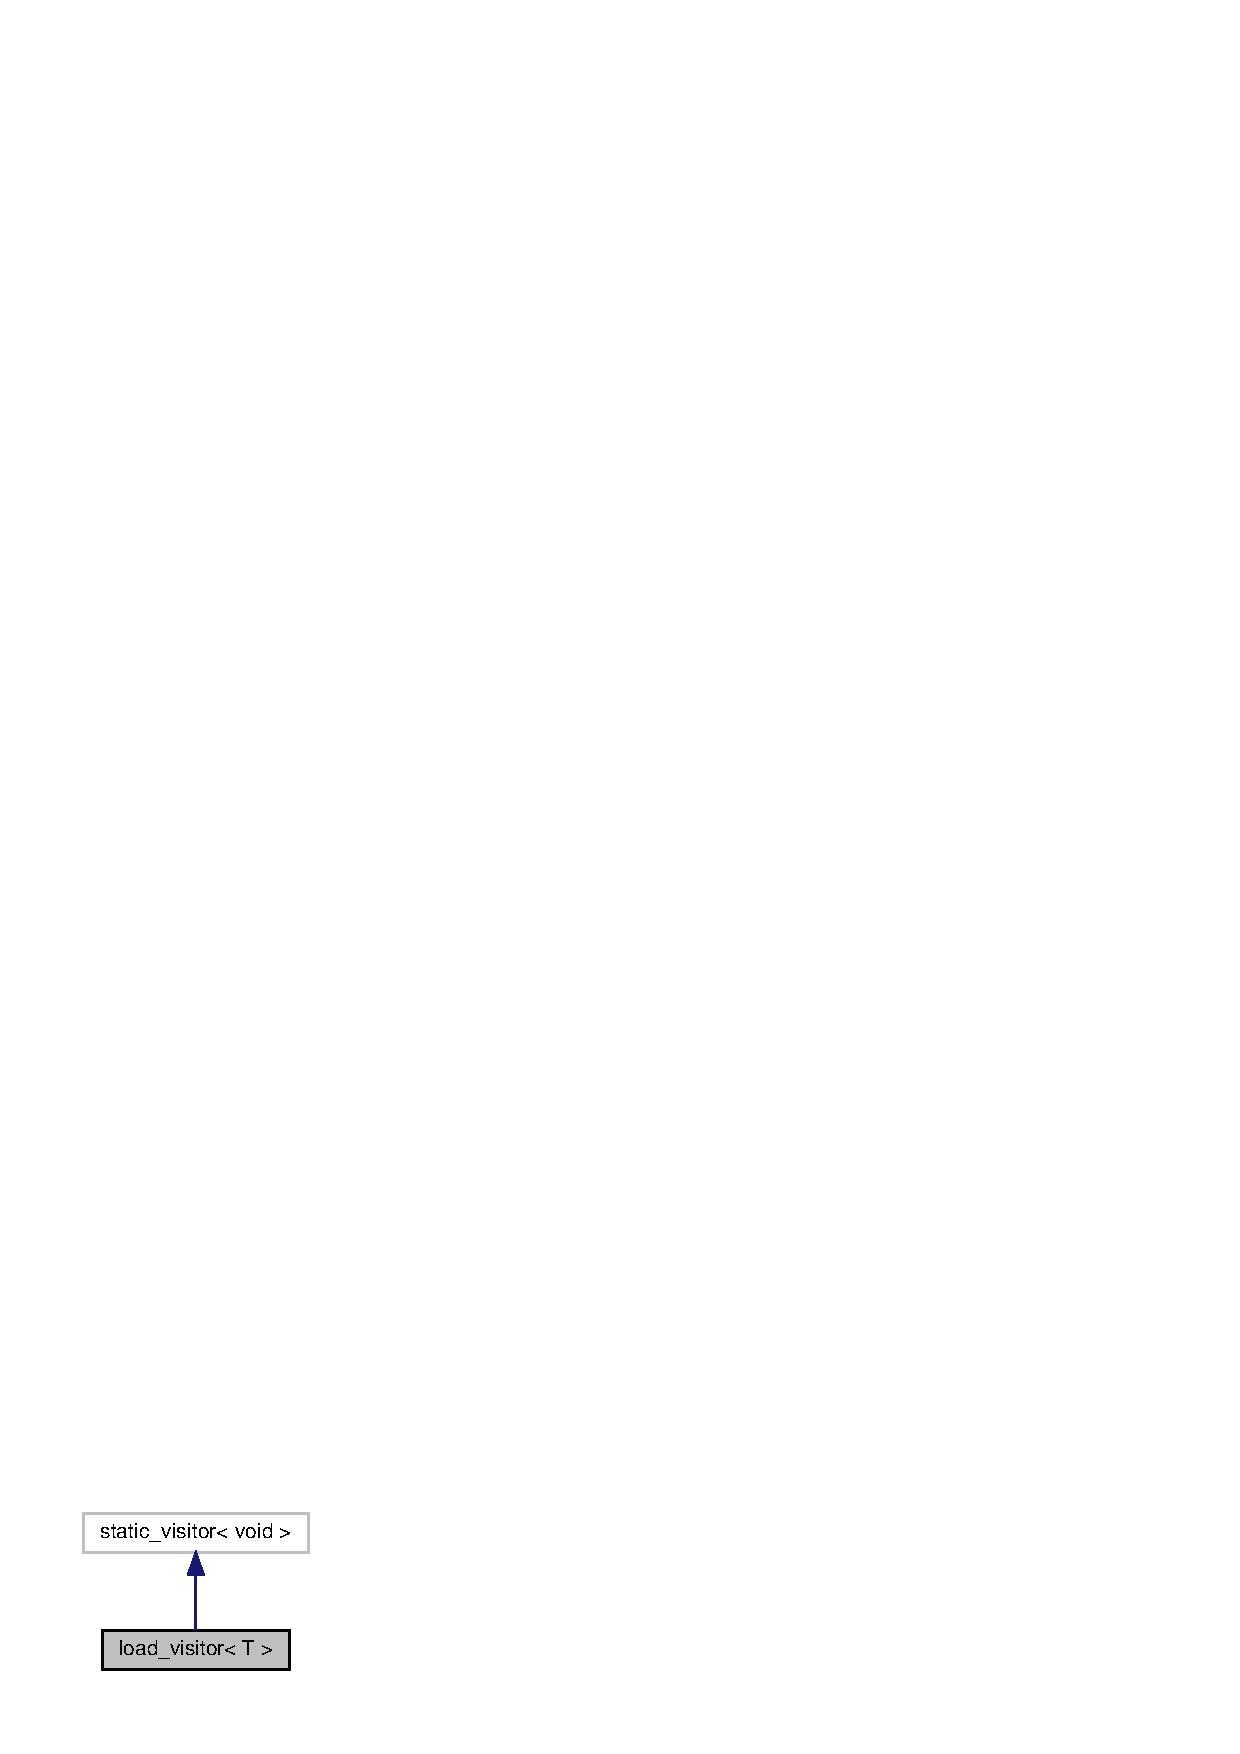
\includegraphics[width=152pt]{structcereal_1_1load__visitor__inherit__graph}
\end{center}
\end{figure}
\subsection*{Static Public Member Functions}
\begin{DoxyCompactItemize}
\item 
{\footnotesize template$<$typename Archive , typename Variant\+Type $>$ }\\static void \textbf{ load} (Archive \&ar, Variant\+Type \&variant)
\item 
{\footnotesize template$<$typename Archive , typename Variant\+Type $>$ }\\static void \textbf{ load\+\_\+impl} (Archive \&ar, Variant\+Type \&variant, std\+::true\+\_\+type)
\item 
{\footnotesize template$<$typename Archive , typename Variant\+Type $>$ }\\static void \textbf{ load\+\_\+impl} (Archive \&ar, Variant\+Type \&value, std\+::false\+\_\+type)
\end{DoxyCompactItemize}


\subsection{Detailed Description}
\subsubsection*{template$<$typename T$>$\newline
struct cereal\+::load\+\_\+visitor$<$ T $>$}



Definition at line 68 of file pointer\+\_\+variant\+\_\+wrapper.\+hpp.



\subsection{Member Function Documentation}
\mbox{\label{structcereal_1_1load__visitor_ae67bead4545632528f854b076f0b00b4}} 
\index{cereal\+::load\+\_\+visitor@{cereal\+::load\+\_\+visitor}!load@{load}}
\index{load@{load}!cereal\+::load\+\_\+visitor@{cereal\+::load\+\_\+visitor}}
\subsubsection{load()}
{\footnotesize\ttfamily static void load (\begin{DoxyParamCaption}\item[{Archive \&}]{ar,  }\item[{Variant\+Type \&}]{variant }\end{DoxyParamCaption})\hspace{0.3cm}{\ttfamily [inline]}, {\ttfamily [static]}}



Definition at line 89 of file pointer\+\_\+variant\+\_\+wrapper.\+hpp.

\mbox{\label{structcereal_1_1load__visitor_aea1281669a5d8765e002bfd8ef845be7}} 
\index{cereal\+::load\+\_\+visitor@{cereal\+::load\+\_\+visitor}!load\+\_\+impl@{load\+\_\+impl}}
\index{load\+\_\+impl@{load\+\_\+impl}!cereal\+::load\+\_\+visitor@{cereal\+::load\+\_\+visitor}}
\subsubsection{load\+\_\+impl()\hspace{0.1cm}{\footnotesize\ttfamily [1/2]}}
{\footnotesize\ttfamily static void load\+\_\+impl (\begin{DoxyParamCaption}\item[{Archive \&}]{ar,  }\item[{Variant\+Type \&}]{variant,  }\item[{std\+::true\+\_\+type}]{ }\end{DoxyParamCaption})\hspace{0.3cm}{\ttfamily [inline]}, {\ttfamily [static]}}



Definition at line 71 of file pointer\+\_\+variant\+\_\+wrapper.\+hpp.



References save\+\_\+visitor$<$ Archive $>$\+::ar, and C\+E\+R\+E\+A\+L\+\_\+\+P\+O\+I\+N\+T\+ER.

\mbox{\label{structcereal_1_1load__visitor_a55a8cf45de73b30212662c1710614572}} 
\index{cereal\+::load\+\_\+visitor@{cereal\+::load\+\_\+visitor}!load\+\_\+impl@{load\+\_\+impl}}
\index{load\+\_\+impl@{load\+\_\+impl}!cereal\+::load\+\_\+visitor@{cereal\+::load\+\_\+visitor}}
\subsubsection{load\+\_\+impl()\hspace{0.1cm}{\footnotesize\ttfamily [2/2]}}
{\footnotesize\ttfamily static void load\+\_\+impl (\begin{DoxyParamCaption}\item[{Archive \&}]{ar,  }\item[{Variant\+Type \&}]{value,  }\item[{std\+::false\+\_\+type}]{ }\end{DoxyParamCaption})\hspace{0.3cm}{\ttfamily [inline]}, {\ttfamily [static]}}



Definition at line 80 of file pointer\+\_\+variant\+\_\+wrapper.\+hpp.



References save\+\_\+visitor$<$ Archive $>$\+::ar, and cereal\+::make\+\_\+pointer\+\_\+variant().



The documentation for this struct was generated from the following file\+:\begin{DoxyCompactItemize}
\item 
/home/aakash/mlpack/src/mlpack/core/cereal/\textbf{ pointer\+\_\+variant\+\_\+wrapper.\+hpp}\end{DoxyCompactItemize}

\section{Pointer\+Variant\+Wrapper$<$ Variant\+Types $>$ Class Template Reference}
\label{classcereal_1_1PointerVariantWrapper}\index{Pointer\+Variant\+Wrapper$<$ Variant\+Types $>$@{Pointer\+Variant\+Wrapper$<$ Variant\+Types $>$}}


The objective of this class is to create a wrapper for boost\+::variant.  


\subsection*{Public Member Functions}
\begin{DoxyCompactItemize}
\item 
\textbf{ Pointer\+Variant\+Wrapper} (boost\+::variant$<$ Variant\+Types... $>$ \&pointer\+Var)
\item 
{\footnotesize template$<$class Archive $>$ }\\void \textbf{ load} (Archive \&ar)
\item 
{\footnotesize template$<$class Archive $>$ }\\void \textbf{ save} (Archive \&ar) const
\end{DoxyCompactItemize}


\subsection{Detailed Description}
\subsubsection*{template$<$typename... Variant\+Types$>$\newline
class cereal\+::\+Pointer\+Variant\+Wrapper$<$ Variant\+Types $>$}

The objective of this class is to create a wrapper for boost\+::variant. 

Cereal supports the serialization of boost\+::variant, but we need to serialize it if it holds a raw pointers. This class depeds on the \doxyref{Pointer\+Wrapper}{p.}{classcereal_1_1PointerWrapper} we have already created in which it is used to serialize each variant independently 

Definition at line 31 of file pointer\+\_\+variant\+\_\+wrapper.\+hpp.



\subsection{Constructor \& Destructor Documentation}
\mbox{\label{classcereal_1_1PointerVariantWrapper_adc3bf228015bb20527a4716fe2139464}} 
\index{cereal\+::\+Pointer\+Variant\+Wrapper@{cereal\+::\+Pointer\+Variant\+Wrapper}!Pointer\+Variant\+Wrapper@{Pointer\+Variant\+Wrapper}}
\index{Pointer\+Variant\+Wrapper@{Pointer\+Variant\+Wrapper}!cereal\+::\+Pointer\+Variant\+Wrapper@{cereal\+::\+Pointer\+Variant\+Wrapper}}
\subsubsection{Pointer\+Variant\+Wrapper()}
{\footnotesize\ttfamily \textbf{ Pointer\+Variant\+Wrapper} (\begin{DoxyParamCaption}\item[{boost\+::variant$<$ Variant\+Types... $>$ \&}]{pointer\+Var }\end{DoxyParamCaption})\hspace{0.3cm}{\ttfamily [inline]}}



Definition at line 110 of file pointer\+\_\+variant\+\_\+wrapper.\+hpp.



\subsection{Member Function Documentation}
\mbox{\label{classcereal_1_1PointerVariantWrapper_a27f4b372d3515f81ee63062814c2bbe9}} 
\index{cereal\+::\+Pointer\+Variant\+Wrapper@{cereal\+::\+Pointer\+Variant\+Wrapper}!load@{load}}
\index{load@{load}!cereal\+::\+Pointer\+Variant\+Wrapper@{cereal\+::\+Pointer\+Variant\+Wrapper}}
\subsubsection{load()}
{\footnotesize\ttfamily void load (\begin{DoxyParamCaption}\item[{Archive \&}]{ar }\end{DoxyParamCaption})\hspace{0.3cm}{\ttfamily [inline]}}



Definition at line 125 of file pointer\+\_\+variant\+\_\+wrapper.\+hpp.



References save\+\_\+visitor$<$ Archive $>$\+::ar.

\mbox{\label{classcereal_1_1PointerVariantWrapper_ad719b5a03421363e973983b4e088ecb3}} 
\index{cereal\+::\+Pointer\+Variant\+Wrapper@{cereal\+::\+Pointer\+Variant\+Wrapper}!save@{save}}
\index{save@{save}!cereal\+::\+Pointer\+Variant\+Wrapper@{cereal\+::\+Pointer\+Variant\+Wrapper}}
\subsubsection{save()}
{\footnotesize\ttfamily void save (\begin{DoxyParamCaption}\item[{Archive \&}]{ar }\end{DoxyParamCaption}) const\hspace{0.3cm}{\ttfamily [inline]}}



Definition at line 115 of file pointer\+\_\+variant\+\_\+wrapper.\+hpp.



References save\+\_\+visitor$<$ Archive $>$\+::ar.



The documentation for this class was generated from the following file\+:\begin{DoxyCompactItemize}
\item 
/home/aakash/mlpack/src/mlpack/core/cereal/\textbf{ pointer\+\_\+variant\+\_\+wrapper.\+hpp}\end{DoxyCompactItemize}

\section{Pointer\+Vector\+Variant\+Wrapper$<$ Variant\+Types $>$ Class Template Reference}
\label{classcereal_1_1PointerVectorVariantWrapper}\index{Pointer\+Vector\+Variant\+Wrapper$<$ Variant\+Types $>$@{Pointer\+Vector\+Variant\+Wrapper$<$ Variant\+Types $>$}}


The objective of this class is to create a wrapper for a vector of boost\+::variant that holds pointer.  


\subsection*{Public Member Functions}
\begin{DoxyCompactItemize}
\item 
\textbf{ Pointer\+Vector\+Variant\+Wrapper} (std\+::vector$<$ boost\+::variant$<$ Variant\+Types... $>$$>$ \&vec\+Pointer\+Var)
\item 
{\footnotesize template$<$class Archive $>$ }\\void \textbf{ load} (Archive \&ar)
\item 
{\footnotesize template$<$class Archive $>$ }\\void \textbf{ save} (Archive \&ar) const
\end{DoxyCompactItemize}


\subsection{Detailed Description}
\subsubsection*{template$<$typename... Variant\+Types$>$\newline
class cereal\+::\+Pointer\+Vector\+Variant\+Wrapper$<$ Variant\+Types $>$}

The objective of this class is to create a wrapper for a vector of boost\+::variant that holds pointer. 

Cereal supports the serialization of boost\+::variant, but we need to serialize it if it holds a vector of boost\+::variant that holds a pointers. 

Definition at line 24 of file pointer\+\_\+vector\+\_\+variant\+\_\+wrapper.\+hpp.



\subsection{Constructor \& Destructor Documentation}
\mbox{\label{classcereal_1_1PointerVectorVariantWrapper_a0aa4a1ce17aa0196d5a0218d59762324}} 
\index{cereal\+::\+Pointer\+Vector\+Variant\+Wrapper@{cereal\+::\+Pointer\+Vector\+Variant\+Wrapper}!Pointer\+Vector\+Variant\+Wrapper@{Pointer\+Vector\+Variant\+Wrapper}}
\index{Pointer\+Vector\+Variant\+Wrapper@{Pointer\+Vector\+Variant\+Wrapper}!cereal\+::\+Pointer\+Vector\+Variant\+Wrapper@{cereal\+::\+Pointer\+Vector\+Variant\+Wrapper}}
\subsubsection{Pointer\+Vector\+Variant\+Wrapper()}
{\footnotesize\ttfamily \textbf{ Pointer\+Vector\+Variant\+Wrapper} (\begin{DoxyParamCaption}\item[{std\+::vector$<$ boost\+::variant$<$ Variant\+Types... $>$$>$ \&}]{vec\+Pointer\+Var }\end{DoxyParamCaption})\hspace{0.3cm}{\ttfamily [inline]}}



Definition at line 52 of file pointer\+\_\+vector\+\_\+variant\+\_\+wrapper.\+hpp.



\subsection{Member Function Documentation}
\mbox{\label{classcereal_1_1PointerVectorVariantWrapper_a27f4b372d3515f81ee63062814c2bbe9}} 
\index{cereal\+::\+Pointer\+Vector\+Variant\+Wrapper@{cereal\+::\+Pointer\+Vector\+Variant\+Wrapper}!load@{load}}
\index{load@{load}!cereal\+::\+Pointer\+Vector\+Variant\+Wrapper@{cereal\+::\+Pointer\+Vector\+Variant\+Wrapper}}
\subsubsection{load()}
{\footnotesize\ttfamily void load (\begin{DoxyParamCaption}\item[{Archive \&}]{ar }\end{DoxyParamCaption})\hspace{0.3cm}{\ttfamily [inline]}}



Definition at line 69 of file pointer\+\_\+vector\+\_\+variant\+\_\+wrapper.\+hpp.



References C\+E\+R\+E\+A\+L\+\_\+\+V\+A\+R\+I\+A\+N\+T\+\_\+\+P\+O\+I\+N\+T\+ER.

\mbox{\label{classcereal_1_1PointerVectorVariantWrapper_ad719b5a03421363e973983b4e088ecb3}} 
\index{cereal\+::\+Pointer\+Vector\+Variant\+Wrapper@{cereal\+::\+Pointer\+Vector\+Variant\+Wrapper}!save@{save}}
\index{save@{save}!cereal\+::\+Pointer\+Vector\+Variant\+Wrapper@{cereal\+::\+Pointer\+Vector\+Variant\+Wrapper}}
\subsubsection{save()}
{\footnotesize\ttfamily void save (\begin{DoxyParamCaption}\item[{Archive \&}]{ar }\end{DoxyParamCaption}) const\hspace{0.3cm}{\ttfamily [inline]}}



Definition at line 58 of file pointer\+\_\+vector\+\_\+variant\+\_\+wrapper.\+hpp.



References C\+E\+R\+E\+A\+L\+\_\+\+V\+A\+R\+I\+A\+N\+T\+\_\+\+P\+O\+I\+N\+T\+ER.



The documentation for this class was generated from the following file\+:\begin{DoxyCompactItemize}
\item 
/home/aakash/mlpack/src/mlpack/core/cereal/\textbf{ pointer\+\_\+vector\+\_\+variant\+\_\+wrapper.\+hpp}\end{DoxyCompactItemize}

\section{Pointer\+Vector\+Wrapper$<$ T $>$ Class Template Reference}
\label{classcereal_1_1PointerVectorWrapper}\index{Pointer\+Vector\+Wrapper$<$ T $>$@{Pointer\+Vector\+Wrapper$<$ T $>$}}


The objective of this class is to create a wrapper for std\+::vector that hold pointers by adding also the size of the vector.  


\subsection*{Public Member Functions}
\begin{DoxyCompactItemize}
\item 
\textbf{ Pointer\+Vector\+Wrapper} (std\+::vector$<$ T $\ast$$>$ \&pointer\+Vec)
\item 
{\footnotesize template$<$class Archive $>$ }\\void \textbf{ load} (Archive \&ar)
\item 
{\footnotesize template$<$class Archive $>$ }\\void \textbf{ save} (Archive \&ar) const
\end{DoxyCompactItemize}


\subsection{Detailed Description}
\subsubsection*{template$<$class T$>$\newline
class cereal\+::\+Pointer\+Vector\+Wrapper$<$ T $>$}

The objective of this class is to create a wrapper for std\+::vector that hold pointers by adding also the size of the vector. 

Cereal supports the serialization of the std vector, but we need to serialize the vector if it holds raw pointer. This wrapper uses the \doxyref{Pointer\+Wrapper}{p.}{classcereal_1_1PointerWrapper} we have already created, it serialize each pointer in the vector independently.

We need to add the size of the vector if it holds a raw pointers, during the serialization, so we can know the size of the number pointer to allocated during the deserialization process. 

Definition at line 38 of file pointer\+\_\+vector\+\_\+wrapper.\+hpp.



\subsection{Constructor \& Destructor Documentation}
\mbox{\label{classcereal_1_1PointerVectorWrapper_a82deb234e7c6eb7fed35086314cd3b6f}} 
\index{cereal\+::\+Pointer\+Vector\+Wrapper@{cereal\+::\+Pointer\+Vector\+Wrapper}!Pointer\+Vector\+Wrapper@{Pointer\+Vector\+Wrapper}}
\index{Pointer\+Vector\+Wrapper@{Pointer\+Vector\+Wrapper}!cereal\+::\+Pointer\+Vector\+Wrapper@{cereal\+::\+Pointer\+Vector\+Wrapper}}
\subsubsection{Pointer\+Vector\+Wrapper()}
{\footnotesize\ttfamily \textbf{ Pointer\+Vector\+Wrapper} (\begin{DoxyParamCaption}\item[{std\+::vector$<$ T $\ast$$>$ \&}]{pointer\+Vec }\end{DoxyParamCaption})\hspace{0.3cm}{\ttfamily [inline]}}



Definition at line 41 of file pointer\+\_\+vector\+\_\+wrapper.\+hpp.



\subsection{Member Function Documentation}
\mbox{\label{classcereal_1_1PointerVectorWrapper_a27f4b372d3515f81ee63062814c2bbe9}} 
\index{cereal\+::\+Pointer\+Vector\+Wrapper@{cereal\+::\+Pointer\+Vector\+Wrapper}!load@{load}}
\index{load@{load}!cereal\+::\+Pointer\+Vector\+Wrapper@{cereal\+::\+Pointer\+Vector\+Wrapper}}
\subsubsection{load()}
{\footnotesize\ttfamily void load (\begin{DoxyParamCaption}\item[{Archive \&}]{ar }\end{DoxyParamCaption})\hspace{0.3cm}{\ttfamily [inline]}}



Definition at line 57 of file pointer\+\_\+vector\+\_\+wrapper.\+hpp.



References C\+E\+R\+E\+A\+L\+\_\+\+P\+O\+I\+N\+T\+ER.

\mbox{\label{classcereal_1_1PointerVectorWrapper_ad719b5a03421363e973983b4e088ecb3}} 
\index{cereal\+::\+Pointer\+Vector\+Wrapper@{cereal\+::\+Pointer\+Vector\+Wrapper}!save@{save}}
\index{save@{save}!cereal\+::\+Pointer\+Vector\+Wrapper@{cereal\+::\+Pointer\+Vector\+Wrapper}}
\subsubsection{save()}
{\footnotesize\ttfamily void save (\begin{DoxyParamCaption}\item[{Archive \&}]{ar }\end{DoxyParamCaption}) const\hspace{0.3cm}{\ttfamily [inline]}}



Definition at line 46 of file pointer\+\_\+vector\+\_\+wrapper.\+hpp.



References C\+E\+R\+E\+A\+L\+\_\+\+P\+O\+I\+N\+T\+ER.



The documentation for this class was generated from the following file\+:\begin{DoxyCompactItemize}
\item 
/home/aakash/mlpack/src/mlpack/core/cereal/\textbf{ pointer\+\_\+vector\+\_\+wrapper.\+hpp}\end{DoxyCompactItemize}

\section{Pointer\+Wrapper$<$ T $>$ Class Template Reference}
\label{classcereal_1_1PointerWrapper}\index{Pointer\+Wrapper$<$ T $>$@{Pointer\+Wrapper$<$ T $>$}}


The objective of this class is to create a wrapper for raw pointer by encapsulating them in a smart pointer of type unique\+\_\+ptr.  


\subsection*{Public Member Functions}
\begin{DoxyCompactItemize}
\item 
\textbf{ Pointer\+Wrapper} (T $\ast$\&pointer)
\item 
{\footnotesize template$<$class Archive $>$ }\\void \textbf{ load} (Archive \&ar, const uint32\+\_\+t)
\item 
T $\ast$\& \textbf{ release} ()
\item 
{\footnotesize template$<$class Archive $>$ }\\void \textbf{ save} (Archive \&ar, const uint32\+\_\+t) const
\end{DoxyCompactItemize}


\subsection{Detailed Description}
\subsubsection*{template$<$class T$>$\newline
class cereal\+::\+Pointer\+Wrapper$<$ T $>$}

The objective of this class is to create a wrapper for raw pointer by encapsulating them in a smart pointer of type unique\+\_\+ptr. 

Cereal does not support the serialization of raw pointer out of the box. Therefore, we have created this wrapper to serialize raw pointer in cereal as a smart pointer since because it will be difficult to change all pointer type in mlpack. 

Definition at line 44 of file pointer\+\_\+wrapper.\+hpp.



\subsection{Constructor \& Destructor Documentation}
\mbox{\label{classcereal_1_1PointerWrapper_a65ffc92800be3b2e2acd6bf27c7d8745}} 
\index{cereal\+::\+Pointer\+Wrapper@{cereal\+::\+Pointer\+Wrapper}!Pointer\+Wrapper@{Pointer\+Wrapper}}
\index{Pointer\+Wrapper@{Pointer\+Wrapper}!cereal\+::\+Pointer\+Wrapper@{cereal\+::\+Pointer\+Wrapper}}
\subsubsection{Pointer\+Wrapper()}
{\footnotesize\ttfamily \textbf{ Pointer\+Wrapper} (\begin{DoxyParamCaption}\item[{T $\ast$\&}]{pointer }\end{DoxyParamCaption})\hspace{0.3cm}{\ttfamily [inline]}}



Definition at line 47 of file pointer\+\_\+wrapper.\+hpp.



\subsection{Member Function Documentation}
\mbox{\label{classcereal_1_1PointerWrapper_a2c74fd23efa75fae660603e36f4d03ac}} 
\index{cereal\+::\+Pointer\+Wrapper@{cereal\+::\+Pointer\+Wrapper}!load@{load}}
\index{load@{load}!cereal\+::\+Pointer\+Wrapper@{cereal\+::\+Pointer\+Wrapper}}
\subsubsection{load()}
{\footnotesize\ttfamily void load (\begin{DoxyParamCaption}\item[{Archive \&}]{ar,  }\item[{const uint32\+\_\+t}]{ }\end{DoxyParamCaption})\hspace{0.3cm}{\ttfamily [inline]}}



Definition at line 62 of file pointer\+\_\+wrapper.\+hpp.

\mbox{\label{classcereal_1_1PointerWrapper_ad56c5f39662b211a09253c751262fdc4}} 
\index{cereal\+::\+Pointer\+Wrapper@{cereal\+::\+Pointer\+Wrapper}!release@{release}}
\index{release@{release}!cereal\+::\+Pointer\+Wrapper@{cereal\+::\+Pointer\+Wrapper}}
\subsubsection{release()}
{\footnotesize\ttfamily T$\ast$\& release (\begin{DoxyParamCaption}{ }\end{DoxyParamCaption})\hspace{0.3cm}{\ttfamily [inline]}}



Definition at line 69 of file pointer\+\_\+wrapper.\+hpp.

\mbox{\label{classcereal_1_1PointerWrapper_a52958fcb465f0f3082b164a49ab238a7}} 
\index{cereal\+::\+Pointer\+Wrapper@{cereal\+::\+Pointer\+Wrapper}!save@{save}}
\index{save@{save}!cereal\+::\+Pointer\+Wrapper@{cereal\+::\+Pointer\+Wrapper}}
\subsubsection{save()}
{\footnotesize\ttfamily void save (\begin{DoxyParamCaption}\item[{Archive \&}]{ar,  }\item[{const uint32\+\_\+t}]{ }\end{DoxyParamCaption}) const\hspace{0.3cm}{\ttfamily [inline]}}



Definition at line 52 of file pointer\+\_\+wrapper.\+hpp.



The documentation for this class was generated from the following file\+:\begin{DoxyCompactItemize}
\item 
/home/aakash/mlpack/src/mlpack/core/cereal/\textbf{ pointer\+\_\+wrapper.\+hpp}\end{DoxyCompactItemize}

\section{save\+\_\+visitor$<$ Archive $>$ Struct Template Reference}
\label{structcereal_1_1save__visitor}\index{save\+\_\+visitor$<$ Archive $>$@{save\+\_\+visitor$<$ Archive $>$}}


Inheritance diagram for save\+\_\+visitor$<$ Archive $>$\+:
\nopagebreak
\begin{figure}[H]
\begin{center}
\leavevmode
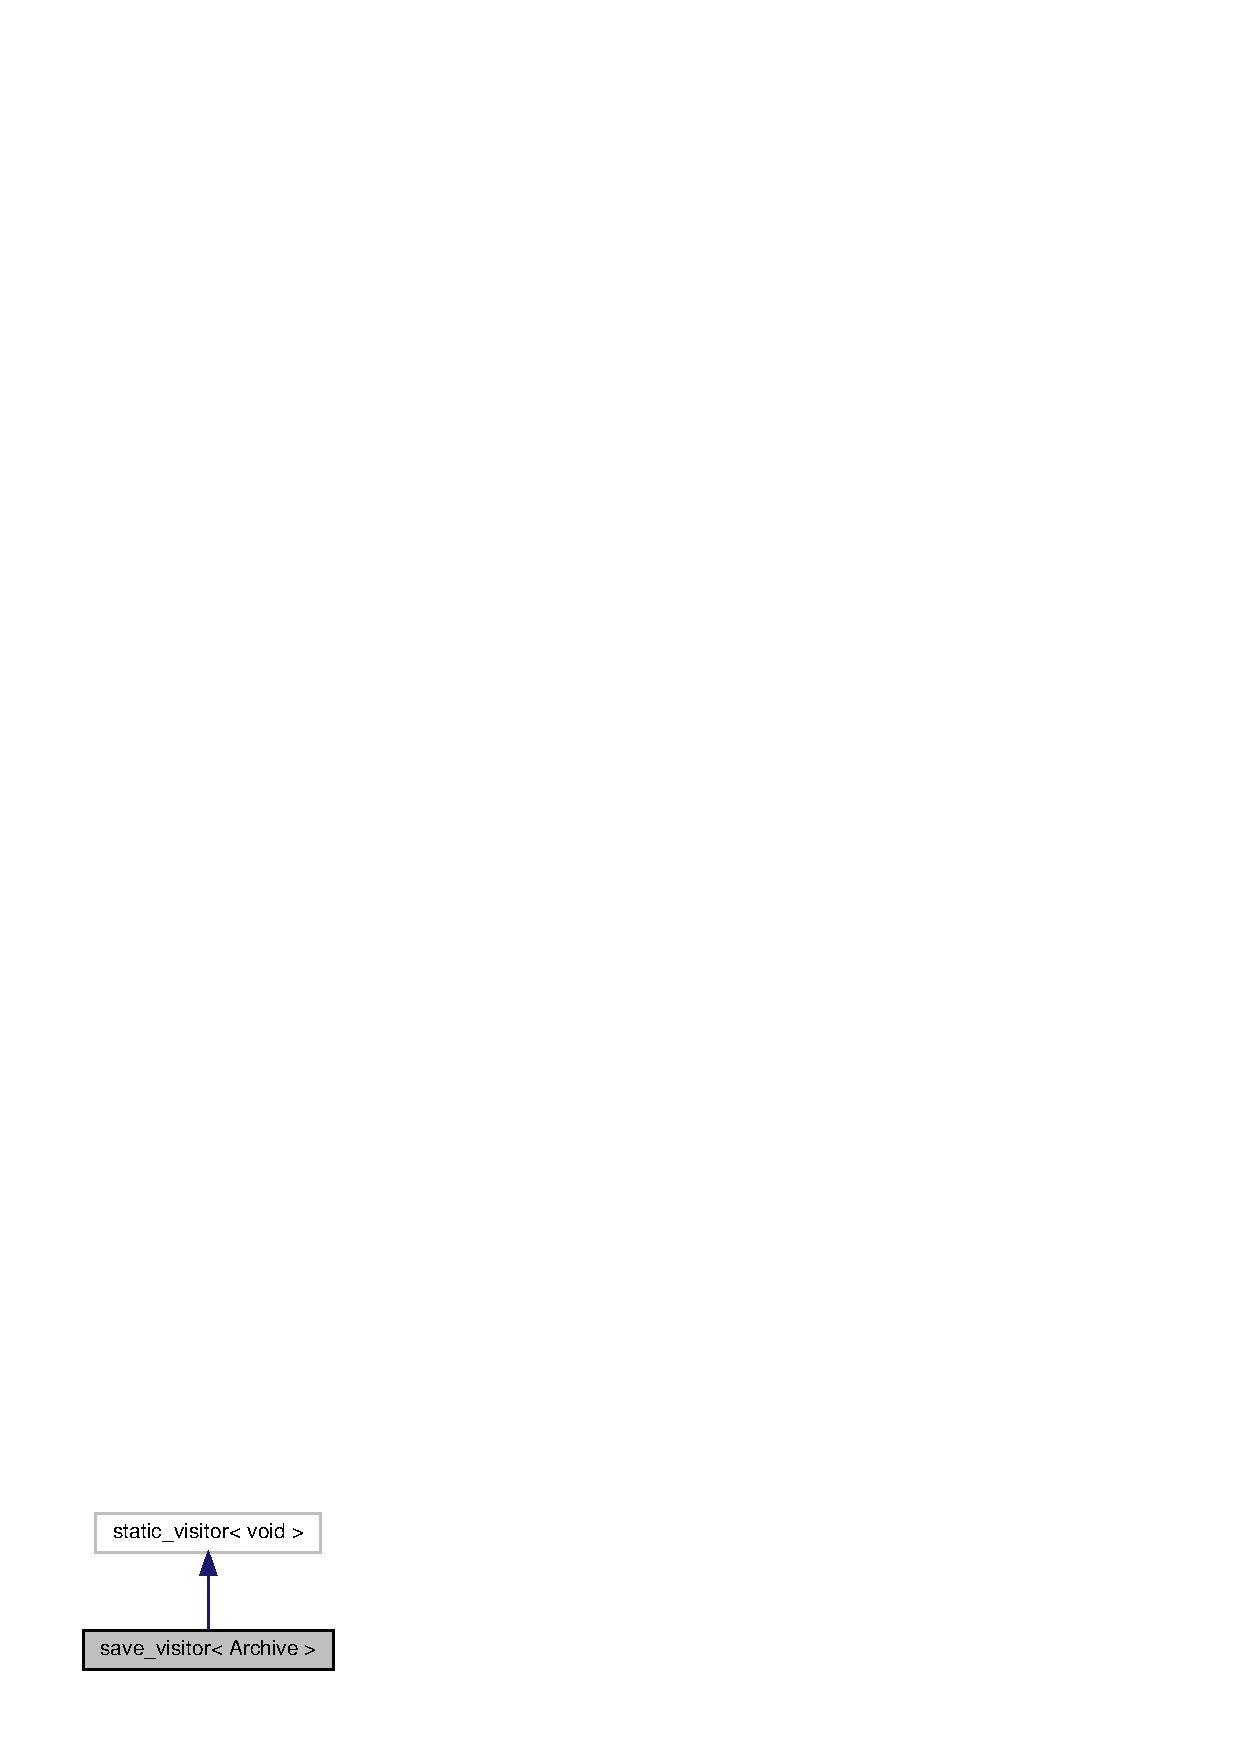
\includegraphics[width=164pt]{structcereal_1_1save__visitor__inherit__graph}
\end{center}
\end{figure}
\subsection*{Public Member Functions}
\begin{DoxyCompactItemize}
\item 
\textbf{ save\+\_\+visitor} (Archive \&\textbf{ ar})
\item 
{\footnotesize template$<$class T $>$ }\\void \textbf{ operator()} (const T $\ast$value) const
\item 
{\footnotesize template$<$typename... Types$>$ }\\void \textbf{ operator()} (boost\+::variant$<$ Types $\ast$... $>$ \&value) const
\end{DoxyCompactItemize}
\subsection*{Public Attributes}
\begin{DoxyCompactItemize}
\item 
Archive \& \textbf{ ar}
\end{DoxyCompactItemize}


\subsection{Detailed Description}
\subsubsection*{template$<$class Archive$>$\newline
struct cereal\+::save\+\_\+visitor$<$ Archive $>$}



Definition at line 48 of file pointer\+\_\+variant\+\_\+wrapper.\+hpp.



\subsection{Constructor \& Destructor Documentation}
\mbox{\label{structcereal_1_1save__visitor_a79d9c557965a3a81a894a6ce856c1757}} 
\index{cereal\+::save\+\_\+visitor@{cereal\+::save\+\_\+visitor}!save\+\_\+visitor@{save\+\_\+visitor}}
\index{save\+\_\+visitor@{save\+\_\+visitor}!cereal\+::save\+\_\+visitor@{cereal\+::save\+\_\+visitor}}
\subsubsection{save\+\_\+visitor()}
{\footnotesize\ttfamily \textbf{ save\+\_\+visitor} (\begin{DoxyParamCaption}\item[{Archive \&}]{ar }\end{DoxyParamCaption})\hspace{0.3cm}{\ttfamily [inline]}}



Definition at line 50 of file pointer\+\_\+variant\+\_\+wrapper.\+hpp.



\subsection{Member Function Documentation}
\mbox{\label{structcereal_1_1save__visitor_a4e892b7d0489cc782bac3eeca6de2415}} 
\index{cereal\+::save\+\_\+visitor@{cereal\+::save\+\_\+visitor}!operator()@{operator()}}
\index{operator()@{operator()}!cereal\+::save\+\_\+visitor@{cereal\+::save\+\_\+visitor}}
\subsubsection{operator()()\hspace{0.1cm}{\footnotesize\ttfamily [1/2]}}
{\footnotesize\ttfamily void operator() (\begin{DoxyParamCaption}\item[{const T $\ast$}]{value }\end{DoxyParamCaption}) const\hspace{0.3cm}{\ttfamily [inline]}}



Definition at line 53 of file pointer\+\_\+variant\+\_\+wrapper.\+hpp.



References save\+\_\+visitor$<$ Archive $>$\+::ar, and C\+E\+R\+E\+A\+L\+\_\+\+P\+O\+I\+N\+T\+ER.

\mbox{\label{structcereal_1_1save__visitor_ac6ad85740cee791e6f711c836fea607d}} 
\index{cereal\+::save\+\_\+visitor@{cereal\+::save\+\_\+visitor}!operator()@{operator()}}
\index{operator()@{operator()}!cereal\+::save\+\_\+visitor@{cereal\+::save\+\_\+visitor}}
\subsubsection{operator()()\hspace{0.1cm}{\footnotesize\ttfamily [2/2]}}
{\footnotesize\ttfamily void operator() (\begin{DoxyParamCaption}\item[{boost\+::variant$<$ Types $\ast$... $>$ \&}]{value }\end{DoxyParamCaption}) const\hspace{0.3cm}{\ttfamily [inline]}}



Definition at line 59 of file pointer\+\_\+variant\+\_\+wrapper.\+hpp.



References save\+\_\+visitor$<$ Archive $>$\+::ar, and cereal\+::make\+\_\+pointer\+\_\+variant().



\subsection{Member Data Documentation}
\mbox{\label{structcereal_1_1save__visitor_a35bf67c5eb3a02c7ca3d0db5bebd4e11}} 
\index{cereal\+::save\+\_\+visitor@{cereal\+::save\+\_\+visitor}!ar@{ar}}
\index{ar@{ar}!cereal\+::save\+\_\+visitor@{cereal\+::save\+\_\+visitor}}
\subsubsection{ar}
{\footnotesize\ttfamily Archive\& ar}



Definition at line 64 of file pointer\+\_\+variant\+\_\+wrapper.\+hpp.



Referenced by Pointer\+Variant\+Wrapper$<$ Variant\+Types $>$\+::load(), load\+\_\+visitor$<$ T $>$\+::load\+\_\+impl(), save\+\_\+visitor$<$ Archive $>$\+::operator()(), and Pointer\+Variant\+Wrapper$<$ Variant\+Types $>$\+::save().



The documentation for this struct was generated from the following file\+:\begin{DoxyCompactItemize}
\item 
/home/aakash/mlpack/src/mlpack/core/cereal/\textbf{ pointer\+\_\+variant\+\_\+wrapper.\+hpp}\end{DoxyCompactItemize}

\section{Init\+H\+M\+M\+Model Struct Reference}
\label{structInitHMMModel}\index{Init\+H\+M\+M\+Model@{Init\+H\+M\+M\+Model}}
\subsection*{Static Public Member Functions}
\begin{DoxyCompactItemize}
\item 
{\footnotesize template$<$typename H\+M\+M\+Type $>$ }\\static void \textbf{ Apply} (H\+M\+M\+Type \&hmm, vector$<$ mat $>$ $\ast$train\+Seq)
\item 
static void \textbf{ Create} (H\+MM$<$ Discrete\+Distribution $>$ \&hmm, vector$<$ mat $>$ \&train\+Seq, size\+\_\+t states, double tolerance=1e-\/05)
\begin{DoxyCompactList}\small\item\em Helper function to create discrete H\+MM. \end{DoxyCompactList}\item 
static void \textbf{ Create} (H\+MM$<$ Gaussian\+Distribution $>$ \&hmm, vector$<$ mat $>$ \&train\+Seq, size\+\_\+t states, double tolerance=1e-\/05)
\item 
static void \textbf{ Create} (H\+MM$<$ G\+MM $>$ \&hmm, vector$<$ mat $>$ \&train\+Seq, size\+\_\+t states, double tolerance=1e-\/05)
\item 
static void \textbf{ Create} (H\+MM$<$ Diagonal\+G\+MM $>$ \&hmm, vector$<$ mat $>$ \&train\+Seq, size\+\_\+t states, double tolerance=1e-\/05)
\begin{DoxyCompactList}\small\item\em Helper function to create Diagonal G\+MM H\+MM. \end{DoxyCompactList}\item 
static void \textbf{ Random\+Initialize} (vector$<$ Discrete\+Distribution $>$ \&e)
\begin{DoxyCompactList}\small\item\em Helper function for discrete emission distributions. \end{DoxyCompactList}\item 
static void \textbf{ Random\+Initialize} (vector$<$ Gaussian\+Distribution $>$ \&e)
\item 
static void \textbf{ Random\+Initialize} (vector$<$ G\+MM $>$ \&e)
\item 
static void \textbf{ Random\+Initialize} (vector$<$ Diagonal\+G\+MM $>$ \&e)
\begin{DoxyCompactList}\small\item\em Helper function for diagonal G\+MM emission distributions. \end{DoxyCompactList}\end{DoxyCompactItemize}


\subsection{Detailed Description}


Definition at line 21 of file hmm\+\_\+test\+\_\+utils.\+hpp.



\subsection{Member Function Documentation}
\mbox{\label{structInitHMMModel_a3b7981fd17dd8132c10744e7d088c347}} 
\index{Init\+H\+M\+M\+Model@{Init\+H\+M\+M\+Model}!Apply@{Apply}}
\index{Apply@{Apply}!Init\+H\+M\+M\+Model@{Init\+H\+M\+M\+Model}}
\subsubsection{Apply()}
{\footnotesize\ttfamily static void Apply (\begin{DoxyParamCaption}\item[{H\+M\+M\+Type \&}]{hmm,  }\item[{vector$<$ mat $>$ $\ast$}]{train\+Seq }\end{DoxyParamCaption})\hspace{0.3cm}{\ttfamily [inline]}, {\ttfamily [static]}}



Definition at line 24 of file hmm\+\_\+test\+\_\+utils.\+hpp.



References Create(), and Random\+Initialize().

\mbox{\label{structInitHMMModel_a457b36f139f6a11e38f793ffb1276b38}} 
\index{Init\+H\+M\+M\+Model@{Init\+H\+M\+M\+Model}!Create@{Create}}
\index{Create@{Create}!Init\+H\+M\+M\+Model@{Init\+H\+M\+M\+Model}}
\subsubsection{Create()\hspace{0.1cm}{\footnotesize\ttfamily [1/4]}}
{\footnotesize\ttfamily static void Create (\begin{DoxyParamCaption}\item[{H\+MM$<$ Discrete\+Distribution $>$ \&}]{hmm,  }\item[{vector$<$ mat $>$ \&}]{train\+Seq,  }\item[{size\+\_\+t}]{states,  }\item[{double}]{tolerance = {\ttfamily 1e-\/05} }\end{DoxyParamCaption})\hspace{0.3cm}{\ttfamily [inline]}, {\ttfamily [static]}}



Helper function to create discrete H\+MM. 



Definition at line 37 of file hmm\+\_\+test\+\_\+utils.\+hpp.



Referenced by Apply().

\mbox{\label{structInitHMMModel_ada660c2630ff663ac9002121e1e28b5e}} 
\index{Init\+H\+M\+M\+Model@{Init\+H\+M\+M\+Model}!Create@{Create}}
\index{Create@{Create}!Init\+H\+M\+M\+Model@{Init\+H\+M\+M\+Model}}
\subsubsection{Create()\hspace{0.1cm}{\footnotesize\ttfamily [2/4]}}
{\footnotesize\ttfamily static void Create (\begin{DoxyParamCaption}\item[{H\+MM$<$ Gaussian\+Distribution $>$ \&}]{hmm,  }\item[{vector$<$ mat $>$ \&}]{train\+Seq,  }\item[{size\+\_\+t}]{states,  }\item[{double}]{tolerance = {\ttfamily 1e-\/05} }\end{DoxyParamCaption})\hspace{0.3cm}{\ttfamily [inline]}, {\ttfamily [static]}}



Definition at line 58 of file hmm\+\_\+test\+\_\+utils.\+hpp.

\mbox{\label{structInitHMMModel_ad22d3a4f18404743629ee3157b071f90}} 
\index{Init\+H\+M\+M\+Model@{Init\+H\+M\+M\+Model}!Create@{Create}}
\index{Create@{Create}!Init\+H\+M\+M\+Model@{Init\+H\+M\+M\+Model}}
\subsubsection{Create()\hspace{0.1cm}{\footnotesize\ttfamily [3/4]}}
{\footnotesize\ttfamily static void Create (\begin{DoxyParamCaption}\item[{H\+MM$<$ G\+MM $>$ \&}]{hmm,  }\item[{vector$<$ mat $>$ \&}]{train\+Seq,  }\item[{size\+\_\+t}]{states,  }\item[{double}]{tolerance = {\ttfamily 1e-\/05} }\end{DoxyParamCaption})\hspace{0.3cm}{\ttfamily [inline]}, {\ttfamily [static]}}



Definition at line 82 of file hmm\+\_\+test\+\_\+utils.\+hpp.

\mbox{\label{structInitHMMModel_affcc1da5c656ea0f07fcc3e726e9cc1e}} 
\index{Init\+H\+M\+M\+Model@{Init\+H\+M\+M\+Model}!Create@{Create}}
\index{Create@{Create}!Init\+H\+M\+M\+Model@{Init\+H\+M\+M\+Model}}
\subsubsection{Create()\hspace{0.1cm}{\footnotesize\ttfamily [4/4]}}
{\footnotesize\ttfamily static void Create (\begin{DoxyParamCaption}\item[{H\+MM$<$ Diagonal\+G\+MM $>$ \&}]{hmm,  }\item[{vector$<$ mat $>$ \&}]{train\+Seq,  }\item[{size\+\_\+t}]{states,  }\item[{double}]{tolerance = {\ttfamily 1e-\/05} }\end{DoxyParamCaption})\hspace{0.3cm}{\ttfamily [inline]}, {\ttfamily [static]}}



Helper function to create Diagonal G\+MM H\+MM. 



Definition at line 109 of file hmm\+\_\+test\+\_\+utils.\+hpp.

\mbox{\label{structInitHMMModel_adb0345a19e57a6724118fd9edebd9422}} 
\index{Init\+H\+M\+M\+Model@{Init\+H\+M\+M\+Model}!Random\+Initialize@{Random\+Initialize}}
\index{Random\+Initialize@{Random\+Initialize}!Init\+H\+M\+M\+Model@{Init\+H\+M\+M\+Model}}
\subsubsection{Random\+Initialize()\hspace{0.1cm}{\footnotesize\ttfamily [1/4]}}
{\footnotesize\ttfamily static void Random\+Initialize (\begin{DoxyParamCaption}\item[{vector$<$ Discrete\+Distribution $>$ \&}]{e }\end{DoxyParamCaption})\hspace{0.3cm}{\ttfamily [inline]}, {\ttfamily [static]}}



Helper function for discrete emission distributions. 



Definition at line 136 of file hmm\+\_\+test\+\_\+utils.\+hpp.



Referenced by Apply().

\mbox{\label{structInitHMMModel_a2c484f94002baedf55ddaba775794c7a}} 
\index{Init\+H\+M\+M\+Model@{Init\+H\+M\+M\+Model}!Random\+Initialize@{Random\+Initialize}}
\index{Random\+Initialize@{Random\+Initialize}!Init\+H\+M\+M\+Model@{Init\+H\+M\+M\+Model}}
\subsubsection{Random\+Initialize()\hspace{0.1cm}{\footnotesize\ttfamily [2/4]}}
{\footnotesize\ttfamily static void Random\+Initialize (\begin{DoxyParamCaption}\item[{vector$<$ Gaussian\+Distribution $>$ \&}]{e }\end{DoxyParamCaption})\hspace{0.3cm}{\ttfamily [inline]}, {\ttfamily [static]}}



Definition at line 145 of file hmm\+\_\+test\+\_\+utils.\+hpp.

\mbox{\label{structInitHMMModel_a09e5ab6763ae40ac05d1f149098dd805}} 
\index{Init\+H\+M\+M\+Model@{Init\+H\+M\+M\+Model}!Random\+Initialize@{Random\+Initialize}}
\index{Random\+Initialize@{Random\+Initialize}!Init\+H\+M\+M\+Model@{Init\+H\+M\+M\+Model}}
\subsubsection{Random\+Initialize()\hspace{0.1cm}{\footnotesize\ttfamily [3/4]}}
{\footnotesize\ttfamily static void Random\+Initialize (\begin{DoxyParamCaption}\item[{vector$<$ G\+MM $>$ \&}]{e }\end{DoxyParamCaption})\hspace{0.3cm}{\ttfamily [inline]}, {\ttfamily [static]}}



Definition at line 157 of file hmm\+\_\+test\+\_\+utils.\+hpp.

\mbox{\label{structInitHMMModel_a743d931c6b5fb5aea3e957e0823e11f5}} 
\index{Init\+H\+M\+M\+Model@{Init\+H\+M\+M\+Model}!Random\+Initialize@{Random\+Initialize}}
\index{Random\+Initialize@{Random\+Initialize}!Init\+H\+M\+M\+Model@{Init\+H\+M\+M\+Model}}
\subsubsection{Random\+Initialize()\hspace{0.1cm}{\footnotesize\ttfamily [4/4]}}
{\footnotesize\ttfamily static void Random\+Initialize (\begin{DoxyParamCaption}\item[{vector$<$ Diagonal\+G\+MM $>$ \&}]{e }\end{DoxyParamCaption})\hspace{0.3cm}{\ttfamily [inline]}, {\ttfamily [static]}}



Helper function for diagonal G\+MM emission distributions. 



Definition at line 180 of file hmm\+\_\+test\+\_\+utils.\+hpp.



The documentation for this struct was generated from the following file\+:\begin{DoxyCompactItemize}
\item 
/home/aakash/mlpack/src/mlpack/tests/main\+\_\+tests/\textbf{ hmm\+\_\+test\+\_\+utils.\+hpp}\end{DoxyCompactItemize}

\section{Is\+Vector$<$ Vec\+Type $>$ Struct Template Reference}
\label{structIsVector}\index{Is\+Vector$<$ Vec\+Type $>$@{Is\+Vector$<$ Vec\+Type $>$}}


If value == true, then Vec\+Type is some sort of Armadillo vector or subview.  


\subsection*{Static Public Attributes}
\begin{DoxyCompactItemize}
\item 
static const bool \textbf{ value} = false
\end{DoxyCompactItemize}


\subsection{Detailed Description}
\subsubsection*{template$<$typename Vec\+Type$>$\newline
struct Is\+Vector$<$ Vec\+Type $>$}

If value == true, then Vec\+Type is some sort of Armadillo vector or subview. 

You might use this struct like this\+:


\begin{DoxyCode}
\textcolor{comment}{// Only accepts VecTypes that are actually Armadillo vector types.}
\textcolor{keyword}{template}<\textcolor{keyword}{typename} VecType>
\textcolor{keywordtype}{void} Function(\textcolor{keyword}{const} VecType& argumentA,
              \textcolor{keyword}{typename} std::enable_if_t<IsVector<VecType>::value>* = 0);
\end{DoxyCode}


The use of the enable\+\_\+if\+\_\+t object allows the compiler to instantiate Function() only if Vec\+Type is one of the Armadillo vector types. It has a default argument because it isn\textquotesingle{}t meant to be used in either the function call or the function body. 

Definition at line 35 of file arma\+\_\+traits.\+hpp.



\subsection{Member Data Documentation}
\mbox{\label{structIsVector_a11ddd051208250c32dc4985abcafa86d}} 
\index{Is\+Vector@{Is\+Vector}!value@{value}}
\index{value@{value}!Is\+Vector@{Is\+Vector}}
\subsubsection{value}
{\footnotesize\ttfamily const bool value = false\hspace{0.3cm}{\ttfamily [static]}}



Definition at line 37 of file arma\+\_\+traits.\+hpp.



The documentation for this struct was generated from the following file\+:\begin{DoxyCompactItemize}
\item 
/home/aakash/mlpack/src/mlpack/core/util/\textbf{ arma\+\_\+traits.\+hpp}\end{DoxyCompactItemize}

\section{Is\+Vector$<$ arma\+:\+:Col$<$ eT $>$ $>$ Struct Template Reference}
\label{structIsVector_3_01arma_1_1Col_3_01eT_01_4_01_4}\index{Is\+Vector$<$ arma\+::\+Col$<$ e\+T $>$ $>$@{Is\+Vector$<$ arma\+::\+Col$<$ e\+T $>$ $>$}}
\subsection*{Static Public Attributes}
\begin{DoxyCompactItemize}
\item 
static const bool \textbf{ value} = true
\end{DoxyCompactItemize}


\subsection{Detailed Description}
\subsubsection*{template$<$typename eT$>$\newline
struct Is\+Vector$<$ arma\+::\+Col$<$ e\+T $>$ $>$}



Definition at line 44 of file arma\+\_\+traits.\+hpp.



\subsection{Member Data Documentation}
\mbox{\label{structIsVector_3_01arma_1_1Col_3_01eT_01_4_01_4_a11ddd051208250c32dc4985abcafa86d}} 
\index{Is\+Vector$<$ arma\+::\+Col$<$ e\+T $>$ $>$@{Is\+Vector$<$ arma\+::\+Col$<$ e\+T $>$ $>$}!value@{value}}
\index{value@{value}!Is\+Vector$<$ arma\+::\+Col$<$ e\+T $>$ $>$@{Is\+Vector$<$ arma\+::\+Col$<$ e\+T $>$ $>$}}
\subsubsection{value}
{\footnotesize\ttfamily const bool value = true\hspace{0.3cm}{\ttfamily [static]}}



Definition at line 46 of file arma\+\_\+traits.\+hpp.



The documentation for this struct was generated from the following file\+:\begin{DoxyCompactItemize}
\item 
/home/aakash/mlpack/src/mlpack/core/util/\textbf{ arma\+\_\+traits.\+hpp}\end{DoxyCompactItemize}

\section{Is\+Vector$<$ arma\+:\+:Row$<$ eT $>$ $>$ Struct Template Reference}
\label{structIsVector_3_01arma_1_1Row_3_01eT_01_4_01_4}\index{Is\+Vector$<$ arma\+::\+Row$<$ e\+T $>$ $>$@{Is\+Vector$<$ arma\+::\+Row$<$ e\+T $>$ $>$}}
\subsection*{Static Public Attributes}
\begin{DoxyCompactItemize}
\item 
static const bool \textbf{ value} = true
\end{DoxyCompactItemize}


\subsection{Detailed Description}
\subsubsection*{template$<$typename eT$>$\newline
struct Is\+Vector$<$ arma\+::\+Row$<$ e\+T $>$ $>$}



Definition at line 58 of file arma\+\_\+traits.\+hpp.



\subsection{Member Data Documentation}
\mbox{\label{structIsVector_3_01arma_1_1Row_3_01eT_01_4_01_4_a11ddd051208250c32dc4985abcafa86d}} 
\index{Is\+Vector$<$ arma\+::\+Row$<$ e\+T $>$ $>$@{Is\+Vector$<$ arma\+::\+Row$<$ e\+T $>$ $>$}!value@{value}}
\index{value@{value}!Is\+Vector$<$ arma\+::\+Row$<$ e\+T $>$ $>$@{Is\+Vector$<$ arma\+::\+Row$<$ e\+T $>$ $>$}}
\subsubsection{value}
{\footnotesize\ttfamily const bool value = true\hspace{0.3cm}{\ttfamily [static]}}



Definition at line 60 of file arma\+\_\+traits.\+hpp.



The documentation for this struct was generated from the following file\+:\begin{DoxyCompactItemize}
\item 
/home/aakash/mlpack/src/mlpack/core/util/\textbf{ arma\+\_\+traits.\+hpp}\end{DoxyCompactItemize}

\section{Is\+Vector$<$ arma\+:\+:Sp\+Col$<$ eT $>$ $>$ Struct Template Reference}
\label{structIsVector_3_01arma_1_1SpCol_3_01eT_01_4_01_4}\index{Is\+Vector$<$ arma\+::\+Sp\+Col$<$ e\+T $>$ $>$@{Is\+Vector$<$ arma\+::\+Sp\+Col$<$ e\+T $>$ $>$}}
\subsection*{Static Public Attributes}
\begin{DoxyCompactItemize}
\item 
static const bool \textbf{ value} = true
\end{DoxyCompactItemize}


\subsection{Detailed Description}
\subsubsection*{template$<$typename eT$>$\newline
struct Is\+Vector$<$ arma\+::\+Sp\+Col$<$ e\+T $>$ $>$}



Definition at line 51 of file arma\+\_\+traits.\+hpp.



\subsection{Member Data Documentation}
\mbox{\label{structIsVector_3_01arma_1_1SpCol_3_01eT_01_4_01_4_a11ddd051208250c32dc4985abcafa86d}} 
\index{Is\+Vector$<$ arma\+::\+Sp\+Col$<$ e\+T $>$ $>$@{Is\+Vector$<$ arma\+::\+Sp\+Col$<$ e\+T $>$ $>$}!value@{value}}
\index{value@{value}!Is\+Vector$<$ arma\+::\+Sp\+Col$<$ e\+T $>$ $>$@{Is\+Vector$<$ arma\+::\+Sp\+Col$<$ e\+T $>$ $>$}}
\subsubsection{value}
{\footnotesize\ttfamily const bool value = true\hspace{0.3cm}{\ttfamily [static]}}



Definition at line 53 of file arma\+\_\+traits.\+hpp.



The documentation for this struct was generated from the following file\+:\begin{DoxyCompactItemize}
\item 
/home/aakash/mlpack/src/mlpack/core/util/\textbf{ arma\+\_\+traits.\+hpp}\end{DoxyCompactItemize}

\section{Is\+Vector$<$ arma\+:\+:Sp\+Row$<$ eT $>$ $>$ Struct Template Reference}
\label{structIsVector_3_01arma_1_1SpRow_3_01eT_01_4_01_4}\index{Is\+Vector$<$ arma\+::\+Sp\+Row$<$ e\+T $>$ $>$@{Is\+Vector$<$ arma\+::\+Sp\+Row$<$ e\+T $>$ $>$}}
\subsection*{Static Public Attributes}
\begin{DoxyCompactItemize}
\item 
static const bool \textbf{ value} = true
\end{DoxyCompactItemize}


\subsection{Detailed Description}
\subsubsection*{template$<$typename eT$>$\newline
struct Is\+Vector$<$ arma\+::\+Sp\+Row$<$ e\+T $>$ $>$}



Definition at line 65 of file arma\+\_\+traits.\+hpp.



\subsection{Member Data Documentation}
\mbox{\label{structIsVector_3_01arma_1_1SpRow_3_01eT_01_4_01_4_a11ddd051208250c32dc4985abcafa86d}} 
\index{Is\+Vector$<$ arma\+::\+Sp\+Row$<$ e\+T $>$ $>$@{Is\+Vector$<$ arma\+::\+Sp\+Row$<$ e\+T $>$ $>$}!value@{value}}
\index{value@{value}!Is\+Vector$<$ arma\+::\+Sp\+Row$<$ e\+T $>$ $>$@{Is\+Vector$<$ arma\+::\+Sp\+Row$<$ e\+T $>$ $>$}}
\subsubsection{value}
{\footnotesize\ttfamily const bool value = true\hspace{0.3cm}{\ttfamily [static]}}



Definition at line 67 of file arma\+\_\+traits.\+hpp.



The documentation for this struct was generated from the following file\+:\begin{DoxyCompactItemize}
\item 
/home/aakash/mlpack/src/mlpack/core/util/\textbf{ arma\+\_\+traits.\+hpp}\end{DoxyCompactItemize}

\section{Is\+Vector$<$ arma\+:\+:Sp\+Subview$<$ eT $>$ $>$ Struct Template Reference}
\label{structIsVector_3_01arma_1_1SpSubview_3_01eT_01_4_01_4}\index{Is\+Vector$<$ arma\+::\+Sp\+Subview$<$ e\+T $>$ $>$@{Is\+Vector$<$ arma\+::\+Sp\+Subview$<$ e\+T $>$ $>$}}
\subsection*{Static Public Attributes}
\begin{DoxyCompactItemize}
\item 
static const bool \textbf{ value} = true
\end{DoxyCompactItemize}


\subsection{Detailed Description}
\subsubsection*{template$<$typename eT$>$\newline
struct Is\+Vector$<$ arma\+::\+Sp\+Subview$<$ e\+T $>$ $>$}



Definition at line 107 of file arma\+\_\+traits.\+hpp.



\subsection{Member Data Documentation}
\mbox{\label{structIsVector_3_01arma_1_1SpSubview_3_01eT_01_4_01_4_a11ddd051208250c32dc4985abcafa86d}} 
\index{Is\+Vector$<$ arma\+::\+Sp\+Subview$<$ e\+T $>$ $>$@{Is\+Vector$<$ arma\+::\+Sp\+Subview$<$ e\+T $>$ $>$}!value@{value}}
\index{value@{value}!Is\+Vector$<$ arma\+::\+Sp\+Subview$<$ e\+T $>$ $>$@{Is\+Vector$<$ arma\+::\+Sp\+Subview$<$ e\+T $>$ $>$}}
\subsubsection{value}
{\footnotesize\ttfamily const bool value = true\hspace{0.3cm}{\ttfamily [static]}}



Definition at line 109 of file arma\+\_\+traits.\+hpp.



The documentation for this struct was generated from the following file\+:\begin{DoxyCompactItemize}
\item 
/home/aakash/mlpack/src/mlpack/core/util/\textbf{ arma\+\_\+traits.\+hpp}\end{DoxyCompactItemize}

\section{Is\+Vector$<$ arma\+:\+:subview\+\_\+col$<$ eT $>$ $>$ Struct Template Reference}
\label{structIsVector_3_01arma_1_1subview__col_3_01eT_01_4_01_4}\index{Is\+Vector$<$ arma\+::subview\+\_\+col$<$ e\+T $>$ $>$@{Is\+Vector$<$ arma\+::subview\+\_\+col$<$ e\+T $>$ $>$}}
\subsection*{Static Public Attributes}
\begin{DoxyCompactItemize}
\item 
static const bool \textbf{ value} = true
\end{DoxyCompactItemize}


\subsection{Detailed Description}
\subsubsection*{template$<$typename eT$>$\newline
struct Is\+Vector$<$ arma\+::subview\+\_\+col$<$ e\+T $>$ $>$}



Definition at line 72 of file arma\+\_\+traits.\+hpp.



\subsection{Member Data Documentation}
\mbox{\label{structIsVector_3_01arma_1_1subview__col_3_01eT_01_4_01_4_a11ddd051208250c32dc4985abcafa86d}} 
\index{Is\+Vector$<$ arma\+::subview\+\_\+col$<$ e\+T $>$ $>$@{Is\+Vector$<$ arma\+::subview\+\_\+col$<$ e\+T $>$ $>$}!value@{value}}
\index{value@{value}!Is\+Vector$<$ arma\+::subview\+\_\+col$<$ e\+T $>$ $>$@{Is\+Vector$<$ arma\+::subview\+\_\+col$<$ e\+T $>$ $>$}}
\subsubsection{value}
{\footnotesize\ttfamily const bool value = true\hspace{0.3cm}{\ttfamily [static]}}



Definition at line 74 of file arma\+\_\+traits.\+hpp.



The documentation for this struct was generated from the following file\+:\begin{DoxyCompactItemize}
\item 
/home/aakash/mlpack/src/mlpack/core/util/\textbf{ arma\+\_\+traits.\+hpp}\end{DoxyCompactItemize}

\section{Is\+Vector$<$ arma\+:\+:subview\+\_\+row$<$ eT $>$ $>$ Struct Template Reference}
\label{structIsVector_3_01arma_1_1subview__row_3_01eT_01_4_01_4}\index{Is\+Vector$<$ arma\+::subview\+\_\+row$<$ e\+T $>$ $>$@{Is\+Vector$<$ arma\+::subview\+\_\+row$<$ e\+T $>$ $>$}}
\subsection*{Static Public Attributes}
\begin{DoxyCompactItemize}
\item 
static const bool \textbf{ value} = true
\end{DoxyCompactItemize}


\subsection{Detailed Description}
\subsubsection*{template$<$typename eT$>$\newline
struct Is\+Vector$<$ arma\+::subview\+\_\+row$<$ e\+T $>$ $>$}



Definition at line 79 of file arma\+\_\+traits.\+hpp.



\subsection{Member Data Documentation}
\mbox{\label{structIsVector_3_01arma_1_1subview__row_3_01eT_01_4_01_4_a11ddd051208250c32dc4985abcafa86d}} 
\index{Is\+Vector$<$ arma\+::subview\+\_\+row$<$ e\+T $>$ $>$@{Is\+Vector$<$ arma\+::subview\+\_\+row$<$ e\+T $>$ $>$}!value@{value}}
\index{value@{value}!Is\+Vector$<$ arma\+::subview\+\_\+row$<$ e\+T $>$ $>$@{Is\+Vector$<$ arma\+::subview\+\_\+row$<$ e\+T $>$ $>$}}
\subsubsection{value}
{\footnotesize\ttfamily const bool value = true\hspace{0.3cm}{\ttfamily [static]}}



Definition at line 81 of file arma\+\_\+traits.\+hpp.



The documentation for this struct was generated from the following file\+:\begin{DoxyCompactItemize}
\item 
/home/aakash/mlpack/src/mlpack/core/util/\textbf{ arma\+\_\+traits.\+hpp}\end{DoxyCompactItemize}

\section{K\+Means\+Plus\+Plus\+Initialization Class Reference}
\label{classKMeansPlusPlusInitialization}\index{K\+Means\+Plus\+Plus\+Initialization@{K\+Means\+Plus\+Plus\+Initialization}}


This class implements the k-\/means++ initialization, as described in the following paper\+:  


\subsection*{Public Member Functions}
\begin{DoxyCompactItemize}
\item 
\textbf{ K\+Means\+Plus\+Plus\+Initialization} ()
\begin{DoxyCompactList}\small\item\em Empty constructor, required by the Initial\+Partition\+Policy type definition. \end{DoxyCompactList}\end{DoxyCompactItemize}
\subsection*{Static Public Member Functions}
\begin{DoxyCompactItemize}
\item 
{\footnotesize template$<$typename Mat\+Type $>$ }\\static void \textbf{ Cluster} (const Mat\+Type \&data, const size\+\_\+t clusters, arma\+::mat \&centroids)
\begin{DoxyCompactList}\small\item\em Initialize the centroids matrix by randomly sampling points from the data matrix. \end{DoxyCompactList}\end{DoxyCompactItemize}


\subsection{Detailed Description}
This class implements the k-\/means++ initialization, as described in the following paper\+: 


\begin{DoxyCode}
@inproceedings\{arthur2007k,
  title=\{k-means++: The advantages of careful seeding\},
  author=\{Arthur, David and Vassilvitskii, Sergei\},
  booktitle=\{Proceedings of the Eighteenth Annual ACM-SIAM Symposium on
       Discrete Algorithms (SODA \textcolor{stringliteral}{'07)\},}
\textcolor{stringliteral}{  pages=\{1027--1035\},}
\textcolor{stringliteral}{  year=\{2007\},}
\textcolor{stringliteral}{  organization=\{Society for Industrial and Applied Mathematics\}}
\textcolor{stringliteral}{\}}
\end{DoxyCode}


In accordance with mlpack\textquotesingle{}s Initial\+Partition\+Policy template type, we only need to implement a constructor and a method to compute the initial centroids. 

Definition at line 32 of file kmeans\+\_\+plus\+\_\+plus\+\_\+initialization.\+hpp.



\subsection{Constructor \& Destructor Documentation}
\mbox{\label{classKMeansPlusPlusInitialization_a69d8fc81c3917d59282b0385f55c7b88}} 
\index{K\+Means\+Plus\+Plus\+Initialization@{K\+Means\+Plus\+Plus\+Initialization}!K\+Means\+Plus\+Plus\+Initialization@{K\+Means\+Plus\+Plus\+Initialization}}
\index{K\+Means\+Plus\+Plus\+Initialization@{K\+Means\+Plus\+Plus\+Initialization}!K\+Means\+Plus\+Plus\+Initialization@{K\+Means\+Plus\+Plus\+Initialization}}
\subsubsection{K\+Means\+Plus\+Plus\+Initialization()}
{\footnotesize\ttfamily \textbf{ K\+Means\+Plus\+Plus\+Initialization} (\begin{DoxyParamCaption}{ }\end{DoxyParamCaption})\hspace{0.3cm}{\ttfamily [inline]}}



Empty constructor, required by the Initial\+Partition\+Policy type definition. 



Definition at line 36 of file kmeans\+\_\+plus\+\_\+plus\+\_\+initialization.\+hpp.



\subsection{Member Function Documentation}
\mbox{\label{classKMeansPlusPlusInitialization_a8ee4dff98d318a0f5586140c5846ef39}} 
\index{K\+Means\+Plus\+Plus\+Initialization@{K\+Means\+Plus\+Plus\+Initialization}!Cluster@{Cluster}}
\index{Cluster@{Cluster}!K\+Means\+Plus\+Plus\+Initialization@{K\+Means\+Plus\+Plus\+Initialization}}
\subsubsection{Cluster()}
{\footnotesize\ttfamily static void Cluster (\begin{DoxyParamCaption}\item[{const Mat\+Type \&}]{data,  }\item[{const size\+\_\+t}]{clusters,  }\item[{arma\+::mat \&}]{centroids }\end{DoxyParamCaption})\hspace{0.3cm}{\ttfamily [inline]}, {\ttfamily [static]}}



Initialize the centroids matrix by randomly sampling points from the data matrix. 


\begin{DoxyParams}{Parameters}
{\em data} & Dataset. \\
\hline
{\em clusters} & Number of clusters. \\
\hline
{\em centroids} & Matrix to put initial centroids into. \\
\hline
\end{DoxyParams}


Definition at line 47 of file kmeans\+\_\+plus\+\_\+plus\+\_\+initialization.\+hpp.



References L\+Metric$<$ T\+Power, T\+Take\+Root $>$\+::\+Evaluate(), mlpack\+::math\+::\+Rand\+Int(), and mlpack\+::math\+::\+Random().



The documentation for this class was generated from the following file\+:\begin{DoxyCompactItemize}
\item 
/home/aakash/mlpack/src/mlpack/methods/kmeans/\textbf{ kmeans\+\_\+plus\+\_\+plus\+\_\+initialization.\+hpp}\end{DoxyCompactItemize}

\section{Layer\+Name\+Visitor Class Reference}
\label{classLayerNameVisitor}\index{Layer\+Name\+Visitor@{Layer\+Name\+Visitor}}


Implementation of a class that returns the string representation of the name of the given layer.  




Inheritance diagram for Layer\+Name\+Visitor\+:
\nopagebreak
\begin{figure}[H]
\begin{center}
\leavevmode
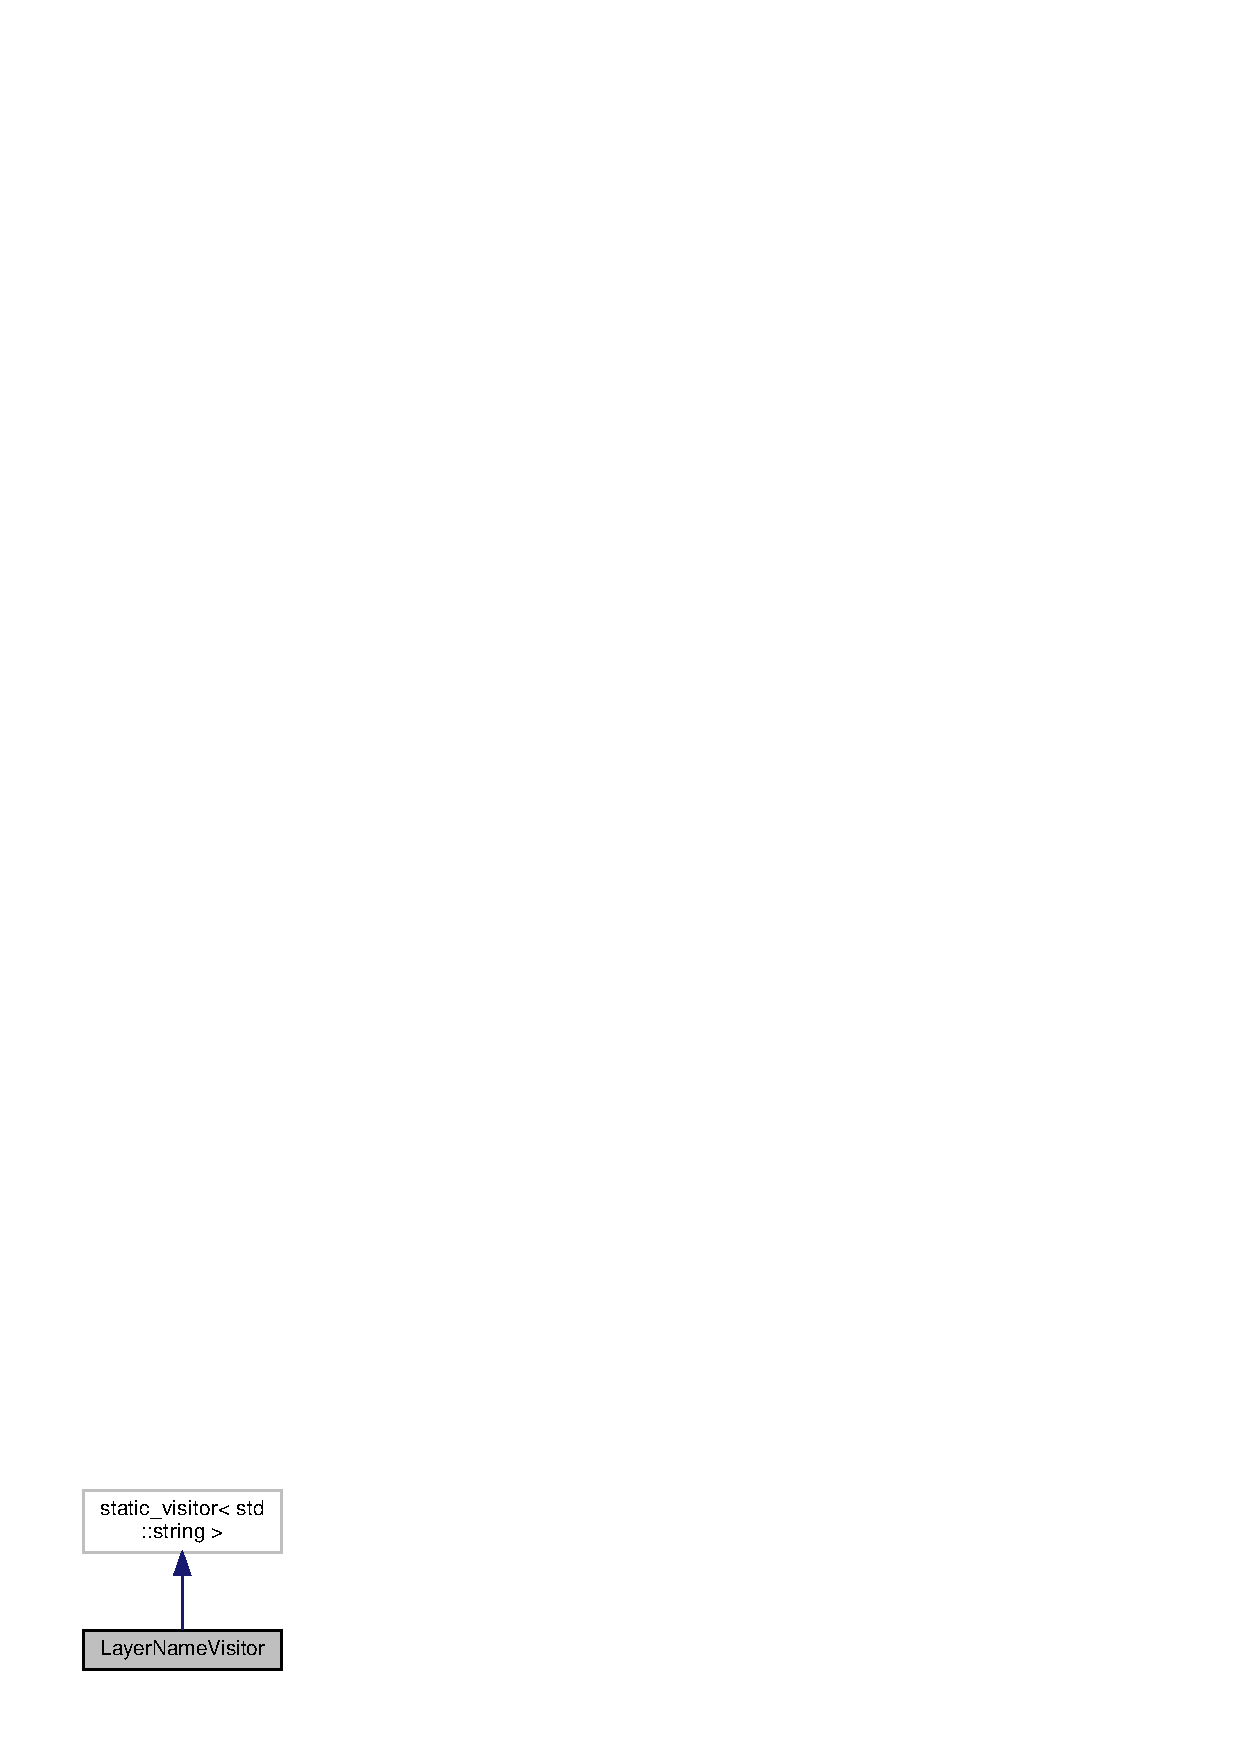
\includegraphics[width=139pt]{classLayerNameVisitor__inherit__graph}
\end{center}
\end{figure}
\subsection*{Public Member Functions}
\begin{DoxyCompactItemize}
\item 
\textbf{ Layer\+Name\+Visitor} ()
\begin{DoxyCompactList}\small\item\em Create the \doxyref{Layer\+Name\+Visitor}{p.}{classLayerNameVisitor} object. \end{DoxyCompactList}\item 
std\+::string \textbf{ Layer\+String} (\textbf{ Adaptive\+Max\+Pooling}$<$$>$ $\ast$) const
\begin{DoxyCompactList}\small\item\em Return the name of the given layer of type Adaptive\+Max\+Pooling as string. \end{DoxyCompactList}\item 
std\+::string \textbf{ Layer\+String} (\textbf{ Adaptive\+Mean\+Pooling}$<$$>$ $\ast$) const
\begin{DoxyCompactList}\small\item\em Return the name of the given layer of type Adaptive\+Mean\+Pooling as string. \end{DoxyCompactList}\item 
std\+::string \textbf{ Layer\+String} (\textbf{ Atrous\+Convolution}$<$$>$ $\ast$) const
\begin{DoxyCompactList}\small\item\em Return the name of the given layer of type Atrous\+Convolution as a string. \end{DoxyCompactList}\item 
std\+::string \textbf{ Layer\+String} (\textbf{ Alpha\+Dropout}$<$$>$ $\ast$) const
\begin{DoxyCompactList}\small\item\em Return the name of the given layer of type Alpha\+Dropout as a string. \end{DoxyCompactList}\item 
std\+::string \textbf{ Layer\+String} (\textbf{ Batch\+Norm}$<$$>$ $\ast$) const
\begin{DoxyCompactList}\small\item\em Return the name of the given layer of type Batch\+Norm as a string. \end{DoxyCompactList}\item 
std\+::string \textbf{ Layer\+String} (\textbf{ Constant}$<$$>$ $\ast$) const
\begin{DoxyCompactList}\small\item\em Return the name of the given layer of type Constant as a string. \end{DoxyCompactList}\item 
std\+::string \textbf{ Layer\+String} (\textbf{ Convolution}$<$$>$ $\ast$) const
\begin{DoxyCompactList}\small\item\em Return the name of the given layer of type Convolution as a string. \end{DoxyCompactList}\item 
std\+::string \textbf{ Layer\+String} (\textbf{ Drop\+Connect}$<$$>$ $\ast$) const
\begin{DoxyCompactList}\small\item\em Return the name of the given layer of type Drop\+Connect as a string. \end{DoxyCompactList}\item 
std\+::string \textbf{ Layer\+String} (\textbf{ Dropout}$<$$>$ $\ast$) const
\begin{DoxyCompactList}\small\item\em Return the name of the given layer of type Dropout as a string. \end{DoxyCompactList}\item 
std\+::string \textbf{ Layer\+String} (\textbf{ Flexible\+Re\+LU}$<$$>$ $\ast$) const
\begin{DoxyCompactList}\small\item\em Return the name of the given layer of type Flexible\+Re\+LU as a string. \end{DoxyCompactList}\item 
std\+::string \textbf{ Layer\+String} (\textbf{ Layer\+Norm}$<$$>$ $\ast$) const
\begin{DoxyCompactList}\small\item\em Return the name of the given layer of type Layer\+Norm as a string. \end{DoxyCompactList}\item 
std\+::string \textbf{ Layer\+String} (\textbf{ Linear}$<$$>$ $\ast$) const
\begin{DoxyCompactList}\small\item\em Return the name of the given layer of type Linear as a string. \end{DoxyCompactList}\item 
std\+::string \textbf{ Layer\+String} (\textbf{ Linear\+No\+Bias}$<$$>$ $\ast$) const
\begin{DoxyCompactList}\small\item\em Return the name of the given layer of type Linear\+No\+Bias as a string. \end{DoxyCompactList}\item 
std\+::string \textbf{ Layer\+String} (\textbf{ Noisy\+Linear}$<$$>$ $\ast$) const
\begin{DoxyCompactList}\small\item\em Return the name of the given layer of type Noisy\+Linear as a string. \end{DoxyCompactList}\item 
std\+::string \textbf{ Layer\+String} (\textbf{ Max\+Pooling}$<$$>$ $\ast$) const
\begin{DoxyCompactList}\small\item\em Return the name of the given layer of type Max\+Pooling as a string. \end{DoxyCompactList}\item 
std\+::string \textbf{ Layer\+String} (\textbf{ Mean\+Pooling}$<$$>$ $\ast$) const
\begin{DoxyCompactList}\small\item\em Return the name of the given layer of type Mean\+Pooling as a string. \end{DoxyCompactList}\item 
std\+::string \textbf{ Layer\+String} (\textbf{ Lp\+Pooling}$<$$>$ $\ast$) const
\begin{DoxyCompactList}\small\item\em Return the name of the given layer of type Lp\+Pooling as a string. \end{DoxyCompactList}\item 
std\+::string \textbf{ Layer\+String} (\textbf{ Multiply\+Constant}$<$$>$ $\ast$) const
\begin{DoxyCompactList}\small\item\em Return the name of the given layer of type Multiply\+Constant as a string. \end{DoxyCompactList}\item 
std\+::string \textbf{ Layer\+String} (\textbf{ Re\+L\+U\+Layer}$<$$>$ $\ast$) const
\begin{DoxyCompactList}\small\item\em Return the name of the given layer of type Re\+L\+U\+Layer as a string. \end{DoxyCompactList}\item 
std\+::string \textbf{ Layer\+String} (\textbf{ Transposed\+Convolution}$<$$>$ $\ast$) const
\begin{DoxyCompactList}\small\item\em Return the name of the given layer of type Transposed\+Convolution as a string. \end{DoxyCompactList}\item 
std\+::string \textbf{ Layer\+String} (\textbf{ Identity\+Layer}$<$$>$ $\ast$) const
\begin{DoxyCompactList}\small\item\em Return the name of the given layer of type Identity\+Layer as a string. \end{DoxyCompactList}\item 
std\+::string \textbf{ Layer\+String} (\textbf{ Tan\+H\+Layer}$<$$>$ $\ast$) const
\begin{DoxyCompactList}\small\item\em Return the name of the given layer of type Tan\+H\+Layer as a string. \end{DoxyCompactList}\item 
std\+::string \textbf{ Layer\+String} (\textbf{ E\+LU}$<$$>$ $\ast$) const
\begin{DoxyCompactList}\small\item\em Return the name of the given layer of type E\+LU as a string. \end{DoxyCompactList}\item 
std\+::string \textbf{ Layer\+String} (\textbf{ Hard\+TanH}$<$$>$ $\ast$) const
\begin{DoxyCompactList}\small\item\em Return the name of the given layer of type Hard\+TanH as a string. \end{DoxyCompactList}\item 
std\+::string \textbf{ Layer\+String} (\textbf{ Leaky\+Re\+LU}$<$$>$ $\ast$) const
\begin{DoxyCompactList}\small\item\em Return the name of the given layer of type Leaky\+Re\+LU as a string. \end{DoxyCompactList}\item 
std\+::string \textbf{ Layer\+String} (\textbf{ P\+Re\+LU}$<$$>$ $\ast$) const
\begin{DoxyCompactList}\small\item\em Return the name of the given layer of type P\+Re\+LU as a string. \end{DoxyCompactList}\item 
std\+::string \textbf{ Layer\+String} (\textbf{ Sigmoid\+Layer}$<$$>$ $\ast$) const
\begin{DoxyCompactList}\small\item\em Return the name of the given layer of type Sigmoid\+Layer as a string. \end{DoxyCompactList}\item 
std\+::string \textbf{ Layer\+String} (\textbf{ Log\+Soft\+Max}$<$$>$ $\ast$) const
\begin{DoxyCompactList}\small\item\em Return the name of the given layer of type Log\+Soft\+Max as a string. \end{DoxyCompactList}\item 
std\+::string \textbf{ Layer\+String} (\textbf{ L\+S\+TM}$<$$>$ $\ast$) const
\item 
std\+::string \textbf{ Layer\+String} (\textbf{ C\+Re\+LU}$<$$>$ $\ast$) const
\begin{DoxyCompactList}\small\item\em Return the name of the given layer of type C\+Re\+LU as a string. \end{DoxyCompactList}\item 
std\+::string \textbf{ Layer\+String} (\textbf{ Highway}$<$$>$ $\ast$) const
\begin{DoxyCompactList}\small\item\em Return the name of the given layer of type Highway as a string. \end{DoxyCompactList}\item 
std\+::string \textbf{ Layer\+String} (\textbf{ G\+RU}$<$$>$ $\ast$) const
\begin{DoxyCompactList}\small\item\em Return the name of the given layer of type G\+RU as a string. \end{DoxyCompactList}\item 
std\+::string \textbf{ Layer\+String} (\textbf{ Glimpse}$<$$>$ $\ast$) const
\begin{DoxyCompactList}\small\item\em Return the name of the given layer of type Glimpse as a string. \end{DoxyCompactList}\item 
std\+::string \textbf{ Layer\+String} (\textbf{ Fast\+L\+S\+TM}$<$$>$ $\ast$) const
\begin{DoxyCompactList}\small\item\em Return the name of the given layer of type Fast\+L\+S\+TM as a string. \end{DoxyCompactList}\item 
std\+::string \textbf{ Layer\+String} (\textbf{ Weight\+Norm}$<$$>$ $\ast$) const
\begin{DoxyCompactList}\small\item\em Return the name of the given layer of type Weight\+Norm as a string. \end{DoxyCompactList}\item 
{\footnotesize template$<$typename T $>$ }\\std\+::string \textbf{ Layer\+String} (T $\ast$) const
\begin{DoxyCompactList}\small\item\em Return the name of the layer of specified type as a string. \end{DoxyCompactList}\item 
std\+::string \textbf{ operator()} (\textbf{ More\+Types} layer) const
\begin{DoxyCompactList}\small\item\em Overload function call. \end{DoxyCompactList}\item 
{\footnotesize template$<$typename Layer\+Type $>$ }\\std\+::string \textbf{ operator()} (Layer\+Type $\ast$layer) const
\begin{DoxyCompactList}\small\item\em Overload function call. \end{DoxyCompactList}\end{DoxyCompactItemize}


\subsection{Detailed Description}
Implementation of a class that returns the string representation of the name of the given layer. 

Definition at line 25 of file layer\+\_\+names.\+hpp.



\subsection{Constructor \& Destructor Documentation}
\mbox{\label{classLayerNameVisitor_a0f946fadb7fc5a9e013e9d3e8ceeccf2}} 
\index{Layer\+Name\+Visitor@{Layer\+Name\+Visitor}!Layer\+Name\+Visitor@{Layer\+Name\+Visitor}}
\index{Layer\+Name\+Visitor@{Layer\+Name\+Visitor}!Layer\+Name\+Visitor@{Layer\+Name\+Visitor}}
\subsubsection{Layer\+Name\+Visitor()}
{\footnotesize\ttfamily \textbf{ Layer\+Name\+Visitor} (\begin{DoxyParamCaption}{ }\end{DoxyParamCaption})\hspace{0.3cm}{\ttfamily [inline]}}



Create the \doxyref{Layer\+Name\+Visitor}{p.}{classLayerNameVisitor} object. 



Definition at line 29 of file layer\+\_\+names.\+hpp.



\subsection{Member Function Documentation}
\mbox{\label{classLayerNameVisitor_ad55492fe23bb6506b3830005e570d0f4}} 
\index{Layer\+Name\+Visitor@{Layer\+Name\+Visitor}!Layer\+String@{Layer\+String}}
\index{Layer\+String@{Layer\+String}!Layer\+Name\+Visitor@{Layer\+Name\+Visitor}}
\subsubsection{Layer\+String()\hspace{0.1cm}{\footnotesize\ttfamily [1/36]}}
{\footnotesize\ttfamily std\+::string Layer\+String (\begin{DoxyParamCaption}\item[{\textbf{ Adaptive\+Max\+Pooling}$<$$>$ $\ast$}]{ }\end{DoxyParamCaption}) const\hspace{0.3cm}{\ttfamily [inline]}}



Return the name of the given layer of type Adaptive\+Max\+Pooling as string. 


\begin{DoxyParams}{Parameters}
{\em $\ast$} & Given layer of type Adaptive\+Max\+Pooling. \\
\hline
\end{DoxyParams}
\begin{DoxyReturn}{Returns}
The string representation of the layer. 
\end{DoxyReturn}


Definition at line 39 of file layer\+\_\+names.\+hpp.

\mbox{\label{classLayerNameVisitor_afaadce64dd171a43976fa27c0f964cb5}} 
\index{Layer\+Name\+Visitor@{Layer\+Name\+Visitor}!Layer\+String@{Layer\+String}}
\index{Layer\+String@{Layer\+String}!Layer\+Name\+Visitor@{Layer\+Name\+Visitor}}
\subsubsection{Layer\+String()\hspace{0.1cm}{\footnotesize\ttfamily [2/36]}}
{\footnotesize\ttfamily std\+::string Layer\+String (\begin{DoxyParamCaption}\item[{\textbf{ Adaptive\+Mean\+Pooling}$<$$>$ $\ast$}]{ }\end{DoxyParamCaption}) const\hspace{0.3cm}{\ttfamily [inline]}}



Return the name of the given layer of type Adaptive\+Mean\+Pooling as string. 


\begin{DoxyParams}{Parameters}
{\em $\ast$} & Given layer of type Adaptive\+Mean\+Pooling. \\
\hline
\end{DoxyParams}
\begin{DoxyReturn}{Returns}
The string representation of the layer. 
\end{DoxyReturn}


Definition at line 50 of file layer\+\_\+names.\+hpp.

\mbox{\label{classLayerNameVisitor_ad72724c1e1f75a4e0b527cf5f112dbf2}} 
\index{Layer\+Name\+Visitor@{Layer\+Name\+Visitor}!Layer\+String@{Layer\+String}}
\index{Layer\+String@{Layer\+String}!Layer\+Name\+Visitor@{Layer\+Name\+Visitor}}
\subsubsection{Layer\+String()\hspace{0.1cm}{\footnotesize\ttfamily [3/36]}}
{\footnotesize\ttfamily std\+::string Layer\+String (\begin{DoxyParamCaption}\item[{\textbf{ Atrous\+Convolution}$<$$>$ $\ast$}]{ }\end{DoxyParamCaption}) const\hspace{0.3cm}{\ttfamily [inline]}}



Return the name of the given layer of type Atrous\+Convolution as a string. 


\begin{DoxyParams}{Parameters}
{\em $\ast$} & Given layer of type Atrous\+Convolution. \\
\hline
\end{DoxyParams}
\begin{DoxyReturn}{Returns}
The string representation of the layer. 
\end{DoxyReturn}


Definition at line 61 of file layer\+\_\+names.\+hpp.

\mbox{\label{classLayerNameVisitor_ab51bbaee7abbc2f952a30e998790cc98}} 
\index{Layer\+Name\+Visitor@{Layer\+Name\+Visitor}!Layer\+String@{Layer\+String}}
\index{Layer\+String@{Layer\+String}!Layer\+Name\+Visitor@{Layer\+Name\+Visitor}}
\subsubsection{Layer\+String()\hspace{0.1cm}{\footnotesize\ttfamily [4/36]}}
{\footnotesize\ttfamily std\+::string Layer\+String (\begin{DoxyParamCaption}\item[{\textbf{ Alpha\+Dropout}$<$$>$ $\ast$}]{ }\end{DoxyParamCaption}) const\hspace{0.3cm}{\ttfamily [inline]}}



Return the name of the given layer of type Alpha\+Dropout as a string. 


\begin{DoxyParams}{Parameters}
{\em $\ast$} & Given layer of type Alpha\+Dropout. \\
\hline
\end{DoxyParams}
\begin{DoxyReturn}{Returns}
The string representation of the layer. 
\end{DoxyReturn}


Definition at line 72 of file layer\+\_\+names.\+hpp.

\mbox{\label{classLayerNameVisitor_a0f92b876d223dfd54b5e110f50f86b32}} 
\index{Layer\+Name\+Visitor@{Layer\+Name\+Visitor}!Layer\+String@{Layer\+String}}
\index{Layer\+String@{Layer\+String}!Layer\+Name\+Visitor@{Layer\+Name\+Visitor}}
\subsubsection{Layer\+String()\hspace{0.1cm}{\footnotesize\ttfamily [5/36]}}
{\footnotesize\ttfamily std\+::string Layer\+String (\begin{DoxyParamCaption}\item[{\textbf{ Batch\+Norm}$<$$>$ $\ast$}]{ }\end{DoxyParamCaption}) const\hspace{0.3cm}{\ttfamily [inline]}}



Return the name of the given layer of type Batch\+Norm as a string. 


\begin{DoxyParams}{Parameters}
{\em $\ast$} & Given layer of type Batch\+Norm. \\
\hline
\end{DoxyParams}
\begin{DoxyReturn}{Returns}
The string representation of the layer. 
\end{DoxyReturn}


Definition at line 83 of file layer\+\_\+names.\+hpp.

\mbox{\label{classLayerNameVisitor_a39da4a132e66c82902eeba09baceae96}} 
\index{Layer\+Name\+Visitor@{Layer\+Name\+Visitor}!Layer\+String@{Layer\+String}}
\index{Layer\+String@{Layer\+String}!Layer\+Name\+Visitor@{Layer\+Name\+Visitor}}
\subsubsection{Layer\+String()\hspace{0.1cm}{\footnotesize\ttfamily [6/36]}}
{\footnotesize\ttfamily std\+::string Layer\+String (\begin{DoxyParamCaption}\item[{\textbf{ Constant}$<$$>$ $\ast$}]{ }\end{DoxyParamCaption}) const\hspace{0.3cm}{\ttfamily [inline]}}



Return the name of the given layer of type Constant as a string. 


\begin{DoxyParams}{Parameters}
{\em $\ast$} & Given layer of type Constant. \\
\hline
\end{DoxyParams}
\begin{DoxyReturn}{Returns}
The string representation of the layer. 
\end{DoxyReturn}


Definition at line 94 of file layer\+\_\+names.\+hpp.

\mbox{\label{classLayerNameVisitor_a12b9b0063f4ded9394e639cbbd2e3549}} 
\index{Layer\+Name\+Visitor@{Layer\+Name\+Visitor}!Layer\+String@{Layer\+String}}
\index{Layer\+String@{Layer\+String}!Layer\+Name\+Visitor@{Layer\+Name\+Visitor}}
\subsubsection{Layer\+String()\hspace{0.1cm}{\footnotesize\ttfamily [7/36]}}
{\footnotesize\ttfamily std\+::string Layer\+String (\begin{DoxyParamCaption}\item[{\textbf{ Convolution}$<$$>$ $\ast$}]{ }\end{DoxyParamCaption}) const\hspace{0.3cm}{\ttfamily [inline]}}



Return the name of the given layer of type Convolution as a string. 


\begin{DoxyParams}{Parameters}
{\em $\ast$} & Given layer of type Convolution. \\
\hline
\end{DoxyParams}
\begin{DoxyReturn}{Returns}
The string representation of the layer. 
\end{DoxyReturn}


Definition at line 105 of file layer\+\_\+names.\+hpp.

\mbox{\label{classLayerNameVisitor_a99ff4ddf503523d8d403c7c792b0236c}} 
\index{Layer\+Name\+Visitor@{Layer\+Name\+Visitor}!Layer\+String@{Layer\+String}}
\index{Layer\+String@{Layer\+String}!Layer\+Name\+Visitor@{Layer\+Name\+Visitor}}
\subsubsection{Layer\+String()\hspace{0.1cm}{\footnotesize\ttfamily [8/36]}}
{\footnotesize\ttfamily std\+::string Layer\+String (\begin{DoxyParamCaption}\item[{\textbf{ Drop\+Connect}$<$$>$ $\ast$}]{ }\end{DoxyParamCaption}) const\hspace{0.3cm}{\ttfamily [inline]}}



Return the name of the given layer of type Drop\+Connect as a string. 


\begin{DoxyParams}{Parameters}
{\em $\ast$} & Given layer of type Drop\+Connect. \\
\hline
\end{DoxyParams}
\begin{DoxyReturn}{Returns}
The string representation of the layer. 
\end{DoxyReturn}


Definition at line 116 of file layer\+\_\+names.\+hpp.

\mbox{\label{classLayerNameVisitor_a258731098d15efbb82ee2ceec9b5897f}} 
\index{Layer\+Name\+Visitor@{Layer\+Name\+Visitor}!Layer\+String@{Layer\+String}}
\index{Layer\+String@{Layer\+String}!Layer\+Name\+Visitor@{Layer\+Name\+Visitor}}
\subsubsection{Layer\+String()\hspace{0.1cm}{\footnotesize\ttfamily [9/36]}}
{\footnotesize\ttfamily std\+::string Layer\+String (\begin{DoxyParamCaption}\item[{\textbf{ Dropout}$<$$>$ $\ast$}]{ }\end{DoxyParamCaption}) const\hspace{0.3cm}{\ttfamily [inline]}}



Return the name of the given layer of type Dropout as a string. 


\begin{DoxyParams}{Parameters}
{\em $\ast$} & Given layer of type Dropout. \\
\hline
\end{DoxyParams}
\begin{DoxyReturn}{Returns}
The string representation of the layer. 
\end{DoxyReturn}


Definition at line 127 of file layer\+\_\+names.\+hpp.

\mbox{\label{classLayerNameVisitor_ab9efbc7989ba3450f4fc9643399ec439}} 
\index{Layer\+Name\+Visitor@{Layer\+Name\+Visitor}!Layer\+String@{Layer\+String}}
\index{Layer\+String@{Layer\+String}!Layer\+Name\+Visitor@{Layer\+Name\+Visitor}}
\subsubsection{Layer\+String()\hspace{0.1cm}{\footnotesize\ttfamily [10/36]}}
{\footnotesize\ttfamily std\+::string Layer\+String (\begin{DoxyParamCaption}\item[{\textbf{ Flexible\+Re\+LU}$<$$>$ $\ast$}]{ }\end{DoxyParamCaption}) const\hspace{0.3cm}{\ttfamily [inline]}}



Return the name of the given layer of type Flexible\+Re\+LU as a string. 


\begin{DoxyParams}{Parameters}
{\em $\ast$} & Given layer of type Flexible\+Re\+LU. \\
\hline
\end{DoxyParams}
\begin{DoxyReturn}{Returns}
The string representation of the layer. 
\end{DoxyReturn}


Definition at line 138 of file layer\+\_\+names.\+hpp.

\mbox{\label{classLayerNameVisitor_a8f96f8bff340dfbbb5cd4ccbd9cd2485}} 
\index{Layer\+Name\+Visitor@{Layer\+Name\+Visitor}!Layer\+String@{Layer\+String}}
\index{Layer\+String@{Layer\+String}!Layer\+Name\+Visitor@{Layer\+Name\+Visitor}}
\subsubsection{Layer\+String()\hspace{0.1cm}{\footnotesize\ttfamily [11/36]}}
{\footnotesize\ttfamily std\+::string Layer\+String (\begin{DoxyParamCaption}\item[{\textbf{ Layer\+Norm}$<$$>$ $\ast$}]{ }\end{DoxyParamCaption}) const\hspace{0.3cm}{\ttfamily [inline]}}



Return the name of the given layer of type Layer\+Norm as a string. 


\begin{DoxyParams}{Parameters}
{\em $\ast$} & Given layer of type Layer\+Norm. \\
\hline
\end{DoxyParams}
\begin{DoxyReturn}{Returns}
The string representation of the layer. 
\end{DoxyReturn}


Definition at line 149 of file layer\+\_\+names.\+hpp.

\mbox{\label{classLayerNameVisitor_ab6374862c4fea77c8a7f12cd995986b9}} 
\index{Layer\+Name\+Visitor@{Layer\+Name\+Visitor}!Layer\+String@{Layer\+String}}
\index{Layer\+String@{Layer\+String}!Layer\+Name\+Visitor@{Layer\+Name\+Visitor}}
\subsubsection{Layer\+String()\hspace{0.1cm}{\footnotesize\ttfamily [12/36]}}
{\footnotesize\ttfamily std\+::string Layer\+String (\begin{DoxyParamCaption}\item[{\textbf{ Linear}$<$$>$ $\ast$}]{ }\end{DoxyParamCaption}) const\hspace{0.3cm}{\ttfamily [inline]}}



Return the name of the given layer of type Linear as a string. 


\begin{DoxyParams}{Parameters}
{\em $\ast$} & Given layer of type Linear. \\
\hline
\end{DoxyParams}
\begin{DoxyReturn}{Returns}
The string representation of the layer. 
\end{DoxyReturn}


Definition at line 160 of file layer\+\_\+names.\+hpp.

\mbox{\label{classLayerNameVisitor_a44c5753f704c569d347f43839ab56bdc}} 
\index{Layer\+Name\+Visitor@{Layer\+Name\+Visitor}!Layer\+String@{Layer\+String}}
\index{Layer\+String@{Layer\+String}!Layer\+Name\+Visitor@{Layer\+Name\+Visitor}}
\subsubsection{Layer\+String()\hspace{0.1cm}{\footnotesize\ttfamily [13/36]}}
{\footnotesize\ttfamily std\+::string Layer\+String (\begin{DoxyParamCaption}\item[{\textbf{ Linear\+No\+Bias}$<$$>$ $\ast$}]{ }\end{DoxyParamCaption}) const\hspace{0.3cm}{\ttfamily [inline]}}



Return the name of the given layer of type Linear\+No\+Bias as a string. 


\begin{DoxyParams}{Parameters}
{\em $\ast$} & Given layer of type Linear\+No\+Bias. \\
\hline
\end{DoxyParams}
\begin{DoxyReturn}{Returns}
The string representation of the layer. 
\end{DoxyReturn}


Definition at line 171 of file layer\+\_\+names.\+hpp.

\mbox{\label{classLayerNameVisitor_a0343f87493c3642238fa790b938eb3c3}} 
\index{Layer\+Name\+Visitor@{Layer\+Name\+Visitor}!Layer\+String@{Layer\+String}}
\index{Layer\+String@{Layer\+String}!Layer\+Name\+Visitor@{Layer\+Name\+Visitor}}
\subsubsection{Layer\+String()\hspace{0.1cm}{\footnotesize\ttfamily [14/36]}}
{\footnotesize\ttfamily std\+::string Layer\+String (\begin{DoxyParamCaption}\item[{\textbf{ Noisy\+Linear}$<$$>$ $\ast$}]{ }\end{DoxyParamCaption}) const\hspace{0.3cm}{\ttfamily [inline]}}



Return the name of the given layer of type Noisy\+Linear as a string. 


\begin{DoxyParams}{Parameters}
{\em $\ast$} & Given layer of type Noisy\+Linear. \\
\hline
\end{DoxyParams}
\begin{DoxyReturn}{Returns}
The string representation of the layer. 
\end{DoxyReturn}


Definition at line 182 of file layer\+\_\+names.\+hpp.

\mbox{\label{classLayerNameVisitor_a096dc22b45f743239b16f0b590dc52fb}} 
\index{Layer\+Name\+Visitor@{Layer\+Name\+Visitor}!Layer\+String@{Layer\+String}}
\index{Layer\+String@{Layer\+String}!Layer\+Name\+Visitor@{Layer\+Name\+Visitor}}
\subsubsection{Layer\+String()\hspace{0.1cm}{\footnotesize\ttfamily [15/36]}}
{\footnotesize\ttfamily std\+::string Layer\+String (\begin{DoxyParamCaption}\item[{\textbf{ Max\+Pooling}$<$$>$ $\ast$}]{ }\end{DoxyParamCaption}) const\hspace{0.3cm}{\ttfamily [inline]}}



Return the name of the given layer of type Max\+Pooling as a string. 


\begin{DoxyParams}{Parameters}
{\em $\ast$} & Given layer of type Max\+Pooling. \\
\hline
\end{DoxyParams}
\begin{DoxyReturn}{Returns}
The string representation of the layer. 
\end{DoxyReturn}


Definition at line 193 of file layer\+\_\+names.\+hpp.

\mbox{\label{classLayerNameVisitor_ac138d739a1edee7dbdfc7c094b643981}} 
\index{Layer\+Name\+Visitor@{Layer\+Name\+Visitor}!Layer\+String@{Layer\+String}}
\index{Layer\+String@{Layer\+String}!Layer\+Name\+Visitor@{Layer\+Name\+Visitor}}
\subsubsection{Layer\+String()\hspace{0.1cm}{\footnotesize\ttfamily [16/36]}}
{\footnotesize\ttfamily std\+::string Layer\+String (\begin{DoxyParamCaption}\item[{\textbf{ Mean\+Pooling}$<$$>$ $\ast$}]{ }\end{DoxyParamCaption}) const\hspace{0.3cm}{\ttfamily [inline]}}



Return the name of the given layer of type Mean\+Pooling as a string. 


\begin{DoxyParams}{Parameters}
{\em $\ast$} & Given layer of type Mean\+Pooling. \\
\hline
\end{DoxyParams}
\begin{DoxyReturn}{Returns}
The string representation of the layer. 
\end{DoxyReturn}


Definition at line 204 of file layer\+\_\+names.\+hpp.

\mbox{\label{classLayerNameVisitor_a38c01d9ceecf6cfa50a52cf42559d9d0}} 
\index{Layer\+Name\+Visitor@{Layer\+Name\+Visitor}!Layer\+String@{Layer\+String}}
\index{Layer\+String@{Layer\+String}!Layer\+Name\+Visitor@{Layer\+Name\+Visitor}}
\subsubsection{Layer\+String()\hspace{0.1cm}{\footnotesize\ttfamily [17/36]}}
{\footnotesize\ttfamily std\+::string Layer\+String (\begin{DoxyParamCaption}\item[{\textbf{ Lp\+Pooling}$<$$>$ $\ast$}]{ }\end{DoxyParamCaption}) const\hspace{0.3cm}{\ttfamily [inline]}}



Return the name of the given layer of type Lp\+Pooling as a string. 


\begin{DoxyParams}{Parameters}
{\em $\ast$} & Given layer of type Lp\+Pooling. \\
\hline
\end{DoxyParams}
\begin{DoxyReturn}{Returns}
The string representation of the layer. 
\end{DoxyReturn}


Definition at line 215 of file layer\+\_\+names.\+hpp.

\mbox{\label{classLayerNameVisitor_aa510725bd200647541d63b23c0e3011d}} 
\index{Layer\+Name\+Visitor@{Layer\+Name\+Visitor}!Layer\+String@{Layer\+String}}
\index{Layer\+String@{Layer\+String}!Layer\+Name\+Visitor@{Layer\+Name\+Visitor}}
\subsubsection{Layer\+String()\hspace{0.1cm}{\footnotesize\ttfamily [18/36]}}
{\footnotesize\ttfamily std\+::string Layer\+String (\begin{DoxyParamCaption}\item[{\textbf{ Multiply\+Constant}$<$$>$ $\ast$}]{ }\end{DoxyParamCaption}) const\hspace{0.3cm}{\ttfamily [inline]}}



Return the name of the given layer of type Multiply\+Constant as a string. 


\begin{DoxyParams}{Parameters}
{\em $\ast$} & Given layer of type Multiply\+Constant. \\
\hline
\end{DoxyParams}
\begin{DoxyReturn}{Returns}
The string representation of the layer. 
\end{DoxyReturn}


Definition at line 226 of file layer\+\_\+names.\+hpp.

\mbox{\label{classLayerNameVisitor_a4e3117494c28548a6143b4f91a09414a}} 
\index{Layer\+Name\+Visitor@{Layer\+Name\+Visitor}!Layer\+String@{Layer\+String}}
\index{Layer\+String@{Layer\+String}!Layer\+Name\+Visitor@{Layer\+Name\+Visitor}}
\subsubsection{Layer\+String()\hspace{0.1cm}{\footnotesize\ttfamily [19/36]}}
{\footnotesize\ttfamily std\+::string Layer\+String (\begin{DoxyParamCaption}\item[{\textbf{ Re\+L\+U\+Layer}$<$$>$ $\ast$}]{ }\end{DoxyParamCaption}) const\hspace{0.3cm}{\ttfamily [inline]}}



Return the name of the given layer of type Re\+L\+U\+Layer as a string. 


\begin{DoxyParams}{Parameters}
{\em $\ast$} & Given layer of type Re\+L\+U\+Layer. \\
\hline
\end{DoxyParams}
\begin{DoxyReturn}{Returns}
The string representation of the layer. 
\end{DoxyReturn}


Definition at line 237 of file layer\+\_\+names.\+hpp.

\mbox{\label{classLayerNameVisitor_a75cde73bf2060570c2dd01cd85dddd97}} 
\index{Layer\+Name\+Visitor@{Layer\+Name\+Visitor}!Layer\+String@{Layer\+String}}
\index{Layer\+String@{Layer\+String}!Layer\+Name\+Visitor@{Layer\+Name\+Visitor}}
\subsubsection{Layer\+String()\hspace{0.1cm}{\footnotesize\ttfamily [20/36]}}
{\footnotesize\ttfamily std\+::string Layer\+String (\begin{DoxyParamCaption}\item[{\textbf{ Transposed\+Convolution}$<$$>$ $\ast$}]{ }\end{DoxyParamCaption}) const\hspace{0.3cm}{\ttfamily [inline]}}



Return the name of the given layer of type Transposed\+Convolution as a string. 


\begin{DoxyParams}{Parameters}
{\em $\ast$} & Given layer of type Transposed\+Convolution. \\
\hline
\end{DoxyParams}
\begin{DoxyReturn}{Returns}
The string representation of the layer. 
\end{DoxyReturn}


Definition at line 249 of file layer\+\_\+names.\+hpp.

\mbox{\label{classLayerNameVisitor_a8eada8e45a040c05fafe5d6d06e3937b}} 
\index{Layer\+Name\+Visitor@{Layer\+Name\+Visitor}!Layer\+String@{Layer\+String}}
\index{Layer\+String@{Layer\+String}!Layer\+Name\+Visitor@{Layer\+Name\+Visitor}}
\subsubsection{Layer\+String()\hspace{0.1cm}{\footnotesize\ttfamily [21/36]}}
{\footnotesize\ttfamily std\+::string Layer\+String (\begin{DoxyParamCaption}\item[{\textbf{ Identity\+Layer}$<$$>$ $\ast$}]{ }\end{DoxyParamCaption}) const\hspace{0.3cm}{\ttfamily [inline]}}



Return the name of the given layer of type Identity\+Layer as a string. 


\begin{DoxyParams}{Parameters}
{\em $\ast$} & Given layer of type Identity\+Layer. \\
\hline
\end{DoxyParams}
\begin{DoxyReturn}{Returns}
The string representation of the layer. 
\end{DoxyReturn}


Definition at line 260 of file layer\+\_\+names.\+hpp.

\mbox{\label{classLayerNameVisitor_ae7a363c9e3cd1256c5b1457ed8208a72}} 
\index{Layer\+Name\+Visitor@{Layer\+Name\+Visitor}!Layer\+String@{Layer\+String}}
\index{Layer\+String@{Layer\+String}!Layer\+Name\+Visitor@{Layer\+Name\+Visitor}}
\subsubsection{Layer\+String()\hspace{0.1cm}{\footnotesize\ttfamily [22/36]}}
{\footnotesize\ttfamily std\+::string Layer\+String (\begin{DoxyParamCaption}\item[{\textbf{ Tan\+H\+Layer}$<$$>$ $\ast$}]{ }\end{DoxyParamCaption}) const\hspace{0.3cm}{\ttfamily [inline]}}



Return the name of the given layer of type Tan\+H\+Layer as a string. 


\begin{DoxyParams}{Parameters}
{\em $\ast$} & Given layer of type Tan\+H\+Layer. \\
\hline
\end{DoxyParams}
\begin{DoxyReturn}{Returns}
The string representation of the layer. 
\end{DoxyReturn}


Definition at line 271 of file layer\+\_\+names.\+hpp.

\mbox{\label{classLayerNameVisitor_ac0ed16ce5f99db03c05010bdfb6fffcd}} 
\index{Layer\+Name\+Visitor@{Layer\+Name\+Visitor}!Layer\+String@{Layer\+String}}
\index{Layer\+String@{Layer\+String}!Layer\+Name\+Visitor@{Layer\+Name\+Visitor}}
\subsubsection{Layer\+String()\hspace{0.1cm}{\footnotesize\ttfamily [23/36]}}
{\footnotesize\ttfamily std\+::string Layer\+String (\begin{DoxyParamCaption}\item[{\textbf{ E\+LU}$<$$>$ $\ast$}]{ }\end{DoxyParamCaption}) const\hspace{0.3cm}{\ttfamily [inline]}}



Return the name of the given layer of type E\+LU as a string. 


\begin{DoxyParams}{Parameters}
{\em $\ast$} & Given layer of type E\+LU. \\
\hline
\end{DoxyParams}
\begin{DoxyReturn}{Returns}
The string representation of the layer. 
\end{DoxyReturn}


Definition at line 282 of file layer\+\_\+names.\+hpp.

\mbox{\label{classLayerNameVisitor_a04beac676270816997f6bfdac76c0569}} 
\index{Layer\+Name\+Visitor@{Layer\+Name\+Visitor}!Layer\+String@{Layer\+String}}
\index{Layer\+String@{Layer\+String}!Layer\+Name\+Visitor@{Layer\+Name\+Visitor}}
\subsubsection{Layer\+String()\hspace{0.1cm}{\footnotesize\ttfamily [24/36]}}
{\footnotesize\ttfamily std\+::string Layer\+String (\begin{DoxyParamCaption}\item[{\textbf{ Hard\+TanH}$<$$>$ $\ast$}]{ }\end{DoxyParamCaption}) const\hspace{0.3cm}{\ttfamily [inline]}}



Return the name of the given layer of type Hard\+TanH as a string. 


\begin{DoxyParams}{Parameters}
{\em $\ast$} & Given layer of type Hard\+TanH. \\
\hline
\end{DoxyParams}
\begin{DoxyReturn}{Returns}
The string representation of the layer. 
\end{DoxyReturn}


Definition at line 293 of file layer\+\_\+names.\+hpp.

\mbox{\label{classLayerNameVisitor_a761a505854bc1159b2be04ddd9c93f2f}} 
\index{Layer\+Name\+Visitor@{Layer\+Name\+Visitor}!Layer\+String@{Layer\+String}}
\index{Layer\+String@{Layer\+String}!Layer\+Name\+Visitor@{Layer\+Name\+Visitor}}
\subsubsection{Layer\+String()\hspace{0.1cm}{\footnotesize\ttfamily [25/36]}}
{\footnotesize\ttfamily std\+::string Layer\+String (\begin{DoxyParamCaption}\item[{\textbf{ Leaky\+Re\+LU}$<$$>$ $\ast$}]{ }\end{DoxyParamCaption}) const\hspace{0.3cm}{\ttfamily [inline]}}



Return the name of the given layer of type Leaky\+Re\+LU as a string. 


\begin{DoxyParams}{Parameters}
{\em $\ast$} & Given layer of type Leaky\+Re\+LU. \\
\hline
\end{DoxyParams}
\begin{DoxyReturn}{Returns}
The string representation of the layer. 
\end{DoxyReturn}


Definition at line 304 of file layer\+\_\+names.\+hpp.

\mbox{\label{classLayerNameVisitor_a618a068d141b4b41a22afcc8306507c1}} 
\index{Layer\+Name\+Visitor@{Layer\+Name\+Visitor}!Layer\+String@{Layer\+String}}
\index{Layer\+String@{Layer\+String}!Layer\+Name\+Visitor@{Layer\+Name\+Visitor}}
\subsubsection{Layer\+String()\hspace{0.1cm}{\footnotesize\ttfamily [26/36]}}
{\footnotesize\ttfamily std\+::string Layer\+String (\begin{DoxyParamCaption}\item[{\textbf{ P\+Re\+LU}$<$$>$ $\ast$}]{ }\end{DoxyParamCaption}) const\hspace{0.3cm}{\ttfamily [inline]}}



Return the name of the given layer of type P\+Re\+LU as a string. 


\begin{DoxyParams}{Parameters}
{\em $\ast$} & Given layer of type P\+Re\+LU. \\
\hline
\end{DoxyParams}
\begin{DoxyReturn}{Returns}
The string representation of the layer. 
\end{DoxyReturn}


Definition at line 315 of file layer\+\_\+names.\+hpp.

\mbox{\label{classLayerNameVisitor_aadda738726af2889fe9fec2f26a02249}} 
\index{Layer\+Name\+Visitor@{Layer\+Name\+Visitor}!Layer\+String@{Layer\+String}}
\index{Layer\+String@{Layer\+String}!Layer\+Name\+Visitor@{Layer\+Name\+Visitor}}
\subsubsection{Layer\+String()\hspace{0.1cm}{\footnotesize\ttfamily [27/36]}}
{\footnotesize\ttfamily std\+::string Layer\+String (\begin{DoxyParamCaption}\item[{\textbf{ Sigmoid\+Layer}$<$$>$ $\ast$}]{ }\end{DoxyParamCaption}) const\hspace{0.3cm}{\ttfamily [inline]}}



Return the name of the given layer of type Sigmoid\+Layer as a string. 


\begin{DoxyParams}{Parameters}
{\em $\ast$} & Given layer of type Sigmoid\+Layer. \\
\hline
\end{DoxyParams}
\begin{DoxyReturn}{Returns}
The string representation of the layer. 
\end{DoxyReturn}


Definition at line 326 of file layer\+\_\+names.\+hpp.

\mbox{\label{classLayerNameVisitor_ae93cc138ff6a2eb636a877ea1c7047ec}} 
\index{Layer\+Name\+Visitor@{Layer\+Name\+Visitor}!Layer\+String@{Layer\+String}}
\index{Layer\+String@{Layer\+String}!Layer\+Name\+Visitor@{Layer\+Name\+Visitor}}
\subsubsection{Layer\+String()\hspace{0.1cm}{\footnotesize\ttfamily [28/36]}}
{\footnotesize\ttfamily std\+::string Layer\+String (\begin{DoxyParamCaption}\item[{\textbf{ Log\+Soft\+Max}$<$$>$ $\ast$}]{ }\end{DoxyParamCaption}) const\hspace{0.3cm}{\ttfamily [inline]}}



Return the name of the given layer of type Log\+Soft\+Max as a string. 


\begin{DoxyParams}{Parameters}
{\em $\ast$} & Given layer of type Log\+Soft\+Max. \\
\hline
\end{DoxyParams}
\begin{DoxyReturn}{Returns}
The string representation of the layer. 
\end{DoxyReturn}


Definition at line 337 of file layer\+\_\+names.\+hpp.

\mbox{\label{classLayerNameVisitor_ae1c5eaae028534cdd5c57d3b3c7bc29d}} 
\index{Layer\+Name\+Visitor@{Layer\+Name\+Visitor}!Layer\+String@{Layer\+String}}
\index{Layer\+String@{Layer\+String}!Layer\+Name\+Visitor@{Layer\+Name\+Visitor}}
\subsubsection{Layer\+String()\hspace{0.1cm}{\footnotesize\ttfamily [29/36]}}
{\footnotesize\ttfamily std\+::string Layer\+String (\begin{DoxyParamCaption}\item[{\textbf{ L\+S\+TM}$<$$>$ $\ast$}]{ }\end{DoxyParamCaption}) const\hspace{0.3cm}{\ttfamily [inline]}}



Definition at line 348 of file layer\+\_\+names.\+hpp.

\mbox{\label{classLayerNameVisitor_a13fd8d36fd5708012e8a8ef3c4cb2ac5}} 
\index{Layer\+Name\+Visitor@{Layer\+Name\+Visitor}!Layer\+String@{Layer\+String}}
\index{Layer\+String@{Layer\+String}!Layer\+Name\+Visitor@{Layer\+Name\+Visitor}}
\subsubsection{Layer\+String()\hspace{0.1cm}{\footnotesize\ttfamily [30/36]}}
{\footnotesize\ttfamily std\+::string Layer\+String (\begin{DoxyParamCaption}\item[{\textbf{ C\+Re\+LU}$<$$>$ $\ast$}]{ }\end{DoxyParamCaption}) const\hspace{0.3cm}{\ttfamily [inline]}}



Return the name of the given layer of type C\+Re\+LU as a string. 


\begin{DoxyParams}{Parameters}
{\em $\ast$} & Given layer of type C\+Re\+LU. \\
\hline
\end{DoxyParams}
\begin{DoxyReturn}{Returns}
The string representation of the layer. 
\end{DoxyReturn}


Definition at line 359 of file layer\+\_\+names.\+hpp.

\mbox{\label{classLayerNameVisitor_a2004522d3e87d102e8b911e7e2f7d989}} 
\index{Layer\+Name\+Visitor@{Layer\+Name\+Visitor}!Layer\+String@{Layer\+String}}
\index{Layer\+String@{Layer\+String}!Layer\+Name\+Visitor@{Layer\+Name\+Visitor}}
\subsubsection{Layer\+String()\hspace{0.1cm}{\footnotesize\ttfamily [31/36]}}
{\footnotesize\ttfamily std\+::string Layer\+String (\begin{DoxyParamCaption}\item[{\textbf{ Highway}$<$$>$ $\ast$}]{ }\end{DoxyParamCaption}) const\hspace{0.3cm}{\ttfamily [inline]}}



Return the name of the given layer of type Highway as a string. 


\begin{DoxyParams}{Parameters}
{\em $\ast$} & Given layer of type Highway. \\
\hline
\end{DoxyParams}
\begin{DoxyReturn}{Returns}
The string representation of the layer. 
\end{DoxyReturn}


Definition at line 370 of file layer\+\_\+names.\+hpp.

\mbox{\label{classLayerNameVisitor_a9c0a890184848420df7c37892691b1f6}} 
\index{Layer\+Name\+Visitor@{Layer\+Name\+Visitor}!Layer\+String@{Layer\+String}}
\index{Layer\+String@{Layer\+String}!Layer\+Name\+Visitor@{Layer\+Name\+Visitor}}
\subsubsection{Layer\+String()\hspace{0.1cm}{\footnotesize\ttfamily [32/36]}}
{\footnotesize\ttfamily std\+::string Layer\+String (\begin{DoxyParamCaption}\item[{\textbf{ G\+RU}$<$$>$ $\ast$}]{ }\end{DoxyParamCaption}) const\hspace{0.3cm}{\ttfamily [inline]}}



Return the name of the given layer of type G\+RU as a string. 


\begin{DoxyParams}{Parameters}
{\em $\ast$} & Given layer of type G\+RU. \\
\hline
\end{DoxyParams}
\begin{DoxyReturn}{Returns}
The string representation of the layer. 
\end{DoxyReturn}


Definition at line 381 of file layer\+\_\+names.\+hpp.

\mbox{\label{classLayerNameVisitor_a0bc5e33b9ed3e4d7b794cc95452f902c}} 
\index{Layer\+Name\+Visitor@{Layer\+Name\+Visitor}!Layer\+String@{Layer\+String}}
\index{Layer\+String@{Layer\+String}!Layer\+Name\+Visitor@{Layer\+Name\+Visitor}}
\subsubsection{Layer\+String()\hspace{0.1cm}{\footnotesize\ttfamily [33/36]}}
{\footnotesize\ttfamily std\+::string Layer\+String (\begin{DoxyParamCaption}\item[{\textbf{ Glimpse}$<$$>$ $\ast$}]{ }\end{DoxyParamCaption}) const\hspace{0.3cm}{\ttfamily [inline]}}



Return the name of the given layer of type Glimpse as a string. 


\begin{DoxyParams}{Parameters}
{\em $\ast$} & Given layer of type Glimpse. \\
\hline
\end{DoxyParams}
\begin{DoxyReturn}{Returns}
The string representation of the layer. 
\end{DoxyReturn}


Definition at line 392 of file layer\+\_\+names.\+hpp.

\mbox{\label{classLayerNameVisitor_ab4e0701f4c4ad4743eea30a186a33f61}} 
\index{Layer\+Name\+Visitor@{Layer\+Name\+Visitor}!Layer\+String@{Layer\+String}}
\index{Layer\+String@{Layer\+String}!Layer\+Name\+Visitor@{Layer\+Name\+Visitor}}
\subsubsection{Layer\+String()\hspace{0.1cm}{\footnotesize\ttfamily [34/36]}}
{\footnotesize\ttfamily std\+::string Layer\+String (\begin{DoxyParamCaption}\item[{\textbf{ Fast\+L\+S\+TM}$<$$>$ $\ast$}]{ }\end{DoxyParamCaption}) const\hspace{0.3cm}{\ttfamily [inline]}}



Return the name of the given layer of type Fast\+L\+S\+TM as a string. 


\begin{DoxyParams}{Parameters}
{\em $\ast$} & Given layer of type Fast\+L\+S\+TM. \\
\hline
\end{DoxyParams}
\begin{DoxyReturn}{Returns}
The string representation of the layer. 
\end{DoxyReturn}


Definition at line 403 of file layer\+\_\+names.\+hpp.

\mbox{\label{classLayerNameVisitor_aba824a9f4695661ccf5a1f232d6dc0b3}} 
\index{Layer\+Name\+Visitor@{Layer\+Name\+Visitor}!Layer\+String@{Layer\+String}}
\index{Layer\+String@{Layer\+String}!Layer\+Name\+Visitor@{Layer\+Name\+Visitor}}
\subsubsection{Layer\+String()\hspace{0.1cm}{\footnotesize\ttfamily [35/36]}}
{\footnotesize\ttfamily std\+::string Layer\+String (\begin{DoxyParamCaption}\item[{\textbf{ Weight\+Norm}$<$$>$ $\ast$}]{ }\end{DoxyParamCaption}) const\hspace{0.3cm}{\ttfamily [inline]}}



Return the name of the given layer of type Weight\+Norm as a string. 


\begin{DoxyParams}{Parameters}
{\em $\ast$} & Given layer of type Weight\+Norm. \\
\hline
\end{DoxyParams}
\begin{DoxyReturn}{Returns}
The string representation of the layer. 
\end{DoxyReturn}


Definition at line 414 of file layer\+\_\+names.\+hpp.

\mbox{\label{classLayerNameVisitor_a6bb446bf320c905d75ddd2644e613bda}} 
\index{Layer\+Name\+Visitor@{Layer\+Name\+Visitor}!Layer\+String@{Layer\+String}}
\index{Layer\+String@{Layer\+String}!Layer\+Name\+Visitor@{Layer\+Name\+Visitor}}
\subsubsection{Layer\+String()\hspace{0.1cm}{\footnotesize\ttfamily [36/36]}}
{\footnotesize\ttfamily std\+::string Layer\+String (\begin{DoxyParamCaption}\item[{T $\ast$}]{ }\end{DoxyParamCaption}) const\hspace{0.3cm}{\ttfamily [inline]}}



Return the name of the layer of specified type as a string. 


\begin{DoxyParams}{Parameters}
{\em $\ast$} & Given layer of any type. \\
\hline
\end{DoxyParams}
\begin{DoxyReturn}{Returns}
A string declaring that the layer is unsupported. 
\end{DoxyReturn}


Definition at line 426 of file layer\+\_\+names.\+hpp.

\mbox{\label{classLayerNameVisitor_a5b17c31f0df22e777430e82a6d61666a}} 
\index{Layer\+Name\+Visitor@{Layer\+Name\+Visitor}!operator()@{operator()}}
\index{operator()@{operator()}!Layer\+Name\+Visitor@{Layer\+Name\+Visitor}}
\subsubsection{operator()()\hspace{0.1cm}{\footnotesize\ttfamily [1/2]}}
{\footnotesize\ttfamily std\+::string operator() (\begin{DoxyParamCaption}\item[{\textbf{ More\+Types}}]{layer }\end{DoxyParamCaption}) const\hspace{0.3cm}{\ttfamily [inline]}}



Overload function call. 



Definition at line 432 of file layer\+\_\+names.\+hpp.

\mbox{\label{classLayerNameVisitor_a7ac25ef2c2798323872be99b6cfcf6d6}} 
\index{Layer\+Name\+Visitor@{Layer\+Name\+Visitor}!operator()@{operator()}}
\index{operator()@{operator()}!Layer\+Name\+Visitor@{Layer\+Name\+Visitor}}
\subsubsection{operator()()\hspace{0.1cm}{\footnotesize\ttfamily [2/2]}}
{\footnotesize\ttfamily std\+::string operator() (\begin{DoxyParamCaption}\item[{Layer\+Type $\ast$}]{layer }\end{DoxyParamCaption}) const\hspace{0.3cm}{\ttfamily [inline]}}



Overload function call. 



Definition at line 439 of file layer\+\_\+names.\+hpp.



The documentation for this class was generated from the following file\+:\begin{DoxyCompactItemize}
\item 
/home/aakash/mlpack/src/mlpack/methods/ann/\textbf{ layer\+\_\+names.\+hpp}\end{DoxyCompactItemize}

\section{Ada\+Boost$<$ Weak\+Learner\+Type, Mat\+Type $>$ Class Template Reference}
\label{classmlpack_1_1adaboost_1_1AdaBoost}\index{Ada\+Boost$<$ Weak\+Learner\+Type, Mat\+Type $>$@{Ada\+Boost$<$ Weak\+Learner\+Type, Mat\+Type $>$}}


The \doxyref{Ada\+Boost}{p.}{classmlpack_1_1adaboost_1_1AdaBoost} class.  




Inheritance diagram for Ada\+Boost$<$ Weak\+Learner\+Type, Mat\+Type $>$\+:
\nopagebreak
\begin{figure}[H]
\begin{center}
\leavevmode
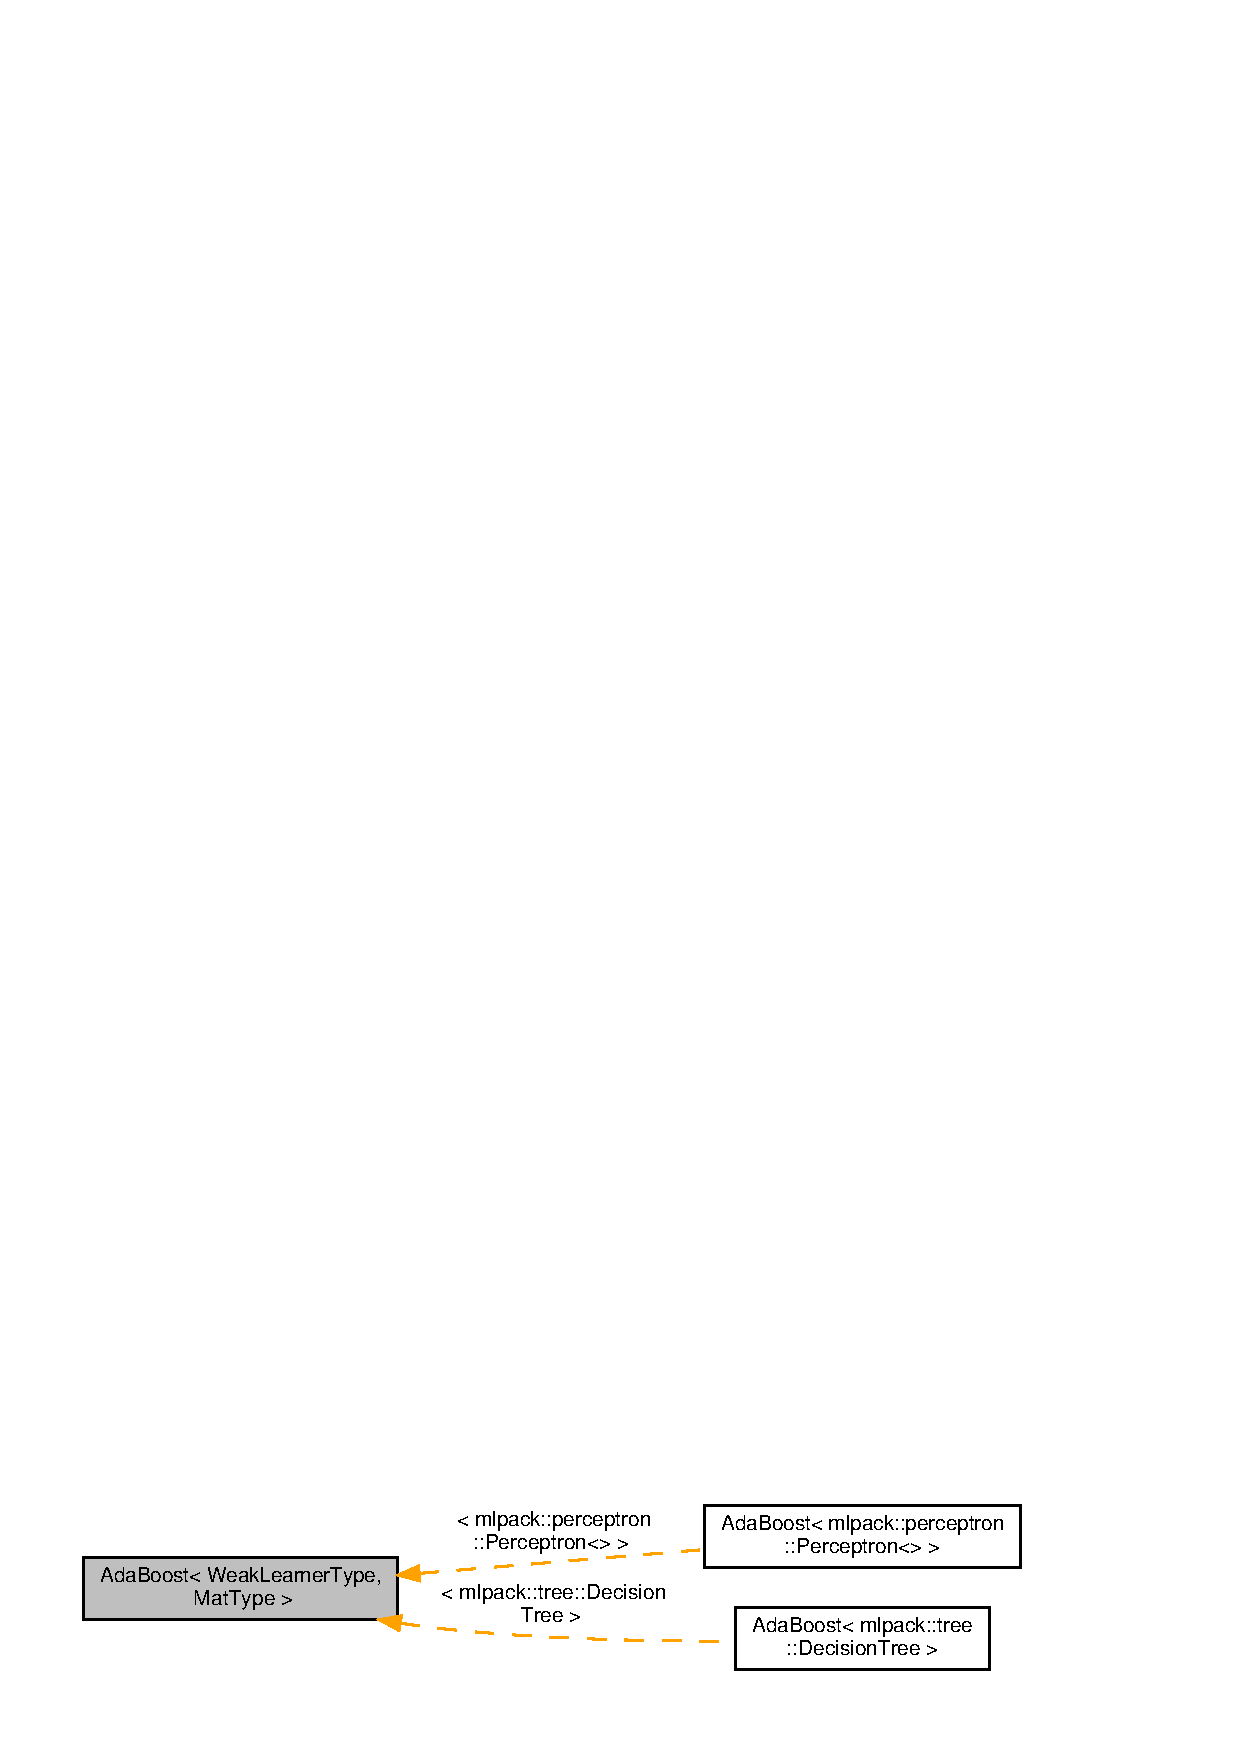
\includegraphics[width=350pt]{classmlpack_1_1adaboost_1_1AdaBoost__inherit__graph}
\end{center}
\end{figure}
\subsection*{Public Member Functions}
\begin{DoxyCompactItemize}
\item 
\textbf{ Ada\+Boost} (const Mat\+Type \&data, const arma\+::\+Row$<$ size\+\_\+t $>$ \&labels, const size\+\_\+t num\+Classes, const Weak\+Learner\+Type \&other, const size\+\_\+t iterations=100, const double tolerance=1e-\/6)
\begin{DoxyCompactList}\small\item\em Constructor. \end{DoxyCompactList}\item 
\textbf{ Ada\+Boost} (const double tolerance=1e-\/6)
\begin{DoxyCompactList}\small\item\em Create the \doxyref{Ada\+Boost}{p.}{classmlpack_1_1adaboost_1_1AdaBoost} object without training. \end{DoxyCompactList}\item 
double \textbf{ Alpha} (const size\+\_\+t i) const
\begin{DoxyCompactList}\small\item\em Get the weights for the given weak learner. \end{DoxyCompactList}\item 
double \& \textbf{ Alpha} (const size\+\_\+t i)
\begin{DoxyCompactList}\small\item\em Modify the weight for the given weak learner (be careful!). \end{DoxyCompactList}\item 
void \textbf{ Classify} (const Mat\+Type \&test, arma\+::\+Row$<$ size\+\_\+t $>$ \&predicted\+Labels, arma\+::mat \&probabilities)
\begin{DoxyCompactList}\small\item\em Classify the given test points. \end{DoxyCompactList}\item 
void \textbf{ Classify} (const Mat\+Type \&test, arma\+::\+Row$<$ size\+\_\+t $>$ \&predicted\+Labels)
\begin{DoxyCompactList}\small\item\em Classify the given test points. \end{DoxyCompactList}\item 
size\+\_\+t \textbf{ Num\+Classes} () const
\begin{DoxyCompactList}\small\item\em Get the number of classes this model is trained on. \end{DoxyCompactList}\item 
{\footnotesize template$<$typename Archive $>$ }\\void \textbf{ serialize} (Archive \&ar, const uint32\+\_\+t)
\begin{DoxyCompactList}\small\item\em Serialize the \doxyref{Ada\+Boost}{p.}{classmlpack_1_1adaboost_1_1AdaBoost} model. \end{DoxyCompactList}\item 
double \textbf{ Tolerance} () const
\begin{DoxyCompactList}\small\item\em Get the tolerance for stopping the optimization during training. \end{DoxyCompactList}\item 
double \& \textbf{ Tolerance} ()
\begin{DoxyCompactList}\small\item\em Modify the tolerance for stopping the optimization during training. \end{DoxyCompactList}\item 
double \textbf{ Train} (const Mat\+Type \&data, const arma\+::\+Row$<$ size\+\_\+t $>$ \&labels, const size\+\_\+t num\+Classes, const Weak\+Learner\+Type \&learner, const size\+\_\+t iterations=100, const double tolerance=1e-\/6)
\begin{DoxyCompactList}\small\item\em Train \doxyref{Ada\+Boost}{p.}{classmlpack_1_1adaboost_1_1AdaBoost} on the given dataset. \end{DoxyCompactList}\item 
const Weak\+Learner\+Type \& \textbf{ Weak\+Learner} (const size\+\_\+t i) const
\begin{DoxyCompactList}\small\item\em Get the given weak learner. \end{DoxyCompactList}\item 
Weak\+Learner\+Type \& \textbf{ Weak\+Learner} (const size\+\_\+t i)
\begin{DoxyCompactList}\small\item\em Modify the given weak learner (be careful!). \end{DoxyCompactList}\item 
size\+\_\+t \textbf{ Weak\+Learners} () const
\begin{DoxyCompactList}\small\item\em Get the number of weak learners in the model. \end{DoxyCompactList}\end{DoxyCompactItemize}


\subsection{Detailed Description}
\subsubsection*{template$<$typename Weak\+Learner\+Type = mlpack\+::perceptron\+::\+Perceptron$<$$>$, typename Mat\+Type = arma\+::mat$>$\newline
class mlpack\+::adaboost\+::\+Ada\+Boost$<$ Weak\+Learner\+Type, Mat\+Type $>$}

The \doxyref{Ada\+Boost}{p.}{classmlpack_1_1adaboost_1_1AdaBoost} class. 

\doxyref{Ada\+Boost}{p.}{classmlpack_1_1adaboost_1_1AdaBoost} is a boosting algorithm, meaning that it combines an ensemble of weak learners to produce a strong learner. For more information on \doxyref{Ada\+Boost}{p.}{classmlpack_1_1adaboost_1_1AdaBoost}, see the following paper\+:


\begin{DoxyCode}
@article\{schapire1999improved,
  author = \{Schapire, Robert E. and Singer, Yoram\},
  title = \{Improved Boosting Algorithms Using Confidence-rated Predictions\},
  journal = \{Machine Learning\},
  volume = \{37\},
  number = \{3\},
  month = dec,
  year = \{1999\},
  issn = \{0885-6125\},
  pages = \{297--336\},
\}
\end{DoxyCode}


This class is general, and can be used with any type of weak learner, so long as the learner implements the following functions\+:


\begin{DoxyCode}
\textcolor{comment}{// A boosting constructor, which learns using the training parameters of the}
\textcolor{comment}{// given other WeakLearner, but uses the given instance weights for training.}
WeakLearner(WeakLearner& other,
            \textcolor{keyword}{const} MatType& data,
            \textcolor{keyword}{const} arma::Row<size\_t>& labels,
            \textcolor{keyword}{const} arma::rowvec& weights);

\textcolor{comment}{// Given the test points, classify them and output predictions into}
\textcolor{comment}{// predictedLabels.}
\textcolor{keywordtype}{void} Classify(\textcolor{keyword}{const} MatType& data, arma::Row<size\_t>& predictedLabels);
\end{DoxyCode}


For more information on and examples of weak learners, see perceptron\+::\+Perceptron$<$$>$ and \doxyref{tree\+::\+I\+D3\+Decision\+Stump}{p.}{namespacemlpack_1_1tree_a27b9268c266fdfe2f4563d07052a0ecf}.


\begin{DoxyTemplParams}{Template Parameters}
{\em Mat\+Type} & Data matrix type (i.\+e. arma\+::mat or arma\+::sp\+\_\+mat). \\
\hline
{\em Weak\+Learner\+Type} & Type of weak learner to use. \\
\hline
\end{DoxyTemplParams}


Definition at line 81 of file adaboost.\+hpp.



\subsection{Constructor \& Destructor Documentation}
\mbox{\label{classmlpack_1_1adaboost_1_1AdaBoost_a7a37dbe455d049cda36f4676b26eeb70}} 
\index{mlpack\+::adaboost\+::\+Ada\+Boost@{mlpack\+::adaboost\+::\+Ada\+Boost}!Ada\+Boost@{Ada\+Boost}}
\index{Ada\+Boost@{Ada\+Boost}!mlpack\+::adaboost\+::\+Ada\+Boost@{mlpack\+::adaboost\+::\+Ada\+Boost}}
\subsubsection{Ada\+Boost()\hspace{0.1cm}{\footnotesize\ttfamily [1/2]}}
{\footnotesize\ttfamily \textbf{ Ada\+Boost} (\begin{DoxyParamCaption}\item[{const Mat\+Type \&}]{data,  }\item[{const arma\+::\+Row$<$ size\+\_\+t $>$ \&}]{labels,  }\item[{const size\+\_\+t}]{num\+Classes,  }\item[{const Weak\+Learner\+Type \&}]{other,  }\item[{const size\+\_\+t}]{iterations = {\ttfamily 100},  }\item[{const double}]{tolerance = {\ttfamily 1e-\/6} }\end{DoxyParamCaption})}



Constructor. 

This runs the Ada\+Boost.\+MH algorithm to provide a trained boosting model. This constructor takes an already-\/initialized weak learner; all other weak learners will learn with the same parameters as the given weak learner.


\begin{DoxyParams}{Parameters}
{\em data} & Input data. \\
\hline
{\em labels} & Corresponding labels. \\
\hline
{\em num\+Classes} & The number of classes. \\
\hline
{\em iterations} & Number of boosting rounds. \\
\hline
{\em tolerance} & The tolerance for change in values of rt. \\
\hline
{\em other} & Weak learner that has already been initialized. \\
\hline
\end{DoxyParams}
\mbox{\label{classmlpack_1_1adaboost_1_1AdaBoost_a1417a39b49cf9b28c88add6f48daa9a1}} 
\index{mlpack\+::adaboost\+::\+Ada\+Boost@{mlpack\+::adaboost\+::\+Ada\+Boost}!Ada\+Boost@{Ada\+Boost}}
\index{Ada\+Boost@{Ada\+Boost}!mlpack\+::adaboost\+::\+Ada\+Boost@{mlpack\+::adaboost\+::\+Ada\+Boost}}
\subsubsection{Ada\+Boost()\hspace{0.1cm}{\footnotesize\ttfamily [2/2]}}
{\footnotesize\ttfamily \textbf{ Ada\+Boost} (\begin{DoxyParamCaption}\item[{const double}]{tolerance = {\ttfamily 1e-\/6} }\end{DoxyParamCaption})}



Create the \doxyref{Ada\+Boost}{p.}{classmlpack_1_1adaboost_1_1AdaBoost} object without training. 

Be sure to call \doxyref{Train()}{p.}{classmlpack_1_1adaboost_1_1AdaBoost_adeb648736c63379ce1cb5f2b23d242be} before calling \doxyref{Classify()}{p.}{classmlpack_1_1adaboost_1_1AdaBoost_abc7d38690c69822bd9ec10c3760384da}! 

\subsection{Member Function Documentation}
\mbox{\label{classmlpack_1_1adaboost_1_1AdaBoost_af0e29824cfcada4ec450e4d09cc9a314}} 
\index{mlpack\+::adaboost\+::\+Ada\+Boost@{mlpack\+::adaboost\+::\+Ada\+Boost}!Alpha@{Alpha}}
\index{Alpha@{Alpha}!mlpack\+::adaboost\+::\+Ada\+Boost@{mlpack\+::adaboost\+::\+Ada\+Boost}}
\subsubsection{Alpha()\hspace{0.1cm}{\footnotesize\ttfamily [1/2]}}
{\footnotesize\ttfamily double Alpha (\begin{DoxyParamCaption}\item[{const size\+\_\+t}]{i }\end{DoxyParamCaption}) const\hspace{0.3cm}{\ttfamily [inline]}}



Get the weights for the given weak learner. 



Definition at line 122 of file adaboost.\+hpp.

\mbox{\label{classmlpack_1_1adaboost_1_1AdaBoost_ae59910b30903367791fde226761923cf}} 
\index{mlpack\+::adaboost\+::\+Ada\+Boost@{mlpack\+::adaboost\+::\+Ada\+Boost}!Alpha@{Alpha}}
\index{Alpha@{Alpha}!mlpack\+::adaboost\+::\+Ada\+Boost@{mlpack\+::adaboost\+::\+Ada\+Boost}}
\subsubsection{Alpha()\hspace{0.1cm}{\footnotesize\ttfamily [2/2]}}
{\footnotesize\ttfamily double\& Alpha (\begin{DoxyParamCaption}\item[{const size\+\_\+t}]{i }\end{DoxyParamCaption})\hspace{0.3cm}{\ttfamily [inline]}}



Modify the weight for the given weak learner (be careful!). 



Definition at line 124 of file adaboost.\+hpp.

\mbox{\label{classmlpack_1_1adaboost_1_1AdaBoost_abc7d38690c69822bd9ec10c3760384da}} 
\index{mlpack\+::adaboost\+::\+Ada\+Boost@{mlpack\+::adaboost\+::\+Ada\+Boost}!Classify@{Classify}}
\index{Classify@{Classify}!mlpack\+::adaboost\+::\+Ada\+Boost@{mlpack\+::adaboost\+::\+Ada\+Boost}}
\subsubsection{Classify()\hspace{0.1cm}{\footnotesize\ttfamily [1/2]}}
{\footnotesize\ttfamily void Classify (\begin{DoxyParamCaption}\item[{const Mat\+Type \&}]{test,  }\item[{arma\+::\+Row$<$ size\+\_\+t $>$ \&}]{predicted\+Labels,  }\item[{arma\+::mat \&}]{probabilities }\end{DoxyParamCaption})}



Classify the given test points. 


\begin{DoxyParams}{Parameters}
{\em test} & Testing data. \\
\hline
{\em predicted\+Labels} & Vector in which the predicted labels of the test set will be stored. \\
\hline
{\em probabilities} & matrix to store the predicted class probabilities for each point in the test set. \\
\hline
\end{DoxyParams}


Referenced by Ada\+Boost$<$ mlpack\+::tree\+::\+Decision\+Tree $>$\+::\+Weak\+Learner().

\mbox{\label{classmlpack_1_1adaboost_1_1AdaBoost_a407f9c281dab80fffd49251d3907838d}} 
\index{mlpack\+::adaboost\+::\+Ada\+Boost@{mlpack\+::adaboost\+::\+Ada\+Boost}!Classify@{Classify}}
\index{Classify@{Classify}!mlpack\+::adaboost\+::\+Ada\+Boost@{mlpack\+::adaboost\+::\+Ada\+Boost}}
\subsubsection{Classify()\hspace{0.1cm}{\footnotesize\ttfamily [2/2]}}
{\footnotesize\ttfamily void Classify (\begin{DoxyParamCaption}\item[{const Mat\+Type \&}]{test,  }\item[{arma\+::\+Row$<$ size\+\_\+t $>$ \&}]{predicted\+Labels }\end{DoxyParamCaption})}



Classify the given test points. 


\begin{DoxyParams}{Parameters}
{\em test} & Testing data. \\
\hline
{\em predicted\+Labels} & Vector in which the predicted labels of the test set will be stored. \\
\hline
\end{DoxyParams}
\mbox{\label{classmlpack_1_1adaboost_1_1AdaBoost_a088ebfdf3c7a9e7eea81716d0c55b5a3}} 
\index{mlpack\+::adaboost\+::\+Ada\+Boost@{mlpack\+::adaboost\+::\+Ada\+Boost}!Num\+Classes@{Num\+Classes}}
\index{Num\+Classes@{Num\+Classes}!mlpack\+::adaboost\+::\+Ada\+Boost@{mlpack\+::adaboost\+::\+Ada\+Boost}}
\subsubsection{Num\+Classes()}
{\footnotesize\ttfamily size\+\_\+t Num\+Classes (\begin{DoxyParamCaption}{ }\end{DoxyParamCaption}) const\hspace{0.3cm}{\ttfamily [inline]}}



Get the number of classes this model is trained on. 



Definition at line 116 of file adaboost.\+hpp.

\mbox{\label{classmlpack_1_1adaboost_1_1AdaBoost_a65cba07328997659bec80b9879b15a51}} 
\index{mlpack\+::adaboost\+::\+Ada\+Boost@{mlpack\+::adaboost\+::\+Ada\+Boost}!serialize@{serialize}}
\index{serialize@{serialize}!mlpack\+::adaboost\+::\+Ada\+Boost@{mlpack\+::adaboost\+::\+Ada\+Boost}}
\subsubsection{serialize()}
{\footnotesize\ttfamily void serialize (\begin{DoxyParamCaption}\item[{Archive \&}]{ar,  }\item[{const uint32\+\_\+t}]{ }\end{DoxyParamCaption})}



Serialize the \doxyref{Ada\+Boost}{p.}{classmlpack_1_1adaboost_1_1AdaBoost} model. 



Referenced by Ada\+Boost$<$ mlpack\+::tree\+::\+Decision\+Tree $>$\+::\+Weak\+Learner().

\mbox{\label{classmlpack_1_1adaboost_1_1AdaBoost_a7b5af5c1a84c507cbaa7f999ea5a4fda}} 
\index{mlpack\+::adaboost\+::\+Ada\+Boost@{mlpack\+::adaboost\+::\+Ada\+Boost}!Tolerance@{Tolerance}}
\index{Tolerance@{Tolerance}!mlpack\+::adaboost\+::\+Ada\+Boost@{mlpack\+::adaboost\+::\+Ada\+Boost}}
\subsubsection{Tolerance()\hspace{0.1cm}{\footnotesize\ttfamily [1/2]}}
{\footnotesize\ttfamily double Tolerance (\begin{DoxyParamCaption}{ }\end{DoxyParamCaption}) const\hspace{0.3cm}{\ttfamily [inline]}}



Get the tolerance for stopping the optimization during training. 



Definition at line 111 of file adaboost.\+hpp.

\mbox{\label{classmlpack_1_1adaboost_1_1AdaBoost_a3d9fac84af16250f5a3689692e8f2173}} 
\index{mlpack\+::adaboost\+::\+Ada\+Boost@{mlpack\+::adaboost\+::\+Ada\+Boost}!Tolerance@{Tolerance}}
\index{Tolerance@{Tolerance}!mlpack\+::adaboost\+::\+Ada\+Boost@{mlpack\+::adaboost\+::\+Ada\+Boost}}
\subsubsection{Tolerance()\hspace{0.1cm}{\footnotesize\ttfamily [2/2]}}
{\footnotesize\ttfamily double\& Tolerance (\begin{DoxyParamCaption}{ }\end{DoxyParamCaption})\hspace{0.3cm}{\ttfamily [inline]}}



Modify the tolerance for stopping the optimization during training. 



Definition at line 113 of file adaboost.\+hpp.

\mbox{\label{classmlpack_1_1adaboost_1_1AdaBoost_adeb648736c63379ce1cb5f2b23d242be}} 
\index{mlpack\+::adaboost\+::\+Ada\+Boost@{mlpack\+::adaboost\+::\+Ada\+Boost}!Train@{Train}}
\index{Train@{Train}!mlpack\+::adaboost\+::\+Ada\+Boost@{mlpack\+::adaboost\+::\+Ada\+Boost}}
\subsubsection{Train()}
{\footnotesize\ttfamily double Train (\begin{DoxyParamCaption}\item[{const Mat\+Type \&}]{data,  }\item[{const arma\+::\+Row$<$ size\+\_\+t $>$ \&}]{labels,  }\item[{const size\+\_\+t}]{num\+Classes,  }\item[{const Weak\+Learner\+Type \&}]{learner,  }\item[{const size\+\_\+t}]{iterations = {\ttfamily 100},  }\item[{const double}]{tolerance = {\ttfamily 1e-\/6} }\end{DoxyParamCaption})}



Train \doxyref{Ada\+Boost}{p.}{classmlpack_1_1adaboost_1_1AdaBoost} on the given dataset. 

This method takes an initialized Weak\+Learner\+Type; the parameters for this weak learner will be used to train each of the weak learners during \doxyref{Ada\+Boost}{p.}{classmlpack_1_1adaboost_1_1AdaBoost} training. Note that this will completely overwrite any model that has already been trained with this object.


\begin{DoxyParams}{Parameters}
{\em data} & Dataset to train on. \\
\hline
{\em labels} & Labels for each point in the dataset. \\
\hline
{\em num\+Classes} & The number of classes. \\
\hline
{\em learner} & Learner to use for training. \\
\hline
{\em iterations} & Number of boosting rounds. \\
\hline
{\em tolerance} & The tolerance for change in values of rt. \\
\hline
\end{DoxyParams}
\begin{DoxyReturn}{Returns}
The upper bound for training error. 
\end{DoxyReturn}


Referenced by Ada\+Boost$<$ mlpack\+::tree\+::\+Decision\+Tree $>$\+::\+Weak\+Learner().

\mbox{\label{classmlpack_1_1adaboost_1_1AdaBoost_aa6f54b09b480fed23b0b04214e300cbf}} 
\index{mlpack\+::adaboost\+::\+Ada\+Boost@{mlpack\+::adaboost\+::\+Ada\+Boost}!Weak\+Learner@{Weak\+Learner}}
\index{Weak\+Learner@{Weak\+Learner}!mlpack\+::adaboost\+::\+Ada\+Boost@{mlpack\+::adaboost\+::\+Ada\+Boost}}
\subsubsection{Weak\+Learner()\hspace{0.1cm}{\footnotesize\ttfamily [1/2]}}
{\footnotesize\ttfamily const Weak\+Learner\+Type\& Weak\+Learner (\begin{DoxyParamCaption}\item[{const size\+\_\+t}]{i }\end{DoxyParamCaption}) const\hspace{0.3cm}{\ttfamily [inline]}}



Get the given weak learner. 



Definition at line 127 of file adaboost.\+hpp.

\mbox{\label{classmlpack_1_1adaboost_1_1AdaBoost_a11d7a531e3de5cdd5cc8f0cc02b8ed4d}} 
\index{mlpack\+::adaboost\+::\+Ada\+Boost@{mlpack\+::adaboost\+::\+Ada\+Boost}!Weak\+Learner@{Weak\+Learner}}
\index{Weak\+Learner@{Weak\+Learner}!mlpack\+::adaboost\+::\+Ada\+Boost@{mlpack\+::adaboost\+::\+Ada\+Boost}}
\subsubsection{Weak\+Learner()\hspace{0.1cm}{\footnotesize\ttfamily [2/2]}}
{\footnotesize\ttfamily Weak\+Learner\+Type\& Weak\+Learner (\begin{DoxyParamCaption}\item[{const size\+\_\+t}]{i }\end{DoxyParamCaption})\hspace{0.3cm}{\ttfamily [inline]}}



Modify the given weak learner (be careful!). 



Definition at line 129 of file adaboost.\+hpp.

\mbox{\label{classmlpack_1_1adaboost_1_1AdaBoost_a5bb6ee8b31c0e16567eee13cb3719f88}} 
\index{mlpack\+::adaboost\+::\+Ada\+Boost@{mlpack\+::adaboost\+::\+Ada\+Boost}!Weak\+Learners@{Weak\+Learners}}
\index{Weak\+Learners@{Weak\+Learners}!mlpack\+::adaboost\+::\+Ada\+Boost@{mlpack\+::adaboost\+::\+Ada\+Boost}}
\subsubsection{Weak\+Learners()}
{\footnotesize\ttfamily size\+\_\+t Weak\+Learners (\begin{DoxyParamCaption}{ }\end{DoxyParamCaption}) const\hspace{0.3cm}{\ttfamily [inline]}}



Get the number of weak learners in the model. 



Definition at line 119 of file adaboost.\+hpp.



The documentation for this class was generated from the following file\+:\begin{DoxyCompactItemize}
\item 
/home/aakash/mlpack/src/mlpack/methods/adaboost/\textbf{ adaboost.\+hpp}\end{DoxyCompactItemize}

\section{Ada\+Boost\+Model Class Reference}
\label{classmlpack_1_1adaboost_1_1AdaBoostModel}\index{Ada\+Boost\+Model@{Ada\+Boost\+Model}}


The model to save to disk.  


\subsection*{Public Types}
\begin{DoxyCompactItemize}
\item 
enum \textbf{ Weak\+Learner\+Types} \{ \newline
\textbf{ D\+E\+C\+I\+S\+I\+O\+N\+\_\+\+S\+T\+U\+MP}, 
\newline
\textbf{ P\+E\+R\+C\+E\+P\+T\+R\+ON}
 \}
\end{DoxyCompactItemize}
\subsection*{Public Member Functions}
\begin{DoxyCompactItemize}
\item 
\textbf{ Ada\+Boost\+Model} ()
\begin{DoxyCompactList}\small\item\em Create an empty \doxyref{Ada\+Boost}{p.}{classmlpack_1_1adaboost_1_1AdaBoost} model. \end{DoxyCompactList}\item 
\textbf{ Ada\+Boost\+Model} (const arma\+::\+Col$<$ size\+\_\+t $>$ \&mappings, const size\+\_\+t weak\+Learner\+Type)
\begin{DoxyCompactList}\small\item\em Create the \doxyref{Ada\+Boost}{p.}{classmlpack_1_1adaboost_1_1AdaBoost} model with the given mappings and type. \end{DoxyCompactList}\item 
\textbf{ Ada\+Boost\+Model} (const \textbf{ Ada\+Boost\+Model} \&other)
\begin{DoxyCompactList}\small\item\em Copy constructor. \end{DoxyCompactList}\item 
\textbf{ Ada\+Boost\+Model} (\textbf{ Ada\+Boost\+Model} \&\&other)
\begin{DoxyCompactList}\small\item\em Move constructor. \end{DoxyCompactList}\item 
\textbf{ $\sim$\+Ada\+Boost\+Model} ()
\begin{DoxyCompactList}\small\item\em Clean up memory. \end{DoxyCompactList}\item 
void \textbf{ Classify} (const arma\+::mat \&test\+Data, arma\+::\+Row$<$ size\+\_\+t $>$ \&predictions)
\begin{DoxyCompactList}\small\item\em Classify test points. \end{DoxyCompactList}\item 
void \textbf{ Classify} (const arma\+::mat \&test\+Data, arma\+::\+Row$<$ size\+\_\+t $>$ \&predictions, arma\+::mat \&probabilities)
\begin{DoxyCompactList}\small\item\em Classify test points. \end{DoxyCompactList}\item 
size\+\_\+t \textbf{ Dimensionality} () const
\begin{DoxyCompactList}\small\item\em Get the dimensionality of the model. \end{DoxyCompactList}\item 
size\+\_\+t \& \textbf{ Dimensionality} ()
\begin{DoxyCompactList}\small\item\em Modify the dimensionality of the model. \end{DoxyCompactList}\item 
const arma\+::\+Col$<$ size\+\_\+t $>$ \& \textbf{ Mappings} () const
\begin{DoxyCompactList}\small\item\em Get the mappings. \end{DoxyCompactList}\item 
arma\+::\+Col$<$ size\+\_\+t $>$ \& \textbf{ Mappings} ()
\begin{DoxyCompactList}\small\item\em Modify the mappings. \end{DoxyCompactList}\item 
\textbf{ Ada\+Boost\+Model} \& \textbf{ operator=} (const \textbf{ Ada\+Boost\+Model} \&other)
\begin{DoxyCompactList}\small\item\em Copy assignment operator. \end{DoxyCompactList}\item 
\textbf{ Ada\+Boost\+Model} \& \textbf{ operator=} (\textbf{ Ada\+Boost\+Model} \&\&other)
\begin{DoxyCompactList}\small\item\em Move assignment operator. \end{DoxyCompactList}\item 
{\footnotesize template$<$typename Archive $>$ }\\void \textbf{ serialize} (Archive \&ar, const uint32\+\_\+t)
\begin{DoxyCompactList}\small\item\em Serialize the model. \end{DoxyCompactList}\item 
void \textbf{ Train} (const arma\+::mat \&data, const arma\+::\+Row$<$ size\+\_\+t $>$ \&labels, const size\+\_\+t num\+Classes, const size\+\_\+t iterations, const double tolerance)
\begin{DoxyCompactList}\small\item\em Train the model, treat the data is all of the numeric type. \end{DoxyCompactList}\item 
size\+\_\+t \textbf{ Weak\+Learner\+Type} () const
\begin{DoxyCompactList}\small\item\em Get the weak learner type. \end{DoxyCompactList}\item 
size\+\_\+t \& \textbf{ Weak\+Learner\+Type} ()
\begin{DoxyCompactList}\small\item\em Modify the weak learner type. \end{DoxyCompactList}\end{DoxyCompactItemize}


\subsection{Detailed Description}
The model to save to disk. 

Definition at line 26 of file adaboost\+\_\+model.\+hpp.



\subsection{Member Enumeration Documentation}
\mbox{\label{classmlpack_1_1adaboost_1_1AdaBoostModel_ad2d30fa530c8eadc4797c729f91b10b6}} 
\index{mlpack\+::adaboost\+::\+Ada\+Boost\+Model@{mlpack\+::adaboost\+::\+Ada\+Boost\+Model}!Weak\+Learner\+Types@{Weak\+Learner\+Types}}
\index{Weak\+Learner\+Types@{Weak\+Learner\+Types}!mlpack\+::adaboost\+::\+Ada\+Boost\+Model@{mlpack\+::adaboost\+::\+Ada\+Boost\+Model}}
\subsubsection{Weak\+Learner\+Types}
{\footnotesize\ttfamily enum \textbf{ Weak\+Learner\+Types}}

\begin{DoxyEnumFields}{Enumerator}
\raisebox{\heightof{T}}[0pt][0pt]{\index{D\+E\+C\+I\+S\+I\+O\+N\+\_\+\+S\+T\+U\+MP@{D\+E\+C\+I\+S\+I\+O\+N\+\_\+\+S\+T\+U\+MP}!mlpack\+::adaboost\+::\+Ada\+Boost\+Model@{mlpack\+::adaboost\+::\+Ada\+Boost\+Model}}\index{mlpack\+::adaboost\+::\+Ada\+Boost\+Model@{mlpack\+::adaboost\+::\+Ada\+Boost\+Model}!D\+E\+C\+I\+S\+I\+O\+N\+\_\+\+S\+T\+U\+MP@{D\+E\+C\+I\+S\+I\+O\+N\+\_\+\+S\+T\+U\+MP}}}\mbox{\label{classmlpack_1_1adaboost_1_1AdaBoostModel_ad2d30fa530c8eadc4797c729f91b10b6a3b0a8b3700534a49e23eaba0426876dc}} 
D\+E\+C\+I\+S\+I\+O\+N\+\_\+\+S\+T\+U\+MP&\\
\hline

\raisebox{\heightof{T}}[0pt][0pt]{\index{P\+E\+R\+C\+E\+P\+T\+R\+ON@{P\+E\+R\+C\+E\+P\+T\+R\+ON}!mlpack\+::adaboost\+::\+Ada\+Boost\+Model@{mlpack\+::adaboost\+::\+Ada\+Boost\+Model}}\index{mlpack\+::adaboost\+::\+Ada\+Boost\+Model@{mlpack\+::adaboost\+::\+Ada\+Boost\+Model}!P\+E\+R\+C\+E\+P\+T\+R\+ON@{P\+E\+R\+C\+E\+P\+T\+R\+ON}}}\mbox{\label{classmlpack_1_1adaboost_1_1AdaBoostModel_ad2d30fa530c8eadc4797c729f91b10b6a86ae196aae3149d1c609c87be8d499c2}} 
P\+E\+R\+C\+E\+P\+T\+R\+ON&\\
\hline

\end{DoxyEnumFields}


Definition at line 29 of file adaboost\+\_\+model.\+hpp.



\subsection{Constructor \& Destructor Documentation}
\mbox{\label{classmlpack_1_1adaboost_1_1AdaBoostModel_adcba05defdbcbf2619ea58db2a46c1f1}} 
\index{mlpack\+::adaboost\+::\+Ada\+Boost\+Model@{mlpack\+::adaboost\+::\+Ada\+Boost\+Model}!Ada\+Boost\+Model@{Ada\+Boost\+Model}}
\index{Ada\+Boost\+Model@{Ada\+Boost\+Model}!mlpack\+::adaboost\+::\+Ada\+Boost\+Model@{mlpack\+::adaboost\+::\+Ada\+Boost\+Model}}
\subsubsection{Ada\+Boost\+Model()\hspace{0.1cm}{\footnotesize\ttfamily [1/4]}}
{\footnotesize\ttfamily \textbf{ Ada\+Boost\+Model} (\begin{DoxyParamCaption}{ }\end{DoxyParamCaption})}



Create an empty \doxyref{Ada\+Boost}{p.}{classmlpack_1_1adaboost_1_1AdaBoost} model. 

\mbox{\label{classmlpack_1_1adaboost_1_1AdaBoostModel_a38b1c1a146789ab0a1a391004c4910ee}} 
\index{mlpack\+::adaboost\+::\+Ada\+Boost\+Model@{mlpack\+::adaboost\+::\+Ada\+Boost\+Model}!Ada\+Boost\+Model@{Ada\+Boost\+Model}}
\index{Ada\+Boost\+Model@{Ada\+Boost\+Model}!mlpack\+::adaboost\+::\+Ada\+Boost\+Model@{mlpack\+::adaboost\+::\+Ada\+Boost\+Model}}
\subsubsection{Ada\+Boost\+Model()\hspace{0.1cm}{\footnotesize\ttfamily [2/4]}}
{\footnotesize\ttfamily \textbf{ Ada\+Boost\+Model} (\begin{DoxyParamCaption}\item[{const arma\+::\+Col$<$ size\+\_\+t $>$ \&}]{mappings,  }\item[{const size\+\_\+t}]{weak\+Learner\+Type }\end{DoxyParamCaption})}



Create the \doxyref{Ada\+Boost}{p.}{classmlpack_1_1adaboost_1_1AdaBoost} model with the given mappings and type. 

\mbox{\label{classmlpack_1_1adaboost_1_1AdaBoostModel_a99b111fbe30c57fd722c0462d14ce0f7}} 
\index{mlpack\+::adaboost\+::\+Ada\+Boost\+Model@{mlpack\+::adaboost\+::\+Ada\+Boost\+Model}!Ada\+Boost\+Model@{Ada\+Boost\+Model}}
\index{Ada\+Boost\+Model@{Ada\+Boost\+Model}!mlpack\+::adaboost\+::\+Ada\+Boost\+Model@{mlpack\+::adaboost\+::\+Ada\+Boost\+Model}}
\subsubsection{Ada\+Boost\+Model()\hspace{0.1cm}{\footnotesize\ttfamily [3/4]}}
{\footnotesize\ttfamily \textbf{ Ada\+Boost\+Model} (\begin{DoxyParamCaption}\item[{const \textbf{ Ada\+Boost\+Model} \&}]{other }\end{DoxyParamCaption})}



Copy constructor. 

\mbox{\label{classmlpack_1_1adaboost_1_1AdaBoostModel_a5bd98d104419d9424d69c31f28a46d4d}} 
\index{mlpack\+::adaboost\+::\+Ada\+Boost\+Model@{mlpack\+::adaboost\+::\+Ada\+Boost\+Model}!Ada\+Boost\+Model@{Ada\+Boost\+Model}}
\index{Ada\+Boost\+Model@{Ada\+Boost\+Model}!mlpack\+::adaboost\+::\+Ada\+Boost\+Model@{mlpack\+::adaboost\+::\+Ada\+Boost\+Model}}
\subsubsection{Ada\+Boost\+Model()\hspace{0.1cm}{\footnotesize\ttfamily [4/4]}}
{\footnotesize\ttfamily \textbf{ Ada\+Boost\+Model} (\begin{DoxyParamCaption}\item[{\textbf{ Ada\+Boost\+Model} \&\&}]{other }\end{DoxyParamCaption})}



Move constructor. 

\mbox{\label{classmlpack_1_1adaboost_1_1AdaBoostModel_ae452b3b3579c2d8aeacb4bc5b5183857}} 
\index{mlpack\+::adaboost\+::\+Ada\+Boost\+Model@{mlpack\+::adaboost\+::\+Ada\+Boost\+Model}!````~Ada\+Boost\+Model@{$\sim$\+Ada\+Boost\+Model}}
\index{````~Ada\+Boost\+Model@{$\sim$\+Ada\+Boost\+Model}!mlpack\+::adaboost\+::\+Ada\+Boost\+Model@{mlpack\+::adaboost\+::\+Ada\+Boost\+Model}}
\subsubsection{$\sim$\+Ada\+Boost\+Model()}
{\footnotesize\ttfamily $\sim$\textbf{ Ada\+Boost\+Model} (\begin{DoxyParamCaption}{ }\end{DoxyParamCaption})}



Clean up memory. 



\subsection{Member Function Documentation}
\mbox{\label{classmlpack_1_1adaboost_1_1AdaBoostModel_a275941a22a35f6b5ca8aaa11073c34d2}} 
\index{mlpack\+::adaboost\+::\+Ada\+Boost\+Model@{mlpack\+::adaboost\+::\+Ada\+Boost\+Model}!Classify@{Classify}}
\index{Classify@{Classify}!mlpack\+::adaboost\+::\+Ada\+Boost\+Model@{mlpack\+::adaboost\+::\+Ada\+Boost\+Model}}
\subsubsection{Classify()\hspace{0.1cm}{\footnotesize\ttfamily [1/2]}}
{\footnotesize\ttfamily void Classify (\begin{DoxyParamCaption}\item[{const arma\+::mat \&}]{test\+Data,  }\item[{arma\+::\+Row$<$ size\+\_\+t $>$ \&}]{predictions }\end{DoxyParamCaption})}



Classify test points. 



Referenced by Ada\+Boost\+Model\+::\+Dimensionality().

\mbox{\label{classmlpack_1_1adaboost_1_1AdaBoostModel_a4fceef357aba14291c04b9d9bb2d1e82}} 
\index{mlpack\+::adaboost\+::\+Ada\+Boost\+Model@{mlpack\+::adaboost\+::\+Ada\+Boost\+Model}!Classify@{Classify}}
\index{Classify@{Classify}!mlpack\+::adaboost\+::\+Ada\+Boost\+Model@{mlpack\+::adaboost\+::\+Ada\+Boost\+Model}}
\subsubsection{Classify()\hspace{0.1cm}{\footnotesize\ttfamily [2/2]}}
{\footnotesize\ttfamily void Classify (\begin{DoxyParamCaption}\item[{const arma\+::mat \&}]{test\+Data,  }\item[{arma\+::\+Row$<$ size\+\_\+t $>$ \&}]{predictions,  }\item[{arma\+::mat \&}]{probabilities }\end{DoxyParamCaption})}



Classify test points. 

\mbox{\label{classmlpack_1_1adaboost_1_1AdaBoostModel_a78eda6bfb9e9462afa0fc85e32abe1af}} 
\index{mlpack\+::adaboost\+::\+Ada\+Boost\+Model@{mlpack\+::adaboost\+::\+Ada\+Boost\+Model}!Dimensionality@{Dimensionality}}
\index{Dimensionality@{Dimensionality}!mlpack\+::adaboost\+::\+Ada\+Boost\+Model@{mlpack\+::adaboost\+::\+Ada\+Boost\+Model}}
\subsubsection{Dimensionality()\hspace{0.1cm}{\footnotesize\ttfamily [1/2]}}
{\footnotesize\ttfamily size\+\_\+t Dimensionality (\begin{DoxyParamCaption}{ }\end{DoxyParamCaption}) const\hspace{0.3cm}{\ttfamily [inline]}}



Get the dimensionality of the model. 



Definition at line 81 of file adaboost\+\_\+model.\+hpp.

\mbox{\label{classmlpack_1_1adaboost_1_1AdaBoostModel_a787adc650f11b9430f6bd0b937bbe6b0}} 
\index{mlpack\+::adaboost\+::\+Ada\+Boost\+Model@{mlpack\+::adaboost\+::\+Ada\+Boost\+Model}!Dimensionality@{Dimensionality}}
\index{Dimensionality@{Dimensionality}!mlpack\+::adaboost\+::\+Ada\+Boost\+Model@{mlpack\+::adaboost\+::\+Ada\+Boost\+Model}}
\subsubsection{Dimensionality()\hspace{0.1cm}{\footnotesize\ttfamily [2/2]}}
{\footnotesize\ttfamily size\+\_\+t\& Dimensionality (\begin{DoxyParamCaption}{ }\end{DoxyParamCaption})\hspace{0.3cm}{\ttfamily [inline]}}



Modify the dimensionality of the model. 



Definition at line 83 of file adaboost\+\_\+model.\+hpp.



References Ada\+Boost\+Model\+::\+Classify(), and Ada\+Boost\+Model\+::\+Train().

\mbox{\label{classmlpack_1_1adaboost_1_1AdaBoostModel_a83e8ff63d5c49eddaaf9eadb64f3aef9}} 
\index{mlpack\+::adaboost\+::\+Ada\+Boost\+Model@{mlpack\+::adaboost\+::\+Ada\+Boost\+Model}!Mappings@{Mappings}}
\index{Mappings@{Mappings}!mlpack\+::adaboost\+::\+Ada\+Boost\+Model@{mlpack\+::adaboost\+::\+Ada\+Boost\+Model}}
\subsubsection{Mappings()\hspace{0.1cm}{\footnotesize\ttfamily [1/2]}}
{\footnotesize\ttfamily const arma\+::\+Col$<$size\+\_\+t$>$\& Mappings (\begin{DoxyParamCaption}{ }\end{DoxyParamCaption}) const\hspace{0.3cm}{\ttfamily [inline]}}



Get the mappings. 



Definition at line 71 of file adaboost\+\_\+model.\+hpp.

\mbox{\label{classmlpack_1_1adaboost_1_1AdaBoostModel_ac18a534c636043f5c3d6b90992d83129}} 
\index{mlpack\+::adaboost\+::\+Ada\+Boost\+Model@{mlpack\+::adaboost\+::\+Ada\+Boost\+Model}!Mappings@{Mappings}}
\index{Mappings@{Mappings}!mlpack\+::adaboost\+::\+Ada\+Boost\+Model@{mlpack\+::adaboost\+::\+Ada\+Boost\+Model}}
\subsubsection{Mappings()\hspace{0.1cm}{\footnotesize\ttfamily [2/2]}}
{\footnotesize\ttfamily arma\+::\+Col$<$size\+\_\+t$>$\& Mappings (\begin{DoxyParamCaption}{ }\end{DoxyParamCaption})\hspace{0.3cm}{\ttfamily [inline]}}



Modify the mappings. 



Definition at line 73 of file adaboost\+\_\+model.\+hpp.

\mbox{\label{classmlpack_1_1adaboost_1_1AdaBoostModel_ab74135df3386b81f3dd06f37caebb441}} 
\index{mlpack\+::adaboost\+::\+Ada\+Boost\+Model@{mlpack\+::adaboost\+::\+Ada\+Boost\+Model}!operator=@{operator=}}
\index{operator=@{operator=}!mlpack\+::adaboost\+::\+Ada\+Boost\+Model@{mlpack\+::adaboost\+::\+Ada\+Boost\+Model}}
\subsubsection{operator=()\hspace{0.1cm}{\footnotesize\ttfamily [1/2]}}
{\footnotesize\ttfamily \textbf{ Ada\+Boost\+Model}\& operator= (\begin{DoxyParamCaption}\item[{const \textbf{ Ada\+Boost\+Model} \&}]{other }\end{DoxyParamCaption})}



Copy assignment operator. 

\mbox{\label{classmlpack_1_1adaboost_1_1AdaBoostModel_a7f2aca905549fd670bbeb7e4bb8aec0c}} 
\index{mlpack\+::adaboost\+::\+Ada\+Boost\+Model@{mlpack\+::adaboost\+::\+Ada\+Boost\+Model}!operator=@{operator=}}
\index{operator=@{operator=}!mlpack\+::adaboost\+::\+Ada\+Boost\+Model@{mlpack\+::adaboost\+::\+Ada\+Boost\+Model}}
\subsubsection{operator=()\hspace{0.1cm}{\footnotesize\ttfamily [2/2]}}
{\footnotesize\ttfamily \textbf{ Ada\+Boost\+Model}\& operator= (\begin{DoxyParamCaption}\item[{\textbf{ Ada\+Boost\+Model} \&\&}]{other }\end{DoxyParamCaption})}



Move assignment operator. 

\mbox{\label{classmlpack_1_1adaboost_1_1AdaBoostModel_a65cba07328997659bec80b9879b15a51}} 
\index{mlpack\+::adaboost\+::\+Ada\+Boost\+Model@{mlpack\+::adaboost\+::\+Ada\+Boost\+Model}!serialize@{serialize}}
\index{serialize@{serialize}!mlpack\+::adaboost\+::\+Ada\+Boost\+Model@{mlpack\+::adaboost\+::\+Ada\+Boost\+Model}}
\subsubsection{serialize()}
{\footnotesize\ttfamily void serialize (\begin{DoxyParamCaption}\item[{Archive \&}]{ar,  }\item[{const uint32\+\_\+t}]{ }\end{DoxyParamCaption})\hspace{0.3cm}{\ttfamily [inline]}}



Serialize the model. 



Definition at line 103 of file adaboost\+\_\+model.\+hpp.



References C\+E\+R\+E\+A\+L\+\_\+\+P\+O\+I\+N\+T\+ER.

\mbox{\label{classmlpack_1_1adaboost_1_1AdaBoostModel_a5360ac8d82301e1e7037d2a5a9f094a9}} 
\index{mlpack\+::adaboost\+::\+Ada\+Boost\+Model@{mlpack\+::adaboost\+::\+Ada\+Boost\+Model}!Train@{Train}}
\index{Train@{Train}!mlpack\+::adaboost\+::\+Ada\+Boost\+Model@{mlpack\+::adaboost\+::\+Ada\+Boost\+Model}}
\subsubsection{Train()}
{\footnotesize\ttfamily void Train (\begin{DoxyParamCaption}\item[{const arma\+::mat \&}]{data,  }\item[{const arma\+::\+Row$<$ size\+\_\+t $>$ \&}]{labels,  }\item[{const size\+\_\+t}]{num\+Classes,  }\item[{const size\+\_\+t}]{iterations,  }\item[{const double}]{tolerance }\end{DoxyParamCaption})}



Train the model, treat the data is all of the numeric type. 



Referenced by Ada\+Boost\+Model\+::\+Dimensionality().

\mbox{\label{classmlpack_1_1adaboost_1_1AdaBoostModel_a022ff1546accf8fe7e41253c4837edcb}} 
\index{mlpack\+::adaboost\+::\+Ada\+Boost\+Model@{mlpack\+::adaboost\+::\+Ada\+Boost\+Model}!Weak\+Learner\+Type@{Weak\+Learner\+Type}}
\index{Weak\+Learner\+Type@{Weak\+Learner\+Type}!mlpack\+::adaboost\+::\+Ada\+Boost\+Model@{mlpack\+::adaboost\+::\+Ada\+Boost\+Model}}
\subsubsection{Weak\+Learner\+Type()\hspace{0.1cm}{\footnotesize\ttfamily [1/2]}}
{\footnotesize\ttfamily size\+\_\+t Weak\+Learner\+Type (\begin{DoxyParamCaption}{ }\end{DoxyParamCaption}) const\hspace{0.3cm}{\ttfamily [inline]}}



Get the weak learner type. 



Definition at line 76 of file adaboost\+\_\+model.\+hpp.

\mbox{\label{classmlpack_1_1adaboost_1_1AdaBoostModel_aba360992c5850f1dba9279efeb94980b}} 
\index{mlpack\+::adaboost\+::\+Ada\+Boost\+Model@{mlpack\+::adaboost\+::\+Ada\+Boost\+Model}!Weak\+Learner\+Type@{Weak\+Learner\+Type}}
\index{Weak\+Learner\+Type@{Weak\+Learner\+Type}!mlpack\+::adaboost\+::\+Ada\+Boost\+Model@{mlpack\+::adaboost\+::\+Ada\+Boost\+Model}}
\subsubsection{Weak\+Learner\+Type()\hspace{0.1cm}{\footnotesize\ttfamily [2/2]}}
{\footnotesize\ttfamily size\+\_\+t\& Weak\+Learner\+Type (\begin{DoxyParamCaption}{ }\end{DoxyParamCaption})\hspace{0.3cm}{\ttfamily [inline]}}



Modify the weak learner type. 



Definition at line 78 of file adaboost\+\_\+model.\+hpp.



The documentation for this class was generated from the following file\+:\begin{DoxyCompactItemize}
\item 
/home/aakash/mlpack/src/mlpack/methods/adaboost/\textbf{ adaboost\+\_\+model.\+hpp}\end{DoxyCompactItemize}

\section{A\+MF$<$ Termination\+Policy\+Type, Initialization\+Rule\+Type, Update\+Rule\+Type $>$ Class Template Reference}
\label{classmlpack_1_1amf_1_1AMF}\index{A\+M\+F$<$ Termination\+Policy\+Type, Initialization\+Rule\+Type, Update\+Rule\+Type $>$@{A\+M\+F$<$ Termination\+Policy\+Type, Initialization\+Rule\+Type, Update\+Rule\+Type $>$}}


This class implements \doxyref{A\+MF}{p.}{classmlpack_1_1amf_1_1AMF} (alternating matrix factorization) on the given matrix V.  


\subsection*{Public Member Functions}
\begin{DoxyCompactItemize}
\item 
\textbf{ A\+MF} (const Termination\+Policy\+Type \&termination\+Policy=Termination\+Policy\+Type(), const Initialization\+Rule\+Type \&initialize\+Rule=Initialization\+Rule\+Type(), const Update\+Rule\+Type \&update=Update\+Rule\+Type())
\begin{DoxyCompactList}\small\item\em Create the \doxyref{A\+MF}{p.}{classmlpack_1_1amf_1_1AMF} object and (optionally) set the parameters which \doxyref{A\+MF}{p.}{classmlpack_1_1amf_1_1AMF} will run with. \end{DoxyCompactList}\item 
{\footnotesize template$<$typename Mat\+Type $>$ }\\double \textbf{ Apply} (const Mat\+Type \&V, const size\+\_\+t r, arma\+::mat \&W, arma\+::mat \&H)
\begin{DoxyCompactList}\small\item\em Apply Alternating Matrix Factorization to the provided matrix. \end{DoxyCompactList}\item 
const Initialization\+Rule\+Type \& \textbf{ Initialize\+Rule} () const
\begin{DoxyCompactList}\small\item\em Access the initialization rule. \end{DoxyCompactList}\item 
Initialization\+Rule\+Type \& \textbf{ Initialize\+Rule} ()
\begin{DoxyCompactList}\small\item\em Modify the initialization rule. \end{DoxyCompactList}\item 
const Termination\+Policy\+Type \& \textbf{ Termination\+Policy} () const
\begin{DoxyCompactList}\small\item\em Access the termination policy. \end{DoxyCompactList}\item 
Termination\+Policy\+Type \& \textbf{ Termination\+Policy} ()
\begin{DoxyCompactList}\small\item\em Modify the termination policy. \end{DoxyCompactList}\item 
const Update\+Rule\+Type \& \textbf{ Update} () const
\begin{DoxyCompactList}\small\item\em Access the update rule. \end{DoxyCompactList}\item 
Update\+Rule\+Type \& \textbf{ Update} ()
\begin{DoxyCompactList}\small\item\em Modify the update rule. \end{DoxyCompactList}\end{DoxyCompactItemize}


\subsection{Detailed Description}
\subsubsection*{template$<$typename Termination\+Policy\+Type = Simple\+Residue\+Termination, typename Initialization\+Rule\+Type = Random\+Acol\+Initialization$<$$>$, typename Update\+Rule\+Type = N\+M\+F\+Multiplicative\+Distance\+Update$>$\newline
class mlpack\+::amf\+::\+A\+M\+F$<$ Termination\+Policy\+Type, Initialization\+Rule\+Type, Update\+Rule\+Type $>$}

This class implements \doxyref{A\+MF}{p.}{classmlpack_1_1amf_1_1AMF} (alternating matrix factorization) on the given matrix V. 

Alternating matrix factorization decomposes V in the form $ V \approx WH $ where W is called the basis matrix and H is called the encoding matrix. V is taken to be of size n x m and the obtained W is n x r and H is r x m. The size r is called the rank of the factorization.

The implementation requires three template types; the first contains the policy used to determine when the algorithm has converged; the second contains the initialization rule for the W and H matrix; the last contains the update rule to be used during each iteration. This templatization allows the user to try various update rules, initialization rules, and termination policies (including ones not supplied with mlpack) for factorization. By default, the template parameters to \doxyref{A\+MF}{p.}{classmlpack_1_1amf_1_1AMF} implement non-\/negative matrix factorization with the multiplicative distance update.

A simple example of how to run \doxyref{A\+MF}{p.}{classmlpack_1_1amf_1_1AMF} (or N\+MF) is shown below.


\begin{DoxyCode}
\textcolor{keyword}{extern} arma::mat V; \textcolor{comment}{// Matrix that we want to perform LMF on.}
\textcolor{keywordtype}{size\_t} r = 10; \textcolor{comment}{// Rank of decomposition}
arma::mat W; \textcolor{comment}{// Basis matrix}
arma::mat H; \textcolor{comment}{// Encoding matrix}

AMF<> amf; \textcolor{comment}{// Default options: NMF with multiplicative distance update rules.}
amf.Apply(V, r, W, H);
\end{DoxyCode}



\begin{DoxyTemplParams}{Template Parameters}
{\em Termination\+Policy} & The policy to use for determining when the factorization has converged. \\
\hline
{\em Initialization\+Rule} & The initialization rule for initializing W and H matrix. \\
\hline
{\em Update\+Rule} & The update rule for calculating W and H matrix at each iteration.\\
\hline
\end{DoxyTemplParams}
\begin{DoxySeeAlso}{See also}
\doxyref{N\+M\+F\+Multiplicative\+Distance\+Update}{p.}{classmlpack_1_1amf_1_1NMFMultiplicativeDistanceUpdate}, \doxyref{Simple\+Residue\+Termination}{p.}{classmlpack_1_1amf_1_1SimpleResidueTermination} 
\end{DoxySeeAlso}


Definition at line 78 of file amf.\+hpp.



\subsection{Constructor \& Destructor Documentation}
\mbox{\label{classmlpack_1_1amf_1_1AMF_aa79bd7ca717d85ef36baa40a1ea4319a}} 
\index{mlpack\+::amf\+::\+A\+MF@{mlpack\+::amf\+::\+A\+MF}!A\+MF@{A\+MF}}
\index{A\+MF@{A\+MF}!mlpack\+::amf\+::\+A\+MF@{mlpack\+::amf\+::\+A\+MF}}
\subsubsection{A\+M\+F()}
{\footnotesize\ttfamily \textbf{ A\+MF} (\begin{DoxyParamCaption}\item[{const Termination\+Policy\+Type \&}]{termination\+Policy = {\ttfamily TerminationPolicyType()},  }\item[{const Initialization\+Rule\+Type \&}]{initialize\+Rule = {\ttfamily InitializationRuleType()},  }\item[{const Update\+Rule\+Type \&}]{update = {\ttfamily UpdateRuleType()} }\end{DoxyParamCaption})}



Create the \doxyref{A\+MF}{p.}{classmlpack_1_1amf_1_1AMF} object and (optionally) set the parameters which \doxyref{A\+MF}{p.}{classmlpack_1_1amf_1_1AMF} will run with. 

The minimum residue refers to the root mean square of the difference between two subsequent iterations of the product W $\ast$ H. A low residue indicates that subsequent iterations are not producing much change in W and H. Once the residue goes below the specified minimum residue, the algorithm terminates.


\begin{DoxyParams}{Parameters}
{\em initialize\+Rule} & Optional instantiated Initialization\+Rule object for initializing the W and H matrices. \\
\hline
{\em update} & Optional instantiated Update\+Rule object; this parameter is useful when the update rule for the W and H vector has state that it needs to store (i.\+e. H\+Update() and W\+Update() are not static functions). \\
\hline
{\em termination\+Policy} & Optional instantiated Termination\+Policy object. \\
\hline
\end{DoxyParams}


\subsection{Member Function Documentation}
\mbox{\label{classmlpack_1_1amf_1_1AMF_a535d2642e3234fbd1ebc6840b061c4da}} 
\index{mlpack\+::amf\+::\+A\+MF@{mlpack\+::amf\+::\+A\+MF}!Apply@{Apply}}
\index{Apply@{Apply}!mlpack\+::amf\+::\+A\+MF@{mlpack\+::amf\+::\+A\+MF}}
\subsubsection{Apply()}
{\footnotesize\ttfamily double Apply (\begin{DoxyParamCaption}\item[{const Mat\+Type \&}]{V,  }\item[{const size\+\_\+t}]{r,  }\item[{arma\+::mat \&}]{W,  }\item[{arma\+::mat \&}]{H }\end{DoxyParamCaption})}



Apply Alternating Matrix Factorization to the provided matrix. 


\begin{DoxyParams}{Parameters}
{\em V} & Input matrix to be factorized. \\
\hline
{\em W} & Basis matrix to be output. \\
\hline
{\em H} & Encoding matrix to output. \\
\hline
{\em r} & Rank r of the factorization. \\
\hline
\end{DoxyParams}


Referenced by N\+M\+F\+Policy\+::\+Apply(), Batch\+S\+V\+D\+Policy\+::\+Apply(), S\+V\+D\+Complete\+Policy\+::\+Apply(), and S\+V\+D\+Incomplete\+Policy\+::\+Apply().

\mbox{\label{classmlpack_1_1amf_1_1AMF_ae36ae1d0d07bb71d6ad4aa3919de674b}} 
\index{mlpack\+::amf\+::\+A\+MF@{mlpack\+::amf\+::\+A\+MF}!Initialize\+Rule@{Initialize\+Rule}}
\index{Initialize\+Rule@{Initialize\+Rule}!mlpack\+::amf\+::\+A\+MF@{mlpack\+::amf\+::\+A\+MF}}
\subsubsection{Initialize\+Rule()\hspace{0.1cm}{\footnotesize\ttfamily [1/2]}}
{\footnotesize\ttfamily const Initialization\+Rule\+Type\& Initialize\+Rule (\begin{DoxyParamCaption}{ }\end{DoxyParamCaption}) const\hspace{0.3cm}{\ttfamily [inline]}}



Access the initialization rule. 



Definition at line 122 of file amf.\+hpp.

\mbox{\label{classmlpack_1_1amf_1_1AMF_ad4c0a310565e914c01e6beb9f9427567}} 
\index{mlpack\+::amf\+::\+A\+MF@{mlpack\+::amf\+::\+A\+MF}!Initialize\+Rule@{Initialize\+Rule}}
\index{Initialize\+Rule@{Initialize\+Rule}!mlpack\+::amf\+::\+A\+MF@{mlpack\+::amf\+::\+A\+MF}}
\subsubsection{Initialize\+Rule()\hspace{0.1cm}{\footnotesize\ttfamily [2/2]}}
{\footnotesize\ttfamily Initialization\+Rule\+Type\& Initialize\+Rule (\begin{DoxyParamCaption}{ }\end{DoxyParamCaption})\hspace{0.3cm}{\ttfamily [inline]}}



Modify the initialization rule. 



Definition at line 125 of file amf.\+hpp.

\mbox{\label{classmlpack_1_1amf_1_1AMF_ad905ffaf32e6780a28664a060d23e6b8}} 
\index{mlpack\+::amf\+::\+A\+MF@{mlpack\+::amf\+::\+A\+MF}!Termination\+Policy@{Termination\+Policy}}
\index{Termination\+Policy@{Termination\+Policy}!mlpack\+::amf\+::\+A\+MF@{mlpack\+::amf\+::\+A\+MF}}
\subsubsection{Termination\+Policy()\hspace{0.1cm}{\footnotesize\ttfamily [1/2]}}
{\footnotesize\ttfamily const Termination\+Policy\+Type\& Termination\+Policy (\begin{DoxyParamCaption}{ }\end{DoxyParamCaption}) const\hspace{0.3cm}{\ttfamily [inline]}}



Access the termination policy. 



Definition at line 116 of file amf.\+hpp.

\mbox{\label{classmlpack_1_1amf_1_1AMF_ae0b13308816da802c64d704544a7af71}} 
\index{mlpack\+::amf\+::\+A\+MF@{mlpack\+::amf\+::\+A\+MF}!Termination\+Policy@{Termination\+Policy}}
\index{Termination\+Policy@{Termination\+Policy}!mlpack\+::amf\+::\+A\+MF@{mlpack\+::amf\+::\+A\+MF}}
\subsubsection{Termination\+Policy()\hspace{0.1cm}{\footnotesize\ttfamily [2/2]}}
{\footnotesize\ttfamily Termination\+Policy\+Type\& Termination\+Policy (\begin{DoxyParamCaption}{ }\end{DoxyParamCaption})\hspace{0.3cm}{\ttfamily [inline]}}



Modify the termination policy. 



Definition at line 119 of file amf.\+hpp.

\mbox{\label{classmlpack_1_1amf_1_1AMF_ad51a399acff576b3da541487d6a76417}} 
\index{mlpack\+::amf\+::\+A\+MF@{mlpack\+::amf\+::\+A\+MF}!Update@{Update}}
\index{Update@{Update}!mlpack\+::amf\+::\+A\+MF@{mlpack\+::amf\+::\+A\+MF}}
\subsubsection{Update()\hspace{0.1cm}{\footnotesize\ttfamily [1/2]}}
{\footnotesize\ttfamily const Update\+Rule\+Type\& Update (\begin{DoxyParamCaption}{ }\end{DoxyParamCaption}) const\hspace{0.3cm}{\ttfamily [inline]}}



Access the update rule. 



Definition at line 128 of file amf.\+hpp.

\mbox{\label{classmlpack_1_1amf_1_1AMF_a3e8cca59296dfb97e73f5c07924ed644}} 
\index{mlpack\+::amf\+::\+A\+MF@{mlpack\+::amf\+::\+A\+MF}!Update@{Update}}
\index{Update@{Update}!mlpack\+::amf\+::\+A\+MF@{mlpack\+::amf\+::\+A\+MF}}
\subsubsection{Update()\hspace{0.1cm}{\footnotesize\ttfamily [2/2]}}
{\footnotesize\ttfamily Update\+Rule\+Type\& Update (\begin{DoxyParamCaption}{ }\end{DoxyParamCaption})\hspace{0.3cm}{\ttfamily [inline]}}



Modify the update rule. 



Definition at line 130 of file amf.\+hpp.



The documentation for this class was generated from the following file\+:\begin{DoxyCompactItemize}
\item 
/home/aakash/mlpack/src/mlpack/methods/amf/\textbf{ amf.\+hpp}\end{DoxyCompactItemize}

\section{Average\+Initialization Class Reference}
\label{classmlpack_1_1amf_1_1AverageInitialization}\index{Average\+Initialization@{Average\+Initialization}}


This initialization rule initializes matrix W and H to root of the average of V, perturbed with uniform noise.  


\subsection*{Public Member Functions}
\begin{DoxyCompactItemize}
\item 
\textbf{ Average\+Initialization} ()
\item 
{\footnotesize template$<$typename Archive $>$ }\\void \textbf{ serialize} (Archive \&, const uint32\+\_\+t)
\begin{DoxyCompactList}\small\item\em Serialize the object (in this case, there is nothing to do). \end{DoxyCompactList}\end{DoxyCompactItemize}
\subsection*{Static Public Member Functions}
\begin{DoxyCompactItemize}
\item 
{\footnotesize template$<$typename Mat\+Type $>$ }\\static void \textbf{ Initialize} (const Mat\+Type \&V, const size\+\_\+t r, arma\+::mat \&W, arma\+::mat \&H)
\begin{DoxyCompactList}\small\item\em Initialize the matrices W and H to the average value of V with uniform random noise added. \end{DoxyCompactList}\item 
{\footnotesize template$<$typename Mat\+Type $>$ }\\static void \textbf{ Initialize\+One} (const Mat\+Type \&V, const size\+\_\+t r, arma\+::mat \&M, const bool which\+Matrix=true)
\begin{DoxyCompactList}\small\item\em Initialize the matrix W or H to the average value of V with uniform random noise added. \end{DoxyCompactList}\end{DoxyCompactItemize}


\subsection{Detailed Description}
This initialization rule initializes matrix W and H to root of the average of V, perturbed with uniform noise. 

Uniform noise is generated by Armadillo\textquotesingle{}s \textquotesingle{}randu\textquotesingle{} function. For better performance, the lowest element of the matrix is subtracted from the average before dividing it by the factorization rank. This computed value is added with the random noise. 

Definition at line 27 of file average\+\_\+init.\+hpp.



\subsection{Constructor \& Destructor Documentation}
\mbox{\label{classmlpack_1_1amf_1_1AverageInitialization_a202e4b31ec0c19e8d2980b08b099ba6a}} 
\index{mlpack\+::amf\+::\+Average\+Initialization@{mlpack\+::amf\+::\+Average\+Initialization}!Average\+Initialization@{Average\+Initialization}}
\index{Average\+Initialization@{Average\+Initialization}!mlpack\+::amf\+::\+Average\+Initialization@{mlpack\+::amf\+::\+Average\+Initialization}}
\subsubsection{Average\+Initialization()}
{\footnotesize\ttfamily \textbf{ Average\+Initialization} (\begin{DoxyParamCaption}{ }\end{DoxyParamCaption})\hspace{0.3cm}{\ttfamily [inline]}}



Definition at line 31 of file average\+\_\+init.\+hpp.



\subsection{Member Function Documentation}
\mbox{\label{classmlpack_1_1amf_1_1AverageInitialization_a02a3610958f42b7dbef8bd5063ceaee7}} 
\index{mlpack\+::amf\+::\+Average\+Initialization@{mlpack\+::amf\+::\+Average\+Initialization}!Initialize@{Initialize}}
\index{Initialize@{Initialize}!mlpack\+::amf\+::\+Average\+Initialization@{mlpack\+::amf\+::\+Average\+Initialization}}
\subsubsection{Initialize()}
{\footnotesize\ttfamily static void Initialize (\begin{DoxyParamCaption}\item[{const Mat\+Type \&}]{V,  }\item[{const size\+\_\+t}]{r,  }\item[{arma\+::mat \&}]{W,  }\item[{arma\+::mat \&}]{H }\end{DoxyParamCaption})\hspace{0.3cm}{\ttfamily [inline]}, {\ttfamily [static]}}



Initialize the matrices W and H to the average value of V with uniform random noise added. 


\begin{DoxyParams}{Parameters}
{\em V} & Input matrix. \\
\hline
{\em r} & Rank of matrix. \\
\hline
{\em W} & W matrix, to be initialized. \\
\hline
{\em H} & H matrix, to be initialized. \\
\hline
\end{DoxyParams}


Definition at line 43 of file average\+\_\+init.\+hpp.

\mbox{\label{classmlpack_1_1amf_1_1AverageInitialization_ac92b923632083ddeab1be9d2a33fb1af}} 
\index{mlpack\+::amf\+::\+Average\+Initialization@{mlpack\+::amf\+::\+Average\+Initialization}!Initialize\+One@{Initialize\+One}}
\index{Initialize\+One@{Initialize\+One}!mlpack\+::amf\+::\+Average\+Initialization@{mlpack\+::amf\+::\+Average\+Initialization}}
\subsubsection{Initialize\+One()}
{\footnotesize\ttfamily static void Initialize\+One (\begin{DoxyParamCaption}\item[{const Mat\+Type \&}]{V,  }\item[{const size\+\_\+t}]{r,  }\item[{arma\+::mat \&}]{M,  }\item[{const bool}]{which\+Matrix = {\ttfamily true} }\end{DoxyParamCaption})\hspace{0.3cm}{\ttfamily [inline]}, {\ttfamily [static]}}



Initialize the matrix W or H to the average value of V with uniform random noise added. 


\begin{DoxyParams}{Parameters}
{\em V} & Input matrix. \\
\hline
{\em r} & Rank of matrix. \\
\hline
{\em M} & W or H matrix, to be initialized to the average value of V with uniform random noise added. \\
\hline
{\em which\+Matrix} & If true, initialize W. Otherwise, initialize H. \\
\hline
\end{DoxyParams}


Definition at line 86 of file average\+\_\+init.\+hpp.

\mbox{\label{classmlpack_1_1amf_1_1AverageInitialization_aa2ccb5a0533a6ba0abe6dfc1f98fbafb}} 
\index{mlpack\+::amf\+::\+Average\+Initialization@{mlpack\+::amf\+::\+Average\+Initialization}!serialize@{serialize}}
\index{serialize@{serialize}!mlpack\+::amf\+::\+Average\+Initialization@{mlpack\+::amf\+::\+Average\+Initialization}}
\subsubsection{serialize()}
{\footnotesize\ttfamily void serialize (\begin{DoxyParamCaption}\item[{Archive \&}]{,  }\item[{const uint32\+\_\+t}]{ }\end{DoxyParamCaption})\hspace{0.3cm}{\ttfamily [inline]}}



Serialize the object (in this case, there is nothing to do). 



Definition at line 122 of file average\+\_\+init.\+hpp.



The documentation for this class was generated from the following file\+:\begin{DoxyCompactItemize}
\item 
/home/aakash/mlpack/src/mlpack/methods/amf/init\+\_\+rules/\textbf{ average\+\_\+init.\+hpp}\end{DoxyCompactItemize}

\section{Complete\+Incremental\+Termination$<$ Termination\+Policy $>$ Class Template Reference}
\label{classmlpack_1_1amf_1_1CompleteIncrementalTermination}\index{Complete\+Incremental\+Termination$<$ Termination\+Policy $>$@{Complete\+Incremental\+Termination$<$ Termination\+Policy $>$}}


This class acts as a wrapper for basic termination policies to be used by \doxyref{S\+V\+D\+Complete\+Incremental\+Learning}{p.}{classmlpack_1_1amf_1_1SVDCompleteIncrementalLearning}.  


\subsection*{Public Member Functions}
\begin{DoxyCompactItemize}
\item 
\textbf{ Complete\+Incremental\+Termination} (Termination\+Policy t\+Policy=Termination\+Policy())
\begin{DoxyCompactList}\small\item\em Empty constructor. \end{DoxyCompactList}\item 
const double \& \textbf{ Index} () const
\begin{DoxyCompactList}\small\item\em Get current value of residue. \end{DoxyCompactList}\item 
{\footnotesize template$<$class Mat\+Type $>$ }\\void \textbf{ Initialize} (const Mat\+Type \&V)
\begin{DoxyCompactList}\small\item\em Initializes the termination policy before stating the factorization. \end{DoxyCompactList}\item 
void \textbf{ Initialize} (const arma\+::sp\+\_\+mat \&V)
\begin{DoxyCompactList}\small\item\em Initializes the termination policy before stating the factorization. \end{DoxyCompactList}\item 
bool \textbf{ Is\+Converged} (arma\+::mat \&W, arma\+::mat \&H)
\begin{DoxyCompactList}\small\item\em Check if termination criterion is met, if the current iteration means that each point has been visited. \end{DoxyCompactList}\item 
const size\+\_\+t \& \textbf{ Iteration} () const
\begin{DoxyCompactList}\small\item\em Get current iteration count. \end{DoxyCompactList}\item 
const size\+\_\+t \& \textbf{ Max\+Iterations} () const
\begin{DoxyCompactList}\small\item\em Access upper limit of iteration count. \end{DoxyCompactList}\item 
size\+\_\+t \& \textbf{ Max\+Iterations} ()
\begin{DoxyCompactList}\small\item\em Modify maximum number of iterations. \end{DoxyCompactList}\item 
const Termination\+Policy \& \textbf{ T\+Policy} () const
\begin{DoxyCompactList}\small\item\em Access the wrapped termination policy. \end{DoxyCompactList}\item 
Termination\+Policy \& \textbf{ T\+Policy} ()
\begin{DoxyCompactList}\small\item\em Modify the wrapped termination policy. \end{DoxyCompactList}\end{DoxyCompactItemize}


\subsection{Detailed Description}
\subsubsection*{template$<$class Termination\+Policy$>$\newline
class mlpack\+::amf\+::\+Complete\+Incremental\+Termination$<$ Termination\+Policy $>$}

This class acts as a wrapper for basic termination policies to be used by \doxyref{S\+V\+D\+Complete\+Incremental\+Learning}{p.}{classmlpack_1_1amf_1_1SVDCompleteIncrementalLearning}. 

This class calls the wrapped class functions after every n calls to main class functions where n is the number of non-\/zero entries in the matrix being factorized. This is necessary for \doxyref{S\+V\+D\+Complete\+Incremental\+Learning}{p.}{classmlpack_1_1amf_1_1SVDCompleteIncrementalLearning}, because otherwise \doxyref{Is\+Converged()}{p.}{classmlpack_1_1amf_1_1CompleteIncrementalTermination_a21aa00d1db37e94076e46c66313514df} is called after every point, which is very slow.

\begin{DoxySeeAlso}{See also}
\doxyref{A\+MF}{p.}{classmlpack_1_1amf_1_1AMF}, \doxyref{S\+V\+D\+Complete\+Incremental\+Learning}{p.}{classmlpack_1_1amf_1_1SVDCompleteIncrementalLearning} 
\end{DoxySeeAlso}


Definition at line 29 of file complete\+\_\+incremental\+\_\+termination.\+hpp.



\subsection{Constructor \& Destructor Documentation}
\mbox{\label{classmlpack_1_1amf_1_1CompleteIncrementalTermination_a486f3682a0aab4d83c75ee2e41fb3146}} 
\index{mlpack\+::amf\+::\+Complete\+Incremental\+Termination@{mlpack\+::amf\+::\+Complete\+Incremental\+Termination}!Complete\+Incremental\+Termination@{Complete\+Incremental\+Termination}}
\index{Complete\+Incremental\+Termination@{Complete\+Incremental\+Termination}!mlpack\+::amf\+::\+Complete\+Incremental\+Termination@{mlpack\+::amf\+::\+Complete\+Incremental\+Termination}}
\subsubsection{Complete\+Incremental\+Termination()}
{\footnotesize\ttfamily \textbf{ Complete\+Incremental\+Termination} (\begin{DoxyParamCaption}\item[{Termination\+Policy}]{t\+Policy = {\ttfamily TerminationPolicy()} }\end{DoxyParamCaption})\hspace{0.3cm}{\ttfamily [inline]}}



Empty constructor. 


\begin{DoxyParams}{Parameters}
{\em t\+Policy} & object of wrapped class. \\
\hline
\end{DoxyParams}


Definition at line 37 of file complete\+\_\+incremental\+\_\+termination.\+hpp.



\subsection{Member Function Documentation}
\mbox{\label{classmlpack_1_1amf_1_1CompleteIncrementalTermination_a866b70f9202a81d2bdbb116bc2683eb2}} 
\index{mlpack\+::amf\+::\+Complete\+Incremental\+Termination@{mlpack\+::amf\+::\+Complete\+Incremental\+Termination}!Index@{Index}}
\index{Index@{Index}!mlpack\+::amf\+::\+Complete\+Incremental\+Termination@{mlpack\+::amf\+::\+Complete\+Incremental\+Termination}}
\subsubsection{Index()}
{\footnotesize\ttfamily const double\& Index (\begin{DoxyParamCaption}{ }\end{DoxyParamCaption}) const\hspace{0.3cm}{\ttfamily [inline]}}



Get current value of residue. 



Definition at line 93 of file complete\+\_\+incremental\+\_\+termination.\+hpp.

\mbox{\label{classmlpack_1_1amf_1_1CompleteIncrementalTermination_a7cd2df552c1f471b3248ac66291133f3}} 
\index{mlpack\+::amf\+::\+Complete\+Incremental\+Termination@{mlpack\+::amf\+::\+Complete\+Incremental\+Termination}!Initialize@{Initialize}}
\index{Initialize@{Initialize}!mlpack\+::amf\+::\+Complete\+Incremental\+Termination@{mlpack\+::amf\+::\+Complete\+Incremental\+Termination}}
\subsubsection{Initialize()\hspace{0.1cm}{\footnotesize\ttfamily [1/2]}}
{\footnotesize\ttfamily void Initialize (\begin{DoxyParamCaption}\item[{const Mat\+Type \&}]{V }\end{DoxyParamCaption})\hspace{0.3cm}{\ttfamily [inline]}}



Initializes the termination policy before stating the factorization. 


\begin{DoxyParams}{Parameters}
{\em V} & Input matrix to be factorized. \\
\hline
\end{DoxyParams}


Definition at line 48 of file complete\+\_\+incremental\+\_\+termination.\+hpp.

\mbox{\label{classmlpack_1_1amf_1_1CompleteIncrementalTermination_a6f327319464cc81255ae95e73682c391}} 
\index{mlpack\+::amf\+::\+Complete\+Incremental\+Termination@{mlpack\+::amf\+::\+Complete\+Incremental\+Termination}!Initialize@{Initialize}}
\index{Initialize@{Initialize}!mlpack\+::amf\+::\+Complete\+Incremental\+Termination@{mlpack\+::amf\+::\+Complete\+Incremental\+Termination}}
\subsubsection{Initialize()\hspace{0.1cm}{\footnotesize\ttfamily [2/2]}}
{\footnotesize\ttfamily void Initialize (\begin{DoxyParamCaption}\item[{const arma\+::sp\+\_\+mat \&}]{V }\end{DoxyParamCaption})\hspace{0.3cm}{\ttfamily [inline]}}



Initializes the termination policy before stating the factorization. 

This is a specialization for sparse matrices.


\begin{DoxyParams}{Parameters}
{\em V} & Input matrix to be factorized. \\
\hline
\end{DoxyParams}


Definition at line 63 of file complete\+\_\+incremental\+\_\+termination.\+hpp.

\mbox{\label{classmlpack_1_1amf_1_1CompleteIncrementalTermination_a21aa00d1db37e94076e46c66313514df}} 
\index{mlpack\+::amf\+::\+Complete\+Incremental\+Termination@{mlpack\+::amf\+::\+Complete\+Incremental\+Termination}!Is\+Converged@{Is\+Converged}}
\index{Is\+Converged@{Is\+Converged}!mlpack\+::amf\+::\+Complete\+Incremental\+Termination@{mlpack\+::amf\+::\+Complete\+Incremental\+Termination}}
\subsubsection{Is\+Converged()}
{\footnotesize\ttfamily bool Is\+Converged (\begin{DoxyParamCaption}\item[{arma\+::mat \&}]{W,  }\item[{arma\+::mat \&}]{H }\end{DoxyParamCaption})\hspace{0.3cm}{\ttfamily [inline]}}



Check if termination criterion is met, if the current iteration means that each point has been visited. 


\begin{DoxyParams}{Parameters}
{\em W} & Basis matrix of output. \\
\hline
{\em H} & Encoding matrix of output. \\
\hline
\end{DoxyParams}


Definition at line 79 of file complete\+\_\+incremental\+\_\+termination.\+hpp.

\mbox{\label{classmlpack_1_1amf_1_1CompleteIncrementalTermination_a5226c80136390904f5893e72749211e6}} 
\index{mlpack\+::amf\+::\+Complete\+Incremental\+Termination@{mlpack\+::amf\+::\+Complete\+Incremental\+Termination}!Iteration@{Iteration}}
\index{Iteration@{Iteration}!mlpack\+::amf\+::\+Complete\+Incremental\+Termination@{mlpack\+::amf\+::\+Complete\+Incremental\+Termination}}
\subsubsection{Iteration()}
{\footnotesize\ttfamily const size\+\_\+t\& Iteration (\begin{DoxyParamCaption}{ }\end{DoxyParamCaption}) const\hspace{0.3cm}{\ttfamily [inline]}}



Get current iteration count. 



Definition at line 96 of file complete\+\_\+incremental\+\_\+termination.\+hpp.

\mbox{\label{classmlpack_1_1amf_1_1CompleteIncrementalTermination_a26b939a18b15788ad266b8eda3f301e6}} 
\index{mlpack\+::amf\+::\+Complete\+Incremental\+Termination@{mlpack\+::amf\+::\+Complete\+Incremental\+Termination}!Max\+Iterations@{Max\+Iterations}}
\index{Max\+Iterations@{Max\+Iterations}!mlpack\+::amf\+::\+Complete\+Incremental\+Termination@{mlpack\+::amf\+::\+Complete\+Incremental\+Termination}}
\subsubsection{Max\+Iterations()\hspace{0.1cm}{\footnotesize\ttfamily [1/2]}}
{\footnotesize\ttfamily const size\+\_\+t\& Max\+Iterations (\begin{DoxyParamCaption}{ }\end{DoxyParamCaption}) const\hspace{0.3cm}{\ttfamily [inline]}}



Access upper limit of iteration count. 



Definition at line 99 of file complete\+\_\+incremental\+\_\+termination.\+hpp.

\mbox{\label{classmlpack_1_1amf_1_1CompleteIncrementalTermination_acda675ab4ab86b95c92bc33bc391a61b}} 
\index{mlpack\+::amf\+::\+Complete\+Incremental\+Termination@{mlpack\+::amf\+::\+Complete\+Incremental\+Termination}!Max\+Iterations@{Max\+Iterations}}
\index{Max\+Iterations@{Max\+Iterations}!mlpack\+::amf\+::\+Complete\+Incremental\+Termination@{mlpack\+::amf\+::\+Complete\+Incremental\+Termination}}
\subsubsection{Max\+Iterations()\hspace{0.1cm}{\footnotesize\ttfamily [2/2]}}
{\footnotesize\ttfamily size\+\_\+t\& Max\+Iterations (\begin{DoxyParamCaption}{ }\end{DoxyParamCaption})\hspace{0.3cm}{\ttfamily [inline]}}



Modify maximum number of iterations. 



Definition at line 101 of file complete\+\_\+incremental\+\_\+termination.\+hpp.

\mbox{\label{classmlpack_1_1amf_1_1CompleteIncrementalTermination_a523fe69db072d54bbb214e80d28db0d1}} 
\index{mlpack\+::amf\+::\+Complete\+Incremental\+Termination@{mlpack\+::amf\+::\+Complete\+Incremental\+Termination}!T\+Policy@{T\+Policy}}
\index{T\+Policy@{T\+Policy}!mlpack\+::amf\+::\+Complete\+Incremental\+Termination@{mlpack\+::amf\+::\+Complete\+Incremental\+Termination}}
\subsubsection{T\+Policy()\hspace{0.1cm}{\footnotesize\ttfamily [1/2]}}
{\footnotesize\ttfamily const Termination\+Policy\& T\+Policy (\begin{DoxyParamCaption}{ }\end{DoxyParamCaption}) const\hspace{0.3cm}{\ttfamily [inline]}}



Access the wrapped termination policy. 



Definition at line 104 of file complete\+\_\+incremental\+\_\+termination.\+hpp.

\mbox{\label{classmlpack_1_1amf_1_1CompleteIncrementalTermination_ab45272397c548991adca60a51a1e00dc}} 
\index{mlpack\+::amf\+::\+Complete\+Incremental\+Termination@{mlpack\+::amf\+::\+Complete\+Incremental\+Termination}!T\+Policy@{T\+Policy}}
\index{T\+Policy@{T\+Policy}!mlpack\+::amf\+::\+Complete\+Incremental\+Termination@{mlpack\+::amf\+::\+Complete\+Incremental\+Termination}}
\subsubsection{T\+Policy()\hspace{0.1cm}{\footnotesize\ttfamily [2/2]}}
{\footnotesize\ttfamily Termination\+Policy\& T\+Policy (\begin{DoxyParamCaption}{ }\end{DoxyParamCaption})\hspace{0.3cm}{\ttfamily [inline]}}



Modify the wrapped termination policy. 



Definition at line 106 of file complete\+\_\+incremental\+\_\+termination.\+hpp.



The documentation for this class was generated from the following file\+:\begin{DoxyCompactItemize}
\item 
/home/aakash/mlpack/src/mlpack/methods/amf/termination\+\_\+policies/\textbf{ complete\+\_\+incremental\+\_\+termination.\+hpp}\end{DoxyCompactItemize}

\section{Given\+Initialization Class Reference}
\label{classmlpack_1_1amf_1_1GivenInitialization}\index{Given\+Initialization@{Given\+Initialization}}


This initialization rule for \doxyref{A\+MF}{p.}{classmlpack_1_1amf_1_1AMF} simply fills the W and H matrices with the matrices given to the constructor of this object.  


\subsection*{Public Member Functions}
\begin{DoxyCompactItemize}
\item 
\textbf{ Given\+Initialization} ()
\item 
\textbf{ Given\+Initialization} (const arma\+::mat \&w, const arma\+::mat \&h)
\item 
\textbf{ Given\+Initialization} (const arma\+::mat \&\&w, const arma\+::mat \&\&h)
\item 
\textbf{ Given\+Initialization} (const arma\+::mat \&m, const bool which\+Matrix=true)
\item 
\textbf{ Given\+Initialization} (const arma\+::mat \&\&m, const bool which\+Matrix=true)
\item 
{\footnotesize template$<$typename Mat\+Type $>$ }\\void \textbf{ Initialize} (const Mat\+Type \&V, const size\+\_\+t r, arma\+::mat \&W, arma\+::mat \&H)
\begin{DoxyCompactList}\small\item\em Fill W and H with given matrices. \end{DoxyCompactList}\item 
{\footnotesize template$<$typename Mat\+Type $>$ }\\void \textbf{ Initialize\+One} (const Mat\+Type \&V, const size\+\_\+t r, arma\+::mat \&M, const bool which\+Matrix=true)
\begin{DoxyCompactList}\small\item\em Fill W or H with given matrix. \end{DoxyCompactList}\item 
{\footnotesize template$<$typename Archive $>$ }\\void \textbf{ serialize} (Archive \&ar, const uint32\+\_\+t)
\begin{DoxyCompactList}\small\item\em Serialize the object (in this case, there is nothing to serialize). \end{DoxyCompactList}\end{DoxyCompactItemize}


\subsection{Detailed Description}
This initialization rule for \doxyref{A\+MF}{p.}{classmlpack_1_1amf_1_1AMF} simply fills the W and H matrices with the matrices given to the constructor of this object. 

Note that this object does not use std\+::move() during the \doxyref{Initialize()}{p.}{classmlpack_1_1amf_1_1GivenInitialization_af7816b2608658041cf35befb4c3946b9} method, so it can be reused for multiple \doxyref{A\+MF}{p.}{classmlpack_1_1amf_1_1AMF} objects, but will incur copies of the W and H matrices. 

Definition at line 27 of file given\+\_\+init.\+hpp.



\subsection{Constructor \& Destructor Documentation}
\mbox{\label{classmlpack_1_1amf_1_1GivenInitialization_a53bd9dba6a4228dec311182f3b764f31}} 
\index{mlpack\+::amf\+::\+Given\+Initialization@{mlpack\+::amf\+::\+Given\+Initialization}!Given\+Initialization@{Given\+Initialization}}
\index{Given\+Initialization@{Given\+Initialization}!mlpack\+::amf\+::\+Given\+Initialization@{mlpack\+::amf\+::\+Given\+Initialization}}
\subsubsection{Given\+Initialization()\hspace{0.1cm}{\footnotesize\ttfamily [1/5]}}
{\footnotesize\ttfamily \textbf{ Given\+Initialization} (\begin{DoxyParamCaption}{ }\end{DoxyParamCaption})\hspace{0.3cm}{\ttfamily [inline]}}



Definition at line 31 of file given\+\_\+init.\+hpp.

\mbox{\label{classmlpack_1_1amf_1_1GivenInitialization_a1e16c4be542c7629394a4a6bdf0e30af}} 
\index{mlpack\+::amf\+::\+Given\+Initialization@{mlpack\+::amf\+::\+Given\+Initialization}!Given\+Initialization@{Given\+Initialization}}
\index{Given\+Initialization@{Given\+Initialization}!mlpack\+::amf\+::\+Given\+Initialization@{mlpack\+::amf\+::\+Given\+Initialization}}
\subsubsection{Given\+Initialization()\hspace{0.1cm}{\footnotesize\ttfamily [2/5]}}
{\footnotesize\ttfamily \textbf{ Given\+Initialization} (\begin{DoxyParamCaption}\item[{const arma\+::mat \&}]{w,  }\item[{const arma\+::mat \&}]{h }\end{DoxyParamCaption})\hspace{0.3cm}{\ttfamily [inline]}}



Definition at line 34 of file given\+\_\+init.\+hpp.

\mbox{\label{classmlpack_1_1amf_1_1GivenInitialization_a46b01fb0c1f3a5cd31013bbdee063866}} 
\index{mlpack\+::amf\+::\+Given\+Initialization@{mlpack\+::amf\+::\+Given\+Initialization}!Given\+Initialization@{Given\+Initialization}}
\index{Given\+Initialization@{Given\+Initialization}!mlpack\+::amf\+::\+Given\+Initialization@{mlpack\+::amf\+::\+Given\+Initialization}}
\subsubsection{Given\+Initialization()\hspace{0.1cm}{\footnotesize\ttfamily [3/5]}}
{\footnotesize\ttfamily \textbf{ Given\+Initialization} (\begin{DoxyParamCaption}\item[{const arma\+::mat \&\&}]{w,  }\item[{const arma\+::mat \&\&}]{h }\end{DoxyParamCaption})\hspace{0.3cm}{\ttfamily [inline]}}



Definition at line 39 of file given\+\_\+init.\+hpp.

\mbox{\label{classmlpack_1_1amf_1_1GivenInitialization_ae2f9c59d5f5b4ec7a836084150f85cef}} 
\index{mlpack\+::amf\+::\+Given\+Initialization@{mlpack\+::amf\+::\+Given\+Initialization}!Given\+Initialization@{Given\+Initialization}}
\index{Given\+Initialization@{Given\+Initialization}!mlpack\+::amf\+::\+Given\+Initialization@{mlpack\+::amf\+::\+Given\+Initialization}}
\subsubsection{Given\+Initialization()\hspace{0.1cm}{\footnotesize\ttfamily [4/5]}}
{\footnotesize\ttfamily \textbf{ Given\+Initialization} (\begin{DoxyParamCaption}\item[{const arma\+::mat \&}]{m,  }\item[{const bool}]{which\+Matrix = {\ttfamily true} }\end{DoxyParamCaption})\hspace{0.3cm}{\ttfamily [inline]}}



Definition at line 47 of file given\+\_\+init.\+hpp.

\mbox{\label{classmlpack_1_1amf_1_1GivenInitialization_a361454d5a5a17e475976df9e8fd3ac18}} 
\index{mlpack\+::amf\+::\+Given\+Initialization@{mlpack\+::amf\+::\+Given\+Initialization}!Given\+Initialization@{Given\+Initialization}}
\index{Given\+Initialization@{Given\+Initialization}!mlpack\+::amf\+::\+Given\+Initialization@{mlpack\+::amf\+::\+Given\+Initialization}}
\subsubsection{Given\+Initialization()\hspace{0.1cm}{\footnotesize\ttfamily [5/5]}}
{\footnotesize\ttfamily \textbf{ Given\+Initialization} (\begin{DoxyParamCaption}\item[{const arma\+::mat \&\&}]{m,  }\item[{const bool}]{which\+Matrix = {\ttfamily true} }\end{DoxyParamCaption})\hspace{0.3cm}{\ttfamily [inline]}}



Definition at line 64 of file given\+\_\+init.\+hpp.



\subsection{Member Function Documentation}
\mbox{\label{classmlpack_1_1amf_1_1GivenInitialization_af7816b2608658041cf35befb4c3946b9}} 
\index{mlpack\+::amf\+::\+Given\+Initialization@{mlpack\+::amf\+::\+Given\+Initialization}!Initialize@{Initialize}}
\index{Initialize@{Initialize}!mlpack\+::amf\+::\+Given\+Initialization@{mlpack\+::amf\+::\+Given\+Initialization}}
\subsubsection{Initialize()}
{\footnotesize\ttfamily void Initialize (\begin{DoxyParamCaption}\item[{const Mat\+Type \&}]{V,  }\item[{const size\+\_\+t}]{r,  }\item[{arma\+::mat \&}]{W,  }\item[{arma\+::mat \&}]{H }\end{DoxyParamCaption})\hspace{0.3cm}{\ttfamily [inline]}}



Fill W and H with given matrices. 


\begin{DoxyParams}{Parameters}
{\em V} & Input matrix. \\
\hline
{\em r} & Rank of decomposition. \\
\hline
{\em W} & W matrix, to be initialized to given matrix. \\
\hline
{\em H} & H matrix, to be initialized to given matrix. \\
\hline
\end{DoxyParams}


Definition at line 89 of file given\+\_\+init.\+hpp.

\mbox{\label{classmlpack_1_1amf_1_1GivenInitialization_ab36c483763ea43179dd94fac38e29f03}} 
\index{mlpack\+::amf\+::\+Given\+Initialization@{mlpack\+::amf\+::\+Given\+Initialization}!Initialize\+One@{Initialize\+One}}
\index{Initialize\+One@{Initialize\+One}!mlpack\+::amf\+::\+Given\+Initialization@{mlpack\+::amf\+::\+Given\+Initialization}}
\subsubsection{Initialize\+One()}
{\footnotesize\ttfamily void Initialize\+One (\begin{DoxyParamCaption}\item[{const Mat\+Type \&}]{V,  }\item[{const size\+\_\+t}]{r,  }\item[{arma\+::mat \&}]{M,  }\item[{const bool}]{which\+Matrix = {\ttfamily true} }\end{DoxyParamCaption})\hspace{0.3cm}{\ttfamily [inline]}}



Fill W or H with given matrix. 


\begin{DoxyParams}{Parameters}
{\em V} & Input matrix. \\
\hline
{\em r} & Rank of decomposition. \\
\hline
{\em M} & W or H matrix, to be initialized to given matrix. \\
\hline
{\em which\+Matrix} & If true, initialize W. Otherwise, initialize H. \\
\hline
\end{DoxyParams}


Definition at line 144 of file given\+\_\+init.\+hpp.

\mbox{\label{classmlpack_1_1amf_1_1GivenInitialization_a65cba07328997659bec80b9879b15a51}} 
\index{mlpack\+::amf\+::\+Given\+Initialization@{mlpack\+::amf\+::\+Given\+Initialization}!serialize@{serialize}}
\index{serialize@{serialize}!mlpack\+::amf\+::\+Given\+Initialization@{mlpack\+::amf\+::\+Given\+Initialization}}
\subsubsection{serialize()}
{\footnotesize\ttfamily void serialize (\begin{DoxyParamCaption}\item[{Archive \&}]{ar,  }\item[{const uint32\+\_\+t}]{ }\end{DoxyParamCaption})\hspace{0.3cm}{\ttfamily [inline]}}



Serialize the object (in this case, there is nothing to serialize). 



Definition at line 203 of file given\+\_\+init.\+hpp.



The documentation for this class was generated from the following file\+:\begin{DoxyCompactItemize}
\item 
/home/aakash/mlpack/src/mlpack/methods/amf/init\+\_\+rules/\textbf{ given\+\_\+init.\+hpp}\end{DoxyCompactItemize}

\section{Incomplete\+Incremental\+Termination$<$ Termination\+Policy $>$ Class Template Reference}
\label{classmlpack_1_1amf_1_1IncompleteIncrementalTermination}\index{Incomplete\+Incremental\+Termination$<$ Termination\+Policy $>$@{Incomplete\+Incremental\+Termination$<$ Termination\+Policy $>$}}


This class acts as a wrapper for basic termination policies to be used by \doxyref{S\+V\+D\+Incomplete\+Incremental\+Learning}{p.}{classmlpack_1_1amf_1_1SVDIncompleteIncrementalLearning}.  


\subsection*{Public Member Functions}
\begin{DoxyCompactItemize}
\item 
\textbf{ Incomplete\+Incremental\+Termination} (Termination\+Policy t\+Policy=Termination\+Policy())
\begin{DoxyCompactList}\small\item\em Empty constructor. \end{DoxyCompactList}\item 
const double \& \textbf{ Index} () const
\begin{DoxyCompactList}\small\item\em Get current value of residue. \end{DoxyCompactList}\item 
{\footnotesize template$<$class Mat\+Type $>$ }\\void \textbf{ Initialize} (const Mat\+Type \&V)
\begin{DoxyCompactList}\small\item\em Initializes the termination policy before stating the factorization. \end{DoxyCompactList}\item 
bool \textbf{ Is\+Converged} (arma\+::mat \&W, arma\+::mat \&H)
\begin{DoxyCompactList}\small\item\em Check if termination criterio is met. \end{DoxyCompactList}\item 
const size\+\_\+t \& \textbf{ Iteration} () const
\begin{DoxyCompactList}\small\item\em Get current iteration count. \end{DoxyCompactList}\item 
size\+\_\+t \textbf{ Max\+Iterations} () const
\begin{DoxyCompactList}\small\item\em Access maximum number of iterations. \end{DoxyCompactList}\item 
size\+\_\+t \& \textbf{ Max\+Iterations} ()
\begin{DoxyCompactList}\small\item\em Modify maximum number of iterations. \end{DoxyCompactList}\item 
const Termination\+Policy \& \textbf{ T\+Policy} () const
\begin{DoxyCompactList}\small\item\em Access the wrapped termination policy. \end{DoxyCompactList}\item 
Termination\+Policy \& \textbf{ T\+Policy} ()
\begin{DoxyCompactList}\small\item\em Modify the wrapped termination policy. \end{DoxyCompactList}\end{DoxyCompactItemize}


\subsection{Detailed Description}
\subsubsection*{template$<$class Termination\+Policy$>$\newline
class mlpack\+::amf\+::\+Incomplete\+Incremental\+Termination$<$ Termination\+Policy $>$}

This class acts as a wrapper for basic termination policies to be used by \doxyref{S\+V\+D\+Incomplete\+Incremental\+Learning}{p.}{classmlpack_1_1amf_1_1SVDIncompleteIncrementalLearning}. 

This class calls the wrapped class functions after every n calls to main class functions where n is the number of rows.

\begin{DoxySeeAlso}{See also}
\doxyref{A\+MF}{p.}{classmlpack_1_1amf_1_1AMF}, \doxyref{S\+V\+D\+Incomplete\+Incremental\+Learning}{p.}{classmlpack_1_1amf_1_1SVDIncompleteIncrementalLearning} 
\end{DoxySeeAlso}


Definition at line 28 of file incomplete\+\_\+incremental\+\_\+termination.\+hpp.



\subsection{Constructor \& Destructor Documentation}
\mbox{\label{classmlpack_1_1amf_1_1IncompleteIncrementalTermination_ad304bbad7ff21b99648f715528d1667d}} 
\index{mlpack\+::amf\+::\+Incomplete\+Incremental\+Termination@{mlpack\+::amf\+::\+Incomplete\+Incremental\+Termination}!Incomplete\+Incremental\+Termination@{Incomplete\+Incremental\+Termination}}
\index{Incomplete\+Incremental\+Termination@{Incomplete\+Incremental\+Termination}!mlpack\+::amf\+::\+Incomplete\+Incremental\+Termination@{mlpack\+::amf\+::\+Incomplete\+Incremental\+Termination}}
\subsubsection{Incomplete\+Incremental\+Termination()}
{\footnotesize\ttfamily \textbf{ Incomplete\+Incremental\+Termination} (\begin{DoxyParamCaption}\item[{Termination\+Policy}]{t\+Policy = {\ttfamily TerminationPolicy()} }\end{DoxyParamCaption})\hspace{0.3cm}{\ttfamily [inline]}}



Empty constructor. 


\begin{DoxyParams}{Parameters}
{\em t\+Policy} & object of wrapped class. \\
\hline
\end{DoxyParams}


Definition at line 36 of file incomplete\+\_\+incremental\+\_\+termination.\+hpp.



\subsection{Member Function Documentation}
\mbox{\label{classmlpack_1_1amf_1_1IncompleteIncrementalTermination_a866b70f9202a81d2bdbb116bc2683eb2}} 
\index{mlpack\+::amf\+::\+Incomplete\+Incremental\+Termination@{mlpack\+::amf\+::\+Incomplete\+Incremental\+Termination}!Index@{Index}}
\index{Index@{Index}!mlpack\+::amf\+::\+Incomplete\+Incremental\+Termination@{mlpack\+::amf\+::\+Incomplete\+Incremental\+Termination}}
\subsubsection{Index()}
{\footnotesize\ttfamily const double\& Index (\begin{DoxyParamCaption}{ }\end{DoxyParamCaption}) const\hspace{0.3cm}{\ttfamily [inline]}}



Get current value of residue. 



Definition at line 76 of file incomplete\+\_\+incremental\+\_\+termination.\+hpp.

\mbox{\label{classmlpack_1_1amf_1_1IncompleteIncrementalTermination_a7cd2df552c1f471b3248ac66291133f3}} 
\index{mlpack\+::amf\+::\+Incomplete\+Incremental\+Termination@{mlpack\+::amf\+::\+Incomplete\+Incremental\+Termination}!Initialize@{Initialize}}
\index{Initialize@{Initialize}!mlpack\+::amf\+::\+Incomplete\+Incremental\+Termination@{mlpack\+::amf\+::\+Incomplete\+Incremental\+Termination}}
\subsubsection{Initialize()}
{\footnotesize\ttfamily void Initialize (\begin{DoxyParamCaption}\item[{const Mat\+Type \&}]{V }\end{DoxyParamCaption})\hspace{0.3cm}{\ttfamily [inline]}}



Initializes the termination policy before stating the factorization. 


\begin{DoxyParams}{Parameters}
{\em V} & Input matrix to be factorized. \\
\hline
\end{DoxyParams}


Definition at line 47 of file incomplete\+\_\+incremental\+\_\+termination.\+hpp.

\mbox{\label{classmlpack_1_1amf_1_1IncompleteIncrementalTermination_a21aa00d1db37e94076e46c66313514df}} 
\index{mlpack\+::amf\+::\+Incomplete\+Incremental\+Termination@{mlpack\+::amf\+::\+Incomplete\+Incremental\+Termination}!Is\+Converged@{Is\+Converged}}
\index{Is\+Converged@{Is\+Converged}!mlpack\+::amf\+::\+Incomplete\+Incremental\+Termination@{mlpack\+::amf\+::\+Incomplete\+Incremental\+Termination}}
\subsubsection{Is\+Converged()}
{\footnotesize\ttfamily bool Is\+Converged (\begin{DoxyParamCaption}\item[{arma\+::mat \&}]{W,  }\item[{arma\+::mat \&}]{H }\end{DoxyParamCaption})\hspace{0.3cm}{\ttfamily [inline]}}



Check if termination criterio is met. 


\begin{DoxyParams}{Parameters}
{\em W} & Basis matrix of output. \\
\hline
{\em H} & Encoding matrix of output. \\
\hline
\end{DoxyParams}


Definition at line 62 of file incomplete\+\_\+incremental\+\_\+termination.\+hpp.

\mbox{\label{classmlpack_1_1amf_1_1IncompleteIncrementalTermination_a5226c80136390904f5893e72749211e6}} 
\index{mlpack\+::amf\+::\+Incomplete\+Incremental\+Termination@{mlpack\+::amf\+::\+Incomplete\+Incremental\+Termination}!Iteration@{Iteration}}
\index{Iteration@{Iteration}!mlpack\+::amf\+::\+Incomplete\+Incremental\+Termination@{mlpack\+::amf\+::\+Incomplete\+Incremental\+Termination}}
\subsubsection{Iteration()}
{\footnotesize\ttfamily const size\+\_\+t\& Iteration (\begin{DoxyParamCaption}{ }\end{DoxyParamCaption}) const\hspace{0.3cm}{\ttfamily [inline]}}



Get current iteration count. 



Definition at line 79 of file incomplete\+\_\+incremental\+\_\+termination.\+hpp.

\mbox{\label{classmlpack_1_1amf_1_1IncompleteIncrementalTermination_a420770944a5b0c7a852c4ec372c4a2d1}} 
\index{mlpack\+::amf\+::\+Incomplete\+Incremental\+Termination@{mlpack\+::amf\+::\+Incomplete\+Incremental\+Termination}!Max\+Iterations@{Max\+Iterations}}
\index{Max\+Iterations@{Max\+Iterations}!mlpack\+::amf\+::\+Incomplete\+Incremental\+Termination@{mlpack\+::amf\+::\+Incomplete\+Incremental\+Termination}}
\subsubsection{Max\+Iterations()\hspace{0.1cm}{\footnotesize\ttfamily [1/2]}}
{\footnotesize\ttfamily size\+\_\+t Max\+Iterations (\begin{DoxyParamCaption}{ }\end{DoxyParamCaption}) const\hspace{0.3cm}{\ttfamily [inline]}}



Access maximum number of iterations. 



Definition at line 82 of file incomplete\+\_\+incremental\+\_\+termination.\+hpp.

\mbox{\label{classmlpack_1_1amf_1_1IncompleteIncrementalTermination_acda675ab4ab86b95c92bc33bc391a61b}} 
\index{mlpack\+::amf\+::\+Incomplete\+Incremental\+Termination@{mlpack\+::amf\+::\+Incomplete\+Incremental\+Termination}!Max\+Iterations@{Max\+Iterations}}
\index{Max\+Iterations@{Max\+Iterations}!mlpack\+::amf\+::\+Incomplete\+Incremental\+Termination@{mlpack\+::amf\+::\+Incomplete\+Incremental\+Termination}}
\subsubsection{Max\+Iterations()\hspace{0.1cm}{\footnotesize\ttfamily [2/2]}}
{\footnotesize\ttfamily size\+\_\+t\& Max\+Iterations (\begin{DoxyParamCaption}{ }\end{DoxyParamCaption})\hspace{0.3cm}{\ttfamily [inline]}}



Modify maximum number of iterations. 



Definition at line 84 of file incomplete\+\_\+incremental\+\_\+termination.\+hpp.

\mbox{\label{classmlpack_1_1amf_1_1IncompleteIncrementalTermination_a523fe69db072d54bbb214e80d28db0d1}} 
\index{mlpack\+::amf\+::\+Incomplete\+Incremental\+Termination@{mlpack\+::amf\+::\+Incomplete\+Incremental\+Termination}!T\+Policy@{T\+Policy}}
\index{T\+Policy@{T\+Policy}!mlpack\+::amf\+::\+Incomplete\+Incremental\+Termination@{mlpack\+::amf\+::\+Incomplete\+Incremental\+Termination}}
\subsubsection{T\+Policy()\hspace{0.1cm}{\footnotesize\ttfamily [1/2]}}
{\footnotesize\ttfamily const Termination\+Policy\& T\+Policy (\begin{DoxyParamCaption}{ }\end{DoxyParamCaption}) const\hspace{0.3cm}{\ttfamily [inline]}}



Access the wrapped termination policy. 



Definition at line 87 of file incomplete\+\_\+incremental\+\_\+termination.\+hpp.

\mbox{\label{classmlpack_1_1amf_1_1IncompleteIncrementalTermination_ab45272397c548991adca60a51a1e00dc}} 
\index{mlpack\+::amf\+::\+Incomplete\+Incremental\+Termination@{mlpack\+::amf\+::\+Incomplete\+Incremental\+Termination}!T\+Policy@{T\+Policy}}
\index{T\+Policy@{T\+Policy}!mlpack\+::amf\+::\+Incomplete\+Incremental\+Termination@{mlpack\+::amf\+::\+Incomplete\+Incremental\+Termination}}
\subsubsection{T\+Policy()\hspace{0.1cm}{\footnotesize\ttfamily [2/2]}}
{\footnotesize\ttfamily Termination\+Policy\& T\+Policy (\begin{DoxyParamCaption}{ }\end{DoxyParamCaption})\hspace{0.3cm}{\ttfamily [inline]}}



Modify the wrapped termination policy. 



Definition at line 89 of file incomplete\+\_\+incremental\+\_\+termination.\+hpp.



The documentation for this class was generated from the following file\+:\begin{DoxyCompactItemize}
\item 
/home/aakash/mlpack/src/mlpack/methods/amf/termination\+\_\+policies/\textbf{ incomplete\+\_\+incremental\+\_\+termination.\+hpp}\end{DoxyCompactItemize}

\section{Max\+Iteration\+Termination Class Reference}
\label{classmlpack_1_1amf_1_1MaxIterationTermination}\index{Max\+Iteration\+Termination@{Max\+Iteration\+Termination}}


This termination policy only terminates when the maximum number of iterations has been reached.  


\subsection*{Public Member Functions}
\begin{DoxyCompactItemize}
\item 
\textbf{ Max\+Iteration\+Termination} (const size\+\_\+t max\+Iterations)
\begin{DoxyCompactList}\small\item\em Construct the termination policy with the given number of iterations allowed (default 1000). \end{DoxyCompactList}\item 
size\+\_\+t \textbf{ Index} ()
\begin{DoxyCompactList}\small\item\em Return something similar to the residue, which in this case is just the number of iterations left, since we don\textquotesingle{}t have access to anything else. \end{DoxyCompactList}\item 
{\footnotesize template$<$typename Mat\+Type $>$ }\\void \textbf{ Initialize} (const Mat\+Type \&)
\begin{DoxyCompactList}\small\item\em Initialize for the given matrix V (there is nothing to do). \end{DoxyCompactList}\item 
bool \textbf{ Is\+Converged} (const arma\+::mat \&, const arma\+::mat \&)
\begin{DoxyCompactList}\small\item\em Check if convergence has occurred. \end{DoxyCompactList}\item 
size\+\_\+t \textbf{ Iteration} () const
\begin{DoxyCompactList}\small\item\em Get the current iteration. \end{DoxyCompactList}\item 
size\+\_\+t \& \textbf{ Iteration} ()
\begin{DoxyCompactList}\small\item\em Modify the current iteration. \end{DoxyCompactList}\item 
size\+\_\+t \textbf{ Max\+Iterations} () const
\begin{DoxyCompactList}\small\item\em Get the maximum number of iterations. \end{DoxyCompactList}\item 
size\+\_\+t \& \textbf{ Max\+Iterations} ()
\begin{DoxyCompactList}\small\item\em Modify the maximum number of iterations. \end{DoxyCompactList}\end{DoxyCompactItemize}


\subsection{Detailed Description}
This termination policy only terminates when the maximum number of iterations has been reached. 

Definition at line 23 of file max\+\_\+iteration\+\_\+termination.\+hpp.



\subsection{Constructor \& Destructor Documentation}
\mbox{\label{classmlpack_1_1amf_1_1MaxIterationTermination_a98cfff3b4dc8dcf4679050651517114b}} 
\index{mlpack\+::amf\+::\+Max\+Iteration\+Termination@{mlpack\+::amf\+::\+Max\+Iteration\+Termination}!Max\+Iteration\+Termination@{Max\+Iteration\+Termination}}
\index{Max\+Iteration\+Termination@{Max\+Iteration\+Termination}!mlpack\+::amf\+::\+Max\+Iteration\+Termination@{mlpack\+::amf\+::\+Max\+Iteration\+Termination}}
\subsubsection{Max\+Iteration\+Termination()}
{\footnotesize\ttfamily \textbf{ Max\+Iteration\+Termination} (\begin{DoxyParamCaption}\item[{const size\+\_\+t}]{max\+Iterations }\end{DoxyParamCaption})\hspace{0.3cm}{\ttfamily [inline]}}



Construct the termination policy with the given number of iterations allowed (default 1000). 

If max\+Iterations is 0, then termination will never occur.


\begin{DoxyParams}{Parameters}
{\em max\+Iterations} & Maximum number of allowed iterations. \\
\hline
\end{DoxyParams}


Definition at line 33 of file max\+\_\+iteration\+\_\+termination.\+hpp.



\subsection{Member Function Documentation}
\mbox{\label{classmlpack_1_1amf_1_1MaxIterationTermination_af9bd9c065fa0b8e0da8c57b0ab46b870}} 
\index{mlpack\+::amf\+::\+Max\+Iteration\+Termination@{mlpack\+::amf\+::\+Max\+Iteration\+Termination}!Index@{Index}}
\index{Index@{Index}!mlpack\+::amf\+::\+Max\+Iteration\+Termination@{mlpack\+::amf\+::\+Max\+Iteration\+Termination}}
\subsubsection{Index()}
{\footnotesize\ttfamily size\+\_\+t Index (\begin{DoxyParamCaption}{ }\end{DoxyParamCaption})\hspace{0.3cm}{\ttfamily [inline]}}



Return something similar to the residue, which in this case is just the number of iterations left, since we don\textquotesingle{}t have access to anything else. 



Definition at line 60 of file max\+\_\+iteration\+\_\+termination.\+hpp.

\mbox{\label{classmlpack_1_1amf_1_1MaxIterationTermination_a24e5b85350a8b4b867486aa24334fa35}} 
\index{mlpack\+::amf\+::\+Max\+Iteration\+Termination@{mlpack\+::amf\+::\+Max\+Iteration\+Termination}!Initialize@{Initialize}}
\index{Initialize@{Initialize}!mlpack\+::amf\+::\+Max\+Iteration\+Termination@{mlpack\+::amf\+::\+Max\+Iteration\+Termination}}
\subsubsection{Initialize()}
{\footnotesize\ttfamily void Initialize (\begin{DoxyParamCaption}\item[{const Mat\+Type \&}]{ }\end{DoxyParamCaption})\hspace{0.3cm}{\ttfamily [inline]}}



Initialize for the given matrix V (there is nothing to do). 



Definition at line 47 of file max\+\_\+iteration\+\_\+termination.\+hpp.

\mbox{\label{classmlpack_1_1amf_1_1MaxIterationTermination_a1541d81ce59ddf02e5a970de45e01ecf}} 
\index{mlpack\+::amf\+::\+Max\+Iteration\+Termination@{mlpack\+::amf\+::\+Max\+Iteration\+Termination}!Is\+Converged@{Is\+Converged}}
\index{Is\+Converged@{Is\+Converged}!mlpack\+::amf\+::\+Max\+Iteration\+Termination@{mlpack\+::amf\+::\+Max\+Iteration\+Termination}}
\subsubsection{Is\+Converged()}
{\footnotesize\ttfamily bool Is\+Converged (\begin{DoxyParamCaption}\item[{const arma\+::mat \&}]{,  }\item[{const arma\+::mat \&}]{ }\end{DoxyParamCaption})\hspace{0.3cm}{\ttfamily [inline]}}



Check if convergence has occurred. 



Definition at line 52 of file max\+\_\+iteration\+\_\+termination.\+hpp.

\mbox{\label{classmlpack_1_1amf_1_1MaxIterationTermination_a8d03065ad6cf9b1807c9deb70ed63185}} 
\index{mlpack\+::amf\+::\+Max\+Iteration\+Termination@{mlpack\+::amf\+::\+Max\+Iteration\+Termination}!Iteration@{Iteration}}
\index{Iteration@{Iteration}!mlpack\+::amf\+::\+Max\+Iteration\+Termination@{mlpack\+::amf\+::\+Max\+Iteration\+Termination}}
\subsubsection{Iteration()\hspace{0.1cm}{\footnotesize\ttfamily [1/2]}}
{\footnotesize\ttfamily size\+\_\+t Iteration (\begin{DoxyParamCaption}{ }\end{DoxyParamCaption}) const\hspace{0.3cm}{\ttfamily [inline]}}



Get the current iteration. 



Definition at line 66 of file max\+\_\+iteration\+\_\+termination.\+hpp.

\mbox{\label{classmlpack_1_1amf_1_1MaxIterationTermination_af74970d9e7d271359c2423a3f786853b}} 
\index{mlpack\+::amf\+::\+Max\+Iteration\+Termination@{mlpack\+::amf\+::\+Max\+Iteration\+Termination}!Iteration@{Iteration}}
\index{Iteration@{Iteration}!mlpack\+::amf\+::\+Max\+Iteration\+Termination@{mlpack\+::amf\+::\+Max\+Iteration\+Termination}}
\subsubsection{Iteration()\hspace{0.1cm}{\footnotesize\ttfamily [2/2]}}
{\footnotesize\ttfamily size\+\_\+t\& Iteration (\begin{DoxyParamCaption}{ }\end{DoxyParamCaption})\hspace{0.3cm}{\ttfamily [inline]}}



Modify the current iteration. 



Definition at line 68 of file max\+\_\+iteration\+\_\+termination.\+hpp.

\mbox{\label{classmlpack_1_1amf_1_1MaxIterationTermination_a420770944a5b0c7a852c4ec372c4a2d1}} 
\index{mlpack\+::amf\+::\+Max\+Iteration\+Termination@{mlpack\+::amf\+::\+Max\+Iteration\+Termination}!Max\+Iterations@{Max\+Iterations}}
\index{Max\+Iterations@{Max\+Iterations}!mlpack\+::amf\+::\+Max\+Iteration\+Termination@{mlpack\+::amf\+::\+Max\+Iteration\+Termination}}
\subsubsection{Max\+Iterations()\hspace{0.1cm}{\footnotesize\ttfamily [1/2]}}
{\footnotesize\ttfamily size\+\_\+t Max\+Iterations (\begin{DoxyParamCaption}{ }\end{DoxyParamCaption}) const\hspace{0.3cm}{\ttfamily [inline]}}



Get the maximum number of iterations. 



Definition at line 71 of file max\+\_\+iteration\+\_\+termination.\+hpp.

\mbox{\label{classmlpack_1_1amf_1_1MaxIterationTermination_acda675ab4ab86b95c92bc33bc391a61b}} 
\index{mlpack\+::amf\+::\+Max\+Iteration\+Termination@{mlpack\+::amf\+::\+Max\+Iteration\+Termination}!Max\+Iterations@{Max\+Iterations}}
\index{Max\+Iterations@{Max\+Iterations}!mlpack\+::amf\+::\+Max\+Iteration\+Termination@{mlpack\+::amf\+::\+Max\+Iteration\+Termination}}
\subsubsection{Max\+Iterations()\hspace{0.1cm}{\footnotesize\ttfamily [2/2]}}
{\footnotesize\ttfamily size\+\_\+t\& Max\+Iterations (\begin{DoxyParamCaption}{ }\end{DoxyParamCaption})\hspace{0.3cm}{\ttfamily [inline]}}



Modify the maximum number of iterations. 



Definition at line 73 of file max\+\_\+iteration\+\_\+termination.\+hpp.



The documentation for this class was generated from the following file\+:\begin{DoxyCompactItemize}
\item 
/home/aakash/mlpack/src/mlpack/methods/amf/termination\+\_\+policies/\textbf{ max\+\_\+iteration\+\_\+termination.\+hpp}\end{DoxyCompactItemize}

\section{Merge\+Initialization$<$ W\+Initialization\+Rule\+Type, H\+Initialization\+Rule\+Type $>$ Class Template Reference}
\label{classmlpack_1_1amf_1_1MergeInitialization}\index{Merge\+Initialization$<$ W\+Initialization\+Rule\+Type, H\+Initialization\+Rule\+Type $>$@{Merge\+Initialization$<$ W\+Initialization\+Rule\+Type, H\+Initialization\+Rule\+Type $>$}}


This initialization rule for \doxyref{A\+MF}{p.}{classmlpack_1_1amf_1_1AMF} simply takes in two initialization rules, and initialize W with the first rule and H with the second rule.  


\subsection*{Public Member Functions}
\begin{DoxyCompactItemize}
\item 
\textbf{ Merge\+Initialization} ()
\item 
\textbf{ Merge\+Initialization} (const W\+Initialization\+Rule\+Type \&w\+Init\+Rule, const H\+Initialization\+Rule\+Type \&h\+Init\+Rule)
\item 
{\footnotesize template$<$typename Mat\+Type $>$ }\\void \textbf{ Initialize} (const Mat\+Type \&V, const size\+\_\+t r, arma\+::mat \&W, arma\+::mat \&H)
\begin{DoxyCompactList}\small\item\em Initialize W and H with the corresponding initialization rules. \end{DoxyCompactList}\end{DoxyCompactItemize}


\subsection{Detailed Description}
\subsubsection*{template$<$typename W\+Initialization\+Rule\+Type, typename H\+Initialization\+Rule\+Type$>$\newline
class mlpack\+::amf\+::\+Merge\+Initialization$<$ W\+Initialization\+Rule\+Type, H\+Initialization\+Rule\+Type $>$}

This initialization rule for \doxyref{A\+MF}{p.}{classmlpack_1_1amf_1_1AMF} simply takes in two initialization rules, and initialize W with the first rule and H with the second rule. 

Definition at line 27 of file merge\+\_\+init.\+hpp.



\subsection{Constructor \& Destructor Documentation}
\mbox{\label{classmlpack_1_1amf_1_1MergeInitialization_ad5795a973773fbf91796bb0c8d068234}} 
\index{mlpack\+::amf\+::\+Merge\+Initialization@{mlpack\+::amf\+::\+Merge\+Initialization}!Merge\+Initialization@{Merge\+Initialization}}
\index{Merge\+Initialization@{Merge\+Initialization}!mlpack\+::amf\+::\+Merge\+Initialization@{mlpack\+::amf\+::\+Merge\+Initialization}}
\subsubsection{Merge\+Initialization()\hspace{0.1cm}{\footnotesize\ttfamily [1/2]}}
{\footnotesize\ttfamily \textbf{ Merge\+Initialization} (\begin{DoxyParamCaption}{ }\end{DoxyParamCaption})\hspace{0.3cm}{\ttfamily [inline]}}



Definition at line 31 of file merge\+\_\+init.\+hpp.

\mbox{\label{classmlpack_1_1amf_1_1MergeInitialization_a473ad003397f9089eb97f20c5b9b0973}} 
\index{mlpack\+::amf\+::\+Merge\+Initialization@{mlpack\+::amf\+::\+Merge\+Initialization}!Merge\+Initialization@{Merge\+Initialization}}
\index{Merge\+Initialization@{Merge\+Initialization}!mlpack\+::amf\+::\+Merge\+Initialization@{mlpack\+::amf\+::\+Merge\+Initialization}}
\subsubsection{Merge\+Initialization()\hspace{0.1cm}{\footnotesize\ttfamily [2/2]}}
{\footnotesize\ttfamily \textbf{ Merge\+Initialization} (\begin{DoxyParamCaption}\item[{const W\+Initialization\+Rule\+Type \&}]{w\+Init\+Rule,  }\item[{const H\+Initialization\+Rule\+Type \&}]{h\+Init\+Rule }\end{DoxyParamCaption})\hspace{0.3cm}{\ttfamily [inline]}}



Definition at line 35 of file merge\+\_\+init.\+hpp.



\subsection{Member Function Documentation}
\mbox{\label{classmlpack_1_1amf_1_1MergeInitialization_af7816b2608658041cf35befb4c3946b9}} 
\index{mlpack\+::amf\+::\+Merge\+Initialization@{mlpack\+::amf\+::\+Merge\+Initialization}!Initialize@{Initialize}}
\index{Initialize@{Initialize}!mlpack\+::amf\+::\+Merge\+Initialization@{mlpack\+::amf\+::\+Merge\+Initialization}}
\subsubsection{Initialize()}
{\footnotesize\ttfamily void Initialize (\begin{DoxyParamCaption}\item[{const Mat\+Type \&}]{V,  }\item[{const size\+\_\+t}]{r,  }\item[{arma\+::mat \&}]{W,  }\item[{arma\+::mat \&}]{H }\end{DoxyParamCaption})\hspace{0.3cm}{\ttfamily [inline]}}



Initialize W and H with the corresponding initialization rules. 


\begin{DoxyParams}{Parameters}
{\em V} & Input matrix. \\
\hline
{\em r} & Rank of decomposition. \\
\hline
{\em W} & W matrix, to be initialized to given matrix. \\
\hline
{\em H} & H matrix, to be initialized to given matrix. \\
\hline
\end{DoxyParams}


Definition at line 50 of file merge\+\_\+init.\+hpp.



The documentation for this class was generated from the following file\+:\begin{DoxyCompactItemize}
\item 
/home/aakash/mlpack/src/mlpack/methods/amf/init\+\_\+rules/\textbf{ merge\+\_\+init.\+hpp}\end{DoxyCompactItemize}

\section{N\+M\+F\+A\+L\+S\+Update Class Reference}
\label{classmlpack_1_1amf_1_1NMFALSUpdate}\index{N\+M\+F\+A\+L\+S\+Update@{N\+M\+F\+A\+L\+S\+Update}}


This class implements a method titled \textquotesingle{}Alternating Least Squares\textquotesingle{} described in the following paper\+:  


\subsection*{Public Member Functions}
\begin{DoxyCompactItemize}
\item 
\textbf{ N\+M\+F\+A\+L\+S\+Update} ()
\begin{DoxyCompactList}\small\item\em Empty constructor required for the Update\+Rule template. \end{DoxyCompactList}\item 
{\footnotesize template$<$typename Mat\+Type $>$ }\\void \textbf{ Initialize} (const Mat\+Type \&, const size\+\_\+t)
\begin{DoxyCompactList}\small\item\em Set initial values for the factorization. \end{DoxyCompactList}\item 
{\footnotesize template$<$typename Archive $>$ }\\void \textbf{ serialize} (Archive \&, const uint32\+\_\+t)
\begin{DoxyCompactList}\small\item\em Serialize the object (in this case, there is nothing to serialize). \end{DoxyCompactList}\end{DoxyCompactItemize}
\subsection*{Static Public Member Functions}
\begin{DoxyCompactItemize}
\item 
{\footnotesize template$<$typename Mat\+Type $>$ }\\static void \textbf{ H\+Update} (const Mat\+Type \&V, const arma\+::mat \&W, arma\+::mat \&H)
\begin{DoxyCompactList}\small\item\em The update rule for the encoding matrix H. \end{DoxyCompactList}\item 
{\footnotesize template$<$typename Mat\+Type $>$ }\\static void \textbf{ W\+Update} (const Mat\+Type \&V, arma\+::mat \&W, const arma\+::mat \&H)
\begin{DoxyCompactList}\small\item\em The update rule for the basis matrix W. \end{DoxyCompactList}\end{DoxyCompactItemize}


\subsection{Detailed Description}
This class implements a method titled \textquotesingle{}Alternating Least Squares\textquotesingle{} described in the following paper\+: 


\begin{DoxyCode}
@article\{paatero1994positive,
 title=\{Positive matrix factorization: A non-negative factor model with
     optimal utilization of error estimates of data values\},
 author=\{Paatero, P. and Tapper, U.\},
 journal=\{Environmetrics\},
 volume=\{5\},
 number=\{2\},
 pages=\{111--126\},
 year=\{1994\}
\}
\end{DoxyCode}


It uses the least squares projection formula to reduce the error value of $ \sqrt{\sum_i \sum_j(V-WH)^2} $ by alternately calculating W and H respectively while holding the other matrix constant. 

Definition at line 41 of file nmf\+\_\+als.\+hpp.



\subsection{Constructor \& Destructor Documentation}
\mbox{\label{classmlpack_1_1amf_1_1NMFALSUpdate_a3482d9d8fc18996cee80de1f698b3a09}} 
\index{mlpack\+::amf\+::\+N\+M\+F\+A\+L\+S\+Update@{mlpack\+::amf\+::\+N\+M\+F\+A\+L\+S\+Update}!N\+M\+F\+A\+L\+S\+Update@{N\+M\+F\+A\+L\+S\+Update}}
\index{N\+M\+F\+A\+L\+S\+Update@{N\+M\+F\+A\+L\+S\+Update}!mlpack\+::amf\+::\+N\+M\+F\+A\+L\+S\+Update@{mlpack\+::amf\+::\+N\+M\+F\+A\+L\+S\+Update}}
\subsubsection{N\+M\+F\+A\+L\+S\+Update()}
{\footnotesize\ttfamily \textbf{ N\+M\+F\+A\+L\+S\+Update} (\begin{DoxyParamCaption}{ }\end{DoxyParamCaption})\hspace{0.3cm}{\ttfamily [inline]}}



Empty constructor required for the Update\+Rule template. 



Definition at line 45 of file nmf\+\_\+als.\+hpp.



\subsection{Member Function Documentation}
\mbox{\label{classmlpack_1_1amf_1_1NMFALSUpdate_ad2a433d7e149001f0f44caa8967d20a6}} 
\index{mlpack\+::amf\+::\+N\+M\+F\+A\+L\+S\+Update@{mlpack\+::amf\+::\+N\+M\+F\+A\+L\+S\+Update}!H\+Update@{H\+Update}}
\index{H\+Update@{H\+Update}!mlpack\+::amf\+::\+N\+M\+F\+A\+L\+S\+Update@{mlpack\+::amf\+::\+N\+M\+F\+A\+L\+S\+Update}}
\subsubsection{H\+Update()}
{\footnotesize\ttfamily static void H\+Update (\begin{DoxyParamCaption}\item[{const Mat\+Type \&}]{V,  }\item[{const arma\+::mat \&}]{W,  }\item[{arma\+::mat \&}]{H }\end{DoxyParamCaption})\hspace{0.3cm}{\ttfamily [inline]}, {\ttfamily [static]}}



The update rule for the encoding matrix H. 

The formula used is

\[ H = \frac{W^T V}{W^T W} \]

The function takes in all the matrices and only changes the value of the H matrix.


\begin{DoxyParams}{Parameters}
{\em V} & Input matrix to be factorized. \\
\hline
{\em W} & Basis matrix. \\
\hline
{\em H} & Encoding matrix to be updated. \\
\hline
\end{DoxyParams}


Definition at line 105 of file nmf\+\_\+als.\+hpp.

\mbox{\label{classmlpack_1_1amf_1_1NMFALSUpdate_aac5af164b10635addd7ff7bb934a4db3}} 
\index{mlpack\+::amf\+::\+N\+M\+F\+A\+L\+S\+Update@{mlpack\+::amf\+::\+N\+M\+F\+A\+L\+S\+Update}!Initialize@{Initialize}}
\index{Initialize@{Initialize}!mlpack\+::amf\+::\+N\+M\+F\+A\+L\+S\+Update@{mlpack\+::amf\+::\+N\+M\+F\+A\+L\+S\+Update}}
\subsubsection{Initialize()}
{\footnotesize\ttfamily void Initialize (\begin{DoxyParamCaption}\item[{const Mat\+Type \&}]{,  }\item[{const size\+\_\+t}]{ }\end{DoxyParamCaption})\hspace{0.3cm}{\ttfamily [inline]}}



Set initial values for the factorization. 

In this case, we don\textquotesingle{}t need to set anything. 

Definition at line 52 of file nmf\+\_\+als.\+hpp.

\mbox{\label{classmlpack_1_1amf_1_1NMFALSUpdate_aa2ccb5a0533a6ba0abe6dfc1f98fbafb}} 
\index{mlpack\+::amf\+::\+N\+M\+F\+A\+L\+S\+Update@{mlpack\+::amf\+::\+N\+M\+F\+A\+L\+S\+Update}!serialize@{serialize}}
\index{serialize@{serialize}!mlpack\+::amf\+::\+N\+M\+F\+A\+L\+S\+Update@{mlpack\+::amf\+::\+N\+M\+F\+A\+L\+S\+Update}}
\subsubsection{serialize()}
{\footnotesize\ttfamily void serialize (\begin{DoxyParamCaption}\item[{Archive \&}]{,  }\item[{const uint32\+\_\+t}]{ }\end{DoxyParamCaption})\hspace{0.3cm}{\ttfamily [inline]}}



Serialize the object (in this case, there is nothing to serialize). 



Definition at line 123 of file nmf\+\_\+als.\+hpp.

\mbox{\label{classmlpack_1_1amf_1_1NMFALSUpdate_a79b17bfdd69326a4f9f7d17c698ee6af}} 
\index{mlpack\+::amf\+::\+N\+M\+F\+A\+L\+S\+Update@{mlpack\+::amf\+::\+N\+M\+F\+A\+L\+S\+Update}!W\+Update@{W\+Update}}
\index{W\+Update@{W\+Update}!mlpack\+::amf\+::\+N\+M\+F\+A\+L\+S\+Update@{mlpack\+::amf\+::\+N\+M\+F\+A\+L\+S\+Update}}
\subsubsection{W\+Update()}
{\footnotesize\ttfamily static void W\+Update (\begin{DoxyParamCaption}\item[{const Mat\+Type \&}]{V,  }\item[{arma\+::mat \&}]{W,  }\item[{const arma\+::mat \&}]{H }\end{DoxyParamCaption})\hspace{0.3cm}{\ttfamily [inline]}, {\ttfamily [static]}}



The update rule for the basis matrix W. 

The formula used isa

\[ W^T = \frac{H V^T}{H H^T} \]

The function takes in all the matrices and only changes the value of the W matrix.


\begin{DoxyParams}{Parameters}
{\em V} & Input matrix to be factorized. \\
\hline
{\em W} & Basis matrix to be updated. \\
\hline
{\em H} & Encoding matrix. \\
\hline
\end{DoxyParams}


Definition at line 72 of file nmf\+\_\+als.\+hpp.



The documentation for this class was generated from the following file\+:\begin{DoxyCompactItemize}
\item 
/home/aakash/mlpack/src/mlpack/methods/amf/update\+\_\+rules/\textbf{ nmf\+\_\+als.\+hpp}\end{DoxyCompactItemize}

\section{N\+M\+F\+Multiplicative\+Distance\+Update Class Reference}
\label{classmlpack_1_1amf_1_1NMFMultiplicativeDistanceUpdate}\index{N\+M\+F\+Multiplicative\+Distance\+Update@{N\+M\+F\+Multiplicative\+Distance\+Update}}


The multiplicative distance update rules for matrices W and H.  


\subsection*{Public Member Functions}
\begin{DoxyCompactItemize}
\item 
\textbf{ N\+M\+F\+Multiplicative\+Distance\+Update} ()
\item 
{\footnotesize template$<$typename Mat\+Type $>$ }\\void \textbf{ Initialize} (const Mat\+Type \&, const size\+\_\+t)
\begin{DoxyCompactList}\small\item\em Initialize the factorization. \end{DoxyCompactList}\item 
{\footnotesize template$<$typename Archive $>$ }\\void \textbf{ serialize} (Archive \&, const uint32\+\_\+t)
\begin{DoxyCompactList}\small\item\em Serialize the object (in this case, there is nothing to serialize). \end{DoxyCompactList}\end{DoxyCompactItemize}
\subsection*{Static Public Member Functions}
\begin{DoxyCompactItemize}
\item 
{\footnotesize template$<$typename Mat\+Type $>$ }\\static void \textbf{ H\+Update} (const Mat\+Type \&V, const arma\+::mat \&W, arma\+::mat \&H)
\begin{DoxyCompactList}\small\item\em The update rule for the encoding matrix H. \end{DoxyCompactList}\item 
{\footnotesize template$<$typename Mat\+Type $>$ }\\static void \textbf{ W\+Update} (const Mat\+Type \&V, arma\+::mat \&W, const arma\+::mat \&H)
\begin{DoxyCompactList}\small\item\em The update rule for the basis matrix W. \end{DoxyCompactList}\end{DoxyCompactItemize}


\subsection{Detailed Description}
The multiplicative distance update rules for matrices W and H. 

This follows a method described in the following paper\+:


\begin{DoxyCode}
@inproceedings\{lee2001algorithms,
  title=\{Algorithms \textcolor{keywordflow}{for} non-negative matrix factorization\},
  author=\{Lee, D.D. and Seung, H.S.\},
  booktitle=\{Advances in Neural Information Processing Systems 13
      (NIPS 2000)\},
  pages=\{556--562\},
  year=\{2001\}
\}
\end{DoxyCode}


This is a multiplicative rule that ensures that the Frobenius norm $ \sqrt{\sum_i \sum_j(V-WH)^2} $ is non-\/increasing between subsequent iterations. Both of the update rules for W and H are defined in this file. 

Definition at line 39 of file nmf\+\_\+mult\+\_\+dist.\+hpp.



\subsection{Constructor \& Destructor Documentation}
\mbox{\label{classmlpack_1_1amf_1_1NMFMultiplicativeDistanceUpdate_ab617f348654db931f85c1c60066d8f4d}} 
\index{mlpack\+::amf\+::\+N\+M\+F\+Multiplicative\+Distance\+Update@{mlpack\+::amf\+::\+N\+M\+F\+Multiplicative\+Distance\+Update}!N\+M\+F\+Multiplicative\+Distance\+Update@{N\+M\+F\+Multiplicative\+Distance\+Update}}
\index{N\+M\+F\+Multiplicative\+Distance\+Update@{N\+M\+F\+Multiplicative\+Distance\+Update}!mlpack\+::amf\+::\+N\+M\+F\+Multiplicative\+Distance\+Update@{mlpack\+::amf\+::\+N\+M\+F\+Multiplicative\+Distance\+Update}}
\subsubsection{N\+M\+F\+Multiplicative\+Distance\+Update()}
{\footnotesize\ttfamily \textbf{ N\+M\+F\+Multiplicative\+Distance\+Update} (\begin{DoxyParamCaption}{ }\end{DoxyParamCaption})\hspace{0.3cm}{\ttfamily [inline]}}



Definition at line 43 of file nmf\+\_\+mult\+\_\+dist.\+hpp.



\subsection{Member Function Documentation}
\mbox{\label{classmlpack_1_1amf_1_1NMFMultiplicativeDistanceUpdate_ad2a433d7e149001f0f44caa8967d20a6}} 
\index{mlpack\+::amf\+::\+N\+M\+F\+Multiplicative\+Distance\+Update@{mlpack\+::amf\+::\+N\+M\+F\+Multiplicative\+Distance\+Update}!H\+Update@{H\+Update}}
\index{H\+Update@{H\+Update}!mlpack\+::amf\+::\+N\+M\+F\+Multiplicative\+Distance\+Update@{mlpack\+::amf\+::\+N\+M\+F\+Multiplicative\+Distance\+Update}}
\subsubsection{H\+Update()}
{\footnotesize\ttfamily static void H\+Update (\begin{DoxyParamCaption}\item[{const Mat\+Type \&}]{V,  }\item[{const arma\+::mat \&}]{W,  }\item[{arma\+::mat \&}]{H }\end{DoxyParamCaption})\hspace{0.3cm}{\ttfamily [inline]}, {\ttfamily [static]}}



The update rule for the encoding matrix H. 

The formula used is

\[ H_{a\mu} \leftarrow H_{a\mu} \frac{(W^T V)_{a\mu}}{(W^T WH)_{a\mu}} \]

The function takes in all the matrices and only changes the value of the H matrix.


\begin{DoxyParams}{Parameters}
{\em V} & Input matrix to be factorized. \\
\hline
{\em W} & Basis matrix. \\
\hline
{\em H} & Encoding matrix to be updated. \\
\hline
\end{DoxyParams}


Definition at line 92 of file nmf\+\_\+mult\+\_\+dist.\+hpp.

\mbox{\label{classmlpack_1_1amf_1_1NMFMultiplicativeDistanceUpdate_aac5af164b10635addd7ff7bb934a4db3}} 
\index{mlpack\+::amf\+::\+N\+M\+F\+Multiplicative\+Distance\+Update@{mlpack\+::amf\+::\+N\+M\+F\+Multiplicative\+Distance\+Update}!Initialize@{Initialize}}
\index{Initialize@{Initialize}!mlpack\+::amf\+::\+N\+M\+F\+Multiplicative\+Distance\+Update@{mlpack\+::amf\+::\+N\+M\+F\+Multiplicative\+Distance\+Update}}
\subsubsection{Initialize()}
{\footnotesize\ttfamily void Initialize (\begin{DoxyParamCaption}\item[{const Mat\+Type \&}]{,  }\item[{const size\+\_\+t}]{ }\end{DoxyParamCaption})\hspace{0.3cm}{\ttfamily [inline]}}



Initialize the factorization. 

These update rules hold no information, so the input parameters are ignored. 

Definition at line 50 of file nmf\+\_\+mult\+\_\+dist.\+hpp.

\mbox{\label{classmlpack_1_1amf_1_1NMFMultiplicativeDistanceUpdate_aa2ccb5a0533a6ba0abe6dfc1f98fbafb}} 
\index{mlpack\+::amf\+::\+N\+M\+F\+Multiplicative\+Distance\+Update@{mlpack\+::amf\+::\+N\+M\+F\+Multiplicative\+Distance\+Update}!serialize@{serialize}}
\index{serialize@{serialize}!mlpack\+::amf\+::\+N\+M\+F\+Multiplicative\+Distance\+Update@{mlpack\+::amf\+::\+N\+M\+F\+Multiplicative\+Distance\+Update}}
\subsubsection{serialize()}
{\footnotesize\ttfamily void serialize (\begin{DoxyParamCaption}\item[{Archive \&}]{,  }\item[{const uint32\+\_\+t}]{ }\end{DoxyParamCaption})\hspace{0.3cm}{\ttfamily [inline]}}



Serialize the object (in this case, there is nothing to serialize). 



Definition at line 101 of file nmf\+\_\+mult\+\_\+dist.\+hpp.

\mbox{\label{classmlpack_1_1amf_1_1NMFMultiplicativeDistanceUpdate_a79b17bfdd69326a4f9f7d17c698ee6af}} 
\index{mlpack\+::amf\+::\+N\+M\+F\+Multiplicative\+Distance\+Update@{mlpack\+::amf\+::\+N\+M\+F\+Multiplicative\+Distance\+Update}!W\+Update@{W\+Update}}
\index{W\+Update@{W\+Update}!mlpack\+::amf\+::\+N\+M\+F\+Multiplicative\+Distance\+Update@{mlpack\+::amf\+::\+N\+M\+F\+Multiplicative\+Distance\+Update}}
\subsubsection{W\+Update()}
{\footnotesize\ttfamily static void W\+Update (\begin{DoxyParamCaption}\item[{const Mat\+Type \&}]{V,  }\item[{arma\+::mat \&}]{W,  }\item[{const arma\+::mat \&}]{H }\end{DoxyParamCaption})\hspace{0.3cm}{\ttfamily [inline]}, {\ttfamily [static]}}



The update rule for the basis matrix W. 

The formula used isa

\[ W_{ia} \leftarrow W_{ia} \frac{(VH^T)_{ia}}{(WHH^T)_{ia}} \]

The function takes in all the matrices and only changes the value of the W matrix.


\begin{DoxyParams}{Parameters}
{\em V} & Input matrix to be factorized. \\
\hline
{\em W} & Basis matrix to be updated. \\
\hline
{\em H} & Encoding matrix. \\
\hline
\end{DoxyParams}


Definition at line 70 of file nmf\+\_\+mult\+\_\+dist.\+hpp.



The documentation for this class was generated from the following file\+:\begin{DoxyCompactItemize}
\item 
/home/aakash/mlpack/src/mlpack/methods/amf/update\+\_\+rules/\textbf{ nmf\+\_\+mult\+\_\+dist.\+hpp}\end{DoxyCompactItemize}

\section{N\+M\+F\+Multiplicative\+Divergence\+Update Class Reference}
\label{classmlpack_1_1amf_1_1NMFMultiplicativeDivergenceUpdate}\index{N\+M\+F\+Multiplicative\+Divergence\+Update@{N\+M\+F\+Multiplicative\+Divergence\+Update}}


This follows a method described in the paper \textquotesingle{}Algorithms for Non-\/negative.  


\subsection*{Public Member Functions}
\begin{DoxyCompactItemize}
\item 
\textbf{ N\+M\+F\+Multiplicative\+Divergence\+Update} ()
\item 
{\footnotesize template$<$typename Mat\+Type $>$ }\\void \textbf{ Initialize} (const Mat\+Type \&, const size\+\_\+t)
\begin{DoxyCompactList}\small\item\em Initialize the factorization. \end{DoxyCompactList}\item 
{\footnotesize template$<$typename Archive $>$ }\\void \textbf{ serialize} (Archive \&, const uint32\+\_\+t)
\begin{DoxyCompactList}\small\item\em Serialize the object (in this case, there is nothing to serialize). \end{DoxyCompactList}\end{DoxyCompactItemize}
\subsection*{Static Public Member Functions}
\begin{DoxyCompactItemize}
\item 
{\footnotesize template$<$typename Mat\+Type $>$ }\\static void \textbf{ H\+Update} (const Mat\+Type \&V, const arma\+::mat \&W, arma\+::mat \&H)
\begin{DoxyCompactList}\small\item\em The update rule for the encoding matrix H. \end{DoxyCompactList}\item 
{\footnotesize template$<$typename Mat\+Type $>$ }\\static void \textbf{ W\+Update} (const Mat\+Type \&V, arma\+::mat \&W, const arma\+::mat \&H)
\begin{DoxyCompactList}\small\item\em The update rule for the basis matrix W. \end{DoxyCompactList}\end{DoxyCompactItemize}


\subsection{Detailed Description}
This follows a method described in the paper \textquotesingle{}Algorithms for Non-\/negative. 


\begin{DoxyCode}
@inproceedings\{lee2001algorithms,
  title=\{Algorithms \textcolor{keywordflow}{for} non-negative matrix factorization\},
  author=\{Lee, D.D. and Seung, H.S.\},
  booktitle=\{Advances in Neural Information Processing Systems 13
      (NIPS 2000)\},
  pages=\{556--562\},
  year=\{2001\}
\}
\end{DoxyCode}


This is a multiplicative rule that ensures that the Kullback-\/\+Leibler divergence

\[ \sum_i \sum_j (V_{ij} \log\frac{V_{ij}}{(W H)_{ij}} - V_{ij} + (W H)_{ij}) \]

is non-\/increasing between subsequent iterations. Both of the update rules for W and H are defined in this file.

This set of update rules is not meant to work with sparse matrices. Using sparse matrices often causes Na\+Ns in the output, so other choices of update rules are better in that situation. 

Definition at line 48 of file nmf\+\_\+mult\+\_\+div.\+hpp.



\subsection{Constructor \& Destructor Documentation}
\mbox{\label{classmlpack_1_1amf_1_1NMFMultiplicativeDivergenceUpdate_a18f4f81c6b7c8ab3dba34ec43ba9194e}} 
\index{mlpack\+::amf\+::\+N\+M\+F\+Multiplicative\+Divergence\+Update@{mlpack\+::amf\+::\+N\+M\+F\+Multiplicative\+Divergence\+Update}!N\+M\+F\+Multiplicative\+Divergence\+Update@{N\+M\+F\+Multiplicative\+Divergence\+Update}}
\index{N\+M\+F\+Multiplicative\+Divergence\+Update@{N\+M\+F\+Multiplicative\+Divergence\+Update}!mlpack\+::amf\+::\+N\+M\+F\+Multiplicative\+Divergence\+Update@{mlpack\+::amf\+::\+N\+M\+F\+Multiplicative\+Divergence\+Update}}
\subsubsection{N\+M\+F\+Multiplicative\+Divergence\+Update()}
{\footnotesize\ttfamily \textbf{ N\+M\+F\+Multiplicative\+Divergence\+Update} (\begin{DoxyParamCaption}{ }\end{DoxyParamCaption})\hspace{0.3cm}{\ttfamily [inline]}}



Definition at line 52 of file nmf\+\_\+mult\+\_\+div.\+hpp.



\subsection{Member Function Documentation}
\mbox{\label{classmlpack_1_1amf_1_1NMFMultiplicativeDivergenceUpdate_ad2a433d7e149001f0f44caa8967d20a6}} 
\index{mlpack\+::amf\+::\+N\+M\+F\+Multiplicative\+Divergence\+Update@{mlpack\+::amf\+::\+N\+M\+F\+Multiplicative\+Divergence\+Update}!H\+Update@{H\+Update}}
\index{H\+Update@{H\+Update}!mlpack\+::amf\+::\+N\+M\+F\+Multiplicative\+Divergence\+Update@{mlpack\+::amf\+::\+N\+M\+F\+Multiplicative\+Divergence\+Update}}
\subsubsection{H\+Update()}
{\footnotesize\ttfamily static void H\+Update (\begin{DoxyParamCaption}\item[{const Mat\+Type \&}]{V,  }\item[{const arma\+::mat \&}]{W,  }\item[{arma\+::mat \&}]{H }\end{DoxyParamCaption})\hspace{0.3cm}{\ttfamily [inline]}, {\ttfamily [static]}}



The update rule for the encoding matrix H. 

The formula used is

\[ H_{a\mu} \leftarrow H_{a\mu} \frac{\sum_{i} W_{ia} V_{i\mu}/(WH)_{i\mu}} {\sum_{k} H_{ka}} \]

The function takes in all the matrices and only changes the value of the H matrix.


\begin{DoxyParams}{Parameters}
{\em V} & Input matrix to be factorized. \\
\hline
{\em W} & Basis matrix. \\
\hline
{\em H} & Encoding matrix to updated. \\
\hline
\end{DoxyParams}


Definition at line 124 of file nmf\+\_\+mult\+\_\+div.\+hpp.

\mbox{\label{classmlpack_1_1amf_1_1NMFMultiplicativeDivergenceUpdate_aac5af164b10635addd7ff7bb934a4db3}} 
\index{mlpack\+::amf\+::\+N\+M\+F\+Multiplicative\+Divergence\+Update@{mlpack\+::amf\+::\+N\+M\+F\+Multiplicative\+Divergence\+Update}!Initialize@{Initialize}}
\index{Initialize@{Initialize}!mlpack\+::amf\+::\+N\+M\+F\+Multiplicative\+Divergence\+Update@{mlpack\+::amf\+::\+N\+M\+F\+Multiplicative\+Divergence\+Update}}
\subsubsection{Initialize()}
{\footnotesize\ttfamily void Initialize (\begin{DoxyParamCaption}\item[{const Mat\+Type \&}]{,  }\item[{const size\+\_\+t}]{ }\end{DoxyParamCaption})\hspace{0.3cm}{\ttfamily [inline]}}



Initialize the factorization. 

These rules don\textquotesingle{}t store any state, so the input values are ignore. 

Definition at line 59 of file nmf\+\_\+mult\+\_\+div.\+hpp.

\mbox{\label{classmlpack_1_1amf_1_1NMFMultiplicativeDivergenceUpdate_aa2ccb5a0533a6ba0abe6dfc1f98fbafb}} 
\index{mlpack\+::amf\+::\+N\+M\+F\+Multiplicative\+Divergence\+Update@{mlpack\+::amf\+::\+N\+M\+F\+Multiplicative\+Divergence\+Update}!serialize@{serialize}}
\index{serialize@{serialize}!mlpack\+::amf\+::\+N\+M\+F\+Multiplicative\+Divergence\+Update@{mlpack\+::amf\+::\+N\+M\+F\+Multiplicative\+Divergence\+Update}}
\subsubsection{serialize()}
{\footnotesize\ttfamily void serialize (\begin{DoxyParamCaption}\item[{Archive \&}]{,  }\item[{const uint32\+\_\+t}]{ }\end{DoxyParamCaption})\hspace{0.3cm}{\ttfamily [inline]}}



Serialize the object (in this case, there is nothing to serialize). 



Definition at line 154 of file nmf\+\_\+mult\+\_\+div.\+hpp.

\mbox{\label{classmlpack_1_1amf_1_1NMFMultiplicativeDivergenceUpdate_a79b17bfdd69326a4f9f7d17c698ee6af}} 
\index{mlpack\+::amf\+::\+N\+M\+F\+Multiplicative\+Divergence\+Update@{mlpack\+::amf\+::\+N\+M\+F\+Multiplicative\+Divergence\+Update}!W\+Update@{W\+Update}}
\index{W\+Update@{W\+Update}!mlpack\+::amf\+::\+N\+M\+F\+Multiplicative\+Divergence\+Update@{mlpack\+::amf\+::\+N\+M\+F\+Multiplicative\+Divergence\+Update}}
\subsubsection{W\+Update()}
{\footnotesize\ttfamily static void W\+Update (\begin{DoxyParamCaption}\item[{const Mat\+Type \&}]{V,  }\item[{arma\+::mat \&}]{W,  }\item[{const arma\+::mat \&}]{H }\end{DoxyParamCaption})\hspace{0.3cm}{\ttfamily [inline]}, {\ttfamily [static]}}



The update rule for the basis matrix W. 

The formula used is

\[ W_{ia} \leftarrow W_{ia} \frac{\sum_{\mu} H_{a\mu} V_{i\mu} / (W H)_{i\mu}} {\sum_{\nu} H_{a\nu}} \]

The function takes in all the matrices and only changes the value of the W matrix.


\begin{DoxyParams}{Parameters}
{\em V} & Input matrix to be factorized. \\
\hline
{\em W} & Basis matrix to be updated. \\
\hline
{\em H} & Encoding matrix. \\
\hline
\end{DoxyParams}


Definition at line 80 of file nmf\+\_\+mult\+\_\+div.\+hpp.



The documentation for this class was generated from the following file\+:\begin{DoxyCompactItemize}
\item 
/home/aakash/mlpack/src/mlpack/methods/amf/update\+\_\+rules/\textbf{ nmf\+\_\+mult\+\_\+div.\+hpp}\end{DoxyCompactItemize}

\section{Random\+Acol\+Initialization$<$ columns\+To\+Average $>$ Class Template Reference}
\label{classmlpack_1_1amf_1_1RandomAcolInitialization}\index{Random\+Acol\+Initialization$<$ columns\+To\+Average $>$@{Random\+Acol\+Initialization$<$ columns\+To\+Average $>$}}


This class initializes the W matrix of the \doxyref{A\+MF}{p.}{classmlpack_1_1amf_1_1AMF} algorithm by averaging p randomly chosen columns of V.  


\subsection*{Public Member Functions}
\begin{DoxyCompactItemize}
\item 
\textbf{ Random\+Acol\+Initialization} ()
\item 
{\footnotesize template$<$typename Archive $>$ }\\void \textbf{ serialize} (Archive \&, const uint32\+\_\+t)
\begin{DoxyCompactList}\small\item\em Serialize the object (in this case, there is nothing to serialize). \end{DoxyCompactList}\end{DoxyCompactItemize}
\subsection*{Static Public Member Functions}
\begin{DoxyCompactItemize}
\item 
{\footnotesize template$<$typename Mat\+Type $>$ }\\static void \textbf{ Initialize} (const Mat\+Type \&V, const size\+\_\+t r, arma\+::mat \&W, arma\+::mat \&H)
\end{DoxyCompactItemize}


\subsection{Detailed Description}
\subsubsection*{template$<$size\+\_\+t columns\+To\+Average = 5$>$\newline
class mlpack\+::amf\+::\+Random\+Acol\+Initialization$<$ columns\+To\+Average $>$}

This class initializes the W matrix of the \doxyref{A\+MF}{p.}{classmlpack_1_1amf_1_1AMF} algorithm by averaging p randomly chosen columns of V. 

In this case, p is a template parameter. H is then filled using a uniform distribution in the range [0, 1].

This simple initialization is the \char`\"{}random Acol initialization\char`\"{} found in the following paper\+:


\begin{DoxyCode}
@techreport\{langville2014algorithms,
  title = \{Algorithms, Initializations, and Convergence \textcolor{keywordflow}{for} the Nonnegative
      Matrix Factorization\},
  author = \{Langville, A.N. and Meyer, C.D. and Albright, R. and Cox, J. and
      Duling, D.\},
  year = \{2014\},
  institution = \{NCSU Technical Report Math 81706\}
\}
\end{DoxyCode}



\begin{DoxyTemplParams}{Template Parameters}
{\em columns\+To\+Average} & The number of random columns to average for each column of W. \\
\hline
\end{DoxyTemplParams}


Definition at line 44 of file random\+\_\+acol\+\_\+init.\+hpp.



\subsection{Constructor \& Destructor Documentation}
\mbox{\label{classmlpack_1_1amf_1_1RandomAcolInitialization_ae167200b856b43c6d791f40eec362d21}} 
\index{mlpack\+::amf\+::\+Random\+Acol\+Initialization@{mlpack\+::amf\+::\+Random\+Acol\+Initialization}!Random\+Acol\+Initialization@{Random\+Acol\+Initialization}}
\index{Random\+Acol\+Initialization@{Random\+Acol\+Initialization}!mlpack\+::amf\+::\+Random\+Acol\+Initialization@{mlpack\+::amf\+::\+Random\+Acol\+Initialization}}
\subsubsection{Random\+Acol\+Initialization()}
{\footnotesize\ttfamily \textbf{ Random\+Acol\+Initialization} (\begin{DoxyParamCaption}{ }\end{DoxyParamCaption})\hspace{0.3cm}{\ttfamily [inline]}}



Definition at line 48 of file random\+\_\+acol\+\_\+init.\+hpp.



\subsection{Member Function Documentation}
\mbox{\label{classmlpack_1_1amf_1_1RandomAcolInitialization_a02a3610958f42b7dbef8bd5063ceaee7}} 
\index{mlpack\+::amf\+::\+Random\+Acol\+Initialization@{mlpack\+::amf\+::\+Random\+Acol\+Initialization}!Initialize@{Initialize}}
\index{Initialize@{Initialize}!mlpack\+::amf\+::\+Random\+Acol\+Initialization@{mlpack\+::amf\+::\+Random\+Acol\+Initialization}}
\subsubsection{Initialize()}
{\footnotesize\ttfamily static void Initialize (\begin{DoxyParamCaption}\item[{const Mat\+Type \&}]{V,  }\item[{const size\+\_\+t}]{r,  }\item[{arma\+::mat \&}]{W,  }\item[{arma\+::mat \&}]{H }\end{DoxyParamCaption})\hspace{0.3cm}{\ttfamily [inline]}, {\ttfamily [static]}}



Definition at line 52 of file random\+\_\+acol\+\_\+init.\+hpp.



References mlpack\+::math\+::\+Rand\+Int().

\mbox{\label{classmlpack_1_1amf_1_1RandomAcolInitialization_aa2ccb5a0533a6ba0abe6dfc1f98fbafb}} 
\index{mlpack\+::amf\+::\+Random\+Acol\+Initialization@{mlpack\+::amf\+::\+Random\+Acol\+Initialization}!serialize@{serialize}}
\index{serialize@{serialize}!mlpack\+::amf\+::\+Random\+Acol\+Initialization@{mlpack\+::amf\+::\+Random\+Acol\+Initialization}}
\subsubsection{serialize()}
{\footnotesize\ttfamily void serialize (\begin{DoxyParamCaption}\item[{Archive \&}]{,  }\item[{const uint32\+\_\+t}]{ }\end{DoxyParamCaption})\hspace{0.3cm}{\ttfamily [inline]}}



Serialize the object (in this case, there is nothing to serialize). 



Definition at line 88 of file random\+\_\+acol\+\_\+init.\+hpp.



The documentation for this class was generated from the following file\+:\begin{DoxyCompactItemize}
\item 
/home/aakash/mlpack/src/mlpack/methods/amf/init\+\_\+rules/\textbf{ random\+\_\+acol\+\_\+init.\+hpp}\end{DoxyCompactItemize}

\section{Random\+Initialization Class Reference}
\label{classmlpack_1_1amf_1_1RandomInitialization}\index{Random\+Initialization@{Random\+Initialization}}


This initialization rule for \doxyref{A\+MF}{p.}{classmlpack_1_1amf_1_1AMF} simply fills the W and H matrices with uniform random noise in [0, 1].  


\subsection*{Public Member Functions}
\begin{DoxyCompactItemize}
\item 
\textbf{ Random\+Initialization} ()
\item 
{\footnotesize template$<$typename Mat\+Type $>$ }\\void \textbf{ Initialize\+One} (const Mat\+Type \&V, const size\+\_\+t r, arma\+::mat \&M, const bool which\+Matrix=true)
\begin{DoxyCompactList}\small\item\em Fill W or H with random uniform noise. \end{DoxyCompactList}\item 
{\footnotesize template$<$typename Archive $>$ }\\void \textbf{ serialize} (Archive \&, const uint32\+\_\+t)
\begin{DoxyCompactList}\small\item\em Serialize the object (in this case, there is nothing to serialize). \end{DoxyCompactList}\end{DoxyCompactItemize}
\subsection*{Static Public Member Functions}
\begin{DoxyCompactItemize}
\item 
{\footnotesize template$<$typename Mat\+Type $>$ }\\static void \textbf{ Initialize} (const Mat\+Type \&V, const size\+\_\+t r, arma\+::mat \&W, arma\+::mat \&H)
\begin{DoxyCompactList}\small\item\em Fill W and H with random uniform noise. \end{DoxyCompactList}\end{DoxyCompactItemize}


\subsection{Detailed Description}
This initialization rule for \doxyref{A\+MF}{p.}{classmlpack_1_1amf_1_1AMF} simply fills the W and H matrices with uniform random noise in [0, 1]. 

Definition at line 25 of file random\+\_\+init.\+hpp.



\subsection{Constructor \& Destructor Documentation}
\mbox{\label{classmlpack_1_1amf_1_1RandomInitialization_a82f2c9d150d42175823128808690c25a}} 
\index{mlpack\+::amf\+::\+Random\+Initialization@{mlpack\+::amf\+::\+Random\+Initialization}!Random\+Initialization@{Random\+Initialization}}
\index{Random\+Initialization@{Random\+Initialization}!mlpack\+::amf\+::\+Random\+Initialization@{mlpack\+::amf\+::\+Random\+Initialization}}
\subsubsection{Random\+Initialization()}
{\footnotesize\ttfamily \textbf{ Random\+Initialization} (\begin{DoxyParamCaption}{ }\end{DoxyParamCaption})\hspace{0.3cm}{\ttfamily [inline]}}



Definition at line 29 of file random\+\_\+init.\+hpp.



\subsection{Member Function Documentation}
\mbox{\label{classmlpack_1_1amf_1_1RandomInitialization_a02a3610958f42b7dbef8bd5063ceaee7}} 
\index{mlpack\+::amf\+::\+Random\+Initialization@{mlpack\+::amf\+::\+Random\+Initialization}!Initialize@{Initialize}}
\index{Initialize@{Initialize}!mlpack\+::amf\+::\+Random\+Initialization@{mlpack\+::amf\+::\+Random\+Initialization}}
\subsubsection{Initialize()}
{\footnotesize\ttfamily static void Initialize (\begin{DoxyParamCaption}\item[{const Mat\+Type \&}]{V,  }\item[{const size\+\_\+t}]{r,  }\item[{arma\+::mat \&}]{W,  }\item[{arma\+::mat \&}]{H }\end{DoxyParamCaption})\hspace{0.3cm}{\ttfamily [inline]}, {\ttfamily [static]}}



Fill W and H with random uniform noise. 


\begin{DoxyParams}{Parameters}
{\em V} & Input matrix. \\
\hline
{\em r} & Rank of decomposition. \\
\hline
{\em W} & W matrix, to be filled with random noise. \\
\hline
{\em H} & H matrix, to be filled with random noise. \\
\hline
\end{DoxyParams}


Definition at line 40 of file random\+\_\+init.\+hpp.

\mbox{\label{classmlpack_1_1amf_1_1RandomInitialization_ab36c483763ea43179dd94fac38e29f03}} 
\index{mlpack\+::amf\+::\+Random\+Initialization@{mlpack\+::amf\+::\+Random\+Initialization}!Initialize\+One@{Initialize\+One}}
\index{Initialize\+One@{Initialize\+One}!mlpack\+::amf\+::\+Random\+Initialization@{mlpack\+::amf\+::\+Random\+Initialization}}
\subsubsection{Initialize\+One()}
{\footnotesize\ttfamily void Initialize\+One (\begin{DoxyParamCaption}\item[{const Mat\+Type \&}]{V,  }\item[{const size\+\_\+t}]{r,  }\item[{arma\+::mat \&}]{M,  }\item[{const bool}]{which\+Matrix = {\ttfamily true} }\end{DoxyParamCaption})\hspace{0.3cm}{\ttfamily [inline]}}



Fill W or H with random uniform noise. 


\begin{DoxyParams}{Parameters}
{\em V} & Input matrix. \\
\hline
{\em r} & Rank of decomposition. \\
\hline
{\em M} & W or H matrix, to be filled with random noise. \\
\hline
{\em which\+Matrix} & If true, initialize W. Otherwise, initialize H. \\
\hline
\end{DoxyParams}


Definition at line 63 of file random\+\_\+init.\+hpp.

\mbox{\label{classmlpack_1_1amf_1_1RandomInitialization_aa2ccb5a0533a6ba0abe6dfc1f98fbafb}} 
\index{mlpack\+::amf\+::\+Random\+Initialization@{mlpack\+::amf\+::\+Random\+Initialization}!serialize@{serialize}}
\index{serialize@{serialize}!mlpack\+::amf\+::\+Random\+Initialization@{mlpack\+::amf\+::\+Random\+Initialization}}
\subsubsection{serialize()}
{\footnotesize\ttfamily void serialize (\begin{DoxyParamCaption}\item[{Archive \&}]{,  }\item[{const uint32\+\_\+t}]{ }\end{DoxyParamCaption})\hspace{0.3cm}{\ttfamily [inline]}}



Serialize the object (in this case, there is nothing to serialize). 



Definition at line 85 of file random\+\_\+init.\+hpp.



The documentation for this class was generated from the following file\+:\begin{DoxyCompactItemize}
\item 
/home/aakash/mlpack/src/mlpack/methods/amf/init\+\_\+rules/\textbf{ random\+\_\+init.\+hpp}\end{DoxyCompactItemize}

\section{Simple\+Residue\+Termination Class Reference}
\label{classmlpack_1_1amf_1_1SimpleResidueTermination}\index{Simple\+Residue\+Termination@{Simple\+Residue\+Termination}}


This class implements a simple residue-\/based termination policy.  


\subsection*{Public Member Functions}
\begin{DoxyCompactItemize}
\item 
\textbf{ Simple\+Residue\+Termination} (const double \textbf{ min\+Residue}=1e-\/5, const size\+\_\+t max\+Iterations=10000)
\begin{DoxyCompactList}\small\item\em Construct the \doxyref{Simple\+Residue\+Termination}{p.}{classmlpack_1_1amf_1_1SimpleResidueTermination} object with the given minimum residue (or the default) and the given maximum number of iterations (or the default). \end{DoxyCompactList}\item 
const double \& \textbf{ Index} () const
\begin{DoxyCompactList}\small\item\em Get current value of residue. \end{DoxyCompactList}\item 
{\footnotesize template$<$typename Mat\+Type $>$ }\\void \textbf{ Initialize} (const Mat\+Type \&V)
\begin{DoxyCompactList}\small\item\em Initializes the termination policy before stating the factorization. \end{DoxyCompactList}\item 
bool \textbf{ Is\+Converged} (arma\+::mat \&W, arma\+::mat \&H)
\begin{DoxyCompactList}\small\item\em Check if termination criterion is met. \end{DoxyCompactList}\item 
const size\+\_\+t \& \textbf{ Iteration} () const
\begin{DoxyCompactList}\small\item\em Get current iteration count. \end{DoxyCompactList}\item 
const size\+\_\+t \& \textbf{ Max\+Iterations} () const
\begin{DoxyCompactList}\small\item\em Access max iteration count. \end{DoxyCompactList}\item 
size\+\_\+t \& \textbf{ Max\+Iterations} ()
\item 
const double \& \textbf{ Min\+Residue} () const
\begin{DoxyCompactList}\small\item\em Access minimum residue value. \end{DoxyCompactList}\item 
double \& \textbf{ Min\+Residue} ()
\end{DoxyCompactItemize}
\subsection*{Public Attributes}
\begin{DoxyCompactItemize}
\item 
size\+\_\+t \textbf{ iteration}
\begin{DoxyCompactList}\small\item\em current iteration count \end{DoxyCompactList}\item 
size\+\_\+t \textbf{ max\+Iterations}
\begin{DoxyCompactList}\small\item\em iteration threshold \end{DoxyCompactList}\item 
double \textbf{ min\+Residue}
\begin{DoxyCompactList}\small\item\em residue threshold \end{DoxyCompactList}\item 
size\+\_\+t \textbf{ nm}
\item 
double \textbf{ norm\+Old}
\begin{DoxyCompactList}\small\item\em norm of previous iteration \end{DoxyCompactList}\item 
double \textbf{ residue}
\begin{DoxyCompactList}\small\item\em current value of residue \end{DoxyCompactList}\end{DoxyCompactItemize}


\subsection{Detailed Description}
This class implements a simple residue-\/based termination policy. 

The termination decision depends on two factors\+: the value of the residue (the difference between the norm of WH this iteration and the previous iteration), and the number of iterations. If the current value of residue drops below the threshold or the number of iterations goes above the iteration limit, \doxyref{Is\+Converged()}{p.}{classmlpack_1_1amf_1_1SimpleResidueTermination_a21aa00d1db37e94076e46c66313514df} will return true. This class is meant for use with the \doxyref{A\+MF}{p.}{classmlpack_1_1amf_1_1AMF} (alternating matrix factorization) class.

\begin{DoxySeeAlso}{See also}
\doxyref{A\+MF}{p.}{classmlpack_1_1amf_1_1AMF} 
\end{DoxySeeAlso}


Definition at line 31 of file simple\+\_\+residue\+\_\+termination.\+hpp.



\subsection{Constructor \& Destructor Documentation}
\mbox{\label{classmlpack_1_1amf_1_1SimpleResidueTermination_a570ec59973b912241a25071038088bd8}} 
\index{mlpack\+::amf\+::\+Simple\+Residue\+Termination@{mlpack\+::amf\+::\+Simple\+Residue\+Termination}!Simple\+Residue\+Termination@{Simple\+Residue\+Termination}}
\index{Simple\+Residue\+Termination@{Simple\+Residue\+Termination}!mlpack\+::amf\+::\+Simple\+Residue\+Termination@{mlpack\+::amf\+::\+Simple\+Residue\+Termination}}
\subsubsection{Simple\+Residue\+Termination()}
{\footnotesize\ttfamily \textbf{ Simple\+Residue\+Termination} (\begin{DoxyParamCaption}\item[{const double}]{min\+Residue = {\ttfamily 1e-\/5},  }\item[{const size\+\_\+t}]{max\+Iterations = {\ttfamily 10000} }\end{DoxyParamCaption})\hspace{0.3cm}{\ttfamily [inline]}}



Construct the \doxyref{Simple\+Residue\+Termination}{p.}{classmlpack_1_1amf_1_1SimpleResidueTermination} object with the given minimum residue (or the default) and the given maximum number of iterations (or the default). 

0 indicates no iteration limit.


\begin{DoxyParams}{Parameters}
{\em min\+Residue} & Minimum residue for termination. \\
\hline
{\em max\+Iterations} & Maximum number of iterations. \\
\hline
\end{DoxyParams}


Definition at line 42 of file simple\+\_\+residue\+\_\+termination.\+hpp.



\subsection{Member Function Documentation}
\mbox{\label{classmlpack_1_1amf_1_1SimpleResidueTermination_a866b70f9202a81d2bdbb116bc2683eb2}} 
\index{mlpack\+::amf\+::\+Simple\+Residue\+Termination@{mlpack\+::amf\+::\+Simple\+Residue\+Termination}!Index@{Index}}
\index{Index@{Index}!mlpack\+::amf\+::\+Simple\+Residue\+Termination@{mlpack\+::amf\+::\+Simple\+Residue\+Termination}}
\subsubsection{Index()}
{\footnotesize\ttfamily const double\& Index (\begin{DoxyParamCaption}{ }\end{DoxyParamCaption}) const\hspace{0.3cm}{\ttfamily [inline]}}



Get current value of residue. 



Definition at line 98 of file simple\+\_\+residue\+\_\+termination.\+hpp.



References Simple\+Residue\+Termination\+::residue.

\mbox{\label{classmlpack_1_1amf_1_1SimpleResidueTermination_a7cd2df552c1f471b3248ac66291133f3}} 
\index{mlpack\+::amf\+::\+Simple\+Residue\+Termination@{mlpack\+::amf\+::\+Simple\+Residue\+Termination}!Initialize@{Initialize}}
\index{Initialize@{Initialize}!mlpack\+::amf\+::\+Simple\+Residue\+Termination@{mlpack\+::amf\+::\+Simple\+Residue\+Termination}}
\subsubsection{Initialize()}
{\footnotesize\ttfamily void Initialize (\begin{DoxyParamCaption}\item[{const Mat\+Type \&}]{V }\end{DoxyParamCaption})\hspace{0.3cm}{\ttfamily [inline]}}



Initializes the termination policy before stating the factorization. 


\begin{DoxyParams}{Parameters}
{\em V} & Input matrix being factorized. \\
\hline
\end{DoxyParams}


Definition at line 60 of file simple\+\_\+residue\+\_\+termination.\+hpp.



References Simple\+Residue\+Termination\+::iteration, Simple\+Residue\+Termination\+::nm, Simple\+Residue\+Termination\+::norm\+Old, and Simple\+Residue\+Termination\+::residue.

\mbox{\label{classmlpack_1_1amf_1_1SimpleResidueTermination_a21aa00d1db37e94076e46c66313514df}} 
\index{mlpack\+::amf\+::\+Simple\+Residue\+Termination@{mlpack\+::amf\+::\+Simple\+Residue\+Termination}!Is\+Converged@{Is\+Converged}}
\index{Is\+Converged@{Is\+Converged}!mlpack\+::amf\+::\+Simple\+Residue\+Termination@{mlpack\+::amf\+::\+Simple\+Residue\+Termination}}
\subsubsection{Is\+Converged()}
{\footnotesize\ttfamily bool Is\+Converged (\begin{DoxyParamCaption}\item[{arma\+::mat \&}]{W,  }\item[{arma\+::mat \&}]{H }\end{DoxyParamCaption})\hspace{0.3cm}{\ttfamily [inline]}}



Check if termination criterion is met. 


\begin{DoxyParams}{Parameters}
{\em W} & Basis matrix of output. \\
\hline
{\em H} & Encoding matrix of output. \\
\hline
\end{DoxyParams}


Definition at line 76 of file simple\+\_\+residue\+\_\+termination.\+hpp.



References Simple\+Residue\+Termination\+::iteration, Simple\+Residue\+Termination\+::max\+Iterations, Simple\+Residue\+Termination\+::min\+Residue, Simple\+Residue\+Termination\+::norm\+Old, and Simple\+Residue\+Termination\+::residue.

\mbox{\label{classmlpack_1_1amf_1_1SimpleResidueTermination_a5226c80136390904f5893e72749211e6}} 
\index{mlpack\+::amf\+::\+Simple\+Residue\+Termination@{mlpack\+::amf\+::\+Simple\+Residue\+Termination}!Iteration@{Iteration}}
\index{Iteration@{Iteration}!mlpack\+::amf\+::\+Simple\+Residue\+Termination@{mlpack\+::amf\+::\+Simple\+Residue\+Termination}}
\subsubsection{Iteration()}
{\footnotesize\ttfamily const size\+\_\+t\& Iteration (\begin{DoxyParamCaption}{ }\end{DoxyParamCaption}) const\hspace{0.3cm}{\ttfamily [inline]}}



Get current iteration count. 



Definition at line 101 of file simple\+\_\+residue\+\_\+termination.\+hpp.



References Simple\+Residue\+Termination\+::iteration.

\mbox{\label{classmlpack_1_1amf_1_1SimpleResidueTermination_a26b939a18b15788ad266b8eda3f301e6}} 
\index{mlpack\+::amf\+::\+Simple\+Residue\+Termination@{mlpack\+::amf\+::\+Simple\+Residue\+Termination}!Max\+Iterations@{Max\+Iterations}}
\index{Max\+Iterations@{Max\+Iterations}!mlpack\+::amf\+::\+Simple\+Residue\+Termination@{mlpack\+::amf\+::\+Simple\+Residue\+Termination}}
\subsubsection{Max\+Iterations()\hspace{0.1cm}{\footnotesize\ttfamily [1/2]}}
{\footnotesize\ttfamily const size\+\_\+t\& Max\+Iterations (\begin{DoxyParamCaption}{ }\end{DoxyParamCaption}) const\hspace{0.3cm}{\ttfamily [inline]}}



Access max iteration count. 



Definition at line 104 of file simple\+\_\+residue\+\_\+termination.\+hpp.



References Simple\+Residue\+Termination\+::max\+Iterations.

\mbox{\label{classmlpack_1_1amf_1_1SimpleResidueTermination_acda675ab4ab86b95c92bc33bc391a61b}} 
\index{mlpack\+::amf\+::\+Simple\+Residue\+Termination@{mlpack\+::amf\+::\+Simple\+Residue\+Termination}!Max\+Iterations@{Max\+Iterations}}
\index{Max\+Iterations@{Max\+Iterations}!mlpack\+::amf\+::\+Simple\+Residue\+Termination@{mlpack\+::amf\+::\+Simple\+Residue\+Termination}}
\subsubsection{Max\+Iterations()\hspace{0.1cm}{\footnotesize\ttfamily [2/2]}}
{\footnotesize\ttfamily size\+\_\+t\& Max\+Iterations (\begin{DoxyParamCaption}{ }\end{DoxyParamCaption})\hspace{0.3cm}{\ttfamily [inline]}}



Definition at line 105 of file simple\+\_\+residue\+\_\+termination.\+hpp.



References Simple\+Residue\+Termination\+::max\+Iterations.

\mbox{\label{classmlpack_1_1amf_1_1SimpleResidueTermination_a66770866442706127d463aa30f80b2be}} 
\index{mlpack\+::amf\+::\+Simple\+Residue\+Termination@{mlpack\+::amf\+::\+Simple\+Residue\+Termination}!Min\+Residue@{Min\+Residue}}
\index{Min\+Residue@{Min\+Residue}!mlpack\+::amf\+::\+Simple\+Residue\+Termination@{mlpack\+::amf\+::\+Simple\+Residue\+Termination}}
\subsubsection{Min\+Residue()\hspace{0.1cm}{\footnotesize\ttfamily [1/2]}}
{\footnotesize\ttfamily const double\& Min\+Residue (\begin{DoxyParamCaption}{ }\end{DoxyParamCaption}) const\hspace{0.3cm}{\ttfamily [inline]}}



Access minimum residue value. 



Definition at line 108 of file simple\+\_\+residue\+\_\+termination.\+hpp.



References Simple\+Residue\+Termination\+::min\+Residue.

\mbox{\label{classmlpack_1_1amf_1_1SimpleResidueTermination_a4233be9459e245d771ff723b0bfa3b77}} 
\index{mlpack\+::amf\+::\+Simple\+Residue\+Termination@{mlpack\+::amf\+::\+Simple\+Residue\+Termination}!Min\+Residue@{Min\+Residue}}
\index{Min\+Residue@{Min\+Residue}!mlpack\+::amf\+::\+Simple\+Residue\+Termination@{mlpack\+::amf\+::\+Simple\+Residue\+Termination}}
\subsubsection{Min\+Residue()\hspace{0.1cm}{\footnotesize\ttfamily [2/2]}}
{\footnotesize\ttfamily double\& Min\+Residue (\begin{DoxyParamCaption}{ }\end{DoxyParamCaption})\hspace{0.3cm}{\ttfamily [inline]}}



Definition at line 109 of file simple\+\_\+residue\+\_\+termination.\+hpp.



References Simple\+Residue\+Termination\+::min\+Residue.



\subsection{Member Data Documentation}
\mbox{\label{classmlpack_1_1amf_1_1SimpleResidueTermination_a5e82034717bd8738680b6efc7165182d}} 
\index{mlpack\+::amf\+::\+Simple\+Residue\+Termination@{mlpack\+::amf\+::\+Simple\+Residue\+Termination}!iteration@{iteration}}
\index{iteration@{iteration}!mlpack\+::amf\+::\+Simple\+Residue\+Termination@{mlpack\+::amf\+::\+Simple\+Residue\+Termination}}
\subsubsection{iteration}
{\footnotesize\ttfamily size\+\_\+t iteration}



current iteration count 



Definition at line 120 of file simple\+\_\+residue\+\_\+termination.\+hpp.



Referenced by Simple\+Residue\+Termination\+::\+Initialize(), Simple\+Residue\+Termination\+::\+Is\+Converged(), and Simple\+Residue\+Termination\+::\+Iteration().

\mbox{\label{classmlpack_1_1amf_1_1SimpleResidueTermination_adb3fa2e38847b23885acf3833f28538e}} 
\index{mlpack\+::amf\+::\+Simple\+Residue\+Termination@{mlpack\+::amf\+::\+Simple\+Residue\+Termination}!max\+Iterations@{max\+Iterations}}
\index{max\+Iterations@{max\+Iterations}!mlpack\+::amf\+::\+Simple\+Residue\+Termination@{mlpack\+::amf\+::\+Simple\+Residue\+Termination}}
\subsubsection{max\+Iterations}
{\footnotesize\ttfamily size\+\_\+t max\+Iterations}



iteration threshold 



Definition at line 115 of file simple\+\_\+residue\+\_\+termination.\+hpp.



Referenced by Simple\+Residue\+Termination\+::\+Is\+Converged(), and Simple\+Residue\+Termination\+::\+Max\+Iterations().

\mbox{\label{classmlpack_1_1amf_1_1SimpleResidueTermination_aa626b3a82fbec8cdaf543b7a182f0f24}} 
\index{mlpack\+::amf\+::\+Simple\+Residue\+Termination@{mlpack\+::amf\+::\+Simple\+Residue\+Termination}!min\+Residue@{min\+Residue}}
\index{min\+Residue@{min\+Residue}!mlpack\+::amf\+::\+Simple\+Residue\+Termination@{mlpack\+::amf\+::\+Simple\+Residue\+Termination}}
\subsubsection{min\+Residue}
{\footnotesize\ttfamily double min\+Residue}



residue threshold 



Definition at line 113 of file simple\+\_\+residue\+\_\+termination.\+hpp.



Referenced by Simple\+Residue\+Termination\+::\+Is\+Converged(), and Simple\+Residue\+Termination\+::\+Min\+Residue().

\mbox{\label{classmlpack_1_1amf_1_1SimpleResidueTermination_a29e240dd3e893cad23a191cae244bbe9}} 
\index{mlpack\+::amf\+::\+Simple\+Residue\+Termination@{mlpack\+::amf\+::\+Simple\+Residue\+Termination}!nm@{nm}}
\index{nm@{nm}!mlpack\+::amf\+::\+Simple\+Residue\+Termination@{mlpack\+::amf\+::\+Simple\+Residue\+Termination}}
\subsubsection{nm}
{\footnotesize\ttfamily size\+\_\+t nm}



Definition at line 124 of file simple\+\_\+residue\+\_\+termination.\+hpp.



Referenced by Simple\+Residue\+Termination\+::\+Initialize().

\mbox{\label{classmlpack_1_1amf_1_1SimpleResidueTermination_acdf05c025498f6ff125ceb7e76ee9980}} 
\index{mlpack\+::amf\+::\+Simple\+Residue\+Termination@{mlpack\+::amf\+::\+Simple\+Residue\+Termination}!norm\+Old@{norm\+Old}}
\index{norm\+Old@{norm\+Old}!mlpack\+::amf\+::\+Simple\+Residue\+Termination@{mlpack\+::amf\+::\+Simple\+Residue\+Termination}}
\subsubsection{norm\+Old}
{\footnotesize\ttfamily double norm\+Old}



norm of previous iteration 



Definition at line 122 of file simple\+\_\+residue\+\_\+termination.\+hpp.



Referenced by Simple\+Residue\+Termination\+::\+Initialize(), and Simple\+Residue\+Termination\+::\+Is\+Converged().

\mbox{\label{classmlpack_1_1amf_1_1SimpleResidueTermination_a1482cb31e6b6b5b272baf532461b9ffb}} 
\index{mlpack\+::amf\+::\+Simple\+Residue\+Termination@{mlpack\+::amf\+::\+Simple\+Residue\+Termination}!residue@{residue}}
\index{residue@{residue}!mlpack\+::amf\+::\+Simple\+Residue\+Termination@{mlpack\+::amf\+::\+Simple\+Residue\+Termination}}
\subsubsection{residue}
{\footnotesize\ttfamily double residue}



current value of residue 



Definition at line 118 of file simple\+\_\+residue\+\_\+termination.\+hpp.



Referenced by Simple\+Residue\+Termination\+::\+Index(), Simple\+Residue\+Termination\+::\+Initialize(), and Simple\+Residue\+Termination\+::\+Is\+Converged().



The documentation for this class was generated from the following file\+:\begin{DoxyCompactItemize}
\item 
/home/aakash/mlpack/src/mlpack/methods/amf/termination\+\_\+policies/\textbf{ simple\+\_\+residue\+\_\+termination.\+hpp}\end{DoxyCompactItemize}

\section{Simple\+Tolerance\+Termination$<$ Mat\+Type $>$ Class Template Reference}
\label{classmlpack_1_1amf_1_1SimpleToleranceTermination}\index{Simple\+Tolerance\+Termination$<$ Mat\+Type $>$@{Simple\+Tolerance\+Termination$<$ Mat\+Type $>$}}


This class implements residue tolerance termination policy.  


\subsection*{Public Member Functions}
\begin{DoxyCompactItemize}
\item 
\textbf{ Simple\+Tolerance\+Termination} (const double tolerance=1e-\/5, const size\+\_\+t max\+Iterations=10000, const size\+\_\+t reverse\+Step\+Tolerance=3)
\begin{DoxyCompactList}\small\item\em empty constructor \end{DoxyCompactList}\item 
const double \& \textbf{ Index} () const
\begin{DoxyCompactList}\small\item\em Get current value of residue. \end{DoxyCompactList}\item 
void \textbf{ Initialize} (const Mat\+Type \&V)
\begin{DoxyCompactList}\small\item\em Initializes the termination policy before stating the factorization. \end{DoxyCompactList}\item 
bool \textbf{ Is\+Converged} (arma\+::mat \&W, arma\+::mat \&H)
\begin{DoxyCompactList}\small\item\em Check if termination criterio is met. \end{DoxyCompactList}\item 
const size\+\_\+t \& \textbf{ Iteration} () const
\begin{DoxyCompactList}\small\item\em Get current iteration count. \end{DoxyCompactList}\item 
const size\+\_\+t \& \textbf{ Max\+Iterations} () const
\begin{DoxyCompactList}\small\item\em Access upper limit of iteration count. \end{DoxyCompactList}\item 
size\+\_\+t \& \textbf{ Max\+Iterations} ()
\item 
const double \& \textbf{ Tolerance} () const
\begin{DoxyCompactList}\small\item\em Access tolerance value. \end{DoxyCompactList}\item 
double \& \textbf{ Tolerance} ()
\end{DoxyCompactItemize}


\subsection{Detailed Description}
\subsubsection*{template$<$class Mat\+Type$>$\newline
class mlpack\+::amf\+::\+Simple\+Tolerance\+Termination$<$ Mat\+Type $>$}

This class implements residue tolerance termination policy. 

Termination criterion is met when increase in residue value drops below the given tolerance. To accommodate spikes certain number of successive residue drops are accepted. This upper imit on successive drops can be adjusted with reverse\+Step\+Count. Secondary termination criterion terminates algorithm when iteration count goes above the threshold.

\begin{DoxySeeAlso}{See also}
\doxyref{A\+MF}{p.}{classmlpack_1_1amf_1_1AMF} 
\end{DoxySeeAlso}


Definition at line 31 of file simple\+\_\+tolerance\+\_\+termination.\+hpp.



\subsection{Constructor \& Destructor Documentation}
\mbox{\label{classmlpack_1_1amf_1_1SimpleToleranceTermination_a8b485eec7b56aa4526a9c3749fd204dc}} 
\index{mlpack\+::amf\+::\+Simple\+Tolerance\+Termination@{mlpack\+::amf\+::\+Simple\+Tolerance\+Termination}!Simple\+Tolerance\+Termination@{Simple\+Tolerance\+Termination}}
\index{Simple\+Tolerance\+Termination@{Simple\+Tolerance\+Termination}!mlpack\+::amf\+::\+Simple\+Tolerance\+Termination@{mlpack\+::amf\+::\+Simple\+Tolerance\+Termination}}
\subsubsection{Simple\+Tolerance\+Termination()}
{\footnotesize\ttfamily \textbf{ Simple\+Tolerance\+Termination} (\begin{DoxyParamCaption}\item[{const double}]{tolerance = {\ttfamily 1e-\/5},  }\item[{const size\+\_\+t}]{max\+Iterations = {\ttfamily 10000},  }\item[{const size\+\_\+t}]{reverse\+Step\+Tolerance = {\ttfamily 3} }\end{DoxyParamCaption})\hspace{0.3cm}{\ttfamily [inline]}}



empty constructor 



Definition at line 35 of file simple\+\_\+tolerance\+\_\+termination.\+hpp.



\subsection{Member Function Documentation}
\mbox{\label{classmlpack_1_1amf_1_1SimpleToleranceTermination_a866b70f9202a81d2bdbb116bc2683eb2}} 
\index{mlpack\+::amf\+::\+Simple\+Tolerance\+Termination@{mlpack\+::amf\+::\+Simple\+Tolerance\+Termination}!Index@{Index}}
\index{Index@{Index}!mlpack\+::amf\+::\+Simple\+Tolerance\+Termination@{mlpack\+::amf\+::\+Simple\+Tolerance\+Termination}}
\subsubsection{Index()}
{\footnotesize\ttfamily const double\& Index (\begin{DoxyParamCaption}{ }\end{DoxyParamCaption}) const\hspace{0.3cm}{\ttfamily [inline]}}



Get current value of residue. 



Definition at line 160 of file simple\+\_\+tolerance\+\_\+termination.\+hpp.

\mbox{\label{classmlpack_1_1amf_1_1SimpleToleranceTermination_a60bfe6387760b1d86552cce461d23099}} 
\index{mlpack\+::amf\+::\+Simple\+Tolerance\+Termination@{mlpack\+::amf\+::\+Simple\+Tolerance\+Termination}!Initialize@{Initialize}}
\index{Initialize@{Initialize}!mlpack\+::amf\+::\+Simple\+Tolerance\+Termination@{mlpack\+::amf\+::\+Simple\+Tolerance\+Termination}}
\subsubsection{Initialize()}
{\footnotesize\ttfamily void Initialize (\begin{DoxyParamCaption}\item[{const Mat\+Type \&}]{V }\end{DoxyParamCaption})\hspace{0.3cm}{\ttfamily [inline]}}



Initializes the termination policy before stating the factorization. 


\begin{DoxyParams}{Parameters}
{\em V} & Input matrix to be factorized. \\
\hline
\end{DoxyParams}


Definition at line 56 of file simple\+\_\+tolerance\+\_\+termination.\+hpp.

\mbox{\label{classmlpack_1_1amf_1_1SimpleToleranceTermination_a21aa00d1db37e94076e46c66313514df}} 
\index{mlpack\+::amf\+::\+Simple\+Tolerance\+Termination@{mlpack\+::amf\+::\+Simple\+Tolerance\+Termination}!Is\+Converged@{Is\+Converged}}
\index{Is\+Converged@{Is\+Converged}!mlpack\+::amf\+::\+Simple\+Tolerance\+Termination@{mlpack\+::amf\+::\+Simple\+Tolerance\+Termination}}
\subsubsection{Is\+Converged()}
{\footnotesize\ttfamily bool Is\+Converged (\begin{DoxyParamCaption}\item[{arma\+::mat \&}]{W,  }\item[{arma\+::mat \&}]{H }\end{DoxyParamCaption})\hspace{0.3cm}{\ttfamily [inline]}}



Check if termination criterio is met. 


\begin{DoxyParams}{Parameters}
{\em W} & Basis matrix of output. \\
\hline
{\em H} & Encoding matrix of output. \\
\hline
\end{DoxyParams}


Definition at line 76 of file simple\+\_\+tolerance\+\_\+termination.\+hpp.

\mbox{\label{classmlpack_1_1amf_1_1SimpleToleranceTermination_a5226c80136390904f5893e72749211e6}} 
\index{mlpack\+::amf\+::\+Simple\+Tolerance\+Termination@{mlpack\+::amf\+::\+Simple\+Tolerance\+Termination}!Iteration@{Iteration}}
\index{Iteration@{Iteration}!mlpack\+::amf\+::\+Simple\+Tolerance\+Termination@{mlpack\+::amf\+::\+Simple\+Tolerance\+Termination}}
\subsubsection{Iteration()}
{\footnotesize\ttfamily const size\+\_\+t\& Iteration (\begin{DoxyParamCaption}{ }\end{DoxyParamCaption}) const\hspace{0.3cm}{\ttfamily [inline]}}



Get current iteration count. 



Definition at line 163 of file simple\+\_\+tolerance\+\_\+termination.\+hpp.

\mbox{\label{classmlpack_1_1amf_1_1SimpleToleranceTermination_a26b939a18b15788ad266b8eda3f301e6}} 
\index{mlpack\+::amf\+::\+Simple\+Tolerance\+Termination@{mlpack\+::amf\+::\+Simple\+Tolerance\+Termination}!Max\+Iterations@{Max\+Iterations}}
\index{Max\+Iterations@{Max\+Iterations}!mlpack\+::amf\+::\+Simple\+Tolerance\+Termination@{mlpack\+::amf\+::\+Simple\+Tolerance\+Termination}}
\subsubsection{Max\+Iterations()\hspace{0.1cm}{\footnotesize\ttfamily [1/2]}}
{\footnotesize\ttfamily const size\+\_\+t\& Max\+Iterations (\begin{DoxyParamCaption}{ }\end{DoxyParamCaption}) const\hspace{0.3cm}{\ttfamily [inline]}}



Access upper limit of iteration count. 



Definition at line 166 of file simple\+\_\+tolerance\+\_\+termination.\+hpp.

\mbox{\label{classmlpack_1_1amf_1_1SimpleToleranceTermination_acda675ab4ab86b95c92bc33bc391a61b}} 
\index{mlpack\+::amf\+::\+Simple\+Tolerance\+Termination@{mlpack\+::amf\+::\+Simple\+Tolerance\+Termination}!Max\+Iterations@{Max\+Iterations}}
\index{Max\+Iterations@{Max\+Iterations}!mlpack\+::amf\+::\+Simple\+Tolerance\+Termination@{mlpack\+::amf\+::\+Simple\+Tolerance\+Termination}}
\subsubsection{Max\+Iterations()\hspace{0.1cm}{\footnotesize\ttfamily [2/2]}}
{\footnotesize\ttfamily size\+\_\+t\& Max\+Iterations (\begin{DoxyParamCaption}{ }\end{DoxyParamCaption})\hspace{0.3cm}{\ttfamily [inline]}}



Definition at line 167 of file simple\+\_\+tolerance\+\_\+termination.\+hpp.

\mbox{\label{classmlpack_1_1amf_1_1SimpleToleranceTermination_aa3141c2547caeb826a4c221e10b8529e}} 
\index{mlpack\+::amf\+::\+Simple\+Tolerance\+Termination@{mlpack\+::amf\+::\+Simple\+Tolerance\+Termination}!Tolerance@{Tolerance}}
\index{Tolerance@{Tolerance}!mlpack\+::amf\+::\+Simple\+Tolerance\+Termination@{mlpack\+::amf\+::\+Simple\+Tolerance\+Termination}}
\subsubsection{Tolerance()\hspace{0.1cm}{\footnotesize\ttfamily [1/2]}}
{\footnotesize\ttfamily const double\& Tolerance (\begin{DoxyParamCaption}{ }\end{DoxyParamCaption}) const\hspace{0.3cm}{\ttfamily [inline]}}



Access tolerance value. 



Definition at line 170 of file simple\+\_\+tolerance\+\_\+termination.\+hpp.

\mbox{\label{classmlpack_1_1amf_1_1SimpleToleranceTermination_a3d9fac84af16250f5a3689692e8f2173}} 
\index{mlpack\+::amf\+::\+Simple\+Tolerance\+Termination@{mlpack\+::amf\+::\+Simple\+Tolerance\+Termination}!Tolerance@{Tolerance}}
\index{Tolerance@{Tolerance}!mlpack\+::amf\+::\+Simple\+Tolerance\+Termination@{mlpack\+::amf\+::\+Simple\+Tolerance\+Termination}}
\subsubsection{Tolerance()\hspace{0.1cm}{\footnotesize\ttfamily [2/2]}}
{\footnotesize\ttfamily double\& Tolerance (\begin{DoxyParamCaption}{ }\end{DoxyParamCaption})\hspace{0.3cm}{\ttfamily [inline]}}



Definition at line 171 of file simple\+\_\+tolerance\+\_\+termination.\+hpp.



The documentation for this class was generated from the following file\+:\begin{DoxyCompactItemize}
\item 
/home/aakash/mlpack/src/mlpack/methods/amf/termination\+\_\+policies/\textbf{ simple\+\_\+tolerance\+\_\+termination.\+hpp}\end{DoxyCompactItemize}

\section{S\+V\+D\+Batch\+Learning Class Reference}
\label{classmlpack_1_1amf_1_1SVDBatchLearning}\index{S\+V\+D\+Batch\+Learning@{S\+V\+D\+Batch\+Learning}}


This class implements S\+VD batch learning with momentum.  


\subsection*{Public Member Functions}
\begin{DoxyCompactItemize}
\item 
\textbf{ S\+V\+D\+Batch\+Learning} (double u=0.\+0002, double kw=0, double kh=0, double momentum=0.\+9)
\begin{DoxyCompactList}\small\item\em S\+VD Batch learning constructor. \end{DoxyCompactList}\item 
{\footnotesize template$<$typename Mat\+Type $>$ }\\void \textbf{ H\+Update} (const Mat\+Type \&V, const arma\+::mat \&W, arma\+::mat \&H)
\begin{DoxyCompactList}\small\item\em The update rule for the encoding matrix H. \end{DoxyCompactList}\item 
{\footnotesize template$<$typename Mat\+Type $>$ }\\void \textbf{ Initialize} (const Mat\+Type \&dataset, const size\+\_\+t rank)
\begin{DoxyCompactList}\small\item\em Initialize parameters before factorization. \end{DoxyCompactList}\item 
{\footnotesize template$<$typename Archive $>$ }\\void \textbf{ serialize} (Archive \&ar, const uint32\+\_\+t)
\begin{DoxyCompactList}\small\item\em Serialize the S\+V\+D\+Batch object. \end{DoxyCompactList}\item 
{\footnotesize template$<$typename Mat\+Type $>$ }\\void \textbf{ W\+Update} (const Mat\+Type \&V, arma\+::mat \&W, const arma\+::mat \&H)
\begin{DoxyCompactList}\small\item\em The update rule for the basis matrix W. \end{DoxyCompactList}\end{DoxyCompactItemize}


\subsection{Detailed Description}
This class implements S\+VD batch learning with momentum. 

This procedure is described in the following paper\+:


\begin{DoxyCode}
@techreport\{ma2008guide,
  title=\{A Guide to Singular Value Decomposition \textcolor{keywordflow}{for} Collaborative
      Filtering\},
  author=\{Ma, Chih-Chao\},
  year=\{2008\},
  institution=\{Department of Computer Science, National Taiwan University\}
\}
\end{DoxyCode}


This class implements \textquotesingle{}Algorithm 4\textquotesingle{} as given in the paper.

The factorizer decomposes the matrix V into two matrices W and H such that sum of sum of squared error between V and W $\ast$ H is minimum. This optimization is performed with gradient descent. To make gradient descent faster, momentum is added. 

Definition at line 41 of file svd\+\_\+batch\+\_\+learning.\+hpp.



\subsection{Constructor \& Destructor Documentation}
\mbox{\label{classmlpack_1_1amf_1_1SVDBatchLearning_aaec0e3862d8b79920ea8ecda25dfcfba}} 
\index{mlpack\+::amf\+::\+S\+V\+D\+Batch\+Learning@{mlpack\+::amf\+::\+S\+V\+D\+Batch\+Learning}!S\+V\+D\+Batch\+Learning@{S\+V\+D\+Batch\+Learning}}
\index{S\+V\+D\+Batch\+Learning@{S\+V\+D\+Batch\+Learning}!mlpack\+::amf\+::\+S\+V\+D\+Batch\+Learning@{mlpack\+::amf\+::\+S\+V\+D\+Batch\+Learning}}
\subsubsection{S\+V\+D\+Batch\+Learning()}
{\footnotesize\ttfamily \textbf{ S\+V\+D\+Batch\+Learning} (\begin{DoxyParamCaption}\item[{double}]{u = {\ttfamily 0.0002},  }\item[{double}]{kw = {\ttfamily 0},  }\item[{double}]{kh = {\ttfamily 0},  }\item[{double}]{momentum = {\ttfamily 0.9} }\end{DoxyParamCaption})\hspace{0.3cm}{\ttfamily [inline]}}



S\+VD Batch learning constructor. 


\begin{DoxyParams}{Parameters}
{\em u} & step value used in batch learning \\
\hline
{\em kw} & regularization constant for W matrix \\
\hline
{\em kh} & regularization constant for H matrix \\
\hline
{\em momentum} & momentum applied to batch learning process \\
\hline
\end{DoxyParams}


Definition at line 52 of file svd\+\_\+batch\+\_\+learning.\+hpp.



\subsection{Member Function Documentation}
\mbox{\label{classmlpack_1_1amf_1_1SVDBatchLearning_a3c338e327964c027a7d4172e638a5dff}} 
\index{mlpack\+::amf\+::\+S\+V\+D\+Batch\+Learning@{mlpack\+::amf\+::\+S\+V\+D\+Batch\+Learning}!H\+Update@{H\+Update}}
\index{H\+Update@{H\+Update}!mlpack\+::amf\+::\+S\+V\+D\+Batch\+Learning@{mlpack\+::amf\+::\+S\+V\+D\+Batch\+Learning}}
\subsubsection{H\+Update()}
{\footnotesize\ttfamily void H\+Update (\begin{DoxyParamCaption}\item[{const Mat\+Type \&}]{V,  }\item[{const arma\+::mat \&}]{W,  }\item[{arma\+::mat \&}]{H }\end{DoxyParamCaption})\hspace{0.3cm}{\ttfamily [inline]}}



The update rule for the encoding matrix H. 

The function takes in all the matrices and only changes the value of the H matrix.


\begin{DoxyParams}{Parameters}
{\em V} & Input matrix to be factorized. \\
\hline
{\em W} & Basis matrix. \\
\hline
{\em H} & Encoding matrix to be updated. \\
\hline
\end{DoxyParams}


Definition at line 133 of file svd\+\_\+batch\+\_\+learning.\+hpp.

\mbox{\label{classmlpack_1_1amf_1_1SVDBatchLearning_a1af73fa03a54127db8d2bbc558a58c4c}} 
\index{mlpack\+::amf\+::\+S\+V\+D\+Batch\+Learning@{mlpack\+::amf\+::\+S\+V\+D\+Batch\+Learning}!Initialize@{Initialize}}
\index{Initialize@{Initialize}!mlpack\+::amf\+::\+S\+V\+D\+Batch\+Learning@{mlpack\+::amf\+::\+S\+V\+D\+Batch\+Learning}}
\subsubsection{Initialize()}
{\footnotesize\ttfamily void Initialize (\begin{DoxyParamCaption}\item[{const Mat\+Type \&}]{dataset,  }\item[{const size\+\_\+t}]{rank }\end{DoxyParamCaption})\hspace{0.3cm}{\ttfamily [inline]}}



Initialize parameters before factorization. 

This function must be called before a new factorization. This resets the internally-\/held momentum.


\begin{DoxyParams}{Parameters}
{\em dataset} & Input matrix to be factorized. \\
\hline
{\em rank} & rank of factorization \\
\hline
\end{DoxyParams}


Definition at line 69 of file svd\+\_\+batch\+\_\+learning.\+hpp.

\mbox{\label{classmlpack_1_1amf_1_1SVDBatchLearning_a65cba07328997659bec80b9879b15a51}} 
\index{mlpack\+::amf\+::\+S\+V\+D\+Batch\+Learning@{mlpack\+::amf\+::\+S\+V\+D\+Batch\+Learning}!serialize@{serialize}}
\index{serialize@{serialize}!mlpack\+::amf\+::\+S\+V\+D\+Batch\+Learning@{mlpack\+::amf\+::\+S\+V\+D\+Batch\+Learning}}
\subsubsection{serialize()}
{\footnotesize\ttfamily void serialize (\begin{DoxyParamCaption}\item[{Archive \&}]{ar,  }\item[{const uint32\+\_\+t}]{ }\end{DoxyParamCaption})\hspace{0.3cm}{\ttfamily [inline]}}



Serialize the S\+V\+D\+Batch object. 



Definition at line 169 of file svd\+\_\+batch\+\_\+learning.\+hpp.

\mbox{\label{classmlpack_1_1amf_1_1SVDBatchLearning_a2df8bfa574f8a8e43e6b1466dc0526fe}} 
\index{mlpack\+::amf\+::\+S\+V\+D\+Batch\+Learning@{mlpack\+::amf\+::\+S\+V\+D\+Batch\+Learning}!W\+Update@{W\+Update}}
\index{W\+Update@{W\+Update}!mlpack\+::amf\+::\+S\+V\+D\+Batch\+Learning@{mlpack\+::amf\+::\+S\+V\+D\+Batch\+Learning}}
\subsubsection{W\+Update()}
{\footnotesize\ttfamily void W\+Update (\begin{DoxyParamCaption}\item[{const Mat\+Type \&}]{V,  }\item[{arma\+::mat \&}]{W,  }\item[{const arma\+::mat \&}]{H }\end{DoxyParamCaption})\hspace{0.3cm}{\ttfamily [inline]}}



The update rule for the basis matrix W. 

The function takes in all the matrices and only changes the value of the W matrix.


\begin{DoxyParams}{Parameters}
{\em V} & Input matrix to be factorized. \\
\hline
{\em W} & Basis matrix to be updated. \\
\hline
{\em H} & Encoding matrix. \\
\hline
\end{DoxyParams}


Definition at line 88 of file svd\+\_\+batch\+\_\+learning.\+hpp.



The documentation for this class was generated from the following file\+:\begin{DoxyCompactItemize}
\item 
/home/aakash/mlpack/src/mlpack/methods/amf/update\+\_\+rules/\textbf{ svd\+\_\+batch\+\_\+learning.\+hpp}\end{DoxyCompactItemize}

\section{S\+V\+D\+Complete\+Incremental\+Learning$<$ Mat\+Type $>$ Class Template Reference}
\label{classmlpack_1_1amf_1_1SVDCompleteIncrementalLearning}\index{S\+V\+D\+Complete\+Incremental\+Learning$<$ Mat\+Type $>$@{S\+V\+D\+Complete\+Incremental\+Learning$<$ Mat\+Type $>$}}


This class computes S\+VD using complete incremental batch learning, as described in the following paper\+:  


\subsection*{Public Member Functions}
\begin{DoxyCompactItemize}
\item 
\textbf{ S\+V\+D\+Complete\+Incremental\+Learning} (double u=0.\+0001, double kw=0, double kh=0)
\begin{DoxyCompactList}\small\item\em Initialize the \doxyref{S\+V\+D\+Complete\+Incremental\+Learning}{p.}{classmlpack_1_1amf_1_1SVDCompleteIncrementalLearning} class with the given parameters. \end{DoxyCompactList}\item 
void \textbf{ H\+Update} (const Mat\+Type \&V, const arma\+::mat \&W, arma\+::mat \&H)
\begin{DoxyCompactList}\small\item\em The update rule for the encoding matrix H. \end{DoxyCompactList}\item 
void \textbf{ Initialize} (const Mat\+Type \&, const size\+\_\+t)
\begin{DoxyCompactList}\small\item\em Initialize parameters before factorization. \end{DoxyCompactList}\item 
void \textbf{ W\+Update} (const Mat\+Type \&V, arma\+::mat \&W, const arma\+::mat \&H)
\begin{DoxyCompactList}\small\item\em The update rule for the basis matrix W. \end{DoxyCompactList}\end{DoxyCompactItemize}


\subsection{Detailed Description}
\subsubsection*{template$<$class Mat\+Type$>$\newline
class mlpack\+::amf\+::\+S\+V\+D\+Complete\+Incremental\+Learning$<$ Mat\+Type $>$}

This class computes S\+VD using complete incremental batch learning, as described in the following paper\+: 


\begin{DoxyCode}
@techreport\{ma2008guide,
  title=\{A Guide to Singular Value Decomposition \textcolor{keywordflow}{for} Collaborative
      Filtering\},
  author=\{Ma, Chih-Chao\},
  year=\{2008\},
  institution=\{Department of Computer Science, National Taiwan University\}
\}
\end{DoxyCode}


This class implements \textquotesingle{}Algorithm 3\textquotesingle{} given in the paper. Complete incremental learning is an extreme case of incremental learning, where feature vectors are updated after looking at each single element in the input matrix (V). This approach differs from incomplete incremental learning where feature vectors are updated after seeing columns of elements in the input matrix.

\begin{DoxySeeAlso}{See also}
\doxyref{S\+V\+D\+Incomplete\+Incremental\+Learning}{p.}{classmlpack_1_1amf_1_1SVDIncompleteIncrementalLearning} 
\end{DoxySeeAlso}


Definition at line 45 of file svd\+\_\+complete\+\_\+incremental\+\_\+learning.\+hpp.



\subsection{Constructor \& Destructor Documentation}
\mbox{\label{classmlpack_1_1amf_1_1SVDCompleteIncrementalLearning_a71cdb5129bf4d15ed40d8da831a81117}} 
\index{mlpack\+::amf\+::\+S\+V\+D\+Complete\+Incremental\+Learning@{mlpack\+::amf\+::\+S\+V\+D\+Complete\+Incremental\+Learning}!S\+V\+D\+Complete\+Incremental\+Learning@{S\+V\+D\+Complete\+Incremental\+Learning}}
\index{S\+V\+D\+Complete\+Incremental\+Learning@{S\+V\+D\+Complete\+Incremental\+Learning}!mlpack\+::amf\+::\+S\+V\+D\+Complete\+Incremental\+Learning@{mlpack\+::amf\+::\+S\+V\+D\+Complete\+Incremental\+Learning}}
\subsubsection{S\+V\+D\+Complete\+Incremental\+Learning()}
{\footnotesize\ttfamily \textbf{ S\+V\+D\+Complete\+Incremental\+Learning} (\begin{DoxyParamCaption}\item[{double}]{u = {\ttfamily 0.0001},  }\item[{double}]{kw = {\ttfamily 0},  }\item[{double}]{kh = {\ttfamily 0} }\end{DoxyParamCaption})\hspace{0.3cm}{\ttfamily [inline]}}



Initialize the \doxyref{S\+V\+D\+Complete\+Incremental\+Learning}{p.}{classmlpack_1_1amf_1_1SVDCompleteIncrementalLearning} class with the given parameters. 


\begin{DoxyParams}{Parameters}
{\em u} & Step value used in batch learning. \\
\hline
{\em kw} & Regularization constant for W matrix. \\
\hline
{\em kh} & Regularization constant for H matrix. \\
\hline
\end{DoxyParams}


Definition at line 56 of file svd\+\_\+complete\+\_\+incremental\+\_\+learning.\+hpp.



\subsection{Member Function Documentation}
\mbox{\label{classmlpack_1_1amf_1_1SVDCompleteIncrementalLearning_a0e71ea053b53eaf173cfc5c443579a23}} 
\index{mlpack\+::amf\+::\+S\+V\+D\+Complete\+Incremental\+Learning@{mlpack\+::amf\+::\+S\+V\+D\+Complete\+Incremental\+Learning}!H\+Update@{H\+Update}}
\index{H\+Update@{H\+Update}!mlpack\+::amf\+::\+S\+V\+D\+Complete\+Incremental\+Learning@{mlpack\+::amf\+::\+S\+V\+D\+Complete\+Incremental\+Learning}}
\subsubsection{H\+Update()}
{\footnotesize\ttfamily void H\+Update (\begin{DoxyParamCaption}\item[{const Mat\+Type \&}]{V,  }\item[{const arma\+::mat \&}]{W,  }\item[{arma\+::mat \&}]{H }\end{DoxyParamCaption})\hspace{0.3cm}{\ttfamily [inline]}}



The update rule for the encoding matrix H. 

The function takes in all the matrices and only changes the value of the H matrix.


\begin{DoxyParams}{Parameters}
{\em V} & Input matrix to be factorized. \\
\hline
{\em W} & Basis matrix. \\
\hline
{\em H} & Encoding matrix to be updated. \\
\hline
\end{DoxyParams}


Definition at line 123 of file svd\+\_\+complete\+\_\+incremental\+\_\+learning.\+hpp.

\mbox{\label{classmlpack_1_1amf_1_1SVDCompleteIncrementalLearning_ab9a33e66c6132c302ff20b14d66a72ff}} 
\index{mlpack\+::amf\+::\+S\+V\+D\+Complete\+Incremental\+Learning@{mlpack\+::amf\+::\+S\+V\+D\+Complete\+Incremental\+Learning}!Initialize@{Initialize}}
\index{Initialize@{Initialize}!mlpack\+::amf\+::\+S\+V\+D\+Complete\+Incremental\+Learning@{mlpack\+::amf\+::\+S\+V\+D\+Complete\+Incremental\+Learning}}
\subsubsection{Initialize()}
{\footnotesize\ttfamily void Initialize (\begin{DoxyParamCaption}\item[{const Mat\+Type \&}]{,  }\item[{const size\+\_\+t}]{ }\end{DoxyParamCaption})\hspace{0.3cm}{\ttfamily [inline]}}



Initialize parameters before factorization. 

This function must be called before a new factorization. For this initialization, the input parameters are unnecessary; we are only setting the current element index to 0.


\begin{DoxyParams}{Parameters}
{\em $\ast$} & (dataset) Input matrix to be factorized. \\
\hline
{\em $\ast$} & (rank) Rank of factorization. \\
\hline
\end{DoxyParams}


Definition at line 72 of file svd\+\_\+complete\+\_\+incremental\+\_\+learning.\+hpp.

\mbox{\label{classmlpack_1_1amf_1_1SVDCompleteIncrementalLearning_a9d294bbec9c31732350d3cae87847d88}} 
\index{mlpack\+::amf\+::\+S\+V\+D\+Complete\+Incremental\+Learning@{mlpack\+::amf\+::\+S\+V\+D\+Complete\+Incremental\+Learning}!W\+Update@{W\+Update}}
\index{W\+Update@{W\+Update}!mlpack\+::amf\+::\+S\+V\+D\+Complete\+Incremental\+Learning@{mlpack\+::amf\+::\+S\+V\+D\+Complete\+Incremental\+Learning}}
\subsubsection{W\+Update()}
{\footnotesize\ttfamily void W\+Update (\begin{DoxyParamCaption}\item[{const Mat\+Type \&}]{V,  }\item[{arma\+::mat \&}]{W,  }\item[{const arma\+::mat \&}]{H }\end{DoxyParamCaption})\hspace{0.3cm}{\ttfamily [inline]}}



The update rule for the basis matrix W. 

The function takes in all the matrices and only changes the value of the W matrix.


\begin{DoxyParams}{Parameters}
{\em V} & Input matrix to be factorized. \\
\hline
{\em W} & Basis matrix to be updated. \\
\hline
{\em H} & Encoding matrix. \\
\hline
\end{DoxyParams}


Definition at line 87 of file svd\+\_\+complete\+\_\+incremental\+\_\+learning.\+hpp.



The documentation for this class was generated from the following file\+:\begin{DoxyCompactItemize}
\item 
/home/aakash/mlpack/src/mlpack/methods/amf/update\+\_\+rules/\textbf{ svd\+\_\+complete\+\_\+incremental\+\_\+learning.\+hpp}\end{DoxyCompactItemize}

\section{S\+V\+D\+Complete\+Incremental\+Learning$<$ arma\+:\+:sp\+\_\+mat $>$ Class Template Reference}
\label{classmlpack_1_1amf_1_1SVDCompleteIncrementalLearning_3_01arma_1_1sp__mat_01_4}\index{S\+V\+D\+Complete\+Incremental\+Learning$<$ arma\+::sp\+\_\+mat $>$@{S\+V\+D\+Complete\+Incremental\+Learning$<$ arma\+::sp\+\_\+mat $>$}}


T\+O\+DO \+: Merge this template specialized function for sparse matrix using common row\+\_\+col\+\_\+iterator.  


\subsection*{Public Member Functions}
\begin{DoxyCompactItemize}
\item 
\textbf{ S\+V\+D\+Complete\+Incremental\+Learning} (double u=0.\+01, double kw=0, double kh=0)
\item 
\textbf{ $\sim$\+S\+V\+D\+Complete\+Incremental\+Learning} ()
\item 
void \textbf{ H\+Update} (const arma\+::sp\+\_\+mat \&, const arma\+::mat \&W, arma\+::mat \&H)
\begin{DoxyCompactList}\small\item\em The update rule for the encoding matrix H. \end{DoxyCompactList}\item 
void \textbf{ Initialize} (const arma\+::sp\+\_\+mat \&dataset, const size\+\_\+t rank)
\item 
void \textbf{ W\+Update} (const arma\+::sp\+\_\+mat \&V, arma\+::mat \&W, const arma\+::mat \&H)
\begin{DoxyCompactList}\small\item\em The update rule for the basis matrix W. \end{DoxyCompactList}\end{DoxyCompactItemize}


\subsection{Detailed Description}
\subsubsection*{template$<$$>$\newline
class mlpack\+::amf\+::\+S\+V\+D\+Complete\+Incremental\+Learning$<$ arma\+::sp\+\_\+mat $>$}

T\+O\+DO \+: Merge this template specialized function for sparse matrix using common row\+\_\+col\+\_\+iterator. 

template specialiazed functions for sparse matrices 

Definition at line 169 of file svd\+\_\+complete\+\_\+incremental\+\_\+learning.\+hpp.



\subsection{Constructor \& Destructor Documentation}
\mbox{\label{classmlpack_1_1amf_1_1SVDCompleteIncrementalLearning_3_01arma_1_1sp__mat_01_4_a3b3cf22761deb19768df971259ed7d6e}} 
\index{mlpack\+::amf\+::\+S\+V\+D\+Complete\+Incremental\+Learning$<$ arma\+::sp\+\_\+mat $>$@{mlpack\+::amf\+::\+S\+V\+D\+Complete\+Incremental\+Learning$<$ arma\+::sp\+\_\+mat $>$}!S\+V\+D\+Complete\+Incremental\+Learning@{S\+V\+D\+Complete\+Incremental\+Learning}}
\index{S\+V\+D\+Complete\+Incremental\+Learning@{S\+V\+D\+Complete\+Incremental\+Learning}!mlpack\+::amf\+::\+S\+V\+D\+Complete\+Incremental\+Learning$<$ arma\+::sp\+\_\+mat $>$@{mlpack\+::amf\+::\+S\+V\+D\+Complete\+Incremental\+Learning$<$ arma\+::sp\+\_\+mat $>$}}
\subsubsection{S\+V\+D\+Complete\+Incremental\+Learning()}
{\footnotesize\ttfamily \textbf{ S\+V\+D\+Complete\+Incremental\+Learning} (\begin{DoxyParamCaption}\item[{double}]{u = {\ttfamily 0.01},  }\item[{double}]{kw = {\ttfamily 0},  }\item[{double}]{kh = {\ttfamily 0} }\end{DoxyParamCaption})\hspace{0.3cm}{\ttfamily [inline]}}



Definition at line 172 of file svd\+\_\+complete\+\_\+incremental\+\_\+learning.\+hpp.

\mbox{\label{classmlpack_1_1amf_1_1SVDCompleteIncrementalLearning_3_01arma_1_1sp__mat_01_4_a4dbaa16a0fc8a0687449487aa5bba055}} 
\index{mlpack\+::amf\+::\+S\+V\+D\+Complete\+Incremental\+Learning$<$ arma\+::sp\+\_\+mat $>$@{mlpack\+::amf\+::\+S\+V\+D\+Complete\+Incremental\+Learning$<$ arma\+::sp\+\_\+mat $>$}!````~S\+V\+D\+Complete\+Incremental\+Learning@{$\sim$\+S\+V\+D\+Complete\+Incremental\+Learning}}
\index{````~S\+V\+D\+Complete\+Incremental\+Learning@{$\sim$\+S\+V\+D\+Complete\+Incremental\+Learning}!mlpack\+::amf\+::\+S\+V\+D\+Complete\+Incremental\+Learning$<$ arma\+::sp\+\_\+mat $>$@{mlpack\+::amf\+::\+S\+V\+D\+Complete\+Incremental\+Learning$<$ arma\+::sp\+\_\+mat $>$}}
\subsubsection{$\sim$\+S\+V\+D\+Complete\+Incremental\+Learning()}
{\footnotesize\ttfamily $\sim$\textbf{ S\+V\+D\+Complete\+Incremental\+Learning} (\begin{DoxyParamCaption}{ }\end{DoxyParamCaption})\hspace{0.3cm}{\ttfamily [inline]}}



Definition at line 178 of file svd\+\_\+complete\+\_\+incremental\+\_\+learning.\+hpp.



\subsection{Member Function Documentation}
\mbox{\label{classmlpack_1_1amf_1_1SVDCompleteIncrementalLearning_3_01arma_1_1sp__mat_01_4_ad7f9d232c0abd66dfc2eaa5be2c71a96}} 
\index{mlpack\+::amf\+::\+S\+V\+D\+Complete\+Incremental\+Learning$<$ arma\+::sp\+\_\+mat $>$@{mlpack\+::amf\+::\+S\+V\+D\+Complete\+Incremental\+Learning$<$ arma\+::sp\+\_\+mat $>$}!H\+Update@{H\+Update}}
\index{H\+Update@{H\+Update}!mlpack\+::amf\+::\+S\+V\+D\+Complete\+Incremental\+Learning$<$ arma\+::sp\+\_\+mat $>$@{mlpack\+::amf\+::\+S\+V\+D\+Complete\+Incremental\+Learning$<$ arma\+::sp\+\_\+mat $>$}}
\subsubsection{H\+Update()}
{\footnotesize\ttfamily void H\+Update (\begin{DoxyParamCaption}\item[{const arma\+::sp\+\_\+mat \&}]{,  }\item[{const arma\+::mat \&}]{W,  }\item[{arma\+::mat \&}]{H }\end{DoxyParamCaption})\hspace{0.3cm}{\ttfamily [inline]}}



The update rule for the encoding matrix H. 

The function takes in all the matrices and only changes the value of the H matrix.


\begin{DoxyParams}{Parameters}
{\em $\ast$} & (V) Input matrix to be factorized. \\
\hline
{\em W} & Basis matrix. \\
\hline
{\em H} & Encoding matrix to be updated. \\
\hline
\end{DoxyParams}


Definition at line 238 of file svd\+\_\+complete\+\_\+incremental\+\_\+learning.\+hpp.

\mbox{\label{classmlpack_1_1amf_1_1SVDCompleteIncrementalLearning_3_01arma_1_1sp__mat_01_4_a84c3c1a46335633353a999fa946488af}} 
\index{mlpack\+::amf\+::\+S\+V\+D\+Complete\+Incremental\+Learning$<$ arma\+::sp\+\_\+mat $>$@{mlpack\+::amf\+::\+S\+V\+D\+Complete\+Incremental\+Learning$<$ arma\+::sp\+\_\+mat $>$}!Initialize@{Initialize}}
\index{Initialize@{Initialize}!mlpack\+::amf\+::\+S\+V\+D\+Complete\+Incremental\+Learning$<$ arma\+::sp\+\_\+mat $>$@{mlpack\+::amf\+::\+S\+V\+D\+Complete\+Incremental\+Learning$<$ arma\+::sp\+\_\+mat $>$}}
\subsubsection{Initialize()}
{\footnotesize\ttfamily void Initialize (\begin{DoxyParamCaption}\item[{const arma\+::sp\+\_\+mat \&}]{dataset,  }\item[{const size\+\_\+t}]{rank }\end{DoxyParamCaption})\hspace{0.3cm}{\ttfamily [inline]}}



Definition at line 183 of file svd\+\_\+complete\+\_\+incremental\+\_\+learning.\+hpp.

\mbox{\label{classmlpack_1_1amf_1_1SVDCompleteIncrementalLearning_3_01arma_1_1sp__mat_01_4_a442a59086580a9e111528f60fa893d59}} 
\index{mlpack\+::amf\+::\+S\+V\+D\+Complete\+Incremental\+Learning$<$ arma\+::sp\+\_\+mat $>$@{mlpack\+::amf\+::\+S\+V\+D\+Complete\+Incremental\+Learning$<$ arma\+::sp\+\_\+mat $>$}!W\+Update@{W\+Update}}
\index{W\+Update@{W\+Update}!mlpack\+::amf\+::\+S\+V\+D\+Complete\+Incremental\+Learning$<$ arma\+::sp\+\_\+mat $>$@{mlpack\+::amf\+::\+S\+V\+D\+Complete\+Incremental\+Learning$<$ arma\+::sp\+\_\+mat $>$}}
\subsubsection{W\+Update()}
{\footnotesize\ttfamily void W\+Update (\begin{DoxyParamCaption}\item[{const arma\+::sp\+\_\+mat \&}]{V,  }\item[{arma\+::mat \&}]{W,  }\item[{const arma\+::mat \&}]{H }\end{DoxyParamCaption})\hspace{0.3cm}{\ttfamily [inline]}}



The update rule for the basis matrix W. 

The function takes in all the matrices and only changes the value of the W matrix.


\begin{DoxyParams}{Parameters}
{\em V} & Input matrix to be factorized. \\
\hline
{\em W} & Basis matrix to be updated. \\
\hline
{\em H} & Encoding matrix. \\
\hline
\end{DoxyParams}


Definition at line 202 of file svd\+\_\+complete\+\_\+incremental\+\_\+learning.\+hpp.



The documentation for this class was generated from the following file\+:\begin{DoxyCompactItemize}
\item 
/home/aakash/mlpack/src/mlpack/methods/amf/update\+\_\+rules/\textbf{ svd\+\_\+complete\+\_\+incremental\+\_\+learning.\+hpp}\end{DoxyCompactItemize}

\section{S\+V\+D\+Incomplete\+Incremental\+Learning Class Reference}
\label{classmlpack_1_1amf_1_1SVDIncompleteIncrementalLearning}\index{S\+V\+D\+Incomplete\+Incremental\+Learning@{S\+V\+D\+Incomplete\+Incremental\+Learning}}


This class computes S\+VD using incomplete incremental batch learning, as described in the following paper\+:  


\subsection*{Public Member Functions}
\begin{DoxyCompactItemize}
\item 
\textbf{ S\+V\+D\+Incomplete\+Incremental\+Learning} (double u=0.\+001, double kw=0, double kh=0)
\begin{DoxyCompactList}\small\item\em Initialize the parameters of \doxyref{S\+V\+D\+Incomplete\+Incremental\+Learning}{p.}{classmlpack_1_1amf_1_1SVDIncompleteIncrementalLearning}. \end{DoxyCompactList}\item 
{\footnotesize template$<$typename Mat\+Type $>$ }\\void \textbf{ H\+Update} (const Mat\+Type \&V, const arma\+::mat \&W, arma\+::mat \&H)
\begin{DoxyCompactList}\small\item\em The update rule for the encoding matrix H. \end{DoxyCompactList}\item 
{\footnotesize template$<$typename Mat\+Type $>$ }\\void \textbf{ Initialize} (const Mat\+Type \&, const size\+\_\+t)
\begin{DoxyCompactList}\small\item\em Initialize parameters before factorization. \end{DoxyCompactList}\item 
{\footnotesize template$<$typename Mat\+Type $>$ }\\void \textbf{ W\+Update} (const Mat\+Type \&V, arma\+::mat \&W, const arma\+::mat \&H)
\begin{DoxyCompactList}\small\item\em The update rule for the basis matrix W. \end{DoxyCompactList}\end{DoxyCompactItemize}


\subsection{Detailed Description}
This class computes S\+VD using incomplete incremental batch learning, as described in the following paper\+: 


\begin{DoxyCode}
@techreport\{ma2008guide,
  title=\{A Guide to Singular Value Decomposition \textcolor{keywordflow}{for} Collaborative
      Filtering\},
  author=\{Ma, Chih-Chao\},
  year=\{2008\},
  institution=\{Department of Computer Science, National Taiwan University\}
\}
\end{DoxyCode}


This class implements \textquotesingle{}Algorithm 2\textquotesingle{} as given in the paper. Incremental learning modifies only some feature values in W and H after scanning part of the input matrix (V). This differs from batch learning, which considers every element in V for each update of W and H. The regularization technique is also different\+: in incomplete incremental learning, regularization takes into account the number of elements in a given column of V.

\begin{DoxySeeAlso}{See also}
\doxyref{S\+V\+D\+Batch\+Learning}{p.}{classmlpack_1_1amf_1_1SVDBatchLearning} 
\end{DoxySeeAlso}


Definition at line 43 of file svd\+\_\+incomplete\+\_\+incremental\+\_\+learning.\+hpp.



\subsection{Constructor \& Destructor Documentation}
\mbox{\label{classmlpack_1_1amf_1_1SVDIncompleteIncrementalLearning_af5da9da0261dbf844411693f1d7f16d5}} 
\index{mlpack\+::amf\+::\+S\+V\+D\+Incomplete\+Incremental\+Learning@{mlpack\+::amf\+::\+S\+V\+D\+Incomplete\+Incremental\+Learning}!S\+V\+D\+Incomplete\+Incremental\+Learning@{S\+V\+D\+Incomplete\+Incremental\+Learning}}
\index{S\+V\+D\+Incomplete\+Incremental\+Learning@{S\+V\+D\+Incomplete\+Incremental\+Learning}!mlpack\+::amf\+::\+S\+V\+D\+Incomplete\+Incremental\+Learning@{mlpack\+::amf\+::\+S\+V\+D\+Incomplete\+Incremental\+Learning}}
\subsubsection{S\+V\+D\+Incomplete\+Incremental\+Learning()}
{\footnotesize\ttfamily \textbf{ S\+V\+D\+Incomplete\+Incremental\+Learning} (\begin{DoxyParamCaption}\item[{double}]{u = {\ttfamily 0.001},  }\item[{double}]{kw = {\ttfamily 0},  }\item[{double}]{kh = {\ttfamily 0} }\end{DoxyParamCaption})\hspace{0.3cm}{\ttfamily [inline]}}



Initialize the parameters of \doxyref{S\+V\+D\+Incomplete\+Incremental\+Learning}{p.}{classmlpack_1_1amf_1_1SVDIncompleteIncrementalLearning}. 


\begin{DoxyParams}{Parameters}
{\em u} & Step value used in batch learning. \\
\hline
{\em kw} & Regularization constant for W matrix. \\
\hline
{\em kh} & Regularization constant for H matrix. \\
\hline
\end{DoxyParams}


Definition at line 53 of file svd\+\_\+incomplete\+\_\+incremental\+\_\+learning.\+hpp.



\subsection{Member Function Documentation}
\mbox{\label{classmlpack_1_1amf_1_1SVDIncompleteIncrementalLearning_a3c338e327964c027a7d4172e638a5dff}} 
\index{mlpack\+::amf\+::\+S\+V\+D\+Incomplete\+Incremental\+Learning@{mlpack\+::amf\+::\+S\+V\+D\+Incomplete\+Incremental\+Learning}!H\+Update@{H\+Update}}
\index{H\+Update@{H\+Update}!mlpack\+::amf\+::\+S\+V\+D\+Incomplete\+Incremental\+Learning@{mlpack\+::amf\+::\+S\+V\+D\+Incomplete\+Incremental\+Learning}}
\subsubsection{H\+Update()}
{\footnotesize\ttfamily void H\+Update (\begin{DoxyParamCaption}\item[{const Mat\+Type \&}]{V,  }\item[{const arma\+::mat \&}]{W,  }\item[{arma\+::mat \&}]{H }\end{DoxyParamCaption})\hspace{0.3cm}{\ttfamily [inline]}}



The update rule for the encoding matrix H. 

The function takes in all the matrices and only changes the value of the H matrix.


\begin{DoxyParams}{Parameters}
{\em V} & Input matrix to be factorized. \\
\hline
{\em W} & Basis matrix. \\
\hline
{\em H} & Encoding matrix to be updated. \\
\hline
\end{DoxyParams}


Definition at line 121 of file svd\+\_\+incomplete\+\_\+incremental\+\_\+learning.\+hpp.

\mbox{\label{classmlpack_1_1amf_1_1SVDIncompleteIncrementalLearning_aac5af164b10635addd7ff7bb934a4db3}} 
\index{mlpack\+::amf\+::\+S\+V\+D\+Incomplete\+Incremental\+Learning@{mlpack\+::amf\+::\+S\+V\+D\+Incomplete\+Incremental\+Learning}!Initialize@{Initialize}}
\index{Initialize@{Initialize}!mlpack\+::amf\+::\+S\+V\+D\+Incomplete\+Incremental\+Learning@{mlpack\+::amf\+::\+S\+V\+D\+Incomplete\+Incremental\+Learning}}
\subsubsection{Initialize()}
{\footnotesize\ttfamily void Initialize (\begin{DoxyParamCaption}\item[{const Mat\+Type \&}]{,  }\item[{const size\+\_\+t}]{ }\end{DoxyParamCaption})\hspace{0.3cm}{\ttfamily [inline]}}



Initialize parameters before factorization. 

This function must be called before a new factorization. This simply sets the column being considered to 0, so the input matrix and rank are not used.


\begin{DoxyParams}{Parameters}
{\em $\ast$} & (dataset) Input matrix to be factorized. \\
\hline
{\em $\ast$} & (rank) of factorization \\
\hline
\end{DoxyParams}


Definition at line 70 of file svd\+\_\+incomplete\+\_\+incremental\+\_\+learning.\+hpp.

\mbox{\label{classmlpack_1_1amf_1_1SVDIncompleteIncrementalLearning_a2df8bfa574f8a8e43e6b1466dc0526fe}} 
\index{mlpack\+::amf\+::\+S\+V\+D\+Incomplete\+Incremental\+Learning@{mlpack\+::amf\+::\+S\+V\+D\+Incomplete\+Incremental\+Learning}!W\+Update@{W\+Update}}
\index{W\+Update@{W\+Update}!mlpack\+::amf\+::\+S\+V\+D\+Incomplete\+Incremental\+Learning@{mlpack\+::amf\+::\+S\+V\+D\+Incomplete\+Incremental\+Learning}}
\subsubsection{W\+Update()}
{\footnotesize\ttfamily void W\+Update (\begin{DoxyParamCaption}\item[{const Mat\+Type \&}]{V,  }\item[{arma\+::mat \&}]{W,  }\item[{const arma\+::mat \&}]{H }\end{DoxyParamCaption})\hspace{0.3cm}{\ttfamily [inline]}}



The update rule for the basis matrix W. 

The function takes in all the matrices and only changes the value of the W matrix.


\begin{DoxyParams}{Parameters}
{\em V} & Input matrix to be factorized. \\
\hline
{\em W} & Basis matrix to be updated. \\
\hline
{\em H} & Encoding matrix. \\
\hline
\end{DoxyParams}


Definition at line 86 of file svd\+\_\+incomplete\+\_\+incremental\+\_\+learning.\+hpp.



The documentation for this class was generated from the following file\+:\begin{DoxyCompactItemize}
\item 
/home/aakash/mlpack/src/mlpack/methods/amf/update\+\_\+rules/\textbf{ svd\+\_\+incomplete\+\_\+incremental\+\_\+learning.\+hpp}\end{DoxyCompactItemize}

\section{Validation\+R\+M\+S\+E\+Termination$<$ Mat\+Type $>$ Class Template Reference}
\label{classmlpack_1_1amf_1_1ValidationRMSETermination}\index{Validation\+R\+M\+S\+E\+Termination$<$ Mat\+Type $>$@{Validation\+R\+M\+S\+E\+Termination$<$ Mat\+Type $>$}}


This class implements validation termination policy based on R\+M\+SE index.  


\subsection*{Public Member Functions}
\begin{DoxyCompactItemize}
\item 
\textbf{ Validation\+R\+M\+S\+E\+Termination} (Mat\+Type \&V, size\+\_\+t num\+\_\+test\+\_\+points, double tolerance=1e-\/5, size\+\_\+t max\+Iterations=10000, size\+\_\+t reverse\+Step\+Tolerance=3)
\begin{DoxyCompactList}\small\item\em Create a validation set according to given parameters and nullifies this set in data matrix(training set). \end{DoxyCompactList}\item 
const double \& \textbf{ Index} () const
\begin{DoxyCompactList}\small\item\em Get current value of residue. \end{DoxyCompactList}\item 
void \textbf{ Initialize} (const Mat\+Type \&)
\begin{DoxyCompactList}\small\item\em Initializes the termination policy before stating the factorization. \end{DoxyCompactList}\item 
bool \textbf{ Is\+Converged} (arma\+::mat \&W, arma\+::mat \&H)
\begin{DoxyCompactList}\small\item\em Check if termination criterio is met. \end{DoxyCompactList}\item 
const size\+\_\+t \& \textbf{ Iteration} () const
\begin{DoxyCompactList}\small\item\em Get current iteration count. \end{DoxyCompactList}\item 
const size\+\_\+t \& \textbf{ Max\+Iterations} () const
\begin{DoxyCompactList}\small\item\em Access upper limit of iteration count. \end{DoxyCompactList}\item 
size\+\_\+t \& \textbf{ Max\+Iterations} ()
\item 
const size\+\_\+t \& \textbf{ Num\+Test\+Points} () const
\begin{DoxyCompactList}\small\item\em Get number of validation points. \end{DoxyCompactList}\item 
const double \& \textbf{ Tolerance} () const
\begin{DoxyCompactList}\small\item\em Access tolerance value. \end{DoxyCompactList}\item 
double \& \textbf{ Tolerance} ()
\end{DoxyCompactItemize}


\subsection{Detailed Description}
\subsubsection*{template$<$class Mat\+Type$>$\newline
class mlpack\+::amf\+::\+Validation\+R\+M\+S\+E\+Termination$<$ Mat\+Type $>$}

This class implements validation termination policy based on R\+M\+SE index. 

The input data matrix is divided into 2 sets, training set and validation set. Entries of validation set are nullifed in the input matrix. Termination criterion is met when increase in validation set R\+M\+Se value drops below the given tolerance. To accommodate spikes certain number of successive validation R\+M\+SE drops are accepted. This upper imit on successive drops can be adjusted with reverse\+Step\+Count. Secondary termination criterion terminates algorithm when iteration count goes above the threshold.

\begin{DoxyNote}{Note}
The input matrix is modified by this termination policy.
\end{DoxyNote}
\begin{DoxySeeAlso}{See also}
\doxyref{A\+MF}{p.}{classmlpack_1_1amf_1_1AMF} 
\end{DoxySeeAlso}


Definition at line 37 of file validation\+\_\+rmse\+\_\+termination.\+hpp.



\subsection{Constructor \& Destructor Documentation}
\mbox{\label{classmlpack_1_1amf_1_1ValidationRMSETermination_a0b35fd2a73bdd8b0f6e0655118ac7197}} 
\index{mlpack\+::amf\+::\+Validation\+R\+M\+S\+E\+Termination@{mlpack\+::amf\+::\+Validation\+R\+M\+S\+E\+Termination}!Validation\+R\+M\+S\+E\+Termination@{Validation\+R\+M\+S\+E\+Termination}}
\index{Validation\+R\+M\+S\+E\+Termination@{Validation\+R\+M\+S\+E\+Termination}!mlpack\+::amf\+::\+Validation\+R\+M\+S\+E\+Termination@{mlpack\+::amf\+::\+Validation\+R\+M\+S\+E\+Termination}}
\subsubsection{Validation\+R\+M\+S\+E\+Termination()}
{\footnotesize\ttfamily \textbf{ Validation\+R\+M\+S\+E\+Termination} (\begin{DoxyParamCaption}\item[{Mat\+Type \&}]{V,  }\item[{size\+\_\+t}]{num\+\_\+test\+\_\+points,  }\item[{double}]{tolerance = {\ttfamily 1e-\/5},  }\item[{size\+\_\+t}]{max\+Iterations = {\ttfamily 10000},  }\item[{size\+\_\+t}]{reverse\+Step\+Tolerance = {\ttfamily 3} }\end{DoxyParamCaption})\hspace{0.3cm}{\ttfamily [inline]}}



Create a validation set according to given parameters and nullifies this set in data matrix(training set). 


\begin{DoxyParams}{Parameters}
{\em V} & Input matrix to be factorized. \\
\hline
{\em num\+\_\+test\+\_\+points} & number of validation test points \\
\hline
{\em tolerance} & the tolerance value to compare R\+M\+Se against \\
\hline
{\em max\+Iterations} & max iteration count before termination \\
\hline
{\em reverse\+Step\+Tolerance} & max successive R\+M\+SE drops allowed \\
\hline
\end{DoxyParams}


Definition at line 50 of file validation\+\_\+rmse\+\_\+termination.\+hpp.



\subsection{Member Function Documentation}
\mbox{\label{classmlpack_1_1amf_1_1ValidationRMSETermination_a866b70f9202a81d2bdbb116bc2683eb2}} 
\index{mlpack\+::amf\+::\+Validation\+R\+M\+S\+E\+Termination@{mlpack\+::amf\+::\+Validation\+R\+M\+S\+E\+Termination}!Index@{Index}}
\index{Index@{Index}!mlpack\+::amf\+::\+Validation\+R\+M\+S\+E\+Termination@{mlpack\+::amf\+::\+Validation\+R\+M\+S\+E\+Termination}}
\subsubsection{Index()}
{\footnotesize\ttfamily const double\& Index (\begin{DoxyParamCaption}{ }\end{DoxyParamCaption}) const\hspace{0.3cm}{\ttfamily [inline]}}



Get current value of residue. 



Definition at line 188 of file validation\+\_\+rmse\+\_\+termination.\+hpp.

\mbox{\label{classmlpack_1_1amf_1_1ValidationRMSETermination_acbaed082d0525430f3a66296b54c11e7}} 
\index{mlpack\+::amf\+::\+Validation\+R\+M\+S\+E\+Termination@{mlpack\+::amf\+::\+Validation\+R\+M\+S\+E\+Termination}!Initialize@{Initialize}}
\index{Initialize@{Initialize}!mlpack\+::amf\+::\+Validation\+R\+M\+S\+E\+Termination@{mlpack\+::amf\+::\+Validation\+R\+M\+S\+E\+Termination}}
\subsubsection{Initialize()}
{\footnotesize\ttfamily void Initialize (\begin{DoxyParamCaption}\item[{const Mat\+Type \&}]{ }\end{DoxyParamCaption})\hspace{0.3cm}{\ttfamily [inline]}}



Initializes the termination policy before stating the factorization. 


\begin{DoxyParams}{Parameters}
{\em $\ast$} & (V) Input matrix to be factorized. \\
\hline
\end{DoxyParams}


Definition at line 95 of file validation\+\_\+rmse\+\_\+termination.\+hpp.

\mbox{\label{classmlpack_1_1amf_1_1ValidationRMSETermination_a21aa00d1db37e94076e46c66313514df}} 
\index{mlpack\+::amf\+::\+Validation\+R\+M\+S\+E\+Termination@{mlpack\+::amf\+::\+Validation\+R\+M\+S\+E\+Termination}!Is\+Converged@{Is\+Converged}}
\index{Is\+Converged@{Is\+Converged}!mlpack\+::amf\+::\+Validation\+R\+M\+S\+E\+Termination@{mlpack\+::amf\+::\+Validation\+R\+M\+S\+E\+Termination}}
\subsubsection{Is\+Converged()}
{\footnotesize\ttfamily bool Is\+Converged (\begin{DoxyParamCaption}\item[{arma\+::mat \&}]{W,  }\item[{arma\+::mat \&}]{H }\end{DoxyParamCaption})\hspace{0.3cm}{\ttfamily [inline]}}



Check if termination criterio is met. 


\begin{DoxyParams}{Parameters}
{\em W} & Basis matrix of output. \\
\hline
{\em H} & Encoding matrix of output. \\
\hline
\end{DoxyParams}


Definition at line 115 of file validation\+\_\+rmse\+\_\+termination.\+hpp.

\mbox{\label{classmlpack_1_1amf_1_1ValidationRMSETermination_a5226c80136390904f5893e72749211e6}} 
\index{mlpack\+::amf\+::\+Validation\+R\+M\+S\+E\+Termination@{mlpack\+::amf\+::\+Validation\+R\+M\+S\+E\+Termination}!Iteration@{Iteration}}
\index{Iteration@{Iteration}!mlpack\+::amf\+::\+Validation\+R\+M\+S\+E\+Termination@{mlpack\+::amf\+::\+Validation\+R\+M\+S\+E\+Termination}}
\subsubsection{Iteration()}
{\footnotesize\ttfamily const size\+\_\+t\& Iteration (\begin{DoxyParamCaption}{ }\end{DoxyParamCaption}) const\hspace{0.3cm}{\ttfamily [inline]}}



Get current iteration count. 



Definition at line 191 of file validation\+\_\+rmse\+\_\+termination.\+hpp.

\mbox{\label{classmlpack_1_1amf_1_1ValidationRMSETermination_a26b939a18b15788ad266b8eda3f301e6}} 
\index{mlpack\+::amf\+::\+Validation\+R\+M\+S\+E\+Termination@{mlpack\+::amf\+::\+Validation\+R\+M\+S\+E\+Termination}!Max\+Iterations@{Max\+Iterations}}
\index{Max\+Iterations@{Max\+Iterations}!mlpack\+::amf\+::\+Validation\+R\+M\+S\+E\+Termination@{mlpack\+::amf\+::\+Validation\+R\+M\+S\+E\+Termination}}
\subsubsection{Max\+Iterations()\hspace{0.1cm}{\footnotesize\ttfamily [1/2]}}
{\footnotesize\ttfamily const size\+\_\+t\& Max\+Iterations (\begin{DoxyParamCaption}{ }\end{DoxyParamCaption}) const\hspace{0.3cm}{\ttfamily [inline]}}



Access upper limit of iteration count. 



Definition at line 197 of file validation\+\_\+rmse\+\_\+termination.\+hpp.

\mbox{\label{classmlpack_1_1amf_1_1ValidationRMSETermination_acda675ab4ab86b95c92bc33bc391a61b}} 
\index{mlpack\+::amf\+::\+Validation\+R\+M\+S\+E\+Termination@{mlpack\+::amf\+::\+Validation\+R\+M\+S\+E\+Termination}!Max\+Iterations@{Max\+Iterations}}
\index{Max\+Iterations@{Max\+Iterations}!mlpack\+::amf\+::\+Validation\+R\+M\+S\+E\+Termination@{mlpack\+::amf\+::\+Validation\+R\+M\+S\+E\+Termination}}
\subsubsection{Max\+Iterations()\hspace{0.1cm}{\footnotesize\ttfamily [2/2]}}
{\footnotesize\ttfamily size\+\_\+t\& Max\+Iterations (\begin{DoxyParamCaption}{ }\end{DoxyParamCaption})\hspace{0.3cm}{\ttfamily [inline]}}



Definition at line 198 of file validation\+\_\+rmse\+\_\+termination.\+hpp.

\mbox{\label{classmlpack_1_1amf_1_1ValidationRMSETermination_a8a782fdac137e9d2c9de49fb5a529391}} 
\index{mlpack\+::amf\+::\+Validation\+R\+M\+S\+E\+Termination@{mlpack\+::amf\+::\+Validation\+R\+M\+S\+E\+Termination}!Num\+Test\+Points@{Num\+Test\+Points}}
\index{Num\+Test\+Points@{Num\+Test\+Points}!mlpack\+::amf\+::\+Validation\+R\+M\+S\+E\+Termination@{mlpack\+::amf\+::\+Validation\+R\+M\+S\+E\+Termination}}
\subsubsection{Num\+Test\+Points()}
{\footnotesize\ttfamily const size\+\_\+t\& Num\+Test\+Points (\begin{DoxyParamCaption}{ }\end{DoxyParamCaption}) const\hspace{0.3cm}{\ttfamily [inline]}}



Get number of validation points. 



Definition at line 194 of file validation\+\_\+rmse\+\_\+termination.\+hpp.

\mbox{\label{classmlpack_1_1amf_1_1ValidationRMSETermination_aa3141c2547caeb826a4c221e10b8529e}} 
\index{mlpack\+::amf\+::\+Validation\+R\+M\+S\+E\+Termination@{mlpack\+::amf\+::\+Validation\+R\+M\+S\+E\+Termination}!Tolerance@{Tolerance}}
\index{Tolerance@{Tolerance}!mlpack\+::amf\+::\+Validation\+R\+M\+S\+E\+Termination@{mlpack\+::amf\+::\+Validation\+R\+M\+S\+E\+Termination}}
\subsubsection{Tolerance()\hspace{0.1cm}{\footnotesize\ttfamily [1/2]}}
{\footnotesize\ttfamily const double\& Tolerance (\begin{DoxyParamCaption}{ }\end{DoxyParamCaption}) const\hspace{0.3cm}{\ttfamily [inline]}}



Access tolerance value. 



Definition at line 201 of file validation\+\_\+rmse\+\_\+termination.\+hpp.

\mbox{\label{classmlpack_1_1amf_1_1ValidationRMSETermination_a3d9fac84af16250f5a3689692e8f2173}} 
\index{mlpack\+::amf\+::\+Validation\+R\+M\+S\+E\+Termination@{mlpack\+::amf\+::\+Validation\+R\+M\+S\+E\+Termination}!Tolerance@{Tolerance}}
\index{Tolerance@{Tolerance}!mlpack\+::amf\+::\+Validation\+R\+M\+S\+E\+Termination@{mlpack\+::amf\+::\+Validation\+R\+M\+S\+E\+Termination}}
\subsubsection{Tolerance()\hspace{0.1cm}{\footnotesize\ttfamily [2/2]}}
{\footnotesize\ttfamily double\& Tolerance (\begin{DoxyParamCaption}{ }\end{DoxyParamCaption})\hspace{0.3cm}{\ttfamily [inline]}}



Definition at line 202 of file validation\+\_\+rmse\+\_\+termination.\+hpp.



The documentation for this class was generated from the following file\+:\begin{DoxyCompactItemize}
\item 
/home/aakash/mlpack/src/mlpack/methods/amf/termination\+\_\+policies/\textbf{ validation\+\_\+rmse\+\_\+termination.\+hpp}\end{DoxyCompactItemize}

\section{Adaptive\+Max\+Pooling$<$ Input\+Data\+Type, Output\+Data\+Type $>$ Class Template Reference}
\label{classmlpack_1_1ann_1_1AdaptiveMaxPooling}\index{Adaptive\+Max\+Pooling$<$ Input\+Data\+Type, Output\+Data\+Type $>$@{Adaptive\+Max\+Pooling$<$ Input\+Data\+Type, Output\+Data\+Type $>$}}


Implementation of the \doxyref{Adaptive\+Max\+Pooling}{p.}{classmlpack_1_1ann_1_1AdaptiveMaxPooling} layer.  


\subsection*{Public Member Functions}
\begin{DoxyCompactItemize}
\item 
\textbf{ Adaptive\+Max\+Pooling} ()
\begin{DoxyCompactList}\small\item\em Create the \doxyref{Adaptive\+Max\+Pooling}{p.}{classmlpack_1_1ann_1_1AdaptiveMaxPooling} object. \end{DoxyCompactList}\item 
\textbf{ Adaptive\+Max\+Pooling} (const size\+\_\+t output\+Width, const size\+\_\+t output\+Height)
\begin{DoxyCompactList}\small\item\em Create the \doxyref{Adaptive\+Max\+Pooling}{p.}{classmlpack_1_1ann_1_1AdaptiveMaxPooling} object. \end{DoxyCompactList}\item 
\textbf{ Adaptive\+Max\+Pooling} (const std\+::tuple$<$ size\+\_\+t, size\+\_\+t $>$ \&output\+Shape)
\begin{DoxyCompactList}\small\item\em Create the \doxyref{Adaptive\+Max\+Pooling}{p.}{classmlpack_1_1ann_1_1AdaptiveMaxPooling} object. \end{DoxyCompactList}\item 
{\footnotesize template$<$typename eT $>$ }\\void \textbf{ Backward} (const arma\+::\+Mat$<$ eT $>$ \&input, const arma\+::\+Mat$<$ eT $>$ \&gy, arma\+::\+Mat$<$ eT $>$ \&g)
\begin{DoxyCompactList}\small\item\em Ordinary feed backward pass of a neural network, using 3rd-\/order tensors as input, calculating the function f(x) by propagating x backwards through f. \end{DoxyCompactList}\item 
const Output\+Data\+Type \& \textbf{ Delta} () const
\begin{DoxyCompactList}\small\item\em Get the delta. \end{DoxyCompactList}\item 
Output\+Data\+Type \& \textbf{ Delta} ()
\begin{DoxyCompactList}\small\item\em Modify the delta. \end{DoxyCompactList}\item 
{\footnotesize template$<$typename eT $>$ }\\void \textbf{ Forward} (const arma\+::\+Mat$<$ eT $>$ \&input, arma\+::\+Mat$<$ eT $>$ \&output)
\begin{DoxyCompactList}\small\item\em Ordinary feed forward pass of a neural network, evaluating the function f(x) by propagating the activity forward through f. \end{DoxyCompactList}\item 
size\+\_\+t \textbf{ Input\+Height} () const
\begin{DoxyCompactList}\small\item\em Get the input height. \end{DoxyCompactList}\item 
size\+\_\+t \& \textbf{ Input\+Height} ()
\begin{DoxyCompactList}\small\item\em Modify the input height. \end{DoxyCompactList}\item 
size\+\_\+t \textbf{ Input\+Size} () const
\begin{DoxyCompactList}\small\item\em Get the input size. \end{DoxyCompactList}\item 
size\+\_\+t \textbf{ Input\+Width} () const
\begin{DoxyCompactList}\small\item\em Get the input width. \end{DoxyCompactList}\item 
size\+\_\+t \& \textbf{ Input\+Width} ()
\begin{DoxyCompactList}\small\item\em Modify the input width. \end{DoxyCompactList}\item 
size\+\_\+t \textbf{ Output\+Height} () const
\begin{DoxyCompactList}\small\item\em Get the output height. \end{DoxyCompactList}\item 
size\+\_\+t \& \textbf{ Output\+Height} ()
\begin{DoxyCompactList}\small\item\em Modify the output height. \end{DoxyCompactList}\item 
const Output\+Data\+Type \& \textbf{ Output\+Parameter} () const
\begin{DoxyCompactList}\small\item\em Get the output parameter. \end{DoxyCompactList}\item 
Output\+Data\+Type \& \textbf{ Output\+Parameter} ()
\begin{DoxyCompactList}\small\item\em Modify the output parameter. \end{DoxyCompactList}\item 
size\+\_\+t \textbf{ Output\+Size} () const
\begin{DoxyCompactList}\small\item\em Get the output size. \end{DoxyCompactList}\item 
size\+\_\+t \textbf{ Output\+Width} () const
\begin{DoxyCompactList}\small\item\em Get the output width. \end{DoxyCompactList}\item 
size\+\_\+t \& \textbf{ Output\+Width} ()
\begin{DoxyCompactList}\small\item\em Modify the output width. \end{DoxyCompactList}\item 
{\footnotesize template$<$typename Archive $>$ }\\void \textbf{ serialize} (Archive \&ar, const uint32\+\_\+t version)
\begin{DoxyCompactList}\small\item\em Serialize the layer. \end{DoxyCompactList}\item 
size\+\_\+t \textbf{ Weight\+Size} () const
\begin{DoxyCompactList}\small\item\em Get the size of the weights. \end{DoxyCompactList}\end{DoxyCompactItemize}


\subsection{Detailed Description}
\subsubsection*{template$<$typename Input\+Data\+Type = arma\+::mat, typename Output\+Data\+Type = arma\+::mat$>$\newline
class mlpack\+::ann\+::\+Adaptive\+Max\+Pooling$<$ Input\+Data\+Type, Output\+Data\+Type $>$}

Implementation of the \doxyref{Adaptive\+Max\+Pooling}{p.}{classmlpack_1_1ann_1_1AdaptiveMaxPooling} layer. 


\begin{DoxyTemplParams}{Template Parameters}
{\em Input\+Data\+Type} & Type of the input data (arma\+::colvec, arma\+::mat, arma\+::sp\+\_\+mat or arma\+::cube). \\
\hline
{\em Output\+Data\+Type} & Type of the output data (arma\+::colvec, arma\+::mat, arma\+::sp\+\_\+mat or arma\+::cube). \\
\hline
\end{DoxyTemplParams}


Definition at line 33 of file adaptive\+\_\+max\+\_\+pooling.\+hpp.



\subsection{Constructor \& Destructor Documentation}
\mbox{\label{classmlpack_1_1ann_1_1AdaptiveMaxPooling_a3339216e55c98d710d1fdd2ed7b971a2}} 
\index{mlpack\+::ann\+::\+Adaptive\+Max\+Pooling@{mlpack\+::ann\+::\+Adaptive\+Max\+Pooling}!Adaptive\+Max\+Pooling@{Adaptive\+Max\+Pooling}}
\index{Adaptive\+Max\+Pooling@{Adaptive\+Max\+Pooling}!mlpack\+::ann\+::\+Adaptive\+Max\+Pooling@{mlpack\+::ann\+::\+Adaptive\+Max\+Pooling}}
\subsubsection{Adaptive\+Max\+Pooling()\hspace{0.1cm}{\footnotesize\ttfamily [1/3]}}
{\footnotesize\ttfamily \textbf{ Adaptive\+Max\+Pooling} (\begin{DoxyParamCaption}{ }\end{DoxyParamCaption})}



Create the \doxyref{Adaptive\+Max\+Pooling}{p.}{classmlpack_1_1ann_1_1AdaptiveMaxPooling} object. 

\mbox{\label{classmlpack_1_1ann_1_1AdaptiveMaxPooling_a6c3e204b125fcf81fb3c321ad7505584}} 
\index{mlpack\+::ann\+::\+Adaptive\+Max\+Pooling@{mlpack\+::ann\+::\+Adaptive\+Max\+Pooling}!Adaptive\+Max\+Pooling@{Adaptive\+Max\+Pooling}}
\index{Adaptive\+Max\+Pooling@{Adaptive\+Max\+Pooling}!mlpack\+::ann\+::\+Adaptive\+Max\+Pooling@{mlpack\+::ann\+::\+Adaptive\+Max\+Pooling}}
\subsubsection{Adaptive\+Max\+Pooling()\hspace{0.1cm}{\footnotesize\ttfamily [2/3]}}
{\footnotesize\ttfamily \textbf{ Adaptive\+Max\+Pooling} (\begin{DoxyParamCaption}\item[{const size\+\_\+t}]{output\+Width,  }\item[{const size\+\_\+t}]{output\+Height }\end{DoxyParamCaption})}



Create the \doxyref{Adaptive\+Max\+Pooling}{p.}{classmlpack_1_1ann_1_1AdaptiveMaxPooling} object. 


\begin{DoxyParams}{Parameters}
{\em output\+Width} & Width of the output. \\
\hline
{\em output\+Height} & Height of the output. \\
\hline
\end{DoxyParams}
\mbox{\label{classmlpack_1_1ann_1_1AdaptiveMaxPooling_a94c64efa8409f58a7a11bf3b16331750}} 
\index{mlpack\+::ann\+::\+Adaptive\+Max\+Pooling@{mlpack\+::ann\+::\+Adaptive\+Max\+Pooling}!Adaptive\+Max\+Pooling@{Adaptive\+Max\+Pooling}}
\index{Adaptive\+Max\+Pooling@{Adaptive\+Max\+Pooling}!mlpack\+::ann\+::\+Adaptive\+Max\+Pooling@{mlpack\+::ann\+::\+Adaptive\+Max\+Pooling}}
\subsubsection{Adaptive\+Max\+Pooling()\hspace{0.1cm}{\footnotesize\ttfamily [3/3]}}
{\footnotesize\ttfamily \textbf{ Adaptive\+Max\+Pooling} (\begin{DoxyParamCaption}\item[{const std\+::tuple$<$ size\+\_\+t, size\+\_\+t $>$ \&}]{output\+Shape }\end{DoxyParamCaption})}



Create the \doxyref{Adaptive\+Max\+Pooling}{p.}{classmlpack_1_1ann_1_1AdaptiveMaxPooling} object. 


\begin{DoxyParams}{Parameters}
{\em output\+Shape} & A two-\/value tuple indicating width and height of the output. \\
\hline
\end{DoxyParams}


\subsection{Member Function Documentation}
\mbox{\label{classmlpack_1_1ann_1_1AdaptiveMaxPooling_a78dbad83871f43db1975e45a9a69c376}} 
\index{mlpack\+::ann\+::\+Adaptive\+Max\+Pooling@{mlpack\+::ann\+::\+Adaptive\+Max\+Pooling}!Backward@{Backward}}
\index{Backward@{Backward}!mlpack\+::ann\+::\+Adaptive\+Max\+Pooling@{mlpack\+::ann\+::\+Adaptive\+Max\+Pooling}}
\subsubsection{Backward()}
{\footnotesize\ttfamily void Backward (\begin{DoxyParamCaption}\item[{const arma\+::\+Mat$<$ eT $>$ \&}]{input,  }\item[{const arma\+::\+Mat$<$ eT $>$ \&}]{gy,  }\item[{arma\+::\+Mat$<$ eT $>$ \&}]{g }\end{DoxyParamCaption})}



Ordinary feed backward pass of a neural network, using 3rd-\/order tensors as input, calculating the function f(x) by propagating x backwards through f. 

Using the results from the feed forward pass.


\begin{DoxyParams}{Parameters}
{\em input} & The propagated input activation. \\
\hline
{\em gy} & The backpropagated error. \\
\hline
{\em g} & The calculated gradient. \\
\hline
\end{DoxyParams}
\mbox{\label{classmlpack_1_1ann_1_1AdaptiveMaxPooling_a1590f28691f13bf27566777c35e2296c}} 
\index{mlpack\+::ann\+::\+Adaptive\+Max\+Pooling@{mlpack\+::ann\+::\+Adaptive\+Max\+Pooling}!Delta@{Delta}}
\index{Delta@{Delta}!mlpack\+::ann\+::\+Adaptive\+Max\+Pooling@{mlpack\+::ann\+::\+Adaptive\+Max\+Pooling}}
\subsubsection{Delta()\hspace{0.1cm}{\footnotesize\ttfamily [1/2]}}
{\footnotesize\ttfamily const Output\+Data\+Type\& Delta (\begin{DoxyParamCaption}{ }\end{DoxyParamCaption}) const\hspace{0.3cm}{\ttfamily [inline]}}



Get the delta. 



Definition at line 87 of file adaptive\+\_\+max\+\_\+pooling.\+hpp.

\mbox{\label{classmlpack_1_1ann_1_1AdaptiveMaxPooling_ad6601342d560219ce951d554e69e5e87}} 
\index{mlpack\+::ann\+::\+Adaptive\+Max\+Pooling@{mlpack\+::ann\+::\+Adaptive\+Max\+Pooling}!Delta@{Delta}}
\index{Delta@{Delta}!mlpack\+::ann\+::\+Adaptive\+Max\+Pooling@{mlpack\+::ann\+::\+Adaptive\+Max\+Pooling}}
\subsubsection{Delta()\hspace{0.1cm}{\footnotesize\ttfamily [2/2]}}
{\footnotesize\ttfamily Output\+Data\+Type\& Delta (\begin{DoxyParamCaption}{ }\end{DoxyParamCaption})\hspace{0.3cm}{\ttfamily [inline]}}



Modify the delta. 



Definition at line 89 of file adaptive\+\_\+max\+\_\+pooling.\+hpp.

\mbox{\label{classmlpack_1_1ann_1_1AdaptiveMaxPooling_a461f849bc638c15bec262dc9c3a58abe}} 
\index{mlpack\+::ann\+::\+Adaptive\+Max\+Pooling@{mlpack\+::ann\+::\+Adaptive\+Max\+Pooling}!Forward@{Forward}}
\index{Forward@{Forward}!mlpack\+::ann\+::\+Adaptive\+Max\+Pooling@{mlpack\+::ann\+::\+Adaptive\+Max\+Pooling}}
\subsubsection{Forward()}
{\footnotesize\ttfamily void Forward (\begin{DoxyParamCaption}\item[{const arma\+::\+Mat$<$ eT $>$ \&}]{input,  }\item[{arma\+::\+Mat$<$ eT $>$ \&}]{output }\end{DoxyParamCaption})}



Ordinary feed forward pass of a neural network, evaluating the function f(x) by propagating the activity forward through f. 


\begin{DoxyParams}{Parameters}
{\em input} & Input data used for evaluating the specified function. \\
\hline
{\em output} & Resulting output activation. \\
\hline
\end{DoxyParams}
\mbox{\label{classmlpack_1_1ann_1_1AdaptiveMaxPooling_ac34354aab4ed6f9145908b19eade6a24}} 
\index{mlpack\+::ann\+::\+Adaptive\+Max\+Pooling@{mlpack\+::ann\+::\+Adaptive\+Max\+Pooling}!Input\+Height@{Input\+Height}}
\index{Input\+Height@{Input\+Height}!mlpack\+::ann\+::\+Adaptive\+Max\+Pooling@{mlpack\+::ann\+::\+Adaptive\+Max\+Pooling}}
\subsubsection{Input\+Height()\hspace{0.1cm}{\footnotesize\ttfamily [1/2]}}
{\footnotesize\ttfamily size\+\_\+t Input\+Height (\begin{DoxyParamCaption}{ }\end{DoxyParamCaption}) const\hspace{0.3cm}{\ttfamily [inline]}}



Get the input height. 



Definition at line 97 of file adaptive\+\_\+max\+\_\+pooling.\+hpp.

\mbox{\label{classmlpack_1_1ann_1_1AdaptiveMaxPooling_aefbba724eec397a928d5460bb209a360}} 
\index{mlpack\+::ann\+::\+Adaptive\+Max\+Pooling@{mlpack\+::ann\+::\+Adaptive\+Max\+Pooling}!Input\+Height@{Input\+Height}}
\index{Input\+Height@{Input\+Height}!mlpack\+::ann\+::\+Adaptive\+Max\+Pooling@{mlpack\+::ann\+::\+Adaptive\+Max\+Pooling}}
\subsubsection{Input\+Height()\hspace{0.1cm}{\footnotesize\ttfamily [2/2]}}
{\footnotesize\ttfamily size\+\_\+t\& Input\+Height (\begin{DoxyParamCaption}{ }\end{DoxyParamCaption})\hspace{0.3cm}{\ttfamily [inline]}}



Modify the input height. 



Definition at line 99 of file adaptive\+\_\+max\+\_\+pooling.\+hpp.

\mbox{\label{classmlpack_1_1ann_1_1AdaptiveMaxPooling_a5a4c4984aa897a28d516e638e7ea5308}} 
\index{mlpack\+::ann\+::\+Adaptive\+Max\+Pooling@{mlpack\+::ann\+::\+Adaptive\+Max\+Pooling}!Input\+Size@{Input\+Size}}
\index{Input\+Size@{Input\+Size}!mlpack\+::ann\+::\+Adaptive\+Max\+Pooling@{mlpack\+::ann\+::\+Adaptive\+Max\+Pooling}}
\subsubsection{Input\+Size()}
{\footnotesize\ttfamily size\+\_\+t Input\+Size (\begin{DoxyParamCaption}{ }\end{DoxyParamCaption}) const\hspace{0.3cm}{\ttfamily [inline]}}



Get the input size. 



Definition at line 112 of file adaptive\+\_\+max\+\_\+pooling.\+hpp.

\mbox{\label{classmlpack_1_1ann_1_1AdaptiveMaxPooling_a432efdff77411903044ae87ec3aec70f}} 
\index{mlpack\+::ann\+::\+Adaptive\+Max\+Pooling@{mlpack\+::ann\+::\+Adaptive\+Max\+Pooling}!Input\+Width@{Input\+Width}}
\index{Input\+Width@{Input\+Width}!mlpack\+::ann\+::\+Adaptive\+Max\+Pooling@{mlpack\+::ann\+::\+Adaptive\+Max\+Pooling}}
\subsubsection{Input\+Width()\hspace{0.1cm}{\footnotesize\ttfamily [1/2]}}
{\footnotesize\ttfamily size\+\_\+t Input\+Width (\begin{DoxyParamCaption}{ }\end{DoxyParamCaption}) const\hspace{0.3cm}{\ttfamily [inline]}}



Get the input width. 



Definition at line 92 of file adaptive\+\_\+max\+\_\+pooling.\+hpp.

\mbox{\label{classmlpack_1_1ann_1_1AdaptiveMaxPooling_a238e9d308df611a9300a4ca6756fef4d}} 
\index{mlpack\+::ann\+::\+Adaptive\+Max\+Pooling@{mlpack\+::ann\+::\+Adaptive\+Max\+Pooling}!Input\+Width@{Input\+Width}}
\index{Input\+Width@{Input\+Width}!mlpack\+::ann\+::\+Adaptive\+Max\+Pooling@{mlpack\+::ann\+::\+Adaptive\+Max\+Pooling}}
\subsubsection{Input\+Width()\hspace{0.1cm}{\footnotesize\ttfamily [2/2]}}
{\footnotesize\ttfamily size\+\_\+t\& Input\+Width (\begin{DoxyParamCaption}{ }\end{DoxyParamCaption})\hspace{0.3cm}{\ttfamily [inline]}}



Modify the input width. 



Definition at line 94 of file adaptive\+\_\+max\+\_\+pooling.\+hpp.

\mbox{\label{classmlpack_1_1ann_1_1AdaptiveMaxPooling_a96a6294ed9ca8d24be9bb5eb53db7f25}} 
\index{mlpack\+::ann\+::\+Adaptive\+Max\+Pooling@{mlpack\+::ann\+::\+Adaptive\+Max\+Pooling}!Output\+Height@{Output\+Height}}
\index{Output\+Height@{Output\+Height}!mlpack\+::ann\+::\+Adaptive\+Max\+Pooling@{mlpack\+::ann\+::\+Adaptive\+Max\+Pooling}}
\subsubsection{Output\+Height()\hspace{0.1cm}{\footnotesize\ttfamily [1/2]}}
{\footnotesize\ttfamily size\+\_\+t Output\+Height (\begin{DoxyParamCaption}{ }\end{DoxyParamCaption}) const\hspace{0.3cm}{\ttfamily [inline]}}



Get the output height. 



Definition at line 107 of file adaptive\+\_\+max\+\_\+pooling.\+hpp.

\mbox{\label{classmlpack_1_1ann_1_1AdaptiveMaxPooling_ac5112abf9f5e1face13ed965a8755b1d}} 
\index{mlpack\+::ann\+::\+Adaptive\+Max\+Pooling@{mlpack\+::ann\+::\+Adaptive\+Max\+Pooling}!Output\+Height@{Output\+Height}}
\index{Output\+Height@{Output\+Height}!mlpack\+::ann\+::\+Adaptive\+Max\+Pooling@{mlpack\+::ann\+::\+Adaptive\+Max\+Pooling}}
\subsubsection{Output\+Height()\hspace{0.1cm}{\footnotesize\ttfamily [2/2]}}
{\footnotesize\ttfamily size\+\_\+t\& Output\+Height (\begin{DoxyParamCaption}{ }\end{DoxyParamCaption})\hspace{0.3cm}{\ttfamily [inline]}}



Modify the output height. 



Definition at line 109 of file adaptive\+\_\+max\+\_\+pooling.\+hpp.

\mbox{\label{classmlpack_1_1ann_1_1AdaptiveMaxPooling_a0d51eabd0467ab5261d828a6cb0cd94e}} 
\index{mlpack\+::ann\+::\+Adaptive\+Max\+Pooling@{mlpack\+::ann\+::\+Adaptive\+Max\+Pooling}!Output\+Parameter@{Output\+Parameter}}
\index{Output\+Parameter@{Output\+Parameter}!mlpack\+::ann\+::\+Adaptive\+Max\+Pooling@{mlpack\+::ann\+::\+Adaptive\+Max\+Pooling}}
\subsubsection{Output\+Parameter()\hspace{0.1cm}{\footnotesize\ttfamily [1/2]}}
{\footnotesize\ttfamily const Output\+Data\+Type\& Output\+Parameter (\begin{DoxyParamCaption}{ }\end{DoxyParamCaption}) const\hspace{0.3cm}{\ttfamily [inline]}}



Get the output parameter. 



Definition at line 80 of file adaptive\+\_\+max\+\_\+pooling.\+hpp.

\mbox{\label{classmlpack_1_1ann_1_1AdaptiveMaxPooling_a21d5f745f02c709625a4ee0907f004a5}} 
\index{mlpack\+::ann\+::\+Adaptive\+Max\+Pooling@{mlpack\+::ann\+::\+Adaptive\+Max\+Pooling}!Output\+Parameter@{Output\+Parameter}}
\index{Output\+Parameter@{Output\+Parameter}!mlpack\+::ann\+::\+Adaptive\+Max\+Pooling@{mlpack\+::ann\+::\+Adaptive\+Max\+Pooling}}
\subsubsection{Output\+Parameter()\hspace{0.1cm}{\footnotesize\ttfamily [2/2]}}
{\footnotesize\ttfamily Output\+Data\+Type\& Output\+Parameter (\begin{DoxyParamCaption}{ }\end{DoxyParamCaption})\hspace{0.3cm}{\ttfamily [inline]}}



Modify the output parameter. 



Definition at line 84 of file adaptive\+\_\+max\+\_\+pooling.\+hpp.

\mbox{\label{classmlpack_1_1ann_1_1AdaptiveMaxPooling_a99c1d948c984b9e76fb5e37e2145427a}} 
\index{mlpack\+::ann\+::\+Adaptive\+Max\+Pooling@{mlpack\+::ann\+::\+Adaptive\+Max\+Pooling}!Output\+Size@{Output\+Size}}
\index{Output\+Size@{Output\+Size}!mlpack\+::ann\+::\+Adaptive\+Max\+Pooling@{mlpack\+::ann\+::\+Adaptive\+Max\+Pooling}}
\subsubsection{Output\+Size()}
{\footnotesize\ttfamily size\+\_\+t Output\+Size (\begin{DoxyParamCaption}{ }\end{DoxyParamCaption}) const\hspace{0.3cm}{\ttfamily [inline]}}



Get the output size. 



Definition at line 115 of file adaptive\+\_\+max\+\_\+pooling.\+hpp.

\mbox{\label{classmlpack_1_1ann_1_1AdaptiveMaxPooling_aa2b647f9e029826314b4f572fe96878d}} 
\index{mlpack\+::ann\+::\+Adaptive\+Max\+Pooling@{mlpack\+::ann\+::\+Adaptive\+Max\+Pooling}!Output\+Width@{Output\+Width}}
\index{Output\+Width@{Output\+Width}!mlpack\+::ann\+::\+Adaptive\+Max\+Pooling@{mlpack\+::ann\+::\+Adaptive\+Max\+Pooling}}
\subsubsection{Output\+Width()\hspace{0.1cm}{\footnotesize\ttfamily [1/2]}}
{\footnotesize\ttfamily size\+\_\+t Output\+Width (\begin{DoxyParamCaption}{ }\end{DoxyParamCaption}) const\hspace{0.3cm}{\ttfamily [inline]}}



Get the output width. 



Definition at line 102 of file adaptive\+\_\+max\+\_\+pooling.\+hpp.

\mbox{\label{classmlpack_1_1ann_1_1AdaptiveMaxPooling_a54579ec9924e2a4a5bc0a4fb822ce80c}} 
\index{mlpack\+::ann\+::\+Adaptive\+Max\+Pooling@{mlpack\+::ann\+::\+Adaptive\+Max\+Pooling}!Output\+Width@{Output\+Width}}
\index{Output\+Width@{Output\+Width}!mlpack\+::ann\+::\+Adaptive\+Max\+Pooling@{mlpack\+::ann\+::\+Adaptive\+Max\+Pooling}}
\subsubsection{Output\+Width()\hspace{0.1cm}{\footnotesize\ttfamily [2/2]}}
{\footnotesize\ttfamily size\+\_\+t\& Output\+Width (\begin{DoxyParamCaption}{ }\end{DoxyParamCaption})\hspace{0.3cm}{\ttfamily [inline]}}



Modify the output width. 



Definition at line 104 of file adaptive\+\_\+max\+\_\+pooling.\+hpp.

\mbox{\label{classmlpack_1_1ann_1_1AdaptiveMaxPooling_a72d63b74c8166dff8e1a9006905ad9ca}} 
\index{mlpack\+::ann\+::\+Adaptive\+Max\+Pooling@{mlpack\+::ann\+::\+Adaptive\+Max\+Pooling}!serialize@{serialize}}
\index{serialize@{serialize}!mlpack\+::ann\+::\+Adaptive\+Max\+Pooling@{mlpack\+::ann\+::\+Adaptive\+Max\+Pooling}}
\subsubsection{serialize()}
{\footnotesize\ttfamily void serialize (\begin{DoxyParamCaption}\item[{Archive \&}]{ar,  }\item[{const uint32\+\_\+t}]{version }\end{DoxyParamCaption})}



Serialize the layer. 



Referenced by Adaptive\+Max\+Pooling$<$ Input\+Data\+Type, Output\+Data\+Type $>$\+::\+Weight\+Size().

\mbox{\label{classmlpack_1_1ann_1_1AdaptiveMaxPooling_a7a2704698a50d9e00dfb083f3a863579}} 
\index{mlpack\+::ann\+::\+Adaptive\+Max\+Pooling@{mlpack\+::ann\+::\+Adaptive\+Max\+Pooling}!Weight\+Size@{Weight\+Size}}
\index{Weight\+Size@{Weight\+Size}!mlpack\+::ann\+::\+Adaptive\+Max\+Pooling@{mlpack\+::ann\+::\+Adaptive\+Max\+Pooling}}
\subsubsection{Weight\+Size()}
{\footnotesize\ttfamily size\+\_\+t Weight\+Size (\begin{DoxyParamCaption}{ }\end{DoxyParamCaption}) const\hspace{0.3cm}{\ttfamily [inline]}}



Get the size of the weights. 



Definition at line 118 of file adaptive\+\_\+max\+\_\+pooling.\+hpp.



References Adaptive\+Max\+Pooling$<$ Input\+Data\+Type, Output\+Data\+Type $>$\+::serialize().



The documentation for this class was generated from the following file\+:\begin{DoxyCompactItemize}
\item 
/home/aakash/mlpack/src/mlpack/methods/ann/layer/\textbf{ adaptive\+\_\+max\+\_\+pooling.\+hpp}\end{DoxyCompactItemize}

\section{Adaptive\+Mean\+Pooling$<$ Input\+Data\+Type, Output\+Data\+Type $>$ Class Template Reference}
\label{classmlpack_1_1ann_1_1AdaptiveMeanPooling}\index{Adaptive\+Mean\+Pooling$<$ Input\+Data\+Type, Output\+Data\+Type $>$@{Adaptive\+Mean\+Pooling$<$ Input\+Data\+Type, Output\+Data\+Type $>$}}


Implementation of the \doxyref{Adaptive\+Mean\+Pooling}{p.}{classmlpack_1_1ann_1_1AdaptiveMeanPooling}.  


\subsection*{Public Member Functions}
\begin{DoxyCompactItemize}
\item 
\textbf{ Adaptive\+Mean\+Pooling} ()
\begin{DoxyCompactList}\small\item\em Create the \doxyref{Adaptive\+Mean\+Pooling}{p.}{classmlpack_1_1ann_1_1AdaptiveMeanPooling} object. \end{DoxyCompactList}\item 
\textbf{ Adaptive\+Mean\+Pooling} (const size\+\_\+t output\+Width, const size\+\_\+t output\+Height)
\begin{DoxyCompactList}\small\item\em Create the \doxyref{Adaptive\+Mean\+Pooling}{p.}{classmlpack_1_1ann_1_1AdaptiveMeanPooling} object. \end{DoxyCompactList}\item 
\textbf{ Adaptive\+Mean\+Pooling} (const std\+::tuple$<$ size\+\_\+t, size\+\_\+t $>$ \&output\+Shape)
\begin{DoxyCompactList}\small\item\em Create the \doxyref{Adaptive\+Mean\+Pooling}{p.}{classmlpack_1_1ann_1_1AdaptiveMeanPooling} object. \end{DoxyCompactList}\item 
{\footnotesize template$<$typename eT $>$ }\\void \textbf{ Backward} (const arma\+::\+Mat$<$ eT $>$ \&input, const arma\+::\+Mat$<$ eT $>$ \&gy, arma\+::\+Mat$<$ eT $>$ \&g)
\begin{DoxyCompactList}\small\item\em Ordinary feed backward pass of a neural network, using 3rd-\/order tensors as input, calculating the function f(x) by propagating x backwards through f. \end{DoxyCompactList}\item 
const Output\+Data\+Type \& \textbf{ Delta} () const
\begin{DoxyCompactList}\small\item\em Get the delta. \end{DoxyCompactList}\item 
Output\+Data\+Type \& \textbf{ Delta} ()
\begin{DoxyCompactList}\small\item\em Modify the delta. \end{DoxyCompactList}\item 
{\footnotesize template$<$typename eT $>$ }\\void \textbf{ Forward} (const arma\+::\+Mat$<$ eT $>$ \&input, arma\+::\+Mat$<$ eT $>$ \&output)
\begin{DoxyCompactList}\small\item\em Ordinary feed forward pass of a neural network, evaluating the function f(x) by propagating the activity forward through f. \end{DoxyCompactList}\item 
size\+\_\+t \textbf{ Input\+Height} () const
\begin{DoxyCompactList}\small\item\em Get the input height. \end{DoxyCompactList}\item 
size\+\_\+t \& \textbf{ Input\+Height} ()
\begin{DoxyCompactList}\small\item\em Modify the input height. \end{DoxyCompactList}\item 
size\+\_\+t \textbf{ Input\+Size} () const
\begin{DoxyCompactList}\small\item\em Get the input size. \end{DoxyCompactList}\item 
size\+\_\+t \textbf{ Input\+Width} () const
\begin{DoxyCompactList}\small\item\em Get the input width. \end{DoxyCompactList}\item 
size\+\_\+t \& \textbf{ Input\+Width} ()
\begin{DoxyCompactList}\small\item\em Modify the input width. \end{DoxyCompactList}\item 
size\+\_\+t \textbf{ Output\+Height} () const
\begin{DoxyCompactList}\small\item\em Get the output height. \end{DoxyCompactList}\item 
size\+\_\+t \& \textbf{ Output\+Height} ()
\begin{DoxyCompactList}\small\item\em Modify the output height. \end{DoxyCompactList}\item 
const Output\+Data\+Type \& \textbf{ Output\+Parameter} () const
\begin{DoxyCompactList}\small\item\em Get the output parameter. \end{DoxyCompactList}\item 
Output\+Data\+Type \& \textbf{ Output\+Parameter} ()
\begin{DoxyCompactList}\small\item\em Modify the output parameter. \end{DoxyCompactList}\item 
size\+\_\+t \textbf{ Output\+Size} () const
\begin{DoxyCompactList}\small\item\em Get the output size. \end{DoxyCompactList}\item 
size\+\_\+t \textbf{ Output\+Width} () const
\begin{DoxyCompactList}\small\item\em Get the output width. \end{DoxyCompactList}\item 
size\+\_\+t \& \textbf{ Output\+Width} ()
\begin{DoxyCompactList}\small\item\em Modify the output width. \end{DoxyCompactList}\item 
{\footnotesize template$<$typename Archive $>$ }\\void \textbf{ serialize} (Archive \&ar, const uint32\+\_\+t version)
\begin{DoxyCompactList}\small\item\em Serialize the layer. \end{DoxyCompactList}\item 
size\+\_\+t \textbf{ Weight\+Size} () const
\begin{DoxyCompactList}\small\item\em Get the size of the weights. \end{DoxyCompactList}\end{DoxyCompactItemize}


\subsection{Detailed Description}
\subsubsection*{template$<$typename Input\+Data\+Type = arma\+::mat, typename Output\+Data\+Type = arma\+::mat$>$\newline
class mlpack\+::ann\+::\+Adaptive\+Mean\+Pooling$<$ Input\+Data\+Type, Output\+Data\+Type $>$}

Implementation of the \doxyref{Adaptive\+Mean\+Pooling}{p.}{classmlpack_1_1ann_1_1AdaptiveMeanPooling}. 


\begin{DoxyTemplParams}{Template Parameters}
{\em Input\+Data\+Type} & Type of the input data (arma\+::colvec, arma\+::mat, arma\+::sp\+\_\+mat or arma\+::cube). \\
\hline
{\em Output\+Data\+Type} & Type of the output data (arma\+::colvec, arma\+::mat, arma\+::sp\+\_\+mat or arma\+::cube). \\
\hline
\end{DoxyTemplParams}


Definition at line 34 of file adaptive\+\_\+mean\+\_\+pooling.\+hpp.



\subsection{Constructor \& Destructor Documentation}
\mbox{\label{classmlpack_1_1ann_1_1AdaptiveMeanPooling_a2c93ea0e272a910b40b79f9613fa2832}} 
\index{mlpack\+::ann\+::\+Adaptive\+Mean\+Pooling@{mlpack\+::ann\+::\+Adaptive\+Mean\+Pooling}!Adaptive\+Mean\+Pooling@{Adaptive\+Mean\+Pooling}}
\index{Adaptive\+Mean\+Pooling@{Adaptive\+Mean\+Pooling}!mlpack\+::ann\+::\+Adaptive\+Mean\+Pooling@{mlpack\+::ann\+::\+Adaptive\+Mean\+Pooling}}
\subsubsection{Adaptive\+Mean\+Pooling()\hspace{0.1cm}{\footnotesize\ttfamily [1/3]}}
{\footnotesize\ttfamily \textbf{ Adaptive\+Mean\+Pooling} (\begin{DoxyParamCaption}{ }\end{DoxyParamCaption})}



Create the \doxyref{Adaptive\+Mean\+Pooling}{p.}{classmlpack_1_1ann_1_1AdaptiveMeanPooling} object. 

\mbox{\label{classmlpack_1_1ann_1_1AdaptiveMeanPooling_ab867bd798e073e6f35411e67a73d7a22}} 
\index{mlpack\+::ann\+::\+Adaptive\+Mean\+Pooling@{mlpack\+::ann\+::\+Adaptive\+Mean\+Pooling}!Adaptive\+Mean\+Pooling@{Adaptive\+Mean\+Pooling}}
\index{Adaptive\+Mean\+Pooling@{Adaptive\+Mean\+Pooling}!mlpack\+::ann\+::\+Adaptive\+Mean\+Pooling@{mlpack\+::ann\+::\+Adaptive\+Mean\+Pooling}}
\subsubsection{Adaptive\+Mean\+Pooling()\hspace{0.1cm}{\footnotesize\ttfamily [2/3]}}
{\footnotesize\ttfamily \textbf{ Adaptive\+Mean\+Pooling} (\begin{DoxyParamCaption}\item[{const size\+\_\+t}]{output\+Width,  }\item[{const size\+\_\+t}]{output\+Height }\end{DoxyParamCaption})}



Create the \doxyref{Adaptive\+Mean\+Pooling}{p.}{classmlpack_1_1ann_1_1AdaptiveMeanPooling} object. 


\begin{DoxyParams}{Parameters}
{\em output\+Width} & Width of the output. \\
\hline
{\em output\+Height} & Height of the output. \\
\hline
\end{DoxyParams}
\mbox{\label{classmlpack_1_1ann_1_1AdaptiveMeanPooling_a36681c1caafcba26c34adfa2818f5d5e}} 
\index{mlpack\+::ann\+::\+Adaptive\+Mean\+Pooling@{mlpack\+::ann\+::\+Adaptive\+Mean\+Pooling}!Adaptive\+Mean\+Pooling@{Adaptive\+Mean\+Pooling}}
\index{Adaptive\+Mean\+Pooling@{Adaptive\+Mean\+Pooling}!mlpack\+::ann\+::\+Adaptive\+Mean\+Pooling@{mlpack\+::ann\+::\+Adaptive\+Mean\+Pooling}}
\subsubsection{Adaptive\+Mean\+Pooling()\hspace{0.1cm}{\footnotesize\ttfamily [3/3]}}
{\footnotesize\ttfamily \textbf{ Adaptive\+Mean\+Pooling} (\begin{DoxyParamCaption}\item[{const std\+::tuple$<$ size\+\_\+t, size\+\_\+t $>$ \&}]{output\+Shape }\end{DoxyParamCaption})}



Create the \doxyref{Adaptive\+Mean\+Pooling}{p.}{classmlpack_1_1ann_1_1AdaptiveMeanPooling} object. 


\begin{DoxyParams}{Parameters}
{\em output\+Shape} & A two-\/value tuple indicating width and height of the output. \\
\hline
\end{DoxyParams}


\subsection{Member Function Documentation}
\mbox{\label{classmlpack_1_1ann_1_1AdaptiveMeanPooling_a78dbad83871f43db1975e45a9a69c376}} 
\index{mlpack\+::ann\+::\+Adaptive\+Mean\+Pooling@{mlpack\+::ann\+::\+Adaptive\+Mean\+Pooling}!Backward@{Backward}}
\index{Backward@{Backward}!mlpack\+::ann\+::\+Adaptive\+Mean\+Pooling@{mlpack\+::ann\+::\+Adaptive\+Mean\+Pooling}}
\subsubsection{Backward()}
{\footnotesize\ttfamily void Backward (\begin{DoxyParamCaption}\item[{const arma\+::\+Mat$<$ eT $>$ \&}]{input,  }\item[{const arma\+::\+Mat$<$ eT $>$ \&}]{gy,  }\item[{arma\+::\+Mat$<$ eT $>$ \&}]{g }\end{DoxyParamCaption})}



Ordinary feed backward pass of a neural network, using 3rd-\/order tensors as input, calculating the function f(x) by propagating x backwards through f. 

Using the results from the feed forward pass.


\begin{DoxyParams}{Parameters}
{\em input} & The propagated input activation. \\
\hline
{\em gy} & The backpropagated error. \\
\hline
{\em g} & The calculated gradient. \\
\hline
\end{DoxyParams}
\mbox{\label{classmlpack_1_1ann_1_1AdaptiveMeanPooling_a1590f28691f13bf27566777c35e2296c}} 
\index{mlpack\+::ann\+::\+Adaptive\+Mean\+Pooling@{mlpack\+::ann\+::\+Adaptive\+Mean\+Pooling}!Delta@{Delta}}
\index{Delta@{Delta}!mlpack\+::ann\+::\+Adaptive\+Mean\+Pooling@{mlpack\+::ann\+::\+Adaptive\+Mean\+Pooling}}
\subsubsection{Delta()\hspace{0.1cm}{\footnotesize\ttfamily [1/2]}}
{\footnotesize\ttfamily const Output\+Data\+Type\& Delta (\begin{DoxyParamCaption}{ }\end{DoxyParamCaption}) const\hspace{0.3cm}{\ttfamily [inline]}}



Get the delta. 



Definition at line 88 of file adaptive\+\_\+mean\+\_\+pooling.\+hpp.

\mbox{\label{classmlpack_1_1ann_1_1AdaptiveMeanPooling_ad6601342d560219ce951d554e69e5e87}} 
\index{mlpack\+::ann\+::\+Adaptive\+Mean\+Pooling@{mlpack\+::ann\+::\+Adaptive\+Mean\+Pooling}!Delta@{Delta}}
\index{Delta@{Delta}!mlpack\+::ann\+::\+Adaptive\+Mean\+Pooling@{mlpack\+::ann\+::\+Adaptive\+Mean\+Pooling}}
\subsubsection{Delta()\hspace{0.1cm}{\footnotesize\ttfamily [2/2]}}
{\footnotesize\ttfamily Output\+Data\+Type\& Delta (\begin{DoxyParamCaption}{ }\end{DoxyParamCaption})\hspace{0.3cm}{\ttfamily [inline]}}



Modify the delta. 



Definition at line 90 of file adaptive\+\_\+mean\+\_\+pooling.\+hpp.

\mbox{\label{classmlpack_1_1ann_1_1AdaptiveMeanPooling_a461f849bc638c15bec262dc9c3a58abe}} 
\index{mlpack\+::ann\+::\+Adaptive\+Mean\+Pooling@{mlpack\+::ann\+::\+Adaptive\+Mean\+Pooling}!Forward@{Forward}}
\index{Forward@{Forward}!mlpack\+::ann\+::\+Adaptive\+Mean\+Pooling@{mlpack\+::ann\+::\+Adaptive\+Mean\+Pooling}}
\subsubsection{Forward()}
{\footnotesize\ttfamily void Forward (\begin{DoxyParamCaption}\item[{const arma\+::\+Mat$<$ eT $>$ \&}]{input,  }\item[{arma\+::\+Mat$<$ eT $>$ \&}]{output }\end{DoxyParamCaption})}



Ordinary feed forward pass of a neural network, evaluating the function f(x) by propagating the activity forward through f. 


\begin{DoxyParams}{Parameters}
{\em input} & Input data used for evaluating the specified function. \\
\hline
{\em output} & Resulting output activation. \\
\hline
\end{DoxyParams}
\mbox{\label{classmlpack_1_1ann_1_1AdaptiveMeanPooling_ac34354aab4ed6f9145908b19eade6a24}} 
\index{mlpack\+::ann\+::\+Adaptive\+Mean\+Pooling@{mlpack\+::ann\+::\+Adaptive\+Mean\+Pooling}!Input\+Height@{Input\+Height}}
\index{Input\+Height@{Input\+Height}!mlpack\+::ann\+::\+Adaptive\+Mean\+Pooling@{mlpack\+::ann\+::\+Adaptive\+Mean\+Pooling}}
\subsubsection{Input\+Height()\hspace{0.1cm}{\footnotesize\ttfamily [1/2]}}
{\footnotesize\ttfamily size\+\_\+t Input\+Height (\begin{DoxyParamCaption}{ }\end{DoxyParamCaption}) const\hspace{0.3cm}{\ttfamily [inline]}}



Get the input height. 



Definition at line 98 of file adaptive\+\_\+mean\+\_\+pooling.\+hpp.

\mbox{\label{classmlpack_1_1ann_1_1AdaptiveMeanPooling_aefbba724eec397a928d5460bb209a360}} 
\index{mlpack\+::ann\+::\+Adaptive\+Mean\+Pooling@{mlpack\+::ann\+::\+Adaptive\+Mean\+Pooling}!Input\+Height@{Input\+Height}}
\index{Input\+Height@{Input\+Height}!mlpack\+::ann\+::\+Adaptive\+Mean\+Pooling@{mlpack\+::ann\+::\+Adaptive\+Mean\+Pooling}}
\subsubsection{Input\+Height()\hspace{0.1cm}{\footnotesize\ttfamily [2/2]}}
{\footnotesize\ttfamily size\+\_\+t\& Input\+Height (\begin{DoxyParamCaption}{ }\end{DoxyParamCaption})\hspace{0.3cm}{\ttfamily [inline]}}



Modify the input height. 



Definition at line 100 of file adaptive\+\_\+mean\+\_\+pooling.\+hpp.

\mbox{\label{classmlpack_1_1ann_1_1AdaptiveMeanPooling_a5a4c4984aa897a28d516e638e7ea5308}} 
\index{mlpack\+::ann\+::\+Adaptive\+Mean\+Pooling@{mlpack\+::ann\+::\+Adaptive\+Mean\+Pooling}!Input\+Size@{Input\+Size}}
\index{Input\+Size@{Input\+Size}!mlpack\+::ann\+::\+Adaptive\+Mean\+Pooling@{mlpack\+::ann\+::\+Adaptive\+Mean\+Pooling}}
\subsubsection{Input\+Size()}
{\footnotesize\ttfamily size\+\_\+t Input\+Size (\begin{DoxyParamCaption}{ }\end{DoxyParamCaption}) const\hspace{0.3cm}{\ttfamily [inline]}}



Get the input size. 



Definition at line 113 of file adaptive\+\_\+mean\+\_\+pooling.\+hpp.

\mbox{\label{classmlpack_1_1ann_1_1AdaptiveMeanPooling_a432efdff77411903044ae87ec3aec70f}} 
\index{mlpack\+::ann\+::\+Adaptive\+Mean\+Pooling@{mlpack\+::ann\+::\+Adaptive\+Mean\+Pooling}!Input\+Width@{Input\+Width}}
\index{Input\+Width@{Input\+Width}!mlpack\+::ann\+::\+Adaptive\+Mean\+Pooling@{mlpack\+::ann\+::\+Adaptive\+Mean\+Pooling}}
\subsubsection{Input\+Width()\hspace{0.1cm}{\footnotesize\ttfamily [1/2]}}
{\footnotesize\ttfamily size\+\_\+t Input\+Width (\begin{DoxyParamCaption}{ }\end{DoxyParamCaption}) const\hspace{0.3cm}{\ttfamily [inline]}}



Get the input width. 



Definition at line 93 of file adaptive\+\_\+mean\+\_\+pooling.\+hpp.

\mbox{\label{classmlpack_1_1ann_1_1AdaptiveMeanPooling_a238e9d308df611a9300a4ca6756fef4d}} 
\index{mlpack\+::ann\+::\+Adaptive\+Mean\+Pooling@{mlpack\+::ann\+::\+Adaptive\+Mean\+Pooling}!Input\+Width@{Input\+Width}}
\index{Input\+Width@{Input\+Width}!mlpack\+::ann\+::\+Adaptive\+Mean\+Pooling@{mlpack\+::ann\+::\+Adaptive\+Mean\+Pooling}}
\subsubsection{Input\+Width()\hspace{0.1cm}{\footnotesize\ttfamily [2/2]}}
{\footnotesize\ttfamily size\+\_\+t\& Input\+Width (\begin{DoxyParamCaption}{ }\end{DoxyParamCaption})\hspace{0.3cm}{\ttfamily [inline]}}



Modify the input width. 



Definition at line 95 of file adaptive\+\_\+mean\+\_\+pooling.\+hpp.

\mbox{\label{classmlpack_1_1ann_1_1AdaptiveMeanPooling_a96a6294ed9ca8d24be9bb5eb53db7f25}} 
\index{mlpack\+::ann\+::\+Adaptive\+Mean\+Pooling@{mlpack\+::ann\+::\+Adaptive\+Mean\+Pooling}!Output\+Height@{Output\+Height}}
\index{Output\+Height@{Output\+Height}!mlpack\+::ann\+::\+Adaptive\+Mean\+Pooling@{mlpack\+::ann\+::\+Adaptive\+Mean\+Pooling}}
\subsubsection{Output\+Height()\hspace{0.1cm}{\footnotesize\ttfamily [1/2]}}
{\footnotesize\ttfamily size\+\_\+t Output\+Height (\begin{DoxyParamCaption}{ }\end{DoxyParamCaption}) const\hspace{0.3cm}{\ttfamily [inline]}}



Get the output height. 



Definition at line 108 of file adaptive\+\_\+mean\+\_\+pooling.\+hpp.

\mbox{\label{classmlpack_1_1ann_1_1AdaptiveMeanPooling_ac5112abf9f5e1face13ed965a8755b1d}} 
\index{mlpack\+::ann\+::\+Adaptive\+Mean\+Pooling@{mlpack\+::ann\+::\+Adaptive\+Mean\+Pooling}!Output\+Height@{Output\+Height}}
\index{Output\+Height@{Output\+Height}!mlpack\+::ann\+::\+Adaptive\+Mean\+Pooling@{mlpack\+::ann\+::\+Adaptive\+Mean\+Pooling}}
\subsubsection{Output\+Height()\hspace{0.1cm}{\footnotesize\ttfamily [2/2]}}
{\footnotesize\ttfamily size\+\_\+t\& Output\+Height (\begin{DoxyParamCaption}{ }\end{DoxyParamCaption})\hspace{0.3cm}{\ttfamily [inline]}}



Modify the output height. 



Definition at line 110 of file adaptive\+\_\+mean\+\_\+pooling.\+hpp.

\mbox{\label{classmlpack_1_1ann_1_1AdaptiveMeanPooling_a0d51eabd0467ab5261d828a6cb0cd94e}} 
\index{mlpack\+::ann\+::\+Adaptive\+Mean\+Pooling@{mlpack\+::ann\+::\+Adaptive\+Mean\+Pooling}!Output\+Parameter@{Output\+Parameter}}
\index{Output\+Parameter@{Output\+Parameter}!mlpack\+::ann\+::\+Adaptive\+Mean\+Pooling@{mlpack\+::ann\+::\+Adaptive\+Mean\+Pooling}}
\subsubsection{Output\+Parameter()\hspace{0.1cm}{\footnotesize\ttfamily [1/2]}}
{\footnotesize\ttfamily const Output\+Data\+Type\& Output\+Parameter (\begin{DoxyParamCaption}{ }\end{DoxyParamCaption}) const\hspace{0.3cm}{\ttfamily [inline]}}



Get the output parameter. 



Definition at line 81 of file adaptive\+\_\+mean\+\_\+pooling.\+hpp.

\mbox{\label{classmlpack_1_1ann_1_1AdaptiveMeanPooling_a21d5f745f02c709625a4ee0907f004a5}} 
\index{mlpack\+::ann\+::\+Adaptive\+Mean\+Pooling@{mlpack\+::ann\+::\+Adaptive\+Mean\+Pooling}!Output\+Parameter@{Output\+Parameter}}
\index{Output\+Parameter@{Output\+Parameter}!mlpack\+::ann\+::\+Adaptive\+Mean\+Pooling@{mlpack\+::ann\+::\+Adaptive\+Mean\+Pooling}}
\subsubsection{Output\+Parameter()\hspace{0.1cm}{\footnotesize\ttfamily [2/2]}}
{\footnotesize\ttfamily Output\+Data\+Type\& Output\+Parameter (\begin{DoxyParamCaption}{ }\end{DoxyParamCaption})\hspace{0.3cm}{\ttfamily [inline]}}



Modify the output parameter. 



Definition at line 85 of file adaptive\+\_\+mean\+\_\+pooling.\+hpp.

\mbox{\label{classmlpack_1_1ann_1_1AdaptiveMeanPooling_a99c1d948c984b9e76fb5e37e2145427a}} 
\index{mlpack\+::ann\+::\+Adaptive\+Mean\+Pooling@{mlpack\+::ann\+::\+Adaptive\+Mean\+Pooling}!Output\+Size@{Output\+Size}}
\index{Output\+Size@{Output\+Size}!mlpack\+::ann\+::\+Adaptive\+Mean\+Pooling@{mlpack\+::ann\+::\+Adaptive\+Mean\+Pooling}}
\subsubsection{Output\+Size()}
{\footnotesize\ttfamily size\+\_\+t Output\+Size (\begin{DoxyParamCaption}{ }\end{DoxyParamCaption}) const\hspace{0.3cm}{\ttfamily [inline]}}



Get the output size. 



Definition at line 116 of file adaptive\+\_\+mean\+\_\+pooling.\+hpp.

\mbox{\label{classmlpack_1_1ann_1_1AdaptiveMeanPooling_aa2b647f9e029826314b4f572fe96878d}} 
\index{mlpack\+::ann\+::\+Adaptive\+Mean\+Pooling@{mlpack\+::ann\+::\+Adaptive\+Mean\+Pooling}!Output\+Width@{Output\+Width}}
\index{Output\+Width@{Output\+Width}!mlpack\+::ann\+::\+Adaptive\+Mean\+Pooling@{mlpack\+::ann\+::\+Adaptive\+Mean\+Pooling}}
\subsubsection{Output\+Width()\hspace{0.1cm}{\footnotesize\ttfamily [1/2]}}
{\footnotesize\ttfamily size\+\_\+t Output\+Width (\begin{DoxyParamCaption}{ }\end{DoxyParamCaption}) const\hspace{0.3cm}{\ttfamily [inline]}}



Get the output width. 



Definition at line 103 of file adaptive\+\_\+mean\+\_\+pooling.\+hpp.

\mbox{\label{classmlpack_1_1ann_1_1AdaptiveMeanPooling_a54579ec9924e2a4a5bc0a4fb822ce80c}} 
\index{mlpack\+::ann\+::\+Adaptive\+Mean\+Pooling@{mlpack\+::ann\+::\+Adaptive\+Mean\+Pooling}!Output\+Width@{Output\+Width}}
\index{Output\+Width@{Output\+Width}!mlpack\+::ann\+::\+Adaptive\+Mean\+Pooling@{mlpack\+::ann\+::\+Adaptive\+Mean\+Pooling}}
\subsubsection{Output\+Width()\hspace{0.1cm}{\footnotesize\ttfamily [2/2]}}
{\footnotesize\ttfamily size\+\_\+t\& Output\+Width (\begin{DoxyParamCaption}{ }\end{DoxyParamCaption})\hspace{0.3cm}{\ttfamily [inline]}}



Modify the output width. 



Definition at line 105 of file adaptive\+\_\+mean\+\_\+pooling.\+hpp.

\mbox{\label{classmlpack_1_1ann_1_1AdaptiveMeanPooling_a72d63b74c8166dff8e1a9006905ad9ca}} 
\index{mlpack\+::ann\+::\+Adaptive\+Mean\+Pooling@{mlpack\+::ann\+::\+Adaptive\+Mean\+Pooling}!serialize@{serialize}}
\index{serialize@{serialize}!mlpack\+::ann\+::\+Adaptive\+Mean\+Pooling@{mlpack\+::ann\+::\+Adaptive\+Mean\+Pooling}}
\subsubsection{serialize()}
{\footnotesize\ttfamily void serialize (\begin{DoxyParamCaption}\item[{Archive \&}]{ar,  }\item[{const uint32\+\_\+t}]{version }\end{DoxyParamCaption})}



Serialize the layer. 



Referenced by Adaptive\+Mean\+Pooling$<$ Input\+Data\+Type, Output\+Data\+Type $>$\+::\+Weight\+Size().

\mbox{\label{classmlpack_1_1ann_1_1AdaptiveMeanPooling_a7a2704698a50d9e00dfb083f3a863579}} 
\index{mlpack\+::ann\+::\+Adaptive\+Mean\+Pooling@{mlpack\+::ann\+::\+Adaptive\+Mean\+Pooling}!Weight\+Size@{Weight\+Size}}
\index{Weight\+Size@{Weight\+Size}!mlpack\+::ann\+::\+Adaptive\+Mean\+Pooling@{mlpack\+::ann\+::\+Adaptive\+Mean\+Pooling}}
\subsubsection{Weight\+Size()}
{\footnotesize\ttfamily size\+\_\+t Weight\+Size (\begin{DoxyParamCaption}{ }\end{DoxyParamCaption}) const\hspace{0.3cm}{\ttfamily [inline]}}



Get the size of the weights. 



Definition at line 119 of file adaptive\+\_\+mean\+\_\+pooling.\+hpp.



References Adaptive\+Mean\+Pooling$<$ Input\+Data\+Type, Output\+Data\+Type $>$\+::serialize().



The documentation for this class was generated from the following file\+:\begin{DoxyCompactItemize}
\item 
/home/aakash/mlpack/src/mlpack/methods/ann/layer/\textbf{ adaptive\+\_\+mean\+\_\+pooling.\+hpp}\end{DoxyCompactItemize}

\section{Add$<$ Input\+Data\+Type, Output\+Data\+Type $>$ Class Template Reference}
\label{classmlpack_1_1ann_1_1Add}\index{Add$<$ Input\+Data\+Type, Output\+Data\+Type $>$@{Add$<$ Input\+Data\+Type, Output\+Data\+Type $>$}}


Implementation of the \doxyref{Add}{p.}{classmlpack_1_1ann_1_1Add} module class.  


\subsection*{Public Member Functions}
\begin{DoxyCompactItemize}
\item 
\textbf{ Add} (const size\+\_\+t out\+Size=0)
\begin{DoxyCompactList}\small\item\em Create the \doxyref{Add}{p.}{classmlpack_1_1ann_1_1Add} object using the specified number of output units. \end{DoxyCompactList}\item 
{\footnotesize template$<$typename eT $>$ }\\void \textbf{ Backward} (const arma\+::\+Mat$<$ eT $>$ \&, const arma\+::\+Mat$<$ eT $>$ \&gy, arma\+::\+Mat$<$ eT $>$ \&g)
\begin{DoxyCompactList}\small\item\em Ordinary feed backward pass of a neural network, calculating the function f(x) by propagating x backwards trough f. \end{DoxyCompactList}\item 
Output\+Data\+Type const  \& \textbf{ Delta} () const
\begin{DoxyCompactList}\small\item\em Get the delta. \end{DoxyCompactList}\item 
Output\+Data\+Type \& \textbf{ Delta} ()
\begin{DoxyCompactList}\small\item\em Modify the delta. \end{DoxyCompactList}\item 
{\footnotesize template$<$typename eT $>$ }\\void \textbf{ Forward} (const arma\+::\+Mat$<$ eT $>$ \&input, arma\+::\+Mat$<$ eT $>$ \&output)
\begin{DoxyCompactList}\small\item\em Ordinary feed forward pass of a neural network, evaluating the function f(x) by propagating the activity forward through f. \end{DoxyCompactList}\item 
{\footnotesize template$<$typename eT $>$ }\\void \textbf{ Gradient} (const arma\+::\+Mat$<$ eT $>$ \&, const arma\+::\+Mat$<$ eT $>$ \&error, arma\+::\+Mat$<$ eT $>$ \&gradient)
\begin{DoxyCompactList}\small\item\em Calculate the gradient using the output delta and the input activation. \end{DoxyCompactList}\item 
Output\+Data\+Type const  \& \textbf{ Gradient} () const
\begin{DoxyCompactList}\small\item\em Get the gradient. \end{DoxyCompactList}\item 
Output\+Data\+Type \& \textbf{ Gradient} ()
\begin{DoxyCompactList}\small\item\em Modify the gradient. \end{DoxyCompactList}\item 
Output\+Data\+Type const  \& \textbf{ Output\+Parameter} () const
\begin{DoxyCompactList}\small\item\em Get the output parameter. \end{DoxyCompactList}\item 
Output\+Data\+Type \& \textbf{ Output\+Parameter} ()
\begin{DoxyCompactList}\small\item\em Modify the output parameter. \end{DoxyCompactList}\item 
size\+\_\+t \textbf{ Output\+Size} () const
\begin{DoxyCompactList}\small\item\em Get the output size. \end{DoxyCompactList}\item 
Output\+Data\+Type const  \& \textbf{ Parameters} () const
\begin{DoxyCompactList}\small\item\em Get the parameters. \end{DoxyCompactList}\item 
Output\+Data\+Type \& \textbf{ Parameters} ()
\begin{DoxyCompactList}\small\item\em Modify the parameters. \end{DoxyCompactList}\item 
{\footnotesize template$<$typename Archive $>$ }\\void \textbf{ serialize} (Archive \&ar, const uint32\+\_\+t)
\begin{DoxyCompactList}\small\item\em Serialize the layer. \end{DoxyCompactList}\item 
size\+\_\+t \textbf{ Weight\+Size} () const
\begin{DoxyCompactList}\small\item\em Get the size of weights. \end{DoxyCompactList}\end{DoxyCompactItemize}


\subsection{Detailed Description}
\subsubsection*{template$<$typename Input\+Data\+Type = arma\+::mat, typename Output\+Data\+Type = arma\+::mat$>$\newline
class mlpack\+::ann\+::\+Add$<$ Input\+Data\+Type, Output\+Data\+Type $>$}

Implementation of the \doxyref{Add}{p.}{classmlpack_1_1ann_1_1Add} module class. 

The \doxyref{Add}{p.}{classmlpack_1_1ann_1_1Add} module applies a bias term to the incoming data.


\begin{DoxyTemplParams}{Template Parameters}
{\em Input\+Data\+Type} & Type of the input data (arma\+::colvec, arma\+::mat, arma\+::sp\+\_\+mat or arma\+::cube). \\
\hline
{\em Output\+Data\+Type} & Type of the output data (arma\+::colvec, arma\+::mat, arma\+::sp\+\_\+mat or arma\+::cube). \\
\hline
\end{DoxyTemplParams}


Definition at line 34 of file add.\+hpp.



\subsection{Constructor \& Destructor Documentation}
\mbox{\label{classmlpack_1_1ann_1_1Add_adc9a628e0cc16ab8560c203552763394}} 
\index{mlpack\+::ann\+::\+Add@{mlpack\+::ann\+::\+Add}!Add@{Add}}
\index{Add@{Add}!mlpack\+::ann\+::\+Add@{mlpack\+::ann\+::\+Add}}
\subsubsection{Add()}
{\footnotesize\ttfamily \textbf{ Add} (\begin{DoxyParamCaption}\item[{const size\+\_\+t}]{out\+Size = {\ttfamily 0} }\end{DoxyParamCaption})}



Create the \doxyref{Add}{p.}{classmlpack_1_1ann_1_1Add} object using the specified number of output units. 


\begin{DoxyParams}{Parameters}
{\em out\+Size} & The number of output units. \\
\hline
\end{DoxyParams}


\subsection{Member Function Documentation}
\mbox{\label{classmlpack_1_1ann_1_1Add_ad9ad1a3bdb0f3fff5c839ed155e4bbf8}} 
\index{mlpack\+::ann\+::\+Add@{mlpack\+::ann\+::\+Add}!Backward@{Backward}}
\index{Backward@{Backward}!mlpack\+::ann\+::\+Add@{mlpack\+::ann\+::\+Add}}
\subsubsection{Backward()}
{\footnotesize\ttfamily void Backward (\begin{DoxyParamCaption}\item[{const arma\+::\+Mat$<$ eT $>$ \&}]{,  }\item[{const arma\+::\+Mat$<$ eT $>$ \&}]{gy,  }\item[{arma\+::\+Mat$<$ eT $>$ \&}]{g }\end{DoxyParamCaption})}



Ordinary feed backward pass of a neural network, calculating the function f(x) by propagating x backwards trough f. 

Using the results from the feed forward pass.


\begin{DoxyParams}{Parameters}
{\em $\ast$} & (input) The propagated input activation. \\
\hline
{\em gy} & The backpropagated error. \\
\hline
{\em g} & The calculated gradient. \\
\hline
\end{DoxyParams}
\mbox{\label{classmlpack_1_1ann_1_1Add_a797f7edb44dd081e5e2b3cc316eef6bd}} 
\index{mlpack\+::ann\+::\+Add@{mlpack\+::ann\+::\+Add}!Delta@{Delta}}
\index{Delta@{Delta}!mlpack\+::ann\+::\+Add@{mlpack\+::ann\+::\+Add}}
\subsubsection{Delta()\hspace{0.1cm}{\footnotesize\ttfamily [1/2]}}
{\footnotesize\ttfamily Output\+Data\+Type const\& Delta (\begin{DoxyParamCaption}{ }\end{DoxyParamCaption}) const\hspace{0.3cm}{\ttfamily [inline]}}



Get the delta. 



Definition at line 91 of file add.\+hpp.

\mbox{\label{classmlpack_1_1ann_1_1Add_ad6601342d560219ce951d554e69e5e87}} 
\index{mlpack\+::ann\+::\+Add@{mlpack\+::ann\+::\+Add}!Delta@{Delta}}
\index{Delta@{Delta}!mlpack\+::ann\+::\+Add@{mlpack\+::ann\+::\+Add}}
\subsubsection{Delta()\hspace{0.1cm}{\footnotesize\ttfamily [2/2]}}
{\footnotesize\ttfamily Output\+Data\+Type\& Delta (\begin{DoxyParamCaption}{ }\end{DoxyParamCaption})\hspace{0.3cm}{\ttfamily [inline]}}



Modify the delta. 



Definition at line 93 of file add.\+hpp.

\mbox{\label{classmlpack_1_1ann_1_1Add_a461f849bc638c15bec262dc9c3a58abe}} 
\index{mlpack\+::ann\+::\+Add@{mlpack\+::ann\+::\+Add}!Forward@{Forward}}
\index{Forward@{Forward}!mlpack\+::ann\+::\+Add@{mlpack\+::ann\+::\+Add}}
\subsubsection{Forward()}
{\footnotesize\ttfamily void Forward (\begin{DoxyParamCaption}\item[{const arma\+::\+Mat$<$ eT $>$ \&}]{input,  }\item[{arma\+::\+Mat$<$ eT $>$ \&}]{output }\end{DoxyParamCaption})}



Ordinary feed forward pass of a neural network, evaluating the function f(x) by propagating the activity forward through f. 


\begin{DoxyParams}{Parameters}
{\em input} & Input data used for evaluating the specified function. \\
\hline
{\em output} & Resulting output activation. \\
\hline
\end{DoxyParams}
\mbox{\label{classmlpack_1_1ann_1_1Add_a9eb69a40c783e082307be5cb1ffab921}} 
\index{mlpack\+::ann\+::\+Add@{mlpack\+::ann\+::\+Add}!Gradient@{Gradient}}
\index{Gradient@{Gradient}!mlpack\+::ann\+::\+Add@{mlpack\+::ann\+::\+Add}}
\subsubsection{Gradient()\hspace{0.1cm}{\footnotesize\ttfamily [1/3]}}
{\footnotesize\ttfamily void Gradient (\begin{DoxyParamCaption}\item[{const arma\+::\+Mat$<$ eT $>$ \&}]{,  }\item[{const arma\+::\+Mat$<$ eT $>$ \&}]{error,  }\item[{arma\+::\+Mat$<$ eT $>$ \&}]{gradient }\end{DoxyParamCaption})}



Calculate the gradient using the output delta and the input activation. 


\begin{DoxyParams}{Parameters}
{\em $\ast$} & (input) The propagated input. \\
\hline
{\em error} & The calculated error. \\
\hline
{\em gradient} & The calculated gradient. \\
\hline
\end{DoxyParams}
\mbox{\label{classmlpack_1_1ann_1_1Add_a0f1f4e6d93472d83852731a96c8c3f59}} 
\index{mlpack\+::ann\+::\+Add@{mlpack\+::ann\+::\+Add}!Gradient@{Gradient}}
\index{Gradient@{Gradient}!mlpack\+::ann\+::\+Add@{mlpack\+::ann\+::\+Add}}
\subsubsection{Gradient()\hspace{0.1cm}{\footnotesize\ttfamily [2/3]}}
{\footnotesize\ttfamily Output\+Data\+Type const\& Gradient (\begin{DoxyParamCaption}{ }\end{DoxyParamCaption}) const\hspace{0.3cm}{\ttfamily [inline]}}



Get the gradient. 



Definition at line 96 of file add.\+hpp.

\mbox{\label{classmlpack_1_1ann_1_1Add_a19abce4739c3b0b658b612537e21956a}} 
\index{mlpack\+::ann\+::\+Add@{mlpack\+::ann\+::\+Add}!Gradient@{Gradient}}
\index{Gradient@{Gradient}!mlpack\+::ann\+::\+Add@{mlpack\+::ann\+::\+Add}}
\subsubsection{Gradient()\hspace{0.1cm}{\footnotesize\ttfamily [3/3]}}
{\footnotesize\ttfamily Output\+Data\+Type\& Gradient (\begin{DoxyParamCaption}{ }\end{DoxyParamCaption})\hspace{0.3cm}{\ttfamily [inline]}}



Modify the gradient. 



Definition at line 98 of file add.\+hpp.

\mbox{\label{classmlpack_1_1ann_1_1Add_a0ee21c2a36e5abad1e7a9d5dd00849f9}} 
\index{mlpack\+::ann\+::\+Add@{mlpack\+::ann\+::\+Add}!Output\+Parameter@{Output\+Parameter}}
\index{Output\+Parameter@{Output\+Parameter}!mlpack\+::ann\+::\+Add@{mlpack\+::ann\+::\+Add}}
\subsubsection{Output\+Parameter()\hspace{0.1cm}{\footnotesize\ttfamily [1/2]}}
{\footnotesize\ttfamily Output\+Data\+Type const\& Output\+Parameter (\begin{DoxyParamCaption}{ }\end{DoxyParamCaption}) const\hspace{0.3cm}{\ttfamily [inline]}}



Get the output parameter. 



Definition at line 86 of file add.\+hpp.

\mbox{\label{classmlpack_1_1ann_1_1Add_a21d5f745f02c709625a4ee0907f004a5}} 
\index{mlpack\+::ann\+::\+Add@{mlpack\+::ann\+::\+Add}!Output\+Parameter@{Output\+Parameter}}
\index{Output\+Parameter@{Output\+Parameter}!mlpack\+::ann\+::\+Add@{mlpack\+::ann\+::\+Add}}
\subsubsection{Output\+Parameter()\hspace{0.1cm}{\footnotesize\ttfamily [2/2]}}
{\footnotesize\ttfamily Output\+Data\+Type\& Output\+Parameter (\begin{DoxyParamCaption}{ }\end{DoxyParamCaption})\hspace{0.3cm}{\ttfamily [inline]}}



Modify the output parameter. 



Definition at line 88 of file add.\+hpp.

\mbox{\label{classmlpack_1_1ann_1_1Add_a99c1d948c984b9e76fb5e37e2145427a}} 
\index{mlpack\+::ann\+::\+Add@{mlpack\+::ann\+::\+Add}!Output\+Size@{Output\+Size}}
\index{Output\+Size@{Output\+Size}!mlpack\+::ann\+::\+Add@{mlpack\+::ann\+::\+Add}}
\subsubsection{Output\+Size()}
{\footnotesize\ttfamily size\+\_\+t Output\+Size (\begin{DoxyParamCaption}{ }\end{DoxyParamCaption}) const\hspace{0.3cm}{\ttfamily [inline]}}



Get the output size. 



Definition at line 101 of file add.\+hpp.

\mbox{\label{classmlpack_1_1ann_1_1Add_aa530552c7ef915c952fbacc77b965c90}} 
\index{mlpack\+::ann\+::\+Add@{mlpack\+::ann\+::\+Add}!Parameters@{Parameters}}
\index{Parameters@{Parameters}!mlpack\+::ann\+::\+Add@{mlpack\+::ann\+::\+Add}}
\subsubsection{Parameters()\hspace{0.1cm}{\footnotesize\ttfamily [1/2]}}
{\footnotesize\ttfamily Output\+Data\+Type const\& Parameters (\begin{DoxyParamCaption}{ }\end{DoxyParamCaption}) const\hspace{0.3cm}{\ttfamily [inline]}}



Get the parameters. 



Definition at line 81 of file add.\+hpp.

\mbox{\label{classmlpack_1_1ann_1_1Add_a9c5c5900772a689d5a6b59778ec67120}} 
\index{mlpack\+::ann\+::\+Add@{mlpack\+::ann\+::\+Add}!Parameters@{Parameters}}
\index{Parameters@{Parameters}!mlpack\+::ann\+::\+Add@{mlpack\+::ann\+::\+Add}}
\subsubsection{Parameters()\hspace{0.1cm}{\footnotesize\ttfamily [2/2]}}
{\footnotesize\ttfamily Output\+Data\+Type\& Parameters (\begin{DoxyParamCaption}{ }\end{DoxyParamCaption})\hspace{0.3cm}{\ttfamily [inline]}}



Modify the parameters. 



Definition at line 83 of file add.\+hpp.

\mbox{\label{classmlpack_1_1ann_1_1Add_a65cba07328997659bec80b9879b15a51}} 
\index{mlpack\+::ann\+::\+Add@{mlpack\+::ann\+::\+Add}!serialize@{serialize}}
\index{serialize@{serialize}!mlpack\+::ann\+::\+Add@{mlpack\+::ann\+::\+Add}}
\subsubsection{serialize()}
{\footnotesize\ttfamily void serialize (\begin{DoxyParamCaption}\item[{Archive \&}]{ar,  }\item[{const uint32\+\_\+t}]{ }\end{DoxyParamCaption})}



Serialize the layer. 



Referenced by Add$<$ Input\+Data\+Type, Output\+Data\+Type $>$\+::\+Weight\+Size().

\mbox{\label{classmlpack_1_1ann_1_1Add_a7a2704698a50d9e00dfb083f3a863579}} 
\index{mlpack\+::ann\+::\+Add@{mlpack\+::ann\+::\+Add}!Weight\+Size@{Weight\+Size}}
\index{Weight\+Size@{Weight\+Size}!mlpack\+::ann\+::\+Add@{mlpack\+::ann\+::\+Add}}
\subsubsection{Weight\+Size()}
{\footnotesize\ttfamily size\+\_\+t Weight\+Size (\begin{DoxyParamCaption}{ }\end{DoxyParamCaption}) const\hspace{0.3cm}{\ttfamily [inline]}}



Get the size of weights. 



Definition at line 104 of file add.\+hpp.



References Add$<$ Input\+Data\+Type, Output\+Data\+Type $>$\+::serialize().



The documentation for this class was generated from the following file\+:\begin{DoxyCompactItemize}
\item 
/home/aakash/mlpack/src/mlpack/methods/ann/layer/\textbf{ add.\+hpp}\end{DoxyCompactItemize}

\section{Add\+Merge$<$ Input\+Data\+Type, Output\+Data\+Type, Custom\+Layers $>$ Class Template Reference}
\label{classmlpack_1_1ann_1_1AddMerge}\index{Add\+Merge$<$ Input\+Data\+Type, Output\+Data\+Type, Custom\+Layers $>$@{Add\+Merge$<$ Input\+Data\+Type, Output\+Data\+Type, Custom\+Layers $>$}}


Implementation of the \doxyref{Add\+Merge}{p.}{classmlpack_1_1ann_1_1AddMerge} module class.  


\subsection*{Public Member Functions}
\begin{DoxyCompactItemize}
\item 
\textbf{ Add\+Merge} (const bool model=false, const bool run=true)
\begin{DoxyCompactList}\small\item\em Create the \doxyref{Add\+Merge}{p.}{classmlpack_1_1ann_1_1AddMerge} object using the specified parameters. \end{DoxyCompactList}\item 
\textbf{ Add\+Merge} (const bool model, const bool run, const bool owns\+Layers)
\begin{DoxyCompactList}\small\item\em Create the \doxyref{Add\+Merge}{p.}{classmlpack_1_1ann_1_1AddMerge} object using the specified parameters. \end{DoxyCompactList}\item 
\textbf{ $\sim$\+Add\+Merge} ()
\begin{DoxyCompactList}\small\item\em Destructor to release allocated memory. \end{DoxyCompactList}\item 
{\footnotesize template$<$class Layer\+Type , class... Args$>$ }\\void \textbf{ Add} (Args... args)
\item 
void \textbf{ Add} (\textbf{ Layer\+Types}$<$ Custom\+Layers... $>$ layer)
\item 
{\footnotesize template$<$typename eT $>$ }\\void \textbf{ Backward} (const arma\+::\+Mat$<$ eT $>$ \&, const arma\+::\+Mat$<$ eT $>$ \&gy, arma\+::\+Mat$<$ eT $>$ \&g)
\begin{DoxyCompactList}\small\item\em Ordinary feed backward pass of a neural network, calculating the function f(x) by propagating x backwards trough f. \end{DoxyCompactList}\item 
{\footnotesize template$<$typename eT $>$ }\\void \textbf{ Backward} (const arma\+::\+Mat$<$ eT $>$ \&, const arma\+::\+Mat$<$ eT $>$ \&gy, arma\+::\+Mat$<$ eT $>$ \&g, const size\+\_\+t index)
\begin{DoxyCompactList}\small\item\em This is the overload of \doxyref{Backward()}{p.}{classmlpack_1_1ann_1_1AddMerge_ad9ad1a3bdb0f3fff5c839ed155e4bbf8} that runs only a specific layer with the given input. \end{DoxyCompactList}\item 
Output\+Data\+Type const  \& \textbf{ Delta} () const
\begin{DoxyCompactList}\small\item\em Get the delta. \end{DoxyCompactList}\item 
Output\+Data\+Type \& \textbf{ Delta} ()
\begin{DoxyCompactList}\small\item\em Modify the delta. \end{DoxyCompactList}\item 
{\footnotesize template$<$typename Input\+Type , typename Output\+Type $>$ }\\void \textbf{ Forward} (const Input\+Type \&, Output\+Type \&output)
\begin{DoxyCompactList}\small\item\em Ordinary feed forward pass of a neural network, evaluating the function f(x) by propagating the activity forward through f. \end{DoxyCompactList}\item 
{\footnotesize template$<$typename eT $>$ }\\void \textbf{ Gradient} (const arma\+::\+Mat$<$ eT $>$ \&input, const arma\+::\+Mat$<$ eT $>$ \&error, arma\+::\+Mat$<$ eT $>$ \&gradient)
\item 
{\footnotesize template$<$typename eT $>$ }\\void \textbf{ Gradient} (const arma\+::\+Mat$<$ eT $>$ \&input, const arma\+::\+Mat$<$ eT $>$ \&error, arma\+::\+Mat$<$ eT $>$ \&gradient, const size\+\_\+t index)
\item 
Input\+Data\+Type const  \& \textbf{ Input\+Parameter} () const
\begin{DoxyCompactList}\small\item\em Get the input parameter. \end{DoxyCompactList}\item 
Input\+Data\+Type \& \textbf{ Input\+Parameter} ()
\begin{DoxyCompactList}\small\item\em Modify the input parameter. \end{DoxyCompactList}\item 
std\+::vector$<$ \textbf{ Layer\+Types}$<$ Custom\+Layers... $>$ $>$ \& \textbf{ Model} ()
\begin{DoxyCompactList}\small\item\em Return the model modules. \end{DoxyCompactList}\item 
Output\+Data\+Type const  \& \textbf{ Output\+Parameter} () const
\begin{DoxyCompactList}\small\item\em Get the output parameter. \end{DoxyCompactList}\item 
Output\+Data\+Type \& \textbf{ Output\+Parameter} ()
\begin{DoxyCompactList}\small\item\em Modify the output parameter. \end{DoxyCompactList}\item 
Output\+Data\+Type const  \& \textbf{ Parameters} () const
\begin{DoxyCompactList}\small\item\em Get the parameters. \end{DoxyCompactList}\item 
Output\+Data\+Type \& \textbf{ Parameters} ()
\begin{DoxyCompactList}\small\item\em Modify the parameters. \end{DoxyCompactList}\item 
bool \textbf{ Run} () const
\begin{DoxyCompactList}\small\item\em Get the value of run parameter. \end{DoxyCompactList}\item 
bool \& \textbf{ Run} ()
\begin{DoxyCompactList}\small\item\em Modify the value of run parameter. \end{DoxyCompactList}\item 
{\footnotesize template$<$typename Archive $>$ }\\void \textbf{ serialize} (Archive \&ar, const uint32\+\_\+t)
\begin{DoxyCompactList}\small\item\em Serialize the layer. \end{DoxyCompactList}\end{DoxyCompactItemize}


\subsection{Detailed Description}
\subsubsection*{template$<$typename Input\+Data\+Type = arma\+::mat, typename Output\+Data\+Type = arma\+::mat, typename... Custom\+Layers$>$\newline
class mlpack\+::ann\+::\+Add\+Merge$<$ Input\+Data\+Type, Output\+Data\+Type, Custom\+Layers $>$}

Implementation of the \doxyref{Add\+Merge}{p.}{classmlpack_1_1ann_1_1AddMerge} module class. 

The \doxyref{Add\+Merge}{p.}{classmlpack_1_1ann_1_1AddMerge} class accumulates the output of various modules.


\begin{DoxyTemplParams}{Template Parameters}
{\em Input\+Data\+Type} & Type of the input data (arma\+::colvec, arma\+::mat, arma\+::sp\+\_\+mat or arma\+::cube). \\
\hline
{\em Output\+Data\+Type} & Type of the output data (arma\+::colvec, arma\+::mat, arma\+::sp\+\_\+mat or arma\+::cube). \\
\hline
{\em Custom\+Layers} & Additional custom layers that can be added. \\
\hline
\end{DoxyTemplParams}


Definition at line 42 of file add\+\_\+merge.\+hpp.



\subsection{Constructor \& Destructor Documentation}
\mbox{\label{classmlpack_1_1ann_1_1AddMerge_aa3a9322cccc5043ba480a7b9f8ca055a}} 
\index{mlpack\+::ann\+::\+Add\+Merge@{mlpack\+::ann\+::\+Add\+Merge}!Add\+Merge@{Add\+Merge}}
\index{Add\+Merge@{Add\+Merge}!mlpack\+::ann\+::\+Add\+Merge@{mlpack\+::ann\+::\+Add\+Merge}}
\subsubsection{Add\+Merge()\hspace{0.1cm}{\footnotesize\ttfamily [1/2]}}
{\footnotesize\ttfamily \textbf{ Add\+Merge} (\begin{DoxyParamCaption}\item[{const bool}]{model = {\ttfamily false},  }\item[{const bool}]{run = {\ttfamily true} }\end{DoxyParamCaption})}



Create the \doxyref{Add\+Merge}{p.}{classmlpack_1_1ann_1_1AddMerge} object using the specified parameters. 


\begin{DoxyParams}{Parameters}
{\em model} & Expose all the network modules. \\
\hline
{\em run} & Call the Forward/\+Backward method before the output is merged. \\
\hline
\end{DoxyParams}
\mbox{\label{classmlpack_1_1ann_1_1AddMerge_a5679dd6a65935fa79b54de8be0818ca6}} 
\index{mlpack\+::ann\+::\+Add\+Merge@{mlpack\+::ann\+::\+Add\+Merge}!Add\+Merge@{Add\+Merge}}
\index{Add\+Merge@{Add\+Merge}!mlpack\+::ann\+::\+Add\+Merge@{mlpack\+::ann\+::\+Add\+Merge}}
\subsubsection{Add\+Merge()\hspace{0.1cm}{\footnotesize\ttfamily [2/2]}}
{\footnotesize\ttfamily \textbf{ Add\+Merge} (\begin{DoxyParamCaption}\item[{const bool}]{model,  }\item[{const bool}]{run,  }\item[{const bool}]{owns\+Layers }\end{DoxyParamCaption})}



Create the \doxyref{Add\+Merge}{p.}{classmlpack_1_1ann_1_1AddMerge} object using the specified parameters. 


\begin{DoxyParams}{Parameters}
{\em model} & Expose all the network modules. \\
\hline
{\em run} & Call the Forward/\+Backward method before the output is merged. \\
\hline
{\em owns\+Layers} & Delete the layers when this is deallocated. \\
\hline
\end{DoxyParams}
\mbox{\label{classmlpack_1_1ann_1_1AddMerge_addb097051de29df7c561e1fa8144b4f7}} 
\index{mlpack\+::ann\+::\+Add\+Merge@{mlpack\+::ann\+::\+Add\+Merge}!````~Add\+Merge@{$\sim$\+Add\+Merge}}
\index{````~Add\+Merge@{$\sim$\+Add\+Merge}!mlpack\+::ann\+::\+Add\+Merge@{mlpack\+::ann\+::\+Add\+Merge}}
\subsubsection{$\sim$\+Add\+Merge()}
{\footnotesize\ttfamily $\sim$\textbf{ Add\+Merge} (\begin{DoxyParamCaption}{ }\end{DoxyParamCaption})}



Destructor to release allocated memory. 



\subsection{Member Function Documentation}
\mbox{\label{classmlpack_1_1ann_1_1AddMerge_a8b5234495846c00f6b2c8296ca6bc718}} 
\index{mlpack\+::ann\+::\+Add\+Merge@{mlpack\+::ann\+::\+Add\+Merge}!Add@{Add}}
\index{Add@{Add}!mlpack\+::ann\+::\+Add\+Merge@{mlpack\+::ann\+::\+Add\+Merge}}
\subsubsection{Add()\hspace{0.1cm}{\footnotesize\ttfamily [1/2]}}
{\footnotesize\ttfamily void \textbf{ Add} (\begin{DoxyParamCaption}\item[{Args...}]{args }\end{DoxyParamCaption})\hspace{0.3cm}{\ttfamily [inline]}}



Definition at line 137 of file add\+\_\+merge.\+hpp.

\mbox{\label{classmlpack_1_1ann_1_1AddMerge_a503a807740e6c729be9efc89520db728}} 
\index{mlpack\+::ann\+::\+Add\+Merge@{mlpack\+::ann\+::\+Add\+Merge}!Add@{Add}}
\index{Add@{Add}!mlpack\+::ann\+::\+Add\+Merge@{mlpack\+::ann\+::\+Add\+Merge}}
\subsubsection{Add()\hspace{0.1cm}{\footnotesize\ttfamily [2/2]}}
{\footnotesize\ttfamily void \textbf{ Add} (\begin{DoxyParamCaption}\item[{\textbf{ Layer\+Types}$<$ Custom\+Layers... $>$}]{layer }\end{DoxyParamCaption})\hspace{0.3cm}{\ttfamily [inline]}}



Definition at line 144 of file add\+\_\+merge.\+hpp.

\mbox{\label{classmlpack_1_1ann_1_1AddMerge_ad9ad1a3bdb0f3fff5c839ed155e4bbf8}} 
\index{mlpack\+::ann\+::\+Add\+Merge@{mlpack\+::ann\+::\+Add\+Merge}!Backward@{Backward}}
\index{Backward@{Backward}!mlpack\+::ann\+::\+Add\+Merge@{mlpack\+::ann\+::\+Add\+Merge}}
\subsubsection{Backward()\hspace{0.1cm}{\footnotesize\ttfamily [1/2]}}
{\footnotesize\ttfamily void Backward (\begin{DoxyParamCaption}\item[{const arma\+::\+Mat$<$ eT $>$ \&}]{,  }\item[{const arma\+::\+Mat$<$ eT $>$ \&}]{gy,  }\item[{arma\+::\+Mat$<$ eT $>$ \&}]{g }\end{DoxyParamCaption})}



Ordinary feed backward pass of a neural network, calculating the function f(x) by propagating x backwards trough f. 

Using the results from the feed forward pass.


\begin{DoxyParams}{Parameters}
{\em $\ast$} & (input) The propagated input activation. \\
\hline
{\em gy} & The backpropagated error. \\
\hline
{\em g} & The calculated gradient. \\
\hline
\end{DoxyParams}
\mbox{\label{classmlpack_1_1ann_1_1AddMerge_a32bcd789dbfae1bd33009208d783af03}} 
\index{mlpack\+::ann\+::\+Add\+Merge@{mlpack\+::ann\+::\+Add\+Merge}!Backward@{Backward}}
\index{Backward@{Backward}!mlpack\+::ann\+::\+Add\+Merge@{mlpack\+::ann\+::\+Add\+Merge}}
\subsubsection{Backward()\hspace{0.1cm}{\footnotesize\ttfamily [2/2]}}
{\footnotesize\ttfamily void Backward (\begin{DoxyParamCaption}\item[{const arma\+::\+Mat$<$ eT $>$ \&}]{,  }\item[{const arma\+::\+Mat$<$ eT $>$ \&}]{gy,  }\item[{arma\+::\+Mat$<$ eT $>$ \&}]{g,  }\item[{const size\+\_\+t}]{index }\end{DoxyParamCaption})}



This is the overload of \doxyref{Backward()}{p.}{classmlpack_1_1ann_1_1AddMerge_ad9ad1a3bdb0f3fff5c839ed155e4bbf8} that runs only a specific layer with the given input. 


\begin{DoxyParams}{Parameters}
{\em $\ast$} & (input) The propagated input activation. \\
\hline
{\em gy} & The backpropagated error. \\
\hline
{\em g} & The calculated gradient. \\
\hline
{\em index} & The index of the layer to run. \\
\hline
\end{DoxyParams}
\mbox{\label{classmlpack_1_1ann_1_1AddMerge_a797f7edb44dd081e5e2b3cc316eef6bd}} 
\index{mlpack\+::ann\+::\+Add\+Merge@{mlpack\+::ann\+::\+Add\+Merge}!Delta@{Delta}}
\index{Delta@{Delta}!mlpack\+::ann\+::\+Add\+Merge@{mlpack\+::ann\+::\+Add\+Merge}}
\subsubsection{Delta()\hspace{0.1cm}{\footnotesize\ttfamily [1/2]}}
{\footnotesize\ttfamily Output\+Data\+Type const\& Delta (\begin{DoxyParamCaption}{ }\end{DoxyParamCaption}) const\hspace{0.3cm}{\ttfamily [inline]}}



Get the delta. 



Definition at line 157 of file add\+\_\+merge.\+hpp.

\mbox{\label{classmlpack_1_1ann_1_1AddMerge_ad6601342d560219ce951d554e69e5e87}} 
\index{mlpack\+::ann\+::\+Add\+Merge@{mlpack\+::ann\+::\+Add\+Merge}!Delta@{Delta}}
\index{Delta@{Delta}!mlpack\+::ann\+::\+Add\+Merge@{mlpack\+::ann\+::\+Add\+Merge}}
\subsubsection{Delta()\hspace{0.1cm}{\footnotesize\ttfamily [2/2]}}
{\footnotesize\ttfamily Output\+Data\+Type\& Delta (\begin{DoxyParamCaption}{ }\end{DoxyParamCaption})\hspace{0.3cm}{\ttfamily [inline]}}



Modify the delta. 



Definition at line 159 of file add\+\_\+merge.\+hpp.

\mbox{\label{classmlpack_1_1ann_1_1AddMerge_a15104aebf957ca49a0e3828abda5417f}} 
\index{mlpack\+::ann\+::\+Add\+Merge@{mlpack\+::ann\+::\+Add\+Merge}!Forward@{Forward}}
\index{Forward@{Forward}!mlpack\+::ann\+::\+Add\+Merge@{mlpack\+::ann\+::\+Add\+Merge}}
\subsubsection{Forward()}
{\footnotesize\ttfamily void Forward (\begin{DoxyParamCaption}\item[{const Input\+Type \&}]{,  }\item[{Output\+Type \&}]{output }\end{DoxyParamCaption})}



Ordinary feed forward pass of a neural network, evaluating the function f(x) by propagating the activity forward through f. 


\begin{DoxyParams}{Parameters}
{\em $\ast$} & (input) Input data used for evaluating the specified function. \\
\hline
{\em output} & Resulting output activation. \\
\hline
\end{DoxyParams}
\mbox{\label{classmlpack_1_1ann_1_1AddMerge_aaf577db350e2130754490d8486fba215}} 
\index{mlpack\+::ann\+::\+Add\+Merge@{mlpack\+::ann\+::\+Add\+Merge}!Gradient@{Gradient}}
\index{Gradient@{Gradient}!mlpack\+::ann\+::\+Add\+Merge@{mlpack\+::ann\+::\+Add\+Merge}}
\subsubsection{Gradient()\hspace{0.1cm}{\footnotesize\ttfamily [1/2]}}
{\footnotesize\ttfamily void Gradient (\begin{DoxyParamCaption}\item[{const arma\+::\+Mat$<$ eT $>$ \&}]{input,  }\item[{const arma\+::\+Mat$<$ eT $>$ \&}]{error,  }\item[{arma\+::\+Mat$<$ eT $>$ \&}]{gradient }\end{DoxyParamCaption})}

\mbox{\label{classmlpack_1_1ann_1_1AddMerge_a3a788180c1f383a92cc99dd6d7d86bfc}} 
\index{mlpack\+::ann\+::\+Add\+Merge@{mlpack\+::ann\+::\+Add\+Merge}!Gradient@{Gradient}}
\index{Gradient@{Gradient}!mlpack\+::ann\+::\+Add\+Merge@{mlpack\+::ann\+::\+Add\+Merge}}
\subsubsection{Gradient()\hspace{0.1cm}{\footnotesize\ttfamily [2/2]}}
{\footnotesize\ttfamily void Gradient (\begin{DoxyParamCaption}\item[{const arma\+::\+Mat$<$ eT $>$ \&}]{input,  }\item[{const arma\+::\+Mat$<$ eT $>$ \&}]{error,  }\item[{arma\+::\+Mat$<$ eT $>$ \&}]{gradient,  }\item[{const size\+\_\+t}]{index }\end{DoxyParamCaption})}

\mbox{\label{classmlpack_1_1ann_1_1AddMerge_aaffd593b3ab627f8b5aae2a1f53634b0}} 
\index{mlpack\+::ann\+::\+Add\+Merge@{mlpack\+::ann\+::\+Add\+Merge}!Input\+Parameter@{Input\+Parameter}}
\index{Input\+Parameter@{Input\+Parameter}!mlpack\+::ann\+::\+Add\+Merge@{mlpack\+::ann\+::\+Add\+Merge}}
\subsubsection{Input\+Parameter()\hspace{0.1cm}{\footnotesize\ttfamily [1/2]}}
{\footnotesize\ttfamily Input\+Data\+Type const\& Input\+Parameter (\begin{DoxyParamCaption}{ }\end{DoxyParamCaption}) const\hspace{0.3cm}{\ttfamily [inline]}}



Get the input parameter. 



Definition at line 147 of file add\+\_\+merge.\+hpp.

\mbox{\label{classmlpack_1_1ann_1_1AddMerge_a063c3b1053c7979a7dd2e7bbd2bf1f8a}} 
\index{mlpack\+::ann\+::\+Add\+Merge@{mlpack\+::ann\+::\+Add\+Merge}!Input\+Parameter@{Input\+Parameter}}
\index{Input\+Parameter@{Input\+Parameter}!mlpack\+::ann\+::\+Add\+Merge@{mlpack\+::ann\+::\+Add\+Merge}}
\subsubsection{Input\+Parameter()\hspace{0.1cm}{\footnotesize\ttfamily [2/2]}}
{\footnotesize\ttfamily Input\+Data\+Type\& Input\+Parameter (\begin{DoxyParamCaption}{ }\end{DoxyParamCaption})\hspace{0.3cm}{\ttfamily [inline]}}



Modify the input parameter. 



Definition at line 149 of file add\+\_\+merge.\+hpp.

\mbox{\label{classmlpack_1_1ann_1_1AddMerge_a4cb1e93bff99ccf1f8f974065a3b13c3}} 
\index{mlpack\+::ann\+::\+Add\+Merge@{mlpack\+::ann\+::\+Add\+Merge}!Model@{Model}}
\index{Model@{Model}!mlpack\+::ann\+::\+Add\+Merge@{mlpack\+::ann\+::\+Add\+Merge}}
\subsubsection{Model()}
{\footnotesize\ttfamily std\+::vector$<$\textbf{ Layer\+Types}$<$Custom\+Layers...$>$ $>$\& Model (\begin{DoxyParamCaption}{ }\end{DoxyParamCaption})\hspace{0.3cm}{\ttfamily [inline]}}



Return the model modules. 



Definition at line 162 of file add\+\_\+merge.\+hpp.

\mbox{\label{classmlpack_1_1ann_1_1AddMerge_a0ee21c2a36e5abad1e7a9d5dd00849f9}} 
\index{mlpack\+::ann\+::\+Add\+Merge@{mlpack\+::ann\+::\+Add\+Merge}!Output\+Parameter@{Output\+Parameter}}
\index{Output\+Parameter@{Output\+Parameter}!mlpack\+::ann\+::\+Add\+Merge@{mlpack\+::ann\+::\+Add\+Merge}}
\subsubsection{Output\+Parameter()\hspace{0.1cm}{\footnotesize\ttfamily [1/2]}}
{\footnotesize\ttfamily Output\+Data\+Type const\& Output\+Parameter (\begin{DoxyParamCaption}{ }\end{DoxyParamCaption}) const\hspace{0.3cm}{\ttfamily [inline]}}



Get the output parameter. 



Definition at line 152 of file add\+\_\+merge.\+hpp.

\mbox{\label{classmlpack_1_1ann_1_1AddMerge_a21d5f745f02c709625a4ee0907f004a5}} 
\index{mlpack\+::ann\+::\+Add\+Merge@{mlpack\+::ann\+::\+Add\+Merge}!Output\+Parameter@{Output\+Parameter}}
\index{Output\+Parameter@{Output\+Parameter}!mlpack\+::ann\+::\+Add\+Merge@{mlpack\+::ann\+::\+Add\+Merge}}
\subsubsection{Output\+Parameter()\hspace{0.1cm}{\footnotesize\ttfamily [2/2]}}
{\footnotesize\ttfamily Output\+Data\+Type\& Output\+Parameter (\begin{DoxyParamCaption}{ }\end{DoxyParamCaption})\hspace{0.3cm}{\ttfamily [inline]}}



Modify the output parameter. 



Definition at line 154 of file add\+\_\+merge.\+hpp.

\mbox{\label{classmlpack_1_1ann_1_1AddMerge_aa530552c7ef915c952fbacc77b965c90}} 
\index{mlpack\+::ann\+::\+Add\+Merge@{mlpack\+::ann\+::\+Add\+Merge}!Parameters@{Parameters}}
\index{Parameters@{Parameters}!mlpack\+::ann\+::\+Add\+Merge@{mlpack\+::ann\+::\+Add\+Merge}}
\subsubsection{Parameters()\hspace{0.1cm}{\footnotesize\ttfamily [1/2]}}
{\footnotesize\ttfamily Output\+Data\+Type const\& Parameters (\begin{DoxyParamCaption}{ }\end{DoxyParamCaption}) const\hspace{0.3cm}{\ttfamily [inline]}}



Get the parameters. 



Definition at line 173 of file add\+\_\+merge.\+hpp.

\mbox{\label{classmlpack_1_1ann_1_1AddMerge_a9c5c5900772a689d5a6b59778ec67120}} 
\index{mlpack\+::ann\+::\+Add\+Merge@{mlpack\+::ann\+::\+Add\+Merge}!Parameters@{Parameters}}
\index{Parameters@{Parameters}!mlpack\+::ann\+::\+Add\+Merge@{mlpack\+::ann\+::\+Add\+Merge}}
\subsubsection{Parameters()\hspace{0.1cm}{\footnotesize\ttfamily [2/2]}}
{\footnotesize\ttfamily Output\+Data\+Type\& Parameters (\begin{DoxyParamCaption}{ }\end{DoxyParamCaption})\hspace{0.3cm}{\ttfamily [inline]}}



Modify the parameters. 



Definition at line 175 of file add\+\_\+merge.\+hpp.

\mbox{\label{classmlpack_1_1ann_1_1AddMerge_afdada2aebea2e6674e47bde6f697b0b8}} 
\index{mlpack\+::ann\+::\+Add\+Merge@{mlpack\+::ann\+::\+Add\+Merge}!Run@{Run}}
\index{Run@{Run}!mlpack\+::ann\+::\+Add\+Merge@{mlpack\+::ann\+::\+Add\+Merge}}
\subsubsection{Run()\hspace{0.1cm}{\footnotesize\ttfamily [1/2]}}
{\footnotesize\ttfamily bool Run (\begin{DoxyParamCaption}{ }\end{DoxyParamCaption}) const\hspace{0.3cm}{\ttfamily [inline]}}



Get the value of run parameter. 



Definition at line 178 of file add\+\_\+merge.\+hpp.

\mbox{\label{classmlpack_1_1ann_1_1AddMerge_a6d2eb043777b8a5e63ff8746b3cf980c}} 
\index{mlpack\+::ann\+::\+Add\+Merge@{mlpack\+::ann\+::\+Add\+Merge}!Run@{Run}}
\index{Run@{Run}!mlpack\+::ann\+::\+Add\+Merge@{mlpack\+::ann\+::\+Add\+Merge}}
\subsubsection{Run()\hspace{0.1cm}{\footnotesize\ttfamily [2/2]}}
{\footnotesize\ttfamily bool\& Run (\begin{DoxyParamCaption}{ }\end{DoxyParamCaption})\hspace{0.3cm}{\ttfamily [inline]}}



Modify the value of run parameter. 



Definition at line 180 of file add\+\_\+merge.\+hpp.



References Add\+Merge$<$ Input\+Data\+Type, Output\+Data\+Type, Custom\+Layers $>$\+::serialize().

\mbox{\label{classmlpack_1_1ann_1_1AddMerge_a65cba07328997659bec80b9879b15a51}} 
\index{mlpack\+::ann\+::\+Add\+Merge@{mlpack\+::ann\+::\+Add\+Merge}!serialize@{serialize}}
\index{serialize@{serialize}!mlpack\+::ann\+::\+Add\+Merge@{mlpack\+::ann\+::\+Add\+Merge}}
\subsubsection{serialize()}
{\footnotesize\ttfamily void serialize (\begin{DoxyParamCaption}\item[{Archive \&}]{ar,  }\item[{const uint32\+\_\+t}]{ }\end{DoxyParamCaption})}



Serialize the layer. 



Referenced by Add\+Merge$<$ Input\+Data\+Type, Output\+Data\+Type, Custom\+Layers $>$\+::\+Run().



The documentation for this class was generated from the following file\+:\begin{DoxyCompactItemize}
\item 
/home/aakash/mlpack/src/mlpack/methods/ann/layer/\textbf{ add\+\_\+merge.\+hpp}\end{DoxyCompactItemize}

\section{Add\+Visitor$<$ Custom\+Layers $>$ Class Template Reference}
\label{classmlpack_1_1ann_1_1AddVisitor}\index{Add\+Visitor$<$ Custom\+Layers $>$@{Add\+Visitor$<$ Custom\+Layers $>$}}


\doxyref{Add\+Visitor}{p.}{classmlpack_1_1ann_1_1AddVisitor} exposes the Add() method of the given module.  




Inheritance diagram for Add\+Visitor$<$ Custom\+Layers $>$\+:
\nopagebreak
\begin{figure}[H]
\begin{center}
\leavevmode
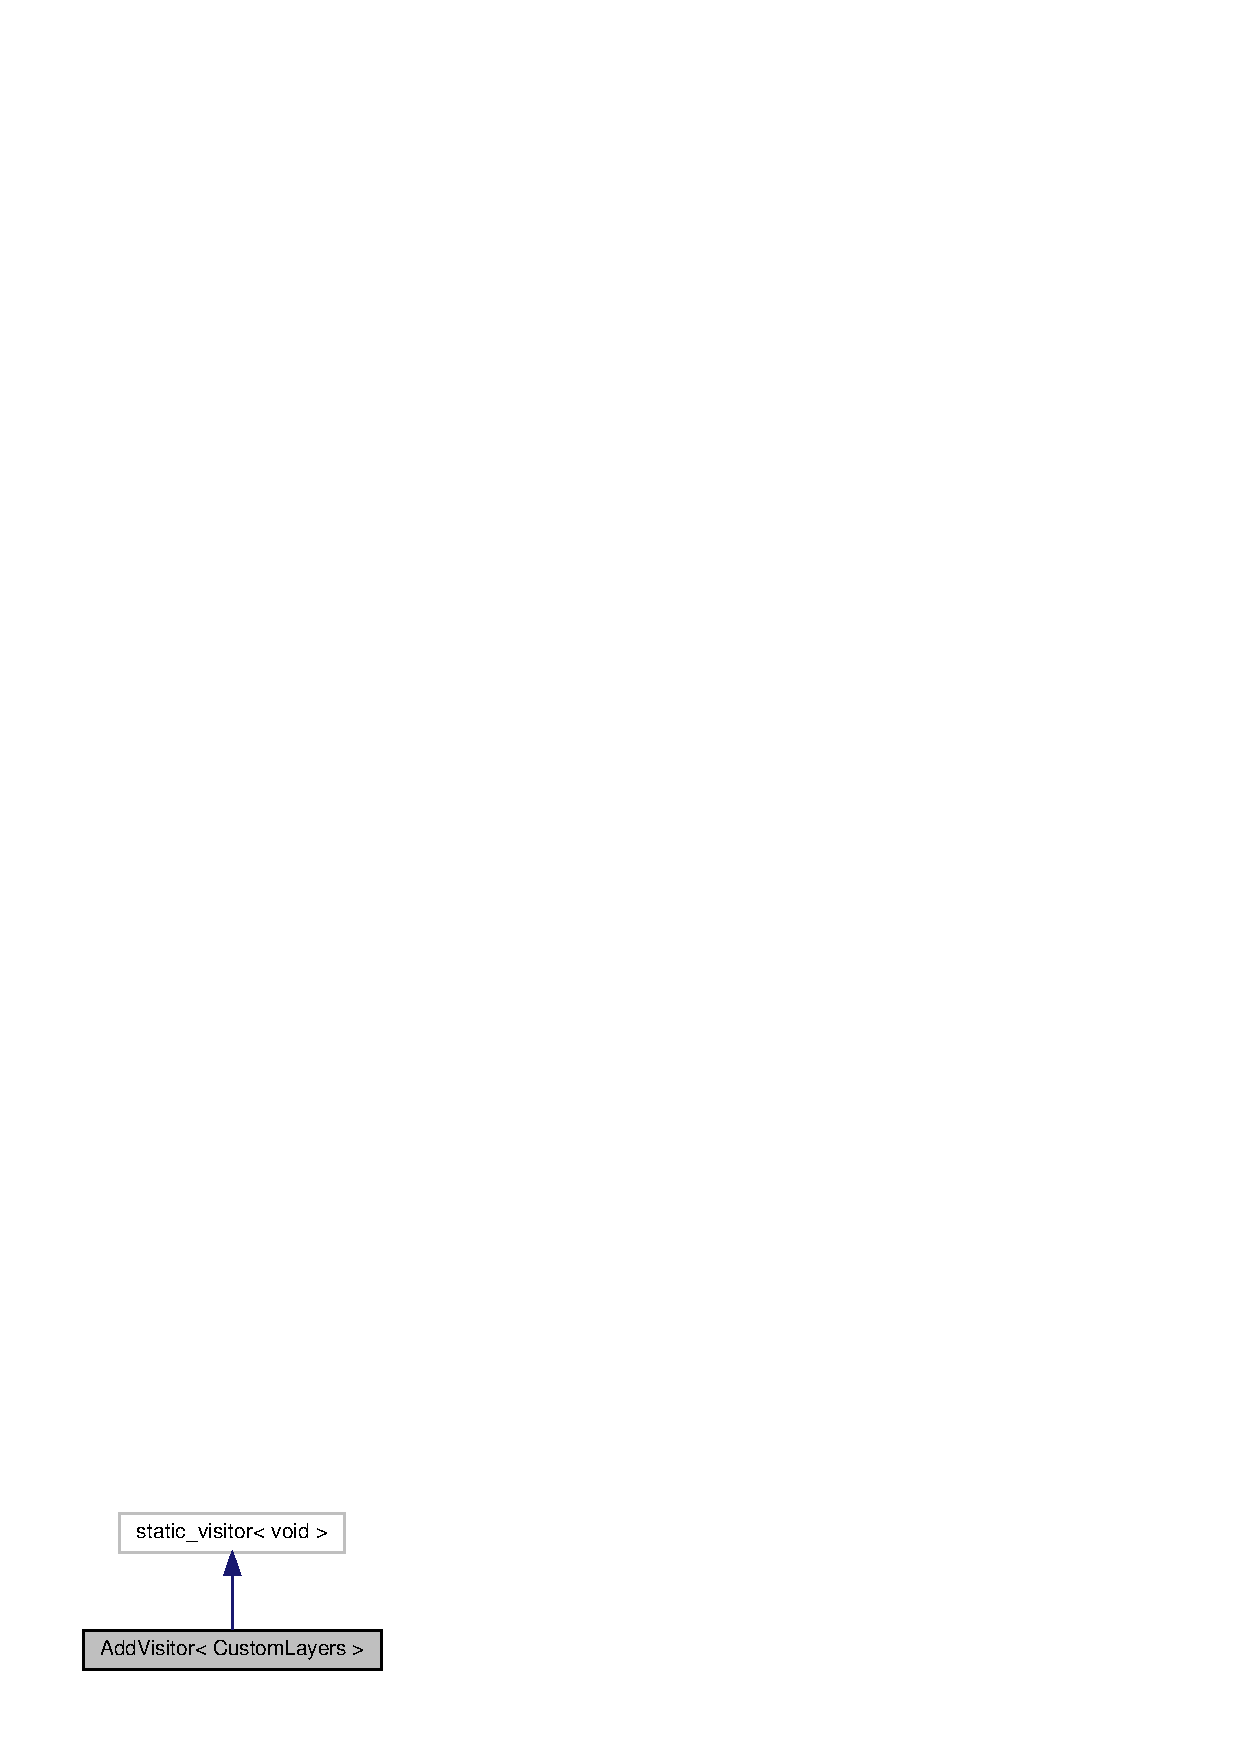
\includegraphics[width=187pt]{classmlpack_1_1ann_1_1AddVisitor__inherit__graph}
\end{center}
\end{figure}
\subsection*{Public Member Functions}
\begin{DoxyCompactItemize}
\item 
{\footnotesize template$<$typename T $>$ }\\\textbf{ Add\+Visitor} (T new\+Layer)
\begin{DoxyCompactList}\small\item\em Exposes the Add() method of the given module. \end{DoxyCompactList}\item 
{\footnotesize template$<$typename Layer\+Type $>$ }\\void \textbf{ operator()} (Layer\+Type $\ast$layer) const
\begin{DoxyCompactList}\small\item\em Exposes the Add() method. \end{DoxyCompactList}\item 
void \textbf{ operator()} (\textbf{ More\+Types} layer) const
\end{DoxyCompactItemize}


\subsection{Detailed Description}
\subsubsection*{template$<$typename... Custom\+Layers$>$\newline
class mlpack\+::ann\+::\+Add\+Visitor$<$ Custom\+Layers $>$}

\doxyref{Add\+Visitor}{p.}{classmlpack_1_1ann_1_1AddVisitor} exposes the Add() method of the given module. 

Definition at line 28 of file add\+\_\+visitor.\+hpp.



\subsection{Constructor \& Destructor Documentation}
\mbox{\label{classmlpack_1_1ann_1_1AddVisitor_aa21362514457024852c33802d57a1b37}} 
\index{mlpack\+::ann\+::\+Add\+Visitor@{mlpack\+::ann\+::\+Add\+Visitor}!Add\+Visitor@{Add\+Visitor}}
\index{Add\+Visitor@{Add\+Visitor}!mlpack\+::ann\+::\+Add\+Visitor@{mlpack\+::ann\+::\+Add\+Visitor}}
\subsubsection{Add\+Visitor()}
{\footnotesize\ttfamily \textbf{ Add\+Visitor} (\begin{DoxyParamCaption}\item[{T}]{new\+Layer }\end{DoxyParamCaption})}



Exposes the Add() method of the given module. 



\subsection{Member Function Documentation}
\mbox{\label{classmlpack_1_1ann_1_1AddVisitor_a26bb3385c630118c35f4799f1509abbc}} 
\index{mlpack\+::ann\+::\+Add\+Visitor@{mlpack\+::ann\+::\+Add\+Visitor}!operator()@{operator()}}
\index{operator()@{operator()}!mlpack\+::ann\+::\+Add\+Visitor@{mlpack\+::ann\+::\+Add\+Visitor}}
\subsubsection{operator()()\hspace{0.1cm}{\footnotesize\ttfamily [1/2]}}
{\footnotesize\ttfamily void operator() (\begin{DoxyParamCaption}\item[{Layer\+Type $\ast$}]{layer }\end{DoxyParamCaption}) const}



Exposes the Add() method. 

\mbox{\label{classmlpack_1_1ann_1_1AddVisitor_ae35578e7ff874a320fe762bc0edfff04}} 
\index{mlpack\+::ann\+::\+Add\+Visitor@{mlpack\+::ann\+::\+Add\+Visitor}!operator()@{operator()}}
\index{operator()@{operator()}!mlpack\+::ann\+::\+Add\+Visitor@{mlpack\+::ann\+::\+Add\+Visitor}}
\subsubsection{operator()()\hspace{0.1cm}{\footnotesize\ttfamily [2/2]}}
{\footnotesize\ttfamily void operator() (\begin{DoxyParamCaption}\item[{\textbf{ More\+Types}}]{layer }\end{DoxyParamCaption}) const}



The documentation for this class was generated from the following file\+:\begin{DoxyCompactItemize}
\item 
/home/aakash/mlpack/src/mlpack/methods/ann/visitor/\textbf{ add\+\_\+visitor.\+hpp}\end{DoxyCompactItemize}

\section{Alpha\+Dropout$<$ Input\+Data\+Type, Output\+Data\+Type $>$ Class Template Reference}
\label{classmlpack_1_1ann_1_1AlphaDropout}\index{Alpha\+Dropout$<$ Input\+Data\+Type, Output\+Data\+Type $>$@{Alpha\+Dropout$<$ Input\+Data\+Type, Output\+Data\+Type $>$}}


The alpha -\/ dropout layer is a regularizer that randomly with probability \textquotesingle{}ratio\textquotesingle{} sets input values to alpha\+Dash.  


\subsection*{Public Member Functions}
\begin{DoxyCompactItemize}
\item 
\textbf{ Alpha\+Dropout} (const double ratio=0.\+5, const double alpha\+Dash=-\/alpha $\ast$lambda)
\begin{DoxyCompactList}\small\item\em Create the Alpha\+\_\+\+Dropout object using the specified ratio. \end{DoxyCompactList}\item 
double \textbf{ A} () const
\begin{DoxyCompactList}\small\item\em Value to be multiplied with x for affine transformation. \end{DoxyCompactList}\item 
double \textbf{ Alpha\+Dash} () const
\begin{DoxyCompactList}\small\item\em Value of alpha\+Dash. \end{DoxyCompactList}\item 
double \textbf{ B} () const
\begin{DoxyCompactList}\small\item\em Value to be added to a$\ast$x for affine transformation. \end{DoxyCompactList}\item 
{\footnotesize template$<$typename eT $>$ }\\void \textbf{ Backward} (const arma\+::\+Mat$<$ eT $>$ \&, const arma\+::\+Mat$<$ eT $>$ \&gy, arma\+::\+Mat$<$ eT $>$ \&g)
\begin{DoxyCompactList}\small\item\em Ordinary feed backward pass of the alpha\+\_\+dropout layer. \end{DoxyCompactList}\item 
Output\+Data\+Type const  \& \textbf{ Delta} () const
\begin{DoxyCompactList}\small\item\em Get the detla. \end{DoxyCompactList}\item 
Output\+Data\+Type \& \textbf{ Delta} ()
\begin{DoxyCompactList}\small\item\em Modify the delta. \end{DoxyCompactList}\item 
bool \textbf{ Deterministic} () const
\begin{DoxyCompactList}\small\item\em The value of the deterministic parameter. \end{DoxyCompactList}\item 
bool \& \textbf{ Deterministic} ()
\begin{DoxyCompactList}\small\item\em Modify the value of the deterministic parameter. \end{DoxyCompactList}\item 
{\footnotesize template$<$typename eT $>$ }\\void \textbf{ Forward} (const arma\+::\+Mat$<$ eT $>$ \&input, arma\+::\+Mat$<$ eT $>$ \&output)
\begin{DoxyCompactList}\small\item\em Ordinary feed forward pass of the alpha\+\_\+dropout layer. \end{DoxyCompactList}\item 
Output\+Data\+Type const  \& \textbf{ Mask} () const
\begin{DoxyCompactList}\small\item\em Get the mask. \end{DoxyCompactList}\item 
Output\+Data\+Type const  \& \textbf{ Output\+Parameter} () const
\begin{DoxyCompactList}\small\item\em Get the output parameter. \end{DoxyCompactList}\item 
Output\+Data\+Type \& \textbf{ Output\+Parameter} ()
\begin{DoxyCompactList}\small\item\em Modify the output parameter. \end{DoxyCompactList}\item 
double \textbf{ Ratio} () const
\begin{DoxyCompactList}\small\item\em The probability of setting a value to alpha\+Dash. \end{DoxyCompactList}\item 
void \textbf{ Ratio} (const double r)
\begin{DoxyCompactList}\small\item\em Modify the probability of setting a value to alpha\+Dash. \end{DoxyCompactList}\item 
{\footnotesize template$<$typename Archive $>$ }\\void \textbf{ serialize} (Archive \&ar, const uint32\+\_\+t)
\begin{DoxyCompactList}\small\item\em Serialize the layer. \end{DoxyCompactList}\end{DoxyCompactItemize}


\subsection{Detailed Description}
\subsubsection*{template$<$typename Input\+Data\+Type = arma\+::mat, typename Output\+Data\+Type = arma\+::mat$>$\newline
class mlpack\+::ann\+::\+Alpha\+Dropout$<$ Input\+Data\+Type, Output\+Data\+Type $>$}

The alpha -\/ dropout layer is a regularizer that randomly with probability \textquotesingle{}ratio\textquotesingle{} sets input values to alpha\+Dash. 

The alpha -\/ dropout layer is mostly used for S\+E\+LU activation function where successive layers don\textquotesingle{}t have same mean and variance.

For more information, see the following.


\begin{DoxyCode}
@article\{Klambauer2017,
  author  = \{Gunter Klambauer and Thomas Unterthiner and
             Andreas Mayr\},
  title   = \{Self-Normalizing Neural Networks\},
  journal = \{Advances in Neural Information Processing Systems\},
  year    = \{2017\},
  url     = \{https:\textcolor{comment}{//arxiv.org/abs/1706.02515\}}
\}
\end{DoxyCode}



\begin{DoxyTemplParams}{Template Parameters}
{\em Input\+Data\+Type} & Type of the input data (arma\+::colvec, arma\+::mat, arma\+::sp\+\_\+mat or arma\+::cube). \\
\hline
{\em Output\+Data\+Type} & Type of the output data (arma\+::colvec, arma\+::mat, arma\+::sp\+\_\+mat or arma\+::cube). \\
\hline
\end{DoxyTemplParams}


Definition at line 50 of file alpha\+\_\+dropout.\+hpp.



\subsection{Constructor \& Destructor Documentation}
\mbox{\label{classmlpack_1_1ann_1_1AlphaDropout_ad6541c5c189746d32b9067d26b9409c5}} 
\index{mlpack\+::ann\+::\+Alpha\+Dropout@{mlpack\+::ann\+::\+Alpha\+Dropout}!Alpha\+Dropout@{Alpha\+Dropout}}
\index{Alpha\+Dropout@{Alpha\+Dropout}!mlpack\+::ann\+::\+Alpha\+Dropout@{mlpack\+::ann\+::\+Alpha\+Dropout}}
\subsubsection{Alpha\+Dropout()}
{\footnotesize\ttfamily \textbf{ Alpha\+Dropout} (\begin{DoxyParamCaption}\item[{const double}]{ratio = {\ttfamily 0.5},  }\item[{const double}]{alpha\+Dash = {\ttfamily -\/alpha~$\ast$lambda} }\end{DoxyParamCaption})}



Create the Alpha\+\_\+\+Dropout object using the specified ratio. 


\begin{DoxyParams}{Parameters}
{\em ratio} & The probability of setting a value to alpha\+Dash. \\
\hline
{\em alpha\+Dash} & The dropout scaling parameter. \\
\hline
\end{DoxyParams}


\subsection{Member Function Documentation}
\mbox{\label{classmlpack_1_1ann_1_1AlphaDropout_aab6c632054fc383ec1edf83231163bf7}} 
\index{mlpack\+::ann\+::\+Alpha\+Dropout@{mlpack\+::ann\+::\+Alpha\+Dropout}!A@{A}}
\index{A@{A}!mlpack\+::ann\+::\+Alpha\+Dropout@{mlpack\+::ann\+::\+Alpha\+Dropout}}
\subsubsection{A()}
{\footnotesize\ttfamily double A (\begin{DoxyParamCaption}{ }\end{DoxyParamCaption}) const\hspace{0.3cm}{\ttfamily [inline]}}



Value to be multiplied with x for affine transformation. 



Definition at line 102 of file alpha\+\_\+dropout.\+hpp.

\mbox{\label{classmlpack_1_1ann_1_1AlphaDropout_a32c95c63853c50d490c6ce28c8032630}} 
\index{mlpack\+::ann\+::\+Alpha\+Dropout@{mlpack\+::ann\+::\+Alpha\+Dropout}!Alpha\+Dash@{Alpha\+Dash}}
\index{Alpha\+Dash@{Alpha\+Dash}!mlpack\+::ann\+::\+Alpha\+Dropout@{mlpack\+::ann\+::\+Alpha\+Dropout}}
\subsubsection{Alpha\+Dash()}
{\footnotesize\ttfamily double Alpha\+Dash (\begin{DoxyParamCaption}{ }\end{DoxyParamCaption}) const\hspace{0.3cm}{\ttfamily [inline]}}



Value of alpha\+Dash. 



Definition at line 108 of file alpha\+\_\+dropout.\+hpp.

\mbox{\label{classmlpack_1_1ann_1_1AlphaDropout_ab6ee6f0f970c90d4a148a64c074f09f5}} 
\index{mlpack\+::ann\+::\+Alpha\+Dropout@{mlpack\+::ann\+::\+Alpha\+Dropout}!B@{B}}
\index{B@{B}!mlpack\+::ann\+::\+Alpha\+Dropout@{mlpack\+::ann\+::\+Alpha\+Dropout}}
\subsubsection{B()}
{\footnotesize\ttfamily double B (\begin{DoxyParamCaption}{ }\end{DoxyParamCaption}) const\hspace{0.3cm}{\ttfamily [inline]}}



Value to be added to a$\ast$x for affine transformation. 



Definition at line 105 of file alpha\+\_\+dropout.\+hpp.

\mbox{\label{classmlpack_1_1ann_1_1AlphaDropout_ad9ad1a3bdb0f3fff5c839ed155e4bbf8}} 
\index{mlpack\+::ann\+::\+Alpha\+Dropout@{mlpack\+::ann\+::\+Alpha\+Dropout}!Backward@{Backward}}
\index{Backward@{Backward}!mlpack\+::ann\+::\+Alpha\+Dropout@{mlpack\+::ann\+::\+Alpha\+Dropout}}
\subsubsection{Backward()}
{\footnotesize\ttfamily void Backward (\begin{DoxyParamCaption}\item[{const arma\+::\+Mat$<$ eT $>$ \&}]{,  }\item[{const arma\+::\+Mat$<$ eT $>$ \&}]{gy,  }\item[{arma\+::\+Mat$<$ eT $>$ \&}]{g }\end{DoxyParamCaption})}



Ordinary feed backward pass of the alpha\+\_\+dropout layer. 


\begin{DoxyParams}{Parameters}
{\em $\ast$} & (input) The propagated input activation. \\
\hline
{\em gy} & The backpropagated error. \\
\hline
{\em g} & The calculated gradient. \\
\hline
\end{DoxyParams}
\mbox{\label{classmlpack_1_1ann_1_1AlphaDropout_a797f7edb44dd081e5e2b3cc316eef6bd}} 
\index{mlpack\+::ann\+::\+Alpha\+Dropout@{mlpack\+::ann\+::\+Alpha\+Dropout}!Delta@{Delta}}
\index{Delta@{Delta}!mlpack\+::ann\+::\+Alpha\+Dropout@{mlpack\+::ann\+::\+Alpha\+Dropout}}
\subsubsection{Delta()\hspace{0.1cm}{\footnotesize\ttfamily [1/2]}}
{\footnotesize\ttfamily Output\+Data\+Type const\& Delta (\begin{DoxyParamCaption}{ }\end{DoxyParamCaption}) const\hspace{0.3cm}{\ttfamily [inline]}}



Get the detla. 



Definition at line 89 of file alpha\+\_\+dropout.\+hpp.

\mbox{\label{classmlpack_1_1ann_1_1AlphaDropout_ad6601342d560219ce951d554e69e5e87}} 
\index{mlpack\+::ann\+::\+Alpha\+Dropout@{mlpack\+::ann\+::\+Alpha\+Dropout}!Delta@{Delta}}
\index{Delta@{Delta}!mlpack\+::ann\+::\+Alpha\+Dropout@{mlpack\+::ann\+::\+Alpha\+Dropout}}
\subsubsection{Delta()\hspace{0.1cm}{\footnotesize\ttfamily [2/2]}}
{\footnotesize\ttfamily Output\+Data\+Type\& Delta (\begin{DoxyParamCaption}{ }\end{DoxyParamCaption})\hspace{0.3cm}{\ttfamily [inline]}}



Modify the delta. 



Definition at line 91 of file alpha\+\_\+dropout.\+hpp.

\mbox{\label{classmlpack_1_1ann_1_1AlphaDropout_a9f4103707f4d199ce5594d239b60443e}} 
\index{mlpack\+::ann\+::\+Alpha\+Dropout@{mlpack\+::ann\+::\+Alpha\+Dropout}!Deterministic@{Deterministic}}
\index{Deterministic@{Deterministic}!mlpack\+::ann\+::\+Alpha\+Dropout@{mlpack\+::ann\+::\+Alpha\+Dropout}}
\subsubsection{Deterministic()\hspace{0.1cm}{\footnotesize\ttfamily [1/2]}}
{\footnotesize\ttfamily bool Deterministic (\begin{DoxyParamCaption}{ }\end{DoxyParamCaption}) const\hspace{0.3cm}{\ttfamily [inline]}}



The value of the deterministic parameter. 



Definition at line 94 of file alpha\+\_\+dropout.\+hpp.

\mbox{\label{classmlpack_1_1ann_1_1AlphaDropout_a42d4ee3da432cff20d3a41b8b1ec801c}} 
\index{mlpack\+::ann\+::\+Alpha\+Dropout@{mlpack\+::ann\+::\+Alpha\+Dropout}!Deterministic@{Deterministic}}
\index{Deterministic@{Deterministic}!mlpack\+::ann\+::\+Alpha\+Dropout@{mlpack\+::ann\+::\+Alpha\+Dropout}}
\subsubsection{Deterministic()\hspace{0.1cm}{\footnotesize\ttfamily [2/2]}}
{\footnotesize\ttfamily bool\& Deterministic (\begin{DoxyParamCaption}{ }\end{DoxyParamCaption})\hspace{0.3cm}{\ttfamily [inline]}}



Modify the value of the deterministic parameter. 



Definition at line 96 of file alpha\+\_\+dropout.\+hpp.

\mbox{\label{classmlpack_1_1ann_1_1AlphaDropout_a461f849bc638c15bec262dc9c3a58abe}} 
\index{mlpack\+::ann\+::\+Alpha\+Dropout@{mlpack\+::ann\+::\+Alpha\+Dropout}!Forward@{Forward}}
\index{Forward@{Forward}!mlpack\+::ann\+::\+Alpha\+Dropout@{mlpack\+::ann\+::\+Alpha\+Dropout}}
\subsubsection{Forward()}
{\footnotesize\ttfamily void Forward (\begin{DoxyParamCaption}\item[{const arma\+::\+Mat$<$ eT $>$ \&}]{input,  }\item[{arma\+::\+Mat$<$ eT $>$ \&}]{output }\end{DoxyParamCaption})}



Ordinary feed forward pass of the alpha\+\_\+dropout layer. 


\begin{DoxyParams}{Parameters}
{\em input} & Input data used for evaluating the specified function. \\
\hline
{\em output} & Resulting output activation. \\
\hline
\end{DoxyParams}
\mbox{\label{classmlpack_1_1ann_1_1AlphaDropout_a6503ae5d92f15edf34212579382fca27}} 
\index{mlpack\+::ann\+::\+Alpha\+Dropout@{mlpack\+::ann\+::\+Alpha\+Dropout}!Mask@{Mask}}
\index{Mask@{Mask}!mlpack\+::ann\+::\+Alpha\+Dropout@{mlpack\+::ann\+::\+Alpha\+Dropout}}
\subsubsection{Mask()}
{\footnotesize\ttfamily Output\+Data\+Type const\& Mask (\begin{DoxyParamCaption}{ }\end{DoxyParamCaption}) const\hspace{0.3cm}{\ttfamily [inline]}}



Get the mask. 



Definition at line 111 of file alpha\+\_\+dropout.\+hpp.

\mbox{\label{classmlpack_1_1ann_1_1AlphaDropout_a0ee21c2a36e5abad1e7a9d5dd00849f9}} 
\index{mlpack\+::ann\+::\+Alpha\+Dropout@{mlpack\+::ann\+::\+Alpha\+Dropout}!Output\+Parameter@{Output\+Parameter}}
\index{Output\+Parameter@{Output\+Parameter}!mlpack\+::ann\+::\+Alpha\+Dropout@{mlpack\+::ann\+::\+Alpha\+Dropout}}
\subsubsection{Output\+Parameter()\hspace{0.1cm}{\footnotesize\ttfamily [1/2]}}
{\footnotesize\ttfamily Output\+Data\+Type const\& Output\+Parameter (\begin{DoxyParamCaption}{ }\end{DoxyParamCaption}) const\hspace{0.3cm}{\ttfamily [inline]}}



Get the output parameter. 



Definition at line 84 of file alpha\+\_\+dropout.\+hpp.

\mbox{\label{classmlpack_1_1ann_1_1AlphaDropout_a21d5f745f02c709625a4ee0907f004a5}} 
\index{mlpack\+::ann\+::\+Alpha\+Dropout@{mlpack\+::ann\+::\+Alpha\+Dropout}!Output\+Parameter@{Output\+Parameter}}
\index{Output\+Parameter@{Output\+Parameter}!mlpack\+::ann\+::\+Alpha\+Dropout@{mlpack\+::ann\+::\+Alpha\+Dropout}}
\subsubsection{Output\+Parameter()\hspace{0.1cm}{\footnotesize\ttfamily [2/2]}}
{\footnotesize\ttfamily Output\+Data\+Type\& Output\+Parameter (\begin{DoxyParamCaption}{ }\end{DoxyParamCaption})\hspace{0.3cm}{\ttfamily [inline]}}



Modify the output parameter. 



Definition at line 86 of file alpha\+\_\+dropout.\+hpp.

\mbox{\label{classmlpack_1_1ann_1_1AlphaDropout_a0052f2d1427761ea25fb01a05d966a40}} 
\index{mlpack\+::ann\+::\+Alpha\+Dropout@{mlpack\+::ann\+::\+Alpha\+Dropout}!Ratio@{Ratio}}
\index{Ratio@{Ratio}!mlpack\+::ann\+::\+Alpha\+Dropout@{mlpack\+::ann\+::\+Alpha\+Dropout}}
\subsubsection{Ratio()\hspace{0.1cm}{\footnotesize\ttfamily [1/2]}}
{\footnotesize\ttfamily double Ratio (\begin{DoxyParamCaption}{ }\end{DoxyParamCaption}) const\hspace{0.3cm}{\ttfamily [inline]}}



The probability of setting a value to alpha\+Dash. 



Definition at line 99 of file alpha\+\_\+dropout.\+hpp.

\mbox{\label{classmlpack_1_1ann_1_1AlphaDropout_a9ca65c8f62aa7b45b5b08899d83d2821}} 
\index{mlpack\+::ann\+::\+Alpha\+Dropout@{mlpack\+::ann\+::\+Alpha\+Dropout}!Ratio@{Ratio}}
\index{Ratio@{Ratio}!mlpack\+::ann\+::\+Alpha\+Dropout@{mlpack\+::ann\+::\+Alpha\+Dropout}}
\subsubsection{Ratio()\hspace{0.1cm}{\footnotesize\ttfamily [2/2]}}
{\footnotesize\ttfamily void Ratio (\begin{DoxyParamCaption}\item[{const double}]{r }\end{DoxyParamCaption})\hspace{0.3cm}{\ttfamily [inline]}}



Modify the probability of setting a value to alpha\+Dash. 

As \textquotesingle{}a\textquotesingle{} and \textquotesingle{}b\textquotesingle{} depend on \textquotesingle{}ratio\textquotesingle{}, modify them as well. 

Definition at line 115 of file alpha\+\_\+dropout.\+hpp.



References Alpha\+Dropout$<$ Input\+Data\+Type, Output\+Data\+Type $>$\+::serialize().

\mbox{\label{classmlpack_1_1ann_1_1AlphaDropout_a65cba07328997659bec80b9879b15a51}} 
\index{mlpack\+::ann\+::\+Alpha\+Dropout@{mlpack\+::ann\+::\+Alpha\+Dropout}!serialize@{serialize}}
\index{serialize@{serialize}!mlpack\+::ann\+::\+Alpha\+Dropout@{mlpack\+::ann\+::\+Alpha\+Dropout}}
\subsubsection{serialize()}
{\footnotesize\ttfamily void serialize (\begin{DoxyParamCaption}\item[{Archive \&}]{ar,  }\item[{const uint32\+\_\+t}]{ }\end{DoxyParamCaption})}



Serialize the layer. 



Referenced by Alpha\+Dropout$<$ Input\+Data\+Type, Output\+Data\+Type $>$\+::\+Ratio().



The documentation for this class was generated from the following file\+:\begin{DoxyCompactItemize}
\item 
/home/aakash/mlpack/src/mlpack/methods/ann/layer/\textbf{ alpha\+\_\+dropout.\+hpp}\end{DoxyCompactItemize}

\section{Atrous\+Convolution$<$ Forward\+Convolution\+Rule, Backward\+Convolution\+Rule, Gradient\+Convolution\+Rule, Input\+Data\+Type, Output\+Data\+Type $>$ Class Template Reference}
\label{classmlpack_1_1ann_1_1AtrousConvolution}\index{Atrous\+Convolution$<$ Forward\+Convolution\+Rule, Backward\+Convolution\+Rule, Gradient\+Convolution\+Rule, Input\+Data\+Type, Output\+Data\+Type $>$@{Atrous\+Convolution$<$ Forward\+Convolution\+Rule, Backward\+Convolution\+Rule, Gradient\+Convolution\+Rule, Input\+Data\+Type, Output\+Data\+Type $>$}}


Implementation of the Atrous \doxyref{Convolution}{p.}{classmlpack_1_1ann_1_1Convolution} class.  


\subsection*{Public Member Functions}
\begin{DoxyCompactItemize}
\item 
\textbf{ Atrous\+Convolution} ()
\begin{DoxyCompactList}\small\item\em Create the \doxyref{Atrous\+Convolution}{p.}{classmlpack_1_1ann_1_1AtrousConvolution} object. \end{DoxyCompactList}\item 
\textbf{ Atrous\+Convolution} (const size\+\_\+t in\+Size, const size\+\_\+t out\+Size, const size\+\_\+t kernel\+Width, const size\+\_\+t kernel\+Height, const size\+\_\+t stride\+Width=1, const size\+\_\+t stride\+Height=1, const size\+\_\+t padW=0, const size\+\_\+t padH=0, const size\+\_\+t input\+Width=0, const size\+\_\+t input\+Height=0, const size\+\_\+t dilation\+Width=1, const size\+\_\+t dilation\+Height=1, const std\+::string \&padding\+Type=\char`\"{}None\char`\"{})
\begin{DoxyCompactList}\small\item\em Create the \doxyref{Atrous\+Convolution}{p.}{classmlpack_1_1ann_1_1AtrousConvolution} object using the specified number of input maps, output maps, filter size, stride, dilation and padding parameter. \end{DoxyCompactList}\item 
\textbf{ Atrous\+Convolution} (const size\+\_\+t in\+Size, const size\+\_\+t out\+Size, const size\+\_\+t kernel\+Width, const size\+\_\+t kernel\+Height, const size\+\_\+t stride\+Width, const size\+\_\+t stride\+Height, const std\+::tuple$<$ size\+\_\+t, size\+\_\+t $>$ \&padW, const std\+::tuple$<$ size\+\_\+t, size\+\_\+t $>$ \&padH, const size\+\_\+t input\+Width=0, const size\+\_\+t input\+Height=0, const size\+\_\+t dilation\+Width=1, const size\+\_\+t dilation\+Height=1, const std\+::string \&padding\+Type=\char`\"{}None\char`\"{})
\begin{DoxyCompactList}\small\item\em Create the \doxyref{Atrous\+Convolution}{p.}{classmlpack_1_1ann_1_1AtrousConvolution} object using the specified number of input maps, output maps, filter size, stride, dilation and padding parameter. \end{DoxyCompactList}\item 
{\footnotesize template$<$typename eT $>$ }\\void \textbf{ Backward} (const arma\+::\+Mat$<$ eT $>$ \&, const arma\+::\+Mat$<$ eT $>$ \&gy, arma\+::\+Mat$<$ eT $>$ \&g)
\begin{DoxyCompactList}\small\item\em Ordinary feed backward pass of a neural network, calculating the function f(x) by propagating x backwards through f. \end{DoxyCompactList}\item 
arma\+::mat const  \& \textbf{ Bias} () const
\begin{DoxyCompactList}\small\item\em Get the bias of the layer. \end{DoxyCompactList}\item 
arma\+::mat \& \textbf{ Bias} ()
\begin{DoxyCompactList}\small\item\em Modify the bias of the layer. \end{DoxyCompactList}\item 
Output\+Data\+Type const  \& \textbf{ Delta} () const
\begin{DoxyCompactList}\small\item\em Get the delta. \end{DoxyCompactList}\item 
Output\+Data\+Type \& \textbf{ Delta} ()
\begin{DoxyCompactList}\small\item\em Modify the delta. \end{DoxyCompactList}\item 
size\+\_\+t \textbf{ Dilation\+Height} () const
\begin{DoxyCompactList}\small\item\em Get the dilation rate on the Y axis. \end{DoxyCompactList}\item 
size\+\_\+t \& \textbf{ Dilation\+Height} ()
\begin{DoxyCompactList}\small\item\em Modify the dilation rate on the Y axis. \end{DoxyCompactList}\item 
size\+\_\+t \textbf{ Dilation\+Width} () const
\begin{DoxyCompactList}\small\item\em Get the dilation rate on the X axis. \end{DoxyCompactList}\item 
size\+\_\+t \& \textbf{ Dilation\+Width} ()
\begin{DoxyCompactList}\small\item\em Modify the dilation rate on the X axis. \end{DoxyCompactList}\item 
{\footnotesize template$<$typename eT $>$ }\\void \textbf{ Forward} (const arma\+::\+Mat$<$ eT $>$ \&input, arma\+::\+Mat$<$ eT $>$ \&output)
\begin{DoxyCompactList}\small\item\em Ordinary feed forward pass of a neural network, evaluating the function f(x) by propagating the activity forward through f. \end{DoxyCompactList}\item 
{\footnotesize template$<$typename eT $>$ }\\void \textbf{ Gradient} (const arma\+::\+Mat$<$ eT $>$ \&, const arma\+::\+Mat$<$ eT $>$ \&error, arma\+::\+Mat$<$ eT $>$ \&gradient)
\item 
Output\+Data\+Type const  \& \textbf{ Gradient} () const
\begin{DoxyCompactList}\small\item\em Get the gradient. \end{DoxyCompactList}\item 
Output\+Data\+Type \& \textbf{ Gradient} ()
\begin{DoxyCompactList}\small\item\em Modify the gradient. \end{DoxyCompactList}\item 
size\+\_\+t \textbf{ Input\+Height} () const
\begin{DoxyCompactList}\small\item\em Get the input height. \end{DoxyCompactList}\item 
size\+\_\+t \& \textbf{ Input\+Height} ()
\begin{DoxyCompactList}\small\item\em Modify the input height. \end{DoxyCompactList}\item 
size\+\_\+t \textbf{ Input\+Shape} () const
\begin{DoxyCompactList}\small\item\em Get the shape of the input. \end{DoxyCompactList}\item 
size\+\_\+t \textbf{ Input\+Size} () const
\begin{DoxyCompactList}\small\item\em Get the input size. \end{DoxyCompactList}\item 
size\+\_\+t \textbf{ Input\+Width} () const
\begin{DoxyCompactList}\small\item\em Get the input width. \end{DoxyCompactList}\item 
size\+\_\+t \& \textbf{ Input\+Width} ()
\begin{DoxyCompactList}\small\item\em Modify input the width. \end{DoxyCompactList}\item 
size\+\_\+t \textbf{ Kernel\+Height} () const
\begin{DoxyCompactList}\small\item\em Get the kernel height. \end{DoxyCompactList}\item 
size\+\_\+t \& \textbf{ Kernel\+Height} ()
\begin{DoxyCompactList}\small\item\em Modify the kernel height. \end{DoxyCompactList}\item 
size\+\_\+t \textbf{ Kernel\+Width} () const
\begin{DoxyCompactList}\small\item\em Get the kernel width. \end{DoxyCompactList}\item 
size\+\_\+t \& \textbf{ Kernel\+Width} ()
\begin{DoxyCompactList}\small\item\em Modify the kernel width. \end{DoxyCompactList}\item 
size\+\_\+t \textbf{ Output\+Height} () const
\begin{DoxyCompactList}\small\item\em Get the output height. \end{DoxyCompactList}\item 
size\+\_\+t \& \textbf{ Output\+Height} ()
\begin{DoxyCompactList}\small\item\em Modify the output height. \end{DoxyCompactList}\item 
Output\+Data\+Type const  \& \textbf{ Output\+Parameter} () const
\begin{DoxyCompactList}\small\item\em Get the output parameter. \end{DoxyCompactList}\item 
Output\+Data\+Type \& \textbf{ Output\+Parameter} ()
\begin{DoxyCompactList}\small\item\em Modify the output parameter. \end{DoxyCompactList}\item 
size\+\_\+t \textbf{ Output\+Size} () const
\begin{DoxyCompactList}\small\item\em Get the output size. \end{DoxyCompactList}\item 
size\+\_\+t \textbf{ Output\+Width} () const
\begin{DoxyCompactList}\small\item\em Get the output width. \end{DoxyCompactList}\item 
size\+\_\+t \& \textbf{ Output\+Width} ()
\begin{DoxyCompactList}\small\item\em Modify the output width. \end{DoxyCompactList}\item 
\textbf{ ann\+::\+Padding} const  \& \textbf{ Padding} () const
\begin{DoxyCompactList}\small\item\em Get the internal \doxyref{Padding}{p.}{classmlpack_1_1ann_1_1Padding} layer. \end{DoxyCompactList}\item 
\textbf{ ann\+::\+Padding} \& \textbf{ Padding} ()
\begin{DoxyCompactList}\small\item\em Modify the internal \doxyref{Padding}{p.}{classmlpack_1_1ann_1_1Padding} layer. \end{DoxyCompactList}\item 
Output\+Data\+Type const  \& \textbf{ Parameters} () const
\begin{DoxyCompactList}\small\item\em Get the parameters. \end{DoxyCompactList}\item 
Output\+Data\+Type \& \textbf{ Parameters} ()
\begin{DoxyCompactList}\small\item\em Modify the parameters. \end{DoxyCompactList}\item 
void \textbf{ Reset} ()
\item 
{\footnotesize template$<$typename Archive $>$ }\\void \textbf{ serialize} (Archive \&ar, const uint32\+\_\+t)
\begin{DoxyCompactList}\small\item\em Serialize the layer. \end{DoxyCompactList}\item 
size\+\_\+t \textbf{ Stride\+Height} () const
\begin{DoxyCompactList}\small\item\em Get the stride height. \end{DoxyCompactList}\item 
size\+\_\+t \& \textbf{ Stride\+Height} ()
\begin{DoxyCompactList}\small\item\em Modify the stride height. \end{DoxyCompactList}\item 
size\+\_\+t \textbf{ Stride\+Width} () const
\begin{DoxyCompactList}\small\item\em Get the stride width. \end{DoxyCompactList}\item 
size\+\_\+t \& \textbf{ Stride\+Width} ()
\begin{DoxyCompactList}\small\item\em Modify the stride width. \end{DoxyCompactList}\item 
arma\+::cube const  \& \textbf{ Weight} () const
\begin{DoxyCompactList}\small\item\em Get the weight of the layer. \end{DoxyCompactList}\item 
arma\+::cube \& \textbf{ Weight} ()
\begin{DoxyCompactList}\small\item\em Modify the weight of the layer. \end{DoxyCompactList}\item 
size\+\_\+t \textbf{ Weight\+Size} () const
\begin{DoxyCompactList}\small\item\em Get size of the weight matrix. \end{DoxyCompactList}\end{DoxyCompactItemize}


\subsection{Detailed Description}
\subsubsection*{template$<$typename Forward\+Convolution\+Rule = Naive\+Convolution$<$\+Valid\+Convolution$>$, typename Backward\+Convolution\+Rule = Naive\+Convolution$<$\+Full\+Convolution$>$, typename Gradient\+Convolution\+Rule = Naive\+Convolution$<$\+Valid\+Convolution$>$, typename Input\+Data\+Type = arma\+::mat, typename Output\+Data\+Type = arma\+::mat$>$\newline
class mlpack\+::ann\+::\+Atrous\+Convolution$<$ Forward\+Convolution\+Rule, Backward\+Convolution\+Rule, Gradient\+Convolution\+Rule, Input\+Data\+Type, Output\+Data\+Type $>$}

Implementation of the Atrous \doxyref{Convolution}{p.}{classmlpack_1_1ann_1_1Convolution} class. 

The Atrous \doxyref{Convolution}{p.}{classmlpack_1_1ann_1_1Convolution} class represents a single layer of a neural network. Atrous (or Dilated) Convolutions are just simple convolutions applied to input with the defined, spaces included between the kernel cells, in order to capture a larger field of reception, without having to increase dicrete kernel sizes.


\begin{DoxyTemplParams}{Template Parameters}
{\em Forward\+Convolution\+Rule} & Atrous \doxyref{Convolution}{p.}{classmlpack_1_1ann_1_1Convolution} to perform forward process. \\
\hline
{\em Backward\+Convolution\+Rule} & Atrous \doxyref{Convolution}{p.}{classmlpack_1_1ann_1_1Convolution} to perform backward process. \\
\hline
{\em Gradient\+Convolution\+Rule} & Atrous \doxyref{Convolution}{p.}{classmlpack_1_1ann_1_1Convolution} to calculate gradient. \\
\hline
{\em Input\+Data\+Type} & Type of the input data (arma\+::colvec, arma\+::mat, arma\+::sp\+\_\+mat or arma\+::cube). \\
\hline
{\em Output\+Data\+Type} & Type of the output data (arma\+::colvec, arma\+::mat, arma\+::sp\+\_\+mat or arma\+::cube). \\
\hline
\end{DoxyTemplParams}


Definition at line 52 of file atrous\+\_\+convolution.\+hpp.



\subsection{Constructor \& Destructor Documentation}
\mbox{\label{classmlpack_1_1ann_1_1AtrousConvolution_a9247f99daec1f7f369f496fecd2cc437}} 
\index{mlpack\+::ann\+::\+Atrous\+Convolution@{mlpack\+::ann\+::\+Atrous\+Convolution}!Atrous\+Convolution@{Atrous\+Convolution}}
\index{Atrous\+Convolution@{Atrous\+Convolution}!mlpack\+::ann\+::\+Atrous\+Convolution@{mlpack\+::ann\+::\+Atrous\+Convolution}}
\subsubsection{Atrous\+Convolution()\hspace{0.1cm}{\footnotesize\ttfamily [1/3]}}
{\footnotesize\ttfamily \textbf{ Atrous\+Convolution} (\begin{DoxyParamCaption}{ }\end{DoxyParamCaption})}



Create the \doxyref{Atrous\+Convolution}{p.}{classmlpack_1_1ann_1_1AtrousConvolution} object. 

\mbox{\label{classmlpack_1_1ann_1_1AtrousConvolution_ad58290e3e8d698afe28d6c870fd46173}} 
\index{mlpack\+::ann\+::\+Atrous\+Convolution@{mlpack\+::ann\+::\+Atrous\+Convolution}!Atrous\+Convolution@{Atrous\+Convolution}}
\index{Atrous\+Convolution@{Atrous\+Convolution}!mlpack\+::ann\+::\+Atrous\+Convolution@{mlpack\+::ann\+::\+Atrous\+Convolution}}
\subsubsection{Atrous\+Convolution()\hspace{0.1cm}{\footnotesize\ttfamily [2/3]}}
{\footnotesize\ttfamily \textbf{ Atrous\+Convolution} (\begin{DoxyParamCaption}\item[{const size\+\_\+t}]{in\+Size,  }\item[{const size\+\_\+t}]{out\+Size,  }\item[{const size\+\_\+t}]{kernel\+Width,  }\item[{const size\+\_\+t}]{kernel\+Height,  }\item[{const size\+\_\+t}]{stride\+Width = {\ttfamily 1},  }\item[{const size\+\_\+t}]{stride\+Height = {\ttfamily 1},  }\item[{const size\+\_\+t}]{padW = {\ttfamily 0},  }\item[{const size\+\_\+t}]{padH = {\ttfamily 0},  }\item[{const size\+\_\+t}]{input\+Width = {\ttfamily 0},  }\item[{const size\+\_\+t}]{input\+Height = {\ttfamily 0},  }\item[{const size\+\_\+t}]{dilation\+Width = {\ttfamily 1},  }\item[{const size\+\_\+t}]{dilation\+Height = {\ttfamily 1},  }\item[{const std\+::string \&}]{padding\+Type = {\ttfamily \char`\"{}None\char`\"{}} }\end{DoxyParamCaption})}



Create the \doxyref{Atrous\+Convolution}{p.}{classmlpack_1_1ann_1_1AtrousConvolution} object using the specified number of input maps, output maps, filter size, stride, dilation and padding parameter. 


\begin{DoxyParams}{Parameters}
{\em in\+Size} & The number of input maps. \\
\hline
{\em out\+Size} & The number of output maps. \\
\hline
{\em kernel\+Width} & Width of the filter/kernel. \\
\hline
{\em kernel\+Height} & Height of the filter/kernel. \\
\hline
{\em stride\+Width} & Stride of filter application in the x direction. \\
\hline
{\em stride\+Height} & Stride of filter application in the y direction. \\
\hline
{\em padW} & \doxyref{Padding}{p.}{classmlpack_1_1ann_1_1Padding} width of the input. \\
\hline
{\em padH} & \doxyref{Padding}{p.}{classmlpack_1_1ann_1_1Padding} height of the input. \\
\hline
{\em input\+Width} & The widht of the input data. \\
\hline
{\em input\+Height} & The height of the input data. \\
\hline
{\em dilation\+Width} & The space between the cells of filters in x direction. \\
\hline
{\em dilation\+Height} & The space between the cells of filters in y direction. \\
\hline
{\em padding\+Type} & The type of padding (Valid or Same). Defaults to None. \\
\hline
\end{DoxyParams}
\mbox{\label{classmlpack_1_1ann_1_1AtrousConvolution_a265e06161bf7b6bbdea46312164dbe3f}} 
\index{mlpack\+::ann\+::\+Atrous\+Convolution@{mlpack\+::ann\+::\+Atrous\+Convolution}!Atrous\+Convolution@{Atrous\+Convolution}}
\index{Atrous\+Convolution@{Atrous\+Convolution}!mlpack\+::ann\+::\+Atrous\+Convolution@{mlpack\+::ann\+::\+Atrous\+Convolution}}
\subsubsection{Atrous\+Convolution()\hspace{0.1cm}{\footnotesize\ttfamily [3/3]}}
{\footnotesize\ttfamily \textbf{ Atrous\+Convolution} (\begin{DoxyParamCaption}\item[{const size\+\_\+t}]{in\+Size,  }\item[{const size\+\_\+t}]{out\+Size,  }\item[{const size\+\_\+t}]{kernel\+Width,  }\item[{const size\+\_\+t}]{kernel\+Height,  }\item[{const size\+\_\+t}]{stride\+Width,  }\item[{const size\+\_\+t}]{stride\+Height,  }\item[{const std\+::tuple$<$ size\+\_\+t, size\+\_\+t $>$ \&}]{padW,  }\item[{const std\+::tuple$<$ size\+\_\+t, size\+\_\+t $>$ \&}]{padH,  }\item[{const size\+\_\+t}]{input\+Width = {\ttfamily 0},  }\item[{const size\+\_\+t}]{input\+Height = {\ttfamily 0},  }\item[{const size\+\_\+t}]{dilation\+Width = {\ttfamily 1},  }\item[{const size\+\_\+t}]{dilation\+Height = {\ttfamily 1},  }\item[{const std\+::string \&}]{padding\+Type = {\ttfamily \char`\"{}None\char`\"{}} }\end{DoxyParamCaption})}



Create the \doxyref{Atrous\+Convolution}{p.}{classmlpack_1_1ann_1_1AtrousConvolution} object using the specified number of input maps, output maps, filter size, stride, dilation and padding parameter. 


\begin{DoxyParams}{Parameters}
{\em in\+Size} & The number of input maps. \\
\hline
{\em out\+Size} & The number of output maps. \\
\hline
{\em kernel\+Width} & Width of the filter/kernel. \\
\hline
{\em kernel\+Height} & Height of the filter/kernel. \\
\hline
{\em stride\+Width} & Stride of filter application in the x direction. \\
\hline
{\em stride\+Height} & Stride of filter application in the y direction. \\
\hline
{\em padW} & A two-\/value tuple indicating padding widths of the input. First value is padding at left side. Second value is padding on right side. \\
\hline
{\em padH} & A two-\/value tuple indicating padding heights of the input. First value is padding at top. Second value is padding on bottom. \\
\hline
{\em input\+Width} & The widht of the input data. \\
\hline
{\em input\+Height} & The height of the input data. \\
\hline
{\em dilation\+Width} & The space between the cells of filters in x direction. \\
\hline
{\em dilation\+Height} & The space between the cells of filters in y direction. \\
\hline
{\em padding\+Type} & The type of padding (Valid/\+Same/\+None). Defaults to None. \\
\hline
\end{DoxyParams}


\subsection{Member Function Documentation}
\mbox{\label{classmlpack_1_1ann_1_1AtrousConvolution_ad9ad1a3bdb0f3fff5c839ed155e4bbf8}} 
\index{mlpack\+::ann\+::\+Atrous\+Convolution@{mlpack\+::ann\+::\+Atrous\+Convolution}!Backward@{Backward}}
\index{Backward@{Backward}!mlpack\+::ann\+::\+Atrous\+Convolution@{mlpack\+::ann\+::\+Atrous\+Convolution}}
\subsubsection{Backward()}
{\footnotesize\ttfamily void Backward (\begin{DoxyParamCaption}\item[{const arma\+::\+Mat$<$ eT $>$ \&}]{,  }\item[{const arma\+::\+Mat$<$ eT $>$ \&}]{gy,  }\item[{arma\+::\+Mat$<$ eT $>$ \&}]{g }\end{DoxyParamCaption})}



Ordinary feed backward pass of a neural network, calculating the function f(x) by propagating x backwards through f. 

Using the results from the feed forward pass.


\begin{DoxyParams}{Parameters}
{\em $\ast$} & (input) The propagated input activation. \\
\hline
{\em gy} & The backpropagated error. \\
\hline
{\em g} & The calculated gradient. \\
\hline
\end{DoxyParams}
\mbox{\label{classmlpack_1_1ann_1_1AtrousConvolution_ab94cce6a9d6baed0badd20f4a409e9af}} 
\index{mlpack\+::ann\+::\+Atrous\+Convolution@{mlpack\+::ann\+::\+Atrous\+Convolution}!Bias@{Bias}}
\index{Bias@{Bias}!mlpack\+::ann\+::\+Atrous\+Convolution@{mlpack\+::ann\+::\+Atrous\+Convolution}}
\subsubsection{Bias()\hspace{0.1cm}{\footnotesize\ttfamily [1/2]}}
{\footnotesize\ttfamily arma\+::mat const\& Bias (\begin{DoxyParamCaption}{ }\end{DoxyParamCaption}) const\hspace{0.3cm}{\ttfamily [inline]}}



Get the bias of the layer. 



Definition at line 182 of file atrous\+\_\+convolution.\+hpp.

\mbox{\label{classmlpack_1_1ann_1_1AtrousConvolution_a398f0702633d5ba7afe6057d25f4b78c}} 
\index{mlpack\+::ann\+::\+Atrous\+Convolution@{mlpack\+::ann\+::\+Atrous\+Convolution}!Bias@{Bias}}
\index{Bias@{Bias}!mlpack\+::ann\+::\+Atrous\+Convolution@{mlpack\+::ann\+::\+Atrous\+Convolution}}
\subsubsection{Bias()\hspace{0.1cm}{\footnotesize\ttfamily [2/2]}}
{\footnotesize\ttfamily arma\+::mat\& Bias (\begin{DoxyParamCaption}{ }\end{DoxyParamCaption})\hspace{0.3cm}{\ttfamily [inline]}}



Modify the bias of the layer. 



Definition at line 184 of file atrous\+\_\+convolution.\+hpp.

\mbox{\label{classmlpack_1_1ann_1_1AtrousConvolution_a797f7edb44dd081e5e2b3cc316eef6bd}} 
\index{mlpack\+::ann\+::\+Atrous\+Convolution@{mlpack\+::ann\+::\+Atrous\+Convolution}!Delta@{Delta}}
\index{Delta@{Delta}!mlpack\+::ann\+::\+Atrous\+Convolution@{mlpack\+::ann\+::\+Atrous\+Convolution}}
\subsubsection{Delta()\hspace{0.1cm}{\footnotesize\ttfamily [1/2]}}
{\footnotesize\ttfamily Output\+Data\+Type const\& Delta (\begin{DoxyParamCaption}{ }\end{DoxyParamCaption}) const\hspace{0.3cm}{\ttfamily [inline]}}



Get the delta. 



Definition at line 192 of file atrous\+\_\+convolution.\+hpp.

\mbox{\label{classmlpack_1_1ann_1_1AtrousConvolution_ad6601342d560219ce951d554e69e5e87}} 
\index{mlpack\+::ann\+::\+Atrous\+Convolution@{mlpack\+::ann\+::\+Atrous\+Convolution}!Delta@{Delta}}
\index{Delta@{Delta}!mlpack\+::ann\+::\+Atrous\+Convolution@{mlpack\+::ann\+::\+Atrous\+Convolution}}
\subsubsection{Delta()\hspace{0.1cm}{\footnotesize\ttfamily [2/2]}}
{\footnotesize\ttfamily Output\+Data\+Type\& Delta (\begin{DoxyParamCaption}{ }\end{DoxyParamCaption})\hspace{0.3cm}{\ttfamily [inline]}}



Modify the delta. 



Definition at line 194 of file atrous\+\_\+convolution.\+hpp.

\mbox{\label{classmlpack_1_1ann_1_1AtrousConvolution_aca8c1736974afbb0bff7819c52ee71b7}} 
\index{mlpack\+::ann\+::\+Atrous\+Convolution@{mlpack\+::ann\+::\+Atrous\+Convolution}!Dilation\+Height@{Dilation\+Height}}
\index{Dilation\+Height@{Dilation\+Height}!mlpack\+::ann\+::\+Atrous\+Convolution@{mlpack\+::ann\+::\+Atrous\+Convolution}}
\subsubsection{Dilation\+Height()\hspace{0.1cm}{\footnotesize\ttfamily [1/2]}}
{\footnotesize\ttfamily size\+\_\+t Dilation\+Height (\begin{DoxyParamCaption}{ }\end{DoxyParamCaption}) const\hspace{0.3cm}{\ttfamily [inline]}}



Get the dilation rate on the Y axis. 



Definition at line 253 of file atrous\+\_\+convolution.\+hpp.

\mbox{\label{classmlpack_1_1ann_1_1AtrousConvolution_a8c63451a5edd94f96b256764b8ee4f6c}} 
\index{mlpack\+::ann\+::\+Atrous\+Convolution@{mlpack\+::ann\+::\+Atrous\+Convolution}!Dilation\+Height@{Dilation\+Height}}
\index{Dilation\+Height@{Dilation\+Height}!mlpack\+::ann\+::\+Atrous\+Convolution@{mlpack\+::ann\+::\+Atrous\+Convolution}}
\subsubsection{Dilation\+Height()\hspace{0.1cm}{\footnotesize\ttfamily [2/2]}}
{\footnotesize\ttfamily size\+\_\+t\& Dilation\+Height (\begin{DoxyParamCaption}{ }\end{DoxyParamCaption})\hspace{0.3cm}{\ttfamily [inline]}}



Modify the dilation rate on the Y axis. 



Definition at line 255 of file atrous\+\_\+convolution.\+hpp.

\mbox{\label{classmlpack_1_1ann_1_1AtrousConvolution_af802f92697b89e99cbaa6fbe07e58e1d}} 
\index{mlpack\+::ann\+::\+Atrous\+Convolution@{mlpack\+::ann\+::\+Atrous\+Convolution}!Dilation\+Width@{Dilation\+Width}}
\index{Dilation\+Width@{Dilation\+Width}!mlpack\+::ann\+::\+Atrous\+Convolution@{mlpack\+::ann\+::\+Atrous\+Convolution}}
\subsubsection{Dilation\+Width()\hspace{0.1cm}{\footnotesize\ttfamily [1/2]}}
{\footnotesize\ttfamily size\+\_\+t Dilation\+Width (\begin{DoxyParamCaption}{ }\end{DoxyParamCaption}) const\hspace{0.3cm}{\ttfamily [inline]}}



Get the dilation rate on the X axis. 



Definition at line 248 of file atrous\+\_\+convolution.\+hpp.

\mbox{\label{classmlpack_1_1ann_1_1AtrousConvolution_a6ebd4fd07c11ed37871b41b1b5d574e7}} 
\index{mlpack\+::ann\+::\+Atrous\+Convolution@{mlpack\+::ann\+::\+Atrous\+Convolution}!Dilation\+Width@{Dilation\+Width}}
\index{Dilation\+Width@{Dilation\+Width}!mlpack\+::ann\+::\+Atrous\+Convolution@{mlpack\+::ann\+::\+Atrous\+Convolution}}
\subsubsection{Dilation\+Width()\hspace{0.1cm}{\footnotesize\ttfamily [2/2]}}
{\footnotesize\ttfamily size\+\_\+t\& Dilation\+Width (\begin{DoxyParamCaption}{ }\end{DoxyParamCaption})\hspace{0.3cm}{\ttfamily [inline]}}



Modify the dilation rate on the X axis. 



Definition at line 250 of file atrous\+\_\+convolution.\+hpp.

\mbox{\label{classmlpack_1_1ann_1_1AtrousConvolution_a461f849bc638c15bec262dc9c3a58abe}} 
\index{mlpack\+::ann\+::\+Atrous\+Convolution@{mlpack\+::ann\+::\+Atrous\+Convolution}!Forward@{Forward}}
\index{Forward@{Forward}!mlpack\+::ann\+::\+Atrous\+Convolution@{mlpack\+::ann\+::\+Atrous\+Convolution}}
\subsubsection{Forward()}
{\footnotesize\ttfamily void Forward (\begin{DoxyParamCaption}\item[{const arma\+::\+Mat$<$ eT $>$ \&}]{input,  }\item[{arma\+::\+Mat$<$ eT $>$ \&}]{output }\end{DoxyParamCaption})}



Ordinary feed forward pass of a neural network, evaluating the function f(x) by propagating the activity forward through f. 


\begin{DoxyParams}{Parameters}
{\em input} & Input data used for evaluating the specified function. \\
\hline
{\em output} & Resulting output activation. \\
\hline
\end{DoxyParams}
\mbox{\label{classmlpack_1_1ann_1_1AtrousConvolution_a9eb69a40c783e082307be5cb1ffab921}} 
\index{mlpack\+::ann\+::\+Atrous\+Convolution@{mlpack\+::ann\+::\+Atrous\+Convolution}!Gradient@{Gradient}}
\index{Gradient@{Gradient}!mlpack\+::ann\+::\+Atrous\+Convolution@{mlpack\+::ann\+::\+Atrous\+Convolution}}
\subsubsection{Gradient()\hspace{0.1cm}{\footnotesize\ttfamily [1/3]}}
{\footnotesize\ttfamily void Gradient (\begin{DoxyParamCaption}\item[{const arma\+::\+Mat$<$ eT $>$ \&}]{,  }\item[{const arma\+::\+Mat$<$ eT $>$ \&}]{error,  }\item[{arma\+::\+Mat$<$ eT $>$ \&}]{gradient }\end{DoxyParamCaption})}

\mbox{\label{classmlpack_1_1ann_1_1AtrousConvolution_a0f1f4e6d93472d83852731a96c8c3f59}} 
\index{mlpack\+::ann\+::\+Atrous\+Convolution@{mlpack\+::ann\+::\+Atrous\+Convolution}!Gradient@{Gradient}}
\index{Gradient@{Gradient}!mlpack\+::ann\+::\+Atrous\+Convolution@{mlpack\+::ann\+::\+Atrous\+Convolution}}
\subsubsection{Gradient()\hspace{0.1cm}{\footnotesize\ttfamily [2/3]}}
{\footnotesize\ttfamily Output\+Data\+Type const\& Gradient (\begin{DoxyParamCaption}{ }\end{DoxyParamCaption}) const\hspace{0.3cm}{\ttfamily [inline]}}



Get the gradient. 



Definition at line 197 of file atrous\+\_\+convolution.\+hpp.

\mbox{\label{classmlpack_1_1ann_1_1AtrousConvolution_a19abce4739c3b0b658b612537e21956a}} 
\index{mlpack\+::ann\+::\+Atrous\+Convolution@{mlpack\+::ann\+::\+Atrous\+Convolution}!Gradient@{Gradient}}
\index{Gradient@{Gradient}!mlpack\+::ann\+::\+Atrous\+Convolution@{mlpack\+::ann\+::\+Atrous\+Convolution}}
\subsubsection{Gradient()\hspace{0.1cm}{\footnotesize\ttfamily [3/3]}}
{\footnotesize\ttfamily Output\+Data\+Type\& Gradient (\begin{DoxyParamCaption}{ }\end{DoxyParamCaption})\hspace{0.3cm}{\ttfamily [inline]}}



Modify the gradient. 



Definition at line 199 of file atrous\+\_\+convolution.\+hpp.

\mbox{\label{classmlpack_1_1ann_1_1AtrousConvolution_ac34354aab4ed6f9145908b19eade6a24}} 
\index{mlpack\+::ann\+::\+Atrous\+Convolution@{mlpack\+::ann\+::\+Atrous\+Convolution}!Input\+Height@{Input\+Height}}
\index{Input\+Height@{Input\+Height}!mlpack\+::ann\+::\+Atrous\+Convolution@{mlpack\+::ann\+::\+Atrous\+Convolution}}
\subsubsection{Input\+Height()\hspace{0.1cm}{\footnotesize\ttfamily [1/2]}}
{\footnotesize\ttfamily size\+\_\+t Input\+Height (\begin{DoxyParamCaption}{ }\end{DoxyParamCaption}) const\hspace{0.3cm}{\ttfamily [inline]}}



Get the input height. 



Definition at line 207 of file atrous\+\_\+convolution.\+hpp.

\mbox{\label{classmlpack_1_1ann_1_1AtrousConvolution_aefbba724eec397a928d5460bb209a360}} 
\index{mlpack\+::ann\+::\+Atrous\+Convolution@{mlpack\+::ann\+::\+Atrous\+Convolution}!Input\+Height@{Input\+Height}}
\index{Input\+Height@{Input\+Height}!mlpack\+::ann\+::\+Atrous\+Convolution@{mlpack\+::ann\+::\+Atrous\+Convolution}}
\subsubsection{Input\+Height()\hspace{0.1cm}{\footnotesize\ttfamily [2/2]}}
{\footnotesize\ttfamily size\+\_\+t\& Input\+Height (\begin{DoxyParamCaption}{ }\end{DoxyParamCaption})\hspace{0.3cm}{\ttfamily [inline]}}



Modify the input height. 



Definition at line 209 of file atrous\+\_\+convolution.\+hpp.

\mbox{\label{classmlpack_1_1ann_1_1AtrousConvolution_a13ab93f234244a68f6ade76287284447}} 
\index{mlpack\+::ann\+::\+Atrous\+Convolution@{mlpack\+::ann\+::\+Atrous\+Convolution}!Input\+Shape@{Input\+Shape}}
\index{Input\+Shape@{Input\+Shape}!mlpack\+::ann\+::\+Atrous\+Convolution@{mlpack\+::ann\+::\+Atrous\+Convolution}}
\subsubsection{Input\+Shape()}
{\footnotesize\ttfamily size\+\_\+t Input\+Shape (\begin{DoxyParamCaption}{ }\end{DoxyParamCaption}) const\hspace{0.3cm}{\ttfamily [inline]}}



Get the shape of the input. 



Definition at line 269 of file atrous\+\_\+convolution.\+hpp.



References Atrous\+Convolution$<$ Forward\+Convolution\+Rule, Backward\+Convolution\+Rule, Gradient\+Convolution\+Rule, Input\+Data\+Type, Output\+Data\+Type $>$\+::serialize().

\mbox{\label{classmlpack_1_1ann_1_1AtrousConvolution_a5a4c4984aa897a28d516e638e7ea5308}} 
\index{mlpack\+::ann\+::\+Atrous\+Convolution@{mlpack\+::ann\+::\+Atrous\+Convolution}!Input\+Size@{Input\+Size}}
\index{Input\+Size@{Input\+Size}!mlpack\+::ann\+::\+Atrous\+Convolution@{mlpack\+::ann\+::\+Atrous\+Convolution}}
\subsubsection{Input\+Size()}
{\footnotesize\ttfamily size\+\_\+t Input\+Size (\begin{DoxyParamCaption}{ }\end{DoxyParamCaption}) const\hspace{0.3cm}{\ttfamily [inline]}}



Get the input size. 



Definition at line 222 of file atrous\+\_\+convolution.\+hpp.

\mbox{\label{classmlpack_1_1ann_1_1AtrousConvolution_a432efdff77411903044ae87ec3aec70f}} 
\index{mlpack\+::ann\+::\+Atrous\+Convolution@{mlpack\+::ann\+::\+Atrous\+Convolution}!Input\+Width@{Input\+Width}}
\index{Input\+Width@{Input\+Width}!mlpack\+::ann\+::\+Atrous\+Convolution@{mlpack\+::ann\+::\+Atrous\+Convolution}}
\subsubsection{Input\+Width()\hspace{0.1cm}{\footnotesize\ttfamily [1/2]}}
{\footnotesize\ttfamily size\+\_\+t Input\+Width (\begin{DoxyParamCaption}{ }\end{DoxyParamCaption}) const\hspace{0.3cm}{\ttfamily [inline]}}



Get the input width. 



Definition at line 202 of file atrous\+\_\+convolution.\+hpp.

\mbox{\label{classmlpack_1_1ann_1_1AtrousConvolution_a238e9d308df611a9300a4ca6756fef4d}} 
\index{mlpack\+::ann\+::\+Atrous\+Convolution@{mlpack\+::ann\+::\+Atrous\+Convolution}!Input\+Width@{Input\+Width}}
\index{Input\+Width@{Input\+Width}!mlpack\+::ann\+::\+Atrous\+Convolution@{mlpack\+::ann\+::\+Atrous\+Convolution}}
\subsubsection{Input\+Width()\hspace{0.1cm}{\footnotesize\ttfamily [2/2]}}
{\footnotesize\ttfamily size\+\_\+t\& Input\+Width (\begin{DoxyParamCaption}{ }\end{DoxyParamCaption})\hspace{0.3cm}{\ttfamily [inline]}}



Modify input the width. 



Definition at line 204 of file atrous\+\_\+convolution.\+hpp.

\mbox{\label{classmlpack_1_1ann_1_1AtrousConvolution_a6c15e2e3416651fac44621acbbdac9e9}} 
\index{mlpack\+::ann\+::\+Atrous\+Convolution@{mlpack\+::ann\+::\+Atrous\+Convolution}!Kernel\+Height@{Kernel\+Height}}
\index{Kernel\+Height@{Kernel\+Height}!mlpack\+::ann\+::\+Atrous\+Convolution@{mlpack\+::ann\+::\+Atrous\+Convolution}}
\subsubsection{Kernel\+Height()\hspace{0.1cm}{\footnotesize\ttfamily [1/2]}}
{\footnotesize\ttfamily size\+\_\+t Kernel\+Height (\begin{DoxyParamCaption}{ }\end{DoxyParamCaption}) const\hspace{0.3cm}{\ttfamily [inline]}}



Get the kernel height. 



Definition at line 233 of file atrous\+\_\+convolution.\+hpp.

\mbox{\label{classmlpack_1_1ann_1_1AtrousConvolution_a46b2c28d89959067f549f9f45d2626c5}} 
\index{mlpack\+::ann\+::\+Atrous\+Convolution@{mlpack\+::ann\+::\+Atrous\+Convolution}!Kernel\+Height@{Kernel\+Height}}
\index{Kernel\+Height@{Kernel\+Height}!mlpack\+::ann\+::\+Atrous\+Convolution@{mlpack\+::ann\+::\+Atrous\+Convolution}}
\subsubsection{Kernel\+Height()\hspace{0.1cm}{\footnotesize\ttfamily [2/2]}}
{\footnotesize\ttfamily size\+\_\+t\& Kernel\+Height (\begin{DoxyParamCaption}{ }\end{DoxyParamCaption})\hspace{0.3cm}{\ttfamily [inline]}}



Modify the kernel height. 



Definition at line 235 of file atrous\+\_\+convolution.\+hpp.

\mbox{\label{classmlpack_1_1ann_1_1AtrousConvolution_a656302bc9b300692aa71abe2a614c7b1}} 
\index{mlpack\+::ann\+::\+Atrous\+Convolution@{mlpack\+::ann\+::\+Atrous\+Convolution}!Kernel\+Width@{Kernel\+Width}}
\index{Kernel\+Width@{Kernel\+Width}!mlpack\+::ann\+::\+Atrous\+Convolution@{mlpack\+::ann\+::\+Atrous\+Convolution}}
\subsubsection{Kernel\+Width()\hspace{0.1cm}{\footnotesize\ttfamily [1/2]}}
{\footnotesize\ttfamily size\+\_\+t Kernel\+Width (\begin{DoxyParamCaption}{ }\end{DoxyParamCaption}) const\hspace{0.3cm}{\ttfamily [inline]}}



Get the kernel width. 



Definition at line 228 of file atrous\+\_\+convolution.\+hpp.

\mbox{\label{classmlpack_1_1ann_1_1AtrousConvolution_a5fbae452ceda395f5566833e06ba3615}} 
\index{mlpack\+::ann\+::\+Atrous\+Convolution@{mlpack\+::ann\+::\+Atrous\+Convolution}!Kernel\+Width@{Kernel\+Width}}
\index{Kernel\+Width@{Kernel\+Width}!mlpack\+::ann\+::\+Atrous\+Convolution@{mlpack\+::ann\+::\+Atrous\+Convolution}}
\subsubsection{Kernel\+Width()\hspace{0.1cm}{\footnotesize\ttfamily [2/2]}}
{\footnotesize\ttfamily size\+\_\+t\& Kernel\+Width (\begin{DoxyParamCaption}{ }\end{DoxyParamCaption})\hspace{0.3cm}{\ttfamily [inline]}}



Modify the kernel width. 



Definition at line 230 of file atrous\+\_\+convolution.\+hpp.

\mbox{\label{classmlpack_1_1ann_1_1AtrousConvolution_a96a6294ed9ca8d24be9bb5eb53db7f25}} 
\index{mlpack\+::ann\+::\+Atrous\+Convolution@{mlpack\+::ann\+::\+Atrous\+Convolution}!Output\+Height@{Output\+Height}}
\index{Output\+Height@{Output\+Height}!mlpack\+::ann\+::\+Atrous\+Convolution@{mlpack\+::ann\+::\+Atrous\+Convolution}}
\subsubsection{Output\+Height()\hspace{0.1cm}{\footnotesize\ttfamily [1/2]}}
{\footnotesize\ttfamily size\+\_\+t Output\+Height (\begin{DoxyParamCaption}{ }\end{DoxyParamCaption}) const\hspace{0.3cm}{\ttfamily [inline]}}



Get the output height. 



Definition at line 217 of file atrous\+\_\+convolution.\+hpp.

\mbox{\label{classmlpack_1_1ann_1_1AtrousConvolution_ac5112abf9f5e1face13ed965a8755b1d}} 
\index{mlpack\+::ann\+::\+Atrous\+Convolution@{mlpack\+::ann\+::\+Atrous\+Convolution}!Output\+Height@{Output\+Height}}
\index{Output\+Height@{Output\+Height}!mlpack\+::ann\+::\+Atrous\+Convolution@{mlpack\+::ann\+::\+Atrous\+Convolution}}
\subsubsection{Output\+Height()\hspace{0.1cm}{\footnotesize\ttfamily [2/2]}}
{\footnotesize\ttfamily size\+\_\+t\& Output\+Height (\begin{DoxyParamCaption}{ }\end{DoxyParamCaption})\hspace{0.3cm}{\ttfamily [inline]}}



Modify the output height. 



Definition at line 219 of file atrous\+\_\+convolution.\+hpp.

\mbox{\label{classmlpack_1_1ann_1_1AtrousConvolution_a0ee21c2a36e5abad1e7a9d5dd00849f9}} 
\index{mlpack\+::ann\+::\+Atrous\+Convolution@{mlpack\+::ann\+::\+Atrous\+Convolution}!Output\+Parameter@{Output\+Parameter}}
\index{Output\+Parameter@{Output\+Parameter}!mlpack\+::ann\+::\+Atrous\+Convolution@{mlpack\+::ann\+::\+Atrous\+Convolution}}
\subsubsection{Output\+Parameter()\hspace{0.1cm}{\footnotesize\ttfamily [1/2]}}
{\footnotesize\ttfamily Output\+Data\+Type const\& Output\+Parameter (\begin{DoxyParamCaption}{ }\end{DoxyParamCaption}) const\hspace{0.3cm}{\ttfamily [inline]}}



Get the output parameter. 



Definition at line 187 of file atrous\+\_\+convolution.\+hpp.

\mbox{\label{classmlpack_1_1ann_1_1AtrousConvolution_a21d5f745f02c709625a4ee0907f004a5}} 
\index{mlpack\+::ann\+::\+Atrous\+Convolution@{mlpack\+::ann\+::\+Atrous\+Convolution}!Output\+Parameter@{Output\+Parameter}}
\index{Output\+Parameter@{Output\+Parameter}!mlpack\+::ann\+::\+Atrous\+Convolution@{mlpack\+::ann\+::\+Atrous\+Convolution}}
\subsubsection{Output\+Parameter()\hspace{0.1cm}{\footnotesize\ttfamily [2/2]}}
{\footnotesize\ttfamily Output\+Data\+Type\& Output\+Parameter (\begin{DoxyParamCaption}{ }\end{DoxyParamCaption})\hspace{0.3cm}{\ttfamily [inline]}}



Modify the output parameter. 



Definition at line 189 of file atrous\+\_\+convolution.\+hpp.

\mbox{\label{classmlpack_1_1ann_1_1AtrousConvolution_a99c1d948c984b9e76fb5e37e2145427a}} 
\index{mlpack\+::ann\+::\+Atrous\+Convolution@{mlpack\+::ann\+::\+Atrous\+Convolution}!Output\+Size@{Output\+Size}}
\index{Output\+Size@{Output\+Size}!mlpack\+::ann\+::\+Atrous\+Convolution@{mlpack\+::ann\+::\+Atrous\+Convolution}}
\subsubsection{Output\+Size()}
{\footnotesize\ttfamily size\+\_\+t Output\+Size (\begin{DoxyParamCaption}{ }\end{DoxyParamCaption}) const\hspace{0.3cm}{\ttfamily [inline]}}



Get the output size. 



Definition at line 225 of file atrous\+\_\+convolution.\+hpp.

\mbox{\label{classmlpack_1_1ann_1_1AtrousConvolution_aa2b647f9e029826314b4f572fe96878d}} 
\index{mlpack\+::ann\+::\+Atrous\+Convolution@{mlpack\+::ann\+::\+Atrous\+Convolution}!Output\+Width@{Output\+Width}}
\index{Output\+Width@{Output\+Width}!mlpack\+::ann\+::\+Atrous\+Convolution@{mlpack\+::ann\+::\+Atrous\+Convolution}}
\subsubsection{Output\+Width()\hspace{0.1cm}{\footnotesize\ttfamily [1/2]}}
{\footnotesize\ttfamily size\+\_\+t Output\+Width (\begin{DoxyParamCaption}{ }\end{DoxyParamCaption}) const\hspace{0.3cm}{\ttfamily [inline]}}



Get the output width. 



Definition at line 212 of file atrous\+\_\+convolution.\+hpp.

\mbox{\label{classmlpack_1_1ann_1_1AtrousConvolution_a54579ec9924e2a4a5bc0a4fb822ce80c}} 
\index{mlpack\+::ann\+::\+Atrous\+Convolution@{mlpack\+::ann\+::\+Atrous\+Convolution}!Output\+Width@{Output\+Width}}
\index{Output\+Width@{Output\+Width}!mlpack\+::ann\+::\+Atrous\+Convolution@{mlpack\+::ann\+::\+Atrous\+Convolution}}
\subsubsection{Output\+Width()\hspace{0.1cm}{\footnotesize\ttfamily [2/2]}}
{\footnotesize\ttfamily size\+\_\+t\& Output\+Width (\begin{DoxyParamCaption}{ }\end{DoxyParamCaption})\hspace{0.3cm}{\ttfamily [inline]}}



Modify the output width. 



Definition at line 214 of file atrous\+\_\+convolution.\+hpp.

\mbox{\label{classmlpack_1_1ann_1_1AtrousConvolution_ac9ac2446b913f7fc44f85da148267524}} 
\index{mlpack\+::ann\+::\+Atrous\+Convolution@{mlpack\+::ann\+::\+Atrous\+Convolution}!Padding@{Padding}}
\index{Padding@{Padding}!mlpack\+::ann\+::\+Atrous\+Convolution@{mlpack\+::ann\+::\+Atrous\+Convolution}}
\subsubsection{Padding()\hspace{0.1cm}{\footnotesize\ttfamily [1/2]}}
{\footnotesize\ttfamily \textbf{ ann\+::\+Padding} const\& \textbf{ Padding} (\begin{DoxyParamCaption}{ }\end{DoxyParamCaption}) const\hspace{0.3cm}{\ttfamily [inline]}}



Get the internal \doxyref{Padding}{p.}{classmlpack_1_1ann_1_1Padding} layer. 



Definition at line 258 of file atrous\+\_\+convolution.\+hpp.

\mbox{\label{classmlpack_1_1ann_1_1AtrousConvolution_a848e69dd44544c15a84ad82c7240dd23}} 
\index{mlpack\+::ann\+::\+Atrous\+Convolution@{mlpack\+::ann\+::\+Atrous\+Convolution}!Padding@{Padding}}
\index{Padding@{Padding}!mlpack\+::ann\+::\+Atrous\+Convolution@{mlpack\+::ann\+::\+Atrous\+Convolution}}
\subsubsection{Padding()\hspace{0.1cm}{\footnotesize\ttfamily [2/2]}}
{\footnotesize\ttfamily \textbf{ ann\+::\+Padding}\& \textbf{ Padding} (\begin{DoxyParamCaption}{ }\end{DoxyParamCaption})\hspace{0.3cm}{\ttfamily [inline]}}



Modify the internal \doxyref{Padding}{p.}{classmlpack_1_1ann_1_1Padding} layer. 



Definition at line 260 of file atrous\+\_\+convolution.\+hpp.

\mbox{\label{classmlpack_1_1ann_1_1AtrousConvolution_aa530552c7ef915c952fbacc77b965c90}} 
\index{mlpack\+::ann\+::\+Atrous\+Convolution@{mlpack\+::ann\+::\+Atrous\+Convolution}!Parameters@{Parameters}}
\index{Parameters@{Parameters}!mlpack\+::ann\+::\+Atrous\+Convolution@{mlpack\+::ann\+::\+Atrous\+Convolution}}
\subsubsection{Parameters()\hspace{0.1cm}{\footnotesize\ttfamily [1/2]}}
{\footnotesize\ttfamily Output\+Data\+Type const\& Parameters (\begin{DoxyParamCaption}{ }\end{DoxyParamCaption}) const\hspace{0.3cm}{\ttfamily [inline]}}



Get the parameters. 



Definition at line 172 of file atrous\+\_\+convolution.\+hpp.

\mbox{\label{classmlpack_1_1ann_1_1AtrousConvolution_a9c5c5900772a689d5a6b59778ec67120}} 
\index{mlpack\+::ann\+::\+Atrous\+Convolution@{mlpack\+::ann\+::\+Atrous\+Convolution}!Parameters@{Parameters}}
\index{Parameters@{Parameters}!mlpack\+::ann\+::\+Atrous\+Convolution@{mlpack\+::ann\+::\+Atrous\+Convolution}}
\subsubsection{Parameters()\hspace{0.1cm}{\footnotesize\ttfamily [2/2]}}
{\footnotesize\ttfamily Output\+Data\+Type\& Parameters (\begin{DoxyParamCaption}{ }\end{DoxyParamCaption})\hspace{0.3cm}{\ttfamily [inline]}}



Modify the parameters. 



Definition at line 174 of file atrous\+\_\+convolution.\+hpp.

\mbox{\label{classmlpack_1_1ann_1_1AtrousConvolution_a372de693ad40b3f42839c8ec6ac845f4}} 
\index{mlpack\+::ann\+::\+Atrous\+Convolution@{mlpack\+::ann\+::\+Atrous\+Convolution}!Reset@{Reset}}
\index{Reset@{Reset}!mlpack\+::ann\+::\+Atrous\+Convolution@{mlpack\+::ann\+::\+Atrous\+Convolution}}
\subsubsection{Reset()}
{\footnotesize\ttfamily void Reset (\begin{DoxyParamCaption}{ }\end{DoxyParamCaption})}

\mbox{\label{classmlpack_1_1ann_1_1AtrousConvolution_a65cba07328997659bec80b9879b15a51}} 
\index{mlpack\+::ann\+::\+Atrous\+Convolution@{mlpack\+::ann\+::\+Atrous\+Convolution}!serialize@{serialize}}
\index{serialize@{serialize}!mlpack\+::ann\+::\+Atrous\+Convolution@{mlpack\+::ann\+::\+Atrous\+Convolution}}
\subsubsection{serialize()}
{\footnotesize\ttfamily void serialize (\begin{DoxyParamCaption}\item[{Archive \&}]{ar,  }\item[{const uint32\+\_\+t}]{ }\end{DoxyParamCaption})}



Serialize the layer. 



Referenced by Atrous\+Convolution$<$ Forward\+Convolution\+Rule, Backward\+Convolution\+Rule, Gradient\+Convolution\+Rule, Input\+Data\+Type, Output\+Data\+Type $>$\+::\+Input\+Shape().

\mbox{\label{classmlpack_1_1ann_1_1AtrousConvolution_a1894b819a7ff82a5576fc8deb8ba7457}} 
\index{mlpack\+::ann\+::\+Atrous\+Convolution@{mlpack\+::ann\+::\+Atrous\+Convolution}!Stride\+Height@{Stride\+Height}}
\index{Stride\+Height@{Stride\+Height}!mlpack\+::ann\+::\+Atrous\+Convolution@{mlpack\+::ann\+::\+Atrous\+Convolution}}
\subsubsection{Stride\+Height()\hspace{0.1cm}{\footnotesize\ttfamily [1/2]}}
{\footnotesize\ttfamily size\+\_\+t Stride\+Height (\begin{DoxyParamCaption}{ }\end{DoxyParamCaption}) const\hspace{0.3cm}{\ttfamily [inline]}}



Get the stride height. 



Definition at line 243 of file atrous\+\_\+convolution.\+hpp.

\mbox{\label{classmlpack_1_1ann_1_1AtrousConvolution_a0dd3de9c8a9060e927c575b57a021e8b}} 
\index{mlpack\+::ann\+::\+Atrous\+Convolution@{mlpack\+::ann\+::\+Atrous\+Convolution}!Stride\+Height@{Stride\+Height}}
\index{Stride\+Height@{Stride\+Height}!mlpack\+::ann\+::\+Atrous\+Convolution@{mlpack\+::ann\+::\+Atrous\+Convolution}}
\subsubsection{Stride\+Height()\hspace{0.1cm}{\footnotesize\ttfamily [2/2]}}
{\footnotesize\ttfamily size\+\_\+t\& Stride\+Height (\begin{DoxyParamCaption}{ }\end{DoxyParamCaption})\hspace{0.3cm}{\ttfamily [inline]}}



Modify the stride height. 



Definition at line 245 of file atrous\+\_\+convolution.\+hpp.

\mbox{\label{classmlpack_1_1ann_1_1AtrousConvolution_ad8fd9eb6de956c3e9d82242793fd2db1}} 
\index{mlpack\+::ann\+::\+Atrous\+Convolution@{mlpack\+::ann\+::\+Atrous\+Convolution}!Stride\+Width@{Stride\+Width}}
\index{Stride\+Width@{Stride\+Width}!mlpack\+::ann\+::\+Atrous\+Convolution@{mlpack\+::ann\+::\+Atrous\+Convolution}}
\subsubsection{Stride\+Width()\hspace{0.1cm}{\footnotesize\ttfamily [1/2]}}
{\footnotesize\ttfamily size\+\_\+t Stride\+Width (\begin{DoxyParamCaption}{ }\end{DoxyParamCaption}) const\hspace{0.3cm}{\ttfamily [inline]}}



Get the stride width. 



Definition at line 238 of file atrous\+\_\+convolution.\+hpp.

\mbox{\label{classmlpack_1_1ann_1_1AtrousConvolution_af40557db9372b513440e06a5e42cc599}} 
\index{mlpack\+::ann\+::\+Atrous\+Convolution@{mlpack\+::ann\+::\+Atrous\+Convolution}!Stride\+Width@{Stride\+Width}}
\index{Stride\+Width@{Stride\+Width}!mlpack\+::ann\+::\+Atrous\+Convolution@{mlpack\+::ann\+::\+Atrous\+Convolution}}
\subsubsection{Stride\+Width()\hspace{0.1cm}{\footnotesize\ttfamily [2/2]}}
{\footnotesize\ttfamily size\+\_\+t\& Stride\+Width (\begin{DoxyParamCaption}{ }\end{DoxyParamCaption})\hspace{0.3cm}{\ttfamily [inline]}}



Modify the stride width. 



Definition at line 240 of file atrous\+\_\+convolution.\+hpp.

\mbox{\label{classmlpack_1_1ann_1_1AtrousConvolution_a18753fb91ac2d21cb52a432cfa0253e5}} 
\index{mlpack\+::ann\+::\+Atrous\+Convolution@{mlpack\+::ann\+::\+Atrous\+Convolution}!Weight@{Weight}}
\index{Weight@{Weight}!mlpack\+::ann\+::\+Atrous\+Convolution@{mlpack\+::ann\+::\+Atrous\+Convolution}}
\subsubsection{Weight()\hspace{0.1cm}{\footnotesize\ttfamily [1/2]}}
{\footnotesize\ttfamily arma\+::cube const\& Weight (\begin{DoxyParamCaption}{ }\end{DoxyParamCaption}) const\hspace{0.3cm}{\ttfamily [inline]}}



Get the weight of the layer. 



Definition at line 177 of file atrous\+\_\+convolution.\+hpp.

\mbox{\label{classmlpack_1_1ann_1_1AtrousConvolution_a7efcee6fad13ea8a7a431168fe0ad55a}} 
\index{mlpack\+::ann\+::\+Atrous\+Convolution@{mlpack\+::ann\+::\+Atrous\+Convolution}!Weight@{Weight}}
\index{Weight@{Weight}!mlpack\+::ann\+::\+Atrous\+Convolution@{mlpack\+::ann\+::\+Atrous\+Convolution}}
\subsubsection{Weight()\hspace{0.1cm}{\footnotesize\ttfamily [2/2]}}
{\footnotesize\ttfamily arma\+::cube\& Weight (\begin{DoxyParamCaption}{ }\end{DoxyParamCaption})\hspace{0.3cm}{\ttfamily [inline]}}



Modify the weight of the layer. 



Definition at line 179 of file atrous\+\_\+convolution.\+hpp.

\mbox{\label{classmlpack_1_1ann_1_1AtrousConvolution_a7a2704698a50d9e00dfb083f3a863579}} 
\index{mlpack\+::ann\+::\+Atrous\+Convolution@{mlpack\+::ann\+::\+Atrous\+Convolution}!Weight\+Size@{Weight\+Size}}
\index{Weight\+Size@{Weight\+Size}!mlpack\+::ann\+::\+Atrous\+Convolution@{mlpack\+::ann\+::\+Atrous\+Convolution}}
\subsubsection{Weight\+Size()}
{\footnotesize\ttfamily size\+\_\+t Weight\+Size (\begin{DoxyParamCaption}{ }\end{DoxyParamCaption}) const\hspace{0.3cm}{\ttfamily [inline]}}



Get size of the weight matrix. 



Definition at line 263 of file atrous\+\_\+convolution.\+hpp.



The documentation for this class was generated from the following file\+:\begin{DoxyCompactItemize}
\item 
/home/aakash/mlpack/src/mlpack/methods/ann/layer/\textbf{ atrous\+\_\+convolution.\+hpp}\end{DoxyCompactItemize}

\section{Add\+Task Class Reference}
\label{classmlpack_1_1ann_1_1augmented_1_1tasks_1_1AddTask}\index{Add\+Task@{Add\+Task}}


Generator of instances of the binary addition task.  


\subsection*{Public Member Functions}
\begin{DoxyCompactItemize}
\item 
\textbf{ Add\+Task} (const size\+\_\+t bit\+Len)
\begin{DoxyCompactList}\small\item\em Creates an instance of the binary addition task. \end{DoxyCompactList}\item 
void \textbf{ Generate} (arma\+::field$<$ arma\+::mat $>$ \&input, arma\+::field$<$ arma\+::mat $>$ \&labels, const size\+\_\+t batch\+Size, const bool fixed\+Length=false) const
\begin{DoxyCompactList}\small\item\em Generate dataset of a given size. \end{DoxyCompactList}\item 
void \textbf{ Generate} (arma\+::mat \&input, arma\+::mat \&labels, const size\+\_\+t batch\+Size) const
\begin{DoxyCompactList}\small\item\em Generate dataset of a given size and store it in arma\+::mat object. \end{DoxyCompactList}\end{DoxyCompactItemize}


\subsection{Detailed Description}
Generator of instances of the binary addition task. 

The parameters are\+:
\begin{DoxyItemize}
\item macimum binary length;
\end{DoxyItemize}

Every element of sequence is encoded as 1-\/dimensional vector (possible vector elements are \{0, 1, 0.\+5\} -\/ the latter corresponds to \textquotesingle{}+\textquotesingle{} sign\textquotesingle{}). Generated datasets are compliant with mlpack format -\/ every dataset element is shaped as a vector of length 3 $\ast$ (sequence length),

Example of generated dataset (binary length = 2)\+:
\begin{DoxyItemize}
\item Input sequence\+: [0,1,0,0,0,1,0,1,0,1,0,0]
\item Output sequences\+: [0,1,0,0,1,0] 
\end{DoxyItemize}

Definition at line 42 of file add.\+hpp.



\subsection{Constructor \& Destructor Documentation}
\mbox{\label{classmlpack_1_1ann_1_1augmented_1_1tasks_1_1AddTask_a10777342b89a4cf899e781818398985c}} 
\index{mlpack\+::ann\+::augmented\+::tasks\+::\+Add\+Task@{mlpack\+::ann\+::augmented\+::tasks\+::\+Add\+Task}!Add\+Task@{Add\+Task}}
\index{Add\+Task@{Add\+Task}!mlpack\+::ann\+::augmented\+::tasks\+::\+Add\+Task@{mlpack\+::ann\+::augmented\+::tasks\+::\+Add\+Task}}
\subsubsection{Add\+Task()}
{\footnotesize\ttfamily \textbf{ Add\+Task} (\begin{DoxyParamCaption}\item[{const size\+\_\+t}]{bit\+Len }\end{DoxyParamCaption})}



Creates an instance of the binary addition task. 


\begin{DoxyParams}{Parameters}
{\em bit\+Len} & Maximum binary length of added numbers. \\
\hline
\end{DoxyParams}


\subsection{Member Function Documentation}
\mbox{\label{classmlpack_1_1ann_1_1augmented_1_1tasks_1_1AddTask_ac51ef451121f38083af41f02236f03af}} 
\index{mlpack\+::ann\+::augmented\+::tasks\+::\+Add\+Task@{mlpack\+::ann\+::augmented\+::tasks\+::\+Add\+Task}!Generate@{Generate}}
\index{Generate@{Generate}!mlpack\+::ann\+::augmented\+::tasks\+::\+Add\+Task@{mlpack\+::ann\+::augmented\+::tasks\+::\+Add\+Task}}
\subsubsection{Generate()\hspace{0.1cm}{\footnotesize\ttfamily [1/2]}}
{\footnotesize\ttfamily void Generate (\begin{DoxyParamCaption}\item[{arma\+::field$<$ arma\+::mat $>$ \&}]{input,  }\item[{arma\+::field$<$ arma\+::mat $>$ \&}]{labels,  }\item[{const size\+\_\+t}]{batch\+Size,  }\item[{const bool}]{fixed\+Length = {\ttfamily false} }\end{DoxyParamCaption}) const}



Generate dataset of a given size. 


\begin{DoxyParams}{Parameters}
{\em input} & The variable to store input sequences. \\
\hline
{\em labels} & The variable to store output sequences. \\
\hline
{\em batch\+Size} & The dataset size. \\
\hline
{\em fixed\+Length} & Flag that indicates whether the method should return sequences of even length. \\
\hline
\end{DoxyParams}
\mbox{\label{classmlpack_1_1ann_1_1augmented_1_1tasks_1_1AddTask_ae1dd5f431ebef64addfa8cbc82d9c2b2}} 
\index{mlpack\+::ann\+::augmented\+::tasks\+::\+Add\+Task@{mlpack\+::ann\+::augmented\+::tasks\+::\+Add\+Task}!Generate@{Generate}}
\index{Generate@{Generate}!mlpack\+::ann\+::augmented\+::tasks\+::\+Add\+Task@{mlpack\+::ann\+::augmented\+::tasks\+::\+Add\+Task}}
\subsubsection{Generate()\hspace{0.1cm}{\footnotesize\ttfamily [2/2]}}
{\footnotesize\ttfamily void Generate (\begin{DoxyParamCaption}\item[{arma\+::mat \&}]{input,  }\item[{arma\+::mat \&}]{labels,  }\item[{const size\+\_\+t}]{batch\+Size }\end{DoxyParamCaption}) const}



Generate dataset of a given size and store it in arma\+::mat object. 


\begin{DoxyParams}{Parameters}
{\em input} & The variable to store input sequences. \\
\hline
{\em labels} & The variable to store output sequences. \\
\hline
{\em batch\+Size} & The dataset size. \\
\hline
\end{DoxyParams}


The documentation for this class was generated from the following file\+:\begin{DoxyCompactItemize}
\item 
/home/aakash/mlpack/src/mlpack/methods/ann/augmented/tasks/\textbf{ add.\+hpp}\end{DoxyCompactItemize}

\section{Copy\+Task Class Reference}
\label{classmlpack_1_1ann_1_1augmented_1_1tasks_1_1CopyTask}\index{Copy\+Task@{Copy\+Task}}


Generator of instances of the binary sequence copy task.  


\subsection*{Public Member Functions}
\begin{DoxyCompactItemize}
\item 
\textbf{ Copy\+Task} (const size\+\_\+t max\+Length, const size\+\_\+t n\+Repeats, const bool add\+Separator=false)
\begin{DoxyCompactList}\small\item\em Creates an instance of the sequence copy task. \end{DoxyCompactList}\item 
void \textbf{ Generate} (arma\+::field$<$ arma\+::mat $>$ \&input, arma\+::field$<$ arma\+::mat $>$ \&labels, const size\+\_\+t batch\+Size, bool fixed\+Length=false) const
\begin{DoxyCompactList}\small\item\em Generate dataset of a given size. \end{DoxyCompactList}\item 
void \textbf{ Generate} (arma\+::mat \&input, arma\+::mat \&labels, const size\+\_\+t batch\+Size) const
\begin{DoxyCompactList}\small\item\em Generate dataset of a given size and store it in arma\+::mat object. \end{DoxyCompactList}\end{DoxyCompactItemize}


\subsection{Detailed Description}
Generator of instances of the binary sequence copy task. 

The parameters are\+:
\begin{DoxyItemize}
\item maximum sequence length;
\item number of sequence repetitions.
\end{DoxyItemize}

Input/output sequences are aligned to have the same length\+: input sequence is padded with zeros from the right end, output sequence is padded with zeros from the left end. The sequences are formed of 2-\/dimensional vectors of the format [sequence element, input flag], where input flag = 0 iff first vector element is a sequence element.

Generated datasets are compliant with mlpack format -\/ every dataset element is shaped as a vector of length (elem-\/length) $\ast$ (input sequence length + target sequence length), where elem-\/lemgth is 2 for input sequences and 1 for output sequences.

Example of generated dataset (sequence length = 3, repetition count = 2)\+:
\begin{DoxyItemize}
\item Input sequence\+: [1,0,0,0,1,0,0,1,0,1,0,1,0,1,0,1,0,1]
\item Output sequences\+: [0,0,0,1,0,1,1,0,1] 
\end{DoxyItemize}

Definition at line 48 of file copy.\+hpp.



\subsection{Constructor \& Destructor Documentation}
\mbox{\label{classmlpack_1_1ann_1_1augmented_1_1tasks_1_1CopyTask_a0fc32ddc494bc9c5e215226fc3da44dd}} 
\index{mlpack\+::ann\+::augmented\+::tasks\+::\+Copy\+Task@{mlpack\+::ann\+::augmented\+::tasks\+::\+Copy\+Task}!Copy\+Task@{Copy\+Task}}
\index{Copy\+Task@{Copy\+Task}!mlpack\+::ann\+::augmented\+::tasks\+::\+Copy\+Task@{mlpack\+::ann\+::augmented\+::tasks\+::\+Copy\+Task}}
\subsubsection{Copy\+Task()}
{\footnotesize\ttfamily \textbf{ Copy\+Task} (\begin{DoxyParamCaption}\item[{const size\+\_\+t}]{max\+Length,  }\item[{const size\+\_\+t}]{n\+Repeats,  }\item[{const bool}]{add\+Separator = {\ttfamily false} }\end{DoxyParamCaption})}



Creates an instance of the sequence copy task. 


\begin{DoxyParams}{Parameters}
{\em max\+Length} & Maximum length of sequence that has to be repeated by model. \\
\hline
{\em n\+Repeats} & Number of repeates required to solve the task. \\
\hline
{\em add\+Separator} & Flag indicating whether generator should emit separating symbol after input sequence. \\
\hline
\end{DoxyParams}


\subsection{Member Function Documentation}
\mbox{\label{classmlpack_1_1ann_1_1augmented_1_1tasks_1_1CopyTask_acc8e2fb3239e2da7746f86d77277d96e}} 
\index{mlpack\+::ann\+::augmented\+::tasks\+::\+Copy\+Task@{mlpack\+::ann\+::augmented\+::tasks\+::\+Copy\+Task}!Generate@{Generate}}
\index{Generate@{Generate}!mlpack\+::ann\+::augmented\+::tasks\+::\+Copy\+Task@{mlpack\+::ann\+::augmented\+::tasks\+::\+Copy\+Task}}
\subsubsection{Generate()\hspace{0.1cm}{\footnotesize\ttfamily [1/2]}}
{\footnotesize\ttfamily void Generate (\begin{DoxyParamCaption}\item[{arma\+::field$<$ arma\+::mat $>$ \&}]{input,  }\item[{arma\+::field$<$ arma\+::mat $>$ \&}]{labels,  }\item[{const size\+\_\+t}]{batch\+Size,  }\item[{bool}]{fixed\+Length = {\ttfamily false} }\end{DoxyParamCaption}) const}



Generate dataset of a given size. 


\begin{DoxyParams}{Parameters}
{\em input} & The variable to store input sequences. \\
\hline
{\em labels} & The variable to store output sequences. \\
\hline
{\em batch\+Size} & The dataset size. \\
\hline
{\em fixed\+Length} & Set to true to denoted fixed length dataset. \\
\hline
\end{DoxyParams}
\mbox{\label{classmlpack_1_1ann_1_1augmented_1_1tasks_1_1CopyTask_ae1dd5f431ebef64addfa8cbc82d9c2b2}} 
\index{mlpack\+::ann\+::augmented\+::tasks\+::\+Copy\+Task@{mlpack\+::ann\+::augmented\+::tasks\+::\+Copy\+Task}!Generate@{Generate}}
\index{Generate@{Generate}!mlpack\+::ann\+::augmented\+::tasks\+::\+Copy\+Task@{mlpack\+::ann\+::augmented\+::tasks\+::\+Copy\+Task}}
\subsubsection{Generate()\hspace{0.1cm}{\footnotesize\ttfamily [2/2]}}
{\footnotesize\ttfamily void Generate (\begin{DoxyParamCaption}\item[{arma\+::mat \&}]{input,  }\item[{arma\+::mat \&}]{labels,  }\item[{const size\+\_\+t}]{batch\+Size }\end{DoxyParamCaption}) const}



Generate dataset of a given size and store it in arma\+::mat object. 


\begin{DoxyParams}{Parameters}
{\em input} & The variable to store input sequences. \\
\hline
{\em labels} & The variable to store output sequences. \\
\hline
{\em batch\+Size} & The dataset size. \\
\hline
\end{DoxyParams}


The documentation for this class was generated from the following file\+:\begin{DoxyCompactItemize}
\item 
/home/aakash/mlpack/src/mlpack/methods/ann/augmented/tasks/\textbf{ copy.\+hpp}\end{DoxyCompactItemize}

\section{Sort\+Task Class Reference}
\label{classmlpack_1_1ann_1_1augmented_1_1tasks_1_1SortTask}\index{Sort\+Task@{Sort\+Task}}


Generator of instances of the sequence sort task.  


\subsection*{Public Member Functions}
\begin{DoxyCompactItemize}
\item 
\textbf{ Sort\+Task} (const size\+\_\+t max\+Length, const size\+\_\+t bit\+Len, bool add\+Separator=false)
\begin{DoxyCompactList}\small\item\em Creates an instance of the sequence sort task. \end{DoxyCompactList}\item 
void \textbf{ Generate} (arma\+::field$<$ arma\+::mat $>$ \&input, arma\+::field$<$ arma\+::mat $>$ \&labels, const size\+\_\+t batch\+Size, bool fixed\+Length=false) const
\begin{DoxyCompactList}\small\item\em Generate dataset of a given size. \end{DoxyCompactList}\item 
void \textbf{ Generate} (arma\+::mat \&input, arma\+::mat \&labels, const size\+\_\+t batch\+Size) const
\begin{DoxyCompactList}\small\item\em Generate dataset of a given size and store it in arma\+::mat object. \end{DoxyCompactList}\end{DoxyCompactItemize}


\subsection{Detailed Description}
Generator of instances of the sequence sort task. 

The parameters are\+:
\begin{DoxyItemize}
\item maximum sequence length;
\item binary length of sequence elements.
\end{DoxyItemize}

Generated datasets are compliant with mlpack format -\/ every dataset element is shaped as a vector of length (binary length) $\ast$ (sequence length).

Example of generated dataset (sequence length = 3, binary length = 2)\+:
\begin{DoxyItemize}
\item Input sequences\+: [1,1,0,0,0,1] (three numbers in the sequence are 11, 00, and 01)
\item Output sequences\+: [0,0,0,1,1,1] (00, 01, 11 -\/ reordering of the numbers above in the ascending order) 
\end{DoxyItemize}

Definition at line 41 of file sort.\+hpp.



\subsection{Constructor \& Destructor Documentation}
\mbox{\label{classmlpack_1_1ann_1_1augmented_1_1tasks_1_1SortTask_a2514704634242b4d8006cd35a4d5fe70}} 
\index{mlpack\+::ann\+::augmented\+::tasks\+::\+Sort\+Task@{mlpack\+::ann\+::augmented\+::tasks\+::\+Sort\+Task}!Sort\+Task@{Sort\+Task}}
\index{Sort\+Task@{Sort\+Task}!mlpack\+::ann\+::augmented\+::tasks\+::\+Sort\+Task@{mlpack\+::ann\+::augmented\+::tasks\+::\+Sort\+Task}}
\subsubsection{Sort\+Task()}
{\footnotesize\ttfamily \textbf{ Sort\+Task} (\begin{DoxyParamCaption}\item[{const size\+\_\+t}]{max\+Length,  }\item[{const size\+\_\+t}]{bit\+Len,  }\item[{bool}]{add\+Separator = {\ttfamily false} }\end{DoxyParamCaption})}



Creates an instance of the sequence sort task. 


\begin{DoxyParams}{Parameters}
{\em max\+Length} & Maximum length of the number sequence. \\
\hline
{\em bit\+Len} & Binary length of sorted numbers. \\
\hline
{\em add\+Separator} & Flag indicating whether generator should emit separating symbol after input sequence. \\
\hline
\end{DoxyParams}


\subsection{Member Function Documentation}
\mbox{\label{classmlpack_1_1ann_1_1augmented_1_1tasks_1_1SortTask_acc8e2fb3239e2da7746f86d77277d96e}} 
\index{mlpack\+::ann\+::augmented\+::tasks\+::\+Sort\+Task@{mlpack\+::ann\+::augmented\+::tasks\+::\+Sort\+Task}!Generate@{Generate}}
\index{Generate@{Generate}!mlpack\+::ann\+::augmented\+::tasks\+::\+Sort\+Task@{mlpack\+::ann\+::augmented\+::tasks\+::\+Sort\+Task}}
\subsubsection{Generate()\hspace{0.1cm}{\footnotesize\ttfamily [1/2]}}
{\footnotesize\ttfamily void Generate (\begin{DoxyParamCaption}\item[{arma\+::field$<$ arma\+::mat $>$ \&}]{input,  }\item[{arma\+::field$<$ arma\+::mat $>$ \&}]{labels,  }\item[{const size\+\_\+t}]{batch\+Size,  }\item[{bool}]{fixed\+Length = {\ttfamily false} }\end{DoxyParamCaption}) const}



Generate dataset of a given size. 


\begin{DoxyParams}{Parameters}
{\em input} & The variable to store input sequences. \\
\hline
{\em labels} & The variable to store output sequences. \\
\hline
{\em batch\+Size} & The dataset size. \\
\hline
{\em fixed\+Length} & Flag indicating whether generator should emit sequences of pairwise equal length. \\
\hline
\end{DoxyParams}
\mbox{\label{classmlpack_1_1ann_1_1augmented_1_1tasks_1_1SortTask_ae1dd5f431ebef64addfa8cbc82d9c2b2}} 
\index{mlpack\+::ann\+::augmented\+::tasks\+::\+Sort\+Task@{mlpack\+::ann\+::augmented\+::tasks\+::\+Sort\+Task}!Generate@{Generate}}
\index{Generate@{Generate}!mlpack\+::ann\+::augmented\+::tasks\+::\+Sort\+Task@{mlpack\+::ann\+::augmented\+::tasks\+::\+Sort\+Task}}
\subsubsection{Generate()\hspace{0.1cm}{\footnotesize\ttfamily [2/2]}}
{\footnotesize\ttfamily void Generate (\begin{DoxyParamCaption}\item[{arma\+::mat \&}]{input,  }\item[{arma\+::mat \&}]{labels,  }\item[{const size\+\_\+t}]{batch\+Size }\end{DoxyParamCaption}) const}



Generate dataset of a given size and store it in arma\+::mat object. 


\begin{DoxyParams}{Parameters}
{\em input} & The variable to store input sequences. \\
\hline
{\em labels} & The variable to store output sequences. \\
\hline
{\em batch\+Size} & The dataset size. \\
\hline
\end{DoxyParams}


The documentation for this class was generated from the following file\+:\begin{DoxyCompactItemize}
\item 
/home/aakash/mlpack/src/mlpack/methods/ann/augmented/tasks/\textbf{ sort.\+hpp}\end{DoxyCompactItemize}

\section{Backward\+Visitor Class Reference}
\label{classmlpack_1_1ann_1_1BackwardVisitor}\index{Backward\+Visitor@{Backward\+Visitor}}


\doxyref{Backward\+Visitor}{p.}{classmlpack_1_1ann_1_1BackwardVisitor} executes the Backward() function given the input, error and delta parameter.  




Inheritance diagram for Backward\+Visitor\+:
\nopagebreak
\begin{figure}[H]
\begin{center}
\leavevmode
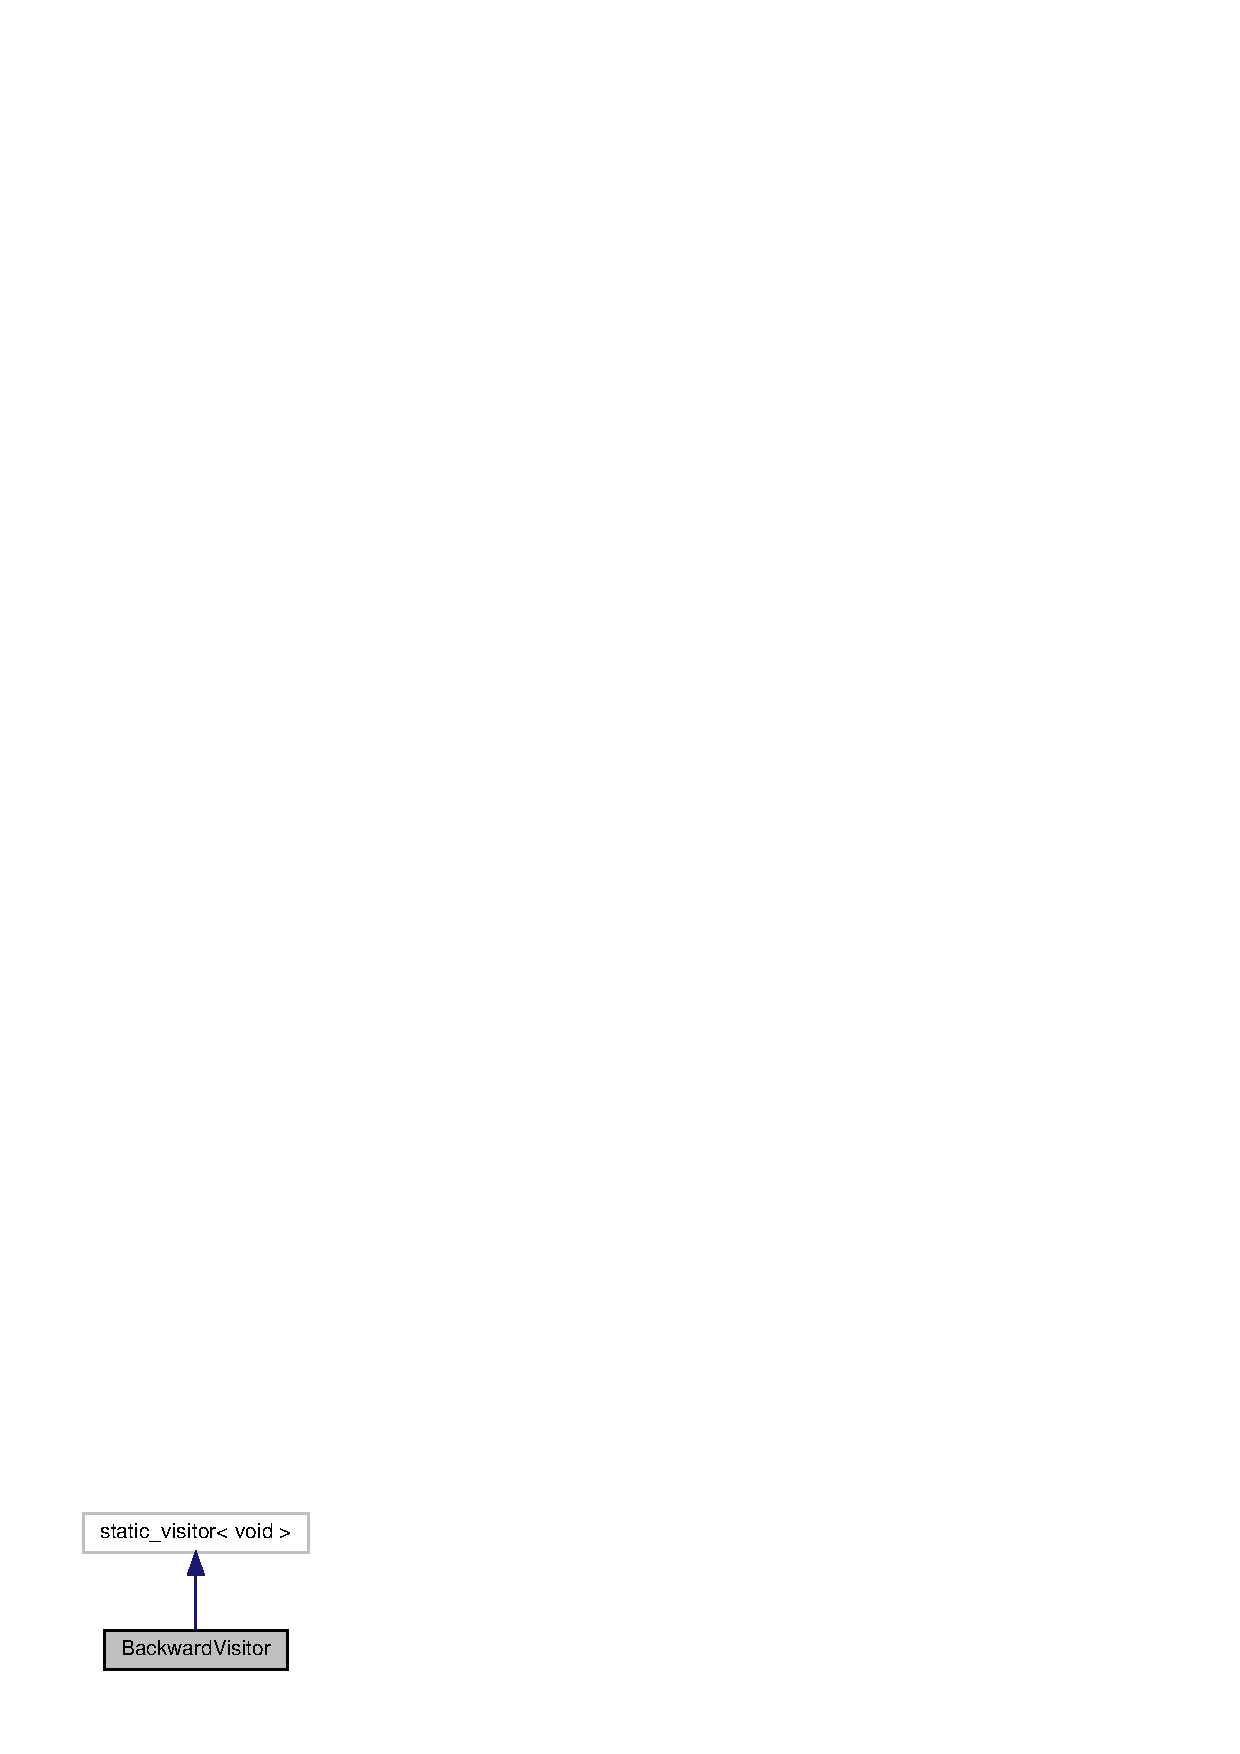
\includegraphics[width=152pt]{classmlpack_1_1ann_1_1BackwardVisitor__inherit__graph}
\end{center}
\end{figure}
\subsection*{Public Member Functions}
\begin{DoxyCompactItemize}
\item 
\textbf{ Backward\+Visitor} (const arma\+::mat \&input, const arma\+::mat \&error, arma\+::mat \&delta)
\begin{DoxyCompactList}\small\item\em Execute the Backward() function given the input, error and delta parameter. \end{DoxyCompactList}\item 
\textbf{ Backward\+Visitor} (const arma\+::mat \&input, const arma\+::mat \&error, arma\+::mat \&delta, const size\+\_\+t index)
\begin{DoxyCompactList}\small\item\em Execute the Backward() function for the layer with the specified index. \end{DoxyCompactList}\item 
{\footnotesize template$<$typename Layer\+Type $>$ }\\void \textbf{ operator()} (Layer\+Type $\ast$layer) const
\begin{DoxyCompactList}\small\item\em Execute the Backward() function. \end{DoxyCompactList}\item 
void \textbf{ operator()} (\textbf{ More\+Types} layer) const
\end{DoxyCompactItemize}


\subsection{Detailed Description}
\doxyref{Backward\+Visitor}{p.}{classmlpack_1_1ann_1_1BackwardVisitor} executes the Backward() function given the input, error and delta parameter. 

Definition at line 28 of file backward\+\_\+visitor.\+hpp.



\subsection{Constructor \& Destructor Documentation}
\mbox{\label{classmlpack_1_1ann_1_1BackwardVisitor_a3437bf9480c07e1a8e76db400a27cec1}} 
\index{mlpack\+::ann\+::\+Backward\+Visitor@{mlpack\+::ann\+::\+Backward\+Visitor}!Backward\+Visitor@{Backward\+Visitor}}
\index{Backward\+Visitor@{Backward\+Visitor}!mlpack\+::ann\+::\+Backward\+Visitor@{mlpack\+::ann\+::\+Backward\+Visitor}}
\subsubsection{Backward\+Visitor()\hspace{0.1cm}{\footnotesize\ttfamily [1/2]}}
{\footnotesize\ttfamily \textbf{ Backward\+Visitor} (\begin{DoxyParamCaption}\item[{const arma\+::mat \&}]{input,  }\item[{const arma\+::mat \&}]{error,  }\item[{arma\+::mat \&}]{delta }\end{DoxyParamCaption})}



Execute the Backward() function given the input, error and delta parameter. 

\mbox{\label{classmlpack_1_1ann_1_1BackwardVisitor_a7cd1b57a1bb7f09d728832d24e37eef3}} 
\index{mlpack\+::ann\+::\+Backward\+Visitor@{mlpack\+::ann\+::\+Backward\+Visitor}!Backward\+Visitor@{Backward\+Visitor}}
\index{Backward\+Visitor@{Backward\+Visitor}!mlpack\+::ann\+::\+Backward\+Visitor@{mlpack\+::ann\+::\+Backward\+Visitor}}
\subsubsection{Backward\+Visitor()\hspace{0.1cm}{\footnotesize\ttfamily [2/2]}}
{\footnotesize\ttfamily \textbf{ Backward\+Visitor} (\begin{DoxyParamCaption}\item[{const arma\+::mat \&}]{input,  }\item[{const arma\+::mat \&}]{error,  }\item[{arma\+::mat \&}]{delta,  }\item[{const size\+\_\+t}]{index }\end{DoxyParamCaption})}



Execute the Backward() function for the layer with the specified index. 



\subsection{Member Function Documentation}
\mbox{\label{classmlpack_1_1ann_1_1BackwardVisitor_a26bb3385c630118c35f4799f1509abbc}} 
\index{mlpack\+::ann\+::\+Backward\+Visitor@{mlpack\+::ann\+::\+Backward\+Visitor}!operator()@{operator()}}
\index{operator()@{operator()}!mlpack\+::ann\+::\+Backward\+Visitor@{mlpack\+::ann\+::\+Backward\+Visitor}}
\subsubsection{operator()()\hspace{0.1cm}{\footnotesize\ttfamily [1/2]}}
{\footnotesize\ttfamily void operator() (\begin{DoxyParamCaption}\item[{Layer\+Type $\ast$}]{layer }\end{DoxyParamCaption}) const}



Execute the Backward() function. 

\mbox{\label{classmlpack_1_1ann_1_1BackwardVisitor_ae35578e7ff874a320fe762bc0edfff04}} 
\index{mlpack\+::ann\+::\+Backward\+Visitor@{mlpack\+::ann\+::\+Backward\+Visitor}!operator()@{operator()}}
\index{operator()@{operator()}!mlpack\+::ann\+::\+Backward\+Visitor@{mlpack\+::ann\+::\+Backward\+Visitor}}
\subsubsection{operator()()\hspace{0.1cm}{\footnotesize\ttfamily [2/2]}}
{\footnotesize\ttfamily void operator() (\begin{DoxyParamCaption}\item[{\textbf{ More\+Types}}]{layer }\end{DoxyParamCaption}) const}



The documentation for this class was generated from the following file\+:\begin{DoxyCompactItemize}
\item 
/home/aakash/mlpack/src/mlpack/methods/ann/visitor/\textbf{ backward\+\_\+visitor.\+hpp}\end{DoxyCompactItemize}

\section{Base\+Layer$<$ Activation\+Function, Input\+Data\+Type, Output\+Data\+Type $>$ Class Template Reference}
\label{classmlpack_1_1ann_1_1BaseLayer}\index{Base\+Layer$<$ Activation\+Function, Input\+Data\+Type, Output\+Data\+Type $>$@{Base\+Layer$<$ Activation\+Function, Input\+Data\+Type, Output\+Data\+Type $>$}}


Implementation of the base layer.  


\subsection*{Public Member Functions}
\begin{DoxyCompactItemize}
\item 
\textbf{ Base\+Layer} ()
\begin{DoxyCompactList}\small\item\em Create the \doxyref{Base\+Layer}{p.}{classmlpack_1_1ann_1_1BaseLayer} object. \end{DoxyCompactList}\item 
{\footnotesize template$<$typename eT $>$ }\\void \textbf{ Backward} (const arma\+::\+Mat$<$ eT $>$ \&input, const arma\+::\+Mat$<$ eT $>$ \&gy, arma\+::\+Mat$<$ eT $>$ \&g)
\begin{DoxyCompactList}\small\item\em Ordinary feed backward pass of a neural network, calculating the function f(x) by propagating x backwards trough f. \end{DoxyCompactList}\item 
Output\+Data\+Type const  \& \textbf{ Delta} () const
\begin{DoxyCompactList}\small\item\em Get the delta. \end{DoxyCompactList}\item 
Output\+Data\+Type \& \textbf{ Delta} ()
\begin{DoxyCompactList}\small\item\em Modify the delta. \end{DoxyCompactList}\item 
{\footnotesize template$<$typename Input\+Type , typename Output\+Type $>$ }\\void \textbf{ Forward} (const Input\+Type \&input, Output\+Type \&output)
\begin{DoxyCompactList}\small\item\em Ordinary feed forward pass of a neural network, evaluating the function f(x) by propagating the activity forward through f. \end{DoxyCompactList}\item 
Output\+Data\+Type const  \& \textbf{ Output\+Parameter} () const
\begin{DoxyCompactList}\small\item\em Get the output parameter. \end{DoxyCompactList}\item 
Output\+Data\+Type \& \textbf{ Output\+Parameter} ()
\begin{DoxyCompactList}\small\item\em Modify the output parameter. \end{DoxyCompactList}\item 
{\footnotesize template$<$typename Archive $>$ }\\void \textbf{ serialize} (Archive \&, const uint32\+\_\+t)
\begin{DoxyCompactList}\small\item\em Serialize the layer. \end{DoxyCompactList}\end{DoxyCompactItemize}


\subsection{Detailed Description}
\subsubsection*{template$<$class Activation\+Function = Logistic\+Function, typename Input\+Data\+Type = arma\+::mat, typename Output\+Data\+Type = arma\+::mat$>$\newline
class mlpack\+::ann\+::\+Base\+Layer$<$ Activation\+Function, Input\+Data\+Type, Output\+Data\+Type $>$}

Implementation of the base layer. 

The base layer works as a metaclass which attaches various functions to the embedding layer.

A few convenience typedefs are given\+:


\begin{DoxyItemize}
\item Sigmoid\+Layer
\item Identity\+Layer
\item Re\+L\+U\+Layer
\item Tan\+H\+Layer
\item Softplus\+Layer
\item Hard\+Sigmoid\+Layer
\item Swish\+Layer
\item Mish\+Layer
\item Li\+S\+H\+T\+Layer
\item G\+E\+L\+U\+Layer
\item E\+Li\+S\+H\+Layer
\item Elliot\+Layer
\item Gaussian\+Layer
\item Hard\+Swish\+Layer
\item Tanh\+Exp\+Layer
\item S\+I\+L\+U\+Layer
\end{DoxyItemize}


\begin{DoxyTemplParams}{Template Parameters}
{\em Activation\+Function} & Activation function used for the embedding layer. \\
\hline
{\em Input\+Data\+Type} & Type of the input data (arma\+::colvec, arma\+::mat, arma\+::sp\+\_\+mat or arma\+::cube). \\
\hline
{\em Output\+Data\+Type} & Type of the output data (arma\+::colvec, arma\+::mat, arma\+::sp\+\_\+mat or arma\+::cube). \\
\hline
\end{DoxyTemplParams}


Definition at line 71 of file base\+\_\+layer.\+hpp.



\subsection{Constructor \& Destructor Documentation}
\mbox{\label{classmlpack_1_1ann_1_1BaseLayer_a5efea921257d23b1d5a755609d7a7943}} 
\index{mlpack\+::ann\+::\+Base\+Layer@{mlpack\+::ann\+::\+Base\+Layer}!Base\+Layer@{Base\+Layer}}
\index{Base\+Layer@{Base\+Layer}!mlpack\+::ann\+::\+Base\+Layer@{mlpack\+::ann\+::\+Base\+Layer}}
\subsubsection{Base\+Layer()}
{\footnotesize\ttfamily \textbf{ Base\+Layer} (\begin{DoxyParamCaption}{ }\end{DoxyParamCaption})\hspace{0.3cm}{\ttfamily [inline]}}



Create the \doxyref{Base\+Layer}{p.}{classmlpack_1_1ann_1_1BaseLayer} object. 



Definition at line 77 of file base\+\_\+layer.\+hpp.



\subsection{Member Function Documentation}
\mbox{\label{classmlpack_1_1ann_1_1BaseLayer_a78dbad83871f43db1975e45a9a69c376}} 
\index{mlpack\+::ann\+::\+Base\+Layer@{mlpack\+::ann\+::\+Base\+Layer}!Backward@{Backward}}
\index{Backward@{Backward}!mlpack\+::ann\+::\+Base\+Layer@{mlpack\+::ann\+::\+Base\+Layer}}
\subsubsection{Backward()}
{\footnotesize\ttfamily void Backward (\begin{DoxyParamCaption}\item[{const arma\+::\+Mat$<$ eT $>$ \&}]{input,  }\item[{const arma\+::\+Mat$<$ eT $>$ \&}]{gy,  }\item[{arma\+::\+Mat$<$ eT $>$ \&}]{g }\end{DoxyParamCaption})\hspace{0.3cm}{\ttfamily [inline]}}



Ordinary feed backward pass of a neural network, calculating the function f(x) by propagating x backwards trough f. 

Using the results from the feed forward pass.


\begin{DoxyParams}{Parameters}
{\em input} & The propagated input activation. \\
\hline
{\em gy} & The backpropagated error. \\
\hline
{\em g} & The calculated gradient. \\
\hline
\end{DoxyParams}


Definition at line 105 of file base\+\_\+layer.\+hpp.

\mbox{\label{classmlpack_1_1ann_1_1BaseLayer_a797f7edb44dd081e5e2b3cc316eef6bd}} 
\index{mlpack\+::ann\+::\+Base\+Layer@{mlpack\+::ann\+::\+Base\+Layer}!Delta@{Delta}}
\index{Delta@{Delta}!mlpack\+::ann\+::\+Base\+Layer@{mlpack\+::ann\+::\+Base\+Layer}}
\subsubsection{Delta()\hspace{0.1cm}{\footnotesize\ttfamily [1/2]}}
{\footnotesize\ttfamily Output\+Data\+Type const\& Delta (\begin{DoxyParamCaption}{ }\end{DoxyParamCaption}) const\hspace{0.3cm}{\ttfamily [inline]}}



Get the delta. 



Definition at line 120 of file base\+\_\+layer.\+hpp.

\mbox{\label{classmlpack_1_1ann_1_1BaseLayer_ad6601342d560219ce951d554e69e5e87}} 
\index{mlpack\+::ann\+::\+Base\+Layer@{mlpack\+::ann\+::\+Base\+Layer}!Delta@{Delta}}
\index{Delta@{Delta}!mlpack\+::ann\+::\+Base\+Layer@{mlpack\+::ann\+::\+Base\+Layer}}
\subsubsection{Delta()\hspace{0.1cm}{\footnotesize\ttfamily [2/2]}}
{\footnotesize\ttfamily Output\+Data\+Type\& Delta (\begin{DoxyParamCaption}{ }\end{DoxyParamCaption})\hspace{0.3cm}{\ttfamily [inline]}}



Modify the delta. 



Definition at line 122 of file base\+\_\+layer.\+hpp.

\mbox{\label{classmlpack_1_1ann_1_1BaseLayer_a09440df0a90bdcc766e56e097d91205b}} 
\index{mlpack\+::ann\+::\+Base\+Layer@{mlpack\+::ann\+::\+Base\+Layer}!Forward@{Forward}}
\index{Forward@{Forward}!mlpack\+::ann\+::\+Base\+Layer@{mlpack\+::ann\+::\+Base\+Layer}}
\subsubsection{Forward()}
{\footnotesize\ttfamily void Forward (\begin{DoxyParamCaption}\item[{const Input\+Type \&}]{input,  }\item[{Output\+Type \&}]{output }\end{DoxyParamCaption})\hspace{0.3cm}{\ttfamily [inline]}}



Ordinary feed forward pass of a neural network, evaluating the function f(x) by propagating the activity forward through f. 


\begin{DoxyParams}{Parameters}
{\em input} & Input data used for evaluating the specified function. \\
\hline
{\em output} & Resulting output activation. \\
\hline
\end{DoxyParams}


Definition at line 90 of file base\+\_\+layer.\+hpp.

\mbox{\label{classmlpack_1_1ann_1_1BaseLayer_a0ee21c2a36e5abad1e7a9d5dd00849f9}} 
\index{mlpack\+::ann\+::\+Base\+Layer@{mlpack\+::ann\+::\+Base\+Layer}!Output\+Parameter@{Output\+Parameter}}
\index{Output\+Parameter@{Output\+Parameter}!mlpack\+::ann\+::\+Base\+Layer@{mlpack\+::ann\+::\+Base\+Layer}}
\subsubsection{Output\+Parameter()\hspace{0.1cm}{\footnotesize\ttfamily [1/2]}}
{\footnotesize\ttfamily Output\+Data\+Type const\& Output\+Parameter (\begin{DoxyParamCaption}{ }\end{DoxyParamCaption}) const\hspace{0.3cm}{\ttfamily [inline]}}



Get the output parameter. 



Definition at line 115 of file base\+\_\+layer.\+hpp.

\mbox{\label{classmlpack_1_1ann_1_1BaseLayer_a21d5f745f02c709625a4ee0907f004a5}} 
\index{mlpack\+::ann\+::\+Base\+Layer@{mlpack\+::ann\+::\+Base\+Layer}!Output\+Parameter@{Output\+Parameter}}
\index{Output\+Parameter@{Output\+Parameter}!mlpack\+::ann\+::\+Base\+Layer@{mlpack\+::ann\+::\+Base\+Layer}}
\subsubsection{Output\+Parameter()\hspace{0.1cm}{\footnotesize\ttfamily [2/2]}}
{\footnotesize\ttfamily Output\+Data\+Type\& Output\+Parameter (\begin{DoxyParamCaption}{ }\end{DoxyParamCaption})\hspace{0.3cm}{\ttfamily [inline]}}



Modify the output parameter. 



Definition at line 117 of file base\+\_\+layer.\+hpp.

\mbox{\label{classmlpack_1_1ann_1_1BaseLayer_aa2ccb5a0533a6ba0abe6dfc1f98fbafb}} 
\index{mlpack\+::ann\+::\+Base\+Layer@{mlpack\+::ann\+::\+Base\+Layer}!serialize@{serialize}}
\index{serialize@{serialize}!mlpack\+::ann\+::\+Base\+Layer@{mlpack\+::ann\+::\+Base\+Layer}}
\subsubsection{serialize()}
{\footnotesize\ttfamily void serialize (\begin{DoxyParamCaption}\item[{Archive \&}]{,  }\item[{const uint32\+\_\+t}]{ }\end{DoxyParamCaption})\hspace{0.3cm}{\ttfamily [inline]}}



Serialize the layer. 



Definition at line 128 of file base\+\_\+layer.\+hpp.



The documentation for this class was generated from the following file\+:\begin{DoxyCompactItemize}
\item 
/home/aakash/mlpack/src/mlpack/methods/ann/layer/\textbf{ base\+\_\+layer.\+hpp}\end{DoxyCompactItemize}

\section{Batch\+Norm$<$ Input\+Data\+Type, Output\+Data\+Type $>$ Class Template Reference}
\label{classmlpack_1_1ann_1_1BatchNorm}\index{Batch\+Norm$<$ Input\+Data\+Type, Output\+Data\+Type $>$@{Batch\+Norm$<$ Input\+Data\+Type, Output\+Data\+Type $>$}}


Declaration of the Batch Normalization layer class.  


\subsection*{Public Member Functions}
\begin{DoxyCompactItemize}
\item 
\textbf{ Batch\+Norm} ()
\begin{DoxyCompactList}\small\item\em Create the \doxyref{Batch\+Norm}{p.}{classmlpack_1_1ann_1_1BatchNorm} object. \end{DoxyCompactList}\item 
\textbf{ Batch\+Norm} (const size\+\_\+t size, const double eps=1e-\/8, const bool average=true, const double momentum=0.\+1)
\begin{DoxyCompactList}\small\item\em Create the \doxyref{Batch\+Norm}{p.}{classmlpack_1_1ann_1_1BatchNorm} layer object for a specified number of input units. \end{DoxyCompactList}\item 
bool \textbf{ Average} () const
\begin{DoxyCompactList}\small\item\em Get the average parameter. \end{DoxyCompactList}\item 
{\footnotesize template$<$typename eT $>$ }\\void \textbf{ Backward} (const arma\+::\+Mat$<$ eT $>$ \&input, const arma\+::\+Mat$<$ eT $>$ \&gy, arma\+::\+Mat$<$ eT $>$ \&g)
\begin{DoxyCompactList}\small\item\em Backward pass through the layer. \end{DoxyCompactList}\item 
Output\+Data\+Type const  \& \textbf{ Delta} () const
\begin{DoxyCompactList}\small\item\em Get the delta. \end{DoxyCompactList}\item 
Output\+Data\+Type \& \textbf{ Delta} ()
\begin{DoxyCompactList}\small\item\em Modify the delta. \end{DoxyCompactList}\item 
bool \textbf{ Deterministic} () const
\begin{DoxyCompactList}\small\item\em Get the value of deterministic parameter. \end{DoxyCompactList}\item 
bool \& \textbf{ Deterministic} ()
\begin{DoxyCompactList}\small\item\em Modify the value of deterministic parameter. \end{DoxyCompactList}\item 
double \textbf{ Epsilon} () const
\begin{DoxyCompactList}\small\item\em Get the epsilon value. \end{DoxyCompactList}\item 
{\footnotesize template$<$typename eT $>$ }\\void \textbf{ Forward} (const arma\+::\+Mat$<$ eT $>$ \&input, arma\+::\+Mat$<$ eT $>$ \&output)
\begin{DoxyCompactList}\small\item\em Forward pass of the Batch Normalization layer. \end{DoxyCompactList}\item 
{\footnotesize template$<$typename eT $>$ }\\void \textbf{ Gradient} (const arma\+::\+Mat$<$ eT $>$ \&input, const arma\+::\+Mat$<$ eT $>$ \&error, arma\+::\+Mat$<$ eT $>$ \&gradient)
\begin{DoxyCompactList}\small\item\em Calculate the gradient using the output delta and the input activations. \end{DoxyCompactList}\item 
Output\+Data\+Type const  \& \textbf{ Gradient} () const
\begin{DoxyCompactList}\small\item\em Get the gradient. \end{DoxyCompactList}\item 
Output\+Data\+Type \& \textbf{ Gradient} ()
\begin{DoxyCompactList}\small\item\em Modify the gradient. \end{DoxyCompactList}\item 
size\+\_\+t \textbf{ Input\+Size} () const
\begin{DoxyCompactList}\small\item\em Get the number of input units / channels. \end{DoxyCompactList}\item 
double \textbf{ Momentum} () const
\begin{DoxyCompactList}\small\item\em Get the momentum value. \end{DoxyCompactList}\item 
Output\+Data\+Type const  \& \textbf{ Output\+Parameter} () const
\begin{DoxyCompactList}\small\item\em Get the output parameter. \end{DoxyCompactList}\item 
Output\+Data\+Type \& \textbf{ Output\+Parameter} ()
\begin{DoxyCompactList}\small\item\em Modify the output parameter. \end{DoxyCompactList}\item 
Output\+Data\+Type const  \& \textbf{ Parameters} () const
\begin{DoxyCompactList}\small\item\em Get the parameters. \end{DoxyCompactList}\item 
Output\+Data\+Type \& \textbf{ Parameters} ()
\begin{DoxyCompactList}\small\item\em Modify the parameters. \end{DoxyCompactList}\item 
void \textbf{ Reset} ()
\begin{DoxyCompactList}\small\item\em Reset the layer parameters. \end{DoxyCompactList}\item 
{\footnotesize template$<$typename Archive $>$ }\\void \textbf{ serialize} (Archive \&ar, const uint32\+\_\+t)
\begin{DoxyCompactList}\small\item\em Serialize the layer. \end{DoxyCompactList}\item 
Output\+Data\+Type const  \& \textbf{ Training\+Mean} () const
\begin{DoxyCompactList}\small\item\em Get the mean over the training data. \end{DoxyCompactList}\item 
Output\+Data\+Type \& \textbf{ Training\+Mean} ()
\begin{DoxyCompactList}\small\item\em Modify the mean over the training data. \end{DoxyCompactList}\item 
Output\+Data\+Type const  \& \textbf{ Training\+Variance} () const
\begin{DoxyCompactList}\small\item\em Get the variance over the training data. \end{DoxyCompactList}\item 
Output\+Data\+Type \& \textbf{ Training\+Variance} ()
\begin{DoxyCompactList}\small\item\em Modify the variance over the training data. \end{DoxyCompactList}\item 
size\+\_\+t \textbf{ Weight\+Size} () const
\begin{DoxyCompactList}\small\item\em Get size of weights. \end{DoxyCompactList}\end{DoxyCompactItemize}


\subsection{Detailed Description}
\subsubsection*{template$<$typename Input\+Data\+Type = arma\+::mat, typename Output\+Data\+Type = arma\+::mat$>$\newline
class mlpack\+::ann\+::\+Batch\+Norm$<$ Input\+Data\+Type, Output\+Data\+Type $>$}

Declaration of the Batch Normalization layer class. 

The layer transforms the input data into zero mean and unit variance and then scales and shifts the data by parameters, gamma and beta respectively. These parameters are learnt by the network.

If deterministic is false (training), the mean and variance over the batch is calculated and the data is normalized. If it is set to true (testing) then the mean and variance accrued over the training set is used.

For more information, refer to the following paper,


\begin{DoxyCode}
@article\{Ioffe15,
  author    = \{Sergey Ioffe and
               Christian Szegedy\},
  title     = \{Batch Normalization: Accelerating Deep Network Training by
               Reducing Internal Covariate Shift\},
  journal   = \{CoRR\},
  volume    = \{abs/1502.03167\},
  year      = \{2015\},
  url       = \{http:\textcolor{comment}{//arxiv.org/abs/1502.03167\},}
  eprint    = \{1502.03167\},
\}
\end{DoxyCode}



\begin{DoxyTemplParams}{Template Parameters}
{\em Input\+Data\+Type} & Type of the input data (arma\+::colvec, arma\+::mat, arma\+::sp\+\_\+mat or arma\+::cube). \\
\hline
{\em Output\+Data\+Type} & Type of the output data (arma\+::colvec, arma\+::mat, arma\+::sp\+\_\+mat or arma\+::cube). \\
\hline
\end{DoxyTemplParams}


Definition at line 56 of file batch\+\_\+norm.\+hpp.



\subsection{Constructor \& Destructor Documentation}
\mbox{\label{classmlpack_1_1ann_1_1BatchNorm_a854f142e5c3785c754d8f063269add79}} 
\index{mlpack\+::ann\+::\+Batch\+Norm@{mlpack\+::ann\+::\+Batch\+Norm}!Batch\+Norm@{Batch\+Norm}}
\index{Batch\+Norm@{Batch\+Norm}!mlpack\+::ann\+::\+Batch\+Norm@{mlpack\+::ann\+::\+Batch\+Norm}}
\subsubsection{Batch\+Norm()\hspace{0.1cm}{\footnotesize\ttfamily [1/2]}}
{\footnotesize\ttfamily \textbf{ Batch\+Norm} (\begin{DoxyParamCaption}{ }\end{DoxyParamCaption})}



Create the \doxyref{Batch\+Norm}{p.}{classmlpack_1_1ann_1_1BatchNorm} object. 

\mbox{\label{classmlpack_1_1ann_1_1BatchNorm_a47e2f9600ab95dbdc278161064a6fd63}} 
\index{mlpack\+::ann\+::\+Batch\+Norm@{mlpack\+::ann\+::\+Batch\+Norm}!Batch\+Norm@{Batch\+Norm}}
\index{Batch\+Norm@{Batch\+Norm}!mlpack\+::ann\+::\+Batch\+Norm@{mlpack\+::ann\+::\+Batch\+Norm}}
\subsubsection{Batch\+Norm()\hspace{0.1cm}{\footnotesize\ttfamily [2/2]}}
{\footnotesize\ttfamily \textbf{ Batch\+Norm} (\begin{DoxyParamCaption}\item[{const size\+\_\+t}]{size,  }\item[{const double}]{eps = {\ttfamily 1e-\/8},  }\item[{const bool}]{average = {\ttfamily true},  }\item[{const double}]{momentum = {\ttfamily 0.1} }\end{DoxyParamCaption})}



Create the \doxyref{Batch\+Norm}{p.}{classmlpack_1_1ann_1_1BatchNorm} layer object for a specified number of input units. 


\begin{DoxyParams}{Parameters}
{\em size} & The number of input units / channels. \\
\hline
{\em eps} & The epsilon added to variance to ensure numerical stability. \\
\hline
{\em average} & Boolean to determine whether cumulative average is used for updating the parameters or momentum is used. \\
\hline
{\em momentum} & Parameter used to to update the running mean and variance. \\
\hline
\end{DoxyParams}


\subsection{Member Function Documentation}
\mbox{\label{classmlpack_1_1ann_1_1BatchNorm_aab4ef6131dc58825790fb04cc209faab}} 
\index{mlpack\+::ann\+::\+Batch\+Norm@{mlpack\+::ann\+::\+Batch\+Norm}!Average@{Average}}
\index{Average@{Average}!mlpack\+::ann\+::\+Batch\+Norm@{mlpack\+::ann\+::\+Batch\+Norm}}
\subsubsection{Average()}
{\footnotesize\ttfamily bool Average (\begin{DoxyParamCaption}{ }\end{DoxyParamCaption}) const\hspace{0.3cm}{\ttfamily [inline]}}



Get the average parameter. 



Definition at line 161 of file batch\+\_\+norm.\+hpp.

\mbox{\label{classmlpack_1_1ann_1_1BatchNorm_a78dbad83871f43db1975e45a9a69c376}} 
\index{mlpack\+::ann\+::\+Batch\+Norm@{mlpack\+::ann\+::\+Batch\+Norm}!Backward@{Backward}}
\index{Backward@{Backward}!mlpack\+::ann\+::\+Batch\+Norm@{mlpack\+::ann\+::\+Batch\+Norm}}
\subsubsection{Backward()}
{\footnotesize\ttfamily void Backward (\begin{DoxyParamCaption}\item[{const arma\+::\+Mat$<$ eT $>$ \&}]{input,  }\item[{const arma\+::\+Mat$<$ eT $>$ \&}]{gy,  }\item[{arma\+::\+Mat$<$ eT $>$ \&}]{g }\end{DoxyParamCaption})}



Backward pass through the layer. 


\begin{DoxyParams}{Parameters}
{\em input} & The input activations \\
\hline
{\em gy} & The backpropagated error. \\
\hline
{\em g} & The calculated gradient. \\
\hline
\end{DoxyParams}
\mbox{\label{classmlpack_1_1ann_1_1BatchNorm_a797f7edb44dd081e5e2b3cc316eef6bd}} 
\index{mlpack\+::ann\+::\+Batch\+Norm@{mlpack\+::ann\+::\+Batch\+Norm}!Delta@{Delta}}
\index{Delta@{Delta}!mlpack\+::ann\+::\+Batch\+Norm@{mlpack\+::ann\+::\+Batch\+Norm}}
\subsubsection{Delta()\hspace{0.1cm}{\footnotesize\ttfamily [1/2]}}
{\footnotesize\ttfamily Output\+Data\+Type const\& Delta (\begin{DoxyParamCaption}{ }\end{DoxyParamCaption}) const\hspace{0.3cm}{\ttfamily [inline]}}



Get the delta. 



Definition at line 127 of file batch\+\_\+norm.\+hpp.

\mbox{\label{classmlpack_1_1ann_1_1BatchNorm_ad6601342d560219ce951d554e69e5e87}} 
\index{mlpack\+::ann\+::\+Batch\+Norm@{mlpack\+::ann\+::\+Batch\+Norm}!Delta@{Delta}}
\index{Delta@{Delta}!mlpack\+::ann\+::\+Batch\+Norm@{mlpack\+::ann\+::\+Batch\+Norm}}
\subsubsection{Delta()\hspace{0.1cm}{\footnotesize\ttfamily [2/2]}}
{\footnotesize\ttfamily Output\+Data\+Type\& Delta (\begin{DoxyParamCaption}{ }\end{DoxyParamCaption})\hspace{0.3cm}{\ttfamily [inline]}}



Modify the delta. 



Definition at line 129 of file batch\+\_\+norm.\+hpp.

\mbox{\label{classmlpack_1_1ann_1_1BatchNorm_a9f4103707f4d199ce5594d239b60443e}} 
\index{mlpack\+::ann\+::\+Batch\+Norm@{mlpack\+::ann\+::\+Batch\+Norm}!Deterministic@{Deterministic}}
\index{Deterministic@{Deterministic}!mlpack\+::ann\+::\+Batch\+Norm@{mlpack\+::ann\+::\+Batch\+Norm}}
\subsubsection{Deterministic()\hspace{0.1cm}{\footnotesize\ttfamily [1/2]}}
{\footnotesize\ttfamily bool Deterministic (\begin{DoxyParamCaption}{ }\end{DoxyParamCaption}) const\hspace{0.3cm}{\ttfamily [inline]}}



Get the value of deterministic parameter. 



Definition at line 137 of file batch\+\_\+norm.\+hpp.

\mbox{\label{classmlpack_1_1ann_1_1BatchNorm_a42d4ee3da432cff20d3a41b8b1ec801c}} 
\index{mlpack\+::ann\+::\+Batch\+Norm@{mlpack\+::ann\+::\+Batch\+Norm}!Deterministic@{Deterministic}}
\index{Deterministic@{Deterministic}!mlpack\+::ann\+::\+Batch\+Norm@{mlpack\+::ann\+::\+Batch\+Norm}}
\subsubsection{Deterministic()\hspace{0.1cm}{\footnotesize\ttfamily [2/2]}}
{\footnotesize\ttfamily bool\& Deterministic (\begin{DoxyParamCaption}{ }\end{DoxyParamCaption})\hspace{0.3cm}{\ttfamily [inline]}}



Modify the value of deterministic parameter. 



Definition at line 139 of file batch\+\_\+norm.\+hpp.

\mbox{\label{classmlpack_1_1ann_1_1BatchNorm_af6d960193bb5db37e51416e12bf720de}} 
\index{mlpack\+::ann\+::\+Batch\+Norm@{mlpack\+::ann\+::\+Batch\+Norm}!Epsilon@{Epsilon}}
\index{Epsilon@{Epsilon}!mlpack\+::ann\+::\+Batch\+Norm@{mlpack\+::ann\+::\+Batch\+Norm}}
\subsubsection{Epsilon()}
{\footnotesize\ttfamily double Epsilon (\begin{DoxyParamCaption}{ }\end{DoxyParamCaption}) const\hspace{0.3cm}{\ttfamily [inline]}}



Get the epsilon value. 



Definition at line 155 of file batch\+\_\+norm.\+hpp.

\mbox{\label{classmlpack_1_1ann_1_1BatchNorm_a461f849bc638c15bec262dc9c3a58abe}} 
\index{mlpack\+::ann\+::\+Batch\+Norm@{mlpack\+::ann\+::\+Batch\+Norm}!Forward@{Forward}}
\index{Forward@{Forward}!mlpack\+::ann\+::\+Batch\+Norm@{mlpack\+::ann\+::\+Batch\+Norm}}
\subsubsection{Forward()}
{\footnotesize\ttfamily void Forward (\begin{DoxyParamCaption}\item[{const arma\+::\+Mat$<$ eT $>$ \&}]{input,  }\item[{arma\+::\+Mat$<$ eT $>$ \&}]{output }\end{DoxyParamCaption})}



Forward pass of the Batch Normalization layer. 

Transforms the input data into zero mean and unit variance, scales the data by a factor gamma and shifts it by beta.


\begin{DoxyParams}{Parameters}
{\em input} & Input data for the layer \\
\hline
{\em output} & Resulting output activations. \\
\hline
\end{DoxyParams}
\mbox{\label{classmlpack_1_1ann_1_1BatchNorm_aaf577db350e2130754490d8486fba215}} 
\index{mlpack\+::ann\+::\+Batch\+Norm@{mlpack\+::ann\+::\+Batch\+Norm}!Gradient@{Gradient}}
\index{Gradient@{Gradient}!mlpack\+::ann\+::\+Batch\+Norm@{mlpack\+::ann\+::\+Batch\+Norm}}
\subsubsection{Gradient()\hspace{0.1cm}{\footnotesize\ttfamily [1/3]}}
{\footnotesize\ttfamily void Gradient (\begin{DoxyParamCaption}\item[{const arma\+::\+Mat$<$ eT $>$ \&}]{input,  }\item[{const arma\+::\+Mat$<$ eT $>$ \&}]{error,  }\item[{arma\+::\+Mat$<$ eT $>$ \&}]{gradient }\end{DoxyParamCaption})}



Calculate the gradient using the output delta and the input activations. 


\begin{DoxyParams}{Parameters}
{\em input} & The input activations \\
\hline
{\em error} & The calculated error \\
\hline
{\em gradient} & The calculated gradient. \\
\hline
\end{DoxyParams}
\mbox{\label{classmlpack_1_1ann_1_1BatchNorm_a0f1f4e6d93472d83852731a96c8c3f59}} 
\index{mlpack\+::ann\+::\+Batch\+Norm@{mlpack\+::ann\+::\+Batch\+Norm}!Gradient@{Gradient}}
\index{Gradient@{Gradient}!mlpack\+::ann\+::\+Batch\+Norm@{mlpack\+::ann\+::\+Batch\+Norm}}
\subsubsection{Gradient()\hspace{0.1cm}{\footnotesize\ttfamily [2/3]}}
{\footnotesize\ttfamily Output\+Data\+Type const\& Gradient (\begin{DoxyParamCaption}{ }\end{DoxyParamCaption}) const\hspace{0.3cm}{\ttfamily [inline]}}



Get the gradient. 



Definition at line 132 of file batch\+\_\+norm.\+hpp.

\mbox{\label{classmlpack_1_1ann_1_1BatchNorm_a19abce4739c3b0b658b612537e21956a}} 
\index{mlpack\+::ann\+::\+Batch\+Norm@{mlpack\+::ann\+::\+Batch\+Norm}!Gradient@{Gradient}}
\index{Gradient@{Gradient}!mlpack\+::ann\+::\+Batch\+Norm@{mlpack\+::ann\+::\+Batch\+Norm}}
\subsubsection{Gradient()\hspace{0.1cm}{\footnotesize\ttfamily [3/3]}}
{\footnotesize\ttfamily Output\+Data\+Type\& Gradient (\begin{DoxyParamCaption}{ }\end{DoxyParamCaption})\hspace{0.3cm}{\ttfamily [inline]}}



Modify the gradient. 



Definition at line 134 of file batch\+\_\+norm.\+hpp.

\mbox{\label{classmlpack_1_1ann_1_1BatchNorm_a5a4c4984aa897a28d516e638e7ea5308}} 
\index{mlpack\+::ann\+::\+Batch\+Norm@{mlpack\+::ann\+::\+Batch\+Norm}!Input\+Size@{Input\+Size}}
\index{Input\+Size@{Input\+Size}!mlpack\+::ann\+::\+Batch\+Norm@{mlpack\+::ann\+::\+Batch\+Norm}}
\subsubsection{Input\+Size()}
{\footnotesize\ttfamily size\+\_\+t Input\+Size (\begin{DoxyParamCaption}{ }\end{DoxyParamCaption}) const\hspace{0.3cm}{\ttfamily [inline]}}



Get the number of input units / channels. 



Definition at line 152 of file batch\+\_\+norm.\+hpp.

\mbox{\label{classmlpack_1_1ann_1_1BatchNorm_a47bdc16d2d5d5514d9711eae8938fd35}} 
\index{mlpack\+::ann\+::\+Batch\+Norm@{mlpack\+::ann\+::\+Batch\+Norm}!Momentum@{Momentum}}
\index{Momentum@{Momentum}!mlpack\+::ann\+::\+Batch\+Norm@{mlpack\+::ann\+::\+Batch\+Norm}}
\subsubsection{Momentum()}
{\footnotesize\ttfamily double Momentum (\begin{DoxyParamCaption}{ }\end{DoxyParamCaption}) const\hspace{0.3cm}{\ttfamily [inline]}}



Get the momentum value. 



Definition at line 158 of file batch\+\_\+norm.\+hpp.

\mbox{\label{classmlpack_1_1ann_1_1BatchNorm_a0ee21c2a36e5abad1e7a9d5dd00849f9}} 
\index{mlpack\+::ann\+::\+Batch\+Norm@{mlpack\+::ann\+::\+Batch\+Norm}!Output\+Parameter@{Output\+Parameter}}
\index{Output\+Parameter@{Output\+Parameter}!mlpack\+::ann\+::\+Batch\+Norm@{mlpack\+::ann\+::\+Batch\+Norm}}
\subsubsection{Output\+Parameter()\hspace{0.1cm}{\footnotesize\ttfamily [1/2]}}
{\footnotesize\ttfamily Output\+Data\+Type const\& Output\+Parameter (\begin{DoxyParamCaption}{ }\end{DoxyParamCaption}) const\hspace{0.3cm}{\ttfamily [inline]}}



Get the output parameter. 



Definition at line 122 of file batch\+\_\+norm.\+hpp.

\mbox{\label{classmlpack_1_1ann_1_1BatchNorm_a21d5f745f02c709625a4ee0907f004a5}} 
\index{mlpack\+::ann\+::\+Batch\+Norm@{mlpack\+::ann\+::\+Batch\+Norm}!Output\+Parameter@{Output\+Parameter}}
\index{Output\+Parameter@{Output\+Parameter}!mlpack\+::ann\+::\+Batch\+Norm@{mlpack\+::ann\+::\+Batch\+Norm}}
\subsubsection{Output\+Parameter()\hspace{0.1cm}{\footnotesize\ttfamily [2/2]}}
{\footnotesize\ttfamily Output\+Data\+Type\& Output\+Parameter (\begin{DoxyParamCaption}{ }\end{DoxyParamCaption})\hspace{0.3cm}{\ttfamily [inline]}}



Modify the output parameter. 



Definition at line 124 of file batch\+\_\+norm.\+hpp.

\mbox{\label{classmlpack_1_1ann_1_1BatchNorm_aa530552c7ef915c952fbacc77b965c90}} 
\index{mlpack\+::ann\+::\+Batch\+Norm@{mlpack\+::ann\+::\+Batch\+Norm}!Parameters@{Parameters}}
\index{Parameters@{Parameters}!mlpack\+::ann\+::\+Batch\+Norm@{mlpack\+::ann\+::\+Batch\+Norm}}
\subsubsection{Parameters()\hspace{0.1cm}{\footnotesize\ttfamily [1/2]}}
{\footnotesize\ttfamily Output\+Data\+Type const\& Parameters (\begin{DoxyParamCaption}{ }\end{DoxyParamCaption}) const\hspace{0.3cm}{\ttfamily [inline]}}



Get the parameters. 



Definition at line 117 of file batch\+\_\+norm.\+hpp.

\mbox{\label{classmlpack_1_1ann_1_1BatchNorm_a9c5c5900772a689d5a6b59778ec67120}} 
\index{mlpack\+::ann\+::\+Batch\+Norm@{mlpack\+::ann\+::\+Batch\+Norm}!Parameters@{Parameters}}
\index{Parameters@{Parameters}!mlpack\+::ann\+::\+Batch\+Norm@{mlpack\+::ann\+::\+Batch\+Norm}}
\subsubsection{Parameters()\hspace{0.1cm}{\footnotesize\ttfamily [2/2]}}
{\footnotesize\ttfamily Output\+Data\+Type\& Parameters (\begin{DoxyParamCaption}{ }\end{DoxyParamCaption})\hspace{0.3cm}{\ttfamily [inline]}}



Modify the parameters. 



Definition at line 119 of file batch\+\_\+norm.\+hpp.

\mbox{\label{classmlpack_1_1ann_1_1BatchNorm_a372de693ad40b3f42839c8ec6ac845f4}} 
\index{mlpack\+::ann\+::\+Batch\+Norm@{mlpack\+::ann\+::\+Batch\+Norm}!Reset@{Reset}}
\index{Reset@{Reset}!mlpack\+::ann\+::\+Batch\+Norm@{mlpack\+::ann\+::\+Batch\+Norm}}
\subsubsection{Reset()}
{\footnotesize\ttfamily void Reset (\begin{DoxyParamCaption}{ }\end{DoxyParamCaption})}



Reset the layer parameters. 

\mbox{\label{classmlpack_1_1ann_1_1BatchNorm_a65cba07328997659bec80b9879b15a51}} 
\index{mlpack\+::ann\+::\+Batch\+Norm@{mlpack\+::ann\+::\+Batch\+Norm}!serialize@{serialize}}
\index{serialize@{serialize}!mlpack\+::ann\+::\+Batch\+Norm@{mlpack\+::ann\+::\+Batch\+Norm}}
\subsubsection{serialize()}
{\footnotesize\ttfamily void serialize (\begin{DoxyParamCaption}\item[{Archive \&}]{ar,  }\item[{const uint32\+\_\+t}]{ }\end{DoxyParamCaption})}



Serialize the layer. 



Referenced by Batch\+Norm$<$ Input\+Data\+Type, Output\+Data\+Type $>$\+::\+Weight\+Size().

\mbox{\label{classmlpack_1_1ann_1_1BatchNorm_ac2df8242145c0ce6b0715750985e2d10}} 
\index{mlpack\+::ann\+::\+Batch\+Norm@{mlpack\+::ann\+::\+Batch\+Norm}!Training\+Mean@{Training\+Mean}}
\index{Training\+Mean@{Training\+Mean}!mlpack\+::ann\+::\+Batch\+Norm@{mlpack\+::ann\+::\+Batch\+Norm}}
\subsubsection{Training\+Mean()\hspace{0.1cm}{\footnotesize\ttfamily [1/2]}}
{\footnotesize\ttfamily Output\+Data\+Type const\& Training\+Mean (\begin{DoxyParamCaption}{ }\end{DoxyParamCaption}) const\hspace{0.3cm}{\ttfamily [inline]}}



Get the mean over the training data. 



Definition at line 142 of file batch\+\_\+norm.\+hpp.

\mbox{\label{classmlpack_1_1ann_1_1BatchNorm_af537b166f2862d70c750c30cd6be5c9f}} 
\index{mlpack\+::ann\+::\+Batch\+Norm@{mlpack\+::ann\+::\+Batch\+Norm}!Training\+Mean@{Training\+Mean}}
\index{Training\+Mean@{Training\+Mean}!mlpack\+::ann\+::\+Batch\+Norm@{mlpack\+::ann\+::\+Batch\+Norm}}
\subsubsection{Training\+Mean()\hspace{0.1cm}{\footnotesize\ttfamily [2/2]}}
{\footnotesize\ttfamily Output\+Data\+Type\& Training\+Mean (\begin{DoxyParamCaption}{ }\end{DoxyParamCaption})\hspace{0.3cm}{\ttfamily [inline]}}



Modify the mean over the training data. 



Definition at line 144 of file batch\+\_\+norm.\+hpp.

\mbox{\label{classmlpack_1_1ann_1_1BatchNorm_a3faae0b64ac1f68fd95872a3c1cafd11}} 
\index{mlpack\+::ann\+::\+Batch\+Norm@{mlpack\+::ann\+::\+Batch\+Norm}!Training\+Variance@{Training\+Variance}}
\index{Training\+Variance@{Training\+Variance}!mlpack\+::ann\+::\+Batch\+Norm@{mlpack\+::ann\+::\+Batch\+Norm}}
\subsubsection{Training\+Variance()\hspace{0.1cm}{\footnotesize\ttfamily [1/2]}}
{\footnotesize\ttfamily Output\+Data\+Type const\& Training\+Variance (\begin{DoxyParamCaption}{ }\end{DoxyParamCaption}) const\hspace{0.3cm}{\ttfamily [inline]}}



Get the variance over the training data. 



Definition at line 147 of file batch\+\_\+norm.\+hpp.

\mbox{\label{classmlpack_1_1ann_1_1BatchNorm_a3a3209098696730697bbe8b9cf0dc30c}} 
\index{mlpack\+::ann\+::\+Batch\+Norm@{mlpack\+::ann\+::\+Batch\+Norm}!Training\+Variance@{Training\+Variance}}
\index{Training\+Variance@{Training\+Variance}!mlpack\+::ann\+::\+Batch\+Norm@{mlpack\+::ann\+::\+Batch\+Norm}}
\subsubsection{Training\+Variance()\hspace{0.1cm}{\footnotesize\ttfamily [2/2]}}
{\footnotesize\ttfamily Output\+Data\+Type\& Training\+Variance (\begin{DoxyParamCaption}{ }\end{DoxyParamCaption})\hspace{0.3cm}{\ttfamily [inline]}}



Modify the variance over the training data. 



Definition at line 149 of file batch\+\_\+norm.\+hpp.

\mbox{\label{classmlpack_1_1ann_1_1BatchNorm_a7a2704698a50d9e00dfb083f3a863579}} 
\index{mlpack\+::ann\+::\+Batch\+Norm@{mlpack\+::ann\+::\+Batch\+Norm}!Weight\+Size@{Weight\+Size}}
\index{Weight\+Size@{Weight\+Size}!mlpack\+::ann\+::\+Batch\+Norm@{mlpack\+::ann\+::\+Batch\+Norm}}
\subsubsection{Weight\+Size()}
{\footnotesize\ttfamily size\+\_\+t Weight\+Size (\begin{DoxyParamCaption}{ }\end{DoxyParamCaption}) const\hspace{0.3cm}{\ttfamily [inline]}}



Get size of weights. 



Definition at line 164 of file batch\+\_\+norm.\+hpp.



References Batch\+Norm$<$ Input\+Data\+Type, Output\+Data\+Type $>$\+::serialize().



The documentation for this class was generated from the following file\+:\begin{DoxyCompactItemize}
\item 
/home/aakash/mlpack/src/mlpack/methods/ann/layer/\textbf{ batch\+\_\+norm.\+hpp}\end{DoxyCompactItemize}

\section{B\+C\+E\+Loss$<$ Input\+Data\+Type, Output\+Data\+Type $>$ Class Template Reference}
\label{classmlpack_1_1ann_1_1BCELoss}\index{B\+C\+E\+Loss$<$ Input\+Data\+Type, Output\+Data\+Type $>$@{B\+C\+E\+Loss$<$ Input\+Data\+Type, Output\+Data\+Type $>$}}


The binary-\/cross-\/entropy performance function measures the Binary Cross Entropy between the target and the output.  


\subsection*{Public Member Functions}
\begin{DoxyCompactItemize}
\item 
\textbf{ B\+C\+E\+Loss} (const double eps=1e-\/10, const bool reduction=true)
\begin{DoxyCompactList}\small\item\em Create the Binary\+Cross\+Entropy\+Loss object. \end{DoxyCompactList}\item 
{\footnotesize template$<$typename Prediction\+Type , typename Target\+Type , typename Loss\+Type $>$ }\\void \textbf{ Backward} (const Prediction\+Type \&prediction, const Target\+Type \&target, Loss\+Type \&loss)
\begin{DoxyCompactList}\small\item\em Ordinary feed backward pass of a neural network. \end{DoxyCompactList}\item 
double \textbf{ Eps} () const
\begin{DoxyCompactList}\small\item\em Get the epsilon. \end{DoxyCompactList}\item 
double \& \textbf{ Eps} ()
\begin{DoxyCompactList}\small\item\em Modify the epsilon. \end{DoxyCompactList}\item 
{\footnotesize template$<$typename Prediction\+Type , typename Target\+Type $>$ }\\Prediction\+Type\+::elem\+\_\+type \textbf{ Forward} (const Prediction\+Type \&prediction, const Target\+Type \&target)
\begin{DoxyCompactList}\small\item\em Computes the cross-\/entropy function. \end{DoxyCompactList}\item 
Output\+Data\+Type \& \textbf{ Output\+Parameter} () const
\begin{DoxyCompactList}\small\item\em Get the output parameter. \end{DoxyCompactList}\item 
Output\+Data\+Type \& \textbf{ Output\+Parameter} ()
\begin{DoxyCompactList}\small\item\em Modify the output parameter. \end{DoxyCompactList}\item 
bool \textbf{ Reduction} () const
\begin{DoxyCompactList}\small\item\em Get the reduction. \end{DoxyCompactList}\item 
bool \& \textbf{ Reduction} ()
\begin{DoxyCompactList}\small\item\em Set the reduction. \end{DoxyCompactList}\item 
{\footnotesize template$<$typename Archive $>$ }\\void \textbf{ serialize} (Archive \&ar, const uint32\+\_\+t)
\begin{DoxyCompactList}\small\item\em Serialize the layer. \end{DoxyCompactList}\end{DoxyCompactItemize}


\subsection{Detailed Description}
\subsubsection*{template$<$typename Input\+Data\+Type = arma\+::mat, typename Output\+Data\+Type = arma\+::mat$>$\newline
class mlpack\+::ann\+::\+B\+C\+E\+Loss$<$ Input\+Data\+Type, Output\+Data\+Type $>$}

The binary-\/cross-\/entropy performance function measures the Binary Cross Entropy between the target and the output. 


\begin{DoxyTemplParams}{Template Parameters}
{\em Input\+Data\+Type} & Type of the input data (arma\+::colvec, arma\+::mat, arma\+::sp\+\_\+mat or arma\+::cube). \\
\hline
{\em Output\+Data\+Type} & Type of the output data (arma\+::colvec, arma\+::mat, arma\+::sp\+\_\+mat or arma\+::cube). \\
\hline
\end{DoxyTemplParams}


Definition at line 33 of file binary\+\_\+cross\+\_\+entropy\+\_\+loss.\+hpp.



\subsection{Constructor \& Destructor Documentation}
\mbox{\label{classmlpack_1_1ann_1_1BCELoss_a402089b368c1139c98bf07852e36987f}} 
\index{mlpack\+::ann\+::\+B\+C\+E\+Loss@{mlpack\+::ann\+::\+B\+C\+E\+Loss}!B\+C\+E\+Loss@{B\+C\+E\+Loss}}
\index{B\+C\+E\+Loss@{B\+C\+E\+Loss}!mlpack\+::ann\+::\+B\+C\+E\+Loss@{mlpack\+::ann\+::\+B\+C\+E\+Loss}}
\subsubsection{B\+C\+E\+Loss()}
{\footnotesize\ttfamily \textbf{ B\+C\+E\+Loss} (\begin{DoxyParamCaption}\item[{const double}]{eps = {\ttfamily 1e-\/10},  }\item[{const bool}]{reduction = {\ttfamily true} }\end{DoxyParamCaption})}



Create the Binary\+Cross\+Entropy\+Loss object. 


\begin{DoxyParams}{Parameters}
{\em eps} & The minimum value used for computing logarithms and denominators in a numerically stable way. \\
\hline
{\em reduction} & Reduction type. If true, it returns the mean of the loss. Else, it returns the sum. \\
\hline
\end{DoxyParams}


\subsection{Member Function Documentation}
\mbox{\label{classmlpack_1_1ann_1_1BCELoss_add41dbaf358dc099750dc6064cb7e0d7}} 
\index{mlpack\+::ann\+::\+B\+C\+E\+Loss@{mlpack\+::ann\+::\+B\+C\+E\+Loss}!Backward@{Backward}}
\index{Backward@{Backward}!mlpack\+::ann\+::\+B\+C\+E\+Loss@{mlpack\+::ann\+::\+B\+C\+E\+Loss}}
\subsubsection{Backward()}
{\footnotesize\ttfamily void Backward (\begin{DoxyParamCaption}\item[{const Prediction\+Type \&}]{prediction,  }\item[{const Target\+Type \&}]{target,  }\item[{Loss\+Type \&}]{loss }\end{DoxyParamCaption})}



Ordinary feed backward pass of a neural network. 


\begin{DoxyParams}{Parameters}
{\em prediction} & Predictions used for evaluating the specified loss function. \\
\hline
{\em target} & The target vector. \\
\hline
{\em loss} & The calculated error. \\
\hline
\end{DoxyParams}
\mbox{\label{classmlpack_1_1ann_1_1BCELoss_a6b1a203165d5e3a6a30534a95c5ea339}} 
\index{mlpack\+::ann\+::\+B\+C\+E\+Loss@{mlpack\+::ann\+::\+B\+C\+E\+Loss}!Eps@{Eps}}
\index{Eps@{Eps}!mlpack\+::ann\+::\+B\+C\+E\+Loss@{mlpack\+::ann\+::\+B\+C\+E\+Loss}}
\subsubsection{Eps()\hspace{0.1cm}{\footnotesize\ttfamily [1/2]}}
{\footnotesize\ttfamily double Eps (\begin{DoxyParamCaption}{ }\end{DoxyParamCaption}) const\hspace{0.3cm}{\ttfamily [inline]}}



Get the epsilon. 



Definition at line 76 of file binary\+\_\+cross\+\_\+entropy\+\_\+loss.\+hpp.

\mbox{\label{classmlpack_1_1ann_1_1BCELoss_ab50f77742d49705ce1a2a0fa1feff24e}} 
\index{mlpack\+::ann\+::\+B\+C\+E\+Loss@{mlpack\+::ann\+::\+B\+C\+E\+Loss}!Eps@{Eps}}
\index{Eps@{Eps}!mlpack\+::ann\+::\+B\+C\+E\+Loss@{mlpack\+::ann\+::\+B\+C\+E\+Loss}}
\subsubsection{Eps()\hspace{0.1cm}{\footnotesize\ttfamily [2/2]}}
{\footnotesize\ttfamily double\& Eps (\begin{DoxyParamCaption}{ }\end{DoxyParamCaption})\hspace{0.3cm}{\ttfamily [inline]}}



Modify the epsilon. 



Definition at line 78 of file binary\+\_\+cross\+\_\+entropy\+\_\+loss.\+hpp.

\mbox{\label{classmlpack_1_1ann_1_1BCELoss_ab3640059898ea76c13709b8099316fe8}} 
\index{mlpack\+::ann\+::\+B\+C\+E\+Loss@{mlpack\+::ann\+::\+B\+C\+E\+Loss}!Forward@{Forward}}
\index{Forward@{Forward}!mlpack\+::ann\+::\+B\+C\+E\+Loss@{mlpack\+::ann\+::\+B\+C\+E\+Loss}}
\subsubsection{Forward()}
{\footnotesize\ttfamily Prediction\+Type\+::elem\+\_\+type Forward (\begin{DoxyParamCaption}\item[{const Prediction\+Type \&}]{prediction,  }\item[{const Target\+Type \&}]{target }\end{DoxyParamCaption})}



Computes the cross-\/entropy function. 


\begin{DoxyParams}{Parameters}
{\em prediction} & Predictions used for evaluating the specified loss function. \\
\hline
{\em target} & The target vector. \\
\hline
\end{DoxyParams}
\mbox{\label{classmlpack_1_1ann_1_1BCELoss_a8bae962cc603d1cab8d80ec78f8d505d}} 
\index{mlpack\+::ann\+::\+B\+C\+E\+Loss@{mlpack\+::ann\+::\+B\+C\+E\+Loss}!Output\+Parameter@{Output\+Parameter}}
\index{Output\+Parameter@{Output\+Parameter}!mlpack\+::ann\+::\+B\+C\+E\+Loss@{mlpack\+::ann\+::\+B\+C\+E\+Loss}}
\subsubsection{Output\+Parameter()\hspace{0.1cm}{\footnotesize\ttfamily [1/2]}}
{\footnotesize\ttfamily Output\+Data\+Type\& Output\+Parameter (\begin{DoxyParamCaption}{ }\end{DoxyParamCaption}) const\hspace{0.3cm}{\ttfamily [inline]}}



Get the output parameter. 



Definition at line 71 of file binary\+\_\+cross\+\_\+entropy\+\_\+loss.\+hpp.

\mbox{\label{classmlpack_1_1ann_1_1BCELoss_a21d5f745f02c709625a4ee0907f004a5}} 
\index{mlpack\+::ann\+::\+B\+C\+E\+Loss@{mlpack\+::ann\+::\+B\+C\+E\+Loss}!Output\+Parameter@{Output\+Parameter}}
\index{Output\+Parameter@{Output\+Parameter}!mlpack\+::ann\+::\+B\+C\+E\+Loss@{mlpack\+::ann\+::\+B\+C\+E\+Loss}}
\subsubsection{Output\+Parameter()\hspace{0.1cm}{\footnotesize\ttfamily [2/2]}}
{\footnotesize\ttfamily Output\+Data\+Type\& Output\+Parameter (\begin{DoxyParamCaption}{ }\end{DoxyParamCaption})\hspace{0.3cm}{\ttfamily [inline]}}



Modify the output parameter. 



Definition at line 73 of file binary\+\_\+cross\+\_\+entropy\+\_\+loss.\+hpp.

\mbox{\label{classmlpack_1_1ann_1_1BCELoss_afb1123035456ff8aa73e7f7c08e6acbc}} 
\index{mlpack\+::ann\+::\+B\+C\+E\+Loss@{mlpack\+::ann\+::\+B\+C\+E\+Loss}!Reduction@{Reduction}}
\index{Reduction@{Reduction}!mlpack\+::ann\+::\+B\+C\+E\+Loss@{mlpack\+::ann\+::\+B\+C\+E\+Loss}}
\subsubsection{Reduction()\hspace{0.1cm}{\footnotesize\ttfamily [1/2]}}
{\footnotesize\ttfamily bool Reduction (\begin{DoxyParamCaption}{ }\end{DoxyParamCaption}) const\hspace{0.3cm}{\ttfamily [inline]}}



Get the reduction. 



Definition at line 81 of file binary\+\_\+cross\+\_\+entropy\+\_\+loss.\+hpp.

\mbox{\label{classmlpack_1_1ann_1_1BCELoss_ace5e97393cf08c81177ad0929d1c3496}} 
\index{mlpack\+::ann\+::\+B\+C\+E\+Loss@{mlpack\+::ann\+::\+B\+C\+E\+Loss}!Reduction@{Reduction}}
\index{Reduction@{Reduction}!mlpack\+::ann\+::\+B\+C\+E\+Loss@{mlpack\+::ann\+::\+B\+C\+E\+Loss}}
\subsubsection{Reduction()\hspace{0.1cm}{\footnotesize\ttfamily [2/2]}}
{\footnotesize\ttfamily bool\& Reduction (\begin{DoxyParamCaption}{ }\end{DoxyParamCaption})\hspace{0.3cm}{\ttfamily [inline]}}



Set the reduction. 



Definition at line 83 of file binary\+\_\+cross\+\_\+entropy\+\_\+loss.\+hpp.



References B\+C\+E\+Loss$<$ Input\+Data\+Type, Output\+Data\+Type $>$\+::serialize().

\mbox{\label{classmlpack_1_1ann_1_1BCELoss_a65cba07328997659bec80b9879b15a51}} 
\index{mlpack\+::ann\+::\+B\+C\+E\+Loss@{mlpack\+::ann\+::\+B\+C\+E\+Loss}!serialize@{serialize}}
\index{serialize@{serialize}!mlpack\+::ann\+::\+B\+C\+E\+Loss@{mlpack\+::ann\+::\+B\+C\+E\+Loss}}
\subsubsection{serialize()}
{\footnotesize\ttfamily void serialize (\begin{DoxyParamCaption}\item[{Archive \&}]{ar,  }\item[{const uint32\+\_\+t}]{ }\end{DoxyParamCaption})}



Serialize the layer. 



Referenced by B\+C\+E\+Loss$<$ Input\+Data\+Type, Output\+Data\+Type $>$\+::\+Reduction().



The documentation for this class was generated from the following file\+:\begin{DoxyCompactItemize}
\item 
/home/aakash/mlpack/src/mlpack/methods/ann/loss\+\_\+functions/\textbf{ binary\+\_\+cross\+\_\+entropy\+\_\+loss.\+hpp}\end{DoxyCompactItemize}

\section{Bernoulli\+Distribution$<$ Data\+Type $>$ Class Template Reference}
\label{classmlpack_1_1ann_1_1BernoulliDistribution}\index{Bernoulli\+Distribution$<$ Data\+Type $>$@{Bernoulli\+Distribution$<$ Data\+Type $>$}}


Multiple independent Bernoulli distributions.  


\subsection*{Public Member Functions}
\begin{DoxyCompactItemize}
\item 
\textbf{ Bernoulli\+Distribution} ()
\begin{DoxyCompactList}\small\item\em Default constructor, which creates a Bernoulli distribution with zero dimension. \end{DoxyCompactList}\item 
\textbf{ Bernoulli\+Distribution} (const Data\+Type \&param, const bool apply\+Logistic=true, const double eps=1e-\/10)
\begin{DoxyCompactList}\small\item\em Create multiple independent Bernoulli distributions whose p values are given by the param parameter. \end{DoxyCompactList}\item 
const Data\+Type \& \textbf{ Logits} () const
\begin{DoxyCompactList}\small\item\em Return the logits matrix. \end{DoxyCompactList}\item 
Data\+Type \& \textbf{ Logits} ()
\begin{DoxyCompactList}\small\item\em Return a modifiable copy of the pre probability matrix. \end{DoxyCompactList}\item 
double \textbf{ Log\+Probability} (const Data\+Type \&observation) const
\begin{DoxyCompactList}\small\item\em Return the log probabilities of the given matrix of observations. \end{DoxyCompactList}\item 
void \textbf{ Log\+Prob\+Backward} (const Data\+Type \&observation, Data\+Type \&output) const
\begin{DoxyCompactList}\small\item\em Stores the gradient of the log probabilities of the observations in the output matrix. \end{DoxyCompactList}\item 
double \textbf{ Probability} (const Data\+Type \&observation) const
\begin{DoxyCompactList}\small\item\em Return the probabilities of the given matrix of observations. \end{DoxyCompactList}\item 
const Data\+Type \& \textbf{ Probability} () const
\begin{DoxyCompactList}\small\item\em Return the probability matrix. \end{DoxyCompactList}\item 
Data\+Type \& \textbf{ Probability} ()
\begin{DoxyCompactList}\small\item\em Return a modifiable copy of the probability matrix. \end{DoxyCompactList}\item 
Data\+Type \textbf{ Sample} () const
\begin{DoxyCompactList}\small\item\em Return a matrix of randomly generated samples according to the probability distributions defined by this object. \end{DoxyCompactList}\item 
{\footnotesize template$<$typename Archive $>$ }\\void \textbf{ serialize} (Archive \&ar, const uint32\+\_\+t)
\begin{DoxyCompactList}\small\item\em Serialize the distribution. \end{DoxyCompactList}\end{DoxyCompactItemize}


\subsection{Detailed Description}
\subsubsection*{template$<$typename Data\+Type = arma\+::mat$>$\newline
class mlpack\+::ann\+::\+Bernoulli\+Distribution$<$ Data\+Type $>$}

Multiple independent Bernoulli distributions. 

Bernoulli distribution is the discrete probability distribution of a random variable which takes the value 1 with probability p and the value 0 with probability q = 1 -\/ p. In this implementation, the p values of the distributions are given by the param matrix.


\begin{DoxyTemplParams}{Template Parameters}
{\em Data\+Type} & Type of the input data. (arma\+::colvec, arma\+::mat, arma\+::sp\+\_\+mat or arma\+::cube). \\
\hline
\end{DoxyTemplParams}


Definition at line 34 of file bernoulli\+\_\+distribution.\+hpp.



\subsection{Constructor \& Destructor Documentation}
\mbox{\label{classmlpack_1_1ann_1_1BernoulliDistribution_a88d6abf9fc36d7f6975a64a14a6c03a6}} 
\index{mlpack\+::ann\+::\+Bernoulli\+Distribution@{mlpack\+::ann\+::\+Bernoulli\+Distribution}!Bernoulli\+Distribution@{Bernoulli\+Distribution}}
\index{Bernoulli\+Distribution@{Bernoulli\+Distribution}!mlpack\+::ann\+::\+Bernoulli\+Distribution@{mlpack\+::ann\+::\+Bernoulli\+Distribution}}
\subsubsection{Bernoulli\+Distribution()\hspace{0.1cm}{\footnotesize\ttfamily [1/2]}}
{\footnotesize\ttfamily \textbf{ Bernoulli\+Distribution} (\begin{DoxyParamCaption}{ }\end{DoxyParamCaption})}



Default constructor, which creates a Bernoulli distribution with zero dimension. 

\mbox{\label{classmlpack_1_1ann_1_1BernoulliDistribution_a81bf5f2daf02b0a98d86ea65f24bc69b}} 
\index{mlpack\+::ann\+::\+Bernoulli\+Distribution@{mlpack\+::ann\+::\+Bernoulli\+Distribution}!Bernoulli\+Distribution@{Bernoulli\+Distribution}}
\index{Bernoulli\+Distribution@{Bernoulli\+Distribution}!mlpack\+::ann\+::\+Bernoulli\+Distribution@{mlpack\+::ann\+::\+Bernoulli\+Distribution}}
\subsubsection{Bernoulli\+Distribution()\hspace{0.1cm}{\footnotesize\ttfamily [2/2]}}
{\footnotesize\ttfamily \textbf{ Bernoulli\+Distribution} (\begin{DoxyParamCaption}\item[{const Data\+Type \&}]{param,  }\item[{const bool}]{apply\+Logistic = {\ttfamily true},  }\item[{const double}]{eps = {\ttfamily 1e-\/10} }\end{DoxyParamCaption})}



Create multiple independent Bernoulli distributions whose p values are given by the param parameter. 

Thus, we create nof\+Rows $\ast$ nof\+Columns distributions. The shape of the matrix of distributions is the same as the shape of the param matrix as each element of the param matrix parameterizes one Bernoulli distribution. This is used in the A\+NN module to define distribution for each feature in each batch, where number of features becomes nof\+Rows and batch size becomes nof\+Columns.

apply\+Logistic has to be true if all the elements of param matrix are not in the range [0, 1].


\begin{DoxyParams}{Parameters}
{\em param} & The matrix of probabilities or pre probabilities of the multiple distributions. \\
\hline
{\em apply\+Logistic} & If true, we apply Logistic function to the param matrix (pre probability) to get probability. \\
\hline
{\em eps} & The minimum value used for computing logarithms and denominators. \\
\hline
\end{DoxyParams}


\subsection{Member Function Documentation}
\mbox{\label{classmlpack_1_1ann_1_1BernoulliDistribution_aebb63750cdd19cf5cc2828471451f77d}} 
\index{mlpack\+::ann\+::\+Bernoulli\+Distribution@{mlpack\+::ann\+::\+Bernoulli\+Distribution}!Logits@{Logits}}
\index{Logits@{Logits}!mlpack\+::ann\+::\+Bernoulli\+Distribution@{mlpack\+::ann\+::\+Bernoulli\+Distribution}}
\subsubsection{Logits()\hspace{0.1cm}{\footnotesize\ttfamily [1/2]}}
{\footnotesize\ttfamily const Data\+Type\& Logits (\begin{DoxyParamCaption}{ }\end{DoxyParamCaption}) const\hspace{0.3cm}{\ttfamily [inline]}}



Return the logits matrix. 



Definition at line 108 of file bernoulli\+\_\+distribution.\+hpp.

\mbox{\label{classmlpack_1_1ann_1_1BernoulliDistribution_a693726db71ae8d6dea2993305b8296e4}} 
\index{mlpack\+::ann\+::\+Bernoulli\+Distribution@{mlpack\+::ann\+::\+Bernoulli\+Distribution}!Logits@{Logits}}
\index{Logits@{Logits}!mlpack\+::ann\+::\+Bernoulli\+Distribution@{mlpack\+::ann\+::\+Bernoulli\+Distribution}}
\subsubsection{Logits()\hspace{0.1cm}{\footnotesize\ttfamily [2/2]}}
{\footnotesize\ttfamily Data\+Type\& Logits (\begin{DoxyParamCaption}{ }\end{DoxyParamCaption})\hspace{0.3cm}{\ttfamily [inline]}}



Return a modifiable copy of the pre probability matrix. 



Definition at line 111 of file bernoulli\+\_\+distribution.\+hpp.

\mbox{\label{classmlpack_1_1ann_1_1BernoulliDistribution_a1b59fa6b8ee989ff2d9b0a001309e792}} 
\index{mlpack\+::ann\+::\+Bernoulli\+Distribution@{mlpack\+::ann\+::\+Bernoulli\+Distribution}!Log\+Probability@{Log\+Probability}}
\index{Log\+Probability@{Log\+Probability}!mlpack\+::ann\+::\+Bernoulli\+Distribution@{mlpack\+::ann\+::\+Bernoulli\+Distribution}}
\subsubsection{Log\+Probability()}
{\footnotesize\ttfamily double Log\+Probability (\begin{DoxyParamCaption}\item[{const Data\+Type \&}]{observation }\end{DoxyParamCaption}) const}



Return the log probabilities of the given matrix of observations. 


\begin{DoxyParams}{Parameters}
{\em observation} & The observation matrix. \\
\hline
\end{DoxyParams}


Referenced by Bernoulli\+Distribution$<$ Data\+Type $>$\+::\+Probability().

\mbox{\label{classmlpack_1_1ann_1_1BernoulliDistribution_a73599ea85b4aa7a913286b6f62e40ccc}} 
\index{mlpack\+::ann\+::\+Bernoulli\+Distribution@{mlpack\+::ann\+::\+Bernoulli\+Distribution}!Log\+Prob\+Backward@{Log\+Prob\+Backward}}
\index{Log\+Prob\+Backward@{Log\+Prob\+Backward}!mlpack\+::ann\+::\+Bernoulli\+Distribution@{mlpack\+::ann\+::\+Bernoulli\+Distribution}}
\subsubsection{Log\+Prob\+Backward()}
{\footnotesize\ttfamily void Log\+Prob\+Backward (\begin{DoxyParamCaption}\item[{const Data\+Type \&}]{observation,  }\item[{Data\+Type \&}]{output }\end{DoxyParamCaption}) const}



Stores the gradient of the log probabilities of the observations in the output matrix. 


\begin{DoxyParams}{Parameters}
{\em observation} & The observation matrix. \\
\hline
{\em output} & The output matrix where the gradients are stored. \\
\hline
\end{DoxyParams}


Referenced by Bernoulli\+Distribution$<$ Data\+Type $>$\+::\+Probability().

\mbox{\label{classmlpack_1_1ann_1_1BernoulliDistribution_a5d5f71a6aaf6e56c1b5cce0bee23103f}} 
\index{mlpack\+::ann\+::\+Bernoulli\+Distribution@{mlpack\+::ann\+::\+Bernoulli\+Distribution}!Probability@{Probability}}
\index{Probability@{Probability}!mlpack\+::ann\+::\+Bernoulli\+Distribution@{mlpack\+::ann\+::\+Bernoulli\+Distribution}}
\subsubsection{Probability()\hspace{0.1cm}{\footnotesize\ttfamily [1/3]}}
{\footnotesize\ttfamily double Probability (\begin{DoxyParamCaption}\item[{const Data\+Type \&}]{observation }\end{DoxyParamCaption}) const\hspace{0.3cm}{\ttfamily [inline]}}



Return the probabilities of the given matrix of observations. 


\begin{DoxyParams}{Parameters}
{\em observation} & The observation matrix. \\
\hline
\end{DoxyParams}


Definition at line 72 of file bernoulli\+\_\+distribution.\+hpp.



References Bernoulli\+Distribution$<$ Data\+Type $>$\+::\+Log\+Probability(), Bernoulli\+Distribution$<$ Data\+Type $>$\+::\+Log\+Prob\+Backward(), and Bernoulli\+Distribution$<$ Data\+Type $>$\+::\+Sample().

\mbox{\label{classmlpack_1_1ann_1_1BernoulliDistribution_aa9aa637b51801aaa39ae77be9b6d9280}} 
\index{mlpack\+::ann\+::\+Bernoulli\+Distribution@{mlpack\+::ann\+::\+Bernoulli\+Distribution}!Probability@{Probability}}
\index{Probability@{Probability}!mlpack\+::ann\+::\+Bernoulli\+Distribution@{mlpack\+::ann\+::\+Bernoulli\+Distribution}}
\subsubsection{Probability()\hspace{0.1cm}{\footnotesize\ttfamily [2/3]}}
{\footnotesize\ttfamily const Data\+Type\& Probability (\begin{DoxyParamCaption}{ }\end{DoxyParamCaption}) const\hspace{0.3cm}{\ttfamily [inline]}}



Return the probability matrix. 



Definition at line 102 of file bernoulli\+\_\+distribution.\+hpp.

\mbox{\label{classmlpack_1_1ann_1_1BernoulliDistribution_a11883ea7fd2a81bdd492d58f1ae13ed6}} 
\index{mlpack\+::ann\+::\+Bernoulli\+Distribution@{mlpack\+::ann\+::\+Bernoulli\+Distribution}!Probability@{Probability}}
\index{Probability@{Probability}!mlpack\+::ann\+::\+Bernoulli\+Distribution@{mlpack\+::ann\+::\+Bernoulli\+Distribution}}
\subsubsection{Probability()\hspace{0.1cm}{\footnotesize\ttfamily [3/3]}}
{\footnotesize\ttfamily Data\+Type\& Probability (\begin{DoxyParamCaption}{ }\end{DoxyParamCaption})\hspace{0.3cm}{\ttfamily [inline]}}



Return a modifiable copy of the probability matrix. 



Definition at line 105 of file bernoulli\+\_\+distribution.\+hpp.

\mbox{\label{classmlpack_1_1ann_1_1BernoulliDistribution_a59b1e2962ad6370100f34906d6fddd76}} 
\index{mlpack\+::ann\+::\+Bernoulli\+Distribution@{mlpack\+::ann\+::\+Bernoulli\+Distribution}!Sample@{Sample}}
\index{Sample@{Sample}!mlpack\+::ann\+::\+Bernoulli\+Distribution@{mlpack\+::ann\+::\+Bernoulli\+Distribution}}
\subsubsection{Sample()}
{\footnotesize\ttfamily Data\+Type Sample (\begin{DoxyParamCaption}{ }\end{DoxyParamCaption}) const}



Return a matrix of randomly generated samples according to the probability distributions defined by this object. 

\begin{DoxyReturn}{Returns}
Matrix(integer) of random samples from the multiple Bernoulli distributions. 
\end{DoxyReturn}


Referenced by Bernoulli\+Distribution$<$ Data\+Type $>$\+::\+Probability().

\mbox{\label{classmlpack_1_1ann_1_1BernoulliDistribution_a65cba07328997659bec80b9879b15a51}} 
\index{mlpack\+::ann\+::\+Bernoulli\+Distribution@{mlpack\+::ann\+::\+Bernoulli\+Distribution}!serialize@{serialize}}
\index{serialize@{serialize}!mlpack\+::ann\+::\+Bernoulli\+Distribution@{mlpack\+::ann\+::\+Bernoulli\+Distribution}}
\subsubsection{serialize()}
{\footnotesize\ttfamily void serialize (\begin{DoxyParamCaption}\item[{Archive \&}]{ar,  }\item[{const uint32\+\_\+t}]{ }\end{DoxyParamCaption})\hspace{0.3cm}{\ttfamily [inline]}}



Serialize the distribution. 



Definition at line 117 of file bernoulli\+\_\+distribution.\+hpp.



The documentation for this class was generated from the following file\+:\begin{DoxyCompactItemize}
\item 
/home/aakash/mlpack/src/mlpack/methods/ann/dists/\textbf{ bernoulli\+\_\+distribution.\+hpp}\end{DoxyCompactItemize}

\section{Bias\+Set\+Visitor Class Reference}
\label{classmlpack_1_1ann_1_1BiasSetVisitor}\index{Bias\+Set\+Visitor@{Bias\+Set\+Visitor}}


\doxyref{Bias\+Set\+Visitor}{p.}{classmlpack_1_1ann_1_1BiasSetVisitor} updates the module bias parameters given the parameters set.  




Inheritance diagram for Bias\+Set\+Visitor\+:
\nopagebreak
\begin{figure}[H]
\begin{center}
\leavevmode
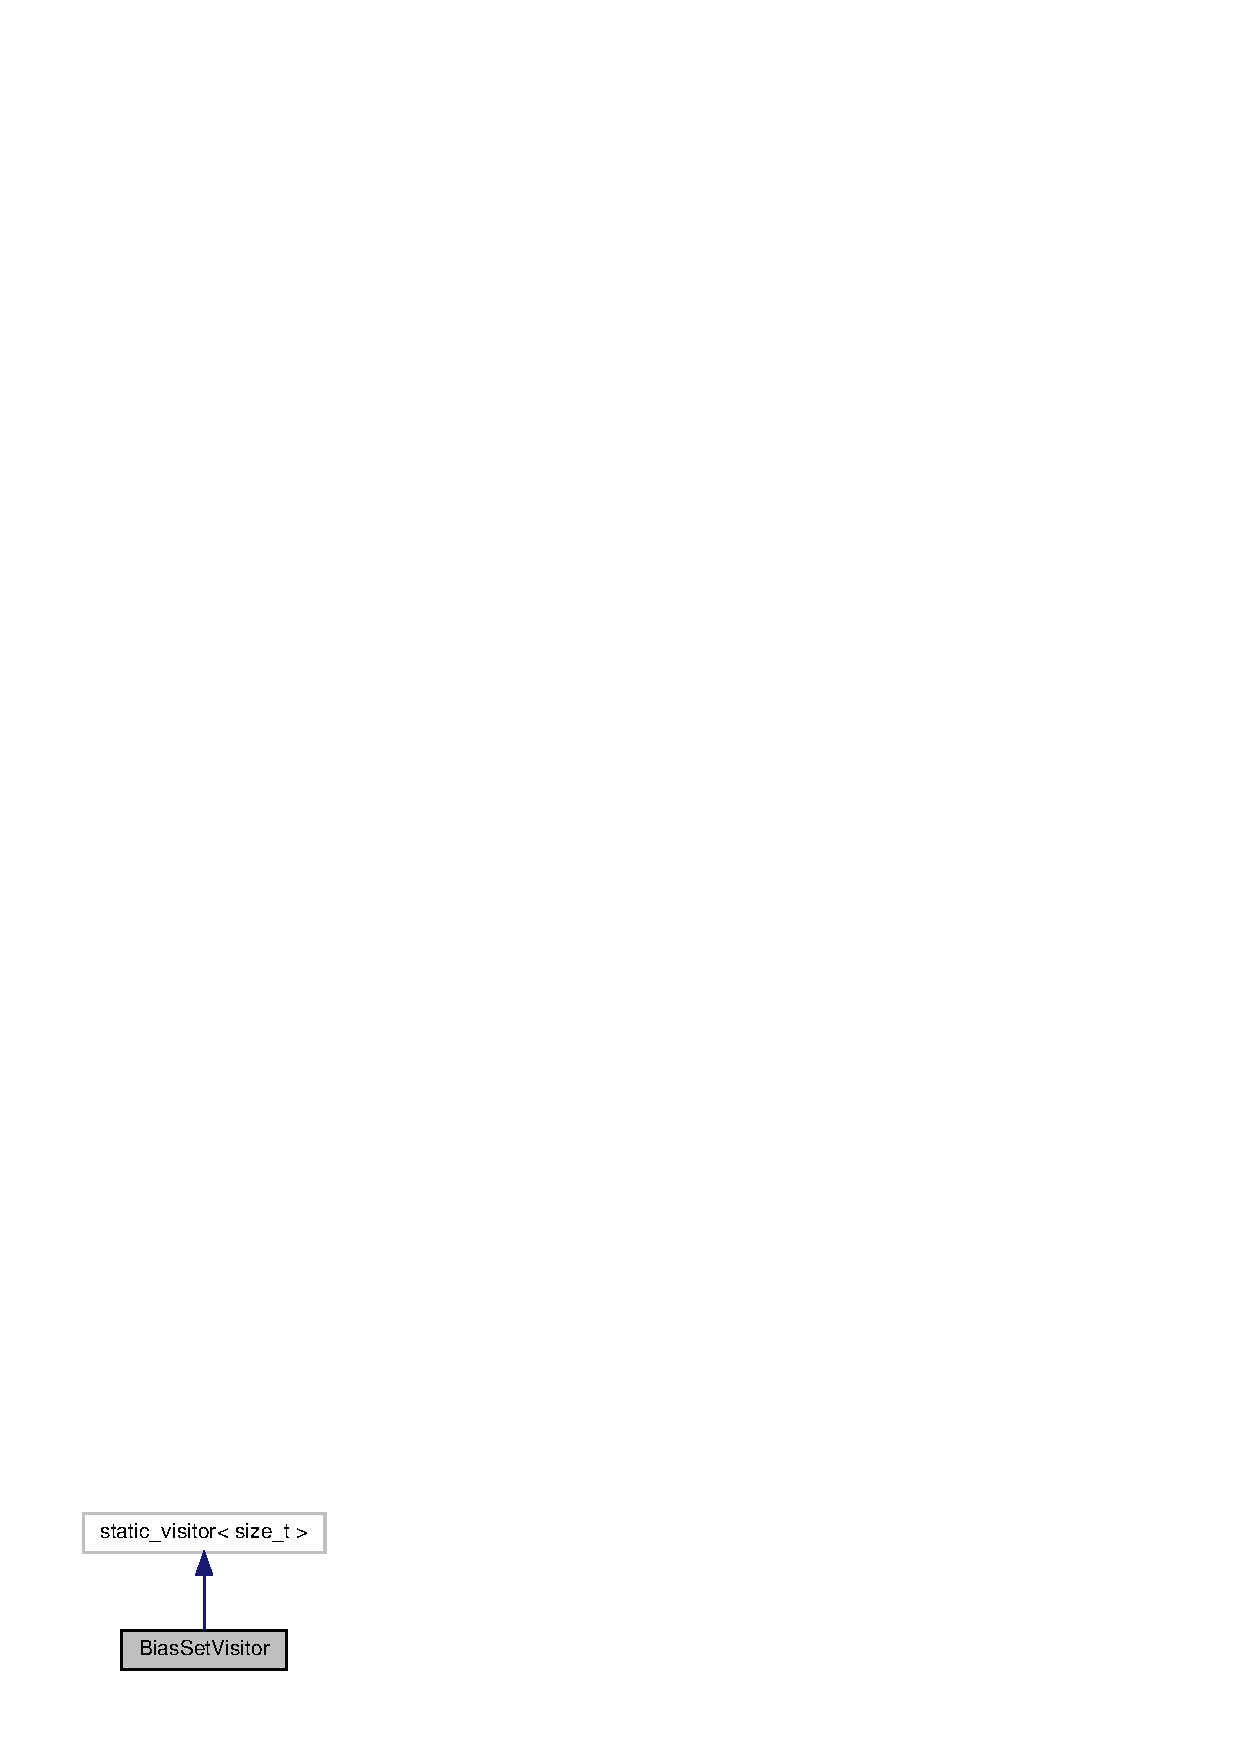
\includegraphics[width=160pt]{classmlpack_1_1ann_1_1BiasSetVisitor__inherit__graph}
\end{center}
\end{figure}
\subsection*{Public Member Functions}
\begin{DoxyCompactItemize}
\item 
\textbf{ Bias\+Set\+Visitor} (arma\+::mat \&weight, const size\+\_\+t offset=0)
\begin{DoxyCompactList}\small\item\em Update the bias parameters given the parameters\textquotesingle{} set and offset. \end{DoxyCompactList}\item 
{\footnotesize template$<$typename Layer\+Type $>$ }\\size\+\_\+t \textbf{ operator()} (Layer\+Type $\ast$layer) const
\begin{DoxyCompactList}\small\item\em Update the parameters\textquotesingle{} set. \end{DoxyCompactList}\item 
size\+\_\+t \textbf{ operator()} (\textbf{ More\+Types} layer) const
\end{DoxyCompactItemize}


\subsection{Detailed Description}
\doxyref{Bias\+Set\+Visitor}{p.}{classmlpack_1_1ann_1_1BiasSetVisitor} updates the module bias parameters given the parameters set. 

Definition at line 26 of file bias\+\_\+set\+\_\+visitor.\+hpp.



\subsection{Constructor \& Destructor Documentation}
\mbox{\label{classmlpack_1_1ann_1_1BiasSetVisitor_a7a0ca6528b9e1468101e7f32e284309b}} 
\index{mlpack\+::ann\+::\+Bias\+Set\+Visitor@{mlpack\+::ann\+::\+Bias\+Set\+Visitor}!Bias\+Set\+Visitor@{Bias\+Set\+Visitor}}
\index{Bias\+Set\+Visitor@{Bias\+Set\+Visitor}!mlpack\+::ann\+::\+Bias\+Set\+Visitor@{mlpack\+::ann\+::\+Bias\+Set\+Visitor}}
\subsubsection{Bias\+Set\+Visitor()}
{\footnotesize\ttfamily \textbf{ Bias\+Set\+Visitor} (\begin{DoxyParamCaption}\item[{arma\+::mat \&}]{weight,  }\item[{const size\+\_\+t}]{offset = {\ttfamily 0} }\end{DoxyParamCaption})}



Update the bias parameters given the parameters\textquotesingle{} set and offset. 



\subsection{Member Function Documentation}
\mbox{\label{classmlpack_1_1ann_1_1BiasSetVisitor_aeb8947a28d511a7a4ce42a1fc63f79ee}} 
\index{mlpack\+::ann\+::\+Bias\+Set\+Visitor@{mlpack\+::ann\+::\+Bias\+Set\+Visitor}!operator()@{operator()}}
\index{operator()@{operator()}!mlpack\+::ann\+::\+Bias\+Set\+Visitor@{mlpack\+::ann\+::\+Bias\+Set\+Visitor}}
\subsubsection{operator()()\hspace{0.1cm}{\footnotesize\ttfamily [1/2]}}
{\footnotesize\ttfamily size\+\_\+t operator() (\begin{DoxyParamCaption}\item[{Layer\+Type $\ast$}]{layer }\end{DoxyParamCaption}) const}



Update the parameters\textquotesingle{} set. 

\mbox{\label{classmlpack_1_1ann_1_1BiasSetVisitor_a19a2b78859e4e91b86170544dbd8ae09}} 
\index{mlpack\+::ann\+::\+Bias\+Set\+Visitor@{mlpack\+::ann\+::\+Bias\+Set\+Visitor}!operator()@{operator()}}
\index{operator()@{operator()}!mlpack\+::ann\+::\+Bias\+Set\+Visitor@{mlpack\+::ann\+::\+Bias\+Set\+Visitor}}
\subsubsection{operator()()\hspace{0.1cm}{\footnotesize\ttfamily [2/2]}}
{\footnotesize\ttfamily size\+\_\+t operator() (\begin{DoxyParamCaption}\item[{\textbf{ More\+Types}}]{layer }\end{DoxyParamCaption}) const}



The documentation for this class was generated from the following file\+:\begin{DoxyCompactItemize}
\item 
/home/aakash/mlpack/src/mlpack/methods/ann/visitor/\textbf{ bias\+\_\+set\+\_\+visitor.\+hpp}\end{DoxyCompactItemize}

\section{Bilinear\+Interpolation$<$ Input\+Data\+Type, Output\+Data\+Type $>$ Class Template Reference}
\label{classmlpack_1_1ann_1_1BilinearInterpolation}\index{Bilinear\+Interpolation$<$ Input\+Data\+Type, Output\+Data\+Type $>$@{Bilinear\+Interpolation$<$ Input\+Data\+Type, Output\+Data\+Type $>$}}


Definition and Implementation of the Bilinear Interpolation Layer.  


\subsection*{Public Member Functions}
\begin{DoxyCompactItemize}
\item 
\textbf{ Bilinear\+Interpolation} ()
\begin{DoxyCompactList}\small\item\em Create the Bilinear Interpolation object. \end{DoxyCompactList}\item 
\textbf{ Bilinear\+Interpolation} (const size\+\_\+t in\+Row\+Size, const size\+\_\+t in\+Col\+Size, const size\+\_\+t out\+Row\+Size, const size\+\_\+t out\+Col\+Size, const size\+\_\+t depth)
\begin{DoxyCompactList}\small\item\em The constructor for the Bilinear Interpolation. \end{DoxyCompactList}\item 
{\footnotesize template$<$typename eT $>$ }\\void \textbf{ Backward} (const arma\+::\+Mat$<$ eT $>$ \&, const arma\+::\+Mat$<$ eT $>$ \&gradient, arma\+::\+Mat$<$ eT $>$ \&output)
\begin{DoxyCompactList}\small\item\em Ordinary feed backward pass of a neural network, calculating the function f(x) by propagating x backwards through f. \end{DoxyCompactList}\item 
Output\+Data\+Type const  \& \textbf{ Delta} () const
\begin{DoxyCompactList}\small\item\em Get the delta. \end{DoxyCompactList}\item 
Output\+Data\+Type \& \textbf{ Delta} ()
\begin{DoxyCompactList}\small\item\em Modify the delta. \end{DoxyCompactList}\item 
{\footnotesize template$<$typename eT $>$ }\\void \textbf{ Forward} (const arma\+::\+Mat$<$ eT $>$ \&input, arma\+::\+Mat$<$ eT $>$ \&output)
\begin{DoxyCompactList}\small\item\em Forward pass through the layer. \end{DoxyCompactList}\item 
size\+\_\+t const  \& \textbf{ In\+Col\+Size} () const
\begin{DoxyCompactList}\small\item\em Get the column size of the input. \end{DoxyCompactList}\item 
size\+\_\+t \& \textbf{ In\+Col\+Size} ()
\begin{DoxyCompactList}\small\item\em Modify the column size of the input. \end{DoxyCompactList}\item 
size\+\_\+t const  \& \textbf{ In\+Depth} () const
\begin{DoxyCompactList}\small\item\em Get the depth of the input. \end{DoxyCompactList}\item 
size\+\_\+t \& \textbf{ In\+Depth} ()
\begin{DoxyCompactList}\small\item\em Modify the depth of the input. \end{DoxyCompactList}\item 
size\+\_\+t \textbf{ Input\+Shape} () const
\begin{DoxyCompactList}\small\item\em Get the shape of the input. \end{DoxyCompactList}\item 
size\+\_\+t const  \& \textbf{ In\+Row\+Size} () const
\begin{DoxyCompactList}\small\item\em Get the row size of the input. \end{DoxyCompactList}\item 
size\+\_\+t \& \textbf{ In\+Row\+Size} ()
\begin{DoxyCompactList}\small\item\em Modify the row size of the input. \end{DoxyCompactList}\item 
size\+\_\+t const  \& \textbf{ Out\+Col\+Size} () const
\begin{DoxyCompactList}\small\item\em Get the column size of the output. \end{DoxyCompactList}\item 
size\+\_\+t \& \textbf{ Out\+Col\+Size} ()
\begin{DoxyCompactList}\small\item\em Modify the column size of the output. \end{DoxyCompactList}\item 
Output\+Data\+Type const  \& \textbf{ Output\+Parameter} () const
\begin{DoxyCompactList}\small\item\em Get the output parameter. \end{DoxyCompactList}\item 
Output\+Data\+Type \& \textbf{ Output\+Parameter} ()
\begin{DoxyCompactList}\small\item\em Modify the output parameter. \end{DoxyCompactList}\item 
size\+\_\+t const  \& \textbf{ Out\+Row\+Size} () const
\begin{DoxyCompactList}\small\item\em Get the row size of the output. \end{DoxyCompactList}\item 
size\+\_\+t \& \textbf{ Out\+Row\+Size} ()
\begin{DoxyCompactList}\small\item\em Modify the row size of the output. \end{DoxyCompactList}\item 
{\footnotesize template$<$typename Archive $>$ }\\void \textbf{ serialize} (Archive \&ar, const uint32\+\_\+t)
\begin{DoxyCompactList}\small\item\em Serialize the layer. \end{DoxyCompactList}\end{DoxyCompactItemize}


\subsection{Detailed Description}
\subsubsection*{template$<$typename Input\+Data\+Type = arma\+::mat, typename Output\+Data\+Type = arma\+::mat$>$\newline
class mlpack\+::ann\+::\+Bilinear\+Interpolation$<$ Input\+Data\+Type, Output\+Data\+Type $>$}

Definition and Implementation of the Bilinear Interpolation Layer. 

Bilinear Interpolation is an mathematical technique, primarily used for scaling purposes. It is an extension of linear interpolation, for interpolating functions of two variables on a rectangular grid. The key idea is to perform linear interpolation first in one direction (e.\+g., along x-\/axis), and then again in the other direction (i.\+e., y-\/axis), on four different known points in the grid. This way, we represent any arbitrary point, present within the grid, as a function of those four points.


\begin{DoxyTemplParams}{Template Parameters}
{\em Input\+Data\+Type} & Type of the input data (arma\+::colvec, arma\+::mat, arma\+::sp\+\_\+mat or arma\+::cube). \\
\hline
{\em Output\+Data\+Type} & Type of the output data (arma\+::colvec, arma\+::mat, arma\+::sp\+\_\+mat or arma\+::cube). \\
\hline
\end{DoxyTemplParams}


Definition at line 39 of file bilinear\+\_\+interpolation.\+hpp.



\subsection{Constructor \& Destructor Documentation}
\mbox{\label{classmlpack_1_1ann_1_1BilinearInterpolation_a8373b0b3b099c636a8e438baadfa3baf}} 
\index{mlpack\+::ann\+::\+Bilinear\+Interpolation@{mlpack\+::ann\+::\+Bilinear\+Interpolation}!Bilinear\+Interpolation@{Bilinear\+Interpolation}}
\index{Bilinear\+Interpolation@{Bilinear\+Interpolation}!mlpack\+::ann\+::\+Bilinear\+Interpolation@{mlpack\+::ann\+::\+Bilinear\+Interpolation}}
\subsubsection{Bilinear\+Interpolation()\hspace{0.1cm}{\footnotesize\ttfamily [1/2]}}
{\footnotesize\ttfamily \textbf{ Bilinear\+Interpolation} (\begin{DoxyParamCaption}{ }\end{DoxyParamCaption})}



Create the Bilinear Interpolation object. 

\mbox{\label{classmlpack_1_1ann_1_1BilinearInterpolation_ad384fa6deb9134484dea8961a70df35f}} 
\index{mlpack\+::ann\+::\+Bilinear\+Interpolation@{mlpack\+::ann\+::\+Bilinear\+Interpolation}!Bilinear\+Interpolation@{Bilinear\+Interpolation}}
\index{Bilinear\+Interpolation@{Bilinear\+Interpolation}!mlpack\+::ann\+::\+Bilinear\+Interpolation@{mlpack\+::ann\+::\+Bilinear\+Interpolation}}
\subsubsection{Bilinear\+Interpolation()\hspace{0.1cm}{\footnotesize\ttfamily [2/2]}}
{\footnotesize\ttfamily \textbf{ Bilinear\+Interpolation} (\begin{DoxyParamCaption}\item[{const size\+\_\+t}]{in\+Row\+Size,  }\item[{const size\+\_\+t}]{in\+Col\+Size,  }\item[{const size\+\_\+t}]{out\+Row\+Size,  }\item[{const size\+\_\+t}]{out\+Col\+Size,  }\item[{const size\+\_\+t}]{depth }\end{DoxyParamCaption})}



The constructor for the Bilinear Interpolation. 


\begin{DoxyParams}{Parameters}
{\em in\+Row\+Size} & Number of input rows. \\
\hline
{\em in\+Col\+Size} & Number of input columns. \\
\hline
{\em out\+Row\+Size} & Number of output rows. \\
\hline
{\em out\+Col\+Size} & Number of output columns. \\
\hline
{\em depth} & Number of input slices. \\
\hline
\end{DoxyParams}


\subsection{Member Function Documentation}
\mbox{\label{classmlpack_1_1ann_1_1BilinearInterpolation_a633ef28f24c29c3438a9205786e817a3}} 
\index{mlpack\+::ann\+::\+Bilinear\+Interpolation@{mlpack\+::ann\+::\+Bilinear\+Interpolation}!Backward@{Backward}}
\index{Backward@{Backward}!mlpack\+::ann\+::\+Bilinear\+Interpolation@{mlpack\+::ann\+::\+Bilinear\+Interpolation}}
\subsubsection{Backward()}
{\footnotesize\ttfamily void Backward (\begin{DoxyParamCaption}\item[{const arma\+::\+Mat$<$ eT $>$ \&}]{,  }\item[{const arma\+::\+Mat$<$ eT $>$ \&}]{gradient,  }\item[{arma\+::\+Mat$<$ eT $>$ \&}]{output }\end{DoxyParamCaption})}



Ordinary feed backward pass of a neural network, calculating the function f(x) by propagating x backwards through f. 

Using the results from the feed forward pass. Since the layer does not have any learn-\/able parameters, we just have to down-\/sample the gradient to make its size compatible with the input size.


\begin{DoxyParams}{Parameters}
{\em $\ast$} & (input) The input matrix. \\
\hline
{\em gradient} & The computed backward gradient. \\
\hline
{\em output} & The resulting down-\/sampled output. \\
\hline
\end{DoxyParams}
\mbox{\label{classmlpack_1_1ann_1_1BilinearInterpolation_a797f7edb44dd081e5e2b3cc316eef6bd}} 
\index{mlpack\+::ann\+::\+Bilinear\+Interpolation@{mlpack\+::ann\+::\+Bilinear\+Interpolation}!Delta@{Delta}}
\index{Delta@{Delta}!mlpack\+::ann\+::\+Bilinear\+Interpolation@{mlpack\+::ann\+::\+Bilinear\+Interpolation}}
\subsubsection{Delta()\hspace{0.1cm}{\footnotesize\ttfamily [1/2]}}
{\footnotesize\ttfamily Output\+Data\+Type const\& Delta (\begin{DoxyParamCaption}{ }\end{DoxyParamCaption}) const\hspace{0.3cm}{\ttfamily [inline]}}



Get the delta. 



Definition at line 92 of file bilinear\+\_\+interpolation.\+hpp.

\mbox{\label{classmlpack_1_1ann_1_1BilinearInterpolation_ad6601342d560219ce951d554e69e5e87}} 
\index{mlpack\+::ann\+::\+Bilinear\+Interpolation@{mlpack\+::ann\+::\+Bilinear\+Interpolation}!Delta@{Delta}}
\index{Delta@{Delta}!mlpack\+::ann\+::\+Bilinear\+Interpolation@{mlpack\+::ann\+::\+Bilinear\+Interpolation}}
\subsubsection{Delta()\hspace{0.1cm}{\footnotesize\ttfamily [2/2]}}
{\footnotesize\ttfamily Output\+Data\+Type\& Delta (\begin{DoxyParamCaption}{ }\end{DoxyParamCaption})\hspace{0.3cm}{\ttfamily [inline]}}



Modify the delta. 



Definition at line 94 of file bilinear\+\_\+interpolation.\+hpp.

\mbox{\label{classmlpack_1_1ann_1_1BilinearInterpolation_a461f849bc638c15bec262dc9c3a58abe}} 
\index{mlpack\+::ann\+::\+Bilinear\+Interpolation@{mlpack\+::ann\+::\+Bilinear\+Interpolation}!Forward@{Forward}}
\index{Forward@{Forward}!mlpack\+::ann\+::\+Bilinear\+Interpolation@{mlpack\+::ann\+::\+Bilinear\+Interpolation}}
\subsubsection{Forward()}
{\footnotesize\ttfamily void Forward (\begin{DoxyParamCaption}\item[{const arma\+::\+Mat$<$ eT $>$ \&}]{input,  }\item[{arma\+::\+Mat$<$ eT $>$ \&}]{output }\end{DoxyParamCaption})}



Forward pass through the layer. 

The layer interpolates the matrix using the given Bilinear Interpolation method.


\begin{DoxyParams}{Parameters}
{\em input} & The input matrix. \\
\hline
{\em output} & The resulting interpolated output matrix. \\
\hline
\end{DoxyParams}
\mbox{\label{classmlpack_1_1ann_1_1BilinearInterpolation_a3866c02efcb03b37b6df7bb8299c889b}} 
\index{mlpack\+::ann\+::\+Bilinear\+Interpolation@{mlpack\+::ann\+::\+Bilinear\+Interpolation}!In\+Col\+Size@{In\+Col\+Size}}
\index{In\+Col\+Size@{In\+Col\+Size}!mlpack\+::ann\+::\+Bilinear\+Interpolation@{mlpack\+::ann\+::\+Bilinear\+Interpolation}}
\subsubsection{In\+Col\+Size()\hspace{0.1cm}{\footnotesize\ttfamily [1/2]}}
{\footnotesize\ttfamily size\+\_\+t const\& In\+Col\+Size (\begin{DoxyParamCaption}{ }\end{DoxyParamCaption}) const\hspace{0.3cm}{\ttfamily [inline]}}



Get the column size of the input. 



Definition at line 102 of file bilinear\+\_\+interpolation.\+hpp.

\mbox{\label{classmlpack_1_1ann_1_1BilinearInterpolation_a1df27f614ba64eb812606a2971005a5e}} 
\index{mlpack\+::ann\+::\+Bilinear\+Interpolation@{mlpack\+::ann\+::\+Bilinear\+Interpolation}!In\+Col\+Size@{In\+Col\+Size}}
\index{In\+Col\+Size@{In\+Col\+Size}!mlpack\+::ann\+::\+Bilinear\+Interpolation@{mlpack\+::ann\+::\+Bilinear\+Interpolation}}
\subsubsection{In\+Col\+Size()\hspace{0.1cm}{\footnotesize\ttfamily [2/2]}}
{\footnotesize\ttfamily size\+\_\+t\& In\+Col\+Size (\begin{DoxyParamCaption}{ }\end{DoxyParamCaption})\hspace{0.3cm}{\ttfamily [inline]}}



Modify the column size of the input. 



Definition at line 104 of file bilinear\+\_\+interpolation.\+hpp.

\mbox{\label{classmlpack_1_1ann_1_1BilinearInterpolation_aacd90229a50c3271523c62556287d0d6}} 
\index{mlpack\+::ann\+::\+Bilinear\+Interpolation@{mlpack\+::ann\+::\+Bilinear\+Interpolation}!In\+Depth@{In\+Depth}}
\index{In\+Depth@{In\+Depth}!mlpack\+::ann\+::\+Bilinear\+Interpolation@{mlpack\+::ann\+::\+Bilinear\+Interpolation}}
\subsubsection{In\+Depth()\hspace{0.1cm}{\footnotesize\ttfamily [1/2]}}
{\footnotesize\ttfamily size\+\_\+t const\& In\+Depth (\begin{DoxyParamCaption}{ }\end{DoxyParamCaption}) const\hspace{0.3cm}{\ttfamily [inline]}}



Get the depth of the input. 



Definition at line 117 of file bilinear\+\_\+interpolation.\+hpp.

\mbox{\label{classmlpack_1_1ann_1_1BilinearInterpolation_a0ba6062be684978ed809bd7abe917789}} 
\index{mlpack\+::ann\+::\+Bilinear\+Interpolation@{mlpack\+::ann\+::\+Bilinear\+Interpolation}!In\+Depth@{In\+Depth}}
\index{In\+Depth@{In\+Depth}!mlpack\+::ann\+::\+Bilinear\+Interpolation@{mlpack\+::ann\+::\+Bilinear\+Interpolation}}
\subsubsection{In\+Depth()\hspace{0.1cm}{\footnotesize\ttfamily [2/2]}}
{\footnotesize\ttfamily size\+\_\+t\& In\+Depth (\begin{DoxyParamCaption}{ }\end{DoxyParamCaption})\hspace{0.3cm}{\ttfamily [inline]}}



Modify the depth of the input. 



Definition at line 119 of file bilinear\+\_\+interpolation.\+hpp.

\mbox{\label{classmlpack_1_1ann_1_1BilinearInterpolation_a13ab93f234244a68f6ade76287284447}} 
\index{mlpack\+::ann\+::\+Bilinear\+Interpolation@{mlpack\+::ann\+::\+Bilinear\+Interpolation}!Input\+Shape@{Input\+Shape}}
\index{Input\+Shape@{Input\+Shape}!mlpack\+::ann\+::\+Bilinear\+Interpolation@{mlpack\+::ann\+::\+Bilinear\+Interpolation}}
\subsubsection{Input\+Shape()}
{\footnotesize\ttfamily size\+\_\+t Input\+Shape (\begin{DoxyParamCaption}{ }\end{DoxyParamCaption}) const\hspace{0.3cm}{\ttfamily [inline]}}



Get the shape of the input. 



Definition at line 122 of file bilinear\+\_\+interpolation.\+hpp.



References Bilinear\+Interpolation$<$ Input\+Data\+Type, Output\+Data\+Type $>$\+::serialize().

\mbox{\label{classmlpack_1_1ann_1_1BilinearInterpolation_a913067c139b71a0e8ca5f1c28244becf}} 
\index{mlpack\+::ann\+::\+Bilinear\+Interpolation@{mlpack\+::ann\+::\+Bilinear\+Interpolation}!In\+Row\+Size@{In\+Row\+Size}}
\index{In\+Row\+Size@{In\+Row\+Size}!mlpack\+::ann\+::\+Bilinear\+Interpolation@{mlpack\+::ann\+::\+Bilinear\+Interpolation}}
\subsubsection{In\+Row\+Size()\hspace{0.1cm}{\footnotesize\ttfamily [1/2]}}
{\footnotesize\ttfamily size\+\_\+t const\& In\+Row\+Size (\begin{DoxyParamCaption}{ }\end{DoxyParamCaption}) const\hspace{0.3cm}{\ttfamily [inline]}}



Get the row size of the input. 



Definition at line 97 of file bilinear\+\_\+interpolation.\+hpp.

\mbox{\label{classmlpack_1_1ann_1_1BilinearInterpolation_a3057ecd053b3a1e5e744efeabc33fec3}} 
\index{mlpack\+::ann\+::\+Bilinear\+Interpolation@{mlpack\+::ann\+::\+Bilinear\+Interpolation}!In\+Row\+Size@{In\+Row\+Size}}
\index{In\+Row\+Size@{In\+Row\+Size}!mlpack\+::ann\+::\+Bilinear\+Interpolation@{mlpack\+::ann\+::\+Bilinear\+Interpolation}}
\subsubsection{In\+Row\+Size()\hspace{0.1cm}{\footnotesize\ttfamily [2/2]}}
{\footnotesize\ttfamily size\+\_\+t\& In\+Row\+Size (\begin{DoxyParamCaption}{ }\end{DoxyParamCaption})\hspace{0.3cm}{\ttfamily [inline]}}



Modify the row size of the input. 



Definition at line 99 of file bilinear\+\_\+interpolation.\+hpp.

\mbox{\label{classmlpack_1_1ann_1_1BilinearInterpolation_ad414d1f042fe0df8c4ccbbfcb1e3a482}} 
\index{mlpack\+::ann\+::\+Bilinear\+Interpolation@{mlpack\+::ann\+::\+Bilinear\+Interpolation}!Out\+Col\+Size@{Out\+Col\+Size}}
\index{Out\+Col\+Size@{Out\+Col\+Size}!mlpack\+::ann\+::\+Bilinear\+Interpolation@{mlpack\+::ann\+::\+Bilinear\+Interpolation}}
\subsubsection{Out\+Col\+Size()\hspace{0.1cm}{\footnotesize\ttfamily [1/2]}}
{\footnotesize\ttfamily size\+\_\+t const\& Out\+Col\+Size (\begin{DoxyParamCaption}{ }\end{DoxyParamCaption}) const\hspace{0.3cm}{\ttfamily [inline]}}



Get the column size of the output. 



Definition at line 112 of file bilinear\+\_\+interpolation.\+hpp.

\mbox{\label{classmlpack_1_1ann_1_1BilinearInterpolation_a0430a9583e828be9d8b325221cfdf01b}} 
\index{mlpack\+::ann\+::\+Bilinear\+Interpolation@{mlpack\+::ann\+::\+Bilinear\+Interpolation}!Out\+Col\+Size@{Out\+Col\+Size}}
\index{Out\+Col\+Size@{Out\+Col\+Size}!mlpack\+::ann\+::\+Bilinear\+Interpolation@{mlpack\+::ann\+::\+Bilinear\+Interpolation}}
\subsubsection{Out\+Col\+Size()\hspace{0.1cm}{\footnotesize\ttfamily [2/2]}}
{\footnotesize\ttfamily size\+\_\+t\& Out\+Col\+Size (\begin{DoxyParamCaption}{ }\end{DoxyParamCaption})\hspace{0.3cm}{\ttfamily [inline]}}



Modify the column size of the output. 



Definition at line 114 of file bilinear\+\_\+interpolation.\+hpp.

\mbox{\label{classmlpack_1_1ann_1_1BilinearInterpolation_a0ee21c2a36e5abad1e7a9d5dd00849f9}} 
\index{mlpack\+::ann\+::\+Bilinear\+Interpolation@{mlpack\+::ann\+::\+Bilinear\+Interpolation}!Output\+Parameter@{Output\+Parameter}}
\index{Output\+Parameter@{Output\+Parameter}!mlpack\+::ann\+::\+Bilinear\+Interpolation@{mlpack\+::ann\+::\+Bilinear\+Interpolation}}
\subsubsection{Output\+Parameter()\hspace{0.1cm}{\footnotesize\ttfamily [1/2]}}
{\footnotesize\ttfamily Output\+Data\+Type const\& Output\+Parameter (\begin{DoxyParamCaption}{ }\end{DoxyParamCaption}) const\hspace{0.3cm}{\ttfamily [inline]}}



Get the output parameter. 



Definition at line 87 of file bilinear\+\_\+interpolation.\+hpp.

\mbox{\label{classmlpack_1_1ann_1_1BilinearInterpolation_a21d5f745f02c709625a4ee0907f004a5}} 
\index{mlpack\+::ann\+::\+Bilinear\+Interpolation@{mlpack\+::ann\+::\+Bilinear\+Interpolation}!Output\+Parameter@{Output\+Parameter}}
\index{Output\+Parameter@{Output\+Parameter}!mlpack\+::ann\+::\+Bilinear\+Interpolation@{mlpack\+::ann\+::\+Bilinear\+Interpolation}}
\subsubsection{Output\+Parameter()\hspace{0.1cm}{\footnotesize\ttfamily [2/2]}}
{\footnotesize\ttfamily Output\+Data\+Type\& Output\+Parameter (\begin{DoxyParamCaption}{ }\end{DoxyParamCaption})\hspace{0.3cm}{\ttfamily [inline]}}



Modify the output parameter. 



Definition at line 89 of file bilinear\+\_\+interpolation.\+hpp.

\mbox{\label{classmlpack_1_1ann_1_1BilinearInterpolation_a0e4acfe53c207e4b3fba11525be06458}} 
\index{mlpack\+::ann\+::\+Bilinear\+Interpolation@{mlpack\+::ann\+::\+Bilinear\+Interpolation}!Out\+Row\+Size@{Out\+Row\+Size}}
\index{Out\+Row\+Size@{Out\+Row\+Size}!mlpack\+::ann\+::\+Bilinear\+Interpolation@{mlpack\+::ann\+::\+Bilinear\+Interpolation}}
\subsubsection{Out\+Row\+Size()\hspace{0.1cm}{\footnotesize\ttfamily [1/2]}}
{\footnotesize\ttfamily size\+\_\+t const\& Out\+Row\+Size (\begin{DoxyParamCaption}{ }\end{DoxyParamCaption}) const\hspace{0.3cm}{\ttfamily [inline]}}



Get the row size of the output. 



Definition at line 107 of file bilinear\+\_\+interpolation.\+hpp.

\mbox{\label{classmlpack_1_1ann_1_1BilinearInterpolation_a5061d94d050e5c78e8374801db4c2a9b}} 
\index{mlpack\+::ann\+::\+Bilinear\+Interpolation@{mlpack\+::ann\+::\+Bilinear\+Interpolation}!Out\+Row\+Size@{Out\+Row\+Size}}
\index{Out\+Row\+Size@{Out\+Row\+Size}!mlpack\+::ann\+::\+Bilinear\+Interpolation@{mlpack\+::ann\+::\+Bilinear\+Interpolation}}
\subsubsection{Out\+Row\+Size()\hspace{0.1cm}{\footnotesize\ttfamily [2/2]}}
{\footnotesize\ttfamily size\+\_\+t\& Out\+Row\+Size (\begin{DoxyParamCaption}{ }\end{DoxyParamCaption})\hspace{0.3cm}{\ttfamily [inline]}}



Modify the row size of the output. 



Definition at line 109 of file bilinear\+\_\+interpolation.\+hpp.

\mbox{\label{classmlpack_1_1ann_1_1BilinearInterpolation_a65cba07328997659bec80b9879b15a51}} 
\index{mlpack\+::ann\+::\+Bilinear\+Interpolation@{mlpack\+::ann\+::\+Bilinear\+Interpolation}!serialize@{serialize}}
\index{serialize@{serialize}!mlpack\+::ann\+::\+Bilinear\+Interpolation@{mlpack\+::ann\+::\+Bilinear\+Interpolation}}
\subsubsection{serialize()}
{\footnotesize\ttfamily void serialize (\begin{DoxyParamCaption}\item[{Archive \&}]{ar,  }\item[{const uint32\+\_\+t}]{ }\end{DoxyParamCaption})}



Serialize the layer. 



Referenced by Bilinear\+Interpolation$<$ Input\+Data\+Type, Output\+Data\+Type $>$\+::\+Input\+Shape().



The documentation for this class was generated from the following file\+:\begin{DoxyCompactItemize}
\item 
/home/aakash/mlpack/src/mlpack/methods/ann/layer/\textbf{ bilinear\+\_\+interpolation.\+hpp}\end{DoxyCompactItemize}

\section{Binary\+R\+BM Class Reference}
\label{classmlpack_1_1ann_1_1BinaryRBM}\index{Binary\+R\+BM@{Binary\+R\+BM}}


For more information, see the following paper\+:  




\subsection{Detailed Description}
For more information, see the following paper\+: 


\begin{DoxyCode}
@article\{Hinton10,
  author    = \{Geoffrey Hinton\},
  title     = \{A Practical Guide to Training Restricted Boltzmann Machines\},
  year      = \{2010\},
  url       = \{https:\textcolor{comment}{//www.cs.toronto.edu/~hinton/absps/guideTR.pdf\}}
\}
\end{DoxyCode}
 

Definition at line 30 of file rbm\+\_\+policies.\+hpp.



The documentation for this class was generated from the following file\+:\begin{DoxyCompactItemize}
\item 
/home/aakash/mlpack/src/mlpack/methods/ann/rbm/\textbf{ rbm\+\_\+policies.\+hpp}\end{DoxyCompactItemize}

\section{B\+R\+NN$<$ Output\+Layer\+Type, Merge\+Layer\+Type, Merge\+Output\+Type, Initialization\+Rule\+Type, Custom\+Layers $>$ Class Template Reference}
\label{classmlpack_1_1ann_1_1BRNN}\index{B\+R\+N\+N$<$ Output\+Layer\+Type, Merge\+Layer\+Type, Merge\+Output\+Type, Initialization\+Rule\+Type, Custom\+Layers $>$@{B\+R\+N\+N$<$ Output\+Layer\+Type, Merge\+Layer\+Type, Merge\+Output\+Type, Initialization\+Rule\+Type, Custom\+Layers $>$}}


Implementation of a standard bidirectional recurrent neural network container.  


\subsection*{Public Types}
\begin{DoxyCompactItemize}
\item 
using \textbf{ Network\+Type} = \textbf{ B\+R\+NN}$<$ Output\+Layer\+Type, Merge\+Layer\+Type, Merge\+Output\+Type, Initialization\+Rule\+Type, Custom\+Layers... $>$
\begin{DoxyCompactList}\small\item\em Convenience typedef for the internal model construction. \end{DoxyCompactList}\end{DoxyCompactItemize}
\subsection*{Public Member Functions}
\begin{DoxyCompactItemize}
\item 
\textbf{ B\+R\+NN} (const size\+\_\+t rho, const bool single=false, Output\+Layer\+Type output\+Layer=Output\+Layer\+Type(), Merge\+Layer\+Type $\ast$merge\+Layer=new Merge\+Layer\+Type(), Merge\+Output\+Type $\ast$merge\+Output=new Merge\+Output\+Type(), Initialization\+Rule\+Type initialize\+Rule=Initialization\+Rule\+Type())
\begin{DoxyCompactList}\small\item\em Create the \doxyref{B\+R\+NN}{p.}{classmlpack_1_1ann_1_1BRNN} object. \end{DoxyCompactList}\item 
\textbf{ $\sim$\+B\+R\+NN} ()
\item 
{\footnotesize template$<$class Layer\+Type , class... Args$>$ }\\void \textbf{ Add} (Args... args)
\item 
void \textbf{ Add} (\textbf{ Layer\+Types}$<$ Custom\+Layers... $>$ layer)
\item 
double \textbf{ Evaluate} (const arma\+::mat \&parameters, const size\+\_\+t begin, const size\+\_\+t batch\+Size, const bool deterministic)
\begin{DoxyCompactList}\small\item\em Evaluate the bidirectional recurrent neural network with the given parameters. \end{DoxyCompactList}\item 
double \textbf{ Evaluate} (const arma\+::mat \&parameters, const size\+\_\+t begin, const size\+\_\+t batch\+Size)
\begin{DoxyCompactList}\small\item\em Evaluate the bidirectional recurrent neural network with the given parameters. \end{DoxyCompactList}\item 
{\footnotesize template$<$typename Grad\+Type $>$ }\\double \textbf{ Evaluate\+With\+Gradient} (const arma\+::mat \&parameters, const size\+\_\+t begin, Grad\+Type \&gradient, const size\+\_\+t batch\+Size)
\begin{DoxyCompactList}\small\item\em Evaluate the bidirectional recurrent neural network with the given parameters. \end{DoxyCompactList}\item 
void \textbf{ Gradient} (const arma\+::mat \&parameters, const size\+\_\+t begin, arma\+::mat \&gradient, const size\+\_\+t batch\+Size)
\begin{DoxyCompactList}\small\item\em Evaluate the gradient of the bidirectional recurrent neural network with the given parameters, and with respect to only one point in the dataset. \end{DoxyCompactList}\item 
size\+\_\+t \textbf{ Num\+Functions} () const
\begin{DoxyCompactList}\small\item\em Return the number of separable functions. (number of predictor points). \end{DoxyCompactList}\item 
const arma\+::mat \& \textbf{ Parameters} () const
\begin{DoxyCompactList}\small\item\em Return the initial point for the optimization. \end{DoxyCompactList}\item 
arma\+::mat \& \textbf{ Parameters} ()
\begin{DoxyCompactList}\small\item\em Modify the initial point for the optimization. \end{DoxyCompactList}\item 
void \textbf{ Predict} (arma\+::cube predictors, arma\+::cube \&results, const size\+\_\+t batch\+Size=256)
\begin{DoxyCompactList}\small\item\em Predict the responses to a given set of predictors. \end{DoxyCompactList}\item 
const arma\+::cube \& \textbf{ Predictors} () const
\begin{DoxyCompactList}\small\item\em Get the matrix of data points (predictors). \end{DoxyCompactList}\item 
arma\+::cube \& \textbf{ Predictors} ()
\begin{DoxyCompactList}\small\item\em Modify the matrix of data points (predictors). \end{DoxyCompactList}\item 
void \textbf{ Reset} ()
\begin{DoxyCompactList}\small\item\em Reset the state of the network. \end{DoxyCompactList}\item 
void \textbf{ Reset\+Parameters} ()
\begin{DoxyCompactList}\small\item\em Reset the module information (weights/parameters). \end{DoxyCompactList}\item 
const arma\+::cube \& \textbf{ Responses} () const
\begin{DoxyCompactList}\small\item\em Get the matrix of responses to the input data points. \end{DoxyCompactList}\item 
arma\+::cube \& \textbf{ Responses} ()
\begin{DoxyCompactList}\small\item\em Modify the matrix of responses to the input data points. \end{DoxyCompactList}\item 
const size\+\_\+t \& \textbf{ Rho} () const
\begin{DoxyCompactList}\small\item\em Return the maximum length of backpropagation through time. \end{DoxyCompactList}\item 
size\+\_\+t \& \textbf{ Rho} ()
\begin{DoxyCompactList}\small\item\em Modify the maximum length of backpropagation through time. \end{DoxyCompactList}\item 
{\footnotesize template$<$typename Archive $>$ }\\void \textbf{ serialize} (Archive \&ar, const uint32\+\_\+t)
\begin{DoxyCompactList}\small\item\em Serialize the model. \end{DoxyCompactList}\item 
void \textbf{ Shuffle} ()
\begin{DoxyCompactList}\small\item\em Shuffle the order of function visitation. \end{DoxyCompactList}\item 
{\footnotesize template$<$typename Optimizer\+Type $>$ }\\double \textbf{ Train} (arma\+::cube predictors, arma\+::cube responses, Optimizer\+Type \&optimizer)
\begin{DoxyCompactList}\small\item\em Train the bidirectional recurrent neural network on the given input data using the given optimizer. \end{DoxyCompactList}\item 
{\footnotesize template$<$typename Optimizer\+Type  = ens\+::\+Standard\+S\+GD$>$ }\\double \textbf{ Train} (arma\+::cube predictors, arma\+::cube responses)
\begin{DoxyCompactList}\small\item\em Train the bidirectional recurrent neural network on the given input data. \end{DoxyCompactList}\item 
{\footnotesize template$<$typename Optimizer\+Type $>$ }\\std\+::enable\+\_\+if$<$ Has\+Max\+Iterations$<$ Optimizer\+Type, size\+\_\+t \&(Optimizer\+Type\+::$\ast$)()$>$\+::value, void $>$\+::type \textbf{ Warn\+Message\+Max\+Iterations} (Optimizer\+Type \&optimizer, size\+\_\+t samples) const
\begin{DoxyCompactList}\small\item\em Check if the optimizer has Max\+Iterations() parameter, if it does then check if it\textquotesingle{}s value is less than the number of datapoints in the dataset. \end{DoxyCompactList}\item 
{\footnotesize template$<$typename Optimizer\+Type $>$ }\\std\+::enable\+\_\+if$<$ !Has\+Max\+Iterations$<$ Optimizer\+Type, size\+\_\+t \&(Optimizer\+Type\+::$\ast$)()$>$\+::value, void $>$\+::type \textbf{ Warn\+Message\+Max\+Iterations} (Optimizer\+Type \&optimizer, size\+\_\+t samples) const
\begin{DoxyCompactList}\small\item\em Check if the optimizer has Max\+Iterations() parameter, if it doesn\textquotesingle{}t then simply return from the function. \end{DoxyCompactList}\end{DoxyCompactItemize}


\subsection{Detailed Description}
\subsubsection*{template$<$typename Output\+Layer\+Type = Negative\+Log\+Likelihood$<$$>$, typename Merge\+Layer\+Type = Concat$<$$>$, typename Merge\+Output\+Type = Log\+Soft\+Max$<$$>$, typename Initialization\+Rule\+Type = Random\+Initialization, typename... Custom\+Layers$>$\newline
class mlpack\+::ann\+::\+B\+R\+N\+N$<$ Output\+Layer\+Type, Merge\+Layer\+Type, Merge\+Output\+Type, Initialization\+Rule\+Type, Custom\+Layers $>$}

Implementation of a standard bidirectional recurrent neural network container. 


\begin{DoxyTemplParams}{Template Parameters}
{\em Output\+Layer\+Type} & The output layer type used to evaluate the network. \\
\hline
{\em Initialization\+Rule\+Type} & Rule used to initialize the weight matrix. \\
\hline
\end{DoxyTemplParams}


Definition at line 48 of file brnn.\+hpp.



\subsection{Member Typedef Documentation}
\mbox{\label{classmlpack_1_1ann_1_1BRNN_af977343dd09381ce7c70aa160dfbdd3d}} 
\index{mlpack\+::ann\+::\+B\+R\+NN@{mlpack\+::ann\+::\+B\+R\+NN}!Network\+Type@{Network\+Type}}
\index{Network\+Type@{Network\+Type}!mlpack\+::ann\+::\+B\+R\+NN@{mlpack\+::ann\+::\+B\+R\+NN}}
\subsubsection{Network\+Type}
{\footnotesize\ttfamily using \textbf{ Network\+Type} =  \textbf{ B\+R\+NN}$<$Output\+Layer\+Type, Merge\+Layer\+Type, Merge\+Output\+Type, Initialization\+Rule\+Type, Custom\+Layers...$>$}



Convenience typedef for the internal model construction. 



Definition at line 56 of file brnn.\+hpp.



\subsection{Constructor \& Destructor Documentation}
\mbox{\label{classmlpack_1_1ann_1_1BRNN_ae88bb4928222f3ccbbaab4eaa7ab80fc}} 
\index{mlpack\+::ann\+::\+B\+R\+NN@{mlpack\+::ann\+::\+B\+R\+NN}!B\+R\+NN@{B\+R\+NN}}
\index{B\+R\+NN@{B\+R\+NN}!mlpack\+::ann\+::\+B\+R\+NN@{mlpack\+::ann\+::\+B\+R\+NN}}
\subsubsection{B\+R\+N\+N()}
{\footnotesize\ttfamily \textbf{ B\+R\+NN} (\begin{DoxyParamCaption}\item[{const size\+\_\+t}]{rho,  }\item[{const bool}]{single = {\ttfamily false},  }\item[{Output\+Layer\+Type}]{output\+Layer = {\ttfamily OutputLayerType()},  }\item[{Merge\+Layer\+Type $\ast$}]{merge\+Layer = {\ttfamily new~MergeLayerType()},  }\item[{Merge\+Output\+Type $\ast$}]{merge\+Output = {\ttfamily new~MergeOutputType()},  }\item[{Initialization\+Rule\+Type}]{initialize\+Rule = {\ttfamily InitializationRuleType()} }\end{DoxyParamCaption})}



Create the \doxyref{B\+R\+NN}{p.}{classmlpack_1_1ann_1_1BRNN} object. 

Optionally, specify which initialize rule and performance function should be used.

If you want to pass in a parameter and discard the original parameter object, be sure to use std\+::move to avoid unnecessary copy.


\begin{DoxyParams}{Parameters}
{\em rho} & Maximum number of steps to backpropagate through time (B\+P\+TT). \\
\hline
{\em single} & Predict only the last element of the input sequence. \\
\hline
{\em merge\+Layer} & Merge layer to be used to evaluate the network. \\
\hline
{\em output\+Layer} & Output layer used to evaluate the network. \\
\hline
{\em merge\+Output} & Output Merge layer to be used. \\
\hline
{\em initialize\+Rule} & Optional instantiated Initialization\+Rule object for initializing the network parameter. \\
\hline
\end{DoxyParams}
\mbox{\label{classmlpack_1_1ann_1_1BRNN_acc79b090f76f6307689b493158afcc3b}} 
\index{mlpack\+::ann\+::\+B\+R\+NN@{mlpack\+::ann\+::\+B\+R\+NN}!````~B\+R\+NN@{$\sim$\+B\+R\+NN}}
\index{````~B\+R\+NN@{$\sim$\+B\+R\+NN}!mlpack\+::ann\+::\+B\+R\+NN@{mlpack\+::ann\+::\+B\+R\+NN}}
\subsubsection{$\sim$\+B\+R\+N\+N()}
{\footnotesize\ttfamily $\sim$\textbf{ B\+R\+NN} (\begin{DoxyParamCaption}{ }\end{DoxyParamCaption})}



\subsection{Member Function Documentation}
\mbox{\label{classmlpack_1_1ann_1_1BRNN_a8b5234495846c00f6b2c8296ca6bc718}} 
\index{mlpack\+::ann\+::\+B\+R\+NN@{mlpack\+::ann\+::\+B\+R\+NN}!Add@{Add}}
\index{Add@{Add}!mlpack\+::ann\+::\+B\+R\+NN@{mlpack\+::ann\+::\+B\+R\+NN}}
\subsubsection{Add()\hspace{0.1cm}{\footnotesize\ttfamily [1/2]}}
{\footnotesize\ttfamily void \textbf{ Add} (\begin{DoxyParamCaption}\item[{Args...}]{args }\end{DoxyParamCaption})}

\mbox{\label{classmlpack_1_1ann_1_1BRNN_a503a807740e6c729be9efc89520db728}} 
\index{mlpack\+::ann\+::\+B\+R\+NN@{mlpack\+::ann\+::\+B\+R\+NN}!Add@{Add}}
\index{Add@{Add}!mlpack\+::ann\+::\+B\+R\+NN@{mlpack\+::ann\+::\+B\+R\+NN}}
\subsubsection{Add()\hspace{0.1cm}{\footnotesize\ttfamily [2/2]}}
{\footnotesize\ttfamily void \textbf{ Add} (\begin{DoxyParamCaption}\item[{\textbf{ Layer\+Types}$<$ Custom\+Layers... $>$}]{layer }\end{DoxyParamCaption})}

\mbox{\label{classmlpack_1_1ann_1_1BRNN_a3e02a8743fd14b2a902a2e090da2df47}} 
\index{mlpack\+::ann\+::\+B\+R\+NN@{mlpack\+::ann\+::\+B\+R\+NN}!Evaluate@{Evaluate}}
\index{Evaluate@{Evaluate}!mlpack\+::ann\+::\+B\+R\+NN@{mlpack\+::ann\+::\+B\+R\+NN}}
\subsubsection{Evaluate()\hspace{0.1cm}{\footnotesize\ttfamily [1/2]}}
{\footnotesize\ttfamily double Evaluate (\begin{DoxyParamCaption}\item[{const arma\+::mat \&}]{parameters,  }\item[{const size\+\_\+t}]{begin,  }\item[{const size\+\_\+t}]{batch\+Size,  }\item[{const bool}]{deterministic }\end{DoxyParamCaption})}



Evaluate the bidirectional recurrent neural network with the given parameters. 

This function is usually called by the optimizer to train the model.


\begin{DoxyParams}{Parameters}
{\em parameters} & Matrix model parameters. \\
\hline
{\em begin} & Index of the starting point to use for objective function evaluation. \\
\hline
{\em batch\+Size} & Number of points to be passed at a time to use for objective function evaluation. \\
\hline
{\em deterministic} & Whether or not to train or test the model. Note some layer act differently in training or testing mode. \\
\hline
\end{DoxyParams}
\mbox{\label{classmlpack_1_1ann_1_1BRNN_a8a04cfd951b52327d7f2e148c68f365d}} 
\index{mlpack\+::ann\+::\+B\+R\+NN@{mlpack\+::ann\+::\+B\+R\+NN}!Evaluate@{Evaluate}}
\index{Evaluate@{Evaluate}!mlpack\+::ann\+::\+B\+R\+NN@{mlpack\+::ann\+::\+B\+R\+NN}}
\subsubsection{Evaluate()\hspace{0.1cm}{\footnotesize\ttfamily [2/2]}}
{\footnotesize\ttfamily double Evaluate (\begin{DoxyParamCaption}\item[{const arma\+::mat \&}]{parameters,  }\item[{const size\+\_\+t}]{begin,  }\item[{const size\+\_\+t}]{batch\+Size }\end{DoxyParamCaption})}



Evaluate the bidirectional recurrent neural network with the given parameters. 

This function is usually called by the optimizer to train the model. This just calls the other overload of \doxyref{Evaluate()}{p.}{classmlpack_1_1ann_1_1BRNN_a3e02a8743fd14b2a902a2e090da2df47} with deterministic = true.


\begin{DoxyParams}{Parameters}
{\em parameters} & Matrix model parameters. \\
\hline
{\em begin} & Index of the starting point to use for objective function evaluation. \\
\hline
{\em batch\+Size} & Number of points to be passed at a time to use for objective function evaluation. \\
\hline
\end{DoxyParams}
\mbox{\label{classmlpack_1_1ann_1_1BRNN_a3e01e9e3fe4f5bd8cfc78521567a0f5a}} 
\index{mlpack\+::ann\+::\+B\+R\+NN@{mlpack\+::ann\+::\+B\+R\+NN}!Evaluate\+With\+Gradient@{Evaluate\+With\+Gradient}}
\index{Evaluate\+With\+Gradient@{Evaluate\+With\+Gradient}!mlpack\+::ann\+::\+B\+R\+NN@{mlpack\+::ann\+::\+B\+R\+NN}}
\subsubsection{Evaluate\+With\+Gradient()}
{\footnotesize\ttfamily double Evaluate\+With\+Gradient (\begin{DoxyParamCaption}\item[{const arma\+::mat \&}]{parameters,  }\item[{const size\+\_\+t}]{begin,  }\item[{Grad\+Type \&}]{gradient,  }\item[{const size\+\_\+t}]{batch\+Size }\end{DoxyParamCaption})}



Evaluate the bidirectional recurrent neural network with the given parameters. 

This function is usually called by the optimizer to train the model. This just calls the other overload of \doxyref{Evaluate()}{p.}{classmlpack_1_1ann_1_1BRNN_a3e02a8743fd14b2a902a2e090da2df47} with deterministic = true.


\begin{DoxyParams}{Parameters}
{\em parameters} & Matrix model parameters. \\
\hline
{\em begin} & Index of the starting point to use for objective function evaluation. \\
\hline
{\em gradient} & Matrix to output gradient into. \\
\hline
{\em batch\+Size} & Number of points to be passed at a time to use for objective function evaluation. \\
\hline
\end{DoxyParams}
\mbox{\label{classmlpack_1_1ann_1_1BRNN_aca73798d93d56b280185c01502d8bd13}} 
\index{mlpack\+::ann\+::\+B\+R\+NN@{mlpack\+::ann\+::\+B\+R\+NN}!Gradient@{Gradient}}
\index{Gradient@{Gradient}!mlpack\+::ann\+::\+B\+R\+NN@{mlpack\+::ann\+::\+B\+R\+NN}}
\subsubsection{Gradient()}
{\footnotesize\ttfamily void Gradient (\begin{DoxyParamCaption}\item[{const arma\+::mat \&}]{parameters,  }\item[{const size\+\_\+t}]{begin,  }\item[{arma\+::mat \&}]{gradient,  }\item[{const size\+\_\+t}]{batch\+Size }\end{DoxyParamCaption})}



Evaluate the gradient of the bidirectional recurrent neural network with the given parameters, and with respect to only one point in the dataset. 

This is useful for optimizers such as S\+GD, which require a separable objective function.


\begin{DoxyParams}{Parameters}
{\em parameters} & Matrix of the model parameters to be optimized. \\
\hline
{\em begin} & Index of the starting point to use for objective function gradient evaluation. \\
\hline
{\em gradient} & Matrix to output gradient into. \\
\hline
{\em batch\+Size} & Number of points to be processed as a batch for objective function gradient evaluation. \\
\hline
\end{DoxyParams}
\mbox{\label{classmlpack_1_1ann_1_1BRNN_a1fa76af34a6e3ea927b307f0c318ee4b}} 
\index{mlpack\+::ann\+::\+B\+R\+NN@{mlpack\+::ann\+::\+B\+R\+NN}!Num\+Functions@{Num\+Functions}}
\index{Num\+Functions@{Num\+Functions}!mlpack\+::ann\+::\+B\+R\+NN@{mlpack\+::ann\+::\+B\+R\+NN}}
\subsubsection{Num\+Functions()}
{\footnotesize\ttfamily size\+\_\+t Num\+Functions (\begin{DoxyParamCaption}{ }\end{DoxyParamCaption}) const\hspace{0.3cm}{\ttfamily [inline]}}



Return the number of separable functions. (number of predictor points). 



Definition at line 283 of file brnn.\+hpp.

\mbox{\label{classmlpack_1_1ann_1_1BRNN_aa68d74dc1e86e4352e00a3cab83a0e4a}} 
\index{mlpack\+::ann\+::\+B\+R\+NN@{mlpack\+::ann\+::\+B\+R\+NN}!Parameters@{Parameters}}
\index{Parameters@{Parameters}!mlpack\+::ann\+::\+B\+R\+NN@{mlpack\+::ann\+::\+B\+R\+NN}}
\subsubsection{Parameters()\hspace{0.1cm}{\footnotesize\ttfamily [1/2]}}
{\footnotesize\ttfamily const arma\+::mat\& Parameters (\begin{DoxyParamCaption}{ }\end{DoxyParamCaption}) const\hspace{0.3cm}{\ttfamily [inline]}}



Return the initial point for the optimization. 



Definition at line 286 of file brnn.\+hpp.

\mbox{\label{classmlpack_1_1ann_1_1BRNN_a043f0ccd62e6711a18e0d81047be9a0a}} 
\index{mlpack\+::ann\+::\+B\+R\+NN@{mlpack\+::ann\+::\+B\+R\+NN}!Parameters@{Parameters}}
\index{Parameters@{Parameters}!mlpack\+::ann\+::\+B\+R\+NN@{mlpack\+::ann\+::\+B\+R\+NN}}
\subsubsection{Parameters()\hspace{0.1cm}{\footnotesize\ttfamily [2/2]}}
{\footnotesize\ttfamily arma\+::mat\& Parameters (\begin{DoxyParamCaption}{ }\end{DoxyParamCaption})\hspace{0.3cm}{\ttfamily [inline]}}



Modify the initial point for the optimization. 



Definition at line 288 of file brnn.\+hpp.

\mbox{\label{classmlpack_1_1ann_1_1BRNN_a01373d6adb1a306eb2b093c26d5d9031}} 
\index{mlpack\+::ann\+::\+B\+R\+NN@{mlpack\+::ann\+::\+B\+R\+NN}!Predict@{Predict}}
\index{Predict@{Predict}!mlpack\+::ann\+::\+B\+R\+NN@{mlpack\+::ann\+::\+B\+R\+NN}}
\subsubsection{Predict()}
{\footnotesize\ttfamily void Predict (\begin{DoxyParamCaption}\item[{arma\+::cube}]{predictors,  }\item[{arma\+::cube \&}]{results,  }\item[{const size\+\_\+t}]{batch\+Size = {\ttfamily 256} }\end{DoxyParamCaption})}



Predict the responses to a given set of predictors. 

The responses will reflect the output of the given output layer as returned by the output layer function.

If you want to pass in a parameter and discard the original parameter object, be sure to use std\+::move to avoid unnecessary copy.

The format of the data should be as follows\+:
\begin{DoxyItemize}
\item each slice should correspond to a time step
\item each column should correspond to a data point
\item each row should correspond to a dimension So, e.\+g., predictors(i, j, k) is the i\textquotesingle{}th dimension of the j\textquotesingle{}th data point at time slice k. The responses will be in the same format.
\end{DoxyItemize}


\begin{DoxyParams}{Parameters}
{\em predictors} & Input predictors. \\
\hline
{\em results} & Matrix to put output predictions of responses into. \\
\hline
{\em batch\+Size} & Number of points to predict at once. \\
\hline
\end{DoxyParams}
\mbox{\label{classmlpack_1_1ann_1_1BRNN_ae1efcab525131a0bc040aff1a8bb8e2d}} 
\index{mlpack\+::ann\+::\+B\+R\+NN@{mlpack\+::ann\+::\+B\+R\+NN}!Predictors@{Predictors}}
\index{Predictors@{Predictors}!mlpack\+::ann\+::\+B\+R\+NN@{mlpack\+::ann\+::\+B\+R\+NN}}
\subsubsection{Predictors()\hspace{0.1cm}{\footnotesize\ttfamily [1/2]}}
{\footnotesize\ttfamily const arma\+::cube\& Predictors (\begin{DoxyParamCaption}{ }\end{DoxyParamCaption}) const\hspace{0.3cm}{\ttfamily [inline]}}



Get the matrix of data points (predictors). 



Definition at line 301 of file brnn.\+hpp.

\mbox{\label{classmlpack_1_1ann_1_1BRNN_a22c21d155cb5637e7d4e821564b27072}} 
\index{mlpack\+::ann\+::\+B\+R\+NN@{mlpack\+::ann\+::\+B\+R\+NN}!Predictors@{Predictors}}
\index{Predictors@{Predictors}!mlpack\+::ann\+::\+B\+R\+NN@{mlpack\+::ann\+::\+B\+R\+NN}}
\subsubsection{Predictors()\hspace{0.1cm}{\footnotesize\ttfamily [2/2]}}
{\footnotesize\ttfamily arma\+::cube\& Predictors (\begin{DoxyParamCaption}{ }\end{DoxyParamCaption})\hspace{0.3cm}{\ttfamily [inline]}}



Modify the matrix of data points (predictors). 



Definition at line 303 of file brnn.\+hpp.



References B\+R\+N\+N$<$ Output\+Layer\+Type, Merge\+Layer\+Type, Merge\+Output\+Type, Initialization\+Rule\+Type, Custom\+Layers $>$\+::\+Reset(), B\+R\+N\+N$<$ Output\+Layer\+Type, Merge\+Layer\+Type, Merge\+Output\+Type, Initialization\+Rule\+Type, Custom\+Layers $>$\+::\+Reset\+Parameters(), and B\+R\+N\+N$<$ Output\+Layer\+Type, Merge\+Layer\+Type, Merge\+Output\+Type, Initialization\+Rule\+Type, Custom\+Layers $>$\+::serialize().

\mbox{\label{classmlpack_1_1ann_1_1BRNN_a372de693ad40b3f42839c8ec6ac845f4}} 
\index{mlpack\+::ann\+::\+B\+R\+NN@{mlpack\+::ann\+::\+B\+R\+NN}!Reset@{Reset}}
\index{Reset@{Reset}!mlpack\+::ann\+::\+B\+R\+NN@{mlpack\+::ann\+::\+B\+R\+NN}}
\subsubsection{Reset()}
{\footnotesize\ttfamily void Reset (\begin{DoxyParamCaption}{ }\end{DoxyParamCaption})}



Reset the state of the network. 

This ensures that all internally-\/held gradients are set to 0, all memory cells are reset, and the parameters matrix is the right size. 

Referenced by B\+R\+N\+N$<$ Output\+Layer\+Type, Merge\+Layer\+Type, Merge\+Output\+Type, Initialization\+Rule\+Type, Custom\+Layers $>$\+::\+Predictors().

\mbox{\label{classmlpack_1_1ann_1_1BRNN_a7178038c3cb8d247eadb94cd2058c432}} 
\index{mlpack\+::ann\+::\+B\+R\+NN@{mlpack\+::ann\+::\+B\+R\+NN}!Reset\+Parameters@{Reset\+Parameters}}
\index{Reset\+Parameters@{Reset\+Parameters}!mlpack\+::ann\+::\+B\+R\+NN@{mlpack\+::ann\+::\+B\+R\+NN}}
\subsubsection{Reset\+Parameters()}
{\footnotesize\ttfamily void Reset\+Parameters (\begin{DoxyParamCaption}{ }\end{DoxyParamCaption})}



Reset the module information (weights/parameters). 



Referenced by B\+R\+N\+N$<$ Output\+Layer\+Type, Merge\+Layer\+Type, Merge\+Output\+Type, Initialization\+Rule\+Type, Custom\+Layers $>$\+::\+Predictors().

\mbox{\label{classmlpack_1_1ann_1_1BRNN_ac109136a291d66f916e382c08a04a8a6}} 
\index{mlpack\+::ann\+::\+B\+R\+NN@{mlpack\+::ann\+::\+B\+R\+NN}!Responses@{Responses}}
\index{Responses@{Responses}!mlpack\+::ann\+::\+B\+R\+NN@{mlpack\+::ann\+::\+B\+R\+NN}}
\subsubsection{Responses()\hspace{0.1cm}{\footnotesize\ttfamily [1/2]}}
{\footnotesize\ttfamily const arma\+::cube\& Responses (\begin{DoxyParamCaption}{ }\end{DoxyParamCaption}) const\hspace{0.3cm}{\ttfamily [inline]}}



Get the matrix of responses to the input data points. 



Definition at line 296 of file brnn.\+hpp.

\mbox{\label{classmlpack_1_1ann_1_1BRNN_a1b3ccc9c0245210305d8dd2df8693f3c}} 
\index{mlpack\+::ann\+::\+B\+R\+NN@{mlpack\+::ann\+::\+B\+R\+NN}!Responses@{Responses}}
\index{Responses@{Responses}!mlpack\+::ann\+::\+B\+R\+NN@{mlpack\+::ann\+::\+B\+R\+NN}}
\subsubsection{Responses()\hspace{0.1cm}{\footnotesize\ttfamily [2/2]}}
{\footnotesize\ttfamily arma\+::cube\& Responses (\begin{DoxyParamCaption}{ }\end{DoxyParamCaption})\hspace{0.3cm}{\ttfamily [inline]}}



Modify the matrix of responses to the input data points. 



Definition at line 298 of file brnn.\+hpp.

\mbox{\label{classmlpack_1_1ann_1_1BRNN_a8cc9a89f8ec7de47890a86665a393450}} 
\index{mlpack\+::ann\+::\+B\+R\+NN@{mlpack\+::ann\+::\+B\+R\+NN}!Rho@{Rho}}
\index{Rho@{Rho}!mlpack\+::ann\+::\+B\+R\+NN@{mlpack\+::ann\+::\+B\+R\+NN}}
\subsubsection{Rho()\hspace{0.1cm}{\footnotesize\ttfamily [1/2]}}
{\footnotesize\ttfamily const size\+\_\+t\& Rho (\begin{DoxyParamCaption}{ }\end{DoxyParamCaption}) const\hspace{0.3cm}{\ttfamily [inline]}}



Return the maximum length of backpropagation through time. 



Definition at line 291 of file brnn.\+hpp.

\mbox{\label{classmlpack_1_1ann_1_1BRNN_aeb617af2894a3e4bbabcd7ebc30a35af}} 
\index{mlpack\+::ann\+::\+B\+R\+NN@{mlpack\+::ann\+::\+B\+R\+NN}!Rho@{Rho}}
\index{Rho@{Rho}!mlpack\+::ann\+::\+B\+R\+NN@{mlpack\+::ann\+::\+B\+R\+NN}}
\subsubsection{Rho()\hspace{0.1cm}{\footnotesize\ttfamily [2/2]}}
{\footnotesize\ttfamily size\+\_\+t\& Rho (\begin{DoxyParamCaption}{ }\end{DoxyParamCaption})\hspace{0.3cm}{\ttfamily [inline]}}



Modify the maximum length of backpropagation through time. 



Definition at line 293 of file brnn.\+hpp.

\mbox{\label{classmlpack_1_1ann_1_1BRNN_a65cba07328997659bec80b9879b15a51}} 
\index{mlpack\+::ann\+::\+B\+R\+NN@{mlpack\+::ann\+::\+B\+R\+NN}!serialize@{serialize}}
\index{serialize@{serialize}!mlpack\+::ann\+::\+B\+R\+NN@{mlpack\+::ann\+::\+B\+R\+NN}}
\subsubsection{serialize()}
{\footnotesize\ttfamily void serialize (\begin{DoxyParamCaption}\item[{Archive \&}]{ar,  }\item[{const uint32\+\_\+t}]{ }\end{DoxyParamCaption})}



Serialize the model. 



Referenced by B\+R\+N\+N$<$ Output\+Layer\+Type, Merge\+Layer\+Type, Merge\+Output\+Type, Initialization\+Rule\+Type, Custom\+Layers $>$\+::\+Predictors().

\mbox{\label{classmlpack_1_1ann_1_1BRNN_a2697cc8b37d7bca7c055228382a9b208}} 
\index{mlpack\+::ann\+::\+B\+R\+NN@{mlpack\+::ann\+::\+B\+R\+NN}!Shuffle@{Shuffle}}
\index{Shuffle@{Shuffle}!mlpack\+::ann\+::\+B\+R\+NN@{mlpack\+::ann\+::\+B\+R\+NN}}
\subsubsection{Shuffle()}
{\footnotesize\ttfamily void Shuffle (\begin{DoxyParamCaption}{ }\end{DoxyParamCaption})}



Shuffle the order of function visitation. 

This may be called by the optimizer. \mbox{\label{classmlpack_1_1ann_1_1BRNN_a443a41ed01d03b2962d175cfab448c2c}} 
\index{mlpack\+::ann\+::\+B\+R\+NN@{mlpack\+::ann\+::\+B\+R\+NN}!Train@{Train}}
\index{Train@{Train}!mlpack\+::ann\+::\+B\+R\+NN@{mlpack\+::ann\+::\+B\+R\+NN}}
\subsubsection{Train()\hspace{0.1cm}{\footnotesize\ttfamily [1/2]}}
{\footnotesize\ttfamily double Train (\begin{DoxyParamCaption}\item[{arma\+::cube}]{predictors,  }\item[{arma\+::cube}]{responses,  }\item[{Optimizer\+Type \&}]{optimizer }\end{DoxyParamCaption})}



Train the bidirectional recurrent neural network on the given input data using the given optimizer. 

This will use the existing model parameters as a starting point for the optimization. If this is not what you want, then you should access the parameters vector directly with \doxyref{Parameters()}{p.}{classmlpack_1_1ann_1_1BRNN_a043f0ccd62e6711a18e0d81047be9a0a} and modify it as desired.

If you want to pass in a parameter and discard the original parameter object, be sure to use std\+::move to avoid unnecessary copy.

The format of the data should be as follows\+:
\begin{DoxyItemize}
\item each slice should correspond to a time step
\item each column should correspond to a data point
\item each row should correspond to a dimension So, e.\+g., predictors(i, j, k) is the i\textquotesingle{}th dimension of the j\textquotesingle{}th data point at time slice k.
\end{DoxyItemize}


\begin{DoxyTemplParams}{Template Parameters}
{\em Optimizer\+Type} & Type of optimizer to use to train the model. \\
\hline
\end{DoxyTemplParams}

\begin{DoxyParams}{Parameters}
{\em predictors} & Input training variables. \\
\hline
{\em responses} & Outputs results from input training variables. \\
\hline
{\em optimizer} & Instantiated optimizer used to train the model. \\
\hline
\end{DoxyParams}
\mbox{\label{classmlpack_1_1ann_1_1BRNN_a86403caae7a2b23c5c7f151bfa7d9c3e}} 
\index{mlpack\+::ann\+::\+B\+R\+NN@{mlpack\+::ann\+::\+B\+R\+NN}!Train@{Train}}
\index{Train@{Train}!mlpack\+::ann\+::\+B\+R\+NN@{mlpack\+::ann\+::\+B\+R\+NN}}
\subsubsection{Train()\hspace{0.1cm}{\footnotesize\ttfamily [2/2]}}
{\footnotesize\ttfamily double Train (\begin{DoxyParamCaption}\item[{arma\+::cube}]{predictors,  }\item[{arma\+::cube}]{responses }\end{DoxyParamCaption})}



Train the bidirectional recurrent neural network on the given input data. 

By default, the S\+GD optimization algorithm is used, but others can be specified (such as ens\+::\+R\+M\+Sprop).

This will use the existing model parameters as a starting point for the optimization. If this is not what you want, then you should access the parameters vector directly with \doxyref{Parameters()}{p.}{classmlpack_1_1ann_1_1BRNN_a043f0ccd62e6711a18e0d81047be9a0a} and modify it as desired.

If you want to pass in a parameter and discard the original parameter object, be sure to use std\+::move to avoid unnecessary copy.

The format of the data should be as follows\+:
\begin{DoxyItemize}
\item each slice should correspond to a time step
\item each column should correspond to a data point
\item each row should correspond to a dimension So, e.\+g., predictors(i, j, k) is the i\textquotesingle{}th dimension of the j\textquotesingle{}th data point at time slice k.
\end{DoxyItemize}


\begin{DoxyTemplParams}{Template Parameters}
{\em Optimizer\+Type} & Type of optimizer to use to train the model. \\
\hline
\end{DoxyTemplParams}

\begin{DoxyParams}{Parameters}
{\em predictors} & Input training variables. \\
\hline
{\em responses} & Outputs results from input training variables. \\
\hline
\end{DoxyParams}
\mbox{\label{classmlpack_1_1ann_1_1BRNN_a5a15e2d0145f9a32c5b439d9d1949908}} 
\index{mlpack\+::ann\+::\+B\+R\+NN@{mlpack\+::ann\+::\+B\+R\+NN}!Warn\+Message\+Max\+Iterations@{Warn\+Message\+Max\+Iterations}}
\index{Warn\+Message\+Max\+Iterations@{Warn\+Message\+Max\+Iterations}!mlpack\+::ann\+::\+B\+R\+NN@{mlpack\+::ann\+::\+B\+R\+NN}}
\subsubsection{Warn\+Message\+Max\+Iterations()\hspace{0.1cm}{\footnotesize\ttfamily [1/2]}}
{\footnotesize\ttfamily std\+::enable\+\_\+if$<$ Has\+Max\+Iterations$<$Optimizer\+Type, size\+\_\+t\&(Optimizer\+Type\+::$\ast$)()$>$\+::value, void$>$\+::type Warn\+Message\+Max\+Iterations (\begin{DoxyParamCaption}\item[{Optimizer\+Type \&}]{optimizer,  }\item[{size\+\_\+t}]{samples }\end{DoxyParamCaption}) const}



Check if the optimizer has Max\+Iterations() parameter, if it does then check if it\textquotesingle{}s value is less than the number of datapoints in the dataset. 


\begin{DoxyTemplParams}{Template Parameters}
{\em Optimizer\+Type} & Type of optimizer to use to train the model. \\
\hline
\end{DoxyTemplParams}

\begin{DoxyParams}{Parameters}
{\em optimizer} & optimizer used in the training process. \\
\hline
{\em samples} & Number of datapoints in the dataset. \\
\hline
\end{DoxyParams}
\mbox{\label{classmlpack_1_1ann_1_1BRNN_a02d59875a99c37ae210353881619d1af}} 
\index{mlpack\+::ann\+::\+B\+R\+NN@{mlpack\+::ann\+::\+B\+R\+NN}!Warn\+Message\+Max\+Iterations@{Warn\+Message\+Max\+Iterations}}
\index{Warn\+Message\+Max\+Iterations@{Warn\+Message\+Max\+Iterations}!mlpack\+::ann\+::\+B\+R\+NN@{mlpack\+::ann\+::\+B\+R\+NN}}
\subsubsection{Warn\+Message\+Max\+Iterations()\hspace{0.1cm}{\footnotesize\ttfamily [2/2]}}
{\footnotesize\ttfamily std\+::enable\+\_\+if$<$ !Has\+Max\+Iterations$<$Optimizer\+Type, size\+\_\+t\&(Optimizer\+Type\+::$\ast$)()$>$\+::value, void$>$\+::type Warn\+Message\+Max\+Iterations (\begin{DoxyParamCaption}\item[{Optimizer\+Type \&}]{optimizer,  }\item[{size\+\_\+t}]{samples }\end{DoxyParamCaption}) const}



Check if the optimizer has Max\+Iterations() parameter, if it doesn\textquotesingle{}t then simply return from the function. 


\begin{DoxyTemplParams}{Template Parameters}
{\em Optimizer\+Type} & Type of optimizer to use to train the model. \\
\hline
\end{DoxyTemplParams}

\begin{DoxyParams}{Parameters}
{\em optimizer} & optimizer used in the training process. \\
\hline
{\em samples} & Number of datapoints in the dataset. \\
\hline
\end{DoxyParams}


The documentation for this class was generated from the following file\+:\begin{DoxyCompactItemize}
\item 
/home/aakash/mlpack/src/mlpack/methods/ann/\textbf{ brnn.\+hpp}\end{DoxyCompactItemize}

\section{C\+E\+LU$<$ Input\+Data\+Type, Output\+Data\+Type $>$ Class Template Reference}
\label{classmlpack_1_1ann_1_1CELU}\index{C\+E\+L\+U$<$ Input\+Data\+Type, Output\+Data\+Type $>$@{C\+E\+L\+U$<$ Input\+Data\+Type, Output\+Data\+Type $>$}}


The \doxyref{C\+E\+LU}{p.}{classmlpack_1_1ann_1_1CELU} activation function, defined by.  


\subsection*{Public Member Functions}
\begin{DoxyCompactItemize}
\item 
\textbf{ C\+E\+LU} (const double alpha=1.\+0)
\begin{DoxyCompactList}\small\item\em Create the \doxyref{C\+E\+LU}{p.}{classmlpack_1_1ann_1_1CELU} object using the specified parameter. \end{DoxyCompactList}\item 
double const  \& \textbf{ Alpha} () const
\begin{DoxyCompactList}\small\item\em Get the non zero gradient. \end{DoxyCompactList}\item 
double \& \textbf{ Alpha} ()
\begin{DoxyCompactList}\small\item\em Modify the non zero gradient. \end{DoxyCompactList}\item 
{\footnotesize template$<$typename Data\+Type $>$ }\\void \textbf{ Backward} (const Data\+Type \&input, const Data\+Type \&gy, Data\+Type \&g)
\begin{DoxyCompactList}\small\item\em Ordinary feed backward pass of a neural network, calculating the function f(x) by propagating x backwards through f. \end{DoxyCompactList}\item 
Output\+Data\+Type const  \& \textbf{ Delta} () const
\begin{DoxyCompactList}\small\item\em Get the delta. \end{DoxyCompactList}\item 
Output\+Data\+Type \& \textbf{ Delta} ()
\begin{DoxyCompactList}\small\item\em Modify the delta. \end{DoxyCompactList}\item 
bool \textbf{ Deterministic} () const
\begin{DoxyCompactList}\small\item\em Get the value of deterministic parameter. \end{DoxyCompactList}\item 
bool \& \textbf{ Deterministic} ()
\begin{DoxyCompactList}\small\item\em Modify the value of deterministic parameter. \end{DoxyCompactList}\item 
{\footnotesize template$<$typename Input\+Type , typename Output\+Type $>$ }\\void \textbf{ Forward} (const Input\+Type \&input, Output\+Type \&output)
\begin{DoxyCompactList}\small\item\em Ordinary feed forward pass of a neural network, evaluating the function f(x) by propagating the activity forward through f. \end{DoxyCompactList}\item 
Output\+Data\+Type const  \& \textbf{ Output\+Parameter} () const
\begin{DoxyCompactList}\small\item\em Get the output parameter. \end{DoxyCompactList}\item 
Output\+Data\+Type \& \textbf{ Output\+Parameter} ()
\begin{DoxyCompactList}\small\item\em Modify the output parameter. \end{DoxyCompactList}\item 
{\footnotesize template$<$typename Archive $>$ }\\void \textbf{ serialize} (Archive \&ar, const uint32\+\_\+t)
\begin{DoxyCompactList}\small\item\em Serialize the layer. \end{DoxyCompactList}\item 
size\+\_\+t \textbf{ Weight\+Size} ()
\begin{DoxyCompactList}\small\item\em Get size of weights. \end{DoxyCompactList}\end{DoxyCompactItemize}


\subsection{Detailed Description}
\subsubsection*{template$<$typename Input\+Data\+Type = arma\+::mat, typename Output\+Data\+Type = arma\+::mat$>$\newline
class mlpack\+::ann\+::\+C\+E\+L\+U$<$ Input\+Data\+Type, Output\+Data\+Type $>$}

The \doxyref{C\+E\+LU}{p.}{classmlpack_1_1ann_1_1CELU} activation function, defined by. 

\begin{eqnarray*} f(x) &=& \left\{ \begin{array}{lr} x & : x \ge 0 \\ \alpha(e^(\frac{x}{\alpha}) - 1) & : x < 0 \end{array} \right. \\ f'(x) &=& \left\{ \begin{array}{lr} 1 & : x \ge 0 \\ (\frac{f(x)}{\alpha}) + 1 & : x < 0 \end{array} \right. \end{eqnarray*}

In the deterministic mode, there is no computation of the derivative.


\begin{DoxyTemplParams}{Template Parameters}
{\em Input\+Data\+Type} & Type of the input data (arma\+::colvec, arma\+::mat, arma\+::sp\+\_\+mat or arma\+::cube). \\
\hline
{\em Output\+Data\+Type} & Type of the output data (arma\+::colvec, arma\+::mat, arma\+::sp\+\_\+mat or arma\+::cube). \\
\hline
\end{DoxyTemplParams}


Definition at line 60 of file celu.\+hpp.



\subsection{Constructor \& Destructor Documentation}
\mbox{\label{classmlpack_1_1ann_1_1CELU_acbf1067f015ef69764b73b35ad0e2f53}} 
\index{mlpack\+::ann\+::\+C\+E\+LU@{mlpack\+::ann\+::\+C\+E\+LU}!C\+E\+LU@{C\+E\+LU}}
\index{C\+E\+LU@{C\+E\+LU}!mlpack\+::ann\+::\+C\+E\+LU@{mlpack\+::ann\+::\+C\+E\+LU}}
\subsubsection{C\+E\+L\+U()}
{\footnotesize\ttfamily \textbf{ C\+E\+LU} (\begin{DoxyParamCaption}\item[{const double}]{alpha = {\ttfamily 1.0} }\end{DoxyParamCaption})}



Create the \doxyref{C\+E\+LU}{p.}{classmlpack_1_1ann_1_1CELU} object using the specified parameter. 

The non zero gradient for negative inputs can be adjusted by specifying the \doxyref{C\+E\+LU}{p.}{classmlpack_1_1ann_1_1CELU} hyperparameter alpha (alpha $>$ 0).


\begin{DoxyParams}{Parameters}
{\em alpha} & Scale parameter for the negative factor (default = 1.\+0). \\
\hline
\end{DoxyParams}


\subsection{Member Function Documentation}
\mbox{\label{classmlpack_1_1ann_1_1CELU_a21679485637bdec3078ec74d71572980}} 
\index{mlpack\+::ann\+::\+C\+E\+LU@{mlpack\+::ann\+::\+C\+E\+LU}!Alpha@{Alpha}}
\index{Alpha@{Alpha}!mlpack\+::ann\+::\+C\+E\+LU@{mlpack\+::ann\+::\+C\+E\+LU}}
\subsubsection{Alpha()\hspace{0.1cm}{\footnotesize\ttfamily [1/2]}}
{\footnotesize\ttfamily double const\& Alpha (\begin{DoxyParamCaption}{ }\end{DoxyParamCaption}) const\hspace{0.3cm}{\ttfamily [inline]}}



Get the non zero gradient. 



Definition at line 105 of file celu.\+hpp.

\mbox{\label{classmlpack_1_1ann_1_1CELU_acbb0e4747a3a307bee88bad71e5eeaf1}} 
\index{mlpack\+::ann\+::\+C\+E\+LU@{mlpack\+::ann\+::\+C\+E\+LU}!Alpha@{Alpha}}
\index{Alpha@{Alpha}!mlpack\+::ann\+::\+C\+E\+LU@{mlpack\+::ann\+::\+C\+E\+LU}}
\subsubsection{Alpha()\hspace{0.1cm}{\footnotesize\ttfamily [2/2]}}
{\footnotesize\ttfamily double\& Alpha (\begin{DoxyParamCaption}{ }\end{DoxyParamCaption})\hspace{0.3cm}{\ttfamily [inline]}}



Modify the non zero gradient. 



Definition at line 107 of file celu.\+hpp.

\mbox{\label{classmlpack_1_1ann_1_1CELU_aef8c56f1f8624bd006afec8b3bcda9d6}} 
\index{mlpack\+::ann\+::\+C\+E\+LU@{mlpack\+::ann\+::\+C\+E\+LU}!Backward@{Backward}}
\index{Backward@{Backward}!mlpack\+::ann\+::\+C\+E\+LU@{mlpack\+::ann\+::\+C\+E\+LU}}
\subsubsection{Backward()}
{\footnotesize\ttfamily void Backward (\begin{DoxyParamCaption}\item[{const Data\+Type \&}]{input,  }\item[{const Data\+Type \&}]{gy,  }\item[{Data\+Type \&}]{g }\end{DoxyParamCaption})}



Ordinary feed backward pass of a neural network, calculating the function f(x) by propagating x backwards through f. 

Using the results from the feed forward pass.


\begin{DoxyParams}{Parameters}
{\em input} & The propagated input activation f(x). \\
\hline
{\em gy} & The backpropagated error. \\
\hline
{\em g} & The calculated gradient. \\
\hline
\end{DoxyParams}
\mbox{\label{classmlpack_1_1ann_1_1CELU_a797f7edb44dd081e5e2b3cc316eef6bd}} 
\index{mlpack\+::ann\+::\+C\+E\+LU@{mlpack\+::ann\+::\+C\+E\+LU}!Delta@{Delta}}
\index{Delta@{Delta}!mlpack\+::ann\+::\+C\+E\+LU@{mlpack\+::ann\+::\+C\+E\+LU}}
\subsubsection{Delta()\hspace{0.1cm}{\footnotesize\ttfamily [1/2]}}
{\footnotesize\ttfamily Output\+Data\+Type const\& Delta (\begin{DoxyParamCaption}{ }\end{DoxyParamCaption}) const\hspace{0.3cm}{\ttfamily [inline]}}



Get the delta. 



Definition at line 100 of file celu.\+hpp.

\mbox{\label{classmlpack_1_1ann_1_1CELU_ad6601342d560219ce951d554e69e5e87}} 
\index{mlpack\+::ann\+::\+C\+E\+LU@{mlpack\+::ann\+::\+C\+E\+LU}!Delta@{Delta}}
\index{Delta@{Delta}!mlpack\+::ann\+::\+C\+E\+LU@{mlpack\+::ann\+::\+C\+E\+LU}}
\subsubsection{Delta()\hspace{0.1cm}{\footnotesize\ttfamily [2/2]}}
{\footnotesize\ttfamily Output\+Data\+Type\& Delta (\begin{DoxyParamCaption}{ }\end{DoxyParamCaption})\hspace{0.3cm}{\ttfamily [inline]}}



Modify the delta. 



Definition at line 102 of file celu.\+hpp.

\mbox{\label{classmlpack_1_1ann_1_1CELU_a9f4103707f4d199ce5594d239b60443e}} 
\index{mlpack\+::ann\+::\+C\+E\+LU@{mlpack\+::ann\+::\+C\+E\+LU}!Deterministic@{Deterministic}}
\index{Deterministic@{Deterministic}!mlpack\+::ann\+::\+C\+E\+LU@{mlpack\+::ann\+::\+C\+E\+LU}}
\subsubsection{Deterministic()\hspace{0.1cm}{\footnotesize\ttfamily [1/2]}}
{\footnotesize\ttfamily bool Deterministic (\begin{DoxyParamCaption}{ }\end{DoxyParamCaption}) const\hspace{0.3cm}{\ttfamily [inline]}}



Get the value of deterministic parameter. 



Definition at line 110 of file celu.\+hpp.

\mbox{\label{classmlpack_1_1ann_1_1CELU_a42d4ee3da432cff20d3a41b8b1ec801c}} 
\index{mlpack\+::ann\+::\+C\+E\+LU@{mlpack\+::ann\+::\+C\+E\+LU}!Deterministic@{Deterministic}}
\index{Deterministic@{Deterministic}!mlpack\+::ann\+::\+C\+E\+LU@{mlpack\+::ann\+::\+C\+E\+LU}}
\subsubsection{Deterministic()\hspace{0.1cm}{\footnotesize\ttfamily [2/2]}}
{\footnotesize\ttfamily bool\& Deterministic (\begin{DoxyParamCaption}{ }\end{DoxyParamCaption})\hspace{0.3cm}{\ttfamily [inline]}}



Modify the value of deterministic parameter. 



Definition at line 112 of file celu.\+hpp.

\mbox{\label{classmlpack_1_1ann_1_1CELU_a09440df0a90bdcc766e56e097d91205b}} 
\index{mlpack\+::ann\+::\+C\+E\+LU@{mlpack\+::ann\+::\+C\+E\+LU}!Forward@{Forward}}
\index{Forward@{Forward}!mlpack\+::ann\+::\+C\+E\+LU@{mlpack\+::ann\+::\+C\+E\+LU}}
\subsubsection{Forward()}
{\footnotesize\ttfamily void Forward (\begin{DoxyParamCaption}\item[{const Input\+Type \&}]{input,  }\item[{Output\+Type \&}]{output }\end{DoxyParamCaption})}



Ordinary feed forward pass of a neural network, evaluating the function f(x) by propagating the activity forward through f. 


\begin{DoxyParams}{Parameters}
{\em input} & Input data used for evaluating the specified function. \\
\hline
{\em output} & Resulting output activation. \\
\hline
\end{DoxyParams}
\mbox{\label{classmlpack_1_1ann_1_1CELU_a0ee21c2a36e5abad1e7a9d5dd00849f9}} 
\index{mlpack\+::ann\+::\+C\+E\+LU@{mlpack\+::ann\+::\+C\+E\+LU}!Output\+Parameter@{Output\+Parameter}}
\index{Output\+Parameter@{Output\+Parameter}!mlpack\+::ann\+::\+C\+E\+LU@{mlpack\+::ann\+::\+C\+E\+LU}}
\subsubsection{Output\+Parameter()\hspace{0.1cm}{\footnotesize\ttfamily [1/2]}}
{\footnotesize\ttfamily Output\+Data\+Type const\& Output\+Parameter (\begin{DoxyParamCaption}{ }\end{DoxyParamCaption}) const\hspace{0.3cm}{\ttfamily [inline]}}



Get the output parameter. 



Definition at line 95 of file celu.\+hpp.

\mbox{\label{classmlpack_1_1ann_1_1CELU_a21d5f745f02c709625a4ee0907f004a5}} 
\index{mlpack\+::ann\+::\+C\+E\+LU@{mlpack\+::ann\+::\+C\+E\+LU}!Output\+Parameter@{Output\+Parameter}}
\index{Output\+Parameter@{Output\+Parameter}!mlpack\+::ann\+::\+C\+E\+LU@{mlpack\+::ann\+::\+C\+E\+LU}}
\subsubsection{Output\+Parameter()\hspace{0.1cm}{\footnotesize\ttfamily [2/2]}}
{\footnotesize\ttfamily Output\+Data\+Type\& Output\+Parameter (\begin{DoxyParamCaption}{ }\end{DoxyParamCaption})\hspace{0.3cm}{\ttfamily [inline]}}



Modify the output parameter. 



Definition at line 97 of file celu.\+hpp.

\mbox{\label{classmlpack_1_1ann_1_1CELU_a65cba07328997659bec80b9879b15a51}} 
\index{mlpack\+::ann\+::\+C\+E\+LU@{mlpack\+::ann\+::\+C\+E\+LU}!serialize@{serialize}}
\index{serialize@{serialize}!mlpack\+::ann\+::\+C\+E\+LU@{mlpack\+::ann\+::\+C\+E\+LU}}
\subsubsection{serialize()}
{\footnotesize\ttfamily void serialize (\begin{DoxyParamCaption}\item[{Archive \&}]{ar,  }\item[{const uint32\+\_\+t}]{ }\end{DoxyParamCaption})}



Serialize the layer. 



Referenced by C\+E\+L\+U$<$ Input\+Data\+Type, Output\+Data\+Type $>$\+::\+Weight\+Size().

\mbox{\label{classmlpack_1_1ann_1_1CELU_a2b2aec754d2ebd0decd527a4ac196b90}} 
\index{mlpack\+::ann\+::\+C\+E\+LU@{mlpack\+::ann\+::\+C\+E\+LU}!Weight\+Size@{Weight\+Size}}
\index{Weight\+Size@{Weight\+Size}!mlpack\+::ann\+::\+C\+E\+LU@{mlpack\+::ann\+::\+C\+E\+LU}}
\subsubsection{Weight\+Size()}
{\footnotesize\ttfamily size\+\_\+t Weight\+Size (\begin{DoxyParamCaption}{ }\end{DoxyParamCaption})\hspace{0.3cm}{\ttfamily [inline]}}



Get size of weights. 



Definition at line 115 of file celu.\+hpp.



References C\+E\+L\+U$<$ Input\+Data\+Type, Output\+Data\+Type $>$\+::serialize().



The documentation for this class was generated from the following file\+:\begin{DoxyCompactItemize}
\item 
/home/aakash/mlpack/src/mlpack/methods/ann/layer/\textbf{ celu.\+hpp}\end{DoxyCompactItemize}

\section{Concat$<$ Input\+Data\+Type, Output\+Data\+Type, Custom\+Layers $>$ Class Template Reference}
\label{classmlpack_1_1ann_1_1Concat}\index{Concat$<$ Input\+Data\+Type, Output\+Data\+Type, Custom\+Layers $>$@{Concat$<$ Input\+Data\+Type, Output\+Data\+Type, Custom\+Layers $>$}}


Implementation of the \doxyref{Concat}{p.}{classmlpack_1_1ann_1_1Concat} class.  


\subsection*{Public Member Functions}
\begin{DoxyCompactItemize}
\item 
\textbf{ Concat} (const bool model=false, const bool run=true)
\begin{DoxyCompactList}\small\item\em Create the \doxyref{Concat}{p.}{classmlpack_1_1ann_1_1Concat} object using the specified parameters. \end{DoxyCompactList}\item 
\textbf{ Concat} (arma\+::\+Row$<$ size\+\_\+t $>$ \&input\+Size, const size\+\_\+t axis, const bool model=false, const bool run=true)
\begin{DoxyCompactList}\small\item\em Create the \doxyref{Concat}{p.}{classmlpack_1_1ann_1_1Concat} object using the specified parameters. \end{DoxyCompactList}\item 
\textbf{ $\sim$\+Concat} ()
\begin{DoxyCompactList}\small\item\em Destroy the layers held by the model. \end{DoxyCompactList}\item 
{\footnotesize template$<$class Layer\+Type , class... Args$>$ }\\void \textbf{ Add} (Args... args)
\item 
void \textbf{ Add} (\textbf{ Layer\+Types}$<$ Custom\+Layers... $>$ layer)
\item 
{\footnotesize template$<$typename eT $>$ }\\void \textbf{ Backward} (const arma\+::\+Mat$<$ eT $>$ \&, const arma\+::\+Mat$<$ eT $>$ \&gy, arma\+::\+Mat$<$ eT $>$ \&g)
\begin{DoxyCompactList}\small\item\em Ordinary feed backward pass of a neural network, using 3rd-\/order tensors as input, calculating the function f(x) by propagating x backwards through f. \end{DoxyCompactList}\item 
{\footnotesize template$<$typename eT $>$ }\\void \textbf{ Backward} (const arma\+::\+Mat$<$ eT $>$ \&, const arma\+::\+Mat$<$ eT $>$ \&gy, arma\+::\+Mat$<$ eT $>$ \&g, const size\+\_\+t index)
\begin{DoxyCompactList}\small\item\em This is the overload of \doxyref{Backward()}{p.}{classmlpack_1_1ann_1_1Concat_ad9ad1a3bdb0f3fff5c839ed155e4bbf8} that runs only a specific layer with the given input. \end{DoxyCompactList}\item 
size\+\_\+t const  \& \textbf{ Concat\+Axis} () const
\begin{DoxyCompactList}\small\item\em Get the axis of concatenation. \end{DoxyCompactList}\item 
arma\+::mat const  \& \textbf{ Delta} () const
\begin{DoxyCompactList}\small\item\em Get the delta.\+e. \end{DoxyCompactList}\item 
arma\+::mat \& \textbf{ Delta} ()
\begin{DoxyCompactList}\small\item\em Modify the delta. \end{DoxyCompactList}\item 
{\footnotesize template$<$typename eT $>$ }\\void \textbf{ Forward} (const arma\+::\+Mat$<$ eT $>$ \&input, arma\+::\+Mat$<$ eT $>$ \&output)
\begin{DoxyCompactList}\small\item\em Ordinary feed forward pass of a neural network, evaluating the function f(x) by propagating the activity forward through f. \end{DoxyCompactList}\item 
{\footnotesize template$<$typename eT $>$ }\\void \textbf{ Gradient} (const arma\+::\+Mat$<$ eT $>$ \&, const arma\+::\+Mat$<$ eT $>$ \&error, arma\+::\+Mat$<$ eT $>$ \&)
\item 
{\footnotesize template$<$typename eT $>$ }\\void \textbf{ Gradient} (const arma\+::\+Mat$<$ eT $>$ \&input, const arma\+::\+Mat$<$ eT $>$ \&error, arma\+::\+Mat$<$ eT $>$ \&gradient, const size\+\_\+t index)
\item 
arma\+::mat const  \& \textbf{ Gradient} () const
\begin{DoxyCompactList}\small\item\em Get the gradient. \end{DoxyCompactList}\item 
arma\+::mat \& \textbf{ Gradient} ()
\begin{DoxyCompactList}\small\item\em Modify the gradient. \end{DoxyCompactList}\item 
arma\+::mat const  \& \textbf{ Input\+Parameter} () const
\item 
arma\+::mat \& \textbf{ Input\+Parameter} ()
\begin{DoxyCompactList}\small\item\em Modify the input parameter. \end{DoxyCompactList}\item 
std\+::vector$<$ \textbf{ Layer\+Types}$<$ Custom\+Layers... $>$ $>$ \& \textbf{ Model} ()
\begin{DoxyCompactList}\small\item\em Return the model modules. \end{DoxyCompactList}\item 
arma\+::mat const  \& \textbf{ Output\+Parameter} () const
\begin{DoxyCompactList}\small\item\em Get the output parameter. \end{DoxyCompactList}\item 
arma\+::mat \& \textbf{ Output\+Parameter} ()
\begin{DoxyCompactList}\small\item\em Modify the output parameter. \end{DoxyCompactList}\item 
const arma\+::mat \& \textbf{ Parameters} () const
\begin{DoxyCompactList}\small\item\em Return the initial point for the optimization. \end{DoxyCompactList}\item 
arma\+::mat \& \textbf{ Parameters} ()
\begin{DoxyCompactList}\small\item\em Modify the initial point for the optimization. \end{DoxyCompactList}\item 
bool \textbf{ Run} () const
\begin{DoxyCompactList}\small\item\em Get the value of run parameter. \end{DoxyCompactList}\item 
bool \& \textbf{ Run} ()
\begin{DoxyCompactList}\small\item\em Modify the value of run parameter. \end{DoxyCompactList}\item 
{\footnotesize template$<$typename Archive $>$ }\\void \textbf{ serialize} (Archive \&ar, const uint32\+\_\+t)
\begin{DoxyCompactList}\small\item\em Serialize the layer. \end{DoxyCompactList}\item 
size\+\_\+t \textbf{ Weight\+Size} () const
\begin{DoxyCompactList}\small\item\em Get the size of the weight matrix. \end{DoxyCompactList}\end{DoxyCompactItemize}


\subsection{Detailed Description}
\subsubsection*{template$<$typename Input\+Data\+Type = arma\+::mat, typename Output\+Data\+Type = arma\+::mat, typename... Custom\+Layers$>$\newline
class mlpack\+::ann\+::\+Concat$<$ Input\+Data\+Type, Output\+Data\+Type, Custom\+Layers $>$}

Implementation of the \doxyref{Concat}{p.}{classmlpack_1_1ann_1_1Concat} class. 

The \doxyref{Concat}{p.}{classmlpack_1_1ann_1_1Concat} class works as a feed-\/forward fully connected network container which plugs various layers together.


\begin{DoxyTemplParams}{Template Parameters}
{\em Input\+Data\+Type} & Type of the input data (arma\+::colvec, arma\+::mat, arma\+::sp\+\_\+mat or arma\+::cube). \\
\hline
{\em Output\+Data\+Type} & Type of the output data (arma\+::colvec, arma\+::mat, arma\+::sp\+\_\+mat or arma\+::cube). \\
\hline
{\em Custom\+Layers} & Additional custom layers if required. \\
\hline
\end{DoxyTemplParams}


Definition at line 45 of file concat.\+hpp.



\subsection{Constructor \& Destructor Documentation}
\mbox{\label{classmlpack_1_1ann_1_1Concat_a616dc5867dfc8a6131fd65f8f4cdcef5}} 
\index{mlpack\+::ann\+::\+Concat@{mlpack\+::ann\+::\+Concat}!Concat@{Concat}}
\index{Concat@{Concat}!mlpack\+::ann\+::\+Concat@{mlpack\+::ann\+::\+Concat}}
\subsubsection{Concat()\hspace{0.1cm}{\footnotesize\ttfamily [1/2]}}
{\footnotesize\ttfamily \textbf{ Concat} (\begin{DoxyParamCaption}\item[{const bool}]{model = {\ttfamily false},  }\item[{const bool}]{run = {\ttfamily true} }\end{DoxyParamCaption})}



Create the \doxyref{Concat}{p.}{classmlpack_1_1ann_1_1Concat} object using the specified parameters. 


\begin{DoxyParams}{Parameters}
{\em model} & Expose all network modules. \\
\hline
{\em run} & Call the Forward/\+Backward method before the output is merged. \\
\hline
\end{DoxyParams}
\mbox{\label{classmlpack_1_1ann_1_1Concat_afe835fb817b9c528232a3db162223ffe}} 
\index{mlpack\+::ann\+::\+Concat@{mlpack\+::ann\+::\+Concat}!Concat@{Concat}}
\index{Concat@{Concat}!mlpack\+::ann\+::\+Concat@{mlpack\+::ann\+::\+Concat}}
\subsubsection{Concat()\hspace{0.1cm}{\footnotesize\ttfamily [2/2]}}
{\footnotesize\ttfamily \textbf{ Concat} (\begin{DoxyParamCaption}\item[{arma\+::\+Row$<$ size\+\_\+t $>$ \&}]{input\+Size,  }\item[{const size\+\_\+t}]{axis,  }\item[{const bool}]{model = {\ttfamily false},  }\item[{const bool}]{run = {\ttfamily true} }\end{DoxyParamCaption})}



Create the \doxyref{Concat}{p.}{classmlpack_1_1ann_1_1Concat} object using the specified parameters. 


\begin{DoxyParams}{Parameters}
{\em input\+Size} & A vector denoting input size of each layer added. \\
\hline
{\em axis} & \doxyref{Concat}{p.}{classmlpack_1_1ann_1_1Concat} axis. \\
\hline
{\em model} & Expose all network modules. \\
\hline
{\em run} & Call the Forward/\+Backward method before the output is merged. \\
\hline
\end{DoxyParams}
\mbox{\label{classmlpack_1_1ann_1_1Concat_ac003d74927960d4583029753f4f20d09}} 
\index{mlpack\+::ann\+::\+Concat@{mlpack\+::ann\+::\+Concat}!````~Concat@{$\sim$\+Concat}}
\index{````~Concat@{$\sim$\+Concat}!mlpack\+::ann\+::\+Concat@{mlpack\+::ann\+::\+Concat}}
\subsubsection{$\sim$\+Concat()}
{\footnotesize\ttfamily $\sim$\textbf{ Concat} (\begin{DoxyParamCaption}{ }\end{DoxyParamCaption})}



Destroy the layers held by the model. 



\subsection{Member Function Documentation}
\mbox{\label{classmlpack_1_1ann_1_1Concat_a8b5234495846c00f6b2c8296ca6bc718}} 
\index{mlpack\+::ann\+::\+Concat@{mlpack\+::ann\+::\+Concat}!Add@{Add}}
\index{Add@{Add}!mlpack\+::ann\+::\+Concat@{mlpack\+::ann\+::\+Concat}}
\subsubsection{Add()\hspace{0.1cm}{\footnotesize\ttfamily [1/2]}}
{\footnotesize\ttfamily void \textbf{ Add} (\begin{DoxyParamCaption}\item[{Args...}]{args }\end{DoxyParamCaption})\hspace{0.3cm}{\ttfamily [inline]}}



Definition at line 147 of file concat.\+hpp.



Referenced by Dueling\+D\+Q\+N$<$ Output\+Layer\+Type, Init\+Type, Complete\+Network\+Type, Feature\+Network\+Type, Advantage\+Network\+Type, Value\+Network\+Type $>$\+::\+Dueling\+D\+Q\+N().

\mbox{\label{classmlpack_1_1ann_1_1Concat_a503a807740e6c729be9efc89520db728}} 
\index{mlpack\+::ann\+::\+Concat@{mlpack\+::ann\+::\+Concat}!Add@{Add}}
\index{Add@{Add}!mlpack\+::ann\+::\+Concat@{mlpack\+::ann\+::\+Concat}}
\subsubsection{Add()\hspace{0.1cm}{\footnotesize\ttfamily [2/2]}}
{\footnotesize\ttfamily void \textbf{ Add} (\begin{DoxyParamCaption}\item[{\textbf{ Layer\+Types}$<$ Custom\+Layers... $>$}]{layer }\end{DoxyParamCaption})\hspace{0.3cm}{\ttfamily [inline]}}



Definition at line 154 of file concat.\+hpp.

\mbox{\label{classmlpack_1_1ann_1_1Concat_ad9ad1a3bdb0f3fff5c839ed155e4bbf8}} 
\index{mlpack\+::ann\+::\+Concat@{mlpack\+::ann\+::\+Concat}!Backward@{Backward}}
\index{Backward@{Backward}!mlpack\+::ann\+::\+Concat@{mlpack\+::ann\+::\+Concat}}
\subsubsection{Backward()\hspace{0.1cm}{\footnotesize\ttfamily [1/2]}}
{\footnotesize\ttfamily void Backward (\begin{DoxyParamCaption}\item[{const arma\+::\+Mat$<$ eT $>$ \&}]{,  }\item[{const arma\+::\+Mat$<$ eT $>$ \&}]{gy,  }\item[{arma\+::\+Mat$<$ eT $>$ \&}]{g }\end{DoxyParamCaption})}



Ordinary feed backward pass of a neural network, using 3rd-\/order tensors as input, calculating the function f(x) by propagating x backwards through f. 

Using the results from the feed forward pass.


\begin{DoxyParams}{Parameters}
{\em $\ast$} & (input) The propagated input activation. \\
\hline
{\em gy} & The backpropagated error. \\
\hline
{\em g} & The calculated gradient. \\
\hline
\end{DoxyParams}
\mbox{\label{classmlpack_1_1ann_1_1Concat_a32bcd789dbfae1bd33009208d783af03}} 
\index{mlpack\+::ann\+::\+Concat@{mlpack\+::ann\+::\+Concat}!Backward@{Backward}}
\index{Backward@{Backward}!mlpack\+::ann\+::\+Concat@{mlpack\+::ann\+::\+Concat}}
\subsubsection{Backward()\hspace{0.1cm}{\footnotesize\ttfamily [2/2]}}
{\footnotesize\ttfamily void Backward (\begin{DoxyParamCaption}\item[{const arma\+::\+Mat$<$ eT $>$ \&}]{,  }\item[{const arma\+::\+Mat$<$ eT $>$ \&}]{gy,  }\item[{arma\+::\+Mat$<$ eT $>$ \&}]{g,  }\item[{const size\+\_\+t}]{index }\end{DoxyParamCaption})}



This is the overload of \doxyref{Backward()}{p.}{classmlpack_1_1ann_1_1Concat_ad9ad1a3bdb0f3fff5c839ed155e4bbf8} that runs only a specific layer with the given input. 


\begin{DoxyParams}{Parameters}
{\em $\ast$} & (input) The propagated input activation. \\
\hline
{\em gy} & The backpropagated error. \\
\hline
{\em g} & The calculated gradient. \\
\hline
{\em index} & The index of the layer to run. \\
\hline
\end{DoxyParams}
\mbox{\label{classmlpack_1_1ann_1_1Concat_a3b06ff71cc727d83f4317a3d65a4b4f5}} 
\index{mlpack\+::ann\+::\+Concat@{mlpack\+::ann\+::\+Concat}!Concat\+Axis@{Concat\+Axis}}
\index{Concat\+Axis@{Concat\+Axis}!mlpack\+::ann\+::\+Concat@{mlpack\+::ann\+::\+Concat}}
\subsubsection{Concat\+Axis()}
{\footnotesize\ttfamily size\+\_\+t const\& Concat\+Axis (\begin{DoxyParamCaption}{ }\end{DoxyParamCaption}) const\hspace{0.3cm}{\ttfamily [inline]}}



Get the axis of concatenation. 



Definition at line 197 of file concat.\+hpp.

\mbox{\label{classmlpack_1_1ann_1_1Concat_a6126fc05a10e2e988ea7e75aada214fd}} 
\index{mlpack\+::ann\+::\+Concat@{mlpack\+::ann\+::\+Concat}!Delta@{Delta}}
\index{Delta@{Delta}!mlpack\+::ann\+::\+Concat@{mlpack\+::ann\+::\+Concat}}
\subsubsection{Delta()\hspace{0.1cm}{\footnotesize\ttfamily [1/2]}}
{\footnotesize\ttfamily arma\+::mat const\& Delta (\begin{DoxyParamCaption}{ }\end{DoxyParamCaption}) const\hspace{0.3cm}{\ttfamily [inline]}}



Get the delta.\+e. 



Definition at line 187 of file concat.\+hpp.

\mbox{\label{classmlpack_1_1ann_1_1Concat_a49c3606024580071e0c65e2e4d080e1e}} 
\index{mlpack\+::ann\+::\+Concat@{mlpack\+::ann\+::\+Concat}!Delta@{Delta}}
\index{Delta@{Delta}!mlpack\+::ann\+::\+Concat@{mlpack\+::ann\+::\+Concat}}
\subsubsection{Delta()\hspace{0.1cm}{\footnotesize\ttfamily [2/2]}}
{\footnotesize\ttfamily arma\+::mat\& Delta (\begin{DoxyParamCaption}{ }\end{DoxyParamCaption})\hspace{0.3cm}{\ttfamily [inline]}}



Modify the delta. 



Definition at line 189 of file concat.\+hpp.

\mbox{\label{classmlpack_1_1ann_1_1Concat_a461f849bc638c15bec262dc9c3a58abe}} 
\index{mlpack\+::ann\+::\+Concat@{mlpack\+::ann\+::\+Concat}!Forward@{Forward}}
\index{Forward@{Forward}!mlpack\+::ann\+::\+Concat@{mlpack\+::ann\+::\+Concat}}
\subsubsection{Forward()}
{\footnotesize\ttfamily void Forward (\begin{DoxyParamCaption}\item[{const arma\+::\+Mat$<$ eT $>$ \&}]{input,  }\item[{arma\+::\+Mat$<$ eT $>$ \&}]{output }\end{DoxyParamCaption})}



Ordinary feed forward pass of a neural network, evaluating the function f(x) by propagating the activity forward through f. 


\begin{DoxyParams}{Parameters}
{\em input} & Input data used for evaluating the specified function. \\
\hline
{\em output} & Resulting output activation. \\
\hline
\end{DoxyParams}
\mbox{\label{classmlpack_1_1ann_1_1Concat_a19cae289ba3ff40e4e1f3feb72b93219}} 
\index{mlpack\+::ann\+::\+Concat@{mlpack\+::ann\+::\+Concat}!Gradient@{Gradient}}
\index{Gradient@{Gradient}!mlpack\+::ann\+::\+Concat@{mlpack\+::ann\+::\+Concat}}
\subsubsection{Gradient()\hspace{0.1cm}{\footnotesize\ttfamily [1/4]}}
{\footnotesize\ttfamily void Gradient (\begin{DoxyParamCaption}\item[{const arma\+::\+Mat$<$ eT $>$ \&}]{,  }\item[{const arma\+::\+Mat$<$ eT $>$ \&}]{error,  }\item[{arma\+::\+Mat$<$ eT $>$ \&}]{ }\end{DoxyParamCaption})}

\mbox{\label{classmlpack_1_1ann_1_1Concat_a3a788180c1f383a92cc99dd6d7d86bfc}} 
\index{mlpack\+::ann\+::\+Concat@{mlpack\+::ann\+::\+Concat}!Gradient@{Gradient}}
\index{Gradient@{Gradient}!mlpack\+::ann\+::\+Concat@{mlpack\+::ann\+::\+Concat}}
\subsubsection{Gradient()\hspace{0.1cm}{\footnotesize\ttfamily [2/4]}}
{\footnotesize\ttfamily void Gradient (\begin{DoxyParamCaption}\item[{const arma\+::\+Mat$<$ eT $>$ \&}]{input,  }\item[{const arma\+::\+Mat$<$ eT $>$ \&}]{error,  }\item[{arma\+::\+Mat$<$ eT $>$ \&}]{gradient,  }\item[{const size\+\_\+t}]{index }\end{DoxyParamCaption})}

\mbox{\label{classmlpack_1_1ann_1_1Concat_a13444d1f198ceeef85e7a288a7d1d9c2}} 
\index{mlpack\+::ann\+::\+Concat@{mlpack\+::ann\+::\+Concat}!Gradient@{Gradient}}
\index{Gradient@{Gradient}!mlpack\+::ann\+::\+Concat@{mlpack\+::ann\+::\+Concat}}
\subsubsection{Gradient()\hspace{0.1cm}{\footnotesize\ttfamily [3/4]}}
{\footnotesize\ttfamily arma\+::mat const\& Gradient (\begin{DoxyParamCaption}{ }\end{DoxyParamCaption}) const\hspace{0.3cm}{\ttfamily [inline]}}



Get the gradient. 



Definition at line 192 of file concat.\+hpp.

\mbox{\label{classmlpack_1_1ann_1_1Concat_a59e16b7142696049a5543ff35547ebd9}} 
\index{mlpack\+::ann\+::\+Concat@{mlpack\+::ann\+::\+Concat}!Gradient@{Gradient}}
\index{Gradient@{Gradient}!mlpack\+::ann\+::\+Concat@{mlpack\+::ann\+::\+Concat}}
\subsubsection{Gradient()\hspace{0.1cm}{\footnotesize\ttfamily [4/4]}}
{\footnotesize\ttfamily arma\+::mat\& Gradient (\begin{DoxyParamCaption}{ }\end{DoxyParamCaption})\hspace{0.3cm}{\ttfamily [inline]}}



Modify the gradient. 



Definition at line 194 of file concat.\+hpp.

\mbox{\label{classmlpack_1_1ann_1_1Concat_a9b1735296084fc571524101988744884}} 
\index{mlpack\+::ann\+::\+Concat@{mlpack\+::ann\+::\+Concat}!Input\+Parameter@{Input\+Parameter}}
\index{Input\+Parameter@{Input\+Parameter}!mlpack\+::ann\+::\+Concat@{mlpack\+::ann\+::\+Concat}}
\subsubsection{Input\+Parameter()\hspace{0.1cm}{\footnotesize\ttfamily [1/2]}}
{\footnotesize\ttfamily arma\+::mat const\& Input\+Parameter (\begin{DoxyParamCaption}{ }\end{DoxyParamCaption}) const\hspace{0.3cm}{\ttfamily [inline]}}



Definition at line 177 of file concat.\+hpp.

\mbox{\label{classmlpack_1_1ann_1_1Concat_a818d585c592c80d8e8c101f67bc389ad}} 
\index{mlpack\+::ann\+::\+Concat@{mlpack\+::ann\+::\+Concat}!Input\+Parameter@{Input\+Parameter}}
\index{Input\+Parameter@{Input\+Parameter}!mlpack\+::ann\+::\+Concat@{mlpack\+::ann\+::\+Concat}}
\subsubsection{Input\+Parameter()\hspace{0.1cm}{\footnotesize\ttfamily [2/2]}}
{\footnotesize\ttfamily arma\+::mat\& Input\+Parameter (\begin{DoxyParamCaption}{ }\end{DoxyParamCaption})\hspace{0.3cm}{\ttfamily [inline]}}



Modify the input parameter. 



Definition at line 179 of file concat.\+hpp.

\mbox{\label{classmlpack_1_1ann_1_1Concat_a4cb1e93bff99ccf1f8f974065a3b13c3}} 
\index{mlpack\+::ann\+::\+Concat@{mlpack\+::ann\+::\+Concat}!Model@{Model}}
\index{Model@{Model}!mlpack\+::ann\+::\+Concat@{mlpack\+::ann\+::\+Concat}}
\subsubsection{Model()}
{\footnotesize\ttfamily std\+::vector$<$\textbf{ Layer\+Types}$<$Custom\+Layers...$>$ $>$\& Model (\begin{DoxyParamCaption}{ }\end{DoxyParamCaption})\hspace{0.3cm}{\ttfamily [inline]}}



Return the model modules. 



Definition at line 157 of file concat.\+hpp.

\mbox{\label{classmlpack_1_1ann_1_1Concat_a712dc230c489d0caf3175cbdfc59639f}} 
\index{mlpack\+::ann\+::\+Concat@{mlpack\+::ann\+::\+Concat}!Output\+Parameter@{Output\+Parameter}}
\index{Output\+Parameter@{Output\+Parameter}!mlpack\+::ann\+::\+Concat@{mlpack\+::ann\+::\+Concat}}
\subsubsection{Output\+Parameter()\hspace{0.1cm}{\footnotesize\ttfamily [1/2]}}
{\footnotesize\ttfamily arma\+::mat const\& Output\+Parameter (\begin{DoxyParamCaption}{ }\end{DoxyParamCaption}) const\hspace{0.3cm}{\ttfamily [inline]}}



Get the output parameter. 



Definition at line 182 of file concat.\+hpp.

\mbox{\label{classmlpack_1_1ann_1_1Concat_a28ce681558d0bf02302f868d1c811f2a}} 
\index{mlpack\+::ann\+::\+Concat@{mlpack\+::ann\+::\+Concat}!Output\+Parameter@{Output\+Parameter}}
\index{Output\+Parameter@{Output\+Parameter}!mlpack\+::ann\+::\+Concat@{mlpack\+::ann\+::\+Concat}}
\subsubsection{Output\+Parameter()\hspace{0.1cm}{\footnotesize\ttfamily [2/2]}}
{\footnotesize\ttfamily arma\+::mat\& Output\+Parameter (\begin{DoxyParamCaption}{ }\end{DoxyParamCaption})\hspace{0.3cm}{\ttfamily [inline]}}



Modify the output parameter. 



Definition at line 184 of file concat.\+hpp.

\mbox{\label{classmlpack_1_1ann_1_1Concat_aa68d74dc1e86e4352e00a3cab83a0e4a}} 
\index{mlpack\+::ann\+::\+Concat@{mlpack\+::ann\+::\+Concat}!Parameters@{Parameters}}
\index{Parameters@{Parameters}!mlpack\+::ann\+::\+Concat@{mlpack\+::ann\+::\+Concat}}
\subsubsection{Parameters()\hspace{0.1cm}{\footnotesize\ttfamily [1/2]}}
{\footnotesize\ttfamily const arma\+::mat\& Parameters (\begin{DoxyParamCaption}{ }\end{DoxyParamCaption}) const\hspace{0.3cm}{\ttfamily [inline]}}



Return the initial point for the optimization. 



Definition at line 168 of file concat.\+hpp.

\mbox{\label{classmlpack_1_1ann_1_1Concat_a043f0ccd62e6711a18e0d81047be9a0a}} 
\index{mlpack\+::ann\+::\+Concat@{mlpack\+::ann\+::\+Concat}!Parameters@{Parameters}}
\index{Parameters@{Parameters}!mlpack\+::ann\+::\+Concat@{mlpack\+::ann\+::\+Concat}}
\subsubsection{Parameters()\hspace{0.1cm}{\footnotesize\ttfamily [2/2]}}
{\footnotesize\ttfamily arma\+::mat\& Parameters (\begin{DoxyParamCaption}{ }\end{DoxyParamCaption})\hspace{0.3cm}{\ttfamily [inline]}}



Modify the initial point for the optimization. 



Definition at line 170 of file concat.\+hpp.

\mbox{\label{classmlpack_1_1ann_1_1Concat_afdada2aebea2e6674e47bde6f697b0b8}} 
\index{mlpack\+::ann\+::\+Concat@{mlpack\+::ann\+::\+Concat}!Run@{Run}}
\index{Run@{Run}!mlpack\+::ann\+::\+Concat@{mlpack\+::ann\+::\+Concat}}
\subsubsection{Run()\hspace{0.1cm}{\footnotesize\ttfamily [1/2]}}
{\footnotesize\ttfamily bool Run (\begin{DoxyParamCaption}{ }\end{DoxyParamCaption}) const\hspace{0.3cm}{\ttfamily [inline]}}



Get the value of run parameter. 



Definition at line 173 of file concat.\+hpp.

\mbox{\label{classmlpack_1_1ann_1_1Concat_a6d2eb043777b8a5e63ff8746b3cf980c}} 
\index{mlpack\+::ann\+::\+Concat@{mlpack\+::ann\+::\+Concat}!Run@{Run}}
\index{Run@{Run}!mlpack\+::ann\+::\+Concat@{mlpack\+::ann\+::\+Concat}}
\subsubsection{Run()\hspace{0.1cm}{\footnotesize\ttfamily [2/2]}}
{\footnotesize\ttfamily bool\& Run (\begin{DoxyParamCaption}{ }\end{DoxyParamCaption})\hspace{0.3cm}{\ttfamily [inline]}}



Modify the value of run parameter. 



Definition at line 175 of file concat.\+hpp.

\mbox{\label{classmlpack_1_1ann_1_1Concat_a65cba07328997659bec80b9879b15a51}} 
\index{mlpack\+::ann\+::\+Concat@{mlpack\+::ann\+::\+Concat}!serialize@{serialize}}
\index{serialize@{serialize}!mlpack\+::ann\+::\+Concat@{mlpack\+::ann\+::\+Concat}}
\subsubsection{serialize()}
{\footnotesize\ttfamily void serialize (\begin{DoxyParamCaption}\item[{Archive \&}]{ar,  }\item[{const uint32\+\_\+t}]{ }\end{DoxyParamCaption})}



Serialize the layer. 



Referenced by Concat$<$ Input\+Data\+Type, Output\+Data\+Type, Custom\+Layers $>$\+::\+Weight\+Size().

\mbox{\label{classmlpack_1_1ann_1_1Concat_a7a2704698a50d9e00dfb083f3a863579}} 
\index{mlpack\+::ann\+::\+Concat@{mlpack\+::ann\+::\+Concat}!Weight\+Size@{Weight\+Size}}
\index{Weight\+Size@{Weight\+Size}!mlpack\+::ann\+::\+Concat@{mlpack\+::ann\+::\+Concat}}
\subsubsection{Weight\+Size()}
{\footnotesize\ttfamily size\+\_\+t Weight\+Size (\begin{DoxyParamCaption}{ }\end{DoxyParamCaption}) const\hspace{0.3cm}{\ttfamily [inline]}}



Get the size of the weight matrix. 



Definition at line 200 of file concat.\+hpp.



References Concat$<$ Input\+Data\+Type, Output\+Data\+Type, Custom\+Layers $>$\+::serialize().



The documentation for this class was generated from the following file\+:\begin{DoxyCompactItemize}
\item 
/home/aakash/mlpack/src/mlpack/methods/ann/layer/\textbf{ concat.\+hpp}\end{DoxyCompactItemize}

\section{Concatenate$<$ Input\+Data\+Type, Output\+Data\+Type $>$ Class Template Reference}
\label{classmlpack_1_1ann_1_1Concatenate}\index{Concatenate$<$ Input\+Data\+Type, Output\+Data\+Type $>$@{Concatenate$<$ Input\+Data\+Type, Output\+Data\+Type $>$}}


Implementation of the \doxyref{Concatenate}{p.}{classmlpack_1_1ann_1_1Concatenate} module class.  


\subsection*{Public Member Functions}
\begin{DoxyCompactItemize}
\item 
\textbf{ Concatenate} ()
\begin{DoxyCompactList}\small\item\em Create the \doxyref{Concatenate}{p.}{classmlpack_1_1ann_1_1Concatenate} object using the specified number of output units. \end{DoxyCompactList}\item 
\textbf{ Concatenate} (const \textbf{ Concatenate} \&layer)
\begin{DoxyCompactList}\small\item\em Copy constructor. \end{DoxyCompactList}\item 
\textbf{ Concatenate} (\textbf{ Concatenate} \&\&layer)
\begin{DoxyCompactList}\small\item\em Move constructor. \end{DoxyCompactList}\item 
{\footnotesize template$<$typename eT $>$ }\\void \textbf{ Backward} (const arma\+::\+Mat$<$ eT $>$ \&, const arma\+::\+Mat$<$ eT $>$ \&gy, arma\+::\+Mat$<$ eT $>$ \&g)
\begin{DoxyCompactList}\small\item\em Ordinary feed backward pass of a neural network, calculating the function f(x) by propagating x backwards trough f. \end{DoxyCompactList}\item 
Output\+Data\+Type const  \& \textbf{ Concat} () const
\begin{DoxyCompactList}\small\item\em Get the concat matrix. \end{DoxyCompactList}\item 
Output\+Data\+Type \& \textbf{ Concat} ()
\begin{DoxyCompactList}\small\item\em Modify the concat. \end{DoxyCompactList}\item 
Output\+Data\+Type const  \& \textbf{ Delta} () const
\begin{DoxyCompactList}\small\item\em Get the delta. \end{DoxyCompactList}\item 
Output\+Data\+Type \& \textbf{ Delta} ()
\begin{DoxyCompactList}\small\item\em Modify the delta. \end{DoxyCompactList}\item 
{\footnotesize template$<$typename eT $>$ }\\void \textbf{ Forward} (const arma\+::\+Mat$<$ eT $>$ \&input, arma\+::\+Mat$<$ eT $>$ \&output)
\begin{DoxyCompactList}\small\item\em Ordinary feed forward pass of a neural network, evaluating the function f(x) by propagating the activity forward through f. \end{DoxyCompactList}\item 
\textbf{ Concatenate} \& \textbf{ operator=} (const \textbf{ Concatenate} \&layer)
\begin{DoxyCompactList}\small\item\em Operator= copy constructor. \end{DoxyCompactList}\item 
\textbf{ Concatenate} \& \textbf{ operator=} (\textbf{ Concatenate} \&\&layer)
\begin{DoxyCompactList}\small\item\em Operator= move constructor. \end{DoxyCompactList}\item 
Output\+Data\+Type const  \& \textbf{ Output\+Parameter} () const
\begin{DoxyCompactList}\small\item\em Get the output parameter. \end{DoxyCompactList}\item 
Output\+Data\+Type \& \textbf{ Output\+Parameter} ()
\begin{DoxyCompactList}\small\item\em Modify the output parameter. \end{DoxyCompactList}\item 
Output\+Data\+Type const  \& \textbf{ Parameters} () const
\begin{DoxyCompactList}\small\item\em Get the parameters. \end{DoxyCompactList}\item 
Output\+Data\+Type \& \textbf{ Parameters} ()
\begin{DoxyCompactList}\small\item\em Modify the parameters. \end{DoxyCompactList}\item 
{\footnotesize template$<$typename Archive $>$ }\\void \textbf{ serialize} (Archive \&, const uint32\+\_\+t)
\begin{DoxyCompactList}\small\item\em Serialize the layer. \end{DoxyCompactList}\end{DoxyCompactItemize}


\subsection{Detailed Description}
\subsubsection*{template$<$typename Input\+Data\+Type = arma\+::mat, typename Output\+Data\+Type = arma\+::mat$>$\newline
class mlpack\+::ann\+::\+Concatenate$<$ Input\+Data\+Type, Output\+Data\+Type $>$}

Implementation of the \doxyref{Concatenate}{p.}{classmlpack_1_1ann_1_1Concatenate} module class. 

The \doxyref{Concatenate}{p.}{classmlpack_1_1ann_1_1Concatenate} module concatenates a constant given matrix to the incoming data. Note\+: Users need to use the \doxyref{Concat()}{p.}{classmlpack_1_1ann_1_1Concatenate_ab6d00c9e20fe864a635afeee80267c66} function to provide the concat matrix.


\begin{DoxyTemplParams}{Template Parameters}
{\em Input\+Data\+Type} & Type of the input data (arma\+::colvec, arma\+::mat, arma\+::sp\+\_\+mat or arma\+::cube). \\
\hline
{\em Output\+Data\+Type} & Type of the output data (arma\+::colvec, arma\+::mat, arma\+::sp\+\_\+mat or arma\+::cube). \\
\hline
\end{DoxyTemplParams}


Definition at line 36 of file concatenate.\+hpp.



\subsection{Constructor \& Destructor Documentation}
\mbox{\label{classmlpack_1_1ann_1_1Concatenate_ab589994946f9646efb33115d53bbb7b3}} 
\index{mlpack\+::ann\+::\+Concatenate@{mlpack\+::ann\+::\+Concatenate}!Concatenate@{Concatenate}}
\index{Concatenate@{Concatenate}!mlpack\+::ann\+::\+Concatenate@{mlpack\+::ann\+::\+Concatenate}}
\subsubsection{Concatenate()\hspace{0.1cm}{\footnotesize\ttfamily [1/3]}}
{\footnotesize\ttfamily \textbf{ Concatenate} (\begin{DoxyParamCaption}{ }\end{DoxyParamCaption})}



Create the \doxyref{Concatenate}{p.}{classmlpack_1_1ann_1_1Concatenate} object using the specified number of output units. 

\mbox{\label{classmlpack_1_1ann_1_1Concatenate_a5383a98632f81f199f6be2de6ac7d70d}} 
\index{mlpack\+::ann\+::\+Concatenate@{mlpack\+::ann\+::\+Concatenate}!Concatenate@{Concatenate}}
\index{Concatenate@{Concatenate}!mlpack\+::ann\+::\+Concatenate@{mlpack\+::ann\+::\+Concatenate}}
\subsubsection{Concatenate()\hspace{0.1cm}{\footnotesize\ttfamily [2/3]}}
{\footnotesize\ttfamily \textbf{ Concatenate} (\begin{DoxyParamCaption}\item[{const \textbf{ Concatenate}$<$ Input\+Data\+Type, Output\+Data\+Type $>$ \&}]{layer }\end{DoxyParamCaption})}



Copy constructor. 

\mbox{\label{classmlpack_1_1ann_1_1Concatenate_a6cdb568b9c5f21708da26f2f63108d23}} 
\index{mlpack\+::ann\+::\+Concatenate@{mlpack\+::ann\+::\+Concatenate}!Concatenate@{Concatenate}}
\index{Concatenate@{Concatenate}!mlpack\+::ann\+::\+Concatenate@{mlpack\+::ann\+::\+Concatenate}}
\subsubsection{Concatenate()\hspace{0.1cm}{\footnotesize\ttfamily [3/3]}}
{\footnotesize\ttfamily \textbf{ Concatenate} (\begin{DoxyParamCaption}\item[{\textbf{ Concatenate}$<$ Input\+Data\+Type, Output\+Data\+Type $>$ \&\&}]{layer }\end{DoxyParamCaption})}



Move constructor. 



\subsection{Member Function Documentation}
\mbox{\label{classmlpack_1_1ann_1_1Concatenate_ad9ad1a3bdb0f3fff5c839ed155e4bbf8}} 
\index{mlpack\+::ann\+::\+Concatenate@{mlpack\+::ann\+::\+Concatenate}!Backward@{Backward}}
\index{Backward@{Backward}!mlpack\+::ann\+::\+Concatenate@{mlpack\+::ann\+::\+Concatenate}}
\subsubsection{Backward()}
{\footnotesize\ttfamily void Backward (\begin{DoxyParamCaption}\item[{const arma\+::\+Mat$<$ eT $>$ \&}]{,  }\item[{const arma\+::\+Mat$<$ eT $>$ \&}]{gy,  }\item[{arma\+::\+Mat$<$ eT $>$ \&}]{g }\end{DoxyParamCaption})}



Ordinary feed backward pass of a neural network, calculating the function f(x) by propagating x backwards trough f. 

Using the results from the feed forward pass.


\begin{DoxyParams}{Parameters}
{\em $\ast$} & (input) The propagated input activation. \\
\hline
{\em gy} & The backpropagated error. \\
\hline
{\em g} & The calculated gradient. \\
\hline
\end{DoxyParams}
\mbox{\label{classmlpack_1_1ann_1_1Concatenate_a2a3b8cc991cfeb4c68616ca8542efe99}} 
\index{mlpack\+::ann\+::\+Concatenate@{mlpack\+::ann\+::\+Concatenate}!Concat@{Concat}}
\index{Concat@{Concat}!mlpack\+::ann\+::\+Concatenate@{mlpack\+::ann\+::\+Concatenate}}
\subsubsection{Concat()\hspace{0.1cm}{\footnotesize\ttfamily [1/2]}}
{\footnotesize\ttfamily Output\+Data\+Type const\& \textbf{ Concat} (\begin{DoxyParamCaption}{ }\end{DoxyParamCaption}) const\hspace{0.3cm}{\ttfamily [inline]}}



Get the concat matrix. 



Definition at line 96 of file concatenate.\+hpp.

\mbox{\label{classmlpack_1_1ann_1_1Concatenate_ab6d00c9e20fe864a635afeee80267c66}} 
\index{mlpack\+::ann\+::\+Concatenate@{mlpack\+::ann\+::\+Concatenate}!Concat@{Concat}}
\index{Concat@{Concat}!mlpack\+::ann\+::\+Concatenate@{mlpack\+::ann\+::\+Concatenate}}
\subsubsection{Concat()\hspace{0.1cm}{\footnotesize\ttfamily [2/2]}}
{\footnotesize\ttfamily Output\+Data\+Type\& \textbf{ Concat} (\begin{DoxyParamCaption}{ }\end{DoxyParamCaption})\hspace{0.3cm}{\ttfamily [inline]}}



Modify the concat. 



Definition at line 98 of file concatenate.\+hpp.

\mbox{\label{classmlpack_1_1ann_1_1Concatenate_a797f7edb44dd081e5e2b3cc316eef6bd}} 
\index{mlpack\+::ann\+::\+Concatenate@{mlpack\+::ann\+::\+Concatenate}!Delta@{Delta}}
\index{Delta@{Delta}!mlpack\+::ann\+::\+Concatenate@{mlpack\+::ann\+::\+Concatenate}}
\subsubsection{Delta()\hspace{0.1cm}{\footnotesize\ttfamily [1/2]}}
{\footnotesize\ttfamily Output\+Data\+Type const\& Delta (\begin{DoxyParamCaption}{ }\end{DoxyParamCaption}) const\hspace{0.3cm}{\ttfamily [inline]}}



Get the delta. 



Definition at line 91 of file concatenate.\+hpp.

\mbox{\label{classmlpack_1_1ann_1_1Concatenate_ad6601342d560219ce951d554e69e5e87}} 
\index{mlpack\+::ann\+::\+Concatenate@{mlpack\+::ann\+::\+Concatenate}!Delta@{Delta}}
\index{Delta@{Delta}!mlpack\+::ann\+::\+Concatenate@{mlpack\+::ann\+::\+Concatenate}}
\subsubsection{Delta()\hspace{0.1cm}{\footnotesize\ttfamily [2/2]}}
{\footnotesize\ttfamily Output\+Data\+Type\& Delta (\begin{DoxyParamCaption}{ }\end{DoxyParamCaption})\hspace{0.3cm}{\ttfamily [inline]}}



Modify the delta. 



Definition at line 93 of file concatenate.\+hpp.

\mbox{\label{classmlpack_1_1ann_1_1Concatenate_a461f849bc638c15bec262dc9c3a58abe}} 
\index{mlpack\+::ann\+::\+Concatenate@{mlpack\+::ann\+::\+Concatenate}!Forward@{Forward}}
\index{Forward@{Forward}!mlpack\+::ann\+::\+Concatenate@{mlpack\+::ann\+::\+Concatenate}}
\subsubsection{Forward()}
{\footnotesize\ttfamily void Forward (\begin{DoxyParamCaption}\item[{const arma\+::\+Mat$<$ eT $>$ \&}]{input,  }\item[{arma\+::\+Mat$<$ eT $>$ \&}]{output }\end{DoxyParamCaption})}



Ordinary feed forward pass of a neural network, evaluating the function f(x) by propagating the activity forward through f. 


\begin{DoxyParams}{Parameters}
{\em input} & Input data used for evaluating the specified function. \\
\hline
{\em output} & Resulting output activation. \\
\hline
\end{DoxyParams}
\mbox{\label{classmlpack_1_1ann_1_1Concatenate_a399bc61a5d9b5a2d3798c98465d177a0}} 
\index{mlpack\+::ann\+::\+Concatenate@{mlpack\+::ann\+::\+Concatenate}!operator=@{operator=}}
\index{operator=@{operator=}!mlpack\+::ann\+::\+Concatenate@{mlpack\+::ann\+::\+Concatenate}}
\subsubsection{operator=()\hspace{0.1cm}{\footnotesize\ttfamily [1/2]}}
{\footnotesize\ttfamily \textbf{ Concatenate}\& operator= (\begin{DoxyParamCaption}\item[{const \textbf{ Concatenate}$<$ Input\+Data\+Type, Output\+Data\+Type $>$ \&}]{layer }\end{DoxyParamCaption})}



Operator= copy constructor. 

\mbox{\label{classmlpack_1_1ann_1_1Concatenate_a9fae613c9c4f38339a6ea65feb01f017}} 
\index{mlpack\+::ann\+::\+Concatenate@{mlpack\+::ann\+::\+Concatenate}!operator=@{operator=}}
\index{operator=@{operator=}!mlpack\+::ann\+::\+Concatenate@{mlpack\+::ann\+::\+Concatenate}}
\subsubsection{operator=()\hspace{0.1cm}{\footnotesize\ttfamily [2/2]}}
{\footnotesize\ttfamily \textbf{ Concatenate}\& operator= (\begin{DoxyParamCaption}\item[{\textbf{ Concatenate}$<$ Input\+Data\+Type, Output\+Data\+Type $>$ \&\&}]{layer }\end{DoxyParamCaption})}



Operator= move constructor. 

\mbox{\label{classmlpack_1_1ann_1_1Concatenate_a0ee21c2a36e5abad1e7a9d5dd00849f9}} 
\index{mlpack\+::ann\+::\+Concatenate@{mlpack\+::ann\+::\+Concatenate}!Output\+Parameter@{Output\+Parameter}}
\index{Output\+Parameter@{Output\+Parameter}!mlpack\+::ann\+::\+Concatenate@{mlpack\+::ann\+::\+Concatenate}}
\subsubsection{Output\+Parameter()\hspace{0.1cm}{\footnotesize\ttfamily [1/2]}}
{\footnotesize\ttfamily Output\+Data\+Type const\& Output\+Parameter (\begin{DoxyParamCaption}{ }\end{DoxyParamCaption}) const\hspace{0.3cm}{\ttfamily [inline]}}



Get the output parameter. 



Definition at line 86 of file concatenate.\+hpp.

\mbox{\label{classmlpack_1_1ann_1_1Concatenate_a21d5f745f02c709625a4ee0907f004a5}} 
\index{mlpack\+::ann\+::\+Concatenate@{mlpack\+::ann\+::\+Concatenate}!Output\+Parameter@{Output\+Parameter}}
\index{Output\+Parameter@{Output\+Parameter}!mlpack\+::ann\+::\+Concatenate@{mlpack\+::ann\+::\+Concatenate}}
\subsubsection{Output\+Parameter()\hspace{0.1cm}{\footnotesize\ttfamily [2/2]}}
{\footnotesize\ttfamily Output\+Data\+Type\& Output\+Parameter (\begin{DoxyParamCaption}{ }\end{DoxyParamCaption})\hspace{0.3cm}{\ttfamily [inline]}}



Modify the output parameter. 



Definition at line 88 of file concatenate.\+hpp.

\mbox{\label{classmlpack_1_1ann_1_1Concatenate_aa530552c7ef915c952fbacc77b965c90}} 
\index{mlpack\+::ann\+::\+Concatenate@{mlpack\+::ann\+::\+Concatenate}!Parameters@{Parameters}}
\index{Parameters@{Parameters}!mlpack\+::ann\+::\+Concatenate@{mlpack\+::ann\+::\+Concatenate}}
\subsubsection{Parameters()\hspace{0.1cm}{\footnotesize\ttfamily [1/2]}}
{\footnotesize\ttfamily Output\+Data\+Type const\& Parameters (\begin{DoxyParamCaption}{ }\end{DoxyParamCaption}) const\hspace{0.3cm}{\ttfamily [inline]}}



Get the parameters. 



Definition at line 81 of file concatenate.\+hpp.

\mbox{\label{classmlpack_1_1ann_1_1Concatenate_a9c5c5900772a689d5a6b59778ec67120}} 
\index{mlpack\+::ann\+::\+Concatenate@{mlpack\+::ann\+::\+Concatenate}!Parameters@{Parameters}}
\index{Parameters@{Parameters}!mlpack\+::ann\+::\+Concatenate@{mlpack\+::ann\+::\+Concatenate}}
\subsubsection{Parameters()\hspace{0.1cm}{\footnotesize\ttfamily [2/2]}}
{\footnotesize\ttfamily Output\+Data\+Type\& Parameters (\begin{DoxyParamCaption}{ }\end{DoxyParamCaption})\hspace{0.3cm}{\ttfamily [inline]}}



Modify the parameters. 



Definition at line 83 of file concatenate.\+hpp.

\mbox{\label{classmlpack_1_1ann_1_1Concatenate_aa2ccb5a0533a6ba0abe6dfc1f98fbafb}} 
\index{mlpack\+::ann\+::\+Concatenate@{mlpack\+::ann\+::\+Concatenate}!serialize@{serialize}}
\index{serialize@{serialize}!mlpack\+::ann\+::\+Concatenate@{mlpack\+::ann\+::\+Concatenate}}
\subsubsection{serialize()}
{\footnotesize\ttfamily void serialize (\begin{DoxyParamCaption}\item[{Archive \&}]{,  }\item[{const uint32\+\_\+t}]{ }\end{DoxyParamCaption})\hspace{0.3cm}{\ttfamily [inline]}}



Serialize the layer. 



Definition at line 104 of file concatenate.\+hpp.



The documentation for this class was generated from the following file\+:\begin{DoxyCompactItemize}
\item 
/home/aakash/mlpack/src/mlpack/methods/ann/layer/\textbf{ concatenate.\+hpp}\end{DoxyCompactItemize}

\section{Concat\+Performance$<$ Output\+Layer\+Type, Input\+Data\+Type, Output\+Data\+Type $>$ Class Template Reference}
\label{classmlpack_1_1ann_1_1ConcatPerformance}\index{Concat\+Performance$<$ Output\+Layer\+Type, Input\+Data\+Type, Output\+Data\+Type $>$@{Concat\+Performance$<$ Output\+Layer\+Type, Input\+Data\+Type, Output\+Data\+Type $>$}}


Implementation of the concat performance class.  


\subsection*{Public Member Functions}
\begin{DoxyCompactItemize}
\item 
\textbf{ Concat\+Performance} (const size\+\_\+t in\+Size=0, Output\+Layer\+Type \&\&output\+Layer=Output\+Layer\+Type())
\begin{DoxyCompactList}\small\item\em Create the \doxyref{Concat\+Performance}{p.}{classmlpack_1_1ann_1_1ConcatPerformance} object. \end{DoxyCompactList}\item 
{\footnotesize template$<$typename eT $>$ }\\void \textbf{ Backward} (const arma\+::\+Mat$<$ eT $>$ \&input, const arma\+::\+Mat$<$ eT $>$ \&target, arma\+::\+Mat$<$ eT $>$ \&output)
\begin{DoxyCompactList}\small\item\em Ordinary feed backward pass of a neural network. \end{DoxyCompactList}\item 
Output\+Data\+Type \& \textbf{ Delta} () const
\begin{DoxyCompactList}\small\item\em Get the delta. \end{DoxyCompactList}\item 
Output\+Data\+Type \& \textbf{ Delta} ()
\begin{DoxyCompactList}\small\item\em Modify the delta. \end{DoxyCompactList}\item 
{\footnotesize template$<$typename eT $>$ }\\double \textbf{ Forward} (const arma\+::\+Mat$<$ eT $>$ \&input, arma\+::\+Mat$<$ eT $>$ \&target)
\item 
size\+\_\+t \textbf{ In\+Size} () const
\begin{DoxyCompactList}\small\item\em Get the number of inputs. \end{DoxyCompactList}\item 
Output\+Data\+Type \& \textbf{ Output\+Parameter} () const
\begin{DoxyCompactList}\small\item\em Get the output parameter. \end{DoxyCompactList}\item 
Output\+Data\+Type \& \textbf{ Output\+Parameter} ()
\begin{DoxyCompactList}\small\item\em Modify the output parameter. \end{DoxyCompactList}\item 
{\footnotesize template$<$typename Archive $>$ }\\void \textbf{ serialize} (Archive \&, const uint32\+\_\+t)
\begin{DoxyCompactList}\small\item\em Serialize the layer. \end{DoxyCompactList}\end{DoxyCompactItemize}


\subsection{Detailed Description}
\subsubsection*{template$<$typename Output\+Layer\+Type = Negative\+Log\+Likelihood$<$$>$, typename Input\+Data\+Type = arma\+::mat, typename Output\+Data\+Type = arma\+::mat$>$\newline
class mlpack\+::ann\+::\+Concat\+Performance$<$ Output\+Layer\+Type, Input\+Data\+Type, Output\+Data\+Type $>$}

Implementation of the concat performance class. 

The class works as a feed-\/forward fully connected network container which plugs performance layers together.


\begin{DoxyTemplParams}{Template Parameters}
{\em Input\+Data\+Type} & Type of the input data (arma\+::colvec, arma\+::mat, arma\+::sp\+\_\+mat or arma\+::cube). \\
\hline
{\em Output\+Data\+Type} & Type of the output data (arma\+::colvec, arma\+::mat, arma\+::sp\+\_\+mat or arma\+::cube). \\
\hline
\end{DoxyTemplParams}


Definition at line 39 of file concat\+\_\+performance.\+hpp.



\subsection{Constructor \& Destructor Documentation}
\mbox{\label{classmlpack_1_1ann_1_1ConcatPerformance_ac233d7c30da79cff9862f48ad979ad47}} 
\index{mlpack\+::ann\+::\+Concat\+Performance@{mlpack\+::ann\+::\+Concat\+Performance}!Concat\+Performance@{Concat\+Performance}}
\index{Concat\+Performance@{Concat\+Performance}!mlpack\+::ann\+::\+Concat\+Performance@{mlpack\+::ann\+::\+Concat\+Performance}}
\subsubsection{Concat\+Performance()}
{\footnotesize\ttfamily \textbf{ Concat\+Performance} (\begin{DoxyParamCaption}\item[{const size\+\_\+t}]{in\+Size = {\ttfamily 0},  }\item[{Output\+Layer\+Type \&\&}]{output\+Layer = {\ttfamily OutputLayerType()} }\end{DoxyParamCaption})}



Create the \doxyref{Concat\+Performance}{p.}{classmlpack_1_1ann_1_1ConcatPerformance} object. 


\begin{DoxyParams}{Parameters}
{\em in\+Size} & The number of inputs. \\
\hline
{\em output\+Layer} & Output layer used to evaluate the network. \\
\hline
\end{DoxyParams}


\subsection{Member Function Documentation}
\mbox{\label{classmlpack_1_1ann_1_1ConcatPerformance_ab9c66259e32d4da09478464dc742c984}} 
\index{mlpack\+::ann\+::\+Concat\+Performance@{mlpack\+::ann\+::\+Concat\+Performance}!Backward@{Backward}}
\index{Backward@{Backward}!mlpack\+::ann\+::\+Concat\+Performance@{mlpack\+::ann\+::\+Concat\+Performance}}
\subsubsection{Backward()}
{\footnotesize\ttfamily void Backward (\begin{DoxyParamCaption}\item[{const arma\+::\+Mat$<$ eT $>$ \&}]{input,  }\item[{const arma\+::\+Mat$<$ eT $>$ \&}]{target,  }\item[{arma\+::\+Mat$<$ eT $>$ \&}]{output }\end{DoxyParamCaption})}



Ordinary feed backward pass of a neural network. 

The negative log likelihood layer expectes that the input contains log-\/probabilities for each class. The layer also expects a class index, in the range between 1 and the number of classes, as target when calling the Forward function.


\begin{DoxyParams}{Parameters}
{\em input} & The propagated input activation. \\
\hline
{\em target} & The target vector, that contains the class index in the range between 1 and the number of classes. \\
\hline
{\em output} & The calculated error. \\
\hline
\end{DoxyParams}
\mbox{\label{classmlpack_1_1ann_1_1ConcatPerformance_ae7c8eba5764f021cd93e30efe638e63c}} 
\index{mlpack\+::ann\+::\+Concat\+Performance@{mlpack\+::ann\+::\+Concat\+Performance}!Delta@{Delta}}
\index{Delta@{Delta}!mlpack\+::ann\+::\+Concat\+Performance@{mlpack\+::ann\+::\+Concat\+Performance}}
\subsubsection{Delta()\hspace{0.1cm}{\footnotesize\ttfamily [1/2]}}
{\footnotesize\ttfamily Output\+Data\+Type\& Delta (\begin{DoxyParamCaption}{ }\end{DoxyParamCaption}) const\hspace{0.3cm}{\ttfamily [inline]}}



Get the delta. 



Definition at line 82 of file concat\+\_\+performance.\+hpp.

\mbox{\label{classmlpack_1_1ann_1_1ConcatPerformance_ad6601342d560219ce951d554e69e5e87}} 
\index{mlpack\+::ann\+::\+Concat\+Performance@{mlpack\+::ann\+::\+Concat\+Performance}!Delta@{Delta}}
\index{Delta@{Delta}!mlpack\+::ann\+::\+Concat\+Performance@{mlpack\+::ann\+::\+Concat\+Performance}}
\subsubsection{Delta()\hspace{0.1cm}{\footnotesize\ttfamily [2/2]}}
{\footnotesize\ttfamily Output\+Data\+Type\& Delta (\begin{DoxyParamCaption}{ }\end{DoxyParamCaption})\hspace{0.3cm}{\ttfamily [inline]}}



Modify the delta. 



Definition at line 84 of file concat\+\_\+performance.\+hpp.

\mbox{\label{classmlpack_1_1ann_1_1ConcatPerformance_a0eefbc800c9645b1dc415fba4169c417}} 
\index{mlpack\+::ann\+::\+Concat\+Performance@{mlpack\+::ann\+::\+Concat\+Performance}!Forward@{Forward}}
\index{Forward@{Forward}!mlpack\+::ann\+::\+Concat\+Performance@{mlpack\+::ann\+::\+Concat\+Performance}}
\subsubsection{Forward()}
{\footnotesize\ttfamily double Forward (\begin{DoxyParamCaption}\item[{const arma\+::\+Mat$<$ eT $>$ \&}]{input,  }\item[{arma\+::\+Mat$<$ eT $>$ \&}]{target }\end{DoxyParamCaption})}

\mbox{\label{classmlpack_1_1ann_1_1ConcatPerformance_adc2669016a821704c4c4aeb4651e9e87}} 
\index{mlpack\+::ann\+::\+Concat\+Performance@{mlpack\+::ann\+::\+Concat\+Performance}!In\+Size@{In\+Size}}
\index{In\+Size@{In\+Size}!mlpack\+::ann\+::\+Concat\+Performance@{mlpack\+::ann\+::\+Concat\+Performance}}
\subsubsection{In\+Size()}
{\footnotesize\ttfamily size\+\_\+t In\+Size (\begin{DoxyParamCaption}{ }\end{DoxyParamCaption}) const\hspace{0.3cm}{\ttfamily [inline]}}



Get the number of inputs. 



Definition at line 87 of file concat\+\_\+performance.\+hpp.



References Concat\+Performance$<$ Output\+Layer\+Type, Input\+Data\+Type, Output\+Data\+Type $>$\+::serialize().

\mbox{\label{classmlpack_1_1ann_1_1ConcatPerformance_a8bae962cc603d1cab8d80ec78f8d505d}} 
\index{mlpack\+::ann\+::\+Concat\+Performance@{mlpack\+::ann\+::\+Concat\+Performance}!Output\+Parameter@{Output\+Parameter}}
\index{Output\+Parameter@{Output\+Parameter}!mlpack\+::ann\+::\+Concat\+Performance@{mlpack\+::ann\+::\+Concat\+Performance}}
\subsubsection{Output\+Parameter()\hspace{0.1cm}{\footnotesize\ttfamily [1/2]}}
{\footnotesize\ttfamily Output\+Data\+Type\& Output\+Parameter (\begin{DoxyParamCaption}{ }\end{DoxyParamCaption}) const\hspace{0.3cm}{\ttfamily [inline]}}



Get the output parameter. 



Definition at line 77 of file concat\+\_\+performance.\+hpp.

\mbox{\label{classmlpack_1_1ann_1_1ConcatPerformance_a21d5f745f02c709625a4ee0907f004a5}} 
\index{mlpack\+::ann\+::\+Concat\+Performance@{mlpack\+::ann\+::\+Concat\+Performance}!Output\+Parameter@{Output\+Parameter}}
\index{Output\+Parameter@{Output\+Parameter}!mlpack\+::ann\+::\+Concat\+Performance@{mlpack\+::ann\+::\+Concat\+Performance}}
\subsubsection{Output\+Parameter()\hspace{0.1cm}{\footnotesize\ttfamily [2/2]}}
{\footnotesize\ttfamily Output\+Data\+Type\& Output\+Parameter (\begin{DoxyParamCaption}{ }\end{DoxyParamCaption})\hspace{0.3cm}{\ttfamily [inline]}}



Modify the output parameter. 



Definition at line 79 of file concat\+\_\+performance.\+hpp.

\mbox{\label{classmlpack_1_1ann_1_1ConcatPerformance_aa2ccb5a0533a6ba0abe6dfc1f98fbafb}} 
\index{mlpack\+::ann\+::\+Concat\+Performance@{mlpack\+::ann\+::\+Concat\+Performance}!serialize@{serialize}}
\index{serialize@{serialize}!mlpack\+::ann\+::\+Concat\+Performance@{mlpack\+::ann\+::\+Concat\+Performance}}
\subsubsection{serialize()}
{\footnotesize\ttfamily void serialize (\begin{DoxyParamCaption}\item[{Archive \&}]{,  }\item[{const uint32\+\_\+t}]{ }\end{DoxyParamCaption})}



Serialize the layer. 



Referenced by Concat\+Performance$<$ Output\+Layer\+Type, Input\+Data\+Type, Output\+Data\+Type $>$\+::\+In\+Size().



The documentation for this class was generated from the following file\+:\begin{DoxyCompactItemize}
\item 
/home/aakash/mlpack/src/mlpack/methods/ann/layer/\textbf{ concat\+\_\+performance.\+hpp}\end{DoxyCompactItemize}

\section{Constant$<$ Input\+Data\+Type, Output\+Data\+Type $>$ Class Template Reference}
\label{classmlpack_1_1ann_1_1Constant}\index{Constant$<$ Input\+Data\+Type, Output\+Data\+Type $>$@{Constant$<$ Input\+Data\+Type, Output\+Data\+Type $>$}}


Implementation of the constant layer.  


\subsection*{Public Member Functions}
\begin{DoxyCompactItemize}
\item 
\textbf{ Constant} (const size\+\_\+t out\+Size=0, const double scalar=0.\+0)
\begin{DoxyCompactList}\small\item\em Create the \doxyref{Constant}{p.}{classmlpack_1_1ann_1_1Constant} object that outputs a given constant scalar value given any input value. \end{DoxyCompactList}\item 
{\footnotesize template$<$typename Data\+Type $>$ }\\void \textbf{ Backward} (const Data\+Type \&, const Data\+Type \&, Data\+Type \&g)
\begin{DoxyCompactList}\small\item\em Ordinary feed backward pass of a neural network. \end{DoxyCompactList}\item 
Output\+Data\+Type \& \textbf{ Delta} () const
\begin{DoxyCompactList}\small\item\em Get the delta. \end{DoxyCompactList}\item 
Output\+Data\+Type \& \textbf{ Delta} ()
\begin{DoxyCompactList}\small\item\em Modify the delta. \end{DoxyCompactList}\item 
{\footnotesize template$<$typename Input\+Type , typename Output\+Type $>$ }\\void \textbf{ Forward} (const Input\+Type \&input, Output\+Type \&output)
\begin{DoxyCompactList}\small\item\em Ordinary feed forward pass of a neural network. \end{DoxyCompactList}\item 
Output\+Data\+Type \& \textbf{ Output\+Parameter} () const
\begin{DoxyCompactList}\small\item\em Get the output parameter. \end{DoxyCompactList}\item 
Output\+Data\+Type \& \textbf{ Output\+Parameter} ()
\begin{DoxyCompactList}\small\item\em Modify the output parameter. \end{DoxyCompactList}\item 
size\+\_\+t \textbf{ Out\+Size} () const
\begin{DoxyCompactList}\small\item\em Get the output size. \end{DoxyCompactList}\item 
{\footnotesize template$<$typename Archive $>$ }\\void \textbf{ serialize} (Archive \&ar, const uint32\+\_\+t)
\begin{DoxyCompactList}\small\item\em Serialize the layer. \end{DoxyCompactList}\item 
size\+\_\+t \textbf{ Weight\+Size} () const
\begin{DoxyCompactList}\small\item\em Get the size of the weights. \end{DoxyCompactList}\end{DoxyCompactItemize}


\subsection{Detailed Description}
\subsubsection*{template$<$typename Input\+Data\+Type = arma\+::mat, typename Output\+Data\+Type = arma\+::mat$>$\newline
class mlpack\+::ann\+::\+Constant$<$ Input\+Data\+Type, Output\+Data\+Type $>$}

Implementation of the constant layer. 

The constant layer outputs a given constant value given any input value.


\begin{DoxyTemplParams}{Template Parameters}
{\em Input\+Data\+Type} & Type of the input data (arma\+::colvec, arma\+::mat, arma\+::sp\+\_\+mat or arma\+::cube). \\
\hline
{\em Output\+Data\+Type} & Type of the output data (arma\+::colvec, arma\+::mat, arma\+::sp\+\_\+mat or arma\+::cube). \\
\hline
\end{DoxyTemplParams}


Definition at line 34 of file constant.\+hpp.



\subsection{Constructor \& Destructor Documentation}
\mbox{\label{classmlpack_1_1ann_1_1Constant_a320d5aa3ea2b58fceb9c409abe0a4050}} 
\index{mlpack\+::ann\+::\+Constant@{mlpack\+::ann\+::\+Constant}!Constant@{Constant}}
\index{Constant@{Constant}!mlpack\+::ann\+::\+Constant@{mlpack\+::ann\+::\+Constant}}
\subsubsection{Constant()}
{\footnotesize\ttfamily \textbf{ Constant} (\begin{DoxyParamCaption}\item[{const size\+\_\+t}]{out\+Size = {\ttfamily 0},  }\item[{const double}]{scalar = {\ttfamily 0.0} }\end{DoxyParamCaption})}



Create the \doxyref{Constant}{p.}{classmlpack_1_1ann_1_1Constant} object that outputs a given constant scalar value given any input value. 


\begin{DoxyParams}{Parameters}
{\em out\+Size} & The number of output units. \\
\hline
{\em scalar} & The constant value used to create the constant output. \\
\hline
\end{DoxyParams}


\subsection{Member Function Documentation}
\mbox{\label{classmlpack_1_1ann_1_1Constant_aed454f26a963127d9027c95485dcc695}} 
\index{mlpack\+::ann\+::\+Constant@{mlpack\+::ann\+::\+Constant}!Backward@{Backward}}
\index{Backward@{Backward}!mlpack\+::ann\+::\+Constant@{mlpack\+::ann\+::\+Constant}}
\subsubsection{Backward()}
{\footnotesize\ttfamily void Backward (\begin{DoxyParamCaption}\item[{const Data\+Type \&}]{,  }\item[{const Data\+Type \&}]{,  }\item[{Data\+Type \&}]{g }\end{DoxyParamCaption})}



Ordinary feed backward pass of a neural network. 

The backward pass of the constant layer is returns always a zero output error matrix.


\begin{DoxyParams}{Parameters}
{\em $\ast$} & (input) The propagated input activation. \\
\hline
{\em $\ast$} & (gy) The backpropagated error. \\
\hline
{\em g} & The calculated gradient. \\
\hline
\end{DoxyParams}
\mbox{\label{classmlpack_1_1ann_1_1Constant_ae7c8eba5764f021cd93e30efe638e63c}} 
\index{mlpack\+::ann\+::\+Constant@{mlpack\+::ann\+::\+Constant}!Delta@{Delta}}
\index{Delta@{Delta}!mlpack\+::ann\+::\+Constant@{mlpack\+::ann\+::\+Constant}}
\subsubsection{Delta()\hspace{0.1cm}{\footnotesize\ttfamily [1/2]}}
{\footnotesize\ttfamily Output\+Data\+Type\& Delta (\begin{DoxyParamCaption}{ }\end{DoxyParamCaption}) const\hspace{0.3cm}{\ttfamily [inline]}}



Get the delta. 



Definition at line 75 of file constant.\+hpp.

\mbox{\label{classmlpack_1_1ann_1_1Constant_ad6601342d560219ce951d554e69e5e87}} 
\index{mlpack\+::ann\+::\+Constant@{mlpack\+::ann\+::\+Constant}!Delta@{Delta}}
\index{Delta@{Delta}!mlpack\+::ann\+::\+Constant@{mlpack\+::ann\+::\+Constant}}
\subsubsection{Delta()\hspace{0.1cm}{\footnotesize\ttfamily [2/2]}}
{\footnotesize\ttfamily Output\+Data\+Type\& Delta (\begin{DoxyParamCaption}{ }\end{DoxyParamCaption})\hspace{0.3cm}{\ttfamily [inline]}}



Modify the delta. 



Definition at line 77 of file constant.\+hpp.

\mbox{\label{classmlpack_1_1ann_1_1Constant_a09440df0a90bdcc766e56e097d91205b}} 
\index{mlpack\+::ann\+::\+Constant@{mlpack\+::ann\+::\+Constant}!Forward@{Forward}}
\index{Forward@{Forward}!mlpack\+::ann\+::\+Constant@{mlpack\+::ann\+::\+Constant}}
\subsubsection{Forward()}
{\footnotesize\ttfamily void Forward (\begin{DoxyParamCaption}\item[{const Input\+Type \&}]{input,  }\item[{Output\+Type \&}]{output }\end{DoxyParamCaption})}



Ordinary feed forward pass of a neural network. 

The forward pass fills the output with the specified constant parameter.


\begin{DoxyParams}{Parameters}
{\em input} & Input data used for evaluating the specified function. \\
\hline
{\em output} & Resulting output activation. \\
\hline
\end{DoxyParams}
\mbox{\label{classmlpack_1_1ann_1_1Constant_a8bae962cc603d1cab8d80ec78f8d505d}} 
\index{mlpack\+::ann\+::\+Constant@{mlpack\+::ann\+::\+Constant}!Output\+Parameter@{Output\+Parameter}}
\index{Output\+Parameter@{Output\+Parameter}!mlpack\+::ann\+::\+Constant@{mlpack\+::ann\+::\+Constant}}
\subsubsection{Output\+Parameter()\hspace{0.1cm}{\footnotesize\ttfamily [1/2]}}
{\footnotesize\ttfamily Output\+Data\+Type\& Output\+Parameter (\begin{DoxyParamCaption}{ }\end{DoxyParamCaption}) const\hspace{0.3cm}{\ttfamily [inline]}}



Get the output parameter. 



Definition at line 70 of file constant.\+hpp.

\mbox{\label{classmlpack_1_1ann_1_1Constant_a21d5f745f02c709625a4ee0907f004a5}} 
\index{mlpack\+::ann\+::\+Constant@{mlpack\+::ann\+::\+Constant}!Output\+Parameter@{Output\+Parameter}}
\index{Output\+Parameter@{Output\+Parameter}!mlpack\+::ann\+::\+Constant@{mlpack\+::ann\+::\+Constant}}
\subsubsection{Output\+Parameter()\hspace{0.1cm}{\footnotesize\ttfamily [2/2]}}
{\footnotesize\ttfamily Output\+Data\+Type\& Output\+Parameter (\begin{DoxyParamCaption}{ }\end{DoxyParamCaption})\hspace{0.3cm}{\ttfamily [inline]}}



Modify the output parameter. 



Definition at line 72 of file constant.\+hpp.

\mbox{\label{classmlpack_1_1ann_1_1Constant_a366243e673681001c6080d84ea644f6a}} 
\index{mlpack\+::ann\+::\+Constant@{mlpack\+::ann\+::\+Constant}!Out\+Size@{Out\+Size}}
\index{Out\+Size@{Out\+Size}!mlpack\+::ann\+::\+Constant@{mlpack\+::ann\+::\+Constant}}
\subsubsection{Out\+Size()}
{\footnotesize\ttfamily size\+\_\+t Out\+Size (\begin{DoxyParamCaption}{ }\end{DoxyParamCaption}) const\hspace{0.3cm}{\ttfamily [inline]}}



Get the output size. 



Definition at line 80 of file constant.\+hpp.

\mbox{\label{classmlpack_1_1ann_1_1Constant_a65cba07328997659bec80b9879b15a51}} 
\index{mlpack\+::ann\+::\+Constant@{mlpack\+::ann\+::\+Constant}!serialize@{serialize}}
\index{serialize@{serialize}!mlpack\+::ann\+::\+Constant@{mlpack\+::ann\+::\+Constant}}
\subsubsection{serialize()}
{\footnotesize\ttfamily void serialize (\begin{DoxyParamCaption}\item[{Archive \&}]{ar,  }\item[{const uint32\+\_\+t}]{ }\end{DoxyParamCaption})}



Serialize the layer. 



Referenced by Constant$<$ Input\+Data\+Type, Output\+Data\+Type $>$\+::\+Weight\+Size().

\mbox{\label{classmlpack_1_1ann_1_1Constant_a7a2704698a50d9e00dfb083f3a863579}} 
\index{mlpack\+::ann\+::\+Constant@{mlpack\+::ann\+::\+Constant}!Weight\+Size@{Weight\+Size}}
\index{Weight\+Size@{Weight\+Size}!mlpack\+::ann\+::\+Constant@{mlpack\+::ann\+::\+Constant}}
\subsubsection{Weight\+Size()}
{\footnotesize\ttfamily size\+\_\+t Weight\+Size (\begin{DoxyParamCaption}{ }\end{DoxyParamCaption}) const\hspace{0.3cm}{\ttfamily [inline]}}



Get the size of the weights. 



Definition at line 83 of file constant.\+hpp.



References Constant$<$ Input\+Data\+Type, Output\+Data\+Type $>$\+::serialize().



The documentation for this class was generated from the following file\+:\begin{DoxyCompactItemize}
\item 
/home/aakash/mlpack/src/mlpack/methods/ann/layer/\textbf{ constant.\+hpp}\end{DoxyCompactItemize}

\section{Const\+Initialization Class Reference}
\label{classmlpack_1_1ann_1_1ConstInitialization}\index{Const\+Initialization@{Const\+Initialization}}


This class is used to initialize weight matrix with constant values.  


\subsection*{Public Member Functions}
\begin{DoxyCompactItemize}
\item 
\textbf{ Const\+Initialization} (const double init\+Val=0)
\begin{DoxyCompactList}\small\item\em Create the Constant\+Initialization object. \end{DoxyCompactList}\item 
{\footnotesize template$<$typename eT $>$ }\\void \textbf{ Initialize} (arma\+::\+Mat$<$ eT $>$ \&W, const size\+\_\+t rows, const size\+\_\+t cols)
\begin{DoxyCompactList}\small\item\em Initialize the elements of the specified weight matrix. \end{DoxyCompactList}\item 
{\footnotesize template$<$typename eT $>$ }\\void \textbf{ Initialize} (arma\+::\+Mat$<$ eT $>$ \&W)
\begin{DoxyCompactList}\small\item\em Initialize the elements of the specified weight matrix. \end{DoxyCompactList}\item 
{\footnotesize template$<$typename eT $>$ }\\void \textbf{ Initialize} (arma\+::\+Cube$<$ eT $>$ \&W, const size\+\_\+t rows, const size\+\_\+t cols, const size\+\_\+t slices)
\begin{DoxyCompactList}\small\item\em Initialize the elements of the specified weight (3rd order tensor). \end{DoxyCompactList}\item 
{\footnotesize template$<$typename eT $>$ }\\void \textbf{ Initialize} (arma\+::\+Cube$<$ eT $>$ \&W)
\begin{DoxyCompactList}\small\item\em Initialize the elements of the specified weight (3rd order tensor). \end{DoxyCompactList}\item 
double const  \& \textbf{ Init\+Value} () const
\begin{DoxyCompactList}\small\item\em Get the initialization value. \end{DoxyCompactList}\item 
double \& \textbf{ init\+Value} ()
\begin{DoxyCompactList}\small\item\em Modify the initialization value. \end{DoxyCompactList}\end{DoxyCompactItemize}


\subsection{Detailed Description}
This class is used to initialize weight matrix with constant values. 

Definition at line 25 of file const\+\_\+init.\+hpp.



\subsection{Constructor \& Destructor Documentation}
\mbox{\label{classmlpack_1_1ann_1_1ConstInitialization_ac235c11e6009ac9fc7418e772113c5b0}} 
\index{mlpack\+::ann\+::\+Const\+Initialization@{mlpack\+::ann\+::\+Const\+Initialization}!Const\+Initialization@{Const\+Initialization}}
\index{Const\+Initialization@{Const\+Initialization}!mlpack\+::ann\+::\+Const\+Initialization@{mlpack\+::ann\+::\+Const\+Initialization}}
\subsubsection{Const\+Initialization()}
{\footnotesize\ttfamily \textbf{ Const\+Initialization} (\begin{DoxyParamCaption}\item[{const double}]{init\+Val = {\ttfamily 0} }\end{DoxyParamCaption})\hspace{0.3cm}{\ttfamily [inline]}}



Create the Constant\+Initialization object. 



Definition at line 31 of file const\+\_\+init.\+hpp.



\subsection{Member Function Documentation}
\mbox{\label{classmlpack_1_1ann_1_1ConstInitialization_a5cfe472251a41fffd45b170bb0d3c1bd}} 
\index{mlpack\+::ann\+::\+Const\+Initialization@{mlpack\+::ann\+::\+Const\+Initialization}!Initialize@{Initialize}}
\index{Initialize@{Initialize}!mlpack\+::ann\+::\+Const\+Initialization@{mlpack\+::ann\+::\+Const\+Initialization}}
\subsubsection{Initialize()\hspace{0.1cm}{\footnotesize\ttfamily [1/4]}}
{\footnotesize\ttfamily void Initialize (\begin{DoxyParamCaption}\item[{arma\+::\+Mat$<$ eT $>$ \&}]{W,  }\item[{const size\+\_\+t}]{rows,  }\item[{const size\+\_\+t}]{cols }\end{DoxyParamCaption})\hspace{0.3cm}{\ttfamily [inline]}}



Initialize the elements of the specified weight matrix. 


\begin{DoxyParams}{Parameters}
{\em W} & Weight matrix to initialize. \\
\hline
{\em rows} & Number of rows. \\
\hline
{\em cols} & Number of columns. \\
\hline
\end{DoxyParams}


Definition at line 42 of file const\+\_\+init.\+hpp.

\mbox{\label{classmlpack_1_1ann_1_1ConstInitialization_af2d770912321b8b9ca7b03ab98f735c0}} 
\index{mlpack\+::ann\+::\+Const\+Initialization@{mlpack\+::ann\+::\+Const\+Initialization}!Initialize@{Initialize}}
\index{Initialize@{Initialize}!mlpack\+::ann\+::\+Const\+Initialization@{mlpack\+::ann\+::\+Const\+Initialization}}
\subsubsection{Initialize()\hspace{0.1cm}{\footnotesize\ttfamily [2/4]}}
{\footnotesize\ttfamily void Initialize (\begin{DoxyParamCaption}\item[{arma\+::\+Mat$<$ eT $>$ \&}]{W }\end{DoxyParamCaption})\hspace{0.3cm}{\ttfamily [inline]}}



Initialize the elements of the specified weight matrix. 


\begin{DoxyParams}{Parameters}
{\em W} & Weight matrix to initialize. \\
\hline
\end{DoxyParams}


Definition at line 56 of file const\+\_\+init.\+hpp.

\mbox{\label{classmlpack_1_1ann_1_1ConstInitialization_a40a2b6466bdba0f6aab4eb92b6e65934}} 
\index{mlpack\+::ann\+::\+Const\+Initialization@{mlpack\+::ann\+::\+Const\+Initialization}!Initialize@{Initialize}}
\index{Initialize@{Initialize}!mlpack\+::ann\+::\+Const\+Initialization@{mlpack\+::ann\+::\+Const\+Initialization}}
\subsubsection{Initialize()\hspace{0.1cm}{\footnotesize\ttfamily [3/4]}}
{\footnotesize\ttfamily void Initialize (\begin{DoxyParamCaption}\item[{arma\+::\+Cube$<$ eT $>$ \&}]{W,  }\item[{const size\+\_\+t}]{rows,  }\item[{const size\+\_\+t}]{cols,  }\item[{const size\+\_\+t}]{slices }\end{DoxyParamCaption})\hspace{0.3cm}{\ttfamily [inline]}}



Initialize the elements of the specified weight (3rd order tensor). 


\begin{DoxyParams}{Parameters}
{\em W} & Weight matrix to initialize. \\
\hline
{\em rows} & Number of rows. \\
\hline
{\em cols} & Number of columns. \\
\hline
{\em slices} & Number of slices. \\
\hline
\end{DoxyParams}


Definition at line 73 of file const\+\_\+init.\+hpp.

\mbox{\label{classmlpack_1_1ann_1_1ConstInitialization_ae2f3e6d570824a160b687ff9f734f83c}} 
\index{mlpack\+::ann\+::\+Const\+Initialization@{mlpack\+::ann\+::\+Const\+Initialization}!Initialize@{Initialize}}
\index{Initialize@{Initialize}!mlpack\+::ann\+::\+Const\+Initialization@{mlpack\+::ann\+::\+Const\+Initialization}}
\subsubsection{Initialize()\hspace{0.1cm}{\footnotesize\ttfamily [4/4]}}
{\footnotesize\ttfamily void Initialize (\begin{DoxyParamCaption}\item[{arma\+::\+Cube$<$ eT $>$ \&}]{W }\end{DoxyParamCaption})\hspace{0.3cm}{\ttfamily [inline]}}



Initialize the elements of the specified weight (3rd order tensor). 


\begin{DoxyParams}{Parameters}
{\em W} & Weight matrix to initialize. \\
\hline
\end{DoxyParams}


Definition at line 90 of file const\+\_\+init.\+hpp.

\mbox{\label{classmlpack_1_1ann_1_1ConstInitialization_a5d3c69bca294328f8ee408de931ba6de}} 
\index{mlpack\+::ann\+::\+Const\+Initialization@{mlpack\+::ann\+::\+Const\+Initialization}!Init\+Value@{Init\+Value}}
\index{Init\+Value@{Init\+Value}!mlpack\+::ann\+::\+Const\+Initialization@{mlpack\+::ann\+::\+Const\+Initialization}}
\subsubsection{Init\+Value()}
{\footnotesize\ttfamily double const\& Init\+Value (\begin{DoxyParamCaption}{ }\end{DoxyParamCaption}) const\hspace{0.3cm}{\ttfamily [inline]}}



Get the initialization value. 



Definition at line 99 of file const\+\_\+init.\+hpp.

\mbox{\label{classmlpack_1_1ann_1_1ConstInitialization_a49a1b2ccd67469246ceaabc154c836d5}} 
\index{mlpack\+::ann\+::\+Const\+Initialization@{mlpack\+::ann\+::\+Const\+Initialization}!init\+Value@{init\+Value}}
\index{init\+Value@{init\+Value}!mlpack\+::ann\+::\+Const\+Initialization@{mlpack\+::ann\+::\+Const\+Initialization}}
\subsubsection{init\+Value()}
{\footnotesize\ttfamily double\& init\+Value (\begin{DoxyParamCaption}{ }\end{DoxyParamCaption})\hspace{0.3cm}{\ttfamily [inline]}}



Modify the initialization value. 



Definition at line 101 of file const\+\_\+init.\+hpp.



The documentation for this class was generated from the following file\+:\begin{DoxyCompactItemize}
\item 
/home/aakash/mlpack/src/mlpack/methods/ann/init\+\_\+rules/\textbf{ const\+\_\+init.\+hpp}\end{DoxyCompactItemize}

\section{Convolution$<$ Forward\+Convolution\+Rule, Backward\+Convolution\+Rule, Gradient\+Convolution\+Rule, Input\+Data\+Type, Output\+Data\+Type $>$ Class Template Reference}
\label{classmlpack_1_1ann_1_1Convolution}\index{Convolution$<$ Forward\+Convolution\+Rule, Backward\+Convolution\+Rule, Gradient\+Convolution\+Rule, Input\+Data\+Type, Output\+Data\+Type $>$@{Convolution$<$ Forward\+Convolution\+Rule, Backward\+Convolution\+Rule, Gradient\+Convolution\+Rule, Input\+Data\+Type, Output\+Data\+Type $>$}}


Implementation of the \doxyref{Convolution}{p.}{classmlpack_1_1ann_1_1Convolution} class.  


\subsection*{Public Member Functions}
\begin{DoxyCompactItemize}
\item 
\textbf{ Convolution} ()
\begin{DoxyCompactList}\small\item\em Create the \doxyref{Convolution}{p.}{classmlpack_1_1ann_1_1Convolution} object. \end{DoxyCompactList}\item 
\textbf{ Convolution} (const size\+\_\+t in\+Size, const size\+\_\+t out\+Size, const size\+\_\+t kernel\+Width, const size\+\_\+t kernel\+Height, const size\+\_\+t stride\+Width=1, const size\+\_\+t stride\+Height=1, const size\+\_\+t padW=0, const size\+\_\+t padH=0, const size\+\_\+t input\+Width=0, const size\+\_\+t input\+Height=0, const std\+::string \&padding\+Type=\char`\"{}None\char`\"{})
\begin{DoxyCompactList}\small\item\em Create the \doxyref{Convolution}{p.}{classmlpack_1_1ann_1_1Convolution} object using the specified number of input maps, output maps, filter size, stride and padding parameter. \end{DoxyCompactList}\item 
\textbf{ Convolution} (const size\+\_\+t in\+Size, const size\+\_\+t out\+Size, const size\+\_\+t kernel\+Width, const size\+\_\+t kernel\+Height, const size\+\_\+t stride\+Width, const size\+\_\+t stride\+Height, const std\+::tuple$<$ size\+\_\+t, size\+\_\+t $>$ \&padW, const std\+::tuple$<$ size\+\_\+t, size\+\_\+t $>$ \&padH, const size\+\_\+t input\+Width=0, const size\+\_\+t input\+Height=0, const std\+::string \&padding\+Type=\char`\"{}None\char`\"{})
\begin{DoxyCompactList}\small\item\em Create the \doxyref{Convolution}{p.}{classmlpack_1_1ann_1_1Convolution} object using the specified number of input maps, output maps, filter size, stride and padding parameter. \end{DoxyCompactList}\item 
{\footnotesize template$<$typename eT $>$ }\\void \textbf{ Backward} (const arma\+::\+Mat$<$ eT $>$ \&, const arma\+::\+Mat$<$ eT $>$ \&gy, arma\+::\+Mat$<$ eT $>$ \&g)
\begin{DoxyCompactList}\small\item\em Ordinary feed backward pass of a neural network, calculating the function f(x) by propagating x backwards through f. \end{DoxyCompactList}\item 
arma\+::mat const  \& \textbf{ Bias} () const
\begin{DoxyCompactList}\small\item\em Get the bias of the layer. \end{DoxyCompactList}\item 
arma\+::mat \& \textbf{ Bias} ()
\begin{DoxyCompactList}\small\item\em Modify the bias of the layer. \end{DoxyCompactList}\item 
Output\+Data\+Type const  \& \textbf{ Delta} () const
\begin{DoxyCompactList}\small\item\em Get the delta. \end{DoxyCompactList}\item 
Output\+Data\+Type \& \textbf{ Delta} ()
\begin{DoxyCompactList}\small\item\em Modify the delta. \end{DoxyCompactList}\item 
{\footnotesize template$<$typename eT $>$ }\\void \textbf{ Forward} (const arma\+::\+Mat$<$ eT $>$ \&input, arma\+::\+Mat$<$ eT $>$ \&output)
\begin{DoxyCompactList}\small\item\em Ordinary feed forward pass of a neural network, evaluating the function f(x) by propagating the activity forward through f. \end{DoxyCompactList}\item 
{\footnotesize template$<$typename eT $>$ }\\void \textbf{ Gradient} (const arma\+::\+Mat$<$ eT $>$ \&, const arma\+::\+Mat$<$ eT $>$ \&error, arma\+::\+Mat$<$ eT $>$ \&gradient)
\item 
Output\+Data\+Type const  \& \textbf{ Gradient} () const
\begin{DoxyCompactList}\small\item\em Get the gradient. \end{DoxyCompactList}\item 
Output\+Data\+Type \& \textbf{ Gradient} ()
\begin{DoxyCompactList}\small\item\em Modify the gradient. \end{DoxyCompactList}\item 
size\+\_\+t \textbf{ Input\+Height} () const
\begin{DoxyCompactList}\small\item\em Get the input height. \end{DoxyCompactList}\item 
size\+\_\+t \& \textbf{ Input\+Height} ()
\begin{DoxyCompactList}\small\item\em Modify the input height. \end{DoxyCompactList}\item 
Input\+Data\+Type const  \& \textbf{ Input\+Parameter} () const
\begin{DoxyCompactList}\small\item\em Get the input parameter. \end{DoxyCompactList}\item 
Input\+Data\+Type \& \textbf{ Input\+Parameter} ()
\begin{DoxyCompactList}\small\item\em Modify the input parameter. \end{DoxyCompactList}\item 
size\+\_\+t \textbf{ Input\+Shape} () const
\begin{DoxyCompactList}\small\item\em Get the shape of the input. \end{DoxyCompactList}\item 
size\+\_\+t \textbf{ Input\+Size} () const
\begin{DoxyCompactList}\small\item\em Get the number of input maps. \end{DoxyCompactList}\item 
size\+\_\+t \textbf{ Input\+Width} () const
\begin{DoxyCompactList}\small\item\em Get the input width. \end{DoxyCompactList}\item 
size\+\_\+t \& \textbf{ Input\+Width} ()
\begin{DoxyCompactList}\small\item\em Modify input the width. \end{DoxyCompactList}\item 
size\+\_\+t \textbf{ Kernel\+Height} () const
\begin{DoxyCompactList}\small\item\em Get the kernel height. \end{DoxyCompactList}\item 
size\+\_\+t \& \textbf{ Kernel\+Height} ()
\begin{DoxyCompactList}\small\item\em Modify the kernel height. \end{DoxyCompactList}\item 
size\+\_\+t \textbf{ Kernel\+Width} () const
\begin{DoxyCompactList}\small\item\em Get the kernel width. \end{DoxyCompactList}\item 
size\+\_\+t \& \textbf{ Kernel\+Width} ()
\begin{DoxyCompactList}\small\item\em Modify the kernel width. \end{DoxyCompactList}\item 
size\+\_\+t \textbf{ Output\+Height} () const
\begin{DoxyCompactList}\small\item\em Get the output height. \end{DoxyCompactList}\item 
size\+\_\+t \& \textbf{ Output\+Height} ()
\begin{DoxyCompactList}\small\item\em Modify the output height. \end{DoxyCompactList}\item 
Output\+Data\+Type const  \& \textbf{ Output\+Parameter} () const
\begin{DoxyCompactList}\small\item\em Get the output parameter. \end{DoxyCompactList}\item 
Output\+Data\+Type \& \textbf{ Output\+Parameter} ()
\begin{DoxyCompactList}\small\item\em Modify the output parameter. \end{DoxyCompactList}\item 
size\+\_\+t \textbf{ Output\+Size} () const
\begin{DoxyCompactList}\small\item\em Get the number of output maps. \end{DoxyCompactList}\item 
size\+\_\+t \textbf{ Output\+Width} () const
\begin{DoxyCompactList}\small\item\em Get the output width. \end{DoxyCompactList}\item 
size\+\_\+t \& \textbf{ Output\+Width} ()
\begin{DoxyCompactList}\small\item\em Modify the output width. \end{DoxyCompactList}\item 
size\+\_\+t \textbf{ Pad\+H\+Bottom} () const
\begin{DoxyCompactList}\small\item\em Get the bottom padding height. \end{DoxyCompactList}\item 
size\+\_\+t \& \textbf{ Pad\+H\+Bottom} ()
\begin{DoxyCompactList}\small\item\em Modify the bottom padding height. \end{DoxyCompactList}\item 
size\+\_\+t \textbf{ Pad\+H\+Top} () const
\begin{DoxyCompactList}\small\item\em Get the top padding height. \end{DoxyCompactList}\item 
size\+\_\+t \& \textbf{ Pad\+H\+Top} ()
\begin{DoxyCompactList}\small\item\em Modify the top padding height. \end{DoxyCompactList}\item 
size\+\_\+t \textbf{ Pad\+W\+Left} () const
\begin{DoxyCompactList}\small\item\em Get the left padding width. \end{DoxyCompactList}\item 
size\+\_\+t \& \textbf{ Pad\+W\+Left} ()
\begin{DoxyCompactList}\small\item\em Modify the left padding width. \end{DoxyCompactList}\item 
size\+\_\+t \textbf{ Pad\+W\+Right} () const
\begin{DoxyCompactList}\small\item\em Get the right padding width. \end{DoxyCompactList}\item 
size\+\_\+t \& \textbf{ Pad\+W\+Right} ()
\begin{DoxyCompactList}\small\item\em Modify the right padding width. \end{DoxyCompactList}\item 
Output\+Data\+Type const  \& \textbf{ Parameters} () const
\begin{DoxyCompactList}\small\item\em Get the parameters. \end{DoxyCompactList}\item 
Output\+Data\+Type \& \textbf{ Parameters} ()
\begin{DoxyCompactList}\small\item\em Modify the parameters. \end{DoxyCompactList}\item 
void \textbf{ Reset} ()
\item 
{\footnotesize template$<$typename Archive $>$ }\\void \textbf{ serialize} (Archive \&ar, const uint32\+\_\+t)
\begin{DoxyCompactList}\small\item\em Serialize the layer. \end{DoxyCompactList}\item 
size\+\_\+t \textbf{ Stride\+Height} () const
\begin{DoxyCompactList}\small\item\em Get the stride height. \end{DoxyCompactList}\item 
size\+\_\+t \& \textbf{ Stride\+Height} ()
\begin{DoxyCompactList}\small\item\em Modify the stride height. \end{DoxyCompactList}\item 
size\+\_\+t \textbf{ Stride\+Width} () const
\begin{DoxyCompactList}\small\item\em Get the stride width. \end{DoxyCompactList}\item 
size\+\_\+t \& \textbf{ Stride\+Width} ()
\begin{DoxyCompactList}\small\item\em Modify the stride width. \end{DoxyCompactList}\item 
arma\+::cube const  \& \textbf{ Weight} () const
\begin{DoxyCompactList}\small\item\em Get the weight of the layer. \end{DoxyCompactList}\item 
arma\+::cube \& \textbf{ Weight} ()
\begin{DoxyCompactList}\small\item\em Modify the weight of the layer. \end{DoxyCompactList}\item 
size\+\_\+t \textbf{ Weight\+Size} () const
\begin{DoxyCompactList}\small\item\em Get size of weights for the layer. \end{DoxyCompactList}\end{DoxyCompactItemize}


\subsection{Detailed Description}
\subsubsection*{template$<$typename Forward\+Convolution\+Rule = Naive\+Convolution$<$\+Valid\+Convolution$>$, typename Backward\+Convolution\+Rule = Naive\+Convolution$<$\+Full\+Convolution$>$, typename Gradient\+Convolution\+Rule = Naive\+Convolution$<$\+Valid\+Convolution$>$, typename Input\+Data\+Type = arma\+::mat, typename Output\+Data\+Type = arma\+::mat$>$\newline
class mlpack\+::ann\+::\+Convolution$<$ Forward\+Convolution\+Rule, Backward\+Convolution\+Rule, Gradient\+Convolution\+Rule, Input\+Data\+Type, Output\+Data\+Type $>$}

Implementation of the \doxyref{Convolution}{p.}{classmlpack_1_1ann_1_1Convolution} class. 

The \doxyref{Convolution}{p.}{classmlpack_1_1ann_1_1Convolution} class represents a single layer of a neural network. Example usage\+:

Suppose we want to pass a matrix M (2744x100) to a {\ttfamily \doxyref{Convolution}{p.}{classmlpack_1_1ann_1_1Convolution}} layer; in this example, {\ttfamily M} was obtained from \char`\"{}flattening\char`\"{} 100 images (or Mel cepstral coefficients, if we talk about speech, or whatever you like) of dimension 196x14. In other words, the first 196 columns of each row of M will be made of the 196 columns of the first row of each of the 100 images (or Mel cepstral coefficients). Then the next 295 columns of M (196 -\/ 393) will be made of the 196 columns of the second row of the 100 images (or Mel cepstral coefficients), etc. Given that the size of our 2-\/D input images is 196x14, the parameters for our {\ttfamily \doxyref{Convolution}{p.}{classmlpack_1_1ann_1_1Convolution}} layer will be something like this\+:


\begin{DoxyCode}
Convolution<> c(1, \textcolor{comment}{// Number of input activation maps.}
                14, \textcolor{comment}{// Number of output activation maps.}
                3, \textcolor{comment}{// Filter width.}
                3, \textcolor{comment}{// Filter height.}
                1, \textcolor{comment}{// Stride along width.}
                1, \textcolor{comment}{// Stride along height.}
                0, \textcolor{comment}{// Padding width.}
                0, \textcolor{comment}{// Padding height.}
                196, \textcolor{comment}{// Input width.}
                14); \textcolor{comment}{// Input height.}
\end{DoxyCode}


This {\ttfamily \doxyref{Convolution}{p.}{classmlpack_1_1ann_1_1Convolution}$<$$>$} layer will treat each column of the input matrix {\ttfamily M} as a 2-\/D image (or object) of the original 196x14 size, using this as the input for the 14 filters of this example.


\begin{DoxyTemplParams}{Template Parameters}
{\em Forward\+Convolution\+Rule} & \doxyref{Convolution}{p.}{classmlpack_1_1ann_1_1Convolution} to perform forward process. \\
\hline
{\em Backward\+Convolution\+Rule} & \doxyref{Convolution}{p.}{classmlpack_1_1ann_1_1Convolution} to perform backward process. \\
\hline
{\em Gradient\+Convolution\+Rule} & \doxyref{Convolution}{p.}{classmlpack_1_1ann_1_1Convolution} to calculate gradient. \\
\hline
{\em Input\+Data\+Type} & Type of the input data (arma\+::colvec, arma\+::mat, arma\+::sp\+\_\+mat or arma\+::cube). \\
\hline
{\em Output\+Data\+Type} & Type of the output data (arma\+::colvec, arma\+::mat, arma\+::sp\+\_\+mat or arma\+::cube). \\
\hline
\end{DoxyTemplParams}


Definition at line 77 of file convolution.\+hpp.



\subsection{Constructor \& Destructor Documentation}
\mbox{\label{classmlpack_1_1ann_1_1Convolution_a69c44a99bce44870880eaf09730d4acc}} 
\index{mlpack\+::ann\+::\+Convolution@{mlpack\+::ann\+::\+Convolution}!Convolution@{Convolution}}
\index{Convolution@{Convolution}!mlpack\+::ann\+::\+Convolution@{mlpack\+::ann\+::\+Convolution}}
\subsubsection{Convolution()\hspace{0.1cm}{\footnotesize\ttfamily [1/3]}}
{\footnotesize\ttfamily \textbf{ Convolution} (\begin{DoxyParamCaption}{ }\end{DoxyParamCaption})}



Create the \doxyref{Convolution}{p.}{classmlpack_1_1ann_1_1Convolution} object. 

\mbox{\label{classmlpack_1_1ann_1_1Convolution_a7050bf30b7d9e31bd038c6427236e3ca}} 
\index{mlpack\+::ann\+::\+Convolution@{mlpack\+::ann\+::\+Convolution}!Convolution@{Convolution}}
\index{Convolution@{Convolution}!mlpack\+::ann\+::\+Convolution@{mlpack\+::ann\+::\+Convolution}}
\subsubsection{Convolution()\hspace{0.1cm}{\footnotesize\ttfamily [2/3]}}
{\footnotesize\ttfamily \textbf{ Convolution} (\begin{DoxyParamCaption}\item[{const size\+\_\+t}]{in\+Size,  }\item[{const size\+\_\+t}]{out\+Size,  }\item[{const size\+\_\+t}]{kernel\+Width,  }\item[{const size\+\_\+t}]{kernel\+Height,  }\item[{const size\+\_\+t}]{stride\+Width = {\ttfamily 1},  }\item[{const size\+\_\+t}]{stride\+Height = {\ttfamily 1},  }\item[{const size\+\_\+t}]{padW = {\ttfamily 0},  }\item[{const size\+\_\+t}]{padH = {\ttfamily 0},  }\item[{const size\+\_\+t}]{input\+Width = {\ttfamily 0},  }\item[{const size\+\_\+t}]{input\+Height = {\ttfamily 0},  }\item[{const std\+::string \&}]{padding\+Type = {\ttfamily \char`\"{}None\char`\"{}} }\end{DoxyParamCaption})}



Create the \doxyref{Convolution}{p.}{classmlpack_1_1ann_1_1Convolution} object using the specified number of input maps, output maps, filter size, stride and padding parameter. 


\begin{DoxyParams}{Parameters}
{\em in\+Size} & The number of input maps. \\
\hline
{\em out\+Size} & The number of output maps. \\
\hline
{\em kernel\+Width} & Width of the filter/kernel. \\
\hline
{\em kernel\+Height} & Height of the filter/kernel. \\
\hline
{\em stride\+Width} & Stride of filter application in the x direction. \\
\hline
{\em stride\+Height} & Stride of filter application in the y direction. \\
\hline
{\em padW} & \doxyref{Padding}{p.}{classmlpack_1_1ann_1_1Padding} width of the input. \\
\hline
{\em padH} & \doxyref{Padding}{p.}{classmlpack_1_1ann_1_1Padding} height of the input. \\
\hline
{\em input\+Width} & The width of the input data. \\
\hline
{\em input\+Height} & The height of the input data. \\
\hline
{\em padding\+Type} & The type of padding (Valid or Same). Defaults to None. \\
\hline
\end{DoxyParams}
\mbox{\label{classmlpack_1_1ann_1_1Convolution_a83aba4b04132dd114cf8e15d31ac1600}} 
\index{mlpack\+::ann\+::\+Convolution@{mlpack\+::ann\+::\+Convolution}!Convolution@{Convolution}}
\index{Convolution@{Convolution}!mlpack\+::ann\+::\+Convolution@{mlpack\+::ann\+::\+Convolution}}
\subsubsection{Convolution()\hspace{0.1cm}{\footnotesize\ttfamily [3/3]}}
{\footnotesize\ttfamily \textbf{ Convolution} (\begin{DoxyParamCaption}\item[{const size\+\_\+t}]{in\+Size,  }\item[{const size\+\_\+t}]{out\+Size,  }\item[{const size\+\_\+t}]{kernel\+Width,  }\item[{const size\+\_\+t}]{kernel\+Height,  }\item[{const size\+\_\+t}]{stride\+Width,  }\item[{const size\+\_\+t}]{stride\+Height,  }\item[{const std\+::tuple$<$ size\+\_\+t, size\+\_\+t $>$ \&}]{padW,  }\item[{const std\+::tuple$<$ size\+\_\+t, size\+\_\+t $>$ \&}]{padH,  }\item[{const size\+\_\+t}]{input\+Width = {\ttfamily 0},  }\item[{const size\+\_\+t}]{input\+Height = {\ttfamily 0},  }\item[{const std\+::string \&}]{padding\+Type = {\ttfamily \char`\"{}None\char`\"{}} }\end{DoxyParamCaption})}



Create the \doxyref{Convolution}{p.}{classmlpack_1_1ann_1_1Convolution} object using the specified number of input maps, output maps, filter size, stride and padding parameter. 


\begin{DoxyParams}{Parameters}
{\em in\+Size} & The number of input maps. \\
\hline
{\em out\+Size} & The number of output maps. \\
\hline
{\em kernel\+Width} & Width of the filter/kernel. \\
\hline
{\em kernel\+Height} & Height of the filter/kernel. \\
\hline
{\em stride\+Width} & Stride of filter application in the x direction. \\
\hline
{\em stride\+Height} & Stride of filter application in the y direction. \\
\hline
{\em padW} & A two-\/value tuple indicating padding widths of the input. First value is padding at left side. Second value is padding on right side. \\
\hline
{\em padH} & A two-\/value tuple indicating padding heights of the input. First value is padding at top. Second value is padding on bottom. \\
\hline
{\em input\+Width} & The width of the input data. \\
\hline
{\em input\+Height} & The height of the input data. \\
\hline
{\em padding\+Type} & The type of padding (Valid or Same). Defaults to None. \\
\hline
\end{DoxyParams}


\subsection{Member Function Documentation}
\mbox{\label{classmlpack_1_1ann_1_1Convolution_ad9ad1a3bdb0f3fff5c839ed155e4bbf8}} 
\index{mlpack\+::ann\+::\+Convolution@{mlpack\+::ann\+::\+Convolution}!Backward@{Backward}}
\index{Backward@{Backward}!mlpack\+::ann\+::\+Convolution@{mlpack\+::ann\+::\+Convolution}}
\subsubsection{Backward()}
{\footnotesize\ttfamily void Backward (\begin{DoxyParamCaption}\item[{const arma\+::\+Mat$<$ eT $>$ \&}]{,  }\item[{const arma\+::\+Mat$<$ eT $>$ \&}]{gy,  }\item[{arma\+::\+Mat$<$ eT $>$ \&}]{g }\end{DoxyParamCaption})}



Ordinary feed backward pass of a neural network, calculating the function f(x) by propagating x backwards through f. 

Using the results from the feed forward pass.


\begin{DoxyParams}{Parameters}
{\em $\ast$} & (input) The propagated input activation. \\
\hline
{\em gy} & The backpropagated error. \\
\hline
{\em g} & The calculated gradient. \\
\hline
\end{DoxyParams}
\mbox{\label{classmlpack_1_1ann_1_1Convolution_ab94cce6a9d6baed0badd20f4a409e9af}} 
\index{mlpack\+::ann\+::\+Convolution@{mlpack\+::ann\+::\+Convolution}!Bias@{Bias}}
\index{Bias@{Bias}!mlpack\+::ann\+::\+Convolution@{mlpack\+::ann\+::\+Convolution}}
\subsubsection{Bias()\hspace{0.1cm}{\footnotesize\ttfamily [1/2]}}
{\footnotesize\ttfamily arma\+::mat const\& Bias (\begin{DoxyParamCaption}{ }\end{DoxyParamCaption}) const\hspace{0.3cm}{\ttfamily [inline]}}



Get the bias of the layer. 



Definition at line 195 of file convolution.\+hpp.

\mbox{\label{classmlpack_1_1ann_1_1Convolution_a398f0702633d5ba7afe6057d25f4b78c}} 
\index{mlpack\+::ann\+::\+Convolution@{mlpack\+::ann\+::\+Convolution}!Bias@{Bias}}
\index{Bias@{Bias}!mlpack\+::ann\+::\+Convolution@{mlpack\+::ann\+::\+Convolution}}
\subsubsection{Bias()\hspace{0.1cm}{\footnotesize\ttfamily [2/2]}}
{\footnotesize\ttfamily arma\+::mat\& Bias (\begin{DoxyParamCaption}{ }\end{DoxyParamCaption})\hspace{0.3cm}{\ttfamily [inline]}}



Modify the bias of the layer. 



Definition at line 197 of file convolution.\+hpp.

\mbox{\label{classmlpack_1_1ann_1_1Convolution_a797f7edb44dd081e5e2b3cc316eef6bd}} 
\index{mlpack\+::ann\+::\+Convolution@{mlpack\+::ann\+::\+Convolution}!Delta@{Delta}}
\index{Delta@{Delta}!mlpack\+::ann\+::\+Convolution@{mlpack\+::ann\+::\+Convolution}}
\subsubsection{Delta()\hspace{0.1cm}{\footnotesize\ttfamily [1/2]}}
{\footnotesize\ttfamily Output\+Data\+Type const\& Delta (\begin{DoxyParamCaption}{ }\end{DoxyParamCaption}) const\hspace{0.3cm}{\ttfamily [inline]}}



Get the delta. 



Definition at line 210 of file convolution.\+hpp.

\mbox{\label{classmlpack_1_1ann_1_1Convolution_ad6601342d560219ce951d554e69e5e87}} 
\index{mlpack\+::ann\+::\+Convolution@{mlpack\+::ann\+::\+Convolution}!Delta@{Delta}}
\index{Delta@{Delta}!mlpack\+::ann\+::\+Convolution@{mlpack\+::ann\+::\+Convolution}}
\subsubsection{Delta()\hspace{0.1cm}{\footnotesize\ttfamily [2/2]}}
{\footnotesize\ttfamily Output\+Data\+Type\& Delta (\begin{DoxyParamCaption}{ }\end{DoxyParamCaption})\hspace{0.3cm}{\ttfamily [inline]}}



Modify the delta. 



Definition at line 212 of file convolution.\+hpp.

\mbox{\label{classmlpack_1_1ann_1_1Convolution_a461f849bc638c15bec262dc9c3a58abe}} 
\index{mlpack\+::ann\+::\+Convolution@{mlpack\+::ann\+::\+Convolution}!Forward@{Forward}}
\index{Forward@{Forward}!mlpack\+::ann\+::\+Convolution@{mlpack\+::ann\+::\+Convolution}}
\subsubsection{Forward()}
{\footnotesize\ttfamily void Forward (\begin{DoxyParamCaption}\item[{const arma\+::\+Mat$<$ eT $>$ \&}]{input,  }\item[{arma\+::\+Mat$<$ eT $>$ \&}]{output }\end{DoxyParamCaption})}



Ordinary feed forward pass of a neural network, evaluating the function f(x) by propagating the activity forward through f. 


\begin{DoxyParams}{Parameters}
{\em input} & Input data used for evaluating the specified function. \\
\hline
{\em output} & Resulting output activation. \\
\hline
\end{DoxyParams}
\mbox{\label{classmlpack_1_1ann_1_1Convolution_a9eb69a40c783e082307be5cb1ffab921}} 
\index{mlpack\+::ann\+::\+Convolution@{mlpack\+::ann\+::\+Convolution}!Gradient@{Gradient}}
\index{Gradient@{Gradient}!mlpack\+::ann\+::\+Convolution@{mlpack\+::ann\+::\+Convolution}}
\subsubsection{Gradient()\hspace{0.1cm}{\footnotesize\ttfamily [1/3]}}
{\footnotesize\ttfamily void Gradient (\begin{DoxyParamCaption}\item[{const arma\+::\+Mat$<$ eT $>$ \&}]{,  }\item[{const arma\+::\+Mat$<$ eT $>$ \&}]{error,  }\item[{arma\+::\+Mat$<$ eT $>$ \&}]{gradient }\end{DoxyParamCaption})}

\mbox{\label{classmlpack_1_1ann_1_1Convolution_a0f1f4e6d93472d83852731a96c8c3f59}} 
\index{mlpack\+::ann\+::\+Convolution@{mlpack\+::ann\+::\+Convolution}!Gradient@{Gradient}}
\index{Gradient@{Gradient}!mlpack\+::ann\+::\+Convolution@{mlpack\+::ann\+::\+Convolution}}
\subsubsection{Gradient()\hspace{0.1cm}{\footnotesize\ttfamily [2/3]}}
{\footnotesize\ttfamily Output\+Data\+Type const\& Gradient (\begin{DoxyParamCaption}{ }\end{DoxyParamCaption}) const\hspace{0.3cm}{\ttfamily [inline]}}



Get the gradient. 



Definition at line 215 of file convolution.\+hpp.

\mbox{\label{classmlpack_1_1ann_1_1Convolution_a19abce4739c3b0b658b612537e21956a}} 
\index{mlpack\+::ann\+::\+Convolution@{mlpack\+::ann\+::\+Convolution}!Gradient@{Gradient}}
\index{Gradient@{Gradient}!mlpack\+::ann\+::\+Convolution@{mlpack\+::ann\+::\+Convolution}}
\subsubsection{Gradient()\hspace{0.1cm}{\footnotesize\ttfamily [3/3]}}
{\footnotesize\ttfamily Output\+Data\+Type\& Gradient (\begin{DoxyParamCaption}{ }\end{DoxyParamCaption})\hspace{0.3cm}{\ttfamily [inline]}}



Modify the gradient. 



Definition at line 217 of file convolution.\+hpp.

\mbox{\label{classmlpack_1_1ann_1_1Convolution_ac34354aab4ed6f9145908b19eade6a24}} 
\index{mlpack\+::ann\+::\+Convolution@{mlpack\+::ann\+::\+Convolution}!Input\+Height@{Input\+Height}}
\index{Input\+Height@{Input\+Height}!mlpack\+::ann\+::\+Convolution@{mlpack\+::ann\+::\+Convolution}}
\subsubsection{Input\+Height()\hspace{0.1cm}{\footnotesize\ttfamily [1/2]}}
{\footnotesize\ttfamily size\+\_\+t Input\+Height (\begin{DoxyParamCaption}{ }\end{DoxyParamCaption}) const\hspace{0.3cm}{\ttfamily [inline]}}



Get the input height. 



Definition at line 225 of file convolution.\+hpp.

\mbox{\label{classmlpack_1_1ann_1_1Convolution_aefbba724eec397a928d5460bb209a360}} 
\index{mlpack\+::ann\+::\+Convolution@{mlpack\+::ann\+::\+Convolution}!Input\+Height@{Input\+Height}}
\index{Input\+Height@{Input\+Height}!mlpack\+::ann\+::\+Convolution@{mlpack\+::ann\+::\+Convolution}}
\subsubsection{Input\+Height()\hspace{0.1cm}{\footnotesize\ttfamily [2/2]}}
{\footnotesize\ttfamily size\+\_\+t\& Input\+Height (\begin{DoxyParamCaption}{ }\end{DoxyParamCaption})\hspace{0.3cm}{\ttfamily [inline]}}



Modify the input height. 



Definition at line 227 of file convolution.\+hpp.

\mbox{\label{classmlpack_1_1ann_1_1Convolution_aaffd593b3ab627f8b5aae2a1f53634b0}} 
\index{mlpack\+::ann\+::\+Convolution@{mlpack\+::ann\+::\+Convolution}!Input\+Parameter@{Input\+Parameter}}
\index{Input\+Parameter@{Input\+Parameter}!mlpack\+::ann\+::\+Convolution@{mlpack\+::ann\+::\+Convolution}}
\subsubsection{Input\+Parameter()\hspace{0.1cm}{\footnotesize\ttfamily [1/2]}}
{\footnotesize\ttfamily Input\+Data\+Type const\& Input\+Parameter (\begin{DoxyParamCaption}{ }\end{DoxyParamCaption}) const\hspace{0.3cm}{\ttfamily [inline]}}



Get the input parameter. 



Definition at line 200 of file convolution.\+hpp.

\mbox{\label{classmlpack_1_1ann_1_1Convolution_a063c3b1053c7979a7dd2e7bbd2bf1f8a}} 
\index{mlpack\+::ann\+::\+Convolution@{mlpack\+::ann\+::\+Convolution}!Input\+Parameter@{Input\+Parameter}}
\index{Input\+Parameter@{Input\+Parameter}!mlpack\+::ann\+::\+Convolution@{mlpack\+::ann\+::\+Convolution}}
\subsubsection{Input\+Parameter()\hspace{0.1cm}{\footnotesize\ttfamily [2/2]}}
{\footnotesize\ttfamily Input\+Data\+Type\& Input\+Parameter (\begin{DoxyParamCaption}{ }\end{DoxyParamCaption})\hspace{0.3cm}{\ttfamily [inline]}}



Modify the input parameter. 



Definition at line 202 of file convolution.\+hpp.

\mbox{\label{classmlpack_1_1ann_1_1Convolution_a13ab93f234244a68f6ade76287284447}} 
\index{mlpack\+::ann\+::\+Convolution@{mlpack\+::ann\+::\+Convolution}!Input\+Shape@{Input\+Shape}}
\index{Input\+Shape@{Input\+Shape}!mlpack\+::ann\+::\+Convolution@{mlpack\+::ann\+::\+Convolution}}
\subsubsection{Input\+Shape()}
{\footnotesize\ttfamily size\+\_\+t Input\+Shape (\begin{DoxyParamCaption}{ }\end{DoxyParamCaption}) const\hspace{0.3cm}{\ttfamily [inline]}}



Get the shape of the input. 



Definition at line 292 of file convolution.\+hpp.



References Convolution$<$ Forward\+Convolution\+Rule, Backward\+Convolution\+Rule, Gradient\+Convolution\+Rule, Input\+Data\+Type, Output\+Data\+Type $>$\+::serialize().

\mbox{\label{classmlpack_1_1ann_1_1Convolution_a5a4c4984aa897a28d516e638e7ea5308}} 
\index{mlpack\+::ann\+::\+Convolution@{mlpack\+::ann\+::\+Convolution}!Input\+Size@{Input\+Size}}
\index{Input\+Size@{Input\+Size}!mlpack\+::ann\+::\+Convolution@{mlpack\+::ann\+::\+Convolution}}
\subsubsection{Input\+Size()}
{\footnotesize\ttfamily size\+\_\+t Input\+Size (\begin{DoxyParamCaption}{ }\end{DoxyParamCaption}) const\hspace{0.3cm}{\ttfamily [inline]}}



Get the number of input maps. 



Definition at line 240 of file convolution.\+hpp.

\mbox{\label{classmlpack_1_1ann_1_1Convolution_a432efdff77411903044ae87ec3aec70f}} 
\index{mlpack\+::ann\+::\+Convolution@{mlpack\+::ann\+::\+Convolution}!Input\+Width@{Input\+Width}}
\index{Input\+Width@{Input\+Width}!mlpack\+::ann\+::\+Convolution@{mlpack\+::ann\+::\+Convolution}}
\subsubsection{Input\+Width()\hspace{0.1cm}{\footnotesize\ttfamily [1/2]}}
{\footnotesize\ttfamily size\+\_\+t Input\+Width (\begin{DoxyParamCaption}{ }\end{DoxyParamCaption}) const\hspace{0.3cm}{\ttfamily [inline]}}



Get the input width. 



Definition at line 220 of file convolution.\+hpp.

\mbox{\label{classmlpack_1_1ann_1_1Convolution_a238e9d308df611a9300a4ca6756fef4d}} 
\index{mlpack\+::ann\+::\+Convolution@{mlpack\+::ann\+::\+Convolution}!Input\+Width@{Input\+Width}}
\index{Input\+Width@{Input\+Width}!mlpack\+::ann\+::\+Convolution@{mlpack\+::ann\+::\+Convolution}}
\subsubsection{Input\+Width()\hspace{0.1cm}{\footnotesize\ttfamily [2/2]}}
{\footnotesize\ttfamily size\+\_\+t\& Input\+Width (\begin{DoxyParamCaption}{ }\end{DoxyParamCaption})\hspace{0.3cm}{\ttfamily [inline]}}



Modify input the width. 



Definition at line 222 of file convolution.\+hpp.

\mbox{\label{classmlpack_1_1ann_1_1Convolution_a6c15e2e3416651fac44621acbbdac9e9}} 
\index{mlpack\+::ann\+::\+Convolution@{mlpack\+::ann\+::\+Convolution}!Kernel\+Height@{Kernel\+Height}}
\index{Kernel\+Height@{Kernel\+Height}!mlpack\+::ann\+::\+Convolution@{mlpack\+::ann\+::\+Convolution}}
\subsubsection{Kernel\+Height()\hspace{0.1cm}{\footnotesize\ttfamily [1/2]}}
{\footnotesize\ttfamily size\+\_\+t Kernel\+Height (\begin{DoxyParamCaption}{ }\end{DoxyParamCaption}) const\hspace{0.3cm}{\ttfamily [inline]}}



Get the kernel height. 



Definition at line 251 of file convolution.\+hpp.

\mbox{\label{classmlpack_1_1ann_1_1Convolution_a46b2c28d89959067f549f9f45d2626c5}} 
\index{mlpack\+::ann\+::\+Convolution@{mlpack\+::ann\+::\+Convolution}!Kernel\+Height@{Kernel\+Height}}
\index{Kernel\+Height@{Kernel\+Height}!mlpack\+::ann\+::\+Convolution@{mlpack\+::ann\+::\+Convolution}}
\subsubsection{Kernel\+Height()\hspace{0.1cm}{\footnotesize\ttfamily [2/2]}}
{\footnotesize\ttfamily size\+\_\+t\& Kernel\+Height (\begin{DoxyParamCaption}{ }\end{DoxyParamCaption})\hspace{0.3cm}{\ttfamily [inline]}}



Modify the kernel height. 



Definition at line 253 of file convolution.\+hpp.

\mbox{\label{classmlpack_1_1ann_1_1Convolution_a656302bc9b300692aa71abe2a614c7b1}} 
\index{mlpack\+::ann\+::\+Convolution@{mlpack\+::ann\+::\+Convolution}!Kernel\+Width@{Kernel\+Width}}
\index{Kernel\+Width@{Kernel\+Width}!mlpack\+::ann\+::\+Convolution@{mlpack\+::ann\+::\+Convolution}}
\subsubsection{Kernel\+Width()\hspace{0.1cm}{\footnotesize\ttfamily [1/2]}}
{\footnotesize\ttfamily size\+\_\+t Kernel\+Width (\begin{DoxyParamCaption}{ }\end{DoxyParamCaption}) const\hspace{0.3cm}{\ttfamily [inline]}}



Get the kernel width. 



Definition at line 246 of file convolution.\+hpp.

\mbox{\label{classmlpack_1_1ann_1_1Convolution_a5fbae452ceda395f5566833e06ba3615}} 
\index{mlpack\+::ann\+::\+Convolution@{mlpack\+::ann\+::\+Convolution}!Kernel\+Width@{Kernel\+Width}}
\index{Kernel\+Width@{Kernel\+Width}!mlpack\+::ann\+::\+Convolution@{mlpack\+::ann\+::\+Convolution}}
\subsubsection{Kernel\+Width()\hspace{0.1cm}{\footnotesize\ttfamily [2/2]}}
{\footnotesize\ttfamily size\+\_\+t\& Kernel\+Width (\begin{DoxyParamCaption}{ }\end{DoxyParamCaption})\hspace{0.3cm}{\ttfamily [inline]}}



Modify the kernel width. 



Definition at line 248 of file convolution.\+hpp.

\mbox{\label{classmlpack_1_1ann_1_1Convolution_a96a6294ed9ca8d24be9bb5eb53db7f25}} 
\index{mlpack\+::ann\+::\+Convolution@{mlpack\+::ann\+::\+Convolution}!Output\+Height@{Output\+Height}}
\index{Output\+Height@{Output\+Height}!mlpack\+::ann\+::\+Convolution@{mlpack\+::ann\+::\+Convolution}}
\subsubsection{Output\+Height()\hspace{0.1cm}{\footnotesize\ttfamily [1/2]}}
{\footnotesize\ttfamily size\+\_\+t Output\+Height (\begin{DoxyParamCaption}{ }\end{DoxyParamCaption}) const\hspace{0.3cm}{\ttfamily [inline]}}



Get the output height. 



Definition at line 235 of file convolution.\+hpp.

\mbox{\label{classmlpack_1_1ann_1_1Convolution_ac5112abf9f5e1face13ed965a8755b1d}} 
\index{mlpack\+::ann\+::\+Convolution@{mlpack\+::ann\+::\+Convolution}!Output\+Height@{Output\+Height}}
\index{Output\+Height@{Output\+Height}!mlpack\+::ann\+::\+Convolution@{mlpack\+::ann\+::\+Convolution}}
\subsubsection{Output\+Height()\hspace{0.1cm}{\footnotesize\ttfamily [2/2]}}
{\footnotesize\ttfamily size\+\_\+t\& Output\+Height (\begin{DoxyParamCaption}{ }\end{DoxyParamCaption})\hspace{0.3cm}{\ttfamily [inline]}}



Modify the output height. 



Definition at line 237 of file convolution.\+hpp.

\mbox{\label{classmlpack_1_1ann_1_1Convolution_a0ee21c2a36e5abad1e7a9d5dd00849f9}} 
\index{mlpack\+::ann\+::\+Convolution@{mlpack\+::ann\+::\+Convolution}!Output\+Parameter@{Output\+Parameter}}
\index{Output\+Parameter@{Output\+Parameter}!mlpack\+::ann\+::\+Convolution@{mlpack\+::ann\+::\+Convolution}}
\subsubsection{Output\+Parameter()\hspace{0.1cm}{\footnotesize\ttfamily [1/2]}}
{\footnotesize\ttfamily Output\+Data\+Type const\& Output\+Parameter (\begin{DoxyParamCaption}{ }\end{DoxyParamCaption}) const\hspace{0.3cm}{\ttfamily [inline]}}



Get the output parameter. 



Definition at line 205 of file convolution.\+hpp.

\mbox{\label{classmlpack_1_1ann_1_1Convolution_a21d5f745f02c709625a4ee0907f004a5}} 
\index{mlpack\+::ann\+::\+Convolution@{mlpack\+::ann\+::\+Convolution}!Output\+Parameter@{Output\+Parameter}}
\index{Output\+Parameter@{Output\+Parameter}!mlpack\+::ann\+::\+Convolution@{mlpack\+::ann\+::\+Convolution}}
\subsubsection{Output\+Parameter()\hspace{0.1cm}{\footnotesize\ttfamily [2/2]}}
{\footnotesize\ttfamily Output\+Data\+Type\& Output\+Parameter (\begin{DoxyParamCaption}{ }\end{DoxyParamCaption})\hspace{0.3cm}{\ttfamily [inline]}}



Modify the output parameter. 



Definition at line 207 of file convolution.\+hpp.

\mbox{\label{classmlpack_1_1ann_1_1Convolution_a99c1d948c984b9e76fb5e37e2145427a}} 
\index{mlpack\+::ann\+::\+Convolution@{mlpack\+::ann\+::\+Convolution}!Output\+Size@{Output\+Size}}
\index{Output\+Size@{Output\+Size}!mlpack\+::ann\+::\+Convolution@{mlpack\+::ann\+::\+Convolution}}
\subsubsection{Output\+Size()}
{\footnotesize\ttfamily size\+\_\+t Output\+Size (\begin{DoxyParamCaption}{ }\end{DoxyParamCaption}) const\hspace{0.3cm}{\ttfamily [inline]}}



Get the number of output maps. 



Definition at line 243 of file convolution.\+hpp.

\mbox{\label{classmlpack_1_1ann_1_1Convolution_aa2b647f9e029826314b4f572fe96878d}} 
\index{mlpack\+::ann\+::\+Convolution@{mlpack\+::ann\+::\+Convolution}!Output\+Width@{Output\+Width}}
\index{Output\+Width@{Output\+Width}!mlpack\+::ann\+::\+Convolution@{mlpack\+::ann\+::\+Convolution}}
\subsubsection{Output\+Width()\hspace{0.1cm}{\footnotesize\ttfamily [1/2]}}
{\footnotesize\ttfamily size\+\_\+t Output\+Width (\begin{DoxyParamCaption}{ }\end{DoxyParamCaption}) const\hspace{0.3cm}{\ttfamily [inline]}}



Get the output width. 



Definition at line 230 of file convolution.\+hpp.

\mbox{\label{classmlpack_1_1ann_1_1Convolution_a54579ec9924e2a4a5bc0a4fb822ce80c}} 
\index{mlpack\+::ann\+::\+Convolution@{mlpack\+::ann\+::\+Convolution}!Output\+Width@{Output\+Width}}
\index{Output\+Width@{Output\+Width}!mlpack\+::ann\+::\+Convolution@{mlpack\+::ann\+::\+Convolution}}
\subsubsection{Output\+Width()\hspace{0.1cm}{\footnotesize\ttfamily [2/2]}}
{\footnotesize\ttfamily size\+\_\+t\& Output\+Width (\begin{DoxyParamCaption}{ }\end{DoxyParamCaption})\hspace{0.3cm}{\ttfamily [inline]}}



Modify the output width. 



Definition at line 232 of file convolution.\+hpp.

\mbox{\label{classmlpack_1_1ann_1_1Convolution_a7772e9861fa1c1922b00428172315939}} 
\index{mlpack\+::ann\+::\+Convolution@{mlpack\+::ann\+::\+Convolution}!Pad\+H\+Bottom@{Pad\+H\+Bottom}}
\index{Pad\+H\+Bottom@{Pad\+H\+Bottom}!mlpack\+::ann\+::\+Convolution@{mlpack\+::ann\+::\+Convolution}}
\subsubsection{Pad\+H\+Bottom()\hspace{0.1cm}{\footnotesize\ttfamily [1/2]}}
{\footnotesize\ttfamily size\+\_\+t Pad\+H\+Bottom (\begin{DoxyParamCaption}{ }\end{DoxyParamCaption}) const\hspace{0.3cm}{\ttfamily [inline]}}



Get the bottom padding height. 



Definition at line 271 of file convolution.\+hpp.

\mbox{\label{classmlpack_1_1ann_1_1Convolution_a49d01b2dacca58ba01d883045100b823}} 
\index{mlpack\+::ann\+::\+Convolution@{mlpack\+::ann\+::\+Convolution}!Pad\+H\+Bottom@{Pad\+H\+Bottom}}
\index{Pad\+H\+Bottom@{Pad\+H\+Bottom}!mlpack\+::ann\+::\+Convolution@{mlpack\+::ann\+::\+Convolution}}
\subsubsection{Pad\+H\+Bottom()\hspace{0.1cm}{\footnotesize\ttfamily [2/2]}}
{\footnotesize\ttfamily size\+\_\+t\& Pad\+H\+Bottom (\begin{DoxyParamCaption}{ }\end{DoxyParamCaption})\hspace{0.3cm}{\ttfamily [inline]}}



Modify the bottom padding height. 



Definition at line 273 of file convolution.\+hpp.

\mbox{\label{classmlpack_1_1ann_1_1Convolution_ae6d766575008c2909e51d00b1ef619a1}} 
\index{mlpack\+::ann\+::\+Convolution@{mlpack\+::ann\+::\+Convolution}!Pad\+H\+Top@{Pad\+H\+Top}}
\index{Pad\+H\+Top@{Pad\+H\+Top}!mlpack\+::ann\+::\+Convolution@{mlpack\+::ann\+::\+Convolution}}
\subsubsection{Pad\+H\+Top()\hspace{0.1cm}{\footnotesize\ttfamily [1/2]}}
{\footnotesize\ttfamily size\+\_\+t Pad\+H\+Top (\begin{DoxyParamCaption}{ }\end{DoxyParamCaption}) const\hspace{0.3cm}{\ttfamily [inline]}}



Get the top padding height. 



Definition at line 266 of file convolution.\+hpp.

\mbox{\label{classmlpack_1_1ann_1_1Convolution_a9ea976eb369189ecbe7be7e53e323d5e}} 
\index{mlpack\+::ann\+::\+Convolution@{mlpack\+::ann\+::\+Convolution}!Pad\+H\+Top@{Pad\+H\+Top}}
\index{Pad\+H\+Top@{Pad\+H\+Top}!mlpack\+::ann\+::\+Convolution@{mlpack\+::ann\+::\+Convolution}}
\subsubsection{Pad\+H\+Top()\hspace{0.1cm}{\footnotesize\ttfamily [2/2]}}
{\footnotesize\ttfamily size\+\_\+t\& Pad\+H\+Top (\begin{DoxyParamCaption}{ }\end{DoxyParamCaption})\hspace{0.3cm}{\ttfamily [inline]}}



Modify the top padding height. 



Definition at line 268 of file convolution.\+hpp.

\mbox{\label{classmlpack_1_1ann_1_1Convolution_a353cb5238a6b33f0d740c3ab17da11b4}} 
\index{mlpack\+::ann\+::\+Convolution@{mlpack\+::ann\+::\+Convolution}!Pad\+W\+Left@{Pad\+W\+Left}}
\index{Pad\+W\+Left@{Pad\+W\+Left}!mlpack\+::ann\+::\+Convolution@{mlpack\+::ann\+::\+Convolution}}
\subsubsection{Pad\+W\+Left()\hspace{0.1cm}{\footnotesize\ttfamily [1/2]}}
{\footnotesize\ttfamily size\+\_\+t Pad\+W\+Left (\begin{DoxyParamCaption}{ }\end{DoxyParamCaption}) const\hspace{0.3cm}{\ttfamily [inline]}}



Get the left padding width. 



Definition at line 276 of file convolution.\+hpp.

\mbox{\label{classmlpack_1_1ann_1_1Convolution_a10cf922741cd487e0904c933e6500760}} 
\index{mlpack\+::ann\+::\+Convolution@{mlpack\+::ann\+::\+Convolution}!Pad\+W\+Left@{Pad\+W\+Left}}
\index{Pad\+W\+Left@{Pad\+W\+Left}!mlpack\+::ann\+::\+Convolution@{mlpack\+::ann\+::\+Convolution}}
\subsubsection{Pad\+W\+Left()\hspace{0.1cm}{\footnotesize\ttfamily [2/2]}}
{\footnotesize\ttfamily size\+\_\+t\& Pad\+W\+Left (\begin{DoxyParamCaption}{ }\end{DoxyParamCaption})\hspace{0.3cm}{\ttfamily [inline]}}



Modify the left padding width. 



Definition at line 278 of file convolution.\+hpp.

\mbox{\label{classmlpack_1_1ann_1_1Convolution_a7f164b19d31d8d4ec4988513c139bf55}} 
\index{mlpack\+::ann\+::\+Convolution@{mlpack\+::ann\+::\+Convolution}!Pad\+W\+Right@{Pad\+W\+Right}}
\index{Pad\+W\+Right@{Pad\+W\+Right}!mlpack\+::ann\+::\+Convolution@{mlpack\+::ann\+::\+Convolution}}
\subsubsection{Pad\+W\+Right()\hspace{0.1cm}{\footnotesize\ttfamily [1/2]}}
{\footnotesize\ttfamily size\+\_\+t Pad\+W\+Right (\begin{DoxyParamCaption}{ }\end{DoxyParamCaption}) const\hspace{0.3cm}{\ttfamily [inline]}}



Get the right padding width. 



Definition at line 281 of file convolution.\+hpp.

\mbox{\label{classmlpack_1_1ann_1_1Convolution_a97efc672230a48247bd19a1bcd51624f}} 
\index{mlpack\+::ann\+::\+Convolution@{mlpack\+::ann\+::\+Convolution}!Pad\+W\+Right@{Pad\+W\+Right}}
\index{Pad\+W\+Right@{Pad\+W\+Right}!mlpack\+::ann\+::\+Convolution@{mlpack\+::ann\+::\+Convolution}}
\subsubsection{Pad\+W\+Right()\hspace{0.1cm}{\footnotesize\ttfamily [2/2]}}
{\footnotesize\ttfamily size\+\_\+t\& Pad\+W\+Right (\begin{DoxyParamCaption}{ }\end{DoxyParamCaption})\hspace{0.3cm}{\ttfamily [inline]}}



Modify the right padding width. 



Definition at line 283 of file convolution.\+hpp.

\mbox{\label{classmlpack_1_1ann_1_1Convolution_aa530552c7ef915c952fbacc77b965c90}} 
\index{mlpack\+::ann\+::\+Convolution@{mlpack\+::ann\+::\+Convolution}!Parameters@{Parameters}}
\index{Parameters@{Parameters}!mlpack\+::ann\+::\+Convolution@{mlpack\+::ann\+::\+Convolution}}
\subsubsection{Parameters()\hspace{0.1cm}{\footnotesize\ttfamily [1/2]}}
{\footnotesize\ttfamily Output\+Data\+Type const\& Parameters (\begin{DoxyParamCaption}{ }\end{DoxyParamCaption}) const\hspace{0.3cm}{\ttfamily [inline]}}



Get the parameters. 



Definition at line 185 of file convolution.\+hpp.

\mbox{\label{classmlpack_1_1ann_1_1Convolution_a9c5c5900772a689d5a6b59778ec67120}} 
\index{mlpack\+::ann\+::\+Convolution@{mlpack\+::ann\+::\+Convolution}!Parameters@{Parameters}}
\index{Parameters@{Parameters}!mlpack\+::ann\+::\+Convolution@{mlpack\+::ann\+::\+Convolution}}
\subsubsection{Parameters()\hspace{0.1cm}{\footnotesize\ttfamily [2/2]}}
{\footnotesize\ttfamily Output\+Data\+Type\& Parameters (\begin{DoxyParamCaption}{ }\end{DoxyParamCaption})\hspace{0.3cm}{\ttfamily [inline]}}



Modify the parameters. 



Definition at line 187 of file convolution.\+hpp.

\mbox{\label{classmlpack_1_1ann_1_1Convolution_a372de693ad40b3f42839c8ec6ac845f4}} 
\index{mlpack\+::ann\+::\+Convolution@{mlpack\+::ann\+::\+Convolution}!Reset@{Reset}}
\index{Reset@{Reset}!mlpack\+::ann\+::\+Convolution@{mlpack\+::ann\+::\+Convolution}}
\subsubsection{Reset()}
{\footnotesize\ttfamily void Reset (\begin{DoxyParamCaption}{ }\end{DoxyParamCaption})}

\mbox{\label{classmlpack_1_1ann_1_1Convolution_a65cba07328997659bec80b9879b15a51}} 
\index{mlpack\+::ann\+::\+Convolution@{mlpack\+::ann\+::\+Convolution}!serialize@{serialize}}
\index{serialize@{serialize}!mlpack\+::ann\+::\+Convolution@{mlpack\+::ann\+::\+Convolution}}
\subsubsection{serialize()}
{\footnotesize\ttfamily void serialize (\begin{DoxyParamCaption}\item[{Archive \&}]{ar,  }\item[{const uint32\+\_\+t}]{ }\end{DoxyParamCaption})}



Serialize the layer. 



Referenced by Convolution$<$ Forward\+Convolution\+Rule, Backward\+Convolution\+Rule, Gradient\+Convolution\+Rule, Input\+Data\+Type, Output\+Data\+Type $>$\+::\+Input\+Shape().

\mbox{\label{classmlpack_1_1ann_1_1Convolution_a1894b819a7ff82a5576fc8deb8ba7457}} 
\index{mlpack\+::ann\+::\+Convolution@{mlpack\+::ann\+::\+Convolution}!Stride\+Height@{Stride\+Height}}
\index{Stride\+Height@{Stride\+Height}!mlpack\+::ann\+::\+Convolution@{mlpack\+::ann\+::\+Convolution}}
\subsubsection{Stride\+Height()\hspace{0.1cm}{\footnotesize\ttfamily [1/2]}}
{\footnotesize\ttfamily size\+\_\+t Stride\+Height (\begin{DoxyParamCaption}{ }\end{DoxyParamCaption}) const\hspace{0.3cm}{\ttfamily [inline]}}



Get the stride height. 



Definition at line 261 of file convolution.\+hpp.

\mbox{\label{classmlpack_1_1ann_1_1Convolution_a0dd3de9c8a9060e927c575b57a021e8b}} 
\index{mlpack\+::ann\+::\+Convolution@{mlpack\+::ann\+::\+Convolution}!Stride\+Height@{Stride\+Height}}
\index{Stride\+Height@{Stride\+Height}!mlpack\+::ann\+::\+Convolution@{mlpack\+::ann\+::\+Convolution}}
\subsubsection{Stride\+Height()\hspace{0.1cm}{\footnotesize\ttfamily [2/2]}}
{\footnotesize\ttfamily size\+\_\+t\& Stride\+Height (\begin{DoxyParamCaption}{ }\end{DoxyParamCaption})\hspace{0.3cm}{\ttfamily [inline]}}



Modify the stride height. 



Definition at line 263 of file convolution.\+hpp.

\mbox{\label{classmlpack_1_1ann_1_1Convolution_ad8fd9eb6de956c3e9d82242793fd2db1}} 
\index{mlpack\+::ann\+::\+Convolution@{mlpack\+::ann\+::\+Convolution}!Stride\+Width@{Stride\+Width}}
\index{Stride\+Width@{Stride\+Width}!mlpack\+::ann\+::\+Convolution@{mlpack\+::ann\+::\+Convolution}}
\subsubsection{Stride\+Width()\hspace{0.1cm}{\footnotesize\ttfamily [1/2]}}
{\footnotesize\ttfamily size\+\_\+t Stride\+Width (\begin{DoxyParamCaption}{ }\end{DoxyParamCaption}) const\hspace{0.3cm}{\ttfamily [inline]}}



Get the stride width. 



Definition at line 256 of file convolution.\+hpp.

\mbox{\label{classmlpack_1_1ann_1_1Convolution_af40557db9372b513440e06a5e42cc599}} 
\index{mlpack\+::ann\+::\+Convolution@{mlpack\+::ann\+::\+Convolution}!Stride\+Width@{Stride\+Width}}
\index{Stride\+Width@{Stride\+Width}!mlpack\+::ann\+::\+Convolution@{mlpack\+::ann\+::\+Convolution}}
\subsubsection{Stride\+Width()\hspace{0.1cm}{\footnotesize\ttfamily [2/2]}}
{\footnotesize\ttfamily size\+\_\+t\& Stride\+Width (\begin{DoxyParamCaption}{ }\end{DoxyParamCaption})\hspace{0.3cm}{\ttfamily [inline]}}



Modify the stride width. 



Definition at line 258 of file convolution.\+hpp.

\mbox{\label{classmlpack_1_1ann_1_1Convolution_a18753fb91ac2d21cb52a432cfa0253e5}} 
\index{mlpack\+::ann\+::\+Convolution@{mlpack\+::ann\+::\+Convolution}!Weight@{Weight}}
\index{Weight@{Weight}!mlpack\+::ann\+::\+Convolution@{mlpack\+::ann\+::\+Convolution}}
\subsubsection{Weight()\hspace{0.1cm}{\footnotesize\ttfamily [1/2]}}
{\footnotesize\ttfamily arma\+::cube const\& Weight (\begin{DoxyParamCaption}{ }\end{DoxyParamCaption}) const\hspace{0.3cm}{\ttfamily [inline]}}



Get the weight of the layer. 



Definition at line 190 of file convolution.\+hpp.

\mbox{\label{classmlpack_1_1ann_1_1Convolution_a7efcee6fad13ea8a7a431168fe0ad55a}} 
\index{mlpack\+::ann\+::\+Convolution@{mlpack\+::ann\+::\+Convolution}!Weight@{Weight}}
\index{Weight@{Weight}!mlpack\+::ann\+::\+Convolution@{mlpack\+::ann\+::\+Convolution}}
\subsubsection{Weight()\hspace{0.1cm}{\footnotesize\ttfamily [2/2]}}
{\footnotesize\ttfamily arma\+::cube\& Weight (\begin{DoxyParamCaption}{ }\end{DoxyParamCaption})\hspace{0.3cm}{\ttfamily [inline]}}



Modify the weight of the layer. 



Definition at line 192 of file convolution.\+hpp.

\mbox{\label{classmlpack_1_1ann_1_1Convolution_a7a2704698a50d9e00dfb083f3a863579}} 
\index{mlpack\+::ann\+::\+Convolution@{mlpack\+::ann\+::\+Convolution}!Weight\+Size@{Weight\+Size}}
\index{Weight\+Size@{Weight\+Size}!mlpack\+::ann\+::\+Convolution@{mlpack\+::ann\+::\+Convolution}}
\subsubsection{Weight\+Size()}
{\footnotesize\ttfamily size\+\_\+t Weight\+Size (\begin{DoxyParamCaption}{ }\end{DoxyParamCaption}) const\hspace{0.3cm}{\ttfamily [inline]}}



Get size of weights for the layer. 



Definition at line 286 of file convolution.\+hpp.



The documentation for this class was generated from the following file\+:\begin{DoxyCompactItemize}
\item 
/home/aakash/mlpack/src/mlpack/methods/ann/layer/\textbf{ convolution.\+hpp}\end{DoxyCompactItemize}

\section{Copy\+Visitor$<$ Custom\+Layers $>$ Class Template Reference}
\label{classmlpack_1_1ann_1_1CopyVisitor}\index{Copy\+Visitor$<$ Custom\+Layers $>$@{Copy\+Visitor$<$ Custom\+Layers $>$}}


This visitor is to support copy constructor for neural network module.  




Inheritance diagram for Copy\+Visitor$<$ Custom\+Layers $>$\+:
\nopagebreak
\begin{figure}[H]
\begin{center}
\leavevmode
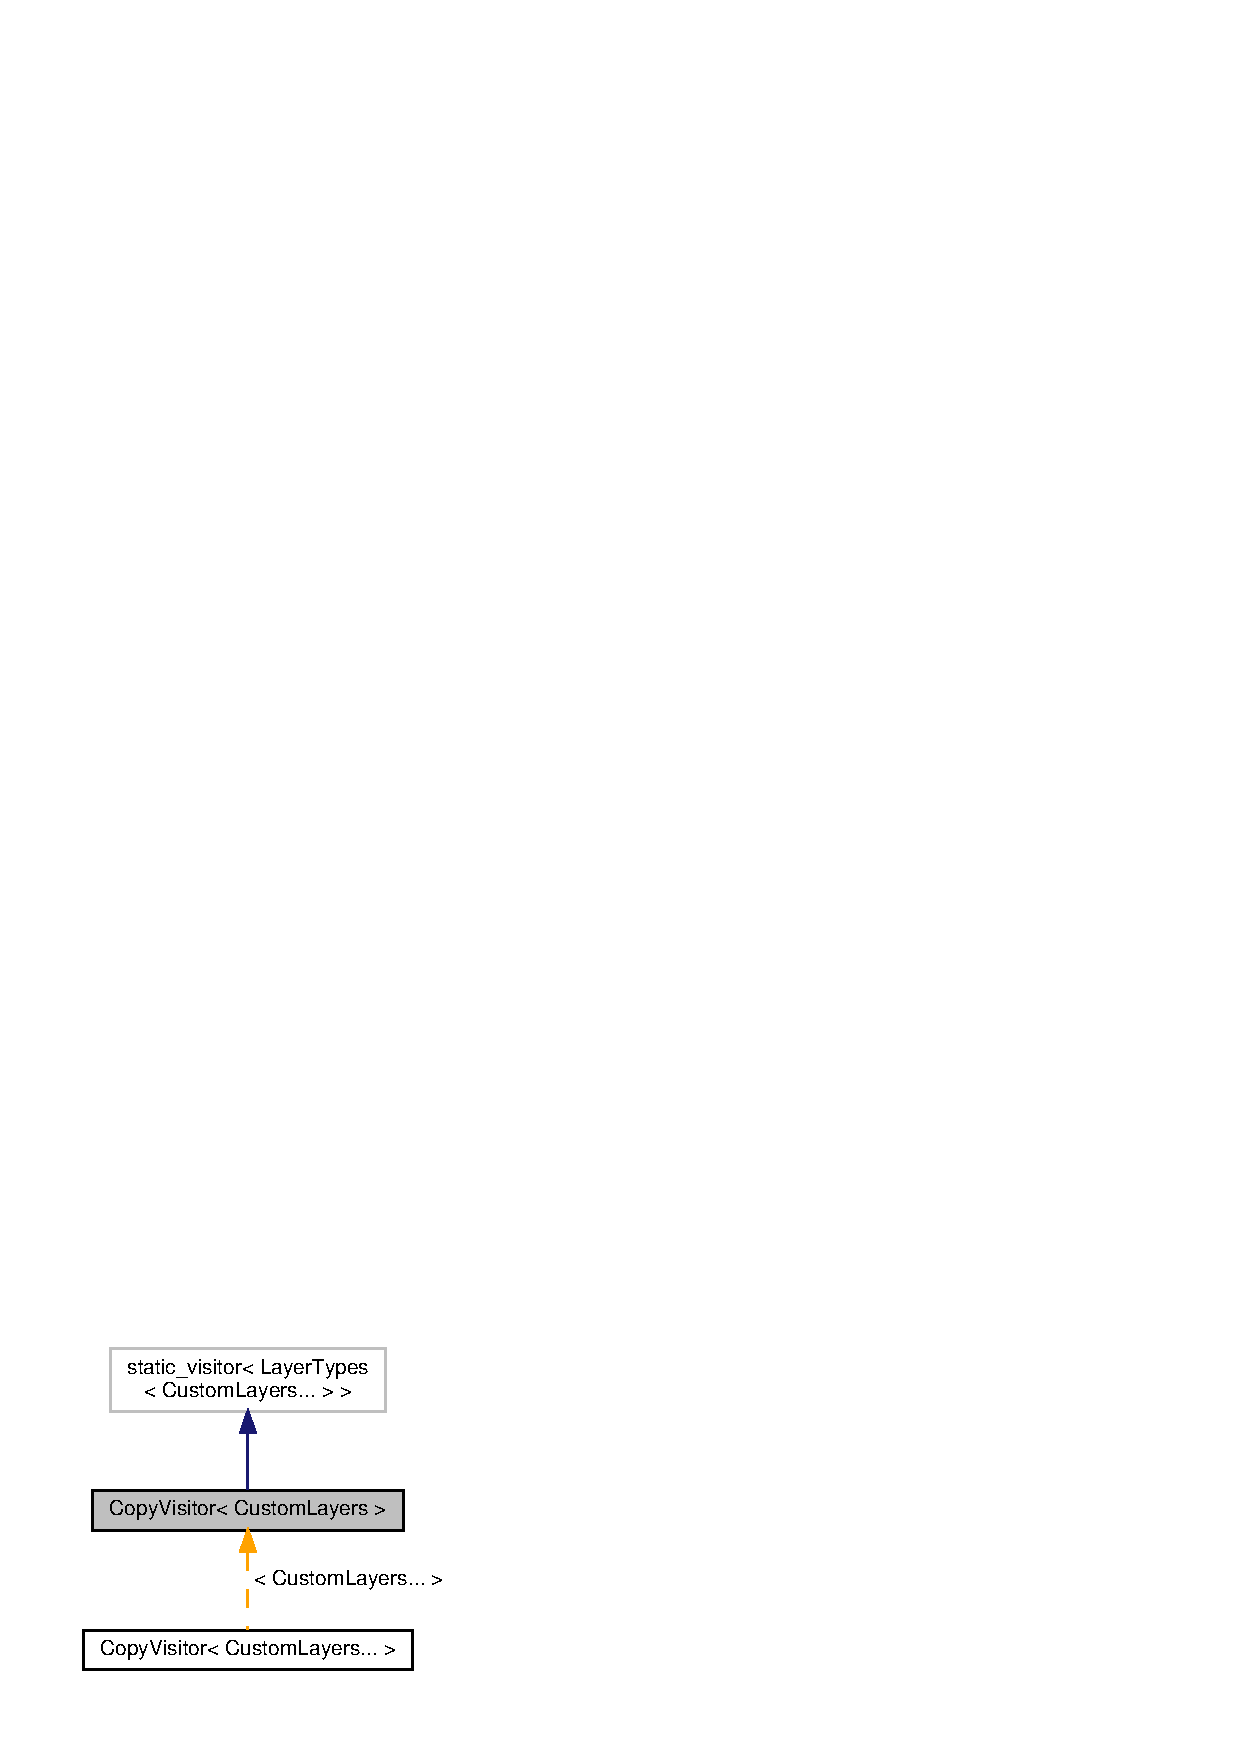
\includegraphics[width=217pt]{classmlpack_1_1ann_1_1CopyVisitor__inherit__graph}
\end{center}
\end{figure}
\subsection*{Public Member Functions}
\begin{DoxyCompactItemize}
\item 
{\footnotesize template$<$typename Layer\+Type $>$ }\\\textbf{ Layer\+Types}$<$ Custom\+Layers... $>$ \textbf{ operator()} (Layer\+Type $\ast$) const
\item 
\textbf{ Layer\+Types}$<$ Custom\+Layers... $>$ \textbf{ operator()} (\textbf{ More\+Types}) const
\end{DoxyCompactItemize}


\subsection{Detailed Description}
\subsubsection*{template$<$typename... Custom\+Layers$>$\newline
class mlpack\+::ann\+::\+Copy\+Visitor$<$ Custom\+Layers $>$}

This visitor is to support copy constructor for neural network module. 

We want a layer-\/wise copy rather than simple duplicate the pointer. 

Definition at line 26 of file copy\+\_\+visitor.\+hpp.



\subsection{Member Function Documentation}
\mbox{\label{classmlpack_1_1ann_1_1CopyVisitor_a0328fbed2c4b8458119a706e16921639}} 
\index{mlpack\+::ann\+::\+Copy\+Visitor@{mlpack\+::ann\+::\+Copy\+Visitor}!operator()@{operator()}}
\index{operator()@{operator()}!mlpack\+::ann\+::\+Copy\+Visitor@{mlpack\+::ann\+::\+Copy\+Visitor}}
\subsubsection{operator()()\hspace{0.1cm}{\footnotesize\ttfamily [1/2]}}
{\footnotesize\ttfamily \textbf{ Layer\+Types}$<$Custom\+Layers...$>$ operator() (\begin{DoxyParamCaption}\item[{Layer\+Type $\ast$}]{ }\end{DoxyParamCaption}) const}

\mbox{\label{classmlpack_1_1ann_1_1CopyVisitor_a8229a3baafceb83bbf28a6bfd8b62d93}} 
\index{mlpack\+::ann\+::\+Copy\+Visitor@{mlpack\+::ann\+::\+Copy\+Visitor}!operator()@{operator()}}
\index{operator()@{operator()}!mlpack\+::ann\+::\+Copy\+Visitor@{mlpack\+::ann\+::\+Copy\+Visitor}}
\subsubsection{operator()()\hspace{0.1cm}{\footnotesize\ttfamily [2/2]}}
{\footnotesize\ttfamily \textbf{ Layer\+Types}$<$Custom\+Layers...$>$ operator() (\begin{DoxyParamCaption}\item[{\textbf{ More\+Types}}]{ }\end{DoxyParamCaption}) const}



The documentation for this class was generated from the following file\+:\begin{DoxyCompactItemize}
\item 
/home/aakash/mlpack/src/mlpack/methods/ann/visitor/\textbf{ copy\+\_\+visitor.\+hpp}\end{DoxyCompactItemize}

\section{Cosine\+Embedding\+Loss$<$ Input\+Data\+Type, Output\+Data\+Type $>$ Class Template Reference}
\label{classmlpack_1_1ann_1_1CosineEmbeddingLoss}\index{Cosine\+Embedding\+Loss$<$ Input\+Data\+Type, Output\+Data\+Type $>$@{Cosine\+Embedding\+Loss$<$ Input\+Data\+Type, Output\+Data\+Type $>$}}


Cosine Embedding Loss function is used for measuring whether two inputs are similar or dissimilar, using the cosine distance, and is typically used for learning nonlinear embeddings or semi-\/supervised learning.  


\subsection*{Public Member Functions}
\begin{DoxyCompactItemize}
\item 
\textbf{ Cosine\+Embedding\+Loss} (const double margin=0.\+0, const bool similarity=true, const bool take\+Mean=false)
\begin{DoxyCompactList}\small\item\em Create the \doxyref{Cosine\+Embedding\+Loss}{p.}{classmlpack_1_1ann_1_1CosineEmbeddingLoss} object. \end{DoxyCompactList}\item 
{\footnotesize template$<$typename Prediction\+Type , typename Target\+Type , typename Loss\+Type $>$ }\\void \textbf{ Backward} (const Prediction\+Type \&prediction, const Target\+Type \&target, Loss\+Type \&loss)
\begin{DoxyCompactList}\small\item\em Ordinary feed backward pass of a neural network. \end{DoxyCompactList}\item 
Output\+Data\+Type \& \textbf{ Delta} () const
\begin{DoxyCompactList}\small\item\em Get the delta. \end{DoxyCompactList}\item 
Output\+Data\+Type \& \textbf{ Delta} ()
\begin{DoxyCompactList}\small\item\em Modify the delta. \end{DoxyCompactList}\item 
{\footnotesize template$<$typename Prediction\+Type , typename Target\+Type $>$ }\\Prediction\+Type\+::elem\+\_\+type \textbf{ Forward} (const Prediction\+Type \&prediction, const Target\+Type \&target)
\begin{DoxyCompactList}\small\item\em Ordinary feed forward pass of a neural network. \end{DoxyCompactList}\item 
Input\+Data\+Type \& \textbf{ Input\+Parameter} () const
\begin{DoxyCompactList}\small\item\em Get the input parameter. \end{DoxyCompactList}\item 
Input\+Data\+Type \& \textbf{ Input\+Parameter} ()
\begin{DoxyCompactList}\small\item\em Modify the input parameter. \end{DoxyCompactList}\item 
double \textbf{ Margin} () const
\begin{DoxyCompactList}\small\item\em Get the value of margin. \end{DoxyCompactList}\item 
double \& \textbf{ Margin} ()
\begin{DoxyCompactList}\small\item\em Modify the value of take\+Mean. \end{DoxyCompactList}\item 
Output\+Data\+Type \& \textbf{ Output\+Parameter} () const
\begin{DoxyCompactList}\small\item\em Get the output parameter. \end{DoxyCompactList}\item 
Output\+Data\+Type \& \textbf{ Output\+Parameter} ()
\begin{DoxyCompactList}\small\item\em Modify the output parameter. \end{DoxyCompactList}\item 
{\footnotesize template$<$typename Archive $>$ }\\void \textbf{ serialize} (Archive \&ar, const uint32\+\_\+t)
\begin{DoxyCompactList}\small\item\em Serialize the layer. \end{DoxyCompactList}\item 
bool \textbf{ Similarity} () const
\begin{DoxyCompactList}\small\item\em Get the value of similarity hyperparameter. \end{DoxyCompactList}\item 
bool \& \textbf{ Similarity} ()
\begin{DoxyCompactList}\small\item\em Modify the value of take\+Mean. \end{DoxyCompactList}\item 
bool \textbf{ Take\+Mean} () const
\begin{DoxyCompactList}\small\item\em Get the value of take\+Mean. \end{DoxyCompactList}\item 
bool \& \textbf{ Take\+Mean} ()
\begin{DoxyCompactList}\small\item\em Modify the value of take\+Mean. \end{DoxyCompactList}\end{DoxyCompactItemize}


\subsection{Detailed Description}
\subsubsection*{template$<$typename Input\+Data\+Type = arma\+::mat, typename Output\+Data\+Type = arma\+::mat$>$\newline
class mlpack\+::ann\+::\+Cosine\+Embedding\+Loss$<$ Input\+Data\+Type, Output\+Data\+Type $>$}

Cosine Embedding Loss function is used for measuring whether two inputs are similar or dissimilar, using the cosine distance, and is typically used for learning nonlinear embeddings or semi-\/supervised learning. 

\begin{eqnarray*} f(x) = 1 - cos(x1, x2) , for y = 1 f(x) = max(0, cos(x1, x2) - margin) , for y = -1 \end{eqnarray*}


\begin{DoxyTemplParams}{Template Parameters}
{\em Input\+Data\+Type} & Type of the input data (arma\+::colvec, arma\+::mat, arma\+::sp\+\_\+mat or arma\+::cube). \\
\hline
{\em Output\+Data\+Type} & Type of the output data (arma\+::colvec, arma\+::mat, arma\+::sp\+\_\+mat or arma\+::cube). \\
\hline
\end{DoxyTemplParams}


Definition at line 39 of file cosine\+\_\+embedding\+\_\+loss.\+hpp.



\subsection{Constructor \& Destructor Documentation}
\mbox{\label{classmlpack_1_1ann_1_1CosineEmbeddingLoss_a389938029e28bfa778819692fbb5f844}} 
\index{mlpack\+::ann\+::\+Cosine\+Embedding\+Loss@{mlpack\+::ann\+::\+Cosine\+Embedding\+Loss}!Cosine\+Embedding\+Loss@{Cosine\+Embedding\+Loss}}
\index{Cosine\+Embedding\+Loss@{Cosine\+Embedding\+Loss}!mlpack\+::ann\+::\+Cosine\+Embedding\+Loss@{mlpack\+::ann\+::\+Cosine\+Embedding\+Loss}}
\subsubsection{Cosine\+Embedding\+Loss()}
{\footnotesize\ttfamily \textbf{ Cosine\+Embedding\+Loss} (\begin{DoxyParamCaption}\item[{const double}]{margin = {\ttfamily 0.0},  }\item[{const bool}]{similarity = {\ttfamily true},  }\item[{const bool}]{take\+Mean = {\ttfamily false} }\end{DoxyParamCaption})}



Create the \doxyref{Cosine\+Embedding\+Loss}{p.}{classmlpack_1_1ann_1_1CosineEmbeddingLoss} object. 


\begin{DoxyParams}{Parameters}
{\em margin} & Increases cosine distance in case of dissimilarity. Refer definition of cosine-\/embedding-\/loss above. \\
\hline
{\em similarity} & Determines whether to use similarity or dissimilarity for comparision. \\
\hline
{\em take\+Mean} & Boolean variable to specify whether to take mean or not. Specifies reduction method i.\+e. sum or mean corresponding to 0 and 1 respectively. Default value = 0. \\
\hline
\end{DoxyParams}


\subsection{Member Function Documentation}
\mbox{\label{classmlpack_1_1ann_1_1CosineEmbeddingLoss_add41dbaf358dc099750dc6064cb7e0d7}} 
\index{mlpack\+::ann\+::\+Cosine\+Embedding\+Loss@{mlpack\+::ann\+::\+Cosine\+Embedding\+Loss}!Backward@{Backward}}
\index{Backward@{Backward}!mlpack\+::ann\+::\+Cosine\+Embedding\+Loss@{mlpack\+::ann\+::\+Cosine\+Embedding\+Loss}}
\subsubsection{Backward()}
{\footnotesize\ttfamily void Backward (\begin{DoxyParamCaption}\item[{const Prediction\+Type \&}]{prediction,  }\item[{const Target\+Type \&}]{target,  }\item[{Loss\+Type \&}]{loss }\end{DoxyParamCaption})}



Ordinary feed backward pass of a neural network. 


\begin{DoxyParams}{Parameters}
{\em prediction} & Predictions used for evaluating the specified loss function. \\
\hline
{\em target} & The target vector. \\
\hline
{\em loss} & The calculated error. \\
\hline
\end{DoxyParams}
\mbox{\label{classmlpack_1_1ann_1_1CosineEmbeddingLoss_ae7c8eba5764f021cd93e30efe638e63c}} 
\index{mlpack\+::ann\+::\+Cosine\+Embedding\+Loss@{mlpack\+::ann\+::\+Cosine\+Embedding\+Loss}!Delta@{Delta}}
\index{Delta@{Delta}!mlpack\+::ann\+::\+Cosine\+Embedding\+Loss@{mlpack\+::ann\+::\+Cosine\+Embedding\+Loss}}
\subsubsection{Delta()\hspace{0.1cm}{\footnotesize\ttfamily [1/2]}}
{\footnotesize\ttfamily Output\+Data\+Type\& Delta (\begin{DoxyParamCaption}{ }\end{DoxyParamCaption}) const\hspace{0.3cm}{\ttfamily [inline]}}



Get the delta. 



Definition at line 92 of file cosine\+\_\+embedding\+\_\+loss.\+hpp.

\mbox{\label{classmlpack_1_1ann_1_1CosineEmbeddingLoss_ad6601342d560219ce951d554e69e5e87}} 
\index{mlpack\+::ann\+::\+Cosine\+Embedding\+Loss@{mlpack\+::ann\+::\+Cosine\+Embedding\+Loss}!Delta@{Delta}}
\index{Delta@{Delta}!mlpack\+::ann\+::\+Cosine\+Embedding\+Loss@{mlpack\+::ann\+::\+Cosine\+Embedding\+Loss}}
\subsubsection{Delta()\hspace{0.1cm}{\footnotesize\ttfamily [2/2]}}
{\footnotesize\ttfamily Output\+Data\+Type\& Delta (\begin{DoxyParamCaption}{ }\end{DoxyParamCaption})\hspace{0.3cm}{\ttfamily [inline]}}



Modify the delta. 



Definition at line 94 of file cosine\+\_\+embedding\+\_\+loss.\+hpp.

\mbox{\label{classmlpack_1_1ann_1_1CosineEmbeddingLoss_ab3640059898ea76c13709b8099316fe8}} 
\index{mlpack\+::ann\+::\+Cosine\+Embedding\+Loss@{mlpack\+::ann\+::\+Cosine\+Embedding\+Loss}!Forward@{Forward}}
\index{Forward@{Forward}!mlpack\+::ann\+::\+Cosine\+Embedding\+Loss@{mlpack\+::ann\+::\+Cosine\+Embedding\+Loss}}
\subsubsection{Forward()}
{\footnotesize\ttfamily Prediction\+Type\+::elem\+\_\+type Forward (\begin{DoxyParamCaption}\item[{const Prediction\+Type \&}]{prediction,  }\item[{const Target\+Type \&}]{target }\end{DoxyParamCaption})}



Ordinary feed forward pass of a neural network. 


\begin{DoxyParams}{Parameters}
{\em prediction} & Predictions used for evaluating the specified loss function. \\
\hline
{\em target} & The target vector. \\
\hline
\end{DoxyParams}
\mbox{\label{classmlpack_1_1ann_1_1CosineEmbeddingLoss_a1506936601ddae886088d2804623ca4b}} 
\index{mlpack\+::ann\+::\+Cosine\+Embedding\+Loss@{mlpack\+::ann\+::\+Cosine\+Embedding\+Loss}!Input\+Parameter@{Input\+Parameter}}
\index{Input\+Parameter@{Input\+Parameter}!mlpack\+::ann\+::\+Cosine\+Embedding\+Loss@{mlpack\+::ann\+::\+Cosine\+Embedding\+Loss}}
\subsubsection{Input\+Parameter()\hspace{0.1cm}{\footnotesize\ttfamily [1/2]}}
{\footnotesize\ttfamily Input\+Data\+Type\& Input\+Parameter (\begin{DoxyParamCaption}{ }\end{DoxyParamCaption}) const\hspace{0.3cm}{\ttfamily [inline]}}



Get the input parameter. 



Definition at line 82 of file cosine\+\_\+embedding\+\_\+loss.\+hpp.

\mbox{\label{classmlpack_1_1ann_1_1CosineEmbeddingLoss_a063c3b1053c7979a7dd2e7bbd2bf1f8a}} 
\index{mlpack\+::ann\+::\+Cosine\+Embedding\+Loss@{mlpack\+::ann\+::\+Cosine\+Embedding\+Loss}!Input\+Parameter@{Input\+Parameter}}
\index{Input\+Parameter@{Input\+Parameter}!mlpack\+::ann\+::\+Cosine\+Embedding\+Loss@{mlpack\+::ann\+::\+Cosine\+Embedding\+Loss}}
\subsubsection{Input\+Parameter()\hspace{0.1cm}{\footnotesize\ttfamily [2/2]}}
{\footnotesize\ttfamily Input\+Data\+Type\& Input\+Parameter (\begin{DoxyParamCaption}{ }\end{DoxyParamCaption})\hspace{0.3cm}{\ttfamily [inline]}}



Modify the input parameter. 



Definition at line 84 of file cosine\+\_\+embedding\+\_\+loss.\+hpp.

\mbox{\label{classmlpack_1_1ann_1_1CosineEmbeddingLoss_ac29c2c851ff367f45f9ec075352c5b83}} 
\index{mlpack\+::ann\+::\+Cosine\+Embedding\+Loss@{mlpack\+::ann\+::\+Cosine\+Embedding\+Loss}!Margin@{Margin}}
\index{Margin@{Margin}!mlpack\+::ann\+::\+Cosine\+Embedding\+Loss@{mlpack\+::ann\+::\+Cosine\+Embedding\+Loss}}
\subsubsection{Margin()\hspace{0.1cm}{\footnotesize\ttfamily [1/2]}}
{\footnotesize\ttfamily double Margin (\begin{DoxyParamCaption}{ }\end{DoxyParamCaption}) const\hspace{0.3cm}{\ttfamily [inline]}}



Get the value of margin. 



Definition at line 102 of file cosine\+\_\+embedding\+\_\+loss.\+hpp.

\mbox{\label{classmlpack_1_1ann_1_1CosineEmbeddingLoss_ab8c4d252f686cdc9c5972df28e65dcab}} 
\index{mlpack\+::ann\+::\+Cosine\+Embedding\+Loss@{mlpack\+::ann\+::\+Cosine\+Embedding\+Loss}!Margin@{Margin}}
\index{Margin@{Margin}!mlpack\+::ann\+::\+Cosine\+Embedding\+Loss@{mlpack\+::ann\+::\+Cosine\+Embedding\+Loss}}
\subsubsection{Margin()\hspace{0.1cm}{\footnotesize\ttfamily [2/2]}}
{\footnotesize\ttfamily double\& Margin (\begin{DoxyParamCaption}{ }\end{DoxyParamCaption})\hspace{0.3cm}{\ttfamily [inline]}}



Modify the value of take\+Mean. 



Definition at line 104 of file cosine\+\_\+embedding\+\_\+loss.\+hpp.

\mbox{\label{classmlpack_1_1ann_1_1CosineEmbeddingLoss_a8bae962cc603d1cab8d80ec78f8d505d}} 
\index{mlpack\+::ann\+::\+Cosine\+Embedding\+Loss@{mlpack\+::ann\+::\+Cosine\+Embedding\+Loss}!Output\+Parameter@{Output\+Parameter}}
\index{Output\+Parameter@{Output\+Parameter}!mlpack\+::ann\+::\+Cosine\+Embedding\+Loss@{mlpack\+::ann\+::\+Cosine\+Embedding\+Loss}}
\subsubsection{Output\+Parameter()\hspace{0.1cm}{\footnotesize\ttfamily [1/2]}}
{\footnotesize\ttfamily Output\+Data\+Type\& Output\+Parameter (\begin{DoxyParamCaption}{ }\end{DoxyParamCaption}) const\hspace{0.3cm}{\ttfamily [inline]}}



Get the output parameter. 



Definition at line 87 of file cosine\+\_\+embedding\+\_\+loss.\+hpp.

\mbox{\label{classmlpack_1_1ann_1_1CosineEmbeddingLoss_a21d5f745f02c709625a4ee0907f004a5}} 
\index{mlpack\+::ann\+::\+Cosine\+Embedding\+Loss@{mlpack\+::ann\+::\+Cosine\+Embedding\+Loss}!Output\+Parameter@{Output\+Parameter}}
\index{Output\+Parameter@{Output\+Parameter}!mlpack\+::ann\+::\+Cosine\+Embedding\+Loss@{mlpack\+::ann\+::\+Cosine\+Embedding\+Loss}}
\subsubsection{Output\+Parameter()\hspace{0.1cm}{\footnotesize\ttfamily [2/2]}}
{\footnotesize\ttfamily Output\+Data\+Type\& Output\+Parameter (\begin{DoxyParamCaption}{ }\end{DoxyParamCaption})\hspace{0.3cm}{\ttfamily [inline]}}



Modify the output parameter. 



Definition at line 89 of file cosine\+\_\+embedding\+\_\+loss.\+hpp.

\mbox{\label{classmlpack_1_1ann_1_1CosineEmbeddingLoss_a65cba07328997659bec80b9879b15a51}} 
\index{mlpack\+::ann\+::\+Cosine\+Embedding\+Loss@{mlpack\+::ann\+::\+Cosine\+Embedding\+Loss}!serialize@{serialize}}
\index{serialize@{serialize}!mlpack\+::ann\+::\+Cosine\+Embedding\+Loss@{mlpack\+::ann\+::\+Cosine\+Embedding\+Loss}}
\subsubsection{serialize()}
{\footnotesize\ttfamily void serialize (\begin{DoxyParamCaption}\item[{Archive \&}]{ar,  }\item[{const uint32\+\_\+t}]{ }\end{DoxyParamCaption})}



Serialize the layer. 



Referenced by Cosine\+Embedding\+Loss$<$ Input\+Data\+Type, Output\+Data\+Type $>$\+::\+Similarity().

\mbox{\label{classmlpack_1_1ann_1_1CosineEmbeddingLoss_a92a76558ba5229079e8cb7c377f4cf67}} 
\index{mlpack\+::ann\+::\+Cosine\+Embedding\+Loss@{mlpack\+::ann\+::\+Cosine\+Embedding\+Loss}!Similarity@{Similarity}}
\index{Similarity@{Similarity}!mlpack\+::ann\+::\+Cosine\+Embedding\+Loss@{mlpack\+::ann\+::\+Cosine\+Embedding\+Loss}}
\subsubsection{Similarity()\hspace{0.1cm}{\footnotesize\ttfamily [1/2]}}
{\footnotesize\ttfamily bool Similarity (\begin{DoxyParamCaption}{ }\end{DoxyParamCaption}) const\hspace{0.3cm}{\ttfamily [inline]}}



Get the value of similarity hyperparameter. 



Definition at line 107 of file cosine\+\_\+embedding\+\_\+loss.\+hpp.

\mbox{\label{classmlpack_1_1ann_1_1CosineEmbeddingLoss_a1e4d965a9c5f106922cbbeb52ba2111d}} 
\index{mlpack\+::ann\+::\+Cosine\+Embedding\+Loss@{mlpack\+::ann\+::\+Cosine\+Embedding\+Loss}!Similarity@{Similarity}}
\index{Similarity@{Similarity}!mlpack\+::ann\+::\+Cosine\+Embedding\+Loss@{mlpack\+::ann\+::\+Cosine\+Embedding\+Loss}}
\subsubsection{Similarity()\hspace{0.1cm}{\footnotesize\ttfamily [2/2]}}
{\footnotesize\ttfamily bool\& Similarity (\begin{DoxyParamCaption}{ }\end{DoxyParamCaption})\hspace{0.3cm}{\ttfamily [inline]}}



Modify the value of take\+Mean. 



Definition at line 109 of file cosine\+\_\+embedding\+\_\+loss.\+hpp.



References Cosine\+Embedding\+Loss$<$ Input\+Data\+Type, Output\+Data\+Type $>$\+::serialize().

\mbox{\label{classmlpack_1_1ann_1_1CosineEmbeddingLoss_ab1afafdad2b04d3378dce6f13c9968a2}} 
\index{mlpack\+::ann\+::\+Cosine\+Embedding\+Loss@{mlpack\+::ann\+::\+Cosine\+Embedding\+Loss}!Take\+Mean@{Take\+Mean}}
\index{Take\+Mean@{Take\+Mean}!mlpack\+::ann\+::\+Cosine\+Embedding\+Loss@{mlpack\+::ann\+::\+Cosine\+Embedding\+Loss}}
\subsubsection{Take\+Mean()\hspace{0.1cm}{\footnotesize\ttfamily [1/2]}}
{\footnotesize\ttfamily bool Take\+Mean (\begin{DoxyParamCaption}{ }\end{DoxyParamCaption}) const\hspace{0.3cm}{\ttfamily [inline]}}



Get the value of take\+Mean. 



Definition at line 97 of file cosine\+\_\+embedding\+\_\+loss.\+hpp.

\mbox{\label{classmlpack_1_1ann_1_1CosineEmbeddingLoss_a6523d960bcd088ba1e86fbe2e095a79b}} 
\index{mlpack\+::ann\+::\+Cosine\+Embedding\+Loss@{mlpack\+::ann\+::\+Cosine\+Embedding\+Loss}!Take\+Mean@{Take\+Mean}}
\index{Take\+Mean@{Take\+Mean}!mlpack\+::ann\+::\+Cosine\+Embedding\+Loss@{mlpack\+::ann\+::\+Cosine\+Embedding\+Loss}}
\subsubsection{Take\+Mean()\hspace{0.1cm}{\footnotesize\ttfamily [2/2]}}
{\footnotesize\ttfamily bool\& Take\+Mean (\begin{DoxyParamCaption}{ }\end{DoxyParamCaption})\hspace{0.3cm}{\ttfamily [inline]}}



Modify the value of take\+Mean. 



Definition at line 99 of file cosine\+\_\+embedding\+\_\+loss.\+hpp.



The documentation for this class was generated from the following file\+:\begin{DoxyCompactItemize}
\item 
/home/aakash/mlpack/src/mlpack/methods/ann/loss\+\_\+functions/\textbf{ cosine\+\_\+embedding\+\_\+loss.\+hpp}\end{DoxyCompactItemize}

\section{C\+Re\+LU$<$ Input\+Data\+Type, Output\+Data\+Type $>$ Class Template Reference}
\label{classmlpack_1_1ann_1_1CReLU}\index{C\+Re\+L\+U$<$ Input\+Data\+Type, Output\+Data\+Type $>$@{C\+Re\+L\+U$<$ Input\+Data\+Type, Output\+Data\+Type $>$}}


A concatenated Re\+LU has two outputs, one Re\+LU and one negative Re\+LU, concatenated together.  


\subsection*{Public Member Functions}
\begin{DoxyCompactItemize}
\item 
\textbf{ C\+Re\+LU} ()
\begin{DoxyCompactList}\small\item\em Create the \doxyref{C\+Re\+LU}{p.}{classmlpack_1_1ann_1_1CReLU} object. \end{DoxyCompactList}\item 
{\footnotesize template$<$typename Data\+Type $>$ }\\void \textbf{ Backward} (const Data\+Type \&input, const Data\+Type \&gy, Data\+Type \&g)
\begin{DoxyCompactList}\small\item\em Ordinary feed backward pass of a neural network, calculating the function f(x) by propagating x backwards through f. \end{DoxyCompactList}\item 
Output\+Data\+Type const  \& \textbf{ Delta} () const
\begin{DoxyCompactList}\small\item\em Get the delta. \end{DoxyCompactList}\item 
Output\+Data\+Type \& \textbf{ Delta} ()
\begin{DoxyCompactList}\small\item\em Modify the delta. \end{DoxyCompactList}\item 
{\footnotesize template$<$typename Input\+Type , typename Output\+Type $>$ }\\void \textbf{ Forward} (const Input\+Type \&input, Output\+Type \&output)
\begin{DoxyCompactList}\small\item\em Ordinary feed forward pass of a neural network, evaluating the function f(x) by propagating the activity forward through f. \end{DoxyCompactList}\item 
Output\+Data\+Type const  \& \textbf{ Output\+Parameter} () const
\begin{DoxyCompactList}\small\item\em Get the output parameter. \end{DoxyCompactList}\item 
Output\+Data\+Type \& \textbf{ Output\+Parameter} ()
\begin{DoxyCompactList}\small\item\em Modify the output parameter. \end{DoxyCompactList}\item 
{\footnotesize template$<$typename Archive $>$ }\\void \textbf{ serialize} (Archive \&, const uint32\+\_\+t)
\begin{DoxyCompactList}\small\item\em Serialize the layer. \end{DoxyCompactList}\item 
size\+\_\+t \textbf{ Weight\+Size} () const
\begin{DoxyCompactList}\small\item\em Get size of weights. \end{DoxyCompactList}\end{DoxyCompactItemize}


\subsection{Detailed Description}
\subsubsection*{template$<$typename Input\+Data\+Type = arma\+::mat, typename Output\+Data\+Type = arma\+::mat$>$\newline
class mlpack\+::ann\+::\+C\+Re\+L\+U$<$ Input\+Data\+Type, Output\+Data\+Type $>$}

A concatenated Re\+LU has two outputs, one Re\+LU and one negative Re\+LU, concatenated together. 

In other words, for positive x it produces [x, 0], and for negative x it produces [0, x]. Because it has two outputs, \doxyref{C\+Re\+LU}{p.}{classmlpack_1_1ann_1_1CReLU} doubles the output dimension.

Note\+: The \doxyref{C\+Re\+LU}{p.}{classmlpack_1_1ann_1_1CReLU} doubles the output size.

For more information, see the following.


\begin{DoxyCode}
@inproceedings\{ICML2016,
  title  = \{Understanding and Improving Convolutional Neural Networks
            via Concatenated Rectified Linear Units\},
  author = \{LWenling Shang, Kihyuk Sohn, Diogo Almeida, Honglak Lee\},
  year   = \{2016\},
  url    = \{https:\textcolor{comment}{//arxiv.org/abs/1603.05201\}}
\}
\end{DoxyCode}



\begin{DoxyTemplParams}{Template Parameters}
{\em Input\+Data\+Type} & Type of the input data (arma\+::colvec, arma\+::mat, arma\+::sp\+\_\+mat or arma\+::cube). \\
\hline
{\em Output\+Data\+Type} & Type of the output data (arma\+::colvec, arma\+::mat, arma\+::sp\+\_\+mat or arma\+::cube). \\
\hline
\end{DoxyTemplParams}


Definition at line 50 of file c\+\_\+relu.\+hpp.



\subsection{Constructor \& Destructor Documentation}
\mbox{\label{classmlpack_1_1ann_1_1CReLU_a25aa935d5a2be5066422e9dc6d5e80b8}} 
\index{mlpack\+::ann\+::\+C\+Re\+LU@{mlpack\+::ann\+::\+C\+Re\+LU}!C\+Re\+LU@{C\+Re\+LU}}
\index{C\+Re\+LU@{C\+Re\+LU}!mlpack\+::ann\+::\+C\+Re\+LU@{mlpack\+::ann\+::\+C\+Re\+LU}}
\subsubsection{C\+Re\+L\+U()}
{\footnotesize\ttfamily \textbf{ C\+Re\+LU} (\begin{DoxyParamCaption}{ }\end{DoxyParamCaption})}



Create the \doxyref{C\+Re\+LU}{p.}{classmlpack_1_1ann_1_1CReLU} object. 



\subsection{Member Function Documentation}
\mbox{\label{classmlpack_1_1ann_1_1CReLU_aef8c56f1f8624bd006afec8b3bcda9d6}} 
\index{mlpack\+::ann\+::\+C\+Re\+LU@{mlpack\+::ann\+::\+C\+Re\+LU}!Backward@{Backward}}
\index{Backward@{Backward}!mlpack\+::ann\+::\+C\+Re\+LU@{mlpack\+::ann\+::\+C\+Re\+LU}}
\subsubsection{Backward()}
{\footnotesize\ttfamily void Backward (\begin{DoxyParamCaption}\item[{const Data\+Type \&}]{input,  }\item[{const Data\+Type \&}]{gy,  }\item[{Data\+Type \&}]{g }\end{DoxyParamCaption})}



Ordinary feed backward pass of a neural network, calculating the function f(x) by propagating x backwards through f. 

Using the results from the feed forward pass.


\begin{DoxyParams}{Parameters}
{\em input} & The propagated input activation. \\
\hline
{\em gy} & The backpropagated error. \\
\hline
{\em g} & The calculated gradient. \\
\hline
\end{DoxyParams}
\mbox{\label{classmlpack_1_1ann_1_1CReLU_a797f7edb44dd081e5e2b3cc316eef6bd}} 
\index{mlpack\+::ann\+::\+C\+Re\+LU@{mlpack\+::ann\+::\+C\+Re\+LU}!Delta@{Delta}}
\index{Delta@{Delta}!mlpack\+::ann\+::\+C\+Re\+LU@{mlpack\+::ann\+::\+C\+Re\+LU}}
\subsubsection{Delta()\hspace{0.1cm}{\footnotesize\ttfamily [1/2]}}
{\footnotesize\ttfamily Output\+Data\+Type const\& Delta (\begin{DoxyParamCaption}{ }\end{DoxyParamCaption}) const\hspace{0.3cm}{\ttfamily [inline]}}



Get the delta. 



Definition at line 87 of file c\+\_\+relu.\+hpp.

\mbox{\label{classmlpack_1_1ann_1_1CReLU_ad6601342d560219ce951d554e69e5e87}} 
\index{mlpack\+::ann\+::\+C\+Re\+LU@{mlpack\+::ann\+::\+C\+Re\+LU}!Delta@{Delta}}
\index{Delta@{Delta}!mlpack\+::ann\+::\+C\+Re\+LU@{mlpack\+::ann\+::\+C\+Re\+LU}}
\subsubsection{Delta()\hspace{0.1cm}{\footnotesize\ttfamily [2/2]}}
{\footnotesize\ttfamily Output\+Data\+Type\& Delta (\begin{DoxyParamCaption}{ }\end{DoxyParamCaption})\hspace{0.3cm}{\ttfamily [inline]}}



Modify the delta. 



Definition at line 89 of file c\+\_\+relu.\+hpp.

\mbox{\label{classmlpack_1_1ann_1_1CReLU_a09440df0a90bdcc766e56e097d91205b}} 
\index{mlpack\+::ann\+::\+C\+Re\+LU@{mlpack\+::ann\+::\+C\+Re\+LU}!Forward@{Forward}}
\index{Forward@{Forward}!mlpack\+::ann\+::\+C\+Re\+LU@{mlpack\+::ann\+::\+C\+Re\+LU}}
\subsubsection{Forward()}
{\footnotesize\ttfamily void Forward (\begin{DoxyParamCaption}\item[{const Input\+Type \&}]{input,  }\item[{Output\+Type \&}]{output }\end{DoxyParamCaption})}



Ordinary feed forward pass of a neural network, evaluating the function f(x) by propagating the activity forward through f. 

Works only for 2D Tensors.


\begin{DoxyParams}{Parameters}
{\em input} & Input data used for evaluating the specified function. \\
\hline
{\em output} & Resulting output activation. \\
\hline
\end{DoxyParams}
\mbox{\label{classmlpack_1_1ann_1_1CReLU_a0ee21c2a36e5abad1e7a9d5dd00849f9}} 
\index{mlpack\+::ann\+::\+C\+Re\+LU@{mlpack\+::ann\+::\+C\+Re\+LU}!Output\+Parameter@{Output\+Parameter}}
\index{Output\+Parameter@{Output\+Parameter}!mlpack\+::ann\+::\+C\+Re\+LU@{mlpack\+::ann\+::\+C\+Re\+LU}}
\subsubsection{Output\+Parameter()\hspace{0.1cm}{\footnotesize\ttfamily [1/2]}}
{\footnotesize\ttfamily Output\+Data\+Type const\& Output\+Parameter (\begin{DoxyParamCaption}{ }\end{DoxyParamCaption}) const\hspace{0.3cm}{\ttfamily [inline]}}



Get the output parameter. 



Definition at line 82 of file c\+\_\+relu.\+hpp.

\mbox{\label{classmlpack_1_1ann_1_1CReLU_a21d5f745f02c709625a4ee0907f004a5}} 
\index{mlpack\+::ann\+::\+C\+Re\+LU@{mlpack\+::ann\+::\+C\+Re\+LU}!Output\+Parameter@{Output\+Parameter}}
\index{Output\+Parameter@{Output\+Parameter}!mlpack\+::ann\+::\+C\+Re\+LU@{mlpack\+::ann\+::\+C\+Re\+LU}}
\subsubsection{Output\+Parameter()\hspace{0.1cm}{\footnotesize\ttfamily [2/2]}}
{\footnotesize\ttfamily Output\+Data\+Type\& Output\+Parameter (\begin{DoxyParamCaption}{ }\end{DoxyParamCaption})\hspace{0.3cm}{\ttfamily [inline]}}



Modify the output parameter. 



Definition at line 84 of file c\+\_\+relu.\+hpp.

\mbox{\label{classmlpack_1_1ann_1_1CReLU_aa2ccb5a0533a6ba0abe6dfc1f98fbafb}} 
\index{mlpack\+::ann\+::\+C\+Re\+LU@{mlpack\+::ann\+::\+C\+Re\+LU}!serialize@{serialize}}
\index{serialize@{serialize}!mlpack\+::ann\+::\+C\+Re\+LU@{mlpack\+::ann\+::\+C\+Re\+LU}}
\subsubsection{serialize()}
{\footnotesize\ttfamily void serialize (\begin{DoxyParamCaption}\item[{Archive \&}]{,  }\item[{const uint32\+\_\+t}]{ }\end{DoxyParamCaption})}



Serialize the layer. 



Referenced by C\+Re\+L\+U$<$ Input\+Data\+Type, Output\+Data\+Type $>$\+::\+Weight\+Size().

\mbox{\label{classmlpack_1_1ann_1_1CReLU_a7a2704698a50d9e00dfb083f3a863579}} 
\index{mlpack\+::ann\+::\+C\+Re\+LU@{mlpack\+::ann\+::\+C\+Re\+LU}!Weight\+Size@{Weight\+Size}}
\index{Weight\+Size@{Weight\+Size}!mlpack\+::ann\+::\+C\+Re\+LU@{mlpack\+::ann\+::\+C\+Re\+LU}}
\subsubsection{Weight\+Size()}
{\footnotesize\ttfamily size\+\_\+t Weight\+Size (\begin{DoxyParamCaption}{ }\end{DoxyParamCaption}) const\hspace{0.3cm}{\ttfamily [inline]}}



Get size of weights. 



Definition at line 92 of file c\+\_\+relu.\+hpp.



References C\+Re\+L\+U$<$ Input\+Data\+Type, Output\+Data\+Type $>$\+::serialize().



The documentation for this class was generated from the following file\+:\begin{DoxyCompactItemize}
\item 
/home/aakash/mlpack/src/mlpack/methods/ann/layer/\textbf{ c\+\_\+relu.\+hpp}\end{DoxyCompactItemize}

\section{D\+C\+G\+AN Class Reference}
\label{classmlpack_1_1ann_1_1DCGAN}\index{D\+C\+G\+AN@{D\+C\+G\+AN}}


For more information, see the following paper\+:  




\subsection{Detailed Description}
For more information, see the following paper\+: 


\begin{DoxyCode}
@article\{Radford15,
  author    = \{Alec Radford, Luke Metz and Soumith Chintala\},
  title     = \{Unsupervised Representation Learning with Deep Convolutional
               Generative Adversarial Networks\},
  year      = \{2015\},
  url       = \{https:\textcolor{comment}{//arxiv.org/abs/1511.06434\},}
  eprint    = \{1511.06434\},
\}
\end{DoxyCode}
 

Definition at line 48 of file gan\+\_\+policies.\+hpp.



The documentation for this class was generated from the following file\+:\begin{DoxyCompactItemize}
\item 
/home/aakash/mlpack/src/mlpack/methods/ann/gan/\textbf{ gan\+\_\+policies.\+hpp}\end{DoxyCompactItemize}

\section{Delete\+Visitor Class Reference}
\label{classmlpack_1_1ann_1_1DeleteVisitor}\index{Delete\+Visitor@{Delete\+Visitor}}


\doxyref{Delete\+Visitor}{p.}{classmlpack_1_1ann_1_1DeleteVisitor} executes the destructor of the instantiated object.  




Inheritance diagram for Delete\+Visitor\+:
\nopagebreak
\begin{figure}[H]
\begin{center}
\leavevmode
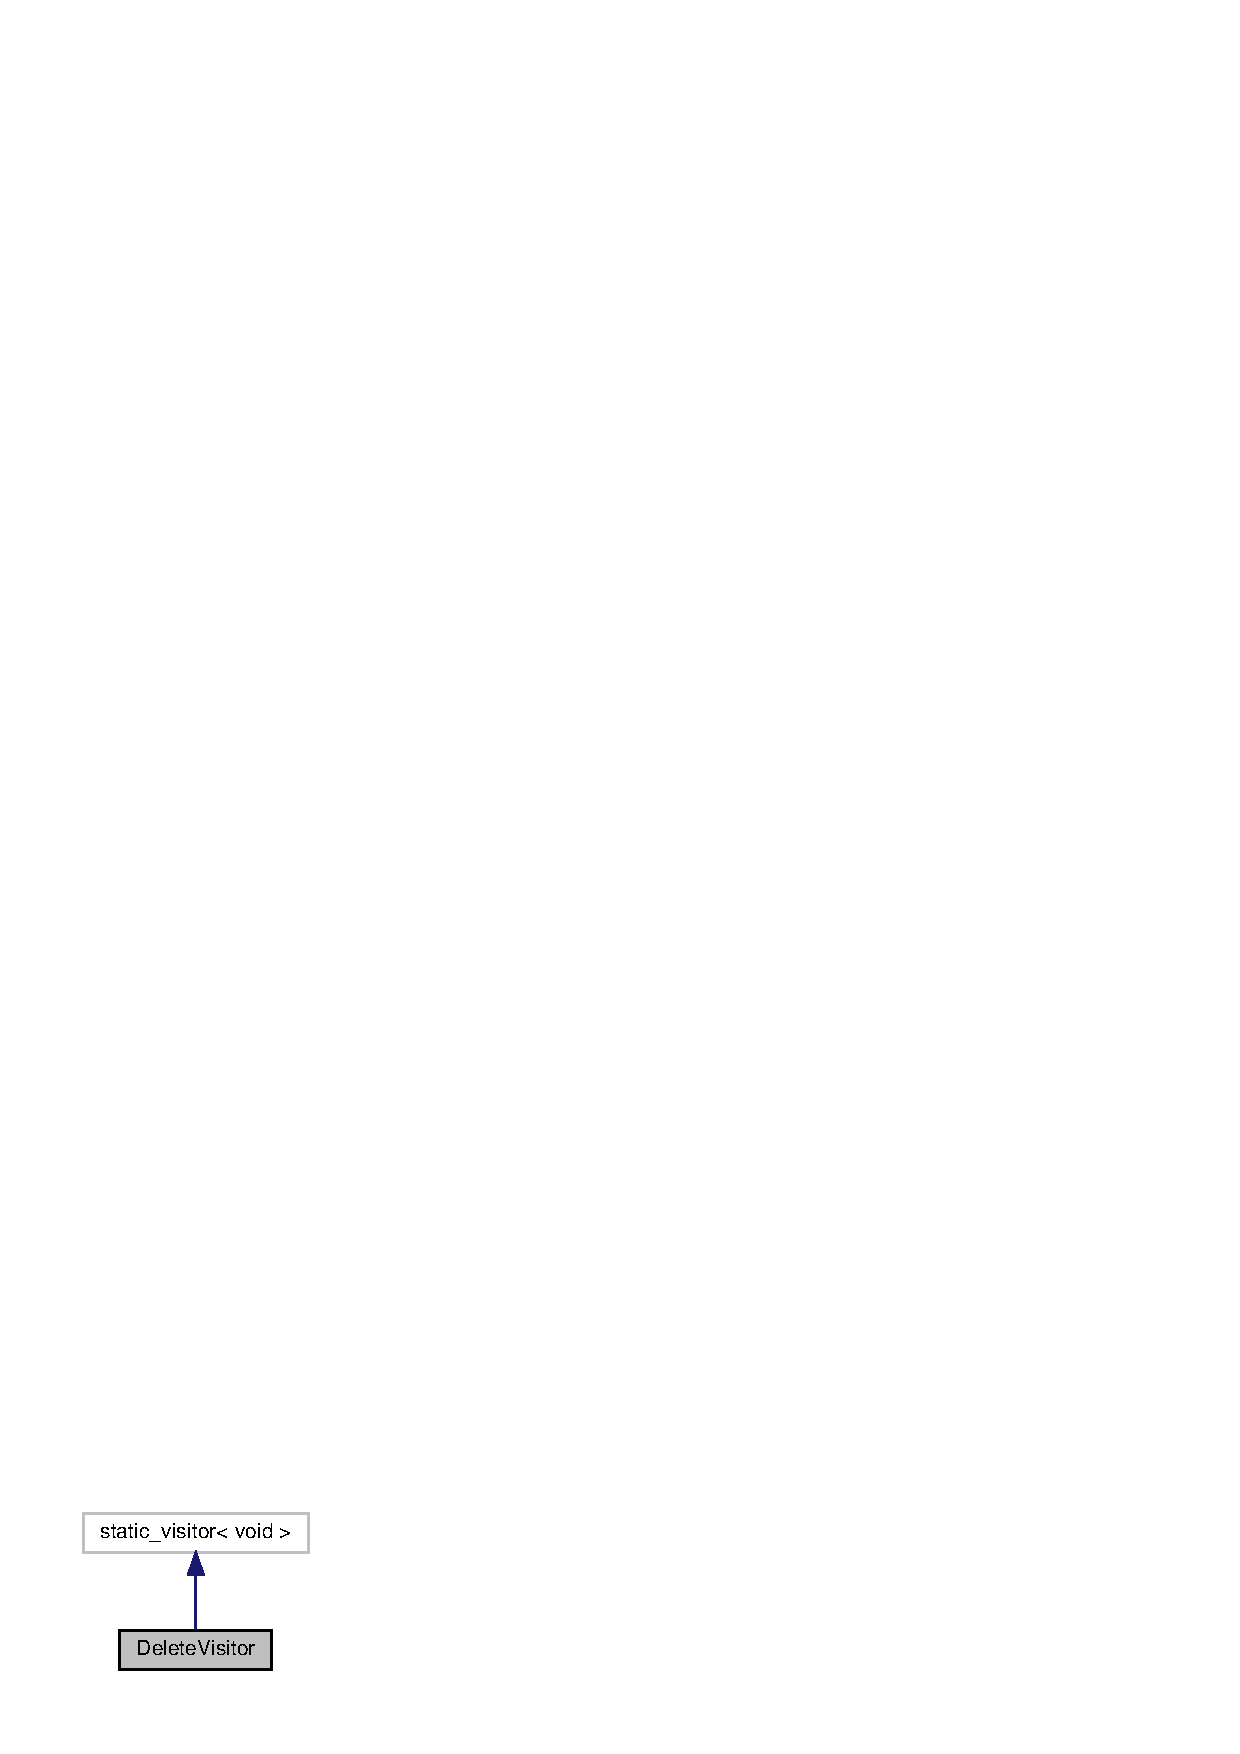
\includegraphics[width=152pt]{classmlpack_1_1ann_1_1DeleteVisitor__inherit__graph}
\end{center}
\end{figure}
\subsection*{Public Member Functions}
\begin{DoxyCompactItemize}
\item 
{\footnotesize template$<$typename Layer\+Type $>$ }\\std\+::enable\+\_\+if$<$ !Has\+Model\+Check$<$ Layer\+Type $>$\+::value, void $>$\+::type \textbf{ operator()} (Layer\+Type $\ast$layer) const
\begin{DoxyCompactList}\small\item\em Execute the destructor if the layer does not hold layers internally. \end{DoxyCompactList}\item 
{\footnotesize template$<$typename Layer\+Type $>$ }\\std\+::enable\+\_\+if$<$ Has\+Model\+Check$<$ Layer\+Type $>$\+::value, void $>$\+::type \textbf{ operator()} (Layer\+Type $\ast$layer) const
\begin{DoxyCompactList}\small\item\em Execute the destructor if the layer does hold layers internally. \end{DoxyCompactList}\item 
void \textbf{ operator()} (\textbf{ More\+Types} layer) const
\end{DoxyCompactItemize}


\subsection{Detailed Description}
\doxyref{Delete\+Visitor}{p.}{classmlpack_1_1ann_1_1DeleteVisitor} executes the destructor of the instantiated object. 

Definition at line 27 of file delete\+\_\+visitor.\+hpp.



\subsection{Member Function Documentation}
\mbox{\label{classmlpack_1_1ann_1_1DeleteVisitor_a1fc948e7a9b2e09d5306da2d63dac0e3}} 
\index{mlpack\+::ann\+::\+Delete\+Visitor@{mlpack\+::ann\+::\+Delete\+Visitor}!operator()@{operator()}}
\index{operator()@{operator()}!mlpack\+::ann\+::\+Delete\+Visitor@{mlpack\+::ann\+::\+Delete\+Visitor}}
\subsubsection{operator()()\hspace{0.1cm}{\footnotesize\ttfamily [1/3]}}
{\footnotesize\ttfamily std\+::enable\+\_\+if$<$ !Has\+Model\+Check$<$Layer\+Type$>$\+::value, void$>$\+::type operator() (\begin{DoxyParamCaption}\item[{Layer\+Type $\ast$}]{layer }\end{DoxyParamCaption}) const}



Execute the destructor if the layer does not hold layers internally. 

\mbox{\label{classmlpack_1_1ann_1_1DeleteVisitor_ae33b833469f1197e57ff4abf3541f8fb}} 
\index{mlpack\+::ann\+::\+Delete\+Visitor@{mlpack\+::ann\+::\+Delete\+Visitor}!operator()@{operator()}}
\index{operator()@{operator()}!mlpack\+::ann\+::\+Delete\+Visitor@{mlpack\+::ann\+::\+Delete\+Visitor}}
\subsubsection{operator()()\hspace{0.1cm}{\footnotesize\ttfamily [2/3]}}
{\footnotesize\ttfamily std\+::enable\+\_\+if$<$ Has\+Model\+Check$<$Layer\+Type$>$\+::value, void$>$\+::type operator() (\begin{DoxyParamCaption}\item[{Layer\+Type $\ast$}]{layer }\end{DoxyParamCaption}) const}



Execute the destructor if the layer does hold layers internally. 

\mbox{\label{classmlpack_1_1ann_1_1DeleteVisitor_ae35578e7ff874a320fe762bc0edfff04}} 
\index{mlpack\+::ann\+::\+Delete\+Visitor@{mlpack\+::ann\+::\+Delete\+Visitor}!operator()@{operator()}}
\index{operator()@{operator()}!mlpack\+::ann\+::\+Delete\+Visitor@{mlpack\+::ann\+::\+Delete\+Visitor}}
\subsubsection{operator()()\hspace{0.1cm}{\footnotesize\ttfamily [3/3]}}
{\footnotesize\ttfamily void operator() (\begin{DoxyParamCaption}\item[{\textbf{ More\+Types}}]{layer }\end{DoxyParamCaption}) const}



The documentation for this class was generated from the following file\+:\begin{DoxyCompactItemize}
\item 
/home/aakash/mlpack/src/mlpack/methods/ann/visitor/\textbf{ delete\+\_\+visitor.\+hpp}\end{DoxyCompactItemize}

\section{Delta\+Visitor Class Reference}
\label{classmlpack_1_1ann_1_1DeltaVisitor}\index{Delta\+Visitor@{Delta\+Visitor}}


\doxyref{Delta\+Visitor}{p.}{classmlpack_1_1ann_1_1DeltaVisitor} exposes the delta parameter of the given module.  




Inheritance diagram for Delta\+Visitor\+:
\nopagebreak
\begin{figure}[H]
\begin{center}
\leavevmode
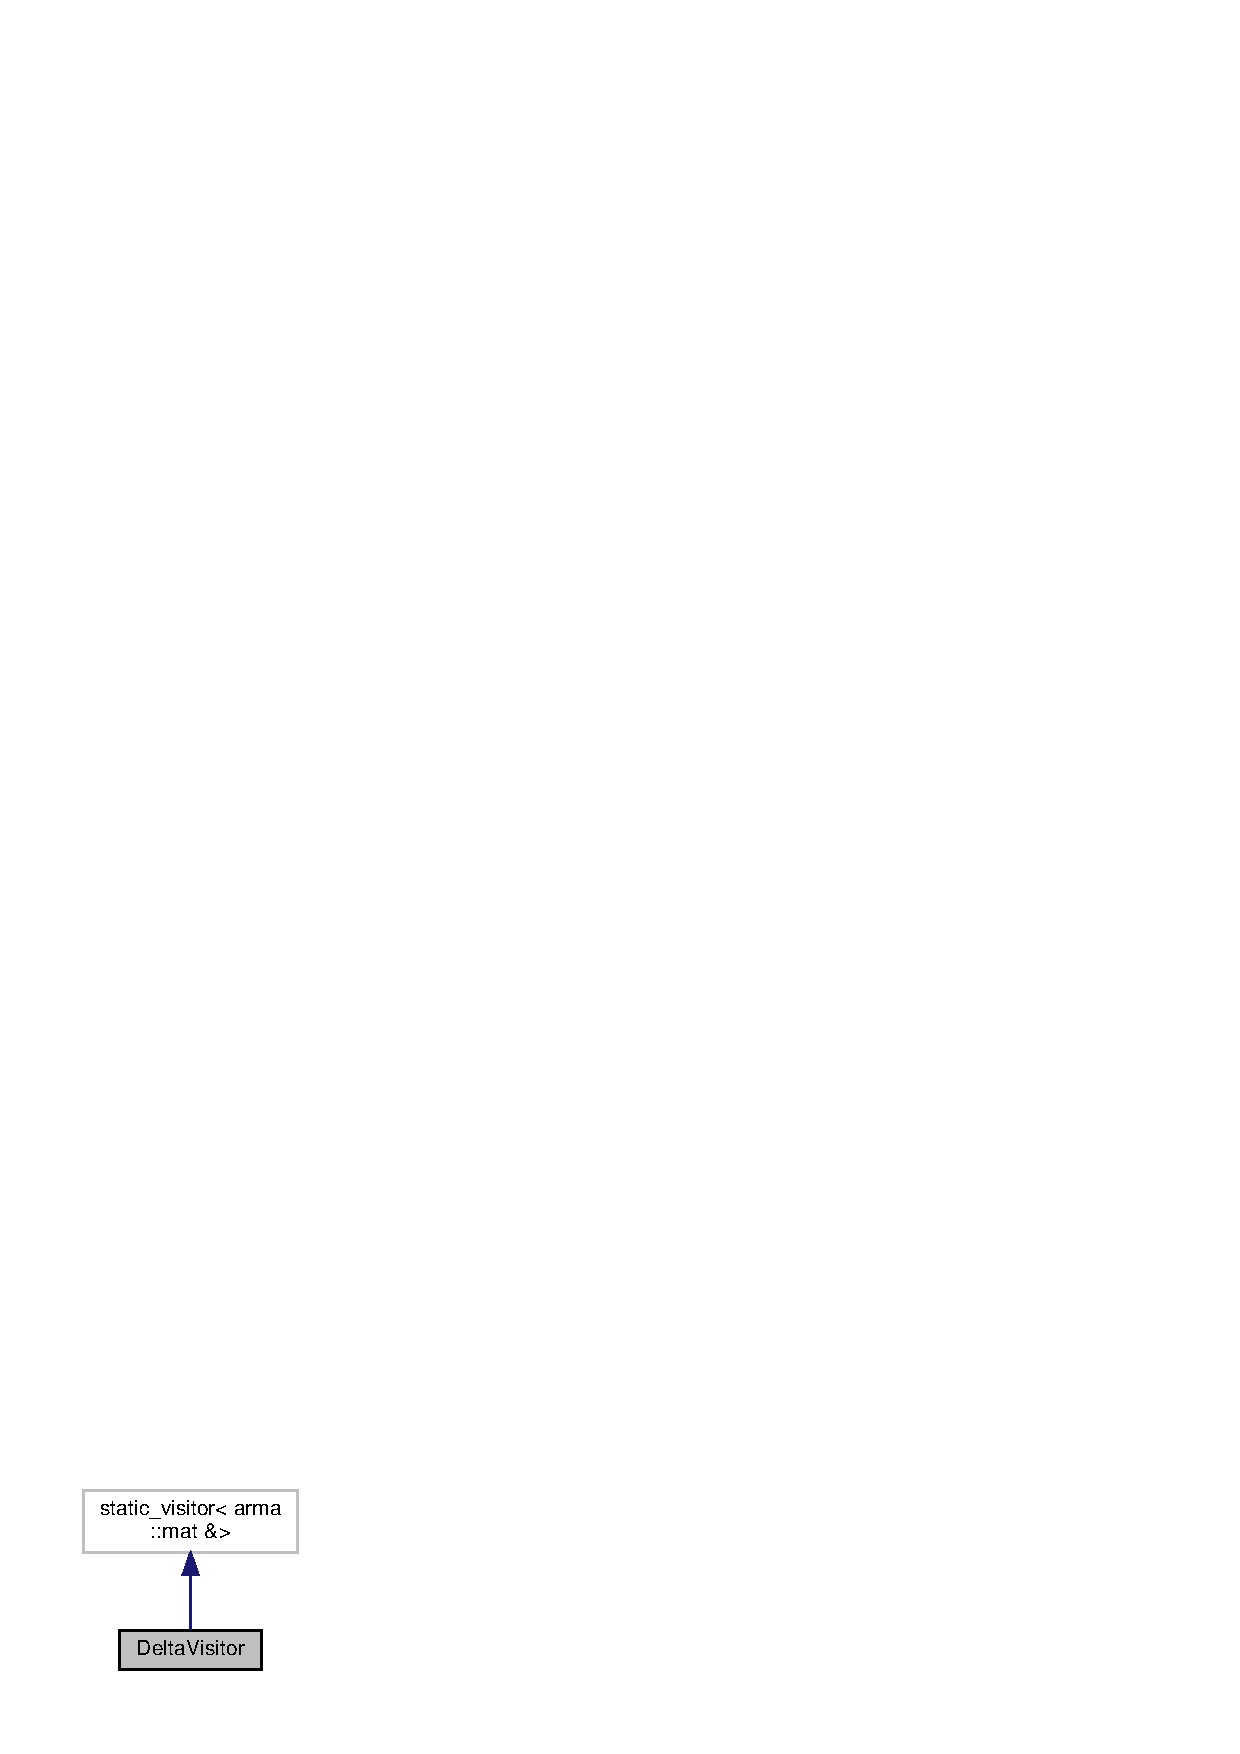
\includegraphics[width=147pt]{classmlpack_1_1ann_1_1DeltaVisitor__inherit__graph}
\end{center}
\end{figure}
\subsection*{Public Member Functions}
\begin{DoxyCompactItemize}
\item 
{\footnotesize template$<$typename Layer\+Type $>$ }\\arma\+::mat \& \textbf{ operator()} (Layer\+Type $\ast$layer) const
\begin{DoxyCompactList}\small\item\em Return the delta parameter. \end{DoxyCompactList}\item 
arma\+::mat \& \textbf{ operator()} (\textbf{ More\+Types} layer) const
\end{DoxyCompactItemize}


\subsection{Detailed Description}
\doxyref{Delta\+Visitor}{p.}{classmlpack_1_1ann_1_1DeltaVisitor} exposes the delta parameter of the given module. 

Definition at line 27 of file delta\+\_\+visitor.\+hpp.



\subsection{Member Function Documentation}
\mbox{\label{classmlpack_1_1ann_1_1DeltaVisitor_a9ca03fe7e92d1ec621a9fea401f84110}} 
\index{mlpack\+::ann\+::\+Delta\+Visitor@{mlpack\+::ann\+::\+Delta\+Visitor}!operator()@{operator()}}
\index{operator()@{operator()}!mlpack\+::ann\+::\+Delta\+Visitor@{mlpack\+::ann\+::\+Delta\+Visitor}}
\subsubsection{operator()()\hspace{0.1cm}{\footnotesize\ttfamily [1/2]}}
{\footnotesize\ttfamily arma\+::mat\& operator() (\begin{DoxyParamCaption}\item[{Layer\+Type $\ast$}]{layer }\end{DoxyParamCaption}) const}



Return the delta parameter. 

\mbox{\label{classmlpack_1_1ann_1_1DeltaVisitor_ad07b3038aea456f84663267ec846a748}} 
\index{mlpack\+::ann\+::\+Delta\+Visitor@{mlpack\+::ann\+::\+Delta\+Visitor}!operator()@{operator()}}
\index{operator()@{operator()}!mlpack\+::ann\+::\+Delta\+Visitor@{mlpack\+::ann\+::\+Delta\+Visitor}}
\subsubsection{operator()()\hspace{0.1cm}{\footnotesize\ttfamily [2/2]}}
{\footnotesize\ttfamily arma\+::mat\& operator() (\begin{DoxyParamCaption}\item[{\textbf{ More\+Types}}]{layer }\end{DoxyParamCaption}) const}



The documentation for this class was generated from the following file\+:\begin{DoxyCompactItemize}
\item 
/home/aakash/mlpack/src/mlpack/methods/ann/visitor/\textbf{ delta\+\_\+visitor.\+hpp}\end{DoxyCompactItemize}

\section{Deterministic\+Set\+Visitor Class Reference}
\label{classmlpack_1_1ann_1_1DeterministicSetVisitor}\index{Deterministic\+Set\+Visitor@{Deterministic\+Set\+Visitor}}


\doxyref{Deterministic\+Set\+Visitor}{p.}{classmlpack_1_1ann_1_1DeterministicSetVisitor} set the deterministic parameter given the deterministic value.  




Inheritance diagram for Deterministic\+Set\+Visitor\+:
\nopagebreak
\begin{figure}[H]
\begin{center}
\leavevmode
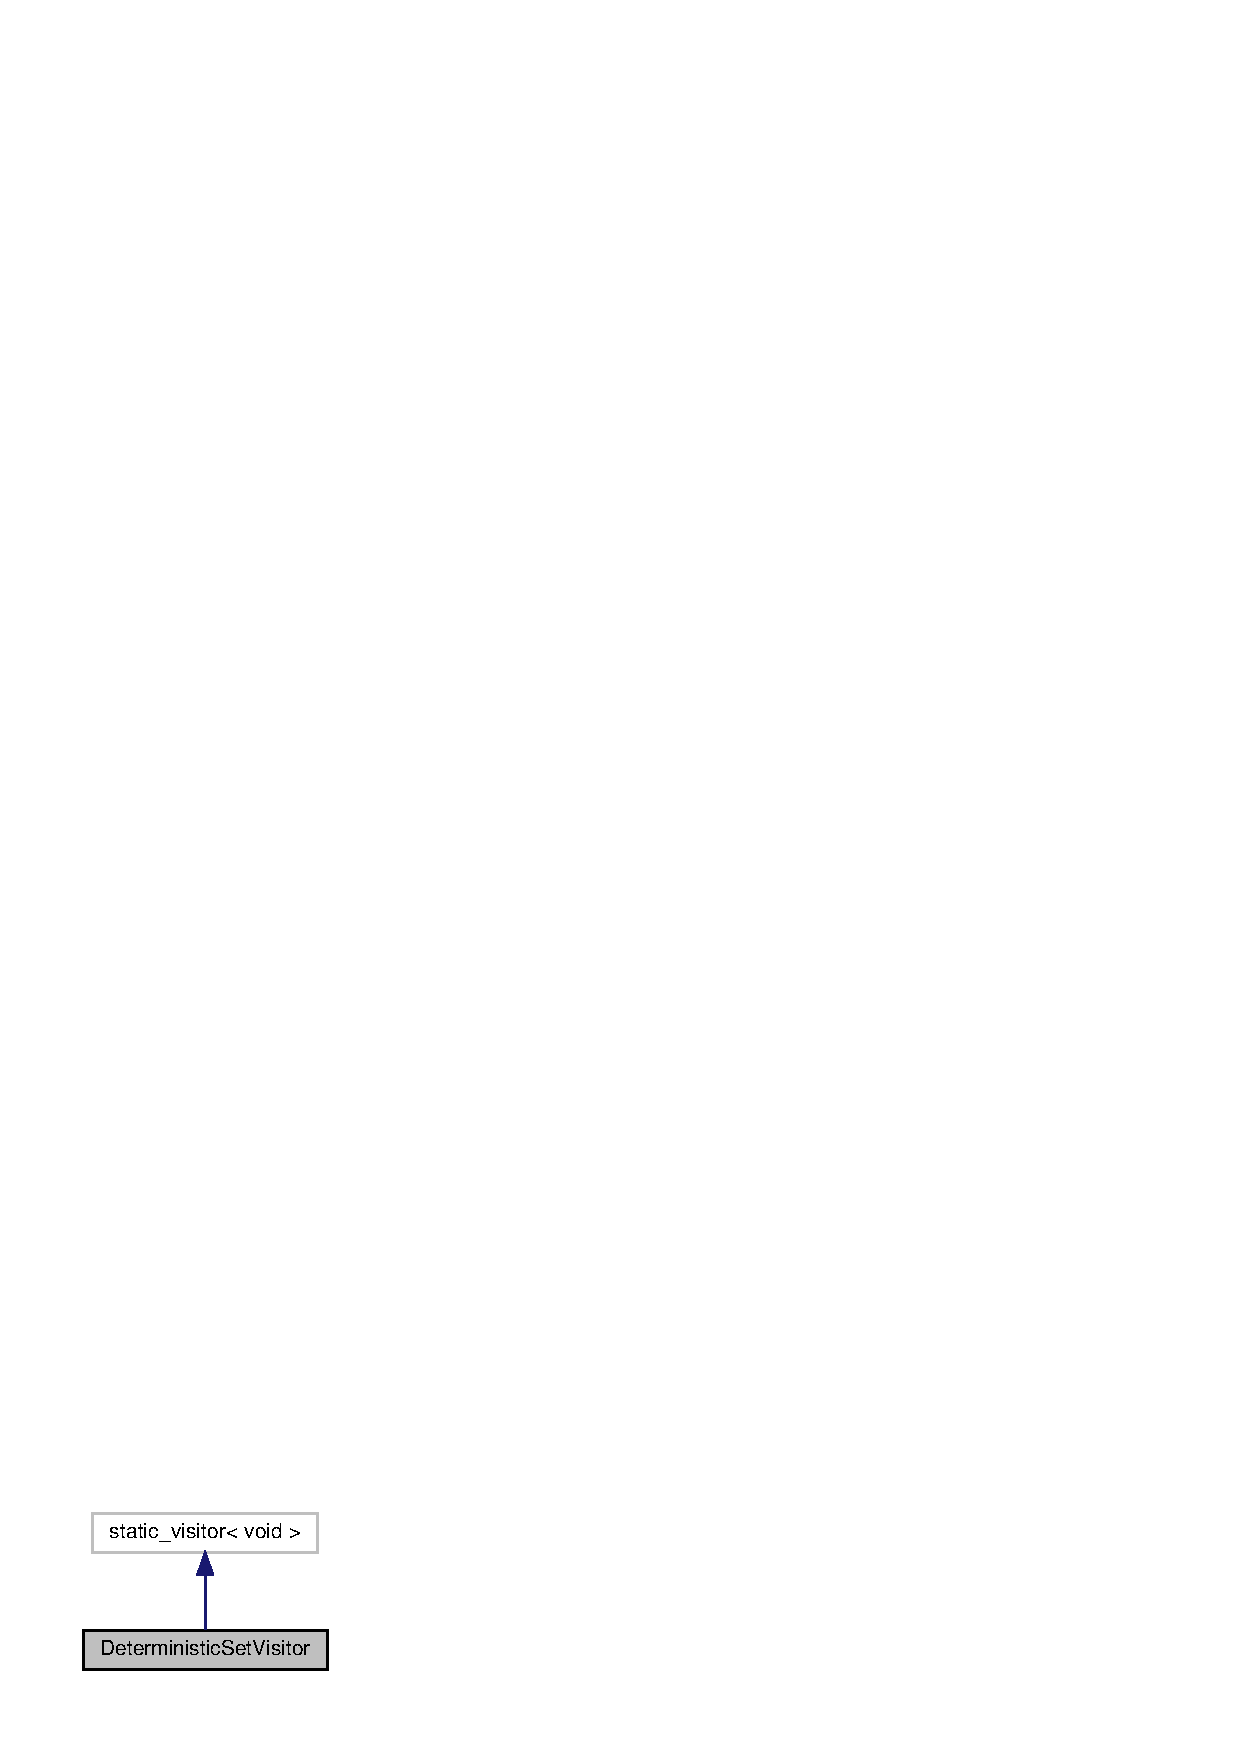
\includegraphics[width=161pt]{classmlpack_1_1ann_1_1DeterministicSetVisitor__inherit__graph}
\end{center}
\end{figure}
\subsection*{Public Member Functions}
\begin{DoxyCompactItemize}
\item 
\textbf{ Deterministic\+Set\+Visitor} (const bool deterministic=true)
\begin{DoxyCompactList}\small\item\em Set the deterministic parameter given the current deterministic value. \end{DoxyCompactList}\item 
{\footnotesize template$<$typename Layer\+Type $>$ }\\void \textbf{ operator()} (Layer\+Type $\ast$layer) const
\begin{DoxyCompactList}\small\item\em Set the deterministic parameter. \end{DoxyCompactList}\item 
void \textbf{ operator()} (\textbf{ More\+Types} layer) const
\end{DoxyCompactItemize}


\subsection{Detailed Description}
\doxyref{Deterministic\+Set\+Visitor}{p.}{classmlpack_1_1ann_1_1DeterministicSetVisitor} set the deterministic parameter given the deterministic value. 

Definition at line 28 of file deterministic\+\_\+set\+\_\+visitor.\+hpp.



\subsection{Constructor \& Destructor Documentation}
\mbox{\label{classmlpack_1_1ann_1_1DeterministicSetVisitor_aeb4fae3bdfa0643b201c0f5a7691bdf6}} 
\index{mlpack\+::ann\+::\+Deterministic\+Set\+Visitor@{mlpack\+::ann\+::\+Deterministic\+Set\+Visitor}!Deterministic\+Set\+Visitor@{Deterministic\+Set\+Visitor}}
\index{Deterministic\+Set\+Visitor@{Deterministic\+Set\+Visitor}!mlpack\+::ann\+::\+Deterministic\+Set\+Visitor@{mlpack\+::ann\+::\+Deterministic\+Set\+Visitor}}
\subsubsection{Deterministic\+Set\+Visitor()}
{\footnotesize\ttfamily \textbf{ Deterministic\+Set\+Visitor} (\begin{DoxyParamCaption}\item[{const bool}]{deterministic = {\ttfamily true} }\end{DoxyParamCaption})}



Set the deterministic parameter given the current deterministic value. 



\subsection{Member Function Documentation}
\mbox{\label{classmlpack_1_1ann_1_1DeterministicSetVisitor_a26bb3385c630118c35f4799f1509abbc}} 
\index{mlpack\+::ann\+::\+Deterministic\+Set\+Visitor@{mlpack\+::ann\+::\+Deterministic\+Set\+Visitor}!operator()@{operator()}}
\index{operator()@{operator()}!mlpack\+::ann\+::\+Deterministic\+Set\+Visitor@{mlpack\+::ann\+::\+Deterministic\+Set\+Visitor}}
\subsubsection{operator()()\hspace{0.1cm}{\footnotesize\ttfamily [1/2]}}
{\footnotesize\ttfamily void operator() (\begin{DoxyParamCaption}\item[{Layer\+Type $\ast$}]{layer }\end{DoxyParamCaption}) const}



Set the deterministic parameter. 

\mbox{\label{classmlpack_1_1ann_1_1DeterministicSetVisitor_ae35578e7ff874a320fe762bc0edfff04}} 
\index{mlpack\+::ann\+::\+Deterministic\+Set\+Visitor@{mlpack\+::ann\+::\+Deterministic\+Set\+Visitor}!operator()@{operator()}}
\index{operator()@{operator()}!mlpack\+::ann\+::\+Deterministic\+Set\+Visitor@{mlpack\+::ann\+::\+Deterministic\+Set\+Visitor}}
\subsubsection{operator()()\hspace{0.1cm}{\footnotesize\ttfamily [2/2]}}
{\footnotesize\ttfamily void operator() (\begin{DoxyParamCaption}\item[{\textbf{ More\+Types}}]{layer }\end{DoxyParamCaption}) const}



The documentation for this class was generated from the following file\+:\begin{DoxyCompactItemize}
\item 
/home/aakash/mlpack/src/mlpack/methods/ann/visitor/\textbf{ deterministic\+\_\+set\+\_\+visitor.\+hpp}\end{DoxyCompactItemize}

\section{Dice\+Loss$<$ Input\+Data\+Type, Output\+Data\+Type $>$ Class Template Reference}
\label{classmlpack_1_1ann_1_1DiceLoss}\index{Dice\+Loss$<$ Input\+Data\+Type, Output\+Data\+Type $>$@{Dice\+Loss$<$ Input\+Data\+Type, Output\+Data\+Type $>$}}


The dice loss performance function measures the network\textquotesingle{}s performance according to the dice coefficient between the input and target distributions.  


\subsection*{Public Member Functions}
\begin{DoxyCompactItemize}
\item 
\textbf{ Dice\+Loss} (const double smooth=1)
\begin{DoxyCompactList}\small\item\em Create the \doxyref{Dice\+Loss}{p.}{classmlpack_1_1ann_1_1DiceLoss} object. \end{DoxyCompactList}\item 
{\footnotesize template$<$typename Prediction\+Type , typename Target\+Type , typename Loss\+Type $>$ }\\void \textbf{ Backward} (const Prediction\+Type \&prediction, const Target\+Type \&target, Loss\+Type \&loss)
\begin{DoxyCompactList}\small\item\em Ordinary feed backward pass of a neural network. \end{DoxyCompactList}\item 
{\footnotesize template$<$typename Prediction\+Type , typename Target\+Type $>$ }\\Prediction\+Type\+::elem\+\_\+type \textbf{ Forward} (const Prediction\+Type \&prediction, const Target\+Type \&target)
\begin{DoxyCompactList}\small\item\em Computes the dice loss function. \end{DoxyCompactList}\item 
Output\+Data\+Type \& \textbf{ Output\+Parameter} () const
\begin{DoxyCompactList}\small\item\em Get the output parameter. \end{DoxyCompactList}\item 
Output\+Data\+Type \& \textbf{ Output\+Parameter} ()
\begin{DoxyCompactList}\small\item\em Modify the output parameter. \end{DoxyCompactList}\item 
{\footnotesize template$<$typename Archive $>$ }\\void \textbf{ serialize} (Archive \&ar, const uint32\+\_\+t)
\begin{DoxyCompactList}\small\item\em Serialize the layer. \end{DoxyCompactList}\item 
double \textbf{ Smooth} () const
\begin{DoxyCompactList}\small\item\em Get the smooth. \end{DoxyCompactList}\item 
double \& \textbf{ Smooth} ()
\begin{DoxyCompactList}\small\item\em Modify the smooth. \end{DoxyCompactList}\end{DoxyCompactItemize}


\subsection{Detailed Description}
\subsubsection*{template$<$typename Input\+Data\+Type = arma\+::mat, typename Output\+Data\+Type = arma\+::mat$>$\newline
class mlpack\+::ann\+::\+Dice\+Loss$<$ Input\+Data\+Type, Output\+Data\+Type $>$}

The dice loss performance function measures the network\textquotesingle{}s performance according to the dice coefficient between the input and target distributions. 

For more information see the following.


\begin{DoxyCode}
@article\{Milletari2016,
  author    = \{Fausto Milletari and Nassir Navab and Seyed\{-\}Ahmad Ahmadi\},
  title     = \{V-Net: Fully Convolutional Neural Networks \textcolor{keywordflow}{for}
               Volumetric Medical Image Segmentation\},
  journal   = \{CoRR\},
  volume    = \{abs/1606.04797\},
  year      = \{2016\},
  url       = \{http:\textcolor{comment}{//arxiv.org/abs/1606.04797\},}
  archivePrefix = \{arXiv\},
  eprint    = \{1606.04797\},
\}
\end{DoxyCode}



\begin{DoxyTemplParams}{Template Parameters}
{\em Input\+Data\+Type} & Type of the input data (arma\+::colvec, arma\+::mat, arma\+::sp\+\_\+mat or arma\+::cube). \\
\hline
{\em Output\+Data\+Type} & Type of the output data (arma\+::colvec, arma\+::mat, arma\+::sp\+\_\+mat or arma\+::cube). \\
\hline
\end{DoxyTemplParams}


Definition at line 50 of file dice\+\_\+loss.\+hpp.



\subsection{Constructor \& Destructor Documentation}
\mbox{\label{classmlpack_1_1ann_1_1DiceLoss_a4bfcd6e91e6a5f7133996d0800ca248f}} 
\index{mlpack\+::ann\+::\+Dice\+Loss@{mlpack\+::ann\+::\+Dice\+Loss}!Dice\+Loss@{Dice\+Loss}}
\index{Dice\+Loss@{Dice\+Loss}!mlpack\+::ann\+::\+Dice\+Loss@{mlpack\+::ann\+::\+Dice\+Loss}}
\subsubsection{Dice\+Loss()}
{\footnotesize\ttfamily \textbf{ Dice\+Loss} (\begin{DoxyParamCaption}\item[{const double}]{smooth = {\ttfamily 1} }\end{DoxyParamCaption})}



Create the \doxyref{Dice\+Loss}{p.}{classmlpack_1_1ann_1_1DiceLoss} object. 


\begin{DoxyParams}{Parameters}
{\em smooth} & The Laplace smoothing parameter. \\
\hline
\end{DoxyParams}


\subsection{Member Function Documentation}
\mbox{\label{classmlpack_1_1ann_1_1DiceLoss_add41dbaf358dc099750dc6064cb7e0d7}} 
\index{mlpack\+::ann\+::\+Dice\+Loss@{mlpack\+::ann\+::\+Dice\+Loss}!Backward@{Backward}}
\index{Backward@{Backward}!mlpack\+::ann\+::\+Dice\+Loss@{mlpack\+::ann\+::\+Dice\+Loss}}
\subsubsection{Backward()}
{\footnotesize\ttfamily void Backward (\begin{DoxyParamCaption}\item[{const Prediction\+Type \&}]{prediction,  }\item[{const Target\+Type \&}]{target,  }\item[{Loss\+Type \&}]{loss }\end{DoxyParamCaption})}



Ordinary feed backward pass of a neural network. 


\begin{DoxyParams}{Parameters}
{\em prediction} & Predictions used for evaluating the specified loss function. \\
\hline
{\em target} & The target vector. \\
\hline
{\em loss} & The calculated error. \\
\hline
\end{DoxyParams}
\mbox{\label{classmlpack_1_1ann_1_1DiceLoss_ab3640059898ea76c13709b8099316fe8}} 
\index{mlpack\+::ann\+::\+Dice\+Loss@{mlpack\+::ann\+::\+Dice\+Loss}!Forward@{Forward}}
\index{Forward@{Forward}!mlpack\+::ann\+::\+Dice\+Loss@{mlpack\+::ann\+::\+Dice\+Loss}}
\subsubsection{Forward()}
{\footnotesize\ttfamily Prediction\+Type\+::elem\+\_\+type Forward (\begin{DoxyParamCaption}\item[{const Prediction\+Type \&}]{prediction,  }\item[{const Target\+Type \&}]{target }\end{DoxyParamCaption})}



Computes the dice loss function. 


\begin{DoxyParams}{Parameters}
{\em prediction} & Predictions used for evaluating the specified loss function. \\
\hline
{\em target} & The target vector. \\
\hline
\end{DoxyParams}
\mbox{\label{classmlpack_1_1ann_1_1DiceLoss_a8bae962cc603d1cab8d80ec78f8d505d}} 
\index{mlpack\+::ann\+::\+Dice\+Loss@{mlpack\+::ann\+::\+Dice\+Loss}!Output\+Parameter@{Output\+Parameter}}
\index{Output\+Parameter@{Output\+Parameter}!mlpack\+::ann\+::\+Dice\+Loss@{mlpack\+::ann\+::\+Dice\+Loss}}
\subsubsection{Output\+Parameter()\hspace{0.1cm}{\footnotesize\ttfamily [1/2]}}
{\footnotesize\ttfamily Output\+Data\+Type\& Output\+Parameter (\begin{DoxyParamCaption}{ }\end{DoxyParamCaption}) const\hspace{0.3cm}{\ttfamily [inline]}}



Get the output parameter. 



Definition at line 85 of file dice\+\_\+loss.\+hpp.

\mbox{\label{classmlpack_1_1ann_1_1DiceLoss_a21d5f745f02c709625a4ee0907f004a5}} 
\index{mlpack\+::ann\+::\+Dice\+Loss@{mlpack\+::ann\+::\+Dice\+Loss}!Output\+Parameter@{Output\+Parameter}}
\index{Output\+Parameter@{Output\+Parameter}!mlpack\+::ann\+::\+Dice\+Loss@{mlpack\+::ann\+::\+Dice\+Loss}}
\subsubsection{Output\+Parameter()\hspace{0.1cm}{\footnotesize\ttfamily [2/2]}}
{\footnotesize\ttfamily Output\+Data\+Type\& Output\+Parameter (\begin{DoxyParamCaption}{ }\end{DoxyParamCaption})\hspace{0.3cm}{\ttfamily [inline]}}



Modify the output parameter. 



Definition at line 87 of file dice\+\_\+loss.\+hpp.

\mbox{\label{classmlpack_1_1ann_1_1DiceLoss_a65cba07328997659bec80b9879b15a51}} 
\index{mlpack\+::ann\+::\+Dice\+Loss@{mlpack\+::ann\+::\+Dice\+Loss}!serialize@{serialize}}
\index{serialize@{serialize}!mlpack\+::ann\+::\+Dice\+Loss@{mlpack\+::ann\+::\+Dice\+Loss}}
\subsubsection{serialize()}
{\footnotesize\ttfamily void serialize (\begin{DoxyParamCaption}\item[{Archive \&}]{ar,  }\item[{const uint32\+\_\+t}]{ }\end{DoxyParamCaption})}



Serialize the layer. 



Referenced by Dice\+Loss$<$ Input\+Data\+Type, Output\+Data\+Type $>$\+::\+Smooth().

\mbox{\label{classmlpack_1_1ann_1_1DiceLoss_ac72576e4dbe1a49364cb15d8843e4cad}} 
\index{mlpack\+::ann\+::\+Dice\+Loss@{mlpack\+::ann\+::\+Dice\+Loss}!Smooth@{Smooth}}
\index{Smooth@{Smooth}!mlpack\+::ann\+::\+Dice\+Loss@{mlpack\+::ann\+::\+Dice\+Loss}}
\subsubsection{Smooth()\hspace{0.1cm}{\footnotesize\ttfamily [1/2]}}
{\footnotesize\ttfamily double Smooth (\begin{DoxyParamCaption}{ }\end{DoxyParamCaption}) const\hspace{0.3cm}{\ttfamily [inline]}}



Get the smooth. 



Definition at line 90 of file dice\+\_\+loss.\+hpp.

\mbox{\label{classmlpack_1_1ann_1_1DiceLoss_a5bd134044985cc6d34d5d1cc2e2484e7}} 
\index{mlpack\+::ann\+::\+Dice\+Loss@{mlpack\+::ann\+::\+Dice\+Loss}!Smooth@{Smooth}}
\index{Smooth@{Smooth}!mlpack\+::ann\+::\+Dice\+Loss@{mlpack\+::ann\+::\+Dice\+Loss}}
\subsubsection{Smooth()\hspace{0.1cm}{\footnotesize\ttfamily [2/2]}}
{\footnotesize\ttfamily double\& Smooth (\begin{DoxyParamCaption}{ }\end{DoxyParamCaption})\hspace{0.3cm}{\ttfamily [inline]}}



Modify the smooth. 



Definition at line 92 of file dice\+\_\+loss.\+hpp.



References Dice\+Loss$<$ Input\+Data\+Type, Output\+Data\+Type $>$\+::serialize().



The documentation for this class was generated from the following file\+:\begin{DoxyCompactItemize}
\item 
/home/aakash/mlpack/src/mlpack/methods/ann/loss\+\_\+functions/\textbf{ dice\+\_\+loss.\+hpp}\end{DoxyCompactItemize}

\section{Drop\+Connect$<$ Input\+Data\+Type, Output\+Data\+Type $>$ Class Template Reference}
\label{classmlpack_1_1ann_1_1DropConnect}\index{Drop\+Connect$<$ Input\+Data\+Type, Output\+Data\+Type $>$@{Drop\+Connect$<$ Input\+Data\+Type, Output\+Data\+Type $>$}}


The \doxyref{Drop\+Connect}{p.}{classmlpack_1_1ann_1_1DropConnect} layer is a regularizer that randomly with probability ratio sets the connection values to zero and scales the remaining elements by factor 1 /(1 -\/ ratio).  


\subsection*{Public Member Functions}
\begin{DoxyCompactItemize}
\item 
\textbf{ Drop\+Connect} ()
\begin{DoxyCompactList}\small\item\em Create the \doxyref{Drop\+Connect}{p.}{classmlpack_1_1ann_1_1DropConnect} object. \end{DoxyCompactList}\item 
\textbf{ Drop\+Connect} (const size\+\_\+t in\+Size, const size\+\_\+t out\+Size, const double ratio=0.\+5)
\begin{DoxyCompactList}\small\item\em Creates the \doxyref{Drop\+Connect}{p.}{classmlpack_1_1ann_1_1DropConnect} Layer as a \doxyref{Linear}{p.}{classmlpack_1_1ann_1_1Linear} Object that takes input size, output size and ratio as parameter. \end{DoxyCompactList}\item 
{\footnotesize template$<$typename eT $>$ }\\void \textbf{ Backward} (const arma\+::\+Mat$<$ eT $>$ \&input, const arma\+::\+Mat$<$ eT $>$ \&gy, arma\+::\+Mat$<$ eT $>$ \&g)
\begin{DoxyCompactList}\small\item\em Ordinary feed backward pass of the \doxyref{Drop\+Connect}{p.}{classmlpack_1_1ann_1_1DropConnect} layer. \end{DoxyCompactList}\item 
Output\+Data\+Type const  \& \textbf{ Delta} () const
\begin{DoxyCompactList}\small\item\em Get the delta. \end{DoxyCompactList}\item 
Output\+Data\+Type \& \textbf{ Delta} ()
\begin{DoxyCompactList}\small\item\em Modify the delta. \end{DoxyCompactList}\item 
bool \textbf{ Deterministic} () const
\begin{DoxyCompactList}\small\item\em The value of the deterministic parameter. \end{DoxyCompactList}\item 
bool \& \textbf{ Deterministic} ()
\begin{DoxyCompactList}\small\item\em Modify the value of the deterministic parameter. \end{DoxyCompactList}\item 
{\footnotesize template$<$typename eT $>$ }\\void \textbf{ Forward} (const arma\+::\+Mat$<$ eT $>$ \&input, arma\+::\+Mat$<$ eT $>$ \&output)
\begin{DoxyCompactList}\small\item\em Ordinary feed forward pass of the \doxyref{Drop\+Connect}{p.}{classmlpack_1_1ann_1_1DropConnect} layer. \end{DoxyCompactList}\item 
{\footnotesize template$<$typename eT $>$ }\\void \textbf{ Gradient} (const arma\+::\+Mat$<$ eT $>$ \&input, const arma\+::\+Mat$<$ eT $>$ \&error, arma\+::\+Mat$<$ eT $>$ \&)
\begin{DoxyCompactList}\small\item\em Calculate the gradient using the output delta and the input activation. \end{DoxyCompactList}\item 
Output\+Data\+Type const  \& \textbf{ Gradient} () const
\begin{DoxyCompactList}\small\item\em Get the gradient. \end{DoxyCompactList}\item 
Output\+Data\+Type \& \textbf{ Gradient} ()
\begin{DoxyCompactList}\small\item\em Modify the gradient. \end{DoxyCompactList}\item 
std\+::vector$<$ \textbf{ Layer\+Types}$<$$>$ $>$ \& \textbf{ Model} ()
\begin{DoxyCompactList}\small\item\em Get the model modules. \end{DoxyCompactList}\item 
Output\+Data\+Type const  \& \textbf{ Output\+Parameter} () const
\begin{DoxyCompactList}\small\item\em Get the output parameter. \end{DoxyCompactList}\item 
Output\+Data\+Type \& \textbf{ Output\+Parameter} ()
\begin{DoxyCompactList}\small\item\em Modify the output parameter. \end{DoxyCompactList}\item 
Output\+Data\+Type const  \& \textbf{ Parameters} () const
\begin{DoxyCompactList}\small\item\em Get the parameters. \end{DoxyCompactList}\item 
Output\+Data\+Type \& \textbf{ Parameters} ()
\begin{DoxyCompactList}\small\item\em Modify the parameters. \end{DoxyCompactList}\item 
double \textbf{ Ratio} () const
\begin{DoxyCompactList}\small\item\em The probability of setting a value to zero. \end{DoxyCompactList}\item 
void \textbf{ Ratio} (const double r)
\begin{DoxyCompactList}\small\item\em Modify the probability of setting a value to zero. \end{DoxyCompactList}\item 
{\footnotesize template$<$typename Archive $>$ }\\void \textbf{ serialize} (Archive \&ar, const uint32\+\_\+t)
\begin{DoxyCompactList}\small\item\em Serialize the layer. \end{DoxyCompactList}\item 
size\+\_\+t \textbf{ Weight\+Size} () const
\begin{DoxyCompactList}\small\item\em Return the size of the weight matrix. \end{DoxyCompactList}\end{DoxyCompactItemize}


\subsection{Detailed Description}
\subsubsection*{template$<$typename Input\+Data\+Type = arma\+::mat, typename Output\+Data\+Type = arma\+::mat$>$\newline
class mlpack\+::ann\+::\+Drop\+Connect$<$ Input\+Data\+Type, Output\+Data\+Type $>$}

The \doxyref{Drop\+Connect}{p.}{classmlpack_1_1ann_1_1DropConnect} layer is a regularizer that randomly with probability ratio sets the connection values to zero and scales the remaining elements by factor 1 /(1 -\/ ratio). 

The output is scaled with 1 / (1 -\/ p) when deterministic is false. In the deterministic mode(during testing), the layer just computes the output. The output is computed according to the input layer. If no input layer is given, it will take a linear layer as default.

Note\+: During training you should set deterministic to false and during testing you should set deterministic to true.

For more information, see the following.


\begin{DoxyCode}
@inproceedings\{WanICML2013,
  title=\{Regularization of Neural Networks \textcolor{keyword}{using} DropConnect\},
  booktitle = \{Proceedings of the 30th International Conference on Machine
               Learning(ICML - 13)\},
  author = \{Li Wan and Matthew Zeiler and Sixin Zhang and Yann L. Cun and
            Rob Fergus\},
  year = \{2013\},
  url  = \{http:\textcolor{comment}{//proceedings.mlr.press/v28/wan13.pdf\}}
\}
\end{DoxyCode}



\begin{DoxyTemplParams}{Template Parameters}
{\em Input\+Data\+Type} & Type of the input data (arma\+::colvec, arma\+::mat, arma\+::sp\+\_\+mat or arma\+::cube). \\
\hline
{\em Output\+Data\+Type} & Type of the output data (arma\+::colvec, arma\+::mat, arma\+::sp\+\_\+mat or arma\+::cube). \\
\hline
\end{DoxyTemplParams}


Definition at line 63 of file dropconnect.\+hpp.



\subsection{Constructor \& Destructor Documentation}
\mbox{\label{classmlpack_1_1ann_1_1DropConnect_a8dbbcddcb47c7d048d0094b4619f71ac}} 
\index{mlpack\+::ann\+::\+Drop\+Connect@{mlpack\+::ann\+::\+Drop\+Connect}!Drop\+Connect@{Drop\+Connect}}
\index{Drop\+Connect@{Drop\+Connect}!mlpack\+::ann\+::\+Drop\+Connect@{mlpack\+::ann\+::\+Drop\+Connect}}
\subsubsection{Drop\+Connect()\hspace{0.1cm}{\footnotesize\ttfamily [1/2]}}
{\footnotesize\ttfamily \textbf{ Drop\+Connect} (\begin{DoxyParamCaption}{ }\end{DoxyParamCaption})}



Create the \doxyref{Drop\+Connect}{p.}{classmlpack_1_1ann_1_1DropConnect} object. 

\mbox{\label{classmlpack_1_1ann_1_1DropConnect_a693f017e99094d956f4c88e1b47acdf0}} 
\index{mlpack\+::ann\+::\+Drop\+Connect@{mlpack\+::ann\+::\+Drop\+Connect}!Drop\+Connect@{Drop\+Connect}}
\index{Drop\+Connect@{Drop\+Connect}!mlpack\+::ann\+::\+Drop\+Connect@{mlpack\+::ann\+::\+Drop\+Connect}}
\subsubsection{Drop\+Connect()\hspace{0.1cm}{\footnotesize\ttfamily [2/2]}}
{\footnotesize\ttfamily \textbf{ Drop\+Connect} (\begin{DoxyParamCaption}\item[{const size\+\_\+t}]{in\+Size,  }\item[{const size\+\_\+t}]{out\+Size,  }\item[{const double}]{ratio = {\ttfamily 0.5} }\end{DoxyParamCaption})}



Creates the \doxyref{Drop\+Connect}{p.}{classmlpack_1_1ann_1_1DropConnect} Layer as a \doxyref{Linear}{p.}{classmlpack_1_1ann_1_1Linear} Object that takes input size, output size and ratio as parameter. 


\begin{DoxyParams}{Parameters}
{\em in\+Size} & The number of input units. \\
\hline
{\em out\+Size} & The number of output units. \\
\hline
{\em ratio} & The probability of setting a value to zero. \\
\hline
\end{DoxyParams}


\subsection{Member Function Documentation}
\mbox{\label{classmlpack_1_1ann_1_1DropConnect_a78dbad83871f43db1975e45a9a69c376}} 
\index{mlpack\+::ann\+::\+Drop\+Connect@{mlpack\+::ann\+::\+Drop\+Connect}!Backward@{Backward}}
\index{Backward@{Backward}!mlpack\+::ann\+::\+Drop\+Connect@{mlpack\+::ann\+::\+Drop\+Connect}}
\subsubsection{Backward()}
{\footnotesize\ttfamily void Backward (\begin{DoxyParamCaption}\item[{const arma\+::\+Mat$<$ eT $>$ \&}]{input,  }\item[{const arma\+::\+Mat$<$ eT $>$ \&}]{gy,  }\item[{arma\+::\+Mat$<$ eT $>$ \&}]{g }\end{DoxyParamCaption})}



Ordinary feed backward pass of the \doxyref{Drop\+Connect}{p.}{classmlpack_1_1ann_1_1DropConnect} layer. 


\begin{DoxyParams}{Parameters}
{\em input} & The propagated input activation. \\
\hline
{\em gy} & The backpropagated error. \\
\hline
{\em g} & The calculated gradient. \\
\hline
\end{DoxyParams}
\mbox{\label{classmlpack_1_1ann_1_1DropConnect_a797f7edb44dd081e5e2b3cc316eef6bd}} 
\index{mlpack\+::ann\+::\+Drop\+Connect@{mlpack\+::ann\+::\+Drop\+Connect}!Delta@{Delta}}
\index{Delta@{Delta}!mlpack\+::ann\+::\+Drop\+Connect@{mlpack\+::ann\+::\+Drop\+Connect}}
\subsubsection{Delta()\hspace{0.1cm}{\footnotesize\ttfamily [1/2]}}
{\footnotesize\ttfamily Output\+Data\+Type const\& Delta (\begin{DoxyParamCaption}{ }\end{DoxyParamCaption}) const\hspace{0.3cm}{\ttfamily [inline]}}



Get the delta. 



Definition at line 128 of file dropconnect.\+hpp.

\mbox{\label{classmlpack_1_1ann_1_1DropConnect_ad6601342d560219ce951d554e69e5e87}} 
\index{mlpack\+::ann\+::\+Drop\+Connect@{mlpack\+::ann\+::\+Drop\+Connect}!Delta@{Delta}}
\index{Delta@{Delta}!mlpack\+::ann\+::\+Drop\+Connect@{mlpack\+::ann\+::\+Drop\+Connect}}
\subsubsection{Delta()\hspace{0.1cm}{\footnotesize\ttfamily [2/2]}}
{\footnotesize\ttfamily Output\+Data\+Type\& Delta (\begin{DoxyParamCaption}{ }\end{DoxyParamCaption})\hspace{0.3cm}{\ttfamily [inline]}}



Modify the delta. 



Definition at line 130 of file dropconnect.\+hpp.

\mbox{\label{classmlpack_1_1ann_1_1DropConnect_a9f4103707f4d199ce5594d239b60443e}} 
\index{mlpack\+::ann\+::\+Drop\+Connect@{mlpack\+::ann\+::\+Drop\+Connect}!Deterministic@{Deterministic}}
\index{Deterministic@{Deterministic}!mlpack\+::ann\+::\+Drop\+Connect@{mlpack\+::ann\+::\+Drop\+Connect}}
\subsubsection{Deterministic()\hspace{0.1cm}{\footnotesize\ttfamily [1/2]}}
{\footnotesize\ttfamily bool Deterministic (\begin{DoxyParamCaption}{ }\end{DoxyParamCaption}) const\hspace{0.3cm}{\ttfamily [inline]}}



The value of the deterministic parameter. 



Definition at line 138 of file dropconnect.\+hpp.

\mbox{\label{classmlpack_1_1ann_1_1DropConnect_a42d4ee3da432cff20d3a41b8b1ec801c}} 
\index{mlpack\+::ann\+::\+Drop\+Connect@{mlpack\+::ann\+::\+Drop\+Connect}!Deterministic@{Deterministic}}
\index{Deterministic@{Deterministic}!mlpack\+::ann\+::\+Drop\+Connect@{mlpack\+::ann\+::\+Drop\+Connect}}
\subsubsection{Deterministic()\hspace{0.1cm}{\footnotesize\ttfamily [2/2]}}
{\footnotesize\ttfamily bool\& Deterministic (\begin{DoxyParamCaption}{ }\end{DoxyParamCaption})\hspace{0.3cm}{\ttfamily [inline]}}



Modify the value of the deterministic parameter. 



Definition at line 141 of file dropconnect.\+hpp.

\mbox{\label{classmlpack_1_1ann_1_1DropConnect_a461f849bc638c15bec262dc9c3a58abe}} 
\index{mlpack\+::ann\+::\+Drop\+Connect@{mlpack\+::ann\+::\+Drop\+Connect}!Forward@{Forward}}
\index{Forward@{Forward}!mlpack\+::ann\+::\+Drop\+Connect@{mlpack\+::ann\+::\+Drop\+Connect}}
\subsubsection{Forward()}
{\footnotesize\ttfamily void Forward (\begin{DoxyParamCaption}\item[{const arma\+::\+Mat$<$ eT $>$ \&}]{input,  }\item[{arma\+::\+Mat$<$ eT $>$ \&}]{output }\end{DoxyParamCaption})}



Ordinary feed forward pass of the \doxyref{Drop\+Connect}{p.}{classmlpack_1_1ann_1_1DropConnect} layer. 


\begin{DoxyParams}{Parameters}
{\em input} & Input data used for evaluating the specified function. \\
\hline
{\em output} & Resulting output activation. \\
\hline
\end{DoxyParams}
\mbox{\label{classmlpack_1_1ann_1_1DropConnect_a505acb56ef67da2fc73190d3d4931969}} 
\index{mlpack\+::ann\+::\+Drop\+Connect@{mlpack\+::ann\+::\+Drop\+Connect}!Gradient@{Gradient}}
\index{Gradient@{Gradient}!mlpack\+::ann\+::\+Drop\+Connect@{mlpack\+::ann\+::\+Drop\+Connect}}
\subsubsection{Gradient()\hspace{0.1cm}{\footnotesize\ttfamily [1/3]}}
{\footnotesize\ttfamily void Gradient (\begin{DoxyParamCaption}\item[{const arma\+::\+Mat$<$ eT $>$ \&}]{input,  }\item[{const arma\+::\+Mat$<$ eT $>$ \&}]{error,  }\item[{arma\+::\+Mat$<$ eT $>$ \&}]{ }\end{DoxyParamCaption})}



Calculate the gradient using the output delta and the input activation. 


\begin{DoxyParams}{Parameters}
{\em input} & The propagated input. \\
\hline
{\em error} & The calculated error. \\
\hline
{\em $\ast$} & (gradient) The calculated gradient. \\
\hline
\end{DoxyParams}
\mbox{\label{classmlpack_1_1ann_1_1DropConnect_a0f1f4e6d93472d83852731a96c8c3f59}} 
\index{mlpack\+::ann\+::\+Drop\+Connect@{mlpack\+::ann\+::\+Drop\+Connect}!Gradient@{Gradient}}
\index{Gradient@{Gradient}!mlpack\+::ann\+::\+Drop\+Connect@{mlpack\+::ann\+::\+Drop\+Connect}}
\subsubsection{Gradient()\hspace{0.1cm}{\footnotesize\ttfamily [2/3]}}
{\footnotesize\ttfamily Output\+Data\+Type const\& Gradient (\begin{DoxyParamCaption}{ }\end{DoxyParamCaption}) const\hspace{0.3cm}{\ttfamily [inline]}}



Get the gradient. 



Definition at line 133 of file dropconnect.\+hpp.

\mbox{\label{classmlpack_1_1ann_1_1DropConnect_a19abce4739c3b0b658b612537e21956a}} 
\index{mlpack\+::ann\+::\+Drop\+Connect@{mlpack\+::ann\+::\+Drop\+Connect}!Gradient@{Gradient}}
\index{Gradient@{Gradient}!mlpack\+::ann\+::\+Drop\+Connect@{mlpack\+::ann\+::\+Drop\+Connect}}
\subsubsection{Gradient()\hspace{0.1cm}{\footnotesize\ttfamily [3/3]}}
{\footnotesize\ttfamily Output\+Data\+Type\& Gradient (\begin{DoxyParamCaption}{ }\end{DoxyParamCaption})\hspace{0.3cm}{\ttfamily [inline]}}



Modify the gradient. 



Definition at line 135 of file dropconnect.\+hpp.

\mbox{\label{classmlpack_1_1ann_1_1DropConnect_a50c707b4f7c009339d8d661539baf38f}} 
\index{mlpack\+::ann\+::\+Drop\+Connect@{mlpack\+::ann\+::\+Drop\+Connect}!Model@{Model}}
\index{Model@{Model}!mlpack\+::ann\+::\+Drop\+Connect@{mlpack\+::ann\+::\+Drop\+Connect}}
\subsubsection{Model()}
{\footnotesize\ttfamily std\+::vector$<$\textbf{ Layer\+Types}$<$$>$ $>$\& Model (\begin{DoxyParamCaption}{ }\end{DoxyParamCaption})\hspace{0.3cm}{\ttfamily [inline]}}



Get the model modules. 



Definition at line 115 of file dropconnect.\+hpp.

\mbox{\label{classmlpack_1_1ann_1_1DropConnect_a0ee21c2a36e5abad1e7a9d5dd00849f9}} 
\index{mlpack\+::ann\+::\+Drop\+Connect@{mlpack\+::ann\+::\+Drop\+Connect}!Output\+Parameter@{Output\+Parameter}}
\index{Output\+Parameter@{Output\+Parameter}!mlpack\+::ann\+::\+Drop\+Connect@{mlpack\+::ann\+::\+Drop\+Connect}}
\subsubsection{Output\+Parameter()\hspace{0.1cm}{\footnotesize\ttfamily [1/2]}}
{\footnotesize\ttfamily Output\+Data\+Type const\& Output\+Parameter (\begin{DoxyParamCaption}{ }\end{DoxyParamCaption}) const\hspace{0.3cm}{\ttfamily [inline]}}



Get the output parameter. 



Definition at line 123 of file dropconnect.\+hpp.

\mbox{\label{classmlpack_1_1ann_1_1DropConnect_a21d5f745f02c709625a4ee0907f004a5}} 
\index{mlpack\+::ann\+::\+Drop\+Connect@{mlpack\+::ann\+::\+Drop\+Connect}!Output\+Parameter@{Output\+Parameter}}
\index{Output\+Parameter@{Output\+Parameter}!mlpack\+::ann\+::\+Drop\+Connect@{mlpack\+::ann\+::\+Drop\+Connect}}
\subsubsection{Output\+Parameter()\hspace{0.1cm}{\footnotesize\ttfamily [2/2]}}
{\footnotesize\ttfamily Output\+Data\+Type\& Output\+Parameter (\begin{DoxyParamCaption}{ }\end{DoxyParamCaption})\hspace{0.3cm}{\ttfamily [inline]}}



Modify the output parameter. 



Definition at line 125 of file dropconnect.\+hpp.

\mbox{\label{classmlpack_1_1ann_1_1DropConnect_aa530552c7ef915c952fbacc77b965c90}} 
\index{mlpack\+::ann\+::\+Drop\+Connect@{mlpack\+::ann\+::\+Drop\+Connect}!Parameters@{Parameters}}
\index{Parameters@{Parameters}!mlpack\+::ann\+::\+Drop\+Connect@{mlpack\+::ann\+::\+Drop\+Connect}}
\subsubsection{Parameters()\hspace{0.1cm}{\footnotesize\ttfamily [1/2]}}
{\footnotesize\ttfamily Output\+Data\+Type const\& Parameters (\begin{DoxyParamCaption}{ }\end{DoxyParamCaption}) const\hspace{0.3cm}{\ttfamily [inline]}}



Get the parameters. 



Definition at line 118 of file dropconnect.\+hpp.

\mbox{\label{classmlpack_1_1ann_1_1DropConnect_a9c5c5900772a689d5a6b59778ec67120}} 
\index{mlpack\+::ann\+::\+Drop\+Connect@{mlpack\+::ann\+::\+Drop\+Connect}!Parameters@{Parameters}}
\index{Parameters@{Parameters}!mlpack\+::ann\+::\+Drop\+Connect@{mlpack\+::ann\+::\+Drop\+Connect}}
\subsubsection{Parameters()\hspace{0.1cm}{\footnotesize\ttfamily [2/2]}}
{\footnotesize\ttfamily Output\+Data\+Type\& Parameters (\begin{DoxyParamCaption}{ }\end{DoxyParamCaption})\hspace{0.3cm}{\ttfamily [inline]}}



Modify the parameters. 



Definition at line 120 of file dropconnect.\+hpp.

\mbox{\label{classmlpack_1_1ann_1_1DropConnect_a0052f2d1427761ea25fb01a05d966a40}} 
\index{mlpack\+::ann\+::\+Drop\+Connect@{mlpack\+::ann\+::\+Drop\+Connect}!Ratio@{Ratio}}
\index{Ratio@{Ratio}!mlpack\+::ann\+::\+Drop\+Connect@{mlpack\+::ann\+::\+Drop\+Connect}}
\subsubsection{Ratio()\hspace{0.1cm}{\footnotesize\ttfamily [1/2]}}
{\footnotesize\ttfamily double Ratio (\begin{DoxyParamCaption}{ }\end{DoxyParamCaption}) const\hspace{0.3cm}{\ttfamily [inline]}}



The probability of setting a value to zero. 



Definition at line 144 of file dropconnect.\+hpp.

\mbox{\label{classmlpack_1_1ann_1_1DropConnect_a9ca65c8f62aa7b45b5b08899d83d2821}} 
\index{mlpack\+::ann\+::\+Drop\+Connect@{mlpack\+::ann\+::\+Drop\+Connect}!Ratio@{Ratio}}
\index{Ratio@{Ratio}!mlpack\+::ann\+::\+Drop\+Connect@{mlpack\+::ann\+::\+Drop\+Connect}}
\subsubsection{Ratio()\hspace{0.1cm}{\footnotesize\ttfamily [2/2]}}
{\footnotesize\ttfamily void Ratio (\begin{DoxyParamCaption}\item[{const double}]{r }\end{DoxyParamCaption})\hspace{0.3cm}{\ttfamily [inline]}}



Modify the probability of setting a value to zero. 



Definition at line 147 of file dropconnect.\+hpp.

\mbox{\label{classmlpack_1_1ann_1_1DropConnect_a65cba07328997659bec80b9879b15a51}} 
\index{mlpack\+::ann\+::\+Drop\+Connect@{mlpack\+::ann\+::\+Drop\+Connect}!serialize@{serialize}}
\index{serialize@{serialize}!mlpack\+::ann\+::\+Drop\+Connect@{mlpack\+::ann\+::\+Drop\+Connect}}
\subsubsection{serialize()}
{\footnotesize\ttfamily void serialize (\begin{DoxyParamCaption}\item[{Archive \&}]{ar,  }\item[{const uint32\+\_\+t}]{ }\end{DoxyParamCaption})}



Serialize the layer. 



Referenced by Drop\+Connect$<$ Input\+Data\+Type, Output\+Data\+Type $>$\+::\+Weight\+Size().

\mbox{\label{classmlpack_1_1ann_1_1DropConnect_a7a2704698a50d9e00dfb083f3a863579}} 
\index{mlpack\+::ann\+::\+Drop\+Connect@{mlpack\+::ann\+::\+Drop\+Connect}!Weight\+Size@{Weight\+Size}}
\index{Weight\+Size@{Weight\+Size}!mlpack\+::ann\+::\+Drop\+Connect@{mlpack\+::ann\+::\+Drop\+Connect}}
\subsubsection{Weight\+Size()}
{\footnotesize\ttfamily size\+\_\+t Weight\+Size (\begin{DoxyParamCaption}{ }\end{DoxyParamCaption}) const\hspace{0.3cm}{\ttfamily [inline]}}



Return the size of the weight matrix. 



Definition at line 154 of file dropconnect.\+hpp.



References Drop\+Connect$<$ Input\+Data\+Type, Output\+Data\+Type $>$\+::serialize().



The documentation for this class was generated from the following file\+:\begin{DoxyCompactItemize}
\item 
/home/aakash/mlpack/src/mlpack/methods/ann/layer/\textbf{ dropconnect.\+hpp}\end{DoxyCompactItemize}

\section{Dropout$<$ Input\+Data\+Type, Output\+Data\+Type $>$ Class Template Reference}
\label{classmlpack_1_1ann_1_1Dropout}\index{Dropout$<$ Input\+Data\+Type, Output\+Data\+Type $>$@{Dropout$<$ Input\+Data\+Type, Output\+Data\+Type $>$}}


The dropout layer is a regularizer that randomly with probability \textquotesingle{}ratio\textquotesingle{} sets input values to zero and scales the remaining elements by factor 1 / (1 -\/ ratio) rather than during test time so as to keep the expected sum same.  


\subsection*{Public Member Functions}
\begin{DoxyCompactItemize}
\item 
\textbf{ Dropout} (const double ratio=0.\+5)
\begin{DoxyCompactList}\small\item\em Create the \doxyref{Dropout}{p.}{classmlpack_1_1ann_1_1Dropout} object using the specified ratio parameter. \end{DoxyCompactList}\item 
\textbf{ Dropout} (const \textbf{ Dropout} \&layer)
\begin{DoxyCompactList}\small\item\em Copy Constructor. \end{DoxyCompactList}\item 
\textbf{ Dropout} (const \textbf{ Dropout} \&\&)
\begin{DoxyCompactList}\small\item\em Move Constructor. \end{DoxyCompactList}\item 
{\footnotesize template$<$typename eT $>$ }\\void \textbf{ Backward} (const arma\+::\+Mat$<$ eT $>$ \&, const arma\+::\+Mat$<$ eT $>$ \&gy, arma\+::\+Mat$<$ eT $>$ \&g)
\begin{DoxyCompactList}\small\item\em Ordinary feed backward pass of the dropout layer. \end{DoxyCompactList}\item 
Output\+Data\+Type const  \& \textbf{ Delta} () const
\begin{DoxyCompactList}\small\item\em Get the detla. \end{DoxyCompactList}\item 
Output\+Data\+Type \& \textbf{ Delta} ()
\begin{DoxyCompactList}\small\item\em Modify the delta. \end{DoxyCompactList}\item 
bool \textbf{ Deterministic} () const
\begin{DoxyCompactList}\small\item\em The value of the deterministic parameter. \end{DoxyCompactList}\item 
bool \& \textbf{ Deterministic} ()
\begin{DoxyCompactList}\small\item\em Modify the value of the deterministic parameter. \end{DoxyCompactList}\item 
{\footnotesize template$<$typename eT $>$ }\\void \textbf{ Forward} (const arma\+::\+Mat$<$ eT $>$ \&input, arma\+::\+Mat$<$ eT $>$ \&output)
\begin{DoxyCompactList}\small\item\em Ordinary feed forward pass of the dropout layer. \end{DoxyCompactList}\item 
\textbf{ Dropout} \& \textbf{ operator=} (const \textbf{ Dropout} \&layer)
\begin{DoxyCompactList}\small\item\em Copy assignment operator. \end{DoxyCompactList}\item 
\textbf{ Dropout} \& \textbf{ operator=} (\textbf{ Dropout} \&\&layer)
\begin{DoxyCompactList}\small\item\em Move assignment operator. \end{DoxyCompactList}\item 
Output\+Data\+Type const  \& \textbf{ Output\+Parameter} () const
\begin{DoxyCompactList}\small\item\em Get the output parameter. \end{DoxyCompactList}\item 
Output\+Data\+Type \& \textbf{ Output\+Parameter} ()
\begin{DoxyCompactList}\small\item\em Modify the output parameter. \end{DoxyCompactList}\item 
double \textbf{ Ratio} () const
\begin{DoxyCompactList}\small\item\em The probability of setting a value to zero. \end{DoxyCompactList}\item 
void \textbf{ Ratio} (const double r)
\begin{DoxyCompactList}\small\item\em Modify the probability of setting a value to zero. \end{DoxyCompactList}\item 
{\footnotesize template$<$typename Archive $>$ }\\void \textbf{ serialize} (Archive \&ar, const uint32\+\_\+t)
\begin{DoxyCompactList}\small\item\em Serialize the layer. \end{DoxyCompactList}\end{DoxyCompactItemize}


\subsection{Detailed Description}
\subsubsection*{template$<$typename Input\+Data\+Type = arma\+::mat, typename Output\+Data\+Type = arma\+::mat$>$\newline
class mlpack\+::ann\+::\+Dropout$<$ Input\+Data\+Type, Output\+Data\+Type $>$}

The dropout layer is a regularizer that randomly with probability \textquotesingle{}ratio\textquotesingle{} sets input values to zero and scales the remaining elements by factor 1 / (1 -\/ ratio) rather than during test time so as to keep the expected sum same. 

In the deterministic mode (during testing), there is no change in the input.

Note\+: During training you should set deterministic to false and during testing you should set deterministic to true.

For more information, see the following.


\begin{DoxyCode}
@article\{Hinton2012,
  author  = \{Geoffrey E. Hinton, Nitish Srivastava, Alex Krizhevsky,
             Ilya Sutskever, Ruslan Salakhutdinov\},
  title   = \{Improving neural networks by preventing co-adaptation of feature
             detectors\},
  journal = \{CoRR\},
  volume  = \{abs/1207.0580\},
  year    = \{2012\},
  url     = \{https:\textcolor{comment}{//arxiv.org/abs/1207.0580\}}
\}
\end{DoxyCode}



\begin{DoxyTemplParams}{Template Parameters}
{\em Input\+Data\+Type} & Type of the input data (arma\+::colvec, arma\+::mat, arma\+::sp\+\_\+mat or arma\+::cube). \\
\hline
{\em Output\+Data\+Type} & Type of the output data (arma\+::colvec, arma\+::mat, arma\+::sp\+\_\+mat or arma\+::cube). \\
\hline
\end{DoxyTemplParams}


Definition at line 53 of file dropout.\+hpp.



\subsection{Constructor \& Destructor Documentation}
\mbox{\label{classmlpack_1_1ann_1_1Dropout_a64085a3ae3820eef527a03699f7c284e}} 
\index{mlpack\+::ann\+::\+Dropout@{mlpack\+::ann\+::\+Dropout}!Dropout@{Dropout}}
\index{Dropout@{Dropout}!mlpack\+::ann\+::\+Dropout@{mlpack\+::ann\+::\+Dropout}}
\subsubsection{Dropout()\hspace{0.1cm}{\footnotesize\ttfamily [1/3]}}
{\footnotesize\ttfamily \textbf{ Dropout} (\begin{DoxyParamCaption}\item[{const double}]{ratio = {\ttfamily 0.5} }\end{DoxyParamCaption})}



Create the \doxyref{Dropout}{p.}{classmlpack_1_1ann_1_1Dropout} object using the specified ratio parameter. 


\begin{DoxyParams}{Parameters}
{\em ratio} & The probability of setting a value to zero. \\
\hline
\end{DoxyParams}
\mbox{\label{classmlpack_1_1ann_1_1Dropout_a558d0e9d9c3b0de4013339ce3cba8242}} 
\index{mlpack\+::ann\+::\+Dropout@{mlpack\+::ann\+::\+Dropout}!Dropout@{Dropout}}
\index{Dropout@{Dropout}!mlpack\+::ann\+::\+Dropout@{mlpack\+::ann\+::\+Dropout}}
\subsubsection{Dropout()\hspace{0.1cm}{\footnotesize\ttfamily [2/3]}}
{\footnotesize\ttfamily \textbf{ Dropout} (\begin{DoxyParamCaption}\item[{const \textbf{ Dropout}$<$ Input\+Data\+Type, Output\+Data\+Type $>$ \&}]{layer }\end{DoxyParamCaption})}



Copy Constructor. 

\mbox{\label{classmlpack_1_1ann_1_1Dropout_a40f04c73de792f56190959f8cdc9a7c1}} 
\index{mlpack\+::ann\+::\+Dropout@{mlpack\+::ann\+::\+Dropout}!Dropout@{Dropout}}
\index{Dropout@{Dropout}!mlpack\+::ann\+::\+Dropout@{mlpack\+::ann\+::\+Dropout}}
\subsubsection{Dropout()\hspace{0.1cm}{\footnotesize\ttfamily [3/3]}}
{\footnotesize\ttfamily \textbf{ Dropout} (\begin{DoxyParamCaption}\item[{const \textbf{ Dropout}$<$ Input\+Data\+Type, Output\+Data\+Type $>$ \&\&}]{ }\end{DoxyParamCaption})}



Move Constructor. 



\subsection{Member Function Documentation}
\mbox{\label{classmlpack_1_1ann_1_1Dropout_ad9ad1a3bdb0f3fff5c839ed155e4bbf8}} 
\index{mlpack\+::ann\+::\+Dropout@{mlpack\+::ann\+::\+Dropout}!Backward@{Backward}}
\index{Backward@{Backward}!mlpack\+::ann\+::\+Dropout@{mlpack\+::ann\+::\+Dropout}}
\subsubsection{Backward()}
{\footnotesize\ttfamily void Backward (\begin{DoxyParamCaption}\item[{const arma\+::\+Mat$<$ eT $>$ \&}]{,  }\item[{const arma\+::\+Mat$<$ eT $>$ \&}]{gy,  }\item[{arma\+::\+Mat$<$ eT $>$ \&}]{g }\end{DoxyParamCaption})}



Ordinary feed backward pass of the dropout layer. 


\begin{DoxyParams}{Parameters}
{\em $\ast$} & (input) The propagated input activation. \\
\hline
{\em gy} & The backpropagated error. \\
\hline
{\em g} & The calculated gradient. \\
\hline
\end{DoxyParams}
\mbox{\label{classmlpack_1_1ann_1_1Dropout_a797f7edb44dd081e5e2b3cc316eef6bd}} 
\index{mlpack\+::ann\+::\+Dropout@{mlpack\+::ann\+::\+Dropout}!Delta@{Delta}}
\index{Delta@{Delta}!mlpack\+::ann\+::\+Dropout@{mlpack\+::ann\+::\+Dropout}}
\subsubsection{Delta()\hspace{0.1cm}{\footnotesize\ttfamily [1/2]}}
{\footnotesize\ttfamily Output\+Data\+Type const\& Delta (\begin{DoxyParamCaption}{ }\end{DoxyParamCaption}) const\hspace{0.3cm}{\ttfamily [inline]}}



Get the detla. 



Definition at line 102 of file dropout.\+hpp.

\mbox{\label{classmlpack_1_1ann_1_1Dropout_ad6601342d560219ce951d554e69e5e87}} 
\index{mlpack\+::ann\+::\+Dropout@{mlpack\+::ann\+::\+Dropout}!Delta@{Delta}}
\index{Delta@{Delta}!mlpack\+::ann\+::\+Dropout@{mlpack\+::ann\+::\+Dropout}}
\subsubsection{Delta()\hspace{0.1cm}{\footnotesize\ttfamily [2/2]}}
{\footnotesize\ttfamily Output\+Data\+Type\& Delta (\begin{DoxyParamCaption}{ }\end{DoxyParamCaption})\hspace{0.3cm}{\ttfamily [inline]}}



Modify the delta. 



Definition at line 104 of file dropout.\+hpp.

\mbox{\label{classmlpack_1_1ann_1_1Dropout_a9f4103707f4d199ce5594d239b60443e}} 
\index{mlpack\+::ann\+::\+Dropout@{mlpack\+::ann\+::\+Dropout}!Deterministic@{Deterministic}}
\index{Deterministic@{Deterministic}!mlpack\+::ann\+::\+Dropout@{mlpack\+::ann\+::\+Dropout}}
\subsubsection{Deterministic()\hspace{0.1cm}{\footnotesize\ttfamily [1/2]}}
{\footnotesize\ttfamily bool Deterministic (\begin{DoxyParamCaption}{ }\end{DoxyParamCaption}) const\hspace{0.3cm}{\ttfamily [inline]}}



The value of the deterministic parameter. 



Definition at line 107 of file dropout.\+hpp.

\mbox{\label{classmlpack_1_1ann_1_1Dropout_a42d4ee3da432cff20d3a41b8b1ec801c}} 
\index{mlpack\+::ann\+::\+Dropout@{mlpack\+::ann\+::\+Dropout}!Deterministic@{Deterministic}}
\index{Deterministic@{Deterministic}!mlpack\+::ann\+::\+Dropout@{mlpack\+::ann\+::\+Dropout}}
\subsubsection{Deterministic()\hspace{0.1cm}{\footnotesize\ttfamily [2/2]}}
{\footnotesize\ttfamily bool\& Deterministic (\begin{DoxyParamCaption}{ }\end{DoxyParamCaption})\hspace{0.3cm}{\ttfamily [inline]}}



Modify the value of the deterministic parameter. 



Definition at line 109 of file dropout.\+hpp.

\mbox{\label{classmlpack_1_1ann_1_1Dropout_a461f849bc638c15bec262dc9c3a58abe}} 
\index{mlpack\+::ann\+::\+Dropout@{mlpack\+::ann\+::\+Dropout}!Forward@{Forward}}
\index{Forward@{Forward}!mlpack\+::ann\+::\+Dropout@{mlpack\+::ann\+::\+Dropout}}
\subsubsection{Forward()}
{\footnotesize\ttfamily void Forward (\begin{DoxyParamCaption}\item[{const arma\+::\+Mat$<$ eT $>$ \&}]{input,  }\item[{arma\+::\+Mat$<$ eT $>$ \&}]{output }\end{DoxyParamCaption})}



Ordinary feed forward pass of the dropout layer. 


\begin{DoxyParams}{Parameters}
{\em input} & Input data used for evaluating the specified function. \\
\hline
{\em output} & Resulting output activation. \\
\hline
\end{DoxyParams}
\mbox{\label{classmlpack_1_1ann_1_1Dropout_aad12434108f82259494e85b817992ffb}} 
\index{mlpack\+::ann\+::\+Dropout@{mlpack\+::ann\+::\+Dropout}!operator=@{operator=}}
\index{operator=@{operator=}!mlpack\+::ann\+::\+Dropout@{mlpack\+::ann\+::\+Dropout}}
\subsubsection{operator=()\hspace{0.1cm}{\footnotesize\ttfamily [1/2]}}
{\footnotesize\ttfamily \textbf{ Dropout}\& operator= (\begin{DoxyParamCaption}\item[{const \textbf{ Dropout}$<$ Input\+Data\+Type, Output\+Data\+Type $>$ \&}]{layer }\end{DoxyParamCaption})}



Copy assignment operator. 

\mbox{\label{classmlpack_1_1ann_1_1Dropout_a29375b6364a044e8a9a7590b6585463e}} 
\index{mlpack\+::ann\+::\+Dropout@{mlpack\+::ann\+::\+Dropout}!operator=@{operator=}}
\index{operator=@{operator=}!mlpack\+::ann\+::\+Dropout@{mlpack\+::ann\+::\+Dropout}}
\subsubsection{operator=()\hspace{0.1cm}{\footnotesize\ttfamily [2/2]}}
{\footnotesize\ttfamily \textbf{ Dropout}\& operator= (\begin{DoxyParamCaption}\item[{\textbf{ Dropout}$<$ Input\+Data\+Type, Output\+Data\+Type $>$ \&\&}]{layer }\end{DoxyParamCaption})}



Move assignment operator. 

\mbox{\label{classmlpack_1_1ann_1_1Dropout_a0ee21c2a36e5abad1e7a9d5dd00849f9}} 
\index{mlpack\+::ann\+::\+Dropout@{mlpack\+::ann\+::\+Dropout}!Output\+Parameter@{Output\+Parameter}}
\index{Output\+Parameter@{Output\+Parameter}!mlpack\+::ann\+::\+Dropout@{mlpack\+::ann\+::\+Dropout}}
\subsubsection{Output\+Parameter()\hspace{0.1cm}{\footnotesize\ttfamily [1/2]}}
{\footnotesize\ttfamily Output\+Data\+Type const\& Output\+Parameter (\begin{DoxyParamCaption}{ }\end{DoxyParamCaption}) const\hspace{0.3cm}{\ttfamily [inline]}}



Get the output parameter. 



Definition at line 97 of file dropout.\+hpp.

\mbox{\label{classmlpack_1_1ann_1_1Dropout_a21d5f745f02c709625a4ee0907f004a5}} 
\index{mlpack\+::ann\+::\+Dropout@{mlpack\+::ann\+::\+Dropout}!Output\+Parameter@{Output\+Parameter}}
\index{Output\+Parameter@{Output\+Parameter}!mlpack\+::ann\+::\+Dropout@{mlpack\+::ann\+::\+Dropout}}
\subsubsection{Output\+Parameter()\hspace{0.1cm}{\footnotesize\ttfamily [2/2]}}
{\footnotesize\ttfamily Output\+Data\+Type\& Output\+Parameter (\begin{DoxyParamCaption}{ }\end{DoxyParamCaption})\hspace{0.3cm}{\ttfamily [inline]}}



Modify the output parameter. 



Definition at line 99 of file dropout.\+hpp.

\mbox{\label{classmlpack_1_1ann_1_1Dropout_a0052f2d1427761ea25fb01a05d966a40}} 
\index{mlpack\+::ann\+::\+Dropout@{mlpack\+::ann\+::\+Dropout}!Ratio@{Ratio}}
\index{Ratio@{Ratio}!mlpack\+::ann\+::\+Dropout@{mlpack\+::ann\+::\+Dropout}}
\subsubsection{Ratio()\hspace{0.1cm}{\footnotesize\ttfamily [1/2]}}
{\footnotesize\ttfamily double Ratio (\begin{DoxyParamCaption}{ }\end{DoxyParamCaption}) const\hspace{0.3cm}{\ttfamily [inline]}}



The probability of setting a value to zero. 



Definition at line 112 of file dropout.\+hpp.

\mbox{\label{classmlpack_1_1ann_1_1Dropout_a9ca65c8f62aa7b45b5b08899d83d2821}} 
\index{mlpack\+::ann\+::\+Dropout@{mlpack\+::ann\+::\+Dropout}!Ratio@{Ratio}}
\index{Ratio@{Ratio}!mlpack\+::ann\+::\+Dropout@{mlpack\+::ann\+::\+Dropout}}
\subsubsection{Ratio()\hspace{0.1cm}{\footnotesize\ttfamily [2/2]}}
{\footnotesize\ttfamily void Ratio (\begin{DoxyParamCaption}\item[{const double}]{r }\end{DoxyParamCaption})\hspace{0.3cm}{\ttfamily [inline]}}



Modify the probability of setting a value to zero. 



Definition at line 115 of file dropout.\+hpp.



References Dropout$<$ Input\+Data\+Type, Output\+Data\+Type $>$\+::serialize().

\mbox{\label{classmlpack_1_1ann_1_1Dropout_a65cba07328997659bec80b9879b15a51}} 
\index{mlpack\+::ann\+::\+Dropout@{mlpack\+::ann\+::\+Dropout}!serialize@{serialize}}
\index{serialize@{serialize}!mlpack\+::ann\+::\+Dropout@{mlpack\+::ann\+::\+Dropout}}
\subsubsection{serialize()}
{\footnotesize\ttfamily void serialize (\begin{DoxyParamCaption}\item[{Archive \&}]{ar,  }\item[{const uint32\+\_\+t}]{ }\end{DoxyParamCaption})}



Serialize the layer. 



Referenced by Dropout$<$ Input\+Data\+Type, Output\+Data\+Type $>$\+::\+Ratio().



The documentation for this class was generated from the following file\+:\begin{DoxyCompactItemize}
\item 
/home/aakash/mlpack/src/mlpack/methods/ann/layer/\textbf{ dropout.\+hpp}\end{DoxyCompactItemize}

\section{Earth\+Mover\+Distance$<$ Input\+Data\+Type, Output\+Data\+Type $>$ Class Template Reference}
\label{classmlpack_1_1ann_1_1EarthMoverDistance}\index{Earth\+Mover\+Distance$<$ Input\+Data\+Type, Output\+Data\+Type $>$@{Earth\+Mover\+Distance$<$ Input\+Data\+Type, Output\+Data\+Type $>$}}


The earth mover distance function measures the network\textquotesingle{}s performance according to the Kantorovich-\/\+Rubinstein duality approximation.  


\subsection*{Public Member Functions}
\begin{DoxyCompactItemize}
\item 
\textbf{ Earth\+Mover\+Distance} ()
\begin{DoxyCompactList}\small\item\em Create the \doxyref{Earth\+Mover\+Distance}{p.}{classmlpack_1_1ann_1_1EarthMoverDistance} object. \end{DoxyCompactList}\item 
{\footnotesize template$<$typename Prediction\+Type , typename Target\+Type , typename Loss\+Type $>$ }\\void \textbf{ Backward} (const Prediction\+Type \&prediction, const Target\+Type \&target, Loss\+Type \&loss)
\begin{DoxyCompactList}\small\item\em Ordinary feed backward pass of a neural network. \end{DoxyCompactList}\item 
{\footnotesize template$<$typename Prediction\+Type , typename Target\+Type $>$ }\\Prediction\+Type\+::elem\+\_\+type \textbf{ Forward} (const Prediction\+Type \&prediction, const Target\+Type \&target)
\begin{DoxyCompactList}\small\item\em Ordinary feed forward pass of a neural network. \end{DoxyCompactList}\item 
Output\+Data\+Type \& \textbf{ Output\+Parameter} () const
\begin{DoxyCompactList}\small\item\em Get the output parameter. \end{DoxyCompactList}\item 
Output\+Data\+Type \& \textbf{ Output\+Parameter} ()
\begin{DoxyCompactList}\small\item\em Modify the output parameter. \end{DoxyCompactList}\item 
{\footnotesize template$<$typename Archive $>$ }\\void \textbf{ serialize} (Archive \&ar, const uint32\+\_\+t)
\begin{DoxyCompactList}\small\item\em Serialize the layer. \end{DoxyCompactList}\end{DoxyCompactItemize}


\subsection{Detailed Description}
\subsubsection*{template$<$typename Input\+Data\+Type = arma\+::mat, typename Output\+Data\+Type = arma\+::mat$>$\newline
class mlpack\+::ann\+::\+Earth\+Mover\+Distance$<$ Input\+Data\+Type, Output\+Data\+Type $>$}

The earth mover distance function measures the network\textquotesingle{}s performance according to the Kantorovich-\/\+Rubinstein duality approximation. 


\begin{DoxyTemplParams}{Template Parameters}
{\em Input\+Data\+Type} & Type of the input data (arma\+::colvec, arma\+::mat, arma\+::sp\+\_\+mat or arma\+::cube). \\
\hline
{\em Output\+Data\+Type} & Type of the output data (arma\+::colvec, arma\+::mat, arma\+::sp\+\_\+mat or arma\+::cube). \\
\hline
\end{DoxyTemplParams}


Definition at line 33 of file earth\+\_\+mover\+\_\+distance.\+hpp.



\subsection{Constructor \& Destructor Documentation}
\mbox{\label{classmlpack_1_1ann_1_1EarthMoverDistance_af1f3f11888dd09b53421a84bc4828b8c}} 
\index{mlpack\+::ann\+::\+Earth\+Mover\+Distance@{mlpack\+::ann\+::\+Earth\+Mover\+Distance}!Earth\+Mover\+Distance@{Earth\+Mover\+Distance}}
\index{Earth\+Mover\+Distance@{Earth\+Mover\+Distance}!mlpack\+::ann\+::\+Earth\+Mover\+Distance@{mlpack\+::ann\+::\+Earth\+Mover\+Distance}}
\subsubsection{Earth\+Mover\+Distance()}
{\footnotesize\ttfamily \textbf{ Earth\+Mover\+Distance} (\begin{DoxyParamCaption}{ }\end{DoxyParamCaption})}



Create the \doxyref{Earth\+Mover\+Distance}{p.}{classmlpack_1_1ann_1_1EarthMoverDistance} object. 



\subsection{Member Function Documentation}
\mbox{\label{classmlpack_1_1ann_1_1EarthMoverDistance_add41dbaf358dc099750dc6064cb7e0d7}} 
\index{mlpack\+::ann\+::\+Earth\+Mover\+Distance@{mlpack\+::ann\+::\+Earth\+Mover\+Distance}!Backward@{Backward}}
\index{Backward@{Backward}!mlpack\+::ann\+::\+Earth\+Mover\+Distance@{mlpack\+::ann\+::\+Earth\+Mover\+Distance}}
\subsubsection{Backward()}
{\footnotesize\ttfamily void Backward (\begin{DoxyParamCaption}\item[{const Prediction\+Type \&}]{prediction,  }\item[{const Target\+Type \&}]{target,  }\item[{Loss\+Type \&}]{loss }\end{DoxyParamCaption})}



Ordinary feed backward pass of a neural network. 


\begin{DoxyParams}{Parameters}
{\em prediction} & Prediction used for evaluating the specified loss function. \\
\hline
{\em target} & The target vector. \\
\hline
{\em loss} & The calculated error. \\
\hline
\end{DoxyParams}
\mbox{\label{classmlpack_1_1ann_1_1EarthMoverDistance_ab3640059898ea76c13709b8099316fe8}} 
\index{mlpack\+::ann\+::\+Earth\+Mover\+Distance@{mlpack\+::ann\+::\+Earth\+Mover\+Distance}!Forward@{Forward}}
\index{Forward@{Forward}!mlpack\+::ann\+::\+Earth\+Mover\+Distance@{mlpack\+::ann\+::\+Earth\+Mover\+Distance}}
\subsubsection{Forward()}
{\footnotesize\ttfamily Prediction\+Type\+::elem\+\_\+type Forward (\begin{DoxyParamCaption}\item[{const Prediction\+Type \&}]{prediction,  }\item[{const Target\+Type \&}]{target }\end{DoxyParamCaption})}



Ordinary feed forward pass of a neural network. 


\begin{DoxyParams}{Parameters}
{\em prediction} & Prediction used for evaluating the specified loss function. \\
\hline
{\em target} & The target vector. \\
\hline
\end{DoxyParams}
\mbox{\label{classmlpack_1_1ann_1_1EarthMoverDistance_a8bae962cc603d1cab8d80ec78f8d505d}} 
\index{mlpack\+::ann\+::\+Earth\+Mover\+Distance@{mlpack\+::ann\+::\+Earth\+Mover\+Distance}!Output\+Parameter@{Output\+Parameter}}
\index{Output\+Parameter@{Output\+Parameter}!mlpack\+::ann\+::\+Earth\+Mover\+Distance@{mlpack\+::ann\+::\+Earth\+Mover\+Distance}}
\subsubsection{Output\+Parameter()\hspace{0.1cm}{\footnotesize\ttfamily [1/2]}}
{\footnotesize\ttfamily Output\+Data\+Type\& Output\+Parameter (\begin{DoxyParamCaption}{ }\end{DoxyParamCaption}) const\hspace{0.3cm}{\ttfamily [inline]}}



Get the output parameter. 



Definition at line 66 of file earth\+\_\+mover\+\_\+distance.\+hpp.

\mbox{\label{classmlpack_1_1ann_1_1EarthMoverDistance_a21d5f745f02c709625a4ee0907f004a5}} 
\index{mlpack\+::ann\+::\+Earth\+Mover\+Distance@{mlpack\+::ann\+::\+Earth\+Mover\+Distance}!Output\+Parameter@{Output\+Parameter}}
\index{Output\+Parameter@{Output\+Parameter}!mlpack\+::ann\+::\+Earth\+Mover\+Distance@{mlpack\+::ann\+::\+Earth\+Mover\+Distance}}
\subsubsection{Output\+Parameter()\hspace{0.1cm}{\footnotesize\ttfamily [2/2]}}
{\footnotesize\ttfamily Output\+Data\+Type\& Output\+Parameter (\begin{DoxyParamCaption}{ }\end{DoxyParamCaption})\hspace{0.3cm}{\ttfamily [inline]}}



Modify the output parameter. 



Definition at line 68 of file earth\+\_\+mover\+\_\+distance.\+hpp.



References Earth\+Mover\+Distance$<$ Input\+Data\+Type, Output\+Data\+Type $>$\+::serialize().

\mbox{\label{classmlpack_1_1ann_1_1EarthMoverDistance_a65cba07328997659bec80b9879b15a51}} 
\index{mlpack\+::ann\+::\+Earth\+Mover\+Distance@{mlpack\+::ann\+::\+Earth\+Mover\+Distance}!serialize@{serialize}}
\index{serialize@{serialize}!mlpack\+::ann\+::\+Earth\+Mover\+Distance@{mlpack\+::ann\+::\+Earth\+Mover\+Distance}}
\subsubsection{serialize()}
{\footnotesize\ttfamily void serialize (\begin{DoxyParamCaption}\item[{Archive \&}]{ar,  }\item[{const uint32\+\_\+t}]{ }\end{DoxyParamCaption})}



Serialize the layer. 



Referenced by Earth\+Mover\+Distance$<$ Input\+Data\+Type, Output\+Data\+Type $>$\+::\+Output\+Parameter().



The documentation for this class was generated from the following file\+:\begin{DoxyCompactItemize}
\item 
/home/aakash/mlpack/src/mlpack/methods/ann/loss\+\_\+functions/\textbf{ earth\+\_\+mover\+\_\+distance.\+hpp}\end{DoxyCompactItemize}

\section{Elish\+Function Class Reference}
\label{classmlpack_1_1ann_1_1ElishFunction}\index{Elish\+Function@{Elish\+Function}}


The E\+Li\+SH function, defined by.  


\subsection*{Static Public Member Functions}
\begin{DoxyCompactItemize}
\item 
static double \textbf{ Deriv} (const double y)
\begin{DoxyCompactList}\small\item\em Computes the first derivatives of E\+Li\+SH function. \end{DoxyCompactList}\item 
{\footnotesize template$<$typename Input\+Vec\+Type , typename Output\+Vec\+Type $>$ }\\static void \textbf{ Deriv} (const Input\+Vec\+Type \&y, Output\+Vec\+Type \&x)
\begin{DoxyCompactList}\small\item\em Computes the first derivatives of the E\+Li\+SH function. \end{DoxyCompactList}\item 
static double \textbf{ Fn} (const double x)
\begin{DoxyCompactList}\small\item\em Computes the E\+Li\+SH function. \end{DoxyCompactList}\item 
{\footnotesize template$<$typename Input\+Vec\+Type , typename Output\+Vec\+Type $>$ }\\static void \textbf{ Fn} (const Input\+Vec\+Type \&x, Output\+Vec\+Type \&y)
\begin{DoxyCompactList}\small\item\em Computes the E\+Li\+SH function. \end{DoxyCompactList}\end{DoxyCompactItemize}


\subsection{Detailed Description}
The E\+Li\+SH function, defined by. 

\begin{eqnarray*} f(x) &=& \begin{cases} x / (1 + e^{-x}) & x \geq 0\\ (e^{x} - 1) / (1 + e^{-x}) & x < 0.\\ \end{cases} \\ f'(x) &=& \begin{cases} 1 / (1 + e^{-y}) + y * e^{-y} / (1 + e^{-y})^2 & x \geq 0\\ e^y - 2 / (1 + e^y) + 2 / (1 + e^y)^2 & x < 0.\\ \end{cases} \end{eqnarray*} 

Definition at line 48 of file elish\+\_\+function.\+hpp.



\subsection{Member Function Documentation}
\mbox{\label{classmlpack_1_1ann_1_1ElishFunction_a163d34fd09f8edf457164f5033c635cf}} 
\index{mlpack\+::ann\+::\+Elish\+Function@{mlpack\+::ann\+::\+Elish\+Function}!Deriv@{Deriv}}
\index{Deriv@{Deriv}!mlpack\+::ann\+::\+Elish\+Function@{mlpack\+::ann\+::\+Elish\+Function}}
\subsubsection{Deriv()\hspace{0.1cm}{\footnotesize\ttfamily [1/2]}}
{\footnotesize\ttfamily static double Deriv (\begin{DoxyParamCaption}\item[{const double}]{y }\end{DoxyParamCaption})\hspace{0.3cm}{\ttfamily [inline]}, {\ttfamily [static]}}



Computes the first derivatives of E\+Li\+SH function. 


\begin{DoxyParams}{Parameters}
{\em y} & Input data. \\
\hline
\end{DoxyParams}
\begin{DoxyReturn}{Returns}
f\textquotesingle{}(x). 
\end{DoxyReturn}


Definition at line 84 of file elish\+\_\+function.\+hpp.

\mbox{\label{classmlpack_1_1ann_1_1ElishFunction_ad442502c34b67303b74c735641dab790}} 
\index{mlpack\+::ann\+::\+Elish\+Function@{mlpack\+::ann\+::\+Elish\+Function}!Deriv@{Deriv}}
\index{Deriv@{Deriv}!mlpack\+::ann\+::\+Elish\+Function@{mlpack\+::ann\+::\+Elish\+Function}}
\subsubsection{Deriv()\hspace{0.1cm}{\footnotesize\ttfamily [2/2]}}
{\footnotesize\ttfamily static void Deriv (\begin{DoxyParamCaption}\item[{const Input\+Vec\+Type \&}]{y,  }\item[{Output\+Vec\+Type \&}]{x }\end{DoxyParamCaption})\hspace{0.3cm}{\ttfamily [inline]}, {\ttfamily [static]}}



Computes the first derivatives of the E\+Li\+SH function. 


\begin{DoxyParams}{Parameters}
{\em y} & Input data. \\
\hline
{\em x} & The resulting derivatives. \\
\hline
\end{DoxyParams}


Definition at line 103 of file elish\+\_\+function.\+hpp.

\mbox{\label{classmlpack_1_1ann_1_1ElishFunction_a11bd9a1195e6b107f9fee73643bc328b}} 
\index{mlpack\+::ann\+::\+Elish\+Function@{mlpack\+::ann\+::\+Elish\+Function}!Fn@{Fn}}
\index{Fn@{Fn}!mlpack\+::ann\+::\+Elish\+Function@{mlpack\+::ann\+::\+Elish\+Function}}
\subsubsection{Fn()\hspace{0.1cm}{\footnotesize\ttfamily [1/2]}}
{\footnotesize\ttfamily static double Fn (\begin{DoxyParamCaption}\item[{const double}]{x }\end{DoxyParamCaption})\hspace{0.3cm}{\ttfamily [inline]}, {\ttfamily [static]}}



Computes the E\+Li\+SH function. 


\begin{DoxyParams}{Parameters}
{\em x} & Input data. \\
\hline
\end{DoxyParams}
\begin{DoxyReturn}{Returns}
f(x). 
\end{DoxyReturn}


Definition at line 57 of file elish\+\_\+function.\+hpp.

\mbox{\label{classmlpack_1_1ann_1_1ElishFunction_af6cf5da90eb6312e3e25c9b8bd9c3527}} 
\index{mlpack\+::ann\+::\+Elish\+Function@{mlpack\+::ann\+::\+Elish\+Function}!Fn@{Fn}}
\index{Fn@{Fn}!mlpack\+::ann\+::\+Elish\+Function@{mlpack\+::ann\+::\+Elish\+Function}}
\subsubsection{Fn()\hspace{0.1cm}{\footnotesize\ttfamily [2/2]}}
{\footnotesize\ttfamily static void Fn (\begin{DoxyParamCaption}\item[{const Input\+Vec\+Type \&}]{x,  }\item[{Output\+Vec\+Type \&}]{y }\end{DoxyParamCaption})\hspace{0.3cm}{\ttfamily [inline]}, {\ttfamily [static]}}



Computes the E\+Li\+SH function. 


\begin{DoxyParams}{Parameters}
{\em x} & Input data. \\
\hline
{\em y} & The resulting output activations. \\
\hline
\end{DoxyParams}


Definition at line 72 of file elish\+\_\+function.\+hpp.



The documentation for this class was generated from the following file\+:\begin{DoxyCompactItemize}
\item 
/home/aakash/mlpack/src/mlpack/methods/ann/activation\+\_\+functions/\textbf{ elish\+\_\+function.\+hpp}\end{DoxyCompactItemize}

\section{Elliot\+Function Class Reference}
\label{classmlpack_1_1ann_1_1ElliotFunction}\index{Elliot\+Function@{Elliot\+Function}}


The Elliot function, defined by.  


\subsection*{Static Public Member Functions}
\begin{DoxyCompactItemize}
\item 
static double \textbf{ Deriv} (const double y)
\begin{DoxyCompactList}\small\item\em Computes the first derivative of the Elliot function. \end{DoxyCompactList}\item 
{\footnotesize template$<$typename Input\+Vec\+Type , typename Output\+Vec\+Type $>$ }\\static void \textbf{ Deriv} (const Input\+Vec\+Type \&y, Output\+Vec\+Type \&x)
\begin{DoxyCompactList}\small\item\em Computes the first derivatives of the Elliot function. \end{DoxyCompactList}\item 
static double \textbf{ Fn} (const double x)
\begin{DoxyCompactList}\small\item\em Computes the Elliot function. \end{DoxyCompactList}\item 
{\footnotesize template$<$typename Input\+Vec\+Type , typename Output\+Vec\+Type $>$ }\\static void \textbf{ Fn} (const Input\+Vec\+Type \&x, Output\+Vec\+Type \&y)
\begin{DoxyCompactList}\small\item\em Computes the Elliot function. \end{DoxyCompactList}\end{DoxyCompactItemize}


\subsection{Detailed Description}
The Elliot function, defined by. 

\begin{eqnarray*} f(x) &=& \frac{x}{1 + |x|} \\ f'(x) &=& \frac{1}{(1 + |x|)^2} \end{eqnarray*} 

Definition at line 40 of file elliot\+\_\+function.\+hpp.



\subsection{Member Function Documentation}
\mbox{\label{classmlpack_1_1ann_1_1ElliotFunction_a163d34fd09f8edf457164f5033c635cf}} 
\index{mlpack\+::ann\+::\+Elliot\+Function@{mlpack\+::ann\+::\+Elliot\+Function}!Deriv@{Deriv}}
\index{Deriv@{Deriv}!mlpack\+::ann\+::\+Elliot\+Function@{mlpack\+::ann\+::\+Elliot\+Function}}
\subsubsection{Deriv()\hspace{0.1cm}{\footnotesize\ttfamily [1/2]}}
{\footnotesize\ttfamily static double Deriv (\begin{DoxyParamCaption}\item[{const double}]{y }\end{DoxyParamCaption})\hspace{0.3cm}{\ttfamily [inline]}, {\ttfamily [static]}}



Computes the first derivative of the Elliot function. 


\begin{DoxyParams}{Parameters}
{\em y} & Input data. \\
\hline
\end{DoxyParams}
\begin{DoxyReturn}{Returns}
f\textquotesingle{}(x). 
\end{DoxyReturn}


Definition at line 72 of file elliot\+\_\+function.\+hpp.

\mbox{\label{classmlpack_1_1ann_1_1ElliotFunction_ad442502c34b67303b74c735641dab790}} 
\index{mlpack\+::ann\+::\+Elliot\+Function@{mlpack\+::ann\+::\+Elliot\+Function}!Deriv@{Deriv}}
\index{Deriv@{Deriv}!mlpack\+::ann\+::\+Elliot\+Function@{mlpack\+::ann\+::\+Elliot\+Function}}
\subsubsection{Deriv()\hspace{0.1cm}{\footnotesize\ttfamily [2/2]}}
{\footnotesize\ttfamily static void Deriv (\begin{DoxyParamCaption}\item[{const Input\+Vec\+Type \&}]{y,  }\item[{Output\+Vec\+Type \&}]{x }\end{DoxyParamCaption})\hspace{0.3cm}{\ttfamily [inline]}, {\ttfamily [static]}}



Computes the first derivatives of the Elliot function. 


\begin{DoxyParams}{Parameters}
{\em y} & Input activations. \\
\hline
{\em x} & The resulting derivatives. \\
\hline
\end{DoxyParams}


Definition at line 84 of file elliot\+\_\+function.\+hpp.

\mbox{\label{classmlpack_1_1ann_1_1ElliotFunction_a11bd9a1195e6b107f9fee73643bc328b}} 
\index{mlpack\+::ann\+::\+Elliot\+Function@{mlpack\+::ann\+::\+Elliot\+Function}!Fn@{Fn}}
\index{Fn@{Fn}!mlpack\+::ann\+::\+Elliot\+Function@{mlpack\+::ann\+::\+Elliot\+Function}}
\subsubsection{Fn()\hspace{0.1cm}{\footnotesize\ttfamily [1/2]}}
{\footnotesize\ttfamily static double Fn (\begin{DoxyParamCaption}\item[{const double}]{x }\end{DoxyParamCaption})\hspace{0.3cm}{\ttfamily [inline]}, {\ttfamily [static]}}



Computes the Elliot function. 


\begin{DoxyParams}{Parameters}
{\em x} & Input data. \\
\hline
\end{DoxyParams}
\begin{DoxyReturn}{Returns}
f(x). 
\end{DoxyReturn}


Definition at line 49 of file elliot\+\_\+function.\+hpp.

\mbox{\label{classmlpack_1_1ann_1_1ElliotFunction_af6cf5da90eb6312e3e25c9b8bd9c3527}} 
\index{mlpack\+::ann\+::\+Elliot\+Function@{mlpack\+::ann\+::\+Elliot\+Function}!Fn@{Fn}}
\index{Fn@{Fn}!mlpack\+::ann\+::\+Elliot\+Function@{mlpack\+::ann\+::\+Elliot\+Function}}
\subsubsection{Fn()\hspace{0.1cm}{\footnotesize\ttfamily [2/2]}}
{\footnotesize\ttfamily static void Fn (\begin{DoxyParamCaption}\item[{const Input\+Vec\+Type \&}]{x,  }\item[{Output\+Vec\+Type \&}]{y }\end{DoxyParamCaption})\hspace{0.3cm}{\ttfamily [inline]}, {\ttfamily [static]}}



Computes the Elliot function. 


\begin{DoxyParams}{Parameters}
{\em x} & Input data. \\
\hline
{\em y} & The resulting output activation. \\
\hline
\end{DoxyParams}


Definition at line 61 of file elliot\+\_\+function.\+hpp.



The documentation for this class was generated from the following file\+:\begin{DoxyCompactItemize}
\item 
/home/aakash/mlpack/src/mlpack/methods/ann/activation\+\_\+functions/\textbf{ elliot\+\_\+function.\+hpp}\end{DoxyCompactItemize}

\section{E\+LU$<$ Input\+Data\+Type, Output\+Data\+Type $>$ Class Template Reference}
\label{classmlpack_1_1ann_1_1ELU}\index{E\+L\+U$<$ Input\+Data\+Type, Output\+Data\+Type $>$@{E\+L\+U$<$ Input\+Data\+Type, Output\+Data\+Type $>$}}


The \doxyref{E\+LU}{p.}{classmlpack_1_1ann_1_1ELU} activation function, defined by.  


\subsection*{Public Member Functions}
\begin{DoxyCompactItemize}
\item 
\textbf{ E\+LU} ()
\begin{DoxyCompactList}\small\item\em Create the \doxyref{E\+LU}{p.}{classmlpack_1_1ann_1_1ELU} object. \end{DoxyCompactList}\item 
\textbf{ E\+LU} (const double alpha)
\begin{DoxyCompactList}\small\item\em Create the \doxyref{E\+LU}{p.}{classmlpack_1_1ann_1_1ELU} object using the specified parameter. \end{DoxyCompactList}\item 
double const  \& \textbf{ Alpha} () const
\begin{DoxyCompactList}\small\item\em Get the non zero gradient. \end{DoxyCompactList}\item 
double \& \textbf{ Alpha} ()
\begin{DoxyCompactList}\small\item\em Modify the non zero gradient. \end{DoxyCompactList}\item 
{\footnotesize template$<$typename Data\+Type $>$ }\\void \textbf{ Backward} (const Data\+Type \&input, const Data\+Type \&gy, Data\+Type \&g)
\begin{DoxyCompactList}\small\item\em Ordinary feed backward pass of a neural network, calculating the function f(x) by propagating x backwards through f. \end{DoxyCompactList}\item 
Output\+Data\+Type const  \& \textbf{ Delta} () const
\begin{DoxyCompactList}\small\item\em Get the delta. \end{DoxyCompactList}\item 
Output\+Data\+Type \& \textbf{ Delta} ()
\begin{DoxyCompactList}\small\item\em Modify the delta. \end{DoxyCompactList}\item 
bool \textbf{ Deterministic} () const
\begin{DoxyCompactList}\small\item\em Get the value of deterministic parameter. \end{DoxyCompactList}\item 
bool \& \textbf{ Deterministic} ()
\begin{DoxyCompactList}\small\item\em Modify the value of deterministic parameter. \end{DoxyCompactList}\item 
{\footnotesize template$<$typename Input\+Type , typename Output\+Type $>$ }\\void \textbf{ Forward} (const Input\+Type \&input, Output\+Type \&output)
\begin{DoxyCompactList}\small\item\em Ordinary feed forward pass of a neural network, evaluating the function f(x) by propagating the activity forward through f. \end{DoxyCompactList}\item 
double const  \& \textbf{ Lambda} () const
\begin{DoxyCompactList}\small\item\em Get the lambda parameter. \end{DoxyCompactList}\item 
Output\+Data\+Type const  \& \textbf{ Output\+Parameter} () const
\begin{DoxyCompactList}\small\item\em Get the output parameter. \end{DoxyCompactList}\item 
Output\+Data\+Type \& \textbf{ Output\+Parameter} ()
\begin{DoxyCompactList}\small\item\em Modify the output parameter. \end{DoxyCompactList}\item 
{\footnotesize template$<$typename Archive $>$ }\\void \textbf{ serialize} (Archive \&ar, const uint32\+\_\+t)
\begin{DoxyCompactList}\small\item\em Serialize the layer. \end{DoxyCompactList}\end{DoxyCompactItemize}


\subsection{Detailed Description}
\subsubsection*{template$<$typename Input\+Data\+Type = arma\+::mat, typename Output\+Data\+Type = arma\+::mat$>$\newline
class mlpack\+::ann\+::\+E\+L\+U$<$ Input\+Data\+Type, Output\+Data\+Type $>$}

The \doxyref{E\+LU}{p.}{classmlpack_1_1ann_1_1ELU} activation function, defined by. 

\begin{eqnarray*} f(x) &=& \left\{ \begin{array}{lr} x & : x > 0 \\ \alpha(e^x - 1) & : x \le 0 \end{array} \right. \\ f'(x) &=& \left\{ \begin{array}{lr} 1 & : x > 0 \\ f(x) + \alpha & : x \le 0 \end{array} \right. \end{eqnarray*}

For more information, read the following paper\+:


\begin{DoxyCode}
@article\{Clevert2015,
  author  = \{Djork\{-\}Arn\{\(\backslash\)\textcolor{stringliteral}{'\{e\}\} Clevert and Thomas Unterthiner and}
\textcolor{stringliteral}{             Sepp Hochreiter\},}
\textcolor{stringliteral}{  title   = \{Fast and Accurate Deep Network Learning by Exponential Linear}
\textcolor{stringliteral}{             Units (ELUs)\},}
\textcolor{stringliteral}{  journal = \{CoRR\},}
\textcolor{stringliteral}{  year    = \{2015\},}
\textcolor{stringliteral}{  url     = \{https://arxiv.org/abs/1511.07289\}}
\textcolor{stringliteral}{\}}
\end{DoxyCode}


The S\+E\+LU activation function is defined by

\begin{eqnarray*} f(x) &=& \left\{ \begin{array}{lr} \lambda * x & : x > 0 \\ \lambda * \alpha(e^x - 1) & : x \le 0 \end{array} \right. \\ f'(x) &=& \left\{ \begin{array}{lr} \lambda & : x > 0 \\ f(x) + \lambda * \alpha & : x \le 0 \end{array} \right. \end{eqnarray*}

For more information, read the following paper\+:


\begin{DoxyCode}
@article\{Klambauer2017,
  author  = \{Gunter Klambauer and Thomas Unterthiner and
             Andreas Mayr\},
  title   = \{Self-Normalizing Neural Networks\},
  journal = \{Advances in Neural Information Processing Systems\},
  year    = \{2017\},
  url = \{https:\textcolor{comment}{//arxiv.org/abs/1706.02515\}}
\}
\end{DoxyCode}


In the deterministic mode, there is no computation of the derivative.

\begin{DoxyNote}{Note}
During training deterministic should be set to false and during testing/inference deterministic should be set to true. 

Make sure to use S\+E\+LU activation function with normalized inputs and weights initialized with Lecun Normal Initialization.
\end{DoxyNote}

\begin{DoxyTemplParams}{Template Parameters}
{\em Input\+Data\+Type} & Type of the input data (arma\+::colvec, arma\+::mat, arma\+::sp\+\_\+mat or arma\+::cube). \\
\hline
{\em Output\+Data\+Type} & Type of the output data (arma\+::colvec, arma\+::mat, arma\+::sp\+\_\+mat or arma\+::cube). \\
\hline
\end{DoxyTemplParams}


Definition at line 111 of file elu.\+hpp.



\subsection{Constructor \& Destructor Documentation}
\mbox{\label{classmlpack_1_1ann_1_1ELU_ac74bf903a3d27e91aaf80e59e3812624}} 
\index{mlpack\+::ann\+::\+E\+LU@{mlpack\+::ann\+::\+E\+LU}!E\+LU@{E\+LU}}
\index{E\+LU@{E\+LU}!mlpack\+::ann\+::\+E\+LU@{mlpack\+::ann\+::\+E\+LU}}
\subsubsection{E\+L\+U()\hspace{0.1cm}{\footnotesize\ttfamily [1/2]}}
{\footnotesize\ttfamily \textbf{ E\+LU} (\begin{DoxyParamCaption}{ }\end{DoxyParamCaption})}



Create the \doxyref{E\+LU}{p.}{classmlpack_1_1ann_1_1ELU} object. 

N\+O\+TE\+: Use this constructor for S\+E\+LU activation function. \mbox{\label{classmlpack_1_1ann_1_1ELU_a2be97a9ea26474ca497b24ac1b1a9323}} 
\index{mlpack\+::ann\+::\+E\+LU@{mlpack\+::ann\+::\+E\+LU}!E\+LU@{E\+LU}}
\index{E\+LU@{E\+LU}!mlpack\+::ann\+::\+E\+LU@{mlpack\+::ann\+::\+E\+LU}}
\subsubsection{E\+L\+U()\hspace{0.1cm}{\footnotesize\ttfamily [2/2]}}
{\footnotesize\ttfamily \textbf{ E\+LU} (\begin{DoxyParamCaption}\item[{const double}]{alpha }\end{DoxyParamCaption})}



Create the \doxyref{E\+LU}{p.}{classmlpack_1_1ann_1_1ELU} object using the specified parameter. 

The non zero gradient for negative inputs can be adjusted by specifying the \doxyref{E\+LU}{p.}{classmlpack_1_1ann_1_1ELU} hyperparameter alpha (alpha $>$ 0).

\begin{DoxyNote}{Note}
Use this constructor for \doxyref{E\+LU}{p.}{classmlpack_1_1ann_1_1ELU} activation function. 
\end{DoxyNote}

\begin{DoxyParams}{Parameters}
{\em alpha} & Scale parameter for the negative factor. \\
\hline
\end{DoxyParams}


\subsection{Member Function Documentation}
\mbox{\label{classmlpack_1_1ann_1_1ELU_a21679485637bdec3078ec74d71572980}} 
\index{mlpack\+::ann\+::\+E\+LU@{mlpack\+::ann\+::\+E\+LU}!Alpha@{Alpha}}
\index{Alpha@{Alpha}!mlpack\+::ann\+::\+E\+LU@{mlpack\+::ann\+::\+E\+LU}}
\subsubsection{Alpha()\hspace{0.1cm}{\footnotesize\ttfamily [1/2]}}
{\footnotesize\ttfamily double const\& Alpha (\begin{DoxyParamCaption}{ }\end{DoxyParamCaption}) const\hspace{0.3cm}{\ttfamily [inline]}}



Get the non zero gradient. 



Definition at line 164 of file elu.\+hpp.

\mbox{\label{classmlpack_1_1ann_1_1ELU_acbb0e4747a3a307bee88bad71e5eeaf1}} 
\index{mlpack\+::ann\+::\+E\+LU@{mlpack\+::ann\+::\+E\+LU}!Alpha@{Alpha}}
\index{Alpha@{Alpha}!mlpack\+::ann\+::\+E\+LU@{mlpack\+::ann\+::\+E\+LU}}
\subsubsection{Alpha()\hspace{0.1cm}{\footnotesize\ttfamily [2/2]}}
{\footnotesize\ttfamily double\& Alpha (\begin{DoxyParamCaption}{ }\end{DoxyParamCaption})\hspace{0.3cm}{\ttfamily [inline]}}



Modify the non zero gradient. 



Definition at line 166 of file elu.\+hpp.

\mbox{\label{classmlpack_1_1ann_1_1ELU_aef8c56f1f8624bd006afec8b3bcda9d6}} 
\index{mlpack\+::ann\+::\+E\+LU@{mlpack\+::ann\+::\+E\+LU}!Backward@{Backward}}
\index{Backward@{Backward}!mlpack\+::ann\+::\+E\+LU@{mlpack\+::ann\+::\+E\+LU}}
\subsubsection{Backward()}
{\footnotesize\ttfamily void Backward (\begin{DoxyParamCaption}\item[{const Data\+Type \&}]{input,  }\item[{const Data\+Type \&}]{gy,  }\item[{Data\+Type \&}]{g }\end{DoxyParamCaption})}



Ordinary feed backward pass of a neural network, calculating the function f(x) by propagating x backwards through f. 

Using the results from the feed forward pass.


\begin{DoxyParams}{Parameters}
{\em input} & The propagated input activation f(x). \\
\hline
{\em gy} & The backpropagated error. \\
\hline
{\em g} & The calculated gradient. \\
\hline
\end{DoxyParams}
\mbox{\label{classmlpack_1_1ann_1_1ELU_a797f7edb44dd081e5e2b3cc316eef6bd}} 
\index{mlpack\+::ann\+::\+E\+LU@{mlpack\+::ann\+::\+E\+LU}!Delta@{Delta}}
\index{Delta@{Delta}!mlpack\+::ann\+::\+E\+LU@{mlpack\+::ann\+::\+E\+LU}}
\subsubsection{Delta()\hspace{0.1cm}{\footnotesize\ttfamily [1/2]}}
{\footnotesize\ttfamily Output\+Data\+Type const\& Delta (\begin{DoxyParamCaption}{ }\end{DoxyParamCaption}) const\hspace{0.3cm}{\ttfamily [inline]}}



Get the delta. 



Definition at line 159 of file elu.\+hpp.

\mbox{\label{classmlpack_1_1ann_1_1ELU_ad6601342d560219ce951d554e69e5e87}} 
\index{mlpack\+::ann\+::\+E\+LU@{mlpack\+::ann\+::\+E\+LU}!Delta@{Delta}}
\index{Delta@{Delta}!mlpack\+::ann\+::\+E\+LU@{mlpack\+::ann\+::\+E\+LU}}
\subsubsection{Delta()\hspace{0.1cm}{\footnotesize\ttfamily [2/2]}}
{\footnotesize\ttfamily Output\+Data\+Type\& Delta (\begin{DoxyParamCaption}{ }\end{DoxyParamCaption})\hspace{0.3cm}{\ttfamily [inline]}}



Modify the delta. 



Definition at line 161 of file elu.\+hpp.

\mbox{\label{classmlpack_1_1ann_1_1ELU_a9f4103707f4d199ce5594d239b60443e}} 
\index{mlpack\+::ann\+::\+E\+LU@{mlpack\+::ann\+::\+E\+LU}!Deterministic@{Deterministic}}
\index{Deterministic@{Deterministic}!mlpack\+::ann\+::\+E\+LU@{mlpack\+::ann\+::\+E\+LU}}
\subsubsection{Deterministic()\hspace{0.1cm}{\footnotesize\ttfamily [1/2]}}
{\footnotesize\ttfamily bool Deterministic (\begin{DoxyParamCaption}{ }\end{DoxyParamCaption}) const\hspace{0.3cm}{\ttfamily [inline]}}



Get the value of deterministic parameter. 



Definition at line 169 of file elu.\+hpp.

\mbox{\label{classmlpack_1_1ann_1_1ELU_a42d4ee3da432cff20d3a41b8b1ec801c}} 
\index{mlpack\+::ann\+::\+E\+LU@{mlpack\+::ann\+::\+E\+LU}!Deterministic@{Deterministic}}
\index{Deterministic@{Deterministic}!mlpack\+::ann\+::\+E\+LU@{mlpack\+::ann\+::\+E\+LU}}
\subsubsection{Deterministic()\hspace{0.1cm}{\footnotesize\ttfamily [2/2]}}
{\footnotesize\ttfamily bool\& Deterministic (\begin{DoxyParamCaption}{ }\end{DoxyParamCaption})\hspace{0.3cm}{\ttfamily [inline]}}



Modify the value of deterministic parameter. 



Definition at line 171 of file elu.\+hpp.

\mbox{\label{classmlpack_1_1ann_1_1ELU_a09440df0a90bdcc766e56e097d91205b}} 
\index{mlpack\+::ann\+::\+E\+LU@{mlpack\+::ann\+::\+E\+LU}!Forward@{Forward}}
\index{Forward@{Forward}!mlpack\+::ann\+::\+E\+LU@{mlpack\+::ann\+::\+E\+LU}}
\subsubsection{Forward()}
{\footnotesize\ttfamily void Forward (\begin{DoxyParamCaption}\item[{const Input\+Type \&}]{input,  }\item[{Output\+Type \&}]{output }\end{DoxyParamCaption})}



Ordinary feed forward pass of a neural network, evaluating the function f(x) by propagating the activity forward through f. 


\begin{DoxyParams}{Parameters}
{\em input} & Input data used for evaluating the specified function. \\
\hline
{\em output} & Resulting output activation. \\
\hline
\end{DoxyParams}
\mbox{\label{classmlpack_1_1ann_1_1ELU_acb669457ad59e62d0fccc5bae3a6c35e}} 
\index{mlpack\+::ann\+::\+E\+LU@{mlpack\+::ann\+::\+E\+LU}!Lambda@{Lambda}}
\index{Lambda@{Lambda}!mlpack\+::ann\+::\+E\+LU@{mlpack\+::ann\+::\+E\+LU}}
\subsubsection{Lambda()}
{\footnotesize\ttfamily double const\& Lambda (\begin{DoxyParamCaption}{ }\end{DoxyParamCaption}) const\hspace{0.3cm}{\ttfamily [inline]}}



Get the lambda parameter. 



Definition at line 174 of file elu.\+hpp.



References E\+L\+U$<$ Input\+Data\+Type, Output\+Data\+Type $>$\+::serialize().

\mbox{\label{classmlpack_1_1ann_1_1ELU_a0ee21c2a36e5abad1e7a9d5dd00849f9}} 
\index{mlpack\+::ann\+::\+E\+LU@{mlpack\+::ann\+::\+E\+LU}!Output\+Parameter@{Output\+Parameter}}
\index{Output\+Parameter@{Output\+Parameter}!mlpack\+::ann\+::\+E\+LU@{mlpack\+::ann\+::\+E\+LU}}
\subsubsection{Output\+Parameter()\hspace{0.1cm}{\footnotesize\ttfamily [1/2]}}
{\footnotesize\ttfamily Output\+Data\+Type const\& Output\+Parameter (\begin{DoxyParamCaption}{ }\end{DoxyParamCaption}) const\hspace{0.3cm}{\ttfamily [inline]}}



Get the output parameter. 



Definition at line 154 of file elu.\+hpp.

\mbox{\label{classmlpack_1_1ann_1_1ELU_a21d5f745f02c709625a4ee0907f004a5}} 
\index{mlpack\+::ann\+::\+E\+LU@{mlpack\+::ann\+::\+E\+LU}!Output\+Parameter@{Output\+Parameter}}
\index{Output\+Parameter@{Output\+Parameter}!mlpack\+::ann\+::\+E\+LU@{mlpack\+::ann\+::\+E\+LU}}
\subsubsection{Output\+Parameter()\hspace{0.1cm}{\footnotesize\ttfamily [2/2]}}
{\footnotesize\ttfamily Output\+Data\+Type\& Output\+Parameter (\begin{DoxyParamCaption}{ }\end{DoxyParamCaption})\hspace{0.3cm}{\ttfamily [inline]}}



Modify the output parameter. 



Definition at line 156 of file elu.\+hpp.

\mbox{\label{classmlpack_1_1ann_1_1ELU_a65cba07328997659bec80b9879b15a51}} 
\index{mlpack\+::ann\+::\+E\+LU@{mlpack\+::ann\+::\+E\+LU}!serialize@{serialize}}
\index{serialize@{serialize}!mlpack\+::ann\+::\+E\+LU@{mlpack\+::ann\+::\+E\+LU}}
\subsubsection{serialize()}
{\footnotesize\ttfamily void serialize (\begin{DoxyParamCaption}\item[{Archive \&}]{ar,  }\item[{const uint32\+\_\+t}]{ }\end{DoxyParamCaption})}



Serialize the layer. 



Referenced by E\+L\+U$<$ Input\+Data\+Type, Output\+Data\+Type $>$\+::\+Lambda().



The documentation for this class was generated from the following file\+:\begin{DoxyCompactItemize}
\item 
/home/aakash/mlpack/src/mlpack/methods/ann/layer/\textbf{ elu.\+hpp}\end{DoxyCompactItemize}

\section{Empty\+Loss$<$ Input\+Data\+Type, Output\+Data\+Type $>$ Class Template Reference}
\label{classmlpack_1_1ann_1_1EmptyLoss}\index{Empty\+Loss$<$ Input\+Data\+Type, Output\+Data\+Type $>$@{Empty\+Loss$<$ Input\+Data\+Type, Output\+Data\+Type $>$}}


The empty loss does nothing, letting the user calculate the loss outside the model.  


\subsection*{Public Member Functions}
\begin{DoxyCompactItemize}
\item 
\textbf{ Empty\+Loss} ()
\begin{DoxyCompactList}\small\item\em Create the \doxyref{Empty\+Loss}{p.}{classmlpack_1_1ann_1_1EmptyLoss} object. \end{DoxyCompactList}\item 
{\footnotesize template$<$typename Prediction\+Type , typename Target\+Type , typename Loss\+Type $>$ }\\void \textbf{ Backward} (const Prediction\+Type \&prediction, const Target\+Type \&target, Loss\+Type \&loss)
\begin{DoxyCompactList}\small\item\em Ordinary feed backward pass of a neural network. \end{DoxyCompactList}\item 
{\footnotesize template$<$typename Prediction\+Type , typename Target\+Type $>$ }\\double \textbf{ Forward} (const Prediction\+Type \&input, const Target\+Type \&target)
\begin{DoxyCompactList}\small\item\em Computes the Empty loss function. \end{DoxyCompactList}\end{DoxyCompactItemize}


\subsection{Detailed Description}
\subsubsection*{template$<$typename Input\+Data\+Type = arma\+::mat, typename Output\+Data\+Type = arma\+::mat$>$\newline
class mlpack\+::ann\+::\+Empty\+Loss$<$ Input\+Data\+Type, Output\+Data\+Type $>$}

The empty loss does nothing, letting the user calculate the loss outside the model. 


\begin{DoxyTemplParams}{Template Parameters}
{\em Input\+Data\+Type} & Type of the input data (arma\+::colvec, arma\+::mat, arma\+::sp\+\_\+mat or arma\+::cube). \\
\hline
{\em Output\+Data\+Type} & Type of the output data (arma\+::colvec, arma\+::mat, arma\+::sp\+\_\+mat or arma\+::cube). \\
\hline
\end{DoxyTemplParams}


Definition at line 35 of file empty\+\_\+loss.\+hpp.



\subsection{Constructor \& Destructor Documentation}
\mbox{\label{classmlpack_1_1ann_1_1EmptyLoss_a20a0237f5a0af56a78486e698c74a5e8}} 
\index{mlpack\+::ann\+::\+Empty\+Loss@{mlpack\+::ann\+::\+Empty\+Loss}!Empty\+Loss@{Empty\+Loss}}
\index{Empty\+Loss@{Empty\+Loss}!mlpack\+::ann\+::\+Empty\+Loss@{mlpack\+::ann\+::\+Empty\+Loss}}
\subsubsection{Empty\+Loss()}
{\footnotesize\ttfamily \textbf{ Empty\+Loss} (\begin{DoxyParamCaption}{ }\end{DoxyParamCaption})}



Create the \doxyref{Empty\+Loss}{p.}{classmlpack_1_1ann_1_1EmptyLoss} object. 



\subsection{Member Function Documentation}
\mbox{\label{classmlpack_1_1ann_1_1EmptyLoss_add41dbaf358dc099750dc6064cb7e0d7}} 
\index{mlpack\+::ann\+::\+Empty\+Loss@{mlpack\+::ann\+::\+Empty\+Loss}!Backward@{Backward}}
\index{Backward@{Backward}!mlpack\+::ann\+::\+Empty\+Loss@{mlpack\+::ann\+::\+Empty\+Loss}}
\subsubsection{Backward()}
{\footnotesize\ttfamily void Backward (\begin{DoxyParamCaption}\item[{const Prediction\+Type \&}]{prediction,  }\item[{const Target\+Type \&}]{target,  }\item[{Loss\+Type \&}]{loss }\end{DoxyParamCaption})}



Ordinary feed backward pass of a neural network. 


\begin{DoxyParams}{Parameters}
{\em prediction} & Prediction used for evaluating the specified loss function. \\
\hline
{\em target} & The target vector. \\
\hline
{\em loss} & The calculated error. \\
\hline
\end{DoxyParams}
\mbox{\label{classmlpack_1_1ann_1_1EmptyLoss_a5f3d9befbb782f4e1a5bbeb7628db18c}} 
\index{mlpack\+::ann\+::\+Empty\+Loss@{mlpack\+::ann\+::\+Empty\+Loss}!Forward@{Forward}}
\index{Forward@{Forward}!mlpack\+::ann\+::\+Empty\+Loss@{mlpack\+::ann\+::\+Empty\+Loss}}
\subsubsection{Forward()}
{\footnotesize\ttfamily double Forward (\begin{DoxyParamCaption}\item[{const Prediction\+Type \&}]{input,  }\item[{const Target\+Type \&}]{target }\end{DoxyParamCaption})}



Computes the Empty loss function. 


\begin{DoxyParams}{Parameters}
{\em prediction} & Prediction used for evaluating the specified loss function. \\
\hline
{\em target} & The target vector. \\
\hline
\end{DoxyParams}


The documentation for this class was generated from the following file\+:\begin{DoxyCompactItemize}
\item 
/home/aakash/mlpack/src/mlpack/methods/ann/loss\+\_\+functions/\textbf{ empty\+\_\+loss.\+hpp}\end{DoxyCompactItemize}

\section{Fast\+L\+S\+TM$<$ Input\+Data\+Type, Output\+Data\+Type $>$ Class Template Reference}
\label{classmlpack_1_1ann_1_1FastLSTM}\index{Fast\+L\+S\+T\+M$<$ Input\+Data\+Type, Output\+Data\+Type $>$@{Fast\+L\+S\+T\+M$<$ Input\+Data\+Type, Output\+Data\+Type $>$}}


An implementation of a faster version of the Fast \doxyref{L\+S\+TM}{p.}{classmlpack_1_1ann_1_1LSTM} network layer.  


\subsection*{Public Types}
\begin{DoxyCompactItemize}
\item 
typedef Output\+Data\+Type\+::elem\+\_\+type \textbf{ Elem\+Type}
\item 
typedef Input\+Data\+Type\+::elem\+\_\+type \textbf{ Input\+Elem\+Type}
\end{DoxyCompactItemize}
\subsection*{Public Member Functions}
\begin{DoxyCompactItemize}
\item 
\textbf{ Fast\+L\+S\+TM} ()
\begin{DoxyCompactList}\small\item\em Create the Fast \doxyref{L\+S\+TM}{p.}{classmlpack_1_1ann_1_1LSTM} object. \end{DoxyCompactList}\item 
\textbf{ Fast\+L\+S\+TM} (const \textbf{ Fast\+L\+S\+TM} \&layer)
\begin{DoxyCompactList}\small\item\em Copy Constructor. \end{DoxyCompactList}\item 
\textbf{ Fast\+L\+S\+TM} (\textbf{ Fast\+L\+S\+TM} \&\&layer)
\begin{DoxyCompactList}\small\item\em Move Constructor. \end{DoxyCompactList}\item 
\textbf{ Fast\+L\+S\+TM} (const size\+\_\+t in\+Size, const size\+\_\+t out\+Size, const size\+\_\+t rho=std\+::numeric\+\_\+limits$<$ size\+\_\+t $>$\+::max())
\begin{DoxyCompactList}\small\item\em Create the Fast \doxyref{L\+S\+TM}{p.}{classmlpack_1_1ann_1_1LSTM} layer object using the specified parameters. \end{DoxyCompactList}\item 
{\footnotesize template$<$typename Input\+Type , typename Error\+Type , typename Gradient\+Type $>$ }\\void \textbf{ Backward} (const Input\+Type \&input, const Error\+Type \&gy, Gradient\+Type \&g)
\begin{DoxyCompactList}\small\item\em Ordinary feed backward pass of a neural network, calculating the function f(x) by propagating x backwards trough f. \end{DoxyCompactList}\item 
Output\+Data\+Type const  \& \textbf{ Delta} () const
\begin{DoxyCompactList}\small\item\em Get the delta. \end{DoxyCompactList}\item 
Output\+Data\+Type \& \textbf{ Delta} ()
\begin{DoxyCompactList}\small\item\em Modify the delta. \end{DoxyCompactList}\item 
{\footnotesize template$<$typename Input\+Type , typename Output\+Type $>$ }\\void \textbf{ Forward} (const Input\+Type \&input, Output\+Type \&output)
\begin{DoxyCompactList}\small\item\em Ordinary feed forward pass of a neural network, evaluating the function f(x) by propagating the activity forward through f. \end{DoxyCompactList}\item 
{\footnotesize template$<$typename Input\+Type , typename Error\+Type , typename Gradient\+Type $>$ }\\void \textbf{ Gradient} (const Input\+Type \&input, const Error\+Type \&error, Gradient\+Type \&gradient)
\item 
Output\+Data\+Type const  \& \textbf{ Gradient} () const
\begin{DoxyCompactList}\small\item\em Get the gradient. \end{DoxyCompactList}\item 
Output\+Data\+Type \& \textbf{ Gradient} ()
\begin{DoxyCompactList}\small\item\em Modify the gradient. \end{DoxyCompactList}\item 
size\+\_\+t \textbf{ Input\+Shape} () const
\begin{DoxyCompactList}\small\item\em Get the shape of the input. \end{DoxyCompactList}\item 
size\+\_\+t \textbf{ In\+Size} () const
\begin{DoxyCompactList}\small\item\em Get the number of input units. \end{DoxyCompactList}\item 
\textbf{ Fast\+L\+S\+TM} \& \textbf{ operator=} (const \textbf{ Fast\+L\+S\+TM} \&layer)
\begin{DoxyCompactList}\small\item\em Copy assignment operator. \end{DoxyCompactList}\item 
\textbf{ Fast\+L\+S\+TM} \& \textbf{ operator=} (\textbf{ Fast\+L\+S\+TM} \&\&layer)
\begin{DoxyCompactList}\small\item\em Move assignment operator. \end{DoxyCompactList}\item 
Output\+Data\+Type const  \& \textbf{ Output\+Parameter} () const
\begin{DoxyCompactList}\small\item\em Get the output parameter. \end{DoxyCompactList}\item 
Output\+Data\+Type \& \textbf{ Output\+Parameter} ()
\begin{DoxyCompactList}\small\item\em Modify the output parameter. \end{DoxyCompactList}\item 
size\+\_\+t \textbf{ Out\+Size} () const
\begin{DoxyCompactList}\small\item\em Get the number of output units. \end{DoxyCompactList}\item 
Output\+Data\+Type const  \& \textbf{ Parameters} () const
\begin{DoxyCompactList}\small\item\em Get the parameters. \end{DoxyCompactList}\item 
Output\+Data\+Type \& \textbf{ Parameters} ()
\begin{DoxyCompactList}\small\item\em Modify the parameters. \end{DoxyCompactList}\item 
void \textbf{ Reset} ()
\item 
void \textbf{ Reset\+Cell} (const size\+\_\+t size)
\item 
size\+\_\+t \textbf{ Rho} () const
\begin{DoxyCompactList}\small\item\em Get the maximum number of steps to backpropagate through time (B\+P\+TT). \end{DoxyCompactList}\item 
size\+\_\+t \& \textbf{ Rho} ()
\begin{DoxyCompactList}\small\item\em Modify the maximum number of steps to backpropagate through time (B\+P\+TT). \end{DoxyCompactList}\item 
{\footnotesize template$<$typename Archive $>$ }\\void \textbf{ serialize} (Archive \&ar, const uint32\+\_\+t)
\begin{DoxyCompactList}\small\item\em Serialize the layer. \end{DoxyCompactList}\item 
size\+\_\+t \textbf{ Weight\+Size} () const
\begin{DoxyCompactList}\small\item\em Get the size of the weight matrix. \end{DoxyCompactList}\end{DoxyCompactItemize}


\subsection{Detailed Description}
\subsubsection*{template$<$typename Input\+Data\+Type = arma\+::mat, typename Output\+Data\+Type = arma\+::mat$>$\newline
class mlpack\+::ann\+::\+Fast\+L\+S\+T\+M$<$ Input\+Data\+Type, Output\+Data\+Type $>$}

An implementation of a faster version of the Fast \doxyref{L\+S\+TM}{p.}{classmlpack_1_1ann_1_1LSTM} network layer. 

Basically by combining the calculation of the input, forget, output gates and hidden state in a single step. The standard formula changes as follows\+:

\begin{eqnarray} i &=& sigmoid(W \cdot x + W \cdot h + b) \\ f &=& sigmoid(W \cdot x + W \cdot h + b) \\ z &=& tanh(W \cdot x + W \cdot h + b) \\ c &=& f \cdot c + i \cdot z \\ o &=& sigmoid(W \cdot x + W \cdot h + b) \\ h &=& o \cdot tanh(c) \end{eqnarray}

Note that \doxyref{Fast\+L\+S\+TM}{p.}{classmlpack_1_1ann_1_1FastLSTM} network layer does not use peephole connections between the cell and gates.

Note also that if a \doxyref{Fast\+L\+S\+TM}{p.}{classmlpack_1_1ann_1_1FastLSTM} layer is desired as the first layer of a neural network, an Identity\+Layer should be added to the network as the first layer, and then the \doxyref{Fast\+L\+S\+TM}{p.}{classmlpack_1_1ann_1_1FastLSTM} layer should be added.

For more information, see the following.


\begin{DoxyCode}
@article\{Hochreiter1997,
  author  = \{Hochreiter, Sepp and Schmidhuber, J\(\backslash\)\textcolor{stringliteral}{"\{u\}rgen\},}
\textcolor{stringliteral}{  title   = \{Long Short-term Memory\},}
\textcolor{stringliteral}{  journal = \{Neural Comput.\},}
\textcolor{stringliteral}{  year    = \{1997\},}
\textcolor{stringliteral}{  url     = \{https://www.bioinf.jku.at/publications/older/2604.pdf\}}
\textcolor{stringliteral}{\}}
\end{DoxyCode}


\begin{DoxySeeAlso}{See also}
\doxyref{L\+S\+TM}{p.}{classmlpack_1_1ann_1_1LSTM} for a standard implementation of the \doxyref{L\+S\+TM}{p.}{classmlpack_1_1ann_1_1LSTM} layer.
\end{DoxySeeAlso}

\begin{DoxyTemplParams}{Template Parameters}
{\em Input\+Data\+Type} & Type of the input data (arma\+::colvec, arma\+::mat, arma\+::sp\+\_\+mat or arma\+::cube). \\
\hline
{\em Output\+Data\+Type} & Type of the output data (arma\+::colvec, arma\+::mat, arma\+::sp\+\_\+mat or arma\+::cube). \\
\hline
\end{DoxyTemplParams}


Definition at line 66 of file fast\+\_\+lstm.\+hpp.



\subsection{Member Typedef Documentation}
\mbox{\label{classmlpack_1_1ann_1_1FastLSTM_a89515672ea25fdeac27882c6321359b5}} 
\index{mlpack\+::ann\+::\+Fast\+L\+S\+TM@{mlpack\+::ann\+::\+Fast\+L\+S\+TM}!Elem\+Type@{Elem\+Type}}
\index{Elem\+Type@{Elem\+Type}!mlpack\+::ann\+::\+Fast\+L\+S\+TM@{mlpack\+::ann\+::\+Fast\+L\+S\+TM}}
\subsubsection{Elem\+Type}
{\footnotesize\ttfamily typedef Output\+Data\+Type\+::elem\+\_\+type \textbf{ Elem\+Type}}



Definition at line 71 of file fast\+\_\+lstm.\+hpp.

\mbox{\label{classmlpack_1_1ann_1_1FastLSTM_ae2534be2f88723ad9fa50754d7e62747}} 
\index{mlpack\+::ann\+::\+Fast\+L\+S\+TM@{mlpack\+::ann\+::\+Fast\+L\+S\+TM}!Input\+Elem\+Type@{Input\+Elem\+Type}}
\index{Input\+Elem\+Type@{Input\+Elem\+Type}!mlpack\+::ann\+::\+Fast\+L\+S\+TM@{mlpack\+::ann\+::\+Fast\+L\+S\+TM}}
\subsubsection{Input\+Elem\+Type}
{\footnotesize\ttfamily typedef Input\+Data\+Type\+::elem\+\_\+type \textbf{ Input\+Elem\+Type}}



Definition at line 70 of file fast\+\_\+lstm.\+hpp.



\subsection{Constructor \& Destructor Documentation}
\mbox{\label{classmlpack_1_1ann_1_1FastLSTM_ac3a6d36814d34de8a9054b3eb9a406e7}} 
\index{mlpack\+::ann\+::\+Fast\+L\+S\+TM@{mlpack\+::ann\+::\+Fast\+L\+S\+TM}!Fast\+L\+S\+TM@{Fast\+L\+S\+TM}}
\index{Fast\+L\+S\+TM@{Fast\+L\+S\+TM}!mlpack\+::ann\+::\+Fast\+L\+S\+TM@{mlpack\+::ann\+::\+Fast\+L\+S\+TM}}
\subsubsection{Fast\+L\+S\+T\+M()\hspace{0.1cm}{\footnotesize\ttfamily [1/4]}}
{\footnotesize\ttfamily \textbf{ Fast\+L\+S\+TM} (\begin{DoxyParamCaption}{ }\end{DoxyParamCaption})}



Create the Fast \doxyref{L\+S\+TM}{p.}{classmlpack_1_1ann_1_1LSTM} object. 

\mbox{\label{classmlpack_1_1ann_1_1FastLSTM_a3a669a68e846624a995e734630c3863f}} 
\index{mlpack\+::ann\+::\+Fast\+L\+S\+TM@{mlpack\+::ann\+::\+Fast\+L\+S\+TM}!Fast\+L\+S\+TM@{Fast\+L\+S\+TM}}
\index{Fast\+L\+S\+TM@{Fast\+L\+S\+TM}!mlpack\+::ann\+::\+Fast\+L\+S\+TM@{mlpack\+::ann\+::\+Fast\+L\+S\+TM}}
\subsubsection{Fast\+L\+S\+T\+M()\hspace{0.1cm}{\footnotesize\ttfamily [2/4]}}
{\footnotesize\ttfamily \textbf{ Fast\+L\+S\+TM} (\begin{DoxyParamCaption}\item[{const \textbf{ Fast\+L\+S\+TM}$<$ Input\+Data\+Type, Output\+Data\+Type $>$ \&}]{layer }\end{DoxyParamCaption})}



Copy Constructor. 

\mbox{\label{classmlpack_1_1ann_1_1FastLSTM_a1170dbf2873eae8ec2b9e3de2fb8d48c}} 
\index{mlpack\+::ann\+::\+Fast\+L\+S\+TM@{mlpack\+::ann\+::\+Fast\+L\+S\+TM}!Fast\+L\+S\+TM@{Fast\+L\+S\+TM}}
\index{Fast\+L\+S\+TM@{Fast\+L\+S\+TM}!mlpack\+::ann\+::\+Fast\+L\+S\+TM@{mlpack\+::ann\+::\+Fast\+L\+S\+TM}}
\subsubsection{Fast\+L\+S\+T\+M()\hspace{0.1cm}{\footnotesize\ttfamily [3/4]}}
{\footnotesize\ttfamily \textbf{ Fast\+L\+S\+TM} (\begin{DoxyParamCaption}\item[{\textbf{ Fast\+L\+S\+TM}$<$ Input\+Data\+Type, Output\+Data\+Type $>$ \&\&}]{layer }\end{DoxyParamCaption})}



Move Constructor. 

\mbox{\label{classmlpack_1_1ann_1_1FastLSTM_aba0784b6f39745665a83d168e0ee70f0}} 
\index{mlpack\+::ann\+::\+Fast\+L\+S\+TM@{mlpack\+::ann\+::\+Fast\+L\+S\+TM}!Fast\+L\+S\+TM@{Fast\+L\+S\+TM}}
\index{Fast\+L\+S\+TM@{Fast\+L\+S\+TM}!mlpack\+::ann\+::\+Fast\+L\+S\+TM@{mlpack\+::ann\+::\+Fast\+L\+S\+TM}}
\subsubsection{Fast\+L\+S\+T\+M()\hspace{0.1cm}{\footnotesize\ttfamily [4/4]}}
{\footnotesize\ttfamily \textbf{ Fast\+L\+S\+TM} (\begin{DoxyParamCaption}\item[{const size\+\_\+t}]{in\+Size,  }\item[{const size\+\_\+t}]{out\+Size,  }\item[{const size\+\_\+t}]{rho = {\ttfamily std\+:\+:numeric\+\_\+limits$<$~size\+\_\+t~$>$\+:\+:max()} }\end{DoxyParamCaption})}



Create the Fast \doxyref{L\+S\+TM}{p.}{classmlpack_1_1ann_1_1LSTM} layer object using the specified parameters. 


\begin{DoxyParams}{Parameters}
{\em in\+Size} & The number of input units. \\
\hline
{\em out\+Size} & The number of output units. \\
\hline
{\em rho} & Maximum number of steps to backpropagate through time (B\+P\+TT). \\
\hline
\end{DoxyParams}


\subsection{Member Function Documentation}
\mbox{\label{classmlpack_1_1ann_1_1FastLSTM_ab2f5417bbabbf195ffec6e34c6adcd52}} 
\index{mlpack\+::ann\+::\+Fast\+L\+S\+TM@{mlpack\+::ann\+::\+Fast\+L\+S\+TM}!Backward@{Backward}}
\index{Backward@{Backward}!mlpack\+::ann\+::\+Fast\+L\+S\+TM@{mlpack\+::ann\+::\+Fast\+L\+S\+TM}}
\subsubsection{Backward()}
{\footnotesize\ttfamily void Backward (\begin{DoxyParamCaption}\item[{const Input\+Type \&}]{input,  }\item[{const Error\+Type \&}]{gy,  }\item[{Gradient\+Type \&}]{g }\end{DoxyParamCaption})}



Ordinary feed backward pass of a neural network, calculating the function f(x) by propagating x backwards trough f. 

Using the results from the feed forward pass.


\begin{DoxyParams}{Parameters}
{\em input} & The propagated input activation. \\
\hline
{\em gy} & The backpropagated error. \\
\hline
{\em g} & The calculated gradient. \\
\hline
\end{DoxyParams}
\mbox{\label{classmlpack_1_1ann_1_1FastLSTM_a797f7edb44dd081e5e2b3cc316eef6bd}} 
\index{mlpack\+::ann\+::\+Fast\+L\+S\+TM@{mlpack\+::ann\+::\+Fast\+L\+S\+TM}!Delta@{Delta}}
\index{Delta@{Delta}!mlpack\+::ann\+::\+Fast\+L\+S\+TM@{mlpack\+::ann\+::\+Fast\+L\+S\+TM}}
\subsubsection{Delta()\hspace{0.1cm}{\footnotesize\ttfamily [1/2]}}
{\footnotesize\ttfamily Output\+Data\+Type const\& Delta (\begin{DoxyParamCaption}{ }\end{DoxyParamCaption}) const\hspace{0.3cm}{\ttfamily [inline]}}



Get the delta. 



Definition at line 164 of file fast\+\_\+lstm.\+hpp.

\mbox{\label{classmlpack_1_1ann_1_1FastLSTM_ad6601342d560219ce951d554e69e5e87}} 
\index{mlpack\+::ann\+::\+Fast\+L\+S\+TM@{mlpack\+::ann\+::\+Fast\+L\+S\+TM}!Delta@{Delta}}
\index{Delta@{Delta}!mlpack\+::ann\+::\+Fast\+L\+S\+TM@{mlpack\+::ann\+::\+Fast\+L\+S\+TM}}
\subsubsection{Delta()\hspace{0.1cm}{\footnotesize\ttfamily [2/2]}}
{\footnotesize\ttfamily Output\+Data\+Type\& Delta (\begin{DoxyParamCaption}{ }\end{DoxyParamCaption})\hspace{0.3cm}{\ttfamily [inline]}}



Modify the delta. 



Definition at line 166 of file fast\+\_\+lstm.\+hpp.

\mbox{\label{classmlpack_1_1ann_1_1FastLSTM_a09440df0a90bdcc766e56e097d91205b}} 
\index{mlpack\+::ann\+::\+Fast\+L\+S\+TM@{mlpack\+::ann\+::\+Fast\+L\+S\+TM}!Forward@{Forward}}
\index{Forward@{Forward}!mlpack\+::ann\+::\+Fast\+L\+S\+TM@{mlpack\+::ann\+::\+Fast\+L\+S\+TM}}
\subsubsection{Forward()}
{\footnotesize\ttfamily void Forward (\begin{DoxyParamCaption}\item[{const Input\+Type \&}]{input,  }\item[{Output\+Type \&}]{output }\end{DoxyParamCaption})}



Ordinary feed forward pass of a neural network, evaluating the function f(x) by propagating the activity forward through f. 


\begin{DoxyParams}{Parameters}
{\em input} & Input data used for evaluating the specified function. \\
\hline
{\em output} & Resulting output activation. \\
\hline
\end{DoxyParams}
\mbox{\label{classmlpack_1_1ann_1_1FastLSTM_a41f722e63794aa37f301ec3d8c2ce7aa}} 
\index{mlpack\+::ann\+::\+Fast\+L\+S\+TM@{mlpack\+::ann\+::\+Fast\+L\+S\+TM}!Gradient@{Gradient}}
\index{Gradient@{Gradient}!mlpack\+::ann\+::\+Fast\+L\+S\+TM@{mlpack\+::ann\+::\+Fast\+L\+S\+TM}}
\subsubsection{Gradient()\hspace{0.1cm}{\footnotesize\ttfamily [1/3]}}
{\footnotesize\ttfamily void Gradient (\begin{DoxyParamCaption}\item[{const Input\+Type \&}]{input,  }\item[{const Error\+Type \&}]{error,  }\item[{Gradient\+Type \&}]{gradient }\end{DoxyParamCaption})}

\mbox{\label{classmlpack_1_1ann_1_1FastLSTM_a0f1f4e6d93472d83852731a96c8c3f59}} 
\index{mlpack\+::ann\+::\+Fast\+L\+S\+TM@{mlpack\+::ann\+::\+Fast\+L\+S\+TM}!Gradient@{Gradient}}
\index{Gradient@{Gradient}!mlpack\+::ann\+::\+Fast\+L\+S\+TM@{mlpack\+::ann\+::\+Fast\+L\+S\+TM}}
\subsubsection{Gradient()\hspace{0.1cm}{\footnotesize\ttfamily [2/3]}}
{\footnotesize\ttfamily Output\+Data\+Type const\& Gradient (\begin{DoxyParamCaption}{ }\end{DoxyParamCaption}) const\hspace{0.3cm}{\ttfamily [inline]}}



Get the gradient. 



Definition at line 169 of file fast\+\_\+lstm.\+hpp.

\mbox{\label{classmlpack_1_1ann_1_1FastLSTM_a19abce4739c3b0b658b612537e21956a}} 
\index{mlpack\+::ann\+::\+Fast\+L\+S\+TM@{mlpack\+::ann\+::\+Fast\+L\+S\+TM}!Gradient@{Gradient}}
\index{Gradient@{Gradient}!mlpack\+::ann\+::\+Fast\+L\+S\+TM@{mlpack\+::ann\+::\+Fast\+L\+S\+TM}}
\subsubsection{Gradient()\hspace{0.1cm}{\footnotesize\ttfamily [3/3]}}
{\footnotesize\ttfamily Output\+Data\+Type\& Gradient (\begin{DoxyParamCaption}{ }\end{DoxyParamCaption})\hspace{0.3cm}{\ttfamily [inline]}}



Modify the gradient. 



Definition at line 171 of file fast\+\_\+lstm.\+hpp.

\mbox{\label{classmlpack_1_1ann_1_1FastLSTM_a13ab93f234244a68f6ade76287284447}} 
\index{mlpack\+::ann\+::\+Fast\+L\+S\+TM@{mlpack\+::ann\+::\+Fast\+L\+S\+TM}!Input\+Shape@{Input\+Shape}}
\index{Input\+Shape@{Input\+Shape}!mlpack\+::ann\+::\+Fast\+L\+S\+TM@{mlpack\+::ann\+::\+Fast\+L\+S\+TM}}
\subsubsection{Input\+Shape()}
{\footnotesize\ttfamily size\+\_\+t Input\+Shape (\begin{DoxyParamCaption}{ }\end{DoxyParamCaption}) const\hspace{0.3cm}{\ttfamily [inline]}}



Get the shape of the input. 



Definition at line 186 of file fast\+\_\+lstm.\+hpp.



References Fast\+L\+S\+T\+M$<$ Input\+Data\+Type, Output\+Data\+Type $>$\+::serialize().

\mbox{\label{classmlpack_1_1ann_1_1FastLSTM_adc2669016a821704c4c4aeb4651e9e87}} 
\index{mlpack\+::ann\+::\+Fast\+L\+S\+TM@{mlpack\+::ann\+::\+Fast\+L\+S\+TM}!In\+Size@{In\+Size}}
\index{In\+Size@{In\+Size}!mlpack\+::ann\+::\+Fast\+L\+S\+TM@{mlpack\+::ann\+::\+Fast\+L\+S\+TM}}
\subsubsection{In\+Size()}
{\footnotesize\ttfamily size\+\_\+t In\+Size (\begin{DoxyParamCaption}{ }\end{DoxyParamCaption}) const\hspace{0.3cm}{\ttfamily [inline]}}



Get the number of input units. 



Definition at line 174 of file fast\+\_\+lstm.\+hpp.

\mbox{\label{classmlpack_1_1ann_1_1FastLSTM_a553296e9cb0862a2882d022c3c915008}} 
\index{mlpack\+::ann\+::\+Fast\+L\+S\+TM@{mlpack\+::ann\+::\+Fast\+L\+S\+TM}!operator=@{operator=}}
\index{operator=@{operator=}!mlpack\+::ann\+::\+Fast\+L\+S\+TM@{mlpack\+::ann\+::\+Fast\+L\+S\+TM}}
\subsubsection{operator=()\hspace{0.1cm}{\footnotesize\ttfamily [1/2]}}
{\footnotesize\ttfamily \textbf{ Fast\+L\+S\+TM}\& operator= (\begin{DoxyParamCaption}\item[{const \textbf{ Fast\+L\+S\+TM}$<$ Input\+Data\+Type, Output\+Data\+Type $>$ \&}]{layer }\end{DoxyParamCaption})}



Copy assignment operator. 

\mbox{\label{classmlpack_1_1ann_1_1FastLSTM_a71fc333ccb3e295e4231a576253af1cc}} 
\index{mlpack\+::ann\+::\+Fast\+L\+S\+TM@{mlpack\+::ann\+::\+Fast\+L\+S\+TM}!operator=@{operator=}}
\index{operator=@{operator=}!mlpack\+::ann\+::\+Fast\+L\+S\+TM@{mlpack\+::ann\+::\+Fast\+L\+S\+TM}}
\subsubsection{operator=()\hspace{0.1cm}{\footnotesize\ttfamily [2/2]}}
{\footnotesize\ttfamily \textbf{ Fast\+L\+S\+TM}\& operator= (\begin{DoxyParamCaption}\item[{\textbf{ Fast\+L\+S\+TM}$<$ Input\+Data\+Type, Output\+Data\+Type $>$ \&\&}]{layer }\end{DoxyParamCaption})}



Move assignment operator. 

\mbox{\label{classmlpack_1_1ann_1_1FastLSTM_a0ee21c2a36e5abad1e7a9d5dd00849f9}} 
\index{mlpack\+::ann\+::\+Fast\+L\+S\+TM@{mlpack\+::ann\+::\+Fast\+L\+S\+TM}!Output\+Parameter@{Output\+Parameter}}
\index{Output\+Parameter@{Output\+Parameter}!mlpack\+::ann\+::\+Fast\+L\+S\+TM@{mlpack\+::ann\+::\+Fast\+L\+S\+TM}}
\subsubsection{Output\+Parameter()\hspace{0.1cm}{\footnotesize\ttfamily [1/2]}}
{\footnotesize\ttfamily Output\+Data\+Type const\& Output\+Parameter (\begin{DoxyParamCaption}{ }\end{DoxyParamCaption}) const\hspace{0.3cm}{\ttfamily [inline]}}



Get the output parameter. 



Definition at line 159 of file fast\+\_\+lstm.\+hpp.

\mbox{\label{classmlpack_1_1ann_1_1FastLSTM_a21d5f745f02c709625a4ee0907f004a5}} 
\index{mlpack\+::ann\+::\+Fast\+L\+S\+TM@{mlpack\+::ann\+::\+Fast\+L\+S\+TM}!Output\+Parameter@{Output\+Parameter}}
\index{Output\+Parameter@{Output\+Parameter}!mlpack\+::ann\+::\+Fast\+L\+S\+TM@{mlpack\+::ann\+::\+Fast\+L\+S\+TM}}
\subsubsection{Output\+Parameter()\hspace{0.1cm}{\footnotesize\ttfamily [2/2]}}
{\footnotesize\ttfamily Output\+Data\+Type\& Output\+Parameter (\begin{DoxyParamCaption}{ }\end{DoxyParamCaption})\hspace{0.3cm}{\ttfamily [inline]}}



Modify the output parameter. 



Definition at line 161 of file fast\+\_\+lstm.\+hpp.

\mbox{\label{classmlpack_1_1ann_1_1FastLSTM_a366243e673681001c6080d84ea644f6a}} 
\index{mlpack\+::ann\+::\+Fast\+L\+S\+TM@{mlpack\+::ann\+::\+Fast\+L\+S\+TM}!Out\+Size@{Out\+Size}}
\index{Out\+Size@{Out\+Size}!mlpack\+::ann\+::\+Fast\+L\+S\+TM@{mlpack\+::ann\+::\+Fast\+L\+S\+TM}}
\subsubsection{Out\+Size()}
{\footnotesize\ttfamily size\+\_\+t Out\+Size (\begin{DoxyParamCaption}{ }\end{DoxyParamCaption}) const\hspace{0.3cm}{\ttfamily [inline]}}



Get the number of output units. 



Definition at line 177 of file fast\+\_\+lstm.\+hpp.

\mbox{\label{classmlpack_1_1ann_1_1FastLSTM_aa530552c7ef915c952fbacc77b965c90}} 
\index{mlpack\+::ann\+::\+Fast\+L\+S\+TM@{mlpack\+::ann\+::\+Fast\+L\+S\+TM}!Parameters@{Parameters}}
\index{Parameters@{Parameters}!mlpack\+::ann\+::\+Fast\+L\+S\+TM@{mlpack\+::ann\+::\+Fast\+L\+S\+TM}}
\subsubsection{Parameters()\hspace{0.1cm}{\footnotesize\ttfamily [1/2]}}
{\footnotesize\ttfamily Output\+Data\+Type const\& Parameters (\begin{DoxyParamCaption}{ }\end{DoxyParamCaption}) const\hspace{0.3cm}{\ttfamily [inline]}}



Get the parameters. 



Definition at line 154 of file fast\+\_\+lstm.\+hpp.

\mbox{\label{classmlpack_1_1ann_1_1FastLSTM_a9c5c5900772a689d5a6b59778ec67120}} 
\index{mlpack\+::ann\+::\+Fast\+L\+S\+TM@{mlpack\+::ann\+::\+Fast\+L\+S\+TM}!Parameters@{Parameters}}
\index{Parameters@{Parameters}!mlpack\+::ann\+::\+Fast\+L\+S\+TM@{mlpack\+::ann\+::\+Fast\+L\+S\+TM}}
\subsubsection{Parameters()\hspace{0.1cm}{\footnotesize\ttfamily [2/2]}}
{\footnotesize\ttfamily Output\+Data\+Type\& Parameters (\begin{DoxyParamCaption}{ }\end{DoxyParamCaption})\hspace{0.3cm}{\ttfamily [inline]}}



Modify the parameters. 



Definition at line 156 of file fast\+\_\+lstm.\+hpp.

\mbox{\label{classmlpack_1_1ann_1_1FastLSTM_a372de693ad40b3f42839c8ec6ac845f4}} 
\index{mlpack\+::ann\+::\+Fast\+L\+S\+TM@{mlpack\+::ann\+::\+Fast\+L\+S\+TM}!Reset@{Reset}}
\index{Reset@{Reset}!mlpack\+::ann\+::\+Fast\+L\+S\+TM@{mlpack\+::ann\+::\+Fast\+L\+S\+TM}}
\subsubsection{Reset()}
{\footnotesize\ttfamily void Reset (\begin{DoxyParamCaption}{ }\end{DoxyParamCaption})}

\mbox{\label{classmlpack_1_1ann_1_1FastLSTM_ab92846e8253dc597239574d87d969ffb}} 
\index{mlpack\+::ann\+::\+Fast\+L\+S\+TM@{mlpack\+::ann\+::\+Fast\+L\+S\+TM}!Reset\+Cell@{Reset\+Cell}}
\index{Reset\+Cell@{Reset\+Cell}!mlpack\+::ann\+::\+Fast\+L\+S\+TM@{mlpack\+::ann\+::\+Fast\+L\+S\+TM}}
\subsubsection{Reset\+Cell()}
{\footnotesize\ttfamily void Reset\+Cell (\begin{DoxyParamCaption}\item[{const size\+\_\+t}]{size }\end{DoxyParamCaption})}

\mbox{\label{classmlpack_1_1ann_1_1FastLSTM_a45280505858e9bda815a48c96e930f8d}} 
\index{mlpack\+::ann\+::\+Fast\+L\+S\+TM@{mlpack\+::ann\+::\+Fast\+L\+S\+TM}!Rho@{Rho}}
\index{Rho@{Rho}!mlpack\+::ann\+::\+Fast\+L\+S\+TM@{mlpack\+::ann\+::\+Fast\+L\+S\+TM}}
\subsubsection{Rho()\hspace{0.1cm}{\footnotesize\ttfamily [1/2]}}
{\footnotesize\ttfamily size\+\_\+t Rho (\begin{DoxyParamCaption}{ }\end{DoxyParamCaption}) const\hspace{0.3cm}{\ttfamily [inline]}}



Get the maximum number of steps to backpropagate through time (B\+P\+TT). 



Definition at line 149 of file fast\+\_\+lstm.\+hpp.

\mbox{\label{classmlpack_1_1ann_1_1FastLSTM_aeb617af2894a3e4bbabcd7ebc30a35af}} 
\index{mlpack\+::ann\+::\+Fast\+L\+S\+TM@{mlpack\+::ann\+::\+Fast\+L\+S\+TM}!Rho@{Rho}}
\index{Rho@{Rho}!mlpack\+::ann\+::\+Fast\+L\+S\+TM@{mlpack\+::ann\+::\+Fast\+L\+S\+TM}}
\subsubsection{Rho()\hspace{0.1cm}{\footnotesize\ttfamily [2/2]}}
{\footnotesize\ttfamily size\+\_\+t\& Rho (\begin{DoxyParamCaption}{ }\end{DoxyParamCaption})\hspace{0.3cm}{\ttfamily [inline]}}



Modify the maximum number of steps to backpropagate through time (B\+P\+TT). 



Definition at line 151 of file fast\+\_\+lstm.\+hpp.

\mbox{\label{classmlpack_1_1ann_1_1FastLSTM_a65cba07328997659bec80b9879b15a51}} 
\index{mlpack\+::ann\+::\+Fast\+L\+S\+TM@{mlpack\+::ann\+::\+Fast\+L\+S\+TM}!serialize@{serialize}}
\index{serialize@{serialize}!mlpack\+::ann\+::\+Fast\+L\+S\+TM@{mlpack\+::ann\+::\+Fast\+L\+S\+TM}}
\subsubsection{serialize()}
{\footnotesize\ttfamily void serialize (\begin{DoxyParamCaption}\item[{Archive \&}]{ar,  }\item[{const uint32\+\_\+t}]{ }\end{DoxyParamCaption})}



Serialize the layer. 



Referenced by Fast\+L\+S\+T\+M$<$ Input\+Data\+Type, Output\+Data\+Type $>$\+::\+Input\+Shape().

\mbox{\label{classmlpack_1_1ann_1_1FastLSTM_a7a2704698a50d9e00dfb083f3a863579}} 
\index{mlpack\+::ann\+::\+Fast\+L\+S\+TM@{mlpack\+::ann\+::\+Fast\+L\+S\+TM}!Weight\+Size@{Weight\+Size}}
\index{Weight\+Size@{Weight\+Size}!mlpack\+::ann\+::\+Fast\+L\+S\+TM@{mlpack\+::ann\+::\+Fast\+L\+S\+TM}}
\subsubsection{Weight\+Size()}
{\footnotesize\ttfamily size\+\_\+t Weight\+Size (\begin{DoxyParamCaption}{ }\end{DoxyParamCaption}) const\hspace{0.3cm}{\ttfamily [inline]}}



Get the size of the weight matrix. 



Definition at line 180 of file fast\+\_\+lstm.\+hpp.



The documentation for this class was generated from the following file\+:\begin{DoxyCompactItemize}
\item 
/home/aakash/mlpack/src/mlpack/methods/ann/layer/\textbf{ fast\+\_\+lstm.\+hpp}\end{DoxyCompactItemize}

\section{F\+FN$<$ Output\+Layer\+Type, Initialization\+Rule\+Type, Custom\+Layers $>$ Class Template Reference}
\label{classmlpack_1_1ann_1_1FFN}\index{F\+F\+N$<$ Output\+Layer\+Type, Initialization\+Rule\+Type, Custom\+Layers $>$@{F\+F\+N$<$ Output\+Layer\+Type, Initialization\+Rule\+Type, Custom\+Layers $>$}}


Implementation of a standard feed forward network.  


\subsection*{Public Types}
\begin{DoxyCompactItemize}
\item 
using \textbf{ Network\+Type} = \textbf{ F\+FN}$<$ Output\+Layer\+Type, Initialization\+Rule\+Type $>$
\begin{DoxyCompactList}\small\item\em Convenience typedef for the internal model construction. \end{DoxyCompactList}\end{DoxyCompactItemize}
\subsection*{Public Member Functions}
\begin{DoxyCompactItemize}
\item 
\textbf{ F\+FN} (Output\+Layer\+Type output\+Layer=Output\+Layer\+Type(), Initialization\+Rule\+Type initialize\+Rule=Initialization\+Rule\+Type())
\begin{DoxyCompactList}\small\item\em Create the \doxyref{F\+FN}{p.}{classmlpack_1_1ann_1_1FFN} object. \end{DoxyCompactList}\item 
\textbf{ F\+FN} (const \textbf{ F\+FN} \&)
\begin{DoxyCompactList}\small\item\em Copy constructor. \end{DoxyCompactList}\item 
\textbf{ F\+FN} (\textbf{ F\+FN} \&\&)
\begin{DoxyCompactList}\small\item\em Move constructor. \end{DoxyCompactList}\item 
\textbf{ $\sim$\+F\+FN} ()
\begin{DoxyCompactList}\small\item\em Destructor to release allocated memory. \end{DoxyCompactList}\item 
{\footnotesize template$<$class Layer\+Type , class... Args$>$ }\\void \textbf{ Add} (Args... args)
\item 
void \textbf{ Add} (\textbf{ Layer\+Types}$<$ Custom\+Layers... $>$ layer)
\item 
{\footnotesize template$<$typename Predictors\+Type , typename Targets\+Type , typename Gradients\+Type $>$ }\\double \textbf{ Backward} (const Predictors\+Type \&inputs, const Targets\+Type \&targets, Gradients\+Type \&gradients)
\begin{DoxyCompactList}\small\item\em Perform the backward pass of the data in real batch mode. \end{DoxyCompactList}\item 
{\footnotesize template$<$typename Predictors\+Type , typename Responses\+Type $>$ }\\double \textbf{ Evaluate} (const Predictors\+Type \&predictors, const Responses\+Type \&responses)
\begin{DoxyCompactList}\small\item\em Evaluate the feedforward network with the given predictors and responses. \end{DoxyCompactList}\item 
double \textbf{ Evaluate} (const arma\+::mat \&parameters)
\begin{DoxyCompactList}\small\item\em Evaluate the feedforward network with the given parameters. \end{DoxyCompactList}\item 
double \textbf{ Evaluate} (const arma\+::mat \&parameters, const size\+\_\+t begin, const size\+\_\+t batch\+Size, const bool deterministic)
\begin{DoxyCompactList}\small\item\em Evaluate the feedforward network with the given parameters, but using only a number of data points. \end{DoxyCompactList}\item 
double \textbf{ Evaluate} (const arma\+::mat \&parameters, const size\+\_\+t begin, const size\+\_\+t batch\+Size)
\begin{DoxyCompactList}\small\item\em Evaluate the feedforward network with the given parameters, but using only a number of data points. \end{DoxyCompactList}\item 
{\footnotesize template$<$typename Grad\+Type $>$ }\\double \textbf{ Evaluate\+With\+Gradient} (const arma\+::mat \&parameters, Grad\+Type \&gradient)
\begin{DoxyCompactList}\small\item\em Evaluate the feedforward network with the given parameters. \end{DoxyCompactList}\item 
{\footnotesize template$<$typename Grad\+Type $>$ }\\double \textbf{ Evaluate\+With\+Gradient} (const arma\+::mat \&parameters, const size\+\_\+t begin, Grad\+Type \&gradient, const size\+\_\+t batch\+Size)
\begin{DoxyCompactList}\small\item\em Evaluate the feedforward network with the given parameters, but using only a number of data points. \end{DoxyCompactList}\item 
{\footnotesize template$<$typename Predictors\+Type , typename Responses\+Type $>$ }\\void \textbf{ Forward} (const Predictors\+Type \&inputs, Responses\+Type \&results)
\begin{DoxyCompactList}\small\item\em Perform the forward pass of the data in real batch mode. \end{DoxyCompactList}\item 
{\footnotesize template$<$typename Predictors\+Type , typename Responses\+Type $>$ }\\void \textbf{ Forward} (const Predictors\+Type \&inputs, Responses\+Type \&results, const size\+\_\+t begin, const size\+\_\+t end)
\begin{DoxyCompactList}\small\item\em Perform a partial forward pass of the data. \end{DoxyCompactList}\item 
void \textbf{ Gradient} (const arma\+::mat \&parameters, const size\+\_\+t begin, arma\+::mat \&gradient, const size\+\_\+t batch\+Size)
\begin{DoxyCompactList}\small\item\em Evaluate the gradient of the feedforward network with the given parameters, and with respect to only a number of points in the dataset. \end{DoxyCompactList}\item 
const std\+::vector$<$ \textbf{ Layer\+Types}$<$ Custom\+Layers... $>$ $>$ \& \textbf{ Model} () const
\begin{DoxyCompactList}\small\item\em Get the network model. \end{DoxyCompactList}\item 
std\+::vector$<$ \textbf{ Layer\+Types}$<$ Custom\+Layers... $>$ $>$ \& \textbf{ Model} ()
\begin{DoxyCompactList}\small\item\em Modify the network model. \end{DoxyCompactList}\item 
size\+\_\+t \textbf{ Num\+Functions} () const
\begin{DoxyCompactList}\small\item\em Return the number of separable functions (the number of predictor points). \end{DoxyCompactList}\item 
\textbf{ F\+FN} \& \textbf{ operator=} (\textbf{ F\+FN})
\begin{DoxyCompactList}\small\item\em Copy/move assignment operator. \end{DoxyCompactList}\item 
const arma\+::mat \& \textbf{ Parameters} () const
\begin{DoxyCompactList}\small\item\em Return the initial point for the optimization. \end{DoxyCompactList}\item 
arma\+::mat \& \textbf{ Parameters} ()
\begin{DoxyCompactList}\small\item\em Modify the initial point for the optimization. \end{DoxyCompactList}\item 
void \textbf{ Predict} (arma\+::mat predictors, arma\+::mat \&results)
\begin{DoxyCompactList}\small\item\em Predict the responses to a given set of predictors. \end{DoxyCompactList}\item 
const arma\+::mat \& \textbf{ Predictors} () const
\begin{DoxyCompactList}\small\item\em Get the matrix of data points (predictors). \end{DoxyCompactList}\item 
arma\+::mat \& \textbf{ Predictors} ()
\begin{DoxyCompactList}\small\item\em Modify the matrix of data points (predictors). \end{DoxyCompactList}\item 
void \textbf{ Reset\+Parameters} ()
\begin{DoxyCompactList}\small\item\em Reset the module infomration (weights/parameters). \end{DoxyCompactList}\item 
const arma\+::mat \& \textbf{ Responses} () const
\begin{DoxyCompactList}\small\item\em Get the matrix of responses to the input data points. \end{DoxyCompactList}\item 
arma\+::mat \& \textbf{ Responses} ()
\begin{DoxyCompactList}\small\item\em Modify the matrix of responses to the input data points. \end{DoxyCompactList}\item 
{\footnotesize template$<$typename Archive $>$ }\\void \textbf{ serialize} (Archive \&ar, const uint32\+\_\+t)
\begin{DoxyCompactList}\small\item\em Serialize the model. \end{DoxyCompactList}\item 
void \textbf{ Shuffle} ()
\begin{DoxyCompactList}\small\item\em Shuffle the order of function visitation. \end{DoxyCompactList}\item 
{\footnotesize template$<$typename Optimizer\+Type , typename... Callback\+Types$>$ }\\double \textbf{ Train} (arma\+::mat predictors, arma\+::mat responses, Optimizer\+Type \&optimizer, Callback\+Types \&\&... callbacks)
\begin{DoxyCompactList}\small\item\em Train the feedforward network on the given input data using the given optimizer. \end{DoxyCompactList}\item 
{\footnotesize template$<$typename Optimizer\+Type  = ens\+::\+R\+M\+S\+Prop, typename... Callback\+Types$>$ }\\double \textbf{ Train} (arma\+::mat predictors, arma\+::mat responses, Callback\+Types \&\&... callbacks)
\begin{DoxyCompactList}\small\item\em Train the feedforward network on the given input data. \end{DoxyCompactList}\item 
{\footnotesize template$<$typename Optimizer\+Type $>$ }\\std\+::enable\+\_\+if$<$ Has\+Max\+Iterations$<$ Optimizer\+Type, size\+\_\+t \&(Optimizer\+Type\+::$\ast$)()$>$\+::value, void $>$\+::type \textbf{ Warn\+Message\+Max\+Iterations} (Optimizer\+Type \&optimizer, size\+\_\+t samples) const
\begin{DoxyCompactList}\small\item\em Check if the optimizer has Max\+Iterations() parameter, if it does then check if it\textquotesingle{}s value is less than the number of datapoints in the dataset. \end{DoxyCompactList}\item 
{\footnotesize template$<$typename Optimizer\+Type $>$ }\\std\+::enable\+\_\+if$<$ !Has\+Max\+Iterations$<$ Optimizer\+Type, size\+\_\+t \&(Optimizer\+Type\+::$\ast$)()$>$\+::value, void $>$\+::type \textbf{ Warn\+Message\+Max\+Iterations} (Optimizer\+Type \&optimizer, size\+\_\+t samples) const
\begin{DoxyCompactList}\small\item\em Check if the optimizer has Max\+Iterations() parameter, if it doesn\textquotesingle{}t then simply return from the function. \end{DoxyCompactList}\end{DoxyCompactItemize}


\subsection{Detailed Description}
\subsubsection*{template$<$typename Output\+Layer\+Type = Negative\+Log\+Likelihood$<$$>$, typename Initialization\+Rule\+Type = Random\+Initialization, typename... Custom\+Layers$>$\newline
class mlpack\+::ann\+::\+F\+F\+N$<$ Output\+Layer\+Type, Initialization\+Rule\+Type, Custom\+Layers $>$}

Implementation of a standard feed forward network. 


\begin{DoxyTemplParams}{Template Parameters}
{\em Output\+Layer\+Type} & The output layer type used to evaluate the network. \\
\hline
{\em Initialization\+Rule\+Type} & Rule used to initialize the weight matrix. \\
\hline
{\em Custom\+Layers} & Any set of custom layers that could be a part of the feed forward network. \\
\hline
\end{DoxyTemplParams}


Definition at line 52 of file ffn.\+hpp.



\subsection{Member Typedef Documentation}
\mbox{\label{classmlpack_1_1ann_1_1FFN_aa628987cefe24b56f3c1551d0588a329}} 
\index{mlpack\+::ann\+::\+F\+FN@{mlpack\+::ann\+::\+F\+FN}!Network\+Type@{Network\+Type}}
\index{Network\+Type@{Network\+Type}!mlpack\+::ann\+::\+F\+FN@{mlpack\+::ann\+::\+F\+FN}}
\subsubsection{Network\+Type}
{\footnotesize\ttfamily using \textbf{ Network\+Type} =  \textbf{ F\+FN}$<$Output\+Layer\+Type, Initialization\+Rule\+Type$>$}



Convenience typedef for the internal model construction. 



Definition at line 56 of file ffn.\+hpp.



\subsection{Constructor \& Destructor Documentation}
\mbox{\label{classmlpack_1_1ann_1_1FFN_a8a1597bba65304f53ae1cecd73b395a6}} 
\index{mlpack\+::ann\+::\+F\+FN@{mlpack\+::ann\+::\+F\+FN}!F\+FN@{F\+FN}}
\index{F\+FN@{F\+FN}!mlpack\+::ann\+::\+F\+FN@{mlpack\+::ann\+::\+F\+FN}}
\subsubsection{F\+F\+N()\hspace{0.1cm}{\footnotesize\ttfamily [1/3]}}
{\footnotesize\ttfamily \textbf{ F\+FN} (\begin{DoxyParamCaption}\item[{Output\+Layer\+Type}]{output\+Layer = {\ttfamily OutputLayerType()},  }\item[{Initialization\+Rule\+Type}]{initialize\+Rule = {\ttfamily InitializationRuleType()} }\end{DoxyParamCaption})}



Create the \doxyref{F\+FN}{p.}{classmlpack_1_1ann_1_1FFN} object. 

Optionally, specify which initialize rule and performance function should be used.

If you want to pass in a parameter and discard the original parameter object, be sure to use std\+::move to avoid unnecessary copy.


\begin{DoxyParams}{Parameters}
{\em output\+Layer} & Output layer used to evaluate the network. \\
\hline
{\em initialize\+Rule} & Optional instantiated Initialization\+Rule object for initializing the network parameter. \\
\hline
\end{DoxyParams}
\mbox{\label{classmlpack_1_1ann_1_1FFN_a747c838260bf79c9b08e310660792800}} 
\index{mlpack\+::ann\+::\+F\+FN@{mlpack\+::ann\+::\+F\+FN}!F\+FN@{F\+FN}}
\index{F\+FN@{F\+FN}!mlpack\+::ann\+::\+F\+FN@{mlpack\+::ann\+::\+F\+FN}}
\subsubsection{F\+F\+N()\hspace{0.1cm}{\footnotesize\ttfamily [2/3]}}
{\footnotesize\ttfamily \textbf{ F\+FN} (\begin{DoxyParamCaption}\item[{const \textbf{ F\+FN}$<$ Output\+Layer\+Type, Initialization\+Rule\+Type, Custom\+Layers $>$ \&}]{ }\end{DoxyParamCaption})}



Copy constructor. 

\mbox{\label{classmlpack_1_1ann_1_1FFN_a8aa14d013d2855c06df5d78b31a126ef}} 
\index{mlpack\+::ann\+::\+F\+FN@{mlpack\+::ann\+::\+F\+FN}!F\+FN@{F\+FN}}
\index{F\+FN@{F\+FN}!mlpack\+::ann\+::\+F\+FN@{mlpack\+::ann\+::\+F\+FN}}
\subsubsection{F\+F\+N()\hspace{0.1cm}{\footnotesize\ttfamily [3/3]}}
{\footnotesize\ttfamily \textbf{ F\+FN} (\begin{DoxyParamCaption}\item[{\textbf{ F\+FN}$<$ Output\+Layer\+Type, Initialization\+Rule\+Type, Custom\+Layers $>$ \&\&}]{ }\end{DoxyParamCaption})}



Move constructor. 

\mbox{\label{classmlpack_1_1ann_1_1FFN_a45450c5c89a5be407cbaa16523c1533d}} 
\index{mlpack\+::ann\+::\+F\+FN@{mlpack\+::ann\+::\+F\+FN}!````~F\+FN@{$\sim$\+F\+FN}}
\index{````~F\+FN@{$\sim$\+F\+FN}!mlpack\+::ann\+::\+F\+FN@{mlpack\+::ann\+::\+F\+FN}}
\subsubsection{$\sim$\+F\+F\+N()}
{\footnotesize\ttfamily $\sim$\textbf{ F\+FN} (\begin{DoxyParamCaption}{ }\end{DoxyParamCaption})}



Destructor to release allocated memory. 



\subsection{Member Function Documentation}
\mbox{\label{classmlpack_1_1ann_1_1FFN_a8b5234495846c00f6b2c8296ca6bc718}} 
\index{mlpack\+::ann\+::\+F\+FN@{mlpack\+::ann\+::\+F\+FN}!Add@{Add}}
\index{Add@{Add}!mlpack\+::ann\+::\+F\+FN@{mlpack\+::ann\+::\+F\+FN}}
\subsubsection{Add()\hspace{0.1cm}{\footnotesize\ttfamily [1/2]}}
{\footnotesize\ttfamily void \textbf{ Add} (\begin{DoxyParamCaption}\item[{Args...}]{args }\end{DoxyParamCaption})\hspace{0.3cm}{\ttfamily [inline]}}



Definition at line 290 of file ffn.\+hpp.

\mbox{\label{classmlpack_1_1ann_1_1FFN_a503a807740e6c729be9efc89520db728}} 
\index{mlpack\+::ann\+::\+F\+FN@{mlpack\+::ann\+::\+F\+FN}!Add@{Add}}
\index{Add@{Add}!mlpack\+::ann\+::\+F\+FN@{mlpack\+::ann\+::\+F\+FN}}
\subsubsection{Add()\hspace{0.1cm}{\footnotesize\ttfamily [2/2]}}
{\footnotesize\ttfamily void \textbf{ Add} (\begin{DoxyParamCaption}\item[{\textbf{ Layer\+Types}$<$ Custom\+Layers... $>$}]{layer }\end{DoxyParamCaption})\hspace{0.3cm}{\ttfamily [inline]}}



Definition at line 297 of file ffn.\+hpp.

\mbox{\label{classmlpack_1_1ann_1_1FFN_aa470bcf2d35a2b8489ee1be4d0485bf7}} 
\index{mlpack\+::ann\+::\+F\+FN@{mlpack\+::ann\+::\+F\+FN}!Backward@{Backward}}
\index{Backward@{Backward}!mlpack\+::ann\+::\+F\+FN@{mlpack\+::ann\+::\+F\+FN}}
\subsubsection{Backward()}
{\footnotesize\ttfamily double Backward (\begin{DoxyParamCaption}\item[{const Predictors\+Type \&}]{inputs,  }\item[{const Targets\+Type \&}]{targets,  }\item[{Gradients\+Type \&}]{gradients }\end{DoxyParamCaption})}



Perform the backward pass of the data in real batch mode. 

Forward and Backward should be used as a pair, and they are designed mainly for advanced users. User should try to use Predict and Train unless those two functions can\textquotesingle{}t satisfy some special requirements.


\begin{DoxyParams}{Parameters}
{\em inputs} & Inputs of current pass. \\
\hline
{\em targets} & The training target. \\
\hline
{\em gradients} & Computed gradients. \\
\hline
\end{DoxyParams}
\begin{DoxyReturn}{Returns}
Training error of the current pass. 
\end{DoxyReturn}


Referenced by F\+F\+N$<$ Output\+Layer\+Type, Initialization\+Rule\+Type, Custom\+Layers $>$\+::\+Predictors().

\mbox{\label{classmlpack_1_1ann_1_1FFN_a3eb237d1741e9c450dd695a84d9e8f50}} 
\index{mlpack\+::ann\+::\+F\+FN@{mlpack\+::ann\+::\+F\+FN}!Evaluate@{Evaluate}}
\index{Evaluate@{Evaluate}!mlpack\+::ann\+::\+F\+FN@{mlpack\+::ann\+::\+F\+FN}}
\subsubsection{Evaluate()\hspace{0.1cm}{\footnotesize\ttfamily [1/4]}}
{\footnotesize\ttfamily double Evaluate (\begin{DoxyParamCaption}\item[{const Predictors\+Type \&}]{predictors,  }\item[{const Responses\+Type \&}]{responses }\end{DoxyParamCaption})}



Evaluate the feedforward network with the given predictors and responses. 

This functions is usually used to monitor progress while training.


\begin{DoxyParams}{Parameters}
{\em predictors} & Input variables. \\
\hline
{\em responses} & Target outputs for input variables. \\
\hline
\end{DoxyParams}
\mbox{\label{classmlpack_1_1ann_1_1FFN_a1ca0efaedbc2e7e7542c89901cdcf2ee}} 
\index{mlpack\+::ann\+::\+F\+FN@{mlpack\+::ann\+::\+F\+FN}!Evaluate@{Evaluate}}
\index{Evaluate@{Evaluate}!mlpack\+::ann\+::\+F\+FN@{mlpack\+::ann\+::\+F\+FN}}
\subsubsection{Evaluate()\hspace{0.1cm}{\footnotesize\ttfamily [2/4]}}
{\footnotesize\ttfamily double Evaluate (\begin{DoxyParamCaption}\item[{const arma\+::mat \&}]{parameters }\end{DoxyParamCaption})}



Evaluate the feedforward network with the given parameters. 

This function is usually called by the optimizer to train the model.


\begin{DoxyParams}{Parameters}
{\em parameters} & Matrix model parameters. \\
\hline
\end{DoxyParams}
\mbox{\label{classmlpack_1_1ann_1_1FFN_a3e02a8743fd14b2a902a2e090da2df47}} 
\index{mlpack\+::ann\+::\+F\+FN@{mlpack\+::ann\+::\+F\+FN}!Evaluate@{Evaluate}}
\index{Evaluate@{Evaluate}!mlpack\+::ann\+::\+F\+FN@{mlpack\+::ann\+::\+F\+FN}}
\subsubsection{Evaluate()\hspace{0.1cm}{\footnotesize\ttfamily [3/4]}}
{\footnotesize\ttfamily double Evaluate (\begin{DoxyParamCaption}\item[{const arma\+::mat \&}]{parameters,  }\item[{const size\+\_\+t}]{begin,  }\item[{const size\+\_\+t}]{batch\+Size,  }\item[{const bool}]{deterministic }\end{DoxyParamCaption})}



Evaluate the feedforward network with the given parameters, but using only a number of data points. 

This is useful for optimizers such as S\+GD, which require a separable objective function.


\begin{DoxyParams}{Parameters}
{\em parameters} & Matrix model parameters. \\
\hline
{\em begin} & Index of the starting point to use for objective function evaluation. \\
\hline
{\em batch\+Size} & Number of points to be passed at a time to use for objective function evaluation. \\
\hline
{\em deterministic} & Whether or not to train or test the model. Note some layer act differently in training or testing mode. \\
\hline
\end{DoxyParams}
\mbox{\label{classmlpack_1_1ann_1_1FFN_a8a04cfd951b52327d7f2e148c68f365d}} 
\index{mlpack\+::ann\+::\+F\+FN@{mlpack\+::ann\+::\+F\+FN}!Evaluate@{Evaluate}}
\index{Evaluate@{Evaluate}!mlpack\+::ann\+::\+F\+FN@{mlpack\+::ann\+::\+F\+FN}}
\subsubsection{Evaluate()\hspace{0.1cm}{\footnotesize\ttfamily [4/4]}}
{\footnotesize\ttfamily double Evaluate (\begin{DoxyParamCaption}\item[{const arma\+::mat \&}]{parameters,  }\item[{const size\+\_\+t}]{begin,  }\item[{const size\+\_\+t}]{batch\+Size }\end{DoxyParamCaption})}



Evaluate the feedforward network with the given parameters, but using only a number of data points. 

This is useful for optimizers such as S\+GD, which require a separable objective function. This just calls the overload of \doxyref{Evaluate()}{p.}{classmlpack_1_1ann_1_1FFN_a3eb237d1741e9c450dd695a84d9e8f50} with deterministic = true.


\begin{DoxyParams}{Parameters}
{\em parameters} & Matrix model parameters. \\
\hline
{\em begin} & Index of the starting point to use for objective function evaluation. \\
\hline
{\em batch\+Size} & Number of points to be passed at a time to use for objective function evaluation. \\
\hline
\end{DoxyParams}
\mbox{\label{classmlpack_1_1ann_1_1FFN_a8e99a4877511dea38ab32a2de7afe125}} 
\index{mlpack\+::ann\+::\+F\+FN@{mlpack\+::ann\+::\+F\+FN}!Evaluate\+With\+Gradient@{Evaluate\+With\+Gradient}}
\index{Evaluate\+With\+Gradient@{Evaluate\+With\+Gradient}!mlpack\+::ann\+::\+F\+FN@{mlpack\+::ann\+::\+F\+FN}}
\subsubsection{Evaluate\+With\+Gradient()\hspace{0.1cm}{\footnotesize\ttfamily [1/2]}}
{\footnotesize\ttfamily double Evaluate\+With\+Gradient (\begin{DoxyParamCaption}\item[{const arma\+::mat \&}]{parameters,  }\item[{Grad\+Type \&}]{gradient }\end{DoxyParamCaption})}



Evaluate the feedforward network with the given parameters. 

This function is usually called by the optimizer to train the model. This just calls the overload of \doxyref{Evaluate\+With\+Gradient()}{p.}{classmlpack_1_1ann_1_1FFN_a8e99a4877511dea38ab32a2de7afe125} with batch\+Size = 1.


\begin{DoxyParams}{Parameters}
{\em parameters} & Matrix model parameters. \\
\hline
{\em gradient} & Matrix to output gradient into. \\
\hline
\end{DoxyParams}
\mbox{\label{classmlpack_1_1ann_1_1FFN_a3e01e9e3fe4f5bd8cfc78521567a0f5a}} 
\index{mlpack\+::ann\+::\+F\+FN@{mlpack\+::ann\+::\+F\+FN}!Evaluate\+With\+Gradient@{Evaluate\+With\+Gradient}}
\index{Evaluate\+With\+Gradient@{Evaluate\+With\+Gradient}!mlpack\+::ann\+::\+F\+FN@{mlpack\+::ann\+::\+F\+FN}}
\subsubsection{Evaluate\+With\+Gradient()\hspace{0.1cm}{\footnotesize\ttfamily [2/2]}}
{\footnotesize\ttfamily double Evaluate\+With\+Gradient (\begin{DoxyParamCaption}\item[{const arma\+::mat \&}]{parameters,  }\item[{const size\+\_\+t}]{begin,  }\item[{Grad\+Type \&}]{gradient,  }\item[{const size\+\_\+t}]{batch\+Size }\end{DoxyParamCaption})}



Evaluate the feedforward network with the given parameters, but using only a number of data points. 

This is useful for optimizers such as S\+GD, which require a separable objective function.


\begin{DoxyParams}{Parameters}
{\em parameters} & Matrix model parameters. \\
\hline
{\em begin} & Index of the starting point to use for objective function evaluation. \\
\hline
{\em gradient} & Matrix to output gradient into. \\
\hline
{\em batch\+Size} & Number of points to be passed at a time to use for objective function evaluation. \\
\hline
\end{DoxyParams}
\mbox{\label{classmlpack_1_1ann_1_1FFN_a2f9b7c651427add841fa6ce2fa3f68e1}} 
\index{mlpack\+::ann\+::\+F\+FN@{mlpack\+::ann\+::\+F\+FN}!Forward@{Forward}}
\index{Forward@{Forward}!mlpack\+::ann\+::\+F\+FN@{mlpack\+::ann\+::\+F\+FN}}
\subsubsection{Forward()\hspace{0.1cm}{\footnotesize\ttfamily [1/2]}}
{\footnotesize\ttfamily void Forward (\begin{DoxyParamCaption}\item[{const Predictors\+Type \&}]{inputs,  }\item[{Responses\+Type \&}]{results }\end{DoxyParamCaption})}



Perform the forward pass of the data in real batch mode. 

Forward and Backward should be used as a pair, and they are designed mainly for advanced users. User should try to use Predict and Train unless those two functions can\textquotesingle{}t satisfy some special requirements.


\begin{DoxyParams}{Parameters}
{\em inputs} & The input data. \\
\hline
{\em results} & The predicted results. \\
\hline
\end{DoxyParams}


Referenced by F\+F\+N$<$ Output\+Layer\+Type, Initialization\+Rule\+Type, Custom\+Layers $>$\+::\+Predictors().

\mbox{\label{classmlpack_1_1ann_1_1FFN_a5f146cf28feb9ad8cb4891114536d97d}} 
\index{mlpack\+::ann\+::\+F\+FN@{mlpack\+::ann\+::\+F\+FN}!Forward@{Forward}}
\index{Forward@{Forward}!mlpack\+::ann\+::\+F\+FN@{mlpack\+::ann\+::\+F\+FN}}
\subsubsection{Forward()\hspace{0.1cm}{\footnotesize\ttfamily [2/2]}}
{\footnotesize\ttfamily void Forward (\begin{DoxyParamCaption}\item[{const Predictors\+Type \&}]{inputs,  }\item[{Responses\+Type \&}]{results,  }\item[{const size\+\_\+t}]{begin,  }\item[{const size\+\_\+t}]{end }\end{DoxyParamCaption})}



Perform a partial forward pass of the data. 

This function is meant for the cases when users require a forward pass only through certain layers and not the entire network.


\begin{DoxyParams}{Parameters}
{\em inputs} & The input data for the specified first layer. \\
\hline
{\em results} & The predicted results from the specified last layer. \\
\hline
{\em begin} & The index of the first layer. \\
\hline
{\em end} & The index of the last layer. \\
\hline
\end{DoxyParams}
\mbox{\label{classmlpack_1_1ann_1_1FFN_aca73798d93d56b280185c01502d8bd13}} 
\index{mlpack\+::ann\+::\+F\+FN@{mlpack\+::ann\+::\+F\+FN}!Gradient@{Gradient}}
\index{Gradient@{Gradient}!mlpack\+::ann\+::\+F\+FN@{mlpack\+::ann\+::\+F\+FN}}
\subsubsection{Gradient()}
{\footnotesize\ttfamily void Gradient (\begin{DoxyParamCaption}\item[{const arma\+::mat \&}]{parameters,  }\item[{const size\+\_\+t}]{begin,  }\item[{arma\+::mat \&}]{gradient,  }\item[{const size\+\_\+t}]{batch\+Size }\end{DoxyParamCaption})}



Evaluate the gradient of the feedforward network with the given parameters, and with respect to only a number of points in the dataset. 

This is useful for optimizers such as S\+GD, which require a separable objective function.


\begin{DoxyParams}{Parameters}
{\em parameters} & Matrix of the model parameters to be optimized. \\
\hline
{\em begin} & Index of the starting point to use for objective function gradient evaluation. \\
\hline
{\em gradient} & Matrix to output gradient into. \\
\hline
{\em batch\+Size} & Number of points to be processed as a batch for objective function gradient evaluation. \\
\hline
\end{DoxyParams}


Referenced by F\+F\+N$<$ Output\+Layer\+Type, Initialization\+Rule\+Type, Custom\+Layers $>$\+::\+Predictors().

\mbox{\label{classmlpack_1_1ann_1_1FFN_a13efc1008a3923a70c7785e9470853a7}} 
\index{mlpack\+::ann\+::\+F\+FN@{mlpack\+::ann\+::\+F\+FN}!Model@{Model}}
\index{Model@{Model}!mlpack\+::ann\+::\+F\+FN@{mlpack\+::ann\+::\+F\+FN}}
\subsubsection{Model()\hspace{0.1cm}{\footnotesize\ttfamily [1/2]}}
{\footnotesize\ttfamily const std\+::vector$<$\textbf{ Layer\+Types}$<$Custom\+Layers...$>$ $>$\& Model (\begin{DoxyParamCaption}{ }\end{DoxyParamCaption}) const\hspace{0.3cm}{\ttfamily [inline]}}



Get the network model. 



Definition at line 300 of file ffn.\+hpp.



Referenced by F\+F\+N$<$ Output\+Layer\+Type, Initialization\+Rule\+Type, Custom\+Layers $>$\+::\+Predictors().

\mbox{\label{classmlpack_1_1ann_1_1FFN_a4cb1e93bff99ccf1f8f974065a3b13c3}} 
\index{mlpack\+::ann\+::\+F\+FN@{mlpack\+::ann\+::\+F\+FN}!Model@{Model}}
\index{Model@{Model}!mlpack\+::ann\+::\+F\+FN@{mlpack\+::ann\+::\+F\+FN}}
\subsubsection{Model()\hspace{0.1cm}{\footnotesize\ttfamily [2/2]}}
{\footnotesize\ttfamily std\+::vector$<$\textbf{ Layer\+Types}$<$Custom\+Layers...$>$ $>$\& Model (\begin{DoxyParamCaption}{ }\end{DoxyParamCaption})\hspace{0.3cm}{\ttfamily [inline]}}



Modify the network model. 

Be careful! If you change the structure of the network or parameters for layers, its state may become invalid, so be sure to call \doxyref{Reset\+Parameters()}{p.}{classmlpack_1_1ann_1_1FFN_a7178038c3cb8d247eadb94cd2058c432} afterwards. 

Definition at line 307 of file ffn.\+hpp.

\mbox{\label{classmlpack_1_1ann_1_1FFN_a1fa76af34a6e3ea927b307f0c318ee4b}} 
\index{mlpack\+::ann\+::\+F\+FN@{mlpack\+::ann\+::\+F\+FN}!Num\+Functions@{Num\+Functions}}
\index{Num\+Functions@{Num\+Functions}!mlpack\+::ann\+::\+F\+FN@{mlpack\+::ann\+::\+F\+FN}}
\subsubsection{Num\+Functions()}
{\footnotesize\ttfamily size\+\_\+t Num\+Functions (\begin{DoxyParamCaption}{ }\end{DoxyParamCaption}) const\hspace{0.3cm}{\ttfamily [inline]}}



Return the number of separable functions (the number of predictor points). 



Definition at line 310 of file ffn.\+hpp.

\mbox{\label{classmlpack_1_1ann_1_1FFN_ad3218e6a988d7203fd6a0ced3e457057}} 
\index{mlpack\+::ann\+::\+F\+FN@{mlpack\+::ann\+::\+F\+FN}!operator=@{operator=}}
\index{operator=@{operator=}!mlpack\+::ann\+::\+F\+FN@{mlpack\+::ann\+::\+F\+FN}}
\subsubsection{operator=()}
{\footnotesize\ttfamily \textbf{ F\+FN}\& operator= (\begin{DoxyParamCaption}\item[{\textbf{ F\+FN}$<$ Output\+Layer\+Type, Initialization\+Rule\+Type, Custom\+Layers $>$}]{ }\end{DoxyParamCaption})}



Copy/move assignment operator. 

\mbox{\label{classmlpack_1_1ann_1_1FFN_aa68d74dc1e86e4352e00a3cab83a0e4a}} 
\index{mlpack\+::ann\+::\+F\+FN@{mlpack\+::ann\+::\+F\+FN}!Parameters@{Parameters}}
\index{Parameters@{Parameters}!mlpack\+::ann\+::\+F\+FN@{mlpack\+::ann\+::\+F\+FN}}
\subsubsection{Parameters()\hspace{0.1cm}{\footnotesize\ttfamily [1/2]}}
{\footnotesize\ttfamily const arma\+::mat\& Parameters (\begin{DoxyParamCaption}{ }\end{DoxyParamCaption}) const\hspace{0.3cm}{\ttfamily [inline]}}



Return the initial point for the optimization. 



Definition at line 313 of file ffn.\+hpp.

\mbox{\label{classmlpack_1_1ann_1_1FFN_a043f0ccd62e6711a18e0d81047be9a0a}} 
\index{mlpack\+::ann\+::\+F\+FN@{mlpack\+::ann\+::\+F\+FN}!Parameters@{Parameters}}
\index{Parameters@{Parameters}!mlpack\+::ann\+::\+F\+FN@{mlpack\+::ann\+::\+F\+FN}}
\subsubsection{Parameters()\hspace{0.1cm}{\footnotesize\ttfamily [2/2]}}
{\footnotesize\ttfamily arma\+::mat\& Parameters (\begin{DoxyParamCaption}{ }\end{DoxyParamCaption})\hspace{0.3cm}{\ttfamily [inline]}}



Modify the initial point for the optimization. 



Definition at line 315 of file ffn.\+hpp.

\mbox{\label{classmlpack_1_1ann_1_1FFN_abf82c92c2116f34fb36118155da42a4e}} 
\index{mlpack\+::ann\+::\+F\+FN@{mlpack\+::ann\+::\+F\+FN}!Predict@{Predict}}
\index{Predict@{Predict}!mlpack\+::ann\+::\+F\+FN@{mlpack\+::ann\+::\+F\+FN}}
\subsubsection{Predict()}
{\footnotesize\ttfamily void Predict (\begin{DoxyParamCaption}\item[{arma\+::mat}]{predictors,  }\item[{arma\+::mat \&}]{results }\end{DoxyParamCaption})}



Predict the responses to a given set of predictors. 

The responses will reflect the output of the given output layer as returned by the output layer function.

If you want to pass in a parameter and discard the original parameter object, be sure to use std\+::move to avoid unnecessary copy.


\begin{DoxyParams}{Parameters}
{\em predictors} & Input predictors. \\
\hline
{\em results} & Matrix to put output predictions of responses into. \\
\hline
\end{DoxyParams}
\mbox{\label{classmlpack_1_1ann_1_1FFN_af63d9ce84ba796336c0abce63ff9be1c}} 
\index{mlpack\+::ann\+::\+F\+FN@{mlpack\+::ann\+::\+F\+FN}!Predictors@{Predictors}}
\index{Predictors@{Predictors}!mlpack\+::ann\+::\+F\+FN@{mlpack\+::ann\+::\+F\+FN}}
\subsubsection{Predictors()\hspace{0.1cm}{\footnotesize\ttfamily [1/2]}}
{\footnotesize\ttfamily const arma\+::mat\& Predictors (\begin{DoxyParamCaption}{ }\end{DoxyParamCaption}) const\hspace{0.3cm}{\ttfamily [inline]}}



Get the matrix of data points (predictors). 



Definition at line 323 of file ffn.\+hpp.

\mbox{\label{classmlpack_1_1ann_1_1FFN_a5b2b9103f156a387b74164f143e63ce7}} 
\index{mlpack\+::ann\+::\+F\+FN@{mlpack\+::ann\+::\+F\+FN}!Predictors@{Predictors}}
\index{Predictors@{Predictors}!mlpack\+::ann\+::\+F\+FN@{mlpack\+::ann\+::\+F\+FN}}
\subsubsection{Predictors()\hspace{0.1cm}{\footnotesize\ttfamily [2/2]}}
{\footnotesize\ttfamily arma\+::mat\& Predictors (\begin{DoxyParamCaption}{ }\end{DoxyParamCaption})\hspace{0.3cm}{\ttfamily [inline]}}



Modify the matrix of data points (predictors). 



Definition at line 325 of file ffn.\+hpp.



References F\+F\+N$<$ Output\+Layer\+Type, Initialization\+Rule\+Type, Custom\+Layers $>$\+::\+Backward(), F\+F\+N$<$ Output\+Layer\+Type, Initialization\+Rule\+Type, Custom\+Layers $>$\+::\+Forward(), F\+F\+N$<$ Output\+Layer\+Type, Initialization\+Rule\+Type, Custom\+Layers $>$\+::\+Gradient(), F\+F\+N$<$ Output\+Layer\+Type, Initialization\+Rule\+Type, Custom\+Layers $>$\+::\+Model(), F\+F\+N$<$ Output\+Layer\+Type, Initialization\+Rule\+Type, Custom\+Layers $>$\+::\+Reset\+Parameters(), and F\+F\+N$<$ Output\+Layer\+Type, Initialization\+Rule\+Type, Custom\+Layers $>$\+::serialize().

\mbox{\label{classmlpack_1_1ann_1_1FFN_a7178038c3cb8d247eadb94cd2058c432}} 
\index{mlpack\+::ann\+::\+F\+FN@{mlpack\+::ann\+::\+F\+FN}!Reset\+Parameters@{Reset\+Parameters}}
\index{Reset\+Parameters@{Reset\+Parameters}!mlpack\+::ann\+::\+F\+FN@{mlpack\+::ann\+::\+F\+FN}}
\subsubsection{Reset\+Parameters()}
{\footnotesize\ttfamily void Reset\+Parameters (\begin{DoxyParamCaption}{ }\end{DoxyParamCaption})}



Reset the module infomration (weights/parameters). 



Referenced by F\+F\+N$<$ Output\+Layer\+Type, Initialization\+Rule\+Type, Custom\+Layers $>$\+::\+Predictors().

\mbox{\label{classmlpack_1_1ann_1_1FFN_a5702d7dbe418472e341da9c8d8ff0e01}} 
\index{mlpack\+::ann\+::\+F\+FN@{mlpack\+::ann\+::\+F\+FN}!Responses@{Responses}}
\index{Responses@{Responses}!mlpack\+::ann\+::\+F\+FN@{mlpack\+::ann\+::\+F\+FN}}
\subsubsection{Responses()\hspace{0.1cm}{\footnotesize\ttfamily [1/2]}}
{\footnotesize\ttfamily const arma\+::mat\& Responses (\begin{DoxyParamCaption}{ }\end{DoxyParamCaption}) const\hspace{0.3cm}{\ttfamily [inline]}}



Get the matrix of responses to the input data points. 



Definition at line 318 of file ffn.\+hpp.

\mbox{\label{classmlpack_1_1ann_1_1FFN_a94a56f6f545988833a4ae9906f8aa197}} 
\index{mlpack\+::ann\+::\+F\+FN@{mlpack\+::ann\+::\+F\+FN}!Responses@{Responses}}
\index{Responses@{Responses}!mlpack\+::ann\+::\+F\+FN@{mlpack\+::ann\+::\+F\+FN}}
\subsubsection{Responses()\hspace{0.1cm}{\footnotesize\ttfamily [2/2]}}
{\footnotesize\ttfamily arma\+::mat\& Responses (\begin{DoxyParamCaption}{ }\end{DoxyParamCaption})\hspace{0.3cm}{\ttfamily [inline]}}



Modify the matrix of responses to the input data points. 



Definition at line 320 of file ffn.\+hpp.

\mbox{\label{classmlpack_1_1ann_1_1FFN_a65cba07328997659bec80b9879b15a51}} 
\index{mlpack\+::ann\+::\+F\+FN@{mlpack\+::ann\+::\+F\+FN}!serialize@{serialize}}
\index{serialize@{serialize}!mlpack\+::ann\+::\+F\+FN@{mlpack\+::ann\+::\+F\+FN}}
\subsubsection{serialize()}
{\footnotesize\ttfamily void serialize (\begin{DoxyParamCaption}\item[{Archive \&}]{ar,  }\item[{const uint32\+\_\+t}]{ }\end{DoxyParamCaption})}



Serialize the model. 



Referenced by F\+F\+N$<$ Output\+Layer\+Type, Initialization\+Rule\+Type, Custom\+Layers $>$\+::\+Predictors().

\mbox{\label{classmlpack_1_1ann_1_1FFN_a2697cc8b37d7bca7c055228382a9b208}} 
\index{mlpack\+::ann\+::\+F\+FN@{mlpack\+::ann\+::\+F\+FN}!Shuffle@{Shuffle}}
\index{Shuffle@{Shuffle}!mlpack\+::ann\+::\+F\+FN@{mlpack\+::ann\+::\+F\+FN}}
\subsubsection{Shuffle()}
{\footnotesize\ttfamily void Shuffle (\begin{DoxyParamCaption}{ }\end{DoxyParamCaption})}



Shuffle the order of function visitation. 

This may be called by the optimizer. \mbox{\label{classmlpack_1_1ann_1_1FFN_adafbb7eca07a0b852cca46b154c5aab8}} 
\index{mlpack\+::ann\+::\+F\+FN@{mlpack\+::ann\+::\+F\+FN}!Train@{Train}}
\index{Train@{Train}!mlpack\+::ann\+::\+F\+FN@{mlpack\+::ann\+::\+F\+FN}}
\subsubsection{Train()\hspace{0.1cm}{\footnotesize\ttfamily [1/2]}}
{\footnotesize\ttfamily double Train (\begin{DoxyParamCaption}\item[{arma\+::mat}]{predictors,  }\item[{arma\+::mat}]{responses,  }\item[{Optimizer\+Type \&}]{optimizer,  }\item[{Callback\+Types \&\&...}]{callbacks }\end{DoxyParamCaption})}



Train the feedforward network on the given input data using the given optimizer. 

This will use the existing model parameters as a starting point for the optimization. If this is not what you want, then you should access the parameters vector directly with \doxyref{Parameters()}{p.}{classmlpack_1_1ann_1_1FFN_a043f0ccd62e6711a18e0d81047be9a0a} and modify it as desired.

If you want to pass in a parameter and discard the original parameter object, be sure to use std\+::move to avoid unnecessary copy.


\begin{DoxyTemplParams}{Template Parameters}
{\em Optimizer\+Type} & Type of optimizer to use to train the model. \\
\hline
{\em Callback\+Types} & Types of Callback Functions. \\
\hline
\end{DoxyTemplParams}

\begin{DoxyParams}{Parameters}
{\em predictors} & Input training variables. \\
\hline
{\em responses} & Outputs results from input training variables. \\
\hline
{\em optimizer} & Instantiated optimizer used to train the model. \\
\hline
{\em callbacks} & Callback function for ensmallen optimizer {\ttfamily Optimizer\+Type}. See {\tt https\+://www.\+ensmallen.\+org/docs.\+html\#callback-\/documentation}. \\
\hline
\end{DoxyParams}
\begin{DoxyReturn}{Returns}
The final objective of the trained model (NaN or Inf on error). 
\end{DoxyReturn}
\mbox{\label{classmlpack_1_1ann_1_1FFN_a4b7575e89c27b66658f50510ef2e639b}} 
\index{mlpack\+::ann\+::\+F\+FN@{mlpack\+::ann\+::\+F\+FN}!Train@{Train}}
\index{Train@{Train}!mlpack\+::ann\+::\+F\+FN@{mlpack\+::ann\+::\+F\+FN}}
\subsubsection{Train()\hspace{0.1cm}{\footnotesize\ttfamily [2/2]}}
{\footnotesize\ttfamily double Train (\begin{DoxyParamCaption}\item[{arma\+::mat}]{predictors,  }\item[{arma\+::mat}]{responses,  }\item[{Callback\+Types \&\&...}]{callbacks }\end{DoxyParamCaption})}



Train the feedforward network on the given input data. 

By default, the R\+M\+S\+Prop optimization algorithm is used, but others can be specified (such as ens\+::\+S\+GD).

This will use the existing model parameters as a starting point for the optimization. If this is not what you want, then you should access the parameters vector directly with \doxyref{Parameters()}{p.}{classmlpack_1_1ann_1_1FFN_a043f0ccd62e6711a18e0d81047be9a0a} and modify it as desired.

If you want to pass in a parameter and discard the original parameter object, be sure to use std\+::move to avoid unnecessary copy.


\begin{DoxyTemplParams}{Template Parameters}
{\em Optimizer\+Type} & Type of optimizer to use to train the model. \\
\hline
\end{DoxyTemplParams}

\begin{DoxyParams}{Parameters}
{\em predictors} & Input training variables. \\
\hline
\end{DoxyParams}

\begin{DoxyTemplParams}{Template Parameters}
{\em Callback\+Types} & Types of Callback Functions. \\
\hline
\end{DoxyTemplParams}

\begin{DoxyParams}{Parameters}
{\em responses} & Outputs results from input training variables. \\
\hline
{\em callbacks} & Callback function for ensmallen optimizer {\ttfamily Optimizer\+Type}. See {\tt https\+://www.\+ensmallen.\+org/docs.\+html\#callback-\/documentation}. \\
\hline
\end{DoxyParams}
\begin{DoxyReturn}{Returns}
The final objective of the trained model (NaN or Inf on error). 
\end{DoxyReturn}
\mbox{\label{classmlpack_1_1ann_1_1FFN_a5a15e2d0145f9a32c5b439d9d1949908}} 
\index{mlpack\+::ann\+::\+F\+FN@{mlpack\+::ann\+::\+F\+FN}!Warn\+Message\+Max\+Iterations@{Warn\+Message\+Max\+Iterations}}
\index{Warn\+Message\+Max\+Iterations@{Warn\+Message\+Max\+Iterations}!mlpack\+::ann\+::\+F\+FN@{mlpack\+::ann\+::\+F\+FN}}
\subsubsection{Warn\+Message\+Max\+Iterations()\hspace{0.1cm}{\footnotesize\ttfamily [1/2]}}
{\footnotesize\ttfamily std\+::enable\+\_\+if$<$ Has\+Max\+Iterations$<$Optimizer\+Type, size\+\_\+t\&(Optimizer\+Type\+::$\ast$)()$>$\+::value, void$>$\+::type Warn\+Message\+Max\+Iterations (\begin{DoxyParamCaption}\item[{Optimizer\+Type \&}]{optimizer,  }\item[{size\+\_\+t}]{samples }\end{DoxyParamCaption}) const}



Check if the optimizer has Max\+Iterations() parameter, if it does then check if it\textquotesingle{}s value is less than the number of datapoints in the dataset. 


\begin{DoxyTemplParams}{Template Parameters}
{\em Optimizer\+Type} & Type of optimizer to use to train the model. \\
\hline
\end{DoxyTemplParams}

\begin{DoxyParams}{Parameters}
{\em optimizer} & optimizer used in the training process. \\
\hline
{\em samples} & Number of datapoints in the dataset. \\
\hline
\end{DoxyParams}
\mbox{\label{classmlpack_1_1ann_1_1FFN_a02d59875a99c37ae210353881619d1af}} 
\index{mlpack\+::ann\+::\+F\+FN@{mlpack\+::ann\+::\+F\+FN}!Warn\+Message\+Max\+Iterations@{Warn\+Message\+Max\+Iterations}}
\index{Warn\+Message\+Max\+Iterations@{Warn\+Message\+Max\+Iterations}!mlpack\+::ann\+::\+F\+FN@{mlpack\+::ann\+::\+F\+FN}}
\subsubsection{Warn\+Message\+Max\+Iterations()\hspace{0.1cm}{\footnotesize\ttfamily [2/2]}}
{\footnotesize\ttfamily std\+::enable\+\_\+if$<$ !Has\+Max\+Iterations$<$Optimizer\+Type, size\+\_\+t\&(Optimizer\+Type\+::$\ast$)()$>$\+::value, void$>$\+::type Warn\+Message\+Max\+Iterations (\begin{DoxyParamCaption}\item[{Optimizer\+Type \&}]{optimizer,  }\item[{size\+\_\+t}]{samples }\end{DoxyParamCaption}) const}



Check if the optimizer has Max\+Iterations() parameter, if it doesn\textquotesingle{}t then simply return from the function. 


\begin{DoxyTemplParams}{Template Parameters}
{\em Optimizer\+Type} & Type of optimizer to use to train the model. \\
\hline
\end{DoxyTemplParams}

\begin{DoxyParams}{Parameters}
{\em optimizer} & optimizer used in the training process. \\
\hline
{\em samples} & Number of datapoints in the dataset. \\
\hline
\end{DoxyParams}


The documentation for this class was generated from the following file\+:\begin{DoxyCompactItemize}
\item 
/home/aakash/mlpack/src/mlpack/methods/ann/\textbf{ ffn.\+hpp}\end{DoxyCompactItemize}

\section{F\+F\+T\+Convolution$<$ Border\+Mode, pad\+Last\+Dim $>$ Class Template Reference}
\label{classmlpack_1_1ann_1_1FFTConvolution}\index{F\+F\+T\+Convolution$<$ Border\+Mode, pad\+Last\+Dim $>$@{F\+F\+T\+Convolution$<$ Border\+Mode, pad\+Last\+Dim $>$}}


Computes the two-\/dimensional convolution through fft.  


\subsection*{Static Public Member Functions}
\begin{DoxyCompactItemize}
\item 
{\footnotesize template$<$typename eT , typename Border  = Border\+Mode$>$ }\\static std\+::enable\+\_\+if$<$ std\+::is\+\_\+same$<$ Border, \textbf{ Valid\+Convolution} $>$\+::value, void $>$\+::type \textbf{ Convolution} (const arma\+::\+Mat$<$ eT $>$ \&input, const arma\+::\+Mat$<$ eT $>$ \&filter, arma\+::\+Mat$<$ eT $>$ \&output)
\item 
{\footnotesize template$<$typename eT , typename Border  = Border\+Mode$>$ }\\static std\+::enable\+\_\+if$<$ std\+::is\+\_\+same$<$ Border, \textbf{ Full\+Convolution} $>$\+::value, void $>$\+::type \textbf{ Convolution} (const arma\+::\+Mat$<$ eT $>$ \&input, const arma\+::\+Mat$<$ eT $>$ \&filter, arma\+::\+Mat$<$ eT $>$ \&output)
\item 
{\footnotesize template$<$typename eT $>$ }\\static void \textbf{ Convolution} (const arma\+::\+Cube$<$ eT $>$ \&input, const arma\+::\+Cube$<$ eT $>$ \&filter, arma\+::\+Cube$<$ eT $>$ \&output)
\item 
{\footnotesize template$<$typename eT $>$ }\\static void \textbf{ Convolution} (const arma\+::\+Mat$<$ eT $>$ \&input, const arma\+::\+Cube$<$ eT $>$ \&filter, arma\+::\+Cube$<$ eT $>$ \&output)
\item 
{\footnotesize template$<$typename eT $>$ }\\static void \textbf{ Convolution} (const arma\+::\+Cube$<$ eT $>$ \&input, const arma\+::\+Mat$<$ eT $>$ \&filter, arma\+::\+Cube$<$ eT $>$ \&output)
\end{DoxyCompactItemize}


\subsection{Detailed Description}
\subsubsection*{template$<$typename Border\+Mode = Full\+Convolution, const bool pad\+Last\+Dim = false$>$\newline
class mlpack\+::ann\+::\+F\+F\+T\+Convolution$<$ Border\+Mode, pad\+Last\+Dim $>$}

Computes the two-\/dimensional convolution through fft. 

This class allows specification of the type of the border type. The convolution can be computed with the valid border type or the full border type (default).

\doxyref{Full\+Convolution}{p.}{classmlpack_1_1ann_1_1FullConvolution}\+: returns the full two-\/dimensional convolution. \doxyref{Valid\+Convolution}{p.}{classmlpack_1_1ann_1_1ValidConvolution}\+: returns only those parts of the convolution that are computed without the zero-\/padded edges.


\begin{DoxyTemplParams}{Template Parameters}
{\em Border\+Mode} & Type of the border mode (\doxyref{Full\+Convolution}{p.}{classmlpack_1_1ann_1_1FullConvolution} or \doxyref{Valid\+Convolution}{p.}{classmlpack_1_1ann_1_1ValidConvolution}). \\
\hline
{\em pad\+Last\+Dim} & Pad the last dimension of the input to to turn it from odd to even. \\
\hline
\end{DoxyTemplParams}


Definition at line 37 of file fft\+\_\+convolution.\+hpp.



\subsection{Member Function Documentation}
\mbox{\label{classmlpack_1_1ann_1_1FFTConvolution_a2982c8389e46e6ba1a839e8cd23eb5f9}} 
\index{mlpack\+::ann\+::\+F\+F\+T\+Convolution@{mlpack\+::ann\+::\+F\+F\+T\+Convolution}!Convolution@{Convolution}}
\index{Convolution@{Convolution}!mlpack\+::ann\+::\+F\+F\+T\+Convolution@{mlpack\+::ann\+::\+F\+F\+T\+Convolution}}
\subsubsection{Convolution()\hspace{0.1cm}{\footnotesize\ttfamily [1/5]}}
{\footnotesize\ttfamily static std\+::enable\+\_\+if$<$ std\+::is\+\_\+same$<$Border, \textbf{ Valid\+Convolution}$>$\+::value, void$>$\+::type \textbf{ Convolution} (\begin{DoxyParamCaption}\item[{const arma\+::\+Mat$<$ eT $>$ \&}]{input,  }\item[{const arma\+::\+Mat$<$ eT $>$ \&}]{filter,  }\item[{arma\+::\+Mat$<$ eT $>$ \&}]{output }\end{DoxyParamCaption})\hspace{0.3cm}{\ttfamily [inline]}, {\ttfamily [static]}}



Definition at line 54 of file fft\+\_\+convolution.\+hpp.



Referenced by S\+V\+D\+Convolution$<$ Border\+Mode $>$\+::\+Convolution(), and F\+F\+T\+Convolution$<$ Border\+Mode, pad\+Last\+Dim $>$\+::\+Convolution().

\mbox{\label{classmlpack_1_1ann_1_1FFTConvolution_a428d120c7c27537f279f5a185d6e1f37}} 
\index{mlpack\+::ann\+::\+F\+F\+T\+Convolution@{mlpack\+::ann\+::\+F\+F\+T\+Convolution}!Convolution@{Convolution}}
\index{Convolution@{Convolution}!mlpack\+::ann\+::\+F\+F\+T\+Convolution@{mlpack\+::ann\+::\+F\+F\+T\+Convolution}}
\subsubsection{Convolution()\hspace{0.1cm}{\footnotesize\ttfamily [2/5]}}
{\footnotesize\ttfamily static std\+::enable\+\_\+if$<$ std\+::is\+\_\+same$<$Border, \textbf{ Full\+Convolution}$>$\+::value, void$>$\+::type \textbf{ Convolution} (\begin{DoxyParamCaption}\item[{const arma\+::\+Mat$<$ eT $>$ \&}]{input,  }\item[{const arma\+::\+Mat$<$ eT $>$ \&}]{filter,  }\item[{arma\+::\+Mat$<$ eT $>$ \&}]{output }\end{DoxyParamCaption})\hspace{0.3cm}{\ttfamily [inline]}, {\ttfamily [static]}}



Definition at line 89 of file fft\+\_\+convolution.\+hpp.

\mbox{\label{classmlpack_1_1ann_1_1FFTConvolution_aa37ddacedb28e6dce994110781a184f6}} 
\index{mlpack\+::ann\+::\+F\+F\+T\+Convolution@{mlpack\+::ann\+::\+F\+F\+T\+Convolution}!Convolution@{Convolution}}
\index{Convolution@{Convolution}!mlpack\+::ann\+::\+F\+F\+T\+Convolution@{mlpack\+::ann\+::\+F\+F\+T\+Convolution}}
\subsubsection{Convolution()\hspace{0.1cm}{\footnotesize\ttfamily [3/5]}}
{\footnotesize\ttfamily static void \textbf{ Convolution} (\begin{DoxyParamCaption}\item[{const arma\+::\+Cube$<$ eT $>$ \&}]{input,  }\item[{const arma\+::\+Cube$<$ eT $>$ \&}]{filter,  }\item[{arma\+::\+Cube$<$ eT $>$ \&}]{output }\end{DoxyParamCaption})\hspace{0.3cm}{\ttfamily [inline]}, {\ttfamily [static]}}



Definition at line 135 of file fft\+\_\+convolution.\+hpp.



References F\+F\+T\+Convolution$<$ Border\+Mode, pad\+Last\+Dim $>$\+::\+Convolution().

\mbox{\label{classmlpack_1_1ann_1_1FFTConvolution_ae95a7b7e102c7b7b92666bd6e7e04c22}} 
\index{mlpack\+::ann\+::\+F\+F\+T\+Convolution@{mlpack\+::ann\+::\+F\+F\+T\+Convolution}!Convolution@{Convolution}}
\index{Convolution@{Convolution}!mlpack\+::ann\+::\+F\+F\+T\+Convolution@{mlpack\+::ann\+::\+F\+F\+T\+Convolution}}
\subsubsection{Convolution()\hspace{0.1cm}{\footnotesize\ttfamily [4/5]}}
{\footnotesize\ttfamily static void \textbf{ Convolution} (\begin{DoxyParamCaption}\item[{const arma\+::\+Mat$<$ eT $>$ \&}]{input,  }\item[{const arma\+::\+Cube$<$ eT $>$ \&}]{filter,  }\item[{arma\+::\+Cube$<$ eT $>$ \&}]{output }\end{DoxyParamCaption})\hspace{0.3cm}{\ttfamily [inline]}, {\ttfamily [static]}}



Definition at line 166 of file fft\+\_\+convolution.\+hpp.



References F\+F\+T\+Convolution$<$ Border\+Mode, pad\+Last\+Dim $>$\+::\+Convolution().

\mbox{\label{classmlpack_1_1ann_1_1FFTConvolution_ae14e839c68e6e5d32d8083c3d364ef64}} 
\index{mlpack\+::ann\+::\+F\+F\+T\+Convolution@{mlpack\+::ann\+::\+F\+F\+T\+Convolution}!Convolution@{Convolution}}
\index{Convolution@{Convolution}!mlpack\+::ann\+::\+F\+F\+T\+Convolution@{mlpack\+::ann\+::\+F\+F\+T\+Convolution}}
\subsubsection{Convolution()\hspace{0.1cm}{\footnotesize\ttfamily [5/5]}}
{\footnotesize\ttfamily static void \textbf{ Convolution} (\begin{DoxyParamCaption}\item[{const arma\+::\+Cube$<$ eT $>$ \&}]{input,  }\item[{const arma\+::\+Mat$<$ eT $>$ \&}]{filter,  }\item[{arma\+::\+Cube$<$ eT $>$ \&}]{output }\end{DoxyParamCaption})\hspace{0.3cm}{\ttfamily [inline]}, {\ttfamily [static]}}



Definition at line 194 of file fft\+\_\+convolution.\+hpp.



References F\+F\+T\+Convolution$<$ Border\+Mode, pad\+Last\+Dim $>$\+::\+Convolution().



The documentation for this class was generated from the following file\+:\begin{DoxyCompactItemize}
\item 
/home/aakash/mlpack/src/mlpack/methods/ann/convolution\+\_\+rules/\textbf{ fft\+\_\+convolution.\+hpp}\end{DoxyCompactItemize}

\section{Flatten\+T\+Swish$<$ Input\+Data\+Type, Output\+Data\+Type $>$ Class Template Reference}
\label{classmlpack_1_1ann_1_1FlattenTSwish}\index{Flatten\+T\+Swish$<$ Input\+Data\+Type, Output\+Data\+Type $>$@{Flatten\+T\+Swish$<$ Input\+Data\+Type, Output\+Data\+Type $>$}}


The Flatten T Swish activation function, defined by.  


\subsection*{Public Member Functions}
\begin{DoxyCompactItemize}
\item 
\textbf{ Flatten\+T\+Swish} (const double \textbf{ T}=-\/0.\+20)
\begin{DoxyCompactList}\small\item\em Create the Flatten T Swish object using the specified parameters. \end{DoxyCompactList}\item 
{\footnotesize template$<$typename Data\+Type $>$ }\\void \textbf{ Backward} (const Data\+Type \&input, const Data\+Type \&gy, Data\+Type \&g)
\begin{DoxyCompactList}\small\item\em Ordinary feed backward pass of a neural network, calculating the function f(x) by propagating x backwards through f. \end{DoxyCompactList}\item 
Output\+Data\+Type const  \& \textbf{ Delta} () const
\begin{DoxyCompactList}\small\item\em Get the delta. \end{DoxyCompactList}\item 
Output\+Data\+Type \& \textbf{ Delta} ()
\begin{DoxyCompactList}\small\item\em Modify the delta. \end{DoxyCompactList}\item 
{\footnotesize template$<$typename Input\+Type , typename Output\+Type $>$ }\\void \textbf{ Forward} (const Input\+Type \&input, Output\+Type \&output)
\begin{DoxyCompactList}\small\item\em Ordinary feed forward pass of a neural network, evaluating the function f(x) by propagating the activity forward through f. \end{DoxyCompactList}\item 
Output\+Data\+Type const  \& \textbf{ Output\+Parameter} () const
\begin{DoxyCompactList}\small\item\em Get the output parameter. \end{DoxyCompactList}\item 
Output\+Data\+Type \& \textbf{ Output\+Parameter} ()
\begin{DoxyCompactList}\small\item\em Modify the output parameter. \end{DoxyCompactList}\item 
{\footnotesize template$<$typename Archive $>$ }\\void \textbf{ serialize} (Archive \&ar, const uint32\+\_\+t)
\begin{DoxyCompactList}\small\item\em Serialize the layer. \end{DoxyCompactList}\item 
double const  \& \textbf{ T} () const
\begin{DoxyCompactList}\small\item\em Get the T parameter. \end{DoxyCompactList}\item 
double \& \textbf{ T} ()
\begin{DoxyCompactList}\small\item\em Modify the T parameter. \end{DoxyCompactList}\item 
size\+\_\+t \textbf{ Weight\+Size} () const
\begin{DoxyCompactList}\small\item\em Get size of weights. \end{DoxyCompactList}\end{DoxyCompactItemize}


\subsection{Detailed Description}
\subsubsection*{template$<$typename Input\+Data\+Type = arma\+::mat, typename Output\+Data\+Type = arma\+::mat$>$\newline
class mlpack\+::ann\+::\+Flatten\+T\+Swish$<$ Input\+Data\+Type, Output\+Data\+Type $>$}

The Flatten T Swish activation function, defined by. 

\begin{eqnarray*} f'(x) &=& \left\{ \begin{array}{lr} frac{x}{1+exp(-x)} + T & : x \ge 0 \\ T & : x < 0 \end{array} \right. \\ f'(x) &=& \left\{ \begin{array}{lr} \sigma(x)(1 - f(x)) + f(x) & : x > 0 \\ 0 & : x \le 0 \end{array} \right. \end{eqnarray*}


\begin{DoxyTemplParams}{Template Parameters}
{\em Input\+Data\+Type} & Type of the input data (arma\+::colvec, arma\+::mat, arma\+::sp\+\_\+mat or arma\+::cube). \\
\hline
{\em Output\+Data\+Type} & Type of the output data (arma\+::colvec, arma\+::mat, arma\+::sp\+\_\+mat or arma\+::cube). \\
\hline
\end{DoxyTemplParams}


Definition at line 49 of file flatten\+\_\+t\+\_\+swish.\+hpp.



\subsection{Constructor \& Destructor Documentation}
\mbox{\label{classmlpack_1_1ann_1_1FlattenTSwish_a5488be0d8f8cc922148dd2925be25252}} 
\index{mlpack\+::ann\+::\+Flatten\+T\+Swish@{mlpack\+::ann\+::\+Flatten\+T\+Swish}!Flatten\+T\+Swish@{Flatten\+T\+Swish}}
\index{Flatten\+T\+Swish@{Flatten\+T\+Swish}!mlpack\+::ann\+::\+Flatten\+T\+Swish@{mlpack\+::ann\+::\+Flatten\+T\+Swish}}
\subsubsection{Flatten\+T\+Swish()}
{\footnotesize\ttfamily \textbf{ Flatten\+T\+Swish} (\begin{DoxyParamCaption}\item[{const double}]{T = {\ttfamily -\/0.20} }\end{DoxyParamCaption})}



Create the Flatten T Swish object using the specified parameters. 

The thresholded value T can be adjusted via T paramaters. When the x is $<$ 0, T will be used instead of 0. The default value of T is -\/0.\+20 as suggested in the paper. 
\begin{DoxyParams}{Parameters}
{\em T} & \\
\hline
\end{DoxyParams}


\subsection{Member Function Documentation}
\mbox{\label{classmlpack_1_1ann_1_1FlattenTSwish_aef8c56f1f8624bd006afec8b3bcda9d6}} 
\index{mlpack\+::ann\+::\+Flatten\+T\+Swish@{mlpack\+::ann\+::\+Flatten\+T\+Swish}!Backward@{Backward}}
\index{Backward@{Backward}!mlpack\+::ann\+::\+Flatten\+T\+Swish@{mlpack\+::ann\+::\+Flatten\+T\+Swish}}
\subsubsection{Backward()}
{\footnotesize\ttfamily void Backward (\begin{DoxyParamCaption}\item[{const Data\+Type \&}]{input,  }\item[{const Data\+Type \&}]{gy,  }\item[{Data\+Type \&}]{g }\end{DoxyParamCaption})}



Ordinary feed backward pass of a neural network, calculating the function f(x) by propagating x backwards through f. 

Using the results from the feed forward pass.


\begin{DoxyParams}{Parameters}
{\em input} & The propagated input activation. \\
\hline
{\em gy} & The backpropagated error. \\
\hline
{\em g} & The calculated gradient. \\
\hline
\end{DoxyParams}
\mbox{\label{classmlpack_1_1ann_1_1FlattenTSwish_a797f7edb44dd081e5e2b3cc316eef6bd}} 
\index{mlpack\+::ann\+::\+Flatten\+T\+Swish@{mlpack\+::ann\+::\+Flatten\+T\+Swish}!Delta@{Delta}}
\index{Delta@{Delta}!mlpack\+::ann\+::\+Flatten\+T\+Swish@{mlpack\+::ann\+::\+Flatten\+T\+Swish}}
\subsubsection{Delta()\hspace{0.1cm}{\footnotesize\ttfamily [1/2]}}
{\footnotesize\ttfamily Output\+Data\+Type const\& Delta (\begin{DoxyParamCaption}{ }\end{DoxyParamCaption}) const\hspace{0.3cm}{\ttfamily [inline]}}



Get the delta. 



Definition at line 89 of file flatten\+\_\+t\+\_\+swish.\+hpp.

\mbox{\label{classmlpack_1_1ann_1_1FlattenTSwish_ad6601342d560219ce951d554e69e5e87}} 
\index{mlpack\+::ann\+::\+Flatten\+T\+Swish@{mlpack\+::ann\+::\+Flatten\+T\+Swish}!Delta@{Delta}}
\index{Delta@{Delta}!mlpack\+::ann\+::\+Flatten\+T\+Swish@{mlpack\+::ann\+::\+Flatten\+T\+Swish}}
\subsubsection{Delta()\hspace{0.1cm}{\footnotesize\ttfamily [2/2]}}
{\footnotesize\ttfamily Output\+Data\+Type\& Delta (\begin{DoxyParamCaption}{ }\end{DoxyParamCaption})\hspace{0.3cm}{\ttfamily [inline]}}



Modify the delta. 



Definition at line 91 of file flatten\+\_\+t\+\_\+swish.\+hpp.

\mbox{\label{classmlpack_1_1ann_1_1FlattenTSwish_a09440df0a90bdcc766e56e097d91205b}} 
\index{mlpack\+::ann\+::\+Flatten\+T\+Swish@{mlpack\+::ann\+::\+Flatten\+T\+Swish}!Forward@{Forward}}
\index{Forward@{Forward}!mlpack\+::ann\+::\+Flatten\+T\+Swish@{mlpack\+::ann\+::\+Flatten\+T\+Swish}}
\subsubsection{Forward()}
{\footnotesize\ttfamily void Forward (\begin{DoxyParamCaption}\item[{const Input\+Type \&}]{input,  }\item[{Output\+Type \&}]{output }\end{DoxyParamCaption})}



Ordinary feed forward pass of a neural network, evaluating the function f(x) by propagating the activity forward through f. 


\begin{DoxyParams}{Parameters}
{\em input} & Input data used for evaluating the specified function. \\
\hline
{\em output} & Resulting output activation. \\
\hline
\end{DoxyParams}
\mbox{\label{classmlpack_1_1ann_1_1FlattenTSwish_a0ee21c2a36e5abad1e7a9d5dd00849f9}} 
\index{mlpack\+::ann\+::\+Flatten\+T\+Swish@{mlpack\+::ann\+::\+Flatten\+T\+Swish}!Output\+Parameter@{Output\+Parameter}}
\index{Output\+Parameter@{Output\+Parameter}!mlpack\+::ann\+::\+Flatten\+T\+Swish@{mlpack\+::ann\+::\+Flatten\+T\+Swish}}
\subsubsection{Output\+Parameter()\hspace{0.1cm}{\footnotesize\ttfamily [1/2]}}
{\footnotesize\ttfamily Output\+Data\+Type const\& Output\+Parameter (\begin{DoxyParamCaption}{ }\end{DoxyParamCaption}) const\hspace{0.3cm}{\ttfamily [inline]}}



Get the output parameter. 



Definition at line 84 of file flatten\+\_\+t\+\_\+swish.\+hpp.

\mbox{\label{classmlpack_1_1ann_1_1FlattenTSwish_a21d5f745f02c709625a4ee0907f004a5}} 
\index{mlpack\+::ann\+::\+Flatten\+T\+Swish@{mlpack\+::ann\+::\+Flatten\+T\+Swish}!Output\+Parameter@{Output\+Parameter}}
\index{Output\+Parameter@{Output\+Parameter}!mlpack\+::ann\+::\+Flatten\+T\+Swish@{mlpack\+::ann\+::\+Flatten\+T\+Swish}}
\subsubsection{Output\+Parameter()\hspace{0.1cm}{\footnotesize\ttfamily [2/2]}}
{\footnotesize\ttfamily Output\+Data\+Type\& Output\+Parameter (\begin{DoxyParamCaption}{ }\end{DoxyParamCaption})\hspace{0.3cm}{\ttfamily [inline]}}



Modify the output parameter. 



Definition at line 86 of file flatten\+\_\+t\+\_\+swish.\+hpp.

\mbox{\label{classmlpack_1_1ann_1_1FlattenTSwish_a65cba07328997659bec80b9879b15a51}} 
\index{mlpack\+::ann\+::\+Flatten\+T\+Swish@{mlpack\+::ann\+::\+Flatten\+T\+Swish}!serialize@{serialize}}
\index{serialize@{serialize}!mlpack\+::ann\+::\+Flatten\+T\+Swish@{mlpack\+::ann\+::\+Flatten\+T\+Swish}}
\subsubsection{serialize()}
{\footnotesize\ttfamily void serialize (\begin{DoxyParamCaption}\item[{Archive \&}]{ar,  }\item[{const uint32\+\_\+t}]{ }\end{DoxyParamCaption})}



Serialize the layer. 



Referenced by Flatten\+T\+Swish$<$ Input\+Data\+Type, Output\+Data\+Type $>$\+::\+Weight\+Size().

\mbox{\label{classmlpack_1_1ann_1_1FlattenTSwish_a021d1b881781ab65f452dfce5f95f30a}} 
\index{mlpack\+::ann\+::\+Flatten\+T\+Swish@{mlpack\+::ann\+::\+Flatten\+T\+Swish}!T@{T}}
\index{T@{T}!mlpack\+::ann\+::\+Flatten\+T\+Swish@{mlpack\+::ann\+::\+Flatten\+T\+Swish}}
\subsubsection{T()\hspace{0.1cm}{\footnotesize\ttfamily [1/2]}}
{\footnotesize\ttfamily double const\& T (\begin{DoxyParamCaption}{ }\end{DoxyParamCaption}) const\hspace{0.3cm}{\ttfamily [inline]}}



Get the T parameter. 



Definition at line 94 of file flatten\+\_\+t\+\_\+swish.\+hpp.

\mbox{\label{classmlpack_1_1ann_1_1FlattenTSwish_a4dc947770d1dd10271991850859bfc53}} 
\index{mlpack\+::ann\+::\+Flatten\+T\+Swish@{mlpack\+::ann\+::\+Flatten\+T\+Swish}!T@{T}}
\index{T@{T}!mlpack\+::ann\+::\+Flatten\+T\+Swish@{mlpack\+::ann\+::\+Flatten\+T\+Swish}}
\subsubsection{T()\hspace{0.1cm}{\footnotesize\ttfamily [2/2]}}
{\footnotesize\ttfamily double\& T (\begin{DoxyParamCaption}{ }\end{DoxyParamCaption})\hspace{0.3cm}{\ttfamily [inline]}}



Modify the T parameter. 



Definition at line 96 of file flatten\+\_\+t\+\_\+swish.\+hpp.

\mbox{\label{classmlpack_1_1ann_1_1FlattenTSwish_a7a2704698a50d9e00dfb083f3a863579}} 
\index{mlpack\+::ann\+::\+Flatten\+T\+Swish@{mlpack\+::ann\+::\+Flatten\+T\+Swish}!Weight\+Size@{Weight\+Size}}
\index{Weight\+Size@{Weight\+Size}!mlpack\+::ann\+::\+Flatten\+T\+Swish@{mlpack\+::ann\+::\+Flatten\+T\+Swish}}
\subsubsection{Weight\+Size()}
{\footnotesize\ttfamily size\+\_\+t Weight\+Size (\begin{DoxyParamCaption}{ }\end{DoxyParamCaption}) const\hspace{0.3cm}{\ttfamily [inline]}}



Get size of weights. 



Definition at line 99 of file flatten\+\_\+t\+\_\+swish.\+hpp.



References Flatten\+T\+Swish$<$ Input\+Data\+Type, Output\+Data\+Type $>$\+::serialize().



The documentation for this class was generated from the following file\+:\begin{DoxyCompactItemize}
\item 
/home/aakash/mlpack/src/mlpack/methods/ann/layer/\textbf{ flatten\+\_\+t\+\_\+swish.\+hpp}\end{DoxyCompactItemize}

\section{Flexible\+Re\+LU$<$ Input\+Data\+Type, Output\+Data\+Type $>$ Class Template Reference}
\label{classmlpack_1_1ann_1_1FlexibleReLU}\index{Flexible\+Re\+L\+U$<$ Input\+Data\+Type, Output\+Data\+Type $>$@{Flexible\+Re\+L\+U$<$ Input\+Data\+Type, Output\+Data\+Type $>$}}


The \doxyref{Flexible\+Re\+LU}{p.}{classmlpack_1_1ann_1_1FlexibleReLU} activation function, defined by.  


\subsection*{Public Member Functions}
\begin{DoxyCompactItemize}
\item 
\textbf{ Flexible\+Re\+LU} (const double alpha=0)
\begin{DoxyCompactList}\small\item\em Create the \doxyref{Flexible\+Re\+LU}{p.}{classmlpack_1_1ann_1_1FlexibleReLU} object using the specified parameters. \end{DoxyCompactList}\item 
double const  \& \textbf{ Alpha} () const
\begin{DoxyCompactList}\small\item\em Get the parameter controlling the range of the relu function. \end{DoxyCompactList}\item 
double \& \textbf{ Alpha} ()
\begin{DoxyCompactList}\small\item\em Modify the parameter controlling the range of the relu function. \end{DoxyCompactList}\item 
{\footnotesize template$<$typename Data\+Type $>$ }\\void \textbf{ Backward} (const Data\+Type \&input, const Data\+Type \&gy, Data\+Type \&g)
\begin{DoxyCompactList}\small\item\em Ordinary feed backward pass of a neural network, calculating the function f(x) by propagating x backwards through f. \end{DoxyCompactList}\item 
Output\+Data\+Type const  \& \textbf{ Delta} () const
\begin{DoxyCompactList}\small\item\em Get the delta. \end{DoxyCompactList}\item 
Output\+Data\+Type \& \textbf{ Delta} ()
\begin{DoxyCompactList}\small\item\em Modify the delta. \end{DoxyCompactList}\item 
{\footnotesize template$<$typename Input\+Type , typename Output\+Type $>$ }\\void \textbf{ Forward} (const Input\+Type \&input, Output\+Type \&output)
\begin{DoxyCompactList}\small\item\em Ordinary feed forward pass of a neural network, evaluating the function f(x) by propagating the activity forward through f. \end{DoxyCompactList}\item 
{\footnotesize template$<$typename eT $>$ }\\void \textbf{ Gradient} (const arma\+::\+Mat$<$ eT $>$ \&input, const arma\+::\+Mat$<$ eT $>$ \&error, arma\+::\+Mat$<$ eT $>$ \&gradient)
\begin{DoxyCompactList}\small\item\em Calculate the gradient using the output delta and the input activation. \end{DoxyCompactList}\item 
Output\+Data\+Type const  \& \textbf{ Gradient} () const
\begin{DoxyCompactList}\small\item\em Get the gradient. \end{DoxyCompactList}\item 
Output\+Data\+Type \& \textbf{ Gradient} ()
\begin{DoxyCompactList}\small\item\em Modify the gradient. \end{DoxyCompactList}\item 
Output\+Data\+Type const  \& \textbf{ Output\+Parameter} () const
\begin{DoxyCompactList}\small\item\em Get the output parameter. \end{DoxyCompactList}\item 
Output\+Data\+Type \& \textbf{ Output\+Parameter} ()
\begin{DoxyCompactList}\small\item\em Modify the output parameter. \end{DoxyCompactList}\item 
Output\+Data\+Type const  \& \textbf{ Parameters} () const
\begin{DoxyCompactList}\small\item\em Get the parameters. \end{DoxyCompactList}\item 
Output\+Data\+Type \& \textbf{ Parameters} ()
\begin{DoxyCompactList}\small\item\em Modify the parameters. \end{DoxyCompactList}\item 
void \textbf{ Reset} ()
\begin{DoxyCompactList}\small\item\em Reset the layer parameter. \end{DoxyCompactList}\item 
{\footnotesize template$<$typename Archive $>$ }\\void \textbf{ serialize} (Archive \&ar, const uint32\+\_\+t)
\begin{DoxyCompactList}\small\item\em Serialize the layer. \end{DoxyCompactList}\end{DoxyCompactItemize}


\subsection{Detailed Description}
\subsubsection*{template$<$typename Input\+Data\+Type = arma\+::mat, typename Output\+Data\+Type = arma\+::mat$>$\newline
class mlpack\+::ann\+::\+Flexible\+Re\+L\+U$<$ Input\+Data\+Type, Output\+Data\+Type $>$}

The \doxyref{Flexible\+Re\+LU}{p.}{classmlpack_1_1ann_1_1FlexibleReLU} activation function, defined by. 

\begin{eqnarray*} f(x) &=& \max(0,x)+alpha \\ f'(x) &=& \left\{ \begin{array}{lr} 1 & : x > 0 \\ 0 & : x \le 0 \end{array} \right. \end{eqnarray*}

For more information, read the following paper\+:


\begin{DoxyCode}
@article\{Qiu2018,
 author  = \{Suo Qiu, Xiangmin Xu and Bolun Cai\},
 title   = \{FReLU: Flexible Rectified Linear Units \textcolor{keywordflow}{for} Improving
            Convolutional Neural Networks\}
 journal = \{arxiv preprint\},
 URL     = \{https:\textcolor{comment}{//arxiv.org/abs/1706.08098\},}
 year    = \{2018\}
\}
\end{DoxyCode}



\begin{DoxyTemplParams}{Template Parameters}
{\em Input\+Data\+Type} & Type of the input data (arma\+::colvec, arma\+::mar, arma\+::sp\+\_\+mat or arma\+::cube) \\
\hline
{\em Output\+Data\+Type} & Type of the output data (arma\+::colvec, arma\+::mat, arma\+::sp\+\_\+mat or arma\+::cube) \\
\hline
\end{DoxyTemplParams}


Definition at line 59 of file flexible\+\_\+relu.\+hpp.



\subsection{Constructor \& Destructor Documentation}
\mbox{\label{classmlpack_1_1ann_1_1FlexibleReLU_a76fe1c4417c6044ce1275ba7fd9afc76}} 
\index{mlpack\+::ann\+::\+Flexible\+Re\+LU@{mlpack\+::ann\+::\+Flexible\+Re\+LU}!Flexible\+Re\+LU@{Flexible\+Re\+LU}}
\index{Flexible\+Re\+LU@{Flexible\+Re\+LU}!mlpack\+::ann\+::\+Flexible\+Re\+LU@{mlpack\+::ann\+::\+Flexible\+Re\+LU}}
\subsubsection{Flexible\+Re\+L\+U()}
{\footnotesize\ttfamily \textbf{ Flexible\+Re\+LU} (\begin{DoxyParamCaption}\item[{const double}]{alpha = {\ttfamily 0} }\end{DoxyParamCaption})}



Create the \doxyref{Flexible\+Re\+LU}{p.}{classmlpack_1_1ann_1_1FlexibleReLU} object using the specified parameters. 

The non zero parameter can be adjusted by specifying the parameter alpha which controls the range of the relu function. (Default alpha = 0) This parameter is trainable.


\begin{DoxyParams}{Parameters}
{\em alpha} & Parameter for adjusting the range of the relu function. \\
\hline
\end{DoxyParams}


\subsection{Member Function Documentation}
\mbox{\label{classmlpack_1_1ann_1_1FlexibleReLU_a21679485637bdec3078ec74d71572980}} 
\index{mlpack\+::ann\+::\+Flexible\+Re\+LU@{mlpack\+::ann\+::\+Flexible\+Re\+LU}!Alpha@{Alpha}}
\index{Alpha@{Alpha}!mlpack\+::ann\+::\+Flexible\+Re\+LU@{mlpack\+::ann\+::\+Flexible\+Re\+LU}}
\subsubsection{Alpha()\hspace{0.1cm}{\footnotesize\ttfamily [1/2]}}
{\footnotesize\ttfamily double const\& Alpha (\begin{DoxyParamCaption}{ }\end{DoxyParamCaption}) const\hspace{0.3cm}{\ttfamily [inline]}}



Get the parameter controlling the range of the relu function. 



Definition at line 134 of file flexible\+\_\+relu.\+hpp.

\mbox{\label{classmlpack_1_1ann_1_1FlexibleReLU_acbb0e4747a3a307bee88bad71e5eeaf1}} 
\index{mlpack\+::ann\+::\+Flexible\+Re\+LU@{mlpack\+::ann\+::\+Flexible\+Re\+LU}!Alpha@{Alpha}}
\index{Alpha@{Alpha}!mlpack\+::ann\+::\+Flexible\+Re\+LU@{mlpack\+::ann\+::\+Flexible\+Re\+LU}}
\subsubsection{Alpha()\hspace{0.1cm}{\footnotesize\ttfamily [2/2]}}
{\footnotesize\ttfamily double\& Alpha (\begin{DoxyParamCaption}{ }\end{DoxyParamCaption})\hspace{0.3cm}{\ttfamily [inline]}}



Modify the parameter controlling the range of the relu function. 



Definition at line 136 of file flexible\+\_\+relu.\+hpp.



References Flexible\+Re\+L\+U$<$ Input\+Data\+Type, Output\+Data\+Type $>$\+::serialize().

\mbox{\label{classmlpack_1_1ann_1_1FlexibleReLU_aef8c56f1f8624bd006afec8b3bcda9d6}} 
\index{mlpack\+::ann\+::\+Flexible\+Re\+LU@{mlpack\+::ann\+::\+Flexible\+Re\+LU}!Backward@{Backward}}
\index{Backward@{Backward}!mlpack\+::ann\+::\+Flexible\+Re\+LU@{mlpack\+::ann\+::\+Flexible\+Re\+LU}}
\subsubsection{Backward()}
{\footnotesize\ttfamily void Backward (\begin{DoxyParamCaption}\item[{const Data\+Type \&}]{input,  }\item[{const Data\+Type \&}]{gy,  }\item[{Data\+Type \&}]{g }\end{DoxyParamCaption})}



Ordinary feed backward pass of a neural network, calculating the function f(x) by propagating x backwards through f. 

Using the results from the feed forward pass.


\begin{DoxyParams}{Parameters}
{\em input} & The propagated input activation. \\
\hline
{\em gy} & The backpropagated error. \\
\hline
{\em g} & The calculated gradient. \\
\hline
\end{DoxyParams}
\mbox{\label{classmlpack_1_1ann_1_1FlexibleReLU_a797f7edb44dd081e5e2b3cc316eef6bd}} 
\index{mlpack\+::ann\+::\+Flexible\+Re\+LU@{mlpack\+::ann\+::\+Flexible\+Re\+LU}!Delta@{Delta}}
\index{Delta@{Delta}!mlpack\+::ann\+::\+Flexible\+Re\+LU@{mlpack\+::ann\+::\+Flexible\+Re\+LU}}
\subsubsection{Delta()\hspace{0.1cm}{\footnotesize\ttfamily [1/2]}}
{\footnotesize\ttfamily Output\+Data\+Type const\& Delta (\begin{DoxyParamCaption}{ }\end{DoxyParamCaption}) const\hspace{0.3cm}{\ttfamily [inline]}}



Get the delta. 



Definition at line 124 of file flexible\+\_\+relu.\+hpp.

\mbox{\label{classmlpack_1_1ann_1_1FlexibleReLU_ad6601342d560219ce951d554e69e5e87}} 
\index{mlpack\+::ann\+::\+Flexible\+Re\+LU@{mlpack\+::ann\+::\+Flexible\+Re\+LU}!Delta@{Delta}}
\index{Delta@{Delta}!mlpack\+::ann\+::\+Flexible\+Re\+LU@{mlpack\+::ann\+::\+Flexible\+Re\+LU}}
\subsubsection{Delta()\hspace{0.1cm}{\footnotesize\ttfamily [2/2]}}
{\footnotesize\ttfamily Output\+Data\+Type\& Delta (\begin{DoxyParamCaption}{ }\end{DoxyParamCaption})\hspace{0.3cm}{\ttfamily [inline]}}



Modify the delta. 



Definition at line 126 of file flexible\+\_\+relu.\+hpp.

\mbox{\label{classmlpack_1_1ann_1_1FlexibleReLU_a09440df0a90bdcc766e56e097d91205b}} 
\index{mlpack\+::ann\+::\+Flexible\+Re\+LU@{mlpack\+::ann\+::\+Flexible\+Re\+LU}!Forward@{Forward}}
\index{Forward@{Forward}!mlpack\+::ann\+::\+Flexible\+Re\+LU@{mlpack\+::ann\+::\+Flexible\+Re\+LU}}
\subsubsection{Forward()}
{\footnotesize\ttfamily void Forward (\begin{DoxyParamCaption}\item[{const Input\+Type \&}]{input,  }\item[{Output\+Type \&}]{output }\end{DoxyParamCaption})}



Ordinary feed forward pass of a neural network, evaluating the function f(x) by propagating the activity forward through f. 


\begin{DoxyParams}{Parameters}
{\em input} & Input data used for evaluating the specified function. \\
\hline
{\em output} & Resulting output activation. \\
\hline
\end{DoxyParams}
\mbox{\label{classmlpack_1_1ann_1_1FlexibleReLU_aaf577db350e2130754490d8486fba215}} 
\index{mlpack\+::ann\+::\+Flexible\+Re\+LU@{mlpack\+::ann\+::\+Flexible\+Re\+LU}!Gradient@{Gradient}}
\index{Gradient@{Gradient}!mlpack\+::ann\+::\+Flexible\+Re\+LU@{mlpack\+::ann\+::\+Flexible\+Re\+LU}}
\subsubsection{Gradient()\hspace{0.1cm}{\footnotesize\ttfamily [1/3]}}
{\footnotesize\ttfamily void Gradient (\begin{DoxyParamCaption}\item[{const arma\+::\+Mat$<$ eT $>$ \&}]{input,  }\item[{const arma\+::\+Mat$<$ eT $>$ \&}]{error,  }\item[{arma\+::\+Mat$<$ eT $>$ \&}]{gradient }\end{DoxyParamCaption})}



Calculate the gradient using the output delta and the input activation. 


\begin{DoxyParams}{Parameters}
{\em input} & The input parameter used for calculating the gradient. \\
\hline
{\em error} & The calculated error. \\
\hline
{\em gradient} & The calculated gradient. \\
\hline
\end{DoxyParams}
\mbox{\label{classmlpack_1_1ann_1_1FlexibleReLU_a0f1f4e6d93472d83852731a96c8c3f59}} 
\index{mlpack\+::ann\+::\+Flexible\+Re\+LU@{mlpack\+::ann\+::\+Flexible\+Re\+LU}!Gradient@{Gradient}}
\index{Gradient@{Gradient}!mlpack\+::ann\+::\+Flexible\+Re\+LU@{mlpack\+::ann\+::\+Flexible\+Re\+LU}}
\subsubsection{Gradient()\hspace{0.1cm}{\footnotesize\ttfamily [2/3]}}
{\footnotesize\ttfamily Output\+Data\+Type const\& Gradient (\begin{DoxyParamCaption}{ }\end{DoxyParamCaption}) const\hspace{0.3cm}{\ttfamily [inline]}}



Get the gradient. 



Definition at line 129 of file flexible\+\_\+relu.\+hpp.

\mbox{\label{classmlpack_1_1ann_1_1FlexibleReLU_a19abce4739c3b0b658b612537e21956a}} 
\index{mlpack\+::ann\+::\+Flexible\+Re\+LU@{mlpack\+::ann\+::\+Flexible\+Re\+LU}!Gradient@{Gradient}}
\index{Gradient@{Gradient}!mlpack\+::ann\+::\+Flexible\+Re\+LU@{mlpack\+::ann\+::\+Flexible\+Re\+LU}}
\subsubsection{Gradient()\hspace{0.1cm}{\footnotesize\ttfamily [3/3]}}
{\footnotesize\ttfamily Output\+Data\+Type\& Gradient (\begin{DoxyParamCaption}{ }\end{DoxyParamCaption})\hspace{0.3cm}{\ttfamily [inline]}}



Modify the gradient. 



Definition at line 131 of file flexible\+\_\+relu.\+hpp.

\mbox{\label{classmlpack_1_1ann_1_1FlexibleReLU_a0ee21c2a36e5abad1e7a9d5dd00849f9}} 
\index{mlpack\+::ann\+::\+Flexible\+Re\+LU@{mlpack\+::ann\+::\+Flexible\+Re\+LU}!Output\+Parameter@{Output\+Parameter}}
\index{Output\+Parameter@{Output\+Parameter}!mlpack\+::ann\+::\+Flexible\+Re\+LU@{mlpack\+::ann\+::\+Flexible\+Re\+LU}}
\subsubsection{Output\+Parameter()\hspace{0.1cm}{\footnotesize\ttfamily [1/2]}}
{\footnotesize\ttfamily Output\+Data\+Type const\& Output\+Parameter (\begin{DoxyParamCaption}{ }\end{DoxyParamCaption}) const\hspace{0.3cm}{\ttfamily [inline]}}



Get the output parameter. 



Definition at line 119 of file flexible\+\_\+relu.\+hpp.

\mbox{\label{classmlpack_1_1ann_1_1FlexibleReLU_a21d5f745f02c709625a4ee0907f004a5}} 
\index{mlpack\+::ann\+::\+Flexible\+Re\+LU@{mlpack\+::ann\+::\+Flexible\+Re\+LU}!Output\+Parameter@{Output\+Parameter}}
\index{Output\+Parameter@{Output\+Parameter}!mlpack\+::ann\+::\+Flexible\+Re\+LU@{mlpack\+::ann\+::\+Flexible\+Re\+LU}}
\subsubsection{Output\+Parameter()\hspace{0.1cm}{\footnotesize\ttfamily [2/2]}}
{\footnotesize\ttfamily Output\+Data\+Type\& Output\+Parameter (\begin{DoxyParamCaption}{ }\end{DoxyParamCaption})\hspace{0.3cm}{\ttfamily [inline]}}



Modify the output parameter. 



Definition at line 121 of file flexible\+\_\+relu.\+hpp.

\mbox{\label{classmlpack_1_1ann_1_1FlexibleReLU_aa530552c7ef915c952fbacc77b965c90}} 
\index{mlpack\+::ann\+::\+Flexible\+Re\+LU@{mlpack\+::ann\+::\+Flexible\+Re\+LU}!Parameters@{Parameters}}
\index{Parameters@{Parameters}!mlpack\+::ann\+::\+Flexible\+Re\+LU@{mlpack\+::ann\+::\+Flexible\+Re\+LU}}
\subsubsection{Parameters()\hspace{0.1cm}{\footnotesize\ttfamily [1/2]}}
{\footnotesize\ttfamily Output\+Data\+Type const\& Parameters (\begin{DoxyParamCaption}{ }\end{DoxyParamCaption}) const\hspace{0.3cm}{\ttfamily [inline]}}



Get the parameters. 



Definition at line 114 of file flexible\+\_\+relu.\+hpp.

\mbox{\label{classmlpack_1_1ann_1_1FlexibleReLU_a9c5c5900772a689d5a6b59778ec67120}} 
\index{mlpack\+::ann\+::\+Flexible\+Re\+LU@{mlpack\+::ann\+::\+Flexible\+Re\+LU}!Parameters@{Parameters}}
\index{Parameters@{Parameters}!mlpack\+::ann\+::\+Flexible\+Re\+LU@{mlpack\+::ann\+::\+Flexible\+Re\+LU}}
\subsubsection{Parameters()\hspace{0.1cm}{\footnotesize\ttfamily [2/2]}}
{\footnotesize\ttfamily Output\+Data\+Type\& Parameters (\begin{DoxyParamCaption}{ }\end{DoxyParamCaption})\hspace{0.3cm}{\ttfamily [inline]}}



Modify the parameters. 



Definition at line 116 of file flexible\+\_\+relu.\+hpp.

\mbox{\label{classmlpack_1_1ann_1_1FlexibleReLU_a372de693ad40b3f42839c8ec6ac845f4}} 
\index{mlpack\+::ann\+::\+Flexible\+Re\+LU@{mlpack\+::ann\+::\+Flexible\+Re\+LU}!Reset@{Reset}}
\index{Reset@{Reset}!mlpack\+::ann\+::\+Flexible\+Re\+LU@{mlpack\+::ann\+::\+Flexible\+Re\+LU}}
\subsubsection{Reset()}
{\footnotesize\ttfamily void Reset (\begin{DoxyParamCaption}{ }\end{DoxyParamCaption})}



Reset the layer parameter. 

\mbox{\label{classmlpack_1_1ann_1_1FlexibleReLU_a65cba07328997659bec80b9879b15a51}} 
\index{mlpack\+::ann\+::\+Flexible\+Re\+LU@{mlpack\+::ann\+::\+Flexible\+Re\+LU}!serialize@{serialize}}
\index{serialize@{serialize}!mlpack\+::ann\+::\+Flexible\+Re\+LU@{mlpack\+::ann\+::\+Flexible\+Re\+LU}}
\subsubsection{serialize()}
{\footnotesize\ttfamily void serialize (\begin{DoxyParamCaption}\item[{Archive \&}]{ar,  }\item[{const uint32\+\_\+t}]{ }\end{DoxyParamCaption})}



Serialize the layer. 



Referenced by Flexible\+Re\+L\+U$<$ Input\+Data\+Type, Output\+Data\+Type $>$\+::\+Alpha().



The documentation for this class was generated from the following file\+:\begin{DoxyCompactItemize}
\item 
/home/aakash/mlpack/src/mlpack/methods/ann/layer/\textbf{ flexible\+\_\+relu.\+hpp}\end{DoxyCompactItemize}

\section{Forward\+Visitor Class Reference}
\label{classmlpack_1_1ann_1_1ForwardVisitor}\index{Forward\+Visitor@{Forward\+Visitor}}


\doxyref{Forward\+Visitor}{p.}{classmlpack_1_1ann_1_1ForwardVisitor} executes the Forward() function given the input and output parameter.  




Inheritance diagram for Forward\+Visitor\+:
\nopagebreak
\begin{figure}[H]
\begin{center}
\leavevmode
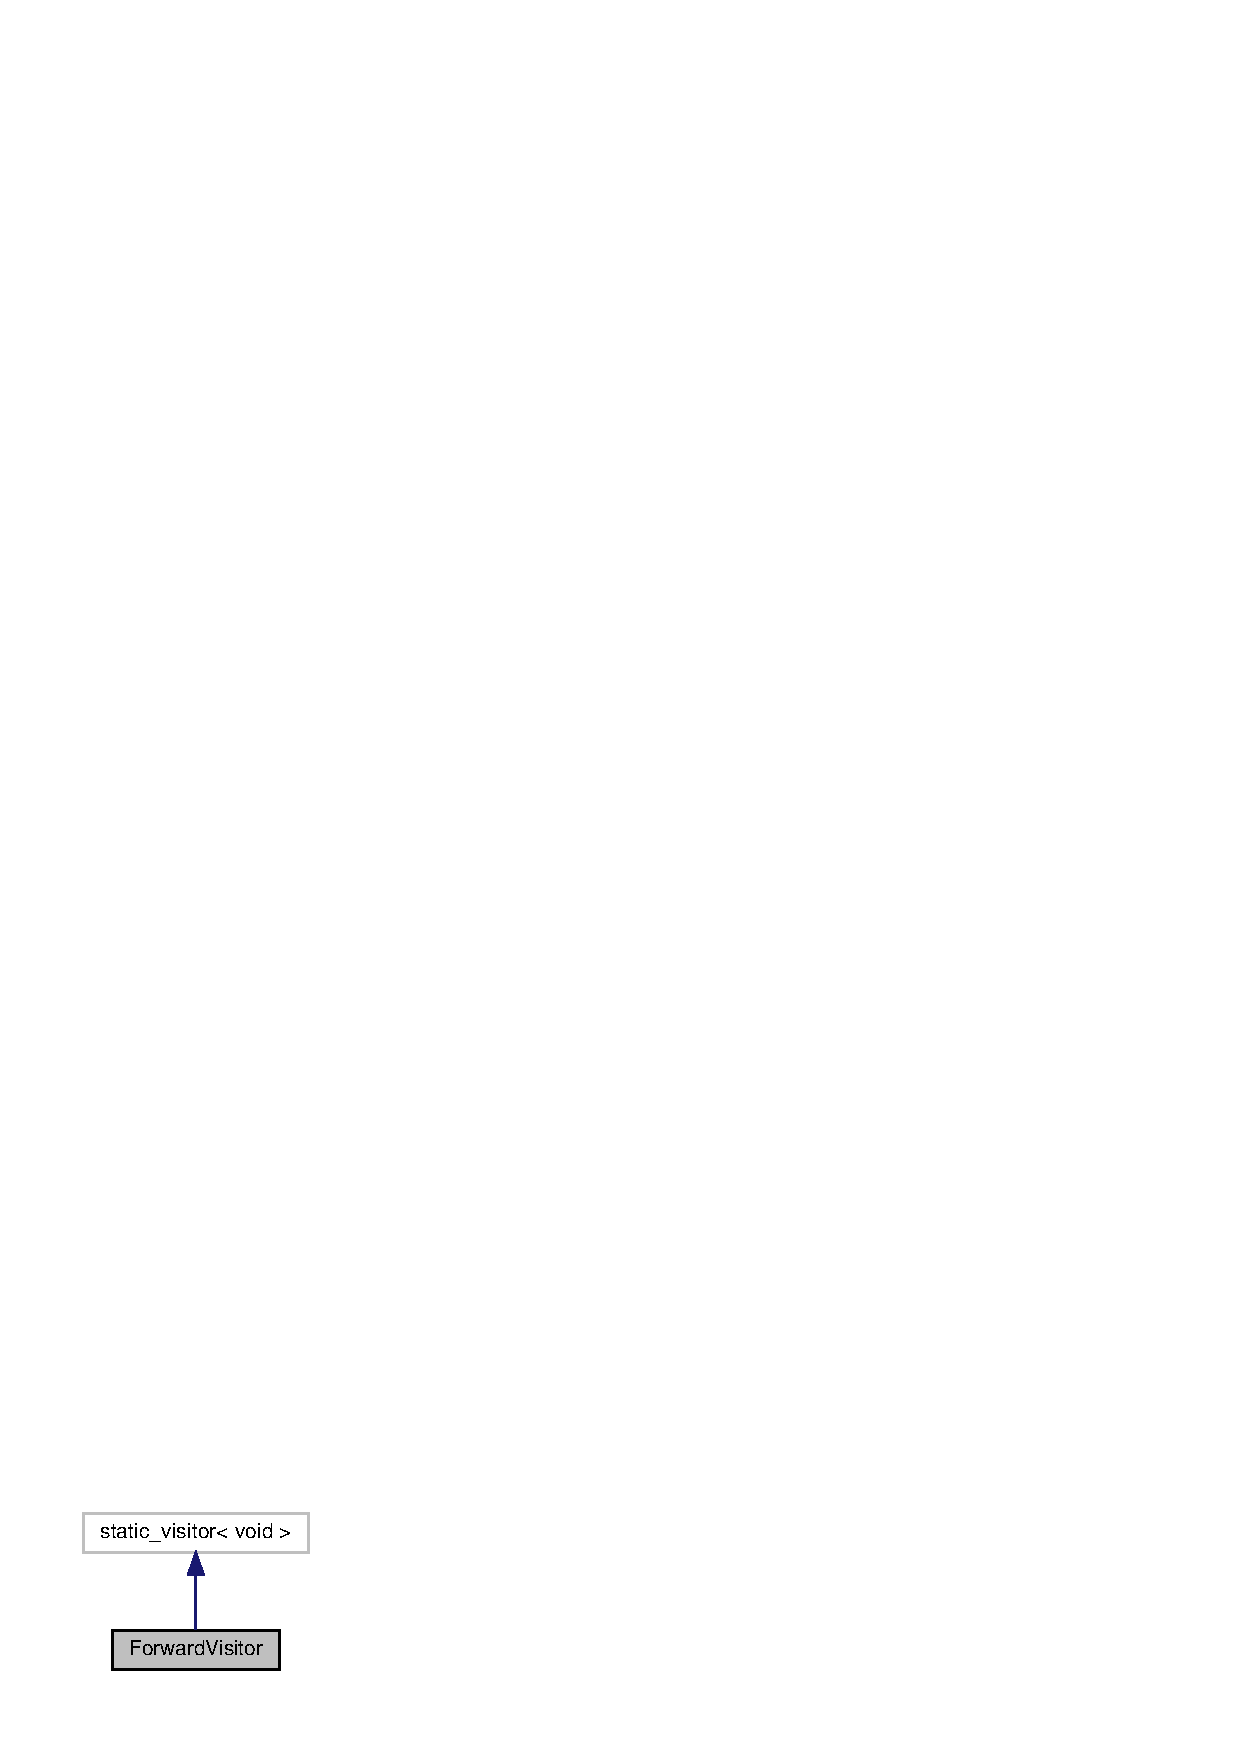
\includegraphics[width=152pt]{classmlpack_1_1ann_1_1ForwardVisitor__inherit__graph}
\end{center}
\end{figure}
\subsection*{Public Member Functions}
\begin{DoxyCompactItemize}
\item 
\textbf{ Forward\+Visitor} (const arma\+::mat \&input, arma\+::mat \&output)
\begin{DoxyCompactList}\small\item\em Execute the Forward() function given the input and output parameter. \end{DoxyCompactList}\item 
{\footnotesize template$<$typename Layer\+Type $>$ }\\void \textbf{ operator()} (Layer\+Type $\ast$layer) const
\begin{DoxyCompactList}\small\item\em Execute the Forward() function. \end{DoxyCompactList}\item 
void \textbf{ operator()} (\textbf{ More\+Types} layer) const
\end{DoxyCompactItemize}


\subsection{Detailed Description}
\doxyref{Forward\+Visitor}{p.}{classmlpack_1_1ann_1_1ForwardVisitor} executes the Forward() function given the input and output parameter. 

Definition at line 28 of file forward\+\_\+visitor.\+hpp.



\subsection{Constructor \& Destructor Documentation}
\mbox{\label{classmlpack_1_1ann_1_1ForwardVisitor_acc4160e4361a826ad7d915006abfe2df}} 
\index{mlpack\+::ann\+::\+Forward\+Visitor@{mlpack\+::ann\+::\+Forward\+Visitor}!Forward\+Visitor@{Forward\+Visitor}}
\index{Forward\+Visitor@{Forward\+Visitor}!mlpack\+::ann\+::\+Forward\+Visitor@{mlpack\+::ann\+::\+Forward\+Visitor}}
\subsubsection{Forward\+Visitor()}
{\footnotesize\ttfamily \textbf{ Forward\+Visitor} (\begin{DoxyParamCaption}\item[{const arma\+::mat \&}]{input,  }\item[{arma\+::mat \&}]{output }\end{DoxyParamCaption})}



Execute the Forward() function given the input and output parameter. 



\subsection{Member Function Documentation}
\mbox{\label{classmlpack_1_1ann_1_1ForwardVisitor_a26bb3385c630118c35f4799f1509abbc}} 
\index{mlpack\+::ann\+::\+Forward\+Visitor@{mlpack\+::ann\+::\+Forward\+Visitor}!operator()@{operator()}}
\index{operator()@{operator()}!mlpack\+::ann\+::\+Forward\+Visitor@{mlpack\+::ann\+::\+Forward\+Visitor}}
\subsubsection{operator()()\hspace{0.1cm}{\footnotesize\ttfamily [1/2]}}
{\footnotesize\ttfamily void operator() (\begin{DoxyParamCaption}\item[{Layer\+Type $\ast$}]{layer }\end{DoxyParamCaption}) const}



Execute the Forward() function. 

\mbox{\label{classmlpack_1_1ann_1_1ForwardVisitor_ae35578e7ff874a320fe762bc0edfff04}} 
\index{mlpack\+::ann\+::\+Forward\+Visitor@{mlpack\+::ann\+::\+Forward\+Visitor}!operator()@{operator()}}
\index{operator()@{operator()}!mlpack\+::ann\+::\+Forward\+Visitor@{mlpack\+::ann\+::\+Forward\+Visitor}}
\subsubsection{operator()()\hspace{0.1cm}{\footnotesize\ttfamily [2/2]}}
{\footnotesize\ttfamily void operator() (\begin{DoxyParamCaption}\item[{\textbf{ More\+Types}}]{layer }\end{DoxyParamCaption}) const}



The documentation for this class was generated from the following file\+:\begin{DoxyCompactItemize}
\item 
/home/aakash/mlpack/src/mlpack/methods/ann/visitor/\textbf{ forward\+\_\+visitor.\+hpp}\end{DoxyCompactItemize}

\section{Full\+Convolution Class Reference}
\label{classmlpack_1_1ann_1_1FullConvolution}\index{Full\+Convolution@{Full\+Convolution}}


\subsection{Detailed Description}


Definition at line 22 of file border\+\_\+modes.\+hpp.



The documentation for this class was generated from the following file\+:\begin{DoxyCompactItemize}
\item 
/home/aakash/mlpack/src/mlpack/methods/ann/convolution\+\_\+rules/\textbf{ border\+\_\+modes.\+hpp}\end{DoxyCompactItemize}

\section{G\+AN$<$ Model, Initialization\+Rule\+Type, Noise, Policy\+Type $>$ Class Template Reference}
\label{classmlpack_1_1ann_1_1GAN}\index{G\+A\+N$<$ Model, Initialization\+Rule\+Type, Noise, Policy\+Type $>$@{G\+A\+N$<$ Model, Initialization\+Rule\+Type, Noise, Policy\+Type $>$}}


The implementation of the standard \doxyref{G\+AN}{p.}{classmlpack_1_1ann_1_1GAN} module.  


\subsection*{Public Member Functions}
\begin{DoxyCompactItemize}
\item 
\textbf{ G\+AN} (Model generator, Model discriminator, Initialization\+Rule\+Type \&initialize\+Rule, Noise \&noise\+Function, const size\+\_\+t noise\+Dim, const size\+\_\+t batch\+Size, const size\+\_\+t generator\+Update\+Step, const size\+\_\+t pre\+Train\+Size, const double multiplier, const double clipping\+Parameter=0.\+01, const double lambda=10.\+0)
\begin{DoxyCompactList}\small\item\em Constructor for \doxyref{G\+AN}{p.}{classmlpack_1_1ann_1_1GAN} class. \end{DoxyCompactList}\item 
\textbf{ G\+AN} (const \textbf{ G\+AN} \&)
\begin{DoxyCompactList}\small\item\em Copy constructor. \end{DoxyCompactList}\item 
\textbf{ G\+AN} (\textbf{ G\+AN} \&\&)
\begin{DoxyCompactList}\small\item\em Move constructor. \end{DoxyCompactList}\item 
const Model \& \textbf{ Discriminator} () const
\begin{DoxyCompactList}\small\item\em Return the discriminator of the \doxyref{G\+AN}{p.}{classmlpack_1_1ann_1_1GAN}. \end{DoxyCompactList}\item 
Model \& \textbf{ Discriminator} ()
\begin{DoxyCompactList}\small\item\em Modify the discriminator of the \doxyref{G\+AN}{p.}{classmlpack_1_1ann_1_1GAN}. \end{DoxyCompactList}\item 
{\footnotesize template$<$typename Policy  = Policy\+Type$>$ }\\std\+::enable\+\_\+if$<$ std\+::is\+\_\+same$<$ Policy, \textbf{ Standard\+G\+AN} $>$\+::value$\vert$$\vert$std\+::is\+\_\+same$<$ Policy, \textbf{ D\+C\+G\+AN} $>$\+::value, double $>$\+::type \textbf{ Evaluate} (const arma\+::mat \&parameters, const size\+\_\+t i, const size\+\_\+t batch\+Size)
\begin{DoxyCompactList}\small\item\em Evaluate function for the Standard \doxyref{G\+AN}{p.}{classmlpack_1_1ann_1_1GAN} and \doxyref{D\+C\+G\+AN}{p.}{classmlpack_1_1ann_1_1DCGAN}. \end{DoxyCompactList}\item 
{\footnotesize template$<$typename Policy  = Policy\+Type$>$ }\\std\+::enable\+\_\+if$<$ std\+::is\+\_\+same$<$ Policy, \textbf{ W\+G\+AN} $>$\+::value, double $>$\+::type \textbf{ Evaluate} (const arma\+::mat \&parameters, const size\+\_\+t i, const size\+\_\+t batch\+Size)
\begin{DoxyCompactList}\small\item\em Evaluate function for the \doxyref{W\+G\+AN}{p.}{classmlpack_1_1ann_1_1WGAN}. \end{DoxyCompactList}\item 
{\footnotesize template$<$typename Policy  = Policy\+Type$>$ }\\std\+::enable\+\_\+if$<$ std\+::is\+\_\+same$<$ Policy, \textbf{ W\+G\+A\+N\+GP} $>$\+::value, double $>$\+::type \textbf{ Evaluate} (const arma\+::mat \&parameters, const size\+\_\+t i, const size\+\_\+t batch\+Size)
\begin{DoxyCompactList}\small\item\em Evaluate function for the W\+G\+A\+N-\/\+GP. \end{DoxyCompactList}\item 
{\footnotesize template$<$typename Grad\+Type , typename Policy  = Policy\+Type$>$ }\\std\+::enable\+\_\+if$<$ std\+::is\+\_\+same$<$ Policy, \textbf{ Standard\+G\+AN} $>$\+::value$\vert$$\vert$std\+::is\+\_\+same$<$ Policy, \textbf{ D\+C\+G\+AN} $>$\+::value, double $>$\+::type \textbf{ Evaluate\+With\+Gradient} (const arma\+::mat \&parameters, const size\+\_\+t i, Grad\+Type \&gradient, const size\+\_\+t batch\+Size)
\begin{DoxyCompactList}\small\item\em Evaluate\+With\+Gradient function for the Standard \doxyref{G\+AN}{p.}{classmlpack_1_1ann_1_1GAN} and \doxyref{D\+C\+G\+AN}{p.}{classmlpack_1_1ann_1_1DCGAN}. \end{DoxyCompactList}\item 
{\footnotesize template$<$typename Grad\+Type , typename Policy  = Policy\+Type$>$ }\\std\+::enable\+\_\+if$<$ std\+::is\+\_\+same$<$ Policy, \textbf{ W\+G\+AN} $>$\+::value, double $>$\+::type \textbf{ Evaluate\+With\+Gradient} (const arma\+::mat \&parameters, const size\+\_\+t i, Grad\+Type \&gradient, const size\+\_\+t batch\+Size)
\begin{DoxyCompactList}\small\item\em Evaluate\+With\+Gradient function for the \doxyref{W\+G\+AN}{p.}{classmlpack_1_1ann_1_1WGAN}. \end{DoxyCompactList}\item 
{\footnotesize template$<$typename Grad\+Type , typename Policy  = Policy\+Type$>$ }\\std\+::enable\+\_\+if$<$ std\+::is\+\_\+same$<$ Policy, \textbf{ W\+G\+A\+N\+GP} $>$\+::value, double $>$\+::type \textbf{ Evaluate\+With\+Gradient} (const arma\+::mat \&parameters, const size\+\_\+t i, Grad\+Type \&gradient, const size\+\_\+t batch\+Size)
\begin{DoxyCompactList}\small\item\em Evaluate\+With\+Gradient function for the W\+G\+A\+N-\/\+GP. \end{DoxyCompactList}\item 
void \textbf{ Forward} (const arma\+::mat \&input)
\begin{DoxyCompactList}\small\item\em This function does a forward pass through the \doxyref{G\+AN}{p.}{classmlpack_1_1ann_1_1GAN} network. \end{DoxyCompactList}\item 
const Model \& \textbf{ Generator} () const
\begin{DoxyCompactList}\small\item\em Return the generator of the \doxyref{G\+AN}{p.}{classmlpack_1_1ann_1_1GAN}. \end{DoxyCompactList}\item 
Model \& \textbf{ Generator} ()
\begin{DoxyCompactList}\small\item\em Modify the generator of the \doxyref{G\+AN}{p.}{classmlpack_1_1ann_1_1GAN}. \end{DoxyCompactList}\item 
{\footnotesize template$<$typename Policy  = Policy\+Type$>$ }\\std\+::enable\+\_\+if$<$ std\+::is\+\_\+same$<$ Policy, \textbf{ Standard\+G\+AN} $>$\+::value$\vert$$\vert$std\+::is\+\_\+same$<$ Policy, \textbf{ D\+C\+G\+AN} $>$\+::value, void $>$\+::type \textbf{ Gradient} (const arma\+::mat \&parameters, const size\+\_\+t i, arma\+::mat \&gradient, const size\+\_\+t batch\+Size)
\begin{DoxyCompactList}\small\item\em Gradient function for Standard \doxyref{G\+AN}{p.}{classmlpack_1_1ann_1_1GAN} and \doxyref{D\+C\+G\+AN}{p.}{classmlpack_1_1ann_1_1DCGAN}. \end{DoxyCompactList}\item 
{\footnotesize template$<$typename Policy  = Policy\+Type$>$ }\\std\+::enable\+\_\+if$<$ std\+::is\+\_\+same$<$ Policy, \textbf{ W\+G\+AN} $>$\+::value, void $>$\+::type \textbf{ Gradient} (const arma\+::mat \&parameters, const size\+\_\+t i, arma\+::mat \&gradient, const size\+\_\+t batch\+Size)
\begin{DoxyCompactList}\small\item\em Gradient function for \doxyref{W\+G\+AN}{p.}{classmlpack_1_1ann_1_1WGAN}. \end{DoxyCompactList}\item 
{\footnotesize template$<$typename Policy  = Policy\+Type$>$ }\\std\+::enable\+\_\+if$<$ std\+::is\+\_\+same$<$ Policy, \textbf{ W\+G\+A\+N\+GP} $>$\+::value, void $>$\+::type \textbf{ Gradient} (const arma\+::mat \&parameters, const size\+\_\+t i, arma\+::mat \&gradient, const size\+\_\+t batch\+Size)
\begin{DoxyCompactList}\small\item\em Gradient function for W\+G\+A\+N-\/\+GP. \end{DoxyCompactList}\item 
size\+\_\+t \textbf{ Num\+Functions} () const
\begin{DoxyCompactList}\small\item\em Return the number of separable functions (the number of predictor points). \end{DoxyCompactList}\item 
const arma\+::mat \& \textbf{ Parameters} () const
\begin{DoxyCompactList}\small\item\em Return the parameters of the network. \end{DoxyCompactList}\item 
arma\+::mat \& \textbf{ Parameters} ()
\begin{DoxyCompactList}\small\item\em Modify the parameters of the network. \end{DoxyCompactList}\item 
void \textbf{ Predict} (arma\+::mat input, arma\+::mat \&output)
\begin{DoxyCompactList}\small\item\em This function predicts the output of the network on the given input. \end{DoxyCompactList}\item 
const arma\+::mat \& \textbf{ Predictors} () const
\begin{DoxyCompactList}\small\item\em Get the matrix of data points (predictors). \end{DoxyCompactList}\item 
arma\+::mat \& \textbf{ Predictors} ()
\begin{DoxyCompactList}\small\item\em Modify the matrix of data points (predictors). \end{DoxyCompactList}\item 
void \textbf{ Reset} ()
\item 
void \textbf{ Reset\+Data} (arma\+::mat train\+Data)
\begin{DoxyCompactList}\small\item\em Initialize the generator, discriminator and weights of the model for training. \end{DoxyCompactList}\item 
const arma\+::mat \& \textbf{ Responses} () const
\begin{DoxyCompactList}\small\item\em Get the matrix of responses to the input data points. \end{DoxyCompactList}\item 
arma\+::mat \& \textbf{ Responses} ()
\begin{DoxyCompactList}\small\item\em Modify the matrix of responses to the input data points. \end{DoxyCompactList}\item 
{\footnotesize template$<$typename Archive $>$ }\\void \textbf{ serialize} (Archive \&ar, const uint32\+\_\+t)
\begin{DoxyCompactList}\small\item\em Serialize the model. \end{DoxyCompactList}\item 
void \textbf{ Shuffle} ()
\begin{DoxyCompactList}\small\item\em Shuffle the order of function visitation. \end{DoxyCompactList}\item 
{\footnotesize template$<$typename Optimizer\+Type , typename... Callback\+Types$>$ }\\double \textbf{ Train} (arma\+::mat train\+Data, Optimizer\+Type \&Optimizer, Callback\+Types \&\&... callbacks)
\begin{DoxyCompactList}\small\item\em Train function. \end{DoxyCompactList}\end{DoxyCompactItemize}


\subsection{Detailed Description}
\subsubsection*{template$<$typename Model, typename Initialization\+Rule\+Type, typename Noise, typename Policy\+Type = Standard\+G\+AN$>$\newline
class mlpack\+::ann\+::\+G\+A\+N$<$ Model, Initialization\+Rule\+Type, Noise, Policy\+Type $>$}

The implementation of the standard \doxyref{G\+AN}{p.}{classmlpack_1_1ann_1_1GAN} module. 

Generative Adversarial Networks (G\+A\+Ns) are a class of artificial intelligence algorithms used in unsupervised machine learning, implemented by a system of two neural networks contesting with each other in a zero-\/sum game framework. This technique can generate photographs that look at least superficially authentic to human observers, having many realistic characteristics. G\+A\+Ns have been used in Text-\/to-\/\+Image Synthesis, Medical Drug Discovery, High Resolution Imagery Generation, Neural Machine Translation and so on.

For more information, see the following paper\+:


\begin{DoxyCode}
@article\{Goodfellow14,
  author    = \{Ian J. Goodfellow, Jean Pouget-Abadi, Mehdi Mirza, Bing Xu,
               David Warde-Farley, Sherjil Ozair, Aaron Courville and
               Yoshua Bengio\},
  title     = \{Generative Adversarial Nets\},
  year      = \{2014\},
  url       = \{http:\textcolor{comment}{//arxiv.org/abs/1406.2661\},}
  eprint    = \{1406.2661\},
\}
\end{DoxyCode}



\begin{DoxyTemplParams}{Template Parameters}
{\em Model} & The class type of Generator and Discriminator. \\
\hline
{\em Initialization\+Rule\+Type} & Type of Initializer. \\
\hline
{\em Noise} & The noise function to use. \\
\hline
{\em Policy\+Type} & The \doxyref{G\+AN}{p.}{classmlpack_1_1ann_1_1GAN} variant to be used (\doxyref{G\+AN}{p.}{classmlpack_1_1ann_1_1GAN}, \doxyref{D\+C\+G\+AN}{p.}{classmlpack_1_1ann_1_1DCGAN}, \doxyref{W\+G\+AN}{p.}{classmlpack_1_1ann_1_1WGAN} or \doxyref{W\+G\+A\+N\+GP}{p.}{classmlpack_1_1ann_1_1WGANGP}). \\
\hline
\end{DoxyTemplParams}


Definition at line 63 of file gan.\+hpp.



\subsection{Constructor \& Destructor Documentation}
\mbox{\label{classmlpack_1_1ann_1_1GAN_afd4728e4b8193b03b9ee774b833d3508}} 
\index{mlpack\+::ann\+::\+G\+AN@{mlpack\+::ann\+::\+G\+AN}!G\+AN@{G\+AN}}
\index{G\+AN@{G\+AN}!mlpack\+::ann\+::\+G\+AN@{mlpack\+::ann\+::\+G\+AN}}
\subsubsection{G\+A\+N()\hspace{0.1cm}{\footnotesize\ttfamily [1/3]}}
{\footnotesize\ttfamily \textbf{ G\+AN} (\begin{DoxyParamCaption}\item[{Model}]{generator,  }\item[{Model}]{discriminator,  }\item[{Initialization\+Rule\+Type \&}]{initialize\+Rule,  }\item[{Noise \&}]{noise\+Function,  }\item[{const size\+\_\+t}]{noise\+Dim,  }\item[{const size\+\_\+t}]{batch\+Size,  }\item[{const size\+\_\+t}]{generator\+Update\+Step,  }\item[{const size\+\_\+t}]{pre\+Train\+Size,  }\item[{const double}]{multiplier,  }\item[{const double}]{clipping\+Parameter = {\ttfamily 0.01},  }\item[{const double}]{lambda = {\ttfamily 10.0} }\end{DoxyParamCaption})}



Constructor for \doxyref{G\+AN}{p.}{classmlpack_1_1ann_1_1GAN} class. 


\begin{DoxyParams}{Parameters}
{\em generator} & Generator network. \\
\hline
{\em discriminator} & Discriminator network. \\
\hline
{\em initialize\+Rule} & Initialization rule to use for initializing parameters. \\
\hline
{\em noise\+Function} & Function to be used for generating noise. \\
\hline
{\em noise\+Dim} & Dimension of noise vector to be created. \\
\hline
{\em batch\+Size} & Batch size to be used for training. \\
\hline
{\em generator\+Update\+Step} & Number of steps to train Discriminator before updating Generator. \\
\hline
{\em pre\+Train\+Size} & Number of pre-\/training steps of Discriminator. \\
\hline
{\em multiplier} & Ratio of learning rate of Discriminator to the Generator. \\
\hline
{\em clipping\+Parameter} & Weight range for enforcing Lipschitz constraint. \\
\hline
{\em lambda} & Parameter for setting the gradient penalty. \\
\hline
\end{DoxyParams}
\mbox{\label{classmlpack_1_1ann_1_1GAN_a0c66c15a1fd7ab0ce0f579e20c838abb}} 
\index{mlpack\+::ann\+::\+G\+AN@{mlpack\+::ann\+::\+G\+AN}!G\+AN@{G\+AN}}
\index{G\+AN@{G\+AN}!mlpack\+::ann\+::\+G\+AN@{mlpack\+::ann\+::\+G\+AN}}
\subsubsection{G\+A\+N()\hspace{0.1cm}{\footnotesize\ttfamily [2/3]}}
{\footnotesize\ttfamily \textbf{ G\+AN} (\begin{DoxyParamCaption}\item[{const \textbf{ G\+AN}$<$ Model, Initialization\+Rule\+Type, Noise, Policy\+Type $>$ \&}]{ }\end{DoxyParamCaption})}



Copy constructor. 

\mbox{\label{classmlpack_1_1ann_1_1GAN_a0601671158b961d0b3f532beb0c070d7}} 
\index{mlpack\+::ann\+::\+G\+AN@{mlpack\+::ann\+::\+G\+AN}!G\+AN@{G\+AN}}
\index{G\+AN@{G\+AN}!mlpack\+::ann\+::\+G\+AN@{mlpack\+::ann\+::\+G\+AN}}
\subsubsection{G\+A\+N()\hspace{0.1cm}{\footnotesize\ttfamily [3/3]}}
{\footnotesize\ttfamily \textbf{ G\+AN} (\begin{DoxyParamCaption}\item[{\textbf{ G\+AN}$<$ Model, Initialization\+Rule\+Type, Noise, Policy\+Type $>$ \&\&}]{ }\end{DoxyParamCaption})}



Move constructor. 



\subsection{Member Function Documentation}
\mbox{\label{classmlpack_1_1ann_1_1GAN_a81daab6e936bba0d45878d26df58aa9f}} 
\index{mlpack\+::ann\+::\+G\+AN@{mlpack\+::ann\+::\+G\+AN}!Discriminator@{Discriminator}}
\index{Discriminator@{Discriminator}!mlpack\+::ann\+::\+G\+AN@{mlpack\+::ann\+::\+G\+AN}}
\subsubsection{Discriminator()\hspace{0.1cm}{\footnotesize\ttfamily [1/2]}}
{\footnotesize\ttfamily const Model\& Discriminator (\begin{DoxyParamCaption}{ }\end{DoxyParamCaption}) const\hspace{0.3cm}{\ttfamily [inline]}}



Return the discriminator of the \doxyref{G\+AN}{p.}{classmlpack_1_1ann_1_1GAN}. 



Definition at line 312 of file gan.\+hpp.

\mbox{\label{classmlpack_1_1ann_1_1GAN_a52ce6e63f168b2f2a702b17f2225389a}} 
\index{mlpack\+::ann\+::\+G\+AN@{mlpack\+::ann\+::\+G\+AN}!Discriminator@{Discriminator}}
\index{Discriminator@{Discriminator}!mlpack\+::ann\+::\+G\+AN@{mlpack\+::ann\+::\+G\+AN}}
\subsubsection{Discriminator()\hspace{0.1cm}{\footnotesize\ttfamily [2/2]}}
{\footnotesize\ttfamily Model\& Discriminator (\begin{DoxyParamCaption}{ }\end{DoxyParamCaption})\hspace{0.3cm}{\ttfamily [inline]}}



Modify the discriminator of the \doxyref{G\+AN}{p.}{classmlpack_1_1ann_1_1GAN}. 



Definition at line 314 of file gan.\+hpp.

\mbox{\label{classmlpack_1_1ann_1_1GAN_a1960af22a953da7d4280f8717f80102b}} 
\index{mlpack\+::ann\+::\+G\+AN@{mlpack\+::ann\+::\+G\+AN}!Evaluate@{Evaluate}}
\index{Evaluate@{Evaluate}!mlpack\+::ann\+::\+G\+AN@{mlpack\+::ann\+::\+G\+AN}}
\subsubsection{Evaluate()\hspace{0.1cm}{\footnotesize\ttfamily [1/3]}}
{\footnotesize\ttfamily std\+::enable\+\_\+if$<$std\+::is\+\_\+same$<$Policy, \textbf{ Standard\+G\+AN}$>$\+::value $\vert$$\vert$ std\+::is\+\_\+same$<$Policy, \textbf{ D\+C\+G\+AN}$>$\+::value, double$>$\+::type Evaluate (\begin{DoxyParamCaption}\item[{const arma\+::mat \&}]{parameters,  }\item[{const size\+\_\+t}]{i,  }\item[{const size\+\_\+t}]{batch\+Size }\end{DoxyParamCaption})}



Evaluate function for the Standard \doxyref{G\+AN}{p.}{classmlpack_1_1ann_1_1GAN} and \doxyref{D\+C\+G\+AN}{p.}{classmlpack_1_1ann_1_1DCGAN}. 

This function gives the performance of the Standard \doxyref{G\+AN}{p.}{classmlpack_1_1ann_1_1GAN} or \doxyref{D\+C\+G\+AN}{p.}{classmlpack_1_1ann_1_1DCGAN} on the current input.


\begin{DoxyParams}{Parameters}
{\em parameters} & The parameters of the network. \\
\hline
{\em i} & Index of the current input. \\
\hline
{\em batch\+Size} & Variable to store the present number of inputs. \\
\hline
\end{DoxyParams}
\mbox{\label{classmlpack_1_1ann_1_1GAN_a6e686598c5a781cc1b0903a0f24e54f3}} 
\index{mlpack\+::ann\+::\+G\+AN@{mlpack\+::ann\+::\+G\+AN}!Evaluate@{Evaluate}}
\index{Evaluate@{Evaluate}!mlpack\+::ann\+::\+G\+AN@{mlpack\+::ann\+::\+G\+AN}}
\subsubsection{Evaluate()\hspace{0.1cm}{\footnotesize\ttfamily [2/3]}}
{\footnotesize\ttfamily std\+::enable\+\_\+if$<$std\+::is\+\_\+same$<$Policy, \textbf{ W\+G\+AN}$>$\+::value, double$>$\+::type Evaluate (\begin{DoxyParamCaption}\item[{const arma\+::mat \&}]{parameters,  }\item[{const size\+\_\+t}]{i,  }\item[{const size\+\_\+t}]{batch\+Size }\end{DoxyParamCaption})}



Evaluate function for the \doxyref{W\+G\+AN}{p.}{classmlpack_1_1ann_1_1WGAN}. 

This function gives the performance of the \doxyref{W\+G\+AN}{p.}{classmlpack_1_1ann_1_1WGAN} on the current input.


\begin{DoxyParams}{Parameters}
{\em parameters} & The parameters of the network. \\
\hline
{\em i} & Index of the current input. \\
\hline
{\em batch\+Size} & Variable to store the present number of inputs. \\
\hline
\end{DoxyParams}
\mbox{\label{classmlpack_1_1ann_1_1GAN_ab15c3bf890c114b50dab1dce9c0a0ae5}} 
\index{mlpack\+::ann\+::\+G\+AN@{mlpack\+::ann\+::\+G\+AN}!Evaluate@{Evaluate}}
\index{Evaluate@{Evaluate}!mlpack\+::ann\+::\+G\+AN@{mlpack\+::ann\+::\+G\+AN}}
\subsubsection{Evaluate()\hspace{0.1cm}{\footnotesize\ttfamily [3/3]}}
{\footnotesize\ttfamily std\+::enable\+\_\+if$<$std\+::is\+\_\+same$<$Policy, \textbf{ W\+G\+A\+N\+GP}$>$\+::value, double$>$\+::type Evaluate (\begin{DoxyParamCaption}\item[{const arma\+::mat \&}]{parameters,  }\item[{const size\+\_\+t}]{i,  }\item[{const size\+\_\+t}]{batch\+Size }\end{DoxyParamCaption})}



Evaluate function for the W\+G\+A\+N-\/\+GP. 

This function gives the performance of the W\+G\+A\+N-\/\+GP on the current input.


\begin{DoxyParams}{Parameters}
{\em parameters} & The parameters of the network. \\
\hline
{\em i} & Index of the current input. \\
\hline
{\em batch\+Size} & Variable to store the present number of inputs. \\
\hline
\end{DoxyParams}
\mbox{\label{classmlpack_1_1ann_1_1GAN_a8852fa0ac9f2147801776c5aff61f22c}} 
\index{mlpack\+::ann\+::\+G\+AN@{mlpack\+::ann\+::\+G\+AN}!Evaluate\+With\+Gradient@{Evaluate\+With\+Gradient}}
\index{Evaluate\+With\+Gradient@{Evaluate\+With\+Gradient}!mlpack\+::ann\+::\+G\+AN@{mlpack\+::ann\+::\+G\+AN}}
\subsubsection{Evaluate\+With\+Gradient()\hspace{0.1cm}{\footnotesize\ttfamily [1/3]}}
{\footnotesize\ttfamily std\+::enable\+\_\+if$<$std\+::is\+\_\+same$<$Policy, \textbf{ Standard\+G\+AN}$>$\+::value $\vert$$\vert$ std\+::is\+\_\+same$<$Policy, \textbf{ D\+C\+G\+AN}$>$\+::value, double$>$\+::type Evaluate\+With\+Gradient (\begin{DoxyParamCaption}\item[{const arma\+::mat \&}]{parameters,  }\item[{const size\+\_\+t}]{i,  }\item[{Grad\+Type \&}]{gradient,  }\item[{const size\+\_\+t}]{batch\+Size }\end{DoxyParamCaption})}



Evaluate\+With\+Gradient function for the Standard \doxyref{G\+AN}{p.}{classmlpack_1_1ann_1_1GAN} and \doxyref{D\+C\+G\+AN}{p.}{classmlpack_1_1ann_1_1DCGAN}. 

This function gives the performance of the Standard \doxyref{G\+AN}{p.}{classmlpack_1_1ann_1_1GAN} or \doxyref{D\+C\+G\+AN}{p.}{classmlpack_1_1ann_1_1DCGAN} on the current input, while updating Gradients.


\begin{DoxyParams}{Parameters}
{\em parameters} & The parameters of the network. \\
\hline
{\em i} & Index of the current input. \\
\hline
{\em gradient} & Variable to store the present gradient. \\
\hline
{\em batch\+Size} & Variable to store the present number of inputs. \\
\hline
\end{DoxyParams}
\mbox{\label{classmlpack_1_1ann_1_1GAN_a5726150df7dbbde1aecf3d46cb155005}} 
\index{mlpack\+::ann\+::\+G\+AN@{mlpack\+::ann\+::\+G\+AN}!Evaluate\+With\+Gradient@{Evaluate\+With\+Gradient}}
\index{Evaluate\+With\+Gradient@{Evaluate\+With\+Gradient}!mlpack\+::ann\+::\+G\+AN@{mlpack\+::ann\+::\+G\+AN}}
\subsubsection{Evaluate\+With\+Gradient()\hspace{0.1cm}{\footnotesize\ttfamily [2/3]}}
{\footnotesize\ttfamily std\+::enable\+\_\+if$<$std\+::is\+\_\+same$<$Policy, \textbf{ W\+G\+AN}$>$\+::value, double$>$\+::type Evaluate\+With\+Gradient (\begin{DoxyParamCaption}\item[{const arma\+::mat \&}]{parameters,  }\item[{const size\+\_\+t}]{i,  }\item[{Grad\+Type \&}]{gradient,  }\item[{const size\+\_\+t}]{batch\+Size }\end{DoxyParamCaption})}



Evaluate\+With\+Gradient function for the \doxyref{W\+G\+AN}{p.}{classmlpack_1_1ann_1_1WGAN}. 

This function gives the performance of the \doxyref{W\+G\+AN}{p.}{classmlpack_1_1ann_1_1WGAN} on the current input, while updating Gradients.


\begin{DoxyParams}{Parameters}
{\em parameters} & The parameters of the network. \\
\hline
{\em i} & Index of the current input. \\
\hline
{\em gradient} & Variable to store the present gradient. \\
\hline
{\em batch\+Size} & Variable to store the present number of inputs. \\
\hline
\end{DoxyParams}
\mbox{\label{classmlpack_1_1ann_1_1GAN_a41c7fcfc409e29d086df197d78c9b92d}} 
\index{mlpack\+::ann\+::\+G\+AN@{mlpack\+::ann\+::\+G\+AN}!Evaluate\+With\+Gradient@{Evaluate\+With\+Gradient}}
\index{Evaluate\+With\+Gradient@{Evaluate\+With\+Gradient}!mlpack\+::ann\+::\+G\+AN@{mlpack\+::ann\+::\+G\+AN}}
\subsubsection{Evaluate\+With\+Gradient()\hspace{0.1cm}{\footnotesize\ttfamily [3/3]}}
{\footnotesize\ttfamily std\+::enable\+\_\+if$<$std\+::is\+\_\+same$<$Policy, \textbf{ W\+G\+A\+N\+GP}$>$\+::value, double$>$\+::type Evaluate\+With\+Gradient (\begin{DoxyParamCaption}\item[{const arma\+::mat \&}]{parameters,  }\item[{const size\+\_\+t}]{i,  }\item[{Grad\+Type \&}]{gradient,  }\item[{const size\+\_\+t}]{batch\+Size }\end{DoxyParamCaption})}



Evaluate\+With\+Gradient function for the W\+G\+A\+N-\/\+GP. 

This function gives the performance of the W\+G\+A\+N-\/\+GP on the current input, while updating Gradients.


\begin{DoxyParams}{Parameters}
{\em parameters} & The parameters of the network. \\
\hline
{\em i} & Index of the current input. \\
\hline
{\em gradient} & Variable to store the present gradient. \\
\hline
{\em batch\+Size} & Variable to store the present number of inputs. \\
\hline
\end{DoxyParams}
\mbox{\label{classmlpack_1_1ann_1_1GAN_a0f1a354ec201efe4ce96126802cf9a2f}} 
\index{mlpack\+::ann\+::\+G\+AN@{mlpack\+::ann\+::\+G\+AN}!Forward@{Forward}}
\index{Forward@{Forward}!mlpack\+::ann\+::\+G\+AN@{mlpack\+::ann\+::\+G\+AN}}
\subsubsection{Forward()}
{\footnotesize\ttfamily void Forward (\begin{DoxyParamCaption}\item[{const arma\+::mat \&}]{input }\end{DoxyParamCaption})}



This function does a forward pass through the \doxyref{G\+AN}{p.}{classmlpack_1_1ann_1_1GAN} network. 


\begin{DoxyParams}{Parameters}
{\em input} & Sampled noise. \\
\hline
\end{DoxyParams}
\mbox{\label{classmlpack_1_1ann_1_1GAN_a1b687745cb12ef7ef76449187dc50bb5}} 
\index{mlpack\+::ann\+::\+G\+AN@{mlpack\+::ann\+::\+G\+AN}!Generator@{Generator}}
\index{Generator@{Generator}!mlpack\+::ann\+::\+G\+AN@{mlpack\+::ann\+::\+G\+AN}}
\subsubsection{Generator()\hspace{0.1cm}{\footnotesize\ttfamily [1/2]}}
{\footnotesize\ttfamily const Model\& Generator (\begin{DoxyParamCaption}{ }\end{DoxyParamCaption}) const\hspace{0.3cm}{\ttfamily [inline]}}



Return the generator of the \doxyref{G\+AN}{p.}{classmlpack_1_1ann_1_1GAN}. 



Definition at line 308 of file gan.\+hpp.

\mbox{\label{classmlpack_1_1ann_1_1GAN_a8bf07503608839011670b808cdd17001}} 
\index{mlpack\+::ann\+::\+G\+AN@{mlpack\+::ann\+::\+G\+AN}!Generator@{Generator}}
\index{Generator@{Generator}!mlpack\+::ann\+::\+G\+AN@{mlpack\+::ann\+::\+G\+AN}}
\subsubsection{Generator()\hspace{0.1cm}{\footnotesize\ttfamily [2/2]}}
{\footnotesize\ttfamily Model\& Generator (\begin{DoxyParamCaption}{ }\end{DoxyParamCaption})\hspace{0.3cm}{\ttfamily [inline]}}



Modify the generator of the \doxyref{G\+AN}{p.}{classmlpack_1_1ann_1_1GAN}. 



Definition at line 310 of file gan.\+hpp.

\mbox{\label{classmlpack_1_1ann_1_1GAN_a2e967aa7bd78aa8e5024899a44a303c9}} 
\index{mlpack\+::ann\+::\+G\+AN@{mlpack\+::ann\+::\+G\+AN}!Gradient@{Gradient}}
\index{Gradient@{Gradient}!mlpack\+::ann\+::\+G\+AN@{mlpack\+::ann\+::\+G\+AN}}
\subsubsection{Gradient()\hspace{0.1cm}{\footnotesize\ttfamily [1/3]}}
{\footnotesize\ttfamily std\+::enable\+\_\+if$<$std\+::is\+\_\+same$<$Policy, \textbf{ Standard\+G\+AN}$>$\+::value $\vert$$\vert$ std\+::is\+\_\+same$<$Policy, \textbf{ D\+C\+G\+AN}$>$\+::value, void$>$\+::type Gradient (\begin{DoxyParamCaption}\item[{const arma\+::mat \&}]{parameters,  }\item[{const size\+\_\+t}]{i,  }\item[{arma\+::mat \&}]{gradient,  }\item[{const size\+\_\+t}]{batch\+Size }\end{DoxyParamCaption})}



Gradient function for Standard \doxyref{G\+AN}{p.}{classmlpack_1_1ann_1_1GAN} and \doxyref{D\+C\+G\+AN}{p.}{classmlpack_1_1ann_1_1DCGAN}. 

This function passes the gradient based on which network is being trained, i.\+e., Generator or Discriminator.


\begin{DoxyParams}{Parameters}
{\em parameters} & present parameters of the network. \\
\hline
{\em i} & Index of the predictors. \\
\hline
{\em gradient} & Variable to store the present gradient. \\
\hline
{\em batch\+Size} & Variable to store the present number of inputs. \\
\hline
\end{DoxyParams}
\mbox{\label{classmlpack_1_1ann_1_1GAN_a3053059f0001ebb407739820357d050d}} 
\index{mlpack\+::ann\+::\+G\+AN@{mlpack\+::ann\+::\+G\+AN}!Gradient@{Gradient}}
\index{Gradient@{Gradient}!mlpack\+::ann\+::\+G\+AN@{mlpack\+::ann\+::\+G\+AN}}
\subsubsection{Gradient()\hspace{0.1cm}{\footnotesize\ttfamily [2/3]}}
{\footnotesize\ttfamily std\+::enable\+\_\+if$<$std\+::is\+\_\+same$<$Policy, \textbf{ W\+G\+AN}$>$\+::value, void$>$\+::type Gradient (\begin{DoxyParamCaption}\item[{const arma\+::mat \&}]{parameters,  }\item[{const size\+\_\+t}]{i,  }\item[{arma\+::mat \&}]{gradient,  }\item[{const size\+\_\+t}]{batch\+Size }\end{DoxyParamCaption})}



Gradient function for \doxyref{W\+G\+AN}{p.}{classmlpack_1_1ann_1_1WGAN}. 

This function passes the gradient based on which network is being trained, i.\+e., Generator or Discriminator.


\begin{DoxyParams}{Parameters}
{\em parameters} & present parameters of the network. \\
\hline
{\em i} & Index of the predictors. \\
\hline
{\em gradient} & Variable to store the present gradient. \\
\hline
{\em batch\+Size} & Variable to store the present number of inputs. \\
\hline
\end{DoxyParams}
\mbox{\label{classmlpack_1_1ann_1_1GAN_a488f9e118fd4fd3c25f29b81b839cf7a}} 
\index{mlpack\+::ann\+::\+G\+AN@{mlpack\+::ann\+::\+G\+AN}!Gradient@{Gradient}}
\index{Gradient@{Gradient}!mlpack\+::ann\+::\+G\+AN@{mlpack\+::ann\+::\+G\+AN}}
\subsubsection{Gradient()\hspace{0.1cm}{\footnotesize\ttfamily [3/3]}}
{\footnotesize\ttfamily std\+::enable\+\_\+if$<$std\+::is\+\_\+same$<$Policy, \textbf{ W\+G\+A\+N\+GP}$>$\+::value, void$>$\+::type Gradient (\begin{DoxyParamCaption}\item[{const arma\+::mat \&}]{parameters,  }\item[{const size\+\_\+t}]{i,  }\item[{arma\+::mat \&}]{gradient,  }\item[{const size\+\_\+t}]{batch\+Size }\end{DoxyParamCaption})}



Gradient function for W\+G\+A\+N-\/\+GP. 

This function passes the gradient based on which network is being trained, i.\+e., Generator or Discriminator.


\begin{DoxyParams}{Parameters}
{\em parameters} & present parameters of the network. \\
\hline
{\em i} & Index of the predictors. \\
\hline
{\em gradient} & Variable to store the present gradient. \\
\hline
{\em batch\+Size} & Variable to store the present number of inputs. \\
\hline
\end{DoxyParams}
\mbox{\label{classmlpack_1_1ann_1_1GAN_a1fa76af34a6e3ea927b307f0c318ee4b}} 
\index{mlpack\+::ann\+::\+G\+AN@{mlpack\+::ann\+::\+G\+AN}!Num\+Functions@{Num\+Functions}}
\index{Num\+Functions@{Num\+Functions}!mlpack\+::ann\+::\+G\+AN@{mlpack\+::ann\+::\+G\+AN}}
\subsubsection{Num\+Functions()}
{\footnotesize\ttfamily size\+\_\+t Num\+Functions (\begin{DoxyParamCaption}{ }\end{DoxyParamCaption}) const\hspace{0.3cm}{\ttfamily [inline]}}



Return the number of separable functions (the number of predictor points). 



Definition at line 317 of file gan.\+hpp.

\mbox{\label{classmlpack_1_1ann_1_1GAN_aa68d74dc1e86e4352e00a3cab83a0e4a}} 
\index{mlpack\+::ann\+::\+G\+AN@{mlpack\+::ann\+::\+G\+AN}!Parameters@{Parameters}}
\index{Parameters@{Parameters}!mlpack\+::ann\+::\+G\+AN@{mlpack\+::ann\+::\+G\+AN}}
\subsubsection{Parameters()\hspace{0.1cm}{\footnotesize\ttfamily [1/2]}}
{\footnotesize\ttfamily const arma\+::mat\& Parameters (\begin{DoxyParamCaption}{ }\end{DoxyParamCaption}) const\hspace{0.3cm}{\ttfamily [inline]}}



Return the parameters of the network. 



Definition at line 303 of file gan.\+hpp.

\mbox{\label{classmlpack_1_1ann_1_1GAN_a043f0ccd62e6711a18e0d81047be9a0a}} 
\index{mlpack\+::ann\+::\+G\+AN@{mlpack\+::ann\+::\+G\+AN}!Parameters@{Parameters}}
\index{Parameters@{Parameters}!mlpack\+::ann\+::\+G\+AN@{mlpack\+::ann\+::\+G\+AN}}
\subsubsection{Parameters()\hspace{0.1cm}{\footnotesize\ttfamily [2/2]}}
{\footnotesize\ttfamily arma\+::mat\& Parameters (\begin{DoxyParamCaption}{ }\end{DoxyParamCaption})\hspace{0.3cm}{\ttfamily [inline]}}



Modify the parameters of the network. 



Definition at line 305 of file gan.\+hpp.

\mbox{\label{classmlpack_1_1ann_1_1GAN_a1c9a003262a7e893e46cf780ed5f359d}} 
\index{mlpack\+::ann\+::\+G\+AN@{mlpack\+::ann\+::\+G\+AN}!Predict@{Predict}}
\index{Predict@{Predict}!mlpack\+::ann\+::\+G\+AN@{mlpack\+::ann\+::\+G\+AN}}
\subsubsection{Predict()}
{\footnotesize\ttfamily void Predict (\begin{DoxyParamCaption}\item[{arma\+::mat}]{input,  }\item[{arma\+::mat \&}]{output }\end{DoxyParamCaption})}



This function predicts the output of the network on the given input. 


\begin{DoxyParams}{Parameters}
{\em input} & The input of the Generator network. \\
\hline
{\em output} & Result of the Discriminator network. \\
\hline
\end{DoxyParams}
\mbox{\label{classmlpack_1_1ann_1_1GAN_af63d9ce84ba796336c0abce63ff9be1c}} 
\index{mlpack\+::ann\+::\+G\+AN@{mlpack\+::ann\+::\+G\+AN}!Predictors@{Predictors}}
\index{Predictors@{Predictors}!mlpack\+::ann\+::\+G\+AN@{mlpack\+::ann\+::\+G\+AN}}
\subsubsection{Predictors()\hspace{0.1cm}{\footnotesize\ttfamily [1/2]}}
{\footnotesize\ttfamily const arma\+::mat\& Predictors (\begin{DoxyParamCaption}{ }\end{DoxyParamCaption}) const\hspace{0.3cm}{\ttfamily [inline]}}



Get the matrix of data points (predictors). 



Definition at line 325 of file gan.\+hpp.

\mbox{\label{classmlpack_1_1ann_1_1GAN_a5b2b9103f156a387b74164f143e63ce7}} 
\index{mlpack\+::ann\+::\+G\+AN@{mlpack\+::ann\+::\+G\+AN}!Predictors@{Predictors}}
\index{Predictors@{Predictors}!mlpack\+::ann\+::\+G\+AN@{mlpack\+::ann\+::\+G\+AN}}
\subsubsection{Predictors()\hspace{0.1cm}{\footnotesize\ttfamily [2/2]}}
{\footnotesize\ttfamily arma\+::mat\& Predictors (\begin{DoxyParamCaption}{ }\end{DoxyParamCaption})\hspace{0.3cm}{\ttfamily [inline]}}



Modify the matrix of data points (predictors). 



Definition at line 327 of file gan.\+hpp.



References G\+A\+N$<$ Model, Initialization\+Rule\+Type, Noise, Policy\+Type $>$\+::serialize().

\mbox{\label{classmlpack_1_1ann_1_1GAN_a372de693ad40b3f42839c8ec6ac845f4}} 
\index{mlpack\+::ann\+::\+G\+AN@{mlpack\+::ann\+::\+G\+AN}!Reset@{Reset}}
\index{Reset@{Reset}!mlpack\+::ann\+::\+G\+AN@{mlpack\+::ann\+::\+G\+AN}}
\subsubsection{Reset()}
{\footnotesize\ttfamily void Reset (\begin{DoxyParamCaption}{ }\end{DoxyParamCaption})}

\mbox{\label{classmlpack_1_1ann_1_1GAN_a935be322c1c9425a5ae7a0fe80421e83}} 
\index{mlpack\+::ann\+::\+G\+AN@{mlpack\+::ann\+::\+G\+AN}!Reset\+Data@{Reset\+Data}}
\index{Reset\+Data@{Reset\+Data}!mlpack\+::ann\+::\+G\+AN@{mlpack\+::ann\+::\+G\+AN}}
\subsubsection{Reset\+Data()}
{\footnotesize\ttfamily void Reset\+Data (\begin{DoxyParamCaption}\item[{arma\+::mat}]{train\+Data }\end{DoxyParamCaption})}



Initialize the generator, discriminator and weights of the model for training. 

This function won\textquotesingle{}t actually trigger training process.


\begin{DoxyParams}{Parameters}
{\em train\+Data} & The data points of real distribution. \\
\hline
\end{DoxyParams}
\mbox{\label{classmlpack_1_1ann_1_1GAN_a5702d7dbe418472e341da9c8d8ff0e01}} 
\index{mlpack\+::ann\+::\+G\+AN@{mlpack\+::ann\+::\+G\+AN}!Responses@{Responses}}
\index{Responses@{Responses}!mlpack\+::ann\+::\+G\+AN@{mlpack\+::ann\+::\+G\+AN}}
\subsubsection{Responses()\hspace{0.1cm}{\footnotesize\ttfamily [1/2]}}
{\footnotesize\ttfamily const arma\+::mat\& Responses (\begin{DoxyParamCaption}{ }\end{DoxyParamCaption}) const\hspace{0.3cm}{\ttfamily [inline]}}



Get the matrix of responses to the input data points. 



Definition at line 320 of file gan.\+hpp.

\mbox{\label{classmlpack_1_1ann_1_1GAN_a94a56f6f545988833a4ae9906f8aa197}} 
\index{mlpack\+::ann\+::\+G\+AN@{mlpack\+::ann\+::\+G\+AN}!Responses@{Responses}}
\index{Responses@{Responses}!mlpack\+::ann\+::\+G\+AN@{mlpack\+::ann\+::\+G\+AN}}
\subsubsection{Responses()\hspace{0.1cm}{\footnotesize\ttfamily [2/2]}}
{\footnotesize\ttfamily arma\+::mat\& Responses (\begin{DoxyParamCaption}{ }\end{DoxyParamCaption})\hspace{0.3cm}{\ttfamily [inline]}}



Modify the matrix of responses to the input data points. 



Definition at line 322 of file gan.\+hpp.

\mbox{\label{classmlpack_1_1ann_1_1GAN_a65cba07328997659bec80b9879b15a51}} 
\index{mlpack\+::ann\+::\+G\+AN@{mlpack\+::ann\+::\+G\+AN}!serialize@{serialize}}
\index{serialize@{serialize}!mlpack\+::ann\+::\+G\+AN@{mlpack\+::ann\+::\+G\+AN}}
\subsubsection{serialize()}
{\footnotesize\ttfamily void serialize (\begin{DoxyParamCaption}\item[{Archive \&}]{ar,  }\item[{const uint32\+\_\+t}]{ }\end{DoxyParamCaption})}



Serialize the model. 



Referenced by G\+A\+N$<$ Model, Initialization\+Rule\+Type, Noise, Policy\+Type $>$\+::\+Predictors().

\mbox{\label{classmlpack_1_1ann_1_1GAN_a2697cc8b37d7bca7c055228382a9b208}} 
\index{mlpack\+::ann\+::\+G\+AN@{mlpack\+::ann\+::\+G\+AN}!Shuffle@{Shuffle}}
\index{Shuffle@{Shuffle}!mlpack\+::ann\+::\+G\+AN@{mlpack\+::ann\+::\+G\+AN}}
\subsubsection{Shuffle()}
{\footnotesize\ttfamily void Shuffle (\begin{DoxyParamCaption}{ }\end{DoxyParamCaption})}



Shuffle the order of function visitation. 

This may be called by the optimizer. \mbox{\label{classmlpack_1_1ann_1_1GAN_a4f7b5c4f299346d1fe308881a26696f0}} 
\index{mlpack\+::ann\+::\+G\+AN@{mlpack\+::ann\+::\+G\+AN}!Train@{Train}}
\index{Train@{Train}!mlpack\+::ann\+::\+G\+AN@{mlpack\+::ann\+::\+G\+AN}}
\subsubsection{Train()}
{\footnotesize\ttfamily double Train (\begin{DoxyParamCaption}\item[{arma\+::mat}]{train\+Data,  }\item[{Optimizer\+Type \&}]{Optimizer,  }\item[{Callback\+Types \&\&...}]{callbacks }\end{DoxyParamCaption})}



Train function. 


\begin{DoxyTemplParams}{Template Parameters}
{\em Optimizer\+Type} & Type of optimizer to use to train the model. \\
\hline
{\em Callback\+Types} & Types of Callback functions. \\
\hline
\end{DoxyTemplParams}

\begin{DoxyParams}{Parameters}
{\em train\+Data} & The data points of real distribution. \\
\hline
{\em Optimizer} & Instantiated optimizer used to train the model. \\
\hline
{\em callbacks} & Callback function for ensmallen optimizer {\ttfamily Optimizer\+Type}. See {\tt https\+://www.\+ensmallen.\+org/docs.\+html\#callback-\/documentation}. \\
\hline
\end{DoxyParams}
\begin{DoxyReturn}{Returns}
The final objective of the trained model (NaN or Inf on error). 
\end{DoxyReturn}


The documentation for this class was generated from the following file\+:\begin{DoxyCompactItemize}
\item 
/home/aakash/mlpack/src/mlpack/methods/ann/gan/\textbf{ gan.\+hpp}\end{DoxyCompactItemize}

\section{Gaussian\+Function Class Reference}
\label{classmlpack_1_1ann_1_1GaussianFunction}\index{Gaussian\+Function@{Gaussian\+Function}}


The gaussian function, defined by.  


\subsection*{Static Public Member Functions}
\begin{DoxyCompactItemize}
\item 
static double \textbf{ Deriv} (const double y)
\begin{DoxyCompactList}\small\item\em Computes the first derivative of the gaussian function. \end{DoxyCompactList}\item 
{\footnotesize template$<$typename Input\+Vec\+Type , typename Output\+Vec\+Type $>$ }\\static void \textbf{ Deriv} (const Input\+Vec\+Type \&y, Output\+Vec\+Type \&x)
\begin{DoxyCompactList}\small\item\em Computes the first derivatives of the gaussian function. \end{DoxyCompactList}\item 
{\footnotesize template$<$typename eT $>$ }\\static double \textbf{ Fn} (const eT x)
\begin{DoxyCompactList}\small\item\em Computes the gaussian function. \end{DoxyCompactList}\item 
{\footnotesize template$<$typename Input\+Vec\+Type , typename Output\+Vec\+Type $>$ }\\static void \textbf{ Fn} (const Input\+Vec\+Type \&x, Output\+Vec\+Type \&y)
\begin{DoxyCompactList}\small\item\em Computes the gaussian function. \end{DoxyCompactList}\end{DoxyCompactItemize}


\subsection{Detailed Description}
The gaussian function, defined by. 

\begin{eqnarray*} f(x) &=& e^{-1 * x^2} \\ f'(x) &=& 2 * -x * f(x) \end{eqnarray*} 

Definition at line 28 of file gaussian\+\_\+function.\+hpp.



\subsection{Member Function Documentation}
\mbox{\label{classmlpack_1_1ann_1_1GaussianFunction_a163d34fd09f8edf457164f5033c635cf}} 
\index{mlpack\+::ann\+::\+Gaussian\+Function@{mlpack\+::ann\+::\+Gaussian\+Function}!Deriv@{Deriv}}
\index{Deriv@{Deriv}!mlpack\+::ann\+::\+Gaussian\+Function@{mlpack\+::ann\+::\+Gaussian\+Function}}
\subsubsection{Deriv()\hspace{0.1cm}{\footnotesize\ttfamily [1/2]}}
{\footnotesize\ttfamily static double Deriv (\begin{DoxyParamCaption}\item[{const double}]{y }\end{DoxyParamCaption})\hspace{0.3cm}{\ttfamily [inline]}, {\ttfamily [static]}}



Computes the first derivative of the gaussian function. 


\begin{DoxyParams}{Parameters}
{\em y} & Input data. \\
\hline
\end{DoxyParams}
\begin{DoxyReturn}{Returns}
f\textquotesingle{}(x) 
\end{DoxyReturn}


Definition at line 61 of file gaussian\+\_\+function.\+hpp.

\mbox{\label{classmlpack_1_1ann_1_1GaussianFunction_ad442502c34b67303b74c735641dab790}} 
\index{mlpack\+::ann\+::\+Gaussian\+Function@{mlpack\+::ann\+::\+Gaussian\+Function}!Deriv@{Deriv}}
\index{Deriv@{Deriv}!mlpack\+::ann\+::\+Gaussian\+Function@{mlpack\+::ann\+::\+Gaussian\+Function}}
\subsubsection{Deriv()\hspace{0.1cm}{\footnotesize\ttfamily [2/2]}}
{\footnotesize\ttfamily static void Deriv (\begin{DoxyParamCaption}\item[{const Input\+Vec\+Type \&}]{y,  }\item[{Output\+Vec\+Type \&}]{x }\end{DoxyParamCaption})\hspace{0.3cm}{\ttfamily [inline]}, {\ttfamily [static]}}



Computes the first derivatives of the gaussian function. 


\begin{DoxyParams}{Parameters}
{\em y} & Input activations. \\
\hline
{\em x} & The resulting derivatives. \\
\hline
\end{DoxyParams}


Definition at line 73 of file gaussian\+\_\+function.\+hpp.

\mbox{\label{classmlpack_1_1ann_1_1GaussianFunction_a7be90336227c4673a4152dbac3d62c25}} 
\index{mlpack\+::ann\+::\+Gaussian\+Function@{mlpack\+::ann\+::\+Gaussian\+Function}!Fn@{Fn}}
\index{Fn@{Fn}!mlpack\+::ann\+::\+Gaussian\+Function@{mlpack\+::ann\+::\+Gaussian\+Function}}
\subsubsection{Fn()\hspace{0.1cm}{\footnotesize\ttfamily [1/2]}}
{\footnotesize\ttfamily static double Fn (\begin{DoxyParamCaption}\item[{const eT}]{x }\end{DoxyParamCaption})\hspace{0.3cm}{\ttfamily [inline]}, {\ttfamily [static]}}



Computes the gaussian function. 


\begin{DoxyParams}{Parameters}
{\em x} & Input data. \\
\hline
\end{DoxyParams}
\begin{DoxyReturn}{Returns}
f(x). 
\end{DoxyReturn}


Definition at line 38 of file gaussian\+\_\+function.\+hpp.

\mbox{\label{classmlpack_1_1ann_1_1GaussianFunction_af6cf5da90eb6312e3e25c9b8bd9c3527}} 
\index{mlpack\+::ann\+::\+Gaussian\+Function@{mlpack\+::ann\+::\+Gaussian\+Function}!Fn@{Fn}}
\index{Fn@{Fn}!mlpack\+::ann\+::\+Gaussian\+Function@{mlpack\+::ann\+::\+Gaussian\+Function}}
\subsubsection{Fn()\hspace{0.1cm}{\footnotesize\ttfamily [2/2]}}
{\footnotesize\ttfamily static void Fn (\begin{DoxyParamCaption}\item[{const Input\+Vec\+Type \&}]{x,  }\item[{Output\+Vec\+Type \&}]{y }\end{DoxyParamCaption})\hspace{0.3cm}{\ttfamily [inline]}, {\ttfamily [static]}}



Computes the gaussian function. 


\begin{DoxyParams}{Parameters}
{\em x} & Input data. \\
\hline
{\em y} & The resulting output activation. \\
\hline
\end{DoxyParams}


Definition at line 50 of file gaussian\+\_\+function.\+hpp.



The documentation for this class was generated from the following file\+:\begin{DoxyCompactItemize}
\item 
/home/aakash/mlpack/src/mlpack/methods/ann/activation\+\_\+functions/\textbf{ gaussian\+\_\+function.\+hpp}\end{DoxyCompactItemize}

\section{Gaussian\+Initialization Class Reference}
\label{classmlpack_1_1ann_1_1GaussianInitialization}\index{Gaussian\+Initialization@{Gaussian\+Initialization}}


This class is used to initialize weigth matrix with a gaussian.  


\subsection*{Public Member Functions}
\begin{DoxyCompactItemize}
\item 
\textbf{ Gaussian\+Initialization} (const double mean=0, const double variance=1)
\begin{DoxyCompactList}\small\item\em Initialize the gaussian with the given mean and variance. \end{DoxyCompactList}\item 
{\footnotesize template$<$typename eT $>$ }\\void \textbf{ Initialize} (arma\+::\+Mat$<$ eT $>$ \&W, const size\+\_\+t rows, const size\+\_\+t cols)
\begin{DoxyCompactList}\small\item\em Initialize the elements weight matrix using a Gaussian Distribution. \end{DoxyCompactList}\item 
{\footnotesize template$<$typename eT $>$ }\\void \textbf{ Initialize} (arma\+::\+Mat$<$ eT $>$ \&W)
\begin{DoxyCompactList}\small\item\em Initialize the elements weight matrix using a Gaussian Distribution. \end{DoxyCompactList}\item 
{\footnotesize template$<$typename eT $>$ }\\void \textbf{ Initialize} (arma\+::\+Cube$<$ eT $>$ \&W, const size\+\_\+t rows, const size\+\_\+t cols, const size\+\_\+t slices)
\begin{DoxyCompactList}\small\item\em Initialize randomly the elements of the specified weight 3rd order tensor. \end{DoxyCompactList}\item 
{\footnotesize template$<$typename eT $>$ }\\void \textbf{ Initialize} (arma\+::\+Cube$<$ eT $>$ \&W)
\begin{DoxyCompactList}\small\item\em Initialize randomly the elements of the specified weight 3rd order tensor. \end{DoxyCompactList}\end{DoxyCompactItemize}


\subsection{Detailed Description}
This class is used to initialize weigth matrix with a gaussian. 

Definition at line 28 of file gaussian\+\_\+init.\+hpp.



\subsection{Constructor \& Destructor Documentation}
\mbox{\label{classmlpack_1_1ann_1_1GaussianInitialization_a24cf98fa7ddd2bb1b828c41bd0caa7de}} 
\index{mlpack\+::ann\+::\+Gaussian\+Initialization@{mlpack\+::ann\+::\+Gaussian\+Initialization}!Gaussian\+Initialization@{Gaussian\+Initialization}}
\index{Gaussian\+Initialization@{Gaussian\+Initialization}!mlpack\+::ann\+::\+Gaussian\+Initialization@{mlpack\+::ann\+::\+Gaussian\+Initialization}}
\subsubsection{Gaussian\+Initialization()}
{\footnotesize\ttfamily \textbf{ Gaussian\+Initialization} (\begin{DoxyParamCaption}\item[{const double}]{mean = {\ttfamily 0},  }\item[{const double}]{variance = {\ttfamily 1} }\end{DoxyParamCaption})\hspace{0.3cm}{\ttfamily [inline]}}



Initialize the gaussian with the given mean and variance. 


\begin{DoxyParams}{Parameters}
{\em mean} & Mean of the gaussian. \\
\hline
{\em variance} & Variance of the gaussian. \\
\hline
\end{DoxyParams}


Definition at line 37 of file gaussian\+\_\+init.\+hpp.



\subsection{Member Function Documentation}
\mbox{\label{classmlpack_1_1ann_1_1GaussianInitialization_a5cfe472251a41fffd45b170bb0d3c1bd}} 
\index{mlpack\+::ann\+::\+Gaussian\+Initialization@{mlpack\+::ann\+::\+Gaussian\+Initialization}!Initialize@{Initialize}}
\index{Initialize@{Initialize}!mlpack\+::ann\+::\+Gaussian\+Initialization@{mlpack\+::ann\+::\+Gaussian\+Initialization}}
\subsubsection{Initialize()\hspace{0.1cm}{\footnotesize\ttfamily [1/4]}}
{\footnotesize\ttfamily void Initialize (\begin{DoxyParamCaption}\item[{arma\+::\+Mat$<$ eT $>$ \&}]{W,  }\item[{const size\+\_\+t}]{rows,  }\item[{const size\+\_\+t}]{cols }\end{DoxyParamCaption})\hspace{0.3cm}{\ttfamily [inline]}}



Initialize the elements weight matrix using a Gaussian Distribution. 


\begin{DoxyParams}{Parameters}
{\em W} & Weight matrix to initialize. \\
\hline
{\em rows} & Number of rows. \\
\hline
{\em cols} & Number of columns. \\
\hline
\end{DoxyParams}


Definition at line 51 of file gaussian\+\_\+init.\+hpp.



References mlpack\+::math\+::\+Rand\+Normal().



Referenced by Glorot\+Initialization\+Type$<$ Uniform $>$\+::\+Initialize().

\mbox{\label{classmlpack_1_1ann_1_1GaussianInitialization_af2d770912321b8b9ca7b03ab98f735c0}} 
\index{mlpack\+::ann\+::\+Gaussian\+Initialization@{mlpack\+::ann\+::\+Gaussian\+Initialization}!Initialize@{Initialize}}
\index{Initialize@{Initialize}!mlpack\+::ann\+::\+Gaussian\+Initialization@{mlpack\+::ann\+::\+Gaussian\+Initialization}}
\subsubsection{Initialize()\hspace{0.1cm}{\footnotesize\ttfamily [2/4]}}
{\footnotesize\ttfamily void Initialize (\begin{DoxyParamCaption}\item[{arma\+::\+Mat$<$ eT $>$ \&}]{W }\end{DoxyParamCaption})\hspace{0.3cm}{\ttfamily [inline]}}



Initialize the elements weight matrix using a Gaussian Distribution. 


\begin{DoxyParams}{Parameters}
{\em W} & Weight matrix to initialize. \\
\hline
\end{DoxyParams}


Definition at line 67 of file gaussian\+\_\+init.\+hpp.



References mlpack\+::math\+::\+Rand\+Normal().

\mbox{\label{classmlpack_1_1ann_1_1GaussianInitialization_a40a2b6466bdba0f6aab4eb92b6e65934}} 
\index{mlpack\+::ann\+::\+Gaussian\+Initialization@{mlpack\+::ann\+::\+Gaussian\+Initialization}!Initialize@{Initialize}}
\index{Initialize@{Initialize}!mlpack\+::ann\+::\+Gaussian\+Initialization@{mlpack\+::ann\+::\+Gaussian\+Initialization}}
\subsubsection{Initialize()\hspace{0.1cm}{\footnotesize\ttfamily [3/4]}}
{\footnotesize\ttfamily void Initialize (\begin{DoxyParamCaption}\item[{arma\+::\+Cube$<$ eT $>$ \&}]{W,  }\item[{const size\+\_\+t}]{rows,  }\item[{const size\+\_\+t}]{cols,  }\item[{const size\+\_\+t}]{slices }\end{DoxyParamCaption})\hspace{0.3cm}{\ttfamily [inline]}}



Initialize randomly the elements of the specified weight 3rd order tensor. 


\begin{DoxyParams}{Parameters}
{\em W} & Weight matrix to initialize. \\
\hline
{\em rows} & Number of rows. \\
\hline
{\em cols} & Number of columns. \\
\hline
{\em slices} & Number of slices. \\
\hline
\end{DoxyParams}


Definition at line 84 of file gaussian\+\_\+init.\+hpp.

\mbox{\label{classmlpack_1_1ann_1_1GaussianInitialization_ae2f3e6d570824a160b687ff9f734f83c}} 
\index{mlpack\+::ann\+::\+Gaussian\+Initialization@{mlpack\+::ann\+::\+Gaussian\+Initialization}!Initialize@{Initialize}}
\index{Initialize@{Initialize}!mlpack\+::ann\+::\+Gaussian\+Initialization@{mlpack\+::ann\+::\+Gaussian\+Initialization}}
\subsubsection{Initialize()\hspace{0.1cm}{\footnotesize\ttfamily [4/4]}}
{\footnotesize\ttfamily void Initialize (\begin{DoxyParamCaption}\item[{arma\+::\+Cube$<$ eT $>$ \&}]{W }\end{DoxyParamCaption})\hspace{0.3cm}{\ttfamily [inline]}}



Initialize randomly the elements of the specified weight 3rd order tensor. 


\begin{DoxyParams}{Parameters}
{\em W} & Weight matrix to initialize. \\
\hline
\end{DoxyParams}


Definition at line 102 of file gaussian\+\_\+init.\+hpp.



The documentation for this class was generated from the following file\+:\begin{DoxyCompactItemize}
\item 
/home/aakash/mlpack/src/mlpack/methods/ann/init\+\_\+rules/\textbf{ gaussian\+\_\+init.\+hpp}\end{DoxyCompactItemize}

\section{G\+E\+L\+U\+Function Class Reference}
\label{classmlpack_1_1ann_1_1GELUFunction}\index{G\+E\+L\+U\+Function@{G\+E\+L\+U\+Function}}


The G\+E\+LU function, defined by.  


\subsection*{Static Public Member Functions}
\begin{DoxyCompactItemize}
\item 
static double \textbf{ Deriv} (const double y)
\begin{DoxyCompactList}\small\item\em Computes the first derivative of the G\+E\+LU function. \end{DoxyCompactList}\item 
{\footnotesize template$<$typename Input\+Vec\+Type , typename Output\+Vec\+Type $>$ }\\static void \textbf{ Deriv} (const Input\+Vec\+Type \&y, Output\+Vec\+Type \&x)
\begin{DoxyCompactList}\small\item\em Computes the first derivatives of the G\+E\+LU function. \end{DoxyCompactList}\item 
static double \textbf{ Fn} (const double x)
\begin{DoxyCompactList}\small\item\em Computes the G\+E\+LU function. \end{DoxyCompactList}\item 
{\footnotesize template$<$typename Input\+Vec\+Type , typename Output\+Vec\+Type $>$ }\\static void \textbf{ Fn} (const Input\+Vec\+Type \&x, Output\+Vec\+Type \&y)
\begin{DoxyCompactList}\small\item\em Computes the G\+E\+LU function. \end{DoxyCompactList}\end{DoxyCompactItemize}


\subsection{Detailed Description}
The G\+E\+LU function, defined by. 

\begin{eqnarray*} f(x) = 0.5 * x * {1 + tanh[(2/pi)^(1/2) * (x + 0.044715 * x^3)]} \\ f'(x) = 0.5 * tanh(0.0356774 * x^3) + 0.797885 * x) + (0.0535161x^3 + 0.398942 * x) * sech^2(0.0356774 * x^3+0.797885 * x) + 0.5\\ \end{eqnarray*} 

Definition at line 31 of file gelu\+\_\+function.\+hpp.



\subsection{Member Function Documentation}
\mbox{\label{classmlpack_1_1ann_1_1GELUFunction_a163d34fd09f8edf457164f5033c635cf}} 
\index{mlpack\+::ann\+::\+G\+E\+L\+U\+Function@{mlpack\+::ann\+::\+G\+E\+L\+U\+Function}!Deriv@{Deriv}}
\index{Deriv@{Deriv}!mlpack\+::ann\+::\+G\+E\+L\+U\+Function@{mlpack\+::ann\+::\+G\+E\+L\+U\+Function}}
\subsubsection{Deriv()\hspace{0.1cm}{\footnotesize\ttfamily [1/2]}}
{\footnotesize\ttfamily static double Deriv (\begin{DoxyParamCaption}\item[{const double}]{y }\end{DoxyParamCaption})\hspace{0.3cm}{\ttfamily [inline]}, {\ttfamily [static]}}



Computes the first derivative of the G\+E\+LU function. 


\begin{DoxyParams}{Parameters}
{\em y} & Input data. \\
\hline
\end{DoxyParams}
\begin{DoxyReturn}{Returns}
f\textquotesingle{}(x) 
\end{DoxyReturn}


Definition at line 65 of file gelu\+\_\+function.\+hpp.

\mbox{\label{classmlpack_1_1ann_1_1GELUFunction_ad442502c34b67303b74c735641dab790}} 
\index{mlpack\+::ann\+::\+G\+E\+L\+U\+Function@{mlpack\+::ann\+::\+G\+E\+L\+U\+Function}!Deriv@{Deriv}}
\index{Deriv@{Deriv}!mlpack\+::ann\+::\+G\+E\+L\+U\+Function@{mlpack\+::ann\+::\+G\+E\+L\+U\+Function}}
\subsubsection{Deriv()\hspace{0.1cm}{\footnotesize\ttfamily [2/2]}}
{\footnotesize\ttfamily static void Deriv (\begin{DoxyParamCaption}\item[{const Input\+Vec\+Type \&}]{y,  }\item[{Output\+Vec\+Type \&}]{x }\end{DoxyParamCaption})\hspace{0.3cm}{\ttfamily [inline]}, {\ttfamily [static]}}



Computes the first derivatives of the G\+E\+LU function. 


\begin{DoxyParams}{Parameters}
{\em y} & Input data. \\
\hline
{\em x} & The resulting derivatives. \\
\hline
\end{DoxyParams}


Definition at line 80 of file gelu\+\_\+function.\+hpp.

\mbox{\label{classmlpack_1_1ann_1_1GELUFunction_a11bd9a1195e6b107f9fee73643bc328b}} 
\index{mlpack\+::ann\+::\+G\+E\+L\+U\+Function@{mlpack\+::ann\+::\+G\+E\+L\+U\+Function}!Fn@{Fn}}
\index{Fn@{Fn}!mlpack\+::ann\+::\+G\+E\+L\+U\+Function@{mlpack\+::ann\+::\+G\+E\+L\+U\+Function}}
\subsubsection{Fn()\hspace{0.1cm}{\footnotesize\ttfamily [1/2]}}
{\footnotesize\ttfamily static double Fn (\begin{DoxyParamCaption}\item[{const double}]{x }\end{DoxyParamCaption})\hspace{0.3cm}{\ttfamily [inline]}, {\ttfamily [static]}}



Computes the G\+E\+LU function. 


\begin{DoxyParams}{Parameters}
{\em x} & Input data. \\
\hline
\end{DoxyParams}
\begin{DoxyReturn}{Returns}
f(x). 
\end{DoxyReturn}


Definition at line 40 of file gelu\+\_\+function.\+hpp.



References M\+\_\+\+PI.

\mbox{\label{classmlpack_1_1ann_1_1GELUFunction_af6cf5da90eb6312e3e25c9b8bd9c3527}} 
\index{mlpack\+::ann\+::\+G\+E\+L\+U\+Function@{mlpack\+::ann\+::\+G\+E\+L\+U\+Function}!Fn@{Fn}}
\index{Fn@{Fn}!mlpack\+::ann\+::\+G\+E\+L\+U\+Function@{mlpack\+::ann\+::\+G\+E\+L\+U\+Function}}
\subsubsection{Fn()\hspace{0.1cm}{\footnotesize\ttfamily [2/2]}}
{\footnotesize\ttfamily static void Fn (\begin{DoxyParamCaption}\item[{const Input\+Vec\+Type \&}]{x,  }\item[{Output\+Vec\+Type \&}]{y }\end{DoxyParamCaption})\hspace{0.3cm}{\ttfamily [inline]}, {\ttfamily [static]}}



Computes the G\+E\+LU function. 


\begin{DoxyParams}{Parameters}
{\em x} & Input data. \\
\hline
{\em y} & The resulting output activation. \\
\hline
\end{DoxyParams}


Definition at line 53 of file gelu\+\_\+function.\+hpp.



References M\+\_\+\+PI.



The documentation for this class was generated from the following file\+:\begin{DoxyCompactItemize}
\item 
/home/aakash/mlpack/src/mlpack/methods/ann/activation\+\_\+functions/\textbf{ gelu\+\_\+function.\+hpp}\end{DoxyCompactItemize}

\section{Glimpse$<$ Input\+Data\+Type, Output\+Data\+Type $>$ Class Template Reference}
\label{classmlpack_1_1ann_1_1Glimpse}\index{Glimpse$<$ Input\+Data\+Type, Output\+Data\+Type $>$@{Glimpse$<$ Input\+Data\+Type, Output\+Data\+Type $>$}}


The glimpse layer returns a retina-\/like representation (down-\/scaled cropped images) of increasing scale around a given location in a given image.  


\subsection*{Public Member Functions}
\begin{DoxyCompactItemize}
\item 
\textbf{ Glimpse} (const size\+\_\+t in\+Size=0, const size\+\_\+t size=0, const size\+\_\+t depth=3, const size\+\_\+t scale=2, const size\+\_\+t input\+Width=0, const size\+\_\+t input\+Height=0)
\begin{DoxyCompactList}\small\item\em Create the Glimpse\+Layer object using the specified ratio and rescale parameter. \end{DoxyCompactList}\item 
{\footnotesize template$<$typename eT $>$ }\\void \textbf{ Backward} (const arma\+::\+Mat$<$ eT $>$ \&, const arma\+::\+Mat$<$ eT $>$ \&gy, arma\+::\+Mat$<$ eT $>$ \&g)
\begin{DoxyCompactList}\small\item\em Ordinary feed backward pass of the glimpse layer. \end{DoxyCompactList}\item 
Output\+Data\+Type \& \textbf{ Delta} () const
\begin{DoxyCompactList}\small\item\em Get the detla. \end{DoxyCompactList}\item 
Output\+Data\+Type \& \textbf{ Delta} ()
\begin{DoxyCompactList}\small\item\em Modify the delta. \end{DoxyCompactList}\item 
size\+\_\+t const  \& \textbf{ Depth} () const
\begin{DoxyCompactList}\small\item\em Get the number of patches to crop per glimpse. \end{DoxyCompactList}\item 
bool \textbf{ Deterministic} () const
\begin{DoxyCompactList}\small\item\em Get the value of the deterministic parameter. \end{DoxyCompactList}\item 
bool \& \textbf{ Deterministic} ()
\begin{DoxyCompactList}\small\item\em Modify the value of the deterministic parameter. \end{DoxyCompactList}\item 
{\footnotesize template$<$typename eT $>$ }\\void \textbf{ Forward} (const arma\+::\+Mat$<$ eT $>$ \&input, arma\+::\+Mat$<$ eT $>$ \&output)
\begin{DoxyCompactList}\small\item\em Ordinary feed forward pass of the glimpse layer. \end{DoxyCompactList}\item 
size\+\_\+t \textbf{ Glimpse\+Size} () const
\begin{DoxyCompactList}\small\item\em Get the used glimpse size (height = width). \end{DoxyCompactList}\item 
size\+\_\+t const  \& \textbf{ Input\+Height} () const
\begin{DoxyCompactList}\small\item\em Get the input height. \end{DoxyCompactList}\item 
size\+\_\+t \& \textbf{ Input\+Height} ()
\begin{DoxyCompactList}\small\item\em Modify the input height. \end{DoxyCompactList}\item 
size\+\_\+t \textbf{ Input\+Shape} () const
\begin{DoxyCompactList}\small\item\em Get the shape of the input. \end{DoxyCompactList}\item 
size\+\_\+t const  \& \textbf{ Input\+Width} () const
\begin{DoxyCompactList}\small\item\em Get the input width. \end{DoxyCompactList}\item 
size\+\_\+t \& \textbf{ Input\+Width} ()
\begin{DoxyCompactList}\small\item\em Modify input the width. \end{DoxyCompactList}\item 
size\+\_\+t \textbf{ In\+Size} () const
\begin{DoxyCompactList}\small\item\em Get the size of the input units. \end{DoxyCompactList}\item 
void \textbf{ Location} (const arma\+::mat \&location)
\begin{DoxyCompactList}\small\item\em Set the locationthe x and y coordinate of the center of the output glimpse. \end{DoxyCompactList}\item 
size\+\_\+t const  \& \textbf{ Output\+Height} () const
\begin{DoxyCompactList}\small\item\em Get the output height. \end{DoxyCompactList}\item 
size\+\_\+t \& \textbf{ Output\+Height} ()
\begin{DoxyCompactList}\small\item\em Modify the output height. \end{DoxyCompactList}\item 
Output\+Data\+Type \& \textbf{ Output\+Parameter} () const
\begin{DoxyCompactList}\small\item\em Get the output parameter. \end{DoxyCompactList}\item 
Output\+Data\+Type \& \textbf{ Output\+Parameter} ()
\begin{DoxyCompactList}\small\item\em Modify the output parameter. \end{DoxyCompactList}\item 
size\+\_\+t const  \& \textbf{ Output\+Width} () const
\begin{DoxyCompactList}\small\item\em Get the output width. \end{DoxyCompactList}\item 
size\+\_\+t \& \textbf{ Output\+Width} ()
\begin{DoxyCompactList}\small\item\em Modify the output width. \end{DoxyCompactList}\item 
size\+\_\+t const  \& \textbf{ Scale} () const
\begin{DoxyCompactList}\small\item\em Get the scale fraction. \end{DoxyCompactList}\item 
{\footnotesize template$<$typename Archive $>$ }\\void \textbf{ serialize} (Archive \&ar, const uint32\+\_\+t)
\begin{DoxyCompactList}\small\item\em Serialize the layer. \end{DoxyCompactList}\end{DoxyCompactItemize}


\subsection{Detailed Description}
\subsubsection*{template$<$typename Input\+Data\+Type = arma\+::mat, typename Output\+Data\+Type = arma\+::mat$>$\newline
class mlpack\+::ann\+::\+Glimpse$<$ Input\+Data\+Type, Output\+Data\+Type $>$}

The glimpse layer returns a retina-\/like representation (down-\/scaled cropped images) of increasing scale around a given location in a given image. 


\begin{DoxyTemplParams}{Template Parameters}
{\em Input\+Data\+Type} & Type of the input data (arma\+::colvec, arma\+::mat, arma\+::sp\+\_\+mat or arma\+::cube). \\
\hline
{\em Output\+Data\+Type} & Type of the output data (arma\+::colvec, arma\+::mat, arma\+::sp\+\_\+mat or arma\+::cube). \\
\hline
\end{DoxyTemplParams}


Definition at line 88 of file glimpse.\+hpp.



\subsection{Constructor \& Destructor Documentation}
\mbox{\label{classmlpack_1_1ann_1_1Glimpse_a19c2ef07809ce53bd8eef72ed2c6e1eb}} 
\index{mlpack\+::ann\+::\+Glimpse@{mlpack\+::ann\+::\+Glimpse}!Glimpse@{Glimpse}}
\index{Glimpse@{Glimpse}!mlpack\+::ann\+::\+Glimpse@{mlpack\+::ann\+::\+Glimpse}}
\subsubsection{Glimpse()}
{\footnotesize\ttfamily \textbf{ Glimpse} (\begin{DoxyParamCaption}\item[{const size\+\_\+t}]{in\+Size = {\ttfamily 0},  }\item[{const size\+\_\+t}]{size = {\ttfamily 0},  }\item[{const size\+\_\+t}]{depth = {\ttfamily 3},  }\item[{const size\+\_\+t}]{scale = {\ttfamily 2},  }\item[{const size\+\_\+t}]{input\+Width = {\ttfamily 0},  }\item[{const size\+\_\+t}]{input\+Height = {\ttfamily 0} }\end{DoxyParamCaption})}



Create the Glimpse\+Layer object using the specified ratio and rescale parameter. 


\begin{DoxyParams}{Parameters}
{\em in\+Size} & The size of the input units. \\
\hline
{\em size} & The used glimpse size (height = width). \\
\hline
{\em depth} & The number of patches to crop per glimpse. \\
\hline
{\em scale} & The scaling factor used to create the increasing retina-\/like representation. \\
\hline
{\em input\+Width} & The input width of the given input data. \\
\hline
{\em input\+Height} & The input height of the given input data. \\
\hline
\end{DoxyParams}


\subsection{Member Function Documentation}
\mbox{\label{classmlpack_1_1ann_1_1Glimpse_ad9ad1a3bdb0f3fff5c839ed155e4bbf8}} 
\index{mlpack\+::ann\+::\+Glimpse@{mlpack\+::ann\+::\+Glimpse}!Backward@{Backward}}
\index{Backward@{Backward}!mlpack\+::ann\+::\+Glimpse@{mlpack\+::ann\+::\+Glimpse}}
\subsubsection{Backward()}
{\footnotesize\ttfamily void Backward (\begin{DoxyParamCaption}\item[{const arma\+::\+Mat$<$ eT $>$ \&}]{,  }\item[{const arma\+::\+Mat$<$ eT $>$ \&}]{gy,  }\item[{arma\+::\+Mat$<$ eT $>$ \&}]{g }\end{DoxyParamCaption})}



Ordinary feed backward pass of the glimpse layer. 


\begin{DoxyParams}{Parameters}
{\em $\ast$} & (input) The propagated input activation. \\
\hline
{\em gy} & The backpropagated error. \\
\hline
{\em g} & The calculated gradient. \\
\hline
\end{DoxyParams}
\mbox{\label{classmlpack_1_1ann_1_1Glimpse_ae7c8eba5764f021cd93e30efe638e63c}} 
\index{mlpack\+::ann\+::\+Glimpse@{mlpack\+::ann\+::\+Glimpse}!Delta@{Delta}}
\index{Delta@{Delta}!mlpack\+::ann\+::\+Glimpse@{mlpack\+::ann\+::\+Glimpse}}
\subsubsection{Delta()\hspace{0.1cm}{\footnotesize\ttfamily [1/2]}}
{\footnotesize\ttfamily Output\+Data\+Type\& Delta (\begin{DoxyParamCaption}{ }\end{DoxyParamCaption}) const\hspace{0.3cm}{\ttfamily [inline]}}



Get the detla. 



Definition at line 137 of file glimpse.\+hpp.

\mbox{\label{classmlpack_1_1ann_1_1Glimpse_ad6601342d560219ce951d554e69e5e87}} 
\index{mlpack\+::ann\+::\+Glimpse@{mlpack\+::ann\+::\+Glimpse}!Delta@{Delta}}
\index{Delta@{Delta}!mlpack\+::ann\+::\+Glimpse@{mlpack\+::ann\+::\+Glimpse}}
\subsubsection{Delta()\hspace{0.1cm}{\footnotesize\ttfamily [2/2]}}
{\footnotesize\ttfamily Output\+Data\+Type\& Delta (\begin{DoxyParamCaption}{ }\end{DoxyParamCaption})\hspace{0.3cm}{\ttfamily [inline]}}



Modify the delta. 



Definition at line 139 of file glimpse.\+hpp.

\mbox{\label{classmlpack_1_1ann_1_1Glimpse_ab642344aea1cea1d2a9469d1ab2c34fd}} 
\index{mlpack\+::ann\+::\+Glimpse@{mlpack\+::ann\+::\+Glimpse}!Depth@{Depth}}
\index{Depth@{Depth}!mlpack\+::ann\+::\+Glimpse@{mlpack\+::ann\+::\+Glimpse}}
\subsubsection{Depth()}
{\footnotesize\ttfamily size\+\_\+t const\& Depth (\begin{DoxyParamCaption}{ }\end{DoxyParamCaption}) const\hspace{0.3cm}{\ttfamily [inline]}}



Get the number of patches to crop per glimpse. 



Definition at line 174 of file glimpse.\+hpp.

\mbox{\label{classmlpack_1_1ann_1_1Glimpse_a9f4103707f4d199ce5594d239b60443e}} 
\index{mlpack\+::ann\+::\+Glimpse@{mlpack\+::ann\+::\+Glimpse}!Deterministic@{Deterministic}}
\index{Deterministic@{Deterministic}!mlpack\+::ann\+::\+Glimpse@{mlpack\+::ann\+::\+Glimpse}}
\subsubsection{Deterministic()\hspace{0.1cm}{\footnotesize\ttfamily [1/2]}}
{\footnotesize\ttfamily bool Deterministic (\begin{DoxyParamCaption}{ }\end{DoxyParamCaption}) const\hspace{0.3cm}{\ttfamily [inline]}}



Get the value of the deterministic parameter. 



Definition at line 169 of file glimpse.\+hpp.

\mbox{\label{classmlpack_1_1ann_1_1Glimpse_a42d4ee3da432cff20d3a41b8b1ec801c}} 
\index{mlpack\+::ann\+::\+Glimpse@{mlpack\+::ann\+::\+Glimpse}!Deterministic@{Deterministic}}
\index{Deterministic@{Deterministic}!mlpack\+::ann\+::\+Glimpse@{mlpack\+::ann\+::\+Glimpse}}
\subsubsection{Deterministic()\hspace{0.1cm}{\footnotesize\ttfamily [2/2]}}
{\footnotesize\ttfamily bool\& Deterministic (\begin{DoxyParamCaption}{ }\end{DoxyParamCaption})\hspace{0.3cm}{\ttfamily [inline]}}



Modify the value of the deterministic parameter. 



Definition at line 171 of file glimpse.\+hpp.

\mbox{\label{classmlpack_1_1ann_1_1Glimpse_a461f849bc638c15bec262dc9c3a58abe}} 
\index{mlpack\+::ann\+::\+Glimpse@{mlpack\+::ann\+::\+Glimpse}!Forward@{Forward}}
\index{Forward@{Forward}!mlpack\+::ann\+::\+Glimpse@{mlpack\+::ann\+::\+Glimpse}}
\subsubsection{Forward()}
{\footnotesize\ttfamily void Forward (\begin{DoxyParamCaption}\item[{const arma\+::\+Mat$<$ eT $>$ \&}]{input,  }\item[{arma\+::\+Mat$<$ eT $>$ \&}]{output }\end{DoxyParamCaption})}



Ordinary feed forward pass of the glimpse layer. 


\begin{DoxyParams}{Parameters}
{\em input} & Input data used for evaluating the specified function. \\
\hline
{\em output} & Resulting output activation. \\
\hline
\end{DoxyParams}
\mbox{\label{classmlpack_1_1ann_1_1Glimpse_a467c62da8a379d3066e836636a128036}} 
\index{mlpack\+::ann\+::\+Glimpse@{mlpack\+::ann\+::\+Glimpse}!Glimpse\+Size@{Glimpse\+Size}}
\index{Glimpse\+Size@{Glimpse\+Size}!mlpack\+::ann\+::\+Glimpse@{mlpack\+::ann\+::\+Glimpse}}
\subsubsection{Glimpse\+Size()}
{\footnotesize\ttfamily size\+\_\+t Glimpse\+Size (\begin{DoxyParamCaption}{ }\end{DoxyParamCaption}) const\hspace{0.3cm}{\ttfamily [inline]}}



Get the used glimpse size (height = width). 



Definition at line 183 of file glimpse.\+hpp.

\mbox{\label{classmlpack_1_1ann_1_1Glimpse_afb3fd4ed60dd057e7852221b89206f15}} 
\index{mlpack\+::ann\+::\+Glimpse@{mlpack\+::ann\+::\+Glimpse}!Input\+Height@{Input\+Height}}
\index{Input\+Height@{Input\+Height}!mlpack\+::ann\+::\+Glimpse@{mlpack\+::ann\+::\+Glimpse}}
\subsubsection{Input\+Height()\hspace{0.1cm}{\footnotesize\ttfamily [1/2]}}
{\footnotesize\ttfamily size\+\_\+t const\& Input\+Height (\begin{DoxyParamCaption}{ }\end{DoxyParamCaption}) const\hspace{0.3cm}{\ttfamily [inline]}}



Get the input height. 



Definition at line 154 of file glimpse.\+hpp.

\mbox{\label{classmlpack_1_1ann_1_1Glimpse_aefbba724eec397a928d5460bb209a360}} 
\index{mlpack\+::ann\+::\+Glimpse@{mlpack\+::ann\+::\+Glimpse}!Input\+Height@{Input\+Height}}
\index{Input\+Height@{Input\+Height}!mlpack\+::ann\+::\+Glimpse@{mlpack\+::ann\+::\+Glimpse}}
\subsubsection{Input\+Height()\hspace{0.1cm}{\footnotesize\ttfamily [2/2]}}
{\footnotesize\ttfamily size\+\_\+t\& Input\+Height (\begin{DoxyParamCaption}{ }\end{DoxyParamCaption})\hspace{0.3cm}{\ttfamily [inline]}}



Modify the input height. 



Definition at line 156 of file glimpse.\+hpp.

\mbox{\label{classmlpack_1_1ann_1_1Glimpse_a13ab93f234244a68f6ade76287284447}} 
\index{mlpack\+::ann\+::\+Glimpse@{mlpack\+::ann\+::\+Glimpse}!Input\+Shape@{Input\+Shape}}
\index{Input\+Shape@{Input\+Shape}!mlpack\+::ann\+::\+Glimpse@{mlpack\+::ann\+::\+Glimpse}}
\subsubsection{Input\+Shape()}
{\footnotesize\ttfamily size\+\_\+t Input\+Shape (\begin{DoxyParamCaption}{ }\end{DoxyParamCaption}) const\hspace{0.3cm}{\ttfamily [inline]}}



Get the shape of the input. 



Definition at line 186 of file glimpse.\+hpp.



References Mean\+Pooling\+Rule\+::\+Pooling(), and Mean\+Pooling\+Rule\+::\+Unpooling().

\mbox{\label{classmlpack_1_1ann_1_1Glimpse_a29346e3064da8f9e5f10596bedae0ba8}} 
\index{mlpack\+::ann\+::\+Glimpse@{mlpack\+::ann\+::\+Glimpse}!Input\+Width@{Input\+Width}}
\index{Input\+Width@{Input\+Width}!mlpack\+::ann\+::\+Glimpse@{mlpack\+::ann\+::\+Glimpse}}
\subsubsection{Input\+Width()\hspace{0.1cm}{\footnotesize\ttfamily [1/2]}}
{\footnotesize\ttfamily size\+\_\+t const\& Input\+Width (\begin{DoxyParamCaption}{ }\end{DoxyParamCaption}) const\hspace{0.3cm}{\ttfamily [inline]}}



Get the input width. 



Definition at line 149 of file glimpse.\+hpp.

\mbox{\label{classmlpack_1_1ann_1_1Glimpse_a238e9d308df611a9300a4ca6756fef4d}} 
\index{mlpack\+::ann\+::\+Glimpse@{mlpack\+::ann\+::\+Glimpse}!Input\+Width@{Input\+Width}}
\index{Input\+Width@{Input\+Width}!mlpack\+::ann\+::\+Glimpse@{mlpack\+::ann\+::\+Glimpse}}
\subsubsection{Input\+Width()\hspace{0.1cm}{\footnotesize\ttfamily [2/2]}}
{\footnotesize\ttfamily size\+\_\+t\& Input\+Width (\begin{DoxyParamCaption}{ }\end{DoxyParamCaption})\hspace{0.3cm}{\ttfamily [inline]}}



Modify input the width. 



Definition at line 151 of file glimpse.\+hpp.

\mbox{\label{classmlpack_1_1ann_1_1Glimpse_adc2669016a821704c4c4aeb4651e9e87}} 
\index{mlpack\+::ann\+::\+Glimpse@{mlpack\+::ann\+::\+Glimpse}!In\+Size@{In\+Size}}
\index{In\+Size@{In\+Size}!mlpack\+::ann\+::\+Glimpse@{mlpack\+::ann\+::\+Glimpse}}
\subsubsection{In\+Size()}
{\footnotesize\ttfamily size\+\_\+t In\+Size (\begin{DoxyParamCaption}{ }\end{DoxyParamCaption}) const\hspace{0.3cm}{\ttfamily [inline]}}



Get the size of the input units. 



Definition at line 180 of file glimpse.\+hpp.

\mbox{\label{classmlpack_1_1ann_1_1Glimpse_a8f32d484de0d3abca25a1aa77a7ab855}} 
\index{mlpack\+::ann\+::\+Glimpse@{mlpack\+::ann\+::\+Glimpse}!Location@{Location}}
\index{Location@{Location}!mlpack\+::ann\+::\+Glimpse@{mlpack\+::ann\+::\+Glimpse}}
\subsubsection{Location()}
{\footnotesize\ttfamily void Location (\begin{DoxyParamCaption}\item[{const arma\+::mat \&}]{location }\end{DoxyParamCaption})\hspace{0.3cm}{\ttfamily [inline]}}



Set the locationthe x and y coordinate of the center of the output glimpse. 



Definition at line 143 of file glimpse.\+hpp.

\mbox{\label{classmlpack_1_1ann_1_1Glimpse_a5ad7dbcaf1a622dafd897f79ab77890c}} 
\index{mlpack\+::ann\+::\+Glimpse@{mlpack\+::ann\+::\+Glimpse}!Output\+Height@{Output\+Height}}
\index{Output\+Height@{Output\+Height}!mlpack\+::ann\+::\+Glimpse@{mlpack\+::ann\+::\+Glimpse}}
\subsubsection{Output\+Height()\hspace{0.1cm}{\footnotesize\ttfamily [1/2]}}
{\footnotesize\ttfamily size\+\_\+t const\& Output\+Height (\begin{DoxyParamCaption}{ }\end{DoxyParamCaption}) const\hspace{0.3cm}{\ttfamily [inline]}}



Get the output height. 



Definition at line 164 of file glimpse.\+hpp.

\mbox{\label{classmlpack_1_1ann_1_1Glimpse_ac5112abf9f5e1face13ed965a8755b1d}} 
\index{mlpack\+::ann\+::\+Glimpse@{mlpack\+::ann\+::\+Glimpse}!Output\+Height@{Output\+Height}}
\index{Output\+Height@{Output\+Height}!mlpack\+::ann\+::\+Glimpse@{mlpack\+::ann\+::\+Glimpse}}
\subsubsection{Output\+Height()\hspace{0.1cm}{\footnotesize\ttfamily [2/2]}}
{\footnotesize\ttfamily size\+\_\+t\& Output\+Height (\begin{DoxyParamCaption}{ }\end{DoxyParamCaption})\hspace{0.3cm}{\ttfamily [inline]}}



Modify the output height. 



Definition at line 166 of file glimpse.\+hpp.

\mbox{\label{classmlpack_1_1ann_1_1Glimpse_a8bae962cc603d1cab8d80ec78f8d505d}} 
\index{mlpack\+::ann\+::\+Glimpse@{mlpack\+::ann\+::\+Glimpse}!Output\+Parameter@{Output\+Parameter}}
\index{Output\+Parameter@{Output\+Parameter}!mlpack\+::ann\+::\+Glimpse@{mlpack\+::ann\+::\+Glimpse}}
\subsubsection{Output\+Parameter()\hspace{0.1cm}{\footnotesize\ttfamily [1/2]}}
{\footnotesize\ttfamily Output\+Data\+Type\& Output\+Parameter (\begin{DoxyParamCaption}{ }\end{DoxyParamCaption}) const\hspace{0.3cm}{\ttfamily [inline]}}



Get the output parameter. 



Definition at line 132 of file glimpse.\+hpp.

\mbox{\label{classmlpack_1_1ann_1_1Glimpse_a21d5f745f02c709625a4ee0907f004a5}} 
\index{mlpack\+::ann\+::\+Glimpse@{mlpack\+::ann\+::\+Glimpse}!Output\+Parameter@{Output\+Parameter}}
\index{Output\+Parameter@{Output\+Parameter}!mlpack\+::ann\+::\+Glimpse@{mlpack\+::ann\+::\+Glimpse}}
\subsubsection{Output\+Parameter()\hspace{0.1cm}{\footnotesize\ttfamily [2/2]}}
{\footnotesize\ttfamily Output\+Data\+Type\& Output\+Parameter (\begin{DoxyParamCaption}{ }\end{DoxyParamCaption})\hspace{0.3cm}{\ttfamily [inline]}}



Modify the output parameter. 



Definition at line 134 of file glimpse.\+hpp.

\mbox{\label{classmlpack_1_1ann_1_1Glimpse_a32b3e3fe787456847fc3b2c39586ecb1}} 
\index{mlpack\+::ann\+::\+Glimpse@{mlpack\+::ann\+::\+Glimpse}!Output\+Width@{Output\+Width}}
\index{Output\+Width@{Output\+Width}!mlpack\+::ann\+::\+Glimpse@{mlpack\+::ann\+::\+Glimpse}}
\subsubsection{Output\+Width()\hspace{0.1cm}{\footnotesize\ttfamily [1/2]}}
{\footnotesize\ttfamily size\+\_\+t const\& Output\+Width (\begin{DoxyParamCaption}{ }\end{DoxyParamCaption}) const\hspace{0.3cm}{\ttfamily [inline]}}



Get the output width. 



Definition at line 159 of file glimpse.\+hpp.

\mbox{\label{classmlpack_1_1ann_1_1Glimpse_a54579ec9924e2a4a5bc0a4fb822ce80c}} 
\index{mlpack\+::ann\+::\+Glimpse@{mlpack\+::ann\+::\+Glimpse}!Output\+Width@{Output\+Width}}
\index{Output\+Width@{Output\+Width}!mlpack\+::ann\+::\+Glimpse@{mlpack\+::ann\+::\+Glimpse}}
\subsubsection{Output\+Width()\hspace{0.1cm}{\footnotesize\ttfamily [2/2]}}
{\footnotesize\ttfamily size\+\_\+t\& Output\+Width (\begin{DoxyParamCaption}{ }\end{DoxyParamCaption})\hspace{0.3cm}{\ttfamily [inline]}}



Modify the output width. 



Definition at line 161 of file glimpse.\+hpp.

\mbox{\label{classmlpack_1_1ann_1_1Glimpse_a5672c05ae5dd46d3887b137e2368b121}} 
\index{mlpack\+::ann\+::\+Glimpse@{mlpack\+::ann\+::\+Glimpse}!Scale@{Scale}}
\index{Scale@{Scale}!mlpack\+::ann\+::\+Glimpse@{mlpack\+::ann\+::\+Glimpse}}
\subsubsection{Scale()}
{\footnotesize\ttfamily size\+\_\+t const\& Scale (\begin{DoxyParamCaption}{ }\end{DoxyParamCaption}) const\hspace{0.3cm}{\ttfamily [inline]}}



Get the scale fraction. 



Definition at line 177 of file glimpse.\+hpp.

\mbox{\label{classmlpack_1_1ann_1_1Glimpse_a65cba07328997659bec80b9879b15a51}} 
\index{mlpack\+::ann\+::\+Glimpse@{mlpack\+::ann\+::\+Glimpse}!serialize@{serialize}}
\index{serialize@{serialize}!mlpack\+::ann\+::\+Glimpse@{mlpack\+::ann\+::\+Glimpse}}
\subsubsection{serialize()}
{\footnotesize\ttfamily void serialize (\begin{DoxyParamCaption}\item[{Archive \&}]{ar,  }\item[{const uint32\+\_\+t}]{ }\end{DoxyParamCaption})}



Serialize the layer. 



The documentation for this class was generated from the following file\+:\begin{DoxyCompactItemize}
\item 
/home/aakash/mlpack/src/mlpack/methods/ann/layer/\textbf{ glimpse.\+hpp}\end{DoxyCompactItemize}

\section{Glorot\+Initialization\+Type$<$ Uniform $>$ Class Template Reference}
\label{classmlpack_1_1ann_1_1GlorotInitializationType}\index{Glorot\+Initialization\+Type$<$ Uniform $>$@{Glorot\+Initialization\+Type$<$ Uniform $>$}}


This class is used to initialize the weight matrix with the Glorot Initialization method.  


\subsection*{Public Member Functions}
\begin{DoxyCompactItemize}
\item 
\textbf{ Glorot\+Initialization\+Type} ()
\begin{DoxyCompactList}\small\item\em Initialize the Glorot initialization object. \end{DoxyCompactList}\item 
{\footnotesize template$<$typename eT $>$ }\\void \textbf{ Initialize} (arma\+::\+Mat$<$ eT $>$ \&W, const size\+\_\+t rows, const size\+\_\+t cols)
\begin{DoxyCompactList}\small\item\em Initialize the elements weight matrix with glorot initialization method. \end{DoxyCompactList}\item 
{\footnotesize template$<$typename eT $>$ }\\void \textbf{ Initialize} (arma\+::\+Mat$<$ eT $>$ \&W)
\begin{DoxyCompactList}\small\item\em Initialize the elements weight matrix with glorot initialization method. \end{DoxyCompactList}\item 
{\footnotesize template$<$typename eT $>$ }\\void \textbf{ Initialize} (arma\+::\+Cube$<$ eT $>$ \&W, const size\+\_\+t rows, const size\+\_\+t cols, const size\+\_\+t slices)
\begin{DoxyCompactList}\small\item\em Initialize the elements of the specified weight 3rd order tensor with glorot initialization method. \end{DoxyCompactList}\item 
{\footnotesize template$<$typename eT $>$ }\\void \textbf{ Initialize} (arma\+::\+Cube$<$ eT $>$ \&W)
\begin{DoxyCompactList}\small\item\em Initialize the elements of the specified weight 3rd order tensor with glorot initialization method. \end{DoxyCompactList}\item 
{\footnotesize template$<$$>$ }\\void \textbf{ Initialize} (arma\+::\+Mat$<$ eT $>$ \&W, const size\+\_\+t rows, const size\+\_\+t cols)
\item 
{\footnotesize template$<$$>$ }\\void \textbf{ Initialize} (arma\+::\+Mat$<$ eT $>$ \&W)
\item 
{\footnotesize template$<$$>$ }\\void \textbf{ Initialize} (arma\+::\+Mat$<$ eT $>$ \&W, const size\+\_\+t rows, const size\+\_\+t cols)
\item 
{\footnotesize template$<$$>$ }\\void \textbf{ Initialize} (arma\+::\+Mat$<$ eT $>$ \&W)
\end{DoxyCompactItemize}


\subsection{Detailed Description}
\subsubsection*{template$<$bool Uniform = true$>$\newline
class mlpack\+::ann\+::\+Glorot\+Initialization\+Type$<$ Uniform $>$}

This class is used to initialize the weight matrix with the Glorot Initialization method. 

The method is defined by

\begin{eqnarray*} \mathrm{Var}[w_i] &=& \frac{2}{n_i + n_{i+1}} \\ w_i \sim \mathrm{U}[-\frac{\sqrt{6}}{\sqrt{n_i + n_{i+1}}}, \frac{\sqrt{6}}{\sqrt{n_i + n_{i+1}}}] \end{eqnarray*}

where $ n_{i+1} $ is the number of neurons in the outgoing layer, $ n_i $ represents the number of neurons in the ingoing layer. Here Normal Distribution may also be used if needed

For more information, see the following paper.


\begin{DoxyCode}
@inproceedings \{pmlr-v9-glorot10a,
 title     = \{Understanding the difficulty of training
              deep feedforward neural networks\},
 author    = \{Xavier Glorot and Yoshua Bengio\},
 booktitle = \{Proceedings of the Thirteenth International Conference
              on Artificial Intelligence and Statistics\},
 year      = \{2010\}
\}
\end{DoxyCode}
 

Definition at line 55 of file glorot\+\_\+init.\+hpp.



\subsection{Constructor \& Destructor Documentation}
\mbox{\label{classmlpack_1_1ann_1_1GlorotInitializationType_a31ca952a1516a5e8013efef9faa0d0e6}} 
\index{mlpack\+::ann\+::\+Glorot\+Initialization\+Type@{mlpack\+::ann\+::\+Glorot\+Initialization\+Type}!Glorot\+Initialization\+Type@{Glorot\+Initialization\+Type}}
\index{Glorot\+Initialization\+Type@{Glorot\+Initialization\+Type}!mlpack\+::ann\+::\+Glorot\+Initialization\+Type@{mlpack\+::ann\+::\+Glorot\+Initialization\+Type}}
\subsubsection{Glorot\+Initialization\+Type()}
{\footnotesize\ttfamily \textbf{ Glorot\+Initialization\+Type} (\begin{DoxyParamCaption}{ }\end{DoxyParamCaption})\hspace{0.3cm}{\ttfamily [inline]}}



Initialize the Glorot initialization object. 



Definition at line 61 of file glorot\+\_\+init.\+hpp.



\subsection{Member Function Documentation}
\mbox{\label{classmlpack_1_1ann_1_1GlorotInitializationType_a5cfe472251a41fffd45b170bb0d3c1bd}} 
\index{mlpack\+::ann\+::\+Glorot\+Initialization\+Type@{mlpack\+::ann\+::\+Glorot\+Initialization\+Type}!Initialize@{Initialize}}
\index{Initialize@{Initialize}!mlpack\+::ann\+::\+Glorot\+Initialization\+Type@{mlpack\+::ann\+::\+Glorot\+Initialization\+Type}}
\subsubsection{Initialize()\hspace{0.1cm}{\footnotesize\ttfamily [1/8]}}
{\footnotesize\ttfamily void Initialize (\begin{DoxyParamCaption}\item[{arma\+::\+Mat$<$ eT $>$ \&}]{W,  }\item[{const size\+\_\+t}]{rows,  }\item[{const size\+\_\+t}]{cols }\end{DoxyParamCaption})}



Initialize the elements weight matrix with glorot initialization method. 


\begin{DoxyParams}{Parameters}
{\em W} & Weight matrix to initialize. \\
\hline
{\em rows} & Number of rows. \\
\hline
{\em cols} & Number of columns. \\
\hline
\end{DoxyParams}
\mbox{\label{classmlpack_1_1ann_1_1GlorotInitializationType_af2d770912321b8b9ca7b03ab98f735c0}} 
\index{mlpack\+::ann\+::\+Glorot\+Initialization\+Type@{mlpack\+::ann\+::\+Glorot\+Initialization\+Type}!Initialize@{Initialize}}
\index{Initialize@{Initialize}!mlpack\+::ann\+::\+Glorot\+Initialization\+Type@{mlpack\+::ann\+::\+Glorot\+Initialization\+Type}}
\subsubsection{Initialize()\hspace{0.1cm}{\footnotesize\ttfamily [2/8]}}
{\footnotesize\ttfamily void Initialize (\begin{DoxyParamCaption}\item[{arma\+::\+Mat$<$ eT $>$ \&}]{W }\end{DoxyParamCaption})}



Initialize the elements weight matrix with glorot initialization method. 


\begin{DoxyParams}{Parameters}
{\em W} & Weight matrix to initialize. \\
\hline
\end{DoxyParams}
\mbox{\label{classmlpack_1_1ann_1_1GlorotInitializationType_a40a2b6466bdba0f6aab4eb92b6e65934}} 
\index{mlpack\+::ann\+::\+Glorot\+Initialization\+Type@{mlpack\+::ann\+::\+Glorot\+Initialization\+Type}!Initialize@{Initialize}}
\index{Initialize@{Initialize}!mlpack\+::ann\+::\+Glorot\+Initialization\+Type@{mlpack\+::ann\+::\+Glorot\+Initialization\+Type}}
\subsubsection{Initialize()\hspace{0.1cm}{\footnotesize\ttfamily [3/8]}}
{\footnotesize\ttfamily void Initialize (\begin{DoxyParamCaption}\item[{arma\+::\+Cube$<$ eT $>$ \&}]{W,  }\item[{const size\+\_\+t}]{rows,  }\item[{const size\+\_\+t}]{cols,  }\item[{const size\+\_\+t}]{slices }\end{DoxyParamCaption})\hspace{0.3cm}{\ttfamily [inline]}}



Initialize the elements of the specified weight 3rd order tensor with glorot initialization method. 


\begin{DoxyParams}{Parameters}
{\em W} & Weight matrix to initialize. \\
\hline
{\em rows} & Number of rows. \\
\hline
{\em cols} & Number of columns. \\
\hline
{\em slices} & Number of slices. \\
\hline
\end{DoxyParams}


Definition at line 167 of file glorot\+\_\+init.\+hpp.

\mbox{\label{classmlpack_1_1ann_1_1GlorotInitializationType_ae2f3e6d570824a160b687ff9f734f83c}} 
\index{mlpack\+::ann\+::\+Glorot\+Initialization\+Type@{mlpack\+::ann\+::\+Glorot\+Initialization\+Type}!Initialize@{Initialize}}
\index{Initialize@{Initialize}!mlpack\+::ann\+::\+Glorot\+Initialization\+Type@{mlpack\+::ann\+::\+Glorot\+Initialization\+Type}}
\subsubsection{Initialize()\hspace{0.1cm}{\footnotesize\ttfamily [4/8]}}
{\footnotesize\ttfamily void Initialize (\begin{DoxyParamCaption}\item[{arma\+::\+Cube$<$ eT $>$ \&}]{W }\end{DoxyParamCaption})\hspace{0.3cm}{\ttfamily [inline]}}



Initialize the elements of the specified weight 3rd order tensor with glorot initialization method. 


\begin{DoxyParams}{Parameters}
{\em W} & Weight matrix to initialize. \\
\hline
\end{DoxyParams}


Definition at line 181 of file glorot\+\_\+init.\+hpp.

\mbox{\label{classmlpack_1_1ann_1_1GlorotInitializationType_a8a614fcc8aeff6f47c9f608762411e2a}} 
\index{mlpack\+::ann\+::\+Glorot\+Initialization\+Type@{mlpack\+::ann\+::\+Glorot\+Initialization\+Type}!Initialize@{Initialize}}
\index{Initialize@{Initialize}!mlpack\+::ann\+::\+Glorot\+Initialization\+Type@{mlpack\+::ann\+::\+Glorot\+Initialization\+Type}}
\subsubsection{Initialize()\hspace{0.1cm}{\footnotesize\ttfamily [5/8]}}
{\footnotesize\ttfamily void Initialize (\begin{DoxyParamCaption}\item[{arma\+::\+Mat$<$ eT $>$ \&}]{W,  }\item[{const size\+\_\+t}]{rows,  }\item[{const size\+\_\+t}]{cols }\end{DoxyParamCaption})\hspace{0.3cm}{\ttfamily [inline]}}



Definition at line 113 of file glorot\+\_\+init.\+hpp.



References Gaussian\+Initialization\+::\+Initialize().

\mbox{\label{classmlpack_1_1ann_1_1GlorotInitializationType_a24da1718009511401802942918bd3261}} 
\index{mlpack\+::ann\+::\+Glorot\+Initialization\+Type@{mlpack\+::ann\+::\+Glorot\+Initialization\+Type}!Initialize@{Initialize}}
\index{Initialize@{Initialize}!mlpack\+::ann\+::\+Glorot\+Initialization\+Type@{mlpack\+::ann\+::\+Glorot\+Initialization\+Type}}
\subsubsection{Initialize()\hspace{0.1cm}{\footnotesize\ttfamily [6/8]}}
{\footnotesize\ttfamily void Initialize (\begin{DoxyParamCaption}\item[{arma\+::\+Mat$<$ eT $>$ \&}]{W }\end{DoxyParamCaption})\hspace{0.3cm}{\ttfamily [inline]}}



Definition at line 127 of file glorot\+\_\+init.\+hpp.



References Gaussian\+Initialization\+::\+Initialize().

\mbox{\label{classmlpack_1_1ann_1_1GlorotInitializationType_a8a614fcc8aeff6f47c9f608762411e2a}} 
\index{mlpack\+::ann\+::\+Glorot\+Initialization\+Type@{mlpack\+::ann\+::\+Glorot\+Initialization\+Type}!Initialize@{Initialize}}
\index{Initialize@{Initialize}!mlpack\+::ann\+::\+Glorot\+Initialization\+Type@{mlpack\+::ann\+::\+Glorot\+Initialization\+Type}}
\subsubsection{Initialize()\hspace{0.1cm}{\footnotesize\ttfamily [7/8]}}
{\footnotesize\ttfamily void Initialize (\begin{DoxyParamCaption}\item[{arma\+::\+Mat$<$ eT $>$ \&}]{W,  }\item[{const size\+\_\+t}]{rows,  }\item[{const size\+\_\+t}]{cols }\end{DoxyParamCaption})\hspace{0.3cm}{\ttfamily [inline]}}



Definition at line 139 of file glorot\+\_\+init.\+hpp.



References Random\+Initialization\+::\+Initialize().

\mbox{\label{classmlpack_1_1ann_1_1GlorotInitializationType_a24da1718009511401802942918bd3261}} 
\index{mlpack\+::ann\+::\+Glorot\+Initialization\+Type@{mlpack\+::ann\+::\+Glorot\+Initialization\+Type}!Initialize@{Initialize}}
\index{Initialize@{Initialize}!mlpack\+::ann\+::\+Glorot\+Initialization\+Type@{mlpack\+::ann\+::\+Glorot\+Initialization\+Type}}
\subsubsection{Initialize()\hspace{0.1cm}{\footnotesize\ttfamily [8/8]}}
{\footnotesize\ttfamily void Initialize (\begin{DoxyParamCaption}\item[{arma\+::\+Mat$<$ eT $>$ \&}]{W }\end{DoxyParamCaption})\hspace{0.3cm}{\ttfamily [inline]}}



Definition at line 154 of file glorot\+\_\+init.\+hpp.



References Random\+Initialization\+::\+Initialize().



The documentation for this class was generated from the following file\+:\begin{DoxyCompactItemize}
\item 
/home/aakash/mlpack/src/mlpack/methods/ann/init\+\_\+rules/\textbf{ glorot\+\_\+init.\+hpp}\end{DoxyCompactItemize}

\section{Gradient\+Set\+Visitor Class Reference}
\label{classmlpack_1_1ann_1_1GradientSetVisitor}\index{Gradient\+Set\+Visitor@{Gradient\+Set\+Visitor}}


\doxyref{Gradient\+Set\+Visitor}{p.}{classmlpack_1_1ann_1_1GradientSetVisitor} update the gradient parameter given the gradient set.  




Inheritance diagram for Gradient\+Set\+Visitor\+:
\nopagebreak
\begin{figure}[H]
\begin{center}
\leavevmode
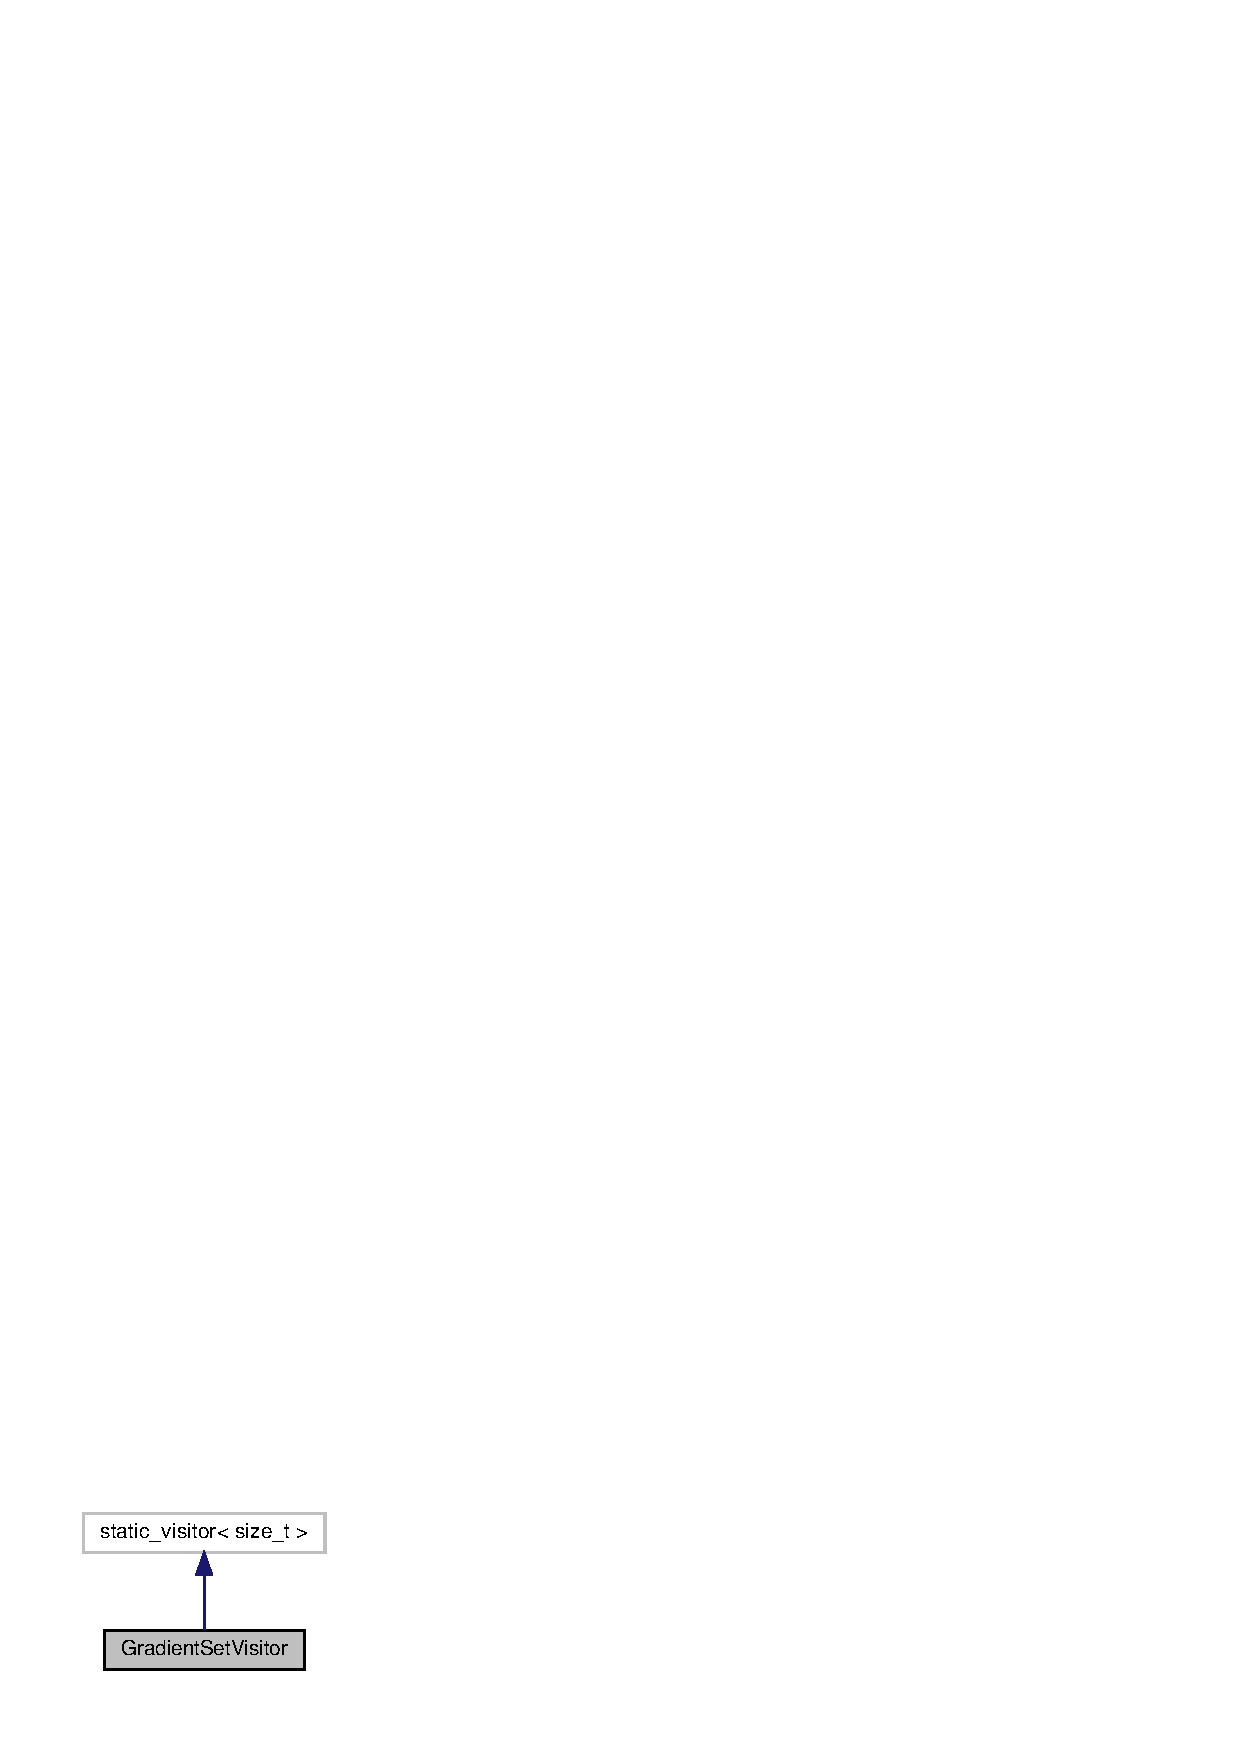
\includegraphics[width=160pt]{classmlpack_1_1ann_1_1GradientSetVisitor__inherit__graph}
\end{center}
\end{figure}
\subsection*{Public Member Functions}
\begin{DoxyCompactItemize}
\item 
\textbf{ Gradient\+Set\+Visitor} (arma\+::mat \&gradient, size\+\_\+t offset=0)
\begin{DoxyCompactList}\small\item\em Update the gradient parameter given the gradient set. \end{DoxyCompactList}\item 
{\footnotesize template$<$typename Layer\+Type $>$ }\\size\+\_\+t \textbf{ operator()} (Layer\+Type $\ast$layer) const
\begin{DoxyCompactList}\small\item\em Update the gradient parameter. \end{DoxyCompactList}\item 
size\+\_\+t \textbf{ operator()} (\textbf{ More\+Types} layer) const
\end{DoxyCompactItemize}


\subsection{Detailed Description}
\doxyref{Gradient\+Set\+Visitor}{p.}{classmlpack_1_1ann_1_1GradientSetVisitor} update the gradient parameter given the gradient set. 

Definition at line 26 of file gradient\+\_\+set\+\_\+visitor.\+hpp.



\subsection{Constructor \& Destructor Documentation}
\mbox{\label{classmlpack_1_1ann_1_1GradientSetVisitor_ae447e8d12abf6d567ac409ac5a116d37}} 
\index{mlpack\+::ann\+::\+Gradient\+Set\+Visitor@{mlpack\+::ann\+::\+Gradient\+Set\+Visitor}!Gradient\+Set\+Visitor@{Gradient\+Set\+Visitor}}
\index{Gradient\+Set\+Visitor@{Gradient\+Set\+Visitor}!mlpack\+::ann\+::\+Gradient\+Set\+Visitor@{mlpack\+::ann\+::\+Gradient\+Set\+Visitor}}
\subsubsection{Gradient\+Set\+Visitor()}
{\footnotesize\ttfamily \textbf{ Gradient\+Set\+Visitor} (\begin{DoxyParamCaption}\item[{arma\+::mat \&}]{gradient,  }\item[{size\+\_\+t}]{offset = {\ttfamily 0} }\end{DoxyParamCaption})}



Update the gradient parameter given the gradient set. 



\subsection{Member Function Documentation}
\mbox{\label{classmlpack_1_1ann_1_1GradientSetVisitor_aeb8947a28d511a7a4ce42a1fc63f79ee}} 
\index{mlpack\+::ann\+::\+Gradient\+Set\+Visitor@{mlpack\+::ann\+::\+Gradient\+Set\+Visitor}!operator()@{operator()}}
\index{operator()@{operator()}!mlpack\+::ann\+::\+Gradient\+Set\+Visitor@{mlpack\+::ann\+::\+Gradient\+Set\+Visitor}}
\subsubsection{operator()()\hspace{0.1cm}{\footnotesize\ttfamily [1/2]}}
{\footnotesize\ttfamily size\+\_\+t operator() (\begin{DoxyParamCaption}\item[{Layer\+Type $\ast$}]{layer }\end{DoxyParamCaption}) const}



Update the gradient parameter. 

\mbox{\label{classmlpack_1_1ann_1_1GradientSetVisitor_a19a2b78859e4e91b86170544dbd8ae09}} 
\index{mlpack\+::ann\+::\+Gradient\+Set\+Visitor@{mlpack\+::ann\+::\+Gradient\+Set\+Visitor}!operator()@{operator()}}
\index{operator()@{operator()}!mlpack\+::ann\+::\+Gradient\+Set\+Visitor@{mlpack\+::ann\+::\+Gradient\+Set\+Visitor}}
\subsubsection{operator()()\hspace{0.1cm}{\footnotesize\ttfamily [2/2]}}
{\footnotesize\ttfamily size\+\_\+t operator() (\begin{DoxyParamCaption}\item[{\textbf{ More\+Types}}]{layer }\end{DoxyParamCaption}) const}



The documentation for this class was generated from the following file\+:\begin{DoxyCompactItemize}
\item 
/home/aakash/mlpack/src/mlpack/methods/ann/visitor/\textbf{ gradient\+\_\+set\+\_\+visitor.\+hpp}\end{DoxyCompactItemize}

\section{Gradient\+Update\+Visitor Class Reference}
\label{classmlpack_1_1ann_1_1GradientUpdateVisitor}\index{Gradient\+Update\+Visitor@{Gradient\+Update\+Visitor}}


\doxyref{Gradient\+Update\+Visitor}{p.}{classmlpack_1_1ann_1_1GradientUpdateVisitor} update the gradient parameter given the gradient set.  




Inheritance diagram for Gradient\+Update\+Visitor\+:
\nopagebreak
\begin{figure}[H]
\begin{center}
\leavevmode
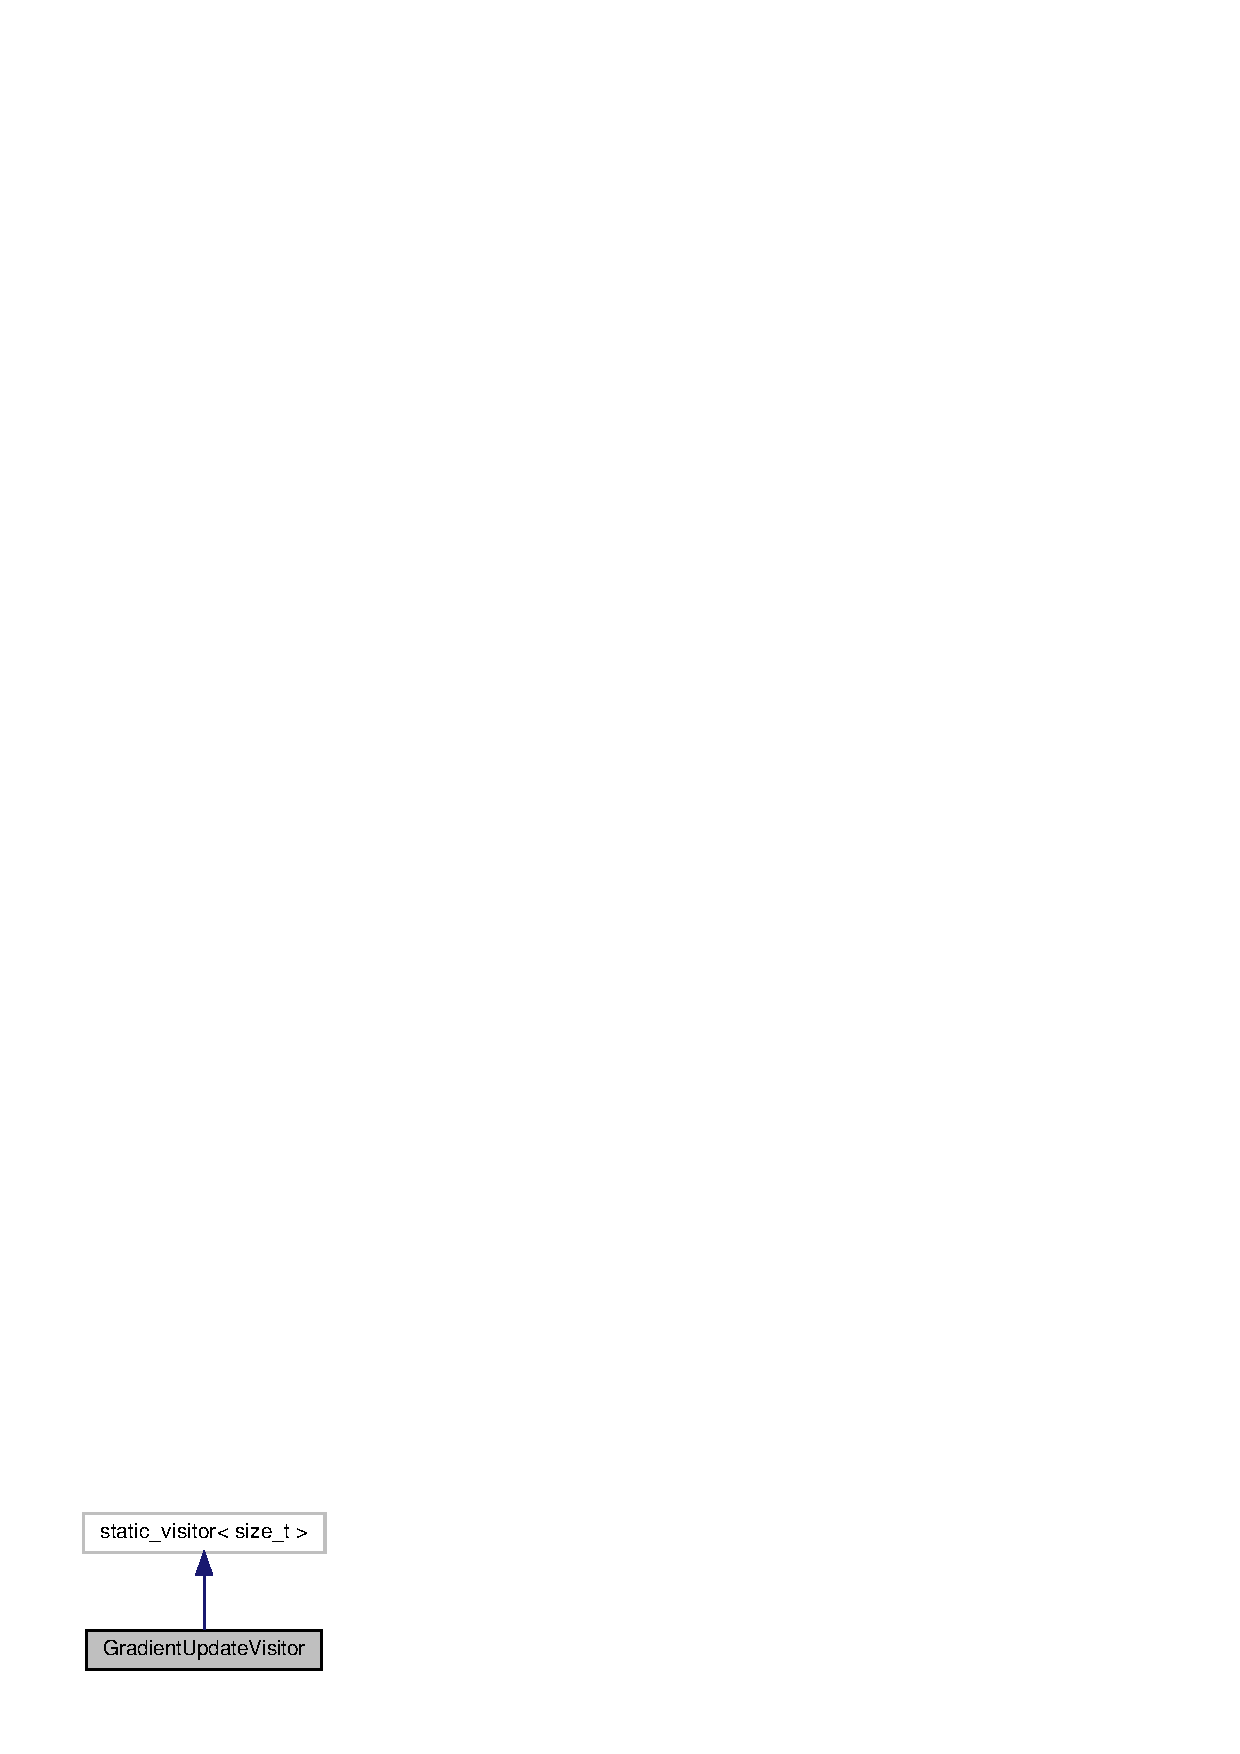
\includegraphics[width=160pt]{classmlpack_1_1ann_1_1GradientUpdateVisitor__inherit__graph}
\end{center}
\end{figure}
\subsection*{Public Member Functions}
\begin{DoxyCompactItemize}
\item 
\textbf{ Gradient\+Update\+Visitor} (arma\+::mat \&gradient, size\+\_\+t offset=0)
\begin{DoxyCompactList}\small\item\em Update the gradient parameter given the gradient set. \end{DoxyCompactList}\item 
{\footnotesize template$<$typename Layer\+Type $>$ }\\size\+\_\+t \textbf{ operator()} (Layer\+Type $\ast$layer) const
\begin{DoxyCompactList}\small\item\em Update the gradient parameter. \end{DoxyCompactList}\item 
size\+\_\+t \textbf{ operator()} (\textbf{ More\+Types} layer) const
\end{DoxyCompactItemize}


\subsection{Detailed Description}
\doxyref{Gradient\+Update\+Visitor}{p.}{classmlpack_1_1ann_1_1GradientUpdateVisitor} update the gradient parameter given the gradient set. 

Definition at line 26 of file gradient\+\_\+update\+\_\+visitor.\+hpp.



\subsection{Constructor \& Destructor Documentation}
\mbox{\label{classmlpack_1_1ann_1_1GradientUpdateVisitor_a2a2f92ba9fa017928734bab9c527720f}} 
\index{mlpack\+::ann\+::\+Gradient\+Update\+Visitor@{mlpack\+::ann\+::\+Gradient\+Update\+Visitor}!Gradient\+Update\+Visitor@{Gradient\+Update\+Visitor}}
\index{Gradient\+Update\+Visitor@{Gradient\+Update\+Visitor}!mlpack\+::ann\+::\+Gradient\+Update\+Visitor@{mlpack\+::ann\+::\+Gradient\+Update\+Visitor}}
\subsubsection{Gradient\+Update\+Visitor()}
{\footnotesize\ttfamily \textbf{ Gradient\+Update\+Visitor} (\begin{DoxyParamCaption}\item[{arma\+::mat \&}]{gradient,  }\item[{size\+\_\+t}]{offset = {\ttfamily 0} }\end{DoxyParamCaption})}



Update the gradient parameter given the gradient set. 



\subsection{Member Function Documentation}
\mbox{\label{classmlpack_1_1ann_1_1GradientUpdateVisitor_aeb8947a28d511a7a4ce42a1fc63f79ee}} 
\index{mlpack\+::ann\+::\+Gradient\+Update\+Visitor@{mlpack\+::ann\+::\+Gradient\+Update\+Visitor}!operator()@{operator()}}
\index{operator()@{operator()}!mlpack\+::ann\+::\+Gradient\+Update\+Visitor@{mlpack\+::ann\+::\+Gradient\+Update\+Visitor}}
\subsubsection{operator()()\hspace{0.1cm}{\footnotesize\ttfamily [1/2]}}
{\footnotesize\ttfamily size\+\_\+t operator() (\begin{DoxyParamCaption}\item[{Layer\+Type $\ast$}]{layer }\end{DoxyParamCaption}) const}



Update the gradient parameter. 

\mbox{\label{classmlpack_1_1ann_1_1GradientUpdateVisitor_a19a2b78859e4e91b86170544dbd8ae09}} 
\index{mlpack\+::ann\+::\+Gradient\+Update\+Visitor@{mlpack\+::ann\+::\+Gradient\+Update\+Visitor}!operator()@{operator()}}
\index{operator()@{operator()}!mlpack\+::ann\+::\+Gradient\+Update\+Visitor@{mlpack\+::ann\+::\+Gradient\+Update\+Visitor}}
\subsubsection{operator()()\hspace{0.1cm}{\footnotesize\ttfamily [2/2]}}
{\footnotesize\ttfamily size\+\_\+t operator() (\begin{DoxyParamCaption}\item[{\textbf{ More\+Types}}]{layer }\end{DoxyParamCaption}) const}



The documentation for this class was generated from the following file\+:\begin{DoxyCompactItemize}
\item 
/home/aakash/mlpack/src/mlpack/methods/ann/visitor/\textbf{ gradient\+\_\+update\+\_\+visitor.\+hpp}\end{DoxyCompactItemize}

\section{Gradient\+Visitor Class Reference}
\label{classmlpack_1_1ann_1_1GradientVisitor}\index{Gradient\+Visitor@{Gradient\+Visitor}}


Search\+Mode\+Visitor executes the Gradient() method of the given module using the input and delta parameter.  




Inheritance diagram for Gradient\+Visitor\+:
\nopagebreak
\begin{figure}[H]
\begin{center}
\leavevmode
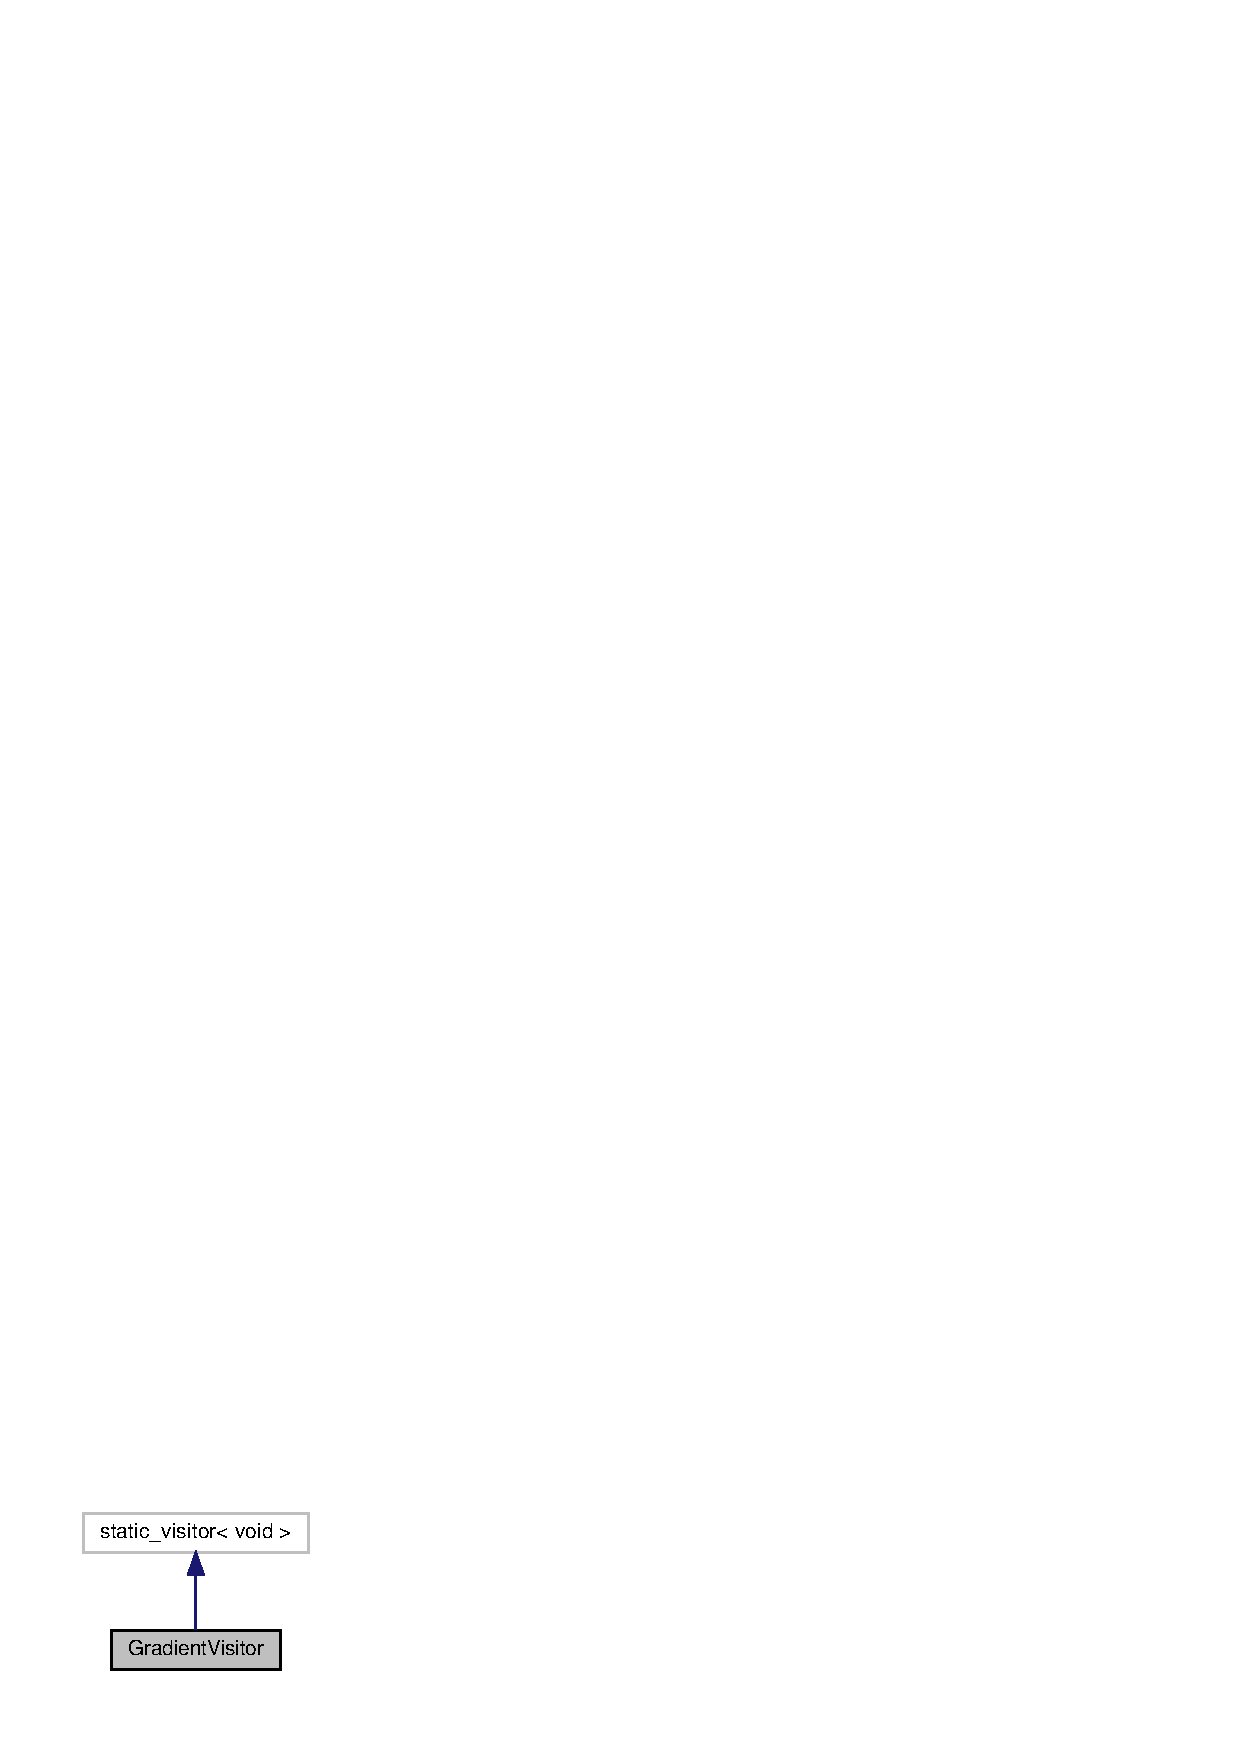
\includegraphics[width=152pt]{classmlpack_1_1ann_1_1GradientVisitor__inherit__graph}
\end{center}
\end{figure}
\subsection*{Public Member Functions}
\begin{DoxyCompactItemize}
\item 
\textbf{ Gradient\+Visitor} (const arma\+::mat \&input, const arma\+::mat \&delta)
\begin{DoxyCompactList}\small\item\em Executes the Gradient() method of the given module using the input and delta parameter. \end{DoxyCompactList}\item 
\textbf{ Gradient\+Visitor} (const arma\+::mat \&input, const arma\+::mat \&delta, const size\+\_\+t index)
\begin{DoxyCompactList}\small\item\em Executes the Gradient() method for the layer with the specified index. \end{DoxyCompactList}\item 
{\footnotesize template$<$typename Layer\+Type $>$ }\\void \textbf{ operator()} (Layer\+Type $\ast$layer) const
\begin{DoxyCompactList}\small\item\em Executes the Gradient() method. \end{DoxyCompactList}\item 
void \textbf{ operator()} (\textbf{ More\+Types} layer) const
\end{DoxyCompactItemize}


\subsection{Detailed Description}
Search\+Mode\+Visitor executes the Gradient() method of the given module using the input and delta parameter. 

Definition at line 28 of file gradient\+\_\+visitor.\+hpp.



\subsection{Constructor \& Destructor Documentation}
\mbox{\label{classmlpack_1_1ann_1_1GradientVisitor_aef51b166a43ea70ddbb05b7dfc8f82b7}} 
\index{mlpack\+::ann\+::\+Gradient\+Visitor@{mlpack\+::ann\+::\+Gradient\+Visitor}!Gradient\+Visitor@{Gradient\+Visitor}}
\index{Gradient\+Visitor@{Gradient\+Visitor}!mlpack\+::ann\+::\+Gradient\+Visitor@{mlpack\+::ann\+::\+Gradient\+Visitor}}
\subsubsection{Gradient\+Visitor()\hspace{0.1cm}{\footnotesize\ttfamily [1/2]}}
{\footnotesize\ttfamily \textbf{ Gradient\+Visitor} (\begin{DoxyParamCaption}\item[{const arma\+::mat \&}]{input,  }\item[{const arma\+::mat \&}]{delta }\end{DoxyParamCaption})}



Executes the Gradient() method of the given module using the input and delta parameter. 

\mbox{\label{classmlpack_1_1ann_1_1GradientVisitor_a39e14abb4d965e541b0905125fbb03a0}} 
\index{mlpack\+::ann\+::\+Gradient\+Visitor@{mlpack\+::ann\+::\+Gradient\+Visitor}!Gradient\+Visitor@{Gradient\+Visitor}}
\index{Gradient\+Visitor@{Gradient\+Visitor}!mlpack\+::ann\+::\+Gradient\+Visitor@{mlpack\+::ann\+::\+Gradient\+Visitor}}
\subsubsection{Gradient\+Visitor()\hspace{0.1cm}{\footnotesize\ttfamily [2/2]}}
{\footnotesize\ttfamily \textbf{ Gradient\+Visitor} (\begin{DoxyParamCaption}\item[{const arma\+::mat \&}]{input,  }\item[{const arma\+::mat \&}]{delta,  }\item[{const size\+\_\+t}]{index }\end{DoxyParamCaption})}



Executes the Gradient() method for the layer with the specified index. 



\subsection{Member Function Documentation}
\mbox{\label{classmlpack_1_1ann_1_1GradientVisitor_a26bb3385c630118c35f4799f1509abbc}} 
\index{mlpack\+::ann\+::\+Gradient\+Visitor@{mlpack\+::ann\+::\+Gradient\+Visitor}!operator()@{operator()}}
\index{operator()@{operator()}!mlpack\+::ann\+::\+Gradient\+Visitor@{mlpack\+::ann\+::\+Gradient\+Visitor}}
\subsubsection{operator()()\hspace{0.1cm}{\footnotesize\ttfamily [1/2]}}
{\footnotesize\ttfamily void operator() (\begin{DoxyParamCaption}\item[{Layer\+Type $\ast$}]{layer }\end{DoxyParamCaption}) const}



Executes the Gradient() method. 

\mbox{\label{classmlpack_1_1ann_1_1GradientVisitor_ae35578e7ff874a320fe762bc0edfff04}} 
\index{mlpack\+::ann\+::\+Gradient\+Visitor@{mlpack\+::ann\+::\+Gradient\+Visitor}!operator()@{operator()}}
\index{operator()@{operator()}!mlpack\+::ann\+::\+Gradient\+Visitor@{mlpack\+::ann\+::\+Gradient\+Visitor}}
\subsubsection{operator()()\hspace{0.1cm}{\footnotesize\ttfamily [2/2]}}
{\footnotesize\ttfamily void operator() (\begin{DoxyParamCaption}\item[{\textbf{ More\+Types}}]{layer }\end{DoxyParamCaption}) const}



The documentation for this class was generated from the following file\+:\begin{DoxyCompactItemize}
\item 
/home/aakash/mlpack/src/mlpack/methods/ann/visitor/\textbf{ gradient\+\_\+visitor.\+hpp}\end{DoxyCompactItemize}

\section{Gradient\+Zero\+Visitor Class Reference}
\label{classmlpack_1_1ann_1_1GradientZeroVisitor}\index{Gradient\+Zero\+Visitor@{Gradient\+Zero\+Visitor}}


Inheritance diagram for Gradient\+Zero\+Visitor\+:
\nopagebreak
\begin{figure}[H]
\begin{center}
\leavevmode
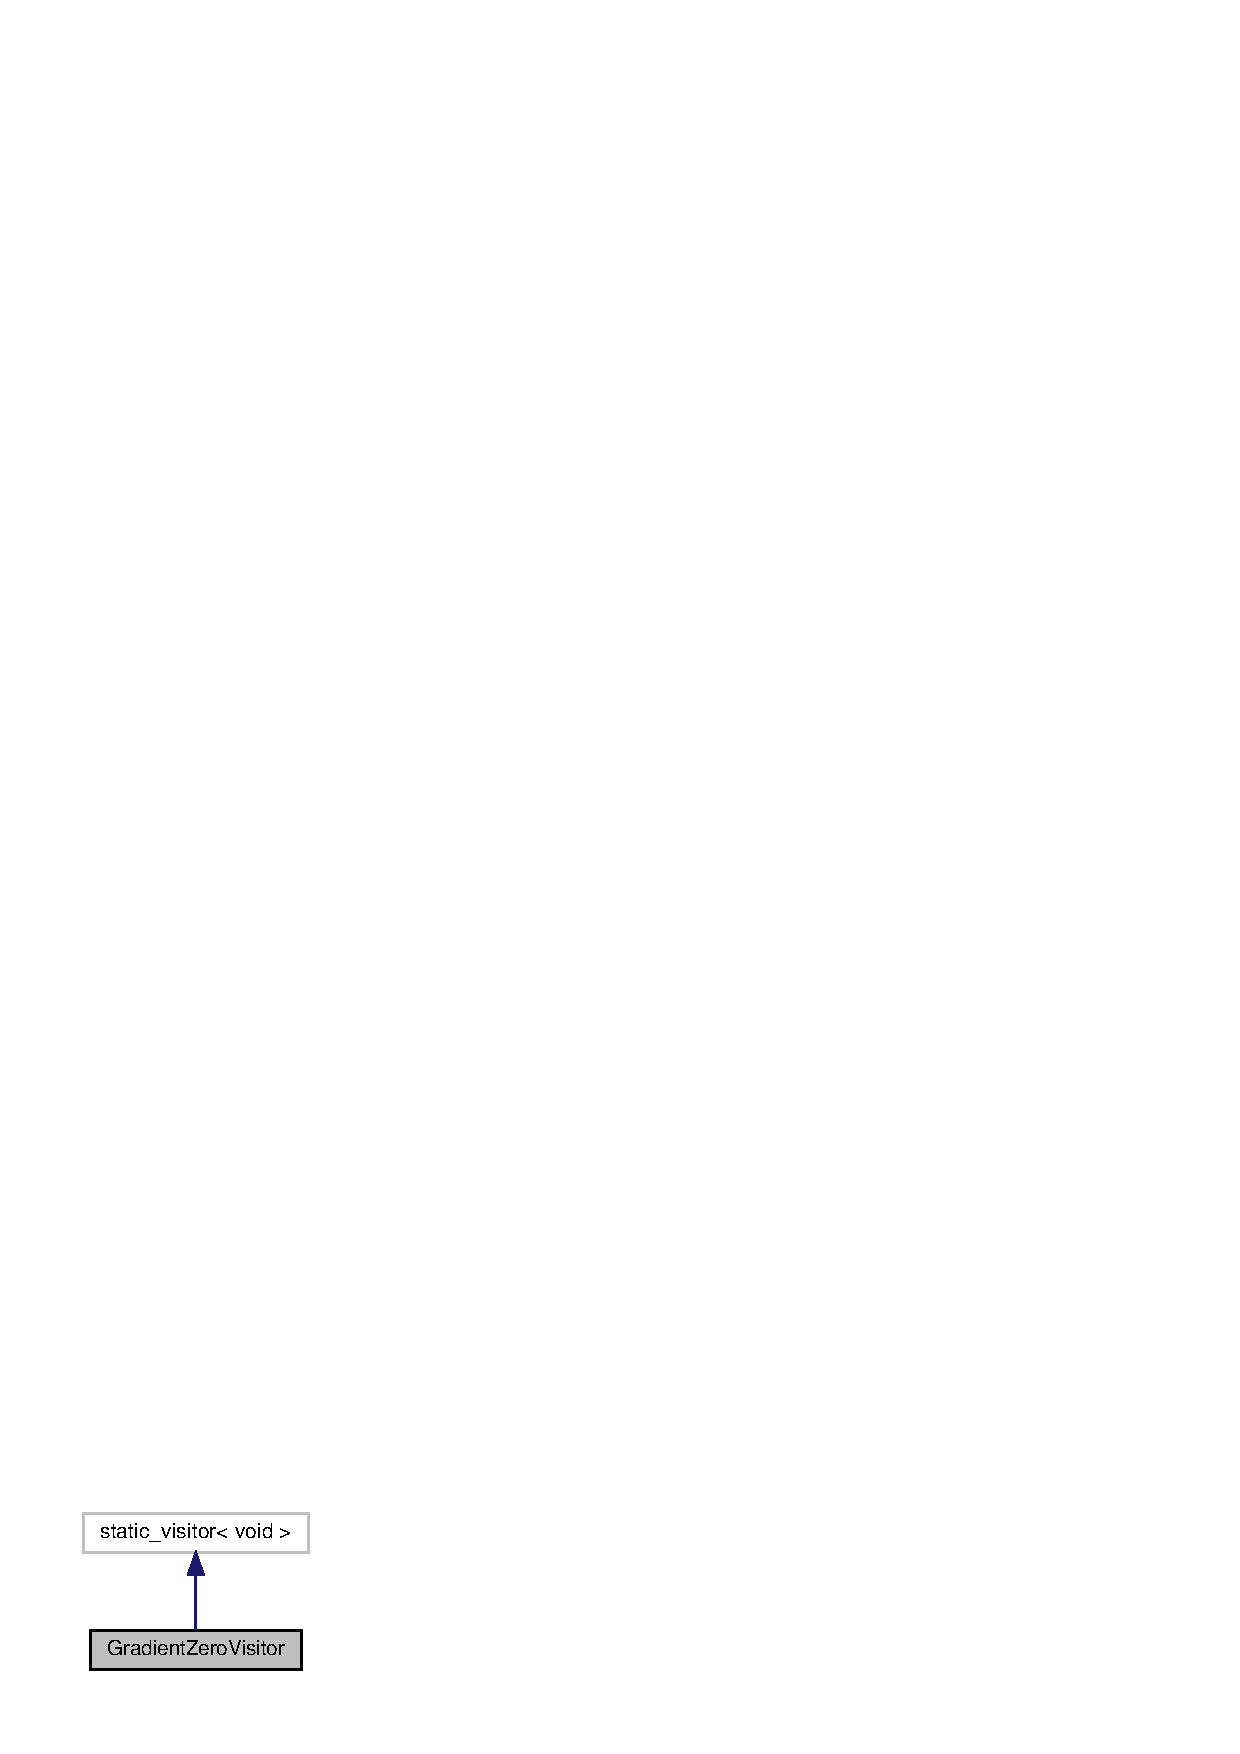
\includegraphics[width=152pt]{classmlpack_1_1ann_1_1GradientZeroVisitor__inherit__graph}
\end{center}
\end{figure}
\subsection*{Public Member Functions}
\begin{DoxyCompactItemize}
\item 
\textbf{ Gradient\+Zero\+Visitor} ()
\begin{DoxyCompactList}\small\item\em Set the gradient to zero for the given module. \end{DoxyCompactList}\item 
{\footnotesize template$<$typename Layer\+Type $>$ }\\void \textbf{ operator()} (Layer\+Type $\ast$layer) const
\begin{DoxyCompactList}\small\item\em Set the gradient to zero. \end{DoxyCompactList}\item 
void \textbf{ operator()} (\textbf{ More\+Types} layer) const
\end{DoxyCompactItemize}


\subsection{Detailed Description}


Definition at line 27 of file gradient\+\_\+zero\+\_\+visitor.\+hpp.



\subsection{Constructor \& Destructor Documentation}
\mbox{\label{classmlpack_1_1ann_1_1GradientZeroVisitor_aa2cc6d8ff51ab7a8bb44f18e528286e8}} 
\index{mlpack\+::ann\+::\+Gradient\+Zero\+Visitor@{mlpack\+::ann\+::\+Gradient\+Zero\+Visitor}!Gradient\+Zero\+Visitor@{Gradient\+Zero\+Visitor}}
\index{Gradient\+Zero\+Visitor@{Gradient\+Zero\+Visitor}!mlpack\+::ann\+::\+Gradient\+Zero\+Visitor@{mlpack\+::ann\+::\+Gradient\+Zero\+Visitor}}
\subsubsection{Gradient\+Zero\+Visitor()}
{\footnotesize\ttfamily \textbf{ Gradient\+Zero\+Visitor} (\begin{DoxyParamCaption}{ }\end{DoxyParamCaption})}



Set the gradient to zero for the given module. 



\subsection{Member Function Documentation}
\mbox{\label{classmlpack_1_1ann_1_1GradientZeroVisitor_a26bb3385c630118c35f4799f1509abbc}} 
\index{mlpack\+::ann\+::\+Gradient\+Zero\+Visitor@{mlpack\+::ann\+::\+Gradient\+Zero\+Visitor}!operator()@{operator()}}
\index{operator()@{operator()}!mlpack\+::ann\+::\+Gradient\+Zero\+Visitor@{mlpack\+::ann\+::\+Gradient\+Zero\+Visitor}}
\subsubsection{operator()()\hspace{0.1cm}{\footnotesize\ttfamily [1/2]}}
{\footnotesize\ttfamily void operator() (\begin{DoxyParamCaption}\item[{Layer\+Type $\ast$}]{layer }\end{DoxyParamCaption}) const}



Set the gradient to zero. 

\mbox{\label{classmlpack_1_1ann_1_1GradientZeroVisitor_ae35578e7ff874a320fe762bc0edfff04}} 
\index{mlpack\+::ann\+::\+Gradient\+Zero\+Visitor@{mlpack\+::ann\+::\+Gradient\+Zero\+Visitor}!operator()@{operator()}}
\index{operator()@{operator()}!mlpack\+::ann\+::\+Gradient\+Zero\+Visitor@{mlpack\+::ann\+::\+Gradient\+Zero\+Visitor}}
\subsubsection{operator()()\hspace{0.1cm}{\footnotesize\ttfamily [2/2]}}
{\footnotesize\ttfamily void operator() (\begin{DoxyParamCaption}\item[{\textbf{ More\+Types}}]{layer }\end{DoxyParamCaption}) const}



The documentation for this class was generated from the following file\+:\begin{DoxyCompactItemize}
\item 
/home/aakash/mlpack/src/mlpack/methods/ann/visitor/\textbf{ gradient\+\_\+zero\+\_\+visitor.\+hpp}\end{DoxyCompactItemize}

\section{G\+RU$<$ Input\+Data\+Type, Output\+Data\+Type $>$ Class Template Reference}
\label{classmlpack_1_1ann_1_1GRU}\index{G\+R\+U$<$ Input\+Data\+Type, Output\+Data\+Type $>$@{G\+R\+U$<$ Input\+Data\+Type, Output\+Data\+Type $>$}}


An implementation of a gru network layer.  


\subsection*{Public Member Functions}
\begin{DoxyCompactItemize}
\item 
\textbf{ G\+RU} ()
\begin{DoxyCompactList}\small\item\em Create the \doxyref{G\+RU}{p.}{classmlpack_1_1ann_1_1GRU} object. \end{DoxyCompactList}\item 
\textbf{ G\+RU} (const size\+\_\+t in\+Size, const size\+\_\+t out\+Size, const size\+\_\+t rho=std\+::numeric\+\_\+limits$<$ size\+\_\+t $>$\+::max())
\begin{DoxyCompactList}\small\item\em Create the \doxyref{G\+RU}{p.}{classmlpack_1_1ann_1_1GRU} layer object using the specified parameters. \end{DoxyCompactList}\item 
{\footnotesize template$<$typename eT $>$ }\\void \textbf{ Backward} (const arma\+::\+Mat$<$ eT $>$ \&, const arma\+::\+Mat$<$ eT $>$ \&gy, arma\+::\+Mat$<$ eT $>$ \&g)
\begin{DoxyCompactList}\small\item\em Ordinary feed backward pass of a neural network, calculating the function f(x) by propagating x backwards trough f. \end{DoxyCompactList}\item 
Output\+Data\+Type const  \& \textbf{ Delta} () const
\begin{DoxyCompactList}\small\item\em Get the delta. \end{DoxyCompactList}\item 
Output\+Data\+Type \& \textbf{ Delta} ()
\begin{DoxyCompactList}\small\item\em Modify the delta. \end{DoxyCompactList}\item 
bool \textbf{ Deterministic} () const
\begin{DoxyCompactList}\small\item\em The value of the deterministic parameter. \end{DoxyCompactList}\item 
bool \& \textbf{ Deterministic} ()
\begin{DoxyCompactList}\small\item\em Modify the value of the deterministic parameter. \end{DoxyCompactList}\item 
{\footnotesize template$<$typename eT $>$ }\\void \textbf{ Forward} (const arma\+::\+Mat$<$ eT $>$ \&input, arma\+::\+Mat$<$ eT $>$ \&output)
\begin{DoxyCompactList}\small\item\em Ordinary feed forward pass of a neural network, evaluating the function f(x) by propagating the activity forward through f. \end{DoxyCompactList}\item 
{\footnotesize template$<$typename eT $>$ }\\void \textbf{ Gradient} (const arma\+::\+Mat$<$ eT $>$ \&input, const arma\+::\+Mat$<$ eT $>$ \&, arma\+::\+Mat$<$ eT $>$ \&)
\item 
Output\+Data\+Type const  \& \textbf{ Gradient} () const
\begin{DoxyCompactList}\small\item\em Get the gradient. \end{DoxyCompactList}\item 
Output\+Data\+Type \& \textbf{ Gradient} ()
\begin{DoxyCompactList}\small\item\em Modify the gradient. \end{DoxyCompactList}\item 
size\+\_\+t \textbf{ Input\+Shape} () const
\begin{DoxyCompactList}\small\item\em Get the shape of the input. \end{DoxyCompactList}\item 
size\+\_\+t \textbf{ In\+Size} () const
\begin{DoxyCompactList}\small\item\em Get the number of input units. \end{DoxyCompactList}\item 
std\+::vector$<$ \textbf{ Layer\+Types}$<$$>$ $>$ \& \textbf{ Model} ()
\begin{DoxyCompactList}\small\item\em Get the model modules. \end{DoxyCompactList}\item 
Output\+Data\+Type const  \& \textbf{ Output\+Parameter} () const
\begin{DoxyCompactList}\small\item\em Get the output parameter. \end{DoxyCompactList}\item 
Output\+Data\+Type \& \textbf{ Output\+Parameter} ()
\begin{DoxyCompactList}\small\item\em Modify the output parameter. \end{DoxyCompactList}\item 
size\+\_\+t \textbf{ Out\+Size} () const
\begin{DoxyCompactList}\small\item\em Get the number of output units. \end{DoxyCompactList}\item 
Output\+Data\+Type const  \& \textbf{ Parameters} () const
\begin{DoxyCompactList}\small\item\em Get the parameters. \end{DoxyCompactList}\item 
Output\+Data\+Type \& \textbf{ Parameters} ()
\begin{DoxyCompactList}\small\item\em Modify the parameters. \end{DoxyCompactList}\item 
void \textbf{ Reset\+Cell} (const size\+\_\+t size)
\item 
size\+\_\+t \textbf{ Rho} () const
\begin{DoxyCompactList}\small\item\em Get the maximum number of steps to backpropagate through time (B\+P\+TT). \end{DoxyCompactList}\item 
size\+\_\+t \& \textbf{ Rho} ()
\begin{DoxyCompactList}\small\item\em Modify the maximum number of steps to backpropagate through time (B\+P\+TT). \end{DoxyCompactList}\item 
{\footnotesize template$<$typename Archive $>$ }\\void \textbf{ serialize} (Archive \&ar, const uint32\+\_\+t)
\begin{DoxyCompactList}\small\item\em Serialize the layer. \end{DoxyCompactList}\end{DoxyCompactItemize}


\subsection{Detailed Description}
\subsubsection*{template$<$typename Input\+Data\+Type = arma\+::mat, typename Output\+Data\+Type = arma\+::mat$>$\newline
class mlpack\+::ann\+::\+G\+R\+U$<$ Input\+Data\+Type, Output\+Data\+Type $>$}

An implementation of a gru network layer. 

This cell can be used in \doxyref{R\+NN}{p.}{classmlpack_1_1ann_1_1RNN} networks.


\begin{DoxyTemplParams}{Template Parameters}
{\em Input\+Data\+Type} & Type of the input data (arma\+::colvec, arma\+::mat, arma\+::sp\+\_\+mat or arma\+::cube). \\
\hline
{\em Output\+Data\+Type} & Type of the output data (arma\+::colvec, arma\+::mat, arma\+::sp\+\_\+mat or arma\+::cube). \\
\hline
\end{DoxyTemplParams}


Definition at line 58 of file gru.\+hpp.



\subsection{Constructor \& Destructor Documentation}
\mbox{\label{classmlpack_1_1ann_1_1GRU_a375d9aa6e1d5554befe4173d70ca3e34}} 
\index{mlpack\+::ann\+::\+G\+RU@{mlpack\+::ann\+::\+G\+RU}!G\+RU@{G\+RU}}
\index{G\+RU@{G\+RU}!mlpack\+::ann\+::\+G\+RU@{mlpack\+::ann\+::\+G\+RU}}
\subsubsection{G\+R\+U()\hspace{0.1cm}{\footnotesize\ttfamily [1/2]}}
{\footnotesize\ttfamily \textbf{ G\+RU} (\begin{DoxyParamCaption}{ }\end{DoxyParamCaption})}



Create the \doxyref{G\+RU}{p.}{classmlpack_1_1ann_1_1GRU} object. 

\mbox{\label{classmlpack_1_1ann_1_1GRU_a95db7ecef7c74dfd78bf58ea47667ab0}} 
\index{mlpack\+::ann\+::\+G\+RU@{mlpack\+::ann\+::\+G\+RU}!G\+RU@{G\+RU}}
\index{G\+RU@{G\+RU}!mlpack\+::ann\+::\+G\+RU@{mlpack\+::ann\+::\+G\+RU}}
\subsubsection{G\+R\+U()\hspace{0.1cm}{\footnotesize\ttfamily [2/2]}}
{\footnotesize\ttfamily \textbf{ G\+RU} (\begin{DoxyParamCaption}\item[{const size\+\_\+t}]{in\+Size,  }\item[{const size\+\_\+t}]{out\+Size,  }\item[{const size\+\_\+t}]{rho = {\ttfamily std\+:\+:numeric\+\_\+limits$<$~size\+\_\+t~$>$\+:\+:max()} }\end{DoxyParamCaption})}



Create the \doxyref{G\+RU}{p.}{classmlpack_1_1ann_1_1GRU} layer object using the specified parameters. 


\begin{DoxyParams}{Parameters}
{\em in\+Size} & The number of input units. \\
\hline
{\em out\+Size} & The number of output units. \\
\hline
{\em rho} & Maximum number of steps to backpropagate through time (B\+P\+TT). \\
\hline
\end{DoxyParams}


\subsection{Member Function Documentation}
\mbox{\label{classmlpack_1_1ann_1_1GRU_ad9ad1a3bdb0f3fff5c839ed155e4bbf8}} 
\index{mlpack\+::ann\+::\+G\+RU@{mlpack\+::ann\+::\+G\+RU}!Backward@{Backward}}
\index{Backward@{Backward}!mlpack\+::ann\+::\+G\+RU@{mlpack\+::ann\+::\+G\+RU}}
\subsubsection{Backward()}
{\footnotesize\ttfamily void Backward (\begin{DoxyParamCaption}\item[{const arma\+::\+Mat$<$ eT $>$ \&}]{,  }\item[{const arma\+::\+Mat$<$ eT $>$ \&}]{gy,  }\item[{arma\+::\+Mat$<$ eT $>$ \&}]{g }\end{DoxyParamCaption})}



Ordinary feed backward pass of a neural network, calculating the function f(x) by propagating x backwards trough f. 

Using the results from the feed forward pass.


\begin{DoxyParams}{Parameters}
{\em $\ast$} & (input) The propagated input activation. \\
\hline
{\em gy} & The backpropagated error. \\
\hline
{\em g} & The calculated gradient. \\
\hline
\end{DoxyParams}
\mbox{\label{classmlpack_1_1ann_1_1GRU_a797f7edb44dd081e5e2b3cc316eef6bd}} 
\index{mlpack\+::ann\+::\+G\+RU@{mlpack\+::ann\+::\+G\+RU}!Delta@{Delta}}
\index{Delta@{Delta}!mlpack\+::ann\+::\+G\+RU@{mlpack\+::ann\+::\+G\+RU}}
\subsubsection{Delta()\hspace{0.1cm}{\footnotesize\ttfamily [1/2]}}
{\footnotesize\ttfamily Output\+Data\+Type const\& Delta (\begin{DoxyParamCaption}{ }\end{DoxyParamCaption}) const\hspace{0.3cm}{\ttfamily [inline]}}



Get the delta. 



Definition at line 140 of file gru.\+hpp.

\mbox{\label{classmlpack_1_1ann_1_1GRU_ad6601342d560219ce951d554e69e5e87}} 
\index{mlpack\+::ann\+::\+G\+RU@{mlpack\+::ann\+::\+G\+RU}!Delta@{Delta}}
\index{Delta@{Delta}!mlpack\+::ann\+::\+G\+RU@{mlpack\+::ann\+::\+G\+RU}}
\subsubsection{Delta()\hspace{0.1cm}{\footnotesize\ttfamily [2/2]}}
{\footnotesize\ttfamily Output\+Data\+Type\& Delta (\begin{DoxyParamCaption}{ }\end{DoxyParamCaption})\hspace{0.3cm}{\ttfamily [inline]}}



Modify the delta. 



Definition at line 142 of file gru.\+hpp.

\mbox{\label{classmlpack_1_1ann_1_1GRU_a9f4103707f4d199ce5594d239b60443e}} 
\index{mlpack\+::ann\+::\+G\+RU@{mlpack\+::ann\+::\+G\+RU}!Deterministic@{Deterministic}}
\index{Deterministic@{Deterministic}!mlpack\+::ann\+::\+G\+RU@{mlpack\+::ann\+::\+G\+RU}}
\subsubsection{Deterministic()\hspace{0.1cm}{\footnotesize\ttfamily [1/2]}}
{\footnotesize\ttfamily bool Deterministic (\begin{DoxyParamCaption}{ }\end{DoxyParamCaption}) const\hspace{0.3cm}{\ttfamily [inline]}}



The value of the deterministic parameter. 



Definition at line 120 of file gru.\+hpp.

\mbox{\label{classmlpack_1_1ann_1_1GRU_a42d4ee3da432cff20d3a41b8b1ec801c}} 
\index{mlpack\+::ann\+::\+G\+RU@{mlpack\+::ann\+::\+G\+RU}!Deterministic@{Deterministic}}
\index{Deterministic@{Deterministic}!mlpack\+::ann\+::\+G\+RU@{mlpack\+::ann\+::\+G\+RU}}
\subsubsection{Deterministic()\hspace{0.1cm}{\footnotesize\ttfamily [2/2]}}
{\footnotesize\ttfamily bool\& Deterministic (\begin{DoxyParamCaption}{ }\end{DoxyParamCaption})\hspace{0.3cm}{\ttfamily [inline]}}



Modify the value of the deterministic parameter. 



Definition at line 122 of file gru.\+hpp.

\mbox{\label{classmlpack_1_1ann_1_1GRU_a461f849bc638c15bec262dc9c3a58abe}} 
\index{mlpack\+::ann\+::\+G\+RU@{mlpack\+::ann\+::\+G\+RU}!Forward@{Forward}}
\index{Forward@{Forward}!mlpack\+::ann\+::\+G\+RU@{mlpack\+::ann\+::\+G\+RU}}
\subsubsection{Forward()}
{\footnotesize\ttfamily void Forward (\begin{DoxyParamCaption}\item[{const arma\+::\+Mat$<$ eT $>$ \&}]{input,  }\item[{arma\+::\+Mat$<$ eT $>$ \&}]{output }\end{DoxyParamCaption})}



Ordinary feed forward pass of a neural network, evaluating the function f(x) by propagating the activity forward through f. 


\begin{DoxyParams}{Parameters}
{\em input} & Input data used for evaluating the specified function. \\
\hline
{\em output} & Resulting output activation. \\
\hline
\end{DoxyParams}
\mbox{\label{classmlpack_1_1ann_1_1GRU_ae3face09d68158413cc32cefe69f060d}} 
\index{mlpack\+::ann\+::\+G\+RU@{mlpack\+::ann\+::\+G\+RU}!Gradient@{Gradient}}
\index{Gradient@{Gradient}!mlpack\+::ann\+::\+G\+RU@{mlpack\+::ann\+::\+G\+RU}}
\subsubsection{Gradient()\hspace{0.1cm}{\footnotesize\ttfamily [1/3]}}
{\footnotesize\ttfamily void Gradient (\begin{DoxyParamCaption}\item[{const arma\+::\+Mat$<$ eT $>$ \&}]{input,  }\item[{const arma\+::\+Mat$<$ eT $>$ \&}]{,  }\item[{arma\+::\+Mat$<$ eT $>$ \&}]{ }\end{DoxyParamCaption})}

\mbox{\label{classmlpack_1_1ann_1_1GRU_a0f1f4e6d93472d83852731a96c8c3f59}} 
\index{mlpack\+::ann\+::\+G\+RU@{mlpack\+::ann\+::\+G\+RU}!Gradient@{Gradient}}
\index{Gradient@{Gradient}!mlpack\+::ann\+::\+G\+RU@{mlpack\+::ann\+::\+G\+RU}}
\subsubsection{Gradient()\hspace{0.1cm}{\footnotesize\ttfamily [2/3]}}
{\footnotesize\ttfamily Output\+Data\+Type const\& Gradient (\begin{DoxyParamCaption}{ }\end{DoxyParamCaption}) const\hspace{0.3cm}{\ttfamily [inline]}}



Get the gradient. 



Definition at line 145 of file gru.\+hpp.

\mbox{\label{classmlpack_1_1ann_1_1GRU_a19abce4739c3b0b658b612537e21956a}} 
\index{mlpack\+::ann\+::\+G\+RU@{mlpack\+::ann\+::\+G\+RU}!Gradient@{Gradient}}
\index{Gradient@{Gradient}!mlpack\+::ann\+::\+G\+RU@{mlpack\+::ann\+::\+G\+RU}}
\subsubsection{Gradient()\hspace{0.1cm}{\footnotesize\ttfamily [3/3]}}
{\footnotesize\ttfamily Output\+Data\+Type\& Gradient (\begin{DoxyParamCaption}{ }\end{DoxyParamCaption})\hspace{0.3cm}{\ttfamily [inline]}}



Modify the gradient. 



Definition at line 147 of file gru.\+hpp.

\mbox{\label{classmlpack_1_1ann_1_1GRU_a13ab93f234244a68f6ade76287284447}} 
\index{mlpack\+::ann\+::\+G\+RU@{mlpack\+::ann\+::\+G\+RU}!Input\+Shape@{Input\+Shape}}
\index{Input\+Shape@{Input\+Shape}!mlpack\+::ann\+::\+G\+RU@{mlpack\+::ann\+::\+G\+RU}}
\subsubsection{Input\+Shape()}
{\footnotesize\ttfamily size\+\_\+t Input\+Shape (\begin{DoxyParamCaption}{ }\end{DoxyParamCaption}) const\hspace{0.3cm}{\ttfamily [inline]}}



Get the shape of the input. 



Definition at line 159 of file gru.\+hpp.



References G\+R\+U$<$ Input\+Data\+Type, Output\+Data\+Type $>$\+::serialize().

\mbox{\label{classmlpack_1_1ann_1_1GRU_adc2669016a821704c4c4aeb4651e9e87}} 
\index{mlpack\+::ann\+::\+G\+RU@{mlpack\+::ann\+::\+G\+RU}!In\+Size@{In\+Size}}
\index{In\+Size@{In\+Size}!mlpack\+::ann\+::\+G\+RU@{mlpack\+::ann\+::\+G\+RU}}
\subsubsection{In\+Size()}
{\footnotesize\ttfamily size\+\_\+t In\+Size (\begin{DoxyParamCaption}{ }\end{DoxyParamCaption}) const\hspace{0.3cm}{\ttfamily [inline]}}



Get the number of input units. 



Definition at line 153 of file gru.\+hpp.

\mbox{\label{classmlpack_1_1ann_1_1GRU_a50c707b4f7c009339d8d661539baf38f}} 
\index{mlpack\+::ann\+::\+G\+RU@{mlpack\+::ann\+::\+G\+RU}!Model@{Model}}
\index{Model@{Model}!mlpack\+::ann\+::\+G\+RU@{mlpack\+::ann\+::\+G\+RU}}
\subsubsection{Model()}
{\footnotesize\ttfamily std\+::vector$<$\textbf{ Layer\+Types}$<$$>$ $>$\& Model (\begin{DoxyParamCaption}{ }\end{DoxyParamCaption})\hspace{0.3cm}{\ttfamily [inline]}}



Get the model modules. 



Definition at line 150 of file gru.\+hpp.

\mbox{\label{classmlpack_1_1ann_1_1GRU_a0ee21c2a36e5abad1e7a9d5dd00849f9}} 
\index{mlpack\+::ann\+::\+G\+RU@{mlpack\+::ann\+::\+G\+RU}!Output\+Parameter@{Output\+Parameter}}
\index{Output\+Parameter@{Output\+Parameter}!mlpack\+::ann\+::\+G\+RU@{mlpack\+::ann\+::\+G\+RU}}
\subsubsection{Output\+Parameter()\hspace{0.1cm}{\footnotesize\ttfamily [1/2]}}
{\footnotesize\ttfamily Output\+Data\+Type const\& Output\+Parameter (\begin{DoxyParamCaption}{ }\end{DoxyParamCaption}) const\hspace{0.3cm}{\ttfamily [inline]}}



Get the output parameter. 



Definition at line 135 of file gru.\+hpp.

\mbox{\label{classmlpack_1_1ann_1_1GRU_a21d5f745f02c709625a4ee0907f004a5}} 
\index{mlpack\+::ann\+::\+G\+RU@{mlpack\+::ann\+::\+G\+RU}!Output\+Parameter@{Output\+Parameter}}
\index{Output\+Parameter@{Output\+Parameter}!mlpack\+::ann\+::\+G\+RU@{mlpack\+::ann\+::\+G\+RU}}
\subsubsection{Output\+Parameter()\hspace{0.1cm}{\footnotesize\ttfamily [2/2]}}
{\footnotesize\ttfamily Output\+Data\+Type\& Output\+Parameter (\begin{DoxyParamCaption}{ }\end{DoxyParamCaption})\hspace{0.3cm}{\ttfamily [inline]}}



Modify the output parameter. 



Definition at line 137 of file gru.\+hpp.

\mbox{\label{classmlpack_1_1ann_1_1GRU_a366243e673681001c6080d84ea644f6a}} 
\index{mlpack\+::ann\+::\+G\+RU@{mlpack\+::ann\+::\+G\+RU}!Out\+Size@{Out\+Size}}
\index{Out\+Size@{Out\+Size}!mlpack\+::ann\+::\+G\+RU@{mlpack\+::ann\+::\+G\+RU}}
\subsubsection{Out\+Size()}
{\footnotesize\ttfamily size\+\_\+t Out\+Size (\begin{DoxyParamCaption}{ }\end{DoxyParamCaption}) const\hspace{0.3cm}{\ttfamily [inline]}}



Get the number of output units. 



Definition at line 156 of file gru.\+hpp.

\mbox{\label{classmlpack_1_1ann_1_1GRU_aa530552c7ef915c952fbacc77b965c90}} 
\index{mlpack\+::ann\+::\+G\+RU@{mlpack\+::ann\+::\+G\+RU}!Parameters@{Parameters}}
\index{Parameters@{Parameters}!mlpack\+::ann\+::\+G\+RU@{mlpack\+::ann\+::\+G\+RU}}
\subsubsection{Parameters()\hspace{0.1cm}{\footnotesize\ttfamily [1/2]}}
{\footnotesize\ttfamily Output\+Data\+Type const\& Parameters (\begin{DoxyParamCaption}{ }\end{DoxyParamCaption}) const\hspace{0.3cm}{\ttfamily [inline]}}



Get the parameters. 



Definition at line 130 of file gru.\+hpp.

\mbox{\label{classmlpack_1_1ann_1_1GRU_a9c5c5900772a689d5a6b59778ec67120}} 
\index{mlpack\+::ann\+::\+G\+RU@{mlpack\+::ann\+::\+G\+RU}!Parameters@{Parameters}}
\index{Parameters@{Parameters}!mlpack\+::ann\+::\+G\+RU@{mlpack\+::ann\+::\+G\+RU}}
\subsubsection{Parameters()\hspace{0.1cm}{\footnotesize\ttfamily [2/2]}}
{\footnotesize\ttfamily Output\+Data\+Type\& Parameters (\begin{DoxyParamCaption}{ }\end{DoxyParamCaption})\hspace{0.3cm}{\ttfamily [inline]}}



Modify the parameters. 



Definition at line 132 of file gru.\+hpp.

\mbox{\label{classmlpack_1_1ann_1_1GRU_ab92846e8253dc597239574d87d969ffb}} 
\index{mlpack\+::ann\+::\+G\+RU@{mlpack\+::ann\+::\+G\+RU}!Reset\+Cell@{Reset\+Cell}}
\index{Reset\+Cell@{Reset\+Cell}!mlpack\+::ann\+::\+G\+RU@{mlpack\+::ann\+::\+G\+RU}}
\subsubsection{Reset\+Cell()}
{\footnotesize\ttfamily void Reset\+Cell (\begin{DoxyParamCaption}\item[{const size\+\_\+t}]{size }\end{DoxyParamCaption})}

\mbox{\label{classmlpack_1_1ann_1_1GRU_a45280505858e9bda815a48c96e930f8d}} 
\index{mlpack\+::ann\+::\+G\+RU@{mlpack\+::ann\+::\+G\+RU}!Rho@{Rho}}
\index{Rho@{Rho}!mlpack\+::ann\+::\+G\+RU@{mlpack\+::ann\+::\+G\+RU}}
\subsubsection{Rho()\hspace{0.1cm}{\footnotesize\ttfamily [1/2]}}
{\footnotesize\ttfamily size\+\_\+t Rho (\begin{DoxyParamCaption}{ }\end{DoxyParamCaption}) const\hspace{0.3cm}{\ttfamily [inline]}}



Get the maximum number of steps to backpropagate through time (B\+P\+TT). 



Definition at line 125 of file gru.\+hpp.

\mbox{\label{classmlpack_1_1ann_1_1GRU_aeb617af2894a3e4bbabcd7ebc30a35af}} 
\index{mlpack\+::ann\+::\+G\+RU@{mlpack\+::ann\+::\+G\+RU}!Rho@{Rho}}
\index{Rho@{Rho}!mlpack\+::ann\+::\+G\+RU@{mlpack\+::ann\+::\+G\+RU}}
\subsubsection{Rho()\hspace{0.1cm}{\footnotesize\ttfamily [2/2]}}
{\footnotesize\ttfamily size\+\_\+t\& Rho (\begin{DoxyParamCaption}{ }\end{DoxyParamCaption})\hspace{0.3cm}{\ttfamily [inline]}}



Modify the maximum number of steps to backpropagate through time (B\+P\+TT). 



Definition at line 127 of file gru.\+hpp.

\mbox{\label{classmlpack_1_1ann_1_1GRU_a65cba07328997659bec80b9879b15a51}} 
\index{mlpack\+::ann\+::\+G\+RU@{mlpack\+::ann\+::\+G\+RU}!serialize@{serialize}}
\index{serialize@{serialize}!mlpack\+::ann\+::\+G\+RU@{mlpack\+::ann\+::\+G\+RU}}
\subsubsection{serialize()}
{\footnotesize\ttfamily void serialize (\begin{DoxyParamCaption}\item[{Archive \&}]{ar,  }\item[{const uint32\+\_\+t}]{ }\end{DoxyParamCaption})}



Serialize the layer. 



Referenced by G\+R\+U$<$ Input\+Data\+Type, Output\+Data\+Type $>$\+::\+Input\+Shape().



The documentation for this class was generated from the following file\+:\begin{DoxyCompactItemize}
\item 
/home/aakash/mlpack/src/mlpack/methods/ann/layer/\textbf{ gru.\+hpp}\end{DoxyCompactItemize}

\section{Hard\+Shrink$<$ Input\+Data\+Type, Output\+Data\+Type $>$ Class Template Reference}
\label{classmlpack_1_1ann_1_1HardShrink}\index{Hard\+Shrink$<$ Input\+Data\+Type, Output\+Data\+Type $>$@{Hard\+Shrink$<$ Input\+Data\+Type, Output\+Data\+Type $>$}}


Hard Shrink operator is defined as,.  


\subsection*{Public Member Functions}
\begin{DoxyCompactItemize}
\item 
\textbf{ Hard\+Shrink} (const double lambda=0.\+5)
\begin{DoxyCompactList}\small\item\em Create \doxyref{Hard\+Shrink}{p.}{classmlpack_1_1ann_1_1HardShrink} object using specified hyperparameter lambda. \end{DoxyCompactList}\item 
{\footnotesize template$<$typename Data\+Type $>$ }\\void \textbf{ Backward} (const Data\+Type \&input, Data\+Type \&gy, Data\+Type \&g)
\begin{DoxyCompactList}\small\item\em Ordinary feed backward pass of a neural network, calculating the function f(x) by propagating x backwards through f. \end{DoxyCompactList}\item 
Output\+Data\+Type const  \& \textbf{ Delta} () const
\begin{DoxyCompactList}\small\item\em Get the delta. \end{DoxyCompactList}\item 
Output\+Data\+Type \& \textbf{ Delta} ()
\begin{DoxyCompactList}\small\item\em Modify the delta. \end{DoxyCompactList}\item 
{\footnotesize template$<$typename Input\+Type , typename Output\+Type $>$ }\\void \textbf{ Forward} (const Input\+Type \&input, Output\+Type \&output)
\begin{DoxyCompactList}\small\item\em Ordinary feed forward pass of a neural network, evaluating the function f(x) by propagating the activity forward through f. \end{DoxyCompactList}\item 
double const  \& \textbf{ Lambda} () const
\begin{DoxyCompactList}\small\item\em Get the hyperparameter lambda. \end{DoxyCompactList}\item 
double \& \textbf{ Lambda} ()
\begin{DoxyCompactList}\small\item\em Modify the hyperparameter lambda. \end{DoxyCompactList}\item 
Output\+Data\+Type const  \& \textbf{ Output\+Parameter} () const
\begin{DoxyCompactList}\small\item\em Get the output parameter. \end{DoxyCompactList}\item 
Output\+Data\+Type \& \textbf{ Output\+Parameter} ()
\begin{DoxyCompactList}\small\item\em Modify the output parameter. \end{DoxyCompactList}\item 
{\footnotesize template$<$typename Archive $>$ }\\void \textbf{ serialize} (Archive \&ar, const uint32\+\_\+t)
\begin{DoxyCompactList}\small\item\em Serialize the layer. \end{DoxyCompactList}\end{DoxyCompactItemize}


\subsection{Detailed Description}
\subsubsection*{template$<$typename Input\+Data\+Type = arma\+::mat, typename Output\+Data\+Type = arma\+::mat$>$\newline
class mlpack\+::ann\+::\+Hard\+Shrink$<$ Input\+Data\+Type, Output\+Data\+Type $>$}

Hard Shrink operator is defined as,. 

\begin{eqnarray*} f(x) &=& \begin{cases} x & : x > lambda \\ x & : x < -lambda \\ 0 & : otherwise. \end{cases} \\ f'(x) &=& \begin{cases} 1 & : x > lambda \\ 1 & : x < -lambda \\ 0 & : otherwise. \end{cases} \end{eqnarray*}

$\lambda$ is set to 0.\+5 by default. 

Definition at line 45 of file hardshrink.\+hpp.



\subsection{Constructor \& Destructor Documentation}
\mbox{\label{classmlpack_1_1ann_1_1HardShrink_a498f1df42a9d937e5025db81f6e63783}} 
\index{mlpack\+::ann\+::\+Hard\+Shrink@{mlpack\+::ann\+::\+Hard\+Shrink}!Hard\+Shrink@{Hard\+Shrink}}
\index{Hard\+Shrink@{Hard\+Shrink}!mlpack\+::ann\+::\+Hard\+Shrink@{mlpack\+::ann\+::\+Hard\+Shrink}}
\subsubsection{Hard\+Shrink()}
{\footnotesize\ttfamily \textbf{ Hard\+Shrink} (\begin{DoxyParamCaption}\item[{const double}]{lambda = {\ttfamily 0.5} }\end{DoxyParamCaption})}



Create \doxyref{Hard\+Shrink}{p.}{classmlpack_1_1ann_1_1HardShrink} object using specified hyperparameter lambda. 


\begin{DoxyParams}{Parameters}
{\em lambda} & Is calculated by multiplying the noise level sigma of the input(noisy image) and a coefficient \textquotesingle{}a\textquotesingle{} which is one of the training parameters. Default value of lambda is 0.\+5. \\
\hline
\end{DoxyParams}


\subsection{Member Function Documentation}
\mbox{\label{classmlpack_1_1ann_1_1HardShrink_a3ad74424be92ee20e633e1008e08004b}} 
\index{mlpack\+::ann\+::\+Hard\+Shrink@{mlpack\+::ann\+::\+Hard\+Shrink}!Backward@{Backward}}
\index{Backward@{Backward}!mlpack\+::ann\+::\+Hard\+Shrink@{mlpack\+::ann\+::\+Hard\+Shrink}}
\subsubsection{Backward()}
{\footnotesize\ttfamily void Backward (\begin{DoxyParamCaption}\item[{const Data\+Type \&}]{input,  }\item[{Data\+Type \&}]{gy,  }\item[{Data\+Type \&}]{g }\end{DoxyParamCaption})}



Ordinary feed backward pass of a neural network, calculating the function f(x) by propagating x backwards through f. 

Using the results from the feed forward pass.


\begin{DoxyParams}{Parameters}
{\em input} & The propagated input activation f(x). \\
\hline
{\em gy} & The backpropagated error. \\
\hline
{\em g} & The calculated gradient. \\
\hline
\end{DoxyParams}
\mbox{\label{classmlpack_1_1ann_1_1HardShrink_a797f7edb44dd081e5e2b3cc316eef6bd}} 
\index{mlpack\+::ann\+::\+Hard\+Shrink@{mlpack\+::ann\+::\+Hard\+Shrink}!Delta@{Delta}}
\index{Delta@{Delta}!mlpack\+::ann\+::\+Hard\+Shrink@{mlpack\+::ann\+::\+Hard\+Shrink}}
\subsubsection{Delta()\hspace{0.1cm}{\footnotesize\ttfamily [1/2]}}
{\footnotesize\ttfamily Output\+Data\+Type const\& Delta (\begin{DoxyParamCaption}{ }\end{DoxyParamCaption}) const\hspace{0.3cm}{\ttfamily [inline]}}



Get the delta. 



Definition at line 88 of file hardshrink.\+hpp.

\mbox{\label{classmlpack_1_1ann_1_1HardShrink_ad6601342d560219ce951d554e69e5e87}} 
\index{mlpack\+::ann\+::\+Hard\+Shrink@{mlpack\+::ann\+::\+Hard\+Shrink}!Delta@{Delta}}
\index{Delta@{Delta}!mlpack\+::ann\+::\+Hard\+Shrink@{mlpack\+::ann\+::\+Hard\+Shrink}}
\subsubsection{Delta()\hspace{0.1cm}{\footnotesize\ttfamily [2/2]}}
{\footnotesize\ttfamily Output\+Data\+Type\& Delta (\begin{DoxyParamCaption}{ }\end{DoxyParamCaption})\hspace{0.3cm}{\ttfamily [inline]}}



Modify the delta. 



Definition at line 90 of file hardshrink.\+hpp.

\mbox{\label{classmlpack_1_1ann_1_1HardShrink_a09440df0a90bdcc766e56e097d91205b}} 
\index{mlpack\+::ann\+::\+Hard\+Shrink@{mlpack\+::ann\+::\+Hard\+Shrink}!Forward@{Forward}}
\index{Forward@{Forward}!mlpack\+::ann\+::\+Hard\+Shrink@{mlpack\+::ann\+::\+Hard\+Shrink}}
\subsubsection{Forward()}
{\footnotesize\ttfamily void Forward (\begin{DoxyParamCaption}\item[{const Input\+Type \&}]{input,  }\item[{Output\+Type \&}]{output }\end{DoxyParamCaption})}



Ordinary feed forward pass of a neural network, evaluating the function f(x) by propagating the activity forward through f. 


\begin{DoxyParams}{Parameters}
{\em input} & Input data used for evaluating the Hard Shrink function. \\
\hline
{\em output} & Resulting output activation. \\
\hline
\end{DoxyParams}
\mbox{\label{classmlpack_1_1ann_1_1HardShrink_acb669457ad59e62d0fccc5bae3a6c35e}} 
\index{mlpack\+::ann\+::\+Hard\+Shrink@{mlpack\+::ann\+::\+Hard\+Shrink}!Lambda@{Lambda}}
\index{Lambda@{Lambda}!mlpack\+::ann\+::\+Hard\+Shrink@{mlpack\+::ann\+::\+Hard\+Shrink}}
\subsubsection{Lambda()\hspace{0.1cm}{\footnotesize\ttfamily [1/2]}}
{\footnotesize\ttfamily double const\& Lambda (\begin{DoxyParamCaption}{ }\end{DoxyParamCaption}) const\hspace{0.3cm}{\ttfamily [inline]}}



Get the hyperparameter lambda. 



Definition at line 93 of file hardshrink.\+hpp.

\mbox{\label{classmlpack_1_1ann_1_1HardShrink_aaf66629b989a326453647f42443c6a0c}} 
\index{mlpack\+::ann\+::\+Hard\+Shrink@{mlpack\+::ann\+::\+Hard\+Shrink}!Lambda@{Lambda}}
\index{Lambda@{Lambda}!mlpack\+::ann\+::\+Hard\+Shrink@{mlpack\+::ann\+::\+Hard\+Shrink}}
\subsubsection{Lambda()\hspace{0.1cm}{\footnotesize\ttfamily [2/2]}}
{\footnotesize\ttfamily double\& Lambda (\begin{DoxyParamCaption}{ }\end{DoxyParamCaption})\hspace{0.3cm}{\ttfamily [inline]}}



Modify the hyperparameter lambda. 



Definition at line 95 of file hardshrink.\+hpp.



References Hard\+Shrink$<$ Input\+Data\+Type, Output\+Data\+Type $>$\+::serialize().

\mbox{\label{classmlpack_1_1ann_1_1HardShrink_a0ee21c2a36e5abad1e7a9d5dd00849f9}} 
\index{mlpack\+::ann\+::\+Hard\+Shrink@{mlpack\+::ann\+::\+Hard\+Shrink}!Output\+Parameter@{Output\+Parameter}}
\index{Output\+Parameter@{Output\+Parameter}!mlpack\+::ann\+::\+Hard\+Shrink@{mlpack\+::ann\+::\+Hard\+Shrink}}
\subsubsection{Output\+Parameter()\hspace{0.1cm}{\footnotesize\ttfamily [1/2]}}
{\footnotesize\ttfamily Output\+Data\+Type const\& Output\+Parameter (\begin{DoxyParamCaption}{ }\end{DoxyParamCaption}) const\hspace{0.3cm}{\ttfamily [inline]}}



Get the output parameter. 



Definition at line 83 of file hardshrink.\+hpp.

\mbox{\label{classmlpack_1_1ann_1_1HardShrink_a21d5f745f02c709625a4ee0907f004a5}} 
\index{mlpack\+::ann\+::\+Hard\+Shrink@{mlpack\+::ann\+::\+Hard\+Shrink}!Output\+Parameter@{Output\+Parameter}}
\index{Output\+Parameter@{Output\+Parameter}!mlpack\+::ann\+::\+Hard\+Shrink@{mlpack\+::ann\+::\+Hard\+Shrink}}
\subsubsection{Output\+Parameter()\hspace{0.1cm}{\footnotesize\ttfamily [2/2]}}
{\footnotesize\ttfamily Output\+Data\+Type\& Output\+Parameter (\begin{DoxyParamCaption}{ }\end{DoxyParamCaption})\hspace{0.3cm}{\ttfamily [inline]}}



Modify the output parameter. 



Definition at line 85 of file hardshrink.\+hpp.

\mbox{\label{classmlpack_1_1ann_1_1HardShrink_a65cba07328997659bec80b9879b15a51}} 
\index{mlpack\+::ann\+::\+Hard\+Shrink@{mlpack\+::ann\+::\+Hard\+Shrink}!serialize@{serialize}}
\index{serialize@{serialize}!mlpack\+::ann\+::\+Hard\+Shrink@{mlpack\+::ann\+::\+Hard\+Shrink}}
\subsubsection{serialize()}
{\footnotesize\ttfamily void serialize (\begin{DoxyParamCaption}\item[{Archive \&}]{ar,  }\item[{const uint32\+\_\+t}]{ }\end{DoxyParamCaption})}



Serialize the layer. 



Referenced by Hard\+Shrink$<$ Input\+Data\+Type, Output\+Data\+Type $>$\+::\+Lambda().



The documentation for this class was generated from the following file\+:\begin{DoxyCompactItemize}
\item 
/home/aakash/mlpack/src/mlpack/methods/ann/layer/\textbf{ hardshrink.\+hpp}\end{DoxyCompactItemize}

\section{Hard\+Sigmoid\+Function Class Reference}
\label{classmlpack_1_1ann_1_1HardSigmoidFunction}\index{Hard\+Sigmoid\+Function@{Hard\+Sigmoid\+Function}}


The hard sigmoid function, defined by.  


\subsection*{Static Public Member Functions}
\begin{DoxyCompactItemize}
\item 
static double \textbf{ Deriv} (const double y)
\begin{DoxyCompactList}\small\item\em Computes the first derivatives of hard sigmoid function. \end{DoxyCompactList}\item 
{\footnotesize template$<$typename Input\+Vec\+Type , typename Output\+Vec\+Type $>$ }\\static void \textbf{ Deriv} (const Input\+Vec\+Type \&y, Output\+Vec\+Type \&x)
\begin{DoxyCompactList}\small\item\em Computes the first derivatives of the hard sigmoid function. \end{DoxyCompactList}\item 
static double \textbf{ Fn} (const double x)
\begin{DoxyCompactList}\small\item\em Computes the hard sigmoid function. \end{DoxyCompactList}\item 
{\footnotesize template$<$typename Input\+Vec\+Type , typename Output\+Vec\+Type $>$ }\\static void \textbf{ Fn} (const Input\+Vec\+Type \&x, Output\+Vec\+Type \&y)
\begin{DoxyCompactList}\small\item\em Computes the hard sigmoid function. \end{DoxyCompactList}\end{DoxyCompactItemize}


\subsection{Detailed Description}
The hard sigmoid function, defined by. 

\begin{eqnarray*} f(x) &=& \min(1, \max(0, 0.2 * x + 0.5)) \\ f'(x) &=& \left\{ \begin{array}{lr} 0.0 & : x={0,1} \\ 0.2 \end{array} \right. \end{eqnarray*} 

Definition at line 34 of file hard\+\_\+sigmoid\+\_\+function.\+hpp.



\subsection{Member Function Documentation}
\mbox{\label{classmlpack_1_1ann_1_1HardSigmoidFunction_a163d34fd09f8edf457164f5033c635cf}} 
\index{mlpack\+::ann\+::\+Hard\+Sigmoid\+Function@{mlpack\+::ann\+::\+Hard\+Sigmoid\+Function}!Deriv@{Deriv}}
\index{Deriv@{Deriv}!mlpack\+::ann\+::\+Hard\+Sigmoid\+Function@{mlpack\+::ann\+::\+Hard\+Sigmoid\+Function}}
\subsubsection{Deriv()\hspace{0.1cm}{\footnotesize\ttfamily [1/2]}}
{\footnotesize\ttfamily static double Deriv (\begin{DoxyParamCaption}\item[{const double}]{y }\end{DoxyParamCaption})\hspace{0.3cm}{\ttfamily [inline]}, {\ttfamily [static]}}



Computes the first derivatives of hard sigmoid function. 


\begin{DoxyParams}{Parameters}
{\em y} & Input data. \\
\hline
\end{DoxyParams}
\begin{DoxyReturn}{Returns}
f\textquotesingle{}(x) 
\end{DoxyReturn}


Definition at line 69 of file hard\+\_\+sigmoid\+\_\+function.\+hpp.



Referenced by Hard\+Sigmoid\+Function\+::\+Deriv().

\mbox{\label{classmlpack_1_1ann_1_1HardSigmoidFunction_ad442502c34b67303b74c735641dab790}} 
\index{mlpack\+::ann\+::\+Hard\+Sigmoid\+Function@{mlpack\+::ann\+::\+Hard\+Sigmoid\+Function}!Deriv@{Deriv}}
\index{Deriv@{Deriv}!mlpack\+::ann\+::\+Hard\+Sigmoid\+Function@{mlpack\+::ann\+::\+Hard\+Sigmoid\+Function}}
\subsubsection{Deriv()\hspace{0.1cm}{\footnotesize\ttfamily [2/2]}}
{\footnotesize\ttfamily static void Deriv (\begin{DoxyParamCaption}\item[{const Input\+Vec\+Type \&}]{y,  }\item[{Output\+Vec\+Type \&}]{x }\end{DoxyParamCaption})\hspace{0.3cm}{\ttfamily [inline]}, {\ttfamily [static]}}



Computes the first derivatives of the hard sigmoid function. 


\begin{DoxyParams}{Parameters}
{\em y} & Input data. \\
\hline
{\em x} & The resulting derivatives. \\
\hline
\end{DoxyParams}


Definition at line 85 of file hard\+\_\+sigmoid\+\_\+function.\+hpp.



References Hard\+Sigmoid\+Function\+::\+Deriv().

\mbox{\label{classmlpack_1_1ann_1_1HardSigmoidFunction_a11bd9a1195e6b107f9fee73643bc328b}} 
\index{mlpack\+::ann\+::\+Hard\+Sigmoid\+Function@{mlpack\+::ann\+::\+Hard\+Sigmoid\+Function}!Fn@{Fn}}
\index{Fn@{Fn}!mlpack\+::ann\+::\+Hard\+Sigmoid\+Function@{mlpack\+::ann\+::\+Hard\+Sigmoid\+Function}}
\subsubsection{Fn()\hspace{0.1cm}{\footnotesize\ttfamily [1/2]}}
{\footnotesize\ttfamily static double Fn (\begin{DoxyParamCaption}\item[{const double}]{x }\end{DoxyParamCaption})\hspace{0.3cm}{\ttfamily [inline]}, {\ttfamily [static]}}



Computes the hard sigmoid function. 


\begin{DoxyParams}{Parameters}
{\em x} & Input data. \\
\hline
\end{DoxyParams}
\begin{DoxyReturn}{Returns}
f(x). 
\end{DoxyReturn}


Definition at line 43 of file hard\+\_\+sigmoid\+\_\+function.\+hpp.



Referenced by Hard\+Sigmoid\+Function\+::\+Fn().

\mbox{\label{classmlpack_1_1ann_1_1HardSigmoidFunction_af6cf5da90eb6312e3e25c9b8bd9c3527}} 
\index{mlpack\+::ann\+::\+Hard\+Sigmoid\+Function@{mlpack\+::ann\+::\+Hard\+Sigmoid\+Function}!Fn@{Fn}}
\index{Fn@{Fn}!mlpack\+::ann\+::\+Hard\+Sigmoid\+Function@{mlpack\+::ann\+::\+Hard\+Sigmoid\+Function}}
\subsubsection{Fn()\hspace{0.1cm}{\footnotesize\ttfamily [2/2]}}
{\footnotesize\ttfamily static void Fn (\begin{DoxyParamCaption}\item[{const Input\+Vec\+Type \&}]{x,  }\item[{Output\+Vec\+Type \&}]{y }\end{DoxyParamCaption})\hspace{0.3cm}{\ttfamily [inline]}, {\ttfamily [static]}}



Computes the hard sigmoid function. 


\begin{DoxyParams}{Parameters}
{\em x} & Input data. \\
\hline
{\em y} & The resulting output activations. \\
\hline
\end{DoxyParams}


Definition at line 55 of file hard\+\_\+sigmoid\+\_\+function.\+hpp.



References Hard\+Sigmoid\+Function\+::\+Fn().



The documentation for this class was generated from the following file\+:\begin{DoxyCompactItemize}
\item 
/home/aakash/mlpack/src/mlpack/methods/ann/activation\+\_\+functions/\textbf{ hard\+\_\+sigmoid\+\_\+function.\+hpp}\end{DoxyCompactItemize}

\section{Hard\+Swish\+Function Class Reference}
\label{classmlpack_1_1ann_1_1HardSwishFunction}\index{Hard\+Swish\+Function@{Hard\+Swish\+Function}}


The Hard Swish function, defined by.  


\subsection*{Static Public Member Functions}
\begin{DoxyCompactItemize}
\item 
static double \textbf{ Deriv} (const double y)
\begin{DoxyCompactList}\small\item\em Computes the first derivative of the Hard Swish function. \end{DoxyCompactList}\item 
{\footnotesize template$<$typename Input\+Vec\+Type , typename Output\+Vec\+Type $>$ }\\static void \textbf{ Deriv} (const Input\+Vec\+Type \&y, Output\+Vec\+Type \&x)
\begin{DoxyCompactList}\small\item\em Computes the first derivatives of the Hard Swish function. \end{DoxyCompactList}\item 
static double \textbf{ Fn} (const double x)
\begin{DoxyCompactList}\small\item\em Computes the Hard Swish function. \end{DoxyCompactList}\item 
{\footnotesize template$<$typename Input\+Vec\+Type , typename Output\+Vec\+Type $>$ }\\static void \textbf{ Fn} (const Input\+Vec\+Type \&x, Output\+Vec\+Type \&y)
\begin{DoxyCompactList}\small\item\em Computes the Hard Swish function. \end{DoxyCompactList}\end{DoxyCompactItemize}


\subsection{Detailed Description}
The Hard Swish function, defined by. 

\begin{eqnarray*} f(x) &=& \begin{cases} 0 & x \leq -3\\ x & x \geq +3\\ \frac{x * (x + 3)}{6} & otherwise\\ \end{cases} \\ f'(x) &=& \begin{cases} 0 & x \leq -3\\ 1 & x \geq +3\\ \frac{2x + 3}{6} & otherwise\\ \end{cases} \end{eqnarray*} 

Definition at line 47 of file hard\+\_\+swish\+\_\+function.\+hpp.



\subsection{Member Function Documentation}
\mbox{\label{classmlpack_1_1ann_1_1HardSwishFunction_a163d34fd09f8edf457164f5033c635cf}} 
\index{mlpack\+::ann\+::\+Hard\+Swish\+Function@{mlpack\+::ann\+::\+Hard\+Swish\+Function}!Deriv@{Deriv}}
\index{Deriv@{Deriv}!mlpack\+::ann\+::\+Hard\+Swish\+Function@{mlpack\+::ann\+::\+Hard\+Swish\+Function}}
\subsubsection{Deriv()\hspace{0.1cm}{\footnotesize\ttfamily [1/2]}}
{\footnotesize\ttfamily static double Deriv (\begin{DoxyParamCaption}\item[{const double}]{y }\end{DoxyParamCaption})\hspace{0.3cm}{\ttfamily [inline]}, {\ttfamily [static]}}



Computes the first derivative of the Hard Swish function. 


\begin{DoxyParams}{Parameters}
{\em y} & Input data. \\
\hline
\end{DoxyParams}
\begin{DoxyReturn}{Returns}
f\textquotesingle{}(x). 
\end{DoxyReturn}


Definition at line 87 of file hard\+\_\+swish\+\_\+function.\+hpp.



Referenced by Hard\+Swish\+Function\+::\+Deriv().

\mbox{\label{classmlpack_1_1ann_1_1HardSwishFunction_ad442502c34b67303b74c735641dab790}} 
\index{mlpack\+::ann\+::\+Hard\+Swish\+Function@{mlpack\+::ann\+::\+Hard\+Swish\+Function}!Deriv@{Deriv}}
\index{Deriv@{Deriv}!mlpack\+::ann\+::\+Hard\+Swish\+Function@{mlpack\+::ann\+::\+Hard\+Swish\+Function}}
\subsubsection{Deriv()\hspace{0.1cm}{\footnotesize\ttfamily [2/2]}}
{\footnotesize\ttfamily static void Deriv (\begin{DoxyParamCaption}\item[{const Input\+Vec\+Type \&}]{y,  }\item[{Output\+Vec\+Type \&}]{x }\end{DoxyParamCaption})\hspace{0.3cm}{\ttfamily [inline]}, {\ttfamily [static]}}



Computes the first derivatives of the Hard Swish function. 


\begin{DoxyParams}{Parameters}
{\em y} & Input data. \\
\hline
{\em x} & The resulting derivatives. \\
\hline
\end{DoxyParams}


Definition at line 104 of file hard\+\_\+swish\+\_\+function.\+hpp.



References Hard\+Swish\+Function\+::\+Deriv().

\mbox{\label{classmlpack_1_1ann_1_1HardSwishFunction_a11bd9a1195e6b107f9fee73643bc328b}} 
\index{mlpack\+::ann\+::\+Hard\+Swish\+Function@{mlpack\+::ann\+::\+Hard\+Swish\+Function}!Fn@{Fn}}
\index{Fn@{Fn}!mlpack\+::ann\+::\+Hard\+Swish\+Function@{mlpack\+::ann\+::\+Hard\+Swish\+Function}}
\subsubsection{Fn()\hspace{0.1cm}{\footnotesize\ttfamily [1/2]}}
{\footnotesize\ttfamily static double Fn (\begin{DoxyParamCaption}\item[{const double}]{x }\end{DoxyParamCaption})\hspace{0.3cm}{\ttfamily [inline]}, {\ttfamily [static]}}



Computes the Hard Swish function. 


\begin{DoxyParams}{Parameters}
{\em x} & Input data. \\
\hline
\end{DoxyParams}
\begin{DoxyReturn}{Returns}
f(x). 
\end{DoxyReturn}


Definition at line 56 of file hard\+\_\+swish\+\_\+function.\+hpp.



Referenced by Hard\+Swish\+Function\+::\+Fn().

\mbox{\label{classmlpack_1_1ann_1_1HardSwishFunction_af6cf5da90eb6312e3e25c9b8bd9c3527}} 
\index{mlpack\+::ann\+::\+Hard\+Swish\+Function@{mlpack\+::ann\+::\+Hard\+Swish\+Function}!Fn@{Fn}}
\index{Fn@{Fn}!mlpack\+::ann\+::\+Hard\+Swish\+Function@{mlpack\+::ann\+::\+Hard\+Swish\+Function}}
\subsubsection{Fn()\hspace{0.1cm}{\footnotesize\ttfamily [2/2]}}
{\footnotesize\ttfamily static void Fn (\begin{DoxyParamCaption}\item[{const Input\+Vec\+Type \&}]{x,  }\item[{Output\+Vec\+Type \&}]{y }\end{DoxyParamCaption})\hspace{0.3cm}{\ttfamily [inline]}, {\ttfamily [static]}}



Computes the Hard Swish function. 


\begin{DoxyParams}{Parameters}
{\em x} & Input data. \\
\hline
{\em y} & The resulting output activation. \\
\hline
\end{DoxyParams}


Definition at line 73 of file hard\+\_\+swish\+\_\+function.\+hpp.



References Hard\+Swish\+Function\+::\+Fn().



The documentation for this class was generated from the following file\+:\begin{DoxyCompactItemize}
\item 
/home/aakash/mlpack/src/mlpack/methods/ann/activation\+\_\+functions/\textbf{ hard\+\_\+swish\+\_\+function.\+hpp}\end{DoxyCompactItemize}

\section{Hard\+TanH$<$ Input\+Data\+Type, Output\+Data\+Type $>$ Class Template Reference}
\label{classmlpack_1_1ann_1_1HardTanH}\index{Hard\+Tan\+H$<$ Input\+Data\+Type, Output\+Data\+Type $>$@{Hard\+Tan\+H$<$ Input\+Data\+Type, Output\+Data\+Type $>$}}


The Hard Tanh activation function, defined by.  


\subsection*{Public Member Functions}
\begin{DoxyCompactItemize}
\item 
\textbf{ Hard\+TanH} (const double max\+Value=1, const double min\+Value=-\/1)
\begin{DoxyCompactList}\small\item\em Create the \doxyref{Hard\+TanH}{p.}{classmlpack_1_1ann_1_1HardTanH} object using the specified parameters. \end{DoxyCompactList}\item 
{\footnotesize template$<$typename Data\+Type $>$ }\\void \textbf{ Backward} (const Data\+Type \&input, const Data\+Type \&gy, Data\+Type \&g)
\begin{DoxyCompactList}\small\item\em Ordinary feed backward pass of a neural network, calculating the function f(x) by propagating x backwards through f. \end{DoxyCompactList}\item 
Output\+Data\+Type const  \& \textbf{ Delta} () const
\begin{DoxyCompactList}\small\item\em Get the delta. \end{DoxyCompactList}\item 
Output\+Data\+Type \& \textbf{ Delta} ()
\begin{DoxyCompactList}\small\item\em Modify the delta. \end{DoxyCompactList}\item 
{\footnotesize template$<$typename Input\+Type , typename Output\+Type $>$ }\\void \textbf{ Forward} (const Input\+Type \&input, Output\+Type \&output)
\begin{DoxyCompactList}\small\item\em Ordinary feed forward pass of a neural network, evaluating the function f(x) by propagating the activity forward through f. \end{DoxyCompactList}\item 
double const  \& \textbf{ Max\+Value} () const
\begin{DoxyCompactList}\small\item\em Get the maximum value. \end{DoxyCompactList}\item 
double \& \textbf{ Max\+Value} ()
\begin{DoxyCompactList}\small\item\em Modify the maximum value. \end{DoxyCompactList}\item 
double const  \& \textbf{ Min\+Value} () const
\begin{DoxyCompactList}\small\item\em Get the minimum value. \end{DoxyCompactList}\item 
double \& \textbf{ Min\+Value} ()
\begin{DoxyCompactList}\small\item\em Modify the minimum value. \end{DoxyCompactList}\item 
Output\+Data\+Type const  \& \textbf{ Output\+Parameter} () const
\begin{DoxyCompactList}\small\item\em Get the output parameter. \end{DoxyCompactList}\item 
Output\+Data\+Type \& \textbf{ Output\+Parameter} ()
\begin{DoxyCompactList}\small\item\em Modify the output parameter. \end{DoxyCompactList}\item 
{\footnotesize template$<$typename Archive $>$ }\\void \textbf{ serialize} (Archive \&ar, const uint32\+\_\+t)
\begin{DoxyCompactList}\small\item\em Serialize the layer. \end{DoxyCompactList}\end{DoxyCompactItemize}


\subsection{Detailed Description}
\subsubsection*{template$<$typename Input\+Data\+Type = arma\+::mat, typename Output\+Data\+Type = arma\+::mat$>$\newline
class mlpack\+::ann\+::\+Hard\+Tan\+H$<$ Input\+Data\+Type, Output\+Data\+Type $>$}

The Hard Tanh activation function, defined by. 

\begin{eqnarray*} f(x) &=& \left\{ \begin{array}{lr} max & : x > maxValue \\ min & : x \le minValue \\ x & : otherwise \end{array} \right. \\ f'(x) &=& \left\{ \begin{array}{lr} 0 & : x > maxValue \\ 0 & : x \le minValue \\ 1 & : otherwise \end{array} \right. \end{eqnarray*}


\begin{DoxyTemplParams}{Template Parameters}
{\em Input\+Data\+Type} & Type of the input data (arma\+::colvec, arma\+::mat, arma\+::sp\+\_\+mat or arma\+::cube). \\
\hline
{\em Output\+Data\+Type} & Type of the output data (arma\+::colvec, arma\+::mat, arma\+::sp\+\_\+mat or arma\+::cube). \\
\hline
\end{DoxyTemplParams}


Definition at line 49 of file hard\+\_\+tanh.\+hpp.



\subsection{Constructor \& Destructor Documentation}
\mbox{\label{classmlpack_1_1ann_1_1HardTanH_a100d6ec0add89f1443eb3a5c5497a82b}} 
\index{mlpack\+::ann\+::\+Hard\+TanH@{mlpack\+::ann\+::\+Hard\+TanH}!Hard\+TanH@{Hard\+TanH}}
\index{Hard\+TanH@{Hard\+TanH}!mlpack\+::ann\+::\+Hard\+TanH@{mlpack\+::ann\+::\+Hard\+TanH}}
\subsubsection{Hard\+Tan\+H()}
{\footnotesize\ttfamily \textbf{ Hard\+TanH} (\begin{DoxyParamCaption}\item[{const double}]{max\+Value = {\ttfamily 1},  }\item[{const double}]{min\+Value = {\ttfamily -\/1} }\end{DoxyParamCaption})}



Create the \doxyref{Hard\+TanH}{p.}{classmlpack_1_1ann_1_1HardTanH} object using the specified parameters. 

The range of the linear region can be adjusted by specifying the max\+Value and min\+Value. Default (max\+Value = 1, min\+Value = -\/1).


\begin{DoxyParams}{Parameters}
{\em max\+Value} & Range of the linear region maximum value. \\
\hline
{\em min\+Value} & Range of the linear region minimum value. \\
\hline
\end{DoxyParams}


\subsection{Member Function Documentation}
\mbox{\label{classmlpack_1_1ann_1_1HardTanH_aef8c56f1f8624bd006afec8b3bcda9d6}} 
\index{mlpack\+::ann\+::\+Hard\+TanH@{mlpack\+::ann\+::\+Hard\+TanH}!Backward@{Backward}}
\index{Backward@{Backward}!mlpack\+::ann\+::\+Hard\+TanH@{mlpack\+::ann\+::\+Hard\+TanH}}
\subsubsection{Backward()}
{\footnotesize\ttfamily void Backward (\begin{DoxyParamCaption}\item[{const Data\+Type \&}]{input,  }\item[{const Data\+Type \&}]{gy,  }\item[{Data\+Type \&}]{g }\end{DoxyParamCaption})}



Ordinary feed backward pass of a neural network, calculating the function f(x) by propagating x backwards through f. 

Using the results from the feed forward pass.


\begin{DoxyParams}{Parameters}
{\em input} & The propagated input activation. \\
\hline
{\em gy} & The backpropagated error. \\
\hline
{\em g} & The calculated gradient. \\
\hline
\end{DoxyParams}
\mbox{\label{classmlpack_1_1ann_1_1HardTanH_a797f7edb44dd081e5e2b3cc316eef6bd}} 
\index{mlpack\+::ann\+::\+Hard\+TanH@{mlpack\+::ann\+::\+Hard\+TanH}!Delta@{Delta}}
\index{Delta@{Delta}!mlpack\+::ann\+::\+Hard\+TanH@{mlpack\+::ann\+::\+Hard\+TanH}}
\subsubsection{Delta()\hspace{0.1cm}{\footnotesize\ttfamily [1/2]}}
{\footnotesize\ttfamily Output\+Data\+Type const\& Delta (\begin{DoxyParamCaption}{ }\end{DoxyParamCaption}) const\hspace{0.3cm}{\ttfamily [inline]}}



Get the delta. 



Definition at line 92 of file hard\+\_\+tanh.\+hpp.

\mbox{\label{classmlpack_1_1ann_1_1HardTanH_ad6601342d560219ce951d554e69e5e87}} 
\index{mlpack\+::ann\+::\+Hard\+TanH@{mlpack\+::ann\+::\+Hard\+TanH}!Delta@{Delta}}
\index{Delta@{Delta}!mlpack\+::ann\+::\+Hard\+TanH@{mlpack\+::ann\+::\+Hard\+TanH}}
\subsubsection{Delta()\hspace{0.1cm}{\footnotesize\ttfamily [2/2]}}
{\footnotesize\ttfamily Output\+Data\+Type\& Delta (\begin{DoxyParamCaption}{ }\end{DoxyParamCaption})\hspace{0.3cm}{\ttfamily [inline]}}



Modify the delta. 



Definition at line 94 of file hard\+\_\+tanh.\+hpp.

\mbox{\label{classmlpack_1_1ann_1_1HardTanH_a09440df0a90bdcc766e56e097d91205b}} 
\index{mlpack\+::ann\+::\+Hard\+TanH@{mlpack\+::ann\+::\+Hard\+TanH}!Forward@{Forward}}
\index{Forward@{Forward}!mlpack\+::ann\+::\+Hard\+TanH@{mlpack\+::ann\+::\+Hard\+TanH}}
\subsubsection{Forward()}
{\footnotesize\ttfamily void Forward (\begin{DoxyParamCaption}\item[{const Input\+Type \&}]{input,  }\item[{Output\+Type \&}]{output }\end{DoxyParamCaption})}



Ordinary feed forward pass of a neural network, evaluating the function f(x) by propagating the activity forward through f. 


\begin{DoxyParams}{Parameters}
{\em input} & Input data used for evaluating the specified function. \\
\hline
{\em output} & Resulting output activation. \\
\hline
\end{DoxyParams}
\mbox{\label{classmlpack_1_1ann_1_1HardTanH_a623a4714a5eebaa93e608d60dcf06e27}} 
\index{mlpack\+::ann\+::\+Hard\+TanH@{mlpack\+::ann\+::\+Hard\+TanH}!Max\+Value@{Max\+Value}}
\index{Max\+Value@{Max\+Value}!mlpack\+::ann\+::\+Hard\+TanH@{mlpack\+::ann\+::\+Hard\+TanH}}
\subsubsection{Max\+Value()\hspace{0.1cm}{\footnotesize\ttfamily [1/2]}}
{\footnotesize\ttfamily double const\& Max\+Value (\begin{DoxyParamCaption}{ }\end{DoxyParamCaption}) const\hspace{0.3cm}{\ttfamily [inline]}}



Get the maximum value. 



Definition at line 97 of file hard\+\_\+tanh.\+hpp.

\mbox{\label{classmlpack_1_1ann_1_1HardTanH_afb2395e0938ffd53260ec80fe4a3fd29}} 
\index{mlpack\+::ann\+::\+Hard\+TanH@{mlpack\+::ann\+::\+Hard\+TanH}!Max\+Value@{Max\+Value}}
\index{Max\+Value@{Max\+Value}!mlpack\+::ann\+::\+Hard\+TanH@{mlpack\+::ann\+::\+Hard\+TanH}}
\subsubsection{Max\+Value()\hspace{0.1cm}{\footnotesize\ttfamily [2/2]}}
{\footnotesize\ttfamily double\& Max\+Value (\begin{DoxyParamCaption}{ }\end{DoxyParamCaption})\hspace{0.3cm}{\ttfamily [inline]}}



Modify the maximum value. 



Definition at line 99 of file hard\+\_\+tanh.\+hpp.

\mbox{\label{classmlpack_1_1ann_1_1HardTanH_a4704bc5118b3361e1fee1fec6cf29090}} 
\index{mlpack\+::ann\+::\+Hard\+TanH@{mlpack\+::ann\+::\+Hard\+TanH}!Min\+Value@{Min\+Value}}
\index{Min\+Value@{Min\+Value}!mlpack\+::ann\+::\+Hard\+TanH@{mlpack\+::ann\+::\+Hard\+TanH}}
\subsubsection{Min\+Value()\hspace{0.1cm}{\footnotesize\ttfamily [1/2]}}
{\footnotesize\ttfamily double const\& Min\+Value (\begin{DoxyParamCaption}{ }\end{DoxyParamCaption}) const\hspace{0.3cm}{\ttfamily [inline]}}



Get the minimum value. 



Definition at line 102 of file hard\+\_\+tanh.\+hpp.

\mbox{\label{classmlpack_1_1ann_1_1HardTanH_a3f44631970deafe05a5c6d3de3f71da0}} 
\index{mlpack\+::ann\+::\+Hard\+TanH@{mlpack\+::ann\+::\+Hard\+TanH}!Min\+Value@{Min\+Value}}
\index{Min\+Value@{Min\+Value}!mlpack\+::ann\+::\+Hard\+TanH@{mlpack\+::ann\+::\+Hard\+TanH}}
\subsubsection{Min\+Value()\hspace{0.1cm}{\footnotesize\ttfamily [2/2]}}
{\footnotesize\ttfamily double\& Min\+Value (\begin{DoxyParamCaption}{ }\end{DoxyParamCaption})\hspace{0.3cm}{\ttfamily [inline]}}



Modify the minimum value. 



Definition at line 104 of file hard\+\_\+tanh.\+hpp.



References Hard\+Tan\+H$<$ Input\+Data\+Type, Output\+Data\+Type $>$\+::serialize().

\mbox{\label{classmlpack_1_1ann_1_1HardTanH_a0ee21c2a36e5abad1e7a9d5dd00849f9}} 
\index{mlpack\+::ann\+::\+Hard\+TanH@{mlpack\+::ann\+::\+Hard\+TanH}!Output\+Parameter@{Output\+Parameter}}
\index{Output\+Parameter@{Output\+Parameter}!mlpack\+::ann\+::\+Hard\+TanH@{mlpack\+::ann\+::\+Hard\+TanH}}
\subsubsection{Output\+Parameter()\hspace{0.1cm}{\footnotesize\ttfamily [1/2]}}
{\footnotesize\ttfamily Output\+Data\+Type const\& Output\+Parameter (\begin{DoxyParamCaption}{ }\end{DoxyParamCaption}) const\hspace{0.3cm}{\ttfamily [inline]}}



Get the output parameter. 



Definition at line 87 of file hard\+\_\+tanh.\+hpp.

\mbox{\label{classmlpack_1_1ann_1_1HardTanH_a21d5f745f02c709625a4ee0907f004a5}} 
\index{mlpack\+::ann\+::\+Hard\+TanH@{mlpack\+::ann\+::\+Hard\+TanH}!Output\+Parameter@{Output\+Parameter}}
\index{Output\+Parameter@{Output\+Parameter}!mlpack\+::ann\+::\+Hard\+TanH@{mlpack\+::ann\+::\+Hard\+TanH}}
\subsubsection{Output\+Parameter()\hspace{0.1cm}{\footnotesize\ttfamily [2/2]}}
{\footnotesize\ttfamily Output\+Data\+Type\& Output\+Parameter (\begin{DoxyParamCaption}{ }\end{DoxyParamCaption})\hspace{0.3cm}{\ttfamily [inline]}}



Modify the output parameter. 



Definition at line 89 of file hard\+\_\+tanh.\+hpp.

\mbox{\label{classmlpack_1_1ann_1_1HardTanH_a65cba07328997659bec80b9879b15a51}} 
\index{mlpack\+::ann\+::\+Hard\+TanH@{mlpack\+::ann\+::\+Hard\+TanH}!serialize@{serialize}}
\index{serialize@{serialize}!mlpack\+::ann\+::\+Hard\+TanH@{mlpack\+::ann\+::\+Hard\+TanH}}
\subsubsection{serialize()}
{\footnotesize\ttfamily void serialize (\begin{DoxyParamCaption}\item[{Archive \&}]{ar,  }\item[{const uint32\+\_\+t}]{ }\end{DoxyParamCaption})}



Serialize the layer. 



Referenced by Hard\+Tan\+H$<$ Input\+Data\+Type, Output\+Data\+Type $>$\+::\+Min\+Value().



The documentation for this class was generated from the following file\+:\begin{DoxyCompactItemize}
\item 
/home/aakash/mlpack/src/mlpack/methods/ann/layer/\textbf{ hard\+\_\+tanh.\+hpp}\end{DoxyCompactItemize}

\section{He\+Initialization Class Reference}
\label{classmlpack_1_1ann_1_1HeInitialization}\index{He\+Initialization@{He\+Initialization}}


This class is used to initialize weight matrix with the He initialization rule given by He et.  


\subsection*{Public Member Functions}
\begin{DoxyCompactItemize}
\item 
\textbf{ He\+Initialization} ()
\begin{DoxyCompactList}\small\item\em Initialize the \doxyref{He\+Initialization}{p.}{classmlpack_1_1ann_1_1HeInitialization} object. \end{DoxyCompactList}\item 
{\footnotesize template$<$typename eT $>$ }\\void \textbf{ Initialize} (arma\+::\+Mat$<$ eT $>$ \&W, const size\+\_\+t rows, const size\+\_\+t cols)
\begin{DoxyCompactList}\small\item\em Initialize the elements of the weight matrix with the He initialization rule. \end{DoxyCompactList}\item 
{\footnotesize template$<$typename eT $>$ }\\void \textbf{ Initialize} (arma\+::\+Mat$<$ eT $>$ \&W)
\begin{DoxyCompactList}\small\item\em Initialize the elements of the weight matrix with the He initialization rule. \end{DoxyCompactList}\item 
{\footnotesize template$<$typename eT $>$ }\\void \textbf{ Initialize} (arma\+::\+Cube$<$ eT $>$ \&W, const size\+\_\+t rows, const size\+\_\+t cols, const size\+\_\+t slices)
\begin{DoxyCompactList}\small\item\em Initialize the elements of the specified weight 3rd order tensor with He initialization rule. \end{DoxyCompactList}\item 
{\footnotesize template$<$typename eT $>$ }\\void \textbf{ Initialize} (arma\+::\+Cube$<$ eT $>$ \&W)
\begin{DoxyCompactList}\small\item\em Initialize the elements of the specified weight 3rd order tensor with He initialization rule. \end{DoxyCompactList}\end{DoxyCompactItemize}


\subsection{Detailed Description}
This class is used to initialize weight matrix with the He initialization rule given by He et. 

al. for neural networks. The He initialization initializes weights of the neural network to better suit the rectified activation units.

For more information, the following paper can be referred to\+:


\begin{DoxyCode}
@article\{Delving2015,
  title   = \{Delving Deep into Rectifiers: Surpassing Human-Level Performance
             on ImageNet Classification\},
  author  = \{Kaiming He and Xiangyu Zhang and Shaoqing Ren and Jian Sun\},
  journal = \{2015 IEEE International Conference on Computer Vision (ICCV)\},
  year    = \{2015\},
  pages   = \{1026-1034\}
\}
\end{DoxyCode}
 

Definition at line 45 of file he\+\_\+init.\+hpp.



\subsection{Constructor \& Destructor Documentation}
\mbox{\label{classmlpack_1_1ann_1_1HeInitialization_a1e4da3c5a82b0c0aacc4f4505bcdccd0}} 
\index{mlpack\+::ann\+::\+He\+Initialization@{mlpack\+::ann\+::\+He\+Initialization}!He\+Initialization@{He\+Initialization}}
\index{He\+Initialization@{He\+Initialization}!mlpack\+::ann\+::\+He\+Initialization@{mlpack\+::ann\+::\+He\+Initialization}}
\subsubsection{He\+Initialization()}
{\footnotesize\ttfamily \textbf{ He\+Initialization} (\begin{DoxyParamCaption}{ }\end{DoxyParamCaption})\hspace{0.3cm}{\ttfamily [inline]}}



Initialize the \doxyref{He\+Initialization}{p.}{classmlpack_1_1ann_1_1HeInitialization} object. 



Definition at line 51 of file he\+\_\+init.\+hpp.



\subsection{Member Function Documentation}
\mbox{\label{classmlpack_1_1ann_1_1HeInitialization_a5cfe472251a41fffd45b170bb0d3c1bd}} 
\index{mlpack\+::ann\+::\+He\+Initialization@{mlpack\+::ann\+::\+He\+Initialization}!Initialize@{Initialize}}
\index{Initialize@{Initialize}!mlpack\+::ann\+::\+He\+Initialization@{mlpack\+::ann\+::\+He\+Initialization}}
\subsubsection{Initialize()\hspace{0.1cm}{\footnotesize\ttfamily [1/4]}}
{\footnotesize\ttfamily void Initialize (\begin{DoxyParamCaption}\item[{arma\+::\+Mat$<$ eT $>$ \&}]{W,  }\item[{const size\+\_\+t}]{rows,  }\item[{const size\+\_\+t}]{cols }\end{DoxyParamCaption})\hspace{0.3cm}{\ttfamily [inline]}}



Initialize the elements of the weight matrix with the He initialization rule. 


\begin{DoxyParams}{Parameters}
{\em W} & Weight matrix to initialize. \\
\hline
{\em rows} & Number of rows. \\
\hline
{\em cols} & Number of columns. \\
\hline
\end{DoxyParams}


Definition at line 65 of file he\+\_\+init.\+hpp.



Referenced by He\+Initialization\+::\+Initialize().

\mbox{\label{classmlpack_1_1ann_1_1HeInitialization_af2d770912321b8b9ca7b03ab98f735c0}} 
\index{mlpack\+::ann\+::\+He\+Initialization@{mlpack\+::ann\+::\+He\+Initialization}!Initialize@{Initialize}}
\index{Initialize@{Initialize}!mlpack\+::ann\+::\+He\+Initialization@{mlpack\+::ann\+::\+He\+Initialization}}
\subsubsection{Initialize()\hspace{0.1cm}{\footnotesize\ttfamily [2/4]}}
{\footnotesize\ttfamily void Initialize (\begin{DoxyParamCaption}\item[{arma\+::\+Mat$<$ eT $>$ \&}]{W }\end{DoxyParamCaption})\hspace{0.3cm}{\ttfamily [inline]}}



Initialize the elements of the weight matrix with the He initialization rule. 


\begin{DoxyParams}{Parameters}
{\em W} & Weight matrix to initialize. \\
\hline
\end{DoxyParams}


Definition at line 87 of file he\+\_\+init.\+hpp.

\mbox{\label{classmlpack_1_1ann_1_1HeInitialization_a40a2b6466bdba0f6aab4eb92b6e65934}} 
\index{mlpack\+::ann\+::\+He\+Initialization@{mlpack\+::ann\+::\+He\+Initialization}!Initialize@{Initialize}}
\index{Initialize@{Initialize}!mlpack\+::ann\+::\+He\+Initialization@{mlpack\+::ann\+::\+He\+Initialization}}
\subsubsection{Initialize()\hspace{0.1cm}{\footnotesize\ttfamily [3/4]}}
{\footnotesize\ttfamily void Initialize (\begin{DoxyParamCaption}\item[{arma\+::\+Cube$<$ eT $>$ \&}]{W,  }\item[{const size\+\_\+t}]{rows,  }\item[{const size\+\_\+t}]{cols,  }\item[{const size\+\_\+t}]{slices }\end{DoxyParamCaption})\hspace{0.3cm}{\ttfamily [inline]}}



Initialize the elements of the specified weight 3rd order tensor with He initialization rule. 


\begin{DoxyParams}{Parameters}
{\em W} & Weight matrix to initialize. \\
\hline
{\em rows} & Number of rows. \\
\hline
{\em cols} & Number of columns. \\
\hline
{\em slices} & Number of slices. \\
\hline
\end{DoxyParams}


Definition at line 112 of file he\+\_\+init.\+hpp.



References He\+Initialization\+::\+Initialize().

\mbox{\label{classmlpack_1_1ann_1_1HeInitialization_ae2f3e6d570824a160b687ff9f734f83c}} 
\index{mlpack\+::ann\+::\+He\+Initialization@{mlpack\+::ann\+::\+He\+Initialization}!Initialize@{Initialize}}
\index{Initialize@{Initialize}!mlpack\+::ann\+::\+He\+Initialization@{mlpack\+::ann\+::\+He\+Initialization}}
\subsubsection{Initialize()\hspace{0.1cm}{\footnotesize\ttfamily [4/4]}}
{\footnotesize\ttfamily void Initialize (\begin{DoxyParamCaption}\item[{arma\+::\+Cube$<$ eT $>$ \&}]{W }\end{DoxyParamCaption})\hspace{0.3cm}{\ttfamily [inline]}}



Initialize the elements of the specified weight 3rd order tensor with He initialization rule. 


\begin{DoxyParams}{Parameters}
{\em W} & Weight matrix to initialize. \\
\hline
\end{DoxyParams}


Definition at line 131 of file he\+\_\+init.\+hpp.



References He\+Initialization\+::\+Initialize().



The documentation for this class was generated from the following file\+:\begin{DoxyCompactItemize}
\item 
/home/aakash/mlpack/src/mlpack/methods/ann/init\+\_\+rules/\textbf{ he\+\_\+init.\+hpp}\end{DoxyCompactItemize}

\section{Highway$<$ Input\+Data\+Type, Output\+Data\+Type, Custom\+Layers $>$ Class Template Reference}
\label{classmlpack_1_1ann_1_1Highway}\index{Highway$<$ Input\+Data\+Type, Output\+Data\+Type, Custom\+Layers $>$@{Highway$<$ Input\+Data\+Type, Output\+Data\+Type, Custom\+Layers $>$}}


Implementation of the \doxyref{Highway}{p.}{classmlpack_1_1ann_1_1Highway} layer.  


\subsection*{Public Member Functions}
\begin{DoxyCompactItemize}
\item 
\textbf{ Highway} ()
\begin{DoxyCompactList}\small\item\em Create the \doxyref{Highway}{p.}{classmlpack_1_1ann_1_1Highway} object. \end{DoxyCompactList}\item 
\textbf{ Highway} (const size\+\_\+t in\+Size, const bool model=true)
\begin{DoxyCompactList}\small\item\em Create the \doxyref{Highway}{p.}{classmlpack_1_1ann_1_1Highway} object. \end{DoxyCompactList}\item 
\textbf{ $\sim$\+Highway} ()
\begin{DoxyCompactList}\small\item\em Destroy the \doxyref{Highway}{p.}{classmlpack_1_1ann_1_1Highway} object. \end{DoxyCompactList}\item 
{\footnotesize template$<$class Layer\+Type , class... Args$>$ }\\void \textbf{ Add} (Args... args)
\begin{DoxyCompactList}\small\item\em \doxyref{Add}{p.}{classmlpack_1_1ann_1_1Add} a new module to the model. \end{DoxyCompactList}\item 
void \textbf{ Add} (\textbf{ Layer\+Types}$<$ Custom\+Layers... $>$ layer)
\begin{DoxyCompactList}\small\item\em \doxyref{Add}{p.}{classmlpack_1_1ann_1_1Add} a new module to the model. \end{DoxyCompactList}\item 
{\footnotesize template$<$typename eT $>$ }\\void \textbf{ Backward} (const arma\+::\+Mat$<$ eT $>$ \&, const arma\+::\+Mat$<$ eT $>$ \&gy, arma\+::\+Mat$<$ eT $>$ \&g)
\begin{DoxyCompactList}\small\item\em Ordinary feed-\/backward pass of a neural network, calculating the function f(x) by propagating x backwards through f. \end{DoxyCompactList}\item 
Output\+Data\+Type const  \& \textbf{ Delta} () const
\begin{DoxyCompactList}\small\item\em Get the delta. \end{DoxyCompactList}\item 
Output\+Data\+Type \& \textbf{ Delta} ()
\begin{DoxyCompactList}\small\item\em Modify the delta. \end{DoxyCompactList}\item 
{\footnotesize template$<$typename eT $>$ }\\void \textbf{ Forward} (const arma\+::\+Mat$<$ eT $>$ \&input, arma\+::\+Mat$<$ eT $>$ \&output)
\begin{DoxyCompactList}\small\item\em Ordinary feed-\/forward pass of a neural network, evaluating the function f(x) by propagating the activity forward through f. \end{DoxyCompactList}\item 
{\footnotesize template$<$typename eT $>$ }\\void \textbf{ Gradient} (const arma\+::\+Mat$<$ eT $>$ \&input, const arma\+::\+Mat$<$ eT $>$ \&error, arma\+::\+Mat$<$ eT $>$ \&gradient)
\begin{DoxyCompactList}\small\item\em Calculate the gradient using the output delta and the input activation. \end{DoxyCompactList}\item 
Output\+Data\+Type const  \& \textbf{ Gradient} () const
\begin{DoxyCompactList}\small\item\em Get the gradient. \end{DoxyCompactList}\item 
Output\+Data\+Type \& \textbf{ Gradient} ()
\begin{DoxyCompactList}\small\item\em Modify the gradient. \end{DoxyCompactList}\item 
Input\+Data\+Type const  \& \textbf{ Input\+Parameter} () const
\begin{DoxyCompactList}\small\item\em Get the input parameter. \end{DoxyCompactList}\item 
Input\+Data\+Type \& \textbf{ Input\+Parameter} ()
\begin{DoxyCompactList}\small\item\em Modify the input parameter. \end{DoxyCompactList}\item 
size\+\_\+t \textbf{ Input\+Shape} () const
\begin{DoxyCompactList}\small\item\em Get the shape of the input. \end{DoxyCompactList}\item 
size\+\_\+t \textbf{ In\+Size} () const
\begin{DoxyCompactList}\small\item\em Get the number of input units. \end{DoxyCompactList}\item 
std\+::vector$<$ \textbf{ Layer\+Types}$<$ Custom\+Layers... $>$ $>$ \& \textbf{ Model} ()
\begin{DoxyCompactList}\small\item\em Return the modules of the model. \end{DoxyCompactList}\item 
Output\+Data\+Type const  \& \textbf{ Output\+Parameter} () const
\begin{DoxyCompactList}\small\item\em Get the output parameter. \end{DoxyCompactList}\item 
Output\+Data\+Type \& \textbf{ Output\+Parameter} ()
\begin{DoxyCompactList}\small\item\em Modify the output parameter. \end{DoxyCompactList}\item 
Output\+Data\+Type const  \& \textbf{ Parameters} () const
\begin{DoxyCompactList}\small\item\em Get the parameters. \end{DoxyCompactList}\item 
Output\+Data\+Type \& \textbf{ Parameters} ()
\begin{DoxyCompactList}\small\item\em Modify the parameters. \end{DoxyCompactList}\item 
void \textbf{ Reset} ()
\begin{DoxyCompactList}\small\item\em Reset the layer parameter. \end{DoxyCompactList}\item 
{\footnotesize template$<$typename Archive $>$ }\\void \textbf{ serialize} (Archive \&ar, const uint32\+\_\+t)
\begin{DoxyCompactList}\small\item\em Serialize the layer. \end{DoxyCompactList}\end{DoxyCompactItemize}


\subsection{Detailed Description}
\subsubsection*{template$<$typename Input\+Data\+Type = arma\+::mat, typename Output\+Data\+Type = arma\+::mat, typename... Custom\+Layers$>$\newline
class mlpack\+::ann\+::\+Highway$<$ Input\+Data\+Type, Output\+Data\+Type, Custom\+Layers $>$}

Implementation of the \doxyref{Highway}{p.}{classmlpack_1_1ann_1_1Highway} layer. 

The \doxyref{Highway}{p.}{classmlpack_1_1ann_1_1Highway} class can vary its behavior between that of feed-\/forward fully connected network container and that of a layer which simply passes its inputs through depending on the transform gate. Note that the size of the input and output matrices of this class should be equal.

For more information, refer the following paper.


\begin{DoxyCode}
@article\{Srivastava2015,
  author  = \{Rupesh Kumar Srivastava, Klaus Greff, Jurgen Schmidhuber\},
  title   = \{Training Very Deep Networks\},
  journal = \{Advances in Neural Information Processing Systems\},
  year    = \{2015\},
  url     = \{https:\textcolor{comment}{//arxiv.org/abs/1507.06228\},}
\}
\end{DoxyCode}



\begin{DoxyTemplParams}{Template Parameters}
{\em Input\+Data\+Type} & Type of the input data (arma\+::colvec, arma\+::mat, arma\+::sp\+\_\+mat or arma\+::cube). \\
\hline
{\em Output\+Data\+Type} & Type of the output data (arma\+::colvec, arma\+::mat, arma\+::sp\+\_\+mat or arma\+::cube). \\
\hline
\end{DoxyTemplParams}


Definition at line 60 of file highway.\+hpp.



\subsection{Constructor \& Destructor Documentation}
\mbox{\label{classmlpack_1_1ann_1_1Highway_ae282eca91d24445c93f2b3cd9139d022}} 
\index{mlpack\+::ann\+::\+Highway@{mlpack\+::ann\+::\+Highway}!Highway@{Highway}}
\index{Highway@{Highway}!mlpack\+::ann\+::\+Highway@{mlpack\+::ann\+::\+Highway}}
\subsubsection{Highway()\hspace{0.1cm}{\footnotesize\ttfamily [1/2]}}
{\footnotesize\ttfamily \textbf{ Highway} (\begin{DoxyParamCaption}{ }\end{DoxyParamCaption})}



Create the \doxyref{Highway}{p.}{classmlpack_1_1ann_1_1Highway} object. 

\mbox{\label{classmlpack_1_1ann_1_1Highway_aa7c8a60646f7301a33d9fed85047ef9d}} 
\index{mlpack\+::ann\+::\+Highway@{mlpack\+::ann\+::\+Highway}!Highway@{Highway}}
\index{Highway@{Highway}!mlpack\+::ann\+::\+Highway@{mlpack\+::ann\+::\+Highway}}
\subsubsection{Highway()\hspace{0.1cm}{\footnotesize\ttfamily [2/2]}}
{\footnotesize\ttfamily \textbf{ Highway} (\begin{DoxyParamCaption}\item[{const size\+\_\+t}]{in\+Size,  }\item[{const bool}]{model = {\ttfamily true} }\end{DoxyParamCaption})}



Create the \doxyref{Highway}{p.}{classmlpack_1_1ann_1_1Highway} object. 


\begin{DoxyParams}{Parameters}
{\em in\+Size} & The number of input units. \\
\hline
{\em model} & Expose all the network modules. \\
\hline
\end{DoxyParams}
\mbox{\label{classmlpack_1_1ann_1_1Highway_aeb0236003dcc6347c87b2afe09978858}} 
\index{mlpack\+::ann\+::\+Highway@{mlpack\+::ann\+::\+Highway}!````~Highway@{$\sim$\+Highway}}
\index{````~Highway@{$\sim$\+Highway}!mlpack\+::ann\+::\+Highway@{mlpack\+::ann\+::\+Highway}}
\subsubsection{$\sim$\+Highway()}
{\footnotesize\ttfamily $\sim$\textbf{ Highway} (\begin{DoxyParamCaption}{ }\end{DoxyParamCaption})}



Destroy the \doxyref{Highway}{p.}{classmlpack_1_1ann_1_1Highway} object. 



\subsection{Member Function Documentation}
\mbox{\label{classmlpack_1_1ann_1_1Highway_a8b5234495846c00f6b2c8296ca6bc718}} 
\index{mlpack\+::ann\+::\+Highway@{mlpack\+::ann\+::\+Highway}!Add@{Add}}
\index{Add@{Add}!mlpack\+::ann\+::\+Highway@{mlpack\+::ann\+::\+Highway}}
\subsubsection{Add()\hspace{0.1cm}{\footnotesize\ttfamily [1/2]}}
{\footnotesize\ttfamily void \textbf{ Add} (\begin{DoxyParamCaption}\item[{Args...}]{args }\end{DoxyParamCaption})\hspace{0.3cm}{\ttfamily [inline]}}



\doxyref{Add}{p.}{classmlpack_1_1ann_1_1Add} a new module to the model. 


\begin{DoxyParams}{Parameters}
{\em args} & The layer parameter. \\
\hline
\end{DoxyParams}


Definition at line 124 of file highway.\+hpp.

\mbox{\label{classmlpack_1_1ann_1_1Highway_a503a807740e6c729be9efc89520db728}} 
\index{mlpack\+::ann\+::\+Highway@{mlpack\+::ann\+::\+Highway}!Add@{Add}}
\index{Add@{Add}!mlpack\+::ann\+::\+Highway@{mlpack\+::ann\+::\+Highway}}
\subsubsection{Add()\hspace{0.1cm}{\footnotesize\ttfamily [2/2]}}
{\footnotesize\ttfamily void \textbf{ Add} (\begin{DoxyParamCaption}\item[{\textbf{ Layer\+Types}$<$ Custom\+Layers... $>$}]{layer }\end{DoxyParamCaption})\hspace{0.3cm}{\ttfamily [inline]}}



\doxyref{Add}{p.}{classmlpack_1_1ann_1_1Add} a new module to the model. 


\begin{DoxyParams}{Parameters}
{\em layer} & The Layer to be added to the model. \\
\hline
\end{DoxyParams}


Definition at line 135 of file highway.\+hpp.

\mbox{\label{classmlpack_1_1ann_1_1Highway_ad9ad1a3bdb0f3fff5c839ed155e4bbf8}} 
\index{mlpack\+::ann\+::\+Highway@{mlpack\+::ann\+::\+Highway}!Backward@{Backward}}
\index{Backward@{Backward}!mlpack\+::ann\+::\+Highway@{mlpack\+::ann\+::\+Highway}}
\subsubsection{Backward()}
{\footnotesize\ttfamily void Backward (\begin{DoxyParamCaption}\item[{const arma\+::\+Mat$<$ eT $>$ \&}]{,  }\item[{const arma\+::\+Mat$<$ eT $>$ \&}]{gy,  }\item[{arma\+::\+Mat$<$ eT $>$ \&}]{g }\end{DoxyParamCaption})}



Ordinary feed-\/backward pass of a neural network, calculating the function f(x) by propagating x backwards through f. 

Using the results from the feed-\/forward pass.


\begin{DoxyParams}{Parameters}
{\em $\ast$} & (input) The propagated input activation. \\
\hline
{\em gy} & The backpropagated error. \\
\hline
{\em g} & The calculated gradient. \\
\hline
\end{DoxyParams}
\mbox{\label{classmlpack_1_1ann_1_1Highway_a797f7edb44dd081e5e2b3cc316eef6bd}} 
\index{mlpack\+::ann\+::\+Highway@{mlpack\+::ann\+::\+Highway}!Delta@{Delta}}
\index{Delta@{Delta}!mlpack\+::ann\+::\+Highway@{mlpack\+::ann\+::\+Highway}}
\subsubsection{Delta()\hspace{0.1cm}{\footnotesize\ttfamily [1/2]}}
{\footnotesize\ttfamily Output\+Data\+Type const\& Delta (\begin{DoxyParamCaption}{ }\end{DoxyParamCaption}) const\hspace{0.3cm}{\ttfamily [inline]}}



Get the delta. 



Definition at line 168 of file highway.\+hpp.

\mbox{\label{classmlpack_1_1ann_1_1Highway_ad6601342d560219ce951d554e69e5e87}} 
\index{mlpack\+::ann\+::\+Highway@{mlpack\+::ann\+::\+Highway}!Delta@{Delta}}
\index{Delta@{Delta}!mlpack\+::ann\+::\+Highway@{mlpack\+::ann\+::\+Highway}}
\subsubsection{Delta()\hspace{0.1cm}{\footnotesize\ttfamily [2/2]}}
{\footnotesize\ttfamily Output\+Data\+Type\& Delta (\begin{DoxyParamCaption}{ }\end{DoxyParamCaption})\hspace{0.3cm}{\ttfamily [inline]}}



Modify the delta. 



Definition at line 170 of file highway.\+hpp.

\mbox{\label{classmlpack_1_1ann_1_1Highway_a461f849bc638c15bec262dc9c3a58abe}} 
\index{mlpack\+::ann\+::\+Highway@{mlpack\+::ann\+::\+Highway}!Forward@{Forward}}
\index{Forward@{Forward}!mlpack\+::ann\+::\+Highway@{mlpack\+::ann\+::\+Highway}}
\subsubsection{Forward()}
{\footnotesize\ttfamily void Forward (\begin{DoxyParamCaption}\item[{const arma\+::\+Mat$<$ eT $>$ \&}]{input,  }\item[{arma\+::\+Mat$<$ eT $>$ \&}]{output }\end{DoxyParamCaption})}



Ordinary feed-\/forward pass of a neural network, evaluating the function f(x) by propagating the activity forward through f. 


\begin{DoxyParams}{Parameters}
{\em input} & Input data used for evaluating the specified function. \\
\hline
{\em output} & Resulting output activation. \\
\hline
\end{DoxyParams}
\mbox{\label{classmlpack_1_1ann_1_1Highway_aaf577db350e2130754490d8486fba215}} 
\index{mlpack\+::ann\+::\+Highway@{mlpack\+::ann\+::\+Highway}!Gradient@{Gradient}}
\index{Gradient@{Gradient}!mlpack\+::ann\+::\+Highway@{mlpack\+::ann\+::\+Highway}}
\subsubsection{Gradient()\hspace{0.1cm}{\footnotesize\ttfamily [1/3]}}
{\footnotesize\ttfamily void Gradient (\begin{DoxyParamCaption}\item[{const arma\+::\+Mat$<$ eT $>$ \&}]{input,  }\item[{const arma\+::\+Mat$<$ eT $>$ \&}]{error,  }\item[{arma\+::\+Mat$<$ eT $>$ \&}]{gradient }\end{DoxyParamCaption})}



Calculate the gradient using the output delta and the input activation. 


\begin{DoxyParams}{Parameters}
{\em input} & The input parameter used for calculating the gradient. \\
\hline
{\em error} & The calculated error. \\
\hline
{\em gradient} & The calculated gradient. \\
\hline
\end{DoxyParams}
\mbox{\label{classmlpack_1_1ann_1_1Highway_a0f1f4e6d93472d83852731a96c8c3f59}} 
\index{mlpack\+::ann\+::\+Highway@{mlpack\+::ann\+::\+Highway}!Gradient@{Gradient}}
\index{Gradient@{Gradient}!mlpack\+::ann\+::\+Highway@{mlpack\+::ann\+::\+Highway}}
\subsubsection{Gradient()\hspace{0.1cm}{\footnotesize\ttfamily [2/3]}}
{\footnotesize\ttfamily Output\+Data\+Type const\& Gradient (\begin{DoxyParamCaption}{ }\end{DoxyParamCaption}) const\hspace{0.3cm}{\ttfamily [inline]}}



Get the gradient. 



Definition at line 173 of file highway.\+hpp.

\mbox{\label{classmlpack_1_1ann_1_1Highway_a19abce4739c3b0b658b612537e21956a}} 
\index{mlpack\+::ann\+::\+Highway@{mlpack\+::ann\+::\+Highway}!Gradient@{Gradient}}
\index{Gradient@{Gradient}!mlpack\+::ann\+::\+Highway@{mlpack\+::ann\+::\+Highway}}
\subsubsection{Gradient()\hspace{0.1cm}{\footnotesize\ttfamily [3/3]}}
{\footnotesize\ttfamily Output\+Data\+Type\& Gradient (\begin{DoxyParamCaption}{ }\end{DoxyParamCaption})\hspace{0.3cm}{\ttfamily [inline]}}



Modify the gradient. 



Definition at line 175 of file highway.\+hpp.

\mbox{\label{classmlpack_1_1ann_1_1Highway_aaffd593b3ab627f8b5aae2a1f53634b0}} 
\index{mlpack\+::ann\+::\+Highway@{mlpack\+::ann\+::\+Highway}!Input\+Parameter@{Input\+Parameter}}
\index{Input\+Parameter@{Input\+Parameter}!mlpack\+::ann\+::\+Highway@{mlpack\+::ann\+::\+Highway}}
\subsubsection{Input\+Parameter()\hspace{0.1cm}{\footnotesize\ttfamily [1/2]}}
{\footnotesize\ttfamily Input\+Data\+Type const\& Input\+Parameter (\begin{DoxyParamCaption}{ }\end{DoxyParamCaption}) const\hspace{0.3cm}{\ttfamily [inline]}}



Get the input parameter. 



Definition at line 158 of file highway.\+hpp.

\mbox{\label{classmlpack_1_1ann_1_1Highway_a063c3b1053c7979a7dd2e7bbd2bf1f8a}} 
\index{mlpack\+::ann\+::\+Highway@{mlpack\+::ann\+::\+Highway}!Input\+Parameter@{Input\+Parameter}}
\index{Input\+Parameter@{Input\+Parameter}!mlpack\+::ann\+::\+Highway@{mlpack\+::ann\+::\+Highway}}
\subsubsection{Input\+Parameter()\hspace{0.1cm}{\footnotesize\ttfamily [2/2]}}
{\footnotesize\ttfamily Input\+Data\+Type\& Input\+Parameter (\begin{DoxyParamCaption}{ }\end{DoxyParamCaption})\hspace{0.3cm}{\ttfamily [inline]}}



Modify the input parameter. 



Definition at line 160 of file highway.\+hpp.

\mbox{\label{classmlpack_1_1ann_1_1Highway_a13ab93f234244a68f6ade76287284447}} 
\index{mlpack\+::ann\+::\+Highway@{mlpack\+::ann\+::\+Highway}!Input\+Shape@{Input\+Shape}}
\index{Input\+Shape@{Input\+Shape}!mlpack\+::ann\+::\+Highway@{mlpack\+::ann\+::\+Highway}}
\subsubsection{Input\+Shape()}
{\footnotesize\ttfamily size\+\_\+t Input\+Shape (\begin{DoxyParamCaption}{ }\end{DoxyParamCaption}) const\hspace{0.3cm}{\ttfamily [inline]}}



Get the shape of the input. 



Definition at line 181 of file highway.\+hpp.



References Highway$<$ Input\+Data\+Type, Output\+Data\+Type, Custom\+Layers $>$\+::serialize().

\mbox{\label{classmlpack_1_1ann_1_1Highway_adc2669016a821704c4c4aeb4651e9e87}} 
\index{mlpack\+::ann\+::\+Highway@{mlpack\+::ann\+::\+Highway}!In\+Size@{In\+Size}}
\index{In\+Size@{In\+Size}!mlpack\+::ann\+::\+Highway@{mlpack\+::ann\+::\+Highway}}
\subsubsection{In\+Size()}
{\footnotesize\ttfamily size\+\_\+t In\+Size (\begin{DoxyParamCaption}{ }\end{DoxyParamCaption}) const\hspace{0.3cm}{\ttfamily [inline]}}



Get the number of input units. 



Definition at line 178 of file highway.\+hpp.

\mbox{\label{classmlpack_1_1ann_1_1Highway_a4cb1e93bff99ccf1f8f974065a3b13c3}} 
\index{mlpack\+::ann\+::\+Highway@{mlpack\+::ann\+::\+Highway}!Model@{Model}}
\index{Model@{Model}!mlpack\+::ann\+::\+Highway@{mlpack\+::ann\+::\+Highway}}
\subsubsection{Model()}
{\footnotesize\ttfamily std\+::vector$<$\textbf{ Layer\+Types}$<$Custom\+Layers...$>$ $>$\& Model (\begin{DoxyParamCaption}{ }\end{DoxyParamCaption})\hspace{0.3cm}{\ttfamily [inline]}}



Return the modules of the model. 



Definition at line 142 of file highway.\+hpp.

\mbox{\label{classmlpack_1_1ann_1_1Highway_a0ee21c2a36e5abad1e7a9d5dd00849f9}} 
\index{mlpack\+::ann\+::\+Highway@{mlpack\+::ann\+::\+Highway}!Output\+Parameter@{Output\+Parameter}}
\index{Output\+Parameter@{Output\+Parameter}!mlpack\+::ann\+::\+Highway@{mlpack\+::ann\+::\+Highway}}
\subsubsection{Output\+Parameter()\hspace{0.1cm}{\footnotesize\ttfamily [1/2]}}
{\footnotesize\ttfamily Output\+Data\+Type const\& Output\+Parameter (\begin{DoxyParamCaption}{ }\end{DoxyParamCaption}) const\hspace{0.3cm}{\ttfamily [inline]}}



Get the output parameter. 



Definition at line 163 of file highway.\+hpp.

\mbox{\label{classmlpack_1_1ann_1_1Highway_a21d5f745f02c709625a4ee0907f004a5}} 
\index{mlpack\+::ann\+::\+Highway@{mlpack\+::ann\+::\+Highway}!Output\+Parameter@{Output\+Parameter}}
\index{Output\+Parameter@{Output\+Parameter}!mlpack\+::ann\+::\+Highway@{mlpack\+::ann\+::\+Highway}}
\subsubsection{Output\+Parameter()\hspace{0.1cm}{\footnotesize\ttfamily [2/2]}}
{\footnotesize\ttfamily Output\+Data\+Type\& Output\+Parameter (\begin{DoxyParamCaption}{ }\end{DoxyParamCaption})\hspace{0.3cm}{\ttfamily [inline]}}



Modify the output parameter. 



Definition at line 165 of file highway.\+hpp.

\mbox{\label{classmlpack_1_1ann_1_1Highway_aa530552c7ef915c952fbacc77b965c90}} 
\index{mlpack\+::ann\+::\+Highway@{mlpack\+::ann\+::\+Highway}!Parameters@{Parameters}}
\index{Parameters@{Parameters}!mlpack\+::ann\+::\+Highway@{mlpack\+::ann\+::\+Highway}}
\subsubsection{Parameters()\hspace{0.1cm}{\footnotesize\ttfamily [1/2]}}
{\footnotesize\ttfamily Output\+Data\+Type const\& Parameters (\begin{DoxyParamCaption}{ }\end{DoxyParamCaption}) const\hspace{0.3cm}{\ttfamily [inline]}}



Get the parameters. 



Definition at line 153 of file highway.\+hpp.

\mbox{\label{classmlpack_1_1ann_1_1Highway_a9c5c5900772a689d5a6b59778ec67120}} 
\index{mlpack\+::ann\+::\+Highway@{mlpack\+::ann\+::\+Highway}!Parameters@{Parameters}}
\index{Parameters@{Parameters}!mlpack\+::ann\+::\+Highway@{mlpack\+::ann\+::\+Highway}}
\subsubsection{Parameters()\hspace{0.1cm}{\footnotesize\ttfamily [2/2]}}
{\footnotesize\ttfamily Output\+Data\+Type\& Parameters (\begin{DoxyParamCaption}{ }\end{DoxyParamCaption})\hspace{0.3cm}{\ttfamily [inline]}}



Modify the parameters. 



Definition at line 155 of file highway.\+hpp.

\mbox{\label{classmlpack_1_1ann_1_1Highway_a372de693ad40b3f42839c8ec6ac845f4}} 
\index{mlpack\+::ann\+::\+Highway@{mlpack\+::ann\+::\+Highway}!Reset@{Reset}}
\index{Reset@{Reset}!mlpack\+::ann\+::\+Highway@{mlpack\+::ann\+::\+Highway}}
\subsubsection{Reset()}
{\footnotesize\ttfamily void Reset (\begin{DoxyParamCaption}{ }\end{DoxyParamCaption})}



Reset the layer parameter. 

\mbox{\label{classmlpack_1_1ann_1_1Highway_a65cba07328997659bec80b9879b15a51}} 
\index{mlpack\+::ann\+::\+Highway@{mlpack\+::ann\+::\+Highway}!serialize@{serialize}}
\index{serialize@{serialize}!mlpack\+::ann\+::\+Highway@{mlpack\+::ann\+::\+Highway}}
\subsubsection{serialize()}
{\footnotesize\ttfamily void serialize (\begin{DoxyParamCaption}\item[{Archive \&}]{ar,  }\item[{const uint32\+\_\+t}]{ }\end{DoxyParamCaption})}



Serialize the layer. 



Referenced by Highway$<$ Input\+Data\+Type, Output\+Data\+Type, Custom\+Layers $>$\+::\+Input\+Shape().



The documentation for this class was generated from the following file\+:\begin{DoxyCompactItemize}
\item 
/home/aakash/mlpack/src/mlpack/methods/ann/layer/\textbf{ highway.\+hpp}\end{DoxyCompactItemize}

\section{Hinge\+Embedding\+Loss$<$ Input\+Data\+Type, Output\+Data\+Type $>$ Class Template Reference}
\label{classmlpack_1_1ann_1_1HingeEmbeddingLoss}\index{Hinge\+Embedding\+Loss$<$ Input\+Data\+Type, Output\+Data\+Type $>$@{Hinge\+Embedding\+Loss$<$ Input\+Data\+Type, Output\+Data\+Type $>$}}


The Hinge Embedding loss function is often used to compute the loss between y\+\_\+true and y\+\_\+pred.  


\subsection*{Public Member Functions}
\begin{DoxyCompactItemize}
\item 
\textbf{ Hinge\+Embedding\+Loss} ()
\begin{DoxyCompactList}\small\item\em Create the Hinge Embedding object. \end{DoxyCompactList}\item 
{\footnotesize template$<$typename Prediction\+Type , typename Target\+Type , typename Loss\+Type $>$ }\\void \textbf{ Backward} (const Prediction\+Type \&prediction, const Target\+Type \&target, Loss\+Type \&loss)
\begin{DoxyCompactList}\small\item\em Ordinary feed backward pass of a neural network. \end{DoxyCompactList}\item 
{\footnotesize template$<$typename Prediction\+Type , typename Target\+Type $>$ }\\Prediction\+Type\+::elem\+\_\+type \textbf{ Forward} (const Prediction\+Type \&prediction, const Target\+Type \&target)
\begin{DoxyCompactList}\small\item\em Computes the Hinge Embedding loss function. \end{DoxyCompactList}\item 
Output\+Data\+Type \& \textbf{ Output\+Parameter} () const
\begin{DoxyCompactList}\small\item\em Get the output parameter. \end{DoxyCompactList}\item 
Output\+Data\+Type \& \textbf{ Output\+Parameter} ()
\begin{DoxyCompactList}\small\item\em Modify the output parameter. \end{DoxyCompactList}\item 
{\footnotesize template$<$typename Archive $>$ }\\void \textbf{ serialize} (Archive \&ar, const uint32\+\_\+t)
\begin{DoxyCompactList}\small\item\em Serialize the loss function. \end{DoxyCompactList}\end{DoxyCompactItemize}


\subsection{Detailed Description}
\subsubsection*{template$<$typename Input\+Data\+Type = arma\+::mat, typename Output\+Data\+Type = arma\+::mat$>$\newline
class mlpack\+::ann\+::\+Hinge\+Embedding\+Loss$<$ Input\+Data\+Type, Output\+Data\+Type $>$}

The Hinge Embedding loss function is often used to compute the loss between y\+\_\+true and y\+\_\+pred. 


\begin{DoxyTemplParams}{Template Parameters}
{\em Input\+Data\+Type} & Type of the input data (arma\+::colvec, arma\+::mat, arma\+::sp\+\_\+mat or arma\+::cube). \\
\hline
{\em Output\+Data\+Type} & Type of the output data (arma\+::colvec, arma\+::mat, arma\+::sp\+\_\+mat or arma\+::cube). \\
\hline
\end{DoxyTemplParams}


Definition at line 36 of file hinge\+\_\+embedding\+\_\+loss.\+hpp.



\subsection{Constructor \& Destructor Documentation}
\mbox{\label{classmlpack_1_1ann_1_1HingeEmbeddingLoss_a2289f44104560cff137f0ec305869d77}} 
\index{mlpack\+::ann\+::\+Hinge\+Embedding\+Loss@{mlpack\+::ann\+::\+Hinge\+Embedding\+Loss}!Hinge\+Embedding\+Loss@{Hinge\+Embedding\+Loss}}
\index{Hinge\+Embedding\+Loss@{Hinge\+Embedding\+Loss}!mlpack\+::ann\+::\+Hinge\+Embedding\+Loss@{mlpack\+::ann\+::\+Hinge\+Embedding\+Loss}}
\subsubsection{Hinge\+Embedding\+Loss()}
{\footnotesize\ttfamily \textbf{ Hinge\+Embedding\+Loss} (\begin{DoxyParamCaption}{ }\end{DoxyParamCaption})}



Create the Hinge Embedding object. 



\subsection{Member Function Documentation}
\mbox{\label{classmlpack_1_1ann_1_1HingeEmbeddingLoss_add41dbaf358dc099750dc6064cb7e0d7}} 
\index{mlpack\+::ann\+::\+Hinge\+Embedding\+Loss@{mlpack\+::ann\+::\+Hinge\+Embedding\+Loss}!Backward@{Backward}}
\index{Backward@{Backward}!mlpack\+::ann\+::\+Hinge\+Embedding\+Loss@{mlpack\+::ann\+::\+Hinge\+Embedding\+Loss}}
\subsubsection{Backward()}
{\footnotesize\ttfamily void Backward (\begin{DoxyParamCaption}\item[{const Prediction\+Type \&}]{prediction,  }\item[{const Target\+Type \&}]{target,  }\item[{Loss\+Type \&}]{loss }\end{DoxyParamCaption})}



Ordinary feed backward pass of a neural network. 


\begin{DoxyParams}{Parameters}
{\em prediction} & Prediction used for evaluating the specified loss function. \\
\hline
{\em target} & The target vector. \\
\hline
{\em loss} & The calculated error. \\
\hline
\end{DoxyParams}
\mbox{\label{classmlpack_1_1ann_1_1HingeEmbeddingLoss_ab3640059898ea76c13709b8099316fe8}} 
\index{mlpack\+::ann\+::\+Hinge\+Embedding\+Loss@{mlpack\+::ann\+::\+Hinge\+Embedding\+Loss}!Forward@{Forward}}
\index{Forward@{Forward}!mlpack\+::ann\+::\+Hinge\+Embedding\+Loss@{mlpack\+::ann\+::\+Hinge\+Embedding\+Loss}}
\subsubsection{Forward()}
{\footnotesize\ttfamily Prediction\+Type\+::elem\+\_\+type Forward (\begin{DoxyParamCaption}\item[{const Prediction\+Type \&}]{prediction,  }\item[{const Target\+Type \&}]{target }\end{DoxyParamCaption})}



Computes the Hinge Embedding loss function. 


\begin{DoxyParams}{Parameters}
{\em prediction} & Prediction used for evaluating the specified loss function. \\
\hline
{\em target} & Target data to compare with. \\
\hline
\end{DoxyParams}
\mbox{\label{classmlpack_1_1ann_1_1HingeEmbeddingLoss_a8bae962cc603d1cab8d80ec78f8d505d}} 
\index{mlpack\+::ann\+::\+Hinge\+Embedding\+Loss@{mlpack\+::ann\+::\+Hinge\+Embedding\+Loss}!Output\+Parameter@{Output\+Parameter}}
\index{Output\+Parameter@{Output\+Parameter}!mlpack\+::ann\+::\+Hinge\+Embedding\+Loss@{mlpack\+::ann\+::\+Hinge\+Embedding\+Loss}}
\subsubsection{Output\+Parameter()\hspace{0.1cm}{\footnotesize\ttfamily [1/2]}}
{\footnotesize\ttfamily Output\+Data\+Type\& Output\+Parameter (\begin{DoxyParamCaption}{ }\end{DoxyParamCaption}) const\hspace{0.3cm}{\ttfamily [inline]}}



Get the output parameter. 



Definition at line 69 of file hinge\+\_\+embedding\+\_\+loss.\+hpp.

\mbox{\label{classmlpack_1_1ann_1_1HingeEmbeddingLoss_a21d5f745f02c709625a4ee0907f004a5}} 
\index{mlpack\+::ann\+::\+Hinge\+Embedding\+Loss@{mlpack\+::ann\+::\+Hinge\+Embedding\+Loss}!Output\+Parameter@{Output\+Parameter}}
\index{Output\+Parameter@{Output\+Parameter}!mlpack\+::ann\+::\+Hinge\+Embedding\+Loss@{mlpack\+::ann\+::\+Hinge\+Embedding\+Loss}}
\subsubsection{Output\+Parameter()\hspace{0.1cm}{\footnotesize\ttfamily [2/2]}}
{\footnotesize\ttfamily Output\+Data\+Type\& Output\+Parameter (\begin{DoxyParamCaption}{ }\end{DoxyParamCaption})\hspace{0.3cm}{\ttfamily [inline]}}



Modify the output parameter. 



Definition at line 71 of file hinge\+\_\+embedding\+\_\+loss.\+hpp.



References Hinge\+Embedding\+Loss$<$ Input\+Data\+Type, Output\+Data\+Type $>$\+::serialize().

\mbox{\label{classmlpack_1_1ann_1_1HingeEmbeddingLoss_a65cba07328997659bec80b9879b15a51}} 
\index{mlpack\+::ann\+::\+Hinge\+Embedding\+Loss@{mlpack\+::ann\+::\+Hinge\+Embedding\+Loss}!serialize@{serialize}}
\index{serialize@{serialize}!mlpack\+::ann\+::\+Hinge\+Embedding\+Loss@{mlpack\+::ann\+::\+Hinge\+Embedding\+Loss}}
\subsubsection{serialize()}
{\footnotesize\ttfamily void serialize (\begin{DoxyParamCaption}\item[{Archive \&}]{ar,  }\item[{const uint32\+\_\+t}]{ }\end{DoxyParamCaption})}



Serialize the loss function. 



Referenced by Hinge\+Embedding\+Loss$<$ Input\+Data\+Type, Output\+Data\+Type $>$\+::\+Output\+Parameter().



The documentation for this class was generated from the following file\+:\begin{DoxyCompactItemize}
\item 
/home/aakash/mlpack/src/mlpack/methods/ann/loss\+\_\+functions/\textbf{ hinge\+\_\+embedding\+\_\+loss.\+hpp}\end{DoxyCompactItemize}

\section{Hinge\+Loss$<$ Input\+Data\+Type, Output\+Data\+Type $>$ Class Template Reference}
\label{classmlpack_1_1ann_1_1HingeLoss}\index{Hinge\+Loss$<$ Input\+Data\+Type, Output\+Data\+Type $>$@{Hinge\+Loss$<$ Input\+Data\+Type, Output\+Data\+Type $>$}}


Computes the hinge loss between $y_true$ and $y_pred$.  


\subsection*{Public Member Functions}
\begin{DoxyCompactItemize}
\item 
\textbf{ Hinge\+Loss} (const bool reduction=true)
\begin{DoxyCompactList}\small\item\em Create \doxyref{Hinge\+Loss}{p.}{classmlpack_1_1ann_1_1HingeLoss} object. \end{DoxyCompactList}\item 
{\footnotesize template$<$typename Prediction\+Type , typename Target\+Type , typename Loss\+Type $>$ }\\void \textbf{ Backward} (const Prediction\+Type \&prediction, const Target\+Type \&target, Loss\+Type \&loss)
\begin{DoxyCompactList}\small\item\em Ordinary feed backward pass of a neural network. \end{DoxyCompactList}\item 
{\footnotesize template$<$typename Prediction\+Type , typename Target\+Type $>$ }\\Prediction\+Type\+::elem\+\_\+type \textbf{ Forward} (const Prediction\+Type \&prediction, const Target\+Type \&target)
\begin{DoxyCompactList}\small\item\em Computes the Hinge loss function. \end{DoxyCompactList}\item 
Output\+Data\+Type \& \textbf{ Output\+Parameter} () const
\begin{DoxyCompactList}\small\item\em Get the output parameter. \end{DoxyCompactList}\item 
Output\+Data\+Type \& \textbf{ Output\+Parameter} ()
\begin{DoxyCompactList}\small\item\em Modify the output parameter. \end{DoxyCompactList}\item 
bool \textbf{ Reduction} () const
\begin{DoxyCompactList}\small\item\em Get the type of reduction used. \end{DoxyCompactList}\item 
bool \& \textbf{ Reduction} ()
\begin{DoxyCompactList}\small\item\em Modify the type of reduction used. \end{DoxyCompactList}\item 
{\footnotesize template$<$typename Archive $>$ }\\void \textbf{ serialize} (Archive \&ar, const uint32\+\_\+t)
\begin{DoxyCompactList}\small\item\em Serialize the layer. \end{DoxyCompactList}\end{DoxyCompactItemize}


\subsection{Detailed Description}
\subsubsection*{template$<$typename Input\+Data\+Type = arma\+::mat, typename Output\+Data\+Type = arma\+::mat$>$\newline
class mlpack\+::ann\+::\+Hinge\+Loss$<$ Input\+Data\+Type, Output\+Data\+Type $>$}

Computes the hinge loss between $y_true$ and $y_pred$. 

Expects $y_true$ to be either -\/1 or 1. If $y_true$ is either 0 or 1, a temporary conversion is made to calculate the loss. The hinge loss $l(y_true, y_pred)$ is defined as $l(y_true, y_pred) = max(0, 1 - y_true*y_pred)$.


\begin{DoxyTemplParams}{Template Parameters}
{\em Input\+Data\+Type} & Type of the input data (arma\+::colvec, arma\+::mat, arma\+::sp\+\_\+mat or arma\+::cube). \\
\hline
{\em Output\+Data\+Type} & Type of the output data (arma\+::colvec, arma\+::mat, arma\+::sp\+\_\+mat or arma\+::cube). \\
\hline
\end{DoxyTemplParams}


Definition at line 37 of file hinge\+\_\+loss.\+hpp.



\subsection{Constructor \& Destructor Documentation}
\mbox{\label{classmlpack_1_1ann_1_1HingeLoss_ac8bc1de29a7fda585f560ab87fde7663}} 
\index{mlpack\+::ann\+::\+Hinge\+Loss@{mlpack\+::ann\+::\+Hinge\+Loss}!Hinge\+Loss@{Hinge\+Loss}}
\index{Hinge\+Loss@{Hinge\+Loss}!mlpack\+::ann\+::\+Hinge\+Loss@{mlpack\+::ann\+::\+Hinge\+Loss}}
\subsubsection{Hinge\+Loss()}
{\footnotesize\ttfamily \textbf{ Hinge\+Loss} (\begin{DoxyParamCaption}\item[{const bool}]{reduction = {\ttfamily true} }\end{DoxyParamCaption})}



Create \doxyref{Hinge\+Loss}{p.}{classmlpack_1_1ann_1_1HingeLoss} object. 


\begin{DoxyParams}{Parameters}
{\em reduction} & Specifies the reduction to apply to the output. If false, \textquotesingle{}mean\textquotesingle{} reduction is used, where sum of the output will be divided by the number of elements in the output. If true, \textquotesingle{}sum\textquotesingle{} reduction is used and the output will be summed. It is set to true by default. \\
\hline
\end{DoxyParams}


\subsection{Member Function Documentation}
\mbox{\label{classmlpack_1_1ann_1_1HingeLoss_add41dbaf358dc099750dc6064cb7e0d7}} 
\index{mlpack\+::ann\+::\+Hinge\+Loss@{mlpack\+::ann\+::\+Hinge\+Loss}!Backward@{Backward}}
\index{Backward@{Backward}!mlpack\+::ann\+::\+Hinge\+Loss@{mlpack\+::ann\+::\+Hinge\+Loss}}
\subsubsection{Backward()}
{\footnotesize\ttfamily void Backward (\begin{DoxyParamCaption}\item[{const Prediction\+Type \&}]{prediction,  }\item[{const Target\+Type \&}]{target,  }\item[{Loss\+Type \&}]{loss }\end{DoxyParamCaption})}



Ordinary feed backward pass of a neural network. 


\begin{DoxyParams}{Parameters}
{\em prediction} & Prediction used for evaluating the specified loss function. \\
\hline
{\em target} & The target vector. \\
\hline
{\em loss} & The calculated error. \\
\hline
\end{DoxyParams}
\mbox{\label{classmlpack_1_1ann_1_1HingeLoss_ab3640059898ea76c13709b8099316fe8}} 
\index{mlpack\+::ann\+::\+Hinge\+Loss@{mlpack\+::ann\+::\+Hinge\+Loss}!Forward@{Forward}}
\index{Forward@{Forward}!mlpack\+::ann\+::\+Hinge\+Loss@{mlpack\+::ann\+::\+Hinge\+Loss}}
\subsubsection{Forward()}
{\footnotesize\ttfamily Prediction\+Type\+::elem\+\_\+type Forward (\begin{DoxyParamCaption}\item[{const Prediction\+Type \&}]{prediction,  }\item[{const Target\+Type \&}]{target }\end{DoxyParamCaption})}



Computes the Hinge loss function. 


\begin{DoxyParams}{Parameters}
{\em prediction} & Prediction used for evaluating the specified loss function. \\
\hline
{\em target} & Target data to compare with. \\
\hline
\end{DoxyParams}
\mbox{\label{classmlpack_1_1ann_1_1HingeLoss_a8bae962cc603d1cab8d80ec78f8d505d}} 
\index{mlpack\+::ann\+::\+Hinge\+Loss@{mlpack\+::ann\+::\+Hinge\+Loss}!Output\+Parameter@{Output\+Parameter}}
\index{Output\+Parameter@{Output\+Parameter}!mlpack\+::ann\+::\+Hinge\+Loss@{mlpack\+::ann\+::\+Hinge\+Loss}}
\subsubsection{Output\+Parameter()\hspace{0.1cm}{\footnotesize\ttfamily [1/2]}}
{\footnotesize\ttfamily Output\+Data\+Type\& Output\+Parameter (\begin{DoxyParamCaption}{ }\end{DoxyParamCaption}) const\hspace{0.3cm}{\ttfamily [inline]}}



Get the output parameter. 



Definition at line 76 of file hinge\+\_\+loss.\+hpp.

\mbox{\label{classmlpack_1_1ann_1_1HingeLoss_a21d5f745f02c709625a4ee0907f004a5}} 
\index{mlpack\+::ann\+::\+Hinge\+Loss@{mlpack\+::ann\+::\+Hinge\+Loss}!Output\+Parameter@{Output\+Parameter}}
\index{Output\+Parameter@{Output\+Parameter}!mlpack\+::ann\+::\+Hinge\+Loss@{mlpack\+::ann\+::\+Hinge\+Loss}}
\subsubsection{Output\+Parameter()\hspace{0.1cm}{\footnotesize\ttfamily [2/2]}}
{\footnotesize\ttfamily Output\+Data\+Type\& Output\+Parameter (\begin{DoxyParamCaption}{ }\end{DoxyParamCaption})\hspace{0.3cm}{\ttfamily [inline]}}



Modify the output parameter. 



Definition at line 78 of file hinge\+\_\+loss.\+hpp.

\mbox{\label{classmlpack_1_1ann_1_1HingeLoss_afb1123035456ff8aa73e7f7c08e6acbc}} 
\index{mlpack\+::ann\+::\+Hinge\+Loss@{mlpack\+::ann\+::\+Hinge\+Loss}!Reduction@{Reduction}}
\index{Reduction@{Reduction}!mlpack\+::ann\+::\+Hinge\+Loss@{mlpack\+::ann\+::\+Hinge\+Loss}}
\subsubsection{Reduction()\hspace{0.1cm}{\footnotesize\ttfamily [1/2]}}
{\footnotesize\ttfamily bool Reduction (\begin{DoxyParamCaption}{ }\end{DoxyParamCaption}) const\hspace{0.3cm}{\ttfamily [inline]}}



Get the type of reduction used. 



Definition at line 81 of file hinge\+\_\+loss.\+hpp.

\mbox{\label{classmlpack_1_1ann_1_1HingeLoss_ace5e97393cf08c81177ad0929d1c3496}} 
\index{mlpack\+::ann\+::\+Hinge\+Loss@{mlpack\+::ann\+::\+Hinge\+Loss}!Reduction@{Reduction}}
\index{Reduction@{Reduction}!mlpack\+::ann\+::\+Hinge\+Loss@{mlpack\+::ann\+::\+Hinge\+Loss}}
\subsubsection{Reduction()\hspace{0.1cm}{\footnotesize\ttfamily [2/2]}}
{\footnotesize\ttfamily bool\& Reduction (\begin{DoxyParamCaption}{ }\end{DoxyParamCaption})\hspace{0.3cm}{\ttfamily [inline]}}



Modify the type of reduction used. 



Definition at line 83 of file hinge\+\_\+loss.\+hpp.



References Hinge\+Loss$<$ Input\+Data\+Type, Output\+Data\+Type $>$\+::serialize().

\mbox{\label{classmlpack_1_1ann_1_1HingeLoss_a65cba07328997659bec80b9879b15a51}} 
\index{mlpack\+::ann\+::\+Hinge\+Loss@{mlpack\+::ann\+::\+Hinge\+Loss}!serialize@{serialize}}
\index{serialize@{serialize}!mlpack\+::ann\+::\+Hinge\+Loss@{mlpack\+::ann\+::\+Hinge\+Loss}}
\subsubsection{serialize()}
{\footnotesize\ttfamily void serialize (\begin{DoxyParamCaption}\item[{Archive \&}]{ar,  }\item[{const uint32\+\_\+t}]{ }\end{DoxyParamCaption})}



Serialize the layer. 



Referenced by Hinge\+Loss$<$ Input\+Data\+Type, Output\+Data\+Type $>$\+::\+Reduction().



The documentation for this class was generated from the following file\+:\begin{DoxyCompactItemize}
\item 
/home/aakash/mlpack/src/mlpack/methods/ann/loss\+\_\+functions/\textbf{ hinge\+\_\+loss.\+hpp}\end{DoxyCompactItemize}

\section{Huber\+Loss$<$ Input\+Data\+Type, Output\+Data\+Type $>$ Class Template Reference}
\label{classmlpack_1_1ann_1_1HuberLoss}\index{Huber\+Loss$<$ Input\+Data\+Type, Output\+Data\+Type $>$@{Huber\+Loss$<$ Input\+Data\+Type, Output\+Data\+Type $>$}}


The Huber loss is a loss function used in robust regression, that is less sensitive to outliers in data than the squared error loss.  


\subsection*{Public Member Functions}
\begin{DoxyCompactItemize}
\item 
\textbf{ Huber\+Loss} (const double delta=1.\+0, const bool mean=true)
\begin{DoxyCompactList}\small\item\em Create the \doxyref{Huber\+Loss}{p.}{classmlpack_1_1ann_1_1HuberLoss} object. \end{DoxyCompactList}\item 
{\footnotesize template$<$typename Prediction\+Type , typename Target\+Type , typename Loss\+Type $>$ }\\void \textbf{ Backward} (const Prediction\+Type \&prediction, const Target\+Type \&target, Loss\+Type \&loss)
\begin{DoxyCompactList}\small\item\em Ordinary feed backward pass of a neural network. \end{DoxyCompactList}\item 
double \textbf{ Delta} () const
\begin{DoxyCompactList}\small\item\em Get the value of delta. \end{DoxyCompactList}\item 
double \& \textbf{ Delta} ()
\begin{DoxyCompactList}\small\item\em Set the value of delta. \end{DoxyCompactList}\item 
{\footnotesize template$<$typename Prediction\+Type , typename Target\+Type $>$ }\\Prediction\+Type\+::elem\+\_\+type \textbf{ Forward} (const Prediction\+Type \&prediction, const Target\+Type \&target)
\begin{DoxyCompactList}\small\item\em Computes the Huber Loss function. \end{DoxyCompactList}\item 
bool \textbf{ Mean} () const
\begin{DoxyCompactList}\small\item\em Get the value of reduction type. \end{DoxyCompactList}\item 
bool \& \textbf{ Mean} ()
\begin{DoxyCompactList}\small\item\em Set the value of reduction type. \end{DoxyCompactList}\item 
Output\+Data\+Type \& \textbf{ Output\+Parameter} () const
\begin{DoxyCompactList}\small\item\em Get the output parameter. \end{DoxyCompactList}\item 
Output\+Data\+Type \& \textbf{ Output\+Parameter} ()
\begin{DoxyCompactList}\small\item\em Modify the output parameter. \end{DoxyCompactList}\item 
{\footnotesize template$<$typename Archive $>$ }\\void \textbf{ serialize} (Archive \&ar, const uint32\+\_\+t)
\begin{DoxyCompactList}\small\item\em Serialize the layer. \end{DoxyCompactList}\end{DoxyCompactItemize}


\subsection{Detailed Description}
\subsubsection*{template$<$typename Input\+Data\+Type = arma\+::mat, typename Output\+Data\+Type = arma\+::mat$>$\newline
class mlpack\+::ann\+::\+Huber\+Loss$<$ Input\+Data\+Type, Output\+Data\+Type $>$}

The Huber loss is a loss function used in robust regression, that is less sensitive to outliers in data than the squared error loss. 

This function is quadratic for small values of $ y - f(x) $, and linear for large values, with equal values and slopes of the different sections at the two points where $ |y - f(x)| = delta $.


\begin{DoxyTemplParams}{Template Parameters}
{\em Input\+Data\+Type} & Type of the input data (arma\+::colvec, arma\+::mat, arma\+::sp\+\_\+mat or arma\+::cube). \\
\hline
{\em Output\+Data\+Type} & Type of the output data (arma\+::colvec, arma\+::mat, arma\+::sp\+\_\+mat or arma\+::cube). \\
\hline
\end{DoxyTemplParams}


Definition at line 36 of file huber\+\_\+loss.\+hpp.



\subsection{Constructor \& Destructor Documentation}
\mbox{\label{classmlpack_1_1ann_1_1HuberLoss_af05212ee761a4171dcdd1d0065848bbb}} 
\index{mlpack\+::ann\+::\+Huber\+Loss@{mlpack\+::ann\+::\+Huber\+Loss}!Huber\+Loss@{Huber\+Loss}}
\index{Huber\+Loss@{Huber\+Loss}!mlpack\+::ann\+::\+Huber\+Loss@{mlpack\+::ann\+::\+Huber\+Loss}}
\subsubsection{Huber\+Loss()}
{\footnotesize\ttfamily \textbf{ Huber\+Loss} (\begin{DoxyParamCaption}\item[{const double}]{delta = {\ttfamily 1.0},  }\item[{const bool}]{mean = {\ttfamily true} }\end{DoxyParamCaption})}



Create the \doxyref{Huber\+Loss}{p.}{classmlpack_1_1ann_1_1HuberLoss} object. 


\begin{DoxyParams}{Parameters}
{\em delta} & The threshold value upto which squared error is followed and after which absolute error is considered. \\
\hline
{\em mean} & If true then mean loss is computed otherwise sum. \\
\hline
\end{DoxyParams}


\subsection{Member Function Documentation}
\mbox{\label{classmlpack_1_1ann_1_1HuberLoss_add41dbaf358dc099750dc6064cb7e0d7}} 
\index{mlpack\+::ann\+::\+Huber\+Loss@{mlpack\+::ann\+::\+Huber\+Loss}!Backward@{Backward}}
\index{Backward@{Backward}!mlpack\+::ann\+::\+Huber\+Loss@{mlpack\+::ann\+::\+Huber\+Loss}}
\subsubsection{Backward()}
{\footnotesize\ttfamily void Backward (\begin{DoxyParamCaption}\item[{const Prediction\+Type \&}]{prediction,  }\item[{const Target\+Type \&}]{target,  }\item[{Loss\+Type \&}]{loss }\end{DoxyParamCaption})}



Ordinary feed backward pass of a neural network. 


\begin{DoxyParams}{Parameters}
{\em prediction} & Predictions used for evaluating the specified loss function. \\
\hline
{\em target} & The target vector. \\
\hline
{\em loss} & The calculated error. \\
\hline
\end{DoxyParams}
\mbox{\label{classmlpack_1_1ann_1_1HuberLoss_acb1f7d73ed8ec9121d6d0e45b560d8fa}} 
\index{mlpack\+::ann\+::\+Huber\+Loss@{mlpack\+::ann\+::\+Huber\+Loss}!Delta@{Delta}}
\index{Delta@{Delta}!mlpack\+::ann\+::\+Huber\+Loss@{mlpack\+::ann\+::\+Huber\+Loss}}
\subsubsection{Delta()\hspace{0.1cm}{\footnotesize\ttfamily [1/2]}}
{\footnotesize\ttfamily double Delta (\begin{DoxyParamCaption}{ }\end{DoxyParamCaption}) const\hspace{0.3cm}{\ttfamily [inline]}}



Get the value of delta. 



Definition at line 78 of file huber\+\_\+loss.\+hpp.

\mbox{\label{classmlpack_1_1ann_1_1HuberLoss_a9fcb8a5caa7165245d5aa803b0a94a7c}} 
\index{mlpack\+::ann\+::\+Huber\+Loss@{mlpack\+::ann\+::\+Huber\+Loss}!Delta@{Delta}}
\index{Delta@{Delta}!mlpack\+::ann\+::\+Huber\+Loss@{mlpack\+::ann\+::\+Huber\+Loss}}
\subsubsection{Delta()\hspace{0.1cm}{\footnotesize\ttfamily [2/2]}}
{\footnotesize\ttfamily double\& Delta (\begin{DoxyParamCaption}{ }\end{DoxyParamCaption})\hspace{0.3cm}{\ttfamily [inline]}}



Set the value of delta. 



Definition at line 80 of file huber\+\_\+loss.\+hpp.

\mbox{\label{classmlpack_1_1ann_1_1HuberLoss_ab3640059898ea76c13709b8099316fe8}} 
\index{mlpack\+::ann\+::\+Huber\+Loss@{mlpack\+::ann\+::\+Huber\+Loss}!Forward@{Forward}}
\index{Forward@{Forward}!mlpack\+::ann\+::\+Huber\+Loss@{mlpack\+::ann\+::\+Huber\+Loss}}
\subsubsection{Forward()}
{\footnotesize\ttfamily Prediction\+Type\+::elem\+\_\+type Forward (\begin{DoxyParamCaption}\item[{const Prediction\+Type \&}]{prediction,  }\item[{const Target\+Type \&}]{target }\end{DoxyParamCaption})}



Computes the Huber Loss function. 


\begin{DoxyParams}{Parameters}
{\em prediction} & Predictions used for evaluating the specified loss function. \\
\hline
{\em target} & The target vector. \\
\hline
\end{DoxyParams}
\mbox{\label{classmlpack_1_1ann_1_1HuberLoss_ab3fece30ee983f7dc98302bacde75efe}} 
\index{mlpack\+::ann\+::\+Huber\+Loss@{mlpack\+::ann\+::\+Huber\+Loss}!Mean@{Mean}}
\index{Mean@{Mean}!mlpack\+::ann\+::\+Huber\+Loss@{mlpack\+::ann\+::\+Huber\+Loss}}
\subsubsection{Mean()\hspace{0.1cm}{\footnotesize\ttfamily [1/2]}}
{\footnotesize\ttfamily bool Mean (\begin{DoxyParamCaption}{ }\end{DoxyParamCaption}) const\hspace{0.3cm}{\ttfamily [inline]}}



Get the value of reduction type. 



Definition at line 83 of file huber\+\_\+loss.\+hpp.

\mbox{\label{classmlpack_1_1ann_1_1HuberLoss_ab9d30d78fb30a243c70e8dd27a88bf49}} 
\index{mlpack\+::ann\+::\+Huber\+Loss@{mlpack\+::ann\+::\+Huber\+Loss}!Mean@{Mean}}
\index{Mean@{Mean}!mlpack\+::ann\+::\+Huber\+Loss@{mlpack\+::ann\+::\+Huber\+Loss}}
\subsubsection{Mean()\hspace{0.1cm}{\footnotesize\ttfamily [2/2]}}
{\footnotesize\ttfamily bool\& Mean (\begin{DoxyParamCaption}{ }\end{DoxyParamCaption})\hspace{0.3cm}{\ttfamily [inline]}}



Set the value of reduction type. 



Definition at line 85 of file huber\+\_\+loss.\+hpp.



References Huber\+Loss$<$ Input\+Data\+Type, Output\+Data\+Type $>$\+::serialize().

\mbox{\label{classmlpack_1_1ann_1_1HuberLoss_a8bae962cc603d1cab8d80ec78f8d505d}} 
\index{mlpack\+::ann\+::\+Huber\+Loss@{mlpack\+::ann\+::\+Huber\+Loss}!Output\+Parameter@{Output\+Parameter}}
\index{Output\+Parameter@{Output\+Parameter}!mlpack\+::ann\+::\+Huber\+Loss@{mlpack\+::ann\+::\+Huber\+Loss}}
\subsubsection{Output\+Parameter()\hspace{0.1cm}{\footnotesize\ttfamily [1/2]}}
{\footnotesize\ttfamily Output\+Data\+Type\& Output\+Parameter (\begin{DoxyParamCaption}{ }\end{DoxyParamCaption}) const\hspace{0.3cm}{\ttfamily [inline]}}



Get the output parameter. 



Definition at line 73 of file huber\+\_\+loss.\+hpp.

\mbox{\label{classmlpack_1_1ann_1_1HuberLoss_a21d5f745f02c709625a4ee0907f004a5}} 
\index{mlpack\+::ann\+::\+Huber\+Loss@{mlpack\+::ann\+::\+Huber\+Loss}!Output\+Parameter@{Output\+Parameter}}
\index{Output\+Parameter@{Output\+Parameter}!mlpack\+::ann\+::\+Huber\+Loss@{mlpack\+::ann\+::\+Huber\+Loss}}
\subsubsection{Output\+Parameter()\hspace{0.1cm}{\footnotesize\ttfamily [2/2]}}
{\footnotesize\ttfamily Output\+Data\+Type\& Output\+Parameter (\begin{DoxyParamCaption}{ }\end{DoxyParamCaption})\hspace{0.3cm}{\ttfamily [inline]}}



Modify the output parameter. 



Definition at line 75 of file huber\+\_\+loss.\+hpp.

\mbox{\label{classmlpack_1_1ann_1_1HuberLoss_a65cba07328997659bec80b9879b15a51}} 
\index{mlpack\+::ann\+::\+Huber\+Loss@{mlpack\+::ann\+::\+Huber\+Loss}!serialize@{serialize}}
\index{serialize@{serialize}!mlpack\+::ann\+::\+Huber\+Loss@{mlpack\+::ann\+::\+Huber\+Loss}}
\subsubsection{serialize()}
{\footnotesize\ttfamily void serialize (\begin{DoxyParamCaption}\item[{Archive \&}]{ar,  }\item[{const uint32\+\_\+t}]{ }\end{DoxyParamCaption})}



Serialize the layer. 



Referenced by Huber\+Loss$<$ Input\+Data\+Type, Output\+Data\+Type $>$\+::\+Mean().



The documentation for this class was generated from the following file\+:\begin{DoxyCompactItemize}
\item 
/home/aakash/mlpack/src/mlpack/methods/ann/loss\+\_\+functions/\textbf{ huber\+\_\+loss.\+hpp}\end{DoxyCompactItemize}

\section{Identity\+Function Class Reference}
\label{classmlpack_1_1ann_1_1IdentityFunction}\index{Identity\+Function@{Identity\+Function}}


The identity function, defined by.  


\subsection*{Static Public Member Functions}
\begin{DoxyCompactItemize}
\item 
static double \textbf{ Deriv} (const double)
\begin{DoxyCompactList}\small\item\em Computes the first derivative of the identity function. \end{DoxyCompactList}\item 
{\footnotesize template$<$typename Input\+Vec\+Type , typename Output\+Vec\+Type $>$ }\\static void \textbf{ Deriv} (const Input\+Vec\+Type \&y, Output\+Vec\+Type \&x)
\begin{DoxyCompactList}\small\item\em Computes the first derivatives of the identity function. \end{DoxyCompactList}\item 
{\footnotesize template$<$typename eT $>$ }\\static void \textbf{ Deriv} (const arma\+::\+Cube$<$ eT $>$ \&y, arma\+::\+Cube$<$ eT $>$ \&x)
\begin{DoxyCompactList}\small\item\em Computes the first derivatives of the identity function using a 3rd order tensor as input. \end{DoxyCompactList}\item 
static double \textbf{ Fn} (const double x)
\begin{DoxyCompactList}\small\item\em Computes the identity function. \end{DoxyCompactList}\item 
{\footnotesize template$<$typename Input\+Vec\+Type , typename Output\+Vec\+Type $>$ }\\static void \textbf{ Fn} (const Input\+Vec\+Type \&x, Output\+Vec\+Type \&y)
\begin{DoxyCompactList}\small\item\em Computes the identity function. \end{DoxyCompactList}\end{DoxyCompactItemize}


\subsection{Detailed Description}
The identity function, defined by. 

\begin{eqnarray*} f(x) &=& x \\ f'(x) &=& 1 \end{eqnarray*} 

Definition at line 28 of file identity\+\_\+function.\+hpp.



\subsection{Member Function Documentation}
\mbox{\label{classmlpack_1_1ann_1_1IdentityFunction_a6e87bef3ba5736353235159d3527b853}} 
\index{mlpack\+::ann\+::\+Identity\+Function@{mlpack\+::ann\+::\+Identity\+Function}!Deriv@{Deriv}}
\index{Deriv@{Deriv}!mlpack\+::ann\+::\+Identity\+Function@{mlpack\+::ann\+::\+Identity\+Function}}
\subsubsection{Deriv()\hspace{0.1cm}{\footnotesize\ttfamily [1/3]}}
{\footnotesize\ttfamily static double Deriv (\begin{DoxyParamCaption}\item[{const double}]{ }\end{DoxyParamCaption})\hspace{0.3cm}{\ttfamily [inline]}, {\ttfamily [static]}}



Computes the first derivative of the identity function. 


\begin{DoxyParams}{Parameters}
{\em $\ast$} & (x) Input data. \\
\hline
\end{DoxyParams}
\begin{DoxyReturn}{Returns}
f\textquotesingle{}(x) 
\end{DoxyReturn}


Definition at line 60 of file identity\+\_\+function.\+hpp.

\mbox{\label{classmlpack_1_1ann_1_1IdentityFunction_ad442502c34b67303b74c735641dab790}} 
\index{mlpack\+::ann\+::\+Identity\+Function@{mlpack\+::ann\+::\+Identity\+Function}!Deriv@{Deriv}}
\index{Deriv@{Deriv}!mlpack\+::ann\+::\+Identity\+Function@{mlpack\+::ann\+::\+Identity\+Function}}
\subsubsection{Deriv()\hspace{0.1cm}{\footnotesize\ttfamily [2/3]}}
{\footnotesize\ttfamily static void Deriv (\begin{DoxyParamCaption}\item[{const Input\+Vec\+Type \&}]{y,  }\item[{Output\+Vec\+Type \&}]{x }\end{DoxyParamCaption})\hspace{0.3cm}{\ttfamily [inline]}, {\ttfamily [static]}}



Computes the first derivatives of the identity function. 


\begin{DoxyParams}{Parameters}
{\em y} & Input data/activation. \\
\hline
{\em x} & The resulting derivatives. \\
\hline
\end{DoxyParams}


Definition at line 72 of file identity\+\_\+function.\+hpp.

\mbox{\label{classmlpack_1_1ann_1_1IdentityFunction_a81fc1e2d6f4832dd4a564b8d3575f75f}} 
\index{mlpack\+::ann\+::\+Identity\+Function@{mlpack\+::ann\+::\+Identity\+Function}!Deriv@{Deriv}}
\index{Deriv@{Deriv}!mlpack\+::ann\+::\+Identity\+Function@{mlpack\+::ann\+::\+Identity\+Function}}
\subsubsection{Deriv()\hspace{0.1cm}{\footnotesize\ttfamily [3/3]}}
{\footnotesize\ttfamily static void Deriv (\begin{DoxyParamCaption}\item[{const arma\+::\+Cube$<$ eT $>$ \&}]{y,  }\item[{arma\+::\+Cube$<$ eT $>$ \&}]{x }\end{DoxyParamCaption})\hspace{0.3cm}{\ttfamily [inline]}, {\ttfamily [static]}}



Computes the first derivatives of the identity function using a 3rd order tensor as input. 


\begin{DoxyParams}{Parameters}
{\em y} & Input activations. \\
\hline
{\em x} & The resulting derivatives. \\
\hline
\end{DoxyParams}


Definition at line 85 of file identity\+\_\+function.\+hpp.

\mbox{\label{classmlpack_1_1ann_1_1IdentityFunction_a11bd9a1195e6b107f9fee73643bc328b}} 
\index{mlpack\+::ann\+::\+Identity\+Function@{mlpack\+::ann\+::\+Identity\+Function}!Fn@{Fn}}
\index{Fn@{Fn}!mlpack\+::ann\+::\+Identity\+Function@{mlpack\+::ann\+::\+Identity\+Function}}
\subsubsection{Fn()\hspace{0.1cm}{\footnotesize\ttfamily [1/2]}}
{\footnotesize\ttfamily static double Fn (\begin{DoxyParamCaption}\item[{const double}]{x }\end{DoxyParamCaption})\hspace{0.3cm}{\ttfamily [inline]}, {\ttfamily [static]}}



Computes the identity function. 


\begin{DoxyParams}{Parameters}
{\em x} & Input data. \\
\hline
\end{DoxyParams}
\begin{DoxyReturn}{Returns}
f(x). 
\end{DoxyReturn}


Definition at line 37 of file identity\+\_\+function.\+hpp.

\mbox{\label{classmlpack_1_1ann_1_1IdentityFunction_af6cf5da90eb6312e3e25c9b8bd9c3527}} 
\index{mlpack\+::ann\+::\+Identity\+Function@{mlpack\+::ann\+::\+Identity\+Function}!Fn@{Fn}}
\index{Fn@{Fn}!mlpack\+::ann\+::\+Identity\+Function@{mlpack\+::ann\+::\+Identity\+Function}}
\subsubsection{Fn()\hspace{0.1cm}{\footnotesize\ttfamily [2/2]}}
{\footnotesize\ttfamily static void Fn (\begin{DoxyParamCaption}\item[{const Input\+Vec\+Type \&}]{x,  }\item[{Output\+Vec\+Type \&}]{y }\end{DoxyParamCaption})\hspace{0.3cm}{\ttfamily [inline]}, {\ttfamily [static]}}



Computes the identity function. 


\begin{DoxyParams}{Parameters}
{\em x} & Input data. \\
\hline
{\em y} & The resulting output activation. \\
\hline
\end{DoxyParams}


Definition at line 49 of file identity\+\_\+function.\+hpp.



The documentation for this class was generated from the following file\+:\begin{DoxyCompactItemize}
\item 
/home/aakash/mlpack/src/mlpack/methods/ann/activation\+\_\+functions/\textbf{ identity\+\_\+function.\+hpp}\end{DoxyCompactItemize}

\section{Init\+Traits$<$ Init\+Rule\+Type $>$ Class Template Reference}
\label{classmlpack_1_1ann_1_1InitTraits}\index{Init\+Traits$<$ Init\+Rule\+Type $>$@{Init\+Traits$<$ Init\+Rule\+Type $>$}}


This is a template class that can provide information about various initialization methods.  


\subsection*{Static Public Attributes}
\begin{DoxyCompactItemize}
\item 
static const bool \textbf{ Use\+Layer} = true
\begin{DoxyCompactList}\small\item\em This is true if the initialization method is used for a single layer. \end{DoxyCompactList}\end{DoxyCompactItemize}


\subsection{Detailed Description}
\subsubsection*{template$<$typename Init\+Rule\+Type$>$\newline
class mlpack\+::ann\+::\+Init\+Traits$<$ Init\+Rule\+Type $>$}

This is a template class that can provide information about various initialization methods. 

By default, this class will provide the weakest possible assumptions on the initialization method, and each initialization method should override values as necessary. If a initialization method doesn\textquotesingle{}t need to override a value, then there\textquotesingle{}s no need to write a \doxyref{Init\+Traits}{p.}{classmlpack_1_1ann_1_1InitTraits} specialization for that class. 

Definition at line 28 of file init\+\_\+rules\+\_\+traits.\+hpp.



\subsection{Member Data Documentation}
\mbox{\label{classmlpack_1_1ann_1_1InitTraits_a6aadf10c95af2a5f0ab17196f682ffd4}} 
\index{mlpack\+::ann\+::\+Init\+Traits@{mlpack\+::ann\+::\+Init\+Traits}!Use\+Layer@{Use\+Layer}}
\index{Use\+Layer@{Use\+Layer}!mlpack\+::ann\+::\+Init\+Traits@{mlpack\+::ann\+::\+Init\+Traits}}
\subsubsection{Use\+Layer}
{\footnotesize\ttfamily const bool Use\+Layer = true\hspace{0.3cm}{\ttfamily [static]}}



This is true if the initialization method is used for a single layer. 



Definition at line 34 of file init\+\_\+rules\+\_\+traits.\+hpp.



The documentation for this class was generated from the following file\+:\begin{DoxyCompactItemize}
\item 
/home/aakash/mlpack/src/mlpack/methods/ann/init\+\_\+rules/\textbf{ init\+\_\+rules\+\_\+traits.\+hpp}\end{DoxyCompactItemize}

\section{Init\+Traits$<$ Kathirvalavakumar\+Subavathi\+Initialization $>$ Class Template Reference}
\label{classmlpack_1_1ann_1_1InitTraits_3_01KathirvalavakumarSubavathiInitialization_01_4}\index{Init\+Traits$<$ Kathirvalavakumar\+Subavathi\+Initialization $>$@{Init\+Traits$<$ Kathirvalavakumar\+Subavathi\+Initialization $>$}}


Initialization traits of the kathirvalavakumar subavath initialization rule.  


\subsection*{Static Public Attributes}
\begin{DoxyCompactItemize}
\item 
static const bool \textbf{ Use\+Layer} = false
\begin{DoxyCompactList}\small\item\em The kathirvalavakumar subavath initialization rule is applied over the entire network. \end{DoxyCompactList}\end{DoxyCompactItemize}


\subsection{Detailed Description}
\subsubsection*{template$<$$>$\newline
class mlpack\+::ann\+::\+Init\+Traits$<$ Kathirvalavakumar\+Subavathi\+Initialization $>$}

Initialization traits of the kathirvalavakumar subavath initialization rule. 

Definition at line 156 of file kathirvalavakumar\+\_\+subavathi\+\_\+init.\+hpp.



\subsection{Member Data Documentation}
\mbox{\label{classmlpack_1_1ann_1_1InitTraits_3_01KathirvalavakumarSubavathiInitialization_01_4_a6aadf10c95af2a5f0ab17196f682ffd4}} 
\index{mlpack\+::ann\+::\+Init\+Traits$<$ Kathirvalavakumar\+Subavathi\+Initialization $>$@{mlpack\+::ann\+::\+Init\+Traits$<$ Kathirvalavakumar\+Subavathi\+Initialization $>$}!Use\+Layer@{Use\+Layer}}
\index{Use\+Layer@{Use\+Layer}!mlpack\+::ann\+::\+Init\+Traits$<$ Kathirvalavakumar\+Subavathi\+Initialization $>$@{mlpack\+::ann\+::\+Init\+Traits$<$ Kathirvalavakumar\+Subavathi\+Initialization $>$}}
\subsubsection{Use\+Layer}
{\footnotesize\ttfamily const bool Use\+Layer = false\hspace{0.3cm}{\ttfamily [static]}}



The kathirvalavakumar subavath initialization rule is applied over the entire network. 



Definition at line 161 of file kathirvalavakumar\+\_\+subavathi\+\_\+init.\+hpp.



The documentation for this class was generated from the following file\+:\begin{DoxyCompactItemize}
\item 
/home/aakash/mlpack/src/mlpack/methods/ann/init\+\_\+rules/\textbf{ kathirvalavakumar\+\_\+subavathi\+\_\+init.\+hpp}\end{DoxyCompactItemize}

\section{Init\+Traits$<$ Nguyen\+Widrow\+Initialization $>$ Class Template Reference}
\label{classmlpack_1_1ann_1_1InitTraits_3_01NguyenWidrowInitialization_01_4}\index{Init\+Traits$<$ Nguyen\+Widrow\+Initialization $>$@{Init\+Traits$<$ Nguyen\+Widrow\+Initialization $>$}}


Initialization traits of the Nguyen-\/\+Widrow initialization rule.  


\subsection*{Static Public Attributes}
\begin{DoxyCompactItemize}
\item 
static const bool \textbf{ Use\+Layer} = false
\begin{DoxyCompactList}\small\item\em The Nguyen-\/\+Widrow initialization rule is applied over the entire network. \end{DoxyCompactList}\end{DoxyCompactItemize}


\subsection{Detailed Description}
\subsubsection*{template$<$$>$\newline
class mlpack\+::ann\+::\+Init\+Traits$<$ Nguyen\+Widrow\+Initialization $>$}

Initialization traits of the Nguyen-\/\+Widrow initialization rule. 

Definition at line 149 of file nguyen\+\_\+widrow\+\_\+init.\+hpp.



\subsection{Member Data Documentation}
\mbox{\label{classmlpack_1_1ann_1_1InitTraits_3_01NguyenWidrowInitialization_01_4_a6aadf10c95af2a5f0ab17196f682ffd4}} 
\index{mlpack\+::ann\+::\+Init\+Traits$<$ Nguyen\+Widrow\+Initialization $>$@{mlpack\+::ann\+::\+Init\+Traits$<$ Nguyen\+Widrow\+Initialization $>$}!Use\+Layer@{Use\+Layer}}
\index{Use\+Layer@{Use\+Layer}!mlpack\+::ann\+::\+Init\+Traits$<$ Nguyen\+Widrow\+Initialization $>$@{mlpack\+::ann\+::\+Init\+Traits$<$ Nguyen\+Widrow\+Initialization $>$}}
\subsubsection{Use\+Layer}
{\footnotesize\ttfamily const bool Use\+Layer = false\hspace{0.3cm}{\ttfamily [static]}}



The Nguyen-\/\+Widrow initialization rule is applied over the entire network. 



Definition at line 153 of file nguyen\+\_\+widrow\+\_\+init.\+hpp.



The documentation for this class was generated from the following file\+:\begin{DoxyCompactItemize}
\item 
/home/aakash/mlpack/src/mlpack/methods/ann/init\+\_\+rules/\textbf{ nguyen\+\_\+widrow\+\_\+init.\+hpp}\end{DoxyCompactItemize}

\section{In\+Shape\+Visitor Class Reference}
\label{classmlpack_1_1ann_1_1InShapeVisitor}\index{In\+Shape\+Visitor@{In\+Shape\+Visitor}}


\doxyref{In\+Shape\+Visitor}{p.}{classmlpack_1_1ann_1_1InShapeVisitor} returns the input shape a Layer expects.  




Inheritance diagram for In\+Shape\+Visitor\+:
\nopagebreak
\begin{figure}[H]
\begin{center}
\leavevmode
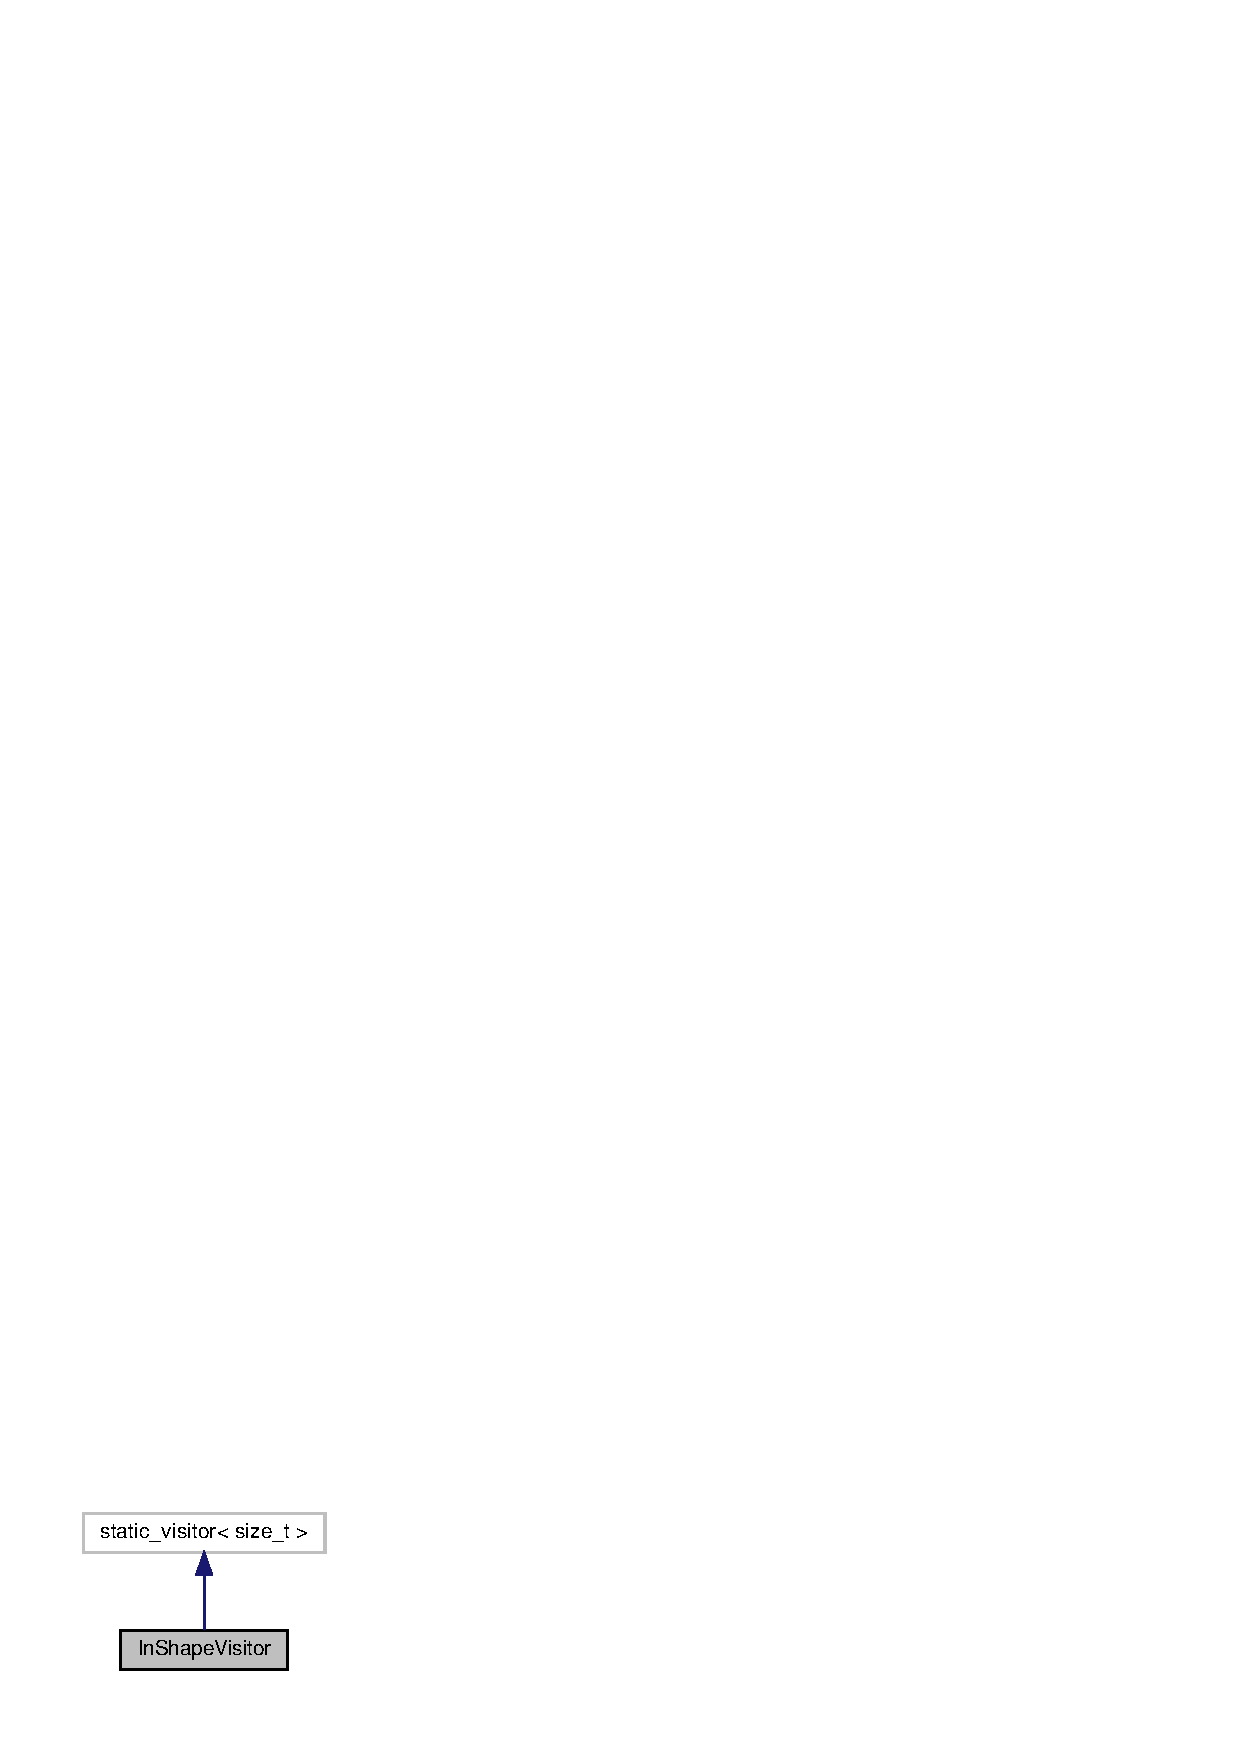
\includegraphics[width=160pt]{classmlpack_1_1ann_1_1InShapeVisitor__inherit__graph}
\end{center}
\end{figure}
\subsection*{Public Member Functions}
\begin{DoxyCompactItemize}
\item 
{\footnotesize template$<$typename Layer\+Type $>$ }\\size\+\_\+t \textbf{ operator()} (Layer\+Type $\ast$layer) const
\begin{DoxyCompactList}\small\item\em Return the input shape of layer. \end{DoxyCompactList}\item 
size\+\_\+t \textbf{ operator()} (\textbf{ More\+Types} layer) const
\end{DoxyCompactItemize}


\subsection{Detailed Description}
\doxyref{In\+Shape\+Visitor}{p.}{classmlpack_1_1ann_1_1InShapeVisitor} returns the input shape a Layer expects. 

Definition at line 29 of file input\+\_\+shape\+\_\+visitor.\+hpp.



\subsection{Member Function Documentation}
\mbox{\label{classmlpack_1_1ann_1_1InShapeVisitor_aeb8947a28d511a7a4ce42a1fc63f79ee}} 
\index{mlpack\+::ann\+::\+In\+Shape\+Visitor@{mlpack\+::ann\+::\+In\+Shape\+Visitor}!operator()@{operator()}}
\index{operator()@{operator()}!mlpack\+::ann\+::\+In\+Shape\+Visitor@{mlpack\+::ann\+::\+In\+Shape\+Visitor}}
\subsubsection{operator()()\hspace{0.1cm}{\footnotesize\ttfamily [1/2]}}
{\footnotesize\ttfamily size\+\_\+t operator() (\begin{DoxyParamCaption}\item[{Layer\+Type $\ast$}]{layer }\end{DoxyParamCaption}) const}



Return the input shape of layer. 

\mbox{\label{classmlpack_1_1ann_1_1InShapeVisitor_a19a2b78859e4e91b86170544dbd8ae09}} 
\index{mlpack\+::ann\+::\+In\+Shape\+Visitor@{mlpack\+::ann\+::\+In\+Shape\+Visitor}!operator()@{operator()}}
\index{operator()@{operator()}!mlpack\+::ann\+::\+In\+Shape\+Visitor@{mlpack\+::ann\+::\+In\+Shape\+Visitor}}
\subsubsection{operator()()\hspace{0.1cm}{\footnotesize\ttfamily [2/2]}}
{\footnotesize\ttfamily size\+\_\+t operator() (\begin{DoxyParamCaption}\item[{\textbf{ More\+Types}}]{layer }\end{DoxyParamCaption}) const}



The documentation for this class was generated from the following file\+:\begin{DoxyCompactItemize}
\item 
/home/aakash/mlpack/src/mlpack/methods/ann/visitor/\textbf{ input\+\_\+shape\+\_\+visitor.\+hpp}\end{DoxyCompactItemize}

\section{Inv\+Quad\+Function Class Reference}
\label{classmlpack_1_1ann_1_1InvQuadFunction}\index{Inv\+Quad\+Function@{Inv\+Quad\+Function}}


The Inverse Quadratic function, defined by.  


\subsection*{Static Public Member Functions}
\begin{DoxyCompactItemize}
\item 
static double \textbf{ Deriv} (const double y)
\begin{DoxyCompactList}\small\item\em Computes the first derivative of the Inverse Quadratic function. \end{DoxyCompactList}\item 
{\footnotesize template$<$typename Input\+Vec\+Type , typename Output\+Vec\+Type $>$ }\\static void \textbf{ Deriv} (const Input\+Vec\+Type \&x, Output\+Vec\+Type \&y)
\begin{DoxyCompactList}\small\item\em Computes the first derivatives of the Inverse Quadratic function. \end{DoxyCompactList}\item 
static double \textbf{ Fn} (const double x)
\begin{DoxyCompactList}\small\item\em Computes the Inverse Quadratic function. \end{DoxyCompactList}\item 
{\footnotesize template$<$typename Input\+Vec\+Type , typename Output\+Vec\+Type $>$ }\\static void \textbf{ Fn} (const Input\+Vec\+Type \&x, Output\+Vec\+Type \&y)
\begin{DoxyCompactList}\small\item\em Computes the Inverse Quadratic function. \end{DoxyCompactList}\end{DoxyCompactItemize}


\subsection{Detailed Description}
The Inverse Quadratic function, defined by. 

\begin{eqnarray*} f(x) = 1 / (1 + x^2) \\ f'(x) = -2 * x / (1 + x^2)^2 \\ \end{eqnarray*} 

Definition at line 28 of file inverse\+\_\+quadratic\+\_\+function.\+hpp.



\subsection{Member Function Documentation}
\mbox{\label{classmlpack_1_1ann_1_1InvQuadFunction_a163d34fd09f8edf457164f5033c635cf}} 
\index{mlpack\+::ann\+::\+Inv\+Quad\+Function@{mlpack\+::ann\+::\+Inv\+Quad\+Function}!Deriv@{Deriv}}
\index{Deriv@{Deriv}!mlpack\+::ann\+::\+Inv\+Quad\+Function@{mlpack\+::ann\+::\+Inv\+Quad\+Function}}
\subsubsection{Deriv()\hspace{0.1cm}{\footnotesize\ttfamily [1/2]}}
{\footnotesize\ttfamily static double Deriv (\begin{DoxyParamCaption}\item[{const double}]{y }\end{DoxyParamCaption})\hspace{0.3cm}{\ttfamily [inline]}, {\ttfamily [static]}}



Computes the first derivative of the Inverse Quadratic function. 


\begin{DoxyParams}{Parameters}
{\em y} & Input data. \\
\hline
\end{DoxyParams}
\begin{DoxyReturn}{Returns}
f\textquotesingle{}(x) 
\end{DoxyReturn}


Definition at line 60 of file inverse\+\_\+quadratic\+\_\+function.\+hpp.

\mbox{\label{classmlpack_1_1ann_1_1InvQuadFunction_a0ad035ec996acd7025807d0e9e082887}} 
\index{mlpack\+::ann\+::\+Inv\+Quad\+Function@{mlpack\+::ann\+::\+Inv\+Quad\+Function}!Deriv@{Deriv}}
\index{Deriv@{Deriv}!mlpack\+::ann\+::\+Inv\+Quad\+Function@{mlpack\+::ann\+::\+Inv\+Quad\+Function}}
\subsubsection{Deriv()\hspace{0.1cm}{\footnotesize\ttfamily [2/2]}}
{\footnotesize\ttfamily static void Deriv (\begin{DoxyParamCaption}\item[{const Input\+Vec\+Type \&}]{x,  }\item[{Output\+Vec\+Type \&}]{y }\end{DoxyParamCaption})\hspace{0.3cm}{\ttfamily [inline]}, {\ttfamily [static]}}



Computes the first derivatives of the Inverse Quadratic function. 


\begin{DoxyParams}{Parameters}
{\em y} & Input data. \\
\hline
{\em x} & The resulting derivatives. \\
\hline
\end{DoxyParams}


Definition at line 72 of file inverse\+\_\+quadratic\+\_\+function.\+hpp.

\mbox{\label{classmlpack_1_1ann_1_1InvQuadFunction_a11bd9a1195e6b107f9fee73643bc328b}} 
\index{mlpack\+::ann\+::\+Inv\+Quad\+Function@{mlpack\+::ann\+::\+Inv\+Quad\+Function}!Fn@{Fn}}
\index{Fn@{Fn}!mlpack\+::ann\+::\+Inv\+Quad\+Function@{mlpack\+::ann\+::\+Inv\+Quad\+Function}}
\subsubsection{Fn()\hspace{0.1cm}{\footnotesize\ttfamily [1/2]}}
{\footnotesize\ttfamily static double Fn (\begin{DoxyParamCaption}\item[{const double}]{x }\end{DoxyParamCaption})\hspace{0.3cm}{\ttfamily [inline]}, {\ttfamily [static]}}



Computes the Inverse Quadratic function. 


\begin{DoxyParams}{Parameters}
{\em x} & Input data. \\
\hline
\end{DoxyParams}
\begin{DoxyReturn}{Returns}
f(x). 
\end{DoxyReturn}


Definition at line 37 of file inverse\+\_\+quadratic\+\_\+function.\+hpp.

\mbox{\label{classmlpack_1_1ann_1_1InvQuadFunction_af6cf5da90eb6312e3e25c9b8bd9c3527}} 
\index{mlpack\+::ann\+::\+Inv\+Quad\+Function@{mlpack\+::ann\+::\+Inv\+Quad\+Function}!Fn@{Fn}}
\index{Fn@{Fn}!mlpack\+::ann\+::\+Inv\+Quad\+Function@{mlpack\+::ann\+::\+Inv\+Quad\+Function}}
\subsubsection{Fn()\hspace{0.1cm}{\footnotesize\ttfamily [2/2]}}
{\footnotesize\ttfamily static void Fn (\begin{DoxyParamCaption}\item[{const Input\+Vec\+Type \&}]{x,  }\item[{Output\+Vec\+Type \&}]{y }\end{DoxyParamCaption})\hspace{0.3cm}{\ttfamily [inline]}, {\ttfamily [static]}}



Computes the Inverse Quadratic function. 


\begin{DoxyParams}{Parameters}
{\em x} & Input data. \\
\hline
{\em y} & The resulting output activation. \\
\hline
\end{DoxyParams}


Definition at line 49 of file inverse\+\_\+quadratic\+\_\+function.\+hpp.



The documentation for this class was generated from the following file\+:\begin{DoxyCompactItemize}
\item 
/home/aakash/mlpack/src/mlpack/methods/ann/activation\+\_\+functions/\textbf{ inverse\+\_\+quadratic\+\_\+function.\+hpp}\end{DoxyCompactItemize}

\section{I\+S\+R\+LU$<$ Input\+Data\+Type, Output\+Data\+Type $>$ Class Template Reference}
\label{classmlpack_1_1ann_1_1ISRLU}\index{I\+S\+R\+L\+U$<$ Input\+Data\+Type, Output\+Data\+Type $>$@{I\+S\+R\+L\+U$<$ Input\+Data\+Type, Output\+Data\+Type $>$}}


The \doxyref{I\+S\+R\+LU}{p.}{classmlpack_1_1ann_1_1ISRLU} activation function, defined by.  


\subsection*{Public Member Functions}
\begin{DoxyCompactItemize}
\item 
\textbf{ I\+S\+R\+LU} (const double alpha=1.\+0)
\begin{DoxyCompactList}\small\item\em Create the \doxyref{I\+S\+R\+LU}{p.}{classmlpack_1_1ann_1_1ISRLU} object using the specified parameter. \end{DoxyCompactList}\item 
double const  \& \textbf{ Alpha} () const
\begin{DoxyCompactList}\small\item\em Get the non zero gradient. \end{DoxyCompactList}\item 
double \& \textbf{ Alpha} ()
\begin{DoxyCompactList}\small\item\em Modify the non zero gradient. \end{DoxyCompactList}\item 
{\footnotesize template$<$typename Data\+Type $>$ }\\void \textbf{ Backward} (const Data\+Type \&input, const Data\+Type \&gy, Data\+Type \&g)
\begin{DoxyCompactList}\small\item\em Ordinary feed backward pass of a neural network, calculating the function f(x) by propagating x backwards through f. \end{DoxyCompactList}\item 
Output\+Data\+Type const  \& \textbf{ Delta} () const
\begin{DoxyCompactList}\small\item\em Get the delta. \end{DoxyCompactList}\item 
Output\+Data\+Type \& \textbf{ Delta} ()
\begin{DoxyCompactList}\small\item\em Modify the delta. \end{DoxyCompactList}\item 
{\footnotesize template$<$typename Input\+Type , typename Output\+Type $>$ }\\void \textbf{ Forward} (const Input\+Type \&input, Output\+Type \&output)
\begin{DoxyCompactList}\small\item\em Ordinary feed forward pass of a neural network, evaluating the function f(x) by propagating the activity forward through f. \end{DoxyCompactList}\item 
Output\+Data\+Type const  \& \textbf{ Output\+Parameter} () const
\begin{DoxyCompactList}\small\item\em Get the output parameter. \end{DoxyCompactList}\item 
Output\+Data\+Type \& \textbf{ Output\+Parameter} ()
\begin{DoxyCompactList}\small\item\em Modify the output parameter. \end{DoxyCompactList}\item 
{\footnotesize template$<$typename Archive $>$ }\\void \textbf{ serialize} (Archive \&ar, const uint32\+\_\+t)
\begin{DoxyCompactList}\small\item\em Serialize the layer. \end{DoxyCompactList}\item 
size\+\_\+t \textbf{ Weight\+Size} ()
\begin{DoxyCompactList}\small\item\em Get size of weights. \end{DoxyCompactList}\end{DoxyCompactItemize}


\subsection{Detailed Description}
\subsubsection*{template$<$typename Input\+Data\+Type = arma\+::mat, typename Output\+Data\+Type = arma\+::mat$>$\newline
class mlpack\+::ann\+::\+I\+S\+R\+L\+U$<$ Input\+Data\+Type, Output\+Data\+Type $>$}

The \doxyref{I\+S\+R\+LU}{p.}{classmlpack_1_1ann_1_1ISRLU} activation function, defined by. 

\begin{eqnarray*} f(x) &=& \left\{ \begin{array}{lr} x & : x \ge 0 \\ x(\frac{1}{1 + \alpha x^2}) & : x < 0 \end{array} \right. \\ f'(x) &=& \left\{ \begin{array}{lr} x & : 1 \ge 0 \\ (\frac{1}{1 + \alpha x^2})^3 & : x < 0 \end{array} \right. \end{eqnarray*}


\begin{DoxyTemplParams}{Template Parameters}
{\em Input\+Data\+Type} & Type of the input data (arma\+::colvec, arma\+::mat, arma\+::sp\+\_\+mat or arma\+::cube). \\
\hline
{\em Output\+Data\+Type} & Type of the output data (arma\+::colvec, arma\+::mat, arma\+::sp\+\_\+mat or arma\+::cube). \\
\hline
\end{DoxyTemplParams}


Definition at line 60 of file isrlu.\+hpp.



\subsection{Constructor \& Destructor Documentation}
\mbox{\label{classmlpack_1_1ann_1_1ISRLU_a873c05cfe8dcf6f0afabac067d669476}} 
\index{mlpack\+::ann\+::\+I\+S\+R\+LU@{mlpack\+::ann\+::\+I\+S\+R\+LU}!I\+S\+R\+LU@{I\+S\+R\+LU}}
\index{I\+S\+R\+LU@{I\+S\+R\+LU}!mlpack\+::ann\+::\+I\+S\+R\+LU@{mlpack\+::ann\+::\+I\+S\+R\+LU}}
\subsubsection{I\+S\+R\+L\+U()}
{\footnotesize\ttfamily \textbf{ I\+S\+R\+LU} (\begin{DoxyParamCaption}\item[{const double}]{alpha = {\ttfamily 1.0} }\end{DoxyParamCaption})}



Create the \doxyref{I\+S\+R\+LU}{p.}{classmlpack_1_1ann_1_1ISRLU} object using the specified parameter. 


\begin{DoxyParams}{Parameters}
{\em alpha} & Scale parameter controls the value to which an \doxyref{I\+S\+R\+LU}{p.}{classmlpack_1_1ann_1_1ISRLU} saturates for negative inputs. \\
\hline
\end{DoxyParams}


\subsection{Member Function Documentation}
\mbox{\label{classmlpack_1_1ann_1_1ISRLU_a21679485637bdec3078ec74d71572980}} 
\index{mlpack\+::ann\+::\+I\+S\+R\+LU@{mlpack\+::ann\+::\+I\+S\+R\+LU}!Alpha@{Alpha}}
\index{Alpha@{Alpha}!mlpack\+::ann\+::\+I\+S\+R\+LU@{mlpack\+::ann\+::\+I\+S\+R\+LU}}
\subsubsection{Alpha()\hspace{0.1cm}{\footnotesize\ttfamily [1/2]}}
{\footnotesize\ttfamily double const\& Alpha (\begin{DoxyParamCaption}{ }\end{DoxyParamCaption}) const\hspace{0.3cm}{\ttfamily [inline]}}



Get the non zero gradient. 



Definition at line 104 of file isrlu.\+hpp.

\mbox{\label{classmlpack_1_1ann_1_1ISRLU_acbb0e4747a3a307bee88bad71e5eeaf1}} 
\index{mlpack\+::ann\+::\+I\+S\+R\+LU@{mlpack\+::ann\+::\+I\+S\+R\+LU}!Alpha@{Alpha}}
\index{Alpha@{Alpha}!mlpack\+::ann\+::\+I\+S\+R\+LU@{mlpack\+::ann\+::\+I\+S\+R\+LU}}
\subsubsection{Alpha()\hspace{0.1cm}{\footnotesize\ttfamily [2/2]}}
{\footnotesize\ttfamily double\& Alpha (\begin{DoxyParamCaption}{ }\end{DoxyParamCaption})\hspace{0.3cm}{\ttfamily [inline]}}



Modify the non zero gradient. 



Definition at line 106 of file isrlu.\+hpp.

\mbox{\label{classmlpack_1_1ann_1_1ISRLU_aef8c56f1f8624bd006afec8b3bcda9d6}} 
\index{mlpack\+::ann\+::\+I\+S\+R\+LU@{mlpack\+::ann\+::\+I\+S\+R\+LU}!Backward@{Backward}}
\index{Backward@{Backward}!mlpack\+::ann\+::\+I\+S\+R\+LU@{mlpack\+::ann\+::\+I\+S\+R\+LU}}
\subsubsection{Backward()}
{\footnotesize\ttfamily void Backward (\begin{DoxyParamCaption}\item[{const Data\+Type \&}]{input,  }\item[{const Data\+Type \&}]{gy,  }\item[{Data\+Type \&}]{g }\end{DoxyParamCaption})}



Ordinary feed backward pass of a neural network, calculating the function f(x) by propagating x backwards through f. 

Using the results from the feed forward pass.


\begin{DoxyParams}{Parameters}
{\em input} & The propagated input activation f(x). \\
\hline
{\em gy} & The backpropagated error. \\
\hline
{\em g} & The calculated gradient. \\
\hline
\end{DoxyParams}
\mbox{\label{classmlpack_1_1ann_1_1ISRLU_a797f7edb44dd081e5e2b3cc316eef6bd}} 
\index{mlpack\+::ann\+::\+I\+S\+R\+LU@{mlpack\+::ann\+::\+I\+S\+R\+LU}!Delta@{Delta}}
\index{Delta@{Delta}!mlpack\+::ann\+::\+I\+S\+R\+LU@{mlpack\+::ann\+::\+I\+S\+R\+LU}}
\subsubsection{Delta()\hspace{0.1cm}{\footnotesize\ttfamily [1/2]}}
{\footnotesize\ttfamily Output\+Data\+Type const\& Delta (\begin{DoxyParamCaption}{ }\end{DoxyParamCaption}) const\hspace{0.3cm}{\ttfamily [inline]}}



Get the delta. 



Definition at line 99 of file isrlu.\+hpp.

\mbox{\label{classmlpack_1_1ann_1_1ISRLU_ad6601342d560219ce951d554e69e5e87}} 
\index{mlpack\+::ann\+::\+I\+S\+R\+LU@{mlpack\+::ann\+::\+I\+S\+R\+LU}!Delta@{Delta}}
\index{Delta@{Delta}!mlpack\+::ann\+::\+I\+S\+R\+LU@{mlpack\+::ann\+::\+I\+S\+R\+LU}}
\subsubsection{Delta()\hspace{0.1cm}{\footnotesize\ttfamily [2/2]}}
{\footnotesize\ttfamily Output\+Data\+Type\& Delta (\begin{DoxyParamCaption}{ }\end{DoxyParamCaption})\hspace{0.3cm}{\ttfamily [inline]}}



Modify the delta. 



Definition at line 101 of file isrlu.\+hpp.

\mbox{\label{classmlpack_1_1ann_1_1ISRLU_a09440df0a90bdcc766e56e097d91205b}} 
\index{mlpack\+::ann\+::\+I\+S\+R\+LU@{mlpack\+::ann\+::\+I\+S\+R\+LU}!Forward@{Forward}}
\index{Forward@{Forward}!mlpack\+::ann\+::\+I\+S\+R\+LU@{mlpack\+::ann\+::\+I\+S\+R\+LU}}
\subsubsection{Forward()}
{\footnotesize\ttfamily void Forward (\begin{DoxyParamCaption}\item[{const Input\+Type \&}]{input,  }\item[{Output\+Type \&}]{output }\end{DoxyParamCaption})}



Ordinary feed forward pass of a neural network, evaluating the function f(x) by propagating the activity forward through f. 


\begin{DoxyParams}{Parameters}
{\em input} & Input data used for evaluating the specified function. \\
\hline
{\em output} & Resulting output activation. \\
\hline
\end{DoxyParams}
\mbox{\label{classmlpack_1_1ann_1_1ISRLU_a0ee21c2a36e5abad1e7a9d5dd00849f9}} 
\index{mlpack\+::ann\+::\+I\+S\+R\+LU@{mlpack\+::ann\+::\+I\+S\+R\+LU}!Output\+Parameter@{Output\+Parameter}}
\index{Output\+Parameter@{Output\+Parameter}!mlpack\+::ann\+::\+I\+S\+R\+LU@{mlpack\+::ann\+::\+I\+S\+R\+LU}}
\subsubsection{Output\+Parameter()\hspace{0.1cm}{\footnotesize\ttfamily [1/2]}}
{\footnotesize\ttfamily Output\+Data\+Type const\& Output\+Parameter (\begin{DoxyParamCaption}{ }\end{DoxyParamCaption}) const\hspace{0.3cm}{\ttfamily [inline]}}



Get the output parameter. 



Definition at line 94 of file isrlu.\+hpp.

\mbox{\label{classmlpack_1_1ann_1_1ISRLU_a21d5f745f02c709625a4ee0907f004a5}} 
\index{mlpack\+::ann\+::\+I\+S\+R\+LU@{mlpack\+::ann\+::\+I\+S\+R\+LU}!Output\+Parameter@{Output\+Parameter}}
\index{Output\+Parameter@{Output\+Parameter}!mlpack\+::ann\+::\+I\+S\+R\+LU@{mlpack\+::ann\+::\+I\+S\+R\+LU}}
\subsubsection{Output\+Parameter()\hspace{0.1cm}{\footnotesize\ttfamily [2/2]}}
{\footnotesize\ttfamily Output\+Data\+Type\& Output\+Parameter (\begin{DoxyParamCaption}{ }\end{DoxyParamCaption})\hspace{0.3cm}{\ttfamily [inline]}}



Modify the output parameter. 



Definition at line 96 of file isrlu.\+hpp.

\mbox{\label{classmlpack_1_1ann_1_1ISRLU_a65cba07328997659bec80b9879b15a51}} 
\index{mlpack\+::ann\+::\+I\+S\+R\+LU@{mlpack\+::ann\+::\+I\+S\+R\+LU}!serialize@{serialize}}
\index{serialize@{serialize}!mlpack\+::ann\+::\+I\+S\+R\+LU@{mlpack\+::ann\+::\+I\+S\+R\+LU}}
\subsubsection{serialize()}
{\footnotesize\ttfamily void serialize (\begin{DoxyParamCaption}\item[{Archive \&}]{ar,  }\item[{const uint32\+\_\+t}]{ }\end{DoxyParamCaption})}



Serialize the layer. 



Referenced by I\+S\+R\+L\+U$<$ Input\+Data\+Type, Output\+Data\+Type $>$\+::\+Weight\+Size().

\mbox{\label{classmlpack_1_1ann_1_1ISRLU_a2b2aec754d2ebd0decd527a4ac196b90}} 
\index{mlpack\+::ann\+::\+I\+S\+R\+LU@{mlpack\+::ann\+::\+I\+S\+R\+LU}!Weight\+Size@{Weight\+Size}}
\index{Weight\+Size@{Weight\+Size}!mlpack\+::ann\+::\+I\+S\+R\+LU@{mlpack\+::ann\+::\+I\+S\+R\+LU}}
\subsubsection{Weight\+Size()}
{\footnotesize\ttfamily size\+\_\+t Weight\+Size (\begin{DoxyParamCaption}{ }\end{DoxyParamCaption})\hspace{0.3cm}{\ttfamily [inline]}}



Get size of weights. 



Definition at line 109 of file isrlu.\+hpp.



References I\+S\+R\+L\+U$<$ Input\+Data\+Type, Output\+Data\+Type $>$\+::serialize().



The documentation for this class was generated from the following file\+:\begin{DoxyCompactItemize}
\item 
/home/aakash/mlpack/src/mlpack/methods/ann/layer/\textbf{ isrlu.\+hpp}\end{DoxyCompactItemize}

\section{Join$<$ Input\+Data\+Type, Output\+Data\+Type $>$ Class Template Reference}
\label{classmlpack_1_1ann_1_1Join}\index{Join$<$ Input\+Data\+Type, Output\+Data\+Type $>$@{Join$<$ Input\+Data\+Type, Output\+Data\+Type $>$}}


Implementation of the \doxyref{Join}{p.}{classmlpack_1_1ann_1_1Join} module class.  


\subsection*{Public Member Functions}
\begin{DoxyCompactItemize}
\item 
\textbf{ Join} ()
\begin{DoxyCompactList}\small\item\em Create the \doxyref{Join}{p.}{classmlpack_1_1ann_1_1Join} object. \end{DoxyCompactList}\item 
{\footnotesize template$<$typename eT $>$ }\\void \textbf{ Backward} (const arma\+::\+Mat$<$ eT $>$ \&, const arma\+::\+Mat$<$ eT $>$ \&gy, arma\+::\+Mat$<$ eT $>$ \&g)
\begin{DoxyCompactList}\small\item\em Ordinary feed backward pass of a neural network, calculating the function f(x) by propagating x backwards trough f. \end{DoxyCompactList}\item 
Output\+Data\+Type const  \& \textbf{ Delta} () const
\begin{DoxyCompactList}\small\item\em Get the delta. \end{DoxyCompactList}\item 
Output\+Data\+Type \& \textbf{ Delta} ()
\begin{DoxyCompactList}\small\item\em Modify the delta. \end{DoxyCompactList}\item 
{\footnotesize template$<$typename Input\+Type , typename Output\+Type $>$ }\\void \textbf{ Forward} (const Input\+Type \&input, Output\+Type \&output)
\begin{DoxyCompactList}\small\item\em Ordinary feed forward pass of a neural network, evaluating the function f(x) by propagating the activity forward through f. \end{DoxyCompactList}\item 
Output\+Data\+Type const  \& \textbf{ Output\+Parameter} () const
\begin{DoxyCompactList}\small\item\em Get the output parameter. \end{DoxyCompactList}\item 
Output\+Data\+Type \& \textbf{ Output\+Parameter} ()
\begin{DoxyCompactList}\small\item\em Modify the output parameter. \end{DoxyCompactList}\item 
{\footnotesize template$<$typename Archive $>$ }\\void \textbf{ serialize} (Archive \&ar, const uint32\+\_\+t)
\begin{DoxyCompactList}\small\item\em Serialize the layer. \end{DoxyCompactList}\end{DoxyCompactItemize}


\subsection{Detailed Description}
\subsubsection*{template$<$typename Input\+Data\+Type = arma\+::mat, typename Output\+Data\+Type = arma\+::mat$>$\newline
class mlpack\+::ann\+::\+Join$<$ Input\+Data\+Type, Output\+Data\+Type $>$}

Implementation of the \doxyref{Join}{p.}{classmlpack_1_1ann_1_1Join} module class. 

The \doxyref{Join}{p.}{classmlpack_1_1ann_1_1Join} class accumulates the output of various modules.


\begin{DoxyTemplParams}{Template Parameters}
{\em Input\+Data\+Type} & Type of the input data (arma\+::colvec, arma\+::mat, arma\+::sp\+\_\+mat or arma\+::cube). \\
\hline
{\em Output\+Data\+Type} & Type of the output data (arma\+::colvec, arma\+::mat, arma\+::sp\+\_\+mat or arma\+::cube). \\
\hline
\end{DoxyTemplParams}


Definition at line 33 of file join.\+hpp.



\subsection{Constructor \& Destructor Documentation}
\mbox{\label{classmlpack_1_1ann_1_1Join_af7da1cd77b478e2dc66b37eeeb35aa67}} 
\index{mlpack\+::ann\+::\+Join@{mlpack\+::ann\+::\+Join}!Join@{Join}}
\index{Join@{Join}!mlpack\+::ann\+::\+Join@{mlpack\+::ann\+::\+Join}}
\subsubsection{Join()}
{\footnotesize\ttfamily \textbf{ Join} (\begin{DoxyParamCaption}{ }\end{DoxyParamCaption})}



Create the \doxyref{Join}{p.}{classmlpack_1_1ann_1_1Join} object. 



\subsection{Member Function Documentation}
\mbox{\label{classmlpack_1_1ann_1_1Join_ad9ad1a3bdb0f3fff5c839ed155e4bbf8}} 
\index{mlpack\+::ann\+::\+Join@{mlpack\+::ann\+::\+Join}!Backward@{Backward}}
\index{Backward@{Backward}!mlpack\+::ann\+::\+Join@{mlpack\+::ann\+::\+Join}}
\subsubsection{Backward()}
{\footnotesize\ttfamily void Backward (\begin{DoxyParamCaption}\item[{const arma\+::\+Mat$<$ eT $>$ \&}]{,  }\item[{const arma\+::\+Mat$<$ eT $>$ \&}]{gy,  }\item[{arma\+::\+Mat$<$ eT $>$ \&}]{g }\end{DoxyParamCaption})}



Ordinary feed backward pass of a neural network, calculating the function f(x) by propagating x backwards trough f. 

Using the results from the feed forward pass.


\begin{DoxyParams}{Parameters}
{\em $\ast$} & (input) The propagated input activation. \\
\hline
{\em gy} & The backpropagated error. \\
\hline
{\em g} & The calculated gradient. \\
\hline
\end{DoxyParams}
\mbox{\label{classmlpack_1_1ann_1_1Join_a797f7edb44dd081e5e2b3cc316eef6bd}} 
\index{mlpack\+::ann\+::\+Join@{mlpack\+::ann\+::\+Join}!Delta@{Delta}}
\index{Delta@{Delta}!mlpack\+::ann\+::\+Join@{mlpack\+::ann\+::\+Join}}
\subsubsection{Delta()\hspace{0.1cm}{\footnotesize\ttfamily [1/2]}}
{\footnotesize\ttfamily Output\+Data\+Type const\& Delta (\begin{DoxyParamCaption}{ }\end{DoxyParamCaption}) const\hspace{0.3cm}{\ttfamily [inline]}}



Get the delta. 



Definition at line 69 of file join.\+hpp.

\mbox{\label{classmlpack_1_1ann_1_1Join_ad6601342d560219ce951d554e69e5e87}} 
\index{mlpack\+::ann\+::\+Join@{mlpack\+::ann\+::\+Join}!Delta@{Delta}}
\index{Delta@{Delta}!mlpack\+::ann\+::\+Join@{mlpack\+::ann\+::\+Join}}
\subsubsection{Delta()\hspace{0.1cm}{\footnotesize\ttfamily [2/2]}}
{\footnotesize\ttfamily Output\+Data\+Type\& Delta (\begin{DoxyParamCaption}{ }\end{DoxyParamCaption})\hspace{0.3cm}{\ttfamily [inline]}}



Modify the delta. 



Definition at line 71 of file join.\+hpp.



References Join$<$ Input\+Data\+Type, Output\+Data\+Type $>$\+::serialize().

\mbox{\label{classmlpack_1_1ann_1_1Join_a09440df0a90bdcc766e56e097d91205b}} 
\index{mlpack\+::ann\+::\+Join@{mlpack\+::ann\+::\+Join}!Forward@{Forward}}
\index{Forward@{Forward}!mlpack\+::ann\+::\+Join@{mlpack\+::ann\+::\+Join}}
\subsubsection{Forward()}
{\footnotesize\ttfamily void Forward (\begin{DoxyParamCaption}\item[{const Input\+Type \&}]{input,  }\item[{Output\+Type \&}]{output }\end{DoxyParamCaption})}



Ordinary feed forward pass of a neural network, evaluating the function f(x) by propagating the activity forward through f. 


\begin{DoxyParams}{Parameters}
{\em input} & Input data used for evaluating the specified function. \\
\hline
{\em output} & Resulting output activation. \\
\hline
\end{DoxyParams}
\mbox{\label{classmlpack_1_1ann_1_1Join_a0ee21c2a36e5abad1e7a9d5dd00849f9}} 
\index{mlpack\+::ann\+::\+Join@{mlpack\+::ann\+::\+Join}!Output\+Parameter@{Output\+Parameter}}
\index{Output\+Parameter@{Output\+Parameter}!mlpack\+::ann\+::\+Join@{mlpack\+::ann\+::\+Join}}
\subsubsection{Output\+Parameter()\hspace{0.1cm}{\footnotesize\ttfamily [1/2]}}
{\footnotesize\ttfamily Output\+Data\+Type const\& Output\+Parameter (\begin{DoxyParamCaption}{ }\end{DoxyParamCaption}) const\hspace{0.3cm}{\ttfamily [inline]}}



Get the output parameter. 



Definition at line 64 of file join.\+hpp.

\mbox{\label{classmlpack_1_1ann_1_1Join_a21d5f745f02c709625a4ee0907f004a5}} 
\index{mlpack\+::ann\+::\+Join@{mlpack\+::ann\+::\+Join}!Output\+Parameter@{Output\+Parameter}}
\index{Output\+Parameter@{Output\+Parameter}!mlpack\+::ann\+::\+Join@{mlpack\+::ann\+::\+Join}}
\subsubsection{Output\+Parameter()\hspace{0.1cm}{\footnotesize\ttfamily [2/2]}}
{\footnotesize\ttfamily Output\+Data\+Type\& Output\+Parameter (\begin{DoxyParamCaption}{ }\end{DoxyParamCaption})\hspace{0.3cm}{\ttfamily [inline]}}



Modify the output parameter. 



Definition at line 66 of file join.\+hpp.

\mbox{\label{classmlpack_1_1ann_1_1Join_a65cba07328997659bec80b9879b15a51}} 
\index{mlpack\+::ann\+::\+Join@{mlpack\+::ann\+::\+Join}!serialize@{serialize}}
\index{serialize@{serialize}!mlpack\+::ann\+::\+Join@{mlpack\+::ann\+::\+Join}}
\subsubsection{serialize()}
{\footnotesize\ttfamily void serialize (\begin{DoxyParamCaption}\item[{Archive \&}]{ar,  }\item[{const uint32\+\_\+t}]{ }\end{DoxyParamCaption})}



Serialize the layer. 



Referenced by Join$<$ Input\+Data\+Type, Output\+Data\+Type $>$\+::\+Delta().



The documentation for this class was generated from the following file\+:\begin{DoxyCompactItemize}
\item 
/home/aakash/mlpack/src/mlpack/methods/ann/layer/\textbf{ join.\+hpp}\end{DoxyCompactItemize}

\section{Kathirvalavakumar\+Subavathi\+Initialization Class Reference}
\label{classmlpack_1_1ann_1_1KathirvalavakumarSubavathiInitialization}\index{Kathirvalavakumar\+Subavathi\+Initialization@{Kathirvalavakumar\+Subavathi\+Initialization}}


This class is used to initialize the weight matrix with the method proposed by T.  


\subsection*{Public Member Functions}
\begin{DoxyCompactItemize}
\item 
{\footnotesize template$<$typename eT $>$ }\\\textbf{ Kathirvalavakumar\+Subavathi\+Initialization} (const arma\+::\+Mat$<$ eT $>$ \&data, const double s)
\begin{DoxyCompactList}\small\item\em Initialize the random initialization rule with the given values. \end{DoxyCompactList}\item 
{\footnotesize template$<$typename eT $>$ }\\void \textbf{ Initialize} (arma\+::\+Mat$<$ eT $>$ \&W, const size\+\_\+t rows, const size\+\_\+t cols)
\begin{DoxyCompactList}\small\item\em Initialize the elements of the specified weight matrix with the Kathirvalavakumar-\/\+Subavathi method. \end{DoxyCompactList}\item 
{\footnotesize template$<$typename eT $>$ }\\void \textbf{ Initialize} (arma\+::\+Mat$<$ eT $>$ \&W)
\begin{DoxyCompactList}\small\item\em Initialize the elements of the specified weight matrix with the Kathirvalavakumar-\/\+Subavathi method. \end{DoxyCompactList}\item 
{\footnotesize template$<$typename eT $>$ }\\void \textbf{ Initialize} (arma\+::\+Cube$<$ eT $>$ \&W, const size\+\_\+t rows, const size\+\_\+t cols, const size\+\_\+t slices)
\begin{DoxyCompactList}\small\item\em Initialize the elements of the specified weight 3rd order tensor with the Kathirvalavakumar-\/\+Subavathi method. \end{DoxyCompactList}\item 
{\footnotesize template$<$typename eT $>$ }\\void \textbf{ Initialize} (arma\+::\+Cube$<$ eT $>$ \&W)
\begin{DoxyCompactList}\small\item\em Initialize the elements of the specified weight 3rd order tensor with the Kathirvalavakumar-\/\+Subavathi method. \end{DoxyCompactList}\end{DoxyCompactItemize}


\subsection{Detailed Description}
This class is used to initialize the weight matrix with the method proposed by T. 

Kathirvalavakumar and S. Subavathi. The method is based on sensitivity analysis using using cauchy’s inequality. The method is defined by

\begin{eqnarray*} \overline{s} &=& f^{-1}(\overline{t}) \\ \Theta^{1}_{p} &\le& \overline{s} \sqrt{\frac{3}{I \sum_{i = 1}^{I} (x_{ip}^2)}} \\ \Theta^1 &=& min(\Theta_{p}^{1}); p=1,2,..,P \\ -\Theta^{1} \le w_{i}^{1} &\le& \Theta^{1} \end{eqnarray*}

where I is the number of inputs including the bias, p refers the pattern considered in training, f is the transfer function and \textbackslash{}=\{s\} is the active region in which the derivative of the activation function is greater than 4\% of the maximum derivatives. 

Definition at line 60 of file kathirvalavakumar\+\_\+subavathi\+\_\+init.\+hpp.



\subsection{Constructor \& Destructor Documentation}
\mbox{\label{classmlpack_1_1ann_1_1KathirvalavakumarSubavathiInitialization_aaf0e7a11a0a428552525a83382e45148}} 
\index{mlpack\+::ann\+::\+Kathirvalavakumar\+Subavathi\+Initialization@{mlpack\+::ann\+::\+Kathirvalavakumar\+Subavathi\+Initialization}!Kathirvalavakumar\+Subavathi\+Initialization@{Kathirvalavakumar\+Subavathi\+Initialization}}
\index{Kathirvalavakumar\+Subavathi\+Initialization@{Kathirvalavakumar\+Subavathi\+Initialization}!mlpack\+::ann\+::\+Kathirvalavakumar\+Subavathi\+Initialization@{mlpack\+::ann\+::\+Kathirvalavakumar\+Subavathi\+Initialization}}
\subsubsection{Kathirvalavakumar\+Subavathi\+Initialization()}
{\footnotesize\ttfamily \textbf{ Kathirvalavakumar\+Subavathi\+Initialization} (\begin{DoxyParamCaption}\item[{const arma\+::\+Mat$<$ eT $>$ \&}]{data,  }\item[{const double}]{s }\end{DoxyParamCaption})\hspace{0.3cm}{\ttfamily [inline]}}



Initialize the random initialization rule with the given values. 


\begin{DoxyParams}{Parameters}
{\em data} & The input patterns. \\
\hline
{\em s} & Parameter that defines the active region. \\
\hline
\end{DoxyParams}


Definition at line 70 of file kathirvalavakumar\+\_\+subavathi\+\_\+init.\+hpp.



\subsection{Member Function Documentation}
\mbox{\label{classmlpack_1_1ann_1_1KathirvalavakumarSubavathiInitialization_a5cfe472251a41fffd45b170bb0d3c1bd}} 
\index{mlpack\+::ann\+::\+Kathirvalavakumar\+Subavathi\+Initialization@{mlpack\+::ann\+::\+Kathirvalavakumar\+Subavathi\+Initialization}!Initialize@{Initialize}}
\index{Initialize@{Initialize}!mlpack\+::ann\+::\+Kathirvalavakumar\+Subavathi\+Initialization@{mlpack\+::ann\+::\+Kathirvalavakumar\+Subavathi\+Initialization}}
\subsubsection{Initialize()\hspace{0.1cm}{\footnotesize\ttfamily [1/4]}}
{\footnotesize\ttfamily void Initialize (\begin{DoxyParamCaption}\item[{arma\+::\+Mat$<$ eT $>$ \&}]{W,  }\item[{const size\+\_\+t}]{rows,  }\item[{const size\+\_\+t}]{cols }\end{DoxyParamCaption})\hspace{0.3cm}{\ttfamily [inline]}}



Initialize the elements of the specified weight matrix with the Kathirvalavakumar-\/\+Subavathi method. 


\begin{DoxyParams}{Parameters}
{\em W} & Weight matrix to initialize. \\
\hline
{\em rows} & Number of rows. \\
\hline
{\em cols} & Number of columns. \\
\hline
\end{DoxyParams}


Definition at line 85 of file kathirvalavakumar\+\_\+subavathi\+\_\+init.\+hpp.



References Random\+Initialization\+::\+Initialize().



Referenced by Kathirvalavakumar\+Subavathi\+Initialization\+::\+Initialize().

\mbox{\label{classmlpack_1_1ann_1_1KathirvalavakumarSubavathiInitialization_af2d770912321b8b9ca7b03ab98f735c0}} 
\index{mlpack\+::ann\+::\+Kathirvalavakumar\+Subavathi\+Initialization@{mlpack\+::ann\+::\+Kathirvalavakumar\+Subavathi\+Initialization}!Initialize@{Initialize}}
\index{Initialize@{Initialize}!mlpack\+::ann\+::\+Kathirvalavakumar\+Subavathi\+Initialization@{mlpack\+::ann\+::\+Kathirvalavakumar\+Subavathi\+Initialization}}
\subsubsection{Initialize()\hspace{0.1cm}{\footnotesize\ttfamily [2/4]}}
{\footnotesize\ttfamily void Initialize (\begin{DoxyParamCaption}\item[{arma\+::\+Mat$<$ eT $>$ \&}]{W }\end{DoxyParamCaption})\hspace{0.3cm}{\ttfamily [inline]}}



Initialize the elements of the specified weight matrix with the Kathirvalavakumar-\/\+Subavathi method. 


\begin{DoxyParams}{Parameters}
{\em W} & Weight matrix to initialize. \\
\hline
\end{DoxyParams}


Definition at line 100 of file kathirvalavakumar\+\_\+subavathi\+\_\+init.\+hpp.



References Random\+Initialization\+::\+Initialize().

\mbox{\label{classmlpack_1_1ann_1_1KathirvalavakumarSubavathiInitialization_a40a2b6466bdba0f6aab4eb92b6e65934}} 
\index{mlpack\+::ann\+::\+Kathirvalavakumar\+Subavathi\+Initialization@{mlpack\+::ann\+::\+Kathirvalavakumar\+Subavathi\+Initialization}!Initialize@{Initialize}}
\index{Initialize@{Initialize}!mlpack\+::ann\+::\+Kathirvalavakumar\+Subavathi\+Initialization@{mlpack\+::ann\+::\+Kathirvalavakumar\+Subavathi\+Initialization}}
\subsubsection{Initialize()\hspace{0.1cm}{\footnotesize\ttfamily [3/4]}}
{\footnotesize\ttfamily void Initialize (\begin{DoxyParamCaption}\item[{arma\+::\+Cube$<$ eT $>$ \&}]{W,  }\item[{const size\+\_\+t}]{rows,  }\item[{const size\+\_\+t}]{cols,  }\item[{const size\+\_\+t}]{slices }\end{DoxyParamCaption})\hspace{0.3cm}{\ttfamily [inline]}}



Initialize the elements of the specified weight 3rd order tensor with the Kathirvalavakumar-\/\+Subavathi method. 


\begin{DoxyParams}{Parameters}
{\em W} & Weight matrix to initialize. \\
\hline
{\em rows} & Number of rows. \\
\hline
{\em cols} & Number of columns. \\
\hline
{\em slices} & Number of slices \\
\hline
\end{DoxyParams}


Definition at line 118 of file kathirvalavakumar\+\_\+subavathi\+\_\+init.\+hpp.



References Kathirvalavakumar\+Subavathi\+Initialization\+::\+Initialize().

\mbox{\label{classmlpack_1_1ann_1_1KathirvalavakumarSubavathiInitialization_ae2f3e6d570824a160b687ff9f734f83c}} 
\index{mlpack\+::ann\+::\+Kathirvalavakumar\+Subavathi\+Initialization@{mlpack\+::ann\+::\+Kathirvalavakumar\+Subavathi\+Initialization}!Initialize@{Initialize}}
\index{Initialize@{Initialize}!mlpack\+::ann\+::\+Kathirvalavakumar\+Subavathi\+Initialization@{mlpack\+::ann\+::\+Kathirvalavakumar\+Subavathi\+Initialization}}
\subsubsection{Initialize()\hspace{0.1cm}{\footnotesize\ttfamily [4/4]}}
{\footnotesize\ttfamily void Initialize (\begin{DoxyParamCaption}\item[{arma\+::\+Cube$<$ eT $>$ \&}]{W }\end{DoxyParamCaption})\hspace{0.3cm}{\ttfamily [inline]}}



Initialize the elements of the specified weight 3rd order tensor with the Kathirvalavakumar-\/\+Subavathi method. 


\begin{DoxyParams}{Parameters}
{\em W} & Weight matrix to initialize. \\
\hline
\end{DoxyParams}


Definition at line 137 of file kathirvalavakumar\+\_\+subavathi\+\_\+init.\+hpp.



References Kathirvalavakumar\+Subavathi\+Initialization\+::\+Initialize().



The documentation for this class was generated from the following file\+:\begin{DoxyCompactItemize}
\item 
/home/aakash/mlpack/src/mlpack/methods/ann/init\+\_\+rules/\textbf{ kathirvalavakumar\+\_\+subavathi\+\_\+init.\+hpp}\end{DoxyCompactItemize}

\section{K\+L\+Divergence$<$ Input\+Data\+Type, Output\+Data\+Type $>$ Class Template Reference}
\label{classmlpack_1_1ann_1_1KLDivergence}\index{K\+L\+Divergence$<$ Input\+Data\+Type, Output\+Data\+Type $>$@{K\+L\+Divergence$<$ Input\+Data\+Type, Output\+Data\+Type $>$}}


The Kullback–\+Leibler divergence is often used for continuous distributions (direct regression).  


\subsection*{Public Member Functions}
\begin{DoxyCompactItemize}
\item 
\textbf{ K\+L\+Divergence} (const bool take\+Mean=false)
\begin{DoxyCompactList}\small\item\em Create the Kullback–\+Leibler Divergence object with the specified parameters. \end{DoxyCompactList}\item 
{\footnotesize template$<$typename Prediction\+Type , typename Target\+Type , typename Loss\+Type $>$ }\\void \textbf{ Backward} (const Prediction\+Type \&prediction, const Target\+Type \&target, Loss\+Type \&loss)
\begin{DoxyCompactList}\small\item\em Ordinary feed backward pass of a neural network. \end{DoxyCompactList}\item 
{\footnotesize template$<$typename Prediction\+Type , typename Target\+Type $>$ }\\Prediction\+Type\+::elem\+\_\+type \textbf{ Forward} (const Prediction\+Type \&prediction, const Target\+Type \&target)
\begin{DoxyCompactList}\small\item\em Computes the Kullback–\+Leibler divergence error function. \end{DoxyCompactList}\item 
Output\+Data\+Type \& \textbf{ Output\+Parameter} () const
\begin{DoxyCompactList}\small\item\em Get the output parameter. \end{DoxyCompactList}\item 
Output\+Data\+Type \& \textbf{ Output\+Parameter} ()
\begin{DoxyCompactList}\small\item\em Modify the output parameter. \end{DoxyCompactList}\item 
{\footnotesize template$<$typename Archive $>$ }\\void \textbf{ serialize} (Archive \&ar, const uint32\+\_\+t)
\begin{DoxyCompactList}\small\item\em Serialize the loss function. \end{DoxyCompactList}\item 
bool \textbf{ Take\+Mean} () const
\begin{DoxyCompactList}\small\item\em Get the value of take\+Mean. \end{DoxyCompactList}\item 
bool \& \textbf{ Take\+Mean} ()
\begin{DoxyCompactList}\small\item\em Modify the value of take\+Mean. \end{DoxyCompactList}\end{DoxyCompactItemize}


\subsection{Detailed Description}
\subsubsection*{template$<$typename Input\+Data\+Type = arma\+::mat, typename Output\+Data\+Type = arma\+::mat$>$\newline
class mlpack\+::ann\+::\+K\+L\+Divergence$<$ Input\+Data\+Type, Output\+Data\+Type $>$}

The Kullback–\+Leibler divergence is often used for continuous distributions (direct regression). 

For more information, see the following paper.


\begin{DoxyCode}
article\{Kullback1951,
  title   = \{On Information and Sufficiency\},
  author  = \{S. Kullback, R.A. Leibler\},
  journal = \{The Annals of Mathematical Statistics\},
  year    = \{1951\}
\}
\end{DoxyCode}



\begin{DoxyTemplParams}{Template Parameters}
{\em Input\+Data\+Type} & Type of the input data (arma\+::colvec, arma\+::mat, arma\+::sp\+\_\+mat or arma\+::cube). \\
\hline
{\em Output\+Data\+Type} & Type of the output data (arma\+::colvec, arma\+::mat, arma\+::sp\+\_\+mat or arma\+::cube). \\
\hline
\end{DoxyTemplParams}


Definition at line 45 of file kl\+\_\+divergence.\+hpp.



\subsection{Constructor \& Destructor Documentation}
\mbox{\label{classmlpack_1_1ann_1_1KLDivergence_a16755dd3b869553b03796619adcb8e52}} 
\index{mlpack\+::ann\+::\+K\+L\+Divergence@{mlpack\+::ann\+::\+K\+L\+Divergence}!K\+L\+Divergence@{K\+L\+Divergence}}
\index{K\+L\+Divergence@{K\+L\+Divergence}!mlpack\+::ann\+::\+K\+L\+Divergence@{mlpack\+::ann\+::\+K\+L\+Divergence}}
\subsubsection{K\+L\+Divergence()}
{\footnotesize\ttfamily \textbf{ K\+L\+Divergence} (\begin{DoxyParamCaption}\item[{const bool}]{take\+Mean = {\ttfamily false} }\end{DoxyParamCaption})}



Create the Kullback–\+Leibler Divergence object with the specified parameters. 


\begin{DoxyParams}{Parameters}
{\em take\+Mean} & Boolean variable to specify whether to take mean or not. \\
\hline
\end{DoxyParams}


\subsection{Member Function Documentation}
\mbox{\label{classmlpack_1_1ann_1_1KLDivergence_add41dbaf358dc099750dc6064cb7e0d7}} 
\index{mlpack\+::ann\+::\+K\+L\+Divergence@{mlpack\+::ann\+::\+K\+L\+Divergence}!Backward@{Backward}}
\index{Backward@{Backward}!mlpack\+::ann\+::\+K\+L\+Divergence@{mlpack\+::ann\+::\+K\+L\+Divergence}}
\subsubsection{Backward()}
{\footnotesize\ttfamily void Backward (\begin{DoxyParamCaption}\item[{const Prediction\+Type \&}]{prediction,  }\item[{const Target\+Type \&}]{target,  }\item[{Loss\+Type \&}]{loss }\end{DoxyParamCaption})}



Ordinary feed backward pass of a neural network. 


\begin{DoxyParams}{Parameters}
{\em prediction} & Predictions used for evaluating the specified loss function. \\
\hline
{\em target} & The target vector. \\
\hline
{\em loss} & The calculated error. \\
\hline
\end{DoxyParams}
\mbox{\label{classmlpack_1_1ann_1_1KLDivergence_ab3640059898ea76c13709b8099316fe8}} 
\index{mlpack\+::ann\+::\+K\+L\+Divergence@{mlpack\+::ann\+::\+K\+L\+Divergence}!Forward@{Forward}}
\index{Forward@{Forward}!mlpack\+::ann\+::\+K\+L\+Divergence@{mlpack\+::ann\+::\+K\+L\+Divergence}}
\subsubsection{Forward()}
{\footnotesize\ttfamily Prediction\+Type\+::elem\+\_\+type Forward (\begin{DoxyParamCaption}\item[{const Prediction\+Type \&}]{prediction,  }\item[{const Target\+Type \&}]{target }\end{DoxyParamCaption})}



Computes the Kullback–\+Leibler divergence error function. 


\begin{DoxyParams}{Parameters}
{\em prediction} & Predictions used for evaluating the specified loss function. \\
\hline
{\em target} & Target data to compare with. \\
\hline
\end{DoxyParams}
\mbox{\label{classmlpack_1_1ann_1_1KLDivergence_a8bae962cc603d1cab8d80ec78f8d505d}} 
\index{mlpack\+::ann\+::\+K\+L\+Divergence@{mlpack\+::ann\+::\+K\+L\+Divergence}!Output\+Parameter@{Output\+Parameter}}
\index{Output\+Parameter@{Output\+Parameter}!mlpack\+::ann\+::\+K\+L\+Divergence@{mlpack\+::ann\+::\+K\+L\+Divergence}}
\subsubsection{Output\+Parameter()\hspace{0.1cm}{\footnotesize\ttfamily [1/2]}}
{\footnotesize\ttfamily Output\+Data\+Type\& Output\+Parameter (\begin{DoxyParamCaption}{ }\end{DoxyParamCaption}) const\hspace{0.3cm}{\ttfamily [inline]}}



Get the output parameter. 



Definition at line 81 of file kl\+\_\+divergence.\+hpp.

\mbox{\label{classmlpack_1_1ann_1_1KLDivergence_a21d5f745f02c709625a4ee0907f004a5}} 
\index{mlpack\+::ann\+::\+K\+L\+Divergence@{mlpack\+::ann\+::\+K\+L\+Divergence}!Output\+Parameter@{Output\+Parameter}}
\index{Output\+Parameter@{Output\+Parameter}!mlpack\+::ann\+::\+K\+L\+Divergence@{mlpack\+::ann\+::\+K\+L\+Divergence}}
\subsubsection{Output\+Parameter()\hspace{0.1cm}{\footnotesize\ttfamily [2/2]}}
{\footnotesize\ttfamily Output\+Data\+Type\& Output\+Parameter (\begin{DoxyParamCaption}{ }\end{DoxyParamCaption})\hspace{0.3cm}{\ttfamily [inline]}}



Modify the output parameter. 



Definition at line 83 of file kl\+\_\+divergence.\+hpp.

\mbox{\label{classmlpack_1_1ann_1_1KLDivergence_a65cba07328997659bec80b9879b15a51}} 
\index{mlpack\+::ann\+::\+K\+L\+Divergence@{mlpack\+::ann\+::\+K\+L\+Divergence}!serialize@{serialize}}
\index{serialize@{serialize}!mlpack\+::ann\+::\+K\+L\+Divergence@{mlpack\+::ann\+::\+K\+L\+Divergence}}
\subsubsection{serialize()}
{\footnotesize\ttfamily void serialize (\begin{DoxyParamCaption}\item[{Archive \&}]{ar,  }\item[{const uint32\+\_\+t}]{ }\end{DoxyParamCaption})}



Serialize the loss function. 



Referenced by K\+L\+Divergence$<$ Input\+Data\+Type, Output\+Data\+Type $>$\+::\+Take\+Mean().

\mbox{\label{classmlpack_1_1ann_1_1KLDivergence_ab1afafdad2b04d3378dce6f13c9968a2}} 
\index{mlpack\+::ann\+::\+K\+L\+Divergence@{mlpack\+::ann\+::\+K\+L\+Divergence}!Take\+Mean@{Take\+Mean}}
\index{Take\+Mean@{Take\+Mean}!mlpack\+::ann\+::\+K\+L\+Divergence@{mlpack\+::ann\+::\+K\+L\+Divergence}}
\subsubsection{Take\+Mean()\hspace{0.1cm}{\footnotesize\ttfamily [1/2]}}
{\footnotesize\ttfamily bool Take\+Mean (\begin{DoxyParamCaption}{ }\end{DoxyParamCaption}) const\hspace{0.3cm}{\ttfamily [inline]}}



Get the value of take\+Mean. 



Definition at line 86 of file kl\+\_\+divergence.\+hpp.

\mbox{\label{classmlpack_1_1ann_1_1KLDivergence_a6523d960bcd088ba1e86fbe2e095a79b}} 
\index{mlpack\+::ann\+::\+K\+L\+Divergence@{mlpack\+::ann\+::\+K\+L\+Divergence}!Take\+Mean@{Take\+Mean}}
\index{Take\+Mean@{Take\+Mean}!mlpack\+::ann\+::\+K\+L\+Divergence@{mlpack\+::ann\+::\+K\+L\+Divergence}}
\subsubsection{Take\+Mean()\hspace{0.1cm}{\footnotesize\ttfamily [2/2]}}
{\footnotesize\ttfamily bool\& Take\+Mean (\begin{DoxyParamCaption}{ }\end{DoxyParamCaption})\hspace{0.3cm}{\ttfamily [inline]}}



Modify the value of take\+Mean. 



Definition at line 88 of file kl\+\_\+divergence.\+hpp.



References K\+L\+Divergence$<$ Input\+Data\+Type, Output\+Data\+Type $>$\+::serialize().



The documentation for this class was generated from the following file\+:\begin{DoxyCompactItemize}
\item 
/home/aakash/mlpack/src/mlpack/methods/ann/loss\+\_\+functions/\textbf{ kl\+\_\+divergence.\+hpp}\end{DoxyCompactItemize}

\section{L1\+Loss$<$ Input\+Data\+Type, Output\+Data\+Type $>$ Class Template Reference}
\label{classmlpack_1_1ann_1_1L1Loss}\index{L1\+Loss$<$ Input\+Data\+Type, Output\+Data\+Type $>$@{L1\+Loss$<$ Input\+Data\+Type, Output\+Data\+Type $>$}}


The L1 loss is a loss function that measures the mean absolute error (M\+AE) between each element in the input x and target y.  


\subsection*{Public Member Functions}
\begin{DoxyCompactItemize}
\item 
\textbf{ L1\+Loss} (const bool mean=true)
\begin{DoxyCompactList}\small\item\em Create the \doxyref{L1\+Loss}{p.}{classmlpack_1_1ann_1_1L1Loss} object. \end{DoxyCompactList}\item 
{\footnotesize template$<$typename Prediction\+Type , typename Target\+Type , typename Loss\+Type $>$ }\\void \textbf{ Backward} (const Prediction\+Type \&prediction, const Target\+Type \&target, Loss\+Type \&loss)
\begin{DoxyCompactList}\small\item\em Ordinary feed backward pass of a neural network. \end{DoxyCompactList}\item 
{\footnotesize template$<$typename Prediction\+Type , typename Target\+Type $>$ }\\Prediction\+Type\+::elem\+\_\+type \textbf{ Forward} (const Prediction\+Type \&prediction, const Target\+Type \&target)
\begin{DoxyCompactList}\small\item\em Computes the L1 Loss function. \end{DoxyCompactList}\item 
bool \textbf{ Mean} () const
\begin{DoxyCompactList}\small\item\em Get the value of reduction type. \end{DoxyCompactList}\item 
bool \& \textbf{ Mean} ()
\begin{DoxyCompactList}\small\item\em Set the value of reduction type. \end{DoxyCompactList}\item 
Output\+Data\+Type \& \textbf{ Output\+Parameter} () const
\begin{DoxyCompactList}\small\item\em Get the output parameter. \end{DoxyCompactList}\item 
Output\+Data\+Type \& \textbf{ Output\+Parameter} ()
\begin{DoxyCompactList}\small\item\em Modify the output parameter. \end{DoxyCompactList}\item 
{\footnotesize template$<$typename Archive $>$ }\\void \textbf{ serialize} (Archive \&ar, const uint32\+\_\+t)
\begin{DoxyCompactList}\small\item\em Serialize the layer. \end{DoxyCompactList}\end{DoxyCompactItemize}


\subsection{Detailed Description}
\subsubsection*{template$<$typename Input\+Data\+Type = arma\+::mat, typename Output\+Data\+Type = arma\+::mat$>$\newline
class mlpack\+::ann\+::\+L1\+Loss$<$ Input\+Data\+Type, Output\+Data\+Type $>$}

The L1 loss is a loss function that measures the mean absolute error (M\+AE) between each element in the input x and target y. 


\begin{DoxyTemplParams}{Template Parameters}
{\em Input\+Data\+Type} & Type of the input data (arma\+::colvec, arma\+::mat, arma\+::sp\+\_\+mat or arma\+::cube). \\
\hline
{\em Output\+Data\+Type} & Type of the output data (arma\+::colvec, arma\+::mat, arma\+::sp\+\_\+mat or arma\+::cube). \\
\hline
\end{DoxyTemplParams}


Definition at line 33 of file l1\+\_\+loss.\+hpp.



\subsection{Constructor \& Destructor Documentation}
\mbox{\label{classmlpack_1_1ann_1_1L1Loss_a81d99073e4914ffecd3d988342fae068}} 
\index{mlpack\+::ann\+::\+L1\+Loss@{mlpack\+::ann\+::\+L1\+Loss}!L1\+Loss@{L1\+Loss}}
\index{L1\+Loss@{L1\+Loss}!mlpack\+::ann\+::\+L1\+Loss@{mlpack\+::ann\+::\+L1\+Loss}}
\subsubsection{L1\+Loss()}
{\footnotesize\ttfamily \textbf{ L1\+Loss} (\begin{DoxyParamCaption}\item[{const bool}]{mean = {\ttfamily true} }\end{DoxyParamCaption})}



Create the \doxyref{L1\+Loss}{p.}{classmlpack_1_1ann_1_1L1Loss} object. 


\begin{DoxyParams}{Parameters}
{\em mean} & Reduction type. If true, it returns the mean of the loss. Else, it returns the sum. \\
\hline
\end{DoxyParams}


\subsection{Member Function Documentation}
\mbox{\label{classmlpack_1_1ann_1_1L1Loss_add41dbaf358dc099750dc6064cb7e0d7}} 
\index{mlpack\+::ann\+::\+L1\+Loss@{mlpack\+::ann\+::\+L1\+Loss}!Backward@{Backward}}
\index{Backward@{Backward}!mlpack\+::ann\+::\+L1\+Loss@{mlpack\+::ann\+::\+L1\+Loss}}
\subsubsection{Backward()}
{\footnotesize\ttfamily void Backward (\begin{DoxyParamCaption}\item[{const Prediction\+Type \&}]{prediction,  }\item[{const Target\+Type \&}]{target,  }\item[{Loss\+Type \&}]{loss }\end{DoxyParamCaption})}



Ordinary feed backward pass of a neural network. 


\begin{DoxyParams}{Parameters}
{\em prediction} & Predictions used for evaluating the specified loss function. \\
\hline
{\em target} & The target vector. \\
\hline
{\em loss} & The calculated error. \\
\hline
\end{DoxyParams}
\mbox{\label{classmlpack_1_1ann_1_1L1Loss_ab3640059898ea76c13709b8099316fe8}} 
\index{mlpack\+::ann\+::\+L1\+Loss@{mlpack\+::ann\+::\+L1\+Loss}!Forward@{Forward}}
\index{Forward@{Forward}!mlpack\+::ann\+::\+L1\+Loss@{mlpack\+::ann\+::\+L1\+Loss}}
\subsubsection{Forward()}
{\footnotesize\ttfamily Prediction\+Type\+::elem\+\_\+type Forward (\begin{DoxyParamCaption}\item[{const Prediction\+Type \&}]{prediction,  }\item[{const Target\+Type \&}]{target }\end{DoxyParamCaption})}



Computes the L1 Loss function. 


\begin{DoxyParams}{Parameters}
{\em prediction} & Predictions used for evaluating the specified loss function. \\
\hline
{\em target} & The target vector. \\
\hline
\end{DoxyParams}
\mbox{\label{classmlpack_1_1ann_1_1L1Loss_ab3fece30ee983f7dc98302bacde75efe}} 
\index{mlpack\+::ann\+::\+L1\+Loss@{mlpack\+::ann\+::\+L1\+Loss}!Mean@{Mean}}
\index{Mean@{Mean}!mlpack\+::ann\+::\+L1\+Loss@{mlpack\+::ann\+::\+L1\+Loss}}
\subsubsection{Mean()\hspace{0.1cm}{\footnotesize\ttfamily [1/2]}}
{\footnotesize\ttfamily bool Mean (\begin{DoxyParamCaption}{ }\end{DoxyParamCaption}) const\hspace{0.3cm}{\ttfamily [inline]}}



Get the value of reduction type. 



Definition at line 74 of file l1\+\_\+loss.\+hpp.

\mbox{\label{classmlpack_1_1ann_1_1L1Loss_ab9d30d78fb30a243c70e8dd27a88bf49}} 
\index{mlpack\+::ann\+::\+L1\+Loss@{mlpack\+::ann\+::\+L1\+Loss}!Mean@{Mean}}
\index{Mean@{Mean}!mlpack\+::ann\+::\+L1\+Loss@{mlpack\+::ann\+::\+L1\+Loss}}
\subsubsection{Mean()\hspace{0.1cm}{\footnotesize\ttfamily [2/2]}}
{\footnotesize\ttfamily bool\& Mean (\begin{DoxyParamCaption}{ }\end{DoxyParamCaption})\hspace{0.3cm}{\ttfamily [inline]}}



Set the value of reduction type. 



Definition at line 76 of file l1\+\_\+loss.\+hpp.



References L1\+Loss$<$ Input\+Data\+Type, Output\+Data\+Type $>$\+::serialize().

\mbox{\label{classmlpack_1_1ann_1_1L1Loss_a8bae962cc603d1cab8d80ec78f8d505d}} 
\index{mlpack\+::ann\+::\+L1\+Loss@{mlpack\+::ann\+::\+L1\+Loss}!Output\+Parameter@{Output\+Parameter}}
\index{Output\+Parameter@{Output\+Parameter}!mlpack\+::ann\+::\+L1\+Loss@{mlpack\+::ann\+::\+L1\+Loss}}
\subsubsection{Output\+Parameter()\hspace{0.1cm}{\footnotesize\ttfamily [1/2]}}
{\footnotesize\ttfamily Output\+Data\+Type\& Output\+Parameter (\begin{DoxyParamCaption}{ }\end{DoxyParamCaption}) const\hspace{0.3cm}{\ttfamily [inline]}}



Get the output parameter. 



Definition at line 69 of file l1\+\_\+loss.\+hpp.

\mbox{\label{classmlpack_1_1ann_1_1L1Loss_a21d5f745f02c709625a4ee0907f004a5}} 
\index{mlpack\+::ann\+::\+L1\+Loss@{mlpack\+::ann\+::\+L1\+Loss}!Output\+Parameter@{Output\+Parameter}}
\index{Output\+Parameter@{Output\+Parameter}!mlpack\+::ann\+::\+L1\+Loss@{mlpack\+::ann\+::\+L1\+Loss}}
\subsubsection{Output\+Parameter()\hspace{0.1cm}{\footnotesize\ttfamily [2/2]}}
{\footnotesize\ttfamily Output\+Data\+Type\& Output\+Parameter (\begin{DoxyParamCaption}{ }\end{DoxyParamCaption})\hspace{0.3cm}{\ttfamily [inline]}}



Modify the output parameter. 



Definition at line 71 of file l1\+\_\+loss.\+hpp.

\mbox{\label{classmlpack_1_1ann_1_1L1Loss_a65cba07328997659bec80b9879b15a51}} 
\index{mlpack\+::ann\+::\+L1\+Loss@{mlpack\+::ann\+::\+L1\+Loss}!serialize@{serialize}}
\index{serialize@{serialize}!mlpack\+::ann\+::\+L1\+Loss@{mlpack\+::ann\+::\+L1\+Loss}}
\subsubsection{serialize()}
{\footnotesize\ttfamily void serialize (\begin{DoxyParamCaption}\item[{Archive \&}]{ar,  }\item[{const uint32\+\_\+t}]{ }\end{DoxyParamCaption})}



Serialize the layer. 



Referenced by L1\+Loss$<$ Input\+Data\+Type, Output\+Data\+Type $>$\+::\+Mean().



The documentation for this class was generated from the following file\+:\begin{DoxyCompactItemize}
\item 
/home/aakash/mlpack/src/mlpack/methods/ann/loss\+\_\+functions/\textbf{ l1\+\_\+loss.\+hpp}\end{DoxyCompactItemize}

\section{Layer\+Norm$<$ Input\+Data\+Type, Output\+Data\+Type $>$ Class Template Reference}
\label{classmlpack_1_1ann_1_1LayerNorm}\index{Layer\+Norm$<$ Input\+Data\+Type, Output\+Data\+Type $>$@{Layer\+Norm$<$ Input\+Data\+Type, Output\+Data\+Type $>$}}


Declaration of the Layer Normalization class.  


\subsection*{Public Member Functions}
\begin{DoxyCompactItemize}
\item 
\textbf{ Layer\+Norm} ()
\begin{DoxyCompactList}\small\item\em Create the \doxyref{Layer\+Norm}{p.}{classmlpack_1_1ann_1_1LayerNorm} object. \end{DoxyCompactList}\item 
\textbf{ Layer\+Norm} (const size\+\_\+t size, const double eps=1e-\/8)
\begin{DoxyCompactList}\small\item\em Create the \doxyref{Layer\+Norm}{p.}{classmlpack_1_1ann_1_1LayerNorm} object for a specified number of input units. \end{DoxyCompactList}\item 
{\footnotesize template$<$typename eT $>$ }\\void \textbf{ Backward} (const arma\+::\+Mat$<$ eT $>$ \&input, const arma\+::\+Mat$<$ eT $>$ \&gy, arma\+::\+Mat$<$ eT $>$ \&g)
\begin{DoxyCompactList}\small\item\em Backward pass through the layer. \end{DoxyCompactList}\item 
Output\+Data\+Type const  \& \textbf{ Delta} () const
\begin{DoxyCompactList}\small\item\em Get the delta. \end{DoxyCompactList}\item 
Output\+Data\+Type \& \textbf{ Delta} ()
\begin{DoxyCompactList}\small\item\em Modify the delta. \end{DoxyCompactList}\item 
double \textbf{ Epsilon} () const
\begin{DoxyCompactList}\small\item\em Get the value of epsilon. \end{DoxyCompactList}\item 
{\footnotesize template$<$typename eT $>$ }\\void \textbf{ Forward} (const arma\+::\+Mat$<$ eT $>$ \&input, arma\+::\+Mat$<$ eT $>$ \&output)
\begin{DoxyCompactList}\small\item\em Forward pass of Layer Normalization. \end{DoxyCompactList}\item 
{\footnotesize template$<$typename eT $>$ }\\void \textbf{ Gradient} (const arma\+::\+Mat$<$ eT $>$ \&input, const arma\+::\+Mat$<$ eT $>$ \&error, arma\+::\+Mat$<$ eT $>$ \&gradient)
\begin{DoxyCompactList}\small\item\em Calculate the gradient using the output delta and the input activations. \end{DoxyCompactList}\item 
Output\+Data\+Type const  \& \textbf{ Gradient} () const
\begin{DoxyCompactList}\small\item\em Get the gradient. \end{DoxyCompactList}\item 
Output\+Data\+Type \& \textbf{ Gradient} ()
\begin{DoxyCompactList}\small\item\em Modify the gradient. \end{DoxyCompactList}\item 
size\+\_\+t \textbf{ Input\+Shape} () const
\begin{DoxyCompactList}\small\item\em Get the shape of the input. \end{DoxyCompactList}\item 
size\+\_\+t \textbf{ In\+Size} () const
\begin{DoxyCompactList}\small\item\em Get the number of input units. \end{DoxyCompactList}\item 
Output\+Data\+Type \textbf{ Mean} ()
\begin{DoxyCompactList}\small\item\em Get the mean across single training data. \end{DoxyCompactList}\item 
Output\+Data\+Type const  \& \textbf{ Output\+Parameter} () const
\begin{DoxyCompactList}\small\item\em Get the output parameter. \end{DoxyCompactList}\item 
Output\+Data\+Type \& \textbf{ Output\+Parameter} ()
\begin{DoxyCompactList}\small\item\em Modify the output parameter. \end{DoxyCompactList}\item 
Output\+Data\+Type const  \& \textbf{ Parameters} () const
\begin{DoxyCompactList}\small\item\em Get the parameters. \end{DoxyCompactList}\item 
Output\+Data\+Type \& \textbf{ Parameters} ()
\begin{DoxyCompactList}\small\item\em Modify the parameters. \end{DoxyCompactList}\item 
void \textbf{ Reset} ()
\begin{DoxyCompactList}\small\item\em Reset the layer parameters. \end{DoxyCompactList}\item 
{\footnotesize template$<$typename Archive $>$ }\\void \textbf{ serialize} (Archive \&ar, const uint32\+\_\+t)
\begin{DoxyCompactList}\small\item\em Serialize the layer. \end{DoxyCompactList}\item 
Output\+Data\+Type \textbf{ Variance} ()
\begin{DoxyCompactList}\small\item\em Get the variance across single training data. \end{DoxyCompactList}\end{DoxyCompactItemize}


\subsection{Detailed Description}
\subsubsection*{template$<$typename Input\+Data\+Type = arma\+::mat, typename Output\+Data\+Type = arma\+::mat$>$\newline
class mlpack\+::ann\+::\+Layer\+Norm$<$ Input\+Data\+Type, Output\+Data\+Type $>$}

Declaration of the Layer Normalization class. 

The layer transforms the input data into zero mean and unit variance and then scales and shifts the data by parameters, gamma and beta respectively over a single training data. These parameters are learnt by the network. Layer Normalization is different from Batch Normalization in the way that normalization is done for individual training cases, and the mean and standard deviations are computed across the layer dimensions, as opposed to across the batch.

For more information, refer to the following papers,


\begin{DoxyCode}
@article\{Ba16,
  author    = \{Jimmy Lei Ba, Jamie Ryan Kiros and Geoffrey E. Hinton\},
  title     = \{Layer Normalization\},
  volume    = \{abs/1607.06450\},
  year      = \{2016\},
  url       = \{http:\textcolor{comment}{//arxiv.org/abs/1607.06450\},}
  eprint    = \{1607.06450\},
\}
\end{DoxyCode}



\begin{DoxyCode}
@article\{Ioffe15,
  author    = \{Sergey Ioffe and
               Christian Szegedy\},
  title     = \{Batch Normalization: Accelerating Deep Network Training by
               Reducing Internal Covariate Shift\},
  journal   = \{CoRR\},
  volume    = \{abs/1502.03167\},
  year      = \{2015\},
  url       = \{http:\textcolor{comment}{//arxiv.org/abs/1502.03167\},}
  eprint    = \{1502.03167\},
\}
\end{DoxyCode}



\begin{DoxyTemplParams}{Template Parameters}
{\em Input\+Data\+Type} & Type of the input data (arma\+::colvec, arma\+::mat, arma\+::sp\+\_\+mat or arma\+::cube). \\
\hline
{\em Output\+Data\+Type} & Type of the output data (arma\+::colvec, arma\+::mat, arma\+::sp\+\_\+mat or arma\+::cube). \\
\hline
\end{DoxyTemplParams}


Definition at line 65 of file layer\+\_\+norm.\+hpp.



\subsection{Constructor \& Destructor Documentation}
\mbox{\label{classmlpack_1_1ann_1_1LayerNorm_a8c32833275f5be5c6b93c984cab337d1}} 
\index{mlpack\+::ann\+::\+Layer\+Norm@{mlpack\+::ann\+::\+Layer\+Norm}!Layer\+Norm@{Layer\+Norm}}
\index{Layer\+Norm@{Layer\+Norm}!mlpack\+::ann\+::\+Layer\+Norm@{mlpack\+::ann\+::\+Layer\+Norm}}
\subsubsection{Layer\+Norm()\hspace{0.1cm}{\footnotesize\ttfamily [1/2]}}
{\footnotesize\ttfamily \textbf{ Layer\+Norm} (\begin{DoxyParamCaption}{ }\end{DoxyParamCaption})}



Create the \doxyref{Layer\+Norm}{p.}{classmlpack_1_1ann_1_1LayerNorm} object. 

\mbox{\label{classmlpack_1_1ann_1_1LayerNorm_a03d21dc57fa62684657612597373a677}} 
\index{mlpack\+::ann\+::\+Layer\+Norm@{mlpack\+::ann\+::\+Layer\+Norm}!Layer\+Norm@{Layer\+Norm}}
\index{Layer\+Norm@{Layer\+Norm}!mlpack\+::ann\+::\+Layer\+Norm@{mlpack\+::ann\+::\+Layer\+Norm}}
\subsubsection{Layer\+Norm()\hspace{0.1cm}{\footnotesize\ttfamily [2/2]}}
{\footnotesize\ttfamily \textbf{ Layer\+Norm} (\begin{DoxyParamCaption}\item[{const size\+\_\+t}]{size,  }\item[{const double}]{eps = {\ttfamily 1e-\/8} }\end{DoxyParamCaption})}



Create the \doxyref{Layer\+Norm}{p.}{classmlpack_1_1ann_1_1LayerNorm} object for a specified number of input units. 


\begin{DoxyParams}{Parameters}
{\em size} & The number of input units. \\
\hline
{\em eps} & The epsilon added to variance to ensure numerical stability. \\
\hline
\end{DoxyParams}


\subsection{Member Function Documentation}
\mbox{\label{classmlpack_1_1ann_1_1LayerNorm_a78dbad83871f43db1975e45a9a69c376}} 
\index{mlpack\+::ann\+::\+Layer\+Norm@{mlpack\+::ann\+::\+Layer\+Norm}!Backward@{Backward}}
\index{Backward@{Backward}!mlpack\+::ann\+::\+Layer\+Norm@{mlpack\+::ann\+::\+Layer\+Norm}}
\subsubsection{Backward()}
{\footnotesize\ttfamily void Backward (\begin{DoxyParamCaption}\item[{const arma\+::\+Mat$<$ eT $>$ \&}]{input,  }\item[{const arma\+::\+Mat$<$ eT $>$ \&}]{gy,  }\item[{arma\+::\+Mat$<$ eT $>$ \&}]{g }\end{DoxyParamCaption})}



Backward pass through the layer. 


\begin{DoxyParams}{Parameters}
{\em input} & The input activations. \\
\hline
{\em gy} & The backpropagated error. \\
\hline
{\em g} & The calculated gradient. \\
\hline
\end{DoxyParams}
\mbox{\label{classmlpack_1_1ann_1_1LayerNorm_a797f7edb44dd081e5e2b3cc316eef6bd}} 
\index{mlpack\+::ann\+::\+Layer\+Norm@{mlpack\+::ann\+::\+Layer\+Norm}!Delta@{Delta}}
\index{Delta@{Delta}!mlpack\+::ann\+::\+Layer\+Norm@{mlpack\+::ann\+::\+Layer\+Norm}}
\subsubsection{Delta()\hspace{0.1cm}{\footnotesize\ttfamily [1/2]}}
{\footnotesize\ttfamily Output\+Data\+Type const\& Delta (\begin{DoxyParamCaption}{ }\end{DoxyParamCaption}) const\hspace{0.3cm}{\ttfamily [inline]}}



Get the delta. 



Definition at line 130 of file layer\+\_\+norm.\+hpp.

\mbox{\label{classmlpack_1_1ann_1_1LayerNorm_ad6601342d560219ce951d554e69e5e87}} 
\index{mlpack\+::ann\+::\+Layer\+Norm@{mlpack\+::ann\+::\+Layer\+Norm}!Delta@{Delta}}
\index{Delta@{Delta}!mlpack\+::ann\+::\+Layer\+Norm@{mlpack\+::ann\+::\+Layer\+Norm}}
\subsubsection{Delta()\hspace{0.1cm}{\footnotesize\ttfamily [2/2]}}
{\footnotesize\ttfamily Output\+Data\+Type\& Delta (\begin{DoxyParamCaption}{ }\end{DoxyParamCaption})\hspace{0.3cm}{\ttfamily [inline]}}



Modify the delta. 



Definition at line 132 of file layer\+\_\+norm.\+hpp.

\mbox{\label{classmlpack_1_1ann_1_1LayerNorm_af6d960193bb5db37e51416e12bf720de}} 
\index{mlpack\+::ann\+::\+Layer\+Norm@{mlpack\+::ann\+::\+Layer\+Norm}!Epsilon@{Epsilon}}
\index{Epsilon@{Epsilon}!mlpack\+::ann\+::\+Layer\+Norm@{mlpack\+::ann\+::\+Layer\+Norm}}
\subsubsection{Epsilon()}
{\footnotesize\ttfamily double Epsilon (\begin{DoxyParamCaption}{ }\end{DoxyParamCaption}) const\hspace{0.3cm}{\ttfamily [inline]}}



Get the value of epsilon. 



Definition at line 149 of file layer\+\_\+norm.\+hpp.

\mbox{\label{classmlpack_1_1ann_1_1LayerNorm_a461f849bc638c15bec262dc9c3a58abe}} 
\index{mlpack\+::ann\+::\+Layer\+Norm@{mlpack\+::ann\+::\+Layer\+Norm}!Forward@{Forward}}
\index{Forward@{Forward}!mlpack\+::ann\+::\+Layer\+Norm@{mlpack\+::ann\+::\+Layer\+Norm}}
\subsubsection{Forward()}
{\footnotesize\ttfamily void Forward (\begin{DoxyParamCaption}\item[{const arma\+::\+Mat$<$ eT $>$ \&}]{input,  }\item[{arma\+::\+Mat$<$ eT $>$ \&}]{output }\end{DoxyParamCaption})}



Forward pass of Layer Normalization. 

Transforms the input data into zero mean and unit variance, scales the data by a factor gamma and shifts it by beta.


\begin{DoxyParams}{Parameters}
{\em input} & Input data for the layer. \\
\hline
{\em output} & Resulting output activations. \\
\hline
\end{DoxyParams}
\mbox{\label{classmlpack_1_1ann_1_1LayerNorm_aaf577db350e2130754490d8486fba215}} 
\index{mlpack\+::ann\+::\+Layer\+Norm@{mlpack\+::ann\+::\+Layer\+Norm}!Gradient@{Gradient}}
\index{Gradient@{Gradient}!mlpack\+::ann\+::\+Layer\+Norm@{mlpack\+::ann\+::\+Layer\+Norm}}
\subsubsection{Gradient()\hspace{0.1cm}{\footnotesize\ttfamily [1/3]}}
{\footnotesize\ttfamily void Gradient (\begin{DoxyParamCaption}\item[{const arma\+::\+Mat$<$ eT $>$ \&}]{input,  }\item[{const arma\+::\+Mat$<$ eT $>$ \&}]{error,  }\item[{arma\+::\+Mat$<$ eT $>$ \&}]{gradient }\end{DoxyParamCaption})}



Calculate the gradient using the output delta and the input activations. 


\begin{DoxyParams}{Parameters}
{\em input} & The input activations. \\
\hline
{\em error} & The calculated error. \\
\hline
{\em gradient} & The calculated gradient. \\
\hline
\end{DoxyParams}
\mbox{\label{classmlpack_1_1ann_1_1LayerNorm_a0f1f4e6d93472d83852731a96c8c3f59}} 
\index{mlpack\+::ann\+::\+Layer\+Norm@{mlpack\+::ann\+::\+Layer\+Norm}!Gradient@{Gradient}}
\index{Gradient@{Gradient}!mlpack\+::ann\+::\+Layer\+Norm@{mlpack\+::ann\+::\+Layer\+Norm}}
\subsubsection{Gradient()\hspace{0.1cm}{\footnotesize\ttfamily [2/3]}}
{\footnotesize\ttfamily Output\+Data\+Type const\& Gradient (\begin{DoxyParamCaption}{ }\end{DoxyParamCaption}) const\hspace{0.3cm}{\ttfamily [inline]}}



Get the gradient. 



Definition at line 135 of file layer\+\_\+norm.\+hpp.

\mbox{\label{classmlpack_1_1ann_1_1LayerNorm_a19abce4739c3b0b658b612537e21956a}} 
\index{mlpack\+::ann\+::\+Layer\+Norm@{mlpack\+::ann\+::\+Layer\+Norm}!Gradient@{Gradient}}
\index{Gradient@{Gradient}!mlpack\+::ann\+::\+Layer\+Norm@{mlpack\+::ann\+::\+Layer\+Norm}}
\subsubsection{Gradient()\hspace{0.1cm}{\footnotesize\ttfamily [3/3]}}
{\footnotesize\ttfamily Output\+Data\+Type\& Gradient (\begin{DoxyParamCaption}{ }\end{DoxyParamCaption})\hspace{0.3cm}{\ttfamily [inline]}}



Modify the gradient. 



Definition at line 137 of file layer\+\_\+norm.\+hpp.

\mbox{\label{classmlpack_1_1ann_1_1LayerNorm_a13ab93f234244a68f6ade76287284447}} 
\index{mlpack\+::ann\+::\+Layer\+Norm@{mlpack\+::ann\+::\+Layer\+Norm}!Input\+Shape@{Input\+Shape}}
\index{Input\+Shape@{Input\+Shape}!mlpack\+::ann\+::\+Layer\+Norm@{mlpack\+::ann\+::\+Layer\+Norm}}
\subsubsection{Input\+Shape()}
{\footnotesize\ttfamily size\+\_\+t Input\+Shape (\begin{DoxyParamCaption}{ }\end{DoxyParamCaption}) const\hspace{0.3cm}{\ttfamily [inline]}}



Get the shape of the input. 



Definition at line 152 of file layer\+\_\+norm.\+hpp.



References Layer\+Norm$<$ Input\+Data\+Type, Output\+Data\+Type $>$\+::serialize().

\mbox{\label{classmlpack_1_1ann_1_1LayerNorm_adc2669016a821704c4c4aeb4651e9e87}} 
\index{mlpack\+::ann\+::\+Layer\+Norm@{mlpack\+::ann\+::\+Layer\+Norm}!In\+Size@{In\+Size}}
\index{In\+Size@{In\+Size}!mlpack\+::ann\+::\+Layer\+Norm@{mlpack\+::ann\+::\+Layer\+Norm}}
\subsubsection{In\+Size()}
{\footnotesize\ttfamily size\+\_\+t In\+Size (\begin{DoxyParamCaption}{ }\end{DoxyParamCaption}) const\hspace{0.3cm}{\ttfamily [inline]}}



Get the number of input units. 



Definition at line 146 of file layer\+\_\+norm.\+hpp.

\mbox{\label{classmlpack_1_1ann_1_1LayerNorm_ac85d687fc82569ded8e31b5559d4a1d2}} 
\index{mlpack\+::ann\+::\+Layer\+Norm@{mlpack\+::ann\+::\+Layer\+Norm}!Mean@{Mean}}
\index{Mean@{Mean}!mlpack\+::ann\+::\+Layer\+Norm@{mlpack\+::ann\+::\+Layer\+Norm}}
\subsubsection{Mean()}
{\footnotesize\ttfamily Output\+Data\+Type Mean (\begin{DoxyParamCaption}{ }\end{DoxyParamCaption})\hspace{0.3cm}{\ttfamily [inline]}}



Get the mean across single training data. 



Definition at line 140 of file layer\+\_\+norm.\+hpp.

\mbox{\label{classmlpack_1_1ann_1_1LayerNorm_a0ee21c2a36e5abad1e7a9d5dd00849f9}} 
\index{mlpack\+::ann\+::\+Layer\+Norm@{mlpack\+::ann\+::\+Layer\+Norm}!Output\+Parameter@{Output\+Parameter}}
\index{Output\+Parameter@{Output\+Parameter}!mlpack\+::ann\+::\+Layer\+Norm@{mlpack\+::ann\+::\+Layer\+Norm}}
\subsubsection{Output\+Parameter()\hspace{0.1cm}{\footnotesize\ttfamily [1/2]}}
{\footnotesize\ttfamily Output\+Data\+Type const\& Output\+Parameter (\begin{DoxyParamCaption}{ }\end{DoxyParamCaption}) const\hspace{0.3cm}{\ttfamily [inline]}}



Get the output parameter. 



Definition at line 125 of file layer\+\_\+norm.\+hpp.

\mbox{\label{classmlpack_1_1ann_1_1LayerNorm_a21d5f745f02c709625a4ee0907f004a5}} 
\index{mlpack\+::ann\+::\+Layer\+Norm@{mlpack\+::ann\+::\+Layer\+Norm}!Output\+Parameter@{Output\+Parameter}}
\index{Output\+Parameter@{Output\+Parameter}!mlpack\+::ann\+::\+Layer\+Norm@{mlpack\+::ann\+::\+Layer\+Norm}}
\subsubsection{Output\+Parameter()\hspace{0.1cm}{\footnotesize\ttfamily [2/2]}}
{\footnotesize\ttfamily Output\+Data\+Type\& Output\+Parameter (\begin{DoxyParamCaption}{ }\end{DoxyParamCaption})\hspace{0.3cm}{\ttfamily [inline]}}



Modify the output parameter. 



Definition at line 127 of file layer\+\_\+norm.\+hpp.

\mbox{\label{classmlpack_1_1ann_1_1LayerNorm_aa530552c7ef915c952fbacc77b965c90}} 
\index{mlpack\+::ann\+::\+Layer\+Norm@{mlpack\+::ann\+::\+Layer\+Norm}!Parameters@{Parameters}}
\index{Parameters@{Parameters}!mlpack\+::ann\+::\+Layer\+Norm@{mlpack\+::ann\+::\+Layer\+Norm}}
\subsubsection{Parameters()\hspace{0.1cm}{\footnotesize\ttfamily [1/2]}}
{\footnotesize\ttfamily Output\+Data\+Type const\& Parameters (\begin{DoxyParamCaption}{ }\end{DoxyParamCaption}) const\hspace{0.3cm}{\ttfamily [inline]}}



Get the parameters. 



Definition at line 120 of file layer\+\_\+norm.\+hpp.

\mbox{\label{classmlpack_1_1ann_1_1LayerNorm_a9c5c5900772a689d5a6b59778ec67120}} 
\index{mlpack\+::ann\+::\+Layer\+Norm@{mlpack\+::ann\+::\+Layer\+Norm}!Parameters@{Parameters}}
\index{Parameters@{Parameters}!mlpack\+::ann\+::\+Layer\+Norm@{mlpack\+::ann\+::\+Layer\+Norm}}
\subsubsection{Parameters()\hspace{0.1cm}{\footnotesize\ttfamily [2/2]}}
{\footnotesize\ttfamily Output\+Data\+Type\& Parameters (\begin{DoxyParamCaption}{ }\end{DoxyParamCaption})\hspace{0.3cm}{\ttfamily [inline]}}



Modify the parameters. 



Definition at line 122 of file layer\+\_\+norm.\+hpp.

\mbox{\label{classmlpack_1_1ann_1_1LayerNorm_a372de693ad40b3f42839c8ec6ac845f4}} 
\index{mlpack\+::ann\+::\+Layer\+Norm@{mlpack\+::ann\+::\+Layer\+Norm}!Reset@{Reset}}
\index{Reset@{Reset}!mlpack\+::ann\+::\+Layer\+Norm@{mlpack\+::ann\+::\+Layer\+Norm}}
\subsubsection{Reset()}
{\footnotesize\ttfamily void Reset (\begin{DoxyParamCaption}{ }\end{DoxyParamCaption})}



Reset the layer parameters. 

\mbox{\label{classmlpack_1_1ann_1_1LayerNorm_a65cba07328997659bec80b9879b15a51}} 
\index{mlpack\+::ann\+::\+Layer\+Norm@{mlpack\+::ann\+::\+Layer\+Norm}!serialize@{serialize}}
\index{serialize@{serialize}!mlpack\+::ann\+::\+Layer\+Norm@{mlpack\+::ann\+::\+Layer\+Norm}}
\subsubsection{serialize()}
{\footnotesize\ttfamily void serialize (\begin{DoxyParamCaption}\item[{Archive \&}]{ar,  }\item[{const uint32\+\_\+t}]{ }\end{DoxyParamCaption})}



Serialize the layer. 



Referenced by Layer\+Norm$<$ Input\+Data\+Type, Output\+Data\+Type $>$\+::\+Input\+Shape().

\mbox{\label{classmlpack_1_1ann_1_1LayerNorm_a82e95c95f5e63bbcab06a042b5bdfea1}} 
\index{mlpack\+::ann\+::\+Layer\+Norm@{mlpack\+::ann\+::\+Layer\+Norm}!Variance@{Variance}}
\index{Variance@{Variance}!mlpack\+::ann\+::\+Layer\+Norm@{mlpack\+::ann\+::\+Layer\+Norm}}
\subsubsection{Variance()}
{\footnotesize\ttfamily Output\+Data\+Type Variance (\begin{DoxyParamCaption}{ }\end{DoxyParamCaption})\hspace{0.3cm}{\ttfamily [inline]}}



Get the variance across single training data. 



Definition at line 143 of file layer\+\_\+norm.\+hpp.



The documentation for this class was generated from the following file\+:\begin{DoxyCompactItemize}
\item 
/home/aakash/mlpack/src/mlpack/methods/ann/layer/\textbf{ layer\+\_\+norm.\+hpp}\end{DoxyCompactItemize}

\section{Layer\+Traits$<$ Layer\+Type $>$ Class Template Reference}
\label{classmlpack_1_1ann_1_1LayerTraits}\index{Layer\+Traits$<$ Layer\+Type $>$@{Layer\+Traits$<$ Layer\+Type $>$}}


This is a template class that can provide information about various layers.  


\subsection*{Static Public Attributes}
\begin{DoxyCompactItemize}
\item 
static const bool \textbf{ Is\+Bias\+Layer} = false
\begin{DoxyCompactList}\small\item\em This is true if the layer is a bias layer. \end{DoxyCompactList}\item 
static const bool \textbf{ Is\+Binary} = false
\begin{DoxyCompactList}\small\item\em This is true if the layer is a binary layer. \end{DoxyCompactList}\item 
static const bool \textbf{ Is\+Connection} = false
\item 
static const bool \textbf{ Is\+L\+S\+T\+M\+Layer} = false
\item 
static const bool \textbf{ Is\+Output\+Layer} = false
\begin{DoxyCompactList}\small\item\em This is true if the layer is an output layer. \end{DoxyCompactList}\end{DoxyCompactItemize}


\subsection{Detailed Description}
\subsubsection*{template$<$typename Layer\+Type$>$\newline
class mlpack\+::ann\+::\+Layer\+Traits$<$ Layer\+Type $>$}

This is a template class that can provide information about various layers. 

By default, this class will provide the weakest possible assumptions on layer, and each layer should override values as necessary. If a layer doesn\textquotesingle{}t need to override a value, then there\textquotesingle{}s no need to write a \doxyref{Layer\+Traits}{p.}{classmlpack_1_1ann_1_1LayerTraits} specialization for that class. 

Definition at line 29 of file layer\+\_\+traits.\+hpp.



\subsection{Member Data Documentation}
\mbox{\label{classmlpack_1_1ann_1_1LayerTraits_a69580094e588b884a0eb0b30d268d6eb}} 
\index{mlpack\+::ann\+::\+Layer\+Traits@{mlpack\+::ann\+::\+Layer\+Traits}!Is\+Bias\+Layer@{Is\+Bias\+Layer}}
\index{Is\+Bias\+Layer@{Is\+Bias\+Layer}!mlpack\+::ann\+::\+Layer\+Traits@{mlpack\+::ann\+::\+Layer\+Traits}}
\subsubsection{Is\+Bias\+Layer}
{\footnotesize\ttfamily const bool Is\+Bias\+Layer = false\hspace{0.3cm}{\ttfamily [static]}}



This is true if the layer is a bias layer. 



Definition at line 45 of file layer\+\_\+traits.\+hpp.

\mbox{\label{classmlpack_1_1ann_1_1LayerTraits_aec3667955b84aa1f944329b5ca9ac6bc}} 
\index{mlpack\+::ann\+::\+Layer\+Traits@{mlpack\+::ann\+::\+Layer\+Traits}!Is\+Binary@{Is\+Binary}}
\index{Is\+Binary@{Is\+Binary}!mlpack\+::ann\+::\+Layer\+Traits@{mlpack\+::ann\+::\+Layer\+Traits}}
\subsubsection{Is\+Binary}
{\footnotesize\ttfamily const bool Is\+Binary = false\hspace{0.3cm}{\ttfamily [static]}}



This is true if the layer is a binary layer. 



Definition at line 35 of file layer\+\_\+traits.\+hpp.

\mbox{\label{classmlpack_1_1ann_1_1LayerTraits_a4e4d37fda356f300a538357b06db74e3}} 
\index{mlpack\+::ann\+::\+Layer\+Traits@{mlpack\+::ann\+::\+Layer\+Traits}!Is\+Connection@{Is\+Connection}}
\index{Is\+Connection@{Is\+Connection}!mlpack\+::ann\+::\+Layer\+Traits@{mlpack\+::ann\+::\+Layer\+Traits}}
\subsubsection{Is\+Connection}
{\footnotesize\ttfamily const bool Is\+Connection = false\hspace{0.3cm}{\ttfamily [static]}}



Definition at line 55 of file layer\+\_\+traits.\+hpp.

\mbox{\label{classmlpack_1_1ann_1_1LayerTraits_a816a2da3205a125090e7880005ff89cd}} 
\index{mlpack\+::ann\+::\+Layer\+Traits@{mlpack\+::ann\+::\+Layer\+Traits}!Is\+L\+S\+T\+M\+Layer@{Is\+L\+S\+T\+M\+Layer}}
\index{Is\+L\+S\+T\+M\+Layer@{Is\+L\+S\+T\+M\+Layer}!mlpack\+::ann\+::\+Layer\+Traits@{mlpack\+::ann\+::\+Layer\+Traits}}
\subsubsection{Is\+L\+S\+T\+M\+Layer}
{\footnotesize\ttfamily const bool Is\+L\+S\+T\+M\+Layer = false\hspace{0.3cm}{\ttfamily [static]}}



Definition at line 50 of file layer\+\_\+traits.\+hpp.

\mbox{\label{classmlpack_1_1ann_1_1LayerTraits_a19ff589b2311f62ad44a0f47de8dc136}} 
\index{mlpack\+::ann\+::\+Layer\+Traits@{mlpack\+::ann\+::\+Layer\+Traits}!Is\+Output\+Layer@{Is\+Output\+Layer}}
\index{Is\+Output\+Layer@{Is\+Output\+Layer}!mlpack\+::ann\+::\+Layer\+Traits@{mlpack\+::ann\+::\+Layer\+Traits}}
\subsubsection{Is\+Output\+Layer}
{\footnotesize\ttfamily const bool Is\+Output\+Layer = false\hspace{0.3cm}{\ttfamily [static]}}



This is true if the layer is an output layer. 



Definition at line 40 of file layer\+\_\+traits.\+hpp.



The documentation for this class was generated from the following file\+:\begin{DoxyCompactItemize}
\item 
/home/aakash/mlpack/src/mlpack/methods/ann/layer/\textbf{ layer\+\_\+traits.\+hpp}\end{DoxyCompactItemize}

\section{Leaky\+Re\+LU$<$ Input\+Data\+Type, Output\+Data\+Type $>$ Class Template Reference}
\label{classmlpack_1_1ann_1_1LeakyReLU}\index{Leaky\+Re\+L\+U$<$ Input\+Data\+Type, Output\+Data\+Type $>$@{Leaky\+Re\+L\+U$<$ Input\+Data\+Type, Output\+Data\+Type $>$}}


The \doxyref{Leaky\+Re\+LU}{p.}{classmlpack_1_1ann_1_1LeakyReLU} activation function, defined by.  


\subsection*{Public Member Functions}
\begin{DoxyCompactItemize}
\item 
\textbf{ Leaky\+Re\+LU} (const double alpha=0.\+03)
\begin{DoxyCompactList}\small\item\em Create the \doxyref{Leaky\+Re\+LU}{p.}{classmlpack_1_1ann_1_1LeakyReLU} object using the specified parameters. \end{DoxyCompactList}\item 
double const  \& \textbf{ Alpha} () const
\begin{DoxyCompactList}\small\item\em Get the non zero gradient. \end{DoxyCompactList}\item 
double \& \textbf{ Alpha} ()
\begin{DoxyCompactList}\small\item\em Modify the non zero gradient. \end{DoxyCompactList}\item 
{\footnotesize template$<$typename Data\+Type $>$ }\\void \textbf{ Backward} (const Data\+Type \&input, const Data\+Type \&gy, Data\+Type \&g)
\begin{DoxyCompactList}\small\item\em Ordinary feed backward pass of a neural network, calculating the function f(x) by propagating x backwards through f. \end{DoxyCompactList}\item 
Output\+Data\+Type const  \& \textbf{ Delta} () const
\begin{DoxyCompactList}\small\item\em Get the delta. \end{DoxyCompactList}\item 
Output\+Data\+Type \& \textbf{ Delta} ()
\begin{DoxyCompactList}\small\item\em Modify the delta. \end{DoxyCompactList}\item 
{\footnotesize template$<$typename Input\+Type , typename Output\+Type $>$ }\\void \textbf{ Forward} (const Input\+Type \&input, Output\+Type \&output)
\begin{DoxyCompactList}\small\item\em Ordinary feed forward pass of a neural network, evaluating the function f(x) by propagating the activity forward through f. \end{DoxyCompactList}\item 
Output\+Data\+Type const  \& \textbf{ Output\+Parameter} () const
\begin{DoxyCompactList}\small\item\em Get the output parameter. \end{DoxyCompactList}\item 
Output\+Data\+Type \& \textbf{ Output\+Parameter} ()
\begin{DoxyCompactList}\small\item\em Modify the output parameter. \end{DoxyCompactList}\item 
{\footnotesize template$<$typename Archive $>$ }\\void \textbf{ serialize} (Archive \&ar, const uint32\+\_\+t)
\begin{DoxyCompactList}\small\item\em Serialize the layer. \end{DoxyCompactList}\item 
size\+\_\+t \textbf{ Weight\+Size} () const
\begin{DoxyCompactList}\small\item\em Get size of weights. \end{DoxyCompactList}\end{DoxyCompactItemize}


\subsection{Detailed Description}
\subsubsection*{template$<$typename Input\+Data\+Type = arma\+::mat, typename Output\+Data\+Type = arma\+::mat$>$\newline
class mlpack\+::ann\+::\+Leaky\+Re\+L\+U$<$ Input\+Data\+Type, Output\+Data\+Type $>$}

The \doxyref{Leaky\+Re\+LU}{p.}{classmlpack_1_1ann_1_1LeakyReLU} activation function, defined by. 

\begin{eqnarray*} f(x) &=& \max(x, alpha*x) \\ f'(x) &=& \left\{ \begin{array}{lr} 1 & : x > 0 \\ alpha & : x \le 0 \end{array} \right. \end{eqnarray*}


\begin{DoxyTemplParams}{Template Parameters}
{\em Input\+Data\+Type} & Type of the input data (arma\+::colvec, arma\+::mat, arma\+::sp\+\_\+mat or arma\+::cube). \\
\hline
{\em Output\+Data\+Type} & Type of the output data (arma\+::colvec, arma\+::mat, arma\+::sp\+\_\+mat or arma\+::cube). \\
\hline
\end{DoxyTemplParams}


Definition at line 44 of file leaky\+\_\+relu.\+hpp.



\subsection{Constructor \& Destructor Documentation}
\mbox{\label{classmlpack_1_1ann_1_1LeakyReLU_a86007f6d36d2c6966888f698447a17d4}} 
\index{mlpack\+::ann\+::\+Leaky\+Re\+LU@{mlpack\+::ann\+::\+Leaky\+Re\+LU}!Leaky\+Re\+LU@{Leaky\+Re\+LU}}
\index{Leaky\+Re\+LU@{Leaky\+Re\+LU}!mlpack\+::ann\+::\+Leaky\+Re\+LU@{mlpack\+::ann\+::\+Leaky\+Re\+LU}}
\subsubsection{Leaky\+Re\+L\+U()}
{\footnotesize\ttfamily \textbf{ Leaky\+Re\+LU} (\begin{DoxyParamCaption}\item[{const double}]{alpha = {\ttfamily 0.03} }\end{DoxyParamCaption})}



Create the \doxyref{Leaky\+Re\+LU}{p.}{classmlpack_1_1ann_1_1LeakyReLU} object using the specified parameters. 

The non zero gradient can be adjusted by specifying the parameter alpha in the range 0 to 1. Default (alpha = 0.\+03)


\begin{DoxyParams}{Parameters}
{\em alpha} & Non zero gradient \\
\hline
\end{DoxyParams}


\subsection{Member Function Documentation}
\mbox{\label{classmlpack_1_1ann_1_1LeakyReLU_a21679485637bdec3078ec74d71572980}} 
\index{mlpack\+::ann\+::\+Leaky\+Re\+LU@{mlpack\+::ann\+::\+Leaky\+Re\+LU}!Alpha@{Alpha}}
\index{Alpha@{Alpha}!mlpack\+::ann\+::\+Leaky\+Re\+LU@{mlpack\+::ann\+::\+Leaky\+Re\+LU}}
\subsubsection{Alpha()\hspace{0.1cm}{\footnotesize\ttfamily [1/2]}}
{\footnotesize\ttfamily double const\& Alpha (\begin{DoxyParamCaption}{ }\end{DoxyParamCaption}) const\hspace{0.3cm}{\ttfamily [inline]}}



Get the non zero gradient. 



Definition at line 89 of file leaky\+\_\+relu.\+hpp.

\mbox{\label{classmlpack_1_1ann_1_1LeakyReLU_acbb0e4747a3a307bee88bad71e5eeaf1}} 
\index{mlpack\+::ann\+::\+Leaky\+Re\+LU@{mlpack\+::ann\+::\+Leaky\+Re\+LU}!Alpha@{Alpha}}
\index{Alpha@{Alpha}!mlpack\+::ann\+::\+Leaky\+Re\+LU@{mlpack\+::ann\+::\+Leaky\+Re\+LU}}
\subsubsection{Alpha()\hspace{0.1cm}{\footnotesize\ttfamily [2/2]}}
{\footnotesize\ttfamily double\& Alpha (\begin{DoxyParamCaption}{ }\end{DoxyParamCaption})\hspace{0.3cm}{\ttfamily [inline]}}



Modify the non zero gradient. 



Definition at line 91 of file leaky\+\_\+relu.\+hpp.

\mbox{\label{classmlpack_1_1ann_1_1LeakyReLU_aef8c56f1f8624bd006afec8b3bcda9d6}} 
\index{mlpack\+::ann\+::\+Leaky\+Re\+LU@{mlpack\+::ann\+::\+Leaky\+Re\+LU}!Backward@{Backward}}
\index{Backward@{Backward}!mlpack\+::ann\+::\+Leaky\+Re\+LU@{mlpack\+::ann\+::\+Leaky\+Re\+LU}}
\subsubsection{Backward()}
{\footnotesize\ttfamily void Backward (\begin{DoxyParamCaption}\item[{const Data\+Type \&}]{input,  }\item[{const Data\+Type \&}]{gy,  }\item[{Data\+Type \&}]{g }\end{DoxyParamCaption})}



Ordinary feed backward pass of a neural network, calculating the function f(x) by propagating x backwards through f. 

Using the results from the feed forward pass.


\begin{DoxyParams}{Parameters}
{\em input} & The propagated input activation. \\
\hline
{\em gy} & The backpropagated error. \\
\hline
{\em g} & The calculated gradient. \\
\hline
\end{DoxyParams}
\mbox{\label{classmlpack_1_1ann_1_1LeakyReLU_a797f7edb44dd081e5e2b3cc316eef6bd}} 
\index{mlpack\+::ann\+::\+Leaky\+Re\+LU@{mlpack\+::ann\+::\+Leaky\+Re\+LU}!Delta@{Delta}}
\index{Delta@{Delta}!mlpack\+::ann\+::\+Leaky\+Re\+LU@{mlpack\+::ann\+::\+Leaky\+Re\+LU}}
\subsubsection{Delta()\hspace{0.1cm}{\footnotesize\ttfamily [1/2]}}
{\footnotesize\ttfamily Output\+Data\+Type const\& Delta (\begin{DoxyParamCaption}{ }\end{DoxyParamCaption}) const\hspace{0.3cm}{\ttfamily [inline]}}



Get the delta. 



Definition at line 84 of file leaky\+\_\+relu.\+hpp.

\mbox{\label{classmlpack_1_1ann_1_1LeakyReLU_ad6601342d560219ce951d554e69e5e87}} 
\index{mlpack\+::ann\+::\+Leaky\+Re\+LU@{mlpack\+::ann\+::\+Leaky\+Re\+LU}!Delta@{Delta}}
\index{Delta@{Delta}!mlpack\+::ann\+::\+Leaky\+Re\+LU@{mlpack\+::ann\+::\+Leaky\+Re\+LU}}
\subsubsection{Delta()\hspace{0.1cm}{\footnotesize\ttfamily [2/2]}}
{\footnotesize\ttfamily Output\+Data\+Type\& Delta (\begin{DoxyParamCaption}{ }\end{DoxyParamCaption})\hspace{0.3cm}{\ttfamily [inline]}}



Modify the delta. 



Definition at line 86 of file leaky\+\_\+relu.\+hpp.

\mbox{\label{classmlpack_1_1ann_1_1LeakyReLU_a09440df0a90bdcc766e56e097d91205b}} 
\index{mlpack\+::ann\+::\+Leaky\+Re\+LU@{mlpack\+::ann\+::\+Leaky\+Re\+LU}!Forward@{Forward}}
\index{Forward@{Forward}!mlpack\+::ann\+::\+Leaky\+Re\+LU@{mlpack\+::ann\+::\+Leaky\+Re\+LU}}
\subsubsection{Forward()}
{\footnotesize\ttfamily void Forward (\begin{DoxyParamCaption}\item[{const Input\+Type \&}]{input,  }\item[{Output\+Type \&}]{output }\end{DoxyParamCaption})}



Ordinary feed forward pass of a neural network, evaluating the function f(x) by propagating the activity forward through f. 


\begin{DoxyParams}{Parameters}
{\em input} & Input data used for evaluating the specified function. \\
\hline
{\em output} & Resulting output activation. \\
\hline
\end{DoxyParams}
\mbox{\label{classmlpack_1_1ann_1_1LeakyReLU_a0ee21c2a36e5abad1e7a9d5dd00849f9}} 
\index{mlpack\+::ann\+::\+Leaky\+Re\+LU@{mlpack\+::ann\+::\+Leaky\+Re\+LU}!Output\+Parameter@{Output\+Parameter}}
\index{Output\+Parameter@{Output\+Parameter}!mlpack\+::ann\+::\+Leaky\+Re\+LU@{mlpack\+::ann\+::\+Leaky\+Re\+LU}}
\subsubsection{Output\+Parameter()\hspace{0.1cm}{\footnotesize\ttfamily [1/2]}}
{\footnotesize\ttfamily Output\+Data\+Type const\& Output\+Parameter (\begin{DoxyParamCaption}{ }\end{DoxyParamCaption}) const\hspace{0.3cm}{\ttfamily [inline]}}



Get the output parameter. 



Definition at line 79 of file leaky\+\_\+relu.\+hpp.

\mbox{\label{classmlpack_1_1ann_1_1LeakyReLU_a21d5f745f02c709625a4ee0907f004a5}} 
\index{mlpack\+::ann\+::\+Leaky\+Re\+LU@{mlpack\+::ann\+::\+Leaky\+Re\+LU}!Output\+Parameter@{Output\+Parameter}}
\index{Output\+Parameter@{Output\+Parameter}!mlpack\+::ann\+::\+Leaky\+Re\+LU@{mlpack\+::ann\+::\+Leaky\+Re\+LU}}
\subsubsection{Output\+Parameter()\hspace{0.1cm}{\footnotesize\ttfamily [2/2]}}
{\footnotesize\ttfamily Output\+Data\+Type\& Output\+Parameter (\begin{DoxyParamCaption}{ }\end{DoxyParamCaption})\hspace{0.3cm}{\ttfamily [inline]}}



Modify the output parameter. 



Definition at line 81 of file leaky\+\_\+relu.\+hpp.

\mbox{\label{classmlpack_1_1ann_1_1LeakyReLU_a65cba07328997659bec80b9879b15a51}} 
\index{mlpack\+::ann\+::\+Leaky\+Re\+LU@{mlpack\+::ann\+::\+Leaky\+Re\+LU}!serialize@{serialize}}
\index{serialize@{serialize}!mlpack\+::ann\+::\+Leaky\+Re\+LU@{mlpack\+::ann\+::\+Leaky\+Re\+LU}}
\subsubsection{serialize()}
{\footnotesize\ttfamily void serialize (\begin{DoxyParamCaption}\item[{Archive \&}]{ar,  }\item[{const uint32\+\_\+t}]{ }\end{DoxyParamCaption})}



Serialize the layer. 



Referenced by Leaky\+Re\+L\+U$<$ Input\+Data\+Type, Output\+Data\+Type $>$\+::\+Weight\+Size().

\mbox{\label{classmlpack_1_1ann_1_1LeakyReLU_a7a2704698a50d9e00dfb083f3a863579}} 
\index{mlpack\+::ann\+::\+Leaky\+Re\+LU@{mlpack\+::ann\+::\+Leaky\+Re\+LU}!Weight\+Size@{Weight\+Size}}
\index{Weight\+Size@{Weight\+Size}!mlpack\+::ann\+::\+Leaky\+Re\+LU@{mlpack\+::ann\+::\+Leaky\+Re\+LU}}
\subsubsection{Weight\+Size()}
{\footnotesize\ttfamily size\+\_\+t Weight\+Size (\begin{DoxyParamCaption}{ }\end{DoxyParamCaption}) const\hspace{0.3cm}{\ttfamily [inline]}}



Get size of weights. 



Definition at line 94 of file leaky\+\_\+relu.\+hpp.



References Leaky\+Re\+L\+U$<$ Input\+Data\+Type, Output\+Data\+Type $>$\+::serialize().



The documentation for this class was generated from the following file\+:\begin{DoxyCompactItemize}
\item 
/home/aakash/mlpack/src/mlpack/methods/ann/layer/\textbf{ leaky\+\_\+relu.\+hpp}\end{DoxyCompactItemize}

\section{Lecun\+Normal\+Initialization Class Reference}
\label{classmlpack_1_1ann_1_1LecunNormalInitialization}\index{Lecun\+Normal\+Initialization@{Lecun\+Normal\+Initialization}}


This class is used to initialize weight matrix with the Lecun Normalization initialization rule.  


\subsection*{Public Member Functions}
\begin{DoxyCompactItemize}
\item 
\textbf{ Lecun\+Normal\+Initialization} ()
\begin{DoxyCompactList}\small\item\em Initialize the \doxyref{Lecun\+Normal\+Initialization}{p.}{classmlpack_1_1ann_1_1LecunNormalInitialization} object. \end{DoxyCompactList}\item 
{\footnotesize template$<$typename eT $>$ }\\void \textbf{ Initialize} (arma\+::\+Mat$<$ eT $>$ \&W, const size\+\_\+t rows, const size\+\_\+t cols)
\begin{DoxyCompactList}\small\item\em Initialize the elements of the weight matrix with the Lecun Normal initialization rule. \end{DoxyCompactList}\item 
{\footnotesize template$<$typename eT $>$ }\\void \textbf{ Initialize} (arma\+::\+Mat$<$ eT $>$ \&W)
\begin{DoxyCompactList}\small\item\em Initialize the elements of the weight matrix with the Lecun Normal initialization rule. \end{DoxyCompactList}\item 
{\footnotesize template$<$typename eT $>$ }\\void \textbf{ Initialize} (arma\+::\+Cube$<$ eT $>$ \&W, const size\+\_\+t rows, const size\+\_\+t cols, const size\+\_\+t slices)
\begin{DoxyCompactList}\small\item\em Initialize the elements of the specified weight 3rd order tensor with Lecun Normal initialization rule. \end{DoxyCompactList}\item 
{\footnotesize template$<$typename eT $>$ }\\void \textbf{ Initialize} (arma\+::\+Cube$<$ eT $>$ \&W)
\begin{DoxyCompactList}\small\item\em Initialize the elements of the specified weight 3rd order tensor with Lecun Normal initialization rule. \end{DoxyCompactList}\end{DoxyCompactItemize}


\subsection{Detailed Description}
This class is used to initialize weight matrix with the Lecun Normalization initialization rule. 

For more information, the following papers can be referred to\+:


\begin{DoxyCode}
@inproceedings\{Klambauer2017,
  itle  = \{Self-Normalizing Neural Networks.\},
  author = \{Klambauer, Günter and Unterthiner, Thomas
            and Mayr, Andreas and Hochreiter, Sepp\},
  pages  = \{972-981\},
  year   = \{2017\}
\}

@inproceedings\{LeCun1998,
  title  = \{Efficient BackProp\},
  author = \{LeCun, Yann and Bottou, L\{\(\backslash\)\textcolor{stringliteral}{'e\}on and Orr, Genevieve B.}
\textcolor{stringliteral}{            and M\(\backslash\)"\{u\}ller, Klaus-Robert\},}
\textcolor{stringliteral}{  year   = \{1998\},}
\textcolor{stringliteral}{  pages  = \{9--50\}}
\textcolor{stringliteral}{\}}
\end{DoxyCode}
 

Definition at line 49 of file lecun\+\_\+normal\+\_\+init.\+hpp.



\subsection{Constructor \& Destructor Documentation}
\mbox{\label{classmlpack_1_1ann_1_1LecunNormalInitialization_a24abd1d3f504939ffc5335b6a001cd9e}} 
\index{mlpack\+::ann\+::\+Lecun\+Normal\+Initialization@{mlpack\+::ann\+::\+Lecun\+Normal\+Initialization}!Lecun\+Normal\+Initialization@{Lecun\+Normal\+Initialization}}
\index{Lecun\+Normal\+Initialization@{Lecun\+Normal\+Initialization}!mlpack\+::ann\+::\+Lecun\+Normal\+Initialization@{mlpack\+::ann\+::\+Lecun\+Normal\+Initialization}}
\subsubsection{Lecun\+Normal\+Initialization()}
{\footnotesize\ttfamily \textbf{ Lecun\+Normal\+Initialization} (\begin{DoxyParamCaption}{ }\end{DoxyParamCaption})\hspace{0.3cm}{\ttfamily [inline]}}



Initialize the \doxyref{Lecun\+Normal\+Initialization}{p.}{classmlpack_1_1ann_1_1LecunNormalInitialization} object. 



Definition at line 55 of file lecun\+\_\+normal\+\_\+init.\+hpp.



\subsection{Member Function Documentation}
\mbox{\label{classmlpack_1_1ann_1_1LecunNormalInitialization_a5cfe472251a41fffd45b170bb0d3c1bd}} 
\index{mlpack\+::ann\+::\+Lecun\+Normal\+Initialization@{mlpack\+::ann\+::\+Lecun\+Normal\+Initialization}!Initialize@{Initialize}}
\index{Initialize@{Initialize}!mlpack\+::ann\+::\+Lecun\+Normal\+Initialization@{mlpack\+::ann\+::\+Lecun\+Normal\+Initialization}}
\subsubsection{Initialize()\hspace{0.1cm}{\footnotesize\ttfamily [1/4]}}
{\footnotesize\ttfamily void Initialize (\begin{DoxyParamCaption}\item[{arma\+::\+Mat$<$ eT $>$ \&}]{W,  }\item[{const size\+\_\+t}]{rows,  }\item[{const size\+\_\+t}]{cols }\end{DoxyParamCaption})\hspace{0.3cm}{\ttfamily [inline]}}



Initialize the elements of the weight matrix with the Lecun Normal initialization rule. 


\begin{DoxyParams}{Parameters}
{\em W} & Weight matrix to initialize. \\
\hline
{\em rows} & Number of rows. \\
\hline
{\em cols} & Number of columns. \\
\hline
\end{DoxyParams}


Definition at line 69 of file lecun\+\_\+normal\+\_\+init.\+hpp.



Referenced by Lecun\+Normal\+Initialization\+::\+Initialize().

\mbox{\label{classmlpack_1_1ann_1_1LecunNormalInitialization_af2d770912321b8b9ca7b03ab98f735c0}} 
\index{mlpack\+::ann\+::\+Lecun\+Normal\+Initialization@{mlpack\+::ann\+::\+Lecun\+Normal\+Initialization}!Initialize@{Initialize}}
\index{Initialize@{Initialize}!mlpack\+::ann\+::\+Lecun\+Normal\+Initialization@{mlpack\+::ann\+::\+Lecun\+Normal\+Initialization}}
\subsubsection{Initialize()\hspace{0.1cm}{\footnotesize\ttfamily [2/4]}}
{\footnotesize\ttfamily void Initialize (\begin{DoxyParamCaption}\item[{arma\+::\+Mat$<$ eT $>$ \&}]{W }\end{DoxyParamCaption})\hspace{0.3cm}{\ttfamily [inline]}}



Initialize the elements of the weight matrix with the Lecun Normal initialization rule. 


\begin{DoxyParams}{Parameters}
{\em W} & Weight matrix to initialize. \\
\hline
\end{DoxyParams}


Definition at line 93 of file lecun\+\_\+normal\+\_\+init.\+hpp.

\mbox{\label{classmlpack_1_1ann_1_1LecunNormalInitialization_a40a2b6466bdba0f6aab4eb92b6e65934}} 
\index{mlpack\+::ann\+::\+Lecun\+Normal\+Initialization@{mlpack\+::ann\+::\+Lecun\+Normal\+Initialization}!Initialize@{Initialize}}
\index{Initialize@{Initialize}!mlpack\+::ann\+::\+Lecun\+Normal\+Initialization@{mlpack\+::ann\+::\+Lecun\+Normal\+Initialization}}
\subsubsection{Initialize()\hspace{0.1cm}{\footnotesize\ttfamily [3/4]}}
{\footnotesize\ttfamily void Initialize (\begin{DoxyParamCaption}\item[{arma\+::\+Cube$<$ eT $>$ \&}]{W,  }\item[{const size\+\_\+t}]{rows,  }\item[{const size\+\_\+t}]{cols,  }\item[{const size\+\_\+t}]{slices }\end{DoxyParamCaption})\hspace{0.3cm}{\ttfamily [inline]}}



Initialize the elements of the specified weight 3rd order tensor with Lecun Normal initialization rule. 


\begin{DoxyParams}{Parameters}
{\em W} & Weight matrix to initialize. \\
\hline
{\em rows} & Number of rows. \\
\hline
{\em cols} & Number of columns. \\
\hline
{\em slices} & Number of slices. \\
\hline
\end{DoxyParams}


Definition at line 118 of file lecun\+\_\+normal\+\_\+init.\+hpp.



References Lecun\+Normal\+Initialization\+::\+Initialize().

\mbox{\label{classmlpack_1_1ann_1_1LecunNormalInitialization_ae2f3e6d570824a160b687ff9f734f83c}} 
\index{mlpack\+::ann\+::\+Lecun\+Normal\+Initialization@{mlpack\+::ann\+::\+Lecun\+Normal\+Initialization}!Initialize@{Initialize}}
\index{Initialize@{Initialize}!mlpack\+::ann\+::\+Lecun\+Normal\+Initialization@{mlpack\+::ann\+::\+Lecun\+Normal\+Initialization}}
\subsubsection{Initialize()\hspace{0.1cm}{\footnotesize\ttfamily [4/4]}}
{\footnotesize\ttfamily void Initialize (\begin{DoxyParamCaption}\item[{arma\+::\+Cube$<$ eT $>$ \&}]{W }\end{DoxyParamCaption})\hspace{0.3cm}{\ttfamily [inline]}}



Initialize the elements of the specified weight 3rd order tensor with Lecun Normal initialization rule. 


\begin{DoxyParams}{Parameters}
{\em W} & Weight matrix to initialize. \\
\hline
\end{DoxyParams}


Definition at line 137 of file lecun\+\_\+normal\+\_\+init.\+hpp.



References Lecun\+Normal\+Initialization\+::\+Initialize().



The documentation for this class was generated from the following file\+:\begin{DoxyCompactItemize}
\item 
/home/aakash/mlpack/src/mlpack/methods/ann/init\+\_\+rules/\textbf{ lecun\+\_\+normal\+\_\+init.\+hpp}\end{DoxyCompactItemize}

\section{Linear$<$ Input\+Data\+Type, Output\+Data\+Type, Regularizer\+Type $>$ Class Template Reference}
\label{classmlpack_1_1ann_1_1Linear}\index{Linear$<$ Input\+Data\+Type, Output\+Data\+Type, Regularizer\+Type $>$@{Linear$<$ Input\+Data\+Type, Output\+Data\+Type, Regularizer\+Type $>$}}


Implementation of the \doxyref{Linear}{p.}{classmlpack_1_1ann_1_1Linear} layer class.  


\subsection*{Public Member Functions}
\begin{DoxyCompactItemize}
\item 
\textbf{ Linear} ()
\begin{DoxyCompactList}\small\item\em Create the \doxyref{Linear}{p.}{classmlpack_1_1ann_1_1Linear} object. \end{DoxyCompactList}\item 
\textbf{ Linear} (const size\+\_\+t in\+Size, const size\+\_\+t out\+Size, Regularizer\+Type regularizer=Regularizer\+Type())
\begin{DoxyCompactList}\small\item\em Create the \doxyref{Linear}{p.}{classmlpack_1_1ann_1_1Linear} layer object using the specified number of units. \end{DoxyCompactList}\item 
\textbf{ Linear} (const \textbf{ Linear} \&layer)
\begin{DoxyCompactList}\small\item\em Copy constructor. \end{DoxyCompactList}\item 
\textbf{ Linear} (\textbf{ Linear} \&\&)
\begin{DoxyCompactList}\small\item\em Move constructor. \end{DoxyCompactList}\item 
{\footnotesize template$<$typename eT $>$ }\\void \textbf{ Backward} (const arma\+::\+Mat$<$ eT $>$ \&, const arma\+::\+Mat$<$ eT $>$ \&gy, arma\+::\+Mat$<$ eT $>$ \&g)
\begin{DoxyCompactList}\small\item\em Ordinary feed backward pass of a neural network, calculating the function f(x) by propagating x backwards trough f. \end{DoxyCompactList}\item 
Output\+Data\+Type const  \& \textbf{ Bias} () const
\begin{DoxyCompactList}\small\item\em Get the bias of the layer. \end{DoxyCompactList}\item 
Output\+Data\+Type \& \textbf{ Bias} ()
\begin{DoxyCompactList}\small\item\em Modify the bias weights of the layer. \end{DoxyCompactList}\item 
Output\+Data\+Type const  \& \textbf{ Delta} () const
\begin{DoxyCompactList}\small\item\em Get the delta. \end{DoxyCompactList}\item 
Output\+Data\+Type \& \textbf{ Delta} ()
\begin{DoxyCompactList}\small\item\em Modify the delta. \end{DoxyCompactList}\item 
{\footnotesize template$<$typename eT $>$ }\\void \textbf{ Forward} (const arma\+::\+Mat$<$ eT $>$ \&input, arma\+::\+Mat$<$ eT $>$ \&output)
\begin{DoxyCompactList}\small\item\em Ordinary feed forward pass of a neural network, evaluating the function f(x) by propagating the activity forward through f. \end{DoxyCompactList}\item 
{\footnotesize template$<$typename eT $>$ }\\void \textbf{ Gradient} (const arma\+::\+Mat$<$ eT $>$ \&input, const arma\+::\+Mat$<$ eT $>$ \&error, arma\+::\+Mat$<$ eT $>$ \&gradient)
\item 
Output\+Data\+Type const  \& \textbf{ Gradient} () const
\begin{DoxyCompactList}\small\item\em Get the gradient. \end{DoxyCompactList}\item 
Output\+Data\+Type \& \textbf{ Gradient} ()
\begin{DoxyCompactList}\small\item\em Modify the gradient. \end{DoxyCompactList}\item 
Input\+Data\+Type const  \& \textbf{ Input\+Parameter} () const
\begin{DoxyCompactList}\small\item\em Get the input parameter. \end{DoxyCompactList}\item 
Input\+Data\+Type \& \textbf{ Input\+Parameter} ()
\begin{DoxyCompactList}\small\item\em Modify the input parameter. \end{DoxyCompactList}\item 
size\+\_\+t \textbf{ Input\+Shape} () const
\begin{DoxyCompactList}\small\item\em Get the shape of the input. \end{DoxyCompactList}\item 
size\+\_\+t \textbf{ Input\+Size} () const
\begin{DoxyCompactList}\small\item\em Get the input size. \end{DoxyCompactList}\item 
\textbf{ Linear} \& \textbf{ operator=} (const \textbf{ Linear} \&layer)
\begin{DoxyCompactList}\small\item\em Copy assignment operator. \end{DoxyCompactList}\item 
\textbf{ Linear} \& \textbf{ operator=} (\textbf{ Linear} \&\&layer)
\begin{DoxyCompactList}\small\item\em Move assignment operator. \end{DoxyCompactList}\item 
Output\+Data\+Type const  \& \textbf{ Output\+Parameter} () const
\begin{DoxyCompactList}\small\item\em Get the output parameter. \end{DoxyCompactList}\item 
Output\+Data\+Type \& \textbf{ Output\+Parameter} ()
\begin{DoxyCompactList}\small\item\em Modify the output parameter. \end{DoxyCompactList}\item 
size\+\_\+t \textbf{ Output\+Size} () const
\begin{DoxyCompactList}\small\item\em Get the output size. \end{DoxyCompactList}\item 
Output\+Data\+Type const  \& \textbf{ Parameters} () const
\begin{DoxyCompactList}\small\item\em Get the parameters. \end{DoxyCompactList}\item 
Output\+Data\+Type \& \textbf{ Parameters} ()
\begin{DoxyCompactList}\small\item\em Modify the parameters. \end{DoxyCompactList}\item 
void \textbf{ Reset} ()
\item 
{\footnotesize template$<$typename Archive $>$ }\\void \textbf{ serialize} (Archive \&ar, const uint32\+\_\+t)
\begin{DoxyCompactList}\small\item\em Serialize the layer. \end{DoxyCompactList}\item 
Output\+Data\+Type const  \& \textbf{ Weight} () const
\begin{DoxyCompactList}\small\item\em Get the weight of the layer. \end{DoxyCompactList}\item 
Output\+Data\+Type \& \textbf{ Weight} ()
\begin{DoxyCompactList}\small\item\em Modify the weight of the layer. \end{DoxyCompactList}\item 
size\+\_\+t \textbf{ Weight\+Size} () const
\begin{DoxyCompactList}\small\item\em Get the size of the weights. \end{DoxyCompactList}\end{DoxyCompactItemize}


\subsection{Detailed Description}
\subsubsection*{template$<$typename Input\+Data\+Type = arma\+::mat, typename Output\+Data\+Type = arma\+::mat, typename Regularizer\+Type = No\+Regularizer$>$\newline
class mlpack\+::ann\+::\+Linear$<$ Input\+Data\+Type, Output\+Data\+Type, Regularizer\+Type $>$}

Implementation of the \doxyref{Linear}{p.}{classmlpack_1_1ann_1_1Linear} layer class. 

The \doxyref{Linear}{p.}{classmlpack_1_1ann_1_1Linear} class represents a single layer of a neural network.


\begin{DoxyTemplParams}{Template Parameters}
{\em Input\+Data\+Type} & Type of the input data (arma\+::colvec, arma\+::mat, arma\+::sp\+\_\+mat or arma\+::cube). \\
\hline
{\em Output\+Data\+Type} & Type of the output data (arma\+::colvec, arma\+::mat, arma\+::sp\+\_\+mat or arma\+::cube). \\
\hline
\end{DoxyTemplParams}


Definition at line 89 of file layer\+\_\+types.\+hpp.



\subsection{Constructor \& Destructor Documentation}
\mbox{\label{classmlpack_1_1ann_1_1Linear_a74718d0ddfb023a44f6178db18c6bd4a}} 
\index{mlpack\+::ann\+::\+Linear@{mlpack\+::ann\+::\+Linear}!Linear@{Linear}}
\index{Linear@{Linear}!mlpack\+::ann\+::\+Linear@{mlpack\+::ann\+::\+Linear}}
\subsubsection{Linear()\hspace{0.1cm}{\footnotesize\ttfamily [1/4]}}
{\footnotesize\ttfamily \textbf{ Linear} (\begin{DoxyParamCaption}{ }\end{DoxyParamCaption})}



Create the \doxyref{Linear}{p.}{classmlpack_1_1ann_1_1Linear} object. 

\mbox{\label{classmlpack_1_1ann_1_1Linear_a1c63b8043ac43d2f9d1187a4b806b36b}} 
\index{mlpack\+::ann\+::\+Linear@{mlpack\+::ann\+::\+Linear}!Linear@{Linear}}
\index{Linear@{Linear}!mlpack\+::ann\+::\+Linear@{mlpack\+::ann\+::\+Linear}}
\subsubsection{Linear()\hspace{0.1cm}{\footnotesize\ttfamily [2/4]}}
{\footnotesize\ttfamily \textbf{ Linear} (\begin{DoxyParamCaption}\item[{const size\+\_\+t}]{in\+Size,  }\item[{const size\+\_\+t}]{out\+Size,  }\item[{Regularizer\+Type}]{regularizer = {\ttfamily RegularizerType()} }\end{DoxyParamCaption})}



Create the \doxyref{Linear}{p.}{classmlpack_1_1ann_1_1Linear} layer object using the specified number of units. 


\begin{DoxyParams}{Parameters}
{\em in\+Size} & The number of input units. \\
\hline
{\em out\+Size} & The number of output units. \\
\hline
{\em regularizer} & The regularizer to use, optional. \\
\hline
\end{DoxyParams}
\mbox{\label{classmlpack_1_1ann_1_1Linear_a05deb958a4608987299a4d5c0e3aa3bb}} 
\index{mlpack\+::ann\+::\+Linear@{mlpack\+::ann\+::\+Linear}!Linear@{Linear}}
\index{Linear@{Linear}!mlpack\+::ann\+::\+Linear@{mlpack\+::ann\+::\+Linear}}
\subsubsection{Linear()\hspace{0.1cm}{\footnotesize\ttfamily [3/4]}}
{\footnotesize\ttfamily \textbf{ Linear} (\begin{DoxyParamCaption}\item[{const \textbf{ Linear}$<$ Input\+Data\+Type, Output\+Data\+Type, Regularizer\+Type $>$ \&}]{layer }\end{DoxyParamCaption})}



Copy constructor. 

\mbox{\label{classmlpack_1_1ann_1_1Linear_a40b7f2081aac98347cf48c467dba2829}} 
\index{mlpack\+::ann\+::\+Linear@{mlpack\+::ann\+::\+Linear}!Linear@{Linear}}
\index{Linear@{Linear}!mlpack\+::ann\+::\+Linear@{mlpack\+::ann\+::\+Linear}}
\subsubsection{Linear()\hspace{0.1cm}{\footnotesize\ttfamily [4/4]}}
{\footnotesize\ttfamily \textbf{ Linear} (\begin{DoxyParamCaption}\item[{\textbf{ Linear}$<$ Input\+Data\+Type, Output\+Data\+Type, Regularizer\+Type $>$ \&\&}]{ }\end{DoxyParamCaption})}



Move constructor. 



\subsection{Member Function Documentation}
\mbox{\label{classmlpack_1_1ann_1_1Linear_ad9ad1a3bdb0f3fff5c839ed155e4bbf8}} 
\index{mlpack\+::ann\+::\+Linear@{mlpack\+::ann\+::\+Linear}!Backward@{Backward}}
\index{Backward@{Backward}!mlpack\+::ann\+::\+Linear@{mlpack\+::ann\+::\+Linear}}
\subsubsection{Backward()}
{\footnotesize\ttfamily void Backward (\begin{DoxyParamCaption}\item[{const arma\+::\+Mat$<$ eT $>$ \&}]{,  }\item[{const arma\+::\+Mat$<$ eT $>$ \&}]{gy,  }\item[{arma\+::\+Mat$<$ eT $>$ \&}]{g }\end{DoxyParamCaption})}



Ordinary feed backward pass of a neural network, calculating the function f(x) by propagating x backwards trough f. 

Using the results from the feed forward pass.


\begin{DoxyParams}{Parameters}
{\em $\ast$} & (input) The propagated input activation. \\
\hline
{\em gy} & The backpropagated error. \\
\hline
{\em g} & The calculated gradient. \\
\hline
\end{DoxyParams}
\mbox{\label{classmlpack_1_1ann_1_1Linear_a5fc2a33fc7d5e99a69d1c1e59c405d46}} 
\index{mlpack\+::ann\+::\+Linear@{mlpack\+::ann\+::\+Linear}!Bias@{Bias}}
\index{Bias@{Bias}!mlpack\+::ann\+::\+Linear@{mlpack\+::ann\+::\+Linear}}
\subsubsection{Bias()\hspace{0.1cm}{\footnotesize\ttfamily [1/2]}}
{\footnotesize\ttfamily Output\+Data\+Type const\& Bias (\begin{DoxyParamCaption}{ }\end{DoxyParamCaption}) const\hspace{0.3cm}{\ttfamily [inline]}}



Get the bias of the layer. 



Definition at line 145 of file linear.\+hpp.

\mbox{\label{classmlpack_1_1ann_1_1Linear_a1bc54e7fd212b3479d8035871a1f060f}} 
\index{mlpack\+::ann\+::\+Linear@{mlpack\+::ann\+::\+Linear}!Bias@{Bias}}
\index{Bias@{Bias}!mlpack\+::ann\+::\+Linear@{mlpack\+::ann\+::\+Linear}}
\subsubsection{Bias()\hspace{0.1cm}{\footnotesize\ttfamily [2/2]}}
{\footnotesize\ttfamily Output\+Data\+Type\& Bias (\begin{DoxyParamCaption}{ }\end{DoxyParamCaption})\hspace{0.3cm}{\ttfamily [inline]}}



Modify the bias weights of the layer. 



Definition at line 147 of file linear.\+hpp.

\mbox{\label{classmlpack_1_1ann_1_1Linear_a797f7edb44dd081e5e2b3cc316eef6bd}} 
\index{mlpack\+::ann\+::\+Linear@{mlpack\+::ann\+::\+Linear}!Delta@{Delta}}
\index{Delta@{Delta}!mlpack\+::ann\+::\+Linear@{mlpack\+::ann\+::\+Linear}}
\subsubsection{Delta()\hspace{0.1cm}{\footnotesize\ttfamily [1/2]}}
{\footnotesize\ttfamily Output\+Data\+Type const\& Delta (\begin{DoxyParamCaption}{ }\end{DoxyParamCaption}) const\hspace{0.3cm}{\ttfamily [inline]}}



Get the delta. 



Definition at line 124 of file linear.\+hpp.

\mbox{\label{classmlpack_1_1ann_1_1Linear_ad6601342d560219ce951d554e69e5e87}} 
\index{mlpack\+::ann\+::\+Linear@{mlpack\+::ann\+::\+Linear}!Delta@{Delta}}
\index{Delta@{Delta}!mlpack\+::ann\+::\+Linear@{mlpack\+::ann\+::\+Linear}}
\subsubsection{Delta()\hspace{0.1cm}{\footnotesize\ttfamily [2/2]}}
{\footnotesize\ttfamily Output\+Data\+Type\& Delta (\begin{DoxyParamCaption}{ }\end{DoxyParamCaption})\hspace{0.3cm}{\ttfamily [inline]}}



Modify the delta. 



Definition at line 126 of file linear.\+hpp.

\mbox{\label{classmlpack_1_1ann_1_1Linear_a461f849bc638c15bec262dc9c3a58abe}} 
\index{mlpack\+::ann\+::\+Linear@{mlpack\+::ann\+::\+Linear}!Forward@{Forward}}
\index{Forward@{Forward}!mlpack\+::ann\+::\+Linear@{mlpack\+::ann\+::\+Linear}}
\subsubsection{Forward()}
{\footnotesize\ttfamily void Forward (\begin{DoxyParamCaption}\item[{const arma\+::\+Mat$<$ eT $>$ \&}]{input,  }\item[{arma\+::\+Mat$<$ eT $>$ \&}]{output }\end{DoxyParamCaption})}



Ordinary feed forward pass of a neural network, evaluating the function f(x) by propagating the activity forward through f. 


\begin{DoxyParams}{Parameters}
{\em input} & Input data used for evaluating the specified function. \\
\hline
{\em output} & Resulting output activation. \\
\hline
\end{DoxyParams}
\mbox{\label{classmlpack_1_1ann_1_1Linear_aaf577db350e2130754490d8486fba215}} 
\index{mlpack\+::ann\+::\+Linear@{mlpack\+::ann\+::\+Linear}!Gradient@{Gradient}}
\index{Gradient@{Gradient}!mlpack\+::ann\+::\+Linear@{mlpack\+::ann\+::\+Linear}}
\subsubsection{Gradient()\hspace{0.1cm}{\footnotesize\ttfamily [1/3]}}
{\footnotesize\ttfamily void Gradient (\begin{DoxyParamCaption}\item[{const arma\+::\+Mat$<$ eT $>$ \&}]{input,  }\item[{const arma\+::\+Mat$<$ eT $>$ \&}]{error,  }\item[{arma\+::\+Mat$<$ eT $>$ \&}]{gradient }\end{DoxyParamCaption})}

\mbox{\label{classmlpack_1_1ann_1_1Linear_a0f1f4e6d93472d83852731a96c8c3f59}} 
\index{mlpack\+::ann\+::\+Linear@{mlpack\+::ann\+::\+Linear}!Gradient@{Gradient}}
\index{Gradient@{Gradient}!mlpack\+::ann\+::\+Linear@{mlpack\+::ann\+::\+Linear}}
\subsubsection{Gradient()\hspace{0.1cm}{\footnotesize\ttfamily [2/3]}}
{\footnotesize\ttfamily Output\+Data\+Type const\& Gradient (\begin{DoxyParamCaption}{ }\end{DoxyParamCaption}) const\hspace{0.3cm}{\ttfamily [inline]}}



Get the gradient. 



Definition at line 135 of file linear.\+hpp.

\mbox{\label{classmlpack_1_1ann_1_1Linear_a19abce4739c3b0b658b612537e21956a}} 
\index{mlpack\+::ann\+::\+Linear@{mlpack\+::ann\+::\+Linear}!Gradient@{Gradient}}
\index{Gradient@{Gradient}!mlpack\+::ann\+::\+Linear@{mlpack\+::ann\+::\+Linear}}
\subsubsection{Gradient()\hspace{0.1cm}{\footnotesize\ttfamily [3/3]}}
{\footnotesize\ttfamily Output\+Data\+Type\& Gradient (\begin{DoxyParamCaption}{ }\end{DoxyParamCaption})\hspace{0.3cm}{\ttfamily [inline]}}



Modify the gradient. 



Definition at line 137 of file linear.\+hpp.

\mbox{\label{classmlpack_1_1ann_1_1Linear_aaffd593b3ab627f8b5aae2a1f53634b0}} 
\index{mlpack\+::ann\+::\+Linear@{mlpack\+::ann\+::\+Linear}!Input\+Parameter@{Input\+Parameter}}
\index{Input\+Parameter@{Input\+Parameter}!mlpack\+::ann\+::\+Linear@{mlpack\+::ann\+::\+Linear}}
\subsubsection{Input\+Parameter()\hspace{0.1cm}{\footnotesize\ttfamily [1/2]}}
{\footnotesize\ttfamily Input\+Data\+Type const\& Input\+Parameter (\begin{DoxyParamCaption}{ }\end{DoxyParamCaption}) const\hspace{0.3cm}{\ttfamily [inline]}}



Get the input parameter. 



Definition at line 114 of file linear.\+hpp.

\mbox{\label{classmlpack_1_1ann_1_1Linear_a063c3b1053c7979a7dd2e7bbd2bf1f8a}} 
\index{mlpack\+::ann\+::\+Linear@{mlpack\+::ann\+::\+Linear}!Input\+Parameter@{Input\+Parameter}}
\index{Input\+Parameter@{Input\+Parameter}!mlpack\+::ann\+::\+Linear@{mlpack\+::ann\+::\+Linear}}
\subsubsection{Input\+Parameter()\hspace{0.1cm}{\footnotesize\ttfamily [2/2]}}
{\footnotesize\ttfamily Input\+Data\+Type\& Input\+Parameter (\begin{DoxyParamCaption}{ }\end{DoxyParamCaption})\hspace{0.3cm}{\ttfamily [inline]}}



Modify the input parameter. 



Definition at line 116 of file linear.\+hpp.

\mbox{\label{classmlpack_1_1ann_1_1Linear_a13ab93f234244a68f6ade76287284447}} 
\index{mlpack\+::ann\+::\+Linear@{mlpack\+::ann\+::\+Linear}!Input\+Shape@{Input\+Shape}}
\index{Input\+Shape@{Input\+Shape}!mlpack\+::ann\+::\+Linear@{mlpack\+::ann\+::\+Linear}}
\subsubsection{Input\+Shape()}
{\footnotesize\ttfamily size\+\_\+t Input\+Shape (\begin{DoxyParamCaption}{ }\end{DoxyParamCaption}) const\hspace{0.3cm}{\ttfamily [inline]}}



Get the shape of the input. 



Definition at line 156 of file linear.\+hpp.



References Linear$<$ Input\+Data\+Type, Output\+Data\+Type, Regularizer\+Type $>$\+::serialize().

\mbox{\label{classmlpack_1_1ann_1_1Linear_a5a4c4984aa897a28d516e638e7ea5308}} 
\index{mlpack\+::ann\+::\+Linear@{mlpack\+::ann\+::\+Linear}!Input\+Size@{Input\+Size}}
\index{Input\+Size@{Input\+Size}!mlpack\+::ann\+::\+Linear@{mlpack\+::ann\+::\+Linear}}
\subsubsection{Input\+Size()}
{\footnotesize\ttfamily size\+\_\+t Input\+Size (\begin{DoxyParamCaption}{ }\end{DoxyParamCaption}) const\hspace{0.3cm}{\ttfamily [inline]}}



Get the input size. 



Definition at line 129 of file linear.\+hpp.

\mbox{\label{classmlpack_1_1ann_1_1Linear_a1e7bfb69fbf11b6f8f6ebc5029ea5259}} 
\index{mlpack\+::ann\+::\+Linear@{mlpack\+::ann\+::\+Linear}!operator=@{operator=}}
\index{operator=@{operator=}!mlpack\+::ann\+::\+Linear@{mlpack\+::ann\+::\+Linear}}
\subsubsection{operator=()\hspace{0.1cm}{\footnotesize\ttfamily [1/2]}}
{\footnotesize\ttfamily \textbf{ Linear}\& operator= (\begin{DoxyParamCaption}\item[{const \textbf{ Linear}$<$ Input\+Data\+Type, Output\+Data\+Type, Regularizer\+Type $>$ \&}]{layer }\end{DoxyParamCaption})}



Copy assignment operator. 

\mbox{\label{classmlpack_1_1ann_1_1Linear_ade97837b85bec38d5f87cf5147bdfeda}} 
\index{mlpack\+::ann\+::\+Linear@{mlpack\+::ann\+::\+Linear}!operator=@{operator=}}
\index{operator=@{operator=}!mlpack\+::ann\+::\+Linear@{mlpack\+::ann\+::\+Linear}}
\subsubsection{operator=()\hspace{0.1cm}{\footnotesize\ttfamily [2/2]}}
{\footnotesize\ttfamily \textbf{ Linear}\& operator= (\begin{DoxyParamCaption}\item[{\textbf{ Linear}$<$ Input\+Data\+Type, Output\+Data\+Type, Regularizer\+Type $>$ \&\&}]{layer }\end{DoxyParamCaption})}



Move assignment operator. 

\mbox{\label{classmlpack_1_1ann_1_1Linear_a0ee21c2a36e5abad1e7a9d5dd00849f9}} 
\index{mlpack\+::ann\+::\+Linear@{mlpack\+::ann\+::\+Linear}!Output\+Parameter@{Output\+Parameter}}
\index{Output\+Parameter@{Output\+Parameter}!mlpack\+::ann\+::\+Linear@{mlpack\+::ann\+::\+Linear}}
\subsubsection{Output\+Parameter()\hspace{0.1cm}{\footnotesize\ttfamily [1/2]}}
{\footnotesize\ttfamily Output\+Data\+Type const\& Output\+Parameter (\begin{DoxyParamCaption}{ }\end{DoxyParamCaption}) const\hspace{0.3cm}{\ttfamily [inline]}}



Get the output parameter. 



Definition at line 119 of file linear.\+hpp.

\mbox{\label{classmlpack_1_1ann_1_1Linear_a21d5f745f02c709625a4ee0907f004a5}} 
\index{mlpack\+::ann\+::\+Linear@{mlpack\+::ann\+::\+Linear}!Output\+Parameter@{Output\+Parameter}}
\index{Output\+Parameter@{Output\+Parameter}!mlpack\+::ann\+::\+Linear@{mlpack\+::ann\+::\+Linear}}
\subsubsection{Output\+Parameter()\hspace{0.1cm}{\footnotesize\ttfamily [2/2]}}
{\footnotesize\ttfamily Output\+Data\+Type\& Output\+Parameter (\begin{DoxyParamCaption}{ }\end{DoxyParamCaption})\hspace{0.3cm}{\ttfamily [inline]}}



Modify the output parameter. 



Definition at line 121 of file linear.\+hpp.

\mbox{\label{classmlpack_1_1ann_1_1Linear_a99c1d948c984b9e76fb5e37e2145427a}} 
\index{mlpack\+::ann\+::\+Linear@{mlpack\+::ann\+::\+Linear}!Output\+Size@{Output\+Size}}
\index{Output\+Size@{Output\+Size}!mlpack\+::ann\+::\+Linear@{mlpack\+::ann\+::\+Linear}}
\subsubsection{Output\+Size()}
{\footnotesize\ttfamily size\+\_\+t Output\+Size (\begin{DoxyParamCaption}{ }\end{DoxyParamCaption}) const\hspace{0.3cm}{\ttfamily [inline]}}



Get the output size. 



Definition at line 132 of file linear.\+hpp.

\mbox{\label{classmlpack_1_1ann_1_1Linear_aa530552c7ef915c952fbacc77b965c90}} 
\index{mlpack\+::ann\+::\+Linear@{mlpack\+::ann\+::\+Linear}!Parameters@{Parameters}}
\index{Parameters@{Parameters}!mlpack\+::ann\+::\+Linear@{mlpack\+::ann\+::\+Linear}}
\subsubsection{Parameters()\hspace{0.1cm}{\footnotesize\ttfamily [1/2]}}
{\footnotesize\ttfamily Output\+Data\+Type const\& Parameters (\begin{DoxyParamCaption}{ }\end{DoxyParamCaption}) const\hspace{0.3cm}{\ttfamily [inline]}}



Get the parameters. 



Definition at line 109 of file linear.\+hpp.

\mbox{\label{classmlpack_1_1ann_1_1Linear_a9c5c5900772a689d5a6b59778ec67120}} 
\index{mlpack\+::ann\+::\+Linear@{mlpack\+::ann\+::\+Linear}!Parameters@{Parameters}}
\index{Parameters@{Parameters}!mlpack\+::ann\+::\+Linear@{mlpack\+::ann\+::\+Linear}}
\subsubsection{Parameters()\hspace{0.1cm}{\footnotesize\ttfamily [2/2]}}
{\footnotesize\ttfamily Output\+Data\+Type\& Parameters (\begin{DoxyParamCaption}{ }\end{DoxyParamCaption})\hspace{0.3cm}{\ttfamily [inline]}}



Modify the parameters. 



Definition at line 111 of file linear.\+hpp.

\mbox{\label{classmlpack_1_1ann_1_1Linear_a372de693ad40b3f42839c8ec6ac845f4}} 
\index{mlpack\+::ann\+::\+Linear@{mlpack\+::ann\+::\+Linear}!Reset@{Reset}}
\index{Reset@{Reset}!mlpack\+::ann\+::\+Linear@{mlpack\+::ann\+::\+Linear}}
\subsubsection{Reset()}
{\footnotesize\ttfamily void Reset (\begin{DoxyParamCaption}{ }\end{DoxyParamCaption})}

\mbox{\label{classmlpack_1_1ann_1_1Linear_a65cba07328997659bec80b9879b15a51}} 
\index{mlpack\+::ann\+::\+Linear@{mlpack\+::ann\+::\+Linear}!serialize@{serialize}}
\index{serialize@{serialize}!mlpack\+::ann\+::\+Linear@{mlpack\+::ann\+::\+Linear}}
\subsubsection{serialize()}
{\footnotesize\ttfamily void serialize (\begin{DoxyParamCaption}\item[{Archive \&}]{ar,  }\item[{const uint32\+\_\+t}]{ }\end{DoxyParamCaption})}



Serialize the layer. 



Referenced by Linear$<$ Input\+Data\+Type, Output\+Data\+Type, Regularizer\+Type $>$\+::\+Input\+Shape().

\mbox{\label{classmlpack_1_1ann_1_1Linear_a228fcfbfb2e9a4291426706ca9ba4894}} 
\index{mlpack\+::ann\+::\+Linear@{mlpack\+::ann\+::\+Linear}!Weight@{Weight}}
\index{Weight@{Weight}!mlpack\+::ann\+::\+Linear@{mlpack\+::ann\+::\+Linear}}
\subsubsection{Weight()\hspace{0.1cm}{\footnotesize\ttfamily [1/2]}}
{\footnotesize\ttfamily Output\+Data\+Type const\& Weight (\begin{DoxyParamCaption}{ }\end{DoxyParamCaption}) const\hspace{0.3cm}{\ttfamily [inline]}}



Get the weight of the layer. 



Definition at line 140 of file linear.\+hpp.

\mbox{\label{classmlpack_1_1ann_1_1Linear_a5016884f99089a4fc5da2468cce1ee2c}} 
\index{mlpack\+::ann\+::\+Linear@{mlpack\+::ann\+::\+Linear}!Weight@{Weight}}
\index{Weight@{Weight}!mlpack\+::ann\+::\+Linear@{mlpack\+::ann\+::\+Linear}}
\subsubsection{Weight()\hspace{0.1cm}{\footnotesize\ttfamily [2/2]}}
{\footnotesize\ttfamily Output\+Data\+Type\& Weight (\begin{DoxyParamCaption}{ }\end{DoxyParamCaption})\hspace{0.3cm}{\ttfamily [inline]}}



Modify the weight of the layer. 



Definition at line 142 of file linear.\+hpp.

\mbox{\label{classmlpack_1_1ann_1_1Linear_a7a2704698a50d9e00dfb083f3a863579}} 
\index{mlpack\+::ann\+::\+Linear@{mlpack\+::ann\+::\+Linear}!Weight\+Size@{Weight\+Size}}
\index{Weight\+Size@{Weight\+Size}!mlpack\+::ann\+::\+Linear@{mlpack\+::ann\+::\+Linear}}
\subsubsection{Weight\+Size()}
{\footnotesize\ttfamily size\+\_\+t Weight\+Size (\begin{DoxyParamCaption}{ }\end{DoxyParamCaption}) const\hspace{0.3cm}{\ttfamily [inline]}}



Get the size of the weights. 



Definition at line 150 of file linear.\+hpp.



The documentation for this class was generated from the following files\+:\begin{DoxyCompactItemize}
\item 
/home/aakash/mlpack/src/mlpack/methods/ann/layer/\textbf{ layer\+\_\+types.\+hpp}\item 
/home/aakash/mlpack/src/mlpack/methods/ann/layer/\textbf{ linear.\+hpp}\end{DoxyCompactItemize}

\section{Linear3D$<$ Input\+Data\+Type, Output\+Data\+Type, Regularizer\+Type $>$ Class Template Reference}
\label{classmlpack_1_1ann_1_1Linear3D}\index{Linear3\+D$<$ Input\+Data\+Type, Output\+Data\+Type, Regularizer\+Type $>$@{Linear3\+D$<$ Input\+Data\+Type, Output\+Data\+Type, Regularizer\+Type $>$}}


Implementation of the \doxyref{Linear3D}{p.}{classmlpack_1_1ann_1_1Linear3D} layer class.  


\subsection*{Public Member Functions}
\begin{DoxyCompactItemize}
\item 
\textbf{ Linear3D} ()
\begin{DoxyCompactList}\small\item\em Create the \doxyref{Linear3D}{p.}{classmlpack_1_1ann_1_1Linear3D} object. \end{DoxyCompactList}\item 
\textbf{ Linear3D} (const size\+\_\+t in\+Size, const size\+\_\+t out\+Size, Regularizer\+Type regularizer=Regularizer\+Type())
\begin{DoxyCompactList}\small\item\em Create the \doxyref{Linear3D}{p.}{classmlpack_1_1ann_1_1Linear3D} layer object using the specified number of units. \end{DoxyCompactList}\item 
\textbf{ Linear3D} (const \textbf{ Linear3D} \&layer)
\begin{DoxyCompactList}\small\item\em Copy constructor. \end{DoxyCompactList}\item 
\textbf{ Linear3D} (\textbf{ Linear3D} \&\&)
\begin{DoxyCompactList}\small\item\em Move constructor. \end{DoxyCompactList}\item 
{\footnotesize template$<$typename eT $>$ }\\void \textbf{ Backward} (const arma\+::\+Mat$<$ eT $>$ \&, const arma\+::\+Mat$<$ eT $>$ \&gy, arma\+::\+Mat$<$ eT $>$ \&g)
\begin{DoxyCompactList}\small\item\em Ordinary feed backward pass of a neural network, calculating the function f(x) by propagating x backwards trough f. \end{DoxyCompactList}\item 
Output\+Data\+Type const  \& \textbf{ Bias} () const
\begin{DoxyCompactList}\small\item\em Get the bias of the layer. \end{DoxyCompactList}\item 
Output\+Data\+Type \& \textbf{ Bias} ()
\begin{DoxyCompactList}\small\item\em Modify the bias weights of the layer. \end{DoxyCompactList}\item 
Output\+Data\+Type const  \& \textbf{ Delta} () const
\begin{DoxyCompactList}\small\item\em Get the delta. \end{DoxyCompactList}\item 
Output\+Data\+Type \& \textbf{ Delta} ()
\begin{DoxyCompactList}\small\item\em Modify the delta. \end{DoxyCompactList}\item 
{\footnotesize template$<$typename eT $>$ }\\void \textbf{ Forward} (const arma\+::\+Mat$<$ eT $>$ \&input, arma\+::\+Mat$<$ eT $>$ \&output)
\begin{DoxyCompactList}\small\item\em Ordinary feed forward pass of a neural network, evaluating the function f(x) by propagating the activity forward through f. \end{DoxyCompactList}\item 
{\footnotesize template$<$typename eT $>$ }\\void \textbf{ Gradient} (const arma\+::\+Mat$<$ eT $>$ \&input, const arma\+::\+Mat$<$ eT $>$ \&error, arma\+::\+Mat$<$ eT $>$ \&gradient)
\item 
Output\+Data\+Type const  \& \textbf{ Gradient} () const
\begin{DoxyCompactList}\small\item\em Get the gradient. \end{DoxyCompactList}\item 
Output\+Data\+Type \& \textbf{ Gradient} ()
\begin{DoxyCompactList}\small\item\em Modify the gradient. \end{DoxyCompactList}\item 
Input\+Data\+Type const  \& \textbf{ Input\+Parameter} () const
\begin{DoxyCompactList}\small\item\em Get the input parameter. \end{DoxyCompactList}\item 
Input\+Data\+Type \& \textbf{ Input\+Parameter} ()
\begin{DoxyCompactList}\small\item\em Modify the input parameter. \end{DoxyCompactList}\item 
size\+\_\+t \textbf{ Input\+Shape} () const
\begin{DoxyCompactList}\small\item\em Get the shape of the input. \end{DoxyCompactList}\item 
size\+\_\+t \textbf{ Input\+Size} () const
\begin{DoxyCompactList}\small\item\em Get the input size. \end{DoxyCompactList}\item 
\textbf{ Linear3D} \& \textbf{ operator=} (const \textbf{ Linear3D} \&layer)
\begin{DoxyCompactList}\small\item\em Copy assignment operator. \end{DoxyCompactList}\item 
\textbf{ Linear3D} \& \textbf{ operator=} (\textbf{ Linear3D} \&\&layer)
\begin{DoxyCompactList}\small\item\em Move assignment operator. \end{DoxyCompactList}\item 
Output\+Data\+Type const  \& \textbf{ Output\+Parameter} () const
\begin{DoxyCompactList}\small\item\em Get the output parameter. \end{DoxyCompactList}\item 
Output\+Data\+Type \& \textbf{ Output\+Parameter} ()
\begin{DoxyCompactList}\small\item\em Modify the output parameter. \end{DoxyCompactList}\item 
size\+\_\+t \textbf{ Output\+Size} () const
\begin{DoxyCompactList}\small\item\em Get the output size. \end{DoxyCompactList}\item 
Output\+Data\+Type const  \& \textbf{ Parameters} () const
\begin{DoxyCompactList}\small\item\em Get the parameters. \end{DoxyCompactList}\item 
Output\+Data\+Type \& \textbf{ Parameters} ()
\begin{DoxyCompactList}\small\item\em Modify the parameters. \end{DoxyCompactList}\item 
void \textbf{ Reset} ()
\item 
{\footnotesize template$<$typename Archive $>$ }\\void \textbf{ serialize} (Archive \&ar, const uint32\+\_\+t)
\begin{DoxyCompactList}\small\item\em Serialize the layer. \end{DoxyCompactList}\item 
Output\+Data\+Type const  \& \textbf{ Weight} () const
\begin{DoxyCompactList}\small\item\em Get the weight of the layer. \end{DoxyCompactList}\item 
Output\+Data\+Type \& \textbf{ Weight} ()
\begin{DoxyCompactList}\small\item\em Modify the weight of the layer. \end{DoxyCompactList}\end{DoxyCompactItemize}


\subsection{Detailed Description}
\subsubsection*{template$<$typename Input\+Data\+Type = arma\+::mat, typename Output\+Data\+Type = arma\+::mat, typename Regularizer\+Type = No\+Regularizer$>$\newline
class mlpack\+::ann\+::\+Linear3\+D$<$ Input\+Data\+Type, Output\+Data\+Type, Regularizer\+Type $>$}

Implementation of the \doxyref{Linear3D}{p.}{classmlpack_1_1ann_1_1Linear3D} layer class. 

The \doxyref{Linear}{p.}{classmlpack_1_1ann_1_1Linear} class represents a single layer of a neural network.

Shape of input \+: (in\+Size $\ast$ n\+Points, batch\+Size) Shape of output \+: (out\+Size $\ast$ n\+Points, batch\+Size)


\begin{DoxyTemplParams}{Template Parameters}
{\em Input\+Data\+Type} & Type of the input data (arma\+::colvec, arma\+::mat, arma\+::sp\+\_\+mat or arma\+::cube). \\
\hline
{\em Output\+Data\+Type} & Type of the output data (arma\+::colvec, arma\+::mat, arma\+::sp\+\_\+mat or arma\+::cube). \\
\hline
\end{DoxyTemplParams}


Definition at line 108 of file layer\+\_\+types.\+hpp.



\subsection{Constructor \& Destructor Documentation}
\mbox{\label{classmlpack_1_1ann_1_1Linear3D_ac4bf8ab8abe60a333dfce0e2a5df43b6}} 
\index{mlpack\+::ann\+::\+Linear3D@{mlpack\+::ann\+::\+Linear3D}!Linear3D@{Linear3D}}
\index{Linear3D@{Linear3D}!mlpack\+::ann\+::\+Linear3D@{mlpack\+::ann\+::\+Linear3D}}
\subsubsection{Linear3\+D()\hspace{0.1cm}{\footnotesize\ttfamily [1/4]}}
{\footnotesize\ttfamily \textbf{ Linear3D} (\begin{DoxyParamCaption}{ }\end{DoxyParamCaption})}



Create the \doxyref{Linear3D}{p.}{classmlpack_1_1ann_1_1Linear3D} object. 

\mbox{\label{classmlpack_1_1ann_1_1Linear3D_ab9c28b99b3c2a07ccd3cd1af5d635755}} 
\index{mlpack\+::ann\+::\+Linear3D@{mlpack\+::ann\+::\+Linear3D}!Linear3D@{Linear3D}}
\index{Linear3D@{Linear3D}!mlpack\+::ann\+::\+Linear3D@{mlpack\+::ann\+::\+Linear3D}}
\subsubsection{Linear3\+D()\hspace{0.1cm}{\footnotesize\ttfamily [2/4]}}
{\footnotesize\ttfamily \textbf{ Linear3D} (\begin{DoxyParamCaption}\item[{const size\+\_\+t}]{in\+Size,  }\item[{const size\+\_\+t}]{out\+Size,  }\item[{Regularizer\+Type}]{regularizer = {\ttfamily RegularizerType()} }\end{DoxyParamCaption})}



Create the \doxyref{Linear3D}{p.}{classmlpack_1_1ann_1_1Linear3D} layer object using the specified number of units. 


\begin{DoxyParams}{Parameters}
{\em in\+Size} & The number of input units. \\
\hline
{\em out\+Size} & The number of output units. \\
\hline
{\em regularizer} & The regularizer to use, optional. \\
\hline
\end{DoxyParams}
\mbox{\label{classmlpack_1_1ann_1_1Linear3D_a9fb3912c12b4b55b9d89d6ffd7afac05}} 
\index{mlpack\+::ann\+::\+Linear3D@{mlpack\+::ann\+::\+Linear3D}!Linear3D@{Linear3D}}
\index{Linear3D@{Linear3D}!mlpack\+::ann\+::\+Linear3D@{mlpack\+::ann\+::\+Linear3D}}
\subsubsection{Linear3\+D()\hspace{0.1cm}{\footnotesize\ttfamily [3/4]}}
{\footnotesize\ttfamily \textbf{ Linear3D} (\begin{DoxyParamCaption}\item[{const \textbf{ Linear3D}$<$ Input\+Data\+Type, Output\+Data\+Type, Regularizer\+Type $>$ \&}]{layer }\end{DoxyParamCaption})}



Copy constructor. 

\mbox{\label{classmlpack_1_1ann_1_1Linear3D_a450eccc83b2cf94abfbd1b6c7d6a39e7}} 
\index{mlpack\+::ann\+::\+Linear3D@{mlpack\+::ann\+::\+Linear3D}!Linear3D@{Linear3D}}
\index{Linear3D@{Linear3D}!mlpack\+::ann\+::\+Linear3D@{mlpack\+::ann\+::\+Linear3D}}
\subsubsection{Linear3\+D()\hspace{0.1cm}{\footnotesize\ttfamily [4/4]}}
{\footnotesize\ttfamily \textbf{ Linear3D} (\begin{DoxyParamCaption}\item[{\textbf{ Linear3D}$<$ Input\+Data\+Type, Output\+Data\+Type, Regularizer\+Type $>$ \&\&}]{ }\end{DoxyParamCaption})}



Move constructor. 



\subsection{Member Function Documentation}
\mbox{\label{classmlpack_1_1ann_1_1Linear3D_ad9ad1a3bdb0f3fff5c839ed155e4bbf8}} 
\index{mlpack\+::ann\+::\+Linear3D@{mlpack\+::ann\+::\+Linear3D}!Backward@{Backward}}
\index{Backward@{Backward}!mlpack\+::ann\+::\+Linear3D@{mlpack\+::ann\+::\+Linear3D}}
\subsubsection{Backward()}
{\footnotesize\ttfamily void Backward (\begin{DoxyParamCaption}\item[{const arma\+::\+Mat$<$ eT $>$ \&}]{,  }\item[{const arma\+::\+Mat$<$ eT $>$ \&}]{gy,  }\item[{arma\+::\+Mat$<$ eT $>$ \&}]{g }\end{DoxyParamCaption})}



Ordinary feed backward pass of a neural network, calculating the function f(x) by propagating x backwards trough f. 

Using the results from the feed forward pass.


\begin{DoxyParams}{Parameters}
{\em $\ast$} & (input) The propagated input activation. \\
\hline
{\em gy} & The backpropagated error. \\
\hline
{\em g} & The calculated gradient. \\
\hline
\end{DoxyParams}
\mbox{\label{classmlpack_1_1ann_1_1Linear3D_a5fc2a33fc7d5e99a69d1c1e59c405d46}} 
\index{mlpack\+::ann\+::\+Linear3D@{mlpack\+::ann\+::\+Linear3D}!Bias@{Bias}}
\index{Bias@{Bias}!mlpack\+::ann\+::\+Linear3D@{mlpack\+::ann\+::\+Linear3D}}
\subsubsection{Bias()\hspace{0.1cm}{\footnotesize\ttfamily [1/2]}}
{\footnotesize\ttfamily Output\+Data\+Type const\& Bias (\begin{DoxyParamCaption}{ }\end{DoxyParamCaption}) const\hspace{0.3cm}{\ttfamily [inline]}}



Get the bias of the layer. 



Definition at line 147 of file linear3d.\+hpp.

\mbox{\label{classmlpack_1_1ann_1_1Linear3D_a1bc54e7fd212b3479d8035871a1f060f}} 
\index{mlpack\+::ann\+::\+Linear3D@{mlpack\+::ann\+::\+Linear3D}!Bias@{Bias}}
\index{Bias@{Bias}!mlpack\+::ann\+::\+Linear3D@{mlpack\+::ann\+::\+Linear3D}}
\subsubsection{Bias()\hspace{0.1cm}{\footnotesize\ttfamily [2/2]}}
{\footnotesize\ttfamily Output\+Data\+Type\& Bias (\begin{DoxyParamCaption}{ }\end{DoxyParamCaption})\hspace{0.3cm}{\ttfamily [inline]}}



Modify the bias weights of the layer. 



Definition at line 149 of file linear3d.\+hpp.

\mbox{\label{classmlpack_1_1ann_1_1Linear3D_a797f7edb44dd081e5e2b3cc316eef6bd}} 
\index{mlpack\+::ann\+::\+Linear3D@{mlpack\+::ann\+::\+Linear3D}!Delta@{Delta}}
\index{Delta@{Delta}!mlpack\+::ann\+::\+Linear3D@{mlpack\+::ann\+::\+Linear3D}}
\subsubsection{Delta()\hspace{0.1cm}{\footnotesize\ttfamily [1/2]}}
{\footnotesize\ttfamily Output\+Data\+Type const\& Delta (\begin{DoxyParamCaption}{ }\end{DoxyParamCaption}) const\hspace{0.3cm}{\ttfamily [inline]}}



Get the delta. 



Definition at line 126 of file linear3d.\+hpp.

\mbox{\label{classmlpack_1_1ann_1_1Linear3D_ad6601342d560219ce951d554e69e5e87}} 
\index{mlpack\+::ann\+::\+Linear3D@{mlpack\+::ann\+::\+Linear3D}!Delta@{Delta}}
\index{Delta@{Delta}!mlpack\+::ann\+::\+Linear3D@{mlpack\+::ann\+::\+Linear3D}}
\subsubsection{Delta()\hspace{0.1cm}{\footnotesize\ttfamily [2/2]}}
{\footnotesize\ttfamily Output\+Data\+Type\& Delta (\begin{DoxyParamCaption}{ }\end{DoxyParamCaption})\hspace{0.3cm}{\ttfamily [inline]}}



Modify the delta. 



Definition at line 128 of file linear3d.\+hpp.

\mbox{\label{classmlpack_1_1ann_1_1Linear3D_a461f849bc638c15bec262dc9c3a58abe}} 
\index{mlpack\+::ann\+::\+Linear3D@{mlpack\+::ann\+::\+Linear3D}!Forward@{Forward}}
\index{Forward@{Forward}!mlpack\+::ann\+::\+Linear3D@{mlpack\+::ann\+::\+Linear3D}}
\subsubsection{Forward()}
{\footnotesize\ttfamily void Forward (\begin{DoxyParamCaption}\item[{const arma\+::\+Mat$<$ eT $>$ \&}]{input,  }\item[{arma\+::\+Mat$<$ eT $>$ \&}]{output }\end{DoxyParamCaption})}



Ordinary feed forward pass of a neural network, evaluating the function f(x) by propagating the activity forward through f. 


\begin{DoxyParams}{Parameters}
{\em input} & Input data used for evaluating the specified function. \\
\hline
{\em output} & Resulting output activation. \\
\hline
\end{DoxyParams}
\mbox{\label{classmlpack_1_1ann_1_1Linear3D_aaf577db350e2130754490d8486fba215}} 
\index{mlpack\+::ann\+::\+Linear3D@{mlpack\+::ann\+::\+Linear3D}!Gradient@{Gradient}}
\index{Gradient@{Gradient}!mlpack\+::ann\+::\+Linear3D@{mlpack\+::ann\+::\+Linear3D}}
\subsubsection{Gradient()\hspace{0.1cm}{\footnotesize\ttfamily [1/3]}}
{\footnotesize\ttfamily void Gradient (\begin{DoxyParamCaption}\item[{const arma\+::\+Mat$<$ eT $>$ \&}]{input,  }\item[{const arma\+::\+Mat$<$ eT $>$ \&}]{error,  }\item[{arma\+::\+Mat$<$ eT $>$ \&}]{gradient }\end{DoxyParamCaption})}

\mbox{\label{classmlpack_1_1ann_1_1Linear3D_a0f1f4e6d93472d83852731a96c8c3f59}} 
\index{mlpack\+::ann\+::\+Linear3D@{mlpack\+::ann\+::\+Linear3D}!Gradient@{Gradient}}
\index{Gradient@{Gradient}!mlpack\+::ann\+::\+Linear3D@{mlpack\+::ann\+::\+Linear3D}}
\subsubsection{Gradient()\hspace{0.1cm}{\footnotesize\ttfamily [2/3]}}
{\footnotesize\ttfamily Output\+Data\+Type const\& Gradient (\begin{DoxyParamCaption}{ }\end{DoxyParamCaption}) const\hspace{0.3cm}{\ttfamily [inline]}}



Get the gradient. 



Definition at line 137 of file linear3d.\+hpp.

\mbox{\label{classmlpack_1_1ann_1_1Linear3D_a19abce4739c3b0b658b612537e21956a}} 
\index{mlpack\+::ann\+::\+Linear3D@{mlpack\+::ann\+::\+Linear3D}!Gradient@{Gradient}}
\index{Gradient@{Gradient}!mlpack\+::ann\+::\+Linear3D@{mlpack\+::ann\+::\+Linear3D}}
\subsubsection{Gradient()\hspace{0.1cm}{\footnotesize\ttfamily [3/3]}}
{\footnotesize\ttfamily Output\+Data\+Type\& Gradient (\begin{DoxyParamCaption}{ }\end{DoxyParamCaption})\hspace{0.3cm}{\ttfamily [inline]}}



Modify the gradient. 



Definition at line 139 of file linear3d.\+hpp.

\mbox{\label{classmlpack_1_1ann_1_1Linear3D_aaffd593b3ab627f8b5aae2a1f53634b0}} 
\index{mlpack\+::ann\+::\+Linear3D@{mlpack\+::ann\+::\+Linear3D}!Input\+Parameter@{Input\+Parameter}}
\index{Input\+Parameter@{Input\+Parameter}!mlpack\+::ann\+::\+Linear3D@{mlpack\+::ann\+::\+Linear3D}}
\subsubsection{Input\+Parameter()\hspace{0.1cm}{\footnotesize\ttfamily [1/2]}}
{\footnotesize\ttfamily Input\+Data\+Type const\& Input\+Parameter (\begin{DoxyParamCaption}{ }\end{DoxyParamCaption}) const\hspace{0.3cm}{\ttfamily [inline]}}



Get the input parameter. 



Definition at line 116 of file linear3d.\+hpp.

\mbox{\label{classmlpack_1_1ann_1_1Linear3D_a063c3b1053c7979a7dd2e7bbd2bf1f8a}} 
\index{mlpack\+::ann\+::\+Linear3D@{mlpack\+::ann\+::\+Linear3D}!Input\+Parameter@{Input\+Parameter}}
\index{Input\+Parameter@{Input\+Parameter}!mlpack\+::ann\+::\+Linear3D@{mlpack\+::ann\+::\+Linear3D}}
\subsubsection{Input\+Parameter()\hspace{0.1cm}{\footnotesize\ttfamily [2/2]}}
{\footnotesize\ttfamily Input\+Data\+Type\& Input\+Parameter (\begin{DoxyParamCaption}{ }\end{DoxyParamCaption})\hspace{0.3cm}{\ttfamily [inline]}}



Modify the input parameter. 



Definition at line 118 of file linear3d.\+hpp.

\mbox{\label{classmlpack_1_1ann_1_1Linear3D_a13ab93f234244a68f6ade76287284447}} 
\index{mlpack\+::ann\+::\+Linear3D@{mlpack\+::ann\+::\+Linear3D}!Input\+Shape@{Input\+Shape}}
\index{Input\+Shape@{Input\+Shape}!mlpack\+::ann\+::\+Linear3D@{mlpack\+::ann\+::\+Linear3D}}
\subsubsection{Input\+Shape()}
{\footnotesize\ttfamily size\+\_\+t Input\+Shape (\begin{DoxyParamCaption}{ }\end{DoxyParamCaption}) const\hspace{0.3cm}{\ttfamily [inline]}}



Get the shape of the input. 



Definition at line 152 of file linear3d.\+hpp.



References Linear3\+D$<$ Input\+Data\+Type, Output\+Data\+Type, Regularizer\+Type $>$\+::serialize().

\mbox{\label{classmlpack_1_1ann_1_1Linear3D_a5a4c4984aa897a28d516e638e7ea5308}} 
\index{mlpack\+::ann\+::\+Linear3D@{mlpack\+::ann\+::\+Linear3D}!Input\+Size@{Input\+Size}}
\index{Input\+Size@{Input\+Size}!mlpack\+::ann\+::\+Linear3D@{mlpack\+::ann\+::\+Linear3D}}
\subsubsection{Input\+Size()}
{\footnotesize\ttfamily size\+\_\+t Input\+Size (\begin{DoxyParamCaption}{ }\end{DoxyParamCaption}) const\hspace{0.3cm}{\ttfamily [inline]}}



Get the input size. 



Definition at line 131 of file linear3d.\+hpp.

\mbox{\label{classmlpack_1_1ann_1_1Linear3D_a63f0484bcf04913b3060e4b2a38773a7}} 
\index{mlpack\+::ann\+::\+Linear3D@{mlpack\+::ann\+::\+Linear3D}!operator=@{operator=}}
\index{operator=@{operator=}!mlpack\+::ann\+::\+Linear3D@{mlpack\+::ann\+::\+Linear3D}}
\subsubsection{operator=()\hspace{0.1cm}{\footnotesize\ttfamily [1/2]}}
{\footnotesize\ttfamily \textbf{ Linear3D}\& operator= (\begin{DoxyParamCaption}\item[{const \textbf{ Linear3D}$<$ Input\+Data\+Type, Output\+Data\+Type, Regularizer\+Type $>$ \&}]{layer }\end{DoxyParamCaption})}



Copy assignment operator. 

\mbox{\label{classmlpack_1_1ann_1_1Linear3D_a6bf2e3bd8f7932648cc6be7fa0331bb8}} 
\index{mlpack\+::ann\+::\+Linear3D@{mlpack\+::ann\+::\+Linear3D}!operator=@{operator=}}
\index{operator=@{operator=}!mlpack\+::ann\+::\+Linear3D@{mlpack\+::ann\+::\+Linear3D}}
\subsubsection{operator=()\hspace{0.1cm}{\footnotesize\ttfamily [2/2]}}
{\footnotesize\ttfamily \textbf{ Linear3D}\& operator= (\begin{DoxyParamCaption}\item[{\textbf{ Linear3D}$<$ Input\+Data\+Type, Output\+Data\+Type, Regularizer\+Type $>$ \&\&}]{layer }\end{DoxyParamCaption})}



Move assignment operator. 

\mbox{\label{classmlpack_1_1ann_1_1Linear3D_a0ee21c2a36e5abad1e7a9d5dd00849f9}} 
\index{mlpack\+::ann\+::\+Linear3D@{mlpack\+::ann\+::\+Linear3D}!Output\+Parameter@{Output\+Parameter}}
\index{Output\+Parameter@{Output\+Parameter}!mlpack\+::ann\+::\+Linear3D@{mlpack\+::ann\+::\+Linear3D}}
\subsubsection{Output\+Parameter()\hspace{0.1cm}{\footnotesize\ttfamily [1/2]}}
{\footnotesize\ttfamily Output\+Data\+Type const\& Output\+Parameter (\begin{DoxyParamCaption}{ }\end{DoxyParamCaption}) const\hspace{0.3cm}{\ttfamily [inline]}}



Get the output parameter. 



Definition at line 121 of file linear3d.\+hpp.

\mbox{\label{classmlpack_1_1ann_1_1Linear3D_a21d5f745f02c709625a4ee0907f004a5}} 
\index{mlpack\+::ann\+::\+Linear3D@{mlpack\+::ann\+::\+Linear3D}!Output\+Parameter@{Output\+Parameter}}
\index{Output\+Parameter@{Output\+Parameter}!mlpack\+::ann\+::\+Linear3D@{mlpack\+::ann\+::\+Linear3D}}
\subsubsection{Output\+Parameter()\hspace{0.1cm}{\footnotesize\ttfamily [2/2]}}
{\footnotesize\ttfamily Output\+Data\+Type\& Output\+Parameter (\begin{DoxyParamCaption}{ }\end{DoxyParamCaption})\hspace{0.3cm}{\ttfamily [inline]}}



Modify the output parameter. 



Definition at line 123 of file linear3d.\+hpp.

\mbox{\label{classmlpack_1_1ann_1_1Linear3D_a99c1d948c984b9e76fb5e37e2145427a}} 
\index{mlpack\+::ann\+::\+Linear3D@{mlpack\+::ann\+::\+Linear3D}!Output\+Size@{Output\+Size}}
\index{Output\+Size@{Output\+Size}!mlpack\+::ann\+::\+Linear3D@{mlpack\+::ann\+::\+Linear3D}}
\subsubsection{Output\+Size()}
{\footnotesize\ttfamily size\+\_\+t Output\+Size (\begin{DoxyParamCaption}{ }\end{DoxyParamCaption}) const\hspace{0.3cm}{\ttfamily [inline]}}



Get the output size. 



Definition at line 134 of file linear3d.\+hpp.

\mbox{\label{classmlpack_1_1ann_1_1Linear3D_aa530552c7ef915c952fbacc77b965c90}} 
\index{mlpack\+::ann\+::\+Linear3D@{mlpack\+::ann\+::\+Linear3D}!Parameters@{Parameters}}
\index{Parameters@{Parameters}!mlpack\+::ann\+::\+Linear3D@{mlpack\+::ann\+::\+Linear3D}}
\subsubsection{Parameters()\hspace{0.1cm}{\footnotesize\ttfamily [1/2]}}
{\footnotesize\ttfamily Output\+Data\+Type const\& Parameters (\begin{DoxyParamCaption}{ }\end{DoxyParamCaption}) const\hspace{0.3cm}{\ttfamily [inline]}}



Get the parameters. 



Definition at line 111 of file linear3d.\+hpp.

\mbox{\label{classmlpack_1_1ann_1_1Linear3D_a9c5c5900772a689d5a6b59778ec67120}} 
\index{mlpack\+::ann\+::\+Linear3D@{mlpack\+::ann\+::\+Linear3D}!Parameters@{Parameters}}
\index{Parameters@{Parameters}!mlpack\+::ann\+::\+Linear3D@{mlpack\+::ann\+::\+Linear3D}}
\subsubsection{Parameters()\hspace{0.1cm}{\footnotesize\ttfamily [2/2]}}
{\footnotesize\ttfamily Output\+Data\+Type\& Parameters (\begin{DoxyParamCaption}{ }\end{DoxyParamCaption})\hspace{0.3cm}{\ttfamily [inline]}}



Modify the parameters. 



Definition at line 113 of file linear3d.\+hpp.

\mbox{\label{classmlpack_1_1ann_1_1Linear3D_a372de693ad40b3f42839c8ec6ac845f4}} 
\index{mlpack\+::ann\+::\+Linear3D@{mlpack\+::ann\+::\+Linear3D}!Reset@{Reset}}
\index{Reset@{Reset}!mlpack\+::ann\+::\+Linear3D@{mlpack\+::ann\+::\+Linear3D}}
\subsubsection{Reset()}
{\footnotesize\ttfamily void Reset (\begin{DoxyParamCaption}{ }\end{DoxyParamCaption})}

\mbox{\label{classmlpack_1_1ann_1_1Linear3D_a65cba07328997659bec80b9879b15a51}} 
\index{mlpack\+::ann\+::\+Linear3D@{mlpack\+::ann\+::\+Linear3D}!serialize@{serialize}}
\index{serialize@{serialize}!mlpack\+::ann\+::\+Linear3D@{mlpack\+::ann\+::\+Linear3D}}
\subsubsection{serialize()}
{\footnotesize\ttfamily void serialize (\begin{DoxyParamCaption}\item[{Archive \&}]{ar,  }\item[{const uint32\+\_\+t}]{ }\end{DoxyParamCaption})}



Serialize the layer. 



Referenced by Linear3\+D$<$ Input\+Data\+Type, Output\+Data\+Type, Regularizer\+Type $>$\+::\+Input\+Shape().

\mbox{\label{classmlpack_1_1ann_1_1Linear3D_a228fcfbfb2e9a4291426706ca9ba4894}} 
\index{mlpack\+::ann\+::\+Linear3D@{mlpack\+::ann\+::\+Linear3D}!Weight@{Weight}}
\index{Weight@{Weight}!mlpack\+::ann\+::\+Linear3D@{mlpack\+::ann\+::\+Linear3D}}
\subsubsection{Weight()\hspace{0.1cm}{\footnotesize\ttfamily [1/2]}}
{\footnotesize\ttfamily Output\+Data\+Type const\& Weight (\begin{DoxyParamCaption}{ }\end{DoxyParamCaption}) const\hspace{0.3cm}{\ttfamily [inline]}}



Get the weight of the layer. 



Definition at line 142 of file linear3d.\+hpp.

\mbox{\label{classmlpack_1_1ann_1_1Linear3D_a5016884f99089a4fc5da2468cce1ee2c}} 
\index{mlpack\+::ann\+::\+Linear3D@{mlpack\+::ann\+::\+Linear3D}!Weight@{Weight}}
\index{Weight@{Weight}!mlpack\+::ann\+::\+Linear3D@{mlpack\+::ann\+::\+Linear3D}}
\subsubsection{Weight()\hspace{0.1cm}{\footnotesize\ttfamily [2/2]}}
{\footnotesize\ttfamily Output\+Data\+Type\& Weight (\begin{DoxyParamCaption}{ }\end{DoxyParamCaption})\hspace{0.3cm}{\ttfamily [inline]}}



Modify the weight of the layer. 



Definition at line 144 of file linear3d.\+hpp.



The documentation for this class was generated from the following files\+:\begin{DoxyCompactItemize}
\item 
/home/aakash/mlpack/src/mlpack/methods/ann/layer/\textbf{ layer\+\_\+types.\+hpp}\item 
/home/aakash/mlpack/src/mlpack/methods/ann/layer/\textbf{ linear3d.\+hpp}\end{DoxyCompactItemize}

\section{Linear\+No\+Bias$<$ Input\+Data\+Type, Output\+Data\+Type, Regularizer\+Type $>$ Class Template Reference}
\label{classmlpack_1_1ann_1_1LinearNoBias}\index{Linear\+No\+Bias$<$ Input\+Data\+Type, Output\+Data\+Type, Regularizer\+Type $>$@{Linear\+No\+Bias$<$ Input\+Data\+Type, Output\+Data\+Type, Regularizer\+Type $>$}}


Implementation of the \doxyref{Linear\+No\+Bias}{p.}{classmlpack_1_1ann_1_1LinearNoBias} class.  


\subsection*{Public Member Functions}
\begin{DoxyCompactItemize}
\item 
\textbf{ Linear\+No\+Bias} ()
\begin{DoxyCompactList}\small\item\em Create the \doxyref{Linear\+No\+Bias}{p.}{classmlpack_1_1ann_1_1LinearNoBias} object. \end{DoxyCompactList}\item 
\textbf{ Linear\+No\+Bias} (const size\+\_\+t in\+Size, const size\+\_\+t out\+Size, Regularizer\+Type regularizer=Regularizer\+Type())
\begin{DoxyCompactList}\small\item\em Create the \doxyref{Linear\+No\+Bias}{p.}{classmlpack_1_1ann_1_1LinearNoBias} object using the specified number of units. \end{DoxyCompactList}\item 
{\footnotesize template$<$typename eT $>$ }\\void \textbf{ Backward} (const arma\+::\+Mat$<$ eT $>$ \&, const arma\+::\+Mat$<$ eT $>$ \&gy, arma\+::\+Mat$<$ eT $>$ \&g)
\begin{DoxyCompactList}\small\item\em Ordinary feed backward pass of a neural network, calculating the function f(x) by propagating x backwards trough f. \end{DoxyCompactList}\item 
Output\+Data\+Type const  \& \textbf{ Delta} () const
\begin{DoxyCompactList}\small\item\em Get the delta. \end{DoxyCompactList}\item 
Output\+Data\+Type \& \textbf{ Delta} ()
\begin{DoxyCompactList}\small\item\em Modify the delta. \end{DoxyCompactList}\item 
{\footnotesize template$<$typename eT $>$ }\\void \textbf{ Forward} (const arma\+::\+Mat$<$ eT $>$ \&input, arma\+::\+Mat$<$ eT $>$ \&output)
\begin{DoxyCompactList}\small\item\em Ordinary feed forward pass of a neural network, evaluating the function f(x) by propagating the activity forward through f. \end{DoxyCompactList}\item 
{\footnotesize template$<$typename eT $>$ }\\void \textbf{ Gradient} (const arma\+::\+Mat$<$ eT $>$ \&input, const arma\+::\+Mat$<$ eT $>$ \&error, arma\+::\+Mat$<$ eT $>$ \&gradient)
\item 
Output\+Data\+Type const  \& \textbf{ Gradient} () const
\begin{DoxyCompactList}\small\item\em Get the gradient. \end{DoxyCompactList}\item 
Output\+Data\+Type \& \textbf{ Gradient} ()
\begin{DoxyCompactList}\small\item\em Modify the gradient. \end{DoxyCompactList}\item 
Input\+Data\+Type const  \& \textbf{ Input\+Parameter} () const
\begin{DoxyCompactList}\small\item\em Get the input parameter. \end{DoxyCompactList}\item 
Input\+Data\+Type \& \textbf{ Input\+Parameter} ()
\begin{DoxyCompactList}\small\item\em Modify the input parameter. \end{DoxyCompactList}\item 
size\+\_\+t \textbf{ Input\+Shape} () const
\begin{DoxyCompactList}\small\item\em Get the shape of the input. \end{DoxyCompactList}\item 
size\+\_\+t \textbf{ Input\+Size} () const
\begin{DoxyCompactList}\small\item\em Get the input size. \end{DoxyCompactList}\item 
Output\+Data\+Type const  \& \textbf{ Output\+Parameter} () const
\begin{DoxyCompactList}\small\item\em Get the output parameter. \end{DoxyCompactList}\item 
Output\+Data\+Type \& \textbf{ Output\+Parameter} ()
\begin{DoxyCompactList}\small\item\em Modify the output parameter. \end{DoxyCompactList}\item 
size\+\_\+t \textbf{ Output\+Size} () const
\begin{DoxyCompactList}\small\item\em Get the output size. \end{DoxyCompactList}\item 
Output\+Data\+Type const  \& \textbf{ Parameters} () const
\begin{DoxyCompactList}\small\item\em Get the parameters. \end{DoxyCompactList}\item 
Output\+Data\+Type \& \textbf{ Parameters} ()
\begin{DoxyCompactList}\small\item\em Modify the parameters. \end{DoxyCompactList}\item 
void \textbf{ Reset} ()
\item 
{\footnotesize template$<$typename Archive $>$ }\\void \textbf{ serialize} (Archive \&ar, const uint32\+\_\+t)
\begin{DoxyCompactList}\small\item\em Serialize the layer. \end{DoxyCompactList}\item 
size\+\_\+t \textbf{ Weight\+Size} () const
\begin{DoxyCompactList}\small\item\em Get the size of the weights. \end{DoxyCompactList}\end{DoxyCompactItemize}


\subsection{Detailed Description}
\subsubsection*{template$<$typename Input\+Data\+Type = arma\+::mat, typename Output\+Data\+Type = arma\+::mat, typename Regularizer\+Type = No\+Regularizer$>$\newline
class mlpack\+::ann\+::\+Linear\+No\+Bias$<$ Input\+Data\+Type, Output\+Data\+Type, Regularizer\+Type $>$}

Implementation of the \doxyref{Linear\+No\+Bias}{p.}{classmlpack_1_1ann_1_1LinearNoBias} class. 

The \doxyref{Linear\+No\+Bias}{p.}{classmlpack_1_1ann_1_1LinearNoBias} class represents a single layer of a neural network.


\begin{DoxyTemplParams}{Template Parameters}
{\em Input\+Data\+Type} & Type of the input data (arma\+::colvec, arma\+::mat, arma\+::sp\+\_\+mat or arma\+::cube). \\
\hline
{\em Output\+Data\+Type} & Type of the output data (arma\+::colvec, arma\+::mat, arma\+::sp\+\_\+mat or arma\+::cube). \\
\hline
\end{DoxyTemplParams}


Definition at line 99 of file layer\+\_\+types.\+hpp.



\subsection{Constructor \& Destructor Documentation}
\mbox{\label{classmlpack_1_1ann_1_1LinearNoBias_ae45ae9733bb674209706ab745050a3a7}} 
\index{mlpack\+::ann\+::\+Linear\+No\+Bias@{mlpack\+::ann\+::\+Linear\+No\+Bias}!Linear\+No\+Bias@{Linear\+No\+Bias}}
\index{Linear\+No\+Bias@{Linear\+No\+Bias}!mlpack\+::ann\+::\+Linear\+No\+Bias@{mlpack\+::ann\+::\+Linear\+No\+Bias}}
\subsubsection{Linear\+No\+Bias()\hspace{0.1cm}{\footnotesize\ttfamily [1/2]}}
{\footnotesize\ttfamily \textbf{ Linear\+No\+Bias} (\begin{DoxyParamCaption}{ }\end{DoxyParamCaption})}



Create the \doxyref{Linear\+No\+Bias}{p.}{classmlpack_1_1ann_1_1LinearNoBias} object. 

\mbox{\label{classmlpack_1_1ann_1_1LinearNoBias_a346dd58c93aabc97297c21ead879277b}} 
\index{mlpack\+::ann\+::\+Linear\+No\+Bias@{mlpack\+::ann\+::\+Linear\+No\+Bias}!Linear\+No\+Bias@{Linear\+No\+Bias}}
\index{Linear\+No\+Bias@{Linear\+No\+Bias}!mlpack\+::ann\+::\+Linear\+No\+Bias@{mlpack\+::ann\+::\+Linear\+No\+Bias}}
\subsubsection{Linear\+No\+Bias()\hspace{0.1cm}{\footnotesize\ttfamily [2/2]}}
{\footnotesize\ttfamily \textbf{ Linear\+No\+Bias} (\begin{DoxyParamCaption}\item[{const size\+\_\+t}]{in\+Size,  }\item[{const size\+\_\+t}]{out\+Size,  }\item[{Regularizer\+Type}]{regularizer = {\ttfamily RegularizerType()} }\end{DoxyParamCaption})}



Create the \doxyref{Linear\+No\+Bias}{p.}{classmlpack_1_1ann_1_1LinearNoBias} object using the specified number of units. 


\begin{DoxyParams}{Parameters}
{\em in\+Size} & The number of input units. \\
\hline
{\em out\+Size} & The number of output units. \\
\hline
{\em regularizer} & The regularizer to use, optional. \\
\hline
\end{DoxyParams}


\subsection{Member Function Documentation}
\mbox{\label{classmlpack_1_1ann_1_1LinearNoBias_ad9ad1a3bdb0f3fff5c839ed155e4bbf8}} 
\index{mlpack\+::ann\+::\+Linear\+No\+Bias@{mlpack\+::ann\+::\+Linear\+No\+Bias}!Backward@{Backward}}
\index{Backward@{Backward}!mlpack\+::ann\+::\+Linear\+No\+Bias@{mlpack\+::ann\+::\+Linear\+No\+Bias}}
\subsubsection{Backward()}
{\footnotesize\ttfamily void Backward (\begin{DoxyParamCaption}\item[{const arma\+::\+Mat$<$ eT $>$ \&}]{,  }\item[{const arma\+::\+Mat$<$ eT $>$ \&}]{gy,  }\item[{arma\+::\+Mat$<$ eT $>$ \&}]{g }\end{DoxyParamCaption})}



Ordinary feed backward pass of a neural network, calculating the function f(x) by propagating x backwards trough f. 

Using the results from the feed forward pass.


\begin{DoxyParams}{Parameters}
{\em $\ast$} & (input) The propagated input activation. \\
\hline
{\em gy} & The backpropagated error. \\
\hline
{\em g} & The calculated gradient. \\
\hline
\end{DoxyParams}
\mbox{\label{classmlpack_1_1ann_1_1LinearNoBias_a797f7edb44dd081e5e2b3cc316eef6bd}} 
\index{mlpack\+::ann\+::\+Linear\+No\+Bias@{mlpack\+::ann\+::\+Linear\+No\+Bias}!Delta@{Delta}}
\index{Delta@{Delta}!mlpack\+::ann\+::\+Linear\+No\+Bias@{mlpack\+::ann\+::\+Linear\+No\+Bias}}
\subsubsection{Delta()\hspace{0.1cm}{\footnotesize\ttfamily [1/2]}}
{\footnotesize\ttfamily Output\+Data\+Type const\& Delta (\begin{DoxyParamCaption}{ }\end{DoxyParamCaption}) const\hspace{0.3cm}{\ttfamily [inline]}}



Get the delta. 



Definition at line 111 of file linear\+\_\+no\+\_\+bias.\+hpp.

\mbox{\label{classmlpack_1_1ann_1_1LinearNoBias_ad6601342d560219ce951d554e69e5e87}} 
\index{mlpack\+::ann\+::\+Linear\+No\+Bias@{mlpack\+::ann\+::\+Linear\+No\+Bias}!Delta@{Delta}}
\index{Delta@{Delta}!mlpack\+::ann\+::\+Linear\+No\+Bias@{mlpack\+::ann\+::\+Linear\+No\+Bias}}
\subsubsection{Delta()\hspace{0.1cm}{\footnotesize\ttfamily [2/2]}}
{\footnotesize\ttfamily Output\+Data\+Type\& Delta (\begin{DoxyParamCaption}{ }\end{DoxyParamCaption})\hspace{0.3cm}{\ttfamily [inline]}}



Modify the delta. 



Definition at line 113 of file linear\+\_\+no\+\_\+bias.\+hpp.

\mbox{\label{classmlpack_1_1ann_1_1LinearNoBias_a461f849bc638c15bec262dc9c3a58abe}} 
\index{mlpack\+::ann\+::\+Linear\+No\+Bias@{mlpack\+::ann\+::\+Linear\+No\+Bias}!Forward@{Forward}}
\index{Forward@{Forward}!mlpack\+::ann\+::\+Linear\+No\+Bias@{mlpack\+::ann\+::\+Linear\+No\+Bias}}
\subsubsection{Forward()}
{\footnotesize\ttfamily void Forward (\begin{DoxyParamCaption}\item[{const arma\+::\+Mat$<$ eT $>$ \&}]{input,  }\item[{arma\+::\+Mat$<$ eT $>$ \&}]{output }\end{DoxyParamCaption})}



Ordinary feed forward pass of a neural network, evaluating the function f(x) by propagating the activity forward through f. 


\begin{DoxyParams}{Parameters}
{\em input} & Input data used for evaluating the specified function. \\
\hline
{\em output} & Resulting output activation. \\
\hline
\end{DoxyParams}
\mbox{\label{classmlpack_1_1ann_1_1LinearNoBias_aaf577db350e2130754490d8486fba215}} 
\index{mlpack\+::ann\+::\+Linear\+No\+Bias@{mlpack\+::ann\+::\+Linear\+No\+Bias}!Gradient@{Gradient}}
\index{Gradient@{Gradient}!mlpack\+::ann\+::\+Linear\+No\+Bias@{mlpack\+::ann\+::\+Linear\+No\+Bias}}
\subsubsection{Gradient()\hspace{0.1cm}{\footnotesize\ttfamily [1/3]}}
{\footnotesize\ttfamily void Gradient (\begin{DoxyParamCaption}\item[{const arma\+::\+Mat$<$ eT $>$ \&}]{input,  }\item[{const arma\+::\+Mat$<$ eT $>$ \&}]{error,  }\item[{arma\+::\+Mat$<$ eT $>$ \&}]{gradient }\end{DoxyParamCaption})}

\mbox{\label{classmlpack_1_1ann_1_1LinearNoBias_a0f1f4e6d93472d83852731a96c8c3f59}} 
\index{mlpack\+::ann\+::\+Linear\+No\+Bias@{mlpack\+::ann\+::\+Linear\+No\+Bias}!Gradient@{Gradient}}
\index{Gradient@{Gradient}!mlpack\+::ann\+::\+Linear\+No\+Bias@{mlpack\+::ann\+::\+Linear\+No\+Bias}}
\subsubsection{Gradient()\hspace{0.1cm}{\footnotesize\ttfamily [2/3]}}
{\footnotesize\ttfamily Output\+Data\+Type const\& Gradient (\begin{DoxyParamCaption}{ }\end{DoxyParamCaption}) const\hspace{0.3cm}{\ttfamily [inline]}}



Get the gradient. 



Definition at line 122 of file linear\+\_\+no\+\_\+bias.\+hpp.

\mbox{\label{classmlpack_1_1ann_1_1LinearNoBias_a19abce4739c3b0b658b612537e21956a}} 
\index{mlpack\+::ann\+::\+Linear\+No\+Bias@{mlpack\+::ann\+::\+Linear\+No\+Bias}!Gradient@{Gradient}}
\index{Gradient@{Gradient}!mlpack\+::ann\+::\+Linear\+No\+Bias@{mlpack\+::ann\+::\+Linear\+No\+Bias}}
\subsubsection{Gradient()\hspace{0.1cm}{\footnotesize\ttfamily [3/3]}}
{\footnotesize\ttfamily Output\+Data\+Type\& Gradient (\begin{DoxyParamCaption}{ }\end{DoxyParamCaption})\hspace{0.3cm}{\ttfamily [inline]}}



Modify the gradient. 



Definition at line 124 of file linear\+\_\+no\+\_\+bias.\+hpp.

\mbox{\label{classmlpack_1_1ann_1_1LinearNoBias_aaffd593b3ab627f8b5aae2a1f53634b0}} 
\index{mlpack\+::ann\+::\+Linear\+No\+Bias@{mlpack\+::ann\+::\+Linear\+No\+Bias}!Input\+Parameter@{Input\+Parameter}}
\index{Input\+Parameter@{Input\+Parameter}!mlpack\+::ann\+::\+Linear\+No\+Bias@{mlpack\+::ann\+::\+Linear\+No\+Bias}}
\subsubsection{Input\+Parameter()\hspace{0.1cm}{\footnotesize\ttfamily [1/2]}}
{\footnotesize\ttfamily Input\+Data\+Type const\& Input\+Parameter (\begin{DoxyParamCaption}{ }\end{DoxyParamCaption}) const\hspace{0.3cm}{\ttfamily [inline]}}



Get the input parameter. 



Definition at line 101 of file linear\+\_\+no\+\_\+bias.\+hpp.

\mbox{\label{classmlpack_1_1ann_1_1LinearNoBias_a063c3b1053c7979a7dd2e7bbd2bf1f8a}} 
\index{mlpack\+::ann\+::\+Linear\+No\+Bias@{mlpack\+::ann\+::\+Linear\+No\+Bias}!Input\+Parameter@{Input\+Parameter}}
\index{Input\+Parameter@{Input\+Parameter}!mlpack\+::ann\+::\+Linear\+No\+Bias@{mlpack\+::ann\+::\+Linear\+No\+Bias}}
\subsubsection{Input\+Parameter()\hspace{0.1cm}{\footnotesize\ttfamily [2/2]}}
{\footnotesize\ttfamily Input\+Data\+Type\& Input\+Parameter (\begin{DoxyParamCaption}{ }\end{DoxyParamCaption})\hspace{0.3cm}{\ttfamily [inline]}}



Modify the input parameter. 



Definition at line 103 of file linear\+\_\+no\+\_\+bias.\+hpp.

\mbox{\label{classmlpack_1_1ann_1_1LinearNoBias_a13ab93f234244a68f6ade76287284447}} 
\index{mlpack\+::ann\+::\+Linear\+No\+Bias@{mlpack\+::ann\+::\+Linear\+No\+Bias}!Input\+Shape@{Input\+Shape}}
\index{Input\+Shape@{Input\+Shape}!mlpack\+::ann\+::\+Linear\+No\+Bias@{mlpack\+::ann\+::\+Linear\+No\+Bias}}
\subsubsection{Input\+Shape()}
{\footnotesize\ttfamily size\+\_\+t Input\+Shape (\begin{DoxyParamCaption}{ }\end{DoxyParamCaption}) const\hspace{0.3cm}{\ttfamily [inline]}}



Get the shape of the input. 



Definition at line 133 of file linear\+\_\+no\+\_\+bias.\+hpp.



References Linear\+No\+Bias$<$ Input\+Data\+Type, Output\+Data\+Type, Regularizer\+Type $>$\+::serialize().

\mbox{\label{classmlpack_1_1ann_1_1LinearNoBias_a5a4c4984aa897a28d516e638e7ea5308}} 
\index{mlpack\+::ann\+::\+Linear\+No\+Bias@{mlpack\+::ann\+::\+Linear\+No\+Bias}!Input\+Size@{Input\+Size}}
\index{Input\+Size@{Input\+Size}!mlpack\+::ann\+::\+Linear\+No\+Bias@{mlpack\+::ann\+::\+Linear\+No\+Bias}}
\subsubsection{Input\+Size()}
{\footnotesize\ttfamily size\+\_\+t Input\+Size (\begin{DoxyParamCaption}{ }\end{DoxyParamCaption}) const\hspace{0.3cm}{\ttfamily [inline]}}



Get the input size. 



Definition at line 116 of file linear\+\_\+no\+\_\+bias.\+hpp.

\mbox{\label{classmlpack_1_1ann_1_1LinearNoBias_a0ee21c2a36e5abad1e7a9d5dd00849f9}} 
\index{mlpack\+::ann\+::\+Linear\+No\+Bias@{mlpack\+::ann\+::\+Linear\+No\+Bias}!Output\+Parameter@{Output\+Parameter}}
\index{Output\+Parameter@{Output\+Parameter}!mlpack\+::ann\+::\+Linear\+No\+Bias@{mlpack\+::ann\+::\+Linear\+No\+Bias}}
\subsubsection{Output\+Parameter()\hspace{0.1cm}{\footnotesize\ttfamily [1/2]}}
{\footnotesize\ttfamily Output\+Data\+Type const\& Output\+Parameter (\begin{DoxyParamCaption}{ }\end{DoxyParamCaption}) const\hspace{0.3cm}{\ttfamily [inline]}}



Get the output parameter. 



Definition at line 106 of file linear\+\_\+no\+\_\+bias.\+hpp.

\mbox{\label{classmlpack_1_1ann_1_1LinearNoBias_a21d5f745f02c709625a4ee0907f004a5}} 
\index{mlpack\+::ann\+::\+Linear\+No\+Bias@{mlpack\+::ann\+::\+Linear\+No\+Bias}!Output\+Parameter@{Output\+Parameter}}
\index{Output\+Parameter@{Output\+Parameter}!mlpack\+::ann\+::\+Linear\+No\+Bias@{mlpack\+::ann\+::\+Linear\+No\+Bias}}
\subsubsection{Output\+Parameter()\hspace{0.1cm}{\footnotesize\ttfamily [2/2]}}
{\footnotesize\ttfamily Output\+Data\+Type\& Output\+Parameter (\begin{DoxyParamCaption}{ }\end{DoxyParamCaption})\hspace{0.3cm}{\ttfamily [inline]}}



Modify the output parameter. 



Definition at line 108 of file linear\+\_\+no\+\_\+bias.\+hpp.

\mbox{\label{classmlpack_1_1ann_1_1LinearNoBias_a99c1d948c984b9e76fb5e37e2145427a}} 
\index{mlpack\+::ann\+::\+Linear\+No\+Bias@{mlpack\+::ann\+::\+Linear\+No\+Bias}!Output\+Size@{Output\+Size}}
\index{Output\+Size@{Output\+Size}!mlpack\+::ann\+::\+Linear\+No\+Bias@{mlpack\+::ann\+::\+Linear\+No\+Bias}}
\subsubsection{Output\+Size()}
{\footnotesize\ttfamily size\+\_\+t Output\+Size (\begin{DoxyParamCaption}{ }\end{DoxyParamCaption}) const\hspace{0.3cm}{\ttfamily [inline]}}



Get the output size. 



Definition at line 119 of file linear\+\_\+no\+\_\+bias.\+hpp.

\mbox{\label{classmlpack_1_1ann_1_1LinearNoBias_aa530552c7ef915c952fbacc77b965c90}} 
\index{mlpack\+::ann\+::\+Linear\+No\+Bias@{mlpack\+::ann\+::\+Linear\+No\+Bias}!Parameters@{Parameters}}
\index{Parameters@{Parameters}!mlpack\+::ann\+::\+Linear\+No\+Bias@{mlpack\+::ann\+::\+Linear\+No\+Bias}}
\subsubsection{Parameters()\hspace{0.1cm}{\footnotesize\ttfamily [1/2]}}
{\footnotesize\ttfamily Output\+Data\+Type const\& Parameters (\begin{DoxyParamCaption}{ }\end{DoxyParamCaption}) const\hspace{0.3cm}{\ttfamily [inline]}}



Get the parameters. 



Definition at line 96 of file linear\+\_\+no\+\_\+bias.\+hpp.

\mbox{\label{classmlpack_1_1ann_1_1LinearNoBias_a9c5c5900772a689d5a6b59778ec67120}} 
\index{mlpack\+::ann\+::\+Linear\+No\+Bias@{mlpack\+::ann\+::\+Linear\+No\+Bias}!Parameters@{Parameters}}
\index{Parameters@{Parameters}!mlpack\+::ann\+::\+Linear\+No\+Bias@{mlpack\+::ann\+::\+Linear\+No\+Bias}}
\subsubsection{Parameters()\hspace{0.1cm}{\footnotesize\ttfamily [2/2]}}
{\footnotesize\ttfamily Output\+Data\+Type\& Parameters (\begin{DoxyParamCaption}{ }\end{DoxyParamCaption})\hspace{0.3cm}{\ttfamily [inline]}}



Modify the parameters. 



Definition at line 98 of file linear\+\_\+no\+\_\+bias.\+hpp.

\mbox{\label{classmlpack_1_1ann_1_1LinearNoBias_a372de693ad40b3f42839c8ec6ac845f4}} 
\index{mlpack\+::ann\+::\+Linear\+No\+Bias@{mlpack\+::ann\+::\+Linear\+No\+Bias}!Reset@{Reset}}
\index{Reset@{Reset}!mlpack\+::ann\+::\+Linear\+No\+Bias@{mlpack\+::ann\+::\+Linear\+No\+Bias}}
\subsubsection{Reset()}
{\footnotesize\ttfamily void Reset (\begin{DoxyParamCaption}{ }\end{DoxyParamCaption})}

\mbox{\label{classmlpack_1_1ann_1_1LinearNoBias_a65cba07328997659bec80b9879b15a51}} 
\index{mlpack\+::ann\+::\+Linear\+No\+Bias@{mlpack\+::ann\+::\+Linear\+No\+Bias}!serialize@{serialize}}
\index{serialize@{serialize}!mlpack\+::ann\+::\+Linear\+No\+Bias@{mlpack\+::ann\+::\+Linear\+No\+Bias}}
\subsubsection{serialize()}
{\footnotesize\ttfamily void serialize (\begin{DoxyParamCaption}\item[{Archive \&}]{ar,  }\item[{const uint32\+\_\+t}]{ }\end{DoxyParamCaption})}



Serialize the layer. 



Referenced by Linear\+No\+Bias$<$ Input\+Data\+Type, Output\+Data\+Type, Regularizer\+Type $>$\+::\+Input\+Shape().

\mbox{\label{classmlpack_1_1ann_1_1LinearNoBias_a7a2704698a50d9e00dfb083f3a863579}} 
\index{mlpack\+::ann\+::\+Linear\+No\+Bias@{mlpack\+::ann\+::\+Linear\+No\+Bias}!Weight\+Size@{Weight\+Size}}
\index{Weight\+Size@{Weight\+Size}!mlpack\+::ann\+::\+Linear\+No\+Bias@{mlpack\+::ann\+::\+Linear\+No\+Bias}}
\subsubsection{Weight\+Size()}
{\footnotesize\ttfamily size\+\_\+t Weight\+Size (\begin{DoxyParamCaption}{ }\end{DoxyParamCaption}) const\hspace{0.3cm}{\ttfamily [inline]}}



Get the size of the weights. 



Definition at line 127 of file linear\+\_\+no\+\_\+bias.\+hpp.



The documentation for this class was generated from the following files\+:\begin{DoxyCompactItemize}
\item 
/home/aakash/mlpack/src/mlpack/methods/ann/layer/\textbf{ layer\+\_\+types.\+hpp}\item 
/home/aakash/mlpack/src/mlpack/methods/ann/layer/\textbf{ linear\+\_\+no\+\_\+bias.\+hpp}\end{DoxyCompactItemize}

\section{Li\+S\+H\+T\+Function Class Reference}
\label{classmlpack_1_1ann_1_1LiSHTFunction}\index{Li\+S\+H\+T\+Function@{Li\+S\+H\+T\+Function}}


The Li\+S\+HT function, defined by.  


\subsection*{Static Public Member Functions}
\begin{DoxyCompactItemize}
\item 
static double \textbf{ Deriv} (const double y)
\begin{DoxyCompactList}\small\item\em Computes the first derivative of the Li\+S\+HT function. \end{DoxyCompactList}\item 
{\footnotesize template$<$typename Input\+Vec\+Type , typename Output\+Vec\+Type $>$ }\\static void \textbf{ Deriv} (const Input\+Vec\+Type \&y, Output\+Vec\+Type \&x)
\begin{DoxyCompactList}\small\item\em Computes the first derivatives of the Li\+S\+HT function. \end{DoxyCompactList}\item 
static double \textbf{ Fn} (const double x)
\begin{DoxyCompactList}\small\item\em Computes the Li\+S\+HT function. \end{DoxyCompactList}\item 
{\footnotesize template$<$typename Input\+Vec\+Type , typename Output\+Vec\+Type $>$ }\\static void \textbf{ Fn} (const Input\+Vec\+Type \&x, Output\+Vec\+Type \&y)
\begin{DoxyCompactList}\small\item\em Computes the Li\+S\+HT function. \end{DoxyCompactList}\end{DoxyCompactItemize}


\subsection{Detailed Description}
The Li\+S\+HT function, defined by. 

\begin{eqnarray*} f(x) = x * tanh(x) f'(x) = tanh(x) + x * (1 - tanh^{2}(x)) \end{eqnarray*} 

Definition at line 42 of file lisht\+\_\+function.\+hpp.



\subsection{Member Function Documentation}
\mbox{\label{classmlpack_1_1ann_1_1LiSHTFunction_a163d34fd09f8edf457164f5033c635cf}} 
\index{mlpack\+::ann\+::\+Li\+S\+H\+T\+Function@{mlpack\+::ann\+::\+Li\+S\+H\+T\+Function}!Deriv@{Deriv}}
\index{Deriv@{Deriv}!mlpack\+::ann\+::\+Li\+S\+H\+T\+Function@{mlpack\+::ann\+::\+Li\+S\+H\+T\+Function}}
\subsubsection{Deriv()\hspace{0.1cm}{\footnotesize\ttfamily [1/2]}}
{\footnotesize\ttfamily static double Deriv (\begin{DoxyParamCaption}\item[{const double}]{y }\end{DoxyParamCaption})\hspace{0.3cm}{\ttfamily [inline]}, {\ttfamily [static]}}



Computes the first derivative of the Li\+S\+HT function. 


\begin{DoxyParams}{Parameters}
{\em y} & Input data. \\
\hline
\end{DoxyParams}
\begin{DoxyReturn}{Returns}
f\textquotesingle{}(x) 
\end{DoxyReturn}


Definition at line 74 of file lisht\+\_\+function.\+hpp.

\mbox{\label{classmlpack_1_1ann_1_1LiSHTFunction_ad442502c34b67303b74c735641dab790}} 
\index{mlpack\+::ann\+::\+Li\+S\+H\+T\+Function@{mlpack\+::ann\+::\+Li\+S\+H\+T\+Function}!Deriv@{Deriv}}
\index{Deriv@{Deriv}!mlpack\+::ann\+::\+Li\+S\+H\+T\+Function@{mlpack\+::ann\+::\+Li\+S\+H\+T\+Function}}
\subsubsection{Deriv()\hspace{0.1cm}{\footnotesize\ttfamily [2/2]}}
{\footnotesize\ttfamily static void Deriv (\begin{DoxyParamCaption}\item[{const Input\+Vec\+Type \&}]{y,  }\item[{Output\+Vec\+Type \&}]{x }\end{DoxyParamCaption})\hspace{0.3cm}{\ttfamily [inline]}, {\ttfamily [static]}}



Computes the first derivatives of the Li\+S\+HT function. 


\begin{DoxyParams}{Parameters}
{\em y} & Input data. \\
\hline
{\em x} & The resulting derivatives. \\
\hline
\end{DoxyParams}


Definition at line 86 of file lisht\+\_\+function.\+hpp.

\mbox{\label{classmlpack_1_1ann_1_1LiSHTFunction_a11bd9a1195e6b107f9fee73643bc328b}} 
\index{mlpack\+::ann\+::\+Li\+S\+H\+T\+Function@{mlpack\+::ann\+::\+Li\+S\+H\+T\+Function}!Fn@{Fn}}
\index{Fn@{Fn}!mlpack\+::ann\+::\+Li\+S\+H\+T\+Function@{mlpack\+::ann\+::\+Li\+S\+H\+T\+Function}}
\subsubsection{Fn()\hspace{0.1cm}{\footnotesize\ttfamily [1/2]}}
{\footnotesize\ttfamily static double Fn (\begin{DoxyParamCaption}\item[{const double}]{x }\end{DoxyParamCaption})\hspace{0.3cm}{\ttfamily [inline]}, {\ttfamily [static]}}



Computes the Li\+S\+HT function. 


\begin{DoxyParams}{Parameters}
{\em x} & Input data. \\
\hline
\end{DoxyParams}
\begin{DoxyReturn}{Returns}
f(x). 
\end{DoxyReturn}


Definition at line 51 of file lisht\+\_\+function.\+hpp.

\mbox{\label{classmlpack_1_1ann_1_1LiSHTFunction_af6cf5da90eb6312e3e25c9b8bd9c3527}} 
\index{mlpack\+::ann\+::\+Li\+S\+H\+T\+Function@{mlpack\+::ann\+::\+Li\+S\+H\+T\+Function}!Fn@{Fn}}
\index{Fn@{Fn}!mlpack\+::ann\+::\+Li\+S\+H\+T\+Function@{mlpack\+::ann\+::\+Li\+S\+H\+T\+Function}}
\subsubsection{Fn()\hspace{0.1cm}{\footnotesize\ttfamily [2/2]}}
{\footnotesize\ttfamily static void Fn (\begin{DoxyParamCaption}\item[{const Input\+Vec\+Type \&}]{x,  }\item[{Output\+Vec\+Type \&}]{y }\end{DoxyParamCaption})\hspace{0.3cm}{\ttfamily [inline]}, {\ttfamily [static]}}



Computes the Li\+S\+HT function. 


\begin{DoxyParams}{Parameters}
{\em x} & Input data. \\
\hline
{\em y} & The resulting output activation. \\
\hline
\end{DoxyParams}


Definition at line 63 of file lisht\+\_\+function.\+hpp.



The documentation for this class was generated from the following file\+:\begin{DoxyCompactItemize}
\item 
/home/aakash/mlpack/src/mlpack/methods/ann/activation\+\_\+functions/\textbf{ lisht\+\_\+function.\+hpp}\end{DoxyCompactItemize}

\section{Load\+Output\+Parameter\+Visitor Class Reference}
\label{classmlpack_1_1ann_1_1LoadOutputParameterVisitor}\index{Load\+Output\+Parameter\+Visitor@{Load\+Output\+Parameter\+Visitor}}


\doxyref{Load\+Output\+Parameter\+Visitor}{p.}{classmlpack_1_1ann_1_1LoadOutputParameterVisitor} restores the output parameter using the given parameter set.  




Inheritance diagram for Load\+Output\+Parameter\+Visitor\+:
\nopagebreak
\begin{figure}[H]
\begin{center}
\leavevmode
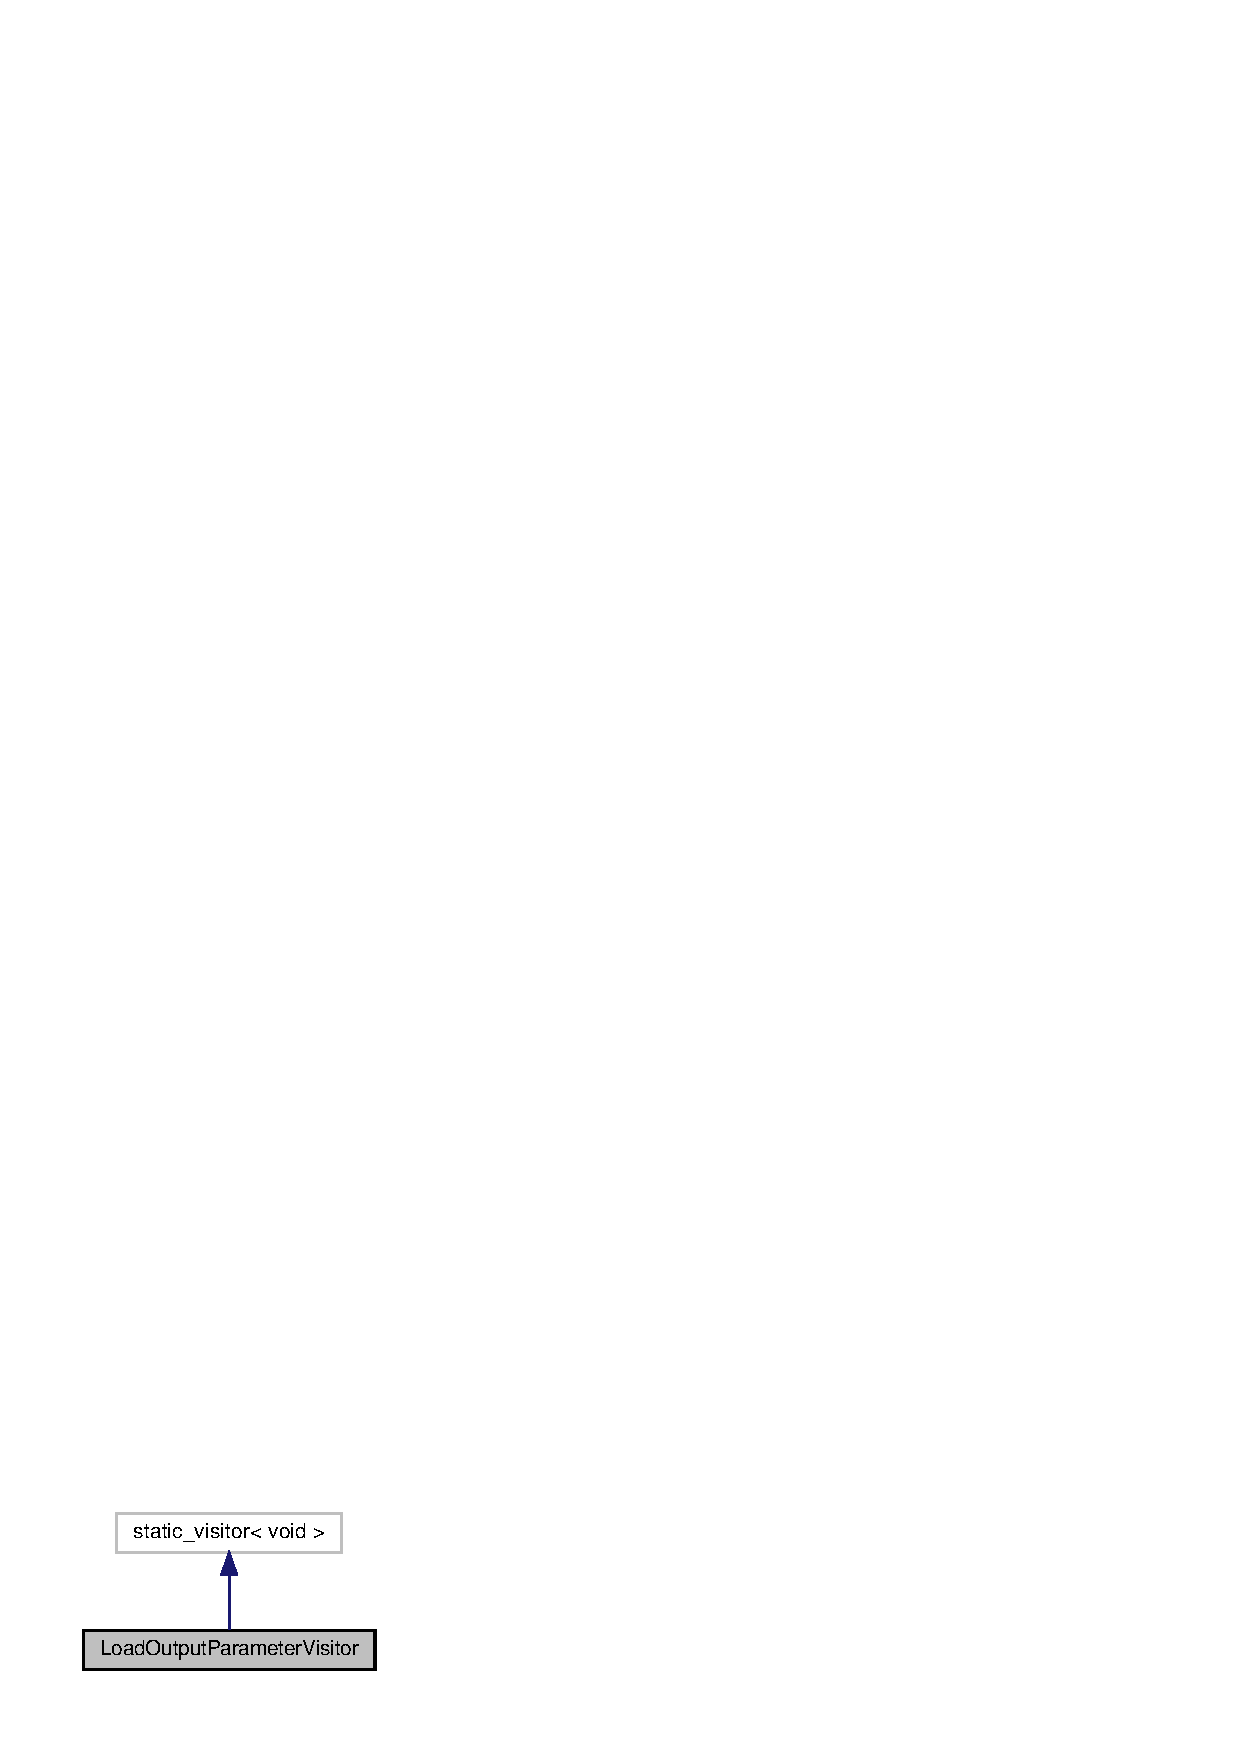
\includegraphics[width=184pt]{classmlpack_1_1ann_1_1LoadOutputParameterVisitor__inherit__graph}
\end{center}
\end{figure}
\subsection*{Public Member Functions}
\begin{DoxyCompactItemize}
\item 
\textbf{ Load\+Output\+Parameter\+Visitor} (std\+::vector$<$ arma\+::mat $>$ \&parameter)
\begin{DoxyCompactList}\small\item\em Restore the output parameter given a parameter set. \end{DoxyCompactList}\item 
{\footnotesize template$<$typename Layer\+Type $>$ }\\void \textbf{ operator()} (Layer\+Type $\ast$layer) const
\begin{DoxyCompactList}\small\item\em Restore the output parameter. \end{DoxyCompactList}\item 
void \textbf{ operator()} (\textbf{ More\+Types} layer) const
\end{DoxyCompactItemize}


\subsection{Detailed Description}
\doxyref{Load\+Output\+Parameter\+Visitor}{p.}{classmlpack_1_1ann_1_1LoadOutputParameterVisitor} restores the output parameter using the given parameter set. 

Definition at line 28 of file load\+\_\+output\+\_\+parameter\+\_\+visitor.\+hpp.



\subsection{Constructor \& Destructor Documentation}
\mbox{\label{classmlpack_1_1ann_1_1LoadOutputParameterVisitor_a1c1f5e450029be6b1256630bc0b61489}} 
\index{mlpack\+::ann\+::\+Load\+Output\+Parameter\+Visitor@{mlpack\+::ann\+::\+Load\+Output\+Parameter\+Visitor}!Load\+Output\+Parameter\+Visitor@{Load\+Output\+Parameter\+Visitor}}
\index{Load\+Output\+Parameter\+Visitor@{Load\+Output\+Parameter\+Visitor}!mlpack\+::ann\+::\+Load\+Output\+Parameter\+Visitor@{mlpack\+::ann\+::\+Load\+Output\+Parameter\+Visitor}}
\subsubsection{Load\+Output\+Parameter\+Visitor()}
{\footnotesize\ttfamily \textbf{ Load\+Output\+Parameter\+Visitor} (\begin{DoxyParamCaption}\item[{std\+::vector$<$ arma\+::mat $>$ \&}]{parameter }\end{DoxyParamCaption})}



Restore the output parameter given a parameter set. 



\subsection{Member Function Documentation}
\mbox{\label{classmlpack_1_1ann_1_1LoadOutputParameterVisitor_a26bb3385c630118c35f4799f1509abbc}} 
\index{mlpack\+::ann\+::\+Load\+Output\+Parameter\+Visitor@{mlpack\+::ann\+::\+Load\+Output\+Parameter\+Visitor}!operator()@{operator()}}
\index{operator()@{operator()}!mlpack\+::ann\+::\+Load\+Output\+Parameter\+Visitor@{mlpack\+::ann\+::\+Load\+Output\+Parameter\+Visitor}}
\subsubsection{operator()()\hspace{0.1cm}{\footnotesize\ttfamily [1/2]}}
{\footnotesize\ttfamily void operator() (\begin{DoxyParamCaption}\item[{Layer\+Type $\ast$}]{layer }\end{DoxyParamCaption}) const}



Restore the output parameter. 

\mbox{\label{classmlpack_1_1ann_1_1LoadOutputParameterVisitor_ae35578e7ff874a320fe762bc0edfff04}} 
\index{mlpack\+::ann\+::\+Load\+Output\+Parameter\+Visitor@{mlpack\+::ann\+::\+Load\+Output\+Parameter\+Visitor}!operator()@{operator()}}
\index{operator()@{operator()}!mlpack\+::ann\+::\+Load\+Output\+Parameter\+Visitor@{mlpack\+::ann\+::\+Load\+Output\+Parameter\+Visitor}}
\subsubsection{operator()()\hspace{0.1cm}{\footnotesize\ttfamily [2/2]}}
{\footnotesize\ttfamily void operator() (\begin{DoxyParamCaption}\item[{\textbf{ More\+Types}}]{layer }\end{DoxyParamCaption}) const}



The documentation for this class was generated from the following file\+:\begin{DoxyCompactItemize}
\item 
/home/aakash/mlpack/src/mlpack/methods/ann/visitor/\textbf{ load\+\_\+output\+\_\+parameter\+\_\+visitor.\+hpp}\end{DoxyCompactItemize}

\section{Log\+Cosh\+Loss$<$ Input\+Data\+Type, Output\+Data\+Type $>$ Class Template Reference}
\label{classmlpack_1_1ann_1_1LogCoshLoss}\index{Log\+Cosh\+Loss$<$ Input\+Data\+Type, Output\+Data\+Type $>$@{Log\+Cosh\+Loss$<$ Input\+Data\+Type, Output\+Data\+Type $>$}}


The Log-\/\+Hyperbolic-\/\+Cosine loss function is often used to improve variational auto encoder.  


\subsection*{Public Member Functions}
\begin{DoxyCompactItemize}
\item 
\textbf{ Log\+Cosh\+Loss} (const double a=1.\+0)
\begin{DoxyCompactList}\small\item\em Create the Log-\/\+Hyperbolic-\/\+Cosine object with the specified parameters. \end{DoxyCompactList}\item 
double \textbf{ A} () const
\begin{DoxyCompactList}\small\item\em Get the value of hyperparameter a. \end{DoxyCompactList}\item 
double \& \textbf{ A} ()
\begin{DoxyCompactList}\small\item\em Modify the value of hyperparameter a. \end{DoxyCompactList}\item 
{\footnotesize template$<$typename Prediction\+Type , typename Target\+Type , typename Loss\+Type $>$ }\\void \textbf{ Backward} (const Prediction\+Type \&prediction, const Target\+Type \&target, Loss\+Type \&loss)
\begin{DoxyCompactList}\small\item\em Ordinary feed backward pass of a neural network. \end{DoxyCompactList}\item 
{\footnotesize template$<$typename Prediction\+Type , typename Target\+Type $>$ }\\Prediction\+Type\+::elem\+\_\+type \textbf{ Forward} (const Prediction\+Type \&prediction, const Target\+Type \&target)
\begin{DoxyCompactList}\small\item\em Computes the Log-\/\+Hyperbolic-\/\+Cosine loss function. \end{DoxyCompactList}\item 
Output\+Data\+Type \& \textbf{ Output\+Parameter} () const
\begin{DoxyCompactList}\small\item\em Get the output parameter. \end{DoxyCompactList}\item 
Output\+Data\+Type \& \textbf{ Output\+Parameter} ()
\begin{DoxyCompactList}\small\item\em Modify the output parameter. \end{DoxyCompactList}\item 
{\footnotesize template$<$typename Archive $>$ }\\void \textbf{ serialize} (Archive \&ar, const uint32\+\_\+t)
\begin{DoxyCompactList}\small\item\em Serialize the loss function. \end{DoxyCompactList}\end{DoxyCompactItemize}


\subsection{Detailed Description}
\subsubsection*{template$<$typename Input\+Data\+Type = arma\+::mat, typename Output\+Data\+Type = arma\+::mat$>$\newline
class mlpack\+::ann\+::\+Log\+Cosh\+Loss$<$ Input\+Data\+Type, Output\+Data\+Type $>$}

The Log-\/\+Hyperbolic-\/\+Cosine loss function is often used to improve variational auto encoder. 

This function is the log of hyperbolic cosine of difference between true values and predicted values.


\begin{DoxyTemplParams}{Template Parameters}
{\em Input\+Data\+Type} & Type of the input data (arma\+::colvec, arma\+::mat, arma\+::sp\+\_\+mat or arma\+::cube). \\
\hline
{\em Output\+Data\+Type} & Type of the output data (arma\+::colvec, arma\+::mat, arma\+::sp\+\_\+mat or arma\+::cube). \\
\hline
\end{DoxyTemplParams}


Definition at line 35 of file log\+\_\+cosh\+\_\+loss.\+hpp.



\subsection{Constructor \& Destructor Documentation}
\mbox{\label{classmlpack_1_1ann_1_1LogCoshLoss_aa786489fcdc270dd947b12eb8709c064}} 
\index{mlpack\+::ann\+::\+Log\+Cosh\+Loss@{mlpack\+::ann\+::\+Log\+Cosh\+Loss}!Log\+Cosh\+Loss@{Log\+Cosh\+Loss}}
\index{Log\+Cosh\+Loss@{Log\+Cosh\+Loss}!mlpack\+::ann\+::\+Log\+Cosh\+Loss@{mlpack\+::ann\+::\+Log\+Cosh\+Loss}}
\subsubsection{Log\+Cosh\+Loss()}
{\footnotesize\ttfamily \textbf{ Log\+Cosh\+Loss} (\begin{DoxyParamCaption}\item[{const double}]{a = {\ttfamily 1.0} }\end{DoxyParamCaption})}



Create the Log-\/\+Hyperbolic-\/\+Cosine object with the specified parameters. 


\begin{DoxyParams}{Parameters}
{\em a} & A double type value for smoothening loss function. It must be positive a real number, Sharpness of loss function is directly proportional to a. It can also act as a scaling factor hence making the loss function more sensitive to small losses around the origin. Default value = 1.\+0. \\
\hline
\end{DoxyParams}


\subsection{Member Function Documentation}
\mbox{\label{classmlpack_1_1ann_1_1LogCoshLoss_aab6c632054fc383ec1edf83231163bf7}} 
\index{mlpack\+::ann\+::\+Log\+Cosh\+Loss@{mlpack\+::ann\+::\+Log\+Cosh\+Loss}!A@{A}}
\index{A@{A}!mlpack\+::ann\+::\+Log\+Cosh\+Loss@{mlpack\+::ann\+::\+Log\+Cosh\+Loss}}
\subsubsection{A()\hspace{0.1cm}{\footnotesize\ttfamily [1/2]}}
{\footnotesize\ttfamily double A (\begin{DoxyParamCaption}{ }\end{DoxyParamCaption}) const\hspace{0.3cm}{\ttfamily [inline]}}



Get the value of hyperparameter a. 



Definition at line 81 of file log\+\_\+cosh\+\_\+loss.\+hpp.

\mbox{\label{classmlpack_1_1ann_1_1LogCoshLoss_ad9111aa092ab0ee1b38e0369657d2bfa}} 
\index{mlpack\+::ann\+::\+Log\+Cosh\+Loss@{mlpack\+::ann\+::\+Log\+Cosh\+Loss}!A@{A}}
\index{A@{A}!mlpack\+::ann\+::\+Log\+Cosh\+Loss@{mlpack\+::ann\+::\+Log\+Cosh\+Loss}}
\subsubsection{A()\hspace{0.1cm}{\footnotesize\ttfamily [2/2]}}
{\footnotesize\ttfamily double\& A (\begin{DoxyParamCaption}{ }\end{DoxyParamCaption})\hspace{0.3cm}{\ttfamily [inline]}}



Modify the value of hyperparameter a. 



Definition at line 83 of file log\+\_\+cosh\+\_\+loss.\+hpp.



References Log\+Cosh\+Loss$<$ Input\+Data\+Type, Output\+Data\+Type $>$\+::serialize().

\mbox{\label{classmlpack_1_1ann_1_1LogCoshLoss_add41dbaf358dc099750dc6064cb7e0d7}} 
\index{mlpack\+::ann\+::\+Log\+Cosh\+Loss@{mlpack\+::ann\+::\+Log\+Cosh\+Loss}!Backward@{Backward}}
\index{Backward@{Backward}!mlpack\+::ann\+::\+Log\+Cosh\+Loss@{mlpack\+::ann\+::\+Log\+Cosh\+Loss}}
\subsubsection{Backward()}
{\footnotesize\ttfamily void Backward (\begin{DoxyParamCaption}\item[{const Prediction\+Type \&}]{prediction,  }\item[{const Target\+Type \&}]{target,  }\item[{Loss\+Type \&}]{loss }\end{DoxyParamCaption})}



Ordinary feed backward pass of a neural network. 


\begin{DoxyParams}{Parameters}
{\em prediction} & Predictions used for evaluating the specified loss function. \\
\hline
{\em target} & The target vector. \\
\hline
{\em loss} & The calculated error. \\
\hline
\end{DoxyParams}
\mbox{\label{classmlpack_1_1ann_1_1LogCoshLoss_ab3640059898ea76c13709b8099316fe8}} 
\index{mlpack\+::ann\+::\+Log\+Cosh\+Loss@{mlpack\+::ann\+::\+Log\+Cosh\+Loss}!Forward@{Forward}}
\index{Forward@{Forward}!mlpack\+::ann\+::\+Log\+Cosh\+Loss@{mlpack\+::ann\+::\+Log\+Cosh\+Loss}}
\subsubsection{Forward()}
{\footnotesize\ttfamily Prediction\+Type\+::elem\+\_\+type Forward (\begin{DoxyParamCaption}\item[{const Prediction\+Type \&}]{prediction,  }\item[{const Target\+Type \&}]{target }\end{DoxyParamCaption})}



Computes the Log-\/\+Hyperbolic-\/\+Cosine loss function. 


\begin{DoxyParams}{Parameters}
{\em prediction} & Predictions used for evaluating the specified loss function. \\
\hline
{\em target} & Target data to compare with. \\
\hline
\end{DoxyParams}
\mbox{\label{classmlpack_1_1ann_1_1LogCoshLoss_a8bae962cc603d1cab8d80ec78f8d505d}} 
\index{mlpack\+::ann\+::\+Log\+Cosh\+Loss@{mlpack\+::ann\+::\+Log\+Cosh\+Loss}!Output\+Parameter@{Output\+Parameter}}
\index{Output\+Parameter@{Output\+Parameter}!mlpack\+::ann\+::\+Log\+Cosh\+Loss@{mlpack\+::ann\+::\+Log\+Cosh\+Loss}}
\subsubsection{Output\+Parameter()\hspace{0.1cm}{\footnotesize\ttfamily [1/2]}}
{\footnotesize\ttfamily Output\+Data\+Type\& Output\+Parameter (\begin{DoxyParamCaption}{ }\end{DoxyParamCaption}) const\hspace{0.3cm}{\ttfamily [inline]}}



Get the output parameter. 



Definition at line 76 of file log\+\_\+cosh\+\_\+loss.\+hpp.

\mbox{\label{classmlpack_1_1ann_1_1LogCoshLoss_a21d5f745f02c709625a4ee0907f004a5}} 
\index{mlpack\+::ann\+::\+Log\+Cosh\+Loss@{mlpack\+::ann\+::\+Log\+Cosh\+Loss}!Output\+Parameter@{Output\+Parameter}}
\index{Output\+Parameter@{Output\+Parameter}!mlpack\+::ann\+::\+Log\+Cosh\+Loss@{mlpack\+::ann\+::\+Log\+Cosh\+Loss}}
\subsubsection{Output\+Parameter()\hspace{0.1cm}{\footnotesize\ttfamily [2/2]}}
{\footnotesize\ttfamily Output\+Data\+Type\& Output\+Parameter (\begin{DoxyParamCaption}{ }\end{DoxyParamCaption})\hspace{0.3cm}{\ttfamily [inline]}}



Modify the output parameter. 



Definition at line 78 of file log\+\_\+cosh\+\_\+loss.\+hpp.

\mbox{\label{classmlpack_1_1ann_1_1LogCoshLoss_a65cba07328997659bec80b9879b15a51}} 
\index{mlpack\+::ann\+::\+Log\+Cosh\+Loss@{mlpack\+::ann\+::\+Log\+Cosh\+Loss}!serialize@{serialize}}
\index{serialize@{serialize}!mlpack\+::ann\+::\+Log\+Cosh\+Loss@{mlpack\+::ann\+::\+Log\+Cosh\+Loss}}
\subsubsection{serialize()}
{\footnotesize\ttfamily void serialize (\begin{DoxyParamCaption}\item[{Archive \&}]{ar,  }\item[{const uint32\+\_\+t}]{ }\end{DoxyParamCaption})}



Serialize the loss function. 



Referenced by Log\+Cosh\+Loss$<$ Input\+Data\+Type, Output\+Data\+Type $>$\+::\+A().



The documentation for this class was generated from the following file\+:\begin{DoxyCompactItemize}
\item 
/home/aakash/mlpack/src/mlpack/methods/ann/loss\+\_\+functions/\textbf{ log\+\_\+cosh\+\_\+loss.\+hpp}\end{DoxyCompactItemize}

\section{Logistic\+Function Class Reference}
\label{classmlpack_1_1ann_1_1LogisticFunction}\index{Logistic\+Function@{Logistic\+Function}}


The logistic function, defined by.  


\subsection*{Static Public Member Functions}
\begin{DoxyCompactItemize}
\item 
static double \textbf{ Deriv} (const double x)
\begin{DoxyCompactList}\small\item\em Computes the first derivative of the logistic function. \end{DoxyCompactList}\item 
{\footnotesize template$<$typename Input\+Vec\+Type , typename Output\+Vec\+Type $>$ }\\static void \textbf{ Deriv} (const Input\+Vec\+Type \&y, Output\+Vec\+Type \&x)
\begin{DoxyCompactList}\small\item\em Computes the first derivatives of the logistic function. \end{DoxyCompactList}\item 
{\footnotesize template$<$typename eT $>$ }\\static double \textbf{ Fn} (const eT x)
\begin{DoxyCompactList}\small\item\em Computes the logistic function. \end{DoxyCompactList}\item 
{\footnotesize template$<$typename Input\+Vec\+Type , typename Output\+Vec\+Type $>$ }\\static void \textbf{ Fn} (const Input\+Vec\+Type \&x, Output\+Vec\+Type \&y)
\begin{DoxyCompactList}\small\item\em Computes the logistic function. \end{DoxyCompactList}\item 
static double \textbf{ Inv} (const double y)
\begin{DoxyCompactList}\small\item\em Computes the inverse of the logistic function. \end{DoxyCompactList}\item 
{\footnotesize template$<$typename Input\+Vec\+Type , typename Output\+Vec\+Type $>$ }\\static void \textbf{ Inv} (const Input\+Vec\+Type \&y, Output\+Vec\+Type \&x)
\begin{DoxyCompactList}\small\item\em Computes the inverse of the logistic function. \end{DoxyCompactList}\end{DoxyCompactItemize}


\subsection{Detailed Description}
The logistic function, defined by. 

\begin{eqnarray*} f(x) &=& \frac{1}{1 + e^{-x}} \\ f'(x) &=& f(x) * (1 - f(x)) \\ f^{-1}(y) &=& ln(\frac{y}{1-y}) \end{eqnarray*} 

Definition at line 29 of file logistic\+\_\+function.\+hpp.



\subsection{Member Function Documentation}
\mbox{\label{classmlpack_1_1ann_1_1LogisticFunction_acd77fae79f7ba1f4b9a21e07a261e537}} 
\index{mlpack\+::ann\+::\+Logistic\+Function@{mlpack\+::ann\+::\+Logistic\+Function}!Deriv@{Deriv}}
\index{Deriv@{Deriv}!mlpack\+::ann\+::\+Logistic\+Function@{mlpack\+::ann\+::\+Logistic\+Function}}
\subsubsection{Deriv()\hspace{0.1cm}{\footnotesize\ttfamily [1/2]}}
{\footnotesize\ttfamily static double Deriv (\begin{DoxyParamCaption}\item[{const double}]{x }\end{DoxyParamCaption})\hspace{0.3cm}{\ttfamily [inline]}, {\ttfamily [static]}}



Computes the first derivative of the logistic function. 


\begin{DoxyParams}{Parameters}
{\em x} & Input activation. \\
\hline
\end{DoxyParams}
\begin{DoxyReturn}{Returns}
f\textquotesingle{}(x) 
\end{DoxyReturn}


Definition at line 70 of file logistic\+\_\+function.\+hpp.

\mbox{\label{classmlpack_1_1ann_1_1LogisticFunction_ad442502c34b67303b74c735641dab790}} 
\index{mlpack\+::ann\+::\+Logistic\+Function@{mlpack\+::ann\+::\+Logistic\+Function}!Deriv@{Deriv}}
\index{Deriv@{Deriv}!mlpack\+::ann\+::\+Logistic\+Function@{mlpack\+::ann\+::\+Logistic\+Function}}
\subsubsection{Deriv()\hspace{0.1cm}{\footnotesize\ttfamily [2/2]}}
{\footnotesize\ttfamily static void Deriv (\begin{DoxyParamCaption}\item[{const Input\+Vec\+Type \&}]{y,  }\item[{Output\+Vec\+Type \&}]{x }\end{DoxyParamCaption})\hspace{0.3cm}{\ttfamily [inline]}, {\ttfamily [static]}}



Computes the first derivatives of the logistic function. 


\begin{DoxyParams}{Parameters}
{\em y} & Input activations. \\
\hline
{\em x} & The resulting derivatives. \\
\hline
\end{DoxyParams}


Definition at line 82 of file logistic\+\_\+function.\+hpp.

\mbox{\label{classmlpack_1_1ann_1_1LogisticFunction_a7be90336227c4673a4152dbac3d62c25}} 
\index{mlpack\+::ann\+::\+Logistic\+Function@{mlpack\+::ann\+::\+Logistic\+Function}!Fn@{Fn}}
\index{Fn@{Fn}!mlpack\+::ann\+::\+Logistic\+Function@{mlpack\+::ann\+::\+Logistic\+Function}}
\subsubsection{Fn()\hspace{0.1cm}{\footnotesize\ttfamily [1/2]}}
{\footnotesize\ttfamily static double Fn (\begin{DoxyParamCaption}\item[{const eT}]{x }\end{DoxyParamCaption})\hspace{0.3cm}{\ttfamily [inline]}, {\ttfamily [static]}}



Computes the logistic function. 


\begin{DoxyParams}{Parameters}
{\em x} & Input data. \\
\hline
\end{DoxyParams}
\begin{DoxyReturn}{Returns}
f(x). 
\end{DoxyReturn}


Definition at line 39 of file logistic\+\_\+function.\+hpp.

\mbox{\label{classmlpack_1_1ann_1_1LogisticFunction_af6cf5da90eb6312e3e25c9b8bd9c3527}} 
\index{mlpack\+::ann\+::\+Logistic\+Function@{mlpack\+::ann\+::\+Logistic\+Function}!Fn@{Fn}}
\index{Fn@{Fn}!mlpack\+::ann\+::\+Logistic\+Function@{mlpack\+::ann\+::\+Logistic\+Function}}
\subsubsection{Fn()\hspace{0.1cm}{\footnotesize\ttfamily [2/2]}}
{\footnotesize\ttfamily static void Fn (\begin{DoxyParamCaption}\item[{const Input\+Vec\+Type \&}]{x,  }\item[{Output\+Vec\+Type \&}]{y }\end{DoxyParamCaption})\hspace{0.3cm}{\ttfamily [inline]}, {\ttfamily [static]}}



Computes the logistic function. 


\begin{DoxyParams}{Parameters}
{\em x} & Input data. \\
\hline
{\em y} & The resulting output activation. \\
\hline
\end{DoxyParams}


Definition at line 59 of file logistic\+\_\+function.\+hpp.

\mbox{\label{classmlpack_1_1ann_1_1LogisticFunction_a32d503b167c9646569a202e8c134ef76}} 
\index{mlpack\+::ann\+::\+Logistic\+Function@{mlpack\+::ann\+::\+Logistic\+Function}!Inv@{Inv}}
\index{Inv@{Inv}!mlpack\+::ann\+::\+Logistic\+Function@{mlpack\+::ann\+::\+Logistic\+Function}}
\subsubsection{Inv()\hspace{0.1cm}{\footnotesize\ttfamily [1/2]}}
{\footnotesize\ttfamily static double Inv (\begin{DoxyParamCaption}\item[{const double}]{y }\end{DoxyParamCaption})\hspace{0.3cm}{\ttfamily [inline]}, {\ttfamily [static]}}



Computes the inverse of the logistic function. 


\begin{DoxyParams}{Parameters}
{\em y} & Input data. \\
\hline
\end{DoxyParams}
\begin{DoxyReturn}{Returns}
f$^\wedge$\{-\/1\}(y) 
\end{DoxyReturn}


Definition at line 93 of file logistic\+\_\+function.\+hpp.

\mbox{\label{classmlpack_1_1ann_1_1LogisticFunction_ad48548410161bbf6178eb1c293c991c3}} 
\index{mlpack\+::ann\+::\+Logistic\+Function@{mlpack\+::ann\+::\+Logistic\+Function}!Inv@{Inv}}
\index{Inv@{Inv}!mlpack\+::ann\+::\+Logistic\+Function@{mlpack\+::ann\+::\+Logistic\+Function}}
\subsubsection{Inv()\hspace{0.1cm}{\footnotesize\ttfamily [2/2]}}
{\footnotesize\ttfamily static void Inv (\begin{DoxyParamCaption}\item[{const Input\+Vec\+Type \&}]{y,  }\item[{Output\+Vec\+Type \&}]{x }\end{DoxyParamCaption})\hspace{0.3cm}{\ttfamily [inline]}, {\ttfamily [static]}}



Computes the inverse of the logistic function. 


\begin{DoxyParams}{Parameters}
{\em y} & Input data. \\
\hline
{\em x} & The resulting inverse of the input data. \\
\hline
\end{DoxyParams}


Definition at line 105 of file logistic\+\_\+function.\+hpp.



The documentation for this class was generated from the following file\+:\begin{DoxyCompactItemize}
\item 
/home/aakash/mlpack/src/mlpack/methods/ann/activation\+\_\+functions/\textbf{ logistic\+\_\+function.\+hpp}\end{DoxyCompactItemize}

\section{Log\+Soft\+Max$<$ Input\+Data\+Type, Output\+Data\+Type $>$ Class Template Reference}
\label{classmlpack_1_1ann_1_1LogSoftMax}\index{Log\+Soft\+Max$<$ Input\+Data\+Type, Output\+Data\+Type $>$@{Log\+Soft\+Max$<$ Input\+Data\+Type, Output\+Data\+Type $>$}}


Implementation of the log softmax layer.  


\subsection*{Public Member Functions}
\begin{DoxyCompactItemize}
\item 
\textbf{ Log\+Soft\+Max} ()
\begin{DoxyCompactList}\small\item\em Create the Log\+Softmax object. \end{DoxyCompactList}\item 
{\footnotesize template$<$typename eT $>$ }\\void \textbf{ Backward} (const arma\+::\+Mat$<$ eT $>$ \&input, const arma\+::\+Mat$<$ eT $>$ \&gy, arma\+::\+Mat$<$ eT $>$ \&g)
\begin{DoxyCompactList}\small\item\em Ordinary feed backward pass of a neural network, calculating the function f(x) by propagating x backwards trough f. \end{DoxyCompactList}\item 
Input\+Data\+Type \& \textbf{ Delta} () const
\begin{DoxyCompactList}\small\item\em Get the delta. \end{DoxyCompactList}\item 
Input\+Data\+Type \& \textbf{ Delta} ()
\begin{DoxyCompactList}\small\item\em Modify the delta. \end{DoxyCompactList}\item 
{\footnotesize template$<$typename Input\+Type , typename Output\+Type $>$ }\\void \textbf{ Forward} (const Input\+Type \&input, Output\+Type \&output)
\begin{DoxyCompactList}\small\item\em Ordinary feed forward pass of a neural network, evaluating the function f(x) by propagating the activity forward through f. \end{DoxyCompactList}\item 
Output\+Data\+Type \& \textbf{ Output\+Parameter} () const
\begin{DoxyCompactList}\small\item\em Get the output parameter. \end{DoxyCompactList}\item 
Output\+Data\+Type \& \textbf{ Output\+Parameter} ()
\begin{DoxyCompactList}\small\item\em Modify the output parameter. \end{DoxyCompactList}\item 
{\footnotesize template$<$typename Archive $>$ }\\void \textbf{ serialize} (Archive \&, const uint32\+\_\+t)
\begin{DoxyCompactList}\small\item\em Serialize the layer. \end{DoxyCompactList}\end{DoxyCompactItemize}


\subsection{Detailed Description}
\subsubsection*{template$<$typename Input\+Data\+Type = arma\+::mat, typename Output\+Data\+Type = arma\+::mat$>$\newline
class mlpack\+::ann\+::\+Log\+Soft\+Max$<$ Input\+Data\+Type, Output\+Data\+Type $>$}

Implementation of the log softmax layer. 

The log softmax loss layer computes the multinomial logistic loss of the softmax of its inputs. This layer is meant to be used in combination with the negative log likelihood layer (Negative\+Log\+Likelihood\+Layer), which expects that the input contains log-\/probabilities for each class.


\begin{DoxyTemplParams}{Template Parameters}
{\em Input\+Data\+Type} & Type of the input data (arma\+::colvec, arma\+::mat, arma\+::sp\+\_\+mat or arma\+::cube). \\
\hline
{\em Output\+Data\+Type} & Type of the output data (arma\+::colvec, arma\+::mat, arma\+::sp\+\_\+mat or arma\+::cube). \\
\hline
\end{DoxyTemplParams}


Definition at line 36 of file log\+\_\+softmax.\+hpp.



\subsection{Constructor \& Destructor Documentation}
\mbox{\label{classmlpack_1_1ann_1_1LogSoftMax_a1298935d4b0e2a0751dc55081c9515bf}} 
\index{mlpack\+::ann\+::\+Log\+Soft\+Max@{mlpack\+::ann\+::\+Log\+Soft\+Max}!Log\+Soft\+Max@{Log\+Soft\+Max}}
\index{Log\+Soft\+Max@{Log\+Soft\+Max}!mlpack\+::ann\+::\+Log\+Soft\+Max@{mlpack\+::ann\+::\+Log\+Soft\+Max}}
\subsubsection{Log\+Soft\+Max()}
{\footnotesize\ttfamily \textbf{ Log\+Soft\+Max} (\begin{DoxyParamCaption}{ }\end{DoxyParamCaption})}



Create the Log\+Softmax object. 



\subsection{Member Function Documentation}
\mbox{\label{classmlpack_1_1ann_1_1LogSoftMax_a78dbad83871f43db1975e45a9a69c376}} 
\index{mlpack\+::ann\+::\+Log\+Soft\+Max@{mlpack\+::ann\+::\+Log\+Soft\+Max}!Backward@{Backward}}
\index{Backward@{Backward}!mlpack\+::ann\+::\+Log\+Soft\+Max@{mlpack\+::ann\+::\+Log\+Soft\+Max}}
\subsubsection{Backward()}
{\footnotesize\ttfamily void Backward (\begin{DoxyParamCaption}\item[{const arma\+::\+Mat$<$ eT $>$ \&}]{input,  }\item[{const arma\+::\+Mat$<$ eT $>$ \&}]{gy,  }\item[{arma\+::\+Mat$<$ eT $>$ \&}]{g }\end{DoxyParamCaption})}



Ordinary feed backward pass of a neural network, calculating the function f(x) by propagating x backwards trough f. 

Using the results from the feed forward pass.


\begin{DoxyParams}{Parameters}
{\em input} & The propagated input activation. \\
\hline
{\em gy} & The backpropagated error. \\
\hline
{\em g} & The calculated gradient. \\
\hline
\end{DoxyParams}
\mbox{\label{classmlpack_1_1ann_1_1LogSoftMax_aa02f12f0f3e5fea14c9fecf889b3103a}} 
\index{mlpack\+::ann\+::\+Log\+Soft\+Max@{mlpack\+::ann\+::\+Log\+Soft\+Max}!Delta@{Delta}}
\index{Delta@{Delta}!mlpack\+::ann\+::\+Log\+Soft\+Max@{mlpack\+::ann\+::\+Log\+Soft\+Max}}
\subsubsection{Delta()\hspace{0.1cm}{\footnotesize\ttfamily [1/2]}}
{\footnotesize\ttfamily Input\+Data\+Type\& Delta (\begin{DoxyParamCaption}{ }\end{DoxyParamCaption}) const\hspace{0.3cm}{\ttfamily [inline]}}



Get the delta. 



Definition at line 74 of file log\+\_\+softmax.\+hpp.

\mbox{\label{classmlpack_1_1ann_1_1LogSoftMax_a6201406598916738050e1b6caedea03b}} 
\index{mlpack\+::ann\+::\+Log\+Soft\+Max@{mlpack\+::ann\+::\+Log\+Soft\+Max}!Delta@{Delta}}
\index{Delta@{Delta}!mlpack\+::ann\+::\+Log\+Soft\+Max@{mlpack\+::ann\+::\+Log\+Soft\+Max}}
\subsubsection{Delta()\hspace{0.1cm}{\footnotesize\ttfamily [2/2]}}
{\footnotesize\ttfamily Input\+Data\+Type\& Delta (\begin{DoxyParamCaption}{ }\end{DoxyParamCaption})\hspace{0.3cm}{\ttfamily [inline]}}



Modify the delta. 



Definition at line 76 of file log\+\_\+softmax.\+hpp.



References Log\+Soft\+Max$<$ Input\+Data\+Type, Output\+Data\+Type $>$\+::serialize().

\mbox{\label{classmlpack_1_1ann_1_1LogSoftMax_a09440df0a90bdcc766e56e097d91205b}} 
\index{mlpack\+::ann\+::\+Log\+Soft\+Max@{mlpack\+::ann\+::\+Log\+Soft\+Max}!Forward@{Forward}}
\index{Forward@{Forward}!mlpack\+::ann\+::\+Log\+Soft\+Max@{mlpack\+::ann\+::\+Log\+Soft\+Max}}
\subsubsection{Forward()}
{\footnotesize\ttfamily void Forward (\begin{DoxyParamCaption}\item[{const Input\+Type \&}]{input,  }\item[{Output\+Type \&}]{output }\end{DoxyParamCaption})}



Ordinary feed forward pass of a neural network, evaluating the function f(x) by propagating the activity forward through f. 


\begin{DoxyParams}{Parameters}
{\em input} & Input data used for evaluating the specified function. \\
\hline
{\em output} & Resulting output activation. \\
\hline
\end{DoxyParams}
\mbox{\label{classmlpack_1_1ann_1_1LogSoftMax_a8bae962cc603d1cab8d80ec78f8d505d}} 
\index{mlpack\+::ann\+::\+Log\+Soft\+Max@{mlpack\+::ann\+::\+Log\+Soft\+Max}!Output\+Parameter@{Output\+Parameter}}
\index{Output\+Parameter@{Output\+Parameter}!mlpack\+::ann\+::\+Log\+Soft\+Max@{mlpack\+::ann\+::\+Log\+Soft\+Max}}
\subsubsection{Output\+Parameter()\hspace{0.1cm}{\footnotesize\ttfamily [1/2]}}
{\footnotesize\ttfamily Output\+Data\+Type\& Output\+Parameter (\begin{DoxyParamCaption}{ }\end{DoxyParamCaption}) const\hspace{0.3cm}{\ttfamily [inline]}}



Get the output parameter. 



Definition at line 69 of file log\+\_\+softmax.\+hpp.

\mbox{\label{classmlpack_1_1ann_1_1LogSoftMax_a21d5f745f02c709625a4ee0907f004a5}} 
\index{mlpack\+::ann\+::\+Log\+Soft\+Max@{mlpack\+::ann\+::\+Log\+Soft\+Max}!Output\+Parameter@{Output\+Parameter}}
\index{Output\+Parameter@{Output\+Parameter}!mlpack\+::ann\+::\+Log\+Soft\+Max@{mlpack\+::ann\+::\+Log\+Soft\+Max}}
\subsubsection{Output\+Parameter()\hspace{0.1cm}{\footnotesize\ttfamily [2/2]}}
{\footnotesize\ttfamily Output\+Data\+Type\& Output\+Parameter (\begin{DoxyParamCaption}{ }\end{DoxyParamCaption})\hspace{0.3cm}{\ttfamily [inline]}}



Modify the output parameter. 



Definition at line 71 of file log\+\_\+softmax.\+hpp.

\mbox{\label{classmlpack_1_1ann_1_1LogSoftMax_aa2ccb5a0533a6ba0abe6dfc1f98fbafb}} 
\index{mlpack\+::ann\+::\+Log\+Soft\+Max@{mlpack\+::ann\+::\+Log\+Soft\+Max}!serialize@{serialize}}
\index{serialize@{serialize}!mlpack\+::ann\+::\+Log\+Soft\+Max@{mlpack\+::ann\+::\+Log\+Soft\+Max}}
\subsubsection{serialize()}
{\footnotesize\ttfamily void serialize (\begin{DoxyParamCaption}\item[{Archive \&}]{,  }\item[{const uint32\+\_\+t}]{ }\end{DoxyParamCaption})}



Serialize the layer. 



Referenced by Log\+Soft\+Max$<$ Input\+Data\+Type, Output\+Data\+Type $>$\+::\+Delta().



The documentation for this class was generated from the following file\+:\begin{DoxyCompactItemize}
\item 
/home/aakash/mlpack/src/mlpack/methods/ann/layer/\textbf{ log\+\_\+softmax.\+hpp}\end{DoxyCompactItemize}

\section{Lookup$<$ Input\+Data\+Type, Output\+Data\+Type $>$ Class Template Reference}
\label{classmlpack_1_1ann_1_1Lookup}\index{Lookup$<$ Input\+Data\+Type, Output\+Data\+Type $>$@{Lookup$<$ Input\+Data\+Type, Output\+Data\+Type $>$}}


The \doxyref{Lookup}{p.}{classmlpack_1_1ann_1_1Lookup} class stores word embeddings and retrieves them using tokens.  


\subsection*{Public Member Functions}
\begin{DoxyCompactItemize}
\item 
\textbf{ Lookup} (const size\+\_\+t vocab\+Size=0, const size\+\_\+t embedding\+Size=0)
\begin{DoxyCompactList}\small\item\em Create the \doxyref{Lookup}{p.}{classmlpack_1_1ann_1_1Lookup} object using the specified vocabulary and embedding size. \end{DoxyCompactList}\item 
{\footnotesize template$<$typename eT $>$ }\\void \textbf{ Backward} (const arma\+::\+Mat$<$ eT $>$ \&, const arma\+::\+Mat$<$ eT $>$ \&gy, arma\+::\+Mat$<$ eT $>$ \&g)
\begin{DoxyCompactList}\small\item\em Ordinary feed backward pass of a neural network, calculating the function f(x) by propagating x backwards trough f. \end{DoxyCompactList}\item 
Output\+Data\+Type const  \& \textbf{ Delta} () const
\begin{DoxyCompactList}\small\item\em Get the delta. \end{DoxyCompactList}\item 
Output\+Data\+Type \& \textbf{ Delta} ()
\begin{DoxyCompactList}\small\item\em Modify the delta. \end{DoxyCompactList}\item 
size\+\_\+t \textbf{ Embedding\+Size} () const
\begin{DoxyCompactList}\small\item\em Get the length of each embedding vector. \end{DoxyCompactList}\item 
{\footnotesize template$<$typename eT $>$ }\\void \textbf{ Forward} (const arma\+::\+Mat$<$ eT $>$ \&input, arma\+::\+Mat$<$ eT $>$ \&output)
\begin{DoxyCompactList}\small\item\em Ordinary feed forward pass of a neural network, evaluating the function f(x) by propagating the activity forward through f. \end{DoxyCompactList}\item 
{\footnotesize template$<$typename eT $>$ }\\void \textbf{ Gradient} (const arma\+::\+Mat$<$ eT $>$ \&input, const arma\+::\+Mat$<$ eT $>$ \&error, arma\+::\+Mat$<$ eT $>$ \&gradient)
\begin{DoxyCompactList}\small\item\em Calculate the gradient using the output delta and the input activation. \end{DoxyCompactList}\item 
Output\+Data\+Type const  \& \textbf{ Gradient} () const
\begin{DoxyCompactList}\small\item\em Get the gradient. \end{DoxyCompactList}\item 
Output\+Data\+Type \& \textbf{ Gradient} ()
\begin{DoxyCompactList}\small\item\em Modify the gradient. \end{DoxyCompactList}\item 
Output\+Data\+Type const  \& \textbf{ Output\+Parameter} () const
\begin{DoxyCompactList}\small\item\em Get the output parameter. \end{DoxyCompactList}\item 
Output\+Data\+Type \& \textbf{ Output\+Parameter} ()
\begin{DoxyCompactList}\small\item\em Modify the output parameter. \end{DoxyCompactList}\item 
Output\+Data\+Type const  \& \textbf{ Parameters} () const
\begin{DoxyCompactList}\small\item\em Get the parameters. \end{DoxyCompactList}\item 
Output\+Data\+Type \& \textbf{ Parameters} ()
\begin{DoxyCompactList}\small\item\em Modify the parameters. \end{DoxyCompactList}\item 
{\footnotesize template$<$typename Archive $>$ }\\void \textbf{ serialize} (Archive \&ar, const uint32\+\_\+t)
\begin{DoxyCompactList}\small\item\em Serialize the layer. \end{DoxyCompactList}\item 
size\+\_\+t \textbf{ Vocab\+Size} () const
\begin{DoxyCompactList}\small\item\em Get the size of the vocabulary. \end{DoxyCompactList}\end{DoxyCompactItemize}


\subsection{Detailed Description}
\subsubsection*{template$<$typename Input\+Data\+Type = arma\+::mat, typename Output\+Data\+Type = arma\+::mat$>$\newline
class mlpack\+::ann\+::\+Lookup$<$ Input\+Data\+Type, Output\+Data\+Type $>$}

The \doxyref{Lookup}{p.}{classmlpack_1_1ann_1_1Lookup} class stores word embeddings and retrieves them using tokens. 

The \doxyref{Lookup}{p.}{classmlpack_1_1ann_1_1Lookup} layer is always the first layer of the network. The input to the \doxyref{Lookup}{p.}{classmlpack_1_1ann_1_1Lookup} class is a matrix of shape (sequence\+Length, batch\+Size). The matrix consists of tokens which are used to lookup the table (i.\+e. weights) to find the embeddings of those tokens.

The input shape \+: (sequence\+Length, batch\+Size). The output shape \+: (embedding\+Size, sequence\+Length, batch\+Size).


\begin{DoxyTemplParams}{Template Parameters}
{\em Input\+Data\+Type} & Type of the input data (arma\+::colvec, arma\+::mat, arma\+::sp\+\_\+mat or arma\+::cube). \\
\hline
{\em Output\+Data\+Type} & Type of the output data (arma\+::colvec, arma\+::mat, arma\+::sp\+\_\+mat or arma\+::cube). \\
\hline
\end{DoxyTemplParams}


Definition at line 41 of file lookup.\+hpp.



\subsection{Constructor \& Destructor Documentation}
\mbox{\label{classmlpack_1_1ann_1_1Lookup_ad2a92a24a6c38f608d103d2ac2153a91}} 
\index{mlpack\+::ann\+::\+Lookup@{mlpack\+::ann\+::\+Lookup}!Lookup@{Lookup}}
\index{Lookup@{Lookup}!mlpack\+::ann\+::\+Lookup@{mlpack\+::ann\+::\+Lookup}}
\subsubsection{Lookup()}
{\footnotesize\ttfamily \textbf{ Lookup} (\begin{DoxyParamCaption}\item[{const size\+\_\+t}]{vocab\+Size = {\ttfamily 0},  }\item[{const size\+\_\+t}]{embedding\+Size = {\ttfamily 0} }\end{DoxyParamCaption})}



Create the \doxyref{Lookup}{p.}{classmlpack_1_1ann_1_1Lookup} object using the specified vocabulary and embedding size. 


\begin{DoxyParams}{Parameters}
{\em vocab\+Size} & The size of the vocabulary. \\
\hline
{\em embedding\+Size} & The length of each embedding vector. \\
\hline
\end{DoxyParams}


\subsection{Member Function Documentation}
\mbox{\label{classmlpack_1_1ann_1_1Lookup_ad9ad1a3bdb0f3fff5c839ed155e4bbf8}} 
\index{mlpack\+::ann\+::\+Lookup@{mlpack\+::ann\+::\+Lookup}!Backward@{Backward}}
\index{Backward@{Backward}!mlpack\+::ann\+::\+Lookup@{mlpack\+::ann\+::\+Lookup}}
\subsubsection{Backward()}
{\footnotesize\ttfamily void Backward (\begin{DoxyParamCaption}\item[{const arma\+::\+Mat$<$ eT $>$ \&}]{,  }\item[{const arma\+::\+Mat$<$ eT $>$ \&}]{gy,  }\item[{arma\+::\+Mat$<$ eT $>$ \&}]{g }\end{DoxyParamCaption})}



Ordinary feed backward pass of a neural network, calculating the function f(x) by propagating x backwards trough f. 

Using the results from the feed forward pass.


\begin{DoxyParams}{Parameters}
{\em $\ast$} & (input) The propagated input activation. \\
\hline
{\em gy} & The backpropagated error. \\
\hline
{\em g} & The calculated gradient. \\
\hline
\end{DoxyParams}
\mbox{\label{classmlpack_1_1ann_1_1Lookup_a797f7edb44dd081e5e2b3cc316eef6bd}} 
\index{mlpack\+::ann\+::\+Lookup@{mlpack\+::ann\+::\+Lookup}!Delta@{Delta}}
\index{Delta@{Delta}!mlpack\+::ann\+::\+Lookup@{mlpack\+::ann\+::\+Lookup}}
\subsubsection{Delta()\hspace{0.1cm}{\footnotesize\ttfamily [1/2]}}
{\footnotesize\ttfamily Output\+Data\+Type const\& Delta (\begin{DoxyParamCaption}{ }\end{DoxyParamCaption}) const\hspace{0.3cm}{\ttfamily [inline]}}



Get the delta. 



Definition at line 99 of file lookup.\+hpp.

\mbox{\label{classmlpack_1_1ann_1_1Lookup_ad6601342d560219ce951d554e69e5e87}} 
\index{mlpack\+::ann\+::\+Lookup@{mlpack\+::ann\+::\+Lookup}!Delta@{Delta}}
\index{Delta@{Delta}!mlpack\+::ann\+::\+Lookup@{mlpack\+::ann\+::\+Lookup}}
\subsubsection{Delta()\hspace{0.1cm}{\footnotesize\ttfamily [2/2]}}
{\footnotesize\ttfamily Output\+Data\+Type\& Delta (\begin{DoxyParamCaption}{ }\end{DoxyParamCaption})\hspace{0.3cm}{\ttfamily [inline]}}



Modify the delta. 



Definition at line 101 of file lookup.\+hpp.

\mbox{\label{classmlpack_1_1ann_1_1Lookup_af901e8433309aa802f54ce6efdafe41b}} 
\index{mlpack\+::ann\+::\+Lookup@{mlpack\+::ann\+::\+Lookup}!Embedding\+Size@{Embedding\+Size}}
\index{Embedding\+Size@{Embedding\+Size}!mlpack\+::ann\+::\+Lookup@{mlpack\+::ann\+::\+Lookup}}
\subsubsection{Embedding\+Size()}
{\footnotesize\ttfamily size\+\_\+t Embedding\+Size (\begin{DoxyParamCaption}{ }\end{DoxyParamCaption}) const\hspace{0.3cm}{\ttfamily [inline]}}



Get the length of each embedding vector. 



Definition at line 112 of file lookup.\+hpp.



References Lookup$<$ Input\+Data\+Type, Output\+Data\+Type $>$\+::serialize().

\mbox{\label{classmlpack_1_1ann_1_1Lookup_a461f849bc638c15bec262dc9c3a58abe}} 
\index{mlpack\+::ann\+::\+Lookup@{mlpack\+::ann\+::\+Lookup}!Forward@{Forward}}
\index{Forward@{Forward}!mlpack\+::ann\+::\+Lookup@{mlpack\+::ann\+::\+Lookup}}
\subsubsection{Forward()}
{\footnotesize\ttfamily void Forward (\begin{DoxyParamCaption}\item[{const arma\+::\+Mat$<$ eT $>$ \&}]{input,  }\item[{arma\+::\+Mat$<$ eT $>$ \&}]{output }\end{DoxyParamCaption})}



Ordinary feed forward pass of a neural network, evaluating the function f(x) by propagating the activity forward through f. 


\begin{DoxyParams}{Parameters}
{\em input} & Input data used for evaluating the specified function. \\
\hline
{\em output} & Resulting output activation. \\
\hline
\end{DoxyParams}
\mbox{\label{classmlpack_1_1ann_1_1Lookup_aaf577db350e2130754490d8486fba215}} 
\index{mlpack\+::ann\+::\+Lookup@{mlpack\+::ann\+::\+Lookup}!Gradient@{Gradient}}
\index{Gradient@{Gradient}!mlpack\+::ann\+::\+Lookup@{mlpack\+::ann\+::\+Lookup}}
\subsubsection{Gradient()\hspace{0.1cm}{\footnotesize\ttfamily [1/3]}}
{\footnotesize\ttfamily void Gradient (\begin{DoxyParamCaption}\item[{const arma\+::\+Mat$<$ eT $>$ \&}]{input,  }\item[{const arma\+::\+Mat$<$ eT $>$ \&}]{error,  }\item[{arma\+::\+Mat$<$ eT $>$ \&}]{gradient }\end{DoxyParamCaption})}



Calculate the gradient using the output delta and the input activation. 


\begin{DoxyParams}{Parameters}
{\em input} & The input parameter used for calculating the gradient. \\
\hline
{\em error} & The calculated error. \\
\hline
{\em gradient} & The calculated gradient. \\
\hline
\end{DoxyParams}
\mbox{\label{classmlpack_1_1ann_1_1Lookup_a0f1f4e6d93472d83852731a96c8c3f59}} 
\index{mlpack\+::ann\+::\+Lookup@{mlpack\+::ann\+::\+Lookup}!Gradient@{Gradient}}
\index{Gradient@{Gradient}!mlpack\+::ann\+::\+Lookup@{mlpack\+::ann\+::\+Lookup}}
\subsubsection{Gradient()\hspace{0.1cm}{\footnotesize\ttfamily [2/3]}}
{\footnotesize\ttfamily Output\+Data\+Type const\& Gradient (\begin{DoxyParamCaption}{ }\end{DoxyParamCaption}) const\hspace{0.3cm}{\ttfamily [inline]}}



Get the gradient. 



Definition at line 104 of file lookup.\+hpp.

\mbox{\label{classmlpack_1_1ann_1_1Lookup_a19abce4739c3b0b658b612537e21956a}} 
\index{mlpack\+::ann\+::\+Lookup@{mlpack\+::ann\+::\+Lookup}!Gradient@{Gradient}}
\index{Gradient@{Gradient}!mlpack\+::ann\+::\+Lookup@{mlpack\+::ann\+::\+Lookup}}
\subsubsection{Gradient()\hspace{0.1cm}{\footnotesize\ttfamily [3/3]}}
{\footnotesize\ttfamily Output\+Data\+Type\& Gradient (\begin{DoxyParamCaption}{ }\end{DoxyParamCaption})\hspace{0.3cm}{\ttfamily [inline]}}



Modify the gradient. 



Definition at line 106 of file lookup.\+hpp.

\mbox{\label{classmlpack_1_1ann_1_1Lookup_a0ee21c2a36e5abad1e7a9d5dd00849f9}} 
\index{mlpack\+::ann\+::\+Lookup@{mlpack\+::ann\+::\+Lookup}!Output\+Parameter@{Output\+Parameter}}
\index{Output\+Parameter@{Output\+Parameter}!mlpack\+::ann\+::\+Lookup@{mlpack\+::ann\+::\+Lookup}}
\subsubsection{Output\+Parameter()\hspace{0.1cm}{\footnotesize\ttfamily [1/2]}}
{\footnotesize\ttfamily Output\+Data\+Type const\& Output\+Parameter (\begin{DoxyParamCaption}{ }\end{DoxyParamCaption}) const\hspace{0.3cm}{\ttfamily [inline]}}



Get the output parameter. 



Definition at line 94 of file lookup.\+hpp.

\mbox{\label{classmlpack_1_1ann_1_1Lookup_a21d5f745f02c709625a4ee0907f004a5}} 
\index{mlpack\+::ann\+::\+Lookup@{mlpack\+::ann\+::\+Lookup}!Output\+Parameter@{Output\+Parameter}}
\index{Output\+Parameter@{Output\+Parameter}!mlpack\+::ann\+::\+Lookup@{mlpack\+::ann\+::\+Lookup}}
\subsubsection{Output\+Parameter()\hspace{0.1cm}{\footnotesize\ttfamily [2/2]}}
{\footnotesize\ttfamily Output\+Data\+Type\& Output\+Parameter (\begin{DoxyParamCaption}{ }\end{DoxyParamCaption})\hspace{0.3cm}{\ttfamily [inline]}}



Modify the output parameter. 



Definition at line 96 of file lookup.\+hpp.

\mbox{\label{classmlpack_1_1ann_1_1Lookup_aa530552c7ef915c952fbacc77b965c90}} 
\index{mlpack\+::ann\+::\+Lookup@{mlpack\+::ann\+::\+Lookup}!Parameters@{Parameters}}
\index{Parameters@{Parameters}!mlpack\+::ann\+::\+Lookup@{mlpack\+::ann\+::\+Lookup}}
\subsubsection{Parameters()\hspace{0.1cm}{\footnotesize\ttfamily [1/2]}}
{\footnotesize\ttfamily Output\+Data\+Type const\& Parameters (\begin{DoxyParamCaption}{ }\end{DoxyParamCaption}) const\hspace{0.3cm}{\ttfamily [inline]}}



Get the parameters. 



Definition at line 89 of file lookup.\+hpp.

\mbox{\label{classmlpack_1_1ann_1_1Lookup_a9c5c5900772a689d5a6b59778ec67120}} 
\index{mlpack\+::ann\+::\+Lookup@{mlpack\+::ann\+::\+Lookup}!Parameters@{Parameters}}
\index{Parameters@{Parameters}!mlpack\+::ann\+::\+Lookup@{mlpack\+::ann\+::\+Lookup}}
\subsubsection{Parameters()\hspace{0.1cm}{\footnotesize\ttfamily [2/2]}}
{\footnotesize\ttfamily Output\+Data\+Type\& Parameters (\begin{DoxyParamCaption}{ }\end{DoxyParamCaption})\hspace{0.3cm}{\ttfamily [inline]}}



Modify the parameters. 



Definition at line 91 of file lookup.\+hpp.

\mbox{\label{classmlpack_1_1ann_1_1Lookup_a65cba07328997659bec80b9879b15a51}} 
\index{mlpack\+::ann\+::\+Lookup@{mlpack\+::ann\+::\+Lookup}!serialize@{serialize}}
\index{serialize@{serialize}!mlpack\+::ann\+::\+Lookup@{mlpack\+::ann\+::\+Lookup}}
\subsubsection{serialize()}
{\footnotesize\ttfamily void serialize (\begin{DoxyParamCaption}\item[{Archive \&}]{ar,  }\item[{const uint32\+\_\+t}]{ }\end{DoxyParamCaption})}



Serialize the layer. 



Referenced by Lookup$<$ Input\+Data\+Type, Output\+Data\+Type $>$\+::\+Embedding\+Size().

\mbox{\label{classmlpack_1_1ann_1_1Lookup_acc5c821b1d52424abca736bd81c3f476}} 
\index{mlpack\+::ann\+::\+Lookup@{mlpack\+::ann\+::\+Lookup}!Vocab\+Size@{Vocab\+Size}}
\index{Vocab\+Size@{Vocab\+Size}!mlpack\+::ann\+::\+Lookup@{mlpack\+::ann\+::\+Lookup}}
\subsubsection{Vocab\+Size()}
{\footnotesize\ttfamily size\+\_\+t Vocab\+Size (\begin{DoxyParamCaption}{ }\end{DoxyParamCaption}) const\hspace{0.3cm}{\ttfamily [inline]}}



Get the size of the vocabulary. 



Definition at line 109 of file lookup.\+hpp.



The documentation for this class was generated from the following file\+:\begin{DoxyCompactItemize}
\item 
/home/aakash/mlpack/src/mlpack/methods/ann/layer/\textbf{ lookup.\+hpp}\end{DoxyCompactItemize}

\section{Loss\+Visitor Class Reference}
\label{classmlpack_1_1ann_1_1LossVisitor}\index{Loss\+Visitor@{Loss\+Visitor}}


\doxyref{Loss\+Visitor}{p.}{classmlpack_1_1ann_1_1LossVisitor} exposes the Loss() method of the given module.  




Inheritance diagram for Loss\+Visitor\+:
\nopagebreak
\begin{figure}[H]
\begin{center}
\leavevmode
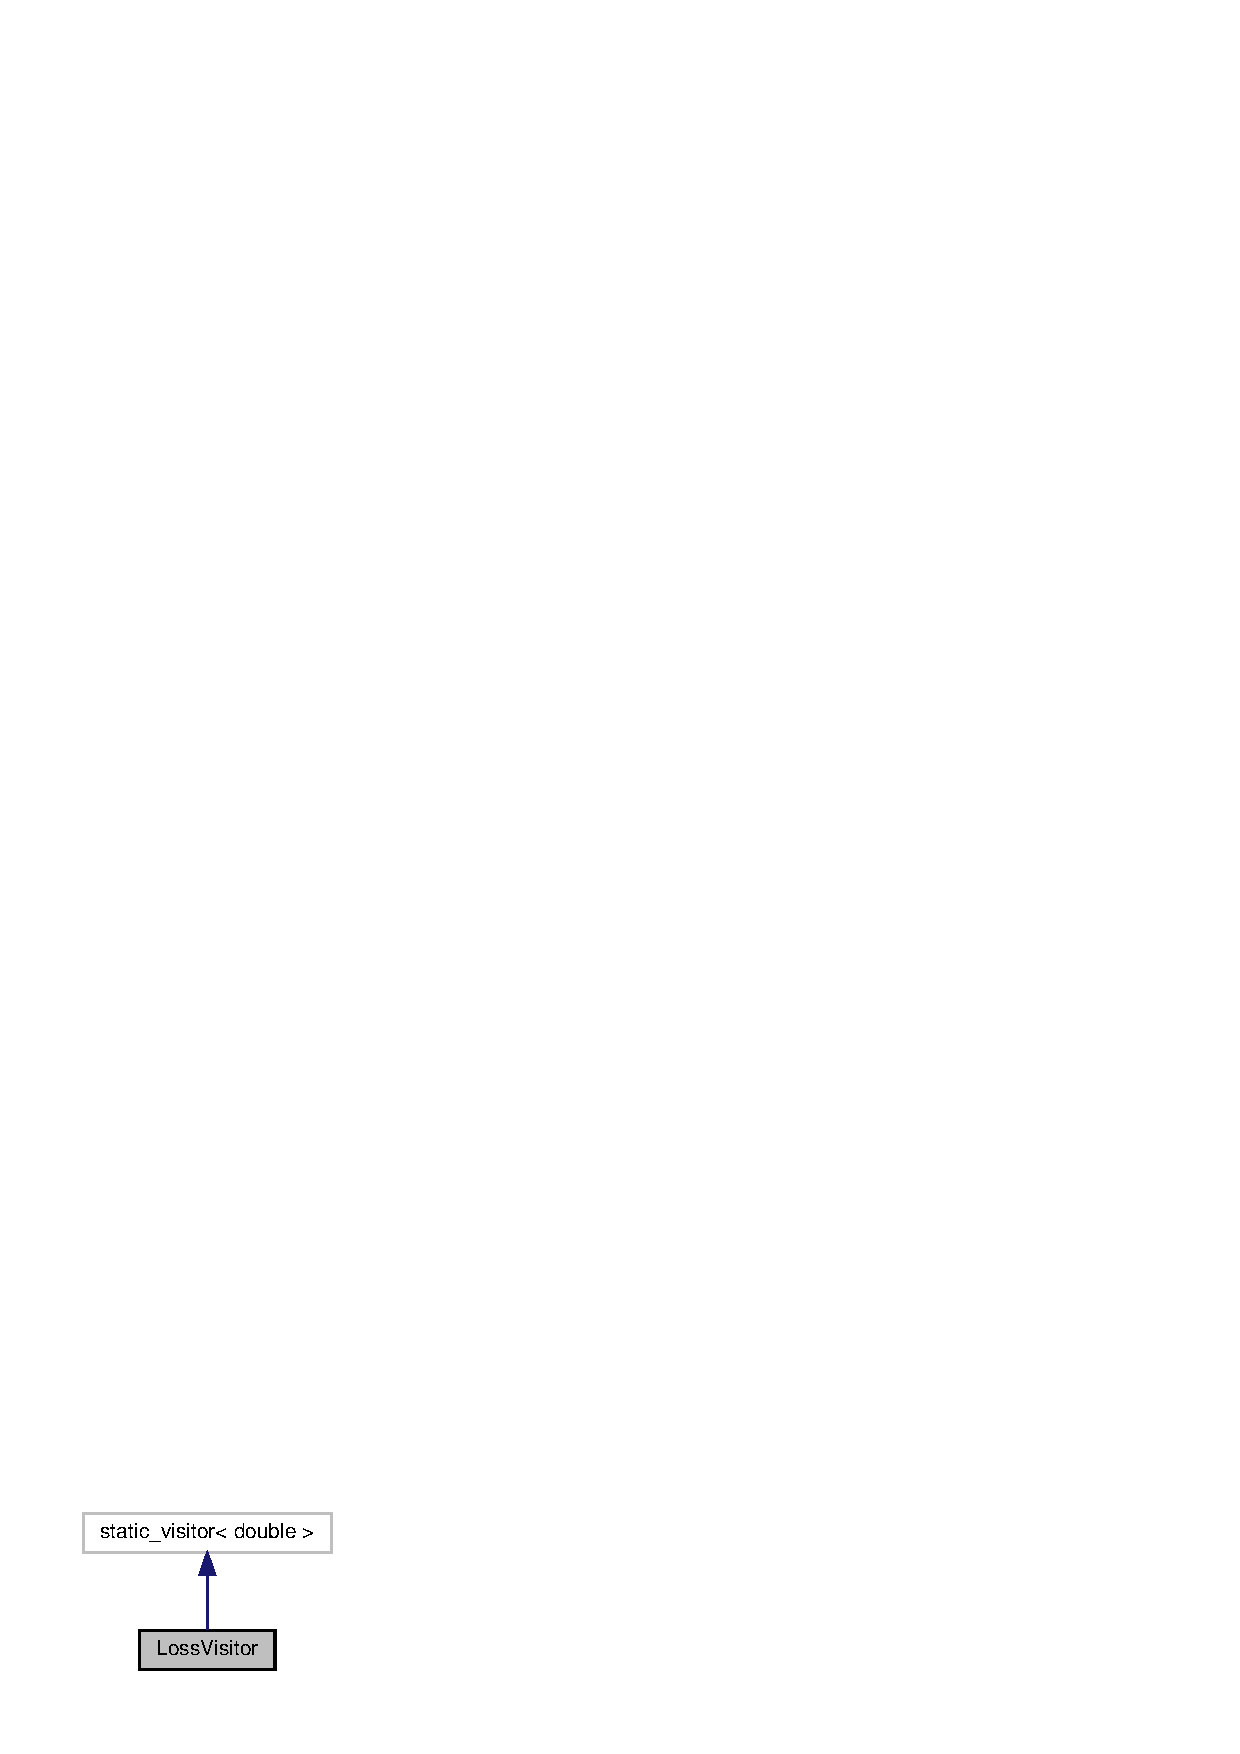
\includegraphics[width=163pt]{classmlpack_1_1ann_1_1LossVisitor__inherit__graph}
\end{center}
\end{figure}
\subsection*{Public Member Functions}
\begin{DoxyCompactItemize}
\item 
{\footnotesize template$<$typename Layer\+Type $>$ }\\double \textbf{ operator()} (Layer\+Type $\ast$layer) const
\begin{DoxyCompactList}\small\item\em Return the Loss. \end{DoxyCompactList}\item 
double \textbf{ operator()} (\textbf{ More\+Types} layer) const
\end{DoxyCompactItemize}


\subsection{Detailed Description}
\doxyref{Loss\+Visitor}{p.}{classmlpack_1_1ann_1_1LossVisitor} exposes the Loss() method of the given module. 

Definition at line 26 of file loss\+\_\+visitor.\+hpp.



\subsection{Member Function Documentation}
\mbox{\label{classmlpack_1_1ann_1_1LossVisitor_abb6d65ea84928702c2b8c3f7848317a5}} 
\index{mlpack\+::ann\+::\+Loss\+Visitor@{mlpack\+::ann\+::\+Loss\+Visitor}!operator()@{operator()}}
\index{operator()@{operator()}!mlpack\+::ann\+::\+Loss\+Visitor@{mlpack\+::ann\+::\+Loss\+Visitor}}
\subsubsection{operator()()\hspace{0.1cm}{\footnotesize\ttfamily [1/2]}}
{\footnotesize\ttfamily double operator() (\begin{DoxyParamCaption}\item[{Layer\+Type $\ast$}]{layer }\end{DoxyParamCaption}) const}



Return the Loss. 

\mbox{\label{classmlpack_1_1ann_1_1LossVisitor_aa805eedb3d714053058101cd78fc59ee}} 
\index{mlpack\+::ann\+::\+Loss\+Visitor@{mlpack\+::ann\+::\+Loss\+Visitor}!operator()@{operator()}}
\index{operator()@{operator()}!mlpack\+::ann\+::\+Loss\+Visitor@{mlpack\+::ann\+::\+Loss\+Visitor}}
\subsubsection{operator()()\hspace{0.1cm}{\footnotesize\ttfamily [2/2]}}
{\footnotesize\ttfamily double operator() (\begin{DoxyParamCaption}\item[{\textbf{ More\+Types}}]{layer }\end{DoxyParamCaption}) const}



The documentation for this class was generated from the following file\+:\begin{DoxyCompactItemize}
\item 
/home/aakash/mlpack/src/mlpack/methods/ann/visitor/\textbf{ loss\+\_\+visitor.\+hpp}\end{DoxyCompactItemize}

\section{Lp\+Pooling$<$ Input\+Data\+Type, Output\+Data\+Type $>$ Class Template Reference}
\label{classmlpack_1_1ann_1_1LpPooling}\index{Lp\+Pooling$<$ Input\+Data\+Type, Output\+Data\+Type $>$@{Lp\+Pooling$<$ Input\+Data\+Type, Output\+Data\+Type $>$}}


Implementation of the L\+P\+Pooling.  


\subsection*{Public Member Functions}
\begin{DoxyCompactItemize}
\item 
\textbf{ Lp\+Pooling} ()
\begin{DoxyCompactList}\small\item\em Create the \doxyref{Lp\+Pooling}{p.}{classmlpack_1_1ann_1_1LpPooling} object. \end{DoxyCompactList}\item 
\textbf{ Lp\+Pooling} (const size\+\_\+t norm\+Type, const size\+\_\+t kernel\+Width, const size\+\_\+t kernel\+Height, const size\+\_\+t stride\+Width=1, const size\+\_\+t stride\+Height=1, const bool floor=true)
\begin{DoxyCompactList}\small\item\em Create the \doxyref{Lp\+Pooling}{p.}{classmlpack_1_1ann_1_1LpPooling} object using the specified number of units. \end{DoxyCompactList}\item 
{\footnotesize template$<$typename eT $>$ }\\void \textbf{ Backward} (const arma\+::\+Mat$<$ eT $>$ \&, const arma\+::\+Mat$<$ eT $>$ \&gy, arma\+::\+Mat$<$ eT $>$ \&g)
\begin{DoxyCompactList}\small\item\em Ordinary feed backward pass of a neural network, using 3rd-\/order tensors as input, calculating the function f(x) by propagating x backwards through f. \end{DoxyCompactList}\item 
Output\+Data\+Type const  \& \textbf{ Delta} () const
\begin{DoxyCompactList}\small\item\em Get the delta. \end{DoxyCompactList}\item 
Output\+Data\+Type \& \textbf{ Delta} ()
\begin{DoxyCompactList}\small\item\em Modify the delta. \end{DoxyCompactList}\item 
bool const  \& \textbf{ Floor} () const
\begin{DoxyCompactList}\small\item\em Get the value of the rounding operation. \end{DoxyCompactList}\item 
bool \& \textbf{ Floor} ()
\begin{DoxyCompactList}\small\item\em Modify the value of the rounding operation. \end{DoxyCompactList}\item 
{\footnotesize template$<$typename eT $>$ }\\void \textbf{ Forward} (const arma\+::\+Mat$<$ eT $>$ \&input, arma\+::\+Mat$<$ eT $>$ \&output)
\begin{DoxyCompactList}\small\item\em Ordinary feed forward pass of a neural network, evaluating the function f(x) by propagating the activity forward through f. \end{DoxyCompactList}\item 
size\+\_\+t const  \& \textbf{ Input\+Height} () const
\begin{DoxyCompactList}\small\item\em Get the input height. \end{DoxyCompactList}\item 
size\+\_\+t \& \textbf{ Input\+Height} ()
\begin{DoxyCompactList}\small\item\em Modify the input height. \end{DoxyCompactList}\item 
size\+\_\+t \textbf{ Input\+Size} () const
\begin{DoxyCompactList}\small\item\em Get the input size. \end{DoxyCompactList}\item 
size\+\_\+t const  \& \textbf{ Input\+Width} () const
\begin{DoxyCompactList}\small\item\em Get the intput width. \end{DoxyCompactList}\item 
size\+\_\+t \& \textbf{ Input\+Width} ()
\begin{DoxyCompactList}\small\item\em Modify the input width. \end{DoxyCompactList}\item 
size\+\_\+t \textbf{ Kernel\+Height} () const
\begin{DoxyCompactList}\small\item\em Get the kernel height. \end{DoxyCompactList}\item 
size\+\_\+t \& \textbf{ Kernel\+Height} ()
\begin{DoxyCompactList}\small\item\em Modify the kernel height. \end{DoxyCompactList}\item 
size\+\_\+t \textbf{ Kernel\+Width} () const
\begin{DoxyCompactList}\small\item\em Get the kernel width. \end{DoxyCompactList}\item 
size\+\_\+t \& \textbf{ Kernel\+Width} ()
\begin{DoxyCompactList}\small\item\em Modify the kernel width. \end{DoxyCompactList}\item 
size\+\_\+t \textbf{ Norm\+Type} () const
\begin{DoxyCompactList}\small\item\em Get the norm\+Type. \end{DoxyCompactList}\item 
size\+\_\+t \& \textbf{ Norm\+Type} ()
\begin{DoxyCompactList}\small\item\em Modify the norm\+Type. \end{DoxyCompactList}\item 
size\+\_\+t const  \& \textbf{ Output\+Height} () const
\begin{DoxyCompactList}\small\item\em Get the output height. \end{DoxyCompactList}\item 
size\+\_\+t \& \textbf{ Output\+Height} ()
\begin{DoxyCompactList}\small\item\em Modify the output height. \end{DoxyCompactList}\item 
Output\+Data\+Type const  \& \textbf{ Output\+Parameter} () const
\begin{DoxyCompactList}\small\item\em Get the output parameter. \end{DoxyCompactList}\item 
Output\+Data\+Type \& \textbf{ Output\+Parameter} ()
\begin{DoxyCompactList}\small\item\em Modify the output parameter. \end{DoxyCompactList}\item 
size\+\_\+t \textbf{ Output\+Size} () const
\begin{DoxyCompactList}\small\item\em Get the output size. \end{DoxyCompactList}\item 
size\+\_\+t const  \& \textbf{ Output\+Width} () const
\begin{DoxyCompactList}\small\item\em Get the output width. \end{DoxyCompactList}\item 
size\+\_\+t \& \textbf{ Output\+Width} ()
\begin{DoxyCompactList}\small\item\em Modify the output width. \end{DoxyCompactList}\item 
{\footnotesize template$<$typename Archive $>$ }\\void \textbf{ serialize} (Archive \&ar, const uint32\+\_\+t)
\begin{DoxyCompactList}\small\item\em Serialize the layer. \end{DoxyCompactList}\item 
size\+\_\+t \textbf{ Stride\+Height} () const
\begin{DoxyCompactList}\small\item\em Get the stride height. \end{DoxyCompactList}\item 
size\+\_\+t \& \textbf{ Stride\+Height} ()
\begin{DoxyCompactList}\small\item\em Modify the stride height. \end{DoxyCompactList}\item 
size\+\_\+t \textbf{ Stride\+Width} () const
\begin{DoxyCompactList}\small\item\em Get the stride width. \end{DoxyCompactList}\item 
size\+\_\+t \& \textbf{ Stride\+Width} ()
\begin{DoxyCompactList}\small\item\em Modify the stride width. \end{DoxyCompactList}\item 
size\+\_\+t \textbf{ Weight\+Size} () const
\begin{DoxyCompactList}\small\item\em Get the size of the weights. \end{DoxyCompactList}\end{DoxyCompactItemize}


\subsection{Detailed Description}
\subsubsection*{template$<$typename Input\+Data\+Type = arma\+::mat, typename Output\+Data\+Type = arma\+::mat$>$\newline
class mlpack\+::ann\+::\+Lp\+Pooling$<$ Input\+Data\+Type, Output\+Data\+Type $>$}

Implementation of the L\+P\+Pooling. 


\begin{DoxyTemplParams}{Template Parameters}
{\em Input\+Data\+Type} & Type of the input data (arma\+::colvec, arma\+::mat, arma\+::sp\+\_\+mat or arma\+::cube). \\
\hline
{\em Output\+Data\+Type} & Type of the output data (arma\+::colvec, arma\+::mat, arma\+::sp\+\_\+mat or arma\+::cube). \\
\hline
\end{DoxyTemplParams}


Definition at line 32 of file lp\+\_\+pooling.\+hpp.



\subsection{Constructor \& Destructor Documentation}
\mbox{\label{classmlpack_1_1ann_1_1LpPooling_a6619f8729fd6af5eb5baf653fb4b595a}} 
\index{mlpack\+::ann\+::\+Lp\+Pooling@{mlpack\+::ann\+::\+Lp\+Pooling}!Lp\+Pooling@{Lp\+Pooling}}
\index{Lp\+Pooling@{Lp\+Pooling}!mlpack\+::ann\+::\+Lp\+Pooling@{mlpack\+::ann\+::\+Lp\+Pooling}}
\subsubsection{Lp\+Pooling()\hspace{0.1cm}{\footnotesize\ttfamily [1/2]}}
{\footnotesize\ttfamily \textbf{ Lp\+Pooling} (\begin{DoxyParamCaption}{ }\end{DoxyParamCaption})}



Create the \doxyref{Lp\+Pooling}{p.}{classmlpack_1_1ann_1_1LpPooling} object. 

\mbox{\label{classmlpack_1_1ann_1_1LpPooling_ad035ad444b6d260cb0428dc996a8a88e}} 
\index{mlpack\+::ann\+::\+Lp\+Pooling@{mlpack\+::ann\+::\+Lp\+Pooling}!Lp\+Pooling@{Lp\+Pooling}}
\index{Lp\+Pooling@{Lp\+Pooling}!mlpack\+::ann\+::\+Lp\+Pooling@{mlpack\+::ann\+::\+Lp\+Pooling}}
\subsubsection{Lp\+Pooling()\hspace{0.1cm}{\footnotesize\ttfamily [2/2]}}
{\footnotesize\ttfamily \textbf{ Lp\+Pooling} (\begin{DoxyParamCaption}\item[{const size\+\_\+t}]{norm\+Type,  }\item[{const size\+\_\+t}]{kernel\+Width,  }\item[{const size\+\_\+t}]{kernel\+Height,  }\item[{const size\+\_\+t}]{stride\+Width = {\ttfamily 1},  }\item[{const size\+\_\+t}]{stride\+Height = {\ttfamily 1},  }\item[{const bool}]{floor = {\ttfamily true} }\end{DoxyParamCaption})}



Create the \doxyref{Lp\+Pooling}{p.}{classmlpack_1_1ann_1_1LpPooling} object using the specified number of units. 


\begin{DoxyParams}{Parameters}
{\em norm\+Type} & Parameter for type of norm. \\
\hline
{\em kernel\+Width} & Width of the pooling window. \\
\hline
{\em kernel\+Height} & Height of the pooling window. \\
\hline
{\em stride\+Width} & Width of the stride operation. \\
\hline
{\em stride\+Height} & Width of the stride operation. \\
\hline
{\em floor} & Set to true to use floor method. \\
\hline
\end{DoxyParams}


\subsection{Member Function Documentation}
\mbox{\label{classmlpack_1_1ann_1_1LpPooling_ad9ad1a3bdb0f3fff5c839ed155e4bbf8}} 
\index{mlpack\+::ann\+::\+Lp\+Pooling@{mlpack\+::ann\+::\+Lp\+Pooling}!Backward@{Backward}}
\index{Backward@{Backward}!mlpack\+::ann\+::\+Lp\+Pooling@{mlpack\+::ann\+::\+Lp\+Pooling}}
\subsubsection{Backward()}
{\footnotesize\ttfamily void Backward (\begin{DoxyParamCaption}\item[{const arma\+::\+Mat$<$ eT $>$ \&}]{,  }\item[{const arma\+::\+Mat$<$ eT $>$ \&}]{gy,  }\item[{arma\+::\+Mat$<$ eT $>$ \&}]{g }\end{DoxyParamCaption})}



Ordinary feed backward pass of a neural network, using 3rd-\/order tensors as input, calculating the function f(x) by propagating x backwards through f. 

Using the results from the feed forward pass.


\begin{DoxyParams}{Parameters}
{\em $\ast$} & (input) The propagated input activation. \\
\hline
{\em gy} & The backpropagated error. \\
\hline
{\em g} & The calculated gradient. \\
\hline
\end{DoxyParams}
\mbox{\label{classmlpack_1_1ann_1_1LpPooling_a797f7edb44dd081e5e2b3cc316eef6bd}} 
\index{mlpack\+::ann\+::\+Lp\+Pooling@{mlpack\+::ann\+::\+Lp\+Pooling}!Delta@{Delta}}
\index{Delta@{Delta}!mlpack\+::ann\+::\+Lp\+Pooling@{mlpack\+::ann\+::\+Lp\+Pooling}}
\subsubsection{Delta()\hspace{0.1cm}{\footnotesize\ttfamily [1/2]}}
{\footnotesize\ttfamily Output\+Data\+Type const\& Delta (\begin{DoxyParamCaption}{ }\end{DoxyParamCaption}) const\hspace{0.3cm}{\ttfamily [inline]}}



Get the delta. 



Definition at line 85 of file lp\+\_\+pooling.\+hpp.

\mbox{\label{classmlpack_1_1ann_1_1LpPooling_ad6601342d560219ce951d554e69e5e87}} 
\index{mlpack\+::ann\+::\+Lp\+Pooling@{mlpack\+::ann\+::\+Lp\+Pooling}!Delta@{Delta}}
\index{Delta@{Delta}!mlpack\+::ann\+::\+Lp\+Pooling@{mlpack\+::ann\+::\+Lp\+Pooling}}
\subsubsection{Delta()\hspace{0.1cm}{\footnotesize\ttfamily [2/2]}}
{\footnotesize\ttfamily Output\+Data\+Type\& Delta (\begin{DoxyParamCaption}{ }\end{DoxyParamCaption})\hspace{0.3cm}{\ttfamily [inline]}}



Modify the delta. 



Definition at line 87 of file lp\+\_\+pooling.\+hpp.

\mbox{\label{classmlpack_1_1ann_1_1LpPooling_a787a10955ce98f589e7cc08f1c1beb75}} 
\index{mlpack\+::ann\+::\+Lp\+Pooling@{mlpack\+::ann\+::\+Lp\+Pooling}!Floor@{Floor}}
\index{Floor@{Floor}!mlpack\+::ann\+::\+Lp\+Pooling@{mlpack\+::ann\+::\+Lp\+Pooling}}
\subsubsection{Floor()\hspace{0.1cm}{\footnotesize\ttfamily [1/2]}}
{\footnotesize\ttfamily bool const\& Floor (\begin{DoxyParamCaption}{ }\end{DoxyParamCaption}) const\hspace{0.3cm}{\ttfamily [inline]}}



Get the value of the rounding operation. 



Definition at line 141 of file lp\+\_\+pooling.\+hpp.

\mbox{\label{classmlpack_1_1ann_1_1LpPooling_a8859ce7b4be2b8ffbf36bbc8ff16aecd}} 
\index{mlpack\+::ann\+::\+Lp\+Pooling@{mlpack\+::ann\+::\+Lp\+Pooling}!Floor@{Floor}}
\index{Floor@{Floor}!mlpack\+::ann\+::\+Lp\+Pooling@{mlpack\+::ann\+::\+Lp\+Pooling}}
\subsubsection{Floor()\hspace{0.1cm}{\footnotesize\ttfamily [2/2]}}
{\footnotesize\ttfamily bool\& Floor (\begin{DoxyParamCaption}{ }\end{DoxyParamCaption})\hspace{0.3cm}{\ttfamily [inline]}}



Modify the value of the rounding operation. 



Definition at line 143 of file lp\+\_\+pooling.\+hpp.

\mbox{\label{classmlpack_1_1ann_1_1LpPooling_a461f849bc638c15bec262dc9c3a58abe}} 
\index{mlpack\+::ann\+::\+Lp\+Pooling@{mlpack\+::ann\+::\+Lp\+Pooling}!Forward@{Forward}}
\index{Forward@{Forward}!mlpack\+::ann\+::\+Lp\+Pooling@{mlpack\+::ann\+::\+Lp\+Pooling}}
\subsubsection{Forward()}
{\footnotesize\ttfamily void Forward (\begin{DoxyParamCaption}\item[{const arma\+::\+Mat$<$ eT $>$ \&}]{input,  }\item[{arma\+::\+Mat$<$ eT $>$ \&}]{output }\end{DoxyParamCaption})}



Ordinary feed forward pass of a neural network, evaluating the function f(x) by propagating the activity forward through f. 


\begin{DoxyParams}{Parameters}
{\em input} & Input data used for evaluating the specified function. \\
\hline
{\em output} & Resulting output activation. \\
\hline
\end{DoxyParams}
\mbox{\label{classmlpack_1_1ann_1_1LpPooling_afb3fd4ed60dd057e7852221b89206f15}} 
\index{mlpack\+::ann\+::\+Lp\+Pooling@{mlpack\+::ann\+::\+Lp\+Pooling}!Input\+Height@{Input\+Height}}
\index{Input\+Height@{Input\+Height}!mlpack\+::ann\+::\+Lp\+Pooling@{mlpack\+::ann\+::\+Lp\+Pooling}}
\subsubsection{Input\+Height()\hspace{0.1cm}{\footnotesize\ttfamily [1/2]}}
{\footnotesize\ttfamily size\+\_\+t const\& Input\+Height (\begin{DoxyParamCaption}{ }\end{DoxyParamCaption}) const\hspace{0.3cm}{\ttfamily [inline]}}



Get the input height. 



Definition at line 95 of file lp\+\_\+pooling.\+hpp.

\mbox{\label{classmlpack_1_1ann_1_1LpPooling_aefbba724eec397a928d5460bb209a360}} 
\index{mlpack\+::ann\+::\+Lp\+Pooling@{mlpack\+::ann\+::\+Lp\+Pooling}!Input\+Height@{Input\+Height}}
\index{Input\+Height@{Input\+Height}!mlpack\+::ann\+::\+Lp\+Pooling@{mlpack\+::ann\+::\+Lp\+Pooling}}
\subsubsection{Input\+Height()\hspace{0.1cm}{\footnotesize\ttfamily [2/2]}}
{\footnotesize\ttfamily size\+\_\+t\& Input\+Height (\begin{DoxyParamCaption}{ }\end{DoxyParamCaption})\hspace{0.3cm}{\ttfamily [inline]}}



Modify the input height. 



Definition at line 97 of file lp\+\_\+pooling.\+hpp.

\mbox{\label{classmlpack_1_1ann_1_1LpPooling_a5a4c4984aa897a28d516e638e7ea5308}} 
\index{mlpack\+::ann\+::\+Lp\+Pooling@{mlpack\+::ann\+::\+Lp\+Pooling}!Input\+Size@{Input\+Size}}
\index{Input\+Size@{Input\+Size}!mlpack\+::ann\+::\+Lp\+Pooling@{mlpack\+::ann\+::\+Lp\+Pooling}}
\subsubsection{Input\+Size()}
{\footnotesize\ttfamily size\+\_\+t Input\+Size (\begin{DoxyParamCaption}{ }\end{DoxyParamCaption}) const\hspace{0.3cm}{\ttfamily [inline]}}



Get the input size. 



Definition at line 110 of file lp\+\_\+pooling.\+hpp.

\mbox{\label{classmlpack_1_1ann_1_1LpPooling_a29346e3064da8f9e5f10596bedae0ba8}} 
\index{mlpack\+::ann\+::\+Lp\+Pooling@{mlpack\+::ann\+::\+Lp\+Pooling}!Input\+Width@{Input\+Width}}
\index{Input\+Width@{Input\+Width}!mlpack\+::ann\+::\+Lp\+Pooling@{mlpack\+::ann\+::\+Lp\+Pooling}}
\subsubsection{Input\+Width()\hspace{0.1cm}{\footnotesize\ttfamily [1/2]}}
{\footnotesize\ttfamily size\+\_\+t const\& Input\+Width (\begin{DoxyParamCaption}{ }\end{DoxyParamCaption}) const\hspace{0.3cm}{\ttfamily [inline]}}



Get the intput width. 



Definition at line 90 of file lp\+\_\+pooling.\+hpp.

\mbox{\label{classmlpack_1_1ann_1_1LpPooling_a238e9d308df611a9300a4ca6756fef4d}} 
\index{mlpack\+::ann\+::\+Lp\+Pooling@{mlpack\+::ann\+::\+Lp\+Pooling}!Input\+Width@{Input\+Width}}
\index{Input\+Width@{Input\+Width}!mlpack\+::ann\+::\+Lp\+Pooling@{mlpack\+::ann\+::\+Lp\+Pooling}}
\subsubsection{Input\+Width()\hspace{0.1cm}{\footnotesize\ttfamily [2/2]}}
{\footnotesize\ttfamily size\+\_\+t\& Input\+Width (\begin{DoxyParamCaption}{ }\end{DoxyParamCaption})\hspace{0.3cm}{\ttfamily [inline]}}



Modify the input width. 



Definition at line 92 of file lp\+\_\+pooling.\+hpp.

\mbox{\label{classmlpack_1_1ann_1_1LpPooling_a6c15e2e3416651fac44621acbbdac9e9}} 
\index{mlpack\+::ann\+::\+Lp\+Pooling@{mlpack\+::ann\+::\+Lp\+Pooling}!Kernel\+Height@{Kernel\+Height}}
\index{Kernel\+Height@{Kernel\+Height}!mlpack\+::ann\+::\+Lp\+Pooling@{mlpack\+::ann\+::\+Lp\+Pooling}}
\subsubsection{Kernel\+Height()\hspace{0.1cm}{\footnotesize\ttfamily [1/2]}}
{\footnotesize\ttfamily size\+\_\+t Kernel\+Height (\begin{DoxyParamCaption}{ }\end{DoxyParamCaption}) const\hspace{0.3cm}{\ttfamily [inline]}}



Get the kernel height. 



Definition at line 126 of file lp\+\_\+pooling.\+hpp.

\mbox{\label{classmlpack_1_1ann_1_1LpPooling_a46b2c28d89959067f549f9f45d2626c5}} 
\index{mlpack\+::ann\+::\+Lp\+Pooling@{mlpack\+::ann\+::\+Lp\+Pooling}!Kernel\+Height@{Kernel\+Height}}
\index{Kernel\+Height@{Kernel\+Height}!mlpack\+::ann\+::\+Lp\+Pooling@{mlpack\+::ann\+::\+Lp\+Pooling}}
\subsubsection{Kernel\+Height()\hspace{0.1cm}{\footnotesize\ttfamily [2/2]}}
{\footnotesize\ttfamily size\+\_\+t\& Kernel\+Height (\begin{DoxyParamCaption}{ }\end{DoxyParamCaption})\hspace{0.3cm}{\ttfamily [inline]}}



Modify the kernel height. 



Definition at line 128 of file lp\+\_\+pooling.\+hpp.

\mbox{\label{classmlpack_1_1ann_1_1LpPooling_a656302bc9b300692aa71abe2a614c7b1}} 
\index{mlpack\+::ann\+::\+Lp\+Pooling@{mlpack\+::ann\+::\+Lp\+Pooling}!Kernel\+Width@{Kernel\+Width}}
\index{Kernel\+Width@{Kernel\+Width}!mlpack\+::ann\+::\+Lp\+Pooling@{mlpack\+::ann\+::\+Lp\+Pooling}}
\subsubsection{Kernel\+Width()\hspace{0.1cm}{\footnotesize\ttfamily [1/2]}}
{\footnotesize\ttfamily size\+\_\+t Kernel\+Width (\begin{DoxyParamCaption}{ }\end{DoxyParamCaption}) const\hspace{0.3cm}{\ttfamily [inline]}}



Get the kernel width. 



Definition at line 121 of file lp\+\_\+pooling.\+hpp.

\mbox{\label{classmlpack_1_1ann_1_1LpPooling_a5fbae452ceda395f5566833e06ba3615}} 
\index{mlpack\+::ann\+::\+Lp\+Pooling@{mlpack\+::ann\+::\+Lp\+Pooling}!Kernel\+Width@{Kernel\+Width}}
\index{Kernel\+Width@{Kernel\+Width}!mlpack\+::ann\+::\+Lp\+Pooling@{mlpack\+::ann\+::\+Lp\+Pooling}}
\subsubsection{Kernel\+Width()\hspace{0.1cm}{\footnotesize\ttfamily [2/2]}}
{\footnotesize\ttfamily size\+\_\+t\& Kernel\+Width (\begin{DoxyParamCaption}{ }\end{DoxyParamCaption})\hspace{0.3cm}{\ttfamily [inline]}}



Modify the kernel width. 



Definition at line 123 of file lp\+\_\+pooling.\+hpp.

\mbox{\label{classmlpack_1_1ann_1_1LpPooling_a529256885c775d74f9716b7d4e31962e}} 
\index{mlpack\+::ann\+::\+Lp\+Pooling@{mlpack\+::ann\+::\+Lp\+Pooling}!Norm\+Type@{Norm\+Type}}
\index{Norm\+Type@{Norm\+Type}!mlpack\+::ann\+::\+Lp\+Pooling@{mlpack\+::ann\+::\+Lp\+Pooling}}
\subsubsection{Norm\+Type()\hspace{0.1cm}{\footnotesize\ttfamily [1/2]}}
{\footnotesize\ttfamily size\+\_\+t Norm\+Type (\begin{DoxyParamCaption}{ }\end{DoxyParamCaption}) const\hspace{0.3cm}{\ttfamily [inline]}}



Get the norm\+Type. 



Definition at line 116 of file lp\+\_\+pooling.\+hpp.

\mbox{\label{classmlpack_1_1ann_1_1LpPooling_a931485333bbadf0e78fbec7e8073ef4b}} 
\index{mlpack\+::ann\+::\+Lp\+Pooling@{mlpack\+::ann\+::\+Lp\+Pooling}!Norm\+Type@{Norm\+Type}}
\index{Norm\+Type@{Norm\+Type}!mlpack\+::ann\+::\+Lp\+Pooling@{mlpack\+::ann\+::\+Lp\+Pooling}}
\subsubsection{Norm\+Type()\hspace{0.1cm}{\footnotesize\ttfamily [2/2]}}
{\footnotesize\ttfamily size\+\_\+t\& Norm\+Type (\begin{DoxyParamCaption}{ }\end{DoxyParamCaption})\hspace{0.3cm}{\ttfamily [inline]}}



Modify the norm\+Type. 



Definition at line 118 of file lp\+\_\+pooling.\+hpp.

\mbox{\label{classmlpack_1_1ann_1_1LpPooling_a5ad7dbcaf1a622dafd897f79ab77890c}} 
\index{mlpack\+::ann\+::\+Lp\+Pooling@{mlpack\+::ann\+::\+Lp\+Pooling}!Output\+Height@{Output\+Height}}
\index{Output\+Height@{Output\+Height}!mlpack\+::ann\+::\+Lp\+Pooling@{mlpack\+::ann\+::\+Lp\+Pooling}}
\subsubsection{Output\+Height()\hspace{0.1cm}{\footnotesize\ttfamily [1/2]}}
{\footnotesize\ttfamily size\+\_\+t const\& Output\+Height (\begin{DoxyParamCaption}{ }\end{DoxyParamCaption}) const\hspace{0.3cm}{\ttfamily [inline]}}



Get the output height. 



Definition at line 105 of file lp\+\_\+pooling.\+hpp.

\mbox{\label{classmlpack_1_1ann_1_1LpPooling_ac5112abf9f5e1face13ed965a8755b1d}} 
\index{mlpack\+::ann\+::\+Lp\+Pooling@{mlpack\+::ann\+::\+Lp\+Pooling}!Output\+Height@{Output\+Height}}
\index{Output\+Height@{Output\+Height}!mlpack\+::ann\+::\+Lp\+Pooling@{mlpack\+::ann\+::\+Lp\+Pooling}}
\subsubsection{Output\+Height()\hspace{0.1cm}{\footnotesize\ttfamily [2/2]}}
{\footnotesize\ttfamily size\+\_\+t\& Output\+Height (\begin{DoxyParamCaption}{ }\end{DoxyParamCaption})\hspace{0.3cm}{\ttfamily [inline]}}



Modify the output height. 



Definition at line 107 of file lp\+\_\+pooling.\+hpp.

\mbox{\label{classmlpack_1_1ann_1_1LpPooling_a0ee21c2a36e5abad1e7a9d5dd00849f9}} 
\index{mlpack\+::ann\+::\+Lp\+Pooling@{mlpack\+::ann\+::\+Lp\+Pooling}!Output\+Parameter@{Output\+Parameter}}
\index{Output\+Parameter@{Output\+Parameter}!mlpack\+::ann\+::\+Lp\+Pooling@{mlpack\+::ann\+::\+Lp\+Pooling}}
\subsubsection{Output\+Parameter()\hspace{0.1cm}{\footnotesize\ttfamily [1/2]}}
{\footnotesize\ttfamily Output\+Data\+Type const\& Output\+Parameter (\begin{DoxyParamCaption}{ }\end{DoxyParamCaption}) const\hspace{0.3cm}{\ttfamily [inline]}}



Get the output parameter. 



Definition at line 80 of file lp\+\_\+pooling.\+hpp.

\mbox{\label{classmlpack_1_1ann_1_1LpPooling_a21d5f745f02c709625a4ee0907f004a5}} 
\index{mlpack\+::ann\+::\+Lp\+Pooling@{mlpack\+::ann\+::\+Lp\+Pooling}!Output\+Parameter@{Output\+Parameter}}
\index{Output\+Parameter@{Output\+Parameter}!mlpack\+::ann\+::\+Lp\+Pooling@{mlpack\+::ann\+::\+Lp\+Pooling}}
\subsubsection{Output\+Parameter()\hspace{0.1cm}{\footnotesize\ttfamily [2/2]}}
{\footnotesize\ttfamily Output\+Data\+Type\& Output\+Parameter (\begin{DoxyParamCaption}{ }\end{DoxyParamCaption})\hspace{0.3cm}{\ttfamily [inline]}}



Modify the output parameter. 



Definition at line 82 of file lp\+\_\+pooling.\+hpp.

\mbox{\label{classmlpack_1_1ann_1_1LpPooling_a99c1d948c984b9e76fb5e37e2145427a}} 
\index{mlpack\+::ann\+::\+Lp\+Pooling@{mlpack\+::ann\+::\+Lp\+Pooling}!Output\+Size@{Output\+Size}}
\index{Output\+Size@{Output\+Size}!mlpack\+::ann\+::\+Lp\+Pooling@{mlpack\+::ann\+::\+Lp\+Pooling}}
\subsubsection{Output\+Size()}
{\footnotesize\ttfamily size\+\_\+t Output\+Size (\begin{DoxyParamCaption}{ }\end{DoxyParamCaption}) const\hspace{0.3cm}{\ttfamily [inline]}}



Get the output size. 



Definition at line 113 of file lp\+\_\+pooling.\+hpp.

\mbox{\label{classmlpack_1_1ann_1_1LpPooling_a32b3e3fe787456847fc3b2c39586ecb1}} 
\index{mlpack\+::ann\+::\+Lp\+Pooling@{mlpack\+::ann\+::\+Lp\+Pooling}!Output\+Width@{Output\+Width}}
\index{Output\+Width@{Output\+Width}!mlpack\+::ann\+::\+Lp\+Pooling@{mlpack\+::ann\+::\+Lp\+Pooling}}
\subsubsection{Output\+Width()\hspace{0.1cm}{\footnotesize\ttfamily [1/2]}}
{\footnotesize\ttfamily size\+\_\+t const\& Output\+Width (\begin{DoxyParamCaption}{ }\end{DoxyParamCaption}) const\hspace{0.3cm}{\ttfamily [inline]}}



Get the output width. 



Definition at line 100 of file lp\+\_\+pooling.\+hpp.

\mbox{\label{classmlpack_1_1ann_1_1LpPooling_a54579ec9924e2a4a5bc0a4fb822ce80c}} 
\index{mlpack\+::ann\+::\+Lp\+Pooling@{mlpack\+::ann\+::\+Lp\+Pooling}!Output\+Width@{Output\+Width}}
\index{Output\+Width@{Output\+Width}!mlpack\+::ann\+::\+Lp\+Pooling@{mlpack\+::ann\+::\+Lp\+Pooling}}
\subsubsection{Output\+Width()\hspace{0.1cm}{\footnotesize\ttfamily [2/2]}}
{\footnotesize\ttfamily size\+\_\+t\& Output\+Width (\begin{DoxyParamCaption}{ }\end{DoxyParamCaption})\hspace{0.3cm}{\ttfamily [inline]}}



Modify the output width. 



Definition at line 102 of file lp\+\_\+pooling.\+hpp.

\mbox{\label{classmlpack_1_1ann_1_1LpPooling_a65cba07328997659bec80b9879b15a51}} 
\index{mlpack\+::ann\+::\+Lp\+Pooling@{mlpack\+::ann\+::\+Lp\+Pooling}!serialize@{serialize}}
\index{serialize@{serialize}!mlpack\+::ann\+::\+Lp\+Pooling@{mlpack\+::ann\+::\+Lp\+Pooling}}
\subsubsection{serialize()}
{\footnotesize\ttfamily void serialize (\begin{DoxyParamCaption}\item[{Archive \&}]{ar,  }\item[{const uint32\+\_\+t}]{ }\end{DoxyParamCaption})}



Serialize the layer. 



Referenced by Lp\+Pooling$<$ Input\+Data\+Type, Output\+Data\+Type $>$\+::\+Weight\+Size().

\mbox{\label{classmlpack_1_1ann_1_1LpPooling_a1894b819a7ff82a5576fc8deb8ba7457}} 
\index{mlpack\+::ann\+::\+Lp\+Pooling@{mlpack\+::ann\+::\+Lp\+Pooling}!Stride\+Height@{Stride\+Height}}
\index{Stride\+Height@{Stride\+Height}!mlpack\+::ann\+::\+Lp\+Pooling@{mlpack\+::ann\+::\+Lp\+Pooling}}
\subsubsection{Stride\+Height()\hspace{0.1cm}{\footnotesize\ttfamily [1/2]}}
{\footnotesize\ttfamily size\+\_\+t Stride\+Height (\begin{DoxyParamCaption}{ }\end{DoxyParamCaption}) const\hspace{0.3cm}{\ttfamily [inline]}}



Get the stride height. 



Definition at line 136 of file lp\+\_\+pooling.\+hpp.

\mbox{\label{classmlpack_1_1ann_1_1LpPooling_a0dd3de9c8a9060e927c575b57a021e8b}} 
\index{mlpack\+::ann\+::\+Lp\+Pooling@{mlpack\+::ann\+::\+Lp\+Pooling}!Stride\+Height@{Stride\+Height}}
\index{Stride\+Height@{Stride\+Height}!mlpack\+::ann\+::\+Lp\+Pooling@{mlpack\+::ann\+::\+Lp\+Pooling}}
\subsubsection{Stride\+Height()\hspace{0.1cm}{\footnotesize\ttfamily [2/2]}}
{\footnotesize\ttfamily size\+\_\+t\& Stride\+Height (\begin{DoxyParamCaption}{ }\end{DoxyParamCaption})\hspace{0.3cm}{\ttfamily [inline]}}



Modify the stride height. 



Definition at line 138 of file lp\+\_\+pooling.\+hpp.

\mbox{\label{classmlpack_1_1ann_1_1LpPooling_ad8fd9eb6de956c3e9d82242793fd2db1}} 
\index{mlpack\+::ann\+::\+Lp\+Pooling@{mlpack\+::ann\+::\+Lp\+Pooling}!Stride\+Width@{Stride\+Width}}
\index{Stride\+Width@{Stride\+Width}!mlpack\+::ann\+::\+Lp\+Pooling@{mlpack\+::ann\+::\+Lp\+Pooling}}
\subsubsection{Stride\+Width()\hspace{0.1cm}{\footnotesize\ttfamily [1/2]}}
{\footnotesize\ttfamily size\+\_\+t Stride\+Width (\begin{DoxyParamCaption}{ }\end{DoxyParamCaption}) const\hspace{0.3cm}{\ttfamily [inline]}}



Get the stride width. 



Definition at line 131 of file lp\+\_\+pooling.\+hpp.

\mbox{\label{classmlpack_1_1ann_1_1LpPooling_af40557db9372b513440e06a5e42cc599}} 
\index{mlpack\+::ann\+::\+Lp\+Pooling@{mlpack\+::ann\+::\+Lp\+Pooling}!Stride\+Width@{Stride\+Width}}
\index{Stride\+Width@{Stride\+Width}!mlpack\+::ann\+::\+Lp\+Pooling@{mlpack\+::ann\+::\+Lp\+Pooling}}
\subsubsection{Stride\+Width()\hspace{0.1cm}{\footnotesize\ttfamily [2/2]}}
{\footnotesize\ttfamily size\+\_\+t\& Stride\+Width (\begin{DoxyParamCaption}{ }\end{DoxyParamCaption})\hspace{0.3cm}{\ttfamily [inline]}}



Modify the stride width. 



Definition at line 133 of file lp\+\_\+pooling.\+hpp.

\mbox{\label{classmlpack_1_1ann_1_1LpPooling_a7a2704698a50d9e00dfb083f3a863579}} 
\index{mlpack\+::ann\+::\+Lp\+Pooling@{mlpack\+::ann\+::\+Lp\+Pooling}!Weight\+Size@{Weight\+Size}}
\index{Weight\+Size@{Weight\+Size}!mlpack\+::ann\+::\+Lp\+Pooling@{mlpack\+::ann\+::\+Lp\+Pooling}}
\subsubsection{Weight\+Size()}
{\footnotesize\ttfamily size\+\_\+t Weight\+Size (\begin{DoxyParamCaption}{ }\end{DoxyParamCaption}) const\hspace{0.3cm}{\ttfamily [inline]}}



Get the size of the weights. 



Definition at line 146 of file lp\+\_\+pooling.\+hpp.



References Lp\+Pooling$<$ Input\+Data\+Type, Output\+Data\+Type $>$\+::serialize().



The documentation for this class was generated from the following file\+:\begin{DoxyCompactItemize}
\item 
/home/aakash/mlpack/src/mlpack/methods/ann/layer/\textbf{ lp\+\_\+pooling.\+hpp}\end{DoxyCompactItemize}

\section{L\+Regularizer$<$ T\+Power $>$ Class Template Reference}
\label{classmlpack_1_1ann_1_1LRegularizer}\index{L\+Regularizer$<$ T\+Power $>$@{L\+Regularizer$<$ T\+Power $>$}}


The L\+\_\+p regularizer for arbitrary integer p.  


\subsection*{Public Member Functions}
\begin{DoxyCompactItemize}
\item 
\textbf{ L\+Regularizer} (double \textbf{ factor}=1.\+0)
\begin{DoxyCompactList}\small\item\em Create the regularizer object. \end{DoxyCompactList}\item 
{\footnotesize template$<$typename Mat\+Type $>$ }\\void \textbf{ Evaluate} (const Mat\+Type \&weight, Mat\+Type \&gradient)
\begin{DoxyCompactList}\small\item\em Calculate the gradient for regularization. \end{DoxyCompactList}\item 
{\footnotesize template$<$typename Archive $>$ }\\void \textbf{ serialize} (Archive \&ar, const uint32\+\_\+t)
\begin{DoxyCompactList}\small\item\em Serialize the regularizer (nothing to do). \end{DoxyCompactList}\end{DoxyCompactItemize}
\subsection*{Public Attributes}
\begin{DoxyCompactItemize}
\item 
double \textbf{ factor}
\begin{DoxyCompactList}\small\item\em The constant for the regularization. \end{DoxyCompactList}\end{DoxyCompactItemize}
\subsection*{Static Public Attributes}
\begin{DoxyCompactItemize}
\item 
static const int \textbf{ Power} = T\+Power
\begin{DoxyCompactList}\small\item\em The power of the regularizer. \end{DoxyCompactList}\end{DoxyCompactItemize}


\subsection{Detailed Description}
\subsubsection*{template$<$int T\+Power$>$\newline
class mlpack\+::ann\+::\+L\+Regularizer$<$ T\+Power $>$}

The L\+\_\+p regularizer for arbitrary integer p. 


\begin{DoxyTemplParams}{Template Parameters}
{\em Power} & Power of regularizer; i.\+e. Power = 1 gives the L1-\/regularization. \\
\hline
\end{DoxyTemplParams}


Definition at line 27 of file lregularizer.\+hpp.



\subsection{Constructor \& Destructor Documentation}
\mbox{\label{classmlpack_1_1ann_1_1LRegularizer_af4560ea21b7a7f93ad15a5ea65cf5c36}} 
\index{mlpack\+::ann\+::\+L\+Regularizer@{mlpack\+::ann\+::\+L\+Regularizer}!L\+Regularizer@{L\+Regularizer}}
\index{L\+Regularizer@{L\+Regularizer}!mlpack\+::ann\+::\+L\+Regularizer@{mlpack\+::ann\+::\+L\+Regularizer}}
\subsubsection{L\+Regularizer()}
{\footnotesize\ttfamily \textbf{ L\+Regularizer} (\begin{DoxyParamCaption}\item[{double}]{factor = {\ttfamily 1.0} }\end{DoxyParamCaption})}



Create the regularizer object. 


\begin{DoxyParams}{Parameters}
{\em factor} & The factor for regularization. \\
\hline
\end{DoxyParams}


\subsection{Member Function Documentation}
\mbox{\label{classmlpack_1_1ann_1_1LRegularizer_a77155b253292485b11241c0a4f04612a}} 
\index{mlpack\+::ann\+::\+L\+Regularizer@{mlpack\+::ann\+::\+L\+Regularizer}!Evaluate@{Evaluate}}
\index{Evaluate@{Evaluate}!mlpack\+::ann\+::\+L\+Regularizer@{mlpack\+::ann\+::\+L\+Regularizer}}
\subsubsection{Evaluate()}
{\footnotesize\ttfamily void Evaluate (\begin{DoxyParamCaption}\item[{const Mat\+Type \&}]{weight,  }\item[{Mat\+Type \&}]{gradient }\end{DoxyParamCaption})}



Calculate the gradient for regularization. 


\begin{DoxyTemplParams}{Template Parameters}
{\em Mat\+Type} & Type of weight matrix. \\
\hline
\end{DoxyTemplParams}

\begin{DoxyParams}{Parameters}
{\em weight} & The weight matrix to be regularized. \\
\hline
{\em gradient} & The calculated gradient. \\
\hline
\end{DoxyParams}
\mbox{\label{classmlpack_1_1ann_1_1LRegularizer_a65cba07328997659bec80b9879b15a51}} 
\index{mlpack\+::ann\+::\+L\+Regularizer@{mlpack\+::ann\+::\+L\+Regularizer}!serialize@{serialize}}
\index{serialize@{serialize}!mlpack\+::ann\+::\+L\+Regularizer@{mlpack\+::ann\+::\+L\+Regularizer}}
\subsubsection{serialize()}
{\footnotesize\ttfamily void serialize (\begin{DoxyParamCaption}\item[{Archive \&}]{ar,  }\item[{const uint32\+\_\+t}]{ }\end{DoxyParamCaption})}



Serialize the regularizer (nothing to do). 



\subsection{Member Data Documentation}
\mbox{\label{classmlpack_1_1ann_1_1LRegularizer_a2d7e5dd7a479c4c7aef6e6133a1441c5}} 
\index{mlpack\+::ann\+::\+L\+Regularizer@{mlpack\+::ann\+::\+L\+Regularizer}!factor@{factor}}
\index{factor@{factor}!mlpack\+::ann\+::\+L\+Regularizer@{mlpack\+::ann\+::\+L\+Regularizer}}
\subsubsection{factor}
{\footnotesize\ttfamily double factor}



The constant for the regularization. 



Definition at line 55 of file lregularizer.\+hpp.

\mbox{\label{classmlpack_1_1ann_1_1LRegularizer_add828b673634e896b13f47cc7fb331f5}} 
\index{mlpack\+::ann\+::\+L\+Regularizer@{mlpack\+::ann\+::\+L\+Regularizer}!Power@{Power}}
\index{Power@{Power}!mlpack\+::ann\+::\+L\+Regularizer@{mlpack\+::ann\+::\+L\+Regularizer}}
\subsubsection{Power}
{\footnotesize\ttfamily const int Power = T\+Power\hspace{0.3cm}{\ttfamily [static]}}



The power of the regularizer. 



Definition at line 52 of file lregularizer.\+hpp.



The documentation for this class was generated from the following file\+:\begin{DoxyCompactItemize}
\item 
/home/aakash/mlpack/src/mlpack/methods/ann/regularizer/\textbf{ lregularizer.\+hpp}\end{DoxyCompactItemize}

\section{L\+S\+TM$<$ Input\+Data\+Type, Output\+Data\+Type $>$ Class Template Reference}
\label{classmlpack_1_1ann_1_1LSTM}\index{L\+S\+T\+M$<$ Input\+Data\+Type, Output\+Data\+Type $>$@{L\+S\+T\+M$<$ Input\+Data\+Type, Output\+Data\+Type $>$}}


Implementation of the \doxyref{L\+S\+TM}{p.}{classmlpack_1_1ann_1_1LSTM} module class.  


\subsection*{Public Member Functions}
\begin{DoxyCompactItemize}
\item 
\textbf{ L\+S\+TM} ()
\begin{DoxyCompactList}\small\item\em Create the \doxyref{L\+S\+TM}{p.}{classmlpack_1_1ann_1_1LSTM} object. \end{DoxyCompactList}\item 
\textbf{ L\+S\+TM} (const size\+\_\+t in\+Size, const size\+\_\+t out\+Size, const size\+\_\+t rho=std\+::numeric\+\_\+limits$<$ size\+\_\+t $>$\+::max())
\begin{DoxyCompactList}\small\item\em Create the \doxyref{L\+S\+TM}{p.}{classmlpack_1_1ann_1_1LSTM} layer object using the specified parameters. \end{DoxyCompactList}\item 
\textbf{ L\+S\+TM} (const \textbf{ L\+S\+TM} \&layer)
\begin{DoxyCompactList}\small\item\em Copy constructor. \end{DoxyCompactList}\item 
\textbf{ L\+S\+TM} (\textbf{ L\+S\+TM} \&\&)
\begin{DoxyCompactList}\small\item\em Move constructor. \end{DoxyCompactList}\item 
{\footnotesize template$<$typename Input\+Type , typename Error\+Type , typename Gradient\+Type $>$ }\\void \textbf{ Backward} (const Input\+Type \&input, const Error\+Type \&gy, Gradient\+Type \&g)
\begin{DoxyCompactList}\small\item\em Ordinary feed backward pass of a neural network, calculating the function f(x) by propagating x backwards trough f. \end{DoxyCompactList}\item 
Output\+Data\+Type const  \& \textbf{ Delta} () const
\begin{DoxyCompactList}\small\item\em Get the delta. \end{DoxyCompactList}\item 
Output\+Data\+Type \& \textbf{ Delta} ()
\begin{DoxyCompactList}\small\item\em Modify the delta. \end{DoxyCompactList}\item 
{\footnotesize template$<$typename Input\+Type , typename Output\+Type $>$ }\\void \textbf{ Forward} (const Input\+Type \&input, Output\+Type \&output)
\begin{DoxyCompactList}\small\item\em Ordinary feed-\/forward pass of a neural network, evaluating the function f(x) by propagating the activity forward through f. \end{DoxyCompactList}\item 
{\footnotesize template$<$typename Input\+Type , typename Output\+Type $>$ }\\void \textbf{ Forward} (const Input\+Type \&input, Output\+Type \&output, Output\+Type \&cell\+State, bool use\+Cell\+State=false)
\begin{DoxyCompactList}\small\item\em Ordinary feed-\/forward pass of a neural network, evaluating the function f(x) by propagating the activity forward through f. \end{DoxyCompactList}\item 
{\footnotesize template$<$typename Input\+Type , typename Error\+Type , typename Gradient\+Type $>$ }\\void \textbf{ Gradient} (const Input\+Type \&input, const Error\+Type \&error, Gradient\+Type \&gradient)
\item 
Output\+Data\+Type const  \& \textbf{ Gradient} () const
\begin{DoxyCompactList}\small\item\em Get the gradient. \end{DoxyCompactList}\item 
Output\+Data\+Type \& \textbf{ Gradient} ()
\begin{DoxyCompactList}\small\item\em Modify the gradient. \end{DoxyCompactList}\item 
size\+\_\+t \textbf{ Input\+Shape} () const
\begin{DoxyCompactList}\small\item\em Get the shape of the input. \end{DoxyCompactList}\item 
size\+\_\+t \textbf{ In\+Size} () const
\begin{DoxyCompactList}\small\item\em Get the number of input units. \end{DoxyCompactList}\item 
\textbf{ L\+S\+TM} \& \textbf{ operator=} (const \textbf{ L\+S\+TM} \&layer)
\begin{DoxyCompactList}\small\item\em Copy assignment operator. \end{DoxyCompactList}\item 
\textbf{ L\+S\+TM} \& \textbf{ operator=} (\textbf{ L\+S\+TM} \&\&layer)
\begin{DoxyCompactList}\small\item\em Move assignment operator. \end{DoxyCompactList}\item 
Output\+Data\+Type const  \& \textbf{ Output\+Parameter} () const
\begin{DoxyCompactList}\small\item\em Get the output parameter. \end{DoxyCompactList}\item 
Output\+Data\+Type \& \textbf{ Output\+Parameter} ()
\begin{DoxyCompactList}\small\item\em Modify the output parameter. \end{DoxyCompactList}\item 
size\+\_\+t \textbf{ Out\+Size} () const
\begin{DoxyCompactList}\small\item\em Get the number of output units. \end{DoxyCompactList}\item 
Output\+Data\+Type const  \& \textbf{ Parameters} () const
\begin{DoxyCompactList}\small\item\em Get the parameters. \end{DoxyCompactList}\item 
Output\+Data\+Type \& \textbf{ Parameters} ()
\begin{DoxyCompactList}\small\item\em Modify the parameters. \end{DoxyCompactList}\item 
void \textbf{ Reset} ()
\item 
void \textbf{ Reset\+Cell} (const size\+\_\+t size)
\item 
size\+\_\+t \textbf{ Rho} () const
\begin{DoxyCompactList}\small\item\em Get the maximum number of steps to backpropagate through time (B\+P\+TT). \end{DoxyCompactList}\item 
size\+\_\+t \& \textbf{ Rho} ()
\begin{DoxyCompactList}\small\item\em Modify the maximum number of steps to backpropagate through time (B\+P\+TT). \end{DoxyCompactList}\item 
{\footnotesize template$<$typename Archive $>$ }\\void \textbf{ serialize} (Archive \&ar, const uint32\+\_\+t)
\begin{DoxyCompactList}\small\item\em Serialize the layer. \end{DoxyCompactList}\item 
size\+\_\+t \textbf{ Weight\+Size} () const
\begin{DoxyCompactList}\small\item\em Get the size of the weights. \end{DoxyCompactList}\end{DoxyCompactItemize}


\subsection{Detailed Description}
\subsubsection*{template$<$typename Input\+Data\+Type = arma\+::mat, typename Output\+Data\+Type = arma\+::mat$>$\newline
class mlpack\+::ann\+::\+L\+S\+T\+M$<$ Input\+Data\+Type, Output\+Data\+Type $>$}

Implementation of the \doxyref{L\+S\+TM}{p.}{classmlpack_1_1ann_1_1LSTM} module class. 

The implementation corresponds to the following algorithm\+:

\begin{eqnarray} i &=& sigmoid(W \cdot x + W \cdot h + W \cdot c + b) \\ f &=& sigmoid(W \cdot x + W \cdot h + W \cdot c + b) \\ z &=& tanh(W \cdot x + W \cdot h + b) \\ c &=& f \odot c + i \odot z \\ o &=& sigmoid(W \cdot x + W \cdot h + W \cdot c + b) \\ h &=& o \odot tanh(c) \end{eqnarray}

Note that if an \doxyref{L\+S\+TM}{p.}{classmlpack_1_1ann_1_1LSTM} layer is desired as the first layer of a neural network, an Identity\+Layer should be added to the network as the first layer, and then the \doxyref{L\+S\+TM}{p.}{classmlpack_1_1ann_1_1LSTM} layer should be added.

For more information, see the following.


\begin{DoxyCode}
@article\{Graves2013,
  author  = \{Alex Graves and Abdel\{-\}rahman Mohamed and Geoffrey E. Hinton\},
  title   = \{Speech Recognition with Deep Recurrent Neural Networks\},
  journal = CoRR\},
  year    = \{2013\},
  url     = \{http:\textcolor{comment}{//arxiv.org/abs/1303.5778\},}
\}
\end{DoxyCode}


\begin{DoxySeeAlso}{See also}
\doxyref{Fast\+L\+S\+TM}{p.}{classmlpack_1_1ann_1_1FastLSTM} for a faster \doxyref{L\+S\+TM}{p.}{classmlpack_1_1ann_1_1LSTM} version which combines the calculation of the input, forget, output gates and hidden state in a single step.
\end{DoxySeeAlso}

\begin{DoxyTemplParams}{Template Parameters}
{\em Input\+Data\+Type} & Type of the input data (arma\+::colvec, arma\+::mat, arma\+::sp\+\_\+mat or arma\+::cube). \\
\hline
{\em Output\+Data\+Type} & Type of the output data (arma\+::colvec, arma\+::mat, arma\+::sp\+\_\+mat or arma\+::cube). \\
\hline
\end{DoxyTemplParams}


Definition at line 79 of file layer\+\_\+types.\+hpp.



\subsection{Constructor \& Destructor Documentation}
\mbox{\label{classmlpack_1_1ann_1_1LSTM_a40761e9b624105b88d73d495a7814e54}} 
\index{mlpack\+::ann\+::\+L\+S\+TM@{mlpack\+::ann\+::\+L\+S\+TM}!L\+S\+TM@{L\+S\+TM}}
\index{L\+S\+TM@{L\+S\+TM}!mlpack\+::ann\+::\+L\+S\+TM@{mlpack\+::ann\+::\+L\+S\+TM}}
\subsubsection{L\+S\+T\+M()\hspace{0.1cm}{\footnotesize\ttfamily [1/4]}}
{\footnotesize\ttfamily \textbf{ L\+S\+TM} (\begin{DoxyParamCaption}{ }\end{DoxyParamCaption})}



Create the \doxyref{L\+S\+TM}{p.}{classmlpack_1_1ann_1_1LSTM} object. 

\mbox{\label{classmlpack_1_1ann_1_1LSTM_aa84d360c20446c2883e8a78993b90911}} 
\index{mlpack\+::ann\+::\+L\+S\+TM@{mlpack\+::ann\+::\+L\+S\+TM}!L\+S\+TM@{L\+S\+TM}}
\index{L\+S\+TM@{L\+S\+TM}!mlpack\+::ann\+::\+L\+S\+TM@{mlpack\+::ann\+::\+L\+S\+TM}}
\subsubsection{L\+S\+T\+M()\hspace{0.1cm}{\footnotesize\ttfamily [2/4]}}
{\footnotesize\ttfamily \textbf{ L\+S\+TM} (\begin{DoxyParamCaption}\item[{const size\+\_\+t}]{in\+Size,  }\item[{const size\+\_\+t}]{out\+Size,  }\item[{const size\+\_\+t}]{rho = {\ttfamily std\+:\+:numeric\+\_\+limits$<$~size\+\_\+t~$>$\+:\+:max()} }\end{DoxyParamCaption})}



Create the \doxyref{L\+S\+TM}{p.}{classmlpack_1_1ann_1_1LSTM} layer object using the specified parameters. 


\begin{DoxyParams}{Parameters}
{\em in\+Size} & The number of input units. \\
\hline
{\em out\+Size} & The number of output units. \\
\hline
{\em rho} & Maximum number of steps to backpropagate through time (B\+P\+TT). \\
\hline
\end{DoxyParams}
\mbox{\label{classmlpack_1_1ann_1_1LSTM_a22d496b9eb015799594d723db586d815}} 
\index{mlpack\+::ann\+::\+L\+S\+TM@{mlpack\+::ann\+::\+L\+S\+TM}!L\+S\+TM@{L\+S\+TM}}
\index{L\+S\+TM@{L\+S\+TM}!mlpack\+::ann\+::\+L\+S\+TM@{mlpack\+::ann\+::\+L\+S\+TM}}
\subsubsection{L\+S\+T\+M()\hspace{0.1cm}{\footnotesize\ttfamily [3/4]}}
{\footnotesize\ttfamily \textbf{ L\+S\+TM} (\begin{DoxyParamCaption}\item[{const \textbf{ L\+S\+TM}$<$ Input\+Data\+Type, Output\+Data\+Type $>$ \&}]{layer }\end{DoxyParamCaption})}



Copy constructor. 

\mbox{\label{classmlpack_1_1ann_1_1LSTM_abd028b074ce76188e7a1a4134adff550}} 
\index{mlpack\+::ann\+::\+L\+S\+TM@{mlpack\+::ann\+::\+L\+S\+TM}!L\+S\+TM@{L\+S\+TM}}
\index{L\+S\+TM@{L\+S\+TM}!mlpack\+::ann\+::\+L\+S\+TM@{mlpack\+::ann\+::\+L\+S\+TM}}
\subsubsection{L\+S\+T\+M()\hspace{0.1cm}{\footnotesize\ttfamily [4/4]}}
{\footnotesize\ttfamily \textbf{ L\+S\+TM} (\begin{DoxyParamCaption}\item[{\textbf{ L\+S\+TM}$<$ Input\+Data\+Type, Output\+Data\+Type $>$ \&\&}]{ }\end{DoxyParamCaption})}



Move constructor. 



\subsection{Member Function Documentation}
\mbox{\label{classmlpack_1_1ann_1_1LSTM_ab2f5417bbabbf195ffec6e34c6adcd52}} 
\index{mlpack\+::ann\+::\+L\+S\+TM@{mlpack\+::ann\+::\+L\+S\+TM}!Backward@{Backward}}
\index{Backward@{Backward}!mlpack\+::ann\+::\+L\+S\+TM@{mlpack\+::ann\+::\+L\+S\+TM}}
\subsubsection{Backward()}
{\footnotesize\ttfamily void Backward (\begin{DoxyParamCaption}\item[{const Input\+Type \&}]{input,  }\item[{const Error\+Type \&}]{gy,  }\item[{Gradient\+Type \&}]{g }\end{DoxyParamCaption})}



Ordinary feed backward pass of a neural network, calculating the function f(x) by propagating x backwards trough f. 

Using the results from the feed forward pass.


\begin{DoxyParams}{Parameters}
{\em input} & The propagated input activation. \\
\hline
{\em gy} & The backpropagated error. \\
\hline
{\em g} & The calculated gradient. \\
\hline
\end{DoxyParams}
\mbox{\label{classmlpack_1_1ann_1_1LSTM_a797f7edb44dd081e5e2b3cc316eef6bd}} 
\index{mlpack\+::ann\+::\+L\+S\+TM@{mlpack\+::ann\+::\+L\+S\+TM}!Delta@{Delta}}
\index{Delta@{Delta}!mlpack\+::ann\+::\+L\+S\+TM@{mlpack\+::ann\+::\+L\+S\+TM}}
\subsubsection{Delta()\hspace{0.1cm}{\footnotesize\ttfamily [1/2]}}
{\footnotesize\ttfamily Output\+Data\+Type const\& Delta (\begin{DoxyParamCaption}{ }\end{DoxyParamCaption}) const\hspace{0.3cm}{\ttfamily [inline]}}



Get the delta. 



Definition at line 171 of file lstm.\+hpp.

\mbox{\label{classmlpack_1_1ann_1_1LSTM_ad6601342d560219ce951d554e69e5e87}} 
\index{mlpack\+::ann\+::\+L\+S\+TM@{mlpack\+::ann\+::\+L\+S\+TM}!Delta@{Delta}}
\index{Delta@{Delta}!mlpack\+::ann\+::\+L\+S\+TM@{mlpack\+::ann\+::\+L\+S\+TM}}
\subsubsection{Delta()\hspace{0.1cm}{\footnotesize\ttfamily [2/2]}}
{\footnotesize\ttfamily Output\+Data\+Type\& Delta (\begin{DoxyParamCaption}{ }\end{DoxyParamCaption})\hspace{0.3cm}{\ttfamily [inline]}}



Modify the delta. 



Definition at line 173 of file lstm.\+hpp.

\mbox{\label{classmlpack_1_1ann_1_1LSTM_a09440df0a90bdcc766e56e097d91205b}} 
\index{mlpack\+::ann\+::\+L\+S\+TM@{mlpack\+::ann\+::\+L\+S\+TM}!Forward@{Forward}}
\index{Forward@{Forward}!mlpack\+::ann\+::\+L\+S\+TM@{mlpack\+::ann\+::\+L\+S\+TM}}
\subsubsection{Forward()\hspace{0.1cm}{\footnotesize\ttfamily [1/2]}}
{\footnotesize\ttfamily void Forward (\begin{DoxyParamCaption}\item[{const Input\+Type \&}]{input,  }\item[{Output\+Type \&}]{output }\end{DoxyParamCaption})}



Ordinary feed-\/forward pass of a neural network, evaluating the function f(x) by propagating the activity forward through f. 


\begin{DoxyParams}{Parameters}
{\em input} & Input data used for evaluating the specified function. \\
\hline
{\em output} & Resulting output activation. \\
\hline
\end{DoxyParams}
\mbox{\label{classmlpack_1_1ann_1_1LSTM_aec4140d6aff36b440b2653f0c8002b9d}} 
\index{mlpack\+::ann\+::\+L\+S\+TM@{mlpack\+::ann\+::\+L\+S\+TM}!Forward@{Forward}}
\index{Forward@{Forward}!mlpack\+::ann\+::\+L\+S\+TM@{mlpack\+::ann\+::\+L\+S\+TM}}
\subsubsection{Forward()\hspace{0.1cm}{\footnotesize\ttfamily [2/2]}}
{\footnotesize\ttfamily void Forward (\begin{DoxyParamCaption}\item[{const Input\+Type \&}]{input,  }\item[{Output\+Type \&}]{output,  }\item[{Output\+Type \&}]{cell\+State,  }\item[{bool}]{use\+Cell\+State = {\ttfamily false} }\end{DoxyParamCaption})}



Ordinary feed-\/forward pass of a neural network, evaluating the function f(x) by propagating the activity forward through f. 


\begin{DoxyParams}{Parameters}
{\em input} & Input data used for evaluating the specified function. \\
\hline
{\em output} & Resulting output activation. \\
\hline
{\em cell\+State} & Cell state of the \doxyref{L\+S\+TM}{p.}{classmlpack_1_1ann_1_1LSTM}. \\
\hline
{\em use\+Cell\+State} & Use the cell\+State passed in the \doxyref{L\+S\+TM}{p.}{classmlpack_1_1ann_1_1LSTM} cell. \\
\hline
\end{DoxyParams}
\mbox{\label{classmlpack_1_1ann_1_1LSTM_a41f722e63794aa37f301ec3d8c2ce7aa}} 
\index{mlpack\+::ann\+::\+L\+S\+TM@{mlpack\+::ann\+::\+L\+S\+TM}!Gradient@{Gradient}}
\index{Gradient@{Gradient}!mlpack\+::ann\+::\+L\+S\+TM@{mlpack\+::ann\+::\+L\+S\+TM}}
\subsubsection{Gradient()\hspace{0.1cm}{\footnotesize\ttfamily [1/3]}}
{\footnotesize\ttfamily void Gradient (\begin{DoxyParamCaption}\item[{const Input\+Type \&}]{input,  }\item[{const Error\+Type \&}]{error,  }\item[{Gradient\+Type \&}]{gradient }\end{DoxyParamCaption})}

\mbox{\label{classmlpack_1_1ann_1_1LSTM_a0f1f4e6d93472d83852731a96c8c3f59}} 
\index{mlpack\+::ann\+::\+L\+S\+TM@{mlpack\+::ann\+::\+L\+S\+TM}!Gradient@{Gradient}}
\index{Gradient@{Gradient}!mlpack\+::ann\+::\+L\+S\+TM@{mlpack\+::ann\+::\+L\+S\+TM}}
\subsubsection{Gradient()\hspace{0.1cm}{\footnotesize\ttfamily [2/3]}}
{\footnotesize\ttfamily Output\+Data\+Type const\& Gradient (\begin{DoxyParamCaption}{ }\end{DoxyParamCaption}) const\hspace{0.3cm}{\ttfamily [inline]}}



Get the gradient. 



Definition at line 176 of file lstm.\+hpp.

\mbox{\label{classmlpack_1_1ann_1_1LSTM_a19abce4739c3b0b658b612537e21956a}} 
\index{mlpack\+::ann\+::\+L\+S\+TM@{mlpack\+::ann\+::\+L\+S\+TM}!Gradient@{Gradient}}
\index{Gradient@{Gradient}!mlpack\+::ann\+::\+L\+S\+TM@{mlpack\+::ann\+::\+L\+S\+TM}}
\subsubsection{Gradient()\hspace{0.1cm}{\footnotesize\ttfamily [3/3]}}
{\footnotesize\ttfamily Output\+Data\+Type\& Gradient (\begin{DoxyParamCaption}{ }\end{DoxyParamCaption})\hspace{0.3cm}{\ttfamily [inline]}}



Modify the gradient. 



Definition at line 178 of file lstm.\+hpp.

\mbox{\label{classmlpack_1_1ann_1_1LSTM_a13ab93f234244a68f6ade76287284447}} 
\index{mlpack\+::ann\+::\+L\+S\+TM@{mlpack\+::ann\+::\+L\+S\+TM}!Input\+Shape@{Input\+Shape}}
\index{Input\+Shape@{Input\+Shape}!mlpack\+::ann\+::\+L\+S\+TM@{mlpack\+::ann\+::\+L\+S\+TM}}
\subsubsection{Input\+Shape()}
{\footnotesize\ttfamily size\+\_\+t Input\+Shape (\begin{DoxyParamCaption}{ }\end{DoxyParamCaption}) const\hspace{0.3cm}{\ttfamily [inline]}}



Get the shape of the input. 



Definition at line 193 of file lstm.\+hpp.



References L\+S\+T\+M$<$ Input\+Data\+Type, Output\+Data\+Type $>$\+::serialize().

\mbox{\label{classmlpack_1_1ann_1_1LSTM_adc2669016a821704c4c4aeb4651e9e87}} 
\index{mlpack\+::ann\+::\+L\+S\+TM@{mlpack\+::ann\+::\+L\+S\+TM}!In\+Size@{In\+Size}}
\index{In\+Size@{In\+Size}!mlpack\+::ann\+::\+L\+S\+TM@{mlpack\+::ann\+::\+L\+S\+TM}}
\subsubsection{In\+Size()}
{\footnotesize\ttfamily size\+\_\+t In\+Size (\begin{DoxyParamCaption}{ }\end{DoxyParamCaption}) const\hspace{0.3cm}{\ttfamily [inline]}}



Get the number of input units. 



Definition at line 181 of file lstm.\+hpp.

\mbox{\label{classmlpack_1_1ann_1_1LSTM_a9d551d802bebbfffb5e39cf018648641}} 
\index{mlpack\+::ann\+::\+L\+S\+TM@{mlpack\+::ann\+::\+L\+S\+TM}!operator=@{operator=}}
\index{operator=@{operator=}!mlpack\+::ann\+::\+L\+S\+TM@{mlpack\+::ann\+::\+L\+S\+TM}}
\subsubsection{operator=()\hspace{0.1cm}{\footnotesize\ttfamily [1/2]}}
{\footnotesize\ttfamily \textbf{ L\+S\+TM}\& operator= (\begin{DoxyParamCaption}\item[{const \textbf{ L\+S\+TM}$<$ Input\+Data\+Type, Output\+Data\+Type $>$ \&}]{layer }\end{DoxyParamCaption})}



Copy assignment operator. 

\mbox{\label{classmlpack_1_1ann_1_1LSTM_a9145dbf6a8624e90ec4f55dee91cb18d}} 
\index{mlpack\+::ann\+::\+L\+S\+TM@{mlpack\+::ann\+::\+L\+S\+TM}!operator=@{operator=}}
\index{operator=@{operator=}!mlpack\+::ann\+::\+L\+S\+TM@{mlpack\+::ann\+::\+L\+S\+TM}}
\subsubsection{operator=()\hspace{0.1cm}{\footnotesize\ttfamily [2/2]}}
{\footnotesize\ttfamily \textbf{ L\+S\+TM}\& operator= (\begin{DoxyParamCaption}\item[{\textbf{ L\+S\+TM}$<$ Input\+Data\+Type, Output\+Data\+Type $>$ \&\&}]{layer }\end{DoxyParamCaption})}



Move assignment operator. 

\mbox{\label{classmlpack_1_1ann_1_1LSTM_a0ee21c2a36e5abad1e7a9d5dd00849f9}} 
\index{mlpack\+::ann\+::\+L\+S\+TM@{mlpack\+::ann\+::\+L\+S\+TM}!Output\+Parameter@{Output\+Parameter}}
\index{Output\+Parameter@{Output\+Parameter}!mlpack\+::ann\+::\+L\+S\+TM@{mlpack\+::ann\+::\+L\+S\+TM}}
\subsubsection{Output\+Parameter()\hspace{0.1cm}{\footnotesize\ttfamily [1/2]}}
{\footnotesize\ttfamily Output\+Data\+Type const\& Output\+Parameter (\begin{DoxyParamCaption}{ }\end{DoxyParamCaption}) const\hspace{0.3cm}{\ttfamily [inline]}}



Get the output parameter. 



Definition at line 166 of file lstm.\+hpp.

\mbox{\label{classmlpack_1_1ann_1_1LSTM_a21d5f745f02c709625a4ee0907f004a5}} 
\index{mlpack\+::ann\+::\+L\+S\+TM@{mlpack\+::ann\+::\+L\+S\+TM}!Output\+Parameter@{Output\+Parameter}}
\index{Output\+Parameter@{Output\+Parameter}!mlpack\+::ann\+::\+L\+S\+TM@{mlpack\+::ann\+::\+L\+S\+TM}}
\subsubsection{Output\+Parameter()\hspace{0.1cm}{\footnotesize\ttfamily [2/2]}}
{\footnotesize\ttfamily Output\+Data\+Type\& Output\+Parameter (\begin{DoxyParamCaption}{ }\end{DoxyParamCaption})\hspace{0.3cm}{\ttfamily [inline]}}



Modify the output parameter. 



Definition at line 168 of file lstm.\+hpp.

\mbox{\label{classmlpack_1_1ann_1_1LSTM_a366243e673681001c6080d84ea644f6a}} 
\index{mlpack\+::ann\+::\+L\+S\+TM@{mlpack\+::ann\+::\+L\+S\+TM}!Out\+Size@{Out\+Size}}
\index{Out\+Size@{Out\+Size}!mlpack\+::ann\+::\+L\+S\+TM@{mlpack\+::ann\+::\+L\+S\+TM}}
\subsubsection{Out\+Size()}
{\footnotesize\ttfamily size\+\_\+t Out\+Size (\begin{DoxyParamCaption}{ }\end{DoxyParamCaption}) const\hspace{0.3cm}{\ttfamily [inline]}}



Get the number of output units. 



Definition at line 184 of file lstm.\+hpp.

\mbox{\label{classmlpack_1_1ann_1_1LSTM_aa530552c7ef915c952fbacc77b965c90}} 
\index{mlpack\+::ann\+::\+L\+S\+TM@{mlpack\+::ann\+::\+L\+S\+TM}!Parameters@{Parameters}}
\index{Parameters@{Parameters}!mlpack\+::ann\+::\+L\+S\+TM@{mlpack\+::ann\+::\+L\+S\+TM}}
\subsubsection{Parameters()\hspace{0.1cm}{\footnotesize\ttfamily [1/2]}}
{\footnotesize\ttfamily Output\+Data\+Type const\& Parameters (\begin{DoxyParamCaption}{ }\end{DoxyParamCaption}) const\hspace{0.3cm}{\ttfamily [inline]}}



Get the parameters. 



Definition at line 161 of file lstm.\+hpp.

\mbox{\label{classmlpack_1_1ann_1_1LSTM_a9c5c5900772a689d5a6b59778ec67120}} 
\index{mlpack\+::ann\+::\+L\+S\+TM@{mlpack\+::ann\+::\+L\+S\+TM}!Parameters@{Parameters}}
\index{Parameters@{Parameters}!mlpack\+::ann\+::\+L\+S\+TM@{mlpack\+::ann\+::\+L\+S\+TM}}
\subsubsection{Parameters()\hspace{0.1cm}{\footnotesize\ttfamily [2/2]}}
{\footnotesize\ttfamily Output\+Data\+Type\& Parameters (\begin{DoxyParamCaption}{ }\end{DoxyParamCaption})\hspace{0.3cm}{\ttfamily [inline]}}



Modify the parameters. 



Definition at line 163 of file lstm.\+hpp.

\mbox{\label{classmlpack_1_1ann_1_1LSTM_a372de693ad40b3f42839c8ec6ac845f4}} 
\index{mlpack\+::ann\+::\+L\+S\+TM@{mlpack\+::ann\+::\+L\+S\+TM}!Reset@{Reset}}
\index{Reset@{Reset}!mlpack\+::ann\+::\+L\+S\+TM@{mlpack\+::ann\+::\+L\+S\+TM}}
\subsubsection{Reset()}
{\footnotesize\ttfamily void Reset (\begin{DoxyParamCaption}{ }\end{DoxyParamCaption})}

\mbox{\label{classmlpack_1_1ann_1_1LSTM_ab92846e8253dc597239574d87d969ffb}} 
\index{mlpack\+::ann\+::\+L\+S\+TM@{mlpack\+::ann\+::\+L\+S\+TM}!Reset\+Cell@{Reset\+Cell}}
\index{Reset\+Cell@{Reset\+Cell}!mlpack\+::ann\+::\+L\+S\+TM@{mlpack\+::ann\+::\+L\+S\+TM}}
\subsubsection{Reset\+Cell()}
{\footnotesize\ttfamily void Reset\+Cell (\begin{DoxyParamCaption}\item[{const size\+\_\+t}]{size }\end{DoxyParamCaption})}

\mbox{\label{classmlpack_1_1ann_1_1LSTM_a45280505858e9bda815a48c96e930f8d}} 
\index{mlpack\+::ann\+::\+L\+S\+TM@{mlpack\+::ann\+::\+L\+S\+TM}!Rho@{Rho}}
\index{Rho@{Rho}!mlpack\+::ann\+::\+L\+S\+TM@{mlpack\+::ann\+::\+L\+S\+TM}}
\subsubsection{Rho()\hspace{0.1cm}{\footnotesize\ttfamily [1/2]}}
{\footnotesize\ttfamily size\+\_\+t Rho (\begin{DoxyParamCaption}{ }\end{DoxyParamCaption}) const\hspace{0.3cm}{\ttfamily [inline]}}



Get the maximum number of steps to backpropagate through time (B\+P\+TT). 



Definition at line 156 of file lstm.\+hpp.

\mbox{\label{classmlpack_1_1ann_1_1LSTM_aeb617af2894a3e4bbabcd7ebc30a35af}} 
\index{mlpack\+::ann\+::\+L\+S\+TM@{mlpack\+::ann\+::\+L\+S\+TM}!Rho@{Rho}}
\index{Rho@{Rho}!mlpack\+::ann\+::\+L\+S\+TM@{mlpack\+::ann\+::\+L\+S\+TM}}
\subsubsection{Rho()\hspace{0.1cm}{\footnotesize\ttfamily [2/2]}}
{\footnotesize\ttfamily size\+\_\+t\& Rho (\begin{DoxyParamCaption}{ }\end{DoxyParamCaption})\hspace{0.3cm}{\ttfamily [inline]}}



Modify the maximum number of steps to backpropagate through time (B\+P\+TT). 



Definition at line 158 of file lstm.\+hpp.

\mbox{\label{classmlpack_1_1ann_1_1LSTM_a65cba07328997659bec80b9879b15a51}} 
\index{mlpack\+::ann\+::\+L\+S\+TM@{mlpack\+::ann\+::\+L\+S\+TM}!serialize@{serialize}}
\index{serialize@{serialize}!mlpack\+::ann\+::\+L\+S\+TM@{mlpack\+::ann\+::\+L\+S\+TM}}
\subsubsection{serialize()}
{\footnotesize\ttfamily void serialize (\begin{DoxyParamCaption}\item[{Archive \&}]{ar,  }\item[{const uint32\+\_\+t}]{ }\end{DoxyParamCaption})}



Serialize the layer. 



Referenced by L\+S\+T\+M$<$ Input\+Data\+Type, Output\+Data\+Type $>$\+::\+Input\+Shape().

\mbox{\label{classmlpack_1_1ann_1_1LSTM_a7a2704698a50d9e00dfb083f3a863579}} 
\index{mlpack\+::ann\+::\+L\+S\+TM@{mlpack\+::ann\+::\+L\+S\+TM}!Weight\+Size@{Weight\+Size}}
\index{Weight\+Size@{Weight\+Size}!mlpack\+::ann\+::\+L\+S\+TM@{mlpack\+::ann\+::\+L\+S\+TM}}
\subsubsection{Weight\+Size()}
{\footnotesize\ttfamily size\+\_\+t Weight\+Size (\begin{DoxyParamCaption}{ }\end{DoxyParamCaption}) const\hspace{0.3cm}{\ttfamily [inline]}}



Get the size of the weights. 



Definition at line 187 of file lstm.\+hpp.



The documentation for this class was generated from the following files\+:\begin{DoxyCompactItemize}
\item 
/home/aakash/mlpack/src/mlpack/methods/ann/layer/\textbf{ layer\+\_\+types.\+hpp}\item 
/home/aakash/mlpack/src/mlpack/methods/ann/layer/\textbf{ lstm.\+hpp}\end{DoxyCompactItemize}

\section{Margin\+Ranking\+Loss$<$ Input\+Data\+Type, Output\+Data\+Type $>$ Class Template Reference}
\label{classmlpack_1_1ann_1_1MarginRankingLoss}\index{Margin\+Ranking\+Loss$<$ Input\+Data\+Type, Output\+Data\+Type $>$@{Margin\+Ranking\+Loss$<$ Input\+Data\+Type, Output\+Data\+Type $>$}}


Margin ranking loss measures the loss given inputs and a label vector with values of 1 or -\/1.  


\subsection*{Public Member Functions}
\begin{DoxyCompactItemize}
\item 
\textbf{ Margin\+Ranking\+Loss} (const double margin=1.\+0)
\begin{DoxyCompactList}\small\item\em Create the \doxyref{Margin\+Ranking\+Loss}{p.}{classmlpack_1_1ann_1_1MarginRankingLoss} object with Hyperparameter margin. \end{DoxyCompactList}\item 
{\footnotesize template$<$typename Prediction\+Type , typename Target\+Type , typename Loss\+Type $>$ }\\void \textbf{ Backward} (const Prediction\+Type \&prediction, const Target\+Type \&target, Loss\+Type \&loss)
\begin{DoxyCompactList}\small\item\em Ordinary feed backward pass of a neural network. \end{DoxyCompactList}\item 
{\footnotesize template$<$typename Prediction\+Type , typename Target\+Type $>$ }\\Prediction\+Type\+::elem\+\_\+type \textbf{ Forward} (const Prediction\+Type \&prediction, const Target\+Type \&target)
\begin{DoxyCompactList}\small\item\em Computes the Margin Ranking Loss function. \end{DoxyCompactList}\item 
double \textbf{ Margin} () const
\begin{DoxyCompactList}\small\item\em Get the margin parameter. \end{DoxyCompactList}\item 
double \& \textbf{ Margin} ()
\begin{DoxyCompactList}\small\item\em Modify the margin parameter. \end{DoxyCompactList}\item 
Output\+Data\+Type \& \textbf{ Output\+Parameter} () const
\begin{DoxyCompactList}\small\item\em Get the output parameter. \end{DoxyCompactList}\item 
Output\+Data\+Type \& \textbf{ Output\+Parameter} ()
\begin{DoxyCompactList}\small\item\em Modify the output parameter. \end{DoxyCompactList}\item 
{\footnotesize template$<$typename Archive $>$ }\\void \textbf{ serialize} (Archive \&ar, const uint32\+\_\+t)
\begin{DoxyCompactList}\small\item\em Serialize the layer. \end{DoxyCompactList}\end{DoxyCompactItemize}


\subsection{Detailed Description}
\subsubsection*{template$<$typename Input\+Data\+Type = arma\+::mat, typename Output\+Data\+Type = arma\+::mat$>$\newline
class mlpack\+::ann\+::\+Margin\+Ranking\+Loss$<$ Input\+Data\+Type, Output\+Data\+Type $>$}

Margin ranking loss measures the loss given inputs and a label vector with values of 1 or -\/1. 

If the label is 1 then the first input should be ranked higher than the second input at a distance larger than a margin, and vice-\/ versa if the label is -\/1.


\begin{DoxyTemplParams}{Template Parameters}
{\em Input\+Data\+Type} & Type of the input data (arma\+::colvec, arma\+::mat, arma\+::sp\+\_\+mat or arma\+::cube). \\
\hline
{\em Output\+Data\+Type} & Type of the output data (arma\+::colvec, arma\+::mat, arma\+::sp\+\_\+mat or arma\+::cube). \\
\hline
\end{DoxyTemplParams}


Definition at line 35 of file margin\+\_\+ranking\+\_\+loss.\+hpp.



\subsection{Constructor \& Destructor Documentation}
\mbox{\label{classmlpack_1_1ann_1_1MarginRankingLoss_a28d56cfc63a5a75cd5479f335c65df0c}} 
\index{mlpack\+::ann\+::\+Margin\+Ranking\+Loss@{mlpack\+::ann\+::\+Margin\+Ranking\+Loss}!Margin\+Ranking\+Loss@{Margin\+Ranking\+Loss}}
\index{Margin\+Ranking\+Loss@{Margin\+Ranking\+Loss}!mlpack\+::ann\+::\+Margin\+Ranking\+Loss@{mlpack\+::ann\+::\+Margin\+Ranking\+Loss}}
\subsubsection{Margin\+Ranking\+Loss()}
{\footnotesize\ttfamily \textbf{ Margin\+Ranking\+Loss} (\begin{DoxyParamCaption}\item[{const double}]{margin = {\ttfamily 1.0} }\end{DoxyParamCaption})}



Create the \doxyref{Margin\+Ranking\+Loss}{p.}{classmlpack_1_1ann_1_1MarginRankingLoss} object with Hyperparameter margin. 

Hyperparameter margin defines a minimum distance between correctly ranked samples. 

\subsection{Member Function Documentation}
\mbox{\label{classmlpack_1_1ann_1_1MarginRankingLoss_add41dbaf358dc099750dc6064cb7e0d7}} 
\index{mlpack\+::ann\+::\+Margin\+Ranking\+Loss@{mlpack\+::ann\+::\+Margin\+Ranking\+Loss}!Backward@{Backward}}
\index{Backward@{Backward}!mlpack\+::ann\+::\+Margin\+Ranking\+Loss@{mlpack\+::ann\+::\+Margin\+Ranking\+Loss}}
\subsubsection{Backward()}
{\footnotesize\ttfamily void Backward (\begin{DoxyParamCaption}\item[{const Prediction\+Type \&}]{prediction,  }\item[{const Target\+Type \&}]{target,  }\item[{Loss\+Type \&}]{loss }\end{DoxyParamCaption})}



Ordinary feed backward pass of a neural network. 


\begin{DoxyParams}{Parameters}
{\em prediction} & Predictions used for evaluating the specified loss function. \\
\hline
{\em target} & The label vector which contains -\/1 or 1 values. \\
\hline
{\em loss} & The calculated error. \\
\hline
\end{DoxyParams}
\mbox{\label{classmlpack_1_1ann_1_1MarginRankingLoss_ab3640059898ea76c13709b8099316fe8}} 
\index{mlpack\+::ann\+::\+Margin\+Ranking\+Loss@{mlpack\+::ann\+::\+Margin\+Ranking\+Loss}!Forward@{Forward}}
\index{Forward@{Forward}!mlpack\+::ann\+::\+Margin\+Ranking\+Loss@{mlpack\+::ann\+::\+Margin\+Ranking\+Loss}}
\subsubsection{Forward()}
{\footnotesize\ttfamily Prediction\+Type\+::elem\+\_\+type Forward (\begin{DoxyParamCaption}\item[{const Prediction\+Type \&}]{prediction,  }\item[{const Target\+Type \&}]{target }\end{DoxyParamCaption})}



Computes the Margin Ranking Loss function. 


\begin{DoxyParams}{Parameters}
{\em prediction} & Predictions used for evaluating the specified loss function. \\
\hline
{\em target} & The label vector which contains values of -\/1 or 1. \\
\hline
\end{DoxyParams}
\mbox{\label{classmlpack_1_1ann_1_1MarginRankingLoss_ac29c2c851ff367f45f9ec075352c5b83}} 
\index{mlpack\+::ann\+::\+Margin\+Ranking\+Loss@{mlpack\+::ann\+::\+Margin\+Ranking\+Loss}!Margin@{Margin}}
\index{Margin@{Margin}!mlpack\+::ann\+::\+Margin\+Ranking\+Loss@{mlpack\+::ann\+::\+Margin\+Ranking\+Loss}}
\subsubsection{Margin()\hspace{0.1cm}{\footnotesize\ttfamily [1/2]}}
{\footnotesize\ttfamily double Margin (\begin{DoxyParamCaption}{ }\end{DoxyParamCaption}) const\hspace{0.3cm}{\ttfamily [inline]}}



Get the margin parameter. 



Definition at line 79 of file margin\+\_\+ranking\+\_\+loss.\+hpp.

\mbox{\label{classmlpack_1_1ann_1_1MarginRankingLoss_ab8c4d252f686cdc9c5972df28e65dcab}} 
\index{mlpack\+::ann\+::\+Margin\+Ranking\+Loss@{mlpack\+::ann\+::\+Margin\+Ranking\+Loss}!Margin@{Margin}}
\index{Margin@{Margin}!mlpack\+::ann\+::\+Margin\+Ranking\+Loss@{mlpack\+::ann\+::\+Margin\+Ranking\+Loss}}
\subsubsection{Margin()\hspace{0.1cm}{\footnotesize\ttfamily [2/2]}}
{\footnotesize\ttfamily double\& Margin (\begin{DoxyParamCaption}{ }\end{DoxyParamCaption})\hspace{0.3cm}{\ttfamily [inline]}}



Modify the margin parameter. 



Definition at line 81 of file margin\+\_\+ranking\+\_\+loss.\+hpp.



References Margin\+Ranking\+Loss$<$ Input\+Data\+Type, Output\+Data\+Type $>$\+::serialize().

\mbox{\label{classmlpack_1_1ann_1_1MarginRankingLoss_a8bae962cc603d1cab8d80ec78f8d505d}} 
\index{mlpack\+::ann\+::\+Margin\+Ranking\+Loss@{mlpack\+::ann\+::\+Margin\+Ranking\+Loss}!Output\+Parameter@{Output\+Parameter}}
\index{Output\+Parameter@{Output\+Parameter}!mlpack\+::ann\+::\+Margin\+Ranking\+Loss@{mlpack\+::ann\+::\+Margin\+Ranking\+Loss}}
\subsubsection{Output\+Parameter()\hspace{0.1cm}{\footnotesize\ttfamily [1/2]}}
{\footnotesize\ttfamily Output\+Data\+Type\& Output\+Parameter (\begin{DoxyParamCaption}{ }\end{DoxyParamCaption}) const\hspace{0.3cm}{\ttfamily [inline]}}



Get the output parameter. 



Definition at line 74 of file margin\+\_\+ranking\+\_\+loss.\+hpp.

\mbox{\label{classmlpack_1_1ann_1_1MarginRankingLoss_a21d5f745f02c709625a4ee0907f004a5}} 
\index{mlpack\+::ann\+::\+Margin\+Ranking\+Loss@{mlpack\+::ann\+::\+Margin\+Ranking\+Loss}!Output\+Parameter@{Output\+Parameter}}
\index{Output\+Parameter@{Output\+Parameter}!mlpack\+::ann\+::\+Margin\+Ranking\+Loss@{mlpack\+::ann\+::\+Margin\+Ranking\+Loss}}
\subsubsection{Output\+Parameter()\hspace{0.1cm}{\footnotesize\ttfamily [2/2]}}
{\footnotesize\ttfamily Output\+Data\+Type\& Output\+Parameter (\begin{DoxyParamCaption}{ }\end{DoxyParamCaption})\hspace{0.3cm}{\ttfamily [inline]}}



Modify the output parameter. 



Definition at line 76 of file margin\+\_\+ranking\+\_\+loss.\+hpp.

\mbox{\label{classmlpack_1_1ann_1_1MarginRankingLoss_a65cba07328997659bec80b9879b15a51}} 
\index{mlpack\+::ann\+::\+Margin\+Ranking\+Loss@{mlpack\+::ann\+::\+Margin\+Ranking\+Loss}!serialize@{serialize}}
\index{serialize@{serialize}!mlpack\+::ann\+::\+Margin\+Ranking\+Loss@{mlpack\+::ann\+::\+Margin\+Ranking\+Loss}}
\subsubsection{serialize()}
{\footnotesize\ttfamily void serialize (\begin{DoxyParamCaption}\item[{Archive \&}]{ar,  }\item[{const uint32\+\_\+t}]{ }\end{DoxyParamCaption})}



Serialize the layer. 



Referenced by Margin\+Ranking\+Loss$<$ Input\+Data\+Type, Output\+Data\+Type $>$\+::\+Margin().



The documentation for this class was generated from the following file\+:\begin{DoxyCompactItemize}
\item 
/home/aakash/mlpack/src/mlpack/methods/ann/loss\+\_\+functions/\textbf{ margin\+\_\+ranking\+\_\+loss.\+hpp}\end{DoxyCompactItemize}

\section{Max\+Pooling$<$ Input\+Data\+Type, Output\+Data\+Type $>$ Class Template Reference}
\label{classmlpack_1_1ann_1_1MaxPooling}\index{Max\+Pooling$<$ Input\+Data\+Type, Output\+Data\+Type $>$@{Max\+Pooling$<$ Input\+Data\+Type, Output\+Data\+Type $>$}}


Implementation of the \doxyref{Max\+Pooling}{p.}{classmlpack_1_1ann_1_1MaxPooling} layer.  


\subsection*{Public Member Functions}
\begin{DoxyCompactItemize}
\item 
\textbf{ Max\+Pooling} ()
\begin{DoxyCompactList}\small\item\em Create the \doxyref{Max\+Pooling}{p.}{classmlpack_1_1ann_1_1MaxPooling} object. \end{DoxyCompactList}\item 
\textbf{ Max\+Pooling} (const size\+\_\+t kernel\+Width, const size\+\_\+t kernel\+Height, const size\+\_\+t stride\+Width=1, const size\+\_\+t stride\+Height=1, const bool floor=true)
\begin{DoxyCompactList}\small\item\em Create the \doxyref{Max\+Pooling}{p.}{classmlpack_1_1ann_1_1MaxPooling} object using the specified number of units. \end{DoxyCompactList}\item 
{\footnotesize template$<$typename eT $>$ }\\void \textbf{ Backward} (const arma\+::\+Mat$<$ eT $>$ \&, const arma\+::\+Mat$<$ eT $>$ \&gy, arma\+::\+Mat$<$ eT $>$ \&g)
\begin{DoxyCompactList}\small\item\em Ordinary feed backward pass of a neural network, using 3rd-\/order tensors as input, calculating the function f(x) by propagating x backwards through f. \end{DoxyCompactList}\item 
const Output\+Data\+Type \& \textbf{ Delta} () const
\begin{DoxyCompactList}\small\item\em Get the delta. \end{DoxyCompactList}\item 
Output\+Data\+Type \& \textbf{ Delta} ()
\begin{DoxyCompactList}\small\item\em Modify the delta. \end{DoxyCompactList}\item 
bool \textbf{ Deterministic} () const
\begin{DoxyCompactList}\small\item\em Get the value of the deterministic parameter. \end{DoxyCompactList}\item 
bool \& \textbf{ Deterministic} ()
\begin{DoxyCompactList}\small\item\em Modify the value of the deterministic parameter. \end{DoxyCompactList}\item 
bool \textbf{ Floor} () const
\begin{DoxyCompactList}\small\item\em Get the value of the rounding operation. \end{DoxyCompactList}\item 
bool \& \textbf{ Floor} ()
\begin{DoxyCompactList}\small\item\em Modify the value of the rounding operation. \end{DoxyCompactList}\item 
{\footnotesize template$<$typename eT $>$ }\\void \textbf{ Forward} (const arma\+::\+Mat$<$ eT $>$ \&input, arma\+::\+Mat$<$ eT $>$ \&output)
\begin{DoxyCompactList}\small\item\em Ordinary feed forward pass of a neural network, evaluating the function f(x) by propagating the activity forward through f. \end{DoxyCompactList}\item 
size\+\_\+t \textbf{ Input\+Height} () const
\begin{DoxyCompactList}\small\item\em Get the input height. \end{DoxyCompactList}\item 
size\+\_\+t \& \textbf{ Input\+Height} ()
\begin{DoxyCompactList}\small\item\em Modify the input height. \end{DoxyCompactList}\item 
size\+\_\+t \textbf{ Input\+Size} () const
\begin{DoxyCompactList}\small\item\em Get the input size. \end{DoxyCompactList}\item 
size\+\_\+t \textbf{ Input\+Width} () const
\begin{DoxyCompactList}\small\item\em Get the input width. \end{DoxyCompactList}\item 
size\+\_\+t \& \textbf{ Input\+Width} ()
\begin{DoxyCompactList}\small\item\em Modify the input width. \end{DoxyCompactList}\item 
size\+\_\+t \textbf{ Kernel\+Height} () const
\begin{DoxyCompactList}\small\item\em Get the kernel height. \end{DoxyCompactList}\item 
size\+\_\+t \& \textbf{ Kernel\+Height} ()
\begin{DoxyCompactList}\small\item\em Modify the kernel height. \end{DoxyCompactList}\item 
size\+\_\+t \textbf{ Kernel\+Width} () const
\begin{DoxyCompactList}\small\item\em Get the kernel width. \end{DoxyCompactList}\item 
size\+\_\+t \& \textbf{ Kernel\+Width} ()
\begin{DoxyCompactList}\small\item\em Modify the kernel width. \end{DoxyCompactList}\item 
size\+\_\+t \textbf{ Output\+Height} () const
\begin{DoxyCompactList}\small\item\em Get the output height. \end{DoxyCompactList}\item 
size\+\_\+t \& \textbf{ Output\+Height} ()
\begin{DoxyCompactList}\small\item\em Modify the output height. \end{DoxyCompactList}\item 
const Output\+Data\+Type \& \textbf{ Output\+Parameter} () const
\begin{DoxyCompactList}\small\item\em Get the output parameter. \end{DoxyCompactList}\item 
Output\+Data\+Type \& \textbf{ Output\+Parameter} ()
\begin{DoxyCompactList}\small\item\em Modify the output parameter. \end{DoxyCompactList}\item 
size\+\_\+t \textbf{ Output\+Size} () const
\begin{DoxyCompactList}\small\item\em Get the output size. \end{DoxyCompactList}\item 
size\+\_\+t \textbf{ Output\+Width} () const
\begin{DoxyCompactList}\small\item\em Get the output width. \end{DoxyCompactList}\item 
size\+\_\+t \& \textbf{ Output\+Width} ()
\begin{DoxyCompactList}\small\item\em Modify the output width. \end{DoxyCompactList}\item 
{\footnotesize template$<$typename Archive $>$ }\\void \textbf{ serialize} (Archive \&ar, const uint32\+\_\+t)
\begin{DoxyCompactList}\small\item\em Serialize the layer. \end{DoxyCompactList}\item 
size\+\_\+t \textbf{ Stride\+Height} () const
\begin{DoxyCompactList}\small\item\em Get the stride height. \end{DoxyCompactList}\item 
size\+\_\+t \& \textbf{ Stride\+Height} ()
\begin{DoxyCompactList}\small\item\em Modify the stride height. \end{DoxyCompactList}\item 
size\+\_\+t \textbf{ Stride\+Width} () const
\begin{DoxyCompactList}\small\item\em Get the stride width. \end{DoxyCompactList}\item 
size\+\_\+t \& \textbf{ Stride\+Width} ()
\begin{DoxyCompactList}\small\item\em Modify the stride width. \end{DoxyCompactList}\item 
size\+\_\+t \textbf{ Weight\+Size} () const
\begin{DoxyCompactList}\small\item\em Get the size of the weights. \end{DoxyCompactList}\end{DoxyCompactItemize}


\subsection{Detailed Description}
\subsubsection*{template$<$typename Input\+Data\+Type = arma\+::mat, typename Output\+Data\+Type = arma\+::mat$>$\newline
class mlpack\+::ann\+::\+Max\+Pooling$<$ Input\+Data\+Type, Output\+Data\+Type $>$}

Implementation of the \doxyref{Max\+Pooling}{p.}{classmlpack_1_1ann_1_1MaxPooling} layer. 


\begin{DoxyTemplParams}{Template Parameters}
{\em Input\+Data\+Type} & Type of the input data (arma\+::colvec, arma\+::mat, arma\+::sp\+\_\+mat or arma\+::cube). \\
\hline
{\em Output\+Data\+Type} & Type of the output data (arma\+::colvec, arma\+::mat, arma\+::sp\+\_\+mat or arma\+::cube). \\
\hline
\end{DoxyTemplParams}


Definition at line 52 of file max\+\_\+pooling.\+hpp.



\subsection{Constructor \& Destructor Documentation}
\mbox{\label{classmlpack_1_1ann_1_1MaxPooling_ab7446375db1d97c81053b313e2e4de83}} 
\index{mlpack\+::ann\+::\+Max\+Pooling@{mlpack\+::ann\+::\+Max\+Pooling}!Max\+Pooling@{Max\+Pooling}}
\index{Max\+Pooling@{Max\+Pooling}!mlpack\+::ann\+::\+Max\+Pooling@{mlpack\+::ann\+::\+Max\+Pooling}}
\subsubsection{Max\+Pooling()\hspace{0.1cm}{\footnotesize\ttfamily [1/2]}}
{\footnotesize\ttfamily \textbf{ Max\+Pooling} (\begin{DoxyParamCaption}{ }\end{DoxyParamCaption})}



Create the \doxyref{Max\+Pooling}{p.}{classmlpack_1_1ann_1_1MaxPooling} object. 

\mbox{\label{classmlpack_1_1ann_1_1MaxPooling_ad2ae94f85babedc257143c11a0dfe5c9}} 
\index{mlpack\+::ann\+::\+Max\+Pooling@{mlpack\+::ann\+::\+Max\+Pooling}!Max\+Pooling@{Max\+Pooling}}
\index{Max\+Pooling@{Max\+Pooling}!mlpack\+::ann\+::\+Max\+Pooling@{mlpack\+::ann\+::\+Max\+Pooling}}
\subsubsection{Max\+Pooling()\hspace{0.1cm}{\footnotesize\ttfamily [2/2]}}
{\footnotesize\ttfamily \textbf{ Max\+Pooling} (\begin{DoxyParamCaption}\item[{const size\+\_\+t}]{kernel\+Width,  }\item[{const size\+\_\+t}]{kernel\+Height,  }\item[{const size\+\_\+t}]{stride\+Width = {\ttfamily 1},  }\item[{const size\+\_\+t}]{stride\+Height = {\ttfamily 1},  }\item[{const bool}]{floor = {\ttfamily true} }\end{DoxyParamCaption})}



Create the \doxyref{Max\+Pooling}{p.}{classmlpack_1_1ann_1_1MaxPooling} object using the specified number of units. 


\begin{DoxyParams}{Parameters}
{\em kernel\+Width} & Width of the pooling window. \\
\hline
{\em kernel\+Height} & Height of the pooling window. \\
\hline
{\em stride\+Width} & Width of the stride operation. \\
\hline
{\em stride\+Height} & Width of the stride operation. \\
\hline
{\em floor} & Rounding operator (floor or ceil). \\
\hline
\end{DoxyParams}


\subsection{Member Function Documentation}
\mbox{\label{classmlpack_1_1ann_1_1MaxPooling_ad9ad1a3bdb0f3fff5c839ed155e4bbf8}} 
\index{mlpack\+::ann\+::\+Max\+Pooling@{mlpack\+::ann\+::\+Max\+Pooling}!Backward@{Backward}}
\index{Backward@{Backward}!mlpack\+::ann\+::\+Max\+Pooling@{mlpack\+::ann\+::\+Max\+Pooling}}
\subsubsection{Backward()}
{\footnotesize\ttfamily void Backward (\begin{DoxyParamCaption}\item[{const arma\+::\+Mat$<$ eT $>$ \&}]{,  }\item[{const arma\+::\+Mat$<$ eT $>$ \&}]{gy,  }\item[{arma\+::\+Mat$<$ eT $>$ \&}]{g }\end{DoxyParamCaption})}



Ordinary feed backward pass of a neural network, using 3rd-\/order tensors as input, calculating the function f(x) by propagating x backwards through f. 

Using the results from the feed forward pass.


\begin{DoxyParams}{Parameters}
{\em $\ast$} & (input) The propagated input activation. \\
\hline
{\em gy} & The backpropagated error. \\
\hline
{\em g} & The calculated gradient. \\
\hline
\end{DoxyParams}
\mbox{\label{classmlpack_1_1ann_1_1MaxPooling_a1590f28691f13bf27566777c35e2296c}} 
\index{mlpack\+::ann\+::\+Max\+Pooling@{mlpack\+::ann\+::\+Max\+Pooling}!Delta@{Delta}}
\index{Delta@{Delta}!mlpack\+::ann\+::\+Max\+Pooling@{mlpack\+::ann\+::\+Max\+Pooling}}
\subsubsection{Delta()\hspace{0.1cm}{\footnotesize\ttfamily [1/2]}}
{\footnotesize\ttfamily const Output\+Data\+Type\& Delta (\begin{DoxyParamCaption}{ }\end{DoxyParamCaption}) const\hspace{0.3cm}{\ttfamily [inline]}}



Get the delta. 



Definition at line 103 of file max\+\_\+pooling.\+hpp.

\mbox{\label{classmlpack_1_1ann_1_1MaxPooling_ad6601342d560219ce951d554e69e5e87}} 
\index{mlpack\+::ann\+::\+Max\+Pooling@{mlpack\+::ann\+::\+Max\+Pooling}!Delta@{Delta}}
\index{Delta@{Delta}!mlpack\+::ann\+::\+Max\+Pooling@{mlpack\+::ann\+::\+Max\+Pooling}}
\subsubsection{Delta()\hspace{0.1cm}{\footnotesize\ttfamily [2/2]}}
{\footnotesize\ttfamily Output\+Data\+Type\& Delta (\begin{DoxyParamCaption}{ }\end{DoxyParamCaption})\hspace{0.3cm}{\ttfamily [inline]}}



Modify the delta. 



Definition at line 105 of file max\+\_\+pooling.\+hpp.

\mbox{\label{classmlpack_1_1ann_1_1MaxPooling_a9f4103707f4d199ce5594d239b60443e}} 
\index{mlpack\+::ann\+::\+Max\+Pooling@{mlpack\+::ann\+::\+Max\+Pooling}!Deterministic@{Deterministic}}
\index{Deterministic@{Deterministic}!mlpack\+::ann\+::\+Max\+Pooling@{mlpack\+::ann\+::\+Max\+Pooling}}
\subsubsection{Deterministic()\hspace{0.1cm}{\footnotesize\ttfamily [1/2]}}
{\footnotesize\ttfamily bool Deterministic (\begin{DoxyParamCaption}{ }\end{DoxyParamCaption}) const\hspace{0.3cm}{\ttfamily [inline]}}



Get the value of the deterministic parameter. 



Definition at line 159 of file max\+\_\+pooling.\+hpp.

\mbox{\label{classmlpack_1_1ann_1_1MaxPooling_a42d4ee3da432cff20d3a41b8b1ec801c}} 
\index{mlpack\+::ann\+::\+Max\+Pooling@{mlpack\+::ann\+::\+Max\+Pooling}!Deterministic@{Deterministic}}
\index{Deterministic@{Deterministic}!mlpack\+::ann\+::\+Max\+Pooling@{mlpack\+::ann\+::\+Max\+Pooling}}
\subsubsection{Deterministic()\hspace{0.1cm}{\footnotesize\ttfamily [2/2]}}
{\footnotesize\ttfamily bool\& Deterministic (\begin{DoxyParamCaption}{ }\end{DoxyParamCaption})\hspace{0.3cm}{\ttfamily [inline]}}



Modify the value of the deterministic parameter. 



Definition at line 161 of file max\+\_\+pooling.\+hpp.

\mbox{\label{classmlpack_1_1ann_1_1MaxPooling_aee7cef4ac0fc707cacc7204f86bc9988}} 
\index{mlpack\+::ann\+::\+Max\+Pooling@{mlpack\+::ann\+::\+Max\+Pooling}!Floor@{Floor}}
\index{Floor@{Floor}!mlpack\+::ann\+::\+Max\+Pooling@{mlpack\+::ann\+::\+Max\+Pooling}}
\subsubsection{Floor()\hspace{0.1cm}{\footnotesize\ttfamily [1/2]}}
{\footnotesize\ttfamily bool Floor (\begin{DoxyParamCaption}{ }\end{DoxyParamCaption}) const\hspace{0.3cm}{\ttfamily [inline]}}



Get the value of the rounding operation. 



Definition at line 154 of file max\+\_\+pooling.\+hpp.

\mbox{\label{classmlpack_1_1ann_1_1MaxPooling_a8859ce7b4be2b8ffbf36bbc8ff16aecd}} 
\index{mlpack\+::ann\+::\+Max\+Pooling@{mlpack\+::ann\+::\+Max\+Pooling}!Floor@{Floor}}
\index{Floor@{Floor}!mlpack\+::ann\+::\+Max\+Pooling@{mlpack\+::ann\+::\+Max\+Pooling}}
\subsubsection{Floor()\hspace{0.1cm}{\footnotesize\ttfamily [2/2]}}
{\footnotesize\ttfamily bool\& Floor (\begin{DoxyParamCaption}{ }\end{DoxyParamCaption})\hspace{0.3cm}{\ttfamily [inline]}}



Modify the value of the rounding operation. 



Definition at line 156 of file max\+\_\+pooling.\+hpp.

\mbox{\label{classmlpack_1_1ann_1_1MaxPooling_a461f849bc638c15bec262dc9c3a58abe}} 
\index{mlpack\+::ann\+::\+Max\+Pooling@{mlpack\+::ann\+::\+Max\+Pooling}!Forward@{Forward}}
\index{Forward@{Forward}!mlpack\+::ann\+::\+Max\+Pooling@{mlpack\+::ann\+::\+Max\+Pooling}}
\subsubsection{Forward()}
{\footnotesize\ttfamily void Forward (\begin{DoxyParamCaption}\item[{const arma\+::\+Mat$<$ eT $>$ \&}]{input,  }\item[{arma\+::\+Mat$<$ eT $>$ \&}]{output }\end{DoxyParamCaption})}



Ordinary feed forward pass of a neural network, evaluating the function f(x) by propagating the activity forward through f. 


\begin{DoxyParams}{Parameters}
{\em input} & Input data used for evaluating the specified function. \\
\hline
{\em output} & Resulting output activation. \\
\hline
\end{DoxyParams}
\mbox{\label{classmlpack_1_1ann_1_1MaxPooling_ac34354aab4ed6f9145908b19eade6a24}} 
\index{mlpack\+::ann\+::\+Max\+Pooling@{mlpack\+::ann\+::\+Max\+Pooling}!Input\+Height@{Input\+Height}}
\index{Input\+Height@{Input\+Height}!mlpack\+::ann\+::\+Max\+Pooling@{mlpack\+::ann\+::\+Max\+Pooling}}
\subsubsection{Input\+Height()\hspace{0.1cm}{\footnotesize\ttfamily [1/2]}}
{\footnotesize\ttfamily size\+\_\+t Input\+Height (\begin{DoxyParamCaption}{ }\end{DoxyParamCaption}) const\hspace{0.3cm}{\ttfamily [inline]}}



Get the input height. 



Definition at line 113 of file max\+\_\+pooling.\+hpp.

\mbox{\label{classmlpack_1_1ann_1_1MaxPooling_aefbba724eec397a928d5460bb209a360}} 
\index{mlpack\+::ann\+::\+Max\+Pooling@{mlpack\+::ann\+::\+Max\+Pooling}!Input\+Height@{Input\+Height}}
\index{Input\+Height@{Input\+Height}!mlpack\+::ann\+::\+Max\+Pooling@{mlpack\+::ann\+::\+Max\+Pooling}}
\subsubsection{Input\+Height()\hspace{0.1cm}{\footnotesize\ttfamily [2/2]}}
{\footnotesize\ttfamily size\+\_\+t\& Input\+Height (\begin{DoxyParamCaption}{ }\end{DoxyParamCaption})\hspace{0.3cm}{\ttfamily [inline]}}



Modify the input height. 



Definition at line 115 of file max\+\_\+pooling.\+hpp.

\mbox{\label{classmlpack_1_1ann_1_1MaxPooling_a5a4c4984aa897a28d516e638e7ea5308}} 
\index{mlpack\+::ann\+::\+Max\+Pooling@{mlpack\+::ann\+::\+Max\+Pooling}!Input\+Size@{Input\+Size}}
\index{Input\+Size@{Input\+Size}!mlpack\+::ann\+::\+Max\+Pooling@{mlpack\+::ann\+::\+Max\+Pooling}}
\subsubsection{Input\+Size()}
{\footnotesize\ttfamily size\+\_\+t Input\+Size (\begin{DoxyParamCaption}{ }\end{DoxyParamCaption}) const\hspace{0.3cm}{\ttfamily [inline]}}



Get the input size. 



Definition at line 128 of file max\+\_\+pooling.\+hpp.

\mbox{\label{classmlpack_1_1ann_1_1MaxPooling_a432efdff77411903044ae87ec3aec70f}} 
\index{mlpack\+::ann\+::\+Max\+Pooling@{mlpack\+::ann\+::\+Max\+Pooling}!Input\+Width@{Input\+Width}}
\index{Input\+Width@{Input\+Width}!mlpack\+::ann\+::\+Max\+Pooling@{mlpack\+::ann\+::\+Max\+Pooling}}
\subsubsection{Input\+Width()\hspace{0.1cm}{\footnotesize\ttfamily [1/2]}}
{\footnotesize\ttfamily size\+\_\+t Input\+Width (\begin{DoxyParamCaption}{ }\end{DoxyParamCaption}) const\hspace{0.3cm}{\ttfamily [inline]}}



Get the input width. 



Definition at line 108 of file max\+\_\+pooling.\+hpp.

\mbox{\label{classmlpack_1_1ann_1_1MaxPooling_a238e9d308df611a9300a4ca6756fef4d}} 
\index{mlpack\+::ann\+::\+Max\+Pooling@{mlpack\+::ann\+::\+Max\+Pooling}!Input\+Width@{Input\+Width}}
\index{Input\+Width@{Input\+Width}!mlpack\+::ann\+::\+Max\+Pooling@{mlpack\+::ann\+::\+Max\+Pooling}}
\subsubsection{Input\+Width()\hspace{0.1cm}{\footnotesize\ttfamily [2/2]}}
{\footnotesize\ttfamily size\+\_\+t\& Input\+Width (\begin{DoxyParamCaption}{ }\end{DoxyParamCaption})\hspace{0.3cm}{\ttfamily [inline]}}



Modify the input width. 



Definition at line 110 of file max\+\_\+pooling.\+hpp.

\mbox{\label{classmlpack_1_1ann_1_1MaxPooling_a6c15e2e3416651fac44621acbbdac9e9}} 
\index{mlpack\+::ann\+::\+Max\+Pooling@{mlpack\+::ann\+::\+Max\+Pooling}!Kernel\+Height@{Kernel\+Height}}
\index{Kernel\+Height@{Kernel\+Height}!mlpack\+::ann\+::\+Max\+Pooling@{mlpack\+::ann\+::\+Max\+Pooling}}
\subsubsection{Kernel\+Height()\hspace{0.1cm}{\footnotesize\ttfamily [1/2]}}
{\footnotesize\ttfamily size\+\_\+t Kernel\+Height (\begin{DoxyParamCaption}{ }\end{DoxyParamCaption}) const\hspace{0.3cm}{\ttfamily [inline]}}



Get the kernel height. 



Definition at line 139 of file max\+\_\+pooling.\+hpp.

\mbox{\label{classmlpack_1_1ann_1_1MaxPooling_a46b2c28d89959067f549f9f45d2626c5}} 
\index{mlpack\+::ann\+::\+Max\+Pooling@{mlpack\+::ann\+::\+Max\+Pooling}!Kernel\+Height@{Kernel\+Height}}
\index{Kernel\+Height@{Kernel\+Height}!mlpack\+::ann\+::\+Max\+Pooling@{mlpack\+::ann\+::\+Max\+Pooling}}
\subsubsection{Kernel\+Height()\hspace{0.1cm}{\footnotesize\ttfamily [2/2]}}
{\footnotesize\ttfamily size\+\_\+t\& Kernel\+Height (\begin{DoxyParamCaption}{ }\end{DoxyParamCaption})\hspace{0.3cm}{\ttfamily [inline]}}



Modify the kernel height. 



Definition at line 141 of file max\+\_\+pooling.\+hpp.

\mbox{\label{classmlpack_1_1ann_1_1MaxPooling_a656302bc9b300692aa71abe2a614c7b1}} 
\index{mlpack\+::ann\+::\+Max\+Pooling@{mlpack\+::ann\+::\+Max\+Pooling}!Kernel\+Width@{Kernel\+Width}}
\index{Kernel\+Width@{Kernel\+Width}!mlpack\+::ann\+::\+Max\+Pooling@{mlpack\+::ann\+::\+Max\+Pooling}}
\subsubsection{Kernel\+Width()\hspace{0.1cm}{\footnotesize\ttfamily [1/2]}}
{\footnotesize\ttfamily size\+\_\+t Kernel\+Width (\begin{DoxyParamCaption}{ }\end{DoxyParamCaption}) const\hspace{0.3cm}{\ttfamily [inline]}}



Get the kernel width. 



Definition at line 134 of file max\+\_\+pooling.\+hpp.

\mbox{\label{classmlpack_1_1ann_1_1MaxPooling_a5fbae452ceda395f5566833e06ba3615}} 
\index{mlpack\+::ann\+::\+Max\+Pooling@{mlpack\+::ann\+::\+Max\+Pooling}!Kernel\+Width@{Kernel\+Width}}
\index{Kernel\+Width@{Kernel\+Width}!mlpack\+::ann\+::\+Max\+Pooling@{mlpack\+::ann\+::\+Max\+Pooling}}
\subsubsection{Kernel\+Width()\hspace{0.1cm}{\footnotesize\ttfamily [2/2]}}
{\footnotesize\ttfamily size\+\_\+t\& Kernel\+Width (\begin{DoxyParamCaption}{ }\end{DoxyParamCaption})\hspace{0.3cm}{\ttfamily [inline]}}



Modify the kernel width. 



Definition at line 136 of file max\+\_\+pooling.\+hpp.

\mbox{\label{classmlpack_1_1ann_1_1MaxPooling_a96a6294ed9ca8d24be9bb5eb53db7f25}} 
\index{mlpack\+::ann\+::\+Max\+Pooling@{mlpack\+::ann\+::\+Max\+Pooling}!Output\+Height@{Output\+Height}}
\index{Output\+Height@{Output\+Height}!mlpack\+::ann\+::\+Max\+Pooling@{mlpack\+::ann\+::\+Max\+Pooling}}
\subsubsection{Output\+Height()\hspace{0.1cm}{\footnotesize\ttfamily [1/2]}}
{\footnotesize\ttfamily size\+\_\+t Output\+Height (\begin{DoxyParamCaption}{ }\end{DoxyParamCaption}) const\hspace{0.3cm}{\ttfamily [inline]}}



Get the output height. 



Definition at line 123 of file max\+\_\+pooling.\+hpp.

\mbox{\label{classmlpack_1_1ann_1_1MaxPooling_ac5112abf9f5e1face13ed965a8755b1d}} 
\index{mlpack\+::ann\+::\+Max\+Pooling@{mlpack\+::ann\+::\+Max\+Pooling}!Output\+Height@{Output\+Height}}
\index{Output\+Height@{Output\+Height}!mlpack\+::ann\+::\+Max\+Pooling@{mlpack\+::ann\+::\+Max\+Pooling}}
\subsubsection{Output\+Height()\hspace{0.1cm}{\footnotesize\ttfamily [2/2]}}
{\footnotesize\ttfamily size\+\_\+t\& Output\+Height (\begin{DoxyParamCaption}{ }\end{DoxyParamCaption})\hspace{0.3cm}{\ttfamily [inline]}}



Modify the output height. 



Definition at line 125 of file max\+\_\+pooling.\+hpp.

\mbox{\label{classmlpack_1_1ann_1_1MaxPooling_a0d51eabd0467ab5261d828a6cb0cd94e}} 
\index{mlpack\+::ann\+::\+Max\+Pooling@{mlpack\+::ann\+::\+Max\+Pooling}!Output\+Parameter@{Output\+Parameter}}
\index{Output\+Parameter@{Output\+Parameter}!mlpack\+::ann\+::\+Max\+Pooling@{mlpack\+::ann\+::\+Max\+Pooling}}
\subsubsection{Output\+Parameter()\hspace{0.1cm}{\footnotesize\ttfamily [1/2]}}
{\footnotesize\ttfamily const Output\+Data\+Type\& Output\+Parameter (\begin{DoxyParamCaption}{ }\end{DoxyParamCaption}) const\hspace{0.3cm}{\ttfamily [inline]}}



Get the output parameter. 



Definition at line 98 of file max\+\_\+pooling.\+hpp.

\mbox{\label{classmlpack_1_1ann_1_1MaxPooling_a21d5f745f02c709625a4ee0907f004a5}} 
\index{mlpack\+::ann\+::\+Max\+Pooling@{mlpack\+::ann\+::\+Max\+Pooling}!Output\+Parameter@{Output\+Parameter}}
\index{Output\+Parameter@{Output\+Parameter}!mlpack\+::ann\+::\+Max\+Pooling@{mlpack\+::ann\+::\+Max\+Pooling}}
\subsubsection{Output\+Parameter()\hspace{0.1cm}{\footnotesize\ttfamily [2/2]}}
{\footnotesize\ttfamily Output\+Data\+Type\& Output\+Parameter (\begin{DoxyParamCaption}{ }\end{DoxyParamCaption})\hspace{0.3cm}{\ttfamily [inline]}}



Modify the output parameter. 



Definition at line 100 of file max\+\_\+pooling.\+hpp.

\mbox{\label{classmlpack_1_1ann_1_1MaxPooling_a99c1d948c984b9e76fb5e37e2145427a}} 
\index{mlpack\+::ann\+::\+Max\+Pooling@{mlpack\+::ann\+::\+Max\+Pooling}!Output\+Size@{Output\+Size}}
\index{Output\+Size@{Output\+Size}!mlpack\+::ann\+::\+Max\+Pooling@{mlpack\+::ann\+::\+Max\+Pooling}}
\subsubsection{Output\+Size()}
{\footnotesize\ttfamily size\+\_\+t Output\+Size (\begin{DoxyParamCaption}{ }\end{DoxyParamCaption}) const\hspace{0.3cm}{\ttfamily [inline]}}



Get the output size. 



Definition at line 131 of file max\+\_\+pooling.\+hpp.

\mbox{\label{classmlpack_1_1ann_1_1MaxPooling_aa2b647f9e029826314b4f572fe96878d}} 
\index{mlpack\+::ann\+::\+Max\+Pooling@{mlpack\+::ann\+::\+Max\+Pooling}!Output\+Width@{Output\+Width}}
\index{Output\+Width@{Output\+Width}!mlpack\+::ann\+::\+Max\+Pooling@{mlpack\+::ann\+::\+Max\+Pooling}}
\subsubsection{Output\+Width()\hspace{0.1cm}{\footnotesize\ttfamily [1/2]}}
{\footnotesize\ttfamily size\+\_\+t Output\+Width (\begin{DoxyParamCaption}{ }\end{DoxyParamCaption}) const\hspace{0.3cm}{\ttfamily [inline]}}



Get the output width. 



Definition at line 118 of file max\+\_\+pooling.\+hpp.

\mbox{\label{classmlpack_1_1ann_1_1MaxPooling_a54579ec9924e2a4a5bc0a4fb822ce80c}} 
\index{mlpack\+::ann\+::\+Max\+Pooling@{mlpack\+::ann\+::\+Max\+Pooling}!Output\+Width@{Output\+Width}}
\index{Output\+Width@{Output\+Width}!mlpack\+::ann\+::\+Max\+Pooling@{mlpack\+::ann\+::\+Max\+Pooling}}
\subsubsection{Output\+Width()\hspace{0.1cm}{\footnotesize\ttfamily [2/2]}}
{\footnotesize\ttfamily size\+\_\+t\& Output\+Width (\begin{DoxyParamCaption}{ }\end{DoxyParamCaption})\hspace{0.3cm}{\ttfamily [inline]}}



Modify the output width. 



Definition at line 120 of file max\+\_\+pooling.\+hpp.

\mbox{\label{classmlpack_1_1ann_1_1MaxPooling_a65cba07328997659bec80b9879b15a51}} 
\index{mlpack\+::ann\+::\+Max\+Pooling@{mlpack\+::ann\+::\+Max\+Pooling}!serialize@{serialize}}
\index{serialize@{serialize}!mlpack\+::ann\+::\+Max\+Pooling@{mlpack\+::ann\+::\+Max\+Pooling}}
\subsubsection{serialize()}
{\footnotesize\ttfamily void serialize (\begin{DoxyParamCaption}\item[{Archive \&}]{ar,  }\item[{const uint32\+\_\+t}]{ }\end{DoxyParamCaption})}



Serialize the layer. 

\mbox{\label{classmlpack_1_1ann_1_1MaxPooling_a1894b819a7ff82a5576fc8deb8ba7457}} 
\index{mlpack\+::ann\+::\+Max\+Pooling@{mlpack\+::ann\+::\+Max\+Pooling}!Stride\+Height@{Stride\+Height}}
\index{Stride\+Height@{Stride\+Height}!mlpack\+::ann\+::\+Max\+Pooling@{mlpack\+::ann\+::\+Max\+Pooling}}
\subsubsection{Stride\+Height()\hspace{0.1cm}{\footnotesize\ttfamily [1/2]}}
{\footnotesize\ttfamily size\+\_\+t Stride\+Height (\begin{DoxyParamCaption}{ }\end{DoxyParamCaption}) const\hspace{0.3cm}{\ttfamily [inline]}}



Get the stride height. 



Definition at line 149 of file max\+\_\+pooling.\+hpp.

\mbox{\label{classmlpack_1_1ann_1_1MaxPooling_a0dd3de9c8a9060e927c575b57a021e8b}} 
\index{mlpack\+::ann\+::\+Max\+Pooling@{mlpack\+::ann\+::\+Max\+Pooling}!Stride\+Height@{Stride\+Height}}
\index{Stride\+Height@{Stride\+Height}!mlpack\+::ann\+::\+Max\+Pooling@{mlpack\+::ann\+::\+Max\+Pooling}}
\subsubsection{Stride\+Height()\hspace{0.1cm}{\footnotesize\ttfamily [2/2]}}
{\footnotesize\ttfamily size\+\_\+t\& Stride\+Height (\begin{DoxyParamCaption}{ }\end{DoxyParamCaption})\hspace{0.3cm}{\ttfamily [inline]}}



Modify the stride height. 



Definition at line 151 of file max\+\_\+pooling.\+hpp.

\mbox{\label{classmlpack_1_1ann_1_1MaxPooling_ad8fd9eb6de956c3e9d82242793fd2db1}} 
\index{mlpack\+::ann\+::\+Max\+Pooling@{mlpack\+::ann\+::\+Max\+Pooling}!Stride\+Width@{Stride\+Width}}
\index{Stride\+Width@{Stride\+Width}!mlpack\+::ann\+::\+Max\+Pooling@{mlpack\+::ann\+::\+Max\+Pooling}}
\subsubsection{Stride\+Width()\hspace{0.1cm}{\footnotesize\ttfamily [1/2]}}
{\footnotesize\ttfamily size\+\_\+t Stride\+Width (\begin{DoxyParamCaption}{ }\end{DoxyParamCaption}) const\hspace{0.3cm}{\ttfamily [inline]}}



Get the stride width. 



Definition at line 144 of file max\+\_\+pooling.\+hpp.

\mbox{\label{classmlpack_1_1ann_1_1MaxPooling_af40557db9372b513440e06a5e42cc599}} 
\index{mlpack\+::ann\+::\+Max\+Pooling@{mlpack\+::ann\+::\+Max\+Pooling}!Stride\+Width@{Stride\+Width}}
\index{Stride\+Width@{Stride\+Width}!mlpack\+::ann\+::\+Max\+Pooling@{mlpack\+::ann\+::\+Max\+Pooling}}
\subsubsection{Stride\+Width()\hspace{0.1cm}{\footnotesize\ttfamily [2/2]}}
{\footnotesize\ttfamily size\+\_\+t\& Stride\+Width (\begin{DoxyParamCaption}{ }\end{DoxyParamCaption})\hspace{0.3cm}{\ttfamily [inline]}}



Modify the stride width. 



Definition at line 146 of file max\+\_\+pooling.\+hpp.

\mbox{\label{classmlpack_1_1ann_1_1MaxPooling_a7a2704698a50d9e00dfb083f3a863579}} 
\index{mlpack\+::ann\+::\+Max\+Pooling@{mlpack\+::ann\+::\+Max\+Pooling}!Weight\+Size@{Weight\+Size}}
\index{Weight\+Size@{Weight\+Size}!mlpack\+::ann\+::\+Max\+Pooling@{mlpack\+::ann\+::\+Max\+Pooling}}
\subsubsection{Weight\+Size()}
{\footnotesize\ttfamily size\+\_\+t Weight\+Size (\begin{DoxyParamCaption}{ }\end{DoxyParamCaption}) const\hspace{0.3cm}{\ttfamily [inline]}}



Get the size of the weights. 



Definition at line 164 of file max\+\_\+pooling.\+hpp.



The documentation for this class was generated from the following file\+:\begin{DoxyCompactItemize}
\item 
/home/aakash/mlpack/src/mlpack/methods/ann/layer/\textbf{ max\+\_\+pooling.\+hpp}\end{DoxyCompactItemize}

\section{Max\+Pooling\+Rule Class Reference}
\label{classmlpack_1_1ann_1_1MaxPoolingRule}\index{Max\+Pooling\+Rule@{Max\+Pooling\+Rule}}
\subsection*{Public Member Functions}
\begin{DoxyCompactItemize}
\item 
{\footnotesize template$<$typename Mat\+Type $>$ }\\size\+\_\+t \textbf{ Pooling} (const Mat\+Type \&input)
\end{DoxyCompactItemize}


\subsection{Detailed Description}


Definition at line 25 of file max\+\_\+pooling.\+hpp.



\subsection{Member Function Documentation}
\mbox{\label{classmlpack_1_1ann_1_1MaxPoolingRule_a66fed9883adc75c15fb1aa532bcf9ce2}} 
\index{mlpack\+::ann\+::\+Max\+Pooling\+Rule@{mlpack\+::ann\+::\+Max\+Pooling\+Rule}!Pooling@{Pooling}}
\index{Pooling@{Pooling}!mlpack\+::ann\+::\+Max\+Pooling\+Rule@{mlpack\+::ann\+::\+Max\+Pooling\+Rule}}
\subsubsection{Pooling()}
{\footnotesize\ttfamily size\+\_\+t Pooling (\begin{DoxyParamCaption}\item[{const Mat\+Type \&}]{input }\end{DoxyParamCaption})\hspace{0.3cm}{\ttfamily [inline]}}



Definition at line 34 of file max\+\_\+pooling.\+hpp.



The documentation for this class was generated from the following file\+:\begin{DoxyCompactItemize}
\item 
/home/aakash/mlpack/src/mlpack/methods/ann/layer/\textbf{ max\+\_\+pooling.\+hpp}\end{DoxyCompactItemize}

\section{Mean\+Absolute\+Percentage\+Error$<$ Input\+Data\+Type, Output\+Data\+Type $>$ Class Template Reference}
\label{classmlpack_1_1ann_1_1MeanAbsolutePercentageError}\index{Mean\+Absolute\+Percentage\+Error$<$ Input\+Data\+Type, Output\+Data\+Type $>$@{Mean\+Absolute\+Percentage\+Error$<$ Input\+Data\+Type, Output\+Data\+Type $>$}}


The mean absolute percentage error performance function measures the network\textquotesingle{}s performance according to the mean of the absolute difference between input and target divided by target.  


\subsection*{Public Member Functions}
\begin{DoxyCompactItemize}
\item 
\textbf{ Mean\+Absolute\+Percentage\+Error} ()
\begin{DoxyCompactList}\small\item\em Create the \doxyref{Mean\+Absolute\+Percentage\+Error}{p.}{classmlpack_1_1ann_1_1MeanAbsolutePercentageError} object. \end{DoxyCompactList}\item 
{\footnotesize template$<$typename Prediction\+Type , typename Target\+Type , typename Loss\+Type $>$ }\\void \textbf{ Backward} (const Prediction\+Type \&prediction, const Target\+Type \&target, Loss\+Type \&loss)
\begin{DoxyCompactList}\small\item\em Ordinary feed backward pass of a neural network. \end{DoxyCompactList}\item 
{\footnotesize template$<$typename Prediction\+Type , typename Target\+Type $>$ }\\Prediction\+Type\+::elem\+\_\+type \textbf{ Forward} (const Prediction\+Type \&prediction, const Target\+Type \&target)
\begin{DoxyCompactList}\small\item\em Computes the mean absolute percentage error function. \end{DoxyCompactList}\item 
Output\+Data\+Type \& \textbf{ Output\+Parameter} () const
\begin{DoxyCompactList}\small\item\em Get the output parameter. \end{DoxyCompactList}\item 
Output\+Data\+Type \& \textbf{ Output\+Parameter} ()
\begin{DoxyCompactList}\small\item\em Modify the output parameter. \end{DoxyCompactList}\item 
{\footnotesize template$<$typename Archive $>$ }\\void \textbf{ serialize} (Archive \&ar, const unsigned int)
\begin{DoxyCompactList}\small\item\em Serialize the layer. \end{DoxyCompactList}\end{DoxyCompactItemize}


\subsection{Detailed Description}
\subsubsection*{template$<$typename Input\+Data\+Type = arma\+::mat, typename Output\+Data\+Type = arma\+::mat$>$\newline
class mlpack\+::ann\+::\+Mean\+Absolute\+Percentage\+Error$<$ Input\+Data\+Type, Output\+Data\+Type $>$}

The mean absolute percentage error performance function measures the network\textquotesingle{}s performance according to the mean of the absolute difference between input and target divided by target. 

For more information, refer to the following paper,


\begin{DoxyCode}
@article\{de\_Myttenaere\_2016,
   author    = \{de Myttenaere, Arnaud and Golden, Boris and Le Grand,
                Bénédicte and Rossi, Fabrice\},
   title     = \{Mean Absolute Percentage Error \textcolor{keywordflow}{for} regression models\},
   journal   = \{Neurocomputing\},
   volume    = \{abs/1605.02541\},
   year      = \{2016\},
   url       = \{https:\textcolor{comment}{//arxiv.org/abs/1605.02541\},}
   eprint    = \{1605.02541\},
\}
\end{DoxyCode}



\begin{DoxyTemplParams}{Template Parameters}
{\em Input\+Data\+Type} & Type of the input data (arma\+::colvec, arma\+::mat, arma\+::sp\+\_\+mat or arma\+::cube). \\
\hline
{\em Output\+Data\+Type} & Type of the output data (arma\+::colvec, arma\+::mat, arma\+::sp\+\_\+mat or arma\+::cube). \\
\hline
\end{DoxyTemplParams}


Definition at line 49 of file mean\+\_\+absolute\+\_\+percentage\+\_\+error.\+hpp.



\subsection{Constructor \& Destructor Documentation}
\mbox{\label{classmlpack_1_1ann_1_1MeanAbsolutePercentageError_a22e2e0323ca71c49651ac02646ff0392}} 
\index{mlpack\+::ann\+::\+Mean\+Absolute\+Percentage\+Error@{mlpack\+::ann\+::\+Mean\+Absolute\+Percentage\+Error}!Mean\+Absolute\+Percentage\+Error@{Mean\+Absolute\+Percentage\+Error}}
\index{Mean\+Absolute\+Percentage\+Error@{Mean\+Absolute\+Percentage\+Error}!mlpack\+::ann\+::\+Mean\+Absolute\+Percentage\+Error@{mlpack\+::ann\+::\+Mean\+Absolute\+Percentage\+Error}}
\subsubsection{Mean\+Absolute\+Percentage\+Error()}
{\footnotesize\ttfamily \textbf{ Mean\+Absolute\+Percentage\+Error} (\begin{DoxyParamCaption}{ }\end{DoxyParamCaption})}



Create the \doxyref{Mean\+Absolute\+Percentage\+Error}{p.}{classmlpack_1_1ann_1_1MeanAbsolutePercentageError} object. 



\subsection{Member Function Documentation}
\mbox{\label{classmlpack_1_1ann_1_1MeanAbsolutePercentageError_add41dbaf358dc099750dc6064cb7e0d7}} 
\index{mlpack\+::ann\+::\+Mean\+Absolute\+Percentage\+Error@{mlpack\+::ann\+::\+Mean\+Absolute\+Percentage\+Error}!Backward@{Backward}}
\index{Backward@{Backward}!mlpack\+::ann\+::\+Mean\+Absolute\+Percentage\+Error@{mlpack\+::ann\+::\+Mean\+Absolute\+Percentage\+Error}}
\subsubsection{Backward()}
{\footnotesize\ttfamily void Backward (\begin{DoxyParamCaption}\item[{const Prediction\+Type \&}]{prediction,  }\item[{const Target\+Type \&}]{target,  }\item[{Loss\+Type \&}]{loss }\end{DoxyParamCaption})}



Ordinary feed backward pass of a neural network. 


\begin{DoxyParams}{Parameters}
{\em prediction} & Predictions used for evaluating the specified loss function. \\
\hline
{\em target} & The target vector. \\
\hline
{\em loss} & The calculated error. \\
\hline
\end{DoxyParams}
\mbox{\label{classmlpack_1_1ann_1_1MeanAbsolutePercentageError_ab3640059898ea76c13709b8099316fe8}} 
\index{mlpack\+::ann\+::\+Mean\+Absolute\+Percentage\+Error@{mlpack\+::ann\+::\+Mean\+Absolute\+Percentage\+Error}!Forward@{Forward}}
\index{Forward@{Forward}!mlpack\+::ann\+::\+Mean\+Absolute\+Percentage\+Error@{mlpack\+::ann\+::\+Mean\+Absolute\+Percentage\+Error}}
\subsubsection{Forward()}
{\footnotesize\ttfamily Prediction\+Type\+::elem\+\_\+type Forward (\begin{DoxyParamCaption}\item[{const Prediction\+Type \&}]{prediction,  }\item[{const Target\+Type \&}]{target }\end{DoxyParamCaption})}



Computes the mean absolute percentage error function. 


\begin{DoxyParams}{Parameters}
{\em prediction} & Predictions used for evaluating the specified loss function. \\
\hline
{\em target} & The target vector. \\
\hline
\end{DoxyParams}
\mbox{\label{classmlpack_1_1ann_1_1MeanAbsolutePercentageError_a8bae962cc603d1cab8d80ec78f8d505d}} 
\index{mlpack\+::ann\+::\+Mean\+Absolute\+Percentage\+Error@{mlpack\+::ann\+::\+Mean\+Absolute\+Percentage\+Error}!Output\+Parameter@{Output\+Parameter}}
\index{Output\+Parameter@{Output\+Parameter}!mlpack\+::ann\+::\+Mean\+Absolute\+Percentage\+Error@{mlpack\+::ann\+::\+Mean\+Absolute\+Percentage\+Error}}
\subsubsection{Output\+Parameter()\hspace{0.1cm}{\footnotesize\ttfamily [1/2]}}
{\footnotesize\ttfamily Output\+Data\+Type\& Output\+Parameter (\begin{DoxyParamCaption}{ }\end{DoxyParamCaption}) const\hspace{0.3cm}{\ttfamily [inline]}}



Get the output parameter. 



Definition at line 82 of file mean\+\_\+absolute\+\_\+percentage\+\_\+error.\+hpp.

\mbox{\label{classmlpack_1_1ann_1_1MeanAbsolutePercentageError_a21d5f745f02c709625a4ee0907f004a5}} 
\index{mlpack\+::ann\+::\+Mean\+Absolute\+Percentage\+Error@{mlpack\+::ann\+::\+Mean\+Absolute\+Percentage\+Error}!Output\+Parameter@{Output\+Parameter}}
\index{Output\+Parameter@{Output\+Parameter}!mlpack\+::ann\+::\+Mean\+Absolute\+Percentage\+Error@{mlpack\+::ann\+::\+Mean\+Absolute\+Percentage\+Error}}
\subsubsection{Output\+Parameter()\hspace{0.1cm}{\footnotesize\ttfamily [2/2]}}
{\footnotesize\ttfamily Output\+Data\+Type\& Output\+Parameter (\begin{DoxyParamCaption}{ }\end{DoxyParamCaption})\hspace{0.3cm}{\ttfamily [inline]}}



Modify the output parameter. 



Definition at line 84 of file mean\+\_\+absolute\+\_\+percentage\+\_\+error.\+hpp.



References Mean\+Absolute\+Percentage\+Error$<$ Input\+Data\+Type, Output\+Data\+Type $>$\+::serialize().

\mbox{\label{classmlpack_1_1ann_1_1MeanAbsolutePercentageError_af0dd9205158ccf7bcfcd8ff81f79c927}} 
\index{mlpack\+::ann\+::\+Mean\+Absolute\+Percentage\+Error@{mlpack\+::ann\+::\+Mean\+Absolute\+Percentage\+Error}!serialize@{serialize}}
\index{serialize@{serialize}!mlpack\+::ann\+::\+Mean\+Absolute\+Percentage\+Error@{mlpack\+::ann\+::\+Mean\+Absolute\+Percentage\+Error}}
\subsubsection{serialize()}
{\footnotesize\ttfamily void serialize (\begin{DoxyParamCaption}\item[{Archive \&}]{ar,  }\item[{const unsigned}]{int }\end{DoxyParamCaption})}



Serialize the layer. 



Referenced by Mean\+Absolute\+Percentage\+Error$<$ Input\+Data\+Type, Output\+Data\+Type $>$\+::\+Output\+Parameter().



The documentation for this class was generated from the following file\+:\begin{DoxyCompactItemize}
\item 
/home/aakash/mlpack/src/mlpack/methods/ann/loss\+\_\+functions/\textbf{ mean\+\_\+absolute\+\_\+percentage\+\_\+error.\+hpp}\end{DoxyCompactItemize}

\section{Mean\+Bias\+Error$<$ Input\+Data\+Type, Output\+Data\+Type $>$ Class Template Reference}
\label{classmlpack_1_1ann_1_1MeanBiasError}\index{Mean\+Bias\+Error$<$ Input\+Data\+Type, Output\+Data\+Type $>$@{Mean\+Bias\+Error$<$ Input\+Data\+Type, Output\+Data\+Type $>$}}


The mean bias error performance function measures the network\textquotesingle{}s performance according to the mean of errors.  


\subsection*{Public Member Functions}
\begin{DoxyCompactItemize}
\item 
\textbf{ Mean\+Bias\+Error} ()
\begin{DoxyCompactList}\small\item\em Create the \doxyref{Mean\+Bias\+Error}{p.}{classmlpack_1_1ann_1_1MeanBiasError} object. \end{DoxyCompactList}\item 
{\footnotesize template$<$typename Prediction\+Type , typename Target\+Type , typename Loss\+Type $>$ }\\void \textbf{ Backward} (const Prediction\+Type \&prediction, const Target\+Type \&target, Loss\+Type \&loss)
\begin{DoxyCompactList}\small\item\em Ordinary feed backward pass of a neural network. \end{DoxyCompactList}\item 
{\footnotesize template$<$typename Prediction\+Type , typename Target\+Type $>$ }\\Prediction\+Type\+::elem\+\_\+type \textbf{ Forward} (const Prediction\+Type \&prediction, const Target\+Type \&target)
\begin{DoxyCompactList}\small\item\em Computes the mean bias error function. \end{DoxyCompactList}\item 
Output\+Data\+Type \& \textbf{ Output\+Parameter} () const
\begin{DoxyCompactList}\small\item\em Get the output parameter. \end{DoxyCompactList}\item 
Output\+Data\+Type \& \textbf{ Output\+Parameter} ()
\begin{DoxyCompactList}\small\item\em Modify the output parameter. \end{DoxyCompactList}\item 
{\footnotesize template$<$typename Archive $>$ }\\void \textbf{ serialize} (Archive \&ar, const uint32\+\_\+t)
\begin{DoxyCompactList}\small\item\em Serialize the layer. \end{DoxyCompactList}\end{DoxyCompactItemize}


\subsection{Detailed Description}
\subsubsection*{template$<$typename Input\+Data\+Type = arma\+::mat, typename Output\+Data\+Type = arma\+::mat$>$\newline
class mlpack\+::ann\+::\+Mean\+Bias\+Error$<$ Input\+Data\+Type, Output\+Data\+Type $>$}

The mean bias error performance function measures the network\textquotesingle{}s performance according to the mean of errors. 


\begin{DoxyTemplParams}{Template Parameters}
{\em Input\+Data\+Type} & Type of the input data (arma\+::colvec, arma\+::mat, arma\+::sp\+\_\+mat or arma\+::cube). \\
\hline
{\em Output\+Data\+Type} & Type of the output data (arma\+::colvec, arma\+::mat, arma\+::sp\+\_\+mat or arma\+::cube). \\
\hline
\end{DoxyTemplParams}


Definition at line 33 of file mean\+\_\+bias\+\_\+error.\+hpp.



\subsection{Constructor \& Destructor Documentation}
\mbox{\label{classmlpack_1_1ann_1_1MeanBiasError_ada93c49929a5ffd8b6bbe7618029f490}} 
\index{mlpack\+::ann\+::\+Mean\+Bias\+Error@{mlpack\+::ann\+::\+Mean\+Bias\+Error}!Mean\+Bias\+Error@{Mean\+Bias\+Error}}
\index{Mean\+Bias\+Error@{Mean\+Bias\+Error}!mlpack\+::ann\+::\+Mean\+Bias\+Error@{mlpack\+::ann\+::\+Mean\+Bias\+Error}}
\subsubsection{Mean\+Bias\+Error()}
{\footnotesize\ttfamily \textbf{ Mean\+Bias\+Error} (\begin{DoxyParamCaption}{ }\end{DoxyParamCaption})}



Create the \doxyref{Mean\+Bias\+Error}{p.}{classmlpack_1_1ann_1_1MeanBiasError} object. 



\subsection{Member Function Documentation}
\mbox{\label{classmlpack_1_1ann_1_1MeanBiasError_add41dbaf358dc099750dc6064cb7e0d7}} 
\index{mlpack\+::ann\+::\+Mean\+Bias\+Error@{mlpack\+::ann\+::\+Mean\+Bias\+Error}!Backward@{Backward}}
\index{Backward@{Backward}!mlpack\+::ann\+::\+Mean\+Bias\+Error@{mlpack\+::ann\+::\+Mean\+Bias\+Error}}
\subsubsection{Backward()}
{\footnotesize\ttfamily void Backward (\begin{DoxyParamCaption}\item[{const Prediction\+Type \&}]{prediction,  }\item[{const Target\+Type \&}]{target,  }\item[{Loss\+Type \&}]{loss }\end{DoxyParamCaption})}



Ordinary feed backward pass of a neural network. 


\begin{DoxyParams}{Parameters}
{\em prediction} & Predictions used for evaluating the specified loss function. \\
\hline
{\em target} & The target vector. \\
\hline
{\em loss} & The calculated error. \\
\hline
\end{DoxyParams}
\mbox{\label{classmlpack_1_1ann_1_1MeanBiasError_ab3640059898ea76c13709b8099316fe8}} 
\index{mlpack\+::ann\+::\+Mean\+Bias\+Error@{mlpack\+::ann\+::\+Mean\+Bias\+Error}!Forward@{Forward}}
\index{Forward@{Forward}!mlpack\+::ann\+::\+Mean\+Bias\+Error@{mlpack\+::ann\+::\+Mean\+Bias\+Error}}
\subsubsection{Forward()}
{\footnotesize\ttfamily Prediction\+Type\+::elem\+\_\+type Forward (\begin{DoxyParamCaption}\item[{const Prediction\+Type \&}]{prediction,  }\item[{const Target\+Type \&}]{target }\end{DoxyParamCaption})}



Computes the mean bias error function. 


\begin{DoxyParams}{Parameters}
{\em prediction} & Predictions used for evaluating the specified loss function. \\
\hline
{\em target} & The target vector. \\
\hline
\end{DoxyParams}
\mbox{\label{classmlpack_1_1ann_1_1MeanBiasError_a8bae962cc603d1cab8d80ec78f8d505d}} 
\index{mlpack\+::ann\+::\+Mean\+Bias\+Error@{mlpack\+::ann\+::\+Mean\+Bias\+Error}!Output\+Parameter@{Output\+Parameter}}
\index{Output\+Parameter@{Output\+Parameter}!mlpack\+::ann\+::\+Mean\+Bias\+Error@{mlpack\+::ann\+::\+Mean\+Bias\+Error}}
\subsubsection{Output\+Parameter()\hspace{0.1cm}{\footnotesize\ttfamily [1/2]}}
{\footnotesize\ttfamily Output\+Data\+Type\& Output\+Parameter (\begin{DoxyParamCaption}{ }\end{DoxyParamCaption}) const\hspace{0.3cm}{\ttfamily [inline]}}



Get the output parameter. 



Definition at line 66 of file mean\+\_\+bias\+\_\+error.\+hpp.

\mbox{\label{classmlpack_1_1ann_1_1MeanBiasError_a21d5f745f02c709625a4ee0907f004a5}} 
\index{mlpack\+::ann\+::\+Mean\+Bias\+Error@{mlpack\+::ann\+::\+Mean\+Bias\+Error}!Output\+Parameter@{Output\+Parameter}}
\index{Output\+Parameter@{Output\+Parameter}!mlpack\+::ann\+::\+Mean\+Bias\+Error@{mlpack\+::ann\+::\+Mean\+Bias\+Error}}
\subsubsection{Output\+Parameter()\hspace{0.1cm}{\footnotesize\ttfamily [2/2]}}
{\footnotesize\ttfamily Output\+Data\+Type\& Output\+Parameter (\begin{DoxyParamCaption}{ }\end{DoxyParamCaption})\hspace{0.3cm}{\ttfamily [inline]}}



Modify the output parameter. 



Definition at line 68 of file mean\+\_\+bias\+\_\+error.\+hpp.



References Mean\+Bias\+Error$<$ Input\+Data\+Type, Output\+Data\+Type $>$\+::serialize().

\mbox{\label{classmlpack_1_1ann_1_1MeanBiasError_a65cba07328997659bec80b9879b15a51}} 
\index{mlpack\+::ann\+::\+Mean\+Bias\+Error@{mlpack\+::ann\+::\+Mean\+Bias\+Error}!serialize@{serialize}}
\index{serialize@{serialize}!mlpack\+::ann\+::\+Mean\+Bias\+Error@{mlpack\+::ann\+::\+Mean\+Bias\+Error}}
\subsubsection{serialize()}
{\footnotesize\ttfamily void serialize (\begin{DoxyParamCaption}\item[{Archive \&}]{ar,  }\item[{const uint32\+\_\+t}]{ }\end{DoxyParamCaption})}



Serialize the layer. 



Referenced by Mean\+Bias\+Error$<$ Input\+Data\+Type, Output\+Data\+Type $>$\+::\+Output\+Parameter().



The documentation for this class was generated from the following file\+:\begin{DoxyCompactItemize}
\item 
/home/aakash/mlpack/src/mlpack/methods/ann/loss\+\_\+functions/\textbf{ mean\+\_\+bias\+\_\+error.\+hpp}\end{DoxyCompactItemize}

\section{Mean\+Pooling$<$ Input\+Data\+Type, Output\+Data\+Type $>$ Class Template Reference}
\label{classmlpack_1_1ann_1_1MeanPooling}\index{Mean\+Pooling$<$ Input\+Data\+Type, Output\+Data\+Type $>$@{Mean\+Pooling$<$ Input\+Data\+Type, Output\+Data\+Type $>$}}


Implementation of the \doxyref{Mean\+Pooling}{p.}{classmlpack_1_1ann_1_1MeanPooling}.  


\subsection*{Public Member Functions}
\begin{DoxyCompactItemize}
\item 
\textbf{ Mean\+Pooling} ()
\begin{DoxyCompactList}\small\item\em Create the \doxyref{Mean\+Pooling}{p.}{classmlpack_1_1ann_1_1MeanPooling} object. \end{DoxyCompactList}\item 
\textbf{ Mean\+Pooling} (const size\+\_\+t kernel\+Width, const size\+\_\+t kernel\+Height, const size\+\_\+t stride\+Width=1, const size\+\_\+t stride\+Height=1, const bool floor=true)
\begin{DoxyCompactList}\small\item\em Create the \doxyref{Mean\+Pooling}{p.}{classmlpack_1_1ann_1_1MeanPooling} object using the specified number of units. \end{DoxyCompactList}\item 
{\footnotesize template$<$typename eT $>$ }\\void \textbf{ Backward} (const arma\+::\+Mat$<$ eT $>$ \&, const arma\+::\+Mat$<$ eT $>$ \&gy, arma\+::\+Mat$<$ eT $>$ \&g)
\begin{DoxyCompactList}\small\item\em Ordinary feed backward pass of a neural network, using 3rd-\/order tensors as input, calculating the function f(x) by propagating x backwards through f. \end{DoxyCompactList}\item 
Output\+Data\+Type const  \& \textbf{ Delta} () const
\begin{DoxyCompactList}\small\item\em Get the delta. \end{DoxyCompactList}\item 
Output\+Data\+Type \& \textbf{ Delta} ()
\begin{DoxyCompactList}\small\item\em Modify the delta. \end{DoxyCompactList}\item 
bool \textbf{ Deterministic} () const
\begin{DoxyCompactList}\small\item\em Get the value of the deterministic parameter. \end{DoxyCompactList}\item 
bool \& \textbf{ Deterministic} ()
\begin{DoxyCompactList}\small\item\em Modify the value of the deterministic parameter. \end{DoxyCompactList}\item 
bool const  \& \textbf{ Floor} () const
\begin{DoxyCompactList}\small\item\em Get the value of the rounding operation. \end{DoxyCompactList}\item 
bool \& \textbf{ Floor} ()
\begin{DoxyCompactList}\small\item\em Modify the value of the rounding operation. \end{DoxyCompactList}\item 
{\footnotesize template$<$typename eT $>$ }\\void \textbf{ Forward} (const arma\+::\+Mat$<$ eT $>$ \&input, arma\+::\+Mat$<$ eT $>$ \&output)
\begin{DoxyCompactList}\small\item\em Ordinary feed forward pass of a neural network, evaluating the function f(x) by propagating the activity forward through f. \end{DoxyCompactList}\item 
size\+\_\+t const  \& \textbf{ Input\+Height} () const
\begin{DoxyCompactList}\small\item\em Get the input height. \end{DoxyCompactList}\item 
size\+\_\+t \& \textbf{ Input\+Height} ()
\begin{DoxyCompactList}\small\item\em Modify the input height. \end{DoxyCompactList}\item 
size\+\_\+t \textbf{ Input\+Size} () const
\begin{DoxyCompactList}\small\item\em Get the input size. \end{DoxyCompactList}\item 
size\+\_\+t const  \& \textbf{ Input\+Width} () const
\begin{DoxyCompactList}\small\item\em Get the intput width. \end{DoxyCompactList}\item 
size\+\_\+t \& \textbf{ Input\+Width} ()
\begin{DoxyCompactList}\small\item\em Modify the input width. \end{DoxyCompactList}\item 
size\+\_\+t \textbf{ Kernel\+Height} () const
\begin{DoxyCompactList}\small\item\em Get the kernel height. \end{DoxyCompactList}\item 
size\+\_\+t \& \textbf{ Kernel\+Height} ()
\begin{DoxyCompactList}\small\item\em Modify the kernel height. \end{DoxyCompactList}\item 
size\+\_\+t \textbf{ Kernel\+Width} () const
\begin{DoxyCompactList}\small\item\em Get the kernel width. \end{DoxyCompactList}\item 
size\+\_\+t \& \textbf{ Kernel\+Width} ()
\begin{DoxyCompactList}\small\item\em Modify the kernel width. \end{DoxyCompactList}\item 
size\+\_\+t const  \& \textbf{ Output\+Height} () const
\begin{DoxyCompactList}\small\item\em Get the output height. \end{DoxyCompactList}\item 
size\+\_\+t \& \textbf{ Output\+Height} ()
\begin{DoxyCompactList}\small\item\em Modify the output height. \end{DoxyCompactList}\item 
Output\+Data\+Type const  \& \textbf{ Output\+Parameter} () const
\begin{DoxyCompactList}\small\item\em Get the output parameter. \end{DoxyCompactList}\item 
Output\+Data\+Type \& \textbf{ Output\+Parameter} ()
\begin{DoxyCompactList}\small\item\em Modify the output parameter. \end{DoxyCompactList}\item 
size\+\_\+t \textbf{ Output\+Size} () const
\begin{DoxyCompactList}\small\item\em Get the output size. \end{DoxyCompactList}\item 
size\+\_\+t const  \& \textbf{ Output\+Width} () const
\begin{DoxyCompactList}\small\item\em Get the output width. \end{DoxyCompactList}\item 
size\+\_\+t \& \textbf{ Output\+Width} ()
\begin{DoxyCompactList}\small\item\em Modify the output width. \end{DoxyCompactList}\item 
{\footnotesize template$<$typename Archive $>$ }\\void \textbf{ serialize} (Archive \&ar, const uint32\+\_\+t)
\begin{DoxyCompactList}\small\item\em Serialize the layer. \end{DoxyCompactList}\item 
size\+\_\+t \textbf{ Stride\+Height} () const
\begin{DoxyCompactList}\small\item\em Get the stride height. \end{DoxyCompactList}\item 
size\+\_\+t \& \textbf{ Stride\+Height} ()
\begin{DoxyCompactList}\small\item\em Modify the stride height. \end{DoxyCompactList}\item 
size\+\_\+t \textbf{ Stride\+Width} () const
\begin{DoxyCompactList}\small\item\em Get the stride width. \end{DoxyCompactList}\item 
size\+\_\+t \& \textbf{ Stride\+Width} ()
\begin{DoxyCompactList}\small\item\em Modify the stride width. \end{DoxyCompactList}\item 
size\+\_\+t \textbf{ Weight\+Size} () const
\begin{DoxyCompactList}\small\item\em Get the size of the weights. \end{DoxyCompactList}\end{DoxyCompactItemize}


\subsection{Detailed Description}
\subsubsection*{template$<$typename Input\+Data\+Type = arma\+::mat, typename Output\+Data\+Type = arma\+::mat$>$\newline
class mlpack\+::ann\+::\+Mean\+Pooling$<$ Input\+Data\+Type, Output\+Data\+Type $>$}

Implementation of the \doxyref{Mean\+Pooling}{p.}{classmlpack_1_1ann_1_1MeanPooling}. 


\begin{DoxyTemplParams}{Template Parameters}
{\em Input\+Data\+Type} & Type of the input data (arma\+::colvec, arma\+::mat, arma\+::sp\+\_\+mat or arma\+::cube). \\
\hline
{\em Output\+Data\+Type} & Type of the output data (arma\+::colvec, arma\+::mat, arma\+::sp\+\_\+mat or arma\+::cube). \\
\hline
\end{DoxyTemplParams}


Definition at line 33 of file mean\+\_\+pooling.\+hpp.



\subsection{Constructor \& Destructor Documentation}
\mbox{\label{classmlpack_1_1ann_1_1MeanPooling_a58f7a6dd7a5347319abbe02a9b7305a8}} 
\index{mlpack\+::ann\+::\+Mean\+Pooling@{mlpack\+::ann\+::\+Mean\+Pooling}!Mean\+Pooling@{Mean\+Pooling}}
\index{Mean\+Pooling@{Mean\+Pooling}!mlpack\+::ann\+::\+Mean\+Pooling@{mlpack\+::ann\+::\+Mean\+Pooling}}
\subsubsection{Mean\+Pooling()\hspace{0.1cm}{\footnotesize\ttfamily [1/2]}}
{\footnotesize\ttfamily \textbf{ Mean\+Pooling} (\begin{DoxyParamCaption}{ }\end{DoxyParamCaption})}



Create the \doxyref{Mean\+Pooling}{p.}{classmlpack_1_1ann_1_1MeanPooling} object. 

\mbox{\label{classmlpack_1_1ann_1_1MeanPooling_a67cf84155c1e6173156907c9f0faa393}} 
\index{mlpack\+::ann\+::\+Mean\+Pooling@{mlpack\+::ann\+::\+Mean\+Pooling}!Mean\+Pooling@{Mean\+Pooling}}
\index{Mean\+Pooling@{Mean\+Pooling}!mlpack\+::ann\+::\+Mean\+Pooling@{mlpack\+::ann\+::\+Mean\+Pooling}}
\subsubsection{Mean\+Pooling()\hspace{0.1cm}{\footnotesize\ttfamily [2/2]}}
{\footnotesize\ttfamily \textbf{ Mean\+Pooling} (\begin{DoxyParamCaption}\item[{const size\+\_\+t}]{kernel\+Width,  }\item[{const size\+\_\+t}]{kernel\+Height,  }\item[{const size\+\_\+t}]{stride\+Width = {\ttfamily 1},  }\item[{const size\+\_\+t}]{stride\+Height = {\ttfamily 1},  }\item[{const bool}]{floor = {\ttfamily true} }\end{DoxyParamCaption})}



Create the \doxyref{Mean\+Pooling}{p.}{classmlpack_1_1ann_1_1MeanPooling} object using the specified number of units. 


\begin{DoxyParams}{Parameters}
{\em kernel\+Width} & Width of the pooling window. \\
\hline
{\em kernel\+Height} & Height of the pooling window. \\
\hline
{\em stride\+Width} & Width of the stride operation. \\
\hline
{\em stride\+Height} & Width of the stride operation. \\
\hline
{\em floor} & Set to true to use floor method. \\
\hline
\end{DoxyParams}


\subsection{Member Function Documentation}
\mbox{\label{classmlpack_1_1ann_1_1MeanPooling_ad9ad1a3bdb0f3fff5c839ed155e4bbf8}} 
\index{mlpack\+::ann\+::\+Mean\+Pooling@{mlpack\+::ann\+::\+Mean\+Pooling}!Backward@{Backward}}
\index{Backward@{Backward}!mlpack\+::ann\+::\+Mean\+Pooling@{mlpack\+::ann\+::\+Mean\+Pooling}}
\subsubsection{Backward()}
{\footnotesize\ttfamily void Backward (\begin{DoxyParamCaption}\item[{const arma\+::\+Mat$<$ eT $>$ \&}]{,  }\item[{const arma\+::\+Mat$<$ eT $>$ \&}]{gy,  }\item[{arma\+::\+Mat$<$ eT $>$ \&}]{g }\end{DoxyParamCaption})}



Ordinary feed backward pass of a neural network, using 3rd-\/order tensors as input, calculating the function f(x) by propagating x backwards through f. 

Using the results from the feed forward pass.


\begin{DoxyParams}{Parameters}
{\em $\ast$} & (input) The propagated input activation. \\
\hline
{\em gy} & The backpropagated error. \\
\hline
{\em g} & The calculated gradient. \\
\hline
\end{DoxyParams}
\mbox{\label{classmlpack_1_1ann_1_1MeanPooling_a797f7edb44dd081e5e2b3cc316eef6bd}} 
\index{mlpack\+::ann\+::\+Mean\+Pooling@{mlpack\+::ann\+::\+Mean\+Pooling}!Delta@{Delta}}
\index{Delta@{Delta}!mlpack\+::ann\+::\+Mean\+Pooling@{mlpack\+::ann\+::\+Mean\+Pooling}}
\subsubsection{Delta()\hspace{0.1cm}{\footnotesize\ttfamily [1/2]}}
{\footnotesize\ttfamily Output\+Data\+Type const\& Delta (\begin{DoxyParamCaption}{ }\end{DoxyParamCaption}) const\hspace{0.3cm}{\ttfamily [inline]}}



Get the delta. 



Definition at line 84 of file mean\+\_\+pooling.\+hpp.

\mbox{\label{classmlpack_1_1ann_1_1MeanPooling_ad6601342d560219ce951d554e69e5e87}} 
\index{mlpack\+::ann\+::\+Mean\+Pooling@{mlpack\+::ann\+::\+Mean\+Pooling}!Delta@{Delta}}
\index{Delta@{Delta}!mlpack\+::ann\+::\+Mean\+Pooling@{mlpack\+::ann\+::\+Mean\+Pooling}}
\subsubsection{Delta()\hspace{0.1cm}{\footnotesize\ttfamily [2/2]}}
{\footnotesize\ttfamily Output\+Data\+Type\& Delta (\begin{DoxyParamCaption}{ }\end{DoxyParamCaption})\hspace{0.3cm}{\ttfamily [inline]}}



Modify the delta. 



Definition at line 86 of file mean\+\_\+pooling.\+hpp.

\mbox{\label{classmlpack_1_1ann_1_1MeanPooling_a9f4103707f4d199ce5594d239b60443e}} 
\index{mlpack\+::ann\+::\+Mean\+Pooling@{mlpack\+::ann\+::\+Mean\+Pooling}!Deterministic@{Deterministic}}
\index{Deterministic@{Deterministic}!mlpack\+::ann\+::\+Mean\+Pooling@{mlpack\+::ann\+::\+Mean\+Pooling}}
\subsubsection{Deterministic()\hspace{0.1cm}{\footnotesize\ttfamily [1/2]}}
{\footnotesize\ttfamily bool Deterministic (\begin{DoxyParamCaption}{ }\end{DoxyParamCaption}) const\hspace{0.3cm}{\ttfamily [inline]}}



Get the value of the deterministic parameter. 



Definition at line 140 of file mean\+\_\+pooling.\+hpp.

\mbox{\label{classmlpack_1_1ann_1_1MeanPooling_a42d4ee3da432cff20d3a41b8b1ec801c}} 
\index{mlpack\+::ann\+::\+Mean\+Pooling@{mlpack\+::ann\+::\+Mean\+Pooling}!Deterministic@{Deterministic}}
\index{Deterministic@{Deterministic}!mlpack\+::ann\+::\+Mean\+Pooling@{mlpack\+::ann\+::\+Mean\+Pooling}}
\subsubsection{Deterministic()\hspace{0.1cm}{\footnotesize\ttfamily [2/2]}}
{\footnotesize\ttfamily bool\& Deterministic (\begin{DoxyParamCaption}{ }\end{DoxyParamCaption})\hspace{0.3cm}{\ttfamily [inline]}}



Modify the value of the deterministic parameter. 



Definition at line 142 of file mean\+\_\+pooling.\+hpp.

\mbox{\label{classmlpack_1_1ann_1_1MeanPooling_a787a10955ce98f589e7cc08f1c1beb75}} 
\index{mlpack\+::ann\+::\+Mean\+Pooling@{mlpack\+::ann\+::\+Mean\+Pooling}!Floor@{Floor}}
\index{Floor@{Floor}!mlpack\+::ann\+::\+Mean\+Pooling@{mlpack\+::ann\+::\+Mean\+Pooling}}
\subsubsection{Floor()\hspace{0.1cm}{\footnotesize\ttfamily [1/2]}}
{\footnotesize\ttfamily bool const\& Floor (\begin{DoxyParamCaption}{ }\end{DoxyParamCaption}) const\hspace{0.3cm}{\ttfamily [inline]}}



Get the value of the rounding operation. 



Definition at line 135 of file mean\+\_\+pooling.\+hpp.

\mbox{\label{classmlpack_1_1ann_1_1MeanPooling_a8859ce7b4be2b8ffbf36bbc8ff16aecd}} 
\index{mlpack\+::ann\+::\+Mean\+Pooling@{mlpack\+::ann\+::\+Mean\+Pooling}!Floor@{Floor}}
\index{Floor@{Floor}!mlpack\+::ann\+::\+Mean\+Pooling@{mlpack\+::ann\+::\+Mean\+Pooling}}
\subsubsection{Floor()\hspace{0.1cm}{\footnotesize\ttfamily [2/2]}}
{\footnotesize\ttfamily bool\& Floor (\begin{DoxyParamCaption}{ }\end{DoxyParamCaption})\hspace{0.3cm}{\ttfamily [inline]}}



Modify the value of the rounding operation. 



Definition at line 137 of file mean\+\_\+pooling.\+hpp.

\mbox{\label{classmlpack_1_1ann_1_1MeanPooling_a461f849bc638c15bec262dc9c3a58abe}} 
\index{mlpack\+::ann\+::\+Mean\+Pooling@{mlpack\+::ann\+::\+Mean\+Pooling}!Forward@{Forward}}
\index{Forward@{Forward}!mlpack\+::ann\+::\+Mean\+Pooling@{mlpack\+::ann\+::\+Mean\+Pooling}}
\subsubsection{Forward()}
{\footnotesize\ttfamily void Forward (\begin{DoxyParamCaption}\item[{const arma\+::\+Mat$<$ eT $>$ \&}]{input,  }\item[{arma\+::\+Mat$<$ eT $>$ \&}]{output }\end{DoxyParamCaption})}



Ordinary feed forward pass of a neural network, evaluating the function f(x) by propagating the activity forward through f. 


\begin{DoxyParams}{Parameters}
{\em input} & Input data used for evaluating the specified function. \\
\hline
{\em output} & Resulting output activation. \\
\hline
\end{DoxyParams}
\mbox{\label{classmlpack_1_1ann_1_1MeanPooling_afb3fd4ed60dd057e7852221b89206f15}} 
\index{mlpack\+::ann\+::\+Mean\+Pooling@{mlpack\+::ann\+::\+Mean\+Pooling}!Input\+Height@{Input\+Height}}
\index{Input\+Height@{Input\+Height}!mlpack\+::ann\+::\+Mean\+Pooling@{mlpack\+::ann\+::\+Mean\+Pooling}}
\subsubsection{Input\+Height()\hspace{0.1cm}{\footnotesize\ttfamily [1/2]}}
{\footnotesize\ttfamily size\+\_\+t const\& Input\+Height (\begin{DoxyParamCaption}{ }\end{DoxyParamCaption}) const\hspace{0.3cm}{\ttfamily [inline]}}



Get the input height. 



Definition at line 94 of file mean\+\_\+pooling.\+hpp.

\mbox{\label{classmlpack_1_1ann_1_1MeanPooling_aefbba724eec397a928d5460bb209a360}} 
\index{mlpack\+::ann\+::\+Mean\+Pooling@{mlpack\+::ann\+::\+Mean\+Pooling}!Input\+Height@{Input\+Height}}
\index{Input\+Height@{Input\+Height}!mlpack\+::ann\+::\+Mean\+Pooling@{mlpack\+::ann\+::\+Mean\+Pooling}}
\subsubsection{Input\+Height()\hspace{0.1cm}{\footnotesize\ttfamily [2/2]}}
{\footnotesize\ttfamily size\+\_\+t\& Input\+Height (\begin{DoxyParamCaption}{ }\end{DoxyParamCaption})\hspace{0.3cm}{\ttfamily [inline]}}



Modify the input height. 



Definition at line 96 of file mean\+\_\+pooling.\+hpp.

\mbox{\label{classmlpack_1_1ann_1_1MeanPooling_a5a4c4984aa897a28d516e638e7ea5308}} 
\index{mlpack\+::ann\+::\+Mean\+Pooling@{mlpack\+::ann\+::\+Mean\+Pooling}!Input\+Size@{Input\+Size}}
\index{Input\+Size@{Input\+Size}!mlpack\+::ann\+::\+Mean\+Pooling@{mlpack\+::ann\+::\+Mean\+Pooling}}
\subsubsection{Input\+Size()}
{\footnotesize\ttfamily size\+\_\+t Input\+Size (\begin{DoxyParamCaption}{ }\end{DoxyParamCaption}) const\hspace{0.3cm}{\ttfamily [inline]}}



Get the input size. 



Definition at line 109 of file mean\+\_\+pooling.\+hpp.

\mbox{\label{classmlpack_1_1ann_1_1MeanPooling_a29346e3064da8f9e5f10596bedae0ba8}} 
\index{mlpack\+::ann\+::\+Mean\+Pooling@{mlpack\+::ann\+::\+Mean\+Pooling}!Input\+Width@{Input\+Width}}
\index{Input\+Width@{Input\+Width}!mlpack\+::ann\+::\+Mean\+Pooling@{mlpack\+::ann\+::\+Mean\+Pooling}}
\subsubsection{Input\+Width()\hspace{0.1cm}{\footnotesize\ttfamily [1/2]}}
{\footnotesize\ttfamily size\+\_\+t const\& Input\+Width (\begin{DoxyParamCaption}{ }\end{DoxyParamCaption}) const\hspace{0.3cm}{\ttfamily [inline]}}



Get the intput width. 



Definition at line 89 of file mean\+\_\+pooling.\+hpp.

\mbox{\label{classmlpack_1_1ann_1_1MeanPooling_a238e9d308df611a9300a4ca6756fef4d}} 
\index{mlpack\+::ann\+::\+Mean\+Pooling@{mlpack\+::ann\+::\+Mean\+Pooling}!Input\+Width@{Input\+Width}}
\index{Input\+Width@{Input\+Width}!mlpack\+::ann\+::\+Mean\+Pooling@{mlpack\+::ann\+::\+Mean\+Pooling}}
\subsubsection{Input\+Width()\hspace{0.1cm}{\footnotesize\ttfamily [2/2]}}
{\footnotesize\ttfamily size\+\_\+t\& Input\+Width (\begin{DoxyParamCaption}{ }\end{DoxyParamCaption})\hspace{0.3cm}{\ttfamily [inline]}}



Modify the input width. 



Definition at line 91 of file mean\+\_\+pooling.\+hpp.

\mbox{\label{classmlpack_1_1ann_1_1MeanPooling_a6c15e2e3416651fac44621acbbdac9e9}} 
\index{mlpack\+::ann\+::\+Mean\+Pooling@{mlpack\+::ann\+::\+Mean\+Pooling}!Kernel\+Height@{Kernel\+Height}}
\index{Kernel\+Height@{Kernel\+Height}!mlpack\+::ann\+::\+Mean\+Pooling@{mlpack\+::ann\+::\+Mean\+Pooling}}
\subsubsection{Kernel\+Height()\hspace{0.1cm}{\footnotesize\ttfamily [1/2]}}
{\footnotesize\ttfamily size\+\_\+t Kernel\+Height (\begin{DoxyParamCaption}{ }\end{DoxyParamCaption}) const\hspace{0.3cm}{\ttfamily [inline]}}



Get the kernel height. 



Definition at line 120 of file mean\+\_\+pooling.\+hpp.

\mbox{\label{classmlpack_1_1ann_1_1MeanPooling_a46b2c28d89959067f549f9f45d2626c5}} 
\index{mlpack\+::ann\+::\+Mean\+Pooling@{mlpack\+::ann\+::\+Mean\+Pooling}!Kernel\+Height@{Kernel\+Height}}
\index{Kernel\+Height@{Kernel\+Height}!mlpack\+::ann\+::\+Mean\+Pooling@{mlpack\+::ann\+::\+Mean\+Pooling}}
\subsubsection{Kernel\+Height()\hspace{0.1cm}{\footnotesize\ttfamily [2/2]}}
{\footnotesize\ttfamily size\+\_\+t\& Kernel\+Height (\begin{DoxyParamCaption}{ }\end{DoxyParamCaption})\hspace{0.3cm}{\ttfamily [inline]}}



Modify the kernel height. 



Definition at line 122 of file mean\+\_\+pooling.\+hpp.

\mbox{\label{classmlpack_1_1ann_1_1MeanPooling_a656302bc9b300692aa71abe2a614c7b1}} 
\index{mlpack\+::ann\+::\+Mean\+Pooling@{mlpack\+::ann\+::\+Mean\+Pooling}!Kernel\+Width@{Kernel\+Width}}
\index{Kernel\+Width@{Kernel\+Width}!mlpack\+::ann\+::\+Mean\+Pooling@{mlpack\+::ann\+::\+Mean\+Pooling}}
\subsubsection{Kernel\+Width()\hspace{0.1cm}{\footnotesize\ttfamily [1/2]}}
{\footnotesize\ttfamily size\+\_\+t Kernel\+Width (\begin{DoxyParamCaption}{ }\end{DoxyParamCaption}) const\hspace{0.3cm}{\ttfamily [inline]}}



Get the kernel width. 



Definition at line 115 of file mean\+\_\+pooling.\+hpp.

\mbox{\label{classmlpack_1_1ann_1_1MeanPooling_a5fbae452ceda395f5566833e06ba3615}} 
\index{mlpack\+::ann\+::\+Mean\+Pooling@{mlpack\+::ann\+::\+Mean\+Pooling}!Kernel\+Width@{Kernel\+Width}}
\index{Kernel\+Width@{Kernel\+Width}!mlpack\+::ann\+::\+Mean\+Pooling@{mlpack\+::ann\+::\+Mean\+Pooling}}
\subsubsection{Kernel\+Width()\hspace{0.1cm}{\footnotesize\ttfamily [2/2]}}
{\footnotesize\ttfamily size\+\_\+t\& Kernel\+Width (\begin{DoxyParamCaption}{ }\end{DoxyParamCaption})\hspace{0.3cm}{\ttfamily [inline]}}



Modify the kernel width. 



Definition at line 117 of file mean\+\_\+pooling.\+hpp.

\mbox{\label{classmlpack_1_1ann_1_1MeanPooling_a5ad7dbcaf1a622dafd897f79ab77890c}} 
\index{mlpack\+::ann\+::\+Mean\+Pooling@{mlpack\+::ann\+::\+Mean\+Pooling}!Output\+Height@{Output\+Height}}
\index{Output\+Height@{Output\+Height}!mlpack\+::ann\+::\+Mean\+Pooling@{mlpack\+::ann\+::\+Mean\+Pooling}}
\subsubsection{Output\+Height()\hspace{0.1cm}{\footnotesize\ttfamily [1/2]}}
{\footnotesize\ttfamily size\+\_\+t const\& Output\+Height (\begin{DoxyParamCaption}{ }\end{DoxyParamCaption}) const\hspace{0.3cm}{\ttfamily [inline]}}



Get the output height. 



Definition at line 104 of file mean\+\_\+pooling.\+hpp.

\mbox{\label{classmlpack_1_1ann_1_1MeanPooling_ac5112abf9f5e1face13ed965a8755b1d}} 
\index{mlpack\+::ann\+::\+Mean\+Pooling@{mlpack\+::ann\+::\+Mean\+Pooling}!Output\+Height@{Output\+Height}}
\index{Output\+Height@{Output\+Height}!mlpack\+::ann\+::\+Mean\+Pooling@{mlpack\+::ann\+::\+Mean\+Pooling}}
\subsubsection{Output\+Height()\hspace{0.1cm}{\footnotesize\ttfamily [2/2]}}
{\footnotesize\ttfamily size\+\_\+t\& Output\+Height (\begin{DoxyParamCaption}{ }\end{DoxyParamCaption})\hspace{0.3cm}{\ttfamily [inline]}}



Modify the output height. 



Definition at line 106 of file mean\+\_\+pooling.\+hpp.

\mbox{\label{classmlpack_1_1ann_1_1MeanPooling_a0ee21c2a36e5abad1e7a9d5dd00849f9}} 
\index{mlpack\+::ann\+::\+Mean\+Pooling@{mlpack\+::ann\+::\+Mean\+Pooling}!Output\+Parameter@{Output\+Parameter}}
\index{Output\+Parameter@{Output\+Parameter}!mlpack\+::ann\+::\+Mean\+Pooling@{mlpack\+::ann\+::\+Mean\+Pooling}}
\subsubsection{Output\+Parameter()\hspace{0.1cm}{\footnotesize\ttfamily [1/2]}}
{\footnotesize\ttfamily Output\+Data\+Type const\& Output\+Parameter (\begin{DoxyParamCaption}{ }\end{DoxyParamCaption}) const\hspace{0.3cm}{\ttfamily [inline]}}



Get the output parameter. 



Definition at line 79 of file mean\+\_\+pooling.\+hpp.

\mbox{\label{classmlpack_1_1ann_1_1MeanPooling_a21d5f745f02c709625a4ee0907f004a5}} 
\index{mlpack\+::ann\+::\+Mean\+Pooling@{mlpack\+::ann\+::\+Mean\+Pooling}!Output\+Parameter@{Output\+Parameter}}
\index{Output\+Parameter@{Output\+Parameter}!mlpack\+::ann\+::\+Mean\+Pooling@{mlpack\+::ann\+::\+Mean\+Pooling}}
\subsubsection{Output\+Parameter()\hspace{0.1cm}{\footnotesize\ttfamily [2/2]}}
{\footnotesize\ttfamily Output\+Data\+Type\& Output\+Parameter (\begin{DoxyParamCaption}{ }\end{DoxyParamCaption})\hspace{0.3cm}{\ttfamily [inline]}}



Modify the output parameter. 



Definition at line 81 of file mean\+\_\+pooling.\+hpp.

\mbox{\label{classmlpack_1_1ann_1_1MeanPooling_a99c1d948c984b9e76fb5e37e2145427a}} 
\index{mlpack\+::ann\+::\+Mean\+Pooling@{mlpack\+::ann\+::\+Mean\+Pooling}!Output\+Size@{Output\+Size}}
\index{Output\+Size@{Output\+Size}!mlpack\+::ann\+::\+Mean\+Pooling@{mlpack\+::ann\+::\+Mean\+Pooling}}
\subsubsection{Output\+Size()}
{\footnotesize\ttfamily size\+\_\+t Output\+Size (\begin{DoxyParamCaption}{ }\end{DoxyParamCaption}) const\hspace{0.3cm}{\ttfamily [inline]}}



Get the output size. 



Definition at line 112 of file mean\+\_\+pooling.\+hpp.

\mbox{\label{classmlpack_1_1ann_1_1MeanPooling_a32b3e3fe787456847fc3b2c39586ecb1}} 
\index{mlpack\+::ann\+::\+Mean\+Pooling@{mlpack\+::ann\+::\+Mean\+Pooling}!Output\+Width@{Output\+Width}}
\index{Output\+Width@{Output\+Width}!mlpack\+::ann\+::\+Mean\+Pooling@{mlpack\+::ann\+::\+Mean\+Pooling}}
\subsubsection{Output\+Width()\hspace{0.1cm}{\footnotesize\ttfamily [1/2]}}
{\footnotesize\ttfamily size\+\_\+t const\& Output\+Width (\begin{DoxyParamCaption}{ }\end{DoxyParamCaption}) const\hspace{0.3cm}{\ttfamily [inline]}}



Get the output width. 



Definition at line 99 of file mean\+\_\+pooling.\+hpp.

\mbox{\label{classmlpack_1_1ann_1_1MeanPooling_a54579ec9924e2a4a5bc0a4fb822ce80c}} 
\index{mlpack\+::ann\+::\+Mean\+Pooling@{mlpack\+::ann\+::\+Mean\+Pooling}!Output\+Width@{Output\+Width}}
\index{Output\+Width@{Output\+Width}!mlpack\+::ann\+::\+Mean\+Pooling@{mlpack\+::ann\+::\+Mean\+Pooling}}
\subsubsection{Output\+Width()\hspace{0.1cm}{\footnotesize\ttfamily [2/2]}}
{\footnotesize\ttfamily size\+\_\+t\& Output\+Width (\begin{DoxyParamCaption}{ }\end{DoxyParamCaption})\hspace{0.3cm}{\ttfamily [inline]}}



Modify the output width. 



Definition at line 101 of file mean\+\_\+pooling.\+hpp.

\mbox{\label{classmlpack_1_1ann_1_1MeanPooling_a65cba07328997659bec80b9879b15a51}} 
\index{mlpack\+::ann\+::\+Mean\+Pooling@{mlpack\+::ann\+::\+Mean\+Pooling}!serialize@{serialize}}
\index{serialize@{serialize}!mlpack\+::ann\+::\+Mean\+Pooling@{mlpack\+::ann\+::\+Mean\+Pooling}}
\subsubsection{serialize()}
{\footnotesize\ttfamily void serialize (\begin{DoxyParamCaption}\item[{Archive \&}]{ar,  }\item[{const uint32\+\_\+t}]{ }\end{DoxyParamCaption})}



Serialize the layer. 



Referenced by Mean\+Pooling$<$ Input\+Data\+Type, Output\+Data\+Type $>$\+::\+Weight\+Size().

\mbox{\label{classmlpack_1_1ann_1_1MeanPooling_a1894b819a7ff82a5576fc8deb8ba7457}} 
\index{mlpack\+::ann\+::\+Mean\+Pooling@{mlpack\+::ann\+::\+Mean\+Pooling}!Stride\+Height@{Stride\+Height}}
\index{Stride\+Height@{Stride\+Height}!mlpack\+::ann\+::\+Mean\+Pooling@{mlpack\+::ann\+::\+Mean\+Pooling}}
\subsubsection{Stride\+Height()\hspace{0.1cm}{\footnotesize\ttfamily [1/2]}}
{\footnotesize\ttfamily size\+\_\+t Stride\+Height (\begin{DoxyParamCaption}{ }\end{DoxyParamCaption}) const\hspace{0.3cm}{\ttfamily [inline]}}



Get the stride height. 



Definition at line 130 of file mean\+\_\+pooling.\+hpp.

\mbox{\label{classmlpack_1_1ann_1_1MeanPooling_a0dd3de9c8a9060e927c575b57a021e8b}} 
\index{mlpack\+::ann\+::\+Mean\+Pooling@{mlpack\+::ann\+::\+Mean\+Pooling}!Stride\+Height@{Stride\+Height}}
\index{Stride\+Height@{Stride\+Height}!mlpack\+::ann\+::\+Mean\+Pooling@{mlpack\+::ann\+::\+Mean\+Pooling}}
\subsubsection{Stride\+Height()\hspace{0.1cm}{\footnotesize\ttfamily [2/2]}}
{\footnotesize\ttfamily size\+\_\+t\& Stride\+Height (\begin{DoxyParamCaption}{ }\end{DoxyParamCaption})\hspace{0.3cm}{\ttfamily [inline]}}



Modify the stride height. 



Definition at line 132 of file mean\+\_\+pooling.\+hpp.

\mbox{\label{classmlpack_1_1ann_1_1MeanPooling_ad8fd9eb6de956c3e9d82242793fd2db1}} 
\index{mlpack\+::ann\+::\+Mean\+Pooling@{mlpack\+::ann\+::\+Mean\+Pooling}!Stride\+Width@{Stride\+Width}}
\index{Stride\+Width@{Stride\+Width}!mlpack\+::ann\+::\+Mean\+Pooling@{mlpack\+::ann\+::\+Mean\+Pooling}}
\subsubsection{Stride\+Width()\hspace{0.1cm}{\footnotesize\ttfamily [1/2]}}
{\footnotesize\ttfamily size\+\_\+t Stride\+Width (\begin{DoxyParamCaption}{ }\end{DoxyParamCaption}) const\hspace{0.3cm}{\ttfamily [inline]}}



Get the stride width. 



Definition at line 125 of file mean\+\_\+pooling.\+hpp.

\mbox{\label{classmlpack_1_1ann_1_1MeanPooling_af40557db9372b513440e06a5e42cc599}} 
\index{mlpack\+::ann\+::\+Mean\+Pooling@{mlpack\+::ann\+::\+Mean\+Pooling}!Stride\+Width@{Stride\+Width}}
\index{Stride\+Width@{Stride\+Width}!mlpack\+::ann\+::\+Mean\+Pooling@{mlpack\+::ann\+::\+Mean\+Pooling}}
\subsubsection{Stride\+Width()\hspace{0.1cm}{\footnotesize\ttfamily [2/2]}}
{\footnotesize\ttfamily size\+\_\+t\& Stride\+Width (\begin{DoxyParamCaption}{ }\end{DoxyParamCaption})\hspace{0.3cm}{\ttfamily [inline]}}



Modify the stride width. 



Definition at line 127 of file mean\+\_\+pooling.\+hpp.

\mbox{\label{classmlpack_1_1ann_1_1MeanPooling_a7a2704698a50d9e00dfb083f3a863579}} 
\index{mlpack\+::ann\+::\+Mean\+Pooling@{mlpack\+::ann\+::\+Mean\+Pooling}!Weight\+Size@{Weight\+Size}}
\index{Weight\+Size@{Weight\+Size}!mlpack\+::ann\+::\+Mean\+Pooling@{mlpack\+::ann\+::\+Mean\+Pooling}}
\subsubsection{Weight\+Size()}
{\footnotesize\ttfamily size\+\_\+t Weight\+Size (\begin{DoxyParamCaption}{ }\end{DoxyParamCaption}) const\hspace{0.3cm}{\ttfamily [inline]}}



Get the size of the weights. 



Definition at line 145 of file mean\+\_\+pooling.\+hpp.



References Mean\+Pooling$<$ Input\+Data\+Type, Output\+Data\+Type $>$\+::serialize().



The documentation for this class was generated from the following file\+:\begin{DoxyCompactItemize}
\item 
/home/aakash/mlpack/src/mlpack/methods/ann/layer/\textbf{ mean\+\_\+pooling.\+hpp}\end{DoxyCompactItemize}

\section{Mean\+Pooling\+Rule Class Reference}
\label{classmlpack_1_1ann_1_1MeanPoolingRule}\index{Mean\+Pooling\+Rule@{Mean\+Pooling\+Rule}}
\subsection*{Public Member Functions}
\begin{DoxyCompactItemize}
\item 
{\footnotesize template$<$typename Mat\+Type $>$ }\\double \textbf{ Pooling} (const Mat\+Type \&input)
\item 
{\footnotesize template$<$typename Mat\+Type $>$ }\\void \textbf{ Unpooling} (const Mat\+Type \&input, const double value, Mat\+Type \&output)
\end{DoxyCompactItemize}


\subsection{Detailed Description}


Definition at line 43 of file glimpse.\+hpp.



\subsection{Member Function Documentation}
\mbox{\label{classmlpack_1_1ann_1_1MeanPoolingRule_af8f244d24fed0fa902eee94b0ace7df0}} 
\index{mlpack\+::ann\+::\+Mean\+Pooling\+Rule@{mlpack\+::ann\+::\+Mean\+Pooling\+Rule}!Pooling@{Pooling}}
\index{Pooling@{Pooling}!mlpack\+::ann\+::\+Mean\+Pooling\+Rule@{mlpack\+::ann\+::\+Mean\+Pooling\+Rule}}
\subsubsection{Pooling()}
{\footnotesize\ttfamily double Pooling (\begin{DoxyParamCaption}\item[{const Mat\+Type \&}]{input }\end{DoxyParamCaption})\hspace{0.3cm}{\ttfamily [inline]}}



Definition at line 52 of file glimpse.\+hpp.



Referenced by Glimpse$<$ Input\+Data\+Type, Output\+Data\+Type $>$\+::\+Input\+Shape().

\mbox{\label{classmlpack_1_1ann_1_1MeanPoolingRule_a6987ba7a159efff2732b4af9ba83f97a}} 
\index{mlpack\+::ann\+::\+Mean\+Pooling\+Rule@{mlpack\+::ann\+::\+Mean\+Pooling\+Rule}!Unpooling@{Unpooling}}
\index{Unpooling@{Unpooling}!mlpack\+::ann\+::\+Mean\+Pooling\+Rule@{mlpack\+::ann\+::\+Mean\+Pooling\+Rule}}
\subsubsection{Unpooling()}
{\footnotesize\ttfamily void Unpooling (\begin{DoxyParamCaption}\item[{const Mat\+Type \&}]{input,  }\item[{const double}]{value,  }\item[{Mat\+Type \&}]{output }\end{DoxyParamCaption})\hspace{0.3cm}{\ttfamily [inline]}}



Definition at line 65 of file glimpse.\+hpp.



Referenced by Glimpse$<$ Input\+Data\+Type, Output\+Data\+Type $>$\+::\+Input\+Shape().



The documentation for this class was generated from the following file\+:\begin{DoxyCompactItemize}
\item 
/home/aakash/mlpack/src/mlpack/methods/ann/layer/\textbf{ glimpse.\+hpp}\end{DoxyCompactItemize}

\section{Mean\+Squared\+Error$<$ Input\+Data\+Type, Output\+Data\+Type $>$ Class Template Reference}
\label{classmlpack_1_1ann_1_1MeanSquaredError}\index{Mean\+Squared\+Error$<$ Input\+Data\+Type, Output\+Data\+Type $>$@{Mean\+Squared\+Error$<$ Input\+Data\+Type, Output\+Data\+Type $>$}}


The mean squared error performance function measures the network\textquotesingle{}s performance according to the mean of squared errors.  


\subsection*{Public Member Functions}
\begin{DoxyCompactItemize}
\item 
\textbf{ Mean\+Squared\+Error} ()
\begin{DoxyCompactList}\small\item\em Create the \doxyref{Mean\+Squared\+Error}{p.}{classmlpack_1_1ann_1_1MeanSquaredError} object. \end{DoxyCompactList}\item 
{\footnotesize template$<$typename Prediction\+Type , typename Target\+Type , typename Loss\+Type $>$ }\\void \textbf{ Backward} (const Prediction\+Type \&prediction, const Target\+Type \&target, Loss\+Type \&loss)
\begin{DoxyCompactList}\small\item\em Ordinary feed backward pass of a neural network. \end{DoxyCompactList}\item 
{\footnotesize template$<$typename Prediction\+Type , typename Target\+Type $>$ }\\Prediction\+Type\+::elem\+\_\+type \textbf{ Forward} (const Prediction\+Type \&prediction, const Target\+Type \&target)
\begin{DoxyCompactList}\small\item\em Computes the mean squared error function. \end{DoxyCompactList}\item 
Output\+Data\+Type \& \textbf{ Output\+Parameter} () const
\begin{DoxyCompactList}\small\item\em Get the output parameter. \end{DoxyCompactList}\item 
Output\+Data\+Type \& \textbf{ Output\+Parameter} ()
\begin{DoxyCompactList}\small\item\em Modify the output parameter. \end{DoxyCompactList}\item 
{\footnotesize template$<$typename Archive $>$ }\\void \textbf{ serialize} (Archive \&ar, const uint32\+\_\+t)
\begin{DoxyCompactList}\small\item\em Serialize the layer. \end{DoxyCompactList}\end{DoxyCompactItemize}


\subsection{Detailed Description}
\subsubsection*{template$<$typename Input\+Data\+Type = arma\+::mat, typename Output\+Data\+Type = arma\+::mat$>$\newline
class mlpack\+::ann\+::\+Mean\+Squared\+Error$<$ Input\+Data\+Type, Output\+Data\+Type $>$}

The mean squared error performance function measures the network\textquotesingle{}s performance according to the mean of squared errors. 


\begin{DoxyTemplParams}{Template Parameters}
{\em Activation\+Function} & Activation function used for the embedding layer. \\
\hline
{\em Input\+Data\+Type} & Type of the input data (arma\+::colvec, arma\+::mat, arma\+::sp\+\_\+mat or arma\+::cube). \\
\hline
{\em Output\+Data\+Type} & Type of the output data (arma\+::colvec, arma\+::mat, arma\+::sp\+\_\+mat or arma\+::cube). \\
\hline
\end{DoxyTemplParams}


Definition at line 34 of file mean\+\_\+squared\+\_\+error.\+hpp.



\subsection{Constructor \& Destructor Documentation}
\mbox{\label{classmlpack_1_1ann_1_1MeanSquaredError_a12e85bd52f4c75938076c8368b784e3c}} 
\index{mlpack\+::ann\+::\+Mean\+Squared\+Error@{mlpack\+::ann\+::\+Mean\+Squared\+Error}!Mean\+Squared\+Error@{Mean\+Squared\+Error}}
\index{Mean\+Squared\+Error@{Mean\+Squared\+Error}!mlpack\+::ann\+::\+Mean\+Squared\+Error@{mlpack\+::ann\+::\+Mean\+Squared\+Error}}
\subsubsection{Mean\+Squared\+Error()}
{\footnotesize\ttfamily \textbf{ Mean\+Squared\+Error} (\begin{DoxyParamCaption}{ }\end{DoxyParamCaption})}



Create the \doxyref{Mean\+Squared\+Error}{p.}{classmlpack_1_1ann_1_1MeanSquaredError} object. 



\subsection{Member Function Documentation}
\mbox{\label{classmlpack_1_1ann_1_1MeanSquaredError_add41dbaf358dc099750dc6064cb7e0d7}} 
\index{mlpack\+::ann\+::\+Mean\+Squared\+Error@{mlpack\+::ann\+::\+Mean\+Squared\+Error}!Backward@{Backward}}
\index{Backward@{Backward}!mlpack\+::ann\+::\+Mean\+Squared\+Error@{mlpack\+::ann\+::\+Mean\+Squared\+Error}}
\subsubsection{Backward()}
{\footnotesize\ttfamily void Backward (\begin{DoxyParamCaption}\item[{const Prediction\+Type \&}]{prediction,  }\item[{const Target\+Type \&}]{target,  }\item[{Loss\+Type \&}]{loss }\end{DoxyParamCaption})}



Ordinary feed backward pass of a neural network. 


\begin{DoxyParams}{Parameters}
{\em prediction} & Predictions used for evaluating the specified loss function \\
\hline
{\em target} & The target vector. \\
\hline
{\em loss} & The calculated error. \\
\hline
\end{DoxyParams}
\mbox{\label{classmlpack_1_1ann_1_1MeanSquaredError_ab3640059898ea76c13709b8099316fe8}} 
\index{mlpack\+::ann\+::\+Mean\+Squared\+Error@{mlpack\+::ann\+::\+Mean\+Squared\+Error}!Forward@{Forward}}
\index{Forward@{Forward}!mlpack\+::ann\+::\+Mean\+Squared\+Error@{mlpack\+::ann\+::\+Mean\+Squared\+Error}}
\subsubsection{Forward()}
{\footnotesize\ttfamily Prediction\+Type\+::elem\+\_\+type Forward (\begin{DoxyParamCaption}\item[{const Prediction\+Type \&}]{prediction,  }\item[{const Target\+Type \&}]{target }\end{DoxyParamCaption})}



Computes the mean squared error function. 


\begin{DoxyParams}{Parameters}
{\em prediction} & Predictions used for evaluating the specified loss function. \\
\hline
{\em target} & The target vector. \\
\hline
\end{DoxyParams}
\mbox{\label{classmlpack_1_1ann_1_1MeanSquaredError_a8bae962cc603d1cab8d80ec78f8d505d}} 
\index{mlpack\+::ann\+::\+Mean\+Squared\+Error@{mlpack\+::ann\+::\+Mean\+Squared\+Error}!Output\+Parameter@{Output\+Parameter}}
\index{Output\+Parameter@{Output\+Parameter}!mlpack\+::ann\+::\+Mean\+Squared\+Error@{mlpack\+::ann\+::\+Mean\+Squared\+Error}}
\subsubsection{Output\+Parameter()\hspace{0.1cm}{\footnotesize\ttfamily [1/2]}}
{\footnotesize\ttfamily Output\+Data\+Type\& Output\+Parameter (\begin{DoxyParamCaption}{ }\end{DoxyParamCaption}) const\hspace{0.3cm}{\ttfamily [inline]}}



Get the output parameter. 



Definition at line 67 of file mean\+\_\+squared\+\_\+error.\+hpp.

\mbox{\label{classmlpack_1_1ann_1_1MeanSquaredError_a21d5f745f02c709625a4ee0907f004a5}} 
\index{mlpack\+::ann\+::\+Mean\+Squared\+Error@{mlpack\+::ann\+::\+Mean\+Squared\+Error}!Output\+Parameter@{Output\+Parameter}}
\index{Output\+Parameter@{Output\+Parameter}!mlpack\+::ann\+::\+Mean\+Squared\+Error@{mlpack\+::ann\+::\+Mean\+Squared\+Error}}
\subsubsection{Output\+Parameter()\hspace{0.1cm}{\footnotesize\ttfamily [2/2]}}
{\footnotesize\ttfamily Output\+Data\+Type\& Output\+Parameter (\begin{DoxyParamCaption}{ }\end{DoxyParamCaption})\hspace{0.3cm}{\ttfamily [inline]}}



Modify the output parameter. 



Definition at line 69 of file mean\+\_\+squared\+\_\+error.\+hpp.



References Mean\+Squared\+Error$<$ Input\+Data\+Type, Output\+Data\+Type $>$\+::serialize().

\mbox{\label{classmlpack_1_1ann_1_1MeanSquaredError_a65cba07328997659bec80b9879b15a51}} 
\index{mlpack\+::ann\+::\+Mean\+Squared\+Error@{mlpack\+::ann\+::\+Mean\+Squared\+Error}!serialize@{serialize}}
\index{serialize@{serialize}!mlpack\+::ann\+::\+Mean\+Squared\+Error@{mlpack\+::ann\+::\+Mean\+Squared\+Error}}
\subsubsection{serialize()}
{\footnotesize\ttfamily void serialize (\begin{DoxyParamCaption}\item[{Archive \&}]{ar,  }\item[{const uint32\+\_\+t}]{ }\end{DoxyParamCaption})}



Serialize the layer. 



Referenced by Mean\+Squared\+Error$<$ Input\+Data\+Type, Output\+Data\+Type $>$\+::\+Output\+Parameter().



The documentation for this class was generated from the following file\+:\begin{DoxyCompactItemize}
\item 
/home/aakash/mlpack/src/mlpack/methods/ann/loss\+\_\+functions/\textbf{ mean\+\_\+squared\+\_\+error.\+hpp}\end{DoxyCompactItemize}

\section{Mean\+Squared\+Logarithmic\+Error$<$ Input\+Data\+Type, Output\+Data\+Type $>$ Class Template Reference}
\label{classmlpack_1_1ann_1_1MeanSquaredLogarithmicError}\index{Mean\+Squared\+Logarithmic\+Error$<$ Input\+Data\+Type, Output\+Data\+Type $>$@{Mean\+Squared\+Logarithmic\+Error$<$ Input\+Data\+Type, Output\+Data\+Type $>$}}


The mean squared logarithmic error performance function measures the network\textquotesingle{}s performance according to the mean of squared logarithmic errors.  


\subsection*{Public Member Functions}
\begin{DoxyCompactItemize}
\item 
\textbf{ Mean\+Squared\+Logarithmic\+Error} ()
\begin{DoxyCompactList}\small\item\em Create the \doxyref{Mean\+Squared\+Logarithmic\+Error}{p.}{classmlpack_1_1ann_1_1MeanSquaredLogarithmicError} object. \end{DoxyCompactList}\item 
{\footnotesize template$<$typename Prediction\+Type , typename Target\+Type , typename Loss\+Type $>$ }\\void \textbf{ Backward} (const Prediction\+Type \&prediction, const Target\+Type \&target, Loss\+Type \&loss)
\begin{DoxyCompactList}\small\item\em Ordinary feed backward pass of a neural network. \end{DoxyCompactList}\item 
{\footnotesize template$<$typename Prediction\+Type , typename Target\+Type $>$ }\\Prediction\+Type\+::elem\+\_\+type \textbf{ Forward} (const Prediction\+Type \&prediction, const Target\+Type \&target)
\begin{DoxyCompactList}\small\item\em Computes the mean squared logarithmic error function. \end{DoxyCompactList}\item 
Output\+Data\+Type \& \textbf{ Output\+Parameter} () const
\begin{DoxyCompactList}\small\item\em Get the output parameter. \end{DoxyCompactList}\item 
Output\+Data\+Type \& \textbf{ Output\+Parameter} ()
\begin{DoxyCompactList}\small\item\em Modify the output parameter. \end{DoxyCompactList}\item 
{\footnotesize template$<$typename Archive $>$ }\\void \textbf{ serialize} (Archive \&ar, const uint32\+\_\+t)
\begin{DoxyCompactList}\small\item\em Serialize the layer. \end{DoxyCompactList}\end{DoxyCompactItemize}


\subsection{Detailed Description}
\subsubsection*{template$<$typename Input\+Data\+Type = arma\+::mat, typename Output\+Data\+Type = arma\+::mat$>$\newline
class mlpack\+::ann\+::\+Mean\+Squared\+Logarithmic\+Error$<$ Input\+Data\+Type, Output\+Data\+Type $>$}

The mean squared logarithmic error performance function measures the network\textquotesingle{}s performance according to the mean of squared logarithmic errors. 


\begin{DoxyTemplParams}{Template Parameters}
{\em Input\+Data\+Type} & Type of the input data (arma\+::colvec, arma\+::mat, arma\+::sp\+\_\+mat or arma\+::cube). \\
\hline
{\em Output\+Data\+Type} & Type of the output data (arma\+::colvec, arma\+::mat, arma\+::sp\+\_\+mat or arma\+::cube). \\
\hline
\end{DoxyTemplParams}


Definition at line 33 of file mean\+\_\+squared\+\_\+logarithmic\+\_\+error.\+hpp.



\subsection{Constructor \& Destructor Documentation}
\mbox{\label{classmlpack_1_1ann_1_1MeanSquaredLogarithmicError_a489eeeb89441241818ab0b96d877e217}} 
\index{mlpack\+::ann\+::\+Mean\+Squared\+Logarithmic\+Error@{mlpack\+::ann\+::\+Mean\+Squared\+Logarithmic\+Error}!Mean\+Squared\+Logarithmic\+Error@{Mean\+Squared\+Logarithmic\+Error}}
\index{Mean\+Squared\+Logarithmic\+Error@{Mean\+Squared\+Logarithmic\+Error}!mlpack\+::ann\+::\+Mean\+Squared\+Logarithmic\+Error@{mlpack\+::ann\+::\+Mean\+Squared\+Logarithmic\+Error}}
\subsubsection{Mean\+Squared\+Logarithmic\+Error()}
{\footnotesize\ttfamily \textbf{ Mean\+Squared\+Logarithmic\+Error} (\begin{DoxyParamCaption}{ }\end{DoxyParamCaption})}



Create the \doxyref{Mean\+Squared\+Logarithmic\+Error}{p.}{classmlpack_1_1ann_1_1MeanSquaredLogarithmicError} object. 



\subsection{Member Function Documentation}
\mbox{\label{classmlpack_1_1ann_1_1MeanSquaredLogarithmicError_add41dbaf358dc099750dc6064cb7e0d7}} 
\index{mlpack\+::ann\+::\+Mean\+Squared\+Logarithmic\+Error@{mlpack\+::ann\+::\+Mean\+Squared\+Logarithmic\+Error}!Backward@{Backward}}
\index{Backward@{Backward}!mlpack\+::ann\+::\+Mean\+Squared\+Logarithmic\+Error@{mlpack\+::ann\+::\+Mean\+Squared\+Logarithmic\+Error}}
\subsubsection{Backward()}
{\footnotesize\ttfamily void Backward (\begin{DoxyParamCaption}\item[{const Prediction\+Type \&}]{prediction,  }\item[{const Target\+Type \&}]{target,  }\item[{Loss\+Type \&}]{loss }\end{DoxyParamCaption})}



Ordinary feed backward pass of a neural network. 


\begin{DoxyParams}{Parameters}
{\em prediction} & Predictions used for evaluating the specified loss function. \\
\hline
{\em target} & The target vector. \\
\hline
{\em loss} & The calculated error. \\
\hline
\end{DoxyParams}
\mbox{\label{classmlpack_1_1ann_1_1MeanSquaredLogarithmicError_ab3640059898ea76c13709b8099316fe8}} 
\index{mlpack\+::ann\+::\+Mean\+Squared\+Logarithmic\+Error@{mlpack\+::ann\+::\+Mean\+Squared\+Logarithmic\+Error}!Forward@{Forward}}
\index{Forward@{Forward}!mlpack\+::ann\+::\+Mean\+Squared\+Logarithmic\+Error@{mlpack\+::ann\+::\+Mean\+Squared\+Logarithmic\+Error}}
\subsubsection{Forward()}
{\footnotesize\ttfamily Prediction\+Type\+::elem\+\_\+type Forward (\begin{DoxyParamCaption}\item[{const Prediction\+Type \&}]{prediction,  }\item[{const Target\+Type \&}]{target }\end{DoxyParamCaption})}



Computes the mean squared logarithmic error function. 


\begin{DoxyParams}{Parameters}
{\em prediction} & Predictions used for evaluating the specified loss function. \\
\hline
{\em target} & The target vector. \\
\hline
\end{DoxyParams}
\mbox{\label{classmlpack_1_1ann_1_1MeanSquaredLogarithmicError_a8bae962cc603d1cab8d80ec78f8d505d}} 
\index{mlpack\+::ann\+::\+Mean\+Squared\+Logarithmic\+Error@{mlpack\+::ann\+::\+Mean\+Squared\+Logarithmic\+Error}!Output\+Parameter@{Output\+Parameter}}
\index{Output\+Parameter@{Output\+Parameter}!mlpack\+::ann\+::\+Mean\+Squared\+Logarithmic\+Error@{mlpack\+::ann\+::\+Mean\+Squared\+Logarithmic\+Error}}
\subsubsection{Output\+Parameter()\hspace{0.1cm}{\footnotesize\ttfamily [1/2]}}
{\footnotesize\ttfamily Output\+Data\+Type\& Output\+Parameter (\begin{DoxyParamCaption}{ }\end{DoxyParamCaption}) const\hspace{0.3cm}{\ttfamily [inline]}}



Get the output parameter. 



Definition at line 66 of file mean\+\_\+squared\+\_\+logarithmic\+\_\+error.\+hpp.

\mbox{\label{classmlpack_1_1ann_1_1MeanSquaredLogarithmicError_a21d5f745f02c709625a4ee0907f004a5}} 
\index{mlpack\+::ann\+::\+Mean\+Squared\+Logarithmic\+Error@{mlpack\+::ann\+::\+Mean\+Squared\+Logarithmic\+Error}!Output\+Parameter@{Output\+Parameter}}
\index{Output\+Parameter@{Output\+Parameter}!mlpack\+::ann\+::\+Mean\+Squared\+Logarithmic\+Error@{mlpack\+::ann\+::\+Mean\+Squared\+Logarithmic\+Error}}
\subsubsection{Output\+Parameter()\hspace{0.1cm}{\footnotesize\ttfamily [2/2]}}
{\footnotesize\ttfamily Output\+Data\+Type\& Output\+Parameter (\begin{DoxyParamCaption}{ }\end{DoxyParamCaption})\hspace{0.3cm}{\ttfamily [inline]}}



Modify the output parameter. 



Definition at line 68 of file mean\+\_\+squared\+\_\+logarithmic\+\_\+error.\+hpp.



References Mean\+Squared\+Logarithmic\+Error$<$ Input\+Data\+Type, Output\+Data\+Type $>$\+::serialize().

\mbox{\label{classmlpack_1_1ann_1_1MeanSquaredLogarithmicError_a65cba07328997659bec80b9879b15a51}} 
\index{mlpack\+::ann\+::\+Mean\+Squared\+Logarithmic\+Error@{mlpack\+::ann\+::\+Mean\+Squared\+Logarithmic\+Error}!serialize@{serialize}}
\index{serialize@{serialize}!mlpack\+::ann\+::\+Mean\+Squared\+Logarithmic\+Error@{mlpack\+::ann\+::\+Mean\+Squared\+Logarithmic\+Error}}
\subsubsection{serialize()}
{\footnotesize\ttfamily void serialize (\begin{DoxyParamCaption}\item[{Archive \&}]{ar,  }\item[{const uint32\+\_\+t}]{ }\end{DoxyParamCaption})}



Serialize the layer. 



Referenced by Mean\+Squared\+Logarithmic\+Error$<$ Input\+Data\+Type, Output\+Data\+Type $>$\+::\+Output\+Parameter().



The documentation for this class was generated from the following file\+:\begin{DoxyCompactItemize}
\item 
/home/aakash/mlpack/src/mlpack/methods/ann/loss\+\_\+functions/\textbf{ mean\+\_\+squared\+\_\+logarithmic\+\_\+error.\+hpp}\end{DoxyCompactItemize}

\section{Mini\+Batch\+Discrimination$<$ Input\+Data\+Type, Output\+Data\+Type $>$ Class Template Reference}
\label{classmlpack_1_1ann_1_1MiniBatchDiscrimination}\index{Mini\+Batch\+Discrimination$<$ Input\+Data\+Type, Output\+Data\+Type $>$@{Mini\+Batch\+Discrimination$<$ Input\+Data\+Type, Output\+Data\+Type $>$}}


Implementation of the \doxyref{Mini\+Batch\+Discrimination}{p.}{classmlpack_1_1ann_1_1MiniBatchDiscrimination} layer.  


\subsection*{Public Member Functions}
\begin{DoxyCompactItemize}
\item 
\textbf{ Mini\+Batch\+Discrimination} ()
\begin{DoxyCompactList}\small\item\em Create the \doxyref{Mini\+Batch\+Discrimination}{p.}{classmlpack_1_1ann_1_1MiniBatchDiscrimination} object. \end{DoxyCompactList}\item 
\textbf{ Mini\+Batch\+Discrimination} (const size\+\_\+t in\+Size, const size\+\_\+t out\+Size, const size\+\_\+t features)
\begin{DoxyCompactList}\small\item\em Create the \doxyref{Mini\+Batch\+Discrimination}{p.}{classmlpack_1_1ann_1_1MiniBatchDiscrimination} layer object using the specified number of units. \end{DoxyCompactList}\item 
{\footnotesize template$<$typename eT $>$ }\\void \textbf{ Backward} (const arma\+::\+Mat$<$ eT $>$ \&, const arma\+::\+Mat$<$ eT $>$ \&gy, arma\+::\+Mat$<$ eT $>$ \&g)
\begin{DoxyCompactList}\small\item\em Ordinary feed-\/backward pass of a neural network, calculating the function f(x) by propagating x backwards through f. \end{DoxyCompactList}\item 
Output\+Data\+Type const  \& \textbf{ Delta} () const
\begin{DoxyCompactList}\small\item\em Get the delta. \end{DoxyCompactList}\item 
Output\+Data\+Type \& \textbf{ Delta} ()
\begin{DoxyCompactList}\small\item\em Modify the delta. \end{DoxyCompactList}\item 
{\footnotesize template$<$typename eT $>$ }\\void \textbf{ Forward} (const arma\+::\+Mat$<$ eT $>$ \&input, arma\+::\+Mat$<$ eT $>$ \&output)
\begin{DoxyCompactList}\small\item\em Ordinary feed-\/forward pass of a neural network, evaluating the function f(x) by propagating the activity forward through f. \end{DoxyCompactList}\item 
{\footnotesize template$<$typename eT $>$ }\\void \textbf{ Gradient} (const arma\+::\+Mat$<$ eT $>$ \&input, const arma\+::\+Mat$<$ eT $>$ \&, arma\+::\+Mat$<$ eT $>$ \&gradient)
\begin{DoxyCompactList}\small\item\em Calculate the gradient using the output delta and the input activation. \end{DoxyCompactList}\item 
Output\+Data\+Type const  \& \textbf{ Gradient} () const
\begin{DoxyCompactList}\small\item\em Get the gradient. \end{DoxyCompactList}\item 
Output\+Data\+Type \& \textbf{ Gradient} ()
\begin{DoxyCompactList}\small\item\em Modify the gradient. \end{DoxyCompactList}\item 
Input\+Data\+Type const  \& \textbf{ Input\+Parameter} () const
\begin{DoxyCompactList}\small\item\em Get the input parameter. \end{DoxyCompactList}\item 
Input\+Data\+Type \& \textbf{ Input\+Parameter} ()
\begin{DoxyCompactList}\small\item\em Modify the input parameter. \end{DoxyCompactList}\item 
size\+\_\+t \textbf{ Input\+Shape} () const
\begin{DoxyCompactList}\small\item\em Get the shape of the input. \end{DoxyCompactList}\item 
Output\+Data\+Type const  \& \textbf{ Output\+Parameter} () const
\begin{DoxyCompactList}\small\item\em Get the output parameter. \end{DoxyCompactList}\item 
Output\+Data\+Type \& \textbf{ Output\+Parameter} ()
\begin{DoxyCompactList}\small\item\em Modify the output parameter. \end{DoxyCompactList}\item 
Output\+Data\+Type const  \& \textbf{ Parameters} () const
\begin{DoxyCompactList}\small\item\em Get the parameters. \end{DoxyCompactList}\item 
Output\+Data\+Type \& \textbf{ Parameters} ()
\begin{DoxyCompactList}\small\item\em Modify the parameters. \end{DoxyCompactList}\item 
void \textbf{ Reset} ()
\begin{DoxyCompactList}\small\item\em Reset the layer parameter. \end{DoxyCompactList}\item 
{\footnotesize template$<$typename Archive $>$ }\\void \textbf{ serialize} (Archive \&ar, const uint32\+\_\+t)
\begin{DoxyCompactList}\small\item\em Serialize the layer. \end{DoxyCompactList}\end{DoxyCompactItemize}


\subsection{Detailed Description}
\subsubsection*{template$<$typename Input\+Data\+Type = arma\+::mat, typename Output\+Data\+Type = arma\+::mat$>$\newline
class mlpack\+::ann\+::\+Mini\+Batch\+Discrimination$<$ Input\+Data\+Type, Output\+Data\+Type $>$}

Implementation of the \doxyref{Mini\+Batch\+Discrimination}{p.}{classmlpack_1_1ann_1_1MiniBatchDiscrimination} layer. 

\doxyref{Mini\+Batch\+Discrimination}{p.}{classmlpack_1_1ann_1_1MiniBatchDiscrimination} is a layer of the discriminator that allows the discriminator to look at multiple data examples in combination and perform what is called as mini-\/batch discrimination. This helps prevent the collapse of the generator parameters to a setting where it emits the same point. This happens because normally a discriminator will process each example independently and there will be no mechanism to diversify the outputs of the generator.

For more information, see the following.


\begin{DoxyCode}
@article\{Goodfellow2016,
  author  = \{Tim Salimans, Ian Goodfellow, Wojciech Zaremba, Vicki Cheung,
             Alec Radford, Xi Chen\},
  title   = \{Improved Techniques \textcolor{keywordflow}{for} Training GANs\},
  year    = \{2016\},
  url     = \{https:\textcolor{comment}{//arxiv.org/abs/1606.03498\},}
\}
\end{DoxyCode}



\begin{DoxyTemplParams}{Template Parameters}
{\em Input\+Data\+Type} & Type of the input data (arma\+::colvec, arma\+::mat, arma\+::sp\+\_\+mat or arma\+::cube). \\
\hline
{\em Output\+Data\+Type} & Type of the output data (arma\+::colvec, arma\+::mat, arma\+::sp\+\_\+mat or arma\+::cube). \\
\hline
\end{DoxyTemplParams}


Definition at line 118 of file layer\+\_\+types.\+hpp.



\subsection{Constructor \& Destructor Documentation}
\mbox{\label{classmlpack_1_1ann_1_1MiniBatchDiscrimination_aace935add36e500114dd61141cf6a39b}} 
\index{mlpack\+::ann\+::\+Mini\+Batch\+Discrimination@{mlpack\+::ann\+::\+Mini\+Batch\+Discrimination}!Mini\+Batch\+Discrimination@{Mini\+Batch\+Discrimination}}
\index{Mini\+Batch\+Discrimination@{Mini\+Batch\+Discrimination}!mlpack\+::ann\+::\+Mini\+Batch\+Discrimination@{mlpack\+::ann\+::\+Mini\+Batch\+Discrimination}}
\subsubsection{Mini\+Batch\+Discrimination()\hspace{0.1cm}{\footnotesize\ttfamily [1/2]}}
{\footnotesize\ttfamily \textbf{ Mini\+Batch\+Discrimination} (\begin{DoxyParamCaption}{ }\end{DoxyParamCaption})}



Create the \doxyref{Mini\+Batch\+Discrimination}{p.}{classmlpack_1_1ann_1_1MiniBatchDiscrimination} object. 

\mbox{\label{classmlpack_1_1ann_1_1MiniBatchDiscrimination_ac0d78345e6fc33b800254b147976117f}} 
\index{mlpack\+::ann\+::\+Mini\+Batch\+Discrimination@{mlpack\+::ann\+::\+Mini\+Batch\+Discrimination}!Mini\+Batch\+Discrimination@{Mini\+Batch\+Discrimination}}
\index{Mini\+Batch\+Discrimination@{Mini\+Batch\+Discrimination}!mlpack\+::ann\+::\+Mini\+Batch\+Discrimination@{mlpack\+::ann\+::\+Mini\+Batch\+Discrimination}}
\subsubsection{Mini\+Batch\+Discrimination()\hspace{0.1cm}{\footnotesize\ttfamily [2/2]}}
{\footnotesize\ttfamily \textbf{ Mini\+Batch\+Discrimination} (\begin{DoxyParamCaption}\item[{const size\+\_\+t}]{in\+Size,  }\item[{const size\+\_\+t}]{out\+Size,  }\item[{const size\+\_\+t}]{features }\end{DoxyParamCaption})}



Create the \doxyref{Mini\+Batch\+Discrimination}{p.}{classmlpack_1_1ann_1_1MiniBatchDiscrimination} layer object using the specified number of units. 


\begin{DoxyParams}{Parameters}
{\em in\+Size} & The number of input units. \\
\hline
{\em out\+Size} & The number of output units. \\
\hline
{\em features} & The number of features to compute for each dimension. \\
\hline
\end{DoxyParams}


\subsection{Member Function Documentation}
\mbox{\label{classmlpack_1_1ann_1_1MiniBatchDiscrimination_ad9ad1a3bdb0f3fff5c839ed155e4bbf8}} 
\index{mlpack\+::ann\+::\+Mini\+Batch\+Discrimination@{mlpack\+::ann\+::\+Mini\+Batch\+Discrimination}!Backward@{Backward}}
\index{Backward@{Backward}!mlpack\+::ann\+::\+Mini\+Batch\+Discrimination@{mlpack\+::ann\+::\+Mini\+Batch\+Discrimination}}
\subsubsection{Backward()}
{\footnotesize\ttfamily void Backward (\begin{DoxyParamCaption}\item[{const arma\+::\+Mat$<$ eT $>$ \&}]{,  }\item[{const arma\+::\+Mat$<$ eT $>$ \&}]{gy,  }\item[{arma\+::\+Mat$<$ eT $>$ \&}]{g }\end{DoxyParamCaption})}



Ordinary feed-\/backward pass of a neural network, calculating the function f(x) by propagating x backwards through f. 

Using the results from the feed-\/forward pass.


\begin{DoxyParams}{Parameters}
{\em $\ast$} & (input) The propagated input activation. \\
\hline
{\em gy} & The backpropagated error. \\
\hline
{\em g} & The calculated gradient. \\
\hline
\end{DoxyParams}
\mbox{\label{classmlpack_1_1ann_1_1MiniBatchDiscrimination_a797f7edb44dd081e5e2b3cc316eef6bd}} 
\index{mlpack\+::ann\+::\+Mini\+Batch\+Discrimination@{mlpack\+::ann\+::\+Mini\+Batch\+Discrimination}!Delta@{Delta}}
\index{Delta@{Delta}!mlpack\+::ann\+::\+Mini\+Batch\+Discrimination@{mlpack\+::ann\+::\+Mini\+Batch\+Discrimination}}
\subsubsection{Delta()\hspace{0.1cm}{\footnotesize\ttfamily [1/2]}}
{\footnotesize\ttfamily Output\+Data\+Type const\& Delta (\begin{DoxyParamCaption}{ }\end{DoxyParamCaption}) const\hspace{0.3cm}{\ttfamily [inline]}}



Get the delta. 



Definition at line 128 of file minibatch\+\_\+discrimination.\+hpp.

\mbox{\label{classmlpack_1_1ann_1_1MiniBatchDiscrimination_ad6601342d560219ce951d554e69e5e87}} 
\index{mlpack\+::ann\+::\+Mini\+Batch\+Discrimination@{mlpack\+::ann\+::\+Mini\+Batch\+Discrimination}!Delta@{Delta}}
\index{Delta@{Delta}!mlpack\+::ann\+::\+Mini\+Batch\+Discrimination@{mlpack\+::ann\+::\+Mini\+Batch\+Discrimination}}
\subsubsection{Delta()\hspace{0.1cm}{\footnotesize\ttfamily [2/2]}}
{\footnotesize\ttfamily Output\+Data\+Type\& Delta (\begin{DoxyParamCaption}{ }\end{DoxyParamCaption})\hspace{0.3cm}{\ttfamily [inline]}}



Modify the delta. 



Definition at line 130 of file minibatch\+\_\+discrimination.\+hpp.

\mbox{\label{classmlpack_1_1ann_1_1MiniBatchDiscrimination_a461f849bc638c15bec262dc9c3a58abe}} 
\index{mlpack\+::ann\+::\+Mini\+Batch\+Discrimination@{mlpack\+::ann\+::\+Mini\+Batch\+Discrimination}!Forward@{Forward}}
\index{Forward@{Forward}!mlpack\+::ann\+::\+Mini\+Batch\+Discrimination@{mlpack\+::ann\+::\+Mini\+Batch\+Discrimination}}
\subsubsection{Forward()}
{\footnotesize\ttfamily void Forward (\begin{DoxyParamCaption}\item[{const arma\+::\+Mat$<$ eT $>$ \&}]{input,  }\item[{arma\+::\+Mat$<$ eT $>$ \&}]{output }\end{DoxyParamCaption})}



Ordinary feed-\/forward pass of a neural network, evaluating the function f(x) by propagating the activity forward through f. 


\begin{DoxyParams}{Parameters}
{\em input} & Input data used for evaluating the specified function. \\
\hline
{\em output} & Resulting output activation. \\
\hline
\end{DoxyParams}
\mbox{\label{classmlpack_1_1ann_1_1MiniBatchDiscrimination_a71f069f4856fedfe74a22fca7198a882}} 
\index{mlpack\+::ann\+::\+Mini\+Batch\+Discrimination@{mlpack\+::ann\+::\+Mini\+Batch\+Discrimination}!Gradient@{Gradient}}
\index{Gradient@{Gradient}!mlpack\+::ann\+::\+Mini\+Batch\+Discrimination@{mlpack\+::ann\+::\+Mini\+Batch\+Discrimination}}
\subsubsection{Gradient()\hspace{0.1cm}{\footnotesize\ttfamily [1/3]}}
{\footnotesize\ttfamily void Gradient (\begin{DoxyParamCaption}\item[{const arma\+::\+Mat$<$ eT $>$ \&}]{input,  }\item[{const arma\+::\+Mat$<$ eT $>$ \&}]{,  }\item[{arma\+::\+Mat$<$ eT $>$ \&}]{gradient }\end{DoxyParamCaption})}



Calculate the gradient using the output delta and the input activation. 


\begin{DoxyParams}{Parameters}
{\em input} & The input parameter used for calculating the gradient. \\
\hline
{\em $\ast$} & (error) The calculated error. \\
\hline
{\em gradient} & The calculated gradient. \\
\hline
\end{DoxyParams}
\mbox{\label{classmlpack_1_1ann_1_1MiniBatchDiscrimination_a0f1f4e6d93472d83852731a96c8c3f59}} 
\index{mlpack\+::ann\+::\+Mini\+Batch\+Discrimination@{mlpack\+::ann\+::\+Mini\+Batch\+Discrimination}!Gradient@{Gradient}}
\index{Gradient@{Gradient}!mlpack\+::ann\+::\+Mini\+Batch\+Discrimination@{mlpack\+::ann\+::\+Mini\+Batch\+Discrimination}}
\subsubsection{Gradient()\hspace{0.1cm}{\footnotesize\ttfamily [2/3]}}
{\footnotesize\ttfamily Output\+Data\+Type const\& Gradient (\begin{DoxyParamCaption}{ }\end{DoxyParamCaption}) const\hspace{0.3cm}{\ttfamily [inline]}}



Get the gradient. 



Definition at line 133 of file minibatch\+\_\+discrimination.\+hpp.

\mbox{\label{classmlpack_1_1ann_1_1MiniBatchDiscrimination_a19abce4739c3b0b658b612537e21956a}} 
\index{mlpack\+::ann\+::\+Mini\+Batch\+Discrimination@{mlpack\+::ann\+::\+Mini\+Batch\+Discrimination}!Gradient@{Gradient}}
\index{Gradient@{Gradient}!mlpack\+::ann\+::\+Mini\+Batch\+Discrimination@{mlpack\+::ann\+::\+Mini\+Batch\+Discrimination}}
\subsubsection{Gradient()\hspace{0.1cm}{\footnotesize\ttfamily [3/3]}}
{\footnotesize\ttfamily Output\+Data\+Type\& Gradient (\begin{DoxyParamCaption}{ }\end{DoxyParamCaption})\hspace{0.3cm}{\ttfamily [inline]}}



Modify the gradient. 



Definition at line 135 of file minibatch\+\_\+discrimination.\+hpp.

\mbox{\label{classmlpack_1_1ann_1_1MiniBatchDiscrimination_aaffd593b3ab627f8b5aae2a1f53634b0}} 
\index{mlpack\+::ann\+::\+Mini\+Batch\+Discrimination@{mlpack\+::ann\+::\+Mini\+Batch\+Discrimination}!Input\+Parameter@{Input\+Parameter}}
\index{Input\+Parameter@{Input\+Parameter}!mlpack\+::ann\+::\+Mini\+Batch\+Discrimination@{mlpack\+::ann\+::\+Mini\+Batch\+Discrimination}}
\subsubsection{Input\+Parameter()\hspace{0.1cm}{\footnotesize\ttfamily [1/2]}}
{\footnotesize\ttfamily Input\+Data\+Type const\& Input\+Parameter (\begin{DoxyParamCaption}{ }\end{DoxyParamCaption}) const\hspace{0.3cm}{\ttfamily [inline]}}



Get the input parameter. 



Definition at line 118 of file minibatch\+\_\+discrimination.\+hpp.

\mbox{\label{classmlpack_1_1ann_1_1MiniBatchDiscrimination_a063c3b1053c7979a7dd2e7bbd2bf1f8a}} 
\index{mlpack\+::ann\+::\+Mini\+Batch\+Discrimination@{mlpack\+::ann\+::\+Mini\+Batch\+Discrimination}!Input\+Parameter@{Input\+Parameter}}
\index{Input\+Parameter@{Input\+Parameter}!mlpack\+::ann\+::\+Mini\+Batch\+Discrimination@{mlpack\+::ann\+::\+Mini\+Batch\+Discrimination}}
\subsubsection{Input\+Parameter()\hspace{0.1cm}{\footnotesize\ttfamily [2/2]}}
{\footnotesize\ttfamily Input\+Data\+Type\& Input\+Parameter (\begin{DoxyParamCaption}{ }\end{DoxyParamCaption})\hspace{0.3cm}{\ttfamily [inline]}}



Modify the input parameter. 



Definition at line 120 of file minibatch\+\_\+discrimination.\+hpp.

\mbox{\label{classmlpack_1_1ann_1_1MiniBatchDiscrimination_a13ab93f234244a68f6ade76287284447}} 
\index{mlpack\+::ann\+::\+Mini\+Batch\+Discrimination@{mlpack\+::ann\+::\+Mini\+Batch\+Discrimination}!Input\+Shape@{Input\+Shape}}
\index{Input\+Shape@{Input\+Shape}!mlpack\+::ann\+::\+Mini\+Batch\+Discrimination@{mlpack\+::ann\+::\+Mini\+Batch\+Discrimination}}
\subsubsection{Input\+Shape()}
{\footnotesize\ttfamily size\+\_\+t Input\+Shape (\begin{DoxyParamCaption}{ }\end{DoxyParamCaption}) const\hspace{0.3cm}{\ttfamily [inline]}}



Get the shape of the input. 



Definition at line 138 of file minibatch\+\_\+discrimination.\+hpp.



References Mini\+Batch\+Discrimination$<$ Input\+Data\+Type, Output\+Data\+Type $>$\+::serialize().

\mbox{\label{classmlpack_1_1ann_1_1MiniBatchDiscrimination_a0ee21c2a36e5abad1e7a9d5dd00849f9}} 
\index{mlpack\+::ann\+::\+Mini\+Batch\+Discrimination@{mlpack\+::ann\+::\+Mini\+Batch\+Discrimination}!Output\+Parameter@{Output\+Parameter}}
\index{Output\+Parameter@{Output\+Parameter}!mlpack\+::ann\+::\+Mini\+Batch\+Discrimination@{mlpack\+::ann\+::\+Mini\+Batch\+Discrimination}}
\subsubsection{Output\+Parameter()\hspace{0.1cm}{\footnotesize\ttfamily [1/2]}}
{\footnotesize\ttfamily Output\+Data\+Type const\& Output\+Parameter (\begin{DoxyParamCaption}{ }\end{DoxyParamCaption}) const\hspace{0.3cm}{\ttfamily [inline]}}



Get the output parameter. 



Definition at line 123 of file minibatch\+\_\+discrimination.\+hpp.

\mbox{\label{classmlpack_1_1ann_1_1MiniBatchDiscrimination_a21d5f745f02c709625a4ee0907f004a5}} 
\index{mlpack\+::ann\+::\+Mini\+Batch\+Discrimination@{mlpack\+::ann\+::\+Mini\+Batch\+Discrimination}!Output\+Parameter@{Output\+Parameter}}
\index{Output\+Parameter@{Output\+Parameter}!mlpack\+::ann\+::\+Mini\+Batch\+Discrimination@{mlpack\+::ann\+::\+Mini\+Batch\+Discrimination}}
\subsubsection{Output\+Parameter()\hspace{0.1cm}{\footnotesize\ttfamily [2/2]}}
{\footnotesize\ttfamily Output\+Data\+Type\& Output\+Parameter (\begin{DoxyParamCaption}{ }\end{DoxyParamCaption})\hspace{0.3cm}{\ttfamily [inline]}}



Modify the output parameter. 



Definition at line 125 of file minibatch\+\_\+discrimination.\+hpp.

\mbox{\label{classmlpack_1_1ann_1_1MiniBatchDiscrimination_aa530552c7ef915c952fbacc77b965c90}} 
\index{mlpack\+::ann\+::\+Mini\+Batch\+Discrimination@{mlpack\+::ann\+::\+Mini\+Batch\+Discrimination}!Parameters@{Parameters}}
\index{Parameters@{Parameters}!mlpack\+::ann\+::\+Mini\+Batch\+Discrimination@{mlpack\+::ann\+::\+Mini\+Batch\+Discrimination}}
\subsubsection{Parameters()\hspace{0.1cm}{\footnotesize\ttfamily [1/2]}}
{\footnotesize\ttfamily Output\+Data\+Type const\& Parameters (\begin{DoxyParamCaption}{ }\end{DoxyParamCaption}) const\hspace{0.3cm}{\ttfamily [inline]}}



Get the parameters. 



Definition at line 113 of file minibatch\+\_\+discrimination.\+hpp.

\mbox{\label{classmlpack_1_1ann_1_1MiniBatchDiscrimination_a9c5c5900772a689d5a6b59778ec67120}} 
\index{mlpack\+::ann\+::\+Mini\+Batch\+Discrimination@{mlpack\+::ann\+::\+Mini\+Batch\+Discrimination}!Parameters@{Parameters}}
\index{Parameters@{Parameters}!mlpack\+::ann\+::\+Mini\+Batch\+Discrimination@{mlpack\+::ann\+::\+Mini\+Batch\+Discrimination}}
\subsubsection{Parameters()\hspace{0.1cm}{\footnotesize\ttfamily [2/2]}}
{\footnotesize\ttfamily Output\+Data\+Type\& Parameters (\begin{DoxyParamCaption}{ }\end{DoxyParamCaption})\hspace{0.3cm}{\ttfamily [inline]}}



Modify the parameters. 



Definition at line 115 of file minibatch\+\_\+discrimination.\+hpp.

\mbox{\label{classmlpack_1_1ann_1_1MiniBatchDiscrimination_a372de693ad40b3f42839c8ec6ac845f4}} 
\index{mlpack\+::ann\+::\+Mini\+Batch\+Discrimination@{mlpack\+::ann\+::\+Mini\+Batch\+Discrimination}!Reset@{Reset}}
\index{Reset@{Reset}!mlpack\+::ann\+::\+Mini\+Batch\+Discrimination@{mlpack\+::ann\+::\+Mini\+Batch\+Discrimination}}
\subsubsection{Reset()}
{\footnotesize\ttfamily void Reset (\begin{DoxyParamCaption}{ }\end{DoxyParamCaption})}



Reset the layer parameter. 

\mbox{\label{classmlpack_1_1ann_1_1MiniBatchDiscrimination_a65cba07328997659bec80b9879b15a51}} 
\index{mlpack\+::ann\+::\+Mini\+Batch\+Discrimination@{mlpack\+::ann\+::\+Mini\+Batch\+Discrimination}!serialize@{serialize}}
\index{serialize@{serialize}!mlpack\+::ann\+::\+Mini\+Batch\+Discrimination@{mlpack\+::ann\+::\+Mini\+Batch\+Discrimination}}
\subsubsection{serialize()}
{\footnotesize\ttfamily void serialize (\begin{DoxyParamCaption}\item[{Archive \&}]{ar,  }\item[{const uint32\+\_\+t}]{ }\end{DoxyParamCaption})}



Serialize the layer. 



Referenced by Mini\+Batch\+Discrimination$<$ Input\+Data\+Type, Output\+Data\+Type $>$\+::\+Input\+Shape().



The documentation for this class was generated from the following files\+:\begin{DoxyCompactItemize}
\item 
/home/aakash/mlpack/src/mlpack/methods/ann/layer/\textbf{ layer\+\_\+types.\+hpp}\item 
/home/aakash/mlpack/src/mlpack/methods/ann/layer/\textbf{ minibatch\+\_\+discrimination.\+hpp}\end{DoxyCompactItemize}

\section{Mish\+Function Class Reference}
\label{classmlpack_1_1ann_1_1MishFunction}\index{Mish\+Function@{Mish\+Function}}


The Mish function, defined by.  


\subsection*{Static Public Member Functions}
\begin{DoxyCompactItemize}
\item 
static double \textbf{ Deriv} (const double y)
\begin{DoxyCompactList}\small\item\em Computes the first derivative of the Mish function. \end{DoxyCompactList}\item 
{\footnotesize template$<$typename Input\+Vec\+Type , typename Output\+Vec\+Type $>$ }\\static void \textbf{ Deriv} (const Input\+Vec\+Type \&y, Output\+Vec\+Type \&x)
\begin{DoxyCompactList}\small\item\em Computes the first derivatives of the Mish function. \end{DoxyCompactList}\item 
static double \textbf{ Fn} (const double x)
\begin{DoxyCompactList}\small\item\em Computes the Mish function. \end{DoxyCompactList}\item 
{\footnotesize template$<$typename Input\+Vec\+Type , typename Output\+Vec\+Type $>$ }\\static void \textbf{ Fn} (const Input\+Vec\+Type \&x, Output\+Vec\+Type \&y)
\begin{DoxyCompactList}\small\item\em Computes the Mish function. \end{DoxyCompactList}\end{DoxyCompactItemize}


\subsection{Detailed Description}
The Mish function, defined by. 

\begin{eqnarray*} f(x) = x * tanh(ln(1+e^x)) f'(x) = tanh(ln(1+e^x)) + x * ((1 - tanh^2(ln(1+e^x))) * frac{1}{1 + e^{-x}}) \end{eqnarray*} 

Definition at line 40 of file mish\+\_\+function.\+hpp.



\subsection{Member Function Documentation}
\mbox{\label{classmlpack_1_1ann_1_1MishFunction_a163d34fd09f8edf457164f5033c635cf}} 
\index{mlpack\+::ann\+::\+Mish\+Function@{mlpack\+::ann\+::\+Mish\+Function}!Deriv@{Deriv}}
\index{Deriv@{Deriv}!mlpack\+::ann\+::\+Mish\+Function@{mlpack\+::ann\+::\+Mish\+Function}}
\subsubsection{Deriv()\hspace{0.1cm}{\footnotesize\ttfamily [1/2]}}
{\footnotesize\ttfamily static double Deriv (\begin{DoxyParamCaption}\item[{const double}]{y }\end{DoxyParamCaption})\hspace{0.3cm}{\ttfamily [inline]}, {\ttfamily [static]}}



Computes the first derivative of the Mish function. 


\begin{DoxyParams}{Parameters}
{\em y} & Input data. \\
\hline
\end{DoxyParams}
\begin{DoxyReturn}{Returns}
f\textquotesingle{}(x) 
\end{DoxyReturn}


Definition at line 74 of file mish\+\_\+function.\+hpp.

\mbox{\label{classmlpack_1_1ann_1_1MishFunction_ad442502c34b67303b74c735641dab790}} 
\index{mlpack\+::ann\+::\+Mish\+Function@{mlpack\+::ann\+::\+Mish\+Function}!Deriv@{Deriv}}
\index{Deriv@{Deriv}!mlpack\+::ann\+::\+Mish\+Function@{mlpack\+::ann\+::\+Mish\+Function}}
\subsubsection{Deriv()\hspace{0.1cm}{\footnotesize\ttfamily [2/2]}}
{\footnotesize\ttfamily static void Deriv (\begin{DoxyParamCaption}\item[{const Input\+Vec\+Type \&}]{y,  }\item[{Output\+Vec\+Type \&}]{x }\end{DoxyParamCaption})\hspace{0.3cm}{\ttfamily [inline]}, {\ttfamily [static]}}



Computes the first derivatives of the Mish function. 


\begin{DoxyParams}{Parameters}
{\em y} & Input data. \\
\hline
{\em x} & The resulting derivatives. \\
\hline
\end{DoxyParams}


Definition at line 88 of file mish\+\_\+function.\+hpp.

\mbox{\label{classmlpack_1_1ann_1_1MishFunction_a11bd9a1195e6b107f9fee73643bc328b}} 
\index{mlpack\+::ann\+::\+Mish\+Function@{mlpack\+::ann\+::\+Mish\+Function}!Fn@{Fn}}
\index{Fn@{Fn}!mlpack\+::ann\+::\+Mish\+Function@{mlpack\+::ann\+::\+Mish\+Function}}
\subsubsection{Fn()\hspace{0.1cm}{\footnotesize\ttfamily [1/2]}}
{\footnotesize\ttfamily static double Fn (\begin{DoxyParamCaption}\item[{const double}]{x }\end{DoxyParamCaption})\hspace{0.3cm}{\ttfamily [inline]}, {\ttfamily [static]}}



Computes the Mish function. 


\begin{DoxyParams}{Parameters}
{\em x} & Input data. \\
\hline
\end{DoxyParams}
\begin{DoxyReturn}{Returns}
f(x). 
\end{DoxyReturn}


Definition at line 49 of file mish\+\_\+function.\+hpp.

\mbox{\label{classmlpack_1_1ann_1_1MishFunction_af6cf5da90eb6312e3e25c9b8bd9c3527}} 
\index{mlpack\+::ann\+::\+Mish\+Function@{mlpack\+::ann\+::\+Mish\+Function}!Fn@{Fn}}
\index{Fn@{Fn}!mlpack\+::ann\+::\+Mish\+Function@{mlpack\+::ann\+::\+Mish\+Function}}
\subsubsection{Fn()\hspace{0.1cm}{\footnotesize\ttfamily [2/2]}}
{\footnotesize\ttfamily static void Fn (\begin{DoxyParamCaption}\item[{const Input\+Vec\+Type \&}]{x,  }\item[{Output\+Vec\+Type \&}]{y }\end{DoxyParamCaption})\hspace{0.3cm}{\ttfamily [inline]}, {\ttfamily [static]}}



Computes the Mish function. 


\begin{DoxyParams}{Parameters}
{\em x} & Input data. \\
\hline
{\em y} & The resulting output activation. \\
\hline
\end{DoxyParams}


Definition at line 62 of file mish\+\_\+function.\+hpp.



The documentation for this class was generated from the following file\+:\begin{DoxyCompactItemize}
\item 
/home/aakash/mlpack/src/mlpack/methods/ann/activation\+\_\+functions/\textbf{ mish\+\_\+function.\+hpp}\end{DoxyCompactItemize}

\section{Multihead\+Attention$<$ Input\+Data\+Type, Output\+Data\+Type, Regularizer\+Type $>$ Class Template Reference}
\label{classmlpack_1_1ann_1_1MultiheadAttention}\index{Multihead\+Attention$<$ Input\+Data\+Type, Output\+Data\+Type, Regularizer\+Type $>$@{Multihead\+Attention$<$ Input\+Data\+Type, Output\+Data\+Type, Regularizer\+Type $>$}}


Multihead Attention allows the model to jointly attend to information from different representation subspaces at different positions.  


\subsection*{Public Member Functions}
\begin{DoxyCompactItemize}
\item 
\textbf{ Multihead\+Attention} ()
\begin{DoxyCompactList}\small\item\em Default constructor. \end{DoxyCompactList}\item 
\textbf{ Multihead\+Attention} (const size\+\_\+t tgt\+Seq\+Len, const size\+\_\+t src\+Seq\+Len, const size\+\_\+t embed\+Dim, const size\+\_\+t num\+Heads)
\begin{DoxyCompactList}\small\item\em Create the \doxyref{Multihead\+Attention}{p.}{classmlpack_1_1ann_1_1MultiheadAttention} object using the specified modules. \end{DoxyCompactList}\item 
Output\+Data\+Type const  \& \textbf{ Attention\+Mask} () const
\begin{DoxyCompactList}\small\item\em Get the two dimensional Attention Mask. \end{DoxyCompactList}\item 
Output\+Data\+Type \& \textbf{ Attention\+Mask} ()
\begin{DoxyCompactList}\small\item\em Modify the two dimensional Attention Mask. \end{DoxyCompactList}\item 
{\footnotesize template$<$typename eT $>$ }\\void \textbf{ Backward} (const arma\+::\+Mat$<$ eT $>$ \&, const arma\+::\+Mat$<$ eT $>$ \&gy, arma\+::\+Mat$<$ eT $>$ \&g)
\begin{DoxyCompactList}\small\item\em Ordinary feed backward pass of a neural network, calculating the function f(x) by propagating x backwards trough f. \end{DoxyCompactList}\item 
Output\+Data\+Type const  \& \textbf{ Delta} () const
\begin{DoxyCompactList}\small\item\em Get the delta. \end{DoxyCompactList}\item 
Output\+Data\+Type \& \textbf{ Delta} ()
\begin{DoxyCompactList}\small\item\em Modify the delta. \end{DoxyCompactList}\item 
size\+\_\+t \textbf{ Embed\+Dim} () const
\begin{DoxyCompactList}\small\item\em Get the embedding dimension. \end{DoxyCompactList}\item 
size\+\_\+t \& \textbf{ Embed\+Dim} ()
\begin{DoxyCompactList}\small\item\em Modify the embedding dimension. \end{DoxyCompactList}\item 
{\footnotesize template$<$typename eT $>$ }\\void \textbf{ Forward} (const arma\+::\+Mat$<$ eT $>$ \&input, arma\+::\+Mat$<$ eT $>$ \&output)
\begin{DoxyCompactList}\small\item\em Ordinary feed forward pass of a neural network, evaluating the function f(x) by propagating the activity forward through f. \end{DoxyCompactList}\item 
{\footnotesize template$<$typename eT $>$ }\\void \textbf{ Gradient} (const arma\+::\+Mat$<$ eT $>$ \&input, const arma\+::\+Mat$<$ eT $>$ \&error, arma\+::\+Mat$<$ eT $>$ \&gradient)
\begin{DoxyCompactList}\small\item\em Calculate the gradient using the output delta and the input activation. \end{DoxyCompactList}\item 
Output\+Data\+Type const  \& \textbf{ Gradient} () const
\begin{DoxyCompactList}\small\item\em Get the gradient. \end{DoxyCompactList}\item 
Output\+Data\+Type \& \textbf{ Gradient} ()
\begin{DoxyCompactList}\small\item\em Modify the gradient. \end{DoxyCompactList}\item 
size\+\_\+t \textbf{ Input\+Shape} () const
\item 
Output\+Data\+Type const  \& \textbf{ Key\+Padding\+Mask} () const
\begin{DoxyCompactList}\small\item\em Get Key \doxyref{Padding}{p.}{classmlpack_1_1ann_1_1Padding} Mask. \end{DoxyCompactList}\item 
Output\+Data\+Type \& \textbf{ Key\+Padding\+Mask} ()
\begin{DoxyCompactList}\small\item\em Modify the Key \doxyref{Padding}{p.}{classmlpack_1_1ann_1_1Padding} Mask. \end{DoxyCompactList}\item 
size\+\_\+t \textbf{ Num\+Heads} () const
\begin{DoxyCompactList}\small\item\em Get the number of attention heads. \end{DoxyCompactList}\item 
size\+\_\+t \& \textbf{ Num\+Heads} ()
\begin{DoxyCompactList}\small\item\em Modify the number of attention heads. \end{DoxyCompactList}\item 
Output\+Data\+Type const  \& \textbf{ Output\+Parameter} () const
\begin{DoxyCompactList}\small\item\em Get the output parameter. \end{DoxyCompactList}\item 
Output\+Data\+Type \& \textbf{ Output\+Parameter} ()
\begin{DoxyCompactList}\small\item\em Modify the output parameter. \end{DoxyCompactList}\item 
Output\+Data\+Type const  \& \textbf{ Parameters} () const
\begin{DoxyCompactList}\small\item\em Get the parameters. \end{DoxyCompactList}\item 
Output\+Data\+Type \& \textbf{ Parameters} ()
\begin{DoxyCompactList}\small\item\em Modify the parameters. \end{DoxyCompactList}\item 
void \textbf{ Reset} ()
\begin{DoxyCompactList}\small\item\em Reset the layer parameters. \end{DoxyCompactList}\item 
{\footnotesize template$<$typename Archive $>$ }\\void \textbf{ serialize} (Archive \&ar, const uint32\+\_\+t)
\begin{DoxyCompactList}\small\item\em Serialize the layer. \end{DoxyCompactList}\item 
size\+\_\+t \textbf{ Src\+Seq\+Len} () const
\begin{DoxyCompactList}\small\item\em Get the source sequence length. \end{DoxyCompactList}\item 
size\+\_\+t \& \textbf{ Src\+Seq\+Len} ()
\begin{DoxyCompactList}\small\item\em Modify the source sequence length. \end{DoxyCompactList}\item 
size\+\_\+t \textbf{ Tgt\+Seq\+Len} () const
\begin{DoxyCompactList}\small\item\em Get the target sequence length. \end{DoxyCompactList}\item 
size\+\_\+t \& \textbf{ Tgt\+Seq\+Len} ()
\begin{DoxyCompactList}\small\item\em Modify the target sequence length. \end{DoxyCompactList}\item 
size\+\_\+t \textbf{ Weight\+Size} () const
\begin{DoxyCompactList}\small\item\em Get the size of the weights. \end{DoxyCompactList}\end{DoxyCompactItemize}


\subsection{Detailed Description}
\subsubsection*{template$<$typename Input\+Data\+Type = arma\+::mat, typename Output\+Data\+Type = arma\+::mat, typename Regularizer\+Type = No\+Regularizer$>$\newline
class mlpack\+::ann\+::\+Multihead\+Attention$<$ Input\+Data\+Type, Output\+Data\+Type, Regularizer\+Type $>$}

Multihead Attention allows the model to jointly attend to information from different representation subspaces at different positions. 

With a single attention head, averaging inhibits this. [arxiv.\+org\+:1706.\+03762v5]

The \doxyref{Multihead\+Attention}{p.}{classmlpack_1_1ann_1_1MultiheadAttention} class takes concatenated form of query, key and value. The query, key and value are concatenated into single matrix and fed to the Forward function as input.

The query, key and value are matrices of shapes {\ttfamily (embed\+Dim $\ast$ tgt\+Seq\+Len, batch\+Size)}, {\ttfamily (embed\+Dim $\ast$ src\+Seq\+Len, batch\+Size)} and {\ttfamily (embed\+Dim $\ast$ src\+Seq\+Len, batch\+Size)} respectively. The output is a matrix of shape {\ttfamily (embed\+Dim $\ast$ tgt\+Seq\+Len, batch\+Size)}. The embeddings are stored consequently.


\begin{DoxyTemplParams}{Template Parameters}
{\em Input\+Data\+Type} & Type of the input data (arma\+::colvec, arma\+::mat, arma\+::sp\+\_\+mat or arma\+::cube). \\
\hline
{\em Output\+Data\+Type} & Type of the output data (arma\+::colvec, arma\+::mat, arma\+::sp\+\_\+mat or arma\+::cube). \\
\hline
{\em Regularizer\+Type} & Type of the regularizer to be used. \\
\hline
\end{DoxyTemplParams}


Definition at line 123 of file layer\+\_\+types.\+hpp.



\subsection{Constructor \& Destructor Documentation}
\mbox{\label{classmlpack_1_1ann_1_1MultiheadAttention_a89e14f85a9e6aadadb8957a2d584dad3}} 
\index{mlpack\+::ann\+::\+Multihead\+Attention@{mlpack\+::ann\+::\+Multihead\+Attention}!Multihead\+Attention@{Multihead\+Attention}}
\index{Multihead\+Attention@{Multihead\+Attention}!mlpack\+::ann\+::\+Multihead\+Attention@{mlpack\+::ann\+::\+Multihead\+Attention}}
\subsubsection{Multihead\+Attention()\hspace{0.1cm}{\footnotesize\ttfamily [1/2]}}
{\footnotesize\ttfamily \textbf{ Multihead\+Attention} (\begin{DoxyParamCaption}{ }\end{DoxyParamCaption})}



Default constructor. 

\mbox{\label{classmlpack_1_1ann_1_1MultiheadAttention_aafa325315a5c882251a0203e22fa2278}} 
\index{mlpack\+::ann\+::\+Multihead\+Attention@{mlpack\+::ann\+::\+Multihead\+Attention}!Multihead\+Attention@{Multihead\+Attention}}
\index{Multihead\+Attention@{Multihead\+Attention}!mlpack\+::ann\+::\+Multihead\+Attention@{mlpack\+::ann\+::\+Multihead\+Attention}}
\subsubsection{Multihead\+Attention()\hspace{0.1cm}{\footnotesize\ttfamily [2/2]}}
{\footnotesize\ttfamily \textbf{ Multihead\+Attention} (\begin{DoxyParamCaption}\item[{const size\+\_\+t}]{tgt\+Seq\+Len,  }\item[{const size\+\_\+t}]{src\+Seq\+Len,  }\item[{const size\+\_\+t}]{embed\+Dim,  }\item[{const size\+\_\+t}]{num\+Heads }\end{DoxyParamCaption})}



Create the \doxyref{Multihead\+Attention}{p.}{classmlpack_1_1ann_1_1MultiheadAttention} object using the specified modules. 


\begin{DoxyParams}{Parameters}
{\em tgt\+Seq\+Len} & Target sequence length. \\
\hline
{\em src\+Seq\+Len} & Source sequence length. \\
\hline
{\em embed\+Dim} & Total dimension of the model. \\
\hline
{\em num\+Heads} & Number of parallel attention heads. \\
\hline
\end{DoxyParams}


\subsection{Member Function Documentation}
\mbox{\label{classmlpack_1_1ann_1_1MultiheadAttention_a89e570724e353838afd7e6a5bf9ff56c}} 
\index{mlpack\+::ann\+::\+Multihead\+Attention@{mlpack\+::ann\+::\+Multihead\+Attention}!Attention\+Mask@{Attention\+Mask}}
\index{Attention\+Mask@{Attention\+Mask}!mlpack\+::ann\+::\+Multihead\+Attention@{mlpack\+::ann\+::\+Multihead\+Attention}}
\subsubsection{Attention\+Mask()\hspace{0.1cm}{\footnotesize\ttfamily [1/2]}}
{\footnotesize\ttfamily Output\+Data\+Type const\& Attention\+Mask (\begin{DoxyParamCaption}{ }\end{DoxyParamCaption}) const\hspace{0.3cm}{\ttfamily [inline]}}



Get the two dimensional Attention Mask. 



Definition at line 153 of file multihead\+\_\+attention.\+hpp.

\mbox{\label{classmlpack_1_1ann_1_1MultiheadAttention_a522e4242ea373d4ceae12bd644a304a1}} 
\index{mlpack\+::ann\+::\+Multihead\+Attention@{mlpack\+::ann\+::\+Multihead\+Attention}!Attention\+Mask@{Attention\+Mask}}
\index{Attention\+Mask@{Attention\+Mask}!mlpack\+::ann\+::\+Multihead\+Attention@{mlpack\+::ann\+::\+Multihead\+Attention}}
\subsubsection{Attention\+Mask()\hspace{0.1cm}{\footnotesize\ttfamily [2/2]}}
{\footnotesize\ttfamily Output\+Data\+Type\& Attention\+Mask (\begin{DoxyParamCaption}{ }\end{DoxyParamCaption})\hspace{0.3cm}{\ttfamily [inline]}}



Modify the two dimensional Attention Mask. 



Definition at line 155 of file multihead\+\_\+attention.\+hpp.

\mbox{\label{classmlpack_1_1ann_1_1MultiheadAttention_ad9ad1a3bdb0f3fff5c839ed155e4bbf8}} 
\index{mlpack\+::ann\+::\+Multihead\+Attention@{mlpack\+::ann\+::\+Multihead\+Attention}!Backward@{Backward}}
\index{Backward@{Backward}!mlpack\+::ann\+::\+Multihead\+Attention@{mlpack\+::ann\+::\+Multihead\+Attention}}
\subsubsection{Backward()}
{\footnotesize\ttfamily void Backward (\begin{DoxyParamCaption}\item[{const arma\+::\+Mat$<$ eT $>$ \&}]{,  }\item[{const arma\+::\+Mat$<$ eT $>$ \&}]{gy,  }\item[{arma\+::\+Mat$<$ eT $>$ \&}]{g }\end{DoxyParamCaption})}



Ordinary feed backward pass of a neural network, calculating the function f(x) by propagating x backwards trough f. 

Using the results from the feed forward pass.


\begin{DoxyParams}{Parameters}
{\em gy} & The backpropagated error. \\
\hline
{\em g} & The calculated gradient. \\
\hline
\end{DoxyParams}
\mbox{\label{classmlpack_1_1ann_1_1MultiheadAttention_a797f7edb44dd081e5e2b3cc316eef6bd}} 
\index{mlpack\+::ann\+::\+Multihead\+Attention@{mlpack\+::ann\+::\+Multihead\+Attention}!Delta@{Delta}}
\index{Delta@{Delta}!mlpack\+::ann\+::\+Multihead\+Attention@{mlpack\+::ann\+::\+Multihead\+Attention}}
\subsubsection{Delta()\hspace{0.1cm}{\footnotesize\ttfamily [1/2]}}
{\footnotesize\ttfamily Output\+Data\+Type const\& Delta (\begin{DoxyParamCaption}{ }\end{DoxyParamCaption}) const\hspace{0.3cm}{\ttfamily [inline]}}



Get the delta. 



Definition at line 168 of file multihead\+\_\+attention.\+hpp.

\mbox{\label{classmlpack_1_1ann_1_1MultiheadAttention_ad6601342d560219ce951d554e69e5e87}} 
\index{mlpack\+::ann\+::\+Multihead\+Attention@{mlpack\+::ann\+::\+Multihead\+Attention}!Delta@{Delta}}
\index{Delta@{Delta}!mlpack\+::ann\+::\+Multihead\+Attention@{mlpack\+::ann\+::\+Multihead\+Attention}}
\subsubsection{Delta()\hspace{0.1cm}{\footnotesize\ttfamily [2/2]}}
{\footnotesize\ttfamily Output\+Data\+Type\& Delta (\begin{DoxyParamCaption}{ }\end{DoxyParamCaption})\hspace{0.3cm}{\ttfamily [inline]}}



Modify the delta. 



Definition at line 170 of file multihead\+\_\+attention.\+hpp.

\mbox{\label{classmlpack_1_1ann_1_1MultiheadAttention_acecd447ab68e6adb9e08fc90c2626d7f}} 
\index{mlpack\+::ann\+::\+Multihead\+Attention@{mlpack\+::ann\+::\+Multihead\+Attention}!Embed\+Dim@{Embed\+Dim}}
\index{Embed\+Dim@{Embed\+Dim}!mlpack\+::ann\+::\+Multihead\+Attention@{mlpack\+::ann\+::\+Multihead\+Attention}}
\subsubsection{Embed\+Dim()\hspace{0.1cm}{\footnotesize\ttfamily [1/2]}}
{\footnotesize\ttfamily size\+\_\+t Embed\+Dim (\begin{DoxyParamCaption}{ }\end{DoxyParamCaption}) const\hspace{0.3cm}{\ttfamily [inline]}}



Get the embedding dimension. 



Definition at line 143 of file multihead\+\_\+attention.\+hpp.

\mbox{\label{classmlpack_1_1ann_1_1MultiheadAttention_aa3ae45e06e75b0ccbc2ef9a17af2a7e3}} 
\index{mlpack\+::ann\+::\+Multihead\+Attention@{mlpack\+::ann\+::\+Multihead\+Attention}!Embed\+Dim@{Embed\+Dim}}
\index{Embed\+Dim@{Embed\+Dim}!mlpack\+::ann\+::\+Multihead\+Attention@{mlpack\+::ann\+::\+Multihead\+Attention}}
\subsubsection{Embed\+Dim()\hspace{0.1cm}{\footnotesize\ttfamily [2/2]}}
{\footnotesize\ttfamily size\+\_\+t\& Embed\+Dim (\begin{DoxyParamCaption}{ }\end{DoxyParamCaption})\hspace{0.3cm}{\ttfamily [inline]}}



Modify the embedding dimension. 



Definition at line 145 of file multihead\+\_\+attention.\+hpp.

\mbox{\label{classmlpack_1_1ann_1_1MultiheadAttention_a461f849bc638c15bec262dc9c3a58abe}} 
\index{mlpack\+::ann\+::\+Multihead\+Attention@{mlpack\+::ann\+::\+Multihead\+Attention}!Forward@{Forward}}
\index{Forward@{Forward}!mlpack\+::ann\+::\+Multihead\+Attention@{mlpack\+::ann\+::\+Multihead\+Attention}}
\subsubsection{Forward()}
{\footnotesize\ttfamily void Forward (\begin{DoxyParamCaption}\item[{const arma\+::\+Mat$<$ eT $>$ \&}]{input,  }\item[{arma\+::\+Mat$<$ eT $>$ \&}]{output }\end{DoxyParamCaption})}



Ordinary feed forward pass of a neural network, evaluating the function f(x) by propagating the activity forward through f. 


\begin{DoxyParams}{Parameters}
{\em input} & The query matrix. \\
\hline
{\em output} & Resulting output activation. \\
\hline
\end{DoxyParams}
\mbox{\label{classmlpack_1_1ann_1_1MultiheadAttention_aaf577db350e2130754490d8486fba215}} 
\index{mlpack\+::ann\+::\+Multihead\+Attention@{mlpack\+::ann\+::\+Multihead\+Attention}!Gradient@{Gradient}}
\index{Gradient@{Gradient}!mlpack\+::ann\+::\+Multihead\+Attention@{mlpack\+::ann\+::\+Multihead\+Attention}}
\subsubsection{Gradient()\hspace{0.1cm}{\footnotesize\ttfamily [1/3]}}
{\footnotesize\ttfamily void Gradient (\begin{DoxyParamCaption}\item[{const arma\+::\+Mat$<$ eT $>$ \&}]{input,  }\item[{const arma\+::\+Mat$<$ eT $>$ \&}]{error,  }\item[{arma\+::\+Mat$<$ eT $>$ \&}]{gradient }\end{DoxyParamCaption})}



Calculate the gradient using the output delta and the input activation. 


\begin{DoxyParams}{Parameters}
{\em input} & The input data used for evaluating specified function. \\
\hline
{\em error} & The calculated error. \\
\hline
{\em gradient} & The calculated gradient. \\
\hline
\end{DoxyParams}
\mbox{\label{classmlpack_1_1ann_1_1MultiheadAttention_a0f1f4e6d93472d83852731a96c8c3f59}} 
\index{mlpack\+::ann\+::\+Multihead\+Attention@{mlpack\+::ann\+::\+Multihead\+Attention}!Gradient@{Gradient}}
\index{Gradient@{Gradient}!mlpack\+::ann\+::\+Multihead\+Attention@{mlpack\+::ann\+::\+Multihead\+Attention}}
\subsubsection{Gradient()\hspace{0.1cm}{\footnotesize\ttfamily [2/3]}}
{\footnotesize\ttfamily Output\+Data\+Type const\& Gradient (\begin{DoxyParamCaption}{ }\end{DoxyParamCaption}) const\hspace{0.3cm}{\ttfamily [inline]}}



Get the gradient. 



Definition at line 173 of file multihead\+\_\+attention.\+hpp.

\mbox{\label{classmlpack_1_1ann_1_1MultiheadAttention_a19abce4739c3b0b658b612537e21956a}} 
\index{mlpack\+::ann\+::\+Multihead\+Attention@{mlpack\+::ann\+::\+Multihead\+Attention}!Gradient@{Gradient}}
\index{Gradient@{Gradient}!mlpack\+::ann\+::\+Multihead\+Attention@{mlpack\+::ann\+::\+Multihead\+Attention}}
\subsubsection{Gradient()\hspace{0.1cm}{\footnotesize\ttfamily [3/3]}}
{\footnotesize\ttfamily Output\+Data\+Type\& Gradient (\begin{DoxyParamCaption}{ }\end{DoxyParamCaption})\hspace{0.3cm}{\ttfamily [inline]}}



Modify the gradient. 



Definition at line 175 of file multihead\+\_\+attention.\+hpp.

\mbox{\label{classmlpack_1_1ann_1_1MultiheadAttention_a13ab93f234244a68f6ade76287284447}} 
\index{mlpack\+::ann\+::\+Multihead\+Attention@{mlpack\+::ann\+::\+Multihead\+Attention}!Input\+Shape@{Input\+Shape}}
\index{Input\+Shape@{Input\+Shape}!mlpack\+::ann\+::\+Multihead\+Attention@{mlpack\+::ann\+::\+Multihead\+Attention}}
\subsubsection{Input\+Shape()}
{\footnotesize\ttfamily size\+\_\+t Input\+Shape (\begin{DoxyParamCaption}{ }\end{DoxyParamCaption}) const\hspace{0.3cm}{\ttfamily [inline]}}



Definition at line 182 of file multihead\+\_\+attention.\+hpp.

\mbox{\label{classmlpack_1_1ann_1_1MultiheadAttention_a0fd1f2b59697e938c99921a7409fe199}} 
\index{mlpack\+::ann\+::\+Multihead\+Attention@{mlpack\+::ann\+::\+Multihead\+Attention}!Key\+Padding\+Mask@{Key\+Padding\+Mask}}
\index{Key\+Padding\+Mask@{Key\+Padding\+Mask}!mlpack\+::ann\+::\+Multihead\+Attention@{mlpack\+::ann\+::\+Multihead\+Attention}}
\subsubsection{Key\+Padding\+Mask()\hspace{0.1cm}{\footnotesize\ttfamily [1/2]}}
{\footnotesize\ttfamily Output\+Data\+Type const\& Key\+Padding\+Mask (\begin{DoxyParamCaption}{ }\end{DoxyParamCaption}) const\hspace{0.3cm}{\ttfamily [inline]}}



Get Key \doxyref{Padding}{p.}{classmlpack_1_1ann_1_1Padding} Mask. 



Definition at line 158 of file multihead\+\_\+attention.\+hpp.

\mbox{\label{classmlpack_1_1ann_1_1MultiheadAttention_a8d09888b345cc0b543f8e45097b44450}} 
\index{mlpack\+::ann\+::\+Multihead\+Attention@{mlpack\+::ann\+::\+Multihead\+Attention}!Key\+Padding\+Mask@{Key\+Padding\+Mask}}
\index{Key\+Padding\+Mask@{Key\+Padding\+Mask}!mlpack\+::ann\+::\+Multihead\+Attention@{mlpack\+::ann\+::\+Multihead\+Attention}}
\subsubsection{Key\+Padding\+Mask()\hspace{0.1cm}{\footnotesize\ttfamily [2/2]}}
{\footnotesize\ttfamily Output\+Data\+Type\& Key\+Padding\+Mask (\begin{DoxyParamCaption}{ }\end{DoxyParamCaption})\hspace{0.3cm}{\ttfamily [inline]}}



Modify the Key \doxyref{Padding}{p.}{classmlpack_1_1ann_1_1Padding} Mask. 



Definition at line 160 of file multihead\+\_\+attention.\+hpp.

\mbox{\label{classmlpack_1_1ann_1_1MultiheadAttention_a2a690c9f566cc397042a132e537d0c72}} 
\index{mlpack\+::ann\+::\+Multihead\+Attention@{mlpack\+::ann\+::\+Multihead\+Attention}!Num\+Heads@{Num\+Heads}}
\index{Num\+Heads@{Num\+Heads}!mlpack\+::ann\+::\+Multihead\+Attention@{mlpack\+::ann\+::\+Multihead\+Attention}}
\subsubsection{Num\+Heads()\hspace{0.1cm}{\footnotesize\ttfamily [1/2]}}
{\footnotesize\ttfamily size\+\_\+t Num\+Heads (\begin{DoxyParamCaption}{ }\end{DoxyParamCaption}) const\hspace{0.3cm}{\ttfamily [inline]}}



Get the number of attention heads. 



Definition at line 148 of file multihead\+\_\+attention.\+hpp.

\mbox{\label{classmlpack_1_1ann_1_1MultiheadAttention_a5e4369c6d0a545d2e846a542bcbf6eb0}} 
\index{mlpack\+::ann\+::\+Multihead\+Attention@{mlpack\+::ann\+::\+Multihead\+Attention}!Num\+Heads@{Num\+Heads}}
\index{Num\+Heads@{Num\+Heads}!mlpack\+::ann\+::\+Multihead\+Attention@{mlpack\+::ann\+::\+Multihead\+Attention}}
\subsubsection{Num\+Heads()\hspace{0.1cm}{\footnotesize\ttfamily [2/2]}}
{\footnotesize\ttfamily size\+\_\+t\& Num\+Heads (\begin{DoxyParamCaption}{ }\end{DoxyParamCaption})\hspace{0.3cm}{\ttfamily [inline]}}



Modify the number of attention heads. 



Definition at line 150 of file multihead\+\_\+attention.\+hpp.

\mbox{\label{classmlpack_1_1ann_1_1MultiheadAttention_a0ee21c2a36e5abad1e7a9d5dd00849f9}} 
\index{mlpack\+::ann\+::\+Multihead\+Attention@{mlpack\+::ann\+::\+Multihead\+Attention}!Output\+Parameter@{Output\+Parameter}}
\index{Output\+Parameter@{Output\+Parameter}!mlpack\+::ann\+::\+Multihead\+Attention@{mlpack\+::ann\+::\+Multihead\+Attention}}
\subsubsection{Output\+Parameter()\hspace{0.1cm}{\footnotesize\ttfamily [1/2]}}
{\footnotesize\ttfamily Output\+Data\+Type const\& Output\+Parameter (\begin{DoxyParamCaption}{ }\end{DoxyParamCaption}) const\hspace{0.3cm}{\ttfamily [inline]}}



Get the output parameter. 



Definition at line 163 of file multihead\+\_\+attention.\+hpp.

\mbox{\label{classmlpack_1_1ann_1_1MultiheadAttention_a21d5f745f02c709625a4ee0907f004a5}} 
\index{mlpack\+::ann\+::\+Multihead\+Attention@{mlpack\+::ann\+::\+Multihead\+Attention}!Output\+Parameter@{Output\+Parameter}}
\index{Output\+Parameter@{Output\+Parameter}!mlpack\+::ann\+::\+Multihead\+Attention@{mlpack\+::ann\+::\+Multihead\+Attention}}
\subsubsection{Output\+Parameter()\hspace{0.1cm}{\footnotesize\ttfamily [2/2]}}
{\footnotesize\ttfamily Output\+Data\+Type\& Output\+Parameter (\begin{DoxyParamCaption}{ }\end{DoxyParamCaption})\hspace{0.3cm}{\ttfamily [inline]}}



Modify the output parameter. 



Definition at line 165 of file multihead\+\_\+attention.\+hpp.

\mbox{\label{classmlpack_1_1ann_1_1MultiheadAttention_aa530552c7ef915c952fbacc77b965c90}} 
\index{mlpack\+::ann\+::\+Multihead\+Attention@{mlpack\+::ann\+::\+Multihead\+Attention}!Parameters@{Parameters}}
\index{Parameters@{Parameters}!mlpack\+::ann\+::\+Multihead\+Attention@{mlpack\+::ann\+::\+Multihead\+Attention}}
\subsubsection{Parameters()\hspace{0.1cm}{\footnotesize\ttfamily [1/2]}}
{\footnotesize\ttfamily Output\+Data\+Type const\& Parameters (\begin{DoxyParamCaption}{ }\end{DoxyParamCaption}) const\hspace{0.3cm}{\ttfamily [inline]}}



Get the parameters. 



Definition at line 178 of file multihead\+\_\+attention.\+hpp.

\mbox{\label{classmlpack_1_1ann_1_1MultiheadAttention_a9c5c5900772a689d5a6b59778ec67120}} 
\index{mlpack\+::ann\+::\+Multihead\+Attention@{mlpack\+::ann\+::\+Multihead\+Attention}!Parameters@{Parameters}}
\index{Parameters@{Parameters}!mlpack\+::ann\+::\+Multihead\+Attention@{mlpack\+::ann\+::\+Multihead\+Attention}}
\subsubsection{Parameters()\hspace{0.1cm}{\footnotesize\ttfamily [2/2]}}
{\footnotesize\ttfamily Output\+Data\+Type\& Parameters (\begin{DoxyParamCaption}{ }\end{DoxyParamCaption})\hspace{0.3cm}{\ttfamily [inline]}}



Modify the parameters. 



Definition at line 180 of file multihead\+\_\+attention.\+hpp.

\mbox{\label{classmlpack_1_1ann_1_1MultiheadAttention_a372de693ad40b3f42839c8ec6ac845f4}} 
\index{mlpack\+::ann\+::\+Multihead\+Attention@{mlpack\+::ann\+::\+Multihead\+Attention}!Reset@{Reset}}
\index{Reset@{Reset}!mlpack\+::ann\+::\+Multihead\+Attention@{mlpack\+::ann\+::\+Multihead\+Attention}}
\subsubsection{Reset()}
{\footnotesize\ttfamily void Reset (\begin{DoxyParamCaption}{ }\end{DoxyParamCaption})}



Reset the layer parameters. 

\mbox{\label{classmlpack_1_1ann_1_1MultiheadAttention_a65cba07328997659bec80b9879b15a51}} 
\index{mlpack\+::ann\+::\+Multihead\+Attention@{mlpack\+::ann\+::\+Multihead\+Attention}!serialize@{serialize}}
\index{serialize@{serialize}!mlpack\+::ann\+::\+Multihead\+Attention@{mlpack\+::ann\+::\+Multihead\+Attention}}
\subsubsection{serialize()}
{\footnotesize\ttfamily void serialize (\begin{DoxyParamCaption}\item[{Archive \&}]{ar,  }\item[{const uint32\+\_\+t}]{ }\end{DoxyParamCaption})}



Serialize the layer. 



Referenced by Multihead\+Attention$<$ Input\+Data\+Type, Output\+Data\+Type, Regularizer\+Type $>$\+::\+Weight\+Size().

\mbox{\label{classmlpack_1_1ann_1_1MultiheadAttention_ae7ebd738697b221b93c9c52a9051778b}} 
\index{mlpack\+::ann\+::\+Multihead\+Attention@{mlpack\+::ann\+::\+Multihead\+Attention}!Src\+Seq\+Len@{Src\+Seq\+Len}}
\index{Src\+Seq\+Len@{Src\+Seq\+Len}!mlpack\+::ann\+::\+Multihead\+Attention@{mlpack\+::ann\+::\+Multihead\+Attention}}
\subsubsection{Src\+Seq\+Len()\hspace{0.1cm}{\footnotesize\ttfamily [1/2]}}
{\footnotesize\ttfamily size\+\_\+t Src\+Seq\+Len (\begin{DoxyParamCaption}{ }\end{DoxyParamCaption}) const\hspace{0.3cm}{\ttfamily [inline]}}



Get the source sequence length. 



Definition at line 138 of file multihead\+\_\+attention.\+hpp.

\mbox{\label{classmlpack_1_1ann_1_1MultiheadAttention_a7a98480061115277dad0da34cf1a0fc6}} 
\index{mlpack\+::ann\+::\+Multihead\+Attention@{mlpack\+::ann\+::\+Multihead\+Attention}!Src\+Seq\+Len@{Src\+Seq\+Len}}
\index{Src\+Seq\+Len@{Src\+Seq\+Len}!mlpack\+::ann\+::\+Multihead\+Attention@{mlpack\+::ann\+::\+Multihead\+Attention}}
\subsubsection{Src\+Seq\+Len()\hspace{0.1cm}{\footnotesize\ttfamily [2/2]}}
{\footnotesize\ttfamily size\+\_\+t\& Src\+Seq\+Len (\begin{DoxyParamCaption}{ }\end{DoxyParamCaption})\hspace{0.3cm}{\ttfamily [inline]}}



Modify the source sequence length. 



Definition at line 140 of file multihead\+\_\+attention.\+hpp.

\mbox{\label{classmlpack_1_1ann_1_1MultiheadAttention_a31cae0a519246c1e5bb0157d8483c934}} 
\index{mlpack\+::ann\+::\+Multihead\+Attention@{mlpack\+::ann\+::\+Multihead\+Attention}!Tgt\+Seq\+Len@{Tgt\+Seq\+Len}}
\index{Tgt\+Seq\+Len@{Tgt\+Seq\+Len}!mlpack\+::ann\+::\+Multihead\+Attention@{mlpack\+::ann\+::\+Multihead\+Attention}}
\subsubsection{Tgt\+Seq\+Len()\hspace{0.1cm}{\footnotesize\ttfamily [1/2]}}
{\footnotesize\ttfamily size\+\_\+t Tgt\+Seq\+Len (\begin{DoxyParamCaption}{ }\end{DoxyParamCaption}) const\hspace{0.3cm}{\ttfamily [inline]}}



Get the target sequence length. 



Definition at line 133 of file multihead\+\_\+attention.\+hpp.

\mbox{\label{classmlpack_1_1ann_1_1MultiheadAttention_a02b04b97b89fd1512b0b4af39630dae4}} 
\index{mlpack\+::ann\+::\+Multihead\+Attention@{mlpack\+::ann\+::\+Multihead\+Attention}!Tgt\+Seq\+Len@{Tgt\+Seq\+Len}}
\index{Tgt\+Seq\+Len@{Tgt\+Seq\+Len}!mlpack\+::ann\+::\+Multihead\+Attention@{mlpack\+::ann\+::\+Multihead\+Attention}}
\subsubsection{Tgt\+Seq\+Len()\hspace{0.1cm}{\footnotesize\ttfamily [2/2]}}
{\footnotesize\ttfamily size\+\_\+t\& Tgt\+Seq\+Len (\begin{DoxyParamCaption}{ }\end{DoxyParamCaption})\hspace{0.3cm}{\ttfamily [inline]}}



Modify the target sequence length. 



Definition at line 135 of file multihead\+\_\+attention.\+hpp.

\mbox{\label{classmlpack_1_1ann_1_1MultiheadAttention_a7a2704698a50d9e00dfb083f3a863579}} 
\index{mlpack\+::ann\+::\+Multihead\+Attention@{mlpack\+::ann\+::\+Multihead\+Attention}!Weight\+Size@{Weight\+Size}}
\index{Weight\+Size@{Weight\+Size}!mlpack\+::ann\+::\+Multihead\+Attention@{mlpack\+::ann\+::\+Multihead\+Attention}}
\subsubsection{Weight\+Size()}
{\footnotesize\ttfamily size\+\_\+t Weight\+Size (\begin{DoxyParamCaption}{ }\end{DoxyParamCaption}) const\hspace{0.3cm}{\ttfamily [inline]}}



Get the size of the weights. 



Definition at line 124 of file multihead\+\_\+attention.\+hpp.



References Multihead\+Attention$<$ Input\+Data\+Type, Output\+Data\+Type, Regularizer\+Type $>$\+::serialize().



The documentation for this class was generated from the following files\+:\begin{DoxyCompactItemize}
\item 
/home/aakash/mlpack/src/mlpack/methods/ann/layer/\textbf{ layer\+\_\+types.\+hpp}\item 
/home/aakash/mlpack/src/mlpack/methods/ann/layer/\textbf{ multihead\+\_\+attention.\+hpp}\end{DoxyCompactItemize}

\section{Multiply\+Constant$<$ Input\+Data\+Type, Output\+Data\+Type $>$ Class Template Reference}
\label{classmlpack_1_1ann_1_1MultiplyConstant}\index{Multiply\+Constant$<$ Input\+Data\+Type, Output\+Data\+Type $>$@{Multiply\+Constant$<$ Input\+Data\+Type, Output\+Data\+Type $>$}}


Implementation of the multiply constant layer.  


\subsection*{Public Member Functions}
\begin{DoxyCompactItemize}
\item 
\textbf{ Multiply\+Constant} (const double scalar=1.\+0)
\begin{DoxyCompactList}\small\item\em Create the \doxyref{Multiply\+Constant}{p.}{classmlpack_1_1ann_1_1MultiplyConstant} object. \end{DoxyCompactList}\item 
\textbf{ Multiply\+Constant} (const \textbf{ Multiply\+Constant} \&layer)
\begin{DoxyCompactList}\small\item\em Copy Constructor. \end{DoxyCompactList}\item 
\textbf{ Multiply\+Constant} (\textbf{ Multiply\+Constant} \&\&layer)
\begin{DoxyCompactList}\small\item\em Move Constructor. \end{DoxyCompactList}\item 
{\footnotesize template$<$typename Data\+Type $>$ }\\void \textbf{ Backward} (const Data\+Type \&, const Data\+Type \&gy, Data\+Type \&g)
\begin{DoxyCompactList}\small\item\em Ordinary feed backward pass of a neural network. \end{DoxyCompactList}\item 
Output\+Data\+Type \& \textbf{ Delta} () const
\begin{DoxyCompactList}\small\item\em Get the delta. \end{DoxyCompactList}\item 
Output\+Data\+Type \& \textbf{ Delta} ()
\begin{DoxyCompactList}\small\item\em Modify the delta. \end{DoxyCompactList}\item 
{\footnotesize template$<$typename Input\+Type , typename Output\+Type $>$ }\\void \textbf{ Forward} (const Input\+Type \&input, Output\+Type \&output)
\begin{DoxyCompactList}\small\item\em Ordinary feed forward pass of a neural network. \end{DoxyCompactList}\item 
\textbf{ Multiply\+Constant} \& \textbf{ operator=} (const \textbf{ Multiply\+Constant} \&layer)
\begin{DoxyCompactList}\small\item\em Copy assignment operator. \end{DoxyCompactList}\item 
\textbf{ Multiply\+Constant} \& \textbf{ operator=} (\textbf{ Multiply\+Constant} \&\&layer)
\begin{DoxyCompactList}\small\item\em Move assignment operator. \end{DoxyCompactList}\item 
Output\+Data\+Type \& \textbf{ Output\+Parameter} () const
\begin{DoxyCompactList}\small\item\em Get the output parameter. \end{DoxyCompactList}\item 
Output\+Data\+Type \& \textbf{ Output\+Parameter} ()
\begin{DoxyCompactList}\small\item\em Modify the output parameter. \end{DoxyCompactList}\item 
double \textbf{ Scalar} () const
\begin{DoxyCompactList}\small\item\em Get the scalar multiplier. \end{DoxyCompactList}\item 
double \& \textbf{ Scalar} ()
\begin{DoxyCompactList}\small\item\em Modify the scalar multiplier. \end{DoxyCompactList}\item 
{\footnotesize template$<$typename Archive $>$ }\\void \textbf{ serialize} (Archive \&ar, const uint32\+\_\+t)
\begin{DoxyCompactList}\small\item\em Serialize the layer. \end{DoxyCompactList}\item 
size\+\_\+t \textbf{ Weight\+Size} () const
\begin{DoxyCompactList}\small\item\em Get the size of the weights. \end{DoxyCompactList}\end{DoxyCompactItemize}


\subsection{Detailed Description}
\subsubsection*{template$<$typename Input\+Data\+Type = arma\+::mat, typename Output\+Data\+Type = arma\+::mat$>$\newline
class mlpack\+::ann\+::\+Multiply\+Constant$<$ Input\+Data\+Type, Output\+Data\+Type $>$}

Implementation of the multiply constant layer. 

The multiply constant layer multiplies the input by a (non-\/learnable) constant.


\begin{DoxyTemplParams}{Template Parameters}
{\em Input\+Data\+Type} & Type of the input data (arma\+::colvec, arma\+::mat, arma\+::sp\+\_\+mat or arma\+::cube). \\
\hline
{\em Output\+Data\+Type} & Type of the output data (arma\+::colvec, arma\+::mat, arma\+::sp\+\_\+mat or arma\+::cube). \\
\hline
\end{DoxyTemplParams}


Definition at line 34 of file multiply\+\_\+constant.\+hpp.



\subsection{Constructor \& Destructor Documentation}
\mbox{\label{classmlpack_1_1ann_1_1MultiplyConstant_aa6e3a1625ffeb8f34929fe84cab94665}} 
\index{mlpack\+::ann\+::\+Multiply\+Constant@{mlpack\+::ann\+::\+Multiply\+Constant}!Multiply\+Constant@{Multiply\+Constant}}
\index{Multiply\+Constant@{Multiply\+Constant}!mlpack\+::ann\+::\+Multiply\+Constant@{mlpack\+::ann\+::\+Multiply\+Constant}}
\subsubsection{Multiply\+Constant()\hspace{0.1cm}{\footnotesize\ttfamily [1/3]}}
{\footnotesize\ttfamily \textbf{ Multiply\+Constant} (\begin{DoxyParamCaption}\item[{const double}]{scalar = {\ttfamily 1.0} }\end{DoxyParamCaption})}



Create the \doxyref{Multiply\+Constant}{p.}{classmlpack_1_1ann_1_1MultiplyConstant} object. 

\mbox{\label{classmlpack_1_1ann_1_1MultiplyConstant_a60c061c0b1fb4e3fd411ec66624e89aa}} 
\index{mlpack\+::ann\+::\+Multiply\+Constant@{mlpack\+::ann\+::\+Multiply\+Constant}!Multiply\+Constant@{Multiply\+Constant}}
\index{Multiply\+Constant@{Multiply\+Constant}!mlpack\+::ann\+::\+Multiply\+Constant@{mlpack\+::ann\+::\+Multiply\+Constant}}
\subsubsection{Multiply\+Constant()\hspace{0.1cm}{\footnotesize\ttfamily [2/3]}}
{\footnotesize\ttfamily \textbf{ Multiply\+Constant} (\begin{DoxyParamCaption}\item[{const \textbf{ Multiply\+Constant}$<$ Input\+Data\+Type, Output\+Data\+Type $>$ \&}]{layer }\end{DoxyParamCaption})}



Copy Constructor. 

\mbox{\label{classmlpack_1_1ann_1_1MultiplyConstant_af7e1bf950ddb2f4d18b296e5dddc1e39}} 
\index{mlpack\+::ann\+::\+Multiply\+Constant@{mlpack\+::ann\+::\+Multiply\+Constant}!Multiply\+Constant@{Multiply\+Constant}}
\index{Multiply\+Constant@{Multiply\+Constant}!mlpack\+::ann\+::\+Multiply\+Constant@{mlpack\+::ann\+::\+Multiply\+Constant}}
\subsubsection{Multiply\+Constant()\hspace{0.1cm}{\footnotesize\ttfamily [3/3]}}
{\footnotesize\ttfamily \textbf{ Multiply\+Constant} (\begin{DoxyParamCaption}\item[{\textbf{ Multiply\+Constant}$<$ Input\+Data\+Type, Output\+Data\+Type $>$ \&\&}]{layer }\end{DoxyParamCaption})}



Move Constructor. 



\subsection{Member Function Documentation}
\mbox{\label{classmlpack_1_1ann_1_1MultiplyConstant_a5878755c86e1272d46de59b56ca9aced}} 
\index{mlpack\+::ann\+::\+Multiply\+Constant@{mlpack\+::ann\+::\+Multiply\+Constant}!Backward@{Backward}}
\index{Backward@{Backward}!mlpack\+::ann\+::\+Multiply\+Constant@{mlpack\+::ann\+::\+Multiply\+Constant}}
\subsubsection{Backward()}
{\footnotesize\ttfamily void Backward (\begin{DoxyParamCaption}\item[{const Data\+Type \&}]{,  }\item[{const Data\+Type \&}]{gy,  }\item[{Data\+Type \&}]{g }\end{DoxyParamCaption})}



Ordinary feed backward pass of a neural network. 

The backward pass multiplies the error with the specified constant scalar value.


\begin{DoxyParams}{Parameters}
{\em $\ast$} & (input) The propagated input activation. \\
\hline
{\em gy} & The backpropagated error. \\
\hline
{\em g} & The calculated gradient. \\
\hline
\end{DoxyParams}
\mbox{\label{classmlpack_1_1ann_1_1MultiplyConstant_ae7c8eba5764f021cd93e30efe638e63c}} 
\index{mlpack\+::ann\+::\+Multiply\+Constant@{mlpack\+::ann\+::\+Multiply\+Constant}!Delta@{Delta}}
\index{Delta@{Delta}!mlpack\+::ann\+::\+Multiply\+Constant@{mlpack\+::ann\+::\+Multiply\+Constant}}
\subsubsection{Delta()\hspace{0.1cm}{\footnotesize\ttfamily [1/2]}}
{\footnotesize\ttfamily Output\+Data\+Type\& Delta (\begin{DoxyParamCaption}{ }\end{DoxyParamCaption}) const\hspace{0.3cm}{\ttfamily [inline]}}



Get the delta. 



Definition at line 81 of file multiply\+\_\+constant.\+hpp.

\mbox{\label{classmlpack_1_1ann_1_1MultiplyConstant_ad6601342d560219ce951d554e69e5e87}} 
\index{mlpack\+::ann\+::\+Multiply\+Constant@{mlpack\+::ann\+::\+Multiply\+Constant}!Delta@{Delta}}
\index{Delta@{Delta}!mlpack\+::ann\+::\+Multiply\+Constant@{mlpack\+::ann\+::\+Multiply\+Constant}}
\subsubsection{Delta()\hspace{0.1cm}{\footnotesize\ttfamily [2/2]}}
{\footnotesize\ttfamily Output\+Data\+Type\& Delta (\begin{DoxyParamCaption}{ }\end{DoxyParamCaption})\hspace{0.3cm}{\ttfamily [inline]}}



Modify the delta. 



Definition at line 83 of file multiply\+\_\+constant.\+hpp.

\mbox{\label{classmlpack_1_1ann_1_1MultiplyConstant_a09440df0a90bdcc766e56e097d91205b}} 
\index{mlpack\+::ann\+::\+Multiply\+Constant@{mlpack\+::ann\+::\+Multiply\+Constant}!Forward@{Forward}}
\index{Forward@{Forward}!mlpack\+::ann\+::\+Multiply\+Constant@{mlpack\+::ann\+::\+Multiply\+Constant}}
\subsubsection{Forward()}
{\footnotesize\ttfamily void Forward (\begin{DoxyParamCaption}\item[{const Input\+Type \&}]{input,  }\item[{Output\+Type \&}]{output }\end{DoxyParamCaption})}



Ordinary feed forward pass of a neural network. 

Multiply the input with the specified constant scalar value.


\begin{DoxyParams}{Parameters}
{\em input} & Input data used for evaluating the specified function. \\
\hline
{\em output} & Resulting output activation. \\
\hline
\end{DoxyParams}
\mbox{\label{classmlpack_1_1ann_1_1MultiplyConstant_a46ecb66263a8b420e2f0e259af7d1b85}} 
\index{mlpack\+::ann\+::\+Multiply\+Constant@{mlpack\+::ann\+::\+Multiply\+Constant}!operator=@{operator=}}
\index{operator=@{operator=}!mlpack\+::ann\+::\+Multiply\+Constant@{mlpack\+::ann\+::\+Multiply\+Constant}}
\subsubsection{operator=()\hspace{0.1cm}{\footnotesize\ttfamily [1/2]}}
{\footnotesize\ttfamily \textbf{ Multiply\+Constant}\& operator= (\begin{DoxyParamCaption}\item[{const \textbf{ Multiply\+Constant}$<$ Input\+Data\+Type, Output\+Data\+Type $>$ \&}]{layer }\end{DoxyParamCaption})}



Copy assignment operator. 

\mbox{\label{classmlpack_1_1ann_1_1MultiplyConstant_abf6baf9f49afa200424103f70b499c82}} 
\index{mlpack\+::ann\+::\+Multiply\+Constant@{mlpack\+::ann\+::\+Multiply\+Constant}!operator=@{operator=}}
\index{operator=@{operator=}!mlpack\+::ann\+::\+Multiply\+Constant@{mlpack\+::ann\+::\+Multiply\+Constant}}
\subsubsection{operator=()\hspace{0.1cm}{\footnotesize\ttfamily [2/2]}}
{\footnotesize\ttfamily \textbf{ Multiply\+Constant}\& operator= (\begin{DoxyParamCaption}\item[{\textbf{ Multiply\+Constant}$<$ Input\+Data\+Type, Output\+Data\+Type $>$ \&\&}]{layer }\end{DoxyParamCaption})}



Move assignment operator. 

\mbox{\label{classmlpack_1_1ann_1_1MultiplyConstant_a8bae962cc603d1cab8d80ec78f8d505d}} 
\index{mlpack\+::ann\+::\+Multiply\+Constant@{mlpack\+::ann\+::\+Multiply\+Constant}!Output\+Parameter@{Output\+Parameter}}
\index{Output\+Parameter@{Output\+Parameter}!mlpack\+::ann\+::\+Multiply\+Constant@{mlpack\+::ann\+::\+Multiply\+Constant}}
\subsubsection{Output\+Parameter()\hspace{0.1cm}{\footnotesize\ttfamily [1/2]}}
{\footnotesize\ttfamily Output\+Data\+Type\& Output\+Parameter (\begin{DoxyParamCaption}{ }\end{DoxyParamCaption}) const\hspace{0.3cm}{\ttfamily [inline]}}



Get the output parameter. 



Definition at line 76 of file multiply\+\_\+constant.\+hpp.

\mbox{\label{classmlpack_1_1ann_1_1MultiplyConstant_a21d5f745f02c709625a4ee0907f004a5}} 
\index{mlpack\+::ann\+::\+Multiply\+Constant@{mlpack\+::ann\+::\+Multiply\+Constant}!Output\+Parameter@{Output\+Parameter}}
\index{Output\+Parameter@{Output\+Parameter}!mlpack\+::ann\+::\+Multiply\+Constant@{mlpack\+::ann\+::\+Multiply\+Constant}}
\subsubsection{Output\+Parameter()\hspace{0.1cm}{\footnotesize\ttfamily [2/2]}}
{\footnotesize\ttfamily Output\+Data\+Type\& Output\+Parameter (\begin{DoxyParamCaption}{ }\end{DoxyParamCaption})\hspace{0.3cm}{\ttfamily [inline]}}



Modify the output parameter. 



Definition at line 78 of file multiply\+\_\+constant.\+hpp.

\mbox{\label{classmlpack_1_1ann_1_1MultiplyConstant_a695d62de3c64e459f9ea3452d30f088a}} 
\index{mlpack\+::ann\+::\+Multiply\+Constant@{mlpack\+::ann\+::\+Multiply\+Constant}!Scalar@{Scalar}}
\index{Scalar@{Scalar}!mlpack\+::ann\+::\+Multiply\+Constant@{mlpack\+::ann\+::\+Multiply\+Constant}}
\subsubsection{Scalar()\hspace{0.1cm}{\footnotesize\ttfamily [1/2]}}
{\footnotesize\ttfamily double Scalar (\begin{DoxyParamCaption}{ }\end{DoxyParamCaption}) const\hspace{0.3cm}{\ttfamily [inline]}}



Get the scalar multiplier. 



Definition at line 86 of file multiply\+\_\+constant.\+hpp.

\mbox{\label{classmlpack_1_1ann_1_1MultiplyConstant_af1d9364328bb6a3cd3a384ec94f5720d}} 
\index{mlpack\+::ann\+::\+Multiply\+Constant@{mlpack\+::ann\+::\+Multiply\+Constant}!Scalar@{Scalar}}
\index{Scalar@{Scalar}!mlpack\+::ann\+::\+Multiply\+Constant@{mlpack\+::ann\+::\+Multiply\+Constant}}
\subsubsection{Scalar()\hspace{0.1cm}{\footnotesize\ttfamily [2/2]}}
{\footnotesize\ttfamily double\& Scalar (\begin{DoxyParamCaption}{ }\end{DoxyParamCaption})\hspace{0.3cm}{\ttfamily [inline]}}



Modify the scalar multiplier. 



Definition at line 88 of file multiply\+\_\+constant.\+hpp.

\mbox{\label{classmlpack_1_1ann_1_1MultiplyConstant_a65cba07328997659bec80b9879b15a51}} 
\index{mlpack\+::ann\+::\+Multiply\+Constant@{mlpack\+::ann\+::\+Multiply\+Constant}!serialize@{serialize}}
\index{serialize@{serialize}!mlpack\+::ann\+::\+Multiply\+Constant@{mlpack\+::ann\+::\+Multiply\+Constant}}
\subsubsection{serialize()}
{\footnotesize\ttfamily void serialize (\begin{DoxyParamCaption}\item[{Archive \&}]{ar,  }\item[{const uint32\+\_\+t}]{ }\end{DoxyParamCaption})}



Serialize the layer. 



Referenced by Multiply\+Constant$<$ Input\+Data\+Type, Output\+Data\+Type $>$\+::\+Weight\+Size().

\mbox{\label{classmlpack_1_1ann_1_1MultiplyConstant_a7a2704698a50d9e00dfb083f3a863579}} 
\index{mlpack\+::ann\+::\+Multiply\+Constant@{mlpack\+::ann\+::\+Multiply\+Constant}!Weight\+Size@{Weight\+Size}}
\index{Weight\+Size@{Weight\+Size}!mlpack\+::ann\+::\+Multiply\+Constant@{mlpack\+::ann\+::\+Multiply\+Constant}}
\subsubsection{Weight\+Size()}
{\footnotesize\ttfamily size\+\_\+t Weight\+Size (\begin{DoxyParamCaption}{ }\end{DoxyParamCaption}) const\hspace{0.3cm}{\ttfamily [inline]}}



Get the size of the weights. 



Definition at line 91 of file multiply\+\_\+constant.\+hpp.



References Multiply\+Constant$<$ Input\+Data\+Type, Output\+Data\+Type $>$\+::serialize().



The documentation for this class was generated from the following file\+:\begin{DoxyCompactItemize}
\item 
/home/aakash/mlpack/src/mlpack/methods/ann/layer/\textbf{ multiply\+\_\+constant.\+hpp}\end{DoxyCompactItemize}

\section{Multiply\+Merge$<$ Input\+Data\+Type, Output\+Data\+Type, Custom\+Layers $>$ Class Template Reference}
\label{classmlpack_1_1ann_1_1MultiplyMerge}\index{Multiply\+Merge$<$ Input\+Data\+Type, Output\+Data\+Type, Custom\+Layers $>$@{Multiply\+Merge$<$ Input\+Data\+Type, Output\+Data\+Type, Custom\+Layers $>$}}


Implementation of the \doxyref{Multiply\+Merge}{p.}{classmlpack_1_1ann_1_1MultiplyMerge} module class.  


\subsection*{Public Member Functions}
\begin{DoxyCompactItemize}
\item 
\textbf{ Multiply\+Merge} (const bool model=false, const bool run=true)
\begin{DoxyCompactList}\small\item\em Create the \doxyref{Multiply\+Merge}{p.}{classmlpack_1_1ann_1_1MultiplyMerge} object using the specified parameters. \end{DoxyCompactList}\item 
\textbf{ Multiply\+Merge} (const \textbf{ Multiply\+Merge} \&layer)
\begin{DoxyCompactList}\small\item\em Copy Constructor. \end{DoxyCompactList}\item 
\textbf{ Multiply\+Merge} (\textbf{ Multiply\+Merge} \&\&layer)
\begin{DoxyCompactList}\small\item\em Move Constructor. \end{DoxyCompactList}\item 
\textbf{ $\sim$\+Multiply\+Merge} ()
\begin{DoxyCompactList}\small\item\em Destructor to release allocated memory. \end{DoxyCompactList}\item 
{\footnotesize template$<$class Layer\+Type , class... Args$>$ }\\void \textbf{ Add} (Args... args)
\item 
void \textbf{ Add} (\textbf{ Layer\+Types}$<$ Custom\+Layers... $>$ layer)
\item 
{\footnotesize template$<$typename eT $>$ }\\void \textbf{ Backward} (const arma\+::\+Mat$<$ eT $>$ \&, const arma\+::\+Mat$<$ eT $>$ \&gy, arma\+::\+Mat$<$ eT $>$ \&g)
\begin{DoxyCompactList}\small\item\em Ordinary feed backward pass of a neural network, calculating the function f(x) by propagating x backwards trough f, using the results from the feed forward pass. \end{DoxyCompactList}\item 
Output\+Data\+Type const  \& \textbf{ Delta} () const
\begin{DoxyCompactList}\small\item\em Get the delta. \end{DoxyCompactList}\item 
Output\+Data\+Type \& \textbf{ Delta} ()
\begin{DoxyCompactList}\small\item\em Modify the delta. \end{DoxyCompactList}\item 
{\footnotesize template$<$typename Input\+Type , typename Output\+Type $>$ }\\void \textbf{ Forward} (const Input\+Type \&, Output\+Type \&output)
\begin{DoxyCompactList}\small\item\em Ordinary feed forward pass of a neural network, evaluating the function f(x) by propagating the activity forward through f. \end{DoxyCompactList}\item 
{\footnotesize template$<$typename eT $>$ }\\void \textbf{ Gradient} (const arma\+::\+Mat$<$ eT $>$ \&input, const arma\+::\+Mat$<$ eT $>$ \&error, arma\+::\+Mat$<$ eT $>$ \&gradient)
\item 
Output\+Data\+Type const  \& \textbf{ Gradient} () const
\begin{DoxyCompactList}\small\item\em Get the gradient. \end{DoxyCompactList}\item 
Output\+Data\+Type \& \textbf{ Gradient} ()
\begin{DoxyCompactList}\small\item\em Modify the gradient. \end{DoxyCompactList}\item 
std\+::vector$<$ \textbf{ Layer\+Types}$<$ Custom\+Layers... $>$ $>$ \& \textbf{ Model} ()
\begin{DoxyCompactList}\small\item\em Return the model modules. \end{DoxyCompactList}\item 
\textbf{ Multiply\+Merge} \& \textbf{ operator=} (const \textbf{ Multiply\+Merge} \&layer)
\begin{DoxyCompactList}\small\item\em Copy assignment operator. \end{DoxyCompactList}\item 
\textbf{ Multiply\+Merge} \& \textbf{ operator=} (\textbf{ Multiply\+Merge} \&\&layer)
\begin{DoxyCompactList}\small\item\em Move assignment operator. \end{DoxyCompactList}\item 
Output\+Data\+Type const  \& \textbf{ Output\+Parameter} () const
\begin{DoxyCompactList}\small\item\em Get the output parameter. \end{DoxyCompactList}\item 
Output\+Data\+Type \& \textbf{ Output\+Parameter} ()
\begin{DoxyCompactList}\small\item\em Modify the output parameter. \end{DoxyCompactList}\item 
Output\+Data\+Type const  \& \textbf{ Parameters} () const
\begin{DoxyCompactList}\small\item\em Get the parameters. \end{DoxyCompactList}\item 
Output\+Data\+Type \& \textbf{ Parameters} ()
\begin{DoxyCompactList}\small\item\em Modify the parameters. \end{DoxyCompactList}\item 
{\footnotesize template$<$typename Archive $>$ }\\void \textbf{ serialize} (Archive \&ar, const uint32\+\_\+t)
\begin{DoxyCompactList}\small\item\em Serialize the layer. \end{DoxyCompactList}\item 
size\+\_\+t \textbf{ Weight\+Size} () const
\begin{DoxyCompactList}\small\item\em Get the size of the weights. \end{DoxyCompactList}\end{DoxyCompactItemize}


\subsection{Detailed Description}
\subsubsection*{template$<$typename Input\+Data\+Type = arma\+::mat, typename Output\+Data\+Type = arma\+::mat, typename... Custom\+Layers$>$\newline
class mlpack\+::ann\+::\+Multiply\+Merge$<$ Input\+Data\+Type, Output\+Data\+Type, Custom\+Layers $>$}

Implementation of the \doxyref{Multiply\+Merge}{p.}{classmlpack_1_1ann_1_1MultiplyMerge} module class. 

The \doxyref{Multiply\+Merge}{p.}{classmlpack_1_1ann_1_1MultiplyMerge} class multiplies the output of various modules element-\/wise.


\begin{DoxyTemplParams}{Template Parameters}
{\em Input\+Data\+Type} & Type of the input data (arma\+::colvec, arma\+::mat, arma\+::sp\+\_\+mat or arma\+::cube). \\
\hline
{\em Output\+Data\+Type} & Type of the output data (arma\+::colvec, arma\+::mat, arma\+::sp\+\_\+mat or arma\+::cube). \\
\hline
{\em Custom\+Layers} & Additional custom layers that can be added. \\
\hline
\end{DoxyTemplParams}


Definition at line 205 of file layer\+\_\+types.\+hpp.



\subsection{Constructor \& Destructor Documentation}
\mbox{\label{classmlpack_1_1ann_1_1MultiplyMerge_a4f28b10702c852a1d1a504eb0a843482}} 
\index{mlpack\+::ann\+::\+Multiply\+Merge@{mlpack\+::ann\+::\+Multiply\+Merge}!Multiply\+Merge@{Multiply\+Merge}}
\index{Multiply\+Merge@{Multiply\+Merge}!mlpack\+::ann\+::\+Multiply\+Merge@{mlpack\+::ann\+::\+Multiply\+Merge}}
\subsubsection{Multiply\+Merge()\hspace{0.1cm}{\footnotesize\ttfamily [1/3]}}
{\footnotesize\ttfamily \textbf{ Multiply\+Merge} (\begin{DoxyParamCaption}\item[{const bool}]{model = {\ttfamily false},  }\item[{const bool}]{run = {\ttfamily true} }\end{DoxyParamCaption})}



Create the \doxyref{Multiply\+Merge}{p.}{classmlpack_1_1ann_1_1MultiplyMerge} object using the specified parameters. 


\begin{DoxyParams}{Parameters}
{\em model} & Expose all the network modules. \\
\hline
{\em run} & Call the Forward/\+Backward method before the output is merged. \\
\hline
\end{DoxyParams}
\mbox{\label{classmlpack_1_1ann_1_1MultiplyMerge_a8a7a3d7c540ddc8971aa0708f0319d3c}} 
\index{mlpack\+::ann\+::\+Multiply\+Merge@{mlpack\+::ann\+::\+Multiply\+Merge}!Multiply\+Merge@{Multiply\+Merge}}
\index{Multiply\+Merge@{Multiply\+Merge}!mlpack\+::ann\+::\+Multiply\+Merge@{mlpack\+::ann\+::\+Multiply\+Merge}}
\subsubsection{Multiply\+Merge()\hspace{0.1cm}{\footnotesize\ttfamily [2/3]}}
{\footnotesize\ttfamily \textbf{ Multiply\+Merge} (\begin{DoxyParamCaption}\item[{const \textbf{ Multiply\+Merge}$<$ Input\+Data\+Type, Output\+Data\+Type, Custom\+Layers $>$ \&}]{layer }\end{DoxyParamCaption})}



Copy Constructor. 

\mbox{\label{classmlpack_1_1ann_1_1MultiplyMerge_af9db6b813d2d2bd37193df6b4e1b6d98}} 
\index{mlpack\+::ann\+::\+Multiply\+Merge@{mlpack\+::ann\+::\+Multiply\+Merge}!Multiply\+Merge@{Multiply\+Merge}}
\index{Multiply\+Merge@{Multiply\+Merge}!mlpack\+::ann\+::\+Multiply\+Merge@{mlpack\+::ann\+::\+Multiply\+Merge}}
\subsubsection{Multiply\+Merge()\hspace{0.1cm}{\footnotesize\ttfamily [3/3]}}
{\footnotesize\ttfamily \textbf{ Multiply\+Merge} (\begin{DoxyParamCaption}\item[{\textbf{ Multiply\+Merge}$<$ Input\+Data\+Type, Output\+Data\+Type, Custom\+Layers $>$ \&\&}]{layer }\end{DoxyParamCaption})}



Move Constructor. 

\mbox{\label{classmlpack_1_1ann_1_1MultiplyMerge_adfe520dcd7bb9a5d8af781c154d9f41a}} 
\index{mlpack\+::ann\+::\+Multiply\+Merge@{mlpack\+::ann\+::\+Multiply\+Merge}!````~Multiply\+Merge@{$\sim$\+Multiply\+Merge}}
\index{````~Multiply\+Merge@{$\sim$\+Multiply\+Merge}!mlpack\+::ann\+::\+Multiply\+Merge@{mlpack\+::ann\+::\+Multiply\+Merge}}
\subsubsection{$\sim$\+Multiply\+Merge()}
{\footnotesize\ttfamily $\sim$\textbf{ Multiply\+Merge} (\begin{DoxyParamCaption}{ }\end{DoxyParamCaption})}



Destructor to release allocated memory. 



\subsection{Member Function Documentation}
\mbox{\label{classmlpack_1_1ann_1_1MultiplyMerge_a8b5234495846c00f6b2c8296ca6bc718}} 
\index{mlpack\+::ann\+::\+Multiply\+Merge@{mlpack\+::ann\+::\+Multiply\+Merge}!Add@{Add}}
\index{Add@{Add}!mlpack\+::ann\+::\+Multiply\+Merge@{mlpack\+::ann\+::\+Multiply\+Merge}}
\subsubsection{Add()\hspace{0.1cm}{\footnotesize\ttfamily [1/2]}}
{\footnotesize\ttfamily void \textbf{ Add} (\begin{DoxyParamCaption}\item[{Args...}]{args }\end{DoxyParamCaption})\hspace{0.3cm}{\ttfamily [inline]}}



Definition at line 110 of file multiply\+\_\+merge.\+hpp.

\mbox{\label{classmlpack_1_1ann_1_1MultiplyMerge_a503a807740e6c729be9efc89520db728}} 
\index{mlpack\+::ann\+::\+Multiply\+Merge@{mlpack\+::ann\+::\+Multiply\+Merge}!Add@{Add}}
\index{Add@{Add}!mlpack\+::ann\+::\+Multiply\+Merge@{mlpack\+::ann\+::\+Multiply\+Merge}}
\subsubsection{Add()\hspace{0.1cm}{\footnotesize\ttfamily [2/2]}}
{\footnotesize\ttfamily void \textbf{ Add} (\begin{DoxyParamCaption}\item[{\textbf{ Layer\+Types}$<$ Custom\+Layers... $>$}]{layer }\end{DoxyParamCaption})\hspace{0.3cm}{\ttfamily [inline]}}



Definition at line 117 of file multiply\+\_\+merge.\+hpp.

\mbox{\label{classmlpack_1_1ann_1_1MultiplyMerge_ad9ad1a3bdb0f3fff5c839ed155e4bbf8}} 
\index{mlpack\+::ann\+::\+Multiply\+Merge@{mlpack\+::ann\+::\+Multiply\+Merge}!Backward@{Backward}}
\index{Backward@{Backward}!mlpack\+::ann\+::\+Multiply\+Merge@{mlpack\+::ann\+::\+Multiply\+Merge}}
\subsubsection{Backward()}
{\footnotesize\ttfamily void Backward (\begin{DoxyParamCaption}\item[{const arma\+::\+Mat$<$ eT $>$ \&}]{,  }\item[{const arma\+::\+Mat$<$ eT $>$ \&}]{gy,  }\item[{arma\+::\+Mat$<$ eT $>$ \&}]{g }\end{DoxyParamCaption})}



Ordinary feed backward pass of a neural network, calculating the function f(x) by propagating x backwards trough f, using the results from the feed forward pass. 


\begin{DoxyParams}{Parameters}
{\em $\ast$} & (input) The propagated input activation. \\
\hline
{\em gy} & The backpropagated error. \\
\hline
{\em g} & The calculated gradient. \\
\hline
\end{DoxyParams}
\mbox{\label{classmlpack_1_1ann_1_1MultiplyMerge_a797f7edb44dd081e5e2b3cc316eef6bd}} 
\index{mlpack\+::ann\+::\+Multiply\+Merge@{mlpack\+::ann\+::\+Multiply\+Merge}!Delta@{Delta}}
\index{Delta@{Delta}!mlpack\+::ann\+::\+Multiply\+Merge@{mlpack\+::ann\+::\+Multiply\+Merge}}
\subsubsection{Delta()\hspace{0.1cm}{\footnotesize\ttfamily [1/2]}}
{\footnotesize\ttfamily Output\+Data\+Type const\& Delta (\begin{DoxyParamCaption}{ }\end{DoxyParamCaption}) const\hspace{0.3cm}{\ttfamily [inline]}}



Get the delta. 



Definition at line 125 of file multiply\+\_\+merge.\+hpp.

\mbox{\label{classmlpack_1_1ann_1_1MultiplyMerge_ad6601342d560219ce951d554e69e5e87}} 
\index{mlpack\+::ann\+::\+Multiply\+Merge@{mlpack\+::ann\+::\+Multiply\+Merge}!Delta@{Delta}}
\index{Delta@{Delta}!mlpack\+::ann\+::\+Multiply\+Merge@{mlpack\+::ann\+::\+Multiply\+Merge}}
\subsubsection{Delta()\hspace{0.1cm}{\footnotesize\ttfamily [2/2]}}
{\footnotesize\ttfamily Output\+Data\+Type\& Delta (\begin{DoxyParamCaption}{ }\end{DoxyParamCaption})\hspace{0.3cm}{\ttfamily [inline]}}



Modify the delta. 



Definition at line 127 of file multiply\+\_\+merge.\+hpp.

\mbox{\label{classmlpack_1_1ann_1_1MultiplyMerge_a15104aebf957ca49a0e3828abda5417f}} 
\index{mlpack\+::ann\+::\+Multiply\+Merge@{mlpack\+::ann\+::\+Multiply\+Merge}!Forward@{Forward}}
\index{Forward@{Forward}!mlpack\+::ann\+::\+Multiply\+Merge@{mlpack\+::ann\+::\+Multiply\+Merge}}
\subsubsection{Forward()}
{\footnotesize\ttfamily void Forward (\begin{DoxyParamCaption}\item[{const Input\+Type \&}]{,  }\item[{Output\+Type \&}]{output }\end{DoxyParamCaption})}



Ordinary feed forward pass of a neural network, evaluating the function f(x) by propagating the activity forward through f. 


\begin{DoxyParams}{Parameters}
{\em $\ast$} & (input) Input data used for evaluating the specified function. \\
\hline
{\em output} & Resulting output activation. \\
\hline
\end{DoxyParams}
\mbox{\label{classmlpack_1_1ann_1_1MultiplyMerge_aaf577db350e2130754490d8486fba215}} 
\index{mlpack\+::ann\+::\+Multiply\+Merge@{mlpack\+::ann\+::\+Multiply\+Merge}!Gradient@{Gradient}}
\index{Gradient@{Gradient}!mlpack\+::ann\+::\+Multiply\+Merge@{mlpack\+::ann\+::\+Multiply\+Merge}}
\subsubsection{Gradient()\hspace{0.1cm}{\footnotesize\ttfamily [1/3]}}
{\footnotesize\ttfamily void Gradient (\begin{DoxyParamCaption}\item[{const arma\+::\+Mat$<$ eT $>$ \&}]{input,  }\item[{const arma\+::\+Mat$<$ eT $>$ \&}]{error,  }\item[{arma\+::\+Mat$<$ eT $>$ \&}]{gradient }\end{DoxyParamCaption})}

\mbox{\label{classmlpack_1_1ann_1_1MultiplyMerge_a0f1f4e6d93472d83852731a96c8c3f59}} 
\index{mlpack\+::ann\+::\+Multiply\+Merge@{mlpack\+::ann\+::\+Multiply\+Merge}!Gradient@{Gradient}}
\index{Gradient@{Gradient}!mlpack\+::ann\+::\+Multiply\+Merge@{mlpack\+::ann\+::\+Multiply\+Merge}}
\subsubsection{Gradient()\hspace{0.1cm}{\footnotesize\ttfamily [2/3]}}
{\footnotesize\ttfamily Output\+Data\+Type const\& Gradient (\begin{DoxyParamCaption}{ }\end{DoxyParamCaption}) const\hspace{0.3cm}{\ttfamily [inline]}}



Get the gradient. 



Definition at line 130 of file multiply\+\_\+merge.\+hpp.

\mbox{\label{classmlpack_1_1ann_1_1MultiplyMerge_a19abce4739c3b0b658b612537e21956a}} 
\index{mlpack\+::ann\+::\+Multiply\+Merge@{mlpack\+::ann\+::\+Multiply\+Merge}!Gradient@{Gradient}}
\index{Gradient@{Gradient}!mlpack\+::ann\+::\+Multiply\+Merge@{mlpack\+::ann\+::\+Multiply\+Merge}}
\subsubsection{Gradient()\hspace{0.1cm}{\footnotesize\ttfamily [3/3]}}
{\footnotesize\ttfamily Output\+Data\+Type\& Gradient (\begin{DoxyParamCaption}{ }\end{DoxyParamCaption})\hspace{0.3cm}{\ttfamily [inline]}}



Modify the gradient. 



Definition at line 132 of file multiply\+\_\+merge.\+hpp.

\mbox{\label{classmlpack_1_1ann_1_1MultiplyMerge_a4cb1e93bff99ccf1f8f974065a3b13c3}} 
\index{mlpack\+::ann\+::\+Multiply\+Merge@{mlpack\+::ann\+::\+Multiply\+Merge}!Model@{Model}}
\index{Model@{Model}!mlpack\+::ann\+::\+Multiply\+Merge@{mlpack\+::ann\+::\+Multiply\+Merge}}
\subsubsection{Model()}
{\footnotesize\ttfamily std\+::vector$<$\textbf{ Layer\+Types}$<$Custom\+Layers...$>$ $>$\& Model (\begin{DoxyParamCaption}{ }\end{DoxyParamCaption})\hspace{0.3cm}{\ttfamily [inline]}}



Return the model modules. 



Definition at line 135 of file multiply\+\_\+merge.\+hpp.

\mbox{\label{classmlpack_1_1ann_1_1MultiplyMerge_a10ad199a97ab0b9b54aabf29a97ac1bc}} 
\index{mlpack\+::ann\+::\+Multiply\+Merge@{mlpack\+::ann\+::\+Multiply\+Merge}!operator=@{operator=}}
\index{operator=@{operator=}!mlpack\+::ann\+::\+Multiply\+Merge@{mlpack\+::ann\+::\+Multiply\+Merge}}
\subsubsection{operator=()\hspace{0.1cm}{\footnotesize\ttfamily [1/2]}}
{\footnotesize\ttfamily \textbf{ Multiply\+Merge}\& operator= (\begin{DoxyParamCaption}\item[{const \textbf{ Multiply\+Merge}$<$ Input\+Data\+Type, Output\+Data\+Type, Custom\+Layers $>$ \&}]{layer }\end{DoxyParamCaption})}



Copy assignment operator. 

\mbox{\label{classmlpack_1_1ann_1_1MultiplyMerge_accaa74478e55e3d55d63736c1b046f96}} 
\index{mlpack\+::ann\+::\+Multiply\+Merge@{mlpack\+::ann\+::\+Multiply\+Merge}!operator=@{operator=}}
\index{operator=@{operator=}!mlpack\+::ann\+::\+Multiply\+Merge@{mlpack\+::ann\+::\+Multiply\+Merge}}
\subsubsection{operator=()\hspace{0.1cm}{\footnotesize\ttfamily [2/2]}}
{\footnotesize\ttfamily \textbf{ Multiply\+Merge}\& operator= (\begin{DoxyParamCaption}\item[{\textbf{ Multiply\+Merge}$<$ Input\+Data\+Type, Output\+Data\+Type, Custom\+Layers $>$ \&\&}]{layer }\end{DoxyParamCaption})}



Move assignment operator. 

\mbox{\label{classmlpack_1_1ann_1_1MultiplyMerge_a0ee21c2a36e5abad1e7a9d5dd00849f9}} 
\index{mlpack\+::ann\+::\+Multiply\+Merge@{mlpack\+::ann\+::\+Multiply\+Merge}!Output\+Parameter@{Output\+Parameter}}
\index{Output\+Parameter@{Output\+Parameter}!mlpack\+::ann\+::\+Multiply\+Merge@{mlpack\+::ann\+::\+Multiply\+Merge}}
\subsubsection{Output\+Parameter()\hspace{0.1cm}{\footnotesize\ttfamily [1/2]}}
{\footnotesize\ttfamily Output\+Data\+Type const\& Output\+Parameter (\begin{DoxyParamCaption}{ }\end{DoxyParamCaption}) const\hspace{0.3cm}{\ttfamily [inline]}}



Get the output parameter. 



Definition at line 120 of file multiply\+\_\+merge.\+hpp.

\mbox{\label{classmlpack_1_1ann_1_1MultiplyMerge_a21d5f745f02c709625a4ee0907f004a5}} 
\index{mlpack\+::ann\+::\+Multiply\+Merge@{mlpack\+::ann\+::\+Multiply\+Merge}!Output\+Parameter@{Output\+Parameter}}
\index{Output\+Parameter@{Output\+Parameter}!mlpack\+::ann\+::\+Multiply\+Merge@{mlpack\+::ann\+::\+Multiply\+Merge}}
\subsubsection{Output\+Parameter()\hspace{0.1cm}{\footnotesize\ttfamily [2/2]}}
{\footnotesize\ttfamily Output\+Data\+Type\& Output\+Parameter (\begin{DoxyParamCaption}{ }\end{DoxyParamCaption})\hspace{0.3cm}{\ttfamily [inline]}}



Modify the output parameter. 



Definition at line 122 of file multiply\+\_\+merge.\+hpp.

\mbox{\label{classmlpack_1_1ann_1_1MultiplyMerge_aa530552c7ef915c952fbacc77b965c90}} 
\index{mlpack\+::ann\+::\+Multiply\+Merge@{mlpack\+::ann\+::\+Multiply\+Merge}!Parameters@{Parameters}}
\index{Parameters@{Parameters}!mlpack\+::ann\+::\+Multiply\+Merge@{mlpack\+::ann\+::\+Multiply\+Merge}}
\subsubsection{Parameters()\hspace{0.1cm}{\footnotesize\ttfamily [1/2]}}
{\footnotesize\ttfamily Output\+Data\+Type const\& Parameters (\begin{DoxyParamCaption}{ }\end{DoxyParamCaption}) const\hspace{0.3cm}{\ttfamily [inline]}}



Get the parameters. 



Definition at line 146 of file multiply\+\_\+merge.\+hpp.

\mbox{\label{classmlpack_1_1ann_1_1MultiplyMerge_a9c5c5900772a689d5a6b59778ec67120}} 
\index{mlpack\+::ann\+::\+Multiply\+Merge@{mlpack\+::ann\+::\+Multiply\+Merge}!Parameters@{Parameters}}
\index{Parameters@{Parameters}!mlpack\+::ann\+::\+Multiply\+Merge@{mlpack\+::ann\+::\+Multiply\+Merge}}
\subsubsection{Parameters()\hspace{0.1cm}{\footnotesize\ttfamily [2/2]}}
{\footnotesize\ttfamily Output\+Data\+Type\& Parameters (\begin{DoxyParamCaption}{ }\end{DoxyParamCaption})\hspace{0.3cm}{\ttfamily [inline]}}



Modify the parameters. 



Definition at line 148 of file multiply\+\_\+merge.\+hpp.

\mbox{\label{classmlpack_1_1ann_1_1MultiplyMerge_a65cba07328997659bec80b9879b15a51}} 
\index{mlpack\+::ann\+::\+Multiply\+Merge@{mlpack\+::ann\+::\+Multiply\+Merge}!serialize@{serialize}}
\index{serialize@{serialize}!mlpack\+::ann\+::\+Multiply\+Merge@{mlpack\+::ann\+::\+Multiply\+Merge}}
\subsubsection{serialize()}
{\footnotesize\ttfamily void serialize (\begin{DoxyParamCaption}\item[{Archive \&}]{ar,  }\item[{const uint32\+\_\+t}]{ }\end{DoxyParamCaption})}



Serialize the layer. 



Referenced by Multiply\+Merge$<$ Input\+Data\+Type, Output\+Data\+Type, Custom\+Layers $>$\+::\+Weight\+Size().

\mbox{\label{classmlpack_1_1ann_1_1MultiplyMerge_a7a2704698a50d9e00dfb083f3a863579}} 
\index{mlpack\+::ann\+::\+Multiply\+Merge@{mlpack\+::ann\+::\+Multiply\+Merge}!Weight\+Size@{Weight\+Size}}
\index{Weight\+Size@{Weight\+Size}!mlpack\+::ann\+::\+Multiply\+Merge@{mlpack\+::ann\+::\+Multiply\+Merge}}
\subsubsection{Weight\+Size()}
{\footnotesize\ttfamily size\+\_\+t Weight\+Size (\begin{DoxyParamCaption}{ }\end{DoxyParamCaption}) const\hspace{0.3cm}{\ttfamily [inline]}}



Get the size of the weights. 



Definition at line 151 of file multiply\+\_\+merge.\+hpp.



References Multiply\+Merge$<$ Input\+Data\+Type, Output\+Data\+Type, Custom\+Layers $>$\+::serialize().



The documentation for this class was generated from the following files\+:\begin{DoxyCompactItemize}
\item 
/home/aakash/mlpack/src/mlpack/methods/ann/layer/\textbf{ layer\+\_\+types.\+hpp}\item 
/home/aakash/mlpack/src/mlpack/methods/ann/layer/\textbf{ multiply\+\_\+merge.\+hpp}\end{DoxyCompactItemize}

\section{Multi\+Quad\+Function Class Reference}
\label{classmlpack_1_1ann_1_1MultiQuadFunction}\index{Multi\+Quad\+Function@{Multi\+Quad\+Function}}


The Multi Quadratic function, defined by.  


\subsection*{Static Public Member Functions}
\begin{DoxyCompactItemize}
\item 
static double \textbf{ Deriv} (const double y)
\begin{DoxyCompactList}\small\item\em Computes the first derivative of the Multi Quadratic function. \end{DoxyCompactList}\item 
{\footnotesize template$<$typename Input\+Vec\+Type , typename Output\+Vec\+Type $>$ }\\static void \textbf{ Deriv} (const Input\+Vec\+Type \&x, Output\+Vec\+Type \&y)
\begin{DoxyCompactList}\small\item\em Computes the first derivatives of the Multi Quadratic function. \end{DoxyCompactList}\item 
static double \textbf{ Fn} (const double x)
\begin{DoxyCompactList}\small\item\em Computes the Multi Quadratic function. \end{DoxyCompactList}\item 
{\footnotesize template$<$typename Input\+Vec\+Type , typename Output\+Vec\+Type $>$ }\\static void \textbf{ Fn} (const Input\+Vec\+Type \&x, Output\+Vec\+Type \&y)
\begin{DoxyCompactList}\small\item\em Computes the Multi Quadratic function. \end{DoxyCompactList}\end{DoxyCompactItemize}


\subsection{Detailed Description}
The Multi Quadratic function, defined by. 

\begin{eqnarray*} f(x) = \sqrt(1 + x^2) \\ f'(x) = x / f(x) \\ \end{eqnarray*} 

Definition at line 28 of file multi\+\_\+quadratic\+\_\+function.\+hpp.



\subsection{Member Function Documentation}
\mbox{\label{classmlpack_1_1ann_1_1MultiQuadFunction_a163d34fd09f8edf457164f5033c635cf}} 
\index{mlpack\+::ann\+::\+Multi\+Quad\+Function@{mlpack\+::ann\+::\+Multi\+Quad\+Function}!Deriv@{Deriv}}
\index{Deriv@{Deriv}!mlpack\+::ann\+::\+Multi\+Quad\+Function@{mlpack\+::ann\+::\+Multi\+Quad\+Function}}
\subsubsection{Deriv()\hspace{0.1cm}{\footnotesize\ttfamily [1/2]}}
{\footnotesize\ttfamily static double Deriv (\begin{DoxyParamCaption}\item[{const double}]{y }\end{DoxyParamCaption})\hspace{0.3cm}{\ttfamily [inline]}, {\ttfamily [static]}}



Computes the first derivative of the Multi Quadratic function. 


\begin{DoxyParams}{Parameters}
{\em y} & Input data. \\
\hline
\end{DoxyParams}
\begin{DoxyReturn}{Returns}
f\textquotesingle{}(x) 
\end{DoxyReturn}


Definition at line 60 of file multi\+\_\+quadratic\+\_\+function.\+hpp.

\mbox{\label{classmlpack_1_1ann_1_1MultiQuadFunction_a0ad035ec996acd7025807d0e9e082887}} 
\index{mlpack\+::ann\+::\+Multi\+Quad\+Function@{mlpack\+::ann\+::\+Multi\+Quad\+Function}!Deriv@{Deriv}}
\index{Deriv@{Deriv}!mlpack\+::ann\+::\+Multi\+Quad\+Function@{mlpack\+::ann\+::\+Multi\+Quad\+Function}}
\subsubsection{Deriv()\hspace{0.1cm}{\footnotesize\ttfamily [2/2]}}
{\footnotesize\ttfamily static void Deriv (\begin{DoxyParamCaption}\item[{const Input\+Vec\+Type \&}]{x,  }\item[{Output\+Vec\+Type \&}]{y }\end{DoxyParamCaption})\hspace{0.3cm}{\ttfamily [inline]}, {\ttfamily [static]}}



Computes the first derivatives of the Multi Quadratic function. 


\begin{DoxyParams}{Parameters}
{\em y} & Input data. \\
\hline
{\em x} & The resulting derivatives. \\
\hline
\end{DoxyParams}


Definition at line 72 of file multi\+\_\+quadratic\+\_\+function.\+hpp.

\mbox{\label{classmlpack_1_1ann_1_1MultiQuadFunction_a11bd9a1195e6b107f9fee73643bc328b}} 
\index{mlpack\+::ann\+::\+Multi\+Quad\+Function@{mlpack\+::ann\+::\+Multi\+Quad\+Function}!Fn@{Fn}}
\index{Fn@{Fn}!mlpack\+::ann\+::\+Multi\+Quad\+Function@{mlpack\+::ann\+::\+Multi\+Quad\+Function}}
\subsubsection{Fn()\hspace{0.1cm}{\footnotesize\ttfamily [1/2]}}
{\footnotesize\ttfamily static double Fn (\begin{DoxyParamCaption}\item[{const double}]{x }\end{DoxyParamCaption})\hspace{0.3cm}{\ttfamily [inline]}, {\ttfamily [static]}}



Computes the Multi Quadratic function. 


\begin{DoxyParams}{Parameters}
{\em x} & Input data. \\
\hline
\end{DoxyParams}
\begin{DoxyReturn}{Returns}
f(x). 
\end{DoxyReturn}


Definition at line 37 of file multi\+\_\+quadratic\+\_\+function.\+hpp.

\mbox{\label{classmlpack_1_1ann_1_1MultiQuadFunction_af6cf5da90eb6312e3e25c9b8bd9c3527}} 
\index{mlpack\+::ann\+::\+Multi\+Quad\+Function@{mlpack\+::ann\+::\+Multi\+Quad\+Function}!Fn@{Fn}}
\index{Fn@{Fn}!mlpack\+::ann\+::\+Multi\+Quad\+Function@{mlpack\+::ann\+::\+Multi\+Quad\+Function}}
\subsubsection{Fn()\hspace{0.1cm}{\footnotesize\ttfamily [2/2]}}
{\footnotesize\ttfamily static void Fn (\begin{DoxyParamCaption}\item[{const Input\+Vec\+Type \&}]{x,  }\item[{Output\+Vec\+Type \&}]{y }\end{DoxyParamCaption})\hspace{0.3cm}{\ttfamily [inline]}, {\ttfamily [static]}}



Computes the Multi Quadratic function. 


\begin{DoxyParams}{Parameters}
{\em x} & Input data. \\
\hline
{\em y} & The resulting output activation. \\
\hline
\end{DoxyParams}


Definition at line 49 of file multi\+\_\+quadratic\+\_\+function.\+hpp.



The documentation for this class was generated from the following file\+:\begin{DoxyCompactItemize}
\item 
/home/aakash/mlpack/src/mlpack/methods/ann/activation\+\_\+functions/\textbf{ multi\+\_\+quadratic\+\_\+function.\+hpp}\end{DoxyCompactItemize}

\section{Naive\+Convolution$<$ Border\+Mode $>$ Class Template Reference}
\label{classmlpack_1_1ann_1_1NaiveConvolution}\index{Naive\+Convolution$<$ Border\+Mode $>$@{Naive\+Convolution$<$ Border\+Mode $>$}}


Computes the two-\/dimensional convolution.  


\subsection*{Static Public Member Functions}
\begin{DoxyCompactItemize}
\item 
{\footnotesize template$<$typename eT , typename Border  = Border\+Mode$>$ }\\static std\+::enable\+\_\+if$<$ std\+::is\+\_\+same$<$ Border, \textbf{ Valid\+Convolution} $>$\+::value, void $>$\+::type \textbf{ Convolution} (const arma\+::\+Mat$<$ eT $>$ \&input, const arma\+::\+Mat$<$ eT $>$ \&filter, arma\+::\+Mat$<$ eT $>$ \&output, const size\+\_\+t dW=1, const size\+\_\+t dH=1, const size\+\_\+t dilationW=1, const size\+\_\+t dilationH=1)
\item 
{\footnotesize template$<$typename eT , typename Border  = Border\+Mode$>$ }\\static std\+::enable\+\_\+if$<$ std\+::is\+\_\+same$<$ Border, \textbf{ Full\+Convolution} $>$\+::value, void $>$\+::type \textbf{ Convolution} (const arma\+::\+Mat$<$ eT $>$ \&input, const arma\+::\+Mat$<$ eT $>$ \&filter, arma\+::\+Mat$<$ eT $>$ \&output, const size\+\_\+t dW=1, const size\+\_\+t dH=1, const size\+\_\+t dilationW=1, const size\+\_\+t dilationH=1)
\item 
{\footnotesize template$<$typename eT $>$ }\\static void \textbf{ Convolution} (const arma\+::\+Cube$<$ eT $>$ \&input, const arma\+::\+Cube$<$ eT $>$ \&filter, arma\+::\+Cube$<$ eT $>$ \&output, const size\+\_\+t dW=1, const size\+\_\+t dH=1, const size\+\_\+t dilationW=1, const size\+\_\+t dilationH=1)
\item 
{\footnotesize template$<$typename eT $>$ }\\static void \textbf{ Convolution} (const arma\+::\+Mat$<$ eT $>$ \&input, const arma\+::\+Cube$<$ eT $>$ \&filter, arma\+::\+Cube$<$ eT $>$ \&output, const size\+\_\+t dW=1, const size\+\_\+t dH=1, const size\+\_\+t dilationW=1, const size\+\_\+t dilationH=1)
\item 
{\footnotesize template$<$typename eT $>$ }\\static void \textbf{ Convolution} (const arma\+::\+Cube$<$ eT $>$ \&input, const arma\+::\+Mat$<$ eT $>$ \&filter, arma\+::\+Cube$<$ eT $>$ \&output, const size\+\_\+t dW=1, const size\+\_\+t dH=1, const size\+\_\+t dilationW=1, const size\+\_\+t dilationH=1)
\end{DoxyCompactItemize}


\subsection{Detailed Description}
\subsubsection*{template$<$typename Border\+Mode = Full\+Convolution$>$\newline
class mlpack\+::ann\+::\+Naive\+Convolution$<$ Border\+Mode $>$}

Computes the two-\/dimensional convolution. 

This class allows specification of the type of the border type. The convolution can be compute with the valid border type of the full border type (default).

\doxyref{Full\+Convolution}{p.}{classmlpack_1_1ann_1_1FullConvolution}\+: returns the full two-\/dimensional convolution. \doxyref{Valid\+Convolution}{p.}{classmlpack_1_1ann_1_1ValidConvolution}\+: returns only those parts of the convolution that are computed without the zero-\/padded edges.


\begin{DoxyTemplParams}{Template Parameters}
{\em Border\+Mode} & Type of the border mode (\doxyref{Full\+Convolution}{p.}{classmlpack_1_1ann_1_1FullConvolution} or \doxyref{Valid\+Convolution}{p.}{classmlpack_1_1ann_1_1ValidConvolution}). \\
\hline
\end{DoxyTemplParams}


Definition at line 35 of file naive\+\_\+convolution.\+hpp.



\subsection{Member Function Documentation}
\mbox{\label{classmlpack_1_1ann_1_1NaiveConvolution_adde8ddb6df77ab42370e7c28c26af974}} 
\index{mlpack\+::ann\+::\+Naive\+Convolution@{mlpack\+::ann\+::\+Naive\+Convolution}!Convolution@{Convolution}}
\index{Convolution@{Convolution}!mlpack\+::ann\+::\+Naive\+Convolution@{mlpack\+::ann\+::\+Naive\+Convolution}}
\subsubsection{Convolution()\hspace{0.1cm}{\footnotesize\ttfamily [1/5]}}
{\footnotesize\ttfamily static std\+::enable\+\_\+if$<$ std\+::is\+\_\+same$<$Border, \textbf{ Valid\+Convolution}$>$\+::value, void$>$\+::type \textbf{ Convolution} (\begin{DoxyParamCaption}\item[{const arma\+::\+Mat$<$ eT $>$ \&}]{input,  }\item[{const arma\+::\+Mat$<$ eT $>$ \&}]{filter,  }\item[{arma\+::\+Mat$<$ eT $>$ \&}]{output,  }\item[{const size\+\_\+t}]{dW = {\ttfamily 1},  }\item[{const size\+\_\+t}]{dH = {\ttfamily 1},  }\item[{const size\+\_\+t}]{dilationW = {\ttfamily 1},  }\item[{const size\+\_\+t}]{dilationH = {\ttfamily 1} }\end{DoxyParamCaption})\hspace{0.3cm}{\ttfamily [inline]}, {\ttfamily [static]}}



Definition at line 52 of file naive\+\_\+convolution.\+hpp.



Referenced by S\+V\+D\+Convolution$<$ Border\+Mode $>$\+::\+Convolution(), and Naive\+Convolution$<$ Border\+Mode $>$\+::\+Convolution().

\mbox{\label{classmlpack_1_1ann_1_1NaiveConvolution_a1ba06465fccd6afa80f4d6cfe9a9dec3}} 
\index{mlpack\+::ann\+::\+Naive\+Convolution@{mlpack\+::ann\+::\+Naive\+Convolution}!Convolution@{Convolution}}
\index{Convolution@{Convolution}!mlpack\+::ann\+::\+Naive\+Convolution@{mlpack\+::ann\+::\+Naive\+Convolution}}
\subsubsection{Convolution()\hspace{0.1cm}{\footnotesize\ttfamily [2/5]}}
{\footnotesize\ttfamily static std\+::enable\+\_\+if$<$ std\+::is\+\_\+same$<$Border, \textbf{ Full\+Convolution}$>$\+::value, void$>$\+::type \textbf{ Convolution} (\begin{DoxyParamCaption}\item[{const arma\+::\+Mat$<$ eT $>$ \&}]{input,  }\item[{const arma\+::\+Mat$<$ eT $>$ \&}]{filter,  }\item[{arma\+::\+Mat$<$ eT $>$ \&}]{output,  }\item[{const size\+\_\+t}]{dW = {\ttfamily 1},  }\item[{const size\+\_\+t}]{dH = {\ttfamily 1},  }\item[{const size\+\_\+t}]{dilationW = {\ttfamily 1},  }\item[{const size\+\_\+t}]{dilationH = {\ttfamily 1} }\end{DoxyParamCaption})\hspace{0.3cm}{\ttfamily [inline]}, {\ttfamily [static]}}



Definition at line 98 of file naive\+\_\+convolution.\+hpp.



References Naive\+Convolution$<$ Border\+Mode $>$\+::\+Convolution().

\mbox{\label{classmlpack_1_1ann_1_1NaiveConvolution_ae2b55592952b28666d36015a4e42f9d6}} 
\index{mlpack\+::ann\+::\+Naive\+Convolution@{mlpack\+::ann\+::\+Naive\+Convolution}!Convolution@{Convolution}}
\index{Convolution@{Convolution}!mlpack\+::ann\+::\+Naive\+Convolution@{mlpack\+::ann\+::\+Naive\+Convolution}}
\subsubsection{Convolution()\hspace{0.1cm}{\footnotesize\ttfamily [3/5]}}
{\footnotesize\ttfamily static void \textbf{ Convolution} (\begin{DoxyParamCaption}\item[{const arma\+::\+Cube$<$ eT $>$ \&}]{input,  }\item[{const arma\+::\+Cube$<$ eT $>$ \&}]{filter,  }\item[{arma\+::\+Cube$<$ eT $>$ \&}]{output,  }\item[{const size\+\_\+t}]{dW = {\ttfamily 1},  }\item[{const size\+\_\+t}]{dH = {\ttfamily 1},  }\item[{const size\+\_\+t}]{dilationW = {\ttfamily 1},  }\item[{const size\+\_\+t}]{dilationH = {\ttfamily 1} }\end{DoxyParamCaption})\hspace{0.3cm}{\ttfamily [inline]}, {\ttfamily [static]}}



Definition at line 151 of file naive\+\_\+convolution.\+hpp.



References Naive\+Convolution$<$ Border\+Mode $>$\+::\+Convolution().

\mbox{\label{classmlpack_1_1ann_1_1NaiveConvolution_ac2914aeee931814235a0e237aad5e6d1}} 
\index{mlpack\+::ann\+::\+Naive\+Convolution@{mlpack\+::ann\+::\+Naive\+Convolution}!Convolution@{Convolution}}
\index{Convolution@{Convolution}!mlpack\+::ann\+::\+Naive\+Convolution@{mlpack\+::ann\+::\+Naive\+Convolution}}
\subsubsection{Convolution()\hspace{0.1cm}{\footnotesize\ttfamily [4/5]}}
{\footnotesize\ttfamily static void \textbf{ Convolution} (\begin{DoxyParamCaption}\item[{const arma\+::\+Mat$<$ eT $>$ \&}]{input,  }\item[{const arma\+::\+Cube$<$ eT $>$ \&}]{filter,  }\item[{arma\+::\+Cube$<$ eT $>$ \&}]{output,  }\item[{const size\+\_\+t}]{dW = {\ttfamily 1},  }\item[{const size\+\_\+t}]{dH = {\ttfamily 1},  }\item[{const size\+\_\+t}]{dilationW = {\ttfamily 1},  }\item[{const size\+\_\+t}]{dilationH = {\ttfamily 1} }\end{DoxyParamCaption})\hspace{0.3cm}{\ttfamily [inline]}, {\ttfamily [static]}}



Definition at line 187 of file naive\+\_\+convolution.\+hpp.



References Naive\+Convolution$<$ Border\+Mode $>$\+::\+Convolution().

\mbox{\label{classmlpack_1_1ann_1_1NaiveConvolution_a3afb255b85fb9c65054493f44104178f}} 
\index{mlpack\+::ann\+::\+Naive\+Convolution@{mlpack\+::ann\+::\+Naive\+Convolution}!Convolution@{Convolution}}
\index{Convolution@{Convolution}!mlpack\+::ann\+::\+Naive\+Convolution@{mlpack\+::ann\+::\+Naive\+Convolution}}
\subsubsection{Convolution()\hspace{0.1cm}{\footnotesize\ttfamily [5/5]}}
{\footnotesize\ttfamily static void \textbf{ Convolution} (\begin{DoxyParamCaption}\item[{const arma\+::\+Cube$<$ eT $>$ \&}]{input,  }\item[{const arma\+::\+Mat$<$ eT $>$ \&}]{filter,  }\item[{arma\+::\+Cube$<$ eT $>$ \&}]{output,  }\item[{const size\+\_\+t}]{dW = {\ttfamily 1},  }\item[{const size\+\_\+t}]{dH = {\ttfamily 1},  }\item[{const size\+\_\+t}]{dilationW = {\ttfamily 1},  }\item[{const size\+\_\+t}]{dilationH = {\ttfamily 1} }\end{DoxyParamCaption})\hspace{0.3cm}{\ttfamily [inline]}, {\ttfamily [static]}}



Definition at line 223 of file naive\+\_\+convolution.\+hpp.



References Naive\+Convolution$<$ Border\+Mode $>$\+::\+Convolution().



The documentation for this class was generated from the following file\+:\begin{DoxyCompactItemize}
\item 
/home/aakash/mlpack/src/mlpack/methods/ann/convolution\+\_\+rules/\textbf{ naive\+\_\+convolution.\+hpp}\end{DoxyCompactItemize}

\section{Negative\+Log\+Likelihood$<$ Input\+Data\+Type, Output\+Data\+Type $>$ Class Template Reference}
\label{classmlpack_1_1ann_1_1NegativeLogLikelihood}\index{Negative\+Log\+Likelihood$<$ Input\+Data\+Type, Output\+Data\+Type $>$@{Negative\+Log\+Likelihood$<$ Input\+Data\+Type, Output\+Data\+Type $>$}}


Implementation of the negative log likelihood layer.  


\subsection*{Public Member Functions}
\begin{DoxyCompactItemize}
\item 
\textbf{ Negative\+Log\+Likelihood} ()
\begin{DoxyCompactList}\small\item\em Create the Negative\+Log\+Likelihood\+Layer object. \end{DoxyCompactList}\item 
{\footnotesize template$<$typename Prediction\+Type , typename Target\+Type , typename Loss\+Type $>$ }\\void \textbf{ Backward} (const Prediction\+Type \&prediction, const Target\+Type \&target, Loss\+Type \&loss)
\begin{DoxyCompactList}\small\item\em Ordinary feed backward pass of a neural network. \end{DoxyCompactList}\item 
Output\+Data\+Type \& \textbf{ Delta} () const
\begin{DoxyCompactList}\small\item\em Get the delta. \end{DoxyCompactList}\item 
Output\+Data\+Type \& \textbf{ Delta} ()
\begin{DoxyCompactList}\small\item\em Modify the delta. \end{DoxyCompactList}\item 
{\footnotesize template$<$typename Prediction\+Type , typename Target\+Type $>$ }\\Prediction\+Type\+::elem\+\_\+type \textbf{ Forward} (const Prediction\+Type \&prediction, const Target\+Type \&target)
\begin{DoxyCompactList}\small\item\em Computes the Negative log likelihood. \end{DoxyCompactList}\item 
Input\+Data\+Type \& \textbf{ Input\+Parameter} () const
\begin{DoxyCompactList}\small\item\em Get the input parameter. \end{DoxyCompactList}\item 
Input\+Data\+Type \& \textbf{ Input\+Parameter} ()
\begin{DoxyCompactList}\small\item\em Modify the input parameter. \end{DoxyCompactList}\item 
Output\+Data\+Type \& \textbf{ Output\+Parameter} () const
\begin{DoxyCompactList}\small\item\em Get the output parameter. \end{DoxyCompactList}\item 
Output\+Data\+Type \& \textbf{ Output\+Parameter} ()
\begin{DoxyCompactList}\small\item\em Modify the output parameter. \end{DoxyCompactList}\item 
{\footnotesize template$<$typename Archive $>$ }\\void \textbf{ serialize} (Archive \&, const uint32\+\_\+t)
\begin{DoxyCompactList}\small\item\em Serialize the layer. \end{DoxyCompactList}\end{DoxyCompactItemize}


\subsection{Detailed Description}
\subsubsection*{template$<$typename Input\+Data\+Type = arma\+::mat, typename Output\+Data\+Type = arma\+::mat$>$\newline
class mlpack\+::ann\+::\+Negative\+Log\+Likelihood$<$ Input\+Data\+Type, Output\+Data\+Type $>$}

Implementation of the negative log likelihood layer. 

The negative log likelihood layer expectes that the input contains log-\/probabilities for each class. The layer also expects a class index, in the range between 1 and the number of classes, as target when calling the Forward function.


\begin{DoxyTemplParams}{Template Parameters}
{\em Input\+Data\+Type} & Type of the input data (arma\+::colvec, arma\+::mat, arma\+::sp\+\_\+mat or arma\+::cube). \\
\hline
{\em Output\+Data\+Type} & Type of the output data (arma\+::colvec, arma\+::mat, arma\+::sp\+\_\+mat or arma\+::cube). \\
\hline
\end{DoxyTemplParams}


Definition at line 35 of file negative\+\_\+log\+\_\+likelihood.\+hpp.



\subsection{Constructor \& Destructor Documentation}
\mbox{\label{classmlpack_1_1ann_1_1NegativeLogLikelihood_a2c1eb2b08ec47b7097d4100d5241cb14}} 
\index{mlpack\+::ann\+::\+Negative\+Log\+Likelihood@{mlpack\+::ann\+::\+Negative\+Log\+Likelihood}!Negative\+Log\+Likelihood@{Negative\+Log\+Likelihood}}
\index{Negative\+Log\+Likelihood@{Negative\+Log\+Likelihood}!mlpack\+::ann\+::\+Negative\+Log\+Likelihood@{mlpack\+::ann\+::\+Negative\+Log\+Likelihood}}
\subsubsection{Negative\+Log\+Likelihood()}
{\footnotesize\ttfamily \textbf{ Negative\+Log\+Likelihood} (\begin{DoxyParamCaption}{ }\end{DoxyParamCaption})}



Create the Negative\+Log\+Likelihood\+Layer object. 



\subsection{Member Function Documentation}
\mbox{\label{classmlpack_1_1ann_1_1NegativeLogLikelihood_add41dbaf358dc099750dc6064cb7e0d7}} 
\index{mlpack\+::ann\+::\+Negative\+Log\+Likelihood@{mlpack\+::ann\+::\+Negative\+Log\+Likelihood}!Backward@{Backward}}
\index{Backward@{Backward}!mlpack\+::ann\+::\+Negative\+Log\+Likelihood@{mlpack\+::ann\+::\+Negative\+Log\+Likelihood}}
\subsubsection{Backward()}
{\footnotesize\ttfamily void Backward (\begin{DoxyParamCaption}\item[{const Prediction\+Type \&}]{prediction,  }\item[{const Target\+Type \&}]{target,  }\item[{Loss\+Type \&}]{loss }\end{DoxyParamCaption})}



Ordinary feed backward pass of a neural network. 

The negative log likelihood layer expects that the input contains log-\/probabilities for each class. The layer also expects a class index, in the range between 1 and the number of classes, as target when calling the Forward function.


\begin{DoxyParams}{Parameters}
{\em prediction} & Predictions used for evaluating the specified loss function. \\
\hline
{\em target} & The target vector, that contains the class index in the range between 1 and the number of classes. \\
\hline
{\em loss} & The calculated error. \\
\hline
\end{DoxyParams}
\mbox{\label{classmlpack_1_1ann_1_1NegativeLogLikelihood_ae7c8eba5764f021cd93e30efe638e63c}} 
\index{mlpack\+::ann\+::\+Negative\+Log\+Likelihood@{mlpack\+::ann\+::\+Negative\+Log\+Likelihood}!Delta@{Delta}}
\index{Delta@{Delta}!mlpack\+::ann\+::\+Negative\+Log\+Likelihood@{mlpack\+::ann\+::\+Negative\+Log\+Likelihood}}
\subsubsection{Delta()\hspace{0.1cm}{\footnotesize\ttfamily [1/2]}}
{\footnotesize\ttfamily Output\+Data\+Type\& Delta (\begin{DoxyParamCaption}{ }\end{DoxyParamCaption}) const\hspace{0.3cm}{\ttfamily [inline]}}



Get the delta. 



Definition at line 83 of file negative\+\_\+log\+\_\+likelihood.\+hpp.

\mbox{\label{classmlpack_1_1ann_1_1NegativeLogLikelihood_ad6601342d560219ce951d554e69e5e87}} 
\index{mlpack\+::ann\+::\+Negative\+Log\+Likelihood@{mlpack\+::ann\+::\+Negative\+Log\+Likelihood}!Delta@{Delta}}
\index{Delta@{Delta}!mlpack\+::ann\+::\+Negative\+Log\+Likelihood@{mlpack\+::ann\+::\+Negative\+Log\+Likelihood}}
\subsubsection{Delta()\hspace{0.1cm}{\footnotesize\ttfamily [2/2]}}
{\footnotesize\ttfamily Output\+Data\+Type\& Delta (\begin{DoxyParamCaption}{ }\end{DoxyParamCaption})\hspace{0.3cm}{\ttfamily [inline]}}



Modify the delta. 



Definition at line 85 of file negative\+\_\+log\+\_\+likelihood.\+hpp.



References Negative\+Log\+Likelihood$<$ Input\+Data\+Type, Output\+Data\+Type $>$\+::serialize().

\mbox{\label{classmlpack_1_1ann_1_1NegativeLogLikelihood_ab3640059898ea76c13709b8099316fe8}} 
\index{mlpack\+::ann\+::\+Negative\+Log\+Likelihood@{mlpack\+::ann\+::\+Negative\+Log\+Likelihood}!Forward@{Forward}}
\index{Forward@{Forward}!mlpack\+::ann\+::\+Negative\+Log\+Likelihood@{mlpack\+::ann\+::\+Negative\+Log\+Likelihood}}
\subsubsection{Forward()}
{\footnotesize\ttfamily Prediction\+Type\+::elem\+\_\+type Forward (\begin{DoxyParamCaption}\item[{const Prediction\+Type \&}]{prediction,  }\item[{const Target\+Type \&}]{target }\end{DoxyParamCaption})}



Computes the Negative log likelihood. 


\begin{DoxyParams}{Parameters}
{\em iprediction} & Predictions used for evaluating the specified loss function. \\
\hline
{\em target} & The target vector, that contains the class index in the range between 1 and the number of classes. \\
\hline
\end{DoxyParams}
\mbox{\label{classmlpack_1_1ann_1_1NegativeLogLikelihood_a1506936601ddae886088d2804623ca4b}} 
\index{mlpack\+::ann\+::\+Negative\+Log\+Likelihood@{mlpack\+::ann\+::\+Negative\+Log\+Likelihood}!Input\+Parameter@{Input\+Parameter}}
\index{Input\+Parameter@{Input\+Parameter}!mlpack\+::ann\+::\+Negative\+Log\+Likelihood@{mlpack\+::ann\+::\+Negative\+Log\+Likelihood}}
\subsubsection{Input\+Parameter()\hspace{0.1cm}{\footnotesize\ttfamily [1/2]}}
{\footnotesize\ttfamily Input\+Data\+Type\& Input\+Parameter (\begin{DoxyParamCaption}{ }\end{DoxyParamCaption}) const\hspace{0.3cm}{\ttfamily [inline]}}



Get the input parameter. 



Definition at line 73 of file negative\+\_\+log\+\_\+likelihood.\+hpp.

\mbox{\label{classmlpack_1_1ann_1_1NegativeLogLikelihood_a063c3b1053c7979a7dd2e7bbd2bf1f8a}} 
\index{mlpack\+::ann\+::\+Negative\+Log\+Likelihood@{mlpack\+::ann\+::\+Negative\+Log\+Likelihood}!Input\+Parameter@{Input\+Parameter}}
\index{Input\+Parameter@{Input\+Parameter}!mlpack\+::ann\+::\+Negative\+Log\+Likelihood@{mlpack\+::ann\+::\+Negative\+Log\+Likelihood}}
\subsubsection{Input\+Parameter()\hspace{0.1cm}{\footnotesize\ttfamily [2/2]}}
{\footnotesize\ttfamily Input\+Data\+Type\& Input\+Parameter (\begin{DoxyParamCaption}{ }\end{DoxyParamCaption})\hspace{0.3cm}{\ttfamily [inline]}}



Modify the input parameter. 



Definition at line 75 of file negative\+\_\+log\+\_\+likelihood.\+hpp.

\mbox{\label{classmlpack_1_1ann_1_1NegativeLogLikelihood_a8bae962cc603d1cab8d80ec78f8d505d}} 
\index{mlpack\+::ann\+::\+Negative\+Log\+Likelihood@{mlpack\+::ann\+::\+Negative\+Log\+Likelihood}!Output\+Parameter@{Output\+Parameter}}
\index{Output\+Parameter@{Output\+Parameter}!mlpack\+::ann\+::\+Negative\+Log\+Likelihood@{mlpack\+::ann\+::\+Negative\+Log\+Likelihood}}
\subsubsection{Output\+Parameter()\hspace{0.1cm}{\footnotesize\ttfamily [1/2]}}
{\footnotesize\ttfamily Output\+Data\+Type\& Output\+Parameter (\begin{DoxyParamCaption}{ }\end{DoxyParamCaption}) const\hspace{0.3cm}{\ttfamily [inline]}}



Get the output parameter. 



Definition at line 78 of file negative\+\_\+log\+\_\+likelihood.\+hpp.

\mbox{\label{classmlpack_1_1ann_1_1NegativeLogLikelihood_a21d5f745f02c709625a4ee0907f004a5}} 
\index{mlpack\+::ann\+::\+Negative\+Log\+Likelihood@{mlpack\+::ann\+::\+Negative\+Log\+Likelihood}!Output\+Parameter@{Output\+Parameter}}
\index{Output\+Parameter@{Output\+Parameter}!mlpack\+::ann\+::\+Negative\+Log\+Likelihood@{mlpack\+::ann\+::\+Negative\+Log\+Likelihood}}
\subsubsection{Output\+Parameter()\hspace{0.1cm}{\footnotesize\ttfamily [2/2]}}
{\footnotesize\ttfamily Output\+Data\+Type\& Output\+Parameter (\begin{DoxyParamCaption}{ }\end{DoxyParamCaption})\hspace{0.3cm}{\ttfamily [inline]}}



Modify the output parameter. 



Definition at line 80 of file negative\+\_\+log\+\_\+likelihood.\+hpp.

\mbox{\label{classmlpack_1_1ann_1_1NegativeLogLikelihood_aa2ccb5a0533a6ba0abe6dfc1f98fbafb}} 
\index{mlpack\+::ann\+::\+Negative\+Log\+Likelihood@{mlpack\+::ann\+::\+Negative\+Log\+Likelihood}!serialize@{serialize}}
\index{serialize@{serialize}!mlpack\+::ann\+::\+Negative\+Log\+Likelihood@{mlpack\+::ann\+::\+Negative\+Log\+Likelihood}}
\subsubsection{serialize()}
{\footnotesize\ttfamily void serialize (\begin{DoxyParamCaption}\item[{Archive \&}]{,  }\item[{const uint32\+\_\+t}]{ }\end{DoxyParamCaption})}



Serialize the layer. 



Referenced by Negative\+Log\+Likelihood$<$ Input\+Data\+Type, Output\+Data\+Type $>$\+::\+Delta().



The documentation for this class was generated from the following file\+:\begin{DoxyCompactItemize}
\item 
/home/aakash/mlpack/src/mlpack/methods/ann/loss\+\_\+functions/\textbf{ negative\+\_\+log\+\_\+likelihood.\+hpp}\end{DoxyCompactItemize}

\section{Network\+Initialization$<$ Initialization\+Rule\+Type, Custom\+Layers $>$ Class Template Reference}
\label{classmlpack_1_1ann_1_1NetworkInitialization}\index{Network\+Initialization$<$ Initialization\+Rule\+Type, Custom\+Layers $>$@{Network\+Initialization$<$ Initialization\+Rule\+Type, Custom\+Layers $>$}}


This class is used to initialize the network with the given initialization rule.  


\subsection*{Public Member Functions}
\begin{DoxyCompactItemize}
\item 
\textbf{ Network\+Initialization} (const Initialization\+Rule\+Type \&initialize\+Rule=Initialization\+Rule\+Type())
\begin{DoxyCompactList}\small\item\em Use the given initialization rule to initialize the specified network. \end{DoxyCompactList}\item 
{\footnotesize template$<$typename eT $>$ }\\void \textbf{ Initialize} (const std\+::vector$<$ \textbf{ Layer\+Types}$<$ Custom\+Layers... $>$ $>$ \&network, arma\+::\+Mat$<$ eT $>$ \&parameter, size\+\_\+t parameter\+Offset=0)
\begin{DoxyCompactList}\small\item\em Initialize the specified network and store the results in the given parameter. \end{DoxyCompactList}\end{DoxyCompactItemize}


\subsection{Detailed Description}
\subsubsection*{template$<$typename Initialization\+Rule\+Type, typename... Custom\+Layers$>$\newline
class mlpack\+::ann\+::\+Network\+Initialization$<$ Initialization\+Rule\+Type, Custom\+Layers $>$}

This class is used to initialize the network with the given initialization rule. 

Definition at line 33 of file network\+\_\+init.\+hpp.



\subsection{Constructor \& Destructor Documentation}
\mbox{\label{classmlpack_1_1ann_1_1NetworkInitialization_aca7ed39585c544fbfa06ebb1a15a988b}} 
\index{mlpack\+::ann\+::\+Network\+Initialization@{mlpack\+::ann\+::\+Network\+Initialization}!Network\+Initialization@{Network\+Initialization}}
\index{Network\+Initialization@{Network\+Initialization}!mlpack\+::ann\+::\+Network\+Initialization@{mlpack\+::ann\+::\+Network\+Initialization}}
\subsubsection{Network\+Initialization()}
{\footnotesize\ttfamily \textbf{ Network\+Initialization} (\begin{DoxyParamCaption}\item[{const Initialization\+Rule\+Type \&}]{initialize\+Rule = {\ttfamily InitializationRuleType()} }\end{DoxyParamCaption})\hspace{0.3cm}{\ttfamily [inline]}}



Use the given initialization rule to initialize the specified network. 


\begin{DoxyParams}{Parameters}
{\em initialize\+Rule} & Rule to initialize the given network. \\
\hline
\end{DoxyParams}


Definition at line 41 of file network\+\_\+init.\+hpp.



\subsection{Member Function Documentation}
\mbox{\label{classmlpack_1_1ann_1_1NetworkInitialization_aecdd259437c6d51c512aa2948cdcdff2}} 
\index{mlpack\+::ann\+::\+Network\+Initialization@{mlpack\+::ann\+::\+Network\+Initialization}!Initialize@{Initialize}}
\index{Initialize@{Initialize}!mlpack\+::ann\+::\+Network\+Initialization@{mlpack\+::ann\+::\+Network\+Initialization}}
\subsubsection{Initialize()}
{\footnotesize\ttfamily void Initialize (\begin{DoxyParamCaption}\item[{const std\+::vector$<$ \textbf{ Layer\+Types}$<$ Custom\+Layers... $>$ $>$ \&}]{network,  }\item[{arma\+::\+Mat$<$ eT $>$ \&}]{parameter,  }\item[{size\+\_\+t}]{parameter\+Offset = {\ttfamily 0} }\end{DoxyParamCaption})\hspace{0.3cm}{\ttfamily [inline]}}



Initialize the specified network and store the results in the given parameter. 


\begin{DoxyParams}{Parameters}
{\em network} & Network that should be initialized. \\
\hline
{\em parameter} & The network parameter. \\
\hline
{\em parameter\+Offset} & Offset for network paramater, default 0. \\
\hline
\end{DoxyParams}


Definition at line 57 of file network\+\_\+init.\+hpp.



The documentation for this class was generated from the following file\+:\begin{DoxyCompactItemize}
\item 
/home/aakash/mlpack/src/mlpack/methods/ann/init\+\_\+rules/\textbf{ network\+\_\+init.\+hpp}\end{DoxyCompactItemize}

\section{Nguyen\+Widrow\+Initialization Class Reference}
\label{classmlpack_1_1ann_1_1NguyenWidrowInitialization}\index{Nguyen\+Widrow\+Initialization@{Nguyen\+Widrow\+Initialization}}


This class is used to initialize the weight matrix with the Nguyen-\/\+Widrow method.  


\subsection*{Public Member Functions}
\begin{DoxyCompactItemize}
\item 
\textbf{ Nguyen\+Widrow\+Initialization} (const double lower\+Bound=-\/0.\+5, const double upper\+Bound=0.\+5)
\begin{DoxyCompactList}\small\item\em Initialize the random initialization rule with the given lower bound and upper bound. \end{DoxyCompactList}\item 
{\footnotesize template$<$typename eT $>$ }\\void \textbf{ Initialize} (arma\+::\+Mat$<$ eT $>$ \&W, const size\+\_\+t rows, const size\+\_\+t cols)
\begin{DoxyCompactList}\small\item\em Initialize the elements of the specified weight matrix with the Nguyen-\/\+Widrow method. \end{DoxyCompactList}\item 
{\footnotesize template$<$typename eT $>$ }\\void \textbf{ Initialize} (arma\+::\+Mat$<$ eT $>$ \&W)
\begin{DoxyCompactList}\small\item\em Initialize the elements of the specified weight matrix with the Nguyen-\/\+Widrow method. \end{DoxyCompactList}\item 
{\footnotesize template$<$typename eT $>$ }\\void \textbf{ Initialize} (arma\+::\+Cube$<$ eT $>$ \&W, const size\+\_\+t rows, const size\+\_\+t cols, const size\+\_\+t slices)
\begin{DoxyCompactList}\small\item\em Initialize the elements of the specified weight 3rd order tensor with the Nguyen-\/\+Widrow method. \end{DoxyCompactList}\item 
{\footnotesize template$<$typename eT $>$ }\\void \textbf{ Initialize} (arma\+::\+Cube$<$ eT $>$ \&W)
\begin{DoxyCompactList}\small\item\em Initialize the elements of the specified weight 3rd order tensor with the Nguyen-\/\+Widrow method. \end{DoxyCompactList}\end{DoxyCompactItemize}


\subsection{Detailed Description}
This class is used to initialize the weight matrix with the Nguyen-\/\+Widrow method. 

The method is defined by

\begin{eqnarray*} \gamma &\le& w_i \le \gamma \\ \beta &=& 0.7H^{\frac{1}{I}} \\ n &=& \sqrt{\sum_{i=0}{I}w_{i}^{2}} \\ w_i &=& \frac{\beta w_i}{n} \end{eqnarray*}

Where H is the number of neurons in the outgoing layer, I represents the number of neurons in the ingoing layer and gamma defines the random interval that is used to initialize the weights with a random value in a specific range. 

Definition at line 53 of file nguyen\+\_\+widrow\+\_\+init.\+hpp.



\subsection{Constructor \& Destructor Documentation}
\mbox{\label{classmlpack_1_1ann_1_1NguyenWidrowInitialization_aebb458897ab391c33618e53bf599a51c}} 
\index{mlpack\+::ann\+::\+Nguyen\+Widrow\+Initialization@{mlpack\+::ann\+::\+Nguyen\+Widrow\+Initialization}!Nguyen\+Widrow\+Initialization@{Nguyen\+Widrow\+Initialization}}
\index{Nguyen\+Widrow\+Initialization@{Nguyen\+Widrow\+Initialization}!mlpack\+::ann\+::\+Nguyen\+Widrow\+Initialization@{mlpack\+::ann\+::\+Nguyen\+Widrow\+Initialization}}
\subsubsection{Nguyen\+Widrow\+Initialization()}
{\footnotesize\ttfamily \textbf{ Nguyen\+Widrow\+Initialization} (\begin{DoxyParamCaption}\item[{const double}]{lower\+Bound = {\ttfamily -\/0.5},  }\item[{const double}]{upper\+Bound = {\ttfamily 0.5} }\end{DoxyParamCaption})\hspace{0.3cm}{\ttfamily [inline]}}



Initialize the random initialization rule with the given lower bound and upper bound. 


\begin{DoxyParams}{Parameters}
{\em lower\+Bound} & The number used as lower bound. \\
\hline
{\em upper\+Bound} & The number used as upper bound. \\
\hline
\end{DoxyParams}


Definition at line 63 of file nguyen\+\_\+widrow\+\_\+init.\+hpp.



\subsection{Member Function Documentation}
\mbox{\label{classmlpack_1_1ann_1_1NguyenWidrowInitialization_a5cfe472251a41fffd45b170bb0d3c1bd}} 
\index{mlpack\+::ann\+::\+Nguyen\+Widrow\+Initialization@{mlpack\+::ann\+::\+Nguyen\+Widrow\+Initialization}!Initialize@{Initialize}}
\index{Initialize@{Initialize}!mlpack\+::ann\+::\+Nguyen\+Widrow\+Initialization@{mlpack\+::ann\+::\+Nguyen\+Widrow\+Initialization}}
\subsubsection{Initialize()\hspace{0.1cm}{\footnotesize\ttfamily [1/4]}}
{\footnotesize\ttfamily void Initialize (\begin{DoxyParamCaption}\item[{arma\+::\+Mat$<$ eT $>$ \&}]{W,  }\item[{const size\+\_\+t}]{rows,  }\item[{const size\+\_\+t}]{cols }\end{DoxyParamCaption})\hspace{0.3cm}{\ttfamily [inline]}}



Initialize the elements of the specified weight matrix with the Nguyen-\/\+Widrow method. 


\begin{DoxyParams}{Parameters}
{\em W} & Weight matrix to initialize. \\
\hline
{\em rows} & Number of rows. \\
\hline
{\em cols} & Number of columns. \\
\hline
\end{DoxyParams}


Definition at line 76 of file nguyen\+\_\+widrow\+\_\+init.\+hpp.



References Random\+Initialization\+::\+Initialize().



Referenced by Nguyen\+Widrow\+Initialization\+::\+Initialize().

\mbox{\label{classmlpack_1_1ann_1_1NguyenWidrowInitialization_af2d770912321b8b9ca7b03ab98f735c0}} 
\index{mlpack\+::ann\+::\+Nguyen\+Widrow\+Initialization@{mlpack\+::ann\+::\+Nguyen\+Widrow\+Initialization}!Initialize@{Initialize}}
\index{Initialize@{Initialize}!mlpack\+::ann\+::\+Nguyen\+Widrow\+Initialization@{mlpack\+::ann\+::\+Nguyen\+Widrow\+Initialization}}
\subsubsection{Initialize()\hspace{0.1cm}{\footnotesize\ttfamily [2/4]}}
{\footnotesize\ttfamily void Initialize (\begin{DoxyParamCaption}\item[{arma\+::\+Mat$<$ eT $>$ \&}]{W }\end{DoxyParamCaption})\hspace{0.3cm}{\ttfamily [inline]}}



Initialize the elements of the specified weight matrix with the Nguyen-\/\+Widrow method. 


\begin{DoxyParams}{Parameters}
{\em W} & Weight matrix to initialize. \\
\hline
\end{DoxyParams}


Definition at line 92 of file nguyen\+\_\+widrow\+\_\+init.\+hpp.



References Random\+Initialization\+::\+Initialize().

\mbox{\label{classmlpack_1_1ann_1_1NguyenWidrowInitialization_a40a2b6466bdba0f6aab4eb92b6e65934}} 
\index{mlpack\+::ann\+::\+Nguyen\+Widrow\+Initialization@{mlpack\+::ann\+::\+Nguyen\+Widrow\+Initialization}!Initialize@{Initialize}}
\index{Initialize@{Initialize}!mlpack\+::ann\+::\+Nguyen\+Widrow\+Initialization@{mlpack\+::ann\+::\+Nguyen\+Widrow\+Initialization}}
\subsubsection{Initialize()\hspace{0.1cm}{\footnotesize\ttfamily [3/4]}}
{\footnotesize\ttfamily void Initialize (\begin{DoxyParamCaption}\item[{arma\+::\+Cube$<$ eT $>$ \&}]{W,  }\item[{const size\+\_\+t}]{rows,  }\item[{const size\+\_\+t}]{cols,  }\item[{const size\+\_\+t}]{slices }\end{DoxyParamCaption})\hspace{0.3cm}{\ttfamily [inline]}}



Initialize the elements of the specified weight 3rd order tensor with the Nguyen-\/\+Widrow method. 


\begin{DoxyParams}{Parameters}
{\em W} & Weight matrix to initialize. \\
\hline
{\em rows} & Number of rows. \\
\hline
{\em cols} & Number of columns. \\
\hline
{\em slices} & Number of slices. \\
\hline
\end{DoxyParams}


Definition at line 111 of file nguyen\+\_\+widrow\+\_\+init.\+hpp.



References Nguyen\+Widrow\+Initialization\+::\+Initialize().

\mbox{\label{classmlpack_1_1ann_1_1NguyenWidrowInitialization_ae2f3e6d570824a160b687ff9f734f83c}} 
\index{mlpack\+::ann\+::\+Nguyen\+Widrow\+Initialization@{mlpack\+::ann\+::\+Nguyen\+Widrow\+Initialization}!Initialize@{Initialize}}
\index{Initialize@{Initialize}!mlpack\+::ann\+::\+Nguyen\+Widrow\+Initialization@{mlpack\+::ann\+::\+Nguyen\+Widrow\+Initialization}}
\subsubsection{Initialize()\hspace{0.1cm}{\footnotesize\ttfamily [4/4]}}
{\footnotesize\ttfamily void Initialize (\begin{DoxyParamCaption}\item[{arma\+::\+Cube$<$ eT $>$ \&}]{W }\end{DoxyParamCaption})\hspace{0.3cm}{\ttfamily [inline]}}



Initialize the elements of the specified weight 3rd order tensor with the Nguyen-\/\+Widrow method. 


\begin{DoxyParams}{Parameters}
{\em W} & Weight matrix to initialize. \\
\hline
\end{DoxyParams}


Definition at line 130 of file nguyen\+\_\+widrow\+\_\+init.\+hpp.



References Nguyen\+Widrow\+Initialization\+::\+Initialize().



The documentation for this class was generated from the following file\+:\begin{DoxyCompactItemize}
\item 
/home/aakash/mlpack/src/mlpack/methods/ann/init\+\_\+rules/\textbf{ nguyen\+\_\+widrow\+\_\+init.\+hpp}\end{DoxyCompactItemize}

\section{Noisy\+Linear$<$ Input\+Data\+Type, Output\+Data\+Type $>$ Class Template Reference}
\label{classmlpack_1_1ann_1_1NoisyLinear}\index{Noisy\+Linear$<$ Input\+Data\+Type, Output\+Data\+Type $>$@{Noisy\+Linear$<$ Input\+Data\+Type, Output\+Data\+Type $>$}}


Implementation of the \doxyref{Noisy\+Linear}{p.}{classmlpack_1_1ann_1_1NoisyLinear} layer class.  


\subsection*{Public Member Functions}
\begin{DoxyCompactItemize}
\item 
\textbf{ Noisy\+Linear} ()
\begin{DoxyCompactList}\small\item\em Create the \doxyref{Noisy\+Linear}{p.}{classmlpack_1_1ann_1_1NoisyLinear} object. \end{DoxyCompactList}\item 
\textbf{ Noisy\+Linear} (const size\+\_\+t in\+Size, const size\+\_\+t out\+Size)
\begin{DoxyCompactList}\small\item\em Create the \doxyref{Noisy\+Linear}{p.}{classmlpack_1_1ann_1_1NoisyLinear} layer object using the specified number of units. \end{DoxyCompactList}\item 
\textbf{ Noisy\+Linear} (const \textbf{ Noisy\+Linear} \&)
\begin{DoxyCompactList}\small\item\em Copy constructor. \end{DoxyCompactList}\item 
\textbf{ Noisy\+Linear} (\textbf{ Noisy\+Linear} \&\&)
\begin{DoxyCompactList}\small\item\em Move constructor. \end{DoxyCompactList}\item 
{\footnotesize template$<$typename eT $>$ }\\void \textbf{ Backward} (const arma\+::\+Mat$<$ eT $>$ \&, const arma\+::\+Mat$<$ eT $>$ \&gy, arma\+::\+Mat$<$ eT $>$ \&g)
\begin{DoxyCompactList}\small\item\em Ordinary feed backward pass of a neural network, calculating the function f(x) by propagating x backwards trough f. \end{DoxyCompactList}\item 
arma\+::mat \& \textbf{ Bias} ()
\begin{DoxyCompactList}\small\item\em Modify the bias weights of the layer. \end{DoxyCompactList}\item 
Output\+Data\+Type const  \& \textbf{ Delta} () const
\begin{DoxyCompactList}\small\item\em Get the delta. \end{DoxyCompactList}\item 
Output\+Data\+Type \& \textbf{ Delta} ()
\begin{DoxyCompactList}\small\item\em Modify the delta. \end{DoxyCompactList}\item 
{\footnotesize template$<$typename eT $>$ }\\void \textbf{ Forward} (const arma\+::\+Mat$<$ eT $>$ \&input, arma\+::\+Mat$<$ eT $>$ \&output)
\begin{DoxyCompactList}\small\item\em Ordinary feed forward pass of a neural network, evaluating the function f(x) by propagating the activity forward through f. \end{DoxyCompactList}\item 
{\footnotesize template$<$typename eT $>$ }\\void \textbf{ Gradient} (const arma\+::\+Mat$<$ eT $>$ \&input, const arma\+::\+Mat$<$ eT $>$ \&error, arma\+::\+Mat$<$ eT $>$ \&gradient)
\item 
Output\+Data\+Type const  \& \textbf{ Gradient} () const
\begin{DoxyCompactList}\small\item\em Get the gradient. \end{DoxyCompactList}\item 
Output\+Data\+Type \& \textbf{ Gradient} ()
\begin{DoxyCompactList}\small\item\em Modify the gradient. \end{DoxyCompactList}\item 
Input\+Data\+Type const  \& \textbf{ Input\+Parameter} () const
\begin{DoxyCompactList}\small\item\em Get the input parameter. \end{DoxyCompactList}\item 
Input\+Data\+Type \& \textbf{ Input\+Parameter} ()
\begin{DoxyCompactList}\small\item\em Modify the input parameter. \end{DoxyCompactList}\item 
size\+\_\+t \textbf{ Input\+Shape} () const
\begin{DoxyCompactList}\small\item\em Get the shape of the input. \end{DoxyCompactList}\item 
size\+\_\+t \textbf{ Input\+Size} () const
\begin{DoxyCompactList}\small\item\em Get the input size. \end{DoxyCompactList}\item 
\textbf{ Noisy\+Linear} \& \textbf{ operator=} (const \textbf{ Noisy\+Linear} \&layer)
\begin{DoxyCompactList}\small\item\em Operator= copy constructor. \end{DoxyCompactList}\item 
\textbf{ Noisy\+Linear} \& \textbf{ operator=} (\textbf{ Noisy\+Linear} \&\&layer)
\begin{DoxyCompactList}\small\item\em Operator= move constructor. \end{DoxyCompactList}\item 
Output\+Data\+Type const  \& \textbf{ Output\+Parameter} () const
\begin{DoxyCompactList}\small\item\em Get the output parameter. \end{DoxyCompactList}\item 
Output\+Data\+Type \& \textbf{ Output\+Parameter} ()
\begin{DoxyCompactList}\small\item\em Modify the output parameter. \end{DoxyCompactList}\item 
size\+\_\+t \textbf{ Output\+Size} () const
\begin{DoxyCompactList}\small\item\em Get the output size. \end{DoxyCompactList}\item 
Output\+Data\+Type const  \& \textbf{ Parameters} () const
\begin{DoxyCompactList}\small\item\em Get the parameters. \end{DoxyCompactList}\item 
Output\+Data\+Type \& \textbf{ Parameters} ()
\begin{DoxyCompactList}\small\item\em Modify the parameters. \end{DoxyCompactList}\item 
void \textbf{ Reset} ()
\item 
void \textbf{ Reset\+Noise} ()
\item 
void \textbf{ Reset\+Parameters} ()
\item 
{\footnotesize template$<$typename Archive $>$ }\\void \textbf{ serialize} (Archive \&ar, const uint32\+\_\+t)
\begin{DoxyCompactList}\small\item\em Serialize the layer. \end{DoxyCompactList}\item 
size\+\_\+t \textbf{ Weight\+Size} () const
\begin{DoxyCompactList}\small\item\em Get size of weights. \end{DoxyCompactList}\end{DoxyCompactItemize}


\subsection{Detailed Description}
\subsubsection*{template$<$typename Input\+Data\+Type = arma\+::mat, typename Output\+Data\+Type = arma\+::mat$>$\newline
class mlpack\+::ann\+::\+Noisy\+Linear$<$ Input\+Data\+Type, Output\+Data\+Type $>$}

Implementation of the \doxyref{Noisy\+Linear}{p.}{classmlpack_1_1ann_1_1NoisyLinear} layer class. 

It represents a single layer of a neural network, with parametric noise added to its weights.


\begin{DoxyTemplParams}{Template Parameters}
{\em Input\+Data\+Type} & Type of the input data (arma\+::colvec, arma\+::mat, arma\+::sp\+\_\+mat or arma\+::cube). \\
\hline
{\em Output\+Data\+Type} & Type of the output data (arma\+::colvec, arma\+::mat, arma\+::sp\+\_\+mat or arma\+::cube). \\
\hline
\end{DoxyTemplParams}


Definition at line 103 of file layer\+\_\+types.\+hpp.



\subsection{Constructor \& Destructor Documentation}
\mbox{\label{classmlpack_1_1ann_1_1NoisyLinear_a82340eaf3b3c2b9b9c2d11c59a52af58}} 
\index{mlpack\+::ann\+::\+Noisy\+Linear@{mlpack\+::ann\+::\+Noisy\+Linear}!Noisy\+Linear@{Noisy\+Linear}}
\index{Noisy\+Linear@{Noisy\+Linear}!mlpack\+::ann\+::\+Noisy\+Linear@{mlpack\+::ann\+::\+Noisy\+Linear}}
\subsubsection{Noisy\+Linear()\hspace{0.1cm}{\footnotesize\ttfamily [1/4]}}
{\footnotesize\ttfamily \textbf{ Noisy\+Linear} (\begin{DoxyParamCaption}{ }\end{DoxyParamCaption})}



Create the \doxyref{Noisy\+Linear}{p.}{classmlpack_1_1ann_1_1NoisyLinear} object. 

\mbox{\label{classmlpack_1_1ann_1_1NoisyLinear_a4d66ed04b0c8eb5bf15e13c37cbcb8d3}} 
\index{mlpack\+::ann\+::\+Noisy\+Linear@{mlpack\+::ann\+::\+Noisy\+Linear}!Noisy\+Linear@{Noisy\+Linear}}
\index{Noisy\+Linear@{Noisy\+Linear}!mlpack\+::ann\+::\+Noisy\+Linear@{mlpack\+::ann\+::\+Noisy\+Linear}}
\subsubsection{Noisy\+Linear()\hspace{0.1cm}{\footnotesize\ttfamily [2/4]}}
{\footnotesize\ttfamily \textbf{ Noisy\+Linear} (\begin{DoxyParamCaption}\item[{const size\+\_\+t}]{in\+Size,  }\item[{const size\+\_\+t}]{out\+Size }\end{DoxyParamCaption})}



Create the \doxyref{Noisy\+Linear}{p.}{classmlpack_1_1ann_1_1NoisyLinear} layer object using the specified number of units. 


\begin{DoxyParams}{Parameters}
{\em in\+Size} & The number of input units. \\
\hline
{\em out\+Size} & The number of output units. \\
\hline
\end{DoxyParams}
\mbox{\label{classmlpack_1_1ann_1_1NoisyLinear_a2ffbe531257885dd9f38332c14002854}} 
\index{mlpack\+::ann\+::\+Noisy\+Linear@{mlpack\+::ann\+::\+Noisy\+Linear}!Noisy\+Linear@{Noisy\+Linear}}
\index{Noisy\+Linear@{Noisy\+Linear}!mlpack\+::ann\+::\+Noisy\+Linear@{mlpack\+::ann\+::\+Noisy\+Linear}}
\subsubsection{Noisy\+Linear()\hspace{0.1cm}{\footnotesize\ttfamily [3/4]}}
{\footnotesize\ttfamily \textbf{ Noisy\+Linear} (\begin{DoxyParamCaption}\item[{const \textbf{ Noisy\+Linear}$<$ Input\+Data\+Type, Output\+Data\+Type $>$ \&}]{ }\end{DoxyParamCaption})}



Copy constructor. 

\mbox{\label{classmlpack_1_1ann_1_1NoisyLinear_a5e9c398b597efafbc21476a4d6f2cbe3}} 
\index{mlpack\+::ann\+::\+Noisy\+Linear@{mlpack\+::ann\+::\+Noisy\+Linear}!Noisy\+Linear@{Noisy\+Linear}}
\index{Noisy\+Linear@{Noisy\+Linear}!mlpack\+::ann\+::\+Noisy\+Linear@{mlpack\+::ann\+::\+Noisy\+Linear}}
\subsubsection{Noisy\+Linear()\hspace{0.1cm}{\footnotesize\ttfamily [4/4]}}
{\footnotesize\ttfamily \textbf{ Noisy\+Linear} (\begin{DoxyParamCaption}\item[{\textbf{ Noisy\+Linear}$<$ Input\+Data\+Type, Output\+Data\+Type $>$ \&\&}]{ }\end{DoxyParamCaption})}



Move constructor. 



\subsection{Member Function Documentation}
\mbox{\label{classmlpack_1_1ann_1_1NoisyLinear_ad9ad1a3bdb0f3fff5c839ed155e4bbf8}} 
\index{mlpack\+::ann\+::\+Noisy\+Linear@{mlpack\+::ann\+::\+Noisy\+Linear}!Backward@{Backward}}
\index{Backward@{Backward}!mlpack\+::ann\+::\+Noisy\+Linear@{mlpack\+::ann\+::\+Noisy\+Linear}}
\subsubsection{Backward()}
{\footnotesize\ttfamily void Backward (\begin{DoxyParamCaption}\item[{const arma\+::\+Mat$<$ eT $>$ \&}]{,  }\item[{const arma\+::\+Mat$<$ eT $>$ \&}]{gy,  }\item[{arma\+::\+Mat$<$ eT $>$ \&}]{g }\end{DoxyParamCaption})}



Ordinary feed backward pass of a neural network, calculating the function f(x) by propagating x backwards trough f. 

Using the results from the feed forward pass.


\begin{DoxyParams}{Parameters}
{\em $\ast$} & (input) The propagated input activation. \\
\hline
{\em gy} & The backpropagated error. \\
\hline
{\em g} & The calculated gradient. \\
\hline
\end{DoxyParams}
\mbox{\label{classmlpack_1_1ann_1_1NoisyLinear_a398f0702633d5ba7afe6057d25f4b78c}} 
\index{mlpack\+::ann\+::\+Noisy\+Linear@{mlpack\+::ann\+::\+Noisy\+Linear}!Bias@{Bias}}
\index{Bias@{Bias}!mlpack\+::ann\+::\+Noisy\+Linear@{mlpack\+::ann\+::\+Noisy\+Linear}}
\subsubsection{Bias()}
{\footnotesize\ttfamily arma\+::mat\& Bias (\begin{DoxyParamCaption}{ }\end{DoxyParamCaption})\hspace{0.3cm}{\ttfamily [inline]}}



Modify the bias weights of the layer. 



Definition at line 149 of file noisylinear.\+hpp.

\mbox{\label{classmlpack_1_1ann_1_1NoisyLinear_a797f7edb44dd081e5e2b3cc316eef6bd}} 
\index{mlpack\+::ann\+::\+Noisy\+Linear@{mlpack\+::ann\+::\+Noisy\+Linear}!Delta@{Delta}}
\index{Delta@{Delta}!mlpack\+::ann\+::\+Noisy\+Linear@{mlpack\+::ann\+::\+Noisy\+Linear}}
\subsubsection{Delta()\hspace{0.1cm}{\footnotesize\ttfamily [1/2]}}
{\footnotesize\ttfamily Output\+Data\+Type const\& Delta (\begin{DoxyParamCaption}{ }\end{DoxyParamCaption}) const\hspace{0.3cm}{\ttfamily [inline]}}



Get the delta. 



Definition at line 127 of file noisylinear.\+hpp.

\mbox{\label{classmlpack_1_1ann_1_1NoisyLinear_ad6601342d560219ce951d554e69e5e87}} 
\index{mlpack\+::ann\+::\+Noisy\+Linear@{mlpack\+::ann\+::\+Noisy\+Linear}!Delta@{Delta}}
\index{Delta@{Delta}!mlpack\+::ann\+::\+Noisy\+Linear@{mlpack\+::ann\+::\+Noisy\+Linear}}
\subsubsection{Delta()\hspace{0.1cm}{\footnotesize\ttfamily [2/2]}}
{\footnotesize\ttfamily Output\+Data\+Type\& Delta (\begin{DoxyParamCaption}{ }\end{DoxyParamCaption})\hspace{0.3cm}{\ttfamily [inline]}}



Modify the delta. 



Definition at line 129 of file noisylinear.\+hpp.

\mbox{\label{classmlpack_1_1ann_1_1NoisyLinear_a461f849bc638c15bec262dc9c3a58abe}} 
\index{mlpack\+::ann\+::\+Noisy\+Linear@{mlpack\+::ann\+::\+Noisy\+Linear}!Forward@{Forward}}
\index{Forward@{Forward}!mlpack\+::ann\+::\+Noisy\+Linear@{mlpack\+::ann\+::\+Noisy\+Linear}}
\subsubsection{Forward()}
{\footnotesize\ttfamily void Forward (\begin{DoxyParamCaption}\item[{const arma\+::\+Mat$<$ eT $>$ \&}]{input,  }\item[{arma\+::\+Mat$<$ eT $>$ \&}]{output }\end{DoxyParamCaption})}



Ordinary feed forward pass of a neural network, evaluating the function f(x) by propagating the activity forward through f. 


\begin{DoxyParams}{Parameters}
{\em input} & Input data used for evaluating the specified function. \\
\hline
{\em output} & Resulting output activation. \\
\hline
\end{DoxyParams}
\mbox{\label{classmlpack_1_1ann_1_1NoisyLinear_aaf577db350e2130754490d8486fba215}} 
\index{mlpack\+::ann\+::\+Noisy\+Linear@{mlpack\+::ann\+::\+Noisy\+Linear}!Gradient@{Gradient}}
\index{Gradient@{Gradient}!mlpack\+::ann\+::\+Noisy\+Linear@{mlpack\+::ann\+::\+Noisy\+Linear}}
\subsubsection{Gradient()\hspace{0.1cm}{\footnotesize\ttfamily [1/3]}}
{\footnotesize\ttfamily void Gradient (\begin{DoxyParamCaption}\item[{const arma\+::\+Mat$<$ eT $>$ \&}]{input,  }\item[{const arma\+::\+Mat$<$ eT $>$ \&}]{error,  }\item[{arma\+::\+Mat$<$ eT $>$ \&}]{gradient }\end{DoxyParamCaption})}

\mbox{\label{classmlpack_1_1ann_1_1NoisyLinear_a0f1f4e6d93472d83852731a96c8c3f59}} 
\index{mlpack\+::ann\+::\+Noisy\+Linear@{mlpack\+::ann\+::\+Noisy\+Linear}!Gradient@{Gradient}}
\index{Gradient@{Gradient}!mlpack\+::ann\+::\+Noisy\+Linear@{mlpack\+::ann\+::\+Noisy\+Linear}}
\subsubsection{Gradient()\hspace{0.1cm}{\footnotesize\ttfamily [2/3]}}
{\footnotesize\ttfamily Output\+Data\+Type const\& Gradient (\begin{DoxyParamCaption}{ }\end{DoxyParamCaption}) const\hspace{0.3cm}{\ttfamily [inline]}}



Get the gradient. 



Definition at line 138 of file noisylinear.\+hpp.

\mbox{\label{classmlpack_1_1ann_1_1NoisyLinear_a19abce4739c3b0b658b612537e21956a}} 
\index{mlpack\+::ann\+::\+Noisy\+Linear@{mlpack\+::ann\+::\+Noisy\+Linear}!Gradient@{Gradient}}
\index{Gradient@{Gradient}!mlpack\+::ann\+::\+Noisy\+Linear@{mlpack\+::ann\+::\+Noisy\+Linear}}
\subsubsection{Gradient()\hspace{0.1cm}{\footnotesize\ttfamily [3/3]}}
{\footnotesize\ttfamily Output\+Data\+Type\& Gradient (\begin{DoxyParamCaption}{ }\end{DoxyParamCaption})\hspace{0.3cm}{\ttfamily [inline]}}



Modify the gradient. 



Definition at line 140 of file noisylinear.\+hpp.

\mbox{\label{classmlpack_1_1ann_1_1NoisyLinear_aaffd593b3ab627f8b5aae2a1f53634b0}} 
\index{mlpack\+::ann\+::\+Noisy\+Linear@{mlpack\+::ann\+::\+Noisy\+Linear}!Input\+Parameter@{Input\+Parameter}}
\index{Input\+Parameter@{Input\+Parameter}!mlpack\+::ann\+::\+Noisy\+Linear@{mlpack\+::ann\+::\+Noisy\+Linear}}
\subsubsection{Input\+Parameter()\hspace{0.1cm}{\footnotesize\ttfamily [1/2]}}
{\footnotesize\ttfamily Input\+Data\+Type const\& Input\+Parameter (\begin{DoxyParamCaption}{ }\end{DoxyParamCaption}) const\hspace{0.3cm}{\ttfamily [inline]}}



Get the input parameter. 



Definition at line 117 of file noisylinear.\+hpp.

\mbox{\label{classmlpack_1_1ann_1_1NoisyLinear_a063c3b1053c7979a7dd2e7bbd2bf1f8a}} 
\index{mlpack\+::ann\+::\+Noisy\+Linear@{mlpack\+::ann\+::\+Noisy\+Linear}!Input\+Parameter@{Input\+Parameter}}
\index{Input\+Parameter@{Input\+Parameter}!mlpack\+::ann\+::\+Noisy\+Linear@{mlpack\+::ann\+::\+Noisy\+Linear}}
\subsubsection{Input\+Parameter()\hspace{0.1cm}{\footnotesize\ttfamily [2/2]}}
{\footnotesize\ttfamily Input\+Data\+Type\& Input\+Parameter (\begin{DoxyParamCaption}{ }\end{DoxyParamCaption})\hspace{0.3cm}{\ttfamily [inline]}}



Modify the input parameter. 



Definition at line 119 of file noisylinear.\+hpp.

\mbox{\label{classmlpack_1_1ann_1_1NoisyLinear_a13ab93f234244a68f6ade76287284447}} 
\index{mlpack\+::ann\+::\+Noisy\+Linear@{mlpack\+::ann\+::\+Noisy\+Linear}!Input\+Shape@{Input\+Shape}}
\index{Input\+Shape@{Input\+Shape}!mlpack\+::ann\+::\+Noisy\+Linear@{mlpack\+::ann\+::\+Noisy\+Linear}}
\subsubsection{Input\+Shape()}
{\footnotesize\ttfamily size\+\_\+t Input\+Shape (\begin{DoxyParamCaption}{ }\end{DoxyParamCaption}) const\hspace{0.3cm}{\ttfamily [inline]}}



Get the shape of the input. 



Definition at line 143 of file noisylinear.\+hpp.

\mbox{\label{classmlpack_1_1ann_1_1NoisyLinear_a5a4c4984aa897a28d516e638e7ea5308}} 
\index{mlpack\+::ann\+::\+Noisy\+Linear@{mlpack\+::ann\+::\+Noisy\+Linear}!Input\+Size@{Input\+Size}}
\index{Input\+Size@{Input\+Size}!mlpack\+::ann\+::\+Noisy\+Linear@{mlpack\+::ann\+::\+Noisy\+Linear}}
\subsubsection{Input\+Size()}
{\footnotesize\ttfamily size\+\_\+t Input\+Size (\begin{DoxyParamCaption}{ }\end{DoxyParamCaption}) const\hspace{0.3cm}{\ttfamily [inline]}}



Get the input size. 



Definition at line 132 of file noisylinear.\+hpp.

\mbox{\label{classmlpack_1_1ann_1_1NoisyLinear_a867bb2c884e68df5c02b0f57e33c416b}} 
\index{mlpack\+::ann\+::\+Noisy\+Linear@{mlpack\+::ann\+::\+Noisy\+Linear}!operator=@{operator=}}
\index{operator=@{operator=}!mlpack\+::ann\+::\+Noisy\+Linear@{mlpack\+::ann\+::\+Noisy\+Linear}}
\subsubsection{operator=()\hspace{0.1cm}{\footnotesize\ttfamily [1/2]}}
{\footnotesize\ttfamily \textbf{ Noisy\+Linear}\& operator= (\begin{DoxyParamCaption}\item[{const \textbf{ Noisy\+Linear}$<$ Input\+Data\+Type, Output\+Data\+Type $>$ \&}]{layer }\end{DoxyParamCaption})}



Operator= copy constructor. 

\mbox{\label{classmlpack_1_1ann_1_1NoisyLinear_af7ff5011111871fff8576a53b9b43293}} 
\index{mlpack\+::ann\+::\+Noisy\+Linear@{mlpack\+::ann\+::\+Noisy\+Linear}!operator=@{operator=}}
\index{operator=@{operator=}!mlpack\+::ann\+::\+Noisy\+Linear@{mlpack\+::ann\+::\+Noisy\+Linear}}
\subsubsection{operator=()\hspace{0.1cm}{\footnotesize\ttfamily [2/2]}}
{\footnotesize\ttfamily \textbf{ Noisy\+Linear}\& operator= (\begin{DoxyParamCaption}\item[{\textbf{ Noisy\+Linear}$<$ Input\+Data\+Type, Output\+Data\+Type $>$ \&\&}]{layer }\end{DoxyParamCaption})}



Operator= move constructor. 

\mbox{\label{classmlpack_1_1ann_1_1NoisyLinear_a0ee21c2a36e5abad1e7a9d5dd00849f9}} 
\index{mlpack\+::ann\+::\+Noisy\+Linear@{mlpack\+::ann\+::\+Noisy\+Linear}!Output\+Parameter@{Output\+Parameter}}
\index{Output\+Parameter@{Output\+Parameter}!mlpack\+::ann\+::\+Noisy\+Linear@{mlpack\+::ann\+::\+Noisy\+Linear}}
\subsubsection{Output\+Parameter()\hspace{0.1cm}{\footnotesize\ttfamily [1/2]}}
{\footnotesize\ttfamily Output\+Data\+Type const\& Output\+Parameter (\begin{DoxyParamCaption}{ }\end{DoxyParamCaption}) const\hspace{0.3cm}{\ttfamily [inline]}}



Get the output parameter. 



Definition at line 122 of file noisylinear.\+hpp.

\mbox{\label{classmlpack_1_1ann_1_1NoisyLinear_a21d5f745f02c709625a4ee0907f004a5}} 
\index{mlpack\+::ann\+::\+Noisy\+Linear@{mlpack\+::ann\+::\+Noisy\+Linear}!Output\+Parameter@{Output\+Parameter}}
\index{Output\+Parameter@{Output\+Parameter}!mlpack\+::ann\+::\+Noisy\+Linear@{mlpack\+::ann\+::\+Noisy\+Linear}}
\subsubsection{Output\+Parameter()\hspace{0.1cm}{\footnotesize\ttfamily [2/2]}}
{\footnotesize\ttfamily Output\+Data\+Type\& Output\+Parameter (\begin{DoxyParamCaption}{ }\end{DoxyParamCaption})\hspace{0.3cm}{\ttfamily [inline]}}



Modify the output parameter. 



Definition at line 124 of file noisylinear.\+hpp.

\mbox{\label{classmlpack_1_1ann_1_1NoisyLinear_a99c1d948c984b9e76fb5e37e2145427a}} 
\index{mlpack\+::ann\+::\+Noisy\+Linear@{mlpack\+::ann\+::\+Noisy\+Linear}!Output\+Size@{Output\+Size}}
\index{Output\+Size@{Output\+Size}!mlpack\+::ann\+::\+Noisy\+Linear@{mlpack\+::ann\+::\+Noisy\+Linear}}
\subsubsection{Output\+Size()}
{\footnotesize\ttfamily size\+\_\+t Output\+Size (\begin{DoxyParamCaption}{ }\end{DoxyParamCaption}) const\hspace{0.3cm}{\ttfamily [inline]}}



Get the output size. 



Definition at line 135 of file noisylinear.\+hpp.

\mbox{\label{classmlpack_1_1ann_1_1NoisyLinear_aa530552c7ef915c952fbacc77b965c90}} 
\index{mlpack\+::ann\+::\+Noisy\+Linear@{mlpack\+::ann\+::\+Noisy\+Linear}!Parameters@{Parameters}}
\index{Parameters@{Parameters}!mlpack\+::ann\+::\+Noisy\+Linear@{mlpack\+::ann\+::\+Noisy\+Linear}}
\subsubsection{Parameters()\hspace{0.1cm}{\footnotesize\ttfamily [1/2]}}
{\footnotesize\ttfamily Output\+Data\+Type const\& Parameters (\begin{DoxyParamCaption}{ }\end{DoxyParamCaption}) const\hspace{0.3cm}{\ttfamily [inline]}}



Get the parameters. 



Definition at line 112 of file noisylinear.\+hpp.

\mbox{\label{classmlpack_1_1ann_1_1NoisyLinear_a9c5c5900772a689d5a6b59778ec67120}} 
\index{mlpack\+::ann\+::\+Noisy\+Linear@{mlpack\+::ann\+::\+Noisy\+Linear}!Parameters@{Parameters}}
\index{Parameters@{Parameters}!mlpack\+::ann\+::\+Noisy\+Linear@{mlpack\+::ann\+::\+Noisy\+Linear}}
\subsubsection{Parameters()\hspace{0.1cm}{\footnotesize\ttfamily [2/2]}}
{\footnotesize\ttfamily Output\+Data\+Type\& Parameters (\begin{DoxyParamCaption}{ }\end{DoxyParamCaption})\hspace{0.3cm}{\ttfamily [inline]}}



Modify the parameters. 



Definition at line 114 of file noisylinear.\+hpp.

\mbox{\label{classmlpack_1_1ann_1_1NoisyLinear_a372de693ad40b3f42839c8ec6ac845f4}} 
\index{mlpack\+::ann\+::\+Noisy\+Linear@{mlpack\+::ann\+::\+Noisy\+Linear}!Reset@{Reset}}
\index{Reset@{Reset}!mlpack\+::ann\+::\+Noisy\+Linear@{mlpack\+::ann\+::\+Noisy\+Linear}}
\subsubsection{Reset()}
{\footnotesize\ttfamily void Reset (\begin{DoxyParamCaption}{ }\end{DoxyParamCaption})}

\mbox{\label{classmlpack_1_1ann_1_1NoisyLinear_a13df76c46bb1caaacde3c67531e52382}} 
\index{mlpack\+::ann\+::\+Noisy\+Linear@{mlpack\+::ann\+::\+Noisy\+Linear}!Reset\+Noise@{Reset\+Noise}}
\index{Reset\+Noise@{Reset\+Noise}!mlpack\+::ann\+::\+Noisy\+Linear@{mlpack\+::ann\+::\+Noisy\+Linear}}
\subsubsection{Reset\+Noise()}
{\footnotesize\ttfamily void Reset\+Noise (\begin{DoxyParamCaption}{ }\end{DoxyParamCaption})}

\mbox{\label{classmlpack_1_1ann_1_1NoisyLinear_a7178038c3cb8d247eadb94cd2058c432}} 
\index{mlpack\+::ann\+::\+Noisy\+Linear@{mlpack\+::ann\+::\+Noisy\+Linear}!Reset\+Parameters@{Reset\+Parameters}}
\index{Reset\+Parameters@{Reset\+Parameters}!mlpack\+::ann\+::\+Noisy\+Linear@{mlpack\+::ann\+::\+Noisy\+Linear}}
\subsubsection{Reset\+Parameters()}
{\footnotesize\ttfamily void Reset\+Parameters (\begin{DoxyParamCaption}{ }\end{DoxyParamCaption})}

\mbox{\label{classmlpack_1_1ann_1_1NoisyLinear_a65cba07328997659bec80b9879b15a51}} 
\index{mlpack\+::ann\+::\+Noisy\+Linear@{mlpack\+::ann\+::\+Noisy\+Linear}!serialize@{serialize}}
\index{serialize@{serialize}!mlpack\+::ann\+::\+Noisy\+Linear@{mlpack\+::ann\+::\+Noisy\+Linear}}
\subsubsection{serialize()}
{\footnotesize\ttfamily void serialize (\begin{DoxyParamCaption}\item[{Archive \&}]{ar,  }\item[{const uint32\+\_\+t}]{ }\end{DoxyParamCaption})}



Serialize the layer. 



Referenced by Noisy\+Linear$<$ Input\+Data\+Type, Output\+Data\+Type $>$\+::\+Weight\+Size().

\mbox{\label{classmlpack_1_1ann_1_1NoisyLinear_a7a2704698a50d9e00dfb083f3a863579}} 
\index{mlpack\+::ann\+::\+Noisy\+Linear@{mlpack\+::ann\+::\+Noisy\+Linear}!Weight\+Size@{Weight\+Size}}
\index{Weight\+Size@{Weight\+Size}!mlpack\+::ann\+::\+Noisy\+Linear@{mlpack\+::ann\+::\+Noisy\+Linear}}
\subsubsection{Weight\+Size()}
{\footnotesize\ttfamily size\+\_\+t Weight\+Size (\begin{DoxyParamCaption}{ }\end{DoxyParamCaption}) const\hspace{0.3cm}{\ttfamily [inline]}}



Get size of weights. 



Definition at line 152 of file noisylinear.\+hpp.



References Noisy\+Linear$<$ Input\+Data\+Type, Output\+Data\+Type $>$\+::serialize().



The documentation for this class was generated from the following files\+:\begin{DoxyCompactItemize}
\item 
/home/aakash/mlpack/src/mlpack/methods/ann/layer/\textbf{ layer\+\_\+types.\+hpp}\item 
/home/aakash/mlpack/src/mlpack/methods/ann/layer/\textbf{ noisylinear.\+hpp}\end{DoxyCompactItemize}

\section{No\+Regularizer Class Reference}
\label{classmlpack_1_1ann_1_1NoRegularizer}\index{No\+Regularizer@{No\+Regularizer}}


Implementation of the \doxyref{No\+Regularizer}{p.}{classmlpack_1_1ann_1_1NoRegularizer}.  


\subsection*{Public Member Functions}
\begin{DoxyCompactItemize}
\item 
\textbf{ No\+Regularizer} ()
\begin{DoxyCompactList}\small\item\em Create the regularizer object. \end{DoxyCompactList}\item 
{\footnotesize template$<$typename Mat\+Type $>$ }\\void \textbf{ Evaluate} (const Mat\+Type \&, Mat\+Type \&)
\begin{DoxyCompactList}\small\item\em Calculate the gradient for regularization. \end{DoxyCompactList}\end{DoxyCompactItemize}


\subsection{Detailed Description}
Implementation of the \doxyref{No\+Regularizer}{p.}{classmlpack_1_1ann_1_1NoRegularizer}. 

This does not add any regularization to the weights. 

Definition at line 24 of file no\+\_\+regularizer.\+hpp.



\subsection{Constructor \& Destructor Documentation}
\mbox{\label{classmlpack_1_1ann_1_1NoRegularizer_af051bc2ec900cb278d6117c91afd2191}} 
\index{mlpack\+::ann\+::\+No\+Regularizer@{mlpack\+::ann\+::\+No\+Regularizer}!No\+Regularizer@{No\+Regularizer}}
\index{No\+Regularizer@{No\+Regularizer}!mlpack\+::ann\+::\+No\+Regularizer@{mlpack\+::ann\+::\+No\+Regularizer}}
\subsubsection{No\+Regularizer()}
{\footnotesize\ttfamily \textbf{ No\+Regularizer} (\begin{DoxyParamCaption}{ }\end{DoxyParamCaption})\hspace{0.3cm}{\ttfamily [inline]}}



Create the regularizer object. 



Definition at line 30 of file no\+\_\+regularizer.\+hpp.



\subsection{Member Function Documentation}
\mbox{\label{classmlpack_1_1ann_1_1NoRegularizer_ab577092faded6300cb7704691d23fd87}} 
\index{mlpack\+::ann\+::\+No\+Regularizer@{mlpack\+::ann\+::\+No\+Regularizer}!Evaluate@{Evaluate}}
\index{Evaluate@{Evaluate}!mlpack\+::ann\+::\+No\+Regularizer@{mlpack\+::ann\+::\+No\+Regularizer}}
\subsubsection{Evaluate()}
{\footnotesize\ttfamily void Evaluate (\begin{DoxyParamCaption}\item[{const Mat\+Type \&}]{,  }\item[{Mat\+Type \&}]{ }\end{DoxyParamCaption})\hspace{0.3cm}{\ttfamily [inline]}}



Calculate the gradient for regularization. 


\begin{DoxyTemplParams}{Template Parameters}
{\em Mat\+Type} & Type of weight matrix. \\
\hline
\end{DoxyTemplParams}

\begin{DoxyParams}{Parameters}
{\em $\ast$} & (weight) The weight matrix to be regularized. \\
\hline
{\em $\ast$} & (gradient) The calculated gradient. \\
\hline
\end{DoxyParams}


Definition at line 43 of file no\+\_\+regularizer.\+hpp.



The documentation for this class was generated from the following file\+:\begin{DoxyCompactItemize}
\item 
/home/aakash/mlpack/src/mlpack/methods/ann/regularizer/\textbf{ no\+\_\+regularizer.\+hpp}\end{DoxyCompactItemize}

\section{Normal\+Distribution$<$ Data\+Type $>$ Class Template Reference}
\label{classmlpack_1_1ann_1_1NormalDistribution}\index{Normal\+Distribution$<$ Data\+Type $>$@{Normal\+Distribution$<$ Data\+Type $>$}}


Implementation of the Normal Distribution function.  


\subsection*{Public Member Functions}
\begin{DoxyCompactItemize}
\item 
\textbf{ Normal\+Distribution} ()
\begin{DoxyCompactList}\small\item\em Default constructor, which creates a Normal distribution with zero dimension. \end{DoxyCompactList}\item 
\textbf{ Normal\+Distribution} (const Data\+Type \&mean, const Data\+Type \&sigma)
\begin{DoxyCompactList}\small\item\em Create a Normal distribution with the given mean and sigma. \end{DoxyCompactList}\item 
size\+\_\+t \textbf{ Dimensionality} () const
\begin{DoxyCompactList}\small\item\em Return the dimensionality of this distribution. \end{DoxyCompactList}\item 
Data\+Type \textbf{ Log\+Probability} (const Data\+Type \&observation) const
\begin{DoxyCompactList}\small\item\em Return the log probabilities of the given matrix of observations. \end{DoxyCompactList}\item 
void \textbf{ Log\+Probability} (const Data\+Type \&x, Data\+Type \&probabilities) const
\begin{DoxyCompactList}\small\item\em Calculates the log of normal probability density function for each data point (column) in the given matrix. \end{DoxyCompactList}\item 
const Data\+Type \& \textbf{ Mean} () const
\begin{DoxyCompactList}\small\item\em Get the mean. \end{DoxyCompactList}\item 
Data\+Type \& \textbf{ Mean} ()
\begin{DoxyCompactList}\small\item\em Modify the mean. \end{DoxyCompactList}\item 
Data\+Type \textbf{ Probability} (const Data\+Type \&observation) const
\begin{DoxyCompactList}\small\item\em Return the probabilities of the given matrix of observations. \end{DoxyCompactList}\item 
void \textbf{ Probability} (const Data\+Type \&x, Data\+Type \&probabilities) const
\begin{DoxyCompactList}\small\item\em Calculates the normal probability density function for each data point (column) in the given matrix. \end{DoxyCompactList}\item 
void \textbf{ Prob\+Backward} (const Data\+Type \&observation, Data\+Type \&dmu, Data\+Type \&dsigma) const
\begin{DoxyCompactList}\small\item\em Stores the gradient of the probabilities of the observations with respect to mean and standard deviation. \end{DoxyCompactList}\item 
Data\+Type \textbf{ Sample} () const
\begin{DoxyCompactList}\small\item\em Return a randomly generated observation according to the probability distribution defined by this object. \end{DoxyCompactList}\item 
{\footnotesize template$<$typename Archive $>$ }\\void \textbf{ serialize} (Archive \&ar, const uint32\+\_\+t)
\begin{DoxyCompactList}\small\item\em Serialize the distribution. \end{DoxyCompactList}\item 
const Data\+Type \& \textbf{ Standard\+Deviation} () const
\begin{DoxyCompactList}\small\item\em Get the standard deviation. \end{DoxyCompactList}\item 
Data\+Type \& \textbf{ Standard\+Deviation} ()
\begin{DoxyCompactList}\small\item\em Modify the standard deviation. \end{DoxyCompactList}\end{DoxyCompactItemize}


\subsection{Detailed Description}
\subsubsection*{template$<$typename Data\+Type = arma\+::mat$>$\newline
class mlpack\+::ann\+::\+Normal\+Distribution$<$ Data\+Type $>$}

Implementation of the Normal Distribution function. 

Normal distribution is a function which accepts a mean and a standard deviation term and creates a probability distribution out of it.


\begin{DoxyTemplParams}{Template Parameters}
{\em Data\+Type} & Type of the input data. (arma\+::colvec, arma\+::mat, arma\+::sp\+\_\+mat or arma\+::cube). \\
\hline
\end{DoxyTemplParams}


Definition at line 32 of file normal\+\_\+distribution.\+hpp.



\subsection{Constructor \& Destructor Documentation}
\mbox{\label{classmlpack_1_1ann_1_1NormalDistribution_ab76c4ca0ad20a2d0e3c22c6a1b707571}} 
\index{mlpack\+::ann\+::\+Normal\+Distribution@{mlpack\+::ann\+::\+Normal\+Distribution}!Normal\+Distribution@{Normal\+Distribution}}
\index{Normal\+Distribution@{Normal\+Distribution}!mlpack\+::ann\+::\+Normal\+Distribution@{mlpack\+::ann\+::\+Normal\+Distribution}}
\subsubsection{Normal\+Distribution()\hspace{0.1cm}{\footnotesize\ttfamily [1/2]}}
{\footnotesize\ttfamily \textbf{ Normal\+Distribution} (\begin{DoxyParamCaption}{ }\end{DoxyParamCaption})}



Default constructor, which creates a Normal distribution with zero dimension. 

\mbox{\label{classmlpack_1_1ann_1_1NormalDistribution_a7dc8bd49c941fb88043958643d00d6d1}} 
\index{mlpack\+::ann\+::\+Normal\+Distribution@{mlpack\+::ann\+::\+Normal\+Distribution}!Normal\+Distribution@{Normal\+Distribution}}
\index{Normal\+Distribution@{Normal\+Distribution}!mlpack\+::ann\+::\+Normal\+Distribution@{mlpack\+::ann\+::\+Normal\+Distribution}}
\subsubsection{Normal\+Distribution()\hspace{0.1cm}{\footnotesize\ttfamily [2/2]}}
{\footnotesize\ttfamily \textbf{ Normal\+Distribution} (\begin{DoxyParamCaption}\item[{const Data\+Type \&}]{mean,  }\item[{const Data\+Type \&}]{sigma }\end{DoxyParamCaption})}



Create a Normal distribution with the given mean and sigma. 


\begin{DoxyParams}{Parameters}
{\em mean} & The mean of the normal distribution. \\
\hline
{\em sigma} & The standard deviation of the normal distribution. \\
\hline
\end{DoxyParams}


\subsection{Member Function Documentation}
\mbox{\label{classmlpack_1_1ann_1_1NormalDistribution_a78eda6bfb9e9462afa0fc85e32abe1af}} 
\index{mlpack\+::ann\+::\+Normal\+Distribution@{mlpack\+::ann\+::\+Normal\+Distribution}!Dimensionality@{Dimensionality}}
\index{Dimensionality@{Dimensionality}!mlpack\+::ann\+::\+Normal\+Distribution@{mlpack\+::ann\+::\+Normal\+Distribution}}
\subsubsection{Dimensionality()}
{\footnotesize\ttfamily size\+\_\+t Dimensionality (\begin{DoxyParamCaption}{ }\end{DoxyParamCaption}) const\hspace{0.3cm}{\ttfamily [inline]}}



Return the dimensionality of this distribution. 



Definition at line 123 of file normal\+\_\+distribution.\+hpp.



References Normal\+Distribution$<$ Data\+Type $>$\+::serialize().

\mbox{\label{classmlpack_1_1ann_1_1NormalDistribution_aa02bcee8ddd2603eac9ba925d709fe6e}} 
\index{mlpack\+::ann\+::\+Normal\+Distribution@{mlpack\+::ann\+::\+Normal\+Distribution}!Log\+Probability@{Log\+Probability}}
\index{Log\+Probability@{Log\+Probability}!mlpack\+::ann\+::\+Normal\+Distribution@{mlpack\+::ann\+::\+Normal\+Distribution}}
\subsubsection{Log\+Probability()\hspace{0.1cm}{\footnotesize\ttfamily [1/2]}}
{\footnotesize\ttfamily Data\+Type Log\+Probability (\begin{DoxyParamCaption}\item[{const Data\+Type \&}]{observation }\end{DoxyParamCaption}) const}



Return the log probabilities of the given matrix of observations. 


\begin{DoxyParams}{Parameters}
{\em observation} & The observation matrix. \\
\hline
\end{DoxyParams}


Referenced by Normal\+Distribution$<$ Data\+Type $>$\+::\+Log\+Probability(), and Normal\+Distribution$<$ Data\+Type $>$\+::\+Probability().

\mbox{\label{classmlpack_1_1ann_1_1NormalDistribution_a206f15b7f10ba5118df1bd6ac31ddf91}} 
\index{mlpack\+::ann\+::\+Normal\+Distribution@{mlpack\+::ann\+::\+Normal\+Distribution}!Log\+Probability@{Log\+Probability}}
\index{Log\+Probability@{Log\+Probability}!mlpack\+::ann\+::\+Normal\+Distribution@{mlpack\+::ann\+::\+Normal\+Distribution}}
\subsubsection{Log\+Probability()\hspace{0.1cm}{\footnotesize\ttfamily [2/2]}}
{\footnotesize\ttfamily void Log\+Probability (\begin{DoxyParamCaption}\item[{const Data\+Type \&}]{x,  }\item[{Data\+Type \&}]{probabilities }\end{DoxyParamCaption}) const\hspace{0.3cm}{\ttfamily [inline]}}



Calculates the log of normal probability density function for each data point (column) in the given matrix. 


\begin{DoxyParams}{Parameters}
{\em x} & The observation matrix. \\
\hline
{\em probabilities} & Output log probabilities for each input observation. \\
\hline
\end{DoxyParams}


Definition at line 97 of file normal\+\_\+distribution.\+hpp.



References Normal\+Distribution$<$ Data\+Type $>$\+::\+Log\+Probability(), and Normal\+Distribution$<$ Data\+Type $>$\+::\+Sample().

\mbox{\label{classmlpack_1_1ann_1_1NormalDistribution_ad742dbbc903032d3de5036c96942d19c}} 
\index{mlpack\+::ann\+::\+Normal\+Distribution@{mlpack\+::ann\+::\+Normal\+Distribution}!Mean@{Mean}}
\index{Mean@{Mean}!mlpack\+::ann\+::\+Normal\+Distribution@{mlpack\+::ann\+::\+Normal\+Distribution}}
\subsubsection{Mean()\hspace{0.1cm}{\footnotesize\ttfamily [1/2]}}
{\footnotesize\ttfamily const Data\+Type\& Mean (\begin{DoxyParamCaption}{ }\end{DoxyParamCaption}) const\hspace{0.3cm}{\ttfamily [inline]}}



Get the mean. 



Definition at line 111 of file normal\+\_\+distribution.\+hpp.

\mbox{\label{classmlpack_1_1ann_1_1NormalDistribution_ad45f7423a3ba9c77a3a092887709ce59}} 
\index{mlpack\+::ann\+::\+Normal\+Distribution@{mlpack\+::ann\+::\+Normal\+Distribution}!Mean@{Mean}}
\index{Mean@{Mean}!mlpack\+::ann\+::\+Normal\+Distribution@{mlpack\+::ann\+::\+Normal\+Distribution}}
\subsubsection{Mean()\hspace{0.1cm}{\footnotesize\ttfamily [2/2]}}
{\footnotesize\ttfamily Data\+Type\& Mean (\begin{DoxyParamCaption}{ }\end{DoxyParamCaption})\hspace{0.3cm}{\ttfamily [inline]}}



Modify the mean. 



Definition at line 114 of file normal\+\_\+distribution.\+hpp.

\mbox{\label{classmlpack_1_1ann_1_1NormalDistribution_a3e6dc6d5dcfdbaa446afaa6cb87b9e26}} 
\index{mlpack\+::ann\+::\+Normal\+Distribution@{mlpack\+::ann\+::\+Normal\+Distribution}!Probability@{Probability}}
\index{Probability@{Probability}!mlpack\+::ann\+::\+Normal\+Distribution@{mlpack\+::ann\+::\+Normal\+Distribution}}
\subsubsection{Probability()\hspace{0.1cm}{\footnotesize\ttfamily [1/2]}}
{\footnotesize\ttfamily Data\+Type Probability (\begin{DoxyParamCaption}\item[{const Data\+Type \&}]{observation }\end{DoxyParamCaption}) const\hspace{0.3cm}{\ttfamily [inline]}}



Return the probabilities of the given matrix of observations. 


\begin{DoxyParams}{Parameters}
{\em observation} & The observation matrix. \\
\hline
\end{DoxyParams}


Definition at line 54 of file normal\+\_\+distribution.\+hpp.



References Normal\+Distribution$<$ Data\+Type $>$\+::\+Log\+Probability(), and Normal\+Distribution$<$ Data\+Type $>$\+::\+Prob\+Backward().



Referenced by Normal\+Distribution$<$ Data\+Type $>$\+::\+Probability().

\mbox{\label{classmlpack_1_1ann_1_1NormalDistribution_a6512ca09816d0ae2f7edbeffc8f86b8e}} 
\index{mlpack\+::ann\+::\+Normal\+Distribution@{mlpack\+::ann\+::\+Normal\+Distribution}!Probability@{Probability}}
\index{Probability@{Probability}!mlpack\+::ann\+::\+Normal\+Distribution@{mlpack\+::ann\+::\+Normal\+Distribution}}
\subsubsection{Probability()\hspace{0.1cm}{\footnotesize\ttfamily [2/2]}}
{\footnotesize\ttfamily void Probability (\begin{DoxyParamCaption}\item[{const Data\+Type \&}]{x,  }\item[{Data\+Type \&}]{probabilities }\end{DoxyParamCaption}) const\hspace{0.3cm}{\ttfamily [inline]}}



Calculates the normal probability density function for each data point (column) in the given matrix. 


\begin{DoxyParams}{Parameters}
{\em x} & The observation matrix. \\
\hline
{\em probabilities} & Output probabilities for each input observation. \\
\hline
\end{DoxyParams}


Definition at line 85 of file normal\+\_\+distribution.\+hpp.



References Normal\+Distribution$<$ Data\+Type $>$\+::\+Probability().

\mbox{\label{classmlpack_1_1ann_1_1NormalDistribution_a29775df0ebdfa5da91d4ca3f0fe2543c}} 
\index{mlpack\+::ann\+::\+Normal\+Distribution@{mlpack\+::ann\+::\+Normal\+Distribution}!Prob\+Backward@{Prob\+Backward}}
\index{Prob\+Backward@{Prob\+Backward}!mlpack\+::ann\+::\+Normal\+Distribution@{mlpack\+::ann\+::\+Normal\+Distribution}}
\subsubsection{Prob\+Backward()}
{\footnotesize\ttfamily void Prob\+Backward (\begin{DoxyParamCaption}\item[{const Data\+Type \&}]{observation,  }\item[{Data\+Type \&}]{dmu,  }\item[{Data\+Type \&}]{dsigma }\end{DoxyParamCaption}) const}



Stores the gradient of the probabilities of the observations with respect to mean and standard deviation. 


\begin{DoxyParams}{Parameters}
{\em observation} & The observation matrix. \\
\hline
{\em dmu} & The gradient with respect to mean. \\
\hline
{\em dsigma} & The gradient with respect to the standard deviation. \\
\hline
\end{DoxyParams}


Referenced by Normal\+Distribution$<$ Data\+Type $>$\+::\+Probability().

\mbox{\label{classmlpack_1_1ann_1_1NormalDistribution_a59b1e2962ad6370100f34906d6fddd76}} 
\index{mlpack\+::ann\+::\+Normal\+Distribution@{mlpack\+::ann\+::\+Normal\+Distribution}!Sample@{Sample}}
\index{Sample@{Sample}!mlpack\+::ann\+::\+Normal\+Distribution@{mlpack\+::ann\+::\+Normal\+Distribution}}
\subsubsection{Sample()}
{\footnotesize\ttfamily Data\+Type Sample (\begin{DoxyParamCaption}{ }\end{DoxyParamCaption}) const}



Return a randomly generated observation according to the probability distribution defined by this object. 

\begin{DoxyReturn}{Returns}
Random observation from this Normal distribution. 
\end{DoxyReturn}


Referenced by Normal\+Distribution$<$ Data\+Type $>$\+::\+Log\+Probability().

\mbox{\label{classmlpack_1_1ann_1_1NormalDistribution_a65cba07328997659bec80b9879b15a51}} 
\index{mlpack\+::ann\+::\+Normal\+Distribution@{mlpack\+::ann\+::\+Normal\+Distribution}!serialize@{serialize}}
\index{serialize@{serialize}!mlpack\+::ann\+::\+Normal\+Distribution@{mlpack\+::ann\+::\+Normal\+Distribution}}
\subsubsection{serialize()}
{\footnotesize\ttfamily void serialize (\begin{DoxyParamCaption}\item[{Archive \&}]{ar,  }\item[{const uint32\+\_\+t}]{ }\end{DoxyParamCaption})}



Serialize the distribution. 



Referenced by Normal\+Distribution$<$ Data\+Type $>$\+::\+Dimensionality().

\mbox{\label{classmlpack_1_1ann_1_1NormalDistribution_aa16e7499e9ec471a276dfcad209c4262}} 
\index{mlpack\+::ann\+::\+Normal\+Distribution@{mlpack\+::ann\+::\+Normal\+Distribution}!Standard\+Deviation@{Standard\+Deviation}}
\index{Standard\+Deviation@{Standard\+Deviation}!mlpack\+::ann\+::\+Normal\+Distribution@{mlpack\+::ann\+::\+Normal\+Distribution}}
\subsubsection{Standard\+Deviation()\hspace{0.1cm}{\footnotesize\ttfamily [1/2]}}
{\footnotesize\ttfamily const Data\+Type\& Standard\+Deviation (\begin{DoxyParamCaption}{ }\end{DoxyParamCaption}) const\hspace{0.3cm}{\ttfamily [inline]}}



Get the standard deviation. 



Definition at line 117 of file normal\+\_\+distribution.\+hpp.

\mbox{\label{classmlpack_1_1ann_1_1NormalDistribution_afdbf13414be377e6b3520205f87f5090}} 
\index{mlpack\+::ann\+::\+Normal\+Distribution@{mlpack\+::ann\+::\+Normal\+Distribution}!Standard\+Deviation@{Standard\+Deviation}}
\index{Standard\+Deviation@{Standard\+Deviation}!mlpack\+::ann\+::\+Normal\+Distribution@{mlpack\+::ann\+::\+Normal\+Distribution}}
\subsubsection{Standard\+Deviation()\hspace{0.1cm}{\footnotesize\ttfamily [2/2]}}
{\footnotesize\ttfamily Data\+Type\& Standard\+Deviation (\begin{DoxyParamCaption}{ }\end{DoxyParamCaption})\hspace{0.3cm}{\ttfamily [inline]}}



Modify the standard deviation. 



Definition at line 120 of file normal\+\_\+distribution.\+hpp.



The documentation for this class was generated from the following file\+:\begin{DoxyCompactItemize}
\item 
/home/aakash/mlpack/src/mlpack/methods/ann/dists/\textbf{ normal\+\_\+distribution.\+hpp}\end{DoxyCompactItemize}

\section{Oivs\+Initialization$<$ Activation\+Function $>$ Class Template Reference}
\label{classmlpack_1_1ann_1_1OivsInitialization}\index{Oivs\+Initialization$<$ Activation\+Function $>$@{Oivs\+Initialization$<$ Activation\+Function $>$}}


This class is used to initialize the weight matrix with the oivs method.  


\subsection*{Public Member Functions}
\begin{DoxyCompactItemize}
\item 
\textbf{ Oivs\+Initialization} (const double epsilon=0.\+1, const int k=5, const double gamma=0.\+9)
\begin{DoxyCompactList}\small\item\em Initialize the random initialization rule with the given values. \end{DoxyCompactList}\item 
{\footnotesize template$<$typename eT $>$ }\\void \textbf{ Initialize} (arma\+::\+Mat$<$ eT $>$ \&W, const size\+\_\+t rows, const size\+\_\+t cols)
\begin{DoxyCompactList}\small\item\em Initialize the elements of the specified weight matrix with the oivs method. \end{DoxyCompactList}\item 
{\footnotesize template$<$typename eT $>$ }\\void \textbf{ Initialize} (arma\+::\+Mat$<$ eT $>$ \&W)
\begin{DoxyCompactList}\small\item\em Initialize the elements of the specified weight matrix with the oivs method. \end{DoxyCompactList}\item 
{\footnotesize template$<$typename eT $>$ }\\void \textbf{ Initialize} (arma\+::\+Cube$<$ eT $>$ \&W, const size\+\_\+t rows, const size\+\_\+t cols, const size\+\_\+t slices)
\begin{DoxyCompactList}\small\item\em Initialize the elements of the specified weight 3rd order tensor with the oivs method. \end{DoxyCompactList}\item 
{\footnotesize template$<$typename eT $>$ }\\void \textbf{ Initialize} (arma\+::\+Cube$<$ eT $>$ \&W)
\begin{DoxyCompactList}\small\item\em Initialize the elements of the specified weight 3rd order tensor with the oivs method. \end{DoxyCompactList}\end{DoxyCompactItemize}


\subsection{Detailed Description}
\subsubsection*{template$<$class Activation\+Function = Logistic\+Function$>$\newline
class mlpack\+::ann\+::\+Oivs\+Initialization$<$ Activation\+Function $>$}

This class is used to initialize the weight matrix with the oivs method. 

The method is based on the equations representing the characteristics of the information transformation mechanism of a node. The method is defined by

\begin{eqnarray*} b &=& |F^{-1}(1 - \epsilon) - f^{-1}(\epsilon)| \\ \hat{w} &=& \frac{b}{k \cdot n} \\ \gamma &\le& a_i \le \gamma \\ w_i &=& \hat{w} \cdot \sqrt{a_i + 1} \end{eqnarray*}

Where f is the transfer function epsilon, k custom parameters, n the number of neurons in the outgoing layer and gamma a parameter that defines the random interval.


\begin{DoxyTemplParams}{Template Parameters}
{\em Activation\+Function} & The activation function used for the oivs method. \\
\hline
\end{DoxyTemplParams}


Definition at line 59 of file oivs\+\_\+init.\+hpp.



\subsection{Constructor \& Destructor Documentation}
\mbox{\label{classmlpack_1_1ann_1_1OivsInitialization_a4a64a3e0ca005879d29245e45f027770}} 
\index{mlpack\+::ann\+::\+Oivs\+Initialization@{mlpack\+::ann\+::\+Oivs\+Initialization}!Oivs\+Initialization@{Oivs\+Initialization}}
\index{Oivs\+Initialization@{Oivs\+Initialization}!mlpack\+::ann\+::\+Oivs\+Initialization@{mlpack\+::ann\+::\+Oivs\+Initialization}}
\subsubsection{Oivs\+Initialization()}
{\footnotesize\ttfamily \textbf{ Oivs\+Initialization} (\begin{DoxyParamCaption}\item[{const double}]{epsilon = {\ttfamily 0.1},  }\item[{const int}]{k = {\ttfamily 5},  }\item[{const double}]{gamma = {\ttfamily 0.9} }\end{DoxyParamCaption})\hspace{0.3cm}{\ttfamily [inline]}}



Initialize the random initialization rule with the given values. 


\begin{DoxyParams}{Parameters}
{\em epsilon} & Parameter to control the activation region. \\
\hline
{\em k} & Parameter to control the activation region width. \\
\hline
{\em gamma} & Parameter to define the uniform random range. \\
\hline
\end{DoxyParams}


Definition at line 69 of file oivs\+\_\+init.\+hpp.



\subsection{Member Function Documentation}
\mbox{\label{classmlpack_1_1ann_1_1OivsInitialization_a5cfe472251a41fffd45b170bb0d3c1bd}} 
\index{mlpack\+::ann\+::\+Oivs\+Initialization@{mlpack\+::ann\+::\+Oivs\+Initialization}!Initialize@{Initialize}}
\index{Initialize@{Initialize}!mlpack\+::ann\+::\+Oivs\+Initialization@{mlpack\+::ann\+::\+Oivs\+Initialization}}
\subsubsection{Initialize()\hspace{0.1cm}{\footnotesize\ttfamily [1/4]}}
{\footnotesize\ttfamily void Initialize (\begin{DoxyParamCaption}\item[{arma\+::\+Mat$<$ eT $>$ \&}]{W,  }\item[{const size\+\_\+t}]{rows,  }\item[{const size\+\_\+t}]{cols }\end{DoxyParamCaption})\hspace{0.3cm}{\ttfamily [inline]}}



Initialize the elements of the specified weight matrix with the oivs method. 


\begin{DoxyParams}{Parameters}
{\em W} & Weight matrix to initialize. \\
\hline
{\em rows} & Number of rows. \\
\hline
{\em cols} & Number of columns. \\
\hline
\end{DoxyParams}


Definition at line 86 of file oivs\+\_\+init.\+hpp.



References Random\+Initialization\+::\+Initialize().



Referenced by Oivs\+Initialization$<$ Activation\+Function $>$\+::\+Initialize().

\mbox{\label{classmlpack_1_1ann_1_1OivsInitialization_af2d770912321b8b9ca7b03ab98f735c0}} 
\index{mlpack\+::ann\+::\+Oivs\+Initialization@{mlpack\+::ann\+::\+Oivs\+Initialization}!Initialize@{Initialize}}
\index{Initialize@{Initialize}!mlpack\+::ann\+::\+Oivs\+Initialization@{mlpack\+::ann\+::\+Oivs\+Initialization}}
\subsubsection{Initialize()\hspace{0.1cm}{\footnotesize\ttfamily [2/4]}}
{\footnotesize\ttfamily void Initialize (\begin{DoxyParamCaption}\item[{arma\+::\+Mat$<$ eT $>$ \&}]{W }\end{DoxyParamCaption})\hspace{0.3cm}{\ttfamily [inline]}}



Initialize the elements of the specified weight matrix with the oivs method. 


\begin{DoxyParams}{Parameters}
{\em W} & Weight matrix to initialize. \\
\hline
\end{DoxyParams}


Definition at line 100 of file oivs\+\_\+init.\+hpp.



References Random\+Initialization\+::\+Initialize().

\mbox{\label{classmlpack_1_1ann_1_1OivsInitialization_a40a2b6466bdba0f6aab4eb92b6e65934}} 
\index{mlpack\+::ann\+::\+Oivs\+Initialization@{mlpack\+::ann\+::\+Oivs\+Initialization}!Initialize@{Initialize}}
\index{Initialize@{Initialize}!mlpack\+::ann\+::\+Oivs\+Initialization@{mlpack\+::ann\+::\+Oivs\+Initialization}}
\subsubsection{Initialize()\hspace{0.1cm}{\footnotesize\ttfamily [3/4]}}
{\footnotesize\ttfamily void Initialize (\begin{DoxyParamCaption}\item[{arma\+::\+Cube$<$ eT $>$ \&}]{W,  }\item[{const size\+\_\+t}]{rows,  }\item[{const size\+\_\+t}]{cols,  }\item[{const size\+\_\+t}]{slices }\end{DoxyParamCaption})\hspace{0.3cm}{\ttfamily [inline]}}



Initialize the elements of the specified weight 3rd order tensor with the oivs method. 


\begin{DoxyParams}{Parameters}
{\em W} & 3rd order tensor to initialize. \\
\hline
{\em rows} & Number of rows. \\
\hline
{\em cols} & Number of columns. \\
\hline
{\em slices} & Number of slices. \\
\hline
\end{DoxyParams}


Definition at line 118 of file oivs\+\_\+init.\+hpp.



References Oivs\+Initialization$<$ Activation\+Function $>$\+::\+Initialize().

\mbox{\label{classmlpack_1_1ann_1_1OivsInitialization_ae2f3e6d570824a160b687ff9f734f83c}} 
\index{mlpack\+::ann\+::\+Oivs\+Initialization@{mlpack\+::ann\+::\+Oivs\+Initialization}!Initialize@{Initialize}}
\index{Initialize@{Initialize}!mlpack\+::ann\+::\+Oivs\+Initialization@{mlpack\+::ann\+::\+Oivs\+Initialization}}
\subsubsection{Initialize()\hspace{0.1cm}{\footnotesize\ttfamily [4/4]}}
{\footnotesize\ttfamily void Initialize (\begin{DoxyParamCaption}\item[{arma\+::\+Cube$<$ eT $>$ \&}]{W }\end{DoxyParamCaption})\hspace{0.3cm}{\ttfamily [inline]}}



Initialize the elements of the specified weight 3rd order tensor with the oivs method. 


\begin{DoxyParams}{Parameters}
{\em W} & 3rd order tensor to initialize. \\
\hline
\end{DoxyParams}


Definition at line 137 of file oivs\+\_\+init.\+hpp.



References Oivs\+Initialization$<$ Activation\+Function $>$\+::\+Initialize().



The documentation for this class was generated from the following file\+:\begin{DoxyCompactItemize}
\item 
/home/aakash/mlpack/src/mlpack/methods/ann/init\+\_\+rules/\textbf{ oivs\+\_\+init.\+hpp}\end{DoxyCompactItemize}

\section{Orthogonal\+Initialization Class Reference}
\label{classmlpack_1_1ann_1_1OrthogonalInitialization}\index{Orthogonal\+Initialization@{Orthogonal\+Initialization}}


This class is used to initialize the weight matrix with the orthogonal matrix initialization.  


\subsection*{Public Member Functions}
\begin{DoxyCompactItemize}
\item 
\textbf{ Orthogonal\+Initialization} (const double gain=1.\+0)
\begin{DoxyCompactList}\small\item\em Initialize the orthogonal matrix initialization rule with the given gain. \end{DoxyCompactList}\item 
{\footnotesize template$<$typename eT $>$ }\\void \textbf{ Initialize} (arma\+::\+Mat$<$ eT $>$ \&W, const size\+\_\+t rows, const size\+\_\+t cols)
\begin{DoxyCompactList}\small\item\em Initialize the elements of the specified weight matrix with the orthogonal matrix initialization method. \end{DoxyCompactList}\item 
{\footnotesize template$<$typename eT $>$ }\\void \textbf{ Initialize} (arma\+::\+Mat$<$ eT $>$ \&W)
\begin{DoxyCompactList}\small\item\em Initialize the elements of the specified weight matrix with the orthogonal matrix initialization method. \end{DoxyCompactList}\item 
{\footnotesize template$<$typename eT $>$ }\\void \textbf{ Initialize} (arma\+::\+Cube$<$ eT $>$ \&W, const size\+\_\+t rows, const size\+\_\+t cols, const size\+\_\+t slices)
\begin{DoxyCompactList}\small\item\em Initialize the elements of the specified weight 3rd order tensor with the orthogonal matrix initialization method. \end{DoxyCompactList}\item 
{\footnotesize template$<$typename eT $>$ }\\void \textbf{ Initialize} (arma\+::\+Cube$<$ eT $>$ \&W)
\begin{DoxyCompactList}\small\item\em Initialize the elements of the specified weight 3rd order tensor with the orthogonal matrix initialization method. \end{DoxyCompactList}\end{DoxyCompactItemize}


\subsection{Detailed Description}
This class is used to initialize the weight matrix with the orthogonal matrix initialization. 

Definition at line 24 of file orthogonal\+\_\+init.\+hpp.



\subsection{Constructor \& Destructor Documentation}
\mbox{\label{classmlpack_1_1ann_1_1OrthogonalInitialization_a817ae9d4d72deee10477cb6e79dc535a}} 
\index{mlpack\+::ann\+::\+Orthogonal\+Initialization@{mlpack\+::ann\+::\+Orthogonal\+Initialization}!Orthogonal\+Initialization@{Orthogonal\+Initialization}}
\index{Orthogonal\+Initialization@{Orthogonal\+Initialization}!mlpack\+::ann\+::\+Orthogonal\+Initialization@{mlpack\+::ann\+::\+Orthogonal\+Initialization}}
\subsubsection{Orthogonal\+Initialization()}
{\footnotesize\ttfamily \textbf{ Orthogonal\+Initialization} (\begin{DoxyParamCaption}\item[{const double}]{gain = {\ttfamily 1.0} }\end{DoxyParamCaption})\hspace{0.3cm}{\ttfamily [inline]}}



Initialize the orthogonal matrix initialization rule with the given gain. 


\begin{DoxyParams}{Parameters}
{\em gain} & The gain value. \\
\hline
\end{DoxyParams}


Definition at line 32 of file orthogonal\+\_\+init.\+hpp.



\subsection{Member Function Documentation}
\mbox{\label{classmlpack_1_1ann_1_1OrthogonalInitialization_a5cfe472251a41fffd45b170bb0d3c1bd}} 
\index{mlpack\+::ann\+::\+Orthogonal\+Initialization@{mlpack\+::ann\+::\+Orthogonal\+Initialization}!Initialize@{Initialize}}
\index{Initialize@{Initialize}!mlpack\+::ann\+::\+Orthogonal\+Initialization@{mlpack\+::ann\+::\+Orthogonal\+Initialization}}
\subsubsection{Initialize()\hspace{0.1cm}{\footnotesize\ttfamily [1/4]}}
{\footnotesize\ttfamily void Initialize (\begin{DoxyParamCaption}\item[{arma\+::\+Mat$<$ eT $>$ \&}]{W,  }\item[{const size\+\_\+t}]{rows,  }\item[{const size\+\_\+t}]{cols }\end{DoxyParamCaption})\hspace{0.3cm}{\ttfamily [inline]}}



Initialize the elements of the specified weight matrix with the orthogonal matrix initialization method. 


\begin{DoxyParams}{Parameters}
{\em W} & Weight matrix to initialize. \\
\hline
{\em rows} & Number of rows. \\
\hline
{\em cols} & Number of columns. \\
\hline
\end{DoxyParams}


Definition at line 43 of file orthogonal\+\_\+init.\+hpp.



Referenced by Orthogonal\+Initialization\+::\+Initialize().

\mbox{\label{classmlpack_1_1ann_1_1OrthogonalInitialization_af2d770912321b8b9ca7b03ab98f735c0}} 
\index{mlpack\+::ann\+::\+Orthogonal\+Initialization@{mlpack\+::ann\+::\+Orthogonal\+Initialization}!Initialize@{Initialize}}
\index{Initialize@{Initialize}!mlpack\+::ann\+::\+Orthogonal\+Initialization@{mlpack\+::ann\+::\+Orthogonal\+Initialization}}
\subsubsection{Initialize()\hspace{0.1cm}{\footnotesize\ttfamily [2/4]}}
{\footnotesize\ttfamily void Initialize (\begin{DoxyParamCaption}\item[{arma\+::\+Mat$<$ eT $>$ \&}]{W }\end{DoxyParamCaption})\hspace{0.3cm}{\ttfamily [inline]}}



Initialize the elements of the specified weight matrix with the orthogonal matrix initialization method. 


\begin{DoxyParams}{Parameters}
{\em W} & Weight matrix to initialize. \\
\hline
\end{DoxyParams}


Definition at line 59 of file orthogonal\+\_\+init.\+hpp.

\mbox{\label{classmlpack_1_1ann_1_1OrthogonalInitialization_a40a2b6466bdba0f6aab4eb92b6e65934}} 
\index{mlpack\+::ann\+::\+Orthogonal\+Initialization@{mlpack\+::ann\+::\+Orthogonal\+Initialization}!Initialize@{Initialize}}
\index{Initialize@{Initialize}!mlpack\+::ann\+::\+Orthogonal\+Initialization@{mlpack\+::ann\+::\+Orthogonal\+Initialization}}
\subsubsection{Initialize()\hspace{0.1cm}{\footnotesize\ttfamily [3/4]}}
{\footnotesize\ttfamily void Initialize (\begin{DoxyParamCaption}\item[{arma\+::\+Cube$<$ eT $>$ \&}]{W,  }\item[{const size\+\_\+t}]{rows,  }\item[{const size\+\_\+t}]{cols,  }\item[{const size\+\_\+t}]{slices }\end{DoxyParamCaption})\hspace{0.3cm}{\ttfamily [inline]}}



Initialize the elements of the specified weight 3rd order tensor with the orthogonal matrix initialization method. 


\begin{DoxyParams}{Parameters}
{\em W} & Weight matrix to initialize. \\
\hline
{\em rows} & Number of rows. \\
\hline
{\em cols} & Number of columns. \\
\hline
{\em slices} & Number of slices. \\
\hline
\end{DoxyParams}


Definition at line 78 of file orthogonal\+\_\+init.\+hpp.



References Orthogonal\+Initialization\+::\+Initialize().

\mbox{\label{classmlpack_1_1ann_1_1OrthogonalInitialization_ae2f3e6d570824a160b687ff9f734f83c}} 
\index{mlpack\+::ann\+::\+Orthogonal\+Initialization@{mlpack\+::ann\+::\+Orthogonal\+Initialization}!Initialize@{Initialize}}
\index{Initialize@{Initialize}!mlpack\+::ann\+::\+Orthogonal\+Initialization@{mlpack\+::ann\+::\+Orthogonal\+Initialization}}
\subsubsection{Initialize()\hspace{0.1cm}{\footnotesize\ttfamily [4/4]}}
{\footnotesize\ttfamily void Initialize (\begin{DoxyParamCaption}\item[{arma\+::\+Cube$<$ eT $>$ \&}]{W }\end{DoxyParamCaption})\hspace{0.3cm}{\ttfamily [inline]}}



Initialize the elements of the specified weight 3rd order tensor with the orthogonal matrix initialization method. 


\begin{DoxyParams}{Parameters}
{\em W} & Weight matrix to initialize. \\
\hline
\end{DoxyParams}


Definition at line 97 of file orthogonal\+\_\+init.\+hpp.



References Orthogonal\+Initialization\+::\+Initialize().



The documentation for this class was generated from the following file\+:\begin{DoxyCompactItemize}
\item 
/home/aakash/mlpack/src/mlpack/methods/ann/init\+\_\+rules/\textbf{ orthogonal\+\_\+init.\+hpp}\end{DoxyCompactItemize}

\section{Orthogonal\+Regularizer Class Reference}
\label{classmlpack_1_1ann_1_1OrthogonalRegularizer}\index{Orthogonal\+Regularizer@{Orthogonal\+Regularizer}}


Implementation of the \doxyref{Orthogonal\+Regularizer}{p.}{classmlpack_1_1ann_1_1OrthogonalRegularizer}.  


\subsection*{Public Member Functions}
\begin{DoxyCompactItemize}
\item 
\textbf{ Orthogonal\+Regularizer} (double \textbf{ factor}=1.\+0)
\begin{DoxyCompactList}\small\item\em Create the regularizer object. \end{DoxyCompactList}\item 
{\footnotesize template$<$typename Mat\+Type $>$ }\\void \textbf{ Evaluate} (const Mat\+Type \&weight, Mat\+Type \&gradient)
\begin{DoxyCompactList}\small\item\em Calculate the gradient for regularization. \end{DoxyCompactList}\item 
{\footnotesize template$<$typename Archive $>$ }\\void \textbf{ serialize} (Archive \&ar, const uint32\+\_\+t)
\begin{DoxyCompactList}\small\item\em Serialize the regularizer (nothing to do). \end{DoxyCompactList}\end{DoxyCompactItemize}
\subsection*{Public Attributes}
\begin{DoxyCompactItemize}
\item 
double \textbf{ factor}
\begin{DoxyCompactList}\small\item\em The constant for the regularization. \end{DoxyCompactList}\end{DoxyCompactItemize}


\subsection{Detailed Description}
Implementation of the \doxyref{Orthogonal\+Regularizer}{p.}{classmlpack_1_1ann_1_1OrthogonalRegularizer}. 

Orthogonality of weights is a desirable property because multiplication by an orthogonal matrix leaves the norm of the matrix unchanged. The orthogonal regularization technique encourages weights to be orthogonal.

For more information, see the following.


\begin{DoxyCode}
@inproceedings\{WanICML2013,
  title=\{Neural Photo Editing with Introspective Adversarial Networks\},
  booktitle = \{5th International Conference on Learning Representations
               (ICLR - 17)\},
  author = \{Andrew Brock and Theodore Lim and J.M. Ritchie and Nick Weston\},
  year = \{2017\}
\}
\end{DoxyCode}
 

Definition at line 38 of file orthogonal\+\_\+regularizer.\+hpp.



\subsection{Constructor \& Destructor Documentation}
\mbox{\label{classmlpack_1_1ann_1_1OrthogonalRegularizer_a80b67146036ad77f6d4f044ef0b26095}} 
\index{mlpack\+::ann\+::\+Orthogonal\+Regularizer@{mlpack\+::ann\+::\+Orthogonal\+Regularizer}!Orthogonal\+Regularizer@{Orthogonal\+Regularizer}}
\index{Orthogonal\+Regularizer@{Orthogonal\+Regularizer}!mlpack\+::ann\+::\+Orthogonal\+Regularizer@{mlpack\+::ann\+::\+Orthogonal\+Regularizer}}
\subsubsection{Orthogonal\+Regularizer()}
{\footnotesize\ttfamily \textbf{ Orthogonal\+Regularizer} (\begin{DoxyParamCaption}\item[{double}]{factor = {\ttfamily 1.0} }\end{DoxyParamCaption})}



Create the regularizer object. 


\begin{DoxyParams}{Parameters}
{\em factor} & The factor for regularization. \\
\hline
\end{DoxyParams}


\subsection{Member Function Documentation}
\mbox{\label{classmlpack_1_1ann_1_1OrthogonalRegularizer_a77155b253292485b11241c0a4f04612a}} 
\index{mlpack\+::ann\+::\+Orthogonal\+Regularizer@{mlpack\+::ann\+::\+Orthogonal\+Regularizer}!Evaluate@{Evaluate}}
\index{Evaluate@{Evaluate}!mlpack\+::ann\+::\+Orthogonal\+Regularizer@{mlpack\+::ann\+::\+Orthogonal\+Regularizer}}
\subsubsection{Evaluate()}
{\footnotesize\ttfamily void Evaluate (\begin{DoxyParamCaption}\item[{const Mat\+Type \&}]{weight,  }\item[{Mat\+Type \&}]{gradient }\end{DoxyParamCaption})}



Calculate the gradient for regularization. 


\begin{DoxyTemplParams}{Template Parameters}
{\em Mat\+Type} & Type of weight matrix. \\
\hline
\end{DoxyTemplParams}

\begin{DoxyParams}{Parameters}
{\em weight} & The weight matrix to be regularized. \\
\hline
{\em gradient} & The calculated gradient. \\
\hline
\end{DoxyParams}
\mbox{\label{classmlpack_1_1ann_1_1OrthogonalRegularizer_a65cba07328997659bec80b9879b15a51}} 
\index{mlpack\+::ann\+::\+Orthogonal\+Regularizer@{mlpack\+::ann\+::\+Orthogonal\+Regularizer}!serialize@{serialize}}
\index{serialize@{serialize}!mlpack\+::ann\+::\+Orthogonal\+Regularizer@{mlpack\+::ann\+::\+Orthogonal\+Regularizer}}
\subsubsection{serialize()}
{\footnotesize\ttfamily void serialize (\begin{DoxyParamCaption}\item[{Archive \&}]{ar,  }\item[{const uint32\+\_\+t}]{ }\end{DoxyParamCaption})}



Serialize the regularizer (nothing to do). 



\subsection{Member Data Documentation}
\mbox{\label{classmlpack_1_1ann_1_1OrthogonalRegularizer_a2d7e5dd7a479c4c7aef6e6133a1441c5}} 
\index{mlpack\+::ann\+::\+Orthogonal\+Regularizer@{mlpack\+::ann\+::\+Orthogonal\+Regularizer}!factor@{factor}}
\index{factor@{factor}!mlpack\+::ann\+::\+Orthogonal\+Regularizer@{mlpack\+::ann\+::\+Orthogonal\+Regularizer}}
\subsubsection{factor}
{\footnotesize\ttfamily double factor}



The constant for the regularization. 



Definition at line 63 of file orthogonal\+\_\+regularizer.\+hpp.



The documentation for this class was generated from the following file\+:\begin{DoxyCompactItemize}
\item 
/home/aakash/mlpack/src/mlpack/methods/ann/regularizer/\textbf{ orthogonal\+\_\+regularizer.\+hpp}\end{DoxyCompactItemize}

\section{Output\+Height\+Visitor Class Reference}
\label{classmlpack_1_1ann_1_1OutputHeightVisitor}\index{Output\+Height\+Visitor@{Output\+Height\+Visitor}}


\doxyref{Output\+Height\+Visitor}{p.}{classmlpack_1_1ann_1_1OutputHeightVisitor} exposes the Output\+Height() method of the given module.  




Inheritance diagram for Output\+Height\+Visitor\+:
\nopagebreak
\begin{figure}[H]
\begin{center}
\leavevmode
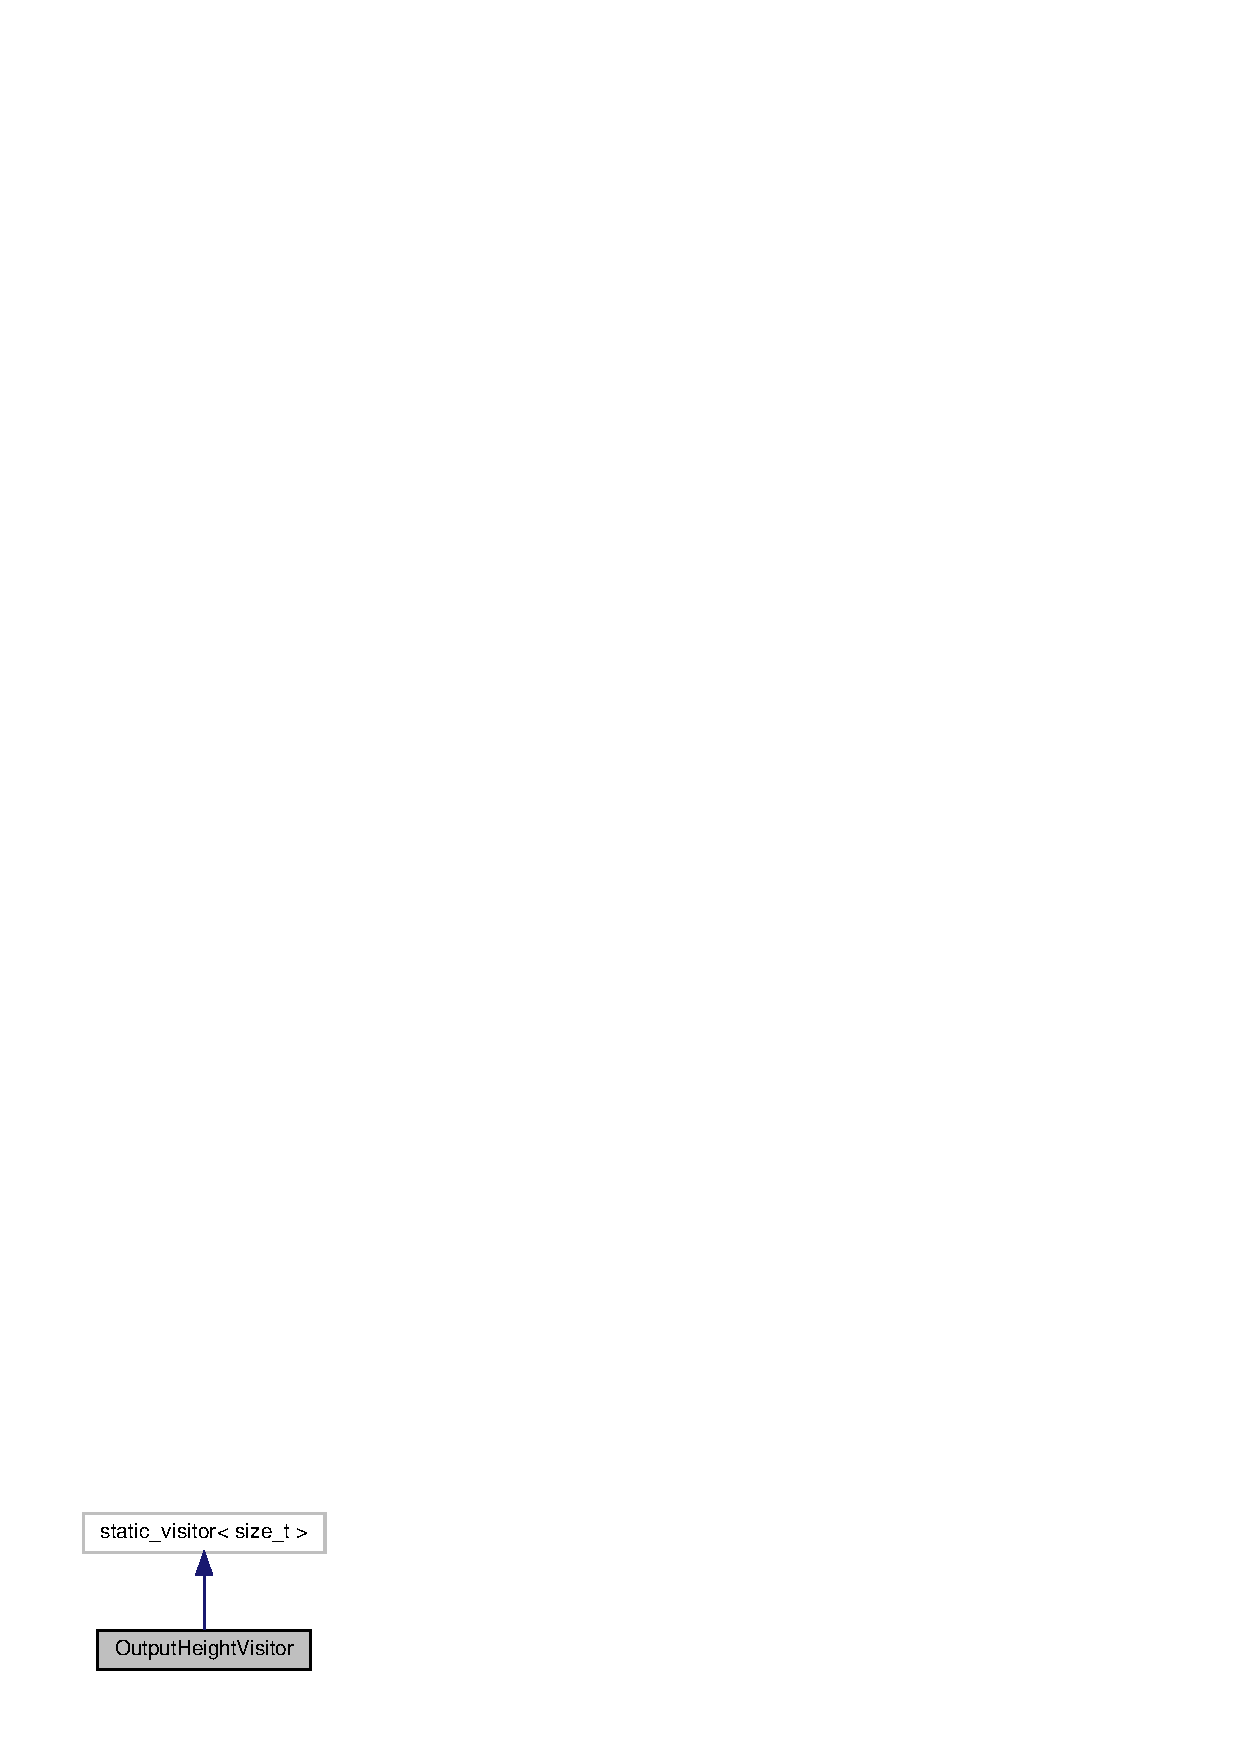
\includegraphics[width=160pt]{classmlpack_1_1ann_1_1OutputHeightVisitor__inherit__graph}
\end{center}
\end{figure}
\subsection*{Public Member Functions}
\begin{DoxyCompactItemize}
\item 
{\footnotesize template$<$typename Layer\+Type $>$ }\\size\+\_\+t \textbf{ operator()} (Layer\+Type $\ast$layer) const
\begin{DoxyCompactList}\small\item\em Return the output height. \end{DoxyCompactList}\item 
size\+\_\+t \textbf{ operator()} (\textbf{ More\+Types} layer) const
\end{DoxyCompactItemize}


\subsection{Detailed Description}
\doxyref{Output\+Height\+Visitor}{p.}{classmlpack_1_1ann_1_1OutputHeightVisitor} exposes the Output\+Height() method of the given module. 

Definition at line 27 of file output\+\_\+height\+\_\+visitor.\+hpp.



\subsection{Member Function Documentation}
\mbox{\label{classmlpack_1_1ann_1_1OutputHeightVisitor_aeb8947a28d511a7a4ce42a1fc63f79ee}} 
\index{mlpack\+::ann\+::\+Output\+Height\+Visitor@{mlpack\+::ann\+::\+Output\+Height\+Visitor}!operator()@{operator()}}
\index{operator()@{operator()}!mlpack\+::ann\+::\+Output\+Height\+Visitor@{mlpack\+::ann\+::\+Output\+Height\+Visitor}}
\subsubsection{operator()()\hspace{0.1cm}{\footnotesize\ttfamily [1/2]}}
{\footnotesize\ttfamily size\+\_\+t operator() (\begin{DoxyParamCaption}\item[{Layer\+Type $\ast$}]{layer }\end{DoxyParamCaption}) const}



Return the output height. 

\mbox{\label{classmlpack_1_1ann_1_1OutputHeightVisitor_a19a2b78859e4e91b86170544dbd8ae09}} 
\index{mlpack\+::ann\+::\+Output\+Height\+Visitor@{mlpack\+::ann\+::\+Output\+Height\+Visitor}!operator()@{operator()}}
\index{operator()@{operator()}!mlpack\+::ann\+::\+Output\+Height\+Visitor@{mlpack\+::ann\+::\+Output\+Height\+Visitor}}
\subsubsection{operator()()\hspace{0.1cm}{\footnotesize\ttfamily [2/2]}}
{\footnotesize\ttfamily size\+\_\+t operator() (\begin{DoxyParamCaption}\item[{\textbf{ More\+Types}}]{layer }\end{DoxyParamCaption}) const}



The documentation for this class was generated from the following file\+:\begin{DoxyCompactItemize}
\item 
/home/aakash/mlpack/src/mlpack/methods/ann/visitor/\textbf{ output\+\_\+height\+\_\+visitor.\+hpp}\end{DoxyCompactItemize}

\section{Output\+Parameter\+Visitor Class Reference}
\label{classmlpack_1_1ann_1_1OutputParameterVisitor}\index{Output\+Parameter\+Visitor@{Output\+Parameter\+Visitor}}


\doxyref{Output\+Parameter\+Visitor}{p.}{classmlpack_1_1ann_1_1OutputParameterVisitor} exposes the output parameter of the given module.  




Inheritance diagram for Output\+Parameter\+Visitor\+:
\nopagebreak
\begin{figure}[H]
\begin{center}
\leavevmode
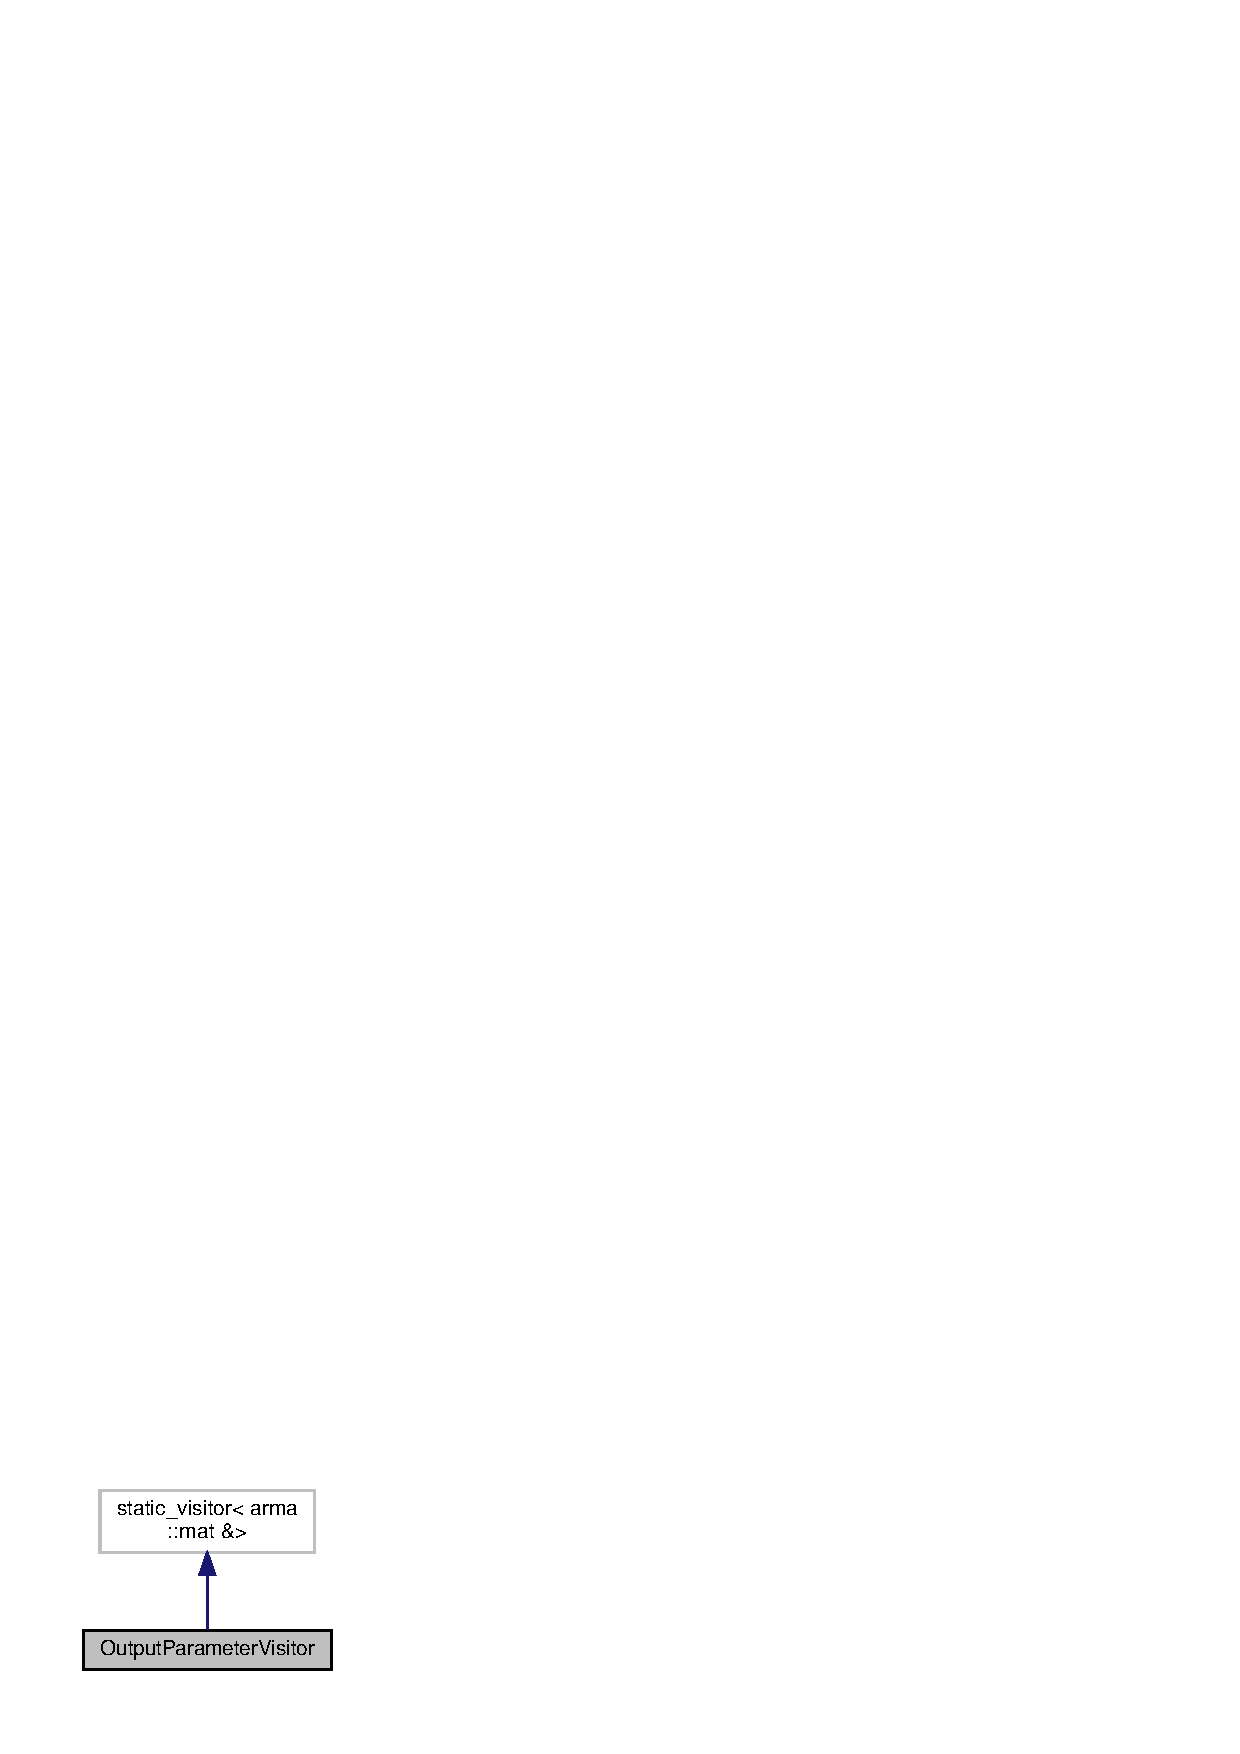
\includegraphics[width=163pt]{classmlpack_1_1ann_1_1OutputParameterVisitor__inherit__graph}
\end{center}
\end{figure}
\subsection*{Public Member Functions}
\begin{DoxyCompactItemize}
\item 
{\footnotesize template$<$typename Layer\+Type $>$ }\\arma\+::mat \& \textbf{ operator()} (Layer\+Type $\ast$layer) const
\begin{DoxyCompactList}\small\item\em Return the output parameter set. \end{DoxyCompactList}\item 
arma\+::mat \& \textbf{ operator()} (\textbf{ More\+Types} layer) const
\end{DoxyCompactItemize}


\subsection{Detailed Description}
\doxyref{Output\+Parameter\+Visitor}{p.}{classmlpack_1_1ann_1_1OutputParameterVisitor} exposes the output parameter of the given module. 

Definition at line 27 of file output\+\_\+parameter\+\_\+visitor.\+hpp.



\subsection{Member Function Documentation}
\mbox{\label{classmlpack_1_1ann_1_1OutputParameterVisitor_a9ca03fe7e92d1ec621a9fea401f84110}} 
\index{mlpack\+::ann\+::\+Output\+Parameter\+Visitor@{mlpack\+::ann\+::\+Output\+Parameter\+Visitor}!operator()@{operator()}}
\index{operator()@{operator()}!mlpack\+::ann\+::\+Output\+Parameter\+Visitor@{mlpack\+::ann\+::\+Output\+Parameter\+Visitor}}
\subsubsection{operator()()\hspace{0.1cm}{\footnotesize\ttfamily [1/2]}}
{\footnotesize\ttfamily arma\+::mat\& operator() (\begin{DoxyParamCaption}\item[{Layer\+Type $\ast$}]{layer }\end{DoxyParamCaption}) const}



Return the output parameter set. 

\mbox{\label{classmlpack_1_1ann_1_1OutputParameterVisitor_ad07b3038aea456f84663267ec846a748}} 
\index{mlpack\+::ann\+::\+Output\+Parameter\+Visitor@{mlpack\+::ann\+::\+Output\+Parameter\+Visitor}!operator()@{operator()}}
\index{operator()@{operator()}!mlpack\+::ann\+::\+Output\+Parameter\+Visitor@{mlpack\+::ann\+::\+Output\+Parameter\+Visitor}}
\subsubsection{operator()()\hspace{0.1cm}{\footnotesize\ttfamily [2/2]}}
{\footnotesize\ttfamily arma\+::mat\& operator() (\begin{DoxyParamCaption}\item[{\textbf{ More\+Types}}]{layer }\end{DoxyParamCaption}) const}



The documentation for this class was generated from the following file\+:\begin{DoxyCompactItemize}
\item 
/home/aakash/mlpack/src/mlpack/methods/ann/visitor/\textbf{ output\+\_\+parameter\+\_\+visitor.\+hpp}\end{DoxyCompactItemize}

\section{Output\+Width\+Visitor Class Reference}
\label{classmlpack_1_1ann_1_1OutputWidthVisitor}\index{Output\+Width\+Visitor@{Output\+Width\+Visitor}}


\doxyref{Output\+Width\+Visitor}{p.}{classmlpack_1_1ann_1_1OutputWidthVisitor} exposes the Output\+Width() method of the given module.  




Inheritance diagram for Output\+Width\+Visitor\+:
\nopagebreak
\begin{figure}[H]
\begin{center}
\leavevmode
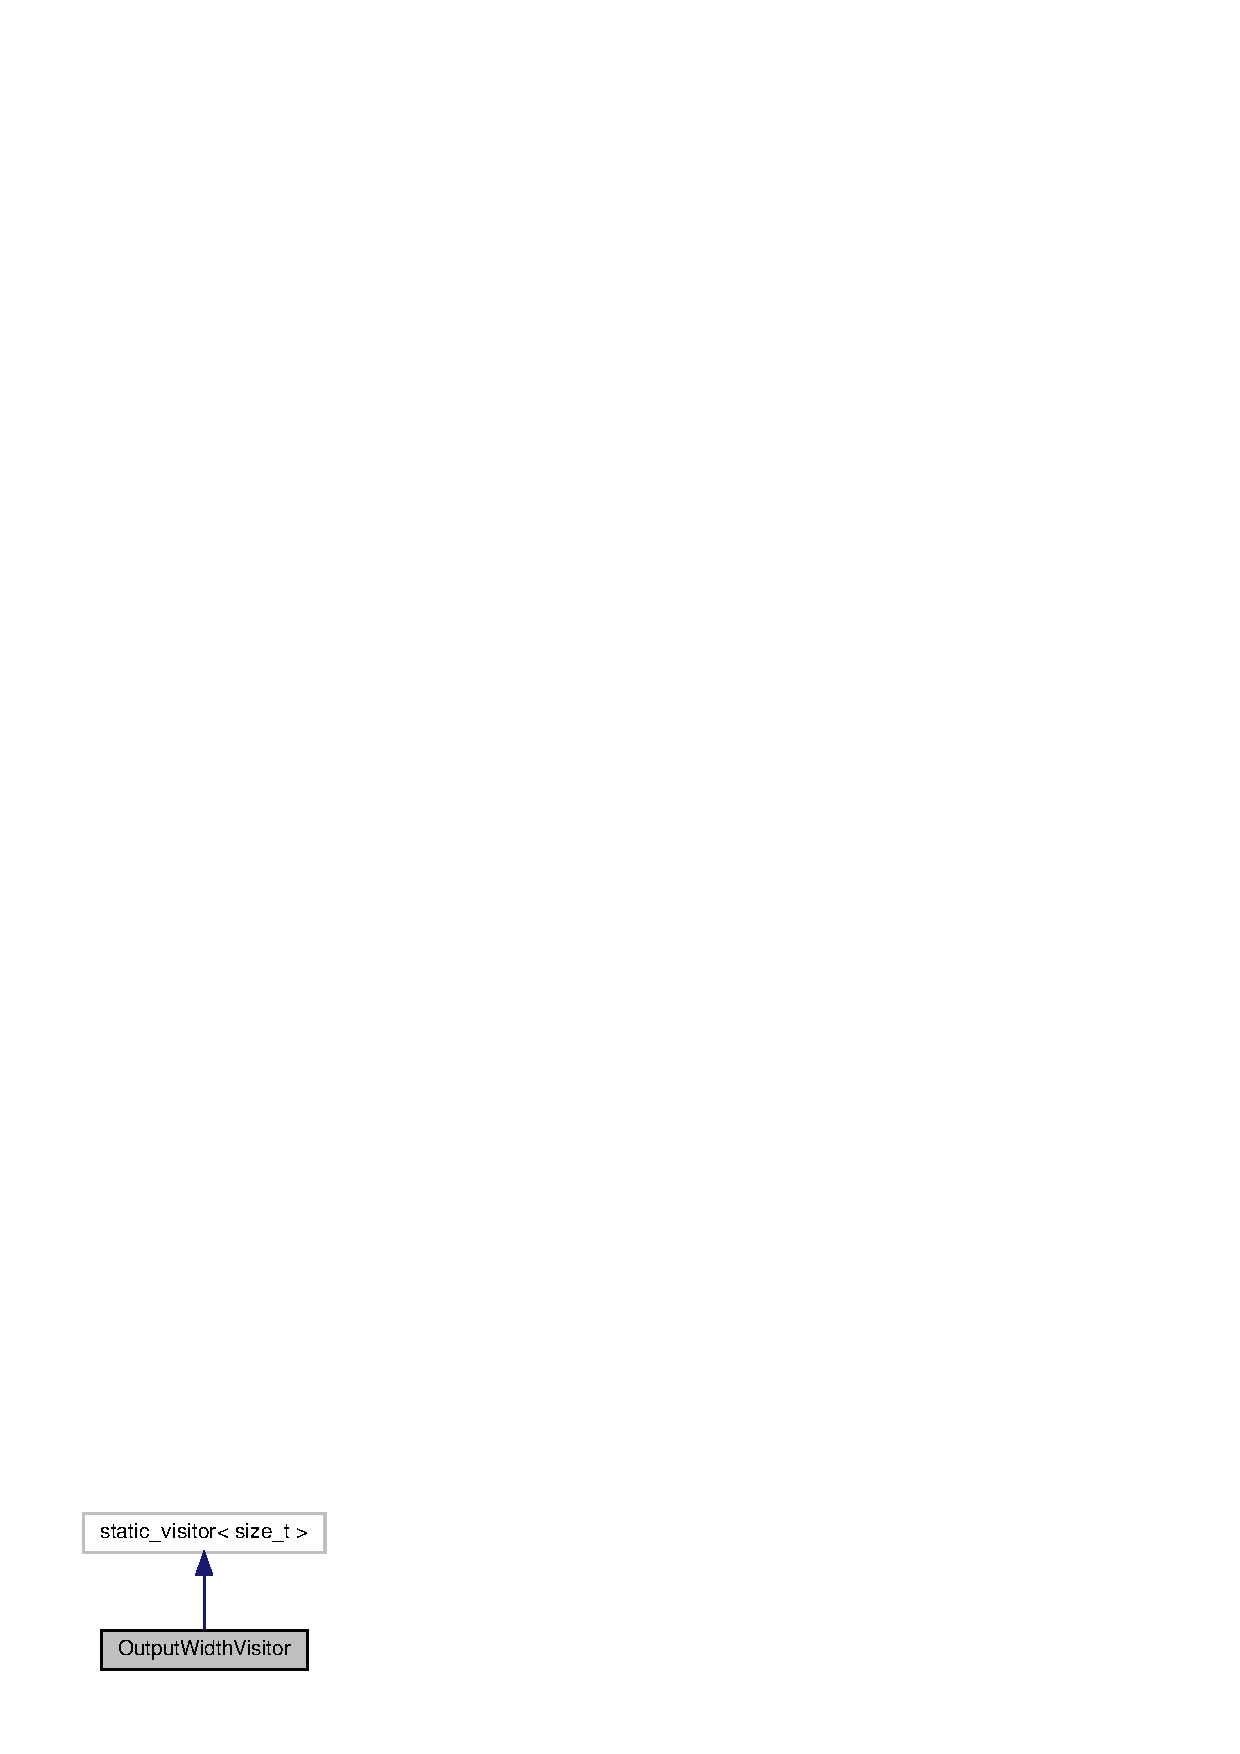
\includegraphics[width=160pt]{classmlpack_1_1ann_1_1OutputWidthVisitor__inherit__graph}
\end{center}
\end{figure}
\subsection*{Public Member Functions}
\begin{DoxyCompactItemize}
\item 
{\footnotesize template$<$typename Layer\+Type $>$ }\\size\+\_\+t \textbf{ operator()} (Layer\+Type $\ast$layer) const
\begin{DoxyCompactList}\small\item\em Return the output width. \end{DoxyCompactList}\item 
size\+\_\+t \textbf{ operator()} (\textbf{ More\+Types} layer) const
\end{DoxyCompactItemize}


\subsection{Detailed Description}
\doxyref{Output\+Width\+Visitor}{p.}{classmlpack_1_1ann_1_1OutputWidthVisitor} exposes the Output\+Width() method of the given module. 

Definition at line 27 of file output\+\_\+width\+\_\+visitor.\+hpp.



\subsection{Member Function Documentation}
\mbox{\label{classmlpack_1_1ann_1_1OutputWidthVisitor_aeb8947a28d511a7a4ce42a1fc63f79ee}} 
\index{mlpack\+::ann\+::\+Output\+Width\+Visitor@{mlpack\+::ann\+::\+Output\+Width\+Visitor}!operator()@{operator()}}
\index{operator()@{operator()}!mlpack\+::ann\+::\+Output\+Width\+Visitor@{mlpack\+::ann\+::\+Output\+Width\+Visitor}}
\subsubsection{operator()()\hspace{0.1cm}{\footnotesize\ttfamily [1/2]}}
{\footnotesize\ttfamily size\+\_\+t operator() (\begin{DoxyParamCaption}\item[{Layer\+Type $\ast$}]{layer }\end{DoxyParamCaption}) const}



Return the output width. 

\mbox{\label{classmlpack_1_1ann_1_1OutputWidthVisitor_a19a2b78859e4e91b86170544dbd8ae09}} 
\index{mlpack\+::ann\+::\+Output\+Width\+Visitor@{mlpack\+::ann\+::\+Output\+Width\+Visitor}!operator()@{operator()}}
\index{operator()@{operator()}!mlpack\+::ann\+::\+Output\+Width\+Visitor@{mlpack\+::ann\+::\+Output\+Width\+Visitor}}
\subsubsection{operator()()\hspace{0.1cm}{\footnotesize\ttfamily [2/2]}}
{\footnotesize\ttfamily size\+\_\+t operator() (\begin{DoxyParamCaption}\item[{\textbf{ More\+Types}}]{layer }\end{DoxyParamCaption}) const}



The documentation for this class was generated from the following file\+:\begin{DoxyCompactItemize}
\item 
/home/aakash/mlpack/src/mlpack/methods/ann/visitor/\textbf{ output\+\_\+width\+\_\+visitor.\+hpp}\end{DoxyCompactItemize}

\section{Padding$<$ Input\+Data\+Type, Output\+Data\+Type $>$ Class Template Reference}
\label{classmlpack_1_1ann_1_1Padding}\index{Padding$<$ Input\+Data\+Type, Output\+Data\+Type $>$@{Padding$<$ Input\+Data\+Type, Output\+Data\+Type $>$}}


Implementation of the \doxyref{Padding}{p.}{classmlpack_1_1ann_1_1Padding} module class.  


\subsection*{Public Member Functions}
\begin{DoxyCompactItemize}
\item 
\textbf{ Padding} (const size\+\_\+t pad\+W\+Left=0, const size\+\_\+t pad\+W\+Right=0, const size\+\_\+t pad\+H\+Top=0, const size\+\_\+t pad\+H\+Bottom=0, const size\+\_\+t input\+Width=0, const size\+\_\+t input\+Height=0)
\begin{DoxyCompactList}\small\item\em Create the \doxyref{Padding}{p.}{classmlpack_1_1ann_1_1Padding} object using the specified number of output units. \end{DoxyCompactList}\item 
{\footnotesize template$<$typename eT $>$ }\\void \textbf{ Backward} (const arma\+::\+Mat$<$ eT $>$ \&, const arma\+::\+Mat$<$ eT $>$ \&gy, arma\+::\+Mat$<$ eT $>$ \&g)
\begin{DoxyCompactList}\small\item\em Ordinary feed backward pass of a neural network, calculating the function f(x) by propagating x backwards trough f. \end{DoxyCompactList}\item 
Output\+Data\+Type const  \& \textbf{ Delta} () const
\begin{DoxyCompactList}\small\item\em Get the delta. \end{DoxyCompactList}\item 
Output\+Data\+Type \& \textbf{ Delta} ()
\begin{DoxyCompactList}\small\item\em Modify the delta. \end{DoxyCompactList}\item 
{\footnotesize template$<$typename eT $>$ }\\void \textbf{ Forward} (const arma\+::\+Mat$<$ eT $>$ \&input, arma\+::\+Mat$<$ eT $>$ \&output)
\begin{DoxyCompactList}\small\item\em Ordinary feed forward pass of a neural network, evaluating the function f(x) by propagating the activity forward through f. \end{DoxyCompactList}\item 
size\+\_\+t \textbf{ Input\+Height} () const
\begin{DoxyCompactList}\small\item\em Get the input height. \end{DoxyCompactList}\item 
size\+\_\+t \& \textbf{ Input\+Height} ()
\begin{DoxyCompactList}\small\item\em Modify the input height. \end{DoxyCompactList}\item 
size\+\_\+t \textbf{ Input\+Width} () const
\begin{DoxyCompactList}\small\item\em Get the input width. \end{DoxyCompactList}\item 
size\+\_\+t \& \textbf{ Input\+Width} ()
\begin{DoxyCompactList}\small\item\em Modify the input width. \end{DoxyCompactList}\item 
size\+\_\+t \textbf{ Output\+Height} () const
\begin{DoxyCompactList}\small\item\em Get the output height. \end{DoxyCompactList}\item 
size\+\_\+t \& \textbf{ Output\+Height} ()
\begin{DoxyCompactList}\small\item\em Modify the output height. \end{DoxyCompactList}\item 
Output\+Data\+Type const  \& \textbf{ Output\+Parameter} () const
\begin{DoxyCompactList}\small\item\em Get the output parameter. \end{DoxyCompactList}\item 
Output\+Data\+Type \& \textbf{ Output\+Parameter} ()
\begin{DoxyCompactList}\small\item\em Modify the output parameter. \end{DoxyCompactList}\item 
size\+\_\+t \textbf{ Output\+Width} () const
\begin{DoxyCompactList}\small\item\em Get the output width. \end{DoxyCompactList}\item 
size\+\_\+t \& \textbf{ Output\+Width} ()
\begin{DoxyCompactList}\small\item\em Modify the output width. \end{DoxyCompactList}\item 
size\+\_\+t \textbf{ Pad\+H\+Bottom} () const
\begin{DoxyCompactList}\small\item\em Get the bottom padding width. \end{DoxyCompactList}\item 
size\+\_\+t \& \textbf{ Pad\+H\+Bottom} ()
\begin{DoxyCompactList}\small\item\em Modify the bottom padding width. \end{DoxyCompactList}\item 
size\+\_\+t \textbf{ Pad\+H\+Top} () const
\begin{DoxyCompactList}\small\item\em Get the top padding width. \end{DoxyCompactList}\item 
size\+\_\+t \& \textbf{ Pad\+H\+Top} ()
\begin{DoxyCompactList}\small\item\em Modify the top padding width. \end{DoxyCompactList}\item 
size\+\_\+t \textbf{ Pad\+W\+Left} () const
\begin{DoxyCompactList}\small\item\em Get the left padding width. \end{DoxyCompactList}\item 
size\+\_\+t \& \textbf{ Pad\+W\+Left} ()
\begin{DoxyCompactList}\small\item\em Modify the left padding width. \end{DoxyCompactList}\item 
size\+\_\+t \textbf{ Pad\+W\+Right} () const
\begin{DoxyCompactList}\small\item\em Get the right padding width. \end{DoxyCompactList}\item 
size\+\_\+t \& \textbf{ Pad\+W\+Right} ()
\begin{DoxyCompactList}\small\item\em Modify the right padding width. \end{DoxyCompactList}\item 
{\footnotesize template$<$typename Archive $>$ }\\void \textbf{ serialize} (Archive \&ar, const uint32\+\_\+t)
\begin{DoxyCompactList}\small\item\em Serialize the layer. \end{DoxyCompactList}\end{DoxyCompactItemize}


\subsection{Detailed Description}
\subsubsection*{template$<$typename Input\+Data\+Type = arma\+::mat, typename Output\+Data\+Type = arma\+::mat$>$\newline
class mlpack\+::ann\+::\+Padding$<$ Input\+Data\+Type, Output\+Data\+Type $>$}

Implementation of the \doxyref{Padding}{p.}{classmlpack_1_1ann_1_1Padding} module class. 

The \doxyref{Padding}{p.}{classmlpack_1_1ann_1_1Padding} module applies a bias term to the incoming data.


\begin{DoxyTemplParams}{Template Parameters}
{\em Input\+Data\+Type} & Type of the input data (arma\+::colvec, arma\+::mat, arma\+::sp\+\_\+mat or arma\+::cube). \\
\hline
{\em Output\+Data\+Type} & Type of the output data (arma\+::colvec, arma\+::mat, arma\+::sp\+\_\+mat or arma\+::cube). \\
\hline
\end{DoxyTemplParams}


Definition at line 84 of file layer\+\_\+types.\+hpp.



\subsection{Constructor \& Destructor Documentation}
\mbox{\label{classmlpack_1_1ann_1_1Padding_abdf3bd1832ec518c6881ffa8a94a9cbc}} 
\index{mlpack\+::ann\+::\+Padding@{mlpack\+::ann\+::\+Padding}!Padding@{Padding}}
\index{Padding@{Padding}!mlpack\+::ann\+::\+Padding@{mlpack\+::ann\+::\+Padding}}
\subsubsection{Padding()}
{\footnotesize\ttfamily \textbf{ Padding} (\begin{DoxyParamCaption}\item[{const size\+\_\+t}]{pad\+W\+Left = {\ttfamily 0},  }\item[{const size\+\_\+t}]{pad\+W\+Right = {\ttfamily 0},  }\item[{const size\+\_\+t}]{pad\+H\+Top = {\ttfamily 0},  }\item[{const size\+\_\+t}]{pad\+H\+Bottom = {\ttfamily 0},  }\item[{const size\+\_\+t}]{input\+Width = {\ttfamily 0},  }\item[{const size\+\_\+t}]{input\+Height = {\ttfamily 0} }\end{DoxyParamCaption})}



Create the \doxyref{Padding}{p.}{classmlpack_1_1ann_1_1Padding} object using the specified number of output units. 


\begin{DoxyParams}{Parameters}
{\em pad\+W\+Left} & Left padding width of the input. \\
\hline
{\em pad\+W\+Right} & Right padding width of the input. \\
\hline
{\em pad\+H\+Top} & Top padding height of the input. \\
\hline
{\em pad\+H\+Bottom} & Bottom padding height of the input. \\
\hline
{\em input\+Width} & Width of the input. \\
\hline
{\em input\+Height} & Height of the input. \\
\hline
\end{DoxyParams}


\subsection{Member Function Documentation}
\mbox{\label{classmlpack_1_1ann_1_1Padding_ad9ad1a3bdb0f3fff5c839ed155e4bbf8}} 
\index{mlpack\+::ann\+::\+Padding@{mlpack\+::ann\+::\+Padding}!Backward@{Backward}}
\index{Backward@{Backward}!mlpack\+::ann\+::\+Padding@{mlpack\+::ann\+::\+Padding}}
\subsubsection{Backward()}
{\footnotesize\ttfamily void Backward (\begin{DoxyParamCaption}\item[{const arma\+::\+Mat$<$ eT $>$ \&}]{,  }\item[{const arma\+::\+Mat$<$ eT $>$ \&}]{gy,  }\item[{arma\+::\+Mat$<$ eT $>$ \&}]{g }\end{DoxyParamCaption})}



Ordinary feed backward pass of a neural network, calculating the function f(x) by propagating x backwards trough f. 

Using the results from the feed forward pass.


\begin{DoxyParams}{Parameters}
{\em $\ast$} & (input) The propagated input activation. \\
\hline
{\em gy} & The backpropagated error. \\
\hline
{\em g} & The calculated gradient. \\
\hline
\end{DoxyParams}
\mbox{\label{classmlpack_1_1ann_1_1Padding_a797f7edb44dd081e5e2b3cc316eef6bd}} 
\index{mlpack\+::ann\+::\+Padding@{mlpack\+::ann\+::\+Padding}!Delta@{Delta}}
\index{Delta@{Delta}!mlpack\+::ann\+::\+Padding@{mlpack\+::ann\+::\+Padding}}
\subsubsection{Delta()\hspace{0.1cm}{\footnotesize\ttfamily [1/2]}}
{\footnotesize\ttfamily Output\+Data\+Type const\& Delta (\begin{DoxyParamCaption}{ }\end{DoxyParamCaption}) const\hspace{0.3cm}{\ttfamily [inline]}}



Get the delta. 



Definition at line 84 of file padding.\+hpp.

\mbox{\label{classmlpack_1_1ann_1_1Padding_ad6601342d560219ce951d554e69e5e87}} 
\index{mlpack\+::ann\+::\+Padding@{mlpack\+::ann\+::\+Padding}!Delta@{Delta}}
\index{Delta@{Delta}!mlpack\+::ann\+::\+Padding@{mlpack\+::ann\+::\+Padding}}
\subsubsection{Delta()\hspace{0.1cm}{\footnotesize\ttfamily [2/2]}}
{\footnotesize\ttfamily Output\+Data\+Type\& Delta (\begin{DoxyParamCaption}{ }\end{DoxyParamCaption})\hspace{0.3cm}{\ttfamily [inline]}}



Modify the delta. 



Definition at line 86 of file padding.\+hpp.

\mbox{\label{classmlpack_1_1ann_1_1Padding_a461f849bc638c15bec262dc9c3a58abe}} 
\index{mlpack\+::ann\+::\+Padding@{mlpack\+::ann\+::\+Padding}!Forward@{Forward}}
\index{Forward@{Forward}!mlpack\+::ann\+::\+Padding@{mlpack\+::ann\+::\+Padding}}
\subsubsection{Forward()}
{\footnotesize\ttfamily void Forward (\begin{DoxyParamCaption}\item[{const arma\+::\+Mat$<$ eT $>$ \&}]{input,  }\item[{arma\+::\+Mat$<$ eT $>$ \&}]{output }\end{DoxyParamCaption})}



Ordinary feed forward pass of a neural network, evaluating the function f(x) by propagating the activity forward through f. 


\begin{DoxyParams}{Parameters}
{\em input} & Input data used for evaluating the specified function. \\
\hline
{\em output} & Resulting output activation. \\
\hline
\end{DoxyParams}
\mbox{\label{classmlpack_1_1ann_1_1Padding_ac34354aab4ed6f9145908b19eade6a24}} 
\index{mlpack\+::ann\+::\+Padding@{mlpack\+::ann\+::\+Padding}!Input\+Height@{Input\+Height}}
\index{Input\+Height@{Input\+Height}!mlpack\+::ann\+::\+Padding@{mlpack\+::ann\+::\+Padding}}
\subsubsection{Input\+Height()\hspace{0.1cm}{\footnotesize\ttfamily [1/2]}}
{\footnotesize\ttfamily size\+\_\+t Input\+Height (\begin{DoxyParamCaption}{ }\end{DoxyParamCaption}) const\hspace{0.3cm}{\ttfamily [inline]}}



Get the input height. 



Definition at line 114 of file padding.\+hpp.

\mbox{\label{classmlpack_1_1ann_1_1Padding_aefbba724eec397a928d5460bb209a360}} 
\index{mlpack\+::ann\+::\+Padding@{mlpack\+::ann\+::\+Padding}!Input\+Height@{Input\+Height}}
\index{Input\+Height@{Input\+Height}!mlpack\+::ann\+::\+Padding@{mlpack\+::ann\+::\+Padding}}
\subsubsection{Input\+Height()\hspace{0.1cm}{\footnotesize\ttfamily [2/2]}}
{\footnotesize\ttfamily size\+\_\+t\& Input\+Height (\begin{DoxyParamCaption}{ }\end{DoxyParamCaption})\hspace{0.3cm}{\ttfamily [inline]}}



Modify the input height. 



Definition at line 116 of file padding.\+hpp.

\mbox{\label{classmlpack_1_1ann_1_1Padding_a432efdff77411903044ae87ec3aec70f}} 
\index{mlpack\+::ann\+::\+Padding@{mlpack\+::ann\+::\+Padding}!Input\+Width@{Input\+Width}}
\index{Input\+Width@{Input\+Width}!mlpack\+::ann\+::\+Padding@{mlpack\+::ann\+::\+Padding}}
\subsubsection{Input\+Width()\hspace{0.1cm}{\footnotesize\ttfamily [1/2]}}
{\footnotesize\ttfamily size\+\_\+t Input\+Width (\begin{DoxyParamCaption}{ }\end{DoxyParamCaption}) const\hspace{0.3cm}{\ttfamily [inline]}}



Get the input width. 



Definition at line 109 of file padding.\+hpp.

\mbox{\label{classmlpack_1_1ann_1_1Padding_a238e9d308df611a9300a4ca6756fef4d}} 
\index{mlpack\+::ann\+::\+Padding@{mlpack\+::ann\+::\+Padding}!Input\+Width@{Input\+Width}}
\index{Input\+Width@{Input\+Width}!mlpack\+::ann\+::\+Padding@{mlpack\+::ann\+::\+Padding}}
\subsubsection{Input\+Width()\hspace{0.1cm}{\footnotesize\ttfamily [2/2]}}
{\footnotesize\ttfamily size\+\_\+t\& Input\+Width (\begin{DoxyParamCaption}{ }\end{DoxyParamCaption})\hspace{0.3cm}{\ttfamily [inline]}}



Modify the input width. 



Definition at line 111 of file padding.\+hpp.

\mbox{\label{classmlpack_1_1ann_1_1Padding_a96a6294ed9ca8d24be9bb5eb53db7f25}} 
\index{mlpack\+::ann\+::\+Padding@{mlpack\+::ann\+::\+Padding}!Output\+Height@{Output\+Height}}
\index{Output\+Height@{Output\+Height}!mlpack\+::ann\+::\+Padding@{mlpack\+::ann\+::\+Padding}}
\subsubsection{Output\+Height()\hspace{0.1cm}{\footnotesize\ttfamily [1/2]}}
{\footnotesize\ttfamily size\+\_\+t Output\+Height (\begin{DoxyParamCaption}{ }\end{DoxyParamCaption}) const\hspace{0.3cm}{\ttfamily [inline]}}



Get the output height. 



Definition at line 124 of file padding.\+hpp.

\mbox{\label{classmlpack_1_1ann_1_1Padding_ac5112abf9f5e1face13ed965a8755b1d}} 
\index{mlpack\+::ann\+::\+Padding@{mlpack\+::ann\+::\+Padding}!Output\+Height@{Output\+Height}}
\index{Output\+Height@{Output\+Height}!mlpack\+::ann\+::\+Padding@{mlpack\+::ann\+::\+Padding}}
\subsubsection{Output\+Height()\hspace{0.1cm}{\footnotesize\ttfamily [2/2]}}
{\footnotesize\ttfamily size\+\_\+t\& Output\+Height (\begin{DoxyParamCaption}{ }\end{DoxyParamCaption})\hspace{0.3cm}{\ttfamily [inline]}}



Modify the output height. 



Definition at line 126 of file padding.\+hpp.



References Padding$<$ Input\+Data\+Type, Output\+Data\+Type $>$\+::serialize().

\mbox{\label{classmlpack_1_1ann_1_1Padding_a0ee21c2a36e5abad1e7a9d5dd00849f9}} 
\index{mlpack\+::ann\+::\+Padding@{mlpack\+::ann\+::\+Padding}!Output\+Parameter@{Output\+Parameter}}
\index{Output\+Parameter@{Output\+Parameter}!mlpack\+::ann\+::\+Padding@{mlpack\+::ann\+::\+Padding}}
\subsubsection{Output\+Parameter()\hspace{0.1cm}{\footnotesize\ttfamily [1/2]}}
{\footnotesize\ttfamily Output\+Data\+Type const\& Output\+Parameter (\begin{DoxyParamCaption}{ }\end{DoxyParamCaption}) const\hspace{0.3cm}{\ttfamily [inline]}}



Get the output parameter. 



Definition at line 79 of file padding.\+hpp.

\mbox{\label{classmlpack_1_1ann_1_1Padding_a21d5f745f02c709625a4ee0907f004a5}} 
\index{mlpack\+::ann\+::\+Padding@{mlpack\+::ann\+::\+Padding}!Output\+Parameter@{Output\+Parameter}}
\index{Output\+Parameter@{Output\+Parameter}!mlpack\+::ann\+::\+Padding@{mlpack\+::ann\+::\+Padding}}
\subsubsection{Output\+Parameter()\hspace{0.1cm}{\footnotesize\ttfamily [2/2]}}
{\footnotesize\ttfamily Output\+Data\+Type\& Output\+Parameter (\begin{DoxyParamCaption}{ }\end{DoxyParamCaption})\hspace{0.3cm}{\ttfamily [inline]}}



Modify the output parameter. 



Definition at line 81 of file padding.\+hpp.

\mbox{\label{classmlpack_1_1ann_1_1Padding_aa2b647f9e029826314b4f572fe96878d}} 
\index{mlpack\+::ann\+::\+Padding@{mlpack\+::ann\+::\+Padding}!Output\+Width@{Output\+Width}}
\index{Output\+Width@{Output\+Width}!mlpack\+::ann\+::\+Padding@{mlpack\+::ann\+::\+Padding}}
\subsubsection{Output\+Width()\hspace{0.1cm}{\footnotesize\ttfamily [1/2]}}
{\footnotesize\ttfamily size\+\_\+t Output\+Width (\begin{DoxyParamCaption}{ }\end{DoxyParamCaption}) const\hspace{0.3cm}{\ttfamily [inline]}}



Get the output width. 



Definition at line 119 of file padding.\+hpp.

\mbox{\label{classmlpack_1_1ann_1_1Padding_a54579ec9924e2a4a5bc0a4fb822ce80c}} 
\index{mlpack\+::ann\+::\+Padding@{mlpack\+::ann\+::\+Padding}!Output\+Width@{Output\+Width}}
\index{Output\+Width@{Output\+Width}!mlpack\+::ann\+::\+Padding@{mlpack\+::ann\+::\+Padding}}
\subsubsection{Output\+Width()\hspace{0.1cm}{\footnotesize\ttfamily [2/2]}}
{\footnotesize\ttfamily size\+\_\+t\& Output\+Width (\begin{DoxyParamCaption}{ }\end{DoxyParamCaption})\hspace{0.3cm}{\ttfamily [inline]}}



Modify the output width. 



Definition at line 121 of file padding.\+hpp.

\mbox{\label{classmlpack_1_1ann_1_1Padding_a7772e9861fa1c1922b00428172315939}} 
\index{mlpack\+::ann\+::\+Padding@{mlpack\+::ann\+::\+Padding}!Pad\+H\+Bottom@{Pad\+H\+Bottom}}
\index{Pad\+H\+Bottom@{Pad\+H\+Bottom}!mlpack\+::ann\+::\+Padding@{mlpack\+::ann\+::\+Padding}}
\subsubsection{Pad\+H\+Bottom()\hspace{0.1cm}{\footnotesize\ttfamily [1/2]}}
{\footnotesize\ttfamily size\+\_\+t Pad\+H\+Bottom (\begin{DoxyParamCaption}{ }\end{DoxyParamCaption}) const\hspace{0.3cm}{\ttfamily [inline]}}



Get the bottom padding width. 



Definition at line 104 of file padding.\+hpp.

\mbox{\label{classmlpack_1_1ann_1_1Padding_a49d01b2dacca58ba01d883045100b823}} 
\index{mlpack\+::ann\+::\+Padding@{mlpack\+::ann\+::\+Padding}!Pad\+H\+Bottom@{Pad\+H\+Bottom}}
\index{Pad\+H\+Bottom@{Pad\+H\+Bottom}!mlpack\+::ann\+::\+Padding@{mlpack\+::ann\+::\+Padding}}
\subsubsection{Pad\+H\+Bottom()\hspace{0.1cm}{\footnotesize\ttfamily [2/2]}}
{\footnotesize\ttfamily size\+\_\+t\& Pad\+H\+Bottom (\begin{DoxyParamCaption}{ }\end{DoxyParamCaption})\hspace{0.3cm}{\ttfamily [inline]}}



Modify the bottom padding width. 



Definition at line 106 of file padding.\+hpp.

\mbox{\label{classmlpack_1_1ann_1_1Padding_ae6d766575008c2909e51d00b1ef619a1}} 
\index{mlpack\+::ann\+::\+Padding@{mlpack\+::ann\+::\+Padding}!Pad\+H\+Top@{Pad\+H\+Top}}
\index{Pad\+H\+Top@{Pad\+H\+Top}!mlpack\+::ann\+::\+Padding@{mlpack\+::ann\+::\+Padding}}
\subsubsection{Pad\+H\+Top()\hspace{0.1cm}{\footnotesize\ttfamily [1/2]}}
{\footnotesize\ttfamily size\+\_\+t Pad\+H\+Top (\begin{DoxyParamCaption}{ }\end{DoxyParamCaption}) const\hspace{0.3cm}{\ttfamily [inline]}}



Get the top padding width. 



Definition at line 99 of file padding.\+hpp.

\mbox{\label{classmlpack_1_1ann_1_1Padding_a9ea976eb369189ecbe7be7e53e323d5e}} 
\index{mlpack\+::ann\+::\+Padding@{mlpack\+::ann\+::\+Padding}!Pad\+H\+Top@{Pad\+H\+Top}}
\index{Pad\+H\+Top@{Pad\+H\+Top}!mlpack\+::ann\+::\+Padding@{mlpack\+::ann\+::\+Padding}}
\subsubsection{Pad\+H\+Top()\hspace{0.1cm}{\footnotesize\ttfamily [2/2]}}
{\footnotesize\ttfamily size\+\_\+t\& Pad\+H\+Top (\begin{DoxyParamCaption}{ }\end{DoxyParamCaption})\hspace{0.3cm}{\ttfamily [inline]}}



Modify the top padding width. 



Definition at line 101 of file padding.\+hpp.

\mbox{\label{classmlpack_1_1ann_1_1Padding_a353cb5238a6b33f0d740c3ab17da11b4}} 
\index{mlpack\+::ann\+::\+Padding@{mlpack\+::ann\+::\+Padding}!Pad\+W\+Left@{Pad\+W\+Left}}
\index{Pad\+W\+Left@{Pad\+W\+Left}!mlpack\+::ann\+::\+Padding@{mlpack\+::ann\+::\+Padding}}
\subsubsection{Pad\+W\+Left()\hspace{0.1cm}{\footnotesize\ttfamily [1/2]}}
{\footnotesize\ttfamily size\+\_\+t Pad\+W\+Left (\begin{DoxyParamCaption}{ }\end{DoxyParamCaption}) const\hspace{0.3cm}{\ttfamily [inline]}}



Get the left padding width. 



Definition at line 89 of file padding.\+hpp.

\mbox{\label{classmlpack_1_1ann_1_1Padding_a10cf922741cd487e0904c933e6500760}} 
\index{mlpack\+::ann\+::\+Padding@{mlpack\+::ann\+::\+Padding}!Pad\+W\+Left@{Pad\+W\+Left}}
\index{Pad\+W\+Left@{Pad\+W\+Left}!mlpack\+::ann\+::\+Padding@{mlpack\+::ann\+::\+Padding}}
\subsubsection{Pad\+W\+Left()\hspace{0.1cm}{\footnotesize\ttfamily [2/2]}}
{\footnotesize\ttfamily size\+\_\+t\& Pad\+W\+Left (\begin{DoxyParamCaption}{ }\end{DoxyParamCaption})\hspace{0.3cm}{\ttfamily [inline]}}



Modify the left padding width. 



Definition at line 91 of file padding.\+hpp.

\mbox{\label{classmlpack_1_1ann_1_1Padding_a7f164b19d31d8d4ec4988513c139bf55}} 
\index{mlpack\+::ann\+::\+Padding@{mlpack\+::ann\+::\+Padding}!Pad\+W\+Right@{Pad\+W\+Right}}
\index{Pad\+W\+Right@{Pad\+W\+Right}!mlpack\+::ann\+::\+Padding@{mlpack\+::ann\+::\+Padding}}
\subsubsection{Pad\+W\+Right()\hspace{0.1cm}{\footnotesize\ttfamily [1/2]}}
{\footnotesize\ttfamily size\+\_\+t Pad\+W\+Right (\begin{DoxyParamCaption}{ }\end{DoxyParamCaption}) const\hspace{0.3cm}{\ttfamily [inline]}}



Get the right padding width. 



Definition at line 94 of file padding.\+hpp.

\mbox{\label{classmlpack_1_1ann_1_1Padding_a97efc672230a48247bd19a1bcd51624f}} 
\index{mlpack\+::ann\+::\+Padding@{mlpack\+::ann\+::\+Padding}!Pad\+W\+Right@{Pad\+W\+Right}}
\index{Pad\+W\+Right@{Pad\+W\+Right}!mlpack\+::ann\+::\+Padding@{mlpack\+::ann\+::\+Padding}}
\subsubsection{Pad\+W\+Right()\hspace{0.1cm}{\footnotesize\ttfamily [2/2]}}
{\footnotesize\ttfamily size\+\_\+t\& Pad\+W\+Right (\begin{DoxyParamCaption}{ }\end{DoxyParamCaption})\hspace{0.3cm}{\ttfamily [inline]}}



Modify the right padding width. 



Definition at line 96 of file padding.\+hpp.

\mbox{\label{classmlpack_1_1ann_1_1Padding_a65cba07328997659bec80b9879b15a51}} 
\index{mlpack\+::ann\+::\+Padding@{mlpack\+::ann\+::\+Padding}!serialize@{serialize}}
\index{serialize@{serialize}!mlpack\+::ann\+::\+Padding@{mlpack\+::ann\+::\+Padding}}
\subsubsection{serialize()}
{\footnotesize\ttfamily void serialize (\begin{DoxyParamCaption}\item[{Archive \&}]{ar,  }\item[{const uint32\+\_\+t}]{ }\end{DoxyParamCaption})}



Serialize the layer. 



Referenced by Padding$<$ Input\+Data\+Type, Output\+Data\+Type $>$\+::\+Output\+Height().



The documentation for this class was generated from the following files\+:\begin{DoxyCompactItemize}
\item 
/home/aakash/mlpack/src/mlpack/methods/ann/layer/\textbf{ layer\+\_\+types.\+hpp}\item 
/home/aakash/mlpack/src/mlpack/methods/ann/layer/\textbf{ padding.\+hpp}\end{DoxyCompactItemize}

\section{Parameters\+Set\+Visitor Class Reference}
\label{classmlpack_1_1ann_1_1ParametersSetVisitor}\index{Parameters\+Set\+Visitor@{Parameters\+Set\+Visitor}}


\doxyref{Parameters\+Set\+Visitor}{p.}{classmlpack_1_1ann_1_1ParametersSetVisitor} update the parameters set using the given matrix.  




Inheritance diagram for Parameters\+Set\+Visitor\+:
\nopagebreak
\begin{figure}[H]
\begin{center}
\leavevmode
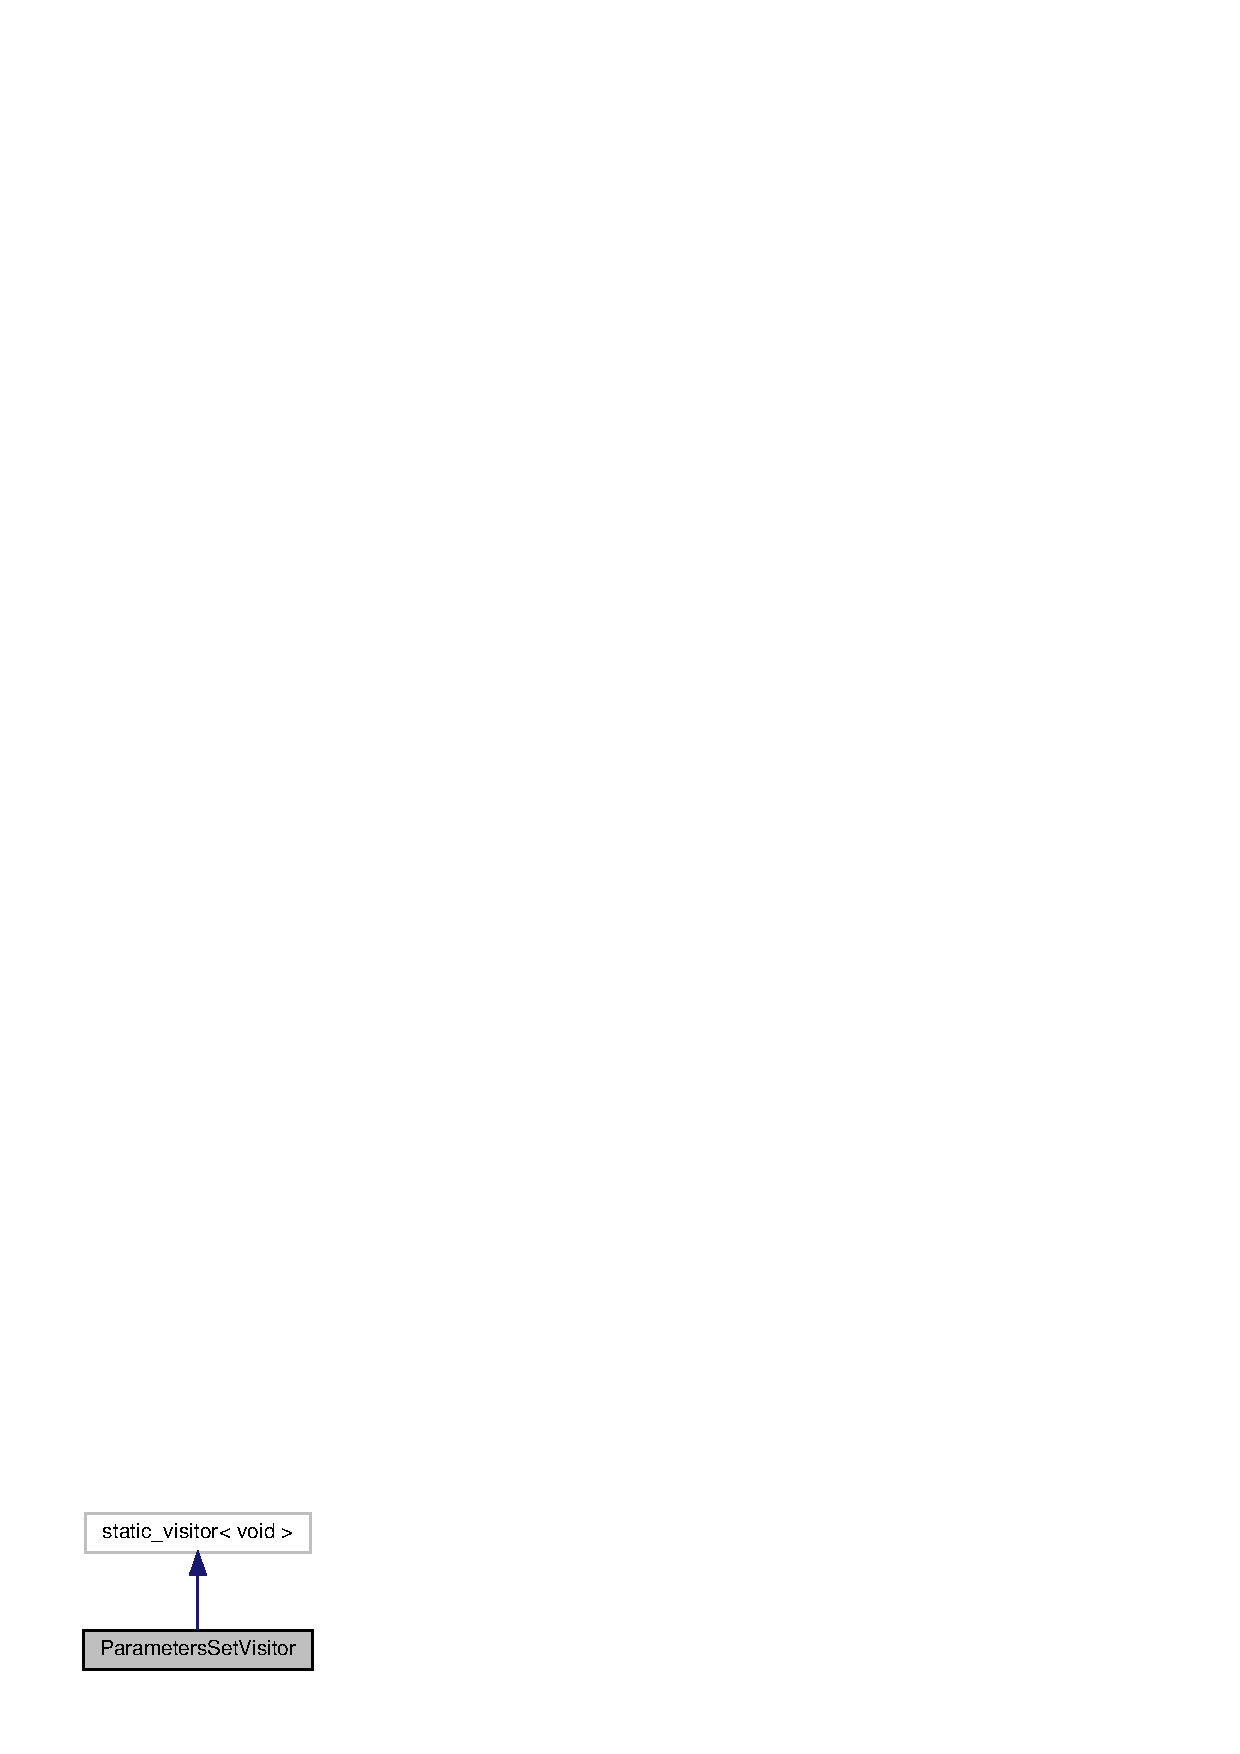
\includegraphics[width=154pt]{classmlpack_1_1ann_1_1ParametersSetVisitor__inherit__graph}
\end{center}
\end{figure}
\subsection*{Public Member Functions}
\begin{DoxyCompactItemize}
\item 
\textbf{ Parameters\+Set\+Visitor} (arma\+::mat \&parameters)
\begin{DoxyCompactList}\small\item\em Update the parameters set given the parameters matrix. \end{DoxyCompactList}\item 
{\footnotesize template$<$typename Layer\+Type $>$ }\\void \textbf{ operator()} (Layer\+Type $\ast$layer) const
\begin{DoxyCompactList}\small\item\em Update the parameters set. \end{DoxyCompactList}\item 
void \textbf{ operator()} (\textbf{ More\+Types} layer) const
\end{DoxyCompactItemize}


\subsection{Detailed Description}
\doxyref{Parameters\+Set\+Visitor}{p.}{classmlpack_1_1ann_1_1ParametersSetVisitor} update the parameters set using the given matrix. 

Definition at line 27 of file parameters\+\_\+set\+\_\+visitor.\+hpp.



\subsection{Constructor \& Destructor Documentation}
\mbox{\label{classmlpack_1_1ann_1_1ParametersSetVisitor_ad4a997c6b82dcb8c0cbe08c61cec9deb}} 
\index{mlpack\+::ann\+::\+Parameters\+Set\+Visitor@{mlpack\+::ann\+::\+Parameters\+Set\+Visitor}!Parameters\+Set\+Visitor@{Parameters\+Set\+Visitor}}
\index{Parameters\+Set\+Visitor@{Parameters\+Set\+Visitor}!mlpack\+::ann\+::\+Parameters\+Set\+Visitor@{mlpack\+::ann\+::\+Parameters\+Set\+Visitor}}
\subsubsection{Parameters\+Set\+Visitor()}
{\footnotesize\ttfamily \textbf{ Parameters\+Set\+Visitor} (\begin{DoxyParamCaption}\item[{arma\+::mat \&}]{parameters }\end{DoxyParamCaption})}



Update the parameters set given the parameters matrix. 



\subsection{Member Function Documentation}
\mbox{\label{classmlpack_1_1ann_1_1ParametersSetVisitor_a26bb3385c630118c35f4799f1509abbc}} 
\index{mlpack\+::ann\+::\+Parameters\+Set\+Visitor@{mlpack\+::ann\+::\+Parameters\+Set\+Visitor}!operator()@{operator()}}
\index{operator()@{operator()}!mlpack\+::ann\+::\+Parameters\+Set\+Visitor@{mlpack\+::ann\+::\+Parameters\+Set\+Visitor}}
\subsubsection{operator()()\hspace{0.1cm}{\footnotesize\ttfamily [1/2]}}
{\footnotesize\ttfamily void operator() (\begin{DoxyParamCaption}\item[{Layer\+Type $\ast$}]{layer }\end{DoxyParamCaption}) const}



Update the parameters set. 

\mbox{\label{classmlpack_1_1ann_1_1ParametersSetVisitor_ae35578e7ff874a320fe762bc0edfff04}} 
\index{mlpack\+::ann\+::\+Parameters\+Set\+Visitor@{mlpack\+::ann\+::\+Parameters\+Set\+Visitor}!operator()@{operator()}}
\index{operator()@{operator()}!mlpack\+::ann\+::\+Parameters\+Set\+Visitor@{mlpack\+::ann\+::\+Parameters\+Set\+Visitor}}
\subsubsection{operator()()\hspace{0.1cm}{\footnotesize\ttfamily [2/2]}}
{\footnotesize\ttfamily void operator() (\begin{DoxyParamCaption}\item[{\textbf{ More\+Types}}]{layer }\end{DoxyParamCaption}) const}



The documentation for this class was generated from the following file\+:\begin{DoxyCompactItemize}
\item 
/home/aakash/mlpack/src/mlpack/methods/ann/visitor/\textbf{ parameters\+\_\+set\+\_\+visitor.\+hpp}\end{DoxyCompactItemize}

\section{Parameters\+Visitor Class Reference}
\label{classmlpack_1_1ann_1_1ParametersVisitor}\index{Parameters\+Visitor@{Parameters\+Visitor}}


\doxyref{Parameters\+Visitor}{p.}{classmlpack_1_1ann_1_1ParametersVisitor} exposes the parameters set of the given module and stores the parameters set into the given matrix.  




Inheritance diagram for Parameters\+Visitor\+:
\nopagebreak
\begin{figure}[H]
\begin{center}
\leavevmode
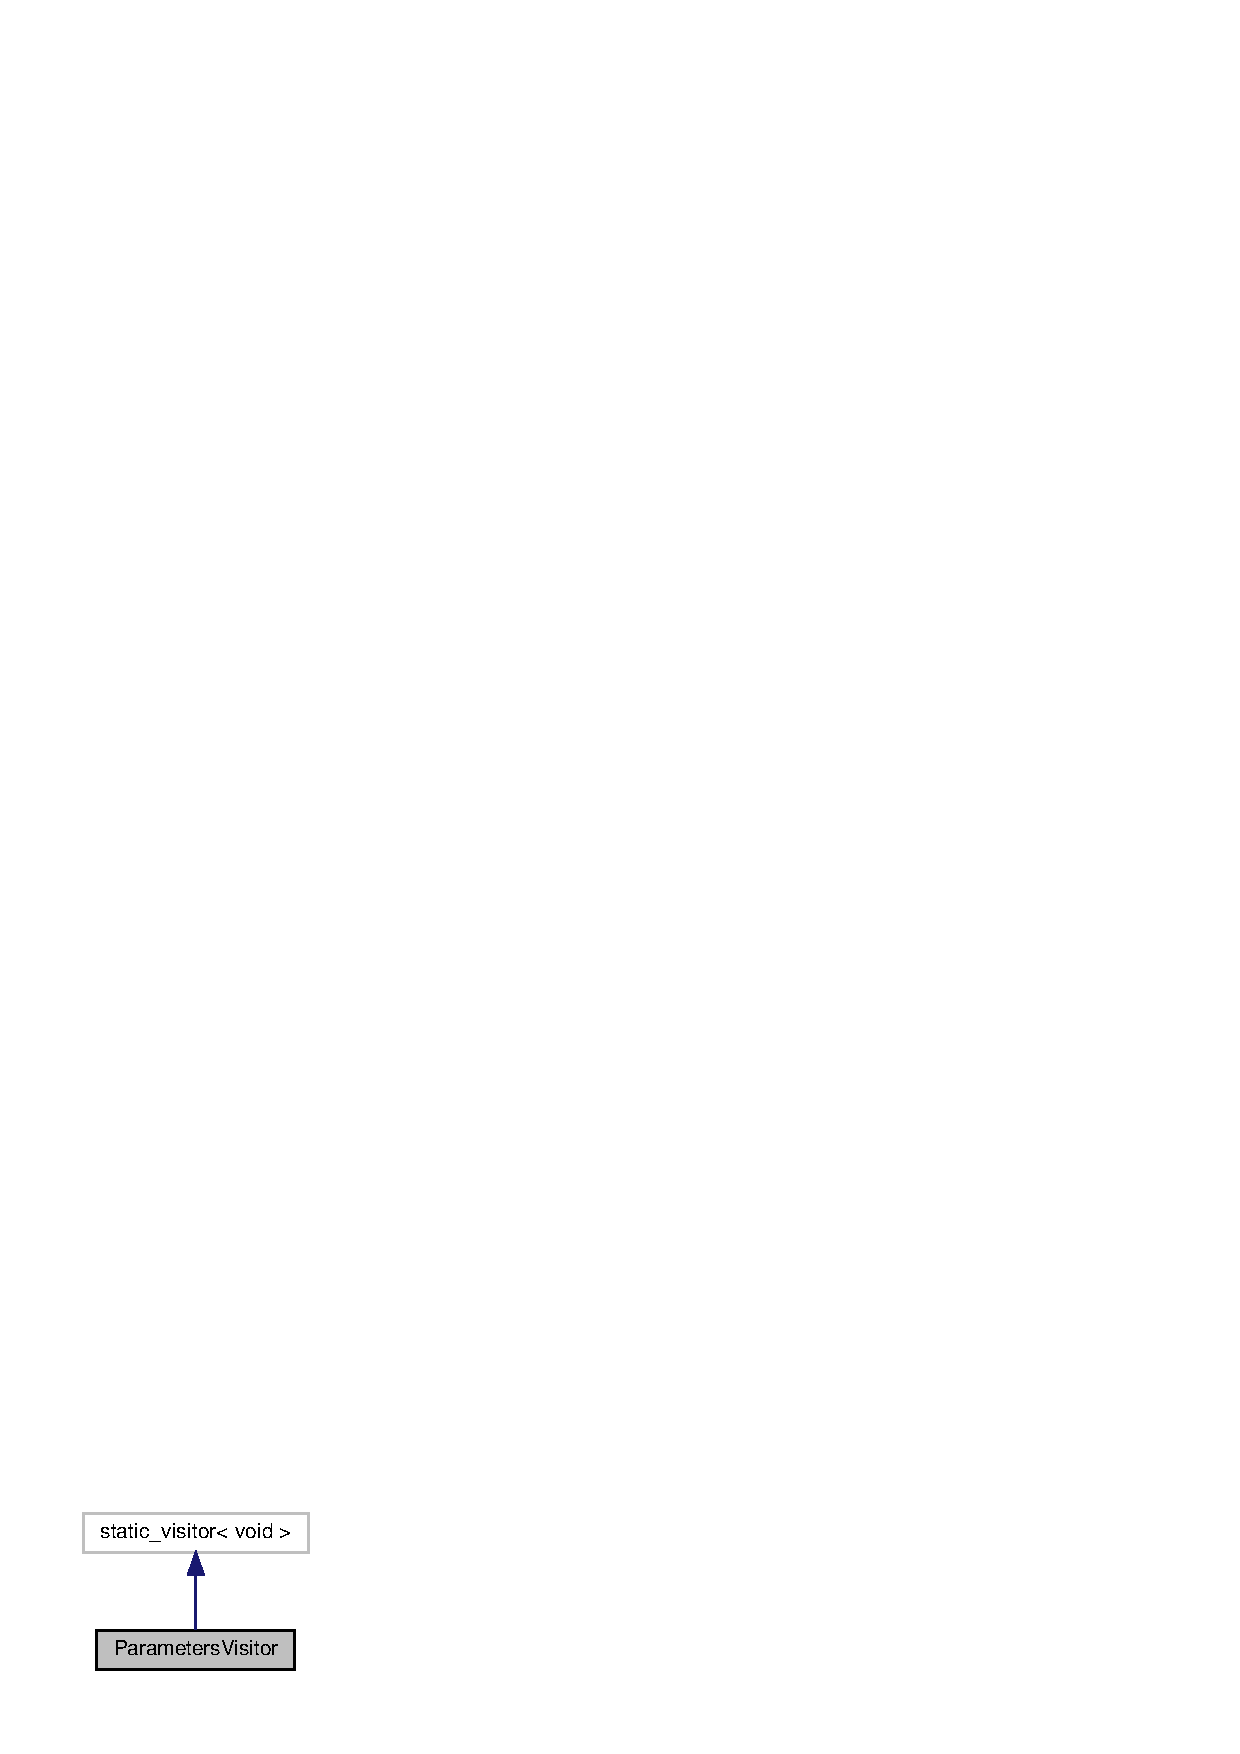
\includegraphics[width=152pt]{classmlpack_1_1ann_1_1ParametersVisitor__inherit__graph}
\end{center}
\end{figure}
\subsection*{Public Member Functions}
\begin{DoxyCompactItemize}
\item 
\textbf{ Parameters\+Visitor} (arma\+::mat \&parameters)
\begin{DoxyCompactList}\small\item\em Store the parameters set into the given parameters matrix. \end{DoxyCompactList}\item 
{\footnotesize template$<$typename Layer\+Type $>$ }\\void \textbf{ operator()} (Layer\+Type $\ast$layer) const
\begin{DoxyCompactList}\small\item\em Set the parameters set. \end{DoxyCompactList}\item 
void \textbf{ operator()} (\textbf{ More\+Types} layer) const
\end{DoxyCompactItemize}


\subsection{Detailed Description}
\doxyref{Parameters\+Visitor}{p.}{classmlpack_1_1ann_1_1ParametersVisitor} exposes the parameters set of the given module and stores the parameters set into the given matrix. 

Definition at line 28 of file parameters\+\_\+visitor.\+hpp.



\subsection{Constructor \& Destructor Documentation}
\mbox{\label{classmlpack_1_1ann_1_1ParametersVisitor_a48449504b83a1bde89eee4af9b239ced}} 
\index{mlpack\+::ann\+::\+Parameters\+Visitor@{mlpack\+::ann\+::\+Parameters\+Visitor}!Parameters\+Visitor@{Parameters\+Visitor}}
\index{Parameters\+Visitor@{Parameters\+Visitor}!mlpack\+::ann\+::\+Parameters\+Visitor@{mlpack\+::ann\+::\+Parameters\+Visitor}}
\subsubsection{Parameters\+Visitor()}
{\footnotesize\ttfamily \textbf{ Parameters\+Visitor} (\begin{DoxyParamCaption}\item[{arma\+::mat \&}]{parameters }\end{DoxyParamCaption})}



Store the parameters set into the given parameters matrix. 



\subsection{Member Function Documentation}
\mbox{\label{classmlpack_1_1ann_1_1ParametersVisitor_a26bb3385c630118c35f4799f1509abbc}} 
\index{mlpack\+::ann\+::\+Parameters\+Visitor@{mlpack\+::ann\+::\+Parameters\+Visitor}!operator()@{operator()}}
\index{operator()@{operator()}!mlpack\+::ann\+::\+Parameters\+Visitor@{mlpack\+::ann\+::\+Parameters\+Visitor}}
\subsubsection{operator()()\hspace{0.1cm}{\footnotesize\ttfamily [1/2]}}
{\footnotesize\ttfamily void operator() (\begin{DoxyParamCaption}\item[{Layer\+Type $\ast$}]{layer }\end{DoxyParamCaption}) const}



Set the parameters set. 

\mbox{\label{classmlpack_1_1ann_1_1ParametersVisitor_ae35578e7ff874a320fe762bc0edfff04}} 
\index{mlpack\+::ann\+::\+Parameters\+Visitor@{mlpack\+::ann\+::\+Parameters\+Visitor}!operator()@{operator()}}
\index{operator()@{operator()}!mlpack\+::ann\+::\+Parameters\+Visitor@{mlpack\+::ann\+::\+Parameters\+Visitor}}
\subsubsection{operator()()\hspace{0.1cm}{\footnotesize\ttfamily [2/2]}}
{\footnotesize\ttfamily void operator() (\begin{DoxyParamCaption}\item[{\textbf{ More\+Types}}]{layer }\end{DoxyParamCaption}) const}



The documentation for this class was generated from the following file\+:\begin{DoxyCompactItemize}
\item 
/home/aakash/mlpack/src/mlpack/methods/ann/visitor/\textbf{ parameters\+\_\+visitor.\+hpp}\end{DoxyCompactItemize}

\section{Pixel\+Shuffle$<$ Input\+Data\+Type, Output\+Data\+Type $>$ Class Template Reference}
\label{classmlpack_1_1ann_1_1PixelShuffle}\index{Pixel\+Shuffle$<$ Input\+Data\+Type, Output\+Data\+Type $>$@{Pixel\+Shuffle$<$ Input\+Data\+Type, Output\+Data\+Type $>$}}


Implementation of the \doxyref{Pixel\+Shuffle}{p.}{classmlpack_1_1ann_1_1PixelShuffle} layer.  


\subsection*{Public Member Functions}
\begin{DoxyCompactItemize}
\item 
\textbf{ Pixel\+Shuffle} ()
\begin{DoxyCompactList}\small\item\em Create the \doxyref{Pixel\+Shuffle}{p.}{classmlpack_1_1ann_1_1PixelShuffle} object. \end{DoxyCompactList}\item 
\textbf{ Pixel\+Shuffle} (const size\+\_\+t upscale\+Factor, const size\+\_\+t height, const size\+\_\+t width, const size\+\_\+t size)
\begin{DoxyCompactList}\small\item\em Create the \doxyref{Pixel\+Shuffle}{p.}{classmlpack_1_1ann_1_1PixelShuffle} object using the specified parameters. \end{DoxyCompactList}\item 
{\footnotesize template$<$typename eT $>$ }\\void \textbf{ Backward} (const arma\+::\+Mat$<$ eT $>$ \&input, const arma\+::\+Mat$<$ eT $>$ \&gy, arma\+::\+Mat$<$ eT $>$ \&g)
\begin{DoxyCompactList}\small\item\em Ordinary feed backward pass of the \doxyref{Pixel\+Shuffle}{p.}{classmlpack_1_1ann_1_1PixelShuffle} layer. \end{DoxyCompactList}\item 
Output\+Data\+Type const  \& \textbf{ Delta} () const
\begin{DoxyCompactList}\small\item\em Get the delta. \end{DoxyCompactList}\item 
Output\+Data\+Type \& \textbf{ Delta} ()
\begin{DoxyCompactList}\small\item\em Modify the delta. \end{DoxyCompactList}\item 
{\footnotesize template$<$typename eT $>$ }\\void \textbf{ Forward} (const arma\+::\+Mat$<$ eT $>$ \&input, arma\+::\+Mat$<$ eT $>$ \&output)
\begin{DoxyCompactList}\small\item\em Ordinary feed forward pass of the \doxyref{Pixel\+Shuffle}{p.}{classmlpack_1_1ann_1_1PixelShuffle} layer. \end{DoxyCompactList}\item 
size\+\_\+t \textbf{ Input\+Channels} () const
\begin{DoxyCompactList}\small\item\em Get the number of input channels. \end{DoxyCompactList}\item 
size\+\_\+t \& \textbf{ Input\+Channels} ()
\begin{DoxyCompactList}\small\item\em Modify the number of input channels. \end{DoxyCompactList}\item 
size\+\_\+t \textbf{ Input\+Height} () const
\begin{DoxyCompactList}\small\item\em Get the input image height. \end{DoxyCompactList}\item 
size\+\_\+t \& \textbf{ Input\+Height} ()
\begin{DoxyCompactList}\small\item\em Modify the input image height. \end{DoxyCompactList}\item 
size\+\_\+t \textbf{ Input\+Width} () const
\begin{DoxyCompactList}\small\item\em Get the input image width. \end{DoxyCompactList}\item 
size\+\_\+t \& \textbf{ Input\+Width} ()
\begin{DoxyCompactList}\small\item\em Modify the input image width. \end{DoxyCompactList}\item 
size\+\_\+t \textbf{ Output\+Channels} () const
\begin{DoxyCompactList}\small\item\em Get the number of output channels. \end{DoxyCompactList}\item 
size\+\_\+t \textbf{ Output\+Height} () const
\begin{DoxyCompactList}\small\item\em Get the output image height. \end{DoxyCompactList}\item 
Output\+Data\+Type const  \& \textbf{ Output\+Parameter} () const
\begin{DoxyCompactList}\small\item\em Get the output parameter. \end{DoxyCompactList}\item 
Output\+Data\+Type \& \textbf{ Output\+Parameter} ()
\begin{DoxyCompactList}\small\item\em Modify the output parameter. \end{DoxyCompactList}\item 
size\+\_\+t \textbf{ Output\+Width} () const
\begin{DoxyCompactList}\small\item\em Get the output image width. \end{DoxyCompactList}\item 
{\footnotesize template$<$typename Archive $>$ }\\void \textbf{ serialize} (Archive \&ar, const unsigned int)
\begin{DoxyCompactList}\small\item\em Serialize the layer. \end{DoxyCompactList}\item 
size\+\_\+t \textbf{ Upscale\+Factor} () const
\begin{DoxyCompactList}\small\item\em Get the upscale factor. \end{DoxyCompactList}\item 
size\+\_\+t \& \textbf{ Upscale\+Factor} ()
\begin{DoxyCompactList}\small\item\em Modify the upscale factor. \end{DoxyCompactList}\end{DoxyCompactItemize}


\subsection{Detailed Description}
\subsubsection*{template$<$typename Input\+Data\+Type = arma\+::mat, typename Output\+Data\+Type = arma\+::mat$>$\newline
class mlpack\+::ann\+::\+Pixel\+Shuffle$<$ Input\+Data\+Type, Output\+Data\+Type $>$}

Implementation of the \doxyref{Pixel\+Shuffle}{p.}{classmlpack_1_1ann_1_1PixelShuffle} layer. 

For more information, refer to the following paper,


\begin{DoxyCode}
@article\{Shi16,
  author    = \{Wenzhe Shi, Jose Caballero,Ferenc Huszár, Johannes Totz,
              Andrew P. Aitken, Rob Bishop, Daniel Rueckert, Zehan Wang\},
  title     = \{Real-Time Single Image and Video Super-Resolution Using an
              Efficient Sub-Pixel Convolutional Neural Network\},
  journal   = \{CoRR\},
  volume    = \{abs/1609.05158\},
  year      = \{2016\},
  url       = \{https:\textcolor{comment}{//arxiv.org/abs/1609.05158\},}
  eprint    = \{1609.05158\},
\}
\end{DoxyCode}



\begin{DoxyTemplParams}{Template Parameters}
{\em Input\+Data\+Type} & Type of the input data (arma\+::colvec, arma\+::mat, arma\+::sp\+\_\+mat or arma\+::cube). \\
\hline
{\em Output\+Data\+Type} & Type of the output data (arma\+::colvec, arma\+::mat, arma\+::sp\+\_\+mat or arma\+::cube). \\
\hline
\end{DoxyTemplParams}


Definition at line 49 of file pixel\+\_\+shuffle.\+hpp.



\subsection{Constructor \& Destructor Documentation}
\mbox{\label{classmlpack_1_1ann_1_1PixelShuffle_a0f7353f73460bf5a490768a22105a3bf}} 
\index{mlpack\+::ann\+::\+Pixel\+Shuffle@{mlpack\+::ann\+::\+Pixel\+Shuffle}!Pixel\+Shuffle@{Pixel\+Shuffle}}
\index{Pixel\+Shuffle@{Pixel\+Shuffle}!mlpack\+::ann\+::\+Pixel\+Shuffle@{mlpack\+::ann\+::\+Pixel\+Shuffle}}
\subsubsection{Pixel\+Shuffle()\hspace{0.1cm}{\footnotesize\ttfamily [1/2]}}
{\footnotesize\ttfamily \textbf{ Pixel\+Shuffle} (\begin{DoxyParamCaption}{ }\end{DoxyParamCaption})}



Create the \doxyref{Pixel\+Shuffle}{p.}{classmlpack_1_1ann_1_1PixelShuffle} object. 

\mbox{\label{classmlpack_1_1ann_1_1PixelShuffle_ada1a658041eb75a1f4d77fcb40d604d5}} 
\index{mlpack\+::ann\+::\+Pixel\+Shuffle@{mlpack\+::ann\+::\+Pixel\+Shuffle}!Pixel\+Shuffle@{Pixel\+Shuffle}}
\index{Pixel\+Shuffle@{Pixel\+Shuffle}!mlpack\+::ann\+::\+Pixel\+Shuffle@{mlpack\+::ann\+::\+Pixel\+Shuffle}}
\subsubsection{Pixel\+Shuffle()\hspace{0.1cm}{\footnotesize\ttfamily [2/2]}}
{\footnotesize\ttfamily \textbf{ Pixel\+Shuffle} (\begin{DoxyParamCaption}\item[{const size\+\_\+t}]{upscale\+Factor,  }\item[{const size\+\_\+t}]{height,  }\item[{const size\+\_\+t}]{width,  }\item[{const size\+\_\+t}]{size }\end{DoxyParamCaption})}



Create the \doxyref{Pixel\+Shuffle}{p.}{classmlpack_1_1ann_1_1PixelShuffle} object using the specified parameters. 

The number of input channels should be an integral multiple of the square of the upscale factor.


\begin{DoxyParams}{Parameters}
{\em upscale\+Factor} & The scaling factor for Pixel Shuffle. \\
\hline
{\em height} & The height of each input image. \\
\hline
{\em width} & The width of each input image. \\
\hline
{\em size} & The number of channels of each input image. \\
\hline
\end{DoxyParams}


\subsection{Member Function Documentation}
\mbox{\label{classmlpack_1_1ann_1_1PixelShuffle_a78dbad83871f43db1975e45a9a69c376}} 
\index{mlpack\+::ann\+::\+Pixel\+Shuffle@{mlpack\+::ann\+::\+Pixel\+Shuffle}!Backward@{Backward}}
\index{Backward@{Backward}!mlpack\+::ann\+::\+Pixel\+Shuffle@{mlpack\+::ann\+::\+Pixel\+Shuffle}}
\subsubsection{Backward()}
{\footnotesize\ttfamily void Backward (\begin{DoxyParamCaption}\item[{const arma\+::\+Mat$<$ eT $>$ \&}]{input,  }\item[{const arma\+::\+Mat$<$ eT $>$ \&}]{gy,  }\item[{arma\+::\+Mat$<$ eT $>$ \&}]{g }\end{DoxyParamCaption})}



Ordinary feed backward pass of the \doxyref{Pixel\+Shuffle}{p.}{classmlpack_1_1ann_1_1PixelShuffle} layer. 


\begin{DoxyParams}{Parameters}
{\em input} & The propagated input activation. \\
\hline
{\em gy} & The backpropagated error. \\
\hline
{\em g} & The calculated gradient. \\
\hline
\end{DoxyParams}
\mbox{\label{classmlpack_1_1ann_1_1PixelShuffle_a797f7edb44dd081e5e2b3cc316eef6bd}} 
\index{mlpack\+::ann\+::\+Pixel\+Shuffle@{mlpack\+::ann\+::\+Pixel\+Shuffle}!Delta@{Delta}}
\index{Delta@{Delta}!mlpack\+::ann\+::\+Pixel\+Shuffle@{mlpack\+::ann\+::\+Pixel\+Shuffle}}
\subsubsection{Delta()\hspace{0.1cm}{\footnotesize\ttfamily [1/2]}}
{\footnotesize\ttfamily Output\+Data\+Type const\& Delta (\begin{DoxyParamCaption}{ }\end{DoxyParamCaption}) const\hspace{0.3cm}{\ttfamily [inline]}}



Get the delta. 



Definition at line 97 of file pixel\+\_\+shuffle.\+hpp.

\mbox{\label{classmlpack_1_1ann_1_1PixelShuffle_ad6601342d560219ce951d554e69e5e87}} 
\index{mlpack\+::ann\+::\+Pixel\+Shuffle@{mlpack\+::ann\+::\+Pixel\+Shuffle}!Delta@{Delta}}
\index{Delta@{Delta}!mlpack\+::ann\+::\+Pixel\+Shuffle@{mlpack\+::ann\+::\+Pixel\+Shuffle}}
\subsubsection{Delta()\hspace{0.1cm}{\footnotesize\ttfamily [2/2]}}
{\footnotesize\ttfamily Output\+Data\+Type\& Delta (\begin{DoxyParamCaption}{ }\end{DoxyParamCaption})\hspace{0.3cm}{\ttfamily [inline]}}



Modify the delta. 



Definition at line 99 of file pixel\+\_\+shuffle.\+hpp.

\mbox{\label{classmlpack_1_1ann_1_1PixelShuffle_a461f849bc638c15bec262dc9c3a58abe}} 
\index{mlpack\+::ann\+::\+Pixel\+Shuffle@{mlpack\+::ann\+::\+Pixel\+Shuffle}!Forward@{Forward}}
\index{Forward@{Forward}!mlpack\+::ann\+::\+Pixel\+Shuffle@{mlpack\+::ann\+::\+Pixel\+Shuffle}}
\subsubsection{Forward()}
{\footnotesize\ttfamily void Forward (\begin{DoxyParamCaption}\item[{const arma\+::\+Mat$<$ eT $>$ \&}]{input,  }\item[{arma\+::\+Mat$<$ eT $>$ \&}]{output }\end{DoxyParamCaption})}



Ordinary feed forward pass of the \doxyref{Pixel\+Shuffle}{p.}{classmlpack_1_1ann_1_1PixelShuffle} layer. 


\begin{DoxyParams}{Parameters}
{\em input} & Input data used for evaluating the specified function. \\
\hline
{\em output} & Resulting output activation. \\
\hline
\end{DoxyParams}
\mbox{\label{classmlpack_1_1ann_1_1PixelShuffle_ae19d2ae537a3897277f8b66f5e27f0a1}} 
\index{mlpack\+::ann\+::\+Pixel\+Shuffle@{mlpack\+::ann\+::\+Pixel\+Shuffle}!Input\+Channels@{Input\+Channels}}
\index{Input\+Channels@{Input\+Channels}!mlpack\+::ann\+::\+Pixel\+Shuffle@{mlpack\+::ann\+::\+Pixel\+Shuffle}}
\subsubsection{Input\+Channels()\hspace{0.1cm}{\footnotesize\ttfamily [1/2]}}
{\footnotesize\ttfamily size\+\_\+t Input\+Channels (\begin{DoxyParamCaption}{ }\end{DoxyParamCaption}) const\hspace{0.3cm}{\ttfamily [inline]}}



Get the number of input channels. 



Definition at line 120 of file pixel\+\_\+shuffle.\+hpp.

\mbox{\label{classmlpack_1_1ann_1_1PixelShuffle_a8414286892d75f63293d257a7fde37d5}} 
\index{mlpack\+::ann\+::\+Pixel\+Shuffle@{mlpack\+::ann\+::\+Pixel\+Shuffle}!Input\+Channels@{Input\+Channels}}
\index{Input\+Channels@{Input\+Channels}!mlpack\+::ann\+::\+Pixel\+Shuffle@{mlpack\+::ann\+::\+Pixel\+Shuffle}}
\subsubsection{Input\+Channels()\hspace{0.1cm}{\footnotesize\ttfamily [2/2]}}
{\footnotesize\ttfamily size\+\_\+t\& Input\+Channels (\begin{DoxyParamCaption}{ }\end{DoxyParamCaption})\hspace{0.3cm}{\ttfamily [inline]}}



Modify the number of input channels. 



Definition at line 123 of file pixel\+\_\+shuffle.\+hpp.

\mbox{\label{classmlpack_1_1ann_1_1PixelShuffle_ac34354aab4ed6f9145908b19eade6a24}} 
\index{mlpack\+::ann\+::\+Pixel\+Shuffle@{mlpack\+::ann\+::\+Pixel\+Shuffle}!Input\+Height@{Input\+Height}}
\index{Input\+Height@{Input\+Height}!mlpack\+::ann\+::\+Pixel\+Shuffle@{mlpack\+::ann\+::\+Pixel\+Shuffle}}
\subsubsection{Input\+Height()\hspace{0.1cm}{\footnotesize\ttfamily [1/2]}}
{\footnotesize\ttfamily size\+\_\+t Input\+Height (\begin{DoxyParamCaption}{ }\end{DoxyParamCaption}) const\hspace{0.3cm}{\ttfamily [inline]}}



Get the input image height. 



Definition at line 108 of file pixel\+\_\+shuffle.\+hpp.

\mbox{\label{classmlpack_1_1ann_1_1PixelShuffle_aefbba724eec397a928d5460bb209a360}} 
\index{mlpack\+::ann\+::\+Pixel\+Shuffle@{mlpack\+::ann\+::\+Pixel\+Shuffle}!Input\+Height@{Input\+Height}}
\index{Input\+Height@{Input\+Height}!mlpack\+::ann\+::\+Pixel\+Shuffle@{mlpack\+::ann\+::\+Pixel\+Shuffle}}
\subsubsection{Input\+Height()\hspace{0.1cm}{\footnotesize\ttfamily [2/2]}}
{\footnotesize\ttfamily size\+\_\+t\& Input\+Height (\begin{DoxyParamCaption}{ }\end{DoxyParamCaption})\hspace{0.3cm}{\ttfamily [inline]}}



Modify the input image height. 



Definition at line 111 of file pixel\+\_\+shuffle.\+hpp.

\mbox{\label{classmlpack_1_1ann_1_1PixelShuffle_a432efdff77411903044ae87ec3aec70f}} 
\index{mlpack\+::ann\+::\+Pixel\+Shuffle@{mlpack\+::ann\+::\+Pixel\+Shuffle}!Input\+Width@{Input\+Width}}
\index{Input\+Width@{Input\+Width}!mlpack\+::ann\+::\+Pixel\+Shuffle@{mlpack\+::ann\+::\+Pixel\+Shuffle}}
\subsubsection{Input\+Width()\hspace{0.1cm}{\footnotesize\ttfamily [1/2]}}
{\footnotesize\ttfamily size\+\_\+t Input\+Width (\begin{DoxyParamCaption}{ }\end{DoxyParamCaption}) const\hspace{0.3cm}{\ttfamily [inline]}}



Get the input image width. 



Definition at line 114 of file pixel\+\_\+shuffle.\+hpp.

\mbox{\label{classmlpack_1_1ann_1_1PixelShuffle_a238e9d308df611a9300a4ca6756fef4d}} 
\index{mlpack\+::ann\+::\+Pixel\+Shuffle@{mlpack\+::ann\+::\+Pixel\+Shuffle}!Input\+Width@{Input\+Width}}
\index{Input\+Width@{Input\+Width}!mlpack\+::ann\+::\+Pixel\+Shuffle@{mlpack\+::ann\+::\+Pixel\+Shuffle}}
\subsubsection{Input\+Width()\hspace{0.1cm}{\footnotesize\ttfamily [2/2]}}
{\footnotesize\ttfamily size\+\_\+t\& Input\+Width (\begin{DoxyParamCaption}{ }\end{DoxyParamCaption})\hspace{0.3cm}{\ttfamily [inline]}}



Modify the input image width. 



Definition at line 117 of file pixel\+\_\+shuffle.\+hpp.

\mbox{\label{classmlpack_1_1ann_1_1PixelShuffle_a1890d5841c36fb959a47b2389bb45955}} 
\index{mlpack\+::ann\+::\+Pixel\+Shuffle@{mlpack\+::ann\+::\+Pixel\+Shuffle}!Output\+Channels@{Output\+Channels}}
\index{Output\+Channels@{Output\+Channels}!mlpack\+::ann\+::\+Pixel\+Shuffle@{mlpack\+::ann\+::\+Pixel\+Shuffle}}
\subsubsection{Output\+Channels()}
{\footnotesize\ttfamily size\+\_\+t Output\+Channels (\begin{DoxyParamCaption}{ }\end{DoxyParamCaption}) const\hspace{0.3cm}{\ttfamily [inline]}}



Get the number of output channels. 



Definition at line 132 of file pixel\+\_\+shuffle.\+hpp.



References Pixel\+Shuffle$<$ Input\+Data\+Type, Output\+Data\+Type $>$\+::serialize().

\mbox{\label{classmlpack_1_1ann_1_1PixelShuffle_a96a6294ed9ca8d24be9bb5eb53db7f25}} 
\index{mlpack\+::ann\+::\+Pixel\+Shuffle@{mlpack\+::ann\+::\+Pixel\+Shuffle}!Output\+Height@{Output\+Height}}
\index{Output\+Height@{Output\+Height}!mlpack\+::ann\+::\+Pixel\+Shuffle@{mlpack\+::ann\+::\+Pixel\+Shuffle}}
\subsubsection{Output\+Height()}
{\footnotesize\ttfamily size\+\_\+t Output\+Height (\begin{DoxyParamCaption}{ }\end{DoxyParamCaption}) const\hspace{0.3cm}{\ttfamily [inline]}}



Get the output image height. 



Definition at line 126 of file pixel\+\_\+shuffle.\+hpp.

\mbox{\label{classmlpack_1_1ann_1_1PixelShuffle_a0ee21c2a36e5abad1e7a9d5dd00849f9}} 
\index{mlpack\+::ann\+::\+Pixel\+Shuffle@{mlpack\+::ann\+::\+Pixel\+Shuffle}!Output\+Parameter@{Output\+Parameter}}
\index{Output\+Parameter@{Output\+Parameter}!mlpack\+::ann\+::\+Pixel\+Shuffle@{mlpack\+::ann\+::\+Pixel\+Shuffle}}
\subsubsection{Output\+Parameter()\hspace{0.1cm}{\footnotesize\ttfamily [1/2]}}
{\footnotesize\ttfamily Output\+Data\+Type const\& Output\+Parameter (\begin{DoxyParamCaption}{ }\end{DoxyParamCaption}) const\hspace{0.3cm}{\ttfamily [inline]}}



Get the output parameter. 



Definition at line 92 of file pixel\+\_\+shuffle.\+hpp.

\mbox{\label{classmlpack_1_1ann_1_1PixelShuffle_a21d5f745f02c709625a4ee0907f004a5}} 
\index{mlpack\+::ann\+::\+Pixel\+Shuffle@{mlpack\+::ann\+::\+Pixel\+Shuffle}!Output\+Parameter@{Output\+Parameter}}
\index{Output\+Parameter@{Output\+Parameter}!mlpack\+::ann\+::\+Pixel\+Shuffle@{mlpack\+::ann\+::\+Pixel\+Shuffle}}
\subsubsection{Output\+Parameter()\hspace{0.1cm}{\footnotesize\ttfamily [2/2]}}
{\footnotesize\ttfamily Output\+Data\+Type\& Output\+Parameter (\begin{DoxyParamCaption}{ }\end{DoxyParamCaption})\hspace{0.3cm}{\ttfamily [inline]}}



Modify the output parameter. 



Definition at line 94 of file pixel\+\_\+shuffle.\+hpp.

\mbox{\label{classmlpack_1_1ann_1_1PixelShuffle_aa2b647f9e029826314b4f572fe96878d}} 
\index{mlpack\+::ann\+::\+Pixel\+Shuffle@{mlpack\+::ann\+::\+Pixel\+Shuffle}!Output\+Width@{Output\+Width}}
\index{Output\+Width@{Output\+Width}!mlpack\+::ann\+::\+Pixel\+Shuffle@{mlpack\+::ann\+::\+Pixel\+Shuffle}}
\subsubsection{Output\+Width()}
{\footnotesize\ttfamily size\+\_\+t Output\+Width (\begin{DoxyParamCaption}{ }\end{DoxyParamCaption}) const\hspace{0.3cm}{\ttfamily [inline]}}



Get the output image width. 



Definition at line 129 of file pixel\+\_\+shuffle.\+hpp.

\mbox{\label{classmlpack_1_1ann_1_1PixelShuffle_af0dd9205158ccf7bcfcd8ff81f79c927}} 
\index{mlpack\+::ann\+::\+Pixel\+Shuffle@{mlpack\+::ann\+::\+Pixel\+Shuffle}!serialize@{serialize}}
\index{serialize@{serialize}!mlpack\+::ann\+::\+Pixel\+Shuffle@{mlpack\+::ann\+::\+Pixel\+Shuffle}}
\subsubsection{serialize()}
{\footnotesize\ttfamily void serialize (\begin{DoxyParamCaption}\item[{Archive \&}]{ar,  }\item[{const unsigned}]{int }\end{DoxyParamCaption})}



Serialize the layer. 



Referenced by Pixel\+Shuffle$<$ Input\+Data\+Type, Output\+Data\+Type $>$\+::\+Output\+Channels().

\mbox{\label{classmlpack_1_1ann_1_1PixelShuffle_acc782bae08f532369a073e60b8cf2894}} 
\index{mlpack\+::ann\+::\+Pixel\+Shuffle@{mlpack\+::ann\+::\+Pixel\+Shuffle}!Upscale\+Factor@{Upscale\+Factor}}
\index{Upscale\+Factor@{Upscale\+Factor}!mlpack\+::ann\+::\+Pixel\+Shuffle@{mlpack\+::ann\+::\+Pixel\+Shuffle}}
\subsubsection{Upscale\+Factor()\hspace{0.1cm}{\footnotesize\ttfamily [1/2]}}
{\footnotesize\ttfamily size\+\_\+t Upscale\+Factor (\begin{DoxyParamCaption}{ }\end{DoxyParamCaption}) const\hspace{0.3cm}{\ttfamily [inline]}}



Get the upscale factor. 



Definition at line 102 of file pixel\+\_\+shuffle.\+hpp.

\mbox{\label{classmlpack_1_1ann_1_1PixelShuffle_a57e852c6adee1e556e3886cda2f34913}} 
\index{mlpack\+::ann\+::\+Pixel\+Shuffle@{mlpack\+::ann\+::\+Pixel\+Shuffle}!Upscale\+Factor@{Upscale\+Factor}}
\index{Upscale\+Factor@{Upscale\+Factor}!mlpack\+::ann\+::\+Pixel\+Shuffle@{mlpack\+::ann\+::\+Pixel\+Shuffle}}
\subsubsection{Upscale\+Factor()\hspace{0.1cm}{\footnotesize\ttfamily [2/2]}}
{\footnotesize\ttfamily size\+\_\+t\& Upscale\+Factor (\begin{DoxyParamCaption}{ }\end{DoxyParamCaption})\hspace{0.3cm}{\ttfamily [inline]}}



Modify the upscale factor. 



Definition at line 105 of file pixel\+\_\+shuffle.\+hpp.



The documentation for this class was generated from the following file\+:\begin{DoxyCompactItemize}
\item 
/home/aakash/mlpack/src/mlpack/methods/ann/layer/\textbf{ pixel\+\_\+shuffle.\+hpp}\end{DoxyCompactItemize}

\section{Poisson1\+Function Class Reference}
\label{classmlpack_1_1ann_1_1Poisson1Function}\index{Poisson1\+Function@{Poisson1\+Function}}


The Poisson one function, defined by.  


\subsection*{Static Public Member Functions}
\begin{DoxyCompactItemize}
\item 
static double \textbf{ Deriv} (const double y)
\begin{DoxyCompactList}\small\item\em Computes the first derivative of the Poisson one function. \end{DoxyCompactList}\item 
{\footnotesize template$<$typename Input\+Vec\+Type , typename Output\+Vec\+Type $>$ }\\static void \textbf{ Deriv} (const Input\+Vec\+Type \&x, Output\+Vec\+Type \&y)
\begin{DoxyCompactList}\small\item\em Computes the first derivatives of the Poisson one function. \end{DoxyCompactList}\item 
static double \textbf{ Fn} (const double x)
\begin{DoxyCompactList}\small\item\em Computes the Poisson one function. \end{DoxyCompactList}\item 
{\footnotesize template$<$typename Input\+Vec\+Type , typename Output\+Vec\+Type $>$ }\\static void \textbf{ Fn} (const Input\+Vec\+Type \&x, Output\+Vec\+Type \&y)
\begin{DoxyCompactList}\small\item\em Computes the Poisson one function. \end{DoxyCompactList}\end{DoxyCompactItemize}


\subsection{Detailed Description}
The Poisson one function, defined by. 

\begin{eqnarray*} f(x) = (x - 1) * e^-x \\ f'(x) = e^-x + (1 - x) * e^-x \\ \end{eqnarray*} 

Definition at line 28 of file poisson1\+\_\+function.\+hpp.



\subsection{Member Function Documentation}
\mbox{\label{classmlpack_1_1ann_1_1Poisson1Function_a163d34fd09f8edf457164f5033c635cf}} 
\index{mlpack\+::ann\+::\+Poisson1\+Function@{mlpack\+::ann\+::\+Poisson1\+Function}!Deriv@{Deriv}}
\index{Deriv@{Deriv}!mlpack\+::ann\+::\+Poisson1\+Function@{mlpack\+::ann\+::\+Poisson1\+Function}}
\subsubsection{Deriv()\hspace{0.1cm}{\footnotesize\ttfamily [1/2]}}
{\footnotesize\ttfamily static double Deriv (\begin{DoxyParamCaption}\item[{const double}]{y }\end{DoxyParamCaption})\hspace{0.3cm}{\ttfamily [inline]}, {\ttfamily [static]}}



Computes the first derivative of the Poisson one function. 


\begin{DoxyParams}{Parameters}
{\em y} & Input data. \\
\hline
\end{DoxyParams}
\begin{DoxyReturn}{Returns}
f\textquotesingle{}(x) 
\end{DoxyReturn}


Definition at line 60 of file poisson1\+\_\+function.\+hpp.

\mbox{\label{classmlpack_1_1ann_1_1Poisson1Function_a0ad035ec996acd7025807d0e9e082887}} 
\index{mlpack\+::ann\+::\+Poisson1\+Function@{mlpack\+::ann\+::\+Poisson1\+Function}!Deriv@{Deriv}}
\index{Deriv@{Deriv}!mlpack\+::ann\+::\+Poisson1\+Function@{mlpack\+::ann\+::\+Poisson1\+Function}}
\subsubsection{Deriv()\hspace{0.1cm}{\footnotesize\ttfamily [2/2]}}
{\footnotesize\ttfamily static void Deriv (\begin{DoxyParamCaption}\item[{const Input\+Vec\+Type \&}]{x,  }\item[{Output\+Vec\+Type \&}]{y }\end{DoxyParamCaption})\hspace{0.3cm}{\ttfamily [inline]}, {\ttfamily [static]}}



Computes the first derivatives of the Poisson one function. 


\begin{DoxyParams}{Parameters}
{\em y} & Input data. \\
\hline
{\em x} & The resulting derivatives. \\
\hline
\end{DoxyParams}


Definition at line 72 of file poisson1\+\_\+function.\+hpp.

\mbox{\label{classmlpack_1_1ann_1_1Poisson1Function_a11bd9a1195e6b107f9fee73643bc328b}} 
\index{mlpack\+::ann\+::\+Poisson1\+Function@{mlpack\+::ann\+::\+Poisson1\+Function}!Fn@{Fn}}
\index{Fn@{Fn}!mlpack\+::ann\+::\+Poisson1\+Function@{mlpack\+::ann\+::\+Poisson1\+Function}}
\subsubsection{Fn()\hspace{0.1cm}{\footnotesize\ttfamily [1/2]}}
{\footnotesize\ttfamily static double Fn (\begin{DoxyParamCaption}\item[{const double}]{x }\end{DoxyParamCaption})\hspace{0.3cm}{\ttfamily [inline]}, {\ttfamily [static]}}



Computes the Poisson one function. 


\begin{DoxyParams}{Parameters}
{\em x} & Input data. \\
\hline
\end{DoxyParams}
\begin{DoxyReturn}{Returns}
f(x). 
\end{DoxyReturn}


Definition at line 37 of file poisson1\+\_\+function.\+hpp.

\mbox{\label{classmlpack_1_1ann_1_1Poisson1Function_af6cf5da90eb6312e3e25c9b8bd9c3527}} 
\index{mlpack\+::ann\+::\+Poisson1\+Function@{mlpack\+::ann\+::\+Poisson1\+Function}!Fn@{Fn}}
\index{Fn@{Fn}!mlpack\+::ann\+::\+Poisson1\+Function@{mlpack\+::ann\+::\+Poisson1\+Function}}
\subsubsection{Fn()\hspace{0.1cm}{\footnotesize\ttfamily [2/2]}}
{\footnotesize\ttfamily static void Fn (\begin{DoxyParamCaption}\item[{const Input\+Vec\+Type \&}]{x,  }\item[{Output\+Vec\+Type \&}]{y }\end{DoxyParamCaption})\hspace{0.3cm}{\ttfamily [inline]}, {\ttfamily [static]}}



Computes the Poisson one function. 


\begin{DoxyParams}{Parameters}
{\em x} & Input data. \\
\hline
{\em y} & The resulting output activation. \\
\hline
\end{DoxyParams}


Definition at line 49 of file poisson1\+\_\+function.\+hpp.



The documentation for this class was generated from the following file\+:\begin{DoxyCompactItemize}
\item 
/home/aakash/mlpack/src/mlpack/methods/ann/activation\+\_\+functions/\textbf{ poisson1\+\_\+function.\+hpp}\end{DoxyCompactItemize}

\section{Poisson\+N\+L\+L\+Loss$<$ Input\+Data\+Type, Output\+Data\+Type $>$ Class Template Reference}
\label{classmlpack_1_1ann_1_1PoissonNLLLoss}\index{Poisson\+N\+L\+L\+Loss$<$ Input\+Data\+Type, Output\+Data\+Type $>$@{Poisson\+N\+L\+L\+Loss$<$ Input\+Data\+Type, Output\+Data\+Type $>$}}


Implementation of the Poisson negative log likelihood loss.  


\subsection*{Public Member Functions}
\begin{DoxyCompactItemize}
\item 
\textbf{ Poisson\+N\+L\+L\+Loss} (const bool log\+Input=true, const bool full=false, const typename Input\+Data\+Type\+::elem\+\_\+type eps=1e-\/08, const bool mean=true)
\begin{DoxyCompactList}\small\item\em Create the \doxyref{Poisson\+N\+L\+L\+Loss}{p.}{classmlpack_1_1ann_1_1PoissonNLLLoss} object. \end{DoxyCompactList}\item 
{\footnotesize template$<$typename Prediction\+Type , typename Target\+Type , typename Loss\+Type $>$ }\\void \textbf{ Backward} (const Prediction\+Type \&prediction, const Target\+Type \&target, Loss\+Type \&loss)
\begin{DoxyCompactList}\small\item\em Ordinary feed backward pass of a neural network. \end{DoxyCompactList}\item 
Input\+Data\+Type\+::elem\+\_\+type \textbf{ Eps} () const
\begin{DoxyCompactList}\small\item\em Get the value of eps. \end{DoxyCompactList}\item 
Input\+Data\+Type\+::elem\+\_\+type \& \textbf{ Eps} ()
\begin{DoxyCompactList}\small\item\em Modify the value of eps. \end{DoxyCompactList}\item 
{\footnotesize template$<$typename Prediction\+Type , typename Target\+Type $>$ }\\Input\+Data\+Type\+::elem\+\_\+type \textbf{ Forward} (const Prediction\+Type \&prediction, const Target\+Type \&target)
\begin{DoxyCompactList}\small\item\em Computes the Poisson negative log likelihood Loss. \end{DoxyCompactList}\item 
bool \textbf{ Full} () const
\begin{DoxyCompactList}\small\item\em Get the value of full. \end{DoxyCompactList}\item 
bool \& \textbf{ Full} ()
\begin{DoxyCompactList}\small\item\em Modify the value of full. \end{DoxyCompactList}\item 
Input\+Data\+Type \& \textbf{ Input\+Parameter} () const
\begin{DoxyCompactList}\small\item\em Get the input parameter. \end{DoxyCompactList}\item 
Input\+Data\+Type \& \textbf{ Input\+Parameter} ()
\begin{DoxyCompactList}\small\item\em Modify the input parameter. \end{DoxyCompactList}\item 
bool \textbf{ Log\+Input} () const
\begin{DoxyCompactList}\small\item\em Get the value of log\+Input. \end{DoxyCompactList}\item 
bool \& \textbf{ Log\+Input} ()
\begin{DoxyCompactList}\small\item\em Modify the value of log\+Input. \end{DoxyCompactList}\item 
bool \textbf{ Mean} () const
\begin{DoxyCompactList}\small\item\em Get the value of mean. \end{DoxyCompactList}\item 
bool \& \textbf{ Mean} ()
\begin{DoxyCompactList}\small\item\em Modify the value of mean. \end{DoxyCompactList}\item 
Output\+Data\+Type \& \textbf{ Output\+Parameter} () const
\begin{DoxyCompactList}\small\item\em Get the output parameter. \end{DoxyCompactList}\item 
Output\+Data\+Type \& \textbf{ Output\+Parameter} ()
\begin{DoxyCompactList}\small\item\em Modify the output parameter. \end{DoxyCompactList}\item 
{\footnotesize template$<$typename Archive $>$ }\\void \textbf{ serialize} (Archive \&ar, const uint32\+\_\+t)
\begin{DoxyCompactList}\small\item\em Serialize the layer. \end{DoxyCompactList}\end{DoxyCompactItemize}


\subsection{Detailed Description}
\subsubsection*{template$<$typename Input\+Data\+Type = arma\+::mat, typename Output\+Data\+Type = arma\+::mat$>$\newline
class mlpack\+::ann\+::\+Poisson\+N\+L\+L\+Loss$<$ Input\+Data\+Type, Output\+Data\+Type $>$}

Implementation of the Poisson negative log likelihood loss. 

This loss function expects input for each class. It also expects a class index, in the range between 1 and the number of classes, as target when calling the Forward function.


\begin{DoxyTemplParams}{Template Parameters}
{\em Input\+Data\+Type} & Type of the input data (arma\+::colvec, arma\+::mat, arma\+::sp\+\_\+mat or arma\+::cube). \\
\hline
{\em Output\+Data\+Type} & Type of the output data (arma\+::colvec, arma\+::mat, arma\+::sp\+\_\+mat or arma\+::cube). \\
\hline
\end{DoxyTemplParams}


Definition at line 36 of file poisson\+\_\+nll\+\_\+loss.\+hpp.



\subsection{Constructor \& Destructor Documentation}
\mbox{\label{classmlpack_1_1ann_1_1PoissonNLLLoss_a5865e4aed39aa2b2bab1dc3986c17bad}} 
\index{mlpack\+::ann\+::\+Poisson\+N\+L\+L\+Loss@{mlpack\+::ann\+::\+Poisson\+N\+L\+L\+Loss}!Poisson\+N\+L\+L\+Loss@{Poisson\+N\+L\+L\+Loss}}
\index{Poisson\+N\+L\+L\+Loss@{Poisson\+N\+L\+L\+Loss}!mlpack\+::ann\+::\+Poisson\+N\+L\+L\+Loss@{mlpack\+::ann\+::\+Poisson\+N\+L\+L\+Loss}}
\subsubsection{Poisson\+N\+L\+L\+Loss()}
{\footnotesize\ttfamily \textbf{ Poisson\+N\+L\+L\+Loss} (\begin{DoxyParamCaption}\item[{const bool}]{log\+Input = {\ttfamily true},  }\item[{const bool}]{full = {\ttfamily false},  }\item[{const typename Input\+Data\+Type\+::elem\+\_\+type}]{eps = {\ttfamily 1e-\/08},  }\item[{const bool}]{mean = {\ttfamily true} }\end{DoxyParamCaption})}



Create the \doxyref{Poisson\+N\+L\+L\+Loss}{p.}{classmlpack_1_1ann_1_1PoissonNLLLoss} object. 


\begin{DoxyParams}{Parameters}
{\em log\+Input} & If true the loss is computed as $ \exp(input) - target \cdot input $, if false then the loss is $ input - target \cdot \log(input + eps) $. \\
\hline
{\em full} & Boolean value that determines whether to include Stirling\textquotesingle{}s approximation term. \\
\hline
{\em eps} & A small value to prevent 0 in denominators and logarithms. \\
\hline
{\em mean} & When true, mean loss is computed otherwise total loss. \\
\hline
\end{DoxyParams}


\subsection{Member Function Documentation}
\mbox{\label{classmlpack_1_1ann_1_1PoissonNLLLoss_add41dbaf358dc099750dc6064cb7e0d7}} 
\index{mlpack\+::ann\+::\+Poisson\+N\+L\+L\+Loss@{mlpack\+::ann\+::\+Poisson\+N\+L\+L\+Loss}!Backward@{Backward}}
\index{Backward@{Backward}!mlpack\+::ann\+::\+Poisson\+N\+L\+L\+Loss@{mlpack\+::ann\+::\+Poisson\+N\+L\+L\+Loss}}
\subsubsection{Backward()}
{\footnotesize\ttfamily void Backward (\begin{DoxyParamCaption}\item[{const Prediction\+Type \&}]{prediction,  }\item[{const Target\+Type \&}]{target,  }\item[{Loss\+Type \&}]{loss }\end{DoxyParamCaption})}



Ordinary feed backward pass of a neural network. 

The Poisson Negative Log Likelihood loss function expects the input for each class. It expects a class index, in the range between 1 and the number of classes, as target when calling the Forward function.


\begin{DoxyParams}{Parameters}
{\em prediction} & Predictions used for evaluating the specified loss function. \\
\hline
{\em target} & The target vector, that contains the class index in the range between 1 and the number of classes. \\
\hline
{\em loss} & The calculated error. \\
\hline
\end{DoxyParams}
\mbox{\label{classmlpack_1_1ann_1_1PoissonNLLLoss_ab05635563f993b63975c8b908c2d7ee0}} 
\index{mlpack\+::ann\+::\+Poisson\+N\+L\+L\+Loss@{mlpack\+::ann\+::\+Poisson\+N\+L\+L\+Loss}!Eps@{Eps}}
\index{Eps@{Eps}!mlpack\+::ann\+::\+Poisson\+N\+L\+L\+Loss@{mlpack\+::ann\+::\+Poisson\+N\+L\+L\+Loss}}
\subsubsection{Eps()\hspace{0.1cm}{\footnotesize\ttfamily [1/2]}}
{\footnotesize\ttfamily Input\+Data\+Type\+::elem\+\_\+type Eps (\begin{DoxyParamCaption}{ }\end{DoxyParamCaption}) const\hspace{0.3cm}{\ttfamily [inline]}}



Get the value of eps. 

eps is a small value required to prevent 0 in logarithms and denominators. 

Definition at line 110 of file poisson\+\_\+nll\+\_\+loss.\+hpp.

\mbox{\label{classmlpack_1_1ann_1_1PoissonNLLLoss_a69f7617ebeb301d9bef61a7a0be364c0}} 
\index{mlpack\+::ann\+::\+Poisson\+N\+L\+L\+Loss@{mlpack\+::ann\+::\+Poisson\+N\+L\+L\+Loss}!Eps@{Eps}}
\index{Eps@{Eps}!mlpack\+::ann\+::\+Poisson\+N\+L\+L\+Loss@{mlpack\+::ann\+::\+Poisson\+N\+L\+L\+Loss}}
\subsubsection{Eps()\hspace{0.1cm}{\footnotesize\ttfamily [2/2]}}
{\footnotesize\ttfamily Input\+Data\+Type\+::elem\+\_\+type\& Eps (\begin{DoxyParamCaption}{ }\end{DoxyParamCaption})\hspace{0.3cm}{\ttfamily [inline]}}



Modify the value of eps. 

eps is a small value required to prevent 0 in logarithms and denominators. 

Definition at line 113 of file poisson\+\_\+nll\+\_\+loss.\+hpp.

\mbox{\label{classmlpack_1_1ann_1_1PoissonNLLLoss_a7861d7a6b25939cdfef5bac8cbc92925}} 
\index{mlpack\+::ann\+::\+Poisson\+N\+L\+L\+Loss@{mlpack\+::ann\+::\+Poisson\+N\+L\+L\+Loss}!Forward@{Forward}}
\index{Forward@{Forward}!mlpack\+::ann\+::\+Poisson\+N\+L\+L\+Loss@{mlpack\+::ann\+::\+Poisson\+N\+L\+L\+Loss}}
\subsubsection{Forward()}
{\footnotesize\ttfamily Input\+Data\+Type\+::elem\+\_\+type Forward (\begin{DoxyParamCaption}\item[{const Prediction\+Type \&}]{prediction,  }\item[{const Target\+Type \&}]{target }\end{DoxyParamCaption})}



Computes the Poisson negative log likelihood Loss. 


\begin{DoxyParams}{Parameters}
{\em prediction} & Predictions used for evaluating the specified loss function. \\
\hline
{\em target} & The target vector, that contains the class index in the range between 1 and the number of classes. \\
\hline
\end{DoxyParams}
\mbox{\label{classmlpack_1_1ann_1_1PoissonNLLLoss_ac98e449411de44d49685058319efc65e}} 
\index{mlpack\+::ann\+::\+Poisson\+N\+L\+L\+Loss@{mlpack\+::ann\+::\+Poisson\+N\+L\+L\+Loss}!Full@{Full}}
\index{Full@{Full}!mlpack\+::ann\+::\+Poisson\+N\+L\+L\+Loss@{mlpack\+::ann\+::\+Poisson\+N\+L\+L\+Loss}}
\subsubsection{Full()\hspace{0.1cm}{\footnotesize\ttfamily [1/2]}}
{\footnotesize\ttfamily bool Full (\begin{DoxyParamCaption}{ }\end{DoxyParamCaption}) const\hspace{0.3cm}{\ttfamily [inline]}}



Get the value of full. 

full is a boolean value that determines whether to include Stirling\textquotesingle{}s approximation term. 

Definition at line 103 of file poisson\+\_\+nll\+\_\+loss.\+hpp.

\mbox{\label{classmlpack_1_1ann_1_1PoissonNLLLoss_adfe203f7f5637e67ec07731c514cde34}} 
\index{mlpack\+::ann\+::\+Poisson\+N\+L\+L\+Loss@{mlpack\+::ann\+::\+Poisson\+N\+L\+L\+Loss}!Full@{Full}}
\index{Full@{Full}!mlpack\+::ann\+::\+Poisson\+N\+L\+L\+Loss@{mlpack\+::ann\+::\+Poisson\+N\+L\+L\+Loss}}
\subsubsection{Full()\hspace{0.1cm}{\footnotesize\ttfamily [2/2]}}
{\footnotesize\ttfamily bool\& Full (\begin{DoxyParamCaption}{ }\end{DoxyParamCaption})\hspace{0.3cm}{\ttfamily [inline]}}



Modify the value of full. 

full is a boolean value that determines whether to include Stirling\textquotesingle{}s approximation term. 

Definition at line 106 of file poisson\+\_\+nll\+\_\+loss.\+hpp.

\mbox{\label{classmlpack_1_1ann_1_1PoissonNLLLoss_a1506936601ddae886088d2804623ca4b}} 
\index{mlpack\+::ann\+::\+Poisson\+N\+L\+L\+Loss@{mlpack\+::ann\+::\+Poisson\+N\+L\+L\+Loss}!Input\+Parameter@{Input\+Parameter}}
\index{Input\+Parameter@{Input\+Parameter}!mlpack\+::ann\+::\+Poisson\+N\+L\+L\+Loss@{mlpack\+::ann\+::\+Poisson\+N\+L\+L\+Loss}}
\subsubsection{Input\+Parameter()\hspace{0.1cm}{\footnotesize\ttfamily [1/2]}}
{\footnotesize\ttfamily Input\+Data\+Type\& Input\+Parameter (\begin{DoxyParamCaption}{ }\end{DoxyParamCaption}) const\hspace{0.3cm}{\ttfamily [inline]}}



Get the input parameter. 



Definition at line 85 of file poisson\+\_\+nll\+\_\+loss.\+hpp.

\mbox{\label{classmlpack_1_1ann_1_1PoissonNLLLoss_a063c3b1053c7979a7dd2e7bbd2bf1f8a}} 
\index{mlpack\+::ann\+::\+Poisson\+N\+L\+L\+Loss@{mlpack\+::ann\+::\+Poisson\+N\+L\+L\+Loss}!Input\+Parameter@{Input\+Parameter}}
\index{Input\+Parameter@{Input\+Parameter}!mlpack\+::ann\+::\+Poisson\+N\+L\+L\+Loss@{mlpack\+::ann\+::\+Poisson\+N\+L\+L\+Loss}}
\subsubsection{Input\+Parameter()\hspace{0.1cm}{\footnotesize\ttfamily [2/2]}}
{\footnotesize\ttfamily Input\+Data\+Type\& Input\+Parameter (\begin{DoxyParamCaption}{ }\end{DoxyParamCaption})\hspace{0.3cm}{\ttfamily [inline]}}



Modify the input parameter. 



Definition at line 87 of file poisson\+\_\+nll\+\_\+loss.\+hpp.

\mbox{\label{classmlpack_1_1ann_1_1PoissonNLLLoss_a9267f964724129e144495c74e942651c}} 
\index{mlpack\+::ann\+::\+Poisson\+N\+L\+L\+Loss@{mlpack\+::ann\+::\+Poisson\+N\+L\+L\+Loss}!Log\+Input@{Log\+Input}}
\index{Log\+Input@{Log\+Input}!mlpack\+::ann\+::\+Poisson\+N\+L\+L\+Loss@{mlpack\+::ann\+::\+Poisson\+N\+L\+L\+Loss}}
\subsubsection{Log\+Input()\hspace{0.1cm}{\footnotesize\ttfamily [1/2]}}
{\footnotesize\ttfamily bool Log\+Input (\begin{DoxyParamCaption}{ }\end{DoxyParamCaption}) const\hspace{0.3cm}{\ttfamily [inline]}}



Get the value of log\+Input. 

log\+Input is a boolean value that tells if logits are given as input. 

Definition at line 96 of file poisson\+\_\+nll\+\_\+loss.\+hpp.

\mbox{\label{classmlpack_1_1ann_1_1PoissonNLLLoss_ae62d8090ee6dba2ecfc81eee0976c0e1}} 
\index{mlpack\+::ann\+::\+Poisson\+N\+L\+L\+Loss@{mlpack\+::ann\+::\+Poisson\+N\+L\+L\+Loss}!Log\+Input@{Log\+Input}}
\index{Log\+Input@{Log\+Input}!mlpack\+::ann\+::\+Poisson\+N\+L\+L\+Loss@{mlpack\+::ann\+::\+Poisson\+N\+L\+L\+Loss}}
\subsubsection{Log\+Input()\hspace{0.1cm}{\footnotesize\ttfamily [2/2]}}
{\footnotesize\ttfamily bool\& Log\+Input (\begin{DoxyParamCaption}{ }\end{DoxyParamCaption})\hspace{0.3cm}{\ttfamily [inline]}}



Modify the value of log\+Input. 

log\+Input is a boolean value that tells if logits are given as input. 

Definition at line 99 of file poisson\+\_\+nll\+\_\+loss.\+hpp.

\mbox{\label{classmlpack_1_1ann_1_1PoissonNLLLoss_ab3fece30ee983f7dc98302bacde75efe}} 
\index{mlpack\+::ann\+::\+Poisson\+N\+L\+L\+Loss@{mlpack\+::ann\+::\+Poisson\+N\+L\+L\+Loss}!Mean@{Mean}}
\index{Mean@{Mean}!mlpack\+::ann\+::\+Poisson\+N\+L\+L\+Loss@{mlpack\+::ann\+::\+Poisson\+N\+L\+L\+Loss}}
\subsubsection{Mean()\hspace{0.1cm}{\footnotesize\ttfamily [1/2]}}
{\footnotesize\ttfamily bool Mean (\begin{DoxyParamCaption}{ }\end{DoxyParamCaption}) const\hspace{0.3cm}{\ttfamily [inline]}}



Get the value of mean. 

It\textquotesingle{}s a boolean value that tells if mean of the total loss has to be taken. 

Definition at line 117 of file poisson\+\_\+nll\+\_\+loss.\+hpp.

\mbox{\label{classmlpack_1_1ann_1_1PoissonNLLLoss_ab9d30d78fb30a243c70e8dd27a88bf49}} 
\index{mlpack\+::ann\+::\+Poisson\+N\+L\+L\+Loss@{mlpack\+::ann\+::\+Poisson\+N\+L\+L\+Loss}!Mean@{Mean}}
\index{Mean@{Mean}!mlpack\+::ann\+::\+Poisson\+N\+L\+L\+Loss@{mlpack\+::ann\+::\+Poisson\+N\+L\+L\+Loss}}
\subsubsection{Mean()\hspace{0.1cm}{\footnotesize\ttfamily [2/2]}}
{\footnotesize\ttfamily bool\& Mean (\begin{DoxyParamCaption}{ }\end{DoxyParamCaption})\hspace{0.3cm}{\ttfamily [inline]}}



Modify the value of mean. 

It\textquotesingle{}s a boolean value that tells if mean of the total loss has to be taken. 

Definition at line 120 of file poisson\+\_\+nll\+\_\+loss.\+hpp.



References Poisson\+N\+L\+L\+Loss$<$ Input\+Data\+Type, Output\+Data\+Type $>$\+::serialize().

\mbox{\label{classmlpack_1_1ann_1_1PoissonNLLLoss_a8bae962cc603d1cab8d80ec78f8d505d}} 
\index{mlpack\+::ann\+::\+Poisson\+N\+L\+L\+Loss@{mlpack\+::ann\+::\+Poisson\+N\+L\+L\+Loss}!Output\+Parameter@{Output\+Parameter}}
\index{Output\+Parameter@{Output\+Parameter}!mlpack\+::ann\+::\+Poisson\+N\+L\+L\+Loss@{mlpack\+::ann\+::\+Poisson\+N\+L\+L\+Loss}}
\subsubsection{Output\+Parameter()\hspace{0.1cm}{\footnotesize\ttfamily [1/2]}}
{\footnotesize\ttfamily Output\+Data\+Type\& Output\+Parameter (\begin{DoxyParamCaption}{ }\end{DoxyParamCaption}) const\hspace{0.3cm}{\ttfamily [inline]}}



Get the output parameter. 



Definition at line 90 of file poisson\+\_\+nll\+\_\+loss.\+hpp.

\mbox{\label{classmlpack_1_1ann_1_1PoissonNLLLoss_a21d5f745f02c709625a4ee0907f004a5}} 
\index{mlpack\+::ann\+::\+Poisson\+N\+L\+L\+Loss@{mlpack\+::ann\+::\+Poisson\+N\+L\+L\+Loss}!Output\+Parameter@{Output\+Parameter}}
\index{Output\+Parameter@{Output\+Parameter}!mlpack\+::ann\+::\+Poisson\+N\+L\+L\+Loss@{mlpack\+::ann\+::\+Poisson\+N\+L\+L\+Loss}}
\subsubsection{Output\+Parameter()\hspace{0.1cm}{\footnotesize\ttfamily [2/2]}}
{\footnotesize\ttfamily Output\+Data\+Type\& Output\+Parameter (\begin{DoxyParamCaption}{ }\end{DoxyParamCaption})\hspace{0.3cm}{\ttfamily [inline]}}



Modify the output parameter. 



Definition at line 92 of file poisson\+\_\+nll\+\_\+loss.\+hpp.

\mbox{\label{classmlpack_1_1ann_1_1PoissonNLLLoss_a65cba07328997659bec80b9879b15a51}} 
\index{mlpack\+::ann\+::\+Poisson\+N\+L\+L\+Loss@{mlpack\+::ann\+::\+Poisson\+N\+L\+L\+Loss}!serialize@{serialize}}
\index{serialize@{serialize}!mlpack\+::ann\+::\+Poisson\+N\+L\+L\+Loss@{mlpack\+::ann\+::\+Poisson\+N\+L\+L\+Loss}}
\subsubsection{serialize()}
{\footnotesize\ttfamily void serialize (\begin{DoxyParamCaption}\item[{Archive \&}]{ar,  }\item[{const uint32\+\_\+t}]{ }\end{DoxyParamCaption})}



Serialize the layer. 



Referenced by Poisson\+N\+L\+L\+Loss$<$ Input\+Data\+Type, Output\+Data\+Type $>$\+::\+Mean().



The documentation for this class was generated from the following file\+:\begin{DoxyCompactItemize}
\item 
/home/aakash/mlpack/src/mlpack/methods/ann/loss\+\_\+functions/\textbf{ poisson\+\_\+nll\+\_\+loss.\+hpp}\end{DoxyCompactItemize}

\section{Positional\+Encoding$<$ Input\+Data\+Type, Output\+Data\+Type $>$ Class Template Reference}
\label{classmlpack_1_1ann_1_1PositionalEncoding}\index{Positional\+Encoding$<$ Input\+Data\+Type, Output\+Data\+Type $>$@{Positional\+Encoding$<$ Input\+Data\+Type, Output\+Data\+Type $>$}}


Positional Encoding injects some information about the relative or absolute position of the tokens in the sequence.  


\subsection*{Public Member Functions}
\begin{DoxyCompactItemize}
\item 
\textbf{ Positional\+Encoding} ()
\begin{DoxyCompactList}\small\item\em Create \doxyref{Positional\+Encoding}{p.}{classmlpack_1_1ann_1_1PositionalEncoding} object. \end{DoxyCompactList}\item 
\textbf{ Positional\+Encoding} (const size\+\_\+t embed\+Dim, const size\+\_\+t max\+Sequence\+Length)
\begin{DoxyCompactList}\small\item\em Create the \doxyref{Positional\+Encoding}{p.}{classmlpack_1_1ann_1_1PositionalEncoding} layer object using the specified parameters. \end{DoxyCompactList}\item 
{\footnotesize template$<$typename eT $>$ }\\void \textbf{ Backward} (const arma\+::\+Mat$<$ eT $>$ \&, const arma\+::\+Mat$<$ eT $>$ \&gy, arma\+::\+Mat$<$ eT $>$ \&g)
\begin{DoxyCompactList}\small\item\em Ordinary feed backward pass of a neural network, calculating the function f(x) by propagating x backwards trough f. \end{DoxyCompactList}\item 
Output\+Data\+Type const  \& \textbf{ Delta} () const
\begin{DoxyCompactList}\small\item\em Get the delta. \end{DoxyCompactList}\item 
Output\+Data\+Type \& \textbf{ Delta} ()
\begin{DoxyCompactList}\small\item\em Modify the delta. \end{DoxyCompactList}\item 
Input\+Data\+Type const  \& \textbf{ Encoding} () const
\begin{DoxyCompactList}\small\item\em Get the positional encoding vector. \end{DoxyCompactList}\item 
{\footnotesize template$<$typename eT $>$ }\\void \textbf{ Forward} (const arma\+::\+Mat$<$ eT $>$ \&input, arma\+::\+Mat$<$ eT $>$ \&output)
\begin{DoxyCompactList}\small\item\em Ordinary feed forward pass of a neural network, evaluating the function f(x) by propagating the activity forward through f. \end{DoxyCompactList}\item 
Input\+Data\+Type const  \& \textbf{ Input\+Parameter} () const
\begin{DoxyCompactList}\small\item\em Get the input parameter. \end{DoxyCompactList}\item 
Input\+Data\+Type \& \textbf{ Input\+Parameter} ()
\begin{DoxyCompactList}\small\item\em Modify the input parameter. \end{DoxyCompactList}\item 
size\+\_\+t \textbf{ Input\+Shape} () const
\item 
Output\+Data\+Type const  \& \textbf{ Output\+Parameter} () const
\begin{DoxyCompactList}\small\item\em Get the output parameter. \end{DoxyCompactList}\item 
Output\+Data\+Type \& \textbf{ Output\+Parameter} ()
\begin{DoxyCompactList}\small\item\em Modify the output parameter. \end{DoxyCompactList}\item 
{\footnotesize template$<$typename Archive $>$ }\\void \textbf{ serialize} (Archive \&ar, const uint32\+\_\+t)
\begin{DoxyCompactList}\small\item\em Serialize the layer. \end{DoxyCompactList}\end{DoxyCompactItemize}


\subsection{Detailed Description}
\subsubsection*{template$<$typename Input\+Data\+Type = arma\+::mat, typename Output\+Data\+Type = arma\+::mat$>$\newline
class mlpack\+::ann\+::\+Positional\+Encoding$<$ Input\+Data\+Type, Output\+Data\+Type $>$}

Positional Encoding injects some information about the relative or absolute position of the tokens in the sequence. 

The input and the output have the same shape\+: {\ttfamily (embed\+Dim $\ast$ max\+Sequence\+Length, batch\+Size)}. The embeddings are stored consequently.


\begin{DoxyTemplParams}{Template Parameters}
{\em Input\+Data\+Type} & Type of the input data (arma\+::colvec, arma\+::mat, arma\+::sp\+\_\+mat or arma\+::cube). \\
\hline
{\em Output\+Data\+Type} & Type of the output data (arma\+::colvec, arma\+::mat, arma\+::sp\+\_\+mat or arma\+::cube). \\
\hline
\end{DoxyTemplParams}


Definition at line 37 of file positional\+\_\+encoding.\+hpp.



\subsection{Constructor \& Destructor Documentation}
\mbox{\label{classmlpack_1_1ann_1_1PositionalEncoding_afe8585a7bae882ae64e784ffa84edf69}} 
\index{mlpack\+::ann\+::\+Positional\+Encoding@{mlpack\+::ann\+::\+Positional\+Encoding}!Positional\+Encoding@{Positional\+Encoding}}
\index{Positional\+Encoding@{Positional\+Encoding}!mlpack\+::ann\+::\+Positional\+Encoding@{mlpack\+::ann\+::\+Positional\+Encoding}}
\subsubsection{Positional\+Encoding()\hspace{0.1cm}{\footnotesize\ttfamily [1/2]}}
{\footnotesize\ttfamily \textbf{ Positional\+Encoding} (\begin{DoxyParamCaption}{ }\end{DoxyParamCaption})}



Create \doxyref{Positional\+Encoding}{p.}{classmlpack_1_1ann_1_1PositionalEncoding} object. 

\mbox{\label{classmlpack_1_1ann_1_1PositionalEncoding_ad8fe002413777b2f9b47c74cb93d029b}} 
\index{mlpack\+::ann\+::\+Positional\+Encoding@{mlpack\+::ann\+::\+Positional\+Encoding}!Positional\+Encoding@{Positional\+Encoding}}
\index{Positional\+Encoding@{Positional\+Encoding}!mlpack\+::ann\+::\+Positional\+Encoding@{mlpack\+::ann\+::\+Positional\+Encoding}}
\subsubsection{Positional\+Encoding()\hspace{0.1cm}{\footnotesize\ttfamily [2/2]}}
{\footnotesize\ttfamily \textbf{ Positional\+Encoding} (\begin{DoxyParamCaption}\item[{const size\+\_\+t}]{embed\+Dim,  }\item[{const size\+\_\+t}]{max\+Sequence\+Length }\end{DoxyParamCaption})}



Create the \doxyref{Positional\+Encoding}{p.}{classmlpack_1_1ann_1_1PositionalEncoding} layer object using the specified parameters. 


\begin{DoxyParams}{Parameters}
{\em embed\+Dim} & The length of the embedding vector. \\
\hline
{\em max\+Sequence\+Length} & Number of tokens in each sequence. \\
\hline
\end{DoxyParams}


\subsection{Member Function Documentation}
\mbox{\label{classmlpack_1_1ann_1_1PositionalEncoding_ad9ad1a3bdb0f3fff5c839ed155e4bbf8}} 
\index{mlpack\+::ann\+::\+Positional\+Encoding@{mlpack\+::ann\+::\+Positional\+Encoding}!Backward@{Backward}}
\index{Backward@{Backward}!mlpack\+::ann\+::\+Positional\+Encoding@{mlpack\+::ann\+::\+Positional\+Encoding}}
\subsubsection{Backward()}
{\footnotesize\ttfamily void Backward (\begin{DoxyParamCaption}\item[{const arma\+::\+Mat$<$ eT $>$ \&}]{,  }\item[{const arma\+::\+Mat$<$ eT $>$ \&}]{gy,  }\item[{arma\+::\+Mat$<$ eT $>$ \&}]{g }\end{DoxyParamCaption})}



Ordinary feed backward pass of a neural network, calculating the function f(x) by propagating x backwards trough f. 

Using the results from the feed forward pass.


\begin{DoxyParams}{Parameters}
{\em $\ast$} & (input) The propagated input activation. \\
\hline
{\em gy} & The backpropagated error. \\
\hline
{\em g} & The calculated gradient. \\
\hline
\end{DoxyParams}
\mbox{\label{classmlpack_1_1ann_1_1PositionalEncoding_a797f7edb44dd081e5e2b3cc316eef6bd}} 
\index{mlpack\+::ann\+::\+Positional\+Encoding@{mlpack\+::ann\+::\+Positional\+Encoding}!Delta@{Delta}}
\index{Delta@{Delta}!mlpack\+::ann\+::\+Positional\+Encoding@{mlpack\+::ann\+::\+Positional\+Encoding}}
\subsubsection{Delta()\hspace{0.1cm}{\footnotesize\ttfamily [1/2]}}
{\footnotesize\ttfamily Output\+Data\+Type const\& Delta (\begin{DoxyParamCaption}{ }\end{DoxyParamCaption}) const\hspace{0.3cm}{\ttfamily [inline]}}



Get the delta. 



Definition at line 89 of file positional\+\_\+encoding.\+hpp.

\mbox{\label{classmlpack_1_1ann_1_1PositionalEncoding_ad6601342d560219ce951d554e69e5e87}} 
\index{mlpack\+::ann\+::\+Positional\+Encoding@{mlpack\+::ann\+::\+Positional\+Encoding}!Delta@{Delta}}
\index{Delta@{Delta}!mlpack\+::ann\+::\+Positional\+Encoding@{mlpack\+::ann\+::\+Positional\+Encoding}}
\subsubsection{Delta()\hspace{0.1cm}{\footnotesize\ttfamily [2/2]}}
{\footnotesize\ttfamily Output\+Data\+Type\& Delta (\begin{DoxyParamCaption}{ }\end{DoxyParamCaption})\hspace{0.3cm}{\ttfamily [inline]}}



Modify the delta. 



Definition at line 91 of file positional\+\_\+encoding.\+hpp.

\mbox{\label{classmlpack_1_1ann_1_1PositionalEncoding_ab177d14792ab15a08e9c27d0c556b37c}} 
\index{mlpack\+::ann\+::\+Positional\+Encoding@{mlpack\+::ann\+::\+Positional\+Encoding}!Encoding@{Encoding}}
\index{Encoding@{Encoding}!mlpack\+::ann\+::\+Positional\+Encoding@{mlpack\+::ann\+::\+Positional\+Encoding}}
\subsubsection{Encoding()}
{\footnotesize\ttfamily Input\+Data\+Type const\& Encoding (\begin{DoxyParamCaption}{ }\end{DoxyParamCaption}) const\hspace{0.3cm}{\ttfamily [inline]}}



Get the positional encoding vector. 



Definition at line 94 of file positional\+\_\+encoding.\+hpp.

\mbox{\label{classmlpack_1_1ann_1_1PositionalEncoding_a461f849bc638c15bec262dc9c3a58abe}} 
\index{mlpack\+::ann\+::\+Positional\+Encoding@{mlpack\+::ann\+::\+Positional\+Encoding}!Forward@{Forward}}
\index{Forward@{Forward}!mlpack\+::ann\+::\+Positional\+Encoding@{mlpack\+::ann\+::\+Positional\+Encoding}}
\subsubsection{Forward()}
{\footnotesize\ttfamily void Forward (\begin{DoxyParamCaption}\item[{const arma\+::\+Mat$<$ eT $>$ \&}]{input,  }\item[{arma\+::\+Mat$<$ eT $>$ \&}]{output }\end{DoxyParamCaption})}



Ordinary feed forward pass of a neural network, evaluating the function f(x) by propagating the activity forward through f. 


\begin{DoxyParams}{Parameters}
{\em input} & Input data used for evaluating the specified function. \\
\hline
{\em output} & Resulting output activation. \\
\hline
\end{DoxyParams}
\mbox{\label{classmlpack_1_1ann_1_1PositionalEncoding_aaffd593b3ab627f8b5aae2a1f53634b0}} 
\index{mlpack\+::ann\+::\+Positional\+Encoding@{mlpack\+::ann\+::\+Positional\+Encoding}!Input\+Parameter@{Input\+Parameter}}
\index{Input\+Parameter@{Input\+Parameter}!mlpack\+::ann\+::\+Positional\+Encoding@{mlpack\+::ann\+::\+Positional\+Encoding}}
\subsubsection{Input\+Parameter()\hspace{0.1cm}{\footnotesize\ttfamily [1/2]}}
{\footnotesize\ttfamily Input\+Data\+Type const\& Input\+Parameter (\begin{DoxyParamCaption}{ }\end{DoxyParamCaption}) const\hspace{0.3cm}{\ttfamily [inline]}}



Get the input parameter. 



Definition at line 79 of file positional\+\_\+encoding.\+hpp.

\mbox{\label{classmlpack_1_1ann_1_1PositionalEncoding_a063c3b1053c7979a7dd2e7bbd2bf1f8a}} 
\index{mlpack\+::ann\+::\+Positional\+Encoding@{mlpack\+::ann\+::\+Positional\+Encoding}!Input\+Parameter@{Input\+Parameter}}
\index{Input\+Parameter@{Input\+Parameter}!mlpack\+::ann\+::\+Positional\+Encoding@{mlpack\+::ann\+::\+Positional\+Encoding}}
\subsubsection{Input\+Parameter()\hspace{0.1cm}{\footnotesize\ttfamily [2/2]}}
{\footnotesize\ttfamily Input\+Data\+Type\& Input\+Parameter (\begin{DoxyParamCaption}{ }\end{DoxyParamCaption})\hspace{0.3cm}{\ttfamily [inline]}}



Modify the input parameter. 



Definition at line 81 of file positional\+\_\+encoding.\+hpp.

\mbox{\label{classmlpack_1_1ann_1_1PositionalEncoding_a13ab93f234244a68f6ade76287284447}} 
\index{mlpack\+::ann\+::\+Positional\+Encoding@{mlpack\+::ann\+::\+Positional\+Encoding}!Input\+Shape@{Input\+Shape}}
\index{Input\+Shape@{Input\+Shape}!mlpack\+::ann\+::\+Positional\+Encoding@{mlpack\+::ann\+::\+Positional\+Encoding}}
\subsubsection{Input\+Shape()}
{\footnotesize\ttfamily size\+\_\+t Input\+Shape (\begin{DoxyParamCaption}{ }\end{DoxyParamCaption}) const\hspace{0.3cm}{\ttfamily [inline]}}



Definition at line 96 of file positional\+\_\+encoding.\+hpp.



References Positional\+Encoding$<$ Input\+Data\+Type, Output\+Data\+Type $>$\+::serialize().

\mbox{\label{classmlpack_1_1ann_1_1PositionalEncoding_a0ee21c2a36e5abad1e7a9d5dd00849f9}} 
\index{mlpack\+::ann\+::\+Positional\+Encoding@{mlpack\+::ann\+::\+Positional\+Encoding}!Output\+Parameter@{Output\+Parameter}}
\index{Output\+Parameter@{Output\+Parameter}!mlpack\+::ann\+::\+Positional\+Encoding@{mlpack\+::ann\+::\+Positional\+Encoding}}
\subsubsection{Output\+Parameter()\hspace{0.1cm}{\footnotesize\ttfamily [1/2]}}
{\footnotesize\ttfamily Output\+Data\+Type const\& Output\+Parameter (\begin{DoxyParamCaption}{ }\end{DoxyParamCaption}) const\hspace{0.3cm}{\ttfamily [inline]}}



Get the output parameter. 



Definition at line 84 of file positional\+\_\+encoding.\+hpp.

\mbox{\label{classmlpack_1_1ann_1_1PositionalEncoding_a21d5f745f02c709625a4ee0907f004a5}} 
\index{mlpack\+::ann\+::\+Positional\+Encoding@{mlpack\+::ann\+::\+Positional\+Encoding}!Output\+Parameter@{Output\+Parameter}}
\index{Output\+Parameter@{Output\+Parameter}!mlpack\+::ann\+::\+Positional\+Encoding@{mlpack\+::ann\+::\+Positional\+Encoding}}
\subsubsection{Output\+Parameter()\hspace{0.1cm}{\footnotesize\ttfamily [2/2]}}
{\footnotesize\ttfamily Output\+Data\+Type\& Output\+Parameter (\begin{DoxyParamCaption}{ }\end{DoxyParamCaption})\hspace{0.3cm}{\ttfamily [inline]}}



Modify the output parameter. 



Definition at line 86 of file positional\+\_\+encoding.\+hpp.

\mbox{\label{classmlpack_1_1ann_1_1PositionalEncoding_a65cba07328997659bec80b9879b15a51}} 
\index{mlpack\+::ann\+::\+Positional\+Encoding@{mlpack\+::ann\+::\+Positional\+Encoding}!serialize@{serialize}}
\index{serialize@{serialize}!mlpack\+::ann\+::\+Positional\+Encoding@{mlpack\+::ann\+::\+Positional\+Encoding}}
\subsubsection{serialize()}
{\footnotesize\ttfamily void serialize (\begin{DoxyParamCaption}\item[{Archive \&}]{ar,  }\item[{const uint32\+\_\+t}]{ }\end{DoxyParamCaption})}



Serialize the layer. 



Referenced by Positional\+Encoding$<$ Input\+Data\+Type, Output\+Data\+Type $>$\+::\+Input\+Shape().



The documentation for this class was generated from the following file\+:\begin{DoxyCompactItemize}
\item 
/home/aakash/mlpack/src/mlpack/methods/ann/layer/\textbf{ positional\+\_\+encoding.\+hpp}\end{DoxyCompactItemize}

\section{P\+Re\+LU$<$ Input\+Data\+Type, Output\+Data\+Type $>$ Class Template Reference}
\label{classmlpack_1_1ann_1_1PReLU}\index{P\+Re\+L\+U$<$ Input\+Data\+Type, Output\+Data\+Type $>$@{P\+Re\+L\+U$<$ Input\+Data\+Type, Output\+Data\+Type $>$}}


The \doxyref{P\+Re\+LU}{p.}{classmlpack_1_1ann_1_1PReLU} activation function, defined by (where alpha is trainable)  


\subsection*{Public Member Functions}
\begin{DoxyCompactItemize}
\item 
\textbf{ P\+Re\+LU} (const double user\+Alpha=0.\+03)
\begin{DoxyCompactList}\small\item\em Create the \doxyref{P\+Re\+LU}{p.}{classmlpack_1_1ann_1_1PReLU} object using the specified parameters. \end{DoxyCompactList}\item 
double const  \& \textbf{ Alpha} () const
\begin{DoxyCompactList}\small\item\em Get the non zero gradient. \end{DoxyCompactList}\item 
double \& \textbf{ Alpha} ()
\begin{DoxyCompactList}\small\item\em Modify the non zero gradient. \end{DoxyCompactList}\item 
{\footnotesize template$<$typename Data\+Type $>$ }\\void \textbf{ Backward} (const Data\+Type \&input, const Data\+Type \&gy, Data\+Type \&g)
\begin{DoxyCompactList}\small\item\em Ordinary feed backward pass of a neural network, calculating the function f(x) by propagating x backwards through f. \end{DoxyCompactList}\item 
Output\+Data\+Type const  \& \textbf{ Delta} () const
\begin{DoxyCompactList}\small\item\em Get the delta. \end{DoxyCompactList}\item 
Output\+Data\+Type \& \textbf{ Delta} ()
\begin{DoxyCompactList}\small\item\em Modify the delta. \end{DoxyCompactList}\item 
{\footnotesize template$<$typename Input\+Type , typename Output\+Type $>$ }\\void \textbf{ Forward} (const Input\+Type \&input, Output\+Type \&output)
\begin{DoxyCompactList}\small\item\em Ordinary feed forward pass of a neural network, evaluating the function f(x) by propagating the activity forward through f. \end{DoxyCompactList}\item 
{\footnotesize template$<$typename eT $>$ }\\void \textbf{ Gradient} (const arma\+::\+Mat$<$ eT $>$ \&input, const arma\+::\+Mat$<$ eT $>$ \&error, arma\+::\+Mat$<$ eT $>$ \&gradient)
\begin{DoxyCompactList}\small\item\em Calculate the gradient using the output delta and the input activation. \end{DoxyCompactList}\item 
Output\+Data\+Type const  \& \textbf{ Gradient} () const
\begin{DoxyCompactList}\small\item\em Get the gradient. \end{DoxyCompactList}\item 
Output\+Data\+Type \& \textbf{ Gradient} ()
\begin{DoxyCompactList}\small\item\em Modify the gradient. \end{DoxyCompactList}\item 
Output\+Data\+Type const  \& \textbf{ Output\+Parameter} () const
\begin{DoxyCompactList}\small\item\em Get the output parameter. \end{DoxyCompactList}\item 
Output\+Data\+Type \& \textbf{ Output\+Parameter} ()
\begin{DoxyCompactList}\small\item\em Modify the output parameter. \end{DoxyCompactList}\item 
Output\+Data\+Type const  \& \textbf{ Parameters} () const
\begin{DoxyCompactList}\small\item\em Get the parameters. \end{DoxyCompactList}\item 
Output\+Data\+Type \& \textbf{ Parameters} ()
\begin{DoxyCompactList}\small\item\em Modify the parameters. \end{DoxyCompactList}\item 
void \textbf{ Reset} ()
\item 
{\footnotesize template$<$typename Archive $>$ }\\void \textbf{ serialize} (Archive \&ar, const uint32\+\_\+t)
\begin{DoxyCompactList}\small\item\em Serialize the layer. \end{DoxyCompactList}\item 
size\+\_\+t \textbf{ Weight\+Size} () const
\begin{DoxyCompactList}\small\item\em Get size of weights. \end{DoxyCompactList}\end{DoxyCompactItemize}


\subsection{Detailed Description}
\subsubsection*{template$<$typename Input\+Data\+Type = arma\+::mat, typename Output\+Data\+Type = arma\+::mat$>$\newline
class mlpack\+::ann\+::\+P\+Re\+L\+U$<$ Input\+Data\+Type, Output\+Data\+Type $>$}

The \doxyref{P\+Re\+LU}{p.}{classmlpack_1_1ann_1_1PReLU} activation function, defined by (where alpha is trainable) 

\begin{eqnarray*} f(x) &=& \max(x, alpha*x) \\ f'(x) &=& \left\{ \begin{array}{lr} 1 & : x > 0 \\ alpha & : x \le 0 \end{array} \right. \end{eqnarray*}


\begin{DoxyTemplParams}{Template Parameters}
{\em Input\+Data\+Type} & Type of the input data (arma\+::colvec, arma\+::mat, arma\+::sp\+\_\+mat or arma\+::cube). \\
\hline
{\em Output\+Data\+Type} & Type of the output data (arma\+::colvec, arma\+::mat, arma\+::sp\+\_\+mat or arma\+::cube). \\
\hline
\end{DoxyTemplParams}


Definition at line 45 of file parametric\+\_\+relu.\+hpp.



\subsection{Constructor \& Destructor Documentation}
\mbox{\label{classmlpack_1_1ann_1_1PReLU_a8ede8521c8f993924dcf0e0794262394}} 
\index{mlpack\+::ann\+::\+P\+Re\+LU@{mlpack\+::ann\+::\+P\+Re\+LU}!P\+Re\+LU@{P\+Re\+LU}}
\index{P\+Re\+LU@{P\+Re\+LU}!mlpack\+::ann\+::\+P\+Re\+LU@{mlpack\+::ann\+::\+P\+Re\+LU}}
\subsubsection{P\+Re\+L\+U()}
{\footnotesize\ttfamily \textbf{ P\+Re\+LU} (\begin{DoxyParamCaption}\item[{const double}]{user\+Alpha = {\ttfamily 0.03} }\end{DoxyParamCaption})}



Create the \doxyref{P\+Re\+LU}{p.}{classmlpack_1_1ann_1_1PReLU} object using the specified parameters. 

The non zero gradient can be adjusted by specifying tha parameter alpha in the range 0 to 1. Default (alpha = 0.\+03). This parameter is trainable.


\begin{DoxyParams}{Parameters}
{\em user\+Alpha} & Non zero gradient \\
\hline
\end{DoxyParams}


\subsection{Member Function Documentation}
\mbox{\label{classmlpack_1_1ann_1_1PReLU_a21679485637bdec3078ec74d71572980}} 
\index{mlpack\+::ann\+::\+P\+Re\+LU@{mlpack\+::ann\+::\+P\+Re\+LU}!Alpha@{Alpha}}
\index{Alpha@{Alpha}!mlpack\+::ann\+::\+P\+Re\+LU@{mlpack\+::ann\+::\+P\+Re\+LU}}
\subsubsection{Alpha()\hspace{0.1cm}{\footnotesize\ttfamily [1/2]}}
{\footnotesize\ttfamily double const\& Alpha (\begin{DoxyParamCaption}{ }\end{DoxyParamCaption}) const\hspace{0.3cm}{\ttfamily [inline]}}



Get the non zero gradient. 



Definition at line 118 of file parametric\+\_\+relu.\+hpp.

\mbox{\label{classmlpack_1_1ann_1_1PReLU_acbb0e4747a3a307bee88bad71e5eeaf1}} 
\index{mlpack\+::ann\+::\+P\+Re\+LU@{mlpack\+::ann\+::\+P\+Re\+LU}!Alpha@{Alpha}}
\index{Alpha@{Alpha}!mlpack\+::ann\+::\+P\+Re\+LU@{mlpack\+::ann\+::\+P\+Re\+LU}}
\subsubsection{Alpha()\hspace{0.1cm}{\footnotesize\ttfamily [2/2]}}
{\footnotesize\ttfamily double\& Alpha (\begin{DoxyParamCaption}{ }\end{DoxyParamCaption})\hspace{0.3cm}{\ttfamily [inline]}}



Modify the non zero gradient. 



Definition at line 120 of file parametric\+\_\+relu.\+hpp.

\mbox{\label{classmlpack_1_1ann_1_1PReLU_aef8c56f1f8624bd006afec8b3bcda9d6}} 
\index{mlpack\+::ann\+::\+P\+Re\+LU@{mlpack\+::ann\+::\+P\+Re\+LU}!Backward@{Backward}}
\index{Backward@{Backward}!mlpack\+::ann\+::\+P\+Re\+LU@{mlpack\+::ann\+::\+P\+Re\+LU}}
\subsubsection{Backward()}
{\footnotesize\ttfamily void Backward (\begin{DoxyParamCaption}\item[{const Data\+Type \&}]{input,  }\item[{const Data\+Type \&}]{gy,  }\item[{Data\+Type \&}]{g }\end{DoxyParamCaption})}



Ordinary feed backward pass of a neural network, calculating the function f(x) by propagating x backwards through f. 

Using the results from the feed forward pass.


\begin{DoxyParams}{Parameters}
{\em input} & The propagated input activation. \\
\hline
{\em gy} & The backpropagated error. \\
\hline
{\em g} & The calculated gradient. \\
\hline
\end{DoxyParams}
\mbox{\label{classmlpack_1_1ann_1_1PReLU_a797f7edb44dd081e5e2b3cc316eef6bd}} 
\index{mlpack\+::ann\+::\+P\+Re\+LU@{mlpack\+::ann\+::\+P\+Re\+LU}!Delta@{Delta}}
\index{Delta@{Delta}!mlpack\+::ann\+::\+P\+Re\+LU@{mlpack\+::ann\+::\+P\+Re\+LU}}
\subsubsection{Delta()\hspace{0.1cm}{\footnotesize\ttfamily [1/2]}}
{\footnotesize\ttfamily Output\+Data\+Type const\& Delta (\begin{DoxyParamCaption}{ }\end{DoxyParamCaption}) const\hspace{0.3cm}{\ttfamily [inline]}}



Get the delta. 



Definition at line 108 of file parametric\+\_\+relu.\+hpp.

\mbox{\label{classmlpack_1_1ann_1_1PReLU_ad6601342d560219ce951d554e69e5e87}} 
\index{mlpack\+::ann\+::\+P\+Re\+LU@{mlpack\+::ann\+::\+P\+Re\+LU}!Delta@{Delta}}
\index{Delta@{Delta}!mlpack\+::ann\+::\+P\+Re\+LU@{mlpack\+::ann\+::\+P\+Re\+LU}}
\subsubsection{Delta()\hspace{0.1cm}{\footnotesize\ttfamily [2/2]}}
{\footnotesize\ttfamily Output\+Data\+Type\& Delta (\begin{DoxyParamCaption}{ }\end{DoxyParamCaption})\hspace{0.3cm}{\ttfamily [inline]}}



Modify the delta. 



Definition at line 110 of file parametric\+\_\+relu.\+hpp.

\mbox{\label{classmlpack_1_1ann_1_1PReLU_a09440df0a90bdcc766e56e097d91205b}} 
\index{mlpack\+::ann\+::\+P\+Re\+LU@{mlpack\+::ann\+::\+P\+Re\+LU}!Forward@{Forward}}
\index{Forward@{Forward}!mlpack\+::ann\+::\+P\+Re\+LU@{mlpack\+::ann\+::\+P\+Re\+LU}}
\subsubsection{Forward()}
{\footnotesize\ttfamily void Forward (\begin{DoxyParamCaption}\item[{const Input\+Type \&}]{input,  }\item[{Output\+Type \&}]{output }\end{DoxyParamCaption})}



Ordinary feed forward pass of a neural network, evaluating the function f(x) by propagating the activity forward through f. 


\begin{DoxyParams}{Parameters}
{\em input} & Input data used for evaluating the specified function. \\
\hline
{\em output} & Resulting output activation. \\
\hline
\end{DoxyParams}
\mbox{\label{classmlpack_1_1ann_1_1PReLU_aaf577db350e2130754490d8486fba215}} 
\index{mlpack\+::ann\+::\+P\+Re\+LU@{mlpack\+::ann\+::\+P\+Re\+LU}!Gradient@{Gradient}}
\index{Gradient@{Gradient}!mlpack\+::ann\+::\+P\+Re\+LU@{mlpack\+::ann\+::\+P\+Re\+LU}}
\subsubsection{Gradient()\hspace{0.1cm}{\footnotesize\ttfamily [1/3]}}
{\footnotesize\ttfamily void Gradient (\begin{DoxyParamCaption}\item[{const arma\+::\+Mat$<$ eT $>$ \&}]{input,  }\item[{const arma\+::\+Mat$<$ eT $>$ \&}]{error,  }\item[{arma\+::\+Mat$<$ eT $>$ \&}]{gradient }\end{DoxyParamCaption})}



Calculate the gradient using the output delta and the input activation. 


\begin{DoxyParams}{Parameters}
{\em input} & The input parameter used for calculating the gradient. \\
\hline
{\em error} & The calculated error. \\
\hline
{\em gradient} & The calculated gradient. \\
\hline
\end{DoxyParams}
\mbox{\label{classmlpack_1_1ann_1_1PReLU_a0f1f4e6d93472d83852731a96c8c3f59}} 
\index{mlpack\+::ann\+::\+P\+Re\+LU@{mlpack\+::ann\+::\+P\+Re\+LU}!Gradient@{Gradient}}
\index{Gradient@{Gradient}!mlpack\+::ann\+::\+P\+Re\+LU@{mlpack\+::ann\+::\+P\+Re\+LU}}
\subsubsection{Gradient()\hspace{0.1cm}{\footnotesize\ttfamily [2/3]}}
{\footnotesize\ttfamily Output\+Data\+Type const\& Gradient (\begin{DoxyParamCaption}{ }\end{DoxyParamCaption}) const\hspace{0.3cm}{\ttfamily [inline]}}



Get the gradient. 



Definition at line 113 of file parametric\+\_\+relu.\+hpp.

\mbox{\label{classmlpack_1_1ann_1_1PReLU_a19abce4739c3b0b658b612537e21956a}} 
\index{mlpack\+::ann\+::\+P\+Re\+LU@{mlpack\+::ann\+::\+P\+Re\+LU}!Gradient@{Gradient}}
\index{Gradient@{Gradient}!mlpack\+::ann\+::\+P\+Re\+LU@{mlpack\+::ann\+::\+P\+Re\+LU}}
\subsubsection{Gradient()\hspace{0.1cm}{\footnotesize\ttfamily [3/3]}}
{\footnotesize\ttfamily Output\+Data\+Type\& Gradient (\begin{DoxyParamCaption}{ }\end{DoxyParamCaption})\hspace{0.3cm}{\ttfamily [inline]}}



Modify the gradient. 



Definition at line 115 of file parametric\+\_\+relu.\+hpp.

\mbox{\label{classmlpack_1_1ann_1_1PReLU_a0ee21c2a36e5abad1e7a9d5dd00849f9}} 
\index{mlpack\+::ann\+::\+P\+Re\+LU@{mlpack\+::ann\+::\+P\+Re\+LU}!Output\+Parameter@{Output\+Parameter}}
\index{Output\+Parameter@{Output\+Parameter}!mlpack\+::ann\+::\+P\+Re\+LU@{mlpack\+::ann\+::\+P\+Re\+LU}}
\subsubsection{Output\+Parameter()\hspace{0.1cm}{\footnotesize\ttfamily [1/2]}}
{\footnotesize\ttfamily Output\+Data\+Type const\& Output\+Parameter (\begin{DoxyParamCaption}{ }\end{DoxyParamCaption}) const\hspace{0.3cm}{\ttfamily [inline]}}



Get the output parameter. 



Definition at line 103 of file parametric\+\_\+relu.\+hpp.

\mbox{\label{classmlpack_1_1ann_1_1PReLU_a21d5f745f02c709625a4ee0907f004a5}} 
\index{mlpack\+::ann\+::\+P\+Re\+LU@{mlpack\+::ann\+::\+P\+Re\+LU}!Output\+Parameter@{Output\+Parameter}}
\index{Output\+Parameter@{Output\+Parameter}!mlpack\+::ann\+::\+P\+Re\+LU@{mlpack\+::ann\+::\+P\+Re\+LU}}
\subsubsection{Output\+Parameter()\hspace{0.1cm}{\footnotesize\ttfamily [2/2]}}
{\footnotesize\ttfamily Output\+Data\+Type\& Output\+Parameter (\begin{DoxyParamCaption}{ }\end{DoxyParamCaption})\hspace{0.3cm}{\ttfamily [inline]}}



Modify the output parameter. 



Definition at line 105 of file parametric\+\_\+relu.\+hpp.

\mbox{\label{classmlpack_1_1ann_1_1PReLU_aa530552c7ef915c952fbacc77b965c90}} 
\index{mlpack\+::ann\+::\+P\+Re\+LU@{mlpack\+::ann\+::\+P\+Re\+LU}!Parameters@{Parameters}}
\index{Parameters@{Parameters}!mlpack\+::ann\+::\+P\+Re\+LU@{mlpack\+::ann\+::\+P\+Re\+LU}}
\subsubsection{Parameters()\hspace{0.1cm}{\footnotesize\ttfamily [1/2]}}
{\footnotesize\ttfamily Output\+Data\+Type const\& Parameters (\begin{DoxyParamCaption}{ }\end{DoxyParamCaption}) const\hspace{0.3cm}{\ttfamily [inline]}}



Get the parameters. 



Definition at line 98 of file parametric\+\_\+relu.\+hpp.

\mbox{\label{classmlpack_1_1ann_1_1PReLU_a9c5c5900772a689d5a6b59778ec67120}} 
\index{mlpack\+::ann\+::\+P\+Re\+LU@{mlpack\+::ann\+::\+P\+Re\+LU}!Parameters@{Parameters}}
\index{Parameters@{Parameters}!mlpack\+::ann\+::\+P\+Re\+LU@{mlpack\+::ann\+::\+P\+Re\+LU}}
\subsubsection{Parameters()\hspace{0.1cm}{\footnotesize\ttfamily [2/2]}}
{\footnotesize\ttfamily Output\+Data\+Type\& Parameters (\begin{DoxyParamCaption}{ }\end{DoxyParamCaption})\hspace{0.3cm}{\ttfamily [inline]}}



Modify the parameters. 



Definition at line 100 of file parametric\+\_\+relu.\+hpp.

\mbox{\label{classmlpack_1_1ann_1_1PReLU_a372de693ad40b3f42839c8ec6ac845f4}} 
\index{mlpack\+::ann\+::\+P\+Re\+LU@{mlpack\+::ann\+::\+P\+Re\+LU}!Reset@{Reset}}
\index{Reset@{Reset}!mlpack\+::ann\+::\+P\+Re\+LU@{mlpack\+::ann\+::\+P\+Re\+LU}}
\subsubsection{Reset()}
{\footnotesize\ttfamily void Reset (\begin{DoxyParamCaption}{ }\end{DoxyParamCaption})}

\mbox{\label{classmlpack_1_1ann_1_1PReLU_a65cba07328997659bec80b9879b15a51}} 
\index{mlpack\+::ann\+::\+P\+Re\+LU@{mlpack\+::ann\+::\+P\+Re\+LU}!serialize@{serialize}}
\index{serialize@{serialize}!mlpack\+::ann\+::\+P\+Re\+LU@{mlpack\+::ann\+::\+P\+Re\+LU}}
\subsubsection{serialize()}
{\footnotesize\ttfamily void serialize (\begin{DoxyParamCaption}\item[{Archive \&}]{ar,  }\item[{const uint32\+\_\+t}]{ }\end{DoxyParamCaption})}



Serialize the layer. 



Referenced by P\+Re\+L\+U$<$ Input\+Data\+Type, Output\+Data\+Type $>$\+::\+Weight\+Size().

\mbox{\label{classmlpack_1_1ann_1_1PReLU_a7a2704698a50d9e00dfb083f3a863579}} 
\index{mlpack\+::ann\+::\+P\+Re\+LU@{mlpack\+::ann\+::\+P\+Re\+LU}!Weight\+Size@{Weight\+Size}}
\index{Weight\+Size@{Weight\+Size}!mlpack\+::ann\+::\+P\+Re\+LU@{mlpack\+::ann\+::\+P\+Re\+LU}}
\subsubsection{Weight\+Size()}
{\footnotesize\ttfamily size\+\_\+t Weight\+Size (\begin{DoxyParamCaption}{ }\end{DoxyParamCaption}) const\hspace{0.3cm}{\ttfamily [inline]}}



Get size of weights. 



Definition at line 123 of file parametric\+\_\+relu.\+hpp.



References P\+Re\+L\+U$<$ Input\+Data\+Type, Output\+Data\+Type $>$\+::serialize().



The documentation for this class was generated from the following file\+:\begin{DoxyCompactItemize}
\item 
/home/aakash/mlpack/src/mlpack/methods/ann/layer/\textbf{ parametric\+\_\+relu.\+hpp}\end{DoxyCompactItemize}

\section{Quadratic\+Function Class Reference}
\label{classmlpack_1_1ann_1_1QuadraticFunction}\index{Quadratic\+Function@{Quadratic\+Function}}


The Quadratic function, defined by.  


\subsection*{Static Public Member Functions}
\begin{DoxyCompactItemize}
\item 
static double \textbf{ Deriv} (const double y)
\begin{DoxyCompactList}\small\item\em Computes the first derivative of the Quadratic function. \end{DoxyCompactList}\item 
{\footnotesize template$<$typename Input\+Vec\+Type , typename Output\+Vec\+Type $>$ }\\static void \textbf{ Deriv} (const Input\+Vec\+Type \&x, Output\+Vec\+Type \&y)
\begin{DoxyCompactList}\small\item\em Computes the first derivatives of the Quadratic function. \end{DoxyCompactList}\item 
static double \textbf{ Fn} (const double x)
\begin{DoxyCompactList}\small\item\em Computes the Quadratic function. \end{DoxyCompactList}\item 
{\footnotesize template$<$typename Input\+Vec\+Type , typename Output\+Vec\+Type $>$ }\\static void \textbf{ Fn} (const Input\+Vec\+Type \&x, Output\+Vec\+Type \&y)
\begin{DoxyCompactList}\small\item\em Computes the Quadratic function. \end{DoxyCompactList}\end{DoxyCompactItemize}


\subsection{Detailed Description}
The Quadratic function, defined by. 

\begin{eqnarray*} f(x) = x^2 \\ f'(x) = 2 * x \\ \end{eqnarray*} 

Definition at line 28 of file quadratic\+\_\+function.\+hpp.



\subsection{Member Function Documentation}
\mbox{\label{classmlpack_1_1ann_1_1QuadraticFunction_a163d34fd09f8edf457164f5033c635cf}} 
\index{mlpack\+::ann\+::\+Quadratic\+Function@{mlpack\+::ann\+::\+Quadratic\+Function}!Deriv@{Deriv}}
\index{Deriv@{Deriv}!mlpack\+::ann\+::\+Quadratic\+Function@{mlpack\+::ann\+::\+Quadratic\+Function}}
\subsubsection{Deriv()\hspace{0.1cm}{\footnotesize\ttfamily [1/2]}}
{\footnotesize\ttfamily static double Deriv (\begin{DoxyParamCaption}\item[{const double}]{y }\end{DoxyParamCaption})\hspace{0.3cm}{\ttfamily [inline]}, {\ttfamily [static]}}



Computes the first derivative of the Quadratic function. 


\begin{DoxyParams}{Parameters}
{\em y} & Input data. \\
\hline
\end{DoxyParams}
\begin{DoxyReturn}{Returns}
f\textquotesingle{}(x) 
\end{DoxyReturn}


Definition at line 60 of file quadratic\+\_\+function.\+hpp.

\mbox{\label{classmlpack_1_1ann_1_1QuadraticFunction_a0ad035ec996acd7025807d0e9e082887}} 
\index{mlpack\+::ann\+::\+Quadratic\+Function@{mlpack\+::ann\+::\+Quadratic\+Function}!Deriv@{Deriv}}
\index{Deriv@{Deriv}!mlpack\+::ann\+::\+Quadratic\+Function@{mlpack\+::ann\+::\+Quadratic\+Function}}
\subsubsection{Deriv()\hspace{0.1cm}{\footnotesize\ttfamily [2/2]}}
{\footnotesize\ttfamily static void Deriv (\begin{DoxyParamCaption}\item[{const Input\+Vec\+Type \&}]{x,  }\item[{Output\+Vec\+Type \&}]{y }\end{DoxyParamCaption})\hspace{0.3cm}{\ttfamily [inline]}, {\ttfamily [static]}}



Computes the first derivatives of the Quadratic function. 


\begin{DoxyParams}{Parameters}
{\em y} & Input data. \\
\hline
{\em x} & The resulting derivatives. \\
\hline
\end{DoxyParams}


Definition at line 72 of file quadratic\+\_\+function.\+hpp.

\mbox{\label{classmlpack_1_1ann_1_1QuadraticFunction_a11bd9a1195e6b107f9fee73643bc328b}} 
\index{mlpack\+::ann\+::\+Quadratic\+Function@{mlpack\+::ann\+::\+Quadratic\+Function}!Fn@{Fn}}
\index{Fn@{Fn}!mlpack\+::ann\+::\+Quadratic\+Function@{mlpack\+::ann\+::\+Quadratic\+Function}}
\subsubsection{Fn()\hspace{0.1cm}{\footnotesize\ttfamily [1/2]}}
{\footnotesize\ttfamily static double Fn (\begin{DoxyParamCaption}\item[{const double}]{x }\end{DoxyParamCaption})\hspace{0.3cm}{\ttfamily [inline]}, {\ttfamily [static]}}



Computes the Quadratic function. 


\begin{DoxyParams}{Parameters}
{\em x} & Input data. \\
\hline
\end{DoxyParams}
\begin{DoxyReturn}{Returns}
f(x). 
\end{DoxyReturn}


Definition at line 37 of file quadratic\+\_\+function.\+hpp.

\mbox{\label{classmlpack_1_1ann_1_1QuadraticFunction_af6cf5da90eb6312e3e25c9b8bd9c3527}} 
\index{mlpack\+::ann\+::\+Quadratic\+Function@{mlpack\+::ann\+::\+Quadratic\+Function}!Fn@{Fn}}
\index{Fn@{Fn}!mlpack\+::ann\+::\+Quadratic\+Function@{mlpack\+::ann\+::\+Quadratic\+Function}}
\subsubsection{Fn()\hspace{0.1cm}{\footnotesize\ttfamily [2/2]}}
{\footnotesize\ttfamily static void Fn (\begin{DoxyParamCaption}\item[{const Input\+Vec\+Type \&}]{x,  }\item[{Output\+Vec\+Type \&}]{y }\end{DoxyParamCaption})\hspace{0.3cm}{\ttfamily [inline]}, {\ttfamily [static]}}



Computes the Quadratic function. 


\begin{DoxyParams}{Parameters}
{\em x} & Input data. \\
\hline
{\em y} & The resulting output activation. \\
\hline
\end{DoxyParams}


Definition at line 49 of file quadratic\+\_\+function.\+hpp.



The documentation for this class was generated from the following file\+:\begin{DoxyCompactItemize}
\item 
/home/aakash/mlpack/src/mlpack/methods/ann/activation\+\_\+functions/\textbf{ quadratic\+\_\+function.\+hpp}\end{DoxyCompactItemize}

\section{Random\+Initialization Class Reference}
\label{classmlpack_1_1ann_1_1RandomInitialization}\index{Random\+Initialization@{Random\+Initialization}}


This class is used to initialize randomly the weight matrix.  


\subsection*{Public Member Functions}
\begin{DoxyCompactItemize}
\item 
\textbf{ Random\+Initialization} (const double lower\+Bound=-\/1, const double upper\+Bound=1)
\begin{DoxyCompactList}\small\item\em Initialize the random initialization rule with the given lower bound and upper bound. \end{DoxyCompactList}\item 
\textbf{ Random\+Initialization} (const double bound)
\begin{DoxyCompactList}\small\item\em Initialize the random initialization rule with the given bound. \end{DoxyCompactList}\item 
{\footnotesize template$<$typename eT $>$ }\\void \textbf{ Initialize} (arma\+::\+Mat$<$ eT $>$ \&W, const size\+\_\+t rows, const size\+\_\+t cols)
\begin{DoxyCompactList}\small\item\em Initialize randomly the elements of the specified weight matrix. \end{DoxyCompactList}\item 
{\footnotesize template$<$typename eT $>$ }\\void \textbf{ Initialize} (arma\+::\+Mat$<$ eT $>$ \&W)
\begin{DoxyCompactList}\small\item\em Initialize randomly the elements of the specified weight matrix. \end{DoxyCompactList}\item 
{\footnotesize template$<$typename eT $>$ }\\void \textbf{ Initialize} (arma\+::\+Cube$<$ eT $>$ \&W, const size\+\_\+t rows, const size\+\_\+t cols, const size\+\_\+t slices)
\begin{DoxyCompactList}\small\item\em Initialize randomly the elements of the specified weight 3rd order tensor. \end{DoxyCompactList}\item 
{\footnotesize template$<$typename eT $>$ }\\void \textbf{ Initialize} (arma\+::\+Cube$<$ eT $>$ \&W)
\begin{DoxyCompactList}\small\item\em Initialize randomly the elements of the specified weight 3rd order tensor. \end{DoxyCompactList}\end{DoxyCompactItemize}


\subsection{Detailed Description}
This class is used to initialize randomly the weight matrix. 

Definition at line 24 of file random\+\_\+init.\+hpp.



\subsection{Constructor \& Destructor Documentation}
\mbox{\label{classmlpack_1_1ann_1_1RandomInitialization_a7e4ae84b793b74a3cbf91e3f26ea92bc}} 
\index{mlpack\+::ann\+::\+Random\+Initialization@{mlpack\+::ann\+::\+Random\+Initialization}!Random\+Initialization@{Random\+Initialization}}
\index{Random\+Initialization@{Random\+Initialization}!mlpack\+::ann\+::\+Random\+Initialization@{mlpack\+::ann\+::\+Random\+Initialization}}
\subsubsection{Random\+Initialization()\hspace{0.1cm}{\footnotesize\ttfamily [1/2]}}
{\footnotesize\ttfamily \textbf{ Random\+Initialization} (\begin{DoxyParamCaption}\item[{const double}]{lower\+Bound = {\ttfamily -\/1},  }\item[{const double}]{upper\+Bound = {\ttfamily 1} }\end{DoxyParamCaption})\hspace{0.3cm}{\ttfamily [inline]}}



Initialize the random initialization rule with the given lower bound and upper bound. 


\begin{DoxyParams}{Parameters}
{\em lower\+Bound} & The number used as lower bound. \\
\hline
{\em upper\+Bound} & The number used as upper bound. \\
\hline
\end{DoxyParams}


Definition at line 34 of file random\+\_\+init.\+hpp.

\mbox{\label{classmlpack_1_1ann_1_1RandomInitialization_a829fd29a4d9b066c6d519f8d89a7f8e4}} 
\index{mlpack\+::ann\+::\+Random\+Initialization@{mlpack\+::ann\+::\+Random\+Initialization}!Random\+Initialization@{Random\+Initialization}}
\index{Random\+Initialization@{Random\+Initialization}!mlpack\+::ann\+::\+Random\+Initialization@{mlpack\+::ann\+::\+Random\+Initialization}}
\subsubsection{Random\+Initialization()\hspace{0.1cm}{\footnotesize\ttfamily [2/2]}}
{\footnotesize\ttfamily \textbf{ Random\+Initialization} (\begin{DoxyParamCaption}\item[{const double}]{bound }\end{DoxyParamCaption})\hspace{0.3cm}{\ttfamily [inline]}}



Initialize the random initialization rule with the given bound. 

Using the negative of the bound as lower bound and the positive bound as upper bound.


\begin{DoxyParams}{Parameters}
{\em bound} & The number used as lower bound \\
\hline
\end{DoxyParams}


Definition at line 45 of file random\+\_\+init.\+hpp.



\subsection{Member Function Documentation}
\mbox{\label{classmlpack_1_1ann_1_1RandomInitialization_a5cfe472251a41fffd45b170bb0d3c1bd}} 
\index{mlpack\+::ann\+::\+Random\+Initialization@{mlpack\+::ann\+::\+Random\+Initialization}!Initialize@{Initialize}}
\index{Initialize@{Initialize}!mlpack\+::ann\+::\+Random\+Initialization@{mlpack\+::ann\+::\+Random\+Initialization}}
\subsubsection{Initialize()\hspace{0.1cm}{\footnotesize\ttfamily [1/4]}}
{\footnotesize\ttfamily void Initialize (\begin{DoxyParamCaption}\item[{arma\+::\+Mat$<$ eT $>$ \&}]{W,  }\item[{const size\+\_\+t}]{rows,  }\item[{const size\+\_\+t}]{cols }\end{DoxyParamCaption})\hspace{0.3cm}{\ttfamily [inline]}}



Initialize randomly the elements of the specified weight matrix. 


\begin{DoxyParams}{Parameters}
{\em W} & Weight matrix to initialize. \\
\hline
{\em rows} & Number of rows. \\
\hline
{\em cols} & Number of columns. \\
\hline
\end{DoxyParams}


Definition at line 56 of file random\+\_\+init.\+hpp.



Referenced by Nguyen\+Widrow\+Initialization\+::\+Initialize(), Kathirvalavakumar\+Subavathi\+Initialization\+::\+Initialize(), Oivs\+Initialization$<$ Activation\+Function $>$\+::\+Initialize(), Random\+Initialization\+::\+Initialize(), Glorot\+Initialization\+Type$<$ Uniform $>$\+::\+Initialize(), and Jacobian\+Test().

\mbox{\label{classmlpack_1_1ann_1_1RandomInitialization_af2d770912321b8b9ca7b03ab98f735c0}} 
\index{mlpack\+::ann\+::\+Random\+Initialization@{mlpack\+::ann\+::\+Random\+Initialization}!Initialize@{Initialize}}
\index{Initialize@{Initialize}!mlpack\+::ann\+::\+Random\+Initialization@{mlpack\+::ann\+::\+Random\+Initialization}}
\subsubsection{Initialize()\hspace{0.1cm}{\footnotesize\ttfamily [2/4]}}
{\footnotesize\ttfamily void Initialize (\begin{DoxyParamCaption}\item[{arma\+::\+Mat$<$ eT $>$ \&}]{W }\end{DoxyParamCaption})\hspace{0.3cm}{\ttfamily [inline]}}



Initialize randomly the elements of the specified weight matrix. 


\begin{DoxyParams}{Parameters}
{\em W} & Weight matrix to initialize. \\
\hline
\end{DoxyParams}


Definition at line 72 of file random\+\_\+init.\+hpp.

\mbox{\label{classmlpack_1_1ann_1_1RandomInitialization_a40a2b6466bdba0f6aab4eb92b6e65934}} 
\index{mlpack\+::ann\+::\+Random\+Initialization@{mlpack\+::ann\+::\+Random\+Initialization}!Initialize@{Initialize}}
\index{Initialize@{Initialize}!mlpack\+::ann\+::\+Random\+Initialization@{mlpack\+::ann\+::\+Random\+Initialization}}
\subsubsection{Initialize()\hspace{0.1cm}{\footnotesize\ttfamily [3/4]}}
{\footnotesize\ttfamily void Initialize (\begin{DoxyParamCaption}\item[{arma\+::\+Cube$<$ eT $>$ \&}]{W,  }\item[{const size\+\_\+t}]{rows,  }\item[{const size\+\_\+t}]{cols,  }\item[{const size\+\_\+t}]{slices }\end{DoxyParamCaption})\hspace{0.3cm}{\ttfamily [inline]}}



Initialize randomly the elements of the specified weight 3rd order tensor. 


\begin{DoxyParams}{Parameters}
{\em W} & Weight matrix to initialize. \\
\hline
{\em rows} & Number of rows. \\
\hline
{\em cols} & Number of columns. \\
\hline
{\em slices} & Number of slices. \\
\hline
\end{DoxyParams}


Definition at line 91 of file random\+\_\+init.\+hpp.



References Random\+Initialization\+::\+Initialize().

\mbox{\label{classmlpack_1_1ann_1_1RandomInitialization_ae2f3e6d570824a160b687ff9f734f83c}} 
\index{mlpack\+::ann\+::\+Random\+Initialization@{mlpack\+::ann\+::\+Random\+Initialization}!Initialize@{Initialize}}
\index{Initialize@{Initialize}!mlpack\+::ann\+::\+Random\+Initialization@{mlpack\+::ann\+::\+Random\+Initialization}}
\subsubsection{Initialize()\hspace{0.1cm}{\footnotesize\ttfamily [4/4]}}
{\footnotesize\ttfamily void Initialize (\begin{DoxyParamCaption}\item[{arma\+::\+Cube$<$ eT $>$ \&}]{W }\end{DoxyParamCaption})\hspace{0.3cm}{\ttfamily [inline]}}



Initialize randomly the elements of the specified weight 3rd order tensor. 


\begin{DoxyParams}{Parameters}
{\em W} & Weight matrix to initialize. \\
\hline
\end{DoxyParams}


Definition at line 109 of file random\+\_\+init.\+hpp.



References Random\+Initialization\+::\+Initialize().



The documentation for this class was generated from the following file\+:\begin{DoxyCompactItemize}
\item 
/home/aakash/mlpack/src/mlpack/methods/ann/init\+\_\+rules/\textbf{ random\+\_\+init.\+hpp}\end{DoxyCompactItemize}

\section{R\+BF$<$ Input\+Data\+Type, Output\+Data\+Type, Activation $>$ Class Template Reference}
\label{classmlpack_1_1ann_1_1RBF}\index{R\+B\+F$<$ Input\+Data\+Type, Output\+Data\+Type, Activation $>$@{R\+B\+F$<$ Input\+Data\+Type, Output\+Data\+Type, Activation $>$}}


Implementation of the Radial Basis Function layer.  


\subsection*{Public Member Functions}
\begin{DoxyCompactItemize}
\item 
\textbf{ R\+BF} ()
\begin{DoxyCompactList}\small\item\em Create the \doxyref{R\+BF}{p.}{classmlpack_1_1ann_1_1RBF} object. \end{DoxyCompactList}\item 
\textbf{ R\+BF} (const size\+\_\+t in\+Size, const size\+\_\+t out\+Size, arma\+::mat \&centres, double betas=0)
\begin{DoxyCompactList}\small\item\em Create the Radial Basis Function layer object using the specified parameters. \end{DoxyCompactList}\item 
{\footnotesize template$<$typename eT $>$ }\\void \textbf{ Backward} (const arma\+::\+Mat$<$ eT $>$ \&, const arma\+::\+Mat$<$ eT $>$ \&, arma\+::\+Mat$<$ eT $>$ \&)
\begin{DoxyCompactList}\small\item\em Ordinary feed backward pass of the radial basis function. \end{DoxyCompactList}\item 
Output\+Data\+Type const  \& \textbf{ Delta} () const
\begin{DoxyCompactList}\small\item\em Get the detla. \end{DoxyCompactList}\item 
Output\+Data\+Type \& \textbf{ Delta} ()
\begin{DoxyCompactList}\small\item\em Modify the delta. \end{DoxyCompactList}\item 
{\footnotesize template$<$typename eT $>$ }\\void \textbf{ Forward} (const arma\+::\+Mat$<$ eT $>$ \&input, arma\+::\+Mat$<$ eT $>$ \&output)
\begin{DoxyCompactList}\small\item\em Ordinary feed forward pass of the radial basis function. \end{DoxyCompactList}\item 
Input\+Data\+Type const  \& \textbf{ Input\+Parameter} () const
\begin{DoxyCompactList}\small\item\em Get the parameters. \end{DoxyCompactList}\item 
Input\+Data\+Type \& \textbf{ Input\+Parameter} ()
\begin{DoxyCompactList}\small\item\em Modify the input parameter. \end{DoxyCompactList}\item 
size\+\_\+t \textbf{ Input\+Shape} () const
\begin{DoxyCompactList}\small\item\em Get the shape of the input. \end{DoxyCompactList}\item 
size\+\_\+t \textbf{ Input\+Size} () const
\begin{DoxyCompactList}\small\item\em Get the input size. \end{DoxyCompactList}\item 
Output\+Data\+Type const  \& \textbf{ Output\+Parameter} () const
\begin{DoxyCompactList}\small\item\em Get the output parameter. \end{DoxyCompactList}\item 
Output\+Data\+Type \& \textbf{ Output\+Parameter} ()
\begin{DoxyCompactList}\small\item\em Modify the output parameter. \end{DoxyCompactList}\item 
size\+\_\+t \textbf{ Output\+Size} () const
\begin{DoxyCompactList}\small\item\em Get the output size. \end{DoxyCompactList}\item 
{\footnotesize template$<$typename Archive $>$ }\\void \textbf{ serialize} (Archive \&ar, const uint32\+\_\+t)
\begin{DoxyCompactList}\small\item\em Serialize the layer. \end{DoxyCompactList}\item 
size\+\_\+t \textbf{ Weight\+Size} () const
\begin{DoxyCompactList}\small\item\em Get the size of the weights. \end{DoxyCompactList}\end{DoxyCompactItemize}


\subsection{Detailed Description}
\subsubsection*{template$<$typename Input\+Data\+Type = arma\+::mat, typename Output\+Data\+Type = arma\+::mat, typename Activation = Gaussian\+Function$>$\newline
class mlpack\+::ann\+::\+R\+B\+F$<$ Input\+Data\+Type, Output\+Data\+Type, Activation $>$}

Implementation of the Radial Basis Function layer. 

The \doxyref{R\+BF}{p.}{classmlpack_1_1ann_1_1RBF} class when use with a non-\/linear activation function acts as a Radial Basis Function which can be used with Feed-\/\+Forward neural network.

For more information, refer to the following paper,


\begin{DoxyCode}
@article\{Volume 51: Artificial Intelligence and Statistics,
  author  = \{Qichao Que, Mikhail Belkin\},
  title   = \{Back to the Future: Radial Basis Function Networks Revisited\},
  year    = \{2016\},
  url     = \{http:\textcolor{comment}{//proceedings.mlr.press/v51/que16.pdf\},}
\}
\end{DoxyCode}



\begin{DoxyTemplParams}{Template Parameters}
{\em Input\+Data\+Type} & Type of the input data (arma\+::colvec, arma\+::mat, arma\+::sp\+\_\+mat or arma\+::cube). \\
\hline
{\em Output\+Data\+Type} & Type of the output data (arma\+::colvec, arma\+::mat, arma\+::sp\+\_\+mat or arma\+::cube). \\
\hline
{\em Activation} & Type of the activation function (mlpack\+::ann\+::\+Gaussian). \\
\hline
\end{DoxyTemplParams}


Definition at line 94 of file layer\+\_\+types.\+hpp.



\subsection{Constructor \& Destructor Documentation}
\mbox{\label{classmlpack_1_1ann_1_1RBF_ae44ef733c364ddb1a3b9202216ce100c}} 
\index{mlpack\+::ann\+::\+R\+BF@{mlpack\+::ann\+::\+R\+BF}!R\+BF@{R\+BF}}
\index{R\+BF@{R\+BF}!mlpack\+::ann\+::\+R\+BF@{mlpack\+::ann\+::\+R\+BF}}
\subsubsection{R\+B\+F()\hspace{0.1cm}{\footnotesize\ttfamily [1/2]}}
{\footnotesize\ttfamily \textbf{ R\+BF} (\begin{DoxyParamCaption}{ }\end{DoxyParamCaption})}



Create the \doxyref{R\+BF}{p.}{classmlpack_1_1ann_1_1RBF} object. 

\mbox{\label{classmlpack_1_1ann_1_1RBF_ad40154c64ad5a60b08248198f06eb3d2}} 
\index{mlpack\+::ann\+::\+R\+BF@{mlpack\+::ann\+::\+R\+BF}!R\+BF@{R\+BF}}
\index{R\+BF@{R\+BF}!mlpack\+::ann\+::\+R\+BF@{mlpack\+::ann\+::\+R\+BF}}
\subsubsection{R\+B\+F()\hspace{0.1cm}{\footnotesize\ttfamily [2/2]}}
{\footnotesize\ttfamily \textbf{ R\+BF} (\begin{DoxyParamCaption}\item[{const size\+\_\+t}]{in\+Size,  }\item[{const size\+\_\+t}]{out\+Size,  }\item[{arma\+::mat \&}]{centres,  }\item[{double}]{betas = {\ttfamily 0} }\end{DoxyParamCaption})}



Create the Radial Basis Function layer object using the specified parameters. 


\begin{DoxyParams}{Parameters}
{\em in\+Size} & The number of input units. \\
\hline
{\em out\+Size} & The number of output units. \\
\hline
{\em centres} & The centres calculated using k-\/means of data. \\
\hline
{\em betas} & The beta value to be used with centres. \\
\hline
\end{DoxyParams}


\subsection{Member Function Documentation}
\mbox{\label{classmlpack_1_1ann_1_1RBF_a2eeb9b2b39181bce4c6a18783443636a}} 
\index{mlpack\+::ann\+::\+R\+BF@{mlpack\+::ann\+::\+R\+BF}!Backward@{Backward}}
\index{Backward@{Backward}!mlpack\+::ann\+::\+R\+BF@{mlpack\+::ann\+::\+R\+BF}}
\subsubsection{Backward()}
{\footnotesize\ttfamily void Backward (\begin{DoxyParamCaption}\item[{const arma\+::\+Mat$<$ eT $>$ \&}]{,  }\item[{const arma\+::\+Mat$<$ eT $>$ \&}]{,  }\item[{arma\+::\+Mat$<$ eT $>$ \&}]{ }\end{DoxyParamCaption})}



Ordinary feed backward pass of the radial basis function. 

\mbox{\label{classmlpack_1_1ann_1_1RBF_a797f7edb44dd081e5e2b3cc316eef6bd}} 
\index{mlpack\+::ann\+::\+R\+BF@{mlpack\+::ann\+::\+R\+BF}!Delta@{Delta}}
\index{Delta@{Delta}!mlpack\+::ann\+::\+R\+BF@{mlpack\+::ann\+::\+R\+BF}}
\subsubsection{Delta()\hspace{0.1cm}{\footnotesize\ttfamily [1/2]}}
{\footnotesize\ttfamily Output\+Data\+Type const\& Delta (\begin{DoxyParamCaption}{ }\end{DoxyParamCaption}) const\hspace{0.3cm}{\ttfamily [inline]}}



Get the detla. 



Definition at line 109 of file radial\+\_\+basis\+\_\+function.\+hpp.

\mbox{\label{classmlpack_1_1ann_1_1RBF_ad6601342d560219ce951d554e69e5e87}} 
\index{mlpack\+::ann\+::\+R\+BF@{mlpack\+::ann\+::\+R\+BF}!Delta@{Delta}}
\index{Delta@{Delta}!mlpack\+::ann\+::\+R\+BF@{mlpack\+::ann\+::\+R\+BF}}
\subsubsection{Delta()\hspace{0.1cm}{\footnotesize\ttfamily [2/2]}}
{\footnotesize\ttfamily Output\+Data\+Type\& Delta (\begin{DoxyParamCaption}{ }\end{DoxyParamCaption})\hspace{0.3cm}{\ttfamily [inline]}}



Modify the delta. 



Definition at line 111 of file radial\+\_\+basis\+\_\+function.\+hpp.

\mbox{\label{classmlpack_1_1ann_1_1RBF_a461f849bc638c15bec262dc9c3a58abe}} 
\index{mlpack\+::ann\+::\+R\+BF@{mlpack\+::ann\+::\+R\+BF}!Forward@{Forward}}
\index{Forward@{Forward}!mlpack\+::ann\+::\+R\+BF@{mlpack\+::ann\+::\+R\+BF}}
\subsubsection{Forward()}
{\footnotesize\ttfamily void Forward (\begin{DoxyParamCaption}\item[{const arma\+::\+Mat$<$ eT $>$ \&}]{input,  }\item[{arma\+::\+Mat$<$ eT $>$ \&}]{output }\end{DoxyParamCaption})}



Ordinary feed forward pass of the radial basis function. 


\begin{DoxyParams}{Parameters}
{\em input} & Input data used for evaluating the specified function. \\
\hline
{\em output} & Resulting output activation. \\
\hline
\end{DoxyParams}
\mbox{\label{classmlpack_1_1ann_1_1RBF_aaffd593b3ab627f8b5aae2a1f53634b0}} 
\index{mlpack\+::ann\+::\+R\+BF@{mlpack\+::ann\+::\+R\+BF}!Input\+Parameter@{Input\+Parameter}}
\index{Input\+Parameter@{Input\+Parameter}!mlpack\+::ann\+::\+R\+BF@{mlpack\+::ann\+::\+R\+BF}}
\subsubsection{Input\+Parameter()\hspace{0.1cm}{\footnotesize\ttfamily [1/2]}}
{\footnotesize\ttfamily Input\+Data\+Type const\& Input\+Parameter (\begin{DoxyParamCaption}{ }\end{DoxyParamCaption}) const\hspace{0.3cm}{\ttfamily [inline]}}



Get the parameters. 

Get the input parameter. 

Definition at line 98 of file radial\+\_\+basis\+\_\+function.\+hpp.

\mbox{\label{classmlpack_1_1ann_1_1RBF_a063c3b1053c7979a7dd2e7bbd2bf1f8a}} 
\index{mlpack\+::ann\+::\+R\+BF@{mlpack\+::ann\+::\+R\+BF}!Input\+Parameter@{Input\+Parameter}}
\index{Input\+Parameter@{Input\+Parameter}!mlpack\+::ann\+::\+R\+BF@{mlpack\+::ann\+::\+R\+BF}}
\subsubsection{Input\+Parameter()\hspace{0.1cm}{\footnotesize\ttfamily [2/2]}}
{\footnotesize\ttfamily Input\+Data\+Type\& Input\+Parameter (\begin{DoxyParamCaption}{ }\end{DoxyParamCaption})\hspace{0.3cm}{\ttfamily [inline]}}



Modify the input parameter. 



Definition at line 100 of file radial\+\_\+basis\+\_\+function.\+hpp.

\mbox{\label{classmlpack_1_1ann_1_1RBF_a13ab93f234244a68f6ade76287284447}} 
\index{mlpack\+::ann\+::\+R\+BF@{mlpack\+::ann\+::\+R\+BF}!Input\+Shape@{Input\+Shape}}
\index{Input\+Shape@{Input\+Shape}!mlpack\+::ann\+::\+R\+BF@{mlpack\+::ann\+::\+R\+BF}}
\subsubsection{Input\+Shape()}
{\footnotesize\ttfamily size\+\_\+t Input\+Shape (\begin{DoxyParamCaption}{ }\end{DoxyParamCaption}) const\hspace{0.3cm}{\ttfamily [inline]}}



Get the shape of the input. 



Definition at line 120 of file radial\+\_\+basis\+\_\+function.\+hpp.



References R\+B\+F$<$ Input\+Data\+Type, Output\+Data\+Type, Activation $>$\+::serialize().

\mbox{\label{classmlpack_1_1ann_1_1RBF_a5a4c4984aa897a28d516e638e7ea5308}} 
\index{mlpack\+::ann\+::\+R\+BF@{mlpack\+::ann\+::\+R\+BF}!Input\+Size@{Input\+Size}}
\index{Input\+Size@{Input\+Size}!mlpack\+::ann\+::\+R\+BF@{mlpack\+::ann\+::\+R\+BF}}
\subsubsection{Input\+Size()}
{\footnotesize\ttfamily size\+\_\+t Input\+Size (\begin{DoxyParamCaption}{ }\end{DoxyParamCaption}) const\hspace{0.3cm}{\ttfamily [inline]}}



Get the input size. 



Definition at line 103 of file radial\+\_\+basis\+\_\+function.\+hpp.

\mbox{\label{classmlpack_1_1ann_1_1RBF_a0ee21c2a36e5abad1e7a9d5dd00849f9}} 
\index{mlpack\+::ann\+::\+R\+BF@{mlpack\+::ann\+::\+R\+BF}!Output\+Parameter@{Output\+Parameter}}
\index{Output\+Parameter@{Output\+Parameter}!mlpack\+::ann\+::\+R\+BF@{mlpack\+::ann\+::\+R\+BF}}
\subsubsection{Output\+Parameter()\hspace{0.1cm}{\footnotesize\ttfamily [1/2]}}
{\footnotesize\ttfamily Output\+Data\+Type const\& Output\+Parameter (\begin{DoxyParamCaption}{ }\end{DoxyParamCaption}) const\hspace{0.3cm}{\ttfamily [inline]}}



Get the output parameter. 



Definition at line 92 of file radial\+\_\+basis\+\_\+function.\+hpp.

\mbox{\label{classmlpack_1_1ann_1_1RBF_a21d5f745f02c709625a4ee0907f004a5}} 
\index{mlpack\+::ann\+::\+R\+BF@{mlpack\+::ann\+::\+R\+BF}!Output\+Parameter@{Output\+Parameter}}
\index{Output\+Parameter@{Output\+Parameter}!mlpack\+::ann\+::\+R\+BF@{mlpack\+::ann\+::\+R\+BF}}
\subsubsection{Output\+Parameter()\hspace{0.1cm}{\footnotesize\ttfamily [2/2]}}
{\footnotesize\ttfamily Output\+Data\+Type\& Output\+Parameter (\begin{DoxyParamCaption}{ }\end{DoxyParamCaption})\hspace{0.3cm}{\ttfamily [inline]}}



Modify the output parameter. 



Definition at line 94 of file radial\+\_\+basis\+\_\+function.\+hpp.

\mbox{\label{classmlpack_1_1ann_1_1RBF_a99c1d948c984b9e76fb5e37e2145427a}} 
\index{mlpack\+::ann\+::\+R\+BF@{mlpack\+::ann\+::\+R\+BF}!Output\+Size@{Output\+Size}}
\index{Output\+Size@{Output\+Size}!mlpack\+::ann\+::\+R\+BF@{mlpack\+::ann\+::\+R\+BF}}
\subsubsection{Output\+Size()}
{\footnotesize\ttfamily size\+\_\+t Output\+Size (\begin{DoxyParamCaption}{ }\end{DoxyParamCaption}) const\hspace{0.3cm}{\ttfamily [inline]}}



Get the output size. 



Definition at line 106 of file radial\+\_\+basis\+\_\+function.\+hpp.

\mbox{\label{classmlpack_1_1ann_1_1RBF_a65cba07328997659bec80b9879b15a51}} 
\index{mlpack\+::ann\+::\+R\+BF@{mlpack\+::ann\+::\+R\+BF}!serialize@{serialize}}
\index{serialize@{serialize}!mlpack\+::ann\+::\+R\+BF@{mlpack\+::ann\+::\+R\+BF}}
\subsubsection{serialize()}
{\footnotesize\ttfamily void serialize (\begin{DoxyParamCaption}\item[{Archive \&}]{ar,  }\item[{const uint32\+\_\+t}]{ }\end{DoxyParamCaption})}



Serialize the layer. 



Referenced by R\+B\+F$<$ Input\+Data\+Type, Output\+Data\+Type, Activation $>$\+::\+Input\+Shape().

\mbox{\label{classmlpack_1_1ann_1_1RBF_a7a2704698a50d9e00dfb083f3a863579}} 
\index{mlpack\+::ann\+::\+R\+BF@{mlpack\+::ann\+::\+R\+BF}!Weight\+Size@{Weight\+Size}}
\index{Weight\+Size@{Weight\+Size}!mlpack\+::ann\+::\+R\+BF@{mlpack\+::ann\+::\+R\+BF}}
\subsubsection{Weight\+Size()}
{\footnotesize\ttfamily size\+\_\+t Weight\+Size (\begin{DoxyParamCaption}{ }\end{DoxyParamCaption}) const\hspace{0.3cm}{\ttfamily [inline]}}



Get the size of the weights. 



Definition at line 114 of file radial\+\_\+basis\+\_\+function.\+hpp.



The documentation for this class was generated from the following files\+:\begin{DoxyCompactItemize}
\item 
/home/aakash/mlpack/src/mlpack/methods/ann/layer/\textbf{ layer\+\_\+types.\+hpp}\item 
/home/aakash/mlpack/src/mlpack/methods/ann/layer/\textbf{ radial\+\_\+basis\+\_\+function.\+hpp}\end{DoxyCompactItemize}

\section{R\+BM$<$ Initialization\+Rule\+Type, Data\+Type, Policy\+Type $>$ Class Template Reference}
\label{classmlpack_1_1ann_1_1RBM}\index{R\+B\+M$<$ Initialization\+Rule\+Type, Data\+Type, Policy\+Type $>$@{R\+B\+M$<$ Initialization\+Rule\+Type, Data\+Type, Policy\+Type $>$}}


The implementation of the \doxyref{R\+BM}{p.}{classmlpack_1_1ann_1_1RBM} module.  


\subsection*{Public Types}
\begin{DoxyCompactItemize}
\item 
typedef Data\+Type\+::elem\+\_\+type \textbf{ Elem\+Type}
\item 
using \textbf{ Network\+Type} = \textbf{ R\+BM}$<$ Initialization\+Rule\+Type, Data\+Type, Policy\+Type $>$
\end{DoxyCompactItemize}
\subsection*{Public Member Functions}
\begin{DoxyCompactItemize}
\item 
\textbf{ R\+BM} (arma\+::\+Mat$<$ \textbf{ Elem\+Type} $>$ predictors, Initialization\+Rule\+Type initialize\+Rule, const size\+\_\+t visible\+Size, const size\+\_\+t hidden\+Size, const size\+\_\+t batch\+Size=1, const size\+\_\+t num\+Steps=1, const size\+\_\+t neg\+Steps=1, const size\+\_\+t pool\+Size=2, const \textbf{ Elem\+Type} slab\+Penalty=8, const \textbf{ Elem\+Type} radius=1, const bool persistence=false)
\begin{DoxyCompactList}\small\item\em Initialize all the parameters of the network using initialize\+Rule. \end{DoxyCompactList}\item 
double \textbf{ Evaluate} (const arma\+::\+Mat$<$ \textbf{ Elem\+Type} $>$ \&parameters, const size\+\_\+t i, const size\+\_\+t batch\+Size)
\begin{DoxyCompactList}\small\item\em Evaluate the \doxyref{R\+BM}{p.}{classmlpack_1_1ann_1_1RBM} network with the given parameters. \end{DoxyCompactList}\item 
{\footnotesize template$<$typename Policy  = Policy\+Type, typename Input\+Type  = Data\+Type$>$ }\\std\+::enable\+\_\+if$<$ std\+::is\+\_\+same$<$ Policy, \textbf{ Binary\+R\+BM} $>$\+::value, double $>$\+::type \textbf{ Free\+Energy} (const arma\+::\+Mat$<$ \textbf{ Elem\+Type} $>$ \&input)
\begin{DoxyCompactList}\small\item\em This function calculates the free energy of the \doxyref{Binary\+R\+BM}{p.}{classmlpack_1_1ann_1_1BinaryRBM}. \end{DoxyCompactList}\item 
{\footnotesize template$<$typename Policy  = Policy\+Type, typename Input\+Type  = Data\+Type$>$ }\\std\+::enable\+\_\+if$<$ std\+::is\+\_\+same$<$ Policy, \textbf{ Spike\+Slab\+R\+BM} $>$\+::value, double $>$\+::type \textbf{ Free\+Energy} (const arma\+::\+Mat$<$ \textbf{ Elem\+Type} $>$ \&input)
\begin{DoxyCompactList}\small\item\em This function calculates the free energy of the \doxyref{Spike\+Slab\+R\+BM}{p.}{classmlpack_1_1ann_1_1SpikeSlabRBM}. \end{DoxyCompactList}\item 
void \textbf{ Gibbs} (const arma\+::\+Mat$<$ \textbf{ Elem\+Type} $>$ \&input, arma\+::\+Mat$<$ \textbf{ Elem\+Type} $>$ \&output, const size\+\_\+t steps=S\+I\+Z\+E\+\_\+\+M\+AX)
\begin{DoxyCompactList}\small\item\em This function does the k-\/step Gibbs Sampling. \end{DoxyCompactList}\item 
void \textbf{ Gradient} (const arma\+::\+Mat$<$ \textbf{ Elem\+Type} $>$ \&parameters, const size\+\_\+t i, arma\+::\+Mat$<$ \textbf{ Elem\+Type} $>$ \&gradient, const size\+\_\+t batch\+Size)
\begin{DoxyCompactList}\small\item\em Calculates the gradients for the \doxyref{R\+BM}{p.}{classmlpack_1_1ann_1_1RBM} network. \end{DoxyCompactList}\item 
Data\+Type const  \& \textbf{ Hidden\+Bias} () const
\begin{DoxyCompactList}\small\item\em Return the hidden bias of the network. \end{DoxyCompactList}\item 
Data\+Type \& \textbf{ Hidden\+Bias} ()
\begin{DoxyCompactList}\small\item\em Modify the hidden bias of the network. \end{DoxyCompactList}\item 
{\footnotesize template$<$typename Policy  = Policy\+Type, typename Input\+Type  = Data\+Type$>$ }\\std\+::enable\+\_\+if$<$ std\+::is\+\_\+same$<$ Policy, \textbf{ Binary\+R\+BM} $>$\+::value, void $>$\+::type \textbf{ Hidden\+Mean} (const Input\+Type \&input, Data\+Type \&output)
\begin{DoxyCompactList}\small\item\em The function calculates the mean for the hidden layer. \end{DoxyCompactList}\item 
{\footnotesize template$<$typename Policy  = Policy\+Type, typename Input\+Type  = Data\+Type$>$ }\\std\+::enable\+\_\+if$<$ std\+::is\+\_\+same$<$ Policy, \textbf{ Spike\+Slab\+R\+BM} $>$\+::value, void $>$\+::type \textbf{ Hidden\+Mean} (const Input\+Type \&input, Data\+Type \&output)
\begin{DoxyCompactList}\small\item\em The function calculates the mean of the Normal distribution of P(s$\vert$v, h). \end{DoxyCompactList}\item 
size\+\_\+t const  \& \textbf{ Hidden\+Size} () const
\begin{DoxyCompactList}\small\item\em Get the hidden size. \end{DoxyCompactList}\item 
size\+\_\+t \textbf{ Num\+Functions} () const
\begin{DoxyCompactList}\small\item\em Return the number of separable functions (the number of predictor points). \end{DoxyCompactList}\item 
size\+\_\+t \textbf{ Num\+Steps} () const
\begin{DoxyCompactList}\small\item\em Return the number of steps of Gibbs Sampling. \end{DoxyCompactList}\item 
const arma\+::\+Mat$<$ \textbf{ Elem\+Type} $>$ \& \textbf{ Parameters} () const
\begin{DoxyCompactList}\small\item\em Return the parameters of the network. \end{DoxyCompactList}\item 
arma\+::\+Mat$<$ \textbf{ Elem\+Type} $>$ \& \textbf{ Parameters} ()
\begin{DoxyCompactList}\small\item\em Modify the parameters of the network. \end{DoxyCompactList}\item 
{\footnotesize template$<$typename Policy  = Policy\+Type, typename Input\+Type  = Data\+Type$>$ }\\std\+::enable\+\_\+if$<$ std\+::is\+\_\+same$<$ Policy, \textbf{ Binary\+R\+BM} $>$\+::value, void $>$\+::type \textbf{ Phase} (const Input\+Type \&input, Data\+Type \&gradient)
\begin{DoxyCompactList}\small\item\em Calculates the gradient of the \doxyref{R\+BM}{p.}{classmlpack_1_1ann_1_1RBM} network on the provided input. \end{DoxyCompactList}\item 
{\footnotesize template$<$typename Policy  = Policy\+Type, typename Input\+Type  = Data\+Type$>$ }\\std\+::enable\+\_\+if$<$ std\+::is\+\_\+same$<$ Policy, \textbf{ Spike\+Slab\+R\+BM} $>$\+::value, void $>$\+::type \textbf{ Phase} (const Input\+Type \&input, Data\+Type \&gradient)
\begin{DoxyCompactList}\small\item\em Calculates the gradient of the \doxyref{R\+BM}{p.}{classmlpack_1_1ann_1_1RBM} network on the provided input. \end{DoxyCompactList}\item 
size\+\_\+t const  \& \textbf{ Pool\+Size} () const
\begin{DoxyCompactList}\small\item\em Get the pool size. \end{DoxyCompactList}\item 
{\footnotesize template$<$typename Policy  = Policy\+Type, typename Input\+Type  = Data\+Type$>$ }\\std\+::enable\+\_\+if$<$ std\+::is\+\_\+same$<$ Policy, \textbf{ Binary\+R\+BM} $>$\+::value, void $>$\+::type \textbf{ Reset} ()
\item 
{\footnotesize template$<$typename Policy  = Policy\+Type, typename Input\+Type  = Data\+Type$>$ }\\std\+::enable\+\_\+if$<$ std\+::is\+\_\+same$<$ Policy, \textbf{ Spike\+Slab\+R\+BM} $>$\+::value, void $>$\+::type \textbf{ Reset} ()
\item 
{\footnotesize template$<$typename Policy  = Policy\+Type, typename Input\+Type  = Data\+Type$>$ }\\std\+::enable\+\_\+if$<$ std\+::is\+\_\+same$<$ Policy, \textbf{ Binary\+R\+BM} $>$\+::value, void $>$\+::type \textbf{ Sample\+Hidden} (const arma\+::\+Mat$<$ \textbf{ Elem\+Type} $>$ \&input, arma\+::\+Mat$<$ \textbf{ Elem\+Type} $>$ \&output)
\begin{DoxyCompactList}\small\item\em This function samples the hidden layer given the visible layer using Bernoulli function. \end{DoxyCompactList}\item 
{\footnotesize template$<$typename Policy  = Policy\+Type, typename Input\+Type  = Data\+Type$>$ }\\std\+::enable\+\_\+if$<$ std\+::is\+\_\+same$<$ Policy, \textbf{ Spike\+Slab\+R\+BM} $>$\+::value, void $>$\+::type \textbf{ Sample\+Hidden} (const arma\+::\+Mat$<$ \textbf{ Elem\+Type} $>$ \&input, arma\+::\+Mat$<$ \textbf{ Elem\+Type} $>$ \&output)
\begin{DoxyCompactList}\small\item\em This function samples the slab outputs from the Normal distribution with mean given by\+: $ h_i*\alpha^{-1}*W_i^T*v $ and variance\+: $ \alpha^{-1} $. \end{DoxyCompactList}\item 
{\footnotesize template$<$typename Policy  = Policy\+Type, typename Input\+Type  = Data\+Type$>$ }\\std\+::enable\+\_\+if$<$ std\+::is\+\_\+same$<$ Policy, \textbf{ Spike\+Slab\+R\+BM} $>$\+::value, void $>$\+::type \textbf{ Sample\+Slab} (Input\+Type \&slab\+Mean, Data\+Type \&slab)
\begin{DoxyCompactList}\small\item\em The function samples from the Normal distribution of P(s$\vert$v, h), where the mean is given by\+: $ h_i*\alpha^{-1}*W_i^T*v $ and variance is given by\+: $ \alpha^{-1} $. \end{DoxyCompactList}\item 
{\footnotesize template$<$typename Policy  = Policy\+Type, typename Input\+Type  = Data\+Type$>$ }\\std\+::enable\+\_\+if$<$ std\+::is\+\_\+same$<$ Policy, \textbf{ Spike\+Slab\+R\+BM} $>$\+::value, void $>$\+::type \textbf{ Sample\+Spike} (Input\+Type \&spike\+Mean, Data\+Type \&spike)
\begin{DoxyCompactList}\small\item\em The function samples the spike function using Bernoulli distribution. \end{DoxyCompactList}\item 
{\footnotesize template$<$typename Policy  = Policy\+Type, typename Input\+Type  = Data\+Type$>$ }\\std\+::enable\+\_\+if$<$ std\+::is\+\_\+same$<$ Policy, \textbf{ Binary\+R\+BM} $>$\+::value, void $>$\+::type \textbf{ Sample\+Visible} (arma\+::\+Mat$<$ \textbf{ Elem\+Type} $>$ \&input, arma\+::\+Mat$<$ \textbf{ Elem\+Type} $>$ \&output)
\begin{DoxyCompactList}\small\item\em This function samples the visible layer given the hidden layer using Bernoulli function. \end{DoxyCompactList}\item 
{\footnotesize template$<$typename Policy  = Policy\+Type, typename Input\+Type  = Data\+Type$>$ }\\std\+::enable\+\_\+if$<$ std\+::is\+\_\+same$<$ Policy, \textbf{ Spike\+Slab\+R\+BM} $>$\+::value, void $>$\+::type \textbf{ Sample\+Visible} (arma\+::\+Mat$<$ \textbf{ Elem\+Type} $>$ \&input, arma\+::\+Mat$<$ \textbf{ Elem\+Type} $>$ \&output)
\begin{DoxyCompactList}\small\item\em Sample Hidden function samples the slab outputs from the Normal distribution with mean given by\+: $ h_i*\alpha^{-1}*W_i^T*v $ and variance\+: $ \alpha^{-1} $. \end{DoxyCompactList}\item 
{\footnotesize template$<$typename Archive $>$ }\\void \textbf{ serialize} (Archive \&ar, const uint32\+\_\+t version)
\begin{DoxyCompactList}\small\item\em Serialize the model. \end{DoxyCompactList}\item 
void \textbf{ Shuffle} ()
\begin{DoxyCompactList}\small\item\em Shuffle the order of function visitation. \end{DoxyCompactList}\item 
{\footnotesize template$<$typename Policy  = Policy\+Type, typename Input\+Type  = Data\+Type$>$ }\\std\+::enable\+\_\+if$<$ std\+::is\+\_\+same$<$ Policy, \textbf{ Spike\+Slab\+R\+BM} $>$\+::value, void $>$\+::type \textbf{ Slab\+Mean} (const Data\+Type \&visible, Data\+Type \&spike, Data\+Type \&slab\+Mean)
\begin{DoxyCompactList}\small\item\em The function calculates the mean of Normal distribution of P(s$\vert$v, h), where the mean is given by\+: $ h_i*\alpha^{-1}*W_i^T*v $. \end{DoxyCompactList}\item 
\textbf{ Elem\+Type} const  \& \textbf{ Slab\+Penalty} () const
\begin{DoxyCompactList}\small\item\em Get the regularizer associated with slab variables. \end{DoxyCompactList}\item 
Data\+Type const  \& \textbf{ Spike\+Bias} () const
\begin{DoxyCompactList}\small\item\em Get the regularizer associated with spike variables. \end{DoxyCompactList}\item 
Data\+Type \& \textbf{ Spike\+Bias} ()
\begin{DoxyCompactList}\small\item\em Modify the regularizer associated with spike variables. \end{DoxyCompactList}\item 
{\footnotesize template$<$typename Policy  = Policy\+Type, typename Input\+Type  = Data\+Type$>$ }\\std\+::enable\+\_\+if$<$ std\+::is\+\_\+same$<$ Policy, \textbf{ Spike\+Slab\+R\+BM} $>$\+::value, void $>$\+::type \textbf{ Spike\+Mean} (const Input\+Type \&visible, Data\+Type \&spike\+Mean)
\begin{DoxyCompactList}\small\item\em The function calculates the mean of the distribution P(h$\vert$v), where mean is given by\+: $ sigm(v^T*W_i*\alpha_i^{-1}*W_i^T*v + b_i) $. \end{DoxyCompactList}\item 
{\footnotesize template$<$typename Optimizer\+Type , typename... Callback\+Type$>$ }\\double \textbf{ Train} (Optimizer\+Type \&optimizer, Callback\+Type \&\&... callbacks)
\begin{DoxyCompactList}\small\item\em Train the \doxyref{R\+BM}{p.}{classmlpack_1_1ann_1_1RBM} on the given input data. \end{DoxyCompactList}\item 
Data\+Type const  \& \textbf{ Visible\+Bias} () const
\begin{DoxyCompactList}\small\item\em Return the visible bias of the network. \end{DoxyCompactList}\item 
Data\+Type \& \textbf{ Visible\+Bias} ()
\begin{DoxyCompactList}\small\item\em Modify the visible bias of the network. \end{DoxyCompactList}\item 
{\footnotesize template$<$typename Policy  = Policy\+Type, typename Input\+Type  = Data\+Type$>$ }\\std\+::enable\+\_\+if$<$ std\+::is\+\_\+same$<$ Policy, \textbf{ Binary\+R\+BM} $>$\+::value, void $>$\+::type \textbf{ Visible\+Mean} (Input\+Type \&input, Data\+Type \&output)
\begin{DoxyCompactList}\small\item\em The function calculates the mean for the visible layer. \end{DoxyCompactList}\item 
{\footnotesize template$<$typename Policy  = Policy\+Type, typename Input\+Type  = Data\+Type$>$ }\\std\+::enable\+\_\+if$<$ std\+::is\+\_\+same$<$ Policy, \textbf{ Spike\+Slab\+R\+BM} $>$\+::value, void $>$\+::type \textbf{ Visible\+Mean} (Input\+Type \&input, Data\+Type \&output)
\begin{DoxyCompactList}\small\item\em The function calculates the mean of the Normal distribution of P(v$\vert$s, h). \end{DoxyCompactList}\item 
Data\+Type const  \& \textbf{ Visible\+Penalty} () const
\begin{DoxyCompactList}\small\item\em Get the regularizer associated with visible variables. \end{DoxyCompactList}\item 
Data\+Type \& \textbf{ Visible\+Penalty} ()
\begin{DoxyCompactList}\small\item\em Modify the regularizer associated with visible variables. \end{DoxyCompactList}\item 
size\+\_\+t const  \& \textbf{ Visible\+Size} () const
\begin{DoxyCompactList}\small\item\em Get the visible size. \end{DoxyCompactList}\item 
arma\+::\+Cube$<$ \textbf{ Elem\+Type} $>$ const  \& \textbf{ Weight} () const
\begin{DoxyCompactList}\small\item\em Get the weights of the network. \end{DoxyCompactList}\item 
arma\+::\+Cube$<$ \textbf{ Elem\+Type} $>$ \& \textbf{ Weight} ()
\begin{DoxyCompactList}\small\item\em Modify the weights of the network. \end{DoxyCompactList}\end{DoxyCompactItemize}


\subsection{Detailed Description}
\subsubsection*{template$<$typename Initialization\+Rule\+Type, typename Data\+Type = arma\+::mat, typename Policy\+Type = Binary\+R\+BM$>$\newline
class mlpack\+::ann\+::\+R\+B\+M$<$ Initialization\+Rule\+Type, Data\+Type, Policy\+Type $>$}

The implementation of the \doxyref{R\+BM}{p.}{classmlpack_1_1ann_1_1RBM} module. 

A Restricted Boltzmann Machines (\doxyref{R\+BM}{p.}{classmlpack_1_1ann_1_1RBM}) is a generative stochastic artificial neural network that can learn a probability distribution over its set of inputs. R\+B\+Ms have found applications in dimensionality reduction, classification, collaborative filtering, feature learning and topic modelling. They can be trained in either supervised or unsupervised ways, depending on the task. They are a variant of Boltzmann machines, with the restriction that the neurons must form a bipartite graph.


\begin{DoxyTemplParams}{Template Parameters}
{\em Initialization\+Rule\+Type} & Rule used to initialize the network. \\
\hline
{\em Data\+Type} & The type of matrix to be used. \\
\hline
{\em Policy\+Type} & The \doxyref{R\+BM}{p.}{classmlpack_1_1ann_1_1RBM} variant to be used (\doxyref{Binary\+R\+BM}{p.}{classmlpack_1_1ann_1_1BinaryRBM} or \doxyref{Spike\+Slab\+R\+BM}{p.}{classmlpack_1_1ann_1_1SpikeSlabRBM}). \\
\hline
\end{DoxyTemplParams}


Definition at line 38 of file rbm.\+hpp.



\subsection{Member Typedef Documentation}
\mbox{\label{classmlpack_1_1ann_1_1RBM_aeb15e37d26993b88da027a0b8247ee55}} 
\index{mlpack\+::ann\+::\+R\+BM@{mlpack\+::ann\+::\+R\+BM}!Elem\+Type@{Elem\+Type}}
\index{Elem\+Type@{Elem\+Type}!mlpack\+::ann\+::\+R\+BM@{mlpack\+::ann\+::\+R\+BM}}
\subsubsection{Elem\+Type}
{\footnotesize\ttfamily typedef Data\+Type\+::elem\+\_\+type \textbf{ Elem\+Type}}



Definition at line 42 of file rbm.\+hpp.

\mbox{\label{classmlpack_1_1ann_1_1RBM_a1222e7405946cb6c406b8ab61b88950a}} 
\index{mlpack\+::ann\+::\+R\+BM@{mlpack\+::ann\+::\+R\+BM}!Network\+Type@{Network\+Type}}
\index{Network\+Type@{Network\+Type}!mlpack\+::ann\+::\+R\+BM@{mlpack\+::ann\+::\+R\+BM}}
\subsubsection{Network\+Type}
{\footnotesize\ttfamily using \textbf{ Network\+Type} =  \textbf{ R\+BM}$<$Initialization\+Rule\+Type, Data\+Type, Policy\+Type$>$}



Definition at line 41 of file rbm.\+hpp.



\subsection{Constructor \& Destructor Documentation}
\mbox{\label{classmlpack_1_1ann_1_1RBM_af96c1d7469e25128c1391dee9da7fcd8}} 
\index{mlpack\+::ann\+::\+R\+BM@{mlpack\+::ann\+::\+R\+BM}!R\+BM@{R\+BM}}
\index{R\+BM@{R\+BM}!mlpack\+::ann\+::\+R\+BM@{mlpack\+::ann\+::\+R\+BM}}
\subsubsection{R\+B\+M()}
{\footnotesize\ttfamily \textbf{ R\+BM} (\begin{DoxyParamCaption}\item[{arma\+::\+Mat$<$ \textbf{ Elem\+Type} $>$}]{predictors,  }\item[{Initialization\+Rule\+Type}]{initialize\+Rule,  }\item[{const size\+\_\+t}]{visible\+Size,  }\item[{const size\+\_\+t}]{hidden\+Size,  }\item[{const size\+\_\+t}]{batch\+Size = {\ttfamily 1},  }\item[{const size\+\_\+t}]{num\+Steps = {\ttfamily 1},  }\item[{const size\+\_\+t}]{neg\+Steps = {\ttfamily 1},  }\item[{const size\+\_\+t}]{pool\+Size = {\ttfamily 2},  }\item[{const \textbf{ Elem\+Type}}]{slab\+Penalty = {\ttfamily 8},  }\item[{const \textbf{ Elem\+Type}}]{radius = {\ttfamily 1},  }\item[{const bool}]{persistence = {\ttfamily false} }\end{DoxyParamCaption})}



Initialize all the parameters of the network using initialize\+Rule. 


\begin{DoxyParams}{Parameters}
{\em predictors} & Training data to be used. \\
\hline
{\em initialize\+Rule} & Initialization\+Rule object for initializing the network parameter. \\
\hline
{\em visible\+Size} & Number of visible neurons. \\
\hline
{\em hidden\+Size} & Number of hidden neurons. \\
\hline
{\em batch\+Size} & Batch size to be used for training. \\
\hline
{\em num\+Steps} & Number of Gibbs Sampling steps. \\
\hline
{\em neg\+Steps} & Number of negative samples to average negative gradient. \\
\hline
{\em pool\+Size} & Number of hidden neurons to pool together. \\
\hline
{\em slab\+Penalty} & Regulariser of slab variables. \\
\hline
{\em radius} & Feasible regions for visible layer samples. \\
\hline
{\em persistence} & Indicates whether to use Persistent CD or not. \\
\hline
\end{DoxyParams}


\subsection{Member Function Documentation}
\mbox{\label{classmlpack_1_1ann_1_1RBM_a0bcf0739f699f1147677f759067127eb}} 
\index{mlpack\+::ann\+::\+R\+BM@{mlpack\+::ann\+::\+R\+BM}!Evaluate@{Evaluate}}
\index{Evaluate@{Evaluate}!mlpack\+::ann\+::\+R\+BM@{mlpack\+::ann\+::\+R\+BM}}
\subsubsection{Evaluate()}
{\footnotesize\ttfamily double Evaluate (\begin{DoxyParamCaption}\item[{const arma\+::\+Mat$<$ \textbf{ Elem\+Type} $>$ \&}]{parameters,  }\item[{const size\+\_\+t}]{i,  }\item[{const size\+\_\+t}]{batch\+Size }\end{DoxyParamCaption})}



Evaluate the \doxyref{R\+BM}{p.}{classmlpack_1_1ann_1_1RBM} network with the given parameters. 

The function is needed for monitoring the progress of the network.


\begin{DoxyParams}{Parameters}
{\em parameters} & Matrix model parameters. \\
\hline
{\em i} & Index of the data point. \\
\hline
{\em batch\+Size} & Variable to store the present number of inputs. \\
\hline
\end{DoxyParams}
\mbox{\label{classmlpack_1_1ann_1_1RBM_a7dffa97022d69b63dea8fd67c2dcec63}} 
\index{mlpack\+::ann\+::\+R\+BM@{mlpack\+::ann\+::\+R\+BM}!Free\+Energy@{Free\+Energy}}
\index{Free\+Energy@{Free\+Energy}!mlpack\+::ann\+::\+R\+BM@{mlpack\+::ann\+::\+R\+BM}}
\subsubsection{Free\+Energy()\hspace{0.1cm}{\footnotesize\ttfamily [1/2]}}
{\footnotesize\ttfamily std\+::enable\+\_\+if$<$std\+::is\+\_\+same$<$Policy, \textbf{ Binary\+R\+BM}$>$\+::value, double$>$\+::type Free\+Energy (\begin{DoxyParamCaption}\item[{const arma\+::\+Mat$<$ \textbf{ Elem\+Type} $>$ \&}]{input }\end{DoxyParamCaption})}



This function calculates the free energy of the \doxyref{Binary\+R\+BM}{p.}{classmlpack_1_1ann_1_1BinaryRBM}. 

The free energy is given by\+: $ -b^Tv - \sum_{i=1}^M log(1 + e^{c_j+v^TW_j}) $.


\begin{DoxyParams}{Parameters}
{\em input} & The visible neurons. \\
\hline
\end{DoxyParams}
\mbox{\label{classmlpack_1_1ann_1_1RBM_a1af63b5755f3a0fbb92a4472987cbd15}} 
\index{mlpack\+::ann\+::\+R\+BM@{mlpack\+::ann\+::\+R\+BM}!Free\+Energy@{Free\+Energy}}
\index{Free\+Energy@{Free\+Energy}!mlpack\+::ann\+::\+R\+BM@{mlpack\+::ann\+::\+R\+BM}}
\subsubsection{Free\+Energy()\hspace{0.1cm}{\footnotesize\ttfamily [2/2]}}
{\footnotesize\ttfamily std\+::enable\+\_\+if$<$std\+::is\+\_\+same$<$Policy, \textbf{ Spike\+Slab\+R\+BM}$>$\+::value, double$>$\+::type Free\+Energy (\begin{DoxyParamCaption}\item[{const arma\+::\+Mat$<$ \textbf{ Elem\+Type} $>$ \&}]{input }\end{DoxyParamCaption})}



This function calculates the free energy of the \doxyref{Spike\+Slab\+R\+BM}{p.}{classmlpack_1_1ann_1_1SpikeSlabRBM}. 

The free energy is given by\+: $ v^t$$\Delta$v - $\sum_{i=1}^N $ $ \log{ \sqrt{\frac{(-2\pi)^K}{\prod_{m=1}^{K}(\alpha_i)_m}}} $ -\/ $ \sum_{i=1}^N \log(1+\exp( b_i + \sum_{m=1}^k \frac{(v(w_i)_m^t)^2}{2(\alpha_i)_m}) $


\begin{DoxyParams}{Parameters}
{\em input} & The visible layer neurons. \\
\hline
\end{DoxyParams}
\mbox{\label{classmlpack_1_1ann_1_1RBM_a918883c908d730e9790e49dd16ecf8d7}} 
\index{mlpack\+::ann\+::\+R\+BM@{mlpack\+::ann\+::\+R\+BM}!Gibbs@{Gibbs}}
\index{Gibbs@{Gibbs}!mlpack\+::ann\+::\+R\+BM@{mlpack\+::ann\+::\+R\+BM}}
\subsubsection{Gibbs()}
{\footnotesize\ttfamily void Gibbs (\begin{DoxyParamCaption}\item[{const arma\+::\+Mat$<$ \textbf{ Elem\+Type} $>$ \&}]{input,  }\item[{arma\+::\+Mat$<$ \textbf{ Elem\+Type} $>$ \&}]{output,  }\item[{const size\+\_\+t}]{steps = {\ttfamily SIZE\+\_\+MAX} }\end{DoxyParamCaption})}



This function does the k-\/step Gibbs Sampling. 


\begin{DoxyParams}{Parameters}
{\em input} & Input to the Gibbs function. \\
\hline
{\em output} & Used for storing the negative sample. \\
\hline
{\em steps} & Number of Gibbs Sampling steps taken. \\
\hline
\end{DoxyParams}
\mbox{\label{classmlpack_1_1ann_1_1RBM_aab9fd0b4b53e35da7c2e5c5e1ade7bc2}} 
\index{mlpack\+::ann\+::\+R\+BM@{mlpack\+::ann\+::\+R\+BM}!Gradient@{Gradient}}
\index{Gradient@{Gradient}!mlpack\+::ann\+::\+R\+BM@{mlpack\+::ann\+::\+R\+BM}}
\subsubsection{Gradient()}
{\footnotesize\ttfamily void Gradient (\begin{DoxyParamCaption}\item[{const arma\+::\+Mat$<$ \textbf{ Elem\+Type} $>$ \&}]{parameters,  }\item[{const size\+\_\+t}]{i,  }\item[{arma\+::\+Mat$<$ \textbf{ Elem\+Type} $>$ \&}]{gradient,  }\item[{const size\+\_\+t}]{batch\+Size }\end{DoxyParamCaption})}



Calculates the gradients for the \doxyref{R\+BM}{p.}{classmlpack_1_1ann_1_1RBM} network. 


\begin{DoxyParams}{Parameters}
{\em parameters} & The current parameters of the network. \\
\hline
{\em i} & Index of the data point. \\
\hline
{\em gradient} & Variable to store the present gradient. \\
\hline
{\em batch\+Size} & Variable to store the present number of inputs. \\
\hline
\end{DoxyParams}
\mbox{\label{classmlpack_1_1ann_1_1RBM_a7834c6befe9e3b5bd950ed64bfc24225}} 
\index{mlpack\+::ann\+::\+R\+BM@{mlpack\+::ann\+::\+R\+BM}!Hidden\+Bias@{Hidden\+Bias}}
\index{Hidden\+Bias@{Hidden\+Bias}!mlpack\+::ann\+::\+R\+BM@{mlpack\+::ann\+::\+R\+BM}}
\subsubsection{Hidden\+Bias()\hspace{0.1cm}{\footnotesize\ttfamily [1/2]}}
{\footnotesize\ttfamily Data\+Type const\& Hidden\+Bias (\begin{DoxyParamCaption}{ }\end{DoxyParamCaption}) const\hspace{0.3cm}{\ttfamily [inline]}}



Return the hidden bias of the network. 



Definition at line 354 of file rbm.\+hpp.

\mbox{\label{classmlpack_1_1ann_1_1RBM_a95ee1068552bc1e1f05438ed13786ab3}} 
\index{mlpack\+::ann\+::\+R\+BM@{mlpack\+::ann\+::\+R\+BM}!Hidden\+Bias@{Hidden\+Bias}}
\index{Hidden\+Bias@{Hidden\+Bias}!mlpack\+::ann\+::\+R\+BM@{mlpack\+::ann\+::\+R\+BM}}
\subsubsection{Hidden\+Bias()\hspace{0.1cm}{\footnotesize\ttfamily [2/2]}}
{\footnotesize\ttfamily Data\+Type\& Hidden\+Bias (\begin{DoxyParamCaption}{ }\end{DoxyParamCaption})\hspace{0.3cm}{\ttfamily [inline]}}



Modify the hidden bias of the network. 



Definition at line 356 of file rbm.\+hpp.

\mbox{\label{classmlpack_1_1ann_1_1RBM_afe74913f93a425c688e018c8bf5a7cd9}} 
\index{mlpack\+::ann\+::\+R\+BM@{mlpack\+::ann\+::\+R\+BM}!Hidden\+Mean@{Hidden\+Mean}}
\index{Hidden\+Mean@{Hidden\+Mean}!mlpack\+::ann\+::\+R\+BM@{mlpack\+::ann\+::\+R\+BM}}
\subsubsection{Hidden\+Mean()\hspace{0.1cm}{\footnotesize\ttfamily [1/2]}}
{\footnotesize\ttfamily std\+::enable\+\_\+if$<$std\+::is\+\_\+same$<$Policy, \textbf{ Binary\+R\+BM}$>$\+::value, void$>$\+::type Hidden\+Mean (\begin{DoxyParamCaption}\item[{const Input\+Type \&}]{input,  }\item[{Data\+Type \&}]{output }\end{DoxyParamCaption})}



The function calculates the mean for the hidden layer. 


\begin{DoxyParams}{Parameters}
{\em input} & Visible neurons. \\
\hline
{\em output} & Hidden neuron activations. \\
\hline
\end{DoxyParams}
\mbox{\label{classmlpack_1_1ann_1_1RBM_acffebca1b9b134cc908c85afdf125e74}} 
\index{mlpack\+::ann\+::\+R\+BM@{mlpack\+::ann\+::\+R\+BM}!Hidden\+Mean@{Hidden\+Mean}}
\index{Hidden\+Mean@{Hidden\+Mean}!mlpack\+::ann\+::\+R\+BM@{mlpack\+::ann\+::\+R\+BM}}
\subsubsection{Hidden\+Mean()\hspace{0.1cm}{\footnotesize\ttfamily [2/2]}}
{\footnotesize\ttfamily std\+::enable\+\_\+if$<$std\+::is\+\_\+same$<$Policy, \textbf{ Spike\+Slab\+R\+BM}$>$\+::value, void$>$\+::type Hidden\+Mean (\begin{DoxyParamCaption}\item[{const Input\+Type \&}]{input,  }\item[{Data\+Type \&}]{output }\end{DoxyParamCaption})}



The function calculates the mean of the Normal distribution of P(s$\vert$v, h). 

The mean is given by\+: $ h_i*\alpha^{-1}*W_i^T*v $ The variance is given by\+: $ \alpha^{-1} $


\begin{DoxyParams}{Parameters}
{\em input} & Visible layer neurons. \\
\hline
{\em output} & Consists of both the spike samples and slab samples. \\
\hline
\end{DoxyParams}
\mbox{\label{classmlpack_1_1ann_1_1RBM_a2b00f48e3f5906e07a24615a572bf440}} 
\index{mlpack\+::ann\+::\+R\+BM@{mlpack\+::ann\+::\+R\+BM}!Hidden\+Size@{Hidden\+Size}}
\index{Hidden\+Size@{Hidden\+Size}!mlpack\+::ann\+::\+R\+BM@{mlpack\+::ann\+::\+R\+BM}}
\subsubsection{Hidden\+Size()}
{\footnotesize\ttfamily size\+\_\+t const\& Hidden\+Size (\begin{DoxyParamCaption}{ }\end{DoxyParamCaption}) const\hspace{0.3cm}{\ttfamily [inline]}}



Get the hidden size. 



Definition at line 374 of file rbm.\+hpp.

\mbox{\label{classmlpack_1_1ann_1_1RBM_a1fa76af34a6e3ea927b307f0c318ee4b}} 
\index{mlpack\+::ann\+::\+R\+BM@{mlpack\+::ann\+::\+R\+BM}!Num\+Functions@{Num\+Functions}}
\index{Num\+Functions@{Num\+Functions}!mlpack\+::ann\+::\+R\+BM@{mlpack\+::ann\+::\+R\+BM}}
\subsubsection{Num\+Functions()}
{\footnotesize\ttfamily size\+\_\+t Num\+Functions (\begin{DoxyParamCaption}{ }\end{DoxyParamCaption}) const\hspace{0.3cm}{\ttfamily [inline]}}



Return the number of separable functions (the number of predictor points). 



Definition at line 333 of file rbm.\+hpp.

\mbox{\label{classmlpack_1_1ann_1_1RBM_adbc0b25e9e3d013f7886ea72998f9d8d}} 
\index{mlpack\+::ann\+::\+R\+BM@{mlpack\+::ann\+::\+R\+BM}!Num\+Steps@{Num\+Steps}}
\index{Num\+Steps@{Num\+Steps}!mlpack\+::ann\+::\+R\+BM@{mlpack\+::ann\+::\+R\+BM}}
\subsubsection{Num\+Steps()}
{\footnotesize\ttfamily size\+\_\+t Num\+Steps (\begin{DoxyParamCaption}{ }\end{DoxyParamCaption}) const\hspace{0.3cm}{\ttfamily [inline]}}



Return the number of steps of Gibbs Sampling. 



Definition at line 336 of file rbm.\+hpp.

\mbox{\label{classmlpack_1_1ann_1_1RBM_ab1b2789fef2a390f863d39250c209a43}} 
\index{mlpack\+::ann\+::\+R\+BM@{mlpack\+::ann\+::\+R\+BM}!Parameters@{Parameters}}
\index{Parameters@{Parameters}!mlpack\+::ann\+::\+R\+BM@{mlpack\+::ann\+::\+R\+BM}}
\subsubsection{Parameters()\hspace{0.1cm}{\footnotesize\ttfamily [1/2]}}
{\footnotesize\ttfamily const arma\+::\+Mat$<$\textbf{ Elem\+Type}$>$\& Parameters (\begin{DoxyParamCaption}{ }\end{DoxyParamCaption}) const\hspace{0.3cm}{\ttfamily [inline]}}



Return the parameters of the network. 



Definition at line 339 of file rbm.\+hpp.

\mbox{\label{classmlpack_1_1ann_1_1RBM_ab2414685b4049c8d634fe67103f283a6}} 
\index{mlpack\+::ann\+::\+R\+BM@{mlpack\+::ann\+::\+R\+BM}!Parameters@{Parameters}}
\index{Parameters@{Parameters}!mlpack\+::ann\+::\+R\+BM@{mlpack\+::ann\+::\+R\+BM}}
\subsubsection{Parameters()\hspace{0.1cm}{\footnotesize\ttfamily [2/2]}}
{\footnotesize\ttfamily arma\+::\+Mat$<$\textbf{ Elem\+Type}$>$\& Parameters (\begin{DoxyParamCaption}{ }\end{DoxyParamCaption})\hspace{0.3cm}{\ttfamily [inline]}}



Modify the parameters of the network. 



Definition at line 341 of file rbm.\+hpp.

\mbox{\label{classmlpack_1_1ann_1_1RBM_ae41b770114d774a34e87a91e0389cd7f}} 
\index{mlpack\+::ann\+::\+R\+BM@{mlpack\+::ann\+::\+R\+BM}!Phase@{Phase}}
\index{Phase@{Phase}!mlpack\+::ann\+::\+R\+BM@{mlpack\+::ann\+::\+R\+BM}}
\subsubsection{Phase()\hspace{0.1cm}{\footnotesize\ttfamily [1/2]}}
{\footnotesize\ttfamily std\+::enable\+\_\+if$<$std\+::is\+\_\+same$<$Policy, \textbf{ Binary\+R\+BM}$>$\+::value, void$>$\+::type Phase (\begin{DoxyParamCaption}\item[{const Input\+Type \&}]{input,  }\item[{Data\+Type \&}]{gradient }\end{DoxyParamCaption})}



Calculates the gradient of the \doxyref{R\+BM}{p.}{classmlpack_1_1ann_1_1RBM} network on the provided input. 


\begin{DoxyParams}{Parameters}
{\em input} & The provided input data. \\
\hline
{\em gradient} & Stores the gradient of the \doxyref{R\+BM}{p.}{classmlpack_1_1ann_1_1RBM} network. \\
\hline
\end{DoxyParams}
\mbox{\label{classmlpack_1_1ann_1_1RBM_a3d36e3403c6150b8d705e08bf64ffd4a}} 
\index{mlpack\+::ann\+::\+R\+BM@{mlpack\+::ann\+::\+R\+BM}!Phase@{Phase}}
\index{Phase@{Phase}!mlpack\+::ann\+::\+R\+BM@{mlpack\+::ann\+::\+R\+BM}}
\subsubsection{Phase()\hspace{0.1cm}{\footnotesize\ttfamily [2/2]}}
{\footnotesize\ttfamily std\+::enable\+\_\+if$<$std\+::is\+\_\+same$<$Policy, \textbf{ Spike\+Slab\+R\+BM}$>$\+::value, void$>$\+::type Phase (\begin{DoxyParamCaption}\item[{const Input\+Type \&}]{input,  }\item[{Data\+Type \&}]{gradient }\end{DoxyParamCaption})}



Calculates the gradient of the \doxyref{R\+BM}{p.}{classmlpack_1_1ann_1_1RBM} network on the provided input. 


\begin{DoxyParams}{Parameters}
{\em input} & The provided input data. \\
\hline
{\em gradient} & Stores the gradient of the \doxyref{R\+BM}{p.}{classmlpack_1_1ann_1_1RBM} network. \\
\hline
\end{DoxyParams}
\mbox{\label{classmlpack_1_1ann_1_1RBM_ac94d648f4d497a1197361acf2ab0a590}} 
\index{mlpack\+::ann\+::\+R\+BM@{mlpack\+::ann\+::\+R\+BM}!Pool\+Size@{Pool\+Size}}
\index{Pool\+Size@{Pool\+Size}!mlpack\+::ann\+::\+R\+BM@{mlpack\+::ann\+::\+R\+BM}}
\subsubsection{Pool\+Size()}
{\footnotesize\ttfamily size\+\_\+t const\& Pool\+Size (\begin{DoxyParamCaption}{ }\end{DoxyParamCaption}) const\hspace{0.3cm}{\ttfamily [inline]}}



Get the pool size. 



Definition at line 376 of file rbm.\+hpp.



References R\+B\+M$<$ Initialization\+Rule\+Type, Data\+Type, Policy\+Type $>$\+::serialize().

\mbox{\label{classmlpack_1_1ann_1_1RBM_a63597e688935e6e1625379a24df8a1d8}} 
\index{mlpack\+::ann\+::\+R\+BM@{mlpack\+::ann\+::\+R\+BM}!Reset@{Reset}}
\index{Reset@{Reset}!mlpack\+::ann\+::\+R\+BM@{mlpack\+::ann\+::\+R\+BM}}
\subsubsection{Reset()\hspace{0.1cm}{\footnotesize\ttfamily [1/2]}}
{\footnotesize\ttfamily std\+::enable\+\_\+if$<$std\+::is\+\_\+same$<$Policy, \textbf{ Binary\+R\+BM}$>$\+::value, void$>$\+::type Reset (\begin{DoxyParamCaption}{ }\end{DoxyParamCaption})}

\mbox{\label{classmlpack_1_1ann_1_1RBM_abc35221dab70db439425de807c4799d3}} 
\index{mlpack\+::ann\+::\+R\+BM@{mlpack\+::ann\+::\+R\+BM}!Reset@{Reset}}
\index{Reset@{Reset}!mlpack\+::ann\+::\+R\+BM@{mlpack\+::ann\+::\+R\+BM}}
\subsubsection{Reset()\hspace{0.1cm}{\footnotesize\ttfamily [2/2]}}
{\footnotesize\ttfamily std\+::enable\+\_\+if$<$std\+::is\+\_\+same$<$Policy, \textbf{ Spike\+Slab\+R\+BM}$>$\+::value, void$>$\+::type Reset (\begin{DoxyParamCaption}{ }\end{DoxyParamCaption})}

\mbox{\label{classmlpack_1_1ann_1_1RBM_a178a35402811647b0d91a8d86a17cad7}} 
\index{mlpack\+::ann\+::\+R\+BM@{mlpack\+::ann\+::\+R\+BM}!Sample\+Hidden@{Sample\+Hidden}}
\index{Sample\+Hidden@{Sample\+Hidden}!mlpack\+::ann\+::\+R\+BM@{mlpack\+::ann\+::\+R\+BM}}
\subsubsection{Sample\+Hidden()\hspace{0.1cm}{\footnotesize\ttfamily [1/2]}}
{\footnotesize\ttfamily std\+::enable\+\_\+if$<$std\+::is\+\_\+same$<$Policy, \textbf{ Binary\+R\+BM}$>$\+::value, void$>$\+::type Sample\+Hidden (\begin{DoxyParamCaption}\item[{const arma\+::\+Mat$<$ \textbf{ Elem\+Type} $>$ \&}]{input,  }\item[{arma\+::\+Mat$<$ \textbf{ Elem\+Type} $>$ \&}]{output }\end{DoxyParamCaption})}



This function samples the hidden layer given the visible layer using Bernoulli function. 


\begin{DoxyParams}{Parameters}
{\em input} & Visible layer input. \\
\hline
{\em output} & The sampled hidden layer. \\
\hline
\end{DoxyParams}
\mbox{\label{classmlpack_1_1ann_1_1RBM_ac8a5a85863a4e0259149223df8207aa7}} 
\index{mlpack\+::ann\+::\+R\+BM@{mlpack\+::ann\+::\+R\+BM}!Sample\+Hidden@{Sample\+Hidden}}
\index{Sample\+Hidden@{Sample\+Hidden}!mlpack\+::ann\+::\+R\+BM@{mlpack\+::ann\+::\+R\+BM}}
\subsubsection{Sample\+Hidden()\hspace{0.1cm}{\footnotesize\ttfamily [2/2]}}
{\footnotesize\ttfamily std\+::enable\+\_\+if$<$std\+::is\+\_\+same$<$Policy, \textbf{ Spike\+Slab\+R\+BM}$>$\+::value, void$>$\+::type Sample\+Hidden (\begin{DoxyParamCaption}\item[{const arma\+::\+Mat$<$ \textbf{ Elem\+Type} $>$ \&}]{input,  }\item[{arma\+::\+Mat$<$ \textbf{ Elem\+Type} $>$ \&}]{output }\end{DoxyParamCaption})}



This function samples the slab outputs from the Normal distribution with mean given by\+: $ h_i*\alpha^{-1}*W_i^T*v $ and variance\+: $ \alpha^{-1} $. 


\begin{DoxyParams}{Parameters}
{\em input} & Consists of both visible and spike variables. \\
\hline
{\em output} & Sampled slab neurons. \\
\hline
\end{DoxyParams}
\mbox{\label{classmlpack_1_1ann_1_1RBM_a178154b1972a70ccb122f9f5b23d9c9f}} 
\index{mlpack\+::ann\+::\+R\+BM@{mlpack\+::ann\+::\+R\+BM}!Sample\+Slab@{Sample\+Slab}}
\index{Sample\+Slab@{Sample\+Slab}!mlpack\+::ann\+::\+R\+BM@{mlpack\+::ann\+::\+R\+BM}}
\subsubsection{Sample\+Slab()}
{\footnotesize\ttfamily std\+::enable\+\_\+if$<$std\+::is\+\_\+same$<$Policy, \textbf{ Spike\+Slab\+R\+BM}$>$\+::value, void$>$\+::type Sample\+Slab (\begin{DoxyParamCaption}\item[{Input\+Type \&}]{slab\+Mean,  }\item[{Data\+Type \&}]{slab }\end{DoxyParamCaption})}



The function samples from the Normal distribution of P(s$\vert$v, h), where the mean is given by\+: $ h_i*\alpha^{-1}*W_i^T*v $ and variance is given by\+: $ \alpha^{-1} $. 


\begin{DoxyParams}{Parameters}
{\em slab\+Mean} & Mean of the Normal distribution of the slab neurons. \\
\hline
{\em slab} & Sampled slab variable from the Normal distribution. \\
\hline
\end{DoxyParams}
\mbox{\label{classmlpack_1_1ann_1_1RBM_a1edd2a46befde0cb93d28b3217411de8}} 
\index{mlpack\+::ann\+::\+R\+BM@{mlpack\+::ann\+::\+R\+BM}!Sample\+Spike@{Sample\+Spike}}
\index{Sample\+Spike@{Sample\+Spike}!mlpack\+::ann\+::\+R\+BM@{mlpack\+::ann\+::\+R\+BM}}
\subsubsection{Sample\+Spike()}
{\footnotesize\ttfamily std\+::enable\+\_\+if$<$std\+::is\+\_\+same$<$Policy, \textbf{ Spike\+Slab\+R\+BM}$>$\+::value, void$>$\+::type Sample\+Spike (\begin{DoxyParamCaption}\item[{Input\+Type \&}]{spike\+Mean,  }\item[{Data\+Type \&}]{spike }\end{DoxyParamCaption})}



The function samples the spike function using Bernoulli distribution. 


\begin{DoxyParams}{Parameters}
{\em spike\+Mean} & Indicates P(h$\vert$v). \\
\hline
{\em spike} & Sampled binary spike variables. \\
\hline
\end{DoxyParams}
\mbox{\label{classmlpack_1_1ann_1_1RBM_aa7e2df3a068c8fdcde1ecb5c16a5b3ec}} 
\index{mlpack\+::ann\+::\+R\+BM@{mlpack\+::ann\+::\+R\+BM}!Sample\+Visible@{Sample\+Visible}}
\index{Sample\+Visible@{Sample\+Visible}!mlpack\+::ann\+::\+R\+BM@{mlpack\+::ann\+::\+R\+BM}}
\subsubsection{Sample\+Visible()\hspace{0.1cm}{\footnotesize\ttfamily [1/2]}}
{\footnotesize\ttfamily std\+::enable\+\_\+if$<$std\+::is\+\_\+same$<$Policy, \textbf{ Binary\+R\+BM}$>$\+::value, void$>$\+::type Sample\+Visible (\begin{DoxyParamCaption}\item[{arma\+::\+Mat$<$ \textbf{ Elem\+Type} $>$ \&}]{input,  }\item[{arma\+::\+Mat$<$ \textbf{ Elem\+Type} $>$ \&}]{output }\end{DoxyParamCaption})}



This function samples the visible layer given the hidden layer using Bernoulli function. 


\begin{DoxyParams}{Parameters}
{\em input} & Hidden layer of the network. \\
\hline
{\em output} & The sampled visible layer. \\
\hline
\end{DoxyParams}
\mbox{\label{classmlpack_1_1ann_1_1RBM_a41a2c78c98511526e05f3e5437383a92}} 
\index{mlpack\+::ann\+::\+R\+BM@{mlpack\+::ann\+::\+R\+BM}!Sample\+Visible@{Sample\+Visible}}
\index{Sample\+Visible@{Sample\+Visible}!mlpack\+::ann\+::\+R\+BM@{mlpack\+::ann\+::\+R\+BM}}
\subsubsection{Sample\+Visible()\hspace{0.1cm}{\footnotesize\ttfamily [2/2]}}
{\footnotesize\ttfamily std\+::enable\+\_\+if$<$std\+::is\+\_\+same$<$Policy, \textbf{ Spike\+Slab\+R\+BM}$>$\+::value, void$>$\+::type Sample\+Visible (\begin{DoxyParamCaption}\item[{arma\+::\+Mat$<$ \textbf{ Elem\+Type} $>$ \&}]{input,  }\item[{arma\+::\+Mat$<$ \textbf{ Elem\+Type} $>$ \&}]{output }\end{DoxyParamCaption})}



Sample Hidden function samples the slab outputs from the Normal distribution with mean given by\+: $ h_i*\alpha^{-1}*W_i^T*v $ and variance\+: $ \alpha^{-1} $. 


\begin{DoxyParams}{Parameters}
{\em input} & Hidden layer of the network. \\
\hline
{\em output} & The sampled visible layer. \\
\hline
\end{DoxyParams}
\mbox{\label{classmlpack_1_1ann_1_1RBM_a72d63b74c8166dff8e1a9006905ad9ca}} 
\index{mlpack\+::ann\+::\+R\+BM@{mlpack\+::ann\+::\+R\+BM}!serialize@{serialize}}
\index{serialize@{serialize}!mlpack\+::ann\+::\+R\+BM@{mlpack\+::ann\+::\+R\+BM}}
\subsubsection{serialize()}
{\footnotesize\ttfamily void serialize (\begin{DoxyParamCaption}\item[{Archive \&}]{ar,  }\item[{const uint32\+\_\+t}]{version }\end{DoxyParamCaption})}



Serialize the model. 



Referenced by R\+B\+M$<$ Initialization\+Rule\+Type, Data\+Type, Policy\+Type $>$\+::\+Pool\+Size().

\mbox{\label{classmlpack_1_1ann_1_1RBM_a2697cc8b37d7bca7c055228382a9b208}} 
\index{mlpack\+::ann\+::\+R\+BM@{mlpack\+::ann\+::\+R\+BM}!Shuffle@{Shuffle}}
\index{Shuffle@{Shuffle}!mlpack\+::ann\+::\+R\+BM@{mlpack\+::ann\+::\+R\+BM}}
\subsubsection{Shuffle()}
{\footnotesize\ttfamily void Shuffle (\begin{DoxyParamCaption}{ }\end{DoxyParamCaption})}



Shuffle the order of function visitation. 

This may be called by the optimizer. \mbox{\label{classmlpack_1_1ann_1_1RBM_a2678db9cde48206d923338bad609c606}} 
\index{mlpack\+::ann\+::\+R\+BM@{mlpack\+::ann\+::\+R\+BM}!Slab\+Mean@{Slab\+Mean}}
\index{Slab\+Mean@{Slab\+Mean}!mlpack\+::ann\+::\+R\+BM@{mlpack\+::ann\+::\+R\+BM}}
\subsubsection{Slab\+Mean()}
{\footnotesize\ttfamily std\+::enable\+\_\+if$<$std\+::is\+\_\+same$<$Policy, \textbf{ Spike\+Slab\+R\+BM}$>$\+::value, void$>$\+::type Slab\+Mean (\begin{DoxyParamCaption}\item[{const Data\+Type \&}]{visible,  }\item[{Data\+Type \&}]{spike,  }\item[{Data\+Type \&}]{slab\+Mean }\end{DoxyParamCaption})}



The function calculates the mean of Normal distribution of P(s$\vert$v, h), where the mean is given by\+: $ h_i*\alpha^{-1}*W_i^T*v $. 


\begin{DoxyParams}{Parameters}
{\em visible} & The visible layer neurons. \\
\hline
{\em spike} & The spike variables from hidden layer. \\
\hline
{\em slab\+Mean} & The mean of the Normal distribution of slab neurons. \\
\hline
\end{DoxyParams}
\mbox{\label{classmlpack_1_1ann_1_1RBM_a6f1cf88e0f2a58c078ea435c94d1b055}} 
\index{mlpack\+::ann\+::\+R\+BM@{mlpack\+::ann\+::\+R\+BM}!Slab\+Penalty@{Slab\+Penalty}}
\index{Slab\+Penalty@{Slab\+Penalty}!mlpack\+::ann\+::\+R\+BM@{mlpack\+::ann\+::\+R\+BM}}
\subsubsection{Slab\+Penalty()}
{\footnotesize\ttfamily \textbf{ Elem\+Type} const\& Slab\+Penalty (\begin{DoxyParamCaption}{ }\end{DoxyParamCaption}) const\hspace{0.3cm}{\ttfamily [inline]}}



Get the regularizer associated with slab variables. 



Definition at line 364 of file rbm.\+hpp.

\mbox{\label{classmlpack_1_1ann_1_1RBM_a6e0e561b035221128bcf78d1a7e84f88}} 
\index{mlpack\+::ann\+::\+R\+BM@{mlpack\+::ann\+::\+R\+BM}!Spike\+Bias@{Spike\+Bias}}
\index{Spike\+Bias@{Spike\+Bias}!mlpack\+::ann\+::\+R\+BM@{mlpack\+::ann\+::\+R\+BM}}
\subsubsection{Spike\+Bias()\hspace{0.1cm}{\footnotesize\ttfamily [1/2]}}
{\footnotesize\ttfamily Data\+Type const\& Spike\+Bias (\begin{DoxyParamCaption}{ }\end{DoxyParamCaption}) const\hspace{0.3cm}{\ttfamily [inline]}}



Get the regularizer associated with spike variables. 



Definition at line 359 of file rbm.\+hpp.

\mbox{\label{classmlpack_1_1ann_1_1RBM_ac3151aa09f96f582e7ebc29cbf235e47}} 
\index{mlpack\+::ann\+::\+R\+BM@{mlpack\+::ann\+::\+R\+BM}!Spike\+Bias@{Spike\+Bias}}
\index{Spike\+Bias@{Spike\+Bias}!mlpack\+::ann\+::\+R\+BM@{mlpack\+::ann\+::\+R\+BM}}
\subsubsection{Spike\+Bias()\hspace{0.1cm}{\footnotesize\ttfamily [2/2]}}
{\footnotesize\ttfamily Data\+Type\& Spike\+Bias (\begin{DoxyParamCaption}{ }\end{DoxyParamCaption})\hspace{0.3cm}{\ttfamily [inline]}}



Modify the regularizer associated with spike variables. 



Definition at line 361 of file rbm.\+hpp.

\mbox{\label{classmlpack_1_1ann_1_1RBM_a05a33a8b30ea231d1f9e885861e31c74}} 
\index{mlpack\+::ann\+::\+R\+BM@{mlpack\+::ann\+::\+R\+BM}!Spike\+Mean@{Spike\+Mean}}
\index{Spike\+Mean@{Spike\+Mean}!mlpack\+::ann\+::\+R\+BM@{mlpack\+::ann\+::\+R\+BM}}
\subsubsection{Spike\+Mean()}
{\footnotesize\ttfamily std\+::enable\+\_\+if$<$std\+::is\+\_\+same$<$Policy, \textbf{ Spike\+Slab\+R\+BM}$>$\+::value, void$>$\+::type Spike\+Mean (\begin{DoxyParamCaption}\item[{const Input\+Type \&}]{visible,  }\item[{Data\+Type \&}]{spike\+Mean }\end{DoxyParamCaption})}



The function calculates the mean of the distribution P(h$\vert$v), where mean is given by\+: $ sigm(v^T*W_i*\alpha_i^{-1}*W_i^T*v + b_i) $. 


\begin{DoxyParams}{Parameters}
{\em visible} & The visible layer neurons. \\
\hline
{\em spike\+Mean} & Indicates P(h$\vert$v). \\
\hline
\end{DoxyParams}
\mbox{\label{classmlpack_1_1ann_1_1RBM_a179f2b52999c7885ec3799c32ef0c35d}} 
\index{mlpack\+::ann\+::\+R\+BM@{mlpack\+::ann\+::\+R\+BM}!Train@{Train}}
\index{Train@{Train}!mlpack\+::ann\+::\+R\+BM@{mlpack\+::ann\+::\+R\+BM}}
\subsubsection{Train()}
{\footnotesize\ttfamily double Train (\begin{DoxyParamCaption}\item[{Optimizer\+Type \&}]{optimizer,  }\item[{Callback\+Type \&\&...}]{callbacks }\end{DoxyParamCaption})}



Train the \doxyref{R\+BM}{p.}{classmlpack_1_1ann_1_1RBM} on the given input data. 

This will use the existing model parameters as a starting point for the optimization. If this is not what you want, then you should access the parameters vector directly with \doxyref{Parameters()}{p.}{classmlpack_1_1ann_1_1RBM_ab2414685b4049c8d634fe67103f283a6} and modify it as desired.


\begin{DoxyTemplParams}{Template Parameters}
{\em Optimizer\+Type} & Type of optimizer to use to train the model. \\
\hline
{\em Callback\+Types} & Types of Callback functions. \\
\hline
\end{DoxyTemplParams}

\begin{DoxyParams}{Parameters}
{\em optimizer} & Optimizer type. \\
\hline
{\em callbacks} & Callback Functions for ensmallen optimizer {\ttfamily Optimizer\+Type}. See {\tt https\+://www.\+ensmallen.\+org/docs.\+html\#callback-\/documentation}. \\
\hline
\end{DoxyParams}
\begin{DoxyReturn}{Returns}
The final objective of the trained model (NaN or Inf on error). 
\end{DoxyReturn}
\mbox{\label{classmlpack_1_1ann_1_1RBM_ac59ec2d09be158222c9d8b066bba3863}} 
\index{mlpack\+::ann\+::\+R\+BM@{mlpack\+::ann\+::\+R\+BM}!Visible\+Bias@{Visible\+Bias}}
\index{Visible\+Bias@{Visible\+Bias}!mlpack\+::ann\+::\+R\+BM@{mlpack\+::ann\+::\+R\+BM}}
\subsubsection{Visible\+Bias()\hspace{0.1cm}{\footnotesize\ttfamily [1/2]}}
{\footnotesize\ttfamily Data\+Type const\& Visible\+Bias (\begin{DoxyParamCaption}{ }\end{DoxyParamCaption}) const\hspace{0.3cm}{\ttfamily [inline]}}



Return the visible bias of the network. 



Definition at line 349 of file rbm.\+hpp.

\mbox{\label{classmlpack_1_1ann_1_1RBM_aba4315371cc80605143f0e33bfb87b49}} 
\index{mlpack\+::ann\+::\+R\+BM@{mlpack\+::ann\+::\+R\+BM}!Visible\+Bias@{Visible\+Bias}}
\index{Visible\+Bias@{Visible\+Bias}!mlpack\+::ann\+::\+R\+BM@{mlpack\+::ann\+::\+R\+BM}}
\subsubsection{Visible\+Bias()\hspace{0.1cm}{\footnotesize\ttfamily [2/2]}}
{\footnotesize\ttfamily Data\+Type\& Visible\+Bias (\begin{DoxyParamCaption}{ }\end{DoxyParamCaption})\hspace{0.3cm}{\ttfamily [inline]}}



Modify the visible bias of the network. 



Definition at line 351 of file rbm.\+hpp.

\mbox{\label{classmlpack_1_1ann_1_1RBM_ad4e15de67ce77ed051eab4992264ab07}} 
\index{mlpack\+::ann\+::\+R\+BM@{mlpack\+::ann\+::\+R\+BM}!Visible\+Mean@{Visible\+Mean}}
\index{Visible\+Mean@{Visible\+Mean}!mlpack\+::ann\+::\+R\+BM@{mlpack\+::ann\+::\+R\+BM}}
\subsubsection{Visible\+Mean()\hspace{0.1cm}{\footnotesize\ttfamily [1/2]}}
{\footnotesize\ttfamily std\+::enable\+\_\+if$<$std\+::is\+\_\+same$<$Policy, \textbf{ Binary\+R\+BM}$>$\+::value, void$>$\+::type Visible\+Mean (\begin{DoxyParamCaption}\item[{Input\+Type \&}]{input,  }\item[{Data\+Type \&}]{output }\end{DoxyParamCaption})}



The function calculates the mean for the visible layer. 


\begin{DoxyParams}{Parameters}
{\em input} & Hidden neurons from the hidden layer of the network. \\
\hline
{\em output} & Visible neuron activations. \\
\hline
\end{DoxyParams}
\mbox{\label{classmlpack_1_1ann_1_1RBM_a96052dddc0a395306fd3777af9bee007}} 
\index{mlpack\+::ann\+::\+R\+BM@{mlpack\+::ann\+::\+R\+BM}!Visible\+Mean@{Visible\+Mean}}
\index{Visible\+Mean@{Visible\+Mean}!mlpack\+::ann\+::\+R\+BM@{mlpack\+::ann\+::\+R\+BM}}
\subsubsection{Visible\+Mean()\hspace{0.1cm}{\footnotesize\ttfamily [2/2]}}
{\footnotesize\ttfamily std\+::enable\+\_\+if$<$std\+::is\+\_\+same$<$Policy, \textbf{ Spike\+Slab\+R\+BM}$>$\+::value, void$>$\+::type Visible\+Mean (\begin{DoxyParamCaption}\item[{Input\+Type \&}]{input,  }\item[{Data\+Type \&}]{output }\end{DoxyParamCaption})}



The function calculates the mean of the Normal distribution of P(v$\vert$s, h). 

The mean is given by\+: $ \Lambda^{-1} \sum_{i=1}^N W_i * s_i * h_i $


\begin{DoxyParams}{Parameters}
{\em input} & Consists of both the spike and slab variables. \\
\hline
{\em output} & Mean of the of the Normal distribution. \\
\hline
\end{DoxyParams}
\mbox{\label{classmlpack_1_1ann_1_1RBM_ad6b6a25a3d7f8ece8bb5946a2572f008}} 
\index{mlpack\+::ann\+::\+R\+BM@{mlpack\+::ann\+::\+R\+BM}!Visible\+Penalty@{Visible\+Penalty}}
\index{Visible\+Penalty@{Visible\+Penalty}!mlpack\+::ann\+::\+R\+BM@{mlpack\+::ann\+::\+R\+BM}}
\subsubsection{Visible\+Penalty()\hspace{0.1cm}{\footnotesize\ttfamily [1/2]}}
{\footnotesize\ttfamily Data\+Type const\& Visible\+Penalty (\begin{DoxyParamCaption}{ }\end{DoxyParamCaption}) const\hspace{0.3cm}{\ttfamily [inline]}}



Get the regularizer associated with visible variables. 



Definition at line 367 of file rbm.\+hpp.

\mbox{\label{classmlpack_1_1ann_1_1RBM_a0511c3420378ba5d12459aa782541f0f}} 
\index{mlpack\+::ann\+::\+R\+BM@{mlpack\+::ann\+::\+R\+BM}!Visible\+Penalty@{Visible\+Penalty}}
\index{Visible\+Penalty@{Visible\+Penalty}!mlpack\+::ann\+::\+R\+BM@{mlpack\+::ann\+::\+R\+BM}}
\subsubsection{Visible\+Penalty()\hspace{0.1cm}{\footnotesize\ttfamily [2/2]}}
{\footnotesize\ttfamily Data\+Type\& Visible\+Penalty (\begin{DoxyParamCaption}{ }\end{DoxyParamCaption})\hspace{0.3cm}{\ttfamily [inline]}}



Modify the regularizer associated with visible variables. 



Definition at line 369 of file rbm.\+hpp.

\mbox{\label{classmlpack_1_1ann_1_1RBM_a993e0e378ebed9812bfe629c11d16638}} 
\index{mlpack\+::ann\+::\+R\+BM@{mlpack\+::ann\+::\+R\+BM}!Visible\+Size@{Visible\+Size}}
\index{Visible\+Size@{Visible\+Size}!mlpack\+::ann\+::\+R\+BM@{mlpack\+::ann\+::\+R\+BM}}
\subsubsection{Visible\+Size()}
{\footnotesize\ttfamily size\+\_\+t const\& Visible\+Size (\begin{DoxyParamCaption}{ }\end{DoxyParamCaption}) const\hspace{0.3cm}{\ttfamily [inline]}}



Get the visible size. 



Definition at line 372 of file rbm.\+hpp.

\mbox{\label{classmlpack_1_1ann_1_1RBM_a3f58eb63c1d08b5066089ec90c3a48e7}} 
\index{mlpack\+::ann\+::\+R\+BM@{mlpack\+::ann\+::\+R\+BM}!Weight@{Weight}}
\index{Weight@{Weight}!mlpack\+::ann\+::\+R\+BM@{mlpack\+::ann\+::\+R\+BM}}
\subsubsection{Weight()\hspace{0.1cm}{\footnotesize\ttfamily [1/2]}}
{\footnotesize\ttfamily arma\+::\+Cube$<$\textbf{ Elem\+Type}$>$ const\& Weight (\begin{DoxyParamCaption}{ }\end{DoxyParamCaption}) const\hspace{0.3cm}{\ttfamily [inline]}}



Get the weights of the network. 



Definition at line 344 of file rbm.\+hpp.

\mbox{\label{classmlpack_1_1ann_1_1RBM_a8307fcd9b76dafd62b60094a1a5f585d}} 
\index{mlpack\+::ann\+::\+R\+BM@{mlpack\+::ann\+::\+R\+BM}!Weight@{Weight}}
\index{Weight@{Weight}!mlpack\+::ann\+::\+R\+BM@{mlpack\+::ann\+::\+R\+BM}}
\subsubsection{Weight()\hspace{0.1cm}{\footnotesize\ttfamily [2/2]}}
{\footnotesize\ttfamily arma\+::\+Cube$<$\textbf{ Elem\+Type}$>$\& Weight (\begin{DoxyParamCaption}{ }\end{DoxyParamCaption})\hspace{0.3cm}{\ttfamily [inline]}}



Modify the weights of the network. 



Definition at line 346 of file rbm.\+hpp.



The documentation for this class was generated from the following file\+:\begin{DoxyCompactItemize}
\item 
/home/aakash/mlpack/src/mlpack/methods/ann/rbm/\textbf{ rbm.\+hpp}\end{DoxyCompactItemize}

\section{Reconstruction\+Loss$<$ Input\+Data\+Type, Output\+Data\+Type, Dist\+Type $>$ Class Template Reference}
\label{classmlpack_1_1ann_1_1ReconstructionLoss}\index{Reconstruction\+Loss$<$ Input\+Data\+Type, Output\+Data\+Type, Dist\+Type $>$@{Reconstruction\+Loss$<$ Input\+Data\+Type, Output\+Data\+Type, Dist\+Type $>$}}


The reconstruction loss performance function measures the network\textquotesingle{}s performance equal to the negative log probability of the target with the input distribution.  


\subsection*{Public Member Functions}
\begin{DoxyCompactItemize}
\item 
\textbf{ Reconstruction\+Loss} ()
\begin{DoxyCompactList}\small\item\em Create the \doxyref{Reconstruction\+Loss}{p.}{classmlpack_1_1ann_1_1ReconstructionLoss} object. \end{DoxyCompactList}\item 
{\footnotesize template$<$typename Prediction\+Type , typename Target\+Type , typename Loss\+Type $>$ }\\void \textbf{ Backward} (const Prediction\+Type \&prediction, const Target\+Type \&target, Loss\+Type \&loss)
\begin{DoxyCompactList}\small\item\em Ordinary feed backward pass of a neural network. \end{DoxyCompactList}\item 
{\footnotesize template$<$typename Prediction\+Type , typename Target\+Type $>$ }\\Prediction\+Type\+::elem\+\_\+type \textbf{ Forward} (const Prediction\+Type \&prediction, const Target\+Type \&target)
\begin{DoxyCompactList}\small\item\em Computes the reconstruction loss. \end{DoxyCompactList}\item 
Output\+Data\+Type \& \textbf{ Output\+Parameter} () const
\begin{DoxyCompactList}\small\item\em Get the output parameter. \end{DoxyCompactList}\item 
Output\+Data\+Type \& \textbf{ Output\+Parameter} ()
\begin{DoxyCompactList}\small\item\em Modify the output parameter. \end{DoxyCompactList}\item 
{\footnotesize template$<$typename Archive $>$ }\\void \textbf{ serialize} (Archive \&ar, const uint32\+\_\+t)
\begin{DoxyCompactList}\small\item\em Serialize the layer. \end{DoxyCompactList}\end{DoxyCompactItemize}


\subsection{Detailed Description}
\subsubsection*{template$<$typename Input\+Data\+Type = arma\+::mat, typename Output\+Data\+Type = arma\+::mat, typename Dist\+Type = Bernoulli\+Distribution$<$\+Input\+Data\+Type$>$$>$\newline
class mlpack\+::ann\+::\+Reconstruction\+Loss$<$ Input\+Data\+Type, Output\+Data\+Type, Dist\+Type $>$}

The reconstruction loss performance function measures the network\textquotesingle{}s performance equal to the negative log probability of the target with the input distribution. 


\begin{DoxyTemplParams}{Template Parameters}
{\em Input\+Data\+Type} & Type of the input data (arma\+::colvec, arma\+::mat, arma\+::sp\+\_\+mat or arma\+::cube). \\
\hline
{\em Output\+Data\+Type} & Type of the output data (arma\+::colvec, arma\+::mat, arma\+::sp\+\_\+mat or arma\+::cube). \\
\hline
{\em Dist\+Type} & The type of distribution parametrized by the input. \\
\hline
\end{DoxyTemplParams}


Definition at line 37 of file reconstruction\+\_\+loss.\+hpp.



\subsection{Constructor \& Destructor Documentation}
\mbox{\label{classmlpack_1_1ann_1_1ReconstructionLoss_a27c6f6a9eb02247c70aa00310e70cef7}} 
\index{mlpack\+::ann\+::\+Reconstruction\+Loss@{mlpack\+::ann\+::\+Reconstruction\+Loss}!Reconstruction\+Loss@{Reconstruction\+Loss}}
\index{Reconstruction\+Loss@{Reconstruction\+Loss}!mlpack\+::ann\+::\+Reconstruction\+Loss@{mlpack\+::ann\+::\+Reconstruction\+Loss}}
\subsubsection{Reconstruction\+Loss()}
{\footnotesize\ttfamily \textbf{ Reconstruction\+Loss} (\begin{DoxyParamCaption}{ }\end{DoxyParamCaption})}



Create the \doxyref{Reconstruction\+Loss}{p.}{classmlpack_1_1ann_1_1ReconstructionLoss} object. 



\subsection{Member Function Documentation}
\mbox{\label{classmlpack_1_1ann_1_1ReconstructionLoss_add41dbaf358dc099750dc6064cb7e0d7}} 
\index{mlpack\+::ann\+::\+Reconstruction\+Loss@{mlpack\+::ann\+::\+Reconstruction\+Loss}!Backward@{Backward}}
\index{Backward@{Backward}!mlpack\+::ann\+::\+Reconstruction\+Loss@{mlpack\+::ann\+::\+Reconstruction\+Loss}}
\subsubsection{Backward()}
{\footnotesize\ttfamily void Backward (\begin{DoxyParamCaption}\item[{const Prediction\+Type \&}]{prediction,  }\item[{const Target\+Type \&}]{target,  }\item[{Loss\+Type \&}]{loss }\end{DoxyParamCaption})}



Ordinary feed backward pass of a neural network. 


\begin{DoxyParams}{Parameters}
{\em prediction} & Predictions used for evaluating the specified loss function. \\
\hline
{\em target} & The target matrix. \\
\hline
{\em loss} & The calculated error. \\
\hline
\end{DoxyParams}
\mbox{\label{classmlpack_1_1ann_1_1ReconstructionLoss_ab3640059898ea76c13709b8099316fe8}} 
\index{mlpack\+::ann\+::\+Reconstruction\+Loss@{mlpack\+::ann\+::\+Reconstruction\+Loss}!Forward@{Forward}}
\index{Forward@{Forward}!mlpack\+::ann\+::\+Reconstruction\+Loss@{mlpack\+::ann\+::\+Reconstruction\+Loss}}
\subsubsection{Forward()}
{\footnotesize\ttfamily Prediction\+Type\+::elem\+\_\+type Forward (\begin{DoxyParamCaption}\item[{const Prediction\+Type \&}]{prediction,  }\item[{const Target\+Type \&}]{target }\end{DoxyParamCaption})}



Computes the reconstruction loss. 


\begin{DoxyParams}{Parameters}
{\em prediction} & Predictions used for evaluating the specified loss function. \\
\hline
{\em target} & The target matrix. \\
\hline
\end{DoxyParams}
\mbox{\label{classmlpack_1_1ann_1_1ReconstructionLoss_a8bae962cc603d1cab8d80ec78f8d505d}} 
\index{mlpack\+::ann\+::\+Reconstruction\+Loss@{mlpack\+::ann\+::\+Reconstruction\+Loss}!Output\+Parameter@{Output\+Parameter}}
\index{Output\+Parameter@{Output\+Parameter}!mlpack\+::ann\+::\+Reconstruction\+Loss@{mlpack\+::ann\+::\+Reconstruction\+Loss}}
\subsubsection{Output\+Parameter()\hspace{0.1cm}{\footnotesize\ttfamily [1/2]}}
{\footnotesize\ttfamily Output\+Data\+Type\& Output\+Parameter (\begin{DoxyParamCaption}{ }\end{DoxyParamCaption}) const\hspace{0.3cm}{\ttfamily [inline]}}



Get the output parameter. 



Definition at line 70 of file reconstruction\+\_\+loss.\+hpp.

\mbox{\label{classmlpack_1_1ann_1_1ReconstructionLoss_a21d5f745f02c709625a4ee0907f004a5}} 
\index{mlpack\+::ann\+::\+Reconstruction\+Loss@{mlpack\+::ann\+::\+Reconstruction\+Loss}!Output\+Parameter@{Output\+Parameter}}
\index{Output\+Parameter@{Output\+Parameter}!mlpack\+::ann\+::\+Reconstruction\+Loss@{mlpack\+::ann\+::\+Reconstruction\+Loss}}
\subsubsection{Output\+Parameter()\hspace{0.1cm}{\footnotesize\ttfamily [2/2]}}
{\footnotesize\ttfamily Output\+Data\+Type\& Output\+Parameter (\begin{DoxyParamCaption}{ }\end{DoxyParamCaption})\hspace{0.3cm}{\ttfamily [inline]}}



Modify the output parameter. 



Definition at line 72 of file reconstruction\+\_\+loss.\+hpp.



References Reconstruction\+Loss$<$ Input\+Data\+Type, Output\+Data\+Type, Dist\+Type $>$\+::serialize().

\mbox{\label{classmlpack_1_1ann_1_1ReconstructionLoss_a65cba07328997659bec80b9879b15a51}} 
\index{mlpack\+::ann\+::\+Reconstruction\+Loss@{mlpack\+::ann\+::\+Reconstruction\+Loss}!serialize@{serialize}}
\index{serialize@{serialize}!mlpack\+::ann\+::\+Reconstruction\+Loss@{mlpack\+::ann\+::\+Reconstruction\+Loss}}
\subsubsection{serialize()}
{\footnotesize\ttfamily void serialize (\begin{DoxyParamCaption}\item[{Archive \&}]{ar,  }\item[{const uint32\+\_\+t}]{ }\end{DoxyParamCaption})}



Serialize the layer. 



Referenced by Reconstruction\+Loss$<$ Input\+Data\+Type, Output\+Data\+Type, Dist\+Type $>$\+::\+Output\+Parameter().



The documentation for this class was generated from the following file\+:\begin{DoxyCompactItemize}
\item 
/home/aakash/mlpack/src/mlpack/methods/ann/loss\+\_\+functions/\textbf{ reconstruction\+\_\+loss.\+hpp}\end{DoxyCompactItemize}

\section{Rectifier\+Function Class Reference}
\label{classmlpack_1_1ann_1_1RectifierFunction}\index{Rectifier\+Function@{Rectifier\+Function}}


The rectifier function, defined by.  


\subsection*{Static Public Member Functions}
\begin{DoxyCompactItemize}
\item 
static double \textbf{ Deriv} (const double x)
\begin{DoxyCompactList}\small\item\em Computes the first derivative of the rectifier function. \end{DoxyCompactList}\item 
{\footnotesize template$<$typename Input\+Type , typename Output\+Type $>$ }\\static void \textbf{ Deriv} (const Input\+Type \&y, Output\+Type \&x)
\begin{DoxyCompactList}\small\item\em Computes the first derivatives of the rectifier function. \end{DoxyCompactList}\item 
static double \textbf{ Fn} (const double x)
\begin{DoxyCompactList}\small\item\em Computes the rectifier function. \end{DoxyCompactList}\item 
{\footnotesize template$<$typename eT $>$ }\\static void \textbf{ Fn} (const arma\+::\+Mat$<$ eT $>$ \&x, arma\+::\+Mat$<$ eT $>$ \&y)
\begin{DoxyCompactList}\small\item\em Computes the rectifier function using a dense matrix as input. \end{DoxyCompactList}\item 
{\footnotesize template$<$typename eT $>$ }\\static void \textbf{ Fn} (const arma\+::\+Cube$<$ eT $>$ \&x, arma\+::\+Cube$<$ eT $>$ \&y)
\begin{DoxyCompactList}\small\item\em Computes the rectifier function using a 3rd-\/order tensor as input. \end{DoxyCompactList}\end{DoxyCompactItemize}


\subsection{Detailed Description}
The rectifier function, defined by. 

\begin{eqnarray*} f(x) &=& \max(0, x) \\ f'(x) &=& \left\{ \begin{array}{lr} 1 & : x > 0 \\ 0 & : x \le 0 \end{array} \right. \end{eqnarray*} 

Definition at line 45 of file rectifier\+\_\+function.\+hpp.



\subsection{Member Function Documentation}
\mbox{\label{classmlpack_1_1ann_1_1RectifierFunction_acd77fae79f7ba1f4b9a21e07a261e537}} 
\index{mlpack\+::ann\+::\+Rectifier\+Function@{mlpack\+::ann\+::\+Rectifier\+Function}!Deriv@{Deriv}}
\index{Deriv@{Deriv}!mlpack\+::ann\+::\+Rectifier\+Function@{mlpack\+::ann\+::\+Rectifier\+Function}}
\subsubsection{Deriv()\hspace{0.1cm}{\footnotesize\ttfamily [1/2]}}
{\footnotesize\ttfamily static double Deriv (\begin{DoxyParamCaption}\item[{const double}]{x }\end{DoxyParamCaption})\hspace{0.3cm}{\ttfamily [inline]}, {\ttfamily [static]}}



Computes the first derivative of the rectifier function. 


\begin{DoxyParams}{Parameters}
{\em x} & Input data. \\
\hline
\end{DoxyParams}
\begin{DoxyReturn}{Returns}
f\textquotesingle{}(x) 
\end{DoxyReturn}


Definition at line 91 of file rectifier\+\_\+function.\+hpp.



Referenced by Rectifier\+Function\+::\+Deriv().

\mbox{\label{classmlpack_1_1ann_1_1RectifierFunction_ac7573a8739be4400959956c5cc42d19b}} 
\index{mlpack\+::ann\+::\+Rectifier\+Function@{mlpack\+::ann\+::\+Rectifier\+Function}!Deriv@{Deriv}}
\index{Deriv@{Deriv}!mlpack\+::ann\+::\+Rectifier\+Function@{mlpack\+::ann\+::\+Rectifier\+Function}}
\subsubsection{Deriv()\hspace{0.1cm}{\footnotesize\ttfamily [2/2]}}
{\footnotesize\ttfamily static void Deriv (\begin{DoxyParamCaption}\item[{const Input\+Type \&}]{y,  }\item[{Output\+Type \&}]{x }\end{DoxyParamCaption})\hspace{0.3cm}{\ttfamily [inline]}, {\ttfamily [static]}}



Computes the first derivatives of the rectifier function. 


\begin{DoxyParams}{Parameters}
{\em y} & Input data. \\
\hline
{\em x} & The resulting derivatives. \\
\hline
\end{DoxyParams}


Definition at line 103 of file rectifier\+\_\+function.\+hpp.



References Rectifier\+Function\+::\+Deriv().

\mbox{\label{classmlpack_1_1ann_1_1RectifierFunction_a11bd9a1195e6b107f9fee73643bc328b}} 
\index{mlpack\+::ann\+::\+Rectifier\+Function@{mlpack\+::ann\+::\+Rectifier\+Function}!Fn@{Fn}}
\index{Fn@{Fn}!mlpack\+::ann\+::\+Rectifier\+Function@{mlpack\+::ann\+::\+Rectifier\+Function}}
\subsubsection{Fn()\hspace{0.1cm}{\footnotesize\ttfamily [1/3]}}
{\footnotesize\ttfamily static double Fn (\begin{DoxyParamCaption}\item[{const double}]{x }\end{DoxyParamCaption})\hspace{0.3cm}{\ttfamily [inline]}, {\ttfamily [static]}}



Computes the rectifier function. 


\begin{DoxyParams}{Parameters}
{\em x} & Input data. \\
\hline
\end{DoxyParams}
\begin{DoxyReturn}{Returns}
f(x). 
\end{DoxyReturn}


Definition at line 54 of file rectifier\+\_\+function.\+hpp.

\mbox{\label{classmlpack_1_1ann_1_1RectifierFunction_ab98eb0966f8d770ad8ce5eb422cc41c0}} 
\index{mlpack\+::ann\+::\+Rectifier\+Function@{mlpack\+::ann\+::\+Rectifier\+Function}!Fn@{Fn}}
\index{Fn@{Fn}!mlpack\+::ann\+::\+Rectifier\+Function@{mlpack\+::ann\+::\+Rectifier\+Function}}
\subsubsection{Fn()\hspace{0.1cm}{\footnotesize\ttfamily [2/3]}}
{\footnotesize\ttfamily static void Fn (\begin{DoxyParamCaption}\item[{const arma\+::\+Mat$<$ eT $>$ \&}]{x,  }\item[{arma\+::\+Mat$<$ eT $>$ \&}]{y }\end{DoxyParamCaption})\hspace{0.3cm}{\ttfamily [inline]}, {\ttfamily [static]}}



Computes the rectifier function using a dense matrix as input. 


\begin{DoxyParams}{Parameters}
{\em x} & Input data. \\
\hline
{\em y} & The resulting output activation. \\
\hline
\end{DoxyParams}


Definition at line 66 of file rectifier\+\_\+function.\+hpp.

\mbox{\label{classmlpack_1_1ann_1_1RectifierFunction_a6e5b128d616e05849ca1fc1833f7d569}} 
\index{mlpack\+::ann\+::\+Rectifier\+Function@{mlpack\+::ann\+::\+Rectifier\+Function}!Fn@{Fn}}
\index{Fn@{Fn}!mlpack\+::ann\+::\+Rectifier\+Function@{mlpack\+::ann\+::\+Rectifier\+Function}}
\subsubsection{Fn()\hspace{0.1cm}{\footnotesize\ttfamily [3/3]}}
{\footnotesize\ttfamily static void Fn (\begin{DoxyParamCaption}\item[{const arma\+::\+Cube$<$ eT $>$ \&}]{x,  }\item[{arma\+::\+Cube$<$ eT $>$ \&}]{y }\end{DoxyParamCaption})\hspace{0.3cm}{\ttfamily [inline]}, {\ttfamily [static]}}



Computes the rectifier function using a 3rd-\/order tensor as input. 


\begin{DoxyParams}{Parameters}
{\em x} & Input data. \\
\hline
{\em y} & The resulting output activation. \\
\hline
\end{DoxyParams}


Definition at line 79 of file rectifier\+\_\+function.\+hpp.



The documentation for this class was generated from the following file\+:\begin{DoxyCompactItemize}
\item 
/home/aakash/mlpack/src/mlpack/methods/ann/activation\+\_\+functions/\textbf{ rectifier\+\_\+function.\+hpp}\end{DoxyCompactItemize}

\section{Recurrent$<$ Input\+Data\+Type, Output\+Data\+Type, Custom\+Layers $>$ Class Template Reference}
\label{classmlpack_1_1ann_1_1Recurrent}\index{Recurrent$<$ Input\+Data\+Type, Output\+Data\+Type, Custom\+Layers $>$@{Recurrent$<$ Input\+Data\+Type, Output\+Data\+Type, Custom\+Layers $>$}}


Implementation of the Recurrent\+Layer class.  


\subsection*{Public Member Functions}
\begin{DoxyCompactItemize}
\item 
\textbf{ Recurrent} ()
\begin{DoxyCompactList}\small\item\em Default constructor---this will create a \doxyref{Recurrent}{p.}{classmlpack_1_1ann_1_1Recurrent} object that can\textquotesingle{}t be used, so be careful! Make sure to set all the parameters before use. \end{DoxyCompactList}\item 
\textbf{ Recurrent} (const \textbf{ Recurrent} \&)
\begin{DoxyCompactList}\small\item\em Copy constructor. \end{DoxyCompactList}\item 
{\footnotesize template$<$typename Start\+Module\+Type , typename Input\+Module\+Type , typename Feedback\+Module\+Type , typename Transfer\+Module\+Type $>$ }\\\textbf{ Recurrent} (const Start\+Module\+Type \&start, const Input\+Module\+Type \&input, const Feedback\+Module\+Type \&feedback, const Transfer\+Module\+Type \&transfer, const size\+\_\+t rho)
\begin{DoxyCompactList}\small\item\em Create the \doxyref{Recurrent}{p.}{classmlpack_1_1ann_1_1Recurrent} object using the specified modules. \end{DoxyCompactList}\item 
{\footnotesize template$<$typename eT $>$ }\\void \textbf{ Backward} (const arma\+::\+Mat$<$ eT $>$ \&, const arma\+::\+Mat$<$ eT $>$ \&gy, arma\+::\+Mat$<$ eT $>$ \&g)
\begin{DoxyCompactList}\small\item\em Ordinary feed backward pass of a neural network, calculating the function f(x) by propagating x backwards trough f. \end{DoxyCompactList}\item 
Output\+Data\+Type const  \& \textbf{ Delta} () const
\begin{DoxyCompactList}\small\item\em Get the delta. \end{DoxyCompactList}\item 
Output\+Data\+Type \& \textbf{ Delta} ()
\begin{DoxyCompactList}\small\item\em Modify the delta. \end{DoxyCompactList}\item 
bool \textbf{ Deterministic} () const
\begin{DoxyCompactList}\small\item\em The value of the deterministic parameter. \end{DoxyCompactList}\item 
bool \& \textbf{ Deterministic} ()
\begin{DoxyCompactList}\small\item\em Modify the value of the deterministic parameter. \end{DoxyCompactList}\item 
{\footnotesize template$<$typename eT $>$ }\\void \textbf{ Forward} (const arma\+::\+Mat$<$ eT $>$ \&input, arma\+::\+Mat$<$ eT $>$ \&output)
\begin{DoxyCompactList}\small\item\em Ordinary feed forward pass of a neural network, evaluating the function f(x) by propagating the activity forward through f. \end{DoxyCompactList}\item 
{\footnotesize template$<$typename eT $>$ }\\void \textbf{ Gradient} (const arma\+::\+Mat$<$ eT $>$ \&input, const arma\+::\+Mat$<$ eT $>$ \&error, arma\+::\+Mat$<$ eT $>$ \&)
\item 
Output\+Data\+Type const  \& \textbf{ Gradient} () const
\begin{DoxyCompactList}\small\item\em Get the gradient. \end{DoxyCompactList}\item 
Output\+Data\+Type \& \textbf{ Gradient} ()
\begin{DoxyCompactList}\small\item\em Modify the gradient. \end{DoxyCompactList}\item 
size\+\_\+t \textbf{ Input\+Shape} () const
\begin{DoxyCompactList}\small\item\em Get the shape of the input. \end{DoxyCompactList}\item 
std\+::vector$<$ \textbf{ Layer\+Types}$<$ Custom\+Layers... $>$ $>$ \& \textbf{ Model} ()
\begin{DoxyCompactList}\small\item\em Get the model modules. \end{DoxyCompactList}\item 
Output\+Data\+Type const  \& \textbf{ Output\+Parameter} () const
\begin{DoxyCompactList}\small\item\em Get the output parameter. \end{DoxyCompactList}\item 
Output\+Data\+Type \& \textbf{ Output\+Parameter} ()
\begin{DoxyCompactList}\small\item\em Modify the output parameter. \end{DoxyCompactList}\item 
Output\+Data\+Type const  \& \textbf{ Parameters} () const
\begin{DoxyCompactList}\small\item\em Get the parameters. \end{DoxyCompactList}\item 
Output\+Data\+Type \& \textbf{ Parameters} ()
\begin{DoxyCompactList}\small\item\em Modify the parameters. \end{DoxyCompactList}\item 
size\+\_\+t const  \& \textbf{ Rho} () const
\begin{DoxyCompactList}\small\item\em Get the number of steps to backpropagate through time. \end{DoxyCompactList}\item 
{\footnotesize template$<$typename Archive $>$ }\\void \textbf{ serialize} (Archive \&ar, const uint32\+\_\+t)
\begin{DoxyCompactList}\small\item\em Serialize the layer. \end{DoxyCompactList}\end{DoxyCompactItemize}


\subsection{Detailed Description}
\subsubsection*{template$<$typename Input\+Data\+Type = arma\+::mat, typename Output\+Data\+Type = arma\+::mat, typename... Custom\+Layers$>$\newline
class mlpack\+::ann\+::\+Recurrent$<$ Input\+Data\+Type, Output\+Data\+Type, Custom\+Layers $>$}

Implementation of the Recurrent\+Layer class. 

\doxyref{Recurrent}{p.}{classmlpack_1_1ann_1_1Recurrent} layers can be used similarly to feed-\/forward layers.


\begin{DoxyTemplParams}{Template Parameters}
{\em Input\+Data\+Type} & Type of the input data (arma\+::colvec, arma\+::mat, arma\+::sp\+\_\+mat or arma\+::cube). \\
\hline
{\em Output\+Data\+Type} & Type of the output data (arma\+::colvec, arma\+::mat, arma\+::sp\+\_\+mat or arma\+::cube). \\
\hline
\end{DoxyTemplParams}


Definition at line 153 of file layer\+\_\+types.\+hpp.



\subsection{Constructor \& Destructor Documentation}
\mbox{\label{classmlpack_1_1ann_1_1Recurrent_a5671131c5430476ae0858dcd20d1de7b}} 
\index{mlpack\+::ann\+::\+Recurrent@{mlpack\+::ann\+::\+Recurrent}!Recurrent@{Recurrent}}
\index{Recurrent@{Recurrent}!mlpack\+::ann\+::\+Recurrent@{mlpack\+::ann\+::\+Recurrent}}
\subsubsection{Recurrent()\hspace{0.1cm}{\footnotesize\ttfamily [1/3]}}
{\footnotesize\ttfamily \textbf{ Recurrent} (\begin{DoxyParamCaption}{ }\end{DoxyParamCaption})}



Default constructor---this will create a \doxyref{Recurrent}{p.}{classmlpack_1_1ann_1_1Recurrent} object that can\textquotesingle{}t be used, so be careful! Make sure to set all the parameters before use. 

\mbox{\label{classmlpack_1_1ann_1_1Recurrent_ac3f5ea76a45873f275c930a315f245ab}} 
\index{mlpack\+::ann\+::\+Recurrent@{mlpack\+::ann\+::\+Recurrent}!Recurrent@{Recurrent}}
\index{Recurrent@{Recurrent}!mlpack\+::ann\+::\+Recurrent@{mlpack\+::ann\+::\+Recurrent}}
\subsubsection{Recurrent()\hspace{0.1cm}{\footnotesize\ttfamily [2/3]}}
{\footnotesize\ttfamily \textbf{ Recurrent} (\begin{DoxyParamCaption}\item[{const \textbf{ Recurrent}$<$ Input\+Data\+Type, Output\+Data\+Type, Custom\+Layers $>$ \&}]{ }\end{DoxyParamCaption})}



Copy constructor. 

\mbox{\label{classmlpack_1_1ann_1_1Recurrent_a54ecbd61ac94b2a19933ea84bead5de9}} 
\index{mlpack\+::ann\+::\+Recurrent@{mlpack\+::ann\+::\+Recurrent}!Recurrent@{Recurrent}}
\index{Recurrent@{Recurrent}!mlpack\+::ann\+::\+Recurrent@{mlpack\+::ann\+::\+Recurrent}}
\subsubsection{Recurrent()\hspace{0.1cm}{\footnotesize\ttfamily [3/3]}}
{\footnotesize\ttfamily \textbf{ Recurrent} (\begin{DoxyParamCaption}\item[{const Start\+Module\+Type \&}]{start,  }\item[{const Input\+Module\+Type \&}]{input,  }\item[{const Feedback\+Module\+Type \&}]{feedback,  }\item[{const Transfer\+Module\+Type \&}]{transfer,  }\item[{const size\+\_\+t}]{rho }\end{DoxyParamCaption})}



Create the \doxyref{Recurrent}{p.}{classmlpack_1_1ann_1_1Recurrent} object using the specified modules. 


\begin{DoxyParams}{Parameters}
{\em start} & The start module. \\
\hline
{\em input} & The input module. \\
\hline
{\em feedback} & The feedback module. \\
\hline
{\em transfer} & The transfer module. \\
\hline
{\em rho} & Maximum number of steps to backpropagate through time (B\+P\+TT). \\
\hline
\end{DoxyParams}


\subsection{Member Function Documentation}
\mbox{\label{classmlpack_1_1ann_1_1Recurrent_ad9ad1a3bdb0f3fff5c839ed155e4bbf8}} 
\index{mlpack\+::ann\+::\+Recurrent@{mlpack\+::ann\+::\+Recurrent}!Backward@{Backward}}
\index{Backward@{Backward}!mlpack\+::ann\+::\+Recurrent@{mlpack\+::ann\+::\+Recurrent}}
\subsubsection{Backward()}
{\footnotesize\ttfamily void Backward (\begin{DoxyParamCaption}\item[{const arma\+::\+Mat$<$ eT $>$ \&}]{,  }\item[{const arma\+::\+Mat$<$ eT $>$ \&}]{gy,  }\item[{arma\+::\+Mat$<$ eT $>$ \&}]{g }\end{DoxyParamCaption})}



Ordinary feed backward pass of a neural network, calculating the function f(x) by propagating x backwards trough f. 

Using the results from the feed forward pass.


\begin{DoxyParams}{Parameters}
{\em $\ast$} & (input) The propagated input activation. \\
\hline
{\em gy} & The backpropagated error. \\
\hline
{\em g} & The calculated gradient. \\
\hline
\end{DoxyParams}
\mbox{\label{classmlpack_1_1ann_1_1Recurrent_a797f7edb44dd081e5e2b3cc316eef6bd}} 
\index{mlpack\+::ann\+::\+Recurrent@{mlpack\+::ann\+::\+Recurrent}!Delta@{Delta}}
\index{Delta@{Delta}!mlpack\+::ann\+::\+Recurrent@{mlpack\+::ann\+::\+Recurrent}}
\subsubsection{Delta()\hspace{0.1cm}{\footnotesize\ttfamily [1/2]}}
{\footnotesize\ttfamily Output\+Data\+Type const\& Delta (\begin{DoxyParamCaption}{ }\end{DoxyParamCaption}) const\hspace{0.3cm}{\ttfamily [inline]}}



Get the delta. 



Definition at line 130 of file recurrent.\+hpp.

\mbox{\label{classmlpack_1_1ann_1_1Recurrent_ad6601342d560219ce951d554e69e5e87}} 
\index{mlpack\+::ann\+::\+Recurrent@{mlpack\+::ann\+::\+Recurrent}!Delta@{Delta}}
\index{Delta@{Delta}!mlpack\+::ann\+::\+Recurrent@{mlpack\+::ann\+::\+Recurrent}}
\subsubsection{Delta()\hspace{0.1cm}{\footnotesize\ttfamily [2/2]}}
{\footnotesize\ttfamily Output\+Data\+Type\& Delta (\begin{DoxyParamCaption}{ }\end{DoxyParamCaption})\hspace{0.3cm}{\ttfamily [inline]}}



Modify the delta. 



Definition at line 132 of file recurrent.\+hpp.

\mbox{\label{classmlpack_1_1ann_1_1Recurrent_a9f4103707f4d199ce5594d239b60443e}} 
\index{mlpack\+::ann\+::\+Recurrent@{mlpack\+::ann\+::\+Recurrent}!Deterministic@{Deterministic}}
\index{Deterministic@{Deterministic}!mlpack\+::ann\+::\+Recurrent@{mlpack\+::ann\+::\+Recurrent}}
\subsubsection{Deterministic()\hspace{0.1cm}{\footnotesize\ttfamily [1/2]}}
{\footnotesize\ttfamily bool Deterministic (\begin{DoxyParamCaption}{ }\end{DoxyParamCaption}) const\hspace{0.3cm}{\ttfamily [inline]}}



The value of the deterministic parameter. 



Definition at line 115 of file recurrent.\+hpp.

\mbox{\label{classmlpack_1_1ann_1_1Recurrent_a42d4ee3da432cff20d3a41b8b1ec801c}} 
\index{mlpack\+::ann\+::\+Recurrent@{mlpack\+::ann\+::\+Recurrent}!Deterministic@{Deterministic}}
\index{Deterministic@{Deterministic}!mlpack\+::ann\+::\+Recurrent@{mlpack\+::ann\+::\+Recurrent}}
\subsubsection{Deterministic()\hspace{0.1cm}{\footnotesize\ttfamily [2/2]}}
{\footnotesize\ttfamily bool\& Deterministic (\begin{DoxyParamCaption}{ }\end{DoxyParamCaption})\hspace{0.3cm}{\ttfamily [inline]}}



Modify the value of the deterministic parameter. 



Definition at line 117 of file recurrent.\+hpp.

\mbox{\label{classmlpack_1_1ann_1_1Recurrent_a461f849bc638c15bec262dc9c3a58abe}} 
\index{mlpack\+::ann\+::\+Recurrent@{mlpack\+::ann\+::\+Recurrent}!Forward@{Forward}}
\index{Forward@{Forward}!mlpack\+::ann\+::\+Recurrent@{mlpack\+::ann\+::\+Recurrent}}
\subsubsection{Forward()}
{\footnotesize\ttfamily void Forward (\begin{DoxyParamCaption}\item[{const arma\+::\+Mat$<$ eT $>$ \&}]{input,  }\item[{arma\+::\+Mat$<$ eT $>$ \&}]{output }\end{DoxyParamCaption})}



Ordinary feed forward pass of a neural network, evaluating the function f(x) by propagating the activity forward through f. 


\begin{DoxyParams}{Parameters}
{\em input} & Input data used for evaluating the specified function. \\
\hline
{\em output} & Resulting output activation. \\
\hline
\end{DoxyParams}
\mbox{\label{classmlpack_1_1ann_1_1Recurrent_a505acb56ef67da2fc73190d3d4931969}} 
\index{mlpack\+::ann\+::\+Recurrent@{mlpack\+::ann\+::\+Recurrent}!Gradient@{Gradient}}
\index{Gradient@{Gradient}!mlpack\+::ann\+::\+Recurrent@{mlpack\+::ann\+::\+Recurrent}}
\subsubsection{Gradient()\hspace{0.1cm}{\footnotesize\ttfamily [1/3]}}
{\footnotesize\ttfamily void Gradient (\begin{DoxyParamCaption}\item[{const arma\+::\+Mat$<$ eT $>$ \&}]{input,  }\item[{const arma\+::\+Mat$<$ eT $>$ \&}]{error,  }\item[{arma\+::\+Mat$<$ eT $>$ \&}]{ }\end{DoxyParamCaption})}

\mbox{\label{classmlpack_1_1ann_1_1Recurrent_a0f1f4e6d93472d83852731a96c8c3f59}} 
\index{mlpack\+::ann\+::\+Recurrent@{mlpack\+::ann\+::\+Recurrent}!Gradient@{Gradient}}
\index{Gradient@{Gradient}!mlpack\+::ann\+::\+Recurrent@{mlpack\+::ann\+::\+Recurrent}}
\subsubsection{Gradient()\hspace{0.1cm}{\footnotesize\ttfamily [2/3]}}
{\footnotesize\ttfamily Output\+Data\+Type const\& Gradient (\begin{DoxyParamCaption}{ }\end{DoxyParamCaption}) const\hspace{0.3cm}{\ttfamily [inline]}}



Get the gradient. 



Definition at line 135 of file recurrent.\+hpp.

\mbox{\label{classmlpack_1_1ann_1_1Recurrent_a19abce4739c3b0b658b612537e21956a}} 
\index{mlpack\+::ann\+::\+Recurrent@{mlpack\+::ann\+::\+Recurrent}!Gradient@{Gradient}}
\index{Gradient@{Gradient}!mlpack\+::ann\+::\+Recurrent@{mlpack\+::ann\+::\+Recurrent}}
\subsubsection{Gradient()\hspace{0.1cm}{\footnotesize\ttfamily [3/3]}}
{\footnotesize\ttfamily Output\+Data\+Type\& Gradient (\begin{DoxyParamCaption}{ }\end{DoxyParamCaption})\hspace{0.3cm}{\ttfamily [inline]}}



Modify the gradient. 



Definition at line 137 of file recurrent.\+hpp.

\mbox{\label{classmlpack_1_1ann_1_1Recurrent_a13ab93f234244a68f6ade76287284447}} 
\index{mlpack\+::ann\+::\+Recurrent@{mlpack\+::ann\+::\+Recurrent}!Input\+Shape@{Input\+Shape}}
\index{Input\+Shape@{Input\+Shape}!mlpack\+::ann\+::\+Recurrent@{mlpack\+::ann\+::\+Recurrent}}
\subsubsection{Input\+Shape()}
{\footnotesize\ttfamily size\+\_\+t Input\+Shape (\begin{DoxyParamCaption}{ }\end{DoxyParamCaption}) const}



Get the shape of the input. 



Referenced by Recurrent$<$ Input\+Data\+Type, Output\+Data\+Type, Custom\+Layers $>$\+::\+Rho().

\mbox{\label{classmlpack_1_1ann_1_1Recurrent_a4cb1e93bff99ccf1f8f974065a3b13c3}} 
\index{mlpack\+::ann\+::\+Recurrent@{mlpack\+::ann\+::\+Recurrent}!Model@{Model}}
\index{Model@{Model}!mlpack\+::ann\+::\+Recurrent@{mlpack\+::ann\+::\+Recurrent}}
\subsubsection{Model()}
{\footnotesize\ttfamily std\+::vector$<$\textbf{ Layer\+Types}$<$Custom\+Layers...$>$ $>$\& Model (\begin{DoxyParamCaption}{ }\end{DoxyParamCaption})\hspace{0.3cm}{\ttfamily [inline]}}



Get the model modules. 



Definition at line 112 of file recurrent.\+hpp.

\mbox{\label{classmlpack_1_1ann_1_1Recurrent_a0ee21c2a36e5abad1e7a9d5dd00849f9}} 
\index{mlpack\+::ann\+::\+Recurrent@{mlpack\+::ann\+::\+Recurrent}!Output\+Parameter@{Output\+Parameter}}
\index{Output\+Parameter@{Output\+Parameter}!mlpack\+::ann\+::\+Recurrent@{mlpack\+::ann\+::\+Recurrent}}
\subsubsection{Output\+Parameter()\hspace{0.1cm}{\footnotesize\ttfamily [1/2]}}
{\footnotesize\ttfamily Output\+Data\+Type const\& Output\+Parameter (\begin{DoxyParamCaption}{ }\end{DoxyParamCaption}) const\hspace{0.3cm}{\ttfamily [inline]}}



Get the output parameter. 



Definition at line 125 of file recurrent.\+hpp.

\mbox{\label{classmlpack_1_1ann_1_1Recurrent_a21d5f745f02c709625a4ee0907f004a5}} 
\index{mlpack\+::ann\+::\+Recurrent@{mlpack\+::ann\+::\+Recurrent}!Output\+Parameter@{Output\+Parameter}}
\index{Output\+Parameter@{Output\+Parameter}!mlpack\+::ann\+::\+Recurrent@{mlpack\+::ann\+::\+Recurrent}}
\subsubsection{Output\+Parameter()\hspace{0.1cm}{\footnotesize\ttfamily [2/2]}}
{\footnotesize\ttfamily Output\+Data\+Type\& Output\+Parameter (\begin{DoxyParamCaption}{ }\end{DoxyParamCaption})\hspace{0.3cm}{\ttfamily [inline]}}



Modify the output parameter. 



Definition at line 127 of file recurrent.\+hpp.

\mbox{\label{classmlpack_1_1ann_1_1Recurrent_aa530552c7ef915c952fbacc77b965c90}} 
\index{mlpack\+::ann\+::\+Recurrent@{mlpack\+::ann\+::\+Recurrent}!Parameters@{Parameters}}
\index{Parameters@{Parameters}!mlpack\+::ann\+::\+Recurrent@{mlpack\+::ann\+::\+Recurrent}}
\subsubsection{Parameters()\hspace{0.1cm}{\footnotesize\ttfamily [1/2]}}
{\footnotesize\ttfamily Output\+Data\+Type const\& Parameters (\begin{DoxyParamCaption}{ }\end{DoxyParamCaption}) const\hspace{0.3cm}{\ttfamily [inline]}}



Get the parameters. 



Definition at line 120 of file recurrent.\+hpp.

\mbox{\label{classmlpack_1_1ann_1_1Recurrent_a9c5c5900772a689d5a6b59778ec67120}} 
\index{mlpack\+::ann\+::\+Recurrent@{mlpack\+::ann\+::\+Recurrent}!Parameters@{Parameters}}
\index{Parameters@{Parameters}!mlpack\+::ann\+::\+Recurrent@{mlpack\+::ann\+::\+Recurrent}}
\subsubsection{Parameters()\hspace{0.1cm}{\footnotesize\ttfamily [2/2]}}
{\footnotesize\ttfamily Output\+Data\+Type\& Parameters (\begin{DoxyParamCaption}{ }\end{DoxyParamCaption})\hspace{0.3cm}{\ttfamily [inline]}}



Modify the parameters. 



Definition at line 122 of file recurrent.\+hpp.

\mbox{\label{classmlpack_1_1ann_1_1Recurrent_aae052295a422d4030c3eacfc1255b1b6}} 
\index{mlpack\+::ann\+::\+Recurrent@{mlpack\+::ann\+::\+Recurrent}!Rho@{Rho}}
\index{Rho@{Rho}!mlpack\+::ann\+::\+Recurrent@{mlpack\+::ann\+::\+Recurrent}}
\subsubsection{Rho()}
{\footnotesize\ttfamily size\+\_\+t const\& Rho (\begin{DoxyParamCaption}{ }\end{DoxyParamCaption}) const\hspace{0.3cm}{\ttfamily [inline]}}



Get the number of steps to backpropagate through time. 



Definition at line 140 of file recurrent.\+hpp.



References Recurrent$<$ Input\+Data\+Type, Output\+Data\+Type, Custom\+Layers $>$\+::\+Input\+Shape(), and Recurrent$<$ Input\+Data\+Type, Output\+Data\+Type, Custom\+Layers $>$\+::serialize().

\mbox{\label{classmlpack_1_1ann_1_1Recurrent_a65cba07328997659bec80b9879b15a51}} 
\index{mlpack\+::ann\+::\+Recurrent@{mlpack\+::ann\+::\+Recurrent}!serialize@{serialize}}
\index{serialize@{serialize}!mlpack\+::ann\+::\+Recurrent@{mlpack\+::ann\+::\+Recurrent}}
\subsubsection{serialize()}
{\footnotesize\ttfamily void serialize (\begin{DoxyParamCaption}\item[{Archive \&}]{ar,  }\item[{const uint32\+\_\+t}]{ }\end{DoxyParamCaption})}



Serialize the layer. 



Referenced by Recurrent$<$ Input\+Data\+Type, Output\+Data\+Type, Custom\+Layers $>$\+::\+Rho().



The documentation for this class was generated from the following files\+:\begin{DoxyCompactItemize}
\item 
/home/aakash/mlpack/src/mlpack/methods/ann/layer/\textbf{ layer\+\_\+types.\+hpp}\item 
/home/aakash/mlpack/src/mlpack/methods/ann/layer/\textbf{ recurrent.\+hpp}\end{DoxyCompactItemize}

\section{Recurrent\+Attention$<$ Input\+Data\+Type, Output\+Data\+Type $>$ Class Template Reference}
\label{classmlpack_1_1ann_1_1RecurrentAttention}\index{Recurrent\+Attention$<$ Input\+Data\+Type, Output\+Data\+Type $>$@{Recurrent\+Attention$<$ Input\+Data\+Type, Output\+Data\+Type $>$}}


This class implements the \doxyref{Recurrent}{p.}{classmlpack_1_1ann_1_1Recurrent} Model for Visual Attention, using a variety of possible layer implementations.  


\subsection*{Public Member Functions}
\begin{DoxyCompactItemize}
\item 
\textbf{ Recurrent\+Attention} ()
\begin{DoxyCompactList}\small\item\em Default constructor\+: this will not give a usable \doxyref{Recurrent\+Attention}{p.}{classmlpack_1_1ann_1_1RecurrentAttention} object, so be sure to set all the parameters before use. \end{DoxyCompactList}\item 
{\footnotesize template$<$typename R\+N\+N\+Module\+Type , typename Action\+Module\+Type $>$ }\\\textbf{ Recurrent\+Attention} (const size\+\_\+t out\+Size, const R\+N\+N\+Module\+Type \&rnn, const Action\+Module\+Type \&action, const size\+\_\+t rho)
\begin{DoxyCompactList}\small\item\em Create the \doxyref{Recurrent\+Attention}{p.}{classmlpack_1_1ann_1_1RecurrentAttention} object using the specified modules. \end{DoxyCompactList}\item 
{\footnotesize template$<$typename eT $>$ }\\void \textbf{ Backward} (const arma\+::\+Mat$<$ eT $>$ \&, const arma\+::\+Mat$<$ eT $>$ \&gy, arma\+::\+Mat$<$ eT $>$ \&g)
\begin{DoxyCompactList}\small\item\em Ordinary feed backward pass of a neural network, calculating the function f(x) by propagating x backwards trough f. \end{DoxyCompactList}\item 
Output\+Data\+Type const  \& \textbf{ Delta} () const
\begin{DoxyCompactList}\small\item\em Get the delta. \end{DoxyCompactList}\item 
Output\+Data\+Type \& \textbf{ Delta} ()
\begin{DoxyCompactList}\small\item\em Modify the delta. \end{DoxyCompactList}\item 
bool \textbf{ Deterministic} () const
\begin{DoxyCompactList}\small\item\em The value of the deterministic parameter. \end{DoxyCompactList}\item 
bool \& \textbf{ Deterministic} ()
\begin{DoxyCompactList}\small\item\em Modify the value of the deterministic parameter. \end{DoxyCompactList}\item 
{\footnotesize template$<$typename eT $>$ }\\void \textbf{ Forward} (const arma\+::\+Mat$<$ eT $>$ \&input, arma\+::\+Mat$<$ eT $>$ \&output)
\begin{DoxyCompactList}\small\item\em Ordinary feed forward pass of a neural network, evaluating the function f(x) by propagating the activity forward through f. \end{DoxyCompactList}\item 
{\footnotesize template$<$typename eT $>$ }\\void \textbf{ Gradient} (const arma\+::\+Mat$<$ eT $>$ \&, const arma\+::\+Mat$<$ eT $>$ \&, arma\+::\+Mat$<$ eT $>$ \&)
\item 
Output\+Data\+Type const  \& \textbf{ Gradient} () const
\begin{DoxyCompactList}\small\item\em Get the gradient. \end{DoxyCompactList}\item 
Output\+Data\+Type \& \textbf{ Gradient} ()
\begin{DoxyCompactList}\small\item\em Modify the gradient. \end{DoxyCompactList}\item 
std\+::vector$<$ \textbf{ Layer\+Types}$<$$>$ $>$ \& \textbf{ Model} ()
\begin{DoxyCompactList}\small\item\em Get the model modules. \end{DoxyCompactList}\item 
Output\+Data\+Type const  \& \textbf{ Output\+Parameter} () const
\begin{DoxyCompactList}\small\item\em Get the output parameter. \end{DoxyCompactList}\item 
Output\+Data\+Type \& \textbf{ Output\+Parameter} ()
\begin{DoxyCompactList}\small\item\em Modify the output parameter. \end{DoxyCompactList}\item 
size\+\_\+t \textbf{ Out\+Size} () const
\begin{DoxyCompactList}\small\item\em Get the module output size. \end{DoxyCompactList}\item 
Output\+Data\+Type const  \& \textbf{ Parameters} () const
\begin{DoxyCompactList}\small\item\em Get the parameters. \end{DoxyCompactList}\item 
Output\+Data\+Type \& \textbf{ Parameters} ()
\begin{DoxyCompactList}\small\item\em Modify the parameters. \end{DoxyCompactList}\item 
size\+\_\+t const  \& \textbf{ Rho} () const
\begin{DoxyCompactList}\small\item\em Get the number of steps to backpropagate through time. \end{DoxyCompactList}\item 
{\footnotesize template$<$typename Archive $>$ }\\void \textbf{ serialize} (Archive \&ar, const uint32\+\_\+t)
\begin{DoxyCompactList}\small\item\em Serialize the layer. \end{DoxyCompactList}\end{DoxyCompactItemize}


\subsection{Detailed Description}
\subsubsection*{template$<$typename Input\+Data\+Type = arma\+::mat, typename Output\+Data\+Type = arma\+::mat$>$\newline
class mlpack\+::ann\+::\+Recurrent\+Attention$<$ Input\+Data\+Type, Output\+Data\+Type $>$}

This class implements the \doxyref{Recurrent}{p.}{classmlpack_1_1ann_1_1Recurrent} Model for Visual Attention, using a variety of possible layer implementations. 

For more information, see the following paper.


\begin{DoxyCode}
@article\{MnihHGK14,
  title   = \{Recurrent Models of Visual Attention\},
  author  = \{Volodymyr Mnih, Nicolas Heess, Alex Graves, Koray Kavukcuoglu\},
  journal = \{CoRR\},
  volume  = \{abs/1406.6247\},
  year    = \{2014\},
  url     = \{https:\textcolor{comment}{//arxiv.org/abs/1406.6247\}}
\}
\end{DoxyCode}



\begin{DoxyTemplParams}{Template Parameters}
{\em Input\+Data\+Type} & Type of the input data (arma\+::colvec, arma\+::mat, arma\+::sp\+\_\+mat or arma\+::cube). \\
\hline
{\em Output\+Data\+Type} & Type of the output data (arma\+::colvec, arma\+::mat, arma\+::sp\+\_\+mat or arma\+::cube). \\
\hline
\end{DoxyTemplParams}


Definition at line 199 of file layer\+\_\+types.\+hpp.



\subsection{Constructor \& Destructor Documentation}
\mbox{\label{classmlpack_1_1ann_1_1RecurrentAttention_a22ed8f5cdffdce22f47f8f3768e19a47}} 
\index{mlpack\+::ann\+::\+Recurrent\+Attention@{mlpack\+::ann\+::\+Recurrent\+Attention}!Recurrent\+Attention@{Recurrent\+Attention}}
\index{Recurrent\+Attention@{Recurrent\+Attention}!mlpack\+::ann\+::\+Recurrent\+Attention@{mlpack\+::ann\+::\+Recurrent\+Attention}}
\subsubsection{Recurrent\+Attention()\hspace{0.1cm}{\footnotesize\ttfamily [1/2]}}
{\footnotesize\ttfamily \textbf{ Recurrent\+Attention} (\begin{DoxyParamCaption}{ }\end{DoxyParamCaption})}



Default constructor\+: this will not give a usable \doxyref{Recurrent\+Attention}{p.}{classmlpack_1_1ann_1_1RecurrentAttention} object, so be sure to set all the parameters before use. 

\mbox{\label{classmlpack_1_1ann_1_1RecurrentAttention_a8cc232af21a0e198cc6dc88366d86f02}} 
\index{mlpack\+::ann\+::\+Recurrent\+Attention@{mlpack\+::ann\+::\+Recurrent\+Attention}!Recurrent\+Attention@{Recurrent\+Attention}}
\index{Recurrent\+Attention@{Recurrent\+Attention}!mlpack\+::ann\+::\+Recurrent\+Attention@{mlpack\+::ann\+::\+Recurrent\+Attention}}
\subsubsection{Recurrent\+Attention()\hspace{0.1cm}{\footnotesize\ttfamily [2/2]}}
{\footnotesize\ttfamily \textbf{ Recurrent\+Attention} (\begin{DoxyParamCaption}\item[{const size\+\_\+t}]{out\+Size,  }\item[{const R\+N\+N\+Module\+Type \&}]{rnn,  }\item[{const Action\+Module\+Type \&}]{action,  }\item[{const size\+\_\+t}]{rho }\end{DoxyParamCaption})}



Create the \doxyref{Recurrent\+Attention}{p.}{classmlpack_1_1ann_1_1RecurrentAttention} object using the specified modules. 


\begin{DoxyParams}{Parameters}
{\em out\+Size} & The module output size. \\
\hline
{\em rnn} & The recurrent neural network module. \\
\hline
{\em action} & The action module. \\
\hline
{\em rho} & Maximum number of steps to backpropagate through time (B\+P\+TT). \\
\hline
\end{DoxyParams}


\subsection{Member Function Documentation}
\mbox{\label{classmlpack_1_1ann_1_1RecurrentAttention_ad9ad1a3bdb0f3fff5c839ed155e4bbf8}} 
\index{mlpack\+::ann\+::\+Recurrent\+Attention@{mlpack\+::ann\+::\+Recurrent\+Attention}!Backward@{Backward}}
\index{Backward@{Backward}!mlpack\+::ann\+::\+Recurrent\+Attention@{mlpack\+::ann\+::\+Recurrent\+Attention}}
\subsubsection{Backward()}
{\footnotesize\ttfamily void Backward (\begin{DoxyParamCaption}\item[{const arma\+::\+Mat$<$ eT $>$ \&}]{,  }\item[{const arma\+::\+Mat$<$ eT $>$ \&}]{gy,  }\item[{arma\+::\+Mat$<$ eT $>$ \&}]{g }\end{DoxyParamCaption})}



Ordinary feed backward pass of a neural network, calculating the function f(x) by propagating x backwards trough f. 

Using the results from the feed forward pass.


\begin{DoxyParams}{Parameters}
{\em $\ast$} & (input) The propagated input activation. \\
\hline
{\em gy} & The backpropagated error. \\
\hline
{\em g} & The calculated gradient. \\
\hline
\end{DoxyParams}
\mbox{\label{classmlpack_1_1ann_1_1RecurrentAttention_a797f7edb44dd081e5e2b3cc316eef6bd}} 
\index{mlpack\+::ann\+::\+Recurrent\+Attention@{mlpack\+::ann\+::\+Recurrent\+Attention}!Delta@{Delta}}
\index{Delta@{Delta}!mlpack\+::ann\+::\+Recurrent\+Attention@{mlpack\+::ann\+::\+Recurrent\+Attention}}
\subsubsection{Delta()\hspace{0.1cm}{\footnotesize\ttfamily [1/2]}}
{\footnotesize\ttfamily Output\+Data\+Type const\& Delta (\begin{DoxyParamCaption}{ }\end{DoxyParamCaption}) const\hspace{0.3cm}{\ttfamily [inline]}}



Get the delta. 



Definition at line 134 of file recurrent\+\_\+attention.\+hpp.

\mbox{\label{classmlpack_1_1ann_1_1RecurrentAttention_ad6601342d560219ce951d554e69e5e87}} 
\index{mlpack\+::ann\+::\+Recurrent\+Attention@{mlpack\+::ann\+::\+Recurrent\+Attention}!Delta@{Delta}}
\index{Delta@{Delta}!mlpack\+::ann\+::\+Recurrent\+Attention@{mlpack\+::ann\+::\+Recurrent\+Attention}}
\subsubsection{Delta()\hspace{0.1cm}{\footnotesize\ttfamily [2/2]}}
{\footnotesize\ttfamily Output\+Data\+Type\& Delta (\begin{DoxyParamCaption}{ }\end{DoxyParamCaption})\hspace{0.3cm}{\ttfamily [inline]}}



Modify the delta. 



Definition at line 136 of file recurrent\+\_\+attention.\+hpp.

\mbox{\label{classmlpack_1_1ann_1_1RecurrentAttention_a9f4103707f4d199ce5594d239b60443e}} 
\index{mlpack\+::ann\+::\+Recurrent\+Attention@{mlpack\+::ann\+::\+Recurrent\+Attention}!Deterministic@{Deterministic}}
\index{Deterministic@{Deterministic}!mlpack\+::ann\+::\+Recurrent\+Attention@{mlpack\+::ann\+::\+Recurrent\+Attention}}
\subsubsection{Deterministic()\hspace{0.1cm}{\footnotesize\ttfamily [1/2]}}
{\footnotesize\ttfamily bool Deterministic (\begin{DoxyParamCaption}{ }\end{DoxyParamCaption}) const\hspace{0.3cm}{\ttfamily [inline]}}



The value of the deterministic parameter. 



Definition at line 119 of file recurrent\+\_\+attention.\+hpp.

\mbox{\label{classmlpack_1_1ann_1_1RecurrentAttention_a42d4ee3da432cff20d3a41b8b1ec801c}} 
\index{mlpack\+::ann\+::\+Recurrent\+Attention@{mlpack\+::ann\+::\+Recurrent\+Attention}!Deterministic@{Deterministic}}
\index{Deterministic@{Deterministic}!mlpack\+::ann\+::\+Recurrent\+Attention@{mlpack\+::ann\+::\+Recurrent\+Attention}}
\subsubsection{Deterministic()\hspace{0.1cm}{\footnotesize\ttfamily [2/2]}}
{\footnotesize\ttfamily bool\& Deterministic (\begin{DoxyParamCaption}{ }\end{DoxyParamCaption})\hspace{0.3cm}{\ttfamily [inline]}}



Modify the value of the deterministic parameter. 



Definition at line 121 of file recurrent\+\_\+attention.\+hpp.

\mbox{\label{classmlpack_1_1ann_1_1RecurrentAttention_a461f849bc638c15bec262dc9c3a58abe}} 
\index{mlpack\+::ann\+::\+Recurrent\+Attention@{mlpack\+::ann\+::\+Recurrent\+Attention}!Forward@{Forward}}
\index{Forward@{Forward}!mlpack\+::ann\+::\+Recurrent\+Attention@{mlpack\+::ann\+::\+Recurrent\+Attention}}
\subsubsection{Forward()}
{\footnotesize\ttfamily void Forward (\begin{DoxyParamCaption}\item[{const arma\+::\+Mat$<$ eT $>$ \&}]{input,  }\item[{arma\+::\+Mat$<$ eT $>$ \&}]{output }\end{DoxyParamCaption})}



Ordinary feed forward pass of a neural network, evaluating the function f(x) by propagating the activity forward through f. 


\begin{DoxyParams}{Parameters}
{\em input} & Input data used for evaluating the specified function. \\
\hline
{\em output} & Resulting output activation. \\
\hline
\end{DoxyParams}
\mbox{\label{classmlpack_1_1ann_1_1RecurrentAttention_acb03ff976cc8ebe5bd829ff21f4a4258}} 
\index{mlpack\+::ann\+::\+Recurrent\+Attention@{mlpack\+::ann\+::\+Recurrent\+Attention}!Gradient@{Gradient}}
\index{Gradient@{Gradient}!mlpack\+::ann\+::\+Recurrent\+Attention@{mlpack\+::ann\+::\+Recurrent\+Attention}}
\subsubsection{Gradient()\hspace{0.1cm}{\footnotesize\ttfamily [1/3]}}
{\footnotesize\ttfamily void Gradient (\begin{DoxyParamCaption}\item[{const arma\+::\+Mat$<$ eT $>$ \&}]{,  }\item[{const arma\+::\+Mat$<$ eT $>$ \&}]{,  }\item[{arma\+::\+Mat$<$ eT $>$ \&}]{ }\end{DoxyParamCaption})}

\mbox{\label{classmlpack_1_1ann_1_1RecurrentAttention_a0f1f4e6d93472d83852731a96c8c3f59}} 
\index{mlpack\+::ann\+::\+Recurrent\+Attention@{mlpack\+::ann\+::\+Recurrent\+Attention}!Gradient@{Gradient}}
\index{Gradient@{Gradient}!mlpack\+::ann\+::\+Recurrent\+Attention@{mlpack\+::ann\+::\+Recurrent\+Attention}}
\subsubsection{Gradient()\hspace{0.1cm}{\footnotesize\ttfamily [2/3]}}
{\footnotesize\ttfamily Output\+Data\+Type const\& Gradient (\begin{DoxyParamCaption}{ }\end{DoxyParamCaption}) const\hspace{0.3cm}{\ttfamily [inline]}}



Get the gradient. 



Definition at line 139 of file recurrent\+\_\+attention.\+hpp.

\mbox{\label{classmlpack_1_1ann_1_1RecurrentAttention_a19abce4739c3b0b658b612537e21956a}} 
\index{mlpack\+::ann\+::\+Recurrent\+Attention@{mlpack\+::ann\+::\+Recurrent\+Attention}!Gradient@{Gradient}}
\index{Gradient@{Gradient}!mlpack\+::ann\+::\+Recurrent\+Attention@{mlpack\+::ann\+::\+Recurrent\+Attention}}
\subsubsection{Gradient()\hspace{0.1cm}{\footnotesize\ttfamily [3/3]}}
{\footnotesize\ttfamily Output\+Data\+Type\& Gradient (\begin{DoxyParamCaption}{ }\end{DoxyParamCaption})\hspace{0.3cm}{\ttfamily [inline]}}



Modify the gradient. 



Definition at line 141 of file recurrent\+\_\+attention.\+hpp.

\mbox{\label{classmlpack_1_1ann_1_1RecurrentAttention_a50c707b4f7c009339d8d661539baf38f}} 
\index{mlpack\+::ann\+::\+Recurrent\+Attention@{mlpack\+::ann\+::\+Recurrent\+Attention}!Model@{Model}}
\index{Model@{Model}!mlpack\+::ann\+::\+Recurrent\+Attention@{mlpack\+::ann\+::\+Recurrent\+Attention}}
\subsubsection{Model()}
{\footnotesize\ttfamily std\+::vector$<$\textbf{ Layer\+Types}$<$$>$ $>$\& Model (\begin{DoxyParamCaption}{ }\end{DoxyParamCaption})\hspace{0.3cm}{\ttfamily [inline]}}



Get the model modules. 



Definition at line 116 of file recurrent\+\_\+attention.\+hpp.

\mbox{\label{classmlpack_1_1ann_1_1RecurrentAttention_a0ee21c2a36e5abad1e7a9d5dd00849f9}} 
\index{mlpack\+::ann\+::\+Recurrent\+Attention@{mlpack\+::ann\+::\+Recurrent\+Attention}!Output\+Parameter@{Output\+Parameter}}
\index{Output\+Parameter@{Output\+Parameter}!mlpack\+::ann\+::\+Recurrent\+Attention@{mlpack\+::ann\+::\+Recurrent\+Attention}}
\subsubsection{Output\+Parameter()\hspace{0.1cm}{\footnotesize\ttfamily [1/2]}}
{\footnotesize\ttfamily Output\+Data\+Type const\& Output\+Parameter (\begin{DoxyParamCaption}{ }\end{DoxyParamCaption}) const\hspace{0.3cm}{\ttfamily [inline]}}



Get the output parameter. 



Definition at line 129 of file recurrent\+\_\+attention.\+hpp.

\mbox{\label{classmlpack_1_1ann_1_1RecurrentAttention_a21d5f745f02c709625a4ee0907f004a5}} 
\index{mlpack\+::ann\+::\+Recurrent\+Attention@{mlpack\+::ann\+::\+Recurrent\+Attention}!Output\+Parameter@{Output\+Parameter}}
\index{Output\+Parameter@{Output\+Parameter}!mlpack\+::ann\+::\+Recurrent\+Attention@{mlpack\+::ann\+::\+Recurrent\+Attention}}
\subsubsection{Output\+Parameter()\hspace{0.1cm}{\footnotesize\ttfamily [2/2]}}
{\footnotesize\ttfamily Output\+Data\+Type\& Output\+Parameter (\begin{DoxyParamCaption}{ }\end{DoxyParamCaption})\hspace{0.3cm}{\ttfamily [inline]}}



Modify the output parameter. 



Definition at line 131 of file recurrent\+\_\+attention.\+hpp.

\mbox{\label{classmlpack_1_1ann_1_1RecurrentAttention_a366243e673681001c6080d84ea644f6a}} 
\index{mlpack\+::ann\+::\+Recurrent\+Attention@{mlpack\+::ann\+::\+Recurrent\+Attention}!Out\+Size@{Out\+Size}}
\index{Out\+Size@{Out\+Size}!mlpack\+::ann\+::\+Recurrent\+Attention@{mlpack\+::ann\+::\+Recurrent\+Attention}}
\subsubsection{Out\+Size()}
{\footnotesize\ttfamily size\+\_\+t Out\+Size (\begin{DoxyParamCaption}{ }\end{DoxyParamCaption}) const\hspace{0.3cm}{\ttfamily [inline]}}



Get the module output size. 



Definition at line 144 of file recurrent\+\_\+attention.\+hpp.

\mbox{\label{classmlpack_1_1ann_1_1RecurrentAttention_aa530552c7ef915c952fbacc77b965c90}} 
\index{mlpack\+::ann\+::\+Recurrent\+Attention@{mlpack\+::ann\+::\+Recurrent\+Attention}!Parameters@{Parameters}}
\index{Parameters@{Parameters}!mlpack\+::ann\+::\+Recurrent\+Attention@{mlpack\+::ann\+::\+Recurrent\+Attention}}
\subsubsection{Parameters()\hspace{0.1cm}{\footnotesize\ttfamily [1/2]}}
{\footnotesize\ttfamily Output\+Data\+Type const\& Parameters (\begin{DoxyParamCaption}{ }\end{DoxyParamCaption}) const\hspace{0.3cm}{\ttfamily [inline]}}



Get the parameters. 



Definition at line 124 of file recurrent\+\_\+attention.\+hpp.

\mbox{\label{classmlpack_1_1ann_1_1RecurrentAttention_a9c5c5900772a689d5a6b59778ec67120}} 
\index{mlpack\+::ann\+::\+Recurrent\+Attention@{mlpack\+::ann\+::\+Recurrent\+Attention}!Parameters@{Parameters}}
\index{Parameters@{Parameters}!mlpack\+::ann\+::\+Recurrent\+Attention@{mlpack\+::ann\+::\+Recurrent\+Attention}}
\subsubsection{Parameters()\hspace{0.1cm}{\footnotesize\ttfamily [2/2]}}
{\footnotesize\ttfamily Output\+Data\+Type\& Parameters (\begin{DoxyParamCaption}{ }\end{DoxyParamCaption})\hspace{0.3cm}{\ttfamily [inline]}}



Modify the parameters. 



Definition at line 126 of file recurrent\+\_\+attention.\+hpp.

\mbox{\label{classmlpack_1_1ann_1_1RecurrentAttention_aae052295a422d4030c3eacfc1255b1b6}} 
\index{mlpack\+::ann\+::\+Recurrent\+Attention@{mlpack\+::ann\+::\+Recurrent\+Attention}!Rho@{Rho}}
\index{Rho@{Rho}!mlpack\+::ann\+::\+Recurrent\+Attention@{mlpack\+::ann\+::\+Recurrent\+Attention}}
\subsubsection{Rho()}
{\footnotesize\ttfamily size\+\_\+t const\& Rho (\begin{DoxyParamCaption}{ }\end{DoxyParamCaption}) const\hspace{0.3cm}{\ttfamily [inline]}}



Get the number of steps to backpropagate through time. 



Definition at line 147 of file recurrent\+\_\+attention.\+hpp.



References Recurrent\+Attention$<$ Input\+Data\+Type, Output\+Data\+Type $>$\+::serialize().

\mbox{\label{classmlpack_1_1ann_1_1RecurrentAttention_a65cba07328997659bec80b9879b15a51}} 
\index{mlpack\+::ann\+::\+Recurrent\+Attention@{mlpack\+::ann\+::\+Recurrent\+Attention}!serialize@{serialize}}
\index{serialize@{serialize}!mlpack\+::ann\+::\+Recurrent\+Attention@{mlpack\+::ann\+::\+Recurrent\+Attention}}
\subsubsection{serialize()}
{\footnotesize\ttfamily void serialize (\begin{DoxyParamCaption}\item[{Archive \&}]{ar,  }\item[{const uint32\+\_\+t}]{ }\end{DoxyParamCaption})}



Serialize the layer. 



Referenced by Recurrent\+Attention$<$ Input\+Data\+Type, Output\+Data\+Type $>$\+::\+Rho().



The documentation for this class was generated from the following files\+:\begin{DoxyCompactItemize}
\item 
/home/aakash/mlpack/src/mlpack/methods/ann/layer/\textbf{ layer\+\_\+types.\+hpp}\item 
/home/aakash/mlpack/src/mlpack/methods/ann/layer/\textbf{ recurrent\+\_\+attention.\+hpp}\end{DoxyCompactItemize}

\section{Reinforce\+Normal$<$ Input\+Data\+Type, Output\+Data\+Type $>$ Class Template Reference}
\label{classmlpack_1_1ann_1_1ReinforceNormal}\index{Reinforce\+Normal$<$ Input\+Data\+Type, Output\+Data\+Type $>$@{Reinforce\+Normal$<$ Input\+Data\+Type, Output\+Data\+Type $>$}}


Implementation of the reinforce normal layer.  


\subsection*{Public Member Functions}
\begin{DoxyCompactItemize}
\item 
\textbf{ Reinforce\+Normal} (const double stdev=1.\+0)
\begin{DoxyCompactList}\small\item\em Create the \doxyref{Reinforce\+Normal}{p.}{classmlpack_1_1ann_1_1ReinforceNormal} object. \end{DoxyCompactList}\item 
{\footnotesize template$<$typename Data\+Type $>$ }\\void \textbf{ Backward} (const Data\+Type \&input, const Data\+Type \&, Data\+Type \&g)
\begin{DoxyCompactList}\small\item\em Ordinary feed backward pass of a neural network, calculating the function f(x) by propagating x backwards through f. \end{DoxyCompactList}\item 
Output\+Data\+Type \& \textbf{ Delta} () const
\begin{DoxyCompactList}\small\item\em Get the delta. \end{DoxyCompactList}\item 
Output\+Data\+Type \& \textbf{ Delta} ()
\begin{DoxyCompactList}\small\item\em Modify the delta. \end{DoxyCompactList}\item 
bool \textbf{ Deterministic} () const
\begin{DoxyCompactList}\small\item\em Get the value of the deterministic parameter. \end{DoxyCompactList}\item 
bool \& \textbf{ Deterministic} ()
\begin{DoxyCompactList}\small\item\em Modify the value of the deterministic parameter. \end{DoxyCompactList}\item 
{\footnotesize template$<$typename eT $>$ }\\void \textbf{ Forward} (const arma\+::\+Mat$<$ eT $>$ \&input, arma\+::\+Mat$<$ eT $>$ \&output)
\begin{DoxyCompactList}\small\item\em Ordinary feed forward pass of a neural network, evaluating the function f(x) by propagating the activity forward through f. \end{DoxyCompactList}\item 
Output\+Data\+Type \& \textbf{ Output\+Parameter} () const
\begin{DoxyCompactList}\small\item\em Get the output parameter. \end{DoxyCompactList}\item 
Output\+Data\+Type \& \textbf{ Output\+Parameter} ()
\begin{DoxyCompactList}\small\item\em Modify the output parameter. \end{DoxyCompactList}\item 
double \textbf{ Reward} () const
\begin{DoxyCompactList}\small\item\em Get the value of the reward parameter. \end{DoxyCompactList}\item 
double \& \textbf{ Reward} ()
\begin{DoxyCompactList}\small\item\em Modify the value of the deterministic parameter. \end{DoxyCompactList}\item 
{\footnotesize template$<$typename Archive $>$ }\\void \textbf{ serialize} (Archive \&ar, const uint32\+\_\+t)
\begin{DoxyCompactList}\small\item\em Serialize the layer. \end{DoxyCompactList}\item 
double \textbf{ Standard\+Deviation} () const
\begin{DoxyCompactList}\small\item\em Get the standard deviation used during forward and backward pass. \end{DoxyCompactList}\end{DoxyCompactItemize}


\subsection{Detailed Description}
\subsubsection*{template$<$typename Input\+Data\+Type = arma\+::mat, typename Output\+Data\+Type = arma\+::mat$>$\newline
class mlpack\+::ann\+::\+Reinforce\+Normal$<$ Input\+Data\+Type, Output\+Data\+Type $>$}

Implementation of the reinforce normal layer. 

The reinforce normal layer implements the R\+E\+I\+N\+F\+O\+R\+CE algorithm for the normal distribution.


\begin{DoxyTemplParams}{Template Parameters}
{\em Input\+Data\+Type} & Type of the input data (arma\+::colvec, arma\+::mat, arma\+::sp\+\_\+mat or arma\+::cube). \\
\hline
{\em Output\+Data\+Type} & Type of the output data (arma\+::colvec, arma\+::mat, arma\+::sp\+\_\+mat or arma\+::cube). \\
\hline
\end{DoxyTemplParams}


Definition at line 34 of file reinforce\+\_\+normal.\+hpp.



\subsection{Constructor \& Destructor Documentation}
\mbox{\label{classmlpack_1_1ann_1_1ReinforceNormal_a39ec4ed6f311b836e58d415a5b632188}} 
\index{mlpack\+::ann\+::\+Reinforce\+Normal@{mlpack\+::ann\+::\+Reinforce\+Normal}!Reinforce\+Normal@{Reinforce\+Normal}}
\index{Reinforce\+Normal@{Reinforce\+Normal}!mlpack\+::ann\+::\+Reinforce\+Normal@{mlpack\+::ann\+::\+Reinforce\+Normal}}
\subsubsection{Reinforce\+Normal()}
{\footnotesize\ttfamily \textbf{ Reinforce\+Normal} (\begin{DoxyParamCaption}\item[{const double}]{stdev = {\ttfamily 1.0} }\end{DoxyParamCaption})}



Create the \doxyref{Reinforce\+Normal}{p.}{classmlpack_1_1ann_1_1ReinforceNormal} object. 


\begin{DoxyParams}{Parameters}
{\em stdev} & Standard deviation used during the forward and backward pass. \\
\hline
\end{DoxyParams}


\subsection{Member Function Documentation}
\mbox{\label{classmlpack_1_1ann_1_1ReinforceNormal_ae49e208545ccc60a8522fea2c974b64d}} 
\index{mlpack\+::ann\+::\+Reinforce\+Normal@{mlpack\+::ann\+::\+Reinforce\+Normal}!Backward@{Backward}}
\index{Backward@{Backward}!mlpack\+::ann\+::\+Reinforce\+Normal@{mlpack\+::ann\+::\+Reinforce\+Normal}}
\subsubsection{Backward()}
{\footnotesize\ttfamily void Backward (\begin{DoxyParamCaption}\item[{const Data\+Type \&}]{input,  }\item[{const Data\+Type \&}]{,  }\item[{Data\+Type \&}]{g }\end{DoxyParamCaption})}



Ordinary feed backward pass of a neural network, calculating the function f(x) by propagating x backwards through f. 

Using the results from the feed forward pass.


\begin{DoxyParams}{Parameters}
{\em input} & The propagated input activation. \\
\hline
{\em $\ast$} & (gy) The backpropagated error. \\
\hline
{\em g} & The calculated gradient. \\
\hline
\end{DoxyParams}
\mbox{\label{classmlpack_1_1ann_1_1ReinforceNormal_ae7c8eba5764f021cd93e30efe638e63c}} 
\index{mlpack\+::ann\+::\+Reinforce\+Normal@{mlpack\+::ann\+::\+Reinforce\+Normal}!Delta@{Delta}}
\index{Delta@{Delta}!mlpack\+::ann\+::\+Reinforce\+Normal@{mlpack\+::ann\+::\+Reinforce\+Normal}}
\subsubsection{Delta()\hspace{0.1cm}{\footnotesize\ttfamily [1/2]}}
{\footnotesize\ttfamily Output\+Data\+Type\& Delta (\begin{DoxyParamCaption}{ }\end{DoxyParamCaption}) const\hspace{0.3cm}{\ttfamily [inline]}}



Get the delta. 



Definition at line 72 of file reinforce\+\_\+normal.\+hpp.

\mbox{\label{classmlpack_1_1ann_1_1ReinforceNormal_ad6601342d560219ce951d554e69e5e87}} 
\index{mlpack\+::ann\+::\+Reinforce\+Normal@{mlpack\+::ann\+::\+Reinforce\+Normal}!Delta@{Delta}}
\index{Delta@{Delta}!mlpack\+::ann\+::\+Reinforce\+Normal@{mlpack\+::ann\+::\+Reinforce\+Normal}}
\subsubsection{Delta()\hspace{0.1cm}{\footnotesize\ttfamily [2/2]}}
{\footnotesize\ttfamily Output\+Data\+Type\& Delta (\begin{DoxyParamCaption}{ }\end{DoxyParamCaption})\hspace{0.3cm}{\ttfamily [inline]}}



Modify the delta. 



Definition at line 74 of file reinforce\+\_\+normal.\+hpp.

\mbox{\label{classmlpack_1_1ann_1_1ReinforceNormal_a9f4103707f4d199ce5594d239b60443e}} 
\index{mlpack\+::ann\+::\+Reinforce\+Normal@{mlpack\+::ann\+::\+Reinforce\+Normal}!Deterministic@{Deterministic}}
\index{Deterministic@{Deterministic}!mlpack\+::ann\+::\+Reinforce\+Normal@{mlpack\+::ann\+::\+Reinforce\+Normal}}
\subsubsection{Deterministic()\hspace{0.1cm}{\footnotesize\ttfamily [1/2]}}
{\footnotesize\ttfamily bool Deterministic (\begin{DoxyParamCaption}{ }\end{DoxyParamCaption}) const\hspace{0.3cm}{\ttfamily [inline]}}



Get the value of the deterministic parameter. 



Definition at line 77 of file reinforce\+\_\+normal.\+hpp.

\mbox{\label{classmlpack_1_1ann_1_1ReinforceNormal_a42d4ee3da432cff20d3a41b8b1ec801c}} 
\index{mlpack\+::ann\+::\+Reinforce\+Normal@{mlpack\+::ann\+::\+Reinforce\+Normal}!Deterministic@{Deterministic}}
\index{Deterministic@{Deterministic}!mlpack\+::ann\+::\+Reinforce\+Normal@{mlpack\+::ann\+::\+Reinforce\+Normal}}
\subsubsection{Deterministic()\hspace{0.1cm}{\footnotesize\ttfamily [2/2]}}
{\footnotesize\ttfamily bool\& Deterministic (\begin{DoxyParamCaption}{ }\end{DoxyParamCaption})\hspace{0.3cm}{\ttfamily [inline]}}



Modify the value of the deterministic parameter. 



Definition at line 79 of file reinforce\+\_\+normal.\+hpp.

\mbox{\label{classmlpack_1_1ann_1_1ReinforceNormal_a461f849bc638c15bec262dc9c3a58abe}} 
\index{mlpack\+::ann\+::\+Reinforce\+Normal@{mlpack\+::ann\+::\+Reinforce\+Normal}!Forward@{Forward}}
\index{Forward@{Forward}!mlpack\+::ann\+::\+Reinforce\+Normal@{mlpack\+::ann\+::\+Reinforce\+Normal}}
\subsubsection{Forward()}
{\footnotesize\ttfamily void Forward (\begin{DoxyParamCaption}\item[{const arma\+::\+Mat$<$ eT $>$ \&}]{input,  }\item[{arma\+::\+Mat$<$ eT $>$ \&}]{output }\end{DoxyParamCaption})}



Ordinary feed forward pass of a neural network, evaluating the function f(x) by propagating the activity forward through f. 


\begin{DoxyParams}{Parameters}
{\em input} & Input data used for evaluating the specified function. \\
\hline
{\em output} & Resulting output activation. \\
\hline
\end{DoxyParams}
\mbox{\label{classmlpack_1_1ann_1_1ReinforceNormal_a8bae962cc603d1cab8d80ec78f8d505d}} 
\index{mlpack\+::ann\+::\+Reinforce\+Normal@{mlpack\+::ann\+::\+Reinforce\+Normal}!Output\+Parameter@{Output\+Parameter}}
\index{Output\+Parameter@{Output\+Parameter}!mlpack\+::ann\+::\+Reinforce\+Normal@{mlpack\+::ann\+::\+Reinforce\+Normal}}
\subsubsection{Output\+Parameter()\hspace{0.1cm}{\footnotesize\ttfamily [1/2]}}
{\footnotesize\ttfamily Output\+Data\+Type\& Output\+Parameter (\begin{DoxyParamCaption}{ }\end{DoxyParamCaption}) const\hspace{0.3cm}{\ttfamily [inline]}}



Get the output parameter. 



Definition at line 67 of file reinforce\+\_\+normal.\+hpp.

\mbox{\label{classmlpack_1_1ann_1_1ReinforceNormal_a21d5f745f02c709625a4ee0907f004a5}} 
\index{mlpack\+::ann\+::\+Reinforce\+Normal@{mlpack\+::ann\+::\+Reinforce\+Normal}!Output\+Parameter@{Output\+Parameter}}
\index{Output\+Parameter@{Output\+Parameter}!mlpack\+::ann\+::\+Reinforce\+Normal@{mlpack\+::ann\+::\+Reinforce\+Normal}}
\subsubsection{Output\+Parameter()\hspace{0.1cm}{\footnotesize\ttfamily [2/2]}}
{\footnotesize\ttfamily Output\+Data\+Type\& Output\+Parameter (\begin{DoxyParamCaption}{ }\end{DoxyParamCaption})\hspace{0.3cm}{\ttfamily [inline]}}



Modify the output parameter. 



Definition at line 69 of file reinforce\+\_\+normal.\+hpp.

\mbox{\label{classmlpack_1_1ann_1_1ReinforceNormal_af64ec3689291cb64aebeb275e3481439}} 
\index{mlpack\+::ann\+::\+Reinforce\+Normal@{mlpack\+::ann\+::\+Reinforce\+Normal}!Reward@{Reward}}
\index{Reward@{Reward}!mlpack\+::ann\+::\+Reinforce\+Normal@{mlpack\+::ann\+::\+Reinforce\+Normal}}
\subsubsection{Reward()\hspace{0.1cm}{\footnotesize\ttfamily [1/2]}}
{\footnotesize\ttfamily double Reward (\begin{DoxyParamCaption}{ }\end{DoxyParamCaption}) const\hspace{0.3cm}{\ttfamily [inline]}}



Get the value of the reward parameter. 



Definition at line 82 of file reinforce\+\_\+normal.\+hpp.

\mbox{\label{classmlpack_1_1ann_1_1ReinforceNormal_a4ef4c95e2db3015b48ea9b9ad5693a5c}} 
\index{mlpack\+::ann\+::\+Reinforce\+Normal@{mlpack\+::ann\+::\+Reinforce\+Normal}!Reward@{Reward}}
\index{Reward@{Reward}!mlpack\+::ann\+::\+Reinforce\+Normal@{mlpack\+::ann\+::\+Reinforce\+Normal}}
\subsubsection{Reward()\hspace{0.1cm}{\footnotesize\ttfamily [2/2]}}
{\footnotesize\ttfamily double\& Reward (\begin{DoxyParamCaption}{ }\end{DoxyParamCaption})\hspace{0.3cm}{\ttfamily [inline]}}



Modify the value of the deterministic parameter. 



Definition at line 84 of file reinforce\+\_\+normal.\+hpp.

\mbox{\label{classmlpack_1_1ann_1_1ReinforceNormal_a65cba07328997659bec80b9879b15a51}} 
\index{mlpack\+::ann\+::\+Reinforce\+Normal@{mlpack\+::ann\+::\+Reinforce\+Normal}!serialize@{serialize}}
\index{serialize@{serialize}!mlpack\+::ann\+::\+Reinforce\+Normal@{mlpack\+::ann\+::\+Reinforce\+Normal}}
\subsubsection{serialize()}
{\footnotesize\ttfamily void serialize (\begin{DoxyParamCaption}\item[{Archive \&}]{ar,  }\item[{const uint32\+\_\+t}]{ }\end{DoxyParamCaption})}



Serialize the layer. 



Referenced by Reinforce\+Normal$<$ Input\+Data\+Type, Output\+Data\+Type $>$\+::\+Standard\+Deviation().

\mbox{\label{classmlpack_1_1ann_1_1ReinforceNormal_a4ad89e6cbbfff6c8be147a82219bb502}} 
\index{mlpack\+::ann\+::\+Reinforce\+Normal@{mlpack\+::ann\+::\+Reinforce\+Normal}!Standard\+Deviation@{Standard\+Deviation}}
\index{Standard\+Deviation@{Standard\+Deviation}!mlpack\+::ann\+::\+Reinforce\+Normal@{mlpack\+::ann\+::\+Reinforce\+Normal}}
\subsubsection{Standard\+Deviation()}
{\footnotesize\ttfamily double Standard\+Deviation (\begin{DoxyParamCaption}{ }\end{DoxyParamCaption}) const\hspace{0.3cm}{\ttfamily [inline]}}



Get the standard deviation used during forward and backward pass. 



Definition at line 87 of file reinforce\+\_\+normal.\+hpp.



References Reinforce\+Normal$<$ Input\+Data\+Type, Output\+Data\+Type $>$\+::serialize().



The documentation for this class was generated from the following file\+:\begin{DoxyCompactItemize}
\item 
/home/aakash/mlpack/src/mlpack/methods/ann/layer/\textbf{ reinforce\+\_\+normal.\+hpp}\end{DoxyCompactItemize}

\section{Reparametrization$<$ Input\+Data\+Type, Output\+Data\+Type $>$ Class Template Reference}
\label{classmlpack_1_1ann_1_1Reparametrization}\index{Reparametrization$<$ Input\+Data\+Type, Output\+Data\+Type $>$@{Reparametrization$<$ Input\+Data\+Type, Output\+Data\+Type $>$}}


Implementation of the \doxyref{Reparametrization}{p.}{classmlpack_1_1ann_1_1Reparametrization} layer class.  


\subsection*{Public Member Functions}
\begin{DoxyCompactItemize}
\item 
\textbf{ Reparametrization} ()
\begin{DoxyCompactList}\small\item\em Create the \doxyref{Reparametrization}{p.}{classmlpack_1_1ann_1_1Reparametrization} object. \end{DoxyCompactList}\item 
\textbf{ Reparametrization} (const size\+\_\+t latent\+Size, const bool stochastic=true, const bool include\+Kl=true, const double beta=1)
\begin{DoxyCompactList}\small\item\em Create the \doxyref{Reparametrization}{p.}{classmlpack_1_1ann_1_1Reparametrization} layer object using the specified sample vector size. \end{DoxyCompactList}\item 
\textbf{ Reparametrization} (const \textbf{ Reparametrization} \&layer)
\begin{DoxyCompactList}\small\item\em Copy Constructor. \end{DoxyCompactList}\item 
\textbf{ Reparametrization} (\textbf{ Reparametrization} \&\&layer)
\begin{DoxyCompactList}\small\item\em Move Constructor. \end{DoxyCompactList}\item 
{\footnotesize template$<$typename eT $>$ }\\void \textbf{ Backward} (const arma\+::\+Mat$<$ eT $>$ \&input, const arma\+::\+Mat$<$ eT $>$ \&gy, arma\+::\+Mat$<$ eT $>$ \&g)
\begin{DoxyCompactList}\small\item\em Ordinary feed backward pass of a neural network, calculating the function f(x) by propagating x backwards trough f. \end{DoxyCompactList}\item 
double \textbf{ Beta} () const
\begin{DoxyCompactList}\small\item\em Get the value of the beta hyperparameter. \end{DoxyCompactList}\item 
Output\+Data\+Type const  \& \textbf{ Delta} () const
\begin{DoxyCompactList}\small\item\em Get the delta. \end{DoxyCompactList}\item 
Output\+Data\+Type \& \textbf{ Delta} ()
\begin{DoxyCompactList}\small\item\em Modify the delta. \end{DoxyCompactList}\item 
{\footnotesize template$<$typename eT $>$ }\\void \textbf{ Forward} (const arma\+::\+Mat$<$ eT $>$ \&input, arma\+::\+Mat$<$ eT $>$ \&output)
\begin{DoxyCompactList}\small\item\em Ordinary feed forward pass of a neural network, evaluating the function f(x) by propagating the activity forward through f. \end{DoxyCompactList}\item 
bool \textbf{ Include\+KL} () const
\begin{DoxyCompactList}\small\item\em Get the value of the include\+Kl parameter. \end{DoxyCompactList}\item 
size\+\_\+t \textbf{ Input\+Shape} () const
\item 
double \textbf{ Loss} ()
\begin{DoxyCompactList}\small\item\em Get the KL divergence with standard normal. \end{DoxyCompactList}\item 
\textbf{ Reparametrization} \& \textbf{ operator=} (const \textbf{ Reparametrization} \&layer)
\begin{DoxyCompactList}\small\item\em Copy assignment operator. \end{DoxyCompactList}\item 
\textbf{ Reparametrization} \& \textbf{ operator=} (\textbf{ Reparametrization} \&\&layer)
\begin{DoxyCompactList}\small\item\em Move assignment operator. \end{DoxyCompactList}\item 
Output\+Data\+Type const  \& \textbf{ Output\+Parameter} () const
\begin{DoxyCompactList}\small\item\em Get the output parameter. \end{DoxyCompactList}\item 
Output\+Data\+Type \& \textbf{ Output\+Parameter} ()
\begin{DoxyCompactList}\small\item\em Modify the output parameter. \end{DoxyCompactList}\item 
size\+\_\+t const  \& \textbf{ Output\+Size} () const
\begin{DoxyCompactList}\small\item\em Get the output size. \end{DoxyCompactList}\item 
size\+\_\+t \& \textbf{ Output\+Size} ()
\begin{DoxyCompactList}\small\item\em Modify the output size. \end{DoxyCompactList}\item 
{\footnotesize template$<$typename Archive $>$ }\\void \textbf{ serialize} (Archive \&ar, const uint32\+\_\+t)
\begin{DoxyCompactList}\small\item\em Serialize the layer. \end{DoxyCompactList}\item 
bool \textbf{ Stochastic} () const
\begin{DoxyCompactList}\small\item\em Get the value of the stochastic parameter. \end{DoxyCompactList}\end{DoxyCompactItemize}


\subsection{Detailed Description}
\subsubsection*{template$<$typename Input\+Data\+Type = arma\+::mat, typename Output\+Data\+Type = arma\+::mat$>$\newline
class mlpack\+::ann\+::\+Reparametrization$<$ Input\+Data\+Type, Output\+Data\+Type $>$}

Implementation of the \doxyref{Reparametrization}{p.}{classmlpack_1_1ann_1_1Reparametrization} layer class. 

This layer samples from the given parameters of a normal distribution.

This class also supports beta-\/\+V\+AE, a state-\/of-\/the-\/art framework for automated discovery of interpretable factorised latent representations from raw image data in a completely unsupervised manner.

For more information, refer the following paper.


\begin{DoxyCode}
@article\{ICLR2017,
  title   = \{beta-VAE: Learning basic visual concepts with a constrained
             variational framework\},
  author  = \{Irina Higgins, Loic Matthey, Arka Pal, Christopher Burgess,
             Xavier Glorot, Matthew Botvinick, Shakir Mohamed and
             Alexander Lerchner | Google DeepMind\},
  journal = \{2017 International Conference on Learning Representations(ICLR)\},
  year    = \{2017\},
  url     = \{https:\textcolor{comment}{//
      deepmind.com/research/publications/beta-VAE-Learning-Basic-Visual-Concepts-with-a-Constrained-Variational-Framework\}}
\}
\end{DoxyCode}



\begin{DoxyTemplParams}{Template Parameters}
{\em Input\+Data\+Type} & Type of the input data (arma\+::colvec, arma\+::mat, arma\+::sp\+\_\+mat or arma\+::cube). \\
\hline
{\em Output\+Data\+Type} & Type of the output data (arma\+::colvec, arma\+::mat, arma\+::sp\+\_\+mat or arma\+::cube). \\
\hline
\end{DoxyTemplParams}


Definition at line 128 of file layer\+\_\+types.\+hpp.



\subsection{Constructor \& Destructor Documentation}
\mbox{\label{classmlpack_1_1ann_1_1Reparametrization_a832fbcfd05acf9e46e104c51db19588f}} 
\index{mlpack\+::ann\+::\+Reparametrization@{mlpack\+::ann\+::\+Reparametrization}!Reparametrization@{Reparametrization}}
\index{Reparametrization@{Reparametrization}!mlpack\+::ann\+::\+Reparametrization@{mlpack\+::ann\+::\+Reparametrization}}
\subsubsection{Reparametrization()\hspace{0.1cm}{\footnotesize\ttfamily [1/4]}}
{\footnotesize\ttfamily \textbf{ Reparametrization} (\begin{DoxyParamCaption}{ }\end{DoxyParamCaption})}



Create the \doxyref{Reparametrization}{p.}{classmlpack_1_1ann_1_1Reparametrization} object. 

\mbox{\label{classmlpack_1_1ann_1_1Reparametrization_a4a8caf58b20566b71a6a9782211b8121}} 
\index{mlpack\+::ann\+::\+Reparametrization@{mlpack\+::ann\+::\+Reparametrization}!Reparametrization@{Reparametrization}}
\index{Reparametrization@{Reparametrization}!mlpack\+::ann\+::\+Reparametrization@{mlpack\+::ann\+::\+Reparametrization}}
\subsubsection{Reparametrization()\hspace{0.1cm}{\footnotesize\ttfamily [2/4]}}
{\footnotesize\ttfamily \textbf{ Reparametrization} (\begin{DoxyParamCaption}\item[{const size\+\_\+t}]{latent\+Size,  }\item[{const bool}]{stochastic = {\ttfamily true},  }\item[{const bool}]{include\+Kl = {\ttfamily true},  }\item[{const double}]{beta = {\ttfamily 1} }\end{DoxyParamCaption})}



Create the \doxyref{Reparametrization}{p.}{classmlpack_1_1ann_1_1Reparametrization} layer object using the specified sample vector size. 


\begin{DoxyParams}{Parameters}
{\em latent\+Size} & The number of output latent units. \\
\hline
{\em stochastic} & Whether we want random sample or constant. \\
\hline
{\em include\+Kl} & Whether we want to include KL loss in backward function. \\
\hline
{\em beta} & The beta (hyper)parameter for beta-\/\+V\+AE mentioned above. \\
\hline
\end{DoxyParams}
\mbox{\label{classmlpack_1_1ann_1_1Reparametrization_a4eaa387debbde852c4d784cc84764ca9}} 
\index{mlpack\+::ann\+::\+Reparametrization@{mlpack\+::ann\+::\+Reparametrization}!Reparametrization@{Reparametrization}}
\index{Reparametrization@{Reparametrization}!mlpack\+::ann\+::\+Reparametrization@{mlpack\+::ann\+::\+Reparametrization}}
\subsubsection{Reparametrization()\hspace{0.1cm}{\footnotesize\ttfamily [3/4]}}
{\footnotesize\ttfamily \textbf{ Reparametrization} (\begin{DoxyParamCaption}\item[{const \textbf{ Reparametrization}$<$ Input\+Data\+Type, Output\+Data\+Type $>$ \&}]{layer }\end{DoxyParamCaption})}



Copy Constructor. 

\mbox{\label{classmlpack_1_1ann_1_1Reparametrization_a3394d24a1c604b51a7cde3ede5554af9}} 
\index{mlpack\+::ann\+::\+Reparametrization@{mlpack\+::ann\+::\+Reparametrization}!Reparametrization@{Reparametrization}}
\index{Reparametrization@{Reparametrization}!mlpack\+::ann\+::\+Reparametrization@{mlpack\+::ann\+::\+Reparametrization}}
\subsubsection{Reparametrization()\hspace{0.1cm}{\footnotesize\ttfamily [4/4]}}
{\footnotesize\ttfamily \textbf{ Reparametrization} (\begin{DoxyParamCaption}\item[{\textbf{ Reparametrization}$<$ Input\+Data\+Type, Output\+Data\+Type $>$ \&\&}]{layer }\end{DoxyParamCaption})}



Move Constructor. 



\subsection{Member Function Documentation}
\mbox{\label{classmlpack_1_1ann_1_1Reparametrization_a78dbad83871f43db1975e45a9a69c376}} 
\index{mlpack\+::ann\+::\+Reparametrization@{mlpack\+::ann\+::\+Reparametrization}!Backward@{Backward}}
\index{Backward@{Backward}!mlpack\+::ann\+::\+Reparametrization@{mlpack\+::ann\+::\+Reparametrization}}
\subsubsection{Backward()}
{\footnotesize\ttfamily void Backward (\begin{DoxyParamCaption}\item[{const arma\+::\+Mat$<$ eT $>$ \&}]{input,  }\item[{const arma\+::\+Mat$<$ eT $>$ \&}]{gy,  }\item[{arma\+::\+Mat$<$ eT $>$ \&}]{g }\end{DoxyParamCaption})}



Ordinary feed backward pass of a neural network, calculating the function f(x) by propagating x backwards trough f. 

Using the results from the feed forward pass.


\begin{DoxyParams}{Parameters}
{\em input} & The propagated input activation. \\
\hline
{\em gy} & The backpropagated error. \\
\hline
{\em g} & The calculated gradient. \\
\hline
\end{DoxyParams}
\mbox{\label{classmlpack_1_1ann_1_1Reparametrization_ad1b9206255af52171cb88dfb7c326576}} 
\index{mlpack\+::ann\+::\+Reparametrization@{mlpack\+::ann\+::\+Reparametrization}!Beta@{Beta}}
\index{Beta@{Beta}!mlpack\+::ann\+::\+Reparametrization@{mlpack\+::ann\+::\+Reparametrization}}
\subsubsection{Beta()}
{\footnotesize\ttfamily double Beta (\begin{DoxyParamCaption}{ }\end{DoxyParamCaption}) const\hspace{0.3cm}{\ttfamily [inline]}}



Get the value of the beta hyperparameter. 



Definition at line 143 of file reparametrization.\+hpp.

\mbox{\label{classmlpack_1_1ann_1_1Reparametrization_a797f7edb44dd081e5e2b3cc316eef6bd}} 
\index{mlpack\+::ann\+::\+Reparametrization@{mlpack\+::ann\+::\+Reparametrization}!Delta@{Delta}}
\index{Delta@{Delta}!mlpack\+::ann\+::\+Reparametrization@{mlpack\+::ann\+::\+Reparametrization}}
\subsubsection{Delta()\hspace{0.1cm}{\footnotesize\ttfamily [1/2]}}
{\footnotesize\ttfamily Output\+Data\+Type const\& Delta (\begin{DoxyParamCaption}{ }\end{DoxyParamCaption}) const\hspace{0.3cm}{\ttfamily [inline]}}



Get the delta. 



Definition at line 117 of file reparametrization.\+hpp.

\mbox{\label{classmlpack_1_1ann_1_1Reparametrization_ad6601342d560219ce951d554e69e5e87}} 
\index{mlpack\+::ann\+::\+Reparametrization@{mlpack\+::ann\+::\+Reparametrization}!Delta@{Delta}}
\index{Delta@{Delta}!mlpack\+::ann\+::\+Reparametrization@{mlpack\+::ann\+::\+Reparametrization}}
\subsubsection{Delta()\hspace{0.1cm}{\footnotesize\ttfamily [2/2]}}
{\footnotesize\ttfamily Output\+Data\+Type\& Delta (\begin{DoxyParamCaption}{ }\end{DoxyParamCaption})\hspace{0.3cm}{\ttfamily [inline]}}



Modify the delta. 



Definition at line 119 of file reparametrization.\+hpp.

\mbox{\label{classmlpack_1_1ann_1_1Reparametrization_a461f849bc638c15bec262dc9c3a58abe}} 
\index{mlpack\+::ann\+::\+Reparametrization@{mlpack\+::ann\+::\+Reparametrization}!Forward@{Forward}}
\index{Forward@{Forward}!mlpack\+::ann\+::\+Reparametrization@{mlpack\+::ann\+::\+Reparametrization}}
\subsubsection{Forward()}
{\footnotesize\ttfamily void Forward (\begin{DoxyParamCaption}\item[{const arma\+::\+Mat$<$ eT $>$ \&}]{input,  }\item[{arma\+::\+Mat$<$ eT $>$ \&}]{output }\end{DoxyParamCaption})}



Ordinary feed forward pass of a neural network, evaluating the function f(x) by propagating the activity forward through f. 


\begin{DoxyParams}{Parameters}
{\em input} & Input data used for evaluating the specified function. \\
\hline
{\em output} & Resulting output activation. \\
\hline
\end{DoxyParams}
\mbox{\label{classmlpack_1_1ann_1_1Reparametrization_aa00a2f9218830aaa49f635ad7925d3dc}} 
\index{mlpack\+::ann\+::\+Reparametrization@{mlpack\+::ann\+::\+Reparametrization}!Include\+KL@{Include\+KL}}
\index{Include\+KL@{Include\+KL}!mlpack\+::ann\+::\+Reparametrization@{mlpack\+::ann\+::\+Reparametrization}}
\subsubsection{Include\+K\+L()}
{\footnotesize\ttfamily bool Include\+KL (\begin{DoxyParamCaption}{ }\end{DoxyParamCaption}) const\hspace{0.3cm}{\ttfamily [inline]}}



Get the value of the include\+Kl parameter. 



Definition at line 140 of file reparametrization.\+hpp.

\mbox{\label{classmlpack_1_1ann_1_1Reparametrization_a13ab93f234244a68f6ade76287284447}} 
\index{mlpack\+::ann\+::\+Reparametrization@{mlpack\+::ann\+::\+Reparametrization}!Input\+Shape@{Input\+Shape}}
\index{Input\+Shape@{Input\+Shape}!mlpack\+::ann\+::\+Reparametrization@{mlpack\+::ann\+::\+Reparametrization}}
\subsubsection{Input\+Shape()}
{\footnotesize\ttfamily size\+\_\+t Input\+Shape (\begin{DoxyParamCaption}{ }\end{DoxyParamCaption}) const\hspace{0.3cm}{\ttfamily [inline]}}



Definition at line 145 of file reparametrization.\+hpp.



References Reparametrization$<$ Input\+Data\+Type, Output\+Data\+Type $>$\+::serialize().

\mbox{\label{classmlpack_1_1ann_1_1Reparametrization_a97c2b4c73f25bb50e148d8e4febeda24}} 
\index{mlpack\+::ann\+::\+Reparametrization@{mlpack\+::ann\+::\+Reparametrization}!Loss@{Loss}}
\index{Loss@{Loss}!mlpack\+::ann\+::\+Reparametrization@{mlpack\+::ann\+::\+Reparametrization}}
\subsubsection{Loss()}
{\footnotesize\ttfamily double Loss (\begin{DoxyParamCaption}{ }\end{DoxyParamCaption})\hspace{0.3cm}{\ttfamily [inline]}}



Get the KL divergence with standard normal. 



Definition at line 127 of file reparametrization.\+hpp.

\mbox{\label{classmlpack_1_1ann_1_1Reparametrization_aa5adae8ce8541d66621702dafd5031c2}} 
\index{mlpack\+::ann\+::\+Reparametrization@{mlpack\+::ann\+::\+Reparametrization}!operator=@{operator=}}
\index{operator=@{operator=}!mlpack\+::ann\+::\+Reparametrization@{mlpack\+::ann\+::\+Reparametrization}}
\subsubsection{operator=()\hspace{0.1cm}{\footnotesize\ttfamily [1/2]}}
{\footnotesize\ttfamily \textbf{ Reparametrization}\& operator= (\begin{DoxyParamCaption}\item[{const \textbf{ Reparametrization}$<$ Input\+Data\+Type, Output\+Data\+Type $>$ \&}]{layer }\end{DoxyParamCaption})}



Copy assignment operator. 

\mbox{\label{classmlpack_1_1ann_1_1Reparametrization_aa6b3334aa4e5b95e293b0c3af2c83964}} 
\index{mlpack\+::ann\+::\+Reparametrization@{mlpack\+::ann\+::\+Reparametrization}!operator=@{operator=}}
\index{operator=@{operator=}!mlpack\+::ann\+::\+Reparametrization@{mlpack\+::ann\+::\+Reparametrization}}
\subsubsection{operator=()\hspace{0.1cm}{\footnotesize\ttfamily [2/2]}}
{\footnotesize\ttfamily \textbf{ Reparametrization}\& operator= (\begin{DoxyParamCaption}\item[{\textbf{ Reparametrization}$<$ Input\+Data\+Type, Output\+Data\+Type $>$ \&\&}]{layer }\end{DoxyParamCaption})}



Move assignment operator. 

\mbox{\label{classmlpack_1_1ann_1_1Reparametrization_a0ee21c2a36e5abad1e7a9d5dd00849f9}} 
\index{mlpack\+::ann\+::\+Reparametrization@{mlpack\+::ann\+::\+Reparametrization}!Output\+Parameter@{Output\+Parameter}}
\index{Output\+Parameter@{Output\+Parameter}!mlpack\+::ann\+::\+Reparametrization@{mlpack\+::ann\+::\+Reparametrization}}
\subsubsection{Output\+Parameter()\hspace{0.1cm}{\footnotesize\ttfamily [1/2]}}
{\footnotesize\ttfamily Output\+Data\+Type const\& Output\+Parameter (\begin{DoxyParamCaption}{ }\end{DoxyParamCaption}) const\hspace{0.3cm}{\ttfamily [inline]}}



Get the output parameter. 



Definition at line 112 of file reparametrization.\+hpp.

\mbox{\label{classmlpack_1_1ann_1_1Reparametrization_a21d5f745f02c709625a4ee0907f004a5}} 
\index{mlpack\+::ann\+::\+Reparametrization@{mlpack\+::ann\+::\+Reparametrization}!Output\+Parameter@{Output\+Parameter}}
\index{Output\+Parameter@{Output\+Parameter}!mlpack\+::ann\+::\+Reparametrization@{mlpack\+::ann\+::\+Reparametrization}}
\subsubsection{Output\+Parameter()\hspace{0.1cm}{\footnotesize\ttfamily [2/2]}}
{\footnotesize\ttfamily Output\+Data\+Type\& Output\+Parameter (\begin{DoxyParamCaption}{ }\end{DoxyParamCaption})\hspace{0.3cm}{\ttfamily [inline]}}



Modify the output parameter. 



Definition at line 114 of file reparametrization.\+hpp.

\mbox{\label{classmlpack_1_1ann_1_1Reparametrization_a004c01f91ccd1863b8df0ab76ab4aa6a}} 
\index{mlpack\+::ann\+::\+Reparametrization@{mlpack\+::ann\+::\+Reparametrization}!Output\+Size@{Output\+Size}}
\index{Output\+Size@{Output\+Size}!mlpack\+::ann\+::\+Reparametrization@{mlpack\+::ann\+::\+Reparametrization}}
\subsubsection{Output\+Size()\hspace{0.1cm}{\footnotesize\ttfamily [1/2]}}
{\footnotesize\ttfamily size\+\_\+t const\& Output\+Size (\begin{DoxyParamCaption}{ }\end{DoxyParamCaption}) const\hspace{0.3cm}{\ttfamily [inline]}}



Get the output size. 



Definition at line 122 of file reparametrization.\+hpp.

\mbox{\label{classmlpack_1_1ann_1_1Reparametrization_a419dbf849d95d9955d055a2e6ba321d2}} 
\index{mlpack\+::ann\+::\+Reparametrization@{mlpack\+::ann\+::\+Reparametrization}!Output\+Size@{Output\+Size}}
\index{Output\+Size@{Output\+Size}!mlpack\+::ann\+::\+Reparametrization@{mlpack\+::ann\+::\+Reparametrization}}
\subsubsection{Output\+Size()\hspace{0.1cm}{\footnotesize\ttfamily [2/2]}}
{\footnotesize\ttfamily size\+\_\+t\& Output\+Size (\begin{DoxyParamCaption}{ }\end{DoxyParamCaption})\hspace{0.3cm}{\ttfamily [inline]}}



Modify the output size. 



Definition at line 124 of file reparametrization.\+hpp.

\mbox{\label{classmlpack_1_1ann_1_1Reparametrization_a65cba07328997659bec80b9879b15a51}} 
\index{mlpack\+::ann\+::\+Reparametrization@{mlpack\+::ann\+::\+Reparametrization}!serialize@{serialize}}
\index{serialize@{serialize}!mlpack\+::ann\+::\+Reparametrization@{mlpack\+::ann\+::\+Reparametrization}}
\subsubsection{serialize()}
{\footnotesize\ttfamily void serialize (\begin{DoxyParamCaption}\item[{Archive \&}]{ar,  }\item[{const uint32\+\_\+t}]{ }\end{DoxyParamCaption})}



Serialize the layer. 



Referenced by Reparametrization$<$ Input\+Data\+Type, Output\+Data\+Type $>$\+::\+Input\+Shape().

\mbox{\label{classmlpack_1_1ann_1_1Reparametrization_ae0147f929967eaddb678cf7d07115d3c}} 
\index{mlpack\+::ann\+::\+Reparametrization@{mlpack\+::ann\+::\+Reparametrization}!Stochastic@{Stochastic}}
\index{Stochastic@{Stochastic}!mlpack\+::ann\+::\+Reparametrization@{mlpack\+::ann\+::\+Reparametrization}}
\subsubsection{Stochastic()}
{\footnotesize\ttfamily bool Stochastic (\begin{DoxyParamCaption}{ }\end{DoxyParamCaption}) const\hspace{0.3cm}{\ttfamily [inline]}}



Get the value of the stochastic parameter. 



Definition at line 137 of file reparametrization.\+hpp.



The documentation for this class was generated from the following files\+:\begin{DoxyCompactItemize}
\item 
/home/aakash/mlpack/src/mlpack/methods/ann/layer/\textbf{ layer\+\_\+types.\+hpp}\item 
/home/aakash/mlpack/src/mlpack/methods/ann/layer/\textbf{ reparametrization.\+hpp}\end{DoxyCompactItemize}

\section{Reset\+Cell\+Visitor Class Reference}
\label{classmlpack_1_1ann_1_1ResetCellVisitor}\index{Reset\+Cell\+Visitor@{Reset\+Cell\+Visitor}}


\doxyref{Reset\+Cell\+Visitor}{p.}{classmlpack_1_1ann_1_1ResetCellVisitor} executes the Reset\+Cell() function.  




Inheritance diagram for Reset\+Cell\+Visitor\+:
\nopagebreak
\begin{figure}[H]
\begin{center}
\leavevmode
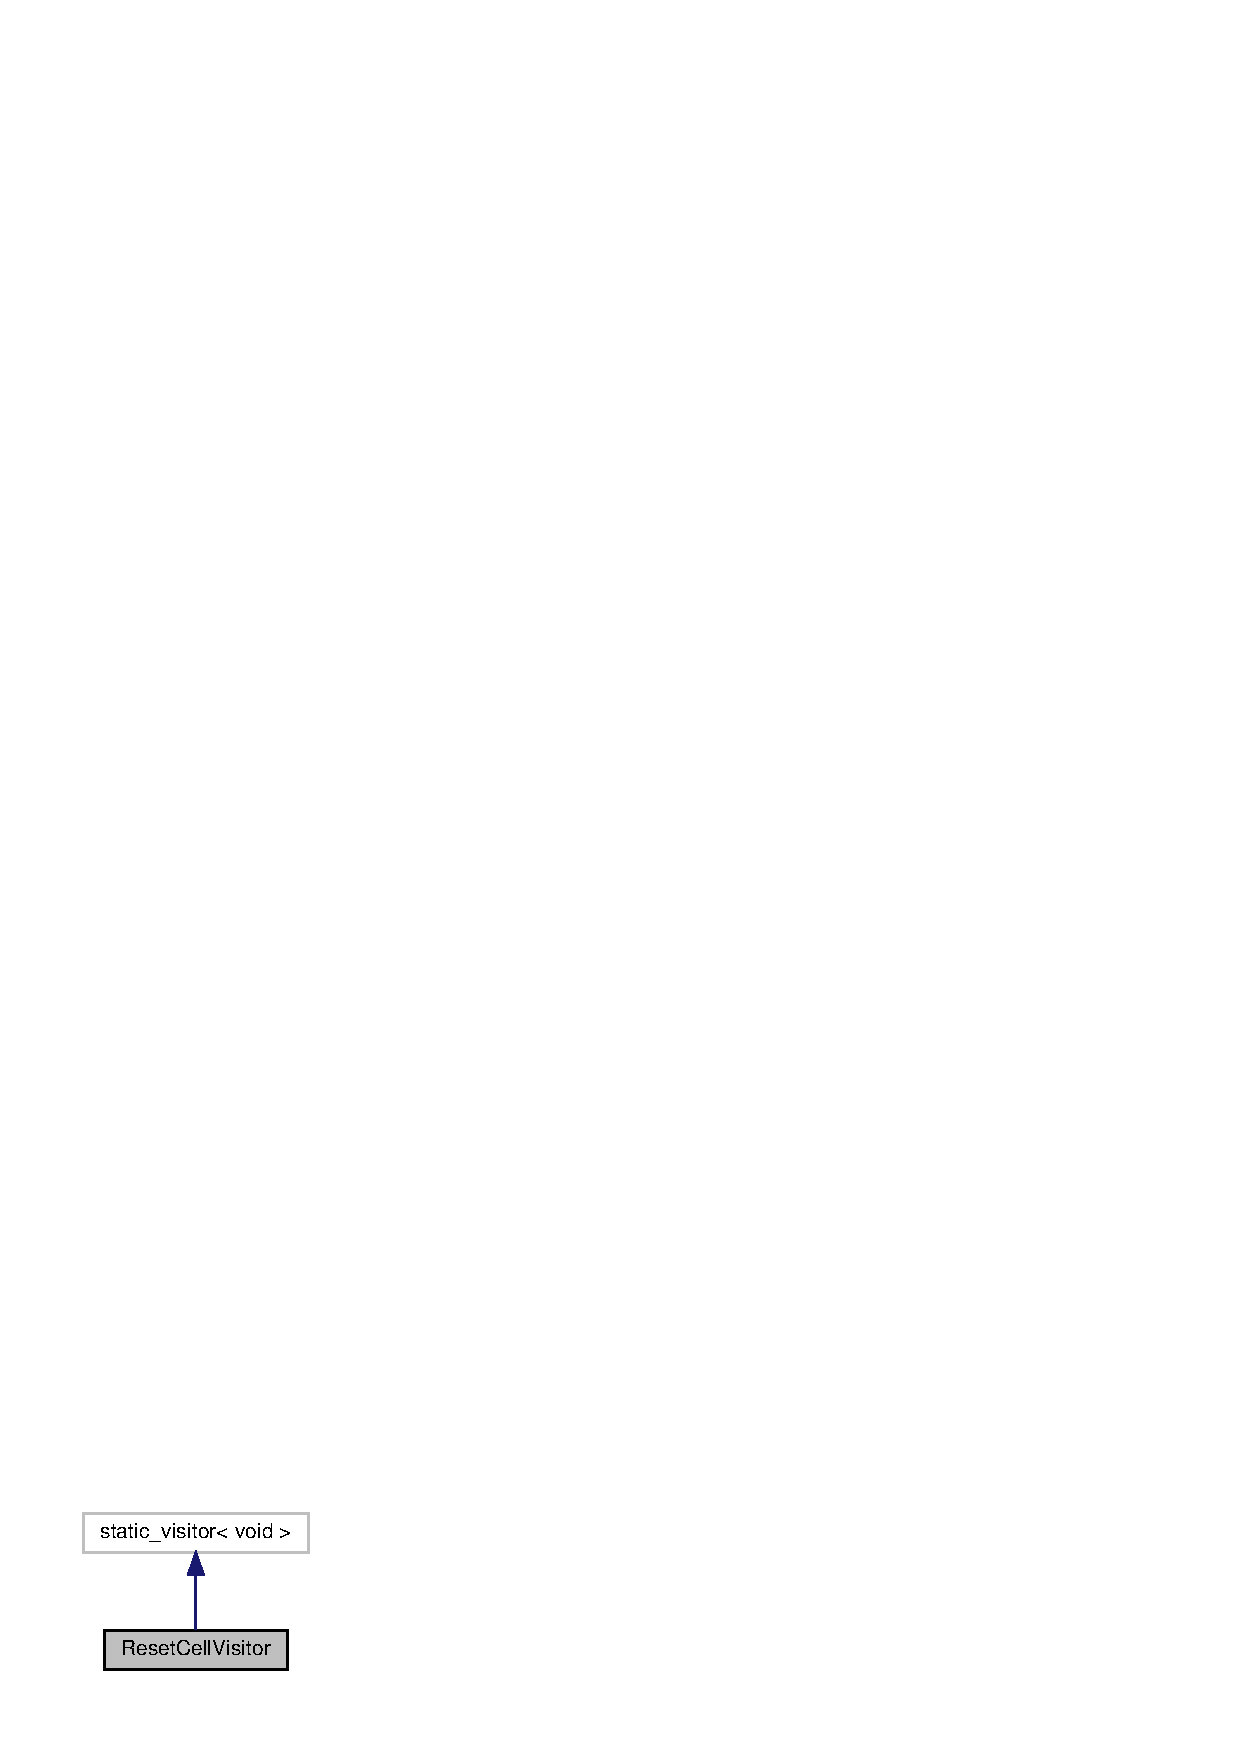
\includegraphics[width=152pt]{classmlpack_1_1ann_1_1ResetCellVisitor__inherit__graph}
\end{center}
\end{figure}
\subsection*{Public Member Functions}
\begin{DoxyCompactItemize}
\item 
\textbf{ Reset\+Cell\+Visitor} (const size\+\_\+t size)
\begin{DoxyCompactList}\small\item\em Reset the cell using the given size. \end{DoxyCompactList}\item 
{\footnotesize template$<$typename Layer\+Type $>$ }\\void \textbf{ operator()} (Layer\+Type $\ast$layer) const
\begin{DoxyCompactList}\small\item\em Execute the Reset\+Cell() function. \end{DoxyCompactList}\item 
void \textbf{ operator()} (\textbf{ More\+Types} layer) const
\end{DoxyCompactItemize}


\subsection{Detailed Description}
\doxyref{Reset\+Cell\+Visitor}{p.}{classmlpack_1_1ann_1_1ResetCellVisitor} executes the Reset\+Cell() function. 

Definition at line 26 of file reset\+\_\+cell\+\_\+visitor.\+hpp.



\subsection{Constructor \& Destructor Documentation}
\mbox{\label{classmlpack_1_1ann_1_1ResetCellVisitor_a2512a741862b68728aefc4183844d93f}} 
\index{mlpack\+::ann\+::\+Reset\+Cell\+Visitor@{mlpack\+::ann\+::\+Reset\+Cell\+Visitor}!Reset\+Cell\+Visitor@{Reset\+Cell\+Visitor}}
\index{Reset\+Cell\+Visitor@{Reset\+Cell\+Visitor}!mlpack\+::ann\+::\+Reset\+Cell\+Visitor@{mlpack\+::ann\+::\+Reset\+Cell\+Visitor}}
\subsubsection{Reset\+Cell\+Visitor()}
{\footnotesize\ttfamily \textbf{ Reset\+Cell\+Visitor} (\begin{DoxyParamCaption}\item[{const size\+\_\+t}]{size }\end{DoxyParamCaption})}



Reset the cell using the given size. 



\subsection{Member Function Documentation}
\mbox{\label{classmlpack_1_1ann_1_1ResetCellVisitor_a26bb3385c630118c35f4799f1509abbc}} 
\index{mlpack\+::ann\+::\+Reset\+Cell\+Visitor@{mlpack\+::ann\+::\+Reset\+Cell\+Visitor}!operator()@{operator()}}
\index{operator()@{operator()}!mlpack\+::ann\+::\+Reset\+Cell\+Visitor@{mlpack\+::ann\+::\+Reset\+Cell\+Visitor}}
\subsubsection{operator()()\hspace{0.1cm}{\footnotesize\ttfamily [1/2]}}
{\footnotesize\ttfamily void operator() (\begin{DoxyParamCaption}\item[{Layer\+Type $\ast$}]{layer }\end{DoxyParamCaption}) const}



Execute the Reset\+Cell() function. 

\mbox{\label{classmlpack_1_1ann_1_1ResetCellVisitor_ae35578e7ff874a320fe762bc0edfff04}} 
\index{mlpack\+::ann\+::\+Reset\+Cell\+Visitor@{mlpack\+::ann\+::\+Reset\+Cell\+Visitor}!operator()@{operator()}}
\index{operator()@{operator()}!mlpack\+::ann\+::\+Reset\+Cell\+Visitor@{mlpack\+::ann\+::\+Reset\+Cell\+Visitor}}
\subsubsection{operator()()\hspace{0.1cm}{\footnotesize\ttfamily [2/2]}}
{\footnotesize\ttfamily void operator() (\begin{DoxyParamCaption}\item[{\textbf{ More\+Types}}]{layer }\end{DoxyParamCaption}) const}



The documentation for this class was generated from the following file\+:\begin{DoxyCompactItemize}
\item 
/home/aakash/mlpack/src/mlpack/methods/ann/visitor/\textbf{ reset\+\_\+cell\+\_\+visitor.\+hpp}\end{DoxyCompactItemize}

\section{Reset\+Visitor Class Reference}
\label{classmlpack_1_1ann_1_1ResetVisitor}\index{Reset\+Visitor@{Reset\+Visitor}}


\doxyref{Reset\+Visitor}{p.}{classmlpack_1_1ann_1_1ResetVisitor} executes the Reset() function.  




Inheritance diagram for Reset\+Visitor\+:
\nopagebreak
\begin{figure}[H]
\begin{center}
\leavevmode
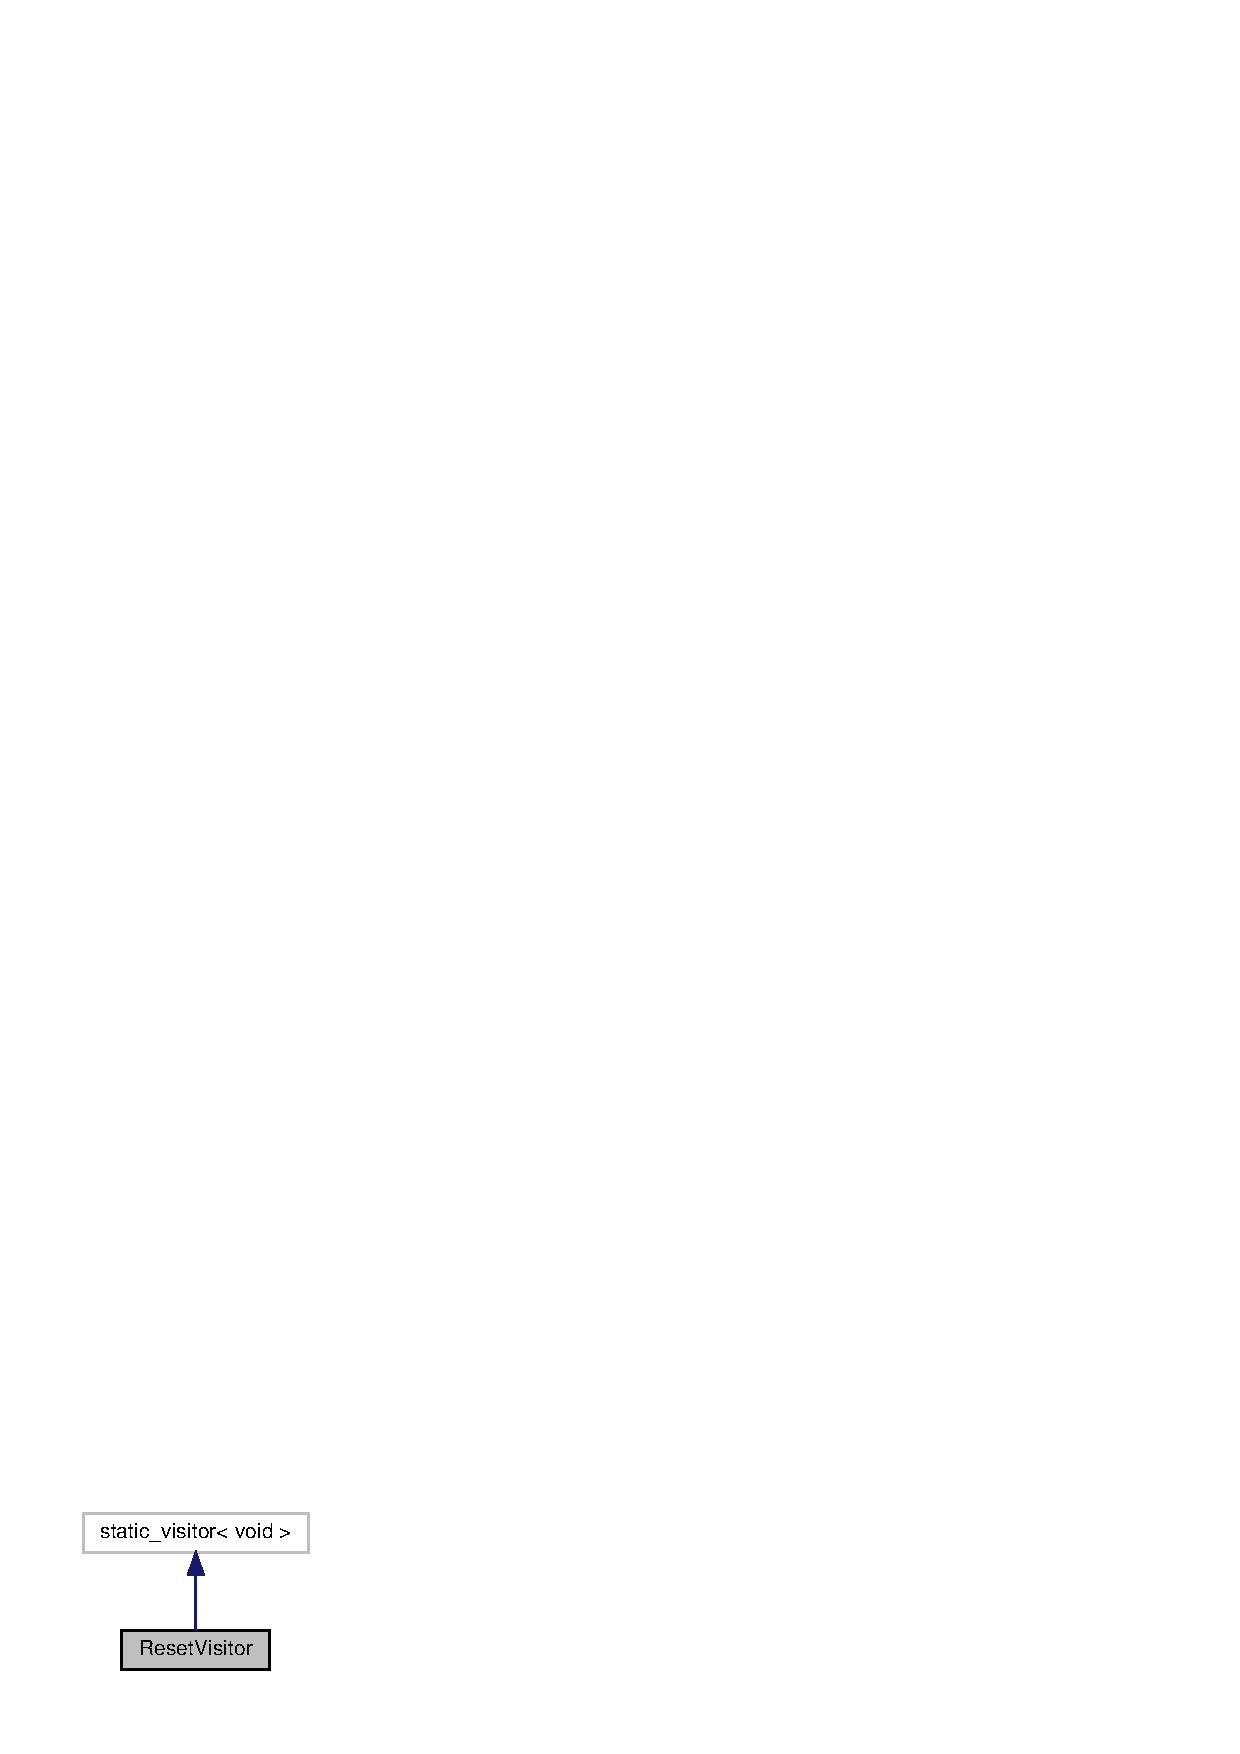
\includegraphics[width=152pt]{classmlpack_1_1ann_1_1ResetVisitor__inherit__graph}
\end{center}
\end{figure}
\subsection*{Public Member Functions}
\begin{DoxyCompactItemize}
\item 
{\footnotesize template$<$typename Layer\+Type $>$ }\\void \textbf{ operator()} (Layer\+Type $\ast$layer) const
\begin{DoxyCompactList}\small\item\em Execute the Reset() function. \end{DoxyCompactList}\item 
void \textbf{ operator()} (\textbf{ More\+Types} layer) const
\end{DoxyCompactItemize}


\subsection{Detailed Description}
\doxyref{Reset\+Visitor}{p.}{classmlpack_1_1ann_1_1ResetVisitor} executes the Reset() function. 

Definition at line 26 of file reset\+\_\+visitor.\+hpp.



\subsection{Member Function Documentation}
\mbox{\label{classmlpack_1_1ann_1_1ResetVisitor_a26bb3385c630118c35f4799f1509abbc}} 
\index{mlpack\+::ann\+::\+Reset\+Visitor@{mlpack\+::ann\+::\+Reset\+Visitor}!operator()@{operator()}}
\index{operator()@{operator()}!mlpack\+::ann\+::\+Reset\+Visitor@{mlpack\+::ann\+::\+Reset\+Visitor}}
\subsubsection{operator()()\hspace{0.1cm}{\footnotesize\ttfamily [1/2]}}
{\footnotesize\ttfamily void operator() (\begin{DoxyParamCaption}\item[{Layer\+Type $\ast$}]{layer }\end{DoxyParamCaption}) const}



Execute the Reset() function. 

\mbox{\label{classmlpack_1_1ann_1_1ResetVisitor_ae35578e7ff874a320fe762bc0edfff04}} 
\index{mlpack\+::ann\+::\+Reset\+Visitor@{mlpack\+::ann\+::\+Reset\+Visitor}!operator()@{operator()}}
\index{operator()@{operator()}!mlpack\+::ann\+::\+Reset\+Visitor@{mlpack\+::ann\+::\+Reset\+Visitor}}
\subsubsection{operator()()\hspace{0.1cm}{\footnotesize\ttfamily [2/2]}}
{\footnotesize\ttfamily void operator() (\begin{DoxyParamCaption}\item[{\textbf{ More\+Types}}]{layer }\end{DoxyParamCaption}) const}



The documentation for this class was generated from the following file\+:\begin{DoxyCompactItemize}
\item 
/home/aakash/mlpack/src/mlpack/methods/ann/visitor/\textbf{ reset\+\_\+visitor.\+hpp}\end{DoxyCompactItemize}

\section{Reward\+Set\+Visitor Class Reference}
\label{classmlpack_1_1ann_1_1RewardSetVisitor}\index{Reward\+Set\+Visitor@{Reward\+Set\+Visitor}}


\doxyref{Reward\+Set\+Visitor}{p.}{classmlpack_1_1ann_1_1RewardSetVisitor} set the reward parameter given the reward value.  




Inheritance diagram for Reward\+Set\+Visitor\+:
\nopagebreak
\begin{figure}[H]
\begin{center}
\leavevmode
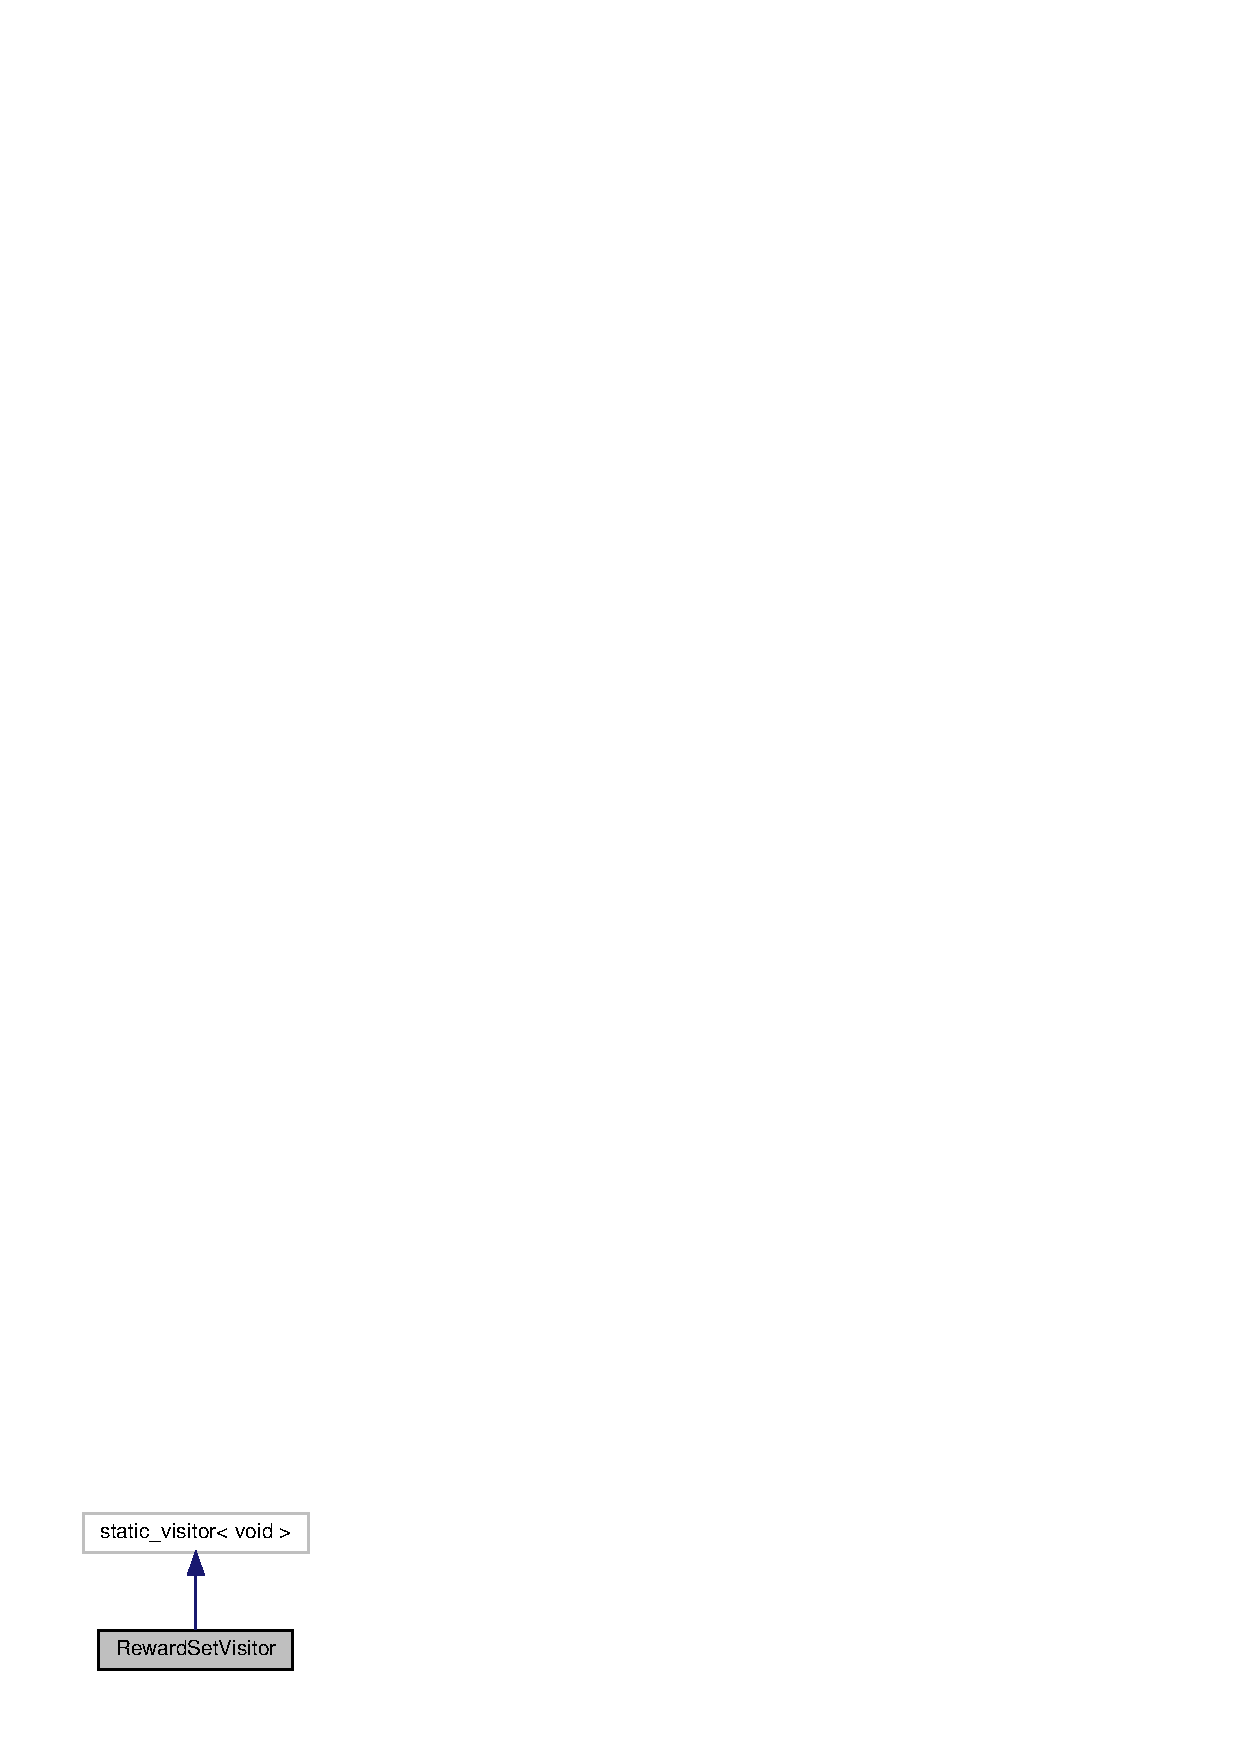
\includegraphics[width=152pt]{classmlpack_1_1ann_1_1RewardSetVisitor__inherit__graph}
\end{center}
\end{figure}
\subsection*{Public Member Functions}
\begin{DoxyCompactItemize}
\item 
\textbf{ Reward\+Set\+Visitor} (const double reward)
\begin{DoxyCompactList}\small\item\em Set the reward parameter given the reward value. \end{DoxyCompactList}\item 
{\footnotesize template$<$typename Layer\+Type $>$ }\\void \textbf{ operator()} (Layer\+Type $\ast$layer) const
\begin{DoxyCompactList}\small\item\em Set the reward parameter. \end{DoxyCompactList}\item 
void \textbf{ operator()} (\textbf{ More\+Types} layer) const
\end{DoxyCompactItemize}


\subsection{Detailed Description}
\doxyref{Reward\+Set\+Visitor}{p.}{classmlpack_1_1ann_1_1RewardSetVisitor} set the reward parameter given the reward value. 

Definition at line 26 of file reward\+\_\+set\+\_\+visitor.\+hpp.



\subsection{Constructor \& Destructor Documentation}
\mbox{\label{classmlpack_1_1ann_1_1RewardSetVisitor_aebce7d20815b69df4acfa115cb5076a1}} 
\index{mlpack\+::ann\+::\+Reward\+Set\+Visitor@{mlpack\+::ann\+::\+Reward\+Set\+Visitor}!Reward\+Set\+Visitor@{Reward\+Set\+Visitor}}
\index{Reward\+Set\+Visitor@{Reward\+Set\+Visitor}!mlpack\+::ann\+::\+Reward\+Set\+Visitor@{mlpack\+::ann\+::\+Reward\+Set\+Visitor}}
\subsubsection{Reward\+Set\+Visitor()}
{\footnotesize\ttfamily \textbf{ Reward\+Set\+Visitor} (\begin{DoxyParamCaption}\item[{const double}]{reward }\end{DoxyParamCaption})}



Set the reward parameter given the reward value. 



\subsection{Member Function Documentation}
\mbox{\label{classmlpack_1_1ann_1_1RewardSetVisitor_a26bb3385c630118c35f4799f1509abbc}} 
\index{mlpack\+::ann\+::\+Reward\+Set\+Visitor@{mlpack\+::ann\+::\+Reward\+Set\+Visitor}!operator()@{operator()}}
\index{operator()@{operator()}!mlpack\+::ann\+::\+Reward\+Set\+Visitor@{mlpack\+::ann\+::\+Reward\+Set\+Visitor}}
\subsubsection{operator()()\hspace{0.1cm}{\footnotesize\ttfamily [1/2]}}
{\footnotesize\ttfamily void operator() (\begin{DoxyParamCaption}\item[{Layer\+Type $\ast$}]{layer }\end{DoxyParamCaption}) const}



Set the reward parameter. 

\mbox{\label{classmlpack_1_1ann_1_1RewardSetVisitor_ae35578e7ff874a320fe762bc0edfff04}} 
\index{mlpack\+::ann\+::\+Reward\+Set\+Visitor@{mlpack\+::ann\+::\+Reward\+Set\+Visitor}!operator()@{operator()}}
\index{operator()@{operator()}!mlpack\+::ann\+::\+Reward\+Set\+Visitor@{mlpack\+::ann\+::\+Reward\+Set\+Visitor}}
\subsubsection{operator()()\hspace{0.1cm}{\footnotesize\ttfamily [2/2]}}
{\footnotesize\ttfamily void operator() (\begin{DoxyParamCaption}\item[{\textbf{ More\+Types}}]{layer }\end{DoxyParamCaption}) const}



The documentation for this class was generated from the following file\+:\begin{DoxyCompactItemize}
\item 
/home/aakash/mlpack/src/mlpack/methods/ann/visitor/\textbf{ reward\+\_\+set\+\_\+visitor.\+hpp}\end{DoxyCompactItemize}

\section{R\+NN$<$ Output\+Layer\+Type, Initialization\+Rule\+Type, Custom\+Layers $>$ Class Template Reference}
\label{classmlpack_1_1ann_1_1RNN}\index{R\+N\+N$<$ Output\+Layer\+Type, Initialization\+Rule\+Type, Custom\+Layers $>$@{R\+N\+N$<$ Output\+Layer\+Type, Initialization\+Rule\+Type, Custom\+Layers $>$}}


Implementation of a standard recurrent neural network container.  




Inheritance diagram for R\+NN$<$ Output\+Layer\+Type, Initialization\+Rule\+Type, Custom\+Layers $>$\+:
\nopagebreak
\begin{figure}[H]
\begin{center}
\leavevmode
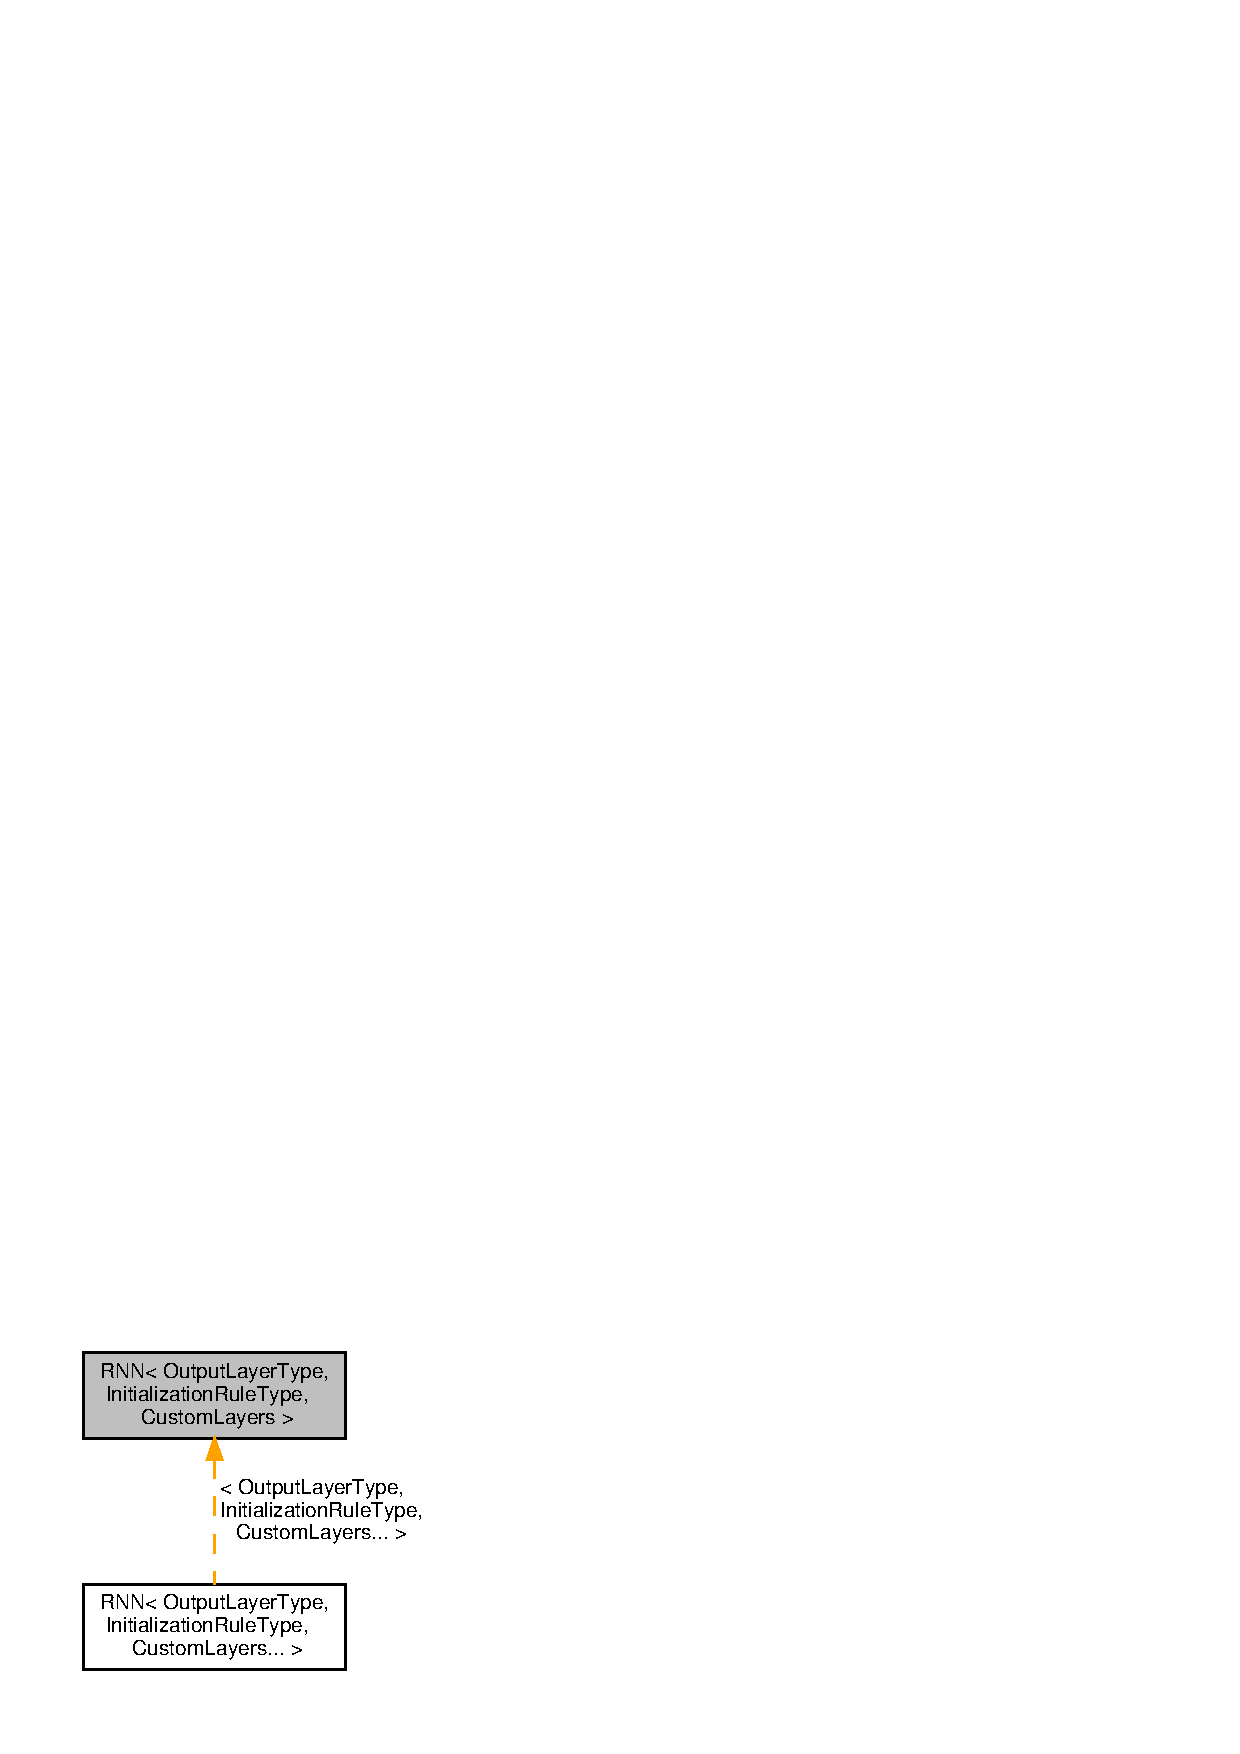
\includegraphics[width=207pt]{classmlpack_1_1ann_1_1RNN__inherit__graph}
\end{center}
\end{figure}
\subsection*{Public Types}
\begin{DoxyCompactItemize}
\item 
using \textbf{ Network\+Type} = \textbf{ R\+NN}$<$ Output\+Layer\+Type, Initialization\+Rule\+Type, Custom\+Layers... $>$
\begin{DoxyCompactList}\small\item\em Convenience typedef for the internal model construction. \end{DoxyCompactList}\end{DoxyCompactItemize}
\subsection*{Public Member Functions}
\begin{DoxyCompactItemize}
\item 
\textbf{ R\+NN} (const size\+\_\+t rho, const bool single=false, Output\+Layer\+Type output\+Layer=Output\+Layer\+Type(), Initialization\+Rule\+Type initialize\+Rule=Initialization\+Rule\+Type())
\begin{DoxyCompactList}\small\item\em Create the \doxyref{R\+NN}{p.}{classmlpack_1_1ann_1_1RNN} object. \end{DoxyCompactList}\item 
\textbf{ R\+NN} (const \textbf{ R\+NN} \&)
\begin{DoxyCompactList}\small\item\em Copy constructor. \end{DoxyCompactList}\item 
\textbf{ R\+NN} (\textbf{ R\+NN} \&\&)
\begin{DoxyCompactList}\small\item\em Move constructor. \end{DoxyCompactList}\item 
\textbf{ $\sim$\+R\+NN} ()
\begin{DoxyCompactList}\small\item\em Destructor to release allocated memory. \end{DoxyCompactList}\item 
{\footnotesize template$<$class Layer\+Type , class... Args$>$ }\\void \textbf{ Add} (Args... args)
\item 
void \textbf{ Add} (\textbf{ Layer\+Types}$<$ Custom\+Layers... $>$ layer)
\item 
double \textbf{ Evaluate} (const arma\+::mat \&parameters, const size\+\_\+t begin, const size\+\_\+t batch\+Size, const bool deterministic)
\begin{DoxyCompactList}\small\item\em Evaluate the recurrent neural network with the given parameters. \end{DoxyCompactList}\item 
double \textbf{ Evaluate} (const arma\+::mat \&parameters, const size\+\_\+t begin, const size\+\_\+t batch\+Size)
\begin{DoxyCompactList}\small\item\em Evaluate the recurrent neural network with the given parameters. \end{DoxyCompactList}\item 
{\footnotesize template$<$typename Grad\+Type $>$ }\\double \textbf{ Evaluate\+With\+Gradient} (const arma\+::mat \&parameters, const size\+\_\+t begin, Grad\+Type \&gradient, const size\+\_\+t batch\+Size)
\begin{DoxyCompactList}\small\item\em Evaluate the recurrent neural network with the given parameters. \end{DoxyCompactList}\item 
void \textbf{ Gradient} (const arma\+::mat \&parameters, const size\+\_\+t begin, arma\+::mat \&gradient, const size\+\_\+t batch\+Size)
\begin{DoxyCompactList}\small\item\em Evaluate the gradient of the recurrent neural network with the given parameters, and with respect to only one point in the dataset. \end{DoxyCompactList}\item 
size\+\_\+t \textbf{ Num\+Functions} () const
\begin{DoxyCompactList}\small\item\em Return the number of separable functions (the number of predictor points). \end{DoxyCompactList}\item 
\textbf{ R\+NN} \& \textbf{ operator=} (const \textbf{ R\+NN} \&)
\begin{DoxyCompactList}\small\item\em Copy assignment operator. \end{DoxyCompactList}\item 
\textbf{ R\+NN} \& \textbf{ operator=} (\textbf{ R\+NN} \&\&)
\begin{DoxyCompactList}\small\item\em Move assignment operator. \end{DoxyCompactList}\item 
const arma\+::mat \& \textbf{ Parameters} () const
\begin{DoxyCompactList}\small\item\em Return the initial point for the optimization. \end{DoxyCompactList}\item 
arma\+::mat \& \textbf{ Parameters} ()
\begin{DoxyCompactList}\small\item\em Modify the initial point for the optimization. \end{DoxyCompactList}\item 
void \textbf{ Predict} (arma\+::cube predictors, arma\+::cube \&results, const size\+\_\+t batch\+Size=256)
\begin{DoxyCompactList}\small\item\em Predict the responses to a given set of predictors. \end{DoxyCompactList}\item 
const arma\+::cube \& \textbf{ Predictors} () const
\begin{DoxyCompactList}\small\item\em Get the matrix of data points (predictors). \end{DoxyCompactList}\item 
arma\+::cube \& \textbf{ Predictors} ()
\begin{DoxyCompactList}\small\item\em Modify the matrix of data points (predictors). \end{DoxyCompactList}\item 
void \textbf{ Reset} ()
\begin{DoxyCompactList}\small\item\em Reset the state of the network. \end{DoxyCompactList}\item 
void \textbf{ Reset\+Parameters} ()
\begin{DoxyCompactList}\small\item\em Reset the module information (weights/parameters). \end{DoxyCompactList}\item 
const arma\+::cube \& \textbf{ Responses} () const
\begin{DoxyCompactList}\small\item\em Get the matrix of responses to the input data points. \end{DoxyCompactList}\item 
arma\+::cube \& \textbf{ Responses} ()
\begin{DoxyCompactList}\small\item\em Modify the matrix of responses to the input data points. \end{DoxyCompactList}\item 
const size\+\_\+t \& \textbf{ Rho} () const
\begin{DoxyCompactList}\small\item\em Return the maximum length of backpropagation through time. \end{DoxyCompactList}\item 
size\+\_\+t \& \textbf{ Rho} ()
\begin{DoxyCompactList}\small\item\em Modify the maximum length of backpropagation through time. \end{DoxyCompactList}\item 
{\footnotesize template$<$typename Archive $>$ }\\void \textbf{ serialize} (Archive \&ar, const uint32\+\_\+t)
\begin{DoxyCompactList}\small\item\em Serialize the model. \end{DoxyCompactList}\item 
void \textbf{ Shuffle} ()
\begin{DoxyCompactList}\small\item\em Shuffle the order of function visitation. \end{DoxyCompactList}\item 
{\footnotesize template$<$typename Optimizer\+Type , typename... Callback\+Types$>$ }\\double \textbf{ Train} (arma\+::cube predictors, arma\+::cube responses, Optimizer\+Type \&optimizer, Callback\+Types \&\&... callbacks)
\begin{DoxyCompactList}\small\item\em Train the recurrent neural network on the given input data using the given optimizer. \end{DoxyCompactList}\item 
{\footnotesize template$<$typename Optimizer\+Type  = ens\+::\+Standard\+S\+GD, typename... Callback\+Types$>$ }\\double \textbf{ Train} (arma\+::cube predictors, arma\+::cube responses, Callback\+Types \&\&... callbacks)
\begin{DoxyCompactList}\small\item\em Train the recurrent neural network on the given input data. \end{DoxyCompactList}\item 
{\footnotesize template$<$typename Optimizer\+Type $>$ }\\std\+::enable\+\_\+if$<$ Has\+Max\+Iterations$<$ Optimizer\+Type, size\+\_\+t \&(Optimizer\+Type\+::$\ast$)()$>$\+::value, void $>$\+::type \textbf{ Warn\+Message\+Max\+Iterations} (Optimizer\+Type \&optimizer, size\+\_\+t samples) const
\begin{DoxyCompactList}\small\item\em Check if the optimizer has Max\+Iterations() parameter, if it does then check if it\textquotesingle{}s value is less than the number of datapoints in the dataset. \end{DoxyCompactList}\item 
{\footnotesize template$<$typename Optimizer\+Type $>$ }\\std\+::enable\+\_\+if$<$ !Has\+Max\+Iterations$<$ Optimizer\+Type, size\+\_\+t \&(Optimizer\+Type\+::$\ast$)()$>$\+::value, void $>$\+::type \textbf{ Warn\+Message\+Max\+Iterations} (Optimizer\+Type \&optimizer, size\+\_\+t samples) const
\begin{DoxyCompactList}\small\item\em Check if the optimizer has Max\+Iterations() parameter, if it doesn\textquotesingle{}t then simply return from the function. \end{DoxyCompactList}\end{DoxyCompactItemize}


\subsection{Detailed Description}
\subsubsection*{template$<$typename Output\+Layer\+Type = Negative\+Log\+Likelihood$<$$>$, typename Initialization\+Rule\+Type = Random\+Initialization, typename... Custom\+Layers$>$\newline
class mlpack\+::ann\+::\+R\+N\+N$<$ Output\+Layer\+Type, Initialization\+Rule\+Type, Custom\+Layers $>$}

Implementation of a standard recurrent neural network container. 


\begin{DoxyTemplParams}{Template Parameters}
{\em Output\+Layer\+Type} & The output layer type used to evaluate the network. \\
\hline
{\em Initialization\+Rule\+Type} & Rule used to initialize the weight matrix. \\
\hline
\end{DoxyTemplParams}


Definition at line 45 of file rnn.\+hpp.



\subsection{Member Typedef Documentation}
\mbox{\label{classmlpack_1_1ann_1_1RNN_a8b97fdc6b24723019bcab248fe7db76a}} 
\index{mlpack\+::ann\+::\+R\+NN@{mlpack\+::ann\+::\+R\+NN}!Network\+Type@{Network\+Type}}
\index{Network\+Type@{Network\+Type}!mlpack\+::ann\+::\+R\+NN@{mlpack\+::ann\+::\+R\+NN}}
\subsubsection{Network\+Type}
{\footnotesize\ttfamily using \textbf{ Network\+Type} =  \textbf{ R\+NN}$<$Output\+Layer\+Type, Initialization\+Rule\+Type, Custom\+Layers...$>$}



Convenience typedef for the internal model construction. 



Definition at line 51 of file rnn.\+hpp.



\subsection{Constructor \& Destructor Documentation}
\mbox{\label{classmlpack_1_1ann_1_1RNN_aa07a59fdcbe988264200c8f593c73bbf}} 
\index{mlpack\+::ann\+::\+R\+NN@{mlpack\+::ann\+::\+R\+NN}!R\+NN@{R\+NN}}
\index{R\+NN@{R\+NN}!mlpack\+::ann\+::\+R\+NN@{mlpack\+::ann\+::\+R\+NN}}
\subsubsection{R\+N\+N()\hspace{0.1cm}{\footnotesize\ttfamily [1/3]}}
{\footnotesize\ttfamily \textbf{ R\+NN} (\begin{DoxyParamCaption}\item[{const size\+\_\+t}]{rho,  }\item[{const bool}]{single = {\ttfamily false},  }\item[{Output\+Layer\+Type}]{output\+Layer = {\ttfamily OutputLayerType()},  }\item[{Initialization\+Rule\+Type}]{initialize\+Rule = {\ttfamily InitializationRuleType()} }\end{DoxyParamCaption})}



Create the \doxyref{R\+NN}{p.}{classmlpack_1_1ann_1_1RNN} object. 

Optionally, specify which initialize rule and performance function should be used.

If you want to pass in a parameter and discard the original parameter object, be sure to use std\+::move to avoid unnecessary copy.


\begin{DoxyParams}{Parameters}
{\em rho} & Maximum number of steps to backpropagate through time (B\+P\+TT). \\
\hline
{\em single} & Predict only the last element of the input sequence. \\
\hline
{\em output\+Layer} & Output layer used to evaluate the network. \\
\hline
{\em initialize\+Rule} & Optional instantiated Initialization\+Rule object for initializing the network parameter. \\
\hline
\end{DoxyParams}
\mbox{\label{classmlpack_1_1ann_1_1RNN_a8b066e4fee1ae2eaf039a8b6af975bfa}} 
\index{mlpack\+::ann\+::\+R\+NN@{mlpack\+::ann\+::\+R\+NN}!R\+NN@{R\+NN}}
\index{R\+NN@{R\+NN}!mlpack\+::ann\+::\+R\+NN@{mlpack\+::ann\+::\+R\+NN}}
\subsubsection{R\+N\+N()\hspace{0.1cm}{\footnotesize\ttfamily [2/3]}}
{\footnotesize\ttfamily \textbf{ R\+NN} (\begin{DoxyParamCaption}\item[{const \textbf{ R\+NN}$<$ Output\+Layer\+Type, Initialization\+Rule\+Type, Custom\+Layers $>$ \&}]{ }\end{DoxyParamCaption})}



Copy constructor. 

\mbox{\label{classmlpack_1_1ann_1_1RNN_a3efe3cf0bafdde0a079e6ec7cb73db96}} 
\index{mlpack\+::ann\+::\+R\+NN@{mlpack\+::ann\+::\+R\+NN}!R\+NN@{R\+NN}}
\index{R\+NN@{R\+NN}!mlpack\+::ann\+::\+R\+NN@{mlpack\+::ann\+::\+R\+NN}}
\subsubsection{R\+N\+N()\hspace{0.1cm}{\footnotesize\ttfamily [3/3]}}
{\footnotesize\ttfamily \textbf{ R\+NN} (\begin{DoxyParamCaption}\item[{\textbf{ R\+NN}$<$ Output\+Layer\+Type, Initialization\+Rule\+Type, Custom\+Layers $>$ \&\&}]{ }\end{DoxyParamCaption})}



Move constructor. 

\mbox{\label{classmlpack_1_1ann_1_1RNN_abbaa486d6d0992486ee3283f1800e20c}} 
\index{mlpack\+::ann\+::\+R\+NN@{mlpack\+::ann\+::\+R\+NN}!````~R\+NN@{$\sim$\+R\+NN}}
\index{````~R\+NN@{$\sim$\+R\+NN}!mlpack\+::ann\+::\+R\+NN@{mlpack\+::ann\+::\+R\+NN}}
\subsubsection{$\sim$\+R\+N\+N()}
{\footnotesize\ttfamily $\sim$\textbf{ R\+NN} (\begin{DoxyParamCaption}{ }\end{DoxyParamCaption})}



Destructor to release allocated memory. 



\subsection{Member Function Documentation}
\mbox{\label{classmlpack_1_1ann_1_1RNN_a8b5234495846c00f6b2c8296ca6bc718}} 
\index{mlpack\+::ann\+::\+R\+NN@{mlpack\+::ann\+::\+R\+NN}!Add@{Add}}
\index{Add@{Add}!mlpack\+::ann\+::\+R\+NN@{mlpack\+::ann\+::\+R\+NN}}
\subsubsection{Add()\hspace{0.1cm}{\footnotesize\ttfamily [1/2]}}
{\footnotesize\ttfamily void \textbf{ Add} (\begin{DoxyParamCaption}\item[{Args...}]{args }\end{DoxyParamCaption})\hspace{0.3cm}{\ttfamily [inline]}}



Definition at line 284 of file rnn.\+hpp.

\mbox{\label{classmlpack_1_1ann_1_1RNN_a503a807740e6c729be9efc89520db728}} 
\index{mlpack\+::ann\+::\+R\+NN@{mlpack\+::ann\+::\+R\+NN}!Add@{Add}}
\index{Add@{Add}!mlpack\+::ann\+::\+R\+NN@{mlpack\+::ann\+::\+R\+NN}}
\subsubsection{Add()\hspace{0.1cm}{\footnotesize\ttfamily [2/2]}}
{\footnotesize\ttfamily void \textbf{ Add} (\begin{DoxyParamCaption}\item[{\textbf{ Layer\+Types}$<$ Custom\+Layers... $>$}]{layer }\end{DoxyParamCaption})\hspace{0.3cm}{\ttfamily [inline]}}



Definition at line 291 of file rnn.\+hpp.

\mbox{\label{classmlpack_1_1ann_1_1RNN_a3e02a8743fd14b2a902a2e090da2df47}} 
\index{mlpack\+::ann\+::\+R\+NN@{mlpack\+::ann\+::\+R\+NN}!Evaluate@{Evaluate}}
\index{Evaluate@{Evaluate}!mlpack\+::ann\+::\+R\+NN@{mlpack\+::ann\+::\+R\+NN}}
\subsubsection{Evaluate()\hspace{0.1cm}{\footnotesize\ttfamily [1/2]}}
{\footnotesize\ttfamily double Evaluate (\begin{DoxyParamCaption}\item[{const arma\+::mat \&}]{parameters,  }\item[{const size\+\_\+t}]{begin,  }\item[{const size\+\_\+t}]{batch\+Size,  }\item[{const bool}]{deterministic }\end{DoxyParamCaption})}



Evaluate the recurrent neural network with the given parameters. 

This function is usually called by the optimizer to train the model.


\begin{DoxyParams}{Parameters}
{\em parameters} & Matrix model parameters. \\
\hline
{\em begin} & Index of the starting point to use for objective function evaluation. \\
\hline
{\em batch\+Size} & Number of points to be passed at a time to use for objective function evaluation. \\
\hline
{\em deterministic} & Whether or not to train or test the model. Note some layer act differently in training or testing mode. \\
\hline
\end{DoxyParams}
\mbox{\label{classmlpack_1_1ann_1_1RNN_a8a04cfd951b52327d7f2e148c68f365d}} 
\index{mlpack\+::ann\+::\+R\+NN@{mlpack\+::ann\+::\+R\+NN}!Evaluate@{Evaluate}}
\index{Evaluate@{Evaluate}!mlpack\+::ann\+::\+R\+NN@{mlpack\+::ann\+::\+R\+NN}}
\subsubsection{Evaluate()\hspace{0.1cm}{\footnotesize\ttfamily [2/2]}}
{\footnotesize\ttfamily double Evaluate (\begin{DoxyParamCaption}\item[{const arma\+::mat \&}]{parameters,  }\item[{const size\+\_\+t}]{begin,  }\item[{const size\+\_\+t}]{batch\+Size }\end{DoxyParamCaption})}



Evaluate the recurrent neural network with the given parameters. 

This function is usually called by the optimizer to train the model. This just calls the other overload of \doxyref{Evaluate()}{p.}{classmlpack_1_1ann_1_1RNN_a3e02a8743fd14b2a902a2e090da2df47} with deterministic = true.


\begin{DoxyParams}{Parameters}
{\em parameters} & Matrix model parameters. \\
\hline
{\em begin} & Index of the starting point to use for objective function evaluation. \\
\hline
{\em batch\+Size} & Number of points to be passed at a time to use for objective function evaluation. \\
\hline
\end{DoxyParams}
\mbox{\label{classmlpack_1_1ann_1_1RNN_a3e01e9e3fe4f5bd8cfc78521567a0f5a}} 
\index{mlpack\+::ann\+::\+R\+NN@{mlpack\+::ann\+::\+R\+NN}!Evaluate\+With\+Gradient@{Evaluate\+With\+Gradient}}
\index{Evaluate\+With\+Gradient@{Evaluate\+With\+Gradient}!mlpack\+::ann\+::\+R\+NN@{mlpack\+::ann\+::\+R\+NN}}
\subsubsection{Evaluate\+With\+Gradient()}
{\footnotesize\ttfamily double Evaluate\+With\+Gradient (\begin{DoxyParamCaption}\item[{const arma\+::mat \&}]{parameters,  }\item[{const size\+\_\+t}]{begin,  }\item[{Grad\+Type \&}]{gradient,  }\item[{const size\+\_\+t}]{batch\+Size }\end{DoxyParamCaption})}



Evaluate the recurrent neural network with the given parameters. 

This function is usually called by the optimizer to train the model.


\begin{DoxyParams}{Parameters}
{\em parameters} & Matrix model parameters. \\
\hline
{\em begin} & Index of the starting point to use for objective function evaluation. \\
\hline
{\em gradient} & Matrix to output gradient into. \\
\hline
{\em batch\+Size} & Number of points to be passed at a time to use for objective function evaluation. \\
\hline
\end{DoxyParams}
\mbox{\label{classmlpack_1_1ann_1_1RNN_aca73798d93d56b280185c01502d8bd13}} 
\index{mlpack\+::ann\+::\+R\+NN@{mlpack\+::ann\+::\+R\+NN}!Gradient@{Gradient}}
\index{Gradient@{Gradient}!mlpack\+::ann\+::\+R\+NN@{mlpack\+::ann\+::\+R\+NN}}
\subsubsection{Gradient()}
{\footnotesize\ttfamily void Gradient (\begin{DoxyParamCaption}\item[{const arma\+::mat \&}]{parameters,  }\item[{const size\+\_\+t}]{begin,  }\item[{arma\+::mat \&}]{gradient,  }\item[{const size\+\_\+t}]{batch\+Size }\end{DoxyParamCaption})}



Evaluate the gradient of the recurrent neural network with the given parameters, and with respect to only one point in the dataset. 

This is useful for optimizers such as S\+GD, which require a separable objective function.


\begin{DoxyParams}{Parameters}
{\em parameters} & Matrix of the model parameters to be optimized. \\
\hline
{\em begin} & Index of the starting point to use for objective function gradient evaluation. \\
\hline
{\em gradient} & Matrix to output gradient into. \\
\hline
{\em batch\+Size} & Number of points to be processed as a batch for objective function gradient evaluation. \\
\hline
\end{DoxyParams}


Referenced by R\+N\+N$<$ Output\+Layer\+Type, Initialization\+Rule\+Type, Custom\+Layers... $>$\+::\+Predictors().

\mbox{\label{classmlpack_1_1ann_1_1RNN_a1fa76af34a6e3ea927b307f0c318ee4b}} 
\index{mlpack\+::ann\+::\+R\+NN@{mlpack\+::ann\+::\+R\+NN}!Num\+Functions@{Num\+Functions}}
\index{Num\+Functions@{Num\+Functions}!mlpack\+::ann\+::\+R\+NN@{mlpack\+::ann\+::\+R\+NN}}
\subsubsection{Num\+Functions()}
{\footnotesize\ttfamily size\+\_\+t Num\+Functions (\begin{DoxyParamCaption}{ }\end{DoxyParamCaption}) const\hspace{0.3cm}{\ttfamily [inline]}}



Return the number of separable functions (the number of predictor points). 



Definition at line 294 of file rnn.\+hpp.

\mbox{\label{classmlpack_1_1ann_1_1RNN_afbb2012f58fe2ecb5c543b932c6458e1}} 
\index{mlpack\+::ann\+::\+R\+NN@{mlpack\+::ann\+::\+R\+NN}!operator=@{operator=}}
\index{operator=@{operator=}!mlpack\+::ann\+::\+R\+NN@{mlpack\+::ann\+::\+R\+NN}}
\subsubsection{operator=()\hspace{0.1cm}{\footnotesize\ttfamily [1/2]}}
{\footnotesize\ttfamily \textbf{ R\+NN}\& operator= (\begin{DoxyParamCaption}\item[{const \textbf{ R\+NN}$<$ Output\+Layer\+Type, Initialization\+Rule\+Type, Custom\+Layers $>$ \&}]{ }\end{DoxyParamCaption})}



Copy assignment operator. 

\mbox{\label{classmlpack_1_1ann_1_1RNN_a4bf24aeb2fba675cda38a7f4873a1564}} 
\index{mlpack\+::ann\+::\+R\+NN@{mlpack\+::ann\+::\+R\+NN}!operator=@{operator=}}
\index{operator=@{operator=}!mlpack\+::ann\+::\+R\+NN@{mlpack\+::ann\+::\+R\+NN}}
\subsubsection{operator=()\hspace{0.1cm}{\footnotesize\ttfamily [2/2]}}
{\footnotesize\ttfamily \textbf{ R\+NN}\& operator= (\begin{DoxyParamCaption}\item[{\textbf{ R\+NN}$<$ Output\+Layer\+Type, Initialization\+Rule\+Type, Custom\+Layers $>$ \&\&}]{ }\end{DoxyParamCaption})}



Move assignment operator. 

\mbox{\label{classmlpack_1_1ann_1_1RNN_aa68d74dc1e86e4352e00a3cab83a0e4a}} 
\index{mlpack\+::ann\+::\+R\+NN@{mlpack\+::ann\+::\+R\+NN}!Parameters@{Parameters}}
\index{Parameters@{Parameters}!mlpack\+::ann\+::\+R\+NN@{mlpack\+::ann\+::\+R\+NN}}
\subsubsection{Parameters()\hspace{0.1cm}{\footnotesize\ttfamily [1/2]}}
{\footnotesize\ttfamily const arma\+::mat\& Parameters (\begin{DoxyParamCaption}{ }\end{DoxyParamCaption}) const\hspace{0.3cm}{\ttfamily [inline]}}



Return the initial point for the optimization. 



Definition at line 297 of file rnn.\+hpp.

\mbox{\label{classmlpack_1_1ann_1_1RNN_a043f0ccd62e6711a18e0d81047be9a0a}} 
\index{mlpack\+::ann\+::\+R\+NN@{mlpack\+::ann\+::\+R\+NN}!Parameters@{Parameters}}
\index{Parameters@{Parameters}!mlpack\+::ann\+::\+R\+NN@{mlpack\+::ann\+::\+R\+NN}}
\subsubsection{Parameters()\hspace{0.1cm}{\footnotesize\ttfamily [2/2]}}
{\footnotesize\ttfamily arma\+::mat\& Parameters (\begin{DoxyParamCaption}{ }\end{DoxyParamCaption})\hspace{0.3cm}{\ttfamily [inline]}}



Modify the initial point for the optimization. 



Definition at line 299 of file rnn.\+hpp.

\mbox{\label{classmlpack_1_1ann_1_1RNN_a01373d6adb1a306eb2b093c26d5d9031}} 
\index{mlpack\+::ann\+::\+R\+NN@{mlpack\+::ann\+::\+R\+NN}!Predict@{Predict}}
\index{Predict@{Predict}!mlpack\+::ann\+::\+R\+NN@{mlpack\+::ann\+::\+R\+NN}}
\subsubsection{Predict()}
{\footnotesize\ttfamily void Predict (\begin{DoxyParamCaption}\item[{arma\+::cube}]{predictors,  }\item[{arma\+::cube \&}]{results,  }\item[{const size\+\_\+t}]{batch\+Size = {\ttfamily 256} }\end{DoxyParamCaption})}



Predict the responses to a given set of predictors. 

The responses will reflect the output of the given output layer as returned by the output layer function.

If you want to pass in a parameter and discard the original parameter object, be sure to use std\+::move to avoid unnecessary copy.

The format of the data should be as follows\+:
\begin{DoxyItemize}
\item each slice should correspond to a time step
\item each column should correspond to a data point
\item each row should correspond to a dimension So, e.\+g., predictors(i, j, k) is the i\textquotesingle{}th dimension of the j\textquotesingle{}th data point at time slice k. The responses will be in the same format.
\end{DoxyItemize}


\begin{DoxyParams}{Parameters}
{\em predictors} & Input predictors. \\
\hline
{\em results} & Matrix to put output predictions of responses into. \\
\hline
{\em batch\+Size} & Number of points to predict at once. \\
\hline
\end{DoxyParams}
\mbox{\label{classmlpack_1_1ann_1_1RNN_ae1efcab525131a0bc040aff1a8bb8e2d}} 
\index{mlpack\+::ann\+::\+R\+NN@{mlpack\+::ann\+::\+R\+NN}!Predictors@{Predictors}}
\index{Predictors@{Predictors}!mlpack\+::ann\+::\+R\+NN@{mlpack\+::ann\+::\+R\+NN}}
\subsubsection{Predictors()\hspace{0.1cm}{\footnotesize\ttfamily [1/2]}}
{\footnotesize\ttfamily const arma\+::cube\& Predictors (\begin{DoxyParamCaption}{ }\end{DoxyParamCaption}) const\hspace{0.3cm}{\ttfamily [inline]}}



Get the matrix of data points (predictors). 



Definition at line 312 of file rnn.\+hpp.

\mbox{\label{classmlpack_1_1ann_1_1RNN_a22c21d155cb5637e7d4e821564b27072}} 
\index{mlpack\+::ann\+::\+R\+NN@{mlpack\+::ann\+::\+R\+NN}!Predictors@{Predictors}}
\index{Predictors@{Predictors}!mlpack\+::ann\+::\+R\+NN@{mlpack\+::ann\+::\+R\+NN}}
\subsubsection{Predictors()\hspace{0.1cm}{\footnotesize\ttfamily [2/2]}}
{\footnotesize\ttfamily arma\+::cube\& Predictors (\begin{DoxyParamCaption}{ }\end{DoxyParamCaption})\hspace{0.3cm}{\ttfamily [inline]}}



Modify the matrix of data points (predictors). 



Definition at line 314 of file rnn.\+hpp.

\mbox{\label{classmlpack_1_1ann_1_1RNN_a372de693ad40b3f42839c8ec6ac845f4}} 
\index{mlpack\+::ann\+::\+R\+NN@{mlpack\+::ann\+::\+R\+NN}!Reset@{Reset}}
\index{Reset@{Reset}!mlpack\+::ann\+::\+R\+NN@{mlpack\+::ann\+::\+R\+NN}}
\subsubsection{Reset()}
{\footnotesize\ttfamily void Reset (\begin{DoxyParamCaption}{ }\end{DoxyParamCaption})}



Reset the state of the network. 

This ensures that all internally-\/held gradients are set to 0, all memory cells are reset, and the parameters matrix is the right size. 

Referenced by R\+N\+N$<$ Output\+Layer\+Type, Initialization\+Rule\+Type, Custom\+Layers... $>$\+::\+Predictors().

\mbox{\label{classmlpack_1_1ann_1_1RNN_a7178038c3cb8d247eadb94cd2058c432}} 
\index{mlpack\+::ann\+::\+R\+NN@{mlpack\+::ann\+::\+R\+NN}!Reset\+Parameters@{Reset\+Parameters}}
\index{Reset\+Parameters@{Reset\+Parameters}!mlpack\+::ann\+::\+R\+NN@{mlpack\+::ann\+::\+R\+NN}}
\subsubsection{Reset\+Parameters()}
{\footnotesize\ttfamily void Reset\+Parameters (\begin{DoxyParamCaption}{ }\end{DoxyParamCaption})}



Reset the module information (weights/parameters). 



Referenced by R\+N\+N$<$ Output\+Layer\+Type, Initialization\+Rule\+Type, Custom\+Layers... $>$\+::\+Predictors().

\mbox{\label{classmlpack_1_1ann_1_1RNN_ac109136a291d66f916e382c08a04a8a6}} 
\index{mlpack\+::ann\+::\+R\+NN@{mlpack\+::ann\+::\+R\+NN}!Responses@{Responses}}
\index{Responses@{Responses}!mlpack\+::ann\+::\+R\+NN@{mlpack\+::ann\+::\+R\+NN}}
\subsubsection{Responses()\hspace{0.1cm}{\footnotesize\ttfamily [1/2]}}
{\footnotesize\ttfamily const arma\+::cube\& Responses (\begin{DoxyParamCaption}{ }\end{DoxyParamCaption}) const\hspace{0.3cm}{\ttfamily [inline]}}



Get the matrix of responses to the input data points. 



Definition at line 307 of file rnn.\+hpp.

\mbox{\label{classmlpack_1_1ann_1_1RNN_a1b3ccc9c0245210305d8dd2df8693f3c}} 
\index{mlpack\+::ann\+::\+R\+NN@{mlpack\+::ann\+::\+R\+NN}!Responses@{Responses}}
\index{Responses@{Responses}!mlpack\+::ann\+::\+R\+NN@{mlpack\+::ann\+::\+R\+NN}}
\subsubsection{Responses()\hspace{0.1cm}{\footnotesize\ttfamily [2/2]}}
{\footnotesize\ttfamily arma\+::cube\& Responses (\begin{DoxyParamCaption}{ }\end{DoxyParamCaption})\hspace{0.3cm}{\ttfamily [inline]}}



Modify the matrix of responses to the input data points. 



Definition at line 309 of file rnn.\+hpp.

\mbox{\label{classmlpack_1_1ann_1_1RNN_a8cc9a89f8ec7de47890a86665a393450}} 
\index{mlpack\+::ann\+::\+R\+NN@{mlpack\+::ann\+::\+R\+NN}!Rho@{Rho}}
\index{Rho@{Rho}!mlpack\+::ann\+::\+R\+NN@{mlpack\+::ann\+::\+R\+NN}}
\subsubsection{Rho()\hspace{0.1cm}{\footnotesize\ttfamily [1/2]}}
{\footnotesize\ttfamily const size\+\_\+t\& Rho (\begin{DoxyParamCaption}{ }\end{DoxyParamCaption}) const\hspace{0.3cm}{\ttfamily [inline]}}



Return the maximum length of backpropagation through time. 



Definition at line 302 of file rnn.\+hpp.

\mbox{\label{classmlpack_1_1ann_1_1RNN_aeb617af2894a3e4bbabcd7ebc30a35af}} 
\index{mlpack\+::ann\+::\+R\+NN@{mlpack\+::ann\+::\+R\+NN}!Rho@{Rho}}
\index{Rho@{Rho}!mlpack\+::ann\+::\+R\+NN@{mlpack\+::ann\+::\+R\+NN}}
\subsubsection{Rho()\hspace{0.1cm}{\footnotesize\ttfamily [2/2]}}
{\footnotesize\ttfamily size\+\_\+t\& Rho (\begin{DoxyParamCaption}{ }\end{DoxyParamCaption})\hspace{0.3cm}{\ttfamily [inline]}}



Modify the maximum length of backpropagation through time. 



Definition at line 304 of file rnn.\+hpp.

\mbox{\label{classmlpack_1_1ann_1_1RNN_a65cba07328997659bec80b9879b15a51}} 
\index{mlpack\+::ann\+::\+R\+NN@{mlpack\+::ann\+::\+R\+NN}!serialize@{serialize}}
\index{serialize@{serialize}!mlpack\+::ann\+::\+R\+NN@{mlpack\+::ann\+::\+R\+NN}}
\subsubsection{serialize()}
{\footnotesize\ttfamily void serialize (\begin{DoxyParamCaption}\item[{Archive \&}]{ar,  }\item[{const uint32\+\_\+t}]{ }\end{DoxyParamCaption})}



Serialize the model. 



Referenced by R\+N\+N$<$ Output\+Layer\+Type, Initialization\+Rule\+Type, Custom\+Layers... $>$\+::\+Predictors().

\mbox{\label{classmlpack_1_1ann_1_1RNN_a2697cc8b37d7bca7c055228382a9b208}} 
\index{mlpack\+::ann\+::\+R\+NN@{mlpack\+::ann\+::\+R\+NN}!Shuffle@{Shuffle}}
\index{Shuffle@{Shuffle}!mlpack\+::ann\+::\+R\+NN@{mlpack\+::ann\+::\+R\+NN}}
\subsubsection{Shuffle()}
{\footnotesize\ttfamily void Shuffle (\begin{DoxyParamCaption}{ }\end{DoxyParamCaption})}



Shuffle the order of function visitation. 

This may be called by the optimizer. \mbox{\label{classmlpack_1_1ann_1_1RNN_a5f18ddeb54971c09eadc5d91dd589892}} 
\index{mlpack\+::ann\+::\+R\+NN@{mlpack\+::ann\+::\+R\+NN}!Train@{Train}}
\index{Train@{Train}!mlpack\+::ann\+::\+R\+NN@{mlpack\+::ann\+::\+R\+NN}}
\subsubsection{Train()\hspace{0.1cm}{\footnotesize\ttfamily [1/2]}}
{\footnotesize\ttfamily double Train (\begin{DoxyParamCaption}\item[{arma\+::cube}]{predictors,  }\item[{arma\+::cube}]{responses,  }\item[{Optimizer\+Type \&}]{optimizer,  }\item[{Callback\+Types \&\&...}]{callbacks }\end{DoxyParamCaption})}



Train the recurrent neural network on the given input data using the given optimizer. 

This will use the existing model parameters as a starting point for the optimization. If this is not what you want, then you should access the parameters vector directly with \doxyref{Parameters()}{p.}{classmlpack_1_1ann_1_1RNN_a043f0ccd62e6711a18e0d81047be9a0a} and modify it as desired.

If you want to pass in a parameter and discard the original parameter object, be sure to use std\+::move to avoid unnecessary copy.

The format of the data should be as follows\+:
\begin{DoxyItemize}
\item each slice should correspond to a time step
\item each column should correspond to a data point
\item each row should correspond to a dimension So, e.\+g., predictors(i, j, k) is the i\textquotesingle{}th dimension of the j\textquotesingle{}th data point at time slice k.
\end{DoxyItemize}


\begin{DoxyTemplParams}{Template Parameters}
{\em Optimizer\+Type} & Type of optimizer to use to train the model. \\
\hline
{\em Callback\+Types} & Types of Callback Functions. \\
\hline
\end{DoxyTemplParams}

\begin{DoxyParams}{Parameters}
{\em predictors} & Input training variables. \\
\hline
{\em responses} & Outputs results from input training variables. \\
\hline
{\em optimizer} & Instantiated optimizer used to train the model. \\
\hline
{\em callbacks} & Callback function for ensmallen optimizer {\ttfamily Optimizer\+Type}. See {\tt https\+://www.\+ensmallen.\+org/docs.\+html\#callback-\/documentation}. \\
\hline
\end{DoxyParams}
\begin{DoxyReturn}{Returns}
The final objective of the trained model (NaN or Inf on error). 
\end{DoxyReturn}
\mbox{\label{classmlpack_1_1ann_1_1RNN_a21493665751d90180fcb7b9e8115111f}} 
\index{mlpack\+::ann\+::\+R\+NN@{mlpack\+::ann\+::\+R\+NN}!Train@{Train}}
\index{Train@{Train}!mlpack\+::ann\+::\+R\+NN@{mlpack\+::ann\+::\+R\+NN}}
\subsubsection{Train()\hspace{0.1cm}{\footnotesize\ttfamily [2/2]}}
{\footnotesize\ttfamily double Train (\begin{DoxyParamCaption}\item[{arma\+::cube}]{predictors,  }\item[{arma\+::cube}]{responses,  }\item[{Callback\+Types \&\&...}]{callbacks }\end{DoxyParamCaption})}



Train the recurrent neural network on the given input data. 

By default, the S\+GD optimization algorithm is used, but others can be specified (such as ens\+::\+R\+M\+Sprop).

This will use the existing model parameters as a starting point for the optimization. If this is not what you want, then you should access the parameters vector directly with \doxyref{Parameters()}{p.}{classmlpack_1_1ann_1_1RNN_a043f0ccd62e6711a18e0d81047be9a0a} and modify it as desired.

If you want to pass in a parameter and discard the original parameter object, be sure to use std\+::move to avoid unnecessary copy.

The format of the data should be as follows\+:
\begin{DoxyItemize}
\item each slice should correspond to a time step
\item each column should correspond to a data point
\item each row should correspond to a dimension So, e.\+g., predictors(i, j, k) is the i\textquotesingle{}th dimension of the j\textquotesingle{}th data point at time slice k.
\end{DoxyItemize}


\begin{DoxyTemplParams}{Template Parameters}
{\em Optimizer\+Type} & Type of optimizer to use to train the model. \\
\hline
{\em Callback\+Types} & Types of Callback Functions. \\
\hline
\end{DoxyTemplParams}

\begin{DoxyParams}{Parameters}
{\em predictors} & Input training variables. \\
\hline
{\em responses} & Outputs results from input training variables. \\
\hline
{\em callbacks} & Callback function for ensmallen optimizer {\ttfamily Optimizer\+Type}. See {\tt https\+://www.\+ensmallen.\+org/docs.\+html\#callback-\/documentation}. \\
\hline
\end{DoxyParams}
\begin{DoxyReturn}{Returns}
The final objective of the trained model (NaN or Inf on error). 
\end{DoxyReturn}
\mbox{\label{classmlpack_1_1ann_1_1RNN_a5a15e2d0145f9a32c5b439d9d1949908}} 
\index{mlpack\+::ann\+::\+R\+NN@{mlpack\+::ann\+::\+R\+NN}!Warn\+Message\+Max\+Iterations@{Warn\+Message\+Max\+Iterations}}
\index{Warn\+Message\+Max\+Iterations@{Warn\+Message\+Max\+Iterations}!mlpack\+::ann\+::\+R\+NN@{mlpack\+::ann\+::\+R\+NN}}
\subsubsection{Warn\+Message\+Max\+Iterations()\hspace{0.1cm}{\footnotesize\ttfamily [1/2]}}
{\footnotesize\ttfamily std\+::enable\+\_\+if$<$ Has\+Max\+Iterations$<$Optimizer\+Type, size\+\_\+t\&(Optimizer\+Type\+::$\ast$)()$>$\+::value, void$>$\+::type Warn\+Message\+Max\+Iterations (\begin{DoxyParamCaption}\item[{Optimizer\+Type \&}]{optimizer,  }\item[{size\+\_\+t}]{samples }\end{DoxyParamCaption}) const}



Check if the optimizer has Max\+Iterations() parameter, if it does then check if it\textquotesingle{}s value is less than the number of datapoints in the dataset. 


\begin{DoxyTemplParams}{Template Parameters}
{\em Optimizer\+Type} & Type of optimizer to use to train the model. \\
\hline
\end{DoxyTemplParams}

\begin{DoxyParams}{Parameters}
{\em optimizer} & optimizer used in the training process. \\
\hline
{\em samples} & Number of datapoints in the dataset. \\
\hline
\end{DoxyParams}
\mbox{\label{classmlpack_1_1ann_1_1RNN_a02d59875a99c37ae210353881619d1af}} 
\index{mlpack\+::ann\+::\+R\+NN@{mlpack\+::ann\+::\+R\+NN}!Warn\+Message\+Max\+Iterations@{Warn\+Message\+Max\+Iterations}}
\index{Warn\+Message\+Max\+Iterations@{Warn\+Message\+Max\+Iterations}!mlpack\+::ann\+::\+R\+NN@{mlpack\+::ann\+::\+R\+NN}}
\subsubsection{Warn\+Message\+Max\+Iterations()\hspace{0.1cm}{\footnotesize\ttfamily [2/2]}}
{\footnotesize\ttfamily std\+::enable\+\_\+if$<$ !Has\+Max\+Iterations$<$Optimizer\+Type, size\+\_\+t\&(Optimizer\+Type\+::$\ast$)()$>$\+::value, void$>$\+::type Warn\+Message\+Max\+Iterations (\begin{DoxyParamCaption}\item[{Optimizer\+Type \&}]{optimizer,  }\item[{size\+\_\+t}]{samples }\end{DoxyParamCaption}) const}



Check if the optimizer has Max\+Iterations() parameter, if it doesn\textquotesingle{}t then simply return from the function. 


\begin{DoxyTemplParams}{Template Parameters}
{\em Optimizer\+Type} & Type of optimizer to use to train the model. \\
\hline
\end{DoxyTemplParams}

\begin{DoxyParams}{Parameters}
{\em optimizer} & optimizer used in the training process. \\
\hline
{\em samples} & Number of datapoints in the dataset. \\
\hline
\end{DoxyParams}


The documentation for this class was generated from the following file\+:\begin{DoxyCompactItemize}
\item 
/home/aakash/mlpack/src/mlpack/methods/ann/\textbf{ rnn.\+hpp}\end{DoxyCompactItemize}

\section{Run\+Set\+Visitor Class Reference}
\label{classmlpack_1_1ann_1_1RunSetVisitor}\index{Run\+Set\+Visitor@{Run\+Set\+Visitor}}


\doxyref{Run\+Set\+Visitor}{p.}{classmlpack_1_1ann_1_1RunSetVisitor} set the run parameter given the run value.  




Inheritance diagram for Run\+Set\+Visitor\+:
\nopagebreak
\begin{figure}[H]
\begin{center}
\leavevmode
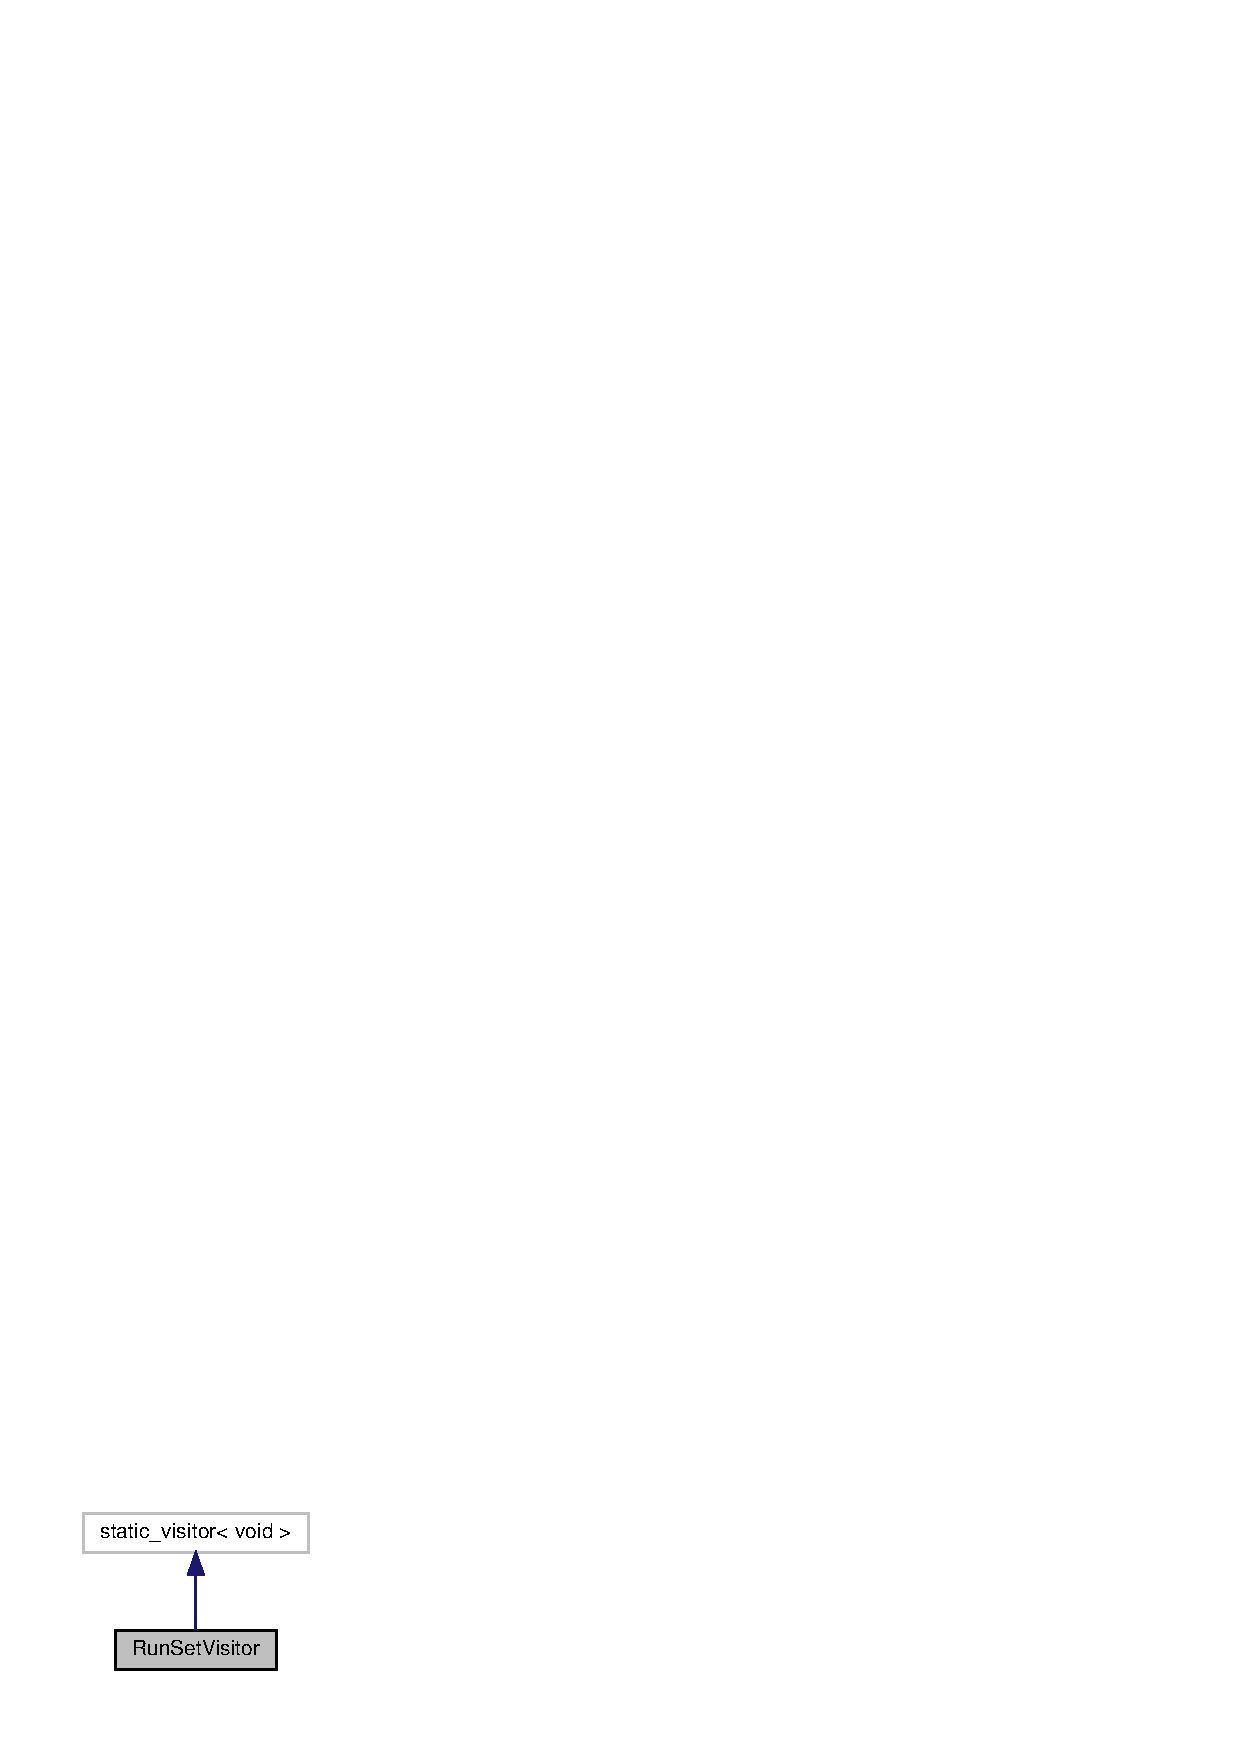
\includegraphics[width=152pt]{classmlpack_1_1ann_1_1RunSetVisitor__inherit__graph}
\end{center}
\end{figure}
\subsection*{Public Member Functions}
\begin{DoxyCompactItemize}
\item 
\textbf{ Run\+Set\+Visitor} (const bool run=true)
\begin{DoxyCompactList}\small\item\em Set the run parameter given the current run value. \end{DoxyCompactList}\item 
{\footnotesize template$<$typename Layer\+Type $>$ }\\void \textbf{ operator()} (Layer\+Type $\ast$layer) const
\begin{DoxyCompactList}\small\item\em Set the run parameter. \end{DoxyCompactList}\item 
void \textbf{ operator()} (\textbf{ More\+Types} layer) const
\end{DoxyCompactItemize}


\subsection{Detailed Description}
\doxyref{Run\+Set\+Visitor}{p.}{classmlpack_1_1ann_1_1RunSetVisitor} set the run parameter given the run value. 

Definition at line 28 of file run\+\_\+set\+\_\+visitor.\+hpp.



\subsection{Constructor \& Destructor Documentation}
\mbox{\label{classmlpack_1_1ann_1_1RunSetVisitor_a756ba8e6e20f84b1e34248f905d53165}} 
\index{mlpack\+::ann\+::\+Run\+Set\+Visitor@{mlpack\+::ann\+::\+Run\+Set\+Visitor}!Run\+Set\+Visitor@{Run\+Set\+Visitor}}
\index{Run\+Set\+Visitor@{Run\+Set\+Visitor}!mlpack\+::ann\+::\+Run\+Set\+Visitor@{mlpack\+::ann\+::\+Run\+Set\+Visitor}}
\subsubsection{Run\+Set\+Visitor()}
{\footnotesize\ttfamily \textbf{ Run\+Set\+Visitor} (\begin{DoxyParamCaption}\item[{const bool}]{run = {\ttfamily true} }\end{DoxyParamCaption})}



Set the run parameter given the current run value. 



\subsection{Member Function Documentation}
\mbox{\label{classmlpack_1_1ann_1_1RunSetVisitor_a26bb3385c630118c35f4799f1509abbc}} 
\index{mlpack\+::ann\+::\+Run\+Set\+Visitor@{mlpack\+::ann\+::\+Run\+Set\+Visitor}!operator()@{operator()}}
\index{operator()@{operator()}!mlpack\+::ann\+::\+Run\+Set\+Visitor@{mlpack\+::ann\+::\+Run\+Set\+Visitor}}
\subsubsection{operator()()\hspace{0.1cm}{\footnotesize\ttfamily [1/2]}}
{\footnotesize\ttfamily void operator() (\begin{DoxyParamCaption}\item[{Layer\+Type $\ast$}]{layer }\end{DoxyParamCaption}) const}



Set the run parameter. 

\mbox{\label{classmlpack_1_1ann_1_1RunSetVisitor_ae35578e7ff874a320fe762bc0edfff04}} 
\index{mlpack\+::ann\+::\+Run\+Set\+Visitor@{mlpack\+::ann\+::\+Run\+Set\+Visitor}!operator()@{operator()}}
\index{operator()@{operator()}!mlpack\+::ann\+::\+Run\+Set\+Visitor@{mlpack\+::ann\+::\+Run\+Set\+Visitor}}
\subsubsection{operator()()\hspace{0.1cm}{\footnotesize\ttfamily [2/2]}}
{\footnotesize\ttfamily void operator() (\begin{DoxyParamCaption}\item[{\textbf{ More\+Types}}]{layer }\end{DoxyParamCaption}) const}



The documentation for this class was generated from the following file\+:\begin{DoxyCompactItemize}
\item 
/home/aakash/mlpack/src/mlpack/methods/ann/visitor/\textbf{ run\+\_\+set\+\_\+visitor.\+hpp}\end{DoxyCompactItemize}

\section{Save\+Output\+Parameter\+Visitor Class Reference}
\label{classmlpack_1_1ann_1_1SaveOutputParameterVisitor}\index{Save\+Output\+Parameter\+Visitor@{Save\+Output\+Parameter\+Visitor}}


\doxyref{Save\+Output\+Parameter\+Visitor}{p.}{classmlpack_1_1ann_1_1SaveOutputParameterVisitor} saves the output parameter into the given parameter set.  




Inheritance diagram for Save\+Output\+Parameter\+Visitor\+:
\nopagebreak
\begin{figure}[H]
\begin{center}
\leavevmode
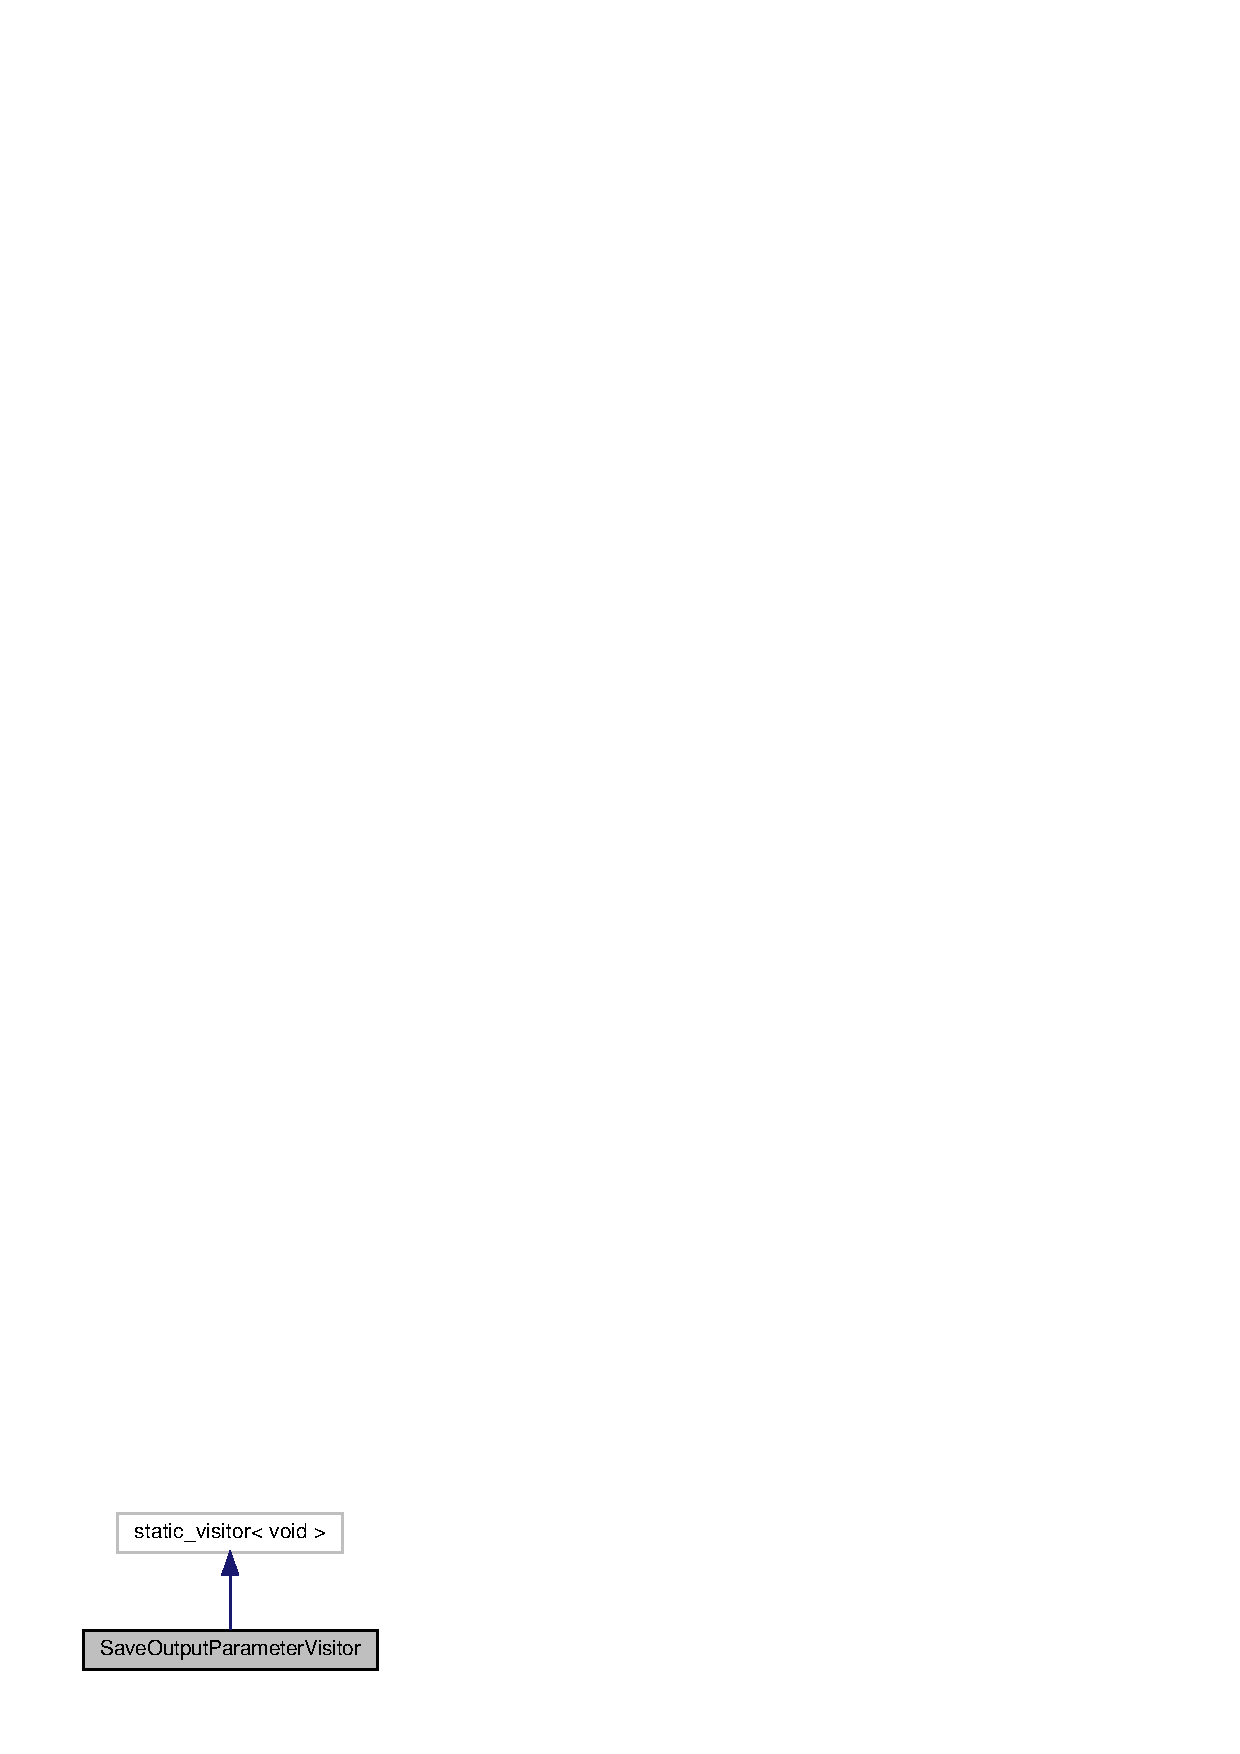
\includegraphics[width=185pt]{classmlpack_1_1ann_1_1SaveOutputParameterVisitor__inherit__graph}
\end{center}
\end{figure}
\subsection*{Public Member Functions}
\begin{DoxyCompactItemize}
\item 
\textbf{ Save\+Output\+Parameter\+Visitor} (std\+::vector$<$ arma\+::mat $>$ \&parameter)
\begin{DoxyCompactList}\small\item\em Save the output parameter into the given parameter set. \end{DoxyCompactList}\item 
{\footnotesize template$<$typename Layer\+Type $>$ }\\void \textbf{ operator()} (Layer\+Type $\ast$layer) const
\begin{DoxyCompactList}\small\item\em Save the output parameter. \end{DoxyCompactList}\item 
void \textbf{ operator()} (\textbf{ More\+Types} layer) const
\end{DoxyCompactItemize}


\subsection{Detailed Description}
\doxyref{Save\+Output\+Parameter\+Visitor}{p.}{classmlpack_1_1ann_1_1SaveOutputParameterVisitor} saves the output parameter into the given parameter set. 

Definition at line 27 of file save\+\_\+output\+\_\+parameter\+\_\+visitor.\+hpp.



\subsection{Constructor \& Destructor Documentation}
\mbox{\label{classmlpack_1_1ann_1_1SaveOutputParameterVisitor_a6e993fd55c18820ed53d0b868a6dd062}} 
\index{mlpack\+::ann\+::\+Save\+Output\+Parameter\+Visitor@{mlpack\+::ann\+::\+Save\+Output\+Parameter\+Visitor}!Save\+Output\+Parameter\+Visitor@{Save\+Output\+Parameter\+Visitor}}
\index{Save\+Output\+Parameter\+Visitor@{Save\+Output\+Parameter\+Visitor}!mlpack\+::ann\+::\+Save\+Output\+Parameter\+Visitor@{mlpack\+::ann\+::\+Save\+Output\+Parameter\+Visitor}}
\subsubsection{Save\+Output\+Parameter\+Visitor()}
{\footnotesize\ttfamily \textbf{ Save\+Output\+Parameter\+Visitor} (\begin{DoxyParamCaption}\item[{std\+::vector$<$ arma\+::mat $>$ \&}]{parameter }\end{DoxyParamCaption})}



Save the output parameter into the given parameter set. 



\subsection{Member Function Documentation}
\mbox{\label{classmlpack_1_1ann_1_1SaveOutputParameterVisitor_a26bb3385c630118c35f4799f1509abbc}} 
\index{mlpack\+::ann\+::\+Save\+Output\+Parameter\+Visitor@{mlpack\+::ann\+::\+Save\+Output\+Parameter\+Visitor}!operator()@{operator()}}
\index{operator()@{operator()}!mlpack\+::ann\+::\+Save\+Output\+Parameter\+Visitor@{mlpack\+::ann\+::\+Save\+Output\+Parameter\+Visitor}}
\subsubsection{operator()()\hspace{0.1cm}{\footnotesize\ttfamily [1/2]}}
{\footnotesize\ttfamily void operator() (\begin{DoxyParamCaption}\item[{Layer\+Type $\ast$}]{layer }\end{DoxyParamCaption}) const}



Save the output parameter. 

\mbox{\label{classmlpack_1_1ann_1_1SaveOutputParameterVisitor_ae35578e7ff874a320fe762bc0edfff04}} 
\index{mlpack\+::ann\+::\+Save\+Output\+Parameter\+Visitor@{mlpack\+::ann\+::\+Save\+Output\+Parameter\+Visitor}!operator()@{operator()}}
\index{operator()@{operator()}!mlpack\+::ann\+::\+Save\+Output\+Parameter\+Visitor@{mlpack\+::ann\+::\+Save\+Output\+Parameter\+Visitor}}
\subsubsection{operator()()\hspace{0.1cm}{\footnotesize\ttfamily [2/2]}}
{\footnotesize\ttfamily void operator() (\begin{DoxyParamCaption}\item[{\textbf{ More\+Types}}]{layer }\end{DoxyParamCaption}) const}



The documentation for this class was generated from the following file\+:\begin{DoxyCompactItemize}
\item 
/home/aakash/mlpack/src/mlpack/methods/ann/visitor/\textbf{ save\+\_\+output\+\_\+parameter\+\_\+visitor.\+hpp}\end{DoxyCompactItemize}

\section{Select$<$ Input\+Data\+Type, Output\+Data\+Type $>$ Class Template Reference}
\label{classmlpack_1_1ann_1_1Select}\index{Select$<$ Input\+Data\+Type, Output\+Data\+Type $>$@{Select$<$ Input\+Data\+Type, Output\+Data\+Type $>$}}


The select module selects the specified column from a given input matrix.  


\subsection*{Public Member Functions}
\begin{DoxyCompactItemize}
\item 
\textbf{ Select} (const size\+\_\+t index=0, const size\+\_\+t elements=0)
\begin{DoxyCompactList}\small\item\em Create the \doxyref{Select}{p.}{classmlpack_1_1ann_1_1Select} object. \end{DoxyCompactList}\item 
{\footnotesize template$<$typename eT $>$ }\\void \textbf{ Backward} (const arma\+::\+Mat$<$ eT $>$ \&, const arma\+::\+Mat$<$ eT $>$ \&gy, arma\+::\+Mat$<$ eT $>$ \&g)
\begin{DoxyCompactList}\small\item\em Ordinary feed backward pass of a neural network, calculating the function f(x) by propagating x backwards trough f. \end{DoxyCompactList}\item 
Output\+Data\+Type \& \textbf{ Delta} () const
\begin{DoxyCompactList}\small\item\em Get the delta. \end{DoxyCompactList}\item 
Output\+Data\+Type \& \textbf{ Delta} ()
\begin{DoxyCompactList}\small\item\em Modify the delta. \end{DoxyCompactList}\item 
{\footnotesize template$<$typename eT $>$ }\\void \textbf{ Forward} (const arma\+::\+Mat$<$ eT $>$ \&input, arma\+::\+Mat$<$ eT $>$ \&output)
\begin{DoxyCompactList}\small\item\em Ordinary feed forward pass of a neural network, evaluating the function f(x) by propagating the activity forward through f. \end{DoxyCompactList}\item 
size\+\_\+t const  \& \textbf{ Index} () const
\begin{DoxyCompactList}\small\item\em Get the column index. \end{DoxyCompactList}\item 
size\+\_\+t const  \& \textbf{ Num\+Elements} () const
\begin{DoxyCompactList}\small\item\em Get the number of elements selected. \end{DoxyCompactList}\item 
Output\+Data\+Type \& \textbf{ Output\+Parameter} () const
\begin{DoxyCompactList}\small\item\em Get the output parameter. \end{DoxyCompactList}\item 
Output\+Data\+Type \& \textbf{ Output\+Parameter} ()
\begin{DoxyCompactList}\small\item\em Modify the output parameter. \end{DoxyCompactList}\item 
{\footnotesize template$<$typename Archive $>$ }\\void \textbf{ serialize} (Archive \&ar, const uint32\+\_\+t)
\begin{DoxyCompactList}\small\item\em Serialize the layer. \end{DoxyCompactList}\end{DoxyCompactItemize}


\subsection{Detailed Description}
\subsubsection*{template$<$typename Input\+Data\+Type = arma\+::mat, typename Output\+Data\+Type = arma\+::mat$>$\newline
class mlpack\+::ann\+::\+Select$<$ Input\+Data\+Type, Output\+Data\+Type $>$}

The select module selects the specified column from a given input matrix. 


\begin{DoxyTemplParams}{Template Parameters}
{\em Input\+Data\+Type} & Type of the input data (arma\+::colvec, arma\+::mat, arma\+::sp\+\_\+mat or arma\+::cube). \\
\hline
{\em Output\+Data\+Type} & Type of the output data (arma\+::colvec, arma\+::mat, arma\+::sp\+\_\+mat or arma\+::cube). \\
\hline
\end{DoxyTemplParams}


Definition at line 32 of file select.\+hpp.



\subsection{Constructor \& Destructor Documentation}
\mbox{\label{classmlpack_1_1ann_1_1Select_a49e8817f00688d2a7c1be8a33125d7e9}} 
\index{mlpack\+::ann\+::\+Select@{mlpack\+::ann\+::\+Select}!Select@{Select}}
\index{Select@{Select}!mlpack\+::ann\+::\+Select@{mlpack\+::ann\+::\+Select}}
\subsubsection{Select()}
{\footnotesize\ttfamily \textbf{ Select} (\begin{DoxyParamCaption}\item[{const size\+\_\+t}]{index = {\ttfamily 0},  }\item[{const size\+\_\+t}]{elements = {\ttfamily 0} }\end{DoxyParamCaption})}



Create the \doxyref{Select}{p.}{classmlpack_1_1ann_1_1Select} object. 


\begin{DoxyParams}{Parameters}
{\em index} & The column which should be extracted from the given input. \\
\hline
{\em elements} & The number of elements that should be used. \\
\hline
\end{DoxyParams}


\subsection{Member Function Documentation}
\mbox{\label{classmlpack_1_1ann_1_1Select_ad9ad1a3bdb0f3fff5c839ed155e4bbf8}} 
\index{mlpack\+::ann\+::\+Select@{mlpack\+::ann\+::\+Select}!Backward@{Backward}}
\index{Backward@{Backward}!mlpack\+::ann\+::\+Select@{mlpack\+::ann\+::\+Select}}
\subsubsection{Backward()}
{\footnotesize\ttfamily void Backward (\begin{DoxyParamCaption}\item[{const arma\+::\+Mat$<$ eT $>$ \&}]{,  }\item[{const arma\+::\+Mat$<$ eT $>$ \&}]{gy,  }\item[{arma\+::\+Mat$<$ eT $>$ \&}]{g }\end{DoxyParamCaption})}



Ordinary feed backward pass of a neural network, calculating the function f(x) by propagating x backwards trough f. 

Using the results from the feed forward pass.


\begin{DoxyParams}{Parameters}
{\em $\ast$} & (input) The propagated input activation. \\
\hline
{\em gy} & The backpropagated error. \\
\hline
{\em g} & The calculated gradient. \\
\hline
\end{DoxyParams}
\mbox{\label{classmlpack_1_1ann_1_1Select_ae7c8eba5764f021cd93e30efe638e63c}} 
\index{mlpack\+::ann\+::\+Select@{mlpack\+::ann\+::\+Select}!Delta@{Delta}}
\index{Delta@{Delta}!mlpack\+::ann\+::\+Select@{mlpack\+::ann\+::\+Select}}
\subsubsection{Delta()\hspace{0.1cm}{\footnotesize\ttfamily [1/2]}}
{\footnotesize\ttfamily Output\+Data\+Type\& Delta (\begin{DoxyParamCaption}{ }\end{DoxyParamCaption}) const\hspace{0.3cm}{\ttfamily [inline]}}



Get the delta. 



Definition at line 73 of file select.\+hpp.

\mbox{\label{classmlpack_1_1ann_1_1Select_ad6601342d560219ce951d554e69e5e87}} 
\index{mlpack\+::ann\+::\+Select@{mlpack\+::ann\+::\+Select}!Delta@{Delta}}
\index{Delta@{Delta}!mlpack\+::ann\+::\+Select@{mlpack\+::ann\+::\+Select}}
\subsubsection{Delta()\hspace{0.1cm}{\footnotesize\ttfamily [2/2]}}
{\footnotesize\ttfamily Output\+Data\+Type\& Delta (\begin{DoxyParamCaption}{ }\end{DoxyParamCaption})\hspace{0.3cm}{\ttfamily [inline]}}



Modify the delta. 



Definition at line 75 of file select.\+hpp.

\mbox{\label{classmlpack_1_1ann_1_1Select_a461f849bc638c15bec262dc9c3a58abe}} 
\index{mlpack\+::ann\+::\+Select@{mlpack\+::ann\+::\+Select}!Forward@{Forward}}
\index{Forward@{Forward}!mlpack\+::ann\+::\+Select@{mlpack\+::ann\+::\+Select}}
\subsubsection{Forward()}
{\footnotesize\ttfamily void Forward (\begin{DoxyParamCaption}\item[{const arma\+::\+Mat$<$ eT $>$ \&}]{input,  }\item[{arma\+::\+Mat$<$ eT $>$ \&}]{output }\end{DoxyParamCaption})}



Ordinary feed forward pass of a neural network, evaluating the function f(x) by propagating the activity forward through f. 


\begin{DoxyParams}{Parameters}
{\em input} & Input data used for evaluating the specified function. \\
\hline
{\em output} & Resulting output activation. \\
\hline
\end{DoxyParams}
\mbox{\label{classmlpack_1_1ann_1_1Select_a582646b9b3566986a6bcda99ba9f52bb}} 
\index{mlpack\+::ann\+::\+Select@{mlpack\+::ann\+::\+Select}!Index@{Index}}
\index{Index@{Index}!mlpack\+::ann\+::\+Select@{mlpack\+::ann\+::\+Select}}
\subsubsection{Index()}
{\footnotesize\ttfamily size\+\_\+t const\& Index (\begin{DoxyParamCaption}{ }\end{DoxyParamCaption}) const\hspace{0.3cm}{\ttfamily [inline]}}



Get the column index. 



Definition at line 78 of file select.\+hpp.

\mbox{\label{classmlpack_1_1ann_1_1Select_a0592dd68507789ef52d17a0126de9f40}} 
\index{mlpack\+::ann\+::\+Select@{mlpack\+::ann\+::\+Select}!Num\+Elements@{Num\+Elements}}
\index{Num\+Elements@{Num\+Elements}!mlpack\+::ann\+::\+Select@{mlpack\+::ann\+::\+Select}}
\subsubsection{Num\+Elements()}
{\footnotesize\ttfamily size\+\_\+t const\& Num\+Elements (\begin{DoxyParamCaption}{ }\end{DoxyParamCaption}) const\hspace{0.3cm}{\ttfamily [inline]}}



Get the number of elements selected. 



Definition at line 81 of file select.\+hpp.



References Select$<$ Input\+Data\+Type, Output\+Data\+Type $>$\+::serialize().

\mbox{\label{classmlpack_1_1ann_1_1Select_a8bae962cc603d1cab8d80ec78f8d505d}} 
\index{mlpack\+::ann\+::\+Select@{mlpack\+::ann\+::\+Select}!Output\+Parameter@{Output\+Parameter}}
\index{Output\+Parameter@{Output\+Parameter}!mlpack\+::ann\+::\+Select@{mlpack\+::ann\+::\+Select}}
\subsubsection{Output\+Parameter()\hspace{0.1cm}{\footnotesize\ttfamily [1/2]}}
{\footnotesize\ttfamily Output\+Data\+Type\& Output\+Parameter (\begin{DoxyParamCaption}{ }\end{DoxyParamCaption}) const\hspace{0.3cm}{\ttfamily [inline]}}



Get the output parameter. 



Definition at line 68 of file select.\+hpp.

\mbox{\label{classmlpack_1_1ann_1_1Select_a21d5f745f02c709625a4ee0907f004a5}} 
\index{mlpack\+::ann\+::\+Select@{mlpack\+::ann\+::\+Select}!Output\+Parameter@{Output\+Parameter}}
\index{Output\+Parameter@{Output\+Parameter}!mlpack\+::ann\+::\+Select@{mlpack\+::ann\+::\+Select}}
\subsubsection{Output\+Parameter()\hspace{0.1cm}{\footnotesize\ttfamily [2/2]}}
{\footnotesize\ttfamily Output\+Data\+Type\& Output\+Parameter (\begin{DoxyParamCaption}{ }\end{DoxyParamCaption})\hspace{0.3cm}{\ttfamily [inline]}}



Modify the output parameter. 



Definition at line 70 of file select.\+hpp.

\mbox{\label{classmlpack_1_1ann_1_1Select_a65cba07328997659bec80b9879b15a51}} 
\index{mlpack\+::ann\+::\+Select@{mlpack\+::ann\+::\+Select}!serialize@{serialize}}
\index{serialize@{serialize}!mlpack\+::ann\+::\+Select@{mlpack\+::ann\+::\+Select}}
\subsubsection{serialize()}
{\footnotesize\ttfamily void serialize (\begin{DoxyParamCaption}\item[{Archive \&}]{ar,  }\item[{const uint32\+\_\+t}]{ }\end{DoxyParamCaption})}



Serialize the layer. 



Referenced by Select$<$ Input\+Data\+Type, Output\+Data\+Type $>$\+::\+Num\+Elements().



The documentation for this class was generated from the following file\+:\begin{DoxyCompactItemize}
\item 
/home/aakash/mlpack/src/mlpack/methods/ann/layer/\textbf{ select.\+hpp}\end{DoxyCompactItemize}

\section{Sequential$<$ Input\+Data\+Type, Output\+Data\+Type, Residual, Custom\+Layers $>$ Class Template Reference}
\label{classmlpack_1_1ann_1_1Sequential}\index{Sequential$<$ Input\+Data\+Type, Output\+Data\+Type, Residual, Custom\+Layers $>$@{Sequential$<$ Input\+Data\+Type, Output\+Data\+Type, Residual, Custom\+Layers $>$}}


Implementation of the \doxyref{Sequential}{p.}{classmlpack_1_1ann_1_1Sequential} class.  


\subsection*{Public Member Functions}
\begin{DoxyCompactItemize}
\item 
\textbf{ Sequential} (const bool model=true)
\begin{DoxyCompactList}\small\item\em Create the \doxyref{Sequential}{p.}{classmlpack_1_1ann_1_1Sequential} object using the specified parameters. \end{DoxyCompactList}\item 
\textbf{ Sequential} (const bool model, const bool owns\+Layers)
\begin{DoxyCompactList}\small\item\em Create the \doxyref{Sequential}{p.}{classmlpack_1_1ann_1_1Sequential} object using the specified parameters. \end{DoxyCompactList}\item 
\textbf{ Sequential} (const \textbf{ Sequential} \&layer)
\begin{DoxyCompactList}\small\item\em Copy constructor. \end{DoxyCompactList}\item 
\textbf{ $\sim$\+Sequential} ()
\begin{DoxyCompactList}\small\item\em Destroy the \doxyref{Sequential}{p.}{classmlpack_1_1ann_1_1Sequential} object. \end{DoxyCompactList}\item 
{\footnotesize template$<$class Layer\+Type , class... Args$>$ }\\void \textbf{ Add} (Args... args)
\item 
void \textbf{ Add} (\textbf{ Layer\+Types}$<$ Custom\+Layers... $>$ layer)
\item 
{\footnotesize template$<$typename eT $>$ }\\void \textbf{ Backward} (const arma\+::\+Mat$<$ eT $>$ \&, const arma\+::\+Mat$<$ eT $>$ \&gy, arma\+::\+Mat$<$ eT $>$ \&g)
\begin{DoxyCompactList}\small\item\em Ordinary feed backward pass of a neural network, using 3rd-\/order tensors as input, calculating the function f(x) by propagating x backwards through f. \end{DoxyCompactList}\item 
arma\+::mat const  \& \textbf{ Delta} () const
\begin{DoxyCompactList}\small\item\em Get the delta. \end{DoxyCompactList}\item 
arma\+::mat \& \textbf{ Delta} ()
\begin{DoxyCompactList}\small\item\em Modify the delta. \end{DoxyCompactList}\item 
{\footnotesize template$<$typename eT $>$ }\\void \textbf{ Forward} (const arma\+::\+Mat$<$ eT $>$ \&input, arma\+::\+Mat$<$ eT $>$ \&output)
\begin{DoxyCompactList}\small\item\em Ordinary feed forward pass of a neural network, evaluating the function f(x) by propagating the activity forward through f. \end{DoxyCompactList}\item 
{\footnotesize template$<$typename eT $>$ }\\void \textbf{ Gradient} (const arma\+::\+Mat$<$ eT $>$ \&input, const arma\+::\+Mat$<$ eT $>$ \&error, arma\+::\+Mat$<$ eT $>$ \&)
\item 
arma\+::mat const  \& \textbf{ Gradient} () const
\begin{DoxyCompactList}\small\item\em Get the gradient. \end{DoxyCompactList}\item 
arma\+::mat \& \textbf{ Gradient} ()
\begin{DoxyCompactList}\small\item\em Modify the gradient. \end{DoxyCompactList}\item 
arma\+::mat const  \& \textbf{ Input\+Parameter} () const
\begin{DoxyCompactList}\small\item\em Get the input parameter. \end{DoxyCompactList}\item 
arma\+::mat \& \textbf{ Input\+Parameter} ()
\begin{DoxyCompactList}\small\item\em Modify the input parameter. \end{DoxyCompactList}\item 
size\+\_\+t \textbf{ Input\+Shape} () const
\item 
std\+::vector$<$ \textbf{ Layer\+Types}$<$ Custom\+Layers... $>$ $>$ \& \textbf{ Model} ()
\begin{DoxyCompactList}\small\item\em Return the model modules. \end{DoxyCompactList}\item 
\textbf{ Sequential} \& \textbf{ operator=} (const \textbf{ Sequential} \&layer)
\begin{DoxyCompactList}\small\item\em Copy assignment operator. \end{DoxyCompactList}\item 
arma\+::mat const  \& \textbf{ Output\+Parameter} () const
\begin{DoxyCompactList}\small\item\em Get the output parameter. \end{DoxyCompactList}\item 
arma\+::mat \& \textbf{ Output\+Parameter} ()
\begin{DoxyCompactList}\small\item\em Modify the output parameter. \end{DoxyCompactList}\item 
const arma\+::mat \& \textbf{ Parameters} () const
\begin{DoxyCompactList}\small\item\em Return the initial point for the optimization. \end{DoxyCompactList}\item 
arma\+::mat \& \textbf{ Parameters} ()
\begin{DoxyCompactList}\small\item\em Modify the initial point for the optimization. \end{DoxyCompactList}\item 
{\footnotesize template$<$typename Archive $>$ }\\void \textbf{ serialize} (Archive \&ar, const uint32\+\_\+t)
\begin{DoxyCompactList}\small\item\em Serialize the layer. \end{DoxyCompactList}\end{DoxyCompactItemize}


\subsection{Detailed Description}
\subsubsection*{template$<$typename Input\+Data\+Type = arma\+::mat, typename Output\+Data\+Type = arma\+::mat, bool Residual = false, typename... Custom\+Layers$>$\newline
class mlpack\+::ann\+::\+Sequential$<$ Input\+Data\+Type, Output\+Data\+Type, Residual, Custom\+Layers $>$}

Implementation of the \doxyref{Sequential}{p.}{classmlpack_1_1ann_1_1Sequential} class. 

The sequential class works as a feed-\/forward fully connected network container which plugs various layers together.

This class can also be used as a container for a residual block. In that case, the sizes of the input and output matrices of this class should be equal. A typedef has been added for use as a Residual$<$$>$ class.

For more information, refer the following paper.


\begin{DoxyCode}
@article\{He15,
  author    = \{Kaiming He, Xiangyu Zhang, Shaoqing Ren, Jian Sun\},
  title     = \{Deep Residual Learning \textcolor{keywordflow}{for} Image Recognition\},
  year      = \{2015\},
  url       = \{https:\textcolor{comment}{//arxiv.org/abs/1512.03385\},}
  eprint    = \{1512.03385\},
\}
\end{DoxyCode}


Note\+: If this class is used as the first layer of a network, it should be preceded by Identity\+Layer$<$$>$.

Note\+: This class should at least have two layers for a call to its \doxyref{Gradient()}{p.}{classmlpack_1_1ann_1_1Sequential_a59e16b7142696049a5543ff35547ebd9} function.


\begin{DoxyTemplParams}{Template Parameters}
{\em Input\+Data\+Type} & Type of the input data (arma\+::colvec, arma\+::mat, arma\+::sp\+\_\+mat or arma\+::cube). \\
\hline
{\em Output\+Data\+Type} & Type of the output data (arma\+::colvec, arma\+::mat, arma\+::sp\+\_\+mat or arma\+::cube). \\
\hline
{\em Residual} & If true, use the object as a Residual block. \\
\hline
\end{DoxyTemplParams}


Definition at line 141 of file layer\+\_\+types.\+hpp.



\subsection{Constructor \& Destructor Documentation}
\mbox{\label{classmlpack_1_1ann_1_1Sequential_a01b828c8a9d0398c7d899fe5a0159cf0}} 
\index{mlpack\+::ann\+::\+Sequential@{mlpack\+::ann\+::\+Sequential}!Sequential@{Sequential}}
\index{Sequential@{Sequential}!mlpack\+::ann\+::\+Sequential@{mlpack\+::ann\+::\+Sequential}}
\subsubsection{Sequential()\hspace{0.1cm}{\footnotesize\ttfamily [1/3]}}
{\footnotesize\ttfamily \textbf{ Sequential} (\begin{DoxyParamCaption}\item[{const bool}]{model = {\ttfamily true} }\end{DoxyParamCaption})}



Create the \doxyref{Sequential}{p.}{classmlpack_1_1ann_1_1Sequential} object using the specified parameters. 


\begin{DoxyParams}{Parameters}
{\em model} & Expose the all network modules. \\
\hline
\end{DoxyParams}
\mbox{\label{classmlpack_1_1ann_1_1Sequential_a54e8b8c60e747977fcb5d1d33181d2d6}} 
\index{mlpack\+::ann\+::\+Sequential@{mlpack\+::ann\+::\+Sequential}!Sequential@{Sequential}}
\index{Sequential@{Sequential}!mlpack\+::ann\+::\+Sequential@{mlpack\+::ann\+::\+Sequential}}
\subsubsection{Sequential()\hspace{0.1cm}{\footnotesize\ttfamily [2/3]}}
{\footnotesize\ttfamily \textbf{ Sequential} (\begin{DoxyParamCaption}\item[{const bool}]{model,  }\item[{const bool}]{owns\+Layers }\end{DoxyParamCaption})}



Create the \doxyref{Sequential}{p.}{classmlpack_1_1ann_1_1Sequential} object using the specified parameters. 


\begin{DoxyParams}{Parameters}
{\em model} & Expose all the network modules. \\
\hline
{\em owns\+Layers} & If true, then this module will delete its layers when deallocated. \\
\hline
\end{DoxyParams}
\mbox{\label{classmlpack_1_1ann_1_1Sequential_a146eb0ef8b57693cf58802961b1a1601}} 
\index{mlpack\+::ann\+::\+Sequential@{mlpack\+::ann\+::\+Sequential}!Sequential@{Sequential}}
\index{Sequential@{Sequential}!mlpack\+::ann\+::\+Sequential@{mlpack\+::ann\+::\+Sequential}}
\subsubsection{Sequential()\hspace{0.1cm}{\footnotesize\ttfamily [3/3]}}
{\footnotesize\ttfamily \textbf{ Sequential} (\begin{DoxyParamCaption}\item[{const \textbf{ Sequential}$<$ Input\+Data\+Type, Output\+Data\+Type, \textbf{ Residual}, Custom\+Layers $>$ \&}]{layer }\end{DoxyParamCaption})}



Copy constructor. 

\mbox{\label{classmlpack_1_1ann_1_1Sequential_a104b6c42467bc2edb7c514afca99bcec}} 
\index{mlpack\+::ann\+::\+Sequential@{mlpack\+::ann\+::\+Sequential}!````~Sequential@{$\sim$\+Sequential}}
\index{````~Sequential@{$\sim$\+Sequential}!mlpack\+::ann\+::\+Sequential@{mlpack\+::ann\+::\+Sequential}}
\subsubsection{$\sim$\+Sequential()}
{\footnotesize\ttfamily $\sim$\textbf{ Sequential} (\begin{DoxyParamCaption}{ }\end{DoxyParamCaption})}



Destroy the \doxyref{Sequential}{p.}{classmlpack_1_1ann_1_1Sequential} object. 



\subsection{Member Function Documentation}
\mbox{\label{classmlpack_1_1ann_1_1Sequential_a8b5234495846c00f6b2c8296ca6bc718}} 
\index{mlpack\+::ann\+::\+Sequential@{mlpack\+::ann\+::\+Sequential}!Add@{Add}}
\index{Add@{Add}!mlpack\+::ann\+::\+Sequential@{mlpack\+::ann\+::\+Sequential}}
\subsubsection{Add()\hspace{0.1cm}{\footnotesize\ttfamily [1/2]}}
{\footnotesize\ttfamily void \textbf{ Add} (\begin{DoxyParamCaption}\item[{Args...}]{args }\end{DoxyParamCaption})\hspace{0.3cm}{\ttfamily [inline]}}



Definition at line 143 of file sequential.\+hpp.



Referenced by Dueling\+D\+Q\+N$<$ Output\+Layer\+Type, Init\+Type, Complete\+Network\+Type, Feature\+Network\+Type, Advantage\+Network\+Type, Value\+Network\+Type $>$\+::\+Dueling\+D\+Q\+N().

\mbox{\label{classmlpack_1_1ann_1_1Sequential_a503a807740e6c729be9efc89520db728}} 
\index{mlpack\+::ann\+::\+Sequential@{mlpack\+::ann\+::\+Sequential}!Add@{Add}}
\index{Add@{Add}!mlpack\+::ann\+::\+Sequential@{mlpack\+::ann\+::\+Sequential}}
\subsubsection{Add()\hspace{0.1cm}{\footnotesize\ttfamily [2/2]}}
{\footnotesize\ttfamily void \textbf{ Add} (\begin{DoxyParamCaption}\item[{\textbf{ Layer\+Types}$<$ Custom\+Layers... $>$}]{layer }\end{DoxyParamCaption})\hspace{0.3cm}{\ttfamily [inline]}}



Definition at line 150 of file sequential.\+hpp.

\mbox{\label{classmlpack_1_1ann_1_1Sequential_ad9ad1a3bdb0f3fff5c839ed155e4bbf8}} 
\index{mlpack\+::ann\+::\+Sequential@{mlpack\+::ann\+::\+Sequential}!Backward@{Backward}}
\index{Backward@{Backward}!mlpack\+::ann\+::\+Sequential@{mlpack\+::ann\+::\+Sequential}}
\subsubsection{Backward()}
{\footnotesize\ttfamily void Backward (\begin{DoxyParamCaption}\item[{const arma\+::\+Mat$<$ eT $>$ \&}]{,  }\item[{const arma\+::\+Mat$<$ eT $>$ \&}]{gy,  }\item[{arma\+::\+Mat$<$ eT $>$ \&}]{g }\end{DoxyParamCaption})}



Ordinary feed backward pass of a neural network, using 3rd-\/order tensors as input, calculating the function f(x) by propagating x backwards through f. 

Using the results from the feed forward pass.


\begin{DoxyParams}{Parameters}
{\em $\ast$} & (input) The propagated input activation. \\
\hline
{\em gy} & The backpropagated error. \\
\hline
{\em g} & The calculated gradient. \\
\hline
\end{DoxyParams}
\mbox{\label{classmlpack_1_1ann_1_1Sequential_a6126fc05a10e2e988ea7e75aada214fd}} 
\index{mlpack\+::ann\+::\+Sequential@{mlpack\+::ann\+::\+Sequential}!Delta@{Delta}}
\index{Delta@{Delta}!mlpack\+::ann\+::\+Sequential@{mlpack\+::ann\+::\+Sequential}}
\subsubsection{Delta()\hspace{0.1cm}{\footnotesize\ttfamily [1/2]}}
{\footnotesize\ttfamily arma\+::mat const\& Delta (\begin{DoxyParamCaption}{ }\end{DoxyParamCaption}) const\hspace{0.3cm}{\ttfamily [inline]}}



Get the delta. 



Definition at line 179 of file sequential.\+hpp.

\mbox{\label{classmlpack_1_1ann_1_1Sequential_a49c3606024580071e0c65e2e4d080e1e}} 
\index{mlpack\+::ann\+::\+Sequential@{mlpack\+::ann\+::\+Sequential}!Delta@{Delta}}
\index{Delta@{Delta}!mlpack\+::ann\+::\+Sequential@{mlpack\+::ann\+::\+Sequential}}
\subsubsection{Delta()\hspace{0.1cm}{\footnotesize\ttfamily [2/2]}}
{\footnotesize\ttfamily arma\+::mat\& Delta (\begin{DoxyParamCaption}{ }\end{DoxyParamCaption})\hspace{0.3cm}{\ttfamily [inline]}}



Modify the delta. 



Definition at line 181 of file sequential.\+hpp.

\mbox{\label{classmlpack_1_1ann_1_1Sequential_a461f849bc638c15bec262dc9c3a58abe}} 
\index{mlpack\+::ann\+::\+Sequential@{mlpack\+::ann\+::\+Sequential}!Forward@{Forward}}
\index{Forward@{Forward}!mlpack\+::ann\+::\+Sequential@{mlpack\+::ann\+::\+Sequential}}
\subsubsection{Forward()}
{\footnotesize\ttfamily void Forward (\begin{DoxyParamCaption}\item[{const arma\+::\+Mat$<$ eT $>$ \&}]{input,  }\item[{arma\+::\+Mat$<$ eT $>$ \&}]{output }\end{DoxyParamCaption})}



Ordinary feed forward pass of a neural network, evaluating the function f(x) by propagating the activity forward through f. 


\begin{DoxyParams}{Parameters}
{\em input} & Input data used for evaluating the specified function. \\
\hline
{\em output} & Resulting output activation. \\
\hline
\end{DoxyParams}
\mbox{\label{classmlpack_1_1ann_1_1Sequential_a505acb56ef67da2fc73190d3d4931969}} 
\index{mlpack\+::ann\+::\+Sequential@{mlpack\+::ann\+::\+Sequential}!Gradient@{Gradient}}
\index{Gradient@{Gradient}!mlpack\+::ann\+::\+Sequential@{mlpack\+::ann\+::\+Sequential}}
\subsubsection{Gradient()\hspace{0.1cm}{\footnotesize\ttfamily [1/3]}}
{\footnotesize\ttfamily void Gradient (\begin{DoxyParamCaption}\item[{const arma\+::\+Mat$<$ eT $>$ \&}]{input,  }\item[{const arma\+::\+Mat$<$ eT $>$ \&}]{error,  }\item[{arma\+::\+Mat$<$ eT $>$ \&}]{ }\end{DoxyParamCaption})}

\mbox{\label{classmlpack_1_1ann_1_1Sequential_a13444d1f198ceeef85e7a288a7d1d9c2}} 
\index{mlpack\+::ann\+::\+Sequential@{mlpack\+::ann\+::\+Sequential}!Gradient@{Gradient}}
\index{Gradient@{Gradient}!mlpack\+::ann\+::\+Sequential@{mlpack\+::ann\+::\+Sequential}}
\subsubsection{Gradient()\hspace{0.1cm}{\footnotesize\ttfamily [2/3]}}
{\footnotesize\ttfamily arma\+::mat const\& Gradient (\begin{DoxyParamCaption}{ }\end{DoxyParamCaption}) const\hspace{0.3cm}{\ttfamily [inline]}}



Get the gradient. 



Definition at line 184 of file sequential.\+hpp.

\mbox{\label{classmlpack_1_1ann_1_1Sequential_a59e16b7142696049a5543ff35547ebd9}} 
\index{mlpack\+::ann\+::\+Sequential@{mlpack\+::ann\+::\+Sequential}!Gradient@{Gradient}}
\index{Gradient@{Gradient}!mlpack\+::ann\+::\+Sequential@{mlpack\+::ann\+::\+Sequential}}
\subsubsection{Gradient()\hspace{0.1cm}{\footnotesize\ttfamily [3/3]}}
{\footnotesize\ttfamily arma\+::mat\& Gradient (\begin{DoxyParamCaption}{ }\end{DoxyParamCaption})\hspace{0.3cm}{\ttfamily [inline]}}



Modify the gradient. 



Definition at line 186 of file sequential.\+hpp.



References Sequential$<$ Input\+Data\+Type, Output\+Data\+Type, Residual, Custom\+Layers $>$\+::\+Input\+Shape(), and Sequential$<$ Input\+Data\+Type, Output\+Data\+Type, Residual, Custom\+Layers $>$\+::serialize().

\mbox{\label{classmlpack_1_1ann_1_1Sequential_a9b1735296084fc571524101988744884}} 
\index{mlpack\+::ann\+::\+Sequential@{mlpack\+::ann\+::\+Sequential}!Input\+Parameter@{Input\+Parameter}}
\index{Input\+Parameter@{Input\+Parameter}!mlpack\+::ann\+::\+Sequential@{mlpack\+::ann\+::\+Sequential}}
\subsubsection{Input\+Parameter()\hspace{0.1cm}{\footnotesize\ttfamily [1/2]}}
{\footnotesize\ttfamily arma\+::mat const\& Input\+Parameter (\begin{DoxyParamCaption}{ }\end{DoxyParamCaption}) const\hspace{0.3cm}{\ttfamily [inline]}}



Get the input parameter. 



Definition at line 169 of file sequential.\+hpp.

\mbox{\label{classmlpack_1_1ann_1_1Sequential_a818d585c592c80d8e8c101f67bc389ad}} 
\index{mlpack\+::ann\+::\+Sequential@{mlpack\+::ann\+::\+Sequential}!Input\+Parameter@{Input\+Parameter}}
\index{Input\+Parameter@{Input\+Parameter}!mlpack\+::ann\+::\+Sequential@{mlpack\+::ann\+::\+Sequential}}
\subsubsection{Input\+Parameter()\hspace{0.1cm}{\footnotesize\ttfamily [2/2]}}
{\footnotesize\ttfamily arma\+::mat\& Input\+Parameter (\begin{DoxyParamCaption}{ }\end{DoxyParamCaption})\hspace{0.3cm}{\ttfamily [inline]}}



Modify the input parameter. 



Definition at line 171 of file sequential.\+hpp.

\mbox{\label{classmlpack_1_1ann_1_1Sequential_a13ab93f234244a68f6ade76287284447}} 
\index{mlpack\+::ann\+::\+Sequential@{mlpack\+::ann\+::\+Sequential}!Input\+Shape@{Input\+Shape}}
\index{Input\+Shape@{Input\+Shape}!mlpack\+::ann\+::\+Sequential@{mlpack\+::ann\+::\+Sequential}}
\subsubsection{Input\+Shape()}
{\footnotesize\ttfamily size\+\_\+t Input\+Shape (\begin{DoxyParamCaption}{ }\end{DoxyParamCaption}) const}



Referenced by Sequential$<$ Input\+Data\+Type, Output\+Data\+Type, Residual, Custom\+Layers $>$\+::\+Gradient().

\mbox{\label{classmlpack_1_1ann_1_1Sequential_a4cb1e93bff99ccf1f8f974065a3b13c3}} 
\index{mlpack\+::ann\+::\+Sequential@{mlpack\+::ann\+::\+Sequential}!Model@{Model}}
\index{Model@{Model}!mlpack\+::ann\+::\+Sequential@{mlpack\+::ann\+::\+Sequential}}
\subsubsection{Model()}
{\footnotesize\ttfamily std\+::vector$<$\textbf{ Layer\+Types}$<$Custom\+Layers...$>$ $>$\& Model (\begin{DoxyParamCaption}{ }\end{DoxyParamCaption})\hspace{0.3cm}{\ttfamily [inline]}}



Return the model modules. 



Definition at line 153 of file sequential.\+hpp.

\mbox{\label{classmlpack_1_1ann_1_1Sequential_a806923a7f052d5b9a0966407899fc104}} 
\index{mlpack\+::ann\+::\+Sequential@{mlpack\+::ann\+::\+Sequential}!operator=@{operator=}}
\index{operator=@{operator=}!mlpack\+::ann\+::\+Sequential@{mlpack\+::ann\+::\+Sequential}}
\subsubsection{operator=()}
{\footnotesize\ttfamily \textbf{ Sequential}\& operator= (\begin{DoxyParamCaption}\item[{const \textbf{ Sequential}$<$ Input\+Data\+Type, Output\+Data\+Type, \textbf{ Residual}, Custom\+Layers $>$ \&}]{layer }\end{DoxyParamCaption})}



Copy assignment operator. 

\mbox{\label{classmlpack_1_1ann_1_1Sequential_a712dc230c489d0caf3175cbdfc59639f}} 
\index{mlpack\+::ann\+::\+Sequential@{mlpack\+::ann\+::\+Sequential}!Output\+Parameter@{Output\+Parameter}}
\index{Output\+Parameter@{Output\+Parameter}!mlpack\+::ann\+::\+Sequential@{mlpack\+::ann\+::\+Sequential}}
\subsubsection{Output\+Parameter()\hspace{0.1cm}{\footnotesize\ttfamily [1/2]}}
{\footnotesize\ttfamily arma\+::mat const\& Output\+Parameter (\begin{DoxyParamCaption}{ }\end{DoxyParamCaption}) const\hspace{0.3cm}{\ttfamily [inline]}}



Get the output parameter. 



Definition at line 174 of file sequential.\+hpp.

\mbox{\label{classmlpack_1_1ann_1_1Sequential_a28ce681558d0bf02302f868d1c811f2a}} 
\index{mlpack\+::ann\+::\+Sequential@{mlpack\+::ann\+::\+Sequential}!Output\+Parameter@{Output\+Parameter}}
\index{Output\+Parameter@{Output\+Parameter}!mlpack\+::ann\+::\+Sequential@{mlpack\+::ann\+::\+Sequential}}
\subsubsection{Output\+Parameter()\hspace{0.1cm}{\footnotesize\ttfamily [2/2]}}
{\footnotesize\ttfamily arma\+::mat\& Output\+Parameter (\begin{DoxyParamCaption}{ }\end{DoxyParamCaption})\hspace{0.3cm}{\ttfamily [inline]}}



Modify the output parameter. 



Definition at line 176 of file sequential.\+hpp.

\mbox{\label{classmlpack_1_1ann_1_1Sequential_aa68d74dc1e86e4352e00a3cab83a0e4a}} 
\index{mlpack\+::ann\+::\+Sequential@{mlpack\+::ann\+::\+Sequential}!Parameters@{Parameters}}
\index{Parameters@{Parameters}!mlpack\+::ann\+::\+Sequential@{mlpack\+::ann\+::\+Sequential}}
\subsubsection{Parameters()\hspace{0.1cm}{\footnotesize\ttfamily [1/2]}}
{\footnotesize\ttfamily const arma\+::mat\& Parameters (\begin{DoxyParamCaption}{ }\end{DoxyParamCaption}) const\hspace{0.3cm}{\ttfamily [inline]}}



Return the initial point for the optimization. 



Definition at line 164 of file sequential.\+hpp.

\mbox{\label{classmlpack_1_1ann_1_1Sequential_a043f0ccd62e6711a18e0d81047be9a0a}} 
\index{mlpack\+::ann\+::\+Sequential@{mlpack\+::ann\+::\+Sequential}!Parameters@{Parameters}}
\index{Parameters@{Parameters}!mlpack\+::ann\+::\+Sequential@{mlpack\+::ann\+::\+Sequential}}
\subsubsection{Parameters()\hspace{0.1cm}{\footnotesize\ttfamily [2/2]}}
{\footnotesize\ttfamily arma\+::mat\& Parameters (\begin{DoxyParamCaption}{ }\end{DoxyParamCaption})\hspace{0.3cm}{\ttfamily [inline]}}



Modify the initial point for the optimization. 



Definition at line 166 of file sequential.\+hpp.

\mbox{\label{classmlpack_1_1ann_1_1Sequential_a65cba07328997659bec80b9879b15a51}} 
\index{mlpack\+::ann\+::\+Sequential@{mlpack\+::ann\+::\+Sequential}!serialize@{serialize}}
\index{serialize@{serialize}!mlpack\+::ann\+::\+Sequential@{mlpack\+::ann\+::\+Sequential}}
\subsubsection{serialize()}
{\footnotesize\ttfamily void serialize (\begin{DoxyParamCaption}\item[{Archive \&}]{ar,  }\item[{const uint32\+\_\+t}]{ }\end{DoxyParamCaption})}



Serialize the layer. 



Referenced by Sequential$<$ Input\+Data\+Type, Output\+Data\+Type, Residual, Custom\+Layers $>$\+::\+Gradient().



The documentation for this class was generated from the following files\+:\begin{DoxyCompactItemize}
\item 
/home/aakash/mlpack/src/mlpack/methods/ann/layer/\textbf{ layer\+\_\+types.\+hpp}\item 
/home/aakash/mlpack/src/mlpack/methods/ann/layer/\textbf{ sequential.\+hpp}\end{DoxyCompactItemize}

\section{Set\+Input\+Height\+Visitor Class Reference}
\label{classmlpack_1_1ann_1_1SetInputHeightVisitor}\index{Set\+Input\+Height\+Visitor@{Set\+Input\+Height\+Visitor}}


\doxyref{Set\+Input\+Height\+Visitor}{p.}{classmlpack_1_1ann_1_1SetInputHeightVisitor} updates the input height parameter with the given input height.  




Inheritance diagram for Set\+Input\+Height\+Visitor\+:
\nopagebreak
\begin{figure}[H]
\begin{center}
\leavevmode
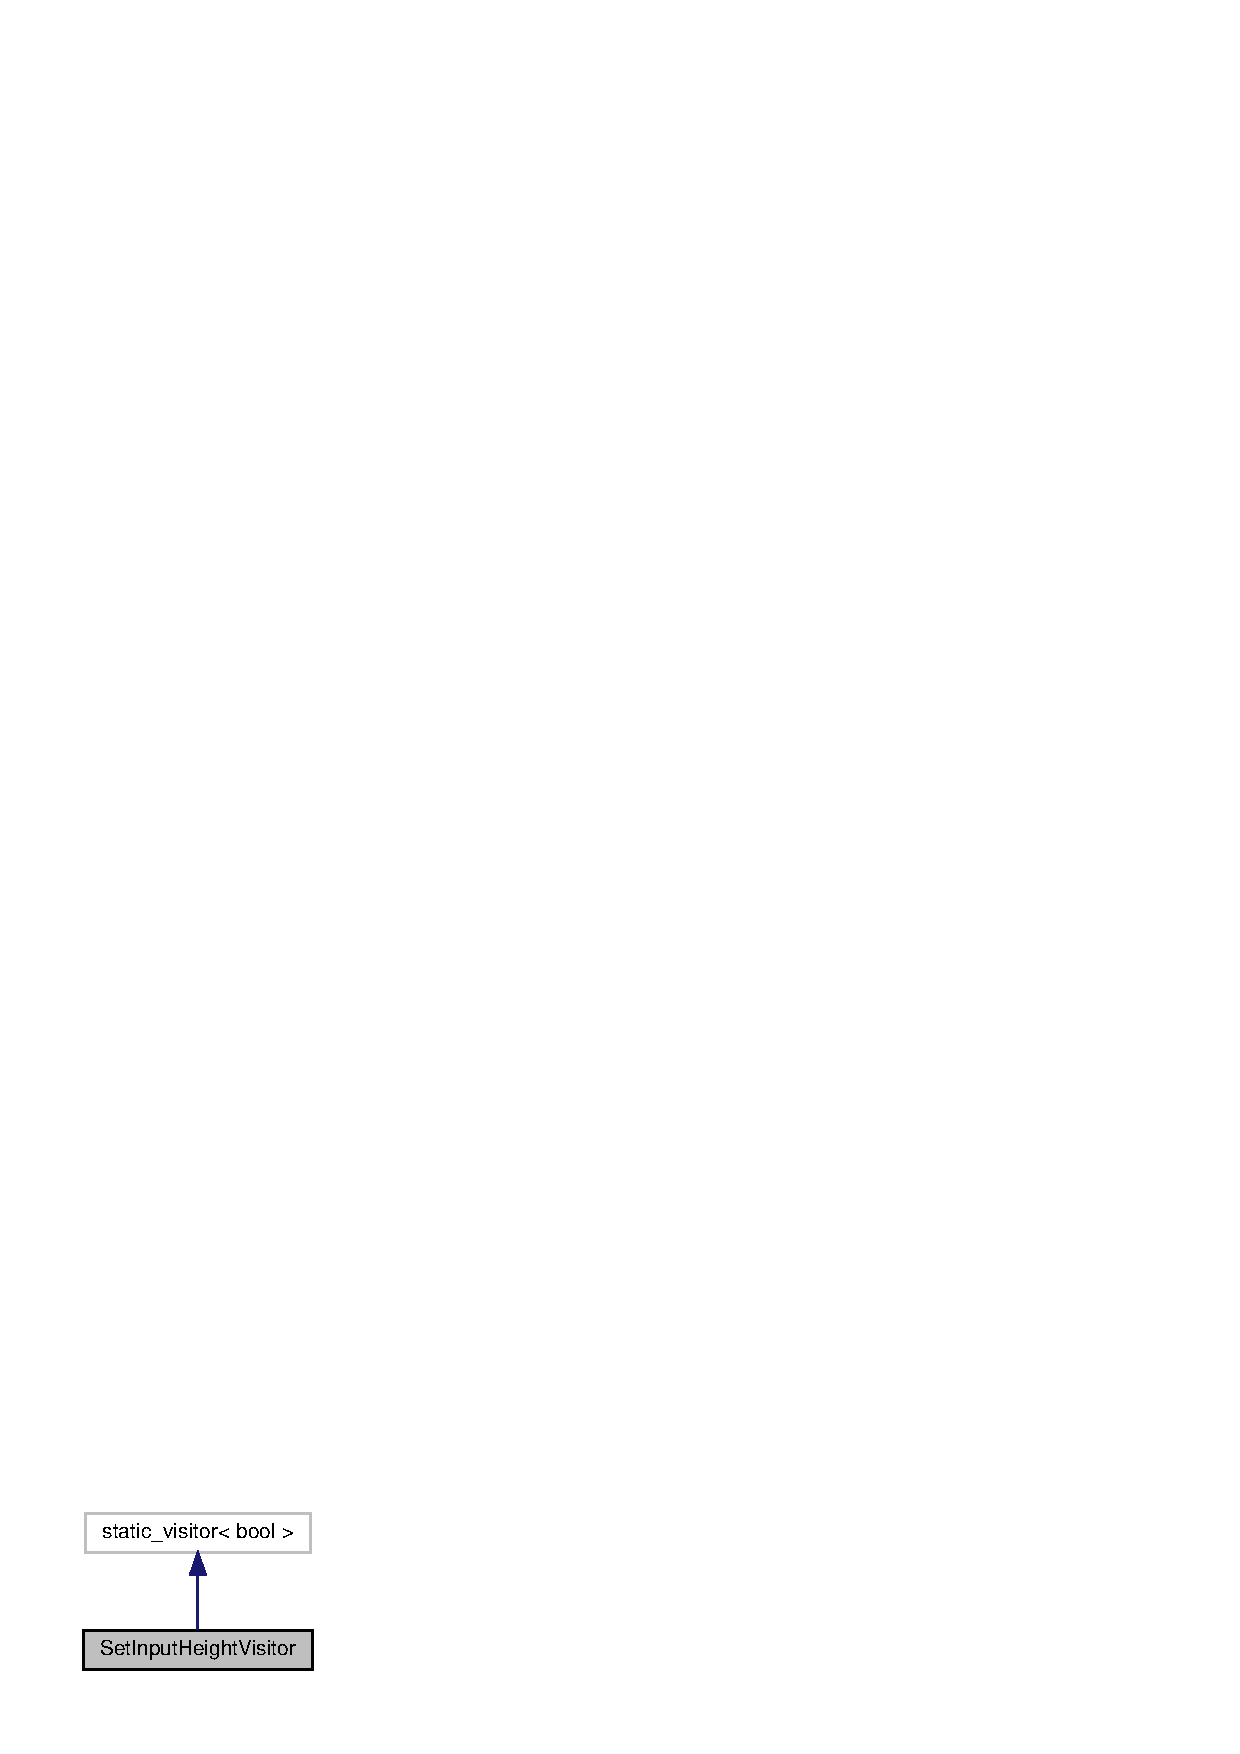
\includegraphics[width=154pt]{classmlpack_1_1ann_1_1SetInputHeightVisitor__inherit__graph}
\end{center}
\end{figure}
\subsection*{Public Member Functions}
\begin{DoxyCompactItemize}
\item 
\textbf{ Set\+Input\+Height\+Visitor} (const size\+\_\+t input\+Height=0, const bool reset=false)
\begin{DoxyCompactList}\small\item\em Update the input height parameter with the given input height. \end{DoxyCompactList}\item 
{\footnotesize template$<$typename Layer\+Type $>$ }\\bool \textbf{ operator()} (Layer\+Type $\ast$layer) const
\begin{DoxyCompactList}\small\item\em Update the input height parameter. \end{DoxyCompactList}\item 
bool \textbf{ operator()} (\textbf{ More\+Types} layer) const
\end{DoxyCompactItemize}


\subsection{Detailed Description}
\doxyref{Set\+Input\+Height\+Visitor}{p.}{classmlpack_1_1ann_1_1SetInputHeightVisitor} updates the input height parameter with the given input height. 

Definition at line 27 of file set\+\_\+input\+\_\+height\+\_\+visitor.\+hpp.



\subsection{Constructor \& Destructor Documentation}
\mbox{\label{classmlpack_1_1ann_1_1SetInputHeightVisitor_ac2f68c3eaf06b0e88078cd99ddbf0397}} 
\index{mlpack\+::ann\+::\+Set\+Input\+Height\+Visitor@{mlpack\+::ann\+::\+Set\+Input\+Height\+Visitor}!Set\+Input\+Height\+Visitor@{Set\+Input\+Height\+Visitor}}
\index{Set\+Input\+Height\+Visitor@{Set\+Input\+Height\+Visitor}!mlpack\+::ann\+::\+Set\+Input\+Height\+Visitor@{mlpack\+::ann\+::\+Set\+Input\+Height\+Visitor}}
\subsubsection{Set\+Input\+Height\+Visitor()}
{\footnotesize\ttfamily \textbf{ Set\+Input\+Height\+Visitor} (\begin{DoxyParamCaption}\item[{const size\+\_\+t}]{input\+Height = {\ttfamily 0},  }\item[{const bool}]{reset = {\ttfamily false} }\end{DoxyParamCaption})}



Update the input height parameter with the given input height. 



\subsection{Member Function Documentation}
\mbox{\label{classmlpack_1_1ann_1_1SetInputHeightVisitor_ad358e269435d5a1b10367bec96793a17}} 
\index{mlpack\+::ann\+::\+Set\+Input\+Height\+Visitor@{mlpack\+::ann\+::\+Set\+Input\+Height\+Visitor}!operator()@{operator()}}
\index{operator()@{operator()}!mlpack\+::ann\+::\+Set\+Input\+Height\+Visitor@{mlpack\+::ann\+::\+Set\+Input\+Height\+Visitor}}
\subsubsection{operator()()\hspace{0.1cm}{\footnotesize\ttfamily [1/2]}}
{\footnotesize\ttfamily bool operator() (\begin{DoxyParamCaption}\item[{Layer\+Type $\ast$}]{layer }\end{DoxyParamCaption}) const}



Update the input height parameter. 

\mbox{\label{classmlpack_1_1ann_1_1SetInputHeightVisitor_a2c712555c12177f4733c7b2f070ff22c}} 
\index{mlpack\+::ann\+::\+Set\+Input\+Height\+Visitor@{mlpack\+::ann\+::\+Set\+Input\+Height\+Visitor}!operator()@{operator()}}
\index{operator()@{operator()}!mlpack\+::ann\+::\+Set\+Input\+Height\+Visitor@{mlpack\+::ann\+::\+Set\+Input\+Height\+Visitor}}
\subsubsection{operator()()\hspace{0.1cm}{\footnotesize\ttfamily [2/2]}}
{\footnotesize\ttfamily bool operator() (\begin{DoxyParamCaption}\item[{\textbf{ More\+Types}}]{layer }\end{DoxyParamCaption}) const}



The documentation for this class was generated from the following file\+:\begin{DoxyCompactItemize}
\item 
/home/aakash/mlpack/src/mlpack/methods/ann/visitor/\textbf{ set\+\_\+input\+\_\+height\+\_\+visitor.\+hpp}\end{DoxyCompactItemize}

\section{Set\+Input\+Width\+Visitor Class Reference}
\label{classmlpack_1_1ann_1_1SetInputWidthVisitor}\index{Set\+Input\+Width\+Visitor@{Set\+Input\+Width\+Visitor}}


\doxyref{Set\+Input\+Width\+Visitor}{p.}{classmlpack_1_1ann_1_1SetInputWidthVisitor} updates the input width parameter with the given input width.  




Inheritance diagram for Set\+Input\+Width\+Visitor\+:
\nopagebreak
\begin{figure}[H]
\begin{center}
\leavevmode
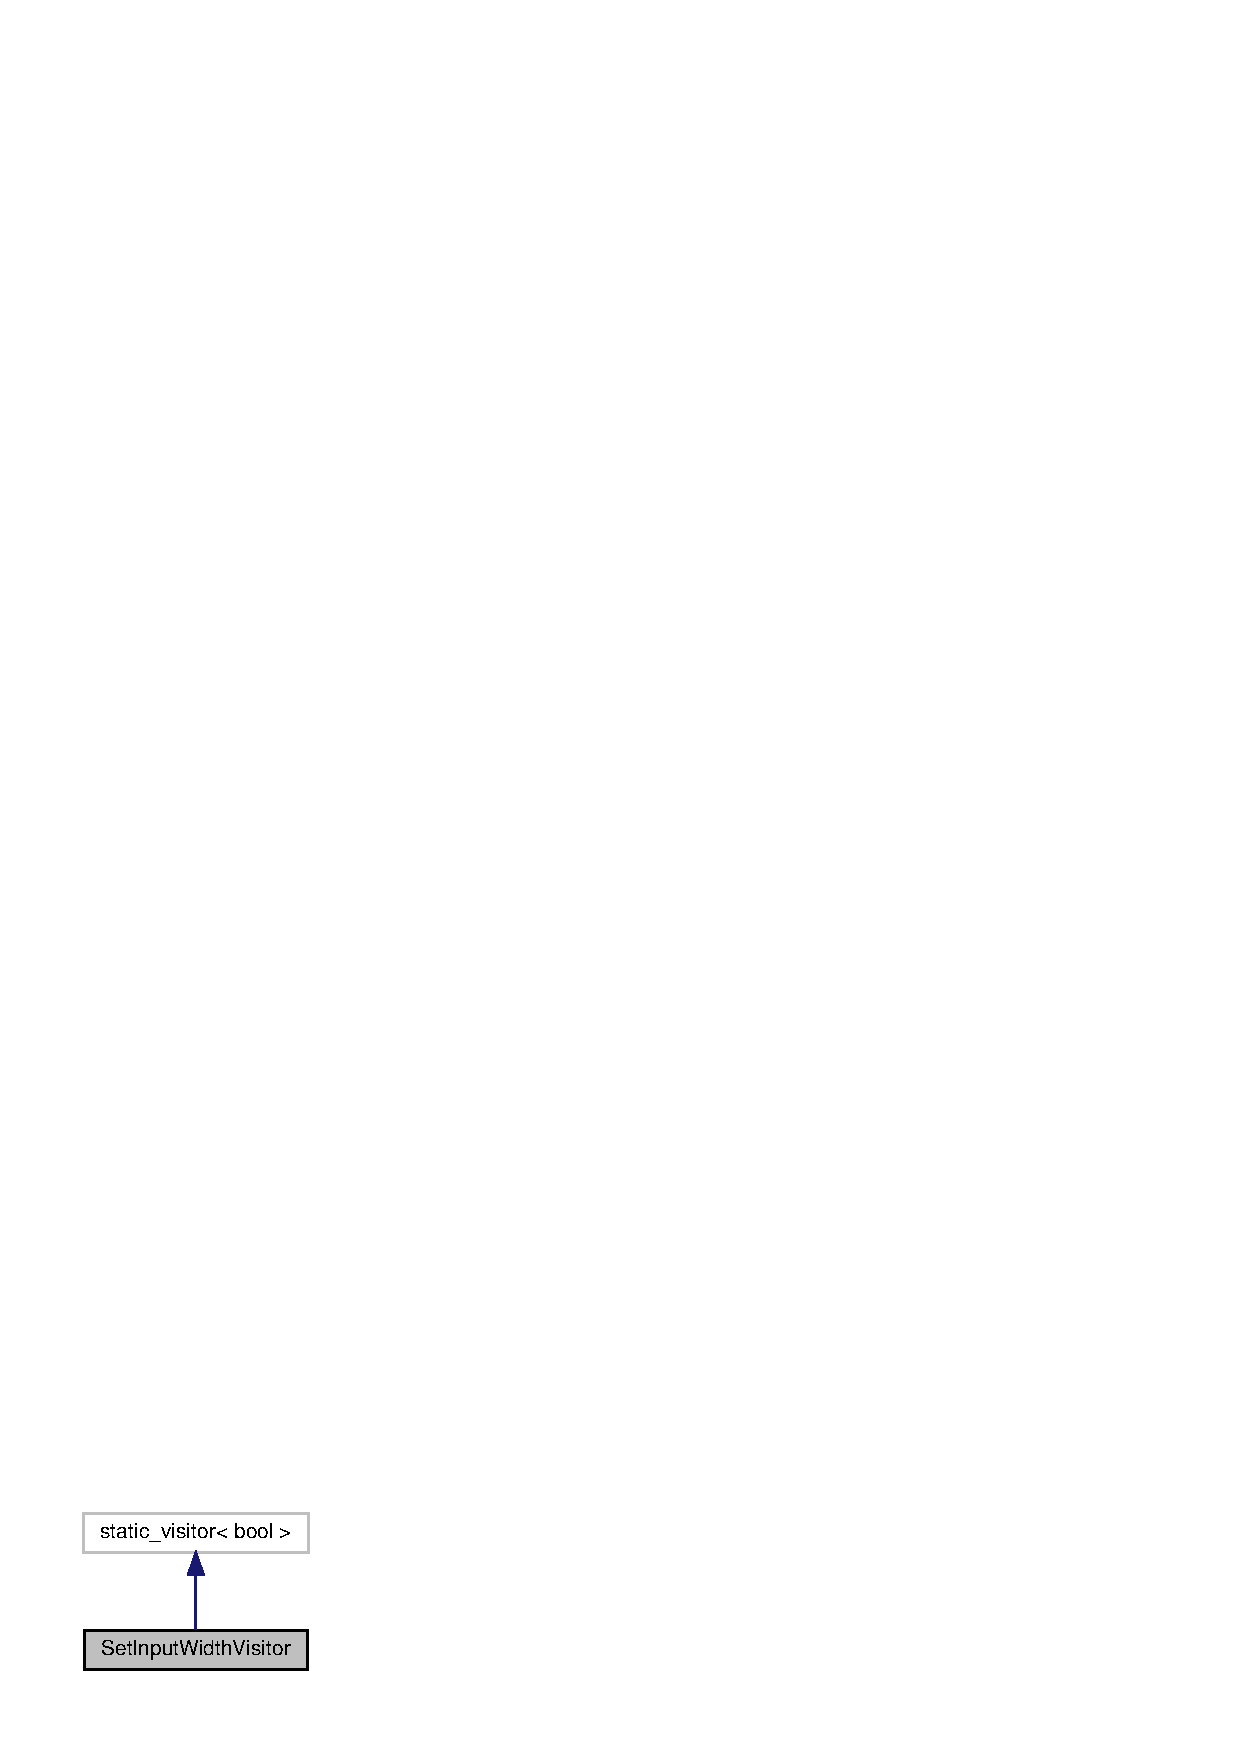
\includegraphics[width=152pt]{classmlpack_1_1ann_1_1SetInputWidthVisitor__inherit__graph}
\end{center}
\end{figure}
\subsection*{Public Member Functions}
\begin{DoxyCompactItemize}
\item 
\textbf{ Set\+Input\+Width\+Visitor} (const size\+\_\+t input\+Width=0, const bool reset=false)
\begin{DoxyCompactList}\small\item\em Update the input width parameter with the given input width. \end{DoxyCompactList}\item 
{\footnotesize template$<$typename Layer\+Type $>$ }\\bool \textbf{ operator()} (Layer\+Type $\ast$layer) const
\begin{DoxyCompactList}\small\item\em Update the input width parameter. \end{DoxyCompactList}\item 
bool \textbf{ operator()} (\textbf{ More\+Types} layer) const
\end{DoxyCompactItemize}


\subsection{Detailed Description}
\doxyref{Set\+Input\+Width\+Visitor}{p.}{classmlpack_1_1ann_1_1SetInputWidthVisitor} updates the input width parameter with the given input width. 

Definition at line 27 of file set\+\_\+input\+\_\+width\+\_\+visitor.\+hpp.



\subsection{Constructor \& Destructor Documentation}
\mbox{\label{classmlpack_1_1ann_1_1SetInputWidthVisitor_a7118737f9b0fea38032c7bb1cb42d023}} 
\index{mlpack\+::ann\+::\+Set\+Input\+Width\+Visitor@{mlpack\+::ann\+::\+Set\+Input\+Width\+Visitor}!Set\+Input\+Width\+Visitor@{Set\+Input\+Width\+Visitor}}
\index{Set\+Input\+Width\+Visitor@{Set\+Input\+Width\+Visitor}!mlpack\+::ann\+::\+Set\+Input\+Width\+Visitor@{mlpack\+::ann\+::\+Set\+Input\+Width\+Visitor}}
\subsubsection{Set\+Input\+Width\+Visitor()}
{\footnotesize\ttfamily \textbf{ Set\+Input\+Width\+Visitor} (\begin{DoxyParamCaption}\item[{const size\+\_\+t}]{input\+Width = {\ttfamily 0},  }\item[{const bool}]{reset = {\ttfamily false} }\end{DoxyParamCaption})}



Update the input width parameter with the given input width. 



\subsection{Member Function Documentation}
\mbox{\label{classmlpack_1_1ann_1_1SetInputWidthVisitor_ad358e269435d5a1b10367bec96793a17}} 
\index{mlpack\+::ann\+::\+Set\+Input\+Width\+Visitor@{mlpack\+::ann\+::\+Set\+Input\+Width\+Visitor}!operator()@{operator()}}
\index{operator()@{operator()}!mlpack\+::ann\+::\+Set\+Input\+Width\+Visitor@{mlpack\+::ann\+::\+Set\+Input\+Width\+Visitor}}
\subsubsection{operator()()\hspace{0.1cm}{\footnotesize\ttfamily [1/2]}}
{\footnotesize\ttfamily bool operator() (\begin{DoxyParamCaption}\item[{Layer\+Type $\ast$}]{layer }\end{DoxyParamCaption}) const}



Update the input width parameter. 

\mbox{\label{classmlpack_1_1ann_1_1SetInputWidthVisitor_a2c712555c12177f4733c7b2f070ff22c}} 
\index{mlpack\+::ann\+::\+Set\+Input\+Width\+Visitor@{mlpack\+::ann\+::\+Set\+Input\+Width\+Visitor}!operator()@{operator()}}
\index{operator()@{operator()}!mlpack\+::ann\+::\+Set\+Input\+Width\+Visitor@{mlpack\+::ann\+::\+Set\+Input\+Width\+Visitor}}
\subsubsection{operator()()\hspace{0.1cm}{\footnotesize\ttfamily [2/2]}}
{\footnotesize\ttfamily bool operator() (\begin{DoxyParamCaption}\item[{\textbf{ More\+Types}}]{layer }\end{DoxyParamCaption}) const}



The documentation for this class was generated from the following file\+:\begin{DoxyCompactItemize}
\item 
/home/aakash/mlpack/src/mlpack/methods/ann/visitor/\textbf{ set\+\_\+input\+\_\+width\+\_\+visitor.\+hpp}\end{DoxyCompactItemize}

\section{Sigmoid\+Cross\+Entropy\+Error$<$ Input\+Data\+Type, Output\+Data\+Type $>$ Class Template Reference}
\label{classmlpack_1_1ann_1_1SigmoidCrossEntropyError}\index{Sigmoid\+Cross\+Entropy\+Error$<$ Input\+Data\+Type, Output\+Data\+Type $>$@{Sigmoid\+Cross\+Entropy\+Error$<$ Input\+Data\+Type, Output\+Data\+Type $>$}}


The \doxyref{Sigmoid\+Cross\+Entropy\+Error}{p.}{classmlpack_1_1ann_1_1SigmoidCrossEntropyError} performance function measures the network\textquotesingle{}s performance according to the cross-\/entropy function between the input and target distributions.  


\subsection*{Public Member Functions}
\begin{DoxyCompactItemize}
\item 
\textbf{ Sigmoid\+Cross\+Entropy\+Error} ()
\begin{DoxyCompactList}\small\item\em Create the \doxyref{Sigmoid\+Cross\+Entropy\+Error}{p.}{classmlpack_1_1ann_1_1SigmoidCrossEntropyError} object. \end{DoxyCompactList}\item 
{\footnotesize template$<$typename Prediction\+Type , typename Target\+Type , typename Loss\+Type $>$ }\\void \textbf{ Backward} (const Prediction\+Type \&prediction, const Target\+Type \&target, Loss\+Type \&loss)
\begin{DoxyCompactList}\small\item\em Ordinary feed backward pass of a neural network. \end{DoxyCompactList}\item 
{\footnotesize template$<$typename Prediction\+Type , typename Target\+Type $>$ }\\Prediction\+Type\+::elem\+\_\+type \textbf{ Forward} (const Prediction\+Type \&prediction, const Target\+Type \&target)
\begin{DoxyCompactList}\small\item\em Computes the Sigmoid Cross\+Entropy Error functions. \end{DoxyCompactList}\item 
Output\+Data\+Type \& \textbf{ Output\+Parameter} () const
\begin{DoxyCompactList}\small\item\em Get the output parameter. \end{DoxyCompactList}\item 
Output\+Data\+Type \& \textbf{ Output\+Parameter} ()
\begin{DoxyCompactList}\small\item\em Modify the output parameter. \end{DoxyCompactList}\item 
{\footnotesize template$<$typename Archive $>$ }\\void \textbf{ serialize} (Archive \&ar, const uint32\+\_\+t)
\begin{DoxyCompactList}\small\item\em Serialize the layer. \end{DoxyCompactList}\end{DoxyCompactItemize}


\subsection{Detailed Description}
\subsubsection*{template$<$typename Input\+Data\+Type = arma\+::mat, typename Output\+Data\+Type = arma\+::mat$>$\newline
class mlpack\+::ann\+::\+Sigmoid\+Cross\+Entropy\+Error$<$ Input\+Data\+Type, Output\+Data\+Type $>$}

The \doxyref{Sigmoid\+Cross\+Entropy\+Error}{p.}{classmlpack_1_1ann_1_1SigmoidCrossEntropyError} performance function measures the network\textquotesingle{}s performance according to the cross-\/entropy function between the input and target distributions. 

This function calculates the cross entropy given the real values instead of providing the sigmoid activations. The function uses this equivalent formulation\+: $max(x, 0) - x * z + \log(1 + e^{-|x|})$ where x = input and z = target.

For more information, see the following paper.


\begin{DoxyCode}
@article\{Janocha2017
  title   = \{On Loss Functions \textcolor{keywordflow}{for} Deep Neural Networks in Classification\},
  author  = \{Katarzyna Janocha, Wojciech Marian Czarnecki\},
  url     = \{http:\textcolor{comment}{//arxiv.org/abs/1702.05659\},}
  journal = \{CoRR\},
  eprint  = \{arXiv:1702.05659\},
  year    = \{2017\}
\}
\end{DoxyCode}



\begin{DoxyTemplParams}{Template Parameters}
{\em Input\+Data\+Type} & Type of the input data (arma\+::colvec, arma\+::mat, arma\+::sp\+\_\+mat or arma\+::cube). \\
\hline
{\em Output\+Data\+Type} & Type of the output data (arma\+::colvec, arma\+::mat, arma\+::sp\+\_\+mat or arma\+::cube). \\
\hline
\end{DoxyTemplParams}


Definition at line 52 of file sigmoid\+\_\+cross\+\_\+entropy\+\_\+error.\+hpp.



\subsection{Constructor \& Destructor Documentation}
\mbox{\label{classmlpack_1_1ann_1_1SigmoidCrossEntropyError_a5d08bab32a040d5a35d277ed020930a1}} 
\index{mlpack\+::ann\+::\+Sigmoid\+Cross\+Entropy\+Error@{mlpack\+::ann\+::\+Sigmoid\+Cross\+Entropy\+Error}!Sigmoid\+Cross\+Entropy\+Error@{Sigmoid\+Cross\+Entropy\+Error}}
\index{Sigmoid\+Cross\+Entropy\+Error@{Sigmoid\+Cross\+Entropy\+Error}!mlpack\+::ann\+::\+Sigmoid\+Cross\+Entropy\+Error@{mlpack\+::ann\+::\+Sigmoid\+Cross\+Entropy\+Error}}
\subsubsection{Sigmoid\+Cross\+Entropy\+Error()}
{\footnotesize\ttfamily \textbf{ Sigmoid\+Cross\+Entropy\+Error} (\begin{DoxyParamCaption}{ }\end{DoxyParamCaption})}



Create the \doxyref{Sigmoid\+Cross\+Entropy\+Error}{p.}{classmlpack_1_1ann_1_1SigmoidCrossEntropyError} object. 



\subsection{Member Function Documentation}
\mbox{\label{classmlpack_1_1ann_1_1SigmoidCrossEntropyError_add41dbaf358dc099750dc6064cb7e0d7}} 
\index{mlpack\+::ann\+::\+Sigmoid\+Cross\+Entropy\+Error@{mlpack\+::ann\+::\+Sigmoid\+Cross\+Entropy\+Error}!Backward@{Backward}}
\index{Backward@{Backward}!mlpack\+::ann\+::\+Sigmoid\+Cross\+Entropy\+Error@{mlpack\+::ann\+::\+Sigmoid\+Cross\+Entropy\+Error}}
\subsubsection{Backward()}
{\footnotesize\ttfamily void Backward (\begin{DoxyParamCaption}\item[{const Prediction\+Type \&}]{prediction,  }\item[{const Target\+Type \&}]{target,  }\item[{Loss\+Type \&}]{loss }\end{DoxyParamCaption})\hspace{0.3cm}{\ttfamily [inline]}}



Ordinary feed backward pass of a neural network. 


\begin{DoxyParams}{Parameters}
{\em prediction} & Predictions used for evaluating the specified loss function. \\
\hline
{\em target} & The target vector. \\
\hline
{\em loss} & The calculated error. \\
\hline
\end{DoxyParams}
\mbox{\label{classmlpack_1_1ann_1_1SigmoidCrossEntropyError_ab3640059898ea76c13709b8099316fe8}} 
\index{mlpack\+::ann\+::\+Sigmoid\+Cross\+Entropy\+Error@{mlpack\+::ann\+::\+Sigmoid\+Cross\+Entropy\+Error}!Forward@{Forward}}
\index{Forward@{Forward}!mlpack\+::ann\+::\+Sigmoid\+Cross\+Entropy\+Error@{mlpack\+::ann\+::\+Sigmoid\+Cross\+Entropy\+Error}}
\subsubsection{Forward()}
{\footnotesize\ttfamily Prediction\+Type\+::elem\+\_\+type Forward (\begin{DoxyParamCaption}\item[{const Prediction\+Type \&}]{prediction,  }\item[{const Target\+Type \&}]{target }\end{DoxyParamCaption})\hspace{0.3cm}{\ttfamily [inline]}}



Computes the Sigmoid Cross\+Entropy Error functions. 


\begin{DoxyParams}{Parameters}
{\em prediction} & Predictions used for evaluating the specified loss function. \\
\hline
{\em target} & The target vector. \\
\hline
\end{DoxyParams}
\mbox{\label{classmlpack_1_1ann_1_1SigmoidCrossEntropyError_a8bae962cc603d1cab8d80ec78f8d505d}} 
\index{mlpack\+::ann\+::\+Sigmoid\+Cross\+Entropy\+Error@{mlpack\+::ann\+::\+Sigmoid\+Cross\+Entropy\+Error}!Output\+Parameter@{Output\+Parameter}}
\index{Output\+Parameter@{Output\+Parameter}!mlpack\+::ann\+::\+Sigmoid\+Cross\+Entropy\+Error@{mlpack\+::ann\+::\+Sigmoid\+Cross\+Entropy\+Error}}
\subsubsection{Output\+Parameter()\hspace{0.1cm}{\footnotesize\ttfamily [1/2]}}
{\footnotesize\ttfamily Output\+Data\+Type\& Output\+Parameter (\begin{DoxyParamCaption}{ }\end{DoxyParamCaption}) const\hspace{0.3cm}{\ttfamily [inline]}}



Get the output parameter. 



Definition at line 86 of file sigmoid\+\_\+cross\+\_\+entropy\+\_\+error.\+hpp.

\mbox{\label{classmlpack_1_1ann_1_1SigmoidCrossEntropyError_a21d5f745f02c709625a4ee0907f004a5}} 
\index{mlpack\+::ann\+::\+Sigmoid\+Cross\+Entropy\+Error@{mlpack\+::ann\+::\+Sigmoid\+Cross\+Entropy\+Error}!Output\+Parameter@{Output\+Parameter}}
\index{Output\+Parameter@{Output\+Parameter}!mlpack\+::ann\+::\+Sigmoid\+Cross\+Entropy\+Error@{mlpack\+::ann\+::\+Sigmoid\+Cross\+Entropy\+Error}}
\subsubsection{Output\+Parameter()\hspace{0.1cm}{\footnotesize\ttfamily [2/2]}}
{\footnotesize\ttfamily Output\+Data\+Type\& Output\+Parameter (\begin{DoxyParamCaption}{ }\end{DoxyParamCaption})\hspace{0.3cm}{\ttfamily [inline]}}



Modify the output parameter. 



Definition at line 88 of file sigmoid\+\_\+cross\+\_\+entropy\+\_\+error.\+hpp.



References Sigmoid\+Cross\+Entropy\+Error$<$ Input\+Data\+Type, Output\+Data\+Type $>$\+::serialize().

\mbox{\label{classmlpack_1_1ann_1_1SigmoidCrossEntropyError_a65cba07328997659bec80b9879b15a51}} 
\index{mlpack\+::ann\+::\+Sigmoid\+Cross\+Entropy\+Error@{mlpack\+::ann\+::\+Sigmoid\+Cross\+Entropy\+Error}!serialize@{serialize}}
\index{serialize@{serialize}!mlpack\+::ann\+::\+Sigmoid\+Cross\+Entropy\+Error@{mlpack\+::ann\+::\+Sigmoid\+Cross\+Entropy\+Error}}
\subsubsection{serialize()}
{\footnotesize\ttfamily void serialize (\begin{DoxyParamCaption}\item[{Archive \&}]{ar,  }\item[{const uint32\+\_\+t}]{ }\end{DoxyParamCaption})}



Serialize the layer. 



Referenced by Sigmoid\+Cross\+Entropy\+Error$<$ Input\+Data\+Type, Output\+Data\+Type $>$\+::\+Output\+Parameter().



The documentation for this class was generated from the following file\+:\begin{DoxyCompactItemize}
\item 
/home/aakash/mlpack/src/mlpack/methods/ann/loss\+\_\+functions/\textbf{ sigmoid\+\_\+cross\+\_\+entropy\+\_\+error.\+hpp}\end{DoxyCompactItemize}

\section{S\+I\+L\+U\+Function Class Reference}
\label{classmlpack_1_1ann_1_1SILUFunction}\index{S\+I\+L\+U\+Function@{S\+I\+L\+U\+Function}}


The S\+I\+LU function, defined by.  


\subsection*{Static Public Member Functions}
\begin{DoxyCompactItemize}
\item 
static double \textbf{ Deriv} (const double x)
\begin{DoxyCompactList}\small\item\em Computes the first derivative of the S\+I\+LU function. \end{DoxyCompactList}\item 
{\footnotesize template$<$typename Input\+Vec\+Type , typename Output\+Vec\+Type $>$ }\\static void \textbf{ Deriv} (const Input\+Vec\+Type \&x, Output\+Vec\+Type \&y)
\begin{DoxyCompactList}\small\item\em Computes the first derivatives of the S\+I\+LU function. \end{DoxyCompactList}\item 
static double \textbf{ Fn} (const double x)
\begin{DoxyCompactList}\small\item\em Computes the S\+I\+LU function. \end{DoxyCompactList}\item 
{\footnotesize template$<$typename Input\+Vec\+Type , typename Output\+Vec\+Type $>$ }\\static void \textbf{ Fn} (const Input\+Vec\+Type \&x, Output\+Vec\+Type \&y)
\begin{DoxyCompactList}\small\item\em Computes the S\+I\+LU function. \end{DoxyCompactList}\end{DoxyCompactItemize}


\subsection{Detailed Description}
The S\+I\+LU function, defined by. 

\begin{eqnarray*} f(x) &=& x * \frac{1}{1 + e^{-x}}\\ f'(x) &=& \frac{1}{1 + e^{-x}} * (1 + x * (1-\frac{1}{1 + e^{-x}}))\\ \end{eqnarray*} 

Definition at line 43 of file silu\+\_\+function.\+hpp.



\subsection{Member Function Documentation}
\mbox{\label{classmlpack_1_1ann_1_1SILUFunction_acd77fae79f7ba1f4b9a21e07a261e537}} 
\index{mlpack\+::ann\+::\+S\+I\+L\+U\+Function@{mlpack\+::ann\+::\+S\+I\+L\+U\+Function}!Deriv@{Deriv}}
\index{Deriv@{Deriv}!mlpack\+::ann\+::\+S\+I\+L\+U\+Function@{mlpack\+::ann\+::\+S\+I\+L\+U\+Function}}
\subsubsection{Deriv()\hspace{0.1cm}{\footnotesize\ttfamily [1/2]}}
{\footnotesize\ttfamily static double Deriv (\begin{DoxyParamCaption}\item[{const double}]{x }\end{DoxyParamCaption})\hspace{0.3cm}{\ttfamily [inline]}, {\ttfamily [static]}}



Computes the first derivative of the S\+I\+LU function. 


\begin{DoxyParams}{Parameters}
{\em y} & Input activation. \\
\hline
\end{DoxyParams}
\begin{DoxyReturn}{Returns}
f\textquotesingle{}(x) 
\end{DoxyReturn}


Definition at line 75 of file silu\+\_\+function.\+hpp.

\mbox{\label{classmlpack_1_1ann_1_1SILUFunction_a0ad035ec996acd7025807d0e9e082887}} 
\index{mlpack\+::ann\+::\+S\+I\+L\+U\+Function@{mlpack\+::ann\+::\+S\+I\+L\+U\+Function}!Deriv@{Deriv}}
\index{Deriv@{Deriv}!mlpack\+::ann\+::\+S\+I\+L\+U\+Function@{mlpack\+::ann\+::\+S\+I\+L\+U\+Function}}
\subsubsection{Deriv()\hspace{0.1cm}{\footnotesize\ttfamily [2/2]}}
{\footnotesize\ttfamily static void Deriv (\begin{DoxyParamCaption}\item[{const Input\+Vec\+Type \&}]{x,  }\item[{Output\+Vec\+Type \&}]{y }\end{DoxyParamCaption})\hspace{0.3cm}{\ttfamily [inline]}, {\ttfamily [static]}}



Computes the first derivatives of the S\+I\+LU function. 


\begin{DoxyParams}{Parameters}
{\em y} & Input activations. \\
\hline
{\em x} & The resulting derivatives. \\
\hline
\end{DoxyParams}


Definition at line 88 of file silu\+\_\+function.\+hpp.

\mbox{\label{classmlpack_1_1ann_1_1SILUFunction_a11bd9a1195e6b107f9fee73643bc328b}} 
\index{mlpack\+::ann\+::\+S\+I\+L\+U\+Function@{mlpack\+::ann\+::\+S\+I\+L\+U\+Function}!Fn@{Fn}}
\index{Fn@{Fn}!mlpack\+::ann\+::\+S\+I\+L\+U\+Function@{mlpack\+::ann\+::\+S\+I\+L\+U\+Function}}
\subsubsection{Fn()\hspace{0.1cm}{\footnotesize\ttfamily [1/2]}}
{\footnotesize\ttfamily static double Fn (\begin{DoxyParamCaption}\item[{const double}]{x }\end{DoxyParamCaption})\hspace{0.3cm}{\ttfamily [inline]}, {\ttfamily [static]}}



Computes the S\+I\+LU function. 


\begin{DoxyParams}{Parameters}
{\em x} & Input data. \\
\hline
\end{DoxyParams}
\begin{DoxyReturn}{Returns}
f(x). 
\end{DoxyReturn}


Definition at line 52 of file silu\+\_\+function.\+hpp.

\mbox{\label{classmlpack_1_1ann_1_1SILUFunction_af6cf5da90eb6312e3e25c9b8bd9c3527}} 
\index{mlpack\+::ann\+::\+S\+I\+L\+U\+Function@{mlpack\+::ann\+::\+S\+I\+L\+U\+Function}!Fn@{Fn}}
\index{Fn@{Fn}!mlpack\+::ann\+::\+S\+I\+L\+U\+Function@{mlpack\+::ann\+::\+S\+I\+L\+U\+Function}}
\subsubsection{Fn()\hspace{0.1cm}{\footnotesize\ttfamily [2/2]}}
{\footnotesize\ttfamily static void Fn (\begin{DoxyParamCaption}\item[{const Input\+Vec\+Type \&}]{x,  }\item[{Output\+Vec\+Type \&}]{y }\end{DoxyParamCaption})\hspace{0.3cm}{\ttfamily [inline]}, {\ttfamily [static]}}



Computes the S\+I\+LU function. 


\begin{DoxyParams}{Parameters}
{\em x} & Input data. \\
\hline
{\em y} & The resulting output activation. \\
\hline
\end{DoxyParams}


Definition at line 64 of file silu\+\_\+function.\+hpp.



The documentation for this class was generated from the following file\+:\begin{DoxyCompactItemize}
\item 
/home/aakash/mlpack/src/mlpack/methods/ann/activation\+\_\+functions/\textbf{ silu\+\_\+function.\+hpp}\end{DoxyCompactItemize}

\section{Soft\+Margin\+Loss$<$ Input\+Data\+Type, Output\+Data\+Type $>$ Class Template Reference}
\label{classmlpack_1_1ann_1_1SoftMarginLoss}\index{Soft\+Margin\+Loss$<$ Input\+Data\+Type, Output\+Data\+Type $>$@{Soft\+Margin\+Loss$<$ Input\+Data\+Type, Output\+Data\+Type $>$}}
\subsection*{Public Member Functions}
\begin{DoxyCompactItemize}
\item 
\textbf{ Soft\+Margin\+Loss} (const bool reduction=true)
\begin{DoxyCompactList}\small\item\em Create the \doxyref{Soft\+Margin\+Loss}{p.}{classmlpack_1_1ann_1_1SoftMarginLoss} object. \end{DoxyCompactList}\item 
{\footnotesize template$<$typename Prediction\+Type , typename Target\+Type , typename Loss\+Type $>$ }\\void \textbf{ Backward} (const Prediction\+Type \&prediction, const Target\+Type \&target, Loss\+Type \&loss)
\begin{DoxyCompactList}\small\item\em Ordinary feed backward pass of a neural network. \end{DoxyCompactList}\item 
{\footnotesize template$<$typename Prediction\+Type , typename Target\+Type $>$ }\\Prediction\+Type\+::elem\+\_\+type \textbf{ Forward} (const Prediction\+Type \&prediction, const Target\+Type \&target)
\begin{DoxyCompactList}\small\item\em Computes the Soft Margin Loss function. \end{DoxyCompactList}\item 
Output\+Data\+Type \& \textbf{ Output\+Parameter} () const
\begin{DoxyCompactList}\small\item\em Get the output parameter. \end{DoxyCompactList}\item 
Output\+Data\+Type \& \textbf{ Output\+Parameter} ()
\begin{DoxyCompactList}\small\item\em Modify the output parameter. \end{DoxyCompactList}\item 
bool \textbf{ Reduction} () const
\begin{DoxyCompactList}\small\item\em Get the type of reduction used. \end{DoxyCompactList}\item 
bool \& \textbf{ Reduction} ()
\begin{DoxyCompactList}\small\item\em Modify the type of reduction used. \end{DoxyCompactList}\item 
{\footnotesize template$<$typename Archive $>$ }\\void \textbf{ serialize} (Archive \&ar, const uint32\+\_\+t version)
\begin{DoxyCompactList}\small\item\em Serialize the layer. \end{DoxyCompactList}\end{DoxyCompactItemize}


\subsection{Detailed Description}
\subsubsection*{template$<$typename Input\+Data\+Type = arma\+::mat, typename Output\+Data\+Type = arma\+::mat$>$\newline
class mlpack\+::ann\+::\+Soft\+Margin\+Loss$<$ Input\+Data\+Type, Output\+Data\+Type $>$}


\begin{DoxyTemplParams}{Template Parameters}
{\em Input\+Data\+Type} & Type of the input data (arma\+::colvec, arma\+::mat, arma\+::sp\+\_\+mat or arma\+::cube). \\
\hline
{\em Output\+Data\+Type} & Type of the output data (arma\+::colvec, arma\+::mat, arma\+::sp\+\_\+mat or arma\+::cube). \\
\hline
\end{DoxyTemplParams}


Definition at line 34 of file soft\+\_\+margin\+\_\+loss.\+hpp.



\subsection{Constructor \& Destructor Documentation}
\mbox{\label{classmlpack_1_1ann_1_1SoftMarginLoss_ad9b5a32d621cdb719e2d76be548b298e}} 
\index{mlpack\+::ann\+::\+Soft\+Margin\+Loss@{mlpack\+::ann\+::\+Soft\+Margin\+Loss}!Soft\+Margin\+Loss@{Soft\+Margin\+Loss}}
\index{Soft\+Margin\+Loss@{Soft\+Margin\+Loss}!mlpack\+::ann\+::\+Soft\+Margin\+Loss@{mlpack\+::ann\+::\+Soft\+Margin\+Loss}}
\subsubsection{Soft\+Margin\+Loss()}
{\footnotesize\ttfamily \textbf{ Soft\+Margin\+Loss} (\begin{DoxyParamCaption}\item[{const bool}]{reduction = {\ttfamily true} }\end{DoxyParamCaption})}



Create the \doxyref{Soft\+Margin\+Loss}{p.}{classmlpack_1_1ann_1_1SoftMarginLoss} object. 


\begin{DoxyParams}{Parameters}
{\em reduction} & Specifies the reduction to apply to the output. If false, \textquotesingle{}mean\textquotesingle{} reduction is used, where sum of the output will be divided by the number of elements in the output. If true, \textquotesingle{}sum\textquotesingle{} reduction is used and the output will be summed. It is set to true by default. \\
\hline
\end{DoxyParams}


\subsection{Member Function Documentation}
\mbox{\label{classmlpack_1_1ann_1_1SoftMarginLoss_add41dbaf358dc099750dc6064cb7e0d7}} 
\index{mlpack\+::ann\+::\+Soft\+Margin\+Loss@{mlpack\+::ann\+::\+Soft\+Margin\+Loss}!Backward@{Backward}}
\index{Backward@{Backward}!mlpack\+::ann\+::\+Soft\+Margin\+Loss@{mlpack\+::ann\+::\+Soft\+Margin\+Loss}}
\subsubsection{Backward()}
{\footnotesize\ttfamily void Backward (\begin{DoxyParamCaption}\item[{const Prediction\+Type \&}]{prediction,  }\item[{const Target\+Type \&}]{target,  }\item[{Loss\+Type \&}]{loss }\end{DoxyParamCaption})}



Ordinary feed backward pass of a neural network. 


\begin{DoxyParams}{Parameters}
{\em prediction} & Predictions used for evaluating the specified loss function. \\
\hline
{\em target} & The target vector. \\
\hline
{\em loss} & The calculated error. \\
\hline
\end{DoxyParams}
\mbox{\label{classmlpack_1_1ann_1_1SoftMarginLoss_ab3640059898ea76c13709b8099316fe8}} 
\index{mlpack\+::ann\+::\+Soft\+Margin\+Loss@{mlpack\+::ann\+::\+Soft\+Margin\+Loss}!Forward@{Forward}}
\index{Forward@{Forward}!mlpack\+::ann\+::\+Soft\+Margin\+Loss@{mlpack\+::ann\+::\+Soft\+Margin\+Loss}}
\subsubsection{Forward()}
{\footnotesize\ttfamily Prediction\+Type\+::elem\+\_\+type Forward (\begin{DoxyParamCaption}\item[{const Prediction\+Type \&}]{prediction,  }\item[{const Target\+Type \&}]{target }\end{DoxyParamCaption})}



Computes the Soft Margin Loss function. 


\begin{DoxyParams}{Parameters}
{\em prediction} & Predictions used for evaluating the specified loss function. \\
\hline
{\em target} & The target vector with same shape as input. \\
\hline
\end{DoxyParams}
\mbox{\label{classmlpack_1_1ann_1_1SoftMarginLoss_a8bae962cc603d1cab8d80ec78f8d505d}} 
\index{mlpack\+::ann\+::\+Soft\+Margin\+Loss@{mlpack\+::ann\+::\+Soft\+Margin\+Loss}!Output\+Parameter@{Output\+Parameter}}
\index{Output\+Parameter@{Output\+Parameter}!mlpack\+::ann\+::\+Soft\+Margin\+Loss@{mlpack\+::ann\+::\+Soft\+Margin\+Loss}}
\subsubsection{Output\+Parameter()\hspace{0.1cm}{\footnotesize\ttfamily [1/2]}}
{\footnotesize\ttfamily Output\+Data\+Type\& Output\+Parameter (\begin{DoxyParamCaption}{ }\end{DoxyParamCaption}) const\hspace{0.3cm}{\ttfamily [inline]}}



Get the output parameter. 



Definition at line 73 of file soft\+\_\+margin\+\_\+loss.\+hpp.

\mbox{\label{classmlpack_1_1ann_1_1SoftMarginLoss_a21d5f745f02c709625a4ee0907f004a5}} 
\index{mlpack\+::ann\+::\+Soft\+Margin\+Loss@{mlpack\+::ann\+::\+Soft\+Margin\+Loss}!Output\+Parameter@{Output\+Parameter}}
\index{Output\+Parameter@{Output\+Parameter}!mlpack\+::ann\+::\+Soft\+Margin\+Loss@{mlpack\+::ann\+::\+Soft\+Margin\+Loss}}
\subsubsection{Output\+Parameter()\hspace{0.1cm}{\footnotesize\ttfamily [2/2]}}
{\footnotesize\ttfamily Output\+Data\+Type\& Output\+Parameter (\begin{DoxyParamCaption}{ }\end{DoxyParamCaption})\hspace{0.3cm}{\ttfamily [inline]}}



Modify the output parameter. 



Definition at line 75 of file soft\+\_\+margin\+\_\+loss.\+hpp.

\mbox{\label{classmlpack_1_1ann_1_1SoftMarginLoss_afb1123035456ff8aa73e7f7c08e6acbc}} 
\index{mlpack\+::ann\+::\+Soft\+Margin\+Loss@{mlpack\+::ann\+::\+Soft\+Margin\+Loss}!Reduction@{Reduction}}
\index{Reduction@{Reduction}!mlpack\+::ann\+::\+Soft\+Margin\+Loss@{mlpack\+::ann\+::\+Soft\+Margin\+Loss}}
\subsubsection{Reduction()\hspace{0.1cm}{\footnotesize\ttfamily [1/2]}}
{\footnotesize\ttfamily bool Reduction (\begin{DoxyParamCaption}{ }\end{DoxyParamCaption}) const\hspace{0.3cm}{\ttfamily [inline]}}



Get the type of reduction used. 



Definition at line 78 of file soft\+\_\+margin\+\_\+loss.\+hpp.

\mbox{\label{classmlpack_1_1ann_1_1SoftMarginLoss_ace5e97393cf08c81177ad0929d1c3496}} 
\index{mlpack\+::ann\+::\+Soft\+Margin\+Loss@{mlpack\+::ann\+::\+Soft\+Margin\+Loss}!Reduction@{Reduction}}
\index{Reduction@{Reduction}!mlpack\+::ann\+::\+Soft\+Margin\+Loss@{mlpack\+::ann\+::\+Soft\+Margin\+Loss}}
\subsubsection{Reduction()\hspace{0.1cm}{\footnotesize\ttfamily [2/2]}}
{\footnotesize\ttfamily bool\& Reduction (\begin{DoxyParamCaption}{ }\end{DoxyParamCaption})\hspace{0.3cm}{\ttfamily [inline]}}



Modify the type of reduction used. 



Definition at line 80 of file soft\+\_\+margin\+\_\+loss.\+hpp.



References Soft\+Margin\+Loss$<$ Input\+Data\+Type, Output\+Data\+Type $>$\+::serialize().

\mbox{\label{classmlpack_1_1ann_1_1SoftMarginLoss_a72d63b74c8166dff8e1a9006905ad9ca}} 
\index{mlpack\+::ann\+::\+Soft\+Margin\+Loss@{mlpack\+::ann\+::\+Soft\+Margin\+Loss}!serialize@{serialize}}
\index{serialize@{serialize}!mlpack\+::ann\+::\+Soft\+Margin\+Loss@{mlpack\+::ann\+::\+Soft\+Margin\+Loss}}
\subsubsection{serialize()}
{\footnotesize\ttfamily void serialize (\begin{DoxyParamCaption}\item[{Archive \&}]{ar,  }\item[{const uint32\+\_\+t}]{version }\end{DoxyParamCaption})}



Serialize the layer. 



Referenced by Soft\+Margin\+Loss$<$ Input\+Data\+Type, Output\+Data\+Type $>$\+::\+Reduction().



The documentation for this class was generated from the following file\+:\begin{DoxyCompactItemize}
\item 
/home/aakash/mlpack/src/mlpack/methods/ann/loss\+\_\+functions/\textbf{ soft\+\_\+margin\+\_\+loss.\+hpp}\end{DoxyCompactItemize}

\section{Softmax$<$ Input\+Data\+Type, Output\+Data\+Type $>$ Class Template Reference}
\label{classmlpack_1_1ann_1_1Softmax}\index{Softmax$<$ Input\+Data\+Type, Output\+Data\+Type $>$@{Softmax$<$ Input\+Data\+Type, Output\+Data\+Type $>$}}


Implementation of the \doxyref{Softmax}{p.}{classmlpack_1_1ann_1_1Softmax} layer.  


\subsection*{Public Member Functions}
\begin{DoxyCompactItemize}
\item 
\textbf{ Softmax} ()
\begin{DoxyCompactList}\small\item\em Create the \doxyref{Softmax}{p.}{classmlpack_1_1ann_1_1Softmax} object. \end{DoxyCompactList}\item 
{\footnotesize template$<$typename eT $>$ }\\void \textbf{ Backward} (const arma\+::\+Mat$<$ eT $>$ \&input, const arma\+::\+Mat$<$ eT $>$ \&gy, arma\+::\+Mat$<$ eT $>$ \&g)
\begin{DoxyCompactList}\small\item\em Ordinary feed backward pass of a neural network, calculating the function f(x) by propagating x backwards through f. \end{DoxyCompactList}\item 
Input\+Data\+Type \& \textbf{ Delta} () const
\begin{DoxyCompactList}\small\item\em Get the delta. \end{DoxyCompactList}\item 
Input\+Data\+Type \& \textbf{ Delta} ()
\begin{DoxyCompactList}\small\item\em Modify the delta. \end{DoxyCompactList}\item 
{\footnotesize template$<$typename Input\+Type , typename Output\+Type $>$ }\\void \textbf{ Forward} (const Input\+Type \&input, Output\+Type \&output)
\begin{DoxyCompactList}\small\item\em Ordinary feed forward pass of a neural network, evaluating the function f(x) by propagating the activity forward through f. \end{DoxyCompactList}\item 
Output\+Data\+Type \& \textbf{ Output\+Parameter} () const
\begin{DoxyCompactList}\small\item\em Get the output parameter. \end{DoxyCompactList}\item 
Output\+Data\+Type \& \textbf{ Output\+Parameter} ()
\begin{DoxyCompactList}\small\item\em Modify the output parameter. \end{DoxyCompactList}\item 
{\footnotesize template$<$typename Archive $>$ }\\void \textbf{ serialize} (Archive \&, const uint32\+\_\+t)
\begin{DoxyCompactList}\small\item\em Serialize the layer. \end{DoxyCompactList}\item 
size\+\_\+t \textbf{ Weight\+Size} () const
\begin{DoxyCompactList}\small\item\em Get the size of the weights. \end{DoxyCompactList}\end{DoxyCompactItemize}


\subsection{Detailed Description}
\subsubsection*{template$<$typename Input\+Data\+Type = arma\+::mat, typename Output\+Data\+Type = arma\+::mat$>$\newline
class mlpack\+::ann\+::\+Softmax$<$ Input\+Data\+Type, Output\+Data\+Type $>$}

Implementation of the \doxyref{Softmax}{p.}{classmlpack_1_1ann_1_1Softmax} layer. 

The softmax function takes as input a vector of K real numbers, and normalizes it into a probability distribution consisting of K probabilities proportional to the exponentials of the input numbers. It should be used for inference only and not with N\+LL loss (use \doxyref{Log\+Soft\+Max}{p.}{classmlpack_1_1ann_1_1LogSoftMax} instead).


\begin{DoxyTemplParams}{Template Parameters}
{\em Input\+Data\+Type} & Type of the input data (arma\+::colvec, arma\+::mat, arma\+::sp\+\_\+mat or arma\+::cube). \\
\hline
{\em Output\+Data\+Type} & Type of the output data (arma\+::colvec, arma\+::mat, arma\+::sp\+\_\+mat or arma\+::cube). \\
\hline
\end{DoxyTemplParams}


Definition at line 38 of file softmax.\+hpp.



\subsection{Constructor \& Destructor Documentation}
\mbox{\label{classmlpack_1_1ann_1_1Softmax_ada0b97a2580d50b6ea865083b353e2a3}} 
\index{mlpack\+::ann\+::\+Softmax@{mlpack\+::ann\+::\+Softmax}!Softmax@{Softmax}}
\index{Softmax@{Softmax}!mlpack\+::ann\+::\+Softmax@{mlpack\+::ann\+::\+Softmax}}
\subsubsection{Softmax()}
{\footnotesize\ttfamily \textbf{ Softmax} (\begin{DoxyParamCaption}{ }\end{DoxyParamCaption})}



Create the \doxyref{Softmax}{p.}{classmlpack_1_1ann_1_1Softmax} object. 



\subsection{Member Function Documentation}
\mbox{\label{classmlpack_1_1ann_1_1Softmax_a78dbad83871f43db1975e45a9a69c376}} 
\index{mlpack\+::ann\+::\+Softmax@{mlpack\+::ann\+::\+Softmax}!Backward@{Backward}}
\index{Backward@{Backward}!mlpack\+::ann\+::\+Softmax@{mlpack\+::ann\+::\+Softmax}}
\subsubsection{Backward()}
{\footnotesize\ttfamily void Backward (\begin{DoxyParamCaption}\item[{const arma\+::\+Mat$<$ eT $>$ \&}]{input,  }\item[{const arma\+::\+Mat$<$ eT $>$ \&}]{gy,  }\item[{arma\+::\+Mat$<$ eT $>$ \&}]{g }\end{DoxyParamCaption})}



Ordinary feed backward pass of a neural network, calculating the function f(x) by propagating x backwards through f. 

Using the results from the feed forward pass.


\begin{DoxyParams}{Parameters}
{\em input} & The propagated input activation. \\
\hline
{\em gy} & The backpropagated error. \\
\hline
{\em g} & The calculated gradient. \\
\hline
\end{DoxyParams}
\mbox{\label{classmlpack_1_1ann_1_1Softmax_aa02f12f0f3e5fea14c9fecf889b3103a}} 
\index{mlpack\+::ann\+::\+Softmax@{mlpack\+::ann\+::\+Softmax}!Delta@{Delta}}
\index{Delta@{Delta}!mlpack\+::ann\+::\+Softmax@{mlpack\+::ann\+::\+Softmax}}
\subsubsection{Delta()\hspace{0.1cm}{\footnotesize\ttfamily [1/2]}}
{\footnotesize\ttfamily Input\+Data\+Type\& Delta (\begin{DoxyParamCaption}{ }\end{DoxyParamCaption}) const\hspace{0.3cm}{\ttfamily [inline]}}



Get the delta. 



Definition at line 79 of file softmax.\+hpp.

\mbox{\label{classmlpack_1_1ann_1_1Softmax_a6201406598916738050e1b6caedea03b}} 
\index{mlpack\+::ann\+::\+Softmax@{mlpack\+::ann\+::\+Softmax}!Delta@{Delta}}
\index{Delta@{Delta}!mlpack\+::ann\+::\+Softmax@{mlpack\+::ann\+::\+Softmax}}
\subsubsection{Delta()\hspace{0.1cm}{\footnotesize\ttfamily [2/2]}}
{\footnotesize\ttfamily Input\+Data\+Type\& Delta (\begin{DoxyParamCaption}{ }\end{DoxyParamCaption})\hspace{0.3cm}{\ttfamily [inline]}}



Modify the delta. 



Definition at line 81 of file softmax.\+hpp.



References Softmax$<$ Input\+Data\+Type, Output\+Data\+Type $>$\+::serialize().

\mbox{\label{classmlpack_1_1ann_1_1Softmax_a09440df0a90bdcc766e56e097d91205b}} 
\index{mlpack\+::ann\+::\+Softmax@{mlpack\+::ann\+::\+Softmax}!Forward@{Forward}}
\index{Forward@{Forward}!mlpack\+::ann\+::\+Softmax@{mlpack\+::ann\+::\+Softmax}}
\subsubsection{Forward()}
{\footnotesize\ttfamily void Forward (\begin{DoxyParamCaption}\item[{const Input\+Type \&}]{input,  }\item[{Output\+Type \&}]{output }\end{DoxyParamCaption})}



Ordinary feed forward pass of a neural network, evaluating the function f(x) by propagating the activity forward through f. 


\begin{DoxyParams}{Parameters}
{\em input} & Input data used for evaluating the specified function. \\
\hline
{\em output} & Resulting output activation. \\
\hline
\end{DoxyParams}
\mbox{\label{classmlpack_1_1ann_1_1Softmax_a8bae962cc603d1cab8d80ec78f8d505d}} 
\index{mlpack\+::ann\+::\+Softmax@{mlpack\+::ann\+::\+Softmax}!Output\+Parameter@{Output\+Parameter}}
\index{Output\+Parameter@{Output\+Parameter}!mlpack\+::ann\+::\+Softmax@{mlpack\+::ann\+::\+Softmax}}
\subsubsection{Output\+Parameter()\hspace{0.1cm}{\footnotesize\ttfamily [1/2]}}
{\footnotesize\ttfamily Output\+Data\+Type\& Output\+Parameter (\begin{DoxyParamCaption}{ }\end{DoxyParamCaption}) const\hspace{0.3cm}{\ttfamily [inline]}}



Get the output parameter. 



Definition at line 71 of file softmax.\+hpp.

\mbox{\label{classmlpack_1_1ann_1_1Softmax_a21d5f745f02c709625a4ee0907f004a5}} 
\index{mlpack\+::ann\+::\+Softmax@{mlpack\+::ann\+::\+Softmax}!Output\+Parameter@{Output\+Parameter}}
\index{Output\+Parameter@{Output\+Parameter}!mlpack\+::ann\+::\+Softmax@{mlpack\+::ann\+::\+Softmax}}
\subsubsection{Output\+Parameter()\hspace{0.1cm}{\footnotesize\ttfamily [2/2]}}
{\footnotesize\ttfamily Output\+Data\+Type\& Output\+Parameter (\begin{DoxyParamCaption}{ }\end{DoxyParamCaption})\hspace{0.3cm}{\ttfamily [inline]}}



Modify the output parameter. 



Definition at line 73 of file softmax.\+hpp.

\mbox{\label{classmlpack_1_1ann_1_1Softmax_aa2ccb5a0533a6ba0abe6dfc1f98fbafb}} 
\index{mlpack\+::ann\+::\+Softmax@{mlpack\+::ann\+::\+Softmax}!serialize@{serialize}}
\index{serialize@{serialize}!mlpack\+::ann\+::\+Softmax@{mlpack\+::ann\+::\+Softmax}}
\subsubsection{serialize()}
{\footnotesize\ttfamily void serialize (\begin{DoxyParamCaption}\item[{Archive \&}]{,  }\item[{const uint32\+\_\+t}]{ }\end{DoxyParamCaption})}



Serialize the layer. 



Referenced by Softmax$<$ Input\+Data\+Type, Output\+Data\+Type $>$\+::\+Delta().

\mbox{\label{classmlpack_1_1ann_1_1Softmax_a7a2704698a50d9e00dfb083f3a863579}} 
\index{mlpack\+::ann\+::\+Softmax@{mlpack\+::ann\+::\+Softmax}!Weight\+Size@{Weight\+Size}}
\index{Weight\+Size@{Weight\+Size}!mlpack\+::ann\+::\+Softmax@{mlpack\+::ann\+::\+Softmax}}
\subsubsection{Weight\+Size()}
{\footnotesize\ttfamily size\+\_\+t Weight\+Size (\begin{DoxyParamCaption}{ }\end{DoxyParamCaption}) const\hspace{0.3cm}{\ttfamily [inline]}}



Get the size of the weights. 



Definition at line 76 of file softmax.\+hpp.



The documentation for this class was generated from the following file\+:\begin{DoxyCompactItemize}
\item 
/home/aakash/mlpack/src/mlpack/methods/ann/layer/\textbf{ softmax.\+hpp}\end{DoxyCompactItemize}

\section{Softmin$<$ Input\+Data\+Type, Output\+Data\+Type $>$ Class Template Reference}
\label{classmlpack_1_1ann_1_1Softmin}\index{Softmin$<$ Input\+Data\+Type, Output\+Data\+Type $>$@{Softmin$<$ Input\+Data\+Type, Output\+Data\+Type $>$}}


Implementation of the \doxyref{Softmin}{p.}{classmlpack_1_1ann_1_1Softmin} layer.  


\subsection*{Public Member Functions}
\begin{DoxyCompactItemize}
\item 
\textbf{ Softmin} ()
\begin{DoxyCompactList}\small\item\em Create the \doxyref{Softmin}{p.}{classmlpack_1_1ann_1_1Softmin} object. \end{DoxyCompactList}\item 
{\footnotesize template$<$typename eT $>$ }\\void \textbf{ Backward} (const arma\+::\+Mat$<$ eT $>$ \&input, const arma\+::\+Mat$<$ eT $>$ \&gy, arma\+::\+Mat$<$ eT $>$ \&g)
\begin{DoxyCompactList}\small\item\em Ordinary feed backward pass of a neural network, calculating the function f(x) by propagating x backwards through f. \end{DoxyCompactList}\item 
Input\+Data\+Type \& \textbf{ Delta} () const
\begin{DoxyCompactList}\small\item\em Get the delta. \end{DoxyCompactList}\item 
Input\+Data\+Type \& \textbf{ Delta} ()
\begin{DoxyCompactList}\small\item\em Modify the delta. \end{DoxyCompactList}\item 
{\footnotesize template$<$typename Input\+Type , typename Output\+Type $>$ }\\void \textbf{ Forward} (const Input\+Type \&input, Output\+Type \&output)
\begin{DoxyCompactList}\small\item\em Ordinary feed forward pass of a neural network, evaluating the function f(x) by propagating the activity forward through f. \end{DoxyCompactList}\item 
Output\+Data\+Type \& \textbf{ Output\+Parameter} () const
\begin{DoxyCompactList}\small\item\em Get the output parameter. \end{DoxyCompactList}\item 
Output\+Data\+Type \& \textbf{ Output\+Parameter} ()
\begin{DoxyCompactList}\small\item\em Modify the output parameter. \end{DoxyCompactList}\item 
{\footnotesize template$<$typename Archive $>$ }\\void \textbf{ serialize} (Archive \&, const uint32\+\_\+t)
\begin{DoxyCompactList}\small\item\em Serialize the layer. \end{DoxyCompactList}\end{DoxyCompactItemize}


\subsection{Detailed Description}
\subsubsection*{template$<$typename Input\+Data\+Type = arma\+::mat, typename Output\+Data\+Type = arma\+::mat$>$\newline
class mlpack\+::ann\+::\+Softmin$<$ Input\+Data\+Type, Output\+Data\+Type $>$}

Implementation of the \doxyref{Softmin}{p.}{classmlpack_1_1ann_1_1Softmin} layer. 

The \doxyref{Softmin}{p.}{classmlpack_1_1ann_1_1Softmin} function takes as a input a vector of K real numbers, rescaling them so that the elements of the K-\/dimensional output vector lie in the range [0, 1] and sum to 1.


\begin{DoxyTemplParams}{Template Parameters}
{\em Input\+Data\+Type} & Type of the input data (arma\+::colvec, arma\+::mat, arma\+::sp\+\_\+mat or arma\+::cube). \\
\hline
{\em Output\+Data\+Type} & Type of the output data (arma\+::colvec, arma\+::mat, arma\+::sp\+\_\+mat or arma\+::cube). \\
\hline
\end{DoxyTemplParams}


Definition at line 35 of file softmin.\+hpp.



\subsection{Constructor \& Destructor Documentation}
\mbox{\label{classmlpack_1_1ann_1_1Softmin_a526c6fc3a6deccc1b0f26459c40c6f01}} 
\index{mlpack\+::ann\+::\+Softmin@{mlpack\+::ann\+::\+Softmin}!Softmin@{Softmin}}
\index{Softmin@{Softmin}!mlpack\+::ann\+::\+Softmin@{mlpack\+::ann\+::\+Softmin}}
\subsubsection{Softmin()}
{\footnotesize\ttfamily \textbf{ Softmin} (\begin{DoxyParamCaption}{ }\end{DoxyParamCaption})}



Create the \doxyref{Softmin}{p.}{classmlpack_1_1ann_1_1Softmin} object. 



\subsection{Member Function Documentation}
\mbox{\label{classmlpack_1_1ann_1_1Softmin_a78dbad83871f43db1975e45a9a69c376}} 
\index{mlpack\+::ann\+::\+Softmin@{mlpack\+::ann\+::\+Softmin}!Backward@{Backward}}
\index{Backward@{Backward}!mlpack\+::ann\+::\+Softmin@{mlpack\+::ann\+::\+Softmin}}
\subsubsection{Backward()}
{\footnotesize\ttfamily void Backward (\begin{DoxyParamCaption}\item[{const arma\+::\+Mat$<$ eT $>$ \&}]{input,  }\item[{const arma\+::\+Mat$<$ eT $>$ \&}]{gy,  }\item[{arma\+::\+Mat$<$ eT $>$ \&}]{g }\end{DoxyParamCaption})}



Ordinary feed backward pass of a neural network, calculating the function f(x) by propagating x backwards through f. 

Using the results from the feed forward pass.


\begin{DoxyParams}{Parameters}
{\em input} & The propagated input activation. \\
\hline
{\em gy} & The backpropagated error. \\
\hline
{\em g} & The calculated gradient. \\
\hline
\end{DoxyParams}
\mbox{\label{classmlpack_1_1ann_1_1Softmin_aa02f12f0f3e5fea14c9fecf889b3103a}} 
\index{mlpack\+::ann\+::\+Softmin@{mlpack\+::ann\+::\+Softmin}!Delta@{Delta}}
\index{Delta@{Delta}!mlpack\+::ann\+::\+Softmin@{mlpack\+::ann\+::\+Softmin}}
\subsubsection{Delta()\hspace{0.1cm}{\footnotesize\ttfamily [1/2]}}
{\footnotesize\ttfamily Input\+Data\+Type\& Delta (\begin{DoxyParamCaption}{ }\end{DoxyParamCaption}) const\hspace{0.3cm}{\ttfamily [inline]}}



Get the delta. 



Definition at line 73 of file softmin.\+hpp.

\mbox{\label{classmlpack_1_1ann_1_1Softmin_a6201406598916738050e1b6caedea03b}} 
\index{mlpack\+::ann\+::\+Softmin@{mlpack\+::ann\+::\+Softmin}!Delta@{Delta}}
\index{Delta@{Delta}!mlpack\+::ann\+::\+Softmin@{mlpack\+::ann\+::\+Softmin}}
\subsubsection{Delta()\hspace{0.1cm}{\footnotesize\ttfamily [2/2]}}
{\footnotesize\ttfamily Input\+Data\+Type\& Delta (\begin{DoxyParamCaption}{ }\end{DoxyParamCaption})\hspace{0.3cm}{\ttfamily [inline]}}



Modify the delta. 



Definition at line 75 of file softmin.\+hpp.



References Softmin$<$ Input\+Data\+Type, Output\+Data\+Type $>$\+::serialize().

\mbox{\label{classmlpack_1_1ann_1_1Softmin_a09440df0a90bdcc766e56e097d91205b}} 
\index{mlpack\+::ann\+::\+Softmin@{mlpack\+::ann\+::\+Softmin}!Forward@{Forward}}
\index{Forward@{Forward}!mlpack\+::ann\+::\+Softmin@{mlpack\+::ann\+::\+Softmin}}
\subsubsection{Forward()}
{\footnotesize\ttfamily void Forward (\begin{DoxyParamCaption}\item[{const Input\+Type \&}]{input,  }\item[{Output\+Type \&}]{output }\end{DoxyParamCaption})}



Ordinary feed forward pass of a neural network, evaluating the function f(x) by propagating the activity forward through f. 


\begin{DoxyParams}{Parameters}
{\em input} & Input data used for evaluating the specified function. \\
\hline
{\em output} & Resulting output activation. \\
\hline
\end{DoxyParams}
\mbox{\label{classmlpack_1_1ann_1_1Softmin_a8bae962cc603d1cab8d80ec78f8d505d}} 
\index{mlpack\+::ann\+::\+Softmin@{mlpack\+::ann\+::\+Softmin}!Output\+Parameter@{Output\+Parameter}}
\index{Output\+Parameter@{Output\+Parameter}!mlpack\+::ann\+::\+Softmin@{mlpack\+::ann\+::\+Softmin}}
\subsubsection{Output\+Parameter()\hspace{0.1cm}{\footnotesize\ttfamily [1/2]}}
{\footnotesize\ttfamily Output\+Data\+Type\& Output\+Parameter (\begin{DoxyParamCaption}{ }\end{DoxyParamCaption}) const\hspace{0.3cm}{\ttfamily [inline]}}



Get the output parameter. 



Definition at line 68 of file softmin.\+hpp.

\mbox{\label{classmlpack_1_1ann_1_1Softmin_a21d5f745f02c709625a4ee0907f004a5}} 
\index{mlpack\+::ann\+::\+Softmin@{mlpack\+::ann\+::\+Softmin}!Output\+Parameter@{Output\+Parameter}}
\index{Output\+Parameter@{Output\+Parameter}!mlpack\+::ann\+::\+Softmin@{mlpack\+::ann\+::\+Softmin}}
\subsubsection{Output\+Parameter()\hspace{0.1cm}{\footnotesize\ttfamily [2/2]}}
{\footnotesize\ttfamily Output\+Data\+Type\& Output\+Parameter (\begin{DoxyParamCaption}{ }\end{DoxyParamCaption})\hspace{0.3cm}{\ttfamily [inline]}}



Modify the output parameter. 



Definition at line 70 of file softmin.\+hpp.

\mbox{\label{classmlpack_1_1ann_1_1Softmin_aa2ccb5a0533a6ba0abe6dfc1f98fbafb}} 
\index{mlpack\+::ann\+::\+Softmin@{mlpack\+::ann\+::\+Softmin}!serialize@{serialize}}
\index{serialize@{serialize}!mlpack\+::ann\+::\+Softmin@{mlpack\+::ann\+::\+Softmin}}
\subsubsection{serialize()}
{\footnotesize\ttfamily void serialize (\begin{DoxyParamCaption}\item[{Archive \&}]{,  }\item[{const uint32\+\_\+t}]{ }\end{DoxyParamCaption})}



Serialize the layer. 



Referenced by Softmin$<$ Input\+Data\+Type, Output\+Data\+Type $>$\+::\+Delta().



The documentation for this class was generated from the following file\+:\begin{DoxyCompactItemize}
\item 
/home/aakash/mlpack/src/mlpack/methods/ann/layer/\textbf{ softmin.\+hpp}\end{DoxyCompactItemize}

\section{Softplus\+Function Class Reference}
\label{classmlpack_1_1ann_1_1SoftplusFunction}\index{Softplus\+Function@{Softplus\+Function}}


The softplus function, defined by.  


\subsection*{Static Public Member Functions}
\begin{DoxyCompactItemize}
\item 
static double \textbf{ Deriv} (const double y)
\begin{DoxyCompactList}\small\item\em Computes the first derivative of the softplus function. \end{DoxyCompactList}\item 
{\footnotesize template$<$typename Input\+Type , typename Output\+Type $>$ }\\static void \textbf{ Deriv} (const Input\+Type \&y, Output\+Type \&x)
\begin{DoxyCompactList}\small\item\em Computes the first derivatives of the softplus function. \end{DoxyCompactList}\item 
static double \textbf{ Fn} (const double x)
\begin{DoxyCompactList}\small\item\em Computes the softplus function. \end{DoxyCompactList}\item 
{\footnotesize template$<$typename Input\+Type , typename Output\+Type $>$ }\\static void \textbf{ Fn} (const Input\+Type \&x, Output\+Type \&y)
\begin{DoxyCompactList}\small\item\em Computes the softplus function. \end{DoxyCompactList}\item 
static double \textbf{ Inv} (const double y)
\begin{DoxyCompactList}\small\item\em Computes the inverse of the softplus function. \end{DoxyCompactList}\item 
{\footnotesize template$<$typename Input\+Type , typename Output\+Type $>$ }\\static void \textbf{ Inv} (const Input\+Type \&y, Output\+Type \&x)
\begin{DoxyCompactList}\small\item\em Computes the inverse of the softplus function. \end{DoxyCompactList}\end{DoxyCompactItemize}


\subsection{Detailed Description}
The softplus function, defined by. 

\begin{eqnarray*} f(x) &=& \ln(1 + e^{x}) \\ f'(x) &=& \frac{1}{1 + e^{-x}} \\ f^{-1}(y) &=& \ln(e^{y} - 1) \end{eqnarray*} 

Definition at line 43 of file softplus\+\_\+function.\+hpp.



\subsection{Member Function Documentation}
\mbox{\label{classmlpack_1_1ann_1_1SoftplusFunction_a163d34fd09f8edf457164f5033c635cf}} 
\index{mlpack\+::ann\+::\+Softplus\+Function@{mlpack\+::ann\+::\+Softplus\+Function}!Deriv@{Deriv}}
\index{Deriv@{Deriv}!mlpack\+::ann\+::\+Softplus\+Function@{mlpack\+::ann\+::\+Softplus\+Function}}
\subsubsection{Deriv()\hspace{0.1cm}{\footnotesize\ttfamily [1/2]}}
{\footnotesize\ttfamily static double Deriv (\begin{DoxyParamCaption}\item[{const double}]{y }\end{DoxyParamCaption})\hspace{0.3cm}{\ttfamily [inline]}, {\ttfamily [static]}}



Computes the first derivative of the softplus function. 


\begin{DoxyParams}{Parameters}
{\em y} & Input data. \\
\hline
\end{DoxyParams}
\begin{DoxyReturn}{Returns}
f\textquotesingle{}(x) 
\end{DoxyReturn}


Definition at line 81 of file softplus\+\_\+function.\+hpp.

\mbox{\label{classmlpack_1_1ann_1_1SoftplusFunction_ac7573a8739be4400959956c5cc42d19b}} 
\index{mlpack\+::ann\+::\+Softplus\+Function@{mlpack\+::ann\+::\+Softplus\+Function}!Deriv@{Deriv}}
\index{Deriv@{Deriv}!mlpack\+::ann\+::\+Softplus\+Function@{mlpack\+::ann\+::\+Softplus\+Function}}
\subsubsection{Deriv()\hspace{0.1cm}{\footnotesize\ttfamily [2/2]}}
{\footnotesize\ttfamily static void Deriv (\begin{DoxyParamCaption}\item[{const Input\+Type \&}]{y,  }\item[{Output\+Type \&}]{x }\end{DoxyParamCaption})\hspace{0.3cm}{\ttfamily [inline]}, {\ttfamily [static]}}



Computes the first derivatives of the softplus function. 


\begin{DoxyParams}{Parameters}
{\em y} & Input data. \\
\hline
{\em x} & The resulting derivatives. \\
\hline
\end{DoxyParams}


Definition at line 93 of file softplus\+\_\+function.\+hpp.

\mbox{\label{classmlpack_1_1ann_1_1SoftplusFunction_a11bd9a1195e6b107f9fee73643bc328b}} 
\index{mlpack\+::ann\+::\+Softplus\+Function@{mlpack\+::ann\+::\+Softplus\+Function}!Fn@{Fn}}
\index{Fn@{Fn}!mlpack\+::ann\+::\+Softplus\+Function@{mlpack\+::ann\+::\+Softplus\+Function}}
\subsubsection{Fn()\hspace{0.1cm}{\footnotesize\ttfamily [1/2]}}
{\footnotesize\ttfamily static double Fn (\begin{DoxyParamCaption}\item[{const double}]{x }\end{DoxyParamCaption})\hspace{0.3cm}{\ttfamily [inline]}, {\ttfamily [static]}}



Computes the softplus function. 


\begin{DoxyParams}{Parameters}
{\em x} & Input data. \\
\hline
\end{DoxyParams}
\begin{DoxyReturn}{Returns}
f(x). 
\end{DoxyReturn}


Definition at line 52 of file softplus\+\_\+function.\+hpp.



Referenced by Softplus\+Function\+::\+Fn().

\mbox{\label{classmlpack_1_1ann_1_1SoftplusFunction_a5b84b986e495fe1b922b2f4d06f19c06}} 
\index{mlpack\+::ann\+::\+Softplus\+Function@{mlpack\+::ann\+::\+Softplus\+Function}!Fn@{Fn}}
\index{Fn@{Fn}!mlpack\+::ann\+::\+Softplus\+Function@{mlpack\+::ann\+::\+Softplus\+Function}}
\subsubsection{Fn()\hspace{0.1cm}{\footnotesize\ttfamily [2/2]}}
{\footnotesize\ttfamily static void Fn (\begin{DoxyParamCaption}\item[{const Input\+Type \&}]{x,  }\item[{Output\+Type \&}]{y }\end{DoxyParamCaption})\hspace{0.3cm}{\ttfamily [inline]}, {\ttfamily [static]}}



Computes the softplus function. 


\begin{DoxyParams}{Parameters}
{\em x} & Input data. \\
\hline
{\em y} & The resulting output activation. \\
\hline
\end{DoxyParams}


Definition at line 67 of file softplus\+\_\+function.\+hpp.



References Softplus\+Function\+::\+Fn().

\mbox{\label{classmlpack_1_1ann_1_1SoftplusFunction_a32d503b167c9646569a202e8c134ef76}} 
\index{mlpack\+::ann\+::\+Softplus\+Function@{mlpack\+::ann\+::\+Softplus\+Function}!Inv@{Inv}}
\index{Inv@{Inv}!mlpack\+::ann\+::\+Softplus\+Function@{mlpack\+::ann\+::\+Softplus\+Function}}
\subsubsection{Inv()\hspace{0.1cm}{\footnotesize\ttfamily [1/2]}}
{\footnotesize\ttfamily static double Inv (\begin{DoxyParamCaption}\item[{const double}]{y }\end{DoxyParamCaption})\hspace{0.3cm}{\ttfamily [inline]}, {\ttfamily [static]}}



Computes the inverse of the softplus function. 


\begin{DoxyParams}{Parameters}
{\em y} & Input data. \\
\hline
\end{DoxyParams}
\begin{DoxyReturn}{Returns}
f$^\wedge$\{-\/1\}(y) 
\end{DoxyReturn}


Definition at line 104 of file softplus\+\_\+function.\+hpp.



Referenced by Softplus\+Function\+::\+Inv().

\mbox{\label{classmlpack_1_1ann_1_1SoftplusFunction_a3ea6c0a5538ecd48a07d3e2043a7a43b}} 
\index{mlpack\+::ann\+::\+Softplus\+Function@{mlpack\+::ann\+::\+Softplus\+Function}!Inv@{Inv}}
\index{Inv@{Inv}!mlpack\+::ann\+::\+Softplus\+Function@{mlpack\+::ann\+::\+Softplus\+Function}}
\subsubsection{Inv()\hspace{0.1cm}{\footnotesize\ttfamily [2/2]}}
{\footnotesize\ttfamily static void Inv (\begin{DoxyParamCaption}\item[{const Input\+Type \&}]{y,  }\item[{Output\+Type \&}]{x }\end{DoxyParamCaption})\hspace{0.3cm}{\ttfamily [inline]}, {\ttfamily [static]}}



Computes the inverse of the softplus function. 


\begin{DoxyParams}{Parameters}
{\em y} & Input data. \\
\hline
{\em x} & The resulting inverse of the input data. \\
\hline
\end{DoxyParams}


Definition at line 119 of file softplus\+\_\+function.\+hpp.



References Softplus\+Function\+::\+Inv().



The documentation for this class was generated from the following file\+:\begin{DoxyCompactItemize}
\item 
/home/aakash/mlpack/src/mlpack/methods/ann/activation\+\_\+functions/\textbf{ softplus\+\_\+function.\+hpp}\end{DoxyCompactItemize}

\section{Soft\+Shrink$<$ Input\+Data\+Type, Output\+Data\+Type $>$ Class Template Reference}
\label{classmlpack_1_1ann_1_1SoftShrink}\index{Soft\+Shrink$<$ Input\+Data\+Type, Output\+Data\+Type $>$@{Soft\+Shrink$<$ Input\+Data\+Type, Output\+Data\+Type $>$}}


Soft Shrink operator is defined as, \begin{eqnarray*} f(x) &=& \begin{cases} x - \lambda & : x > \lambda \\ x + \lambda & : x < -\lambda \\ 0 & : otherwise. \\ \end{cases} \\ f'(x) &=& \begin{cases} 1 & : x > \lambda \\ 1 & : x < -\lambda \\ 0 & : otherwise. \end{cases} \end{eqnarray*}.  


\subsection*{Public Member Functions}
\begin{DoxyCompactItemize}
\item 
\textbf{ Soft\+Shrink} (const double lambda=0.\+5)
\begin{DoxyCompactList}\small\item\em Create Soft Shrink object using specified hyperparameter lambda. \end{DoxyCompactList}\item 
{\footnotesize template$<$typename Data\+Type $>$ }\\void \textbf{ Backward} (const Data\+Type \&input, Data\+Type \&gy, Data\+Type \&g)
\begin{DoxyCompactList}\small\item\em Ordinary feed backward pass of a neural network, calculating the function f(x) by propagating x backwards through f. \end{DoxyCompactList}\item 
Output\+Data\+Type const  \& \textbf{ Delta} () const
\begin{DoxyCompactList}\small\item\em Get the delta. \end{DoxyCompactList}\item 
Output\+Data\+Type \& \textbf{ Delta} ()
\begin{DoxyCompactList}\small\item\em Modify the delta. \end{DoxyCompactList}\item 
{\footnotesize template$<$typename Input\+Type , typename Output\+Type $>$ }\\void \textbf{ Forward} (const Input\+Type \&input, Output\+Type \&output)
\begin{DoxyCompactList}\small\item\em Ordinary feed forward pass of a neural network, evaluating the function f(x) by propagating the activity forward through f. \end{DoxyCompactList}\item 
double const  \& \textbf{ Lambda} () const
\begin{DoxyCompactList}\small\item\em Get the hyperparameter lambda. \end{DoxyCompactList}\item 
double \& \textbf{ Lambda} ()
\begin{DoxyCompactList}\small\item\em Modify the hyperparameter lambda. \end{DoxyCompactList}\item 
Output\+Data\+Type const  \& \textbf{ Output\+Parameter} () const
\begin{DoxyCompactList}\small\item\em Get the output parameter. \end{DoxyCompactList}\item 
Output\+Data\+Type \& \textbf{ Output\+Parameter} ()
\begin{DoxyCompactList}\small\item\em Modify the output parameter. \end{DoxyCompactList}\item 
{\footnotesize template$<$typename Archive $>$ }\\void \textbf{ serialize} (Archive \&ar, const uint32\+\_\+t)
\begin{DoxyCompactList}\small\item\em Serialize the layer. \end{DoxyCompactList}\end{DoxyCompactItemize}


\subsection{Detailed Description}
\subsubsection*{template$<$typename Input\+Data\+Type = arma\+::mat, typename Output\+Data\+Type = arma\+::mat$>$\newline
class mlpack\+::ann\+::\+Soft\+Shrink$<$ Input\+Data\+Type, Output\+Data\+Type $>$}

Soft Shrink operator is defined as, \begin{eqnarray*} f(x) &=& \begin{cases} x - \lambda & : x > \lambda \\ x + \lambda & : x < -\lambda \\ 0 & : otherwise. \\ \end{cases} \\ f'(x) &=& \begin{cases} 1 & : x > \lambda \\ 1 & : x < -\lambda \\ 0 & : otherwise. \end{cases} \end{eqnarray*}. 


\begin{DoxyTemplParams}{Template Parameters}
{\em Input\+Data\+Type} & Type of the input data (arma\+::colvec, arma\+::mat, arma\+::sp\+\_\+mat or arma\+::cube). \\
\hline
{\em Output\+Data\+Type} & Type of the output data (arma\+::colvec, arma\+::mat, arma\+::sp\+\_\+mat or arma\+::cube). \\
\hline
\end{DoxyTemplParams}


Definition at line 50 of file softshrink.\+hpp.



\subsection{Constructor \& Destructor Documentation}
\mbox{\label{classmlpack_1_1ann_1_1SoftShrink_ae697be59cee297cc5cafd9ea08117402}} 
\index{mlpack\+::ann\+::\+Soft\+Shrink@{mlpack\+::ann\+::\+Soft\+Shrink}!Soft\+Shrink@{Soft\+Shrink}}
\index{Soft\+Shrink@{Soft\+Shrink}!mlpack\+::ann\+::\+Soft\+Shrink@{mlpack\+::ann\+::\+Soft\+Shrink}}
\subsubsection{Soft\+Shrink()}
{\footnotesize\ttfamily \textbf{ Soft\+Shrink} (\begin{DoxyParamCaption}\item[{const double}]{lambda = {\ttfamily 0.5} }\end{DoxyParamCaption})}



Create Soft Shrink object using specified hyperparameter lambda. 


\begin{DoxyParams}{Parameters}
{\em lambda} & The noise level of an image depends on settings of an imaging device. The settings can be used to select appropriate parameters for denoising methods. It is proportional to the noise level entered by the user. And it is calculated by multiplying the noise level sigma of the input(noisy image) and a coefficient \textquotesingle{}a\textquotesingle{} which is one of the training parameters. Default value of lambda is 0.\+5. \\
\hline
\end{DoxyParams}


\subsection{Member Function Documentation}
\mbox{\label{classmlpack_1_1ann_1_1SoftShrink_a3ad74424be92ee20e633e1008e08004b}} 
\index{mlpack\+::ann\+::\+Soft\+Shrink@{mlpack\+::ann\+::\+Soft\+Shrink}!Backward@{Backward}}
\index{Backward@{Backward}!mlpack\+::ann\+::\+Soft\+Shrink@{mlpack\+::ann\+::\+Soft\+Shrink}}
\subsubsection{Backward()}
{\footnotesize\ttfamily void Backward (\begin{DoxyParamCaption}\item[{const Data\+Type \&}]{input,  }\item[{Data\+Type \&}]{gy,  }\item[{Data\+Type \&}]{g }\end{DoxyParamCaption})}



Ordinary feed backward pass of a neural network, calculating the function f(x) by propagating x backwards through f. 

Using the results from the feed forward pass.


\begin{DoxyParams}{Parameters}
{\em input} & The propagated input activation f(x). \\
\hline
{\em gy} & The backpropagated error. \\
\hline
{\em g} & The calculated gradient \\
\hline
\end{DoxyParams}
\mbox{\label{classmlpack_1_1ann_1_1SoftShrink_a797f7edb44dd081e5e2b3cc316eef6bd}} 
\index{mlpack\+::ann\+::\+Soft\+Shrink@{mlpack\+::ann\+::\+Soft\+Shrink}!Delta@{Delta}}
\index{Delta@{Delta}!mlpack\+::ann\+::\+Soft\+Shrink@{mlpack\+::ann\+::\+Soft\+Shrink}}
\subsubsection{Delta()\hspace{0.1cm}{\footnotesize\ttfamily [1/2]}}
{\footnotesize\ttfamily Output\+Data\+Type const\& Delta (\begin{DoxyParamCaption}{ }\end{DoxyParamCaption}) const\hspace{0.3cm}{\ttfamily [inline]}}



Get the delta. 



Definition at line 97 of file softshrink.\+hpp.

\mbox{\label{classmlpack_1_1ann_1_1SoftShrink_ad6601342d560219ce951d554e69e5e87}} 
\index{mlpack\+::ann\+::\+Soft\+Shrink@{mlpack\+::ann\+::\+Soft\+Shrink}!Delta@{Delta}}
\index{Delta@{Delta}!mlpack\+::ann\+::\+Soft\+Shrink@{mlpack\+::ann\+::\+Soft\+Shrink}}
\subsubsection{Delta()\hspace{0.1cm}{\footnotesize\ttfamily [2/2]}}
{\footnotesize\ttfamily Output\+Data\+Type\& Delta (\begin{DoxyParamCaption}{ }\end{DoxyParamCaption})\hspace{0.3cm}{\ttfamily [inline]}}



Modify the delta. 



Definition at line 99 of file softshrink.\+hpp.

\mbox{\label{classmlpack_1_1ann_1_1SoftShrink_a09440df0a90bdcc766e56e097d91205b}} 
\index{mlpack\+::ann\+::\+Soft\+Shrink@{mlpack\+::ann\+::\+Soft\+Shrink}!Forward@{Forward}}
\index{Forward@{Forward}!mlpack\+::ann\+::\+Soft\+Shrink@{mlpack\+::ann\+::\+Soft\+Shrink}}
\subsubsection{Forward()}
{\footnotesize\ttfamily void Forward (\begin{DoxyParamCaption}\item[{const Input\+Type \&}]{input,  }\item[{Output\+Type \&}]{output }\end{DoxyParamCaption})}



Ordinary feed forward pass of a neural network, evaluating the function f(x) by propagating the activity forward through f. 


\begin{DoxyParams}{Parameters}
{\em input} & Input data used for evaluating the Soft Shrink function. \\
\hline
{\em output} & Resulting output activation \\
\hline
\end{DoxyParams}
\mbox{\label{classmlpack_1_1ann_1_1SoftShrink_acb669457ad59e62d0fccc5bae3a6c35e}} 
\index{mlpack\+::ann\+::\+Soft\+Shrink@{mlpack\+::ann\+::\+Soft\+Shrink}!Lambda@{Lambda}}
\index{Lambda@{Lambda}!mlpack\+::ann\+::\+Soft\+Shrink@{mlpack\+::ann\+::\+Soft\+Shrink}}
\subsubsection{Lambda()\hspace{0.1cm}{\footnotesize\ttfamily [1/2]}}
{\footnotesize\ttfamily double const\& Lambda (\begin{DoxyParamCaption}{ }\end{DoxyParamCaption}) const\hspace{0.3cm}{\ttfamily [inline]}}



Get the hyperparameter lambda. 



Definition at line 102 of file softshrink.\+hpp.

\mbox{\label{classmlpack_1_1ann_1_1SoftShrink_aaf66629b989a326453647f42443c6a0c}} 
\index{mlpack\+::ann\+::\+Soft\+Shrink@{mlpack\+::ann\+::\+Soft\+Shrink}!Lambda@{Lambda}}
\index{Lambda@{Lambda}!mlpack\+::ann\+::\+Soft\+Shrink@{mlpack\+::ann\+::\+Soft\+Shrink}}
\subsubsection{Lambda()\hspace{0.1cm}{\footnotesize\ttfamily [2/2]}}
{\footnotesize\ttfamily double\& Lambda (\begin{DoxyParamCaption}{ }\end{DoxyParamCaption})\hspace{0.3cm}{\ttfamily [inline]}}



Modify the hyperparameter lambda. 



Definition at line 104 of file softshrink.\+hpp.



References Soft\+Shrink$<$ Input\+Data\+Type, Output\+Data\+Type $>$\+::serialize().

\mbox{\label{classmlpack_1_1ann_1_1SoftShrink_a0ee21c2a36e5abad1e7a9d5dd00849f9}} 
\index{mlpack\+::ann\+::\+Soft\+Shrink@{mlpack\+::ann\+::\+Soft\+Shrink}!Output\+Parameter@{Output\+Parameter}}
\index{Output\+Parameter@{Output\+Parameter}!mlpack\+::ann\+::\+Soft\+Shrink@{mlpack\+::ann\+::\+Soft\+Shrink}}
\subsubsection{Output\+Parameter()\hspace{0.1cm}{\footnotesize\ttfamily [1/2]}}
{\footnotesize\ttfamily Output\+Data\+Type const\& Output\+Parameter (\begin{DoxyParamCaption}{ }\end{DoxyParamCaption}) const\hspace{0.3cm}{\ttfamily [inline]}}



Get the output parameter. 



Definition at line 92 of file softshrink.\+hpp.

\mbox{\label{classmlpack_1_1ann_1_1SoftShrink_a21d5f745f02c709625a4ee0907f004a5}} 
\index{mlpack\+::ann\+::\+Soft\+Shrink@{mlpack\+::ann\+::\+Soft\+Shrink}!Output\+Parameter@{Output\+Parameter}}
\index{Output\+Parameter@{Output\+Parameter}!mlpack\+::ann\+::\+Soft\+Shrink@{mlpack\+::ann\+::\+Soft\+Shrink}}
\subsubsection{Output\+Parameter()\hspace{0.1cm}{\footnotesize\ttfamily [2/2]}}
{\footnotesize\ttfamily Output\+Data\+Type\& Output\+Parameter (\begin{DoxyParamCaption}{ }\end{DoxyParamCaption})\hspace{0.3cm}{\ttfamily [inline]}}



Modify the output parameter. 



Definition at line 94 of file softshrink.\+hpp.

\mbox{\label{classmlpack_1_1ann_1_1SoftShrink_a65cba07328997659bec80b9879b15a51}} 
\index{mlpack\+::ann\+::\+Soft\+Shrink@{mlpack\+::ann\+::\+Soft\+Shrink}!serialize@{serialize}}
\index{serialize@{serialize}!mlpack\+::ann\+::\+Soft\+Shrink@{mlpack\+::ann\+::\+Soft\+Shrink}}
\subsubsection{serialize()}
{\footnotesize\ttfamily void serialize (\begin{DoxyParamCaption}\item[{Archive \&}]{ar,  }\item[{const uint32\+\_\+t}]{ }\end{DoxyParamCaption})}



Serialize the layer. 



Referenced by Soft\+Shrink$<$ Input\+Data\+Type, Output\+Data\+Type $>$\+::\+Lambda().



The documentation for this class was generated from the following file\+:\begin{DoxyCompactItemize}
\item 
/home/aakash/mlpack/src/mlpack/methods/ann/layer/\textbf{ softshrink.\+hpp}\end{DoxyCompactItemize}

\section{Softsign\+Function Class Reference}
\label{classmlpack_1_1ann_1_1SoftsignFunction}\index{Softsign\+Function@{Softsign\+Function}}


The softsign function, defined by.  


\subsection*{Static Public Member Functions}
\begin{DoxyCompactItemize}
\item 
static double \textbf{ Deriv} (const double y)
\begin{DoxyCompactList}\small\item\em Computes the first derivative of the softsign function. \end{DoxyCompactList}\item 
{\footnotesize template$<$typename Input\+Vec\+Type , typename Output\+Vec\+Type $>$ }\\static void \textbf{ Deriv} (const Input\+Vec\+Type \&y, Output\+Vec\+Type \&x)
\begin{DoxyCompactList}\small\item\em Computes the first derivatives of the softsign function. \end{DoxyCompactList}\item 
static double \textbf{ Fn} (const double x)
\begin{DoxyCompactList}\small\item\em Computes the softsign function. \end{DoxyCompactList}\item 
{\footnotesize template$<$typename Input\+Vec\+Type , typename Output\+Vec\+Type $>$ }\\static void \textbf{ Fn} (const Input\+Vec\+Type \&x, Output\+Vec\+Type \&y)
\begin{DoxyCompactList}\small\item\em Computes the softsign function. \end{DoxyCompactList}\item 
static double \textbf{ Inv} (const double y)
\begin{DoxyCompactList}\small\item\em Computes the inverse of the softsign function. \end{DoxyCompactList}\item 
{\footnotesize template$<$typename Input\+Vec\+Type , typename Output\+Vec\+Type $>$ }\\static void \textbf{ Inv} (const Input\+Vec\+Type \&y, Output\+Vec\+Type \&x)
\begin{DoxyCompactList}\small\item\em Computes the inverse of the softsign function. \end{DoxyCompactList}\end{DoxyCompactItemize}


\subsection{Detailed Description}
The softsign function, defined by. 

\begin{eqnarray*} f(x) &=& \frac{x}{1 + |x|} \\ f'(x) &=& (1 - |f(x)|)^2 \\ f(x) &=& \left\{ \begin{array}{lr} -\frac{x}{1 - x} & : x \le 0 \\ \frac{x}{1 + x} & : x > 0 \end{array} \right. \end{eqnarray*} 

Definition at line 47 of file softsign\+\_\+function.\+hpp.



\subsection{Member Function Documentation}
\mbox{\label{classmlpack_1_1ann_1_1SoftsignFunction_a163d34fd09f8edf457164f5033c635cf}} 
\index{mlpack\+::ann\+::\+Softsign\+Function@{mlpack\+::ann\+::\+Softsign\+Function}!Deriv@{Deriv}}
\index{Deriv@{Deriv}!mlpack\+::ann\+::\+Softsign\+Function@{mlpack\+::ann\+::\+Softsign\+Function}}
\subsubsection{Deriv()\hspace{0.1cm}{\footnotesize\ttfamily [1/2]}}
{\footnotesize\ttfamily static double Deriv (\begin{DoxyParamCaption}\item[{const double}]{y }\end{DoxyParamCaption})\hspace{0.3cm}{\ttfamily [inline]}, {\ttfamily [static]}}



Computes the first derivative of the softsign function. 


\begin{DoxyParams}{Parameters}
{\em y} & Input activation. \\
\hline
\end{DoxyParams}
\begin{DoxyReturn}{Returns}
f\textquotesingle{}(x) 
\end{DoxyReturn}


Definition at line 84 of file softsign\+\_\+function.\+hpp.

\mbox{\label{classmlpack_1_1ann_1_1SoftsignFunction_ad442502c34b67303b74c735641dab790}} 
\index{mlpack\+::ann\+::\+Softsign\+Function@{mlpack\+::ann\+::\+Softsign\+Function}!Deriv@{Deriv}}
\index{Deriv@{Deriv}!mlpack\+::ann\+::\+Softsign\+Function@{mlpack\+::ann\+::\+Softsign\+Function}}
\subsubsection{Deriv()\hspace{0.1cm}{\footnotesize\ttfamily [2/2]}}
{\footnotesize\ttfamily static void Deriv (\begin{DoxyParamCaption}\item[{const Input\+Vec\+Type \&}]{y,  }\item[{Output\+Vec\+Type \&}]{x }\end{DoxyParamCaption})\hspace{0.3cm}{\ttfamily [inline]}, {\ttfamily [static]}}



Computes the first derivatives of the softsign function. 


\begin{DoxyParams}{Parameters}
{\em y} & Input activations. \\
\hline
{\em x} & The resulting derivatives. \\
\hline
\end{DoxyParams}


Definition at line 96 of file softsign\+\_\+function.\+hpp.

\mbox{\label{classmlpack_1_1ann_1_1SoftsignFunction_a11bd9a1195e6b107f9fee73643bc328b}} 
\index{mlpack\+::ann\+::\+Softsign\+Function@{mlpack\+::ann\+::\+Softsign\+Function}!Fn@{Fn}}
\index{Fn@{Fn}!mlpack\+::ann\+::\+Softsign\+Function@{mlpack\+::ann\+::\+Softsign\+Function}}
\subsubsection{Fn()\hspace{0.1cm}{\footnotesize\ttfamily [1/2]}}
{\footnotesize\ttfamily static double Fn (\begin{DoxyParamCaption}\item[{const double}]{x }\end{DoxyParamCaption})\hspace{0.3cm}{\ttfamily [inline]}, {\ttfamily [static]}}



Computes the softsign function. 


\begin{DoxyParams}{Parameters}
{\em x} & Input data. \\
\hline
\end{DoxyParams}
\begin{DoxyReturn}{Returns}
f(x). 
\end{DoxyReturn}


Definition at line 56 of file softsign\+\_\+function.\+hpp.



Referenced by Softsign\+Function\+::\+Fn().

\mbox{\label{classmlpack_1_1ann_1_1SoftsignFunction_af6cf5da90eb6312e3e25c9b8bd9c3527}} 
\index{mlpack\+::ann\+::\+Softsign\+Function@{mlpack\+::ann\+::\+Softsign\+Function}!Fn@{Fn}}
\index{Fn@{Fn}!mlpack\+::ann\+::\+Softsign\+Function@{mlpack\+::ann\+::\+Softsign\+Function}}
\subsubsection{Fn()\hspace{0.1cm}{\footnotesize\ttfamily [2/2]}}
{\footnotesize\ttfamily static void Fn (\begin{DoxyParamCaption}\item[{const Input\+Vec\+Type \&}]{x,  }\item[{Output\+Vec\+Type \&}]{y }\end{DoxyParamCaption})\hspace{0.3cm}{\ttfamily [inline]}, {\ttfamily [static]}}



Computes the softsign function. 


\begin{DoxyParams}{Parameters}
{\em x} & Input data. \\
\hline
{\em y} & The resulting output activation. \\
\hline
\end{DoxyParams}


Definition at line 70 of file softsign\+\_\+function.\+hpp.



References Softsign\+Function\+::\+Fn().

\mbox{\label{classmlpack_1_1ann_1_1SoftsignFunction_a32d503b167c9646569a202e8c134ef76}} 
\index{mlpack\+::ann\+::\+Softsign\+Function@{mlpack\+::ann\+::\+Softsign\+Function}!Inv@{Inv}}
\index{Inv@{Inv}!mlpack\+::ann\+::\+Softsign\+Function@{mlpack\+::ann\+::\+Softsign\+Function}}
\subsubsection{Inv()\hspace{0.1cm}{\footnotesize\ttfamily [1/2]}}
{\footnotesize\ttfamily static double Inv (\begin{DoxyParamCaption}\item[{const double}]{y }\end{DoxyParamCaption})\hspace{0.3cm}{\ttfamily [inline]}, {\ttfamily [static]}}



Computes the inverse of the softsign function. 


\begin{DoxyParams}{Parameters}
{\em y} & Input data. \\
\hline
\end{DoxyParams}
\begin{DoxyReturn}{Returns}
f$^\wedge$\{-\/1\}(y) 
\end{DoxyReturn}


Definition at line 107 of file softsign\+\_\+function.\+hpp.



Referenced by Softsign\+Function\+::\+Inv().

\mbox{\label{classmlpack_1_1ann_1_1SoftsignFunction_ad48548410161bbf6178eb1c293c991c3}} 
\index{mlpack\+::ann\+::\+Softsign\+Function@{mlpack\+::ann\+::\+Softsign\+Function}!Inv@{Inv}}
\index{Inv@{Inv}!mlpack\+::ann\+::\+Softsign\+Function@{mlpack\+::ann\+::\+Softsign\+Function}}
\subsubsection{Inv()\hspace{0.1cm}{\footnotesize\ttfamily [2/2]}}
{\footnotesize\ttfamily static void Inv (\begin{DoxyParamCaption}\item[{const Input\+Vec\+Type \&}]{y,  }\item[{Output\+Vec\+Type \&}]{x }\end{DoxyParamCaption})\hspace{0.3cm}{\ttfamily [inline]}, {\ttfamily [static]}}



Computes the inverse of the softsign function. 


\begin{DoxyParams}{Parameters}
{\em y} & Input data. \\
\hline
{\em x} & The resulting inverse of the input data. \\
\hline
\end{DoxyParams}


Definition at line 122 of file softsign\+\_\+function.\+hpp.



References Softsign\+Function\+::\+Inv().



The documentation for this class was generated from the following file\+:\begin{DoxyCompactItemize}
\item 
/home/aakash/mlpack/src/mlpack/methods/ann/activation\+\_\+functions/\textbf{ softsign\+\_\+function.\+hpp}\end{DoxyCompactItemize}

\section{Spatial\+Dropout$<$ Input\+Data\+Type, Output\+Data\+Type $>$ Class Template Reference}
\label{classmlpack_1_1ann_1_1SpatialDropout}\index{Spatial\+Dropout$<$ Input\+Data\+Type, Output\+Data\+Type $>$@{Spatial\+Dropout$<$ Input\+Data\+Type, Output\+Data\+Type $>$}}


Implementation of the \doxyref{Spatial\+Dropout}{p.}{classmlpack_1_1ann_1_1SpatialDropout} layer.  


\subsection*{Public Member Functions}
\begin{DoxyCompactItemize}
\item 
\textbf{ Spatial\+Dropout} ()
\begin{DoxyCompactList}\small\item\em Create the \doxyref{Spatial\+Dropout}{p.}{classmlpack_1_1ann_1_1SpatialDropout} object. \end{DoxyCompactList}\item 
\textbf{ Spatial\+Dropout} (const size\+\_\+t size, const double ratio=0.\+5)
\begin{DoxyCompactList}\small\item\em Create the \doxyref{Spatial\+Dropout}{p.}{classmlpack_1_1ann_1_1SpatialDropout} object using the specified parameters. \end{DoxyCompactList}\item 
{\footnotesize template$<$typename eT $>$ }\\void \textbf{ Backward} (const arma\+::\+Mat$<$ eT $>$ \&input, const arma\+::\+Mat$<$ eT $>$ \&gy, arma\+::\+Mat$<$ eT $>$ \&g)
\begin{DoxyCompactList}\small\item\em Ordinary feed backward pass of the \doxyref{Spatial\+Dropout}{p.}{classmlpack_1_1ann_1_1SpatialDropout} layer. \end{DoxyCompactList}\item 
Output\+Data\+Type const  \& \textbf{ Delta} () const
\begin{DoxyCompactList}\small\item\em Get the delta. \end{DoxyCompactList}\item 
Output\+Data\+Type \& \textbf{ Delta} ()
\begin{DoxyCompactList}\small\item\em Modify the delta. \end{DoxyCompactList}\item 
bool \textbf{ Deterministic} () const
\begin{DoxyCompactList}\small\item\em Get the value of the deterministic parameter. \end{DoxyCompactList}\item 
bool \& \textbf{ Deterministic} ()
\begin{DoxyCompactList}\small\item\em Modify the value of the deterministic parameter. \end{DoxyCompactList}\item 
{\footnotesize template$<$typename eT $>$ }\\void \textbf{ Forward} (const arma\+::\+Mat$<$ eT $>$ \&input, arma\+::\+Mat$<$ eT $>$ \&output)
\begin{DoxyCompactList}\small\item\em Ordinary feed forward pass of the \doxyref{Spatial\+Dropout}{p.}{classmlpack_1_1ann_1_1SpatialDropout} layer. \end{DoxyCompactList}\item 
Output\+Data\+Type const  \& \textbf{ Output\+Parameter} () const
\begin{DoxyCompactList}\small\item\em Get the output parameter. \end{DoxyCompactList}\item 
Output\+Data\+Type \& \textbf{ Output\+Parameter} ()
\begin{DoxyCompactList}\small\item\em Modify the output parameter. \end{DoxyCompactList}\item 
double \textbf{ Ratio} () const
\begin{DoxyCompactList}\small\item\em Get the probability value. \end{DoxyCompactList}\item 
void \textbf{ Ratio} (const double r)
\begin{DoxyCompactList}\small\item\em Modify the probability value. \end{DoxyCompactList}\item 
{\footnotesize template$<$typename Archive $>$ }\\void \textbf{ serialize} (Archive \&ar, const uint32\+\_\+t)
\begin{DoxyCompactList}\small\item\em Serialize the layer. \end{DoxyCompactList}\item 
size\+\_\+t \textbf{ Size} () const
\begin{DoxyCompactList}\small\item\em Get the number of channels. \end{DoxyCompactList}\item 
size\+\_\+t \& \textbf{ Size} ()
\begin{DoxyCompactList}\small\item\em Modify the number of channels. \end{DoxyCompactList}\end{DoxyCompactItemize}


\subsection{Detailed Description}
\subsubsection*{template$<$typename Input\+Data\+Type = arma\+::mat, typename Output\+Data\+Type = arma\+::mat$>$\newline
class mlpack\+::ann\+::\+Spatial\+Dropout$<$ Input\+Data\+Type, Output\+Data\+Type $>$}

Implementation of the \doxyref{Spatial\+Dropout}{p.}{classmlpack_1_1ann_1_1SpatialDropout} layer. 

For more information, refer to the following paper,


\begin{DoxyCode}
@article\{Tompson15,
  author    = \{Jonathan Tompson, Ross Goroshin, Arjun Jain,
               Yann LeCun, Christopher Bregler\},
  title     = \{Efficient Object Localization Using Convolutional Networks\},
  journal   = \{CoRR\},
  volume    = \{abs/1411.4280\},
  year      = \{2015\},
  url       = \{https:\textcolor{comment}{//arxiv.org/abs/1411.4280\},}
  eprint    = \{1411.4280\},
\}
\end{DoxyCode}



\begin{DoxyTemplParams}{Template Parameters}
{\em Input\+Data\+Type} & Type of the input data (arma\+::colvec, arma\+::mat, arma\+::sp\+\_\+mat or arma\+::cube). \\
\hline
{\em Output\+Data\+Type} & Type of the output data (arma\+::colvec, arma\+::mat, arma\+::sp\+\_\+mat or arma\+::cube). \\
\hline
\end{DoxyTemplParams}


Definition at line 48 of file spatial\+\_\+dropout.\+hpp.



\subsection{Constructor \& Destructor Documentation}
\mbox{\label{classmlpack_1_1ann_1_1SpatialDropout_a9bcbfff9c317c54764d9043d9339bb63}} 
\index{mlpack\+::ann\+::\+Spatial\+Dropout@{mlpack\+::ann\+::\+Spatial\+Dropout}!Spatial\+Dropout@{Spatial\+Dropout}}
\index{Spatial\+Dropout@{Spatial\+Dropout}!mlpack\+::ann\+::\+Spatial\+Dropout@{mlpack\+::ann\+::\+Spatial\+Dropout}}
\subsubsection{Spatial\+Dropout()\hspace{0.1cm}{\footnotesize\ttfamily [1/2]}}
{\footnotesize\ttfamily \textbf{ Spatial\+Dropout} (\begin{DoxyParamCaption}{ }\end{DoxyParamCaption})}



Create the \doxyref{Spatial\+Dropout}{p.}{classmlpack_1_1ann_1_1SpatialDropout} object. 

\mbox{\label{classmlpack_1_1ann_1_1SpatialDropout_a2713a35ecf6f9d9d750e9cbaaf293ca8}} 
\index{mlpack\+::ann\+::\+Spatial\+Dropout@{mlpack\+::ann\+::\+Spatial\+Dropout}!Spatial\+Dropout@{Spatial\+Dropout}}
\index{Spatial\+Dropout@{Spatial\+Dropout}!mlpack\+::ann\+::\+Spatial\+Dropout@{mlpack\+::ann\+::\+Spatial\+Dropout}}
\subsubsection{Spatial\+Dropout()\hspace{0.1cm}{\footnotesize\ttfamily [2/2]}}
{\footnotesize\ttfamily \textbf{ Spatial\+Dropout} (\begin{DoxyParamCaption}\item[{const size\+\_\+t}]{size,  }\item[{const double}]{ratio = {\ttfamily 0.5} }\end{DoxyParamCaption})}



Create the \doxyref{Spatial\+Dropout}{p.}{classmlpack_1_1ann_1_1SpatialDropout} object using the specified parameters. 


\begin{DoxyParams}{Parameters}
{\em size} & The number of channels of each input image. \\
\hline
{\em ratio} & The probability of each channel getting dropped. \\
\hline
\end{DoxyParams}


\subsection{Member Function Documentation}
\mbox{\label{classmlpack_1_1ann_1_1SpatialDropout_a78dbad83871f43db1975e45a9a69c376}} 
\index{mlpack\+::ann\+::\+Spatial\+Dropout@{mlpack\+::ann\+::\+Spatial\+Dropout}!Backward@{Backward}}
\index{Backward@{Backward}!mlpack\+::ann\+::\+Spatial\+Dropout@{mlpack\+::ann\+::\+Spatial\+Dropout}}
\subsubsection{Backward()}
{\footnotesize\ttfamily void Backward (\begin{DoxyParamCaption}\item[{const arma\+::\+Mat$<$ eT $>$ \&}]{input,  }\item[{const arma\+::\+Mat$<$ eT $>$ \&}]{gy,  }\item[{arma\+::\+Mat$<$ eT $>$ \&}]{g }\end{DoxyParamCaption})}



Ordinary feed backward pass of the \doxyref{Spatial\+Dropout}{p.}{classmlpack_1_1ann_1_1SpatialDropout} layer. 


\begin{DoxyParams}{Parameters}
{\em input} & The propagated input activation. \\
\hline
{\em gy} & The backpropagated error. \\
\hline
{\em g} & The calculated gradient. \\
\hline
\end{DoxyParams}
\mbox{\label{classmlpack_1_1ann_1_1SpatialDropout_a797f7edb44dd081e5e2b3cc316eef6bd}} 
\index{mlpack\+::ann\+::\+Spatial\+Dropout@{mlpack\+::ann\+::\+Spatial\+Dropout}!Delta@{Delta}}
\index{Delta@{Delta}!mlpack\+::ann\+::\+Spatial\+Dropout@{mlpack\+::ann\+::\+Spatial\+Dropout}}
\subsubsection{Delta()\hspace{0.1cm}{\footnotesize\ttfamily [1/2]}}
{\footnotesize\ttfamily Output\+Data\+Type const\& Delta (\begin{DoxyParamCaption}{ }\end{DoxyParamCaption}) const\hspace{0.3cm}{\ttfamily [inline]}}



Get the delta. 



Definition at line 88 of file spatial\+\_\+dropout.\+hpp.

\mbox{\label{classmlpack_1_1ann_1_1SpatialDropout_ad6601342d560219ce951d554e69e5e87}} 
\index{mlpack\+::ann\+::\+Spatial\+Dropout@{mlpack\+::ann\+::\+Spatial\+Dropout}!Delta@{Delta}}
\index{Delta@{Delta}!mlpack\+::ann\+::\+Spatial\+Dropout@{mlpack\+::ann\+::\+Spatial\+Dropout}}
\subsubsection{Delta()\hspace{0.1cm}{\footnotesize\ttfamily [2/2]}}
{\footnotesize\ttfamily Output\+Data\+Type\& Delta (\begin{DoxyParamCaption}{ }\end{DoxyParamCaption})\hspace{0.3cm}{\ttfamily [inline]}}



Modify the delta. 



Definition at line 90 of file spatial\+\_\+dropout.\+hpp.

\mbox{\label{classmlpack_1_1ann_1_1SpatialDropout_a9f4103707f4d199ce5594d239b60443e}} 
\index{mlpack\+::ann\+::\+Spatial\+Dropout@{mlpack\+::ann\+::\+Spatial\+Dropout}!Deterministic@{Deterministic}}
\index{Deterministic@{Deterministic}!mlpack\+::ann\+::\+Spatial\+Dropout@{mlpack\+::ann\+::\+Spatial\+Dropout}}
\subsubsection{Deterministic()\hspace{0.1cm}{\footnotesize\ttfamily [1/2]}}
{\footnotesize\ttfamily bool Deterministic (\begin{DoxyParamCaption}{ }\end{DoxyParamCaption}) const\hspace{0.3cm}{\ttfamily [inline]}}



Get the value of the deterministic parameter. 



Definition at line 99 of file spatial\+\_\+dropout.\+hpp.

\mbox{\label{classmlpack_1_1ann_1_1SpatialDropout_a42d4ee3da432cff20d3a41b8b1ec801c}} 
\index{mlpack\+::ann\+::\+Spatial\+Dropout@{mlpack\+::ann\+::\+Spatial\+Dropout}!Deterministic@{Deterministic}}
\index{Deterministic@{Deterministic}!mlpack\+::ann\+::\+Spatial\+Dropout@{mlpack\+::ann\+::\+Spatial\+Dropout}}
\subsubsection{Deterministic()\hspace{0.1cm}{\footnotesize\ttfamily [2/2]}}
{\footnotesize\ttfamily bool\& Deterministic (\begin{DoxyParamCaption}{ }\end{DoxyParamCaption})\hspace{0.3cm}{\ttfamily [inline]}}



Modify the value of the deterministic parameter. 



Definition at line 101 of file spatial\+\_\+dropout.\+hpp.

\mbox{\label{classmlpack_1_1ann_1_1SpatialDropout_a461f849bc638c15bec262dc9c3a58abe}} 
\index{mlpack\+::ann\+::\+Spatial\+Dropout@{mlpack\+::ann\+::\+Spatial\+Dropout}!Forward@{Forward}}
\index{Forward@{Forward}!mlpack\+::ann\+::\+Spatial\+Dropout@{mlpack\+::ann\+::\+Spatial\+Dropout}}
\subsubsection{Forward()}
{\footnotesize\ttfamily void Forward (\begin{DoxyParamCaption}\item[{const arma\+::\+Mat$<$ eT $>$ \&}]{input,  }\item[{arma\+::\+Mat$<$ eT $>$ \&}]{output }\end{DoxyParamCaption})}



Ordinary feed forward pass of the \doxyref{Spatial\+Dropout}{p.}{classmlpack_1_1ann_1_1SpatialDropout} layer. 


\begin{DoxyParams}{Parameters}
{\em input} & Input data used for evaluating the specified function. \\
\hline
{\em output} & Resulting output activation. \\
\hline
\end{DoxyParams}
\mbox{\label{classmlpack_1_1ann_1_1SpatialDropout_a0ee21c2a36e5abad1e7a9d5dd00849f9}} 
\index{mlpack\+::ann\+::\+Spatial\+Dropout@{mlpack\+::ann\+::\+Spatial\+Dropout}!Output\+Parameter@{Output\+Parameter}}
\index{Output\+Parameter@{Output\+Parameter}!mlpack\+::ann\+::\+Spatial\+Dropout@{mlpack\+::ann\+::\+Spatial\+Dropout}}
\subsubsection{Output\+Parameter()\hspace{0.1cm}{\footnotesize\ttfamily [1/2]}}
{\footnotesize\ttfamily Output\+Data\+Type const\& Output\+Parameter (\begin{DoxyParamCaption}{ }\end{DoxyParamCaption}) const\hspace{0.3cm}{\ttfamily [inline]}}



Get the output parameter. 



Definition at line 83 of file spatial\+\_\+dropout.\+hpp.

\mbox{\label{classmlpack_1_1ann_1_1SpatialDropout_a21d5f745f02c709625a4ee0907f004a5}} 
\index{mlpack\+::ann\+::\+Spatial\+Dropout@{mlpack\+::ann\+::\+Spatial\+Dropout}!Output\+Parameter@{Output\+Parameter}}
\index{Output\+Parameter@{Output\+Parameter}!mlpack\+::ann\+::\+Spatial\+Dropout@{mlpack\+::ann\+::\+Spatial\+Dropout}}
\subsubsection{Output\+Parameter()\hspace{0.1cm}{\footnotesize\ttfamily [2/2]}}
{\footnotesize\ttfamily Output\+Data\+Type\& Output\+Parameter (\begin{DoxyParamCaption}{ }\end{DoxyParamCaption})\hspace{0.3cm}{\ttfamily [inline]}}



Modify the output parameter. 



Definition at line 85 of file spatial\+\_\+dropout.\+hpp.

\mbox{\label{classmlpack_1_1ann_1_1SpatialDropout_a0052f2d1427761ea25fb01a05d966a40}} 
\index{mlpack\+::ann\+::\+Spatial\+Dropout@{mlpack\+::ann\+::\+Spatial\+Dropout}!Ratio@{Ratio}}
\index{Ratio@{Ratio}!mlpack\+::ann\+::\+Spatial\+Dropout@{mlpack\+::ann\+::\+Spatial\+Dropout}}
\subsubsection{Ratio()\hspace{0.1cm}{\footnotesize\ttfamily [1/2]}}
{\footnotesize\ttfamily double Ratio (\begin{DoxyParamCaption}{ }\end{DoxyParamCaption}) const\hspace{0.3cm}{\ttfamily [inline]}}



Get the probability value. 



Definition at line 104 of file spatial\+\_\+dropout.\+hpp.

\mbox{\label{classmlpack_1_1ann_1_1SpatialDropout_a9ca65c8f62aa7b45b5b08899d83d2821}} 
\index{mlpack\+::ann\+::\+Spatial\+Dropout@{mlpack\+::ann\+::\+Spatial\+Dropout}!Ratio@{Ratio}}
\index{Ratio@{Ratio}!mlpack\+::ann\+::\+Spatial\+Dropout@{mlpack\+::ann\+::\+Spatial\+Dropout}}
\subsubsection{Ratio()\hspace{0.1cm}{\footnotesize\ttfamily [2/2]}}
{\footnotesize\ttfamily void Ratio (\begin{DoxyParamCaption}\item[{const double}]{r }\end{DoxyParamCaption})\hspace{0.3cm}{\ttfamily [inline]}}



Modify the probability value. 



Definition at line 107 of file spatial\+\_\+dropout.\+hpp.



References Spatial\+Dropout$<$ Input\+Data\+Type, Output\+Data\+Type $>$\+::serialize().

\mbox{\label{classmlpack_1_1ann_1_1SpatialDropout_a65cba07328997659bec80b9879b15a51}} 
\index{mlpack\+::ann\+::\+Spatial\+Dropout@{mlpack\+::ann\+::\+Spatial\+Dropout}!serialize@{serialize}}
\index{serialize@{serialize}!mlpack\+::ann\+::\+Spatial\+Dropout@{mlpack\+::ann\+::\+Spatial\+Dropout}}
\subsubsection{serialize()}
{\footnotesize\ttfamily void serialize (\begin{DoxyParamCaption}\item[{Archive \&}]{ar,  }\item[{const uint32\+\_\+t}]{ }\end{DoxyParamCaption})}



Serialize the layer. 



Referenced by Spatial\+Dropout$<$ Input\+Data\+Type, Output\+Data\+Type $>$\+::\+Ratio().

\mbox{\label{classmlpack_1_1ann_1_1SpatialDropout_a58f4b9e873b7c1c7d512bd9f7d1489d8}} 
\index{mlpack\+::ann\+::\+Spatial\+Dropout@{mlpack\+::ann\+::\+Spatial\+Dropout}!Size@{Size}}
\index{Size@{Size}!mlpack\+::ann\+::\+Spatial\+Dropout@{mlpack\+::ann\+::\+Spatial\+Dropout}}
\subsubsection{Size()\hspace{0.1cm}{\footnotesize\ttfamily [1/2]}}
{\footnotesize\ttfamily size\+\_\+t Size (\begin{DoxyParamCaption}{ }\end{DoxyParamCaption}) const\hspace{0.3cm}{\ttfamily [inline]}}



Get the number of channels. 



Definition at line 93 of file spatial\+\_\+dropout.\+hpp.

\mbox{\label{classmlpack_1_1ann_1_1SpatialDropout_a0d09cdf6f07a1dfbc752236a0c8576ba}} 
\index{mlpack\+::ann\+::\+Spatial\+Dropout@{mlpack\+::ann\+::\+Spatial\+Dropout}!Size@{Size}}
\index{Size@{Size}!mlpack\+::ann\+::\+Spatial\+Dropout@{mlpack\+::ann\+::\+Spatial\+Dropout}}
\subsubsection{Size()\hspace{0.1cm}{\footnotesize\ttfamily [2/2]}}
{\footnotesize\ttfamily size\+\_\+t\& Size (\begin{DoxyParamCaption}{ }\end{DoxyParamCaption})\hspace{0.3cm}{\ttfamily [inline]}}



Modify the number of channels. 



Definition at line 96 of file spatial\+\_\+dropout.\+hpp.



The documentation for this class was generated from the following file\+:\begin{DoxyCompactItemize}
\item 
/home/aakash/mlpack/src/mlpack/methods/ann/layer/\textbf{ spatial\+\_\+dropout.\+hpp}\end{DoxyCompactItemize}

\section{Spike\+Slab\+R\+BM Class Reference}
\label{classmlpack_1_1ann_1_1SpikeSlabRBM}\index{Spike\+Slab\+R\+BM@{Spike\+Slab\+R\+BM}}


For more information, see the following paper\+:  




\subsection{Detailed Description}
For more information, see the following paper\+: 


\begin{DoxyCode}
@article\{Courville11,
  author  = \{Aaron Courville, James Bergstra and Yoshua Bengio\},
  title   = \{A Spike and Slab Restricted Boltzmann Machine\},
  year    = \{2011\},
  url     = \{http:\textcolor{comment}{//proceedings.mlr.press/v15/courville11a/courville11a.pdf\}}
\}
\end{DoxyCode}
 

Definition at line 44 of file rbm\+\_\+policies.\+hpp.



The documentation for this class was generated from the following file\+:\begin{DoxyCompactItemize}
\item 
/home/aakash/mlpack/src/mlpack/methods/ann/rbm/\textbf{ rbm\+\_\+policies.\+hpp}\end{DoxyCompactItemize}

\section{Spline\+Function Class Reference}
\label{classmlpack_1_1ann_1_1SplineFunction}\index{Spline\+Function@{Spline\+Function}}


The Spline function, defined by.  


\subsection*{Static Public Member Functions}
\begin{DoxyCompactItemize}
\item 
static double \textbf{ Deriv} (const double y)
\begin{DoxyCompactList}\small\item\em Computes the first derivative of the Spline function. \end{DoxyCompactList}\item 
{\footnotesize template$<$typename Input\+Vec\+Type , typename Output\+Vec\+Type $>$ }\\static void \textbf{ Deriv} (const Input\+Vec\+Type \&x, Output\+Vec\+Type \&y)
\begin{DoxyCompactList}\small\item\em Computes the first derivatives of the Spline function. \end{DoxyCompactList}\item 
static double \textbf{ Fn} (const double x)
\begin{DoxyCompactList}\small\item\em Computes the Spline function. \end{DoxyCompactList}\item 
{\footnotesize template$<$typename Input\+Vec\+Type , typename Output\+Vec\+Type $>$ }\\static void \textbf{ Fn} (const Input\+Vec\+Type \&x, Output\+Vec\+Type \&y)
\begin{DoxyCompactList}\small\item\em Computes the Spline function. \end{DoxyCompactList}\end{DoxyCompactItemize}


\subsection{Detailed Description}
The Spline function, defined by. 

\begin{eqnarray*} f(x) = x^2 * log(1 + x) \\ f'(x) = 2 * x * log(1 + x) + x^2 / (1 + x)\\ \end{eqnarray*} 

Definition at line 28 of file spline\+\_\+function.\+hpp.



\subsection{Member Function Documentation}
\mbox{\label{classmlpack_1_1ann_1_1SplineFunction_a163d34fd09f8edf457164f5033c635cf}} 
\index{mlpack\+::ann\+::\+Spline\+Function@{mlpack\+::ann\+::\+Spline\+Function}!Deriv@{Deriv}}
\index{Deriv@{Deriv}!mlpack\+::ann\+::\+Spline\+Function@{mlpack\+::ann\+::\+Spline\+Function}}
\subsubsection{Deriv()\hspace{0.1cm}{\footnotesize\ttfamily [1/2]}}
{\footnotesize\ttfamily static double Deriv (\begin{DoxyParamCaption}\item[{const double}]{y }\end{DoxyParamCaption})\hspace{0.3cm}{\ttfamily [inline]}, {\ttfamily [static]}}



Computes the first derivative of the Spline function. 


\begin{DoxyParams}{Parameters}
{\em y} & Input data. \\
\hline
\end{DoxyParams}
\begin{DoxyReturn}{Returns}
f\textquotesingle{}(x) 
\end{DoxyReturn}


Definition at line 60 of file spline\+\_\+function.\+hpp.

\mbox{\label{classmlpack_1_1ann_1_1SplineFunction_a0ad035ec996acd7025807d0e9e082887}} 
\index{mlpack\+::ann\+::\+Spline\+Function@{mlpack\+::ann\+::\+Spline\+Function}!Deriv@{Deriv}}
\index{Deriv@{Deriv}!mlpack\+::ann\+::\+Spline\+Function@{mlpack\+::ann\+::\+Spline\+Function}}
\subsubsection{Deriv()\hspace{0.1cm}{\footnotesize\ttfamily [2/2]}}
{\footnotesize\ttfamily static void Deriv (\begin{DoxyParamCaption}\item[{const Input\+Vec\+Type \&}]{x,  }\item[{Output\+Vec\+Type \&}]{y }\end{DoxyParamCaption})\hspace{0.3cm}{\ttfamily [inline]}, {\ttfamily [static]}}



Computes the first derivatives of the Spline function. 


\begin{DoxyParams}{Parameters}
{\em y} & Input data. \\
\hline
{\em x} & The resulting derivatives. \\
\hline
\end{DoxyParams}


Definition at line 72 of file spline\+\_\+function.\+hpp.

\mbox{\label{classmlpack_1_1ann_1_1SplineFunction_a11bd9a1195e6b107f9fee73643bc328b}} 
\index{mlpack\+::ann\+::\+Spline\+Function@{mlpack\+::ann\+::\+Spline\+Function}!Fn@{Fn}}
\index{Fn@{Fn}!mlpack\+::ann\+::\+Spline\+Function@{mlpack\+::ann\+::\+Spline\+Function}}
\subsubsection{Fn()\hspace{0.1cm}{\footnotesize\ttfamily [1/2]}}
{\footnotesize\ttfamily static double Fn (\begin{DoxyParamCaption}\item[{const double}]{x }\end{DoxyParamCaption})\hspace{0.3cm}{\ttfamily [inline]}, {\ttfamily [static]}}



Computes the Spline function. 


\begin{DoxyParams}{Parameters}
{\em x} & Input data. \\
\hline
\end{DoxyParams}
\begin{DoxyReturn}{Returns}
f(x). 
\end{DoxyReturn}


Definition at line 37 of file spline\+\_\+function.\+hpp.

\mbox{\label{classmlpack_1_1ann_1_1SplineFunction_af6cf5da90eb6312e3e25c9b8bd9c3527}} 
\index{mlpack\+::ann\+::\+Spline\+Function@{mlpack\+::ann\+::\+Spline\+Function}!Fn@{Fn}}
\index{Fn@{Fn}!mlpack\+::ann\+::\+Spline\+Function@{mlpack\+::ann\+::\+Spline\+Function}}
\subsubsection{Fn()\hspace{0.1cm}{\footnotesize\ttfamily [2/2]}}
{\footnotesize\ttfamily static void Fn (\begin{DoxyParamCaption}\item[{const Input\+Vec\+Type \&}]{x,  }\item[{Output\+Vec\+Type \&}]{y }\end{DoxyParamCaption})\hspace{0.3cm}{\ttfamily [inline]}, {\ttfamily [static]}}



Computes the Spline function. 


\begin{DoxyParams}{Parameters}
{\em x} & Input data. \\
\hline
{\em y} & The resulting output activation. \\
\hline
\end{DoxyParams}


Definition at line 49 of file spline\+\_\+function.\+hpp.



The documentation for this class was generated from the following file\+:\begin{DoxyCompactItemize}
\item 
/home/aakash/mlpack/src/mlpack/methods/ann/activation\+\_\+functions/\textbf{ spline\+\_\+function.\+hpp}\end{DoxyCompactItemize}

\section{Standard\+G\+AN Class Reference}
\label{classmlpack_1_1ann_1_1StandardGAN}\index{Standard\+G\+AN@{Standard\+G\+AN}}


For more information, see the following paper\+:  




\subsection{Detailed Description}
For more information, see the following paper\+: 


\begin{DoxyCode}
@article\{Salimans16,
  author    = \{Tim Salimans, Ian Goodfellow, Wojciech Zaremba,
               Vicki Cheung, Alec Radford and Xi Chen\},
  title     = \{Improved Techniques \textcolor{keywordflow}{for} Training GANs\},
  year      = \{2016\},
  url       = \{http:\textcolor{comment}{//arxiv.org/abs/1606.03498\},}
  eprint    = \{1606.03498\},
\}
\end{DoxyCode}
 

Definition at line 32 of file gan\+\_\+policies.\+hpp.



The documentation for this class was generated from the following file\+:\begin{DoxyCompactItemize}
\item 
/home/aakash/mlpack/src/mlpack/methods/ann/gan/\textbf{ gan\+\_\+policies.\+hpp}\end{DoxyCompactItemize}

\section{Subview$<$ Input\+Data\+Type, Output\+Data\+Type $>$ Class Template Reference}
\label{classmlpack_1_1ann_1_1Subview}\index{Subview$<$ Input\+Data\+Type, Output\+Data\+Type $>$@{Subview$<$ Input\+Data\+Type, Output\+Data\+Type $>$}}


Implementation of the subview layer.  


\subsection*{Public Member Functions}
\begin{DoxyCompactItemize}
\item 
\textbf{ Subview} (const size\+\_\+t in\+Size=1, const size\+\_\+t begin\+Row=0, const size\+\_\+t end\+Row=0, const size\+\_\+t begin\+Col=0, const size\+\_\+t end\+Col=0)
\begin{DoxyCompactList}\small\item\em Create the \doxyref{Subview}{p.}{classmlpack_1_1ann_1_1Subview} layer object using the specified range of input to accept. \end{DoxyCompactList}\item 
{\footnotesize template$<$typename eT $>$ }\\void \textbf{ Backward} (const arma\+::\+Mat$<$ eT $>$ \&, const arma\+::\+Mat$<$ eT $>$ \&gy, arma\+::\+Mat$<$ eT $>$ \&g)
\begin{DoxyCompactList}\small\item\em Ordinary feed backward pass of a neural network, calculating the function f(x) by propagating x backwards trough f. \end{DoxyCompactList}\item 
size\+\_\+t const  \& \textbf{ Begin\+Col} () const
\begin{DoxyCompactList}\small\item\em Get the width of each sample. \end{DoxyCompactList}\item 
size\+\_\+t \& \textbf{ Begin\+Col} ()
\begin{DoxyCompactList}\small\item\em Modify the width of each sample. \end{DoxyCompactList}\item 
size\+\_\+t const  \& \textbf{ Begin\+Row} () const
\begin{DoxyCompactList}\small\item\em Get the starting row index of subview vector or matrix. \end{DoxyCompactList}\item 
size\+\_\+t \& \textbf{ Begin\+Row} ()
\begin{DoxyCompactList}\small\item\em Modify the width of each sample. \end{DoxyCompactList}\item 
Output\+Data\+Type const  \& \textbf{ Delta} () const
\begin{DoxyCompactList}\small\item\em Get the delta. \end{DoxyCompactList}\item 
Output\+Data\+Type \& \textbf{ Delta} ()
\begin{DoxyCompactList}\small\item\em Modify the delta. \end{DoxyCompactList}\item 
size\+\_\+t const  \& \textbf{ End\+Col} () const
\begin{DoxyCompactList}\small\item\em Get the ending column index of subview vector or matrix. \end{DoxyCompactList}\item 
size\+\_\+t \& \textbf{ End\+Col} ()
\begin{DoxyCompactList}\small\item\em Modify the width of each sample. \end{DoxyCompactList}\item 
size\+\_\+t const  \& \textbf{ End\+Row} () const
\begin{DoxyCompactList}\small\item\em Get the ending row index of subview vector or matrix. \end{DoxyCompactList}\item 
size\+\_\+t \& \textbf{ End\+Row} ()
\begin{DoxyCompactList}\small\item\em Modify the width of each sample. \end{DoxyCompactList}\item 
{\footnotesize template$<$typename Input\+Type , typename Output\+Type $>$ }\\void \textbf{ Forward} (const Input\+Type \&input, Output\+Type \&output)
\begin{DoxyCompactList}\small\item\em Ordinary feed forward pass of a neural network, evaluating the function f(x) by propagating the activity forward through f. \end{DoxyCompactList}\item 
size\+\_\+t \textbf{ In\+Size} () const
\begin{DoxyCompactList}\small\item\em Get the width of each sample. \end{DoxyCompactList}\item 
Output\+Data\+Type const  \& \textbf{ Output\+Parameter} () const
\begin{DoxyCompactList}\small\item\em Get the output parameter. \end{DoxyCompactList}\item 
Output\+Data\+Type \& \textbf{ Output\+Parameter} ()
\begin{DoxyCompactList}\small\item\em Modify the output parameter. \end{DoxyCompactList}\item 
{\footnotesize template$<$typename Archive $>$ }\\void \textbf{ serialize} (Archive \&ar, const uint32\+\_\+t)
\begin{DoxyCompactList}\small\item\em Serialize the layer. \end{DoxyCompactList}\end{DoxyCompactItemize}


\subsection{Detailed Description}
\subsubsection*{template$<$typename Input\+Data\+Type = arma\+::mat, typename Output\+Data\+Type = arma\+::mat$>$\newline
class mlpack\+::ann\+::\+Subview$<$ Input\+Data\+Type, Output\+Data\+Type $>$}

Implementation of the subview layer. 

The subview layer modifies the input to a submatrix of required size.


\begin{DoxyTemplParams}{Template Parameters}
{\em Input\+Data\+Type} & Type of the input data (arma\+::colvec, arma\+::mat, arma\+::sp\+\_\+mat or arma\+::cube). \\
\hline
{\em Output\+Data\+Type} & Type of the output data (arma\+::colvec, arma\+::mat, arma\+::sp\+\_\+mat or arma\+::cube). \\
\hline
\end{DoxyTemplParams}


Definition at line 34 of file subview.\+hpp.



\subsection{Constructor \& Destructor Documentation}
\mbox{\label{classmlpack_1_1ann_1_1Subview_aec7c4a92afcb63c76471ab099ab22d05}} 
\index{mlpack\+::ann\+::\+Subview@{mlpack\+::ann\+::\+Subview}!Subview@{Subview}}
\index{Subview@{Subview}!mlpack\+::ann\+::\+Subview@{mlpack\+::ann\+::\+Subview}}
\subsubsection{Subview()}
{\footnotesize\ttfamily \textbf{ Subview} (\begin{DoxyParamCaption}\item[{const size\+\_\+t}]{in\+Size = {\ttfamily 1},  }\item[{const size\+\_\+t}]{begin\+Row = {\ttfamily 0},  }\item[{const size\+\_\+t}]{end\+Row = {\ttfamily 0},  }\item[{const size\+\_\+t}]{begin\+Col = {\ttfamily 0},  }\item[{const size\+\_\+t}]{end\+Col = {\ttfamily 0} }\end{DoxyParamCaption})\hspace{0.3cm}{\ttfamily [inline]}}



Create the \doxyref{Subview}{p.}{classmlpack_1_1ann_1_1Subview} layer object using the specified range of input to accept. 


\begin{DoxyParams}{Parameters}
{\em in\+Size} & Width of sample. \\
\hline
{\em begin\+Row} & Starting row index. \\
\hline
{\em end\+Row} & Ending row index. \\
\hline
{\em begin\+Col} & Starting column index. \\
\hline
{\em end\+Col} & Ending column index. \\
\hline
\end{DoxyParams}


Definition at line 47 of file subview.\+hpp.



\subsection{Member Function Documentation}
\mbox{\label{classmlpack_1_1ann_1_1Subview_ad9ad1a3bdb0f3fff5c839ed155e4bbf8}} 
\index{mlpack\+::ann\+::\+Subview@{mlpack\+::ann\+::\+Subview}!Backward@{Backward}}
\index{Backward@{Backward}!mlpack\+::ann\+::\+Subview@{mlpack\+::ann\+::\+Subview}}
\subsubsection{Backward()}
{\footnotesize\ttfamily void Backward (\begin{DoxyParamCaption}\item[{const arma\+::\+Mat$<$ eT $>$ \&}]{,  }\item[{const arma\+::\+Mat$<$ eT $>$ \&}]{gy,  }\item[{arma\+::\+Mat$<$ eT $>$ \&}]{g }\end{DoxyParamCaption})\hspace{0.3cm}{\ttfamily [inline]}}



Ordinary feed backward pass of a neural network, calculating the function f(x) by propagating x backwards trough f. 

Using the results from the feed forward pass.


\begin{DoxyParams}{Parameters}
{\em $\ast$} & (input) The propagated input activation. \\
\hline
{\em gy} & The backpropagated error. \\
\hline
{\em g} & The calculated gradient. \\
\hline
\end{DoxyParams}


Definition at line 115 of file subview.\+hpp.

\mbox{\label{classmlpack_1_1ann_1_1Subview_af43f2bc2b564ed9c1bd3ec8140a776e1}} 
\index{mlpack\+::ann\+::\+Subview@{mlpack\+::ann\+::\+Subview}!Begin\+Col@{Begin\+Col}}
\index{Begin\+Col@{Begin\+Col}!mlpack\+::ann\+::\+Subview@{mlpack\+::ann\+::\+Subview}}
\subsubsection{Begin\+Col()\hspace{0.1cm}{\footnotesize\ttfamily [1/2]}}
{\footnotesize\ttfamily size\+\_\+t const\& Begin\+Col (\begin{DoxyParamCaption}{ }\end{DoxyParamCaption}) const\hspace{0.3cm}{\ttfamily [inline]}}



Get the width of each sample. 



Definition at line 146 of file subview.\+hpp.

\mbox{\label{classmlpack_1_1ann_1_1Subview_ac54a663d2fb190b7b4cae558832ea0d8}} 
\index{mlpack\+::ann\+::\+Subview@{mlpack\+::ann\+::\+Subview}!Begin\+Col@{Begin\+Col}}
\index{Begin\+Col@{Begin\+Col}!mlpack\+::ann\+::\+Subview@{mlpack\+::ann\+::\+Subview}}
\subsubsection{Begin\+Col()\hspace{0.1cm}{\footnotesize\ttfamily [2/2]}}
{\footnotesize\ttfamily size\+\_\+t\& Begin\+Col (\begin{DoxyParamCaption}{ }\end{DoxyParamCaption})\hspace{0.3cm}{\ttfamily [inline]}}



Modify the width of each sample. 



Definition at line 148 of file subview.\+hpp.

\mbox{\label{classmlpack_1_1ann_1_1Subview_ae0a4a3f199f56dc3caf36950d14ea5e7}} 
\index{mlpack\+::ann\+::\+Subview@{mlpack\+::ann\+::\+Subview}!Begin\+Row@{Begin\+Row}}
\index{Begin\+Row@{Begin\+Row}!mlpack\+::ann\+::\+Subview@{mlpack\+::ann\+::\+Subview}}
\subsubsection{Begin\+Row()\hspace{0.1cm}{\footnotesize\ttfamily [1/2]}}
{\footnotesize\ttfamily size\+\_\+t const\& Begin\+Row (\begin{DoxyParamCaption}{ }\end{DoxyParamCaption}) const\hspace{0.3cm}{\ttfamily [inline]}}



Get the starting row index of subview vector or matrix. 



Definition at line 136 of file subview.\+hpp.

\mbox{\label{classmlpack_1_1ann_1_1Subview_ab02e9299dee2ff742c921b97cfc9fa1c}} 
\index{mlpack\+::ann\+::\+Subview@{mlpack\+::ann\+::\+Subview}!Begin\+Row@{Begin\+Row}}
\index{Begin\+Row@{Begin\+Row}!mlpack\+::ann\+::\+Subview@{mlpack\+::ann\+::\+Subview}}
\subsubsection{Begin\+Row()\hspace{0.1cm}{\footnotesize\ttfamily [2/2]}}
{\footnotesize\ttfamily size\+\_\+t\& Begin\+Row (\begin{DoxyParamCaption}{ }\end{DoxyParamCaption})\hspace{0.3cm}{\ttfamily [inline]}}



Modify the width of each sample. 



Definition at line 138 of file subview.\+hpp.

\mbox{\label{classmlpack_1_1ann_1_1Subview_a797f7edb44dd081e5e2b3cc316eef6bd}} 
\index{mlpack\+::ann\+::\+Subview@{mlpack\+::ann\+::\+Subview}!Delta@{Delta}}
\index{Delta@{Delta}!mlpack\+::ann\+::\+Subview@{mlpack\+::ann\+::\+Subview}}
\subsubsection{Delta()\hspace{0.1cm}{\footnotesize\ttfamily [1/2]}}
{\footnotesize\ttfamily Output\+Data\+Type const\& Delta (\begin{DoxyParamCaption}{ }\end{DoxyParamCaption}) const\hspace{0.3cm}{\ttfamily [inline]}}



Get the delta. 



Definition at line 128 of file subview.\+hpp.

\mbox{\label{classmlpack_1_1ann_1_1Subview_ad6601342d560219ce951d554e69e5e87}} 
\index{mlpack\+::ann\+::\+Subview@{mlpack\+::ann\+::\+Subview}!Delta@{Delta}}
\index{Delta@{Delta}!mlpack\+::ann\+::\+Subview@{mlpack\+::ann\+::\+Subview}}
\subsubsection{Delta()\hspace{0.1cm}{\footnotesize\ttfamily [2/2]}}
{\footnotesize\ttfamily Output\+Data\+Type\& Delta (\begin{DoxyParamCaption}{ }\end{DoxyParamCaption})\hspace{0.3cm}{\ttfamily [inline]}}



Modify the delta. 



Definition at line 130 of file subview.\+hpp.

\mbox{\label{classmlpack_1_1ann_1_1Subview_afae677943bad29ddf1fc1350f657d28d}} 
\index{mlpack\+::ann\+::\+Subview@{mlpack\+::ann\+::\+Subview}!End\+Col@{End\+Col}}
\index{End\+Col@{End\+Col}!mlpack\+::ann\+::\+Subview@{mlpack\+::ann\+::\+Subview}}
\subsubsection{End\+Col()\hspace{0.1cm}{\footnotesize\ttfamily [1/2]}}
{\footnotesize\ttfamily size\+\_\+t const\& End\+Col (\begin{DoxyParamCaption}{ }\end{DoxyParamCaption}) const\hspace{0.3cm}{\ttfamily [inline]}}



Get the ending column index of subview vector or matrix. 



Definition at line 151 of file subview.\+hpp.

\mbox{\label{classmlpack_1_1ann_1_1Subview_a9f8ff3e588bc97b5a0655a6e7365c5f0}} 
\index{mlpack\+::ann\+::\+Subview@{mlpack\+::ann\+::\+Subview}!End\+Col@{End\+Col}}
\index{End\+Col@{End\+Col}!mlpack\+::ann\+::\+Subview@{mlpack\+::ann\+::\+Subview}}
\subsubsection{End\+Col()\hspace{0.1cm}{\footnotesize\ttfamily [2/2]}}
{\footnotesize\ttfamily size\+\_\+t\& End\+Col (\begin{DoxyParamCaption}{ }\end{DoxyParamCaption})\hspace{0.3cm}{\ttfamily [inline]}}



Modify the width of each sample. 



Definition at line 153 of file subview.\+hpp.

\mbox{\label{classmlpack_1_1ann_1_1Subview_a0e3d132608c9b4e6aaf04421e52c374a}} 
\index{mlpack\+::ann\+::\+Subview@{mlpack\+::ann\+::\+Subview}!End\+Row@{End\+Row}}
\index{End\+Row@{End\+Row}!mlpack\+::ann\+::\+Subview@{mlpack\+::ann\+::\+Subview}}
\subsubsection{End\+Row()\hspace{0.1cm}{\footnotesize\ttfamily [1/2]}}
{\footnotesize\ttfamily size\+\_\+t const\& End\+Row (\begin{DoxyParamCaption}{ }\end{DoxyParamCaption}) const\hspace{0.3cm}{\ttfamily [inline]}}



Get the ending row index of subview vector or matrix. 



Definition at line 141 of file subview.\+hpp.

\mbox{\label{classmlpack_1_1ann_1_1Subview_a49c81f90f0eaeefbb0273eaaf1541159}} 
\index{mlpack\+::ann\+::\+Subview@{mlpack\+::ann\+::\+Subview}!End\+Row@{End\+Row}}
\index{End\+Row@{End\+Row}!mlpack\+::ann\+::\+Subview@{mlpack\+::ann\+::\+Subview}}
\subsubsection{End\+Row()\hspace{0.1cm}{\footnotesize\ttfamily [2/2]}}
{\footnotesize\ttfamily size\+\_\+t\& End\+Row (\begin{DoxyParamCaption}{ }\end{DoxyParamCaption})\hspace{0.3cm}{\ttfamily [inline]}}



Modify the width of each sample. 



Definition at line 143 of file subview.\+hpp.

\mbox{\label{classmlpack_1_1ann_1_1Subview_a09440df0a90bdcc766e56e097d91205b}} 
\index{mlpack\+::ann\+::\+Subview@{mlpack\+::ann\+::\+Subview}!Forward@{Forward}}
\index{Forward@{Forward}!mlpack\+::ann\+::\+Subview@{mlpack\+::ann\+::\+Subview}}
\subsubsection{Forward()}
{\footnotesize\ttfamily void Forward (\begin{DoxyParamCaption}\item[{const Input\+Type \&}]{input,  }\item[{Output\+Type \&}]{output }\end{DoxyParamCaption})\hspace{0.3cm}{\ttfamily [inline]}}



Ordinary feed forward pass of a neural network, evaluating the function f(x) by propagating the activity forward through f. 


\begin{DoxyParams}{Parameters}
{\em input} & Input data used for evaluating the specified function. \\
\hline
{\em output} & Resulting output activation. \\
\hline
\end{DoxyParams}


Definition at line 69 of file subview.\+hpp.

\mbox{\label{classmlpack_1_1ann_1_1Subview_adc2669016a821704c4c4aeb4651e9e87}} 
\index{mlpack\+::ann\+::\+Subview@{mlpack\+::ann\+::\+Subview}!In\+Size@{In\+Size}}
\index{In\+Size@{In\+Size}!mlpack\+::ann\+::\+Subview@{mlpack\+::ann\+::\+Subview}}
\subsubsection{In\+Size()}
{\footnotesize\ttfamily size\+\_\+t In\+Size (\begin{DoxyParamCaption}{ }\end{DoxyParamCaption}) const\hspace{0.3cm}{\ttfamily [inline]}}



Get the width of each sample. 



Definition at line 133 of file subview.\+hpp.

\mbox{\label{classmlpack_1_1ann_1_1Subview_a0ee21c2a36e5abad1e7a9d5dd00849f9}} 
\index{mlpack\+::ann\+::\+Subview@{mlpack\+::ann\+::\+Subview}!Output\+Parameter@{Output\+Parameter}}
\index{Output\+Parameter@{Output\+Parameter}!mlpack\+::ann\+::\+Subview@{mlpack\+::ann\+::\+Subview}}
\subsubsection{Output\+Parameter()\hspace{0.1cm}{\footnotesize\ttfamily [1/2]}}
{\footnotesize\ttfamily Output\+Data\+Type const\& Output\+Parameter (\begin{DoxyParamCaption}{ }\end{DoxyParamCaption}) const\hspace{0.3cm}{\ttfamily [inline]}}



Get the output parameter. 



Definition at line 123 of file subview.\+hpp.

\mbox{\label{classmlpack_1_1ann_1_1Subview_a21d5f745f02c709625a4ee0907f004a5}} 
\index{mlpack\+::ann\+::\+Subview@{mlpack\+::ann\+::\+Subview}!Output\+Parameter@{Output\+Parameter}}
\index{Output\+Parameter@{Output\+Parameter}!mlpack\+::ann\+::\+Subview@{mlpack\+::ann\+::\+Subview}}
\subsubsection{Output\+Parameter()\hspace{0.1cm}{\footnotesize\ttfamily [2/2]}}
{\footnotesize\ttfamily Output\+Data\+Type\& Output\+Parameter (\begin{DoxyParamCaption}{ }\end{DoxyParamCaption})\hspace{0.3cm}{\ttfamily [inline]}}



Modify the output parameter. 



Definition at line 125 of file subview.\+hpp.

\mbox{\label{classmlpack_1_1ann_1_1Subview_a65cba07328997659bec80b9879b15a51}} 
\index{mlpack\+::ann\+::\+Subview@{mlpack\+::ann\+::\+Subview}!serialize@{serialize}}
\index{serialize@{serialize}!mlpack\+::ann\+::\+Subview@{mlpack\+::ann\+::\+Subview}}
\subsubsection{serialize()}
{\footnotesize\ttfamily void serialize (\begin{DoxyParamCaption}\item[{Archive \&}]{ar,  }\item[{const uint32\+\_\+t}]{ }\end{DoxyParamCaption})\hspace{0.3cm}{\ttfamily [inline]}}



Serialize the layer. 



Definition at line 159 of file subview.\+hpp.



The documentation for this class was generated from the following file\+:\begin{DoxyCompactItemize}
\item 
/home/aakash/mlpack/src/mlpack/methods/ann/layer/\textbf{ subview.\+hpp}\end{DoxyCompactItemize}

\section{S\+V\+D\+Convolution$<$ Border\+Mode $>$ Class Template Reference}
\label{classmlpack_1_1ann_1_1SVDConvolution}\index{S\+V\+D\+Convolution$<$ Border\+Mode $>$@{S\+V\+D\+Convolution$<$ Border\+Mode $>$}}


Computes the two-\/dimensional convolution using singular value decomposition.  


\subsection*{Static Public Member Functions}
\begin{DoxyCompactItemize}
\item 
{\footnotesize template$<$typename eT $>$ }\\static void \textbf{ Convolution} (const arma\+::\+Mat$<$ eT $>$ \&input, const arma\+::\+Mat$<$ eT $>$ \&filter, arma\+::\+Mat$<$ eT $>$ \&output)
\item 
{\footnotesize template$<$typename eT $>$ }\\static void \textbf{ Convolution} (const arma\+::\+Cube$<$ eT $>$ \&input, const arma\+::\+Cube$<$ eT $>$ \&filter, arma\+::\+Cube$<$ eT $>$ \&output)
\item 
{\footnotesize template$<$typename eT $>$ }\\static void \textbf{ Convolution} (const arma\+::\+Mat$<$ eT $>$ \&input, const arma\+::\+Cube$<$ eT $>$ \&filter, arma\+::\+Cube$<$ eT $>$ \&output)
\item 
{\footnotesize template$<$typename eT $>$ }\\static void \textbf{ Convolution} (const arma\+::\+Cube$<$ eT $>$ \&input, const arma\+::\+Mat$<$ eT $>$ \&filter, arma\+::\+Cube$<$ eT $>$ \&output)
\end{DoxyCompactItemize}


\subsection{Detailed Description}
\subsubsection*{template$<$typename Border\+Mode = Full\+Convolution$>$\newline
class mlpack\+::ann\+::\+S\+V\+D\+Convolution$<$ Border\+Mode $>$}

Computes the two-\/dimensional convolution using singular value decomposition. 

This class allows specification of the type of the border type. The convolution can be computed with the valid border type of the full border type (default).

\doxyref{Full\+Convolution}{p.}{classmlpack_1_1ann_1_1FullConvolution}\+: returns the full two-\/dimensional convolution. \doxyref{Valid\+Convolution}{p.}{classmlpack_1_1ann_1_1ValidConvolution}\+: returns only those parts of the convolution that are computed without the zero-\/padded edges.


\begin{DoxyTemplParams}{Template Parameters}
{\em Border\+Mode} & Type of the border mode (\doxyref{Full\+Convolution}{p.}{classmlpack_1_1ann_1_1FullConvolution} or \doxyref{Valid\+Convolution}{p.}{classmlpack_1_1ann_1_1ValidConvolution}). \\
\hline
\end{DoxyTemplParams}


Definition at line 38 of file svd\+\_\+convolution.\+hpp.



\subsection{Member Function Documentation}
\mbox{\label{classmlpack_1_1ann_1_1SVDConvolution_aaff7a735c01552aa46deafa7a7331b1c}} 
\index{mlpack\+::ann\+::\+S\+V\+D\+Convolution@{mlpack\+::ann\+::\+S\+V\+D\+Convolution}!Convolution@{Convolution}}
\index{Convolution@{Convolution}!mlpack\+::ann\+::\+S\+V\+D\+Convolution@{mlpack\+::ann\+::\+S\+V\+D\+Convolution}}
\subsubsection{Convolution()\hspace{0.1cm}{\footnotesize\ttfamily [1/4]}}
{\footnotesize\ttfamily static void \textbf{ Convolution} (\begin{DoxyParamCaption}\item[{const arma\+::\+Mat$<$ eT $>$ \&}]{input,  }\item[{const arma\+::\+Mat$<$ eT $>$ \&}]{filter,  }\item[{arma\+::\+Mat$<$ eT $>$ \&}]{output }\end{DoxyParamCaption})\hspace{0.3cm}{\ttfamily [inline]}, {\ttfamily [static]}}



Definition at line 56 of file svd\+\_\+convolution.\+hpp.



References Naive\+Convolution$<$ Border\+Mode $>$\+::\+Convolution(), and F\+F\+T\+Convolution$<$ Border\+Mode, pad\+Last\+Dim $>$\+::\+Convolution().



Referenced by S\+V\+D\+Convolution$<$ Border\+Mode $>$\+::\+Convolution().

\mbox{\label{classmlpack_1_1ann_1_1SVDConvolution_aa37ddacedb28e6dce994110781a184f6}} 
\index{mlpack\+::ann\+::\+S\+V\+D\+Convolution@{mlpack\+::ann\+::\+S\+V\+D\+Convolution}!Convolution@{Convolution}}
\index{Convolution@{Convolution}!mlpack\+::ann\+::\+S\+V\+D\+Convolution@{mlpack\+::ann\+::\+S\+V\+D\+Convolution}}
\subsubsection{Convolution()\hspace{0.1cm}{\footnotesize\ttfamily [2/4]}}
{\footnotesize\ttfamily static void \textbf{ Convolution} (\begin{DoxyParamCaption}\item[{const arma\+::\+Cube$<$ eT $>$ \&}]{input,  }\item[{const arma\+::\+Cube$<$ eT $>$ \&}]{filter,  }\item[{arma\+::\+Cube$<$ eT $>$ \&}]{output }\end{DoxyParamCaption})\hspace{0.3cm}{\ttfamily [inline]}, {\ttfamily [static]}}



Definition at line 122 of file svd\+\_\+convolution.\+hpp.



References S\+V\+D\+Convolution$<$ Border\+Mode $>$\+::\+Convolution().

\mbox{\label{classmlpack_1_1ann_1_1SVDConvolution_ae95a7b7e102c7b7b92666bd6e7e04c22}} 
\index{mlpack\+::ann\+::\+S\+V\+D\+Convolution@{mlpack\+::ann\+::\+S\+V\+D\+Convolution}!Convolution@{Convolution}}
\index{Convolution@{Convolution}!mlpack\+::ann\+::\+S\+V\+D\+Convolution@{mlpack\+::ann\+::\+S\+V\+D\+Convolution}}
\subsubsection{Convolution()\hspace{0.1cm}{\footnotesize\ttfamily [3/4]}}
{\footnotesize\ttfamily static void \textbf{ Convolution} (\begin{DoxyParamCaption}\item[{const arma\+::\+Mat$<$ eT $>$ \&}]{input,  }\item[{const arma\+::\+Cube$<$ eT $>$ \&}]{filter,  }\item[{arma\+::\+Cube$<$ eT $>$ \&}]{output }\end{DoxyParamCaption})\hspace{0.3cm}{\ttfamily [inline]}, {\ttfamily [static]}}



Definition at line 152 of file svd\+\_\+convolution.\+hpp.



References S\+V\+D\+Convolution$<$ Border\+Mode $>$\+::\+Convolution().

\mbox{\label{classmlpack_1_1ann_1_1SVDConvolution_ae14e839c68e6e5d32d8083c3d364ef64}} 
\index{mlpack\+::ann\+::\+S\+V\+D\+Convolution@{mlpack\+::ann\+::\+S\+V\+D\+Convolution}!Convolution@{Convolution}}
\index{Convolution@{Convolution}!mlpack\+::ann\+::\+S\+V\+D\+Convolution@{mlpack\+::ann\+::\+S\+V\+D\+Convolution}}
\subsubsection{Convolution()\hspace{0.1cm}{\footnotesize\ttfamily [4/4]}}
{\footnotesize\ttfamily static void \textbf{ Convolution} (\begin{DoxyParamCaption}\item[{const arma\+::\+Cube$<$ eT $>$ \&}]{input,  }\item[{const arma\+::\+Mat$<$ eT $>$ \&}]{filter,  }\item[{arma\+::\+Cube$<$ eT $>$ \&}]{output }\end{DoxyParamCaption})\hspace{0.3cm}{\ttfamily [inline]}, {\ttfamily [static]}}



Definition at line 181 of file svd\+\_\+convolution.\+hpp.



References S\+V\+D\+Convolution$<$ Border\+Mode $>$\+::\+Convolution().



The documentation for this class was generated from the following file\+:\begin{DoxyCompactItemize}
\item 
/home/aakash/mlpack/src/mlpack/methods/ann/convolution\+\_\+rules/\textbf{ svd\+\_\+convolution.\+hpp}\end{DoxyCompactItemize}

\section{Swish\+Function Class Reference}
\label{classmlpack_1_1ann_1_1SwishFunction}\index{Swish\+Function@{Swish\+Function}}


The swish function, defined by.  


\subsection*{Static Public Member Functions}
\begin{DoxyCompactItemize}
\item 
static double \textbf{ Deriv} (const double y)
\begin{DoxyCompactList}\small\item\em Computes the first derivative of the swish function. \end{DoxyCompactList}\item 
{\footnotesize template$<$typename Input\+Vec\+Type , typename Output\+Vec\+Type $>$ }\\static void \textbf{ Deriv} (const Input\+Vec\+Type \&y, Output\+Vec\+Type \&x)
\begin{DoxyCompactList}\small\item\em Computes the first derivatives of the swish function. \end{DoxyCompactList}\item 
static double \textbf{ Fn} (const double x)
\begin{DoxyCompactList}\small\item\em Computes the swish function. \end{DoxyCompactList}\item 
{\footnotesize template$<$typename eT $>$ }\\static void \textbf{ Fn} (const arma\+::\+Mat$<$ eT $>$ \&x, arma\+::\+Mat$<$ eT $>$ \&y)
\begin{DoxyCompactList}\small\item\em Computes the swish function using a matrix as input. \end{DoxyCompactList}\item 
{\footnotesize template$<$typename Input\+Vec\+Type , typename Output\+Vec\+Type $>$ }\\static void \textbf{ Fn} (const Input\+Vec\+Type \&x, Output\+Vec\+Type \&y)
\begin{DoxyCompactList}\small\item\em Computes the swish function. \end{DoxyCompactList}\end{DoxyCompactItemize}


\subsection{Detailed Description}
The swish function, defined by. 

\begin{eqnarray*} f(x) &=& x \cdot \sigma(x) \\ f'(x) &=& f(x) + \sigma(x) (1 - f(x)) \\ \sigma(x) &=& frac{1}{1 + e^{-x}} \end{eqnarray*} 

Definition at line 30 of file swish\+\_\+function.\+hpp.



\subsection{Member Function Documentation}
\mbox{\label{classmlpack_1_1ann_1_1SwishFunction_a163d34fd09f8edf457164f5033c635cf}} 
\index{mlpack\+::ann\+::\+Swish\+Function@{mlpack\+::ann\+::\+Swish\+Function}!Deriv@{Deriv}}
\index{Deriv@{Deriv}!mlpack\+::ann\+::\+Swish\+Function@{mlpack\+::ann\+::\+Swish\+Function}}
\subsubsection{Deriv()\hspace{0.1cm}{\footnotesize\ttfamily [1/2]}}
{\footnotesize\ttfamily static double Deriv (\begin{DoxyParamCaption}\item[{const double}]{y }\end{DoxyParamCaption})\hspace{0.3cm}{\ttfamily [inline]}, {\ttfamily [static]}}



Computes the first derivative of the swish function. 


\begin{DoxyParams}{Parameters}
{\em y} & Input data. \\
\hline
\end{DoxyParams}
\begin{DoxyReturn}{Returns}
f\textquotesingle{}(x) 
\end{DoxyReturn}


Definition at line 77 of file swish\+\_\+function.\+hpp.

\mbox{\label{classmlpack_1_1ann_1_1SwishFunction_ad442502c34b67303b74c735641dab790}} 
\index{mlpack\+::ann\+::\+Swish\+Function@{mlpack\+::ann\+::\+Swish\+Function}!Deriv@{Deriv}}
\index{Deriv@{Deriv}!mlpack\+::ann\+::\+Swish\+Function@{mlpack\+::ann\+::\+Swish\+Function}}
\subsubsection{Deriv()\hspace{0.1cm}{\footnotesize\ttfamily [2/2]}}
{\footnotesize\ttfamily static void Deriv (\begin{DoxyParamCaption}\item[{const Input\+Vec\+Type \&}]{y,  }\item[{Output\+Vec\+Type \&}]{x }\end{DoxyParamCaption})\hspace{0.3cm}{\ttfamily [inline]}, {\ttfamily [static]}}



Computes the first derivatives of the swish function. 


\begin{DoxyParams}{Parameters}
{\em y} & Input data. \\
\hline
{\em x} & The resulting derivatives. \\
\hline
\end{DoxyParams}


Definition at line 90 of file swish\+\_\+function.\+hpp.

\mbox{\label{classmlpack_1_1ann_1_1SwishFunction_a11bd9a1195e6b107f9fee73643bc328b}} 
\index{mlpack\+::ann\+::\+Swish\+Function@{mlpack\+::ann\+::\+Swish\+Function}!Fn@{Fn}}
\index{Fn@{Fn}!mlpack\+::ann\+::\+Swish\+Function@{mlpack\+::ann\+::\+Swish\+Function}}
\subsubsection{Fn()\hspace{0.1cm}{\footnotesize\ttfamily [1/3]}}
{\footnotesize\ttfamily static double Fn (\begin{DoxyParamCaption}\item[{const double}]{x }\end{DoxyParamCaption})\hspace{0.3cm}{\ttfamily [inline]}, {\ttfamily [static]}}



Computes the swish function. 


\begin{DoxyParams}{Parameters}
{\em x} & Input data. \\
\hline
\end{DoxyParams}
\begin{DoxyReturn}{Returns}
f(x). 
\end{DoxyReturn}


Definition at line 39 of file swish\+\_\+function.\+hpp.



Referenced by Swish\+Function\+::\+Fn().

\mbox{\label{classmlpack_1_1ann_1_1SwishFunction_ab98eb0966f8d770ad8ce5eb422cc41c0}} 
\index{mlpack\+::ann\+::\+Swish\+Function@{mlpack\+::ann\+::\+Swish\+Function}!Fn@{Fn}}
\index{Fn@{Fn}!mlpack\+::ann\+::\+Swish\+Function@{mlpack\+::ann\+::\+Swish\+Function}}
\subsubsection{Fn()\hspace{0.1cm}{\footnotesize\ttfamily [2/3]}}
{\footnotesize\ttfamily static void Fn (\begin{DoxyParamCaption}\item[{const arma\+::\+Mat$<$ eT $>$ \&}]{x,  }\item[{arma\+::\+Mat$<$ eT $>$ \&}]{y }\end{DoxyParamCaption})\hspace{0.3cm}{\ttfamily [inline]}, {\ttfamily [static]}}



Computes the swish function using a matrix as input. 


\begin{DoxyParams}{Parameters}
{\em x} & Input data. \\
\hline
{\em y} & The resulting output activation. \\
\hline
\end{DoxyParams}


Definition at line 51 of file swish\+\_\+function.\+hpp.

\mbox{\label{classmlpack_1_1ann_1_1SwishFunction_af6cf5da90eb6312e3e25c9b8bd9c3527}} 
\index{mlpack\+::ann\+::\+Swish\+Function@{mlpack\+::ann\+::\+Swish\+Function}!Fn@{Fn}}
\index{Fn@{Fn}!mlpack\+::ann\+::\+Swish\+Function@{mlpack\+::ann\+::\+Swish\+Function}}
\subsubsection{Fn()\hspace{0.1cm}{\footnotesize\ttfamily [3/3]}}
{\footnotesize\ttfamily static void Fn (\begin{DoxyParamCaption}\item[{const Input\+Vec\+Type \&}]{x,  }\item[{Output\+Vec\+Type \&}]{y }\end{DoxyParamCaption})\hspace{0.3cm}{\ttfamily [inline]}, {\ttfamily [static]}}



Computes the swish function. 


\begin{DoxyParams}{Parameters}
{\em x} & Input data. \\
\hline
{\em y} & The resulting output activation. \\
\hline
\end{DoxyParams}


Definition at line 63 of file swish\+\_\+function.\+hpp.



References Swish\+Function\+::\+Fn().



The documentation for this class was generated from the following file\+:\begin{DoxyCompactItemize}
\item 
/home/aakash/mlpack/src/mlpack/methods/ann/activation\+\_\+functions/\textbf{ swish\+\_\+function.\+hpp}\end{DoxyCompactItemize}

\section{Tanh\+Exp\+Function Class Reference}
\label{classmlpack_1_1ann_1_1TanhExpFunction}\index{Tanh\+Exp\+Function@{Tanh\+Exp\+Function}}


The Tanh\+Exp function, defined by.  


\subsection*{Static Public Member Functions}
\begin{DoxyCompactItemize}
\item 
static double \textbf{ Deriv} (const double y)
\begin{DoxyCompactList}\small\item\em Computes the first derivative of the Tanh\+Exp function. \end{DoxyCompactList}\item 
{\footnotesize template$<$typename Input\+Vec\+Type , typename Output\+Vec\+Type $>$ }\\static void \textbf{ Deriv} (const Input\+Vec\+Type \&y, Output\+Vec\+Type \&x)
\begin{DoxyCompactList}\small\item\em Computes the first derivatives of the tanh function. \end{DoxyCompactList}\item 
static double \textbf{ Fn} (const double x)
\begin{DoxyCompactList}\small\item\em Computes the Tanh\+Exp function. \end{DoxyCompactList}\item 
{\footnotesize template$<$typename Input\+Vec\+Type , typename Output\+Vec\+Type $>$ }\\static void \textbf{ Fn} (const Input\+Vec\+Type \&x, Output\+Vec\+Type \&y)
\begin{DoxyCompactList}\small\item\em Computes the Tanh\+Exp function. \end{DoxyCompactList}\end{DoxyCompactItemize}


\subsection{Detailed Description}
The Tanh\+Exp function, defined by. 

\begin{eqnarray*} f(x) = x * tanh(e^x)\\ f'(x) = tanh(e^x) - x*e^x*(tanh(e^x)^2 - 1)\\ \end{eqnarray*} 

Definition at line 42 of file tanh\+\_\+exponential\+\_\+function.\+hpp.



\subsection{Member Function Documentation}
\mbox{\label{classmlpack_1_1ann_1_1TanhExpFunction_a163d34fd09f8edf457164f5033c635cf}} 
\index{mlpack\+::ann\+::\+Tanh\+Exp\+Function@{mlpack\+::ann\+::\+Tanh\+Exp\+Function}!Deriv@{Deriv}}
\index{Deriv@{Deriv}!mlpack\+::ann\+::\+Tanh\+Exp\+Function@{mlpack\+::ann\+::\+Tanh\+Exp\+Function}}
\subsubsection{Deriv()\hspace{0.1cm}{\footnotesize\ttfamily [1/2]}}
{\footnotesize\ttfamily static double Deriv (\begin{DoxyParamCaption}\item[{const double}]{y }\end{DoxyParamCaption})\hspace{0.3cm}{\ttfamily [inline]}, {\ttfamily [static]}}



Computes the first derivative of the Tanh\+Exp function. 


\begin{DoxyParams}{Parameters}
{\em y} & Input activation. \\
\hline
\end{DoxyParams}
\begin{DoxyReturn}{Returns}
f\textquotesingle{}(x) 
\end{DoxyReturn}


Definition at line 74 of file tanh\+\_\+exponential\+\_\+function.\+hpp.

\mbox{\label{classmlpack_1_1ann_1_1TanhExpFunction_ad442502c34b67303b74c735641dab790}} 
\index{mlpack\+::ann\+::\+Tanh\+Exp\+Function@{mlpack\+::ann\+::\+Tanh\+Exp\+Function}!Deriv@{Deriv}}
\index{Deriv@{Deriv}!mlpack\+::ann\+::\+Tanh\+Exp\+Function@{mlpack\+::ann\+::\+Tanh\+Exp\+Function}}
\subsubsection{Deriv()\hspace{0.1cm}{\footnotesize\ttfamily [2/2]}}
{\footnotesize\ttfamily static void Deriv (\begin{DoxyParamCaption}\item[{const Input\+Vec\+Type \&}]{y,  }\item[{Output\+Vec\+Type \&}]{x }\end{DoxyParamCaption})\hspace{0.3cm}{\ttfamily [inline]}, {\ttfamily [static]}}



Computes the first derivatives of the tanh function. 


\begin{DoxyParams}{Parameters}
{\em y} & Input activations. \\
\hline
{\em x} & The resulting derivatives. \\
\hline
\end{DoxyParams}


Definition at line 87 of file tanh\+\_\+exponential\+\_\+function.\+hpp.

\mbox{\label{classmlpack_1_1ann_1_1TanhExpFunction_a11bd9a1195e6b107f9fee73643bc328b}} 
\index{mlpack\+::ann\+::\+Tanh\+Exp\+Function@{mlpack\+::ann\+::\+Tanh\+Exp\+Function}!Fn@{Fn}}
\index{Fn@{Fn}!mlpack\+::ann\+::\+Tanh\+Exp\+Function@{mlpack\+::ann\+::\+Tanh\+Exp\+Function}}
\subsubsection{Fn()\hspace{0.1cm}{\footnotesize\ttfamily [1/2]}}
{\footnotesize\ttfamily static double Fn (\begin{DoxyParamCaption}\item[{const double}]{x }\end{DoxyParamCaption})\hspace{0.3cm}{\ttfamily [inline]}, {\ttfamily [static]}}



Computes the Tanh\+Exp function. 


\begin{DoxyParams}{Parameters}
{\em x} & Input data. \\
\hline
\end{DoxyParams}
\begin{DoxyReturn}{Returns}
f(x). 
\end{DoxyReturn}


Definition at line 51 of file tanh\+\_\+exponential\+\_\+function.\+hpp.

\mbox{\label{classmlpack_1_1ann_1_1TanhExpFunction_af6cf5da90eb6312e3e25c9b8bd9c3527}} 
\index{mlpack\+::ann\+::\+Tanh\+Exp\+Function@{mlpack\+::ann\+::\+Tanh\+Exp\+Function}!Fn@{Fn}}
\index{Fn@{Fn}!mlpack\+::ann\+::\+Tanh\+Exp\+Function@{mlpack\+::ann\+::\+Tanh\+Exp\+Function}}
\subsubsection{Fn()\hspace{0.1cm}{\footnotesize\ttfamily [2/2]}}
{\footnotesize\ttfamily static void Fn (\begin{DoxyParamCaption}\item[{const Input\+Vec\+Type \&}]{x,  }\item[{Output\+Vec\+Type \&}]{y }\end{DoxyParamCaption})\hspace{0.3cm}{\ttfamily [inline]}, {\ttfamily [static]}}



Computes the Tanh\+Exp function. 


\begin{DoxyParams}{Parameters}
{\em x} & Input data. \\
\hline
{\em y} & The resulting output activation. \\
\hline
\end{DoxyParams}


Definition at line 63 of file tanh\+\_\+exponential\+\_\+function.\+hpp.



The documentation for this class was generated from the following file\+:\begin{DoxyCompactItemize}
\item 
/home/aakash/mlpack/src/mlpack/methods/ann/activation\+\_\+functions/\textbf{ tanh\+\_\+exponential\+\_\+function.\+hpp}\end{DoxyCompactItemize}

\section{Tanh\+Function Class Reference}
\label{classmlpack_1_1ann_1_1TanhFunction}\index{Tanh\+Function@{Tanh\+Function}}


The tanh function, defined by.  


\subsection*{Static Public Member Functions}
\begin{DoxyCompactItemize}
\item 
static double \textbf{ Deriv} (const double y)
\begin{DoxyCompactList}\small\item\em Computes the first derivative of the tanh function. \end{DoxyCompactList}\item 
{\footnotesize template$<$typename Input\+Vec\+Type , typename Output\+Vec\+Type $>$ }\\static void \textbf{ Deriv} (const Input\+Vec\+Type \&y, Output\+Vec\+Type \&x)
\begin{DoxyCompactList}\small\item\em Computes the first derivatives of the tanh function. \end{DoxyCompactList}\item 
static double \textbf{ Fn} (const double x)
\begin{DoxyCompactList}\small\item\em Computes the tanh function. \end{DoxyCompactList}\item 
{\footnotesize template$<$typename Input\+Vec\+Type , typename Output\+Vec\+Type $>$ }\\static void \textbf{ Fn} (const Input\+Vec\+Type \&x, Output\+Vec\+Type \&y)
\begin{DoxyCompactList}\small\item\em Computes the tanh function. \end{DoxyCompactList}\item 
static double \textbf{ Inv} (const double y)
\begin{DoxyCompactList}\small\item\em Computes the inverse of the tanh function. \end{DoxyCompactList}\item 
{\footnotesize template$<$typename Input\+Vec\+Type , typename Output\+Vec\+Type $>$ }\\static void \textbf{ Inv} (const Input\+Vec\+Type \&y, Output\+Vec\+Type \&x)
\begin{DoxyCompactList}\small\item\em Computes the inverse of the tanh function. \end{DoxyCompactList}\end{DoxyCompactItemize}


\subsection{Detailed Description}
The tanh function, defined by. 

\begin{eqnarray*} f(x) &=& \frac{e^x - e^{-x}}{e^x + e^{-x}} \\ f'(x) &=& 1 - \tanh^2(x) \\ f^{-1}(x) &=& \arctan(x) \end{eqnarray*} 

Definition at line 29 of file tanh\+\_\+function.\+hpp.



\subsection{Member Function Documentation}
\mbox{\label{classmlpack_1_1ann_1_1TanhFunction_a163d34fd09f8edf457164f5033c635cf}} 
\index{mlpack\+::ann\+::\+Tanh\+Function@{mlpack\+::ann\+::\+Tanh\+Function}!Deriv@{Deriv}}
\index{Deriv@{Deriv}!mlpack\+::ann\+::\+Tanh\+Function@{mlpack\+::ann\+::\+Tanh\+Function}}
\subsubsection{Deriv()\hspace{0.1cm}{\footnotesize\ttfamily [1/2]}}
{\footnotesize\ttfamily static double Deriv (\begin{DoxyParamCaption}\item[{const double}]{y }\end{DoxyParamCaption})\hspace{0.3cm}{\ttfamily [inline]}, {\ttfamily [static]}}



Computes the first derivative of the tanh function. 


\begin{DoxyParams}{Parameters}
{\em y} & Input activation. \\
\hline
\end{DoxyParams}
\begin{DoxyReturn}{Returns}
f\textquotesingle{}(x) 
\end{DoxyReturn}


Definition at line 61 of file tanh\+\_\+function.\+hpp.

\mbox{\label{classmlpack_1_1ann_1_1TanhFunction_ad442502c34b67303b74c735641dab790}} 
\index{mlpack\+::ann\+::\+Tanh\+Function@{mlpack\+::ann\+::\+Tanh\+Function}!Deriv@{Deriv}}
\index{Deriv@{Deriv}!mlpack\+::ann\+::\+Tanh\+Function@{mlpack\+::ann\+::\+Tanh\+Function}}
\subsubsection{Deriv()\hspace{0.1cm}{\footnotesize\ttfamily [2/2]}}
{\footnotesize\ttfamily static void Deriv (\begin{DoxyParamCaption}\item[{const Input\+Vec\+Type \&}]{y,  }\item[{Output\+Vec\+Type \&}]{x }\end{DoxyParamCaption})\hspace{0.3cm}{\ttfamily [inline]}, {\ttfamily [static]}}



Computes the first derivatives of the tanh function. 


\begin{DoxyParams}{Parameters}
{\em y} & Input activations. \\
\hline
{\em x} & The resulting derivatives. \\
\hline
\end{DoxyParams}


Definition at line 73 of file tanh\+\_\+function.\+hpp.

\mbox{\label{classmlpack_1_1ann_1_1TanhFunction_a11bd9a1195e6b107f9fee73643bc328b}} 
\index{mlpack\+::ann\+::\+Tanh\+Function@{mlpack\+::ann\+::\+Tanh\+Function}!Fn@{Fn}}
\index{Fn@{Fn}!mlpack\+::ann\+::\+Tanh\+Function@{mlpack\+::ann\+::\+Tanh\+Function}}
\subsubsection{Fn()\hspace{0.1cm}{\footnotesize\ttfamily [1/2]}}
{\footnotesize\ttfamily static double Fn (\begin{DoxyParamCaption}\item[{const double}]{x }\end{DoxyParamCaption})\hspace{0.3cm}{\ttfamily [inline]}, {\ttfamily [static]}}



Computes the tanh function. 


\begin{DoxyParams}{Parameters}
{\em x} & Input data. \\
\hline
\end{DoxyParams}
\begin{DoxyReturn}{Returns}
f(x). 
\end{DoxyReturn}


Definition at line 38 of file tanh\+\_\+function.\+hpp.

\mbox{\label{classmlpack_1_1ann_1_1TanhFunction_af6cf5da90eb6312e3e25c9b8bd9c3527}} 
\index{mlpack\+::ann\+::\+Tanh\+Function@{mlpack\+::ann\+::\+Tanh\+Function}!Fn@{Fn}}
\index{Fn@{Fn}!mlpack\+::ann\+::\+Tanh\+Function@{mlpack\+::ann\+::\+Tanh\+Function}}
\subsubsection{Fn()\hspace{0.1cm}{\footnotesize\ttfamily [2/2]}}
{\footnotesize\ttfamily static void Fn (\begin{DoxyParamCaption}\item[{const Input\+Vec\+Type \&}]{x,  }\item[{Output\+Vec\+Type \&}]{y }\end{DoxyParamCaption})\hspace{0.3cm}{\ttfamily [inline]}, {\ttfamily [static]}}



Computes the tanh function. 


\begin{DoxyParams}{Parameters}
{\em x} & Input data. \\
\hline
{\em y} & The resulting output activation. \\
\hline
\end{DoxyParams}


Definition at line 50 of file tanh\+\_\+function.\+hpp.

\mbox{\label{classmlpack_1_1ann_1_1TanhFunction_a32d503b167c9646569a202e8c134ef76}} 
\index{mlpack\+::ann\+::\+Tanh\+Function@{mlpack\+::ann\+::\+Tanh\+Function}!Inv@{Inv}}
\index{Inv@{Inv}!mlpack\+::ann\+::\+Tanh\+Function@{mlpack\+::ann\+::\+Tanh\+Function}}
\subsubsection{Inv()\hspace{0.1cm}{\footnotesize\ttfamily [1/2]}}
{\footnotesize\ttfamily static double Inv (\begin{DoxyParamCaption}\item[{const double}]{y }\end{DoxyParamCaption})\hspace{0.3cm}{\ttfamily [inline]}, {\ttfamily [static]}}



Computes the inverse of the tanh function. 


\begin{DoxyParams}{Parameters}
{\em y} & Input data. \\
\hline
\end{DoxyParams}
\begin{DoxyReturn}{Returns}
f$^\wedge$\{-\/1\}(x) 
\end{DoxyReturn}


Definition at line 84 of file tanh\+\_\+function.\+hpp.

\mbox{\label{classmlpack_1_1ann_1_1TanhFunction_ad48548410161bbf6178eb1c293c991c3}} 
\index{mlpack\+::ann\+::\+Tanh\+Function@{mlpack\+::ann\+::\+Tanh\+Function}!Inv@{Inv}}
\index{Inv@{Inv}!mlpack\+::ann\+::\+Tanh\+Function@{mlpack\+::ann\+::\+Tanh\+Function}}
\subsubsection{Inv()\hspace{0.1cm}{\footnotesize\ttfamily [2/2]}}
{\footnotesize\ttfamily static void Inv (\begin{DoxyParamCaption}\item[{const Input\+Vec\+Type \&}]{y,  }\item[{Output\+Vec\+Type \&}]{x }\end{DoxyParamCaption})\hspace{0.3cm}{\ttfamily [inline]}, {\ttfamily [static]}}



Computes the inverse of the tanh function. 


\begin{DoxyParams}{Parameters}
{\em y} & Input data. \\
\hline
{\em x} & The resulting inverse of the input data. \\
\hline
\end{DoxyParams}


Definition at line 96 of file tanh\+\_\+function.\+hpp.



The documentation for this class was generated from the following file\+:\begin{DoxyCompactItemize}
\item 
/home/aakash/mlpack/src/mlpack/methods/ann/activation\+\_\+functions/\textbf{ tanh\+\_\+function.\+hpp}\end{DoxyCompactItemize}

\section{Transposed\+Convolution$<$ Forward\+Convolution\+Rule, Backward\+Convolution\+Rule, Gradient\+Convolution\+Rule, Input\+Data\+Type, Output\+Data\+Type $>$ Class Template Reference}
\label{classmlpack_1_1ann_1_1TransposedConvolution}\index{Transposed\+Convolution$<$ Forward\+Convolution\+Rule, Backward\+Convolution\+Rule, Gradient\+Convolution\+Rule, Input\+Data\+Type, Output\+Data\+Type $>$@{Transposed\+Convolution$<$ Forward\+Convolution\+Rule, Backward\+Convolution\+Rule, Gradient\+Convolution\+Rule, Input\+Data\+Type, Output\+Data\+Type $>$}}


Implementation of the Transposed \doxyref{Convolution}{p.}{classmlpack_1_1ann_1_1Convolution} class.  


\subsection*{Public Member Functions}
\begin{DoxyCompactItemize}
\item 
\textbf{ Transposed\+Convolution} ()
\begin{DoxyCompactList}\small\item\em Create the Transposed \doxyref{Convolution}{p.}{classmlpack_1_1ann_1_1Convolution} object. \end{DoxyCompactList}\item 
\textbf{ Transposed\+Convolution} (const size\+\_\+t in\+Size, const size\+\_\+t out\+Size, const size\+\_\+t kernel\+Width, const size\+\_\+t kernel\+Height, const size\+\_\+t stride\+Width=1, const size\+\_\+t stride\+Height=1, const size\+\_\+t padW=0, const size\+\_\+t padH=0, const size\+\_\+t input\+Width=0, const size\+\_\+t input\+Height=0, const size\+\_\+t output\+Width=0, const size\+\_\+t output\+Height=0, const std\+::string \&padding\+Type=\char`\"{}None\char`\"{})
\begin{DoxyCompactList}\small\item\em Create the Transposed \doxyref{Convolution}{p.}{classmlpack_1_1ann_1_1Convolution} object using the specified number of input maps, output maps, filter size, stride and padding parameter. \end{DoxyCompactList}\item 
\textbf{ Transposed\+Convolution} (const size\+\_\+t in\+Size, const size\+\_\+t out\+Size, const size\+\_\+t kernel\+Width, const size\+\_\+t kernel\+Height, const size\+\_\+t stride\+Width, const size\+\_\+t stride\+Height, const std\+::tuple$<$ size\+\_\+t, size\+\_\+t $>$ \&padW, const std\+::tuple$<$ size\+\_\+t, size\+\_\+t $>$ \&padH, const size\+\_\+t input\+Width=0, const size\+\_\+t input\+Height=0, const size\+\_\+t output\+Width=0, const size\+\_\+t output\+Height=0, const std\+::string \&padding\+Type=\char`\"{}None\char`\"{})
\begin{DoxyCompactList}\small\item\em Create the Transposed \doxyref{Convolution}{p.}{classmlpack_1_1ann_1_1Convolution} object using the specified number of input maps, output maps, filter size, stride and padding parameter. \end{DoxyCompactList}\item 
{\footnotesize template$<$typename eT $>$ }\\void \textbf{ Backward} (const arma\+::\+Mat$<$ eT $>$ \&, const arma\+::\+Mat$<$ eT $>$ \&gy, arma\+::\+Mat$<$ eT $>$ \&g)
\begin{DoxyCompactList}\small\item\em Ordinary feed backward pass of a neural network, calculating the function f(x) by propagating x backwards through f. \end{DoxyCompactList}\item 
arma\+::mat const  \& \textbf{ Bias} () const
\begin{DoxyCompactList}\small\item\em Get the bias of the layer. \end{DoxyCompactList}\item 
arma\+::mat \& \textbf{ Bias} ()
\begin{DoxyCompactList}\small\item\em Modify the bias of the layer. \end{DoxyCompactList}\item 
Output\+Data\+Type const  \& \textbf{ Delta} () const
\begin{DoxyCompactList}\small\item\em Get the delta. \end{DoxyCompactList}\item 
Output\+Data\+Type \& \textbf{ Delta} ()
\begin{DoxyCompactList}\small\item\em Modify the delta. \end{DoxyCompactList}\item 
{\footnotesize template$<$typename eT $>$ }\\void \textbf{ Forward} (const arma\+::\+Mat$<$ eT $>$ \&input, arma\+::\+Mat$<$ eT $>$ \&output)
\begin{DoxyCompactList}\small\item\em Ordinary feed forward pass of a neural network, evaluating the function f(x) by propagating the activity forward through f. \end{DoxyCompactList}\item 
{\footnotesize template$<$typename eT $>$ }\\void \textbf{ Gradient} (const arma\+::\+Mat$<$ eT $>$ \&, const arma\+::\+Mat$<$ eT $>$ \&error, arma\+::\+Mat$<$ eT $>$ \&gradient)
\item 
Output\+Data\+Type const  \& \textbf{ Gradient} () const
\begin{DoxyCompactList}\small\item\em Get the gradient. \end{DoxyCompactList}\item 
Output\+Data\+Type \& \textbf{ Gradient} ()
\begin{DoxyCompactList}\small\item\em Modify the gradient. \end{DoxyCompactList}\item 
size\+\_\+t \textbf{ Input\+Height} () const
\begin{DoxyCompactList}\small\item\em Get the input height. \end{DoxyCompactList}\item 
size\+\_\+t \& \textbf{ Input\+Height} ()
\begin{DoxyCompactList}\small\item\em Modify the input height. \end{DoxyCompactList}\item 
Input\+Data\+Type const  \& \textbf{ Input\+Parameter} () const
\begin{DoxyCompactList}\small\item\em Get the input parameter. \end{DoxyCompactList}\item 
Input\+Data\+Type \& \textbf{ Input\+Parameter} ()
\begin{DoxyCompactList}\small\item\em Modify the input parameter. \end{DoxyCompactList}\item 
size\+\_\+t \textbf{ Input\+Shape} () const
\begin{DoxyCompactList}\small\item\em Get the shape of the input. \end{DoxyCompactList}\item 
size\+\_\+t \textbf{ Input\+Size} () const
\begin{DoxyCompactList}\small\item\em Get the input size. \end{DoxyCompactList}\item 
size\+\_\+t \textbf{ Input\+Width} () const
\begin{DoxyCompactList}\small\item\em Get the input width. \end{DoxyCompactList}\item 
size\+\_\+t \& \textbf{ Input\+Width} ()
\begin{DoxyCompactList}\small\item\em Modify input the width. \end{DoxyCompactList}\item 
size\+\_\+t \textbf{ Kernel\+Height} () const
\begin{DoxyCompactList}\small\item\em Get the kernel height. \end{DoxyCompactList}\item 
size\+\_\+t \& \textbf{ Kernel\+Height} ()
\begin{DoxyCompactList}\small\item\em Modify the kernel height. \end{DoxyCompactList}\item 
size\+\_\+t \textbf{ Kernel\+Width} () const
\begin{DoxyCompactList}\small\item\em Get the kernel width. \end{DoxyCompactList}\item 
size\+\_\+t \& \textbf{ Kernel\+Width} ()
\begin{DoxyCompactList}\small\item\em Modify the kernel width. \end{DoxyCompactList}\item 
size\+\_\+t \textbf{ Output\+Height} () const
\begin{DoxyCompactList}\small\item\em Get the output height. \end{DoxyCompactList}\item 
size\+\_\+t \& \textbf{ Output\+Height} ()
\begin{DoxyCompactList}\small\item\em Modify the output height. \end{DoxyCompactList}\item 
Output\+Data\+Type const  \& \textbf{ Output\+Parameter} () const
\begin{DoxyCompactList}\small\item\em Get the output parameter. \end{DoxyCompactList}\item 
Output\+Data\+Type \& \textbf{ Output\+Parameter} ()
\begin{DoxyCompactList}\small\item\em Modify the output parameter. \end{DoxyCompactList}\item 
size\+\_\+t \textbf{ Output\+Size} () const
\begin{DoxyCompactList}\small\item\em Get the output size. \end{DoxyCompactList}\item 
size\+\_\+t \textbf{ Output\+Width} () const
\begin{DoxyCompactList}\small\item\em Get the output width. \end{DoxyCompactList}\item 
size\+\_\+t \& \textbf{ Output\+Width} ()
\begin{DoxyCompactList}\small\item\em Modify the output width. \end{DoxyCompactList}\item 
size\+\_\+t \textbf{ Pad\+H\+Bottom} () const
\begin{DoxyCompactList}\small\item\em Get the bottom padding height. \end{DoxyCompactList}\item 
size\+\_\+t \& \textbf{ Pad\+H\+Bottom} ()
\begin{DoxyCompactList}\small\item\em Modify the bottom padding height. \end{DoxyCompactList}\item 
size\+\_\+t \textbf{ Pad\+H\+Top} () const
\begin{DoxyCompactList}\small\item\em Get the top padding height. \end{DoxyCompactList}\item 
size\+\_\+t \& \textbf{ Pad\+H\+Top} ()
\begin{DoxyCompactList}\small\item\em Modify the top padding height. \end{DoxyCompactList}\item 
size\+\_\+t \textbf{ Pad\+W\+Left} () const
\begin{DoxyCompactList}\small\item\em Get the left padding width. \end{DoxyCompactList}\item 
size\+\_\+t \& \textbf{ Pad\+W\+Left} ()
\begin{DoxyCompactList}\small\item\em Modify the left padding width. \end{DoxyCompactList}\item 
size\+\_\+t \textbf{ Pad\+W\+Right} () const
\begin{DoxyCompactList}\small\item\em Get the right padding width. \end{DoxyCompactList}\item 
size\+\_\+t \& \textbf{ Pad\+W\+Right} ()
\begin{DoxyCompactList}\small\item\em Modify the right padding width. \end{DoxyCompactList}\item 
Output\+Data\+Type const  \& \textbf{ Parameters} () const
\begin{DoxyCompactList}\small\item\em Get the parameters. \end{DoxyCompactList}\item 
Output\+Data\+Type \& \textbf{ Parameters} ()
\begin{DoxyCompactList}\small\item\em Modify the parameters. \end{DoxyCompactList}\item 
void \textbf{ Reset} ()
\item 
{\footnotesize template$<$typename Archive $>$ }\\void \textbf{ serialize} (Archive \&ar, const uint32\+\_\+t)
\begin{DoxyCompactList}\small\item\em Serialize the layer. \end{DoxyCompactList}\item 
size\+\_\+t \textbf{ Stride\+Height} () const
\begin{DoxyCompactList}\small\item\em Get the stride height. \end{DoxyCompactList}\item 
size\+\_\+t \& \textbf{ Stride\+Height} ()
\begin{DoxyCompactList}\small\item\em Modify the stride height. \end{DoxyCompactList}\item 
size\+\_\+t \textbf{ Stride\+Width} () const
\begin{DoxyCompactList}\small\item\em Get the stride width. \end{DoxyCompactList}\item 
size\+\_\+t \& \textbf{ Stride\+Width} ()
\begin{DoxyCompactList}\small\item\em Modify the stride width. \end{DoxyCompactList}\item 
arma\+::cube const  \& \textbf{ Weight} () const
\begin{DoxyCompactList}\small\item\em Get the weight of the layer. \end{DoxyCompactList}\item 
arma\+::cube \& \textbf{ Weight} ()
\begin{DoxyCompactList}\small\item\em Modify the weight of the layer. \end{DoxyCompactList}\item 
size\+\_\+t \textbf{ Weight\+Size} () const
\begin{DoxyCompactList}\small\item\em Get the size of the weight matrix. \end{DoxyCompactList}\end{DoxyCompactItemize}


\subsection{Detailed Description}
\subsubsection*{template$<$typename Forward\+Convolution\+Rule = Naive\+Convolution$<$\+Valid\+Convolution$>$, typename Backward\+Convolution\+Rule = Naive\+Convolution$<$\+Valid\+Convolution$>$, typename Gradient\+Convolution\+Rule = Naive\+Convolution$<$\+Valid\+Convolution$>$, typename Input\+Data\+Type = arma\+::mat, typename Output\+Data\+Type = arma\+::mat$>$\newline
class mlpack\+::ann\+::\+Transposed\+Convolution$<$ Forward\+Convolution\+Rule, Backward\+Convolution\+Rule, Gradient\+Convolution\+Rule, Input\+Data\+Type, Output\+Data\+Type $>$}

Implementation of the Transposed \doxyref{Convolution}{p.}{classmlpack_1_1ann_1_1Convolution} class. 

The Transposed \doxyref{Convolution}{p.}{classmlpack_1_1ann_1_1Convolution} class represents a single layer of a neural network.


\begin{DoxyTemplParams}{Template Parameters}
{\em Forward\+Convolution\+Rule} & \doxyref{Convolution}{p.}{classmlpack_1_1ann_1_1Convolution} to perform forward process. \\
\hline
{\em Backward\+Convolution\+Rule} & \doxyref{Convolution}{p.}{classmlpack_1_1ann_1_1Convolution} to perform backward process. \\
\hline
{\em Gradient\+Convolution\+Rule} & \doxyref{Convolution}{p.}{classmlpack_1_1ann_1_1Convolution} to calculate gradient. \\
\hline
{\em Input\+Data\+Type} & Type of the input data (arma\+::colvec, arma\+::mat, arma\+::sp\+\_\+mat or arma\+::cube). \\
\hline
{\em Output\+Data\+Type} & Type of the output data (arma\+::colvec, arma\+::mat, arma\+::sp\+\_\+mat or arma\+::cube). \\
\hline
\end{DoxyTemplParams}


Definition at line 184 of file layer\+\_\+types.\+hpp.



\subsection{Constructor \& Destructor Documentation}
\mbox{\label{classmlpack_1_1ann_1_1TransposedConvolution_a69a268c24f008adcf0b22d07eefee849}} 
\index{mlpack\+::ann\+::\+Transposed\+Convolution@{mlpack\+::ann\+::\+Transposed\+Convolution}!Transposed\+Convolution@{Transposed\+Convolution}}
\index{Transposed\+Convolution@{Transposed\+Convolution}!mlpack\+::ann\+::\+Transposed\+Convolution@{mlpack\+::ann\+::\+Transposed\+Convolution}}
\subsubsection{Transposed\+Convolution()\hspace{0.1cm}{\footnotesize\ttfamily [1/3]}}
{\footnotesize\ttfamily \textbf{ Transposed\+Convolution} (\begin{DoxyParamCaption}{ }\end{DoxyParamCaption})}



Create the Transposed \doxyref{Convolution}{p.}{classmlpack_1_1ann_1_1Convolution} object. 

\mbox{\label{classmlpack_1_1ann_1_1TransposedConvolution_a3a60c5d37e8c45da06e5a09ac75680bf}} 
\index{mlpack\+::ann\+::\+Transposed\+Convolution@{mlpack\+::ann\+::\+Transposed\+Convolution}!Transposed\+Convolution@{Transposed\+Convolution}}
\index{Transposed\+Convolution@{Transposed\+Convolution}!mlpack\+::ann\+::\+Transposed\+Convolution@{mlpack\+::ann\+::\+Transposed\+Convolution}}
\subsubsection{Transposed\+Convolution()\hspace{0.1cm}{\footnotesize\ttfamily [2/3]}}
{\footnotesize\ttfamily \textbf{ Transposed\+Convolution} (\begin{DoxyParamCaption}\item[{const size\+\_\+t}]{in\+Size,  }\item[{const size\+\_\+t}]{out\+Size,  }\item[{const size\+\_\+t}]{kernel\+Width,  }\item[{const size\+\_\+t}]{kernel\+Height,  }\item[{const size\+\_\+t}]{stride\+Width = {\ttfamily 1},  }\item[{const size\+\_\+t}]{stride\+Height = {\ttfamily 1},  }\item[{const size\+\_\+t}]{padW = {\ttfamily 0},  }\item[{const size\+\_\+t}]{padH = {\ttfamily 0},  }\item[{const size\+\_\+t}]{input\+Width = {\ttfamily 0},  }\item[{const size\+\_\+t}]{input\+Height = {\ttfamily 0},  }\item[{const size\+\_\+t}]{output\+Width = {\ttfamily 0},  }\item[{const size\+\_\+t}]{output\+Height = {\ttfamily 0},  }\item[{const std\+::string \&}]{padding\+Type = {\ttfamily \char`\"{}None\char`\"{}} }\end{DoxyParamCaption})}



Create the Transposed \doxyref{Convolution}{p.}{classmlpack_1_1ann_1_1Convolution} object using the specified number of input maps, output maps, filter size, stride and padding parameter. 

Note\+: The equivalent stride of a transposed convolution operation is always equal to 1. In this implementation, stride of filter represents the stride of the associated convolution operation. Note\+: \doxyref{Padding}{p.}{classmlpack_1_1ann_1_1Padding} of input represents padding of associated convolution operation.


\begin{DoxyParams}{Parameters}
{\em in\+Size} & The number of input maps. \\
\hline
{\em out\+Size} & The number of output maps. \\
\hline
{\em kernel\+Width} & Width of the filter/kernel. \\
\hline
{\em kernel\+Height} & Height of the filter/kernel. \\
\hline
{\em stride\+Width} & Stride of filter application in the x direction. \\
\hline
{\em stride\+Height} & Stride of filter application in the y direction. \\
\hline
{\em padW} & \doxyref{Padding}{p.}{classmlpack_1_1ann_1_1Padding} width of the input. \\
\hline
{\em padH} & \doxyref{Padding}{p.}{classmlpack_1_1ann_1_1Padding} height of the input. \\
\hline
{\em input\+Width} & The width of the input data. \\
\hline
{\em input\+Height} & The height of the input data. \\
\hline
{\em output\+Width} & The width of the output data. \\
\hline
{\em output\+Height} & The height of the output data. \\
\hline
{\em padding\+Type} & The type of padding (Valid or Same). Defaults to None. \\
\hline
\end{DoxyParams}
\mbox{\label{classmlpack_1_1ann_1_1TransposedConvolution_a2f27a931f4ba80e8828cee3fd2e4c183}} 
\index{mlpack\+::ann\+::\+Transposed\+Convolution@{mlpack\+::ann\+::\+Transposed\+Convolution}!Transposed\+Convolution@{Transposed\+Convolution}}
\index{Transposed\+Convolution@{Transposed\+Convolution}!mlpack\+::ann\+::\+Transposed\+Convolution@{mlpack\+::ann\+::\+Transposed\+Convolution}}
\subsubsection{Transposed\+Convolution()\hspace{0.1cm}{\footnotesize\ttfamily [3/3]}}
{\footnotesize\ttfamily \textbf{ Transposed\+Convolution} (\begin{DoxyParamCaption}\item[{const size\+\_\+t}]{in\+Size,  }\item[{const size\+\_\+t}]{out\+Size,  }\item[{const size\+\_\+t}]{kernel\+Width,  }\item[{const size\+\_\+t}]{kernel\+Height,  }\item[{const size\+\_\+t}]{stride\+Width,  }\item[{const size\+\_\+t}]{stride\+Height,  }\item[{const std\+::tuple$<$ size\+\_\+t, size\+\_\+t $>$ \&}]{padW,  }\item[{const std\+::tuple$<$ size\+\_\+t, size\+\_\+t $>$ \&}]{padH,  }\item[{const size\+\_\+t}]{input\+Width = {\ttfamily 0},  }\item[{const size\+\_\+t}]{input\+Height = {\ttfamily 0},  }\item[{const size\+\_\+t}]{output\+Width = {\ttfamily 0},  }\item[{const size\+\_\+t}]{output\+Height = {\ttfamily 0},  }\item[{const std\+::string \&}]{padding\+Type = {\ttfamily \char`\"{}None\char`\"{}} }\end{DoxyParamCaption})}



Create the Transposed \doxyref{Convolution}{p.}{classmlpack_1_1ann_1_1Convolution} object using the specified number of input maps, output maps, filter size, stride and padding parameter. 

Note\+: The equivalent stride of a transposed convolution operation is always equal to 1. In this implementation, stride of filter represents the stride of the associated convolution operation. Note\+: \doxyref{Padding}{p.}{classmlpack_1_1ann_1_1Padding} of input represents padding of associated convolution operation.


\begin{DoxyParams}{Parameters}
{\em in\+Size} & The number of input maps. \\
\hline
{\em out\+Size} & The number of output maps. \\
\hline
{\em kernel\+Width} & Width of the filter/kernel. \\
\hline
{\em kernel\+Height} & Height of the filter/kernel. \\
\hline
{\em stride\+Width} & Stride of filter application in the x direction. \\
\hline
{\em stride\+Height} & Stride of filter application in the y direction. \\
\hline
{\em padW} & A two-\/value tuple indicating padding widths of the input. First value is padding at left side. Second value is padding on right side. \\
\hline
{\em padH} & A two-\/value tuple indicating padding heights of the input. First value is padding at top. Second value is padding on bottom. \\
\hline
{\em input\+Width} & The width of the input data. \\
\hline
{\em input\+Height} & The height of the input data. \\
\hline
{\em output\+Width} & The width of the output data. \\
\hline
{\em output\+Height} & The height of the output data. \\
\hline
{\em padding\+Type} & The type of padding (Valid or Same). Defaults to None. \\
\hline
\end{DoxyParams}


\subsection{Member Function Documentation}
\mbox{\label{classmlpack_1_1ann_1_1TransposedConvolution_ad9ad1a3bdb0f3fff5c839ed155e4bbf8}} 
\index{mlpack\+::ann\+::\+Transposed\+Convolution@{mlpack\+::ann\+::\+Transposed\+Convolution}!Backward@{Backward}}
\index{Backward@{Backward}!mlpack\+::ann\+::\+Transposed\+Convolution@{mlpack\+::ann\+::\+Transposed\+Convolution}}
\subsubsection{Backward()}
{\footnotesize\ttfamily void Backward (\begin{DoxyParamCaption}\item[{const arma\+::\+Mat$<$ eT $>$ \&}]{,  }\item[{const arma\+::\+Mat$<$ eT $>$ \&}]{gy,  }\item[{arma\+::\+Mat$<$ eT $>$ \&}]{g }\end{DoxyParamCaption})}



Ordinary feed backward pass of a neural network, calculating the function f(x) by propagating x backwards through f. 

Using the results from the feed forward pass.


\begin{DoxyParams}{Parameters}
{\em $\ast$} & (input) The propagated input activation. \\
\hline
{\em gy} & The backpropagated error. \\
\hline
{\em g} & The calculated gradient. \\
\hline
\end{DoxyParams}
\mbox{\label{classmlpack_1_1ann_1_1TransposedConvolution_ab94cce6a9d6baed0badd20f4a409e9af}} 
\index{mlpack\+::ann\+::\+Transposed\+Convolution@{mlpack\+::ann\+::\+Transposed\+Convolution}!Bias@{Bias}}
\index{Bias@{Bias}!mlpack\+::ann\+::\+Transposed\+Convolution@{mlpack\+::ann\+::\+Transposed\+Convolution}}
\subsubsection{Bias()\hspace{0.1cm}{\footnotesize\ttfamily [1/2]}}
{\footnotesize\ttfamily arma\+::mat const\& Bias (\begin{DoxyParamCaption}{ }\end{DoxyParamCaption}) const\hspace{0.3cm}{\ttfamily [inline]}}



Get the bias of the layer. 



Definition at line 187 of file transposed\+\_\+convolution.\+hpp.

\mbox{\label{classmlpack_1_1ann_1_1TransposedConvolution_a398f0702633d5ba7afe6057d25f4b78c}} 
\index{mlpack\+::ann\+::\+Transposed\+Convolution@{mlpack\+::ann\+::\+Transposed\+Convolution}!Bias@{Bias}}
\index{Bias@{Bias}!mlpack\+::ann\+::\+Transposed\+Convolution@{mlpack\+::ann\+::\+Transposed\+Convolution}}
\subsubsection{Bias()\hspace{0.1cm}{\footnotesize\ttfamily [2/2]}}
{\footnotesize\ttfamily arma\+::mat\& Bias (\begin{DoxyParamCaption}{ }\end{DoxyParamCaption})\hspace{0.3cm}{\ttfamily [inline]}}



Modify the bias of the layer. 



Definition at line 189 of file transposed\+\_\+convolution.\+hpp.

\mbox{\label{classmlpack_1_1ann_1_1TransposedConvolution_a797f7edb44dd081e5e2b3cc316eef6bd}} 
\index{mlpack\+::ann\+::\+Transposed\+Convolution@{mlpack\+::ann\+::\+Transposed\+Convolution}!Delta@{Delta}}
\index{Delta@{Delta}!mlpack\+::ann\+::\+Transposed\+Convolution@{mlpack\+::ann\+::\+Transposed\+Convolution}}
\subsubsection{Delta()\hspace{0.1cm}{\footnotesize\ttfamily [1/2]}}
{\footnotesize\ttfamily Output\+Data\+Type const\& Delta (\begin{DoxyParamCaption}{ }\end{DoxyParamCaption}) const\hspace{0.3cm}{\ttfamily [inline]}}



Get the delta. 



Definition at line 202 of file transposed\+\_\+convolution.\+hpp.

\mbox{\label{classmlpack_1_1ann_1_1TransposedConvolution_ad6601342d560219ce951d554e69e5e87}} 
\index{mlpack\+::ann\+::\+Transposed\+Convolution@{mlpack\+::ann\+::\+Transposed\+Convolution}!Delta@{Delta}}
\index{Delta@{Delta}!mlpack\+::ann\+::\+Transposed\+Convolution@{mlpack\+::ann\+::\+Transposed\+Convolution}}
\subsubsection{Delta()\hspace{0.1cm}{\footnotesize\ttfamily [2/2]}}
{\footnotesize\ttfamily Output\+Data\+Type\& Delta (\begin{DoxyParamCaption}{ }\end{DoxyParamCaption})\hspace{0.3cm}{\ttfamily [inline]}}



Modify the delta. 



Definition at line 204 of file transposed\+\_\+convolution.\+hpp.

\mbox{\label{classmlpack_1_1ann_1_1TransposedConvolution_a461f849bc638c15bec262dc9c3a58abe}} 
\index{mlpack\+::ann\+::\+Transposed\+Convolution@{mlpack\+::ann\+::\+Transposed\+Convolution}!Forward@{Forward}}
\index{Forward@{Forward}!mlpack\+::ann\+::\+Transposed\+Convolution@{mlpack\+::ann\+::\+Transposed\+Convolution}}
\subsubsection{Forward()}
{\footnotesize\ttfamily void Forward (\begin{DoxyParamCaption}\item[{const arma\+::\+Mat$<$ eT $>$ \&}]{input,  }\item[{arma\+::\+Mat$<$ eT $>$ \&}]{output }\end{DoxyParamCaption})}



Ordinary feed forward pass of a neural network, evaluating the function f(x) by propagating the activity forward through f. 


\begin{DoxyParams}{Parameters}
{\em input} & Input data used for evaluating the specified function. \\
\hline
{\em output} & Resulting output activation. \\
\hline
\end{DoxyParams}
\mbox{\label{classmlpack_1_1ann_1_1TransposedConvolution_a9eb69a40c783e082307be5cb1ffab921}} 
\index{mlpack\+::ann\+::\+Transposed\+Convolution@{mlpack\+::ann\+::\+Transposed\+Convolution}!Gradient@{Gradient}}
\index{Gradient@{Gradient}!mlpack\+::ann\+::\+Transposed\+Convolution@{mlpack\+::ann\+::\+Transposed\+Convolution}}
\subsubsection{Gradient()\hspace{0.1cm}{\footnotesize\ttfamily [1/3]}}
{\footnotesize\ttfamily void Gradient (\begin{DoxyParamCaption}\item[{const arma\+::\+Mat$<$ eT $>$ \&}]{,  }\item[{const arma\+::\+Mat$<$ eT $>$ \&}]{error,  }\item[{arma\+::\+Mat$<$ eT $>$ \&}]{gradient }\end{DoxyParamCaption})}

\mbox{\label{classmlpack_1_1ann_1_1TransposedConvolution_a0f1f4e6d93472d83852731a96c8c3f59}} 
\index{mlpack\+::ann\+::\+Transposed\+Convolution@{mlpack\+::ann\+::\+Transposed\+Convolution}!Gradient@{Gradient}}
\index{Gradient@{Gradient}!mlpack\+::ann\+::\+Transposed\+Convolution@{mlpack\+::ann\+::\+Transposed\+Convolution}}
\subsubsection{Gradient()\hspace{0.1cm}{\footnotesize\ttfamily [2/3]}}
{\footnotesize\ttfamily Output\+Data\+Type const\& Gradient (\begin{DoxyParamCaption}{ }\end{DoxyParamCaption}) const\hspace{0.3cm}{\ttfamily [inline]}}



Get the gradient. 



Definition at line 207 of file transposed\+\_\+convolution.\+hpp.

\mbox{\label{classmlpack_1_1ann_1_1TransposedConvolution_a19abce4739c3b0b658b612537e21956a}} 
\index{mlpack\+::ann\+::\+Transposed\+Convolution@{mlpack\+::ann\+::\+Transposed\+Convolution}!Gradient@{Gradient}}
\index{Gradient@{Gradient}!mlpack\+::ann\+::\+Transposed\+Convolution@{mlpack\+::ann\+::\+Transposed\+Convolution}}
\subsubsection{Gradient()\hspace{0.1cm}{\footnotesize\ttfamily [3/3]}}
{\footnotesize\ttfamily Output\+Data\+Type\& Gradient (\begin{DoxyParamCaption}{ }\end{DoxyParamCaption})\hspace{0.3cm}{\ttfamily [inline]}}



Modify the gradient. 



Definition at line 209 of file transposed\+\_\+convolution.\+hpp.

\mbox{\label{classmlpack_1_1ann_1_1TransposedConvolution_ac34354aab4ed6f9145908b19eade6a24}} 
\index{mlpack\+::ann\+::\+Transposed\+Convolution@{mlpack\+::ann\+::\+Transposed\+Convolution}!Input\+Height@{Input\+Height}}
\index{Input\+Height@{Input\+Height}!mlpack\+::ann\+::\+Transposed\+Convolution@{mlpack\+::ann\+::\+Transposed\+Convolution}}
\subsubsection{Input\+Height()\hspace{0.1cm}{\footnotesize\ttfamily [1/2]}}
{\footnotesize\ttfamily size\+\_\+t Input\+Height (\begin{DoxyParamCaption}{ }\end{DoxyParamCaption}) const\hspace{0.3cm}{\ttfamily [inline]}}



Get the input height. 



Definition at line 217 of file transposed\+\_\+convolution.\+hpp.

\mbox{\label{classmlpack_1_1ann_1_1TransposedConvolution_aefbba724eec397a928d5460bb209a360}} 
\index{mlpack\+::ann\+::\+Transposed\+Convolution@{mlpack\+::ann\+::\+Transposed\+Convolution}!Input\+Height@{Input\+Height}}
\index{Input\+Height@{Input\+Height}!mlpack\+::ann\+::\+Transposed\+Convolution@{mlpack\+::ann\+::\+Transposed\+Convolution}}
\subsubsection{Input\+Height()\hspace{0.1cm}{\footnotesize\ttfamily [2/2]}}
{\footnotesize\ttfamily size\+\_\+t\& Input\+Height (\begin{DoxyParamCaption}{ }\end{DoxyParamCaption})\hspace{0.3cm}{\ttfamily [inline]}}



Modify the input height. 



Definition at line 219 of file transposed\+\_\+convolution.\+hpp.

\mbox{\label{classmlpack_1_1ann_1_1TransposedConvolution_aaffd593b3ab627f8b5aae2a1f53634b0}} 
\index{mlpack\+::ann\+::\+Transposed\+Convolution@{mlpack\+::ann\+::\+Transposed\+Convolution}!Input\+Parameter@{Input\+Parameter}}
\index{Input\+Parameter@{Input\+Parameter}!mlpack\+::ann\+::\+Transposed\+Convolution@{mlpack\+::ann\+::\+Transposed\+Convolution}}
\subsubsection{Input\+Parameter()\hspace{0.1cm}{\footnotesize\ttfamily [1/2]}}
{\footnotesize\ttfamily Input\+Data\+Type const\& Input\+Parameter (\begin{DoxyParamCaption}{ }\end{DoxyParamCaption}) const\hspace{0.3cm}{\ttfamily [inline]}}



Get the input parameter. 



Definition at line 192 of file transposed\+\_\+convolution.\+hpp.

\mbox{\label{classmlpack_1_1ann_1_1TransposedConvolution_a063c3b1053c7979a7dd2e7bbd2bf1f8a}} 
\index{mlpack\+::ann\+::\+Transposed\+Convolution@{mlpack\+::ann\+::\+Transposed\+Convolution}!Input\+Parameter@{Input\+Parameter}}
\index{Input\+Parameter@{Input\+Parameter}!mlpack\+::ann\+::\+Transposed\+Convolution@{mlpack\+::ann\+::\+Transposed\+Convolution}}
\subsubsection{Input\+Parameter()\hspace{0.1cm}{\footnotesize\ttfamily [2/2]}}
{\footnotesize\ttfamily Input\+Data\+Type\& Input\+Parameter (\begin{DoxyParamCaption}{ }\end{DoxyParamCaption})\hspace{0.3cm}{\ttfamily [inline]}}



Modify the input parameter. 



Definition at line 194 of file transposed\+\_\+convolution.\+hpp.

\mbox{\label{classmlpack_1_1ann_1_1TransposedConvolution_a13ab93f234244a68f6ade76287284447}} 
\index{mlpack\+::ann\+::\+Transposed\+Convolution@{mlpack\+::ann\+::\+Transposed\+Convolution}!Input\+Shape@{Input\+Shape}}
\index{Input\+Shape@{Input\+Shape}!mlpack\+::ann\+::\+Transposed\+Convolution@{mlpack\+::ann\+::\+Transposed\+Convolution}}
\subsubsection{Input\+Shape()}
{\footnotesize\ttfamily size\+\_\+t Input\+Shape (\begin{DoxyParamCaption}{ }\end{DoxyParamCaption}) const\hspace{0.3cm}{\ttfamily [inline]}}



Get the shape of the input. 



Definition at line 278 of file transposed\+\_\+convolution.\+hpp.

\mbox{\label{classmlpack_1_1ann_1_1TransposedConvolution_a5a4c4984aa897a28d516e638e7ea5308}} 
\index{mlpack\+::ann\+::\+Transposed\+Convolution@{mlpack\+::ann\+::\+Transposed\+Convolution}!Input\+Size@{Input\+Size}}
\index{Input\+Size@{Input\+Size}!mlpack\+::ann\+::\+Transposed\+Convolution@{mlpack\+::ann\+::\+Transposed\+Convolution}}
\subsubsection{Input\+Size()}
{\footnotesize\ttfamily size\+\_\+t Input\+Size (\begin{DoxyParamCaption}{ }\end{DoxyParamCaption}) const\hspace{0.3cm}{\ttfamily [inline]}}



Get the input size. 



Definition at line 232 of file transposed\+\_\+convolution.\+hpp.

\mbox{\label{classmlpack_1_1ann_1_1TransposedConvolution_a432efdff77411903044ae87ec3aec70f}} 
\index{mlpack\+::ann\+::\+Transposed\+Convolution@{mlpack\+::ann\+::\+Transposed\+Convolution}!Input\+Width@{Input\+Width}}
\index{Input\+Width@{Input\+Width}!mlpack\+::ann\+::\+Transposed\+Convolution@{mlpack\+::ann\+::\+Transposed\+Convolution}}
\subsubsection{Input\+Width()\hspace{0.1cm}{\footnotesize\ttfamily [1/2]}}
{\footnotesize\ttfamily size\+\_\+t Input\+Width (\begin{DoxyParamCaption}{ }\end{DoxyParamCaption}) const\hspace{0.3cm}{\ttfamily [inline]}}



Get the input width. 



Definition at line 212 of file transposed\+\_\+convolution.\+hpp.

\mbox{\label{classmlpack_1_1ann_1_1TransposedConvolution_a238e9d308df611a9300a4ca6756fef4d}} 
\index{mlpack\+::ann\+::\+Transposed\+Convolution@{mlpack\+::ann\+::\+Transposed\+Convolution}!Input\+Width@{Input\+Width}}
\index{Input\+Width@{Input\+Width}!mlpack\+::ann\+::\+Transposed\+Convolution@{mlpack\+::ann\+::\+Transposed\+Convolution}}
\subsubsection{Input\+Width()\hspace{0.1cm}{\footnotesize\ttfamily [2/2]}}
{\footnotesize\ttfamily size\+\_\+t\& Input\+Width (\begin{DoxyParamCaption}{ }\end{DoxyParamCaption})\hspace{0.3cm}{\ttfamily [inline]}}



Modify input the width. 



Definition at line 214 of file transposed\+\_\+convolution.\+hpp.

\mbox{\label{classmlpack_1_1ann_1_1TransposedConvolution_a6c15e2e3416651fac44621acbbdac9e9}} 
\index{mlpack\+::ann\+::\+Transposed\+Convolution@{mlpack\+::ann\+::\+Transposed\+Convolution}!Kernel\+Height@{Kernel\+Height}}
\index{Kernel\+Height@{Kernel\+Height}!mlpack\+::ann\+::\+Transposed\+Convolution@{mlpack\+::ann\+::\+Transposed\+Convolution}}
\subsubsection{Kernel\+Height()\hspace{0.1cm}{\footnotesize\ttfamily [1/2]}}
{\footnotesize\ttfamily size\+\_\+t Kernel\+Height (\begin{DoxyParamCaption}{ }\end{DoxyParamCaption}) const\hspace{0.3cm}{\ttfamily [inline]}}



Get the kernel height. 



Definition at line 243 of file transposed\+\_\+convolution.\+hpp.

\mbox{\label{classmlpack_1_1ann_1_1TransposedConvolution_a46b2c28d89959067f549f9f45d2626c5}} 
\index{mlpack\+::ann\+::\+Transposed\+Convolution@{mlpack\+::ann\+::\+Transposed\+Convolution}!Kernel\+Height@{Kernel\+Height}}
\index{Kernel\+Height@{Kernel\+Height}!mlpack\+::ann\+::\+Transposed\+Convolution@{mlpack\+::ann\+::\+Transposed\+Convolution}}
\subsubsection{Kernel\+Height()\hspace{0.1cm}{\footnotesize\ttfamily [2/2]}}
{\footnotesize\ttfamily size\+\_\+t\& Kernel\+Height (\begin{DoxyParamCaption}{ }\end{DoxyParamCaption})\hspace{0.3cm}{\ttfamily [inline]}}



Modify the kernel height. 



Definition at line 245 of file transposed\+\_\+convolution.\+hpp.

\mbox{\label{classmlpack_1_1ann_1_1TransposedConvolution_a656302bc9b300692aa71abe2a614c7b1}} 
\index{mlpack\+::ann\+::\+Transposed\+Convolution@{mlpack\+::ann\+::\+Transposed\+Convolution}!Kernel\+Width@{Kernel\+Width}}
\index{Kernel\+Width@{Kernel\+Width}!mlpack\+::ann\+::\+Transposed\+Convolution@{mlpack\+::ann\+::\+Transposed\+Convolution}}
\subsubsection{Kernel\+Width()\hspace{0.1cm}{\footnotesize\ttfamily [1/2]}}
{\footnotesize\ttfamily size\+\_\+t Kernel\+Width (\begin{DoxyParamCaption}{ }\end{DoxyParamCaption}) const\hspace{0.3cm}{\ttfamily [inline]}}



Get the kernel width. 



Definition at line 238 of file transposed\+\_\+convolution.\+hpp.

\mbox{\label{classmlpack_1_1ann_1_1TransposedConvolution_a5fbae452ceda395f5566833e06ba3615}} 
\index{mlpack\+::ann\+::\+Transposed\+Convolution@{mlpack\+::ann\+::\+Transposed\+Convolution}!Kernel\+Width@{Kernel\+Width}}
\index{Kernel\+Width@{Kernel\+Width}!mlpack\+::ann\+::\+Transposed\+Convolution@{mlpack\+::ann\+::\+Transposed\+Convolution}}
\subsubsection{Kernel\+Width()\hspace{0.1cm}{\footnotesize\ttfamily [2/2]}}
{\footnotesize\ttfamily size\+\_\+t\& Kernel\+Width (\begin{DoxyParamCaption}{ }\end{DoxyParamCaption})\hspace{0.3cm}{\ttfamily [inline]}}



Modify the kernel width. 



Definition at line 240 of file transposed\+\_\+convolution.\+hpp.

\mbox{\label{classmlpack_1_1ann_1_1TransposedConvolution_a96a6294ed9ca8d24be9bb5eb53db7f25}} 
\index{mlpack\+::ann\+::\+Transposed\+Convolution@{mlpack\+::ann\+::\+Transposed\+Convolution}!Output\+Height@{Output\+Height}}
\index{Output\+Height@{Output\+Height}!mlpack\+::ann\+::\+Transposed\+Convolution@{mlpack\+::ann\+::\+Transposed\+Convolution}}
\subsubsection{Output\+Height()\hspace{0.1cm}{\footnotesize\ttfamily [1/2]}}
{\footnotesize\ttfamily size\+\_\+t Output\+Height (\begin{DoxyParamCaption}{ }\end{DoxyParamCaption}) const\hspace{0.3cm}{\ttfamily [inline]}}



Get the output height. 



Definition at line 227 of file transposed\+\_\+convolution.\+hpp.

\mbox{\label{classmlpack_1_1ann_1_1TransposedConvolution_ac5112abf9f5e1face13ed965a8755b1d}} 
\index{mlpack\+::ann\+::\+Transposed\+Convolution@{mlpack\+::ann\+::\+Transposed\+Convolution}!Output\+Height@{Output\+Height}}
\index{Output\+Height@{Output\+Height}!mlpack\+::ann\+::\+Transposed\+Convolution@{mlpack\+::ann\+::\+Transposed\+Convolution}}
\subsubsection{Output\+Height()\hspace{0.1cm}{\footnotesize\ttfamily [2/2]}}
{\footnotesize\ttfamily size\+\_\+t\& Output\+Height (\begin{DoxyParamCaption}{ }\end{DoxyParamCaption})\hspace{0.3cm}{\ttfamily [inline]}}



Modify the output height. 



Definition at line 229 of file transposed\+\_\+convolution.\+hpp.

\mbox{\label{classmlpack_1_1ann_1_1TransposedConvolution_a0ee21c2a36e5abad1e7a9d5dd00849f9}} 
\index{mlpack\+::ann\+::\+Transposed\+Convolution@{mlpack\+::ann\+::\+Transposed\+Convolution}!Output\+Parameter@{Output\+Parameter}}
\index{Output\+Parameter@{Output\+Parameter}!mlpack\+::ann\+::\+Transposed\+Convolution@{mlpack\+::ann\+::\+Transposed\+Convolution}}
\subsubsection{Output\+Parameter()\hspace{0.1cm}{\footnotesize\ttfamily [1/2]}}
{\footnotesize\ttfamily Output\+Data\+Type const\& Output\+Parameter (\begin{DoxyParamCaption}{ }\end{DoxyParamCaption}) const\hspace{0.3cm}{\ttfamily [inline]}}



Get the output parameter. 



Definition at line 197 of file transposed\+\_\+convolution.\+hpp.

\mbox{\label{classmlpack_1_1ann_1_1TransposedConvolution_a21d5f745f02c709625a4ee0907f004a5}} 
\index{mlpack\+::ann\+::\+Transposed\+Convolution@{mlpack\+::ann\+::\+Transposed\+Convolution}!Output\+Parameter@{Output\+Parameter}}
\index{Output\+Parameter@{Output\+Parameter}!mlpack\+::ann\+::\+Transposed\+Convolution@{mlpack\+::ann\+::\+Transposed\+Convolution}}
\subsubsection{Output\+Parameter()\hspace{0.1cm}{\footnotesize\ttfamily [2/2]}}
{\footnotesize\ttfamily Output\+Data\+Type\& Output\+Parameter (\begin{DoxyParamCaption}{ }\end{DoxyParamCaption})\hspace{0.3cm}{\ttfamily [inline]}}



Modify the output parameter. 



Definition at line 199 of file transposed\+\_\+convolution.\+hpp.

\mbox{\label{classmlpack_1_1ann_1_1TransposedConvolution_a99c1d948c984b9e76fb5e37e2145427a}} 
\index{mlpack\+::ann\+::\+Transposed\+Convolution@{mlpack\+::ann\+::\+Transposed\+Convolution}!Output\+Size@{Output\+Size}}
\index{Output\+Size@{Output\+Size}!mlpack\+::ann\+::\+Transposed\+Convolution@{mlpack\+::ann\+::\+Transposed\+Convolution}}
\subsubsection{Output\+Size()}
{\footnotesize\ttfamily size\+\_\+t Output\+Size (\begin{DoxyParamCaption}{ }\end{DoxyParamCaption}) const\hspace{0.3cm}{\ttfamily [inline]}}



Get the output size. 



Definition at line 235 of file transposed\+\_\+convolution.\+hpp.

\mbox{\label{classmlpack_1_1ann_1_1TransposedConvolution_aa2b647f9e029826314b4f572fe96878d}} 
\index{mlpack\+::ann\+::\+Transposed\+Convolution@{mlpack\+::ann\+::\+Transposed\+Convolution}!Output\+Width@{Output\+Width}}
\index{Output\+Width@{Output\+Width}!mlpack\+::ann\+::\+Transposed\+Convolution@{mlpack\+::ann\+::\+Transposed\+Convolution}}
\subsubsection{Output\+Width()\hspace{0.1cm}{\footnotesize\ttfamily [1/2]}}
{\footnotesize\ttfamily size\+\_\+t Output\+Width (\begin{DoxyParamCaption}{ }\end{DoxyParamCaption}) const\hspace{0.3cm}{\ttfamily [inline]}}



Get the output width. 



Definition at line 222 of file transposed\+\_\+convolution.\+hpp.

\mbox{\label{classmlpack_1_1ann_1_1TransposedConvolution_a54579ec9924e2a4a5bc0a4fb822ce80c}} 
\index{mlpack\+::ann\+::\+Transposed\+Convolution@{mlpack\+::ann\+::\+Transposed\+Convolution}!Output\+Width@{Output\+Width}}
\index{Output\+Width@{Output\+Width}!mlpack\+::ann\+::\+Transposed\+Convolution@{mlpack\+::ann\+::\+Transposed\+Convolution}}
\subsubsection{Output\+Width()\hspace{0.1cm}{\footnotesize\ttfamily [2/2]}}
{\footnotesize\ttfamily size\+\_\+t\& Output\+Width (\begin{DoxyParamCaption}{ }\end{DoxyParamCaption})\hspace{0.3cm}{\ttfamily [inline]}}



Modify the output width. 



Definition at line 224 of file transposed\+\_\+convolution.\+hpp.

\mbox{\label{classmlpack_1_1ann_1_1TransposedConvolution_a7772e9861fa1c1922b00428172315939}} 
\index{mlpack\+::ann\+::\+Transposed\+Convolution@{mlpack\+::ann\+::\+Transposed\+Convolution}!Pad\+H\+Bottom@{Pad\+H\+Bottom}}
\index{Pad\+H\+Bottom@{Pad\+H\+Bottom}!mlpack\+::ann\+::\+Transposed\+Convolution@{mlpack\+::ann\+::\+Transposed\+Convolution}}
\subsubsection{Pad\+H\+Bottom()\hspace{0.1cm}{\footnotesize\ttfamily [1/2]}}
{\footnotesize\ttfamily size\+\_\+t Pad\+H\+Bottom (\begin{DoxyParamCaption}{ }\end{DoxyParamCaption}) const\hspace{0.3cm}{\ttfamily [inline]}}



Get the bottom padding height. 



Definition at line 263 of file transposed\+\_\+convolution.\+hpp.

\mbox{\label{classmlpack_1_1ann_1_1TransposedConvolution_a49d01b2dacca58ba01d883045100b823}} 
\index{mlpack\+::ann\+::\+Transposed\+Convolution@{mlpack\+::ann\+::\+Transposed\+Convolution}!Pad\+H\+Bottom@{Pad\+H\+Bottom}}
\index{Pad\+H\+Bottom@{Pad\+H\+Bottom}!mlpack\+::ann\+::\+Transposed\+Convolution@{mlpack\+::ann\+::\+Transposed\+Convolution}}
\subsubsection{Pad\+H\+Bottom()\hspace{0.1cm}{\footnotesize\ttfamily [2/2]}}
{\footnotesize\ttfamily size\+\_\+t\& Pad\+H\+Bottom (\begin{DoxyParamCaption}{ }\end{DoxyParamCaption})\hspace{0.3cm}{\ttfamily [inline]}}



Modify the bottom padding height. 



Definition at line 265 of file transposed\+\_\+convolution.\+hpp.

\mbox{\label{classmlpack_1_1ann_1_1TransposedConvolution_ae6d766575008c2909e51d00b1ef619a1}} 
\index{mlpack\+::ann\+::\+Transposed\+Convolution@{mlpack\+::ann\+::\+Transposed\+Convolution}!Pad\+H\+Top@{Pad\+H\+Top}}
\index{Pad\+H\+Top@{Pad\+H\+Top}!mlpack\+::ann\+::\+Transposed\+Convolution@{mlpack\+::ann\+::\+Transposed\+Convolution}}
\subsubsection{Pad\+H\+Top()\hspace{0.1cm}{\footnotesize\ttfamily [1/2]}}
{\footnotesize\ttfamily size\+\_\+t Pad\+H\+Top (\begin{DoxyParamCaption}{ }\end{DoxyParamCaption}) const\hspace{0.3cm}{\ttfamily [inline]}}



Get the top padding height. 



Definition at line 258 of file transposed\+\_\+convolution.\+hpp.

\mbox{\label{classmlpack_1_1ann_1_1TransposedConvolution_a9ea976eb369189ecbe7be7e53e323d5e}} 
\index{mlpack\+::ann\+::\+Transposed\+Convolution@{mlpack\+::ann\+::\+Transposed\+Convolution}!Pad\+H\+Top@{Pad\+H\+Top}}
\index{Pad\+H\+Top@{Pad\+H\+Top}!mlpack\+::ann\+::\+Transposed\+Convolution@{mlpack\+::ann\+::\+Transposed\+Convolution}}
\subsubsection{Pad\+H\+Top()\hspace{0.1cm}{\footnotesize\ttfamily [2/2]}}
{\footnotesize\ttfamily size\+\_\+t\& Pad\+H\+Top (\begin{DoxyParamCaption}{ }\end{DoxyParamCaption})\hspace{0.3cm}{\ttfamily [inline]}}



Modify the top padding height. 



Definition at line 260 of file transposed\+\_\+convolution.\+hpp.

\mbox{\label{classmlpack_1_1ann_1_1TransposedConvolution_a353cb5238a6b33f0d740c3ab17da11b4}} 
\index{mlpack\+::ann\+::\+Transposed\+Convolution@{mlpack\+::ann\+::\+Transposed\+Convolution}!Pad\+W\+Left@{Pad\+W\+Left}}
\index{Pad\+W\+Left@{Pad\+W\+Left}!mlpack\+::ann\+::\+Transposed\+Convolution@{mlpack\+::ann\+::\+Transposed\+Convolution}}
\subsubsection{Pad\+W\+Left()\hspace{0.1cm}{\footnotesize\ttfamily [1/2]}}
{\footnotesize\ttfamily size\+\_\+t Pad\+W\+Left (\begin{DoxyParamCaption}{ }\end{DoxyParamCaption}) const\hspace{0.3cm}{\ttfamily [inline]}}



Get the left padding width. 



Definition at line 268 of file transposed\+\_\+convolution.\+hpp.

\mbox{\label{classmlpack_1_1ann_1_1TransposedConvolution_a10cf922741cd487e0904c933e6500760}} 
\index{mlpack\+::ann\+::\+Transposed\+Convolution@{mlpack\+::ann\+::\+Transposed\+Convolution}!Pad\+W\+Left@{Pad\+W\+Left}}
\index{Pad\+W\+Left@{Pad\+W\+Left}!mlpack\+::ann\+::\+Transposed\+Convolution@{mlpack\+::ann\+::\+Transposed\+Convolution}}
\subsubsection{Pad\+W\+Left()\hspace{0.1cm}{\footnotesize\ttfamily [2/2]}}
{\footnotesize\ttfamily size\+\_\+t\& Pad\+W\+Left (\begin{DoxyParamCaption}{ }\end{DoxyParamCaption})\hspace{0.3cm}{\ttfamily [inline]}}



Modify the left padding width. 



Definition at line 270 of file transposed\+\_\+convolution.\+hpp.

\mbox{\label{classmlpack_1_1ann_1_1TransposedConvolution_a7f164b19d31d8d4ec4988513c139bf55}} 
\index{mlpack\+::ann\+::\+Transposed\+Convolution@{mlpack\+::ann\+::\+Transposed\+Convolution}!Pad\+W\+Right@{Pad\+W\+Right}}
\index{Pad\+W\+Right@{Pad\+W\+Right}!mlpack\+::ann\+::\+Transposed\+Convolution@{mlpack\+::ann\+::\+Transposed\+Convolution}}
\subsubsection{Pad\+W\+Right()\hspace{0.1cm}{\footnotesize\ttfamily [1/2]}}
{\footnotesize\ttfamily size\+\_\+t Pad\+W\+Right (\begin{DoxyParamCaption}{ }\end{DoxyParamCaption}) const\hspace{0.3cm}{\ttfamily [inline]}}



Get the right padding width. 



Definition at line 273 of file transposed\+\_\+convolution.\+hpp.

\mbox{\label{classmlpack_1_1ann_1_1TransposedConvolution_a97efc672230a48247bd19a1bcd51624f}} 
\index{mlpack\+::ann\+::\+Transposed\+Convolution@{mlpack\+::ann\+::\+Transposed\+Convolution}!Pad\+W\+Right@{Pad\+W\+Right}}
\index{Pad\+W\+Right@{Pad\+W\+Right}!mlpack\+::ann\+::\+Transposed\+Convolution@{mlpack\+::ann\+::\+Transposed\+Convolution}}
\subsubsection{Pad\+W\+Right()\hspace{0.1cm}{\footnotesize\ttfamily [2/2]}}
{\footnotesize\ttfamily size\+\_\+t\& Pad\+W\+Right (\begin{DoxyParamCaption}{ }\end{DoxyParamCaption})\hspace{0.3cm}{\ttfamily [inline]}}



Modify the right padding width. 



Definition at line 275 of file transposed\+\_\+convolution.\+hpp.

\mbox{\label{classmlpack_1_1ann_1_1TransposedConvolution_aa530552c7ef915c952fbacc77b965c90}} 
\index{mlpack\+::ann\+::\+Transposed\+Convolution@{mlpack\+::ann\+::\+Transposed\+Convolution}!Parameters@{Parameters}}
\index{Parameters@{Parameters}!mlpack\+::ann\+::\+Transposed\+Convolution@{mlpack\+::ann\+::\+Transposed\+Convolution}}
\subsubsection{Parameters()\hspace{0.1cm}{\footnotesize\ttfamily [1/2]}}
{\footnotesize\ttfamily Output\+Data\+Type const\& Parameters (\begin{DoxyParamCaption}{ }\end{DoxyParamCaption}) const\hspace{0.3cm}{\ttfamily [inline]}}



Get the parameters. 



Definition at line 177 of file transposed\+\_\+convolution.\+hpp.

\mbox{\label{classmlpack_1_1ann_1_1TransposedConvolution_a9c5c5900772a689d5a6b59778ec67120}} 
\index{mlpack\+::ann\+::\+Transposed\+Convolution@{mlpack\+::ann\+::\+Transposed\+Convolution}!Parameters@{Parameters}}
\index{Parameters@{Parameters}!mlpack\+::ann\+::\+Transposed\+Convolution@{mlpack\+::ann\+::\+Transposed\+Convolution}}
\subsubsection{Parameters()\hspace{0.1cm}{\footnotesize\ttfamily [2/2]}}
{\footnotesize\ttfamily Output\+Data\+Type\& Parameters (\begin{DoxyParamCaption}{ }\end{DoxyParamCaption})\hspace{0.3cm}{\ttfamily [inline]}}



Modify the parameters. 



Definition at line 179 of file transposed\+\_\+convolution.\+hpp.

\mbox{\label{classmlpack_1_1ann_1_1TransposedConvolution_a372de693ad40b3f42839c8ec6ac845f4}} 
\index{mlpack\+::ann\+::\+Transposed\+Convolution@{mlpack\+::ann\+::\+Transposed\+Convolution}!Reset@{Reset}}
\index{Reset@{Reset}!mlpack\+::ann\+::\+Transposed\+Convolution@{mlpack\+::ann\+::\+Transposed\+Convolution}}
\subsubsection{Reset()}
{\footnotesize\ttfamily void Reset (\begin{DoxyParamCaption}{ }\end{DoxyParamCaption})}

\mbox{\label{classmlpack_1_1ann_1_1TransposedConvolution_a65cba07328997659bec80b9879b15a51}} 
\index{mlpack\+::ann\+::\+Transposed\+Convolution@{mlpack\+::ann\+::\+Transposed\+Convolution}!serialize@{serialize}}
\index{serialize@{serialize}!mlpack\+::ann\+::\+Transposed\+Convolution@{mlpack\+::ann\+::\+Transposed\+Convolution}}
\subsubsection{serialize()}
{\footnotesize\ttfamily void serialize (\begin{DoxyParamCaption}\item[{Archive \&}]{ar,  }\item[{const uint32\+\_\+t}]{ }\end{DoxyParamCaption})}



Serialize the layer. 



Referenced by Transposed\+Convolution$<$ Forward\+Convolution\+Rule, Backward\+Convolution\+Rule, Gradient\+Convolution\+Rule, Input\+Data\+Type, Output\+Data\+Type $>$\+::\+Weight\+Size().

\mbox{\label{classmlpack_1_1ann_1_1TransposedConvolution_a1894b819a7ff82a5576fc8deb8ba7457}} 
\index{mlpack\+::ann\+::\+Transposed\+Convolution@{mlpack\+::ann\+::\+Transposed\+Convolution}!Stride\+Height@{Stride\+Height}}
\index{Stride\+Height@{Stride\+Height}!mlpack\+::ann\+::\+Transposed\+Convolution@{mlpack\+::ann\+::\+Transposed\+Convolution}}
\subsubsection{Stride\+Height()\hspace{0.1cm}{\footnotesize\ttfamily [1/2]}}
{\footnotesize\ttfamily size\+\_\+t Stride\+Height (\begin{DoxyParamCaption}{ }\end{DoxyParamCaption}) const\hspace{0.3cm}{\ttfamily [inline]}}



Get the stride height. 



Definition at line 253 of file transposed\+\_\+convolution.\+hpp.

\mbox{\label{classmlpack_1_1ann_1_1TransposedConvolution_a0dd3de9c8a9060e927c575b57a021e8b}} 
\index{mlpack\+::ann\+::\+Transposed\+Convolution@{mlpack\+::ann\+::\+Transposed\+Convolution}!Stride\+Height@{Stride\+Height}}
\index{Stride\+Height@{Stride\+Height}!mlpack\+::ann\+::\+Transposed\+Convolution@{mlpack\+::ann\+::\+Transposed\+Convolution}}
\subsubsection{Stride\+Height()\hspace{0.1cm}{\footnotesize\ttfamily [2/2]}}
{\footnotesize\ttfamily size\+\_\+t\& Stride\+Height (\begin{DoxyParamCaption}{ }\end{DoxyParamCaption})\hspace{0.3cm}{\ttfamily [inline]}}



Modify the stride height. 



Definition at line 255 of file transposed\+\_\+convolution.\+hpp.

\mbox{\label{classmlpack_1_1ann_1_1TransposedConvolution_ad8fd9eb6de956c3e9d82242793fd2db1}} 
\index{mlpack\+::ann\+::\+Transposed\+Convolution@{mlpack\+::ann\+::\+Transposed\+Convolution}!Stride\+Width@{Stride\+Width}}
\index{Stride\+Width@{Stride\+Width}!mlpack\+::ann\+::\+Transposed\+Convolution@{mlpack\+::ann\+::\+Transposed\+Convolution}}
\subsubsection{Stride\+Width()\hspace{0.1cm}{\footnotesize\ttfamily [1/2]}}
{\footnotesize\ttfamily size\+\_\+t Stride\+Width (\begin{DoxyParamCaption}{ }\end{DoxyParamCaption}) const\hspace{0.3cm}{\ttfamily [inline]}}



Get the stride width. 



Definition at line 248 of file transposed\+\_\+convolution.\+hpp.

\mbox{\label{classmlpack_1_1ann_1_1TransposedConvolution_af40557db9372b513440e06a5e42cc599}} 
\index{mlpack\+::ann\+::\+Transposed\+Convolution@{mlpack\+::ann\+::\+Transposed\+Convolution}!Stride\+Width@{Stride\+Width}}
\index{Stride\+Width@{Stride\+Width}!mlpack\+::ann\+::\+Transposed\+Convolution@{mlpack\+::ann\+::\+Transposed\+Convolution}}
\subsubsection{Stride\+Width()\hspace{0.1cm}{\footnotesize\ttfamily [2/2]}}
{\footnotesize\ttfamily size\+\_\+t\& Stride\+Width (\begin{DoxyParamCaption}{ }\end{DoxyParamCaption})\hspace{0.3cm}{\ttfamily [inline]}}



Modify the stride width. 



Definition at line 250 of file transposed\+\_\+convolution.\+hpp.

\mbox{\label{classmlpack_1_1ann_1_1TransposedConvolution_a18753fb91ac2d21cb52a432cfa0253e5}} 
\index{mlpack\+::ann\+::\+Transposed\+Convolution@{mlpack\+::ann\+::\+Transposed\+Convolution}!Weight@{Weight}}
\index{Weight@{Weight}!mlpack\+::ann\+::\+Transposed\+Convolution@{mlpack\+::ann\+::\+Transposed\+Convolution}}
\subsubsection{Weight()\hspace{0.1cm}{\footnotesize\ttfamily [1/2]}}
{\footnotesize\ttfamily arma\+::cube const\& Weight (\begin{DoxyParamCaption}{ }\end{DoxyParamCaption}) const\hspace{0.3cm}{\ttfamily [inline]}}



Get the weight of the layer. 



Definition at line 182 of file transposed\+\_\+convolution.\+hpp.

\mbox{\label{classmlpack_1_1ann_1_1TransposedConvolution_a7efcee6fad13ea8a7a431168fe0ad55a}} 
\index{mlpack\+::ann\+::\+Transposed\+Convolution@{mlpack\+::ann\+::\+Transposed\+Convolution}!Weight@{Weight}}
\index{Weight@{Weight}!mlpack\+::ann\+::\+Transposed\+Convolution@{mlpack\+::ann\+::\+Transposed\+Convolution}}
\subsubsection{Weight()\hspace{0.1cm}{\footnotesize\ttfamily [2/2]}}
{\footnotesize\ttfamily arma\+::cube\& Weight (\begin{DoxyParamCaption}{ }\end{DoxyParamCaption})\hspace{0.3cm}{\ttfamily [inline]}}



Modify the weight of the layer. 



Definition at line 184 of file transposed\+\_\+convolution.\+hpp.

\mbox{\label{classmlpack_1_1ann_1_1TransposedConvolution_a7a2704698a50d9e00dfb083f3a863579}} 
\index{mlpack\+::ann\+::\+Transposed\+Convolution@{mlpack\+::ann\+::\+Transposed\+Convolution}!Weight\+Size@{Weight\+Size}}
\index{Weight\+Size@{Weight\+Size}!mlpack\+::ann\+::\+Transposed\+Convolution@{mlpack\+::ann\+::\+Transposed\+Convolution}}
\subsubsection{Weight\+Size()}
{\footnotesize\ttfamily size\+\_\+t Weight\+Size (\begin{DoxyParamCaption}{ }\end{DoxyParamCaption}) const\hspace{0.3cm}{\ttfamily [inline]}}



Get the size of the weight matrix. 



Definition at line 284 of file transposed\+\_\+convolution.\+hpp.



References Transposed\+Convolution$<$ Forward\+Convolution\+Rule, Backward\+Convolution\+Rule, Gradient\+Convolution\+Rule, Input\+Data\+Type, Output\+Data\+Type $>$\+::serialize().



The documentation for this class was generated from the following files\+:\begin{DoxyCompactItemize}
\item 
/home/aakash/mlpack/src/mlpack/methods/ann/layer/\textbf{ layer\+\_\+types.\+hpp}\item 
/home/aakash/mlpack/src/mlpack/methods/ann/layer/\textbf{ transposed\+\_\+convolution.\+hpp}\end{DoxyCompactItemize}

\section{Triplet\+Margin\+Loss$<$ Input\+Data\+Type, Output\+Data\+Type $>$ Class Template Reference}
\label{classmlpack_1_1ann_1_1TripletMarginLoss}\index{Triplet\+Margin\+Loss$<$ Input\+Data\+Type, Output\+Data\+Type $>$@{Triplet\+Margin\+Loss$<$ Input\+Data\+Type, Output\+Data\+Type $>$}}


The Triplet Margin Loss performance function measures the network\textquotesingle{}s performance according to the relative distance from the anchor input of the positive (truthy) and negative (falsy) inputs.  


\subsection*{Public Member Functions}
\begin{DoxyCompactItemize}
\item 
\textbf{ Triplet\+Margin\+Loss} (const double margin=1.\+0)
\begin{DoxyCompactList}\small\item\em Create the \doxyref{Triplet\+Margin\+Loss}{p.}{classmlpack_1_1ann_1_1TripletMarginLoss} object. \end{DoxyCompactList}\item 
{\footnotesize template$<$typename Prediction\+Type , typename Target\+Type , typename Loss\+Type $>$ }\\void \textbf{ Backward} (const Prediction\+Type \&prediction, const Target\+Type \&target, Loss\+Type \&loss)
\begin{DoxyCompactList}\small\item\em Ordinary feed backward pass of a neural network. \end{DoxyCompactList}\item 
{\footnotesize template$<$typename Prediction\+Type , typename Target\+Type $>$ }\\Prediction\+Type\+::elem\+\_\+type \textbf{ Forward} (const Prediction\+Type \&prediction, const Target\+Type \&target)
\begin{DoxyCompactList}\small\item\em Computes the Triplet Margin Loss function. \end{DoxyCompactList}\item 
double \textbf{ Margin} () const
\begin{DoxyCompactList}\small\item\em Get the value of margin. \end{DoxyCompactList}\item 
double \& \textbf{ Margin} ()
\begin{DoxyCompactList}\small\item\em Modify the value of margin. \end{DoxyCompactList}\item 
Output\+Data\+Type \& \textbf{ Output\+Parameter} () const
\begin{DoxyCompactList}\small\item\em Get the output parameter. \end{DoxyCompactList}\item 
Output\+Data\+Type \& \textbf{ Output\+Parameter} ()
\begin{DoxyCompactList}\small\item\em Modify the output parameter. \end{DoxyCompactList}\item 
{\footnotesize template$<$typename Archive $>$ }\\void \textbf{ serialize} (Archive \&ar, const unsigned int)
\begin{DoxyCompactList}\small\item\em Serialize the layer. \end{DoxyCompactList}\end{DoxyCompactItemize}


\subsection{Detailed Description}
\subsubsection*{template$<$typename Input\+Data\+Type = arma\+::mat, typename Output\+Data\+Type = arma\+::mat$>$\newline
class mlpack\+::ann\+::\+Triplet\+Margin\+Loss$<$ Input\+Data\+Type, Output\+Data\+Type $>$}

The Triplet Margin Loss performance function measures the network\textquotesingle{}s performance according to the relative distance from the anchor input of the positive (truthy) and negative (falsy) inputs. 

The distance between two samples A and B is defined as square of L2 norm of A-\/B.

For more information, refer the following paper.


\begin{DoxyCode}
@article\{Schroff2015,
  author  = \{Florian Schroff, Dmitry Kalenichenko, James Philbin\},
  title   = \{FaceNet: A Unified Embedding \textcolor{keywordflow}{for} Face Recognition and Clustering\},
  year    = \{2015\},
  url     = \{https:\textcolor{comment}{//arxiv.org/abs/1503.03832\},}
\}
\end{DoxyCode}



\begin{DoxyTemplParams}{Template Parameters}
{\em Input\+Data\+Type} & Type of the input data (arma\+::colvec, arma\+::mat, arma\+::sp\+\_\+mat or arma\+::cube). \\
\hline
{\em Output\+Data\+Type} & Type of the output data (arma\+::colvec, arma\+::mat, arma\+::sp\+\_\+mat or arma\+::cube). \\
\hline
\end{DoxyTemplParams}


Definition at line 48 of file triplet\+\_\+margin\+\_\+loss.\+hpp.



\subsection{Constructor \& Destructor Documentation}
\mbox{\label{classmlpack_1_1ann_1_1TripletMarginLoss_a0cc685dbd8cf45ab23ef14251f7a57f0}} 
\index{mlpack\+::ann\+::\+Triplet\+Margin\+Loss@{mlpack\+::ann\+::\+Triplet\+Margin\+Loss}!Triplet\+Margin\+Loss@{Triplet\+Margin\+Loss}}
\index{Triplet\+Margin\+Loss@{Triplet\+Margin\+Loss}!mlpack\+::ann\+::\+Triplet\+Margin\+Loss@{mlpack\+::ann\+::\+Triplet\+Margin\+Loss}}
\subsubsection{Triplet\+Margin\+Loss()}
{\footnotesize\ttfamily \textbf{ Triplet\+Margin\+Loss} (\begin{DoxyParamCaption}\item[{const double}]{margin = {\ttfamily 1.0} }\end{DoxyParamCaption})}



Create the \doxyref{Triplet\+Margin\+Loss}{p.}{classmlpack_1_1ann_1_1TripletMarginLoss} object. 


\begin{DoxyParams}{Parameters}
{\em margin} & The minimum value by which the distance between Anchor and Negative sample exceeds the distance between Anchor and Positive sample. \\
\hline
\end{DoxyParams}


\subsection{Member Function Documentation}
\mbox{\label{classmlpack_1_1ann_1_1TripletMarginLoss_add41dbaf358dc099750dc6064cb7e0d7}} 
\index{mlpack\+::ann\+::\+Triplet\+Margin\+Loss@{mlpack\+::ann\+::\+Triplet\+Margin\+Loss}!Backward@{Backward}}
\index{Backward@{Backward}!mlpack\+::ann\+::\+Triplet\+Margin\+Loss@{mlpack\+::ann\+::\+Triplet\+Margin\+Loss}}
\subsubsection{Backward()}
{\footnotesize\ttfamily void Backward (\begin{DoxyParamCaption}\item[{const Prediction\+Type \&}]{prediction,  }\item[{const Target\+Type \&}]{target,  }\item[{Loss\+Type \&}]{loss }\end{DoxyParamCaption})}



Ordinary feed backward pass of a neural network. 


\begin{DoxyParams}{Parameters}
{\em prediction} & Concatenated anchor and positive sample. \\
\hline
{\em target} & The negative sample. \\
\hline
{\em loss} & The calculated error. \\
\hline
\end{DoxyParams}
\mbox{\label{classmlpack_1_1ann_1_1TripletMarginLoss_ab3640059898ea76c13709b8099316fe8}} 
\index{mlpack\+::ann\+::\+Triplet\+Margin\+Loss@{mlpack\+::ann\+::\+Triplet\+Margin\+Loss}!Forward@{Forward}}
\index{Forward@{Forward}!mlpack\+::ann\+::\+Triplet\+Margin\+Loss@{mlpack\+::ann\+::\+Triplet\+Margin\+Loss}}
\subsubsection{Forward()}
{\footnotesize\ttfamily Prediction\+Type\+::elem\+\_\+type Forward (\begin{DoxyParamCaption}\item[{const Prediction\+Type \&}]{prediction,  }\item[{const Target\+Type \&}]{target }\end{DoxyParamCaption})}



Computes the Triplet Margin Loss function. 


\begin{DoxyParams}{Parameters}
{\em prediction} & Concatenated anchor and positive sample. \\
\hline
{\em target} & The negative sample. \\
\hline
\end{DoxyParams}
\mbox{\label{classmlpack_1_1ann_1_1TripletMarginLoss_ac29c2c851ff367f45f9ec075352c5b83}} 
\index{mlpack\+::ann\+::\+Triplet\+Margin\+Loss@{mlpack\+::ann\+::\+Triplet\+Margin\+Loss}!Margin@{Margin}}
\index{Margin@{Margin}!mlpack\+::ann\+::\+Triplet\+Margin\+Loss@{mlpack\+::ann\+::\+Triplet\+Margin\+Loss}}
\subsubsection{Margin()\hspace{0.1cm}{\footnotesize\ttfamily [1/2]}}
{\footnotesize\ttfamily double Margin (\begin{DoxyParamCaption}{ }\end{DoxyParamCaption}) const\hspace{0.3cm}{\ttfamily [inline]}}



Get the value of margin. 



Definition at line 87 of file triplet\+\_\+margin\+\_\+loss.\+hpp.

\mbox{\label{classmlpack_1_1ann_1_1TripletMarginLoss_ab8c4d252f686cdc9c5972df28e65dcab}} 
\index{mlpack\+::ann\+::\+Triplet\+Margin\+Loss@{mlpack\+::ann\+::\+Triplet\+Margin\+Loss}!Margin@{Margin}}
\index{Margin@{Margin}!mlpack\+::ann\+::\+Triplet\+Margin\+Loss@{mlpack\+::ann\+::\+Triplet\+Margin\+Loss}}
\subsubsection{Margin()\hspace{0.1cm}{\footnotesize\ttfamily [2/2]}}
{\footnotesize\ttfamily double\& Margin (\begin{DoxyParamCaption}{ }\end{DoxyParamCaption})\hspace{0.3cm}{\ttfamily [inline]}}



Modify the value of margin. 



Definition at line 89 of file triplet\+\_\+margin\+\_\+loss.\+hpp.



References Triplet\+Margin\+Loss$<$ Input\+Data\+Type, Output\+Data\+Type $>$\+::serialize().

\mbox{\label{classmlpack_1_1ann_1_1TripletMarginLoss_a8bae962cc603d1cab8d80ec78f8d505d}} 
\index{mlpack\+::ann\+::\+Triplet\+Margin\+Loss@{mlpack\+::ann\+::\+Triplet\+Margin\+Loss}!Output\+Parameter@{Output\+Parameter}}
\index{Output\+Parameter@{Output\+Parameter}!mlpack\+::ann\+::\+Triplet\+Margin\+Loss@{mlpack\+::ann\+::\+Triplet\+Margin\+Loss}}
\subsubsection{Output\+Parameter()\hspace{0.1cm}{\footnotesize\ttfamily [1/2]}}
{\footnotesize\ttfamily Output\+Data\+Type\& Output\+Parameter (\begin{DoxyParamCaption}{ }\end{DoxyParamCaption}) const\hspace{0.3cm}{\ttfamily [inline]}}



Get the output parameter. 



Definition at line 82 of file triplet\+\_\+margin\+\_\+loss.\+hpp.

\mbox{\label{classmlpack_1_1ann_1_1TripletMarginLoss_a21d5f745f02c709625a4ee0907f004a5}} 
\index{mlpack\+::ann\+::\+Triplet\+Margin\+Loss@{mlpack\+::ann\+::\+Triplet\+Margin\+Loss}!Output\+Parameter@{Output\+Parameter}}
\index{Output\+Parameter@{Output\+Parameter}!mlpack\+::ann\+::\+Triplet\+Margin\+Loss@{mlpack\+::ann\+::\+Triplet\+Margin\+Loss}}
\subsubsection{Output\+Parameter()\hspace{0.1cm}{\footnotesize\ttfamily [2/2]}}
{\footnotesize\ttfamily Output\+Data\+Type\& Output\+Parameter (\begin{DoxyParamCaption}{ }\end{DoxyParamCaption})\hspace{0.3cm}{\ttfamily [inline]}}



Modify the output parameter. 



Definition at line 84 of file triplet\+\_\+margin\+\_\+loss.\+hpp.

\mbox{\label{classmlpack_1_1ann_1_1TripletMarginLoss_af0dd9205158ccf7bcfcd8ff81f79c927}} 
\index{mlpack\+::ann\+::\+Triplet\+Margin\+Loss@{mlpack\+::ann\+::\+Triplet\+Margin\+Loss}!serialize@{serialize}}
\index{serialize@{serialize}!mlpack\+::ann\+::\+Triplet\+Margin\+Loss@{mlpack\+::ann\+::\+Triplet\+Margin\+Loss}}
\subsubsection{serialize()}
{\footnotesize\ttfamily void serialize (\begin{DoxyParamCaption}\item[{Archive \&}]{ar,  }\item[{const unsigned}]{int }\end{DoxyParamCaption})}



Serialize the layer. 



Referenced by Triplet\+Margin\+Loss$<$ Input\+Data\+Type, Output\+Data\+Type $>$\+::\+Margin().



The documentation for this class was generated from the following file\+:\begin{DoxyCompactItemize}
\item 
/home/aakash/mlpack/src/mlpack/methods/ann/loss\+\_\+functions/\textbf{ triplet\+\_\+margin\+\_\+loss.\+hpp}\end{DoxyCompactItemize}

\section{Valid\+Convolution Class Reference}
\label{classmlpack_1_1ann_1_1ValidConvolution}\index{Valid\+Convolution@{Valid\+Convolution}}


\subsection{Detailed Description}


Definition at line 28 of file border\+\_\+modes.\+hpp.



The documentation for this class was generated from the following file\+:\begin{DoxyCompactItemize}
\item 
/home/aakash/mlpack/src/mlpack/methods/ann/convolution\+\_\+rules/\textbf{ border\+\_\+modes.\+hpp}\end{DoxyCompactItemize}

\section{Virtual\+Batch\+Norm$<$ Input\+Data\+Type, Output\+Data\+Type $>$ Class Template Reference}
\label{classmlpack_1_1ann_1_1VirtualBatchNorm}\index{Virtual\+Batch\+Norm$<$ Input\+Data\+Type, Output\+Data\+Type $>$@{Virtual\+Batch\+Norm$<$ Input\+Data\+Type, Output\+Data\+Type $>$}}


Declaration of the \doxyref{Virtual\+Batch\+Norm}{p.}{classmlpack_1_1ann_1_1VirtualBatchNorm} layer class.  


\subsection*{Public Member Functions}
\begin{DoxyCompactItemize}
\item 
\textbf{ Virtual\+Batch\+Norm} ()
\begin{DoxyCompactList}\small\item\em Create the \doxyref{Virtual\+Batch\+Norm}{p.}{classmlpack_1_1ann_1_1VirtualBatchNorm} object. \end{DoxyCompactList}\item 
{\footnotesize template$<$typename eT $>$ }\\\textbf{ Virtual\+Batch\+Norm} (const arma\+::\+Mat$<$ eT $>$ \&reference\+Batch, const size\+\_\+t size, const double eps=1e-\/8)
\begin{DoxyCompactList}\small\item\em Create the \doxyref{Virtual\+Batch\+Norm}{p.}{classmlpack_1_1ann_1_1VirtualBatchNorm} layer object for a specified number of input units. \end{DoxyCompactList}\item 
{\footnotesize template$<$typename eT $>$ }\\void \textbf{ Backward} (const arma\+::\+Mat$<$ eT $>$ \&, const arma\+::\+Mat$<$ eT $>$ \&gy, arma\+::\+Mat$<$ eT $>$ \&g)
\begin{DoxyCompactList}\small\item\em Backward pass through the layer. \end{DoxyCompactList}\item 
Output\+Data\+Type const  \& \textbf{ Delta} () const
\begin{DoxyCompactList}\small\item\em Get the delta. \end{DoxyCompactList}\item 
Output\+Data\+Type \& \textbf{ Delta} ()
\begin{DoxyCompactList}\small\item\em Modify the delta. \end{DoxyCompactList}\item 
double \textbf{ Epsilon} () const
\begin{DoxyCompactList}\small\item\em Get the epsilon value. \end{DoxyCompactList}\item 
{\footnotesize template$<$typename eT $>$ }\\void \textbf{ Forward} (const arma\+::\+Mat$<$ eT $>$ \&input, arma\+::\+Mat$<$ eT $>$ \&output)
\begin{DoxyCompactList}\small\item\em Forward pass of the Virtual Batch Normalization layer. \end{DoxyCompactList}\item 
{\footnotesize template$<$typename eT $>$ }\\void \textbf{ Gradient} (const arma\+::\+Mat$<$ eT $>$ \&, const arma\+::\+Mat$<$ eT $>$ \&error, arma\+::\+Mat$<$ eT $>$ \&gradient)
\begin{DoxyCompactList}\small\item\em Calculate the gradient using the output delta and the input activations. \end{DoxyCompactList}\item 
Output\+Data\+Type const  \& \textbf{ Gradient} () const
\begin{DoxyCompactList}\small\item\em Get the gradient. \end{DoxyCompactList}\item 
Output\+Data\+Type \& \textbf{ Gradient} ()
\begin{DoxyCompactList}\small\item\em Modify the gradient. \end{DoxyCompactList}\item 
size\+\_\+t \textbf{ In\+Size} () const
\begin{DoxyCompactList}\small\item\em Get the number of input units. \end{DoxyCompactList}\item 
Output\+Data\+Type const  \& \textbf{ Output\+Parameter} () const
\begin{DoxyCompactList}\small\item\em Get the output parameter. \end{DoxyCompactList}\item 
Output\+Data\+Type \& \textbf{ Output\+Parameter} ()
\begin{DoxyCompactList}\small\item\em Modify the output parameter. \end{DoxyCompactList}\item 
Output\+Data\+Type const  \& \textbf{ Parameters} () const
\begin{DoxyCompactList}\small\item\em Get the parameters. \end{DoxyCompactList}\item 
Output\+Data\+Type \& \textbf{ Parameters} ()
\begin{DoxyCompactList}\small\item\em Modify the parameters. \end{DoxyCompactList}\item 
void \textbf{ Reset} ()
\begin{DoxyCompactList}\small\item\em Reset the layer parameters. \end{DoxyCompactList}\item 
{\footnotesize template$<$typename Archive $>$ }\\void \textbf{ serialize} (Archive \&ar, const uint32\+\_\+t)
\begin{DoxyCompactList}\small\item\em Serialize the layer. \end{DoxyCompactList}\end{DoxyCompactItemize}


\subsection{Detailed Description}
\subsubsection*{template$<$typename Input\+Data\+Type = arma\+::mat, typename Output\+Data\+Type = arma\+::mat$>$\newline
class mlpack\+::ann\+::\+Virtual\+Batch\+Norm$<$ Input\+Data\+Type, Output\+Data\+Type $>$}

Declaration of the \doxyref{Virtual\+Batch\+Norm}{p.}{classmlpack_1_1ann_1_1VirtualBatchNorm} layer class. 

Instead of using the batch statistics for normalizing on a mini-\/batch, it uses a reference subset of the data for calculating the normalization statistics.

For more information, refer to the following paper,


\begin{DoxyCode}
@article\{Goodfellow2016,
  author  = \{Tim Salimans, Ian Goodfellow, Wojciech Zaremba, Vicki Cheung,
             Alec Radford, Xi Chen\},
  title   = \{Improved Techniques \textcolor{keywordflow}{for} Training GANs\},
  year    = \{2016\},
  url     = \{https:\textcolor{comment}{//arxiv.org/abs/1606.03498\},}
\}
\end{DoxyCode}



\begin{DoxyTemplParams}{Template Parameters}
{\em Input\+Data\+Type} & Type of the input data (arma\+::colvec, arma\+::mat, arma\+::sp\+\_\+mat or arma\+::cube). \\
\hline
{\em Output\+Data\+Type} & Type of the output data (arma\+::colvec, arma\+::mat, arma\+::sp\+\_\+mat or arma\+::cube). \\
\hline
\end{DoxyTemplParams}


Definition at line 113 of file layer\+\_\+types.\+hpp.



\subsection{Constructor \& Destructor Documentation}
\mbox{\label{classmlpack_1_1ann_1_1VirtualBatchNorm_a2685dbd7be918be6aa1f4b9272a9ac6c}} 
\index{mlpack\+::ann\+::\+Virtual\+Batch\+Norm@{mlpack\+::ann\+::\+Virtual\+Batch\+Norm}!Virtual\+Batch\+Norm@{Virtual\+Batch\+Norm}}
\index{Virtual\+Batch\+Norm@{Virtual\+Batch\+Norm}!mlpack\+::ann\+::\+Virtual\+Batch\+Norm@{mlpack\+::ann\+::\+Virtual\+Batch\+Norm}}
\subsubsection{Virtual\+Batch\+Norm()\hspace{0.1cm}{\footnotesize\ttfamily [1/2]}}
{\footnotesize\ttfamily \textbf{ Virtual\+Batch\+Norm} (\begin{DoxyParamCaption}{ }\end{DoxyParamCaption})}



Create the \doxyref{Virtual\+Batch\+Norm}{p.}{classmlpack_1_1ann_1_1VirtualBatchNorm} object. 

\mbox{\label{classmlpack_1_1ann_1_1VirtualBatchNorm_ad26280b8db514b8961646cfc41586354}} 
\index{mlpack\+::ann\+::\+Virtual\+Batch\+Norm@{mlpack\+::ann\+::\+Virtual\+Batch\+Norm}!Virtual\+Batch\+Norm@{Virtual\+Batch\+Norm}}
\index{Virtual\+Batch\+Norm@{Virtual\+Batch\+Norm}!mlpack\+::ann\+::\+Virtual\+Batch\+Norm@{mlpack\+::ann\+::\+Virtual\+Batch\+Norm}}
\subsubsection{Virtual\+Batch\+Norm()\hspace{0.1cm}{\footnotesize\ttfamily [2/2]}}
{\footnotesize\ttfamily \textbf{ Virtual\+Batch\+Norm} (\begin{DoxyParamCaption}\item[{const arma\+::\+Mat$<$ eT $>$ \&}]{reference\+Batch,  }\item[{const size\+\_\+t}]{size,  }\item[{const double}]{eps = {\ttfamily 1e-\/8} }\end{DoxyParamCaption})}



Create the \doxyref{Virtual\+Batch\+Norm}{p.}{classmlpack_1_1ann_1_1VirtualBatchNorm} layer object for a specified number of input units. 


\begin{DoxyParams}{Parameters}
{\em reference\+Batch} & The data from which the normalization statistics are computed. \\
\hline
{\em size} & The number of input units / channels. \\
\hline
{\em eps} & The epsilon added to variance to ensure numerical stability. \\
\hline
\end{DoxyParams}


\subsection{Member Function Documentation}
\mbox{\label{classmlpack_1_1ann_1_1VirtualBatchNorm_ad9ad1a3bdb0f3fff5c839ed155e4bbf8}} 
\index{mlpack\+::ann\+::\+Virtual\+Batch\+Norm@{mlpack\+::ann\+::\+Virtual\+Batch\+Norm}!Backward@{Backward}}
\index{Backward@{Backward}!mlpack\+::ann\+::\+Virtual\+Batch\+Norm@{mlpack\+::ann\+::\+Virtual\+Batch\+Norm}}
\subsubsection{Backward()}
{\footnotesize\ttfamily void Backward (\begin{DoxyParamCaption}\item[{const arma\+::\+Mat$<$ eT $>$ \&}]{,  }\item[{const arma\+::\+Mat$<$ eT $>$ \&}]{gy,  }\item[{arma\+::\+Mat$<$ eT $>$ \&}]{g }\end{DoxyParamCaption})}



Backward pass through the layer. 


\begin{DoxyParams}{Parameters}
{\em $\ast$} & (input) The input activations. \\
\hline
{\em gy} & The backpropagated error. \\
\hline
{\em g} & The calculated gradient. \\
\hline
\end{DoxyParams}
\mbox{\label{classmlpack_1_1ann_1_1VirtualBatchNorm_a797f7edb44dd081e5e2b3cc316eef6bd}} 
\index{mlpack\+::ann\+::\+Virtual\+Batch\+Norm@{mlpack\+::ann\+::\+Virtual\+Batch\+Norm}!Delta@{Delta}}
\index{Delta@{Delta}!mlpack\+::ann\+::\+Virtual\+Batch\+Norm@{mlpack\+::ann\+::\+Virtual\+Batch\+Norm}}
\subsubsection{Delta()\hspace{0.1cm}{\footnotesize\ttfamily [1/2]}}
{\footnotesize\ttfamily Output\+Data\+Type const\& Delta (\begin{DoxyParamCaption}{ }\end{DoxyParamCaption}) const\hspace{0.3cm}{\ttfamily [inline]}}



Get the delta. 



Definition at line 116 of file virtual\+\_\+batch\+\_\+norm.\+hpp.

\mbox{\label{classmlpack_1_1ann_1_1VirtualBatchNorm_ad6601342d560219ce951d554e69e5e87}} 
\index{mlpack\+::ann\+::\+Virtual\+Batch\+Norm@{mlpack\+::ann\+::\+Virtual\+Batch\+Norm}!Delta@{Delta}}
\index{Delta@{Delta}!mlpack\+::ann\+::\+Virtual\+Batch\+Norm@{mlpack\+::ann\+::\+Virtual\+Batch\+Norm}}
\subsubsection{Delta()\hspace{0.1cm}{\footnotesize\ttfamily [2/2]}}
{\footnotesize\ttfamily Output\+Data\+Type\& Delta (\begin{DoxyParamCaption}{ }\end{DoxyParamCaption})\hspace{0.3cm}{\ttfamily [inline]}}



Modify the delta. 



Definition at line 118 of file virtual\+\_\+batch\+\_\+norm.\+hpp.

\mbox{\label{classmlpack_1_1ann_1_1VirtualBatchNorm_af6d960193bb5db37e51416e12bf720de}} 
\index{mlpack\+::ann\+::\+Virtual\+Batch\+Norm@{mlpack\+::ann\+::\+Virtual\+Batch\+Norm}!Epsilon@{Epsilon}}
\index{Epsilon@{Epsilon}!mlpack\+::ann\+::\+Virtual\+Batch\+Norm@{mlpack\+::ann\+::\+Virtual\+Batch\+Norm}}
\subsubsection{Epsilon()}
{\footnotesize\ttfamily double Epsilon (\begin{DoxyParamCaption}{ }\end{DoxyParamCaption}) const\hspace{0.3cm}{\ttfamily [inline]}}



Get the epsilon value. 



Definition at line 129 of file virtual\+\_\+batch\+\_\+norm.\+hpp.



References Virtual\+Batch\+Norm$<$ Input\+Data\+Type, Output\+Data\+Type $>$\+::serialize().

\mbox{\label{classmlpack_1_1ann_1_1VirtualBatchNorm_a461f849bc638c15bec262dc9c3a58abe}} 
\index{mlpack\+::ann\+::\+Virtual\+Batch\+Norm@{mlpack\+::ann\+::\+Virtual\+Batch\+Norm}!Forward@{Forward}}
\index{Forward@{Forward}!mlpack\+::ann\+::\+Virtual\+Batch\+Norm@{mlpack\+::ann\+::\+Virtual\+Batch\+Norm}}
\subsubsection{Forward()}
{\footnotesize\ttfamily void Forward (\begin{DoxyParamCaption}\item[{const arma\+::\+Mat$<$ eT $>$ \&}]{input,  }\item[{arma\+::\+Mat$<$ eT $>$ \&}]{output }\end{DoxyParamCaption})}



Forward pass of the Virtual Batch Normalization layer. 

Transforms the input data into zero mean and unit variance, scales the data by a factor gamma and shifts it by beta.


\begin{DoxyParams}{Parameters}
{\em input} & Input data for the layer. \\
\hline
{\em output} & Resulting output activations. \\
\hline
\end{DoxyParams}
\mbox{\label{classmlpack_1_1ann_1_1VirtualBatchNorm_a9eb69a40c783e082307be5cb1ffab921}} 
\index{mlpack\+::ann\+::\+Virtual\+Batch\+Norm@{mlpack\+::ann\+::\+Virtual\+Batch\+Norm}!Gradient@{Gradient}}
\index{Gradient@{Gradient}!mlpack\+::ann\+::\+Virtual\+Batch\+Norm@{mlpack\+::ann\+::\+Virtual\+Batch\+Norm}}
\subsubsection{Gradient()\hspace{0.1cm}{\footnotesize\ttfamily [1/3]}}
{\footnotesize\ttfamily void Gradient (\begin{DoxyParamCaption}\item[{const arma\+::\+Mat$<$ eT $>$ \&}]{,  }\item[{const arma\+::\+Mat$<$ eT $>$ \&}]{error,  }\item[{arma\+::\+Mat$<$ eT $>$ \&}]{gradient }\end{DoxyParamCaption})}



Calculate the gradient using the output delta and the input activations. 


\begin{DoxyParams}{Parameters}
{\em $\ast$} & (input) The input activations. \\
\hline
{\em error} & The calculated error. \\
\hline
{\em gradient} & The calculated gradient. \\
\hline
\end{DoxyParams}
\mbox{\label{classmlpack_1_1ann_1_1VirtualBatchNorm_a0f1f4e6d93472d83852731a96c8c3f59}} 
\index{mlpack\+::ann\+::\+Virtual\+Batch\+Norm@{mlpack\+::ann\+::\+Virtual\+Batch\+Norm}!Gradient@{Gradient}}
\index{Gradient@{Gradient}!mlpack\+::ann\+::\+Virtual\+Batch\+Norm@{mlpack\+::ann\+::\+Virtual\+Batch\+Norm}}
\subsubsection{Gradient()\hspace{0.1cm}{\footnotesize\ttfamily [2/3]}}
{\footnotesize\ttfamily Output\+Data\+Type const\& Gradient (\begin{DoxyParamCaption}{ }\end{DoxyParamCaption}) const\hspace{0.3cm}{\ttfamily [inline]}}



Get the gradient. 



Definition at line 121 of file virtual\+\_\+batch\+\_\+norm.\+hpp.

\mbox{\label{classmlpack_1_1ann_1_1VirtualBatchNorm_a19abce4739c3b0b658b612537e21956a}} 
\index{mlpack\+::ann\+::\+Virtual\+Batch\+Norm@{mlpack\+::ann\+::\+Virtual\+Batch\+Norm}!Gradient@{Gradient}}
\index{Gradient@{Gradient}!mlpack\+::ann\+::\+Virtual\+Batch\+Norm@{mlpack\+::ann\+::\+Virtual\+Batch\+Norm}}
\subsubsection{Gradient()\hspace{0.1cm}{\footnotesize\ttfamily [3/3]}}
{\footnotesize\ttfamily Output\+Data\+Type\& Gradient (\begin{DoxyParamCaption}{ }\end{DoxyParamCaption})\hspace{0.3cm}{\ttfamily [inline]}}



Modify the gradient. 



Definition at line 123 of file virtual\+\_\+batch\+\_\+norm.\+hpp.

\mbox{\label{classmlpack_1_1ann_1_1VirtualBatchNorm_adc2669016a821704c4c4aeb4651e9e87}} 
\index{mlpack\+::ann\+::\+Virtual\+Batch\+Norm@{mlpack\+::ann\+::\+Virtual\+Batch\+Norm}!In\+Size@{In\+Size}}
\index{In\+Size@{In\+Size}!mlpack\+::ann\+::\+Virtual\+Batch\+Norm@{mlpack\+::ann\+::\+Virtual\+Batch\+Norm}}
\subsubsection{In\+Size()}
{\footnotesize\ttfamily size\+\_\+t In\+Size (\begin{DoxyParamCaption}{ }\end{DoxyParamCaption}) const\hspace{0.3cm}{\ttfamily [inline]}}



Get the number of input units. 



Definition at line 126 of file virtual\+\_\+batch\+\_\+norm.\+hpp.

\mbox{\label{classmlpack_1_1ann_1_1VirtualBatchNorm_a0ee21c2a36e5abad1e7a9d5dd00849f9}} 
\index{mlpack\+::ann\+::\+Virtual\+Batch\+Norm@{mlpack\+::ann\+::\+Virtual\+Batch\+Norm}!Output\+Parameter@{Output\+Parameter}}
\index{Output\+Parameter@{Output\+Parameter}!mlpack\+::ann\+::\+Virtual\+Batch\+Norm@{mlpack\+::ann\+::\+Virtual\+Batch\+Norm}}
\subsubsection{Output\+Parameter()\hspace{0.1cm}{\footnotesize\ttfamily [1/2]}}
{\footnotesize\ttfamily Output\+Data\+Type const\& Output\+Parameter (\begin{DoxyParamCaption}{ }\end{DoxyParamCaption}) const\hspace{0.3cm}{\ttfamily [inline]}}



Get the output parameter. 



Definition at line 111 of file virtual\+\_\+batch\+\_\+norm.\+hpp.

\mbox{\label{classmlpack_1_1ann_1_1VirtualBatchNorm_a21d5f745f02c709625a4ee0907f004a5}} 
\index{mlpack\+::ann\+::\+Virtual\+Batch\+Norm@{mlpack\+::ann\+::\+Virtual\+Batch\+Norm}!Output\+Parameter@{Output\+Parameter}}
\index{Output\+Parameter@{Output\+Parameter}!mlpack\+::ann\+::\+Virtual\+Batch\+Norm@{mlpack\+::ann\+::\+Virtual\+Batch\+Norm}}
\subsubsection{Output\+Parameter()\hspace{0.1cm}{\footnotesize\ttfamily [2/2]}}
{\footnotesize\ttfamily Output\+Data\+Type\& Output\+Parameter (\begin{DoxyParamCaption}{ }\end{DoxyParamCaption})\hspace{0.3cm}{\ttfamily [inline]}}



Modify the output parameter. 



Definition at line 113 of file virtual\+\_\+batch\+\_\+norm.\+hpp.

\mbox{\label{classmlpack_1_1ann_1_1VirtualBatchNorm_aa530552c7ef915c952fbacc77b965c90}} 
\index{mlpack\+::ann\+::\+Virtual\+Batch\+Norm@{mlpack\+::ann\+::\+Virtual\+Batch\+Norm}!Parameters@{Parameters}}
\index{Parameters@{Parameters}!mlpack\+::ann\+::\+Virtual\+Batch\+Norm@{mlpack\+::ann\+::\+Virtual\+Batch\+Norm}}
\subsubsection{Parameters()\hspace{0.1cm}{\footnotesize\ttfamily [1/2]}}
{\footnotesize\ttfamily Output\+Data\+Type const\& Parameters (\begin{DoxyParamCaption}{ }\end{DoxyParamCaption}) const\hspace{0.3cm}{\ttfamily [inline]}}



Get the parameters. 



Definition at line 106 of file virtual\+\_\+batch\+\_\+norm.\+hpp.

\mbox{\label{classmlpack_1_1ann_1_1VirtualBatchNorm_a9c5c5900772a689d5a6b59778ec67120}} 
\index{mlpack\+::ann\+::\+Virtual\+Batch\+Norm@{mlpack\+::ann\+::\+Virtual\+Batch\+Norm}!Parameters@{Parameters}}
\index{Parameters@{Parameters}!mlpack\+::ann\+::\+Virtual\+Batch\+Norm@{mlpack\+::ann\+::\+Virtual\+Batch\+Norm}}
\subsubsection{Parameters()\hspace{0.1cm}{\footnotesize\ttfamily [2/2]}}
{\footnotesize\ttfamily Output\+Data\+Type\& Parameters (\begin{DoxyParamCaption}{ }\end{DoxyParamCaption})\hspace{0.3cm}{\ttfamily [inline]}}



Modify the parameters. 



Definition at line 108 of file virtual\+\_\+batch\+\_\+norm.\+hpp.

\mbox{\label{classmlpack_1_1ann_1_1VirtualBatchNorm_a372de693ad40b3f42839c8ec6ac845f4}} 
\index{mlpack\+::ann\+::\+Virtual\+Batch\+Norm@{mlpack\+::ann\+::\+Virtual\+Batch\+Norm}!Reset@{Reset}}
\index{Reset@{Reset}!mlpack\+::ann\+::\+Virtual\+Batch\+Norm@{mlpack\+::ann\+::\+Virtual\+Batch\+Norm}}
\subsubsection{Reset()}
{\footnotesize\ttfamily void Reset (\begin{DoxyParamCaption}{ }\end{DoxyParamCaption})}



Reset the layer parameters. 

\mbox{\label{classmlpack_1_1ann_1_1VirtualBatchNorm_a65cba07328997659bec80b9879b15a51}} 
\index{mlpack\+::ann\+::\+Virtual\+Batch\+Norm@{mlpack\+::ann\+::\+Virtual\+Batch\+Norm}!serialize@{serialize}}
\index{serialize@{serialize}!mlpack\+::ann\+::\+Virtual\+Batch\+Norm@{mlpack\+::ann\+::\+Virtual\+Batch\+Norm}}
\subsubsection{serialize()}
{\footnotesize\ttfamily void serialize (\begin{DoxyParamCaption}\item[{Archive \&}]{ar,  }\item[{const uint32\+\_\+t}]{ }\end{DoxyParamCaption})}



Serialize the layer. 



Referenced by Virtual\+Batch\+Norm$<$ Input\+Data\+Type, Output\+Data\+Type $>$\+::\+Epsilon().



The documentation for this class was generated from the following files\+:\begin{DoxyCompactItemize}
\item 
/home/aakash/mlpack/src/mlpack/methods/ann/layer/\textbf{ layer\+\_\+types.\+hpp}\item 
/home/aakash/mlpack/src/mlpack/methods/ann/layer/\textbf{ virtual\+\_\+batch\+\_\+norm.\+hpp}\end{DoxyCompactItemize}

\section{V\+R\+Class\+Reward$<$ Input\+Data\+Type, Output\+Data\+Type $>$ Class Template Reference}
\label{classmlpack_1_1ann_1_1VRClassReward}\index{V\+R\+Class\+Reward$<$ Input\+Data\+Type, Output\+Data\+Type $>$@{V\+R\+Class\+Reward$<$ Input\+Data\+Type, Output\+Data\+Type $>$}}


Implementation of the variance reduced classification reinforcement layer.  


\subsection*{Public Member Functions}
\begin{DoxyCompactItemize}
\item 
\textbf{ V\+R\+Class\+Reward} (const double scale=1, const bool size\+Average=true)
\begin{DoxyCompactList}\small\item\em Create the \doxyref{V\+R\+Class\+Reward}{p.}{classmlpack_1_1ann_1_1VRClassReward} object. \end{DoxyCompactList}\item 
{\footnotesize template$<$class Layer\+Type , class... Args$>$ }\\void \textbf{ Add} (Args... args)
\item 
void \textbf{ Add} (\textbf{ Layer\+Types}$<$$>$ layer)
\item 
{\footnotesize template$<$typename Input\+Type , typename Target\+Type , typename Output\+Type $>$ }\\void \textbf{ Backward} (const Input\+Type \&input, const Target\+Type \&target, Output\+Type \&output)
\begin{DoxyCompactList}\small\item\em Ordinary feed backward pass of a neural network. \end{DoxyCompactList}\item 
Output\+Data\+Type \& \textbf{ Delta} () const
\begin{DoxyCompactList}\small\item\em Get the delta. \end{DoxyCompactList}\item 
Output\+Data\+Type \& \textbf{ Delta} ()
\begin{DoxyCompactList}\small\item\em Modify the delta. \end{DoxyCompactList}\item 
{\footnotesize template$<$typename Input\+Type , typename Target\+Type $>$ }\\double \textbf{ Forward} (const Input\+Type \&input, const Target\+Type \&target)
\begin{DoxyCompactList}\small\item\em Ordinary feed forward pass of a neural network, evaluating the function f(x) by propagating the activity forward through f. \end{DoxyCompactList}\item 
std\+::vector$<$ \textbf{ Layer\+Types}$<$$>$ $>$ \& \textbf{ Model} ()
\begin{DoxyCompactList}\small\item\em Get the network modules. \end{DoxyCompactList}\item 
Output\+Data\+Type \& \textbf{ Output\+Parameter} () const
\begin{DoxyCompactList}\small\item\em Get the output parameter. \end{DoxyCompactList}\item 
Output\+Data\+Type \& \textbf{ Output\+Parameter} ()
\begin{DoxyCompactList}\small\item\em Modify the output parameter. \end{DoxyCompactList}\item 
double \textbf{ Scale} () const
\begin{DoxyCompactList}\small\item\em Get the value of scale parameter. \end{DoxyCompactList}\item 
{\footnotesize template$<$typename Archive $>$ }\\void \textbf{ serialize} (Archive \&, const uint32\+\_\+t)
\begin{DoxyCompactList}\small\item\em Serialize the layer. \end{DoxyCompactList}\item 
bool \textbf{ Size\+Average} () const
\begin{DoxyCompactList}\small\item\em Get the value of parameter size\+Average. \end{DoxyCompactList}\end{DoxyCompactItemize}


\subsection{Detailed Description}
\subsubsection*{template$<$typename Input\+Data\+Type = arma\+::mat, typename Output\+Data\+Type = arma\+::mat$>$\newline
class mlpack\+::ann\+::\+V\+R\+Class\+Reward$<$ Input\+Data\+Type, Output\+Data\+Type $>$}

Implementation of the variance reduced classification reinforcement layer. 

This layer is meant to be used in combination with the reinforce normal layer (Reinforce\+Normal\+Layer), which expects that an reward\+: (1 for success, 0 otherwise).


\begin{DoxyTemplParams}{Template Parameters}
{\em Input\+Data\+Type} & Type of the input data (arma\+::colvec, arma\+::mat, arma\+::sp\+\_\+mat or arma\+::cube). \\
\hline
{\em Output\+Data\+Type} & Type of the output data (arma\+::colvec, arma\+::mat, arma\+::sp\+\_\+mat or arma\+::cube). \\
\hline
\end{DoxyTemplParams}


Definition at line 82 of file layer\+\_\+types.\+hpp.



\subsection{Constructor \& Destructor Documentation}
\mbox{\label{classmlpack_1_1ann_1_1VRClassReward_aa16e0d7bec79c3c855df3f5b6ec45af9}} 
\index{mlpack\+::ann\+::\+V\+R\+Class\+Reward@{mlpack\+::ann\+::\+V\+R\+Class\+Reward}!V\+R\+Class\+Reward@{V\+R\+Class\+Reward}}
\index{V\+R\+Class\+Reward@{V\+R\+Class\+Reward}!mlpack\+::ann\+::\+V\+R\+Class\+Reward@{mlpack\+::ann\+::\+V\+R\+Class\+Reward}}
\subsubsection{V\+R\+Class\+Reward()}
{\footnotesize\ttfamily \textbf{ V\+R\+Class\+Reward} (\begin{DoxyParamCaption}\item[{const double}]{scale = {\ttfamily 1},  }\item[{const bool}]{size\+Average = {\ttfamily true} }\end{DoxyParamCaption})}



Create the \doxyref{V\+R\+Class\+Reward}{p.}{classmlpack_1_1ann_1_1VRClassReward} object. 


\begin{DoxyParams}{Parameters}
{\em scale} & Parameter used to scale the reward. \\
\hline
{\em size\+Average} & Take the average over all batches. \\
\hline
\end{DoxyParams}


\subsection{Member Function Documentation}
\mbox{\label{classmlpack_1_1ann_1_1VRClassReward_a8b5234495846c00f6b2c8296ca6bc718}} 
\index{mlpack\+::ann\+::\+V\+R\+Class\+Reward@{mlpack\+::ann\+::\+V\+R\+Class\+Reward}!Add@{Add}}
\index{Add@{Add}!mlpack\+::ann\+::\+V\+R\+Class\+Reward@{mlpack\+::ann\+::\+V\+R\+Class\+Reward}}
\subsubsection{Add()\hspace{0.1cm}{\footnotesize\ttfamily [1/2]}}
{\footnotesize\ttfamily void \textbf{ Add} (\begin{DoxyParamCaption}\item[{Args...}]{args }\end{DoxyParamCaption})\hspace{0.3cm}{\ttfamily [inline]}}



Definition at line 92 of file vr\+\_\+class\+\_\+reward.\+hpp.

\mbox{\label{classmlpack_1_1ann_1_1VRClassReward_a1812979d65642be34dd28899d312ce19}} 
\index{mlpack\+::ann\+::\+V\+R\+Class\+Reward@{mlpack\+::ann\+::\+V\+R\+Class\+Reward}!Add@{Add}}
\index{Add@{Add}!mlpack\+::ann\+::\+V\+R\+Class\+Reward@{mlpack\+::ann\+::\+V\+R\+Class\+Reward}}
\subsubsection{Add()\hspace{0.1cm}{\footnotesize\ttfamily [2/2]}}
{\footnotesize\ttfamily void \textbf{ Add} (\begin{DoxyParamCaption}\item[{\textbf{ Layer\+Types}$<$$>$}]{layer }\end{DoxyParamCaption})\hspace{0.3cm}{\ttfamily [inline]}}



Definition at line 99 of file vr\+\_\+class\+\_\+reward.\+hpp.

\mbox{\label{classmlpack_1_1ann_1_1VRClassReward_a7a5e88245fe9cf5644f846902393e97a}} 
\index{mlpack\+::ann\+::\+V\+R\+Class\+Reward@{mlpack\+::ann\+::\+V\+R\+Class\+Reward}!Backward@{Backward}}
\index{Backward@{Backward}!mlpack\+::ann\+::\+V\+R\+Class\+Reward@{mlpack\+::ann\+::\+V\+R\+Class\+Reward}}
\subsubsection{Backward()}
{\footnotesize\ttfamily void Backward (\begin{DoxyParamCaption}\item[{const Input\+Type \&}]{input,  }\item[{const Target\+Type \&}]{target,  }\item[{Output\+Type \&}]{output }\end{DoxyParamCaption})}



Ordinary feed backward pass of a neural network. 

The negative log likelihood layer expectes that the input contains log-\/probabilities for each class. The layer also expects a class index, in the range between 1 and the number of classes, as target when calling the Forward function.


\begin{DoxyParams}{Parameters}
{\em input} & The propagated input activation. \\
\hline
{\em target} & The target vector, that contains the class index in the range between 1 and the number of classes. \\
\hline
{\em output} & The calculated error. \\
\hline
\end{DoxyParams}
\mbox{\label{classmlpack_1_1ann_1_1VRClassReward_ae7c8eba5764f021cd93e30efe638e63c}} 
\index{mlpack\+::ann\+::\+V\+R\+Class\+Reward@{mlpack\+::ann\+::\+V\+R\+Class\+Reward}!Delta@{Delta}}
\index{Delta@{Delta}!mlpack\+::ann\+::\+V\+R\+Class\+Reward@{mlpack\+::ann\+::\+V\+R\+Class\+Reward}}
\subsubsection{Delta()\hspace{0.1cm}{\footnotesize\ttfamily [1/2]}}
{\footnotesize\ttfamily Output\+Data\+Type\& Delta (\begin{DoxyParamCaption}{ }\end{DoxyParamCaption}) const\hspace{0.3cm}{\ttfamily [inline]}}



Get the delta. 



Definition at line 82 of file vr\+\_\+class\+\_\+reward.\+hpp.

\mbox{\label{classmlpack_1_1ann_1_1VRClassReward_ad6601342d560219ce951d554e69e5e87}} 
\index{mlpack\+::ann\+::\+V\+R\+Class\+Reward@{mlpack\+::ann\+::\+V\+R\+Class\+Reward}!Delta@{Delta}}
\index{Delta@{Delta}!mlpack\+::ann\+::\+V\+R\+Class\+Reward@{mlpack\+::ann\+::\+V\+R\+Class\+Reward}}
\subsubsection{Delta()\hspace{0.1cm}{\footnotesize\ttfamily [2/2]}}
{\footnotesize\ttfamily Output\+Data\+Type\& Delta (\begin{DoxyParamCaption}{ }\end{DoxyParamCaption})\hspace{0.3cm}{\ttfamily [inline]}}



Modify the delta. 



Definition at line 84 of file vr\+\_\+class\+\_\+reward.\+hpp.

\mbox{\label{classmlpack_1_1ann_1_1VRClassReward_ab29558c4430cc17c1f76f92a470fb17a}} 
\index{mlpack\+::ann\+::\+V\+R\+Class\+Reward@{mlpack\+::ann\+::\+V\+R\+Class\+Reward}!Forward@{Forward}}
\index{Forward@{Forward}!mlpack\+::ann\+::\+V\+R\+Class\+Reward@{mlpack\+::ann\+::\+V\+R\+Class\+Reward}}
\subsubsection{Forward()}
{\footnotesize\ttfamily double Forward (\begin{DoxyParamCaption}\item[{const Input\+Type \&}]{input,  }\item[{const Target\+Type \&}]{target }\end{DoxyParamCaption})}



Ordinary feed forward pass of a neural network, evaluating the function f(x) by propagating the activity forward through f. 


\begin{DoxyParams}{Parameters}
{\em input} & Input data that contains the log-\/probabilities for each class. \\
\hline
{\em target} & The target vector, that contains the class index in the range between 1 and the number of classes. \\
\hline
\end{DoxyParams}
\mbox{\label{classmlpack_1_1ann_1_1VRClassReward_a50c707b4f7c009339d8d661539baf38f}} 
\index{mlpack\+::ann\+::\+V\+R\+Class\+Reward@{mlpack\+::ann\+::\+V\+R\+Class\+Reward}!Model@{Model}}
\index{Model@{Model}!mlpack\+::ann\+::\+V\+R\+Class\+Reward@{mlpack\+::ann\+::\+V\+R\+Class\+Reward}}
\subsubsection{Model()}
{\footnotesize\ttfamily std\+::vector$<$\textbf{ Layer\+Types}$<$$>$ $>$\& Model (\begin{DoxyParamCaption}{ }\end{DoxyParamCaption})\hspace{0.3cm}{\ttfamily [inline]}}



Get the network modules. 



Definition at line 102 of file vr\+\_\+class\+\_\+reward.\+hpp.

\mbox{\label{classmlpack_1_1ann_1_1VRClassReward_a8bae962cc603d1cab8d80ec78f8d505d}} 
\index{mlpack\+::ann\+::\+V\+R\+Class\+Reward@{mlpack\+::ann\+::\+V\+R\+Class\+Reward}!Output\+Parameter@{Output\+Parameter}}
\index{Output\+Parameter@{Output\+Parameter}!mlpack\+::ann\+::\+V\+R\+Class\+Reward@{mlpack\+::ann\+::\+V\+R\+Class\+Reward}}
\subsubsection{Output\+Parameter()\hspace{0.1cm}{\footnotesize\ttfamily [1/2]}}
{\footnotesize\ttfamily Output\+Data\+Type\& Output\+Parameter (\begin{DoxyParamCaption}{ }\end{DoxyParamCaption}) const\hspace{0.3cm}{\ttfamily [inline]}}



Get the output parameter. 



Definition at line 77 of file vr\+\_\+class\+\_\+reward.\+hpp.

\mbox{\label{classmlpack_1_1ann_1_1VRClassReward_a21d5f745f02c709625a4ee0907f004a5}} 
\index{mlpack\+::ann\+::\+V\+R\+Class\+Reward@{mlpack\+::ann\+::\+V\+R\+Class\+Reward}!Output\+Parameter@{Output\+Parameter}}
\index{Output\+Parameter@{Output\+Parameter}!mlpack\+::ann\+::\+V\+R\+Class\+Reward@{mlpack\+::ann\+::\+V\+R\+Class\+Reward}}
\subsubsection{Output\+Parameter()\hspace{0.1cm}{\footnotesize\ttfamily [2/2]}}
{\footnotesize\ttfamily Output\+Data\+Type\& Output\+Parameter (\begin{DoxyParamCaption}{ }\end{DoxyParamCaption})\hspace{0.3cm}{\ttfamily [inline]}}



Modify the output parameter. 



Definition at line 79 of file vr\+\_\+class\+\_\+reward.\+hpp.

\mbox{\label{classmlpack_1_1ann_1_1VRClassReward_ab30d1e52df44eb451081926df999fc17}} 
\index{mlpack\+::ann\+::\+V\+R\+Class\+Reward@{mlpack\+::ann\+::\+V\+R\+Class\+Reward}!Scale@{Scale}}
\index{Scale@{Scale}!mlpack\+::ann\+::\+V\+R\+Class\+Reward@{mlpack\+::ann\+::\+V\+R\+Class\+Reward}}
\subsubsection{Scale()}
{\footnotesize\ttfamily double Scale (\begin{DoxyParamCaption}{ }\end{DoxyParamCaption}) const\hspace{0.3cm}{\ttfamily [inline]}}



Get the value of scale parameter. 



Definition at line 108 of file vr\+\_\+class\+\_\+reward.\+hpp.



References V\+R\+Class\+Reward$<$ Input\+Data\+Type, Output\+Data\+Type $>$\+::serialize().

\mbox{\label{classmlpack_1_1ann_1_1VRClassReward_aa2ccb5a0533a6ba0abe6dfc1f98fbafb}} 
\index{mlpack\+::ann\+::\+V\+R\+Class\+Reward@{mlpack\+::ann\+::\+V\+R\+Class\+Reward}!serialize@{serialize}}
\index{serialize@{serialize}!mlpack\+::ann\+::\+V\+R\+Class\+Reward@{mlpack\+::ann\+::\+V\+R\+Class\+Reward}}
\subsubsection{serialize()}
{\footnotesize\ttfamily void serialize (\begin{DoxyParamCaption}\item[{Archive \&}]{,  }\item[{const uint32\+\_\+t}]{ }\end{DoxyParamCaption})}



Serialize the layer. 



Referenced by V\+R\+Class\+Reward$<$ Input\+Data\+Type, Output\+Data\+Type $>$\+::\+Scale().

\mbox{\label{classmlpack_1_1ann_1_1VRClassReward_a58c0528723f288cc6b85412b584fd657}} 
\index{mlpack\+::ann\+::\+V\+R\+Class\+Reward@{mlpack\+::ann\+::\+V\+R\+Class\+Reward}!Size\+Average@{Size\+Average}}
\index{Size\+Average@{Size\+Average}!mlpack\+::ann\+::\+V\+R\+Class\+Reward@{mlpack\+::ann\+::\+V\+R\+Class\+Reward}}
\subsubsection{Size\+Average()}
{\footnotesize\ttfamily bool Size\+Average (\begin{DoxyParamCaption}{ }\end{DoxyParamCaption}) const\hspace{0.3cm}{\ttfamily [inline]}}



Get the value of parameter size\+Average. 



Definition at line 105 of file vr\+\_\+class\+\_\+reward.\+hpp.



The documentation for this class was generated from the following files\+:\begin{DoxyCompactItemize}
\item 
/home/aakash/mlpack/src/mlpack/methods/ann/layer/\textbf{ layer\+\_\+types.\+hpp}\item 
/home/aakash/mlpack/src/mlpack/methods/ann/layer/\textbf{ vr\+\_\+class\+\_\+reward.\+hpp}\end{DoxyCompactItemize}

\section{Weight\+Norm$<$ Input\+Data\+Type, Output\+Data\+Type, Custom\+Layers $>$ Class Template Reference}
\label{classmlpack_1_1ann_1_1WeightNorm}\index{Weight\+Norm$<$ Input\+Data\+Type, Output\+Data\+Type, Custom\+Layers $>$@{Weight\+Norm$<$ Input\+Data\+Type, Output\+Data\+Type, Custom\+Layers $>$}}


Declaration of the \doxyref{Weight\+Norm}{p.}{classmlpack_1_1ann_1_1WeightNorm} layer class.  


\subsection*{Public Member Functions}
\begin{DoxyCompactItemize}
\item 
\textbf{ Weight\+Norm} (\textbf{ Layer\+Types}$<$ Custom\+Layers... $>$ layer=\textbf{ Layer\+Types}$<$ Custom\+Layers... $>$())
\begin{DoxyCompactList}\small\item\em Create the \doxyref{Weight\+Norm}{p.}{classmlpack_1_1ann_1_1WeightNorm} layer object. \end{DoxyCompactList}\item 
\textbf{ $\sim$\+Weight\+Norm} ()
\begin{DoxyCompactList}\small\item\em Destructor to release allocated memory. \end{DoxyCompactList}\item 
{\footnotesize template$<$typename eT $>$ }\\void \textbf{ Backward} (const arma\+::\+Mat$<$ eT $>$ \&input, const arma\+::\+Mat$<$ eT $>$ \&gy, arma\+::\+Mat$<$ eT $>$ \&g)
\begin{DoxyCompactList}\small\item\em Backward pass through the layer. \end{DoxyCompactList}\item 
Output\+Data\+Type const  \& \textbf{ Delta} () const
\begin{DoxyCompactList}\small\item\em Get the delta. \end{DoxyCompactList}\item 
Output\+Data\+Type \& \textbf{ Delta} ()
\begin{DoxyCompactList}\small\item\em Modify the delta. \end{DoxyCompactList}\item 
{\footnotesize template$<$typename eT $>$ }\\void \textbf{ Forward} (const arma\+::\+Mat$<$ eT $>$ \&input, arma\+::\+Mat$<$ eT $>$ \&output)
\begin{DoxyCompactList}\small\item\em Forward pass of the \doxyref{Weight\+Norm}{p.}{classmlpack_1_1ann_1_1WeightNorm} layer. \end{DoxyCompactList}\item 
{\footnotesize template$<$typename eT $>$ }\\void \textbf{ Gradient} (const arma\+::\+Mat$<$ eT $>$ \&input, const arma\+::\+Mat$<$ eT $>$ \&error, arma\+::\+Mat$<$ eT $>$ \&gradient)
\begin{DoxyCompactList}\small\item\em Calculate the gradient using the output delta, input activations and the weights of the wrapped layer. \end{DoxyCompactList}\item 
Output\+Data\+Type const  \& \textbf{ Gradient} () const
\begin{DoxyCompactList}\small\item\em Get the gradient. \end{DoxyCompactList}\item 
Output\+Data\+Type \& \textbf{ Gradient} ()
\begin{DoxyCompactList}\small\item\em Modify the gradient. \end{DoxyCompactList}\item 
\textbf{ Layer\+Types}$<$ Custom\+Layers... $>$ const  \& \textbf{ Layer} ()
\begin{DoxyCompactList}\small\item\em Get the wrapped layer. \end{DoxyCompactList}\item 
Output\+Data\+Type const  \& \textbf{ Output\+Parameter} () const
\begin{DoxyCompactList}\small\item\em Get the output parameter. \end{DoxyCompactList}\item 
Output\+Data\+Type \& \textbf{ Output\+Parameter} ()
\begin{DoxyCompactList}\small\item\em Modify the output parameter. \end{DoxyCompactList}\item 
Output\+Data\+Type const  \& \textbf{ Parameters} () const
\begin{DoxyCompactList}\small\item\em Get the parameters. \end{DoxyCompactList}\item 
Output\+Data\+Type \& \textbf{ Parameters} ()
\begin{DoxyCompactList}\small\item\em Modify the parameters. \end{DoxyCompactList}\item 
void \textbf{ Reset} ()
\begin{DoxyCompactList}\small\item\em Reset the layer parameters. \end{DoxyCompactList}\item 
{\footnotesize template$<$typename Archive $>$ }\\void \textbf{ serialize} (Archive \&ar, const uint32\+\_\+t)
\begin{DoxyCompactList}\small\item\em Serialize the layer. \end{DoxyCompactList}\end{DoxyCompactItemize}


\subsection{Detailed Description}
\subsubsection*{template$<$typename Input\+Data\+Type = arma\+::mat, typename Output\+Data\+Type = arma\+::mat, typename... Custom\+Layers$>$\newline
class mlpack\+::ann\+::\+Weight\+Norm$<$ Input\+Data\+Type, Output\+Data\+Type, Custom\+Layers $>$}

Declaration of the \doxyref{Weight\+Norm}{p.}{classmlpack_1_1ann_1_1WeightNorm} layer class. 

The layer reparameterizes the weight vectors in a neural network, decoupling the length of those weight vectors from their direction. This reparameterization does not introduce any dependencies between the examples in a mini-\/batch.

This class will be a wrapper around existing layers. It will just modify the calculation and updation of weights of the layer.

For more information, refer to the following paper,


\begin{DoxyCode}
@inproceedings\{Salimans2016WeightNorm,
  title = \{Weight Normalization: A Simple Reparameterization to Accelerate
           Training of Deep Neural Networks\},
  author = \{Tim Salimans, Diederik P. Kingma\},
  booktitle = \{Neural Information Processing Systems 2016\},
  year = \{2016\},
  url  = \{https:\textcolor{comment}{//arxiv.org/abs/1602.07868\},}
\}
\end{DoxyCode}



\begin{DoxyTemplParams}{Template Parameters}
{\em Input\+Data\+Type} & Type of the input data (arma\+::colvec, arma\+::mat, arma\+::sp\+\_\+mat or arma\+::cube). \\
\hline
{\em Output\+Data\+Type} & Type of the output data (arma\+::colvec, arma\+::mat, arma\+::sp\+\_\+mat or arma\+::cube). \\
\hline
{\em Custom\+Layers} & Additional custom layers that can be added. \\
\hline
\end{DoxyTemplParams}


Definition at line 211 of file layer\+\_\+types.\+hpp.



\subsection{Constructor \& Destructor Documentation}
\mbox{\label{classmlpack_1_1ann_1_1WeightNorm_a02a0e3125b71703e2bbd9f7c4a885f48}} 
\index{mlpack\+::ann\+::\+Weight\+Norm@{mlpack\+::ann\+::\+Weight\+Norm}!Weight\+Norm@{Weight\+Norm}}
\index{Weight\+Norm@{Weight\+Norm}!mlpack\+::ann\+::\+Weight\+Norm@{mlpack\+::ann\+::\+Weight\+Norm}}
\subsubsection{Weight\+Norm()}
{\footnotesize\ttfamily \textbf{ Weight\+Norm} (\begin{DoxyParamCaption}\item[{\textbf{ Layer\+Types}$<$ Custom\+Layers... $>$}]{layer = {\ttfamily \textbf{ Layer\+Types}$<$~CustomLayers...~$>$()} }\end{DoxyParamCaption})}



Create the \doxyref{Weight\+Norm}{p.}{classmlpack_1_1ann_1_1WeightNorm} layer object. 


\begin{DoxyParams}{Parameters}
{\em layer} & The layer whose weights are needed to be normalized. \\
\hline
\end{DoxyParams}
\mbox{\label{classmlpack_1_1ann_1_1WeightNorm_a7a39b4b1598f10f975e148d58591af59}} 
\index{mlpack\+::ann\+::\+Weight\+Norm@{mlpack\+::ann\+::\+Weight\+Norm}!````~Weight\+Norm@{$\sim$\+Weight\+Norm}}
\index{````~Weight\+Norm@{$\sim$\+Weight\+Norm}!mlpack\+::ann\+::\+Weight\+Norm@{mlpack\+::ann\+::\+Weight\+Norm}}
\subsubsection{$\sim$\+Weight\+Norm()}
{\footnotesize\ttfamily $\sim$\textbf{ Weight\+Norm} (\begin{DoxyParamCaption}{ }\end{DoxyParamCaption})}



Destructor to release allocated memory. 



\subsection{Member Function Documentation}
\mbox{\label{classmlpack_1_1ann_1_1WeightNorm_a78dbad83871f43db1975e45a9a69c376}} 
\index{mlpack\+::ann\+::\+Weight\+Norm@{mlpack\+::ann\+::\+Weight\+Norm}!Backward@{Backward}}
\index{Backward@{Backward}!mlpack\+::ann\+::\+Weight\+Norm@{mlpack\+::ann\+::\+Weight\+Norm}}
\subsubsection{Backward()}
{\footnotesize\ttfamily void Backward (\begin{DoxyParamCaption}\item[{const arma\+::\+Mat$<$ eT $>$ \&}]{input,  }\item[{const arma\+::\+Mat$<$ eT $>$ \&}]{gy,  }\item[{arma\+::\+Mat$<$ eT $>$ \&}]{g }\end{DoxyParamCaption})}



Backward pass through the layer. 

This function calls the \doxyref{Backward()}{p.}{classmlpack_1_1ann_1_1WeightNorm_a78dbad83871f43db1975e45a9a69c376} function of the wrapped layer.


\begin{DoxyParams}{Parameters}
{\em input} & The input activations. \\
\hline
{\em gy} & The backpropagated error. \\
\hline
{\em g} & The calculated gradient. \\
\hline
\end{DoxyParams}
\mbox{\label{classmlpack_1_1ann_1_1WeightNorm_a797f7edb44dd081e5e2b3cc316eef6bd}} 
\index{mlpack\+::ann\+::\+Weight\+Norm@{mlpack\+::ann\+::\+Weight\+Norm}!Delta@{Delta}}
\index{Delta@{Delta}!mlpack\+::ann\+::\+Weight\+Norm@{mlpack\+::ann\+::\+Weight\+Norm}}
\subsubsection{Delta()\hspace{0.1cm}{\footnotesize\ttfamily [1/2]}}
{\footnotesize\ttfamily Output\+Data\+Type const\& Delta (\begin{DoxyParamCaption}{ }\end{DoxyParamCaption}) const\hspace{0.3cm}{\ttfamily [inline]}}



Get the delta. 



Definition at line 118 of file weight\+\_\+norm.\+hpp.

\mbox{\label{classmlpack_1_1ann_1_1WeightNorm_ad6601342d560219ce951d554e69e5e87}} 
\index{mlpack\+::ann\+::\+Weight\+Norm@{mlpack\+::ann\+::\+Weight\+Norm}!Delta@{Delta}}
\index{Delta@{Delta}!mlpack\+::ann\+::\+Weight\+Norm@{mlpack\+::ann\+::\+Weight\+Norm}}
\subsubsection{Delta()\hspace{0.1cm}{\footnotesize\ttfamily [2/2]}}
{\footnotesize\ttfamily Output\+Data\+Type\& Delta (\begin{DoxyParamCaption}{ }\end{DoxyParamCaption})\hspace{0.3cm}{\ttfamily [inline]}}



Modify the delta. 



Definition at line 120 of file weight\+\_\+norm.\+hpp.

\mbox{\label{classmlpack_1_1ann_1_1WeightNorm_a461f849bc638c15bec262dc9c3a58abe}} 
\index{mlpack\+::ann\+::\+Weight\+Norm@{mlpack\+::ann\+::\+Weight\+Norm}!Forward@{Forward}}
\index{Forward@{Forward}!mlpack\+::ann\+::\+Weight\+Norm@{mlpack\+::ann\+::\+Weight\+Norm}}
\subsubsection{Forward()}
{\footnotesize\ttfamily void Forward (\begin{DoxyParamCaption}\item[{const arma\+::\+Mat$<$ eT $>$ \&}]{input,  }\item[{arma\+::\+Mat$<$ eT $>$ \&}]{output }\end{DoxyParamCaption})}



Forward pass of the \doxyref{Weight\+Norm}{p.}{classmlpack_1_1ann_1_1WeightNorm} layer. 

Calculates the weights of the wrapped layer from the parameter vector v and the scalar parameter g. It then calulates the output of the wrapped layer from the calculated weights.


\begin{DoxyParams}{Parameters}
{\em input} & Input data for the layer. \\
\hline
{\em output} & Resulting output activations. \\
\hline
\end{DoxyParams}
\mbox{\label{classmlpack_1_1ann_1_1WeightNorm_aaf577db350e2130754490d8486fba215}} 
\index{mlpack\+::ann\+::\+Weight\+Norm@{mlpack\+::ann\+::\+Weight\+Norm}!Gradient@{Gradient}}
\index{Gradient@{Gradient}!mlpack\+::ann\+::\+Weight\+Norm@{mlpack\+::ann\+::\+Weight\+Norm}}
\subsubsection{Gradient()\hspace{0.1cm}{\footnotesize\ttfamily [1/3]}}
{\footnotesize\ttfamily void Gradient (\begin{DoxyParamCaption}\item[{const arma\+::\+Mat$<$ eT $>$ \&}]{input,  }\item[{const arma\+::\+Mat$<$ eT $>$ \&}]{error,  }\item[{arma\+::\+Mat$<$ eT $>$ \&}]{gradient }\end{DoxyParamCaption})}



Calculate the gradient using the output delta, input activations and the weights of the wrapped layer. 


\begin{DoxyParams}{Parameters}
{\em input} & The input activations. \\
\hline
{\em error} & The calculated error. \\
\hline
{\em gradient} & The calculated gradient. \\
\hline
\end{DoxyParams}
\mbox{\label{classmlpack_1_1ann_1_1WeightNorm_a0f1f4e6d93472d83852731a96c8c3f59}} 
\index{mlpack\+::ann\+::\+Weight\+Norm@{mlpack\+::ann\+::\+Weight\+Norm}!Gradient@{Gradient}}
\index{Gradient@{Gradient}!mlpack\+::ann\+::\+Weight\+Norm@{mlpack\+::ann\+::\+Weight\+Norm}}
\subsubsection{Gradient()\hspace{0.1cm}{\footnotesize\ttfamily [2/3]}}
{\footnotesize\ttfamily Output\+Data\+Type const\& Gradient (\begin{DoxyParamCaption}{ }\end{DoxyParamCaption}) const\hspace{0.3cm}{\ttfamily [inline]}}



Get the gradient. 



Definition at line 123 of file weight\+\_\+norm.\+hpp.

\mbox{\label{classmlpack_1_1ann_1_1WeightNorm_a19abce4739c3b0b658b612537e21956a}} 
\index{mlpack\+::ann\+::\+Weight\+Norm@{mlpack\+::ann\+::\+Weight\+Norm}!Gradient@{Gradient}}
\index{Gradient@{Gradient}!mlpack\+::ann\+::\+Weight\+Norm@{mlpack\+::ann\+::\+Weight\+Norm}}
\subsubsection{Gradient()\hspace{0.1cm}{\footnotesize\ttfamily [3/3]}}
{\footnotesize\ttfamily Output\+Data\+Type\& Gradient (\begin{DoxyParamCaption}{ }\end{DoxyParamCaption})\hspace{0.3cm}{\ttfamily [inline]}}



Modify the gradient. 



Definition at line 125 of file weight\+\_\+norm.\+hpp.

\mbox{\label{classmlpack_1_1ann_1_1WeightNorm_a9a889774509f2391dfd9b68e7c6a67aa}} 
\index{mlpack\+::ann\+::\+Weight\+Norm@{mlpack\+::ann\+::\+Weight\+Norm}!Layer@{Layer}}
\index{Layer@{Layer}!mlpack\+::ann\+::\+Weight\+Norm@{mlpack\+::ann\+::\+Weight\+Norm}}
\subsubsection{Layer()}
{\footnotesize\ttfamily \textbf{ Layer\+Types}$<$Custom\+Layers...$>$ const\& Layer (\begin{DoxyParamCaption}{ }\end{DoxyParamCaption})\hspace{0.3cm}{\ttfamily [inline]}}



Get the wrapped layer. 



Definition at line 138 of file weight\+\_\+norm.\+hpp.



References Weight\+Norm$<$ Input\+Data\+Type, Output\+Data\+Type, Custom\+Layers $>$\+::serialize().

\mbox{\label{classmlpack_1_1ann_1_1WeightNorm_a0ee21c2a36e5abad1e7a9d5dd00849f9}} 
\index{mlpack\+::ann\+::\+Weight\+Norm@{mlpack\+::ann\+::\+Weight\+Norm}!Output\+Parameter@{Output\+Parameter}}
\index{Output\+Parameter@{Output\+Parameter}!mlpack\+::ann\+::\+Weight\+Norm@{mlpack\+::ann\+::\+Weight\+Norm}}
\subsubsection{Output\+Parameter()\hspace{0.1cm}{\footnotesize\ttfamily [1/2]}}
{\footnotesize\ttfamily Output\+Data\+Type const\& Output\+Parameter (\begin{DoxyParamCaption}{ }\end{DoxyParamCaption}) const\hspace{0.3cm}{\ttfamily [inline]}}



Get the output parameter. 



Definition at line 128 of file weight\+\_\+norm.\+hpp.

\mbox{\label{classmlpack_1_1ann_1_1WeightNorm_a21d5f745f02c709625a4ee0907f004a5}} 
\index{mlpack\+::ann\+::\+Weight\+Norm@{mlpack\+::ann\+::\+Weight\+Norm}!Output\+Parameter@{Output\+Parameter}}
\index{Output\+Parameter@{Output\+Parameter}!mlpack\+::ann\+::\+Weight\+Norm@{mlpack\+::ann\+::\+Weight\+Norm}}
\subsubsection{Output\+Parameter()\hspace{0.1cm}{\footnotesize\ttfamily [2/2]}}
{\footnotesize\ttfamily Output\+Data\+Type\& Output\+Parameter (\begin{DoxyParamCaption}{ }\end{DoxyParamCaption})\hspace{0.3cm}{\ttfamily [inline]}}



Modify the output parameter. 



Definition at line 130 of file weight\+\_\+norm.\+hpp.

\mbox{\label{classmlpack_1_1ann_1_1WeightNorm_aa530552c7ef915c952fbacc77b965c90}} 
\index{mlpack\+::ann\+::\+Weight\+Norm@{mlpack\+::ann\+::\+Weight\+Norm}!Parameters@{Parameters}}
\index{Parameters@{Parameters}!mlpack\+::ann\+::\+Weight\+Norm@{mlpack\+::ann\+::\+Weight\+Norm}}
\subsubsection{Parameters()\hspace{0.1cm}{\footnotesize\ttfamily [1/2]}}
{\footnotesize\ttfamily Output\+Data\+Type const\& Parameters (\begin{DoxyParamCaption}{ }\end{DoxyParamCaption}) const\hspace{0.3cm}{\ttfamily [inline]}}



Get the parameters. 



Definition at line 133 of file weight\+\_\+norm.\+hpp.

\mbox{\label{classmlpack_1_1ann_1_1WeightNorm_a9c5c5900772a689d5a6b59778ec67120}} 
\index{mlpack\+::ann\+::\+Weight\+Norm@{mlpack\+::ann\+::\+Weight\+Norm}!Parameters@{Parameters}}
\index{Parameters@{Parameters}!mlpack\+::ann\+::\+Weight\+Norm@{mlpack\+::ann\+::\+Weight\+Norm}}
\subsubsection{Parameters()\hspace{0.1cm}{\footnotesize\ttfamily [2/2]}}
{\footnotesize\ttfamily Output\+Data\+Type\& Parameters (\begin{DoxyParamCaption}{ }\end{DoxyParamCaption})\hspace{0.3cm}{\ttfamily [inline]}}



Modify the parameters. 



Definition at line 135 of file weight\+\_\+norm.\+hpp.

\mbox{\label{classmlpack_1_1ann_1_1WeightNorm_a372de693ad40b3f42839c8ec6ac845f4}} 
\index{mlpack\+::ann\+::\+Weight\+Norm@{mlpack\+::ann\+::\+Weight\+Norm}!Reset@{Reset}}
\index{Reset@{Reset}!mlpack\+::ann\+::\+Weight\+Norm@{mlpack\+::ann\+::\+Weight\+Norm}}
\subsubsection{Reset()}
{\footnotesize\ttfamily void Reset (\begin{DoxyParamCaption}{ }\end{DoxyParamCaption})}



Reset the layer parameters. 

\mbox{\label{classmlpack_1_1ann_1_1WeightNorm_a65cba07328997659bec80b9879b15a51}} 
\index{mlpack\+::ann\+::\+Weight\+Norm@{mlpack\+::ann\+::\+Weight\+Norm}!serialize@{serialize}}
\index{serialize@{serialize}!mlpack\+::ann\+::\+Weight\+Norm@{mlpack\+::ann\+::\+Weight\+Norm}}
\subsubsection{serialize()}
{\footnotesize\ttfamily void serialize (\begin{DoxyParamCaption}\item[{Archive \&}]{ar,  }\item[{const uint32\+\_\+t}]{ }\end{DoxyParamCaption})}



Serialize the layer. 



Referenced by Weight\+Norm$<$ Input\+Data\+Type, Output\+Data\+Type, Custom\+Layers $>$\+::\+Layer().



The documentation for this class was generated from the following files\+:\begin{DoxyCompactItemize}
\item 
/home/aakash/mlpack/src/mlpack/methods/ann/layer/\textbf{ layer\+\_\+types.\+hpp}\item 
/home/aakash/mlpack/src/mlpack/methods/ann/layer/\textbf{ weight\+\_\+norm.\+hpp}\end{DoxyCompactItemize}

\section{Weight\+Set\+Visitor Class Reference}
\label{classmlpack_1_1ann_1_1WeightSetVisitor}\index{Weight\+Set\+Visitor@{Weight\+Set\+Visitor}}


\doxyref{Weight\+Set\+Visitor}{p.}{classmlpack_1_1ann_1_1WeightSetVisitor} update the module parameters given the parameters set.  




Inheritance diagram for Weight\+Set\+Visitor\+:
\nopagebreak
\begin{figure}[H]
\begin{center}
\leavevmode
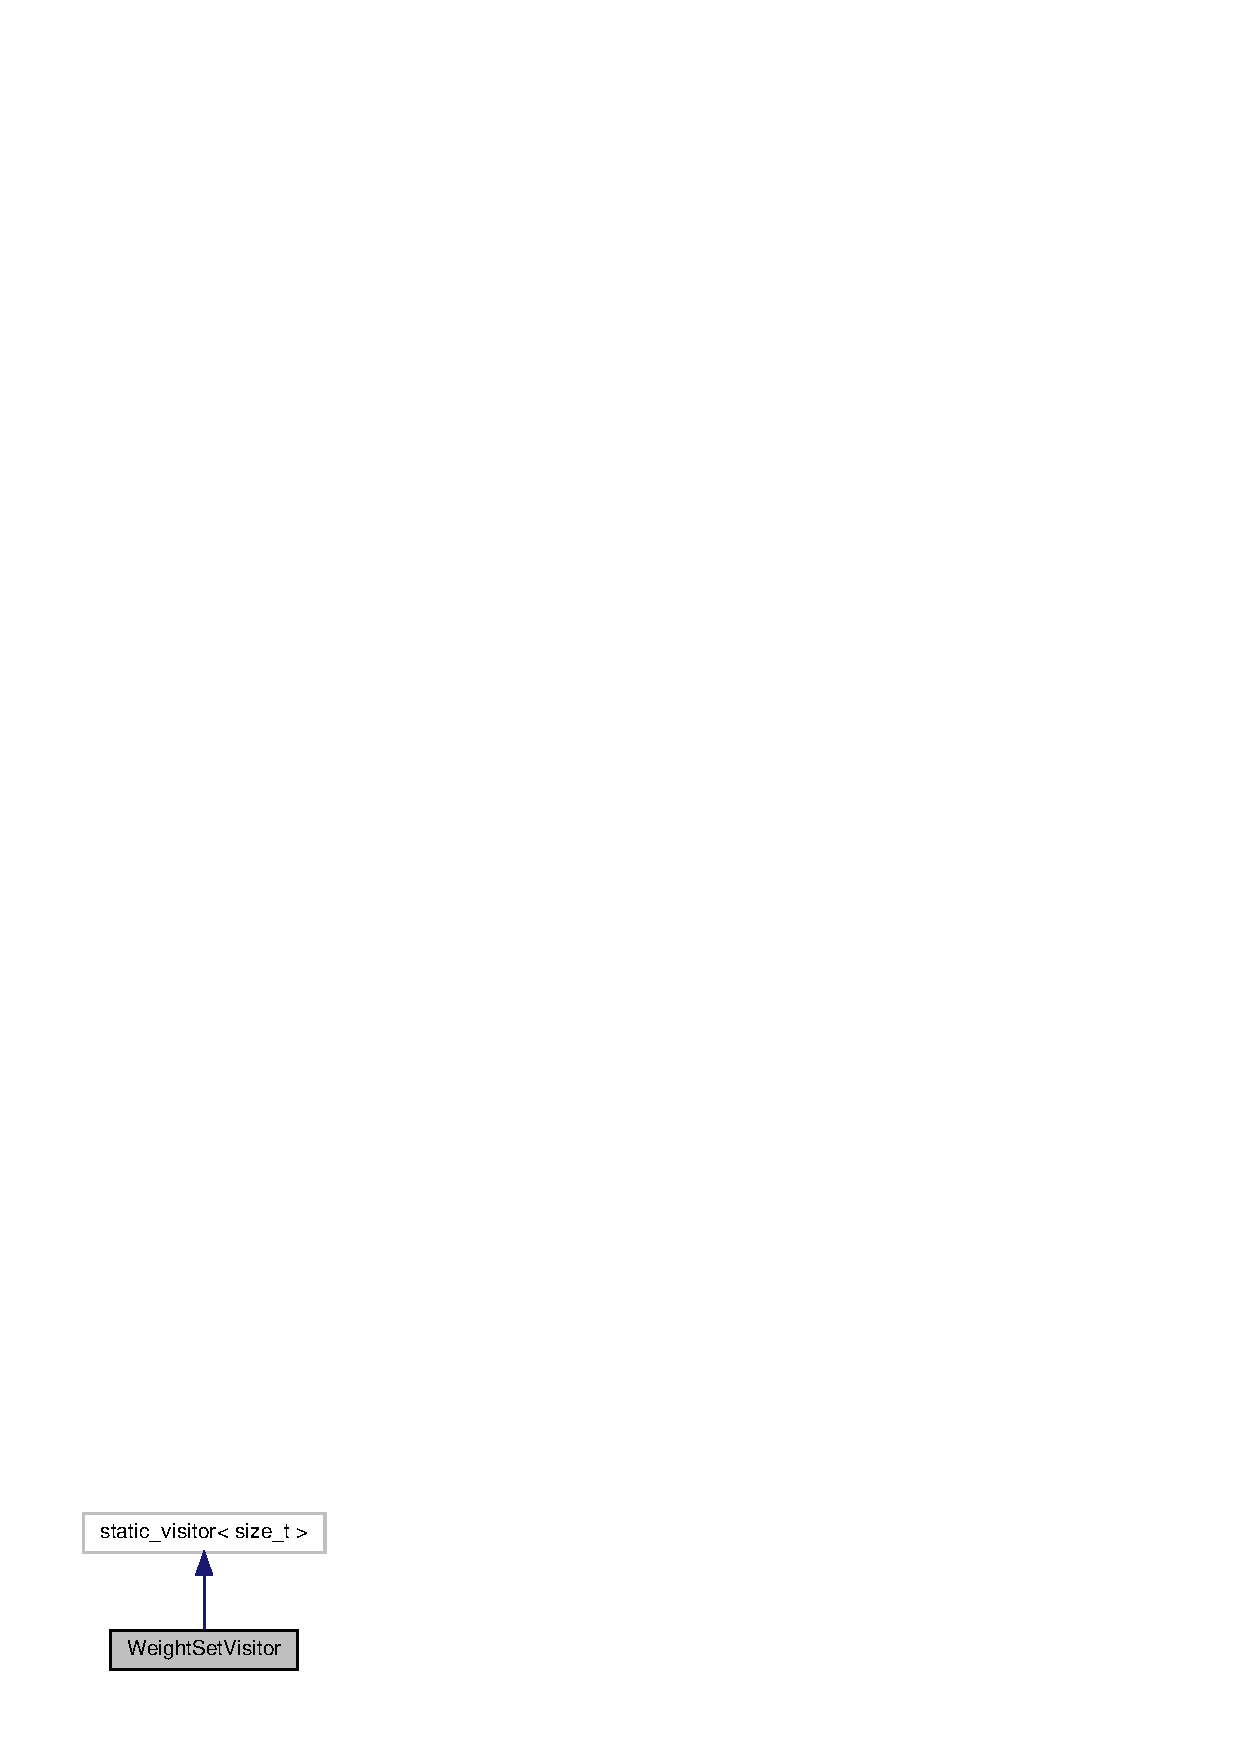
\includegraphics[width=160pt]{classmlpack_1_1ann_1_1WeightSetVisitor__inherit__graph}
\end{center}
\end{figure}
\subsection*{Public Member Functions}
\begin{DoxyCompactItemize}
\item 
\textbf{ Weight\+Set\+Visitor} (arma\+::mat \&weight, const size\+\_\+t offset=0)
\begin{DoxyCompactList}\small\item\em Update the parameters given the parameters set and offset. \end{DoxyCompactList}\item 
{\footnotesize template$<$typename Layer\+Type $>$ }\\size\+\_\+t \textbf{ operator()} (Layer\+Type $\ast$layer) const
\begin{DoxyCompactList}\small\item\em Update the parameters set. \end{DoxyCompactList}\item 
size\+\_\+t \textbf{ operator()} (\textbf{ More\+Types} layer) const
\end{DoxyCompactItemize}


\subsection{Detailed Description}
\doxyref{Weight\+Set\+Visitor}{p.}{classmlpack_1_1ann_1_1WeightSetVisitor} update the module parameters given the parameters set. 

Definition at line 26 of file weight\+\_\+set\+\_\+visitor.\+hpp.



\subsection{Constructor \& Destructor Documentation}
\mbox{\label{classmlpack_1_1ann_1_1WeightSetVisitor_ad0e17ef2539d9ca8bf3509d1a5202a3d}} 
\index{mlpack\+::ann\+::\+Weight\+Set\+Visitor@{mlpack\+::ann\+::\+Weight\+Set\+Visitor}!Weight\+Set\+Visitor@{Weight\+Set\+Visitor}}
\index{Weight\+Set\+Visitor@{Weight\+Set\+Visitor}!mlpack\+::ann\+::\+Weight\+Set\+Visitor@{mlpack\+::ann\+::\+Weight\+Set\+Visitor}}
\subsubsection{Weight\+Set\+Visitor()}
{\footnotesize\ttfamily \textbf{ Weight\+Set\+Visitor} (\begin{DoxyParamCaption}\item[{arma\+::mat \&}]{weight,  }\item[{const size\+\_\+t}]{offset = {\ttfamily 0} }\end{DoxyParamCaption})}



Update the parameters given the parameters set and offset. 



\subsection{Member Function Documentation}
\mbox{\label{classmlpack_1_1ann_1_1WeightSetVisitor_aeb8947a28d511a7a4ce42a1fc63f79ee}} 
\index{mlpack\+::ann\+::\+Weight\+Set\+Visitor@{mlpack\+::ann\+::\+Weight\+Set\+Visitor}!operator()@{operator()}}
\index{operator()@{operator()}!mlpack\+::ann\+::\+Weight\+Set\+Visitor@{mlpack\+::ann\+::\+Weight\+Set\+Visitor}}
\subsubsection{operator()()\hspace{0.1cm}{\footnotesize\ttfamily [1/2]}}
{\footnotesize\ttfamily size\+\_\+t operator() (\begin{DoxyParamCaption}\item[{Layer\+Type $\ast$}]{layer }\end{DoxyParamCaption}) const}



Update the parameters set. 

\mbox{\label{classmlpack_1_1ann_1_1WeightSetVisitor_a19a2b78859e4e91b86170544dbd8ae09}} 
\index{mlpack\+::ann\+::\+Weight\+Set\+Visitor@{mlpack\+::ann\+::\+Weight\+Set\+Visitor}!operator()@{operator()}}
\index{operator()@{operator()}!mlpack\+::ann\+::\+Weight\+Set\+Visitor@{mlpack\+::ann\+::\+Weight\+Set\+Visitor}}
\subsubsection{operator()()\hspace{0.1cm}{\footnotesize\ttfamily [2/2]}}
{\footnotesize\ttfamily size\+\_\+t operator() (\begin{DoxyParamCaption}\item[{\textbf{ More\+Types}}]{layer }\end{DoxyParamCaption}) const}



The documentation for this class was generated from the following file\+:\begin{DoxyCompactItemize}
\item 
/home/aakash/mlpack/src/mlpack/methods/ann/visitor/\textbf{ weight\+\_\+set\+\_\+visitor.\+hpp}\end{DoxyCompactItemize}

\section{Weight\+Size\+Visitor Class Reference}
\label{classmlpack_1_1ann_1_1WeightSizeVisitor}\index{Weight\+Size\+Visitor@{Weight\+Size\+Visitor}}


\doxyref{Weight\+Size\+Visitor}{p.}{classmlpack_1_1ann_1_1WeightSizeVisitor} returns the number of weights of the given module.  




Inheritance diagram for Weight\+Size\+Visitor\+:
\nopagebreak
\begin{figure}[H]
\begin{center}
\leavevmode
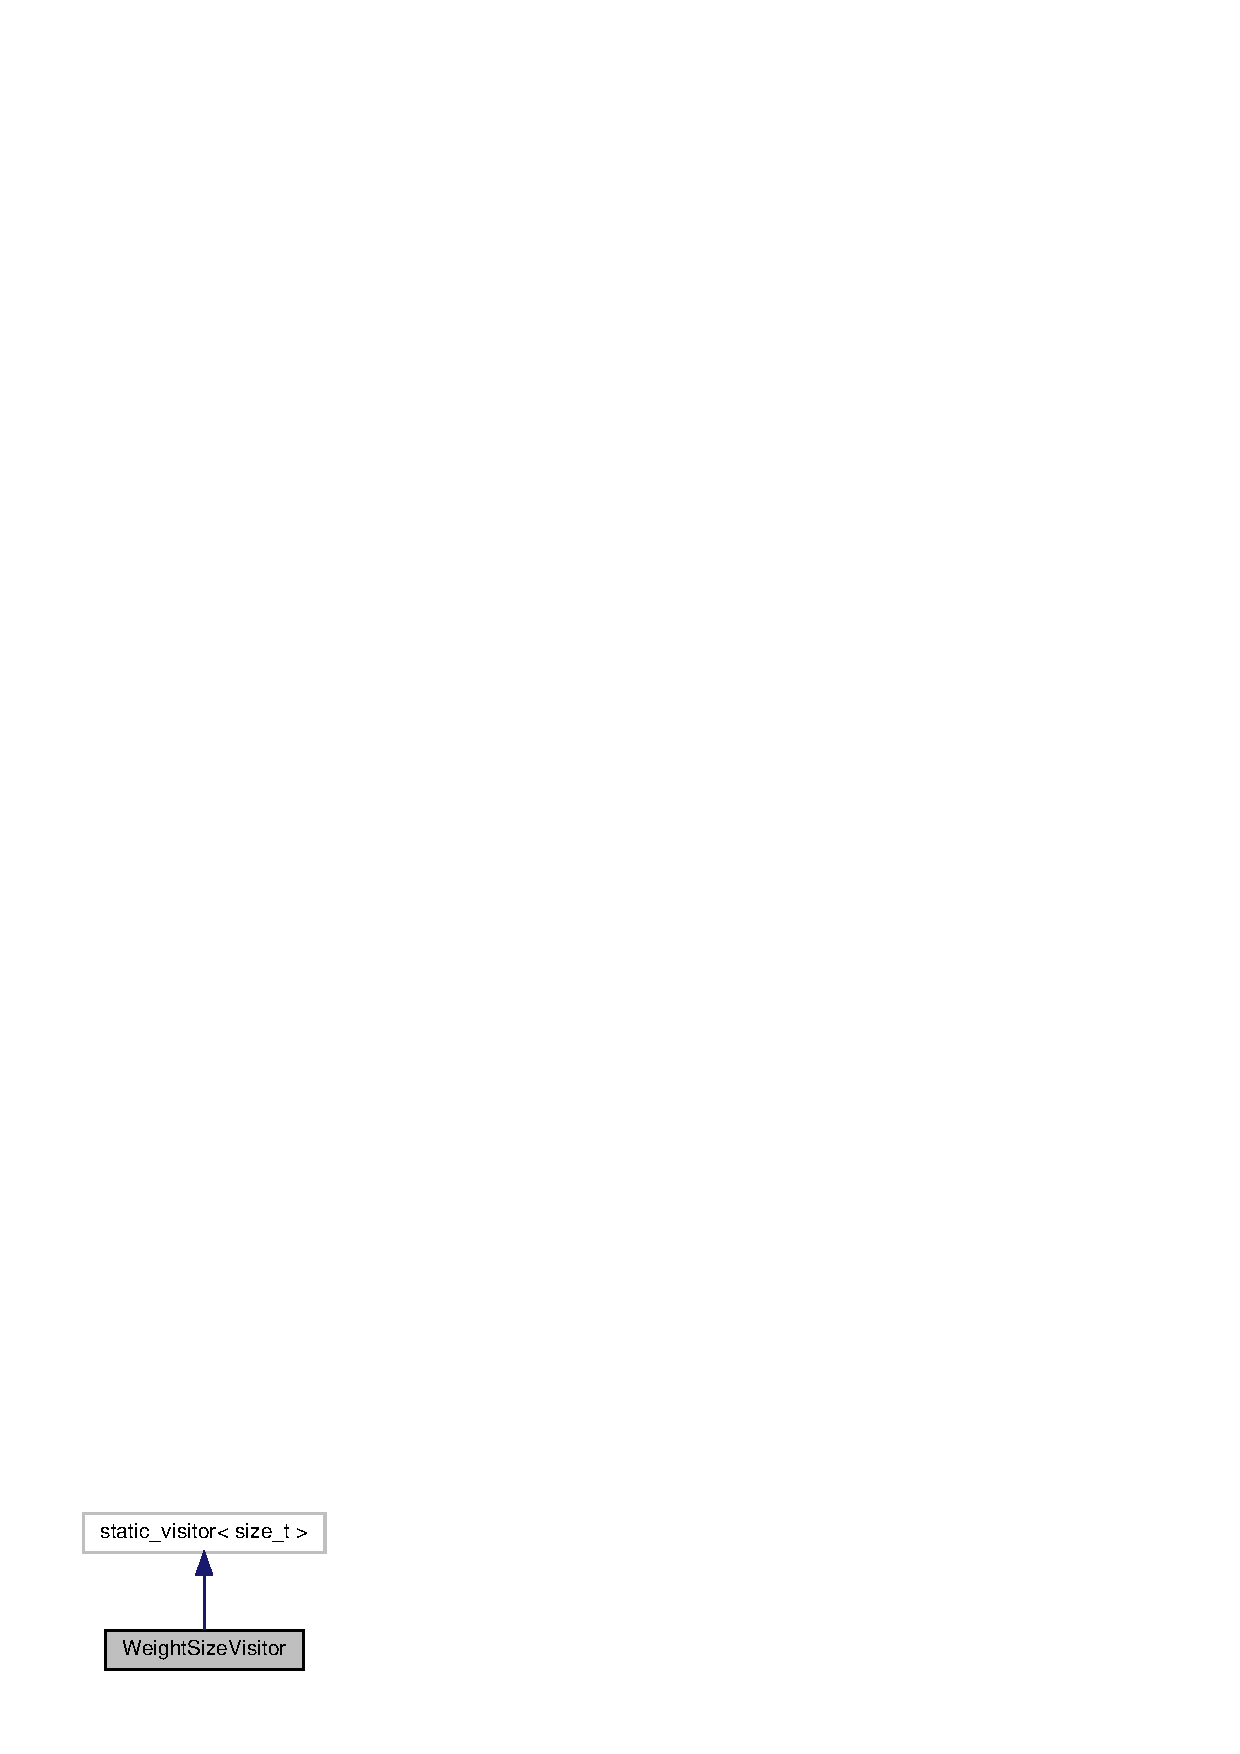
\includegraphics[width=160pt]{classmlpack_1_1ann_1_1WeightSizeVisitor__inherit__graph}
\end{center}
\end{figure}
\subsection*{Public Member Functions}
\begin{DoxyCompactItemize}
\item 
{\footnotesize template$<$typename Layer\+Type $>$ }\\size\+\_\+t \textbf{ operator()} (Layer\+Type $\ast$layer) const
\begin{DoxyCompactList}\small\item\em Return the number of weights. \end{DoxyCompactList}\item 
size\+\_\+t \textbf{ operator()} (\textbf{ More\+Types} layer) const
\end{DoxyCompactItemize}


\subsection{Detailed Description}
\doxyref{Weight\+Size\+Visitor}{p.}{classmlpack_1_1ann_1_1WeightSizeVisitor} returns the number of weights of the given module. 

Definition at line 27 of file weight\+\_\+size\+\_\+visitor.\+hpp.



\subsection{Member Function Documentation}
\mbox{\label{classmlpack_1_1ann_1_1WeightSizeVisitor_aeb8947a28d511a7a4ce42a1fc63f79ee}} 
\index{mlpack\+::ann\+::\+Weight\+Size\+Visitor@{mlpack\+::ann\+::\+Weight\+Size\+Visitor}!operator()@{operator()}}
\index{operator()@{operator()}!mlpack\+::ann\+::\+Weight\+Size\+Visitor@{mlpack\+::ann\+::\+Weight\+Size\+Visitor}}
\subsubsection{operator()()\hspace{0.1cm}{\footnotesize\ttfamily [1/2]}}
{\footnotesize\ttfamily size\+\_\+t operator() (\begin{DoxyParamCaption}\item[{Layer\+Type $\ast$}]{layer }\end{DoxyParamCaption}) const}



Return the number of weights. 

\mbox{\label{classmlpack_1_1ann_1_1WeightSizeVisitor_a19a2b78859e4e91b86170544dbd8ae09}} 
\index{mlpack\+::ann\+::\+Weight\+Size\+Visitor@{mlpack\+::ann\+::\+Weight\+Size\+Visitor}!operator()@{operator()}}
\index{operator()@{operator()}!mlpack\+::ann\+::\+Weight\+Size\+Visitor@{mlpack\+::ann\+::\+Weight\+Size\+Visitor}}
\subsubsection{operator()()\hspace{0.1cm}{\footnotesize\ttfamily [2/2]}}
{\footnotesize\ttfamily size\+\_\+t operator() (\begin{DoxyParamCaption}\item[{\textbf{ More\+Types}}]{layer }\end{DoxyParamCaption}) const}



The documentation for this class was generated from the following file\+:\begin{DoxyCompactItemize}
\item 
/home/aakash/mlpack/src/mlpack/methods/ann/visitor/\textbf{ weight\+\_\+size\+\_\+visitor.\+hpp}\end{DoxyCompactItemize}

\section{W\+G\+AN Class Reference}
\label{classmlpack_1_1ann_1_1WGAN}\index{W\+G\+AN@{W\+G\+AN}}


For more information, see the following paper\+:  




\subsection{Detailed Description}
For more information, see the following paper\+: 


\begin{DoxyCode}
@article\{Arjovsky17,
  author    = \{Martin Arjovsky, Soumith Chintala and Léon Bottou\},
  title     = \{Wasserstein GAN\},
  year      = \{2017\},
  url       = \{https:\textcolor{comment}{//arxiv.org/abs/1701.07875\},}
  eprint    = \{1701.07875\},
\}
\end{DoxyCode}
 

Definition at line 63 of file gan\+\_\+policies.\+hpp.



The documentation for this class was generated from the following file\+:\begin{DoxyCompactItemize}
\item 
/home/aakash/mlpack/src/mlpack/methods/ann/gan/\textbf{ gan\+\_\+policies.\+hpp}\end{DoxyCompactItemize}

\section{W\+G\+A\+N\+GP Class Reference}
\label{classmlpack_1_1ann_1_1WGANGP}\index{W\+G\+A\+N\+GP@{W\+G\+A\+N\+GP}}


For more information, see the following paper\+:  




\subsection{Detailed Description}
For more information, see the following paper\+: 


\begin{DoxyCode}
@article\{Gulrajani17,
  author    = \{Ishaan Gulrajani, Faruk Ahmed, Martin Arjovsky, Vincent
               Dumoulin and Aaron Courville\},
  title     = \{Improved Training of Wasserstein GANs\},
  year      = \{2017\},
  url       = \{https:\textcolor{comment}{//arxiv.org/abs/1704.00028\},}
  eprint    = \{1704.00028\},
\}
\end{DoxyCode}
 

Definition at line 79 of file gan\+\_\+policies.\+hpp.



The documentation for this class was generated from the following file\+:\begin{DoxyCompactItemize}
\item 
/home/aakash/mlpack/src/mlpack/methods/ann/gan/\textbf{ gan\+\_\+policies.\+hpp}\end{DoxyCompactItemize}

\section{Backtrace Class Reference}
\label{classmlpack_1_1Backtrace}\index{Backtrace@{Backtrace}}


Provides a backtrace.  


\subsection*{Public Member Functions}
\begin{DoxyCompactItemize}
\item 
\textbf{ Backtrace} ()
\begin{DoxyCompactList}\small\item\em Constructor initialize fields and call Get\+Address to retrieve addresses for each frame of backtrace. \end{DoxyCompactList}\item 
std\+::string \textbf{ To\+String} ()
\begin{DoxyCompactList}\small\item\em Returns string of backtrace. \end{DoxyCompactList}\end{DoxyCompactItemize}


\subsection{Detailed Description}
Provides a backtrace. 

The \doxyref{Backtrace}{p.}{classmlpack_1_1Backtrace} class retrieve addresses of each called function from the stack and decode file name, function \& line number. Retrieved information can be printed in form\+:


\begin{DoxyCode}
[b]: (count) /directory/to/file.cpp:\textcolor{keyword}{function}(args):line\_number
\end{DoxyCode}


\doxyref{Backtrace}{p.}{classmlpack_1_1Backtrace} is printed always when Log\+::\+Assert failed. An example is given below.


\begin{DoxyCode}
\textcolor{keywordflow}{if} (!someImportantCondition())
\{
  Log::Fatal << \textcolor{stringliteral}{"someImportantCondition() is not satisfied! Terminating."};
  Log::Fatal << std::endl;
\}
\end{DoxyCode}


\begin{DoxyNote}{Note}
Log\+::\+Assert will not be shown when compiling in non-\/debug mode.
\end{DoxyNote}
\begin{DoxySeeAlso}{See also}
Prefixed\+Out\+Stream, Log 
\end{DoxySeeAlso}


Definition at line 46 of file backtrace.\+hpp.



\subsection{Constructor \& Destructor Documentation}
\mbox{\label{classmlpack_1_1Backtrace_a56f5712848b4d5b5d2ad8f940750faa8}} 
\index{mlpack\+::\+Backtrace@{mlpack\+::\+Backtrace}!Backtrace@{Backtrace}}
\index{Backtrace@{Backtrace}!mlpack\+::\+Backtrace@{mlpack\+::\+Backtrace}}
\subsubsection{Backtrace()}
{\footnotesize\ttfamily \textbf{ Backtrace} (\begin{DoxyParamCaption}{ }\end{DoxyParamCaption})}



Constructor initialize fields and call Get\+Address to retrieve addresses for each frame of backtrace. 



\subsection{Member Function Documentation}
\mbox{\label{classmlpack_1_1Backtrace_a7ef596a0c429a1a74709cf14d8fa15d2}} 
\index{mlpack\+::\+Backtrace@{mlpack\+::\+Backtrace}!To\+String@{To\+String}}
\index{To\+String@{To\+String}!mlpack\+::\+Backtrace@{mlpack\+::\+Backtrace}}
\subsubsection{To\+String()}
{\footnotesize\ttfamily std\+::string To\+String (\begin{DoxyParamCaption}{ }\end{DoxyParamCaption})}



Returns string of backtrace. 



The documentation for this class was generated from the following file\+:\begin{DoxyCompactItemize}
\item 
/home/aakash/mlpack/src/mlpack/core/util/\textbf{ backtrace.\+hpp}\end{DoxyCompactItemize}

\section{Ball\+Bound$<$ Metric\+Type, Vec\+Type $>$ Class Template Reference}
\label{classmlpack_1_1bound_1_1BallBound}\index{Ball\+Bound$<$ Metric\+Type, Vec\+Type $>$@{Ball\+Bound$<$ Metric\+Type, Vec\+Type $>$}}


Ball bound encloses a set of points at a specific distance (radius) from a specific point (center).  


\subsection*{Public Types}
\begin{DoxyCompactItemize}
\item 
typedef Vec\+Type\+::elem\+\_\+type \textbf{ Elem\+Type}
\begin{DoxyCompactList}\small\item\em The underlying data type. \end{DoxyCompactList}\item 
typedef Vec\+Type \textbf{ Vec}
\begin{DoxyCompactList}\small\item\em A public version of the vector type. \end{DoxyCompactList}\end{DoxyCompactItemize}
\subsection*{Public Member Functions}
\begin{DoxyCompactItemize}
\item 
\textbf{ Ball\+Bound} ()
\begin{DoxyCompactList}\small\item\em Empty Constructor. \end{DoxyCompactList}\item 
\textbf{ Ball\+Bound} (const size\+\_\+t dimension)
\begin{DoxyCompactList}\small\item\em Create the ball bound with the specified dimensionality. \end{DoxyCompactList}\item 
\textbf{ Ball\+Bound} (const \textbf{ Elem\+Type} radius, const Vec\+Type \&center)
\begin{DoxyCompactList}\small\item\em Create the ball bound with the specified radius and center. \end{DoxyCompactList}\item 
\textbf{ Ball\+Bound} (const \textbf{ Ball\+Bound} \&other)
\begin{DoxyCompactList}\small\item\em Copy constructor. To prevent memory leaks. \end{DoxyCompactList}\item 
\textbf{ Ball\+Bound} (\textbf{ Ball\+Bound} \&\&other)
\begin{DoxyCompactList}\small\item\em Move constructor\+: take possession of another bound. \end{DoxyCompactList}\item 
\textbf{ $\sim$\+Ball\+Bound} ()
\begin{DoxyCompactList}\small\item\em Destructor to release allocated memory. \end{DoxyCompactList}\item 
const Vec\+Type \& \textbf{ Center} () const
\begin{DoxyCompactList}\small\item\em Get the center point of the ball. \end{DoxyCompactList}\item 
Vec\+Type \& \textbf{ Center} ()
\begin{DoxyCompactList}\small\item\em Modify the center point of the ball. \end{DoxyCompactList}\item 
void \textbf{ Center} (Vec\+Type \&center) const
\begin{DoxyCompactList}\small\item\em Place the center of \doxyref{Ball\+Bound}{p.}{classmlpack_1_1bound_1_1BallBound} into the given vector. \end{DoxyCompactList}\item 
bool \textbf{ Contains} (const Vec\+Type \&point) const
\begin{DoxyCompactList}\small\item\em Determines if a point is within this bound. \end{DoxyCompactList}\item 
\textbf{ Elem\+Type} \textbf{ Diameter} () const
\begin{DoxyCompactList}\small\item\em Returns the diameter of the ballbound. \end{DoxyCompactList}\item 
size\+\_\+t \textbf{ Dim} () const
\begin{DoxyCompactList}\small\item\em Get the dimensionality of the ball. \end{DoxyCompactList}\item 
{\footnotesize template$<$typename Other\+Vec\+Type $>$ }\\\textbf{ Elem\+Type} \textbf{ Max\+Distance} (const Other\+Vec\+Type \&point, typename \textbf{ std\+::enable\+\_\+if\+\_\+t}$<$ \textbf{ Is\+Vector}$<$ Other\+Vec\+Type $>$\+::value $>$ $\ast$=0) const
\begin{DoxyCompactList}\small\item\em Computes maximum distance. \end{DoxyCompactList}\item 
\textbf{ Elem\+Type} \textbf{ Max\+Distance} (const \textbf{ Ball\+Bound} \&other) const
\begin{DoxyCompactList}\small\item\em Computes maximum distance. \end{DoxyCompactList}\item 
const Metric\+Type \& \textbf{ Metric} () const
\begin{DoxyCompactList}\small\item\em Returns the distance metric used in this bound. \end{DoxyCompactList}\item 
Metric\+Type \& \textbf{ Metric} ()
\begin{DoxyCompactList}\small\item\em Modify the distance metric used in this bound. \end{DoxyCompactList}\item 
{\footnotesize template$<$typename Other\+Vec\+Type $>$ }\\\textbf{ Elem\+Type} \textbf{ Min\+Distance} (const Other\+Vec\+Type \&point, typename \textbf{ std\+::enable\+\_\+if\+\_\+t}$<$ \textbf{ Is\+Vector}$<$ Other\+Vec\+Type $>$\+::value $>$ $\ast$=0) const
\begin{DoxyCompactList}\small\item\em Calculates minimum bound-\/to-\/point squared distance. \end{DoxyCompactList}\item 
\textbf{ Elem\+Type} \textbf{ Min\+Distance} (const \textbf{ Ball\+Bound} \&other) const
\begin{DoxyCompactList}\small\item\em Calculates minimum bound-\/to-\/bound squared distance. \end{DoxyCompactList}\item 
\textbf{ Elem\+Type} \textbf{ Min\+Width} () const
\begin{DoxyCompactList}\small\item\em Get the minimum width of the bound (this is same as the diameter). \end{DoxyCompactList}\item 
\textbf{ Ball\+Bound} \& \textbf{ operator=} (const \textbf{ Ball\+Bound} \&other)
\begin{DoxyCompactList}\small\item\em For the same reason as the copy constructor\+: to prevent memory leaks. \end{DoxyCompactList}\item 
\textbf{ Ball\+Bound} \& \textbf{ operator=} (\textbf{ Ball\+Bound} \&\&other)
\begin{DoxyCompactList}\small\item\em Move assignment operator. \end{DoxyCompactList}\item 
math\+::\+Range\+Type$<$ \textbf{ Elem\+Type} $>$ \textbf{ operator[$\,$]} (const size\+\_\+t i) const
\begin{DoxyCompactList}\small\item\em Get the range in a certain dimension. \end{DoxyCompactList}\item 
const \textbf{ Ball\+Bound} \& \textbf{ operator$\vert$=} (const \textbf{ Ball\+Bound} \&other)
\begin{DoxyCompactList}\small\item\em Expand the bound to include the given node. \end{DoxyCompactList}\item 
{\footnotesize template$<$typename Mat\+Type $>$ }\\const \textbf{ Ball\+Bound} \& \textbf{ operator$\vert$=} (const Mat\+Type \&data)
\begin{DoxyCompactList}\small\item\em Expand the bound to include the given point. \end{DoxyCompactList}\item 
\textbf{ Elem\+Type} \textbf{ Radius} () const
\begin{DoxyCompactList}\small\item\em Get the radius of the ball. \end{DoxyCompactList}\item 
\textbf{ Elem\+Type} \& \textbf{ Radius} ()
\begin{DoxyCompactList}\small\item\em Modify the radius of the ball. \end{DoxyCompactList}\item 
{\footnotesize template$<$typename Other\+Vec\+Type $>$ }\\math\+::\+Range\+Type$<$ \textbf{ Elem\+Type} $>$ \textbf{ Range\+Distance} (const Other\+Vec\+Type \&other, typename \textbf{ std\+::enable\+\_\+if\+\_\+t}$<$ \textbf{ Is\+Vector}$<$ Other\+Vec\+Type $>$\+::value $>$ $\ast$=0) const
\begin{DoxyCompactList}\small\item\em Calculates minimum and maximum bound-\/to-\/point distance. \end{DoxyCompactList}\item 
math\+::\+Range\+Type$<$ \textbf{ Elem\+Type} $>$ \textbf{ Range\+Distance} (const \textbf{ Ball\+Bound} \&other) const
\begin{DoxyCompactList}\small\item\em Calculates minimum and maximum bound-\/to-\/bound distance. \end{DoxyCompactList}\item 
{\footnotesize template$<$typename Archive $>$ }\\void \textbf{ serialize} (Archive \&ar, const uint32\+\_\+t version)
\begin{DoxyCompactList}\small\item\em Serialize the bound. \end{DoxyCompactList}\end{DoxyCompactItemize}


\subsection{Detailed Description}
\subsubsection*{template$<$typename Metric\+Type = metric\+::\+L\+Metric$<$2, true$>$, typename Vec\+Type = arma\+::vec$>$\newline
class mlpack\+::bound\+::\+Ball\+Bound$<$ Metric\+Type, Vec\+Type $>$}

Ball bound encloses a set of points at a specific distance (radius) from a specific point (center). 

Metric\+Type is the custom metric type that defaults to the Euclidean (L2) distance.


\begin{DoxyTemplParams}{Template Parameters}
{\em Metric\+Type} & metric type used in the distance measure. \\
\hline
{\em Vec\+Type} & Type of vector (arma\+::vec or arma\+::sp\+\_\+vec or similar). \\
\hline
\end{DoxyTemplParams}


Definition at line 32 of file ballbound.\+hpp.



\subsection{Member Typedef Documentation}
\mbox{\label{classmlpack_1_1bound_1_1BallBound_ac8b1d992927eeff7a18d2eb7165bcff5}} 
\index{mlpack\+::bound\+::\+Ball\+Bound@{mlpack\+::bound\+::\+Ball\+Bound}!Elem\+Type@{Elem\+Type}}
\index{Elem\+Type@{Elem\+Type}!mlpack\+::bound\+::\+Ball\+Bound@{mlpack\+::bound\+::\+Ball\+Bound}}
\subsubsection{Elem\+Type}
{\footnotesize\ttfamily typedef Vec\+Type\+::elem\+\_\+type \textbf{ Elem\+Type}}



The underlying data type. 



Definition at line 36 of file ballbound.\+hpp.

\mbox{\label{classmlpack_1_1bound_1_1BallBound_afcd9d92578cb7caf312034b874dd303b}} 
\index{mlpack\+::bound\+::\+Ball\+Bound@{mlpack\+::bound\+::\+Ball\+Bound}!Vec@{Vec}}
\index{Vec@{Vec}!mlpack\+::bound\+::\+Ball\+Bound@{mlpack\+::bound\+::\+Ball\+Bound}}
\subsubsection{Vec}
{\footnotesize\ttfamily typedef Vec\+Type \textbf{ Vec}}



A public version of the vector type. 



Definition at line 38 of file ballbound.\+hpp.



\subsection{Constructor \& Destructor Documentation}
\mbox{\label{classmlpack_1_1bound_1_1BallBound_a6ef3402f4c1e43281f79b7b4f485cc85}} 
\index{mlpack\+::bound\+::\+Ball\+Bound@{mlpack\+::bound\+::\+Ball\+Bound}!Ball\+Bound@{Ball\+Bound}}
\index{Ball\+Bound@{Ball\+Bound}!mlpack\+::bound\+::\+Ball\+Bound@{mlpack\+::bound\+::\+Ball\+Bound}}
\subsubsection{Ball\+Bound()\hspace{0.1cm}{\footnotesize\ttfamily [1/5]}}
{\footnotesize\ttfamily \textbf{ Ball\+Bound} (\begin{DoxyParamCaption}{ }\end{DoxyParamCaption})}



Empty Constructor. 

\mbox{\label{classmlpack_1_1bound_1_1BallBound_aa8738c26376098ecacb2ed387653a736}} 
\index{mlpack\+::bound\+::\+Ball\+Bound@{mlpack\+::bound\+::\+Ball\+Bound}!Ball\+Bound@{Ball\+Bound}}
\index{Ball\+Bound@{Ball\+Bound}!mlpack\+::bound\+::\+Ball\+Bound@{mlpack\+::bound\+::\+Ball\+Bound}}
\subsubsection{Ball\+Bound()\hspace{0.1cm}{\footnotesize\ttfamily [2/5]}}
{\footnotesize\ttfamily \textbf{ Ball\+Bound} (\begin{DoxyParamCaption}\item[{const size\+\_\+t}]{dimension }\end{DoxyParamCaption})}



Create the ball bound with the specified dimensionality. 


\begin{DoxyParams}{Parameters}
{\em dimension} & Dimensionality of ball bound. \\
\hline
\end{DoxyParams}
\mbox{\label{classmlpack_1_1bound_1_1BallBound_af9a9e9cf6a4247b875b161932b28588c}} 
\index{mlpack\+::bound\+::\+Ball\+Bound@{mlpack\+::bound\+::\+Ball\+Bound}!Ball\+Bound@{Ball\+Bound}}
\index{Ball\+Bound@{Ball\+Bound}!mlpack\+::bound\+::\+Ball\+Bound@{mlpack\+::bound\+::\+Ball\+Bound}}
\subsubsection{Ball\+Bound()\hspace{0.1cm}{\footnotesize\ttfamily [3/5]}}
{\footnotesize\ttfamily \textbf{ Ball\+Bound} (\begin{DoxyParamCaption}\item[{const \textbf{ Elem\+Type}}]{radius,  }\item[{const Vec\+Type \&}]{center }\end{DoxyParamCaption})}



Create the ball bound with the specified radius and center. 


\begin{DoxyParams}{Parameters}
{\em radius} & Radius of ball bound. \\
\hline
{\em center} & Center of ball bound. \\
\hline
\end{DoxyParams}
\mbox{\label{classmlpack_1_1bound_1_1BallBound_a4a6b9f2a2e420f74ec63134c0300a031}} 
\index{mlpack\+::bound\+::\+Ball\+Bound@{mlpack\+::bound\+::\+Ball\+Bound}!Ball\+Bound@{Ball\+Bound}}
\index{Ball\+Bound@{Ball\+Bound}!mlpack\+::bound\+::\+Ball\+Bound@{mlpack\+::bound\+::\+Ball\+Bound}}
\subsubsection{Ball\+Bound()\hspace{0.1cm}{\footnotesize\ttfamily [4/5]}}
{\footnotesize\ttfamily \textbf{ Ball\+Bound} (\begin{DoxyParamCaption}\item[{const \textbf{ Ball\+Bound}$<$ Metric\+Type, Vec\+Type $>$ \&}]{other }\end{DoxyParamCaption})}



Copy constructor. To prevent memory leaks. 

\mbox{\label{classmlpack_1_1bound_1_1BallBound_a8f0115d7119bc55e54451658d7780da7}} 
\index{mlpack\+::bound\+::\+Ball\+Bound@{mlpack\+::bound\+::\+Ball\+Bound}!Ball\+Bound@{Ball\+Bound}}
\index{Ball\+Bound@{Ball\+Bound}!mlpack\+::bound\+::\+Ball\+Bound@{mlpack\+::bound\+::\+Ball\+Bound}}
\subsubsection{Ball\+Bound()\hspace{0.1cm}{\footnotesize\ttfamily [5/5]}}
{\footnotesize\ttfamily \textbf{ Ball\+Bound} (\begin{DoxyParamCaption}\item[{\textbf{ Ball\+Bound}$<$ Metric\+Type, Vec\+Type $>$ \&\&}]{other }\end{DoxyParamCaption})}



Move constructor\+: take possession of another bound. 

\mbox{\label{classmlpack_1_1bound_1_1BallBound_a186cc3e1901316bbef5575aa64ff3770}} 
\index{mlpack\+::bound\+::\+Ball\+Bound@{mlpack\+::bound\+::\+Ball\+Bound}!````~Ball\+Bound@{$\sim$\+Ball\+Bound}}
\index{````~Ball\+Bound@{$\sim$\+Ball\+Bound}!mlpack\+::bound\+::\+Ball\+Bound@{mlpack\+::bound\+::\+Ball\+Bound}}
\subsubsection{$\sim$\+Ball\+Bound()}
{\footnotesize\ttfamily $\sim$\textbf{ Ball\+Bound} (\begin{DoxyParamCaption}{ }\end{DoxyParamCaption})}



Destructor to release allocated memory. 



\subsection{Member Function Documentation}
\mbox{\label{classmlpack_1_1bound_1_1BallBound_ac7a8ddea0150e52b0bc6d369ed5a5be3}} 
\index{mlpack\+::bound\+::\+Ball\+Bound@{mlpack\+::bound\+::\+Ball\+Bound}!Center@{Center}}
\index{Center@{Center}!mlpack\+::bound\+::\+Ball\+Bound@{mlpack\+::bound\+::\+Ball\+Bound}}
\subsubsection{Center()\hspace{0.1cm}{\footnotesize\ttfamily [1/3]}}
{\footnotesize\ttfamily const Vec\+Type\& Center (\begin{DoxyParamCaption}{ }\end{DoxyParamCaption}) const\hspace{0.3cm}{\ttfamily [inline]}}



Get the center point of the ball. 



Definition at line 96 of file ballbound.\+hpp.



Referenced by Proj\+Vector\+::\+Project().

\mbox{\label{classmlpack_1_1bound_1_1BallBound_aac93f77d9e2bea78e968bc287bddec90}} 
\index{mlpack\+::bound\+::\+Ball\+Bound@{mlpack\+::bound\+::\+Ball\+Bound}!Center@{Center}}
\index{Center@{Center}!mlpack\+::bound\+::\+Ball\+Bound@{mlpack\+::bound\+::\+Ball\+Bound}}
\subsubsection{Center()\hspace{0.1cm}{\footnotesize\ttfamily [2/3]}}
{\footnotesize\ttfamily Vec\+Type\& Center (\begin{DoxyParamCaption}{ }\end{DoxyParamCaption})\hspace{0.3cm}{\ttfamily [inline]}}



Modify the center point of the ball. 



Definition at line 98 of file ballbound.\+hpp.

\mbox{\label{classmlpack_1_1bound_1_1BallBound_a7b62091b9c9066c30d27695bcf6a1688}} 
\index{mlpack\+::bound\+::\+Ball\+Bound@{mlpack\+::bound\+::\+Ball\+Bound}!Center@{Center}}
\index{Center@{Center}!mlpack\+::bound\+::\+Ball\+Bound@{mlpack\+::bound\+::\+Ball\+Bound}}
\subsubsection{Center()\hspace{0.1cm}{\footnotesize\ttfamily [3/3]}}
{\footnotesize\ttfamily void Center (\begin{DoxyParamCaption}\item[{Vec\+Type \&}]{center }\end{DoxyParamCaption}) const\hspace{0.3cm}{\ttfamily [inline]}}



Place the center of \doxyref{Ball\+Bound}{p.}{classmlpack_1_1bound_1_1BallBound} into the given vector. 


\begin{DoxyParams}{Parameters}
{\em center} & Vector which the centroid will be written to. \\
\hline
\end{DoxyParams}


Definition at line 124 of file ballbound.\+hpp.



References Ball\+Bound$<$ Metric\+Type, Vec\+Type $>$\+::\+Max\+Distance(), Ball\+Bound$<$ Metric\+Type, Vec\+Type $>$\+::\+Min\+Distance(), Ball\+Bound$<$ Metric\+Type, Vec\+Type $>$\+::operator$\vert$=(), and Ball\+Bound$<$ Metric\+Type, Vec\+Type $>$\+::\+Range\+Distance().

\mbox{\label{classmlpack_1_1bound_1_1BallBound_a8bb86454bb4ed601ca09eefd7e46b0cc}} 
\index{mlpack\+::bound\+::\+Ball\+Bound@{mlpack\+::bound\+::\+Ball\+Bound}!Contains@{Contains}}
\index{Contains@{Contains}!mlpack\+::bound\+::\+Ball\+Bound@{mlpack\+::bound\+::\+Ball\+Bound}}
\subsubsection{Contains()}
{\footnotesize\ttfamily bool Contains (\begin{DoxyParamCaption}\item[{const Vec\+Type \&}]{point }\end{DoxyParamCaption}) const}



Determines if a point is within this bound. 


\begin{DoxyParams}{Parameters}
{\em point} & Point to check the condition. \\
\hline
\end{DoxyParams}


Referenced by Ball\+Bound$<$ Metric\+Type, Vec\+Type $>$\+::\+Min\+Width().

\mbox{\label{classmlpack_1_1bound_1_1BallBound_a60e7246d34103909f688395e35869b39}} 
\index{mlpack\+::bound\+::\+Ball\+Bound@{mlpack\+::bound\+::\+Ball\+Bound}!Diameter@{Diameter}}
\index{Diameter@{Diameter}!mlpack\+::bound\+::\+Ball\+Bound@{mlpack\+::bound\+::\+Ball\+Bound}}
\subsubsection{Diameter()}
{\footnotesize\ttfamily \textbf{ Elem\+Type} Diameter (\begin{DoxyParamCaption}{ }\end{DoxyParamCaption}) const\hspace{0.3cm}{\ttfamily [inline]}}



Returns the diameter of the ballbound. 



Definition at line 200 of file ballbound.\+hpp.

\mbox{\label{classmlpack_1_1bound_1_1BallBound_a7993a4f36c530e03b78b28b5f53bb286}} 
\index{mlpack\+::bound\+::\+Ball\+Bound@{mlpack\+::bound\+::\+Ball\+Bound}!Dim@{Dim}}
\index{Dim@{Dim}!mlpack\+::bound\+::\+Ball\+Bound@{mlpack\+::bound\+::\+Ball\+Bound}}
\subsubsection{Dim()}
{\footnotesize\ttfamily size\+\_\+t Dim (\begin{DoxyParamCaption}{ }\end{DoxyParamCaption}) const\hspace{0.3cm}{\ttfamily [inline]}}



Get the dimensionality of the ball. 



Definition at line 101 of file ballbound.\+hpp.

\mbox{\label{classmlpack_1_1bound_1_1BallBound_abc4e8dd21a938c6e9f90586d42068f33}} 
\index{mlpack\+::bound\+::\+Ball\+Bound@{mlpack\+::bound\+::\+Ball\+Bound}!Max\+Distance@{Max\+Distance}}
\index{Max\+Distance@{Max\+Distance}!mlpack\+::bound\+::\+Ball\+Bound@{mlpack\+::bound\+::\+Ball\+Bound}}
\subsubsection{Max\+Distance()\hspace{0.1cm}{\footnotesize\ttfamily [1/2]}}
{\footnotesize\ttfamily \textbf{ Elem\+Type} Max\+Distance (\begin{DoxyParamCaption}\item[{const Other\+Vec\+Type \&}]{point,  }\item[{typename \textbf{ std\+::enable\+\_\+if\+\_\+t}$<$ \textbf{ Is\+Vector}$<$ Other\+Vec\+Type $>$\+::value $>$ $\ast$}]{ = {\ttfamily 0} }\end{DoxyParamCaption}) const}



Computes maximum distance. 


\begin{DoxyParams}{Parameters}
{\em point} & Point to which the maximum distance is requested. \\
\hline
\end{DoxyParams}


Referenced by Ball\+Bound$<$ Metric\+Type, Vec\+Type $>$\+::\+Center().

\mbox{\label{classmlpack_1_1bound_1_1BallBound_ad754afc8e0d1f9e5a0a4812bd301e0fa}} 
\index{mlpack\+::bound\+::\+Ball\+Bound@{mlpack\+::bound\+::\+Ball\+Bound}!Max\+Distance@{Max\+Distance}}
\index{Max\+Distance@{Max\+Distance}!mlpack\+::bound\+::\+Ball\+Bound@{mlpack\+::bound\+::\+Ball\+Bound}}
\subsubsection{Max\+Distance()\hspace{0.1cm}{\footnotesize\ttfamily [2/2]}}
{\footnotesize\ttfamily \textbf{ Elem\+Type} Max\+Distance (\begin{DoxyParamCaption}\item[{const \textbf{ Ball\+Bound}$<$ Metric\+Type, Vec\+Type $>$ \&}]{other }\end{DoxyParamCaption}) const}



Computes maximum distance. 


\begin{DoxyParams}{Parameters}
{\em other} & Bound to which the maximum distance is requested. \\
\hline
\end{DoxyParams}
\mbox{\label{classmlpack_1_1bound_1_1BallBound_aac4d643c62af7d9cc2a072aea10d2b32}} 
\index{mlpack\+::bound\+::\+Ball\+Bound@{mlpack\+::bound\+::\+Ball\+Bound}!Metric@{Metric}}
\index{Metric@{Metric}!mlpack\+::bound\+::\+Ball\+Bound@{mlpack\+::bound\+::\+Ball\+Bound}}
\subsubsection{Metric()\hspace{0.1cm}{\footnotesize\ttfamily [1/2]}}
{\footnotesize\ttfamily const Metric\+Type\& Metric (\begin{DoxyParamCaption}{ }\end{DoxyParamCaption}) const\hspace{0.3cm}{\ttfamily [inline]}}



Returns the distance metric used in this bound. 



Definition at line 203 of file ballbound.\+hpp.

\mbox{\label{classmlpack_1_1bound_1_1BallBound_acc71d930ed90e73b2bc0c360835c5371}} 
\index{mlpack\+::bound\+::\+Ball\+Bound@{mlpack\+::bound\+::\+Ball\+Bound}!Metric@{Metric}}
\index{Metric@{Metric}!mlpack\+::bound\+::\+Ball\+Bound@{mlpack\+::bound\+::\+Ball\+Bound}}
\subsubsection{Metric()\hspace{0.1cm}{\footnotesize\ttfamily [2/2]}}
{\footnotesize\ttfamily Metric\+Type\& Metric (\begin{DoxyParamCaption}{ }\end{DoxyParamCaption})\hspace{0.3cm}{\ttfamily [inline]}}



Modify the distance metric used in this bound. 



Definition at line 205 of file ballbound.\+hpp.



References Ball\+Bound$<$ Metric\+Type, Vec\+Type $>$\+::serialize().

\mbox{\label{classmlpack_1_1bound_1_1BallBound_af529c3b56434190264194fda3d7f30bd}} 
\index{mlpack\+::bound\+::\+Ball\+Bound@{mlpack\+::bound\+::\+Ball\+Bound}!Min\+Distance@{Min\+Distance}}
\index{Min\+Distance@{Min\+Distance}!mlpack\+::bound\+::\+Ball\+Bound@{mlpack\+::bound\+::\+Ball\+Bound}}
\subsubsection{Min\+Distance()\hspace{0.1cm}{\footnotesize\ttfamily [1/2]}}
{\footnotesize\ttfamily \textbf{ Elem\+Type} Min\+Distance (\begin{DoxyParamCaption}\item[{const Other\+Vec\+Type \&}]{point,  }\item[{typename \textbf{ std\+::enable\+\_\+if\+\_\+t}$<$ \textbf{ Is\+Vector}$<$ Other\+Vec\+Type $>$\+::value $>$ $\ast$}]{ = {\ttfamily 0} }\end{DoxyParamCaption}) const}



Calculates minimum bound-\/to-\/point squared distance. 


\begin{DoxyParams}{Parameters}
{\em point} & Point to which the minimum distance is requested. \\
\hline
\end{DoxyParams}


Referenced by Ball\+Bound$<$ Metric\+Type, Vec\+Type $>$\+::\+Center().

\mbox{\label{classmlpack_1_1bound_1_1BallBound_a1532258f4abf77694500a314b7f127d4}} 
\index{mlpack\+::bound\+::\+Ball\+Bound@{mlpack\+::bound\+::\+Ball\+Bound}!Min\+Distance@{Min\+Distance}}
\index{Min\+Distance@{Min\+Distance}!mlpack\+::bound\+::\+Ball\+Bound@{mlpack\+::bound\+::\+Ball\+Bound}}
\subsubsection{Min\+Distance()\hspace{0.1cm}{\footnotesize\ttfamily [2/2]}}
{\footnotesize\ttfamily \textbf{ Elem\+Type} Min\+Distance (\begin{DoxyParamCaption}\item[{const \textbf{ Ball\+Bound}$<$ Metric\+Type, Vec\+Type $>$ \&}]{other }\end{DoxyParamCaption}) const}



Calculates minimum bound-\/to-\/bound squared distance. 


\begin{DoxyParams}{Parameters}
{\em other} & Bound to which the minimum distance is requested. \\
\hline
\end{DoxyParams}
\mbox{\label{classmlpack_1_1bound_1_1BallBound_ab8478ff52c4d4d5e7fa6311fa39abb76}} 
\index{mlpack\+::bound\+::\+Ball\+Bound@{mlpack\+::bound\+::\+Ball\+Bound}!Min\+Width@{Min\+Width}}
\index{Min\+Width@{Min\+Width}!mlpack\+::bound\+::\+Ball\+Bound@{mlpack\+::bound\+::\+Ball\+Bound}}
\subsubsection{Min\+Width()}
{\footnotesize\ttfamily \textbf{ Elem\+Type} Min\+Width (\begin{DoxyParamCaption}{ }\end{DoxyParamCaption}) const\hspace{0.3cm}{\ttfamily [inline]}}



Get the minimum width of the bound (this is same as the diameter). 

For ball bounds, width along all dimensions remain same. 

Definition at line 107 of file ballbound.\+hpp.



References Ball\+Bound$<$ Metric\+Type, Vec\+Type $>$\+::\+Contains(), and Ball\+Bound$<$ Metric\+Type, Vec\+Type $>$\+::operator[$\,$]().

\mbox{\label{classmlpack_1_1bound_1_1BallBound_a4909ad7e2739e309a7fbdec0892a4ab9}} 
\index{mlpack\+::bound\+::\+Ball\+Bound@{mlpack\+::bound\+::\+Ball\+Bound}!operator=@{operator=}}
\index{operator=@{operator=}!mlpack\+::bound\+::\+Ball\+Bound@{mlpack\+::bound\+::\+Ball\+Bound}}
\subsubsection{operator=()\hspace{0.1cm}{\footnotesize\ttfamily [1/2]}}
{\footnotesize\ttfamily \textbf{ Ball\+Bound}\& operator= (\begin{DoxyParamCaption}\item[{const \textbf{ Ball\+Bound}$<$ Metric\+Type, Vec\+Type $>$ \&}]{other }\end{DoxyParamCaption})}



For the same reason as the copy constructor\+: to prevent memory leaks. 

\mbox{\label{classmlpack_1_1bound_1_1BallBound_a8d6743fef04117a290cae734833dd812}} 
\index{mlpack\+::bound\+::\+Ball\+Bound@{mlpack\+::bound\+::\+Ball\+Bound}!operator=@{operator=}}
\index{operator=@{operator=}!mlpack\+::bound\+::\+Ball\+Bound@{mlpack\+::bound\+::\+Ball\+Bound}}
\subsubsection{operator=()\hspace{0.1cm}{\footnotesize\ttfamily [2/2]}}
{\footnotesize\ttfamily \textbf{ Ball\+Bound}\& operator= (\begin{DoxyParamCaption}\item[{\textbf{ Ball\+Bound}$<$ Metric\+Type, Vec\+Type $>$ \&\&}]{other }\end{DoxyParamCaption})}



Move assignment operator. 

\mbox{\label{classmlpack_1_1bound_1_1BallBound_aa79d855354bde98b4e84e3d49c4d02fa}} 
\index{mlpack\+::bound\+::\+Ball\+Bound@{mlpack\+::bound\+::\+Ball\+Bound}!operator[]@{operator[]}}
\index{operator[]@{operator[]}!mlpack\+::bound\+::\+Ball\+Bound@{mlpack\+::bound\+::\+Ball\+Bound}}
\subsubsection{operator[]()}
{\footnotesize\ttfamily math\+::\+Range\+Type$<$\textbf{ Elem\+Type}$>$ operator[$\,$] (\begin{DoxyParamCaption}\item[{const size\+\_\+t}]{i }\end{DoxyParamCaption}) const}



Get the range in a certain dimension. 



Referenced by Ball\+Bound$<$ Metric\+Type, Vec\+Type $>$\+::\+Min\+Width().

\mbox{\label{classmlpack_1_1bound_1_1BallBound_a5f8d8da836f83d7434b87c689bc28890}} 
\index{mlpack\+::bound\+::\+Ball\+Bound@{mlpack\+::bound\+::\+Ball\+Bound}!operator\texttt{"|}=@{operator\texttt{"|}=}}
\index{operator\texttt{"|}=@{operator\texttt{"|}=}!mlpack\+::bound\+::\+Ball\+Bound@{mlpack\+::bound\+::\+Ball\+Bound}}
\subsubsection{operator\texttt{"|}=()\hspace{0.1cm}{\footnotesize\ttfamily [1/2]}}
{\footnotesize\ttfamily const \textbf{ Ball\+Bound}\& operator$\vert$= (\begin{DoxyParamCaption}\item[{const \textbf{ Ball\+Bound}$<$ Metric\+Type, Vec\+Type $>$ \&}]{other }\end{DoxyParamCaption})}



Expand the bound to include the given node. 



Referenced by Ball\+Bound$<$ Metric\+Type, Vec\+Type $>$\+::\+Center().

\mbox{\label{classmlpack_1_1bound_1_1BallBound_ada31a74c98ffb5d13b14c156ac200383}} 
\index{mlpack\+::bound\+::\+Ball\+Bound@{mlpack\+::bound\+::\+Ball\+Bound}!operator\texttt{"|}=@{operator\texttt{"|}=}}
\index{operator\texttt{"|}=@{operator\texttt{"|}=}!mlpack\+::bound\+::\+Ball\+Bound@{mlpack\+::bound\+::\+Ball\+Bound}}
\subsubsection{operator\texttt{"|}=()\hspace{0.1cm}{\footnotesize\ttfamily [2/2]}}
{\footnotesize\ttfamily const \textbf{ Ball\+Bound}\& operator$\vert$= (\begin{DoxyParamCaption}\item[{const Mat\+Type \&}]{data }\end{DoxyParamCaption})}



Expand the bound to include the given point. 

The centroid is recalculated to be the center of all of the given points.


\begin{DoxyTemplParams}{Template Parameters}
{\em Mat\+Type} & Type of matrix; could be arma\+::mat, arma\+::spmat, or a vector. \\
\hline
{\em data} & Data points to add. \\
\hline
\end{DoxyTemplParams}
\mbox{\label{classmlpack_1_1bound_1_1BallBound_a01502ca0f18e366f6758b0cc8756dedf}} 
\index{mlpack\+::bound\+::\+Ball\+Bound@{mlpack\+::bound\+::\+Ball\+Bound}!Radius@{Radius}}
\index{Radius@{Radius}!mlpack\+::bound\+::\+Ball\+Bound@{mlpack\+::bound\+::\+Ball\+Bound}}
\subsubsection{Radius()\hspace{0.1cm}{\footnotesize\ttfamily [1/2]}}
{\footnotesize\ttfamily \textbf{ Elem\+Type} Radius (\begin{DoxyParamCaption}{ }\end{DoxyParamCaption}) const\hspace{0.3cm}{\ttfamily [inline]}}



Get the radius of the ball. 



Definition at line 91 of file ballbound.\+hpp.



Referenced by Proj\+Vector\+::\+Project().

\mbox{\label{classmlpack_1_1bound_1_1BallBound_ad2f286cc3e4260a624e5d890d0d2a377}} 
\index{mlpack\+::bound\+::\+Ball\+Bound@{mlpack\+::bound\+::\+Ball\+Bound}!Radius@{Radius}}
\index{Radius@{Radius}!mlpack\+::bound\+::\+Ball\+Bound@{mlpack\+::bound\+::\+Ball\+Bound}}
\subsubsection{Radius()\hspace{0.1cm}{\footnotesize\ttfamily [2/2]}}
{\footnotesize\ttfamily \textbf{ Elem\+Type}\& Radius (\begin{DoxyParamCaption}{ }\end{DoxyParamCaption})\hspace{0.3cm}{\ttfamily [inline]}}



Modify the radius of the ball. 



Definition at line 93 of file ballbound.\+hpp.

\mbox{\label{classmlpack_1_1bound_1_1BallBound_ae224b832c3cfe544e4c06361a5e44c3a}} 
\index{mlpack\+::bound\+::\+Ball\+Bound@{mlpack\+::bound\+::\+Ball\+Bound}!Range\+Distance@{Range\+Distance}}
\index{Range\+Distance@{Range\+Distance}!mlpack\+::bound\+::\+Ball\+Bound@{mlpack\+::bound\+::\+Ball\+Bound}}
\subsubsection{Range\+Distance()\hspace{0.1cm}{\footnotesize\ttfamily [1/2]}}
{\footnotesize\ttfamily math\+::\+Range\+Type$<$\textbf{ Elem\+Type}$>$ Range\+Distance (\begin{DoxyParamCaption}\item[{const Other\+Vec\+Type \&}]{other,  }\item[{typename \textbf{ std\+::enable\+\_\+if\+\_\+t}$<$ \textbf{ Is\+Vector}$<$ Other\+Vec\+Type $>$\+::value $>$ $\ast$}]{ = {\ttfamily 0} }\end{DoxyParamCaption}) const}



Calculates minimum and maximum bound-\/to-\/point distance. 


\begin{DoxyParams}{Parameters}
{\em other} & Point to which the minimum and maximum distances are requested. \\
\hline
\end{DoxyParams}


Referenced by Ball\+Bound$<$ Metric\+Type, Vec\+Type $>$\+::\+Center().

\mbox{\label{classmlpack_1_1bound_1_1BallBound_a27d48f29287942881ddc462cd508d86c}} 
\index{mlpack\+::bound\+::\+Ball\+Bound@{mlpack\+::bound\+::\+Ball\+Bound}!Range\+Distance@{Range\+Distance}}
\index{Range\+Distance@{Range\+Distance}!mlpack\+::bound\+::\+Ball\+Bound@{mlpack\+::bound\+::\+Ball\+Bound}}
\subsubsection{Range\+Distance()\hspace{0.1cm}{\footnotesize\ttfamily [2/2]}}
{\footnotesize\ttfamily math\+::\+Range\+Type$<$\textbf{ Elem\+Type}$>$ Range\+Distance (\begin{DoxyParamCaption}\item[{const \textbf{ Ball\+Bound}$<$ Metric\+Type, Vec\+Type $>$ \&}]{other }\end{DoxyParamCaption}) const}



Calculates minimum and maximum bound-\/to-\/bound distance. 

Example\+: bound1.\+Min\+Distance\+Sq(other) for minimum distance.


\begin{DoxyParams}{Parameters}
{\em other} & Bound to which the minimum and maximum distances are requested. \\
\hline
\end{DoxyParams}
\mbox{\label{classmlpack_1_1bound_1_1BallBound_a72d63b74c8166dff8e1a9006905ad9ca}} 
\index{mlpack\+::bound\+::\+Ball\+Bound@{mlpack\+::bound\+::\+Ball\+Bound}!serialize@{serialize}}
\index{serialize@{serialize}!mlpack\+::bound\+::\+Ball\+Bound@{mlpack\+::bound\+::\+Ball\+Bound}}
\subsubsection{serialize()}
{\footnotesize\ttfamily void serialize (\begin{DoxyParamCaption}\item[{Archive \&}]{ar,  }\item[{const uint32\+\_\+t}]{version }\end{DoxyParamCaption})}



Serialize the bound. 



Referenced by Ball\+Bound$<$ Metric\+Type, Vec\+Type $>$\+::\+Metric().



The documentation for this class was generated from the following file\+:\begin{DoxyCompactItemize}
\item 
/home/aakash/mlpack/src/mlpack/core/tree/\textbf{ ballbound.\+hpp}\end{DoxyCompactItemize}

\section{Bound\+Traits$<$ Bound\+Type $>$ Struct Template Reference}
\label{structmlpack_1_1bound_1_1BoundTraits}\index{Bound\+Traits$<$ Bound\+Type $>$@{Bound\+Traits$<$ Bound\+Type $>$}}


A class to obtain compile-\/time traits about Bound\+Type classes.  


\subsection*{Static Public Attributes}
\begin{DoxyCompactItemize}
\item 
static const bool \textbf{ Has\+Tight\+Bounds} = false
\begin{DoxyCompactList}\small\item\em If true, then the bounds for each dimension are tight. \end{DoxyCompactList}\end{DoxyCompactItemize}


\subsection{Detailed Description}
\subsubsection*{template$<$typename Bound\+Type$>$\newline
struct mlpack\+::bound\+::\+Bound\+Traits$<$ Bound\+Type $>$}

A class to obtain compile-\/time traits about Bound\+Type classes. 

If you are writing your own Bound\+Type class, you should make a template specialization in order to set the values correctly.

\begin{DoxySeeAlso}{See also}
Tree\+Traits, Kernel\+Traits 
\end{DoxySeeAlso}


Definition at line 26 of file bound\+\_\+traits.\+hpp.



\subsection{Member Data Documentation}
\mbox{\label{structmlpack_1_1bound_1_1BoundTraits_af41e456bf5ea6c0557730318fe660d2d}} 
\index{mlpack\+::bound\+::\+Bound\+Traits@{mlpack\+::bound\+::\+Bound\+Traits}!Has\+Tight\+Bounds@{Has\+Tight\+Bounds}}
\index{Has\+Tight\+Bounds@{Has\+Tight\+Bounds}!mlpack\+::bound\+::\+Bound\+Traits@{mlpack\+::bound\+::\+Bound\+Traits}}
\subsubsection{Has\+Tight\+Bounds}
{\footnotesize\ttfamily const bool Has\+Tight\+Bounds = false\hspace{0.3cm}{\ttfamily [static]}}



If true, then the bounds for each dimension are tight. 

If false, then the bounds for each dimension may be looser than the range of all points held in the bound. This defaults to false. 

Definition at line 31 of file bound\+\_\+traits.\+hpp.



The documentation for this struct was generated from the following file\+:\begin{DoxyCompactItemize}
\item 
/home/aakash/mlpack/src/mlpack/core/tree/\textbf{ bound\+\_\+traits.\+hpp}\end{DoxyCompactItemize}

\section{Bound\+Traits$<$ Ball\+Bound$<$ Metric\+Type, Vec\+Type $>$ $>$ Struct Template Reference}
\label{structmlpack_1_1bound_1_1BoundTraits_3_01BallBound_3_01MetricType_00_01VecType_01_4_01_4}\index{Bound\+Traits$<$ Ball\+Bound$<$ Metric\+Type, Vec\+Type $>$ $>$@{Bound\+Traits$<$ Ball\+Bound$<$ Metric\+Type, Vec\+Type $>$ $>$}}


A specialization of \doxyref{Bound\+Traits}{p.}{structmlpack_1_1bound_1_1BoundTraits} for this bound type.  


\subsection*{Static Public Attributes}
\begin{DoxyCompactItemize}
\item 
static const bool \textbf{ Has\+Tight\+Bounds} = false
\begin{DoxyCompactList}\small\item\em These bounds are potentially loose in some dimensions. \end{DoxyCompactList}\end{DoxyCompactItemize}


\subsection{Detailed Description}
\subsubsection*{template$<$typename Metric\+Type, typename Vec\+Type$>$\newline
struct mlpack\+::bound\+::\+Bound\+Traits$<$ Ball\+Bound$<$ Metric\+Type, Vec\+Type $>$ $>$}

A specialization of \doxyref{Bound\+Traits}{p.}{structmlpack_1_1bound_1_1BoundTraits} for this bound type. 

Definition at line 214 of file ballbound.\+hpp.



\subsection{Member Data Documentation}
\mbox{\label{structmlpack_1_1bound_1_1BoundTraits_3_01BallBound_3_01MetricType_00_01VecType_01_4_01_4_af41e456bf5ea6c0557730318fe660d2d}} 
\index{mlpack\+::bound\+::\+Bound\+Traits$<$ Ball\+Bound$<$ Metric\+Type, Vec\+Type $>$ $>$@{mlpack\+::bound\+::\+Bound\+Traits$<$ Ball\+Bound$<$ Metric\+Type, Vec\+Type $>$ $>$}!Has\+Tight\+Bounds@{Has\+Tight\+Bounds}}
\index{Has\+Tight\+Bounds@{Has\+Tight\+Bounds}!mlpack\+::bound\+::\+Bound\+Traits$<$ Ball\+Bound$<$ Metric\+Type, Vec\+Type $>$ $>$@{mlpack\+::bound\+::\+Bound\+Traits$<$ Ball\+Bound$<$ Metric\+Type, Vec\+Type $>$ $>$}}
\subsubsection{Has\+Tight\+Bounds}
{\footnotesize\ttfamily const bool Has\+Tight\+Bounds = false\hspace{0.3cm}{\ttfamily [static]}}



These bounds are potentially loose in some dimensions. 



Definition at line 217 of file ballbound.\+hpp.



The documentation for this struct was generated from the following file\+:\begin{DoxyCompactItemize}
\item 
/home/aakash/mlpack/src/mlpack/core/tree/\textbf{ ballbound.\+hpp}\end{DoxyCompactItemize}

\section{Bound\+Traits$<$ Cell\+Bound$<$ Metric\+Type, Elem\+Type $>$ $>$ Struct Template Reference}
\label{structmlpack_1_1bound_1_1BoundTraits_3_01CellBound_3_01MetricType_00_01ElemType_01_4_01_4}\index{Bound\+Traits$<$ Cell\+Bound$<$ Metric\+Type, Elem\+Type $>$ $>$@{Bound\+Traits$<$ Cell\+Bound$<$ Metric\+Type, Elem\+Type $>$ $>$}}
\subsection*{Static Public Attributes}
\begin{DoxyCompactItemize}
\item 
static const bool \textbf{ Has\+Tight\+Bounds} = true
\begin{DoxyCompactList}\small\item\em These bounds are always tight for each dimension. \end{DoxyCompactList}\end{DoxyCompactItemize}


\subsection{Detailed Description}
\subsubsection*{template$<$typename Metric\+Type, typename Elem\+Type$>$\newline
struct mlpack\+::bound\+::\+Bound\+Traits$<$ Cell\+Bound$<$ Metric\+Type, Elem\+Type $>$ $>$}



Definition at line 317 of file cellbound.\+hpp.



\subsection{Member Data Documentation}
\mbox{\label{structmlpack_1_1bound_1_1BoundTraits_3_01CellBound_3_01MetricType_00_01ElemType_01_4_01_4_af41e456bf5ea6c0557730318fe660d2d}} 
\index{mlpack\+::bound\+::\+Bound\+Traits$<$ Cell\+Bound$<$ Metric\+Type, Elem\+Type $>$ $>$@{mlpack\+::bound\+::\+Bound\+Traits$<$ Cell\+Bound$<$ Metric\+Type, Elem\+Type $>$ $>$}!Has\+Tight\+Bounds@{Has\+Tight\+Bounds}}
\index{Has\+Tight\+Bounds@{Has\+Tight\+Bounds}!mlpack\+::bound\+::\+Bound\+Traits$<$ Cell\+Bound$<$ Metric\+Type, Elem\+Type $>$ $>$@{mlpack\+::bound\+::\+Bound\+Traits$<$ Cell\+Bound$<$ Metric\+Type, Elem\+Type $>$ $>$}}
\subsubsection{Has\+Tight\+Bounds}
{\footnotesize\ttfamily const bool Has\+Tight\+Bounds = true\hspace{0.3cm}{\ttfamily [static]}}



These bounds are always tight for each dimension. 



Definition at line 320 of file cellbound.\+hpp.



The documentation for this struct was generated from the following file\+:\begin{DoxyCompactItemize}
\item 
/home/aakash/mlpack/src/mlpack/core/tree/\textbf{ cellbound.\+hpp}\end{DoxyCompactItemize}

\section{Bound\+Traits$<$ Hollow\+Ball\+Bound$<$ Metric\+Type, Elem\+Type $>$ $>$ Struct Template Reference}
\label{structmlpack_1_1bound_1_1BoundTraits_3_01HollowBallBound_3_01MetricType_00_01ElemType_01_4_01_4}\index{Bound\+Traits$<$ Hollow\+Ball\+Bound$<$ Metric\+Type, Elem\+Type $>$ $>$@{Bound\+Traits$<$ Hollow\+Ball\+Bound$<$ Metric\+Type, Elem\+Type $>$ $>$}}


A specialization of \doxyref{Bound\+Traits}{p.}{structmlpack_1_1bound_1_1BoundTraits} for this bound type.  


\subsection*{Static Public Attributes}
\begin{DoxyCompactItemize}
\item 
static const bool \textbf{ Has\+Tight\+Bounds} = false
\begin{DoxyCompactList}\small\item\em These bounds are potentially loose in some dimensions. \end{DoxyCompactList}\end{DoxyCompactItemize}


\subsection{Detailed Description}
\subsubsection*{template$<$typename Metric\+Type, typename Elem\+Type$>$\newline
struct mlpack\+::bound\+::\+Bound\+Traits$<$ Hollow\+Ball\+Bound$<$ Metric\+Type, Elem\+Type $>$ $>$}

A specialization of \doxyref{Bound\+Traits}{p.}{structmlpack_1_1bound_1_1BoundTraits} for this bound type. 

Definition at line 243 of file hollow\+\_\+ball\+\_\+bound.\+hpp.



\subsection{Member Data Documentation}
\mbox{\label{structmlpack_1_1bound_1_1BoundTraits_3_01HollowBallBound_3_01MetricType_00_01ElemType_01_4_01_4_af41e456bf5ea6c0557730318fe660d2d}} 
\index{mlpack\+::bound\+::\+Bound\+Traits$<$ Hollow\+Ball\+Bound$<$ Metric\+Type, Elem\+Type $>$ $>$@{mlpack\+::bound\+::\+Bound\+Traits$<$ Hollow\+Ball\+Bound$<$ Metric\+Type, Elem\+Type $>$ $>$}!Has\+Tight\+Bounds@{Has\+Tight\+Bounds}}
\index{Has\+Tight\+Bounds@{Has\+Tight\+Bounds}!mlpack\+::bound\+::\+Bound\+Traits$<$ Hollow\+Ball\+Bound$<$ Metric\+Type, Elem\+Type $>$ $>$@{mlpack\+::bound\+::\+Bound\+Traits$<$ Hollow\+Ball\+Bound$<$ Metric\+Type, Elem\+Type $>$ $>$}}
\subsubsection{Has\+Tight\+Bounds}
{\footnotesize\ttfamily const bool Has\+Tight\+Bounds = false\hspace{0.3cm}{\ttfamily [static]}}



These bounds are potentially loose in some dimensions. 



Definition at line 246 of file hollow\+\_\+ball\+\_\+bound.\+hpp.



The documentation for this struct was generated from the following file\+:\begin{DoxyCompactItemize}
\item 
/home/aakash/mlpack/src/mlpack/core/tree/\textbf{ hollow\+\_\+ball\+\_\+bound.\+hpp}\end{DoxyCompactItemize}

\section{Bound\+Traits$<$ H\+Rect\+Bound$<$ Metric\+Type, Elem\+Type $>$ $>$ Struct Template Reference}
\label{structmlpack_1_1bound_1_1BoundTraits_3_01HRectBound_3_01MetricType_00_01ElemType_01_4_01_4}\index{Bound\+Traits$<$ H\+Rect\+Bound$<$ Metric\+Type, Elem\+Type $>$ $>$@{Bound\+Traits$<$ H\+Rect\+Bound$<$ Metric\+Type, Elem\+Type $>$ $>$}}
\subsection*{Static Public Attributes}
\begin{DoxyCompactItemize}
\item 
static const bool \textbf{ Has\+Tight\+Bounds} = true
\begin{DoxyCompactList}\small\item\em These bounds are always tight for each dimension. \end{DoxyCompactList}\end{DoxyCompactItemize}


\subsection{Detailed Description}
\subsubsection*{template$<$typename Metric\+Type, typename Elem\+Type$>$\newline
struct mlpack\+::bound\+::\+Bound\+Traits$<$ H\+Rect\+Bound$<$ Metric\+Type, Elem\+Type $>$ $>$}



Definition at line 251 of file hrectbound.\+hpp.



\subsection{Member Data Documentation}
\mbox{\label{structmlpack_1_1bound_1_1BoundTraits_3_01HRectBound_3_01MetricType_00_01ElemType_01_4_01_4_af41e456bf5ea6c0557730318fe660d2d}} 
\index{mlpack\+::bound\+::\+Bound\+Traits$<$ H\+Rect\+Bound$<$ Metric\+Type, Elem\+Type $>$ $>$@{mlpack\+::bound\+::\+Bound\+Traits$<$ H\+Rect\+Bound$<$ Metric\+Type, Elem\+Type $>$ $>$}!Has\+Tight\+Bounds@{Has\+Tight\+Bounds}}
\index{Has\+Tight\+Bounds@{Has\+Tight\+Bounds}!mlpack\+::bound\+::\+Bound\+Traits$<$ H\+Rect\+Bound$<$ Metric\+Type, Elem\+Type $>$ $>$@{mlpack\+::bound\+::\+Bound\+Traits$<$ H\+Rect\+Bound$<$ Metric\+Type, Elem\+Type $>$ $>$}}
\subsubsection{Has\+Tight\+Bounds}
{\footnotesize\ttfamily const bool Has\+Tight\+Bounds = true\hspace{0.3cm}{\ttfamily [static]}}



These bounds are always tight for each dimension. 



Definition at line 254 of file hrectbound.\+hpp.



The documentation for this struct was generated from the following file\+:\begin{DoxyCompactItemize}
\item 
/home/aakash/mlpack/src/mlpack/core/tree/\textbf{ hrectbound.\+hpp}\end{DoxyCompactItemize}

\section{Cell\+Bound$<$ Metric\+Type, Elem\+Type $>$ Class Template Reference}
\label{classmlpack_1_1bound_1_1CellBound}\index{Cell\+Bound$<$ Metric\+Type, Elem\+Type $>$@{Cell\+Bound$<$ Metric\+Type, Elem\+Type $>$}}


The \doxyref{Cell\+Bound}{p.}{classmlpack_1_1bound_1_1CellBound} class describes a bound that consists of a number of hyperrectangles.  




\subsection{Detailed Description}
\subsubsection*{template$<$typename Metric\+Type = metric\+::\+L\+Metric$<$2, true$>$, typename Elem\+Type = double$>$\newline
class mlpack\+::bound\+::\+Cell\+Bound$<$ Metric\+Type, Elem\+Type $>$}

The \doxyref{Cell\+Bound}{p.}{classmlpack_1_1bound_1_1CellBound} class describes a bound that consists of a number of hyperrectangles. 

These hyperrectangles do not overlap each other. The bound is limited by an outer hyperrectangle and two addresses, the lower address and the high address. Thus, the bound contains all points included between the lower and the high addresses. The class caches the minimum bounding rectangle, the lower and the high addresses and the hyperrectangles that are described by the addresses.

The notion of addresses is described in the following paper. 
\begin{DoxyCode}
@inproceedings\{bayer1997,
  author = \{Bayer, Rudolf\},
  title = \{The Universal B-Tree \textcolor{keywordflow}{for} Multidimensional Indexing: General
      Concepts\},
  booktitle = \{Proceedings of the International Conference on Worldwide
      Computing and Its Applications\},
  series = \{WWCA \textcolor{stringliteral}{'97\},}
\textcolor{stringliteral}{  year = \{1997\},}
\textcolor{stringliteral}{  isbn = \{3-540-63343-X\},}
\textcolor{stringliteral}{  pages = \{198--209\},}
\textcolor{stringliteral}{  numpages = \{12\},}
\textcolor{stringliteral}{  publisher = \{Springer-Verlag\},}
\textcolor{stringliteral}{  address = \{London, UK, UK\},}
\textcolor{stringliteral}{\}}
\end{DoxyCode}
 

Definition at line 75 of file cellbound.\+hpp.



The documentation for this class was generated from the following file\+:\begin{DoxyCompactItemize}
\item 
/home/aakash/mlpack/src/mlpack/core/tree/\textbf{ cellbound.\+hpp}\end{DoxyCompactItemize}

\section{Hollow\+Ball\+Bound$<$ T\+Metric\+Type, Elem\+Type $>$ Class Template Reference}
\label{classmlpack_1_1bound_1_1HollowBallBound}\index{Hollow\+Ball\+Bound$<$ T\+Metric\+Type, Elem\+Type $>$@{Hollow\+Ball\+Bound$<$ T\+Metric\+Type, Elem\+Type $>$}}


Hollow ball bound encloses a set of points at a specific distance (radius) from a specific point (center) except points at a specific distance from another point (the center of the hole).  


\subsection*{Public Types}
\begin{DoxyCompactItemize}
\item 
typedef T\+Metric\+Type \textbf{ Metric\+Type}
\begin{DoxyCompactList}\small\item\em A public version of the metric type. \end{DoxyCompactList}\end{DoxyCompactItemize}
\subsection*{Public Member Functions}
\begin{DoxyCompactItemize}
\item 
\textbf{ Hollow\+Ball\+Bound} ()
\begin{DoxyCompactList}\small\item\em Empty Constructor. \end{DoxyCompactList}\item 
\textbf{ Hollow\+Ball\+Bound} (const size\+\_\+t dimension)
\begin{DoxyCompactList}\small\item\em Create the ball bound with the specified dimensionality. \end{DoxyCompactList}\item 
{\footnotesize template$<$typename Vec\+Type $>$ }\\\textbf{ Hollow\+Ball\+Bound} (const Elem\+Type inner\+Radius, const Elem\+Type outer\+Radius, const Vec\+Type \&center)
\begin{DoxyCompactList}\small\item\em Create the ball bound with the specified radius and center. \end{DoxyCompactList}\item 
\textbf{ Hollow\+Ball\+Bound} (const \textbf{ Hollow\+Ball\+Bound} \&other)
\begin{DoxyCompactList}\small\item\em Copy constructor. To prevent memory leaks. \end{DoxyCompactList}\item 
\textbf{ Hollow\+Ball\+Bound} (\textbf{ Hollow\+Ball\+Bound} \&\&other)
\begin{DoxyCompactList}\small\item\em Move constructor\+: take possession of another bound. \end{DoxyCompactList}\item 
\textbf{ $\sim$\+Hollow\+Ball\+Bound} ()
\begin{DoxyCompactList}\small\item\em Destructor to release allocated memory. \end{DoxyCompactList}\item 
const arma\+::\+Col$<$ Elem\+Type $>$ \& \textbf{ Center} () const
\begin{DoxyCompactList}\small\item\em Get the center point of the ball. \end{DoxyCompactList}\item 
arma\+::\+Col$<$ Elem\+Type $>$ \& \textbf{ Center} ()
\begin{DoxyCompactList}\small\item\em Modify the center point of the ball. \end{DoxyCompactList}\item 
{\footnotesize template$<$typename Vec\+Type $>$ }\\void \textbf{ Center} (Vec\+Type \&center) const
\begin{DoxyCompactList}\small\item\em Place the center of \doxyref{Ball\+Bound}{p.}{classmlpack_1_1bound_1_1BallBound} into the given vector. \end{DoxyCompactList}\item 
{\footnotesize template$<$typename Vec\+Type $>$ }\\bool \textbf{ Contains} (const Vec\+Type \&point) const
\begin{DoxyCompactList}\small\item\em Determines if a point is within this bound. \end{DoxyCompactList}\item 
bool \textbf{ Contains} (const \textbf{ Hollow\+Ball\+Bound} \&other) const
\begin{DoxyCompactList}\small\item\em Determines if another bound is within this bound. \end{DoxyCompactList}\item 
Elem\+Type \textbf{ Diameter} () const
\begin{DoxyCompactList}\small\item\em Returns the diameter of the ballbound. \end{DoxyCompactList}\item 
size\+\_\+t \textbf{ Dim} () const
\begin{DoxyCompactList}\small\item\em Get the dimensionality of the ball. \end{DoxyCompactList}\item 
const arma\+::\+Col$<$ Elem\+Type $>$ \& \textbf{ Hollow\+Center} () const
\begin{DoxyCompactList}\small\item\em Get the center point of the hollow. \end{DoxyCompactList}\item 
arma\+::\+Col$<$ Elem\+Type $>$ \& \textbf{ Hollow\+Center} ()
\begin{DoxyCompactList}\small\item\em Modify the center point of the hollow. \end{DoxyCompactList}\item 
Elem\+Type \textbf{ Inner\+Radius} () const
\begin{DoxyCompactList}\small\item\em Get the innner radius of the ball. \end{DoxyCompactList}\item 
Elem\+Type \& \textbf{ Inner\+Radius} ()
\begin{DoxyCompactList}\small\item\em Modify the inner radius of the ball. \end{DoxyCompactList}\item 
{\footnotesize template$<$typename Vec\+Type $>$ }\\Elem\+Type \textbf{ Max\+Distance} (const Vec\+Type \&point, typename \textbf{ std\+::enable\+\_\+if\+\_\+t}$<$ \textbf{ Is\+Vector}$<$ Vec\+Type $>$\+::value $>$ $\ast$=0) const
\begin{DoxyCompactList}\small\item\em Computes maximum distance. \end{DoxyCompactList}\item 
Elem\+Type \textbf{ Max\+Distance} (const \textbf{ Hollow\+Ball\+Bound} \&other) const
\begin{DoxyCompactList}\small\item\em Computes maximum distance. \end{DoxyCompactList}\item 
const \textbf{ Metric\+Type} \& \textbf{ Metric} () const
\begin{DoxyCompactList}\small\item\em Returns the distance metric used in this bound. \end{DoxyCompactList}\item 
\textbf{ Metric\+Type} \& \textbf{ Metric} ()
\begin{DoxyCompactList}\small\item\em Modify the distance metric used in this bound. \end{DoxyCompactList}\item 
{\footnotesize template$<$typename Vec\+Type $>$ }\\Elem\+Type \textbf{ Min\+Distance} (const Vec\+Type \&point, typename \textbf{ std\+::enable\+\_\+if\+\_\+t}$<$ \textbf{ Is\+Vector}$<$ Vec\+Type $>$\+::value $>$ $\ast$=0) const
\begin{DoxyCompactList}\small\item\em Calculates minimum bound-\/to-\/point squared distance. \end{DoxyCompactList}\item 
Elem\+Type \textbf{ Min\+Distance} (const \textbf{ Hollow\+Ball\+Bound} \&other) const
\begin{DoxyCompactList}\small\item\em Calculates minimum bound-\/to-\/bound squared distance. \end{DoxyCompactList}\item 
Elem\+Type \textbf{ Min\+Width} () const
\begin{DoxyCompactList}\small\item\em Get the minimum width of the bound (this is same as the diameter). \end{DoxyCompactList}\item 
\textbf{ Hollow\+Ball\+Bound} \& \textbf{ operator=} (const \textbf{ Hollow\+Ball\+Bound} \&other)
\begin{DoxyCompactList}\small\item\em For the same reason as the copy constructor\+: to prevent memory leaks. \end{DoxyCompactList}\item 
\textbf{ Hollow\+Ball\+Bound} \& \textbf{ operator=} (\textbf{ Hollow\+Ball\+Bound} \&\&other)
\begin{DoxyCompactList}\small\item\em Move assignment operator. \end{DoxyCompactList}\item 
math\+::\+Range\+Type$<$ Elem\+Type $>$ \textbf{ operator[$\,$]} (const size\+\_\+t i) const
\begin{DoxyCompactList}\small\item\em Get the range in a certain dimension. \end{DoxyCompactList}\item 
{\footnotesize template$<$typename Mat\+Type $>$ }\\const \textbf{ Hollow\+Ball\+Bound} \& \textbf{ operator$\vert$=} (const Mat\+Type \&data)
\begin{DoxyCompactList}\small\item\em Expand the bound to include the given point. \end{DoxyCompactList}\item 
const \textbf{ Hollow\+Ball\+Bound} \& \textbf{ operator$\vert$=} (const \textbf{ Hollow\+Ball\+Bound} \&other)
\begin{DoxyCompactList}\small\item\em Expand the bound to include the given bound. \end{DoxyCompactList}\item 
Elem\+Type \textbf{ Outer\+Radius} () const
\begin{DoxyCompactList}\small\item\em Get the outer radius of the ball. \end{DoxyCompactList}\item 
Elem\+Type \& \textbf{ Outer\+Radius} ()
\begin{DoxyCompactList}\small\item\em Modify the outer radius of the ball. \end{DoxyCompactList}\item 
{\footnotesize template$<$typename Vec\+Type $>$ }\\math\+::\+Range\+Type$<$ Elem\+Type $>$ \textbf{ Range\+Distance} (const Vec\+Type \&other, typename \textbf{ std\+::enable\+\_\+if\+\_\+t}$<$ \textbf{ Is\+Vector}$<$ Vec\+Type $>$\+::value $>$ $\ast$=0) const
\begin{DoxyCompactList}\small\item\em Calculates minimum and maximum bound-\/to-\/point distance. \end{DoxyCompactList}\item 
math\+::\+Range\+Type$<$ Elem\+Type $>$ \textbf{ Range\+Distance} (const \textbf{ Hollow\+Ball\+Bound} \&other) const
\begin{DoxyCompactList}\small\item\em Calculates minimum and maximum bound-\/to-\/bound distance. \end{DoxyCompactList}\item 
{\footnotesize template$<$typename Archive $>$ }\\void \textbf{ serialize} (Archive \&ar, const uint32\+\_\+t version)
\begin{DoxyCompactList}\small\item\em Serialize the bound. \end{DoxyCompactList}\end{DoxyCompactItemize}


\subsection{Detailed Description}
\subsubsection*{template$<$typename T\+Metric\+Type = metric\+::\+L\+Metric$<$2, true$>$, typename Elem\+Type = double$>$\newline
class mlpack\+::bound\+::\+Hollow\+Ball\+Bound$<$ T\+Metric\+Type, Elem\+Type $>$}

Hollow ball bound encloses a set of points at a specific distance (radius) from a specific point (center) except points at a specific distance from another point (the center of the hole). 

Metric\+Type is the custom metric type that defaults to the Euclidean (L2) distance.


\begin{DoxyTemplParams}{Template Parameters}
{\em T\+Metric\+Type} & metric type used in the distance measure. \\
\hline
{\em Elem\+Type} & Type of element (float or double or similar). \\
\hline
\end{DoxyTemplParams}


Definition at line 33 of file hollow\+\_\+ball\+\_\+bound.\+hpp.



\subsection{Member Typedef Documentation}
\mbox{\label{classmlpack_1_1bound_1_1HollowBallBound_a467f97db5f149502db8d1a40f05193c7}} 
\index{mlpack\+::bound\+::\+Hollow\+Ball\+Bound@{mlpack\+::bound\+::\+Hollow\+Ball\+Bound}!Metric\+Type@{Metric\+Type}}
\index{Metric\+Type@{Metric\+Type}!mlpack\+::bound\+::\+Hollow\+Ball\+Bound@{mlpack\+::bound\+::\+Hollow\+Ball\+Bound}}
\subsubsection{Metric\+Type}
{\footnotesize\ttfamily typedef T\+Metric\+Type \textbf{ Metric\+Type}}



A public version of the metric type. 



Definition at line 37 of file hollow\+\_\+ball\+\_\+bound.\+hpp.



\subsection{Constructor \& Destructor Documentation}
\mbox{\label{classmlpack_1_1bound_1_1HollowBallBound_ada1a90cd171369ccb1180b84ef204afc}} 
\index{mlpack\+::bound\+::\+Hollow\+Ball\+Bound@{mlpack\+::bound\+::\+Hollow\+Ball\+Bound}!Hollow\+Ball\+Bound@{Hollow\+Ball\+Bound}}
\index{Hollow\+Ball\+Bound@{Hollow\+Ball\+Bound}!mlpack\+::bound\+::\+Hollow\+Ball\+Bound@{mlpack\+::bound\+::\+Hollow\+Ball\+Bound}}
\subsubsection{Hollow\+Ball\+Bound()\hspace{0.1cm}{\footnotesize\ttfamily [1/5]}}
{\footnotesize\ttfamily \textbf{ Hollow\+Ball\+Bound} (\begin{DoxyParamCaption}{ }\end{DoxyParamCaption})}



Empty Constructor. 

\mbox{\label{classmlpack_1_1bound_1_1HollowBallBound_a4bcb658da3d68b3dd8ba473e92b0e384}} 
\index{mlpack\+::bound\+::\+Hollow\+Ball\+Bound@{mlpack\+::bound\+::\+Hollow\+Ball\+Bound}!Hollow\+Ball\+Bound@{Hollow\+Ball\+Bound}}
\index{Hollow\+Ball\+Bound@{Hollow\+Ball\+Bound}!mlpack\+::bound\+::\+Hollow\+Ball\+Bound@{mlpack\+::bound\+::\+Hollow\+Ball\+Bound}}
\subsubsection{Hollow\+Ball\+Bound()\hspace{0.1cm}{\footnotesize\ttfamily [2/5]}}
{\footnotesize\ttfamily \textbf{ Hollow\+Ball\+Bound} (\begin{DoxyParamCaption}\item[{const size\+\_\+t}]{dimension }\end{DoxyParamCaption})}



Create the ball bound with the specified dimensionality. 


\begin{DoxyParams}{Parameters}
{\em dimension} & Dimensionality of ball bound. \\
\hline
\end{DoxyParams}
\mbox{\label{classmlpack_1_1bound_1_1HollowBallBound_a298541c2728c9b4dae8ecc49ebb1e17f}} 
\index{mlpack\+::bound\+::\+Hollow\+Ball\+Bound@{mlpack\+::bound\+::\+Hollow\+Ball\+Bound}!Hollow\+Ball\+Bound@{Hollow\+Ball\+Bound}}
\index{Hollow\+Ball\+Bound@{Hollow\+Ball\+Bound}!mlpack\+::bound\+::\+Hollow\+Ball\+Bound@{mlpack\+::bound\+::\+Hollow\+Ball\+Bound}}
\subsubsection{Hollow\+Ball\+Bound()\hspace{0.1cm}{\footnotesize\ttfamily [3/5]}}
{\footnotesize\ttfamily \textbf{ Hollow\+Ball\+Bound} (\begin{DoxyParamCaption}\item[{const Elem\+Type}]{inner\+Radius,  }\item[{const Elem\+Type}]{outer\+Radius,  }\item[{const Vec\+Type \&}]{center }\end{DoxyParamCaption})}



Create the ball bound with the specified radius and center. 


\begin{DoxyParams}{Parameters}
{\em inner\+Radius} & Inner radius of ball bound. \\
\hline
{\em outer\+Radius} & Outer radius of ball bound. \\
\hline
{\em center} & Center of ball bound. \\
\hline
\end{DoxyParams}
\mbox{\label{classmlpack_1_1bound_1_1HollowBallBound_a91204d447151304c16756997fb724081}} 
\index{mlpack\+::bound\+::\+Hollow\+Ball\+Bound@{mlpack\+::bound\+::\+Hollow\+Ball\+Bound}!Hollow\+Ball\+Bound@{Hollow\+Ball\+Bound}}
\index{Hollow\+Ball\+Bound@{Hollow\+Ball\+Bound}!mlpack\+::bound\+::\+Hollow\+Ball\+Bound@{mlpack\+::bound\+::\+Hollow\+Ball\+Bound}}
\subsubsection{Hollow\+Ball\+Bound()\hspace{0.1cm}{\footnotesize\ttfamily [4/5]}}
{\footnotesize\ttfamily \textbf{ Hollow\+Ball\+Bound} (\begin{DoxyParamCaption}\item[{const \textbf{ Hollow\+Ball\+Bound}$<$ T\+Metric\+Type, Elem\+Type $>$ \&}]{other }\end{DoxyParamCaption})}



Copy constructor. To prevent memory leaks. 

\mbox{\label{classmlpack_1_1bound_1_1HollowBallBound_a273ad2622c35794186a6f97055a5ea64}} 
\index{mlpack\+::bound\+::\+Hollow\+Ball\+Bound@{mlpack\+::bound\+::\+Hollow\+Ball\+Bound}!Hollow\+Ball\+Bound@{Hollow\+Ball\+Bound}}
\index{Hollow\+Ball\+Bound@{Hollow\+Ball\+Bound}!mlpack\+::bound\+::\+Hollow\+Ball\+Bound@{mlpack\+::bound\+::\+Hollow\+Ball\+Bound}}
\subsubsection{Hollow\+Ball\+Bound()\hspace{0.1cm}{\footnotesize\ttfamily [5/5]}}
{\footnotesize\ttfamily \textbf{ Hollow\+Ball\+Bound} (\begin{DoxyParamCaption}\item[{\textbf{ Hollow\+Ball\+Bound}$<$ T\+Metric\+Type, Elem\+Type $>$ \&\&}]{other }\end{DoxyParamCaption})}



Move constructor\+: take possession of another bound. 

\mbox{\label{classmlpack_1_1bound_1_1HollowBallBound_aa9c025f327695164b6c9f54398555d4e}} 
\index{mlpack\+::bound\+::\+Hollow\+Ball\+Bound@{mlpack\+::bound\+::\+Hollow\+Ball\+Bound}!````~Hollow\+Ball\+Bound@{$\sim$\+Hollow\+Ball\+Bound}}
\index{````~Hollow\+Ball\+Bound@{$\sim$\+Hollow\+Ball\+Bound}!mlpack\+::bound\+::\+Hollow\+Ball\+Bound@{mlpack\+::bound\+::\+Hollow\+Ball\+Bound}}
\subsubsection{$\sim$\+Hollow\+Ball\+Bound()}
{\footnotesize\ttfamily $\sim$\textbf{ Hollow\+Ball\+Bound} (\begin{DoxyParamCaption}{ }\end{DoxyParamCaption})}



Destructor to release allocated memory. 



\subsection{Member Function Documentation}
\mbox{\label{classmlpack_1_1bound_1_1HollowBallBound_a876db6448c8405f3712af84cfa139a17}} 
\index{mlpack\+::bound\+::\+Hollow\+Ball\+Bound@{mlpack\+::bound\+::\+Hollow\+Ball\+Bound}!Center@{Center}}
\index{Center@{Center}!mlpack\+::bound\+::\+Hollow\+Ball\+Bound@{mlpack\+::bound\+::\+Hollow\+Ball\+Bound}}
\subsubsection{Center()\hspace{0.1cm}{\footnotesize\ttfamily [1/3]}}
{\footnotesize\ttfamily const arma\+::\+Col$<$Elem\+Type$>$\& Center (\begin{DoxyParamCaption}{ }\end{DoxyParamCaption}) const\hspace{0.3cm}{\ttfamily [inline]}}



Get the center point of the ball. 



Definition at line 106 of file hollow\+\_\+ball\+\_\+bound.\+hpp.

\mbox{\label{classmlpack_1_1bound_1_1HollowBallBound_af81991a0eef2206ad4af4d6e7c774c37}} 
\index{mlpack\+::bound\+::\+Hollow\+Ball\+Bound@{mlpack\+::bound\+::\+Hollow\+Ball\+Bound}!Center@{Center}}
\index{Center@{Center}!mlpack\+::bound\+::\+Hollow\+Ball\+Bound@{mlpack\+::bound\+::\+Hollow\+Ball\+Bound}}
\subsubsection{Center()\hspace{0.1cm}{\footnotesize\ttfamily [2/3]}}
{\footnotesize\ttfamily arma\+::\+Col$<$Elem\+Type$>$\& Center (\begin{DoxyParamCaption}{ }\end{DoxyParamCaption})\hspace{0.3cm}{\ttfamily [inline]}}



Modify the center point of the ball. 



Definition at line 108 of file hollow\+\_\+ball\+\_\+bound.\+hpp.

\mbox{\label{classmlpack_1_1bound_1_1HollowBallBound_a0c7c0753db52d0b46d72af4c9e981320}} 
\index{mlpack\+::bound\+::\+Hollow\+Ball\+Bound@{mlpack\+::bound\+::\+Hollow\+Ball\+Bound}!Center@{Center}}
\index{Center@{Center}!mlpack\+::bound\+::\+Hollow\+Ball\+Bound@{mlpack\+::bound\+::\+Hollow\+Ball\+Bound}}
\subsubsection{Center()\hspace{0.1cm}{\footnotesize\ttfamily [3/3]}}
{\footnotesize\ttfamily void Center (\begin{DoxyParamCaption}\item[{Vec\+Type \&}]{center }\end{DoxyParamCaption}) const\hspace{0.3cm}{\ttfamily [inline]}}



Place the center of \doxyref{Ball\+Bound}{p.}{classmlpack_1_1bound_1_1BallBound} into the given vector. 


\begin{DoxyParams}{Parameters}
{\em center} & Vector which the centroid will be written to. \\
\hline
\end{DoxyParams}


Definition at line 148 of file hollow\+\_\+ball\+\_\+bound.\+hpp.



References Hollow\+Ball\+Bound$<$ T\+Metric\+Type, Elem\+Type $>$\+::\+Max\+Distance(), Hollow\+Ball\+Bound$<$ T\+Metric\+Type, Elem\+Type $>$\+::\+Min\+Distance(), Hollow\+Ball\+Bound$<$ T\+Metric\+Type, Elem\+Type $>$\+::operator$\vert$=(), and Hollow\+Ball\+Bound$<$ T\+Metric\+Type, Elem\+Type $>$\+::\+Range\+Distance().

\mbox{\label{classmlpack_1_1bound_1_1HollowBallBound_a3c1084b782672d502264b8c6d33ed0dd}} 
\index{mlpack\+::bound\+::\+Hollow\+Ball\+Bound@{mlpack\+::bound\+::\+Hollow\+Ball\+Bound}!Contains@{Contains}}
\index{Contains@{Contains}!mlpack\+::bound\+::\+Hollow\+Ball\+Bound@{mlpack\+::bound\+::\+Hollow\+Ball\+Bound}}
\subsubsection{Contains()\hspace{0.1cm}{\footnotesize\ttfamily [1/2]}}
{\footnotesize\ttfamily bool Contains (\begin{DoxyParamCaption}\item[{const Vec\+Type \&}]{point }\end{DoxyParamCaption}) const}



Determines if a point is within this bound. 


\begin{DoxyParams}{Parameters}
{\em point} & Point to check the condition. \\
\hline
\end{DoxyParams}


Referenced by Hollow\+Ball\+Bound$<$ T\+Metric\+Type, Elem\+Type $>$\+::\+Min\+Width().

\mbox{\label{classmlpack_1_1bound_1_1HollowBallBound_a7391cab73b6ecb1fabf64d3110b34b55}} 
\index{mlpack\+::bound\+::\+Hollow\+Ball\+Bound@{mlpack\+::bound\+::\+Hollow\+Ball\+Bound}!Contains@{Contains}}
\index{Contains@{Contains}!mlpack\+::bound\+::\+Hollow\+Ball\+Bound@{mlpack\+::bound\+::\+Hollow\+Ball\+Bound}}
\subsubsection{Contains()\hspace{0.1cm}{\footnotesize\ttfamily [2/2]}}
{\footnotesize\ttfamily bool Contains (\begin{DoxyParamCaption}\item[{const \textbf{ Hollow\+Ball\+Bound}$<$ T\+Metric\+Type, Elem\+Type $>$ \&}]{other }\end{DoxyParamCaption}) const}



Determines if another bound is within this bound. 


\begin{DoxyParams}{Parameters}
{\em other} & Bound to check the condition. \\
\hline
\end{DoxyParams}
\mbox{\label{classmlpack_1_1bound_1_1HollowBallBound_a60e7246d34103909f688395e35869b39}} 
\index{mlpack\+::bound\+::\+Hollow\+Ball\+Bound@{mlpack\+::bound\+::\+Hollow\+Ball\+Bound}!Diameter@{Diameter}}
\index{Diameter@{Diameter}!mlpack\+::bound\+::\+Hollow\+Ball\+Bound@{mlpack\+::bound\+::\+Hollow\+Ball\+Bound}}
\subsubsection{Diameter()}
{\footnotesize\ttfamily Elem\+Type Diameter (\begin{DoxyParamCaption}{ }\end{DoxyParamCaption}) const\hspace{0.3cm}{\ttfamily [inline]}}



Returns the diameter of the ballbound. 



Definition at line 229 of file hollow\+\_\+ball\+\_\+bound.\+hpp.

\mbox{\label{classmlpack_1_1bound_1_1HollowBallBound_a7993a4f36c530e03b78b28b5f53bb286}} 
\index{mlpack\+::bound\+::\+Hollow\+Ball\+Bound@{mlpack\+::bound\+::\+Hollow\+Ball\+Bound}!Dim@{Dim}}
\index{Dim@{Dim}!mlpack\+::bound\+::\+Hollow\+Ball\+Bound@{mlpack\+::bound\+::\+Hollow\+Ball\+Bound}}
\subsubsection{Dim()}
{\footnotesize\ttfamily size\+\_\+t Dim (\begin{DoxyParamCaption}{ }\end{DoxyParamCaption}) const\hspace{0.3cm}{\ttfamily [inline]}}



Get the dimensionality of the ball. 



Definition at line 116 of file hollow\+\_\+ball\+\_\+bound.\+hpp.

\mbox{\label{classmlpack_1_1bound_1_1HollowBallBound_adf7dba8fc150d5ecbb37d143cd71b827}} 
\index{mlpack\+::bound\+::\+Hollow\+Ball\+Bound@{mlpack\+::bound\+::\+Hollow\+Ball\+Bound}!Hollow\+Center@{Hollow\+Center}}
\index{Hollow\+Center@{Hollow\+Center}!mlpack\+::bound\+::\+Hollow\+Ball\+Bound@{mlpack\+::bound\+::\+Hollow\+Ball\+Bound}}
\subsubsection{Hollow\+Center()\hspace{0.1cm}{\footnotesize\ttfamily [1/2]}}
{\footnotesize\ttfamily const arma\+::\+Col$<$Elem\+Type$>$\& Hollow\+Center (\begin{DoxyParamCaption}{ }\end{DoxyParamCaption}) const\hspace{0.3cm}{\ttfamily [inline]}}



Get the center point of the hollow. 



Definition at line 111 of file hollow\+\_\+ball\+\_\+bound.\+hpp.

\mbox{\label{classmlpack_1_1bound_1_1HollowBallBound_a850a277d1d90ff1b2cd54bee486e6c9c}} 
\index{mlpack\+::bound\+::\+Hollow\+Ball\+Bound@{mlpack\+::bound\+::\+Hollow\+Ball\+Bound}!Hollow\+Center@{Hollow\+Center}}
\index{Hollow\+Center@{Hollow\+Center}!mlpack\+::bound\+::\+Hollow\+Ball\+Bound@{mlpack\+::bound\+::\+Hollow\+Ball\+Bound}}
\subsubsection{Hollow\+Center()\hspace{0.1cm}{\footnotesize\ttfamily [2/2]}}
{\footnotesize\ttfamily arma\+::\+Col$<$Elem\+Type$>$\& Hollow\+Center (\begin{DoxyParamCaption}{ }\end{DoxyParamCaption})\hspace{0.3cm}{\ttfamily [inline]}}



Modify the center point of the hollow. 



Definition at line 113 of file hollow\+\_\+ball\+\_\+bound.\+hpp.

\mbox{\label{classmlpack_1_1bound_1_1HollowBallBound_ade9da5b6c7349f71b7aeba5149344fa5}} 
\index{mlpack\+::bound\+::\+Hollow\+Ball\+Bound@{mlpack\+::bound\+::\+Hollow\+Ball\+Bound}!Inner\+Radius@{Inner\+Radius}}
\index{Inner\+Radius@{Inner\+Radius}!mlpack\+::bound\+::\+Hollow\+Ball\+Bound@{mlpack\+::bound\+::\+Hollow\+Ball\+Bound}}
\subsubsection{Inner\+Radius()\hspace{0.1cm}{\footnotesize\ttfamily [1/2]}}
{\footnotesize\ttfamily Elem\+Type Inner\+Radius (\begin{DoxyParamCaption}{ }\end{DoxyParamCaption}) const\hspace{0.3cm}{\ttfamily [inline]}}



Get the innner radius of the ball. 



Definition at line 101 of file hollow\+\_\+ball\+\_\+bound.\+hpp.

\mbox{\label{classmlpack_1_1bound_1_1HollowBallBound_a0bbef81339b2e4284a78f9112929f9b7}} 
\index{mlpack\+::bound\+::\+Hollow\+Ball\+Bound@{mlpack\+::bound\+::\+Hollow\+Ball\+Bound}!Inner\+Radius@{Inner\+Radius}}
\index{Inner\+Radius@{Inner\+Radius}!mlpack\+::bound\+::\+Hollow\+Ball\+Bound@{mlpack\+::bound\+::\+Hollow\+Ball\+Bound}}
\subsubsection{Inner\+Radius()\hspace{0.1cm}{\footnotesize\ttfamily [2/2]}}
{\footnotesize\ttfamily Elem\+Type\& Inner\+Radius (\begin{DoxyParamCaption}{ }\end{DoxyParamCaption})\hspace{0.3cm}{\ttfamily [inline]}}



Modify the inner radius of the ball. 



Definition at line 103 of file hollow\+\_\+ball\+\_\+bound.\+hpp.

\mbox{\label{classmlpack_1_1bound_1_1HollowBallBound_ae764d88483236cc470f5abe0273df4c5}} 
\index{mlpack\+::bound\+::\+Hollow\+Ball\+Bound@{mlpack\+::bound\+::\+Hollow\+Ball\+Bound}!Max\+Distance@{Max\+Distance}}
\index{Max\+Distance@{Max\+Distance}!mlpack\+::bound\+::\+Hollow\+Ball\+Bound@{mlpack\+::bound\+::\+Hollow\+Ball\+Bound}}
\subsubsection{Max\+Distance()\hspace{0.1cm}{\footnotesize\ttfamily [1/2]}}
{\footnotesize\ttfamily Elem\+Type Max\+Distance (\begin{DoxyParamCaption}\item[{const Vec\+Type \&}]{point,  }\item[{typename \textbf{ std\+::enable\+\_\+if\+\_\+t}$<$ \textbf{ Is\+Vector}$<$ Vec\+Type $>$\+::value $>$ $\ast$}]{ = {\ttfamily 0} }\end{DoxyParamCaption}) const}



Computes maximum distance. 


\begin{DoxyParams}{Parameters}
{\em point} & Point to which the maximum distance is requested. \\
\hline
\end{DoxyParams}


Referenced by Hollow\+Ball\+Bound$<$ T\+Metric\+Type, Elem\+Type $>$\+::\+Center().

\mbox{\label{classmlpack_1_1bound_1_1HollowBallBound_a8759c5f988873f307cedcd8a4495e03e}} 
\index{mlpack\+::bound\+::\+Hollow\+Ball\+Bound@{mlpack\+::bound\+::\+Hollow\+Ball\+Bound}!Max\+Distance@{Max\+Distance}}
\index{Max\+Distance@{Max\+Distance}!mlpack\+::bound\+::\+Hollow\+Ball\+Bound@{mlpack\+::bound\+::\+Hollow\+Ball\+Bound}}
\subsubsection{Max\+Distance()\hspace{0.1cm}{\footnotesize\ttfamily [2/2]}}
{\footnotesize\ttfamily Elem\+Type Max\+Distance (\begin{DoxyParamCaption}\item[{const \textbf{ Hollow\+Ball\+Bound}$<$ T\+Metric\+Type, Elem\+Type $>$ \&}]{other }\end{DoxyParamCaption}) const}



Computes maximum distance. 


\begin{DoxyParams}{Parameters}
{\em other} & Bound to which the maximum distance is requested. \\
\hline
\end{DoxyParams}
\mbox{\label{classmlpack_1_1bound_1_1HollowBallBound_aac4d643c62af7d9cc2a072aea10d2b32}} 
\index{mlpack\+::bound\+::\+Hollow\+Ball\+Bound@{mlpack\+::bound\+::\+Hollow\+Ball\+Bound}!Metric@{Metric}}
\index{Metric@{Metric}!mlpack\+::bound\+::\+Hollow\+Ball\+Bound@{mlpack\+::bound\+::\+Hollow\+Ball\+Bound}}
\subsubsection{Metric()\hspace{0.1cm}{\footnotesize\ttfamily [1/2]}}
{\footnotesize\ttfamily const \textbf{ Metric\+Type}\& Metric (\begin{DoxyParamCaption}{ }\end{DoxyParamCaption}) const\hspace{0.3cm}{\ttfamily [inline]}}



Returns the distance metric used in this bound. 



Definition at line 232 of file hollow\+\_\+ball\+\_\+bound.\+hpp.

\mbox{\label{classmlpack_1_1bound_1_1HollowBallBound_acc71d930ed90e73b2bc0c360835c5371}} 
\index{mlpack\+::bound\+::\+Hollow\+Ball\+Bound@{mlpack\+::bound\+::\+Hollow\+Ball\+Bound}!Metric@{Metric}}
\index{Metric@{Metric}!mlpack\+::bound\+::\+Hollow\+Ball\+Bound@{mlpack\+::bound\+::\+Hollow\+Ball\+Bound}}
\subsubsection{Metric()\hspace{0.1cm}{\footnotesize\ttfamily [2/2]}}
{\footnotesize\ttfamily \textbf{ Metric\+Type}\& Metric (\begin{DoxyParamCaption}{ }\end{DoxyParamCaption})\hspace{0.3cm}{\ttfamily [inline]}}



Modify the distance metric used in this bound. 



Definition at line 234 of file hollow\+\_\+ball\+\_\+bound.\+hpp.



References Hollow\+Ball\+Bound$<$ T\+Metric\+Type, Elem\+Type $>$\+::serialize().

\mbox{\label{classmlpack_1_1bound_1_1HollowBallBound_a73bf99a433e88a31d98b46bf4c0da147}} 
\index{mlpack\+::bound\+::\+Hollow\+Ball\+Bound@{mlpack\+::bound\+::\+Hollow\+Ball\+Bound}!Min\+Distance@{Min\+Distance}}
\index{Min\+Distance@{Min\+Distance}!mlpack\+::bound\+::\+Hollow\+Ball\+Bound@{mlpack\+::bound\+::\+Hollow\+Ball\+Bound}}
\subsubsection{Min\+Distance()\hspace{0.1cm}{\footnotesize\ttfamily [1/2]}}
{\footnotesize\ttfamily Elem\+Type Min\+Distance (\begin{DoxyParamCaption}\item[{const Vec\+Type \&}]{point,  }\item[{typename \textbf{ std\+::enable\+\_\+if\+\_\+t}$<$ \textbf{ Is\+Vector}$<$ Vec\+Type $>$\+::value $>$ $\ast$}]{ = {\ttfamily 0} }\end{DoxyParamCaption}) const}



Calculates minimum bound-\/to-\/point squared distance. 


\begin{DoxyParams}{Parameters}
{\em point} & Point to which the minimum distance is requested. \\
\hline
\end{DoxyParams}


Referenced by Hollow\+Ball\+Bound$<$ T\+Metric\+Type, Elem\+Type $>$\+::\+Center().

\mbox{\label{classmlpack_1_1bound_1_1HollowBallBound_a9c65ee003bca30bb8cd73859fd15a6b4}} 
\index{mlpack\+::bound\+::\+Hollow\+Ball\+Bound@{mlpack\+::bound\+::\+Hollow\+Ball\+Bound}!Min\+Distance@{Min\+Distance}}
\index{Min\+Distance@{Min\+Distance}!mlpack\+::bound\+::\+Hollow\+Ball\+Bound@{mlpack\+::bound\+::\+Hollow\+Ball\+Bound}}
\subsubsection{Min\+Distance()\hspace{0.1cm}{\footnotesize\ttfamily [2/2]}}
{\footnotesize\ttfamily Elem\+Type Min\+Distance (\begin{DoxyParamCaption}\item[{const \textbf{ Hollow\+Ball\+Bound}$<$ T\+Metric\+Type, Elem\+Type $>$ \&}]{other }\end{DoxyParamCaption}) const}



Calculates minimum bound-\/to-\/bound squared distance. 


\begin{DoxyParams}{Parameters}
{\em other} & Bound to which the minimum distance is requested. \\
\hline
\end{DoxyParams}
\mbox{\label{classmlpack_1_1bound_1_1HollowBallBound_ab8478ff52c4d4d5e7fa6311fa39abb76}} 
\index{mlpack\+::bound\+::\+Hollow\+Ball\+Bound@{mlpack\+::bound\+::\+Hollow\+Ball\+Bound}!Min\+Width@{Min\+Width}}
\index{Min\+Width@{Min\+Width}!mlpack\+::bound\+::\+Hollow\+Ball\+Bound@{mlpack\+::bound\+::\+Hollow\+Ball\+Bound}}
\subsubsection{Min\+Width()}
{\footnotesize\ttfamily Elem\+Type Min\+Width (\begin{DoxyParamCaption}{ }\end{DoxyParamCaption}) const\hspace{0.3cm}{\ttfamily [inline]}}



Get the minimum width of the bound (this is same as the diameter). 

For ball bounds, width along all dimensions remain same. 

Definition at line 122 of file hollow\+\_\+ball\+\_\+bound.\+hpp.



References Hollow\+Ball\+Bound$<$ T\+Metric\+Type, Elem\+Type $>$\+::\+Contains(), and Hollow\+Ball\+Bound$<$ T\+Metric\+Type, Elem\+Type $>$\+::operator[$\,$]().

\mbox{\label{classmlpack_1_1bound_1_1HollowBallBound_a2ad7425cb82fef9dc4126ac0b3ba9f8d}} 
\index{mlpack\+::bound\+::\+Hollow\+Ball\+Bound@{mlpack\+::bound\+::\+Hollow\+Ball\+Bound}!operator=@{operator=}}
\index{operator=@{operator=}!mlpack\+::bound\+::\+Hollow\+Ball\+Bound@{mlpack\+::bound\+::\+Hollow\+Ball\+Bound}}
\subsubsection{operator=()\hspace{0.1cm}{\footnotesize\ttfamily [1/2]}}
{\footnotesize\ttfamily \textbf{ Hollow\+Ball\+Bound}\& operator= (\begin{DoxyParamCaption}\item[{const \textbf{ Hollow\+Ball\+Bound}$<$ T\+Metric\+Type, Elem\+Type $>$ \&}]{other }\end{DoxyParamCaption})}



For the same reason as the copy constructor\+: to prevent memory leaks. 

\mbox{\label{classmlpack_1_1bound_1_1HollowBallBound_ae97d77547efab535ad530fd773c4a2c5}} 
\index{mlpack\+::bound\+::\+Hollow\+Ball\+Bound@{mlpack\+::bound\+::\+Hollow\+Ball\+Bound}!operator=@{operator=}}
\index{operator=@{operator=}!mlpack\+::bound\+::\+Hollow\+Ball\+Bound@{mlpack\+::bound\+::\+Hollow\+Ball\+Bound}}
\subsubsection{operator=()\hspace{0.1cm}{\footnotesize\ttfamily [2/2]}}
{\footnotesize\ttfamily \textbf{ Hollow\+Ball\+Bound}\& operator= (\begin{DoxyParamCaption}\item[{\textbf{ Hollow\+Ball\+Bound}$<$ T\+Metric\+Type, Elem\+Type $>$ \&\&}]{other }\end{DoxyParamCaption})}



Move assignment operator. 

\mbox{\label{classmlpack_1_1bound_1_1HollowBallBound_aa79d855354bde98b4e84e3d49c4d02fa}} 
\index{mlpack\+::bound\+::\+Hollow\+Ball\+Bound@{mlpack\+::bound\+::\+Hollow\+Ball\+Bound}!operator[]@{operator[]}}
\index{operator[]@{operator[]}!mlpack\+::bound\+::\+Hollow\+Ball\+Bound@{mlpack\+::bound\+::\+Hollow\+Ball\+Bound}}
\subsubsection{operator[]()}
{\footnotesize\ttfamily math\+::\+Range\+Type$<$Elem\+Type$>$ operator[$\,$] (\begin{DoxyParamCaption}\item[{const size\+\_\+t}]{i }\end{DoxyParamCaption}) const}



Get the range in a certain dimension. 



Referenced by Hollow\+Ball\+Bound$<$ T\+Metric\+Type, Elem\+Type $>$\+::\+Min\+Width().

\mbox{\label{classmlpack_1_1bound_1_1HollowBallBound_afc9d2f73c09c038610b3196e59512d79}} 
\index{mlpack\+::bound\+::\+Hollow\+Ball\+Bound@{mlpack\+::bound\+::\+Hollow\+Ball\+Bound}!operator\texttt{"|}=@{operator\texttt{"|}=}}
\index{operator\texttt{"|}=@{operator\texttt{"|}=}!mlpack\+::bound\+::\+Hollow\+Ball\+Bound@{mlpack\+::bound\+::\+Hollow\+Ball\+Bound}}
\subsubsection{operator\texttt{"|}=()\hspace{0.1cm}{\footnotesize\ttfamily [1/2]}}
{\footnotesize\ttfamily const \textbf{ Hollow\+Ball\+Bound}\& operator$\vert$= (\begin{DoxyParamCaption}\item[{const Mat\+Type \&}]{data }\end{DoxyParamCaption})}



Expand the bound to include the given point. 

The centroid will not be moved.


\begin{DoxyTemplParams}{Template Parameters}
{\em Mat\+Type} & Type of matrix; could be arma\+::mat, arma\+::spmat, or a vector. \\
\hline
{\em data} & Data points to add. \\
\hline
\end{DoxyTemplParams}


Referenced by Hollow\+Ball\+Bound$<$ T\+Metric\+Type, Elem\+Type $>$\+::\+Center().

\mbox{\label{classmlpack_1_1bound_1_1HollowBallBound_ac7e9583095f04eefefe0badec78196d2}} 
\index{mlpack\+::bound\+::\+Hollow\+Ball\+Bound@{mlpack\+::bound\+::\+Hollow\+Ball\+Bound}!operator\texttt{"|}=@{operator\texttt{"|}=}}
\index{operator\texttt{"|}=@{operator\texttt{"|}=}!mlpack\+::bound\+::\+Hollow\+Ball\+Bound@{mlpack\+::bound\+::\+Hollow\+Ball\+Bound}}
\subsubsection{operator\texttt{"|}=()\hspace{0.1cm}{\footnotesize\ttfamily [2/2]}}
{\footnotesize\ttfamily const \textbf{ Hollow\+Ball\+Bound}\& operator$\vert$= (\begin{DoxyParamCaption}\item[{const \textbf{ Hollow\+Ball\+Bound}$<$ T\+Metric\+Type, Elem\+Type $>$ \&}]{other }\end{DoxyParamCaption})}



Expand the bound to include the given bound. 

The centroid will not be moved.


\begin{DoxyTemplParams}{Template Parameters}
{\em Mat\+Type} & Type of matrix; could be arma\+::mat, arma\+::spmat, or a vector. \\
\hline
{\em data} & Data points to add. \\
\hline
\end{DoxyTemplParams}
\mbox{\label{classmlpack_1_1bound_1_1HollowBallBound_aa86ddd3c92343387dd5b013d69b57f56}} 
\index{mlpack\+::bound\+::\+Hollow\+Ball\+Bound@{mlpack\+::bound\+::\+Hollow\+Ball\+Bound}!Outer\+Radius@{Outer\+Radius}}
\index{Outer\+Radius@{Outer\+Radius}!mlpack\+::bound\+::\+Hollow\+Ball\+Bound@{mlpack\+::bound\+::\+Hollow\+Ball\+Bound}}
\subsubsection{Outer\+Radius()\hspace{0.1cm}{\footnotesize\ttfamily [1/2]}}
{\footnotesize\ttfamily Elem\+Type Outer\+Radius (\begin{DoxyParamCaption}{ }\end{DoxyParamCaption}) const\hspace{0.3cm}{\ttfamily [inline]}}



Get the outer radius of the ball. 



Definition at line 96 of file hollow\+\_\+ball\+\_\+bound.\+hpp.

\mbox{\label{classmlpack_1_1bound_1_1HollowBallBound_aa68d48063c5fcee28965d871310d175e}} 
\index{mlpack\+::bound\+::\+Hollow\+Ball\+Bound@{mlpack\+::bound\+::\+Hollow\+Ball\+Bound}!Outer\+Radius@{Outer\+Radius}}
\index{Outer\+Radius@{Outer\+Radius}!mlpack\+::bound\+::\+Hollow\+Ball\+Bound@{mlpack\+::bound\+::\+Hollow\+Ball\+Bound}}
\subsubsection{Outer\+Radius()\hspace{0.1cm}{\footnotesize\ttfamily [2/2]}}
{\footnotesize\ttfamily Elem\+Type\& Outer\+Radius (\begin{DoxyParamCaption}{ }\end{DoxyParamCaption})\hspace{0.3cm}{\ttfamily [inline]}}



Modify the outer radius of the ball. 



Definition at line 98 of file hollow\+\_\+ball\+\_\+bound.\+hpp.

\mbox{\label{classmlpack_1_1bound_1_1HollowBallBound_ad33971d62be9f7a3ebe2602654e84aad}} 
\index{mlpack\+::bound\+::\+Hollow\+Ball\+Bound@{mlpack\+::bound\+::\+Hollow\+Ball\+Bound}!Range\+Distance@{Range\+Distance}}
\index{Range\+Distance@{Range\+Distance}!mlpack\+::bound\+::\+Hollow\+Ball\+Bound@{mlpack\+::bound\+::\+Hollow\+Ball\+Bound}}
\subsubsection{Range\+Distance()\hspace{0.1cm}{\footnotesize\ttfamily [1/2]}}
{\footnotesize\ttfamily math\+::\+Range\+Type$<$Elem\+Type$>$ Range\+Distance (\begin{DoxyParamCaption}\item[{const Vec\+Type \&}]{other,  }\item[{typename \textbf{ std\+::enable\+\_\+if\+\_\+t}$<$ \textbf{ Is\+Vector}$<$ Vec\+Type $>$\+::value $>$ $\ast$}]{ = {\ttfamily 0} }\end{DoxyParamCaption}) const}



Calculates minimum and maximum bound-\/to-\/point distance. 


\begin{DoxyParams}{Parameters}
{\em other} & Point to which the minimum and maximum distances are requested. \\
\hline
\end{DoxyParams}


Referenced by Hollow\+Ball\+Bound$<$ T\+Metric\+Type, Elem\+Type $>$\+::\+Center().

\mbox{\label{classmlpack_1_1bound_1_1HollowBallBound_ab16b77275c79f0a9c3e9be5779c60eb8}} 
\index{mlpack\+::bound\+::\+Hollow\+Ball\+Bound@{mlpack\+::bound\+::\+Hollow\+Ball\+Bound}!Range\+Distance@{Range\+Distance}}
\index{Range\+Distance@{Range\+Distance}!mlpack\+::bound\+::\+Hollow\+Ball\+Bound@{mlpack\+::bound\+::\+Hollow\+Ball\+Bound}}
\subsubsection{Range\+Distance()\hspace{0.1cm}{\footnotesize\ttfamily [2/2]}}
{\footnotesize\ttfamily math\+::\+Range\+Type$<$Elem\+Type$>$ Range\+Distance (\begin{DoxyParamCaption}\item[{const \textbf{ Hollow\+Ball\+Bound}$<$ T\+Metric\+Type, Elem\+Type $>$ \&}]{other }\end{DoxyParamCaption}) const}



Calculates minimum and maximum bound-\/to-\/bound distance. 

Example\+: bound1.\+Min\+Distance\+Sq(other) for minimum distance.


\begin{DoxyParams}{Parameters}
{\em other} & Bound to which the minimum and maximum distances are requested. \\
\hline
\end{DoxyParams}
\mbox{\label{classmlpack_1_1bound_1_1HollowBallBound_a72d63b74c8166dff8e1a9006905ad9ca}} 
\index{mlpack\+::bound\+::\+Hollow\+Ball\+Bound@{mlpack\+::bound\+::\+Hollow\+Ball\+Bound}!serialize@{serialize}}
\index{serialize@{serialize}!mlpack\+::bound\+::\+Hollow\+Ball\+Bound@{mlpack\+::bound\+::\+Hollow\+Ball\+Bound}}
\subsubsection{serialize()}
{\footnotesize\ttfamily void serialize (\begin{DoxyParamCaption}\item[{Archive \&}]{ar,  }\item[{const uint32\+\_\+t}]{version }\end{DoxyParamCaption})}



Serialize the bound. 



Referenced by Hollow\+Ball\+Bound$<$ T\+Metric\+Type, Elem\+Type $>$\+::\+Metric().



The documentation for this class was generated from the following file\+:\begin{DoxyCompactItemize}
\item 
/home/aakash/mlpack/src/mlpack/core/tree/\textbf{ hollow\+\_\+ball\+\_\+bound.\+hpp}\end{DoxyCompactItemize}

\section{H\+Rect\+Bound$<$ Metric\+Type, Elem\+Type $>$ Class Template Reference}
\label{classmlpack_1_1bound_1_1HRectBound}\index{H\+Rect\+Bound$<$ Metric\+Type, Elem\+Type $>$@{H\+Rect\+Bound$<$ Metric\+Type, Elem\+Type $>$}}


Hyper-\/rectangle bound for an L-\/metric.  




Inheritance diagram for H\+Rect\+Bound$<$ Metric\+Type, Elem\+Type $>$\+:
\nopagebreak
\begin{figure}[H]
\begin{center}
\leavevmode
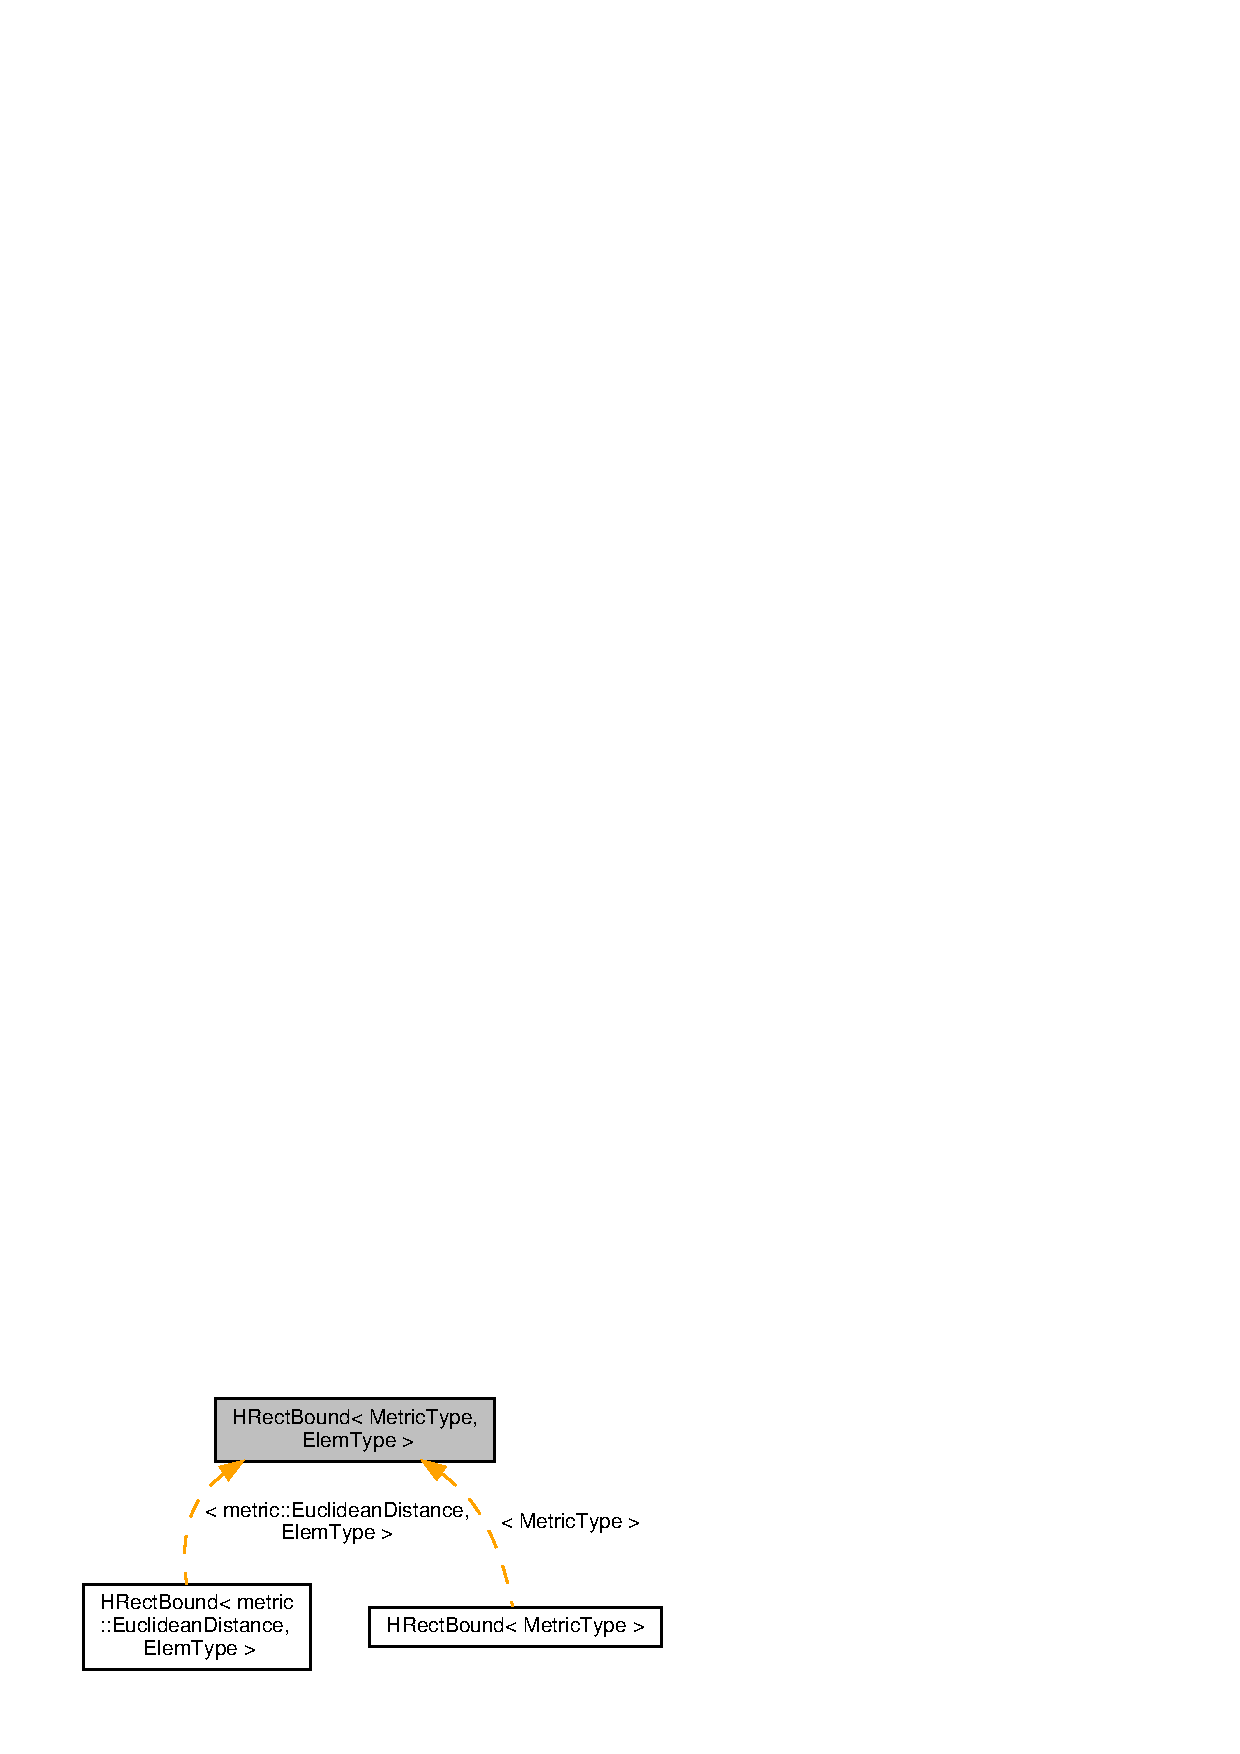
\includegraphics[width=322pt]{classmlpack_1_1bound_1_1HRectBound__inherit__graph}
\end{center}
\end{figure}
\subsection*{Public Member Functions}
\begin{DoxyCompactItemize}
\item 
\textbf{ H\+Rect\+Bound} ()
\begin{DoxyCompactList}\small\item\em Empty constructor; creates a bound of dimensionality 0. \end{DoxyCompactList}\item 
\textbf{ H\+Rect\+Bound} (const size\+\_\+t dimension)
\begin{DoxyCompactList}\small\item\em Initializes to specified dimensionality with each dimension the empty set. \end{DoxyCompactList}\item 
\textbf{ H\+Rect\+Bound} (const \textbf{ H\+Rect\+Bound} \&other)
\begin{DoxyCompactList}\small\item\em Copy constructor; necessary to prevent memory leaks. \end{DoxyCompactList}\item 
\textbf{ H\+Rect\+Bound} (\textbf{ H\+Rect\+Bound} \&\&other)
\begin{DoxyCompactList}\small\item\em Move constructor\+: take possession of another bound\textquotesingle{}s information. \end{DoxyCompactList}\item 
\textbf{ $\sim$\+H\+Rect\+Bound} ()
\begin{DoxyCompactList}\small\item\em Destructor\+: clean up memory. \end{DoxyCompactList}\item 
void \textbf{ Center} (arma\+::\+Col$<$ Elem\+Type $>$ \&center) const
\begin{DoxyCompactList}\small\item\em Calculates the center of the range, placing it into the given vector. \end{DoxyCompactList}\item 
void \textbf{ Clear} ()
\begin{DoxyCompactList}\small\item\em Resets all dimensions to the empty set (so that this bound contains nothing). \end{DoxyCompactList}\item 
{\footnotesize template$<$typename Vec\+Type $>$ }\\bool \textbf{ Contains} (const Vec\+Type \&point) const
\begin{DoxyCompactList}\small\item\em Determines if a point is within this bound. \end{DoxyCompactList}\item 
bool \textbf{ Contains} (const \textbf{ H\+Rect\+Bound} \&bound) const
\begin{DoxyCompactList}\small\item\em Determines if this bound partially contains a bound. \end{DoxyCompactList}\item 
Elem\+Type \textbf{ Diameter} () const
\begin{DoxyCompactList}\small\item\em Returns the diameter of the hyperrectangle (that is, the longest diagonal). \end{DoxyCompactList}\item 
size\+\_\+t \textbf{ Dim} () const
\begin{DoxyCompactList}\small\item\em Gets the dimensionality. \end{DoxyCompactList}\item 
{\footnotesize template$<$typename Vec\+Type $>$ }\\Elem\+Type \textbf{ Max\+Distance} (const Vec\+Type \&point, typename \textbf{ std\+::enable\+\_\+if\+\_\+t}$<$ \textbf{ Is\+Vector}$<$ Vec\+Type $>$\+::value $>$ $\ast$=0) const
\begin{DoxyCompactList}\small\item\em Calculates maximum bound-\/to-\/point squared distance. \end{DoxyCompactList}\item 
Elem\+Type \textbf{ Max\+Distance} (const \textbf{ H\+Rect\+Bound} \&other) const
\begin{DoxyCompactList}\small\item\em Computes maximum distance. \end{DoxyCompactList}\item 
const Metric\+Type \& \textbf{ Metric} () const
\begin{DoxyCompactList}\small\item\em Get the instantiated metric associated with the bound. \end{DoxyCompactList}\item 
Metric\+Type \& \textbf{ Metric} ()
\begin{DoxyCompactList}\small\item\em Modify the instantiated metric associated with the bound. \end{DoxyCompactList}\item 
{\footnotesize template$<$typename Vec\+Type $>$ }\\Elem\+Type \textbf{ Min\+Distance} (const Vec\+Type \&point, typename \textbf{ std\+::enable\+\_\+if\+\_\+t}$<$ \textbf{ Is\+Vector}$<$ Vec\+Type $>$\+::value $>$ $\ast$=0) const
\begin{DoxyCompactList}\small\item\em Calculates minimum bound-\/to-\/point distance. \end{DoxyCompactList}\item 
Elem\+Type \textbf{ Min\+Distance} (const \textbf{ H\+Rect\+Bound} \&other) const
\begin{DoxyCompactList}\small\item\em Calculates minimum bound-\/to-\/bound distance. \end{DoxyCompactList}\item 
Elem\+Type \textbf{ Min\+Width} () const
\begin{DoxyCompactList}\small\item\em Get the minimum width of the bound. \end{DoxyCompactList}\item 
Elem\+Type \& \textbf{ Min\+Width} ()
\begin{DoxyCompactList}\small\item\em Modify the minimum width of the bound. \end{DoxyCompactList}\item 
\textbf{ H\+Rect\+Bound} \textbf{ operator \&} (const \textbf{ H\+Rect\+Bound} \&bound) const
\begin{DoxyCompactList}\small\item\em Returns the intersection of this bound and another. \end{DoxyCompactList}\item 
\textbf{ H\+Rect\+Bound} \& \textbf{ operator \&=} (const \textbf{ H\+Rect\+Bound} \&bound)
\begin{DoxyCompactList}\small\item\em Intersects this bound with another. \end{DoxyCompactList}\item 
\textbf{ H\+Rect\+Bound} \& \textbf{ operator=} (const \textbf{ H\+Rect\+Bound} \&other)
\begin{DoxyCompactList}\small\item\em Same as copy constructor; necessary to prevent memory leaks. \end{DoxyCompactList}\item 
\textbf{ H\+Rect\+Bound} \& \textbf{ operator=} (\textbf{ H\+Rect\+Bound} \&\&other)
\begin{DoxyCompactList}\small\item\em Move assignment operator. \end{DoxyCompactList}\item 
math\+::\+Range\+Type$<$ Elem\+Type $>$ \& \textbf{ operator[$\,$]} (const size\+\_\+t i)
\begin{DoxyCompactList}\small\item\em Get the range for a particular dimension. \end{DoxyCompactList}\item 
const math\+::\+Range\+Type$<$ Elem\+Type $>$ \& \textbf{ operator[$\,$]} (const size\+\_\+t i) const
\begin{DoxyCompactList}\small\item\em Modify the range for a particular dimension. No bounds checking. \end{DoxyCompactList}\item 
{\footnotesize template$<$typename Mat\+Type $>$ }\\\textbf{ H\+Rect\+Bound} \& \textbf{ operator$\vert$=} (const Mat\+Type \&data)
\begin{DoxyCompactList}\small\item\em Expands this region to include new points. \end{DoxyCompactList}\item 
\textbf{ H\+Rect\+Bound} \& \textbf{ operator$\vert$=} (const \textbf{ H\+Rect\+Bound} \&other)
\begin{DoxyCompactList}\small\item\em Expands this region to encompass another bound. \end{DoxyCompactList}\item 
Elem\+Type \textbf{ Overlap} (const \textbf{ H\+Rect\+Bound} \&bound) const
\begin{DoxyCompactList}\small\item\em Returns the volume of overlap of this bound and another. \end{DoxyCompactList}\item 
math\+::\+Range\+Type$<$ Elem\+Type $>$ \textbf{ Range\+Distance} (const \textbf{ H\+Rect\+Bound} \&other) const
\begin{DoxyCompactList}\small\item\em Calculates minimum and maximum bound-\/to-\/bound distance. \end{DoxyCompactList}\item 
{\footnotesize template$<$typename Vec\+Type $>$ }\\math\+::\+Range\+Type$<$ Elem\+Type $>$ \textbf{ Range\+Distance} (const Vec\+Type \&point, typename \textbf{ std\+::enable\+\_\+if\+\_\+t}$<$ \textbf{ Is\+Vector}$<$ Vec\+Type $>$\+::value $>$ $\ast$=0) const
\begin{DoxyCompactList}\small\item\em Calculates minimum and maximum bound-\/to-\/point distance. \end{DoxyCompactList}\item 
{\footnotesize template$<$typename Archive $>$ }\\void \textbf{ serialize} (Archive \&ar, const uint32\+\_\+t version)
\begin{DoxyCompactList}\small\item\em Serialize the bound object. \end{DoxyCompactList}\item 
Elem\+Type \textbf{ Volume} () const
\begin{DoxyCompactList}\small\item\em Calculate the volume of the hyperrectangle. \end{DoxyCompactList}\end{DoxyCompactItemize}


\subsection{Detailed Description}
\subsubsection*{template$<$typename Metric\+Type = metric\+::\+L\+Metric$<$2, true$>$, typename Elem\+Type = double$>$\newline
class mlpack\+::bound\+::\+H\+Rect\+Bound$<$ Metric\+Type, Elem\+Type $>$}

Hyper-\/rectangle bound for an L-\/metric. 

This should be used in conjunction with the L\+Metric class. Be sure to use the same template parameters for L\+Metric as you do for \doxyref{H\+Rect\+Bound}{p.}{classmlpack_1_1bound_1_1HRectBound} -- otherwise odd results may occur.


\begin{DoxyTemplParams}{Template Parameters}
{\em Metric\+Type} & Type of metric to use; must be of type L\+Metric. \\
\hline
{\em Elem\+Type} & Element type (double/float/int/etc.). \\
\hline
\end{DoxyTemplParams}


Definition at line 54 of file hrectbound.\+hpp.



\subsection{Constructor \& Destructor Documentation}
\mbox{\label{classmlpack_1_1bound_1_1HRectBound_a14d6367f1a3e1718deed8cf4fd8300d4}} 
\index{mlpack\+::bound\+::\+H\+Rect\+Bound@{mlpack\+::bound\+::\+H\+Rect\+Bound}!H\+Rect\+Bound@{H\+Rect\+Bound}}
\index{H\+Rect\+Bound@{H\+Rect\+Bound}!mlpack\+::bound\+::\+H\+Rect\+Bound@{mlpack\+::bound\+::\+H\+Rect\+Bound}}
\subsubsection{H\+Rect\+Bound()\hspace{0.1cm}{\footnotesize\ttfamily [1/4]}}
{\footnotesize\ttfamily \textbf{ H\+Rect\+Bound} (\begin{DoxyParamCaption}{ }\end{DoxyParamCaption})}



Empty constructor; creates a bound of dimensionality 0. 

\mbox{\label{classmlpack_1_1bound_1_1HRectBound_a64c0d7420d56f31d05bdbf3612bc91b2}} 
\index{mlpack\+::bound\+::\+H\+Rect\+Bound@{mlpack\+::bound\+::\+H\+Rect\+Bound}!H\+Rect\+Bound@{H\+Rect\+Bound}}
\index{H\+Rect\+Bound@{H\+Rect\+Bound}!mlpack\+::bound\+::\+H\+Rect\+Bound@{mlpack\+::bound\+::\+H\+Rect\+Bound}}
\subsubsection{H\+Rect\+Bound()\hspace{0.1cm}{\footnotesize\ttfamily [2/4]}}
{\footnotesize\ttfamily \textbf{ H\+Rect\+Bound} (\begin{DoxyParamCaption}\item[{const size\+\_\+t}]{dimension }\end{DoxyParamCaption})}



Initializes to specified dimensionality with each dimension the empty set. 


\begin{DoxyParams}{Parameters}
{\em dimension} & Dimensionality of bound. \\
\hline
\end{DoxyParams}
\mbox{\label{classmlpack_1_1bound_1_1HRectBound_a1cd26f681a6e3c5ee325850ace586cfa}} 
\index{mlpack\+::bound\+::\+H\+Rect\+Bound@{mlpack\+::bound\+::\+H\+Rect\+Bound}!H\+Rect\+Bound@{H\+Rect\+Bound}}
\index{H\+Rect\+Bound@{H\+Rect\+Bound}!mlpack\+::bound\+::\+H\+Rect\+Bound@{mlpack\+::bound\+::\+H\+Rect\+Bound}}
\subsubsection{H\+Rect\+Bound()\hspace{0.1cm}{\footnotesize\ttfamily [3/4]}}
{\footnotesize\ttfamily \textbf{ H\+Rect\+Bound} (\begin{DoxyParamCaption}\item[{const \textbf{ H\+Rect\+Bound}$<$ Metric\+Type, Elem\+Type $>$ \&}]{other }\end{DoxyParamCaption})}



Copy constructor; necessary to prevent memory leaks. 

\mbox{\label{classmlpack_1_1bound_1_1HRectBound_a554cc0da21197f0b6cb7dfc6050ead63}} 
\index{mlpack\+::bound\+::\+H\+Rect\+Bound@{mlpack\+::bound\+::\+H\+Rect\+Bound}!H\+Rect\+Bound@{H\+Rect\+Bound}}
\index{H\+Rect\+Bound@{H\+Rect\+Bound}!mlpack\+::bound\+::\+H\+Rect\+Bound@{mlpack\+::bound\+::\+H\+Rect\+Bound}}
\subsubsection{H\+Rect\+Bound()\hspace{0.1cm}{\footnotesize\ttfamily [4/4]}}
{\footnotesize\ttfamily \textbf{ H\+Rect\+Bound} (\begin{DoxyParamCaption}\item[{\textbf{ H\+Rect\+Bound}$<$ Metric\+Type, Elem\+Type $>$ \&\&}]{other }\end{DoxyParamCaption})}



Move constructor\+: take possession of another bound\textquotesingle{}s information. 

\mbox{\label{classmlpack_1_1bound_1_1HRectBound_a68cfb4331fef891c5a7587cc454df1cb}} 
\index{mlpack\+::bound\+::\+H\+Rect\+Bound@{mlpack\+::bound\+::\+H\+Rect\+Bound}!````~H\+Rect\+Bound@{$\sim$\+H\+Rect\+Bound}}
\index{````~H\+Rect\+Bound@{$\sim$\+H\+Rect\+Bound}!mlpack\+::bound\+::\+H\+Rect\+Bound@{mlpack\+::bound\+::\+H\+Rect\+Bound}}
\subsubsection{$\sim$\+H\+Rect\+Bound()}
{\footnotesize\ttfamily $\sim$\textbf{ H\+Rect\+Bound} (\begin{DoxyParamCaption}{ }\end{DoxyParamCaption})}



Destructor\+: clean up memory. 



\subsection{Member Function Documentation}
\mbox{\label{classmlpack_1_1bound_1_1HRectBound_ac519e0ecb1bbd517724a93b4b57cc399}} 
\index{mlpack\+::bound\+::\+H\+Rect\+Bound@{mlpack\+::bound\+::\+H\+Rect\+Bound}!Center@{Center}}
\index{Center@{Center}!mlpack\+::bound\+::\+H\+Rect\+Bound@{mlpack\+::bound\+::\+H\+Rect\+Bound}}
\subsubsection{Center()}
{\footnotesize\ttfamily void Center (\begin{DoxyParamCaption}\item[{arma\+::\+Col$<$ Elem\+Type $>$ \&}]{center }\end{DoxyParamCaption}) const}



Calculates the center of the range, placing it into the given vector. 


\begin{DoxyParams}{Parameters}
{\em center} & Vector which the center will be written to. \\
\hline
\end{DoxyParams}


Referenced by Octree$<$ Metric\+Type, Statistic\+Type, Mat\+Type $>$\+::\+Center().

\mbox{\label{classmlpack_1_1bound_1_1HRectBound_aa71d36872f416feaa853788a7a7a7ef8}} 
\index{mlpack\+::bound\+::\+H\+Rect\+Bound@{mlpack\+::bound\+::\+H\+Rect\+Bound}!Clear@{Clear}}
\index{Clear@{Clear}!mlpack\+::bound\+::\+H\+Rect\+Bound@{mlpack\+::bound\+::\+H\+Rect\+Bound}}
\subsubsection{Clear()}
{\footnotesize\ttfamily void Clear (\begin{DoxyParamCaption}{ }\end{DoxyParamCaption})}



Resets all dimensions to the empty set (so that this bound contains nothing). 

\mbox{\label{classmlpack_1_1bound_1_1HRectBound_a3c1084b782672d502264b8c6d33ed0dd}} 
\index{mlpack\+::bound\+::\+H\+Rect\+Bound@{mlpack\+::bound\+::\+H\+Rect\+Bound}!Contains@{Contains}}
\index{Contains@{Contains}!mlpack\+::bound\+::\+H\+Rect\+Bound@{mlpack\+::bound\+::\+H\+Rect\+Bound}}
\subsubsection{Contains()\hspace{0.1cm}{\footnotesize\ttfamily [1/2]}}
{\footnotesize\ttfamily bool Contains (\begin{DoxyParamCaption}\item[{const Vec\+Type \&}]{point }\end{DoxyParamCaption}) const}



Determines if a point is within this bound. 


\begin{DoxyParams}{Parameters}
{\em point} & Point to check the condition. \\
\hline
\end{DoxyParams}
\mbox{\label{classmlpack_1_1bound_1_1HRectBound_ad3a69a98f323de871cc834fe91114792}} 
\index{mlpack\+::bound\+::\+H\+Rect\+Bound@{mlpack\+::bound\+::\+H\+Rect\+Bound}!Contains@{Contains}}
\index{Contains@{Contains}!mlpack\+::bound\+::\+H\+Rect\+Bound@{mlpack\+::bound\+::\+H\+Rect\+Bound}}
\subsubsection{Contains()\hspace{0.1cm}{\footnotesize\ttfamily [2/2]}}
{\footnotesize\ttfamily bool Contains (\begin{DoxyParamCaption}\item[{const \textbf{ H\+Rect\+Bound}$<$ Metric\+Type, Elem\+Type $>$ \&}]{bound }\end{DoxyParamCaption}) const}



Determines if this bound partially contains a bound. 


\begin{DoxyParams}{Parameters}
{\em bound} & Bound to check the condition. \\
\hline
\end{DoxyParams}
\mbox{\label{classmlpack_1_1bound_1_1HRectBound_a60e7246d34103909f688395e35869b39}} 
\index{mlpack\+::bound\+::\+H\+Rect\+Bound@{mlpack\+::bound\+::\+H\+Rect\+Bound}!Diameter@{Diameter}}
\index{Diameter@{Diameter}!mlpack\+::bound\+::\+H\+Rect\+Bound@{mlpack\+::bound\+::\+H\+Rect\+Bound}}
\subsubsection{Diameter()}
{\footnotesize\ttfamily Elem\+Type Diameter (\begin{DoxyParamCaption}{ }\end{DoxyParamCaption}) const}



Returns the diameter of the hyperrectangle (that is, the longest diagonal). 

\mbox{\label{classmlpack_1_1bound_1_1HRectBound_a7993a4f36c530e03b78b28b5f53bb286}} 
\index{mlpack\+::bound\+::\+H\+Rect\+Bound@{mlpack\+::bound\+::\+H\+Rect\+Bound}!Dim@{Dim}}
\index{Dim@{Dim}!mlpack\+::bound\+::\+H\+Rect\+Bound@{mlpack\+::bound\+::\+H\+Rect\+Bound}}
\subsubsection{Dim()}
{\footnotesize\ttfamily size\+\_\+t Dim (\begin{DoxyParamCaption}{ }\end{DoxyParamCaption}) const\hspace{0.3cm}{\ttfamily [inline]}}



Gets the dimensionality. 



Definition at line 96 of file hrectbound.\+hpp.

\mbox{\label{classmlpack_1_1bound_1_1HRectBound_ae764d88483236cc470f5abe0273df4c5}} 
\index{mlpack\+::bound\+::\+H\+Rect\+Bound@{mlpack\+::bound\+::\+H\+Rect\+Bound}!Max\+Distance@{Max\+Distance}}
\index{Max\+Distance@{Max\+Distance}!mlpack\+::bound\+::\+H\+Rect\+Bound@{mlpack\+::bound\+::\+H\+Rect\+Bound}}
\subsubsection{Max\+Distance()\hspace{0.1cm}{\footnotesize\ttfamily [1/2]}}
{\footnotesize\ttfamily Elem\+Type Max\+Distance (\begin{DoxyParamCaption}\item[{const Vec\+Type \&}]{point,  }\item[{typename \textbf{ std\+::enable\+\_\+if\+\_\+t}$<$ \textbf{ Is\+Vector}$<$ Vec\+Type $>$\+::value $>$ $\ast$}]{ = {\ttfamily 0} }\end{DoxyParamCaption}) const}



Calculates maximum bound-\/to-\/point squared distance. 


\begin{DoxyParams}{Parameters}
{\em point} & Point to which the maximum distance is requested. \\
\hline
\end{DoxyParams}
\mbox{\label{classmlpack_1_1bound_1_1HRectBound_aff674aa2febc8534dadd90e03d93c087}} 
\index{mlpack\+::bound\+::\+H\+Rect\+Bound@{mlpack\+::bound\+::\+H\+Rect\+Bound}!Max\+Distance@{Max\+Distance}}
\index{Max\+Distance@{Max\+Distance}!mlpack\+::bound\+::\+H\+Rect\+Bound@{mlpack\+::bound\+::\+H\+Rect\+Bound}}
\subsubsection{Max\+Distance()\hspace{0.1cm}{\footnotesize\ttfamily [2/2]}}
{\footnotesize\ttfamily Elem\+Type Max\+Distance (\begin{DoxyParamCaption}\item[{const \textbf{ H\+Rect\+Bound}$<$ Metric\+Type, Elem\+Type $>$ \&}]{other }\end{DoxyParamCaption}) const}



Computes maximum distance. 


\begin{DoxyParams}{Parameters}
{\em other} & Bound to which the maximum distance is requested. \\
\hline
\end{DoxyParams}
\mbox{\label{classmlpack_1_1bound_1_1HRectBound_aac4d643c62af7d9cc2a072aea10d2b32}} 
\index{mlpack\+::bound\+::\+H\+Rect\+Bound@{mlpack\+::bound\+::\+H\+Rect\+Bound}!Metric@{Metric}}
\index{Metric@{Metric}!mlpack\+::bound\+::\+H\+Rect\+Bound@{mlpack\+::bound\+::\+H\+Rect\+Bound}}
\subsubsection{Metric()\hspace{0.1cm}{\footnotesize\ttfamily [1/2]}}
{\footnotesize\ttfamily const Metric\+Type\& Metric (\begin{DoxyParamCaption}{ }\end{DoxyParamCaption}) const\hspace{0.3cm}{\ttfamily [inline]}}



Get the instantiated metric associated with the bound. 



Definition at line 111 of file hrectbound.\+hpp.

\mbox{\label{classmlpack_1_1bound_1_1HRectBound_acc71d930ed90e73b2bc0c360835c5371}} 
\index{mlpack\+::bound\+::\+H\+Rect\+Bound@{mlpack\+::bound\+::\+H\+Rect\+Bound}!Metric@{Metric}}
\index{Metric@{Metric}!mlpack\+::bound\+::\+H\+Rect\+Bound@{mlpack\+::bound\+::\+H\+Rect\+Bound}}
\subsubsection{Metric()\hspace{0.1cm}{\footnotesize\ttfamily [2/2]}}
{\footnotesize\ttfamily Metric\+Type\& Metric (\begin{DoxyParamCaption}{ }\end{DoxyParamCaption})\hspace{0.3cm}{\ttfamily [inline]}}



Modify the instantiated metric associated with the bound. 



Definition at line 113 of file hrectbound.\+hpp.

\mbox{\label{classmlpack_1_1bound_1_1HRectBound_a73bf99a433e88a31d98b46bf4c0da147}} 
\index{mlpack\+::bound\+::\+H\+Rect\+Bound@{mlpack\+::bound\+::\+H\+Rect\+Bound}!Min\+Distance@{Min\+Distance}}
\index{Min\+Distance@{Min\+Distance}!mlpack\+::bound\+::\+H\+Rect\+Bound@{mlpack\+::bound\+::\+H\+Rect\+Bound}}
\subsubsection{Min\+Distance()\hspace{0.1cm}{\footnotesize\ttfamily [1/2]}}
{\footnotesize\ttfamily Elem\+Type Min\+Distance (\begin{DoxyParamCaption}\item[{const Vec\+Type \&}]{point,  }\item[{typename \textbf{ std\+::enable\+\_\+if\+\_\+t}$<$ \textbf{ Is\+Vector}$<$ Vec\+Type $>$\+::value $>$ $\ast$}]{ = {\ttfamily 0} }\end{DoxyParamCaption}) const}



Calculates minimum bound-\/to-\/point distance. 


\begin{DoxyParams}{Parameters}
{\em point} & Point to which the minimum distance is requested. \\
\hline
\end{DoxyParams}
\mbox{\label{classmlpack_1_1bound_1_1HRectBound_aee3d05d30173b45bce8fb59678093923}} 
\index{mlpack\+::bound\+::\+H\+Rect\+Bound@{mlpack\+::bound\+::\+H\+Rect\+Bound}!Min\+Distance@{Min\+Distance}}
\index{Min\+Distance@{Min\+Distance}!mlpack\+::bound\+::\+H\+Rect\+Bound@{mlpack\+::bound\+::\+H\+Rect\+Bound}}
\subsubsection{Min\+Distance()\hspace{0.1cm}{\footnotesize\ttfamily [2/2]}}
{\footnotesize\ttfamily Elem\+Type Min\+Distance (\begin{DoxyParamCaption}\item[{const \textbf{ H\+Rect\+Bound}$<$ Metric\+Type, Elem\+Type $>$ \&}]{other }\end{DoxyParamCaption}) const}



Calculates minimum bound-\/to-\/bound distance. 


\begin{DoxyParams}{Parameters}
{\em other} & Bound to which the minimum distance is requested. \\
\hline
\end{DoxyParams}
\mbox{\label{classmlpack_1_1bound_1_1HRectBound_ab8478ff52c4d4d5e7fa6311fa39abb76}} 
\index{mlpack\+::bound\+::\+H\+Rect\+Bound@{mlpack\+::bound\+::\+H\+Rect\+Bound}!Min\+Width@{Min\+Width}}
\index{Min\+Width@{Min\+Width}!mlpack\+::bound\+::\+H\+Rect\+Bound@{mlpack\+::bound\+::\+H\+Rect\+Bound}}
\subsubsection{Min\+Width()\hspace{0.1cm}{\footnotesize\ttfamily [1/2]}}
{\footnotesize\ttfamily Elem\+Type Min\+Width (\begin{DoxyParamCaption}{ }\end{DoxyParamCaption}) const\hspace{0.3cm}{\ttfamily [inline]}}



Get the minimum width of the bound. 



Definition at line 106 of file hrectbound.\+hpp.

\mbox{\label{classmlpack_1_1bound_1_1HRectBound_a216fa2f42fce4a6edd8f1a354d24aac2}} 
\index{mlpack\+::bound\+::\+H\+Rect\+Bound@{mlpack\+::bound\+::\+H\+Rect\+Bound}!Min\+Width@{Min\+Width}}
\index{Min\+Width@{Min\+Width}!mlpack\+::bound\+::\+H\+Rect\+Bound@{mlpack\+::bound\+::\+H\+Rect\+Bound}}
\subsubsection{Min\+Width()\hspace{0.1cm}{\footnotesize\ttfamily [2/2]}}
{\footnotesize\ttfamily Elem\+Type\& Min\+Width (\begin{DoxyParamCaption}{ }\end{DoxyParamCaption})\hspace{0.3cm}{\ttfamily [inline]}}



Modify the minimum width of the bound. 



Definition at line 108 of file hrectbound.\+hpp.

\mbox{\label{classmlpack_1_1bound_1_1HRectBound_a3becb0b78fc8642f6233a92d9a4494d9}} 
\index{mlpack\+::bound\+::\+H\+Rect\+Bound@{mlpack\+::bound\+::\+H\+Rect\+Bound}!operator \&@{operator \&}}
\index{operator \&@{operator \&}!mlpack\+::bound\+::\+H\+Rect\+Bound@{mlpack\+::bound\+::\+H\+Rect\+Bound}}
\subsubsection{operator \&()}
{\footnotesize\ttfamily \textbf{ H\+Rect\+Bound} operator\& (\begin{DoxyParamCaption}\item[{const \textbf{ H\+Rect\+Bound}$<$ Metric\+Type, Elem\+Type $>$ \&}]{bound }\end{DoxyParamCaption}) const}



Returns the intersection of this bound and another. 

\mbox{\label{classmlpack_1_1bound_1_1HRectBound_a6b81bda204986dd2a1bfeecb46c82a73}} 
\index{mlpack\+::bound\+::\+H\+Rect\+Bound@{mlpack\+::bound\+::\+H\+Rect\+Bound}!operator \&=@{operator \&=}}
\index{operator \&=@{operator \&=}!mlpack\+::bound\+::\+H\+Rect\+Bound@{mlpack\+::bound\+::\+H\+Rect\+Bound}}
\subsubsection{operator \&=()}
{\footnotesize\ttfamily \textbf{ H\+Rect\+Bound}\& operator\&= (\begin{DoxyParamCaption}\item[{const \textbf{ H\+Rect\+Bound}$<$ Metric\+Type, Elem\+Type $>$ \&}]{bound }\end{DoxyParamCaption})}



Intersects this bound with another. 

\mbox{\label{classmlpack_1_1bound_1_1HRectBound_ae368f3b87f5b50c43247724aa0ec253c}} 
\index{mlpack\+::bound\+::\+H\+Rect\+Bound@{mlpack\+::bound\+::\+H\+Rect\+Bound}!operator=@{operator=}}
\index{operator=@{operator=}!mlpack\+::bound\+::\+H\+Rect\+Bound@{mlpack\+::bound\+::\+H\+Rect\+Bound}}
\subsubsection{operator=()\hspace{0.1cm}{\footnotesize\ttfamily [1/2]}}
{\footnotesize\ttfamily \textbf{ H\+Rect\+Bound}\& operator= (\begin{DoxyParamCaption}\item[{const \textbf{ H\+Rect\+Bound}$<$ Metric\+Type, Elem\+Type $>$ \&}]{other }\end{DoxyParamCaption})}



Same as copy constructor; necessary to prevent memory leaks. 

\mbox{\label{classmlpack_1_1bound_1_1HRectBound_a993c1901b1bc446219fabeb54776f6b7}} 
\index{mlpack\+::bound\+::\+H\+Rect\+Bound@{mlpack\+::bound\+::\+H\+Rect\+Bound}!operator=@{operator=}}
\index{operator=@{operator=}!mlpack\+::bound\+::\+H\+Rect\+Bound@{mlpack\+::bound\+::\+H\+Rect\+Bound}}
\subsubsection{operator=()\hspace{0.1cm}{\footnotesize\ttfamily [2/2]}}
{\footnotesize\ttfamily \textbf{ H\+Rect\+Bound}\& operator= (\begin{DoxyParamCaption}\item[{\textbf{ H\+Rect\+Bound}$<$ Metric\+Type, Elem\+Type $>$ \&\&}]{other }\end{DoxyParamCaption})}



Move assignment operator. 

\mbox{\label{classmlpack_1_1bound_1_1HRectBound_a3f5bdaafab276f919fb5fbca6cc2f885}} 
\index{mlpack\+::bound\+::\+H\+Rect\+Bound@{mlpack\+::bound\+::\+H\+Rect\+Bound}!operator[]@{operator[]}}
\index{operator[]@{operator[]}!mlpack\+::bound\+::\+H\+Rect\+Bound@{mlpack\+::bound\+::\+H\+Rect\+Bound}}
\subsubsection{operator[]()\hspace{0.1cm}{\footnotesize\ttfamily [1/2]}}
{\footnotesize\ttfamily math\+::\+Range\+Type$<$Elem\+Type$>$\& operator[$\,$] (\begin{DoxyParamCaption}\item[{const size\+\_\+t}]{i }\end{DoxyParamCaption})\hspace{0.3cm}{\ttfamily [inline]}}



Get the range for a particular dimension. 

No bounds checking. Be careful\+: this may make \doxyref{Min\+Width()}{p.}{classmlpack_1_1bound_1_1HRectBound_a216fa2f42fce4a6edd8f1a354d24aac2} invalid. 

Definition at line 100 of file hrectbound.\+hpp.

\mbox{\label{classmlpack_1_1bound_1_1HRectBound_a4ab2ad05d0e4e59b868c4c5bef904ee1}} 
\index{mlpack\+::bound\+::\+H\+Rect\+Bound@{mlpack\+::bound\+::\+H\+Rect\+Bound}!operator[]@{operator[]}}
\index{operator[]@{operator[]}!mlpack\+::bound\+::\+H\+Rect\+Bound@{mlpack\+::bound\+::\+H\+Rect\+Bound}}
\subsubsection{operator[]()\hspace{0.1cm}{\footnotesize\ttfamily [2/2]}}
{\footnotesize\ttfamily const math\+::\+Range\+Type$<$Elem\+Type$>$\& operator[$\,$] (\begin{DoxyParamCaption}\item[{const size\+\_\+t}]{i }\end{DoxyParamCaption}) const\hspace{0.3cm}{\ttfamily [inline]}}



Modify the range for a particular dimension. No bounds checking. 



Definition at line 102 of file hrectbound.\+hpp.

\mbox{\label{classmlpack_1_1bound_1_1HRectBound_a9e955961567ca1540df58d2185f81439}} 
\index{mlpack\+::bound\+::\+H\+Rect\+Bound@{mlpack\+::bound\+::\+H\+Rect\+Bound}!operator\texttt{"|}=@{operator\texttt{"|}=}}
\index{operator\texttt{"|}=@{operator\texttt{"|}=}!mlpack\+::bound\+::\+H\+Rect\+Bound@{mlpack\+::bound\+::\+H\+Rect\+Bound}}
\subsubsection{operator\texttt{"|}=()\hspace{0.1cm}{\footnotesize\ttfamily [1/2]}}
{\footnotesize\ttfamily \textbf{ H\+Rect\+Bound}\& operator$\vert$= (\begin{DoxyParamCaption}\item[{const Mat\+Type \&}]{data }\end{DoxyParamCaption})}



Expands this region to include new points. 


\begin{DoxyTemplParams}{Template Parameters}
{\em Mat\+Type} & Type of matrix; could be Mat, Sp\+Mat, a subview, or just a vector. \\
\hline
\end{DoxyTemplParams}

\begin{DoxyParams}{Parameters}
{\em data} & Data points to expand this region to include. \\
\hline
\end{DoxyParams}
\mbox{\label{classmlpack_1_1bound_1_1HRectBound_a77f7aac5543d1e00596af2d2074c142b}} 
\index{mlpack\+::bound\+::\+H\+Rect\+Bound@{mlpack\+::bound\+::\+H\+Rect\+Bound}!operator\texttt{"|}=@{operator\texttt{"|}=}}
\index{operator\texttt{"|}=@{operator\texttt{"|}=}!mlpack\+::bound\+::\+H\+Rect\+Bound@{mlpack\+::bound\+::\+H\+Rect\+Bound}}
\subsubsection{operator\texttt{"|}=()\hspace{0.1cm}{\footnotesize\ttfamily [2/2]}}
{\footnotesize\ttfamily \textbf{ H\+Rect\+Bound}\& operator$\vert$= (\begin{DoxyParamCaption}\item[{const \textbf{ H\+Rect\+Bound}$<$ Metric\+Type, Elem\+Type $>$ \&}]{other }\end{DoxyParamCaption})}



Expands this region to encompass another bound. 

\mbox{\label{classmlpack_1_1bound_1_1HRectBound_a237a387176c306c3b8c025590d691338}} 
\index{mlpack\+::bound\+::\+H\+Rect\+Bound@{mlpack\+::bound\+::\+H\+Rect\+Bound}!Overlap@{Overlap}}
\index{Overlap@{Overlap}!mlpack\+::bound\+::\+H\+Rect\+Bound@{mlpack\+::bound\+::\+H\+Rect\+Bound}}
\subsubsection{Overlap()}
{\footnotesize\ttfamily Elem\+Type Overlap (\begin{DoxyParamCaption}\item[{const \textbf{ H\+Rect\+Bound}$<$ Metric\+Type, Elem\+Type $>$ \&}]{bound }\end{DoxyParamCaption}) const}



Returns the volume of overlap of this bound and another. 

\mbox{\label{classmlpack_1_1bound_1_1HRectBound_a2c5555e91d38db00fc5f76fe0032044c}} 
\index{mlpack\+::bound\+::\+H\+Rect\+Bound@{mlpack\+::bound\+::\+H\+Rect\+Bound}!Range\+Distance@{Range\+Distance}}
\index{Range\+Distance@{Range\+Distance}!mlpack\+::bound\+::\+H\+Rect\+Bound@{mlpack\+::bound\+::\+H\+Rect\+Bound}}
\subsubsection{Range\+Distance()\hspace{0.1cm}{\footnotesize\ttfamily [1/2]}}
{\footnotesize\ttfamily math\+::\+Range\+Type$<$Elem\+Type$>$ Range\+Distance (\begin{DoxyParamCaption}\item[{const \textbf{ H\+Rect\+Bound}$<$ Metric\+Type, Elem\+Type $>$ \&}]{other }\end{DoxyParamCaption}) const}



Calculates minimum and maximum bound-\/to-\/bound distance. 


\begin{DoxyParams}{Parameters}
{\em other} & Bound to which the minimum and maximum distances are requested. \\
\hline
\end{DoxyParams}
\mbox{\label{classmlpack_1_1bound_1_1HRectBound_a60a550bf46aa1d7b858134ce41fd5a3a}} 
\index{mlpack\+::bound\+::\+H\+Rect\+Bound@{mlpack\+::bound\+::\+H\+Rect\+Bound}!Range\+Distance@{Range\+Distance}}
\index{Range\+Distance@{Range\+Distance}!mlpack\+::bound\+::\+H\+Rect\+Bound@{mlpack\+::bound\+::\+H\+Rect\+Bound}}
\subsubsection{Range\+Distance()\hspace{0.1cm}{\footnotesize\ttfamily [2/2]}}
{\footnotesize\ttfamily math\+::\+Range\+Type$<$Elem\+Type$>$ Range\+Distance (\begin{DoxyParamCaption}\item[{const Vec\+Type \&}]{point,  }\item[{typename \textbf{ std\+::enable\+\_\+if\+\_\+t}$<$ \textbf{ Is\+Vector}$<$ Vec\+Type $>$\+::value $>$ $\ast$}]{ = {\ttfamily 0} }\end{DoxyParamCaption}) const}



Calculates minimum and maximum bound-\/to-\/point distance. 


\begin{DoxyParams}{Parameters}
{\em point} & Point to which the minimum and maximum distances are requested. \\
\hline
\end{DoxyParams}
\mbox{\label{classmlpack_1_1bound_1_1HRectBound_a72d63b74c8166dff8e1a9006905ad9ca}} 
\index{mlpack\+::bound\+::\+H\+Rect\+Bound@{mlpack\+::bound\+::\+H\+Rect\+Bound}!serialize@{serialize}}
\index{serialize@{serialize}!mlpack\+::bound\+::\+H\+Rect\+Bound@{mlpack\+::bound\+::\+H\+Rect\+Bound}}
\subsubsection{serialize()}
{\footnotesize\ttfamily void serialize (\begin{DoxyParamCaption}\item[{Archive \&}]{ar,  }\item[{const uint32\+\_\+t}]{version }\end{DoxyParamCaption})}



Serialize the bound object. 

\mbox{\label{classmlpack_1_1bound_1_1HRectBound_ac0e1df0f15250ddde83eed6a1bf52eba}} 
\index{mlpack\+::bound\+::\+H\+Rect\+Bound@{mlpack\+::bound\+::\+H\+Rect\+Bound}!Volume@{Volume}}
\index{Volume@{Volume}!mlpack\+::bound\+::\+H\+Rect\+Bound@{mlpack\+::bound\+::\+H\+Rect\+Bound}}
\subsubsection{Volume()}
{\footnotesize\ttfamily Elem\+Type Volume (\begin{DoxyParamCaption}{ }\end{DoxyParamCaption}) const}



Calculate the volume of the hyperrectangle. 

\begin{DoxyReturn}{Returns}
Volume of the hyperrectangle. 
\end{DoxyReturn}


The documentation for this class was generated from the following file\+:\begin{DoxyCompactItemize}
\item 
/home/aakash/mlpack/src/mlpack/core/tree/\textbf{ hrectbound.\+hpp}\end{DoxyCompactItemize}

\section{Is\+L\+Metric$<$ Metric\+Type $>$ Struct Template Reference}
\label{structmlpack_1_1bound_1_1meta_1_1IsLMetric}\index{Is\+L\+Metric$<$ Metric\+Type $>$@{Is\+L\+Metric$<$ Metric\+Type $>$}}


Utility struct where Value is true if and only if the argument is of type L\+Metric.  


\subsection*{Static Public Attributes}
\begin{DoxyCompactItemize}
\item 
static const bool \textbf{ Value} = false
\end{DoxyCompactItemize}


\subsection{Detailed Description}
\subsubsection*{template$<$typename Metric\+Type$>$\newline
struct mlpack\+::bound\+::meta\+::\+Is\+L\+Metric$<$ Metric\+Type $>$}

Utility struct where Value is true if and only if the argument is of type L\+Metric. 



Definition at line 30 of file hrectbound.\+hpp.



\subsection{Member Data Documentation}
\mbox{\label{structmlpack_1_1bound_1_1meta_1_1IsLMetric_a2cbb7037a76934614ab6ca3cc713d6ef}} 
\index{mlpack\+::bound\+::meta\+::\+Is\+L\+Metric@{mlpack\+::bound\+::meta\+::\+Is\+L\+Metric}!Value@{Value}}
\index{Value@{Value}!mlpack\+::bound\+::meta\+::\+Is\+L\+Metric@{mlpack\+::bound\+::meta\+::\+Is\+L\+Metric}}
\subsubsection{Value}
{\footnotesize\ttfamily const bool Value = false\hspace{0.3cm}{\ttfamily [static]}}



Definition at line 32 of file hrectbound.\+hpp.



The documentation for this struct was generated from the following file\+:\begin{DoxyCompactItemize}
\item 
/home/aakash/mlpack/src/mlpack/core/tree/\textbf{ hrectbound.\+hpp}\end{DoxyCompactItemize}

\section{Is\+L\+Metric$<$ metric\+:\+:L\+Metric$<$ Power, Take\+Root $>$ $>$ Struct Template Reference}
\label{structmlpack_1_1bound_1_1meta_1_1IsLMetric_3_01metric_1_1LMetric_3_01Power_00_01TakeRoot_01_4_01_4}\index{Is\+L\+Metric$<$ metric\+::\+L\+Metric$<$ Power, Take\+Root $>$ $>$@{Is\+L\+Metric$<$ metric\+::\+L\+Metric$<$ Power, Take\+Root $>$ $>$}}


Specialization for \doxyref{Is\+L\+Metric}{p.}{structmlpack_1_1bound_1_1meta_1_1IsLMetric} when the argument is of type L\+Metric.  


\subsection*{Static Public Attributes}
\begin{DoxyCompactItemize}
\item 
static const bool \textbf{ Value} = true
\end{DoxyCompactItemize}


\subsection{Detailed Description}
\subsubsection*{template$<$int Power, bool Take\+Root$>$\newline
struct mlpack\+::bound\+::meta\+::\+Is\+L\+Metric$<$ metric\+::\+L\+Metric$<$ Power, Take\+Root $>$ $>$}

Specialization for \doxyref{Is\+L\+Metric}{p.}{structmlpack_1_1bound_1_1meta_1_1IsLMetric} when the argument is of type L\+Metric. 

Definition at line 37 of file hrectbound.\+hpp.



\subsection{Member Data Documentation}
\mbox{\label{structmlpack_1_1bound_1_1meta_1_1IsLMetric_3_01metric_1_1LMetric_3_01Power_00_01TakeRoot_01_4_01_4_a2cbb7037a76934614ab6ca3cc713d6ef}} 
\index{mlpack\+::bound\+::meta\+::\+Is\+L\+Metric$<$ metric\+::\+L\+Metric$<$ Power, Take\+Root $>$ $>$@{mlpack\+::bound\+::meta\+::\+Is\+L\+Metric$<$ metric\+::\+L\+Metric$<$ Power, Take\+Root $>$ $>$}!Value@{Value}}
\index{Value@{Value}!mlpack\+::bound\+::meta\+::\+Is\+L\+Metric$<$ metric\+::\+L\+Metric$<$ Power, Take\+Root $>$ $>$@{mlpack\+::bound\+::meta\+::\+Is\+L\+Metric$<$ metric\+::\+L\+Metric$<$ Power, Take\+Root $>$ $>$}}
\subsubsection{Value}
{\footnotesize\ttfamily const bool Value = true\hspace{0.3cm}{\ttfamily [static]}}



Definition at line 39 of file hrectbound.\+hpp.



The documentation for this struct was generated from the following file\+:\begin{DoxyCompactItemize}
\item 
/home/aakash/mlpack/src/mlpack/core/tree/\textbf{ hrectbound.\+hpp}\end{DoxyCompactItemize}

\section{Average\+Interpolation Class Reference}
\label{classmlpack_1_1cf_1_1AverageInterpolation}\index{Average\+Interpolation@{Average\+Interpolation}}


This class performs average interpolation to generate interpolation weights for neighborhood-\/based collaborative filtering.  


\subsection*{Public Member Functions}
\begin{DoxyCompactItemize}
\item 
\textbf{ Average\+Interpolation} ()
\item 
\textbf{ Average\+Interpolation} (const arma\+::sp\+\_\+mat \&)
\begin{DoxyCompactList}\small\item\em This constructor is needed for interface consistency. \end{DoxyCompactList}\item 
{\footnotesize template$<$typename Vector\+Type , typename Decomposition\+Policy $>$ }\\void \textbf{ Get\+Weights} (Vector\+Type \&\&weights, const Decomposition\+Policy \&, const size\+\_\+t, const arma\+::\+Col$<$ size\+\_\+t $>$ \&neighbors, const arma\+::vec \&, const arma\+::sp\+\_\+mat \&)
\begin{DoxyCompactList}\small\item\em Interoplation weights are identical and sum up to one. \end{DoxyCompactList}\end{DoxyCompactItemize}


\subsection{Detailed Description}
This class performs average interpolation to generate interpolation weights for neighborhood-\/based collaborative filtering. 

An example of how to use \doxyref{Average\+Interpolation}{p.}{classmlpack_1_1cf_1_1AverageInterpolation} in CF is shown below\+:


\begin{DoxyCode}
\textcolor{keyword}{extern} arma::mat data; \textcolor{comment}{// data is a (user, item, rating) table.}
\textcolor{comment}{// Users for whom recommendations are generated.}
\textcolor{keyword}{extern} arma::Col<size\_t> users;
arma::Mat<size\_t> recommendations; \textcolor{comment}{// Resulting recommendations.}

CFType<> cf(data);

\textcolor{comment}{// Generate 10 recommendations for all users.}
cf.template GetRecommendations<EuclideanSearch,
                               AverageInterpolation>(10, recommendations);
\end{DoxyCode}
 

Definition at line 39 of file average\+\_\+interpolation.\+hpp.



\subsection{Constructor \& Destructor Documentation}
\mbox{\label{classmlpack_1_1cf_1_1AverageInterpolation_a0fc6829b9ccd30f4e79cb01389d5ef0c}} 
\index{mlpack\+::cf\+::\+Average\+Interpolation@{mlpack\+::cf\+::\+Average\+Interpolation}!Average\+Interpolation@{Average\+Interpolation}}
\index{Average\+Interpolation@{Average\+Interpolation}!mlpack\+::cf\+::\+Average\+Interpolation@{mlpack\+::cf\+::\+Average\+Interpolation}}
\subsubsection{Average\+Interpolation()\hspace{0.1cm}{\footnotesize\ttfamily [1/2]}}
{\footnotesize\ttfamily \textbf{ Average\+Interpolation} (\begin{DoxyParamCaption}{ }\end{DoxyParamCaption})\hspace{0.3cm}{\ttfamily [inline]}}



Definition at line 43 of file average\+\_\+interpolation.\+hpp.

\mbox{\label{classmlpack_1_1cf_1_1AverageInterpolation_a48e88c343985e5407cd1e3f1a3d273d6}} 
\index{mlpack\+::cf\+::\+Average\+Interpolation@{mlpack\+::cf\+::\+Average\+Interpolation}!Average\+Interpolation@{Average\+Interpolation}}
\index{Average\+Interpolation@{Average\+Interpolation}!mlpack\+::cf\+::\+Average\+Interpolation@{mlpack\+::cf\+::\+Average\+Interpolation}}
\subsubsection{Average\+Interpolation()\hspace{0.1cm}{\footnotesize\ttfamily [2/2]}}
{\footnotesize\ttfamily \textbf{ Average\+Interpolation} (\begin{DoxyParamCaption}\item[{const arma\+::sp\+\_\+mat \&}]{ }\end{DoxyParamCaption})\hspace{0.3cm}{\ttfamily [inline]}}



This constructor is needed for interface consistency. 



Definition at line 48 of file average\+\_\+interpolation.\+hpp.



\subsection{Member Function Documentation}
\mbox{\label{classmlpack_1_1cf_1_1AverageInterpolation_ac92ff2a2cfcb48bda46221a1a31de9b3}} 
\index{mlpack\+::cf\+::\+Average\+Interpolation@{mlpack\+::cf\+::\+Average\+Interpolation}!Get\+Weights@{Get\+Weights}}
\index{Get\+Weights@{Get\+Weights}!mlpack\+::cf\+::\+Average\+Interpolation@{mlpack\+::cf\+::\+Average\+Interpolation}}
\subsubsection{Get\+Weights()}
{\footnotesize\ttfamily void Get\+Weights (\begin{DoxyParamCaption}\item[{Vector\+Type \&\&}]{weights,  }\item[{const Decomposition\+Policy \&}]{,  }\item[{const size\+\_\+t}]{,  }\item[{const arma\+::\+Col$<$ size\+\_\+t $>$ \&}]{neighbors,  }\item[{const arma\+::vec \&}]{,  }\item[{const arma\+::sp\+\_\+mat \&}]{ }\end{DoxyParamCaption})\hspace{0.3cm}{\ttfamily [inline]}}



Interoplation weights are identical and sum up to one. 

After getting the weights, CF algorithm multiplies each neighbor\textquotesingle{}s rating by its corresponding weight and sums them to get predicted rating.


\begin{DoxyParams}{Parameters}
{\em weights} & Resulting interpolation weights. The size of weights should be set to the number of neighbors before calling \doxyref{Get\+Weights()}{p.}{classmlpack_1_1cf_1_1AverageInterpolation_ac92ff2a2cfcb48bda46221a1a31de9b3}. \\
\hline
{\em $\ast$} & (decomposition) Decomposition object. \\
\hline
{\em $\ast$} & (query\+User) Queried user. \\
\hline
{\em neighbors} & Neighbors of queried user. \\
\hline
{\em $\ast$} & (similarities) Similarites between query user and neighbors. \\
\hline
{\em $\ast$} & (cleaned\+Data) Sparse rating matrix. \\
\hline
\end{DoxyParams}


Definition at line 65 of file average\+\_\+interpolation.\+hpp.



The documentation for this class was generated from the following file\+:\begin{DoxyCompactItemize}
\item 
/home/aakash/mlpack/src/mlpack/methods/cf/interpolation\+\_\+policies/\textbf{ average\+\_\+interpolation.\+hpp}\end{DoxyCompactItemize}

\section{Batch\+S\+V\+D\+Policy Class Reference}
\label{classmlpack_1_1cf_1_1BatchSVDPolicy}\index{Batch\+S\+V\+D\+Policy@{Batch\+S\+V\+D\+Policy}}


Implementation of the Batch S\+VD policy to act as a wrapper when accessing Batch S\+VD from within \doxyref{C\+F\+Type}{p.}{classmlpack_1_1cf_1_1CFType}.  


\subsection*{Public Member Functions}
\begin{DoxyCompactItemize}
\item 
{\footnotesize template$<$typename Mat\+Type $>$ }\\void \textbf{ Apply} (const Mat\+Type \&, const arma\+::sp\+\_\+mat \&cleaned\+Data, const size\+\_\+t rank, const size\+\_\+t max\+Iterations, const double min\+Residue, const bool mit)
\begin{DoxyCompactList}\small\item\em Apply Collaborative Filtering to the provided data set using the batch S\+VD method. \end{DoxyCompactList}\item 
{\footnotesize template$<$typename Neighbor\+Search\+Policy $>$ }\\void \textbf{ Get\+Neighborhood} (const arma\+::\+Col$<$ size\+\_\+t $>$ \&users, const size\+\_\+t num\+Users\+For\+Similarity, arma\+::\+Mat$<$ size\+\_\+t $>$ \&neighborhood, arma\+::mat \&similarities) const
\begin{DoxyCompactList}\small\item\em Get the neighborhood and corresponding similarities for a set of users. \end{DoxyCompactList}\item 
double \textbf{ Get\+Rating} (const size\+\_\+t user, const size\+\_\+t item) const
\begin{DoxyCompactList}\small\item\em Return predicted rating given user ID and item ID. \end{DoxyCompactList}\item 
void \textbf{ Get\+Rating\+Of\+User} (const size\+\_\+t user, arma\+::vec \&rating) const
\begin{DoxyCompactList}\small\item\em Get predicted ratings for a user. \end{DoxyCompactList}\item 
const arma\+::mat \& \textbf{ H} () const
\begin{DoxyCompactList}\small\item\em Get the User Matrix. \end{DoxyCompactList}\item 
{\footnotesize template$<$typename Archive $>$ }\\void \textbf{ serialize} (Archive \&ar, const uint32\+\_\+t)
\begin{DoxyCompactList}\small\item\em Serialization. \end{DoxyCompactList}\item 
const arma\+::mat \& \textbf{ W} () const
\begin{DoxyCompactList}\small\item\em Get the Item Matrix. \end{DoxyCompactList}\end{DoxyCompactItemize}


\subsection{Detailed Description}
Implementation of the Batch S\+VD policy to act as a wrapper when accessing Batch S\+VD from within \doxyref{C\+F\+Type}{p.}{classmlpack_1_1cf_1_1CFType}. 

An example of how to use \doxyref{Batch\+S\+V\+D\+Policy}{p.}{classmlpack_1_1cf_1_1BatchSVDPolicy} in CF is shown below\+:


\begin{DoxyCode}
\textcolor{keyword}{extern} arma::mat data; \textcolor{comment}{// data is a (user, item, rating) table.}
\textcolor{comment}{// Users for whom recommendations are generated.}
\textcolor{keyword}{extern} arma::Col<size\_t> users;
arma::Mat<size\_t> recommendations; \textcolor{comment}{// Resulting recommendations.}

CFType<BatchSVDPolicy> cf(data);

\textcolor{comment}{// Generate 10 recommendations for all users.}
cf.GetRecommendations(10, recommendations);
\end{DoxyCode}
 

Definition at line 43 of file batch\+\_\+svd\+\_\+method.\+hpp.



\subsection{Member Function Documentation}
\mbox{\label{classmlpack_1_1cf_1_1BatchSVDPolicy_a55d1dc4a735516d3138feb7687552721}} 
\index{mlpack\+::cf\+::\+Batch\+S\+V\+D\+Policy@{mlpack\+::cf\+::\+Batch\+S\+V\+D\+Policy}!Apply@{Apply}}
\index{Apply@{Apply}!mlpack\+::cf\+::\+Batch\+S\+V\+D\+Policy@{mlpack\+::cf\+::\+Batch\+S\+V\+D\+Policy}}
\subsubsection{Apply()}
{\footnotesize\ttfamily void Apply (\begin{DoxyParamCaption}\item[{const Mat\+Type \&}]{,  }\item[{const arma\+::sp\+\_\+mat \&}]{cleaned\+Data,  }\item[{const size\+\_\+t}]{rank,  }\item[{const size\+\_\+t}]{max\+Iterations,  }\item[{const double}]{min\+Residue,  }\item[{const bool}]{mit }\end{DoxyParamCaption})\hspace{0.3cm}{\ttfamily [inline]}}



Apply Collaborative Filtering to the provided data set using the batch S\+VD method. 


\begin{DoxyParams}{Parameters}
{\em $\ast$} & (data) Data matrix\+: dense matrix (coordinate lists) or sparse matrix(cleaned). \\
\hline
{\em cleaned\+Data} & item user table in form of sparse matrix. \\
\hline
{\em rank} & Rank parameter for matrix factorization. \\
\hline
{\em max\+Iterations} & Maximum number of iterations. \\
\hline
{\em min\+Residue} & Residue required to terminate. \\
\hline
{\em mit} & Whether to terminate only when max\+Iterations is reached. \\
\hline
\end{DoxyParams}


Definition at line 59 of file batch\+\_\+svd\+\_\+method.\+hpp.



References A\+M\+F$<$ Termination\+Policy\+Type, Initialization\+Rule\+Type, Update\+Rule\+Type $>$\+::\+Apply().

\mbox{\label{classmlpack_1_1cf_1_1BatchSVDPolicy_a35bca7a6e09f4fb35b9945a9368711e4}} 
\index{mlpack\+::cf\+::\+Batch\+S\+V\+D\+Policy@{mlpack\+::cf\+::\+Batch\+S\+V\+D\+Policy}!Get\+Neighborhood@{Get\+Neighborhood}}
\index{Get\+Neighborhood@{Get\+Neighborhood}!mlpack\+::cf\+::\+Batch\+S\+V\+D\+Policy@{mlpack\+::cf\+::\+Batch\+S\+V\+D\+Policy}}
\subsubsection{Get\+Neighborhood()}
{\footnotesize\ttfamily void Get\+Neighborhood (\begin{DoxyParamCaption}\item[{const arma\+::\+Col$<$ size\+\_\+t $>$ \&}]{users,  }\item[{const size\+\_\+t}]{num\+Users\+For\+Similarity,  }\item[{arma\+::\+Mat$<$ size\+\_\+t $>$ \&}]{neighborhood,  }\item[{arma\+::mat \&}]{similarities }\end{DoxyParamCaption}) const\hspace{0.3cm}{\ttfamily [inline]}}



Get the neighborhood and corresponding similarities for a set of users. 


\begin{DoxyTemplParams}{Template Parameters}
{\em Neighbor\+Search\+Policy} & The policy to perform neighbor search.\\
\hline
\end{DoxyTemplParams}

\begin{DoxyParams}{Parameters}
{\em users} & Users whose neighborhood is to be computed. \\
\hline
{\em num\+Users\+For\+Similarity} & The number of neighbors returned for each user. \\
\hline
{\em neighborhood} & Neighbors represented by user I\+Ds. \\
\hline
{\em similarities} & Similarity between each user and each of its neighbors. \\
\hline
\end{DoxyParams}


Definition at line 123 of file batch\+\_\+svd\+\_\+method.\+hpp.

\mbox{\label{classmlpack_1_1cf_1_1BatchSVDPolicy_a0c3e16d73c8b25b8934cbc36ac161619}} 
\index{mlpack\+::cf\+::\+Batch\+S\+V\+D\+Policy@{mlpack\+::cf\+::\+Batch\+S\+V\+D\+Policy}!Get\+Rating@{Get\+Rating}}
\index{Get\+Rating@{Get\+Rating}!mlpack\+::cf\+::\+Batch\+S\+V\+D\+Policy@{mlpack\+::cf\+::\+Batch\+S\+V\+D\+Policy}}
\subsubsection{Get\+Rating()}
{\footnotesize\ttfamily double Get\+Rating (\begin{DoxyParamCaption}\item[{const size\+\_\+t}]{user,  }\item[{const size\+\_\+t}]{item }\end{DoxyParamCaption}) const\hspace{0.3cm}{\ttfamily [inline]}}



Return predicted rating given user ID and item ID. 


\begin{DoxyParams}{Parameters}
{\em user} & User ID. \\
\hline
{\em item} & Item ID. \\
\hline
\end{DoxyParams}


Definition at line 93 of file batch\+\_\+svd\+\_\+method.\+hpp.

\mbox{\label{classmlpack_1_1cf_1_1BatchSVDPolicy_ae5dc3895f0294bf054cb2ea58084a426}} 
\index{mlpack\+::cf\+::\+Batch\+S\+V\+D\+Policy@{mlpack\+::cf\+::\+Batch\+S\+V\+D\+Policy}!Get\+Rating\+Of\+User@{Get\+Rating\+Of\+User}}
\index{Get\+Rating\+Of\+User@{Get\+Rating\+Of\+User}!mlpack\+::cf\+::\+Batch\+S\+V\+D\+Policy@{mlpack\+::cf\+::\+Batch\+S\+V\+D\+Policy}}
\subsubsection{Get\+Rating\+Of\+User()}
{\footnotesize\ttfamily void Get\+Rating\+Of\+User (\begin{DoxyParamCaption}\item[{const size\+\_\+t}]{user,  }\item[{arma\+::vec \&}]{rating }\end{DoxyParamCaption}) const\hspace{0.3cm}{\ttfamily [inline]}}



Get predicted ratings for a user. 


\begin{DoxyParams}{Parameters}
{\em user} & User ID. \\
\hline
{\em rating} & Resulting rating vector. \\
\hline
\end{DoxyParams}


Definition at line 105 of file batch\+\_\+svd\+\_\+method.\+hpp.

\mbox{\label{classmlpack_1_1cf_1_1BatchSVDPolicy_a71e6a6119b9efde17f4112c6d82d9233}} 
\index{mlpack\+::cf\+::\+Batch\+S\+V\+D\+Policy@{mlpack\+::cf\+::\+Batch\+S\+V\+D\+Policy}!H@{H}}
\index{H@{H}!mlpack\+::cf\+::\+Batch\+S\+V\+D\+Policy@{mlpack\+::cf\+::\+Batch\+S\+V\+D\+Policy}}
\subsubsection{H()}
{\footnotesize\ttfamily const arma\+::mat\& H (\begin{DoxyParamCaption}{ }\end{DoxyParamCaption}) const\hspace{0.3cm}{\ttfamily [inline]}}



Get the User Matrix. 



Definition at line 152 of file batch\+\_\+svd\+\_\+method.\+hpp.

\mbox{\label{classmlpack_1_1cf_1_1BatchSVDPolicy_a65cba07328997659bec80b9879b15a51}} 
\index{mlpack\+::cf\+::\+Batch\+S\+V\+D\+Policy@{mlpack\+::cf\+::\+Batch\+S\+V\+D\+Policy}!serialize@{serialize}}
\index{serialize@{serialize}!mlpack\+::cf\+::\+Batch\+S\+V\+D\+Policy@{mlpack\+::cf\+::\+Batch\+S\+V\+D\+Policy}}
\subsubsection{serialize()}
{\footnotesize\ttfamily void serialize (\begin{DoxyParamCaption}\item[{Archive \&}]{ar,  }\item[{const uint32\+\_\+t}]{ }\end{DoxyParamCaption})\hspace{0.3cm}{\ttfamily [inline]}}



Serialization. 



Definition at line 158 of file batch\+\_\+svd\+\_\+method.\+hpp.

\mbox{\label{classmlpack_1_1cf_1_1BatchSVDPolicy_a0f733dde66e23287758de984b5151e36}} 
\index{mlpack\+::cf\+::\+Batch\+S\+V\+D\+Policy@{mlpack\+::cf\+::\+Batch\+S\+V\+D\+Policy}!W@{W}}
\index{W@{W}!mlpack\+::cf\+::\+Batch\+S\+V\+D\+Policy@{mlpack\+::cf\+::\+Batch\+S\+V\+D\+Policy}}
\subsubsection{W()}
{\footnotesize\ttfamily const arma\+::mat\& W (\begin{DoxyParamCaption}{ }\end{DoxyParamCaption}) const\hspace{0.3cm}{\ttfamily [inline]}}



Get the Item Matrix. 



Definition at line 150 of file batch\+\_\+svd\+\_\+method.\+hpp.



The documentation for this class was generated from the following file\+:\begin{DoxyCompactItemize}
\item 
/home/aakash/mlpack/src/mlpack/methods/cf/decomposition\+\_\+policies/\textbf{ batch\+\_\+svd\+\_\+method.\+hpp}\end{DoxyCompactItemize}

\section{Bias\+S\+V\+D\+Policy Class Reference}
\label{classmlpack_1_1cf_1_1BiasSVDPolicy}\index{Bias\+S\+V\+D\+Policy@{Bias\+S\+V\+D\+Policy}}


Implementation of the Bias S\+VD policy to act as a wrapper when accessing Bias S\+VD from within \doxyref{C\+F\+Type}{p.}{classmlpack_1_1cf_1_1CFType}.  


\subsection*{Public Member Functions}
\begin{DoxyCompactItemize}
\item 
\textbf{ Bias\+S\+V\+D\+Policy} (const size\+\_\+t max\+Iterations=10, const double alpha=0.\+02, const double lambda=0.\+05)
\begin{DoxyCompactList}\small\item\em Use Bias S\+VD method to perform collaborative filtering. \end{DoxyCompactList}\item 
double \textbf{ Alpha} () const
\begin{DoxyCompactList}\small\item\em Get learning rate. \end{DoxyCompactList}\item 
double \& \textbf{ Alpha} ()
\begin{DoxyCompactList}\small\item\em Modify learning rate. \end{DoxyCompactList}\item 
void \textbf{ Apply} (const arma\+::mat \&data, const arma\+::sp\+\_\+mat \&, const size\+\_\+t rank, const size\+\_\+t max\+Iterations, const double, const bool)
\begin{DoxyCompactList}\small\item\em Apply Collaborative Filtering to the provided data set using the bias S\+VD. \end{DoxyCompactList}\item 
{\footnotesize template$<$typename Neighbor\+Search\+Policy $>$ }\\void \textbf{ Get\+Neighborhood} (const arma\+::\+Col$<$ size\+\_\+t $>$ \&users, const size\+\_\+t num\+Users\+For\+Similarity, arma\+::\+Mat$<$ size\+\_\+t $>$ \&neighborhood, arma\+::mat \&similarities) const
\begin{DoxyCompactList}\small\item\em Get the neighborhood and corresponding similarities for a set of users. \end{DoxyCompactList}\item 
double \textbf{ Get\+Rating} (const size\+\_\+t user, const size\+\_\+t item) const
\begin{DoxyCompactList}\small\item\em Return predicted rating given user ID and item ID. \end{DoxyCompactList}\item 
void \textbf{ Get\+Rating\+Of\+User} (const size\+\_\+t user, arma\+::vec \&rating) const
\begin{DoxyCompactList}\small\item\em Get predicted ratings for a user. \end{DoxyCompactList}\item 
const arma\+::mat \& \textbf{ H} () const
\begin{DoxyCompactList}\small\item\em Get the User Matrix. \end{DoxyCompactList}\item 
double \textbf{ Lambda} () const
\begin{DoxyCompactList}\small\item\em Get regularization parameter. \end{DoxyCompactList}\item 
double \& \textbf{ Lambda} ()
\begin{DoxyCompactList}\small\item\em Modify regularization parameter. \end{DoxyCompactList}\item 
size\+\_\+t \textbf{ Max\+Iterations} () const
\begin{DoxyCompactList}\small\item\em Get the number of iterations. \end{DoxyCompactList}\item 
size\+\_\+t \& \textbf{ Max\+Iterations} ()
\begin{DoxyCompactList}\small\item\em Modify the number of iterations. \end{DoxyCompactList}\item 
const arma\+::vec \& \textbf{ P} () const
\begin{DoxyCompactList}\small\item\em Get the Item Bias Vector. \end{DoxyCompactList}\item 
const arma\+::vec \& \textbf{ Q} () const
\begin{DoxyCompactList}\small\item\em Get the User Bias Vector. \end{DoxyCompactList}\item 
{\footnotesize template$<$typename Archive $>$ }\\void \textbf{ serialize} (Archive \&ar, const uint32\+\_\+t)
\begin{DoxyCompactList}\small\item\em Serialization. \end{DoxyCompactList}\item 
const arma\+::mat \& \textbf{ W} () const
\begin{DoxyCompactList}\small\item\em Get the Item Matrix. \end{DoxyCompactList}\end{DoxyCompactItemize}


\subsection{Detailed Description}
Implementation of the Bias S\+VD policy to act as a wrapper when accessing Bias S\+VD from within \doxyref{C\+F\+Type}{p.}{classmlpack_1_1cf_1_1CFType}. 

An example of how to use \doxyref{Bias\+S\+V\+D\+Policy}{p.}{classmlpack_1_1cf_1_1BiasSVDPolicy} in CF is shown below\+:


\begin{DoxyCode}
\textcolor{keyword}{extern} arma::mat data; \textcolor{comment}{// data is a (user, item, rating) table.}
\textcolor{comment}{// Users for whom recommendations are generated.}
\textcolor{keyword}{extern} arma::Col<size\_t> users;
arma::Mat<size\_t> recommendations; \textcolor{comment}{// Resulting recommendations.}

CFType<BiasSVDPolicy> cf(data);

\textcolor{comment}{// Generate 10 recommendations for all users.}
cf.GetRecommendations(10, recommendations);
\end{DoxyCode}
 

Definition at line 41 of file bias\+\_\+svd\+\_\+method.\+hpp.



\subsection{Constructor \& Destructor Documentation}
\mbox{\label{classmlpack_1_1cf_1_1BiasSVDPolicy_a84017b53f2a6df3270eecceb8a4aec85}} 
\index{mlpack\+::cf\+::\+Bias\+S\+V\+D\+Policy@{mlpack\+::cf\+::\+Bias\+S\+V\+D\+Policy}!Bias\+S\+V\+D\+Policy@{Bias\+S\+V\+D\+Policy}}
\index{Bias\+S\+V\+D\+Policy@{Bias\+S\+V\+D\+Policy}!mlpack\+::cf\+::\+Bias\+S\+V\+D\+Policy@{mlpack\+::cf\+::\+Bias\+S\+V\+D\+Policy}}
\subsubsection{Bias\+S\+V\+D\+Policy()}
{\footnotesize\ttfamily \textbf{ Bias\+S\+V\+D\+Policy} (\begin{DoxyParamCaption}\item[{const size\+\_\+t}]{max\+Iterations = {\ttfamily 10},  }\item[{const double}]{alpha = {\ttfamily 0.02},  }\item[{const double}]{lambda = {\ttfamily 0.05} }\end{DoxyParamCaption})\hspace{0.3cm}{\ttfamily [inline]}}



Use Bias S\+VD method to perform collaborative filtering. 


\begin{DoxyParams}{Parameters}
{\em max\+Iterations} & Number of iterations. \\
\hline
{\em alpha} & Learning rate for optimization. \\
\hline
{\em lambda} & Regularization parameter for optimization. \\
\hline
\end{DoxyParams}


Definition at line 51 of file bias\+\_\+svd\+\_\+method.\+hpp.



\subsection{Member Function Documentation}
\mbox{\label{classmlpack_1_1cf_1_1BiasSVDPolicy_a500ecd077d5cc5fdbf6ceb095d8de9e1}} 
\index{mlpack\+::cf\+::\+Bias\+S\+V\+D\+Policy@{mlpack\+::cf\+::\+Bias\+S\+V\+D\+Policy}!Alpha@{Alpha}}
\index{Alpha@{Alpha}!mlpack\+::cf\+::\+Bias\+S\+V\+D\+Policy@{mlpack\+::cf\+::\+Bias\+S\+V\+D\+Policy}}
\subsubsection{Alpha()\hspace{0.1cm}{\footnotesize\ttfamily [1/2]}}
{\footnotesize\ttfamily double Alpha (\begin{DoxyParamCaption}{ }\end{DoxyParamCaption}) const\hspace{0.3cm}{\ttfamily [inline]}}



Get learning rate. 



Definition at line 154 of file bias\+\_\+svd\+\_\+method.\+hpp.

\mbox{\label{classmlpack_1_1cf_1_1BiasSVDPolicy_acbb0e4747a3a307bee88bad71e5eeaf1}} 
\index{mlpack\+::cf\+::\+Bias\+S\+V\+D\+Policy@{mlpack\+::cf\+::\+Bias\+S\+V\+D\+Policy}!Alpha@{Alpha}}
\index{Alpha@{Alpha}!mlpack\+::cf\+::\+Bias\+S\+V\+D\+Policy@{mlpack\+::cf\+::\+Bias\+S\+V\+D\+Policy}}
\subsubsection{Alpha()\hspace{0.1cm}{\footnotesize\ttfamily [2/2]}}
{\footnotesize\ttfamily double\& Alpha (\begin{DoxyParamCaption}{ }\end{DoxyParamCaption})\hspace{0.3cm}{\ttfamily [inline]}}



Modify learning rate. 



Definition at line 156 of file bias\+\_\+svd\+\_\+method.\+hpp.

\mbox{\label{classmlpack_1_1cf_1_1BiasSVDPolicy_a3b3962a80d1217a799cfab110b487cea}} 
\index{mlpack\+::cf\+::\+Bias\+S\+V\+D\+Policy@{mlpack\+::cf\+::\+Bias\+S\+V\+D\+Policy}!Apply@{Apply}}
\index{Apply@{Apply}!mlpack\+::cf\+::\+Bias\+S\+V\+D\+Policy@{mlpack\+::cf\+::\+Bias\+S\+V\+D\+Policy}}
\subsubsection{Apply()}
{\footnotesize\ttfamily void Apply (\begin{DoxyParamCaption}\item[{const arma\+::mat \&}]{data,  }\item[{const arma\+::sp\+\_\+mat \&}]{,  }\item[{const size\+\_\+t}]{rank,  }\item[{const size\+\_\+t}]{max\+Iterations,  }\item[{const double}]{,  }\item[{const bool}]{ }\end{DoxyParamCaption})\hspace{0.3cm}{\ttfamily [inline]}}



Apply Collaborative Filtering to the provided data set using the bias S\+VD. 


\begin{DoxyParams}{Parameters}
{\em data} & Data matrix\+: dense matrix (coordinate lists) or sparse matrix(cleaned). \\
\hline
{\em $\ast$} & (cleaned\+Data) item user table in form of sparse matrix. \\
\hline
{\em rank} & Rank parameter for matrix factorization. \\
\hline
{\em max\+Iterations} & Maximum number of iterations. \\
\hline
{\em $\ast$} & (min\+Residue) Residue required to terminate. \\
\hline
{\em $\ast$} & (mit) Whether to terminate only when max\+Iterations is reached. \\
\hline
\end{DoxyParams}


Definition at line 73 of file bias\+\_\+svd\+\_\+method.\+hpp.



References Bias\+S\+V\+D$<$ Optimizer\+Type $>$\+::\+Apply().

\mbox{\label{classmlpack_1_1cf_1_1BiasSVDPolicy_a35bca7a6e09f4fb35b9945a9368711e4}} 
\index{mlpack\+::cf\+::\+Bias\+S\+V\+D\+Policy@{mlpack\+::cf\+::\+Bias\+S\+V\+D\+Policy}!Get\+Neighborhood@{Get\+Neighborhood}}
\index{Get\+Neighborhood@{Get\+Neighborhood}!mlpack\+::cf\+::\+Bias\+S\+V\+D\+Policy@{mlpack\+::cf\+::\+Bias\+S\+V\+D\+Policy}}
\subsubsection{Get\+Neighborhood()}
{\footnotesize\ttfamily void Get\+Neighborhood (\begin{DoxyParamCaption}\item[{const arma\+::\+Col$<$ size\+\_\+t $>$ \&}]{users,  }\item[{const size\+\_\+t}]{num\+Users\+For\+Similarity,  }\item[{arma\+::\+Mat$<$ size\+\_\+t $>$ \&}]{neighborhood,  }\item[{arma\+::mat \&}]{similarities }\end{DoxyParamCaption}) const\hspace{0.3cm}{\ttfamily [inline]}}



Get the neighborhood and corresponding similarities for a set of users. 


\begin{DoxyTemplParams}{Template Parameters}
{\em Neighbor\+Search\+Policy} & The policy to perform neighbor search.\\
\hline
\end{DoxyTemplParams}

\begin{DoxyParams}{Parameters}
{\em users} & Users whose neighborhood is to be computed. \\
\hline
{\em num\+Users\+For\+Similarity} & The number of neighbors returned for each user. \\
\hline
{\em neighborhood} & Neighbors represented by user I\+Ds. \\
\hline
{\em similarities} & Similarity between each user and each of its neighbors. \\
\hline
\end{DoxyParams}


Definition at line 122 of file bias\+\_\+svd\+\_\+method.\+hpp.

\mbox{\label{classmlpack_1_1cf_1_1BiasSVDPolicy_a0c3e16d73c8b25b8934cbc36ac161619}} 
\index{mlpack\+::cf\+::\+Bias\+S\+V\+D\+Policy@{mlpack\+::cf\+::\+Bias\+S\+V\+D\+Policy}!Get\+Rating@{Get\+Rating}}
\index{Get\+Rating@{Get\+Rating}!mlpack\+::cf\+::\+Bias\+S\+V\+D\+Policy@{mlpack\+::cf\+::\+Bias\+S\+V\+D\+Policy}}
\subsubsection{Get\+Rating()}
{\footnotesize\ttfamily double Get\+Rating (\begin{DoxyParamCaption}\item[{const size\+\_\+t}]{user,  }\item[{const size\+\_\+t}]{item }\end{DoxyParamCaption}) const\hspace{0.3cm}{\ttfamily [inline]}}



Return predicted rating given user ID and item ID. 


\begin{DoxyParams}{Parameters}
{\em user} & User ID. \\
\hline
{\em item} & Item ID. \\
\hline
\end{DoxyParams}


Definition at line 91 of file bias\+\_\+svd\+\_\+method.\+hpp.

\mbox{\label{classmlpack_1_1cf_1_1BiasSVDPolicy_ae5dc3895f0294bf054cb2ea58084a426}} 
\index{mlpack\+::cf\+::\+Bias\+S\+V\+D\+Policy@{mlpack\+::cf\+::\+Bias\+S\+V\+D\+Policy}!Get\+Rating\+Of\+User@{Get\+Rating\+Of\+User}}
\index{Get\+Rating\+Of\+User@{Get\+Rating\+Of\+User}!mlpack\+::cf\+::\+Bias\+S\+V\+D\+Policy@{mlpack\+::cf\+::\+Bias\+S\+V\+D\+Policy}}
\subsubsection{Get\+Rating\+Of\+User()}
{\footnotesize\ttfamily void Get\+Rating\+Of\+User (\begin{DoxyParamCaption}\item[{const size\+\_\+t}]{user,  }\item[{arma\+::vec \&}]{rating }\end{DoxyParamCaption}) const\hspace{0.3cm}{\ttfamily [inline]}}



Get predicted ratings for a user. 


\begin{DoxyParams}{Parameters}
{\em user} & User ID. \\
\hline
{\em rating} & Resulting rating vector. \\
\hline
\end{DoxyParams}


Definition at line 104 of file bias\+\_\+svd\+\_\+method.\+hpp.

\mbox{\label{classmlpack_1_1cf_1_1BiasSVDPolicy_a71e6a6119b9efde17f4112c6d82d9233}} 
\index{mlpack\+::cf\+::\+Bias\+S\+V\+D\+Policy@{mlpack\+::cf\+::\+Bias\+S\+V\+D\+Policy}!H@{H}}
\index{H@{H}!mlpack\+::cf\+::\+Bias\+S\+V\+D\+Policy@{mlpack\+::cf\+::\+Bias\+S\+V\+D\+Policy}}
\subsubsection{H()}
{\footnotesize\ttfamily const arma\+::mat\& H (\begin{DoxyParamCaption}{ }\end{DoxyParamCaption}) const\hspace{0.3cm}{\ttfamily [inline]}}



Get the User Matrix. 



Definition at line 142 of file bias\+\_\+svd\+\_\+method.\+hpp.

\mbox{\label{classmlpack_1_1cf_1_1BiasSVDPolicy_a53535041275cedd0ec3de67ca032aa94}} 
\index{mlpack\+::cf\+::\+Bias\+S\+V\+D\+Policy@{mlpack\+::cf\+::\+Bias\+S\+V\+D\+Policy}!Lambda@{Lambda}}
\index{Lambda@{Lambda}!mlpack\+::cf\+::\+Bias\+S\+V\+D\+Policy@{mlpack\+::cf\+::\+Bias\+S\+V\+D\+Policy}}
\subsubsection{Lambda()\hspace{0.1cm}{\footnotesize\ttfamily [1/2]}}
{\footnotesize\ttfamily double Lambda (\begin{DoxyParamCaption}{ }\end{DoxyParamCaption}) const\hspace{0.3cm}{\ttfamily [inline]}}



Get regularization parameter. 



Definition at line 159 of file bias\+\_\+svd\+\_\+method.\+hpp.

\mbox{\label{classmlpack_1_1cf_1_1BiasSVDPolicy_aaf66629b989a326453647f42443c6a0c}} 
\index{mlpack\+::cf\+::\+Bias\+S\+V\+D\+Policy@{mlpack\+::cf\+::\+Bias\+S\+V\+D\+Policy}!Lambda@{Lambda}}
\index{Lambda@{Lambda}!mlpack\+::cf\+::\+Bias\+S\+V\+D\+Policy@{mlpack\+::cf\+::\+Bias\+S\+V\+D\+Policy}}
\subsubsection{Lambda()\hspace{0.1cm}{\footnotesize\ttfamily [2/2]}}
{\footnotesize\ttfamily double\& Lambda (\begin{DoxyParamCaption}{ }\end{DoxyParamCaption})\hspace{0.3cm}{\ttfamily [inline]}}



Modify regularization parameter. 



Definition at line 161 of file bias\+\_\+svd\+\_\+method.\+hpp.

\mbox{\label{classmlpack_1_1cf_1_1BiasSVDPolicy_a420770944a5b0c7a852c4ec372c4a2d1}} 
\index{mlpack\+::cf\+::\+Bias\+S\+V\+D\+Policy@{mlpack\+::cf\+::\+Bias\+S\+V\+D\+Policy}!Max\+Iterations@{Max\+Iterations}}
\index{Max\+Iterations@{Max\+Iterations}!mlpack\+::cf\+::\+Bias\+S\+V\+D\+Policy@{mlpack\+::cf\+::\+Bias\+S\+V\+D\+Policy}}
\subsubsection{Max\+Iterations()\hspace{0.1cm}{\footnotesize\ttfamily [1/2]}}
{\footnotesize\ttfamily size\+\_\+t Max\+Iterations (\begin{DoxyParamCaption}{ }\end{DoxyParamCaption}) const\hspace{0.3cm}{\ttfamily [inline]}}



Get the number of iterations. 



Definition at line 149 of file bias\+\_\+svd\+\_\+method.\+hpp.

\mbox{\label{classmlpack_1_1cf_1_1BiasSVDPolicy_acda675ab4ab86b95c92bc33bc391a61b}} 
\index{mlpack\+::cf\+::\+Bias\+S\+V\+D\+Policy@{mlpack\+::cf\+::\+Bias\+S\+V\+D\+Policy}!Max\+Iterations@{Max\+Iterations}}
\index{Max\+Iterations@{Max\+Iterations}!mlpack\+::cf\+::\+Bias\+S\+V\+D\+Policy@{mlpack\+::cf\+::\+Bias\+S\+V\+D\+Policy}}
\subsubsection{Max\+Iterations()\hspace{0.1cm}{\footnotesize\ttfamily [2/2]}}
{\footnotesize\ttfamily size\+\_\+t\& Max\+Iterations (\begin{DoxyParamCaption}{ }\end{DoxyParamCaption})\hspace{0.3cm}{\ttfamily [inline]}}



Modify the number of iterations. 



Definition at line 151 of file bias\+\_\+svd\+\_\+method.\+hpp.

\mbox{\label{classmlpack_1_1cf_1_1BiasSVDPolicy_ae9a18ef885ed4222645dad9b7b15c3ef}} 
\index{mlpack\+::cf\+::\+Bias\+S\+V\+D\+Policy@{mlpack\+::cf\+::\+Bias\+S\+V\+D\+Policy}!P@{P}}
\index{P@{P}!mlpack\+::cf\+::\+Bias\+S\+V\+D\+Policy@{mlpack\+::cf\+::\+Bias\+S\+V\+D\+Policy}}
\subsubsection{P()}
{\footnotesize\ttfamily const arma\+::vec\& P (\begin{DoxyParamCaption}{ }\end{DoxyParamCaption}) const\hspace{0.3cm}{\ttfamily [inline]}}



Get the Item Bias Vector. 



Definition at line 146 of file bias\+\_\+svd\+\_\+method.\+hpp.

\mbox{\label{classmlpack_1_1cf_1_1BiasSVDPolicy_a833b773328ccaf79c06f39e4fb12a993}} 
\index{mlpack\+::cf\+::\+Bias\+S\+V\+D\+Policy@{mlpack\+::cf\+::\+Bias\+S\+V\+D\+Policy}!Q@{Q}}
\index{Q@{Q}!mlpack\+::cf\+::\+Bias\+S\+V\+D\+Policy@{mlpack\+::cf\+::\+Bias\+S\+V\+D\+Policy}}
\subsubsection{Q()}
{\footnotesize\ttfamily const arma\+::vec\& Q (\begin{DoxyParamCaption}{ }\end{DoxyParamCaption}) const\hspace{0.3cm}{\ttfamily [inline]}}



Get the User Bias Vector. 



Definition at line 144 of file bias\+\_\+svd\+\_\+method.\+hpp.

\mbox{\label{classmlpack_1_1cf_1_1BiasSVDPolicy_a65cba07328997659bec80b9879b15a51}} 
\index{mlpack\+::cf\+::\+Bias\+S\+V\+D\+Policy@{mlpack\+::cf\+::\+Bias\+S\+V\+D\+Policy}!serialize@{serialize}}
\index{serialize@{serialize}!mlpack\+::cf\+::\+Bias\+S\+V\+D\+Policy@{mlpack\+::cf\+::\+Bias\+S\+V\+D\+Policy}}
\subsubsection{serialize()}
{\footnotesize\ttfamily void serialize (\begin{DoxyParamCaption}\item[{Archive \&}]{ar,  }\item[{const uint32\+\_\+t}]{ }\end{DoxyParamCaption})\hspace{0.3cm}{\ttfamily [inline]}}



Serialization. 



Definition at line 167 of file bias\+\_\+svd\+\_\+method.\+hpp.

\mbox{\label{classmlpack_1_1cf_1_1BiasSVDPolicy_a0f733dde66e23287758de984b5151e36}} 
\index{mlpack\+::cf\+::\+Bias\+S\+V\+D\+Policy@{mlpack\+::cf\+::\+Bias\+S\+V\+D\+Policy}!W@{W}}
\index{W@{W}!mlpack\+::cf\+::\+Bias\+S\+V\+D\+Policy@{mlpack\+::cf\+::\+Bias\+S\+V\+D\+Policy}}
\subsubsection{W()}
{\footnotesize\ttfamily const arma\+::mat\& W (\begin{DoxyParamCaption}{ }\end{DoxyParamCaption}) const\hspace{0.3cm}{\ttfamily [inline]}}



Get the Item Matrix. 



Definition at line 140 of file bias\+\_\+svd\+\_\+method.\+hpp.



The documentation for this class was generated from the following file\+:\begin{DoxyCompactItemize}
\item 
/home/aakash/mlpack/src/mlpack/methods/cf/decomposition\+\_\+policies/\textbf{ bias\+\_\+svd\+\_\+method.\+hpp}\end{DoxyCompactItemize}

\section{C\+F\+Model Class Reference}
\label{classmlpack_1_1cf_1_1CFModel}\index{C\+F\+Model@{C\+F\+Model}}


The model to save to disk.  


\subsection*{Public Types}
\begin{DoxyCompactItemize}
\item 
enum \textbf{ Decomposition\+Types} \{ \newline
\textbf{ N\+MF}, 
\newline
\textbf{ B\+A\+T\+C\+H\+\_\+\+S\+VD}, 
\newline
\textbf{ R\+A\+N\+D\+O\+M\+I\+Z\+E\+D\+\_\+\+S\+VD}, 
\newline
\textbf{ R\+E\+G\+\_\+\+S\+VD}, 
\newline
\textbf{ S\+V\+D\+\_\+\+C\+O\+M\+P\+L\+E\+TE}, 
\newline
\textbf{ S\+V\+D\+\_\+\+I\+N\+C\+O\+M\+P\+L\+E\+TE}, 
\newline
\textbf{ B\+I\+A\+S\+\_\+\+S\+VD}, 
\newline
\textbf{ S\+V\+D\+\_\+\+P\+L\+U\+S\+\_\+\+P\+L\+US}
 \}
\item 
enum \textbf{ Normalization\+Types} \{ \newline
\textbf{ N\+O\+\_\+\+N\+O\+R\+M\+A\+L\+I\+Z\+A\+T\+I\+ON}, 
\newline
\textbf{ I\+T\+E\+M\+\_\+\+M\+E\+A\+N\+\_\+\+N\+O\+R\+M\+A\+L\+I\+Z\+A\+T\+I\+ON}, 
\newline
\textbf{ U\+S\+E\+R\+\_\+\+M\+E\+A\+N\+\_\+\+N\+O\+R\+M\+A\+L\+I\+Z\+A\+T\+I\+ON}, 
\newline
\textbf{ O\+V\+E\+R\+A\+L\+L\+\_\+\+M\+E\+A\+N\+\_\+\+N\+O\+R\+M\+A\+L\+I\+Z\+A\+T\+I\+ON}, 
\newline
\textbf{ Z\+\_\+\+S\+C\+O\+R\+E\+\_\+\+N\+O\+R\+M\+A\+L\+I\+Z\+A\+T\+I\+ON}
 \}
\end{DoxyCompactItemize}
\subsection*{Public Member Functions}
\begin{DoxyCompactItemize}
\item 
\textbf{ C\+F\+Model} ()
\begin{DoxyCompactList}\small\item\em Create an empty CF model. \end{DoxyCompactList}\item 
\textbf{ C\+F\+Model} (const \textbf{ C\+F\+Model} \&other)
\begin{DoxyCompactList}\small\item\em Create a CF model by copying the given model. \end{DoxyCompactList}\item 
\textbf{ C\+F\+Model} (\textbf{ C\+F\+Model} \&\&other)
\begin{DoxyCompactList}\small\item\em Create a CF model by taking ownership of the data of the other model. \end{DoxyCompactList}\item 
\textbf{ $\sim$\+C\+F\+Model} ()
\begin{DoxyCompactList}\small\item\em Clean up memory. \end{DoxyCompactList}\item 
\textbf{ C\+F\+Wrapper\+Base} $\ast$ \textbf{ CF} () const
\begin{DoxyCompactList}\small\item\em Get the \doxyref{C\+F\+Wrapper\+Base}{p.}{classmlpack_1_1cf_1_1CFWrapperBase} object. (Be careful!) \end{DoxyCompactList}\item 
const \textbf{ Decomposition\+Types} \& \textbf{ Decomposition\+Type} () const
\begin{DoxyCompactList}\small\item\em Get the decomposition type. \end{DoxyCompactList}\item 
\textbf{ Decomposition\+Types} \& \textbf{ Decomposition\+Type} ()
\begin{DoxyCompactList}\small\item\em Set the decomposition type. \end{DoxyCompactList}\item 
void \textbf{ Get\+Recommendations} (const \textbf{ Neighbor\+Search\+Types} ns\+Type, const \textbf{ Interpolation\+Types} interpolation\+Type, const size\+\_\+t num\+Recs, arma\+::\+Mat$<$ size\+\_\+t $>$ \&recommendations, const arma\+::\+Col$<$ size\+\_\+t $>$ \&users)
\begin{DoxyCompactList}\small\item\em Compute recommendations for query users. \end{DoxyCompactList}\item 
void \textbf{ Get\+Recommendations} (const \textbf{ Neighbor\+Search\+Types} ns\+Type, const \textbf{ Interpolation\+Types} interpolation\+Type, const size\+\_\+t num\+Recs, arma\+::\+Mat$<$ size\+\_\+t $>$ \&recommendations)
\begin{DoxyCompactList}\small\item\em Compute recommendations for all users. \end{DoxyCompactList}\item 
const \textbf{ Normalization\+Types} \& \textbf{ Normalization\+Type} () const
\begin{DoxyCompactList}\small\item\em Get the normalization type. \end{DoxyCompactList}\item 
\textbf{ Normalization\+Types} \& \textbf{ Normalization\+Type} ()
\begin{DoxyCompactList}\small\item\em Set the normalization type. \end{DoxyCompactList}\item 
\textbf{ C\+F\+Model} \& \textbf{ operator=} (const \textbf{ C\+F\+Model} \&other)
\begin{DoxyCompactList}\small\item\em Make this CF model a copy of the other model. \end{DoxyCompactList}\item 
\textbf{ C\+F\+Model} \& \textbf{ operator=} (\textbf{ C\+F\+Model} \&\&other)
\begin{DoxyCompactList}\small\item\em Make this CF model take ownership of the data of the other model. \end{DoxyCompactList}\item 
void \textbf{ Predict} (const \textbf{ Neighbor\+Search\+Types} ns\+Type, const \textbf{ Interpolation\+Types} interpolation\+Type, const arma\+::\+Mat$<$ size\+\_\+t $>$ \&combinations, arma\+::vec \&predictions)
\begin{DoxyCompactList}\small\item\em Make predictions. \end{DoxyCompactList}\item 
{\footnotesize template$<$typename Archive $>$ }\\void \textbf{ serialize} (Archive \&ar, const uint32\+\_\+t)
\begin{DoxyCompactList}\small\item\em Serialize the model. \end{DoxyCompactList}\item 
void \textbf{ Train} (const arma\+::mat \&data, const size\+\_\+t num\+Users\+For\+Similarity, const size\+\_\+t rank, const size\+\_\+t max\+Iterations, const double min\+Residue, const bool mit)
\begin{DoxyCompactList}\small\item\em Train the model. \end{DoxyCompactList}\end{DoxyCompactItemize}


\subsection{Detailed Description}
The model to save to disk. 

Definition at line 162 of file cf\+\_\+model.\+hpp.



\subsection{Member Enumeration Documentation}
\mbox{\label{classmlpack_1_1cf_1_1CFModel_a2df2780dc62c63e87a69698607f03ea3}} 
\index{mlpack\+::cf\+::\+C\+F\+Model@{mlpack\+::cf\+::\+C\+F\+Model}!Decomposition\+Types@{Decomposition\+Types}}
\index{Decomposition\+Types@{Decomposition\+Types}!mlpack\+::cf\+::\+C\+F\+Model@{mlpack\+::cf\+::\+C\+F\+Model}}
\subsubsection{Decomposition\+Types}
{\footnotesize\ttfamily enum \textbf{ Decomposition\+Types}}

\begin{DoxyEnumFields}{Enumerator}
\raisebox{\heightof{T}}[0pt][0pt]{\index{N\+MF@{N\+MF}!mlpack\+::cf\+::\+C\+F\+Model@{mlpack\+::cf\+::\+C\+F\+Model}}\index{mlpack\+::cf\+::\+C\+F\+Model@{mlpack\+::cf\+::\+C\+F\+Model}!N\+MF@{N\+MF}}}\mbox{\label{classmlpack_1_1cf_1_1CFModel_a2df2780dc62c63e87a69698607f03ea3af2cbf4baa18e0247ed7ef03f98c1c896}} 
N\+MF&\\
\hline

\raisebox{\heightof{T}}[0pt][0pt]{\index{B\+A\+T\+C\+H\+\_\+\+S\+VD@{B\+A\+T\+C\+H\+\_\+\+S\+VD}!mlpack\+::cf\+::\+C\+F\+Model@{mlpack\+::cf\+::\+C\+F\+Model}}\index{mlpack\+::cf\+::\+C\+F\+Model@{mlpack\+::cf\+::\+C\+F\+Model}!B\+A\+T\+C\+H\+\_\+\+S\+VD@{B\+A\+T\+C\+H\+\_\+\+S\+VD}}}\mbox{\label{classmlpack_1_1cf_1_1CFModel_a2df2780dc62c63e87a69698607f03ea3ad89b11660e9fe489189ef81eeba75ba0}} 
B\+A\+T\+C\+H\+\_\+\+S\+VD&\\
\hline

\raisebox{\heightof{T}}[0pt][0pt]{\index{R\+A\+N\+D\+O\+M\+I\+Z\+E\+D\+\_\+\+S\+VD@{R\+A\+N\+D\+O\+M\+I\+Z\+E\+D\+\_\+\+S\+VD}!mlpack\+::cf\+::\+C\+F\+Model@{mlpack\+::cf\+::\+C\+F\+Model}}\index{mlpack\+::cf\+::\+C\+F\+Model@{mlpack\+::cf\+::\+C\+F\+Model}!R\+A\+N\+D\+O\+M\+I\+Z\+E\+D\+\_\+\+S\+VD@{R\+A\+N\+D\+O\+M\+I\+Z\+E\+D\+\_\+\+S\+VD}}}\mbox{\label{classmlpack_1_1cf_1_1CFModel_a2df2780dc62c63e87a69698607f03ea3ae44c1c137ebc965d699554aadfbf5865}} 
R\+A\+N\+D\+O\+M\+I\+Z\+E\+D\+\_\+\+S\+VD&\\
\hline

\raisebox{\heightof{T}}[0pt][0pt]{\index{R\+E\+G\+\_\+\+S\+VD@{R\+E\+G\+\_\+\+S\+VD}!mlpack\+::cf\+::\+C\+F\+Model@{mlpack\+::cf\+::\+C\+F\+Model}}\index{mlpack\+::cf\+::\+C\+F\+Model@{mlpack\+::cf\+::\+C\+F\+Model}!R\+E\+G\+\_\+\+S\+VD@{R\+E\+G\+\_\+\+S\+VD}}}\mbox{\label{classmlpack_1_1cf_1_1CFModel_a2df2780dc62c63e87a69698607f03ea3accee8c435616e0dfafc4410886f68d51}} 
R\+E\+G\+\_\+\+S\+VD&\\
\hline

\raisebox{\heightof{T}}[0pt][0pt]{\index{S\+V\+D\+\_\+\+C\+O\+M\+P\+L\+E\+TE@{S\+V\+D\+\_\+\+C\+O\+M\+P\+L\+E\+TE}!mlpack\+::cf\+::\+C\+F\+Model@{mlpack\+::cf\+::\+C\+F\+Model}}\index{mlpack\+::cf\+::\+C\+F\+Model@{mlpack\+::cf\+::\+C\+F\+Model}!S\+V\+D\+\_\+\+C\+O\+M\+P\+L\+E\+TE@{S\+V\+D\+\_\+\+C\+O\+M\+P\+L\+E\+TE}}}\mbox{\label{classmlpack_1_1cf_1_1CFModel_a2df2780dc62c63e87a69698607f03ea3a4c23ca46a33b4e973638be60cca3b7b5}} 
S\+V\+D\+\_\+\+C\+O\+M\+P\+L\+E\+TE&\\
\hline

\raisebox{\heightof{T}}[0pt][0pt]{\index{S\+V\+D\+\_\+\+I\+N\+C\+O\+M\+P\+L\+E\+TE@{S\+V\+D\+\_\+\+I\+N\+C\+O\+M\+P\+L\+E\+TE}!mlpack\+::cf\+::\+C\+F\+Model@{mlpack\+::cf\+::\+C\+F\+Model}}\index{mlpack\+::cf\+::\+C\+F\+Model@{mlpack\+::cf\+::\+C\+F\+Model}!S\+V\+D\+\_\+\+I\+N\+C\+O\+M\+P\+L\+E\+TE@{S\+V\+D\+\_\+\+I\+N\+C\+O\+M\+P\+L\+E\+TE}}}\mbox{\label{classmlpack_1_1cf_1_1CFModel_a2df2780dc62c63e87a69698607f03ea3a47406d821eeee5f4e2a19b8b549397fb}} 
S\+V\+D\+\_\+\+I\+N\+C\+O\+M\+P\+L\+E\+TE&\\
\hline

\raisebox{\heightof{T}}[0pt][0pt]{\index{B\+I\+A\+S\+\_\+\+S\+VD@{B\+I\+A\+S\+\_\+\+S\+VD}!mlpack\+::cf\+::\+C\+F\+Model@{mlpack\+::cf\+::\+C\+F\+Model}}\index{mlpack\+::cf\+::\+C\+F\+Model@{mlpack\+::cf\+::\+C\+F\+Model}!B\+I\+A\+S\+\_\+\+S\+VD@{B\+I\+A\+S\+\_\+\+S\+VD}}}\mbox{\label{classmlpack_1_1cf_1_1CFModel_a2df2780dc62c63e87a69698607f03ea3ade2338f2230ab9d7b19cfe1465bcc80d}} 
B\+I\+A\+S\+\_\+\+S\+VD&\\
\hline

\raisebox{\heightof{T}}[0pt][0pt]{\index{S\+V\+D\+\_\+\+P\+L\+U\+S\+\_\+\+P\+L\+US@{S\+V\+D\+\_\+\+P\+L\+U\+S\+\_\+\+P\+L\+US}!mlpack\+::cf\+::\+C\+F\+Model@{mlpack\+::cf\+::\+C\+F\+Model}}\index{mlpack\+::cf\+::\+C\+F\+Model@{mlpack\+::cf\+::\+C\+F\+Model}!S\+V\+D\+\_\+\+P\+L\+U\+S\+\_\+\+P\+L\+US@{S\+V\+D\+\_\+\+P\+L\+U\+S\+\_\+\+P\+L\+US}}}\mbox{\label{classmlpack_1_1cf_1_1CFModel_a2df2780dc62c63e87a69698607f03ea3abcfa38576ad06602dfb83c8b650e7705}} 
S\+V\+D\+\_\+\+P\+L\+U\+S\+\_\+\+P\+L\+US&\\
\hline

\end{DoxyEnumFields}


Definition at line 165 of file cf\+\_\+model.\+hpp.

\mbox{\label{classmlpack_1_1cf_1_1CFModel_a64fc73a3a72ac3f0dcecd43bf35a2565}} 
\index{mlpack\+::cf\+::\+C\+F\+Model@{mlpack\+::cf\+::\+C\+F\+Model}!Normalization\+Types@{Normalization\+Types}}
\index{Normalization\+Types@{Normalization\+Types}!mlpack\+::cf\+::\+C\+F\+Model@{mlpack\+::cf\+::\+C\+F\+Model}}
\subsubsection{Normalization\+Types}
{\footnotesize\ttfamily enum \textbf{ Normalization\+Types}}

\begin{DoxyEnumFields}{Enumerator}
\raisebox{\heightof{T}}[0pt][0pt]{\index{N\+O\+\_\+\+N\+O\+R\+M\+A\+L\+I\+Z\+A\+T\+I\+ON@{N\+O\+\_\+\+N\+O\+R\+M\+A\+L\+I\+Z\+A\+T\+I\+ON}!mlpack\+::cf\+::\+C\+F\+Model@{mlpack\+::cf\+::\+C\+F\+Model}}\index{mlpack\+::cf\+::\+C\+F\+Model@{mlpack\+::cf\+::\+C\+F\+Model}!N\+O\+\_\+\+N\+O\+R\+M\+A\+L\+I\+Z\+A\+T\+I\+ON@{N\+O\+\_\+\+N\+O\+R\+M\+A\+L\+I\+Z\+A\+T\+I\+ON}}}\mbox{\label{classmlpack_1_1cf_1_1CFModel_a64fc73a3a72ac3f0dcecd43bf35a2565ad9a831b0ac370f4155b26a850ce64fc8}} 
N\+O\+\_\+\+N\+O\+R\+M\+A\+L\+I\+Z\+A\+T\+I\+ON&\\
\hline

\raisebox{\heightof{T}}[0pt][0pt]{\index{I\+T\+E\+M\+\_\+\+M\+E\+A\+N\+\_\+\+N\+O\+R\+M\+A\+L\+I\+Z\+A\+T\+I\+ON@{I\+T\+E\+M\+\_\+\+M\+E\+A\+N\+\_\+\+N\+O\+R\+M\+A\+L\+I\+Z\+A\+T\+I\+ON}!mlpack\+::cf\+::\+C\+F\+Model@{mlpack\+::cf\+::\+C\+F\+Model}}\index{mlpack\+::cf\+::\+C\+F\+Model@{mlpack\+::cf\+::\+C\+F\+Model}!I\+T\+E\+M\+\_\+\+M\+E\+A\+N\+\_\+\+N\+O\+R\+M\+A\+L\+I\+Z\+A\+T\+I\+ON@{I\+T\+E\+M\+\_\+\+M\+E\+A\+N\+\_\+\+N\+O\+R\+M\+A\+L\+I\+Z\+A\+T\+I\+ON}}}\mbox{\label{classmlpack_1_1cf_1_1CFModel_a64fc73a3a72ac3f0dcecd43bf35a2565a7d94fdea267a8d26f70fa3fe893a67ee}} 
I\+T\+E\+M\+\_\+\+M\+E\+A\+N\+\_\+\+N\+O\+R\+M\+A\+L\+I\+Z\+A\+T\+I\+ON&\\
\hline

\raisebox{\heightof{T}}[0pt][0pt]{\index{U\+S\+E\+R\+\_\+\+M\+E\+A\+N\+\_\+\+N\+O\+R\+M\+A\+L\+I\+Z\+A\+T\+I\+ON@{U\+S\+E\+R\+\_\+\+M\+E\+A\+N\+\_\+\+N\+O\+R\+M\+A\+L\+I\+Z\+A\+T\+I\+ON}!mlpack\+::cf\+::\+C\+F\+Model@{mlpack\+::cf\+::\+C\+F\+Model}}\index{mlpack\+::cf\+::\+C\+F\+Model@{mlpack\+::cf\+::\+C\+F\+Model}!U\+S\+E\+R\+\_\+\+M\+E\+A\+N\+\_\+\+N\+O\+R\+M\+A\+L\+I\+Z\+A\+T\+I\+ON@{U\+S\+E\+R\+\_\+\+M\+E\+A\+N\+\_\+\+N\+O\+R\+M\+A\+L\+I\+Z\+A\+T\+I\+ON}}}\mbox{\label{classmlpack_1_1cf_1_1CFModel_a64fc73a3a72ac3f0dcecd43bf35a2565ad8d1bcaa0014bb1ecc28fc8b7fcd5ddb}} 
U\+S\+E\+R\+\_\+\+M\+E\+A\+N\+\_\+\+N\+O\+R\+M\+A\+L\+I\+Z\+A\+T\+I\+ON&\\
\hline

\raisebox{\heightof{T}}[0pt][0pt]{\index{O\+V\+E\+R\+A\+L\+L\+\_\+\+M\+E\+A\+N\+\_\+\+N\+O\+R\+M\+A\+L\+I\+Z\+A\+T\+I\+ON@{O\+V\+E\+R\+A\+L\+L\+\_\+\+M\+E\+A\+N\+\_\+\+N\+O\+R\+M\+A\+L\+I\+Z\+A\+T\+I\+ON}!mlpack\+::cf\+::\+C\+F\+Model@{mlpack\+::cf\+::\+C\+F\+Model}}\index{mlpack\+::cf\+::\+C\+F\+Model@{mlpack\+::cf\+::\+C\+F\+Model}!O\+V\+E\+R\+A\+L\+L\+\_\+\+M\+E\+A\+N\+\_\+\+N\+O\+R\+M\+A\+L\+I\+Z\+A\+T\+I\+ON@{O\+V\+E\+R\+A\+L\+L\+\_\+\+M\+E\+A\+N\+\_\+\+N\+O\+R\+M\+A\+L\+I\+Z\+A\+T\+I\+ON}}}\mbox{\label{classmlpack_1_1cf_1_1CFModel_a64fc73a3a72ac3f0dcecd43bf35a2565a44a4cc0253c524dcb55624c74c31f107}} 
O\+V\+E\+R\+A\+L\+L\+\_\+\+M\+E\+A\+N\+\_\+\+N\+O\+R\+M\+A\+L\+I\+Z\+A\+T\+I\+ON&\\
\hline

\raisebox{\heightof{T}}[0pt][0pt]{\index{Z\+\_\+\+S\+C\+O\+R\+E\+\_\+\+N\+O\+R\+M\+A\+L\+I\+Z\+A\+T\+I\+ON@{Z\+\_\+\+S\+C\+O\+R\+E\+\_\+\+N\+O\+R\+M\+A\+L\+I\+Z\+A\+T\+I\+ON}!mlpack\+::cf\+::\+C\+F\+Model@{mlpack\+::cf\+::\+C\+F\+Model}}\index{mlpack\+::cf\+::\+C\+F\+Model@{mlpack\+::cf\+::\+C\+F\+Model}!Z\+\_\+\+S\+C\+O\+R\+E\+\_\+\+N\+O\+R\+M\+A\+L\+I\+Z\+A\+T\+I\+ON@{Z\+\_\+\+S\+C\+O\+R\+E\+\_\+\+N\+O\+R\+M\+A\+L\+I\+Z\+A\+T\+I\+ON}}}\mbox{\label{classmlpack_1_1cf_1_1CFModel_a64fc73a3a72ac3f0dcecd43bf35a2565a622067f1e73e543af7fd67342c7036d1}} 
Z\+\_\+\+S\+C\+O\+R\+E\+\_\+\+N\+O\+R\+M\+A\+L\+I\+Z\+A\+T\+I\+ON&\\
\hline

\end{DoxyEnumFields}


Definition at line 177 of file cf\+\_\+model.\+hpp.



\subsection{Constructor \& Destructor Documentation}
\mbox{\label{classmlpack_1_1cf_1_1CFModel_a169ddef56c31cadd9b363be262d60ba3}} 
\index{mlpack\+::cf\+::\+C\+F\+Model@{mlpack\+::cf\+::\+C\+F\+Model}!C\+F\+Model@{C\+F\+Model}}
\index{C\+F\+Model@{C\+F\+Model}!mlpack\+::cf\+::\+C\+F\+Model@{mlpack\+::cf\+::\+C\+F\+Model}}
\subsubsection{C\+F\+Model()\hspace{0.1cm}{\footnotesize\ttfamily [1/3]}}
{\footnotesize\ttfamily \textbf{ C\+F\+Model} (\begin{DoxyParamCaption}{ }\end{DoxyParamCaption})}



Create an empty CF model. 

\mbox{\label{classmlpack_1_1cf_1_1CFModel_af6bc770a09ec035e15cf7140cc249766}} 
\index{mlpack\+::cf\+::\+C\+F\+Model@{mlpack\+::cf\+::\+C\+F\+Model}!C\+F\+Model@{C\+F\+Model}}
\index{C\+F\+Model@{C\+F\+Model}!mlpack\+::cf\+::\+C\+F\+Model@{mlpack\+::cf\+::\+C\+F\+Model}}
\subsubsection{C\+F\+Model()\hspace{0.1cm}{\footnotesize\ttfamily [2/3]}}
{\footnotesize\ttfamily \textbf{ C\+F\+Model} (\begin{DoxyParamCaption}\item[{const \textbf{ C\+F\+Model} \&}]{other }\end{DoxyParamCaption})}



Create a CF model by copying the given model. 

\mbox{\label{classmlpack_1_1cf_1_1CFModel_aba22334da6ce18b2a593165fb8fa9ee5}} 
\index{mlpack\+::cf\+::\+C\+F\+Model@{mlpack\+::cf\+::\+C\+F\+Model}!C\+F\+Model@{C\+F\+Model}}
\index{C\+F\+Model@{C\+F\+Model}!mlpack\+::cf\+::\+C\+F\+Model@{mlpack\+::cf\+::\+C\+F\+Model}}
\subsubsection{C\+F\+Model()\hspace{0.1cm}{\footnotesize\ttfamily [3/3]}}
{\footnotesize\ttfamily \textbf{ C\+F\+Model} (\begin{DoxyParamCaption}\item[{\textbf{ C\+F\+Model} \&\&}]{other }\end{DoxyParamCaption})}



Create a CF model by taking ownership of the data of the other model. 

\mbox{\label{classmlpack_1_1cf_1_1CFModel_a55bf85a1a0bd1caa9437867a386cd4d3}} 
\index{mlpack\+::cf\+::\+C\+F\+Model@{mlpack\+::cf\+::\+C\+F\+Model}!````~C\+F\+Model@{$\sim$\+C\+F\+Model}}
\index{````~C\+F\+Model@{$\sim$\+C\+F\+Model}!mlpack\+::cf\+::\+C\+F\+Model@{mlpack\+::cf\+::\+C\+F\+Model}}
\subsubsection{$\sim$\+C\+F\+Model()}
{\footnotesize\ttfamily $\sim$\textbf{ C\+F\+Model} (\begin{DoxyParamCaption}{ }\end{DoxyParamCaption})}



Clean up memory. 



\subsection{Member Function Documentation}
\mbox{\label{classmlpack_1_1cf_1_1CFModel_a861d50677ec1e5d429a75b23c23decd3}} 
\index{mlpack\+::cf\+::\+C\+F\+Model@{mlpack\+::cf\+::\+C\+F\+Model}!CF@{CF}}
\index{CF@{CF}!mlpack\+::cf\+::\+C\+F\+Model@{mlpack\+::cf\+::\+C\+F\+Model}}
\subsubsection{C\+F()}
{\footnotesize\ttfamily \textbf{ C\+F\+Wrapper\+Base}$\ast$ CF (\begin{DoxyParamCaption}{ }\end{DoxyParamCaption}) const\hspace{0.3cm}{\ttfamily [inline]}}



Get the \doxyref{C\+F\+Wrapper\+Base}{p.}{classmlpack_1_1cf_1_1CFWrapperBase} object. (Be careful!) 



Definition at line 219 of file cf\+\_\+model.\+hpp.

\mbox{\label{classmlpack_1_1cf_1_1CFModel_ac5f3d1c10b9195f857011b8eba813237}} 
\index{mlpack\+::cf\+::\+C\+F\+Model@{mlpack\+::cf\+::\+C\+F\+Model}!Decomposition\+Type@{Decomposition\+Type}}
\index{Decomposition\+Type@{Decomposition\+Type}!mlpack\+::cf\+::\+C\+F\+Model@{mlpack\+::cf\+::\+C\+F\+Model}}
\subsubsection{Decomposition\+Type()\hspace{0.1cm}{\footnotesize\ttfamily [1/2]}}
{\footnotesize\ttfamily const \textbf{ Decomposition\+Types}\& Decomposition\+Type (\begin{DoxyParamCaption}{ }\end{DoxyParamCaption}) const\hspace{0.3cm}{\ttfamily [inline]}}



Get the decomposition type. 



Definition at line 222 of file cf\+\_\+model.\+hpp.

\mbox{\label{classmlpack_1_1cf_1_1CFModel_aa73bf3b476ee722deee107e113f889a9}} 
\index{mlpack\+::cf\+::\+C\+F\+Model@{mlpack\+::cf\+::\+C\+F\+Model}!Decomposition\+Type@{Decomposition\+Type}}
\index{Decomposition\+Type@{Decomposition\+Type}!mlpack\+::cf\+::\+C\+F\+Model@{mlpack\+::cf\+::\+C\+F\+Model}}
\subsubsection{Decomposition\+Type()\hspace{0.1cm}{\footnotesize\ttfamily [2/2]}}
{\footnotesize\ttfamily \textbf{ Decomposition\+Types}\& Decomposition\+Type (\begin{DoxyParamCaption}{ }\end{DoxyParamCaption})\hspace{0.3cm}{\ttfamily [inline]}}



Set the decomposition type. 



Definition at line 227 of file cf\+\_\+model.\+hpp.

\mbox{\label{classmlpack_1_1cf_1_1CFModel_a6190357346a14f50b86a9e4b2448c117}} 
\index{mlpack\+::cf\+::\+C\+F\+Model@{mlpack\+::cf\+::\+C\+F\+Model}!Get\+Recommendations@{Get\+Recommendations}}
\index{Get\+Recommendations@{Get\+Recommendations}!mlpack\+::cf\+::\+C\+F\+Model@{mlpack\+::cf\+::\+C\+F\+Model}}
\subsubsection{Get\+Recommendations()\hspace{0.1cm}{\footnotesize\ttfamily [1/2]}}
{\footnotesize\ttfamily void Get\+Recommendations (\begin{DoxyParamCaption}\item[{const \textbf{ Neighbor\+Search\+Types}}]{ns\+Type,  }\item[{const \textbf{ Interpolation\+Types}}]{interpolation\+Type,  }\item[{const size\+\_\+t}]{num\+Recs,  }\item[{arma\+::\+Mat$<$ size\+\_\+t $>$ \&}]{recommendations,  }\item[{const arma\+::\+Col$<$ size\+\_\+t $>$ \&}]{users }\end{DoxyParamCaption})}



Compute recommendations for query users. 

\mbox{\label{classmlpack_1_1cf_1_1CFModel_a014c25bad7552f2d14066a20187266bb}} 
\index{mlpack\+::cf\+::\+C\+F\+Model@{mlpack\+::cf\+::\+C\+F\+Model}!Get\+Recommendations@{Get\+Recommendations}}
\index{Get\+Recommendations@{Get\+Recommendations}!mlpack\+::cf\+::\+C\+F\+Model@{mlpack\+::cf\+::\+C\+F\+Model}}
\subsubsection{Get\+Recommendations()\hspace{0.1cm}{\footnotesize\ttfamily [2/2]}}
{\footnotesize\ttfamily void Get\+Recommendations (\begin{DoxyParamCaption}\item[{const \textbf{ Neighbor\+Search\+Types}}]{ns\+Type,  }\item[{const \textbf{ Interpolation\+Types}}]{interpolation\+Type,  }\item[{const size\+\_\+t}]{num\+Recs,  }\item[{arma\+::\+Mat$<$ size\+\_\+t $>$ \&}]{recommendations }\end{DoxyParamCaption})}



Compute recommendations for all users. 

\mbox{\label{classmlpack_1_1cf_1_1CFModel_a47f078a075be8389962d9dbf7d4131d6}} 
\index{mlpack\+::cf\+::\+C\+F\+Model@{mlpack\+::cf\+::\+C\+F\+Model}!Normalization\+Type@{Normalization\+Type}}
\index{Normalization\+Type@{Normalization\+Type}!mlpack\+::cf\+::\+C\+F\+Model@{mlpack\+::cf\+::\+C\+F\+Model}}
\subsubsection{Normalization\+Type()\hspace{0.1cm}{\footnotesize\ttfamily [1/2]}}
{\footnotesize\ttfamily const \textbf{ Normalization\+Types}\& Normalization\+Type (\begin{DoxyParamCaption}{ }\end{DoxyParamCaption}) const\hspace{0.3cm}{\ttfamily [inline]}}



Get the normalization type. 



Definition at line 233 of file cf\+\_\+model.\+hpp.

\mbox{\label{classmlpack_1_1cf_1_1CFModel_aad708ca15e9ba3694222b1c8f4fc263f}} 
\index{mlpack\+::cf\+::\+C\+F\+Model@{mlpack\+::cf\+::\+C\+F\+Model}!Normalization\+Type@{Normalization\+Type}}
\index{Normalization\+Type@{Normalization\+Type}!mlpack\+::cf\+::\+C\+F\+Model@{mlpack\+::cf\+::\+C\+F\+Model}}
\subsubsection{Normalization\+Type()\hspace{0.1cm}{\footnotesize\ttfamily [2/2]}}
{\footnotesize\ttfamily \textbf{ Normalization\+Types}\& Normalization\+Type (\begin{DoxyParamCaption}{ }\end{DoxyParamCaption})\hspace{0.3cm}{\ttfamily [inline]}}



Set the normalization type. 



Definition at line 238 of file cf\+\_\+model.\+hpp.



References C\+F\+Wrapper\+Base\+::\+Get\+Recommendations(), and C\+F\+Wrapper\+Base\+::\+Predict().

\mbox{\label{classmlpack_1_1cf_1_1CFModel_aef2a7b565e1bea0483c1e9ff9f483d9d}} 
\index{mlpack\+::cf\+::\+C\+F\+Model@{mlpack\+::cf\+::\+C\+F\+Model}!operator=@{operator=}}
\index{operator=@{operator=}!mlpack\+::cf\+::\+C\+F\+Model@{mlpack\+::cf\+::\+C\+F\+Model}}
\subsubsection{operator=()\hspace{0.1cm}{\footnotesize\ttfamily [1/2]}}
{\footnotesize\ttfamily \textbf{ C\+F\+Model}\& operator= (\begin{DoxyParamCaption}\item[{const \textbf{ C\+F\+Model} \&}]{other }\end{DoxyParamCaption})}



Make this CF model a copy of the other model. 

\mbox{\label{classmlpack_1_1cf_1_1CFModel_a4d61ce1f45004471cbbb23274a34d204}} 
\index{mlpack\+::cf\+::\+C\+F\+Model@{mlpack\+::cf\+::\+C\+F\+Model}!operator=@{operator=}}
\index{operator=@{operator=}!mlpack\+::cf\+::\+C\+F\+Model@{mlpack\+::cf\+::\+C\+F\+Model}}
\subsubsection{operator=()\hspace{0.1cm}{\footnotesize\ttfamily [2/2]}}
{\footnotesize\ttfamily \textbf{ C\+F\+Model}\& operator= (\begin{DoxyParamCaption}\item[{\textbf{ C\+F\+Model} \&\&}]{other }\end{DoxyParamCaption})}



Make this CF model take ownership of the data of the other model. 

\mbox{\label{classmlpack_1_1cf_1_1CFModel_ae84e7f1c2e0feb642866cd3d4aab1df7}} 
\index{mlpack\+::cf\+::\+C\+F\+Model@{mlpack\+::cf\+::\+C\+F\+Model}!Predict@{Predict}}
\index{Predict@{Predict}!mlpack\+::cf\+::\+C\+F\+Model@{mlpack\+::cf\+::\+C\+F\+Model}}
\subsubsection{Predict()}
{\footnotesize\ttfamily void Predict (\begin{DoxyParamCaption}\item[{const \textbf{ Neighbor\+Search\+Types}}]{ns\+Type,  }\item[{const \textbf{ Interpolation\+Types}}]{interpolation\+Type,  }\item[{const arma\+::\+Mat$<$ size\+\_\+t $>$ \&}]{combinations,  }\item[{arma\+::vec \&}]{predictions }\end{DoxyParamCaption})}



Make predictions. 

\mbox{\label{classmlpack_1_1cf_1_1CFModel_a65cba07328997659bec80b9879b15a51}} 
\index{mlpack\+::cf\+::\+C\+F\+Model@{mlpack\+::cf\+::\+C\+F\+Model}!serialize@{serialize}}
\index{serialize@{serialize}!mlpack\+::cf\+::\+C\+F\+Model@{mlpack\+::cf\+::\+C\+F\+Model}}
\subsubsection{serialize()}
{\footnotesize\ttfamily void serialize (\begin{DoxyParamCaption}\item[{Archive \&}]{ar,  }\item[{const uint32\+\_\+t}]{ }\end{DoxyParamCaption})}



Serialize the model. 

\mbox{\label{classmlpack_1_1cf_1_1CFModel_aa2ac0149615227b72abb724da06a8536}} 
\index{mlpack\+::cf\+::\+C\+F\+Model@{mlpack\+::cf\+::\+C\+F\+Model}!Train@{Train}}
\index{Train@{Train}!mlpack\+::cf\+::\+C\+F\+Model@{mlpack\+::cf\+::\+C\+F\+Model}}
\subsubsection{Train()}
{\footnotesize\ttfamily void Train (\begin{DoxyParamCaption}\item[{const arma\+::mat \&}]{data,  }\item[{const size\+\_\+t}]{num\+Users\+For\+Similarity,  }\item[{const size\+\_\+t}]{rank,  }\item[{const size\+\_\+t}]{max\+Iterations,  }\item[{const double}]{min\+Residue,  }\item[{const bool}]{mit }\end{DoxyParamCaption})}



Train the model. 



The documentation for this class was generated from the following file\+:\begin{DoxyCompactItemize}
\item 
/home/aakash/mlpack/src/mlpack/methods/cf/\textbf{ cf\+\_\+model.\+hpp}\end{DoxyCompactItemize}

\section{C\+F\+Type$<$ Decomposition\+Policy, Normalization\+Type $>$ Class Template Reference}
\label{classmlpack_1_1cf_1_1CFType}\index{C\+F\+Type$<$ Decomposition\+Policy, Normalization\+Type $>$@{C\+F\+Type$<$ Decomposition\+Policy, Normalization\+Type $>$}}


This class implements Collaborative Filtering (CF).  




Inheritance diagram for C\+F\+Type$<$ Decomposition\+Policy, Normalization\+Type $>$\+:
\nopagebreak
\begin{figure}[H]
\begin{center}
\leavevmode
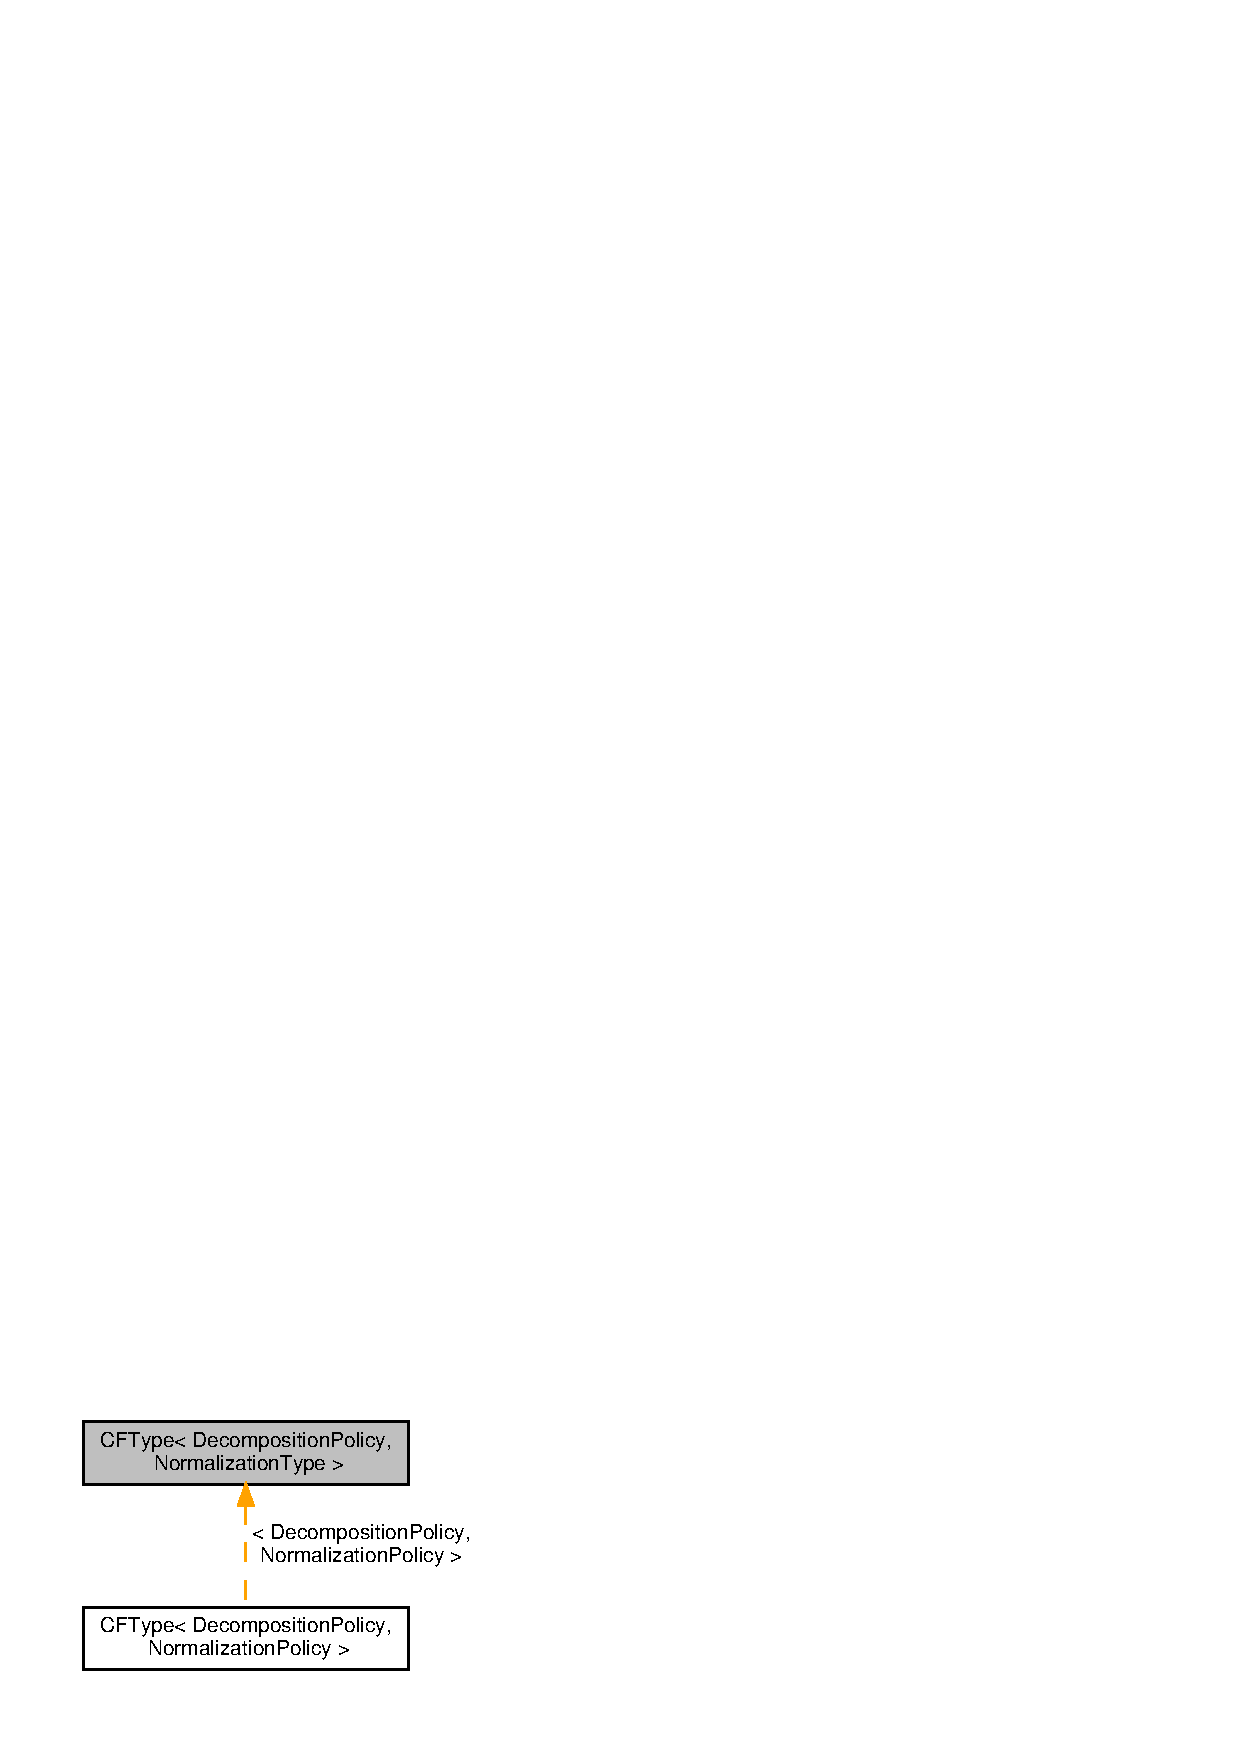
\includegraphics[width=230pt]{classmlpack_1_1cf_1_1CFType__inherit__graph}
\end{center}
\end{figure}
\subsection*{Public Member Functions}
\begin{DoxyCompactItemize}
\item 
\textbf{ C\+F\+Type} (const size\+\_\+t num\+Users\+For\+Similarity=5, const size\+\_\+t rank=0)
\begin{DoxyCompactList}\small\item\em Initialize the \doxyref{C\+F\+Type}{p.}{classmlpack_1_1cf_1_1CFType} object without performing any factorization. \end{DoxyCompactList}\item 
{\footnotesize template$<$typename Mat\+Type $>$ }\\\textbf{ C\+F\+Type} (const Mat\+Type \&data, const Decomposition\+Policy \&decomposition=Decomposition\+Policy(), const size\+\_\+t num\+Users\+For\+Similarity=5, const size\+\_\+t rank=0, const size\+\_\+t max\+Iterations=1000, const double min\+Residue=1e-\/5, const bool mit=false)
\begin{DoxyCompactList}\small\item\em Initialize the \doxyref{C\+F\+Type}{p.}{classmlpack_1_1cf_1_1CFType} object using any decomposition method, immediately factorizing the given data to create a model. \end{DoxyCompactList}\item 
const arma\+::sp\+\_\+mat \& \textbf{ Cleaned\+Data} () const
\begin{DoxyCompactList}\small\item\em Get the cleaned data matrix. \end{DoxyCompactList}\item 
const Decomposition\+Policy \& \textbf{ Decomposition} () const
\begin{DoxyCompactList}\small\item\em Gets decomposition object. \end{DoxyCompactList}\item 
{\footnotesize template$<$typename Neighbor\+Search\+Policy  = Euclidean\+Search, typename Interpolation\+Policy  = Average\+Interpolation$>$ }\\void \textbf{ Get\+Recommendations} (const size\+\_\+t num\+Recs, arma\+::\+Mat$<$ size\+\_\+t $>$ \&recommendations)
\begin{DoxyCompactList}\small\item\em Generates the given number of recommendations for all users. \end{DoxyCompactList}\item 
{\footnotesize template$<$typename Neighbor\+Search\+Policy  = Euclidean\+Search, typename Interpolation\+Policy  = Average\+Interpolation$>$ }\\void \textbf{ Get\+Recommendations} (const size\+\_\+t num\+Recs, arma\+::\+Mat$<$ size\+\_\+t $>$ \&recommendations, const arma\+::\+Col$<$ size\+\_\+t $>$ \&users)
\begin{DoxyCompactList}\small\item\em Generates the given number of recommendations for the specified users. \end{DoxyCompactList}\item 
const Normalization\+Type \& \textbf{ Normalization} () const
\begin{DoxyCompactList}\small\item\em Get the normalization object. \end{DoxyCompactList}\item 
void \textbf{ Num\+Users\+For\+Similarity} (const size\+\_\+t num)
\begin{DoxyCompactList}\small\item\em Sets number of users for calculating similarity. \end{DoxyCompactList}\item 
size\+\_\+t \textbf{ Num\+Users\+For\+Similarity} () const
\begin{DoxyCompactList}\small\item\em Gets number of users for calculating similarity. \end{DoxyCompactList}\item 
{\footnotesize template$<$typename Neighbor\+Search\+Policy  = Euclidean\+Search, typename Interpolation\+Policy  = Average\+Interpolation$>$ }\\double \textbf{ Predict} (const size\+\_\+t user, const size\+\_\+t item) const
\begin{DoxyCompactList}\small\item\em Predict the rating of an item by a particular user. \end{DoxyCompactList}\item 
{\footnotesize template$<$typename Neighbor\+Search\+Policy  = Euclidean\+Search, typename Interpolation\+Policy  = Average\+Interpolation$>$ }\\void \textbf{ Predict} (const arma\+::\+Mat$<$ size\+\_\+t $>$ \&combinations, arma\+::vec \&predictions) const
\begin{DoxyCompactList}\small\item\em Predict ratings for each user-\/item combination in the given coordinate list matrix. \end{DoxyCompactList}\item 
void \textbf{ Rank} (const size\+\_\+t rank\+Value)
\begin{DoxyCompactList}\small\item\em Sets rank parameter for matrix factorization. \end{DoxyCompactList}\item 
size\+\_\+t \textbf{ Rank} () const
\begin{DoxyCompactList}\small\item\em Gets rank parameter for matrix factorization. \end{DoxyCompactList}\item 
{\footnotesize template$<$typename Archive $>$ }\\void \textbf{ serialize} (Archive \&ar, const uint32\+\_\+t)
\begin{DoxyCompactList}\small\item\em Serialize the \doxyref{C\+F\+Type}{p.}{classmlpack_1_1cf_1_1CFType} model to the given archive. \end{DoxyCompactList}\item 
void \textbf{ Train} (const arma\+::mat \&data, const Decomposition\+Policy \&decomposition, const size\+\_\+t max\+Iterations=1000, const double min\+Residue=1e-\/5, const bool mit=false)
\begin{DoxyCompactList}\small\item\em Train the \doxyref{C\+F\+Type}{p.}{classmlpack_1_1cf_1_1CFType} model (i.\+e. \end{DoxyCompactList}\item 
void \textbf{ Train} (const arma\+::sp\+\_\+mat \&data, const Decomposition\+Policy \&decomposition, const size\+\_\+t max\+Iterations=1000, const double min\+Residue=1e-\/5, const bool mit=false)
\begin{DoxyCompactList}\small\item\em Train the \doxyref{C\+F\+Type}{p.}{classmlpack_1_1cf_1_1CFType} model (i.\+e. \end{DoxyCompactList}\end{DoxyCompactItemize}
\subsection*{Static Public Member Functions}
\begin{DoxyCompactItemize}
\item 
static void \textbf{ Clean\+Data} (const arma\+::mat \&data, arma\+::sp\+\_\+mat \&cleaned\+Data)
\begin{DoxyCompactList}\small\item\em Converts the User, Item, Value Matrix to User-\/\+Item Table. \end{DoxyCompactList}\end{DoxyCompactItemize}


\subsection{Detailed Description}
\subsubsection*{template$<$typename Decomposition\+Policy = N\+M\+F\+Policy, typename Normalization\+Type = No\+Normalization$>$\newline
class mlpack\+::cf\+::\+C\+F\+Type$<$ Decomposition\+Policy, Normalization\+Type $>$}

This class implements Collaborative Filtering (CF). 

This implementation presently supports Alternating Least Squares (A\+LS) for collaborative filtering.

A simple example of how to run Collaborative Filtering is shown below.


\begin{DoxyCode}
\textcolor{keyword}{extern} arma::mat data; \textcolor{comment}{// (user, item, rating) table}
\textcolor{keyword}{extern} arma::Col<size\_t> users; \textcolor{comment}{// users seeking recommendations}
arma::Mat<size\_t> recommendations; \textcolor{comment}{// Recommendations}

CFType<> cf(data); \textcolor{comment}{// Default options.}

\textcolor{comment}{// Generate 10 recommendations for all users.}
cf.GetRecommendations(10, recommendations);

\textcolor{comment}{// Generate 10 recommendations for specified users.}
cf.GetRecommendations(10, recommendations, users);
\end{DoxyCode}


The data matrix is a (user, item, rating) table. Each column in the matrix should have three rows. The first represents the user; the second represents the item; and the third represents the rating. The user and item, while they are in a matrix that holds doubles, should hold integer (or size\+\_\+t) values. The user and item indices are assumed to start at 0.


\begin{DoxyTemplParams}{Template Parameters}
{\em Decomposition\+Policy} & The policy used to decompose the rating matrix. It also provides methods to compute prediction and neighborhood. \\
\hline
{\em Normalization\+Type} & The type of normalization performed on raw data. Data is normalized before calling \doxyref{Train()}{p.}{classmlpack_1_1cf_1_1CFType_a6c7cc418bd1efca587106fbe387534ee} method. Predicted rating is denormalized before return. \\
\hline
\end{DoxyTemplParams}


Definition at line 70 of file cf.\+hpp.



\subsection{Constructor \& Destructor Documentation}
\mbox{\label{classmlpack_1_1cf_1_1CFType_a1ede74b2271ab9e82f8db2dbc27adf13}} 
\index{mlpack\+::cf\+::\+C\+F\+Type@{mlpack\+::cf\+::\+C\+F\+Type}!C\+F\+Type@{C\+F\+Type}}
\index{C\+F\+Type@{C\+F\+Type}!mlpack\+::cf\+::\+C\+F\+Type@{mlpack\+::cf\+::\+C\+F\+Type}}
\subsubsection{C\+F\+Type()\hspace{0.1cm}{\footnotesize\ttfamily [1/2]}}
{\footnotesize\ttfamily \textbf{ C\+F\+Type} (\begin{DoxyParamCaption}\item[{const size\+\_\+t}]{num\+Users\+For\+Similarity = {\ttfamily 5},  }\item[{const size\+\_\+t}]{rank = {\ttfamily 0} }\end{DoxyParamCaption})}



Initialize the \doxyref{C\+F\+Type}{p.}{classmlpack_1_1cf_1_1CFType} object without performing any factorization. 

Be sure to call \doxyref{Train()}{p.}{classmlpack_1_1cf_1_1CFType_a6c7cc418bd1efca587106fbe387534ee} before calling \doxyref{Get\+Recommendations()}{p.}{classmlpack_1_1cf_1_1CFType_aea00d8c8dfad713dd5542e450d633d5a} or any other functions! \mbox{\label{classmlpack_1_1cf_1_1CFType_a6451c7152ccb66da74f6e98b1db7ec8e}} 
\index{mlpack\+::cf\+::\+C\+F\+Type@{mlpack\+::cf\+::\+C\+F\+Type}!C\+F\+Type@{C\+F\+Type}}
\index{C\+F\+Type@{C\+F\+Type}!mlpack\+::cf\+::\+C\+F\+Type@{mlpack\+::cf\+::\+C\+F\+Type}}
\subsubsection{C\+F\+Type()\hspace{0.1cm}{\footnotesize\ttfamily [2/2]}}
{\footnotesize\ttfamily \textbf{ C\+F\+Type} (\begin{DoxyParamCaption}\item[{const Mat\+Type \&}]{data,  }\item[{const Decomposition\+Policy \&}]{decomposition = {\ttfamily DecompositionPolicy()},  }\item[{const size\+\_\+t}]{num\+Users\+For\+Similarity = {\ttfamily 5},  }\item[{const size\+\_\+t}]{rank = {\ttfamily 0},  }\item[{const size\+\_\+t}]{max\+Iterations = {\ttfamily 1000},  }\item[{const double}]{min\+Residue = {\ttfamily 1e-\/5},  }\item[{const bool}]{mit = {\ttfamily false} }\end{DoxyParamCaption})}



Initialize the \doxyref{C\+F\+Type}{p.}{classmlpack_1_1cf_1_1CFType} object using any decomposition method, immediately factorizing the given data to create a model. 

There are parameters that can be set; default values are provided for each of them. If the rank is left unset (or is set to 0), a simple density-\/based heuristic will be used to choose a rank.

The provided dataset can be a coordinate list; that is, a 3-\/row matrix where each column corresponds to a (user, item, rating) entry in the matrix or a sparse matrix representing (user, item) table.


\begin{DoxyTemplParams}{Template Parameters}
{\em Mat\+Type} & The type of input matrix, which is expected to be either arma\+::mat (table of (user, item, rating)) or arma\+::sp\+\_\+mat (sparse rating matrix where row is item and column is user).\\
\hline
\end{DoxyTemplParams}

\begin{DoxyParams}{Parameters}
{\em data} & Data matrix\+: dense matrix (coordinate lists) or sparse matrix(cleaned). \\
\hline
{\em decomposition} & Instantiated Decomposition\+Policy object. \\
\hline
{\em num\+Users\+For\+Similarity} & Size of the neighborhood. \\
\hline
{\em rank} & Rank parameter for matrix factorization. \\
\hline
{\em max\+Iterations} & Maximum number of iterations. \\
\hline
{\em min\+Residue} & Residue required to terminate. \\
\hline
{\em mit} & Whether to terminate only when max\+Iterations is reached. \\
\hline
\end{DoxyParams}


\subsection{Member Function Documentation}
\mbox{\label{classmlpack_1_1cf_1_1CFType_a6606a419e5db3e8218a4f0c6b1c81258}} 
\index{mlpack\+::cf\+::\+C\+F\+Type@{mlpack\+::cf\+::\+C\+F\+Type}!Clean\+Data@{Clean\+Data}}
\index{Clean\+Data@{Clean\+Data}!mlpack\+::cf\+::\+C\+F\+Type@{mlpack\+::cf\+::\+C\+F\+Type}}
\subsubsection{Clean\+Data()}
{\footnotesize\ttfamily static void Clean\+Data (\begin{DoxyParamCaption}\item[{const arma\+::mat \&}]{data,  }\item[{arma\+::sp\+\_\+mat \&}]{cleaned\+Data }\end{DoxyParamCaption})\hspace{0.3cm}{\ttfamily [static]}}



Converts the User, Item, Value Matrix to User-\/\+Item Table. 



Referenced by C\+F\+Type$<$ Decomposition\+Policy, Normalization\+Policy $>$\+::\+Normalization().

\mbox{\label{classmlpack_1_1cf_1_1CFType_a9b45ccc1241c683ffaaf1be745b438d0}} 
\index{mlpack\+::cf\+::\+C\+F\+Type@{mlpack\+::cf\+::\+C\+F\+Type}!Cleaned\+Data@{Cleaned\+Data}}
\index{Cleaned\+Data@{Cleaned\+Data}!mlpack\+::cf\+::\+C\+F\+Type@{mlpack\+::cf\+::\+C\+F\+Type}}
\subsubsection{Cleaned\+Data()}
{\footnotesize\ttfamily const arma\+::sp\+\_\+mat\& Cleaned\+Data (\begin{DoxyParamCaption}{ }\end{DoxyParamCaption}) const\hspace{0.3cm}{\ttfamily [inline]}}



Get the cleaned data matrix. 



Definition at line 180 of file cf.\+hpp.

\mbox{\label{classmlpack_1_1cf_1_1CFType_a2312b615423d95028bd2211c61a7d74d}} 
\index{mlpack\+::cf\+::\+C\+F\+Type@{mlpack\+::cf\+::\+C\+F\+Type}!Decomposition@{Decomposition}}
\index{Decomposition@{Decomposition}!mlpack\+::cf\+::\+C\+F\+Type@{mlpack\+::cf\+::\+C\+F\+Type}}
\subsubsection{Decomposition()}
{\footnotesize\ttfamily const Decomposition\+Policy\& Decomposition (\begin{DoxyParamCaption}{ }\end{DoxyParamCaption}) const\hspace{0.3cm}{\ttfamily [inline]}}



Gets decomposition object. 



Definition at line 177 of file cf.\+hpp.

\mbox{\label{classmlpack_1_1cf_1_1CFType_aea00d8c8dfad713dd5542e450d633d5a}} 
\index{mlpack\+::cf\+::\+C\+F\+Type@{mlpack\+::cf\+::\+C\+F\+Type}!Get\+Recommendations@{Get\+Recommendations}}
\index{Get\+Recommendations@{Get\+Recommendations}!mlpack\+::cf\+::\+C\+F\+Type@{mlpack\+::cf\+::\+C\+F\+Type}}
\subsubsection{Get\+Recommendations()\hspace{0.1cm}{\footnotesize\ttfamily [1/2]}}
{\footnotesize\ttfamily void Get\+Recommendations (\begin{DoxyParamCaption}\item[{const size\+\_\+t}]{num\+Recs,  }\item[{arma\+::\+Mat$<$ size\+\_\+t $>$ \&}]{recommendations }\end{DoxyParamCaption})}



Generates the given number of recommendations for all users. 


\begin{DoxyTemplParams}{Template Parameters}
{\em Neighbor\+Search\+Policy} & The policy used to search neighbors of query set in referece set. \\
\hline
{\em Interpolation\+Policy} & The policy used to calculate interpolation weights.\\
\hline
\end{DoxyTemplParams}

\begin{DoxyParams}{Parameters}
{\em num\+Recs} & Number of Recommendations. \\
\hline
{\em recommendations} & Matrix to save recommendations into. \\
\hline
\end{DoxyParams}


Referenced by C\+F\+Type$<$ Decomposition\+Policy, Normalization\+Policy $>$\+::\+Normalization().

\mbox{\label{classmlpack_1_1cf_1_1CFType_a07ca697e6ba5cf1b7056071914e708a1}} 
\index{mlpack\+::cf\+::\+C\+F\+Type@{mlpack\+::cf\+::\+C\+F\+Type}!Get\+Recommendations@{Get\+Recommendations}}
\index{Get\+Recommendations@{Get\+Recommendations}!mlpack\+::cf\+::\+C\+F\+Type@{mlpack\+::cf\+::\+C\+F\+Type}}
\subsubsection{Get\+Recommendations()\hspace{0.1cm}{\footnotesize\ttfamily [2/2]}}
{\footnotesize\ttfamily void Get\+Recommendations (\begin{DoxyParamCaption}\item[{const size\+\_\+t}]{num\+Recs,  }\item[{arma\+::\+Mat$<$ size\+\_\+t $>$ \&}]{recommendations,  }\item[{const arma\+::\+Col$<$ size\+\_\+t $>$ \&}]{users }\end{DoxyParamCaption})}



Generates the given number of recommendations for the specified users. 


\begin{DoxyTemplParams}{Template Parameters}
{\em Neighbor\+Search\+Policy} & The policy used to search neighbors of query set in referece set. \\
\hline
{\em Interpolation\+Policy} & The policy used to calculate interpolation weights.\\
\hline
\end{DoxyTemplParams}

\begin{DoxyParams}{Parameters}
{\em num\+Recs} & Number of Recommendations. \\
\hline
{\em recommendations} & Matrix to save recommendations. \\
\hline
{\em users} & Users for which recommendations are to be generated. \\
\hline
\end{DoxyParams}
\mbox{\label{classmlpack_1_1cf_1_1CFType_a85300f3ff2c7f809a8dbe783f833e7b1}} 
\index{mlpack\+::cf\+::\+C\+F\+Type@{mlpack\+::cf\+::\+C\+F\+Type}!Normalization@{Normalization}}
\index{Normalization@{Normalization}!mlpack\+::cf\+::\+C\+F\+Type@{mlpack\+::cf\+::\+C\+F\+Type}}
\subsubsection{Normalization()}
{\footnotesize\ttfamily const Normalization\+Type\& Normalization (\begin{DoxyParamCaption}{ }\end{DoxyParamCaption}) const\hspace{0.3cm}{\ttfamily [inline]}}



Get the normalization object. 



Definition at line 183 of file cf.\+hpp.

\mbox{\label{classmlpack_1_1cf_1_1CFType_ab907e6b81f7b38e654d185077603466f}} 
\index{mlpack\+::cf\+::\+C\+F\+Type@{mlpack\+::cf\+::\+C\+F\+Type}!Num\+Users\+For\+Similarity@{Num\+Users\+For\+Similarity}}
\index{Num\+Users\+For\+Similarity@{Num\+Users\+For\+Similarity}!mlpack\+::cf\+::\+C\+F\+Type@{mlpack\+::cf\+::\+C\+F\+Type}}
\subsubsection{Num\+Users\+For\+Similarity()\hspace{0.1cm}{\footnotesize\ttfamily [1/2]}}
{\footnotesize\ttfamily void Num\+Users\+For\+Similarity (\begin{DoxyParamCaption}\item[{const size\+\_\+t}]{num }\end{DoxyParamCaption})\hspace{0.3cm}{\ttfamily [inline]}}



Sets number of users for calculating similarity. 



Definition at line 147 of file cf.\+hpp.

\mbox{\label{classmlpack_1_1cf_1_1CFType_a90464e33b6300c307c7d4741f3c5f791}} 
\index{mlpack\+::cf\+::\+C\+F\+Type@{mlpack\+::cf\+::\+C\+F\+Type}!Num\+Users\+For\+Similarity@{Num\+Users\+For\+Similarity}}
\index{Num\+Users\+For\+Similarity@{Num\+Users\+For\+Similarity}!mlpack\+::cf\+::\+C\+F\+Type@{mlpack\+::cf\+::\+C\+F\+Type}}
\subsubsection{Num\+Users\+For\+Similarity()\hspace{0.1cm}{\footnotesize\ttfamily [2/2]}}
{\footnotesize\ttfamily size\+\_\+t Num\+Users\+For\+Similarity (\begin{DoxyParamCaption}{ }\end{DoxyParamCaption}) const\hspace{0.3cm}{\ttfamily [inline]}}



Gets number of users for calculating similarity. 



Definition at line 159 of file cf.\+hpp.

\mbox{\label{classmlpack_1_1cf_1_1CFType_a40809f18b938075bb471c5f32e6ec57c}} 
\index{mlpack\+::cf\+::\+C\+F\+Type@{mlpack\+::cf\+::\+C\+F\+Type}!Predict@{Predict}}
\index{Predict@{Predict}!mlpack\+::cf\+::\+C\+F\+Type@{mlpack\+::cf\+::\+C\+F\+Type}}
\subsubsection{Predict()\hspace{0.1cm}{\footnotesize\ttfamily [1/2]}}
{\footnotesize\ttfamily double Predict (\begin{DoxyParamCaption}\item[{const size\+\_\+t}]{user,  }\item[{const size\+\_\+t}]{item }\end{DoxyParamCaption}) const}



Predict the rating of an item by a particular user. 


\begin{DoxyTemplParams}{Template Parameters}
{\em Neighbor\+Search\+Policy} & The policy used to search neighbors of query set in referece set. \\
\hline
{\em Interpolation\+Policy} & The policy used to calculate interpolation weights.\\
\hline
\end{DoxyTemplParams}

\begin{DoxyParams}{Parameters}
{\em user} & User to predict for. \\
\hline
{\em item} & Item to predict for. \\
\hline
\end{DoxyParams}


Referenced by C\+F\+Type$<$ Decomposition\+Policy, Normalization\+Policy $>$\+::\+Normalization().

\mbox{\label{classmlpack_1_1cf_1_1CFType_a66e488fde0b5aab4a0c3aab318382bd3}} 
\index{mlpack\+::cf\+::\+C\+F\+Type@{mlpack\+::cf\+::\+C\+F\+Type}!Predict@{Predict}}
\index{Predict@{Predict}!mlpack\+::cf\+::\+C\+F\+Type@{mlpack\+::cf\+::\+C\+F\+Type}}
\subsubsection{Predict()\hspace{0.1cm}{\footnotesize\ttfamily [2/2]}}
{\footnotesize\ttfamily void Predict (\begin{DoxyParamCaption}\item[{const arma\+::\+Mat$<$ size\+\_\+t $>$ \&}]{combinations,  }\item[{arma\+::vec \&}]{predictions }\end{DoxyParamCaption}) const}



Predict ratings for each user-\/item combination in the given coordinate list matrix. 

The matrix \textquotesingle{}combinations\textquotesingle{} should have two rows and number of columns equal to the number of desired predictions. The first element of each column corresponds to the user index, and the second element of each column corresponds to the item index. The output vector \textquotesingle{}predictions\textquotesingle{} will have length equal to combinations.\+n\+\_\+cols, and predictions[i] will be equal to the prediction for the user/item combination in combinations.\+col(i).


\begin{DoxyTemplParams}{Template Parameters}
{\em Neighbor\+Search\+Policy} & The policy used to search neighbors of query set in referece set. \\
\hline
{\em Interpolation\+Policy} & The policy used to calculate interpolation weights.\\
\hline
\end{DoxyTemplParams}

\begin{DoxyParams}{Parameters}
{\em combinations} & User/item combinations to predict. \\
\hline
{\em predictions} & Predicted ratings for each user/item combination. \\
\hline
\end{DoxyParams}
\mbox{\label{classmlpack_1_1cf_1_1CFType_a6abdfd96dee1459e1640a6d6e1d1eec4}} 
\index{mlpack\+::cf\+::\+C\+F\+Type@{mlpack\+::cf\+::\+C\+F\+Type}!Rank@{Rank}}
\index{Rank@{Rank}!mlpack\+::cf\+::\+C\+F\+Type@{mlpack\+::cf\+::\+C\+F\+Type}}
\subsubsection{Rank()\hspace{0.1cm}{\footnotesize\ttfamily [1/2]}}
{\footnotesize\ttfamily void Rank (\begin{DoxyParamCaption}\item[{const size\+\_\+t}]{rank\+Value }\end{DoxyParamCaption})\hspace{0.3cm}{\ttfamily [inline]}}



Sets rank parameter for matrix factorization. 



Definition at line 165 of file cf.\+hpp.

\mbox{\label{classmlpack_1_1cf_1_1CFType_afe1447c5e7fa184cbf19ced57a50b7b6}} 
\index{mlpack\+::cf\+::\+C\+F\+Type@{mlpack\+::cf\+::\+C\+F\+Type}!Rank@{Rank}}
\index{Rank@{Rank}!mlpack\+::cf\+::\+C\+F\+Type@{mlpack\+::cf\+::\+C\+F\+Type}}
\subsubsection{Rank()\hspace{0.1cm}{\footnotesize\ttfamily [2/2]}}
{\footnotesize\ttfamily size\+\_\+t Rank (\begin{DoxyParamCaption}{ }\end{DoxyParamCaption}) const\hspace{0.3cm}{\ttfamily [inline]}}



Gets rank parameter for matrix factorization. 



Definition at line 171 of file cf.\+hpp.

\mbox{\label{classmlpack_1_1cf_1_1CFType_a65cba07328997659bec80b9879b15a51}} 
\index{mlpack\+::cf\+::\+C\+F\+Type@{mlpack\+::cf\+::\+C\+F\+Type}!serialize@{serialize}}
\index{serialize@{serialize}!mlpack\+::cf\+::\+C\+F\+Type@{mlpack\+::cf\+::\+C\+F\+Type}}
\subsubsection{serialize()}
{\footnotesize\ttfamily void serialize (\begin{DoxyParamCaption}\item[{Archive \&}]{ar,  }\item[{const uint32\+\_\+t}]{ }\end{DoxyParamCaption})}



Serialize the \doxyref{C\+F\+Type}{p.}{classmlpack_1_1cf_1_1CFType} model to the given archive. 



Referenced by C\+F\+Type$<$ Decomposition\+Policy, Normalization\+Policy $>$\+::\+Normalization().

\mbox{\label{classmlpack_1_1cf_1_1CFType_a6c7cc418bd1efca587106fbe387534ee}} 
\index{mlpack\+::cf\+::\+C\+F\+Type@{mlpack\+::cf\+::\+C\+F\+Type}!Train@{Train}}
\index{Train@{Train}!mlpack\+::cf\+::\+C\+F\+Type@{mlpack\+::cf\+::\+C\+F\+Type}}
\subsubsection{Train()\hspace{0.1cm}{\footnotesize\ttfamily [1/2]}}
{\footnotesize\ttfamily void Train (\begin{DoxyParamCaption}\item[{const arma\+::mat \&}]{data,  }\item[{const Decomposition\+Policy \&}]{decomposition,  }\item[{const size\+\_\+t}]{max\+Iterations = {\ttfamily 1000},  }\item[{const double}]{min\+Residue = {\ttfamily 1e-\/5},  }\item[{const bool}]{mit = {\ttfamily false} }\end{DoxyParamCaption})}



Train the \doxyref{C\+F\+Type}{p.}{classmlpack_1_1cf_1_1CFType} model (i.\+e. 

factorize the input matrix) using the parameters that have already been set for the model (specifically, the rank parameter), and optionally, using the given Decomposition\+Policy.


\begin{DoxyParams}{Parameters}
{\em data} & Input dataset; dense matrix (coordinate lists). \\
\hline
{\em decomposition} & Instantiated Decomposition\+Policy object. \\
\hline
{\em max\+Iterations} & Maximum number of iterations. \\
\hline
{\em min\+Residue} & Residue required to terminate. \\
\hline
{\em mit} & Whether to terminate only when max\+Iterations is reached. \\
\hline
\end{DoxyParams}
\mbox{\label{classmlpack_1_1cf_1_1CFType_a521c130dfede7ce4f794e478aa50463f}} 
\index{mlpack\+::cf\+::\+C\+F\+Type@{mlpack\+::cf\+::\+C\+F\+Type}!Train@{Train}}
\index{Train@{Train}!mlpack\+::cf\+::\+C\+F\+Type@{mlpack\+::cf\+::\+C\+F\+Type}}
\subsubsection{Train()\hspace{0.1cm}{\footnotesize\ttfamily [2/2]}}
{\footnotesize\ttfamily void Train (\begin{DoxyParamCaption}\item[{const arma\+::sp\+\_\+mat \&}]{data,  }\item[{const Decomposition\+Policy \&}]{decomposition,  }\item[{const size\+\_\+t}]{max\+Iterations = {\ttfamily 1000},  }\item[{const double}]{min\+Residue = {\ttfamily 1e-\/5},  }\item[{const bool}]{mit = {\ttfamily false} }\end{DoxyParamCaption})}



Train the \doxyref{C\+F\+Type}{p.}{classmlpack_1_1cf_1_1CFType} model (i.\+e. 

factorize the input matrix) using the parameters that have already been set for the model (specifically, the rank parameter), and optionally, using the given Decomposition\+Policy.


\begin{DoxyParams}{Parameters}
{\em data} & Input dataset; sparse matrix (user item table). \\
\hline
{\em decomposition} & Instantiated Decomposition\+Policy object. \\
\hline
{\em max\+Iterations} & Maximum number of iterations. \\
\hline
{\em min\+Residue} & Residue required to terminate. \\
\hline
{\em mit} & Whether to terminate only when max\+Iterations is reached. \\
\hline
\end{DoxyParams}


The documentation for this class was generated from the following file\+:\begin{DoxyCompactItemize}
\item 
/home/aakash/mlpack/src/mlpack/methods/cf/\textbf{ cf.\+hpp}\end{DoxyCompactItemize}

\section{C\+F\+Wrapper$<$ Decomposition\+Policy, Normalization\+Policy $>$ Class Template Reference}
\label{classmlpack_1_1cf_1_1CFWrapper}\index{C\+F\+Wrapper$<$ Decomposition\+Policy, Normalization\+Policy $>$@{C\+F\+Wrapper$<$ Decomposition\+Policy, Normalization\+Policy $>$}}


The \doxyref{C\+F\+Wrapper}{p.}{classmlpack_1_1cf_1_1CFWrapper} class wraps the functionality of all CF types.  




Inheritance diagram for C\+F\+Wrapper$<$ Decomposition\+Policy, Normalization\+Policy $>$\+:
\nopagebreak
\begin{figure}[H]
\begin{center}
\leavevmode
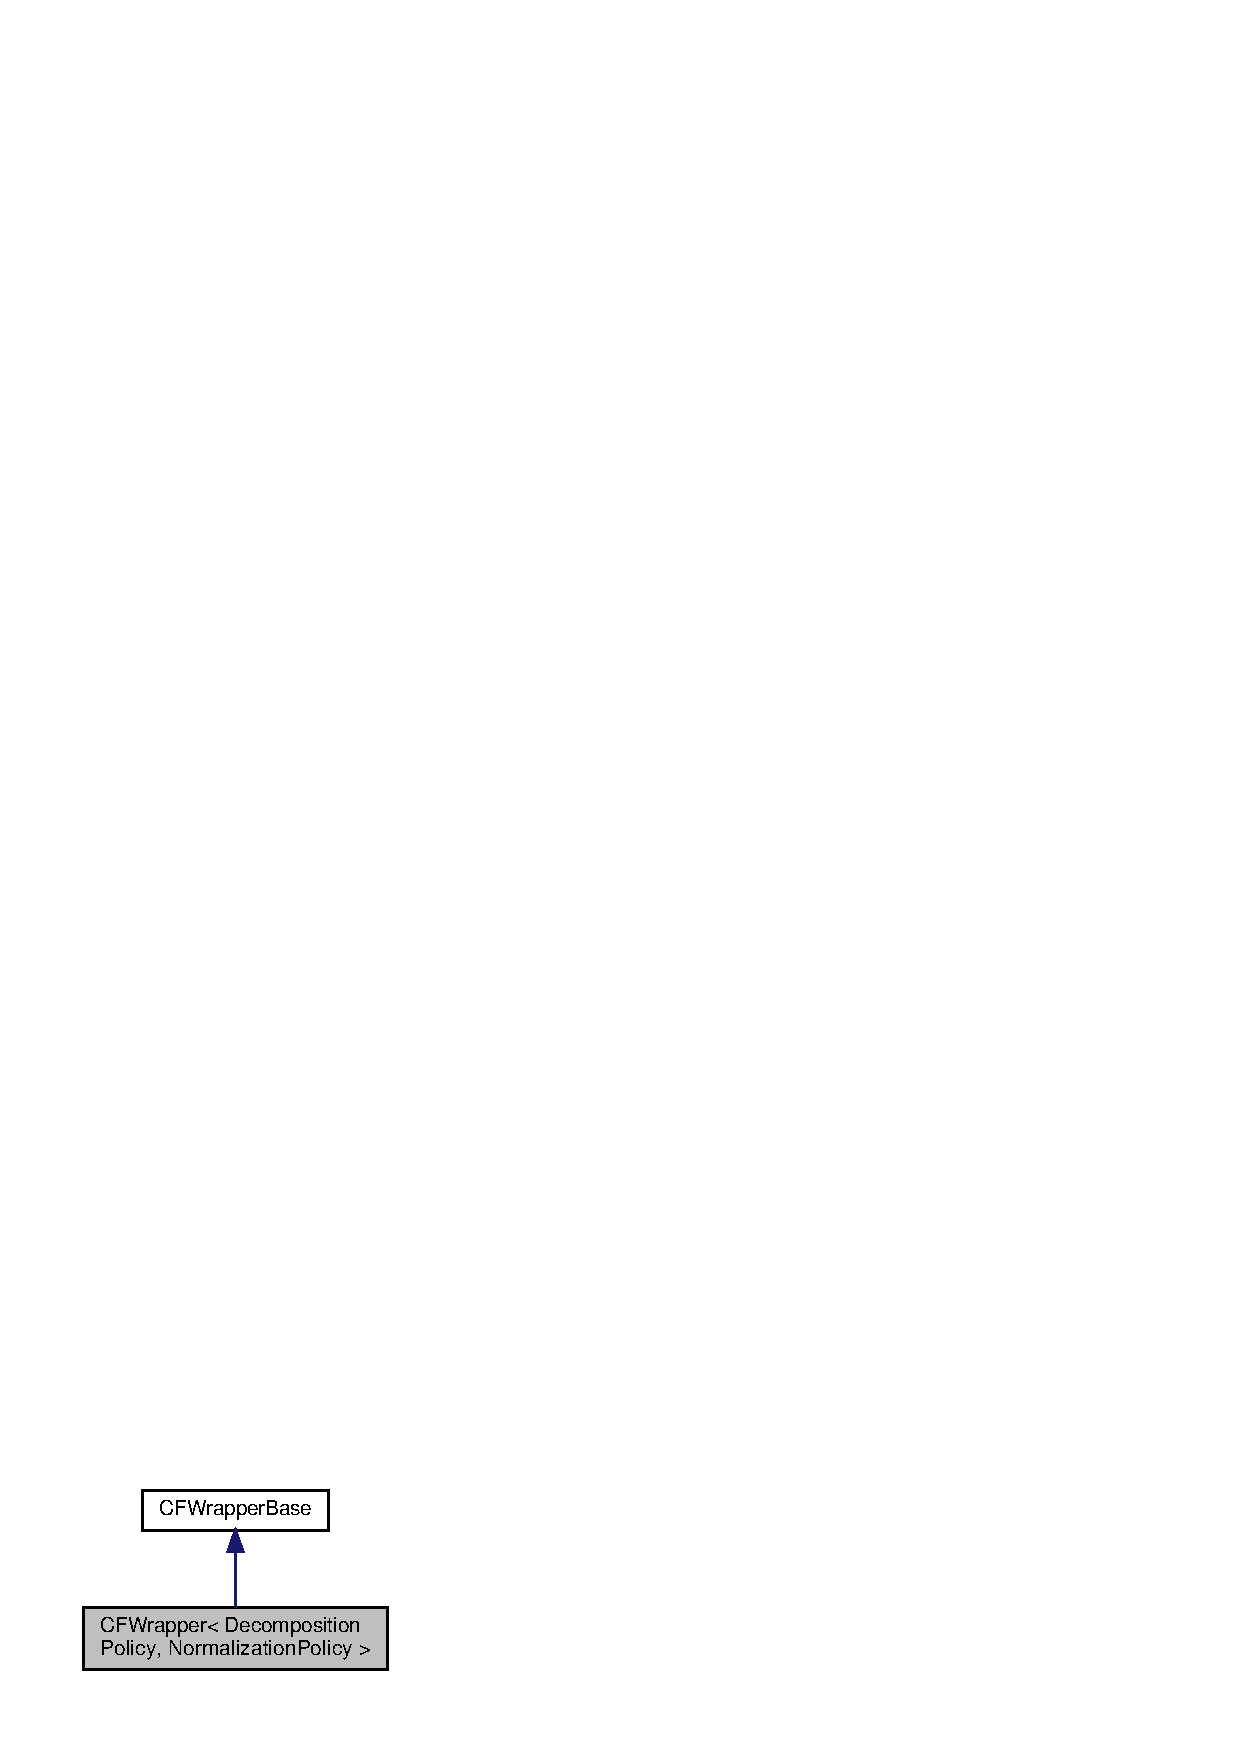
\includegraphics[width=190pt]{classmlpack_1_1cf_1_1CFWrapper__inherit__graph}
\end{center}
\end{figure}
\subsection*{Public Member Functions}
\begin{DoxyCompactItemize}
\item 
\textbf{ C\+F\+Wrapper} ()
\begin{DoxyCompactList}\small\item\em Create the \doxyref{C\+F\+Wrapper}{p.}{classmlpack_1_1cf_1_1CFWrapper} object, using default parameters to initialize the held CF object. \end{DoxyCompactList}\item 
\textbf{ C\+F\+Wrapper} (const arma\+::mat \&data, const Decomposition\+Policy \&decomposition, const size\+\_\+t num\+Users\+For\+Similarity, const size\+\_\+t rank, const size\+\_\+t max\+Iterations, const size\+\_\+t min\+Residue, const bool mit)
\begin{DoxyCompactList}\small\item\em Create the \doxyref{C\+F\+Wrapper}{p.}{classmlpack_1_1cf_1_1CFWrapper} object, initializing the held CF object. \end{DoxyCompactList}\item 
virtual \textbf{ $\sim$\+C\+F\+Wrapper} ()
\begin{DoxyCompactList}\small\item\em Destroy the \doxyref{C\+F\+Wrapper}{p.}{classmlpack_1_1cf_1_1CFWrapper} object. \end{DoxyCompactList}\item 
\textbf{ C\+F\+Model\+Type} \& \textbf{ CF} ()
\begin{DoxyCompactList}\small\item\em Get the \doxyref{C\+F\+Type}{p.}{classmlpack_1_1cf_1_1CFType} object. \end{DoxyCompactList}\item 
virtual \textbf{ C\+F\+Wrapper} $\ast$ \textbf{ Clone} () const
\begin{DoxyCompactList}\small\item\em Clone the \doxyref{C\+F\+Wrapper}{p.}{classmlpack_1_1cf_1_1CFWrapper} object. This handles polymorphism correctly. \end{DoxyCompactList}\item 
virtual void \textbf{ Get\+Recommendations} (const \textbf{ Neighbor\+Search\+Types} ns\+Type, const \textbf{ Interpolation\+Types} interpolation\+Type, const size\+\_\+t num\+Recs, arma\+::\+Mat$<$ size\+\_\+t $>$ \&recommendations)
\begin{DoxyCompactList}\small\item\em Compute recommendations for all users. \end{DoxyCompactList}\item 
virtual void \textbf{ Get\+Recommendations} (const \textbf{ Neighbor\+Search\+Types} ns\+Type, const \textbf{ Interpolation\+Types} interpolation\+Type, const size\+\_\+t num\+Recs, arma\+::\+Mat$<$ size\+\_\+t $>$ \&recommendations, const arma\+::\+Col$<$ size\+\_\+t $>$ \&users)
\begin{DoxyCompactList}\small\item\em Compute recommendations. \end{DoxyCompactList}\item 
virtual void \textbf{ Predict} (const \textbf{ Neighbor\+Search\+Types} ns\+Type, const \textbf{ Interpolation\+Types} interpolation\+Type, const arma\+::\+Mat$<$ size\+\_\+t $>$ \&combinations, arma\+::vec \&predictions)
\begin{DoxyCompactList}\small\item\em Compute predictions for users. \end{DoxyCompactList}\item 
{\footnotesize template$<$typename Archive $>$ }\\void \textbf{ serialize} (Archive \&ar, const uint32\+\_\+t)
\begin{DoxyCompactList}\small\item\em Serialize the model. \end{DoxyCompactList}\end{DoxyCompactItemize}
\subsection*{Protected Types}
\begin{DoxyCompactItemize}
\item 
typedef \textbf{ C\+F\+Type}$<$ Decomposition\+Policy, Normalization\+Policy $>$ \textbf{ C\+F\+Model\+Type}
\end{DoxyCompactItemize}
\subsection*{Protected Attributes}
\begin{DoxyCompactItemize}
\item 
\textbf{ C\+F\+Model\+Type} \textbf{ cf}
\begin{DoxyCompactList}\small\item\em This is the CF object that we are wrapping. \end{DoxyCompactList}\end{DoxyCompactItemize}


\subsection{Detailed Description}
\subsubsection*{template$<$typename Decomposition\+Policy, typename Normalization\+Policy$>$\newline
class mlpack\+::cf\+::\+C\+F\+Wrapper$<$ Decomposition\+Policy, Normalization\+Policy $>$}

The \doxyref{C\+F\+Wrapper}{p.}{classmlpack_1_1cf_1_1CFWrapper} class wraps the functionality of all CF types. 

If special handling is needed for a future CF type, this class can be extended. 

Definition at line 88 of file cf\+\_\+model.\+hpp.



\subsection{Member Typedef Documentation}
\mbox{\label{classmlpack_1_1cf_1_1CFWrapper_ab3a99733c27e27fe3b5204e5c29fa58b}} 
\index{mlpack\+::cf\+::\+C\+F\+Wrapper@{mlpack\+::cf\+::\+C\+F\+Wrapper}!C\+F\+Model\+Type@{C\+F\+Model\+Type}}
\index{C\+F\+Model\+Type@{C\+F\+Model\+Type}!mlpack\+::cf\+::\+C\+F\+Wrapper@{mlpack\+::cf\+::\+C\+F\+Wrapper}}
\subsubsection{C\+F\+Model\+Type}
{\footnotesize\ttfamily typedef \textbf{ C\+F\+Type}$<$Decomposition\+Policy, Normalization\+Policy$>$ \textbf{ C\+F\+Model\+Type}\hspace{0.3cm}{\ttfamily [protected]}}



Definition at line 91 of file cf\+\_\+model.\+hpp.



\subsection{Constructor \& Destructor Documentation}
\mbox{\label{classmlpack_1_1cf_1_1CFWrapper_aeed748fe1f1ae910198e8c3d454d9a05}} 
\index{mlpack\+::cf\+::\+C\+F\+Wrapper@{mlpack\+::cf\+::\+C\+F\+Wrapper}!C\+F\+Wrapper@{C\+F\+Wrapper}}
\index{C\+F\+Wrapper@{C\+F\+Wrapper}!mlpack\+::cf\+::\+C\+F\+Wrapper@{mlpack\+::cf\+::\+C\+F\+Wrapper}}
\subsubsection{C\+F\+Wrapper()\hspace{0.1cm}{\footnotesize\ttfamily [1/2]}}
{\footnotesize\ttfamily \textbf{ C\+F\+Wrapper} (\begin{DoxyParamCaption}{ }\end{DoxyParamCaption})\hspace{0.3cm}{\ttfamily [inline]}}



Create the \doxyref{C\+F\+Wrapper}{p.}{classmlpack_1_1cf_1_1CFWrapper} object, using default parameters to initialize the held CF object. 



Definition at line 96 of file cf\+\_\+model.\+hpp.

\mbox{\label{classmlpack_1_1cf_1_1CFWrapper_a6c9fe1dd052abe1ea6f41f508d8a12f3}} 
\index{mlpack\+::cf\+::\+C\+F\+Wrapper@{mlpack\+::cf\+::\+C\+F\+Wrapper}!C\+F\+Wrapper@{C\+F\+Wrapper}}
\index{C\+F\+Wrapper@{C\+F\+Wrapper}!mlpack\+::cf\+::\+C\+F\+Wrapper@{mlpack\+::cf\+::\+C\+F\+Wrapper}}
\subsubsection{C\+F\+Wrapper()\hspace{0.1cm}{\footnotesize\ttfamily [2/2]}}
{\footnotesize\ttfamily \textbf{ C\+F\+Wrapper} (\begin{DoxyParamCaption}\item[{const arma\+::mat \&}]{data,  }\item[{const Decomposition\+Policy \&}]{decomposition,  }\item[{const size\+\_\+t}]{num\+Users\+For\+Similarity,  }\item[{const size\+\_\+t}]{rank,  }\item[{const size\+\_\+t}]{max\+Iterations,  }\item[{const size\+\_\+t}]{min\+Residue,  }\item[{const bool}]{mit }\end{DoxyParamCaption})\hspace{0.3cm}{\ttfamily [inline]}}



Create the \doxyref{C\+F\+Wrapper}{p.}{classmlpack_1_1cf_1_1CFWrapper} object, initializing the held CF object. 



Definition at line 99 of file cf\+\_\+model.\+hpp.

\mbox{\label{classmlpack_1_1cf_1_1CFWrapper_ab10ab909d67a29b5d9eb7b70c68c0265}} 
\index{mlpack\+::cf\+::\+C\+F\+Wrapper@{mlpack\+::cf\+::\+C\+F\+Wrapper}!````~C\+F\+Wrapper@{$\sim$\+C\+F\+Wrapper}}
\index{````~C\+F\+Wrapper@{$\sim$\+C\+F\+Wrapper}!mlpack\+::cf\+::\+C\+F\+Wrapper@{mlpack\+::cf\+::\+C\+F\+Wrapper}}
\subsubsection{$\sim$\+C\+F\+Wrapper()}
{\footnotesize\ttfamily virtual $\sim$\textbf{ C\+F\+Wrapper} (\begin{DoxyParamCaption}{ }\end{DoxyParamCaption})\hspace{0.3cm}{\ttfamily [inline]}, {\ttfamily [virtual]}}



Destroy the \doxyref{C\+F\+Wrapper}{p.}{classmlpack_1_1cf_1_1CFWrapper} object. 



Definition at line 121 of file cf\+\_\+model.\+hpp.



\subsection{Member Function Documentation}
\mbox{\label{classmlpack_1_1cf_1_1CFWrapper_a4408b593924d45ed5703e81a27c89a4f}} 
\index{mlpack\+::cf\+::\+C\+F\+Wrapper@{mlpack\+::cf\+::\+C\+F\+Wrapper}!CF@{CF}}
\index{CF@{CF}!mlpack\+::cf\+::\+C\+F\+Wrapper@{mlpack\+::cf\+::\+C\+F\+Wrapper}}
\subsubsection{C\+F()}
{\footnotesize\ttfamily \textbf{ C\+F\+Model\+Type}\& CF (\begin{DoxyParamCaption}{ }\end{DoxyParamCaption})\hspace{0.3cm}{\ttfamily [inline]}}



Get the \doxyref{C\+F\+Type}{p.}{classmlpack_1_1cf_1_1CFType} object. 



Definition at line 124 of file cf\+\_\+model.\+hpp.



References C\+F\+Wrapper\+Base\+::\+Get\+Recommendations(), and C\+F\+Wrapper\+Base\+::\+Predict().

\mbox{\label{classmlpack_1_1cf_1_1CFWrapper_af9bba55939ac1cb5bc1c4828094f502c}} 
\index{mlpack\+::cf\+::\+C\+F\+Wrapper@{mlpack\+::cf\+::\+C\+F\+Wrapper}!Clone@{Clone}}
\index{Clone@{Clone}!mlpack\+::cf\+::\+C\+F\+Wrapper@{mlpack\+::cf\+::\+C\+F\+Wrapper}}
\subsubsection{Clone()}
{\footnotesize\ttfamily virtual \textbf{ C\+F\+Wrapper}$\ast$ Clone (\begin{DoxyParamCaption}{ }\end{DoxyParamCaption}) const\hspace{0.3cm}{\ttfamily [inline]}, {\ttfamily [virtual]}}



Clone the \doxyref{C\+F\+Wrapper}{p.}{classmlpack_1_1cf_1_1CFWrapper} object. This handles polymorphism correctly. 



Implements \textbf{ C\+F\+Wrapper\+Base} \doxyref{}{p.}{classmlpack_1_1cf_1_1CFWrapperBase_a390b40d2a1416852dd64201e55dac770}.



Definition at line 118 of file cf\+\_\+model.\+hpp.

\mbox{\label{classmlpack_1_1cf_1_1CFWrapper_aaa12de12e686286f465afa8a399677d2}} 
\index{mlpack\+::cf\+::\+C\+F\+Wrapper@{mlpack\+::cf\+::\+C\+F\+Wrapper}!Get\+Recommendations@{Get\+Recommendations}}
\index{Get\+Recommendations@{Get\+Recommendations}!mlpack\+::cf\+::\+C\+F\+Wrapper@{mlpack\+::cf\+::\+C\+F\+Wrapper}}
\subsubsection{Get\+Recommendations()\hspace{0.1cm}{\footnotesize\ttfamily [1/2]}}
{\footnotesize\ttfamily virtual void Get\+Recommendations (\begin{DoxyParamCaption}\item[{const \textbf{ Neighbor\+Search\+Types}}]{ns\+Type,  }\item[{const \textbf{ Interpolation\+Types}}]{interpolation\+Type,  }\item[{const size\+\_\+t}]{num\+Recs,  }\item[{arma\+::\+Mat$<$ size\+\_\+t $>$ \&}]{recommendations }\end{DoxyParamCaption})\hspace{0.3cm}{\ttfamily [virtual]}}



Compute recommendations for all users. 



Implements \textbf{ C\+F\+Wrapper\+Base} \doxyref{}{p.}{classmlpack_1_1cf_1_1CFWrapperBase_aefd1ffc070784adf594bd91a2469a6c7}.

\mbox{\label{classmlpack_1_1cf_1_1CFWrapper_ab3b85ddacc36d16322f28f5b5a113d0d}} 
\index{mlpack\+::cf\+::\+C\+F\+Wrapper@{mlpack\+::cf\+::\+C\+F\+Wrapper}!Get\+Recommendations@{Get\+Recommendations}}
\index{Get\+Recommendations@{Get\+Recommendations}!mlpack\+::cf\+::\+C\+F\+Wrapper@{mlpack\+::cf\+::\+C\+F\+Wrapper}}
\subsubsection{Get\+Recommendations()\hspace{0.1cm}{\footnotesize\ttfamily [2/2]}}
{\footnotesize\ttfamily virtual void Get\+Recommendations (\begin{DoxyParamCaption}\item[{const \textbf{ Neighbor\+Search\+Types}}]{ns\+Type,  }\item[{const \textbf{ Interpolation\+Types}}]{interpolation\+Type,  }\item[{const size\+\_\+t}]{num\+Recs,  }\item[{arma\+::\+Mat$<$ size\+\_\+t $>$ \&}]{recommendations,  }\item[{const arma\+::\+Col$<$ size\+\_\+t $>$ \&}]{users }\end{DoxyParamCaption})\hspace{0.3cm}{\ttfamily [virtual]}}



Compute recommendations. 



Implements \textbf{ C\+F\+Wrapper\+Base} \doxyref{}{p.}{classmlpack_1_1cf_1_1CFWrapperBase_af9ad22de59a4e9396157809f41f6c5dc}.

\mbox{\label{classmlpack_1_1cf_1_1CFWrapper_adeae1e56456f3c8c71d0da5542ee4415}} 
\index{mlpack\+::cf\+::\+C\+F\+Wrapper@{mlpack\+::cf\+::\+C\+F\+Wrapper}!Predict@{Predict}}
\index{Predict@{Predict}!mlpack\+::cf\+::\+C\+F\+Wrapper@{mlpack\+::cf\+::\+C\+F\+Wrapper}}
\subsubsection{Predict()}
{\footnotesize\ttfamily virtual void Predict (\begin{DoxyParamCaption}\item[{const \textbf{ Neighbor\+Search\+Types}}]{ns\+Type,  }\item[{const \textbf{ Interpolation\+Types}}]{interpolation\+Type,  }\item[{const arma\+::\+Mat$<$ size\+\_\+t $>$ \&}]{combinations,  }\item[{arma\+::vec \&}]{predictions }\end{DoxyParamCaption})\hspace{0.3cm}{\ttfamily [virtual]}}



Compute predictions for users. 



Implements \textbf{ C\+F\+Wrapper\+Base} \doxyref{}{p.}{classmlpack_1_1cf_1_1CFWrapperBase_a3de57e8cd8b989a1e7e719c80f39d07b}.

\mbox{\label{classmlpack_1_1cf_1_1CFWrapper_a65cba07328997659bec80b9879b15a51}} 
\index{mlpack\+::cf\+::\+C\+F\+Wrapper@{mlpack\+::cf\+::\+C\+F\+Wrapper}!serialize@{serialize}}
\index{serialize@{serialize}!mlpack\+::cf\+::\+C\+F\+Wrapper@{mlpack\+::cf\+::\+C\+F\+Wrapper}}
\subsubsection{serialize()}
{\footnotesize\ttfamily void serialize (\begin{DoxyParamCaption}\item[{Archive \&}]{ar,  }\item[{const uint32\+\_\+t}]{ }\end{DoxyParamCaption})\hspace{0.3cm}{\ttfamily [inline]}}



Serialize the model. 



Definition at line 149 of file cf\+\_\+model.\+hpp.



\subsection{Member Data Documentation}
\mbox{\label{classmlpack_1_1cf_1_1CFWrapper_ac41c0dab695bad32610adb98813a8e03}} 
\index{mlpack\+::cf\+::\+C\+F\+Wrapper@{mlpack\+::cf\+::\+C\+F\+Wrapper}!cf@{cf}}
\index{cf@{cf}!mlpack\+::cf\+::\+C\+F\+Wrapper@{mlpack\+::cf\+::\+C\+F\+Wrapper}}
\subsubsection{cf}
{\footnotesize\ttfamily \textbf{ C\+F\+Model\+Type} cf\hspace{0.3cm}{\ttfamily [protected]}}



This is the CF object that we are wrapping. 



Definition at line 156 of file cf\+\_\+model.\+hpp.



The documentation for this class was generated from the following file\+:\begin{DoxyCompactItemize}
\item 
/home/aakash/mlpack/src/mlpack/methods/cf/\textbf{ cf\+\_\+model.\+hpp}\end{DoxyCompactItemize}

\section{C\+F\+Wrapper\+Base Class Reference}
\label{classmlpack_1_1cf_1_1CFWrapperBase}\index{C\+F\+Wrapper\+Base@{C\+F\+Wrapper\+Base}}


The \doxyref{C\+F\+Wrapper\+Base}{p.}{classmlpack_1_1cf_1_1CFWrapperBase} class provides a unified interface that can be used by the \doxyref{C\+F\+Model}{p.}{classmlpack_1_1cf_1_1CFModel} class to interact with all different CF types at runtime.  




Inheritance diagram for C\+F\+Wrapper\+Base\+:
\nopagebreak
\begin{figure}[H]
\begin{center}
\leavevmode
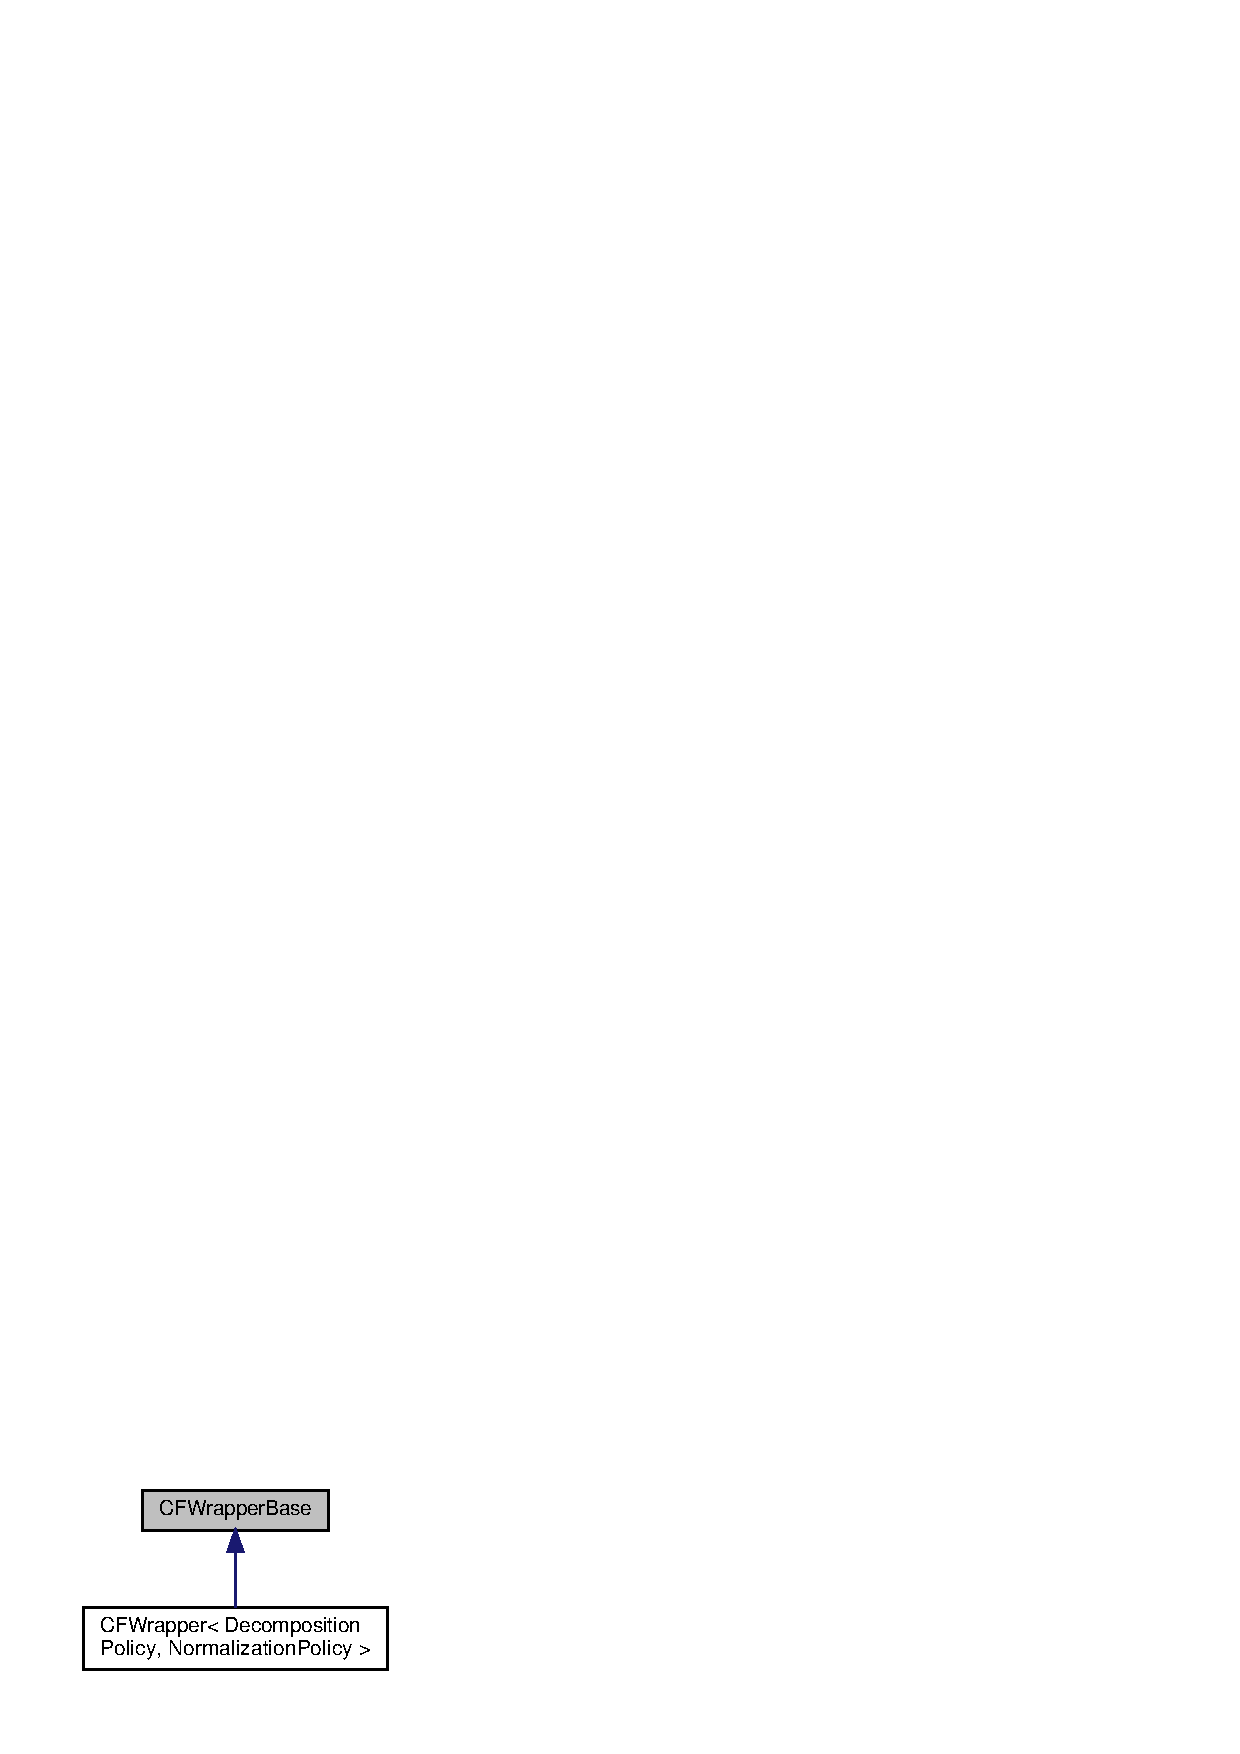
\includegraphics[width=190pt]{classmlpack_1_1cf_1_1CFWrapperBase__inherit__graph}
\end{center}
\end{figure}
\subsection*{Public Member Functions}
\begin{DoxyCompactItemize}
\item 
\textbf{ C\+F\+Wrapper\+Base} ()
\begin{DoxyCompactList}\small\item\em Create the object. The base class has nothing to hold. \end{DoxyCompactList}\item 
virtual \textbf{ $\sim$\+C\+F\+Wrapper\+Base} ()
\begin{DoxyCompactList}\small\item\em Delete the object. \end{DoxyCompactList}\item 
virtual \textbf{ C\+F\+Wrapper\+Base} $\ast$ \textbf{ Clone} () const =0
\begin{DoxyCompactList}\small\item\em Make a copy of the object. \end{DoxyCompactList}\item 
virtual void \textbf{ Get\+Recommendations} (const \textbf{ Neighbor\+Search\+Types} ns\+Type, const \textbf{ Interpolation\+Types} interpolation\+Type, const size\+\_\+t num\+Recs, arma\+::\+Mat$<$ size\+\_\+t $>$ \&recommendations)=0
\begin{DoxyCompactList}\small\item\em Compute recommendations for all users. \end{DoxyCompactList}\item 
virtual void \textbf{ Get\+Recommendations} (const \textbf{ Neighbor\+Search\+Types} ns\+Type, const \textbf{ Interpolation\+Types} interpolation\+Type, const size\+\_\+t num\+Recs, arma\+::\+Mat$<$ size\+\_\+t $>$ \&recommendations, const arma\+::\+Col$<$ size\+\_\+t $>$ \&users)=0
\begin{DoxyCompactList}\small\item\em Compute recommendations. \end{DoxyCompactList}\item 
virtual void \textbf{ Predict} (const \textbf{ Neighbor\+Search\+Types} ns\+Type, const \textbf{ Interpolation\+Types} interpolation\+Type, const arma\+::\+Mat$<$ size\+\_\+t $>$ \&combinations, arma\+::vec \&predictions)=0
\begin{DoxyCompactList}\small\item\em Compute predictions for users. \end{DoxyCompactList}\end{DoxyCompactItemize}


\subsection{Detailed Description}
The \doxyref{C\+F\+Wrapper\+Base}{p.}{classmlpack_1_1cf_1_1CFWrapperBase} class provides a unified interface that can be used by the \doxyref{C\+F\+Model}{p.}{classmlpack_1_1cf_1_1CFModel} class to interact with all different CF types at runtime. 

All CF wrapper types inherit from this base class. 

Definition at line 49 of file cf\+\_\+model.\+hpp.



\subsection{Constructor \& Destructor Documentation}
\mbox{\label{classmlpack_1_1cf_1_1CFWrapperBase_a5536395b99c030b97a2860df3e2ae5c4}} 
\index{mlpack\+::cf\+::\+C\+F\+Wrapper\+Base@{mlpack\+::cf\+::\+C\+F\+Wrapper\+Base}!C\+F\+Wrapper\+Base@{C\+F\+Wrapper\+Base}}
\index{C\+F\+Wrapper\+Base@{C\+F\+Wrapper\+Base}!mlpack\+::cf\+::\+C\+F\+Wrapper\+Base@{mlpack\+::cf\+::\+C\+F\+Wrapper\+Base}}
\subsubsection{C\+F\+Wrapper\+Base()}
{\footnotesize\ttfamily \textbf{ C\+F\+Wrapper\+Base} (\begin{DoxyParamCaption}{ }\end{DoxyParamCaption})\hspace{0.3cm}{\ttfamily [inline]}}



Create the object. The base class has nothing to hold. 



Definition at line 53 of file cf\+\_\+model.\+hpp.



References C\+F\+Wrapper\+Base\+::\+Clone().

\mbox{\label{classmlpack_1_1cf_1_1CFWrapperBase_ac017d61192618af5a5f70a671c2a886b}} 
\index{mlpack\+::cf\+::\+C\+F\+Wrapper\+Base@{mlpack\+::cf\+::\+C\+F\+Wrapper\+Base}!````~C\+F\+Wrapper\+Base@{$\sim$\+C\+F\+Wrapper\+Base}}
\index{````~C\+F\+Wrapper\+Base@{$\sim$\+C\+F\+Wrapper\+Base}!mlpack\+::cf\+::\+C\+F\+Wrapper\+Base@{mlpack\+::cf\+::\+C\+F\+Wrapper\+Base}}
\subsubsection{$\sim$\+C\+F\+Wrapper\+Base()}
{\footnotesize\ttfamily virtual $\sim$\textbf{ C\+F\+Wrapper\+Base} (\begin{DoxyParamCaption}{ }\end{DoxyParamCaption})\hspace{0.3cm}{\ttfamily [inline]}, {\ttfamily [virtual]}}



Delete the object. 



Definition at line 59 of file cf\+\_\+model.\+hpp.



References C\+F\+Wrapper\+Base\+::\+Get\+Recommendations(), and C\+F\+Wrapper\+Base\+::\+Predict().



\subsection{Member Function Documentation}
\mbox{\label{classmlpack_1_1cf_1_1CFWrapperBase_a390b40d2a1416852dd64201e55dac770}} 
\index{mlpack\+::cf\+::\+C\+F\+Wrapper\+Base@{mlpack\+::cf\+::\+C\+F\+Wrapper\+Base}!Clone@{Clone}}
\index{Clone@{Clone}!mlpack\+::cf\+::\+C\+F\+Wrapper\+Base@{mlpack\+::cf\+::\+C\+F\+Wrapper\+Base}}
\subsubsection{Clone()}
{\footnotesize\ttfamily virtual \textbf{ C\+F\+Wrapper\+Base}$\ast$ Clone (\begin{DoxyParamCaption}{ }\end{DoxyParamCaption}) const\hspace{0.3cm}{\ttfamily [pure virtual]}}



Make a copy of the object. 



Implemented in \textbf{ C\+F\+Wrapper$<$ Decomposition\+Policy, Normalization\+Policy $>$} \doxyref{}{p.}{classmlpack_1_1cf_1_1CFWrapper_af9bba55939ac1cb5bc1c4828094f502c}.



Referenced by C\+F\+Wrapper\+Base\+::\+C\+F\+Wrapper\+Base().

\mbox{\label{classmlpack_1_1cf_1_1CFWrapperBase_aefd1ffc070784adf594bd91a2469a6c7}} 
\index{mlpack\+::cf\+::\+C\+F\+Wrapper\+Base@{mlpack\+::cf\+::\+C\+F\+Wrapper\+Base}!Get\+Recommendations@{Get\+Recommendations}}
\index{Get\+Recommendations@{Get\+Recommendations}!mlpack\+::cf\+::\+C\+F\+Wrapper\+Base@{mlpack\+::cf\+::\+C\+F\+Wrapper\+Base}}
\subsubsection{Get\+Recommendations()\hspace{0.1cm}{\footnotesize\ttfamily [1/2]}}
{\footnotesize\ttfamily virtual void Get\+Recommendations (\begin{DoxyParamCaption}\item[{const \textbf{ Neighbor\+Search\+Types}}]{ns\+Type,  }\item[{const \textbf{ Interpolation\+Types}}]{interpolation\+Type,  }\item[{const size\+\_\+t}]{num\+Recs,  }\item[{arma\+::\+Mat$<$ size\+\_\+t $>$ \&}]{recommendations }\end{DoxyParamCaption})\hspace{0.3cm}{\ttfamily [pure virtual]}}



Compute recommendations for all users. 



Implemented in \textbf{ C\+F\+Wrapper$<$ Decomposition\+Policy, Normalization\+Policy $>$} \doxyref{}{p.}{classmlpack_1_1cf_1_1CFWrapper_aaa12de12e686286f465afa8a399677d2}.



Referenced by C\+F\+Wrapper$<$ Decomposition\+Policy, Normalization\+Policy $>$\+::\+C\+F(), C\+F\+Model\+::\+Normalization\+Type(), and C\+F\+Wrapper\+Base\+::$\sim$\+C\+F\+Wrapper\+Base().

\mbox{\label{classmlpack_1_1cf_1_1CFWrapperBase_af9ad22de59a4e9396157809f41f6c5dc}} 
\index{mlpack\+::cf\+::\+C\+F\+Wrapper\+Base@{mlpack\+::cf\+::\+C\+F\+Wrapper\+Base}!Get\+Recommendations@{Get\+Recommendations}}
\index{Get\+Recommendations@{Get\+Recommendations}!mlpack\+::cf\+::\+C\+F\+Wrapper\+Base@{mlpack\+::cf\+::\+C\+F\+Wrapper\+Base}}
\subsubsection{Get\+Recommendations()\hspace{0.1cm}{\footnotesize\ttfamily [2/2]}}
{\footnotesize\ttfamily virtual void Get\+Recommendations (\begin{DoxyParamCaption}\item[{const \textbf{ Neighbor\+Search\+Types}}]{ns\+Type,  }\item[{const \textbf{ Interpolation\+Types}}]{interpolation\+Type,  }\item[{const size\+\_\+t}]{num\+Recs,  }\item[{arma\+::\+Mat$<$ size\+\_\+t $>$ \&}]{recommendations,  }\item[{const arma\+::\+Col$<$ size\+\_\+t $>$ \&}]{users }\end{DoxyParamCaption})\hspace{0.3cm}{\ttfamily [pure virtual]}}



Compute recommendations. 



Implemented in \textbf{ C\+F\+Wrapper$<$ Decomposition\+Policy, Normalization\+Policy $>$} \doxyref{}{p.}{classmlpack_1_1cf_1_1CFWrapper_ab3b85ddacc36d16322f28f5b5a113d0d}.

\mbox{\label{classmlpack_1_1cf_1_1CFWrapperBase_a3de57e8cd8b989a1e7e719c80f39d07b}} 
\index{mlpack\+::cf\+::\+C\+F\+Wrapper\+Base@{mlpack\+::cf\+::\+C\+F\+Wrapper\+Base}!Predict@{Predict}}
\index{Predict@{Predict}!mlpack\+::cf\+::\+C\+F\+Wrapper\+Base@{mlpack\+::cf\+::\+C\+F\+Wrapper\+Base}}
\subsubsection{Predict()}
{\footnotesize\ttfamily virtual void Predict (\begin{DoxyParamCaption}\item[{const \textbf{ Neighbor\+Search\+Types}}]{ns\+Type,  }\item[{const \textbf{ Interpolation\+Types}}]{interpolation\+Type,  }\item[{const arma\+::\+Mat$<$ size\+\_\+t $>$ \&}]{combinations,  }\item[{arma\+::vec \&}]{predictions }\end{DoxyParamCaption})\hspace{0.3cm}{\ttfamily [pure virtual]}}



Compute predictions for users. 



Implemented in \textbf{ C\+F\+Wrapper$<$ Decomposition\+Policy, Normalization\+Policy $>$} \doxyref{}{p.}{classmlpack_1_1cf_1_1CFWrapper_adeae1e56456f3c8c71d0da5542ee4415}.



Referenced by C\+F\+Wrapper$<$ Decomposition\+Policy, Normalization\+Policy $>$\+::\+C\+F(), C\+F\+Model\+::\+Normalization\+Type(), and C\+F\+Wrapper\+Base\+::$\sim$\+C\+F\+Wrapper\+Base().



The documentation for this class was generated from the following file\+:\begin{DoxyCompactItemize}
\item 
/home/aakash/mlpack/src/mlpack/methods/cf/\textbf{ cf\+\_\+model.\+hpp}\end{DoxyCompactItemize}

\section{Combined\+Normalization$<$ Normalization\+Types $>$ Class Template Reference}
\label{classmlpack_1_1cf_1_1CombinedNormalization}\index{Combined\+Normalization$<$ Normalization\+Types $>$@{Combined\+Normalization$<$ Normalization\+Types $>$}}


This normalization class performs a sequence of normalization methods on raw ratings.  


\subsection*{Public Types}
\begin{DoxyCompactItemize}
\item 
using \textbf{ Tuple\+Type} = std\+::tuple$<$ Normalization\+Types... $>$
\end{DoxyCompactItemize}
\subsection*{Public Member Functions}
\begin{DoxyCompactItemize}
\item 
\textbf{ Combined\+Normalization} ()
\item 
double \textbf{ Denormalize} (const size\+\_\+t user, const size\+\_\+t item, const double rating) const
\begin{DoxyCompactList}\small\item\em Denormalize rating by calling \doxyref{Denormalize()}{p.}{classmlpack_1_1cf_1_1CombinedNormalization_a27ffe74669d0dfd1c217728c369b35f9} in each normalization object. \end{DoxyCompactList}\item 
void \textbf{ Denormalize} (const arma\+::\+Mat$<$ size\+\_\+t $>$ \&combinations, arma\+::vec \&predictions) const
\begin{DoxyCompactList}\small\item\em Denormalize rating by calling \doxyref{Denormalize()}{p.}{classmlpack_1_1cf_1_1CombinedNormalization_a27ffe74669d0dfd1c217728c369b35f9} in each normalization object. \end{DoxyCompactList}\item 
const \textbf{ Tuple\+Type} \& \textbf{ Normalizations} () const
\begin{DoxyCompactList}\small\item\em Return normalizations tuple. \end{DoxyCompactList}\item 
{\footnotesize template$<$typename Mat\+Type $>$ }\\void \textbf{ Normalize} (Mat\+Type \&data)
\begin{DoxyCompactList}\small\item\em Normalize the data by calling \doxyref{Normalize()}{p.}{classmlpack_1_1cf_1_1CombinedNormalization_a47ac5da06a1301c0c72529184cc77a7e} in each normalization object. \end{DoxyCompactList}\item 
{\footnotesize template$<$typename Archive $>$ }\\void \textbf{ serialize} (Archive \&ar, const uint32\+\_\+t version)
\begin{DoxyCompactList}\small\item\em Serialization. \end{DoxyCompactList}\end{DoxyCompactItemize}


\subsection{Detailed Description}
\subsubsection*{template$<$typename... Normalization\+Types$>$\newline
class mlpack\+::cf\+::\+Combined\+Normalization$<$ Normalization\+Types $>$}

This normalization class performs a sequence of normalization methods on raw ratings. 

An example of how to use \doxyref{Combined\+Normalization}{p.}{classmlpack_1_1cf_1_1CombinedNormalization} in CF is shown below\+:


\begin{DoxyCode}
\textcolor{keyword}{extern} arma::mat data; \textcolor{comment}{// data is a (user, item, rating) table.}
\textcolor{comment}{// Users for whom recommendations are generated.}
\textcolor{keyword}{extern} arma::Col<size\_t> users;
arma::Mat<size\_t> recommendations; \textcolor{comment}{// Resulting recommendations.}

CFType<NMFPolicy,
       CombinedNormalization<
           OverallMeanNormalization,
           UserMeanNormalization,
           ItemMeanNormalization>> cf(data);

\textcolor{comment}{// Generate 10 recommendations for all users.}
cf.GetRecommendations(10, recommendations);
\end{DoxyCode}
 

Definition at line 44 of file combined\+\_\+normalization.\+hpp.



\subsection{Member Typedef Documentation}
\mbox{\label{classmlpack_1_1cf_1_1CombinedNormalization_a1e98d43da1ec47c76125e7782460aa2c}} 
\index{mlpack\+::cf\+::\+Combined\+Normalization@{mlpack\+::cf\+::\+Combined\+Normalization}!Tuple\+Type@{Tuple\+Type}}
\index{Tuple\+Type@{Tuple\+Type}!mlpack\+::cf\+::\+Combined\+Normalization@{mlpack\+::cf\+::\+Combined\+Normalization}}
\subsubsection{Tuple\+Type}
{\footnotesize\ttfamily using \textbf{ Tuple\+Type} =  std\+::tuple$<$Normalization\+Types...$>$}



Definition at line 47 of file combined\+\_\+normalization.\+hpp.



\subsection{Constructor \& Destructor Documentation}
\mbox{\label{classmlpack_1_1cf_1_1CombinedNormalization_a8fb4e3fa10e0ecf786c2b710175bb75b}} 
\index{mlpack\+::cf\+::\+Combined\+Normalization@{mlpack\+::cf\+::\+Combined\+Normalization}!Combined\+Normalization@{Combined\+Normalization}}
\index{Combined\+Normalization@{Combined\+Normalization}!mlpack\+::cf\+::\+Combined\+Normalization@{mlpack\+::cf\+::\+Combined\+Normalization}}
\subsubsection{Combined\+Normalization()}
{\footnotesize\ttfamily \textbf{ Combined\+Normalization} (\begin{DoxyParamCaption}{ }\end{DoxyParamCaption})\hspace{0.3cm}{\ttfamily [inline]}}



Definition at line 50 of file combined\+\_\+normalization.\+hpp.



\subsection{Member Function Documentation}
\mbox{\label{classmlpack_1_1cf_1_1CombinedNormalization_a27ffe74669d0dfd1c217728c369b35f9}} 
\index{mlpack\+::cf\+::\+Combined\+Normalization@{mlpack\+::cf\+::\+Combined\+Normalization}!Denormalize@{Denormalize}}
\index{Denormalize@{Denormalize}!mlpack\+::cf\+::\+Combined\+Normalization@{mlpack\+::cf\+::\+Combined\+Normalization}}
\subsubsection{Denormalize()\hspace{0.1cm}{\footnotesize\ttfamily [1/2]}}
{\footnotesize\ttfamily double Denormalize (\begin{DoxyParamCaption}\item[{const size\+\_\+t}]{user,  }\item[{const size\+\_\+t}]{item,  }\item[{const double}]{rating }\end{DoxyParamCaption}) const\hspace{0.3cm}{\ttfamily [inline]}}



Denormalize rating by calling \doxyref{Denormalize()}{p.}{classmlpack_1_1cf_1_1CombinedNormalization_a27ffe74669d0dfd1c217728c369b35f9} in each normalization object. 

Note that the order of objects calling \doxyref{Denormalize()}{p.}{classmlpack_1_1cf_1_1CombinedNormalization_a27ffe74669d0dfd1c217728c369b35f9} should be the reversed order of objects calling \doxyref{Normalize()}{p.}{classmlpack_1_1cf_1_1CombinedNormalization_a47ac5da06a1301c0c72529184cc77a7e}.


\begin{DoxyParams}{Parameters}
{\em user} & User ID. \\
\hline
{\em item} & Item ID. \\
\hline
{\em rating} & Computed rating before denormalization. \\
\hline
\end{DoxyParams}


Definition at line 72 of file combined\+\_\+normalization.\+hpp.



Referenced by Combined\+Normalization$<$ Normalization\+Types $>$\+::serialize().

\mbox{\label{classmlpack_1_1cf_1_1CombinedNormalization_a93926452083f79197edc30f83476a40d}} 
\index{mlpack\+::cf\+::\+Combined\+Normalization@{mlpack\+::cf\+::\+Combined\+Normalization}!Denormalize@{Denormalize}}
\index{Denormalize@{Denormalize}!mlpack\+::cf\+::\+Combined\+Normalization@{mlpack\+::cf\+::\+Combined\+Normalization}}
\subsubsection{Denormalize()\hspace{0.1cm}{\footnotesize\ttfamily [2/2]}}
{\footnotesize\ttfamily void Denormalize (\begin{DoxyParamCaption}\item[{const arma\+::\+Mat$<$ size\+\_\+t $>$ \&}]{combinations,  }\item[{arma\+::vec \&}]{predictions }\end{DoxyParamCaption}) const\hspace{0.3cm}{\ttfamily [inline]}}



Denormalize rating by calling \doxyref{Denormalize()}{p.}{classmlpack_1_1cf_1_1CombinedNormalization_a27ffe74669d0dfd1c217728c369b35f9} in each normalization object. 

Note that the order of objects calling \doxyref{Denormalize()}{p.}{classmlpack_1_1cf_1_1CombinedNormalization_a27ffe74669d0dfd1c217728c369b35f9} should be the reversed order of objects calling \doxyref{Normalize()}{p.}{classmlpack_1_1cf_1_1CombinedNormalization_a47ac5da06a1301c0c72529184cc77a7e}.


\begin{DoxyParams}{Parameters}
{\em combinations} & User/\+Item combinations. \\
\hline
{\em predictions} & Predicted ratings for each user/item combination. \\
\hline
\end{DoxyParams}


Definition at line 87 of file combined\+\_\+normalization.\+hpp.

\mbox{\label{classmlpack_1_1cf_1_1CombinedNormalization_a58a35d3ef1c11ee69753aa099513840e}} 
\index{mlpack\+::cf\+::\+Combined\+Normalization@{mlpack\+::cf\+::\+Combined\+Normalization}!Normalizations@{Normalizations}}
\index{Normalizations@{Normalizations}!mlpack\+::cf\+::\+Combined\+Normalization@{mlpack\+::cf\+::\+Combined\+Normalization}}
\subsubsection{Normalizations()}
{\footnotesize\ttfamily const \textbf{ Tuple\+Type}\& Normalizations (\begin{DoxyParamCaption}{ }\end{DoxyParamCaption}) const\hspace{0.3cm}{\ttfamily [inline]}}



Return normalizations tuple. 



Definition at line 96 of file combined\+\_\+normalization.\+hpp.

\mbox{\label{classmlpack_1_1cf_1_1CombinedNormalization_a47ac5da06a1301c0c72529184cc77a7e}} 
\index{mlpack\+::cf\+::\+Combined\+Normalization@{mlpack\+::cf\+::\+Combined\+Normalization}!Normalize@{Normalize}}
\index{Normalize@{Normalize}!mlpack\+::cf\+::\+Combined\+Normalization@{mlpack\+::cf\+::\+Combined\+Normalization}}
\subsubsection{Normalize()}
{\footnotesize\ttfamily void Normalize (\begin{DoxyParamCaption}\item[{Mat\+Type \&}]{data }\end{DoxyParamCaption})\hspace{0.3cm}{\ttfamily [inline]}}



Normalize the data by calling \doxyref{Normalize()}{p.}{classmlpack_1_1cf_1_1CombinedNormalization_a47ac5da06a1301c0c72529184cc77a7e} in each normalization object. 


\begin{DoxyParams}{Parameters}
{\em data} & Input dataset. \\
\hline
\end{DoxyParams}


Definition at line 58 of file combined\+\_\+normalization.\+hpp.



Referenced by Combined\+Normalization$<$ Normalization\+Types $>$\+::serialize().

\mbox{\label{classmlpack_1_1cf_1_1CombinedNormalization_a72d63b74c8166dff8e1a9006905ad9ca}} 
\index{mlpack\+::cf\+::\+Combined\+Normalization@{mlpack\+::cf\+::\+Combined\+Normalization}!serialize@{serialize}}
\index{serialize@{serialize}!mlpack\+::cf\+::\+Combined\+Normalization@{mlpack\+::cf\+::\+Combined\+Normalization}}
\subsubsection{serialize()}
{\footnotesize\ttfamily void serialize (\begin{DoxyParamCaption}\item[{Archive \&}]{ar,  }\item[{const uint32\+\_\+t}]{version }\end{DoxyParamCaption})\hspace{0.3cm}{\ttfamily [inline]}}



Serialization. 



Definition at line 105 of file combined\+\_\+normalization.\+hpp.



References Combined\+Normalization$<$ Normalization\+Types $>$\+::\+Denormalize(), and Combined\+Normalization$<$ Normalization\+Types $>$\+::\+Normalize().



The documentation for this class was generated from the following file\+:\begin{DoxyCompactItemize}
\item 
/home/aakash/mlpack/src/mlpack/methods/cf/normalization/\textbf{ combined\+\_\+normalization.\+hpp}\end{DoxyCompactItemize}

\section{Cosine\+Search Class Reference}
\label{classmlpack_1_1cf_1_1CosineSearch}\index{Cosine\+Search@{Cosine\+Search}}


Nearest neighbor search with cosine distance.  


\subsection*{Public Member Functions}
\begin{DoxyCompactItemize}
\item 
\textbf{ Cosine\+Search} (const arma\+::mat \&reference\+Set)
\begin{DoxyCompactList}\small\item\em Constructor with reference set. \end{DoxyCompactList}\item 
void \textbf{ Search} (const arma\+::mat \&query, const size\+\_\+t k, arma\+::\+Mat$<$ size\+\_\+t $>$ \&neighbors, arma\+::mat \&similarities)
\begin{DoxyCompactList}\small\item\em Given a set of query points, find the nearest k neighbors, and return similarities. \end{DoxyCompactList}\end{DoxyCompactItemize}


\subsection{Detailed Description}
Nearest neighbor search with cosine distance. 

Note that, with normalized vectors, neighbor search with cosine distance is equivalent to neighbor search with Euclidean distance. Therefore, instead of performing neighbor search directly with cosine distance, we first normalize all vectors to unit length, and then use \doxyref{neighbor\+::\+K\+NN}{p.}{namespacemlpack_1_1neighbor_ac8d70069e8acb12c5ba9a8536ae6ace4} (i.\+e. Neighbor\+Search with Euclidean distance, K\+D\+Tree). Cosine similarities are calculated from Euclidean distance.

An example of how to use \doxyref{Cosine\+Search}{p.}{classmlpack_1_1cf_1_1CosineSearch} in CF is shown below\+:


\begin{DoxyCode}
\textcolor{keyword}{extern} arma::mat data; \textcolor{comment}{// data is a (user, item, rating) table.}
\textcolor{comment}{// Users for whom recommendations are generated.}
\textcolor{keyword}{extern} arma::Col<size\_t> users;
arma::Mat<size\_t> recommendations; \textcolor{comment}{// Resulting recommendations.}

CFType<> cf(data);

\textcolor{comment}{// Generate 10 recommendations for all users.}
cf.template GetRecommendations<CosineSearch>(10, recommendations);
\end{DoxyCode}
 

Definition at line 44 of file cosine\+\_\+search.\+hpp.



\subsection{Constructor \& Destructor Documentation}
\mbox{\label{classmlpack_1_1cf_1_1CosineSearch_a3c05953c20d36d4ea490e3d3aa879704}} 
\index{mlpack\+::cf\+::\+Cosine\+Search@{mlpack\+::cf\+::\+Cosine\+Search}!Cosine\+Search@{Cosine\+Search}}
\index{Cosine\+Search@{Cosine\+Search}!mlpack\+::cf\+::\+Cosine\+Search@{mlpack\+::cf\+::\+Cosine\+Search}}
\subsubsection{Cosine\+Search()}
{\footnotesize\ttfamily \textbf{ Cosine\+Search} (\begin{DoxyParamCaption}\item[{const arma\+::mat \&}]{reference\+Set }\end{DoxyParamCaption})\hspace{0.3cm}{\ttfamily [inline]}}



Constructor with reference set. 

All vectors in reference set are normalized to unit length.


\begin{DoxyParams}{Parameters}
{\em reference\+Set} & Set of reference points. \\
\hline
\end{DoxyParams}


Definition at line 53 of file cosine\+\_\+search.\+hpp.



References Neighbor\+Search$<$ Sort\+Policy, Metric\+Type, Mat\+Type, Tree\+Type, Dual\+Tree\+Traversal\+Type, Single\+Tree\+Traversal\+Type $>$\+::\+Train().



\subsection{Member Function Documentation}
\mbox{\label{classmlpack_1_1cf_1_1CosineSearch_a5ce7aae85679ed26a716bcb8d7c8ee7b}} 
\index{mlpack\+::cf\+::\+Cosine\+Search@{mlpack\+::cf\+::\+Cosine\+Search}!Search@{Search}}
\index{Search@{Search}!mlpack\+::cf\+::\+Cosine\+Search@{mlpack\+::cf\+::\+Cosine\+Search}}
\subsubsection{Search()}
{\footnotesize\ttfamily void Search (\begin{DoxyParamCaption}\item[{const arma\+::mat \&}]{query,  }\item[{const size\+\_\+t}]{k,  }\item[{arma\+::\+Mat$<$ size\+\_\+t $>$ \&}]{neighbors,  }\item[{arma\+::mat \&}]{similarities }\end{DoxyParamCaption})\hspace{0.3cm}{\ttfamily [inline]}}



Given a set of query points, find the nearest k neighbors, and return similarities. 

Similarities are non-\/negative and no larger than one.


\begin{DoxyParams}{Parameters}
{\em query} & A set of query points. \\
\hline
{\em k} & Number of neighbors to search. \\
\hline
{\em neighbors} & Nearest neighbors. \\
\hline
{\em similarities} & Similarities between query point and its neighbors. \\
\hline
\end{DoxyParams}


Definition at line 70 of file cosine\+\_\+search.\+hpp.



References Neighbor\+Search$<$ Sort\+Policy, Metric\+Type, Mat\+Type, Tree\+Type, Dual\+Tree\+Traversal\+Type, Single\+Tree\+Traversal\+Type $>$\+::\+Search().



The documentation for this class was generated from the following file\+:\begin{DoxyCompactItemize}
\item 
/home/aakash/mlpack/src/mlpack/methods/cf/neighbor\+\_\+search\+\_\+policies/\textbf{ cosine\+\_\+search.\+hpp}\end{DoxyCompactItemize}

\section{Dummy\+Class Class Reference}
\label{classmlpack_1_1cf_1_1DummyClass}\index{Dummy\+Class@{Dummy\+Class}}


This class acts as a dummy class for passing as template parameter.  




\subsection{Detailed Description}
This class acts as a dummy class for passing as template parameter. 

Passing this class as a template parameter to class \doxyref{S\+V\+D\+Wrapper}{p.}{classmlpack_1_1cf_1_1SVDWrapper} will force \doxyref{S\+V\+D\+Wrapper}{p.}{classmlpack_1_1cf_1_1SVDWrapper} to use Armadillo\textquotesingle{}s S\+VD implementation. 

Definition at line 27 of file svd\+\_\+wrapper.\+hpp.



The documentation for this class was generated from the following file\+:\begin{DoxyCompactItemize}
\item 
/home/aakash/mlpack/src/mlpack/methods/cf/\textbf{ svd\+\_\+wrapper.\+hpp}\end{DoxyCompactItemize}

\section{Item\+Mean\+Normalization Class Reference}
\label{classmlpack_1_1cf_1_1ItemMeanNormalization}\index{Item\+Mean\+Normalization@{Item\+Mean\+Normalization}}


This normalization class performs item mean normalization on raw ratings.  


\subsection*{Public Member Functions}
\begin{DoxyCompactItemize}
\item 
\textbf{ Item\+Mean\+Normalization} ()
\item 
double \textbf{ Denormalize} (const size\+\_\+t, const size\+\_\+t item, const double rating) const
\begin{DoxyCompactList}\small\item\em Denormalize computed rating by adding item mean. \end{DoxyCompactList}\item 
void \textbf{ Denormalize} (const arma\+::\+Mat$<$ size\+\_\+t $>$ \&combinations, arma\+::vec \&predictions) const
\begin{DoxyCompactList}\small\item\em Denormalize computed rating by adding item mean. \end{DoxyCompactList}\item 
const arma\+::vec \& \textbf{ Mean} () const
\begin{DoxyCompactList}\small\item\em Return item mean. \end{DoxyCompactList}\item 
void \textbf{ Normalize} (arma\+::mat \&data)
\begin{DoxyCompactList}\small\item\em Normalize the data by subtracting item mean from each of existing ratings. \end{DoxyCompactList}\item 
void \textbf{ Normalize} (arma\+::sp\+\_\+mat \&cleaned\+Data)
\begin{DoxyCompactList}\small\item\em Normalize the data by subtracting item mean from each of existing ratings. \end{DoxyCompactList}\item 
{\footnotesize template$<$typename Archive $>$ }\\void \textbf{ serialize} (Archive \&ar, const uint32\+\_\+t)
\begin{DoxyCompactList}\small\item\em Serialization. \end{DoxyCompactList}\end{DoxyCompactItemize}


\subsection{Detailed Description}
This normalization class performs item mean normalization on raw ratings. 

An example of how to use \doxyref{Item\+Mean\+Normalization}{p.}{classmlpack_1_1cf_1_1ItemMeanNormalization} in CF is shown below\+:


\begin{DoxyCode}
\textcolor{keyword}{extern} arma::mat data; \textcolor{comment}{// data is a (user, item, rating) table.}
\textcolor{comment}{// Users for whom recommendations are generated.}
\textcolor{keyword}{extern} arma::Col<size\_t> users;
arma::Mat<size\_t> recommendations; \textcolor{comment}{// Resulting recommendations.}

\textcolor{comment}{// Use ItemMeanNormalization as normalization method.}
CFType<NMFPolicy, ItemMeanNormalization> cf(data);

\textcolor{comment}{// Generate 10 recommendations for all users.}
cf.GetRecommendations(10, recommendations);
\end{DoxyCode}
 

Definition at line 39 of file item\+\_\+mean\+\_\+normalization.\+hpp.



\subsection{Constructor \& Destructor Documentation}
\mbox{\label{classmlpack_1_1cf_1_1ItemMeanNormalization_ae784a8a1a7acbab5b02b2a86f410dc82}} 
\index{mlpack\+::cf\+::\+Item\+Mean\+Normalization@{mlpack\+::cf\+::\+Item\+Mean\+Normalization}!Item\+Mean\+Normalization@{Item\+Mean\+Normalization}}
\index{Item\+Mean\+Normalization@{Item\+Mean\+Normalization}!mlpack\+::cf\+::\+Item\+Mean\+Normalization@{mlpack\+::cf\+::\+Item\+Mean\+Normalization}}
\subsubsection{Item\+Mean\+Normalization()}
{\footnotesize\ttfamily \textbf{ Item\+Mean\+Normalization} (\begin{DoxyParamCaption}{ }\end{DoxyParamCaption})\hspace{0.3cm}{\ttfamily [inline]}}



Definition at line 43 of file item\+\_\+mean\+\_\+normalization.\+hpp.



\subsection{Member Function Documentation}
\mbox{\label{classmlpack_1_1cf_1_1ItemMeanNormalization_a25d019f07e5f97119b7a802306fa747f}} 
\index{mlpack\+::cf\+::\+Item\+Mean\+Normalization@{mlpack\+::cf\+::\+Item\+Mean\+Normalization}!Denormalize@{Denormalize}}
\index{Denormalize@{Denormalize}!mlpack\+::cf\+::\+Item\+Mean\+Normalization@{mlpack\+::cf\+::\+Item\+Mean\+Normalization}}
\subsubsection{Denormalize()\hspace{0.1cm}{\footnotesize\ttfamily [1/2]}}
{\footnotesize\ttfamily double Denormalize (\begin{DoxyParamCaption}\item[{const size\+\_\+t}]{,  }\item[{const size\+\_\+t}]{item,  }\item[{const double}]{rating }\end{DoxyParamCaption}) const\hspace{0.3cm}{\ttfamily [inline]}}



Denormalize computed rating by adding item mean. 


\begin{DoxyParams}{Parameters}
{\em $\ast$} & (user) User ID. \\
\hline
{\em item} & Item ID. \\
\hline
{\em rating} & Computed rating before denormalization. \\
\hline
\end{DoxyParams}


Definition at line 130 of file item\+\_\+mean\+\_\+normalization.\+hpp.

\mbox{\label{classmlpack_1_1cf_1_1ItemMeanNormalization_a93926452083f79197edc30f83476a40d}} 
\index{mlpack\+::cf\+::\+Item\+Mean\+Normalization@{mlpack\+::cf\+::\+Item\+Mean\+Normalization}!Denormalize@{Denormalize}}
\index{Denormalize@{Denormalize}!mlpack\+::cf\+::\+Item\+Mean\+Normalization@{mlpack\+::cf\+::\+Item\+Mean\+Normalization}}
\subsubsection{Denormalize()\hspace{0.1cm}{\footnotesize\ttfamily [2/2]}}
{\footnotesize\ttfamily void Denormalize (\begin{DoxyParamCaption}\item[{const arma\+::\+Mat$<$ size\+\_\+t $>$ \&}]{combinations,  }\item[{arma\+::vec \&}]{predictions }\end{DoxyParamCaption}) const\hspace{0.3cm}{\ttfamily [inline]}}



Denormalize computed rating by adding item mean. 


\begin{DoxyParams}{Parameters}
{\em combinations} & User/\+Item combinations. \\
\hline
{\em predictions} & Predicted ratings for each user/item combination. \\
\hline
\end{DoxyParams}


Definition at line 143 of file item\+\_\+mean\+\_\+normalization.\+hpp.

\mbox{\label{classmlpack_1_1cf_1_1ItemMeanNormalization_a6db5f5d76cbd055347cecd9ca90eea86}} 
\index{mlpack\+::cf\+::\+Item\+Mean\+Normalization@{mlpack\+::cf\+::\+Item\+Mean\+Normalization}!Mean@{Mean}}
\index{Mean@{Mean}!mlpack\+::cf\+::\+Item\+Mean\+Normalization@{mlpack\+::cf\+::\+Item\+Mean\+Normalization}}
\subsubsection{Mean()}
{\footnotesize\ttfamily const arma\+::vec\& Mean (\begin{DoxyParamCaption}{ }\end{DoxyParamCaption}) const\hspace{0.3cm}{\ttfamily [inline]}}



Return item mean. 



Definition at line 156 of file item\+\_\+mean\+\_\+normalization.\+hpp.

\mbox{\label{classmlpack_1_1cf_1_1ItemMeanNormalization_a87410cc06d847eef46d0dfdb137c6be7}} 
\index{mlpack\+::cf\+::\+Item\+Mean\+Normalization@{mlpack\+::cf\+::\+Item\+Mean\+Normalization}!Normalize@{Normalize}}
\index{Normalize@{Normalize}!mlpack\+::cf\+::\+Item\+Mean\+Normalization@{mlpack\+::cf\+::\+Item\+Mean\+Normalization}}
\subsubsection{Normalize()\hspace{0.1cm}{\footnotesize\ttfamily [1/2]}}
{\footnotesize\ttfamily void Normalize (\begin{DoxyParamCaption}\item[{arma\+::mat \&}]{data }\end{DoxyParamCaption})\hspace{0.3cm}{\ttfamily [inline]}}



Normalize the data by subtracting item mean from each of existing ratings. 


\begin{DoxyParams}{Parameters}
{\em data} & Input dataset in the form of coordinate list. \\
\hline
\end{DoxyParams}


Definition at line 50 of file item\+\_\+mean\+\_\+normalization.\+hpp.

\mbox{\label{classmlpack_1_1cf_1_1ItemMeanNormalization_a9656a2fd4841da15cf4b13ab57aa8000}} 
\index{mlpack\+::cf\+::\+Item\+Mean\+Normalization@{mlpack\+::cf\+::\+Item\+Mean\+Normalization}!Normalize@{Normalize}}
\index{Normalize@{Normalize}!mlpack\+::cf\+::\+Item\+Mean\+Normalization@{mlpack\+::cf\+::\+Item\+Mean\+Normalization}}
\subsubsection{Normalize()\hspace{0.1cm}{\footnotesize\ttfamily [2/2]}}
{\footnotesize\ttfamily void Normalize (\begin{DoxyParamCaption}\item[{arma\+::sp\+\_\+mat \&}]{cleaned\+Data }\end{DoxyParamCaption})\hspace{0.3cm}{\ttfamily [inline]}}



Normalize the data by subtracting item mean from each of existing ratings. 


\begin{DoxyParams}{Parameters}
{\em cleaned\+Data} & Input data as a sparse matrix. \\
\hline
\end{DoxyParams}


Definition at line 90 of file item\+\_\+mean\+\_\+normalization.\+hpp.

\mbox{\label{classmlpack_1_1cf_1_1ItemMeanNormalization_a65cba07328997659bec80b9879b15a51}} 
\index{mlpack\+::cf\+::\+Item\+Mean\+Normalization@{mlpack\+::cf\+::\+Item\+Mean\+Normalization}!serialize@{serialize}}
\index{serialize@{serialize}!mlpack\+::cf\+::\+Item\+Mean\+Normalization@{mlpack\+::cf\+::\+Item\+Mean\+Normalization}}
\subsubsection{serialize()}
{\footnotesize\ttfamily void serialize (\begin{DoxyParamCaption}\item[{Archive \&}]{ar,  }\item[{const uint32\+\_\+t}]{ }\end{DoxyParamCaption})\hspace{0.3cm}{\ttfamily [inline]}}



Serialization. 



Definition at line 162 of file item\+\_\+mean\+\_\+normalization.\+hpp.



The documentation for this class was generated from the following file\+:\begin{DoxyCompactItemize}
\item 
/home/aakash/mlpack/src/mlpack/methods/cf/normalization/\textbf{ item\+\_\+mean\+\_\+normalization.\+hpp}\end{DoxyCompactItemize}

\section{L\+Metric\+Search$<$ T\+Power $>$ Class Template Reference}
\label{classmlpack_1_1cf_1_1LMetricSearch}\index{L\+Metric\+Search$<$ T\+Power $>$@{L\+Metric\+Search$<$ T\+Power $>$}}


Nearest neighbor search with L\+\_\+p distance.  


\subsection*{Public Types}
\begin{DoxyCompactItemize}
\item 
using \textbf{ Neighbor\+Search\+Type} = \textbf{ neighbor\+::\+Neighbor\+Search}$<$ \textbf{ neighbor\+::\+Nearest\+Neighbor\+Sort}, \textbf{ metric\+::\+L\+Metric}$<$ T\+Power, true $>$ $>$
\end{DoxyCompactItemize}
\subsection*{Public Member Functions}
\begin{DoxyCompactItemize}
\item 
\textbf{ L\+Metric\+Search} (const arma\+::mat \&reference\+Set)
\item 
void \textbf{ Search} (const arma\+::mat \&query, const size\+\_\+t k, arma\+::\+Mat$<$ size\+\_\+t $>$ \&neighbors, arma\+::mat \&similarities)
\begin{DoxyCompactList}\small\item\em Given a set of query points, find the nearest k neighbors, and return similarites. \end{DoxyCompactList}\end{DoxyCompactItemize}


\subsection{Detailed Description}
\subsubsection*{template$<$int T\+Power$>$\newline
class mlpack\+::cf\+::\+L\+Metric\+Search$<$ T\+Power $>$}

Nearest neighbor search with L\+\_\+p distance. 

An example of how to use \doxyref{L\+Metric\+Search}{p.}{classmlpack_1_1cf_1_1LMetricSearch} in CF is shown below\+:


\begin{DoxyCode}
\textcolor{keyword}{extern} arma::mat data; \textcolor{comment}{// data is a (user, item, rating) table.}
\textcolor{comment}{// Users for whom recommendations are generated.}
\textcolor{keyword}{extern} arma::Col<size\_t> users;
arma::Mat<size\_t> recommendations; \textcolor{comment}{// Resulting recommendations.}

CFType<> cf(data);

\textcolor{comment}{// Generate 10 recommendations for all users.}
cf.template GetRecommendations<LMetricSearch<2>>(10, recommendations);
\end{DoxyCode}



\begin{DoxyTemplParams}{Template Parameters}
{\em T\+Power} & Power of metric. \\
\hline
\end{DoxyTemplParams}


Definition at line 42 of file lmetric\+\_\+search.\+hpp.



\subsection{Member Typedef Documentation}
\mbox{\label{classmlpack_1_1cf_1_1LMetricSearch_a7ec82c48ea6d34622bba11476edfb1d0}} 
\index{mlpack\+::cf\+::\+L\+Metric\+Search@{mlpack\+::cf\+::\+L\+Metric\+Search}!Neighbor\+Search\+Type@{Neighbor\+Search\+Type}}
\index{Neighbor\+Search\+Type@{Neighbor\+Search\+Type}!mlpack\+::cf\+::\+L\+Metric\+Search@{mlpack\+::cf\+::\+L\+Metric\+Search}}
\subsubsection{Neighbor\+Search\+Type}
{\footnotesize\ttfamily using \textbf{ Neighbor\+Search\+Type} =  \textbf{ neighbor\+::\+Neighbor\+Search}$<$ \textbf{ neighbor\+::\+Nearest\+Neighbor\+Sort}, \textbf{ metric\+::\+L\+Metric}$<$T\+Power, true$>$ $>$}



Definition at line 47 of file lmetric\+\_\+search.\+hpp.



\subsection{Constructor \& Destructor Documentation}
\mbox{\label{classmlpack_1_1cf_1_1LMetricSearch_adf30d29ff937a051ff8e1c1bbc1a0f7c}} 
\index{mlpack\+::cf\+::\+L\+Metric\+Search@{mlpack\+::cf\+::\+L\+Metric\+Search}!L\+Metric\+Search@{L\+Metric\+Search}}
\index{L\+Metric\+Search@{L\+Metric\+Search}!mlpack\+::cf\+::\+L\+Metric\+Search@{mlpack\+::cf\+::\+L\+Metric\+Search}}
\subsubsection{L\+Metric\+Search()}
{\footnotesize\ttfamily \textbf{ L\+Metric\+Search} (\begin{DoxyParamCaption}\item[{const arma\+::mat \&}]{reference\+Set }\end{DoxyParamCaption})\hspace{0.3cm}{\ttfamily [inline]}}


\begin{DoxyParams}{Parameters}
{\em reference\+Set} & Set of reference points. \\
\hline
\end{DoxyParams}


Definition at line 52 of file lmetric\+\_\+search.\+hpp.



\subsection{Member Function Documentation}
\mbox{\label{classmlpack_1_1cf_1_1LMetricSearch_a5ce7aae85679ed26a716bcb8d7c8ee7b}} 
\index{mlpack\+::cf\+::\+L\+Metric\+Search@{mlpack\+::cf\+::\+L\+Metric\+Search}!Search@{Search}}
\index{Search@{Search}!mlpack\+::cf\+::\+L\+Metric\+Search@{mlpack\+::cf\+::\+L\+Metric\+Search}}
\subsubsection{Search()}
{\footnotesize\ttfamily void Search (\begin{DoxyParamCaption}\item[{const arma\+::mat \&}]{query,  }\item[{const size\+\_\+t}]{k,  }\item[{arma\+::\+Mat$<$ size\+\_\+t $>$ \&}]{neighbors,  }\item[{arma\+::mat \&}]{similarities }\end{DoxyParamCaption})\hspace{0.3cm}{\ttfamily [inline]}}



Given a set of query points, find the nearest k neighbors, and return similarites. 

Similarities are non-\/negative and no larger thant one.


\begin{DoxyParams}{Parameters}
{\em query} & A set of query points. \\
\hline
{\em k} & Number of neighbors to search. \\
\hline
{\em neighbors} & Nearest neighbors. \\
\hline
{\em similarities} & Similarities between query point and its neighbors. \\
\hline
\end{DoxyParams}


Definition at line 64 of file lmetric\+\_\+search.\+hpp.



References Neighbor\+Search$<$ Sort\+Policy, Metric\+Type, Mat\+Type, Tree\+Type, Dual\+Tree\+Traversal\+Type, Single\+Tree\+Traversal\+Type $>$\+::\+Search().



The documentation for this class was generated from the following file\+:\begin{DoxyCompactItemize}
\item 
/home/aakash/mlpack/src/mlpack/methods/cf/neighbor\+\_\+search\+\_\+policies/\textbf{ lmetric\+\_\+search.\+hpp}\end{DoxyCompactItemize}

\section{N\+M\+F\+Policy Class Reference}
\label{classmlpack_1_1cf_1_1NMFPolicy}\index{N\+M\+F\+Policy@{N\+M\+F\+Policy}}


Implementation of the N\+MF policy to act as a wrapper when accessing N\+MF from within \doxyref{C\+F\+Type}{p.}{classmlpack_1_1cf_1_1CFType}.  


\subsection*{Public Member Functions}
\begin{DoxyCompactItemize}
\item 
{\footnotesize template$<$typename Mat\+Type $>$ }\\void \textbf{ Apply} (const Mat\+Type \&, const arma\+::sp\+\_\+mat \&cleaned\+Data, const size\+\_\+t rank, const size\+\_\+t max\+Iterations, const double min\+Residue, const bool mit)
\begin{DoxyCompactList}\small\item\em Apply Collaborative Filtering to the provided dataset using N\+MF method. \end{DoxyCompactList}\item 
{\footnotesize template$<$typename Neighbor\+Search\+Policy $>$ }\\void \textbf{ Get\+Neighborhood} (const arma\+::\+Col$<$ size\+\_\+t $>$ \&users, const size\+\_\+t num\+Users\+For\+Similarity, arma\+::\+Mat$<$ size\+\_\+t $>$ \&neighborhood, arma\+::mat \&similarities) const
\begin{DoxyCompactList}\small\item\em Get the neighborhood and corresponding similarities for a set of users. \end{DoxyCompactList}\item 
double \textbf{ Get\+Rating} (const size\+\_\+t user, const size\+\_\+t item) const
\begin{DoxyCompactList}\small\item\em Return predicted rating given user ID and item ID. \end{DoxyCompactList}\item 
void \textbf{ Get\+Rating\+Of\+User} (const size\+\_\+t user, arma\+::vec \&rating) const
\begin{DoxyCompactList}\small\item\em Get predicted ratings for a user. \end{DoxyCompactList}\item 
const arma\+::mat \& \textbf{ H} () const
\begin{DoxyCompactList}\small\item\em Get the User Matrix. \end{DoxyCompactList}\item 
{\footnotesize template$<$typename Archive $>$ }\\void \textbf{ serialize} (Archive \&ar, const uint32\+\_\+t)
\begin{DoxyCompactList}\small\item\em Serialization. \end{DoxyCompactList}\item 
const arma\+::mat \& \textbf{ W} () const
\begin{DoxyCompactList}\small\item\em Get the Item Matrix. \end{DoxyCompactList}\end{DoxyCompactItemize}


\subsection{Detailed Description}
Implementation of the N\+MF policy to act as a wrapper when accessing N\+MF from within \doxyref{C\+F\+Type}{p.}{classmlpack_1_1cf_1_1CFType}. 

An example of how to use \doxyref{N\+M\+F\+Policy}{p.}{classmlpack_1_1cf_1_1NMFPolicy} in CF is shown below\+:


\begin{DoxyCode}
\textcolor{keyword}{extern} arma::mat data; \textcolor{comment}{// data is a (user, item, rating) table.}
\textcolor{comment}{// Users for whom recommendations are generated.}
\textcolor{keyword}{extern} arma::Col<size\_t> users;
arma::Mat<size\_t> recommendations; \textcolor{comment}{// Resulting recommendations.}

CFType<NMFPolicy> cf(data);

\textcolor{comment}{// Generate 10 recommendations for all users.}
cf.GetRecommendations(10, recommendations);
\end{DoxyCode}
 

Definition at line 43 of file nmf\+\_\+method.\+hpp.



\subsection{Member Function Documentation}
\mbox{\label{classmlpack_1_1cf_1_1NMFPolicy_a55d1dc4a735516d3138feb7687552721}} 
\index{mlpack\+::cf\+::\+N\+M\+F\+Policy@{mlpack\+::cf\+::\+N\+M\+F\+Policy}!Apply@{Apply}}
\index{Apply@{Apply}!mlpack\+::cf\+::\+N\+M\+F\+Policy@{mlpack\+::cf\+::\+N\+M\+F\+Policy}}
\subsubsection{Apply()}
{\footnotesize\ttfamily void Apply (\begin{DoxyParamCaption}\item[{const Mat\+Type \&}]{,  }\item[{const arma\+::sp\+\_\+mat \&}]{cleaned\+Data,  }\item[{const size\+\_\+t}]{rank,  }\item[{const size\+\_\+t}]{max\+Iterations,  }\item[{const double}]{min\+Residue,  }\item[{const bool}]{mit }\end{DoxyParamCaption})\hspace{0.3cm}{\ttfamily [inline]}}



Apply Collaborative Filtering to the provided dataset using N\+MF method. 


\begin{DoxyParams}{Parameters}
{\em $\ast$} & (data) Data matrix\+: dense matrix (coordinate lists) or sparse matrix (cleaned). \\
\hline
{\em cleaned\+Data} & item user table in form of sparse matrix. \\
\hline
{\em rank} & Rank parameter for matrix factorization. \\
\hline
{\em max\+Iterations} & Maximum number of iterations. \\
\hline
{\em min\+Residue} & Residue required to terminate. \\
\hline
{\em mit} & Whether to terminate only when max\+Iterations is reached. \\
\hline
\end{DoxyParams}


Definition at line 58 of file nmf\+\_\+method.\+hpp.



References A\+M\+F$<$ Termination\+Policy\+Type, Initialization\+Rule\+Type, Update\+Rule\+Type $>$\+::\+Apply().

\mbox{\label{classmlpack_1_1cf_1_1NMFPolicy_a35bca7a6e09f4fb35b9945a9368711e4}} 
\index{mlpack\+::cf\+::\+N\+M\+F\+Policy@{mlpack\+::cf\+::\+N\+M\+F\+Policy}!Get\+Neighborhood@{Get\+Neighborhood}}
\index{Get\+Neighborhood@{Get\+Neighborhood}!mlpack\+::cf\+::\+N\+M\+F\+Policy@{mlpack\+::cf\+::\+N\+M\+F\+Policy}}
\subsubsection{Get\+Neighborhood()}
{\footnotesize\ttfamily void Get\+Neighborhood (\begin{DoxyParamCaption}\item[{const arma\+::\+Col$<$ size\+\_\+t $>$ \&}]{users,  }\item[{const size\+\_\+t}]{num\+Users\+For\+Similarity,  }\item[{arma\+::\+Mat$<$ size\+\_\+t $>$ \&}]{neighborhood,  }\item[{arma\+::mat \&}]{similarities }\end{DoxyParamCaption}) const\hspace{0.3cm}{\ttfamily [inline]}}



Get the neighborhood and corresponding similarities for a set of users. 


\begin{DoxyTemplParams}{Template Parameters}
{\em Neighbor\+Search\+Policy} & The policy to perform neighbor search.\\
\hline
\end{DoxyTemplParams}

\begin{DoxyParams}{Parameters}
{\em users} & Users whose neighborhood is to be computed. \\
\hline
{\em num\+Users\+For\+Similarity} & The number of neighbors returned for each user. \\
\hline
{\em neighborhood} & Neighbors represented by user I\+Ds. \\
\hline
{\em similarities} & Similarity between each user and each of its neighbors. \\
\hline
\end{DoxyParams}


Definition at line 120 of file nmf\+\_\+method.\+hpp.

\mbox{\label{classmlpack_1_1cf_1_1NMFPolicy_a0c3e16d73c8b25b8934cbc36ac161619}} 
\index{mlpack\+::cf\+::\+N\+M\+F\+Policy@{mlpack\+::cf\+::\+N\+M\+F\+Policy}!Get\+Rating@{Get\+Rating}}
\index{Get\+Rating@{Get\+Rating}!mlpack\+::cf\+::\+N\+M\+F\+Policy@{mlpack\+::cf\+::\+N\+M\+F\+Policy}}
\subsubsection{Get\+Rating()}
{\footnotesize\ttfamily double Get\+Rating (\begin{DoxyParamCaption}\item[{const size\+\_\+t}]{user,  }\item[{const size\+\_\+t}]{item }\end{DoxyParamCaption}) const\hspace{0.3cm}{\ttfamily [inline]}}



Return predicted rating given user ID and item ID. 


\begin{DoxyParams}{Parameters}
{\em user} & User ID. \\
\hline
{\em item} & Item ID. \\
\hline
\end{DoxyParams}


Definition at line 90 of file nmf\+\_\+method.\+hpp.

\mbox{\label{classmlpack_1_1cf_1_1NMFPolicy_ae5dc3895f0294bf054cb2ea58084a426}} 
\index{mlpack\+::cf\+::\+N\+M\+F\+Policy@{mlpack\+::cf\+::\+N\+M\+F\+Policy}!Get\+Rating\+Of\+User@{Get\+Rating\+Of\+User}}
\index{Get\+Rating\+Of\+User@{Get\+Rating\+Of\+User}!mlpack\+::cf\+::\+N\+M\+F\+Policy@{mlpack\+::cf\+::\+N\+M\+F\+Policy}}
\subsubsection{Get\+Rating\+Of\+User()}
{\footnotesize\ttfamily void Get\+Rating\+Of\+User (\begin{DoxyParamCaption}\item[{const size\+\_\+t}]{user,  }\item[{arma\+::vec \&}]{rating }\end{DoxyParamCaption}) const\hspace{0.3cm}{\ttfamily [inline]}}



Get predicted ratings for a user. 


\begin{DoxyParams}{Parameters}
{\em user} & User ID. \\
\hline
{\em rating} & Resulting rating vector. \\
\hline
\end{DoxyParams}


Definition at line 102 of file nmf\+\_\+method.\+hpp.

\mbox{\label{classmlpack_1_1cf_1_1NMFPolicy_a71e6a6119b9efde17f4112c6d82d9233}} 
\index{mlpack\+::cf\+::\+N\+M\+F\+Policy@{mlpack\+::cf\+::\+N\+M\+F\+Policy}!H@{H}}
\index{H@{H}!mlpack\+::cf\+::\+N\+M\+F\+Policy@{mlpack\+::cf\+::\+N\+M\+F\+Policy}}
\subsubsection{H()}
{\footnotesize\ttfamily const arma\+::mat\& H (\begin{DoxyParamCaption}{ }\end{DoxyParamCaption}) const\hspace{0.3cm}{\ttfamily [inline]}}



Get the User Matrix. 



Definition at line 149 of file nmf\+\_\+method.\+hpp.

\mbox{\label{classmlpack_1_1cf_1_1NMFPolicy_a65cba07328997659bec80b9879b15a51}} 
\index{mlpack\+::cf\+::\+N\+M\+F\+Policy@{mlpack\+::cf\+::\+N\+M\+F\+Policy}!serialize@{serialize}}
\index{serialize@{serialize}!mlpack\+::cf\+::\+N\+M\+F\+Policy@{mlpack\+::cf\+::\+N\+M\+F\+Policy}}
\subsubsection{serialize()}
{\footnotesize\ttfamily void serialize (\begin{DoxyParamCaption}\item[{Archive \&}]{ar,  }\item[{const uint32\+\_\+t}]{ }\end{DoxyParamCaption})\hspace{0.3cm}{\ttfamily [inline]}}



Serialization. 



Definition at line 155 of file nmf\+\_\+method.\+hpp.

\mbox{\label{classmlpack_1_1cf_1_1NMFPolicy_a0f733dde66e23287758de984b5151e36}} 
\index{mlpack\+::cf\+::\+N\+M\+F\+Policy@{mlpack\+::cf\+::\+N\+M\+F\+Policy}!W@{W}}
\index{W@{W}!mlpack\+::cf\+::\+N\+M\+F\+Policy@{mlpack\+::cf\+::\+N\+M\+F\+Policy}}
\subsubsection{W()}
{\footnotesize\ttfamily const arma\+::mat\& W (\begin{DoxyParamCaption}{ }\end{DoxyParamCaption}) const\hspace{0.3cm}{\ttfamily [inline]}}



Get the Item Matrix. 



Definition at line 147 of file nmf\+\_\+method.\+hpp.



The documentation for this class was generated from the following file\+:\begin{DoxyCompactItemize}
\item 
/home/aakash/mlpack/src/mlpack/methods/cf/decomposition\+\_\+policies/\textbf{ nmf\+\_\+method.\+hpp}\end{DoxyCompactItemize}

\section{No\+Normalization Class Reference}
\label{classmlpack_1_1cf_1_1NoNormalization}\index{No\+Normalization@{No\+Normalization}}


This normalization class doesn\textquotesingle{}t perform any normalization.  


\subsection*{Public Member Functions}
\begin{DoxyCompactItemize}
\item 
\textbf{ No\+Normalization} ()
\item 
double \textbf{ Denormalize} (const size\+\_\+t, const size\+\_\+t, const double rating) const
\begin{DoxyCompactList}\small\item\em Do nothing. \end{DoxyCompactList}\item 
void \textbf{ Denormalize} (const arma\+::\+Mat$<$ size\+\_\+t $>$ \&, const arma\+::vec \&) const
\begin{DoxyCompactList}\small\item\em Do nothing. \end{DoxyCompactList}\item 
{\footnotesize template$<$typename Mat\+Type $>$ }\\void \textbf{ Normalize} (const Mat\+Type \&) const
\begin{DoxyCompactList}\small\item\em Do nothing. \end{DoxyCompactList}\item 
{\footnotesize template$<$typename Archive $>$ }\\void \textbf{ serialize} (Archive \&, const uint32\+\_\+t)
\begin{DoxyCompactList}\small\item\em Serialization. \end{DoxyCompactList}\end{DoxyCompactItemize}


\subsection{Detailed Description}
This normalization class doesn\textquotesingle{}t perform any normalization. 

It is the default normalization type for CF class. 

Definition at line 25 of file no\+\_\+normalization.\+hpp.



\subsection{Constructor \& Destructor Documentation}
\mbox{\label{classmlpack_1_1cf_1_1NoNormalization_aeb690ed25fc34f9f9ce3771e6076026b}} 
\index{mlpack\+::cf\+::\+No\+Normalization@{mlpack\+::cf\+::\+No\+Normalization}!No\+Normalization@{No\+Normalization}}
\index{No\+Normalization@{No\+Normalization}!mlpack\+::cf\+::\+No\+Normalization@{mlpack\+::cf\+::\+No\+Normalization}}
\subsubsection{No\+Normalization()}
{\footnotesize\ttfamily \textbf{ No\+Normalization} (\begin{DoxyParamCaption}{ }\end{DoxyParamCaption})\hspace{0.3cm}{\ttfamily [inline]}}



Definition at line 29 of file no\+\_\+normalization.\+hpp.



\subsection{Member Function Documentation}
\mbox{\label{classmlpack_1_1cf_1_1NoNormalization_a1bf7d88b868311ad7ea9967146036e2e}} 
\index{mlpack\+::cf\+::\+No\+Normalization@{mlpack\+::cf\+::\+No\+Normalization}!Denormalize@{Denormalize}}
\index{Denormalize@{Denormalize}!mlpack\+::cf\+::\+No\+Normalization@{mlpack\+::cf\+::\+No\+Normalization}}
\subsubsection{Denormalize()\hspace{0.1cm}{\footnotesize\ttfamily [1/2]}}
{\footnotesize\ttfamily double Denormalize (\begin{DoxyParamCaption}\item[{const size\+\_\+t}]{,  }\item[{const size\+\_\+t}]{,  }\item[{const double}]{rating }\end{DoxyParamCaption}) const\hspace{0.3cm}{\ttfamily [inline]}}



Do nothing. 


\begin{DoxyParams}{Parameters}
{\em $\ast$} & (user) User ID. \\
\hline
{\em $\ast$} & (item) Item ID. \\
\hline
{\em rating} & Computed rating before denormalization. \\
\hline
\end{DoxyParams}


Definition at line 46 of file no\+\_\+normalization.\+hpp.

\mbox{\label{classmlpack_1_1cf_1_1NoNormalization_a6c070a7d12f4fb99860ae7740582b935}} 
\index{mlpack\+::cf\+::\+No\+Normalization@{mlpack\+::cf\+::\+No\+Normalization}!Denormalize@{Denormalize}}
\index{Denormalize@{Denormalize}!mlpack\+::cf\+::\+No\+Normalization@{mlpack\+::cf\+::\+No\+Normalization}}
\subsubsection{Denormalize()\hspace{0.1cm}{\footnotesize\ttfamily [2/2]}}
{\footnotesize\ttfamily void Denormalize (\begin{DoxyParamCaption}\item[{const arma\+::\+Mat$<$ size\+\_\+t $>$ \&}]{,  }\item[{const arma\+::vec \&}]{ }\end{DoxyParamCaption}) const\hspace{0.3cm}{\ttfamily [inline]}}



Do nothing. 


\begin{DoxyParams}{Parameters}
{\em $\ast$} & (combinations) User/\+Item combinations. \\
\hline
{\em $\ast$} & (predictions) Predicted ratings for each user/item combination. \\
\hline
\end{DoxyParams}


Definition at line 59 of file no\+\_\+normalization.\+hpp.

\mbox{\label{classmlpack_1_1cf_1_1NoNormalization_a77a02281f4c9ec62d4819bfb2041d918}} 
\index{mlpack\+::cf\+::\+No\+Normalization@{mlpack\+::cf\+::\+No\+Normalization}!Normalize@{Normalize}}
\index{Normalize@{Normalize}!mlpack\+::cf\+::\+No\+Normalization@{mlpack\+::cf\+::\+No\+Normalization}}
\subsubsection{Normalize()}
{\footnotesize\ttfamily void Normalize (\begin{DoxyParamCaption}\item[{const Mat\+Type \&}]{ }\end{DoxyParamCaption}) const\hspace{0.3cm}{\ttfamily [inline]}}



Do nothing. 


\begin{DoxyParams}{Parameters}
{\em $\ast$} & (data) Input dataset. \\
\hline
\end{DoxyParams}


Definition at line 37 of file no\+\_\+normalization.\+hpp.

\mbox{\label{classmlpack_1_1cf_1_1NoNormalization_aa2ccb5a0533a6ba0abe6dfc1f98fbafb}} 
\index{mlpack\+::cf\+::\+No\+Normalization@{mlpack\+::cf\+::\+No\+Normalization}!serialize@{serialize}}
\index{serialize@{serialize}!mlpack\+::cf\+::\+No\+Normalization@{mlpack\+::cf\+::\+No\+Normalization}}
\subsubsection{serialize()}
{\footnotesize\ttfamily void serialize (\begin{DoxyParamCaption}\item[{Archive \&}]{,  }\item[{const uint32\+\_\+t}]{ }\end{DoxyParamCaption})\hspace{0.3cm}{\ttfamily [inline]}}



Serialization. 



Definition at line 67 of file no\+\_\+normalization.\+hpp.



The documentation for this class was generated from the following file\+:\begin{DoxyCompactItemize}
\item 
/home/aakash/mlpack/src/mlpack/methods/cf/normalization/\textbf{ no\+\_\+normalization.\+hpp}\end{DoxyCompactItemize}

\section{Overall\+Mean\+Normalization Class Reference}
\label{classmlpack_1_1cf_1_1OverallMeanNormalization}\index{Overall\+Mean\+Normalization@{Overall\+Mean\+Normalization}}


This normalization class performs overall mean normalization on raw ratings.  


\subsection*{Public Member Functions}
\begin{DoxyCompactItemize}
\item 
\textbf{ Overall\+Mean\+Normalization} ()
\item 
double \textbf{ Denormalize} (const size\+\_\+t, const size\+\_\+t, const double rating) const
\begin{DoxyCompactList}\small\item\em Denormalize computed rating by adding mean. \end{DoxyCompactList}\item 
void \textbf{ Denormalize} (const arma\+::\+Mat$<$ size\+\_\+t $>$ \&, arma\+::vec \&predictions) const
\begin{DoxyCompactList}\small\item\em Denormalize computed rating by adding mean. \end{DoxyCompactList}\item 
double \textbf{ Mean} () const
\begin{DoxyCompactList}\small\item\em Return mean. \end{DoxyCompactList}\item 
void \textbf{ Normalize} (arma\+::mat \&data)
\begin{DoxyCompactList}\small\item\em Normalize the data by subtracting the mean of all existing ratings. \end{DoxyCompactList}\item 
void \textbf{ Normalize} (arma\+::sp\+\_\+mat \&cleaned\+Data)
\begin{DoxyCompactList}\small\item\em Normalize the data by subtracting the mean of all existing ratings. \end{DoxyCompactList}\item 
{\footnotesize template$<$typename Archive $>$ }\\void \textbf{ serialize} (Archive \&ar, const uint32\+\_\+t)
\begin{DoxyCompactList}\small\item\em Serialization. \end{DoxyCompactList}\end{DoxyCompactItemize}


\subsection{Detailed Description}
This normalization class performs overall mean normalization on raw ratings. 

An example of how to use \doxyref{Overall\+Mean\+Normalization}{p.}{classmlpack_1_1cf_1_1OverallMeanNormalization} in CF is shown below\+:


\begin{DoxyCode}
\textcolor{keyword}{extern} arma::mat data; \textcolor{comment}{// data is a (user, item, rating) table.}
\textcolor{comment}{// Users for whom recommendations are generated.}
\textcolor{keyword}{extern} arma::Col<size\_t> users;
arma::Mat<size\_t> recommendations; \textcolor{comment}{// Resulting recommendations.}

\textcolor{comment}{// Use OverallMeanNormalization as normalization method.}
CFType<NMFPolicy, OverallMeanNormalization> cf(data);

\textcolor{comment}{// Generate 10 recommendations for all users.}
cf.GetRecommendations(10, recommendations);
\end{DoxyCode}
 

Definition at line 39 of file overall\+\_\+mean\+\_\+normalization.\+hpp.



\subsection{Constructor \& Destructor Documentation}
\mbox{\label{classmlpack_1_1cf_1_1OverallMeanNormalization_a4f250b6f53764957972f247537e5a780}} 
\index{mlpack\+::cf\+::\+Overall\+Mean\+Normalization@{mlpack\+::cf\+::\+Overall\+Mean\+Normalization}!Overall\+Mean\+Normalization@{Overall\+Mean\+Normalization}}
\index{Overall\+Mean\+Normalization@{Overall\+Mean\+Normalization}!mlpack\+::cf\+::\+Overall\+Mean\+Normalization@{mlpack\+::cf\+::\+Overall\+Mean\+Normalization}}
\subsubsection{Overall\+Mean\+Normalization()}
{\footnotesize\ttfamily \textbf{ Overall\+Mean\+Normalization} (\begin{DoxyParamCaption}{ }\end{DoxyParamCaption})\hspace{0.3cm}{\ttfamily [inline]}}



Definition at line 43 of file overall\+\_\+mean\+\_\+normalization.\+hpp.



\subsection{Member Function Documentation}
\mbox{\label{classmlpack_1_1cf_1_1OverallMeanNormalization_a1bf7d88b868311ad7ea9967146036e2e}} 
\index{mlpack\+::cf\+::\+Overall\+Mean\+Normalization@{mlpack\+::cf\+::\+Overall\+Mean\+Normalization}!Denormalize@{Denormalize}}
\index{Denormalize@{Denormalize}!mlpack\+::cf\+::\+Overall\+Mean\+Normalization@{mlpack\+::cf\+::\+Overall\+Mean\+Normalization}}
\subsubsection{Denormalize()\hspace{0.1cm}{\footnotesize\ttfamily [1/2]}}
{\footnotesize\ttfamily double Denormalize (\begin{DoxyParamCaption}\item[{const size\+\_\+t}]{,  }\item[{const size\+\_\+t}]{,  }\item[{const double}]{rating }\end{DoxyParamCaption}) const\hspace{0.3cm}{\ttfamily [inline]}}



Denormalize computed rating by adding mean. 


\begin{DoxyParams}{Parameters}
{\em $\ast$} & (user) User ID. \\
\hline
{\em $\ast$} & (item) Item ID. \\
\hline
{\em rating} & Computed rating before denormalization. \\
\hline
\end{DoxyParams}


Definition at line 103 of file overall\+\_\+mean\+\_\+normalization.\+hpp.

\mbox{\label{classmlpack_1_1cf_1_1OverallMeanNormalization_a8db4f270d31a4c519959d1a0bd01c7fc}} 
\index{mlpack\+::cf\+::\+Overall\+Mean\+Normalization@{mlpack\+::cf\+::\+Overall\+Mean\+Normalization}!Denormalize@{Denormalize}}
\index{Denormalize@{Denormalize}!mlpack\+::cf\+::\+Overall\+Mean\+Normalization@{mlpack\+::cf\+::\+Overall\+Mean\+Normalization}}
\subsubsection{Denormalize()\hspace{0.1cm}{\footnotesize\ttfamily [2/2]}}
{\footnotesize\ttfamily void Denormalize (\begin{DoxyParamCaption}\item[{const arma\+::\+Mat$<$ size\+\_\+t $>$ \&}]{,  }\item[{arma\+::vec \&}]{predictions }\end{DoxyParamCaption}) const\hspace{0.3cm}{\ttfamily [inline]}}



Denormalize computed rating by adding mean. 


\begin{DoxyParams}{Parameters}
{\em $\ast$} & (combinations) User/\+Item combinations. \\
\hline
{\em predictions} & Predicted ratings for each user/item combination. \\
\hline
\end{DoxyParams}


Definition at line 116 of file overall\+\_\+mean\+\_\+normalization.\+hpp.

\mbox{\label{classmlpack_1_1cf_1_1OverallMeanNormalization_ab201fbc06e6c2aaaa75cf1be856b4e02}} 
\index{mlpack\+::cf\+::\+Overall\+Mean\+Normalization@{mlpack\+::cf\+::\+Overall\+Mean\+Normalization}!Mean@{Mean}}
\index{Mean@{Mean}!mlpack\+::cf\+::\+Overall\+Mean\+Normalization@{mlpack\+::cf\+::\+Overall\+Mean\+Normalization}}
\subsubsection{Mean()}
{\footnotesize\ttfamily double Mean (\begin{DoxyParamCaption}{ }\end{DoxyParamCaption}) const\hspace{0.3cm}{\ttfamily [inline]}}



Return mean. 



Definition at line 125 of file overall\+\_\+mean\+\_\+normalization.\+hpp.

\mbox{\label{classmlpack_1_1cf_1_1OverallMeanNormalization_a87410cc06d847eef46d0dfdb137c6be7}} 
\index{mlpack\+::cf\+::\+Overall\+Mean\+Normalization@{mlpack\+::cf\+::\+Overall\+Mean\+Normalization}!Normalize@{Normalize}}
\index{Normalize@{Normalize}!mlpack\+::cf\+::\+Overall\+Mean\+Normalization@{mlpack\+::cf\+::\+Overall\+Mean\+Normalization}}
\subsubsection{Normalize()\hspace{0.1cm}{\footnotesize\ttfamily [1/2]}}
{\footnotesize\ttfamily void Normalize (\begin{DoxyParamCaption}\item[{arma\+::mat \&}]{data }\end{DoxyParamCaption})\hspace{0.3cm}{\ttfamily [inline]}}



Normalize the data by subtracting the mean of all existing ratings. 


\begin{DoxyParams}{Parameters}
{\em data} & Input dataset in the form of coordinate list. \\
\hline
\end{DoxyParams}


Definition at line 50 of file overall\+\_\+mean\+\_\+normalization.\+hpp.

\mbox{\label{classmlpack_1_1cf_1_1OverallMeanNormalization_a9656a2fd4841da15cf4b13ab57aa8000}} 
\index{mlpack\+::cf\+::\+Overall\+Mean\+Normalization@{mlpack\+::cf\+::\+Overall\+Mean\+Normalization}!Normalize@{Normalize}}
\index{Normalize@{Normalize}!mlpack\+::cf\+::\+Overall\+Mean\+Normalization@{mlpack\+::cf\+::\+Overall\+Mean\+Normalization}}
\subsubsection{Normalize()\hspace{0.1cm}{\footnotesize\ttfamily [2/2]}}
{\footnotesize\ttfamily void Normalize (\begin{DoxyParamCaption}\item[{arma\+::sp\+\_\+mat \&}]{cleaned\+Data }\end{DoxyParamCaption})\hspace{0.3cm}{\ttfamily [inline]}}



Normalize the data by subtracting the mean of all existing ratings. 


\begin{DoxyParams}{Parameters}
{\em cleaned\+Data} & Input data as a sparse matrix. \\
\hline
\end{DoxyParams}


Definition at line 68 of file overall\+\_\+mean\+\_\+normalization.\+hpp.

\mbox{\label{classmlpack_1_1cf_1_1OverallMeanNormalization_a65cba07328997659bec80b9879b15a51}} 
\index{mlpack\+::cf\+::\+Overall\+Mean\+Normalization@{mlpack\+::cf\+::\+Overall\+Mean\+Normalization}!serialize@{serialize}}
\index{serialize@{serialize}!mlpack\+::cf\+::\+Overall\+Mean\+Normalization@{mlpack\+::cf\+::\+Overall\+Mean\+Normalization}}
\subsubsection{serialize()}
{\footnotesize\ttfamily void serialize (\begin{DoxyParamCaption}\item[{Archive \&}]{ar,  }\item[{const uint32\+\_\+t}]{ }\end{DoxyParamCaption})\hspace{0.3cm}{\ttfamily [inline]}}



Serialization. 



Definition at line 134 of file overall\+\_\+mean\+\_\+normalization.\+hpp.



The documentation for this class was generated from the following file\+:\begin{DoxyCompactItemize}
\item 
/home/aakash/mlpack/src/mlpack/methods/cf/normalization/\textbf{ overall\+\_\+mean\+\_\+normalization.\+hpp}\end{DoxyCompactItemize}

\section{Pearson\+Search Class Reference}
\label{classmlpack_1_1cf_1_1PearsonSearch}\index{Pearson\+Search@{Pearson\+Search}}


Nearest neighbor search with pearson distance (or furthest neighbor search with pearson correlation).  


\subsection*{Public Member Functions}
\begin{DoxyCompactItemize}
\item 
\textbf{ Pearson\+Search} (const arma\+::mat \&reference\+Set)
\begin{DoxyCompactList}\small\item\em Constructor with reference set. \end{DoxyCompactList}\item 
void \textbf{ Search} (const arma\+::mat \&query, const size\+\_\+t k, arma\+::\+Mat$<$ size\+\_\+t $>$ \&neighbors, arma\+::mat \&similarities)
\begin{DoxyCompactList}\small\item\em Given a set of query points, find the nearest k neighbors, and return similarities. \end{DoxyCompactList}\end{DoxyCompactItemize}


\subsection{Detailed Description}
Nearest neighbor search with pearson distance (or furthest neighbor search with pearson correlation). 

Note that, with normalized vectors, neighbor search with pearson distance is equivalent to neighbor search with Euclidean distance. Therefore, instead of performing neighbor search directly with pearson distance, we first normalize all vectors, and then use \doxyref{neighbor\+::\+K\+NN}{p.}{namespacemlpack_1_1neighbor_ac8d70069e8acb12c5ba9a8536ae6ace4} (i.\+e. Neighbor\+Search with Euclidean distance, K\+D\+Tree). Pearson correlation are calculated from Euclidean distance.

An example of how to use \doxyref{Pearson\+Search}{p.}{classmlpack_1_1cf_1_1PearsonSearch} in CF is shown below\+:


\begin{DoxyCode}
\textcolor{keyword}{extern} arma::mat data; \textcolor{comment}{// data is a (user, item, rating) table.}
\textcolor{comment}{// Users for whom recommendations are generated.}
\textcolor{keyword}{extern} arma::Col<size\_t> users;
arma::Mat<size\_t> recommendations; \textcolor{comment}{// Resulting recommendations.}

CFType<> cf(data);

\textcolor{comment}{// Generate 10 recommendations for all users.}
cf.template GetRecommendations<PearsonSearch>(10, recommendations);
\end{DoxyCode}
 

Definition at line 45 of file pearson\+\_\+search.\+hpp.



\subsection{Constructor \& Destructor Documentation}
\mbox{\label{classmlpack_1_1cf_1_1PearsonSearch_affe8eece29c0967f401bf689bf324c23}} 
\index{mlpack\+::cf\+::\+Pearson\+Search@{mlpack\+::cf\+::\+Pearson\+Search}!Pearson\+Search@{Pearson\+Search}}
\index{Pearson\+Search@{Pearson\+Search}!mlpack\+::cf\+::\+Pearson\+Search@{mlpack\+::cf\+::\+Pearson\+Search}}
\subsubsection{Pearson\+Search()}
{\footnotesize\ttfamily \textbf{ Pearson\+Search} (\begin{DoxyParamCaption}\item[{const arma\+::mat \&}]{reference\+Set }\end{DoxyParamCaption})\hspace{0.3cm}{\ttfamily [inline]}}



Constructor with reference set. 

In order to use \doxyref{neighbor\+::\+K\+NN}{p.}{namespacemlpack_1_1neighbor_ac8d70069e8acb12c5ba9a8536ae6ace4}(i.\+e. Neighbor\+Search with Euclidean distance, K\+D\+Tree), we need to normalize all vectors in reference\+Set. For each vector x, we first subtract mean(x) from each element in x. Then, we normalize the vector to unit length.


\begin{DoxyParams}{Parameters}
{\em reference\+Set} & Set of reference points. \\
\hline
\end{DoxyParams}


Definition at line 57 of file pearson\+\_\+search.\+hpp.



References Neighbor\+Search$<$ Sort\+Policy, Metric\+Type, Mat\+Type, Tree\+Type, Dual\+Tree\+Traversal\+Type, Single\+Tree\+Traversal\+Type $>$\+::\+Train().



\subsection{Member Function Documentation}
\mbox{\label{classmlpack_1_1cf_1_1PearsonSearch_a5ce7aae85679ed26a716bcb8d7c8ee7b}} 
\index{mlpack\+::cf\+::\+Pearson\+Search@{mlpack\+::cf\+::\+Pearson\+Search}!Search@{Search}}
\index{Search@{Search}!mlpack\+::cf\+::\+Pearson\+Search@{mlpack\+::cf\+::\+Pearson\+Search}}
\subsubsection{Search()}
{\footnotesize\ttfamily void Search (\begin{DoxyParamCaption}\item[{const arma\+::mat \&}]{query,  }\item[{const size\+\_\+t}]{k,  }\item[{arma\+::\+Mat$<$ size\+\_\+t $>$ \&}]{neighbors,  }\item[{arma\+::mat \&}]{similarities }\end{DoxyParamCaption})\hspace{0.3cm}{\ttfamily [inline]}}



Given a set of query points, find the nearest k neighbors, and return similarities. 

Similarities are non-\/negative and no larger than one.


\begin{DoxyParams}{Parameters}
{\em query} & A set of query points. \\
\hline
{\em k} & Number of neighbors to search. \\
\hline
{\em neighbors} & Nearest neighbors. \\
\hline
{\em similarities} & Similarities between query point and its neighbors. \\
\hline
\end{DoxyParams}


Definition at line 78 of file pearson\+\_\+search.\+hpp.



References Neighbor\+Search$<$ Sort\+Policy, Metric\+Type, Mat\+Type, Tree\+Type, Dual\+Tree\+Traversal\+Type, Single\+Tree\+Traversal\+Type $>$\+::\+Search().



The documentation for this class was generated from the following file\+:\begin{DoxyCompactItemize}
\item 
/home/aakash/mlpack/src/mlpack/methods/cf/neighbor\+\_\+search\+\_\+policies/\textbf{ pearson\+\_\+search.\+hpp}\end{DoxyCompactItemize}

\section{Randomized\+S\+V\+D\+Policy Class Reference}
\label{classmlpack_1_1cf_1_1RandomizedSVDPolicy}\index{Randomized\+S\+V\+D\+Policy@{Randomized\+S\+V\+D\+Policy}}


Implementation of the Randomized S\+VD policy to act as a wrapper when accessing Randomized S\+VD from within \doxyref{C\+F\+Type}{p.}{classmlpack_1_1cf_1_1CFType}.  


\subsection*{Public Member Functions}
\begin{DoxyCompactItemize}
\item 
\textbf{ Randomized\+S\+V\+D\+Policy} (const size\+\_\+t iterated\+Power=0, const size\+\_\+t max\+Iterations=2)
\begin{DoxyCompactList}\small\item\em Use randomized S\+VD method to perform collaborative filtering. \end{DoxyCompactList}\item 
{\footnotesize template$<$typename Mat\+Type $>$ }\\void \textbf{ Apply} (const Mat\+Type \&, const arma\+::sp\+\_\+mat \&cleaned\+Data, const size\+\_\+t rank, const size\+\_\+t max\+Iterations, const double, const bool)
\begin{DoxyCompactList}\small\item\em Apply Collaborative Filtering to the provided data set using the randomized S\+VD. \end{DoxyCompactList}\item 
{\footnotesize template$<$typename Neighbor\+Search\+Policy $>$ }\\void \textbf{ Get\+Neighborhood} (const arma\+::\+Col$<$ size\+\_\+t $>$ \&users, const size\+\_\+t num\+Users\+For\+Similarity, arma\+::\+Mat$<$ size\+\_\+t $>$ \&neighborhood, arma\+::mat \&similarities) const
\begin{DoxyCompactList}\small\item\em Get the neighborhood and corresponding similarities for a set of users. \end{DoxyCompactList}\item 
double \textbf{ Get\+Rating} (const size\+\_\+t user, const size\+\_\+t item) const
\begin{DoxyCompactList}\small\item\em Return predicted rating given user ID and item ID. \end{DoxyCompactList}\item 
void \textbf{ Get\+Rating\+Of\+User} (const size\+\_\+t user, arma\+::vec \&rating) const
\begin{DoxyCompactList}\small\item\em Get predicted ratings for a user. \end{DoxyCompactList}\item 
const arma\+::mat \& \textbf{ H} () const
\begin{DoxyCompactList}\small\item\em Get the User Matrix. \end{DoxyCompactList}\item 
size\+\_\+t \textbf{ Iterated\+Power} () const
\begin{DoxyCompactList}\small\item\em Get the size of the normalized power iterations. \end{DoxyCompactList}\item 
size\+\_\+t \& \textbf{ Iterated\+Power} ()
\begin{DoxyCompactList}\small\item\em Modify the size of the normalized power iterations. \end{DoxyCompactList}\item 
size\+\_\+t \textbf{ Max\+Iterations} () const
\begin{DoxyCompactList}\small\item\em Get the number of iterations. \end{DoxyCompactList}\item 
size\+\_\+t \& \textbf{ Max\+Iterations} ()
\begin{DoxyCompactList}\small\item\em Modify the number of iterations. \end{DoxyCompactList}\item 
{\footnotesize template$<$typename Archive $>$ }\\void \textbf{ serialize} (Archive \&ar, const uint32\+\_\+t)
\begin{DoxyCompactList}\small\item\em Serialization. \end{DoxyCompactList}\item 
const arma\+::mat \& \textbf{ W} () const
\begin{DoxyCompactList}\small\item\em Get the Item Matrix. \end{DoxyCompactList}\end{DoxyCompactItemize}


\subsection{Detailed Description}
Implementation of the Randomized S\+VD policy to act as a wrapper when accessing Randomized S\+VD from within \doxyref{C\+F\+Type}{p.}{classmlpack_1_1cf_1_1CFType}. 

An example of how to use \doxyref{Randomized\+S\+V\+D\+Policy}{p.}{classmlpack_1_1cf_1_1RandomizedSVDPolicy} in CF is shown below\+:


\begin{DoxyCode}
\textcolor{keyword}{extern} arma::mat data; \textcolor{comment}{// data is a (user, item, rating) table.}
\textcolor{comment}{// Users for whom recommendations are generated.}
\textcolor{keyword}{extern} arma::Col<size\_t> users;
arma::Mat<size\_t> recommendations; \textcolor{comment}{// Resulting recommendations.}

CFType<RandomizedSVDPolicy> cf(data);

\textcolor{comment}{// Generate 10 recommendations for all users.}
cf.GetRecommendations(10, recommendations);
\end{DoxyCode}
 

Definition at line 41 of file randomized\+\_\+svd\+\_\+method.\+hpp.



\subsection{Constructor \& Destructor Documentation}
\mbox{\label{classmlpack_1_1cf_1_1RandomizedSVDPolicy_a9d45e67639db6115370f474dd71acff4}} 
\index{mlpack\+::cf\+::\+Randomized\+S\+V\+D\+Policy@{mlpack\+::cf\+::\+Randomized\+S\+V\+D\+Policy}!Randomized\+S\+V\+D\+Policy@{Randomized\+S\+V\+D\+Policy}}
\index{Randomized\+S\+V\+D\+Policy@{Randomized\+S\+V\+D\+Policy}!mlpack\+::cf\+::\+Randomized\+S\+V\+D\+Policy@{mlpack\+::cf\+::\+Randomized\+S\+V\+D\+Policy}}
\subsubsection{Randomized\+S\+V\+D\+Policy()}
{\footnotesize\ttfamily \textbf{ Randomized\+S\+V\+D\+Policy} (\begin{DoxyParamCaption}\item[{const size\+\_\+t}]{iterated\+Power = {\ttfamily 0},  }\item[{const size\+\_\+t}]{max\+Iterations = {\ttfamily 2} }\end{DoxyParamCaption})\hspace{0.3cm}{\ttfamily [inline]}}



Use randomized S\+VD method to perform collaborative filtering. 


\begin{DoxyParams}{Parameters}
{\em iterated\+Power} & Size of the normalized power iterations (Default\+: rank + 2). \\
\hline
{\em max\+Iterations} & Number of iterations for the power method (Default\+: 2). \\
\hline
\end{DoxyParams}


Definition at line 52 of file randomized\+\_\+svd\+\_\+method.\+hpp.



\subsection{Member Function Documentation}
\mbox{\label{classmlpack_1_1cf_1_1RandomizedSVDPolicy_ac34ecde0993c0456c23849a40b743931}} 
\index{mlpack\+::cf\+::\+Randomized\+S\+V\+D\+Policy@{mlpack\+::cf\+::\+Randomized\+S\+V\+D\+Policy}!Apply@{Apply}}
\index{Apply@{Apply}!mlpack\+::cf\+::\+Randomized\+S\+V\+D\+Policy@{mlpack\+::cf\+::\+Randomized\+S\+V\+D\+Policy}}
\subsubsection{Apply()}
{\footnotesize\ttfamily void Apply (\begin{DoxyParamCaption}\item[{const Mat\+Type \&}]{,  }\item[{const arma\+::sp\+\_\+mat \&}]{cleaned\+Data,  }\item[{const size\+\_\+t}]{rank,  }\item[{const size\+\_\+t}]{max\+Iterations,  }\item[{const double}]{,  }\item[{const bool}]{ }\end{DoxyParamCaption})\hspace{0.3cm}{\ttfamily [inline]}}



Apply Collaborative Filtering to the provided data set using the randomized S\+VD. 


\begin{DoxyParams}{Parameters}
{\em $\ast$} & (data) Data matrix\+: dense matrix (coordinate lists) or sparse matrix(cleaned). \\
\hline
{\em cleaned\+Data} & item user table in form of sparse matrix. \\
\hline
{\em rank} & Rank parameter for matrix factorization. \\
\hline
{\em max\+Iterations} & Maximum number of iterations. \\
\hline
{\em $\ast$} & (min\+Residue) Residue required to terminate. \\
\hline
{\em $\ast$} & (mit) Whether to terminate only when max\+Iterations is reached. \\
\hline
\end{DoxyParams}


Definition at line 73 of file randomized\+\_\+svd\+\_\+method.\+hpp.



References Randomized\+S\+V\+D\+::\+Apply().

\mbox{\label{classmlpack_1_1cf_1_1RandomizedSVDPolicy_a35bca7a6e09f4fb35b9945a9368711e4}} 
\index{mlpack\+::cf\+::\+Randomized\+S\+V\+D\+Policy@{mlpack\+::cf\+::\+Randomized\+S\+V\+D\+Policy}!Get\+Neighborhood@{Get\+Neighborhood}}
\index{Get\+Neighborhood@{Get\+Neighborhood}!mlpack\+::cf\+::\+Randomized\+S\+V\+D\+Policy@{mlpack\+::cf\+::\+Randomized\+S\+V\+D\+Policy}}
\subsubsection{Get\+Neighborhood()}
{\footnotesize\ttfamily void Get\+Neighborhood (\begin{DoxyParamCaption}\item[{const arma\+::\+Col$<$ size\+\_\+t $>$ \&}]{users,  }\item[{const size\+\_\+t}]{num\+Users\+For\+Similarity,  }\item[{arma\+::\+Mat$<$ size\+\_\+t $>$ \&}]{neighborhood,  }\item[{arma\+::mat \&}]{similarities }\end{DoxyParamCaption}) const\hspace{0.3cm}{\ttfamily [inline]}}



Get the neighborhood and corresponding similarities for a set of users. 


\begin{DoxyTemplParams}{Template Parameters}
{\em Neighbor\+Search\+Policy} & The policy to perform neighbor search.\\
\hline
\end{DoxyTemplParams}

\begin{DoxyParams}{Parameters}
{\em users} & Users whose neighborhood is to be computed. \\
\hline
{\em num\+Users\+For\+Similarity} & The number of neighbors returned for each user. \\
\hline
{\em neighborhood} & Neighbors represented by user I\+Ds. \\
\hline
{\em similarities} & Similarity between each user and each of its neighbors. \\
\hline
\end{DoxyParams}


Definition at line 129 of file randomized\+\_\+svd\+\_\+method.\+hpp.

\mbox{\label{classmlpack_1_1cf_1_1RandomizedSVDPolicy_a0c3e16d73c8b25b8934cbc36ac161619}} 
\index{mlpack\+::cf\+::\+Randomized\+S\+V\+D\+Policy@{mlpack\+::cf\+::\+Randomized\+S\+V\+D\+Policy}!Get\+Rating@{Get\+Rating}}
\index{Get\+Rating@{Get\+Rating}!mlpack\+::cf\+::\+Randomized\+S\+V\+D\+Policy@{mlpack\+::cf\+::\+Randomized\+S\+V\+D\+Policy}}
\subsubsection{Get\+Rating()}
{\footnotesize\ttfamily double Get\+Rating (\begin{DoxyParamCaption}\item[{const size\+\_\+t}]{user,  }\item[{const size\+\_\+t}]{item }\end{DoxyParamCaption}) const\hspace{0.3cm}{\ttfamily [inline]}}



Return predicted rating given user ID and item ID. 


\begin{DoxyParams}{Parameters}
{\em user} & User ID. \\
\hline
{\em item} & Item ID. \\
\hline
\end{DoxyParams}


Definition at line 99 of file randomized\+\_\+svd\+\_\+method.\+hpp.

\mbox{\label{classmlpack_1_1cf_1_1RandomizedSVDPolicy_ae5dc3895f0294bf054cb2ea58084a426}} 
\index{mlpack\+::cf\+::\+Randomized\+S\+V\+D\+Policy@{mlpack\+::cf\+::\+Randomized\+S\+V\+D\+Policy}!Get\+Rating\+Of\+User@{Get\+Rating\+Of\+User}}
\index{Get\+Rating\+Of\+User@{Get\+Rating\+Of\+User}!mlpack\+::cf\+::\+Randomized\+S\+V\+D\+Policy@{mlpack\+::cf\+::\+Randomized\+S\+V\+D\+Policy}}
\subsubsection{Get\+Rating\+Of\+User()}
{\footnotesize\ttfamily void Get\+Rating\+Of\+User (\begin{DoxyParamCaption}\item[{const size\+\_\+t}]{user,  }\item[{arma\+::vec \&}]{rating }\end{DoxyParamCaption}) const\hspace{0.3cm}{\ttfamily [inline]}}



Get predicted ratings for a user. 


\begin{DoxyParams}{Parameters}
{\em user} & User ID. \\
\hline
{\em rating} & Resulting rating vector. \\
\hline
\end{DoxyParams}


Definition at line 111 of file randomized\+\_\+svd\+\_\+method.\+hpp.

\mbox{\label{classmlpack_1_1cf_1_1RandomizedSVDPolicy_a71e6a6119b9efde17f4112c6d82d9233}} 
\index{mlpack\+::cf\+::\+Randomized\+S\+V\+D\+Policy@{mlpack\+::cf\+::\+Randomized\+S\+V\+D\+Policy}!H@{H}}
\index{H@{H}!mlpack\+::cf\+::\+Randomized\+S\+V\+D\+Policy@{mlpack\+::cf\+::\+Randomized\+S\+V\+D\+Policy}}
\subsubsection{H()}
{\footnotesize\ttfamily const arma\+::mat\& H (\begin{DoxyParamCaption}{ }\end{DoxyParamCaption}) const\hspace{0.3cm}{\ttfamily [inline]}}



Get the User Matrix. 



Definition at line 158 of file randomized\+\_\+svd\+\_\+method.\+hpp.

\mbox{\label{classmlpack_1_1cf_1_1RandomizedSVDPolicy_aa8e59edf3732bcceec0a214f9d049488}} 
\index{mlpack\+::cf\+::\+Randomized\+S\+V\+D\+Policy@{mlpack\+::cf\+::\+Randomized\+S\+V\+D\+Policy}!Iterated\+Power@{Iterated\+Power}}
\index{Iterated\+Power@{Iterated\+Power}!mlpack\+::cf\+::\+Randomized\+S\+V\+D\+Policy@{mlpack\+::cf\+::\+Randomized\+S\+V\+D\+Policy}}
\subsubsection{Iterated\+Power()\hspace{0.1cm}{\footnotesize\ttfamily [1/2]}}
{\footnotesize\ttfamily size\+\_\+t Iterated\+Power (\begin{DoxyParamCaption}{ }\end{DoxyParamCaption}) const\hspace{0.3cm}{\ttfamily [inline]}}



Get the size of the normalized power iterations. 



Definition at line 161 of file randomized\+\_\+svd\+\_\+method.\+hpp.

\mbox{\label{classmlpack_1_1cf_1_1RandomizedSVDPolicy_aa06eded3fc0ec2f6bae88acc0395da57}} 
\index{mlpack\+::cf\+::\+Randomized\+S\+V\+D\+Policy@{mlpack\+::cf\+::\+Randomized\+S\+V\+D\+Policy}!Iterated\+Power@{Iterated\+Power}}
\index{Iterated\+Power@{Iterated\+Power}!mlpack\+::cf\+::\+Randomized\+S\+V\+D\+Policy@{mlpack\+::cf\+::\+Randomized\+S\+V\+D\+Policy}}
\subsubsection{Iterated\+Power()\hspace{0.1cm}{\footnotesize\ttfamily [2/2]}}
{\footnotesize\ttfamily size\+\_\+t\& Iterated\+Power (\begin{DoxyParamCaption}{ }\end{DoxyParamCaption})\hspace{0.3cm}{\ttfamily [inline]}}



Modify the size of the normalized power iterations. 



Definition at line 163 of file randomized\+\_\+svd\+\_\+method.\+hpp.

\mbox{\label{classmlpack_1_1cf_1_1RandomizedSVDPolicy_a420770944a5b0c7a852c4ec372c4a2d1}} 
\index{mlpack\+::cf\+::\+Randomized\+S\+V\+D\+Policy@{mlpack\+::cf\+::\+Randomized\+S\+V\+D\+Policy}!Max\+Iterations@{Max\+Iterations}}
\index{Max\+Iterations@{Max\+Iterations}!mlpack\+::cf\+::\+Randomized\+S\+V\+D\+Policy@{mlpack\+::cf\+::\+Randomized\+S\+V\+D\+Policy}}
\subsubsection{Max\+Iterations()\hspace{0.1cm}{\footnotesize\ttfamily [1/2]}}
{\footnotesize\ttfamily size\+\_\+t Max\+Iterations (\begin{DoxyParamCaption}{ }\end{DoxyParamCaption}) const\hspace{0.3cm}{\ttfamily [inline]}}



Get the number of iterations. 



Definition at line 166 of file randomized\+\_\+svd\+\_\+method.\+hpp.

\mbox{\label{classmlpack_1_1cf_1_1RandomizedSVDPolicy_acda675ab4ab86b95c92bc33bc391a61b}} 
\index{mlpack\+::cf\+::\+Randomized\+S\+V\+D\+Policy@{mlpack\+::cf\+::\+Randomized\+S\+V\+D\+Policy}!Max\+Iterations@{Max\+Iterations}}
\index{Max\+Iterations@{Max\+Iterations}!mlpack\+::cf\+::\+Randomized\+S\+V\+D\+Policy@{mlpack\+::cf\+::\+Randomized\+S\+V\+D\+Policy}}
\subsubsection{Max\+Iterations()\hspace{0.1cm}{\footnotesize\ttfamily [2/2]}}
{\footnotesize\ttfamily size\+\_\+t\& Max\+Iterations (\begin{DoxyParamCaption}{ }\end{DoxyParamCaption})\hspace{0.3cm}{\ttfamily [inline]}}



Modify the number of iterations. 



Definition at line 168 of file randomized\+\_\+svd\+\_\+method.\+hpp.

\mbox{\label{classmlpack_1_1cf_1_1RandomizedSVDPolicy_a65cba07328997659bec80b9879b15a51}} 
\index{mlpack\+::cf\+::\+Randomized\+S\+V\+D\+Policy@{mlpack\+::cf\+::\+Randomized\+S\+V\+D\+Policy}!serialize@{serialize}}
\index{serialize@{serialize}!mlpack\+::cf\+::\+Randomized\+S\+V\+D\+Policy@{mlpack\+::cf\+::\+Randomized\+S\+V\+D\+Policy}}
\subsubsection{serialize()}
{\footnotesize\ttfamily void serialize (\begin{DoxyParamCaption}\item[{Archive \&}]{ar,  }\item[{const uint32\+\_\+t}]{ }\end{DoxyParamCaption})\hspace{0.3cm}{\ttfamily [inline]}}



Serialization. 



Definition at line 174 of file randomized\+\_\+svd\+\_\+method.\+hpp.

\mbox{\label{classmlpack_1_1cf_1_1RandomizedSVDPolicy_a0f733dde66e23287758de984b5151e36}} 
\index{mlpack\+::cf\+::\+Randomized\+S\+V\+D\+Policy@{mlpack\+::cf\+::\+Randomized\+S\+V\+D\+Policy}!W@{W}}
\index{W@{W}!mlpack\+::cf\+::\+Randomized\+S\+V\+D\+Policy@{mlpack\+::cf\+::\+Randomized\+S\+V\+D\+Policy}}
\subsubsection{W()}
{\footnotesize\ttfamily const arma\+::mat\& W (\begin{DoxyParamCaption}{ }\end{DoxyParamCaption}) const\hspace{0.3cm}{\ttfamily [inline]}}



Get the Item Matrix. 



Definition at line 156 of file randomized\+\_\+svd\+\_\+method.\+hpp.



The documentation for this class was generated from the following file\+:\begin{DoxyCompactItemize}
\item 
/home/aakash/mlpack/src/mlpack/methods/cf/decomposition\+\_\+policies/\textbf{ randomized\+\_\+svd\+\_\+method.\+hpp}\end{DoxyCompactItemize}

\section{Regression\+Interpolation Class Reference}
\label{classmlpack_1_1cf_1_1RegressionInterpolation}\index{Regression\+Interpolation@{Regression\+Interpolation}}


Implementation of regression-\/based interpolation method.  


\subsection*{Public Member Functions}
\begin{DoxyCompactItemize}
\item 
\textbf{ Regression\+Interpolation} ()
\begin{DoxyCompactList}\small\item\em Empty Constructor. \end{DoxyCompactList}\item 
\textbf{ Regression\+Interpolation} (const arma\+::sp\+\_\+mat \&cleaned\+Data)
\begin{DoxyCompactList}\small\item\em Use cleaned\+Data to perform necessary preprocessing. \end{DoxyCompactList}\item 
{\footnotesize template$<$typename Vector\+Type , typename Decomposition\+Policy $>$ }\\void \textbf{ Get\+Weights} (Vector\+Type \&\&weights, const Decomposition\+Policy \&decomposition, const size\+\_\+t query\+User, const arma\+::\+Col$<$ size\+\_\+t $>$ \&neighbors, const arma\+::vec \&, const arma\+::sp\+\_\+mat \&cleaned\+Data)
\begin{DoxyCompactList}\small\item\em The regression-\/based interpolation problem can be solved by a linear system of equations. \end{DoxyCompactList}\end{DoxyCompactItemize}


\subsection{Detailed Description}
Implementation of regression-\/based interpolation method. 

Predicting a user\textquotesingle{}s rating $ r_{iu} $ by it\textquotesingle{}s neighbors\textquotesingle{} ratings can be regarded as solving linear regression of $ r_{iu} $ on $ r_{iv} $, where v are u\textquotesingle{}s neighbors.

An example of how to use \doxyref{Regression\+Interpolation}{p.}{classmlpack_1_1cf_1_1RegressionInterpolation} in CF is shown below\+:


\begin{DoxyCode}
\textcolor{keyword}{extern} arma::mat data; \textcolor{comment}{// data is a (user, item, rating) table.}
\textcolor{comment}{// Users for whom recommendations are generated.}
\textcolor{keyword}{extern} arma::Col<size\_t> users;
arma::Mat<size\_t> recommendations; \textcolor{comment}{// Resulting recommendations.}

CFType<> cf(data);

\textcolor{comment}{// Generate 10 recommendations for all users.}
cf.template GetRecommendations<
    EuclideanSearch,
    RegressionInterpolation>(10, recommendations);
\end{DoxyCode}


For more information, see the following paper.


\begin{DoxyCode}
@inproceedings\{bell2007improved,
 title=\{Improved neighborhood-based collaborative filtering\},
 author=\{Bell, Robert M and Koren, Yehuda\},
 booktitle=\{KDD cup and workshop at the 13th ACM SIGKDD international
     conference on knowledge discovery and data mining\},
 pages=\{7--14\},
 year=\{2007\},
 organization=\{Citeseer\}
\}
\end{DoxyCode}
 

Definition at line 56 of file regression\+\_\+interpolation.\+hpp.



\subsection{Constructor \& Destructor Documentation}
\mbox{\label{classmlpack_1_1cf_1_1RegressionInterpolation_ac0b62722b41c25d0c9631cb18b5e5fef}} 
\index{mlpack\+::cf\+::\+Regression\+Interpolation@{mlpack\+::cf\+::\+Regression\+Interpolation}!Regression\+Interpolation@{Regression\+Interpolation}}
\index{Regression\+Interpolation@{Regression\+Interpolation}!mlpack\+::cf\+::\+Regression\+Interpolation@{mlpack\+::cf\+::\+Regression\+Interpolation}}
\subsubsection{Regression\+Interpolation()\hspace{0.1cm}{\footnotesize\ttfamily [1/2]}}
{\footnotesize\ttfamily \textbf{ Regression\+Interpolation} (\begin{DoxyParamCaption}{ }\end{DoxyParamCaption})\hspace{0.3cm}{\ttfamily [inline]}}



Empty Constructor. 



Definition at line 62 of file regression\+\_\+interpolation.\+hpp.

\mbox{\label{classmlpack_1_1cf_1_1RegressionInterpolation_a500c9f3d07130aee68724cfd50dce11e}} 
\index{mlpack\+::cf\+::\+Regression\+Interpolation@{mlpack\+::cf\+::\+Regression\+Interpolation}!Regression\+Interpolation@{Regression\+Interpolation}}
\index{Regression\+Interpolation@{Regression\+Interpolation}!mlpack\+::cf\+::\+Regression\+Interpolation@{mlpack\+::cf\+::\+Regression\+Interpolation}}
\subsubsection{Regression\+Interpolation()\hspace{0.1cm}{\footnotesize\ttfamily [2/2]}}
{\footnotesize\ttfamily \textbf{ Regression\+Interpolation} (\begin{DoxyParamCaption}\item[{const arma\+::sp\+\_\+mat \&}]{cleaned\+Data }\end{DoxyParamCaption})\hspace{0.3cm}{\ttfamily [inline]}}



Use cleaned\+Data to perform necessary preprocessing. 


\begin{DoxyParams}{Parameters}
{\em cleaned\+Data} & Sparse rating matrix. \\
\hline
\end{DoxyParams}


Definition at line 69 of file regression\+\_\+interpolation.\+hpp.



\subsection{Member Function Documentation}
\mbox{\label{classmlpack_1_1cf_1_1RegressionInterpolation_ac1e5284cad449c49a0b5e026c5a795a7}} 
\index{mlpack\+::cf\+::\+Regression\+Interpolation@{mlpack\+::cf\+::\+Regression\+Interpolation}!Get\+Weights@{Get\+Weights}}
\index{Get\+Weights@{Get\+Weights}!mlpack\+::cf\+::\+Regression\+Interpolation@{mlpack\+::cf\+::\+Regression\+Interpolation}}
\subsubsection{Get\+Weights()}
{\footnotesize\ttfamily void Get\+Weights (\begin{DoxyParamCaption}\item[{Vector\+Type \&\&}]{weights,  }\item[{const Decomposition\+Policy \&}]{decomposition,  }\item[{const size\+\_\+t}]{query\+User,  }\item[{const arma\+::\+Col$<$ size\+\_\+t $>$ \&}]{neighbors,  }\item[{const arma\+::vec \&}]{,  }\item[{const arma\+::sp\+\_\+mat \&}]{cleaned\+Data }\end{DoxyParamCaption})\hspace{0.3cm}{\ttfamily [inline]}}



The regression-\/based interpolation problem can be solved by a linear system of equations. 

This method first calculates the coefficients and constant terms for the equations and then solve the equations. The solution of the linear system of equations is the resulting interpolation weights (the first parameter). After getting the weights, CF algorithm multiplies each neighbor\textquotesingle{}s rating by its corresponding weight and sums them to get predicted rating.


\begin{DoxyParams}{Parameters}
{\em weights} & Resulting interpolation weights. The size of weights should be set to the number of neighbors before calling \doxyref{Get\+Weights()}{p.}{classmlpack_1_1cf_1_1RegressionInterpolation_ac1e5284cad449c49a0b5e026c5a795a7}. \\
\hline
{\em decomposition} & Decomposition object. \\
\hline
{\em query\+User} & Queried user. \\
\hline
{\em neighbors} & Neighbors of queried user. \\
\hline
{\em $\ast$} & (similarities) Similarities between query user and neighbors. \\
\hline
{\em cleaned\+Data} & Sparse rating matrix. \\
\hline
\end{DoxyParams}


Definition at line 95 of file regression\+\_\+interpolation.\+hpp.



The documentation for this class was generated from the following file\+:\begin{DoxyCompactItemize}
\item 
/home/aakash/mlpack/src/mlpack/methods/cf/interpolation\+\_\+policies/\textbf{ regression\+\_\+interpolation.\+hpp}\end{DoxyCompactItemize}

\section{Reg\+S\+V\+D\+Policy Class Reference}
\label{classmlpack_1_1cf_1_1RegSVDPolicy}\index{Reg\+S\+V\+D\+Policy@{Reg\+S\+V\+D\+Policy}}


Implementation of the Regularized S\+VD policy to act as a wrapper when accessing Regularized S\+VD from within \doxyref{C\+F\+Type}{p.}{classmlpack_1_1cf_1_1CFType}.  


\subsection*{Public Member Functions}
\begin{DoxyCompactItemize}
\item 
\textbf{ Reg\+S\+V\+D\+Policy} (const size\+\_\+t max\+Iterations=10)
\begin{DoxyCompactList}\small\item\em Use regularized S\+VD method to perform collaborative filtering. \end{DoxyCompactList}\item 
void \textbf{ Apply} (const arma\+::mat \&data, const arma\+::sp\+\_\+mat \&, const size\+\_\+t rank, const size\+\_\+t max\+Iterations, const double, const bool)
\begin{DoxyCompactList}\small\item\em Apply Collaborative Filtering to the provided data set using the regularized S\+VD. \end{DoxyCompactList}\item 
{\footnotesize template$<$typename Neighbor\+Search\+Policy $>$ }\\void \textbf{ Get\+Neighborhood} (const arma\+::\+Col$<$ size\+\_\+t $>$ \&users, const size\+\_\+t num\+Users\+For\+Similarity, arma\+::\+Mat$<$ size\+\_\+t $>$ \&neighborhood, arma\+::mat \&similarities) const
\begin{DoxyCompactList}\small\item\em Get the neighborhood and corresponding similarities for a set of users. \end{DoxyCompactList}\item 
double \textbf{ Get\+Rating} (const size\+\_\+t user, const size\+\_\+t item) const
\begin{DoxyCompactList}\small\item\em Return predicted rating given user ID and item ID. \end{DoxyCompactList}\item 
void \textbf{ Get\+Rating\+Of\+User} (const size\+\_\+t user, arma\+::vec \&rating) const
\begin{DoxyCompactList}\small\item\em Get predicted ratings for a user. \end{DoxyCompactList}\item 
const arma\+::mat \& \textbf{ H} () const
\begin{DoxyCompactList}\small\item\em Get the User Matrix. \end{DoxyCompactList}\item 
size\+\_\+t \textbf{ Max\+Iterations} () const
\begin{DoxyCompactList}\small\item\em Get the number of iterations. \end{DoxyCompactList}\item 
size\+\_\+t \& \textbf{ Max\+Iterations} ()
\begin{DoxyCompactList}\small\item\em Modify the number of iterations. \end{DoxyCompactList}\item 
{\footnotesize template$<$typename Archive $>$ }\\void \textbf{ serialize} (Archive \&ar, const uint32\+\_\+t)
\begin{DoxyCompactList}\small\item\em Serialization. \end{DoxyCompactList}\item 
const arma\+::mat \& \textbf{ W} () const
\begin{DoxyCompactList}\small\item\em Get the Item Matrix. \end{DoxyCompactList}\end{DoxyCompactItemize}


\subsection{Detailed Description}
Implementation of the Regularized S\+VD policy to act as a wrapper when accessing Regularized S\+VD from within \doxyref{C\+F\+Type}{p.}{classmlpack_1_1cf_1_1CFType}. 

An example of how to use \doxyref{Reg\+S\+V\+D\+Policy}{p.}{classmlpack_1_1cf_1_1RegSVDPolicy} in CF is shown below\+:


\begin{DoxyCode}
\textcolor{keyword}{extern} arma::mat data; \textcolor{comment}{// data is a (user, item, rating) table.}
\textcolor{comment}{// Users for whom recommendations are generated.}
\textcolor{keyword}{extern} arma::Col<size\_t> users;
arma::Mat<size\_t> recommendations; \textcolor{comment}{// Resulting recommendations.}

CFType<RegSVDPolicy> cf(data);

\textcolor{comment}{// Generate 10 recommendations for all users.}
cf.GetRecommendations(10, recommendations);
\end{DoxyCode}
 

Definition at line 41 of file regularized\+\_\+svd\+\_\+method.\+hpp.



\subsection{Constructor \& Destructor Documentation}
\mbox{\label{classmlpack_1_1cf_1_1RegSVDPolicy_ac1d53ce600cf622fd3961ed3b3e69dbb}} 
\index{mlpack\+::cf\+::\+Reg\+S\+V\+D\+Policy@{mlpack\+::cf\+::\+Reg\+S\+V\+D\+Policy}!Reg\+S\+V\+D\+Policy@{Reg\+S\+V\+D\+Policy}}
\index{Reg\+S\+V\+D\+Policy@{Reg\+S\+V\+D\+Policy}!mlpack\+::cf\+::\+Reg\+S\+V\+D\+Policy@{mlpack\+::cf\+::\+Reg\+S\+V\+D\+Policy}}
\subsubsection{Reg\+S\+V\+D\+Policy()}
{\footnotesize\ttfamily \textbf{ Reg\+S\+V\+D\+Policy} (\begin{DoxyParamCaption}\item[{const size\+\_\+t}]{max\+Iterations = {\ttfamily 10} }\end{DoxyParamCaption})\hspace{0.3cm}{\ttfamily [inline]}}



Use regularized S\+VD method to perform collaborative filtering. 


\begin{DoxyParams}{Parameters}
{\em max\+Iterations} & Number of iterations for the power method (Default\+: 2). \\
\hline
\end{DoxyParams}


Definition at line 50 of file regularized\+\_\+svd\+\_\+method.\+hpp.



\subsection{Member Function Documentation}
\mbox{\label{classmlpack_1_1cf_1_1RegSVDPolicy_a3b3962a80d1217a799cfab110b487cea}} 
\index{mlpack\+::cf\+::\+Reg\+S\+V\+D\+Policy@{mlpack\+::cf\+::\+Reg\+S\+V\+D\+Policy}!Apply@{Apply}}
\index{Apply@{Apply}!mlpack\+::cf\+::\+Reg\+S\+V\+D\+Policy@{mlpack\+::cf\+::\+Reg\+S\+V\+D\+Policy}}
\subsubsection{Apply()}
{\footnotesize\ttfamily void Apply (\begin{DoxyParamCaption}\item[{const arma\+::mat \&}]{data,  }\item[{const arma\+::sp\+\_\+mat \&}]{,  }\item[{const size\+\_\+t}]{rank,  }\item[{const size\+\_\+t}]{max\+Iterations,  }\item[{const double}]{,  }\item[{const bool}]{ }\end{DoxyParamCaption})\hspace{0.3cm}{\ttfamily [inline]}}



Apply Collaborative Filtering to the provided data set using the regularized S\+VD. 


\begin{DoxyParams}{Parameters}
{\em data} & Data matrix\+: dense matrix (coordinate lists) or sparse matrix(cleaned). \\
\hline
{\em $\ast$} & (cleaned\+Data) item user table in form of sparse matrix. \\
\hline
{\em rank} & Rank parameter for matrix factorization. \\
\hline
{\em max\+Iterations} & Maximum number of iterations. \\
\hline
{\em $\ast$} & (min\+Residue) Residue required to terminate. \\
\hline
{\em $\ast$} & (mit) Whether to terminate only when max\+Iterations is reached. \\
\hline
\end{DoxyParams}


Definition at line 68 of file regularized\+\_\+svd\+\_\+method.\+hpp.



References Regularized\+S\+V\+D$<$ Optimizer\+Type $>$\+::\+Apply().

\mbox{\label{classmlpack_1_1cf_1_1RegSVDPolicy_a35bca7a6e09f4fb35b9945a9368711e4}} 
\index{mlpack\+::cf\+::\+Reg\+S\+V\+D\+Policy@{mlpack\+::cf\+::\+Reg\+S\+V\+D\+Policy}!Get\+Neighborhood@{Get\+Neighborhood}}
\index{Get\+Neighborhood@{Get\+Neighborhood}!mlpack\+::cf\+::\+Reg\+S\+V\+D\+Policy@{mlpack\+::cf\+::\+Reg\+S\+V\+D\+Policy}}
\subsubsection{Get\+Neighborhood()}
{\footnotesize\ttfamily void Get\+Neighborhood (\begin{DoxyParamCaption}\item[{const arma\+::\+Col$<$ size\+\_\+t $>$ \&}]{users,  }\item[{const size\+\_\+t}]{num\+Users\+For\+Similarity,  }\item[{arma\+::\+Mat$<$ size\+\_\+t $>$ \&}]{neighborhood,  }\item[{arma\+::mat \&}]{similarities }\end{DoxyParamCaption}) const\hspace{0.3cm}{\ttfamily [inline]}}



Get the neighborhood and corresponding similarities for a set of users. 


\begin{DoxyTemplParams}{Template Parameters}
{\em Neighbor\+Search\+Policy} & The policy to perform neighbor search.\\
\hline
\end{DoxyTemplParams}

\begin{DoxyParams}{Parameters}
{\em users} & Users whose neighborhood is to be computed. \\
\hline
{\em num\+Users\+For\+Similarity} & The number of neighbors returned for each user. \\
\hline
{\em neighborhood} & Neighbors represented by user I\+Ds. \\
\hline
{\em similarities} & Similarity between each user and each of its neighbors. \\
\hline
\end{DoxyParams}


Definition at line 116 of file regularized\+\_\+svd\+\_\+method.\+hpp.

\mbox{\label{classmlpack_1_1cf_1_1RegSVDPolicy_a0c3e16d73c8b25b8934cbc36ac161619}} 
\index{mlpack\+::cf\+::\+Reg\+S\+V\+D\+Policy@{mlpack\+::cf\+::\+Reg\+S\+V\+D\+Policy}!Get\+Rating@{Get\+Rating}}
\index{Get\+Rating@{Get\+Rating}!mlpack\+::cf\+::\+Reg\+S\+V\+D\+Policy@{mlpack\+::cf\+::\+Reg\+S\+V\+D\+Policy}}
\subsubsection{Get\+Rating()}
{\footnotesize\ttfamily double Get\+Rating (\begin{DoxyParamCaption}\item[{const size\+\_\+t}]{user,  }\item[{const size\+\_\+t}]{item }\end{DoxyParamCaption}) const\hspace{0.3cm}{\ttfamily [inline]}}



Return predicted rating given user ID and item ID. 


\begin{DoxyParams}{Parameters}
{\em user} & User ID. \\
\hline
{\em item} & Item ID. \\
\hline
\end{DoxyParams}


Definition at line 86 of file regularized\+\_\+svd\+\_\+method.\+hpp.

\mbox{\label{classmlpack_1_1cf_1_1RegSVDPolicy_ae5dc3895f0294bf054cb2ea58084a426}} 
\index{mlpack\+::cf\+::\+Reg\+S\+V\+D\+Policy@{mlpack\+::cf\+::\+Reg\+S\+V\+D\+Policy}!Get\+Rating\+Of\+User@{Get\+Rating\+Of\+User}}
\index{Get\+Rating\+Of\+User@{Get\+Rating\+Of\+User}!mlpack\+::cf\+::\+Reg\+S\+V\+D\+Policy@{mlpack\+::cf\+::\+Reg\+S\+V\+D\+Policy}}
\subsubsection{Get\+Rating\+Of\+User()}
{\footnotesize\ttfamily void Get\+Rating\+Of\+User (\begin{DoxyParamCaption}\item[{const size\+\_\+t}]{user,  }\item[{arma\+::vec \&}]{rating }\end{DoxyParamCaption}) const\hspace{0.3cm}{\ttfamily [inline]}}



Get predicted ratings for a user. 


\begin{DoxyParams}{Parameters}
{\em user} & User ID. \\
\hline
{\em rating} & Resulting rating vector. \\
\hline
\end{DoxyParams}


Definition at line 98 of file regularized\+\_\+svd\+\_\+method.\+hpp.

\mbox{\label{classmlpack_1_1cf_1_1RegSVDPolicy_a71e6a6119b9efde17f4112c6d82d9233}} 
\index{mlpack\+::cf\+::\+Reg\+S\+V\+D\+Policy@{mlpack\+::cf\+::\+Reg\+S\+V\+D\+Policy}!H@{H}}
\index{H@{H}!mlpack\+::cf\+::\+Reg\+S\+V\+D\+Policy@{mlpack\+::cf\+::\+Reg\+S\+V\+D\+Policy}}
\subsubsection{H()}
{\footnotesize\ttfamily const arma\+::mat\& H (\begin{DoxyParamCaption}{ }\end{DoxyParamCaption}) const\hspace{0.3cm}{\ttfamily [inline]}}



Get the User Matrix. 



Definition at line 145 of file regularized\+\_\+svd\+\_\+method.\+hpp.

\mbox{\label{classmlpack_1_1cf_1_1RegSVDPolicy_a420770944a5b0c7a852c4ec372c4a2d1}} 
\index{mlpack\+::cf\+::\+Reg\+S\+V\+D\+Policy@{mlpack\+::cf\+::\+Reg\+S\+V\+D\+Policy}!Max\+Iterations@{Max\+Iterations}}
\index{Max\+Iterations@{Max\+Iterations}!mlpack\+::cf\+::\+Reg\+S\+V\+D\+Policy@{mlpack\+::cf\+::\+Reg\+S\+V\+D\+Policy}}
\subsubsection{Max\+Iterations()\hspace{0.1cm}{\footnotesize\ttfamily [1/2]}}
{\footnotesize\ttfamily size\+\_\+t Max\+Iterations (\begin{DoxyParamCaption}{ }\end{DoxyParamCaption}) const\hspace{0.3cm}{\ttfamily [inline]}}



Get the number of iterations. 



Definition at line 148 of file regularized\+\_\+svd\+\_\+method.\+hpp.

\mbox{\label{classmlpack_1_1cf_1_1RegSVDPolicy_acda675ab4ab86b95c92bc33bc391a61b}} 
\index{mlpack\+::cf\+::\+Reg\+S\+V\+D\+Policy@{mlpack\+::cf\+::\+Reg\+S\+V\+D\+Policy}!Max\+Iterations@{Max\+Iterations}}
\index{Max\+Iterations@{Max\+Iterations}!mlpack\+::cf\+::\+Reg\+S\+V\+D\+Policy@{mlpack\+::cf\+::\+Reg\+S\+V\+D\+Policy}}
\subsubsection{Max\+Iterations()\hspace{0.1cm}{\footnotesize\ttfamily [2/2]}}
{\footnotesize\ttfamily size\+\_\+t\& Max\+Iterations (\begin{DoxyParamCaption}{ }\end{DoxyParamCaption})\hspace{0.3cm}{\ttfamily [inline]}}



Modify the number of iterations. 



Definition at line 150 of file regularized\+\_\+svd\+\_\+method.\+hpp.

\mbox{\label{classmlpack_1_1cf_1_1RegSVDPolicy_a65cba07328997659bec80b9879b15a51}} 
\index{mlpack\+::cf\+::\+Reg\+S\+V\+D\+Policy@{mlpack\+::cf\+::\+Reg\+S\+V\+D\+Policy}!serialize@{serialize}}
\index{serialize@{serialize}!mlpack\+::cf\+::\+Reg\+S\+V\+D\+Policy@{mlpack\+::cf\+::\+Reg\+S\+V\+D\+Policy}}
\subsubsection{serialize()}
{\footnotesize\ttfamily void serialize (\begin{DoxyParamCaption}\item[{Archive \&}]{ar,  }\item[{const uint32\+\_\+t}]{ }\end{DoxyParamCaption})\hspace{0.3cm}{\ttfamily [inline]}}



Serialization. 



Definition at line 156 of file regularized\+\_\+svd\+\_\+method.\+hpp.

\mbox{\label{classmlpack_1_1cf_1_1RegSVDPolicy_a0f733dde66e23287758de984b5151e36}} 
\index{mlpack\+::cf\+::\+Reg\+S\+V\+D\+Policy@{mlpack\+::cf\+::\+Reg\+S\+V\+D\+Policy}!W@{W}}
\index{W@{W}!mlpack\+::cf\+::\+Reg\+S\+V\+D\+Policy@{mlpack\+::cf\+::\+Reg\+S\+V\+D\+Policy}}
\subsubsection{W()}
{\footnotesize\ttfamily const arma\+::mat\& W (\begin{DoxyParamCaption}{ }\end{DoxyParamCaption}) const\hspace{0.3cm}{\ttfamily [inline]}}



Get the Item Matrix. 



Definition at line 143 of file regularized\+\_\+svd\+\_\+method.\+hpp.



The documentation for this class was generated from the following file\+:\begin{DoxyCompactItemize}
\item 
/home/aakash/mlpack/src/mlpack/methods/cf/decomposition\+\_\+policies/\textbf{ regularized\+\_\+svd\+\_\+method.\+hpp}\end{DoxyCompactItemize}

\section{Similarity\+Interpolation Class Reference}
\label{classmlpack_1_1cf_1_1SimilarityInterpolation}\index{Similarity\+Interpolation@{Similarity\+Interpolation}}


With \doxyref{Similarity\+Interpolation}{p.}{classmlpack_1_1cf_1_1SimilarityInterpolation}, interpolation weights are based on similarities between query user and its neighbors.  


\subsection*{Public Member Functions}
\begin{DoxyCompactItemize}
\item 
\textbf{ Similarity\+Interpolation} ()
\item 
\textbf{ Similarity\+Interpolation} (const arma\+::sp\+\_\+mat \&)
\begin{DoxyCompactList}\small\item\em This constructor is needed for interface consistency. \end{DoxyCompactList}\item 
{\footnotesize template$<$typename Vector\+Type , typename Decomposition\+Policy $>$ }\\void \textbf{ Get\+Weights} (Vector\+Type \&\&weights, const Decomposition\+Policy \&, const size\+\_\+t, const arma\+::\+Col$<$ size\+\_\+t $>$ \&neighbors, const arma\+::vec \&similarities, const arma\+::sp\+\_\+mat \&)
\begin{DoxyCompactList}\small\item\em Interpolation weights are computed as normalized similarities. \end{DoxyCompactList}\end{DoxyCompactItemize}


\subsection{Detailed Description}
With \doxyref{Similarity\+Interpolation}{p.}{classmlpack_1_1cf_1_1SimilarityInterpolation}, interpolation weights are based on similarities between query user and its neighbors. 

All interpolation weights sum up to one.

An example of how to use \doxyref{Similarity\+Interpolation}{p.}{classmlpack_1_1cf_1_1SimilarityInterpolation} in CF is shown below\+:


\begin{DoxyCode}
\textcolor{keyword}{extern} arma::mat data; \textcolor{comment}{// data is a (user, item, rating) table.}
\textcolor{comment}{// Users for whom recommendations are generated.}
\textcolor{keyword}{extern} arma::Col<size\_t> users;
arma::Mat<size\_t> recommendations; \textcolor{comment}{// Resulting recommendations.}

CFType<> cf(data);

\textcolor{comment}{// Generate 10 recommendations for all users.}
cf.template GetRecommendations<
    EuclideanSearch,
    SimilarityInterpolation>(10, recommendations);
\end{DoxyCode}
 

Definition at line 41 of file similarity\+\_\+interpolation.\+hpp.



\subsection{Constructor \& Destructor Documentation}
\mbox{\label{classmlpack_1_1cf_1_1SimilarityInterpolation_ab99374fec70d75cbdfbeca8e2dd1080f}} 
\index{mlpack\+::cf\+::\+Similarity\+Interpolation@{mlpack\+::cf\+::\+Similarity\+Interpolation}!Similarity\+Interpolation@{Similarity\+Interpolation}}
\index{Similarity\+Interpolation@{Similarity\+Interpolation}!mlpack\+::cf\+::\+Similarity\+Interpolation@{mlpack\+::cf\+::\+Similarity\+Interpolation}}
\subsubsection{Similarity\+Interpolation()\hspace{0.1cm}{\footnotesize\ttfamily [1/2]}}
{\footnotesize\ttfamily \textbf{ Similarity\+Interpolation} (\begin{DoxyParamCaption}{ }\end{DoxyParamCaption})\hspace{0.3cm}{\ttfamily [inline]}}



Definition at line 45 of file similarity\+\_\+interpolation.\+hpp.

\mbox{\label{classmlpack_1_1cf_1_1SimilarityInterpolation_acd25ecec89988ea7753240516e798aec}} 
\index{mlpack\+::cf\+::\+Similarity\+Interpolation@{mlpack\+::cf\+::\+Similarity\+Interpolation}!Similarity\+Interpolation@{Similarity\+Interpolation}}
\index{Similarity\+Interpolation@{Similarity\+Interpolation}!mlpack\+::cf\+::\+Similarity\+Interpolation@{mlpack\+::cf\+::\+Similarity\+Interpolation}}
\subsubsection{Similarity\+Interpolation()\hspace{0.1cm}{\footnotesize\ttfamily [2/2]}}
{\footnotesize\ttfamily \textbf{ Similarity\+Interpolation} (\begin{DoxyParamCaption}\item[{const arma\+::sp\+\_\+mat \&}]{ }\end{DoxyParamCaption})\hspace{0.3cm}{\ttfamily [inline]}}



This constructor is needed for interface consistency. 



Definition at line 50 of file similarity\+\_\+interpolation.\+hpp.



\subsection{Member Function Documentation}
\mbox{\label{classmlpack_1_1cf_1_1SimilarityInterpolation_af7b773858d4545121a8a09195d0b7a2e}} 
\index{mlpack\+::cf\+::\+Similarity\+Interpolation@{mlpack\+::cf\+::\+Similarity\+Interpolation}!Get\+Weights@{Get\+Weights}}
\index{Get\+Weights@{Get\+Weights}!mlpack\+::cf\+::\+Similarity\+Interpolation@{mlpack\+::cf\+::\+Similarity\+Interpolation}}
\subsubsection{Get\+Weights()}
{\footnotesize\ttfamily void Get\+Weights (\begin{DoxyParamCaption}\item[{Vector\+Type \&\&}]{weights,  }\item[{const Decomposition\+Policy \&}]{,  }\item[{const size\+\_\+t}]{,  }\item[{const arma\+::\+Col$<$ size\+\_\+t $>$ \&}]{neighbors,  }\item[{const arma\+::vec \&}]{similarities,  }\item[{const arma\+::sp\+\_\+mat \&}]{ }\end{DoxyParamCaption})\hspace{0.3cm}{\ttfamily [inline]}}



Interpolation weights are computed as normalized similarities. 

After getting the weights, CF algorithm multiplies each neighbor\textquotesingle{}s rating by its corresponding weight and sums them to get predicted rating.


\begin{DoxyParams}{Parameters}
{\em weights} & Resulting interpolation weights. The size of weights should be set to the number of neighbors before calling \doxyref{Get\+Weights()}{p.}{classmlpack_1_1cf_1_1SimilarityInterpolation_af7b773858d4545121a8a09195d0b7a2e}. \\
\hline
{\em $\ast$} & (decomposition) Decomposition object. \\
\hline
{\em $\ast$} & (query\+User) Queried user. \\
\hline
{\em neighbors} & Neighbors of queried user. \\
\hline
{\em similarities} & Similarities between query user and neighbors. \\
\hline
{\em $\ast$} & (cleaned\+Data) Sparse rating matrix. \\
\hline
\end{DoxyParams}


Definition at line 67 of file similarity\+\_\+interpolation.\+hpp.



The documentation for this class was generated from the following file\+:\begin{DoxyCompactItemize}
\item 
/home/aakash/mlpack/src/mlpack/methods/cf/interpolation\+\_\+policies/\textbf{ similarity\+\_\+interpolation.\+hpp}\end{DoxyCompactItemize}

\section{S\+V\+D\+Complete\+Policy Class Reference}
\label{classmlpack_1_1cf_1_1SVDCompletePolicy}\index{S\+V\+D\+Complete\+Policy@{S\+V\+D\+Complete\+Policy}}


Implementation of the S\+VD complete incremental policy to act as a wrapper when accessing S\+VD complete decomposition from within \doxyref{C\+F\+Type}{p.}{classmlpack_1_1cf_1_1CFType}.  


\subsection*{Public Member Functions}
\begin{DoxyCompactItemize}
\item 
{\footnotesize template$<$typename Mat\+Type $>$ }\\void \textbf{ Apply} (const Mat\+Type \&, const arma\+::sp\+\_\+mat \&cleaned\+Data, const size\+\_\+t rank, const size\+\_\+t max\+Iterations, const double min\+Residue, const bool mit)
\begin{DoxyCompactList}\small\item\em Apply Collaborative Filtering to the provided data set using the S\+VD complete incremental policy. \end{DoxyCompactList}\item 
{\footnotesize template$<$typename Neighbor\+Search\+Policy $>$ }\\void \textbf{ Get\+Neighborhood} (const arma\+::\+Col$<$ size\+\_\+t $>$ \&users, const size\+\_\+t num\+Users\+For\+Similarity, arma\+::\+Mat$<$ size\+\_\+t $>$ \&neighborhood, arma\+::mat \&similarities) const
\begin{DoxyCompactList}\small\item\em Get the neighborhood and corresponding similarities for a set of users. \end{DoxyCompactList}\item 
double \textbf{ Get\+Rating} (const size\+\_\+t user, const size\+\_\+t item) const
\begin{DoxyCompactList}\small\item\em Return predicted rating given user ID and item ID. \end{DoxyCompactList}\item 
void \textbf{ Get\+Rating\+Of\+User} (const size\+\_\+t user, arma\+::vec \&rating) const
\begin{DoxyCompactList}\small\item\em Get predicted ratings for a user. \end{DoxyCompactList}\item 
const arma\+::mat \& \textbf{ H} () const
\begin{DoxyCompactList}\small\item\em Get the User Matrix. \end{DoxyCompactList}\item 
{\footnotesize template$<$typename Archive $>$ }\\void \textbf{ serialize} (Archive \&ar, const uint32\+\_\+t)
\begin{DoxyCompactList}\small\item\em Serialization. \end{DoxyCompactList}\item 
const arma\+::mat \& \textbf{ W} () const
\begin{DoxyCompactList}\small\item\em Get the Item Matrix. \end{DoxyCompactList}\end{DoxyCompactItemize}


\subsection{Detailed Description}
Implementation of the S\+VD complete incremental policy to act as a wrapper when accessing S\+VD complete decomposition from within \doxyref{C\+F\+Type}{p.}{classmlpack_1_1cf_1_1CFType}. 

An example of how to use \doxyref{S\+V\+D\+Complete\+Policy}{p.}{classmlpack_1_1cf_1_1SVDCompletePolicy} in CF is shown below\+:


\begin{DoxyCode}
\textcolor{keyword}{extern} arma::mat data; \textcolor{comment}{// data is a (user, item, rating) table.}
\textcolor{comment}{// Users for whom recommendations are generated.}
\textcolor{keyword}{extern} arma::Col<size\_t> users;
arma::Mat<size\_t> recommendations; \textcolor{comment}{// Resulting recommendations.}

CFType<SVDCompletePolicy> cf(data);

\textcolor{comment}{// Generate 10 recommendations for all users.}
cf.GetRecommendations(10, recommendations);
\end{DoxyCode}
 

Definition at line 44 of file svd\+\_\+complete\+\_\+method.\+hpp.



\subsection{Member Function Documentation}
\mbox{\label{classmlpack_1_1cf_1_1SVDCompletePolicy_a55d1dc4a735516d3138feb7687552721}} 
\index{mlpack\+::cf\+::\+S\+V\+D\+Complete\+Policy@{mlpack\+::cf\+::\+S\+V\+D\+Complete\+Policy}!Apply@{Apply}}
\index{Apply@{Apply}!mlpack\+::cf\+::\+S\+V\+D\+Complete\+Policy@{mlpack\+::cf\+::\+S\+V\+D\+Complete\+Policy}}
\subsubsection{Apply()}
{\footnotesize\ttfamily void Apply (\begin{DoxyParamCaption}\item[{const Mat\+Type \&}]{,  }\item[{const arma\+::sp\+\_\+mat \&}]{cleaned\+Data,  }\item[{const size\+\_\+t}]{rank,  }\item[{const size\+\_\+t}]{max\+Iterations,  }\item[{const double}]{min\+Residue,  }\item[{const bool}]{mit }\end{DoxyParamCaption})\hspace{0.3cm}{\ttfamily [inline]}}



Apply Collaborative Filtering to the provided data set using the S\+VD complete incremental policy. 


\begin{DoxyParams}{Parameters}
{\em $\ast$} & (data) Data matrix\+: dense matrix (coordinate lists) or sparse matrix(cleaned). \\
\hline
{\em cleaned\+Data} & item user table in form of sparse matrix. \\
\hline
{\em rank} & Rank parameter for matrix factorization. \\
\hline
{\em max\+Iterations} & Maximum number of iterations. \\
\hline
{\em min\+Residue} & Residue required to terminate. \\
\hline
{\em mit} & Whether to terminate only when max\+Iterations is reached. \\
\hline
\end{DoxyParams}


Definition at line 60 of file svd\+\_\+complete\+\_\+method.\+hpp.



References A\+M\+F$<$ Termination\+Policy\+Type, Initialization\+Rule\+Type, Update\+Rule\+Type $>$\+::\+Apply().

\mbox{\label{classmlpack_1_1cf_1_1SVDCompletePolicy_a35bca7a6e09f4fb35b9945a9368711e4}} 
\index{mlpack\+::cf\+::\+S\+V\+D\+Complete\+Policy@{mlpack\+::cf\+::\+S\+V\+D\+Complete\+Policy}!Get\+Neighborhood@{Get\+Neighborhood}}
\index{Get\+Neighborhood@{Get\+Neighborhood}!mlpack\+::cf\+::\+S\+V\+D\+Complete\+Policy@{mlpack\+::cf\+::\+S\+V\+D\+Complete\+Policy}}
\subsubsection{Get\+Neighborhood()}
{\footnotesize\ttfamily void Get\+Neighborhood (\begin{DoxyParamCaption}\item[{const arma\+::\+Col$<$ size\+\_\+t $>$ \&}]{users,  }\item[{const size\+\_\+t}]{num\+Users\+For\+Similarity,  }\item[{arma\+::\+Mat$<$ size\+\_\+t $>$ \&}]{neighborhood,  }\item[{arma\+::mat \&}]{similarities }\end{DoxyParamCaption}) const\hspace{0.3cm}{\ttfamily [inline]}}



Get the neighborhood and corresponding similarities for a set of users. 


\begin{DoxyTemplParams}{Template Parameters}
{\em Neighbor\+Search\+Policy} & The policy to perform neighbor search.\\
\hline
\end{DoxyTemplParams}

\begin{DoxyParams}{Parameters}
{\em users} & Users whose neighborhood is to be computed. \\
\hline
{\em num\+Users\+For\+Similarity} & The number of neighbors returned for each user. \\
\hline
{\em neighborhood} & Neighbors represented by user I\+Ds. \\
\hline
{\em similarities} & Similarity between each user and each of its neighbors. \\
\hline
\end{DoxyParams}


Definition at line 126 of file svd\+\_\+complete\+\_\+method.\+hpp.

\mbox{\label{classmlpack_1_1cf_1_1SVDCompletePolicy_a0c3e16d73c8b25b8934cbc36ac161619}} 
\index{mlpack\+::cf\+::\+S\+V\+D\+Complete\+Policy@{mlpack\+::cf\+::\+S\+V\+D\+Complete\+Policy}!Get\+Rating@{Get\+Rating}}
\index{Get\+Rating@{Get\+Rating}!mlpack\+::cf\+::\+S\+V\+D\+Complete\+Policy@{mlpack\+::cf\+::\+S\+V\+D\+Complete\+Policy}}
\subsubsection{Get\+Rating()}
{\footnotesize\ttfamily double Get\+Rating (\begin{DoxyParamCaption}\item[{const size\+\_\+t}]{user,  }\item[{const size\+\_\+t}]{item }\end{DoxyParamCaption}) const\hspace{0.3cm}{\ttfamily [inline]}}



Return predicted rating given user ID and item ID. 


\begin{DoxyParams}{Parameters}
{\em user} & User ID. \\
\hline
{\em item} & Item ID. \\
\hline
\end{DoxyParams}


Definition at line 96 of file svd\+\_\+complete\+\_\+method.\+hpp.

\mbox{\label{classmlpack_1_1cf_1_1SVDCompletePolicy_ae5dc3895f0294bf054cb2ea58084a426}} 
\index{mlpack\+::cf\+::\+S\+V\+D\+Complete\+Policy@{mlpack\+::cf\+::\+S\+V\+D\+Complete\+Policy}!Get\+Rating\+Of\+User@{Get\+Rating\+Of\+User}}
\index{Get\+Rating\+Of\+User@{Get\+Rating\+Of\+User}!mlpack\+::cf\+::\+S\+V\+D\+Complete\+Policy@{mlpack\+::cf\+::\+S\+V\+D\+Complete\+Policy}}
\subsubsection{Get\+Rating\+Of\+User()}
{\footnotesize\ttfamily void Get\+Rating\+Of\+User (\begin{DoxyParamCaption}\item[{const size\+\_\+t}]{user,  }\item[{arma\+::vec \&}]{rating }\end{DoxyParamCaption}) const\hspace{0.3cm}{\ttfamily [inline]}}



Get predicted ratings for a user. 


\begin{DoxyParams}{Parameters}
{\em user} & User ID. \\
\hline
{\em rating} & Resulting rating vector. \\
\hline
\end{DoxyParams}


Definition at line 108 of file svd\+\_\+complete\+\_\+method.\+hpp.

\mbox{\label{classmlpack_1_1cf_1_1SVDCompletePolicy_a71e6a6119b9efde17f4112c6d82d9233}} 
\index{mlpack\+::cf\+::\+S\+V\+D\+Complete\+Policy@{mlpack\+::cf\+::\+S\+V\+D\+Complete\+Policy}!H@{H}}
\index{H@{H}!mlpack\+::cf\+::\+S\+V\+D\+Complete\+Policy@{mlpack\+::cf\+::\+S\+V\+D\+Complete\+Policy}}
\subsubsection{H()}
{\footnotesize\ttfamily const arma\+::mat\& H (\begin{DoxyParamCaption}{ }\end{DoxyParamCaption}) const\hspace{0.3cm}{\ttfamily [inline]}}



Get the User Matrix. 



Definition at line 155 of file svd\+\_\+complete\+\_\+method.\+hpp.

\mbox{\label{classmlpack_1_1cf_1_1SVDCompletePolicy_a65cba07328997659bec80b9879b15a51}} 
\index{mlpack\+::cf\+::\+S\+V\+D\+Complete\+Policy@{mlpack\+::cf\+::\+S\+V\+D\+Complete\+Policy}!serialize@{serialize}}
\index{serialize@{serialize}!mlpack\+::cf\+::\+S\+V\+D\+Complete\+Policy@{mlpack\+::cf\+::\+S\+V\+D\+Complete\+Policy}}
\subsubsection{serialize()}
{\footnotesize\ttfamily void serialize (\begin{DoxyParamCaption}\item[{Archive \&}]{ar,  }\item[{const uint32\+\_\+t}]{ }\end{DoxyParamCaption})\hspace{0.3cm}{\ttfamily [inline]}}



Serialization. 



Definition at line 161 of file svd\+\_\+complete\+\_\+method.\+hpp.

\mbox{\label{classmlpack_1_1cf_1_1SVDCompletePolicy_a0f733dde66e23287758de984b5151e36}} 
\index{mlpack\+::cf\+::\+S\+V\+D\+Complete\+Policy@{mlpack\+::cf\+::\+S\+V\+D\+Complete\+Policy}!W@{W}}
\index{W@{W}!mlpack\+::cf\+::\+S\+V\+D\+Complete\+Policy@{mlpack\+::cf\+::\+S\+V\+D\+Complete\+Policy}}
\subsubsection{W()}
{\footnotesize\ttfamily const arma\+::mat\& W (\begin{DoxyParamCaption}{ }\end{DoxyParamCaption}) const\hspace{0.3cm}{\ttfamily [inline]}}



Get the Item Matrix. 



Definition at line 153 of file svd\+\_\+complete\+\_\+method.\+hpp.



The documentation for this class was generated from the following file\+:\begin{DoxyCompactItemize}
\item 
/home/aakash/mlpack/src/mlpack/methods/cf/decomposition\+\_\+policies/\textbf{ svd\+\_\+complete\+\_\+method.\+hpp}\end{DoxyCompactItemize}

\section{S\+V\+D\+Incomplete\+Policy Class Reference}
\label{classmlpack_1_1cf_1_1SVDIncompletePolicy}\index{S\+V\+D\+Incomplete\+Policy@{S\+V\+D\+Incomplete\+Policy}}


Implementation of the S\+VD incomplete incremental to act as a wrapper when accessing S\+VD incomplete incremental from within \doxyref{C\+F\+Type}{p.}{classmlpack_1_1cf_1_1CFType}.  


\subsection*{Public Member Functions}
\begin{DoxyCompactItemize}
\item 
{\footnotesize template$<$typename Mat\+Type $>$ }\\void \textbf{ Apply} (const Mat\+Type \&, const arma\+::sp\+\_\+mat \&cleaned\+Data, const size\+\_\+t rank, const size\+\_\+t max\+Iterations, const double min\+Residue, const bool mit)
\begin{DoxyCompactList}\small\item\em Apply Collaborative Filtering to the provided data set using the S\+VD incomplete incremental method. \end{DoxyCompactList}\item 
{\footnotesize template$<$typename Neighbor\+Search\+Policy $>$ }\\void \textbf{ Get\+Neighborhood} (const arma\+::\+Col$<$ size\+\_\+t $>$ \&users, const size\+\_\+t num\+Users\+For\+Similarity, arma\+::\+Mat$<$ size\+\_\+t $>$ \&neighborhood, arma\+::mat \&similarities) const
\begin{DoxyCompactList}\small\item\em Get the neighborhood and corresponding similarities for a set of users. \end{DoxyCompactList}\item 
double \textbf{ Get\+Rating} (const size\+\_\+t user, const size\+\_\+t item) const
\begin{DoxyCompactList}\small\item\em Return predicted rating given user ID and item ID. \end{DoxyCompactList}\item 
void \textbf{ Get\+Rating\+Of\+User} (const size\+\_\+t user, arma\+::vec \&rating) const
\begin{DoxyCompactList}\small\item\em Get predicted ratings for a user. \end{DoxyCompactList}\item 
const arma\+::mat \& \textbf{ H} () const
\begin{DoxyCompactList}\small\item\em Get the User Matrix. \end{DoxyCompactList}\item 
{\footnotesize template$<$typename Archive $>$ }\\void \textbf{ serialize} (Archive \&ar, const uint32\+\_\+t)
\begin{DoxyCompactList}\small\item\em Serialization. \end{DoxyCompactList}\item 
const arma\+::mat \& \textbf{ W} () const
\begin{DoxyCompactList}\small\item\em Get the Item Matrix. \end{DoxyCompactList}\end{DoxyCompactItemize}


\subsection{Detailed Description}
Implementation of the S\+VD incomplete incremental to act as a wrapper when accessing S\+VD incomplete incremental from within \doxyref{C\+F\+Type}{p.}{classmlpack_1_1cf_1_1CFType}. 

An example of how to use \doxyref{S\+V\+D\+Incomplete\+Policy}{p.}{classmlpack_1_1cf_1_1SVDIncompletePolicy} in CF is shown below\+:


\begin{DoxyCode}
\textcolor{keyword}{extern} arma::mat data; \textcolor{comment}{// data is a (user, item, rating) table.}
\textcolor{comment}{// Users for whom recommendations are generated.}
\textcolor{keyword}{extern} arma::Col<size\_t> users;
arma::Mat<size\_t> recommendations; \textcolor{comment}{// Resulting recommendations.}

CFType<SVDIncompletePolicy> cf(data);

\textcolor{comment}{// Generate 10 recommendations for all users.}
cf.GetRecommendations(10, recommendations);
\end{DoxyCode}
 

Definition at line 44 of file svd\+\_\+incomplete\+\_\+method.\+hpp.



\subsection{Member Function Documentation}
\mbox{\label{classmlpack_1_1cf_1_1SVDIncompletePolicy_a55d1dc4a735516d3138feb7687552721}} 
\index{mlpack\+::cf\+::\+S\+V\+D\+Incomplete\+Policy@{mlpack\+::cf\+::\+S\+V\+D\+Incomplete\+Policy}!Apply@{Apply}}
\index{Apply@{Apply}!mlpack\+::cf\+::\+S\+V\+D\+Incomplete\+Policy@{mlpack\+::cf\+::\+S\+V\+D\+Incomplete\+Policy}}
\subsubsection{Apply()}
{\footnotesize\ttfamily void Apply (\begin{DoxyParamCaption}\item[{const Mat\+Type \&}]{,  }\item[{const arma\+::sp\+\_\+mat \&}]{cleaned\+Data,  }\item[{const size\+\_\+t}]{rank,  }\item[{const size\+\_\+t}]{max\+Iterations,  }\item[{const double}]{min\+Residue,  }\item[{const bool}]{mit }\end{DoxyParamCaption})\hspace{0.3cm}{\ttfamily [inline]}}



Apply Collaborative Filtering to the provided data set using the S\+VD incomplete incremental method. 


\begin{DoxyParams}{Parameters}
{\em $\ast$} & (data) Data matrix\+: dense matrix (coordinate lists) or sparse matrix(cleaned). \\
\hline
{\em cleaned\+Data} & item user table in form of sparse matrix. \\
\hline
{\em rank} & Rank parameter for matrix factorization. \\
\hline
{\em max\+Iterations} & Maximum number of iterations. \\
\hline
{\em min\+Residue} & Residue required to terminate. \\
\hline
{\em mit} & Whether to terminate only when max\+Iterations is reached. \\
\hline
\end{DoxyParams}


Definition at line 60 of file svd\+\_\+incomplete\+\_\+method.\+hpp.



References A\+M\+F$<$ Termination\+Policy\+Type, Initialization\+Rule\+Type, Update\+Rule\+Type $>$\+::\+Apply().

\mbox{\label{classmlpack_1_1cf_1_1SVDIncompletePolicy_a35bca7a6e09f4fb35b9945a9368711e4}} 
\index{mlpack\+::cf\+::\+S\+V\+D\+Incomplete\+Policy@{mlpack\+::cf\+::\+S\+V\+D\+Incomplete\+Policy}!Get\+Neighborhood@{Get\+Neighborhood}}
\index{Get\+Neighborhood@{Get\+Neighborhood}!mlpack\+::cf\+::\+S\+V\+D\+Incomplete\+Policy@{mlpack\+::cf\+::\+S\+V\+D\+Incomplete\+Policy}}
\subsubsection{Get\+Neighborhood()}
{\footnotesize\ttfamily void Get\+Neighborhood (\begin{DoxyParamCaption}\item[{const arma\+::\+Col$<$ size\+\_\+t $>$ \&}]{users,  }\item[{const size\+\_\+t}]{num\+Users\+For\+Similarity,  }\item[{arma\+::\+Mat$<$ size\+\_\+t $>$ \&}]{neighborhood,  }\item[{arma\+::mat \&}]{similarities }\end{DoxyParamCaption}) const\hspace{0.3cm}{\ttfamily [inline]}}



Get the neighborhood and corresponding similarities for a set of users. 


\begin{DoxyTemplParams}{Template Parameters}
{\em Neighbor\+Search\+Policy} & The policy to perform neighbor search.\\
\hline
\end{DoxyTemplParams}

\begin{DoxyParams}{Parameters}
{\em users} & Users whose neighborhood is to be computed. \\
\hline
{\em num\+Users\+For\+Similarity} & The number of neighbors returned for each user. \\
\hline
{\em neighborhood} & Neighbors represented by user I\+Ds. \\
\hline
{\em similarities} & Similarity between each user and each of its neighbors. \\
\hline
\end{DoxyParams}


Definition at line 125 of file svd\+\_\+incomplete\+\_\+method.\+hpp.

\mbox{\label{classmlpack_1_1cf_1_1SVDIncompletePolicy_a0c3e16d73c8b25b8934cbc36ac161619}} 
\index{mlpack\+::cf\+::\+S\+V\+D\+Incomplete\+Policy@{mlpack\+::cf\+::\+S\+V\+D\+Incomplete\+Policy}!Get\+Rating@{Get\+Rating}}
\index{Get\+Rating@{Get\+Rating}!mlpack\+::cf\+::\+S\+V\+D\+Incomplete\+Policy@{mlpack\+::cf\+::\+S\+V\+D\+Incomplete\+Policy}}
\subsubsection{Get\+Rating()}
{\footnotesize\ttfamily double Get\+Rating (\begin{DoxyParamCaption}\item[{const size\+\_\+t}]{user,  }\item[{const size\+\_\+t}]{item }\end{DoxyParamCaption}) const\hspace{0.3cm}{\ttfamily [inline]}}



Return predicted rating given user ID and item ID. 


\begin{DoxyParams}{Parameters}
{\em user} & User ID. \\
\hline
{\em item} & Item ID. \\
\hline
\end{DoxyParams}


Definition at line 95 of file svd\+\_\+incomplete\+\_\+method.\+hpp.

\mbox{\label{classmlpack_1_1cf_1_1SVDIncompletePolicy_ae5dc3895f0294bf054cb2ea58084a426}} 
\index{mlpack\+::cf\+::\+S\+V\+D\+Incomplete\+Policy@{mlpack\+::cf\+::\+S\+V\+D\+Incomplete\+Policy}!Get\+Rating\+Of\+User@{Get\+Rating\+Of\+User}}
\index{Get\+Rating\+Of\+User@{Get\+Rating\+Of\+User}!mlpack\+::cf\+::\+S\+V\+D\+Incomplete\+Policy@{mlpack\+::cf\+::\+S\+V\+D\+Incomplete\+Policy}}
\subsubsection{Get\+Rating\+Of\+User()}
{\footnotesize\ttfamily void Get\+Rating\+Of\+User (\begin{DoxyParamCaption}\item[{const size\+\_\+t}]{user,  }\item[{arma\+::vec \&}]{rating }\end{DoxyParamCaption}) const\hspace{0.3cm}{\ttfamily [inline]}}



Get predicted ratings for a user. 


\begin{DoxyParams}{Parameters}
{\em user} & User ID. \\
\hline
{\em rating} & Resulting rating vector. \\
\hline
\end{DoxyParams}


Definition at line 107 of file svd\+\_\+incomplete\+\_\+method.\+hpp.

\mbox{\label{classmlpack_1_1cf_1_1SVDIncompletePolicy_a71e6a6119b9efde17f4112c6d82d9233}} 
\index{mlpack\+::cf\+::\+S\+V\+D\+Incomplete\+Policy@{mlpack\+::cf\+::\+S\+V\+D\+Incomplete\+Policy}!H@{H}}
\index{H@{H}!mlpack\+::cf\+::\+S\+V\+D\+Incomplete\+Policy@{mlpack\+::cf\+::\+S\+V\+D\+Incomplete\+Policy}}
\subsubsection{H()}
{\footnotesize\ttfamily const arma\+::mat\& H (\begin{DoxyParamCaption}{ }\end{DoxyParamCaption}) const\hspace{0.3cm}{\ttfamily [inline]}}



Get the User Matrix. 



Definition at line 154 of file svd\+\_\+incomplete\+\_\+method.\+hpp.

\mbox{\label{classmlpack_1_1cf_1_1SVDIncompletePolicy_a65cba07328997659bec80b9879b15a51}} 
\index{mlpack\+::cf\+::\+S\+V\+D\+Incomplete\+Policy@{mlpack\+::cf\+::\+S\+V\+D\+Incomplete\+Policy}!serialize@{serialize}}
\index{serialize@{serialize}!mlpack\+::cf\+::\+S\+V\+D\+Incomplete\+Policy@{mlpack\+::cf\+::\+S\+V\+D\+Incomplete\+Policy}}
\subsubsection{serialize()}
{\footnotesize\ttfamily void serialize (\begin{DoxyParamCaption}\item[{Archive \&}]{ar,  }\item[{const uint32\+\_\+t}]{ }\end{DoxyParamCaption})\hspace{0.3cm}{\ttfamily [inline]}}



Serialization. 



Definition at line 160 of file svd\+\_\+incomplete\+\_\+method.\+hpp.

\mbox{\label{classmlpack_1_1cf_1_1SVDIncompletePolicy_a0f733dde66e23287758de984b5151e36}} 
\index{mlpack\+::cf\+::\+S\+V\+D\+Incomplete\+Policy@{mlpack\+::cf\+::\+S\+V\+D\+Incomplete\+Policy}!W@{W}}
\index{W@{W}!mlpack\+::cf\+::\+S\+V\+D\+Incomplete\+Policy@{mlpack\+::cf\+::\+S\+V\+D\+Incomplete\+Policy}}
\subsubsection{W()}
{\footnotesize\ttfamily const arma\+::mat\& W (\begin{DoxyParamCaption}{ }\end{DoxyParamCaption}) const\hspace{0.3cm}{\ttfamily [inline]}}



Get the Item Matrix. 



Definition at line 152 of file svd\+\_\+incomplete\+\_\+method.\+hpp.



The documentation for this class was generated from the following file\+:\begin{DoxyCompactItemize}
\item 
/home/aakash/mlpack/src/mlpack/methods/cf/decomposition\+\_\+policies/\textbf{ svd\+\_\+incomplete\+\_\+method.\+hpp}\end{DoxyCompactItemize}

\section{S\+V\+D\+Plus\+Plus\+Policy Class Reference}
\label{classmlpack_1_1cf_1_1SVDPlusPlusPolicy}\index{S\+V\+D\+Plus\+Plus\+Policy@{S\+V\+D\+Plus\+Plus\+Policy}}


Implementation of the S\+V\+D\+Plus\+Plus policy to act as a wrapper when accessing S\+V\+D\+Plus\+Plus from within \doxyref{C\+F\+Type}{p.}{classmlpack_1_1cf_1_1CFType}.  


\subsection*{Public Member Functions}
\begin{DoxyCompactItemize}
\item 
\textbf{ S\+V\+D\+Plus\+Plus\+Policy} (const size\+\_\+t max\+Iterations=10, const double alpha=0.\+001, const double lambda=0.\+1)
\begin{DoxyCompactList}\small\item\em Use S\+V\+D\+Plus\+Plus method to perform collaborative filtering. \end{DoxyCompactList}\item 
double \textbf{ Alpha} () const
\begin{DoxyCompactList}\small\item\em Get learning rate. \end{DoxyCompactList}\item 
double \& \textbf{ Alpha} ()
\begin{DoxyCompactList}\small\item\em Modify learning rate. \end{DoxyCompactList}\item 
void \textbf{ Apply} (const arma\+::mat \&data, const arma\+::sp\+\_\+mat \&, const size\+\_\+t rank, const size\+\_\+t max\+Iterations, const double, const bool)
\begin{DoxyCompactList}\small\item\em Apply Collaborative Filtering to the provided data set using the svdplusplus. \end{DoxyCompactList}\item 
{\footnotesize template$<$typename Neighbor\+Search\+Policy $>$ }\\void \textbf{ Get\+Neighborhood} (const arma\+::\+Col$<$ size\+\_\+t $>$ \&users, const size\+\_\+t num\+Users\+For\+Similarity, arma\+::\+Mat$<$ size\+\_\+t $>$ \&neighborhood, arma\+::mat \&similarities) const
\begin{DoxyCompactList}\small\item\em Get the neighborhood and corresponding similarities for a set of users. \end{DoxyCompactList}\item 
double \textbf{ Get\+Rating} (const size\+\_\+t user, const size\+\_\+t item) const
\begin{DoxyCompactList}\small\item\em Return predicted rating given user ID and item ID. \end{DoxyCompactList}\item 
void \textbf{ Get\+Rating\+Of\+User} (const size\+\_\+t user, arma\+::vec \&rating) const
\begin{DoxyCompactList}\small\item\em Get predicted ratings for a user. \end{DoxyCompactList}\item 
const arma\+::mat \& \textbf{ H} () const
\begin{DoxyCompactList}\small\item\em Get the User Matrix. \end{DoxyCompactList}\item 
const arma\+::sp\+\_\+mat \& \textbf{ Implicit\+Data} () const
\begin{DoxyCompactList}\small\item\em Get Implicit Feedback Data. \end{DoxyCompactList}\item 
double \textbf{ Lambda} () const
\begin{DoxyCompactList}\small\item\em Get regularization parameter. \end{DoxyCompactList}\item 
double \& \textbf{ Lambda} ()
\begin{DoxyCompactList}\small\item\em Modify regularization parameter. \end{DoxyCompactList}\item 
size\+\_\+t \textbf{ Max\+Iterations} () const
\begin{DoxyCompactList}\small\item\em Get the number of iterations. \end{DoxyCompactList}\item 
size\+\_\+t \& \textbf{ Max\+Iterations} ()
\begin{DoxyCompactList}\small\item\em Modify the number of iterations. \end{DoxyCompactList}\item 
const arma\+::vec \& \textbf{ P} () const
\begin{DoxyCompactList}\small\item\em Get the Item Bias Vector. \end{DoxyCompactList}\item 
const arma\+::vec \& \textbf{ Q} () const
\begin{DoxyCompactList}\small\item\em Get the User Bias Vector. \end{DoxyCompactList}\item 
{\footnotesize template$<$typename Archive $>$ }\\void \textbf{ serialize} (Archive \&ar, const uint32\+\_\+t)
\begin{DoxyCompactList}\small\item\em Serialization. \end{DoxyCompactList}\item 
const arma\+::mat \& \textbf{ W} () const
\begin{DoxyCompactList}\small\item\em Get the Item Matrix. \end{DoxyCompactList}\item 
const arma\+::mat \& \textbf{ Y} () const
\begin{DoxyCompactList}\small\item\em Get the Item Implicit Matrix. \end{DoxyCompactList}\end{DoxyCompactItemize}


\subsection{Detailed Description}
Implementation of the S\+V\+D\+Plus\+Plus policy to act as a wrapper when accessing S\+V\+D\+Plus\+Plus from within \doxyref{C\+F\+Type}{p.}{classmlpack_1_1cf_1_1CFType}. 

An example of how to use \doxyref{S\+V\+D\+Plus\+Plus\+Policy}{p.}{classmlpack_1_1cf_1_1SVDPlusPlusPolicy} in CF is shown below\+:


\begin{DoxyCode}
\textcolor{keyword}{extern} arma::mat data; \textcolor{comment}{// data is a (user, item, rating) table.}
\textcolor{comment}{// Users for whom recommendations are generated.}
\textcolor{keyword}{extern} arma::Col<size\_t> users;
arma::Mat<size\_t> recommendations; \textcolor{comment}{// Resulting recommendations.}

CFType<SVDPlusPlusPolicy> cf(data);

\textcolor{comment}{// Generate 10 recommendations for all users.}
cf.GetRecommendations(10, recommendations);
\end{DoxyCode}
 

Definition at line 41 of file svdplusplus\+\_\+method.\+hpp.



\subsection{Constructor \& Destructor Documentation}
\mbox{\label{classmlpack_1_1cf_1_1SVDPlusPlusPolicy_a828ff4b7ce3c577349b909921c279be0}} 
\index{mlpack\+::cf\+::\+S\+V\+D\+Plus\+Plus\+Policy@{mlpack\+::cf\+::\+S\+V\+D\+Plus\+Plus\+Policy}!S\+V\+D\+Plus\+Plus\+Policy@{S\+V\+D\+Plus\+Plus\+Policy}}
\index{S\+V\+D\+Plus\+Plus\+Policy@{S\+V\+D\+Plus\+Plus\+Policy}!mlpack\+::cf\+::\+S\+V\+D\+Plus\+Plus\+Policy@{mlpack\+::cf\+::\+S\+V\+D\+Plus\+Plus\+Policy}}
\subsubsection{S\+V\+D\+Plus\+Plus\+Policy()}
{\footnotesize\ttfamily \textbf{ S\+V\+D\+Plus\+Plus\+Policy} (\begin{DoxyParamCaption}\item[{const size\+\_\+t}]{max\+Iterations = {\ttfamily 10},  }\item[{const double}]{alpha = {\ttfamily 0.001},  }\item[{const double}]{lambda = {\ttfamily 0.1} }\end{DoxyParamCaption})\hspace{0.3cm}{\ttfamily [inline]}}



Use S\+V\+D\+Plus\+Plus method to perform collaborative filtering. 


\begin{DoxyParams}{Parameters}
{\em max\+Iterations} & Number of iterations. \\
\hline
{\em alpha} & Learning rate for optimization. \\
\hline
{\em lambda} & Regularization parameter for optimization. \\
\hline
\end{DoxyParams}


Definition at line 51 of file svdplusplus\+\_\+method.\+hpp.



\subsection{Member Function Documentation}
\mbox{\label{classmlpack_1_1cf_1_1SVDPlusPlusPolicy_a500ecd077d5cc5fdbf6ceb095d8de9e1}} 
\index{mlpack\+::cf\+::\+S\+V\+D\+Plus\+Plus\+Policy@{mlpack\+::cf\+::\+S\+V\+D\+Plus\+Plus\+Policy}!Alpha@{Alpha}}
\index{Alpha@{Alpha}!mlpack\+::cf\+::\+S\+V\+D\+Plus\+Plus\+Policy@{mlpack\+::cf\+::\+S\+V\+D\+Plus\+Plus\+Policy}}
\subsubsection{Alpha()\hspace{0.1cm}{\footnotesize\ttfamily [1/2]}}
{\footnotesize\ttfamily double Alpha (\begin{DoxyParamCaption}{ }\end{DoxyParamCaption}) const\hspace{0.3cm}{\ttfamily [inline]}}



Get learning rate. 



Definition at line 193 of file svdplusplus\+\_\+method.\+hpp.

\mbox{\label{classmlpack_1_1cf_1_1SVDPlusPlusPolicy_acbb0e4747a3a307bee88bad71e5eeaf1}} 
\index{mlpack\+::cf\+::\+S\+V\+D\+Plus\+Plus\+Policy@{mlpack\+::cf\+::\+S\+V\+D\+Plus\+Plus\+Policy}!Alpha@{Alpha}}
\index{Alpha@{Alpha}!mlpack\+::cf\+::\+S\+V\+D\+Plus\+Plus\+Policy@{mlpack\+::cf\+::\+S\+V\+D\+Plus\+Plus\+Policy}}
\subsubsection{Alpha()\hspace{0.1cm}{\footnotesize\ttfamily [2/2]}}
{\footnotesize\ttfamily double\& Alpha (\begin{DoxyParamCaption}{ }\end{DoxyParamCaption})\hspace{0.3cm}{\ttfamily [inline]}}



Modify learning rate. 



Definition at line 195 of file svdplusplus\+\_\+method.\+hpp.

\mbox{\label{classmlpack_1_1cf_1_1SVDPlusPlusPolicy_a3b3962a80d1217a799cfab110b487cea}} 
\index{mlpack\+::cf\+::\+S\+V\+D\+Plus\+Plus\+Policy@{mlpack\+::cf\+::\+S\+V\+D\+Plus\+Plus\+Policy}!Apply@{Apply}}
\index{Apply@{Apply}!mlpack\+::cf\+::\+S\+V\+D\+Plus\+Plus\+Policy@{mlpack\+::cf\+::\+S\+V\+D\+Plus\+Plus\+Policy}}
\subsubsection{Apply()}
{\footnotesize\ttfamily void Apply (\begin{DoxyParamCaption}\item[{const arma\+::mat \&}]{data,  }\item[{const arma\+::sp\+\_\+mat \&}]{,  }\item[{const size\+\_\+t}]{rank,  }\item[{const size\+\_\+t}]{max\+Iterations,  }\item[{const double}]{,  }\item[{const bool}]{ }\end{DoxyParamCaption})\hspace{0.3cm}{\ttfamily [inline]}}



Apply Collaborative Filtering to the provided data set using the svdplusplus. 


\begin{DoxyParams}{Parameters}
{\em data} & Data matrix\+: dense matrix (coordinate lists) or sparse matrix(cleaned). \\
\hline
{\em $\ast$} & (cleaned\+Data) item user table in form of sparse matrix. \\
\hline
{\em rank} & Rank parameter for matrix factorization. \\
\hline
{\em max\+Iterations} & Maximum number of iterations. \\
\hline
{\em $\ast$} & (min\+Residue) Residue required to terminate. \\
\hline
{\em $\ast$} & (mit) Whether to terminate only when max\+Iterations is reached. \\
\hline
\end{DoxyParams}


Definition at line 73 of file svdplusplus\+\_\+method.\+hpp.



References S\+V\+D\+Plus\+Plus$<$ Optimizer\+Type $>$\+::\+Apply(), and S\+V\+D\+Plus\+Plus$<$ Optimizer\+Type $>$\+::\+Clean\+Data().

\mbox{\label{classmlpack_1_1cf_1_1SVDPlusPlusPolicy_a35bca7a6e09f4fb35b9945a9368711e4}} 
\index{mlpack\+::cf\+::\+S\+V\+D\+Plus\+Plus\+Policy@{mlpack\+::cf\+::\+S\+V\+D\+Plus\+Plus\+Policy}!Get\+Neighborhood@{Get\+Neighborhood}}
\index{Get\+Neighborhood@{Get\+Neighborhood}!mlpack\+::cf\+::\+S\+V\+D\+Plus\+Plus\+Policy@{mlpack\+::cf\+::\+S\+V\+D\+Plus\+Plus\+Policy}}
\subsubsection{Get\+Neighborhood()}
{\footnotesize\ttfamily void Get\+Neighborhood (\begin{DoxyParamCaption}\item[{const arma\+::\+Col$<$ size\+\_\+t $>$ \&}]{users,  }\item[{const size\+\_\+t}]{num\+Users\+For\+Similarity,  }\item[{arma\+::\+Mat$<$ size\+\_\+t $>$ \&}]{neighborhood,  }\item[{arma\+::mat \&}]{similarities }\end{DoxyParamCaption}) const\hspace{0.3cm}{\ttfamily [inline]}}



Get the neighborhood and corresponding similarities for a set of users. 


\begin{DoxyTemplParams}{Template Parameters}
{\em Neighbor\+Search\+Policy} & The policy to perform neighbor search.\\
\hline
\end{DoxyTemplParams}

\begin{DoxyParams}{Parameters}
{\em users} & Users whose neighborhood is to be computed. \\
\hline
{\em num\+Users\+For\+Similarity} & The number of neighbors returned for each user. \\
\hline
{\em neighborhood} & Neighbors represented by user I\+Ds. \\
\hline
{\em similarities} & Similarity between each user and each of its neighbors. \\
\hline
\end{DoxyParams}


Definition at line 157 of file svdplusplus\+\_\+method.\+hpp.

\mbox{\label{classmlpack_1_1cf_1_1SVDPlusPlusPolicy_a0c3e16d73c8b25b8934cbc36ac161619}} 
\index{mlpack\+::cf\+::\+S\+V\+D\+Plus\+Plus\+Policy@{mlpack\+::cf\+::\+S\+V\+D\+Plus\+Plus\+Policy}!Get\+Rating@{Get\+Rating}}
\index{Get\+Rating@{Get\+Rating}!mlpack\+::cf\+::\+S\+V\+D\+Plus\+Plus\+Policy@{mlpack\+::cf\+::\+S\+V\+D\+Plus\+Plus\+Policy}}
\subsubsection{Get\+Rating()}
{\footnotesize\ttfamily double Get\+Rating (\begin{DoxyParamCaption}\item[{const size\+\_\+t}]{user,  }\item[{const size\+\_\+t}]{item }\end{DoxyParamCaption}) const\hspace{0.3cm}{\ttfamily [inline]}}



Return predicted rating given user ID and item ID. 


\begin{DoxyParams}{Parameters}
{\em user} & User ID. \\
\hline
{\em item} & Item ID. \\
\hline
\end{DoxyParams}


Definition at line 96 of file svdplusplus\+\_\+method.\+hpp.

\mbox{\label{classmlpack_1_1cf_1_1SVDPlusPlusPolicy_ae5dc3895f0294bf054cb2ea58084a426}} 
\index{mlpack\+::cf\+::\+S\+V\+D\+Plus\+Plus\+Policy@{mlpack\+::cf\+::\+S\+V\+D\+Plus\+Plus\+Policy}!Get\+Rating\+Of\+User@{Get\+Rating\+Of\+User}}
\index{Get\+Rating\+Of\+User@{Get\+Rating\+Of\+User}!mlpack\+::cf\+::\+S\+V\+D\+Plus\+Plus\+Policy@{mlpack\+::cf\+::\+S\+V\+D\+Plus\+Plus\+Policy}}
\subsubsection{Get\+Rating\+Of\+User()}
{\footnotesize\ttfamily void Get\+Rating\+Of\+User (\begin{DoxyParamCaption}\item[{const size\+\_\+t}]{user,  }\item[{arma\+::vec \&}]{rating }\end{DoxyParamCaption}) const\hspace{0.3cm}{\ttfamily [inline]}}



Get predicted ratings for a user. 


\begin{DoxyParams}{Parameters}
{\em user} & User ID. \\
\hline
{\em rating} & Resulting rating vector. \\
\hline
\end{DoxyParams}


Definition at line 124 of file svdplusplus\+\_\+method.\+hpp.

\mbox{\label{classmlpack_1_1cf_1_1SVDPlusPlusPolicy_a71e6a6119b9efde17f4112c6d82d9233}} 
\index{mlpack\+::cf\+::\+S\+V\+D\+Plus\+Plus\+Policy@{mlpack\+::cf\+::\+S\+V\+D\+Plus\+Plus\+Policy}!H@{H}}
\index{H@{H}!mlpack\+::cf\+::\+S\+V\+D\+Plus\+Plus\+Policy@{mlpack\+::cf\+::\+S\+V\+D\+Plus\+Plus\+Policy}}
\subsubsection{H()}
{\footnotesize\ttfamily const arma\+::mat\& H (\begin{DoxyParamCaption}{ }\end{DoxyParamCaption}) const\hspace{0.3cm}{\ttfamily [inline]}}



Get the User Matrix. 



Definition at line 177 of file svdplusplus\+\_\+method.\+hpp.

\mbox{\label{classmlpack_1_1cf_1_1SVDPlusPlusPolicy_abf7dc5942d64c22eec66a6d52d4c45b3}} 
\index{mlpack\+::cf\+::\+S\+V\+D\+Plus\+Plus\+Policy@{mlpack\+::cf\+::\+S\+V\+D\+Plus\+Plus\+Policy}!Implicit\+Data@{Implicit\+Data}}
\index{Implicit\+Data@{Implicit\+Data}!mlpack\+::cf\+::\+S\+V\+D\+Plus\+Plus\+Policy@{mlpack\+::cf\+::\+S\+V\+D\+Plus\+Plus\+Policy}}
\subsubsection{Implicit\+Data()}
{\footnotesize\ttfamily const arma\+::sp\+\_\+mat\& Implicit\+Data (\begin{DoxyParamCaption}{ }\end{DoxyParamCaption}) const\hspace{0.3cm}{\ttfamily [inline]}}



Get Implicit Feedback Data. 



Definition at line 185 of file svdplusplus\+\_\+method.\+hpp.

\mbox{\label{classmlpack_1_1cf_1_1SVDPlusPlusPolicy_a53535041275cedd0ec3de67ca032aa94}} 
\index{mlpack\+::cf\+::\+S\+V\+D\+Plus\+Plus\+Policy@{mlpack\+::cf\+::\+S\+V\+D\+Plus\+Plus\+Policy}!Lambda@{Lambda}}
\index{Lambda@{Lambda}!mlpack\+::cf\+::\+S\+V\+D\+Plus\+Plus\+Policy@{mlpack\+::cf\+::\+S\+V\+D\+Plus\+Plus\+Policy}}
\subsubsection{Lambda()\hspace{0.1cm}{\footnotesize\ttfamily [1/2]}}
{\footnotesize\ttfamily double Lambda (\begin{DoxyParamCaption}{ }\end{DoxyParamCaption}) const\hspace{0.3cm}{\ttfamily [inline]}}



Get regularization parameter. 



Definition at line 198 of file svdplusplus\+\_\+method.\+hpp.

\mbox{\label{classmlpack_1_1cf_1_1SVDPlusPlusPolicy_aaf66629b989a326453647f42443c6a0c}} 
\index{mlpack\+::cf\+::\+S\+V\+D\+Plus\+Plus\+Policy@{mlpack\+::cf\+::\+S\+V\+D\+Plus\+Plus\+Policy}!Lambda@{Lambda}}
\index{Lambda@{Lambda}!mlpack\+::cf\+::\+S\+V\+D\+Plus\+Plus\+Policy@{mlpack\+::cf\+::\+S\+V\+D\+Plus\+Plus\+Policy}}
\subsubsection{Lambda()\hspace{0.1cm}{\footnotesize\ttfamily [2/2]}}
{\footnotesize\ttfamily double\& Lambda (\begin{DoxyParamCaption}{ }\end{DoxyParamCaption})\hspace{0.3cm}{\ttfamily [inline]}}



Modify regularization parameter. 



Definition at line 200 of file svdplusplus\+\_\+method.\+hpp.

\mbox{\label{classmlpack_1_1cf_1_1SVDPlusPlusPolicy_a420770944a5b0c7a852c4ec372c4a2d1}} 
\index{mlpack\+::cf\+::\+S\+V\+D\+Plus\+Plus\+Policy@{mlpack\+::cf\+::\+S\+V\+D\+Plus\+Plus\+Policy}!Max\+Iterations@{Max\+Iterations}}
\index{Max\+Iterations@{Max\+Iterations}!mlpack\+::cf\+::\+S\+V\+D\+Plus\+Plus\+Policy@{mlpack\+::cf\+::\+S\+V\+D\+Plus\+Plus\+Policy}}
\subsubsection{Max\+Iterations()\hspace{0.1cm}{\footnotesize\ttfamily [1/2]}}
{\footnotesize\ttfamily size\+\_\+t Max\+Iterations (\begin{DoxyParamCaption}{ }\end{DoxyParamCaption}) const\hspace{0.3cm}{\ttfamily [inline]}}



Get the number of iterations. 



Definition at line 188 of file svdplusplus\+\_\+method.\+hpp.

\mbox{\label{classmlpack_1_1cf_1_1SVDPlusPlusPolicy_acda675ab4ab86b95c92bc33bc391a61b}} 
\index{mlpack\+::cf\+::\+S\+V\+D\+Plus\+Plus\+Policy@{mlpack\+::cf\+::\+S\+V\+D\+Plus\+Plus\+Policy}!Max\+Iterations@{Max\+Iterations}}
\index{Max\+Iterations@{Max\+Iterations}!mlpack\+::cf\+::\+S\+V\+D\+Plus\+Plus\+Policy@{mlpack\+::cf\+::\+S\+V\+D\+Plus\+Plus\+Policy}}
\subsubsection{Max\+Iterations()\hspace{0.1cm}{\footnotesize\ttfamily [2/2]}}
{\footnotesize\ttfamily size\+\_\+t\& Max\+Iterations (\begin{DoxyParamCaption}{ }\end{DoxyParamCaption})\hspace{0.3cm}{\ttfamily [inline]}}



Modify the number of iterations. 



Definition at line 190 of file svdplusplus\+\_\+method.\+hpp.

\mbox{\label{classmlpack_1_1cf_1_1SVDPlusPlusPolicy_ae9a18ef885ed4222645dad9b7b15c3ef}} 
\index{mlpack\+::cf\+::\+S\+V\+D\+Plus\+Plus\+Policy@{mlpack\+::cf\+::\+S\+V\+D\+Plus\+Plus\+Policy}!P@{P}}
\index{P@{P}!mlpack\+::cf\+::\+S\+V\+D\+Plus\+Plus\+Policy@{mlpack\+::cf\+::\+S\+V\+D\+Plus\+Plus\+Policy}}
\subsubsection{P()}
{\footnotesize\ttfamily const arma\+::vec\& P (\begin{DoxyParamCaption}{ }\end{DoxyParamCaption}) const\hspace{0.3cm}{\ttfamily [inline]}}



Get the Item Bias Vector. 



Definition at line 181 of file svdplusplus\+\_\+method.\+hpp.

\mbox{\label{classmlpack_1_1cf_1_1SVDPlusPlusPolicy_a833b773328ccaf79c06f39e4fb12a993}} 
\index{mlpack\+::cf\+::\+S\+V\+D\+Plus\+Plus\+Policy@{mlpack\+::cf\+::\+S\+V\+D\+Plus\+Plus\+Policy}!Q@{Q}}
\index{Q@{Q}!mlpack\+::cf\+::\+S\+V\+D\+Plus\+Plus\+Policy@{mlpack\+::cf\+::\+S\+V\+D\+Plus\+Plus\+Policy}}
\subsubsection{Q()}
{\footnotesize\ttfamily const arma\+::vec\& Q (\begin{DoxyParamCaption}{ }\end{DoxyParamCaption}) const\hspace{0.3cm}{\ttfamily [inline]}}



Get the User Bias Vector. 



Definition at line 179 of file svdplusplus\+\_\+method.\+hpp.

\mbox{\label{classmlpack_1_1cf_1_1SVDPlusPlusPolicy_a65cba07328997659bec80b9879b15a51}} 
\index{mlpack\+::cf\+::\+S\+V\+D\+Plus\+Plus\+Policy@{mlpack\+::cf\+::\+S\+V\+D\+Plus\+Plus\+Policy}!serialize@{serialize}}
\index{serialize@{serialize}!mlpack\+::cf\+::\+S\+V\+D\+Plus\+Plus\+Policy@{mlpack\+::cf\+::\+S\+V\+D\+Plus\+Plus\+Policy}}
\subsubsection{serialize()}
{\footnotesize\ttfamily void serialize (\begin{DoxyParamCaption}\item[{Archive \&}]{ar,  }\item[{const uint32\+\_\+t}]{ }\end{DoxyParamCaption})\hspace{0.3cm}{\ttfamily [inline]}}



Serialization. 



Definition at line 206 of file svdplusplus\+\_\+method.\+hpp.

\mbox{\label{classmlpack_1_1cf_1_1SVDPlusPlusPolicy_a0f733dde66e23287758de984b5151e36}} 
\index{mlpack\+::cf\+::\+S\+V\+D\+Plus\+Plus\+Policy@{mlpack\+::cf\+::\+S\+V\+D\+Plus\+Plus\+Policy}!W@{W}}
\index{W@{W}!mlpack\+::cf\+::\+S\+V\+D\+Plus\+Plus\+Policy@{mlpack\+::cf\+::\+S\+V\+D\+Plus\+Plus\+Policy}}
\subsubsection{W()}
{\footnotesize\ttfamily const arma\+::mat\& W (\begin{DoxyParamCaption}{ }\end{DoxyParamCaption}) const\hspace{0.3cm}{\ttfamily [inline]}}



Get the Item Matrix. 



Definition at line 175 of file svdplusplus\+\_\+method.\+hpp.

\mbox{\label{classmlpack_1_1cf_1_1SVDPlusPlusPolicy_a2a770e600ba5b7c4254d77de31d4ae10}} 
\index{mlpack\+::cf\+::\+S\+V\+D\+Plus\+Plus\+Policy@{mlpack\+::cf\+::\+S\+V\+D\+Plus\+Plus\+Policy}!Y@{Y}}
\index{Y@{Y}!mlpack\+::cf\+::\+S\+V\+D\+Plus\+Plus\+Policy@{mlpack\+::cf\+::\+S\+V\+D\+Plus\+Plus\+Policy}}
\subsubsection{Y()}
{\footnotesize\ttfamily const arma\+::mat\& Y (\begin{DoxyParamCaption}{ }\end{DoxyParamCaption}) const\hspace{0.3cm}{\ttfamily [inline]}}



Get the Item Implicit Matrix. 



Definition at line 183 of file svdplusplus\+\_\+method.\+hpp.



The documentation for this class was generated from the following file\+:\begin{DoxyCompactItemize}
\item 
/home/aakash/mlpack/src/mlpack/methods/cf/decomposition\+\_\+policies/\textbf{ svdplusplus\+\_\+method.\+hpp}\end{DoxyCompactItemize}

\section{S\+V\+D\+Wrapper$<$ Factorizer $>$ Class Template Reference}
\label{classmlpack_1_1cf_1_1SVDWrapper}\index{S\+V\+D\+Wrapper$<$ Factorizer $>$@{S\+V\+D\+Wrapper$<$ Factorizer $>$}}


This class acts as the wrapper for all S\+VD factorizers which are incompatible with CF module.  


\subsection*{Public Member Functions}
\begin{DoxyCompactItemize}
\item 
\textbf{ S\+V\+D\+Wrapper} (const Factorizer \&factorizer=Factorizer())
\item 
double \textbf{ Apply} (const arma\+::mat \&V, arma\+::mat \&W, arma\+::mat \&sigma, arma\+::mat \&H) const
\begin{DoxyCompactList}\small\item\em Factorizer function which takes S\+VD of the given matrix and returns the frobenius norm of error. \end{DoxyCompactList}\item 
double \textbf{ Apply} (const arma\+::mat \&V, size\+\_\+t r, arma\+::mat \&W, arma\+::mat \&H) const
\begin{DoxyCompactList}\small\item\em Factorizer function which computes S\+VD and returns matrices as required by CF module. \end{DoxyCompactList}\end{DoxyCompactItemize}


\subsection{Detailed Description}
\subsubsection*{template$<$class Factorizer = Dummy\+Class$>$\newline
class mlpack\+::cf\+::\+S\+V\+D\+Wrapper$<$ Factorizer $>$}

This class acts as the wrapper for all S\+VD factorizers which are incompatible with CF module. 

Normally S\+VD factrorizers implement Apply method which takes matrix V and factorizes it into P, sigma and Q where V = P $\ast$ sigma $\ast$ trans(\+Q). But CF module requires factrorization to be V = W $\ast$ H. This class multiplies P and sigma and takes the first \textquotesingle{}r\textquotesingle{} eigenvectors out where \textquotesingle{}r\textquotesingle{} is the rank of factorization. Q matrix is transposed and trimmed to support the rank of factorization. The Factroizer class should implement Apply which takes matrices P, sigma, Q and V as their parameter respectively. 

Definition at line 40 of file svd\+\_\+wrapper.\+hpp.



\subsection{Constructor \& Destructor Documentation}
\mbox{\label{classmlpack_1_1cf_1_1SVDWrapper_a062f6d1d0cbae52c35ee6cdc7c0e12e2}} 
\index{mlpack\+::cf\+::\+S\+V\+D\+Wrapper@{mlpack\+::cf\+::\+S\+V\+D\+Wrapper}!S\+V\+D\+Wrapper@{S\+V\+D\+Wrapper}}
\index{S\+V\+D\+Wrapper@{S\+V\+D\+Wrapper}!mlpack\+::cf\+::\+S\+V\+D\+Wrapper@{mlpack\+::cf\+::\+S\+V\+D\+Wrapper}}
\subsubsection{S\+V\+D\+Wrapper()}
{\footnotesize\ttfamily \textbf{ S\+V\+D\+Wrapper} (\begin{DoxyParamCaption}\item[{const Factorizer \&}]{factorizer = {\ttfamily Factorizer()} }\end{DoxyParamCaption})\hspace{0.3cm}{\ttfamily [inline]}}



Definition at line 44 of file svd\+\_\+wrapper.\+hpp.



\subsection{Member Function Documentation}
\mbox{\label{classmlpack_1_1cf_1_1SVDWrapper_a9a4d773f77543202c714b0bd8871cd36}} 
\index{mlpack\+::cf\+::\+S\+V\+D\+Wrapper@{mlpack\+::cf\+::\+S\+V\+D\+Wrapper}!Apply@{Apply}}
\index{Apply@{Apply}!mlpack\+::cf\+::\+S\+V\+D\+Wrapper@{mlpack\+::cf\+::\+S\+V\+D\+Wrapper}}
\subsubsection{Apply()\hspace{0.1cm}{\footnotesize\ttfamily [1/2]}}
{\footnotesize\ttfamily double Apply (\begin{DoxyParamCaption}\item[{const arma\+::mat \&}]{V,  }\item[{arma\+::mat \&}]{W,  }\item[{arma\+::mat \&}]{sigma,  }\item[{arma\+::mat \&}]{H }\end{DoxyParamCaption}) const}



Factorizer function which takes S\+VD of the given matrix and returns the frobenius norm of error. 


\begin{DoxyParams}{Parameters}
{\em V} & input matrix \\
\hline
{\em W} & first unitary matrix \\
\hline
{\em sigma} & eigenvalue matrix \\
\hline
{\em H} & second unitary matrix\\
\hline
\end{DoxyParams}
\begin{DoxyNote}{Note}
V = W $\ast$ sigma $\ast$ arma\+::trans(\+H) 
\end{DoxyNote}
\mbox{\label{classmlpack_1_1cf_1_1SVDWrapper_ac2389a00421a05b85aca1c1b7acf0341}} 
\index{mlpack\+::cf\+::\+S\+V\+D\+Wrapper@{mlpack\+::cf\+::\+S\+V\+D\+Wrapper}!Apply@{Apply}}
\index{Apply@{Apply}!mlpack\+::cf\+::\+S\+V\+D\+Wrapper@{mlpack\+::cf\+::\+S\+V\+D\+Wrapper}}
\subsubsection{Apply()\hspace{0.1cm}{\footnotesize\ttfamily [2/2]}}
{\footnotesize\ttfamily double Apply (\begin{DoxyParamCaption}\item[{const arma\+::mat \&}]{V,  }\item[{size\+\_\+t}]{r,  }\item[{arma\+::mat \&}]{W,  }\item[{arma\+::mat \&}]{H }\end{DoxyParamCaption}) const}



Factorizer function which computes S\+VD and returns matrices as required by CF module. 


\begin{DoxyParams}{Parameters}
{\em V} & input matrix \\
\hline
{\em r} & rank \\
\hline
{\em W} & first unitary matrix \\
\hline
{\em H} & second unitary matrix\\
\hline
\end{DoxyParams}
\begin{DoxyNote}{Note}
V = W $\ast$ H 
\end{DoxyNote}


The documentation for this class was generated from the following file\+:\begin{DoxyCompactItemize}
\item 
/home/aakash/mlpack/src/mlpack/methods/cf/\textbf{ svd\+\_\+wrapper.\+hpp}\end{DoxyCompactItemize}

\section{User\+Mean\+Normalization Class Reference}
\label{classmlpack_1_1cf_1_1UserMeanNormalization}\index{User\+Mean\+Normalization@{User\+Mean\+Normalization}}


This normalization class performs user mean normalization on raw ratings.  


\subsection*{Public Member Functions}
\begin{DoxyCompactItemize}
\item 
\textbf{ User\+Mean\+Normalization} ()
\item 
double \textbf{ Denormalize} (const size\+\_\+t user, const size\+\_\+t, const double rating) const
\begin{DoxyCompactList}\small\item\em Denormalize computed rating by adding user mean. \end{DoxyCompactList}\item 
void \textbf{ Denormalize} (const arma\+::\+Mat$<$ size\+\_\+t $>$ \&combinations, arma\+::vec \&predictions) const
\begin{DoxyCompactList}\small\item\em Denormalize computed rating by adding user mean. \end{DoxyCompactList}\item 
const arma\+::vec \& \textbf{ Mean} () const
\begin{DoxyCompactList}\small\item\em Return user mean. \end{DoxyCompactList}\item 
void \textbf{ Normalize} (arma\+::mat \&data)
\begin{DoxyCompactList}\small\item\em Normalize the data by subtracting user mean from each of existing ratings. \end{DoxyCompactList}\item 
void \textbf{ Normalize} (arma\+::sp\+\_\+mat \&cleaned\+Data)
\begin{DoxyCompactList}\small\item\em Normalize the data by subtracting user mean from each of existing rating. \end{DoxyCompactList}\item 
{\footnotesize template$<$typename Archive $>$ }\\void \textbf{ serialize} (Archive \&ar, const uint32\+\_\+t)
\begin{DoxyCompactList}\small\item\em Serialization. \end{DoxyCompactList}\end{DoxyCompactItemize}


\subsection{Detailed Description}
This normalization class performs user mean normalization on raw ratings. 

An example of how to use \doxyref{User\+Mean\+Normalization}{p.}{classmlpack_1_1cf_1_1UserMeanNormalization} in CF is shown below\+:


\begin{DoxyCode}
\textcolor{keyword}{extern} arma::mat data; \textcolor{comment}{// data is a (user, item, rating) table.}
\textcolor{comment}{// Users for whom recommendations are generated.}
\textcolor{keyword}{extern} arma::Col<size\_t> users;
arma::Mat<size\_t> recommendations; \textcolor{comment}{// Resulting recommendations.}

\textcolor{comment}{// Use UserMeanNormalization as normalization method.}
CFType<NMFPolicy, UserMeanNormalization> cf(data);

\textcolor{comment}{// Generate 10 recommendations for all users.}
cf.GetRecommendations(10, recommendations);
\end{DoxyCode}
 

Definition at line 39 of file user\+\_\+mean\+\_\+normalization.\+hpp.



\subsection{Constructor \& Destructor Documentation}
\mbox{\label{classmlpack_1_1cf_1_1UserMeanNormalization_a95ff6b23a42843c747deb50c32825344}} 
\index{mlpack\+::cf\+::\+User\+Mean\+Normalization@{mlpack\+::cf\+::\+User\+Mean\+Normalization}!User\+Mean\+Normalization@{User\+Mean\+Normalization}}
\index{User\+Mean\+Normalization@{User\+Mean\+Normalization}!mlpack\+::cf\+::\+User\+Mean\+Normalization@{mlpack\+::cf\+::\+User\+Mean\+Normalization}}
\subsubsection{User\+Mean\+Normalization()}
{\footnotesize\ttfamily \textbf{ User\+Mean\+Normalization} (\begin{DoxyParamCaption}{ }\end{DoxyParamCaption})\hspace{0.3cm}{\ttfamily [inline]}}



Definition at line 43 of file user\+\_\+mean\+\_\+normalization.\+hpp.



\subsection{Member Function Documentation}
\mbox{\label{classmlpack_1_1cf_1_1UserMeanNormalization_abf21cefd8cf5cdc776b4dc9cf8eac372}} 
\index{mlpack\+::cf\+::\+User\+Mean\+Normalization@{mlpack\+::cf\+::\+User\+Mean\+Normalization}!Denormalize@{Denormalize}}
\index{Denormalize@{Denormalize}!mlpack\+::cf\+::\+User\+Mean\+Normalization@{mlpack\+::cf\+::\+User\+Mean\+Normalization}}
\subsubsection{Denormalize()\hspace{0.1cm}{\footnotesize\ttfamily [1/2]}}
{\footnotesize\ttfamily double Denormalize (\begin{DoxyParamCaption}\item[{const size\+\_\+t}]{user,  }\item[{const size\+\_\+t}]{,  }\item[{const double}]{rating }\end{DoxyParamCaption}) const\hspace{0.3cm}{\ttfamily [inline]}}



Denormalize computed rating by adding user mean. 


\begin{DoxyParams}{Parameters}
{\em user} & User ID. \\
\hline
{\em $\ast$} & (item) Item ID. \\
\hline
{\em rating} & Computed rating before denormalization. \\
\hline
\end{DoxyParams}


Definition at line 130 of file user\+\_\+mean\+\_\+normalization.\+hpp.

\mbox{\label{classmlpack_1_1cf_1_1UserMeanNormalization_a93926452083f79197edc30f83476a40d}} 
\index{mlpack\+::cf\+::\+User\+Mean\+Normalization@{mlpack\+::cf\+::\+User\+Mean\+Normalization}!Denormalize@{Denormalize}}
\index{Denormalize@{Denormalize}!mlpack\+::cf\+::\+User\+Mean\+Normalization@{mlpack\+::cf\+::\+User\+Mean\+Normalization}}
\subsubsection{Denormalize()\hspace{0.1cm}{\footnotesize\ttfamily [2/2]}}
{\footnotesize\ttfamily void Denormalize (\begin{DoxyParamCaption}\item[{const arma\+::\+Mat$<$ size\+\_\+t $>$ \&}]{combinations,  }\item[{arma\+::vec \&}]{predictions }\end{DoxyParamCaption}) const\hspace{0.3cm}{\ttfamily [inline]}}



Denormalize computed rating by adding user mean. 


\begin{DoxyParams}{Parameters}
{\em combinations} & User/\+Item combinations. \\
\hline
{\em predictions} & Predicted ratings for each user/item combination. \\
\hline
\end{DoxyParams}


Definition at line 143 of file user\+\_\+mean\+\_\+normalization.\+hpp.

\mbox{\label{classmlpack_1_1cf_1_1UserMeanNormalization_a6db5f5d76cbd055347cecd9ca90eea86}} 
\index{mlpack\+::cf\+::\+User\+Mean\+Normalization@{mlpack\+::cf\+::\+User\+Mean\+Normalization}!Mean@{Mean}}
\index{Mean@{Mean}!mlpack\+::cf\+::\+User\+Mean\+Normalization@{mlpack\+::cf\+::\+User\+Mean\+Normalization}}
\subsubsection{Mean()}
{\footnotesize\ttfamily const arma\+::vec\& Mean (\begin{DoxyParamCaption}{ }\end{DoxyParamCaption}) const\hspace{0.3cm}{\ttfamily [inline]}}



Return user mean. 



Definition at line 156 of file user\+\_\+mean\+\_\+normalization.\+hpp.

\mbox{\label{classmlpack_1_1cf_1_1UserMeanNormalization_a87410cc06d847eef46d0dfdb137c6be7}} 
\index{mlpack\+::cf\+::\+User\+Mean\+Normalization@{mlpack\+::cf\+::\+User\+Mean\+Normalization}!Normalize@{Normalize}}
\index{Normalize@{Normalize}!mlpack\+::cf\+::\+User\+Mean\+Normalization@{mlpack\+::cf\+::\+User\+Mean\+Normalization}}
\subsubsection{Normalize()\hspace{0.1cm}{\footnotesize\ttfamily [1/2]}}
{\footnotesize\ttfamily void Normalize (\begin{DoxyParamCaption}\item[{arma\+::mat \&}]{data }\end{DoxyParamCaption})\hspace{0.3cm}{\ttfamily [inline]}}



Normalize the data by subtracting user mean from each of existing ratings. 


\begin{DoxyParams}{Parameters}
{\em data} & Input dataset in the form of coordinate list. \\
\hline
\end{DoxyParams}


Definition at line 50 of file user\+\_\+mean\+\_\+normalization.\+hpp.

\mbox{\label{classmlpack_1_1cf_1_1UserMeanNormalization_a9656a2fd4841da15cf4b13ab57aa8000}} 
\index{mlpack\+::cf\+::\+User\+Mean\+Normalization@{mlpack\+::cf\+::\+User\+Mean\+Normalization}!Normalize@{Normalize}}
\index{Normalize@{Normalize}!mlpack\+::cf\+::\+User\+Mean\+Normalization@{mlpack\+::cf\+::\+User\+Mean\+Normalization}}
\subsubsection{Normalize()\hspace{0.1cm}{\footnotesize\ttfamily [2/2]}}
{\footnotesize\ttfamily void Normalize (\begin{DoxyParamCaption}\item[{arma\+::sp\+\_\+mat \&}]{cleaned\+Data }\end{DoxyParamCaption})\hspace{0.3cm}{\ttfamily [inline]}}



Normalize the data by subtracting user mean from each of existing rating. 


\begin{DoxyParams}{Parameters}
{\em cleaned\+Data} & Input data as a sparse matrix. \\
\hline
\end{DoxyParams}


Definition at line 90 of file user\+\_\+mean\+\_\+normalization.\+hpp.

\mbox{\label{classmlpack_1_1cf_1_1UserMeanNormalization_a65cba07328997659bec80b9879b15a51}} 
\index{mlpack\+::cf\+::\+User\+Mean\+Normalization@{mlpack\+::cf\+::\+User\+Mean\+Normalization}!serialize@{serialize}}
\index{serialize@{serialize}!mlpack\+::cf\+::\+User\+Mean\+Normalization@{mlpack\+::cf\+::\+User\+Mean\+Normalization}}
\subsubsection{serialize()}
{\footnotesize\ttfamily void serialize (\begin{DoxyParamCaption}\item[{Archive \&}]{ar,  }\item[{const uint32\+\_\+t}]{ }\end{DoxyParamCaption})\hspace{0.3cm}{\ttfamily [inline]}}



Serialization. 



Definition at line 162 of file user\+\_\+mean\+\_\+normalization.\+hpp.



The documentation for this class was generated from the following file\+:\begin{DoxyCompactItemize}
\item 
/home/aakash/mlpack/src/mlpack/methods/cf/normalization/\textbf{ user\+\_\+mean\+\_\+normalization.\+hpp}\end{DoxyCompactItemize}

\section{Z\+Score\+Normalization Class Reference}
\label{classmlpack_1_1cf_1_1ZScoreNormalization}\index{Z\+Score\+Normalization@{Z\+Score\+Normalization}}


This normalization class performs z-\/score normalization on raw ratings.  


\subsection*{Public Member Functions}
\begin{DoxyCompactItemize}
\item 
\textbf{ Z\+Score\+Normalization} ()
\item 
double \textbf{ Denormalize} (const size\+\_\+t, const size\+\_\+t, const double rating) const
\begin{DoxyCompactList}\small\item\em Denormalize computed rating by adding mean and multiplying stddev. \end{DoxyCompactList}\item 
void \textbf{ Denormalize} (const arma\+::\+Mat$<$ size\+\_\+t $>$ \&, arma\+::vec \&predictions) const
\begin{DoxyCompactList}\small\item\em Denormalize computed rating by adding mean and multiplying stddev. \end{DoxyCompactList}\item 
double \textbf{ Mean} () const
\begin{DoxyCompactList}\small\item\em Return mean. \end{DoxyCompactList}\item 
void \textbf{ Normalize} (arma\+::mat \&data)
\begin{DoxyCompactList}\small\item\em Normalize the data to zero mean and one standard deviation. \end{DoxyCompactList}\item 
void \textbf{ Normalize} (arma\+::sp\+\_\+mat \&cleaned\+Data)
\begin{DoxyCompactList}\small\item\em Normalize the data to zero mean and one standard deviation. \end{DoxyCompactList}\item 
{\footnotesize template$<$typename Archive $>$ }\\void \textbf{ serialize} (Archive \&ar, const uint32\+\_\+t)
\begin{DoxyCompactList}\small\item\em Serialization. \end{DoxyCompactList}\item 
double \textbf{ Stddev} () const
\begin{DoxyCompactList}\small\item\em Return stddev. \end{DoxyCompactList}\end{DoxyCompactItemize}


\subsection{Detailed Description}
This normalization class performs z-\/score normalization on raw ratings. 

An example of how to use \doxyref{Z\+Score\+Normalization}{p.}{classmlpack_1_1cf_1_1ZScoreNormalization} in CF is shown below\+:


\begin{DoxyCode}
\textcolor{keyword}{extern} arma::mat data; \textcolor{comment}{// data is a (user, item, rating) table.}
\textcolor{comment}{// Users for whom recommendations are generated.}
\textcolor{keyword}{extern} arma::Col<size\_t> users;
arma::Mat<size\_t> recommendations; \textcolor{comment}{// Resulting recommendations.}

\textcolor{comment}{// Use ZScoreNormalization as normalization method.}
CFType<NMFPolicy, ZScoreNormalization> cf(data);

\textcolor{comment}{// Generate 10 recommendations for all users.}
cf.GetRecommendations(10, recommendations);
\end{DoxyCode}
 

Definition at line 38 of file z\+\_\+score\+\_\+normalization.\+hpp.



\subsection{Constructor \& Destructor Documentation}
\mbox{\label{classmlpack_1_1cf_1_1ZScoreNormalization_a31775395b9a4dcc068991e2cad3ad99b}} 
\index{mlpack\+::cf\+::\+Z\+Score\+Normalization@{mlpack\+::cf\+::\+Z\+Score\+Normalization}!Z\+Score\+Normalization@{Z\+Score\+Normalization}}
\index{Z\+Score\+Normalization@{Z\+Score\+Normalization}!mlpack\+::cf\+::\+Z\+Score\+Normalization@{mlpack\+::cf\+::\+Z\+Score\+Normalization}}
\subsubsection{Z\+Score\+Normalization()}
{\footnotesize\ttfamily \textbf{ Z\+Score\+Normalization} (\begin{DoxyParamCaption}{ }\end{DoxyParamCaption})\hspace{0.3cm}{\ttfamily [inline]}}



Definition at line 42 of file z\+\_\+score\+\_\+normalization.\+hpp.



\subsection{Member Function Documentation}
\mbox{\label{classmlpack_1_1cf_1_1ZScoreNormalization_a1bf7d88b868311ad7ea9967146036e2e}} 
\index{mlpack\+::cf\+::\+Z\+Score\+Normalization@{mlpack\+::cf\+::\+Z\+Score\+Normalization}!Denormalize@{Denormalize}}
\index{Denormalize@{Denormalize}!mlpack\+::cf\+::\+Z\+Score\+Normalization@{mlpack\+::cf\+::\+Z\+Score\+Normalization}}
\subsubsection{Denormalize()\hspace{0.1cm}{\footnotesize\ttfamily [1/2]}}
{\footnotesize\ttfamily double Denormalize (\begin{DoxyParamCaption}\item[{const size\+\_\+t}]{,  }\item[{const size\+\_\+t}]{,  }\item[{const double}]{rating }\end{DoxyParamCaption}) const\hspace{0.3cm}{\ttfamily [inline]}}



Denormalize computed rating by adding mean and multiplying stddev. 


\begin{DoxyParams}{Parameters}
{\em $\ast$} & (user) User ID. \\
\hline
{\em $\ast$} & (item) Item ID. \\
\hline
{\em rating} & Computed rating before denormalization. \\
\hline
\end{DoxyParams}


Definition at line 115 of file z\+\_\+score\+\_\+normalization.\+hpp.

\mbox{\label{classmlpack_1_1cf_1_1ZScoreNormalization_a8db4f270d31a4c519959d1a0bd01c7fc}} 
\index{mlpack\+::cf\+::\+Z\+Score\+Normalization@{mlpack\+::cf\+::\+Z\+Score\+Normalization}!Denormalize@{Denormalize}}
\index{Denormalize@{Denormalize}!mlpack\+::cf\+::\+Z\+Score\+Normalization@{mlpack\+::cf\+::\+Z\+Score\+Normalization}}
\subsubsection{Denormalize()\hspace{0.1cm}{\footnotesize\ttfamily [2/2]}}
{\footnotesize\ttfamily void Denormalize (\begin{DoxyParamCaption}\item[{const arma\+::\+Mat$<$ size\+\_\+t $>$ \&}]{,  }\item[{arma\+::vec \&}]{predictions }\end{DoxyParamCaption}) const\hspace{0.3cm}{\ttfamily [inline]}}



Denormalize computed rating by adding mean and multiplying stddev. 


\begin{DoxyParams}{Parameters}
{\em $\ast$} & (combinations) User/\+Item combinations. \\
\hline
{\em predictions} & Predicted ratings for each user/item combination. \\
\hline
\end{DoxyParams}


Definition at line 128 of file z\+\_\+score\+\_\+normalization.\+hpp.

\mbox{\label{classmlpack_1_1cf_1_1ZScoreNormalization_ab201fbc06e6c2aaaa75cf1be856b4e02}} 
\index{mlpack\+::cf\+::\+Z\+Score\+Normalization@{mlpack\+::cf\+::\+Z\+Score\+Normalization}!Mean@{Mean}}
\index{Mean@{Mean}!mlpack\+::cf\+::\+Z\+Score\+Normalization@{mlpack\+::cf\+::\+Z\+Score\+Normalization}}
\subsubsection{Mean()}
{\footnotesize\ttfamily double Mean (\begin{DoxyParamCaption}{ }\end{DoxyParamCaption}) const\hspace{0.3cm}{\ttfamily [inline]}}



Return mean. 



Definition at line 137 of file z\+\_\+score\+\_\+normalization.\+hpp.

\mbox{\label{classmlpack_1_1cf_1_1ZScoreNormalization_a87410cc06d847eef46d0dfdb137c6be7}} 
\index{mlpack\+::cf\+::\+Z\+Score\+Normalization@{mlpack\+::cf\+::\+Z\+Score\+Normalization}!Normalize@{Normalize}}
\index{Normalize@{Normalize}!mlpack\+::cf\+::\+Z\+Score\+Normalization@{mlpack\+::cf\+::\+Z\+Score\+Normalization}}
\subsubsection{Normalize()\hspace{0.1cm}{\footnotesize\ttfamily [1/2]}}
{\footnotesize\ttfamily void Normalize (\begin{DoxyParamCaption}\item[{arma\+::mat \&}]{data }\end{DoxyParamCaption})\hspace{0.3cm}{\ttfamily [inline]}}



Normalize the data to zero mean and one standard deviation. 


\begin{DoxyParams}{Parameters}
{\em data} & Input dataset in the form of coordinate list. \\
\hline
\end{DoxyParams}


Definition at line 49 of file z\+\_\+score\+\_\+normalization.\+hpp.

\mbox{\label{classmlpack_1_1cf_1_1ZScoreNormalization_a9656a2fd4841da15cf4b13ab57aa8000}} 
\index{mlpack\+::cf\+::\+Z\+Score\+Normalization@{mlpack\+::cf\+::\+Z\+Score\+Normalization}!Normalize@{Normalize}}
\index{Normalize@{Normalize}!mlpack\+::cf\+::\+Z\+Score\+Normalization@{mlpack\+::cf\+::\+Z\+Score\+Normalization}}
\subsubsection{Normalize()\hspace{0.1cm}{\footnotesize\ttfamily [2/2]}}
{\footnotesize\ttfamily void Normalize (\begin{DoxyParamCaption}\item[{arma\+::sp\+\_\+mat \&}]{cleaned\+Data }\end{DoxyParamCaption})\hspace{0.3cm}{\ttfamily [inline]}}



Normalize the data to zero mean and one standard deviation. 


\begin{DoxyParams}{Parameters}
{\em cleaned\+Data} & Input data as a sparse matrix. \\
\hline
\end{DoxyParams}


Definition at line 76 of file z\+\_\+score\+\_\+normalization.\+hpp.

\mbox{\label{classmlpack_1_1cf_1_1ZScoreNormalization_a65cba07328997659bec80b9879b15a51}} 
\index{mlpack\+::cf\+::\+Z\+Score\+Normalization@{mlpack\+::cf\+::\+Z\+Score\+Normalization}!serialize@{serialize}}
\index{serialize@{serialize}!mlpack\+::cf\+::\+Z\+Score\+Normalization@{mlpack\+::cf\+::\+Z\+Score\+Normalization}}
\subsubsection{serialize()}
{\footnotesize\ttfamily void serialize (\begin{DoxyParamCaption}\item[{Archive \&}]{ar,  }\item[{const uint32\+\_\+t}]{ }\end{DoxyParamCaption})\hspace{0.3cm}{\ttfamily [inline]}}



Serialization. 



Definition at line 154 of file z\+\_\+score\+\_\+normalization.\+hpp.

\mbox{\label{classmlpack_1_1cf_1_1ZScoreNormalization_a704af7faf3851e3a04ce59dbb59e144d}} 
\index{mlpack\+::cf\+::\+Z\+Score\+Normalization@{mlpack\+::cf\+::\+Z\+Score\+Normalization}!Stddev@{Stddev}}
\index{Stddev@{Stddev}!mlpack\+::cf\+::\+Z\+Score\+Normalization@{mlpack\+::cf\+::\+Z\+Score\+Normalization}}
\subsubsection{Stddev()}
{\footnotesize\ttfamily double Stddev (\begin{DoxyParamCaption}{ }\end{DoxyParamCaption}) const\hspace{0.3cm}{\ttfamily [inline]}}



Return stddev. 



Definition at line 145 of file z\+\_\+score\+\_\+normalization.\+hpp.



The documentation for this class was generated from the following file\+:\begin{DoxyCompactItemize}
\item 
/home/aakash/mlpack/src/mlpack/methods/cf/normalization/\textbf{ z\+\_\+score\+\_\+normalization.\+hpp}\end{DoxyCompactItemize}

\section{Accuracy Class Reference}
\label{classmlpack_1_1cv_1_1Accuracy}\index{Accuracy@{Accuracy}}


The \doxyref{Accuracy}{p.}{classmlpack_1_1cv_1_1Accuracy} is a metric of performance for classification algorithms that is equal to a proportion of correctly labeled test items among all ones for given test items.  


\subsection*{Static Public Member Functions}
\begin{DoxyCompactItemize}
\item 
{\footnotesize template$<$typename M\+L\+Algorithm , typename Data\+Type $>$ }\\static double \textbf{ Evaluate} (M\+L\+Algorithm \&model, const Data\+Type \&data, const arma\+::\+Row$<$ size\+\_\+t $>$ \&labels)
\begin{DoxyCompactList}\small\item\em Run classification and calculate accuracy. \end{DoxyCompactList}\end{DoxyCompactItemize}
\subsection*{Static Public Attributes}
\begin{DoxyCompactItemize}
\item 
static const bool \textbf{ Needs\+Minimization} = false
\begin{DoxyCompactList}\small\item\em Information for hyper-\/parameter tuning code. \end{DoxyCompactList}\end{DoxyCompactItemize}


\subsection{Detailed Description}
The \doxyref{Accuracy}{p.}{classmlpack_1_1cv_1_1Accuracy} is a metric of performance for classification algorithms that is equal to a proportion of correctly labeled test items among all ones for given test items. 

Definition at line 26 of file accuracy.\+hpp.



\subsection{Member Function Documentation}
\mbox{\label{classmlpack_1_1cv_1_1Accuracy_a77b6a9eb952b01bfc5c0d854da700465}} 
\index{mlpack\+::cv\+::\+Accuracy@{mlpack\+::cv\+::\+Accuracy}!Evaluate@{Evaluate}}
\index{Evaluate@{Evaluate}!mlpack\+::cv\+::\+Accuracy@{mlpack\+::cv\+::\+Accuracy}}
\subsubsection{Evaluate()}
{\footnotesize\ttfamily static double Evaluate (\begin{DoxyParamCaption}\item[{M\+L\+Algorithm \&}]{model,  }\item[{const Data\+Type \&}]{data,  }\item[{const arma\+::\+Row$<$ size\+\_\+t $>$ \&}]{labels }\end{DoxyParamCaption})\hspace{0.3cm}{\ttfamily [static]}}



Run classification and calculate accuracy. 


\begin{DoxyParams}{Parameters}
{\em model} & A classification model. \\
\hline
{\em data} & Column-\/major data containing test items. \\
\hline
{\em labels} & Ground truth (correct) labels for the test items. \\
\hline
\end{DoxyParams}


\subsection{Member Data Documentation}
\mbox{\label{classmlpack_1_1cv_1_1Accuracy_a59117419810548f86c24651ffa3500d5}} 
\index{mlpack\+::cv\+::\+Accuracy@{mlpack\+::cv\+::\+Accuracy}!Needs\+Minimization@{Needs\+Minimization}}
\index{Needs\+Minimization@{Needs\+Minimization}!mlpack\+::cv\+::\+Accuracy@{mlpack\+::cv\+::\+Accuracy}}
\subsubsection{Needs\+Minimization}
{\footnotesize\ttfamily const bool Needs\+Minimization = false\hspace{0.3cm}{\ttfamily [static]}}



Information for hyper-\/parameter tuning code. 

It indicates that we want to maximize the metric. 

Definition at line 45 of file accuracy.\+hpp.



The documentation for this class was generated from the following file\+:\begin{DoxyCompactItemize}
\item 
/home/aakash/mlpack/src/mlpack/core/cv/metrics/\textbf{ accuracy.\+hpp}\end{DoxyCompactItemize}

\section{C\+V\+Base$<$ M\+L\+Algorithm, Mat\+Type, Predictions\+Type, Weights\+Type $>$ Class Template Reference}
\label{classmlpack_1_1cv_1_1CVBase}\index{C\+V\+Base$<$ M\+L\+Algorithm, Mat\+Type, Predictions\+Type, Weights\+Type $>$@{C\+V\+Base$<$ M\+L\+Algorithm, Mat\+Type, Predictions\+Type, Weights\+Type $>$}}


An auxiliary class for cross-\/validation.  


\subsection*{Public Types}
\begin{DoxyCompactItemize}
\item 
using \textbf{ M\+IE} = \textbf{ Meta\+Info\+Extractor}$<$ M\+L\+Algorithm, Mat\+Type, Predictions\+Type, Weights\+Type $>$
\begin{DoxyCompactList}\small\item\em A short alias for \doxyref{Meta\+Info\+Extractor}{p.}{classmlpack_1_1cv_1_1MetaInfoExtractor}. \end{DoxyCompactList}\end{DoxyCompactItemize}
\subsection*{Public Member Functions}
\begin{DoxyCompactItemize}
\item 
\textbf{ C\+V\+Base} ()
\begin{DoxyCompactList}\small\item\em Assert that M\+L\+Algorithm doesn\textquotesingle{}t take any additional basic parameters like num\+Classes. \end{DoxyCompactList}\item 
\textbf{ C\+V\+Base} (const size\+\_\+t num\+Classes)
\begin{DoxyCompactList}\small\item\em Assert that M\+L\+Algorithm takes the num\+Classes parameter and store it. \end{DoxyCompactList}\item 
\textbf{ C\+V\+Base} (const \textbf{ data\+::\+Dataset\+Info} \&dataset\+Info, const size\+\_\+t num\+Classes)
\begin{DoxyCompactList}\small\item\em Assert that M\+L\+Algorithm takes the num\+Classes parameter and a \doxyref{data\+::\+Dataset\+Info}{p.}{namespacemlpack_1_1data_aa243ad7e4d29363b858bbc92b732921d} parameter and store them. \end{DoxyCompactList}\item 
{\footnotesize template$<$typename... M\+L\+Algorithm\+Args$>$ }\\M\+L\+Algorithm \textbf{ Train} (const Mat\+Type \&xs, const Predictions\+Type \&ys, const M\+L\+Algorithm\+Args \&... args)
\begin{DoxyCompactList}\small\item\em Train M\+L\+Algorithm with given data points, predictions, and hyperparameters depending on what \doxyref{C\+V\+Base}{p.}{classmlpack_1_1cv_1_1CVBase} constructor has been called. \end{DoxyCompactList}\item 
{\footnotesize template$<$typename... M\+L\+Algorithm\+Args$>$ }\\M\+L\+Algorithm \textbf{ Train} (const Mat\+Type \&xs, const Predictions\+Type \&ys, const Weights\+Type \&weights, const M\+L\+Algorithm\+Args \&... args)
\begin{DoxyCompactList}\small\item\em Train M\+L\+Algorithm with given data points, predictions, weights, and hyperparameters depending on what \doxyref{C\+V\+Base}{p.}{classmlpack_1_1cv_1_1CVBase} constructor has been called. \end{DoxyCompactList}\end{DoxyCompactItemize}
\subsection*{Static Public Member Functions}
\begin{DoxyCompactItemize}
\item 
static void \textbf{ Assert\+Data\+Consistency} (const Mat\+Type \&xs, const Predictions\+Type \&ys)
\begin{DoxyCompactList}\small\item\em Assert there is the equal number of data points and predictions. \end{DoxyCompactList}\item 
static void \textbf{ Assert\+Weights\+Consistency} (const Mat\+Type \&xs, const Weights\+Type \&weights)
\begin{DoxyCompactList}\small\item\em Assert weighted learning is supported and there is the equal number of data points and weights. \end{DoxyCompactList}\end{DoxyCompactItemize}


\subsection{Detailed Description}
\subsubsection*{template$<$typename M\+L\+Algorithm, typename Mat\+Type, typename Predictions\+Type, typename Weights\+Type$>$\newline
class mlpack\+::cv\+::\+C\+V\+Base$<$ M\+L\+Algorithm, Mat\+Type, Predictions\+Type, Weights\+Type $>$}

An auxiliary class for cross-\/validation. 

It serves to handle basic non-\/data constructor parameters of a machine learning algorithm (like dataset\+Info or num\+Classes) and to assert that the machine learning algorithm and data satisfy certain conditions.

This class is not meant to be used directly by users. To cross-\/validate rather use end-\/user classes like \doxyref{Simple\+CV}{p.}{classmlpack_1_1cv_1_1SimpleCV} or \doxyref{K\+Fold\+CV}{p.}{classmlpack_1_1cv_1_1KFoldCV}.


\begin{DoxyTemplParams}{Template Parameters}
{\em M\+L\+Algorithm} & A machine learning algorithm. \\
\hline
{\em Mat\+Type} & The type of data. \\
\hline
{\em Predictions\+Type} & The type of predictions (labels/responses). \\
\hline
{\em Weights\+Type} & The type of weights. It supposed to be void$\ast$ when weights are not supported. \\
\hline
\end{DoxyTemplParams}


Definition at line 39 of file cv\+\_\+base.\+hpp.



\subsection{Member Typedef Documentation}
\mbox{\label{classmlpack_1_1cv_1_1CVBase_a8136390cdbea4d1b8b3fe885c223b590}} 
\index{mlpack\+::cv\+::\+C\+V\+Base@{mlpack\+::cv\+::\+C\+V\+Base}!M\+IE@{M\+IE}}
\index{M\+IE@{M\+IE}!mlpack\+::cv\+::\+C\+V\+Base@{mlpack\+::cv\+::\+C\+V\+Base}}
\subsubsection{M\+IE}
{\footnotesize\ttfamily using \textbf{ M\+IE} =  \textbf{ Meta\+Info\+Extractor}$<$M\+L\+Algorithm, Mat\+Type, Predictions\+Type, Weights\+Type$>$}



A short alias for \doxyref{Meta\+Info\+Extractor}{p.}{classmlpack_1_1cv_1_1MetaInfoExtractor}. 



Definition at line 44 of file cv\+\_\+base.\+hpp.



\subsection{Constructor \& Destructor Documentation}
\mbox{\label{classmlpack_1_1cv_1_1CVBase_a0b26728db400bc58a826f99965b22adc}} 
\index{mlpack\+::cv\+::\+C\+V\+Base@{mlpack\+::cv\+::\+C\+V\+Base}!C\+V\+Base@{C\+V\+Base}}
\index{C\+V\+Base@{C\+V\+Base}!mlpack\+::cv\+::\+C\+V\+Base@{mlpack\+::cv\+::\+C\+V\+Base}}
\subsubsection{C\+V\+Base()\hspace{0.1cm}{\footnotesize\ttfamily [1/3]}}
{\footnotesize\ttfamily \textbf{ C\+V\+Base} (\begin{DoxyParamCaption}{ }\end{DoxyParamCaption})}



Assert that M\+L\+Algorithm doesn\textquotesingle{}t take any additional basic parameters like num\+Classes. 

\mbox{\label{classmlpack_1_1cv_1_1CVBase_a0767da5bbe4ffe608d7a5887533bac41}} 
\index{mlpack\+::cv\+::\+C\+V\+Base@{mlpack\+::cv\+::\+C\+V\+Base}!C\+V\+Base@{C\+V\+Base}}
\index{C\+V\+Base@{C\+V\+Base}!mlpack\+::cv\+::\+C\+V\+Base@{mlpack\+::cv\+::\+C\+V\+Base}}
\subsubsection{C\+V\+Base()\hspace{0.1cm}{\footnotesize\ttfamily [2/3]}}
{\footnotesize\ttfamily \textbf{ C\+V\+Base} (\begin{DoxyParamCaption}\item[{const size\+\_\+t}]{num\+Classes }\end{DoxyParamCaption})}



Assert that M\+L\+Algorithm takes the num\+Classes parameter and store it. 


\begin{DoxyParams}{Parameters}
{\em num\+Classes} & Number of classes in the dataset. \\
\hline
\end{DoxyParams}
\mbox{\label{classmlpack_1_1cv_1_1CVBase_ad58931db3199d060bd4b5db9268197a5}} 
\index{mlpack\+::cv\+::\+C\+V\+Base@{mlpack\+::cv\+::\+C\+V\+Base}!C\+V\+Base@{C\+V\+Base}}
\index{C\+V\+Base@{C\+V\+Base}!mlpack\+::cv\+::\+C\+V\+Base@{mlpack\+::cv\+::\+C\+V\+Base}}
\subsubsection{C\+V\+Base()\hspace{0.1cm}{\footnotesize\ttfamily [3/3]}}
{\footnotesize\ttfamily \textbf{ C\+V\+Base} (\begin{DoxyParamCaption}\item[{const \textbf{ data\+::\+Dataset\+Info} \&}]{dataset\+Info,  }\item[{const size\+\_\+t}]{num\+Classes }\end{DoxyParamCaption})}



Assert that M\+L\+Algorithm takes the num\+Classes parameter and a \doxyref{data\+::\+Dataset\+Info}{p.}{namespacemlpack_1_1data_aa243ad7e4d29363b858bbc92b732921d} parameter and store them. 


\begin{DoxyParams}{Parameters}
{\em dataset\+Info} & Type information for each dimension of the dataset. \\
\hline
{\em num\+Classes} & Number of classes in the dataset. \\
\hline
\end{DoxyParams}


\subsection{Member Function Documentation}
\mbox{\label{classmlpack_1_1cv_1_1CVBase_ae1e254399d702b57b117cbf834faa45a}} 
\index{mlpack\+::cv\+::\+C\+V\+Base@{mlpack\+::cv\+::\+C\+V\+Base}!Assert\+Data\+Consistency@{Assert\+Data\+Consistency}}
\index{Assert\+Data\+Consistency@{Assert\+Data\+Consistency}!mlpack\+::cv\+::\+C\+V\+Base@{mlpack\+::cv\+::\+C\+V\+Base}}
\subsubsection{Assert\+Data\+Consistency()}
{\footnotesize\ttfamily static void Assert\+Data\+Consistency (\begin{DoxyParamCaption}\item[{const Mat\+Type \&}]{xs,  }\item[{const Predictions\+Type \&}]{ys }\end{DoxyParamCaption})\hspace{0.3cm}{\ttfamily [static]}}



Assert there is the equal number of data points and predictions. 

\mbox{\label{classmlpack_1_1cv_1_1CVBase_a5039acfc2b793e2dc813a07eddb457a1}} 
\index{mlpack\+::cv\+::\+C\+V\+Base@{mlpack\+::cv\+::\+C\+V\+Base}!Assert\+Weights\+Consistency@{Assert\+Weights\+Consistency}}
\index{Assert\+Weights\+Consistency@{Assert\+Weights\+Consistency}!mlpack\+::cv\+::\+C\+V\+Base@{mlpack\+::cv\+::\+C\+V\+Base}}
\subsubsection{Assert\+Weights\+Consistency()}
{\footnotesize\ttfamily static void Assert\+Weights\+Consistency (\begin{DoxyParamCaption}\item[{const Mat\+Type \&}]{xs,  }\item[{const Weights\+Type \&}]{weights }\end{DoxyParamCaption})\hspace{0.3cm}{\ttfamily [static]}}



Assert weighted learning is supported and there is the equal number of data points and weights. 

\mbox{\label{classmlpack_1_1cv_1_1CVBase_a31e9234a1f4e504d385dfa3870f71cad}} 
\index{mlpack\+::cv\+::\+C\+V\+Base@{mlpack\+::cv\+::\+C\+V\+Base}!Train@{Train}}
\index{Train@{Train}!mlpack\+::cv\+::\+C\+V\+Base@{mlpack\+::cv\+::\+C\+V\+Base}}
\subsubsection{Train()\hspace{0.1cm}{\footnotesize\ttfamily [1/2]}}
{\footnotesize\ttfamily M\+L\+Algorithm Train (\begin{DoxyParamCaption}\item[{const Mat\+Type \&}]{xs,  }\item[{const Predictions\+Type \&}]{ys,  }\item[{const M\+L\+Algorithm\+Args \&...}]{args }\end{DoxyParamCaption})}



Train M\+L\+Algorithm with given data points, predictions, and hyperparameters depending on what \doxyref{C\+V\+Base}{p.}{classmlpack_1_1cv_1_1CVBase} constructor has been called. 

\mbox{\label{classmlpack_1_1cv_1_1CVBase_ae50527d3c3f50b7a26eb239b6a3ed655}} 
\index{mlpack\+::cv\+::\+C\+V\+Base@{mlpack\+::cv\+::\+C\+V\+Base}!Train@{Train}}
\index{Train@{Train}!mlpack\+::cv\+::\+C\+V\+Base@{mlpack\+::cv\+::\+C\+V\+Base}}
\subsubsection{Train()\hspace{0.1cm}{\footnotesize\ttfamily [2/2]}}
{\footnotesize\ttfamily M\+L\+Algorithm Train (\begin{DoxyParamCaption}\item[{const Mat\+Type \&}]{xs,  }\item[{const Predictions\+Type \&}]{ys,  }\item[{const Weights\+Type \&}]{weights,  }\item[{const M\+L\+Algorithm\+Args \&...}]{args }\end{DoxyParamCaption})}



Train M\+L\+Algorithm with given data points, predictions, weights, and hyperparameters depending on what \doxyref{C\+V\+Base}{p.}{classmlpack_1_1cv_1_1CVBase} constructor has been called. 



The documentation for this class was generated from the following file\+:\begin{DoxyCompactItemize}
\item 
/home/aakash/mlpack/src/mlpack/core/cv/\textbf{ cv\+\_\+base.\+hpp}\end{DoxyCompactItemize}

\section{F1$<$ AS, Positive\+Class $>$ Class Template Reference}
\label{classmlpack_1_1cv_1_1F1}\index{F1$<$ A\+S, Positive\+Class $>$@{F1$<$ A\+S, Positive\+Class $>$}}


\doxyref{F1}{p.}{classmlpack_1_1cv_1_1F1} is a metric of performance for classification algorithms that for binary classification is equal to $ 2 * precision * recall / (precision + recall) $.  


\subsection*{Static Public Member Functions}
\begin{DoxyCompactItemize}
\item 
{\footnotesize template$<$typename M\+L\+Algorithm , typename Data\+Type $>$ }\\static double \textbf{ Evaluate} (M\+L\+Algorithm \&model, const Data\+Type \&data, const arma\+::\+Row$<$ size\+\_\+t $>$ \&labels)
\begin{DoxyCompactList}\small\item\em Run classification and calculate \doxyref{F1}{p.}{classmlpack_1_1cv_1_1F1}. \end{DoxyCompactList}\end{DoxyCompactItemize}
\subsection*{Static Public Attributes}
\begin{DoxyCompactItemize}
\item 
static const bool \textbf{ Needs\+Minimization} = false
\begin{DoxyCompactList}\small\item\em Information for hyper-\/parameter tuning code. \end{DoxyCompactList}\end{DoxyCompactItemize}


\subsection{Detailed Description}
\subsubsection*{template$<$Average\+Strategy AS, size\+\_\+t Positive\+Class = 1$>$\newline
class mlpack\+::cv\+::\+F1$<$ A\+S, Positive\+Class $>$}

\doxyref{F1}{p.}{classmlpack_1_1cv_1_1F1} is a metric of performance for classification algorithms that for binary classification is equal to $ 2 * precision * recall / (precision + recall) $. 

For multiclass classification the \doxyref{F1}{p.}{classmlpack_1_1cv_1_1F1} metric can be used with the following strategies for averaging.
\begin{DoxyEnumerate}
\item Micro. The result is calculated by the above formula, but microaveraged precision and microaveraged recall are used.
\item Macro. \doxyref{F1}{p.}{classmlpack_1_1cv_1_1F1} is calculated for each class (with values used for calculation of macroaveraged precision and macroaveraged recall), and then the \doxyref{F1}{p.}{classmlpack_1_1cv_1_1F1} values are averaged.
\end{DoxyEnumerate}

In the case of multiclass classification it is assumed that there are instances of every label from 0 to max(labels) among input data points.

The returned value for \doxyref{F1}{p.}{classmlpack_1_1cv_1_1F1} will be zero if both precision and recall turn out to be zeros.


\begin{DoxyTemplParams}{Template Parameters}
{\em AS} & An average strategy. \\
\hline
{\em Positive\+Class} & In the case of binary classification (AS = Binary) positives are assumed to have labels equal to this value. \\
\hline
\end{DoxyTemplParams}


Definition at line 45 of file f1.\+hpp.



\subsection{Member Function Documentation}
\mbox{\label{classmlpack_1_1cv_1_1F1_a77b6a9eb952b01bfc5c0d854da700465}} 
\index{mlpack\+::cv\+::\+F1@{mlpack\+::cv\+::\+F1}!Evaluate@{Evaluate}}
\index{Evaluate@{Evaluate}!mlpack\+::cv\+::\+F1@{mlpack\+::cv\+::\+F1}}
\subsubsection{Evaluate()}
{\footnotesize\ttfamily static double Evaluate (\begin{DoxyParamCaption}\item[{M\+L\+Algorithm \&}]{model,  }\item[{const Data\+Type \&}]{data,  }\item[{const arma\+::\+Row$<$ size\+\_\+t $>$ \&}]{labels }\end{DoxyParamCaption})\hspace{0.3cm}{\ttfamily [static]}}



Run classification and calculate \doxyref{F1}{p.}{classmlpack_1_1cv_1_1F1}. 


\begin{DoxyParams}{Parameters}
{\em model} & A classification model. \\
\hline
{\em data} & Column-\/major data containing test items. \\
\hline
{\em labels} & Ground truth (correct) labels for the test items. \\
\hline
\end{DoxyParams}


\subsection{Member Data Documentation}
\mbox{\label{classmlpack_1_1cv_1_1F1_a59117419810548f86c24651ffa3500d5}} 
\index{mlpack\+::cv\+::\+F1@{mlpack\+::cv\+::\+F1}!Needs\+Minimization@{Needs\+Minimization}}
\index{Needs\+Minimization@{Needs\+Minimization}!mlpack\+::cv\+::\+F1@{mlpack\+::cv\+::\+F1}}
\subsubsection{Needs\+Minimization}
{\footnotesize\ttfamily const bool Needs\+Minimization = false\hspace{0.3cm}{\ttfamily [static]}}



Information for hyper-\/parameter tuning code. 

It indicates that we want to maximize the metric. 

Definition at line 64 of file f1.\+hpp.



The documentation for this class was generated from the following file\+:\begin{DoxyCompactItemize}
\item 
/home/aakash/mlpack/src/mlpack/core/cv/metrics/\textbf{ f1.\+hpp}\end{DoxyCompactItemize}

\section{K\+Fold\+CV$<$ M\+L\+Algorithm, Metric, Mat\+Type, Predictions\+Type, Weights\+Type $>$ Class Template Reference}
\label{classmlpack_1_1cv_1_1KFoldCV}\index{K\+Fold\+C\+V$<$ M\+L\+Algorithm, Metric, Mat\+Type, Predictions\+Type, Weights\+Type $>$@{K\+Fold\+C\+V$<$ M\+L\+Algorithm, Metric, Mat\+Type, Predictions\+Type, Weights\+Type $>$}}


The class \doxyref{K\+Fold\+CV}{p.}{classmlpack_1_1cv_1_1KFoldCV} implements k-\/fold cross-\/validation for regression and classification algorithms.  


\subsection*{Public Member Functions}
\begin{DoxyCompactItemize}
\item 
\textbf{ K\+Fold\+CV} (const size\+\_\+t k, const Mat\+Type \&xs, const Predictions\+Type \&ys, const bool shuffle=true)
\begin{DoxyCompactList}\small\item\em This constructor can be used for regression algorithms and for binary classification algorithms. \end{DoxyCompactList}\item 
\textbf{ K\+Fold\+CV} (const size\+\_\+t k, const Mat\+Type \&xs, const Predictions\+Type \&ys, const size\+\_\+t num\+Classes, const bool shuffle=true)
\begin{DoxyCompactList}\small\item\em This constructor can be used for multiclass classification algorithms. \end{DoxyCompactList}\item 
\textbf{ K\+Fold\+CV} (const size\+\_\+t k, const Mat\+Type \&xs, const \textbf{ data\+::\+Dataset\+Info} \&dataset\+Info, const Predictions\+Type \&ys, const size\+\_\+t num\+Classes, const bool shuffle=true)
\begin{DoxyCompactList}\small\item\em This constructor can be used for multiclass classification algorithms that can take a \doxyref{data\+::\+Dataset\+Info}{p.}{namespacemlpack_1_1data_aa243ad7e4d29363b858bbc92b732921d} parameter. \end{DoxyCompactList}\item 
\textbf{ K\+Fold\+CV} (const size\+\_\+t k, const Mat\+Type \&xs, const Predictions\+Type \&ys, const Weights\+Type \&weights, const bool shuffle=true)
\begin{DoxyCompactList}\small\item\em This constructor can be used for regression and binary classification algorithms that support weighted learning. \end{DoxyCompactList}\item 
\textbf{ K\+Fold\+CV} (const size\+\_\+t k, const Mat\+Type \&xs, const Predictions\+Type \&ys, const size\+\_\+t num\+Classes, const Weights\+Type \&weights, const bool shuffle=true)
\begin{DoxyCompactList}\small\item\em This constructor can be used for multiclass classification algorithms that support weighted learning. \end{DoxyCompactList}\item 
\textbf{ K\+Fold\+CV} (const size\+\_\+t k, const Mat\+Type \&xs, const \textbf{ data\+::\+Dataset\+Info} \&dataset\+Info, const Predictions\+Type \&ys, const size\+\_\+t num\+Classes, const Weights\+Type \&weights, const bool shuffle=true)
\begin{DoxyCompactList}\small\item\em This constructor can be used for multiclass classification algorithms that can take a \doxyref{data\+::\+Dataset\+Info}{p.}{namespacemlpack_1_1data_aa243ad7e4d29363b858bbc92b732921d} parameter and support weighted learning. \end{DoxyCompactList}\item 
{\footnotesize template$<$typename... M\+L\+Algorithm\+Args$>$ }\\double \textbf{ Evaluate} (const M\+L\+Algorithm\+Args \&...args)
\begin{DoxyCompactList}\small\item\em Run k-\/fold cross-\/validation. \end{DoxyCompactList}\item 
M\+L\+Algorithm \& \textbf{ Model} ()
\begin{DoxyCompactList}\small\item\em Access and modify a model from the last run of k-\/fold cross-\/validation. \end{DoxyCompactList}\item 
{\footnotesize template$<$bool Enabled = !\+Base\+::\+M\+I\+E\+::\+Supports\+Weights, typename  = typename std\+::enable\+\_\+if$<$\+Enabled$>$\+::type$>$ }\\void \textbf{ Shuffle} ()
\begin{DoxyCompactList}\small\item\em Shuffle the data. \end{DoxyCompactList}\item 
{\footnotesize template$<$bool Enabled = Base\+::\+M\+I\+E\+::\+Supports\+Weights, typename  = typename std\+::enable\+\_\+if$<$\+Enabled$>$\+::type, typename  = void$>$ }\\void \textbf{ Shuffle} ()
\begin{DoxyCompactList}\small\item\em Shuffle the data. \end{DoxyCompactList}\end{DoxyCompactItemize}


\subsection{Detailed Description}
\subsubsection*{template$<$typename M\+L\+Algorithm, typename Metric, typename Mat\+Type = arma\+::mat, typename Predictions\+Type = typename Meta\+Info\+Extractor$<$\+M\+L\+Algorithm, Mat\+Type$>$\+::\+Predictions\+Type, typename Weights\+Type = typename Meta\+Info\+Extractor$<$\+M\+L\+Algorithm, Mat\+Type,                 Predictions\+Type$>$\+::\+Weights\+Type$>$\newline
class mlpack\+::cv\+::\+K\+Fold\+C\+V$<$ M\+L\+Algorithm, Metric, Mat\+Type, Predictions\+Type, Weights\+Type $>$}

The class \doxyref{K\+Fold\+CV}{p.}{classmlpack_1_1cv_1_1KFoldCV} implements k-\/fold cross-\/validation for regression and classification algorithms. 

To construct a \doxyref{K\+Fold\+CV}{p.}{classmlpack_1_1cv_1_1KFoldCV} object you need to pass the k parameter and arguments that specify data. For example, you can run 10-\/fold cross-\/validation for Softmax\+Regression in the following way.


\begin{DoxyCode}
\textcolor{comment}{// 100-point 5-dimensional random dataset.}
arma::mat data = arma::randu<arma::mat>(5, 100);
\textcolor{comment}{// Random labels in the [0, 4] interval.}
arma::Row<size\_t> labels =
    arma::randi<arma::Row<size\_t>>(100, arma::distr\_param(0, 4));
\textcolor{keywordtype}{size\_t} numClasses = 5;

KFoldCV<SoftmaxRegression<>, Accuracy> cv(10, data, labels, numClasses);

\textcolor{keywordtype}{double} lambda = 0.1;
\textcolor{keywordtype}{double} softmaxAccuracy = cv.Evaluate(lambda);
\end{DoxyCode}


Before calling {\ttfamily \doxyref{Evaluate()}{p.}{classmlpack_1_1cv_1_1KFoldCV_a8e36d1ae2b8ec5f99d5d4a914a532c80}}, it is possible to shuffle the data by calling the {\ttfamily \doxyref{Shuffle()}{p.}{classmlpack_1_1cv_1_1KFoldCV_ad49f0c8d4d6c2d7e7465963145a3f636}} function. Shuffling is performed at construction time if the parameter {\ttfamily shuffle} is set to {\ttfamily true} in the constructor.


\begin{DoxyTemplParams}{Template Parameters}
{\em M\+L\+Algorithm} & A machine learning algorithm. \\
\hline
{\em Metric} & A metric to assess the quality of a trained model. \\
\hline
{\em Mat\+Type} & The type of data. \\
\hline
{\em Predictions\+Type} & The type of predictions (should be passed when the predictions type is a template parameter in Train methods of M\+L\+Algorithm). \\
\hline
{\em Weights\+Type} & The type of weights (should be passed when weighted learning is supported, and the weights type is a template parameter in Train methods of M\+L\+Algorithm). \\
\hline
\end{DoxyTemplParams}


Definition at line 65 of file k\+\_\+fold\+\_\+cv.\+hpp.



\subsection{Constructor \& Destructor Documentation}
\mbox{\label{classmlpack_1_1cv_1_1KFoldCV_a7968536f97e0123e2af12bdbbae08d9d}} 
\index{mlpack\+::cv\+::\+K\+Fold\+CV@{mlpack\+::cv\+::\+K\+Fold\+CV}!K\+Fold\+CV@{K\+Fold\+CV}}
\index{K\+Fold\+CV@{K\+Fold\+CV}!mlpack\+::cv\+::\+K\+Fold\+CV@{mlpack\+::cv\+::\+K\+Fold\+CV}}
\subsubsection{K\+Fold\+C\+V()\hspace{0.1cm}{\footnotesize\ttfamily [1/6]}}
{\footnotesize\ttfamily \textbf{ K\+Fold\+CV} (\begin{DoxyParamCaption}\item[{const size\+\_\+t}]{k,  }\item[{const Mat\+Type \&}]{xs,  }\item[{const Predictions\+Type \&}]{ys,  }\item[{const bool}]{shuffle = {\ttfamily true} }\end{DoxyParamCaption})}



This constructor can be used for regression algorithms and for binary classification algorithms. 


\begin{DoxyParams}{Parameters}
{\em k} & Number of folds (should be at least 2). \\
\hline
{\em xs} & Data points to cross-\/validate on. \\
\hline
{\em ys} & Predictions (labels for classification algorithms and responses for regression algorithms) for each data point. \\
\hline
{\em shuffle} & Whether or not to shuffle the data during construction. \\
\hline
\end{DoxyParams}
\mbox{\label{classmlpack_1_1cv_1_1KFoldCV_af0d5cf1c60beda485a47d8d5346d47fe}} 
\index{mlpack\+::cv\+::\+K\+Fold\+CV@{mlpack\+::cv\+::\+K\+Fold\+CV}!K\+Fold\+CV@{K\+Fold\+CV}}
\index{K\+Fold\+CV@{K\+Fold\+CV}!mlpack\+::cv\+::\+K\+Fold\+CV@{mlpack\+::cv\+::\+K\+Fold\+CV}}
\subsubsection{K\+Fold\+C\+V()\hspace{0.1cm}{\footnotesize\ttfamily [2/6]}}
{\footnotesize\ttfamily \textbf{ K\+Fold\+CV} (\begin{DoxyParamCaption}\item[{const size\+\_\+t}]{k,  }\item[{const Mat\+Type \&}]{xs,  }\item[{const Predictions\+Type \&}]{ys,  }\item[{const size\+\_\+t}]{num\+Classes,  }\item[{const bool}]{shuffle = {\ttfamily true} }\end{DoxyParamCaption})}



This constructor can be used for multiclass classification algorithms. 


\begin{DoxyParams}{Parameters}
{\em k} & Number of folds (should be at least 2). \\
\hline
{\em xs} & Data points to cross-\/validate on. \\
\hline
{\em ys} & Labels for each data point. \\
\hline
{\em num\+Classes} & Number of classes in the dataset. \\
\hline
{\em shuffle} & Whether or not to shuffle the data during construction. \\
\hline
\end{DoxyParams}
\mbox{\label{classmlpack_1_1cv_1_1KFoldCV_a76c8773b44f4abc851e38c2238442f42}} 
\index{mlpack\+::cv\+::\+K\+Fold\+CV@{mlpack\+::cv\+::\+K\+Fold\+CV}!K\+Fold\+CV@{K\+Fold\+CV}}
\index{K\+Fold\+CV@{K\+Fold\+CV}!mlpack\+::cv\+::\+K\+Fold\+CV@{mlpack\+::cv\+::\+K\+Fold\+CV}}
\subsubsection{K\+Fold\+C\+V()\hspace{0.1cm}{\footnotesize\ttfamily [3/6]}}
{\footnotesize\ttfamily \textbf{ K\+Fold\+CV} (\begin{DoxyParamCaption}\item[{const size\+\_\+t}]{k,  }\item[{const Mat\+Type \&}]{xs,  }\item[{const \textbf{ data\+::\+Dataset\+Info} \&}]{dataset\+Info,  }\item[{const Predictions\+Type \&}]{ys,  }\item[{const size\+\_\+t}]{num\+Classes,  }\item[{const bool}]{shuffle = {\ttfamily true} }\end{DoxyParamCaption})}



This constructor can be used for multiclass classification algorithms that can take a \doxyref{data\+::\+Dataset\+Info}{p.}{namespacemlpack_1_1data_aa243ad7e4d29363b858bbc92b732921d} parameter. 


\begin{DoxyParams}{Parameters}
{\em k} & Number of folds (should be at least 2). \\
\hline
{\em xs} & Data points to cross-\/validate on. \\
\hline
{\em dataset\+Info} & Type information for each dimension of the dataset. \\
\hline
{\em ys} & Labels for each data point. \\
\hline
{\em num\+Classes} & Number of classes in the dataset. \\
\hline
{\em shuffle} & Whether or not to shuffle the data during construction. \\
\hline
\end{DoxyParams}
\mbox{\label{classmlpack_1_1cv_1_1KFoldCV_a6cf7957f89dfe39161e0c3538c971f2a}} 
\index{mlpack\+::cv\+::\+K\+Fold\+CV@{mlpack\+::cv\+::\+K\+Fold\+CV}!K\+Fold\+CV@{K\+Fold\+CV}}
\index{K\+Fold\+CV@{K\+Fold\+CV}!mlpack\+::cv\+::\+K\+Fold\+CV@{mlpack\+::cv\+::\+K\+Fold\+CV}}
\subsubsection{K\+Fold\+C\+V()\hspace{0.1cm}{\footnotesize\ttfamily [4/6]}}
{\footnotesize\ttfamily \textbf{ K\+Fold\+CV} (\begin{DoxyParamCaption}\item[{const size\+\_\+t}]{k,  }\item[{const Mat\+Type \&}]{xs,  }\item[{const Predictions\+Type \&}]{ys,  }\item[{const Weights\+Type \&}]{weights,  }\item[{const bool}]{shuffle = {\ttfamily true} }\end{DoxyParamCaption})}



This constructor can be used for regression and binary classification algorithms that support weighted learning. 


\begin{DoxyParams}{Parameters}
{\em k} & Number of folds (should be at least 2). \\
\hline
{\em xs} & Data points to cross-\/validate on. \\
\hline
{\em ys} & Predictions (labels for classification algorithms and responses for regression algorithms) for each data point. \\
\hline
{\em weights} & Observation weights (for boosting). \\
\hline
{\em shuffle} & Whether or not to shuffle the data during construction. \\
\hline
\end{DoxyParams}
\mbox{\label{classmlpack_1_1cv_1_1KFoldCV_a162cb1dd4f7ff1b59840c22f9c28a007}} 
\index{mlpack\+::cv\+::\+K\+Fold\+CV@{mlpack\+::cv\+::\+K\+Fold\+CV}!K\+Fold\+CV@{K\+Fold\+CV}}
\index{K\+Fold\+CV@{K\+Fold\+CV}!mlpack\+::cv\+::\+K\+Fold\+CV@{mlpack\+::cv\+::\+K\+Fold\+CV}}
\subsubsection{K\+Fold\+C\+V()\hspace{0.1cm}{\footnotesize\ttfamily [5/6]}}
{\footnotesize\ttfamily \textbf{ K\+Fold\+CV} (\begin{DoxyParamCaption}\item[{const size\+\_\+t}]{k,  }\item[{const Mat\+Type \&}]{xs,  }\item[{const Predictions\+Type \&}]{ys,  }\item[{const size\+\_\+t}]{num\+Classes,  }\item[{const Weights\+Type \&}]{weights,  }\item[{const bool}]{shuffle = {\ttfamily true} }\end{DoxyParamCaption})}



This constructor can be used for multiclass classification algorithms that support weighted learning. 


\begin{DoxyParams}{Parameters}
{\em k} & Number of folds (should be at least 2). \\
\hline
{\em xs} & Data points to cross-\/validate on. \\
\hline
{\em ys} & Labels for each data point. \\
\hline
{\em num\+Classes} & Number of classes in the dataset. \\
\hline
{\em weights} & Observation weights (for boosting). \\
\hline
{\em shuffle} & Whether or not to shuffle the data during construction. \\
\hline
\end{DoxyParams}
\mbox{\label{classmlpack_1_1cv_1_1KFoldCV_afb092e7c2b582406b3254f2edb0902a4}} 
\index{mlpack\+::cv\+::\+K\+Fold\+CV@{mlpack\+::cv\+::\+K\+Fold\+CV}!K\+Fold\+CV@{K\+Fold\+CV}}
\index{K\+Fold\+CV@{K\+Fold\+CV}!mlpack\+::cv\+::\+K\+Fold\+CV@{mlpack\+::cv\+::\+K\+Fold\+CV}}
\subsubsection{K\+Fold\+C\+V()\hspace{0.1cm}{\footnotesize\ttfamily [6/6]}}
{\footnotesize\ttfamily \textbf{ K\+Fold\+CV} (\begin{DoxyParamCaption}\item[{const size\+\_\+t}]{k,  }\item[{const Mat\+Type \&}]{xs,  }\item[{const \textbf{ data\+::\+Dataset\+Info} \&}]{dataset\+Info,  }\item[{const Predictions\+Type \&}]{ys,  }\item[{const size\+\_\+t}]{num\+Classes,  }\item[{const Weights\+Type \&}]{weights,  }\item[{const bool}]{shuffle = {\ttfamily true} }\end{DoxyParamCaption})}



This constructor can be used for multiclass classification algorithms that can take a \doxyref{data\+::\+Dataset\+Info}{p.}{namespacemlpack_1_1data_aa243ad7e4d29363b858bbc92b732921d} parameter and support weighted learning. 


\begin{DoxyParams}{Parameters}
{\em k} & Number of folds (should be at least 2). \\
\hline
{\em xs} & Data points to cross-\/validate on. \\
\hline
{\em dataset\+Info} & Type information for each dimension of the dataset. \\
\hline
{\em ys} & Labels for each data point. \\
\hline
{\em num\+Classes} & Number of classes in the dataset. \\
\hline
{\em weights} & Observation weights (for boosting). \\
\hline
{\em shuffle} & Whether or not to shuffle the data during construction. \\
\hline
\end{DoxyParams}


\subsection{Member Function Documentation}
\mbox{\label{classmlpack_1_1cv_1_1KFoldCV_a8e36d1ae2b8ec5f99d5d4a914a532c80}} 
\index{mlpack\+::cv\+::\+K\+Fold\+CV@{mlpack\+::cv\+::\+K\+Fold\+CV}!Evaluate@{Evaluate}}
\index{Evaluate@{Evaluate}!mlpack\+::cv\+::\+K\+Fold\+CV@{mlpack\+::cv\+::\+K\+Fold\+CV}}
\subsubsection{Evaluate()}
{\footnotesize\ttfamily double Evaluate (\begin{DoxyParamCaption}\item[{const M\+L\+Algorithm\+Args \&...}]{args }\end{DoxyParamCaption})}



Run k-\/fold cross-\/validation. 


\begin{DoxyParams}{Parameters}
{\em args} & Arguments for M\+L\+Algorithm (in addition to the passed ones in the constructor). \\
\hline
\end{DoxyParams}
\mbox{\label{classmlpack_1_1cv_1_1KFoldCV_ab89814a92c5627562bbc60fb788f978a}} 
\index{mlpack\+::cv\+::\+K\+Fold\+CV@{mlpack\+::cv\+::\+K\+Fold\+CV}!Model@{Model}}
\index{Model@{Model}!mlpack\+::cv\+::\+K\+Fold\+CV@{mlpack\+::cv\+::\+K\+Fold\+CV}}
\subsubsection{Model()}
{\footnotesize\ttfamily M\+L\+Algorithm\& Model (\begin{DoxyParamCaption}{ }\end{DoxyParamCaption})}



Access and modify a model from the last run of k-\/fold cross-\/validation. 

\mbox{\label{classmlpack_1_1cv_1_1KFoldCV_ad49f0c8d4d6c2d7e7465963145a3f636}} 
\index{mlpack\+::cv\+::\+K\+Fold\+CV@{mlpack\+::cv\+::\+K\+Fold\+CV}!Shuffle@{Shuffle}}
\index{Shuffle@{Shuffle}!mlpack\+::cv\+::\+K\+Fold\+CV@{mlpack\+::cv\+::\+K\+Fold\+CV}}
\subsubsection{Shuffle()\hspace{0.1cm}{\footnotesize\ttfamily [1/2]}}
{\footnotesize\ttfamily void Shuffle (\begin{DoxyParamCaption}{ }\end{DoxyParamCaption})}



Shuffle the data. 

This overload is called if weights are not supported by the model type. \mbox{\label{classmlpack_1_1cv_1_1KFoldCV_a95da99cde3b1d083683f5e4870263bc5}} 
\index{mlpack\+::cv\+::\+K\+Fold\+CV@{mlpack\+::cv\+::\+K\+Fold\+CV}!Shuffle@{Shuffle}}
\index{Shuffle@{Shuffle}!mlpack\+::cv\+::\+K\+Fold\+CV@{mlpack\+::cv\+::\+K\+Fold\+CV}}
\subsubsection{Shuffle()\hspace{0.1cm}{\footnotesize\ttfamily [2/2]}}
{\footnotesize\ttfamily void Shuffle (\begin{DoxyParamCaption}{ }\end{DoxyParamCaption})}



Shuffle the data. 

This overload is called if weights are supported by the model type. 

The documentation for this class was generated from the following file\+:\begin{DoxyCompactItemize}
\item 
/home/aakash/mlpack/src/mlpack/core/cv/\textbf{ k\+\_\+fold\+\_\+cv.\+hpp}\end{DoxyCompactItemize}

\section{Meta\+Info\+Extractor$<$ M\+L\+Algorithm, MT, PT, WT $>$ Class Template Reference}
\label{classmlpack_1_1cv_1_1MetaInfoExtractor}\index{Meta\+Info\+Extractor$<$ M\+L\+Algorithm, M\+T, P\+T, W\+T $>$@{Meta\+Info\+Extractor$<$ M\+L\+Algorithm, M\+T, P\+T, W\+T $>$}}


\doxyref{Meta\+Info\+Extractor}{p.}{classmlpack_1_1cv_1_1MetaInfoExtractor} is a tool for extracting meta information about a given machine learning algorithm.  


\subsection*{Public Types}
\begin{DoxyCompactItemize}
\item 
using \textbf{ Predictions\+Type} = typename Select$<$ \textbf{ T\+F1}, \textbf{ T\+F2}, \textbf{ T\+F3}, \textbf{ T\+F4}, \textbf{ T\+F5} $>$\+::Type\+::\+Predictions\+Type
\begin{DoxyCompactList}\small\item\em The type of predictions used in M\+L\+Algorithm. \end{DoxyCompactList}\item 
using \textbf{ Weights\+Type} = typename Select$<$ \textbf{ W\+T\+F1}, \textbf{ W\+T\+F2}, \textbf{ W\+T\+F3}, \textbf{ W\+T\+F4}, \textbf{ W\+T\+F5} $>$\+::Type\+::\+Weights\+Type
\begin{DoxyCompactList}\small\item\em The type of weights used in M\+L\+Algorithm. \end{DoxyCompactList}\end{DoxyCompactItemize}
\subsection*{Static Public Attributes}
\begin{DoxyCompactItemize}
\item 
static const bool \textbf{ Is\+Supported} = !std\+::is\+\_\+same$<$\textbf{ Predictions\+Type}, void$\ast$$>$\+::value
\begin{DoxyCompactList}\small\item\em An indication whether Predictions\+Type has been identified (i.\+e. \end{DoxyCompactList}\item 
static const bool \textbf{ Supports\+Weights} = !std\+::is\+\_\+same$<$\textbf{ Weights\+Type}, void$\ast$$>$\+::value
\begin{DoxyCompactList}\small\item\em An indication whether M\+L\+Algorithm supports weighted learning. \end{DoxyCompactList}\item 
static const bool \textbf{ Takes\+Dataset\+Info} = Selects$<$\textbf{ T\+F5}$>$\+::value
\begin{DoxyCompactList}\small\item\em An indication whether M\+L\+Algorithm takes a \doxyref{data\+::\+Dataset\+Info}{p.}{namespacemlpack_1_1data_aa243ad7e4d29363b858bbc92b732921d} parameter. \end{DoxyCompactList}\item 
static const bool \textbf{ Takes\+Num\+Classes} = Selects$<$\textbf{ T\+F4}, \textbf{ T\+F5}$>$\+::value
\begin{DoxyCompactList}\small\item\em An indication whether M\+L\+Algorithm takes the num\+Classes (size\+\_\+t) parameter. \end{DoxyCompactList}\end{DoxyCompactItemize}


\subsection{Detailed Description}
\subsubsection*{template$<$typename M\+L\+Algorithm, typename MT = arma\+::mat, typename PT = arma\+::\+Row$<$size\+\_\+t$>$, typename WT = arma\+::rowvec$>$\newline
class mlpack\+::cv\+::\+Meta\+Info\+Extractor$<$ M\+L\+Algorithm, M\+T, P\+T, W\+T $>$}

\doxyref{Meta\+Info\+Extractor}{p.}{classmlpack_1_1cv_1_1MetaInfoExtractor} is a tool for extracting meta information about a given machine learning algorithm. 

It can be used to automatically extract the type of predictions and weights (if weighted learning is supported), whether the machine learning algorithm takes a Dataset\+Info parameter or a num\+Classes parameter.

The following assumptions are made about the machine learning algorithm.
\begin{DoxyEnumerate}
\item All needed information can be extracted from signatures of Train methods.
\item The machine learning algorithm contains either only non-\/templated Train methods or only templated ones.
\item Train methods that can be used for extraction of needed information should be distinguishable by a number of arguments (for more information read discussion in {\tt https\+://github.\+com/mlpack/mlpack/issues/929}).
\item If weighted learning is supported, passing weights is an option rather than a requirement.
\end{DoxyEnumerate}


\begin{DoxyTemplParams}{Template Parameters}
{\em M\+L\+Algorithm} & A machine learning algorithm to investigate. \\
\hline
{\em MT} & The type of data. \\
\hline
{\em PT} & The type of predictions (should be passed when the predictions type is a template parameter in Train methods of M\+L\+Algorithm). \\
\hline
{\em WT} & The type of weights (should be passed when weighted learning is supported, and the weights type is a template parameter in Train methods of M\+L\+Algorithm). \\
\hline
\end{DoxyTemplParams}


Definition at line 272 of file meta\+\_\+info\+\_\+extractor.\+hpp.



\subsection{Member Typedef Documentation}
\mbox{\label{classmlpack_1_1cv_1_1MetaInfoExtractor_a77d035e0244a4c0b92866be6d3741596}} 
\index{mlpack\+::cv\+::\+Meta\+Info\+Extractor@{mlpack\+::cv\+::\+Meta\+Info\+Extractor}!Predictions\+Type@{Predictions\+Type}}
\index{Predictions\+Type@{Predictions\+Type}!mlpack\+::cv\+::\+Meta\+Info\+Extractor@{mlpack\+::cv\+::\+Meta\+Info\+Extractor}}
\subsubsection{Predictions\+Type}
{\footnotesize\ttfamily using \textbf{ Predictions\+Type} =  typename Select$<$\textbf{ T\+F1}, \textbf{ T\+F2}, \textbf{ T\+F3}, \textbf{ T\+F4}, \textbf{ T\+F5}$>$\+::Type\+::\+Predictions\+Type}



The type of predictions used in M\+L\+Algorithm. 

It is equal to void$\ast$ if the extraction fails. 

Definition at line 319 of file meta\+\_\+info\+\_\+extractor.\+hpp.

\mbox{\label{classmlpack_1_1cv_1_1MetaInfoExtractor_aaeb8180f55243194b4ba4ad792cdc586}} 
\index{mlpack\+::cv\+::\+Meta\+Info\+Extractor@{mlpack\+::cv\+::\+Meta\+Info\+Extractor}!Weights\+Type@{Weights\+Type}}
\index{Weights\+Type@{Weights\+Type}!mlpack\+::cv\+::\+Meta\+Info\+Extractor@{mlpack\+::cv\+::\+Meta\+Info\+Extractor}}
\subsubsection{Weights\+Type}
{\footnotesize\ttfamily using \textbf{ Weights\+Type} =  typename Select$<$\textbf{ W\+T\+F1}, \textbf{ W\+T\+F2}, \textbf{ W\+T\+F3}, \textbf{ W\+T\+F4}, \textbf{ W\+T\+F5}$>$\+::Type\+::\+Weights\+Type}



The type of weights used in M\+L\+Algorithm. 

It is equal to void$\ast$ if the extraction fails. 

Definition at line 326 of file meta\+\_\+info\+\_\+extractor.\+hpp.



\subsection{Member Data Documentation}
\mbox{\label{classmlpack_1_1cv_1_1MetaInfoExtractor_a03f5301f82961c51fb0b6e4e3b89aae0}} 
\index{mlpack\+::cv\+::\+Meta\+Info\+Extractor@{mlpack\+::cv\+::\+Meta\+Info\+Extractor}!Is\+Supported@{Is\+Supported}}
\index{Is\+Supported@{Is\+Supported}!mlpack\+::cv\+::\+Meta\+Info\+Extractor@{mlpack\+::cv\+::\+Meta\+Info\+Extractor}}
\subsubsection{Is\+Supported}
{\footnotesize\ttfamily const bool Is\+Supported = !std\+::is\+\_\+same$<$\textbf{ Predictions\+Type}, void$\ast$$>$\+::value\hspace{0.3cm}{\ttfamily [static]}}



An indication whether Predictions\+Type has been identified (i.\+e. 

M\+L\+Algorithm is supported by \doxyref{Meta\+Info\+Extractor}{p.}{classmlpack_1_1cv_1_1MetaInfoExtractor}). 

Definition at line 332 of file meta\+\_\+info\+\_\+extractor.\+hpp.

\mbox{\label{classmlpack_1_1cv_1_1MetaInfoExtractor_af9be7f6c420e961867c5945da0a3a339}} 
\index{mlpack\+::cv\+::\+Meta\+Info\+Extractor@{mlpack\+::cv\+::\+Meta\+Info\+Extractor}!Supports\+Weights@{Supports\+Weights}}
\index{Supports\+Weights@{Supports\+Weights}!mlpack\+::cv\+::\+Meta\+Info\+Extractor@{mlpack\+::cv\+::\+Meta\+Info\+Extractor}}
\subsubsection{Supports\+Weights}
{\footnotesize\ttfamily const bool Supports\+Weights = !std\+::is\+\_\+same$<$\textbf{ Weights\+Type}, void$\ast$$>$\+::value\hspace{0.3cm}{\ttfamily [static]}}



An indication whether M\+L\+Algorithm supports weighted learning. 



Definition at line 337 of file meta\+\_\+info\+\_\+extractor.\+hpp.

\mbox{\label{classmlpack_1_1cv_1_1MetaInfoExtractor_ae50c72f23be6bf92e820b643ae123189}} 
\index{mlpack\+::cv\+::\+Meta\+Info\+Extractor@{mlpack\+::cv\+::\+Meta\+Info\+Extractor}!Takes\+Dataset\+Info@{Takes\+Dataset\+Info}}
\index{Takes\+Dataset\+Info@{Takes\+Dataset\+Info}!mlpack\+::cv\+::\+Meta\+Info\+Extractor@{mlpack\+::cv\+::\+Meta\+Info\+Extractor}}
\subsubsection{Takes\+Dataset\+Info}
{\footnotesize\ttfamily const bool Takes\+Dataset\+Info = Selects$<$\textbf{ T\+F5}$>$\+::value\hspace{0.3cm}{\ttfamily [static]}}



An indication whether M\+L\+Algorithm takes a \doxyref{data\+::\+Dataset\+Info}{p.}{namespacemlpack_1_1data_aa243ad7e4d29363b858bbc92b732921d} parameter. 



Definition at line 342 of file meta\+\_\+info\+\_\+extractor.\+hpp.

\mbox{\label{classmlpack_1_1cv_1_1MetaInfoExtractor_a0e921a4d1000043d71e5a6fbad480315}} 
\index{mlpack\+::cv\+::\+Meta\+Info\+Extractor@{mlpack\+::cv\+::\+Meta\+Info\+Extractor}!Takes\+Num\+Classes@{Takes\+Num\+Classes}}
\index{Takes\+Num\+Classes@{Takes\+Num\+Classes}!mlpack\+::cv\+::\+Meta\+Info\+Extractor@{mlpack\+::cv\+::\+Meta\+Info\+Extractor}}
\subsubsection{Takes\+Num\+Classes}
{\footnotesize\ttfamily const bool Takes\+Num\+Classes = Selects$<$\textbf{ T\+F4}, \textbf{ T\+F5}$>$\+::value\hspace{0.3cm}{\ttfamily [static]}}



An indication whether M\+L\+Algorithm takes the num\+Classes (size\+\_\+t) parameter. 



Definition at line 347 of file meta\+\_\+info\+\_\+extractor.\+hpp.



The documentation for this class was generated from the following file\+:\begin{DoxyCompactItemize}
\item 
/home/aakash/mlpack/src/mlpack/core/cv/\textbf{ meta\+\_\+info\+\_\+extractor.\+hpp}\end{DoxyCompactItemize}

\section{M\+SE Class Reference}
\label{classmlpack_1_1cv_1_1MSE}\index{M\+SE@{M\+SE}}


The Mean\+Squared\+Error is a metric of performance for regression algorithms that is equal to the mean squared error between predicted values and ground truth (correct) values for given test items.  


\subsection*{Static Public Member Functions}
\begin{DoxyCompactItemize}
\item 
{\footnotesize template$<$typename M\+L\+Algorithm , typename Data\+Type , typename Responses\+Type $>$ }\\static double \textbf{ Evaluate} (M\+L\+Algorithm \&model, const Data\+Type \&data, const Responses\+Type \&responses)
\begin{DoxyCompactList}\small\item\em Run prediction and calculate the mean squared error. \end{DoxyCompactList}\end{DoxyCompactItemize}
\subsection*{Static Public Attributes}
\begin{DoxyCompactItemize}
\item 
static const bool \textbf{ Needs\+Minimization} = true
\begin{DoxyCompactList}\small\item\em Information for hyper-\/parameter tuning code. \end{DoxyCompactList}\end{DoxyCompactItemize}


\subsection{Detailed Description}
The Mean\+Squared\+Error is a metric of performance for regression algorithms that is equal to the mean squared error between predicted values and ground truth (correct) values for given test items. 

Definition at line 25 of file mse.\+hpp.



\subsection{Member Function Documentation}
\mbox{\label{classmlpack_1_1cv_1_1MSE_a8df5d5ca0ff562cab8a12f07e4c7f06d}} 
\index{mlpack\+::cv\+::\+M\+SE@{mlpack\+::cv\+::\+M\+SE}!Evaluate@{Evaluate}}
\index{Evaluate@{Evaluate}!mlpack\+::cv\+::\+M\+SE@{mlpack\+::cv\+::\+M\+SE}}
\subsubsection{Evaluate()}
{\footnotesize\ttfamily static double Evaluate (\begin{DoxyParamCaption}\item[{M\+L\+Algorithm \&}]{model,  }\item[{const Data\+Type \&}]{data,  }\item[{const Responses\+Type \&}]{responses }\end{DoxyParamCaption})\hspace{0.3cm}{\ttfamily [static]}}



Run prediction and calculate the mean squared error. 


\begin{DoxyParams}{Parameters}
{\em model} & A regression model. \\
\hline
{\em data} & Column-\/major data containing test items. \\
\hline
{\em responses} & Ground truth (correct) target values for the test items, should be either a row vector or a column-\/major matrix. \\
\hline
\end{DoxyParams}


\subsection{Member Data Documentation}
\mbox{\label{classmlpack_1_1cv_1_1MSE_a59117419810548f86c24651ffa3500d5}} 
\index{mlpack\+::cv\+::\+M\+SE@{mlpack\+::cv\+::\+M\+SE}!Needs\+Minimization@{Needs\+Minimization}}
\index{Needs\+Minimization@{Needs\+Minimization}!mlpack\+::cv\+::\+M\+SE@{mlpack\+::cv\+::\+M\+SE}}
\subsubsection{Needs\+Minimization}
{\footnotesize\ttfamily const bool Needs\+Minimization = true\hspace{0.3cm}{\ttfamily [static]}}



Information for hyper-\/parameter tuning code. 

It indicates that we want to minimize the measurement. 

Definition at line 45 of file mse.\+hpp.



The documentation for this class was generated from the following file\+:\begin{DoxyCompactItemize}
\item 
/home/aakash/mlpack/src/mlpack/core/cv/metrics/\textbf{ mse.\+hpp}\end{DoxyCompactItemize}

\section{Not\+Found\+Method\+Form Struct Reference}
\label{structmlpack_1_1cv_1_1NotFoundMethodForm}\index{Not\+Found\+Method\+Form@{Not\+Found\+Method\+Form}}
\subsection*{Public Types}
\begin{DoxyCompactItemize}
\item 
using \textbf{ Predictions\+Type} = void $\ast$
\item 
using \textbf{ Weights\+Type} = void $\ast$
\end{DoxyCompactItemize}


\subsection{Detailed Description}


Definition at line 180 of file meta\+\_\+info\+\_\+extractor.\+hpp.



\subsection{Member Typedef Documentation}
\mbox{\label{structmlpack_1_1cv_1_1NotFoundMethodForm_a384f9c7eec2544d51529053885f53626}} 
\index{mlpack\+::cv\+::\+Not\+Found\+Method\+Form@{mlpack\+::cv\+::\+Not\+Found\+Method\+Form}!Predictions\+Type@{Predictions\+Type}}
\index{Predictions\+Type@{Predictions\+Type}!mlpack\+::cv\+::\+Not\+Found\+Method\+Form@{mlpack\+::cv\+::\+Not\+Found\+Method\+Form}}
\subsubsection{Predictions\+Type}
{\footnotesize\ttfamily using \textbf{ Predictions\+Type} =  void$\ast$}



Definition at line 182 of file meta\+\_\+info\+\_\+extractor.\+hpp.

\mbox{\label{structmlpack_1_1cv_1_1NotFoundMethodForm_ac81205dde90dbe196554aa8c00287aad}} 
\index{mlpack\+::cv\+::\+Not\+Found\+Method\+Form@{mlpack\+::cv\+::\+Not\+Found\+Method\+Form}!Weights\+Type@{Weights\+Type}}
\index{Weights\+Type@{Weights\+Type}!mlpack\+::cv\+::\+Not\+Found\+Method\+Form@{mlpack\+::cv\+::\+Not\+Found\+Method\+Form}}
\subsubsection{Weights\+Type}
{\footnotesize\ttfamily using \textbf{ Weights\+Type} =  void$\ast$}



Definition at line 183 of file meta\+\_\+info\+\_\+extractor.\+hpp.



The documentation for this struct was generated from the following file\+:\begin{DoxyCompactItemize}
\item 
/home/aakash/mlpack/src/mlpack/core/cv/\textbf{ meta\+\_\+info\+\_\+extractor.\+hpp}\end{DoxyCompactItemize}

\section{Precision$<$ AS, Positive\+Class $>$ Class Template Reference}
\label{classmlpack_1_1cv_1_1Precision}\index{Precision$<$ A\+S, Positive\+Class $>$@{Precision$<$ A\+S, Positive\+Class $>$}}


\doxyref{Precision}{p.}{classmlpack_1_1cv_1_1Precision} is a metric of performance for classification algorithms that for binary classification is equal to $ tp / (tp + fp) $, where $ tp $ and $ fp $ are the numbers of true positives and false positives respectively.  


\subsection*{Static Public Member Functions}
\begin{DoxyCompactItemize}
\item 
{\footnotesize template$<$typename M\+L\+Algorithm , typename Data\+Type $>$ }\\static double \textbf{ Evaluate} (M\+L\+Algorithm \&model, const Data\+Type \&data, const arma\+::\+Row$<$ size\+\_\+t $>$ \&labels)
\begin{DoxyCompactList}\small\item\em Run classification and calculate precision. \end{DoxyCompactList}\end{DoxyCompactItemize}
\subsection*{Static Public Attributes}
\begin{DoxyCompactItemize}
\item 
static const bool \textbf{ Needs\+Minimization} = false
\begin{DoxyCompactList}\small\item\em Information for hyper-\/parameter tuning code. \end{DoxyCompactList}\end{DoxyCompactItemize}


\subsection{Detailed Description}
\subsubsection*{template$<$Average\+Strategy AS, size\+\_\+t Positive\+Class = 1$>$\newline
class mlpack\+::cv\+::\+Precision$<$ A\+S, Positive\+Class $>$}

\doxyref{Precision}{p.}{classmlpack_1_1cv_1_1Precision} is a metric of performance for classification algorithms that for binary classification is equal to $ tp / (tp + fp) $, where $ tp $ and $ fp $ are the numbers of true positives and false positives respectively. 

For multiclass classification the precision metric can be used with the following strategies for averaging.
\begin{DoxyEnumerate}
\item Micro. If there are $ N + 1 $ classes in total, the result is equal to \[ (tp_0 + tp_1 + \ldots + tp_N) / (tp_0 + tp_1 + \ldots + tp_N + fp_0 + fp_1 + \ldots + fp_N), \] where $ tp_i $ and $ fp_i $ are the numbers of true positives and false positives respectively for the class (label) $ i $.
\item Macro. If there are $ N + 1 $ classes in total, the result is equal to the mean of the values \[ tp_0 / (tp_0 + fp_0), tp_1 / (tp_1 + fp_1), \ldots, tp_N / (tp_N + fp_N), \] where $ tp_i $ and $ fp_i $ are the numbers of true positives and false positives respectively for the class (label) $ i $.
\end{DoxyEnumerate}


\begin{DoxyTemplParams}{Template Parameters}
{\em AS} & An average strategy. \\
\hline
{\em Positive\+Class} & In the case of binary classification (AS = Binary) positives are assumed to have labels equal to this value. \\
\hline
\end{DoxyTemplParams}


Definition at line 48 of file precision.\+hpp.



\subsection{Member Function Documentation}
\mbox{\label{classmlpack_1_1cv_1_1Precision_a77b6a9eb952b01bfc5c0d854da700465}} 
\index{mlpack\+::cv\+::\+Precision@{mlpack\+::cv\+::\+Precision}!Evaluate@{Evaluate}}
\index{Evaluate@{Evaluate}!mlpack\+::cv\+::\+Precision@{mlpack\+::cv\+::\+Precision}}
\subsubsection{Evaluate()}
{\footnotesize\ttfamily static double Evaluate (\begin{DoxyParamCaption}\item[{M\+L\+Algorithm \&}]{model,  }\item[{const Data\+Type \&}]{data,  }\item[{const arma\+::\+Row$<$ size\+\_\+t $>$ \&}]{labels }\end{DoxyParamCaption})\hspace{0.3cm}{\ttfamily [static]}}



Run classification and calculate precision. 


\begin{DoxyParams}{Parameters}
{\em model} & A classification model. \\
\hline
{\em data} & Column-\/major data containing test items. \\
\hline
{\em labels} & Ground truth (correct) labels for the test items. \\
\hline
\end{DoxyParams}


\subsection{Member Data Documentation}
\mbox{\label{classmlpack_1_1cv_1_1Precision_a59117419810548f86c24651ffa3500d5}} 
\index{mlpack\+::cv\+::\+Precision@{mlpack\+::cv\+::\+Precision}!Needs\+Minimization@{Needs\+Minimization}}
\index{Needs\+Minimization@{Needs\+Minimization}!mlpack\+::cv\+::\+Precision@{mlpack\+::cv\+::\+Precision}}
\subsubsection{Needs\+Minimization}
{\footnotesize\ttfamily const bool Needs\+Minimization = false\hspace{0.3cm}{\ttfamily [static]}}



Information for hyper-\/parameter tuning code. 

It indicates that we want to maximize the metric. 

Definition at line 67 of file precision.\+hpp.



The documentation for this class was generated from the following file\+:\begin{DoxyCompactItemize}
\item 
/home/aakash/mlpack/src/mlpack/core/cv/metrics/\textbf{ precision.\+hpp}\end{DoxyCompactItemize}

\section{R2\+Score$<$ Adjusted\+R2 $>$ Class Template Reference}
\label{classmlpack_1_1cv_1_1R2Score}\index{R2\+Score$<$ Adjusted\+R2 $>$@{R2\+Score$<$ Adjusted\+R2 $>$}}


The R2 Score is a metric of performance for regression algorithms that represents the proportion of variance (here y) that has been explained by the independent variables in the model.  


\subsection*{Static Public Member Functions}
\begin{DoxyCompactItemize}
\item 
{\footnotesize template$<$typename M\+L\+Algorithm , typename Data\+Type , typename Responses\+Type $>$ }\\static double \textbf{ Evaluate} (M\+L\+Algorithm \&model, const Data\+Type \&data, const Responses\+Type \&responses)
\begin{DoxyCompactList}\small\item\em Run prediction and calculate the R squared or Adjusted R squared error. \end{DoxyCompactList}\end{DoxyCompactItemize}
\subsection*{Static Public Attributes}
\begin{DoxyCompactItemize}
\item 
static const bool \textbf{ Needs\+Minimization} = false
\begin{DoxyCompactList}\small\item\em Information for hyper-\/parameter tuning code. \end{DoxyCompactList}\end{DoxyCompactItemize}


\subsection{Detailed Description}
\subsubsection*{template$<$bool Adjusted\+R2$>$\newline
class mlpack\+::cv\+::\+R2\+Score$<$ Adjusted\+R2 $>$}

The R2 Score is a metric of performance for regression algorithms that represents the proportion of variance (here y) that has been explained by the independent variables in the model. 

It provides an indication of goodness of fit and therefore a measure of how well unseen samples are likely to be predicted by the model, through the proportion of explained variance. As R2 Score is dataset dependent it can have wide range of values. The best possible score is $R^2 =1.0$. Values of R2 outside the range 0 to 1 can occur when the model fits the data worse than a horizontal hyperplane. This would occur when the wrong model was chosen, or nonsensical constraints were applied by mistake. A model which predicts exactly the expected value of y, disregarding the input features, gets a R2 Score equals to 0.\+0. If a model predicts $ \hat{y}_i $ of the $ i $-\/th sample for a true $ y_i $ for total n samples, the R2 Score is calculated by \begin{eqnarray*} R^{2} \left( y, \hat{y} \right) &=& 1-\frac{\sum_{i=1}^{n} \left( y_i - \hat{y_i} \right)^2 } {\sum_{i=1}^{n} \left( y_i - \bar{y}\right)^2}\\ \end{eqnarray*}

where $ \bar{y} = frac{1}{y}\sum_{i=1}^{n} y_i $. For example, a model having \doxyref{R2\+Score}{p.}{classmlpack_1_1cv_1_1R2Score} = 0.\+85, explains 85 \% variability of the response data around its mean.


\begin{DoxyTemplParams}{Template Parameters}
{\em Adjusted\+R2} & If true, then the Adjusted R2 score will be used. Otherwise, the regular R2 score is used. \\
\hline
\end{DoxyTemplParams}


Definition at line 51 of file r2\+\_\+score.\+hpp.



\subsection{Member Function Documentation}
\mbox{\label{classmlpack_1_1cv_1_1R2Score_a8df5d5ca0ff562cab8a12f07e4c7f06d}} 
\index{mlpack\+::cv\+::\+R2\+Score@{mlpack\+::cv\+::\+R2\+Score}!Evaluate@{Evaluate}}
\index{Evaluate@{Evaluate}!mlpack\+::cv\+::\+R2\+Score@{mlpack\+::cv\+::\+R2\+Score}}
\subsubsection{Evaluate()}
{\footnotesize\ttfamily static double Evaluate (\begin{DoxyParamCaption}\item[{M\+L\+Algorithm \&}]{model,  }\item[{const Data\+Type \&}]{data,  }\item[{const Responses\+Type \&}]{responses }\end{DoxyParamCaption})\hspace{0.3cm}{\ttfamily [static]}}



Run prediction and calculate the R squared or Adjusted R squared error. 


\begin{DoxyParams}{Parameters}
{\em model} & A regression model. \\
\hline
{\em data} & Column-\/major data containing test items. \\
\hline
{\em responses} & Ground truth (correct) target values for the test items, should be either a row vector or a column-\/major matrix. \\
\hline
\end{DoxyParams}
\begin{DoxyReturn}{Returns}
calculated R2 Score. 
\end{DoxyReturn}


\subsection{Member Data Documentation}
\mbox{\label{classmlpack_1_1cv_1_1R2Score_a59117419810548f86c24651ffa3500d5}} 
\index{mlpack\+::cv\+::\+R2\+Score@{mlpack\+::cv\+::\+R2\+Score}!Needs\+Minimization@{Needs\+Minimization}}
\index{Needs\+Minimization@{Needs\+Minimization}!mlpack\+::cv\+::\+R2\+Score@{mlpack\+::cv\+::\+R2\+Score}}
\subsubsection{Needs\+Minimization}
{\footnotesize\ttfamily const bool Needs\+Minimization = false\hspace{0.3cm}{\ttfamily [static]}}



Information for hyper-\/parameter tuning code. 

It indicates that we want to maximize the measurement. 

Definition at line 72 of file r2\+\_\+score.\+hpp.



The documentation for this class was generated from the following file\+:\begin{DoxyCompactItemize}
\item 
/home/aakash/mlpack/src/mlpack/core/cv/metrics/\textbf{ r2\+\_\+score.\+hpp}\end{DoxyCompactItemize}

\section{Recall$<$ AS, Positive\+Class $>$ Class Template Reference}
\label{classmlpack_1_1cv_1_1Recall}\index{Recall$<$ A\+S, Positive\+Class $>$@{Recall$<$ A\+S, Positive\+Class $>$}}


\doxyref{Recall}{p.}{classmlpack_1_1cv_1_1Recall} is a metric of performance for classification algorithms that for binary classification is equal to $ tp / (tp + fn) $, where $ tp $ and $ fn $ are the numbers of true positives and false negatives respectively.  


\subsection*{Static Public Member Functions}
\begin{DoxyCompactItemize}
\item 
{\footnotesize template$<$typename M\+L\+Algorithm , typename Data\+Type $>$ }\\static double \textbf{ Evaluate} (M\+L\+Algorithm \&model, const Data\+Type \&data, const arma\+::\+Row$<$ size\+\_\+t $>$ \&labels)
\begin{DoxyCompactList}\small\item\em Run classification and calculate recall. \end{DoxyCompactList}\end{DoxyCompactItemize}
\subsection*{Static Public Attributes}
\begin{DoxyCompactItemize}
\item 
static const bool \textbf{ Needs\+Minimization} = false
\begin{DoxyCompactList}\small\item\em Information for hyper-\/parameter tuning code. \end{DoxyCompactList}\end{DoxyCompactItemize}


\subsection{Detailed Description}
\subsubsection*{template$<$Average\+Strategy AS, size\+\_\+t Positive\+Class = 1$>$\newline
class mlpack\+::cv\+::\+Recall$<$ A\+S, Positive\+Class $>$}

\doxyref{Recall}{p.}{classmlpack_1_1cv_1_1Recall} is a metric of performance for classification algorithms that for binary classification is equal to $ tp / (tp + fn) $, where $ tp $ and $ fn $ are the numbers of true positives and false negatives respectively. 

For multiclass classification the recall metric can be used with the following strategies for averaging.
\begin{DoxyEnumerate}
\item Micro. If there are $ N + 1 $ classes in total, the result is equal to \[ (tp_0 + tp_1 + \ldots + tp_N) / (tp_0 + tp_1 + \ldots + tp_N + fn_0 + fn_1 + \ldots + fn_N), \] where $ tp_i $ and $ fn_i $ are the numbers of true positives and false negatives respectively for the class (label) $ i $.
\item Macro. If there are $ N + 1 $ classes in total, the result is equal to the mean of the values \[ tp_0 / (tp_0 + fn_0), tp_1 / (tp_1 + fn_1), \ldots, tp_N / (tp_N + fn_N), \] where $ tp_i $ and $ fn_i $ are the numbers of true positives and false negatives respectively for the class (label) $ i $.
\end{DoxyEnumerate}


\begin{DoxyTemplParams}{Template Parameters}
{\em AS} & An average strategy. \\
\hline
{\em Positive\+Class} & In the case of binary classification (AS = Binary) positives are assumed to have labels equal to this value. \\
\hline
\end{DoxyTemplParams}


Definition at line 48 of file recall.\+hpp.



\subsection{Member Function Documentation}
\mbox{\label{classmlpack_1_1cv_1_1Recall_a77b6a9eb952b01bfc5c0d854da700465}} 
\index{mlpack\+::cv\+::\+Recall@{mlpack\+::cv\+::\+Recall}!Evaluate@{Evaluate}}
\index{Evaluate@{Evaluate}!mlpack\+::cv\+::\+Recall@{mlpack\+::cv\+::\+Recall}}
\subsubsection{Evaluate()}
{\footnotesize\ttfamily static double Evaluate (\begin{DoxyParamCaption}\item[{M\+L\+Algorithm \&}]{model,  }\item[{const Data\+Type \&}]{data,  }\item[{const arma\+::\+Row$<$ size\+\_\+t $>$ \&}]{labels }\end{DoxyParamCaption})\hspace{0.3cm}{\ttfamily [static]}}



Run classification and calculate recall. 


\begin{DoxyParams}{Parameters}
{\em model} & A classification model. \\
\hline
{\em data} & Column-\/major data containing test items. \\
\hline
{\em labels} & Ground truth (correct) labels for the test items. \\
\hline
\end{DoxyParams}


\subsection{Member Data Documentation}
\mbox{\label{classmlpack_1_1cv_1_1Recall_a59117419810548f86c24651ffa3500d5}} 
\index{mlpack\+::cv\+::\+Recall@{mlpack\+::cv\+::\+Recall}!Needs\+Minimization@{Needs\+Minimization}}
\index{Needs\+Minimization@{Needs\+Minimization}!mlpack\+::cv\+::\+Recall@{mlpack\+::cv\+::\+Recall}}
\subsubsection{Needs\+Minimization}
{\footnotesize\ttfamily const bool Needs\+Minimization = false\hspace{0.3cm}{\ttfamily [static]}}



Information for hyper-\/parameter tuning code. 

It indicates that we want to maximize the metric. 

Definition at line 67 of file recall.\+hpp.



The documentation for this class was generated from the following file\+:\begin{DoxyCompactItemize}
\item 
/home/aakash/mlpack/src/mlpack/core/cv/metrics/\textbf{ recall.\+hpp}\end{DoxyCompactItemize}

\section{Select\+Method\+Form$<$ M\+L\+Algorithm, H\+M\+Fs $>$ Struct Template Reference}
\label{structmlpack_1_1cv_1_1SelectMethodForm}\index{Select\+Method\+Form$<$ M\+L\+Algorithm, H\+M\+Fs $>$@{Select\+Method\+Form$<$ M\+L\+Algorithm, H\+M\+Fs $>$}}


A type function that selects a right method form.  




\subsection{Detailed Description}
\subsubsection*{template$<$typename M\+L\+Algorithm, template$<$ class, template$<$ class... $>$ class, size\+\_\+t $>$ class... H\+M\+Fs$>$\newline
struct mlpack\+::cv\+::\+Select\+Method\+Form$<$ M\+L\+Algorithm, H\+M\+Fs $>$}

A type function that selects a right method form. 

As parameters it takes a machine learning algorithm, a set of Has\+Method\+Form structs, and a set of method forms. Method forms are passed to the internal struct From. The result type can be accessed through the Type member of the From struct.

The implementation basically loops through all combinations of the Has\+Method\+Form structs and the method forms. It stops when a right combination succeeds, or when there are no more combinations. 

Definition at line 198 of file meta\+\_\+info\+\_\+extractor.\+hpp.



The documentation for this struct was generated from the following file\+:\begin{DoxyCompactItemize}
\item 
/home/aakash/mlpack/src/mlpack/core/cv/\textbf{ meta\+\_\+info\+\_\+extractor.\+hpp}\end{DoxyCompactItemize}

\section{Select\+Method\+Form$<$ M\+L\+Algorithm $>$ Struct Template Reference}
\label{structmlpack_1_1cv_1_1SelectMethodForm_3_01MLAlgorithm_01_4}\index{Select\+Method\+Form$<$ M\+L\+Algorithm $>$@{Select\+Method\+Form$<$ M\+L\+Algorithm $>$}}
\subsection*{Classes}
\begin{DoxyCompactItemize}
\item 
struct \textbf{ From}
\end{DoxyCompactItemize}


\subsection{Detailed Description}
\subsubsection*{template$<$typename M\+L\+Algorithm$>$\newline
struct mlpack\+::cv\+::\+Select\+Method\+Form$<$ M\+L\+Algorithm $>$}



Definition at line 234 of file meta\+\_\+info\+\_\+extractor.\+hpp.



The documentation for this struct was generated from the following file\+:\begin{DoxyCompactItemize}
\item 
/home/aakash/mlpack/src/mlpack/core/cv/\textbf{ meta\+\_\+info\+\_\+extractor.\+hpp}\end{DoxyCompactItemize}

\section{Select\+Method\+Form$<$ M\+L\+Algorithm $>$\+:\+:From$<$ Forms $>$ Struct Template Reference}
\label{structmlpack_1_1cv_1_1SelectMethodForm_3_01MLAlgorithm_01_4_1_1From}\index{Select\+Method\+Form$<$ M\+L\+Algorithm $>$\+::\+From$<$ Forms $>$@{Select\+Method\+Form$<$ M\+L\+Algorithm $>$\+::\+From$<$ Forms $>$}}
\subsection*{Public Types}
\begin{DoxyCompactItemize}
\item 
using \textbf{ Type} = \textbf{ Not\+Found\+Method\+Form}
\end{DoxyCompactItemize}


\subsection{Detailed Description}
\subsubsection*{template$<$typename M\+L\+Algorithm$>$\newline
template$<$typename... Forms$>$\newline
struct mlpack\+::cv\+::\+Select\+Method\+Form$<$ M\+L\+Algorithm $>$\+::\+From$<$ Forms $>$}



Definition at line 237 of file meta\+\_\+info\+\_\+extractor.\+hpp.



\subsection{Member Typedef Documentation}
\mbox{\label{structmlpack_1_1cv_1_1SelectMethodForm_3_01MLAlgorithm_01_4_1_1From_af6db8688c70dba853583ffd10dc948d7}} 
\index{mlpack\+::cv\+::\+Select\+Method\+Form$<$ M\+L\+Algorithm $>$\+::\+From@{mlpack\+::cv\+::\+Select\+Method\+Form$<$ M\+L\+Algorithm $>$\+::\+From}!Type@{Type}}
\index{Type@{Type}!mlpack\+::cv\+::\+Select\+Method\+Form$<$ M\+L\+Algorithm $>$\+::\+From@{mlpack\+::cv\+::\+Select\+Method\+Form$<$ M\+L\+Algorithm $>$\+::\+From}}
\subsubsection{Type}
{\footnotesize\ttfamily using \textbf{ Type} =  \textbf{ Not\+Found\+Method\+Form}}



Definition at line 239 of file meta\+\_\+info\+\_\+extractor.\+hpp.



The documentation for this struct was generated from the following file\+:\begin{DoxyCompactItemize}
\item 
/home/aakash/mlpack/src/mlpack/core/cv/\textbf{ meta\+\_\+info\+\_\+extractor.\+hpp}\end{DoxyCompactItemize}

\section{Select\+Method\+Form$<$ M\+L\+Algorithm, Has\+Method\+Form, H\+M\+Fs... $>$ Struct Template Reference}
\label{structmlpack_1_1cv_1_1SelectMethodForm_3_01MLAlgorithm_00_01HasMethodForm_00_01HMFs_8_8_8_01_4}\index{Select\+Method\+Form$<$ M\+L\+Algorithm, Has\+Method\+Form, H\+M\+Fs... $>$@{Select\+Method\+Form$<$ M\+L\+Algorithm, Has\+Method\+Form, H\+M\+Fs... $>$}}
\subsection*{Classes}
\begin{DoxyCompactItemize}
\item 
class \textbf{ From}
\end{DoxyCompactItemize}


\subsection{Detailed Description}
\subsubsection*{template$<$typename M\+L\+Algorithm, template$<$ class, template$<$ class... $>$ class, size\+\_\+t $>$ class Has\+Method\+Form, template$<$ class, template$<$ class... $>$ class, size\+\_\+t $>$ class... H\+M\+Fs$>$\newline
struct mlpack\+::cv\+::\+Select\+Method\+Form$<$ M\+L\+Algorithm, Has\+Method\+Form, H\+M\+Fs... $>$}



Definition at line 203 of file meta\+\_\+info\+\_\+extractor.\+hpp.



The documentation for this struct was generated from the following file\+:\begin{DoxyCompactItemize}
\item 
/home/aakash/mlpack/src/mlpack/core/cv/\textbf{ meta\+\_\+info\+\_\+extractor.\+hpp}\end{DoxyCompactItemize}

\section{Select\+Method\+Form$<$ M\+L\+Algorithm, Has\+Method\+Form, H\+M\+Fs... $>$\+:\+:From$<$ Forms $>$ Class Template Reference}
\label{classmlpack_1_1cv_1_1SelectMethodForm_3_01MLAlgorithm_00_01HasMethodForm_00_01HMFs_8_8_8_01_4_1_1From}\index{Select\+Method\+Form$<$ M\+L\+Algorithm, Has\+Method\+Form, H\+M\+Fs... $>$\+::\+From$<$ Forms $>$@{Select\+Method\+Form$<$ M\+L\+Algorithm, Has\+Method\+Form, H\+M\+Fs... $>$\+::\+From$<$ Forms $>$}}
\subsection*{Public Types}
\begin{DoxyCompactItemize}
\item 
using \textbf{ Type} = typename Implementation$<$ Forms... $>$\+::\textbf{ Type}
\end{DoxyCompactItemize}


\subsection{Detailed Description}
\subsubsection*{template$<$typename M\+L\+Algorithm, template$<$ class, template$<$ class... $>$ class, size\+\_\+t $>$ class Has\+Method\+Form, template$<$ class, template$<$ class... $>$ class, size\+\_\+t $>$ class... H\+M\+Fs$>$\newline
template$<$typename... Forms$>$\newline
class mlpack\+::cv\+::\+Select\+Method\+Form$<$ M\+L\+Algorithm, Has\+Method\+Form, H\+M\+Fs... $>$\+::\+From$<$ Forms $>$}



Definition at line 206 of file meta\+\_\+info\+\_\+extractor.\+hpp.



\subsection{Member Typedef Documentation}
\mbox{\label{classmlpack_1_1cv_1_1SelectMethodForm_3_01MLAlgorithm_00_01HasMethodForm_00_01HMFs_8_8_8_01_4_1_1From_a1df7dc60b062d0a6ede4b3606b04bd04}} 
\index{mlpack\+::cv\+::\+Select\+Method\+Form$<$ M\+L\+Algorithm, Has\+Method\+Form, H\+M\+Fs... $>$\+::\+From@{mlpack\+::cv\+::\+Select\+Method\+Form$<$ M\+L\+Algorithm, Has\+Method\+Form, H\+M\+Fs... $>$\+::\+From}!Type@{Type}}
\index{Type@{Type}!mlpack\+::cv\+::\+Select\+Method\+Form$<$ M\+L\+Algorithm, Has\+Method\+Form, H\+M\+Fs... $>$\+::\+From@{mlpack\+::cv\+::\+Select\+Method\+Form$<$ M\+L\+Algorithm, Has\+Method\+Form, H\+M\+Fs... $>$\+::\+From}}
\subsubsection{Type}
{\footnotesize\ttfamily using \textbf{ Type} =  typename Implementation$<$Forms...$>$\+::\textbf{ Type}}



Definition at line 229 of file meta\+\_\+info\+\_\+extractor.\+hpp.



The documentation for this class was generated from the following file\+:\begin{DoxyCompactItemize}
\item 
/home/aakash/mlpack/src/mlpack/core/cv/\textbf{ meta\+\_\+info\+\_\+extractor.\+hpp}\end{DoxyCompactItemize}

\section{Silhouette\+Score Class Reference}
\label{classmlpack_1_1cv_1_1SilhouetteScore}\index{Silhouette\+Score@{Silhouette\+Score}}


The Silhouette Score is a metric of performance for clustering that represents the quality of clusters made as a result.  


\subsection*{Static Public Member Functions}
\begin{DoxyCompactItemize}
\item 
static double \textbf{ Mean\+Distance\+From\+Cluster} (const arma\+::colvec \&distances, const arma\+::\+Row$<$ size\+\_\+t $>$ \&labels, const size\+\_\+t \&label, const bool \&same\+Cluster=false)
\begin{DoxyCompactList}\small\item\em Find mean distance of element from a given cluster. \end{DoxyCompactList}\item 
{\footnotesize template$<$typename Data\+Type , typename Metric $>$ }\\static double \textbf{ Overall} (const Data\+Type \&X, const arma\+::\+Row$<$ size\+\_\+t $>$ \&labels, const Metric \&metric)
\begin{DoxyCompactList}\small\item\em Find the overall silhouette score. \end{DoxyCompactList}\item 
{\footnotesize template$<$typename Data\+Type $>$ }\\static arma\+::rowvec \textbf{ Samples\+Score} (const Data\+Type \&distances, const arma\+::\+Row$<$ size\+\_\+t $>$ \&labels)
\begin{DoxyCompactList}\small\item\em Find the individual silhouette scores for precomputted dissimilarites. \end{DoxyCompactList}\item 
{\footnotesize template$<$typename Data\+Type , typename Metric $>$ }\\static arma\+::rowvec \textbf{ Samples\+Score} (const Data\+Type \&X, const arma\+::\+Row$<$ size\+\_\+t $>$ \&labels, const Metric \&metric)
\begin{DoxyCompactList}\small\item\em Find silhouette score of all individual elements. \end{DoxyCompactList}\end{DoxyCompactItemize}
\subsection*{Static Public Attributes}
\begin{DoxyCompactItemize}
\item 
static const bool \textbf{ Needs\+Minimization} = false
\begin{DoxyCompactList}\small\item\em Information for hyper-\/parameter tuning code. \end{DoxyCompactList}\end{DoxyCompactItemize}


\subsection{Detailed Description}
The Silhouette Score is a metric of performance for clustering that represents the quality of clusters made as a result. 

It provides an indication of goodness of fit and therefore a measure of how well unseen samples are likely to be predicted by the model, considering the inter-\/cluster and intra-\/cluster dissimilarities. Silhoutte Score is dependent on the metric used to calculate the dissimilarities. The best possible score is $ s(i) = 1.0 $. Smaller values of Silhouette Score indicate poor clustering. Negative values would occur when a wrong label was put on the element. Values near zero indicate overlapping clusters. For an element i $ a(i) $ is within cluster average dissimilarity and $ b(i) $ is minimum of average dissimilarity from other clusters. the Silhouette Score $ s(i) $ of a Sample is calculated by \begin{eqnarray*} s(i) &=& \frac{b(i) - a(i)}{max\{b(i), a(i)\}} \end{eqnarray*}

The Overall Silhouette Score is the mean of individual silhoutte scores. 

Definition at line 40 of file silhouette\+\_\+score.\+hpp.



\subsection{Member Function Documentation}
\mbox{\label{classmlpack_1_1cv_1_1SilhouetteScore_afae80ee0a051c84c8f98628ef047bb65}} 
\index{mlpack\+::cv\+::\+Silhouette\+Score@{mlpack\+::cv\+::\+Silhouette\+Score}!Mean\+Distance\+From\+Cluster@{Mean\+Distance\+From\+Cluster}}
\index{Mean\+Distance\+From\+Cluster@{Mean\+Distance\+From\+Cluster}!mlpack\+::cv\+::\+Silhouette\+Score@{mlpack\+::cv\+::\+Silhouette\+Score}}
\subsubsection{Mean\+Distance\+From\+Cluster()}
{\footnotesize\ttfamily static double Mean\+Distance\+From\+Cluster (\begin{DoxyParamCaption}\item[{const arma\+::colvec \&}]{distances,  }\item[{const arma\+::\+Row$<$ size\+\_\+t $>$ \&}]{labels,  }\item[{const size\+\_\+t \&}]{label,  }\item[{const bool \&}]{same\+Cluster = {\ttfamily false} }\end{DoxyParamCaption})\hspace{0.3cm}{\ttfamily [static]}}



Find mean distance of element from a given cluster. 


\begin{DoxyParams}{Parameters}
{\em distances} & colvec containing distances from other elements. \\
\hline
{\em labels} & Labels assigned to data by clustering. \\
\hline
{\em label} & label of the target cluster. \\
\hline
{\em same\+Cluster} & true if calculating mean distance from same cluster. \\
\hline
\end{DoxyParams}
\begin{DoxyReturn}{Returns}
(double) distance from the cluster. 
\end{DoxyReturn}
\mbox{\label{classmlpack_1_1cv_1_1SilhouetteScore_aaaa2012022924364edaf766eb0a86934}} 
\index{mlpack\+::cv\+::\+Silhouette\+Score@{mlpack\+::cv\+::\+Silhouette\+Score}!Overall@{Overall}}
\index{Overall@{Overall}!mlpack\+::cv\+::\+Silhouette\+Score@{mlpack\+::cv\+::\+Silhouette\+Score}}
\subsubsection{Overall()}
{\footnotesize\ttfamily static double Overall (\begin{DoxyParamCaption}\item[{const Data\+Type \&}]{X,  }\item[{const arma\+::\+Row$<$ size\+\_\+t $>$ \&}]{labels,  }\item[{const Metric \&}]{metric }\end{DoxyParamCaption})\hspace{0.3cm}{\ttfamily [static]}}



Find the overall silhouette score. 


\begin{DoxyParams}{Parameters}
{\em X} & Column-\/major data used for clustering. \\
\hline
{\em labels} & Labels assigned to data by clustering. \\
\hline
{\em metric} & Metric to be used to calculate dissimilarity. \\
\hline
\end{DoxyParams}
\begin{DoxyReturn}{Returns}
(double) silhouette score. 
\end{DoxyReturn}
\mbox{\label{classmlpack_1_1cv_1_1SilhouetteScore_aaffcc999da380dffa924f988cc224de0}} 
\index{mlpack\+::cv\+::\+Silhouette\+Score@{mlpack\+::cv\+::\+Silhouette\+Score}!Samples\+Score@{Samples\+Score}}
\index{Samples\+Score@{Samples\+Score}!mlpack\+::cv\+::\+Silhouette\+Score@{mlpack\+::cv\+::\+Silhouette\+Score}}
\subsubsection{Samples\+Score()\hspace{0.1cm}{\footnotesize\ttfamily [1/2]}}
{\footnotesize\ttfamily static arma\+::rowvec Samples\+Score (\begin{DoxyParamCaption}\item[{const Data\+Type \&}]{distances,  }\item[{const arma\+::\+Row$<$ size\+\_\+t $>$ \&}]{labels }\end{DoxyParamCaption})\hspace{0.3cm}{\ttfamily [static]}}



Find the individual silhouette scores for precomputted dissimilarites. 


\begin{DoxyParams}{Parameters}
{\em distances} & Square matrix containing distances between data points. \\
\hline
{\em labels} & Labels assigned to data by clustering. \\
\hline
\end{DoxyParams}
\begin{DoxyReturn}{Returns}
(arma\+::rowvec) element-\/wise silhouette score. 
\end{DoxyReturn}
\mbox{\label{classmlpack_1_1cv_1_1SilhouetteScore_ac2a8ae2f271acee93ecce79481669c08}} 
\index{mlpack\+::cv\+::\+Silhouette\+Score@{mlpack\+::cv\+::\+Silhouette\+Score}!Samples\+Score@{Samples\+Score}}
\index{Samples\+Score@{Samples\+Score}!mlpack\+::cv\+::\+Silhouette\+Score@{mlpack\+::cv\+::\+Silhouette\+Score}}
\subsubsection{Samples\+Score()\hspace{0.1cm}{\footnotesize\ttfamily [2/2]}}
{\footnotesize\ttfamily static arma\+::rowvec Samples\+Score (\begin{DoxyParamCaption}\item[{const Data\+Type \&}]{X,  }\item[{const arma\+::\+Row$<$ size\+\_\+t $>$ \&}]{labels,  }\item[{const Metric \&}]{metric }\end{DoxyParamCaption})\hspace{0.3cm}{\ttfamily [static]}}



Find silhouette score of all individual elements. 

(Distance not precomputed).


\begin{DoxyParams}{Parameters}
{\em X} & Column-\/major data used for clustering. \\
\hline
{\em labels} & Labels assigned to data by clustering. \\
\hline
{\em metric} & Metric to be used to calculate dissimilarity. \\
\hline
\end{DoxyParams}
\begin{DoxyReturn}{Returns}
(arma\+::rowvec) element-\/wise silhouette score. 
\end{DoxyReturn}


\subsection{Member Data Documentation}
\mbox{\label{classmlpack_1_1cv_1_1SilhouetteScore_a59117419810548f86c24651ffa3500d5}} 
\index{mlpack\+::cv\+::\+Silhouette\+Score@{mlpack\+::cv\+::\+Silhouette\+Score}!Needs\+Minimization@{Needs\+Minimization}}
\index{Needs\+Minimization@{Needs\+Minimization}!mlpack\+::cv\+::\+Silhouette\+Score@{mlpack\+::cv\+::\+Silhouette\+Score}}
\subsubsection{Needs\+Minimization}
{\footnotesize\ttfamily const bool Needs\+Minimization = false\hspace{0.3cm}{\ttfamily [static]}}



Information for hyper-\/parameter tuning code. 

It indicates that we want to maximize the metric. 

Definition at line 99 of file silhouette\+\_\+score.\+hpp.



The documentation for this class was generated from the following file\+:\begin{DoxyCompactItemize}
\item 
/home/aakash/mlpack/src/mlpack/core/cv/metrics/\textbf{ silhouette\+\_\+score.\+hpp}\end{DoxyCompactItemize}

\section{Simple\+CV$<$ M\+L\+Algorithm, Metric, Mat\+Type, Predictions\+Type, Weights\+Type $>$ Class Template Reference}
\label{classmlpack_1_1cv_1_1SimpleCV}\index{Simple\+C\+V$<$ M\+L\+Algorithm, Metric, Mat\+Type, Predictions\+Type, Weights\+Type $>$@{Simple\+C\+V$<$ M\+L\+Algorithm, Metric, Mat\+Type, Predictions\+Type, Weights\+Type $>$}}


\doxyref{Simple\+CV}{p.}{classmlpack_1_1cv_1_1SimpleCV} splits data into two sets -\/ training and validation sets -\/ and then runs training on the training set and evaluates performance on the validation set.  


\subsection*{Public Member Functions}
\begin{DoxyCompactItemize}
\item 
{\footnotesize template$<$typename Mat\+In\+Type , typename Predictions\+In\+Type $>$ }\\\textbf{ Simple\+CV} (const double validation\+Size, Mat\+In\+Type \&\&xs, Predictions\+In\+Type \&\&ys)
\begin{DoxyCompactList}\small\item\em This constructor can be used for regression algorithms and for binary classification algorithms. \end{DoxyCompactList}\item 
{\footnotesize template$<$typename Mat\+In\+Type , typename Predictions\+In\+Type $>$ }\\\textbf{ Simple\+CV} (const double validation\+Size, Mat\+In\+Type \&\&xs, Predictions\+In\+Type \&\&ys, const size\+\_\+t num\+Classes)
\begin{DoxyCompactList}\small\item\em This constructor can be used for multiclass classification algorithms. \end{DoxyCompactList}\item 
{\footnotesize template$<$typename Mat\+In\+Type , typename Predictions\+In\+Type $>$ }\\\textbf{ Simple\+CV} (const double validation\+Size, Mat\+In\+Type \&\&xs, const \textbf{ data\+::\+Dataset\+Info} \&dataset\+Info, Predictions\+In\+Type \&\&ys, const size\+\_\+t num\+Classes)
\begin{DoxyCompactList}\small\item\em This constructor can be used for multiclass classification algorithms that can take a \doxyref{data\+::\+Dataset\+Info}{p.}{namespacemlpack_1_1data_aa243ad7e4d29363b858bbc92b732921d} parameter. \end{DoxyCompactList}\item 
{\footnotesize template$<$typename Mat\+In\+Type , typename Predictions\+In\+Type , typename Weights\+In\+Type $>$ }\\\textbf{ Simple\+CV} (const double validation\+Size, Mat\+In\+Type \&\&xs, Predictions\+In\+Type \&\&ys, Weights\+In\+Type \&\&weights)
\begin{DoxyCompactList}\small\item\em This constructor can be used for regression and binary classification algorithms that support weighted learning. \end{DoxyCompactList}\item 
{\footnotesize template$<$typename Mat\+In\+Type , typename Predictions\+In\+Type , typename Weights\+In\+Type $>$ }\\\textbf{ Simple\+CV} (const double validation\+Size, Mat\+In\+Type \&\&xs, Predictions\+In\+Type \&\&ys, const size\+\_\+t num\+Classes, Weights\+In\+Type \&\&weights)
\begin{DoxyCompactList}\small\item\em This constructor can be used for multiclass classification algorithms that support weighted learning. \end{DoxyCompactList}\item 
{\footnotesize template$<$typename Mat\+In\+Type , typename Predictions\+In\+Type , typename Weights\+In\+Type $>$ }\\\textbf{ Simple\+CV} (const double validation\+Size, Mat\+In\+Type \&\&xs, const \textbf{ data\+::\+Dataset\+Info} \&dataset\+Info, Predictions\+In\+Type \&\&ys, const size\+\_\+t num\+Classes, Weights\+In\+Type \&\&weights)
\begin{DoxyCompactList}\small\item\em This constructor can be used for multiclass classification algorithms that can take a \doxyref{data\+::\+Dataset\+Info}{p.}{namespacemlpack_1_1data_aa243ad7e4d29363b858bbc92b732921d} parameter and support weighted learning. \end{DoxyCompactList}\item 
{\footnotesize template$<$typename... M\+L\+Algorithm\+Args$>$ }\\double \textbf{ Evaluate} (const M\+L\+Algorithm\+Args \&... args)
\begin{DoxyCompactList}\small\item\em Train on the training set and assess performance on the validation set by using the class Metric. \end{DoxyCompactList}\item 
M\+L\+Algorithm \& \textbf{ Model} ()
\begin{DoxyCompactList}\small\item\em Access and modify the last trained model. \end{DoxyCompactList}\end{DoxyCompactItemize}


\subsection{Detailed Description}
\subsubsection*{template$<$typename M\+L\+Algorithm, typename Metric, typename Mat\+Type = arma\+::mat, typename Predictions\+Type = typename Meta\+Info\+Extractor$<$\+M\+L\+Algorithm, Mat\+Type$>$\+::\+Predictions\+Type, typename Weights\+Type = typename Meta\+Info\+Extractor$<$\+M\+L\+Algorithm, Mat\+Type,                 Predictions\+Type$>$\+::\+Weights\+Type$>$\newline
class mlpack\+::cv\+::\+Simple\+C\+V$<$ M\+L\+Algorithm, Metric, Mat\+Type, Predictions\+Type, Weights\+Type $>$}

\doxyref{Simple\+CV}{p.}{classmlpack_1_1cv_1_1SimpleCV} splits data into two sets -\/ training and validation sets -\/ and then runs training on the training set and evaluates performance on the validation set. 

To construct a \doxyref{Simple\+CV}{p.}{classmlpack_1_1cv_1_1SimpleCV} object you need to pass the validation\+Size parameter and arguments that specify data. For example, Softmax\+Regression can be validated in the following way.


\begin{DoxyCode}
\textcolor{comment}{// 100-point 5-dimensional random dataset.}
arma::mat data = arma::randu<arma::mat>(5, 100);
\textcolor{comment}{// Random labels in the [0, 4] interval.}
arma::Row<size\_t> labels =
    arma::randi<arma::Row<size\_t>>(100, arma::distr\_param(0, 4));
\textcolor{keywordtype}{size\_t} numClasses = 5;

\textcolor{keywordtype}{double} validationSize = 0.2;
SimpleCV<SoftmaxRegression<>, Accuracy> cv(validationSize, data, labels,
    numClasses);

\textcolor{keywordtype}{double} lambda = 0.1;
\textcolor{keywordtype}{double} softmaxAccuracy = cv.Evaluate(lambda);
\end{DoxyCode}


In the example above, 80\% of the passed dataset will be used for training, and remaining 20\% will be used for calculating the accuracy metric.


\begin{DoxyTemplParams}{Template Parameters}
{\em M\+L\+Algorithm} & A machine learning algorithm. \\
\hline
{\em Metric} & A metric to assess the quality of a trained model. \\
\hline
{\em Mat\+Type} & The type of data. \\
\hline
{\em Predictions\+Type} & The type of predictions (should be passed when the predictions type is a template parameter in Train methods of the given M\+L\+Algorithm; arma\+::\+Row$<$size\+\_\+t$>$ will be used otherwise). \\
\hline
{\em Weights\+Type} & The type of weights (should be passed when weighted learning is supported, and the weights type is a template parameter in Train methods of the given M\+L\+Algorithm; arma\+::vec will be used otherwise). \\
\hline
\end{DoxyTemplParams}


Definition at line 68 of file simple\+\_\+cv.\+hpp.



\subsection{Constructor \& Destructor Documentation}
\mbox{\label{classmlpack_1_1cv_1_1SimpleCV_a2ff628c0b64ff1484a174a44986a8f8d}} 
\index{mlpack\+::cv\+::\+Simple\+CV@{mlpack\+::cv\+::\+Simple\+CV}!Simple\+CV@{Simple\+CV}}
\index{Simple\+CV@{Simple\+CV}!mlpack\+::cv\+::\+Simple\+CV@{mlpack\+::cv\+::\+Simple\+CV}}
\subsubsection{Simple\+C\+V()\hspace{0.1cm}{\footnotesize\ttfamily [1/6]}}
{\footnotesize\ttfamily \textbf{ Simple\+CV} (\begin{DoxyParamCaption}\item[{const double}]{validation\+Size,  }\item[{Mat\+In\+Type \&\&}]{xs,  }\item[{Predictions\+In\+Type \&\&}]{ys }\end{DoxyParamCaption})}



This constructor can be used for regression algorithms and for binary classification algorithms. 


\begin{DoxyParams}{Parameters}
{\em validation\+Size} & A proportion (between 0 and 1) of data used as a validation set. \\
\hline
{\em xs} & Data points to cross-\/validate on. \\
\hline
{\em ys} & Predictions (labels for classification algorithms and responses for regression algorithms) for each data point.\\
\hline
\end{DoxyParams}

\begin{DoxyTemplParams}{Template Parameters}
{\em Mat\+In\+Type} & A type that can be converted to Mat\+Type. \\
\hline
{\em Predictions\+In\+Type} & A type that can be converted to Predictions\+Type. \\
\hline
\end{DoxyTemplParams}
\mbox{\label{classmlpack_1_1cv_1_1SimpleCV_a3b523a0befc766716c2f83ae4de0c409}} 
\index{mlpack\+::cv\+::\+Simple\+CV@{mlpack\+::cv\+::\+Simple\+CV}!Simple\+CV@{Simple\+CV}}
\index{Simple\+CV@{Simple\+CV}!mlpack\+::cv\+::\+Simple\+CV@{mlpack\+::cv\+::\+Simple\+CV}}
\subsubsection{Simple\+C\+V()\hspace{0.1cm}{\footnotesize\ttfamily [2/6]}}
{\footnotesize\ttfamily \textbf{ Simple\+CV} (\begin{DoxyParamCaption}\item[{const double}]{validation\+Size,  }\item[{Mat\+In\+Type \&\&}]{xs,  }\item[{Predictions\+In\+Type \&\&}]{ys,  }\item[{const size\+\_\+t}]{num\+Classes }\end{DoxyParamCaption})}



This constructor can be used for multiclass classification algorithms. 


\begin{DoxyParams}{Parameters}
{\em validation\+Size} & A proportion (between 0 and 1) of data used as a validation set. \\
\hline
{\em xs} & Data points to cross-\/validate on. \\
\hline
{\em ys} & Labels for each data point. \\
\hline
{\em num\+Classes} & Number of classes in the dataset.\\
\hline
\end{DoxyParams}

\begin{DoxyTemplParams}{Template Parameters}
{\em Mat\+In\+Type} & A type that can be converted to Mat\+Type. \\
\hline
{\em Predictions\+In\+Type} & A type that can be converted to Predictions\+Type. \\
\hline
\end{DoxyTemplParams}
\mbox{\label{classmlpack_1_1cv_1_1SimpleCV_a00fb12da682539521fa19f63b6975673}} 
\index{mlpack\+::cv\+::\+Simple\+CV@{mlpack\+::cv\+::\+Simple\+CV}!Simple\+CV@{Simple\+CV}}
\index{Simple\+CV@{Simple\+CV}!mlpack\+::cv\+::\+Simple\+CV@{mlpack\+::cv\+::\+Simple\+CV}}
\subsubsection{Simple\+C\+V()\hspace{0.1cm}{\footnotesize\ttfamily [3/6]}}
{\footnotesize\ttfamily \textbf{ Simple\+CV} (\begin{DoxyParamCaption}\item[{const double}]{validation\+Size,  }\item[{Mat\+In\+Type \&\&}]{xs,  }\item[{const \textbf{ data\+::\+Dataset\+Info} \&}]{dataset\+Info,  }\item[{Predictions\+In\+Type \&\&}]{ys,  }\item[{const size\+\_\+t}]{num\+Classes }\end{DoxyParamCaption})}



This constructor can be used for multiclass classification algorithms that can take a \doxyref{data\+::\+Dataset\+Info}{p.}{namespacemlpack_1_1data_aa243ad7e4d29363b858bbc92b732921d} parameter. 


\begin{DoxyParams}{Parameters}
{\em validation\+Size} & A proportion (between 0 and 1) of data used as a validation set. \\
\hline
{\em xs} & Data points to cross-\/validate on. \\
\hline
{\em dataset\+Info} & Type information for each dimension of the dataset. \\
\hline
{\em ys} & Labels for each data point. \\
\hline
{\em num\+Classes} & Number of classes in the dataset.\\
\hline
\end{DoxyParams}

\begin{DoxyTemplParams}{Template Parameters}
{\em Mat\+In\+Type} & A type that can be converted to Mat\+Type. \\
\hline
{\em Predictions\+In\+Type} & A type that can be converted to Predictions\+Type. \\
\hline
\end{DoxyTemplParams}
\mbox{\label{classmlpack_1_1cv_1_1SimpleCV_aad1230ac63f39932129ec309f127e66d}} 
\index{mlpack\+::cv\+::\+Simple\+CV@{mlpack\+::cv\+::\+Simple\+CV}!Simple\+CV@{Simple\+CV}}
\index{Simple\+CV@{Simple\+CV}!mlpack\+::cv\+::\+Simple\+CV@{mlpack\+::cv\+::\+Simple\+CV}}
\subsubsection{Simple\+C\+V()\hspace{0.1cm}{\footnotesize\ttfamily [4/6]}}
{\footnotesize\ttfamily \textbf{ Simple\+CV} (\begin{DoxyParamCaption}\item[{const double}]{validation\+Size,  }\item[{Mat\+In\+Type \&\&}]{xs,  }\item[{Predictions\+In\+Type \&\&}]{ys,  }\item[{Weights\+In\+Type \&\&}]{weights }\end{DoxyParamCaption})}



This constructor can be used for regression and binary classification algorithms that support weighted learning. 


\begin{DoxyParams}{Parameters}
{\em validation\+Size} & A proportion (between 0 and 1) of data used as a validation set. \\
\hline
{\em xs} & Data points to cross-\/validate on. \\
\hline
{\em ys} & Predictions (labels for classification algorithms and responses for regression algorithms) for each data point. \\
\hline
{\em weights} & Observation weights (for boosting).\\
\hline
\end{DoxyParams}

\begin{DoxyTemplParams}{Template Parameters}
{\em Mat\+In\+Type} & A type that can be converted to Mat\+Type. \\
\hline
{\em Predictions\+In\+Type} & A type that can be converted to Predictions\+Type. \\
\hline
{\em Weights\+In\+Type} & A type that can be converted to Weights\+Type. \\
\hline
\end{DoxyTemplParams}
\mbox{\label{classmlpack_1_1cv_1_1SimpleCV_a9cafb1e9fbdf9ba67c5da36c2e358d47}} 
\index{mlpack\+::cv\+::\+Simple\+CV@{mlpack\+::cv\+::\+Simple\+CV}!Simple\+CV@{Simple\+CV}}
\index{Simple\+CV@{Simple\+CV}!mlpack\+::cv\+::\+Simple\+CV@{mlpack\+::cv\+::\+Simple\+CV}}
\subsubsection{Simple\+C\+V()\hspace{0.1cm}{\footnotesize\ttfamily [5/6]}}
{\footnotesize\ttfamily \textbf{ Simple\+CV} (\begin{DoxyParamCaption}\item[{const double}]{validation\+Size,  }\item[{Mat\+In\+Type \&\&}]{xs,  }\item[{Predictions\+In\+Type \&\&}]{ys,  }\item[{const size\+\_\+t}]{num\+Classes,  }\item[{Weights\+In\+Type \&\&}]{weights }\end{DoxyParamCaption})}



This constructor can be used for multiclass classification algorithms that support weighted learning. 


\begin{DoxyParams}{Parameters}
{\em validation\+Size} & A proportion (between 0 and 1) of data used as a validation set. \\
\hline
{\em xs} & Data points to cross-\/validate on. \\
\hline
{\em ys} & Labels for each data point. \\
\hline
{\em num\+Classes} & Number of classes in the dataset. \\
\hline
{\em weights} & Observation weights (for boosting).\\
\hline
\end{DoxyParams}

\begin{DoxyTemplParams}{Template Parameters}
{\em Mat\+In\+Type} & A type that can be converted to Mat\+Type. \\
\hline
{\em Predictions\+In\+Type} & A type that can be converted to Predictions\+Type. \\
\hline
{\em Weights\+In\+Type} & A type that can be converted to Weights\+Type. \\
\hline
\end{DoxyTemplParams}
\mbox{\label{classmlpack_1_1cv_1_1SimpleCV_a3e1040fd79834f43f1d9450102727d3a}} 
\index{mlpack\+::cv\+::\+Simple\+CV@{mlpack\+::cv\+::\+Simple\+CV}!Simple\+CV@{Simple\+CV}}
\index{Simple\+CV@{Simple\+CV}!mlpack\+::cv\+::\+Simple\+CV@{mlpack\+::cv\+::\+Simple\+CV}}
\subsubsection{Simple\+C\+V()\hspace{0.1cm}{\footnotesize\ttfamily [6/6]}}
{\footnotesize\ttfamily \textbf{ Simple\+CV} (\begin{DoxyParamCaption}\item[{const double}]{validation\+Size,  }\item[{Mat\+In\+Type \&\&}]{xs,  }\item[{const \textbf{ data\+::\+Dataset\+Info} \&}]{dataset\+Info,  }\item[{Predictions\+In\+Type \&\&}]{ys,  }\item[{const size\+\_\+t}]{num\+Classes,  }\item[{Weights\+In\+Type \&\&}]{weights }\end{DoxyParamCaption})}



This constructor can be used for multiclass classification algorithms that can take a \doxyref{data\+::\+Dataset\+Info}{p.}{namespacemlpack_1_1data_aa243ad7e4d29363b858bbc92b732921d} parameter and support weighted learning. 


\begin{DoxyParams}{Parameters}
{\em validation\+Size} & A proportion (between 0 and 1) of data used as a validation set. \\
\hline
{\em xs} & Data points to cross-\/validate on. \\
\hline
{\em dataset\+Info} & Type information for each dimension of the dataset. \\
\hline
{\em ys} & Labels for each data point. \\
\hline
{\em num\+Classes} & Number of classes in the dataset. \\
\hline
{\em weights} & Observation weights (for boosting).\\
\hline
\end{DoxyParams}

\begin{DoxyTemplParams}{Template Parameters}
{\em Mat\+In\+Type} & A type that can be converted to Mat\+Type. \\
\hline
{\em Predictions\+In\+Type} & A type that can be converted to Predictions\+Type. \\
\hline
{\em Weights\+In\+Type} & A type that can be converted to Weights\+Type. \\
\hline
\end{DoxyTemplParams}


\subsection{Member Function Documentation}
\mbox{\label{classmlpack_1_1cv_1_1SimpleCV_a007c5bdf4563b1afe12053585052e67f}} 
\index{mlpack\+::cv\+::\+Simple\+CV@{mlpack\+::cv\+::\+Simple\+CV}!Evaluate@{Evaluate}}
\index{Evaluate@{Evaluate}!mlpack\+::cv\+::\+Simple\+CV@{mlpack\+::cv\+::\+Simple\+CV}}
\subsubsection{Evaluate()}
{\footnotesize\ttfamily double Evaluate (\begin{DoxyParamCaption}\item[{const M\+L\+Algorithm\+Args \&...}]{args }\end{DoxyParamCaption})}



Train on the training set and assess performance on the validation set by using the class Metric. 


\begin{DoxyParams}{Parameters}
{\em args} & Arguments for the given M\+L\+Algorithm taken by its constructor (in addition to the passed ones in the \doxyref{Simple\+CV}{p.}{classmlpack_1_1cv_1_1SimpleCV} constructor). \\
\hline
\end{DoxyParams}
\mbox{\label{classmlpack_1_1cv_1_1SimpleCV_ab89814a92c5627562bbc60fb788f978a}} 
\index{mlpack\+::cv\+::\+Simple\+CV@{mlpack\+::cv\+::\+Simple\+CV}!Model@{Model}}
\index{Model@{Model}!mlpack\+::cv\+::\+Simple\+CV@{mlpack\+::cv\+::\+Simple\+CV}}
\subsubsection{Model()}
{\footnotesize\ttfamily M\+L\+Algorithm\& Model (\begin{DoxyParamCaption}{ }\end{DoxyParamCaption})}



Access and modify the last trained model. 



The documentation for this class was generated from the following file\+:\begin{DoxyCompactItemize}
\item 
/home/aakash/mlpack/src/mlpack/core/cv/\textbf{ simple\+\_\+cv.\+hpp}\end{DoxyCompactItemize}

\section{Train\+Form$<$ Mat\+Type, Predictions\+Type, Weights\+Type, Dataset\+Info, Num\+Classes $>$ Struct Template Reference}
\label{structmlpack_1_1cv_1_1TrainForm}\index{Train\+Form$<$ Mat\+Type, Predictions\+Type, Weights\+Type, Dataset\+Info, Num\+Classes $>$@{Train\+Form$<$ Mat\+Type, Predictions\+Type, Weights\+Type, Dataset\+Info, Num\+Classes $>$}}


A wrapper struct for holding a Train form.  




\subsection{Detailed Description}
\subsubsection*{template$<$typename Mat\+Type, typename Predictions\+Type, typename Weights\+Type, bool Dataset\+Info, bool Num\+Classes$>$\newline
struct mlpack\+::cv\+::\+Train\+Form$<$ Mat\+Type, Predictions\+Type, Weights\+Type, Dataset\+Info, Num\+Classes $>$}

A wrapper struct for holding a Train form. 


\begin{DoxyTemplParams}{Template Parameters}
{\em Mat\+Type} & The type of data. \\
\hline
{\em Predictions\+Type} & The type of predictions. \\
\hline
{\em Weights\+Type} & The type of weights. \\
\hline
{\em Dataset\+Info} & An indicator whether a \doxyref{data\+::\+Dataset\+Info}{p.}{namespacemlpack_1_1data_aa243ad7e4d29363b858bbc92b732921d} parameter should be present. \\
\hline
{\em Num\+Classes} & An indicator whether the num\+Classes parameter should be present. \\
\hline
\end{DoxyTemplParams}


Definition at line 39 of file meta\+\_\+info\+\_\+extractor.\+hpp.



The documentation for this struct was generated from the following file\+:\begin{DoxyCompactItemize}
\item 
/home/aakash/mlpack/src/mlpack/core/cv/\textbf{ meta\+\_\+info\+\_\+extractor.\+hpp}\end{DoxyCompactItemize}

\section{Train\+Form$<$ MT, PT, void, false, false $>$ Struct Template Reference}
\label{structmlpack_1_1cv_1_1TrainForm_3_01MT_00_01PT_00_01void_00_01false_00_01false_01_4}\index{Train\+Form$<$ M\+T, P\+T, void, false, false $>$@{Train\+Form$<$ M\+T, P\+T, void, false, false $>$}}


Inheritance diagram for Train\+Form$<$ MT, PT, void, false, false $>$\+:
\nopagebreak
\begin{figure}[H]
\begin{center}
\leavevmode
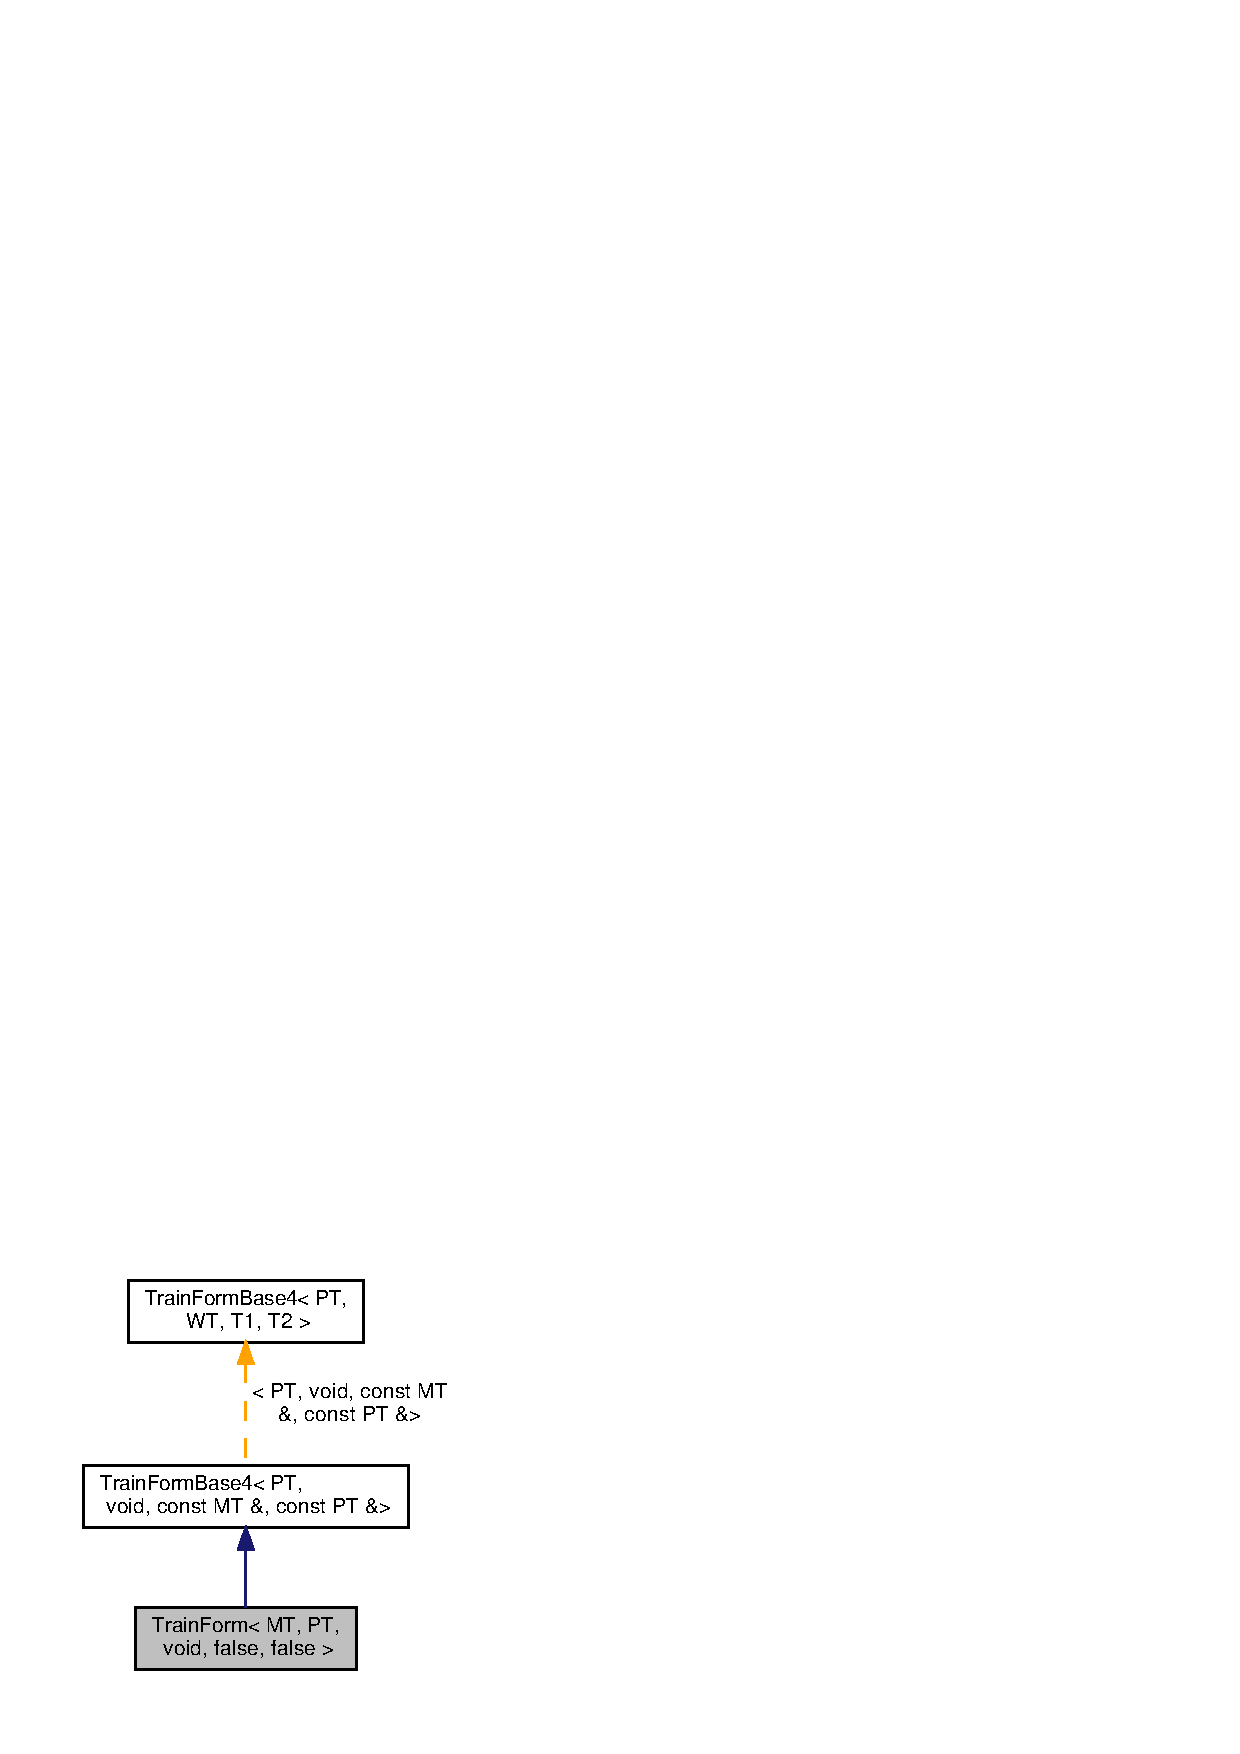
\includegraphics[width=219pt]{structmlpack_1_1cv_1_1TrainForm_3_01MT_00_01PT_00_01void_00_01false_00_01false_01_4__inherit__graph}
\end{center}
\end{figure}
\subsection*{Additional Inherited Members}


\subsection{Detailed Description}
\subsubsection*{template$<$typename MT, typename PT$>$\newline
struct mlpack\+::cv\+::\+Train\+Form$<$ M\+T, P\+T, void, false, false $>$}



Definition at line 100 of file meta\+\_\+info\+\_\+extractor.\+hpp.



The documentation for this struct was generated from the following file\+:\begin{DoxyCompactItemize}
\item 
/home/aakash/mlpack/src/mlpack/core/cv/\textbf{ meta\+\_\+info\+\_\+extractor.\+hpp}\end{DoxyCompactItemize}

\section{Train\+Form$<$ MT, PT, void, false, true $>$ Struct Template Reference}
\label{structmlpack_1_1cv_1_1TrainForm_3_01MT_00_01PT_00_01void_00_01false_00_01true_01_4}\index{Train\+Form$<$ M\+T, P\+T, void, false, true $>$@{Train\+Form$<$ M\+T, P\+T, void, false, true $>$}}


Inheritance diagram for Train\+Form$<$ MT, PT, void, false, true $>$\+:
\nopagebreak
\begin{figure}[H]
\begin{center}
\leavevmode
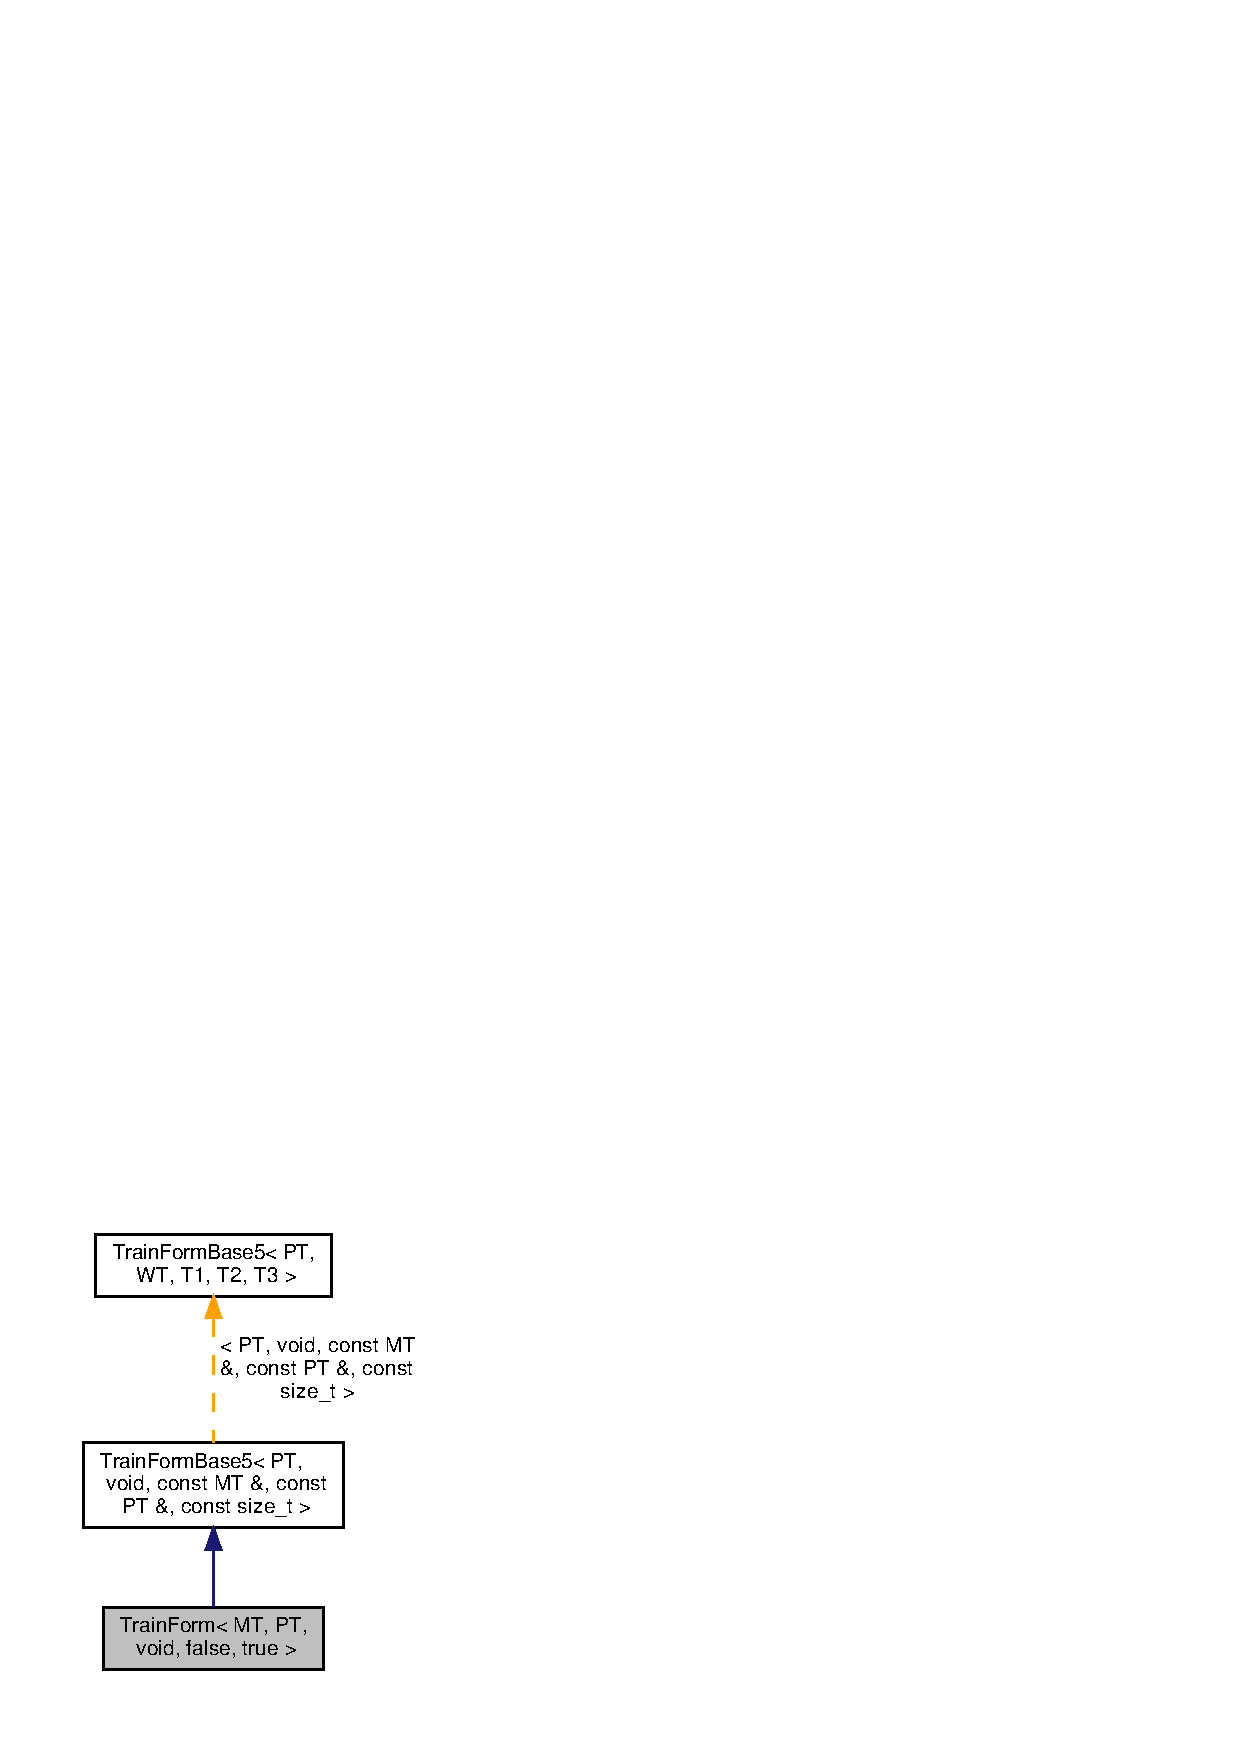
\includegraphics[width=204pt]{structmlpack_1_1cv_1_1TrainForm_3_01MT_00_01PT_00_01void_00_01false_00_01true_01_4__inherit__graph}
\end{center}
\end{figure}
\subsection*{Additional Inherited Members}


\subsection{Detailed Description}
\subsubsection*{template$<$typename MT, typename PT$>$\newline
struct mlpack\+::cv\+::\+Train\+Form$<$ M\+T, P\+T, void, false, true $>$}



Definition at line 116 of file meta\+\_\+info\+\_\+extractor.\+hpp.



The documentation for this struct was generated from the following file\+:\begin{DoxyCompactItemize}
\item 
/home/aakash/mlpack/src/mlpack/core/cv/\textbf{ meta\+\_\+info\+\_\+extractor.\+hpp}\end{DoxyCompactItemize}

\section{Train\+Form$<$ MT, PT, void, true, false $>$ Struct Template Reference}
\label{structmlpack_1_1cv_1_1TrainForm_3_01MT_00_01PT_00_01void_00_01true_00_01false_01_4}\index{Train\+Form$<$ M\+T, P\+T, void, true, false $>$@{Train\+Form$<$ M\+T, P\+T, void, true, false $>$}}


Inheritance diagram for Train\+Form$<$ MT, PT, void, true, false $>$\+:
\nopagebreak
\begin{figure}[H]
\begin{center}
\leavevmode
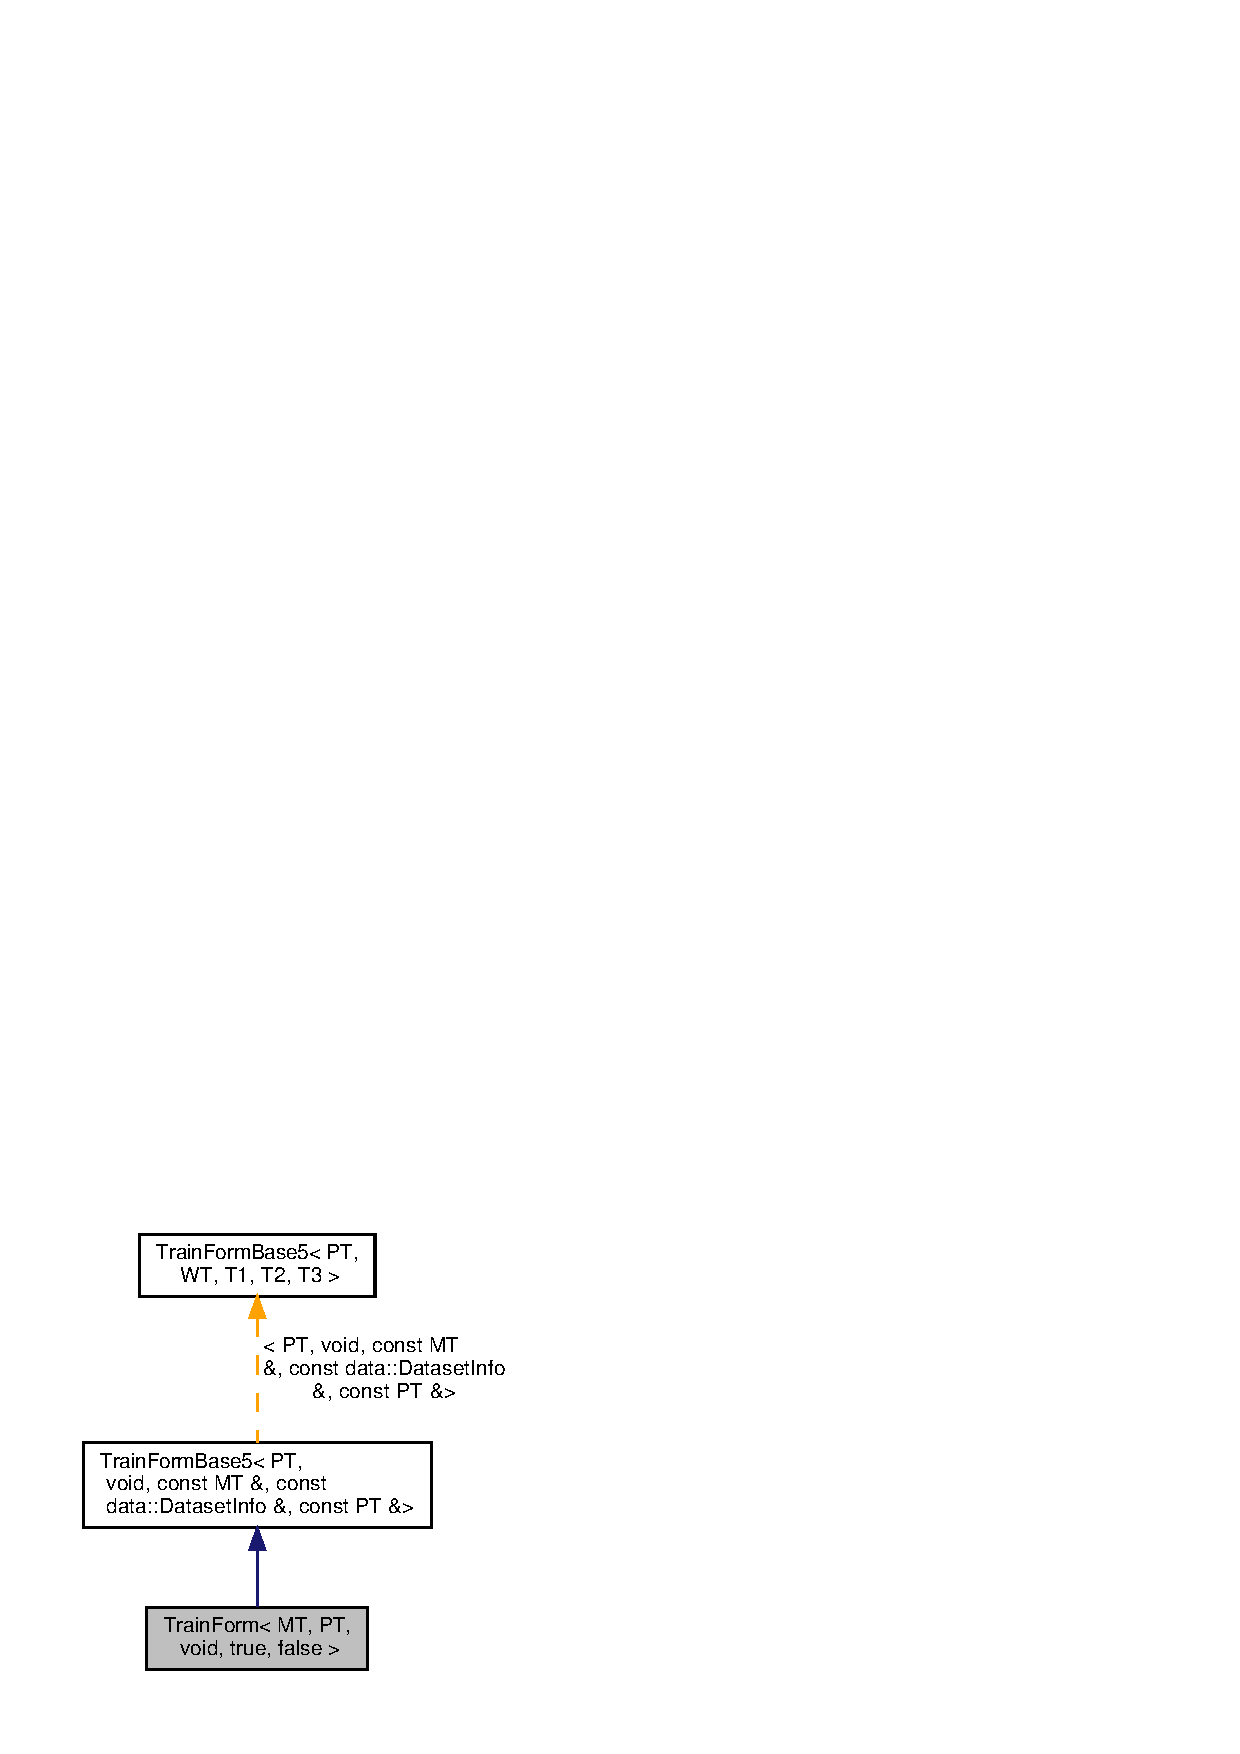
\includegraphics[width=247pt]{structmlpack_1_1cv_1_1TrainForm_3_01MT_00_01PT_00_01void_00_01true_00_01false_01_4__inherit__graph}
\end{center}
\end{figure}
\subsection*{Additional Inherited Members}


\subsection{Detailed Description}
\subsubsection*{template$<$typename MT, typename PT$>$\newline
struct mlpack\+::cv\+::\+Train\+Form$<$ M\+T, P\+T, void, true, false $>$}



Definition at line 104 of file meta\+\_\+info\+\_\+extractor.\+hpp.



The documentation for this struct was generated from the following file\+:\begin{DoxyCompactItemize}
\item 
/home/aakash/mlpack/src/mlpack/core/cv/\textbf{ meta\+\_\+info\+\_\+extractor.\+hpp}\end{DoxyCompactItemize}

\section{Train\+Form$<$ MT, PT, void, true, true $>$ Struct Template Reference}
\label{structmlpack_1_1cv_1_1TrainForm_3_01MT_00_01PT_00_01void_00_01true_00_01true_01_4}\index{Train\+Form$<$ M\+T, P\+T, void, true, true $>$@{Train\+Form$<$ M\+T, P\+T, void, true, true $>$}}


Inheritance diagram for Train\+Form$<$ MT, PT, void, true, true $>$\+:
\nopagebreak
\begin{figure}[H]
\begin{center}
\leavevmode
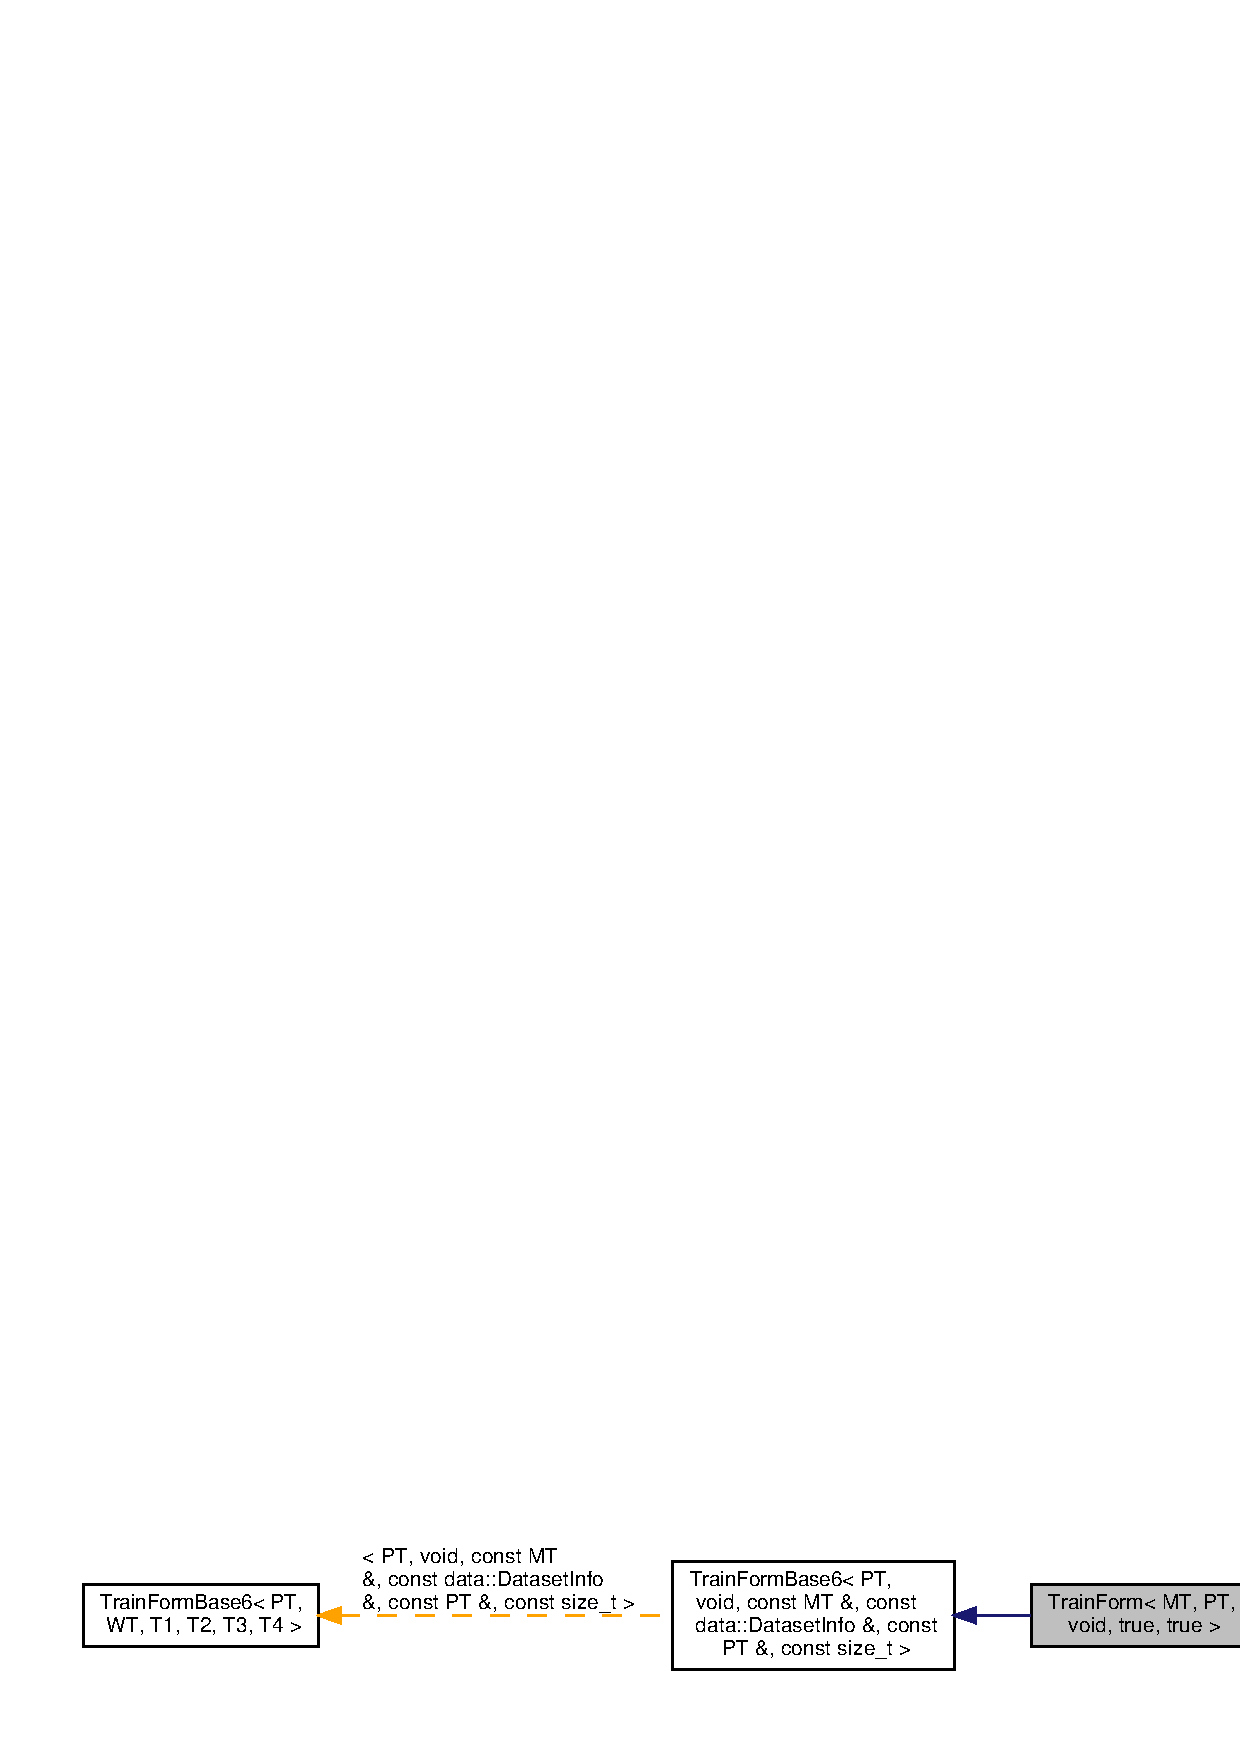
\includegraphics[width=350pt]{structmlpack_1_1cv_1_1TrainForm_3_01MT_00_01PT_00_01void_00_01true_00_01true_01_4__inherit__graph}
\end{center}
\end{figure}
\subsection*{Additional Inherited Members}


\subsection{Detailed Description}
\subsubsection*{template$<$typename MT, typename PT$>$\newline
struct mlpack\+::cv\+::\+Train\+Form$<$ M\+T, P\+T, void, true, true $>$}



Definition at line 120 of file meta\+\_\+info\+\_\+extractor.\+hpp.



The documentation for this struct was generated from the following file\+:\begin{DoxyCompactItemize}
\item 
/home/aakash/mlpack/src/mlpack/core/cv/\textbf{ meta\+\_\+info\+\_\+extractor.\+hpp}\end{DoxyCompactItemize}

\section{Train\+Form$<$ MT, PT, WT, false, false $>$ Struct Template Reference}
\label{structmlpack_1_1cv_1_1TrainForm_3_01MT_00_01PT_00_01WT_00_01false_00_01false_01_4}\index{Train\+Form$<$ M\+T, P\+T, W\+T, false, false $>$@{Train\+Form$<$ M\+T, P\+T, W\+T, false, false $>$}}


Inheritance diagram for Train\+Form$<$ MT, PT, WT, false, false $>$\+:
\nopagebreak
\begin{figure}[H]
\begin{center}
\leavevmode
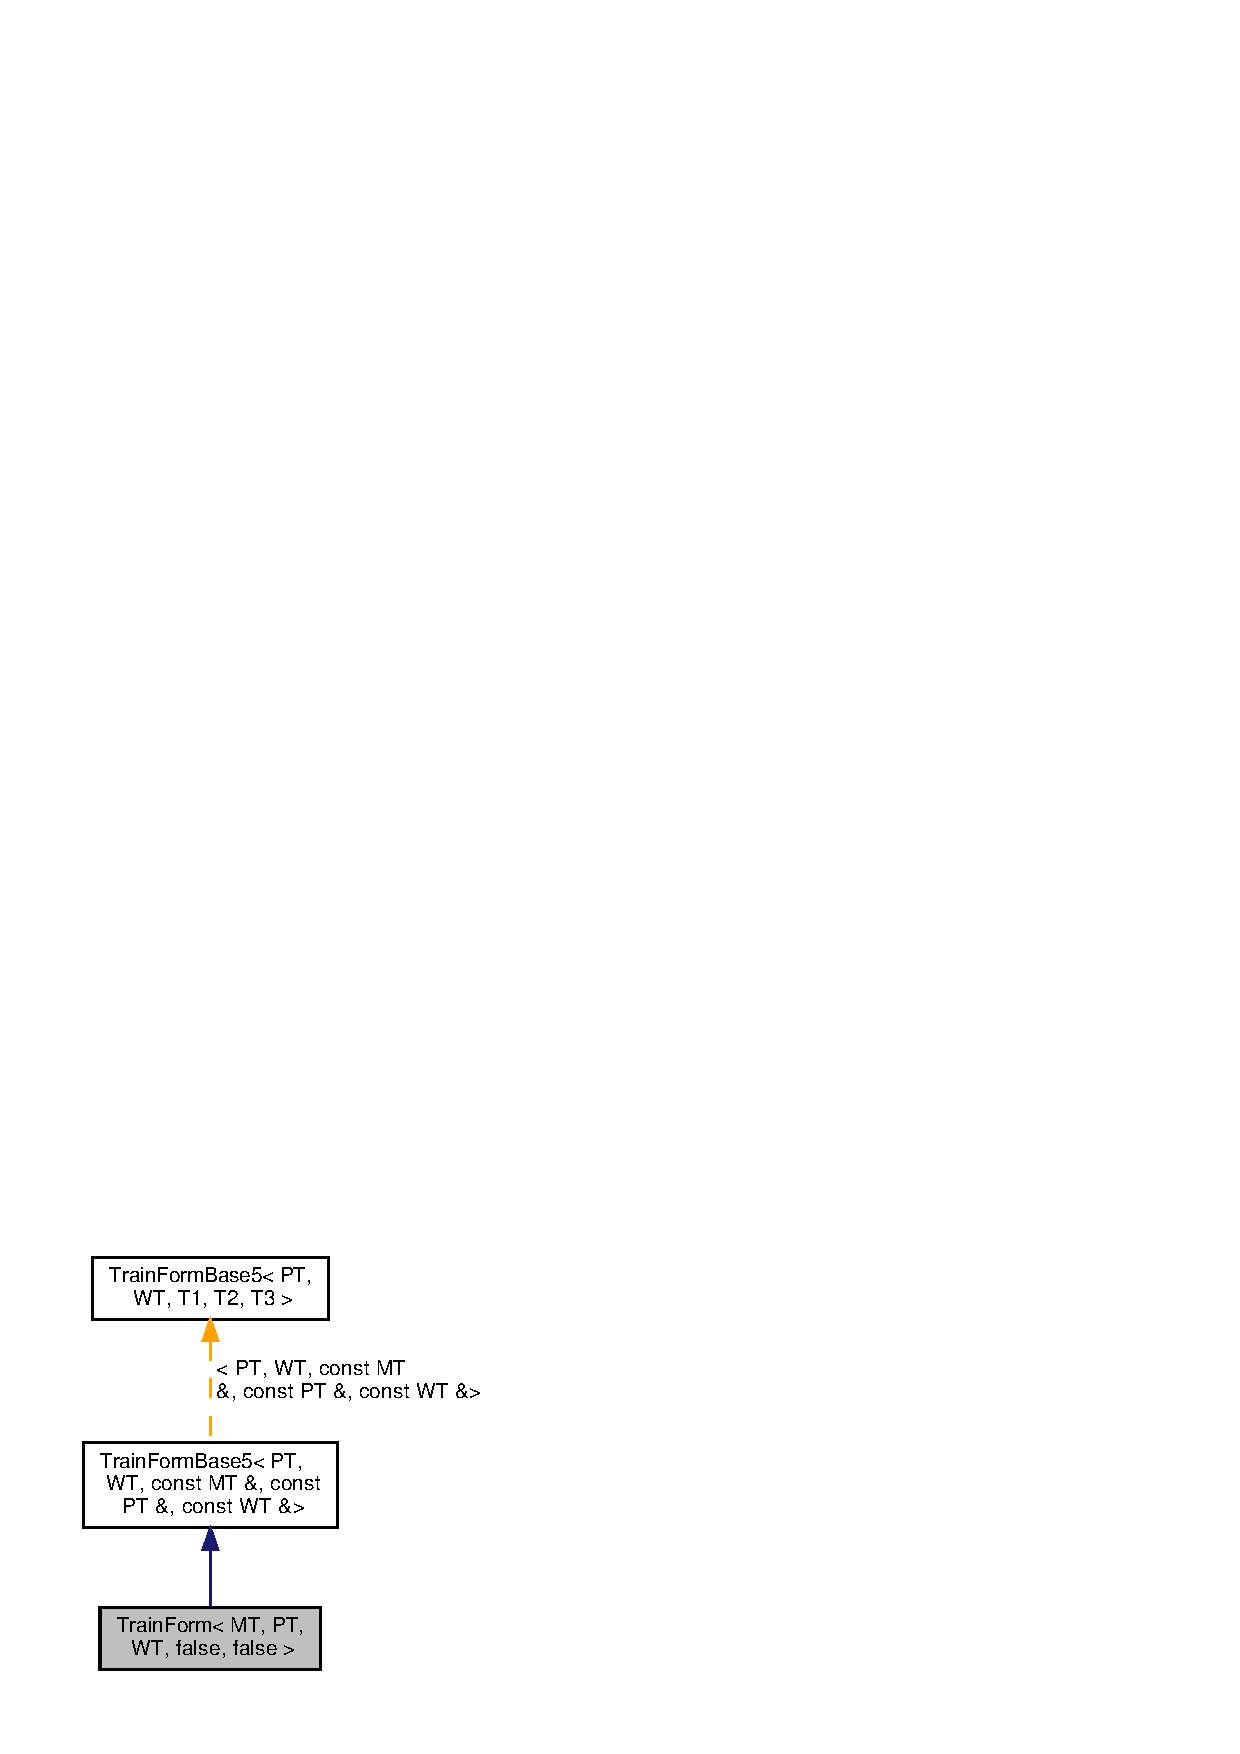
\includegraphics[width=235pt]{structmlpack_1_1cv_1_1TrainForm_3_01MT_00_01PT_00_01WT_00_01false_00_01false_01_4__inherit__graph}
\end{center}
\end{figure}
\subsection*{Additional Inherited Members}


\subsection{Detailed Description}
\subsubsection*{template$<$typename MT, typename PT, typename WT$>$\newline
struct mlpack\+::cv\+::\+Train\+Form$<$ M\+T, P\+T, W\+T, false, false $>$}



Definition at line 108 of file meta\+\_\+info\+\_\+extractor.\+hpp.



The documentation for this struct was generated from the following file\+:\begin{DoxyCompactItemize}
\item 
/home/aakash/mlpack/src/mlpack/core/cv/\textbf{ meta\+\_\+info\+\_\+extractor.\+hpp}\end{DoxyCompactItemize}

\section{Train\+Form$<$ MT, PT, WT, false, true $>$ Struct Template Reference}
\label{structmlpack_1_1cv_1_1TrainForm_3_01MT_00_01PT_00_01WT_00_01false_00_01true_01_4}\index{Train\+Form$<$ M\+T, P\+T, W\+T, false, true $>$@{Train\+Form$<$ M\+T, P\+T, W\+T, false, true $>$}}


Inheritance diagram for Train\+Form$<$ MT, PT, WT, false, true $>$\+:
\nopagebreak
\begin{figure}[H]
\begin{center}
\leavevmode
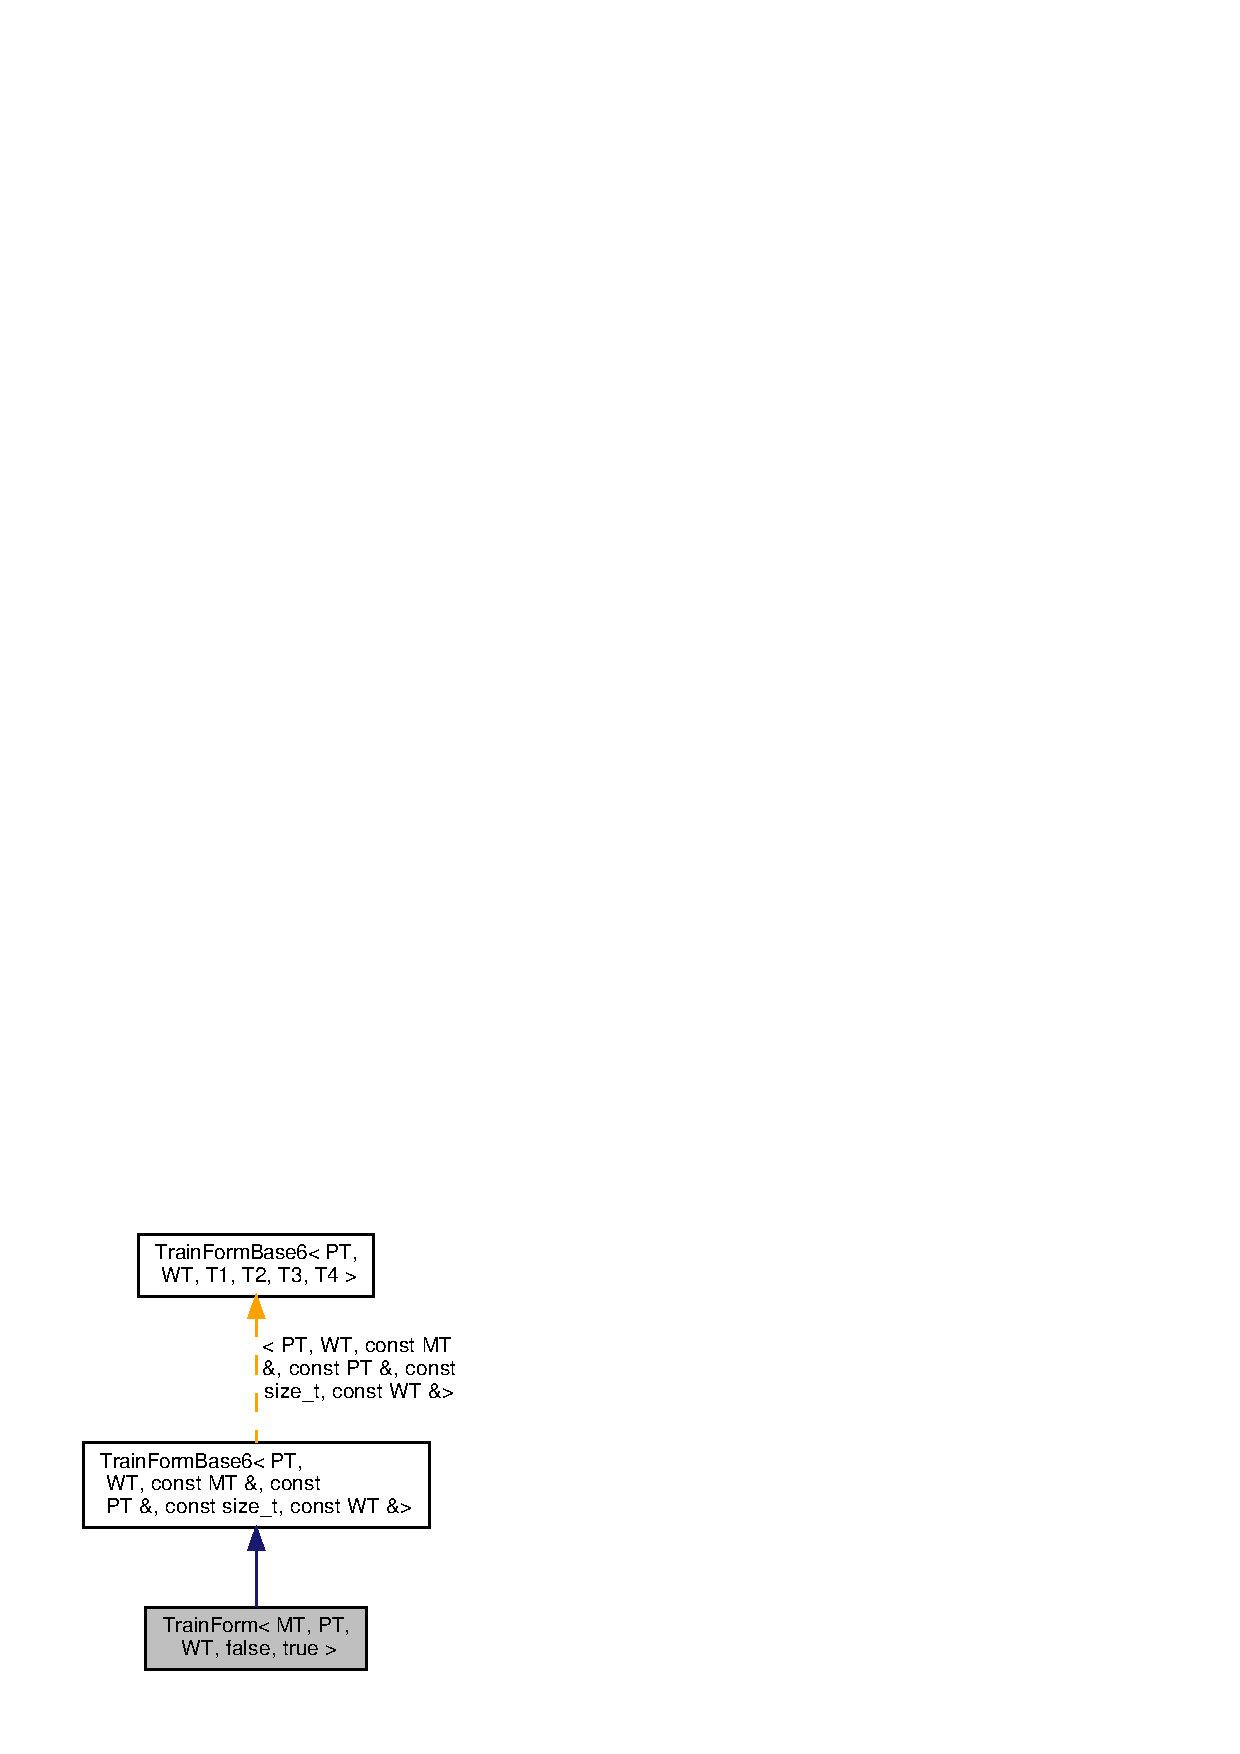
\includegraphics[width=223pt]{structmlpack_1_1cv_1_1TrainForm_3_01MT_00_01PT_00_01WT_00_01false_00_01true_01_4__inherit__graph}
\end{center}
\end{figure}
\subsection*{Additional Inherited Members}


\subsection{Detailed Description}
\subsubsection*{template$<$typename MT, typename PT, typename WT$>$\newline
struct mlpack\+::cv\+::\+Train\+Form$<$ M\+T, P\+T, W\+T, false, true $>$}



Definition at line 124 of file meta\+\_\+info\+\_\+extractor.\+hpp.



The documentation for this struct was generated from the following file\+:\begin{DoxyCompactItemize}
\item 
/home/aakash/mlpack/src/mlpack/core/cv/\textbf{ meta\+\_\+info\+\_\+extractor.\+hpp}\end{DoxyCompactItemize}

\section{Train\+Form$<$ MT, PT, WT, true, false $>$ Struct Template Reference}
\label{structmlpack_1_1cv_1_1TrainForm_3_01MT_00_01PT_00_01WT_00_01true_00_01false_01_4}\index{Train\+Form$<$ M\+T, P\+T, W\+T, true, false $>$@{Train\+Form$<$ M\+T, P\+T, W\+T, true, false $>$}}


Inheritance diagram for Train\+Form$<$ MT, PT, WT, true, false $>$\+:
\nopagebreak
\begin{figure}[H]
\begin{center}
\leavevmode
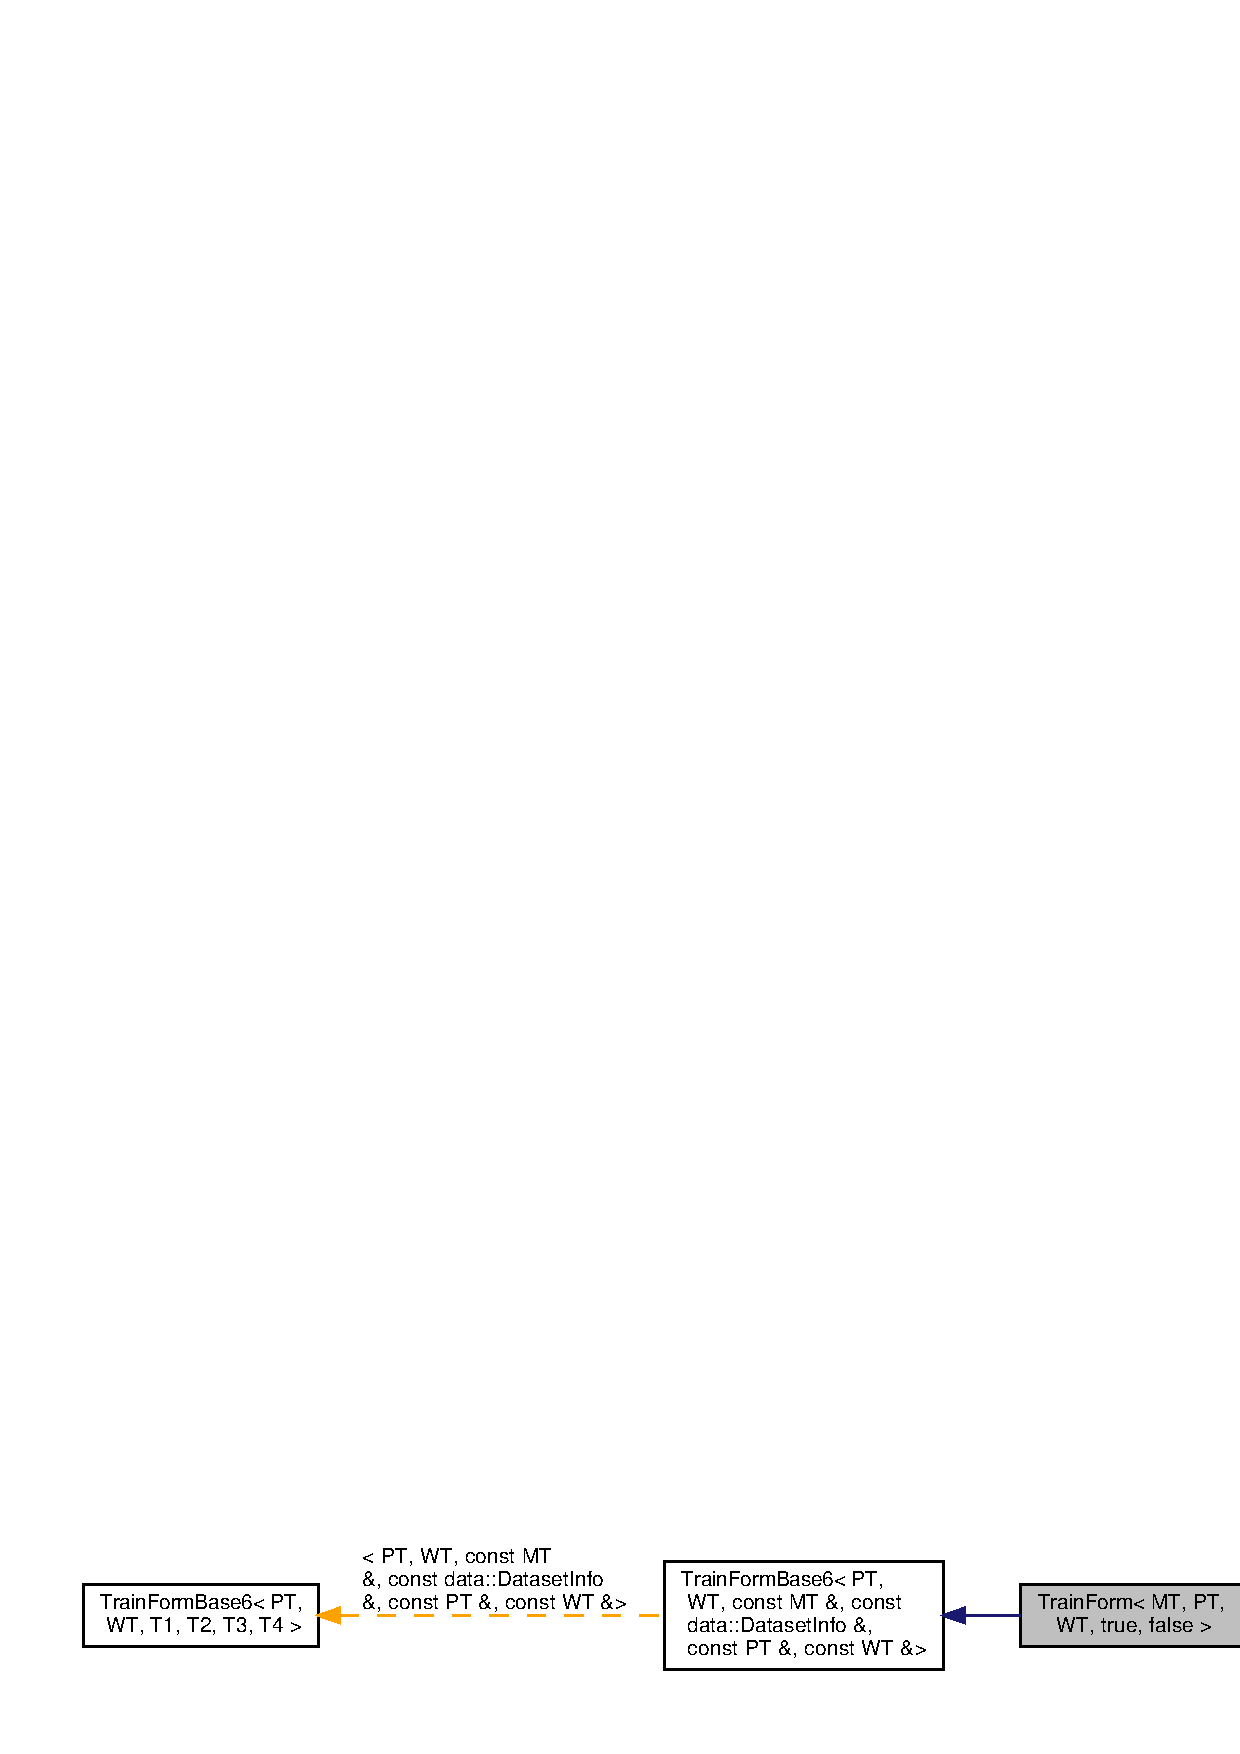
\includegraphics[width=350pt]{structmlpack_1_1cv_1_1TrainForm_3_01MT_00_01PT_00_01WT_00_01true_00_01false_01_4__inherit__graph}
\end{center}
\end{figure}
\subsection*{Additional Inherited Members}


\subsection{Detailed Description}
\subsubsection*{template$<$typename MT, typename PT, typename WT$>$\newline
struct mlpack\+::cv\+::\+Train\+Form$<$ M\+T, P\+T, W\+T, true, false $>$}



Definition at line 112 of file meta\+\_\+info\+\_\+extractor.\+hpp.



The documentation for this struct was generated from the following file\+:\begin{DoxyCompactItemize}
\item 
/home/aakash/mlpack/src/mlpack/core/cv/\textbf{ meta\+\_\+info\+\_\+extractor.\+hpp}\end{DoxyCompactItemize}

\section{Train\+Form$<$ MT, PT, WT, true, true $>$ Struct Template Reference}
\label{structmlpack_1_1cv_1_1TrainForm_3_01MT_00_01PT_00_01WT_00_01true_00_01true_01_4}\index{Train\+Form$<$ M\+T, P\+T, W\+T, true, true $>$@{Train\+Form$<$ M\+T, P\+T, W\+T, true, true $>$}}


Inheritance diagram for Train\+Form$<$ MT, PT, WT, true, true $>$\+:
\nopagebreak
\begin{figure}[H]
\begin{center}
\leavevmode
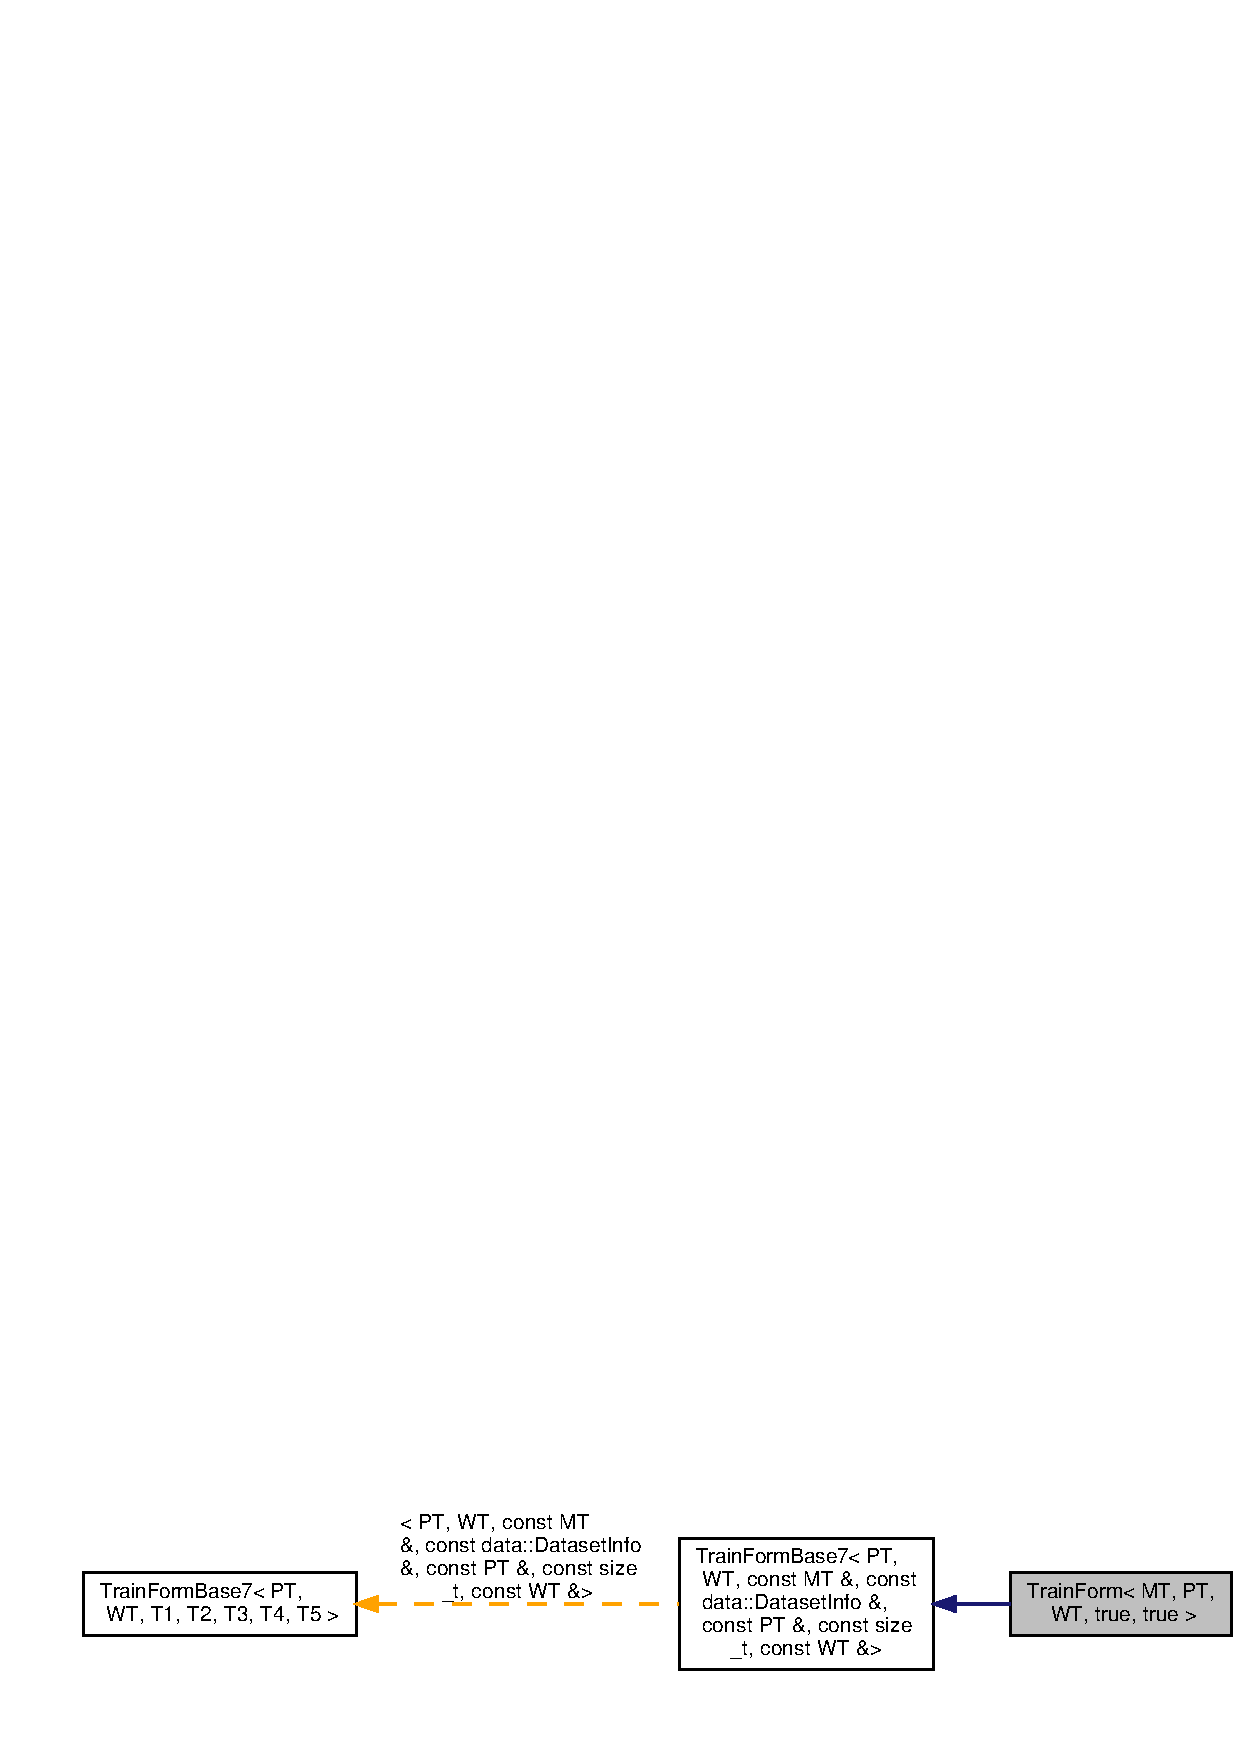
\includegraphics[width=350pt]{structmlpack_1_1cv_1_1TrainForm_3_01MT_00_01PT_00_01WT_00_01true_00_01true_01_4__inherit__graph}
\end{center}
\end{figure}
\subsection*{Additional Inherited Members}


\subsection{Detailed Description}
\subsubsection*{template$<$typename MT, typename PT, typename WT$>$\newline
struct mlpack\+::cv\+::\+Train\+Form$<$ M\+T, P\+T, W\+T, true, true $>$}



Definition at line 128 of file meta\+\_\+info\+\_\+extractor.\+hpp.



The documentation for this struct was generated from the following file\+:\begin{DoxyCompactItemize}
\item 
/home/aakash/mlpack/src/mlpack/core/cv/\textbf{ meta\+\_\+info\+\_\+extractor.\+hpp}\end{DoxyCompactItemize}

\section{Train\+Form\+Base4$<$ PT, WT, T1, T2 $>$ Struct Template Reference}
\label{structmlpack_1_1cv_1_1TrainFormBase4}\index{Train\+Form\+Base4$<$ P\+T, W\+T, T1, T2 $>$@{Train\+Form\+Base4$<$ P\+T, W\+T, T1, T2 $>$}}


Inheritance diagram for Train\+Form\+Base4$<$ PT, WT, T1, T2 $>$\+:
\nopagebreak
\begin{figure}[H]
\begin{center}
\leavevmode
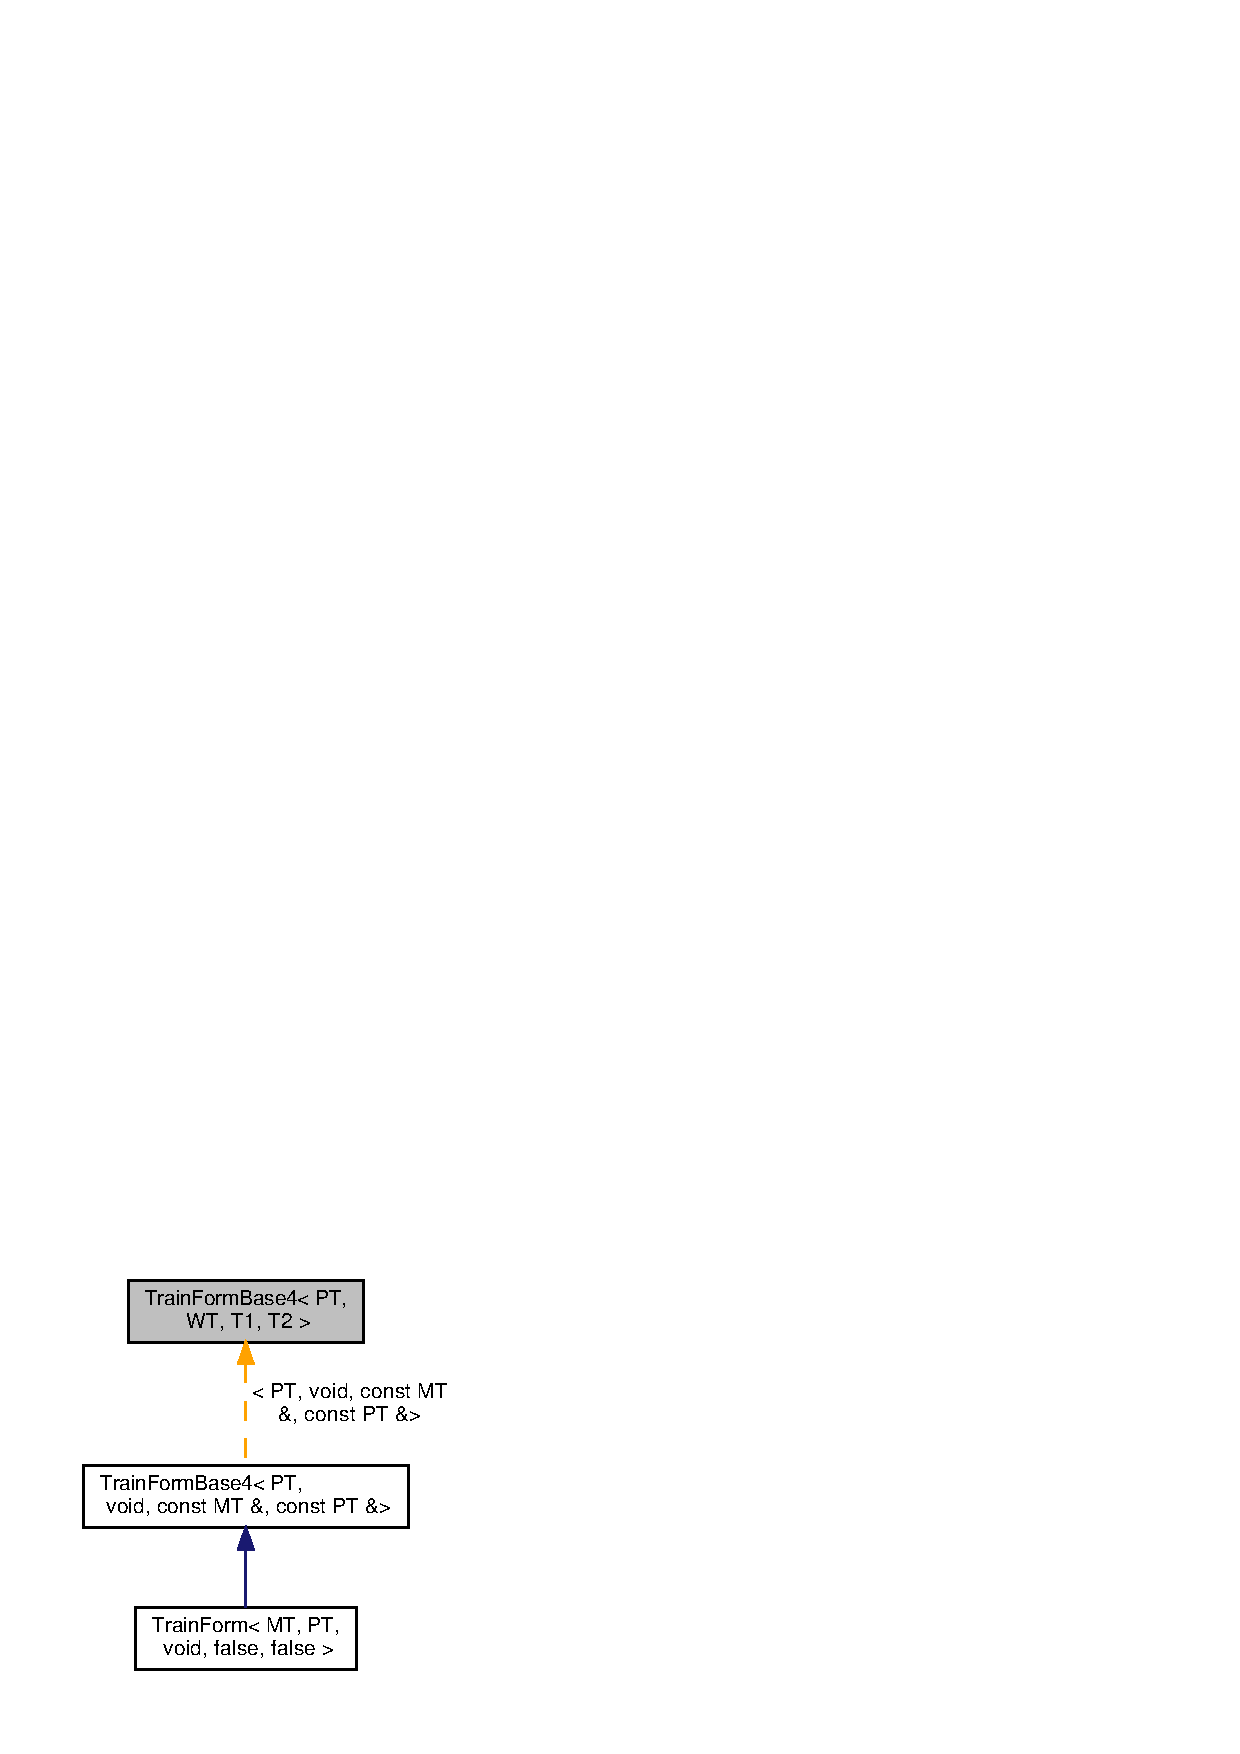
\includegraphics[width=219pt]{structmlpack_1_1cv_1_1TrainFormBase4__inherit__graph}
\end{center}
\end{figure}
\subsection*{Public Types}
\begin{DoxyCompactItemize}
\item 
using \textbf{ Predictions\+Type} = PT
\item 
{\footnotesize template$<$typename Class , typename RT , typename... Ts$>$ }\\using \textbf{ Type} = RT(Class\+::$\ast$)(T1, T2, Ts...)
\item 
using \textbf{ Weights\+Type} = WT
\end{DoxyCompactItemize}
\subsection*{Static Public Attributes}
\begin{DoxyCompactItemize}
\item 
static const size\+\_\+t \textbf{ Min\+Number\+Of\+Additional\+Args} = 1
\end{DoxyCompactItemize}


\subsection{Detailed Description}
\subsubsection*{template$<$typename PT, typename WT, typename T1, typename T2$>$\newline
struct mlpack\+::cv\+::\+Train\+Form\+Base4$<$ P\+T, W\+T, T1, T2 $>$}



Definition at line 46 of file meta\+\_\+info\+\_\+extractor.\+hpp.



\subsection{Member Typedef Documentation}
\mbox{\label{structmlpack_1_1cv_1_1TrainFormBase4_a329a0bee5f08ebbfbd6c97e4f74bdb4f}} 
\index{mlpack\+::cv\+::\+Train\+Form\+Base4@{mlpack\+::cv\+::\+Train\+Form\+Base4}!Predictions\+Type@{Predictions\+Type}}
\index{Predictions\+Type@{Predictions\+Type}!mlpack\+::cv\+::\+Train\+Form\+Base4@{mlpack\+::cv\+::\+Train\+Form\+Base4}}
\subsubsection{Predictions\+Type}
{\footnotesize\ttfamily using \textbf{ Predictions\+Type} =  PT}



Definition at line 48 of file meta\+\_\+info\+\_\+extractor.\+hpp.

\mbox{\label{structmlpack_1_1cv_1_1TrainFormBase4_a61f44880a9510b9d414669ea7e7263f1}} 
\index{mlpack\+::cv\+::\+Train\+Form\+Base4@{mlpack\+::cv\+::\+Train\+Form\+Base4}!Type@{Type}}
\index{Type@{Type}!mlpack\+::cv\+::\+Train\+Form\+Base4@{mlpack\+::cv\+::\+Train\+Form\+Base4}}
\subsubsection{Type}
{\footnotesize\ttfamily using \textbf{ Type} =  RT(Class\+::$\ast$)(T1, T2, Ts...)}



Definition at line 55 of file meta\+\_\+info\+\_\+extractor.\+hpp.

\mbox{\label{structmlpack_1_1cv_1_1TrainFormBase4_aecfc3bfd62796ddd9feb857c898cefa8}} 
\index{mlpack\+::cv\+::\+Train\+Form\+Base4@{mlpack\+::cv\+::\+Train\+Form\+Base4}!Weights\+Type@{Weights\+Type}}
\index{Weights\+Type@{Weights\+Type}!mlpack\+::cv\+::\+Train\+Form\+Base4@{mlpack\+::cv\+::\+Train\+Form\+Base4}}
\subsubsection{Weights\+Type}
{\footnotesize\ttfamily using \textbf{ Weights\+Type} =  WT}



Definition at line 49 of file meta\+\_\+info\+\_\+extractor.\+hpp.



\subsection{Member Data Documentation}
\mbox{\label{structmlpack_1_1cv_1_1TrainFormBase4_adacbdda6f41a542559105d6e48d1cfc2}} 
\index{mlpack\+::cv\+::\+Train\+Form\+Base4@{mlpack\+::cv\+::\+Train\+Form\+Base4}!Min\+Number\+Of\+Additional\+Args@{Min\+Number\+Of\+Additional\+Args}}
\index{Min\+Number\+Of\+Additional\+Args@{Min\+Number\+Of\+Additional\+Args}!mlpack\+::cv\+::\+Train\+Form\+Base4@{mlpack\+::cv\+::\+Train\+Form\+Base4}}
\subsubsection{Min\+Number\+Of\+Additional\+Args}
{\footnotesize\ttfamily const size\+\_\+t Min\+Number\+Of\+Additional\+Args = 1\hspace{0.3cm}{\ttfamily [static]}}



Definition at line 52 of file meta\+\_\+info\+\_\+extractor.\+hpp.



The documentation for this struct was generated from the following file\+:\begin{DoxyCompactItemize}
\item 
/home/aakash/mlpack/src/mlpack/core/cv/\textbf{ meta\+\_\+info\+\_\+extractor.\+hpp}\end{DoxyCompactItemize}

\section{Train\+Form\+Base5$<$ PT, WT, T1, T2, T3 $>$ Struct Template Reference}
\label{structmlpack_1_1cv_1_1TrainFormBase5}\index{Train\+Form\+Base5$<$ P\+T, W\+T, T1, T2, T3 $>$@{Train\+Form\+Base5$<$ P\+T, W\+T, T1, T2, T3 $>$}}


Inheritance diagram for Train\+Form\+Base5$<$ PT, WT, T1, T2, T3 $>$\+:
\nopagebreak
\begin{figure}[H]
\begin{center}
\leavevmode
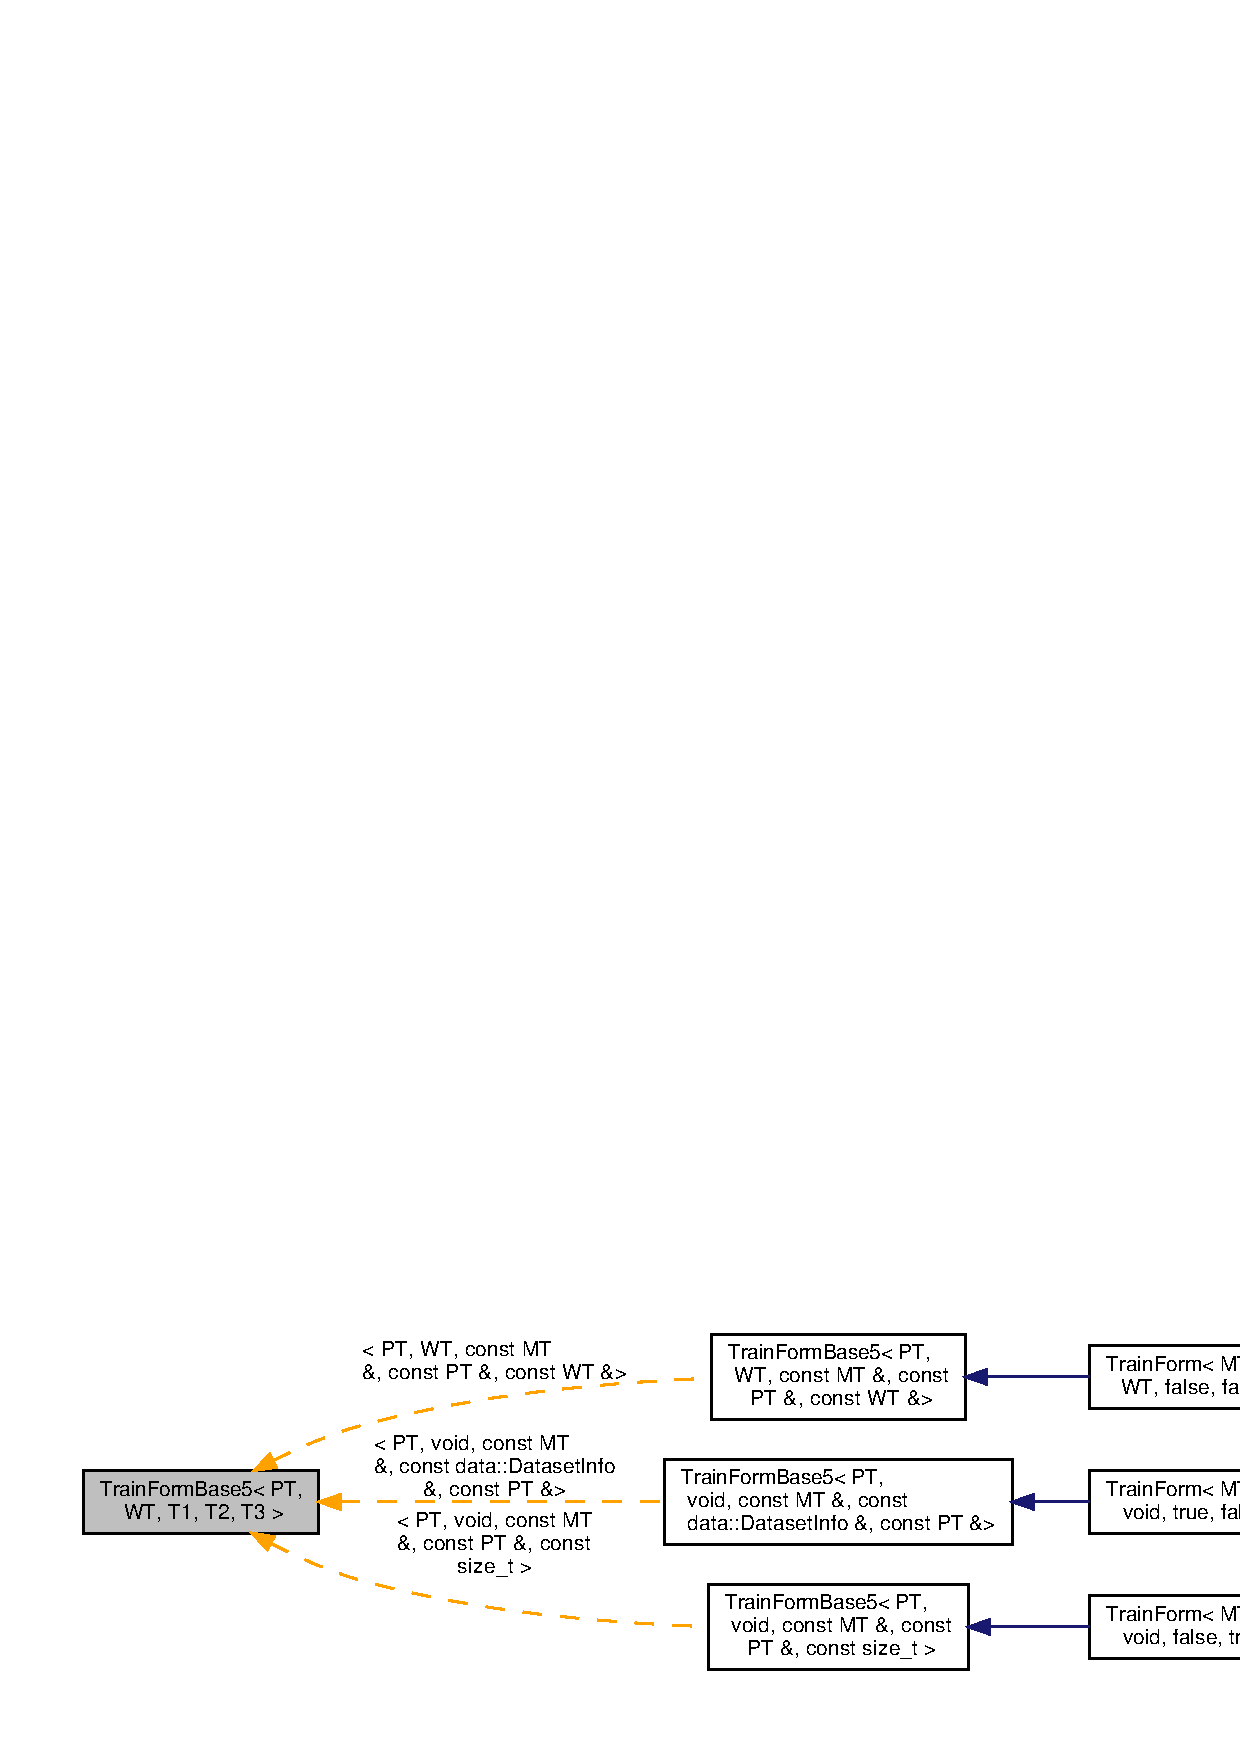
\includegraphics[width=350pt]{structmlpack_1_1cv_1_1TrainFormBase5__inherit__graph}
\end{center}
\end{figure}
\subsection*{Public Types}
\begin{DoxyCompactItemize}
\item 
using \textbf{ Predictions\+Type} = PT
\item 
{\footnotesize template$<$typename Class , typename RT , typename... Ts$>$ }\\using \textbf{ Type} = RT(Class\+::$\ast$)(T1, T2, T3, Ts...)
\item 
using \textbf{ Weights\+Type} = WT
\end{DoxyCompactItemize}
\subsection*{Static Public Attributes}
\begin{DoxyCompactItemize}
\item 
static const size\+\_\+t \textbf{ Min\+Number\+Of\+Additional\+Args} = 1
\end{DoxyCompactItemize}


\subsection{Detailed Description}
\subsubsection*{template$<$typename PT, typename WT, typename T1, typename T2, typename T3$>$\newline
struct mlpack\+::cv\+::\+Train\+Form\+Base5$<$ P\+T, W\+T, T1, T2, T3 $>$}



Definition at line 59 of file meta\+\_\+info\+\_\+extractor.\+hpp.



\subsection{Member Typedef Documentation}
\mbox{\label{structmlpack_1_1cv_1_1TrainFormBase5_a329a0bee5f08ebbfbd6c97e4f74bdb4f}} 
\index{mlpack\+::cv\+::\+Train\+Form\+Base5@{mlpack\+::cv\+::\+Train\+Form\+Base5}!Predictions\+Type@{Predictions\+Type}}
\index{Predictions\+Type@{Predictions\+Type}!mlpack\+::cv\+::\+Train\+Form\+Base5@{mlpack\+::cv\+::\+Train\+Form\+Base5}}
\subsubsection{Predictions\+Type}
{\footnotesize\ttfamily using \textbf{ Predictions\+Type} =  PT}



Definition at line 61 of file meta\+\_\+info\+\_\+extractor.\+hpp.

\mbox{\label{structmlpack_1_1cv_1_1TrainFormBase5_aafe4d92b3375aba15ef2942c225e81b0}} 
\index{mlpack\+::cv\+::\+Train\+Form\+Base5@{mlpack\+::cv\+::\+Train\+Form\+Base5}!Type@{Type}}
\index{Type@{Type}!mlpack\+::cv\+::\+Train\+Form\+Base5@{mlpack\+::cv\+::\+Train\+Form\+Base5}}
\subsubsection{Type}
{\footnotesize\ttfamily using \textbf{ Type} =  RT(Class\+::$\ast$)(T1, T2, T3, Ts...)}



Definition at line 68 of file meta\+\_\+info\+\_\+extractor.\+hpp.

\mbox{\label{structmlpack_1_1cv_1_1TrainFormBase5_aecfc3bfd62796ddd9feb857c898cefa8}} 
\index{mlpack\+::cv\+::\+Train\+Form\+Base5@{mlpack\+::cv\+::\+Train\+Form\+Base5}!Weights\+Type@{Weights\+Type}}
\index{Weights\+Type@{Weights\+Type}!mlpack\+::cv\+::\+Train\+Form\+Base5@{mlpack\+::cv\+::\+Train\+Form\+Base5}}
\subsubsection{Weights\+Type}
{\footnotesize\ttfamily using \textbf{ Weights\+Type} =  WT}



Definition at line 62 of file meta\+\_\+info\+\_\+extractor.\+hpp.



\subsection{Member Data Documentation}
\mbox{\label{structmlpack_1_1cv_1_1TrainFormBase5_adacbdda6f41a542559105d6e48d1cfc2}} 
\index{mlpack\+::cv\+::\+Train\+Form\+Base5@{mlpack\+::cv\+::\+Train\+Form\+Base5}!Min\+Number\+Of\+Additional\+Args@{Min\+Number\+Of\+Additional\+Args}}
\index{Min\+Number\+Of\+Additional\+Args@{Min\+Number\+Of\+Additional\+Args}!mlpack\+::cv\+::\+Train\+Form\+Base5@{mlpack\+::cv\+::\+Train\+Form\+Base5}}
\subsubsection{Min\+Number\+Of\+Additional\+Args}
{\footnotesize\ttfamily const size\+\_\+t Min\+Number\+Of\+Additional\+Args = 1\hspace{0.3cm}{\ttfamily [static]}}



Definition at line 65 of file meta\+\_\+info\+\_\+extractor.\+hpp.



The documentation for this struct was generated from the following file\+:\begin{DoxyCompactItemize}
\item 
/home/aakash/mlpack/src/mlpack/core/cv/\textbf{ meta\+\_\+info\+\_\+extractor.\+hpp}\end{DoxyCompactItemize}

\section{Train\+Form\+Base6$<$ PT, WT, T1, T2, T3, T4 $>$ Struct Template Reference}
\label{structmlpack_1_1cv_1_1TrainFormBase6}\index{Train\+Form\+Base6$<$ P\+T, W\+T, T1, T2, T3, T4 $>$@{Train\+Form\+Base6$<$ P\+T, W\+T, T1, T2, T3, T4 $>$}}


Inheritance diagram for Train\+Form\+Base6$<$ PT, WT, T1, T2, T3, T4 $>$\+:
\nopagebreak
\begin{figure}[H]
\begin{center}
\leavevmode
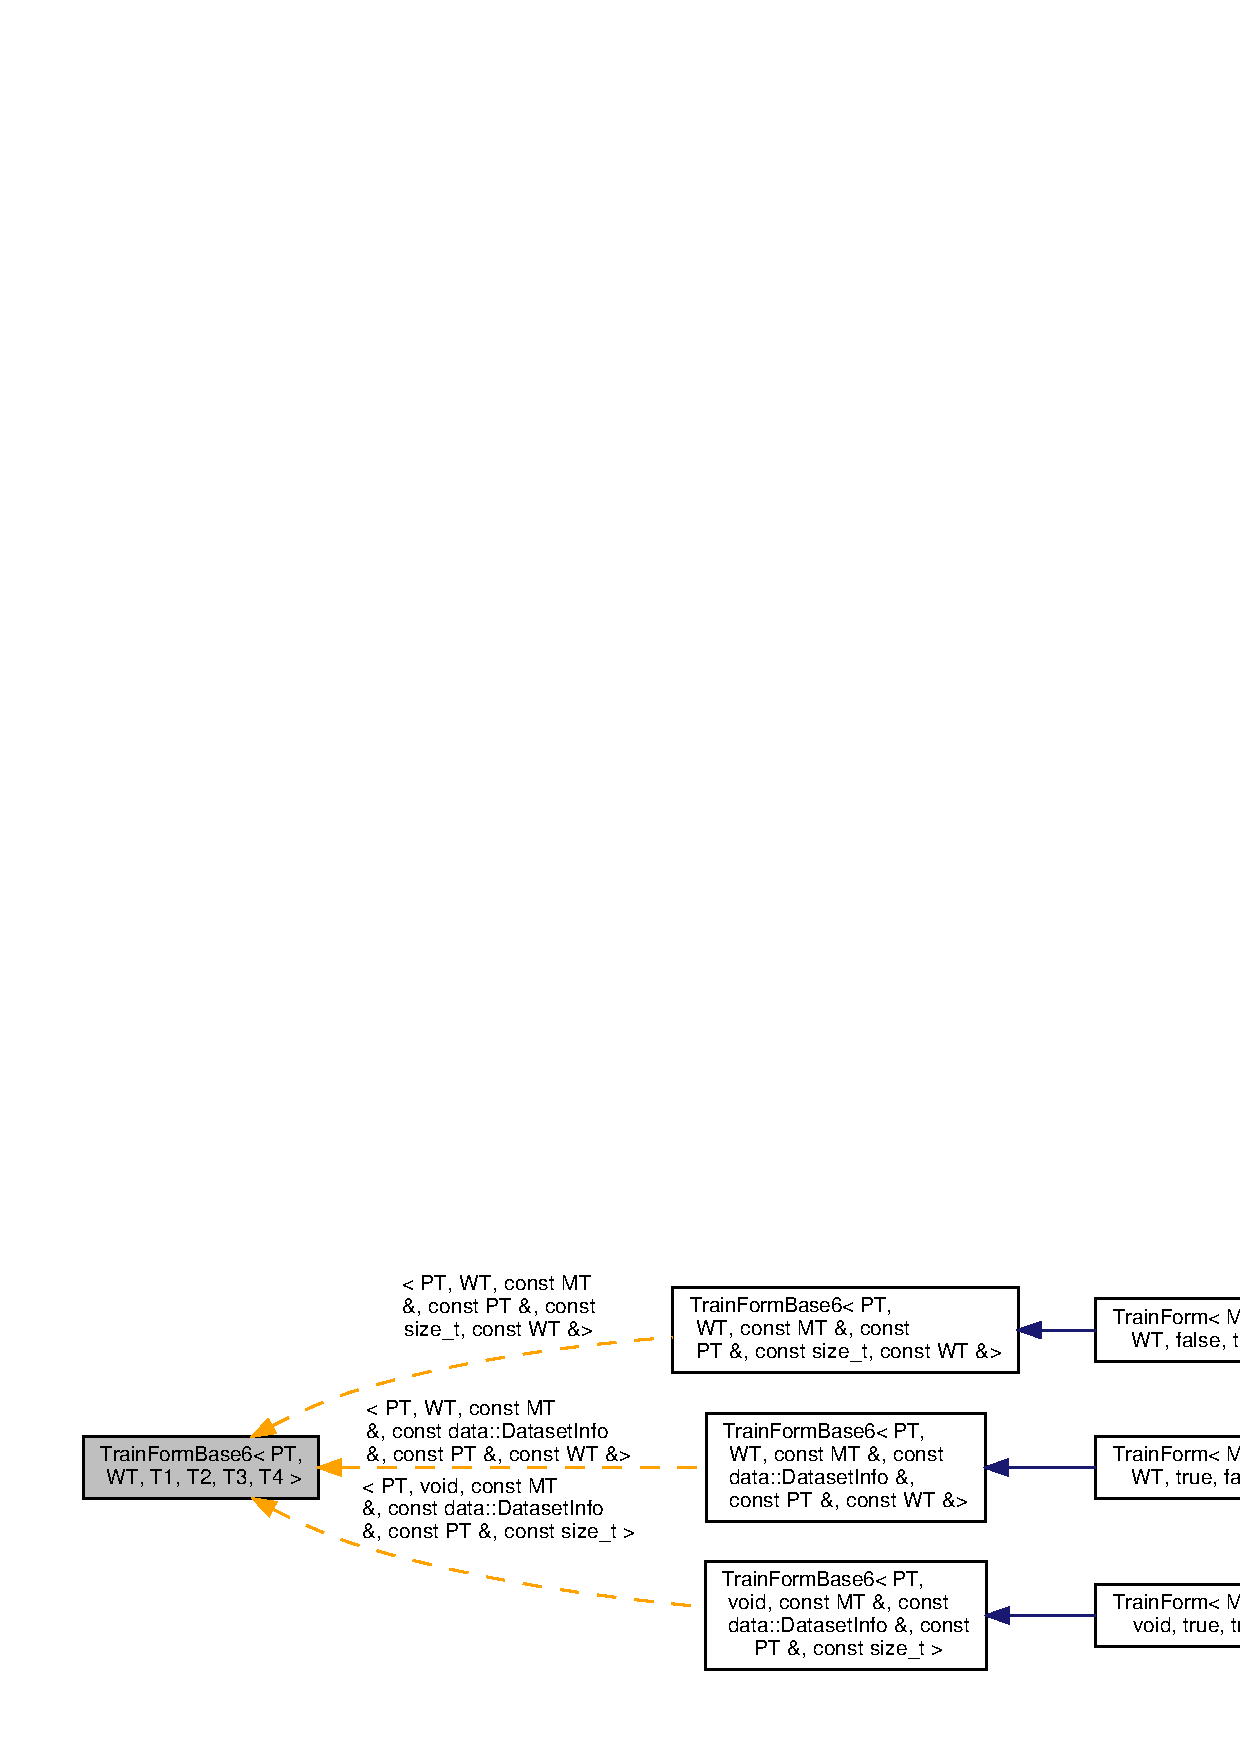
\includegraphics[width=350pt]{structmlpack_1_1cv_1_1TrainFormBase6__inherit__graph}
\end{center}
\end{figure}
\subsection*{Public Types}
\begin{DoxyCompactItemize}
\item 
using \textbf{ Predictions\+Type} = PT
\item 
{\footnotesize template$<$typename Class , typename RT , typename... Ts$>$ }\\using \textbf{ Type} = RT(Class\+::$\ast$)(T1, T2, T3, T4, Ts...)
\item 
using \textbf{ Weights\+Type} = WT
\end{DoxyCompactItemize}
\subsection*{Static Public Attributes}
\begin{DoxyCompactItemize}
\item 
static const size\+\_\+t \textbf{ Min\+Number\+Of\+Additional\+Args} = 1
\end{DoxyCompactItemize}


\subsection{Detailed Description}
\subsubsection*{template$<$typename PT, typename WT, typename T1, typename T2, typename T3, typename T4$>$\newline
struct mlpack\+::cv\+::\+Train\+Form\+Base6$<$ P\+T, W\+T, T1, T2, T3, T4 $>$}



Definition at line 73 of file meta\+\_\+info\+\_\+extractor.\+hpp.



\subsection{Member Typedef Documentation}
\mbox{\label{structmlpack_1_1cv_1_1TrainFormBase6_a329a0bee5f08ebbfbd6c97e4f74bdb4f}} 
\index{mlpack\+::cv\+::\+Train\+Form\+Base6@{mlpack\+::cv\+::\+Train\+Form\+Base6}!Predictions\+Type@{Predictions\+Type}}
\index{Predictions\+Type@{Predictions\+Type}!mlpack\+::cv\+::\+Train\+Form\+Base6@{mlpack\+::cv\+::\+Train\+Form\+Base6}}
\subsubsection{Predictions\+Type}
{\footnotesize\ttfamily using \textbf{ Predictions\+Type} =  PT}



Definition at line 75 of file meta\+\_\+info\+\_\+extractor.\+hpp.

\mbox{\label{structmlpack_1_1cv_1_1TrainFormBase6_a31d0847c2645922caef9eaddc3db89d8}} 
\index{mlpack\+::cv\+::\+Train\+Form\+Base6@{mlpack\+::cv\+::\+Train\+Form\+Base6}!Type@{Type}}
\index{Type@{Type}!mlpack\+::cv\+::\+Train\+Form\+Base6@{mlpack\+::cv\+::\+Train\+Form\+Base6}}
\subsubsection{Type}
{\footnotesize\ttfamily using \textbf{ Type} =  RT(Class\+::$\ast$)(T1, T2, T3, T4, Ts...)}



Definition at line 82 of file meta\+\_\+info\+\_\+extractor.\+hpp.

\mbox{\label{structmlpack_1_1cv_1_1TrainFormBase6_aecfc3bfd62796ddd9feb857c898cefa8}} 
\index{mlpack\+::cv\+::\+Train\+Form\+Base6@{mlpack\+::cv\+::\+Train\+Form\+Base6}!Weights\+Type@{Weights\+Type}}
\index{Weights\+Type@{Weights\+Type}!mlpack\+::cv\+::\+Train\+Form\+Base6@{mlpack\+::cv\+::\+Train\+Form\+Base6}}
\subsubsection{Weights\+Type}
{\footnotesize\ttfamily using \textbf{ Weights\+Type} =  WT}



Definition at line 76 of file meta\+\_\+info\+\_\+extractor.\+hpp.



\subsection{Member Data Documentation}
\mbox{\label{structmlpack_1_1cv_1_1TrainFormBase6_adacbdda6f41a542559105d6e48d1cfc2}} 
\index{mlpack\+::cv\+::\+Train\+Form\+Base6@{mlpack\+::cv\+::\+Train\+Form\+Base6}!Min\+Number\+Of\+Additional\+Args@{Min\+Number\+Of\+Additional\+Args}}
\index{Min\+Number\+Of\+Additional\+Args@{Min\+Number\+Of\+Additional\+Args}!mlpack\+::cv\+::\+Train\+Form\+Base6@{mlpack\+::cv\+::\+Train\+Form\+Base6}}
\subsubsection{Min\+Number\+Of\+Additional\+Args}
{\footnotesize\ttfamily const size\+\_\+t Min\+Number\+Of\+Additional\+Args = 1\hspace{0.3cm}{\ttfamily [static]}}



Definition at line 79 of file meta\+\_\+info\+\_\+extractor.\+hpp.



The documentation for this struct was generated from the following file\+:\begin{DoxyCompactItemize}
\item 
/home/aakash/mlpack/src/mlpack/core/cv/\textbf{ meta\+\_\+info\+\_\+extractor.\+hpp}\end{DoxyCompactItemize}

\section{Train\+Form\+Base7$<$ PT, WT, T1, T2, T3, T4, T5 $>$ Struct Template Reference}
\label{structmlpack_1_1cv_1_1TrainFormBase7}\index{Train\+Form\+Base7$<$ P\+T, W\+T, T1, T2, T3, T4, T5 $>$@{Train\+Form\+Base7$<$ P\+T, W\+T, T1, T2, T3, T4, T5 $>$}}


Inheritance diagram for Train\+Form\+Base7$<$ PT, WT, T1, T2, T3, T4, T5 $>$\+:
\nopagebreak
\begin{figure}[H]
\begin{center}
\leavevmode
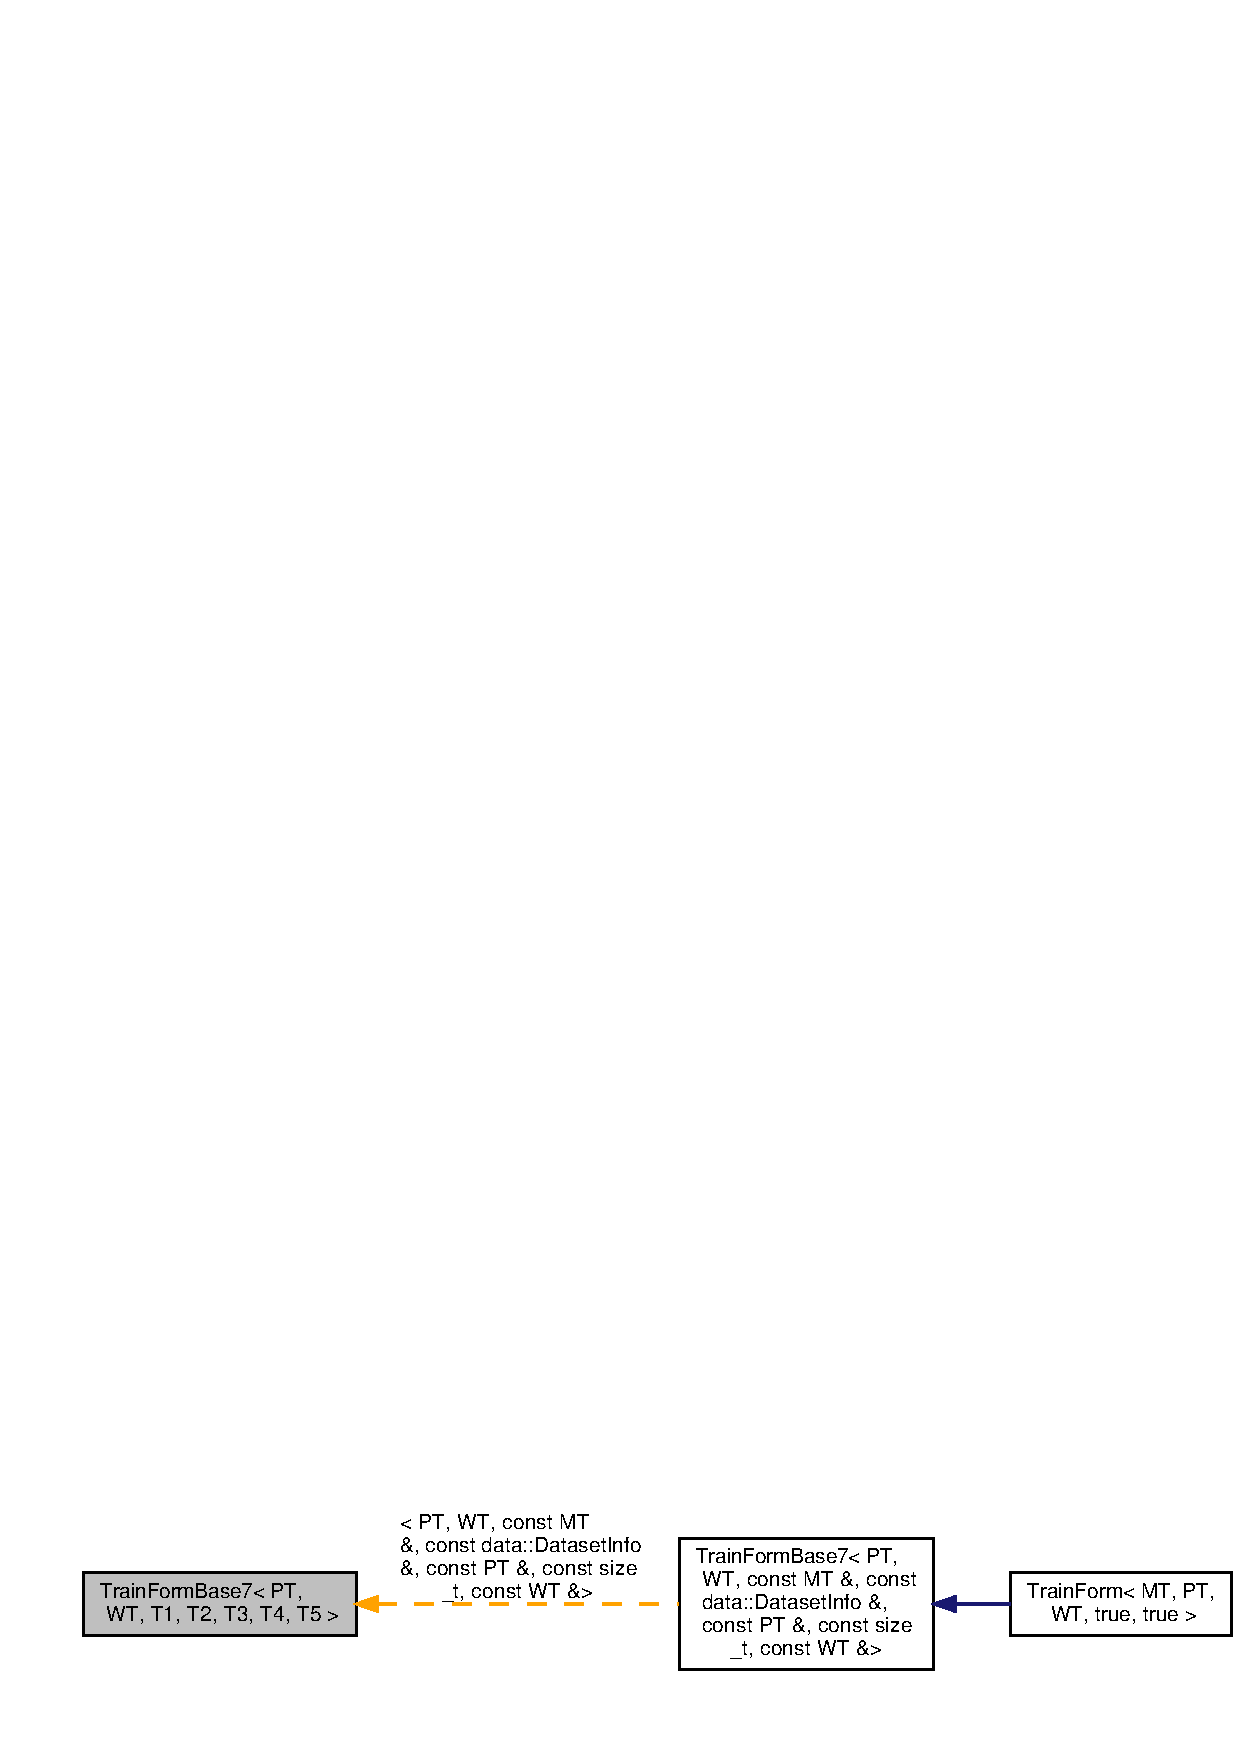
\includegraphics[width=350pt]{structmlpack_1_1cv_1_1TrainFormBase7__inherit__graph}
\end{center}
\end{figure}
\subsection*{Public Types}
\begin{DoxyCompactItemize}
\item 
using \textbf{ Predictions\+Type} = PT
\item 
{\footnotesize template$<$typename Class , typename RT , typename... Ts$>$ }\\using \textbf{ Type} = RT(Class\+::$\ast$)(T1, T2, T3, T4, T5, Ts...)
\item 
using \textbf{ Weights\+Type} = WT
\end{DoxyCompactItemize}
\subsection*{Static Public Attributes}
\begin{DoxyCompactItemize}
\item 
static const size\+\_\+t \textbf{ Min\+Number\+Of\+Additional\+Args} = 1
\end{DoxyCompactItemize}


\subsection{Detailed Description}
\subsubsection*{template$<$typename PT, typename WT, typename T1, typename T2, typename T3, typename T4, typename T5$>$\newline
struct mlpack\+::cv\+::\+Train\+Form\+Base7$<$ P\+T, W\+T, T1, T2, T3, T4, T5 $>$}



Definition at line 87 of file meta\+\_\+info\+\_\+extractor.\+hpp.



\subsection{Member Typedef Documentation}
\mbox{\label{structmlpack_1_1cv_1_1TrainFormBase7_a329a0bee5f08ebbfbd6c97e4f74bdb4f}} 
\index{mlpack\+::cv\+::\+Train\+Form\+Base7@{mlpack\+::cv\+::\+Train\+Form\+Base7}!Predictions\+Type@{Predictions\+Type}}
\index{Predictions\+Type@{Predictions\+Type}!mlpack\+::cv\+::\+Train\+Form\+Base7@{mlpack\+::cv\+::\+Train\+Form\+Base7}}
\subsubsection{Predictions\+Type}
{\footnotesize\ttfamily using \textbf{ Predictions\+Type} =  PT}



Definition at line 89 of file meta\+\_\+info\+\_\+extractor.\+hpp.

\mbox{\label{structmlpack_1_1cv_1_1TrainFormBase7_aec0832f5ca5e0a962d03d3b5843bcf81}} 
\index{mlpack\+::cv\+::\+Train\+Form\+Base7@{mlpack\+::cv\+::\+Train\+Form\+Base7}!Type@{Type}}
\index{Type@{Type}!mlpack\+::cv\+::\+Train\+Form\+Base7@{mlpack\+::cv\+::\+Train\+Form\+Base7}}
\subsubsection{Type}
{\footnotesize\ttfamily using \textbf{ Type} =  RT(Class\+::$\ast$)(T1, T2, T3, T4, T5, Ts...)}



Definition at line 96 of file meta\+\_\+info\+\_\+extractor.\+hpp.

\mbox{\label{structmlpack_1_1cv_1_1TrainFormBase7_aecfc3bfd62796ddd9feb857c898cefa8}} 
\index{mlpack\+::cv\+::\+Train\+Form\+Base7@{mlpack\+::cv\+::\+Train\+Form\+Base7}!Weights\+Type@{Weights\+Type}}
\index{Weights\+Type@{Weights\+Type}!mlpack\+::cv\+::\+Train\+Form\+Base7@{mlpack\+::cv\+::\+Train\+Form\+Base7}}
\subsubsection{Weights\+Type}
{\footnotesize\ttfamily using \textbf{ Weights\+Type} =  WT}



Definition at line 90 of file meta\+\_\+info\+\_\+extractor.\+hpp.



\subsection{Member Data Documentation}
\mbox{\label{structmlpack_1_1cv_1_1TrainFormBase7_adacbdda6f41a542559105d6e48d1cfc2}} 
\index{mlpack\+::cv\+::\+Train\+Form\+Base7@{mlpack\+::cv\+::\+Train\+Form\+Base7}!Min\+Number\+Of\+Additional\+Args@{Min\+Number\+Of\+Additional\+Args}}
\index{Min\+Number\+Of\+Additional\+Args@{Min\+Number\+Of\+Additional\+Args}!mlpack\+::cv\+::\+Train\+Form\+Base7@{mlpack\+::cv\+::\+Train\+Form\+Base7}}
\subsubsection{Min\+Number\+Of\+Additional\+Args}
{\footnotesize\ttfamily const size\+\_\+t Min\+Number\+Of\+Additional\+Args = 1\hspace{0.3cm}{\ttfamily [static]}}



Definition at line 93 of file meta\+\_\+info\+\_\+extractor.\+hpp.



The documentation for this struct was generated from the following file\+:\begin{DoxyCompactItemize}
\item 
/home/aakash/mlpack/src/mlpack/core/cv/\textbf{ meta\+\_\+info\+\_\+extractor.\+hpp}\end{DoxyCompactItemize}

\section{Bag\+Of\+Words\+Encoding\+Policy Class Reference}
\label{classmlpack_1_1data_1_1BagOfWordsEncodingPolicy}\index{Bag\+Of\+Words\+Encoding\+Policy@{Bag\+Of\+Words\+Encoding\+Policy}}


Definition of the \doxyref{Bag\+Of\+Words\+Encoding\+Policy}{p.}{classmlpack_1_1data_1_1BagOfWordsEncodingPolicy} class.  


\subsection*{Public Member Functions}
\begin{DoxyCompactItemize}
\item 
{\footnotesize template$<$typename Archive $>$ }\\void \textbf{ serialize} (Archive \&, const uint32\+\_\+t)
\begin{DoxyCompactList}\small\item\em Serialize the class to the given archive. \end{DoxyCompactList}\end{DoxyCompactItemize}
\subsection*{Static Public Member Functions}
\begin{DoxyCompactItemize}
\item 
{\footnotesize template$<$typename Mat\+Type $>$ }\\static void \textbf{ Encode} (Mat\+Type \&output, const size\+\_\+t value, const size\+\_\+t line, const size\+\_\+t)
\begin{DoxyCompactList}\small\item\em The function performs the bag of words encoding algorithm i.\+e. \end{DoxyCompactList}\item 
{\footnotesize template$<$typename Elem\+Type $>$ }\\static void \textbf{ Encode} (std\+::vector$<$ std\+::vector$<$ Elem\+Type $>$$>$ \&output, const size\+\_\+t value, const size\+\_\+t line, const size\+\_\+t)
\begin{DoxyCompactList}\small\item\em The function performs the bag of words encoding algorithm i.\+e. \end{DoxyCompactList}\item 
{\footnotesize template$<$typename Mat\+Type $>$ }\\static void \textbf{ Init\+Matrix} (Mat\+Type \&output, const size\+\_\+t dataset\+Size, const size\+\_\+t, const size\+\_\+t dictionary\+Size)
\begin{DoxyCompactList}\small\item\em The function initializes the output matrix. \end{DoxyCompactList}\item 
{\footnotesize template$<$typename Elem\+Type $>$ }\\static void \textbf{ Init\+Matrix} (std\+::vector$<$ std\+::vector$<$ Elem\+Type $>$$>$ \&output, const size\+\_\+t dataset\+Size, const size\+\_\+t, const size\+\_\+t dictionary\+Size)
\begin{DoxyCompactList}\small\item\em The function initializes the output matrix. \end{DoxyCompactList}\item 
static void \textbf{ Preprocess\+Token} (size\+\_\+t, size\+\_\+t, size\+\_\+t)
\begin{DoxyCompactList}\small\item\em The function is not used by the bag of words encoding policy. \end{DoxyCompactList}\item 
static void \textbf{ Reset} ()
\begin{DoxyCompactList}\small\item\em Clear the necessary internal variables. \end{DoxyCompactList}\end{DoxyCompactItemize}


\subsection{Detailed Description}
Definition of the \doxyref{Bag\+Of\+Words\+Encoding\+Policy}{p.}{classmlpack_1_1data_1_1BagOfWordsEncodingPolicy} class. 

Bag\+Of\+Words is used as a helper class for \doxyref{String\+Encoding}{p.}{classmlpack_1_1data_1_1StringEncoding}. The encoder maps each dataset item to a vector of size N, where N is equal to the total unique number of tokens. The i-\/th coordinate of the output vector is equal to the number of times when the i-\/th token occurs in the corresponding dataset item. The order in which the tokens are labeled is defined by the dictionary used by the \doxyref{String\+Encoding}{p.}{classmlpack_1_1data_1_1StringEncoding} class. The encoder writes data either in the column-\/major order or in the row-\/major order depending on the output data type. 

Definition at line 35 of file bag\+\_\+of\+\_\+words\+\_\+encoding\+\_\+policy.\+hpp.



\subsection{Member Function Documentation}
\mbox{\label{classmlpack_1_1data_1_1BagOfWordsEncodingPolicy_a0b7fe826d0b8cdb0e6a358ac5b811d6b}} 
\index{mlpack\+::data\+::\+Bag\+Of\+Words\+Encoding\+Policy@{mlpack\+::data\+::\+Bag\+Of\+Words\+Encoding\+Policy}!Encode@{Encode}}
\index{Encode@{Encode}!mlpack\+::data\+::\+Bag\+Of\+Words\+Encoding\+Policy@{mlpack\+::data\+::\+Bag\+Of\+Words\+Encoding\+Policy}}
\subsubsection{Encode()\hspace{0.1cm}{\footnotesize\ttfamily [1/2]}}
{\footnotesize\ttfamily static void Encode (\begin{DoxyParamCaption}\item[{Mat\+Type \&}]{output,  }\item[{const size\+\_\+t}]{value,  }\item[{const size\+\_\+t}]{line,  }\item[{const size\+\_\+t}]{ }\end{DoxyParamCaption})\hspace{0.3cm}{\ttfamily [inline]}, {\ttfamily [static]}}



The function performs the bag of words encoding algorithm i.\+e. 

it writes the encoded token to the output. The encoder writes data in the column-\/major order.


\begin{DoxyTemplParams}{Template Parameters}
{\em Mat\+Type} & The output matrix type.\\
\hline
\end{DoxyTemplParams}

\begin{DoxyParams}{Parameters}
{\em output} & Output matrix to store the encoded results (sp\+\_\+mat or mat). \\
\hline
{\em value} & The encoded token. \\
\hline
{\em line} & The line number at which the encoding is performed. \\
\hline
{\em $\ast$} & (index) The token index in the line. \\
\hline
\end{DoxyParams}


Definition at line 103 of file bag\+\_\+of\+\_\+words\+\_\+encoding\+\_\+policy.\+hpp.

\mbox{\label{classmlpack_1_1data_1_1BagOfWordsEncodingPolicy_a22d9c3ce9453668cfe0e91db4fadfc30}} 
\index{mlpack\+::data\+::\+Bag\+Of\+Words\+Encoding\+Policy@{mlpack\+::data\+::\+Bag\+Of\+Words\+Encoding\+Policy}!Encode@{Encode}}
\index{Encode@{Encode}!mlpack\+::data\+::\+Bag\+Of\+Words\+Encoding\+Policy@{mlpack\+::data\+::\+Bag\+Of\+Words\+Encoding\+Policy}}
\subsubsection{Encode()\hspace{0.1cm}{\footnotesize\ttfamily [2/2]}}
{\footnotesize\ttfamily static void Encode (\begin{DoxyParamCaption}\item[{std\+::vector$<$ std\+::vector$<$ Elem\+Type $>$$>$ \&}]{output,  }\item[{const size\+\_\+t}]{value,  }\item[{const size\+\_\+t}]{line,  }\item[{const size\+\_\+t}]{ }\end{DoxyParamCaption})\hspace{0.3cm}{\ttfamily [inline]}, {\ttfamily [static]}}



The function performs the bag of words encoding algorithm i.\+e. 

it writes the encoded token to the output. The encoder writes data in the row-\/major order.

Overloaded function to accept vector$<$vector$<$\+Elem\+Type$>$$>$ as the output type.


\begin{DoxyTemplParams}{Template Parameters}
{\em Elem\+Type} & Type of the output values.\\
\hline
\end{DoxyTemplParams}

\begin{DoxyParams}{Parameters}
{\em output} & Output matrix to store the encoded results. \\
\hline
{\em value} & The encoded token. \\
\hline
{\em line} & The line number at which the encoding is performed. \\
\hline
{\em $\ast$} & (index) The line token number at which the encoding is performed. \\
\hline
\end{DoxyParams}


Definition at line 128 of file bag\+\_\+of\+\_\+words\+\_\+encoding\+\_\+policy.\+hpp.

\mbox{\label{classmlpack_1_1data_1_1BagOfWordsEncodingPolicy_a4e2c846435f9d535401110a83555d2ca}} 
\index{mlpack\+::data\+::\+Bag\+Of\+Words\+Encoding\+Policy@{mlpack\+::data\+::\+Bag\+Of\+Words\+Encoding\+Policy}!Init\+Matrix@{Init\+Matrix}}
\index{Init\+Matrix@{Init\+Matrix}!mlpack\+::data\+::\+Bag\+Of\+Words\+Encoding\+Policy@{mlpack\+::data\+::\+Bag\+Of\+Words\+Encoding\+Policy}}
\subsubsection{Init\+Matrix()\hspace{0.1cm}{\footnotesize\ttfamily [1/2]}}
{\footnotesize\ttfamily static void Init\+Matrix (\begin{DoxyParamCaption}\item[{Mat\+Type \&}]{output,  }\item[{const size\+\_\+t}]{dataset\+Size,  }\item[{const size\+\_\+t}]{,  }\item[{const size\+\_\+t}]{dictionary\+Size }\end{DoxyParamCaption})\hspace{0.3cm}{\ttfamily [inline]}, {\ttfamily [static]}}



The function initializes the output matrix. 

The encoder writes data in the column-\/major order.


\begin{DoxyTemplParams}{Template Parameters}
{\em Mat\+Type} & The output matrix type.\\
\hline
\end{DoxyTemplParams}

\begin{DoxyParams}{Parameters}
{\em output} & Output matrix to store the encoded results (sp\+\_\+mat or mat). \\
\hline
{\em dataset\+Size} & The number of strings in the input dataset. \\
\hline
{\em $\ast$} & (max\+Num\+Tokens) The maximum number of tokens in the strings of the input dataset (not used). \\
\hline
{\em dictionary\+Size} & The size of the dictionary. \\
\hline
\end{DoxyParams}


Definition at line 59 of file bag\+\_\+of\+\_\+words\+\_\+encoding\+\_\+policy.\+hpp.

\mbox{\label{classmlpack_1_1data_1_1BagOfWordsEncodingPolicy_a44833b2c5967e5805ddfd5e0abbbd981}} 
\index{mlpack\+::data\+::\+Bag\+Of\+Words\+Encoding\+Policy@{mlpack\+::data\+::\+Bag\+Of\+Words\+Encoding\+Policy}!Init\+Matrix@{Init\+Matrix}}
\index{Init\+Matrix@{Init\+Matrix}!mlpack\+::data\+::\+Bag\+Of\+Words\+Encoding\+Policy@{mlpack\+::data\+::\+Bag\+Of\+Words\+Encoding\+Policy}}
\subsubsection{Init\+Matrix()\hspace{0.1cm}{\footnotesize\ttfamily [2/2]}}
{\footnotesize\ttfamily static void Init\+Matrix (\begin{DoxyParamCaption}\item[{std\+::vector$<$ std\+::vector$<$ Elem\+Type $>$$>$ \&}]{output,  }\item[{const size\+\_\+t}]{dataset\+Size,  }\item[{const size\+\_\+t}]{,  }\item[{const size\+\_\+t}]{dictionary\+Size }\end{DoxyParamCaption})\hspace{0.3cm}{\ttfamily [inline]}, {\ttfamily [static]}}



The function initializes the output matrix. 

The encoder writes data in the row-\/major order.

Overloaded function to save the result in vector$<$vector$<$\+Elem\+Type$>$$>$.


\begin{DoxyTemplParams}{Template Parameters}
{\em Elem\+Type} & Type of the output values.\\
\hline
\end{DoxyTemplParams}

\begin{DoxyParams}{Parameters}
{\em output} & Output matrix to store the encoded results. \\
\hline
{\em dataset\+Size} & The number of strings in the input dataset. \\
\hline
{\em $\ast$} & (max\+Num\+Tokens) The maximum number of tokens in the strings of the input dataset (not used). \\
\hline
{\em dictionary\+Size} & The size of the dictionary. \\
\hline
\end{DoxyParams}


Definition at line 82 of file bag\+\_\+of\+\_\+words\+\_\+encoding\+\_\+policy.\+hpp.

\mbox{\label{classmlpack_1_1data_1_1BagOfWordsEncodingPolicy_ae334c6e435725ce69cc696d5c18380cc}} 
\index{mlpack\+::data\+::\+Bag\+Of\+Words\+Encoding\+Policy@{mlpack\+::data\+::\+Bag\+Of\+Words\+Encoding\+Policy}!Preprocess\+Token@{Preprocess\+Token}}
\index{Preprocess\+Token@{Preprocess\+Token}!mlpack\+::data\+::\+Bag\+Of\+Words\+Encoding\+Policy@{mlpack\+::data\+::\+Bag\+Of\+Words\+Encoding\+Policy}}
\subsubsection{Preprocess\+Token()}
{\footnotesize\ttfamily static void Preprocess\+Token (\begin{DoxyParamCaption}\item[{size\+\_\+t}]{,  }\item[{size\+\_\+t}]{,  }\item[{size\+\_\+t}]{ }\end{DoxyParamCaption})\hspace{0.3cm}{\ttfamily [inline]}, {\ttfamily [static]}}



The function is not used by the bag of words encoding policy. 


\begin{DoxyParams}{Parameters}
{\em $\ast$} & (line) The line number at which the encoding is performed. \\
\hline
{\em $\ast$} & (index) The token sequence number in the line. \\
\hline
{\em $\ast$} & (value) The encoded token. \\
\hline
\end{DoxyParams}


Definition at line 144 of file bag\+\_\+of\+\_\+words\+\_\+encoding\+\_\+policy.\+hpp.

\mbox{\label{classmlpack_1_1data_1_1BagOfWordsEncodingPolicy_a77ad624cc83a2a71aa4d5ad991d811d7}} 
\index{mlpack\+::data\+::\+Bag\+Of\+Words\+Encoding\+Policy@{mlpack\+::data\+::\+Bag\+Of\+Words\+Encoding\+Policy}!Reset@{Reset}}
\index{Reset@{Reset}!mlpack\+::data\+::\+Bag\+Of\+Words\+Encoding\+Policy@{mlpack\+::data\+::\+Bag\+Of\+Words\+Encoding\+Policy}}
\subsubsection{Reset()}
{\footnotesize\ttfamily static void Reset (\begin{DoxyParamCaption}{ }\end{DoxyParamCaption})\hspace{0.3cm}{\ttfamily [inline]}, {\ttfamily [static]}}



Clear the necessary internal variables. 



Definition at line 41 of file bag\+\_\+of\+\_\+words\+\_\+encoding\+\_\+policy.\+hpp.

\mbox{\label{classmlpack_1_1data_1_1BagOfWordsEncodingPolicy_aa2ccb5a0533a6ba0abe6dfc1f98fbafb}} 
\index{mlpack\+::data\+::\+Bag\+Of\+Words\+Encoding\+Policy@{mlpack\+::data\+::\+Bag\+Of\+Words\+Encoding\+Policy}!serialize@{serialize}}
\index{serialize@{serialize}!mlpack\+::data\+::\+Bag\+Of\+Words\+Encoding\+Policy@{mlpack\+::data\+::\+Bag\+Of\+Words\+Encoding\+Policy}}
\subsubsection{serialize()}
{\footnotesize\ttfamily void serialize (\begin{DoxyParamCaption}\item[{Archive \&}]{,  }\item[{const uint32\+\_\+t}]{ }\end{DoxyParamCaption})\hspace{0.3cm}{\ttfamily [inline]}}



Serialize the class to the given archive. 



Definition at line 153 of file bag\+\_\+of\+\_\+words\+\_\+encoding\+\_\+policy.\+hpp.



The documentation for this class was generated from the following file\+:\begin{DoxyCompactItemize}
\item 
/home/aakash/mlpack/src/mlpack/core/data/string\+\_\+encoding\+\_\+policies/\textbf{ bag\+\_\+of\+\_\+words\+\_\+encoding\+\_\+policy.\+hpp}\end{DoxyCompactItemize}

\section{Char\+Extract Class Reference}
\label{classmlpack_1_1data_1_1CharExtract}\index{Char\+Extract@{Char\+Extract}}


The class is used to split a string into characters.  


\subsection*{Public Types}
\begin{DoxyCompactItemize}
\item 
using \textbf{ Token\+Type} = int
\begin{DoxyCompactList}\small\item\em The type of the token which the tokenizer extracts. \end{DoxyCompactList}\end{DoxyCompactItemize}
\subsection*{Public Member Functions}
\begin{DoxyCompactItemize}
\item 
int \textbf{ operator()} (boost\+::string\+\_\+view \&str) const
\begin{DoxyCompactList}\small\item\em The function extracts the first character from the given string view and removes it from the view. \end{DoxyCompactList}\end{DoxyCompactItemize}
\subsection*{Static Public Member Functions}
\begin{DoxyCompactItemize}
\item 
static bool \textbf{ Is\+Token\+Empty} (const int token)
\begin{DoxyCompactList}\small\item\em The function returns true if the given token is equal to E\+OF. \end{DoxyCompactList}\end{DoxyCompactItemize}


\subsection{Detailed Description}
The class is used to split a string into characters. 

Definition at line 25 of file char\+\_\+extract.\+hpp.



\subsection{Member Typedef Documentation}
\mbox{\label{classmlpack_1_1data_1_1CharExtract_a80e7e247aa7b4392b900c808645a26cb}} 
\index{mlpack\+::data\+::\+Char\+Extract@{mlpack\+::data\+::\+Char\+Extract}!Token\+Type@{Token\+Type}}
\index{Token\+Type@{Token\+Type}!mlpack\+::data\+::\+Char\+Extract@{mlpack\+::data\+::\+Char\+Extract}}
\subsubsection{Token\+Type}
{\footnotesize\ttfamily using \textbf{ Token\+Type} =  int}



The type of the token which the tokenizer extracts. 



Definition at line 29 of file char\+\_\+extract.\+hpp.



\subsection{Member Function Documentation}
\mbox{\label{classmlpack_1_1data_1_1CharExtract_a68ac0f257a34674662078d3303c25b99}} 
\index{mlpack\+::data\+::\+Char\+Extract@{mlpack\+::data\+::\+Char\+Extract}!Is\+Token\+Empty@{Is\+Token\+Empty}}
\index{Is\+Token\+Empty@{Is\+Token\+Empty}!mlpack\+::data\+::\+Char\+Extract@{mlpack\+::data\+::\+Char\+Extract}}
\subsubsection{Is\+Token\+Empty()}
{\footnotesize\ttfamily static bool Is\+Token\+Empty (\begin{DoxyParamCaption}\item[{const int}]{token }\end{DoxyParamCaption})\hspace{0.3cm}{\ttfamily [inline]}, {\ttfamily [static]}}



The function returns true if the given token is equal to E\+OF. 


\begin{DoxyParams}{Parameters}
{\em token} & The given token. \\
\hline
\end{DoxyParams}


Definition at line 56 of file char\+\_\+extract.\+hpp.

\mbox{\label{classmlpack_1_1data_1_1CharExtract_af8bc68c5ca75596657ff05e08954fbcd}} 
\index{mlpack\+::data\+::\+Char\+Extract@{mlpack\+::data\+::\+Char\+Extract}!operator()@{operator()}}
\index{operator()@{operator()}!mlpack\+::data\+::\+Char\+Extract@{mlpack\+::data\+::\+Char\+Extract}}
\subsubsection{operator()()}
{\footnotesize\ttfamily int operator() (\begin{DoxyParamCaption}\item[{boost\+::string\+\_\+view \&}]{str }\end{DoxyParamCaption}) const\hspace{0.3cm}{\ttfamily [inline]}}



The function extracts the first character from the given string view and removes it from the view. 

Each charecter is casted to unsigned char i.\+e. it belongs to [0, 255]. The functon returns E\+OF provided that the input string is empty.


\begin{DoxyParams}{Parameters}
{\em str} & String view to retrieve the next token from. \\
\hline
\end{DoxyParams}


Definition at line 39 of file char\+\_\+extract.\+hpp.



The documentation for this class was generated from the following file\+:\begin{DoxyCompactItemize}
\item 
/home/aakash/mlpack/src/mlpack/core/data/tokenizers/\textbf{ char\+\_\+extract.\+hpp}\end{DoxyCompactItemize}

\section{Custom\+Imputation$<$ T $>$ Class Template Reference}
\label{classmlpack_1_1data_1_1CustomImputation}\index{Custom\+Imputation$<$ T $>$@{Custom\+Imputation$<$ T $>$}}


A simple custom imputation class.  


\subsection*{Public Member Functions}
\begin{DoxyCompactItemize}
\item 
\textbf{ Custom\+Imputation} (T custom\+Value)
\item 
void \textbf{ Impute} (arma\+::\+Mat$<$ T $>$ \&input, const T \&mapped\+Value, const size\+\_\+t dimension, const bool column\+Major=true)
\begin{DoxyCompactList}\small\item\em Impute function searches through the input looking for mapped\+Value and replaces it with the user-\/defined custom value of the given dimension. \end{DoxyCompactList}\end{DoxyCompactItemize}


\subsection{Detailed Description}
\subsubsection*{template$<$typename T$>$\newline
class mlpack\+::data\+::\+Custom\+Imputation$<$ T $>$}

A simple custom imputation class. 


\begin{DoxyTemplParams}{Template Parameters}
{\em T} & Type of armadillo matrix \\
\hline
\end{DoxyTemplParams}


Definition at line 24 of file custom\+\_\+imputation.\+hpp.



\subsection{Constructor \& Destructor Documentation}
\mbox{\label{classmlpack_1_1data_1_1CustomImputation_a66df4ec3bf18ec99c7cd44df6ef1f092}} 
\index{mlpack\+::data\+::\+Custom\+Imputation@{mlpack\+::data\+::\+Custom\+Imputation}!Custom\+Imputation@{Custom\+Imputation}}
\index{Custom\+Imputation@{Custom\+Imputation}!mlpack\+::data\+::\+Custom\+Imputation@{mlpack\+::data\+::\+Custom\+Imputation}}
\subsubsection{Custom\+Imputation()}
{\footnotesize\ttfamily \textbf{ Custom\+Imputation} (\begin{DoxyParamCaption}\item[{T}]{custom\+Value }\end{DoxyParamCaption})\hspace{0.3cm}{\ttfamily [inline]}}



Definition at line 27 of file custom\+\_\+imputation.\+hpp.



\subsection{Member Function Documentation}
\mbox{\label{classmlpack_1_1data_1_1CustomImputation_a94b8353ed4d68b10e2dd59d5e7dc15ca}} 
\index{mlpack\+::data\+::\+Custom\+Imputation@{mlpack\+::data\+::\+Custom\+Imputation}!Impute@{Impute}}
\index{Impute@{Impute}!mlpack\+::data\+::\+Custom\+Imputation@{mlpack\+::data\+::\+Custom\+Imputation}}
\subsubsection{Impute()}
{\footnotesize\ttfamily void Impute (\begin{DoxyParamCaption}\item[{arma\+::\+Mat$<$ T $>$ \&}]{input,  }\item[{const T \&}]{mapped\+Value,  }\item[{const size\+\_\+t}]{dimension,  }\item[{const bool}]{column\+Major = {\ttfamily true} }\end{DoxyParamCaption})\hspace{0.3cm}{\ttfamily [inline]}}



Impute function searches through the input looking for mapped\+Value and replaces it with the user-\/defined custom value of the given dimension. 

The result is overwritten to the input, not creating any copy. Custom value must be set when initializing the \doxyref{Custom\+Imputation}{p.}{classmlpack_1_1data_1_1CustomImputation} object.


\begin{DoxyParams}{Parameters}
{\em input} & Matrix that contains mapped\+Value. \\
\hline
{\em mapped\+Value} & Value that the user wants to get rid of. \\
\hline
{\em dimension} & Index of the dimension of the mapped\+Value. \\
\hline
{\em column\+Major} & State of whether the input matrix is column\+Major or not. \\
\hline
\end{DoxyParams}


Definition at line 44 of file custom\+\_\+imputation.\+hpp.



The documentation for this class was generated from the following file\+:\begin{DoxyCompactItemize}
\item 
/home/aakash/mlpack/src/mlpack/core/data/imputation\+\_\+methods/\textbf{ custom\+\_\+imputation.\+hpp}\end{DoxyCompactItemize}

\section{Dataset\+Mapper$<$ Policy\+Type, Input\+Type $>$ Class Template Reference}
\label{classmlpack_1_1data_1_1DatasetMapper}\index{Dataset\+Mapper$<$ Policy\+Type, Input\+Type $>$@{Dataset\+Mapper$<$ Policy\+Type, Input\+Type $>$}}


Auxiliary information for a dataset, including mappings to/from strings (or other types) and the datatype of each dimension.  




Inheritance diagram for Dataset\+Mapper$<$ Policy\+Type, Input\+Type $>$\+:
\nopagebreak
\begin{figure}[H]
\begin{center}
\leavevmode
\includegraphics[width=234pt]{classmlpack_1_1data_1_1DatasetMapper__inherit__graph}
\end{center}
\end{figure}
\subsection*{Public Member Functions}
\begin{DoxyCompactItemize}
\item 
\textbf{ Dataset\+Mapper} (const size\+\_\+t dimensionality=0)
\begin{DoxyCompactList}\small\item\em Create the \doxyref{Dataset\+Mapper}{p.}{classmlpack_1_1data_1_1DatasetMapper} object with the given dimensionality. \end{DoxyCompactList}\item 
\textbf{ Dataset\+Mapper} (Policy\+Type \&policy, const size\+\_\+t dimensionality=0)
\begin{DoxyCompactList}\small\item\em Create the \doxyref{Dataset\+Mapper}{p.}{classmlpack_1_1data_1_1DatasetMapper} object with the given policy and dimensionality. \end{DoxyCompactList}\item 
size\+\_\+t \textbf{ Dimensionality} () const
\begin{DoxyCompactList}\small\item\em Get the dimensionality of the \doxyref{Dataset\+Mapper}{p.}{classmlpack_1_1data_1_1DatasetMapper} object (that is, how many dimensions it has information for). \end{DoxyCompactList}\item 
{\footnotesize template$<$typename T $>$ }\\void \textbf{ Map\+First\+Pass} (const Input\+Type \&input, const size\+\_\+t dimension)
\begin{DoxyCompactList}\small\item\em Preprocessing\+: during a first pass of the data, pass the input on to the Map\+Policy if they are needed. \end{DoxyCompactList}\item 
{\footnotesize template$<$typename T $>$ }\\T \textbf{ Map\+String} (const Input\+Type \&input, const size\+\_\+t dimension)
\begin{DoxyCompactList}\small\item\em Given the input and the dimension to which it belongs, return its numeric mapping. \end{DoxyCompactList}\item 
size\+\_\+t \textbf{ Num\+Mappings} (const size\+\_\+t dimension) const
\begin{DoxyCompactList}\small\item\em Get the number of mappings for a particular dimension. \end{DoxyCompactList}\item 
{\footnotesize template$<$typename T $>$ }\\size\+\_\+t \textbf{ Num\+Unmappings} (const T value, const size\+\_\+t dimension) const
\begin{DoxyCompactList}\small\item\em Get the number of possible unmappings for a string in a given dimension. \end{DoxyCompactList}\item 
const Policy\+Type \& \textbf{ Policy} () const
\begin{DoxyCompactList}\small\item\em Return the policy of the mapper. \end{DoxyCompactList}\item 
Policy\+Type \& \textbf{ Policy} ()
\begin{DoxyCompactList}\small\item\em Modify the policy of the mapper (be careful!). \end{DoxyCompactList}\item 
void \textbf{ Policy} (Policy\+Type \&\&policy)
\begin{DoxyCompactList}\small\item\em Modify (Replace) the policy of the mapper with a new policy. \end{DoxyCompactList}\item 
{\footnotesize template$<$typename Archive $>$ }\\void \textbf{ serialize} (Archive \&ar, const uint32\+\_\+t)
\begin{DoxyCompactList}\small\item\em Serialize the dataset information. \end{DoxyCompactList}\item 
void \textbf{ Set\+Dimensionality} (const size\+\_\+t dimensionality)
\begin{DoxyCompactList}\small\item\em Set the dimensionality of an existing \doxyref{Dataset\+Mapper}{p.}{classmlpack_1_1data_1_1DatasetMapper} object. \end{DoxyCompactList}\item 
\textbf{ Datatype} \textbf{ Type} (const size\+\_\+t dimension) const
\begin{DoxyCompactList}\small\item\em Return the type of a given dimension (numeric or categorical). \end{DoxyCompactList}\item 
\textbf{ Datatype} \& \textbf{ Type} (const size\+\_\+t dimension)
\begin{DoxyCompactList}\small\item\em Modify the type of a given dimension (be careful!). \end{DoxyCompactList}\item 
{\footnotesize template$<$typename T $>$ }\\const Input\+Type \& \textbf{ Unmap\+String} (const T value, const size\+\_\+t dimension, const size\+\_\+t unmapping\+Index=0) const
\begin{DoxyCompactList}\small\item\em Return the input that corresponds to a given value in a given dimension. \end{DoxyCompactList}\item 
Policy\+Type\+::\+Mapped\+Type \textbf{ Unmap\+Value} (const Input\+Type \&input, const size\+\_\+t dimension)
\begin{DoxyCompactList}\small\item\em Return the value that corresponds to a given input in a given dimension. \end{DoxyCompactList}\end{DoxyCompactItemize}


\subsection{Detailed Description}
\subsubsection*{template$<$typename Policy\+Type, typename Input\+Type = std\+::string$>$\newline
class mlpack\+::data\+::\+Dataset\+Mapper$<$ Policy\+Type, Input\+Type $>$}

Auxiliary information for a dataset, including mappings to/from strings (or other types) and the datatype of each dimension. 

\doxyref{Dataset\+Mapper}{p.}{classmlpack_1_1data_1_1DatasetMapper} objects are optionally produced by \doxyref{data\+::\+Load()}{p.}{namespacemlpack_1_1data_abbff2a667bf247e00b1fc09b7ca5f831}, and store the type of each dimension (Datatype\+::numeric or Datatype\+::categorical) as well as mappings from strings to unsigned integers and vice versa.

\doxyref{Dataset\+Mapper}{p.}{classmlpack_1_1data_1_1DatasetMapper} objects can also map from arbitrary types; the type to map from can be specified with the Input\+Type template parameter. By default, the Input\+Type parameter is std\+::string.


\begin{DoxyTemplParams}{Template Parameters}
{\em Policy\+Type} & Mapping policy used to specify \doxyref{Map\+String()}{p.}{classmlpack_1_1data_1_1DatasetMapper_aa262641cb3ba3a0b2583c37e2863ab49}. \\
\hline
{\em Input\+Type} & Type of input to be mapped. \\
\hline
\end{DoxyTemplParams}


Definition at line 41 of file dataset\+\_\+mapper.\+hpp.



\subsection{Constructor \& Destructor Documentation}
\mbox{\label{classmlpack_1_1data_1_1DatasetMapper_a1cb8ca1e3f05d484a311ac538ad6d875}} 
\index{mlpack\+::data\+::\+Dataset\+Mapper@{mlpack\+::data\+::\+Dataset\+Mapper}!Dataset\+Mapper@{Dataset\+Mapper}}
\index{Dataset\+Mapper@{Dataset\+Mapper}!mlpack\+::data\+::\+Dataset\+Mapper@{mlpack\+::data\+::\+Dataset\+Mapper}}
\subsubsection{Dataset\+Mapper()\hspace{0.1cm}{\footnotesize\ttfamily [1/2]}}
{\footnotesize\ttfamily \textbf{ Dataset\+Mapper} (\begin{DoxyParamCaption}\item[{const size\+\_\+t}]{dimensionality = {\ttfamily 0} }\end{DoxyParamCaption})\hspace{0.3cm}{\ttfamily [explicit]}}



Create the \doxyref{Dataset\+Mapper}{p.}{classmlpack_1_1data_1_1DatasetMapper} object with the given dimensionality. 

Note that the dimensionality cannot be changed later; you will have to create a new \doxyref{Dataset\+Mapper}{p.}{classmlpack_1_1data_1_1DatasetMapper} object. \mbox{\label{classmlpack_1_1data_1_1DatasetMapper_a12082e154904a4a0e6451d7ff7df8335}} 
\index{mlpack\+::data\+::\+Dataset\+Mapper@{mlpack\+::data\+::\+Dataset\+Mapper}!Dataset\+Mapper@{Dataset\+Mapper}}
\index{Dataset\+Mapper@{Dataset\+Mapper}!mlpack\+::data\+::\+Dataset\+Mapper@{mlpack\+::data\+::\+Dataset\+Mapper}}
\subsubsection{Dataset\+Mapper()\hspace{0.1cm}{\footnotesize\ttfamily [2/2]}}
{\footnotesize\ttfamily \textbf{ Dataset\+Mapper} (\begin{DoxyParamCaption}\item[{Policy\+Type \&}]{policy,  }\item[{const size\+\_\+t}]{dimensionality = {\ttfamily 0} }\end{DoxyParamCaption})\hspace{0.3cm}{\ttfamily [explicit]}}



Create the \doxyref{Dataset\+Mapper}{p.}{classmlpack_1_1data_1_1DatasetMapper} object with the given policy and dimensionality. 

Note that the dimensionality cannot be changed later; you will have to create a new \doxyref{Dataset\+Mapper}{p.}{classmlpack_1_1data_1_1DatasetMapper} object. Policy can be modified by the modifier. 

\subsection{Member Function Documentation}
\mbox{\label{classmlpack_1_1data_1_1DatasetMapper_a78eda6bfb9e9462afa0fc85e32abe1af}} 
\index{mlpack\+::data\+::\+Dataset\+Mapper@{mlpack\+::data\+::\+Dataset\+Mapper}!Dimensionality@{Dimensionality}}
\index{Dimensionality@{Dimensionality}!mlpack\+::data\+::\+Dataset\+Mapper@{mlpack\+::data\+::\+Dataset\+Mapper}}
\subsubsection{Dimensionality()}
{\footnotesize\ttfamily size\+\_\+t Dimensionality (\begin{DoxyParamCaption}{ }\end{DoxyParamCaption}) const}



Get the dimensionality of the \doxyref{Dataset\+Mapper}{p.}{classmlpack_1_1data_1_1DatasetMapper} object (that is, how many dimensions it has information for). 

If this object was created by a call to \doxyref{mlpack\+::data\+::\+Load()}{p.}{namespacemlpack_1_1data_abbff2a667bf247e00b1fc09b7ca5f831}, then the dimensionality will be the same as the number of rows (dimensions) in the dataset. \mbox{\label{classmlpack_1_1data_1_1DatasetMapper_abc9d3b17fb4bc99d9dc00052658c19b1}} 
\index{mlpack\+::data\+::\+Dataset\+Mapper@{mlpack\+::data\+::\+Dataset\+Mapper}!Map\+First\+Pass@{Map\+First\+Pass}}
\index{Map\+First\+Pass@{Map\+First\+Pass}!mlpack\+::data\+::\+Dataset\+Mapper@{mlpack\+::data\+::\+Dataset\+Mapper}}
\subsubsection{Map\+First\+Pass()}
{\footnotesize\ttfamily void Map\+First\+Pass (\begin{DoxyParamCaption}\item[{const Input\+Type \&}]{input,  }\item[{const size\+\_\+t}]{dimension }\end{DoxyParamCaption})}



Preprocessing\+: during a first pass of the data, pass the input on to the Map\+Policy if they are needed. 


\begin{DoxyParams}{Parameters}
{\em input} & Input to map. \\
\hline
{\em dimension} & Dimension to map for. \\
\hline
\end{DoxyParams}
\mbox{\label{classmlpack_1_1data_1_1DatasetMapper_aa262641cb3ba3a0b2583c37e2863ab49}} 
\index{mlpack\+::data\+::\+Dataset\+Mapper@{mlpack\+::data\+::\+Dataset\+Mapper}!Map\+String@{Map\+String}}
\index{Map\+String@{Map\+String}!mlpack\+::data\+::\+Dataset\+Mapper@{mlpack\+::data\+::\+Dataset\+Mapper}}
\subsubsection{Map\+String()}
{\footnotesize\ttfamily T Map\+String (\begin{DoxyParamCaption}\item[{const Input\+Type \&}]{input,  }\item[{const size\+\_\+t}]{dimension }\end{DoxyParamCaption})}



Given the input and the dimension to which it belongs, return its numeric mapping. 

If no mapping yet exists, the input is added to the list of mappings for the given dimension. The dimension parameter refers to the index of the dimension of the string (i.\+e. the row in the dataset).


\begin{DoxyTemplParams}{Template Parameters}
{\em T} & Numeric type to map to (int/double/float/etc.). \\
\hline
\end{DoxyTemplParams}

\begin{DoxyParams}{Parameters}
{\em input} & Input to find/create mapping for. \\
\hline
{\em dimension} & Index of the dimension of the string. \\
\hline
\end{DoxyParams}


Referenced by Mock\+Categorical\+Data().

\mbox{\label{classmlpack_1_1data_1_1DatasetMapper_ab7507726fd159ae4c23491f8ca4fdb7e}} 
\index{mlpack\+::data\+::\+Dataset\+Mapper@{mlpack\+::data\+::\+Dataset\+Mapper}!Num\+Mappings@{Num\+Mappings}}
\index{Num\+Mappings@{Num\+Mappings}!mlpack\+::data\+::\+Dataset\+Mapper@{mlpack\+::data\+::\+Dataset\+Mapper}}
\subsubsection{Num\+Mappings()}
{\footnotesize\ttfamily size\+\_\+t Num\+Mappings (\begin{DoxyParamCaption}\item[{const size\+\_\+t}]{dimension }\end{DoxyParamCaption}) const}



Get the number of mappings for a particular dimension. 

If the dimension is numeric, then this will return 0. \mbox{\label{classmlpack_1_1data_1_1DatasetMapper_a54dbddcef3e4710b4ebccaa5ae449db3}} 
\index{mlpack\+::data\+::\+Dataset\+Mapper@{mlpack\+::data\+::\+Dataset\+Mapper}!Num\+Unmappings@{Num\+Unmappings}}
\index{Num\+Unmappings@{Num\+Unmappings}!mlpack\+::data\+::\+Dataset\+Mapper@{mlpack\+::data\+::\+Dataset\+Mapper}}
\subsubsection{Num\+Unmappings()}
{\footnotesize\ttfamily size\+\_\+t Num\+Unmappings (\begin{DoxyParamCaption}\item[{const T}]{value,  }\item[{const size\+\_\+t}]{dimension }\end{DoxyParamCaption}) const}



Get the number of possible unmappings for a string in a given dimension. 

\mbox{\label{classmlpack_1_1data_1_1DatasetMapper_a04e9dd2c0ef71ea0e2cb126233652bfa}} 
\index{mlpack\+::data\+::\+Dataset\+Mapper@{mlpack\+::data\+::\+Dataset\+Mapper}!Policy@{Policy}}
\index{Policy@{Policy}!mlpack\+::data\+::\+Dataset\+Mapper@{mlpack\+::data\+::\+Dataset\+Mapper}}
\subsubsection{Policy()\hspace{0.1cm}{\footnotesize\ttfamily [1/3]}}
{\footnotesize\ttfamily const Policy\+Type\& Policy (\begin{DoxyParamCaption}{ }\end{DoxyParamCaption}) const}



Return the policy of the mapper. 



Referenced by Dataset\+Mapper$<$ mlpack\+::data\+::\+Increment\+Policy, double $>$\+::serialize().

\mbox{\label{classmlpack_1_1data_1_1DatasetMapper_a1ef80c7b0a3fb5468b9d920fef109d36}} 
\index{mlpack\+::data\+::\+Dataset\+Mapper@{mlpack\+::data\+::\+Dataset\+Mapper}!Policy@{Policy}}
\index{Policy@{Policy}!mlpack\+::data\+::\+Dataset\+Mapper@{mlpack\+::data\+::\+Dataset\+Mapper}}
\subsubsection{Policy()\hspace{0.1cm}{\footnotesize\ttfamily [2/3]}}
{\footnotesize\ttfamily Policy\+Type\& Policy (\begin{DoxyParamCaption}{ }\end{DoxyParamCaption})}



Modify the policy of the mapper (be careful!). 

\mbox{\label{classmlpack_1_1data_1_1DatasetMapper_a3c99829fefb852602b7daa0bd5e32c1a}} 
\index{mlpack\+::data\+::\+Dataset\+Mapper@{mlpack\+::data\+::\+Dataset\+Mapper}!Policy@{Policy}}
\index{Policy@{Policy}!mlpack\+::data\+::\+Dataset\+Mapper@{mlpack\+::data\+::\+Dataset\+Mapper}}
\subsubsection{Policy()\hspace{0.1cm}{\footnotesize\ttfamily [3/3]}}
{\footnotesize\ttfamily void Policy (\begin{DoxyParamCaption}\item[{Policy\+Type \&\&}]{policy }\end{DoxyParamCaption})}



Modify (Replace) the policy of the mapper with a new policy. 

\mbox{\label{classmlpack_1_1data_1_1DatasetMapper_a65cba07328997659bec80b9879b15a51}} 
\index{mlpack\+::data\+::\+Dataset\+Mapper@{mlpack\+::data\+::\+Dataset\+Mapper}!serialize@{serialize}}
\index{serialize@{serialize}!mlpack\+::data\+::\+Dataset\+Mapper@{mlpack\+::data\+::\+Dataset\+Mapper}}
\subsubsection{serialize()}
{\footnotesize\ttfamily void serialize (\begin{DoxyParamCaption}\item[{Archive \&}]{ar,  }\item[{const uint32\+\_\+t}]{ }\end{DoxyParamCaption})\hspace{0.3cm}{\ttfamily [inline]}}



Serialize the dataset information. 



Definition at line 154 of file dataset\+\_\+mapper.\+hpp.

\mbox{\label{classmlpack_1_1data_1_1DatasetMapper_ae0e1d3459cf5bee5e688beaadf9a4f04}} 
\index{mlpack\+::data\+::\+Dataset\+Mapper@{mlpack\+::data\+::\+Dataset\+Mapper}!Set\+Dimensionality@{Set\+Dimensionality}}
\index{Set\+Dimensionality@{Set\+Dimensionality}!mlpack\+::data\+::\+Dataset\+Mapper@{mlpack\+::data\+::\+Dataset\+Mapper}}
\subsubsection{Set\+Dimensionality()}
{\footnotesize\ttfamily void Set\+Dimensionality (\begin{DoxyParamCaption}\item[{const size\+\_\+t}]{dimensionality }\end{DoxyParamCaption})}



Set the dimensionality of an existing \doxyref{Dataset\+Mapper}{p.}{classmlpack_1_1data_1_1DatasetMapper} object. 

This resets all mappings (but not the Policy\+Type).


\begin{DoxyParams}{Parameters}
{\em dimensionality} & New dimensionality. \\
\hline
\end{DoxyParams}


Referenced by Load\+C\+S\+V\+::\+Get\+Transpose\+Matrix\+Size().

\mbox{\label{classmlpack_1_1data_1_1DatasetMapper_af46c276f8b3c130454e23447bcb959e4}} 
\index{mlpack\+::data\+::\+Dataset\+Mapper@{mlpack\+::data\+::\+Dataset\+Mapper}!Type@{Type}}
\index{Type@{Type}!mlpack\+::data\+::\+Dataset\+Mapper@{mlpack\+::data\+::\+Dataset\+Mapper}}
\subsubsection{Type()\hspace{0.1cm}{\footnotesize\ttfamily [1/2]}}
{\footnotesize\ttfamily \textbf{ Datatype} Type (\begin{DoxyParamCaption}\item[{const size\+\_\+t}]{dimension }\end{DoxyParamCaption}) const}



Return the type of a given dimension (numeric or categorical). 



Referenced by Mock\+Categorical\+Data().

\mbox{\label{classmlpack_1_1data_1_1DatasetMapper_a1283ad10b330a96190ef575e7a471827}} 
\index{mlpack\+::data\+::\+Dataset\+Mapper@{mlpack\+::data\+::\+Dataset\+Mapper}!Type@{Type}}
\index{Type@{Type}!mlpack\+::data\+::\+Dataset\+Mapper@{mlpack\+::data\+::\+Dataset\+Mapper}}
\subsubsection{Type()\hspace{0.1cm}{\footnotesize\ttfamily [2/2]}}
{\footnotesize\ttfamily \textbf{ Datatype}\& Type (\begin{DoxyParamCaption}\item[{const size\+\_\+t}]{dimension }\end{DoxyParamCaption})}



Modify the type of a given dimension (be careful!). 

\mbox{\label{classmlpack_1_1data_1_1DatasetMapper_aa7aa43366cbb80bb5c65b1114ff1191e}} 
\index{mlpack\+::data\+::\+Dataset\+Mapper@{mlpack\+::data\+::\+Dataset\+Mapper}!Unmap\+String@{Unmap\+String}}
\index{Unmap\+String@{Unmap\+String}!mlpack\+::data\+::\+Dataset\+Mapper@{mlpack\+::data\+::\+Dataset\+Mapper}}
\subsubsection{Unmap\+String()}
{\footnotesize\ttfamily const Input\+Type\& Unmap\+String (\begin{DoxyParamCaption}\item[{const T}]{value,  }\item[{const size\+\_\+t}]{dimension,  }\item[{const size\+\_\+t}]{unmapping\+Index = {\ttfamily 0} }\end{DoxyParamCaption}) const}



Return the input that corresponds to a given value in a given dimension. 

If the value is not a valid mapping in the given dimension, a std\+::invalid\+\_\+argument is thrown. Note that this does not remove the mapping.

If the mapping is non-\/unique (i.\+e. many strings can map to the same value), then you can pass a different value for unmapping\+Index to get a different string that maps to the given value. unmapping\+Index should be in the range from 0 to (Num\+Unmappings(value, dimension) -\/ 1).

If the mapping is unique (which it is for Dataset\+Info), then the unmapping\+Index parameter can be left as the default.


\begin{DoxyParams}{Parameters}
{\em value} & Mapped value for input. \\
\hline
{\em dimension} & Dimension to unmap string from. \\
\hline
{\em unmapping\+Index} & Index of non-\/unique unmapping (optional). \\
\hline
\end{DoxyParams}
\mbox{\label{classmlpack_1_1data_1_1DatasetMapper_a5fedd8c234794cdaf148319c28c28e2e}} 
\index{mlpack\+::data\+::\+Dataset\+Mapper@{mlpack\+::data\+::\+Dataset\+Mapper}!Unmap\+Value@{Unmap\+Value}}
\index{Unmap\+Value@{Unmap\+Value}!mlpack\+::data\+::\+Dataset\+Mapper@{mlpack\+::data\+::\+Dataset\+Mapper}}
\subsubsection{Unmap\+Value()}
{\footnotesize\ttfamily Policy\+Type\+::\+Mapped\+Type Unmap\+Value (\begin{DoxyParamCaption}\item[{const Input\+Type \&}]{input,  }\item[{const size\+\_\+t}]{dimension }\end{DoxyParamCaption})}



Return the value that corresponds to a given input in a given dimension. 

If the value is not a valid mapping in the given dimension, a std\+::invalid\+\_\+argument is thrown. Note that this does not remove the mapping.


\begin{DoxyParams}{Parameters}
{\em input} & Mapped input for value. \\
\hline
{\em dimension} & Dimension to unmap input from. \\
\hline
\end{DoxyParams}


The documentation for this class was generated from the following file\+:\begin{DoxyCompactItemize}
\item 
/home/aakash/mlpack/src/mlpack/core/data/\textbf{ dataset\+\_\+mapper.\+hpp}\end{DoxyCompactItemize}

\section{Dictionary\+Encoding\+Policy Class Reference}
\label{classmlpack_1_1data_1_1DictionaryEncodingPolicy}\index{Dictionary\+Encoding\+Policy@{Dictionary\+Encoding\+Policy}}


Dicitonary\+Enocding\+Policy is used as a helper class for \doxyref{String\+Encoding}{p.}{classmlpack_1_1data_1_1StringEncoding}.  


\subsection*{Public Member Functions}
\begin{DoxyCompactItemize}
\item 
{\footnotesize template$<$typename Archive $>$ }\\void \textbf{ serialize} (Archive \&, const uint32\+\_\+t)
\begin{DoxyCompactList}\small\item\em Serialize the class to the given archive. \end{DoxyCompactList}\end{DoxyCompactItemize}
\subsection*{Static Public Member Functions}
\begin{DoxyCompactItemize}
\item 
{\footnotesize template$<$typename Mat\+Type $>$ }\\static void \textbf{ Encode} (Mat\+Type \&output, const size\+\_\+t value, const size\+\_\+t line, const size\+\_\+t index)
\begin{DoxyCompactList}\small\item\em The function performs the dictionary encoding algorithm i.\+e. \end{DoxyCompactList}\item 
{\footnotesize template$<$typename Elem\+Type $>$ }\\static void \textbf{ Encode} (std\+::vector$<$ Elem\+Type $>$ \&output, size\+\_\+t value)
\begin{DoxyCompactList}\small\item\em The function performs the dictionary encoding algorithm i.\+e. \end{DoxyCompactList}\item 
{\footnotesize template$<$typename Mat\+Type $>$ }\\static void \textbf{ Init\+Matrix} (Mat\+Type \&output, const size\+\_\+t dataset\+Size, const size\+\_\+t max\+Num\+Tokens, const size\+\_\+t)
\begin{DoxyCompactList}\small\item\em The function initializes the output matrix. \end{DoxyCompactList}\item 
static void \textbf{ Preprocess\+Token} (const size\+\_\+t, const size\+\_\+t, const size\+\_\+t)
\begin{DoxyCompactList}\small\item\em The function is not used by the dictionary encoding policy. \end{DoxyCompactList}\item 
static void \textbf{ Reset} ()
\begin{DoxyCompactList}\small\item\em Clear the necessary internal variables. \end{DoxyCompactList}\end{DoxyCompactItemize}


\subsection{Detailed Description}
Dicitonary\+Enocding\+Policy is used as a helper class for \doxyref{String\+Encoding}{p.}{classmlpack_1_1data_1_1StringEncoding}. 

The encoder assigns a positive integer number to each unique token and treats the dataset as categorical. The numbers are assigned sequentially starting from one. The order in which the tokens are labeled is defined by the dictionary used by the \doxyref{String\+Encoding}{p.}{classmlpack_1_1data_1_1StringEncoding} class. The encoder writes data either in the column-\/major order or in the row-\/major order depending on the output data type. 

Definition at line 32 of file dictionary\+\_\+encoding\+\_\+policy.\+hpp.



\subsection{Member Function Documentation}
\mbox{\label{classmlpack_1_1data_1_1DictionaryEncodingPolicy_acb6d0361e38a326545cab647da91ff8e}} 
\index{mlpack\+::data\+::\+Dictionary\+Encoding\+Policy@{mlpack\+::data\+::\+Dictionary\+Encoding\+Policy}!Encode@{Encode}}
\index{Encode@{Encode}!mlpack\+::data\+::\+Dictionary\+Encoding\+Policy@{mlpack\+::data\+::\+Dictionary\+Encoding\+Policy}}
\subsubsection{Encode()\hspace{0.1cm}{\footnotesize\ttfamily [1/2]}}
{\footnotesize\ttfamily static void Encode (\begin{DoxyParamCaption}\item[{Mat\+Type \&}]{output,  }\item[{const size\+\_\+t}]{value,  }\item[{const size\+\_\+t}]{line,  }\item[{const size\+\_\+t}]{index }\end{DoxyParamCaption})\hspace{0.3cm}{\ttfamily [inline]}, {\ttfamily [static]}}



The function performs the dictionary encoding algorithm i.\+e. 

it writes the encoded token to the output. The encoder writes data in the column-\/major order.


\begin{DoxyTemplParams}{Template Parameters}
{\em Mat\+Type} & The output matrix type.\\
\hline
\end{DoxyTemplParams}

\begin{DoxyParams}{Parameters}
{\em output} & Output matrix to store the encoded results (sp\+\_\+mat or mat). \\
\hline
{\em value} & The encoded token. \\
\hline
{\em line} & The line number at which the encoding is performed. \\
\hline
{\em index} & The token index in the line. \\
\hline
\end{DoxyParams}


Definition at line 77 of file dictionary\+\_\+encoding\+\_\+policy.\+hpp.

\mbox{\label{classmlpack_1_1data_1_1DictionaryEncodingPolicy_af34e0b00d7904b415af3bafa4aa12b37}} 
\index{mlpack\+::data\+::\+Dictionary\+Encoding\+Policy@{mlpack\+::data\+::\+Dictionary\+Encoding\+Policy}!Encode@{Encode}}
\index{Encode@{Encode}!mlpack\+::data\+::\+Dictionary\+Encoding\+Policy@{mlpack\+::data\+::\+Dictionary\+Encoding\+Policy}}
\subsubsection{Encode()\hspace{0.1cm}{\footnotesize\ttfamily [2/2]}}
{\footnotesize\ttfamily static void Encode (\begin{DoxyParamCaption}\item[{std\+::vector$<$ Elem\+Type $>$ \&}]{output,  }\item[{size\+\_\+t}]{value }\end{DoxyParamCaption})\hspace{0.3cm}{\ttfamily [inline]}, {\ttfamily [static]}}



The function performs the dictionary encoding algorithm i.\+e. 

it writes the encoded token to the output. This is an overloaded function which saves the result into the given vector to avoid padding. The encoder writes data in the row-\/major order.


\begin{DoxyTemplParams}{Template Parameters}
{\em Elem\+Type} & Type of the output values.\\
\hline
\end{DoxyTemplParams}

\begin{DoxyParams}{Parameters}
{\em output} & Output vector to store the encoded line. \\
\hline
{\em value} & The encoded token. \\
\hline
\end{DoxyParams}


Definition at line 97 of file dictionary\+\_\+encoding\+\_\+policy.\+hpp.

\mbox{\label{classmlpack_1_1data_1_1DictionaryEncodingPolicy_ab4a21307db632ad572353e4476b749b0}} 
\index{mlpack\+::data\+::\+Dictionary\+Encoding\+Policy@{mlpack\+::data\+::\+Dictionary\+Encoding\+Policy}!Init\+Matrix@{Init\+Matrix}}
\index{Init\+Matrix@{Init\+Matrix}!mlpack\+::data\+::\+Dictionary\+Encoding\+Policy@{mlpack\+::data\+::\+Dictionary\+Encoding\+Policy}}
\subsubsection{Init\+Matrix()}
{\footnotesize\ttfamily static void Init\+Matrix (\begin{DoxyParamCaption}\item[{Mat\+Type \&}]{output,  }\item[{const size\+\_\+t}]{dataset\+Size,  }\item[{const size\+\_\+t}]{max\+Num\+Tokens,  }\item[{const size\+\_\+t}]{ }\end{DoxyParamCaption})\hspace{0.3cm}{\ttfamily [inline]}, {\ttfamily [static]}}



The function initializes the output matrix. 

The encoder writes data in the column-\/major order.


\begin{DoxyTemplParams}{Template Parameters}
{\em Mat\+Type} & The output matrix type.\\
\hline
\end{DoxyTemplParams}

\begin{DoxyParams}{Parameters}
{\em output} & Output matrix to store the encoded results (sp\+\_\+mat or mat). \\
\hline
{\em dataset\+Size} & The number of strings in the input dataset. \\
\hline
{\em max\+Num\+Tokens} & The maximum number of tokens in the strings of the input dataset. \\
\hline
{\em $\ast$} & (dictionary\+Size) The size of the dictionary (not used). \\
\hline
\end{DoxyParams}


Definition at line 56 of file dictionary\+\_\+encoding\+\_\+policy.\+hpp.

\mbox{\label{classmlpack_1_1data_1_1DictionaryEncodingPolicy_ab4395511edadd108faf95e985d1f03b2}} 
\index{mlpack\+::data\+::\+Dictionary\+Encoding\+Policy@{mlpack\+::data\+::\+Dictionary\+Encoding\+Policy}!Preprocess\+Token@{Preprocess\+Token}}
\index{Preprocess\+Token@{Preprocess\+Token}!mlpack\+::data\+::\+Dictionary\+Encoding\+Policy@{mlpack\+::data\+::\+Dictionary\+Encoding\+Policy}}
\subsubsection{Preprocess\+Token()}
{\footnotesize\ttfamily static void Preprocess\+Token (\begin{DoxyParamCaption}\item[{const size\+\_\+t}]{,  }\item[{const size\+\_\+t}]{,  }\item[{const size\+\_\+t}]{ }\end{DoxyParamCaption})\hspace{0.3cm}{\ttfamily [inline]}, {\ttfamily [static]}}



The function is not used by the dictionary encoding policy. 


\begin{DoxyParams}{Parameters}
{\em $\ast$} & (line) The line number at which the encoding is performed. \\
\hline
{\em $\ast$} & (index) The token sequence number in the line. \\
\hline
{\em $\ast$} & (value) The encoded token. \\
\hline
\end{DoxyParams}


Definition at line 109 of file dictionary\+\_\+encoding\+\_\+policy.\+hpp.

\mbox{\label{classmlpack_1_1data_1_1DictionaryEncodingPolicy_a77ad624cc83a2a71aa4d5ad991d811d7}} 
\index{mlpack\+::data\+::\+Dictionary\+Encoding\+Policy@{mlpack\+::data\+::\+Dictionary\+Encoding\+Policy}!Reset@{Reset}}
\index{Reset@{Reset}!mlpack\+::data\+::\+Dictionary\+Encoding\+Policy@{mlpack\+::data\+::\+Dictionary\+Encoding\+Policy}}
\subsubsection{Reset()}
{\footnotesize\ttfamily static void Reset (\begin{DoxyParamCaption}{ }\end{DoxyParamCaption})\hspace{0.3cm}{\ttfamily [inline]}, {\ttfamily [static]}}



Clear the necessary internal variables. 



Definition at line 38 of file dictionary\+\_\+encoding\+\_\+policy.\+hpp.

\mbox{\label{classmlpack_1_1data_1_1DictionaryEncodingPolicy_aa2ccb5a0533a6ba0abe6dfc1f98fbafb}} 
\index{mlpack\+::data\+::\+Dictionary\+Encoding\+Policy@{mlpack\+::data\+::\+Dictionary\+Encoding\+Policy}!serialize@{serialize}}
\index{serialize@{serialize}!mlpack\+::data\+::\+Dictionary\+Encoding\+Policy@{mlpack\+::data\+::\+Dictionary\+Encoding\+Policy}}
\subsubsection{serialize()}
{\footnotesize\ttfamily void serialize (\begin{DoxyParamCaption}\item[{Archive \&}]{,  }\item[{const uint32\+\_\+t}]{ }\end{DoxyParamCaption})\hspace{0.3cm}{\ttfamily [inline]}}



Serialize the class to the given archive. 



Definition at line 118 of file dictionary\+\_\+encoding\+\_\+policy.\+hpp.



The documentation for this class was generated from the following file\+:\begin{DoxyCompactItemize}
\item 
/home/aakash/mlpack/src/mlpack/core/data/string\+\_\+encoding\+\_\+policies/\textbf{ dictionary\+\_\+encoding\+\_\+policy.\+hpp}\end{DoxyCompactItemize}

\section{Has\+Serialize$<$ T $>$ Struct Template Reference}
\label{structmlpack_1_1data_1_1HasSerialize}\index{Has\+Serialize$<$ T $>$@{Has\+Serialize$<$ T $>$}}
\subsection*{Classes}
\begin{DoxyCompactItemize}
\item 
struct \textbf{ check}
\end{DoxyCompactItemize}
\subsection*{Public Types}
\begin{DoxyCompactItemize}
\item 
typedef char \textbf{ no}[2]
\item 
typedef char \textbf{ yes}[1]
\end{DoxyCompactItemize}
\subsection*{Static Public Member Functions}
\begin{DoxyCompactItemize}
\item 
{\footnotesize template$<$typename U $>$ }\\static \textbf{ yes} \& \textbf{ chk} (\textbf{ check}$<$ U, typename \textbf{ std\+::enable\+\_\+if\+\_\+t}$<$ std\+::is\+\_\+class$<$ U $>$\+::\textbf{ value} $>$ $\ast$, typename \textbf{ std\+::enable\+\_\+if\+\_\+t}$<$ \textbf{ Has\+Serialize\+Function}$<$ U $>$\+::\textbf{ value} $>$ $\ast$$>$ $\ast$)
\item 
{\footnotesize template$<$typename $>$ }\\static \textbf{ no} \& \textbf{ chk} (...)
\end{DoxyCompactItemize}
\subsection*{Static Public Attributes}
\begin{DoxyCompactItemize}
\item 
static const bool \textbf{ value} = (sizeof(\textbf{ chk}$<$T$>$(0)) == sizeof(\textbf{ yes}))
\end{DoxyCompactItemize}


\subsection{Detailed Description}
\subsubsection*{template$<$typename T$>$\newline
struct mlpack\+::data\+::\+Has\+Serialize$<$ T $>$}



Definition at line 47 of file has\+\_\+serialize.\+hpp.



\subsection{Member Typedef Documentation}
\mbox{\label{structmlpack_1_1data_1_1HasSerialize_a60b821c13604c22450353fa73865c3af}} 
\index{mlpack\+::data\+::\+Has\+Serialize@{mlpack\+::data\+::\+Has\+Serialize}!no@{no}}
\index{no@{no}!mlpack\+::data\+::\+Has\+Serialize@{mlpack\+::data\+::\+Has\+Serialize}}
\subsubsection{no}
{\footnotesize\ttfamily typedef char no[2]}



Definition at line 51 of file has\+\_\+serialize.\+hpp.

\mbox{\label{structmlpack_1_1data_1_1HasSerialize_a8d05d9e44de47fbffe6082ba732f35d3}} 
\index{mlpack\+::data\+::\+Has\+Serialize@{mlpack\+::data\+::\+Has\+Serialize}!yes@{yes}}
\index{yes@{yes}!mlpack\+::data\+::\+Has\+Serialize@{mlpack\+::data\+::\+Has\+Serialize}}
\subsubsection{yes}
{\footnotesize\ttfamily typedef char yes[1]}



Definition at line 50 of file has\+\_\+serialize.\+hpp.



\subsection{Member Function Documentation}
\mbox{\label{structmlpack_1_1data_1_1HasSerialize_ac27e1314a46e93ff63f509e1f2260841}} 
\index{mlpack\+::data\+::\+Has\+Serialize@{mlpack\+::data\+::\+Has\+Serialize}!chk@{chk}}
\index{chk@{chk}!mlpack\+::data\+::\+Has\+Serialize@{mlpack\+::data\+::\+Has\+Serialize}}
\subsubsection{chk()\hspace{0.1cm}{\footnotesize\ttfamily [1/2]}}
{\footnotesize\ttfamily static \textbf{ yes}\& chk (\begin{DoxyParamCaption}\item[{\textbf{ check}$<$ U, typename \textbf{ std\+::enable\+\_\+if\+\_\+t}$<$ std\+::is\+\_\+class$<$ U $>$\+::\textbf{ value} $>$ $\ast$, typename \textbf{ std\+::enable\+\_\+if\+\_\+t}$<$ \textbf{ Has\+Serialize\+Function}$<$ U $>$\+::\textbf{ value} $>$ $\ast$$>$ $\ast$}]{ }\end{DoxyParamCaption})\hspace{0.3cm}{\ttfamily [static]}}

\mbox{\label{structmlpack_1_1data_1_1HasSerialize_a0f08a85124143fdc0b47ebd46d3b8ae0}} 
\index{mlpack\+::data\+::\+Has\+Serialize@{mlpack\+::data\+::\+Has\+Serialize}!chk@{chk}}
\index{chk@{chk}!mlpack\+::data\+::\+Has\+Serialize@{mlpack\+::data\+::\+Has\+Serialize}}
\subsubsection{chk()\hspace{0.1cm}{\footnotesize\ttfamily [2/2]}}
{\footnotesize\ttfamily static \textbf{ no}\& chk (\begin{DoxyParamCaption}\item[{}]{... }\end{DoxyParamCaption})\hspace{0.3cm}{\ttfamily [static]}}



\subsection{Member Data Documentation}
\mbox{\label{structmlpack_1_1data_1_1HasSerialize_a11ddd051208250c32dc4985abcafa86d}} 
\index{mlpack\+::data\+::\+Has\+Serialize@{mlpack\+::data\+::\+Has\+Serialize}!value@{value}}
\index{value@{value}!mlpack\+::data\+::\+Has\+Serialize@{mlpack\+::data\+::\+Has\+Serialize}}
\subsubsection{value}
{\footnotesize\ttfamily const bool value = (sizeof(\textbf{ chk}$<$T$>$(0)) == sizeof(\textbf{ yes}))\hspace{0.3cm}{\ttfamily [static]}}



Definition at line 59 of file has\+\_\+serialize.\+hpp.



The documentation for this struct was generated from the following file\+:\begin{DoxyCompactItemize}
\item 
/home/aakash/mlpack/src/mlpack/core/data/\textbf{ has\+\_\+serialize.\+hpp}\end{DoxyCompactItemize}

\section{Has\+Serialize$<$ T $>$\+:\+:check$<$ U, V, W $>$ Struct Template Reference}
\label{structmlpack_1_1data_1_1HasSerialize_1_1check}\index{Has\+Serialize$<$ T $>$\+::check$<$ U, V, W $>$@{Has\+Serialize$<$ T $>$\+::check$<$ U, V, W $>$}}


\subsection{Detailed Description}
\subsubsection*{template$<$typename T$>$\newline
template$<$typename U, typename V, typename W$>$\newline
struct mlpack\+::data\+::\+Has\+Serialize$<$ T $>$\+::check$<$ U, V, W $>$}



Definition at line 52 of file has\+\_\+serialize.\+hpp.



The documentation for this struct was generated from the following file\+:\begin{DoxyCompactItemize}
\item 
/home/aakash/mlpack/src/mlpack/core/data/\textbf{ has\+\_\+serialize.\+hpp}\end{DoxyCompactItemize}

\section{Has\+Serialize\+Function$<$ T $>$ Struct Template Reference}
\label{structmlpack_1_1data_1_1HasSerializeFunction}\index{Has\+Serialize\+Function$<$ T $>$@{Has\+Serialize\+Function$<$ T $>$}}
\subsection*{Public Types}
\begin{DoxyCompactItemize}
\item 
{\footnotesize template$<$typename C $>$ }\\using \textbf{ Non\+Static\+Serialize} = void(C\+::$\ast$)(cereal\+::\+X\+M\+L\+Output\+Archive \&, const uint32\+\_\+t version)
\item 
{\footnotesize template$<$typename $>$ }\\using \textbf{ Static\+Serialize} = void($\ast$)(cereal\+::\+X\+M\+L\+Output\+Archive \&, const uint32\+\_\+t version)
\end{DoxyCompactItemize}
\subsection*{Static Public Attributes}
\begin{DoxyCompactItemize}
\item 
static const bool \textbf{ value}
\end{DoxyCompactItemize}


\subsection{Detailed Description}
\subsubsection*{template$<$typename T$>$\newline
struct mlpack\+::data\+::\+Has\+Serialize\+Function$<$ T $>$}



Definition at line 32 of file has\+\_\+serialize.\+hpp.



\subsection{Member Typedef Documentation}
\mbox{\label{structmlpack_1_1data_1_1HasSerializeFunction_aae165da8d6b21c90f92c6a5743ef2a34}} 
\index{mlpack\+::data\+::\+Has\+Serialize\+Function@{mlpack\+::data\+::\+Has\+Serialize\+Function}!Non\+Static\+Serialize@{Non\+Static\+Serialize}}
\index{Non\+Static\+Serialize@{Non\+Static\+Serialize}!mlpack\+::data\+::\+Has\+Serialize\+Function@{mlpack\+::data\+::\+Has\+Serialize\+Function}}
\subsubsection{Non\+Static\+Serialize}
{\footnotesize\ttfamily using \textbf{ Non\+Static\+Serialize} =  void(C\+::$\ast$)(cereal\+::\+X\+M\+L\+Output\+Archive\&, const uint32\+\_\+t version)}



Definition at line 36 of file has\+\_\+serialize.\+hpp.

\mbox{\label{structmlpack_1_1data_1_1HasSerializeFunction_a4d5a24efca8a97af89629fb4f9ad2835}} 
\index{mlpack\+::data\+::\+Has\+Serialize\+Function@{mlpack\+::data\+::\+Has\+Serialize\+Function}!Static\+Serialize@{Static\+Serialize}}
\index{Static\+Serialize@{Static\+Serialize}!mlpack\+::data\+::\+Has\+Serialize\+Function@{mlpack\+::data\+::\+Has\+Serialize\+Function}}
\subsubsection{Static\+Serialize}
{\footnotesize\ttfamily using \textbf{ Static\+Serialize} =  void($\ast$)(cereal\+::\+X\+M\+L\+Output\+Archive\&, const uint32\+\_\+t version)}



Definition at line 40 of file has\+\_\+serialize.\+hpp.



\subsection{Member Data Documentation}
\mbox{\label{structmlpack_1_1data_1_1HasSerializeFunction_a11ddd051208250c32dc4985abcafa86d}} 
\index{mlpack\+::data\+::\+Has\+Serialize\+Function@{mlpack\+::data\+::\+Has\+Serialize\+Function}!value@{value}}
\index{value@{value}!mlpack\+::data\+::\+Has\+Serialize\+Function@{mlpack\+::data\+::\+Has\+Serialize\+Function}}
\subsubsection{value}
{\footnotesize\ttfamily const bool value\hspace{0.3cm}{\ttfamily [static]}}

{\bfseries Initial value\+:}
\begin{DoxyCode}
= HasSerializeCheck<T, NonStaticSerialize>::value ||
                            HasSerializeCheck<T, StaticSerialize>::value
\end{DoxyCode}


Definition at line 42 of file has\+\_\+serialize.\+hpp.



The documentation for this struct was generated from the following file\+:\begin{DoxyCompactItemize}
\item 
/home/aakash/mlpack/src/mlpack/core/data/\textbf{ has\+\_\+serialize.\+hpp}\end{DoxyCompactItemize}

\section{Image\+Info Class Reference}
\label{classmlpack_1_1data_1_1ImageInfo}\index{Image\+Info@{Image\+Info}}


Implements meta-\/data of images required by \doxyref{data\+::\+Load}{p.}{namespacemlpack_1_1data_abbff2a667bf247e00b1fc09b7ca5f831} and \doxyref{data\+::\+Save}{p.}{namespacemlpack_1_1data_accd1605a1d160c09ee75c93a587dc313} for loading and saving images into arma\+::\+Mat.  


\subsection*{Public Member Functions}
\begin{DoxyCompactItemize}
\item 
\textbf{ Image\+Info} (const size\+\_\+t width=0, const size\+\_\+t height=0, const size\+\_\+t channels=3, const size\+\_\+t quality=90)
\begin{DoxyCompactList}\small\item\em Instantiate the \doxyref{Image\+Info}{p.}{classmlpack_1_1data_1_1ImageInfo} object with the given image width, height, number of channels and quality parameter. \end{DoxyCompactList}\item 
const size\+\_\+t \& \textbf{ Channels} () const
\begin{DoxyCompactList}\small\item\em Get the image channels. \end{DoxyCompactList}\item 
size\+\_\+t \& \textbf{ Channels} ()
\begin{DoxyCompactList}\small\item\em Modify the image channels. \end{DoxyCompactList}\item 
const size\+\_\+t \& \textbf{ Height} () const
\begin{DoxyCompactList}\small\item\em Get the image height. \end{DoxyCompactList}\item 
size\+\_\+t \& \textbf{ Height} ()
\begin{DoxyCompactList}\small\item\em Modify the image height. \end{DoxyCompactList}\item 
const size\+\_\+t \& \textbf{ Quality} () const
\begin{DoxyCompactList}\small\item\em Get the image quality. \end{DoxyCompactList}\item 
size\+\_\+t \& \textbf{ Quality} ()
\begin{DoxyCompactList}\small\item\em Modify the image quality. \end{DoxyCompactList}\item 
{\footnotesize template$<$typename Archive $>$ }\\void \textbf{ serialize} (Archive \&ar, const uint32\+\_\+t)
\item 
const size\+\_\+t \& \textbf{ Width} () const
\begin{DoxyCompactList}\small\item\em Get the image width. \end{DoxyCompactList}\item 
size\+\_\+t \& \textbf{ Width} ()
\begin{DoxyCompactList}\small\item\em Modify the image width. \end{DoxyCompactList}\end{DoxyCompactItemize}


\subsection{Detailed Description}
Implements meta-\/data of images required by \doxyref{data\+::\+Load}{p.}{namespacemlpack_1_1data_abbff2a667bf247e00b1fc09b7ca5f831} and \doxyref{data\+::\+Save}{p.}{namespacemlpack_1_1data_accd1605a1d160c09ee75c93a587dc313} for loading and saving images into arma\+::\+Mat. 

Definition at line 36 of file image\+\_\+info.\+hpp.



\subsection{Constructor \& Destructor Documentation}
\mbox{\label{classmlpack_1_1data_1_1ImageInfo_a2b9fef0335337362dd24688bda90b848}} 
\index{mlpack\+::data\+::\+Image\+Info@{mlpack\+::data\+::\+Image\+Info}!Image\+Info@{Image\+Info}}
\index{Image\+Info@{Image\+Info}!mlpack\+::data\+::\+Image\+Info@{mlpack\+::data\+::\+Image\+Info}}
\subsubsection{Image\+Info()}
{\footnotesize\ttfamily \textbf{ Image\+Info} (\begin{DoxyParamCaption}\item[{const size\+\_\+t}]{width = {\ttfamily 0},  }\item[{const size\+\_\+t}]{height = {\ttfamily 0},  }\item[{const size\+\_\+t}]{channels = {\ttfamily 3},  }\item[{const size\+\_\+t}]{quality = {\ttfamily 90} }\end{DoxyParamCaption})}



Instantiate the \doxyref{Image\+Info}{p.}{classmlpack_1_1data_1_1ImageInfo} object with the given image width, height, number of channels and quality parameter. 


\begin{DoxyParams}{Parameters}
{\em width} & Image width. \\
\hline
{\em height} & Image height. \\
\hline
{\em channels} & Number of channels in the image. \\
\hline
{\em quality} & Compression of the image if saved as jpg (0 -\/ 100). \\
\hline
\end{DoxyParams}


\subsection{Member Function Documentation}
\mbox{\label{classmlpack_1_1data_1_1ImageInfo_a0b21567b7c902a872cff8193e396ec5d}} 
\index{mlpack\+::data\+::\+Image\+Info@{mlpack\+::data\+::\+Image\+Info}!Channels@{Channels}}
\index{Channels@{Channels}!mlpack\+::data\+::\+Image\+Info@{mlpack\+::data\+::\+Image\+Info}}
\subsubsection{Channels()\hspace{0.1cm}{\footnotesize\ttfamily [1/2]}}
{\footnotesize\ttfamily const size\+\_\+t\& Channels (\begin{DoxyParamCaption}{ }\end{DoxyParamCaption}) const\hspace{0.3cm}{\ttfamily [inline]}}



Get the image channels. 



Definition at line 64 of file image\+\_\+info.\+hpp.

\mbox{\label{classmlpack_1_1data_1_1ImageInfo_a74cae78c7b467252fd34c15160f027ee}} 
\index{mlpack\+::data\+::\+Image\+Info@{mlpack\+::data\+::\+Image\+Info}!Channels@{Channels}}
\index{Channels@{Channels}!mlpack\+::data\+::\+Image\+Info@{mlpack\+::data\+::\+Image\+Info}}
\subsubsection{Channels()\hspace{0.1cm}{\footnotesize\ttfamily [2/2]}}
{\footnotesize\ttfamily size\+\_\+t\& Channels (\begin{DoxyParamCaption}{ }\end{DoxyParamCaption})\hspace{0.3cm}{\ttfamily [inline]}}



Modify the image channels. 



Definition at line 66 of file image\+\_\+info.\+hpp.

\mbox{\label{classmlpack_1_1data_1_1ImageInfo_ad06eef93e982f0f9f9312464043fc873}} 
\index{mlpack\+::data\+::\+Image\+Info@{mlpack\+::data\+::\+Image\+Info}!Height@{Height}}
\index{Height@{Height}!mlpack\+::data\+::\+Image\+Info@{mlpack\+::data\+::\+Image\+Info}}
\subsubsection{Height()\hspace{0.1cm}{\footnotesize\ttfamily [1/2]}}
{\footnotesize\ttfamily const size\+\_\+t\& Height (\begin{DoxyParamCaption}{ }\end{DoxyParamCaption}) const\hspace{0.3cm}{\ttfamily [inline]}}



Get the image height. 



Definition at line 59 of file image\+\_\+info.\+hpp.

\mbox{\label{classmlpack_1_1data_1_1ImageInfo_ab23737eeb70ec76db473d42fd4fa8905}} 
\index{mlpack\+::data\+::\+Image\+Info@{mlpack\+::data\+::\+Image\+Info}!Height@{Height}}
\index{Height@{Height}!mlpack\+::data\+::\+Image\+Info@{mlpack\+::data\+::\+Image\+Info}}
\subsubsection{Height()\hspace{0.1cm}{\footnotesize\ttfamily [2/2]}}
{\footnotesize\ttfamily size\+\_\+t\& Height (\begin{DoxyParamCaption}{ }\end{DoxyParamCaption})\hspace{0.3cm}{\ttfamily [inline]}}



Modify the image height. 



Definition at line 61 of file image\+\_\+info.\+hpp.

\mbox{\label{classmlpack_1_1data_1_1ImageInfo_a2226c9cc747af961fc72ef9b55a5e255}} 
\index{mlpack\+::data\+::\+Image\+Info@{mlpack\+::data\+::\+Image\+Info}!Quality@{Quality}}
\index{Quality@{Quality}!mlpack\+::data\+::\+Image\+Info@{mlpack\+::data\+::\+Image\+Info}}
\subsubsection{Quality()\hspace{0.1cm}{\footnotesize\ttfamily [1/2]}}
{\footnotesize\ttfamily const size\+\_\+t\& Quality (\begin{DoxyParamCaption}{ }\end{DoxyParamCaption}) const\hspace{0.3cm}{\ttfamily [inline]}}



Get the image quality. 



Definition at line 69 of file image\+\_\+info.\+hpp.

\mbox{\label{classmlpack_1_1data_1_1ImageInfo_ac90d7f5369f20a73a6c6f7247736f9a0}} 
\index{mlpack\+::data\+::\+Image\+Info@{mlpack\+::data\+::\+Image\+Info}!Quality@{Quality}}
\index{Quality@{Quality}!mlpack\+::data\+::\+Image\+Info@{mlpack\+::data\+::\+Image\+Info}}
\subsubsection{Quality()\hspace{0.1cm}{\footnotesize\ttfamily [2/2]}}
{\footnotesize\ttfamily size\+\_\+t\& Quality (\begin{DoxyParamCaption}{ }\end{DoxyParamCaption})\hspace{0.3cm}{\ttfamily [inline]}}



Modify the image quality. 



Definition at line 71 of file image\+\_\+info.\+hpp.

\mbox{\label{classmlpack_1_1data_1_1ImageInfo_a65cba07328997659bec80b9879b15a51}} 
\index{mlpack\+::data\+::\+Image\+Info@{mlpack\+::data\+::\+Image\+Info}!serialize@{serialize}}
\index{serialize@{serialize}!mlpack\+::data\+::\+Image\+Info@{mlpack\+::data\+::\+Image\+Info}}
\subsubsection{serialize()}
{\footnotesize\ttfamily void serialize (\begin{DoxyParamCaption}\item[{Archive \&}]{ar,  }\item[{const uint32\+\_\+t}]{ }\end{DoxyParamCaption})\hspace{0.3cm}{\ttfamily [inline]}}



Definition at line 74 of file image\+\_\+info.\+hpp.

\mbox{\label{classmlpack_1_1data_1_1ImageInfo_a80c271716b539e82241223b6d71f6fda}} 
\index{mlpack\+::data\+::\+Image\+Info@{mlpack\+::data\+::\+Image\+Info}!Width@{Width}}
\index{Width@{Width}!mlpack\+::data\+::\+Image\+Info@{mlpack\+::data\+::\+Image\+Info}}
\subsubsection{Width()\hspace{0.1cm}{\footnotesize\ttfamily [1/2]}}
{\footnotesize\ttfamily const size\+\_\+t\& Width (\begin{DoxyParamCaption}{ }\end{DoxyParamCaption}) const\hspace{0.3cm}{\ttfamily [inline]}}



Get the image width. 



Definition at line 54 of file image\+\_\+info.\+hpp.

\mbox{\label{classmlpack_1_1data_1_1ImageInfo_aaa9870b05022ad86e12932d89b270437}} 
\index{mlpack\+::data\+::\+Image\+Info@{mlpack\+::data\+::\+Image\+Info}!Width@{Width}}
\index{Width@{Width}!mlpack\+::data\+::\+Image\+Info@{mlpack\+::data\+::\+Image\+Info}}
\subsubsection{Width()\hspace{0.1cm}{\footnotesize\ttfamily [2/2]}}
{\footnotesize\ttfamily size\+\_\+t\& Width (\begin{DoxyParamCaption}{ }\end{DoxyParamCaption})\hspace{0.3cm}{\ttfamily [inline]}}



Modify the image width. 



Definition at line 56 of file image\+\_\+info.\+hpp.



The documentation for this class was generated from the following file\+:\begin{DoxyCompactItemize}
\item 
/home/aakash/mlpack/src/mlpack/core/data/\textbf{ image\+\_\+info.\+hpp}\end{DoxyCompactItemize}

\section{Imputer$<$ T, Mapper\+Type, Strategy\+Type $>$ Class Template Reference}
\label{classmlpack_1_1data_1_1Imputer}\index{Imputer$<$ T, Mapper\+Type, Strategy\+Type $>$@{Imputer$<$ T, Mapper\+Type, Strategy\+Type $>$}}


Given a dataset of a particular datatype, replace user-\/specified missing value with a variable dependent on the Strategy\+Type and Mapper\+Type.  


\subsection*{Public Member Functions}
\begin{DoxyCompactItemize}
\item 
\textbf{ Imputer} (Mapper\+Type mapper, bool column\+Major=true)
\item 
\textbf{ Imputer} (Mapper\+Type mapper, Strategy\+Type strategy, bool column\+Major=true)
\item 
void \textbf{ Impute} (arma\+::\+Mat$<$ T $>$ \&input, const std\+::string \&missing\+Value, const size\+\_\+t dimension)
\begin{DoxyCompactList}\small\item\em Given an input dataset, replace missing values of a dimension with given imputation strategy. \end{DoxyCompactList}\item 
const Mapper\+Type \& \textbf{ Mapper} () const
\begin{DoxyCompactList}\small\item\em Get the mapper. \end{DoxyCompactList}\item 
Mapper\+Type \& \textbf{ Mapper} ()
\begin{DoxyCompactList}\small\item\em Modify the given mapper. \end{DoxyCompactList}\item 
const Strategy\+Type \& \textbf{ Strategy} () const
\begin{DoxyCompactList}\small\item\em Get the strategy. \end{DoxyCompactList}\item 
Strategy\+Type \& \textbf{ Strategy} ()
\begin{DoxyCompactList}\small\item\em Modify the given strategy. \end{DoxyCompactList}\end{DoxyCompactItemize}


\subsection{Detailed Description}
\subsubsection*{template$<$typename T, typename Mapper\+Type, typename Strategy\+Type$>$\newline
class mlpack\+::data\+::\+Imputer$<$ T, Mapper\+Type, Strategy\+Type $>$}

Given a dataset of a particular datatype, replace user-\/specified missing value with a variable dependent on the Strategy\+Type and Mapper\+Type. 


\begin{DoxyTemplParams}{Template Parameters}
{\em T} & Type of armadillo matrix used for imputation strategy. \\
\hline
{\em Mapper\+Type} & \doxyref{Dataset\+Mapper}{p.}{classmlpack_1_1data_1_1DatasetMapper} that is used to hold dataset information. \\
\hline
{\em Strategy\+Type} & Imputation strategy used. \\
\hline
\end{DoxyTemplParams}


Definition at line 33 of file imputer.\+hpp.



\subsection{Constructor \& Destructor Documentation}
\mbox{\label{classmlpack_1_1data_1_1Imputer_af07cd09470861d680086ad905201ee6f}} 
\index{mlpack\+::data\+::\+Imputer@{mlpack\+::data\+::\+Imputer}!Imputer@{Imputer}}
\index{Imputer@{Imputer}!mlpack\+::data\+::\+Imputer@{mlpack\+::data\+::\+Imputer}}
\subsubsection{Imputer()\hspace{0.1cm}{\footnotesize\ttfamily [1/2]}}
{\footnotesize\ttfamily \textbf{ Imputer} (\begin{DoxyParamCaption}\item[{Mapper\+Type}]{mapper,  }\item[{bool}]{column\+Major = {\ttfamily true} }\end{DoxyParamCaption})\hspace{0.3cm}{\ttfamily [inline]}}



Definition at line 36 of file imputer.\+hpp.

\mbox{\label{classmlpack_1_1data_1_1Imputer_a47c7f6712c90870900f25e87d606c967}} 
\index{mlpack\+::data\+::\+Imputer@{mlpack\+::data\+::\+Imputer}!Imputer@{Imputer}}
\index{Imputer@{Imputer}!mlpack\+::data\+::\+Imputer@{mlpack\+::data\+::\+Imputer}}
\subsubsection{Imputer()\hspace{0.1cm}{\footnotesize\ttfamily [2/2]}}
{\footnotesize\ttfamily \textbf{ Imputer} (\begin{DoxyParamCaption}\item[{Mapper\+Type}]{mapper,  }\item[{Strategy\+Type}]{strategy,  }\item[{bool}]{column\+Major = {\ttfamily true} }\end{DoxyParamCaption})\hspace{0.3cm}{\ttfamily [inline]}}



Definition at line 43 of file imputer.\+hpp.



\subsection{Member Function Documentation}
\mbox{\label{classmlpack_1_1data_1_1Imputer_a3b5626c5417b3b150766d6f4662af835}} 
\index{mlpack\+::data\+::\+Imputer@{mlpack\+::data\+::\+Imputer}!Impute@{Impute}}
\index{Impute@{Impute}!mlpack\+::data\+::\+Imputer@{mlpack\+::data\+::\+Imputer}}
\subsubsection{Impute()}
{\footnotesize\ttfamily void Impute (\begin{DoxyParamCaption}\item[{arma\+::\+Mat$<$ T $>$ \&}]{input,  }\item[{const std\+::string \&}]{missing\+Value,  }\item[{const size\+\_\+t}]{dimension }\end{DoxyParamCaption})\hspace{0.3cm}{\ttfamily [inline]}}



Given an input dataset, replace missing values of a dimension with given imputation strategy. 

This function does not produce output matrix, but overwrites the result into the input matrix.


\begin{DoxyParams}{Parameters}
{\em input} & Input dataset to apply imputation. \\
\hline
{\em missing\+Value} & User defined missing value; it can be anything. \\
\hline
{\em dimension} & Dimension to apply the imputation. \\
\hline
\end{DoxyParams}


Definition at line 60 of file imputer.\+hpp.

\mbox{\label{classmlpack_1_1data_1_1Imputer_a87e363dfc694f34e372457cb97ddd06a}} 
\index{mlpack\+::data\+::\+Imputer@{mlpack\+::data\+::\+Imputer}!Mapper@{Mapper}}
\index{Mapper@{Mapper}!mlpack\+::data\+::\+Imputer@{mlpack\+::data\+::\+Imputer}}
\subsubsection{Mapper()\hspace{0.1cm}{\footnotesize\ttfamily [1/2]}}
{\footnotesize\ttfamily const Mapper\+Type\& Mapper (\begin{DoxyParamCaption}{ }\end{DoxyParamCaption}) const\hspace{0.3cm}{\ttfamily [inline]}}



Get the mapper. 



Definition at line 75 of file imputer.\+hpp.

\mbox{\label{classmlpack_1_1data_1_1Imputer_a0acbae6a0e7eecc95f119a528ec03cf6}} 
\index{mlpack\+::data\+::\+Imputer@{mlpack\+::data\+::\+Imputer}!Mapper@{Mapper}}
\index{Mapper@{Mapper}!mlpack\+::data\+::\+Imputer@{mlpack\+::data\+::\+Imputer}}
\subsubsection{Mapper()\hspace{0.1cm}{\footnotesize\ttfamily [2/2]}}
{\footnotesize\ttfamily Mapper\+Type\& Mapper (\begin{DoxyParamCaption}{ }\end{DoxyParamCaption})\hspace{0.3cm}{\ttfamily [inline]}}



Modify the given mapper. 



Definition at line 78 of file imputer.\+hpp.

\mbox{\label{classmlpack_1_1data_1_1Imputer_aa84fc741ce7197be555b8aaeea41a090}} 
\index{mlpack\+::data\+::\+Imputer@{mlpack\+::data\+::\+Imputer}!Strategy@{Strategy}}
\index{Strategy@{Strategy}!mlpack\+::data\+::\+Imputer@{mlpack\+::data\+::\+Imputer}}
\subsubsection{Strategy()\hspace{0.1cm}{\footnotesize\ttfamily [1/2]}}
{\footnotesize\ttfamily const Strategy\+Type\& Strategy (\begin{DoxyParamCaption}{ }\end{DoxyParamCaption}) const\hspace{0.3cm}{\ttfamily [inline]}}



Get the strategy. 



Definition at line 69 of file imputer.\+hpp.

\mbox{\label{classmlpack_1_1data_1_1Imputer_a554de7f415b36c637a84114af459fe01}} 
\index{mlpack\+::data\+::\+Imputer@{mlpack\+::data\+::\+Imputer}!Strategy@{Strategy}}
\index{Strategy@{Strategy}!mlpack\+::data\+::\+Imputer@{mlpack\+::data\+::\+Imputer}}
\subsubsection{Strategy()\hspace{0.1cm}{\footnotesize\ttfamily [2/2]}}
{\footnotesize\ttfamily Strategy\+Type\& Strategy (\begin{DoxyParamCaption}{ }\end{DoxyParamCaption})\hspace{0.3cm}{\ttfamily [inline]}}



Modify the given strategy. 



Definition at line 72 of file imputer.\+hpp.



The documentation for this class was generated from the following file\+:\begin{DoxyCompactItemize}
\item 
/home/aakash/mlpack/src/mlpack/core/data/\textbf{ imputer.\+hpp}\end{DoxyCompactItemize}

\section{Increment\+Policy Class Reference}
\label{classmlpack_1_1data_1_1IncrementPolicy}\index{Increment\+Policy@{Increment\+Policy}}


\doxyref{Increment\+Policy}{p.}{classmlpack_1_1data_1_1IncrementPolicy} is used as a helper class for \doxyref{Dataset\+Mapper}{p.}{classmlpack_1_1data_1_1DatasetMapper}.  


\subsection*{Public Types}
\begin{DoxyCompactItemize}
\item 
using \textbf{ Mapped\+Type} = size\+\_\+t
\end{DoxyCompactItemize}
\subsection*{Public Member Functions}
\begin{DoxyCompactItemize}
\item 
\textbf{ Increment\+Policy} (const bool force\+All\+Mappings=false)
\item 
{\footnotesize template$<$typename T , typename Input\+Type $>$ }\\void \textbf{ Map\+First\+Pass} (const Input\+Type \&input, const size\+\_\+t dim, std\+::vector$<$ \textbf{ Datatype} $>$ \&types)
\begin{DoxyCompactList}\small\item\em Determine if the dimension is numeric or categorical. \end{DoxyCompactList}\item 
{\footnotesize template$<$typename Map\+Type , typename T , typename Input\+Type $>$ }\\T \textbf{ Map\+String} (const Input\+Type \&input, const size\+\_\+t dimension, Map\+Type \&maps, std\+::vector$<$ \textbf{ Datatype} $>$ \&types)
\begin{DoxyCompactList}\small\item\em Given the input and the dimension to which the it belongs, and the maps and types given by the \doxyref{Dataset\+Mapper}{p.}{classmlpack_1_1data_1_1DatasetMapper} class, returns its numeric mapping. \end{DoxyCompactList}\end{DoxyCompactItemize}
\subsection*{Static Public Attributes}
\begin{DoxyCompactItemize}
\item 
static const bool \textbf{ Needs\+First\+Pass} = true
\begin{DoxyCompactList}\small\item\em We do need a first pass over the data to set the dimension types right. \end{DoxyCompactList}\end{DoxyCompactItemize}


\subsection{Detailed Description}
\doxyref{Increment\+Policy}{p.}{classmlpack_1_1data_1_1IncrementPolicy} is used as a helper class for \doxyref{Dataset\+Mapper}{p.}{classmlpack_1_1data_1_1DatasetMapper}. 

It tells how the strings should be mapped. Purpose of this policy is to map all dimension if one of the variables in a dimension turns out to be a categorical variable. \doxyref{Increment\+Policy}{p.}{classmlpack_1_1data_1_1IncrementPolicy} maps strings to incrementing unsigned integers (size\+\_\+t). The first input to be mapped will be mapped to 0, the next to 1 and so on.

If the \textquotesingle{}force\+All\+Mappings\textquotesingle{} parameter is set to true, this will always map. Otherwise, inputs will only be mapped if they cannot be cast to the output type via a stringstream extraction. 

Definition at line 33 of file increment\+\_\+policy.\+hpp.



\subsection{Member Typedef Documentation}
\mbox{\label{classmlpack_1_1data_1_1IncrementPolicy_af69dde245ce7bff33371d70e40886cdb}} 
\index{mlpack\+::data\+::\+Increment\+Policy@{mlpack\+::data\+::\+Increment\+Policy}!Mapped\+Type@{Mapped\+Type}}
\index{Mapped\+Type@{Mapped\+Type}!mlpack\+::data\+::\+Increment\+Policy@{mlpack\+::data\+::\+Increment\+Policy}}
\subsubsection{Mapped\+Type}
{\footnotesize\ttfamily using \textbf{ Mapped\+Type} =  size\+\_\+t}



Definition at line 40 of file increment\+\_\+policy.\+hpp.



\subsection{Constructor \& Destructor Documentation}
\mbox{\label{classmlpack_1_1data_1_1IncrementPolicy_a2dd7eacb1bec6fc7c6e71e7e9bc159e0}} 
\index{mlpack\+::data\+::\+Increment\+Policy@{mlpack\+::data\+::\+Increment\+Policy}!Increment\+Policy@{Increment\+Policy}}
\index{Increment\+Policy@{Increment\+Policy}!mlpack\+::data\+::\+Increment\+Policy@{mlpack\+::data\+::\+Increment\+Policy}}
\subsubsection{Increment\+Policy()}
{\footnotesize\ttfamily \textbf{ Increment\+Policy} (\begin{DoxyParamCaption}\item[{const bool}]{force\+All\+Mappings = {\ttfamily false} }\end{DoxyParamCaption})\hspace{0.3cm}{\ttfamily [inline]}}



Definition at line 36 of file increment\+\_\+policy.\+hpp.



\subsection{Member Function Documentation}
\mbox{\label{classmlpack_1_1data_1_1IncrementPolicy_abee97eb223d917dcd8f4da68e59cee46}} 
\index{mlpack\+::data\+::\+Increment\+Policy@{mlpack\+::data\+::\+Increment\+Policy}!Map\+First\+Pass@{Map\+First\+Pass}}
\index{Map\+First\+Pass@{Map\+First\+Pass}!mlpack\+::data\+::\+Increment\+Policy@{mlpack\+::data\+::\+Increment\+Policy}}
\subsubsection{Map\+First\+Pass()}
{\footnotesize\ttfamily void Map\+First\+Pass (\begin{DoxyParamCaption}\item[{const Input\+Type \&}]{input,  }\item[{const size\+\_\+t}]{dim,  }\item[{std\+::vector$<$ \textbf{ Datatype} $>$ \&}]{types }\end{DoxyParamCaption})\hspace{0.3cm}{\ttfamily [inline]}}



Determine if the dimension is numeric or categorical. 



Definition at line 49 of file increment\+\_\+policy.\+hpp.



References mlpack\+::data\+::categorical.

\mbox{\label{classmlpack_1_1data_1_1IncrementPolicy_ab39961e90a7e1a33d0f1ab3d4004b807}} 
\index{mlpack\+::data\+::\+Increment\+Policy@{mlpack\+::data\+::\+Increment\+Policy}!Map\+String@{Map\+String}}
\index{Map\+String@{Map\+String}!mlpack\+::data\+::\+Increment\+Policy@{mlpack\+::data\+::\+Increment\+Policy}}
\subsubsection{Map\+String()}
{\footnotesize\ttfamily T Map\+String (\begin{DoxyParamCaption}\item[{const Input\+Type \&}]{input,  }\item[{const size\+\_\+t}]{dimension,  }\item[{Map\+Type \&}]{maps,  }\item[{std\+::vector$<$ \textbf{ Datatype} $>$ \&}]{types }\end{DoxyParamCaption})\hspace{0.3cm}{\ttfamily [inline]}}



Given the input and the dimension to which the it belongs, and the maps and types given by the \doxyref{Dataset\+Mapper}{p.}{classmlpack_1_1data_1_1DatasetMapper} class, returns its numeric mapping. 

If no mapping yet exists, the input is added to the list of mappings for the given dimension. This function is used as a helper function for \doxyref{Dataset\+Mapper}{p.}{classmlpack_1_1data_1_1DatasetMapper} class.


\begin{DoxyTemplParams}{Template Parameters}
{\em Map\+Type} & Type of unordered\+\_\+map that contains mapped value pairs \\
\hline
\end{DoxyTemplParams}

\begin{DoxyParams}{Parameters}
{\em input} & Input to find/create mapping for. \\
\hline
{\em dimension} & Index of the dimension of the input. \\
\hline
{\em maps} & Unordered map given by the \doxyref{Dataset\+Mapper}{p.}{classmlpack_1_1data_1_1DatasetMapper}. \\
\hline
{\em types} & Vector containing the type information about each dimensions. \\
\hline
\end{DoxyParams}


Definition at line 90 of file increment\+\_\+policy.\+hpp.



References mlpack\+::data\+::categorical, and mlpack\+::data\+::numeric.



\subsection{Member Data Documentation}
\mbox{\label{classmlpack_1_1data_1_1IncrementPolicy_a6ef7d83a1da0e9f1d02b61f62e852079}} 
\index{mlpack\+::data\+::\+Increment\+Policy@{mlpack\+::data\+::\+Increment\+Policy}!Needs\+First\+Pass@{Needs\+First\+Pass}}
\index{Needs\+First\+Pass@{Needs\+First\+Pass}!mlpack\+::data\+::\+Increment\+Policy@{mlpack\+::data\+::\+Increment\+Policy}}
\subsubsection{Needs\+First\+Pass}
{\footnotesize\ttfamily const bool Needs\+First\+Pass = true\hspace{0.3cm}{\ttfamily [static]}}



We do need a first pass over the data to set the dimension types right. 



Definition at line 43 of file increment\+\_\+policy.\+hpp.



The documentation for this class was generated from the following file\+:\begin{DoxyCompactItemize}
\item 
/home/aakash/mlpack/src/mlpack/core/data/map\+\_\+policies/\textbf{ increment\+\_\+policy.\+hpp}\end{DoxyCompactItemize}

\section{Listwise\+Deletion$<$ T $>$ Class Template Reference}
\label{classmlpack_1_1data_1_1ListwiseDeletion}\index{Listwise\+Deletion$<$ T $>$@{Listwise\+Deletion$<$ T $>$}}


A complete-\/case analysis to remove the values containing mapped\+Value.  


\subsection*{Public Member Functions}
\begin{DoxyCompactItemize}
\item 
void \textbf{ Impute} (arma\+::\+Mat$<$ T $>$ \&input, const T \&mapped\+Value, const size\+\_\+t dimension, const bool column\+Major=true)
\begin{DoxyCompactList}\small\item\em Impute function searches through the input looking for mapped\+Value and remove the whole row or column. \end{DoxyCompactList}\end{DoxyCompactItemize}


\subsection{Detailed Description}
\subsubsection*{template$<$typename T$>$\newline
class mlpack\+::data\+::\+Listwise\+Deletion$<$ T $>$}

A complete-\/case analysis to remove the values containing mapped\+Value. 

Removes all data for a case that has one or more missing values. 
\begin{DoxyTemplParams}{Template Parameters}
{\em T} & Type of armadillo matrix \\
\hline
\end{DoxyTemplParams}


Definition at line 25 of file listwise\+\_\+deletion.\+hpp.



\subsection{Member Function Documentation}
\mbox{\label{classmlpack_1_1data_1_1ListwiseDeletion_a94b8353ed4d68b10e2dd59d5e7dc15ca}} 
\index{mlpack\+::data\+::\+Listwise\+Deletion@{mlpack\+::data\+::\+Listwise\+Deletion}!Impute@{Impute}}
\index{Impute@{Impute}!mlpack\+::data\+::\+Listwise\+Deletion@{mlpack\+::data\+::\+Listwise\+Deletion}}
\subsubsection{Impute()}
{\footnotesize\ttfamily void Impute (\begin{DoxyParamCaption}\item[{arma\+::\+Mat$<$ T $>$ \&}]{input,  }\item[{const T \&}]{mapped\+Value,  }\item[{const size\+\_\+t}]{dimension,  }\item[{const bool}]{column\+Major = {\ttfamily true} }\end{DoxyParamCaption})\hspace{0.3cm}{\ttfamily [inline]}}



Impute function searches through the input looking for mapped\+Value and remove the whole row or column. 

The result is overwritten to the input.


\begin{DoxyParams}{Parameters}
{\em input} & Matrix that contains mapped\+Value. \\
\hline
{\em mapped\+Value} & Value that the user wants to get rid of. \\
\hline
{\em dimension} & Index of the dimension of the mapped\+Value. \\
\hline
{\em column\+Major} & State of whether the input matrix is column\+Major or not. \\
\hline
\end{DoxyParams}


Definition at line 37 of file listwise\+\_\+deletion.\+hpp.



The documentation for this class was generated from the following file\+:\begin{DoxyCompactItemize}
\item 
/home/aakash/mlpack/src/mlpack/core/data/imputation\+\_\+methods/\textbf{ listwise\+\_\+deletion.\+hpp}\end{DoxyCompactItemize}

\section{Load\+C\+SV Class Reference}
\label{classmlpack_1_1data_1_1LoadCSV}\index{Load\+C\+SV@{Load\+C\+SV}}


Load the csv file.\+This class use boost\+::spirit to implement the parser, please refer to following link {\tt http\+://theboostcpplibraries.\+com/boost.\+spirit} for quick review.  


\subsection*{Public Member Functions}
\begin{DoxyCompactItemize}
\item 
\textbf{ Load\+C\+SV} (const std\+::string \&file)
\begin{DoxyCompactList}\small\item\em Construct the \doxyref{Load\+C\+SV}{p.}{classmlpack_1_1data_1_1LoadCSV} object on the given file. \end{DoxyCompactList}\item 
{\footnotesize template$<$typename T , typename Map\+Policy $>$ }\\void \textbf{ Get\+Matrix\+Size} (size\+\_\+t \&rows, size\+\_\+t \&cols, \textbf{ Dataset\+Mapper}$<$ Map\+Policy $>$ \&info)
\begin{DoxyCompactList}\small\item\em Peek at the file to determine the number of rows and columns in the matrix, assuming a non-\/transposed matrix. \end{DoxyCompactList}\item 
{\footnotesize template$<$typename T , typename Map\+Policy $>$ }\\void \textbf{ Get\+Transpose\+Matrix\+Size} (size\+\_\+t \&rows, size\+\_\+t \&cols, \textbf{ Dataset\+Mapper}$<$ Map\+Policy $>$ \&info)
\begin{DoxyCompactList}\small\item\em Peek at the file to determine the number of rows and columns in the matrix, assuming a transposed matrix. \end{DoxyCompactList}\item 
{\footnotesize template$<$typename T , typename Policy\+Type $>$ }\\void \textbf{ Load} (arma\+::\+Mat$<$ T $>$ \&inout, \textbf{ Dataset\+Mapper}$<$ Policy\+Type $>$ \&info\+Set, const bool transpose=true)
\begin{DoxyCompactList}\small\item\em Load the file into the given matrix with the given \doxyref{Dataset\+Mapper}{p.}{classmlpack_1_1data_1_1DatasetMapper} object. \end{DoxyCompactList}\end{DoxyCompactItemize}


\subsection{Detailed Description}
Load the csv file.\+This class use boost\+::spirit to implement the parser, please refer to following link {\tt http\+://theboostcpplibraries.\+com/boost.\+spirit} for quick review. 

Definition at line 36 of file load\+\_\+csv.\+hpp.



\subsection{Constructor \& Destructor Documentation}
\mbox{\label{classmlpack_1_1data_1_1LoadCSV_a39a5511767ebc8669a67744d5f959a5e}} 
\index{mlpack\+::data\+::\+Load\+C\+SV@{mlpack\+::data\+::\+Load\+C\+SV}!Load\+C\+SV@{Load\+C\+SV}}
\index{Load\+C\+SV@{Load\+C\+SV}!mlpack\+::data\+::\+Load\+C\+SV@{mlpack\+::data\+::\+Load\+C\+SV}}
\subsubsection{Load\+C\+S\+V()}
{\footnotesize\ttfamily \textbf{ Load\+C\+SV} (\begin{DoxyParamCaption}\item[{const std\+::string \&}]{file }\end{DoxyParamCaption})}



Construct the \doxyref{Load\+C\+SV}{p.}{classmlpack_1_1data_1_1LoadCSV} object on the given file. 

This will construct the rules necessary for loading and attempt to open the file. 

\subsection{Member Function Documentation}
\mbox{\label{classmlpack_1_1data_1_1LoadCSV_ac22f0004512d4333b29b2e685ef3a5d7}} 
\index{mlpack\+::data\+::\+Load\+C\+SV@{mlpack\+::data\+::\+Load\+C\+SV}!Get\+Matrix\+Size@{Get\+Matrix\+Size}}
\index{Get\+Matrix\+Size@{Get\+Matrix\+Size}!mlpack\+::data\+::\+Load\+C\+SV@{mlpack\+::data\+::\+Load\+C\+SV}}
\subsubsection{Get\+Matrix\+Size()}
{\footnotesize\ttfamily void Get\+Matrix\+Size (\begin{DoxyParamCaption}\item[{size\+\_\+t \&}]{rows,  }\item[{size\+\_\+t \&}]{cols,  }\item[{\textbf{ Dataset\+Mapper}$<$ Map\+Policy $>$ \&}]{info }\end{DoxyParamCaption})\hspace{0.3cm}{\ttfamily [inline]}}



Peek at the file to determine the number of rows and columns in the matrix, assuming a non-\/transposed matrix. 

This will also take a first pass over the data for \doxyref{Dataset\+Mapper}{p.}{classmlpack_1_1data_1_1DatasetMapper}, if Map\+Policy\+::\+Needs\+First\+Pass is true. The info object will be re-\/initialized with the correct dimensionality.


\begin{DoxyParams}{Parameters}
{\em rows} & Variable to be filled with the number of rows. \\
\hline
{\em cols} & Variable to be filled with the number of columns. \\
\hline
{\em info} & \doxyref{Dataset\+Mapper}{p.}{classmlpack_1_1data_1_1DatasetMapper} object to use for first pass. \\
\hline
\end{DoxyParams}


Definition at line 78 of file load\+\_\+csv.\+hpp.

\mbox{\label{classmlpack_1_1data_1_1LoadCSV_aa47dac31ae48b7a106733cbe1937c134}} 
\index{mlpack\+::data\+::\+Load\+C\+SV@{mlpack\+::data\+::\+Load\+C\+SV}!Get\+Transpose\+Matrix\+Size@{Get\+Transpose\+Matrix\+Size}}
\index{Get\+Transpose\+Matrix\+Size@{Get\+Transpose\+Matrix\+Size}!mlpack\+::data\+::\+Load\+C\+SV@{mlpack\+::data\+::\+Load\+C\+SV}}
\subsubsection{Get\+Transpose\+Matrix\+Size()}
{\footnotesize\ttfamily void Get\+Transpose\+Matrix\+Size (\begin{DoxyParamCaption}\item[{size\+\_\+t \&}]{rows,  }\item[{size\+\_\+t \&}]{cols,  }\item[{\textbf{ Dataset\+Mapper}$<$ Map\+Policy $>$ \&}]{info }\end{DoxyParamCaption})\hspace{0.3cm}{\ttfamily [inline]}}



Peek at the file to determine the number of rows and columns in the matrix, assuming a transposed matrix. 

This will also take a first pass over the data for \doxyref{Dataset\+Mapper}{p.}{classmlpack_1_1data_1_1DatasetMapper}, if Map\+Policy\+::\+Needs\+First\+Pass is true. The info object will be re-\/initialized with the correct dimensionality.


\begin{DoxyParams}{Parameters}
{\em rows} & Variable to be filled with the number of rows. \\
\hline
{\em cols} & Variable to be filled with the number of columns. \\
\hline
{\em info} & \doxyref{Dataset\+Mapper}{p.}{classmlpack_1_1data_1_1DatasetMapper} object to use for first pass. \\
\hline
\end{DoxyParams}


Definition at line 151 of file load\+\_\+csv.\+hpp.



References Dataset\+Mapper$<$ Policy\+Type, Input\+Type $>$\+::\+Set\+Dimensionality().

\mbox{\label{classmlpack_1_1data_1_1LoadCSV_ac274f442f96c30aebefd561936c7afb4}} 
\index{mlpack\+::data\+::\+Load\+C\+SV@{mlpack\+::data\+::\+Load\+C\+SV}!Load@{Load}}
\index{Load@{Load}!mlpack\+::data\+::\+Load\+C\+SV@{mlpack\+::data\+::\+Load\+C\+SV}}
\subsubsection{Load()}
{\footnotesize\ttfamily void Load (\begin{DoxyParamCaption}\item[{arma\+::\+Mat$<$ T $>$ \&}]{inout,  }\item[{\textbf{ Dataset\+Mapper}$<$ Policy\+Type $>$ \&}]{info\+Set,  }\item[{const bool}]{transpose = {\ttfamily true} }\end{DoxyParamCaption})\hspace{0.3cm}{\ttfamily [inline]}}



Load the file into the given matrix with the given \doxyref{Dataset\+Mapper}{p.}{classmlpack_1_1data_1_1DatasetMapper} object. 

Throws exceptions on errors.


\begin{DoxyParams}{Parameters}
{\em inout} & Matrix to load into. \\
\hline
{\em info\+Set} & \doxyref{Dataset\+Mapper}{p.}{classmlpack_1_1data_1_1DatasetMapper} to use while loading. \\
\hline
{\em transpose} & If true, the matrix should be transposed on loading (default). \\
\hline
\end{DoxyParams}


Definition at line 55 of file load\+\_\+csv.\+hpp.



The documentation for this class was generated from the following file\+:\begin{DoxyCompactItemize}
\item 
/home/aakash/mlpack/src/mlpack/core/data/\textbf{ load\+\_\+csv.\+hpp}\end{DoxyCompactItemize}

\section{Max\+Abs\+Scaler Class Reference}
\label{classmlpack_1_1data_1_1MaxAbsScaler}\index{Max\+Abs\+Scaler@{Max\+Abs\+Scaler}}


A simple Max\+Abs Scaler class.  


\subsection*{Public Member Functions}
\begin{DoxyCompactItemize}
\item 
{\footnotesize template$<$typename Mat\+Type $>$ }\\void \textbf{ Fit} (const Mat\+Type \&input)
\begin{DoxyCompactList}\small\item\em Function to fit features, to find out the min max and scale. \end{DoxyCompactList}\item 
{\footnotesize template$<$typename Mat\+Type $>$ }\\void \textbf{ Inverse\+Transform} (const Mat\+Type \&input, Mat\+Type \&output)
\begin{DoxyCompactList}\small\item\em Function to retrieve original dataset. \end{DoxyCompactList}\item 
const arma\+::vec \& \textbf{ Item\+Max} () const
\begin{DoxyCompactList}\small\item\em Get the Max row vector. \end{DoxyCompactList}\item 
const arma\+::vec \& \textbf{ Item\+Min} () const
\begin{DoxyCompactList}\small\item\em Get the Min row vector. \end{DoxyCompactList}\item 
const arma\+::vec \& \textbf{ Scale} () const
\begin{DoxyCompactList}\small\item\em Get the Scale row vector. \end{DoxyCompactList}\item 
{\footnotesize template$<$typename Archive $>$ }\\void \textbf{ serialize} (Archive \&ar, const uint32\+\_\+t)
\item 
{\footnotesize template$<$typename Mat\+Type $>$ }\\void \textbf{ Transform} (const Mat\+Type \&input, Mat\+Type \&output)
\begin{DoxyCompactList}\small\item\em Function to scale features. \end{DoxyCompactList}\end{DoxyCompactItemize}


\subsection{Detailed Description}
A simple Max\+Abs Scaler class. 

Given an input dataset this class helps you to scale each feature by its maximum absolute value.

[z = x / max(abs(x))]

where max(abs(x)) is maximum absolute value of feature.


\begin{DoxyCode}
arma::mat input;
Load(\textcolor{stringliteral}{"train.csv"}, input);
arma::mat output;

\textcolor{comment}{// Fit the features.}
MaxAbsScaler scale;
scale.Fit(input)

\textcolor{comment}{// Scale the features.}
scale.Transform(input, output);

\textcolor{comment}{// Retransform the input.}
scale.InverseTransform(output, input);
\end{DoxyCode}
 

Definition at line 46 of file max\+\_\+abs\+\_\+scaler.\+hpp.



\subsection{Member Function Documentation}
\mbox{\label{classmlpack_1_1data_1_1MaxAbsScaler_a0b68c1a39a21e56e10f5b9250b056244}} 
\index{mlpack\+::data\+::\+Max\+Abs\+Scaler@{mlpack\+::data\+::\+Max\+Abs\+Scaler}!Fit@{Fit}}
\index{Fit@{Fit}!mlpack\+::data\+::\+Max\+Abs\+Scaler@{mlpack\+::data\+::\+Max\+Abs\+Scaler}}
\subsubsection{Fit()}
{\footnotesize\ttfamily void Fit (\begin{DoxyParamCaption}\item[{const Mat\+Type \&}]{input }\end{DoxyParamCaption})\hspace{0.3cm}{\ttfamily [inline]}}



Function to fit features, to find out the min max and scale. 


\begin{DoxyParams}{Parameters}
{\em input} & Dataset to fit. \\
\hline
\end{DoxyParams}


Definition at line 55 of file max\+\_\+abs\+\_\+scaler.\+hpp.

\mbox{\label{classmlpack_1_1data_1_1MaxAbsScaler_afb0e67c6fbf5a527f63469bbbf07066c}} 
\index{mlpack\+::data\+::\+Max\+Abs\+Scaler@{mlpack\+::data\+::\+Max\+Abs\+Scaler}!Inverse\+Transform@{Inverse\+Transform}}
\index{Inverse\+Transform@{Inverse\+Transform}!mlpack\+::data\+::\+Max\+Abs\+Scaler@{mlpack\+::data\+::\+Max\+Abs\+Scaler}}
\subsubsection{Inverse\+Transform()}
{\footnotesize\ttfamily void Inverse\+Transform (\begin{DoxyParamCaption}\item[{const Mat\+Type \&}]{input,  }\item[{Mat\+Type \&}]{output }\end{DoxyParamCaption})\hspace{0.3cm}{\ttfamily [inline]}}



Function to retrieve original dataset. 


\begin{DoxyParams}{Parameters}
{\em input} & Scaled dataset. \\
\hline
{\em output} & Output matrix with original Dataset. \\
\hline
\end{DoxyParams}


Definition at line 90 of file max\+\_\+abs\+\_\+scaler.\+hpp.

\mbox{\label{classmlpack_1_1data_1_1MaxAbsScaler_a5ed43c216f23cf96c432216d6fc2a1c3}} 
\index{mlpack\+::data\+::\+Max\+Abs\+Scaler@{mlpack\+::data\+::\+Max\+Abs\+Scaler}!Item\+Max@{Item\+Max}}
\index{Item\+Max@{Item\+Max}!mlpack\+::data\+::\+Max\+Abs\+Scaler@{mlpack\+::data\+::\+Max\+Abs\+Scaler}}
\subsubsection{Item\+Max()}
{\footnotesize\ttfamily const arma\+::vec\& Item\+Max (\begin{DoxyParamCaption}{ }\end{DoxyParamCaption}) const\hspace{0.3cm}{\ttfamily [inline]}}



Get the Max row vector. 



Definition at line 99 of file max\+\_\+abs\+\_\+scaler.\+hpp.

\mbox{\label{classmlpack_1_1data_1_1MaxAbsScaler_ae9ae591f227874f238c38d4cf070c6c8}} 
\index{mlpack\+::data\+::\+Max\+Abs\+Scaler@{mlpack\+::data\+::\+Max\+Abs\+Scaler}!Item\+Min@{Item\+Min}}
\index{Item\+Min@{Item\+Min}!mlpack\+::data\+::\+Max\+Abs\+Scaler@{mlpack\+::data\+::\+Max\+Abs\+Scaler}}
\subsubsection{Item\+Min()}
{\footnotesize\ttfamily const arma\+::vec\& Item\+Min (\begin{DoxyParamCaption}{ }\end{DoxyParamCaption}) const\hspace{0.3cm}{\ttfamily [inline]}}



Get the Min row vector. 



Definition at line 97 of file max\+\_\+abs\+\_\+scaler.\+hpp.

\mbox{\label{classmlpack_1_1data_1_1MaxAbsScaler_a5adcafebd2c229793e57b7268c90a0fe}} 
\index{mlpack\+::data\+::\+Max\+Abs\+Scaler@{mlpack\+::data\+::\+Max\+Abs\+Scaler}!Scale@{Scale}}
\index{Scale@{Scale}!mlpack\+::data\+::\+Max\+Abs\+Scaler@{mlpack\+::data\+::\+Max\+Abs\+Scaler}}
\subsubsection{Scale()}
{\footnotesize\ttfamily const arma\+::vec\& Scale (\begin{DoxyParamCaption}{ }\end{DoxyParamCaption}) const\hspace{0.3cm}{\ttfamily [inline]}}



Get the Scale row vector. 



Definition at line 101 of file max\+\_\+abs\+\_\+scaler.\+hpp.

\mbox{\label{classmlpack_1_1data_1_1MaxAbsScaler_a65cba07328997659bec80b9879b15a51}} 
\index{mlpack\+::data\+::\+Max\+Abs\+Scaler@{mlpack\+::data\+::\+Max\+Abs\+Scaler}!serialize@{serialize}}
\index{serialize@{serialize}!mlpack\+::data\+::\+Max\+Abs\+Scaler@{mlpack\+::data\+::\+Max\+Abs\+Scaler}}
\subsubsection{serialize()}
{\footnotesize\ttfamily void serialize (\begin{DoxyParamCaption}\item[{Archive \&}]{ar,  }\item[{const uint32\+\_\+t}]{ }\end{DoxyParamCaption})\hspace{0.3cm}{\ttfamily [inline]}}



Definition at line 104 of file max\+\_\+abs\+\_\+scaler.\+hpp.

\mbox{\label{classmlpack_1_1data_1_1MaxAbsScaler_a7bc470a1e097f5b0aaf2396691432b3f}} 
\index{mlpack\+::data\+::\+Max\+Abs\+Scaler@{mlpack\+::data\+::\+Max\+Abs\+Scaler}!Transform@{Transform}}
\index{Transform@{Transform}!mlpack\+::data\+::\+Max\+Abs\+Scaler@{mlpack\+::data\+::\+Max\+Abs\+Scaler}}
\subsubsection{Transform()}
{\footnotesize\ttfamily void Transform (\begin{DoxyParamCaption}\item[{const Mat\+Type \&}]{input,  }\item[{Mat\+Type \&}]{output }\end{DoxyParamCaption})\hspace{0.3cm}{\ttfamily [inline]}}



Function to scale features. 


\begin{DoxyParams}{Parameters}
{\em input} & Dataset to scale features. \\
\hline
{\em output} & Output matrix with scaled features. \\
\hline
\end{DoxyParams}


Definition at line 72 of file max\+\_\+abs\+\_\+scaler.\+hpp.



The documentation for this class was generated from the following file\+:\begin{DoxyCompactItemize}
\item 
/home/aakash/mlpack/src/mlpack/core/data/scaler\+\_\+methods/\textbf{ max\+\_\+abs\+\_\+scaler.\+hpp}\end{DoxyCompactItemize}

\section{Mean\+Imputation$<$ T $>$ Class Template Reference}
\label{classmlpack_1_1data_1_1MeanImputation}\index{Mean\+Imputation$<$ T $>$@{Mean\+Imputation$<$ T $>$}}


A simple mean imputation class.  


\subsection*{Public Member Functions}
\begin{DoxyCompactItemize}
\item 
void \textbf{ Impute} (arma\+::\+Mat$<$ T $>$ \&input, const T \&mapped\+Value, const size\+\_\+t dimension, const bool column\+Major=true)
\begin{DoxyCompactList}\small\item\em Impute function searches through the input looking for mapped\+Value and replaces it with the mean of the given dimension. \end{DoxyCompactList}\end{DoxyCompactItemize}


\subsection{Detailed Description}
\subsubsection*{template$<$typename T$>$\newline
class mlpack\+::data\+::\+Mean\+Imputation$<$ T $>$}

A simple mean imputation class. 


\begin{DoxyTemplParams}{Template Parameters}
{\em T} & Type of armadillo matrix \\
\hline
\end{DoxyTemplParams}


Definition at line 24 of file mean\+\_\+imputation.\+hpp.



\subsection{Member Function Documentation}
\mbox{\label{classmlpack_1_1data_1_1MeanImputation_a94b8353ed4d68b10e2dd59d5e7dc15ca}} 
\index{mlpack\+::data\+::\+Mean\+Imputation@{mlpack\+::data\+::\+Mean\+Imputation}!Impute@{Impute}}
\index{Impute@{Impute}!mlpack\+::data\+::\+Mean\+Imputation@{mlpack\+::data\+::\+Mean\+Imputation}}
\subsubsection{Impute()}
{\footnotesize\ttfamily void Impute (\begin{DoxyParamCaption}\item[{arma\+::\+Mat$<$ T $>$ \&}]{input,  }\item[{const T \&}]{mapped\+Value,  }\item[{const size\+\_\+t}]{dimension,  }\item[{const bool}]{column\+Major = {\ttfamily true} }\end{DoxyParamCaption})\hspace{0.3cm}{\ttfamily [inline]}}



Impute function searches through the input looking for mapped\+Value and replaces it with the mean of the given dimension. 

The result is overwritten to the input matrix.


\begin{DoxyParams}{Parameters}
{\em input} & Matrix that contains mapped\+Value. \\
\hline
{\em mapped\+Value} & Value that the user wants to get rid of. \\
\hline
{\em dimension} & Index of the dimension of the mapped\+Value. \\
\hline
{\em column\+Major} & State of whether the input matrix is column\+Major or not. \\
\hline
\end{DoxyParams}


Definition at line 37 of file mean\+\_\+imputation.\+hpp.



The documentation for this class was generated from the following file\+:\begin{DoxyCompactItemize}
\item 
/home/aakash/mlpack/src/mlpack/core/data/imputation\+\_\+methods/\textbf{ mean\+\_\+imputation.\+hpp}\end{DoxyCompactItemize}

\section{Mean\+Normalization Class Reference}
\label{classmlpack_1_1data_1_1MeanNormalization}\index{Mean\+Normalization@{Mean\+Normalization}}


A simple Mean Normalization class.  


\subsection*{Public Member Functions}
\begin{DoxyCompactItemize}
\item 
{\footnotesize template$<$typename Mat\+Type $>$ }\\void \textbf{ Fit} (const Mat\+Type \&input)
\begin{DoxyCompactList}\small\item\em Function to fit features, to find out the min max and scale. \end{DoxyCompactList}\item 
{\footnotesize template$<$typename Mat\+Type $>$ }\\void \textbf{ Inverse\+Transform} (const Mat\+Type \&input, Mat\+Type \&output)
\begin{DoxyCompactList}\small\item\em Function to retrieve original dataset. \end{DoxyCompactList}\item 
const arma\+::vec \& \textbf{ Item\+Max} () const
\begin{DoxyCompactList}\small\item\em Get the Max row vector. \end{DoxyCompactList}\item 
const arma\+::vec \& \textbf{ Item\+Mean} () const
\begin{DoxyCompactList}\small\item\em Get the Mean row vector. \end{DoxyCompactList}\item 
const arma\+::vec \& \textbf{ Item\+Min} () const
\begin{DoxyCompactList}\small\item\em Get the Min row vector. \end{DoxyCompactList}\item 
const arma\+::vec \& \textbf{ Scale} () const
\begin{DoxyCompactList}\small\item\em Get the Scale row vector. \end{DoxyCompactList}\item 
{\footnotesize template$<$typename Archive $>$ }\\void \textbf{ serialize} (Archive \&ar, const uint32\+\_\+t)
\item 
{\footnotesize template$<$typename Mat\+Type $>$ }\\void \textbf{ Transform} (const Mat\+Type \&input, Mat\+Type \&output)
\begin{DoxyCompactList}\small\item\em Function to scale features. \end{DoxyCompactList}\end{DoxyCompactItemize}


\subsection{Detailed Description}
A simple Mean Normalization class. 

Given an input dataset this class helps you to normalize each feature.

[z = x -\/ average(x) / (max(x) -\/ min(x))]

where x is an original value,z is the normalized value.


\begin{DoxyCode}
arma::mat input;
Load(\textcolor{stringliteral}{"train.csv"}, input);
arma::mat output;

\textcolor{comment}{// Fit the features.}
MeanNormalization scale;
scale.Fit(input)

\textcolor{comment}{// Scale the features.}
scale.Transform(input, output);

\textcolor{comment}{// Retransform the input.}
scale.InverseTransform(output, input);
\end{DoxyCode}
 

Definition at line 46 of file mean\+\_\+normalization.\+hpp.



\subsection{Member Function Documentation}
\mbox{\label{classmlpack_1_1data_1_1MeanNormalization_a0b68c1a39a21e56e10f5b9250b056244}} 
\index{mlpack\+::data\+::\+Mean\+Normalization@{mlpack\+::data\+::\+Mean\+Normalization}!Fit@{Fit}}
\index{Fit@{Fit}!mlpack\+::data\+::\+Mean\+Normalization@{mlpack\+::data\+::\+Mean\+Normalization}}
\subsubsection{Fit()}
{\footnotesize\ttfamily void Fit (\begin{DoxyParamCaption}\item[{const Mat\+Type \&}]{input }\end{DoxyParamCaption})\hspace{0.3cm}{\ttfamily [inline]}}



Function to fit features, to find out the min max and scale. 


\begin{DoxyParams}{Parameters}
{\em input} & Dataset to fit. \\
\hline
\end{DoxyParams}


Definition at line 55 of file mean\+\_\+normalization.\+hpp.

\mbox{\label{classmlpack_1_1data_1_1MeanNormalization_afb0e67c6fbf5a527f63469bbbf07066c}} 
\index{mlpack\+::data\+::\+Mean\+Normalization@{mlpack\+::data\+::\+Mean\+Normalization}!Inverse\+Transform@{Inverse\+Transform}}
\index{Inverse\+Transform@{Inverse\+Transform}!mlpack\+::data\+::\+Mean\+Normalization@{mlpack\+::data\+::\+Mean\+Normalization}}
\subsubsection{Inverse\+Transform()}
{\footnotesize\ttfamily void Inverse\+Transform (\begin{DoxyParamCaption}\item[{const Mat\+Type \&}]{input,  }\item[{Mat\+Type \&}]{output }\end{DoxyParamCaption})\hspace{0.3cm}{\ttfamily [inline]}}



Function to retrieve original dataset. 


\begin{DoxyParams}{Parameters}
{\em input} & Scaled dataset. \\
\hline
{\em output} & Output matrix with original Dataset. \\
\hline
\end{DoxyParams}


Definition at line 91 of file mean\+\_\+normalization.\+hpp.

\mbox{\label{classmlpack_1_1data_1_1MeanNormalization_a5ed43c216f23cf96c432216d6fc2a1c3}} 
\index{mlpack\+::data\+::\+Mean\+Normalization@{mlpack\+::data\+::\+Mean\+Normalization}!Item\+Max@{Item\+Max}}
\index{Item\+Max@{Item\+Max}!mlpack\+::data\+::\+Mean\+Normalization@{mlpack\+::data\+::\+Mean\+Normalization}}
\subsubsection{Item\+Max()}
{\footnotesize\ttfamily const arma\+::vec\& Item\+Max (\begin{DoxyParamCaption}{ }\end{DoxyParamCaption}) const\hspace{0.3cm}{\ttfamily [inline]}}



Get the Max row vector. 



Definition at line 102 of file mean\+\_\+normalization.\+hpp.

\mbox{\label{classmlpack_1_1data_1_1MeanNormalization_a95996a797e721bc9acc0c9a5d697fdcf}} 
\index{mlpack\+::data\+::\+Mean\+Normalization@{mlpack\+::data\+::\+Mean\+Normalization}!Item\+Mean@{Item\+Mean}}
\index{Item\+Mean@{Item\+Mean}!mlpack\+::data\+::\+Mean\+Normalization@{mlpack\+::data\+::\+Mean\+Normalization}}
\subsubsection{Item\+Mean()}
{\footnotesize\ttfamily const arma\+::vec\& Item\+Mean (\begin{DoxyParamCaption}{ }\end{DoxyParamCaption}) const\hspace{0.3cm}{\ttfamily [inline]}}



Get the Mean row vector. 



Definition at line 98 of file mean\+\_\+normalization.\+hpp.

\mbox{\label{classmlpack_1_1data_1_1MeanNormalization_ae9ae591f227874f238c38d4cf070c6c8}} 
\index{mlpack\+::data\+::\+Mean\+Normalization@{mlpack\+::data\+::\+Mean\+Normalization}!Item\+Min@{Item\+Min}}
\index{Item\+Min@{Item\+Min}!mlpack\+::data\+::\+Mean\+Normalization@{mlpack\+::data\+::\+Mean\+Normalization}}
\subsubsection{Item\+Min()}
{\footnotesize\ttfamily const arma\+::vec\& Item\+Min (\begin{DoxyParamCaption}{ }\end{DoxyParamCaption}) const\hspace{0.3cm}{\ttfamily [inline]}}



Get the Min row vector. 



Definition at line 100 of file mean\+\_\+normalization.\+hpp.

\mbox{\label{classmlpack_1_1data_1_1MeanNormalization_a5adcafebd2c229793e57b7268c90a0fe}} 
\index{mlpack\+::data\+::\+Mean\+Normalization@{mlpack\+::data\+::\+Mean\+Normalization}!Scale@{Scale}}
\index{Scale@{Scale}!mlpack\+::data\+::\+Mean\+Normalization@{mlpack\+::data\+::\+Mean\+Normalization}}
\subsubsection{Scale()}
{\footnotesize\ttfamily const arma\+::vec\& Scale (\begin{DoxyParamCaption}{ }\end{DoxyParamCaption}) const\hspace{0.3cm}{\ttfamily [inline]}}



Get the Scale row vector. 



Definition at line 104 of file mean\+\_\+normalization.\+hpp.

\mbox{\label{classmlpack_1_1data_1_1MeanNormalization_a65cba07328997659bec80b9879b15a51}} 
\index{mlpack\+::data\+::\+Mean\+Normalization@{mlpack\+::data\+::\+Mean\+Normalization}!serialize@{serialize}}
\index{serialize@{serialize}!mlpack\+::data\+::\+Mean\+Normalization@{mlpack\+::data\+::\+Mean\+Normalization}}
\subsubsection{serialize()}
{\footnotesize\ttfamily void serialize (\begin{DoxyParamCaption}\item[{Archive \&}]{ar,  }\item[{const uint32\+\_\+t}]{ }\end{DoxyParamCaption})\hspace{0.3cm}{\ttfamily [inline]}}



Definition at line 107 of file mean\+\_\+normalization.\+hpp.

\mbox{\label{classmlpack_1_1data_1_1MeanNormalization_a7bc470a1e097f5b0aaf2396691432b3f}} 
\index{mlpack\+::data\+::\+Mean\+Normalization@{mlpack\+::data\+::\+Mean\+Normalization}!Transform@{Transform}}
\index{Transform@{Transform}!mlpack\+::data\+::\+Mean\+Normalization@{mlpack\+::data\+::\+Mean\+Normalization}}
\subsubsection{Transform()}
{\footnotesize\ttfamily void Transform (\begin{DoxyParamCaption}\item[{const Mat\+Type \&}]{input,  }\item[{Mat\+Type \&}]{output }\end{DoxyParamCaption})\hspace{0.3cm}{\ttfamily [inline]}}



Function to scale features. 


\begin{DoxyParams}{Parameters}
{\em input} & Dataset to scale features. \\
\hline
{\em output} & Output matrix with scaled features. \\
\hline
\end{DoxyParams}


Definition at line 73 of file mean\+\_\+normalization.\+hpp.



The documentation for this class was generated from the following file\+:\begin{DoxyCompactItemize}
\item 
/home/aakash/mlpack/src/mlpack/core/data/scaler\+\_\+methods/\textbf{ mean\+\_\+normalization.\+hpp}\end{DoxyCompactItemize}

\section{Median\+Imputation$<$ T $>$ Class Template Reference}
\label{classmlpack_1_1data_1_1MedianImputation}\index{Median\+Imputation$<$ T $>$@{Median\+Imputation$<$ T $>$}}


This is a class implementation of simple median imputation.  


\subsection*{Public Member Functions}
\begin{DoxyCompactItemize}
\item 
void \textbf{ Impute} (arma\+::\+Mat$<$ T $>$ \&input, const T \&mapped\+Value, const size\+\_\+t dimension, const bool column\+Major=true)
\begin{DoxyCompactList}\small\item\em Impute function searches through the input looking for mapped\+Value and replaces it with the median of the given dimension. \end{DoxyCompactList}\end{DoxyCompactItemize}


\subsection{Detailed Description}
\subsubsection*{template$<$typename T$>$\newline
class mlpack\+::data\+::\+Median\+Imputation$<$ T $>$}

This is a class implementation of simple median imputation. 

replace missing value with middle or average of middle values 
\begin{DoxyTemplParams}{Template Parameters}
{\em T} & Type of armadillo matrix \\
\hline
\end{DoxyTemplParams}


Definition at line 25 of file median\+\_\+imputation.\+hpp.



\subsection{Member Function Documentation}
\mbox{\label{classmlpack_1_1data_1_1MedianImputation_a94b8353ed4d68b10e2dd59d5e7dc15ca}} 
\index{mlpack\+::data\+::\+Median\+Imputation@{mlpack\+::data\+::\+Median\+Imputation}!Impute@{Impute}}
\index{Impute@{Impute}!mlpack\+::data\+::\+Median\+Imputation@{mlpack\+::data\+::\+Median\+Imputation}}
\subsubsection{Impute()}
{\footnotesize\ttfamily void Impute (\begin{DoxyParamCaption}\item[{arma\+::\+Mat$<$ T $>$ \&}]{input,  }\item[{const T \&}]{mapped\+Value,  }\item[{const size\+\_\+t}]{dimension,  }\item[{const bool}]{column\+Major = {\ttfamily true} }\end{DoxyParamCaption})\hspace{0.3cm}{\ttfamily [inline]}}



Impute function searches through the input looking for mapped\+Value and replaces it with the median of the given dimension. 

The result is overwritten to the input matrix.


\begin{DoxyParams}{Parameters}
{\em input} & Matrix that contains mapped\+Value. \\
\hline
{\em mapped\+Value} & Value that the user wants to get rid of. \\
\hline
{\em dimension} & Index of the dimension of the mapped\+Value. \\
\hline
{\em column\+Major} & State of whether the input matrix is column\+Major or not. \\
\hline
\end{DoxyParams}


Definition at line 38 of file median\+\_\+imputation.\+hpp.



The documentation for this class was generated from the following file\+:\begin{DoxyCompactItemize}
\item 
/home/aakash/mlpack/src/mlpack/core/data/imputation\+\_\+methods/\textbf{ median\+\_\+imputation.\+hpp}\end{DoxyCompactItemize}

\section{Min\+Max\+Scaler Class Reference}
\label{classmlpack_1_1data_1_1MinMaxScaler}\index{Min\+Max\+Scaler@{Min\+Max\+Scaler}}


A simple Min\+Max Scaler class.  


\subsection*{Public Member Functions}
\begin{DoxyCompactItemize}
\item 
\textbf{ Min\+Max\+Scaler} (const double min=0, const double max=1)
\begin{DoxyCompactList}\small\item\em Default constructor. \end{DoxyCompactList}\item 
{\footnotesize template$<$typename Mat\+Type $>$ }\\void \textbf{ Fit} (const Mat\+Type \&input)
\begin{DoxyCompactList}\small\item\em Function to fit features, to find out the min max and scale. \end{DoxyCompactList}\item 
{\footnotesize template$<$typename Mat\+Type $>$ }\\void \textbf{ Inverse\+Transform} (const Mat\+Type \&input, Mat\+Type \&output)
\begin{DoxyCompactList}\small\item\em Function to retrieve original dataset. \end{DoxyCompactList}\item 
const arma\+::vec \& \textbf{ Item\+Max} () const
\begin{DoxyCompactList}\small\item\em Get the Max row vector. \end{DoxyCompactList}\item 
const arma\+::vec \& \textbf{ Item\+Min} () const
\begin{DoxyCompactList}\small\item\em Get the Min row vector. \end{DoxyCompactList}\item 
const arma\+::vec \& \textbf{ Scale} () const
\begin{DoxyCompactList}\small\item\em Get the Scale row vector. \end{DoxyCompactList}\item 
double \textbf{ Scale\+Max} () const
\begin{DoxyCompactList}\small\item\em Get the upper range parameter. \end{DoxyCompactList}\item 
double \textbf{ Scale\+Min} () const
\begin{DoxyCompactList}\small\item\em Get the lower range parameter. \end{DoxyCompactList}\item 
{\footnotesize template$<$typename Archive $>$ }\\void \textbf{ serialize} (Archive \&ar, const uint32\+\_\+t)
\item 
{\footnotesize template$<$typename Mat\+Type $>$ }\\void \textbf{ Transform} (const Mat\+Type \&input, Mat\+Type \&output)
\begin{DoxyCompactList}\small\item\em Function to scale features. \end{DoxyCompactList}\end{DoxyCompactItemize}


\subsection{Detailed Description}
A simple Min\+Max Scaler class. 

Given an input dataset this class helps you to scale each feature to a given range.

[z = scale $\ast$ x + scale\+Min -\/ min(x) $\ast$ scale] [scale = (scale\+Max -\/ scale\+Min) / (max(x) -\/ min(x))]

where scale\+Min, scale\+Max = feature\+\_\+range and min(x), max(x) are the minimum and maximum value of x respectively.


\begin{DoxyCode}
arma::mat input;
Load(\textcolor{stringliteral}{"train.csv"}, input);
arma::mat output;

\textcolor{comment}{// Fit the features.}
MinMaxScaler scale;
scale.Fit(input)

\textcolor{comment}{// Scale the features.}
scale.Transform(input, output);

\textcolor{comment}{// Retransform the input.}
scale.InverseTransform(output, input);
\end{DoxyCode}
 

Definition at line 48 of file min\+\_\+max\+\_\+scaler.\+hpp.



\subsection{Constructor \& Destructor Documentation}
\mbox{\label{classmlpack_1_1data_1_1MinMaxScaler_acb30d2500651f0921263773ddd493252}} 
\index{mlpack\+::data\+::\+Min\+Max\+Scaler@{mlpack\+::data\+::\+Min\+Max\+Scaler}!Min\+Max\+Scaler@{Min\+Max\+Scaler}}
\index{Min\+Max\+Scaler@{Min\+Max\+Scaler}!mlpack\+::data\+::\+Min\+Max\+Scaler@{mlpack\+::data\+::\+Min\+Max\+Scaler}}
\subsubsection{Min\+Max\+Scaler()}
{\footnotesize\ttfamily \textbf{ Min\+Max\+Scaler} (\begin{DoxyParamCaption}\item[{const double}]{min = {\ttfamily 0},  }\item[{const double}]{max = {\ttfamily 1} }\end{DoxyParamCaption})\hspace{0.3cm}{\ttfamily [inline]}}



Default constructor. 


\begin{DoxyParams}{Parameters}
{\em min} & Lower range of scaling. \\
\hline
{\em max} & Upper range of scaling. \\
\hline
\end{DoxyParams}


Definition at line 57 of file min\+\_\+max\+\_\+scaler.\+hpp.



\subsection{Member Function Documentation}
\mbox{\label{classmlpack_1_1data_1_1MinMaxScaler_a0b68c1a39a21e56e10f5b9250b056244}} 
\index{mlpack\+::data\+::\+Min\+Max\+Scaler@{mlpack\+::data\+::\+Min\+Max\+Scaler}!Fit@{Fit}}
\index{Fit@{Fit}!mlpack\+::data\+::\+Min\+Max\+Scaler@{mlpack\+::data\+::\+Min\+Max\+Scaler}}
\subsubsection{Fit()}
{\footnotesize\ttfamily void Fit (\begin{DoxyParamCaption}\item[{const Mat\+Type \&}]{input }\end{DoxyParamCaption})\hspace{0.3cm}{\ttfamily [inline]}}



Function to fit features, to find out the min max and scale. 


\begin{DoxyParams}{Parameters}
{\em input} & Dataset to fit. \\
\hline
\end{DoxyParams}


Definition at line 74 of file min\+\_\+max\+\_\+scaler.\+hpp.

\mbox{\label{classmlpack_1_1data_1_1MinMaxScaler_afb0e67c6fbf5a527f63469bbbf07066c}} 
\index{mlpack\+::data\+::\+Min\+Max\+Scaler@{mlpack\+::data\+::\+Min\+Max\+Scaler}!Inverse\+Transform@{Inverse\+Transform}}
\index{Inverse\+Transform@{Inverse\+Transform}!mlpack\+::data\+::\+Min\+Max\+Scaler@{mlpack\+::data\+::\+Min\+Max\+Scaler}}
\subsubsection{Inverse\+Transform()}
{\footnotesize\ttfamily void Inverse\+Transform (\begin{DoxyParamCaption}\item[{const Mat\+Type \&}]{input,  }\item[{Mat\+Type \&}]{output }\end{DoxyParamCaption})\hspace{0.3cm}{\ttfamily [inline]}}



Function to retrieve original dataset. 


\begin{DoxyParams}{Parameters}
{\em input} & Scaled dataset. \\
\hline
{\em output} & Output matrix with original Dataset. \\
\hline
\end{DoxyParams}


Definition at line 113 of file min\+\_\+max\+\_\+scaler.\+hpp.

\mbox{\label{classmlpack_1_1data_1_1MinMaxScaler_a5ed43c216f23cf96c432216d6fc2a1c3}} 
\index{mlpack\+::data\+::\+Min\+Max\+Scaler@{mlpack\+::data\+::\+Min\+Max\+Scaler}!Item\+Max@{Item\+Max}}
\index{Item\+Max@{Item\+Max}!mlpack\+::data\+::\+Min\+Max\+Scaler@{mlpack\+::data\+::\+Min\+Max\+Scaler}}
\subsubsection{Item\+Max()}
{\footnotesize\ttfamily const arma\+::vec\& Item\+Max (\begin{DoxyParamCaption}{ }\end{DoxyParamCaption}) const\hspace{0.3cm}{\ttfamily [inline]}}



Get the Max row vector. 



Definition at line 122 of file min\+\_\+max\+\_\+scaler.\+hpp.

\mbox{\label{classmlpack_1_1data_1_1MinMaxScaler_ae9ae591f227874f238c38d4cf070c6c8}} 
\index{mlpack\+::data\+::\+Min\+Max\+Scaler@{mlpack\+::data\+::\+Min\+Max\+Scaler}!Item\+Min@{Item\+Min}}
\index{Item\+Min@{Item\+Min}!mlpack\+::data\+::\+Min\+Max\+Scaler@{mlpack\+::data\+::\+Min\+Max\+Scaler}}
\subsubsection{Item\+Min()}
{\footnotesize\ttfamily const arma\+::vec\& Item\+Min (\begin{DoxyParamCaption}{ }\end{DoxyParamCaption}) const\hspace{0.3cm}{\ttfamily [inline]}}



Get the Min row vector. 



Definition at line 120 of file min\+\_\+max\+\_\+scaler.\+hpp.

\mbox{\label{classmlpack_1_1data_1_1MinMaxScaler_a5adcafebd2c229793e57b7268c90a0fe}} 
\index{mlpack\+::data\+::\+Min\+Max\+Scaler@{mlpack\+::data\+::\+Min\+Max\+Scaler}!Scale@{Scale}}
\index{Scale@{Scale}!mlpack\+::data\+::\+Min\+Max\+Scaler@{mlpack\+::data\+::\+Min\+Max\+Scaler}}
\subsubsection{Scale()}
{\footnotesize\ttfamily const arma\+::vec\& Scale (\begin{DoxyParamCaption}{ }\end{DoxyParamCaption}) const\hspace{0.3cm}{\ttfamily [inline]}}



Get the Scale row vector. 



Definition at line 124 of file min\+\_\+max\+\_\+scaler.\+hpp.

\mbox{\label{classmlpack_1_1data_1_1MinMaxScaler_a841ab6e52291099af1ea0d7f50b31f87}} 
\index{mlpack\+::data\+::\+Min\+Max\+Scaler@{mlpack\+::data\+::\+Min\+Max\+Scaler}!Scale\+Max@{Scale\+Max}}
\index{Scale\+Max@{Scale\+Max}!mlpack\+::data\+::\+Min\+Max\+Scaler@{mlpack\+::data\+::\+Min\+Max\+Scaler}}
\subsubsection{Scale\+Max()}
{\footnotesize\ttfamily double Scale\+Max (\begin{DoxyParamCaption}{ }\end{DoxyParamCaption}) const\hspace{0.3cm}{\ttfamily [inline]}}



Get the upper range parameter. 



Definition at line 126 of file min\+\_\+max\+\_\+scaler.\+hpp.

\mbox{\label{classmlpack_1_1data_1_1MinMaxScaler_a478b195e13c72fe1a667f93dfbf5b613}} 
\index{mlpack\+::data\+::\+Min\+Max\+Scaler@{mlpack\+::data\+::\+Min\+Max\+Scaler}!Scale\+Min@{Scale\+Min}}
\index{Scale\+Min@{Scale\+Min}!mlpack\+::data\+::\+Min\+Max\+Scaler@{mlpack\+::data\+::\+Min\+Max\+Scaler}}
\subsubsection{Scale\+Min()}
{\footnotesize\ttfamily double Scale\+Min (\begin{DoxyParamCaption}{ }\end{DoxyParamCaption}) const\hspace{0.3cm}{\ttfamily [inline]}}



Get the lower range parameter. 



Definition at line 128 of file min\+\_\+max\+\_\+scaler.\+hpp.

\mbox{\label{classmlpack_1_1data_1_1MinMaxScaler_a65cba07328997659bec80b9879b15a51}} 
\index{mlpack\+::data\+::\+Min\+Max\+Scaler@{mlpack\+::data\+::\+Min\+Max\+Scaler}!serialize@{serialize}}
\index{serialize@{serialize}!mlpack\+::data\+::\+Min\+Max\+Scaler@{mlpack\+::data\+::\+Min\+Max\+Scaler}}
\subsubsection{serialize()}
{\footnotesize\ttfamily void serialize (\begin{DoxyParamCaption}\item[{Archive \&}]{ar,  }\item[{const uint32\+\_\+t}]{ }\end{DoxyParamCaption})\hspace{0.3cm}{\ttfamily [inline]}}



Definition at line 131 of file min\+\_\+max\+\_\+scaler.\+hpp.

\mbox{\label{classmlpack_1_1data_1_1MinMaxScaler_a7bc470a1e097f5b0aaf2396691432b3f}} 
\index{mlpack\+::data\+::\+Min\+Max\+Scaler@{mlpack\+::data\+::\+Min\+Max\+Scaler}!Transform@{Transform}}
\index{Transform@{Transform}!mlpack\+::data\+::\+Min\+Max\+Scaler@{mlpack\+::data\+::\+Min\+Max\+Scaler}}
\subsubsection{Transform()}
{\footnotesize\ttfamily void Transform (\begin{DoxyParamCaption}\item[{const Mat\+Type \&}]{input,  }\item[{Mat\+Type \&}]{output }\end{DoxyParamCaption})\hspace{0.3cm}{\ttfamily [inline]}}



Function to scale features. 


\begin{DoxyParams}{Parameters}
{\em input} & Dataset to scale features. \\
\hline
{\em output} & Output matrix with scaled features. \\
\hline
\end{DoxyParams}


Definition at line 95 of file min\+\_\+max\+\_\+scaler.\+hpp.



The documentation for this class was generated from the following file\+:\begin{DoxyCompactItemize}
\item 
/home/aakash/mlpack/src/mlpack/core/data/scaler\+\_\+methods/\textbf{ min\+\_\+max\+\_\+scaler.\+hpp}\end{DoxyCompactItemize}

\section{Missing\+Policy Class Reference}
\label{classmlpack_1_1data_1_1MissingPolicy}\index{Missing\+Policy@{Missing\+Policy}}


\doxyref{Missing\+Policy}{p.}{classmlpack_1_1data_1_1MissingPolicy} is used as a helper class for \doxyref{Dataset\+Mapper}{p.}{classmlpack_1_1data_1_1DatasetMapper}.  


\subsection*{Public Types}
\begin{DoxyCompactItemize}
\item 
using \textbf{ Mapped\+Type} = double
\end{DoxyCompactItemize}
\subsection*{Public Member Functions}
\begin{DoxyCompactItemize}
\item 
\textbf{ Missing\+Policy} ()
\item 
\textbf{ Missing\+Policy} (std\+::set$<$ std\+::string $>$ missing\+Set)
\begin{DoxyCompactList}\small\item\em Create the \doxyref{Missing\+Policy}{p.}{classmlpack_1_1data_1_1MissingPolicy} object with the given missing\+Set. \end{DoxyCompactList}\item 
{\footnotesize template$<$typename T $>$ }\\void \textbf{ Map\+First\+Pass} (const std\+::string \&, const size\+\_\+t)
\begin{DoxyCompactList}\small\item\em There is nothing for us to do here, but this is required by the Map\+Policy type. \end{DoxyCompactList}\item 
{\footnotesize template$<$typename Map\+Type , typename T $>$ }\\T \textbf{ Map\+String} (const std\+::string \&string, const size\+\_\+t dimension, Map\+Type \&maps, std\+::vector$<$ \textbf{ Datatype} $>$ \&)
\begin{DoxyCompactList}\small\item\em Given the string and the dimension to which it belongs by the user, and the maps and types given by the \doxyref{Dataset\+Mapper}{p.}{classmlpack_1_1data_1_1DatasetMapper} class, returns its numeric mapping. \end{DoxyCompactList}\end{DoxyCompactItemize}
\subsection*{Static Public Attributes}
\begin{DoxyCompactItemize}
\item 
static const bool \textbf{ Needs\+First\+Pass} = false
\begin{DoxyCompactList}\small\item\em This doesn\textquotesingle{}t need a first pass over the data to set up. \end{DoxyCompactList}\end{DoxyCompactItemize}


\subsection{Detailed Description}
\doxyref{Missing\+Policy}{p.}{classmlpack_1_1data_1_1MissingPolicy} is used as a helper class for \doxyref{Dataset\+Mapper}{p.}{classmlpack_1_1data_1_1DatasetMapper}. 

It tells how the strings should be mapped. Purpose of this policy is to map all user-\/defined missing variables into maps so that users can decide what to do with the corrupted data. User-\/defined missing variables are given by the missing\+Set. Note that \doxyref{Missing\+Policy}{p.}{classmlpack_1_1data_1_1MissingPolicy} does not change type of features. 

Definition at line 31 of file missing\+\_\+policy.\+hpp.



\subsection{Member Typedef Documentation}
\mbox{\label{classmlpack_1_1data_1_1MissingPolicy_a0265262ad1f0df167b2f48524b20b3e7}} 
\index{mlpack\+::data\+::\+Missing\+Policy@{mlpack\+::data\+::\+Missing\+Policy}!Mapped\+Type@{Mapped\+Type}}
\index{Mapped\+Type@{Mapped\+Type}!mlpack\+::data\+::\+Missing\+Policy@{mlpack\+::data\+::\+Missing\+Policy}}
\subsubsection{Mapped\+Type}
{\footnotesize\ttfamily using \textbf{ Mapped\+Type} =  double}



Definition at line 35 of file missing\+\_\+policy.\+hpp.



\subsection{Constructor \& Destructor Documentation}
\mbox{\label{classmlpack_1_1data_1_1MissingPolicy_a90cec8cd33b9f03c43fb3ea28989e129}} 
\index{mlpack\+::data\+::\+Missing\+Policy@{mlpack\+::data\+::\+Missing\+Policy}!Missing\+Policy@{Missing\+Policy}}
\index{Missing\+Policy@{Missing\+Policy}!mlpack\+::data\+::\+Missing\+Policy@{mlpack\+::data\+::\+Missing\+Policy}}
\subsubsection{Missing\+Policy()\hspace{0.1cm}{\footnotesize\ttfamily [1/2]}}
{\footnotesize\ttfamily \textbf{ Missing\+Policy} (\begin{DoxyParamCaption}{ }\end{DoxyParamCaption})\hspace{0.3cm}{\ttfamily [inline]}}



Definition at line 37 of file missing\+\_\+policy.\+hpp.

\mbox{\label{classmlpack_1_1data_1_1MissingPolicy_a35006875c42df50a4adc4968e817a471}} 
\index{mlpack\+::data\+::\+Missing\+Policy@{mlpack\+::data\+::\+Missing\+Policy}!Missing\+Policy@{Missing\+Policy}}
\index{Missing\+Policy@{Missing\+Policy}!mlpack\+::data\+::\+Missing\+Policy@{mlpack\+::data\+::\+Missing\+Policy}}
\subsubsection{Missing\+Policy()\hspace{0.1cm}{\footnotesize\ttfamily [2/2]}}
{\footnotesize\ttfamily \textbf{ Missing\+Policy} (\begin{DoxyParamCaption}\item[{std\+::set$<$ std\+::string $>$}]{missing\+Set }\end{DoxyParamCaption})\hspace{0.3cm}{\ttfamily [inline]}, {\ttfamily [explicit]}}



Create the \doxyref{Missing\+Policy}{p.}{classmlpack_1_1data_1_1MissingPolicy} object with the given missing\+Set. 

Note that the missing\+Set cannot be changed later; you will have to create a new \doxyref{Missing\+Policy}{p.}{classmlpack_1_1data_1_1MissingPolicy} object.


\begin{DoxyParams}{Parameters}
{\em missing\+Set} & Set of strings that should be mapped. \\
\hline
\end{DoxyParams}


Definition at line 49 of file missing\+\_\+policy.\+hpp.



\subsection{Member Function Documentation}
\mbox{\label{classmlpack_1_1data_1_1MissingPolicy_a230e07e59bf0cfdcf5d75cc459c8b759}} 
\index{mlpack\+::data\+::\+Missing\+Policy@{mlpack\+::data\+::\+Missing\+Policy}!Map\+First\+Pass@{Map\+First\+Pass}}
\index{Map\+First\+Pass@{Map\+First\+Pass}!mlpack\+::data\+::\+Missing\+Policy@{mlpack\+::data\+::\+Missing\+Policy}}
\subsubsection{Map\+First\+Pass()}
{\footnotesize\ttfamily void Map\+First\+Pass (\begin{DoxyParamCaption}\item[{const std\+::string \&}]{,  }\item[{const size\+\_\+t}]{ }\end{DoxyParamCaption})\hspace{0.3cm}{\ttfamily [inline]}}



There is nothing for us to do here, but this is required by the Map\+Policy type. 



Definition at line 63 of file missing\+\_\+policy.\+hpp.

\mbox{\label{classmlpack_1_1data_1_1MissingPolicy_a93a368288d49f1902675d2f3ff47227a}} 
\index{mlpack\+::data\+::\+Missing\+Policy@{mlpack\+::data\+::\+Missing\+Policy}!Map\+String@{Map\+String}}
\index{Map\+String@{Map\+String}!mlpack\+::data\+::\+Missing\+Policy@{mlpack\+::data\+::\+Missing\+Policy}}
\subsubsection{Map\+String()}
{\footnotesize\ttfamily T Map\+String (\begin{DoxyParamCaption}\item[{const std\+::string \&}]{string,  }\item[{const size\+\_\+t}]{dimension,  }\item[{Map\+Type \&}]{maps,  }\item[{std\+::vector$<$ \textbf{ Datatype} $>$ \&}]{ }\end{DoxyParamCaption})\hspace{0.3cm}{\ttfamily [inline]}}



Given the string and the dimension to which it belongs by the user, and the maps and types given by the \doxyref{Dataset\+Mapper}{p.}{classmlpack_1_1data_1_1DatasetMapper} class, returns its numeric mapping. 

If no mapping yet exists and the string is included in the missing\+Set, the string is added to the list of mappings for the given dimension. This function is used as a helper function for \doxyref{Dataset\+Mapper}{p.}{classmlpack_1_1data_1_1DatasetMapper} class.


\begin{DoxyTemplParams}{Template Parameters}
{\em Map\+Type} & Type of unordered\+\_\+map that contains mapped value pairs \\
\hline
\end{DoxyTemplParams}

\begin{DoxyParams}{Parameters}
{\em string} & String to find/create mapping for. \\
\hline
{\em dimension} & Index of the dimension of the string. \\
\hline
{\em maps} & Unordered map given by the \doxyref{Dataset\+Mapper}{p.}{classmlpack_1_1data_1_1DatasetMapper}. \\
\hline
{\em $\ast$} & (types) Vector containing the type information about each dimensions. \\
\hline
\end{DoxyParams}


Definition at line 84 of file missing\+\_\+policy.\+hpp.



\subsection{Member Data Documentation}
\mbox{\label{classmlpack_1_1data_1_1MissingPolicy_a6ef7d83a1da0e9f1d02b61f62e852079}} 
\index{mlpack\+::data\+::\+Missing\+Policy@{mlpack\+::data\+::\+Missing\+Policy}!Needs\+First\+Pass@{Needs\+First\+Pass}}
\index{Needs\+First\+Pass@{Needs\+First\+Pass}!mlpack\+::data\+::\+Missing\+Policy@{mlpack\+::data\+::\+Missing\+Policy}}
\subsubsection{Needs\+First\+Pass}
{\footnotesize\ttfamily const bool Needs\+First\+Pass = false\hspace{0.3cm}{\ttfamily [static]}}



This doesn\textquotesingle{}t need a first pass over the data to set up. 



Definition at line 56 of file missing\+\_\+policy.\+hpp.



The documentation for this class was generated from the following file\+:\begin{DoxyCompactItemize}
\item 
/home/aakash/mlpack/src/mlpack/core/data/map\+\_\+policies/\textbf{ missing\+\_\+policy.\+hpp}\end{DoxyCompactItemize}

\section{P\+C\+A\+Whitening Class Reference}
\label{classmlpack_1_1data_1_1PCAWhitening}\index{P\+C\+A\+Whitening@{P\+C\+A\+Whitening}}


A simple \doxyref{P\+C\+A\+Whitening}{p.}{classmlpack_1_1data_1_1PCAWhitening} class.  


\subsection*{Public Member Functions}
\begin{DoxyCompactItemize}
\item 
\textbf{ P\+C\+A\+Whitening} (double eps=0.\+00005)
\begin{DoxyCompactList}\small\item\em A constructor to set the regularization parameter. \end{DoxyCompactList}\item 
const arma\+::vec \& \textbf{ Eigen\+Values} () const
\begin{DoxyCompactList}\small\item\em Get the eigenvalues vector. \end{DoxyCompactList}\item 
const arma\+::mat \& \textbf{ Eigen\+Vectors} () const
\begin{DoxyCompactList}\small\item\em Get the eigenvector. \end{DoxyCompactList}\item 
const double \& \textbf{ Epsilon} () const
\begin{DoxyCompactList}\small\item\em Get the regularization parameter. \end{DoxyCompactList}\item 
{\footnotesize template$<$typename Mat\+Type $>$ }\\void \textbf{ Fit} (const Mat\+Type \&input)
\begin{DoxyCompactList}\small\item\em Function to fit features, to find out the min max and scale. \end{DoxyCompactList}\item 
{\footnotesize template$<$typename Mat\+Type $>$ }\\void \textbf{ Inverse\+Transform} (const Mat\+Type \&input, Mat\+Type \&output)
\begin{DoxyCompactList}\small\item\em Function to retrieve original dataset. \end{DoxyCompactList}\item 
const arma\+::vec \& \textbf{ Item\+Mean} () const
\begin{DoxyCompactList}\small\item\em Get the mean row vector. \end{DoxyCompactList}\item 
{\footnotesize template$<$typename Archive $>$ }\\void \textbf{ serialize} (Archive \&ar, const uint32\+\_\+t)
\item 
{\footnotesize template$<$typename Mat\+Type $>$ }\\void \textbf{ Transform} (const Mat\+Type \&input, Mat\+Type \&output)
\begin{DoxyCompactList}\small\item\em Function for P\+CA whitening. \end{DoxyCompactList}\end{DoxyCompactItemize}


\subsection{Detailed Description}
A simple \doxyref{P\+C\+A\+Whitening}{p.}{classmlpack_1_1data_1_1PCAWhitening} class. 

Whitens a matrix using the eigendecomposition of the covariance matrix. Whitening means the covariance matrix of the result is the identity matrix.

For whitening related formula and more info, check the link below. {\tt http\+://ufldl.\+stanford.\+edu/tutorial/unsupervised/\+P\+C\+A\+Whitening/}


\begin{DoxyCode}
arma::mat input;
Load(\textcolor{stringliteral}{"train.csv"}, input);
arma::mat output;

\textcolor{comment}{// Fit the features.}
PCAWhitening scale;
scale.Fit(input)

\textcolor{comment}{// Scale the features.}
scale.Transform(input, output);

\textcolor{comment}{// Retransform the input.}
scale.InverseTransform(output, input);
\end{DoxyCode}
 

Definition at line 47 of file pca\+\_\+whitening.\+hpp.



\subsection{Constructor \& Destructor Documentation}
\mbox{\label{classmlpack_1_1data_1_1PCAWhitening_a45ec61849c4ad0dfbc18ff0ebc57d1ee}} 
\index{mlpack\+::data\+::\+P\+C\+A\+Whitening@{mlpack\+::data\+::\+P\+C\+A\+Whitening}!P\+C\+A\+Whitening@{P\+C\+A\+Whitening}}
\index{P\+C\+A\+Whitening@{P\+C\+A\+Whitening}!mlpack\+::data\+::\+P\+C\+A\+Whitening@{mlpack\+::data\+::\+P\+C\+A\+Whitening}}
\subsubsection{P\+C\+A\+Whitening()}
{\footnotesize\ttfamily \textbf{ P\+C\+A\+Whitening} (\begin{DoxyParamCaption}\item[{double}]{eps = {\ttfamily 0.00005} }\end{DoxyParamCaption})\hspace{0.3cm}{\ttfamily [inline]}}



A constructor to set the regularization parameter. 


\begin{DoxyParams}{Parameters}
{\em eps} & Regularization parameter. \\
\hline
\end{DoxyParams}


Definition at line 55 of file pca\+\_\+whitening.\+hpp.



\subsection{Member Function Documentation}
\mbox{\label{classmlpack_1_1data_1_1PCAWhitening_a5d2e9b59773a10f622f833c406435cf4}} 
\index{mlpack\+::data\+::\+P\+C\+A\+Whitening@{mlpack\+::data\+::\+P\+C\+A\+Whitening}!Eigen\+Values@{Eigen\+Values}}
\index{Eigen\+Values@{Eigen\+Values}!mlpack\+::data\+::\+P\+C\+A\+Whitening@{mlpack\+::data\+::\+P\+C\+A\+Whitening}}
\subsubsection{Eigen\+Values()}
{\footnotesize\ttfamily const arma\+::vec\& Eigen\+Values (\begin{DoxyParamCaption}{ }\end{DoxyParamCaption}) const\hspace{0.3cm}{\ttfamily [inline]}}



Get the eigenvalues vector. 



Definition at line 117 of file pca\+\_\+whitening.\+hpp.



Referenced by Z\+C\+A\+Whitening\+::\+Eigen\+Values(), and Z\+C\+A\+Whitening\+::\+Inverse\+Transform().

\mbox{\label{classmlpack_1_1data_1_1PCAWhitening_a6a2521e3588c5bb0ff6191c68d97b217}} 
\index{mlpack\+::data\+::\+P\+C\+A\+Whitening@{mlpack\+::data\+::\+P\+C\+A\+Whitening}!Eigen\+Vectors@{Eigen\+Vectors}}
\index{Eigen\+Vectors@{Eigen\+Vectors}!mlpack\+::data\+::\+P\+C\+A\+Whitening@{mlpack\+::data\+::\+P\+C\+A\+Whitening}}
\subsubsection{Eigen\+Vectors()}
{\footnotesize\ttfamily const arma\+::mat\& Eigen\+Vectors (\begin{DoxyParamCaption}{ }\end{DoxyParamCaption}) const\hspace{0.3cm}{\ttfamily [inline]}}



Get the eigenvector. 



Definition at line 119 of file pca\+\_\+whitening.\+hpp.



Referenced by Z\+C\+A\+Whitening\+::\+Eigen\+Vectors(), Z\+C\+A\+Whitening\+::\+Inverse\+Transform(), and Z\+C\+A\+Whitening\+::\+Transform().

\mbox{\label{classmlpack_1_1data_1_1PCAWhitening_a3ababd597760bb1f9782ad2c17aadb41}} 
\index{mlpack\+::data\+::\+P\+C\+A\+Whitening@{mlpack\+::data\+::\+P\+C\+A\+Whitening}!Epsilon@{Epsilon}}
\index{Epsilon@{Epsilon}!mlpack\+::data\+::\+P\+C\+A\+Whitening@{mlpack\+::data\+::\+P\+C\+A\+Whitening}}
\subsubsection{Epsilon()}
{\footnotesize\ttfamily const double\& Epsilon (\begin{DoxyParamCaption}{ }\end{DoxyParamCaption}) const\hspace{0.3cm}{\ttfamily [inline]}}



Get the regularization parameter. 



Definition at line 121 of file pca\+\_\+whitening.\+hpp.



Referenced by Z\+C\+A\+Whitening\+::\+Epsilon().

\mbox{\label{classmlpack_1_1data_1_1PCAWhitening_a0b68c1a39a21e56e10f5b9250b056244}} 
\index{mlpack\+::data\+::\+P\+C\+A\+Whitening@{mlpack\+::data\+::\+P\+C\+A\+Whitening}!Fit@{Fit}}
\index{Fit@{Fit}!mlpack\+::data\+::\+P\+C\+A\+Whitening@{mlpack\+::data\+::\+P\+C\+A\+Whitening}}
\subsubsection{Fit()}
{\footnotesize\ttfamily void Fit (\begin{DoxyParamCaption}\item[{const Mat\+Type \&}]{input }\end{DoxyParamCaption})\hspace{0.3cm}{\ttfamily [inline]}}



Function to fit features, to find out the min max and scale. 


\begin{DoxyParams}{Parameters}
{\em input} & Dataset to fit. \\
\hline
\end{DoxyParams}


Definition at line 71 of file pca\+\_\+whitening.\+hpp.



References mlpack\+::math\+::\+Column\+Covariance().



Referenced by Z\+C\+A\+Whitening\+::\+Fit().

\mbox{\label{classmlpack_1_1data_1_1PCAWhitening_afb0e67c6fbf5a527f63469bbbf07066c}} 
\index{mlpack\+::data\+::\+P\+C\+A\+Whitening@{mlpack\+::data\+::\+P\+C\+A\+Whitening}!Inverse\+Transform@{Inverse\+Transform}}
\index{Inverse\+Transform@{Inverse\+Transform}!mlpack\+::data\+::\+P\+C\+A\+Whitening@{mlpack\+::data\+::\+P\+C\+A\+Whitening}}
\subsubsection{Inverse\+Transform()}
{\footnotesize\ttfamily void Inverse\+Transform (\begin{DoxyParamCaption}\item[{const Mat\+Type \&}]{input,  }\item[{Mat\+Type \&}]{output }\end{DoxyParamCaption})\hspace{0.3cm}{\ttfamily [inline]}}



Function to retrieve original dataset. 


\begin{DoxyParams}{Parameters}
{\em input} & Scaled dataset. \\
\hline
{\em output} & Output matrix with original Dataset. \\
\hline
\end{DoxyParams}


Definition at line 107 of file pca\+\_\+whitening.\+hpp.

\mbox{\label{classmlpack_1_1data_1_1PCAWhitening_a95996a797e721bc9acc0c9a5d697fdcf}} 
\index{mlpack\+::data\+::\+P\+C\+A\+Whitening@{mlpack\+::data\+::\+P\+C\+A\+Whitening}!Item\+Mean@{Item\+Mean}}
\index{Item\+Mean@{Item\+Mean}!mlpack\+::data\+::\+P\+C\+A\+Whitening@{mlpack\+::data\+::\+P\+C\+A\+Whitening}}
\subsubsection{Item\+Mean()}
{\footnotesize\ttfamily const arma\+::vec\& Item\+Mean (\begin{DoxyParamCaption}{ }\end{DoxyParamCaption}) const\hspace{0.3cm}{\ttfamily [inline]}}



Get the mean row vector. 



Definition at line 115 of file pca\+\_\+whitening.\+hpp.



Referenced by Z\+C\+A\+Whitening\+::\+Inverse\+Transform(), and Z\+C\+A\+Whitening\+::\+Item\+Mean().

\mbox{\label{classmlpack_1_1data_1_1PCAWhitening_a65cba07328997659bec80b9879b15a51}} 
\index{mlpack\+::data\+::\+P\+C\+A\+Whitening@{mlpack\+::data\+::\+P\+C\+A\+Whitening}!serialize@{serialize}}
\index{serialize@{serialize}!mlpack\+::data\+::\+P\+C\+A\+Whitening@{mlpack\+::data\+::\+P\+C\+A\+Whitening}}
\subsubsection{serialize()}
{\footnotesize\ttfamily void serialize (\begin{DoxyParamCaption}\item[{Archive \&}]{ar,  }\item[{const uint32\+\_\+t}]{ }\end{DoxyParamCaption})\hspace{0.3cm}{\ttfamily [inline]}}



Definition at line 124 of file pca\+\_\+whitening.\+hpp.

\mbox{\label{classmlpack_1_1data_1_1PCAWhitening_a7bc470a1e097f5b0aaf2396691432b3f}} 
\index{mlpack\+::data\+::\+P\+C\+A\+Whitening@{mlpack\+::data\+::\+P\+C\+A\+Whitening}!Transform@{Transform}}
\index{Transform@{Transform}!mlpack\+::data\+::\+P\+C\+A\+Whitening@{mlpack\+::data\+::\+P\+C\+A\+Whitening}}
\subsubsection{Transform()}
{\footnotesize\ttfamily void Transform (\begin{DoxyParamCaption}\item[{const Mat\+Type \&}]{input,  }\item[{Mat\+Type \&}]{output }\end{DoxyParamCaption})\hspace{0.3cm}{\ttfamily [inline]}}



Function for P\+CA whitening. 


\begin{DoxyParams}{Parameters}
{\em input} & Dataset to scale features. \\
\hline
{\em output} & Output matrix with whitened features. \\
\hline
\end{DoxyParams}


Definition at line 87 of file pca\+\_\+whitening.\+hpp.



Referenced by Z\+C\+A\+Whitening\+::\+Transform().



The documentation for this class was generated from the following file\+:\begin{DoxyCompactItemize}
\item 
/home/aakash/mlpack/src/mlpack/core/data/scaler\+\_\+methods/\textbf{ pca\+\_\+whitening.\+hpp}\end{DoxyCompactItemize}

\section{Scaling\+Model Class Reference}
\label{classmlpack_1_1data_1_1ScalingModel}\index{Scaling\+Model@{Scaling\+Model}}


The model to save to disk.  


\subsection*{Public Types}
\begin{DoxyCompactItemize}
\item 
enum \textbf{ Scaler\+Types} \{ \newline
\textbf{ S\+T\+A\+N\+D\+A\+R\+D\+\_\+\+S\+C\+A\+L\+ER}, 
\newline
\textbf{ M\+I\+N\+\_\+\+M\+A\+X\+\_\+\+S\+C\+A\+L\+ER}, 
\newline
\textbf{ M\+E\+A\+N\+\_\+\+N\+O\+R\+M\+A\+L\+I\+Z\+A\+T\+I\+ON}, 
\newline
\textbf{ M\+A\+X\+\_\+\+A\+B\+S\+\_\+\+S\+C\+A\+L\+ER}, 
\newline
\textbf{ P\+C\+A\+\_\+\+W\+H\+I\+T\+E\+N\+I\+NG}, 
\newline
\textbf{ Z\+C\+A\+\_\+\+W\+H\+I\+T\+E\+N\+I\+NG}
 \}
\end{DoxyCompactItemize}
\subsection*{Public Member Functions}
\begin{DoxyCompactItemize}
\item 
\textbf{ Scaling\+Model} (const int minvalue=0, const int maxvalue=1, double epsilonvalue=0.\+00005)
\begin{DoxyCompactList}\small\item\em Create an object. \end{DoxyCompactList}\item 
\textbf{ Scaling\+Model} (const \textbf{ Scaling\+Model} \&other)
\begin{DoxyCompactList}\small\item\em Copy constructor. \end{DoxyCompactList}\item 
\textbf{ Scaling\+Model} (\textbf{ Scaling\+Model} \&\&other)
\begin{DoxyCompactList}\small\item\em Move constructor. \end{DoxyCompactList}\item 
\textbf{ $\sim$\+Scaling\+Model} ()
\begin{DoxyCompactList}\small\item\em Clean up memory. \end{DoxyCompactList}\item 
{\footnotesize template$<$typename Mat\+Type $>$ }\\void \textbf{ Fit} (const Mat\+Type \&input)
\item 
{\footnotesize template$<$typename Mat\+Type $>$ }\\void \textbf{ Inverse\+Transform} (const Mat\+Type \&input, Mat\+Type \&output)
\item 
\textbf{ Scaling\+Model} \& \textbf{ operator=} (const \textbf{ Scaling\+Model} \&other)
\begin{DoxyCompactList}\small\item\em Copy assignment operator. \end{DoxyCompactList}\item 
\textbf{ Scaling\+Model} \& \textbf{ operator=} (\textbf{ Scaling\+Model} \&\&other)
\begin{DoxyCompactList}\small\item\em Move assignment operator. \end{DoxyCompactList}\item 
size\+\_\+t \textbf{ Scaler\+Type} () const
\begin{DoxyCompactList}\small\item\em Get the Scaler type. \end{DoxyCompactList}\item 
size\+\_\+t \& \textbf{ Scaler\+Type} ()
\begin{DoxyCompactList}\small\item\em Modify the Scaler type. \end{DoxyCompactList}\item 
{\footnotesize template$<$typename Archive $>$ }\\void \textbf{ serialize} (Archive \&ar, const uint32\+\_\+t)
\begin{DoxyCompactList}\small\item\em Serialize the model. \end{DoxyCompactList}\item 
{\footnotesize template$<$typename Mat\+Type $>$ }\\void \textbf{ Transform} (const Mat\+Type \&input, Mat\+Type \&output)
\begin{DoxyCompactList}\small\item\em Transform to scale features. \end{DoxyCompactList}\end{DoxyCompactItemize}


\subsection{Detailed Description}
The model to save to disk. 

Definition at line 29 of file scaling\+\_\+model.\+hpp.



\subsection{Member Enumeration Documentation}
\mbox{\label{classmlpack_1_1data_1_1ScalingModel_abd1f5884bbfcd36c9a457c486948e61a}} 
\index{mlpack\+::data\+::\+Scaling\+Model@{mlpack\+::data\+::\+Scaling\+Model}!Scaler\+Types@{Scaler\+Types}}
\index{Scaler\+Types@{Scaler\+Types}!mlpack\+::data\+::\+Scaling\+Model@{mlpack\+::data\+::\+Scaling\+Model}}
\subsubsection{Scaler\+Types}
{\footnotesize\ttfamily enum \textbf{ Scaler\+Types}}

\begin{DoxyEnumFields}{Enumerator}
\raisebox{\heightof{T}}[0pt][0pt]{\index{S\+T\+A\+N\+D\+A\+R\+D\+\_\+\+S\+C\+A\+L\+ER@{S\+T\+A\+N\+D\+A\+R\+D\+\_\+\+S\+C\+A\+L\+ER}!mlpack\+::data\+::\+Scaling\+Model@{mlpack\+::data\+::\+Scaling\+Model}}\index{mlpack\+::data\+::\+Scaling\+Model@{mlpack\+::data\+::\+Scaling\+Model}!S\+T\+A\+N\+D\+A\+R\+D\+\_\+\+S\+C\+A\+L\+ER@{S\+T\+A\+N\+D\+A\+R\+D\+\_\+\+S\+C\+A\+L\+ER}}}\mbox{\label{classmlpack_1_1data_1_1ScalingModel_abd1f5884bbfcd36c9a457c486948e61aaf3958251d0a323f9c7e7be825f45fea3}} 
S\+T\+A\+N\+D\+A\+R\+D\+\_\+\+S\+C\+A\+L\+ER&\\
\hline

\raisebox{\heightof{T}}[0pt][0pt]{\index{M\+I\+N\+\_\+\+M\+A\+X\+\_\+\+S\+C\+A\+L\+ER@{M\+I\+N\+\_\+\+M\+A\+X\+\_\+\+S\+C\+A\+L\+ER}!mlpack\+::data\+::\+Scaling\+Model@{mlpack\+::data\+::\+Scaling\+Model}}\index{mlpack\+::data\+::\+Scaling\+Model@{mlpack\+::data\+::\+Scaling\+Model}!M\+I\+N\+\_\+\+M\+A\+X\+\_\+\+S\+C\+A\+L\+ER@{M\+I\+N\+\_\+\+M\+A\+X\+\_\+\+S\+C\+A\+L\+ER}}}\mbox{\label{classmlpack_1_1data_1_1ScalingModel_abd1f5884bbfcd36c9a457c486948e61aacd057d65724388f7000841c20a5117e7}} 
M\+I\+N\+\_\+\+M\+A\+X\+\_\+\+S\+C\+A\+L\+ER&\\
\hline

\raisebox{\heightof{T}}[0pt][0pt]{\index{M\+E\+A\+N\+\_\+\+N\+O\+R\+M\+A\+L\+I\+Z\+A\+T\+I\+ON@{M\+E\+A\+N\+\_\+\+N\+O\+R\+M\+A\+L\+I\+Z\+A\+T\+I\+ON}!mlpack\+::data\+::\+Scaling\+Model@{mlpack\+::data\+::\+Scaling\+Model}}\index{mlpack\+::data\+::\+Scaling\+Model@{mlpack\+::data\+::\+Scaling\+Model}!M\+E\+A\+N\+\_\+\+N\+O\+R\+M\+A\+L\+I\+Z\+A\+T\+I\+ON@{M\+E\+A\+N\+\_\+\+N\+O\+R\+M\+A\+L\+I\+Z\+A\+T\+I\+ON}}}\mbox{\label{classmlpack_1_1data_1_1ScalingModel_abd1f5884bbfcd36c9a457c486948e61aa7e47421bd07d4c338e4b18ea2fc2fbb1}} 
M\+E\+A\+N\+\_\+\+N\+O\+R\+M\+A\+L\+I\+Z\+A\+T\+I\+ON&\\
\hline

\raisebox{\heightof{T}}[0pt][0pt]{\index{M\+A\+X\+\_\+\+A\+B\+S\+\_\+\+S\+C\+A\+L\+ER@{M\+A\+X\+\_\+\+A\+B\+S\+\_\+\+S\+C\+A\+L\+ER}!mlpack\+::data\+::\+Scaling\+Model@{mlpack\+::data\+::\+Scaling\+Model}}\index{mlpack\+::data\+::\+Scaling\+Model@{mlpack\+::data\+::\+Scaling\+Model}!M\+A\+X\+\_\+\+A\+B\+S\+\_\+\+S\+C\+A\+L\+ER@{M\+A\+X\+\_\+\+A\+B\+S\+\_\+\+S\+C\+A\+L\+ER}}}\mbox{\label{classmlpack_1_1data_1_1ScalingModel_abd1f5884bbfcd36c9a457c486948e61aa13eb221292a3f6bd89d337a1d442ba74}} 
M\+A\+X\+\_\+\+A\+B\+S\+\_\+\+S\+C\+A\+L\+ER&\\
\hline

\raisebox{\heightof{T}}[0pt][0pt]{\index{P\+C\+A\+\_\+\+W\+H\+I\+T\+E\+N\+I\+NG@{P\+C\+A\+\_\+\+W\+H\+I\+T\+E\+N\+I\+NG}!mlpack\+::data\+::\+Scaling\+Model@{mlpack\+::data\+::\+Scaling\+Model}}\index{mlpack\+::data\+::\+Scaling\+Model@{mlpack\+::data\+::\+Scaling\+Model}!P\+C\+A\+\_\+\+W\+H\+I\+T\+E\+N\+I\+NG@{P\+C\+A\+\_\+\+W\+H\+I\+T\+E\+N\+I\+NG}}}\mbox{\label{classmlpack_1_1data_1_1ScalingModel_abd1f5884bbfcd36c9a457c486948e61aa5a4a72fe18a74ab2c5d39c4708d7856d}} 
P\+C\+A\+\_\+\+W\+H\+I\+T\+E\+N\+I\+NG&\\
\hline

\raisebox{\heightof{T}}[0pt][0pt]{\index{Z\+C\+A\+\_\+\+W\+H\+I\+T\+E\+N\+I\+NG@{Z\+C\+A\+\_\+\+W\+H\+I\+T\+E\+N\+I\+NG}!mlpack\+::data\+::\+Scaling\+Model@{mlpack\+::data\+::\+Scaling\+Model}}\index{mlpack\+::data\+::\+Scaling\+Model@{mlpack\+::data\+::\+Scaling\+Model}!Z\+C\+A\+\_\+\+W\+H\+I\+T\+E\+N\+I\+NG@{Z\+C\+A\+\_\+\+W\+H\+I\+T\+E\+N\+I\+NG}}}\mbox{\label{classmlpack_1_1data_1_1ScalingModel_abd1f5884bbfcd36c9a457c486948e61aadd962d999e13dfa387f694312a861884}} 
Z\+C\+A\+\_\+\+W\+H\+I\+T\+E\+N\+I\+NG&\\
\hline

\end{DoxyEnumFields}


Definition at line 32 of file scaling\+\_\+model.\+hpp.



\subsection{Constructor \& Destructor Documentation}
\mbox{\label{classmlpack_1_1data_1_1ScalingModel_a319c16d01f9e898f2f73be16579d5a37}} 
\index{mlpack\+::data\+::\+Scaling\+Model@{mlpack\+::data\+::\+Scaling\+Model}!Scaling\+Model@{Scaling\+Model}}
\index{Scaling\+Model@{Scaling\+Model}!mlpack\+::data\+::\+Scaling\+Model@{mlpack\+::data\+::\+Scaling\+Model}}
\subsubsection{Scaling\+Model()\hspace{0.1cm}{\footnotesize\ttfamily [1/3]}}
{\footnotesize\ttfamily \textbf{ Scaling\+Model} (\begin{DoxyParamCaption}\item[{const int}]{minvalue = {\ttfamily 0},  }\item[{const int}]{maxvalue = {\ttfamily 1},  }\item[{double}]{epsilonvalue = {\ttfamily 0.00005} }\end{DoxyParamCaption})}



Create an object. 

\mbox{\label{classmlpack_1_1data_1_1ScalingModel_a2d8ba33a483cddaa20ceae51d8dda9f6}} 
\index{mlpack\+::data\+::\+Scaling\+Model@{mlpack\+::data\+::\+Scaling\+Model}!Scaling\+Model@{Scaling\+Model}}
\index{Scaling\+Model@{Scaling\+Model}!mlpack\+::data\+::\+Scaling\+Model@{mlpack\+::data\+::\+Scaling\+Model}}
\subsubsection{Scaling\+Model()\hspace{0.1cm}{\footnotesize\ttfamily [2/3]}}
{\footnotesize\ttfamily \textbf{ Scaling\+Model} (\begin{DoxyParamCaption}\item[{const \textbf{ Scaling\+Model} \&}]{other }\end{DoxyParamCaption})}



Copy constructor. 

\mbox{\label{classmlpack_1_1data_1_1ScalingModel_ae2fb6662a2bc9e8bb9d840fa07fe8b99}} 
\index{mlpack\+::data\+::\+Scaling\+Model@{mlpack\+::data\+::\+Scaling\+Model}!Scaling\+Model@{Scaling\+Model}}
\index{Scaling\+Model@{Scaling\+Model}!mlpack\+::data\+::\+Scaling\+Model@{mlpack\+::data\+::\+Scaling\+Model}}
\subsubsection{Scaling\+Model()\hspace{0.1cm}{\footnotesize\ttfamily [3/3]}}
{\footnotesize\ttfamily \textbf{ Scaling\+Model} (\begin{DoxyParamCaption}\item[{\textbf{ Scaling\+Model} \&\&}]{other }\end{DoxyParamCaption})}



Move constructor. 

\mbox{\label{classmlpack_1_1data_1_1ScalingModel_a9c9524e53b7e2f96b86949f8043456cf}} 
\index{mlpack\+::data\+::\+Scaling\+Model@{mlpack\+::data\+::\+Scaling\+Model}!````~Scaling\+Model@{$\sim$\+Scaling\+Model}}
\index{````~Scaling\+Model@{$\sim$\+Scaling\+Model}!mlpack\+::data\+::\+Scaling\+Model@{mlpack\+::data\+::\+Scaling\+Model}}
\subsubsection{$\sim$\+Scaling\+Model()}
{\footnotesize\ttfamily $\sim$\textbf{ Scaling\+Model} (\begin{DoxyParamCaption}{ }\end{DoxyParamCaption})}



Clean up memory. 



\subsection{Member Function Documentation}
\mbox{\label{classmlpack_1_1data_1_1ScalingModel_a0b68c1a39a21e56e10f5b9250b056244}} 
\index{mlpack\+::data\+::\+Scaling\+Model@{mlpack\+::data\+::\+Scaling\+Model}!Fit@{Fit}}
\index{Fit@{Fit}!mlpack\+::data\+::\+Scaling\+Model@{mlpack\+::data\+::\+Scaling\+Model}}
\subsubsection{Fit()}
{\footnotesize\ttfamily void Fit (\begin{DoxyParamCaption}\item[{const Mat\+Type \&}]{input }\end{DoxyParamCaption})}



Referenced by Scaling\+Model\+::\+Scaler\+Type().

\mbox{\label{classmlpack_1_1data_1_1ScalingModel_afb0e67c6fbf5a527f63469bbbf07066c}} 
\index{mlpack\+::data\+::\+Scaling\+Model@{mlpack\+::data\+::\+Scaling\+Model}!Inverse\+Transform@{Inverse\+Transform}}
\index{Inverse\+Transform@{Inverse\+Transform}!mlpack\+::data\+::\+Scaling\+Model@{mlpack\+::data\+::\+Scaling\+Model}}
\subsubsection{Inverse\+Transform()}
{\footnotesize\ttfamily void Inverse\+Transform (\begin{DoxyParamCaption}\item[{const Mat\+Type \&}]{input,  }\item[{Mat\+Type \&}]{output }\end{DoxyParamCaption})}



Referenced by Scaling\+Model\+::\+Scaler\+Type().

\mbox{\label{classmlpack_1_1data_1_1ScalingModel_a11764f089157e2faaa25cba55edca715}} 
\index{mlpack\+::data\+::\+Scaling\+Model@{mlpack\+::data\+::\+Scaling\+Model}!operator=@{operator=}}
\index{operator=@{operator=}!mlpack\+::data\+::\+Scaling\+Model@{mlpack\+::data\+::\+Scaling\+Model}}
\subsubsection{operator=()\hspace{0.1cm}{\footnotesize\ttfamily [1/2]}}
{\footnotesize\ttfamily \textbf{ Scaling\+Model}\& operator= (\begin{DoxyParamCaption}\item[{const \textbf{ Scaling\+Model} \&}]{other }\end{DoxyParamCaption})}



Copy assignment operator. 

\mbox{\label{classmlpack_1_1data_1_1ScalingModel_a2407be90e6b717d733f6995b552b1479}} 
\index{mlpack\+::data\+::\+Scaling\+Model@{mlpack\+::data\+::\+Scaling\+Model}!operator=@{operator=}}
\index{operator=@{operator=}!mlpack\+::data\+::\+Scaling\+Model@{mlpack\+::data\+::\+Scaling\+Model}}
\subsubsection{operator=()\hspace{0.1cm}{\footnotesize\ttfamily [2/2]}}
{\footnotesize\ttfamily \textbf{ Scaling\+Model}\& operator= (\begin{DoxyParamCaption}\item[{\textbf{ Scaling\+Model} \&\&}]{other }\end{DoxyParamCaption})}



Move assignment operator. 

\mbox{\label{classmlpack_1_1data_1_1ScalingModel_a090514bf9e1175f882e9ba0b048f066d}} 
\index{mlpack\+::data\+::\+Scaling\+Model@{mlpack\+::data\+::\+Scaling\+Model}!Scaler\+Type@{Scaler\+Type}}
\index{Scaler\+Type@{Scaler\+Type}!mlpack\+::data\+::\+Scaling\+Model@{mlpack\+::data\+::\+Scaling\+Model}}
\subsubsection{Scaler\+Type()\hspace{0.1cm}{\footnotesize\ttfamily [1/2]}}
{\footnotesize\ttfamily size\+\_\+t Scaler\+Type (\begin{DoxyParamCaption}{ }\end{DoxyParamCaption}) const\hspace{0.3cm}{\ttfamily [inline]}}



Get the Scaler type. 



Definition at line 75 of file scaling\+\_\+model.\+hpp.

\mbox{\label{classmlpack_1_1data_1_1ScalingModel_a206c74eb6072e7958c36313f5d67fa4f}} 
\index{mlpack\+::data\+::\+Scaling\+Model@{mlpack\+::data\+::\+Scaling\+Model}!Scaler\+Type@{Scaler\+Type}}
\index{Scaler\+Type@{Scaler\+Type}!mlpack\+::data\+::\+Scaling\+Model@{mlpack\+::data\+::\+Scaling\+Model}}
\subsubsection{Scaler\+Type()\hspace{0.1cm}{\footnotesize\ttfamily [2/2]}}
{\footnotesize\ttfamily size\+\_\+t\& Scaler\+Type (\begin{DoxyParamCaption}{ }\end{DoxyParamCaption})\hspace{0.3cm}{\ttfamily [inline]}}



Modify the Scaler type. 



Definition at line 77 of file scaling\+\_\+model.\+hpp.



References Scaling\+Model\+::\+Fit(), Scaling\+Model\+::\+Inverse\+Transform(), and Scaling\+Model\+::\+Transform().

\mbox{\label{classmlpack_1_1data_1_1ScalingModel_a65cba07328997659bec80b9879b15a51}} 
\index{mlpack\+::data\+::\+Scaling\+Model@{mlpack\+::data\+::\+Scaling\+Model}!serialize@{serialize}}
\index{serialize@{serialize}!mlpack\+::data\+::\+Scaling\+Model@{mlpack\+::data\+::\+Scaling\+Model}}
\subsubsection{serialize()}
{\footnotesize\ttfamily void serialize (\begin{DoxyParamCaption}\item[{Archive \&}]{ar,  }\item[{const uint32\+\_\+t}]{ }\end{DoxyParamCaption})\hspace{0.3cm}{\ttfamily [inline]}}



Serialize the model. 



Definition at line 93 of file scaling\+\_\+model.\+hpp.



References C\+E\+R\+E\+A\+L\+\_\+\+P\+O\+I\+N\+T\+ER.

\mbox{\label{classmlpack_1_1data_1_1ScalingModel_a7bc470a1e097f5b0aaf2396691432b3f}} 
\index{mlpack\+::data\+::\+Scaling\+Model@{mlpack\+::data\+::\+Scaling\+Model}!Transform@{Transform}}
\index{Transform@{Transform}!mlpack\+::data\+::\+Scaling\+Model@{mlpack\+::data\+::\+Scaling\+Model}}
\subsubsection{Transform()}
{\footnotesize\ttfamily void Transform (\begin{DoxyParamCaption}\item[{const Mat\+Type \&}]{input,  }\item[{Mat\+Type \&}]{output }\end{DoxyParamCaption})}



Transform to scale features. 



Referenced by Scaling\+Model\+::\+Scaler\+Type().



The documentation for this class was generated from the following file\+:\begin{DoxyCompactItemize}
\item 
/home/aakash/mlpack/src/mlpack/methods/preprocess/\textbf{ scaling\+\_\+model.\+hpp}\end{DoxyCompactItemize}

\section{Split\+By\+Any\+Of Class Reference}
\label{classmlpack_1_1data_1_1SplitByAnyOf}\index{Split\+By\+Any\+Of@{Split\+By\+Any\+Of}}


The \doxyref{Split\+By\+Any\+Of}{p.}{classmlpack_1_1data_1_1SplitByAnyOf} class tokenizes a string using a set of delimiters.  


\subsection*{Public Types}
\begin{DoxyCompactItemize}
\item 
using \textbf{ Mask\+Type} = std\+::array$<$ bool, 1$<$$<$ C\+H\+A\+R\+\_\+\+B\+IT $>$
\begin{DoxyCompactList}\small\item\em A convenient alias for the mask type. \end{DoxyCompactList}\item 
using \textbf{ Token\+Type} = boost\+::string\+\_\+view
\begin{DoxyCompactList}\small\item\em The type of the token which the tokenizer extracts. \end{DoxyCompactList}\end{DoxyCompactItemize}
\subsection*{Public Member Functions}
\begin{DoxyCompactItemize}
\item 
\textbf{ Split\+By\+Any\+Of} (const boost\+::string\+\_\+view delimiters)
\begin{DoxyCompactList}\small\item\em Construct the object from the given delimiters. \end{DoxyCompactList}\item 
const \textbf{ Mask\+Type} \& \textbf{ Mask} () const
\begin{DoxyCompactList}\small\item\em Return the mask. \end{DoxyCompactList}\item 
\textbf{ Mask\+Type} \& \textbf{ Mask} ()
\begin{DoxyCompactList}\small\item\em Modify the mask. \end{DoxyCompactList}\item 
boost\+::string\+\_\+view \textbf{ operator()} (boost\+::string\+\_\+view \&str) const
\begin{DoxyCompactList}\small\item\em The function extracts the first token from the given string view and then removes the prefix containing the token from the view. \end{DoxyCompactList}\end{DoxyCompactItemize}
\subsection*{Static Public Member Functions}
\begin{DoxyCompactItemize}
\item 
static bool \textbf{ Is\+Token\+Empty} (const boost\+::string\+\_\+view token)
\begin{DoxyCompactList}\small\item\em The function returns true if the given token is empty. \end{DoxyCompactList}\end{DoxyCompactItemize}


\subsection{Detailed Description}
The \doxyref{Split\+By\+Any\+Of}{p.}{classmlpack_1_1data_1_1SplitByAnyOf} class tokenizes a string using a set of delimiters. 

Definition at line 26 of file split\+\_\+by\+\_\+any\+\_\+of.\+hpp.



\subsection{Member Typedef Documentation}
\mbox{\label{classmlpack_1_1data_1_1SplitByAnyOf_aaa4af3e49d65c9a8506f0cfd34619e8c}} 
\index{mlpack\+::data\+::\+Split\+By\+Any\+Of@{mlpack\+::data\+::\+Split\+By\+Any\+Of}!Mask\+Type@{Mask\+Type}}
\index{Mask\+Type@{Mask\+Type}!mlpack\+::data\+::\+Split\+By\+Any\+Of@{mlpack\+::data\+::\+Split\+By\+Any\+Of}}
\subsubsection{Mask\+Type}
{\footnotesize\ttfamily using \textbf{ Mask\+Type} =  std\+::array$<$bool, 1 $<$$<$ C\+H\+A\+R\+\_\+\+B\+IT$>$}



A convenient alias for the mask type. 



Definition at line 33 of file split\+\_\+by\+\_\+any\+\_\+of.\+hpp.

\mbox{\label{classmlpack_1_1data_1_1SplitByAnyOf_a03f0c19bcdda5c1375b8a758629eff5d}} 
\index{mlpack\+::data\+::\+Split\+By\+Any\+Of@{mlpack\+::data\+::\+Split\+By\+Any\+Of}!Token\+Type@{Token\+Type}}
\index{Token\+Type@{Token\+Type}!mlpack\+::data\+::\+Split\+By\+Any\+Of@{mlpack\+::data\+::\+Split\+By\+Any\+Of}}
\subsubsection{Token\+Type}
{\footnotesize\ttfamily using \textbf{ Token\+Type} =  boost\+::string\+\_\+view}



The type of the token which the tokenizer extracts. 



Definition at line 30 of file split\+\_\+by\+\_\+any\+\_\+of.\+hpp.



\subsection{Constructor \& Destructor Documentation}
\mbox{\label{classmlpack_1_1data_1_1SplitByAnyOf_acc0147a952dfb8a3dd66d22c0a768f58}} 
\index{mlpack\+::data\+::\+Split\+By\+Any\+Of@{mlpack\+::data\+::\+Split\+By\+Any\+Of}!Split\+By\+Any\+Of@{Split\+By\+Any\+Of}}
\index{Split\+By\+Any\+Of@{Split\+By\+Any\+Of}!mlpack\+::data\+::\+Split\+By\+Any\+Of@{mlpack\+::data\+::\+Split\+By\+Any\+Of}}
\subsubsection{Split\+By\+Any\+Of()}
{\footnotesize\ttfamily \textbf{ Split\+By\+Any\+Of} (\begin{DoxyParamCaption}\item[{const boost\+::string\+\_\+view}]{delimiters }\end{DoxyParamCaption})\hspace{0.3cm}{\ttfamily [inline]}}



Construct the object from the given delimiters. 


\begin{DoxyParams}{Parameters}
{\em delimiters} & The given delimiters. \\
\hline
\end{DoxyParams}


Definition at line 40 of file split\+\_\+by\+\_\+any\+\_\+of.\+hpp.



\subsection{Member Function Documentation}
\mbox{\label{classmlpack_1_1data_1_1SplitByAnyOf_ad940364fce91b58ca7f6ef1323219f3b}} 
\index{mlpack\+::data\+::\+Split\+By\+Any\+Of@{mlpack\+::data\+::\+Split\+By\+Any\+Of}!Is\+Token\+Empty@{Is\+Token\+Empty}}
\index{Is\+Token\+Empty@{Is\+Token\+Empty}!mlpack\+::data\+::\+Split\+By\+Any\+Of@{mlpack\+::data\+::\+Split\+By\+Any\+Of}}
\subsubsection{Is\+Token\+Empty()}
{\footnotesize\ttfamily static bool Is\+Token\+Empty (\begin{DoxyParamCaption}\item[{const boost\+::string\+\_\+view}]{token }\end{DoxyParamCaption})\hspace{0.3cm}{\ttfamily [inline]}, {\ttfamily [static]}}



The function returns true if the given token is empty. 


\begin{DoxyParams}{Parameters}
{\em token} & The given token. \\
\hline
\end{DoxyParams}


Definition at line 78 of file split\+\_\+by\+\_\+any\+\_\+of.\+hpp.

\mbox{\label{classmlpack_1_1data_1_1SplitByAnyOf_a5742046289049335be15949f0dda89b6}} 
\index{mlpack\+::data\+::\+Split\+By\+Any\+Of@{mlpack\+::data\+::\+Split\+By\+Any\+Of}!Mask@{Mask}}
\index{Mask@{Mask}!mlpack\+::data\+::\+Split\+By\+Any\+Of@{mlpack\+::data\+::\+Split\+By\+Any\+Of}}
\subsubsection{Mask()\hspace{0.1cm}{\footnotesize\ttfamily [1/2]}}
{\footnotesize\ttfamily const \textbf{ Mask\+Type}\& Mask (\begin{DoxyParamCaption}{ }\end{DoxyParamCaption}) const\hspace{0.3cm}{\ttfamily [inline]}}



Return the mask. 



Definition at line 84 of file split\+\_\+by\+\_\+any\+\_\+of.\+hpp.

\mbox{\label{classmlpack_1_1data_1_1SplitByAnyOf_abe5606f9d71e14c63eb45692ffe404ef}} 
\index{mlpack\+::data\+::\+Split\+By\+Any\+Of@{mlpack\+::data\+::\+Split\+By\+Any\+Of}!Mask@{Mask}}
\index{Mask@{Mask}!mlpack\+::data\+::\+Split\+By\+Any\+Of@{mlpack\+::data\+::\+Split\+By\+Any\+Of}}
\subsubsection{Mask()\hspace{0.1cm}{\footnotesize\ttfamily [2/2]}}
{\footnotesize\ttfamily \textbf{ Mask\+Type}\& Mask (\begin{DoxyParamCaption}{ }\end{DoxyParamCaption})\hspace{0.3cm}{\ttfamily [inline]}}



Modify the mask. 



Definition at line 86 of file split\+\_\+by\+\_\+any\+\_\+of.\+hpp.

\mbox{\label{classmlpack_1_1data_1_1SplitByAnyOf_a1a8b5d91733ed9625908a4edc3246f1d}} 
\index{mlpack\+::data\+::\+Split\+By\+Any\+Of@{mlpack\+::data\+::\+Split\+By\+Any\+Of}!operator()@{operator()}}
\index{operator()@{operator()}!mlpack\+::data\+::\+Split\+By\+Any\+Of@{mlpack\+::data\+::\+Split\+By\+Any\+Of}}
\subsubsection{operator()()}
{\footnotesize\ttfamily boost\+::string\+\_\+view operator() (\begin{DoxyParamCaption}\item[{boost\+::string\+\_\+view \&}]{str }\end{DoxyParamCaption}) const\hspace{0.3cm}{\ttfamily [inline]}}



The function extracts the first token from the given string view and then removes the prefix containing the token from the view. 


\begin{DoxyParams}{Parameters}
{\em str} & String view to retrieve the token from. \\
\hline
\end{DoxyParams}


Definition at line 54 of file split\+\_\+by\+\_\+any\+\_\+of.\+hpp.



The documentation for this class was generated from the following file\+:\begin{DoxyCompactItemize}
\item 
/home/aakash/mlpack/src/mlpack/core/data/tokenizers/\textbf{ split\+\_\+by\+\_\+any\+\_\+of.\+hpp}\end{DoxyCompactItemize}

\section{Standard\+Scaler Class Reference}
\label{classmlpack_1_1data_1_1StandardScaler}\index{Standard\+Scaler@{Standard\+Scaler}}


A simple Standard Scaler class.  


\subsection*{Public Member Functions}
\begin{DoxyCompactItemize}
\item 
{\footnotesize template$<$typename Mat\+Type $>$ }\\void \textbf{ Fit} (const Mat\+Type \&input)
\begin{DoxyCompactList}\small\item\em Function to fit features, to find out the min max and scale. \end{DoxyCompactList}\item 
{\footnotesize template$<$typename Mat\+Type $>$ }\\void \textbf{ Inverse\+Transform} (const Mat\+Type \&input, Mat\+Type \&output)
\begin{DoxyCompactList}\small\item\em Function to retrieve original dataset. \end{DoxyCompactList}\item 
const arma\+::vec \& \textbf{ Item\+Mean} () const
\begin{DoxyCompactList}\small\item\em Get the mean row vector. \end{DoxyCompactList}\item 
const arma\+::vec \& \textbf{ Item\+Std\+Dev} () const
\begin{DoxyCompactList}\small\item\em Get the standard deviation row vector. \end{DoxyCompactList}\item 
{\footnotesize template$<$typename Archive $>$ }\\void \textbf{ serialize} (Archive \&ar, const uint32\+\_\+t)
\item 
{\footnotesize template$<$typename Mat\+Type $>$ }\\void \textbf{ Transform} (const Mat\+Type \&input, Mat\+Type \&output)
\begin{DoxyCompactList}\small\item\em Function to scale features. \end{DoxyCompactList}\end{DoxyCompactItemize}


\subsection{Detailed Description}
A simple Standard Scaler class. 

Given an input dataset this class helps you to Standardize features by removing the mean and scaling to unit variance.

[z = (x -\/ u) / s]

where u is the mean of the training samples and s is the standard deviation of the training samples.


\begin{DoxyCode}
arma::mat input;
Load(\textcolor{stringliteral}{"train.csv"}, input);
arma::mat output;

\textcolor{comment}{// Fit the features.}
StandardScaler scale;
scale.Fit(input)

\textcolor{comment}{// Scale the features.}
scale.Transform(input, output);

\textcolor{comment}{// Retransform the input.}
scale.InverseTransform(output, input);
\end{DoxyCode}
 

Definition at line 47 of file standard\+\_\+scaler.\+hpp.



\subsection{Member Function Documentation}
\mbox{\label{classmlpack_1_1data_1_1StandardScaler_a0b68c1a39a21e56e10f5b9250b056244}} 
\index{mlpack\+::data\+::\+Standard\+Scaler@{mlpack\+::data\+::\+Standard\+Scaler}!Fit@{Fit}}
\index{Fit@{Fit}!mlpack\+::data\+::\+Standard\+Scaler@{mlpack\+::data\+::\+Standard\+Scaler}}
\subsubsection{Fit()}
{\footnotesize\ttfamily void Fit (\begin{DoxyParamCaption}\item[{const Mat\+Type \&}]{input }\end{DoxyParamCaption})\hspace{0.3cm}{\ttfamily [inline]}}



Function to fit features, to find out the min max and scale. 


\begin{DoxyParams}{Parameters}
{\em input} & Dataset to fit. \\
\hline
\end{DoxyParams}


Definition at line 56 of file standard\+\_\+scaler.\+hpp.

\mbox{\label{classmlpack_1_1data_1_1StandardScaler_afb0e67c6fbf5a527f63469bbbf07066c}} 
\index{mlpack\+::data\+::\+Standard\+Scaler@{mlpack\+::data\+::\+Standard\+Scaler}!Inverse\+Transform@{Inverse\+Transform}}
\index{Inverse\+Transform@{Inverse\+Transform}!mlpack\+::data\+::\+Standard\+Scaler@{mlpack\+::data\+::\+Standard\+Scaler}}
\subsubsection{Inverse\+Transform()}
{\footnotesize\ttfamily void Inverse\+Transform (\begin{DoxyParamCaption}\item[{const Mat\+Type \&}]{input,  }\item[{Mat\+Type \&}]{output }\end{DoxyParamCaption})\hspace{0.3cm}{\ttfamily [inline]}}



Function to retrieve original dataset. 


\begin{DoxyParams}{Parameters}
{\em input} & Scaled dataset. \\
\hline
{\em output} & Output matrix with original Dataset. \\
\hline
\end{DoxyParams}


Definition at line 90 of file standard\+\_\+scaler.\+hpp.

\mbox{\label{classmlpack_1_1data_1_1StandardScaler_a95996a797e721bc9acc0c9a5d697fdcf}} 
\index{mlpack\+::data\+::\+Standard\+Scaler@{mlpack\+::data\+::\+Standard\+Scaler}!Item\+Mean@{Item\+Mean}}
\index{Item\+Mean@{Item\+Mean}!mlpack\+::data\+::\+Standard\+Scaler@{mlpack\+::data\+::\+Standard\+Scaler}}
\subsubsection{Item\+Mean()}
{\footnotesize\ttfamily const arma\+::vec\& Item\+Mean (\begin{DoxyParamCaption}{ }\end{DoxyParamCaption}) const\hspace{0.3cm}{\ttfamily [inline]}}



Get the mean row vector. 



Definition at line 97 of file standard\+\_\+scaler.\+hpp.

\mbox{\label{classmlpack_1_1data_1_1StandardScaler_ae87a954fbaec076dbe0ca5c0f286ba09}} 
\index{mlpack\+::data\+::\+Standard\+Scaler@{mlpack\+::data\+::\+Standard\+Scaler}!Item\+Std\+Dev@{Item\+Std\+Dev}}
\index{Item\+Std\+Dev@{Item\+Std\+Dev}!mlpack\+::data\+::\+Standard\+Scaler@{mlpack\+::data\+::\+Standard\+Scaler}}
\subsubsection{Item\+Std\+Dev()}
{\footnotesize\ttfamily const arma\+::vec\& Item\+Std\+Dev (\begin{DoxyParamCaption}{ }\end{DoxyParamCaption}) const\hspace{0.3cm}{\ttfamily [inline]}}



Get the standard deviation row vector. 



Definition at line 99 of file standard\+\_\+scaler.\+hpp.

\mbox{\label{classmlpack_1_1data_1_1StandardScaler_a65cba07328997659bec80b9879b15a51}} 
\index{mlpack\+::data\+::\+Standard\+Scaler@{mlpack\+::data\+::\+Standard\+Scaler}!serialize@{serialize}}
\index{serialize@{serialize}!mlpack\+::data\+::\+Standard\+Scaler@{mlpack\+::data\+::\+Standard\+Scaler}}
\subsubsection{serialize()}
{\footnotesize\ttfamily void serialize (\begin{DoxyParamCaption}\item[{Archive \&}]{ar,  }\item[{const uint32\+\_\+t}]{ }\end{DoxyParamCaption})\hspace{0.3cm}{\ttfamily [inline]}}



Definition at line 102 of file standard\+\_\+scaler.\+hpp.

\mbox{\label{classmlpack_1_1data_1_1StandardScaler_a7bc470a1e097f5b0aaf2396691432b3f}} 
\index{mlpack\+::data\+::\+Standard\+Scaler@{mlpack\+::data\+::\+Standard\+Scaler}!Transform@{Transform}}
\index{Transform@{Transform}!mlpack\+::data\+::\+Standard\+Scaler@{mlpack\+::data\+::\+Standard\+Scaler}}
\subsubsection{Transform()}
{\footnotesize\ttfamily void Transform (\begin{DoxyParamCaption}\item[{const Mat\+Type \&}]{input,  }\item[{Mat\+Type \&}]{output }\end{DoxyParamCaption})\hspace{0.3cm}{\ttfamily [inline]}}



Function to scale features. 


\begin{DoxyParams}{Parameters}
{\em input} & Dataset to scale features. \\
\hline
{\em output} & Output matrix with scaled features. \\
\hline
\end{DoxyParams}


Definition at line 72 of file standard\+\_\+scaler.\+hpp.



The documentation for this class was generated from the following file\+:\begin{DoxyCompactItemize}
\item 
/home/aakash/mlpack/src/mlpack/core/data/scaler\+\_\+methods/\textbf{ standard\+\_\+scaler.\+hpp}\end{DoxyCompactItemize}

\section{String\+Encoding$<$ Encoding\+Policy\+Type, Dictionary\+Type $>$ Class Template Reference}
\label{classmlpack_1_1data_1_1StringEncoding}\index{String\+Encoding$<$ Encoding\+Policy\+Type, Dictionary\+Type $>$@{String\+Encoding$<$ Encoding\+Policy\+Type, Dictionary\+Type $>$}}


The class translates a set of strings into numbers using various encoding algorithms.  


\subsection*{Public Member Functions}
\begin{DoxyCompactItemize}
\item 
{\footnotesize template$<$typename ... Arg\+Types$>$ }\\\textbf{ String\+Encoding} (Arg\+Types \&\&... args)
\begin{DoxyCompactList}\small\item\em Pass the given arguments to the policy constructor and create the \doxyref{String\+Encoding}{p.}{classmlpack_1_1data_1_1StringEncoding} object using the policy. \end{DoxyCompactList}\item 
\textbf{ String\+Encoding} (Encoding\+Policy\+Type encoding\+Policy)
\begin{DoxyCompactList}\small\item\em Construct the class from the given encoding policy. \end{DoxyCompactList}\item 
\textbf{ String\+Encoding} (\textbf{ String\+Encoding} \&)
\begin{DoxyCompactList}\small\item\em A variant of the copy constructor for non-\/constant objects. \end{DoxyCompactList}\item 
\textbf{ String\+Encoding} (const \textbf{ String\+Encoding} \&)
\begin{DoxyCompactList}\small\item\em Default copy-\/constructor. \end{DoxyCompactList}\item 
\textbf{ String\+Encoding} (\textbf{ String\+Encoding} \&\&)
\begin{DoxyCompactList}\small\item\em Default move-\/constructor. \end{DoxyCompactList}\item 
void \textbf{ Clear} ()
\begin{DoxyCompactList}\small\item\em Clear the dictionary. \end{DoxyCompactList}\item 
{\footnotesize template$<$typename Tokenizer\+Type $>$ }\\void \textbf{ Create\+Map} (const std\+::string \&input, const Tokenizer\+Type \&tokenizer)
\begin{DoxyCompactList}\small\item\em Initialize the dictionary using the given corpus. \end{DoxyCompactList}\item 
const Dictionary\+Type \& \textbf{ Dictionary} () const
\begin{DoxyCompactList}\small\item\em Return the dictionary. \end{DoxyCompactList}\item 
Dictionary\+Type \& \textbf{ Dictionary} ()
\begin{DoxyCompactList}\small\item\em Modify the dictionary. \end{DoxyCompactList}\item 
{\footnotesize template$<$typename Output\+Type , typename Tokenizer\+Type $>$ }\\void \textbf{ Encode} (const std\+::vector$<$ std\+::string $>$ \&input, Output\+Type \&output, const Tokenizer\+Type \&tokenizer)
\begin{DoxyCompactList}\small\item\em Encode the given text and write the result to the given output. \end{DoxyCompactList}\item 
const Encoding\+Policy\+Type \& \textbf{ Encoding\+Policy} () const
\begin{DoxyCompactList}\small\item\em Return the encoding policy object. \end{DoxyCompactList}\item 
Encoding\+Policy\+Type \& \textbf{ Encoding\+Policy} ()
\begin{DoxyCompactList}\small\item\em Modify the encoding policy object. \end{DoxyCompactList}\item 
\textbf{ String\+Encoding} \& \textbf{ operator=} (const \textbf{ String\+Encoding} \&)=default
\begin{DoxyCompactList}\small\item\em Default copy assignment operator. \end{DoxyCompactList}\item 
\textbf{ String\+Encoding} \& \textbf{ operator=} (\textbf{ String\+Encoding} \&\&)=default
\begin{DoxyCompactList}\small\item\em Default move assignment operator. \end{DoxyCompactList}\item 
{\footnotesize template$<$typename Archive $>$ }\\void \textbf{ serialize} (Archive \&ar, const uint32\+\_\+t)
\begin{DoxyCompactList}\small\item\em Serialize the class to the given archive. \end{DoxyCompactList}\end{DoxyCompactItemize}


\subsection{Detailed Description}
\subsubsection*{template$<$typename Encoding\+Policy\+Type, typename Dictionary\+Type$>$\newline
class mlpack\+::data\+::\+String\+Encoding$<$ Encoding\+Policy\+Type, Dictionary\+Type $>$}

The class translates a set of strings into numbers using various encoding algorithms. 

The encoder writes data either in the column-\/major order or in the row-\/major order depending on the output data type.


\begin{DoxyTemplParams}{Template Parameters}
{\em Encoding\+Policy\+Type} & Type of the encoding algorithm itself. \\
\hline
{\em Dictionary\+Type} & Type of the dictionary. \\
\hline
\end{DoxyTemplParams}


Definition at line 35 of file string\+\_\+encoding.\+hpp.



\subsection{Constructor \& Destructor Documentation}
\mbox{\label{classmlpack_1_1data_1_1StringEncoding_a6e2ca577ba21593168e40b2a501df04b}} 
\index{mlpack\+::data\+::\+String\+Encoding@{mlpack\+::data\+::\+String\+Encoding}!String\+Encoding@{String\+Encoding}}
\index{String\+Encoding@{String\+Encoding}!mlpack\+::data\+::\+String\+Encoding@{mlpack\+::data\+::\+String\+Encoding}}
\subsubsection{String\+Encoding()\hspace{0.1cm}{\footnotesize\ttfamily [1/5]}}
{\footnotesize\ttfamily \textbf{ String\+Encoding} (\begin{DoxyParamCaption}\item[{Arg\+Types \&\&...}]{args }\end{DoxyParamCaption})}



Pass the given arguments to the policy constructor and create the \doxyref{String\+Encoding}{p.}{classmlpack_1_1data_1_1StringEncoding} object using the policy. 

\mbox{\label{classmlpack_1_1data_1_1StringEncoding_ae43e1effe91f99f1e92e310656f78f06}} 
\index{mlpack\+::data\+::\+String\+Encoding@{mlpack\+::data\+::\+String\+Encoding}!String\+Encoding@{String\+Encoding}}
\index{String\+Encoding@{String\+Encoding}!mlpack\+::data\+::\+String\+Encoding@{mlpack\+::data\+::\+String\+Encoding}}
\subsubsection{String\+Encoding()\hspace{0.1cm}{\footnotesize\ttfamily [2/5]}}
{\footnotesize\ttfamily \textbf{ String\+Encoding} (\begin{DoxyParamCaption}\item[{Encoding\+Policy\+Type}]{encoding\+Policy }\end{DoxyParamCaption})}



Construct the class from the given encoding policy. 


\begin{DoxyParams}{Parameters}
{\em encoding\+Policy} & The given encoding policy. \\
\hline
\end{DoxyParams}
\mbox{\label{classmlpack_1_1data_1_1StringEncoding_a7bfda9fe4da48578f104522296e7bc5f}} 
\index{mlpack\+::data\+::\+String\+Encoding@{mlpack\+::data\+::\+String\+Encoding}!String\+Encoding@{String\+Encoding}}
\index{String\+Encoding@{String\+Encoding}!mlpack\+::data\+::\+String\+Encoding@{mlpack\+::data\+::\+String\+Encoding}}
\subsubsection{String\+Encoding()\hspace{0.1cm}{\footnotesize\ttfamily [3/5]}}
{\footnotesize\ttfamily \textbf{ String\+Encoding} (\begin{DoxyParamCaption}\item[{\textbf{ String\+Encoding}$<$ Encoding\+Policy\+Type, Dictionary\+Type $>$ \&}]{ }\end{DoxyParamCaption})}



A variant of the copy constructor for non-\/constant objects. 

\mbox{\label{classmlpack_1_1data_1_1StringEncoding_a2092e5bc9779c37fa1c8fa1e00f16601}} 
\index{mlpack\+::data\+::\+String\+Encoding@{mlpack\+::data\+::\+String\+Encoding}!String\+Encoding@{String\+Encoding}}
\index{String\+Encoding@{String\+Encoding}!mlpack\+::data\+::\+String\+Encoding@{mlpack\+::data\+::\+String\+Encoding}}
\subsubsection{String\+Encoding()\hspace{0.1cm}{\footnotesize\ttfamily [4/5]}}
{\footnotesize\ttfamily \textbf{ String\+Encoding} (\begin{DoxyParamCaption}\item[{const \textbf{ String\+Encoding}$<$ Encoding\+Policy\+Type, Dictionary\+Type $>$ \&}]{ }\end{DoxyParamCaption})}



Default copy-\/constructor. 

\mbox{\label{classmlpack_1_1data_1_1StringEncoding_a80b1b7c1a2c84ed87b58de55a27f0c87}} 
\index{mlpack\+::data\+::\+String\+Encoding@{mlpack\+::data\+::\+String\+Encoding}!String\+Encoding@{String\+Encoding}}
\index{String\+Encoding@{String\+Encoding}!mlpack\+::data\+::\+String\+Encoding@{mlpack\+::data\+::\+String\+Encoding}}
\subsubsection{String\+Encoding()\hspace{0.1cm}{\footnotesize\ttfamily [5/5]}}
{\footnotesize\ttfamily \textbf{ String\+Encoding} (\begin{DoxyParamCaption}\item[{\textbf{ String\+Encoding}$<$ Encoding\+Policy\+Type, Dictionary\+Type $>$ \&\&}]{ }\end{DoxyParamCaption})}



Default move-\/constructor. 



\subsection{Member Function Documentation}
\mbox{\label{classmlpack_1_1data_1_1StringEncoding_aa71d36872f416feaa853788a7a7a7ef8}} 
\index{mlpack\+::data\+::\+String\+Encoding@{mlpack\+::data\+::\+String\+Encoding}!Clear@{Clear}}
\index{Clear@{Clear}!mlpack\+::data\+::\+String\+Encoding@{mlpack\+::data\+::\+String\+Encoding}}
\subsubsection{Clear()}
{\footnotesize\ttfamily void Clear (\begin{DoxyParamCaption}{ }\end{DoxyParamCaption})}



Clear the dictionary. 

\mbox{\label{classmlpack_1_1data_1_1StringEncoding_a09334684a4bb6a10a48b149bbc5c35e1}} 
\index{mlpack\+::data\+::\+String\+Encoding@{mlpack\+::data\+::\+String\+Encoding}!Create\+Map@{Create\+Map}}
\index{Create\+Map@{Create\+Map}!mlpack\+::data\+::\+String\+Encoding@{mlpack\+::data\+::\+String\+Encoding}}
\subsubsection{Create\+Map()}
{\footnotesize\ttfamily void Create\+Map (\begin{DoxyParamCaption}\item[{const std\+::string \&}]{input,  }\item[{const Tokenizer\+Type \&}]{tokenizer }\end{DoxyParamCaption})}



Initialize the dictionary using the given corpus. 


\begin{DoxyTemplParams}{Template Parameters}
{\em Tokenizer\+Type} & Type of the tokenizer.\\
\hline
\end{DoxyTemplParams}

\begin{DoxyParams}{Parameters}
{\em input} & Corpus of text to encode. \\
\hline
{\em tokenizer} & The tokenizer object.\\
\hline
\end{DoxyParams}
The tokenization algorithm has to be an object with two public methods\+:
\begin{DoxyEnumerate}
\item operator() which accepts a reference to boost\+::string\+\_\+view, extracts the next token from the given view, removes the prefix containing the extracted token and returns the token;
\item Is\+Token\+Empty() that accepts a token and returns true if the given token is empty. 
\end{DoxyEnumerate}\mbox{\label{classmlpack_1_1data_1_1StringEncoding_aadfe9ead3a6d93ceb91fb8b69ae75aff}} 
\index{mlpack\+::data\+::\+String\+Encoding@{mlpack\+::data\+::\+String\+Encoding}!Dictionary@{Dictionary}}
\index{Dictionary@{Dictionary}!mlpack\+::data\+::\+String\+Encoding@{mlpack\+::data\+::\+String\+Encoding}}
\subsubsection{Dictionary()\hspace{0.1cm}{\footnotesize\ttfamily [1/2]}}
{\footnotesize\ttfamily const Dictionary\+Type\& Dictionary (\begin{DoxyParamCaption}{ }\end{DoxyParamCaption}) const\hspace{0.3cm}{\ttfamily [inline]}}



Return the dictionary. 



Definition at line 124 of file string\+\_\+encoding.\+hpp.

\mbox{\label{classmlpack_1_1data_1_1StringEncoding_a7e13f2329a9be7393a4e147e200fe9f0}} 
\index{mlpack\+::data\+::\+String\+Encoding@{mlpack\+::data\+::\+String\+Encoding}!Dictionary@{Dictionary}}
\index{Dictionary@{Dictionary}!mlpack\+::data\+::\+String\+Encoding@{mlpack\+::data\+::\+String\+Encoding}}
\subsubsection{Dictionary()\hspace{0.1cm}{\footnotesize\ttfamily [2/2]}}
{\footnotesize\ttfamily Dictionary\+Type\& Dictionary (\begin{DoxyParamCaption}{ }\end{DoxyParamCaption})\hspace{0.3cm}{\ttfamily [inline]}}



Modify the dictionary. 



Definition at line 126 of file string\+\_\+encoding.\+hpp.

\mbox{\label{classmlpack_1_1data_1_1StringEncoding_a6170e90e6359284924d3cbf2acdbf75f}} 
\index{mlpack\+::data\+::\+String\+Encoding@{mlpack\+::data\+::\+String\+Encoding}!Encode@{Encode}}
\index{Encode@{Encode}!mlpack\+::data\+::\+String\+Encoding@{mlpack\+::data\+::\+String\+Encoding}}
\subsubsection{Encode()}
{\footnotesize\ttfamily void Encode (\begin{DoxyParamCaption}\item[{const std\+::vector$<$ std\+::string $>$ \&}]{input,  }\item[{Output\+Type \&}]{output,  }\item[{const Tokenizer\+Type \&}]{tokenizer }\end{DoxyParamCaption})}



Encode the given text and write the result to the given output. 

The encoder writes data in the column-\/major order or in the row-\/major order depending on the output data type.

If the output type is either arma\+::mat or arma\+::sp\+\_\+mat then the function writes it in the column-\/major order. If the output type is 2D std\+::vector then the function writes it in the row major order.


\begin{DoxyTemplParams}{Template Parameters}
{\em Output\+Type} & Type of the output container. The function supports the following types\+: arma\+::mat, arma\+::sp\+\_\+mat, std\+::vector$<$std\+::vector$<$$>$$>$. \\
\hline
{\em Tokenizer\+Type} & Type of the tokenizer.\\
\hline
\end{DoxyTemplParams}

\begin{DoxyParams}{Parameters}
{\em input} & Corpus of text to encode. \\
\hline
{\em output} & Output container to store the result. \\
\hline
{\em tokenizer} & The tokenizer object.\\
\hline
\end{DoxyParams}
The tokenization algorithm has to be an object with two public methods\+:
\begin{DoxyEnumerate}
\item operator() which accepts a reference to boost\+::string\+\_\+view, extracts the next token from the given view, removes the prefix containing the extracted token and returns the token;
\item Is\+Token\+Empty() that accepts a token and returns true if the given token is empty. 
\end{DoxyEnumerate}\mbox{\label{classmlpack_1_1data_1_1StringEncoding_a123b735db5cf6ef4bf38b6a0b925fa3d}} 
\index{mlpack\+::data\+::\+String\+Encoding@{mlpack\+::data\+::\+String\+Encoding}!Encoding\+Policy@{Encoding\+Policy}}
\index{Encoding\+Policy@{Encoding\+Policy}!mlpack\+::data\+::\+String\+Encoding@{mlpack\+::data\+::\+String\+Encoding}}
\subsubsection{Encoding\+Policy()\hspace{0.1cm}{\footnotesize\ttfamily [1/2]}}
{\footnotesize\ttfamily const Encoding\+Policy\+Type\& Encoding\+Policy (\begin{DoxyParamCaption}{ }\end{DoxyParamCaption}) const\hspace{0.3cm}{\ttfamily [inline]}}



Return the encoding policy object. 



Definition at line 129 of file string\+\_\+encoding.\+hpp.

\mbox{\label{classmlpack_1_1data_1_1StringEncoding_a966fb1ddae12f03d28700d7520d9a625}} 
\index{mlpack\+::data\+::\+String\+Encoding@{mlpack\+::data\+::\+String\+Encoding}!Encoding\+Policy@{Encoding\+Policy}}
\index{Encoding\+Policy@{Encoding\+Policy}!mlpack\+::data\+::\+String\+Encoding@{mlpack\+::data\+::\+String\+Encoding}}
\subsubsection{Encoding\+Policy()\hspace{0.1cm}{\footnotesize\ttfamily [2/2]}}
{\footnotesize\ttfamily Encoding\+Policy\+Type\& Encoding\+Policy (\begin{DoxyParamCaption}{ }\end{DoxyParamCaption})\hspace{0.3cm}{\ttfamily [inline]}}



Modify the encoding policy object. 



Definition at line 131 of file string\+\_\+encoding.\+hpp.



References String\+Encoding$<$ Encoding\+Policy\+Type, Dictionary\+Type $>$\+::serialize().

\mbox{\label{classmlpack_1_1data_1_1StringEncoding_a65bb5577416cf451d1bd2e88d7bb77f4}} 
\index{mlpack\+::data\+::\+String\+Encoding@{mlpack\+::data\+::\+String\+Encoding}!operator=@{operator=}}
\index{operator=@{operator=}!mlpack\+::data\+::\+String\+Encoding@{mlpack\+::data\+::\+String\+Encoding}}
\subsubsection{operator=()\hspace{0.1cm}{\footnotesize\ttfamily [1/2]}}
{\footnotesize\ttfamily \textbf{ String\+Encoding}\& operator= (\begin{DoxyParamCaption}\item[{const \textbf{ String\+Encoding}$<$ Encoding\+Policy\+Type, Dictionary\+Type $>$ \&}]{ }\end{DoxyParamCaption})\hspace{0.3cm}{\ttfamily [default]}}



Default copy assignment operator. 

\mbox{\label{classmlpack_1_1data_1_1StringEncoding_a78607e4296ac26000b06e0c875a814a0}} 
\index{mlpack\+::data\+::\+String\+Encoding@{mlpack\+::data\+::\+String\+Encoding}!operator=@{operator=}}
\index{operator=@{operator=}!mlpack\+::data\+::\+String\+Encoding@{mlpack\+::data\+::\+String\+Encoding}}
\subsubsection{operator=()\hspace{0.1cm}{\footnotesize\ttfamily [2/2]}}
{\footnotesize\ttfamily \textbf{ String\+Encoding}\& operator= (\begin{DoxyParamCaption}\item[{\textbf{ String\+Encoding}$<$ Encoding\+Policy\+Type, Dictionary\+Type $>$ \&\&}]{ }\end{DoxyParamCaption})\hspace{0.3cm}{\ttfamily [default]}}



Default move assignment operator. 

\mbox{\label{classmlpack_1_1data_1_1StringEncoding_a65cba07328997659bec80b9879b15a51}} 
\index{mlpack\+::data\+::\+String\+Encoding@{mlpack\+::data\+::\+String\+Encoding}!serialize@{serialize}}
\index{serialize@{serialize}!mlpack\+::data\+::\+String\+Encoding@{mlpack\+::data\+::\+String\+Encoding}}
\subsubsection{serialize()}
{\footnotesize\ttfamily void serialize (\begin{DoxyParamCaption}\item[{Archive \&}]{ar,  }\item[{const uint32\+\_\+t}]{ }\end{DoxyParamCaption})}



Serialize the class to the given archive. 



Referenced by String\+Encoding$<$ Encoding\+Policy\+Type, Dictionary\+Type $>$\+::\+Encoding\+Policy().



The documentation for this class was generated from the following file\+:\begin{DoxyCompactItemize}
\item 
/home/aakash/mlpack/src/mlpack/core/data/\textbf{ string\+\_\+encoding.\+hpp}\end{DoxyCompactItemize}

\section{String\+Encoding\+Dictionary$<$ Token $>$ Class Template Reference}
\label{classmlpack_1_1data_1_1StringEncodingDictionary}\index{String\+Encoding\+Dictionary$<$ Token $>$@{String\+Encoding\+Dictionary$<$ Token $>$}}


This class provides a dictionary interface for the purpose of string encoding.  


\subsection*{Public Types}
\begin{DoxyCompactItemize}
\item 
using \textbf{ Map\+Type} = std\+::unordered\+\_\+map$<$ Token, size\+\_\+t $>$
\begin{DoxyCompactList}\small\item\em A convenient alias for the internal type of the map. \end{DoxyCompactList}\item 
using \textbf{ Token\+Type} = Token
\begin{DoxyCompactList}\small\item\em The type of the token that the dictionary stores. \end{DoxyCompactList}\end{DoxyCompactItemize}
\subsection*{Public Member Functions}
\begin{DoxyCompactItemize}
\item 
{\footnotesize template$<$typename T $>$ }\\size\+\_\+t \textbf{ Add\+Token} (T \&\&token)
\begin{DoxyCompactList}\small\item\em The function adds the given token to the dictionary and assigns a label to the token. \end{DoxyCompactList}\item 
void \textbf{ Clear} ()
\begin{DoxyCompactList}\small\item\em Clear the dictionary. \end{DoxyCompactList}\item 
bool \textbf{ Has\+Token} (const Token \&token) const
\begin{DoxyCompactList}\small\item\em The function returns true if the dictionary contains the given token. \end{DoxyCompactList}\item 
const \textbf{ Map\+Type} \& \textbf{ Mapping} () const
\begin{DoxyCompactList}\small\item\em Get the mapping. \end{DoxyCompactList}\item 
\textbf{ Map\+Type} \& \textbf{ Mapping} ()
\begin{DoxyCompactList}\small\item\em Modify the mapping. \end{DoxyCompactList}\item 
{\footnotesize template$<$typename Archive $>$ }\\void \textbf{ serialize} (Archive \&ar, const uint32\+\_\+t)
\begin{DoxyCompactList}\small\item\em Serialize the class to the given archive. \end{DoxyCompactList}\item 
size\+\_\+t \textbf{ Size} () const
\begin{DoxyCompactList}\small\item\em Get the size of the dictionary. \end{DoxyCompactList}\item 
size\+\_\+t \textbf{ Value} (const Token \&token) const
\begin{DoxyCompactList}\small\item\em The function returns the label assigned to the given token. \end{DoxyCompactList}\end{DoxyCompactItemize}


\subsection{Detailed Description}
\subsubsection*{template$<$typename Token$>$\newline
class mlpack\+::data\+::\+String\+Encoding\+Dictionary$<$ Token $>$}

This class provides a dictionary interface for the purpose of string encoding. 

It works like an adapter to the internal dictionary.


\begin{DoxyTemplParams}{Template Parameters}
{\em Token} & Type of the token that the dictionary stores. \\
\hline
\end{DoxyTemplParams}


Definition at line 32 of file string\+\_\+encoding\+\_\+dictionary.\+hpp.



\subsection{Member Typedef Documentation}
\mbox{\label{classmlpack_1_1data_1_1StringEncodingDictionary_a246bffdf7ac108884d4d3bbd6fdac4a2}} 
\index{mlpack\+::data\+::\+String\+Encoding\+Dictionary@{mlpack\+::data\+::\+String\+Encoding\+Dictionary}!Map\+Type@{Map\+Type}}
\index{Map\+Type@{Map\+Type}!mlpack\+::data\+::\+String\+Encoding\+Dictionary@{mlpack\+::data\+::\+String\+Encoding\+Dictionary}}
\subsubsection{Map\+Type}
{\footnotesize\ttfamily using \textbf{ Map\+Type} =  std\+::unordered\+\_\+map$<$Token, size\+\_\+t$>$}



A convenient alias for the internal type of the map. 



Definition at line 36 of file string\+\_\+encoding\+\_\+dictionary.\+hpp.

\mbox{\label{classmlpack_1_1data_1_1StringEncodingDictionary_a408e837518782ddd4a94948d84a619f7}} 
\index{mlpack\+::data\+::\+String\+Encoding\+Dictionary@{mlpack\+::data\+::\+String\+Encoding\+Dictionary}!Token\+Type@{Token\+Type}}
\index{Token\+Type@{Token\+Type}!mlpack\+::data\+::\+String\+Encoding\+Dictionary@{mlpack\+::data\+::\+String\+Encoding\+Dictionary}}
\subsubsection{Token\+Type}
{\footnotesize\ttfamily using \textbf{ Token\+Type} =  Token}



The type of the token that the dictionary stores. 



Definition at line 39 of file string\+\_\+encoding\+\_\+dictionary.\+hpp.



\subsection{Member Function Documentation}
\mbox{\label{classmlpack_1_1data_1_1StringEncodingDictionary_ae8074a56f3029cc0b3060b40292bedb8}} 
\index{mlpack\+::data\+::\+String\+Encoding\+Dictionary@{mlpack\+::data\+::\+String\+Encoding\+Dictionary}!Add\+Token@{Add\+Token}}
\index{Add\+Token@{Add\+Token}!mlpack\+::data\+::\+String\+Encoding\+Dictionary@{mlpack\+::data\+::\+String\+Encoding\+Dictionary}}
\subsubsection{Add\+Token()}
{\footnotesize\ttfamily size\+\_\+t Add\+Token (\begin{DoxyParamCaption}\item[{T \&\&}]{token }\end{DoxyParamCaption})\hspace{0.3cm}{\ttfamily [inline]}}



The function adds the given token to the dictionary and assigns a label to the token. 

The label is equal to the resulting size of the dictionary. The function returns the assigned label.


\begin{DoxyParams}{Parameters}
{\em token} & The given token. \\
\hline
\end{DoxyParams}


Definition at line 59 of file string\+\_\+encoding\+\_\+dictionary.\+hpp.

\mbox{\label{classmlpack_1_1data_1_1StringEncodingDictionary_aa71d36872f416feaa853788a7a7a7ef8}} 
\index{mlpack\+::data\+::\+String\+Encoding\+Dictionary@{mlpack\+::data\+::\+String\+Encoding\+Dictionary}!Clear@{Clear}}
\index{Clear@{Clear}!mlpack\+::data\+::\+String\+Encoding\+Dictionary@{mlpack\+::data\+::\+String\+Encoding\+Dictionary}}
\subsubsection{Clear()}
{\footnotesize\ttfamily void Clear (\begin{DoxyParamCaption}{ }\end{DoxyParamCaption})\hspace{0.3cm}{\ttfamily [inline]}}



Clear the dictionary. 



Definition at line 83 of file string\+\_\+encoding\+\_\+dictionary.\+hpp.

\mbox{\label{classmlpack_1_1data_1_1StringEncodingDictionary_a0822da0e4b21f9f071c45608515d2729}} 
\index{mlpack\+::data\+::\+String\+Encoding\+Dictionary@{mlpack\+::data\+::\+String\+Encoding\+Dictionary}!Has\+Token@{Has\+Token}}
\index{Has\+Token@{Has\+Token}!mlpack\+::data\+::\+String\+Encoding\+Dictionary@{mlpack\+::data\+::\+String\+Encoding\+Dictionary}}
\subsubsection{Has\+Token()}
{\footnotesize\ttfamily bool Has\+Token (\begin{DoxyParamCaption}\item[{const Token \&}]{token }\end{DoxyParamCaption}) const\hspace{0.3cm}{\ttfamily [inline]}}



The function returns true if the dictionary contains the given token. 


\begin{DoxyParams}{Parameters}
{\em token} & The given token. \\
\hline
\end{DoxyParams}


Definition at line 46 of file string\+\_\+encoding\+\_\+dictionary.\+hpp.

\mbox{\label{classmlpack_1_1data_1_1StringEncodingDictionary_aa2eae80cec94bbeb1f8bc25367fc0305}} 
\index{mlpack\+::data\+::\+String\+Encoding\+Dictionary@{mlpack\+::data\+::\+String\+Encoding\+Dictionary}!Mapping@{Mapping}}
\index{Mapping@{Mapping}!mlpack\+::data\+::\+String\+Encoding\+Dictionary@{mlpack\+::data\+::\+String\+Encoding\+Dictionary}}
\subsubsection{Mapping()\hspace{0.1cm}{\footnotesize\ttfamily [1/2]}}
{\footnotesize\ttfamily const \textbf{ Map\+Type}\& Mapping (\begin{DoxyParamCaption}{ }\end{DoxyParamCaption}) const\hspace{0.3cm}{\ttfamily [inline]}}



Get the mapping. 



Definition at line 89 of file string\+\_\+encoding\+\_\+dictionary.\+hpp.

\mbox{\label{classmlpack_1_1data_1_1StringEncodingDictionary_a11a693fe23d0648d295d6715304e4130}} 
\index{mlpack\+::data\+::\+String\+Encoding\+Dictionary@{mlpack\+::data\+::\+String\+Encoding\+Dictionary}!Mapping@{Mapping}}
\index{Mapping@{Mapping}!mlpack\+::data\+::\+String\+Encoding\+Dictionary@{mlpack\+::data\+::\+String\+Encoding\+Dictionary}}
\subsubsection{Mapping()\hspace{0.1cm}{\footnotesize\ttfamily [2/2]}}
{\footnotesize\ttfamily \textbf{ Map\+Type}\& Mapping (\begin{DoxyParamCaption}{ }\end{DoxyParamCaption})\hspace{0.3cm}{\ttfamily [inline]}}



Modify the mapping. 



Definition at line 91 of file string\+\_\+encoding\+\_\+dictionary.\+hpp.

\mbox{\label{classmlpack_1_1data_1_1StringEncodingDictionary_a65cba07328997659bec80b9879b15a51}} 
\index{mlpack\+::data\+::\+String\+Encoding\+Dictionary@{mlpack\+::data\+::\+String\+Encoding\+Dictionary}!serialize@{serialize}}
\index{serialize@{serialize}!mlpack\+::data\+::\+String\+Encoding\+Dictionary@{mlpack\+::data\+::\+String\+Encoding\+Dictionary}}
\subsubsection{serialize()}
{\footnotesize\ttfamily void serialize (\begin{DoxyParamCaption}\item[{Archive \&}]{ar,  }\item[{const uint32\+\_\+t}]{ }\end{DoxyParamCaption})\hspace{0.3cm}{\ttfamily [inline]}}



Serialize the class to the given archive. 



Definition at line 97 of file string\+\_\+encoding\+\_\+dictionary.\+hpp.

\mbox{\label{classmlpack_1_1data_1_1StringEncodingDictionary_a58f4b9e873b7c1c7d512bd9f7d1489d8}} 
\index{mlpack\+::data\+::\+String\+Encoding\+Dictionary@{mlpack\+::data\+::\+String\+Encoding\+Dictionary}!Size@{Size}}
\index{Size@{Size}!mlpack\+::data\+::\+String\+Encoding\+Dictionary@{mlpack\+::data\+::\+String\+Encoding\+Dictionary}}
\subsubsection{Size()}
{\footnotesize\ttfamily size\+\_\+t Size (\begin{DoxyParamCaption}{ }\end{DoxyParamCaption}) const\hspace{0.3cm}{\ttfamily [inline]}}



Get the size of the dictionary. 



Definition at line 80 of file string\+\_\+encoding\+\_\+dictionary.\+hpp.

\mbox{\label{classmlpack_1_1data_1_1StringEncodingDictionary_afb15c4ab3b1af9a6ea7ee16d84360bd4}} 
\index{mlpack\+::data\+::\+String\+Encoding\+Dictionary@{mlpack\+::data\+::\+String\+Encoding\+Dictionary}!Value@{Value}}
\index{Value@{Value}!mlpack\+::data\+::\+String\+Encoding\+Dictionary@{mlpack\+::data\+::\+String\+Encoding\+Dictionary}}
\subsubsection{Value()}
{\footnotesize\ttfamily size\+\_\+t Value (\begin{DoxyParamCaption}\item[{const Token \&}]{token }\end{DoxyParamCaption}) const\hspace{0.3cm}{\ttfamily [inline]}}



The function returns the label assigned to the given token. 

The function throws std\+::out\+\_\+of\+\_\+range if no such token is found.


\begin{DoxyParams}{Parameters}
{\em token} & The given token. \\
\hline
\end{DoxyParams}


Definition at line 74 of file string\+\_\+encoding\+\_\+dictionary.\+hpp.



The documentation for this class was generated from the following file\+:\begin{DoxyCompactItemize}
\item 
/home/aakash/mlpack/src/mlpack/core/data/\textbf{ string\+\_\+encoding\+\_\+dictionary.\+hpp}\end{DoxyCompactItemize}

\section{String\+Encoding\+Dictionary$<$ boost\+:\+:string\+\_\+view $>$ Class Template Reference}
\label{classmlpack_1_1data_1_1StringEncodingDictionary_3_01boost_1_1string__view_01_4}\index{String\+Encoding\+Dictionary$<$ boost\+::string\+\_\+view $>$@{String\+Encoding\+Dictionary$<$ boost\+::string\+\_\+view $>$}}
\subsection*{Public Types}
\begin{DoxyCompactItemize}
\item 
using \textbf{ Map\+Type} = std\+::unordered\+\_\+map$<$ boost\+::string\+\_\+view, size\+\_\+t, boost\+::hash$<$ boost\+::string\+\_\+view $>$ $>$
\begin{DoxyCompactList}\small\item\em A convenient alias for the internal type of the map. \end{DoxyCompactList}\item 
using \textbf{ Token\+Type} = boost\+::string\+\_\+view
\begin{DoxyCompactList}\small\item\em The type of the token that the dictionary stores. \end{DoxyCompactList}\end{DoxyCompactItemize}
\subsection*{Public Member Functions}
\begin{DoxyCompactItemize}
\item 
\textbf{ String\+Encoding\+Dictionary} ()=default
\begin{DoxyCompactList}\small\item\em Construct the default class. \end{DoxyCompactList}\item 
\textbf{ String\+Encoding\+Dictionary} (const \textbf{ String\+Encoding\+Dictionary} \&other)
\begin{DoxyCompactList}\small\item\em Copy the class from the given object. \end{DoxyCompactList}\item 
\textbf{ String\+Encoding\+Dictionary} (\textbf{ String\+Encoding\+Dictionary} \&\&other)=default
\begin{DoxyCompactList}\small\item\em Standard move constructor. \end{DoxyCompactList}\item 
size\+\_\+t \textbf{ Add\+Token} (const boost\+::string\+\_\+view token)
\begin{DoxyCompactList}\small\item\em The function adds the given token to the dictionary and assigns a label to the token. \end{DoxyCompactList}\item 
void \textbf{ Clear} ()
\begin{DoxyCompactList}\small\item\em Clear the dictionary. \end{DoxyCompactList}\item 
bool \textbf{ Has\+Token} (const boost\+::string\+\_\+view token) const
\begin{DoxyCompactList}\small\item\em The function returns true if the dictionary contains the given token. \end{DoxyCompactList}\item 
const \textbf{ Map\+Type} \& \textbf{ Mapping} () const
\begin{DoxyCompactList}\small\item\em Get the mapping. \end{DoxyCompactList}\item 
\textbf{ Map\+Type} \& \textbf{ Mapping} ()
\begin{DoxyCompactList}\small\item\em Modify the mapping. \end{DoxyCompactList}\item 
\textbf{ String\+Encoding\+Dictionary} \& \textbf{ operator=} (const \textbf{ String\+Encoding\+Dictionary} \&other)
\begin{DoxyCompactList}\small\item\em Copy the class from the given object. \end{DoxyCompactList}\item 
\textbf{ String\+Encoding\+Dictionary} \& \textbf{ operator=} (\textbf{ String\+Encoding\+Dictionary} \&\&other)=default
\begin{DoxyCompactList}\small\item\em Standard move assignment operator. \end{DoxyCompactList}\item 
{\footnotesize template$<$typename Archive $>$ }\\void \textbf{ serialize} (Archive \&ar, const uint32\+\_\+t)
\begin{DoxyCompactList}\small\item\em Serialize the class to the given archive. \end{DoxyCompactList}\item 
size\+\_\+t \textbf{ Size} () const
\begin{DoxyCompactList}\small\item\em Get the size of the dictionary. \end{DoxyCompactList}\item 
const std\+::deque$<$ std\+::string $>$ \& \textbf{ Tokens} () const
\begin{DoxyCompactList}\small\item\em Get the tokens. \end{DoxyCompactList}\item 
std\+::deque$<$ std\+::string $>$ \& \textbf{ Tokens} ()
\begin{DoxyCompactList}\small\item\em Modify the tokens. \end{DoxyCompactList}\item 
size\+\_\+t \textbf{ Value} (const boost\+::string\+\_\+view token) const
\begin{DoxyCompactList}\small\item\em The function returns the label assigned to the given token. \end{DoxyCompactList}\end{DoxyCompactItemize}


\subsection{Detailed Description}
\subsubsection*{template$<$$>$\newline
class mlpack\+::data\+::\+String\+Encoding\+Dictionary$<$ boost\+::string\+\_\+view $>$}



Definition at line 111 of file string\+\_\+encoding\+\_\+dictionary.\+hpp.



\subsection{Member Typedef Documentation}
\mbox{\label{classmlpack_1_1data_1_1StringEncodingDictionary_3_01boost_1_1string__view_01_4_a80bcbe8fbdd933f5a09c26776424d0f5}} 
\index{mlpack\+::data\+::\+String\+Encoding\+Dictionary$<$ boost\+::string\+\_\+view $>$@{mlpack\+::data\+::\+String\+Encoding\+Dictionary$<$ boost\+::string\+\_\+view $>$}!Map\+Type@{Map\+Type}}
\index{Map\+Type@{Map\+Type}!mlpack\+::data\+::\+String\+Encoding\+Dictionary$<$ boost\+::string\+\_\+view $>$@{mlpack\+::data\+::\+String\+Encoding\+Dictionary$<$ boost\+::string\+\_\+view $>$}}
\subsubsection{Map\+Type}
{\footnotesize\ttfamily using \textbf{ Map\+Type} =  std\+::unordered\+\_\+map$<$ boost\+::string\+\_\+view, size\+\_\+t, boost\+::hash$<$boost\+::string\+\_\+view$>$ $>$}



A convenient alias for the internal type of the map. 



Definition at line 118 of file string\+\_\+encoding\+\_\+dictionary.\+hpp.

\mbox{\label{classmlpack_1_1data_1_1StringEncodingDictionary_3_01boost_1_1string__view_01_4_a03f0c19bcdda5c1375b8a758629eff5d}} 
\index{mlpack\+::data\+::\+String\+Encoding\+Dictionary$<$ boost\+::string\+\_\+view $>$@{mlpack\+::data\+::\+String\+Encoding\+Dictionary$<$ boost\+::string\+\_\+view $>$}!Token\+Type@{Token\+Type}}
\index{Token\+Type@{Token\+Type}!mlpack\+::data\+::\+String\+Encoding\+Dictionary$<$ boost\+::string\+\_\+view $>$@{mlpack\+::data\+::\+String\+Encoding\+Dictionary$<$ boost\+::string\+\_\+view $>$}}
\subsubsection{Token\+Type}
{\footnotesize\ttfamily using \textbf{ Token\+Type} =  boost\+::string\+\_\+view}



The type of the token that the dictionary stores. 



Definition at line 121 of file string\+\_\+encoding\+\_\+dictionary.\+hpp.



\subsection{Constructor \& Destructor Documentation}
\mbox{\label{classmlpack_1_1data_1_1StringEncodingDictionary_3_01boost_1_1string__view_01_4_a7753620df3329d75a5d9ab76ce6e72d4}} 
\index{mlpack\+::data\+::\+String\+Encoding\+Dictionary$<$ boost\+::string\+\_\+view $>$@{mlpack\+::data\+::\+String\+Encoding\+Dictionary$<$ boost\+::string\+\_\+view $>$}!String\+Encoding\+Dictionary@{String\+Encoding\+Dictionary}}
\index{String\+Encoding\+Dictionary@{String\+Encoding\+Dictionary}!mlpack\+::data\+::\+String\+Encoding\+Dictionary$<$ boost\+::string\+\_\+view $>$@{mlpack\+::data\+::\+String\+Encoding\+Dictionary$<$ boost\+::string\+\_\+view $>$}}
\subsubsection{String\+Encoding\+Dictionary()\hspace{0.1cm}{\footnotesize\ttfamily [1/3]}}
{\footnotesize\ttfamily \textbf{ String\+Encoding\+Dictionary} (\begin{DoxyParamCaption}{ }\end{DoxyParamCaption})\hspace{0.3cm}{\ttfamily [default]}}



Construct the default class. 

\mbox{\label{classmlpack_1_1data_1_1StringEncodingDictionary_3_01boost_1_1string__view_01_4_ada4e2b3a26c1abbd1e7ddaecc3959742}} 
\index{mlpack\+::data\+::\+String\+Encoding\+Dictionary$<$ boost\+::string\+\_\+view $>$@{mlpack\+::data\+::\+String\+Encoding\+Dictionary$<$ boost\+::string\+\_\+view $>$}!String\+Encoding\+Dictionary@{String\+Encoding\+Dictionary}}
\index{String\+Encoding\+Dictionary@{String\+Encoding\+Dictionary}!mlpack\+::data\+::\+String\+Encoding\+Dictionary$<$ boost\+::string\+\_\+view $>$@{mlpack\+::data\+::\+String\+Encoding\+Dictionary$<$ boost\+::string\+\_\+view $>$}}
\subsubsection{String\+Encoding\+Dictionary()\hspace{0.1cm}{\footnotesize\ttfamily [2/3]}}
{\footnotesize\ttfamily \textbf{ String\+Encoding\+Dictionary} (\begin{DoxyParamCaption}\item[{const \textbf{ String\+Encoding\+Dictionary}$<$ boost\+::string\+\_\+view $>$ \&}]{other }\end{DoxyParamCaption})\hspace{0.3cm}{\ttfamily [inline]}}



Copy the class from the given object. 



Definition at line 127 of file string\+\_\+encoding\+\_\+dictionary.\+hpp.

\mbox{\label{classmlpack_1_1data_1_1StringEncodingDictionary_3_01boost_1_1string__view_01_4_a06da134d963a5468b120d0adc6a8bf8f}} 
\index{mlpack\+::data\+::\+String\+Encoding\+Dictionary$<$ boost\+::string\+\_\+view $>$@{mlpack\+::data\+::\+String\+Encoding\+Dictionary$<$ boost\+::string\+\_\+view $>$}!String\+Encoding\+Dictionary@{String\+Encoding\+Dictionary}}
\index{String\+Encoding\+Dictionary@{String\+Encoding\+Dictionary}!mlpack\+::data\+::\+String\+Encoding\+Dictionary$<$ boost\+::string\+\_\+view $>$@{mlpack\+::data\+::\+String\+Encoding\+Dictionary$<$ boost\+::string\+\_\+view $>$}}
\subsubsection{String\+Encoding\+Dictionary()\hspace{0.1cm}{\footnotesize\ttfamily [3/3]}}
{\footnotesize\ttfamily \textbf{ String\+Encoding\+Dictionary} (\begin{DoxyParamCaption}\item[{\textbf{ String\+Encoding\+Dictionary}$<$ boost\+::string\+\_\+view $>$ \&\&}]{other }\end{DoxyParamCaption})\hspace{0.3cm}{\ttfamily [default]}}



Standard move constructor. 



\subsection{Member Function Documentation}
\mbox{\label{classmlpack_1_1data_1_1StringEncodingDictionary_3_01boost_1_1string__view_01_4_a7e3410f3fb40a02e7fb73cee88237343}} 
\index{mlpack\+::data\+::\+String\+Encoding\+Dictionary$<$ boost\+::string\+\_\+view $>$@{mlpack\+::data\+::\+String\+Encoding\+Dictionary$<$ boost\+::string\+\_\+view $>$}!Add\+Token@{Add\+Token}}
\index{Add\+Token@{Add\+Token}!mlpack\+::data\+::\+String\+Encoding\+Dictionary$<$ boost\+::string\+\_\+view $>$@{mlpack\+::data\+::\+String\+Encoding\+Dictionary$<$ boost\+::string\+\_\+view $>$}}
\subsubsection{Add\+Token()}
{\footnotesize\ttfamily size\+\_\+t Add\+Token (\begin{DoxyParamCaption}\item[{const boost\+::string\+\_\+view}]{token }\end{DoxyParamCaption})\hspace{0.3cm}{\ttfamily [inline]}}



The function adds the given token to the dictionary and assigns a label to the token. 

The label is equal to the resulting size of the dictionary. The function returns the assigned label.


\begin{DoxyParams}{Parameters}
{\em token} & The given token. \\
\hline
\end{DoxyParams}


Definition at line 170 of file string\+\_\+encoding\+\_\+dictionary.\+hpp.

\mbox{\label{classmlpack_1_1data_1_1StringEncodingDictionary_3_01boost_1_1string__view_01_4_aa71d36872f416feaa853788a7a7a7ef8}} 
\index{mlpack\+::data\+::\+String\+Encoding\+Dictionary$<$ boost\+::string\+\_\+view $>$@{mlpack\+::data\+::\+String\+Encoding\+Dictionary$<$ boost\+::string\+\_\+view $>$}!Clear@{Clear}}
\index{Clear@{Clear}!mlpack\+::data\+::\+String\+Encoding\+Dictionary$<$ boost\+::string\+\_\+view $>$@{mlpack\+::data\+::\+String\+Encoding\+Dictionary$<$ boost\+::string\+\_\+view $>$}}
\subsubsection{Clear()}
{\footnotesize\ttfamily void Clear (\begin{DoxyParamCaption}{ }\end{DoxyParamCaption})\hspace{0.3cm}{\ttfamily [inline]}}



Clear the dictionary. 



Definition at line 196 of file string\+\_\+encoding\+\_\+dictionary.\+hpp.

\mbox{\label{classmlpack_1_1data_1_1StringEncodingDictionary_3_01boost_1_1string__view_01_4_a525507684140c7199a299e693eeb4394}} 
\index{mlpack\+::data\+::\+String\+Encoding\+Dictionary$<$ boost\+::string\+\_\+view $>$@{mlpack\+::data\+::\+String\+Encoding\+Dictionary$<$ boost\+::string\+\_\+view $>$}!Has\+Token@{Has\+Token}}
\index{Has\+Token@{Has\+Token}!mlpack\+::data\+::\+String\+Encoding\+Dictionary$<$ boost\+::string\+\_\+view $>$@{mlpack\+::data\+::\+String\+Encoding\+Dictionary$<$ boost\+::string\+\_\+view $>$}}
\subsubsection{Has\+Token()}
{\footnotesize\ttfamily bool Has\+Token (\begin{DoxyParamCaption}\item[{const boost\+::string\+\_\+view}]{token }\end{DoxyParamCaption}) const\hspace{0.3cm}{\ttfamily [inline]}}



The function returns true if the dictionary contains the given token. 


\begin{DoxyParams}{Parameters}
{\em token} & The given token. \\
\hline
\end{DoxyParams}


Definition at line 158 of file string\+\_\+encoding\+\_\+dictionary.\+hpp.

\mbox{\label{classmlpack_1_1data_1_1StringEncodingDictionary_3_01boost_1_1string__view_01_4_aa2eae80cec94bbeb1f8bc25367fc0305}} 
\index{mlpack\+::data\+::\+String\+Encoding\+Dictionary$<$ boost\+::string\+\_\+view $>$@{mlpack\+::data\+::\+String\+Encoding\+Dictionary$<$ boost\+::string\+\_\+view $>$}!Mapping@{Mapping}}
\index{Mapping@{Mapping}!mlpack\+::data\+::\+String\+Encoding\+Dictionary$<$ boost\+::string\+\_\+view $>$@{mlpack\+::data\+::\+String\+Encoding\+Dictionary$<$ boost\+::string\+\_\+view $>$}}
\subsubsection{Mapping()\hspace{0.1cm}{\footnotesize\ttfamily [1/2]}}
{\footnotesize\ttfamily const \textbf{ Map\+Type}\& Mapping (\begin{DoxyParamCaption}{ }\end{DoxyParamCaption}) const\hspace{0.3cm}{\ttfamily [inline]}}



Get the mapping. 



Definition at line 208 of file string\+\_\+encoding\+\_\+dictionary.\+hpp.

\mbox{\label{classmlpack_1_1data_1_1StringEncodingDictionary_3_01boost_1_1string__view_01_4_a11a693fe23d0648d295d6715304e4130}} 
\index{mlpack\+::data\+::\+String\+Encoding\+Dictionary$<$ boost\+::string\+\_\+view $>$@{mlpack\+::data\+::\+String\+Encoding\+Dictionary$<$ boost\+::string\+\_\+view $>$}!Mapping@{Mapping}}
\index{Mapping@{Mapping}!mlpack\+::data\+::\+String\+Encoding\+Dictionary$<$ boost\+::string\+\_\+view $>$@{mlpack\+::data\+::\+String\+Encoding\+Dictionary$<$ boost\+::string\+\_\+view $>$}}
\subsubsection{Mapping()\hspace{0.1cm}{\footnotesize\ttfamily [2/2]}}
{\footnotesize\ttfamily \textbf{ Map\+Type}\& Mapping (\begin{DoxyParamCaption}{ }\end{DoxyParamCaption})\hspace{0.3cm}{\ttfamily [inline]}}



Modify the mapping. 



Definition at line 210 of file string\+\_\+encoding\+\_\+dictionary.\+hpp.

\mbox{\label{classmlpack_1_1data_1_1StringEncodingDictionary_3_01boost_1_1string__view_01_4_a506c8ec992a602df1248debdedf142f4}} 
\index{mlpack\+::data\+::\+String\+Encoding\+Dictionary$<$ boost\+::string\+\_\+view $>$@{mlpack\+::data\+::\+String\+Encoding\+Dictionary$<$ boost\+::string\+\_\+view $>$}!operator=@{operator=}}
\index{operator=@{operator=}!mlpack\+::data\+::\+String\+Encoding\+Dictionary$<$ boost\+::string\+\_\+view $>$@{mlpack\+::data\+::\+String\+Encoding\+Dictionary$<$ boost\+::string\+\_\+view $>$}}
\subsubsection{operator=()\hspace{0.1cm}{\footnotesize\ttfamily [1/2]}}
{\footnotesize\ttfamily \textbf{ String\+Encoding\+Dictionary}\& operator= (\begin{DoxyParamCaption}\item[{const \textbf{ String\+Encoding\+Dictionary}$<$ boost\+::string\+\_\+view $>$ \&}]{other }\end{DoxyParamCaption})\hspace{0.3cm}{\ttfamily [inline]}}



Copy the class from the given object. 



Definition at line 138 of file string\+\_\+encoding\+\_\+dictionary.\+hpp.

\mbox{\label{classmlpack_1_1data_1_1StringEncodingDictionary_3_01boost_1_1string__view_01_4_ad87ec7b408381f64b022a4461876bb08}} 
\index{mlpack\+::data\+::\+String\+Encoding\+Dictionary$<$ boost\+::string\+\_\+view $>$@{mlpack\+::data\+::\+String\+Encoding\+Dictionary$<$ boost\+::string\+\_\+view $>$}!operator=@{operator=}}
\index{operator=@{operator=}!mlpack\+::data\+::\+String\+Encoding\+Dictionary$<$ boost\+::string\+\_\+view $>$@{mlpack\+::data\+::\+String\+Encoding\+Dictionary$<$ boost\+::string\+\_\+view $>$}}
\subsubsection{operator=()\hspace{0.1cm}{\footnotesize\ttfamily [2/2]}}
{\footnotesize\ttfamily \textbf{ String\+Encoding\+Dictionary}\& operator= (\begin{DoxyParamCaption}\item[{\textbf{ String\+Encoding\+Dictionary}$<$ boost\+::string\+\_\+view $>$ \&\&}]{other }\end{DoxyParamCaption})\hspace{0.3cm}{\ttfamily [default]}}



Standard move assignment operator. 

\mbox{\label{classmlpack_1_1data_1_1StringEncodingDictionary_3_01boost_1_1string__view_01_4_a65cba07328997659bec80b9879b15a51}} 
\index{mlpack\+::data\+::\+String\+Encoding\+Dictionary$<$ boost\+::string\+\_\+view $>$@{mlpack\+::data\+::\+String\+Encoding\+Dictionary$<$ boost\+::string\+\_\+view $>$}!serialize@{serialize}}
\index{serialize@{serialize}!mlpack\+::data\+::\+String\+Encoding\+Dictionary$<$ boost\+::string\+\_\+view $>$@{mlpack\+::data\+::\+String\+Encoding\+Dictionary$<$ boost\+::string\+\_\+view $>$}}
\subsubsection{serialize()}
{\footnotesize\ttfamily void serialize (\begin{DoxyParamCaption}\item[{Archive \&}]{ar,  }\item[{const uint32\+\_\+t}]{ }\end{DoxyParamCaption})\hspace{0.3cm}{\ttfamily [inline]}}



Serialize the class to the given archive. 



Definition at line 216 of file string\+\_\+encoding\+\_\+dictionary.\+hpp.

\mbox{\label{classmlpack_1_1data_1_1StringEncodingDictionary_3_01boost_1_1string__view_01_4_a58f4b9e873b7c1c7d512bd9f7d1489d8}} 
\index{mlpack\+::data\+::\+String\+Encoding\+Dictionary$<$ boost\+::string\+\_\+view $>$@{mlpack\+::data\+::\+String\+Encoding\+Dictionary$<$ boost\+::string\+\_\+view $>$}!Size@{Size}}
\index{Size@{Size}!mlpack\+::data\+::\+String\+Encoding\+Dictionary$<$ boost\+::string\+\_\+view $>$@{mlpack\+::data\+::\+String\+Encoding\+Dictionary$<$ boost\+::string\+\_\+view $>$}}
\subsubsection{Size()}
{\footnotesize\ttfamily size\+\_\+t Size (\begin{DoxyParamCaption}{ }\end{DoxyParamCaption}) const\hspace{0.3cm}{\ttfamily [inline]}}



Get the size of the dictionary. 



Definition at line 193 of file string\+\_\+encoding\+\_\+dictionary.\+hpp.

\mbox{\label{classmlpack_1_1data_1_1StringEncodingDictionary_3_01boost_1_1string__view_01_4_a7e8a6917b70419501aeb3a554032e3eb}} 
\index{mlpack\+::data\+::\+String\+Encoding\+Dictionary$<$ boost\+::string\+\_\+view $>$@{mlpack\+::data\+::\+String\+Encoding\+Dictionary$<$ boost\+::string\+\_\+view $>$}!Tokens@{Tokens}}
\index{Tokens@{Tokens}!mlpack\+::data\+::\+String\+Encoding\+Dictionary$<$ boost\+::string\+\_\+view $>$@{mlpack\+::data\+::\+String\+Encoding\+Dictionary$<$ boost\+::string\+\_\+view $>$}}
\subsubsection{Tokens()\hspace{0.1cm}{\footnotesize\ttfamily [1/2]}}
{\footnotesize\ttfamily const std\+::deque$<$std\+::string$>$\& Tokens (\begin{DoxyParamCaption}{ }\end{DoxyParamCaption}) const\hspace{0.3cm}{\ttfamily [inline]}}



Get the tokens. 



Definition at line 203 of file string\+\_\+encoding\+\_\+dictionary.\+hpp.

\mbox{\label{classmlpack_1_1data_1_1StringEncodingDictionary_3_01boost_1_1string__view_01_4_a734a659f62e0faf07d1d106ff702e935}} 
\index{mlpack\+::data\+::\+String\+Encoding\+Dictionary$<$ boost\+::string\+\_\+view $>$@{mlpack\+::data\+::\+String\+Encoding\+Dictionary$<$ boost\+::string\+\_\+view $>$}!Tokens@{Tokens}}
\index{Tokens@{Tokens}!mlpack\+::data\+::\+String\+Encoding\+Dictionary$<$ boost\+::string\+\_\+view $>$@{mlpack\+::data\+::\+String\+Encoding\+Dictionary$<$ boost\+::string\+\_\+view $>$}}
\subsubsection{Tokens()\hspace{0.1cm}{\footnotesize\ttfamily [2/2]}}
{\footnotesize\ttfamily std\+::deque$<$std\+::string$>$\& Tokens (\begin{DoxyParamCaption}{ }\end{DoxyParamCaption})\hspace{0.3cm}{\ttfamily [inline]}}



Modify the tokens. 



Definition at line 205 of file string\+\_\+encoding\+\_\+dictionary.\+hpp.

\mbox{\label{classmlpack_1_1data_1_1StringEncodingDictionary_3_01boost_1_1string__view_01_4_a4ce5937aeb9e286d27ecff459a327b55}} 
\index{mlpack\+::data\+::\+String\+Encoding\+Dictionary$<$ boost\+::string\+\_\+view $>$@{mlpack\+::data\+::\+String\+Encoding\+Dictionary$<$ boost\+::string\+\_\+view $>$}!Value@{Value}}
\index{Value@{Value}!mlpack\+::data\+::\+String\+Encoding\+Dictionary$<$ boost\+::string\+\_\+view $>$@{mlpack\+::data\+::\+String\+Encoding\+Dictionary$<$ boost\+::string\+\_\+view $>$}}
\subsubsection{Value()}
{\footnotesize\ttfamily size\+\_\+t Value (\begin{DoxyParamCaption}\item[{const boost\+::string\+\_\+view}]{token }\end{DoxyParamCaption}) const\hspace{0.3cm}{\ttfamily [inline]}}



The function returns the label assigned to the given token. 

The function throws std\+::out\+\_\+of\+\_\+range if no such token is found.


\begin{DoxyParams}{Parameters}
{\em token} & The given token. \\
\hline
\end{DoxyParams}


Definition at line 187 of file string\+\_\+encoding\+\_\+dictionary.\+hpp.



The documentation for this class was generated from the following file\+:\begin{DoxyCompactItemize}
\item 
/home/aakash/mlpack/src/mlpack/core/data/\textbf{ string\+\_\+encoding\+\_\+dictionary.\+hpp}\end{DoxyCompactItemize}

\section{String\+Encoding\+Dictionary$<$ int $>$ Class Template Reference}
\label{classmlpack_1_1data_1_1StringEncodingDictionary_3_01int_01_4}\index{String\+Encoding\+Dictionary$<$ int $>$@{String\+Encoding\+Dictionary$<$ int $>$}}
\subsection*{Public Types}
\begin{DoxyCompactItemize}
\item 
using \textbf{ Map\+Type} = std\+::array$<$ size\+\_\+t, 1$<$$<$ C\+H\+A\+R\+\_\+\+B\+IT $>$
\begin{DoxyCompactList}\small\item\em A convenient alias for the internal type of the map. \end{DoxyCompactList}\item 
using \textbf{ Token\+Type} = int
\begin{DoxyCompactList}\small\item\em The type of the token that the dictionary stores. \end{DoxyCompactList}\end{DoxyCompactItemize}
\subsection*{Public Member Functions}
\begin{DoxyCompactItemize}
\item 
\textbf{ String\+Encoding\+Dictionary} ()
\begin{DoxyCompactList}\small\item\em Construct the default class. \end{DoxyCompactList}\item 
size\+\_\+t \textbf{ Add\+Token} (const int token)
\begin{DoxyCompactList}\small\item\em The function adds the given token to the dictionary and assigns a label to the token. \end{DoxyCompactList}\item 
void \textbf{ Clear} ()
\begin{DoxyCompactList}\small\item\em Clear the dictionary. \end{DoxyCompactList}\item 
bool \textbf{ Has\+Token} (const int token) const
\begin{DoxyCompactList}\small\item\em The function returns true if the dictionary contains the given token. \end{DoxyCompactList}\item 
const \textbf{ Map\+Type} \& \textbf{ Mapping} () const
\begin{DoxyCompactList}\small\item\em Get the mapping. \end{DoxyCompactList}\item 
\textbf{ Map\+Type} \& \textbf{ Mapping} ()
\begin{DoxyCompactList}\small\item\em Modify the mapping. \end{DoxyCompactList}\item 
{\footnotesize template$<$typename Archive $>$ }\\void \textbf{ serialize} (Archive \&ar, const uint32\+\_\+t)
\begin{DoxyCompactList}\small\item\em Serialize the class to the given archive. \end{DoxyCompactList}\item 
size\+\_\+t \textbf{ Size} () const
\begin{DoxyCompactList}\small\item\em Get the size of the dictionary. \end{DoxyCompactList}\item 
size\+\_\+t \textbf{ Value} (const int token) const
\begin{DoxyCompactList}\small\item\em The function returns the label assigned to the given token. \end{DoxyCompactList}\end{DoxyCompactItemize}


\subsection{Detailed Description}
\subsubsection*{template$<$$>$\newline
class mlpack\+::data\+::\+String\+Encoding\+Dictionary$<$ int $>$}



Definition at line 256 of file string\+\_\+encoding\+\_\+dictionary.\+hpp.



\subsection{Member Typedef Documentation}
\mbox{\label{classmlpack_1_1data_1_1StringEncodingDictionary_3_01int_01_4_acdce5b1ef744012182d4c3b329c6fc8a}} 
\index{mlpack\+::data\+::\+String\+Encoding\+Dictionary$<$ int $>$@{mlpack\+::data\+::\+String\+Encoding\+Dictionary$<$ int $>$}!Map\+Type@{Map\+Type}}
\index{Map\+Type@{Map\+Type}!mlpack\+::data\+::\+String\+Encoding\+Dictionary$<$ int $>$@{mlpack\+::data\+::\+String\+Encoding\+Dictionary$<$ int $>$}}
\subsubsection{Map\+Type}
{\footnotesize\ttfamily using \textbf{ Map\+Type} =  std\+::array$<$size\+\_\+t, 1 $<$$<$ C\+H\+A\+R\+\_\+\+B\+IT$>$}



A convenient alias for the internal type of the map. 



Definition at line 260 of file string\+\_\+encoding\+\_\+dictionary.\+hpp.

\mbox{\label{classmlpack_1_1data_1_1StringEncodingDictionary_3_01int_01_4_a80e7e247aa7b4392b900c808645a26cb}} 
\index{mlpack\+::data\+::\+String\+Encoding\+Dictionary$<$ int $>$@{mlpack\+::data\+::\+String\+Encoding\+Dictionary$<$ int $>$}!Token\+Type@{Token\+Type}}
\index{Token\+Type@{Token\+Type}!mlpack\+::data\+::\+String\+Encoding\+Dictionary$<$ int $>$@{mlpack\+::data\+::\+String\+Encoding\+Dictionary$<$ int $>$}}
\subsubsection{Token\+Type}
{\footnotesize\ttfamily using \textbf{ Token\+Type} =  int}



The type of the token that the dictionary stores. 



Definition at line 263 of file string\+\_\+encoding\+\_\+dictionary.\+hpp.



\subsection{Constructor \& Destructor Documentation}
\mbox{\label{classmlpack_1_1data_1_1StringEncodingDictionary_3_01int_01_4_a8a0f7e3d7c140938e9ead7a43299780d}} 
\index{mlpack\+::data\+::\+String\+Encoding\+Dictionary$<$ int $>$@{mlpack\+::data\+::\+String\+Encoding\+Dictionary$<$ int $>$}!String\+Encoding\+Dictionary@{String\+Encoding\+Dictionary}}
\index{String\+Encoding\+Dictionary@{String\+Encoding\+Dictionary}!mlpack\+::data\+::\+String\+Encoding\+Dictionary$<$ int $>$@{mlpack\+::data\+::\+String\+Encoding\+Dictionary$<$ int $>$}}
\subsubsection{String\+Encoding\+Dictionary()}
{\footnotesize\ttfamily \textbf{ String\+Encoding\+Dictionary} (\begin{DoxyParamCaption}{ }\end{DoxyParamCaption})\hspace{0.3cm}{\ttfamily [inline]}}



Construct the default class. 



Definition at line 266 of file string\+\_\+encoding\+\_\+dictionary.\+hpp.



\subsection{Member Function Documentation}
\mbox{\label{classmlpack_1_1data_1_1StringEncodingDictionary_3_01int_01_4_ac1de91f99ae7ca79b333950c0d96b6aa}} 
\index{mlpack\+::data\+::\+String\+Encoding\+Dictionary$<$ int $>$@{mlpack\+::data\+::\+String\+Encoding\+Dictionary$<$ int $>$}!Add\+Token@{Add\+Token}}
\index{Add\+Token@{Add\+Token}!mlpack\+::data\+::\+String\+Encoding\+Dictionary$<$ int $>$@{mlpack\+::data\+::\+String\+Encoding\+Dictionary$<$ int $>$}}
\subsubsection{Add\+Token()}
{\footnotesize\ttfamily size\+\_\+t Add\+Token (\begin{DoxyParamCaption}\item[{const int}]{token }\end{DoxyParamCaption})\hspace{0.3cm}{\ttfamily [inline]}}



The function adds the given token to the dictionary and assigns a label to the token. 

The token must belong to [0, 255]; otherwise the behavior is undefined. The label is equal to the resulting size of the dictionary. The function returns the assigned label.


\begin{DoxyParams}{Parameters}
{\em token} & The given token. \\
\hline
\end{DoxyParams}


Definition at line 291 of file string\+\_\+encoding\+\_\+dictionary.\+hpp.

\mbox{\label{classmlpack_1_1data_1_1StringEncodingDictionary_3_01int_01_4_aa71d36872f416feaa853788a7a7a7ef8}} 
\index{mlpack\+::data\+::\+String\+Encoding\+Dictionary$<$ int $>$@{mlpack\+::data\+::\+String\+Encoding\+Dictionary$<$ int $>$}!Clear@{Clear}}
\index{Clear@{Clear}!mlpack\+::data\+::\+String\+Encoding\+Dictionary$<$ int $>$@{mlpack\+::data\+::\+String\+Encoding\+Dictionary$<$ int $>$}}
\subsubsection{Clear()}
{\footnotesize\ttfamily void Clear (\begin{DoxyParamCaption}{ }\end{DoxyParamCaption})\hspace{0.3cm}{\ttfamily [inline]}}



Clear the dictionary. 



Definition at line 317 of file string\+\_\+encoding\+\_\+dictionary.\+hpp.

\mbox{\label{classmlpack_1_1data_1_1StringEncodingDictionary_3_01int_01_4_af5ed56182229283803402636c8dc2cc6}} 
\index{mlpack\+::data\+::\+String\+Encoding\+Dictionary$<$ int $>$@{mlpack\+::data\+::\+String\+Encoding\+Dictionary$<$ int $>$}!Has\+Token@{Has\+Token}}
\index{Has\+Token@{Has\+Token}!mlpack\+::data\+::\+String\+Encoding\+Dictionary$<$ int $>$@{mlpack\+::data\+::\+String\+Encoding\+Dictionary$<$ int $>$}}
\subsubsection{Has\+Token()}
{\footnotesize\ttfamily bool Has\+Token (\begin{DoxyParamCaption}\item[{const int}]{token }\end{DoxyParamCaption}) const\hspace{0.3cm}{\ttfamily [inline]}}



The function returns true if the dictionary contains the given token. 

The token must belong to [0, 255]; otherwise the behavior is undefined.


\begin{DoxyParams}{Parameters}
{\em token} & The given token. \\
\hline
\end{DoxyParams}


Definition at line 278 of file string\+\_\+encoding\+\_\+dictionary.\+hpp.

\mbox{\label{classmlpack_1_1data_1_1StringEncodingDictionary_3_01int_01_4_aa2eae80cec94bbeb1f8bc25367fc0305}} 
\index{mlpack\+::data\+::\+String\+Encoding\+Dictionary$<$ int $>$@{mlpack\+::data\+::\+String\+Encoding\+Dictionary$<$ int $>$}!Mapping@{Mapping}}
\index{Mapping@{Mapping}!mlpack\+::data\+::\+String\+Encoding\+Dictionary$<$ int $>$@{mlpack\+::data\+::\+String\+Encoding\+Dictionary$<$ int $>$}}
\subsubsection{Mapping()\hspace{0.1cm}{\footnotesize\ttfamily [1/2]}}
{\footnotesize\ttfamily const \textbf{ Map\+Type}\& Mapping (\begin{DoxyParamCaption}{ }\end{DoxyParamCaption}) const\hspace{0.3cm}{\ttfamily [inline]}}



Get the mapping. 



Definition at line 323 of file string\+\_\+encoding\+\_\+dictionary.\+hpp.

\mbox{\label{classmlpack_1_1data_1_1StringEncodingDictionary_3_01int_01_4_a11a693fe23d0648d295d6715304e4130}} 
\index{mlpack\+::data\+::\+String\+Encoding\+Dictionary$<$ int $>$@{mlpack\+::data\+::\+String\+Encoding\+Dictionary$<$ int $>$}!Mapping@{Mapping}}
\index{Mapping@{Mapping}!mlpack\+::data\+::\+String\+Encoding\+Dictionary$<$ int $>$@{mlpack\+::data\+::\+String\+Encoding\+Dictionary$<$ int $>$}}
\subsubsection{Mapping()\hspace{0.1cm}{\footnotesize\ttfamily [2/2]}}
{\footnotesize\ttfamily \textbf{ Map\+Type}\& Mapping (\begin{DoxyParamCaption}{ }\end{DoxyParamCaption})\hspace{0.3cm}{\ttfamily [inline]}}



Modify the mapping. 



Definition at line 325 of file string\+\_\+encoding\+\_\+dictionary.\+hpp.

\mbox{\label{classmlpack_1_1data_1_1StringEncodingDictionary_3_01int_01_4_a65cba07328997659bec80b9879b15a51}} 
\index{mlpack\+::data\+::\+String\+Encoding\+Dictionary$<$ int $>$@{mlpack\+::data\+::\+String\+Encoding\+Dictionary$<$ int $>$}!serialize@{serialize}}
\index{serialize@{serialize}!mlpack\+::data\+::\+String\+Encoding\+Dictionary$<$ int $>$@{mlpack\+::data\+::\+String\+Encoding\+Dictionary$<$ int $>$}}
\subsubsection{serialize()}
{\footnotesize\ttfamily void serialize (\begin{DoxyParamCaption}\item[{Archive \&}]{ar,  }\item[{const uint32\+\_\+t}]{ }\end{DoxyParamCaption})\hspace{0.3cm}{\ttfamily [inline]}}



Serialize the class to the given archive. 



Definition at line 331 of file string\+\_\+encoding\+\_\+dictionary.\+hpp.

\mbox{\label{classmlpack_1_1data_1_1StringEncodingDictionary_3_01int_01_4_a58f4b9e873b7c1c7d512bd9f7d1489d8}} 
\index{mlpack\+::data\+::\+String\+Encoding\+Dictionary$<$ int $>$@{mlpack\+::data\+::\+String\+Encoding\+Dictionary$<$ int $>$}!Size@{Size}}
\index{Size@{Size}!mlpack\+::data\+::\+String\+Encoding\+Dictionary$<$ int $>$@{mlpack\+::data\+::\+String\+Encoding\+Dictionary$<$ int $>$}}
\subsubsection{Size()}
{\footnotesize\ttfamily size\+\_\+t Size (\begin{DoxyParamCaption}{ }\end{DoxyParamCaption}) const\hspace{0.3cm}{\ttfamily [inline]}}



Get the size of the dictionary. 



Definition at line 311 of file string\+\_\+encoding\+\_\+dictionary.\+hpp.

\mbox{\label{classmlpack_1_1data_1_1StringEncodingDictionary_3_01int_01_4_acb38a53633e0d476f90c5e18db7b2525}} 
\index{mlpack\+::data\+::\+String\+Encoding\+Dictionary$<$ int $>$@{mlpack\+::data\+::\+String\+Encoding\+Dictionary$<$ int $>$}!Value@{Value}}
\index{Value@{Value}!mlpack\+::data\+::\+String\+Encoding\+Dictionary$<$ int $>$@{mlpack\+::data\+::\+String\+Encoding\+Dictionary$<$ int $>$}}
\subsubsection{Value()}
{\footnotesize\ttfamily size\+\_\+t Value (\begin{DoxyParamCaption}\item[{const int}]{token }\end{DoxyParamCaption}) const\hspace{0.3cm}{\ttfamily [inline]}}



The function returns the label assigned to the given token. 

The function doesn\textquotesingle{}t verify that the dictionary contains the token. The token must belong to [0, 255]; otherwise the behavior is undefined.


\begin{DoxyParams}{Parameters}
{\em token} & The given token. \\
\hline
\end{DoxyParams}


Definition at line 305 of file string\+\_\+encoding\+\_\+dictionary.\+hpp.



The documentation for this class was generated from the following file\+:\begin{DoxyCompactItemize}
\item 
/home/aakash/mlpack/src/mlpack/core/data/\textbf{ string\+\_\+encoding\+\_\+dictionary.\+hpp}\end{DoxyCompactItemize}

\section{String\+Encoding\+Policy\+Traits$<$ Policy\+Type $>$ Struct Template Reference}
\label{structmlpack_1_1data_1_1StringEncodingPolicyTraits}\index{String\+Encoding\+Policy\+Traits$<$ Policy\+Type $>$@{String\+Encoding\+Policy\+Traits$<$ Policy\+Type $>$}}


This is a template struct that provides some information about various encoding policies.  


\subsection*{Static Public Attributes}
\begin{DoxyCompactItemize}
\item 
static const bool \textbf{ one\+Pass\+Encoding} = false
\begin{DoxyCompactList}\small\item\em Indicates if the policy is able to encode the token at once without any information about other tokens as well as the total tokens count. \end{DoxyCompactList}\end{DoxyCompactItemize}


\subsection{Detailed Description}
\subsubsection*{template$<$class Policy\+Type$>$\newline
struct mlpack\+::data\+::\+String\+Encoding\+Policy\+Traits$<$ Policy\+Type $>$}

This is a template struct that provides some information about various encoding policies. 

Definition at line 27 of file policy\+\_\+traits.\+hpp.



\subsection{Member Data Documentation}
\mbox{\label{structmlpack_1_1data_1_1StringEncodingPolicyTraits_ac6219b2b20133fd3cedfca6a54ec9683}} 
\index{mlpack\+::data\+::\+String\+Encoding\+Policy\+Traits@{mlpack\+::data\+::\+String\+Encoding\+Policy\+Traits}!one\+Pass\+Encoding@{one\+Pass\+Encoding}}
\index{one\+Pass\+Encoding@{one\+Pass\+Encoding}!mlpack\+::data\+::\+String\+Encoding\+Policy\+Traits@{mlpack\+::data\+::\+String\+Encoding\+Policy\+Traits}}
\subsubsection{one\+Pass\+Encoding}
{\footnotesize\ttfamily const bool one\+Pass\+Encoding = false\hspace{0.3cm}{\ttfamily [static]}}



Indicates if the policy is able to encode the token at once without any information about other tokens as well as the total tokens count. 



Definition at line 33 of file policy\+\_\+traits.\+hpp.



The documentation for this struct was generated from the following file\+:\begin{DoxyCompactItemize}
\item 
/home/aakash/mlpack/src/mlpack/core/data/string\+\_\+encoding\+\_\+policies/\textbf{ policy\+\_\+traits.\+hpp}\end{DoxyCompactItemize}

\section{String\+Encoding\+Policy\+Traits$<$ Dictionary\+Encoding\+Policy $>$ Struct Template Reference}
\label{structmlpack_1_1data_1_1StringEncodingPolicyTraits_3_01DictionaryEncodingPolicy_01_4}\index{String\+Encoding\+Policy\+Traits$<$ Dictionary\+Encoding\+Policy $>$@{String\+Encoding\+Policy\+Traits$<$ Dictionary\+Encoding\+Policy $>$}}


The specialization provides some information about the dictionary encoding policy.  


\subsection*{Static Public Attributes}
\begin{DoxyCompactItemize}
\item 
static const bool \textbf{ one\+Pass\+Encoding} = true
\begin{DoxyCompactList}\small\item\em Indicates if the policy is able to encode the token at once without any information about other tokens as well as the total tokens count. \end{DoxyCompactList}\end{DoxyCompactItemize}


\subsection{Detailed Description}
\subsubsection*{template$<$$>$\newline
struct mlpack\+::data\+::\+String\+Encoding\+Policy\+Traits$<$ Dictionary\+Encoding\+Policy $>$}

The specialization provides some information about the dictionary encoding policy. 

Definition at line 129 of file dictionary\+\_\+encoding\+\_\+policy.\+hpp.



\subsection{Member Data Documentation}
\mbox{\label{structmlpack_1_1data_1_1StringEncodingPolicyTraits_3_01DictionaryEncodingPolicy_01_4_ac6219b2b20133fd3cedfca6a54ec9683}} 
\index{mlpack\+::data\+::\+String\+Encoding\+Policy\+Traits$<$ Dictionary\+Encoding\+Policy $>$@{mlpack\+::data\+::\+String\+Encoding\+Policy\+Traits$<$ Dictionary\+Encoding\+Policy $>$}!one\+Pass\+Encoding@{one\+Pass\+Encoding}}
\index{one\+Pass\+Encoding@{one\+Pass\+Encoding}!mlpack\+::data\+::\+String\+Encoding\+Policy\+Traits$<$ Dictionary\+Encoding\+Policy $>$@{mlpack\+::data\+::\+String\+Encoding\+Policy\+Traits$<$ Dictionary\+Encoding\+Policy $>$}}
\subsubsection{one\+Pass\+Encoding}
{\footnotesize\ttfamily const bool one\+Pass\+Encoding = true\hspace{0.3cm}{\ttfamily [static]}}



Indicates if the policy is able to encode the token at once without any information about other tokens as well as the total tokens count. 



Definition at line 135 of file dictionary\+\_\+encoding\+\_\+policy.\+hpp.



The documentation for this struct was generated from the following file\+:\begin{DoxyCompactItemize}
\item 
/home/aakash/mlpack/src/mlpack/core/data/string\+\_\+encoding\+\_\+policies/\textbf{ dictionary\+\_\+encoding\+\_\+policy.\+hpp}\end{DoxyCompactItemize}

\section{Tf\+Idf\+Encoding\+Policy Class Reference}
\label{classmlpack_1_1data_1_1TfIdfEncodingPolicy}\index{Tf\+Idf\+Encoding\+Policy@{Tf\+Idf\+Encoding\+Policy}}


Definition of the \doxyref{Tf\+Idf\+Encoding\+Policy}{p.}{classmlpack_1_1data_1_1TfIdfEncodingPolicy} class.  


\subsection*{Public Types}
\begin{DoxyCompactItemize}
\item 
enum \textbf{ Tf\+Types} \{ \newline
\textbf{ B\+I\+N\+A\+RY}, 
\newline
\textbf{ R\+A\+W\+\_\+\+C\+O\+U\+NT}, 
\newline
\textbf{ T\+E\+R\+M\+\_\+\+F\+R\+E\+Q\+U\+E\+N\+CY}, 
\newline
\textbf{ S\+U\+B\+L\+I\+N\+E\+A\+R\+\_\+\+TF}
 \}\begin{DoxyCompactList}\small\item\em Enum class used to identify the type of the term frequency statistics. \end{DoxyCompactList}
\end{DoxyCompactItemize}
\subsection*{Public Member Functions}
\begin{DoxyCompactItemize}
\item 
\textbf{ Tf\+Idf\+Encoding\+Policy} (const \textbf{ Tf\+Types} tf\+Type=\textbf{ Tf\+Types\+::\+R\+A\+W\+\_\+\+C\+O\+U\+NT}, const bool smooth\+Idf=true)
\begin{DoxyCompactList}\small\item\em Construct this using the term frequency type and the inverse document frequency type. \end{DoxyCompactList}\item 
{\footnotesize template$<$typename Mat\+Type $>$ }\\void \textbf{ Encode} (Mat\+Type \&output, const size\+\_\+t value, const size\+\_\+t line, const size\+\_\+t)
\begin{DoxyCompactList}\small\item\em The function performs the Tf\+Idf encoding algorithm i.\+e. \end{DoxyCompactList}\item 
{\footnotesize template$<$typename Elem\+Type $>$ }\\void \textbf{ Encode} (std\+::vector$<$ std\+::vector$<$ Elem\+Type $>$$>$ \&output, const size\+\_\+t value, const size\+\_\+t line, const size\+\_\+t)
\begin{DoxyCompactList}\small\item\em The function performs the Tf\+Idf encoding algorithm i.\+e. \end{DoxyCompactList}\item 
const std\+::vector$<$ size\+\_\+t $>$ \& \textbf{ Lines\+Sizes} () const
\begin{DoxyCompactList}\small\item\em Return the lines sizes. \end{DoxyCompactList}\item 
std\+::vector$<$ size\+\_\+t $>$ \& \textbf{ Lines\+Sizes} ()
\begin{DoxyCompactList}\small\item\em Modify the lines sizes. \end{DoxyCompactList}\item 
const std\+::unordered\+\_\+map$<$ size\+\_\+t, size\+\_\+t $>$ \& \textbf{ Num\+Containing\+Strings} () const
\begin{DoxyCompactList}\small\item\em Get the number of containing strings depending on the given token. \end{DoxyCompactList}\item 
std\+::unordered\+\_\+map$<$ size\+\_\+t, size\+\_\+t $>$ \& \textbf{ Num\+Containing\+Strings} ()
\begin{DoxyCompactList}\small\item\em Modify the number of containing strings depending on the given token. \end{DoxyCompactList}\item 
void \textbf{ Preprocess\+Token} (const size\+\_\+t line, const size\+\_\+t, const size\+\_\+t value)
\item 
void \textbf{ Reset} ()
\begin{DoxyCompactList}\small\item\em Clear the necessary internal variables. \end{DoxyCompactList}\item 
{\footnotesize template$<$typename Archive $>$ }\\void \textbf{ serialize} (Archive \&ar, const uint32\+\_\+t)
\begin{DoxyCompactList}\small\item\em Serialize the class to the given archive. \end{DoxyCompactList}\item 
bool \textbf{ Smooth\+Idf} () const
\begin{DoxyCompactList}\small\item\em Determine the idf algorithm type (whether it\textquotesingle{}s smooth or not). \end{DoxyCompactList}\item 
bool \& \textbf{ Smooth\+Idf} ()
\begin{DoxyCompactList}\small\item\em Modify the idf algorithm type (whether it\textquotesingle{}s smooth or not). \end{DoxyCompactList}\item 
\textbf{ Tf\+Types} \textbf{ Tf\+Type} () const
\begin{DoxyCompactList}\small\item\em Return the term frequency type. \end{DoxyCompactList}\item 
\textbf{ Tf\+Types} \& \textbf{ Tf\+Type} ()
\begin{DoxyCompactList}\small\item\em Modify the term frequency type. \end{DoxyCompactList}\item 
const std\+::vector$<$ std\+::unordered\+\_\+map$<$ size\+\_\+t, size\+\_\+t $>$ $>$ \& \textbf{ Tokens\+Frequences} () const
\begin{DoxyCompactList}\small\item\em Return token frequencies. \end{DoxyCompactList}\item 
std\+::vector$<$ std\+::unordered\+\_\+map$<$ size\+\_\+t, size\+\_\+t $>$ $>$ \& \textbf{ Tokens\+Frequences} ()
\begin{DoxyCompactList}\small\item\em Modify token frequencies. \end{DoxyCompactList}\end{DoxyCompactItemize}
\subsection*{Static Public Member Functions}
\begin{DoxyCompactItemize}
\item 
{\footnotesize template$<$typename Mat\+Type $>$ }\\static void \textbf{ Init\+Matrix} (Mat\+Type \&output, const size\+\_\+t dataset\+Size, const size\+\_\+t, const size\+\_\+t dictionary\+Size)
\begin{DoxyCompactList}\small\item\em The function initializes the output matrix. \end{DoxyCompactList}\item 
{\footnotesize template$<$typename Elem\+Type $>$ }\\static void \textbf{ Init\+Matrix} (std\+::vector$<$ std\+::vector$<$ Elem\+Type $>$$>$ \&output, const size\+\_\+t dataset\+Size, const size\+\_\+t, const size\+\_\+t dictionary\+Size)
\begin{DoxyCompactList}\small\item\em The function initializes the output matrix. \end{DoxyCompactList}\end{DoxyCompactItemize}


\subsection{Detailed Description}
Definition of the \doxyref{Tf\+Idf\+Encoding\+Policy}{p.}{classmlpack_1_1data_1_1TfIdfEncodingPolicy} class. 

\doxyref{Tf\+Idf\+Encoding\+Policy}{p.}{classmlpack_1_1data_1_1TfIdfEncodingPolicy} is used as a helper class for \doxyref{String\+Encoding}{p.}{classmlpack_1_1data_1_1StringEncoding}.

Tf-\/idf is a weighting scheme that takes into account the importance of encoded tokens. The tf-\/idf statistics is equal to term frequency (tf) multiplied by inverse document frequency (idf). The encoder assigns the corresponding tf-\/idf value to each token. The order in which the tokens are labeled is defined by the dictionary used by the \doxyref{String\+Encoding}{p.}{classmlpack_1_1data_1_1StringEncoding} class. The encoder writes data either in the column-\/major order or in the row-\/major order depending on the output data type. 

Definition at line 35 of file tf\+\_\+idf\+\_\+encoding\+\_\+policy.\+hpp.



\subsection{Member Enumeration Documentation}
\mbox{\label{classmlpack_1_1data_1_1TfIdfEncodingPolicy_ab8d85d42d950e086c7c311e29a68d497}} 
\index{mlpack\+::data\+::\+Tf\+Idf\+Encoding\+Policy@{mlpack\+::data\+::\+Tf\+Idf\+Encoding\+Policy}!Tf\+Types@{Tf\+Types}}
\index{Tf\+Types@{Tf\+Types}!mlpack\+::data\+::\+Tf\+Idf\+Encoding\+Policy@{mlpack\+::data\+::\+Tf\+Idf\+Encoding\+Policy}}
\subsubsection{Tf\+Types}
{\footnotesize\ttfamily enum \textbf{ Tf\+Types}\hspace{0.3cm}{\ttfamily [strong]}}



Enum class used to identify the type of the term frequency statistics. 

The present implementation supports the following types\+: B\+I\+N\+A\+RY Term frequency equals 1 if the row contains the encoded token and 0 otherwise. R\+A\+W\+\_\+\+C\+O\+U\+NT Term frequency equals the number of times when the encoded token occurs in the row. T\+E\+R\+M\+\_\+\+F\+R\+E\+Q\+U\+E\+N\+CY Term frequency equals the number of times when the encoded token occurs in the row divided by the total number of tokens in the row. S\+U\+B\+L\+I\+N\+E\+A\+R\+\_\+\+TF Term frequency equals $ 1 + log(rawCount), $ where raw\+Count is equal to the number of times when the encoded token occurs in the row. \begin{DoxyEnumFields}{Enumerator}
\raisebox{\heightof{T}}[0pt][0pt]{\index{B\+I\+N\+A\+RY@{B\+I\+N\+A\+RY}!mlpack\+::data\+::\+Tf\+Idf\+Encoding\+Policy@{mlpack\+::data\+::\+Tf\+Idf\+Encoding\+Policy}}\index{mlpack\+::data\+::\+Tf\+Idf\+Encoding\+Policy@{mlpack\+::data\+::\+Tf\+Idf\+Encoding\+Policy}!B\+I\+N\+A\+RY@{B\+I\+N\+A\+RY}}}\mbox{\label{classmlpack_1_1data_1_1TfIdfEncodingPolicy_ab8d85d42d950e086c7c311e29a68d497a98ad0e8750ae10ad556ed7a62affb452}} 
B\+I\+N\+A\+RY&\\
\hline

\raisebox{\heightof{T}}[0pt][0pt]{\index{R\+A\+W\+\_\+\+C\+O\+U\+NT@{R\+A\+W\+\_\+\+C\+O\+U\+NT}!mlpack\+::data\+::\+Tf\+Idf\+Encoding\+Policy@{mlpack\+::data\+::\+Tf\+Idf\+Encoding\+Policy}}\index{mlpack\+::data\+::\+Tf\+Idf\+Encoding\+Policy@{mlpack\+::data\+::\+Tf\+Idf\+Encoding\+Policy}!R\+A\+W\+\_\+\+C\+O\+U\+NT@{R\+A\+W\+\_\+\+C\+O\+U\+NT}}}\mbox{\label{classmlpack_1_1data_1_1TfIdfEncodingPolicy_ab8d85d42d950e086c7c311e29a68d497aaa5db4381426a88461ad4ebe782d04fc}} 
R\+A\+W\+\_\+\+C\+O\+U\+NT&\\
\hline

\raisebox{\heightof{T}}[0pt][0pt]{\index{T\+E\+R\+M\+\_\+\+F\+R\+E\+Q\+U\+E\+N\+CY@{T\+E\+R\+M\+\_\+\+F\+R\+E\+Q\+U\+E\+N\+CY}!mlpack\+::data\+::\+Tf\+Idf\+Encoding\+Policy@{mlpack\+::data\+::\+Tf\+Idf\+Encoding\+Policy}}\index{mlpack\+::data\+::\+Tf\+Idf\+Encoding\+Policy@{mlpack\+::data\+::\+Tf\+Idf\+Encoding\+Policy}!T\+E\+R\+M\+\_\+\+F\+R\+E\+Q\+U\+E\+N\+CY@{T\+E\+R\+M\+\_\+\+F\+R\+E\+Q\+U\+E\+N\+CY}}}\mbox{\label{classmlpack_1_1data_1_1TfIdfEncodingPolicy_ab8d85d42d950e086c7c311e29a68d497ae4a6b916c2b2d80dbdb92d83b0500d64}} 
T\+E\+R\+M\+\_\+\+F\+R\+E\+Q\+U\+E\+N\+CY&\\
\hline

\raisebox{\heightof{T}}[0pt][0pt]{\index{S\+U\+B\+L\+I\+N\+E\+A\+R\+\_\+\+TF@{S\+U\+B\+L\+I\+N\+E\+A\+R\+\_\+\+TF}!mlpack\+::data\+::\+Tf\+Idf\+Encoding\+Policy@{mlpack\+::data\+::\+Tf\+Idf\+Encoding\+Policy}}\index{mlpack\+::data\+::\+Tf\+Idf\+Encoding\+Policy@{mlpack\+::data\+::\+Tf\+Idf\+Encoding\+Policy}!S\+U\+B\+L\+I\+N\+E\+A\+R\+\_\+\+TF@{S\+U\+B\+L\+I\+N\+E\+A\+R\+\_\+\+TF}}}\mbox{\label{classmlpack_1_1data_1_1TfIdfEncodingPolicy_ab8d85d42d950e086c7c311e29a68d497add81d4ff18ee485ff5cd1dbb7284c47c}} 
S\+U\+B\+L\+I\+N\+E\+A\+R\+\_\+\+TF&\\
\hline

\end{DoxyEnumFields}


Definition at line 53 of file tf\+\_\+idf\+\_\+encoding\+\_\+policy.\+hpp.



\subsection{Constructor \& Destructor Documentation}
\mbox{\label{classmlpack_1_1data_1_1TfIdfEncodingPolicy_af15adf81c95183f8da9af1a0c86f86c6}} 
\index{mlpack\+::data\+::\+Tf\+Idf\+Encoding\+Policy@{mlpack\+::data\+::\+Tf\+Idf\+Encoding\+Policy}!Tf\+Idf\+Encoding\+Policy@{Tf\+Idf\+Encoding\+Policy}}
\index{Tf\+Idf\+Encoding\+Policy@{Tf\+Idf\+Encoding\+Policy}!mlpack\+::data\+::\+Tf\+Idf\+Encoding\+Policy@{mlpack\+::data\+::\+Tf\+Idf\+Encoding\+Policy}}
\subsubsection{Tf\+Idf\+Encoding\+Policy()}
{\footnotesize\ttfamily \textbf{ Tf\+Idf\+Encoding\+Policy} (\begin{DoxyParamCaption}\item[{const \textbf{ Tf\+Types}}]{tf\+Type = {\ttfamily \textbf{ Tf\+Types\+::\+R\+A\+W\+\_\+\+C\+O\+U\+NT}},  }\item[{const bool}]{smooth\+Idf = {\ttfamily true} }\end{DoxyParamCaption})\hspace{0.3cm}{\ttfamily [inline]}}



Construct this using the term frequency type and the inverse document frequency type. 


\begin{DoxyParams}{Parameters}
{\em tf\+Type} & Type of the term frequency statistics. \\
\hline
{\em smooth\+Idf} & Used to indicate whether to use smooth idf or not. If idf is smooth it\textquotesingle{}s calculated by the following formula\+: $ idf(T) = \log \frac{1 + N}{1 + df(T)} + 1, $ where $ N $ is the total number of strings in the document, $ T $ is the current encoded token, $ df(T) $ equals the number of strings which contain the token. If idf isn\textquotesingle{}t smooth then the following rule applies\+: $ idf(T) = \log \frac{N}{df(T)} + 1. $ \\
\hline
\end{DoxyParams}


Definition at line 75 of file tf\+\_\+idf\+\_\+encoding\+\_\+policy.\+hpp.



Referenced by Tf\+Idf\+Encoding\+Policy\+::serialize().



\subsection{Member Function Documentation}
\mbox{\label{classmlpack_1_1data_1_1TfIdfEncodingPolicy_a03bdaf094410d559836b5359538a0969}} 
\index{mlpack\+::data\+::\+Tf\+Idf\+Encoding\+Policy@{mlpack\+::data\+::\+Tf\+Idf\+Encoding\+Policy}!Encode@{Encode}}
\index{Encode@{Encode}!mlpack\+::data\+::\+Tf\+Idf\+Encoding\+Policy@{mlpack\+::data\+::\+Tf\+Idf\+Encoding\+Policy}}
\subsubsection{Encode()\hspace{0.1cm}{\footnotesize\ttfamily [1/2]}}
{\footnotesize\ttfamily void Encode (\begin{DoxyParamCaption}\item[{Mat\+Type \&}]{output,  }\item[{const size\+\_\+t}]{value,  }\item[{const size\+\_\+t}]{line,  }\item[{const size\+\_\+t}]{ }\end{DoxyParamCaption})\hspace{0.3cm}{\ttfamily [inline]}}



The function performs the Tf\+Idf encoding algorithm i.\+e. 

it writes the encoded token to the output. The encoder writes data in the column-\/major order.


\begin{DoxyTemplParams}{Template Parameters}
{\em Mat\+Type} & The output matrix type.\\
\hline
\end{DoxyTemplParams}

\begin{DoxyParams}{Parameters}
{\em output} & Output matrix to store the encoded results (sp\+\_\+mat or mat). \\
\hline
{\em value} & The encoded token. \\
\hline
{\em line} & The line number at which the encoding is performed. \\
\hline
{\em $\ast$} & (index) The token index in the line. \\
\hline
\end{DoxyParams}


Definition at line 148 of file tf\+\_\+idf\+\_\+encoding\+\_\+policy.\+hpp.

\mbox{\label{classmlpack_1_1data_1_1TfIdfEncodingPolicy_ac9397eba09af69a9324e459bfda52706}} 
\index{mlpack\+::data\+::\+Tf\+Idf\+Encoding\+Policy@{mlpack\+::data\+::\+Tf\+Idf\+Encoding\+Policy}!Encode@{Encode}}
\index{Encode@{Encode}!mlpack\+::data\+::\+Tf\+Idf\+Encoding\+Policy@{mlpack\+::data\+::\+Tf\+Idf\+Encoding\+Policy}}
\subsubsection{Encode()\hspace{0.1cm}{\footnotesize\ttfamily [2/2]}}
{\footnotesize\ttfamily void Encode (\begin{DoxyParamCaption}\item[{std\+::vector$<$ std\+::vector$<$ Elem\+Type $>$$>$ \&}]{output,  }\item[{const size\+\_\+t}]{value,  }\item[{const size\+\_\+t}]{line,  }\item[{const size\+\_\+t}]{ }\end{DoxyParamCaption})\hspace{0.3cm}{\ttfamily [inline]}}



The function performs the Tf\+Idf encoding algorithm i.\+e. 

it writes the encoded token to the output. The encoder writes data in the row-\/major order.

Overloaded function to accept vector$<$vector$<$\+Elem\+Type$>$$>$ as the output type.


\begin{DoxyTemplParams}{Template Parameters}
{\em Elem\+Type} & Type of the output values.\\
\hline
\end{DoxyTemplParams}

\begin{DoxyParams}{Parameters}
{\em output} & Output matrix to store the encoded results. \\
\hline
{\em value} & The encoded token. \\
\hline
{\em line} & The line number at which the encoding is performed. \\
\hline
{\em $\ast$} & (index) The token index in the line. \\
\hline
\end{DoxyParams}


Definition at line 180 of file tf\+\_\+idf\+\_\+encoding\+\_\+policy.\+hpp.

\mbox{\label{classmlpack_1_1data_1_1TfIdfEncodingPolicy_a4e2c846435f9d535401110a83555d2ca}} 
\index{mlpack\+::data\+::\+Tf\+Idf\+Encoding\+Policy@{mlpack\+::data\+::\+Tf\+Idf\+Encoding\+Policy}!Init\+Matrix@{Init\+Matrix}}
\index{Init\+Matrix@{Init\+Matrix}!mlpack\+::data\+::\+Tf\+Idf\+Encoding\+Policy@{mlpack\+::data\+::\+Tf\+Idf\+Encoding\+Policy}}
\subsubsection{Init\+Matrix()\hspace{0.1cm}{\footnotesize\ttfamily [1/2]}}
{\footnotesize\ttfamily static void Init\+Matrix (\begin{DoxyParamCaption}\item[{Mat\+Type \&}]{output,  }\item[{const size\+\_\+t}]{dataset\+Size,  }\item[{const size\+\_\+t}]{,  }\item[{const size\+\_\+t}]{dictionary\+Size }\end{DoxyParamCaption})\hspace{0.3cm}{\ttfamily [inline]}, {\ttfamily [static]}}



The function initializes the output matrix. 

The encoder writes data in the row-\/major order.


\begin{DoxyTemplParams}{Template Parameters}
{\em Mat\+Type} & The output matrix type.\\
\hline
\end{DoxyTemplParams}

\begin{DoxyParams}{Parameters}
{\em output} & Output matrix to store the encoded results (sp\+\_\+mat or mat). \\
\hline
{\em dataset\+Size} & The number of strings in the input dataset. \\
\hline
{\em $\ast$} & (max\+Num\+Tokens) The maximum number of tokens in the strings of the input dataset (not used). \\
\hline
{\em dictionary\+Size} & The size of the dictionary. \\
\hline
\end{DoxyParams}


Definition at line 104 of file tf\+\_\+idf\+\_\+encoding\+\_\+policy.\+hpp.

\mbox{\label{classmlpack_1_1data_1_1TfIdfEncodingPolicy_a44833b2c5967e5805ddfd5e0abbbd981}} 
\index{mlpack\+::data\+::\+Tf\+Idf\+Encoding\+Policy@{mlpack\+::data\+::\+Tf\+Idf\+Encoding\+Policy}!Init\+Matrix@{Init\+Matrix}}
\index{Init\+Matrix@{Init\+Matrix}!mlpack\+::data\+::\+Tf\+Idf\+Encoding\+Policy@{mlpack\+::data\+::\+Tf\+Idf\+Encoding\+Policy}}
\subsubsection{Init\+Matrix()\hspace{0.1cm}{\footnotesize\ttfamily [2/2]}}
{\footnotesize\ttfamily static void Init\+Matrix (\begin{DoxyParamCaption}\item[{std\+::vector$<$ std\+::vector$<$ Elem\+Type $>$$>$ \&}]{output,  }\item[{const size\+\_\+t}]{dataset\+Size,  }\item[{const size\+\_\+t}]{,  }\item[{const size\+\_\+t}]{dictionary\+Size }\end{DoxyParamCaption})\hspace{0.3cm}{\ttfamily [inline]}, {\ttfamily [static]}}



The function initializes the output matrix. 

The encoder writes data in the row-\/major order.

Overloaded function to save the result in vector$<$vector$<$\+Elem\+Type$>$$>$.


\begin{DoxyTemplParams}{Template Parameters}
{\em Elem\+Type} & Type of the output values.\\
\hline
\end{DoxyTemplParams}

\begin{DoxyParams}{Parameters}
{\em output} & Output matrix to store the encoded results. \\
\hline
{\em dataset\+Size} & The number of strings in the input dataset. \\
\hline
{\em $\ast$} & (max\+Num\+Tokens) The maximum number of tokens in the strings of the input dataset (not used). \\
\hline
{\em dictionary\+Size} & The size of the dictionary. \\
\hline
\end{DoxyParams}


Definition at line 127 of file tf\+\_\+idf\+\_\+encoding\+\_\+policy.\+hpp.

\mbox{\label{classmlpack_1_1data_1_1TfIdfEncodingPolicy_a9eb9be1df25db8022278d09cc6184e52}} 
\index{mlpack\+::data\+::\+Tf\+Idf\+Encoding\+Policy@{mlpack\+::data\+::\+Tf\+Idf\+Encoding\+Policy}!Lines\+Sizes@{Lines\+Sizes}}
\index{Lines\+Sizes@{Lines\+Sizes}!mlpack\+::data\+::\+Tf\+Idf\+Encoding\+Policy@{mlpack\+::data\+::\+Tf\+Idf\+Encoding\+Policy}}
\subsubsection{Lines\+Sizes()\hspace{0.1cm}{\footnotesize\ttfamily [1/2]}}
{\footnotesize\ttfamily const std\+::vector$<$size\+\_\+t$>$\& Lines\+Sizes (\begin{DoxyParamCaption}{ }\end{DoxyParamCaption}) const\hspace{0.3cm}{\ttfamily [inline]}}



Return the lines sizes. 



Definition at line 242 of file tf\+\_\+idf\+\_\+encoding\+\_\+policy.\+hpp.

\mbox{\label{classmlpack_1_1data_1_1TfIdfEncodingPolicy_a0d1ae8522e5b79e9d6948c525978bf21}} 
\index{mlpack\+::data\+::\+Tf\+Idf\+Encoding\+Policy@{mlpack\+::data\+::\+Tf\+Idf\+Encoding\+Policy}!Lines\+Sizes@{Lines\+Sizes}}
\index{Lines\+Sizes@{Lines\+Sizes}!mlpack\+::data\+::\+Tf\+Idf\+Encoding\+Policy@{mlpack\+::data\+::\+Tf\+Idf\+Encoding\+Policy}}
\subsubsection{Lines\+Sizes()\hspace{0.1cm}{\footnotesize\ttfamily [2/2]}}
{\footnotesize\ttfamily std\+::vector$<$size\+\_\+t$>$\& Lines\+Sizes (\begin{DoxyParamCaption}{ }\end{DoxyParamCaption})\hspace{0.3cm}{\ttfamily [inline]}}



Modify the lines sizes. 



Definition at line 244 of file tf\+\_\+idf\+\_\+encoding\+\_\+policy.\+hpp.

\mbox{\label{classmlpack_1_1data_1_1TfIdfEncodingPolicy_a6a30fb7ebe89eff5005693c1494faa9b}} 
\index{mlpack\+::data\+::\+Tf\+Idf\+Encoding\+Policy@{mlpack\+::data\+::\+Tf\+Idf\+Encoding\+Policy}!Num\+Containing\+Strings@{Num\+Containing\+Strings}}
\index{Num\+Containing\+Strings@{Num\+Containing\+Strings}!mlpack\+::data\+::\+Tf\+Idf\+Encoding\+Policy@{mlpack\+::data\+::\+Tf\+Idf\+Encoding\+Policy}}
\subsubsection{Num\+Containing\+Strings()\hspace{0.1cm}{\footnotesize\ttfamily [1/2]}}
{\footnotesize\ttfamily const std\+::unordered\+\_\+map$<$size\+\_\+t, size\+\_\+t$>$\& Num\+Containing\+Strings (\begin{DoxyParamCaption}{ }\end{DoxyParamCaption}) const\hspace{0.3cm}{\ttfamily [inline]}}



Get the number of containing strings depending on the given token. 



Definition at line 230 of file tf\+\_\+idf\+\_\+encoding\+\_\+policy.\+hpp.

\mbox{\label{classmlpack_1_1data_1_1TfIdfEncodingPolicy_ad17a5b987cd720225c6eb891b5185748}} 
\index{mlpack\+::data\+::\+Tf\+Idf\+Encoding\+Policy@{mlpack\+::data\+::\+Tf\+Idf\+Encoding\+Policy}!Num\+Containing\+Strings@{Num\+Containing\+Strings}}
\index{Num\+Containing\+Strings@{Num\+Containing\+Strings}!mlpack\+::data\+::\+Tf\+Idf\+Encoding\+Policy@{mlpack\+::data\+::\+Tf\+Idf\+Encoding\+Policy}}
\subsubsection{Num\+Containing\+Strings()\hspace{0.1cm}{\footnotesize\ttfamily [2/2]}}
{\footnotesize\ttfamily std\+::unordered\+\_\+map$<$size\+\_\+t, size\+\_\+t$>$\& Num\+Containing\+Strings (\begin{DoxyParamCaption}{ }\end{DoxyParamCaption})\hspace{0.3cm}{\ttfamily [inline]}}



Modify the number of containing strings depending on the given token. 



Definition at line 236 of file tf\+\_\+idf\+\_\+encoding\+\_\+policy.\+hpp.

\mbox{\label{classmlpack_1_1data_1_1TfIdfEncodingPolicy_a306d7db4143a8fc05c5a9ff550362414}} 
\index{mlpack\+::data\+::\+Tf\+Idf\+Encoding\+Policy@{mlpack\+::data\+::\+Tf\+Idf\+Encoding\+Policy}!Preprocess\+Token@{Preprocess\+Token}}
\index{Preprocess\+Token@{Preprocess\+Token}!mlpack\+::data\+::\+Tf\+Idf\+Encoding\+Policy@{mlpack\+::data\+::\+Tf\+Idf\+Encoding\+Policy}}
\subsubsection{Preprocess\+Token()}
{\footnotesize\ttfamily void Preprocess\+Token (\begin{DoxyParamCaption}\item[{const size\+\_\+t}]{line,  }\item[{const size\+\_\+t}]{,  }\item[{const size\+\_\+t}]{value }\end{DoxyParamCaption})\hspace{0.3cm}{\ttfamily [inline]}}



Definition at line 202 of file tf\+\_\+idf\+\_\+encoding\+\_\+policy.\+hpp.

\mbox{\label{classmlpack_1_1data_1_1TfIdfEncodingPolicy_a372de693ad40b3f42839c8ec6ac845f4}} 
\index{mlpack\+::data\+::\+Tf\+Idf\+Encoding\+Policy@{mlpack\+::data\+::\+Tf\+Idf\+Encoding\+Policy}!Reset@{Reset}}
\index{Reset@{Reset}!mlpack\+::data\+::\+Tf\+Idf\+Encoding\+Policy@{mlpack\+::data\+::\+Tf\+Idf\+Encoding\+Policy}}
\subsubsection{Reset()}
{\footnotesize\ttfamily void Reset (\begin{DoxyParamCaption}{ }\end{DoxyParamCaption})\hspace{0.3cm}{\ttfamily [inline]}}



Clear the necessary internal variables. 



Definition at line 84 of file tf\+\_\+idf\+\_\+encoding\+\_\+policy.\+hpp.

\mbox{\label{classmlpack_1_1data_1_1TfIdfEncodingPolicy_a65cba07328997659bec80b9879b15a51}} 
\index{mlpack\+::data\+::\+Tf\+Idf\+Encoding\+Policy@{mlpack\+::data\+::\+Tf\+Idf\+Encoding\+Policy}!serialize@{serialize}}
\index{serialize@{serialize}!mlpack\+::data\+::\+Tf\+Idf\+Encoding\+Policy@{mlpack\+::data\+::\+Tf\+Idf\+Encoding\+Policy}}
\subsubsection{serialize()}
{\footnotesize\ttfamily void serialize (\begin{DoxyParamCaption}\item[{Archive \&}]{ar,  }\item[{const uint32\+\_\+t}]{ }\end{DoxyParamCaption})\hspace{0.3cm}{\ttfamily [inline]}}



Serialize the class to the given archive. 



Definition at line 260 of file tf\+\_\+idf\+\_\+encoding\+\_\+policy.\+hpp.



References Tf\+Idf\+Encoding\+Policy\+::\+B\+I\+N\+A\+RY, Tf\+Idf\+Encoding\+Policy\+::\+R\+A\+W\+\_\+\+C\+O\+U\+NT, Tf\+Idf\+Encoding\+Policy\+::\+S\+U\+B\+L\+I\+N\+E\+A\+R\+\_\+\+TF, Tf\+Idf\+Encoding\+Policy\+::\+T\+E\+R\+M\+\_\+\+F\+R\+E\+Q\+U\+E\+N\+CY, and Tf\+Idf\+Encoding\+Policy\+::\+Tf\+Idf\+Encoding\+Policy().

\mbox{\label{classmlpack_1_1data_1_1TfIdfEncodingPolicy_a888a84e90e38265bf460bacf545ee85c}} 
\index{mlpack\+::data\+::\+Tf\+Idf\+Encoding\+Policy@{mlpack\+::data\+::\+Tf\+Idf\+Encoding\+Policy}!Smooth\+Idf@{Smooth\+Idf}}
\index{Smooth\+Idf@{Smooth\+Idf}!mlpack\+::data\+::\+Tf\+Idf\+Encoding\+Policy@{mlpack\+::data\+::\+Tf\+Idf\+Encoding\+Policy}}
\subsubsection{Smooth\+Idf()\hspace{0.1cm}{\footnotesize\ttfamily [1/2]}}
{\footnotesize\ttfamily bool Smooth\+Idf (\begin{DoxyParamCaption}{ }\end{DoxyParamCaption}) const\hspace{0.3cm}{\ttfamily [inline]}}



Determine the idf algorithm type (whether it\textquotesingle{}s smooth or not). 



Definition at line 252 of file tf\+\_\+idf\+\_\+encoding\+\_\+policy.\+hpp.

\mbox{\label{classmlpack_1_1data_1_1TfIdfEncodingPolicy_a5f69d3b7af4afaacc72d5f6ad6f2f35f}} 
\index{mlpack\+::data\+::\+Tf\+Idf\+Encoding\+Policy@{mlpack\+::data\+::\+Tf\+Idf\+Encoding\+Policy}!Smooth\+Idf@{Smooth\+Idf}}
\index{Smooth\+Idf@{Smooth\+Idf}!mlpack\+::data\+::\+Tf\+Idf\+Encoding\+Policy@{mlpack\+::data\+::\+Tf\+Idf\+Encoding\+Policy}}
\subsubsection{Smooth\+Idf()\hspace{0.1cm}{\footnotesize\ttfamily [2/2]}}
{\footnotesize\ttfamily bool\& Smooth\+Idf (\begin{DoxyParamCaption}{ }\end{DoxyParamCaption})\hspace{0.3cm}{\ttfamily [inline]}}



Modify the idf algorithm type (whether it\textquotesingle{}s smooth or not). 



Definition at line 254 of file tf\+\_\+idf\+\_\+encoding\+\_\+policy.\+hpp.

\mbox{\label{classmlpack_1_1data_1_1TfIdfEncodingPolicy_a9ae26149291cb921852ffe5abbf4ca15}} 
\index{mlpack\+::data\+::\+Tf\+Idf\+Encoding\+Policy@{mlpack\+::data\+::\+Tf\+Idf\+Encoding\+Policy}!Tf\+Type@{Tf\+Type}}
\index{Tf\+Type@{Tf\+Type}!mlpack\+::data\+::\+Tf\+Idf\+Encoding\+Policy@{mlpack\+::data\+::\+Tf\+Idf\+Encoding\+Policy}}
\subsubsection{Tf\+Type()\hspace{0.1cm}{\footnotesize\ttfamily [1/2]}}
{\footnotesize\ttfamily \textbf{ Tf\+Types} Tf\+Type (\begin{DoxyParamCaption}{ }\end{DoxyParamCaption}) const\hspace{0.3cm}{\ttfamily [inline]}}



Return the term frequency type. 



Definition at line 247 of file tf\+\_\+idf\+\_\+encoding\+\_\+policy.\+hpp.

\mbox{\label{classmlpack_1_1data_1_1TfIdfEncodingPolicy_acd741559ad8ff165f251dd4e1cf8ac61}} 
\index{mlpack\+::data\+::\+Tf\+Idf\+Encoding\+Policy@{mlpack\+::data\+::\+Tf\+Idf\+Encoding\+Policy}!Tf\+Type@{Tf\+Type}}
\index{Tf\+Type@{Tf\+Type}!mlpack\+::data\+::\+Tf\+Idf\+Encoding\+Policy@{mlpack\+::data\+::\+Tf\+Idf\+Encoding\+Policy}}
\subsubsection{Tf\+Type()\hspace{0.1cm}{\footnotesize\ttfamily [2/2]}}
{\footnotesize\ttfamily \textbf{ Tf\+Types}\& Tf\+Type (\begin{DoxyParamCaption}{ }\end{DoxyParamCaption})\hspace{0.3cm}{\ttfamily [inline]}}



Modify the term frequency type. 



Definition at line 249 of file tf\+\_\+idf\+\_\+encoding\+\_\+policy.\+hpp.

\mbox{\label{classmlpack_1_1data_1_1TfIdfEncodingPolicy_afc6375981a9925ca23df9671fa473fd0}} 
\index{mlpack\+::data\+::\+Tf\+Idf\+Encoding\+Policy@{mlpack\+::data\+::\+Tf\+Idf\+Encoding\+Policy}!Tokens\+Frequences@{Tokens\+Frequences}}
\index{Tokens\+Frequences@{Tokens\+Frequences}!mlpack\+::data\+::\+Tf\+Idf\+Encoding\+Policy@{mlpack\+::data\+::\+Tf\+Idf\+Encoding\+Policy}}
\subsubsection{Tokens\+Frequences()\hspace{0.1cm}{\footnotesize\ttfamily [1/2]}}
{\footnotesize\ttfamily const std\+::vector$<$std\+::unordered\+\_\+map$<$size\+\_\+t, size\+\_\+t$>$ $>$\& Tokens\+Frequences (\begin{DoxyParamCaption}{ }\end{DoxyParamCaption}) const\hspace{0.3cm}{\ttfamily [inline]}}



Return token frequencies. 



Definition at line 222 of file tf\+\_\+idf\+\_\+encoding\+\_\+policy.\+hpp.

\mbox{\label{classmlpack_1_1data_1_1TfIdfEncodingPolicy_a31e3c3de7dbe3012c83a012bf765a335}} 
\index{mlpack\+::data\+::\+Tf\+Idf\+Encoding\+Policy@{mlpack\+::data\+::\+Tf\+Idf\+Encoding\+Policy}!Tokens\+Frequences@{Tokens\+Frequences}}
\index{Tokens\+Frequences@{Tokens\+Frequences}!mlpack\+::data\+::\+Tf\+Idf\+Encoding\+Policy@{mlpack\+::data\+::\+Tf\+Idf\+Encoding\+Policy}}
\subsubsection{Tokens\+Frequences()\hspace{0.1cm}{\footnotesize\ttfamily [2/2]}}
{\footnotesize\ttfamily std\+::vector$<$std\+::unordered\+\_\+map$<$size\+\_\+t, size\+\_\+t$>$ $>$\& Tokens\+Frequences (\begin{DoxyParamCaption}{ }\end{DoxyParamCaption})\hspace{0.3cm}{\ttfamily [inline]}}



Modify token frequencies. 



Definition at line 224 of file tf\+\_\+idf\+\_\+encoding\+\_\+policy.\+hpp.



The documentation for this class was generated from the following file\+:\begin{DoxyCompactItemize}
\item 
/home/aakash/mlpack/src/mlpack/core/data/string\+\_\+encoding\+\_\+policies/\textbf{ tf\+\_\+idf\+\_\+encoding\+\_\+policy.\+hpp}\end{DoxyCompactItemize}

\section{Z\+C\+A\+Whitening Class Reference}
\label{classmlpack_1_1data_1_1ZCAWhitening}\index{Z\+C\+A\+Whitening@{Z\+C\+A\+Whitening}}


A simple \doxyref{Z\+C\+A\+Whitening}{p.}{classmlpack_1_1data_1_1ZCAWhitening} class.  


\subsection*{Public Member Functions}
\begin{DoxyCompactItemize}
\item 
\textbf{ Z\+C\+A\+Whitening} (double eps=0.\+00005)
\begin{DoxyCompactList}\small\item\em A constructor to set the regularization parameter. \end{DoxyCompactList}\item 
const arma\+::vec \& \textbf{ Eigen\+Values} () const
\begin{DoxyCompactList}\small\item\em Get the eigenvalues vector. \end{DoxyCompactList}\item 
const arma\+::mat \& \textbf{ Eigen\+Vectors} () const
\begin{DoxyCompactList}\small\item\em Get the eigenvector. \end{DoxyCompactList}\item 
double \textbf{ Epsilon} () const
\begin{DoxyCompactList}\small\item\em Get the regularization parameter. \end{DoxyCompactList}\item 
{\footnotesize template$<$typename Mat\+Type $>$ }\\void \textbf{ Fit} (const Mat\+Type \&input)
\begin{DoxyCompactList}\small\item\em Function to fit features, to find out the min max and scale. \end{DoxyCompactList}\item 
{\footnotesize template$<$typename Mat\+Type $>$ }\\void \textbf{ Inverse\+Transform} (const Mat\+Type \&input, Mat\+Type \&output)
\begin{DoxyCompactList}\small\item\em Function to retrieve original dataset. \end{DoxyCompactList}\item 
const arma\+::vec \& \textbf{ Item\+Mean} () const
\begin{DoxyCompactList}\small\item\em Get the mean row vector. \end{DoxyCompactList}\item 
{\footnotesize template$<$typename Archive $>$ }\\void \textbf{ serialize} (Archive \&ar, const uint32\+\_\+t)
\item 
{\footnotesize template$<$typename Mat\+Type $>$ }\\void \textbf{ Transform} (const Mat\+Type \&input, Mat\+Type \&output)
\begin{DoxyCompactList}\small\item\em Function for Z\+CA whitening. \end{DoxyCompactList}\end{DoxyCompactItemize}


\subsection{Detailed Description}
A simple \doxyref{Z\+C\+A\+Whitening}{p.}{classmlpack_1_1data_1_1ZCAWhitening} class. 

Whitens a matrix using the eigendecomposition of the covariance matrix. Whitening means the covariance matrix of the result is the identity matrix.

For whitening related formula and more info, check the link below. {\tt http\+://ufldl.\+stanford.\+edu/tutorial/unsupervised/\+P\+C\+A\+Whitening/}


\begin{DoxyCode}
arma::mat input;
Load(\textcolor{stringliteral}{"train.csv"}, input);
arma::mat output;

\textcolor{comment}{// Fit the features.}
ZCAWhitening scale;
scale.Fit(input)

\textcolor{comment}{// Scale the features.}
scale.Transform(input, output);

\textcolor{comment}{// Retransform the input.}
scale.InverseTransform(output, input);
\end{DoxyCode}
 

Definition at line 47 of file zca\+\_\+whitening.\+hpp.



\subsection{Constructor \& Destructor Documentation}
\mbox{\label{classmlpack_1_1data_1_1ZCAWhitening_ada219c9dd0fbf3d6e728aca8f5711fbb}} 
\index{mlpack\+::data\+::\+Z\+C\+A\+Whitening@{mlpack\+::data\+::\+Z\+C\+A\+Whitening}!Z\+C\+A\+Whitening@{Z\+C\+A\+Whitening}}
\index{Z\+C\+A\+Whitening@{Z\+C\+A\+Whitening}!mlpack\+::data\+::\+Z\+C\+A\+Whitening@{mlpack\+::data\+::\+Z\+C\+A\+Whitening}}
\subsubsection{Z\+C\+A\+Whitening()}
{\footnotesize\ttfamily \textbf{ Z\+C\+A\+Whitening} (\begin{DoxyParamCaption}\item[{double}]{eps = {\ttfamily 0.00005} }\end{DoxyParamCaption})\hspace{0.3cm}{\ttfamily [inline]}}



A constructor to set the regularization parameter. 


\begin{DoxyParams}{Parameters}
{\em eps} & Regularization parameter. \\
\hline
\end{DoxyParams}


Definition at line 55 of file zca\+\_\+whitening.\+hpp.



\subsection{Member Function Documentation}
\mbox{\label{classmlpack_1_1data_1_1ZCAWhitening_a5d2e9b59773a10f622f833c406435cf4}} 
\index{mlpack\+::data\+::\+Z\+C\+A\+Whitening@{mlpack\+::data\+::\+Z\+C\+A\+Whitening}!Eigen\+Values@{Eigen\+Values}}
\index{Eigen\+Values@{Eigen\+Values}!mlpack\+::data\+::\+Z\+C\+A\+Whitening@{mlpack\+::data\+::\+Z\+C\+A\+Whitening}}
\subsubsection{Eigen\+Values()}
{\footnotesize\ttfamily const arma\+::vec\& Eigen\+Values (\begin{DoxyParamCaption}{ }\end{DoxyParamCaption}) const\hspace{0.3cm}{\ttfamily [inline]}}



Get the eigenvalues vector. 



Definition at line 98 of file zca\+\_\+whitening.\+hpp.



References P\+C\+A\+Whitening\+::\+Eigen\+Values().

\mbox{\label{classmlpack_1_1data_1_1ZCAWhitening_a6a2521e3588c5bb0ff6191c68d97b217}} 
\index{mlpack\+::data\+::\+Z\+C\+A\+Whitening@{mlpack\+::data\+::\+Z\+C\+A\+Whitening}!Eigen\+Vectors@{Eigen\+Vectors}}
\index{Eigen\+Vectors@{Eigen\+Vectors}!mlpack\+::data\+::\+Z\+C\+A\+Whitening@{mlpack\+::data\+::\+Z\+C\+A\+Whitening}}
\subsubsection{Eigen\+Vectors()}
{\footnotesize\ttfamily const arma\+::mat\& Eigen\+Vectors (\begin{DoxyParamCaption}{ }\end{DoxyParamCaption}) const\hspace{0.3cm}{\ttfamily [inline]}}



Get the eigenvector. 



Definition at line 100 of file zca\+\_\+whitening.\+hpp.



References P\+C\+A\+Whitening\+::\+Eigen\+Vectors().

\mbox{\label{classmlpack_1_1data_1_1ZCAWhitening_af6d960193bb5db37e51416e12bf720de}} 
\index{mlpack\+::data\+::\+Z\+C\+A\+Whitening@{mlpack\+::data\+::\+Z\+C\+A\+Whitening}!Epsilon@{Epsilon}}
\index{Epsilon@{Epsilon}!mlpack\+::data\+::\+Z\+C\+A\+Whitening@{mlpack\+::data\+::\+Z\+C\+A\+Whitening}}
\subsubsection{Epsilon()}
{\footnotesize\ttfamily double Epsilon (\begin{DoxyParamCaption}{ }\end{DoxyParamCaption}) const\hspace{0.3cm}{\ttfamily [inline]}}



Get the regularization parameter. 



Definition at line 102 of file zca\+\_\+whitening.\+hpp.



References P\+C\+A\+Whitening\+::\+Epsilon().

\mbox{\label{classmlpack_1_1data_1_1ZCAWhitening_a0b68c1a39a21e56e10f5b9250b056244}} 
\index{mlpack\+::data\+::\+Z\+C\+A\+Whitening@{mlpack\+::data\+::\+Z\+C\+A\+Whitening}!Fit@{Fit}}
\index{Fit@{Fit}!mlpack\+::data\+::\+Z\+C\+A\+Whitening@{mlpack\+::data\+::\+Z\+C\+A\+Whitening}}
\subsubsection{Fit()}
{\footnotesize\ttfamily void Fit (\begin{DoxyParamCaption}\item[{const Mat\+Type \&}]{input }\end{DoxyParamCaption})\hspace{0.3cm}{\ttfamily [inline]}}



Function to fit features, to find out the min max and scale. 


\begin{DoxyParams}{Parameters}
{\em input} & Dataset to fit. \\
\hline
\end{DoxyParams}


Definition at line 63 of file zca\+\_\+whitening.\+hpp.



References P\+C\+A\+Whitening\+::\+Fit().

\mbox{\label{classmlpack_1_1data_1_1ZCAWhitening_afb0e67c6fbf5a527f63469bbbf07066c}} 
\index{mlpack\+::data\+::\+Z\+C\+A\+Whitening@{mlpack\+::data\+::\+Z\+C\+A\+Whitening}!Inverse\+Transform@{Inverse\+Transform}}
\index{Inverse\+Transform@{Inverse\+Transform}!mlpack\+::data\+::\+Z\+C\+A\+Whitening@{mlpack\+::data\+::\+Z\+C\+A\+Whitening}}
\subsubsection{Inverse\+Transform()}
{\footnotesize\ttfamily void Inverse\+Transform (\begin{DoxyParamCaption}\item[{const Mat\+Type \&}]{input,  }\item[{Mat\+Type \&}]{output }\end{DoxyParamCaption})\hspace{0.3cm}{\ttfamily [inline]}}



Function to retrieve original dataset. 


\begin{DoxyParams}{Parameters}
{\em input} & Scaled dataset. \\
\hline
{\em output} & Output matrix with original Dataset. \\
\hline
\end{DoxyParams}


Definition at line 88 of file zca\+\_\+whitening.\+hpp.



References P\+C\+A\+Whitening\+::\+Eigen\+Values(), P\+C\+A\+Whitening\+::\+Eigen\+Vectors(), and P\+C\+A\+Whitening\+::\+Item\+Mean().

\mbox{\label{classmlpack_1_1data_1_1ZCAWhitening_a95996a797e721bc9acc0c9a5d697fdcf}} 
\index{mlpack\+::data\+::\+Z\+C\+A\+Whitening@{mlpack\+::data\+::\+Z\+C\+A\+Whitening}!Item\+Mean@{Item\+Mean}}
\index{Item\+Mean@{Item\+Mean}!mlpack\+::data\+::\+Z\+C\+A\+Whitening@{mlpack\+::data\+::\+Z\+C\+A\+Whitening}}
\subsubsection{Item\+Mean()}
{\footnotesize\ttfamily const arma\+::vec\& Item\+Mean (\begin{DoxyParamCaption}{ }\end{DoxyParamCaption}) const\hspace{0.3cm}{\ttfamily [inline]}}



Get the mean row vector. 



Definition at line 96 of file zca\+\_\+whitening.\+hpp.



References P\+C\+A\+Whitening\+::\+Item\+Mean().

\mbox{\label{classmlpack_1_1data_1_1ZCAWhitening_a65cba07328997659bec80b9879b15a51}} 
\index{mlpack\+::data\+::\+Z\+C\+A\+Whitening@{mlpack\+::data\+::\+Z\+C\+A\+Whitening}!serialize@{serialize}}
\index{serialize@{serialize}!mlpack\+::data\+::\+Z\+C\+A\+Whitening@{mlpack\+::data\+::\+Z\+C\+A\+Whitening}}
\subsubsection{serialize()}
{\footnotesize\ttfamily void serialize (\begin{DoxyParamCaption}\item[{Archive \&}]{ar,  }\item[{const uint32\+\_\+t}]{ }\end{DoxyParamCaption})\hspace{0.3cm}{\ttfamily [inline]}}



Definition at line 105 of file zca\+\_\+whitening.\+hpp.

\mbox{\label{classmlpack_1_1data_1_1ZCAWhitening_a7bc470a1e097f5b0aaf2396691432b3f}} 
\index{mlpack\+::data\+::\+Z\+C\+A\+Whitening@{mlpack\+::data\+::\+Z\+C\+A\+Whitening}!Transform@{Transform}}
\index{Transform@{Transform}!mlpack\+::data\+::\+Z\+C\+A\+Whitening@{mlpack\+::data\+::\+Z\+C\+A\+Whitening}}
\subsubsection{Transform()}
{\footnotesize\ttfamily void Transform (\begin{DoxyParamCaption}\item[{const Mat\+Type \&}]{input,  }\item[{Mat\+Type \&}]{output }\end{DoxyParamCaption})\hspace{0.3cm}{\ttfamily [inline]}}



Function for Z\+CA whitening. 


\begin{DoxyParams}{Parameters}
{\em input} & Dataset to scale features. \\
\hline
{\em output} & Output matrix with whitened features. \\
\hline
\end{DoxyParams}


Definition at line 75 of file zca\+\_\+whitening.\+hpp.



References P\+C\+A\+Whitening\+::\+Eigen\+Vectors(), and P\+C\+A\+Whitening\+::\+Transform().



The documentation for this class was generated from the following file\+:\begin{DoxyCompactItemize}
\item 
/home/aakash/mlpack/src/mlpack/core/data/scaler\+\_\+methods/\textbf{ zca\+\_\+whitening.\+hpp}\end{DoxyCompactItemize}

\section{D\+B\+S\+C\+AN$<$ Range\+Search\+Type, Point\+Selection\+Policy $>$ Class Template Reference}
\label{classmlpack_1_1dbscan_1_1DBSCAN}\index{D\+B\+S\+C\+A\+N$<$ Range\+Search\+Type, Point\+Selection\+Policy $>$@{D\+B\+S\+C\+A\+N$<$ Range\+Search\+Type, Point\+Selection\+Policy $>$}}


\doxyref{D\+B\+S\+C\+AN}{p.}{classmlpack_1_1dbscan_1_1DBSCAN} (Density-\/\+Based Spatial Clustering of Applications with Noise) is a clustering technique described in the following paper\+:  


\subsection*{Public Member Functions}
\begin{DoxyCompactItemize}
\item 
\textbf{ D\+B\+S\+C\+AN} (const double epsilon, const size\+\_\+t min\+Points, const bool batch\+Mode=true, Range\+Search\+Type range\+Search=Range\+Search\+Type(), Point\+Selection\+Policy point\+Selector=Point\+Selection\+Policy())
\begin{DoxyCompactList}\small\item\em Construct the \doxyref{D\+B\+S\+C\+AN}{p.}{classmlpack_1_1dbscan_1_1DBSCAN} object with the given parameters. \end{DoxyCompactList}\item 
{\footnotesize template$<$typename Mat\+Type $>$ }\\size\+\_\+t \textbf{ Cluster} (const Mat\+Type \&data, arma\+::mat \&centroids)
\begin{DoxyCompactList}\small\item\em Performs \doxyref{D\+B\+S\+C\+AN}{p.}{classmlpack_1_1dbscan_1_1DBSCAN} clustering on the data, returning number of clusters and also the centroid of each cluster. \end{DoxyCompactList}\item 
{\footnotesize template$<$typename Mat\+Type $>$ }\\size\+\_\+t \textbf{ Cluster} (const Mat\+Type \&data, arma\+::\+Row$<$ size\+\_\+t $>$ \&assignments)
\begin{DoxyCompactList}\small\item\em Performs \doxyref{D\+B\+S\+C\+AN}{p.}{classmlpack_1_1dbscan_1_1DBSCAN} clustering on the data, returning number of clusters and also the list of cluster assignments. \end{DoxyCompactList}\item 
{\footnotesize template$<$typename Mat\+Type $>$ }\\size\+\_\+t \textbf{ Cluster} (const Mat\+Type \&data, arma\+::\+Row$<$ size\+\_\+t $>$ \&assignments, arma\+::mat \&centroids)
\begin{DoxyCompactList}\small\item\em Performs \doxyref{D\+B\+S\+C\+AN}{p.}{classmlpack_1_1dbscan_1_1DBSCAN} clustering on the data, returning number of clusters, the centroid of each cluster and also the list of cluster assignments. \end{DoxyCompactList}\end{DoxyCompactItemize}


\subsection{Detailed Description}
\subsubsection*{template$<$typename Range\+Search\+Type = range\+::\+Range\+Search$<$$>$, typename Point\+Selection\+Policy = Ordered\+Point\+Selection$>$\newline
class mlpack\+::dbscan\+::\+D\+B\+S\+C\+A\+N$<$ Range\+Search\+Type, Point\+Selection\+Policy $>$}

\doxyref{D\+B\+S\+C\+AN}{p.}{classmlpack_1_1dbscan_1_1DBSCAN} (Density-\/\+Based Spatial Clustering of Applications with Noise) is a clustering technique described in the following paper\+: 


\begin{DoxyCode}
@inproceedings\{ester1996density,
  title=\{A density-based algorithm \textcolor{keywordflow}{for} discovering clusters in large spatial
      databases with noise.\},
  author=\{Ester, M. and Kriegel, H.-P. and Sander, J. and Xu, X.\},
  booktitle=\{Proceedings of the Second International Conference on Knowledge
      Discovery and Data Mining (KDD \textcolor{stringliteral}{'96)\},}
\textcolor{stringliteral}{  pages=\{226--231\},}
\textcolor{stringliteral}{  year=\{1996\}}
\textcolor{stringliteral}{\}}
\end{DoxyCode}


The \doxyref{D\+B\+S\+C\+AN}{p.}{classmlpack_1_1dbscan_1_1DBSCAN} algorithm iteratively clusters points using range searches with a specified radius parameter. This implementation allows configuration of the range search technique used and the point selection strategy by means of template parameters.


\begin{DoxyTemplParams}{Template Parameters}
{\em Range\+Search\+Type} & Class to use for range searching. \\
\hline
{\em Point\+Selection\+Policy} & Strategy for selecting next point to cluster with. \\
\hline
\end{DoxyTemplParams}


Definition at line 53 of file dbscan.\+hpp.



\subsection{Constructor \& Destructor Documentation}
\mbox{\label{classmlpack_1_1dbscan_1_1DBSCAN_add1ee82d37001657fc8978359145543b}} 
\index{mlpack\+::dbscan\+::\+D\+B\+S\+C\+AN@{mlpack\+::dbscan\+::\+D\+B\+S\+C\+AN}!D\+B\+S\+C\+AN@{D\+B\+S\+C\+AN}}
\index{D\+B\+S\+C\+AN@{D\+B\+S\+C\+AN}!mlpack\+::dbscan\+::\+D\+B\+S\+C\+AN@{mlpack\+::dbscan\+::\+D\+B\+S\+C\+AN}}
\subsubsection{D\+B\+S\+C\+A\+N()}
{\footnotesize\ttfamily \textbf{ D\+B\+S\+C\+AN} (\begin{DoxyParamCaption}\item[{const double}]{epsilon,  }\item[{const size\+\_\+t}]{min\+Points,  }\item[{const bool}]{batch\+Mode = {\ttfamily true},  }\item[{Range\+Search\+Type}]{range\+Search = {\ttfamily RangeSearchType()},  }\item[{Point\+Selection\+Policy}]{point\+Selector = {\ttfamily PointSelectionPolicy()} }\end{DoxyParamCaption})}



Construct the \doxyref{D\+B\+S\+C\+AN}{p.}{classmlpack_1_1dbscan_1_1DBSCAN} object with the given parameters. 

The batch\+Mode parameter should be set to false in the case where R\+AM issues will be encountered (i.\+e. if the dataset is very large or if epsilon is large). When batch\+Mode is false, each point will be searched iteratively, which could be slower but will use less memory.


\begin{DoxyParams}{Parameters}
{\em epsilon} & Size of range query. \\
\hline
{\em min\+Points} & Minimum number of points for each cluster. \\
\hline
{\em batch\+Mode} & If true, all points are searched in batch. \\
\hline
{\em range\+Search} & Optional instantiated Range\+Search object. \\
\hline
{\em point\+Selector} & OptionL instantiated Point\+Selection\+Policy object. \\
\hline
\end{DoxyParams}


\subsection{Member Function Documentation}
\mbox{\label{classmlpack_1_1dbscan_1_1DBSCAN_a224c059e24d3dcdab266b9743ec37404}} 
\index{mlpack\+::dbscan\+::\+D\+B\+S\+C\+AN@{mlpack\+::dbscan\+::\+D\+B\+S\+C\+AN}!Cluster@{Cluster}}
\index{Cluster@{Cluster}!mlpack\+::dbscan\+::\+D\+B\+S\+C\+AN@{mlpack\+::dbscan\+::\+D\+B\+S\+C\+AN}}
\subsubsection{Cluster()\hspace{0.1cm}{\footnotesize\ttfamily [1/3]}}
{\footnotesize\ttfamily size\+\_\+t Cluster (\begin{DoxyParamCaption}\item[{const Mat\+Type \&}]{data,  }\item[{arma\+::mat \&}]{centroids }\end{DoxyParamCaption})}



Performs \doxyref{D\+B\+S\+C\+AN}{p.}{classmlpack_1_1dbscan_1_1DBSCAN} clustering on the data, returning number of clusters and also the centroid of each cluster. 


\begin{DoxyTemplParams}{Template Parameters}
{\em Mat\+Type} & Type of matrix (arma\+::mat or arma\+::sp\+\_\+mat). \\
\hline
\end{DoxyTemplParams}

\begin{DoxyParams}{Parameters}
{\em data} & Dataset to cluster. \\
\hline
{\em centroids} & Matrix in which centroids are stored. \\
\hline
\end{DoxyParams}
\mbox{\label{classmlpack_1_1dbscan_1_1DBSCAN_a0245b1f39300ec8133bc6cc9309523c6}} 
\index{mlpack\+::dbscan\+::\+D\+B\+S\+C\+AN@{mlpack\+::dbscan\+::\+D\+B\+S\+C\+AN}!Cluster@{Cluster}}
\index{Cluster@{Cluster}!mlpack\+::dbscan\+::\+D\+B\+S\+C\+AN@{mlpack\+::dbscan\+::\+D\+B\+S\+C\+AN}}
\subsubsection{Cluster()\hspace{0.1cm}{\footnotesize\ttfamily [2/3]}}
{\footnotesize\ttfamily size\+\_\+t Cluster (\begin{DoxyParamCaption}\item[{const Mat\+Type \&}]{data,  }\item[{arma\+::\+Row$<$ size\+\_\+t $>$ \&}]{assignments }\end{DoxyParamCaption})}



Performs \doxyref{D\+B\+S\+C\+AN}{p.}{classmlpack_1_1dbscan_1_1DBSCAN} clustering on the data, returning number of clusters and also the list of cluster assignments. 

If assignments[i] == S\+I\+Z\+E\+\_\+\+M\+AX, then the point is considered \char`\"{}noise\char`\"{}.


\begin{DoxyTemplParams}{Template Parameters}
{\em Mat\+Type} & Type of matrix (arma\+::mat or arma\+::sp\+\_\+mat). \\
\hline
\end{DoxyTemplParams}

\begin{DoxyParams}{Parameters}
{\em data} & Dataset to cluster. \\
\hline
{\em assignments} & Vector to store cluster assignments. \\
\hline
\end{DoxyParams}
\mbox{\label{classmlpack_1_1dbscan_1_1DBSCAN_ac413cbc512ae367a3824f70b0b497f4e}} 
\index{mlpack\+::dbscan\+::\+D\+B\+S\+C\+AN@{mlpack\+::dbscan\+::\+D\+B\+S\+C\+AN}!Cluster@{Cluster}}
\index{Cluster@{Cluster}!mlpack\+::dbscan\+::\+D\+B\+S\+C\+AN@{mlpack\+::dbscan\+::\+D\+B\+S\+C\+AN}}
\subsubsection{Cluster()\hspace{0.1cm}{\footnotesize\ttfamily [3/3]}}
{\footnotesize\ttfamily size\+\_\+t Cluster (\begin{DoxyParamCaption}\item[{const Mat\+Type \&}]{data,  }\item[{arma\+::\+Row$<$ size\+\_\+t $>$ \&}]{assignments,  }\item[{arma\+::mat \&}]{centroids }\end{DoxyParamCaption})}



Performs \doxyref{D\+B\+S\+C\+AN}{p.}{classmlpack_1_1dbscan_1_1DBSCAN} clustering on the data, returning number of clusters, the centroid of each cluster and also the list of cluster assignments. 

If assignments[i] == S\+I\+Z\+E\+\_\+\+M\+AX, then the point is considered \char`\"{}noise\char`\"{}.


\begin{DoxyTemplParams}{Template Parameters}
{\em Mat\+Type} & Type of matrix (arma\+::mat or arma\+::sp\+\_\+mat). \\
\hline
\end{DoxyTemplParams}

\begin{DoxyParams}{Parameters}
{\em data} & Dataset to cluster. \\
\hline
{\em assignments} & Vector to store cluster assignments. \\
\hline
{\em centroids} & Matrix in which centroids are stored. \\
\hline
\end{DoxyParams}


The documentation for this class was generated from the following file\+:\begin{DoxyCompactItemize}
\item 
/home/aakash/mlpack/src/mlpack/methods/dbscan/\textbf{ dbscan.\+hpp}\end{DoxyCompactItemize}

\section{Ordered\+Point\+Selection Class Reference}
\label{classmlpack_1_1dbscan_1_1OrderedPointSelection}\index{Ordered\+Point\+Selection@{Ordered\+Point\+Selection}}


This class can be used to sequentially select the next point to use for \doxyref{D\+B\+S\+C\+AN}{p.}{classmlpack_1_1dbscan_1_1DBSCAN}.  


\subsection*{Static Public Member Functions}
\begin{DoxyCompactItemize}
\item 
{\footnotesize template$<$typename Mat\+Type $>$ }\\static size\+\_\+t \textbf{ Select} (const size\+\_\+t point, const Mat\+Type \&)
\begin{DoxyCompactList}\small\item\em Select the next point to use, sequentially. \end{DoxyCompactList}\end{DoxyCompactItemize}


\subsection{Detailed Description}
This class can be used to sequentially select the next point to use for \doxyref{D\+B\+S\+C\+AN}{p.}{classmlpack_1_1dbscan_1_1DBSCAN}. 

Definition at line 23 of file ordered\+\_\+point\+\_\+selection.\+hpp.



\subsection{Member Function Documentation}
\mbox{\label{classmlpack_1_1dbscan_1_1OrderedPointSelection_a9a546d442fdff6f352f55eb14822bbbf}} 
\index{mlpack\+::dbscan\+::\+Ordered\+Point\+Selection@{mlpack\+::dbscan\+::\+Ordered\+Point\+Selection}!Select@{Select}}
\index{Select@{Select}!mlpack\+::dbscan\+::\+Ordered\+Point\+Selection@{mlpack\+::dbscan\+::\+Ordered\+Point\+Selection}}
\subsubsection{Select()}
{\footnotesize\ttfamily static size\+\_\+t Select (\begin{DoxyParamCaption}\item[{const size\+\_\+t}]{point,  }\item[{const Mat\+Type \&}]{ }\end{DoxyParamCaption})\hspace{0.3cm}{\ttfamily [inline]}, {\ttfamily [static]}}



Select the next point to use, sequentially. 


\begin{DoxyParams}{Parameters}
{\em point} & unvisited Bitset indicating which points are unvisited. \\
\hline
{\em $\ast$} & (data) Unused data. \\
\hline
\end{DoxyParams}


Definition at line 33 of file ordered\+\_\+point\+\_\+selection.\+hpp.



The documentation for this class was generated from the following file\+:\begin{DoxyCompactItemize}
\item 
/home/aakash/mlpack/src/mlpack/methods/dbscan/\textbf{ ordered\+\_\+point\+\_\+selection.\+hpp}\end{DoxyCompactItemize}

\section{Random\+Point\+Selection Class Reference}
\label{classmlpack_1_1dbscan_1_1RandomPointSelection}\index{Random\+Point\+Selection@{Random\+Point\+Selection}}


This class can be used to randomly select the next point to use for \doxyref{D\+B\+S\+C\+AN}{p.}{classmlpack_1_1dbscan_1_1DBSCAN}.  


\subsection*{Public Member Functions}
\begin{DoxyCompactItemize}
\item 
{\footnotesize template$<$typename Mat\+Type $>$ }\\size\+\_\+t \textbf{ Select} (const size\+\_\+t, const Mat\+Type \&data)
\begin{DoxyCompactList}\small\item\em Select the next point to use, randomly. \end{DoxyCompactList}\end{DoxyCompactItemize}


\subsection{Detailed Description}
This class can be used to randomly select the next point to use for \doxyref{D\+B\+S\+C\+AN}{p.}{classmlpack_1_1dbscan_1_1DBSCAN}. 

Definition at line 23 of file random\+\_\+point\+\_\+selection.\+hpp.



\subsection{Member Function Documentation}
\mbox{\label{classmlpack_1_1dbscan_1_1RandomPointSelection_a640a2e01689f58d88ac361757c7579c6}} 
\index{mlpack\+::dbscan\+::\+Random\+Point\+Selection@{mlpack\+::dbscan\+::\+Random\+Point\+Selection}!Select@{Select}}
\index{Select@{Select}!mlpack\+::dbscan\+::\+Random\+Point\+Selection@{mlpack\+::dbscan\+::\+Random\+Point\+Selection}}
\subsubsection{Select()}
{\footnotesize\ttfamily size\+\_\+t Select (\begin{DoxyParamCaption}\item[{const size\+\_\+t}]{,  }\item[{const Mat\+Type \&}]{data }\end{DoxyParamCaption})\hspace{0.3cm}{\ttfamily [inline]}}



Select the next point to use, randomly. 


\begin{DoxyParams}{Parameters}
{\em $\ast$} & (point) Unused data. \\
\hline
{\em data} & Dataset to cluster. \\
\hline
\end{DoxyParams}


Definition at line 33 of file random\+\_\+point\+\_\+selection.\+hpp.



References mlpack\+::math\+::\+Rand\+Int().



The documentation for this class was generated from the following file\+:\begin{DoxyCompactItemize}
\item 
/home/aakash/mlpack/src/mlpack/methods/dbscan/\textbf{ random\+\_\+point\+\_\+selection.\+hpp}\end{DoxyCompactItemize}

\section{D\+Tree$<$ Mat\+Type, Tag\+Type $>$ Class Template Reference}
\label{classmlpack_1_1det_1_1DTree}\index{D\+Tree$<$ Mat\+Type, Tag\+Type $>$@{D\+Tree$<$ Mat\+Type, Tag\+Type $>$}}


A density estimation tree is similar to both a decision tree and a space partitioning tree (like a kd-\/tree).  


\subsection*{Public Types}
\begin{DoxyCompactItemize}
\item 
typedef Mat\+Type\+::elem\+\_\+type \textbf{ Elem\+Type}
\begin{DoxyCompactList}\small\item\em The actual, underlying type we\textquotesingle{}re working with. \end{DoxyCompactList}\item 
typedef arma\+::\+Col$<$ \textbf{ Elem\+Type} $>$ \textbf{ Stat\+Type}
\begin{DoxyCompactList}\small\item\em The statistic type we are holding. \end{DoxyCompactList}\item 
typedef Mat\+Type\+::vec\+\_\+type \textbf{ Vec\+Type}
\begin{DoxyCompactList}\small\item\em The type of vector we are using. \end{DoxyCompactList}\end{DoxyCompactItemize}
\subsection*{Public Member Functions}
\begin{DoxyCompactItemize}
\item 
\textbf{ D\+Tree} ()
\begin{DoxyCompactList}\small\item\em Create an empty density estimation tree. \end{DoxyCompactList}\item 
\textbf{ D\+Tree} (const \textbf{ D\+Tree} \&obj)
\begin{DoxyCompactList}\small\item\em Create a tree that is the copy of the given tree. \end{DoxyCompactList}\item 
\textbf{ D\+Tree} (\textbf{ D\+Tree} \&\&obj)
\begin{DoxyCompactList}\small\item\em Create a tree by taking ownership of another tree (move constructor). \end{DoxyCompactList}\item 
\textbf{ D\+Tree} (const \textbf{ Stat\+Type} \&max\+Vals, const \textbf{ Stat\+Type} \&min\+Vals, const size\+\_\+t total\+Points)
\begin{DoxyCompactList}\small\item\em Create a density estimation tree with the given bounds and the given number of total points. \end{DoxyCompactList}\item 
\textbf{ D\+Tree} (Mat\+Type \&data)
\begin{DoxyCompactList}\small\item\em Create a density estimation tree on the given data. \end{DoxyCompactList}\item 
\textbf{ D\+Tree} (const \textbf{ Stat\+Type} \&max\+Vals, const \textbf{ Stat\+Type} \&min\+Vals, const size\+\_\+t start, const size\+\_\+t end, const double log\+Neg\+Error)
\begin{DoxyCompactList}\small\item\em Create a child node of a density estimation tree given the bounding box specified by max\+Vals and min\+Vals, using the size given in start and end and the specified error. \end{DoxyCompactList}\item 
\textbf{ D\+Tree} (const \textbf{ Stat\+Type} \&max\+Vals, const \textbf{ Stat\+Type} \&min\+Vals, const size\+\_\+t total\+Points, const size\+\_\+t start, const size\+\_\+t end)
\begin{DoxyCompactList}\small\item\em Create a child node of a density estimation tree given the bounding box specified by max\+Vals and min\+Vals, using the size given in start and end, and calculating the error with the total number of points given. \end{DoxyCompactList}\item 
\textbf{ $\sim$\+D\+Tree} ()
\begin{DoxyCompactList}\small\item\em Clean up memory allocated by the tree. \end{DoxyCompactList}\item 
double \textbf{ Alpha\+Upper} () const
\begin{DoxyCompactList}\small\item\em Return the upper part of the alpha sum. \end{DoxyCompactList}\item 
Tag\+Type \textbf{ Bucket\+Tag} () const
\begin{DoxyCompactList}\small\item\em Return the current bucket\textquotesingle{}s ID, if leaf, or -\/1 otherwise. \end{DoxyCompactList}\item 
\textbf{ D\+Tree} \& \textbf{ Child} (const size\+\_\+t child) const
\begin{DoxyCompactList}\small\item\em Return the specified child (0 will be left, 1 will be right). \end{DoxyCompactList}\item 
\textbf{ D\+Tree} $\ast$\& \textbf{ Child\+Ptr} (const size\+\_\+t child)
\item 
double \textbf{ Compute\+Value} (const \textbf{ Vec\+Type} \&query) const
\begin{DoxyCompactList}\small\item\em Compute the logarithm of the density estimate of a given query point. \end{DoxyCompactList}\item 
void \textbf{ Compute\+Variable\+Importance} (arma\+::vec \&importances) const
\begin{DoxyCompactList}\small\item\em Compute the variable importance of each dimension in the learned tree. \end{DoxyCompactList}\item 
size\+\_\+t \textbf{ End} () const
\begin{DoxyCompactList}\small\item\em Return the first index of a point not contained in this node. \end{DoxyCompactList}\item 
Tag\+Type \textbf{ Find\+Bucket} (const \textbf{ Vec\+Type} \&query) const
\begin{DoxyCompactList}\small\item\em Return the tag of the leaf containing the query. \end{DoxyCompactList}\item 
double \textbf{ Grow} (Mat\+Type \&data, arma\+::\+Col$<$ size\+\_\+t $>$ \&old\+From\+New, const bool use\+Vol\+Reg=false, const size\+\_\+t max\+Leaf\+Size=10, const size\+\_\+t min\+Leaf\+Size=5)
\begin{DoxyCompactList}\small\item\em Greedily expand the tree. \end{DoxyCompactList}\item 
\textbf{ D\+Tree} $\ast$ \textbf{ Left} () const
\begin{DoxyCompactList}\small\item\em Return the left child. \end{DoxyCompactList}\item 
double \textbf{ Log\+Negative\+Error} (const size\+\_\+t total\+Points) const
\begin{DoxyCompactList}\small\item\em Compute the log-\/negative-\/error for this point, given the total number of points in the dataset. \end{DoxyCompactList}\item 
double \textbf{ Log\+Neg\+Error} () const
\begin{DoxyCompactList}\small\item\em Return the log negative error of this node. \end{DoxyCompactList}\item 
double \textbf{ Log\+Volume} () const
\begin{DoxyCompactList}\small\item\em Return the inverse of the volume of this node. \end{DoxyCompactList}\item 
const \textbf{ Stat\+Type} \& \textbf{ Max\+Vals} () const
\begin{DoxyCompactList}\small\item\em Return the maximum values. \end{DoxyCompactList}\item 
const \textbf{ Stat\+Type} \& \textbf{ Min\+Vals} () const
\begin{DoxyCompactList}\small\item\em Return the minimum values. \end{DoxyCompactList}\item 
size\+\_\+t \textbf{ Num\+Children} () const
\begin{DoxyCompactList}\small\item\em Return the number of children in this node. \end{DoxyCompactList}\item 
\textbf{ D\+Tree} \& \textbf{ operator=} (const \textbf{ D\+Tree} \&obj)
\begin{DoxyCompactList}\small\item\em Copy the given tree. \end{DoxyCompactList}\item 
\textbf{ D\+Tree} \& \textbf{ operator=} (\textbf{ D\+Tree} \&\&obj)
\begin{DoxyCompactList}\small\item\em Take ownership of the given tree (move operator). \end{DoxyCompactList}\item 
double \textbf{ Prune\+And\+Update} (const double old\+Alpha, const size\+\_\+t points, const bool use\+Vol\+Reg=false)
\begin{DoxyCompactList}\small\item\em Perform alpha pruning on a tree. \end{DoxyCompactList}\item 
double \textbf{ Ratio} () const
\begin{DoxyCompactList}\small\item\em Return the ratio of points in this node to the points in the whole dataset. \end{DoxyCompactList}\item 
\textbf{ D\+Tree} $\ast$ \textbf{ Right} () const
\begin{DoxyCompactList}\small\item\em Return the right child. \end{DoxyCompactList}\item 
bool \textbf{ Root} () const
\begin{DoxyCompactList}\small\item\em Return whether or not this is the root of the tree. \end{DoxyCompactList}\item 
{\footnotesize template$<$typename Archive $>$ }\\void \textbf{ serialize} (Archive \&ar, const uint32\+\_\+t)
\begin{DoxyCompactList}\small\item\em Serialize the density estimation tree. \end{DoxyCompactList}\item 
size\+\_\+t \textbf{ Split\+Dim} () const
\begin{DoxyCompactList}\small\item\em Return the split dimension of this node. \end{DoxyCompactList}\item 
\textbf{ Elem\+Type} \textbf{ Split\+Value} () const
\begin{DoxyCompactList}\small\item\em Return the split value of this node. \end{DoxyCompactList}\item 
size\+\_\+t \textbf{ Start} () const
\begin{DoxyCompactList}\small\item\em Return the starting index of points contained in this node. \end{DoxyCompactList}\item 
size\+\_\+t \textbf{ Subtree\+Leaves} () const
\begin{DoxyCompactList}\small\item\em Return the number of leaves which are descendants of this node. \end{DoxyCompactList}\item 
double \textbf{ Subtree\+Leaves\+Log\+Neg\+Error} () const
\begin{DoxyCompactList}\small\item\em Return the log negative error of all descendants of this node. \end{DoxyCompactList}\item 
Tag\+Type \textbf{ Tag\+Tree} (const Tag\+Type \&tag=0, bool every\+Node=false)
\begin{DoxyCompactList}\small\item\em Index the buckets for possible usage later; this results in every leaf in the tree having a specific tag (accessible with \doxyref{Bucket\+Tag()}{p.}{classmlpack_1_1det_1_1DTree_a2376602e2b6dec1df59d2fc967452870}). \end{DoxyCompactList}\item 
bool \textbf{ Within\+Range} (const \textbf{ Vec\+Type} \&query) const
\begin{DoxyCompactList}\small\item\em Return whether a query point is within the range of this node. \end{DoxyCompactList}\end{DoxyCompactItemize}


\subsection{Detailed Description}
\subsubsection*{template$<$typename Mat\+Type = arma\+::mat, typename Tag\+Type = int$>$\newline
class mlpack\+::det\+::\+D\+Tree$<$ Mat\+Type, Tag\+Type $>$}

A density estimation tree is similar to both a decision tree and a space partitioning tree (like a kd-\/tree). 

Each leaf represents a constant-\/density hyper-\/rectangle. The tree is constructed in such a way as to minimize the integrated square error between the probability distribution of the tree and the observed probability distribution of the data. Because the tree is similar to a decision tree, the density estimation tree can provide very fast density estimates for a given point.

For more information, see the following paper\+:


\begin{DoxyCode}
@incollection\{ram2011,
  author = \{Ram, Parikshit and Gray, Alexander G.\},
  title = \{Density estimation trees\},
  booktitle = \{\{Proceedings of the 17th ACM SIGKDD International Conference
      on Knowledge Discovery and Data Mining\}\},
  series = \{KDD \textcolor{stringliteral}{'11\},}
\textcolor{stringliteral}{  year = \{2011\},}
\textcolor{stringliteral}{  pages = \{627--635\}}
\textcolor{stringliteral}{\}}
\end{DoxyCode}
 

Definition at line 46 of file dtree.\+hpp.



\subsection{Member Typedef Documentation}
\mbox{\label{classmlpack_1_1det_1_1DTree_a227d0c7e23e98fcd6c81ecab357a791f}} 
\index{mlpack\+::det\+::\+D\+Tree@{mlpack\+::det\+::\+D\+Tree}!Elem\+Type@{Elem\+Type}}
\index{Elem\+Type@{Elem\+Type}!mlpack\+::det\+::\+D\+Tree@{mlpack\+::det\+::\+D\+Tree}}
\subsubsection{Elem\+Type}
{\footnotesize\ttfamily typedef Mat\+Type\+::elem\+\_\+type \textbf{ Elem\+Type}}



The actual, underlying type we\textquotesingle{}re working with. 



Definition at line 50 of file dtree.\+hpp.

\mbox{\label{classmlpack_1_1det_1_1DTree_a5932a1a525043a5f2679749a681dc51f}} 
\index{mlpack\+::det\+::\+D\+Tree@{mlpack\+::det\+::\+D\+Tree}!Stat\+Type@{Stat\+Type}}
\index{Stat\+Type@{Stat\+Type}!mlpack\+::det\+::\+D\+Tree@{mlpack\+::det\+::\+D\+Tree}}
\subsubsection{Stat\+Type}
{\footnotesize\ttfamily typedef arma\+::\+Col$<$\textbf{ Elem\+Type}$>$ \textbf{ Stat\+Type}}



The statistic type we are holding. 



Definition at line 54 of file dtree.\+hpp.

\mbox{\label{classmlpack_1_1det_1_1DTree_a528fde5f43fe390e444521297a503089}} 
\index{mlpack\+::det\+::\+D\+Tree@{mlpack\+::det\+::\+D\+Tree}!Vec\+Type@{Vec\+Type}}
\index{Vec\+Type@{Vec\+Type}!mlpack\+::det\+::\+D\+Tree@{mlpack\+::det\+::\+D\+Tree}}
\subsubsection{Vec\+Type}
{\footnotesize\ttfamily typedef Mat\+Type\+::vec\+\_\+type \textbf{ Vec\+Type}}



The type of vector we are using. 



Definition at line 52 of file dtree.\+hpp.



\subsection{Constructor \& Destructor Documentation}
\mbox{\label{classmlpack_1_1det_1_1DTree_aeb922a13b4645b611d04538638632b6e}} 
\index{mlpack\+::det\+::\+D\+Tree@{mlpack\+::det\+::\+D\+Tree}!D\+Tree@{D\+Tree}}
\index{D\+Tree@{D\+Tree}!mlpack\+::det\+::\+D\+Tree@{mlpack\+::det\+::\+D\+Tree}}
\subsubsection{D\+Tree()\hspace{0.1cm}{\footnotesize\ttfamily [1/7]}}
{\footnotesize\ttfamily \textbf{ D\+Tree} (\begin{DoxyParamCaption}{ }\end{DoxyParamCaption})}



Create an empty density estimation tree. 

\mbox{\label{classmlpack_1_1det_1_1DTree_a202734b3555cef7a0fc346ba8abb719d}} 
\index{mlpack\+::det\+::\+D\+Tree@{mlpack\+::det\+::\+D\+Tree}!D\+Tree@{D\+Tree}}
\index{D\+Tree@{D\+Tree}!mlpack\+::det\+::\+D\+Tree@{mlpack\+::det\+::\+D\+Tree}}
\subsubsection{D\+Tree()\hspace{0.1cm}{\footnotesize\ttfamily [2/7]}}
{\footnotesize\ttfamily \textbf{ D\+Tree} (\begin{DoxyParamCaption}\item[{const \textbf{ D\+Tree}$<$ Mat\+Type, Tag\+Type $>$ \&}]{obj }\end{DoxyParamCaption})}



Create a tree that is the copy of the given tree. 


\begin{DoxyParams}{Parameters}
{\em obj} & Tree to copy. \\
\hline
\end{DoxyParams}
\mbox{\label{classmlpack_1_1det_1_1DTree_a2fa51451baba8caec9c5d91fc798203c}} 
\index{mlpack\+::det\+::\+D\+Tree@{mlpack\+::det\+::\+D\+Tree}!D\+Tree@{D\+Tree}}
\index{D\+Tree@{D\+Tree}!mlpack\+::det\+::\+D\+Tree@{mlpack\+::det\+::\+D\+Tree}}
\subsubsection{D\+Tree()\hspace{0.1cm}{\footnotesize\ttfamily [3/7]}}
{\footnotesize\ttfamily \textbf{ D\+Tree} (\begin{DoxyParamCaption}\item[{\textbf{ D\+Tree}$<$ Mat\+Type, Tag\+Type $>$ \&\&}]{obj }\end{DoxyParamCaption})}



Create a tree by taking ownership of another tree (move constructor). 


\begin{DoxyParams}{Parameters}
{\em obj} & Tree to take ownership of. \\
\hline
\end{DoxyParams}
\mbox{\label{classmlpack_1_1det_1_1DTree_add20405870ac7af34582f789b988a3ab}} 
\index{mlpack\+::det\+::\+D\+Tree@{mlpack\+::det\+::\+D\+Tree}!D\+Tree@{D\+Tree}}
\index{D\+Tree@{D\+Tree}!mlpack\+::det\+::\+D\+Tree@{mlpack\+::det\+::\+D\+Tree}}
\subsubsection{D\+Tree()\hspace{0.1cm}{\footnotesize\ttfamily [4/7]}}
{\footnotesize\ttfamily \textbf{ D\+Tree} (\begin{DoxyParamCaption}\item[{const \textbf{ Stat\+Type} \&}]{max\+Vals,  }\item[{const \textbf{ Stat\+Type} \&}]{min\+Vals,  }\item[{const size\+\_\+t}]{total\+Points }\end{DoxyParamCaption})}



Create a density estimation tree with the given bounds and the given number of total points. 

Children will not be created.


\begin{DoxyParams}{Parameters}
{\em max\+Vals} & Maximum values of the bounding box. \\
\hline
{\em min\+Vals} & Minimum values of the bounding box. \\
\hline
{\em total\+Points} & Total number of points in the dataset. \\
\hline
\end{DoxyParams}
\mbox{\label{classmlpack_1_1det_1_1DTree_af84844af66ccc68af167e35e1beab91f}} 
\index{mlpack\+::det\+::\+D\+Tree@{mlpack\+::det\+::\+D\+Tree}!D\+Tree@{D\+Tree}}
\index{D\+Tree@{D\+Tree}!mlpack\+::det\+::\+D\+Tree@{mlpack\+::det\+::\+D\+Tree}}
\subsubsection{D\+Tree()\hspace{0.1cm}{\footnotesize\ttfamily [5/7]}}
{\footnotesize\ttfamily \textbf{ D\+Tree} (\begin{DoxyParamCaption}\item[{Mat\+Type \&}]{data }\end{DoxyParamCaption})}



Create a density estimation tree on the given data. 

Children will be created following the procedure outlined in the paper. The data will be modified; it will be reordered similar to the way Binary\+Space\+Tree modifies datasets.


\begin{DoxyParams}{Parameters}
{\em data} & Dataset to build tree on. \\
\hline
\end{DoxyParams}
\mbox{\label{classmlpack_1_1det_1_1DTree_a0c03d5fb1f36b32039df0bd07c9facc4}} 
\index{mlpack\+::det\+::\+D\+Tree@{mlpack\+::det\+::\+D\+Tree}!D\+Tree@{D\+Tree}}
\index{D\+Tree@{D\+Tree}!mlpack\+::det\+::\+D\+Tree@{mlpack\+::det\+::\+D\+Tree}}
\subsubsection{D\+Tree()\hspace{0.1cm}{\footnotesize\ttfamily [6/7]}}
{\footnotesize\ttfamily \textbf{ D\+Tree} (\begin{DoxyParamCaption}\item[{const \textbf{ Stat\+Type} \&}]{max\+Vals,  }\item[{const \textbf{ Stat\+Type} \&}]{min\+Vals,  }\item[{const size\+\_\+t}]{start,  }\item[{const size\+\_\+t}]{end,  }\item[{const double}]{log\+Neg\+Error }\end{DoxyParamCaption})}



Create a child node of a density estimation tree given the bounding box specified by max\+Vals and min\+Vals, using the size given in start and end and the specified error. 

Children of this node will not be created recursively.


\begin{DoxyParams}{Parameters}
{\em max\+Vals} & Upper bound of bounding box. \\
\hline
{\em min\+Vals} & Lower bound of bounding box. \\
\hline
{\em start} & Start of points represented by this node in the data matrix. \\
\hline
{\em end} & End of points represented by this node in the data matrix. \\
\hline
{\em log\+Neg\+Error} & log-\/negative error of this node. \\
\hline
\end{DoxyParams}
\mbox{\label{classmlpack_1_1det_1_1DTree_a4dbae2510438c52132ee54812beaaffc}} 
\index{mlpack\+::det\+::\+D\+Tree@{mlpack\+::det\+::\+D\+Tree}!D\+Tree@{D\+Tree}}
\index{D\+Tree@{D\+Tree}!mlpack\+::det\+::\+D\+Tree@{mlpack\+::det\+::\+D\+Tree}}
\subsubsection{D\+Tree()\hspace{0.1cm}{\footnotesize\ttfamily [7/7]}}
{\footnotesize\ttfamily \textbf{ D\+Tree} (\begin{DoxyParamCaption}\item[{const \textbf{ Stat\+Type} \&}]{max\+Vals,  }\item[{const \textbf{ Stat\+Type} \&}]{min\+Vals,  }\item[{const size\+\_\+t}]{total\+Points,  }\item[{const size\+\_\+t}]{start,  }\item[{const size\+\_\+t}]{end }\end{DoxyParamCaption})}



Create a child node of a density estimation tree given the bounding box specified by max\+Vals and min\+Vals, using the size given in start and end, and calculating the error with the total number of points given. 

Children of this node will not be created recursively.


\begin{DoxyParams}{Parameters}
{\em max\+Vals} & Upper bound of bounding box. \\
\hline
{\em min\+Vals} & Lower bound of bounding box. \\
\hline
{\em total\+Points} & Total number of points. \\
\hline
{\em start} & Start of points represented by this node in the data matrix. \\
\hline
{\em end} & End of points represented by this node in the data matrix. \\
\hline
\end{DoxyParams}
\mbox{\label{classmlpack_1_1det_1_1DTree_afdcf08945ef6a9e395acc1cea13582b1}} 
\index{mlpack\+::det\+::\+D\+Tree@{mlpack\+::det\+::\+D\+Tree}!````~D\+Tree@{$\sim$\+D\+Tree}}
\index{````~D\+Tree@{$\sim$\+D\+Tree}!mlpack\+::det\+::\+D\+Tree@{mlpack\+::det\+::\+D\+Tree}}
\subsubsection{$\sim$\+D\+Tree()}
{\footnotesize\ttfamily $\sim$\textbf{ D\+Tree} (\begin{DoxyParamCaption}{ }\end{DoxyParamCaption})}



Clean up memory allocated by the tree. 



\subsection{Member Function Documentation}
\mbox{\label{classmlpack_1_1det_1_1DTree_ac68e0c97d89449fb5b376c5efea143af}} 
\index{mlpack\+::det\+::\+D\+Tree@{mlpack\+::det\+::\+D\+Tree}!Alpha\+Upper@{Alpha\+Upper}}
\index{Alpha\+Upper@{Alpha\+Upper}!mlpack\+::det\+::\+D\+Tree@{mlpack\+::det\+::\+D\+Tree}}
\subsubsection{Alpha\+Upper()}
{\footnotesize\ttfamily double Alpha\+Upper (\begin{DoxyParamCaption}{ }\end{DoxyParamCaption}) const\hspace{0.3cm}{\ttfamily [inline]}}



Return the upper part of the alpha sum. 



Definition at line 307 of file dtree.\+hpp.

\mbox{\label{classmlpack_1_1det_1_1DTree_a2376602e2b6dec1df59d2fc967452870}} 
\index{mlpack\+::det\+::\+D\+Tree@{mlpack\+::det\+::\+D\+Tree}!Bucket\+Tag@{Bucket\+Tag}}
\index{Bucket\+Tag@{Bucket\+Tag}!mlpack\+::det\+::\+D\+Tree@{mlpack\+::det\+::\+D\+Tree}}
\subsubsection{Bucket\+Tag()}
{\footnotesize\ttfamily Tag\+Type Bucket\+Tag (\begin{DoxyParamCaption}{ }\end{DoxyParamCaption}) const\hspace{0.3cm}{\ttfamily [inline]}}



Return the current bucket\textquotesingle{}s ID, if leaf, or -\/1 otherwise. 



Definition at line 309 of file dtree.\+hpp.

\mbox{\label{classmlpack_1_1det_1_1DTree_a638d657170d691d9f1558a18510cd1a3}} 
\index{mlpack\+::det\+::\+D\+Tree@{mlpack\+::det\+::\+D\+Tree}!Child@{Child}}
\index{Child@{Child}!mlpack\+::det\+::\+D\+Tree@{mlpack\+::det\+::\+D\+Tree}}
\subsubsection{Child()}
{\footnotesize\ttfamily \textbf{ D\+Tree}\& Child (\begin{DoxyParamCaption}\item[{const size\+\_\+t}]{child }\end{DoxyParamCaption}) const\hspace{0.3cm}{\ttfamily [inline]}}



Return the specified child (0 will be left, 1 will be right). 

If the index is greater than 1, this will return the right child.


\begin{DoxyParams}{Parameters}
{\em child} & Index of child to return. \\
\hline
\end{DoxyParams}


Definition at line 319 of file dtree.\+hpp.

\mbox{\label{classmlpack_1_1det_1_1DTree_a16587a63237ee25fe1fd3ab68e9b3386}} 
\index{mlpack\+::det\+::\+D\+Tree@{mlpack\+::det\+::\+D\+Tree}!Child\+Ptr@{Child\+Ptr}}
\index{Child\+Ptr@{Child\+Ptr}!mlpack\+::det\+::\+D\+Tree@{mlpack\+::det\+::\+D\+Tree}}
\subsubsection{Child\+Ptr()}
{\footnotesize\ttfamily \textbf{ D\+Tree}$\ast$\& Child\+Ptr (\begin{DoxyParamCaption}\item[{const size\+\_\+t}]{child }\end{DoxyParamCaption})\hspace{0.3cm}{\ttfamily [inline]}}



Definition at line 321 of file dtree.\+hpp.

\mbox{\label{classmlpack_1_1det_1_1DTree_a460008bb2c0ae3a0f30ed8dc5584064c}} 
\index{mlpack\+::det\+::\+D\+Tree@{mlpack\+::det\+::\+D\+Tree}!Compute\+Value@{Compute\+Value}}
\index{Compute\+Value@{Compute\+Value}!mlpack\+::det\+::\+D\+Tree@{mlpack\+::det\+::\+D\+Tree}}
\subsubsection{Compute\+Value()}
{\footnotesize\ttfamily double Compute\+Value (\begin{DoxyParamCaption}\item[{const \textbf{ Vec\+Type} \&}]{query }\end{DoxyParamCaption}) const}



Compute the logarithm of the density estimate of a given query point. 


\begin{DoxyParams}{Parameters}
{\em query} & Point to estimate density of. \\
\hline
\end{DoxyParams}
\mbox{\label{classmlpack_1_1det_1_1DTree_a1adcb64ec2d66b8299df1271a1ed1cac}} 
\index{mlpack\+::det\+::\+D\+Tree@{mlpack\+::det\+::\+D\+Tree}!Compute\+Variable\+Importance@{Compute\+Variable\+Importance}}
\index{Compute\+Variable\+Importance@{Compute\+Variable\+Importance}!mlpack\+::det\+::\+D\+Tree@{mlpack\+::det\+::\+D\+Tree}}
\subsubsection{Compute\+Variable\+Importance()}
{\footnotesize\ttfamily void Compute\+Variable\+Importance (\begin{DoxyParamCaption}\item[{arma\+::vec \&}]{importances }\end{DoxyParamCaption}) const}



Compute the variable importance of each dimension in the learned tree. 


\begin{DoxyParams}{Parameters}
{\em importances} & Vector to store the calculated importances in. \\
\hline
\end{DoxyParams}
\mbox{\label{classmlpack_1_1det_1_1DTree_a8d5a763647411c8a0f06e031c4611a0f}} 
\index{mlpack\+::det\+::\+D\+Tree@{mlpack\+::det\+::\+D\+Tree}!End@{End}}
\index{End@{End}!mlpack\+::det\+::\+D\+Tree@{mlpack\+::det\+::\+D\+Tree}}
\subsubsection{End()}
{\footnotesize\ttfamily size\+\_\+t End (\begin{DoxyParamCaption}{ }\end{DoxyParamCaption}) const\hspace{0.3cm}{\ttfamily [inline]}}



Return the first index of a point not contained in this node. 



Definition at line 284 of file dtree.\+hpp.

\mbox{\label{classmlpack_1_1det_1_1DTree_aca51d21d7b498e518a14668c1158df37}} 
\index{mlpack\+::det\+::\+D\+Tree@{mlpack\+::det\+::\+D\+Tree}!Find\+Bucket@{Find\+Bucket}}
\index{Find\+Bucket@{Find\+Bucket}!mlpack\+::det\+::\+D\+Tree@{mlpack\+::det\+::\+D\+Tree}}
\subsubsection{Find\+Bucket()}
{\footnotesize\ttfamily Tag\+Type Find\+Bucket (\begin{DoxyParamCaption}\item[{const \textbf{ Vec\+Type} \&}]{query }\end{DoxyParamCaption}) const}



Return the tag of the leaf containing the query. 

This is useful for generating class memberships.


\begin{DoxyParams}{Parameters}
{\em query} & Query to search for. \\
\hline
\end{DoxyParams}
\mbox{\label{classmlpack_1_1det_1_1DTree_a25cf9236f42d3a49303271e7809dd222}} 
\index{mlpack\+::det\+::\+D\+Tree@{mlpack\+::det\+::\+D\+Tree}!Grow@{Grow}}
\index{Grow@{Grow}!mlpack\+::det\+::\+D\+Tree@{mlpack\+::det\+::\+D\+Tree}}
\subsubsection{Grow()}
{\footnotesize\ttfamily double Grow (\begin{DoxyParamCaption}\item[{Mat\+Type \&}]{data,  }\item[{arma\+::\+Col$<$ size\+\_\+t $>$ \&}]{old\+From\+New,  }\item[{const bool}]{use\+Vol\+Reg = {\ttfamily false},  }\item[{const size\+\_\+t}]{max\+Leaf\+Size = {\ttfamily 10},  }\item[{const size\+\_\+t}]{min\+Leaf\+Size = {\ttfamily 5} }\end{DoxyParamCaption})}



Greedily expand the tree. 

The points in the dataset will be reordered during tree growth.


\begin{DoxyParams}{Parameters}
{\em data} & Dataset to build tree on. \\
\hline
{\em old\+From\+New} & Mappings from old points to new points. \\
\hline
{\em use\+Vol\+Reg} & If true, volume regularization is used. \\
\hline
{\em max\+Leaf\+Size} & Maximum size of a leaf. \\
\hline
{\em min\+Leaf\+Size} & Minimum size of a leaf. \\
\hline
\end{DoxyParams}
\mbox{\label{classmlpack_1_1det_1_1DTree_a79cce69b3ecde079bd57239a87c64c19}} 
\index{mlpack\+::det\+::\+D\+Tree@{mlpack\+::det\+::\+D\+Tree}!Left@{Left}}
\index{Left@{Left}!mlpack\+::det\+::\+D\+Tree@{mlpack\+::det\+::\+D\+Tree}}
\subsubsection{Left()}
{\footnotesize\ttfamily \textbf{ D\+Tree}$\ast$ Left (\begin{DoxyParamCaption}{ }\end{DoxyParamCaption}) const\hspace{0.3cm}{\ttfamily [inline]}}



Return the left child. 



Definition at line 301 of file dtree.\+hpp.

\mbox{\label{classmlpack_1_1det_1_1DTree_a0bc8836adf076875ac64f2e74cef34bb}} 
\index{mlpack\+::det\+::\+D\+Tree@{mlpack\+::det\+::\+D\+Tree}!Log\+Negative\+Error@{Log\+Negative\+Error}}
\index{Log\+Negative\+Error@{Log\+Negative\+Error}!mlpack\+::det\+::\+D\+Tree@{mlpack\+::det\+::\+D\+Tree}}
\subsubsection{Log\+Negative\+Error()}
{\footnotesize\ttfamily double Log\+Negative\+Error (\begin{DoxyParamCaption}\item[{const size\+\_\+t}]{total\+Points }\end{DoxyParamCaption}) const}



Compute the log-\/negative-\/error for this point, given the total number of points in the dataset. 


\begin{DoxyParams}{Parameters}
{\em total\+Points} & Total number of points in the dataset. \\
\hline
\end{DoxyParams}
\mbox{\label{classmlpack_1_1det_1_1DTree_a38a7244bcf0177609f89719fab505337}} 
\index{mlpack\+::det\+::\+D\+Tree@{mlpack\+::det\+::\+D\+Tree}!Log\+Neg\+Error@{Log\+Neg\+Error}}
\index{Log\+Neg\+Error@{Log\+Neg\+Error}!mlpack\+::det\+::\+D\+Tree@{mlpack\+::det\+::\+D\+Tree}}
\subsubsection{Log\+Neg\+Error()}
{\footnotesize\ttfamily double Log\+Neg\+Error (\begin{DoxyParamCaption}{ }\end{DoxyParamCaption}) const\hspace{0.3cm}{\ttfamily [inline]}}



Return the log negative error of this node. 



Definition at line 290 of file dtree.\+hpp.

\mbox{\label{classmlpack_1_1det_1_1DTree_a7b35659c3302722bb6ecb80dccba9cb6}} 
\index{mlpack\+::det\+::\+D\+Tree@{mlpack\+::det\+::\+D\+Tree}!Log\+Volume@{Log\+Volume}}
\index{Log\+Volume@{Log\+Volume}!mlpack\+::det\+::\+D\+Tree@{mlpack\+::det\+::\+D\+Tree}}
\subsubsection{Log\+Volume()}
{\footnotesize\ttfamily double Log\+Volume (\begin{DoxyParamCaption}{ }\end{DoxyParamCaption}) const\hspace{0.3cm}{\ttfamily [inline]}}



Return the inverse of the volume of this node. 



Definition at line 299 of file dtree.\+hpp.

\mbox{\label{classmlpack_1_1det_1_1DTree_a8b237dd32e6d7606276b495e55c323e4}} 
\index{mlpack\+::det\+::\+D\+Tree@{mlpack\+::det\+::\+D\+Tree}!Max\+Vals@{Max\+Vals}}
\index{Max\+Vals@{Max\+Vals}!mlpack\+::det\+::\+D\+Tree@{mlpack\+::det\+::\+D\+Tree}}
\subsubsection{Max\+Vals()}
{\footnotesize\ttfamily const \textbf{ Stat\+Type}\& Max\+Vals (\begin{DoxyParamCaption}{ }\end{DoxyParamCaption}) const\hspace{0.3cm}{\ttfamily [inline]}}



Return the maximum values. 



Definition at line 324 of file dtree.\+hpp.

\mbox{\label{classmlpack_1_1det_1_1DTree_a936a9325f501d7eae72eda0b13359e92}} 
\index{mlpack\+::det\+::\+D\+Tree@{mlpack\+::det\+::\+D\+Tree}!Min\+Vals@{Min\+Vals}}
\index{Min\+Vals@{Min\+Vals}!mlpack\+::det\+::\+D\+Tree@{mlpack\+::det\+::\+D\+Tree}}
\subsubsection{Min\+Vals()}
{\footnotesize\ttfamily const \textbf{ Stat\+Type}\& Min\+Vals (\begin{DoxyParamCaption}{ }\end{DoxyParamCaption}) const\hspace{0.3cm}{\ttfamily [inline]}}



Return the minimum values. 



Definition at line 327 of file dtree.\+hpp.



References D\+Tree$<$ Mat\+Type, Tag\+Type $>$\+::serialize().

\mbox{\label{classmlpack_1_1det_1_1DTree_a1f7ec083be66d58a3e02e12956bf005e}} 
\index{mlpack\+::det\+::\+D\+Tree@{mlpack\+::det\+::\+D\+Tree}!Num\+Children@{Num\+Children}}
\index{Num\+Children@{Num\+Children}!mlpack\+::det\+::\+D\+Tree@{mlpack\+::det\+::\+D\+Tree}}
\subsubsection{Num\+Children()}
{\footnotesize\ttfamily size\+\_\+t Num\+Children (\begin{DoxyParamCaption}{ }\end{DoxyParamCaption}) const\hspace{0.3cm}{\ttfamily [inline]}}



Return the number of children in this node. 



Definition at line 311 of file dtree.\+hpp.

\mbox{\label{classmlpack_1_1det_1_1DTree_a35c6e5aef1d33499c875e794245e834d}} 
\index{mlpack\+::det\+::\+D\+Tree@{mlpack\+::det\+::\+D\+Tree}!operator=@{operator=}}
\index{operator=@{operator=}!mlpack\+::det\+::\+D\+Tree@{mlpack\+::det\+::\+D\+Tree}}
\subsubsection{operator=()\hspace{0.1cm}{\footnotesize\ttfamily [1/2]}}
{\footnotesize\ttfamily \textbf{ D\+Tree}\& operator= (\begin{DoxyParamCaption}\item[{const \textbf{ D\+Tree}$<$ Mat\+Type, Tag\+Type $>$ \&}]{obj }\end{DoxyParamCaption})}



Copy the given tree. 


\begin{DoxyParams}{Parameters}
{\em obj} & Tree to copy. \\
\hline
\end{DoxyParams}
\mbox{\label{classmlpack_1_1det_1_1DTree_a44a35572d5d5bbdc6286d0b45e2e4220}} 
\index{mlpack\+::det\+::\+D\+Tree@{mlpack\+::det\+::\+D\+Tree}!operator=@{operator=}}
\index{operator=@{operator=}!mlpack\+::det\+::\+D\+Tree@{mlpack\+::det\+::\+D\+Tree}}
\subsubsection{operator=()\hspace{0.1cm}{\footnotesize\ttfamily [2/2]}}
{\footnotesize\ttfamily \textbf{ D\+Tree}\& operator= (\begin{DoxyParamCaption}\item[{\textbf{ D\+Tree}$<$ Mat\+Type, Tag\+Type $>$ \&\&}]{obj }\end{DoxyParamCaption})}



Take ownership of the given tree (move operator). 


\begin{DoxyParams}{Parameters}
{\em obj} & Tree to take ownership of. \\
\hline
\end{DoxyParams}
\mbox{\label{classmlpack_1_1det_1_1DTree_ac6a3d2b5cdf33af3808b659e45750203}} 
\index{mlpack\+::det\+::\+D\+Tree@{mlpack\+::det\+::\+D\+Tree}!Prune\+And\+Update@{Prune\+And\+Update}}
\index{Prune\+And\+Update@{Prune\+And\+Update}!mlpack\+::det\+::\+D\+Tree@{mlpack\+::det\+::\+D\+Tree}}
\subsubsection{Prune\+And\+Update()}
{\footnotesize\ttfamily double Prune\+And\+Update (\begin{DoxyParamCaption}\item[{const double}]{old\+Alpha,  }\item[{const size\+\_\+t}]{points,  }\item[{const bool}]{use\+Vol\+Reg = {\ttfamily false} }\end{DoxyParamCaption})}



Perform alpha pruning on a tree. 

Returns the new value of alpha.


\begin{DoxyParams}{Parameters}
{\em old\+Alpha} & Old value of alpha. \\
\hline
{\em points} & Total number of points in dataset. \\
\hline
{\em use\+Vol\+Reg} & If true, volume regularization is used. \\
\hline
\end{DoxyParams}
\begin{DoxyReturn}{Returns}
New value of alpha. 
\end{DoxyReturn}
\mbox{\label{classmlpack_1_1det_1_1DTree_a0052f2d1427761ea25fb01a05d966a40}} 
\index{mlpack\+::det\+::\+D\+Tree@{mlpack\+::det\+::\+D\+Tree}!Ratio@{Ratio}}
\index{Ratio@{Ratio}!mlpack\+::det\+::\+D\+Tree@{mlpack\+::det\+::\+D\+Tree}}
\subsubsection{Ratio()}
{\footnotesize\ttfamily double Ratio (\begin{DoxyParamCaption}{ }\end{DoxyParamCaption}) const\hspace{0.3cm}{\ttfamily [inline]}}



Return the ratio of points in this node to the points in the whole dataset. 



Definition at line 297 of file dtree.\+hpp.

\mbox{\label{classmlpack_1_1det_1_1DTree_a307f2b17aaa261c5ad13c9ede094da2a}} 
\index{mlpack\+::det\+::\+D\+Tree@{mlpack\+::det\+::\+D\+Tree}!Right@{Right}}
\index{Right@{Right}!mlpack\+::det\+::\+D\+Tree@{mlpack\+::det\+::\+D\+Tree}}
\subsubsection{Right()}
{\footnotesize\ttfamily \textbf{ D\+Tree}$\ast$ Right (\begin{DoxyParamCaption}{ }\end{DoxyParamCaption}) const\hspace{0.3cm}{\ttfamily [inline]}}



Return the right child. 



Definition at line 303 of file dtree.\+hpp.

\mbox{\label{classmlpack_1_1det_1_1DTree_ae294c1fd88f903e9d9869d8cface6b39}} 
\index{mlpack\+::det\+::\+D\+Tree@{mlpack\+::det\+::\+D\+Tree}!Root@{Root}}
\index{Root@{Root}!mlpack\+::det\+::\+D\+Tree@{mlpack\+::det\+::\+D\+Tree}}
\subsubsection{Root()}
{\footnotesize\ttfamily bool Root (\begin{DoxyParamCaption}{ }\end{DoxyParamCaption}) const\hspace{0.3cm}{\ttfamily [inline]}}



Return whether or not this is the root of the tree. 



Definition at line 305 of file dtree.\+hpp.

\mbox{\label{classmlpack_1_1det_1_1DTree_a65cba07328997659bec80b9879b15a51}} 
\index{mlpack\+::det\+::\+D\+Tree@{mlpack\+::det\+::\+D\+Tree}!serialize@{serialize}}
\index{serialize@{serialize}!mlpack\+::det\+::\+D\+Tree@{mlpack\+::det\+::\+D\+Tree}}
\subsubsection{serialize()}
{\footnotesize\ttfamily void serialize (\begin{DoxyParamCaption}\item[{Archive \&}]{ar,  }\item[{const uint32\+\_\+t}]{ }\end{DoxyParamCaption})}



Serialize the density estimation tree. 



Referenced by D\+Tree$<$ Mat\+Type, Tag\+Type $>$\+::\+Min\+Vals().

\mbox{\label{classmlpack_1_1det_1_1DTree_a46ee4cbf7c7a198da7b47edb54fb39ad}} 
\index{mlpack\+::det\+::\+D\+Tree@{mlpack\+::det\+::\+D\+Tree}!Split\+Dim@{Split\+Dim}}
\index{Split\+Dim@{Split\+Dim}!mlpack\+::det\+::\+D\+Tree@{mlpack\+::det\+::\+D\+Tree}}
\subsubsection{Split\+Dim()}
{\footnotesize\ttfamily size\+\_\+t Split\+Dim (\begin{DoxyParamCaption}{ }\end{DoxyParamCaption}) const\hspace{0.3cm}{\ttfamily [inline]}}



Return the split dimension of this node. 



Definition at line 286 of file dtree.\+hpp.

\mbox{\label{classmlpack_1_1det_1_1DTree_a36af2c64784fb9719046edd8fcba57c8}} 
\index{mlpack\+::det\+::\+D\+Tree@{mlpack\+::det\+::\+D\+Tree}!Split\+Value@{Split\+Value}}
\index{Split\+Value@{Split\+Value}!mlpack\+::det\+::\+D\+Tree@{mlpack\+::det\+::\+D\+Tree}}
\subsubsection{Split\+Value()}
{\footnotesize\ttfamily \textbf{ Elem\+Type} Split\+Value (\begin{DoxyParamCaption}{ }\end{DoxyParamCaption}) const\hspace{0.3cm}{\ttfamily [inline]}}



Return the split value of this node. 



Definition at line 288 of file dtree.\+hpp.

\mbox{\label{classmlpack_1_1det_1_1DTree_af08dc5cd1920c643d789d89f8386d24e}} 
\index{mlpack\+::det\+::\+D\+Tree@{mlpack\+::det\+::\+D\+Tree}!Start@{Start}}
\index{Start@{Start}!mlpack\+::det\+::\+D\+Tree@{mlpack\+::det\+::\+D\+Tree}}
\subsubsection{Start()}
{\footnotesize\ttfamily size\+\_\+t Start (\begin{DoxyParamCaption}{ }\end{DoxyParamCaption}) const\hspace{0.3cm}{\ttfamily [inline]}}



Return the starting index of points contained in this node. 



Definition at line 282 of file dtree.\+hpp.

\mbox{\label{classmlpack_1_1det_1_1DTree_a2328d45aa8b19c2aa22b4cf0f3ec9c02}} 
\index{mlpack\+::det\+::\+D\+Tree@{mlpack\+::det\+::\+D\+Tree}!Subtree\+Leaves@{Subtree\+Leaves}}
\index{Subtree\+Leaves@{Subtree\+Leaves}!mlpack\+::det\+::\+D\+Tree@{mlpack\+::det\+::\+D\+Tree}}
\subsubsection{Subtree\+Leaves()}
{\footnotesize\ttfamily size\+\_\+t Subtree\+Leaves (\begin{DoxyParamCaption}{ }\end{DoxyParamCaption}) const\hspace{0.3cm}{\ttfamily [inline]}}



Return the number of leaves which are descendants of this node. 



Definition at line 294 of file dtree.\+hpp.

\mbox{\label{classmlpack_1_1det_1_1DTree_ace34bbc6045e759256ddb44ceb7e457c}} 
\index{mlpack\+::det\+::\+D\+Tree@{mlpack\+::det\+::\+D\+Tree}!Subtree\+Leaves\+Log\+Neg\+Error@{Subtree\+Leaves\+Log\+Neg\+Error}}
\index{Subtree\+Leaves\+Log\+Neg\+Error@{Subtree\+Leaves\+Log\+Neg\+Error}!mlpack\+::det\+::\+D\+Tree@{mlpack\+::det\+::\+D\+Tree}}
\subsubsection{Subtree\+Leaves\+Log\+Neg\+Error()}
{\footnotesize\ttfamily double Subtree\+Leaves\+Log\+Neg\+Error (\begin{DoxyParamCaption}{ }\end{DoxyParamCaption}) const\hspace{0.3cm}{\ttfamily [inline]}}



Return the log negative error of all descendants of this node. 



Definition at line 292 of file dtree.\+hpp.

\mbox{\label{classmlpack_1_1det_1_1DTree_aefc8f6cc31c99760ada618ed3b3976f8}} 
\index{mlpack\+::det\+::\+D\+Tree@{mlpack\+::det\+::\+D\+Tree}!Tag\+Tree@{Tag\+Tree}}
\index{Tag\+Tree@{Tag\+Tree}!mlpack\+::det\+::\+D\+Tree@{mlpack\+::det\+::\+D\+Tree}}
\subsubsection{Tag\+Tree()}
{\footnotesize\ttfamily Tag\+Type Tag\+Tree (\begin{DoxyParamCaption}\item[{const Tag\+Type \&}]{tag = {\ttfamily 0},  }\item[{bool}]{every\+Node = {\ttfamily false} }\end{DoxyParamCaption})}



Index the buckets for possible usage later; this results in every leaf in the tree having a specific tag (accessible with \doxyref{Bucket\+Tag()}{p.}{classmlpack_1_1det_1_1DTree_a2376602e2b6dec1df59d2fc967452870}). 

This function calls itself recursively. The tag is incremented with {\ttfamily operator++()}, so any {\ttfamily Tag\+Type} overriding it will do.


\begin{DoxyParams}{Parameters}
{\em tag} & Tag for the next leaf; leave at 0 for the initial call. \\
\hline
{\em every\+Node} & Whether to increment on every node, not just leaves. \\
\hline
\end{DoxyParams}
\mbox{\label{classmlpack_1_1det_1_1DTree_a79f2c56cc6146455d078590734bee5f7}} 
\index{mlpack\+::det\+::\+D\+Tree@{mlpack\+::det\+::\+D\+Tree}!Within\+Range@{Within\+Range}}
\index{Within\+Range@{Within\+Range}!mlpack\+::det\+::\+D\+Tree@{mlpack\+::det\+::\+D\+Tree}}
\subsubsection{Within\+Range()}
{\footnotesize\ttfamily bool Within\+Range (\begin{DoxyParamCaption}\item[{const \textbf{ Vec\+Type} \&}]{query }\end{DoxyParamCaption}) const}



Return whether a query point is within the range of this node. 



The documentation for this class was generated from the following file\+:\begin{DoxyCompactItemize}
\item 
/home/aakash/mlpack/src/mlpack/methods/det/\textbf{ dtree.\+hpp}\end{DoxyCompactItemize}

\section{Path\+Cacher Class Reference}
\label{classmlpack_1_1det_1_1PathCacher}\index{Path\+Cacher@{Path\+Cacher}}


This class is responsible for caching the path to each node of the tree.  


\subsection*{Public Types}
\begin{DoxyCompactItemize}
\item 
enum \textbf{ Path\+Format} \{ \newline
\textbf{ Format\+LR}, 
\newline
\textbf{ Format\+L\+R\+\_\+\+ID}, 
\newline
\textbf{ Format\+I\+D\+\_\+\+LR}
 \}\begin{DoxyCompactList}\small\item\em Possible formats to use for output. \end{DoxyCompactList}
\end{DoxyCompactItemize}
\subsection*{Public Member Functions}
\begin{DoxyCompactItemize}
\item 
{\footnotesize template$<$typename Mat\+Type $>$ }\\\textbf{ Path\+Cacher} (\textbf{ Path\+Format} fmt, \textbf{ D\+Tree}$<$ Mat\+Type, int $>$ $\ast$tree)
\begin{DoxyCompactList}\small\item\em Construct a \doxyref{Path\+Cacher}{p.}{classmlpack_1_1det_1_1PathCacher} object on the given tree with the given format. \end{DoxyCompactList}\item 
{\footnotesize template$<$typename Mat\+Type $>$ }\\void \textbf{ Enter} (const \textbf{ D\+Tree}$<$ Mat\+Type, int $>$ $\ast$node, const \textbf{ D\+Tree}$<$ Mat\+Type, int $>$ $\ast$parent)
\begin{DoxyCompactList}\small\item\em Enter a given node. \end{DoxyCompactList}\item 
{\footnotesize template$<$typename Mat\+Type $>$ }\\void \textbf{ Leave} (const \textbf{ D\+Tree}$<$ Mat\+Type, int $>$ $\ast$node, const \textbf{ D\+Tree}$<$ Mat\+Type, int $>$ $\ast$parent)
\begin{DoxyCompactList}\small\item\em Leave the given node. \end{DoxyCompactList}\item 
size\+\_\+t \textbf{ Num\+Nodes} () const
\begin{DoxyCompactList}\small\item\em Get the number of nodes in the path cache. \end{DoxyCompactList}\item 
int \textbf{ Parent\+Of} (int tag) const
\begin{DoxyCompactList}\small\item\em Get the parent tag of a given tag. \end{DoxyCompactList}\item 
const std\+::string \& \textbf{ Path\+For} (int tag) const
\begin{DoxyCompactList}\small\item\em Return the constructed path for a given tag. \end{DoxyCompactList}\end{DoxyCompactItemize}
\subsection*{Protected Types}
\begin{DoxyCompactItemize}
\item 
typedef std\+::vector$<$ std\+::pair$<$ int, std\+::string $>$ $>$ \textbf{ Path\+Cache\+Type}
\item 
typedef std\+::list$<$ std\+::pair$<$ bool, int $>$ $>$ \textbf{ Path\+Type}
\end{DoxyCompactItemize}
\subsection*{Protected Member Functions}
\begin{DoxyCompactItemize}
\item 
std\+::string \textbf{ Build\+String} ()
\end{DoxyCompactItemize}
\subsection*{Protected Attributes}
\begin{DoxyCompactItemize}
\item 
\textbf{ Path\+Format} \textbf{ format}
\item 
\textbf{ Path\+Type} \textbf{ path}
\item 
\textbf{ Path\+Cache\+Type} \textbf{ path\+Cache}
\end{DoxyCompactItemize}


\subsection{Detailed Description}
This class is responsible for caching the path to each node of the tree. 

Its instance is provided to \doxyref{Enumerate\+Tree()}{p.}{namespacemlpack_1_1tree_abab37b0038f14ab4dcdf83c60468e923} utility O\+N\+CE and it caches the paths to all the leafs and then easily (and quickly) retrieves these paths for each test entry. 

Definition at line 80 of file dt\+\_\+utils.\+hpp.



\subsection{Member Typedef Documentation}
\mbox{\label{classmlpack_1_1det_1_1PathCacher_a3556ea9f8a86ca23b6c205c23f0e0f11}} 
\index{mlpack\+::det\+::\+Path\+Cacher@{mlpack\+::det\+::\+Path\+Cacher}!Path\+Cache\+Type@{Path\+Cache\+Type}}
\index{Path\+Cache\+Type@{Path\+Cache\+Type}!mlpack\+::det\+::\+Path\+Cacher@{mlpack\+::det\+::\+Path\+Cacher}}
\subsubsection{Path\+Cache\+Type}
{\footnotesize\ttfamily typedef std\+::vector$<$std\+::pair$<$int, std\+::string$>$ $>$ \textbf{ Path\+Cache\+Type}\hspace{0.3cm}{\ttfamily [protected]}}



Definition at line 136 of file dt\+\_\+utils.\+hpp.

\mbox{\label{classmlpack_1_1det_1_1PathCacher_af21ffd6b8b037b9235c00547b371def3}} 
\index{mlpack\+::det\+::\+Path\+Cacher@{mlpack\+::det\+::\+Path\+Cacher}!Path\+Type@{Path\+Type}}
\index{Path\+Type@{Path\+Type}!mlpack\+::det\+::\+Path\+Cacher@{mlpack\+::det\+::\+Path\+Cacher}}
\subsubsection{Path\+Type}
{\footnotesize\ttfamily typedef std\+::list$<$std\+::pair$<$bool, int$>$ $>$ \textbf{ Path\+Type}\hspace{0.3cm}{\ttfamily [protected]}}



Definition at line 135 of file dt\+\_\+utils.\+hpp.



\subsection{Member Enumeration Documentation}
\mbox{\label{classmlpack_1_1det_1_1PathCacher_ad42c791e18217f9f8ec4b75e3b832d59}} 
\index{mlpack\+::det\+::\+Path\+Cacher@{mlpack\+::det\+::\+Path\+Cacher}!Path\+Format@{Path\+Format}}
\index{Path\+Format@{Path\+Format}!mlpack\+::det\+::\+Path\+Cacher@{mlpack\+::det\+::\+Path\+Cacher}}
\subsubsection{Path\+Format}
{\footnotesize\ttfamily enum \textbf{ Path\+Format}}



Possible formats to use for output. 

\begin{DoxyEnumFields}{Enumerator}
\raisebox{\heightof{T}}[0pt][0pt]{\index{Format\+LR@{Format\+LR}!mlpack\+::det\+::\+Path\+Cacher@{mlpack\+::det\+::\+Path\+Cacher}}\index{mlpack\+::det\+::\+Path\+Cacher@{mlpack\+::det\+::\+Path\+Cacher}!Format\+LR@{Format\+LR}}}\mbox{\label{classmlpack_1_1det_1_1PathCacher_ad42c791e18217f9f8ec4b75e3b832d59a5e04095213d836ceee073d53425709e1}} 
Format\+LR&Print only whether we went left or right. \\
\hline

\raisebox{\heightof{T}}[0pt][0pt]{\index{Format\+L\+R\+\_\+\+ID@{Format\+L\+R\+\_\+\+ID}!mlpack\+::det\+::\+Path\+Cacher@{mlpack\+::det\+::\+Path\+Cacher}}\index{mlpack\+::det\+::\+Path\+Cacher@{mlpack\+::det\+::\+Path\+Cacher}!Format\+L\+R\+\_\+\+ID@{Format\+L\+R\+\_\+\+ID}}}\mbox{\label{classmlpack_1_1det_1_1PathCacher_ad42c791e18217f9f8ec4b75e3b832d59ab0b26eeb16bd5e237d3c4149f81d1b24}} 
Format\+L\+R\+\_\+\+ID&Print the direction, then the tag of the node. \\
\hline

\raisebox{\heightof{T}}[0pt][0pt]{\index{Format\+I\+D\+\_\+\+LR@{Format\+I\+D\+\_\+\+LR}!mlpack\+::det\+::\+Path\+Cacher@{mlpack\+::det\+::\+Path\+Cacher}}\index{mlpack\+::det\+::\+Path\+Cacher@{mlpack\+::det\+::\+Path\+Cacher}!Format\+I\+D\+\_\+\+LR@{Format\+I\+D\+\_\+\+LR}}}\mbox{\label{classmlpack_1_1det_1_1PathCacher_ad42c791e18217f9f8ec4b75e3b832d59a3a8b8d2daa2fad886dfb77b20737a2e1}} 
Format\+I\+D\+\_\+\+LR&Print the tag of the node, then the direction. \\
\hline

\end{DoxyEnumFields}


Definition at line 86 of file dt\+\_\+utils.\+hpp.



\subsection{Constructor \& Destructor Documentation}
\mbox{\label{classmlpack_1_1det_1_1PathCacher_ac2117a674303c683520652b1e3506cc5}} 
\index{mlpack\+::det\+::\+Path\+Cacher@{mlpack\+::det\+::\+Path\+Cacher}!Path\+Cacher@{Path\+Cacher}}
\index{Path\+Cacher@{Path\+Cacher}!mlpack\+::det\+::\+Path\+Cacher@{mlpack\+::det\+::\+Path\+Cacher}}
\subsubsection{Path\+Cacher()}
{\footnotesize\ttfamily \textbf{ Path\+Cacher} (\begin{DoxyParamCaption}\item[{\textbf{ Path\+Format}}]{fmt,  }\item[{\textbf{ D\+Tree}$<$ Mat\+Type, int $>$ $\ast$}]{tree }\end{DoxyParamCaption})}



Construct a \doxyref{Path\+Cacher}{p.}{classmlpack_1_1det_1_1PathCacher} object on the given tree with the given format. 


\begin{DoxyParams}{Parameters}
{\em fmt} & Format to use for output. \\
\hline
{\em tree} & Tree to cache paths in. \\
\hline
\end{DoxyParams}


\subsection{Member Function Documentation}
\mbox{\label{classmlpack_1_1det_1_1PathCacher_ad564bef941bc27ad1a335367f504af66}} 
\index{mlpack\+::det\+::\+Path\+Cacher@{mlpack\+::det\+::\+Path\+Cacher}!Build\+String@{Build\+String}}
\index{Build\+String@{Build\+String}!mlpack\+::det\+::\+Path\+Cacher@{mlpack\+::det\+::\+Path\+Cacher}}
\subsubsection{Build\+String()}
{\footnotesize\ttfamily std\+::string Build\+String (\begin{DoxyParamCaption}{ }\end{DoxyParamCaption})\hspace{0.3cm}{\ttfamily [inline]}, {\ttfamily [protected]}}

\mbox{\label{classmlpack_1_1det_1_1PathCacher_a7825e68e15d3d8cc33e44db3d0801527}} 
\index{mlpack\+::det\+::\+Path\+Cacher@{mlpack\+::det\+::\+Path\+Cacher}!Enter@{Enter}}
\index{Enter@{Enter}!mlpack\+::det\+::\+Path\+Cacher@{mlpack\+::det\+::\+Path\+Cacher}}
\subsubsection{Enter()}
{\footnotesize\ttfamily void Enter (\begin{DoxyParamCaption}\item[{const \textbf{ D\+Tree}$<$ Mat\+Type, int $>$ $\ast$}]{node,  }\item[{const \textbf{ D\+Tree}$<$ Mat\+Type, int $>$ $\ast$}]{parent }\end{DoxyParamCaption})}



Enter a given node. 

\mbox{\label{classmlpack_1_1det_1_1PathCacher_a1cac9b036f3b4aadf7bbf098d65ff37e}} 
\index{mlpack\+::det\+::\+Path\+Cacher@{mlpack\+::det\+::\+Path\+Cacher}!Leave@{Leave}}
\index{Leave@{Leave}!mlpack\+::det\+::\+Path\+Cacher@{mlpack\+::det\+::\+Path\+Cacher}}
\subsubsection{Leave()}
{\footnotesize\ttfamily void Leave (\begin{DoxyParamCaption}\item[{const \textbf{ D\+Tree}$<$ Mat\+Type, int $>$ $\ast$}]{node,  }\item[{const \textbf{ D\+Tree}$<$ Mat\+Type, int $>$ $\ast$}]{parent }\end{DoxyParamCaption})}



Leave the given node. 

\mbox{\label{classmlpack_1_1det_1_1PathCacher_a5745ee58508df730d6557dc103ede353}} 
\index{mlpack\+::det\+::\+Path\+Cacher@{mlpack\+::det\+::\+Path\+Cacher}!Num\+Nodes@{Num\+Nodes}}
\index{Num\+Nodes@{Num\+Nodes}!mlpack\+::det\+::\+Path\+Cacher@{mlpack\+::det\+::\+Path\+Cacher}}
\subsubsection{Num\+Nodes()}
{\footnotesize\ttfamily size\+\_\+t Num\+Nodes (\begin{DoxyParamCaption}{ }\end{DoxyParamCaption}) const\hspace{0.3cm}{\ttfamily [inline]}}



Get the number of nodes in the path cache. 



Definition at line 132 of file dt\+\_\+utils.\+hpp.



References Path\+Cacher\+::path\+Cache.

\mbox{\label{classmlpack_1_1det_1_1PathCacher_ab3f0e671c8ef70476a2a3b0dffb3d24d}} 
\index{mlpack\+::det\+::\+Path\+Cacher@{mlpack\+::det\+::\+Path\+Cacher}!Parent\+Of@{Parent\+Of}}
\index{Parent\+Of@{Parent\+Of}!mlpack\+::det\+::\+Path\+Cacher@{mlpack\+::det\+::\+Path\+Cacher}}
\subsubsection{Parent\+Of()}
{\footnotesize\ttfamily int Parent\+Of (\begin{DoxyParamCaption}\item[{int}]{tag }\end{DoxyParamCaption}) const\hspace{0.3cm}{\ttfamily [inline]}}



Get the parent tag of a given tag. 

\mbox{\label{classmlpack_1_1det_1_1PathCacher_a1cf438e5bc7c1c934766705a081885d8}} 
\index{mlpack\+::det\+::\+Path\+Cacher@{mlpack\+::det\+::\+Path\+Cacher}!Path\+For@{Path\+For}}
\index{Path\+For@{Path\+For}!mlpack\+::det\+::\+Path\+Cacher@{mlpack\+::det\+::\+Path\+Cacher}}
\subsubsection{Path\+For()}
{\footnotesize\ttfamily const std\+::string\& Path\+For (\begin{DoxyParamCaption}\item[{int}]{tag }\end{DoxyParamCaption}) const\hspace{0.3cm}{\ttfamily [inline]}}



Return the constructed path for a given tag. 



\subsection{Member Data Documentation}
\mbox{\label{classmlpack_1_1det_1_1PathCacher_a2fbade9ce67adf733de0cbac35148550}} 
\index{mlpack\+::det\+::\+Path\+Cacher@{mlpack\+::det\+::\+Path\+Cacher}!format@{format}}
\index{format@{format}!mlpack\+::det\+::\+Path\+Cacher@{mlpack\+::det\+::\+Path\+Cacher}}
\subsubsection{format}
{\footnotesize\ttfamily \textbf{ Path\+Format} format\hspace{0.3cm}{\ttfamily [protected]}}



Definition at line 139 of file dt\+\_\+utils.\+hpp.

\mbox{\label{classmlpack_1_1det_1_1PathCacher_a137e67424ef34c606fa1dfea3e80ac12}} 
\index{mlpack\+::det\+::\+Path\+Cacher@{mlpack\+::det\+::\+Path\+Cacher}!path@{path}}
\index{path@{path}!mlpack\+::det\+::\+Path\+Cacher@{mlpack\+::det\+::\+Path\+Cacher}}
\subsubsection{path}
{\footnotesize\ttfamily \textbf{ Path\+Type} path\hspace{0.3cm}{\ttfamily [protected]}}



Definition at line 138 of file dt\+\_\+utils.\+hpp.

\mbox{\label{classmlpack_1_1det_1_1PathCacher_af671c808edc779f96d20c26e301d46be}} 
\index{mlpack\+::det\+::\+Path\+Cacher@{mlpack\+::det\+::\+Path\+Cacher}!path\+Cache@{path\+Cache}}
\index{path\+Cache@{path\+Cache}!mlpack\+::det\+::\+Path\+Cacher@{mlpack\+::det\+::\+Path\+Cacher}}
\subsubsection{path\+Cache}
{\footnotesize\ttfamily \textbf{ Path\+Cache\+Type} path\+Cache\hspace{0.3cm}{\ttfamily [protected]}}



Definition at line 140 of file dt\+\_\+utils.\+hpp.



Referenced by Path\+Cacher\+::\+Num\+Nodes().



The documentation for this class was generated from the following file\+:\begin{DoxyCompactItemize}
\item 
/home/aakash/mlpack/src/mlpack/methods/det/\textbf{ dt\+\_\+utils.\+hpp}\end{DoxyCompactItemize}

\section{Diagonal\+Gaussian\+Distribution Class Reference}
\label{classmlpack_1_1distribution_1_1DiagonalGaussianDistribution}\index{Diagonal\+Gaussian\+Distribution@{Diagonal\+Gaussian\+Distribution}}


A single multivariate Gaussian distribution with diagonal covariance.  


\subsection*{Public Member Functions}
\begin{DoxyCompactItemize}
\item 
\textbf{ Diagonal\+Gaussian\+Distribution} ()
\begin{DoxyCompactList}\small\item\em Default constructor, which creates a Gaussian with zero dimension. \end{DoxyCompactList}\item 
\textbf{ Diagonal\+Gaussian\+Distribution} (const size\+\_\+t dimension)
\begin{DoxyCompactList}\small\item\em Create a Gaussian Distribution with zero mean and diagonal covariance with the given dimensionality. \end{DoxyCompactList}\item 
\textbf{ Diagonal\+Gaussian\+Distribution} (const arma\+::vec \&mean, const arma\+::vec \&covariance)
\begin{DoxyCompactList}\small\item\em Create a Gaussian distribution with the given mean and diagonal covariance. \end{DoxyCompactList}\item 
const arma\+::vec \& \textbf{ Covariance} () const
\begin{DoxyCompactList}\small\item\em Return the covariance matrix. \end{DoxyCompactList}\item 
void \textbf{ Covariance} (const arma\+::vec \&covariance)
\begin{DoxyCompactList}\small\item\em Set the covariance matrix. \end{DoxyCompactList}\item 
void \textbf{ Covariance} (arma\+::vec \&\&covariance)
\begin{DoxyCompactList}\small\item\em Set the covariance matrix using move assignment. \end{DoxyCompactList}\item 
size\+\_\+t \textbf{ Dimensionality} () const
\begin{DoxyCompactList}\small\item\em Return the dimensionality of this distribution. \end{DoxyCompactList}\item 
double \textbf{ Log\+Probability} (const arma\+::vec \&observation) const
\begin{DoxyCompactList}\small\item\em Return the log probability of the given observation. \end{DoxyCompactList}\item 
void \textbf{ Log\+Probability} (const arma\+::mat \&observations, arma\+::vec \&log\+Probabilities) const
\begin{DoxyCompactList}\small\item\em Calculate the multivariate Gaussian log probability density function for each data point (column) in the given matrix. \end{DoxyCompactList}\item 
const arma\+::vec \& \textbf{ Mean} () const
\begin{DoxyCompactList}\small\item\em Return the mean. \end{DoxyCompactList}\item 
arma\+::vec \& \textbf{ Mean} ()
\begin{DoxyCompactList}\small\item\em Return a modifiable copy of the mean. \end{DoxyCompactList}\item 
double \textbf{ Probability} (const arma\+::vec \&observation) const
\begin{DoxyCompactList}\small\item\em Return the probability of the given observation. \end{DoxyCompactList}\item 
void \textbf{ Probability} (const arma\+::mat \&x, arma\+::vec \&probabilities) const
\begin{DoxyCompactList}\small\item\em Calculate the multivariate Gaussian probability density function for each data point (column) in the given matrix. \end{DoxyCompactList}\item 
arma\+::vec \textbf{ Random} () const
\begin{DoxyCompactList}\small\item\em Return a randomly generated observation according to the probability distribution defined by this object. \end{DoxyCompactList}\item 
{\footnotesize template$<$typename Archive $>$ }\\void \textbf{ serialize} (Archive \&ar, const uint32\+\_\+t)
\begin{DoxyCompactList}\small\item\em Serialize the distribution. \end{DoxyCompactList}\item 
void \textbf{ Train} (const arma\+::mat \&observations)
\begin{DoxyCompactList}\small\item\em Estimate the Gaussian distribution directly from the given observations. \end{DoxyCompactList}\item 
void \textbf{ Train} (const arma\+::mat \&observations, const arma\+::vec \&probabilities)
\begin{DoxyCompactList}\small\item\em Estimate the Gaussian distribution from the given observations, taking into account the probability of each observation actually being from this distribution. \end{DoxyCompactList}\end{DoxyCompactItemize}


\subsection{Detailed Description}
A single multivariate Gaussian distribution with diagonal covariance. 

Definition at line 21 of file diagonal\+\_\+gaussian\+\_\+distribution.\+hpp.



\subsection{Constructor \& Destructor Documentation}
\mbox{\label{classmlpack_1_1distribution_1_1DiagonalGaussianDistribution_acdb3a37208d86c70813f6bd57976d91d}} 
\index{mlpack\+::distribution\+::\+Diagonal\+Gaussian\+Distribution@{mlpack\+::distribution\+::\+Diagonal\+Gaussian\+Distribution}!Diagonal\+Gaussian\+Distribution@{Diagonal\+Gaussian\+Distribution}}
\index{Diagonal\+Gaussian\+Distribution@{Diagonal\+Gaussian\+Distribution}!mlpack\+::distribution\+::\+Diagonal\+Gaussian\+Distribution@{mlpack\+::distribution\+::\+Diagonal\+Gaussian\+Distribution}}
\subsubsection{Diagonal\+Gaussian\+Distribution()\hspace{0.1cm}{\footnotesize\ttfamily [1/3]}}
{\footnotesize\ttfamily \textbf{ Diagonal\+Gaussian\+Distribution} (\begin{DoxyParamCaption}{ }\end{DoxyParamCaption})\hspace{0.3cm}{\ttfamily [inline]}}



Default constructor, which creates a Gaussian with zero dimension. 



Definition at line 38 of file diagonal\+\_\+gaussian\+\_\+distribution.\+hpp.



Referenced by Diagonal\+Gaussian\+Distribution\+::\+Diagonal\+Gaussian\+Distribution().

\mbox{\label{classmlpack_1_1distribution_1_1DiagonalGaussianDistribution_a53c6049f223552c6ed646615def048c8}} 
\index{mlpack\+::distribution\+::\+Diagonal\+Gaussian\+Distribution@{mlpack\+::distribution\+::\+Diagonal\+Gaussian\+Distribution}!Diagonal\+Gaussian\+Distribution@{Diagonal\+Gaussian\+Distribution}}
\index{Diagonal\+Gaussian\+Distribution@{Diagonal\+Gaussian\+Distribution}!mlpack\+::distribution\+::\+Diagonal\+Gaussian\+Distribution@{mlpack\+::distribution\+::\+Diagonal\+Gaussian\+Distribution}}
\subsubsection{Diagonal\+Gaussian\+Distribution()\hspace{0.1cm}{\footnotesize\ttfamily [2/3]}}
{\footnotesize\ttfamily \textbf{ Diagonal\+Gaussian\+Distribution} (\begin{DoxyParamCaption}\item[{const size\+\_\+t}]{dimension }\end{DoxyParamCaption})\hspace{0.3cm}{\ttfamily [inline]}}



Create a Gaussian Distribution with zero mean and diagonal covariance with the given dimensionality. 


\begin{DoxyParams}{Parameters}
{\em dimension} & Number of dimensions. \\
\hline
\end{DoxyParams}


Definition at line 46 of file diagonal\+\_\+gaussian\+\_\+distribution.\+hpp.



References Diagonal\+Gaussian\+Distribution\+::\+Diagonal\+Gaussian\+Distribution().

\mbox{\label{classmlpack_1_1distribution_1_1DiagonalGaussianDistribution_a99d581f05bb370789481f5c33747d616}} 
\index{mlpack\+::distribution\+::\+Diagonal\+Gaussian\+Distribution@{mlpack\+::distribution\+::\+Diagonal\+Gaussian\+Distribution}!Diagonal\+Gaussian\+Distribution@{Diagonal\+Gaussian\+Distribution}}
\index{Diagonal\+Gaussian\+Distribution@{Diagonal\+Gaussian\+Distribution}!mlpack\+::distribution\+::\+Diagonal\+Gaussian\+Distribution@{mlpack\+::distribution\+::\+Diagonal\+Gaussian\+Distribution}}
\subsubsection{Diagonal\+Gaussian\+Distribution()\hspace{0.1cm}{\footnotesize\ttfamily [3/3]}}
{\footnotesize\ttfamily \textbf{ Diagonal\+Gaussian\+Distribution} (\begin{DoxyParamCaption}\item[{const arma\+::vec \&}]{mean,  }\item[{const arma\+::vec \&}]{covariance }\end{DoxyParamCaption})}



Create a Gaussian distribution with the given mean and diagonal covariance. 


\begin{DoxyParams}{Parameters}
{\em mean} & Mean of distribution. \\
\hline
{\em covariance} & Covariance of distribution. \\
\hline
\end{DoxyParams}


\subsection{Member Function Documentation}
\mbox{\label{classmlpack_1_1distribution_1_1DiagonalGaussianDistribution_ad6dd9f58ac49805f6c1c4d473880e907}} 
\index{mlpack\+::distribution\+::\+Diagonal\+Gaussian\+Distribution@{mlpack\+::distribution\+::\+Diagonal\+Gaussian\+Distribution}!Covariance@{Covariance}}
\index{Covariance@{Covariance}!mlpack\+::distribution\+::\+Diagonal\+Gaussian\+Distribution@{mlpack\+::distribution\+::\+Diagonal\+Gaussian\+Distribution}}
\subsubsection{Covariance()\hspace{0.1cm}{\footnotesize\ttfamily [1/3]}}
{\footnotesize\ttfamily const arma\+::vec\& Covariance (\begin{DoxyParamCaption}{ }\end{DoxyParamCaption}) const\hspace{0.3cm}{\ttfamily [inline]}}



Return the covariance matrix. 



Definition at line 133 of file diagonal\+\_\+gaussian\+\_\+distribution.\+hpp.

\mbox{\label{classmlpack_1_1distribution_1_1DiagonalGaussianDistribution_ae6f1bf6b3f2bf510f1b37b34ed38bc69}} 
\index{mlpack\+::distribution\+::\+Diagonal\+Gaussian\+Distribution@{mlpack\+::distribution\+::\+Diagonal\+Gaussian\+Distribution}!Covariance@{Covariance}}
\index{Covariance@{Covariance}!mlpack\+::distribution\+::\+Diagonal\+Gaussian\+Distribution@{mlpack\+::distribution\+::\+Diagonal\+Gaussian\+Distribution}}
\subsubsection{Covariance()\hspace{0.1cm}{\footnotesize\ttfamily [2/3]}}
{\footnotesize\ttfamily void Covariance (\begin{DoxyParamCaption}\item[{const arma\+::vec \&}]{covariance }\end{DoxyParamCaption})}



Set the covariance matrix. 

\mbox{\label{classmlpack_1_1distribution_1_1DiagonalGaussianDistribution_a89b5e71beec8cc65746c402006b1c445}} 
\index{mlpack\+::distribution\+::\+Diagonal\+Gaussian\+Distribution@{mlpack\+::distribution\+::\+Diagonal\+Gaussian\+Distribution}!Covariance@{Covariance}}
\index{Covariance@{Covariance}!mlpack\+::distribution\+::\+Diagonal\+Gaussian\+Distribution@{mlpack\+::distribution\+::\+Diagonal\+Gaussian\+Distribution}}
\subsubsection{Covariance()\hspace{0.1cm}{\footnotesize\ttfamily [3/3]}}
{\footnotesize\ttfamily void Covariance (\begin{DoxyParamCaption}\item[{arma\+::vec \&\&}]{covariance }\end{DoxyParamCaption})}



Set the covariance matrix using move assignment. 

\mbox{\label{classmlpack_1_1distribution_1_1DiagonalGaussianDistribution_a78eda6bfb9e9462afa0fc85e32abe1af}} 
\index{mlpack\+::distribution\+::\+Diagonal\+Gaussian\+Distribution@{mlpack\+::distribution\+::\+Diagonal\+Gaussian\+Distribution}!Dimensionality@{Dimensionality}}
\index{Dimensionality@{Dimensionality}!mlpack\+::distribution\+::\+Diagonal\+Gaussian\+Distribution@{mlpack\+::distribution\+::\+Diagonal\+Gaussian\+Distribution}}
\subsubsection{Dimensionality()}
{\footnotesize\ttfamily size\+\_\+t Dimensionality (\begin{DoxyParamCaption}{ }\end{DoxyParamCaption}) const\hspace{0.3cm}{\ttfamily [inline]}}



Return the dimensionality of this distribution. 



Definition at line 64 of file diagonal\+\_\+gaussian\+\_\+distribution.\+hpp.

\mbox{\label{classmlpack_1_1distribution_1_1DiagonalGaussianDistribution_a7063c1fb92f512f32bf44542c7528739}} 
\index{mlpack\+::distribution\+::\+Diagonal\+Gaussian\+Distribution@{mlpack\+::distribution\+::\+Diagonal\+Gaussian\+Distribution}!Log\+Probability@{Log\+Probability}}
\index{Log\+Probability@{Log\+Probability}!mlpack\+::distribution\+::\+Diagonal\+Gaussian\+Distribution@{mlpack\+::distribution\+::\+Diagonal\+Gaussian\+Distribution}}
\subsubsection{Log\+Probability()\hspace{0.1cm}{\footnotesize\ttfamily [1/2]}}
{\footnotesize\ttfamily double Log\+Probability (\begin{DoxyParamCaption}\item[{const arma\+::vec \&}]{observation }\end{DoxyParamCaption}) const}



Return the log probability of the given observation. 



Referenced by Diagonal\+Gaussian\+Distribution\+::\+Probability().

\mbox{\label{classmlpack_1_1distribution_1_1DiagonalGaussianDistribution_a10aa8675001ec75323be892d23b4a2cb}} 
\index{mlpack\+::distribution\+::\+Diagonal\+Gaussian\+Distribution@{mlpack\+::distribution\+::\+Diagonal\+Gaussian\+Distribution}!Log\+Probability@{Log\+Probability}}
\index{Log\+Probability@{Log\+Probability}!mlpack\+::distribution\+::\+Diagonal\+Gaussian\+Distribution@{mlpack\+::distribution\+::\+Diagonal\+Gaussian\+Distribution}}
\subsubsection{Log\+Probability()\hspace{0.1cm}{\footnotesize\ttfamily [2/2]}}
{\footnotesize\ttfamily void Log\+Probability (\begin{DoxyParamCaption}\item[{const arma\+::mat \&}]{observations,  }\item[{arma\+::vec \&}]{log\+Probabilities }\end{DoxyParamCaption}) const}



Calculate the multivariate Gaussian log probability density function for each data point (column) in the given matrix. 


\begin{DoxyParams}{Parameters}
{\em observations} & Matrix of observations. \\
\hline
{\em log\+Probabilities} & Output log probabilities for each observation. \\
\hline
\end{DoxyParams}
\mbox{\label{classmlpack_1_1distribution_1_1DiagonalGaussianDistribution_a6db5f5d76cbd055347cecd9ca90eea86}} 
\index{mlpack\+::distribution\+::\+Diagonal\+Gaussian\+Distribution@{mlpack\+::distribution\+::\+Diagonal\+Gaussian\+Distribution}!Mean@{Mean}}
\index{Mean@{Mean}!mlpack\+::distribution\+::\+Diagonal\+Gaussian\+Distribution@{mlpack\+::distribution\+::\+Diagonal\+Gaussian\+Distribution}}
\subsubsection{Mean()\hspace{0.1cm}{\footnotesize\ttfamily [1/2]}}
{\footnotesize\ttfamily const arma\+::vec\& Mean (\begin{DoxyParamCaption}{ }\end{DoxyParamCaption}) const\hspace{0.3cm}{\ttfamily [inline]}}



Return the mean. 



Definition at line 127 of file diagonal\+\_\+gaussian\+\_\+distribution.\+hpp.

\mbox{\label{classmlpack_1_1distribution_1_1DiagonalGaussianDistribution_a94becb1cd872c0334328c37f130db253}} 
\index{mlpack\+::distribution\+::\+Diagonal\+Gaussian\+Distribution@{mlpack\+::distribution\+::\+Diagonal\+Gaussian\+Distribution}!Mean@{Mean}}
\index{Mean@{Mean}!mlpack\+::distribution\+::\+Diagonal\+Gaussian\+Distribution@{mlpack\+::distribution\+::\+Diagonal\+Gaussian\+Distribution}}
\subsubsection{Mean()\hspace{0.1cm}{\footnotesize\ttfamily [2/2]}}
{\footnotesize\ttfamily arma\+::vec\& Mean (\begin{DoxyParamCaption}{ }\end{DoxyParamCaption})\hspace{0.3cm}{\ttfamily [inline]}}



Return a modifiable copy of the mean. 



Definition at line 130 of file diagonal\+\_\+gaussian\+\_\+distribution.\+hpp.

\mbox{\label{classmlpack_1_1distribution_1_1DiagonalGaussianDistribution_ab72935d592516e77511d0b5e703c0d41}} 
\index{mlpack\+::distribution\+::\+Diagonal\+Gaussian\+Distribution@{mlpack\+::distribution\+::\+Diagonal\+Gaussian\+Distribution}!Probability@{Probability}}
\index{Probability@{Probability}!mlpack\+::distribution\+::\+Diagonal\+Gaussian\+Distribution@{mlpack\+::distribution\+::\+Diagonal\+Gaussian\+Distribution}}
\subsubsection{Probability()\hspace{0.1cm}{\footnotesize\ttfamily [1/2]}}
{\footnotesize\ttfamily double Probability (\begin{DoxyParamCaption}\item[{const arma\+::vec \&}]{observation }\end{DoxyParamCaption}) const\hspace{0.3cm}{\ttfamily [inline]}}



Return the probability of the given observation. 



Definition at line 67 of file diagonal\+\_\+gaussian\+\_\+distribution.\+hpp.



References Diagonal\+Gaussian\+Distribution\+::\+Log\+Probability().

\mbox{\label{classmlpack_1_1distribution_1_1DiagonalGaussianDistribution_a1e516aca34e9c99caf1431a822d87fc6}} 
\index{mlpack\+::distribution\+::\+Diagonal\+Gaussian\+Distribution@{mlpack\+::distribution\+::\+Diagonal\+Gaussian\+Distribution}!Probability@{Probability}}
\index{Probability@{Probability}!mlpack\+::distribution\+::\+Diagonal\+Gaussian\+Distribution@{mlpack\+::distribution\+::\+Diagonal\+Gaussian\+Distribution}}
\subsubsection{Probability()\hspace{0.1cm}{\footnotesize\ttfamily [2/2]}}
{\footnotesize\ttfamily void Probability (\begin{DoxyParamCaption}\item[{const arma\+::mat \&}]{x,  }\item[{arma\+::vec \&}]{probabilities }\end{DoxyParamCaption}) const\hspace{0.3cm}{\ttfamily [inline]}}



Calculate the multivariate Gaussian probability density function for each data point (column) in the given matrix. 


\begin{DoxyParams}{Parameters}
{\em x} & Matrix of observations. \\
\hline
{\em probabilities} & Output probabilities for each input observation. \\
\hline
\end{DoxyParams}


Definition at line 82 of file diagonal\+\_\+gaussian\+\_\+distribution.\+hpp.



References Diagonal\+Gaussian\+Distribution\+::\+Log\+Probability(), Diagonal\+Gaussian\+Distribution\+::\+Random(), and Diagonal\+Gaussian\+Distribution\+::\+Train().

\mbox{\label{classmlpack_1_1distribution_1_1DiagonalGaussianDistribution_a2c6f8d5bb4eacf7de767d2172b320756}} 
\index{mlpack\+::distribution\+::\+Diagonal\+Gaussian\+Distribution@{mlpack\+::distribution\+::\+Diagonal\+Gaussian\+Distribution}!Random@{Random}}
\index{Random@{Random}!mlpack\+::distribution\+::\+Diagonal\+Gaussian\+Distribution@{mlpack\+::distribution\+::\+Diagonal\+Gaussian\+Distribution}}
\subsubsection{Random()}
{\footnotesize\ttfamily arma\+::vec Random (\begin{DoxyParamCaption}{ }\end{DoxyParamCaption}) const}



Return a randomly generated observation according to the probability distribution defined by this object. 

\begin{DoxyReturn}{Returns}
Random observation from this Diagonal Gaussian distribution. 
\end{DoxyReturn}


Referenced by Diagonal\+Gaussian\+Distribution\+::\+Probability().

\mbox{\label{classmlpack_1_1distribution_1_1DiagonalGaussianDistribution_a65cba07328997659bec80b9879b15a51}} 
\index{mlpack\+::distribution\+::\+Diagonal\+Gaussian\+Distribution@{mlpack\+::distribution\+::\+Diagonal\+Gaussian\+Distribution}!serialize@{serialize}}
\index{serialize@{serialize}!mlpack\+::distribution\+::\+Diagonal\+Gaussian\+Distribution@{mlpack\+::distribution\+::\+Diagonal\+Gaussian\+Distribution}}
\subsubsection{serialize()}
{\footnotesize\ttfamily void serialize (\begin{DoxyParamCaption}\item[{Archive \&}]{ar,  }\item[{const uint32\+\_\+t}]{ }\end{DoxyParamCaption})\hspace{0.3cm}{\ttfamily [inline]}}



Serialize the distribution. 



Definition at line 143 of file diagonal\+\_\+gaussian\+\_\+distribution.\+hpp.

\mbox{\label{classmlpack_1_1distribution_1_1DiagonalGaussianDistribution_a269c6f8a40ce41a5f7b6d035aef58238}} 
\index{mlpack\+::distribution\+::\+Diagonal\+Gaussian\+Distribution@{mlpack\+::distribution\+::\+Diagonal\+Gaussian\+Distribution}!Train@{Train}}
\index{Train@{Train}!mlpack\+::distribution\+::\+Diagonal\+Gaussian\+Distribution@{mlpack\+::distribution\+::\+Diagonal\+Gaussian\+Distribution}}
\subsubsection{Train()\hspace{0.1cm}{\footnotesize\ttfamily [1/2]}}
{\footnotesize\ttfamily void Train (\begin{DoxyParamCaption}\item[{const arma\+::mat \&}]{observations }\end{DoxyParamCaption})}



Estimate the Gaussian distribution directly from the given observations. 


\begin{DoxyParams}{Parameters}
{\em observations} & Matrix of observations. \\
\hline
\end{DoxyParams}


Referenced by Diagonal\+Gaussian\+Distribution\+::\+Probability().

\mbox{\label{classmlpack_1_1distribution_1_1DiagonalGaussianDistribution_ad71152f8853ac60c92a165ed72384125}} 
\index{mlpack\+::distribution\+::\+Diagonal\+Gaussian\+Distribution@{mlpack\+::distribution\+::\+Diagonal\+Gaussian\+Distribution}!Train@{Train}}
\index{Train@{Train}!mlpack\+::distribution\+::\+Diagonal\+Gaussian\+Distribution@{mlpack\+::distribution\+::\+Diagonal\+Gaussian\+Distribution}}
\subsubsection{Train()\hspace{0.1cm}{\footnotesize\ttfamily [2/2]}}
{\footnotesize\ttfamily void Train (\begin{DoxyParamCaption}\item[{const arma\+::mat \&}]{observations,  }\item[{const arma\+::vec \&}]{probabilities }\end{DoxyParamCaption})}



Estimate the Gaussian distribution from the given observations, taking into account the probability of each observation actually being from this distribution. 


\begin{DoxyParams}{Parameters}
{\em observations} & Matrix of observations. \\
\hline
{\em probabilities} & List of probability of the each observation being from this distribution. \\
\hline
\end{DoxyParams}


The documentation for this class was generated from the following file\+:\begin{DoxyCompactItemize}
\item 
/home/aakash/mlpack/src/mlpack/core/dists/\textbf{ diagonal\+\_\+gaussian\+\_\+distribution.\+hpp}\end{DoxyCompactItemize}

\section{Discrete\+Distribution Class Reference}
\label{classmlpack_1_1distribution_1_1DiscreteDistribution}\index{Discrete\+Distribution@{Discrete\+Distribution}}


A discrete distribution where the only observations are discrete observations.  


\subsection*{Public Member Functions}
\begin{DoxyCompactItemize}
\item 
\textbf{ Discrete\+Distribution} ()
\begin{DoxyCompactList}\small\item\em Default constructor, which creates a distribution that has no observations. \end{DoxyCompactList}\item 
\textbf{ Discrete\+Distribution} (const size\+\_\+t num\+Observations)
\begin{DoxyCompactList}\small\item\em Define the discrete distribution as having num\+Observations possible observations. \end{DoxyCompactList}\item 
\textbf{ Discrete\+Distribution} (const arma\+::\+Col$<$ size\+\_\+t $>$ \&num\+Observations)
\begin{DoxyCompactList}\small\item\em Define the multidimensional discrete distribution as having num\+Observations possible observations. \end{DoxyCompactList}\item 
\textbf{ Discrete\+Distribution} (const std\+::vector$<$ arma\+::vec $>$ \&probabilities)
\begin{DoxyCompactList}\small\item\em Define the multidimensional discrete distribution as having the given probabilities for each observation. \end{DoxyCompactList}\item 
size\+\_\+t \textbf{ Dimensionality} () const
\begin{DoxyCompactList}\small\item\em Get the dimensionality of the distribution. \end{DoxyCompactList}\item 
double \textbf{ Log\+Probability} (const arma\+::vec \&observation) const
\begin{DoxyCompactList}\small\item\em Return the log probability of the given observation. \end{DoxyCompactList}\item 
void \textbf{ Log\+Probability} (const arma\+::mat \&x, arma\+::vec \&log\+Probabilities) const
\begin{DoxyCompactList}\small\item\em Returns the Log probability of the given matrix. \end{DoxyCompactList}\item 
arma\+::vec \& \textbf{ Probabilities} (const size\+\_\+t dim=0)
\begin{DoxyCompactList}\small\item\em Return the vector of probabilities for the given dimension. \end{DoxyCompactList}\item 
const arma\+::vec \& \textbf{ Probabilities} (const size\+\_\+t dim=0) const
\begin{DoxyCompactList}\small\item\em Modify the vector of probabilities for the given dimension. \end{DoxyCompactList}\item 
double \textbf{ Probability} (const arma\+::vec \&observation) const
\begin{DoxyCompactList}\small\item\em Return the probability of the given observation. \end{DoxyCompactList}\item 
void \textbf{ Probability} (const arma\+::mat \&x, arma\+::vec \&probabilities) const
\begin{DoxyCompactList}\small\item\em Calculates the Discrete probability density function for each data point (column) in the given matrix. \end{DoxyCompactList}\item 
arma\+::vec \textbf{ Random} () const
\begin{DoxyCompactList}\small\item\em Return a randomly generated observation (one-\/dimensional vector; one observation) according to the probability distribution defined by this object. \end{DoxyCompactList}\item 
{\footnotesize template$<$typename Archive $>$ }\\void \textbf{ serialize} (Archive \&ar, const uint32\+\_\+t)
\begin{DoxyCompactList}\small\item\em Serialize the distribution. \end{DoxyCompactList}\item 
void \textbf{ Train} (const arma\+::mat \&observations)
\begin{DoxyCompactList}\small\item\em Estimate the probability distribution directly from the given observations. \end{DoxyCompactList}\item 
void \textbf{ Train} (const arma\+::mat \&observations, const arma\+::vec \&probabilities)
\begin{DoxyCompactList}\small\item\em Estimate the probability distribution from the given observations, taking into account the probability of each observation actually being from this distribution. \end{DoxyCompactList}\end{DoxyCompactItemize}


\subsection{Detailed Description}
A discrete distribution where the only observations are discrete observations. 

This is useful (for example) with discrete Hidden Markov Models, where observations are non-\/negative integers representing specific emissions.

No bounds checking is performed for observations, so if an invalid observation is passed (i.\+e. observation $>$ num\+Observations), a crash will probably occur.

This distribution only supports one-\/dimensional observations, so when passing an arma\+::vec as an observation, it should only have one dimension (vec.\+n\+\_\+rows == 1). Any additional dimensions will simply be ignored.

\begin{DoxyNote}{Note}
This class, like every other class in mlpack, uses arma\+::vec to represent observations. While a discrete distribution only has positive integers (size\+\_\+t) as observations, these can be converted to doubles (which is what arma\+::vec holds). This distribution internally converts those doubles back into size\+\_\+t before comparisons. 
\end{DoxyNote}


Definition at line 45 of file discrete\+\_\+distribution.\+hpp.



\subsection{Constructor \& Destructor Documentation}
\mbox{\label{classmlpack_1_1distribution_1_1DiscreteDistribution_a354d0d2ba43923b6f81b1747809dace0}} 
\index{mlpack\+::distribution\+::\+Discrete\+Distribution@{mlpack\+::distribution\+::\+Discrete\+Distribution}!Discrete\+Distribution@{Discrete\+Distribution}}
\index{Discrete\+Distribution@{Discrete\+Distribution}!mlpack\+::distribution\+::\+Discrete\+Distribution@{mlpack\+::distribution\+::\+Discrete\+Distribution}}
\subsubsection{Discrete\+Distribution()\hspace{0.1cm}{\footnotesize\ttfamily [1/4]}}
{\footnotesize\ttfamily \textbf{ Discrete\+Distribution} (\begin{DoxyParamCaption}{ }\end{DoxyParamCaption})\hspace{0.3cm}{\ttfamily [inline]}}



Default constructor, which creates a distribution that has no observations. 



Definition at line 52 of file discrete\+\_\+distribution.\+hpp.

\mbox{\label{classmlpack_1_1distribution_1_1DiscreteDistribution_ae715f8fa95dfd6f96f94348dcd9bf5a6}} 
\index{mlpack\+::distribution\+::\+Discrete\+Distribution@{mlpack\+::distribution\+::\+Discrete\+Distribution}!Discrete\+Distribution@{Discrete\+Distribution}}
\index{Discrete\+Distribution@{Discrete\+Distribution}!mlpack\+::distribution\+::\+Discrete\+Distribution@{mlpack\+::distribution\+::\+Discrete\+Distribution}}
\subsubsection{Discrete\+Distribution()\hspace{0.1cm}{\footnotesize\ttfamily [2/4]}}
{\footnotesize\ttfamily \textbf{ Discrete\+Distribution} (\begin{DoxyParamCaption}\item[{const size\+\_\+t}]{num\+Observations }\end{DoxyParamCaption})\hspace{0.3cm}{\ttfamily [inline]}}



Define the discrete distribution as having num\+Observations possible observations. 

The probability in each state will be set to (1 / num\+Observations).


\begin{DoxyParams}{Parameters}
{\em num\+Observations} & Number of possible observations this distribution can have. \\
\hline
\end{DoxyParams}


Definition at line 63 of file discrete\+\_\+distribution.\+hpp.

\mbox{\label{classmlpack_1_1distribution_1_1DiscreteDistribution_ad61f6ecc3bc550bdff56da47871813b5}} 
\index{mlpack\+::distribution\+::\+Discrete\+Distribution@{mlpack\+::distribution\+::\+Discrete\+Distribution}!Discrete\+Distribution@{Discrete\+Distribution}}
\index{Discrete\+Distribution@{Discrete\+Distribution}!mlpack\+::distribution\+::\+Discrete\+Distribution@{mlpack\+::distribution\+::\+Discrete\+Distribution}}
\subsubsection{Discrete\+Distribution()\hspace{0.1cm}{\footnotesize\ttfamily [3/4]}}
{\footnotesize\ttfamily \textbf{ Discrete\+Distribution} (\begin{DoxyParamCaption}\item[{const arma\+::\+Col$<$ size\+\_\+t $>$ \&}]{num\+Observations }\end{DoxyParamCaption})\hspace{0.3cm}{\ttfamily [inline]}}



Define the multidimensional discrete distribution as having num\+Observations possible observations. 

The probability in each state will be set to (1 / num\+Observations of each dimension).


\begin{DoxyParams}{Parameters}
{\em num\+Observations} & Number of possible observations this distribution can have. \\
\hline
\end{DoxyParams}


Definition at line 76 of file discrete\+\_\+distribution.\+hpp.

\mbox{\label{classmlpack_1_1distribution_1_1DiscreteDistribution_ac11a63ab01caa525fede366a32f0371d}} 
\index{mlpack\+::distribution\+::\+Discrete\+Distribution@{mlpack\+::distribution\+::\+Discrete\+Distribution}!Discrete\+Distribution@{Discrete\+Distribution}}
\index{Discrete\+Distribution@{Discrete\+Distribution}!mlpack\+::distribution\+::\+Discrete\+Distribution@{mlpack\+::distribution\+::\+Discrete\+Distribution}}
\subsubsection{Discrete\+Distribution()\hspace{0.1cm}{\footnotesize\ttfamily [4/4]}}
{\footnotesize\ttfamily \textbf{ Discrete\+Distribution} (\begin{DoxyParamCaption}\item[{const std\+::vector$<$ arma\+::vec $>$ \&}]{probabilities }\end{DoxyParamCaption})\hspace{0.3cm}{\ttfamily [inline]}}



Define the multidimensional discrete distribution as having the given probabilities for each observation. 


\begin{DoxyParams}{Parameters}
{\em probabilities} & Probabilities of each possible observation. \\
\hline
\end{DoxyParams}


Definition at line 98 of file discrete\+\_\+distribution.\+hpp.



\subsection{Member Function Documentation}
\mbox{\label{classmlpack_1_1distribution_1_1DiscreteDistribution_a78eda6bfb9e9462afa0fc85e32abe1af}} 
\index{mlpack\+::distribution\+::\+Discrete\+Distribution@{mlpack\+::distribution\+::\+Discrete\+Distribution}!Dimensionality@{Dimensionality}}
\index{Dimensionality@{Dimensionality}!mlpack\+::distribution\+::\+Discrete\+Distribution@{mlpack\+::distribution\+::\+Discrete\+Distribution}}
\subsubsection{Dimensionality()}
{\footnotesize\ttfamily size\+\_\+t Dimensionality (\begin{DoxyParamCaption}{ }\end{DoxyParamCaption}) const\hspace{0.3cm}{\ttfamily [inline]}}



Get the dimensionality of the distribution. 



Definition at line 117 of file discrete\+\_\+distribution.\+hpp.

\mbox{\label{classmlpack_1_1distribution_1_1DiscreteDistribution_a7063c1fb92f512f32bf44542c7528739}} 
\index{mlpack\+::distribution\+::\+Discrete\+Distribution@{mlpack\+::distribution\+::\+Discrete\+Distribution}!Log\+Probability@{Log\+Probability}}
\index{Log\+Probability@{Log\+Probability}!mlpack\+::distribution\+::\+Discrete\+Distribution@{mlpack\+::distribution\+::\+Discrete\+Distribution}}
\subsubsection{Log\+Probability()\hspace{0.1cm}{\footnotesize\ttfamily [1/2]}}
{\footnotesize\ttfamily double Log\+Probability (\begin{DoxyParamCaption}\item[{const arma\+::vec \&}]{observation }\end{DoxyParamCaption}) const\hspace{0.3cm}{\ttfamily [inline]}}



Return the log probability of the given observation. 

If the observation is greater than the number of possible observations, then a crash will probably occur -- bounds checking is not performed.


\begin{DoxyParams}{Parameters}
{\em observation} & Observation to return the log probability of. \\
\hline
\end{DoxyParams}
\begin{DoxyReturn}{Returns}
Log probability of the given observation. 
\end{DoxyReturn}


Definition at line 166 of file discrete\+\_\+distribution.\+hpp.



References Discrete\+Distribution\+::\+Probability().

\mbox{\label{classmlpack_1_1distribution_1_1DiscreteDistribution_aabd4dbf56bd3d719aede447516d68296}} 
\index{mlpack\+::distribution\+::\+Discrete\+Distribution@{mlpack\+::distribution\+::\+Discrete\+Distribution}!Log\+Probability@{Log\+Probability}}
\index{Log\+Probability@{Log\+Probability}!mlpack\+::distribution\+::\+Discrete\+Distribution@{mlpack\+::distribution\+::\+Discrete\+Distribution}}
\subsubsection{Log\+Probability()\hspace{0.1cm}{\footnotesize\ttfamily [2/2]}}
{\footnotesize\ttfamily void Log\+Probability (\begin{DoxyParamCaption}\item[{const arma\+::mat \&}]{x,  }\item[{arma\+::vec \&}]{log\+Probabilities }\end{DoxyParamCaption}) const\hspace{0.3cm}{\ttfamily [inline]}}



Returns the Log probability of the given matrix. 

These values are stored in log\+Probabilities.


\begin{DoxyParams}{Parameters}
{\em x} & List of observations. \\
\hline
{\em log\+Probabilities} & Output log-\/probabilities for each input observation. \\
\hline
\end{DoxyParams}


Definition at line 194 of file discrete\+\_\+distribution.\+hpp.



References Discrete\+Distribution\+::\+Probability(), Discrete\+Distribution\+::\+Random(), and Discrete\+Distribution\+::\+Train().

\mbox{\label{classmlpack_1_1distribution_1_1DiscreteDistribution_a5345d11b5eb6c28dbf0f252e1110909b}} 
\index{mlpack\+::distribution\+::\+Discrete\+Distribution@{mlpack\+::distribution\+::\+Discrete\+Distribution}!Probabilities@{Probabilities}}
\index{Probabilities@{Probabilities}!mlpack\+::distribution\+::\+Discrete\+Distribution@{mlpack\+::distribution\+::\+Discrete\+Distribution}}
\subsubsection{Probabilities()\hspace{0.1cm}{\footnotesize\ttfamily [1/2]}}
{\footnotesize\ttfamily arma\+::vec\& Probabilities (\begin{DoxyParamCaption}\item[{const size\+\_\+t}]{dim = {\ttfamily 0} }\end{DoxyParamCaption})\hspace{0.3cm}{\ttfamily [inline]}}



Return the vector of probabilities for the given dimension. 



Definition at line 232 of file discrete\+\_\+distribution.\+hpp.

\mbox{\label{classmlpack_1_1distribution_1_1DiscreteDistribution_a5742ca9717cead69c579e7a1af5f487d}} 
\index{mlpack\+::distribution\+::\+Discrete\+Distribution@{mlpack\+::distribution\+::\+Discrete\+Distribution}!Probabilities@{Probabilities}}
\index{Probabilities@{Probabilities}!mlpack\+::distribution\+::\+Discrete\+Distribution@{mlpack\+::distribution\+::\+Discrete\+Distribution}}
\subsubsection{Probabilities()\hspace{0.1cm}{\footnotesize\ttfamily [2/2]}}
{\footnotesize\ttfamily const arma\+::vec\& Probabilities (\begin{DoxyParamCaption}\item[{const size\+\_\+t}]{dim = {\ttfamily 0} }\end{DoxyParamCaption}) const\hspace{0.3cm}{\ttfamily [inline]}}



Modify the vector of probabilities for the given dimension. 



Definition at line 234 of file discrete\+\_\+distribution.\+hpp.

\mbox{\label{classmlpack_1_1distribution_1_1DiscreteDistribution_ab72935d592516e77511d0b5e703c0d41}} 
\index{mlpack\+::distribution\+::\+Discrete\+Distribution@{mlpack\+::distribution\+::\+Discrete\+Distribution}!Probability@{Probability}}
\index{Probability@{Probability}!mlpack\+::distribution\+::\+Discrete\+Distribution@{mlpack\+::distribution\+::\+Discrete\+Distribution}}
\subsubsection{Probability()\hspace{0.1cm}{\footnotesize\ttfamily [1/2]}}
{\footnotesize\ttfamily double Probability (\begin{DoxyParamCaption}\item[{const arma\+::vec \&}]{observation }\end{DoxyParamCaption}) const\hspace{0.3cm}{\ttfamily [inline]}}



Return the probability of the given observation. 

If the observation is greater than the number of possible observations, then a crash will probably occur -- bounds checking is not performed.


\begin{DoxyParams}{Parameters}
{\em observation} & Observation to return the probability of. \\
\hline
\end{DoxyParams}
\begin{DoxyReturn}{Returns}
Probability of the given observation. 
\end{DoxyReturn}


Definition at line 127 of file discrete\+\_\+distribution.\+hpp.



Referenced by Discrete\+Distribution\+::\+Log\+Probability(), and Discrete\+Distribution\+::\+Probability().

\mbox{\label{classmlpack_1_1distribution_1_1DiscreteDistribution_a1e516aca34e9c99caf1431a822d87fc6}} 
\index{mlpack\+::distribution\+::\+Discrete\+Distribution@{mlpack\+::distribution\+::\+Discrete\+Distribution}!Probability@{Probability}}
\index{Probability@{Probability}!mlpack\+::distribution\+::\+Discrete\+Distribution@{mlpack\+::distribution\+::\+Discrete\+Distribution}}
\subsubsection{Probability()\hspace{0.1cm}{\footnotesize\ttfamily [2/2]}}
{\footnotesize\ttfamily void Probability (\begin{DoxyParamCaption}\item[{const arma\+::mat \&}]{x,  }\item[{arma\+::vec \&}]{probabilities }\end{DoxyParamCaption}) const\hspace{0.3cm}{\ttfamily [inline]}}



Calculates the Discrete probability density function for each data point (column) in the given matrix. 


\begin{DoxyParams}{Parameters}
{\em x} & List of observations. \\
\hline
{\em probabilities} & Output probabilities for each input observation. \\
\hline
\end{DoxyParams}


Definition at line 179 of file discrete\+\_\+distribution.\+hpp.



References Discrete\+Distribution\+::\+Probability().

\mbox{\label{classmlpack_1_1distribution_1_1DiscreteDistribution_a2c6f8d5bb4eacf7de767d2172b320756}} 
\index{mlpack\+::distribution\+::\+Discrete\+Distribution@{mlpack\+::distribution\+::\+Discrete\+Distribution}!Random@{Random}}
\index{Random@{Random}!mlpack\+::distribution\+::\+Discrete\+Distribution@{mlpack\+::distribution\+::\+Discrete\+Distribution}}
\subsubsection{Random()}
{\footnotesize\ttfamily arma\+::vec Random (\begin{DoxyParamCaption}{ }\end{DoxyParamCaption}) const}



Return a randomly generated observation (one-\/dimensional vector; one observation) according to the probability distribution defined by this object. 

\begin{DoxyReturn}{Returns}
Random observation. 
\end{DoxyReturn}


Referenced by Discrete\+Distribution\+::\+Log\+Probability(), Mock\+Categorical\+Data(), and Aggregated\+Policy$<$ Policy\+Type $>$\+::\+Sample().

\mbox{\label{classmlpack_1_1distribution_1_1DiscreteDistribution_a65cba07328997659bec80b9879b15a51}} 
\index{mlpack\+::distribution\+::\+Discrete\+Distribution@{mlpack\+::distribution\+::\+Discrete\+Distribution}!serialize@{serialize}}
\index{serialize@{serialize}!mlpack\+::distribution\+::\+Discrete\+Distribution@{mlpack\+::distribution\+::\+Discrete\+Distribution}}
\subsubsection{serialize()}
{\footnotesize\ttfamily void serialize (\begin{DoxyParamCaption}\item[{Archive \&}]{ar,  }\item[{const uint32\+\_\+t}]{ }\end{DoxyParamCaption})\hspace{0.3cm}{\ttfamily [inline]}}



Serialize the distribution. 



Definition at line 241 of file discrete\+\_\+distribution.\+hpp.

\mbox{\label{classmlpack_1_1distribution_1_1DiscreteDistribution_a269c6f8a40ce41a5f7b6d035aef58238}} 
\index{mlpack\+::distribution\+::\+Discrete\+Distribution@{mlpack\+::distribution\+::\+Discrete\+Distribution}!Train@{Train}}
\index{Train@{Train}!mlpack\+::distribution\+::\+Discrete\+Distribution@{mlpack\+::distribution\+::\+Discrete\+Distribution}}
\subsubsection{Train()\hspace{0.1cm}{\footnotesize\ttfamily [1/2]}}
{\footnotesize\ttfamily void Train (\begin{DoxyParamCaption}\item[{const arma\+::mat \&}]{observations }\end{DoxyParamCaption})}



Estimate the probability distribution directly from the given observations. 

If any of the observations is greater than num\+Observations, a crash is likely to occur.


\begin{DoxyParams}{Parameters}
{\em observations} & List of observations. \\
\hline
\end{DoxyParams}


Referenced by Discrete\+Distribution\+::\+Log\+Probability().

\mbox{\label{classmlpack_1_1distribution_1_1DiscreteDistribution_ad71152f8853ac60c92a165ed72384125}} 
\index{mlpack\+::distribution\+::\+Discrete\+Distribution@{mlpack\+::distribution\+::\+Discrete\+Distribution}!Train@{Train}}
\index{Train@{Train}!mlpack\+::distribution\+::\+Discrete\+Distribution@{mlpack\+::distribution\+::\+Discrete\+Distribution}}
\subsubsection{Train()\hspace{0.1cm}{\footnotesize\ttfamily [2/2]}}
{\footnotesize\ttfamily void Train (\begin{DoxyParamCaption}\item[{const arma\+::mat \&}]{observations,  }\item[{const arma\+::vec \&}]{probabilities }\end{DoxyParamCaption})}



Estimate the probability distribution from the given observations, taking into account the probability of each observation actually being from this distribution. 


\begin{DoxyParams}{Parameters}
{\em observations} & List of observations. \\
\hline
{\em probabilities} & List of probabilities that each observation is actually from this distribution. \\
\hline
\end{DoxyParams}


The documentation for this class was generated from the following file\+:\begin{DoxyCompactItemize}
\item 
/home/aakash/mlpack/src/mlpack/core/dists/\textbf{ discrete\+\_\+distribution.\+hpp}\end{DoxyCompactItemize}

\section{Gamma\+Distribution Class Reference}
\label{classmlpack_1_1distribution_1_1GammaDistribution}\index{Gamma\+Distribution@{Gamma\+Distribution}}


This class represents the Gamma distribution.  


\subsection*{Public Member Functions}
\begin{DoxyCompactItemize}
\item 
\textbf{ Gamma\+Distribution} (const size\+\_\+t dimensionality=0)
\begin{DoxyCompactList}\small\item\em Construct the Gamma distribution with the given number of dimensions (default 0); each parameter will be initialized to 0. \end{DoxyCompactList}\item 
\textbf{ Gamma\+Distribution} (const arma\+::mat \&data, const double tol=1e-\/8)
\begin{DoxyCompactList}\small\item\em Construct the Gamma distribution, training on the given parameters. \end{DoxyCompactList}\item 
\textbf{ Gamma\+Distribution} (const arma\+::vec \&alpha, const arma\+::vec \&beta)
\begin{DoxyCompactList}\small\item\em Construct the Gamma distribution given two vectors alpha and beta. \end{DoxyCompactList}\item 
\textbf{ $\sim$\+Gamma\+Distribution} ()
\begin{DoxyCompactList}\small\item\em Destructor. \end{DoxyCompactList}\item 
double \textbf{ Alpha} (const size\+\_\+t dim) const
\begin{DoxyCompactList}\small\item\em Get the alpha parameter of the given dimension. \end{DoxyCompactList}\item 
double \& \textbf{ Alpha} (const size\+\_\+t dim)
\begin{DoxyCompactList}\small\item\em Modify the alpha parameter of the given dimension. \end{DoxyCompactList}\item 
double \textbf{ Beta} (const size\+\_\+t dim) const
\begin{DoxyCompactList}\small\item\em Get the beta parameter of the given dimension. \end{DoxyCompactList}\item 
double \& \textbf{ Beta} (const size\+\_\+t dim)
\begin{DoxyCompactList}\small\item\em Modify the beta parameter of the given dimension. \end{DoxyCompactList}\item 
size\+\_\+t \textbf{ Dimensionality} () const
\begin{DoxyCompactList}\small\item\em Get the dimensionality of the distribution. \end{DoxyCompactList}\item 
void \textbf{ Log\+Probability} (const arma\+::mat \&observations, arma\+::vec \&log\+Probabilities) const
\begin{DoxyCompactList}\small\item\em This function returns the logarithm of the probability of a group of observations. \end{DoxyCompactList}\item 
double \textbf{ Log\+Probability} (double x, const size\+\_\+t dim) const
\begin{DoxyCompactList}\small\item\em This function returns the logarithm of the probability of a single observation. \end{DoxyCompactList}\item 
void \textbf{ Probability} (const arma\+::mat \&observations, arma\+::vec \&probabilities) const
\begin{DoxyCompactList}\small\item\em This function returns the probability of a group of observations. \end{DoxyCompactList}\item 
double \textbf{ Probability} (double x, const size\+\_\+t dim) const
\begin{DoxyCompactList}\small\item\em This is a shortcut to the Probability(arma\+::mat\&, arma\+::vec\&) function for when we want to evaluate only the probability of one dimension of the gamma. \end{DoxyCompactList}\item 
arma\+::vec \textbf{ Random} () const
\begin{DoxyCompactList}\small\item\em This function returns an observation of this distribution. \end{DoxyCompactList}\item 
void \textbf{ Train} (const arma\+::mat \&rdata, const double tol=1e-\/8)
\begin{DoxyCompactList}\small\item\em This function trains (fits distribution parameters) to new data or the dataset the object owns. \end{DoxyCompactList}\item 
void \textbf{ Train} (const arma\+::mat \&observations, const arma\+::vec \&probabilities, const double tol=1e-\/8)
\begin{DoxyCompactList}\small\item\em Fits an alpha and beta parameter according to observation probabilities. \end{DoxyCompactList}\item 
void \textbf{ Train} (const arma\+::vec \&log\+Meanx\+Vec, const arma\+::vec \&mean\+Logx\+Vec, const arma\+::vec \&meanx\+Vec, const double tol=1e-\/8)
\begin{DoxyCompactList}\small\item\em This function trains (fits distribution parameters) to a dataset with pre-\/computed statistics log\+Meanx, mean\+Logx, meanx for each dimension. \end{DoxyCompactList}\end{DoxyCompactItemize}


\subsection{Detailed Description}
This class represents the Gamma distribution. 

It supports training a Gamma distribution on a given dataset and accessing the fitted alpha and beta parameters.

This class supports multidimensional Gamma distributions; however, it is assumed that each dimension is independent; therefore, a multidimensional Gamma distribution here may be seen as a set of independent single-\/dimensional Gamma distributions---and the parameters are estimated under this assumption.

The estimation algorithm used can be found in the following paper\+:


\begin{DoxyCode}
@techreport\{minka2002estimating,
  title=\{Estimating a \{G\}amma distribution\},
  author=\{Minka, Thomas P.\},
  institution=\{Microsoft Research\},
  address=\{Cambridge, U.K.\},
  year=\{2002\}
\}
\end{DoxyCode}
 

Definition at line 51 of file gamma\+\_\+distribution.\+hpp.



\subsection{Constructor \& Destructor Documentation}
\mbox{\label{classmlpack_1_1distribution_1_1GammaDistribution_aad5c9deb1c53fda3075ce214ec9f68c2}} 
\index{mlpack\+::distribution\+::\+Gamma\+Distribution@{mlpack\+::distribution\+::\+Gamma\+Distribution}!Gamma\+Distribution@{Gamma\+Distribution}}
\index{Gamma\+Distribution@{Gamma\+Distribution}!mlpack\+::distribution\+::\+Gamma\+Distribution@{mlpack\+::distribution\+::\+Gamma\+Distribution}}
\subsubsection{Gamma\+Distribution()\hspace{0.1cm}{\footnotesize\ttfamily [1/3]}}
{\footnotesize\ttfamily \textbf{ Gamma\+Distribution} (\begin{DoxyParamCaption}\item[{const size\+\_\+t}]{dimensionality = {\ttfamily 0} }\end{DoxyParamCaption})}



Construct the Gamma distribution with the given number of dimensions (default 0); each parameter will be initialized to 0. 


\begin{DoxyParams}{Parameters}
{\em dimensionality} & Number of dimensions. \\
\hline
\end{DoxyParams}
\mbox{\label{classmlpack_1_1distribution_1_1GammaDistribution_ae89433aa9673a783c3da50e1c8370def}} 
\index{mlpack\+::distribution\+::\+Gamma\+Distribution@{mlpack\+::distribution\+::\+Gamma\+Distribution}!Gamma\+Distribution@{Gamma\+Distribution}}
\index{Gamma\+Distribution@{Gamma\+Distribution}!mlpack\+::distribution\+::\+Gamma\+Distribution@{mlpack\+::distribution\+::\+Gamma\+Distribution}}
\subsubsection{Gamma\+Distribution()\hspace{0.1cm}{\footnotesize\ttfamily [2/3]}}
{\footnotesize\ttfamily \textbf{ Gamma\+Distribution} (\begin{DoxyParamCaption}\item[{const arma\+::mat \&}]{data,  }\item[{const double}]{tol = {\ttfamily 1e-\/8} }\end{DoxyParamCaption})}



Construct the Gamma distribution, training on the given parameters. 


\begin{DoxyParams}{Parameters}
{\em data} & Data to train the distribution on. \\
\hline
{\em tol} & Convergence tolerance. This is {\itshape not} an absolute measure\+: It will stop the approximation once the {\itshape change} in the value is smaller than tol. \\
\hline
\end{DoxyParams}
\mbox{\label{classmlpack_1_1distribution_1_1GammaDistribution_a9267054c34f06ce056eb9e1e76334199}} 
\index{mlpack\+::distribution\+::\+Gamma\+Distribution@{mlpack\+::distribution\+::\+Gamma\+Distribution}!Gamma\+Distribution@{Gamma\+Distribution}}
\index{Gamma\+Distribution@{Gamma\+Distribution}!mlpack\+::distribution\+::\+Gamma\+Distribution@{mlpack\+::distribution\+::\+Gamma\+Distribution}}
\subsubsection{Gamma\+Distribution()\hspace{0.1cm}{\footnotesize\ttfamily [3/3]}}
{\footnotesize\ttfamily \textbf{ Gamma\+Distribution} (\begin{DoxyParamCaption}\item[{const arma\+::vec \&}]{alpha,  }\item[{const arma\+::vec \&}]{beta }\end{DoxyParamCaption})}



Construct the Gamma distribution given two vectors alpha and beta. 


\begin{DoxyParams}{Parameters}
{\em alpha} & The vector of alphas, one per dimension. \\
\hline
{\em beta} & The vector of betas, one per dimension. \\
\hline
\end{DoxyParams}
\mbox{\label{classmlpack_1_1distribution_1_1GammaDistribution_a3dfc2487502db9fd91b7a16a44f0014e}} 
\index{mlpack\+::distribution\+::\+Gamma\+Distribution@{mlpack\+::distribution\+::\+Gamma\+Distribution}!````~Gamma\+Distribution@{$\sim$\+Gamma\+Distribution}}
\index{````~Gamma\+Distribution@{$\sim$\+Gamma\+Distribution}!mlpack\+::distribution\+::\+Gamma\+Distribution@{mlpack\+::distribution\+::\+Gamma\+Distribution}}
\subsubsection{$\sim$\+Gamma\+Distribution()}
{\footnotesize\ttfamily $\sim$\textbf{ Gamma\+Distribution} (\begin{DoxyParamCaption}{ }\end{DoxyParamCaption})\hspace{0.3cm}{\ttfamily [inline]}}



Destructor. 



Definition at line 83 of file gamma\+\_\+distribution.\+hpp.



References Gamma\+Distribution\+::\+Log\+Probability(), Gamma\+Distribution\+::\+Probability(), Gamma\+Distribution\+::\+Random(), and Gamma\+Distribution\+::\+Train().



\subsection{Member Function Documentation}
\mbox{\label{classmlpack_1_1distribution_1_1GammaDistribution_ab0770061da842c3d1ef78b6c13d6b324}} 
\index{mlpack\+::distribution\+::\+Gamma\+Distribution@{mlpack\+::distribution\+::\+Gamma\+Distribution}!Alpha@{Alpha}}
\index{Alpha@{Alpha}!mlpack\+::distribution\+::\+Gamma\+Distribution@{mlpack\+::distribution\+::\+Gamma\+Distribution}}
\subsubsection{Alpha()\hspace{0.1cm}{\footnotesize\ttfamily [1/2]}}
{\footnotesize\ttfamily double Alpha (\begin{DoxyParamCaption}\item[{const size\+\_\+t}]{dim }\end{DoxyParamCaption}) const\hspace{0.3cm}{\ttfamily [inline]}}



Get the alpha parameter of the given dimension. 



Definition at line 196 of file gamma\+\_\+distribution.\+hpp.

\mbox{\label{classmlpack_1_1distribution_1_1GammaDistribution_af677766dff71e1394fb7531aa73ec755}} 
\index{mlpack\+::distribution\+::\+Gamma\+Distribution@{mlpack\+::distribution\+::\+Gamma\+Distribution}!Alpha@{Alpha}}
\index{Alpha@{Alpha}!mlpack\+::distribution\+::\+Gamma\+Distribution@{mlpack\+::distribution\+::\+Gamma\+Distribution}}
\subsubsection{Alpha()\hspace{0.1cm}{\footnotesize\ttfamily [2/2]}}
{\footnotesize\ttfamily double\& Alpha (\begin{DoxyParamCaption}\item[{const size\+\_\+t}]{dim }\end{DoxyParamCaption})\hspace{0.3cm}{\ttfamily [inline]}}



Modify the alpha parameter of the given dimension. 



Definition at line 198 of file gamma\+\_\+distribution.\+hpp.

\mbox{\label{classmlpack_1_1distribution_1_1GammaDistribution_a4a58618c95fbb488db0201f02d722d17}} 
\index{mlpack\+::distribution\+::\+Gamma\+Distribution@{mlpack\+::distribution\+::\+Gamma\+Distribution}!Beta@{Beta}}
\index{Beta@{Beta}!mlpack\+::distribution\+::\+Gamma\+Distribution@{mlpack\+::distribution\+::\+Gamma\+Distribution}}
\subsubsection{Beta()\hspace{0.1cm}{\footnotesize\ttfamily [1/2]}}
{\footnotesize\ttfamily double Beta (\begin{DoxyParamCaption}\item[{const size\+\_\+t}]{dim }\end{DoxyParamCaption}) const\hspace{0.3cm}{\ttfamily [inline]}}



Get the beta parameter of the given dimension. 



Definition at line 201 of file gamma\+\_\+distribution.\+hpp.

\mbox{\label{classmlpack_1_1distribution_1_1GammaDistribution_aca929e6fd58776c990e0a59545283e4f}} 
\index{mlpack\+::distribution\+::\+Gamma\+Distribution@{mlpack\+::distribution\+::\+Gamma\+Distribution}!Beta@{Beta}}
\index{Beta@{Beta}!mlpack\+::distribution\+::\+Gamma\+Distribution@{mlpack\+::distribution\+::\+Gamma\+Distribution}}
\subsubsection{Beta()\hspace{0.1cm}{\footnotesize\ttfamily [2/2]}}
{\footnotesize\ttfamily double\& Beta (\begin{DoxyParamCaption}\item[{const size\+\_\+t}]{dim }\end{DoxyParamCaption})\hspace{0.3cm}{\ttfamily [inline]}}



Modify the beta parameter of the given dimension. 



Definition at line 203 of file gamma\+\_\+distribution.\+hpp.

\mbox{\label{classmlpack_1_1distribution_1_1GammaDistribution_a78eda6bfb9e9462afa0fc85e32abe1af}} 
\index{mlpack\+::distribution\+::\+Gamma\+Distribution@{mlpack\+::distribution\+::\+Gamma\+Distribution}!Dimensionality@{Dimensionality}}
\index{Dimensionality@{Dimensionality}!mlpack\+::distribution\+::\+Gamma\+Distribution@{mlpack\+::distribution\+::\+Gamma\+Distribution}}
\subsubsection{Dimensionality()}
{\footnotesize\ttfamily size\+\_\+t Dimensionality (\begin{DoxyParamCaption}{ }\end{DoxyParamCaption}) const\hspace{0.3cm}{\ttfamily [inline]}}



Get the dimensionality of the distribution. 



Definition at line 206 of file gamma\+\_\+distribution.\+hpp.

\mbox{\label{classmlpack_1_1distribution_1_1GammaDistribution_a10aa8675001ec75323be892d23b4a2cb}} 
\index{mlpack\+::distribution\+::\+Gamma\+Distribution@{mlpack\+::distribution\+::\+Gamma\+Distribution}!Log\+Probability@{Log\+Probability}}
\index{Log\+Probability@{Log\+Probability}!mlpack\+::distribution\+::\+Gamma\+Distribution@{mlpack\+::distribution\+::\+Gamma\+Distribution}}
\subsubsection{Log\+Probability()\hspace{0.1cm}{\footnotesize\ttfamily [1/2]}}
{\footnotesize\ttfamily void Log\+Probability (\begin{DoxyParamCaption}\item[{const arma\+::mat \&}]{observations,  }\item[{arma\+::vec \&}]{log\+Probabilities }\end{DoxyParamCaption}) const}



This function returns the logarithm of the probability of a group of observations. 

The logarithm of the probability of a value x is

\[ \log(\frac{x^{(\alpha - 1)}}{\Gamma(\alpha) \beta^\alpha} e^ {-\frac{x}{\beta}}) \]

for one dimension. This implementation assumes each dimension is independent, so the product rule is used.


\begin{DoxyParams}{Parameters}
{\em observations} & Matrix of observations, one per column. \\
\hline
{\em log\+Probabilities} & Column vector of log probabilities, one per observation. \\
\hline
\end{DoxyParams}


Referenced by Gamma\+Distribution\+::$\sim$\+Gamma\+Distribution().

\mbox{\label{classmlpack_1_1distribution_1_1GammaDistribution_a61f67c6ba839aa711f4eb108b31dfc56}} 
\index{mlpack\+::distribution\+::\+Gamma\+Distribution@{mlpack\+::distribution\+::\+Gamma\+Distribution}!Log\+Probability@{Log\+Probability}}
\index{Log\+Probability@{Log\+Probability}!mlpack\+::distribution\+::\+Gamma\+Distribution@{mlpack\+::distribution\+::\+Gamma\+Distribution}}
\subsubsection{Log\+Probability()\hspace{0.1cm}{\footnotesize\ttfamily [2/2]}}
{\footnotesize\ttfamily double Log\+Probability (\begin{DoxyParamCaption}\item[{double}]{x,  }\item[{const size\+\_\+t}]{dim }\end{DoxyParamCaption}) const}



This function returns the logarithm of the probability of a single observation. 


\begin{DoxyParams}{Parameters}
{\em x} & The 1-\/dimensional observation. \\
\hline
{\em dim} & The dimension for which to calculate the probability. \\
\hline
\end{DoxyParams}
\mbox{\label{classmlpack_1_1distribution_1_1GammaDistribution_aea9691b5cbbb57e28db1de846a50b44e}} 
\index{mlpack\+::distribution\+::\+Gamma\+Distribution@{mlpack\+::distribution\+::\+Gamma\+Distribution}!Probability@{Probability}}
\index{Probability@{Probability}!mlpack\+::distribution\+::\+Gamma\+Distribution@{mlpack\+::distribution\+::\+Gamma\+Distribution}}
\subsubsection{Probability()\hspace{0.1cm}{\footnotesize\ttfamily [1/2]}}
{\footnotesize\ttfamily void Probability (\begin{DoxyParamCaption}\item[{const arma\+::mat \&}]{observations,  }\item[{arma\+::vec \&}]{probabilities }\end{DoxyParamCaption}) const}



This function returns the probability of a group of observations. 

The probability of the value x is

\[ \frac{x^{(\alpha - 1)}}{\Gamma(\alpha) \beta^\alpha} e^{-\frac{x}{\beta}} \]

for one dimension. This implementation assumes each dimension is independent, so the product rule is used.


\begin{DoxyParams}{Parameters}
{\em observations} & Matrix of observations, one per column. \\
\hline
{\em probabilities} & Column vector of probabilities, one per observation. \\
\hline
\end{DoxyParams}


Referenced by Gamma\+Distribution\+::$\sim$\+Gamma\+Distribution().

\mbox{\label{classmlpack_1_1distribution_1_1GammaDistribution_a6f2d582a78ea604f0c682f81932ad539}} 
\index{mlpack\+::distribution\+::\+Gamma\+Distribution@{mlpack\+::distribution\+::\+Gamma\+Distribution}!Probability@{Probability}}
\index{Probability@{Probability}!mlpack\+::distribution\+::\+Gamma\+Distribution@{mlpack\+::distribution\+::\+Gamma\+Distribution}}
\subsubsection{Probability()\hspace{0.1cm}{\footnotesize\ttfamily [2/2]}}
{\footnotesize\ttfamily double Probability (\begin{DoxyParamCaption}\item[{double}]{x,  }\item[{const size\+\_\+t}]{dim }\end{DoxyParamCaption}) const}



This is a shortcut to the Probability(arma\+::mat\&, arma\+::vec\&) function for when we want to evaluate only the probability of one dimension of the gamma. 


\begin{DoxyParams}{Parameters}
{\em x} & The 1-\/dimensional observation. \\
\hline
{\em dim} & The dimension for which to calculate the probability. \\
\hline
\end{DoxyParams}
\mbox{\label{classmlpack_1_1distribution_1_1GammaDistribution_a2c6f8d5bb4eacf7de767d2172b320756}} 
\index{mlpack\+::distribution\+::\+Gamma\+Distribution@{mlpack\+::distribution\+::\+Gamma\+Distribution}!Random@{Random}}
\index{Random@{Random}!mlpack\+::distribution\+::\+Gamma\+Distribution@{mlpack\+::distribution\+::\+Gamma\+Distribution}}
\subsubsection{Random()}
{\footnotesize\ttfamily arma\+::vec Random (\begin{DoxyParamCaption}{ }\end{DoxyParamCaption}) const}



This function returns an observation of this distribution. 



Referenced by Gamma\+Distribution\+::$\sim$\+Gamma\+Distribution().

\mbox{\label{classmlpack_1_1distribution_1_1GammaDistribution_aa026c530ceb9b6eb76ffe66dcb8d257b}} 
\index{mlpack\+::distribution\+::\+Gamma\+Distribution@{mlpack\+::distribution\+::\+Gamma\+Distribution}!Train@{Train}}
\index{Train@{Train}!mlpack\+::distribution\+::\+Gamma\+Distribution@{mlpack\+::distribution\+::\+Gamma\+Distribution}}
\subsubsection{Train()\hspace{0.1cm}{\footnotesize\ttfamily [1/3]}}
{\footnotesize\ttfamily void Train (\begin{DoxyParamCaption}\item[{const arma\+::mat \&}]{rdata,  }\item[{const double}]{tol = {\ttfamily 1e-\/8} }\end{DoxyParamCaption})}



This function trains (fits distribution parameters) to new data or the dataset the object owns. 


\begin{DoxyParams}{Parameters}
{\em rdata} & Reference data to fit parameters to. \\
\hline
{\em tol} & Convergence tolerance. This is {\itshape not} an absolute measure\+: It will stop the approximation once the {\itshape change} in the value is smaller than tol. \\
\hline
\end{DoxyParams}


Referenced by Gamma\+Distribution\+::$\sim$\+Gamma\+Distribution().

\mbox{\label{classmlpack_1_1distribution_1_1GammaDistribution_a7585f30a098bb6b0ceac0ede43255eba}} 
\index{mlpack\+::distribution\+::\+Gamma\+Distribution@{mlpack\+::distribution\+::\+Gamma\+Distribution}!Train@{Train}}
\index{Train@{Train}!mlpack\+::distribution\+::\+Gamma\+Distribution@{mlpack\+::distribution\+::\+Gamma\+Distribution}}
\subsubsection{Train()\hspace{0.1cm}{\footnotesize\ttfamily [2/3]}}
{\footnotesize\ttfamily void Train (\begin{DoxyParamCaption}\item[{const arma\+::mat \&}]{observations,  }\item[{const arma\+::vec \&}]{probabilities,  }\item[{const double}]{tol = {\ttfamily 1e-\/8} }\end{DoxyParamCaption})}



Fits an alpha and beta parameter according to observation probabilities. 

This method is not yet implemented.


\begin{DoxyParams}{Parameters}
{\em observations} & The reference data, one observation per column. \\
\hline
{\em probabilities} & The probability of each observation. One value per column of the observations matrix. \\
\hline
{\em tol} & Convergence tolerance. This is {\itshape not} an absolute measure\+: It will stop the approximation once the {\itshape change} in the value is smaller than tol. \\
\hline
\end{DoxyParams}
\mbox{\label{classmlpack_1_1distribution_1_1GammaDistribution_a6999bb3e85b101307b6c28d12aae0b4d}} 
\index{mlpack\+::distribution\+::\+Gamma\+Distribution@{mlpack\+::distribution\+::\+Gamma\+Distribution}!Train@{Train}}
\index{Train@{Train}!mlpack\+::distribution\+::\+Gamma\+Distribution@{mlpack\+::distribution\+::\+Gamma\+Distribution}}
\subsubsection{Train()\hspace{0.1cm}{\footnotesize\ttfamily [3/3]}}
{\footnotesize\ttfamily void Train (\begin{DoxyParamCaption}\item[{const arma\+::vec \&}]{log\+Meanx\+Vec,  }\item[{const arma\+::vec \&}]{mean\+Logx\+Vec,  }\item[{const arma\+::vec \&}]{meanx\+Vec,  }\item[{const double}]{tol = {\ttfamily 1e-\/8} }\end{DoxyParamCaption})}



This function trains (fits distribution parameters) to a dataset with pre-\/computed statistics log\+Meanx, mean\+Logx, meanx for each dimension. 


\begin{DoxyParams}{Parameters}
{\em log\+Meanx\+Vec} & Is each dimension\textquotesingle{}s logarithm of the mean (log(mean(x))). \\
\hline
{\em mean\+Logx\+Vec} & Is each dimension\textquotesingle{}s mean of logarithms (mean(log(x))). \\
\hline
{\em meanx\+Vec} & Is each dimension\textquotesingle{}s mean (mean(x)). \\
\hline
{\em tol} & Convergence tolerance. This is {\itshape not} an absolute measure\+: It will stop the approximation once the {\itshape change} in the value is smaller than tol. \\
\hline
\end{DoxyParams}


The documentation for this class was generated from the following file\+:\begin{DoxyCompactItemize}
\item 
/home/aakash/mlpack/src/mlpack/core/dists/\textbf{ gamma\+\_\+distribution.\+hpp}\end{DoxyCompactItemize}

\section{Gaussian\+Distribution Class Reference}
\label{classmlpack_1_1distribution_1_1GaussianDistribution}\index{Gaussian\+Distribution@{Gaussian\+Distribution}}


A single multivariate Gaussian distribution.  


\subsection*{Public Member Functions}
\begin{DoxyCompactItemize}
\item 
\textbf{ Gaussian\+Distribution} ()
\begin{DoxyCompactList}\small\item\em Default constructor, which creates a Gaussian with zero dimension. \end{DoxyCompactList}\item 
\textbf{ Gaussian\+Distribution} (const size\+\_\+t dimension)
\begin{DoxyCompactList}\small\item\em Create a Gaussian distribution with zero mean and identity covariance with the given dimensionality. \end{DoxyCompactList}\item 
\textbf{ Gaussian\+Distribution} (const arma\+::vec \&mean, const arma\+::mat \&covariance)
\begin{DoxyCompactList}\small\item\em Create a Gaussian distribution with the given mean and covariance. \end{DoxyCompactList}\item 
const arma\+::mat \& \textbf{ Covariance} () const
\begin{DoxyCompactList}\small\item\em Return the covariance matrix. \end{DoxyCompactList}\item 
void \textbf{ Covariance} (const arma\+::mat \&covariance)
\begin{DoxyCompactList}\small\item\em Set the covariance. \end{DoxyCompactList}\item 
void \textbf{ Covariance} (arma\+::mat \&\&covariance)
\item 
size\+\_\+t \textbf{ Dimensionality} () const
\begin{DoxyCompactList}\small\item\em Return the dimensionality of this distribution. \end{DoxyCompactList}\item 
const arma\+::mat \& \textbf{ Inv\+Cov} () const
\begin{DoxyCompactList}\small\item\em Return the inv\+Cov. \end{DoxyCompactList}\item 
double \textbf{ Log\+Det\+Cov} () const
\begin{DoxyCompactList}\small\item\em Return the log\+Det\+Cov. \end{DoxyCompactList}\item 
double \textbf{ Log\+Probability} (const arma\+::vec \&observation) const
\begin{DoxyCompactList}\small\item\em Return the log probability of the given observation. \end{DoxyCompactList}\item 
void \textbf{ Log\+Probability} (const arma\+::mat \&x, arma\+::vec \&log\+Probabilities) const
\begin{DoxyCompactList}\small\item\em Returns the Log probability of the given matrix. \end{DoxyCompactList}\item 
const arma\+::vec \& \textbf{ Mean} () const
\begin{DoxyCompactList}\small\item\em Return the mean. \end{DoxyCompactList}\item 
arma\+::vec \& \textbf{ Mean} ()
\begin{DoxyCompactList}\small\item\em Return a modifiable copy of the mean. \end{DoxyCompactList}\item 
double \textbf{ Probability} (const arma\+::vec \&observation) const
\begin{DoxyCompactList}\small\item\em Return the probability of the given observation. \end{DoxyCompactList}\item 
void \textbf{ Probability} (const arma\+::mat \&x, arma\+::vec \&probabilities) const
\begin{DoxyCompactList}\small\item\em Calculates the multivariate Gaussian probability density function for each data point (column) in the given matrix. \end{DoxyCompactList}\item 
arma\+::vec \textbf{ Random} () const
\begin{DoxyCompactList}\small\item\em Return a randomly generated observation according to the probability distribution defined by this object. \end{DoxyCompactList}\item 
{\footnotesize template$<$typename Archive $>$ }\\void \textbf{ serialize} (Archive \&ar, const uint32\+\_\+t)
\begin{DoxyCompactList}\small\item\em Serialize the distribution. \end{DoxyCompactList}\item 
void \textbf{ Train} (const arma\+::mat \&observations)
\begin{DoxyCompactList}\small\item\em Estimate the Gaussian distribution directly from the given observations. \end{DoxyCompactList}\item 
void \textbf{ Train} (const arma\+::mat \&observations, const arma\+::vec \&probabilities)
\begin{DoxyCompactList}\small\item\em Estimate the Gaussian distribution from the given observations, taking into account the probability of each observation actually being from this distribution. \end{DoxyCompactList}\end{DoxyCompactItemize}


\subsection{Detailed Description}
A single multivariate Gaussian distribution. 

Definition at line 24 of file gaussian\+\_\+distribution.\+hpp.



\subsection{Constructor \& Destructor Documentation}
\mbox{\label{classmlpack_1_1distribution_1_1GaussianDistribution_a53336d1b90883f2d488956588e1b3a92}} 
\index{mlpack\+::distribution\+::\+Gaussian\+Distribution@{mlpack\+::distribution\+::\+Gaussian\+Distribution}!Gaussian\+Distribution@{Gaussian\+Distribution}}
\index{Gaussian\+Distribution@{Gaussian\+Distribution}!mlpack\+::distribution\+::\+Gaussian\+Distribution@{mlpack\+::distribution\+::\+Gaussian\+Distribution}}
\subsubsection{Gaussian\+Distribution()\hspace{0.1cm}{\footnotesize\ttfamily [1/3]}}
{\footnotesize\ttfamily \textbf{ Gaussian\+Distribution} (\begin{DoxyParamCaption}{ }\end{DoxyParamCaption})\hspace{0.3cm}{\ttfamily [inline]}}



Default constructor, which creates a Gaussian with zero dimension. 



Definition at line 45 of file gaussian\+\_\+distribution.\+hpp.



Referenced by Gaussian\+Distribution\+::\+Gaussian\+Distribution().

\mbox{\label{classmlpack_1_1distribution_1_1GaussianDistribution_a050cc3343306ceecd93f1ac9681c5e9f}} 
\index{mlpack\+::distribution\+::\+Gaussian\+Distribution@{mlpack\+::distribution\+::\+Gaussian\+Distribution}!Gaussian\+Distribution@{Gaussian\+Distribution}}
\index{Gaussian\+Distribution@{Gaussian\+Distribution}!mlpack\+::distribution\+::\+Gaussian\+Distribution@{mlpack\+::distribution\+::\+Gaussian\+Distribution}}
\subsubsection{Gaussian\+Distribution()\hspace{0.1cm}{\footnotesize\ttfamily [2/3]}}
{\footnotesize\ttfamily \textbf{ Gaussian\+Distribution} (\begin{DoxyParamCaption}\item[{const size\+\_\+t}]{dimension }\end{DoxyParamCaption})\hspace{0.3cm}{\ttfamily [inline]}}



Create a Gaussian distribution with zero mean and identity covariance with the given dimensionality. 



Definition at line 51 of file gaussian\+\_\+distribution.\+hpp.



References Gaussian\+Distribution\+::\+Gaussian\+Distribution().

\mbox{\label{classmlpack_1_1distribution_1_1GaussianDistribution_af7cc39bc7a94d9714077d9806bc5bd8c}} 
\index{mlpack\+::distribution\+::\+Gaussian\+Distribution@{mlpack\+::distribution\+::\+Gaussian\+Distribution}!Gaussian\+Distribution@{Gaussian\+Distribution}}
\index{Gaussian\+Distribution@{Gaussian\+Distribution}!mlpack\+::distribution\+::\+Gaussian\+Distribution@{mlpack\+::distribution\+::\+Gaussian\+Distribution}}
\subsubsection{Gaussian\+Distribution()\hspace{0.1cm}{\footnotesize\ttfamily [3/3]}}
{\footnotesize\ttfamily \textbf{ Gaussian\+Distribution} (\begin{DoxyParamCaption}\item[{const arma\+::vec \&}]{mean,  }\item[{const arma\+::mat \&}]{covariance }\end{DoxyParamCaption})}



Create a Gaussian distribution with the given mean and covariance. 

covariance is expected to be positive definite. 

\subsection{Member Function Documentation}
\mbox{\label{classmlpack_1_1distribution_1_1GaussianDistribution_a7cab8a0b8c0deac1833f3e489fa52daf}} 
\index{mlpack\+::distribution\+::\+Gaussian\+Distribution@{mlpack\+::distribution\+::\+Gaussian\+Distribution}!Covariance@{Covariance}}
\index{Covariance@{Covariance}!mlpack\+::distribution\+::\+Gaussian\+Distribution@{mlpack\+::distribution\+::\+Gaussian\+Distribution}}
\subsubsection{Covariance()\hspace{0.1cm}{\footnotesize\ttfamily [1/3]}}
{\footnotesize\ttfamily const arma\+::mat\& Covariance (\begin{DoxyParamCaption}{ }\end{DoxyParamCaption}) const\hspace{0.3cm}{\ttfamily [inline]}}



Return the covariance matrix. 



Definition at line 156 of file gaussian\+\_\+distribution.\+hpp.

\mbox{\label{classmlpack_1_1distribution_1_1GaussianDistribution_a46cee4ce00705ebf88f655a0c29e4f18}} 
\index{mlpack\+::distribution\+::\+Gaussian\+Distribution@{mlpack\+::distribution\+::\+Gaussian\+Distribution}!Covariance@{Covariance}}
\index{Covariance@{Covariance}!mlpack\+::distribution\+::\+Gaussian\+Distribution@{mlpack\+::distribution\+::\+Gaussian\+Distribution}}
\subsubsection{Covariance()\hspace{0.1cm}{\footnotesize\ttfamily [2/3]}}
{\footnotesize\ttfamily void Covariance (\begin{DoxyParamCaption}\item[{const arma\+::mat \&}]{covariance }\end{DoxyParamCaption})}



Set the covariance. 

\mbox{\label{classmlpack_1_1distribution_1_1GaussianDistribution_a6420d8fe7bf6a71560c29f9182d1630b}} 
\index{mlpack\+::distribution\+::\+Gaussian\+Distribution@{mlpack\+::distribution\+::\+Gaussian\+Distribution}!Covariance@{Covariance}}
\index{Covariance@{Covariance}!mlpack\+::distribution\+::\+Gaussian\+Distribution@{mlpack\+::distribution\+::\+Gaussian\+Distribution}}
\subsubsection{Covariance()\hspace{0.1cm}{\footnotesize\ttfamily [3/3]}}
{\footnotesize\ttfamily void Covariance (\begin{DoxyParamCaption}\item[{arma\+::mat \&\&}]{covariance }\end{DoxyParamCaption})}

\mbox{\label{classmlpack_1_1distribution_1_1GaussianDistribution_a78eda6bfb9e9462afa0fc85e32abe1af}} 
\index{mlpack\+::distribution\+::\+Gaussian\+Distribution@{mlpack\+::distribution\+::\+Gaussian\+Distribution}!Dimensionality@{Dimensionality}}
\index{Dimensionality@{Dimensionality}!mlpack\+::distribution\+::\+Gaussian\+Distribution@{mlpack\+::distribution\+::\+Gaussian\+Distribution}}
\subsubsection{Dimensionality()}
{\footnotesize\ttfamily size\+\_\+t Dimensionality (\begin{DoxyParamCaption}{ }\end{DoxyParamCaption}) const\hspace{0.3cm}{\ttfamily [inline]}}



Return the dimensionality of this distribution. 



Definition at line 69 of file gaussian\+\_\+distribution.\+hpp.

\mbox{\label{classmlpack_1_1distribution_1_1GaussianDistribution_a0f98cea1a02c1da3ac5bc8415578642b}} 
\index{mlpack\+::distribution\+::\+Gaussian\+Distribution@{mlpack\+::distribution\+::\+Gaussian\+Distribution}!Inv\+Cov@{Inv\+Cov}}
\index{Inv\+Cov@{Inv\+Cov}!mlpack\+::distribution\+::\+Gaussian\+Distribution@{mlpack\+::distribution\+::\+Gaussian\+Distribution}}
\subsubsection{Inv\+Cov()}
{\footnotesize\ttfamily const arma\+::mat\& Inv\+Cov (\begin{DoxyParamCaption}{ }\end{DoxyParamCaption}) const\hspace{0.3cm}{\ttfamily [inline]}}



Return the inv\+Cov. 



Definition at line 166 of file gaussian\+\_\+distribution.\+hpp.

\mbox{\label{classmlpack_1_1distribution_1_1GaussianDistribution_abe34707f59b9f2193bbd38cf8df9ad28}} 
\index{mlpack\+::distribution\+::\+Gaussian\+Distribution@{mlpack\+::distribution\+::\+Gaussian\+Distribution}!Log\+Det\+Cov@{Log\+Det\+Cov}}
\index{Log\+Det\+Cov@{Log\+Det\+Cov}!mlpack\+::distribution\+::\+Gaussian\+Distribution@{mlpack\+::distribution\+::\+Gaussian\+Distribution}}
\subsubsection{Log\+Det\+Cov()}
{\footnotesize\ttfamily double Log\+Det\+Cov (\begin{DoxyParamCaption}{ }\end{DoxyParamCaption}) const\hspace{0.3cm}{\ttfamily [inline]}}



Return the log\+Det\+Cov. 



Definition at line 169 of file gaussian\+\_\+distribution.\+hpp.

\mbox{\label{classmlpack_1_1distribution_1_1GaussianDistribution_a7063c1fb92f512f32bf44542c7528739}} 
\index{mlpack\+::distribution\+::\+Gaussian\+Distribution@{mlpack\+::distribution\+::\+Gaussian\+Distribution}!Log\+Probability@{Log\+Probability}}
\index{Log\+Probability@{Log\+Probability}!mlpack\+::distribution\+::\+Gaussian\+Distribution@{mlpack\+::distribution\+::\+Gaussian\+Distribution}}
\subsubsection{Log\+Probability()\hspace{0.1cm}{\footnotesize\ttfamily [1/2]}}
{\footnotesize\ttfamily double Log\+Probability (\begin{DoxyParamCaption}\item[{const arma\+::vec \&}]{observation }\end{DoxyParamCaption}) const}



Return the log probability of the given observation. 



Referenced by Gaussian\+Distribution\+::\+Probability().

\mbox{\label{classmlpack_1_1distribution_1_1GaussianDistribution_aabd4dbf56bd3d719aede447516d68296}} 
\index{mlpack\+::distribution\+::\+Gaussian\+Distribution@{mlpack\+::distribution\+::\+Gaussian\+Distribution}!Log\+Probability@{Log\+Probability}}
\index{Log\+Probability@{Log\+Probability}!mlpack\+::distribution\+::\+Gaussian\+Distribution@{mlpack\+::distribution\+::\+Gaussian\+Distribution}}
\subsubsection{Log\+Probability()\hspace{0.1cm}{\footnotesize\ttfamily [2/2]}}
{\footnotesize\ttfamily void Log\+Probability (\begin{DoxyParamCaption}\item[{const arma\+::mat \&}]{x,  }\item[{arma\+::vec \&}]{log\+Probabilities }\end{DoxyParamCaption}) const\hspace{0.3cm}{\ttfamily [inline]}}



Returns the Log probability of the given matrix. 

These values are stored in log\+Probabilities.


\begin{DoxyParams}{Parameters}
{\em x} & List of observations. \\
\hline
{\em log\+Probabilities} & Output log probabilities for each input observation. \\
\hline
\end{DoxyParams}


Definition at line 108 of file gaussian\+\_\+distribution.\+hpp.



References Gaussian\+Distribution\+::\+Random(), and Gaussian\+Distribution\+::\+Train().

\mbox{\label{classmlpack_1_1distribution_1_1GaussianDistribution_a6db5f5d76cbd055347cecd9ca90eea86}} 
\index{mlpack\+::distribution\+::\+Gaussian\+Distribution@{mlpack\+::distribution\+::\+Gaussian\+Distribution}!Mean@{Mean}}
\index{Mean@{Mean}!mlpack\+::distribution\+::\+Gaussian\+Distribution@{mlpack\+::distribution\+::\+Gaussian\+Distribution}}
\subsubsection{Mean()\hspace{0.1cm}{\footnotesize\ttfamily [1/2]}}
{\footnotesize\ttfamily const arma\+::vec\& Mean (\begin{DoxyParamCaption}{ }\end{DoxyParamCaption}) const\hspace{0.3cm}{\ttfamily [inline]}}



Return the mean. 



Definition at line 146 of file gaussian\+\_\+distribution.\+hpp.

\mbox{\label{classmlpack_1_1distribution_1_1GaussianDistribution_a94becb1cd872c0334328c37f130db253}} 
\index{mlpack\+::distribution\+::\+Gaussian\+Distribution@{mlpack\+::distribution\+::\+Gaussian\+Distribution}!Mean@{Mean}}
\index{Mean@{Mean}!mlpack\+::distribution\+::\+Gaussian\+Distribution@{mlpack\+::distribution\+::\+Gaussian\+Distribution}}
\subsubsection{Mean()\hspace{0.1cm}{\footnotesize\ttfamily [2/2]}}
{\footnotesize\ttfamily arma\+::vec\& Mean (\begin{DoxyParamCaption}{ }\end{DoxyParamCaption})\hspace{0.3cm}{\ttfamily [inline]}}



Return a modifiable copy of the mean. 



Definition at line 151 of file gaussian\+\_\+distribution.\+hpp.

\mbox{\label{classmlpack_1_1distribution_1_1GaussianDistribution_ab72935d592516e77511d0b5e703c0d41}} 
\index{mlpack\+::distribution\+::\+Gaussian\+Distribution@{mlpack\+::distribution\+::\+Gaussian\+Distribution}!Probability@{Probability}}
\index{Probability@{Probability}!mlpack\+::distribution\+::\+Gaussian\+Distribution@{mlpack\+::distribution\+::\+Gaussian\+Distribution}}
\subsubsection{Probability()\hspace{0.1cm}{\footnotesize\ttfamily [1/2]}}
{\footnotesize\ttfamily double Probability (\begin{DoxyParamCaption}\item[{const arma\+::vec \&}]{observation }\end{DoxyParamCaption}) const\hspace{0.3cm}{\ttfamily [inline]}}



Return the probability of the given observation. 



Definition at line 74 of file gaussian\+\_\+distribution.\+hpp.



References Gaussian\+Distribution\+::\+Log\+Probability().

\mbox{\label{classmlpack_1_1distribution_1_1GaussianDistribution_a1e516aca34e9c99caf1431a822d87fc6}} 
\index{mlpack\+::distribution\+::\+Gaussian\+Distribution@{mlpack\+::distribution\+::\+Gaussian\+Distribution}!Probability@{Probability}}
\index{Probability@{Probability}!mlpack\+::distribution\+::\+Gaussian\+Distribution@{mlpack\+::distribution\+::\+Gaussian\+Distribution}}
\subsubsection{Probability()\hspace{0.1cm}{\footnotesize\ttfamily [2/2]}}
{\footnotesize\ttfamily void Probability (\begin{DoxyParamCaption}\item[{const arma\+::mat \&}]{x,  }\item[{arma\+::vec \&}]{probabilities }\end{DoxyParamCaption}) const\hspace{0.3cm}{\ttfamily [inline]}}



Calculates the multivariate Gaussian probability density function for each data point (column) in the given matrix. 


\begin{DoxyParams}{Parameters}
{\em x} & List of observations. \\
\hline
{\em probabilities} & Output probabilities for each input observation. \\
\hline
\end{DoxyParams}


Definition at line 91 of file gaussian\+\_\+distribution.\+hpp.



References Gaussian\+Distribution\+::\+Log\+Probability().

\mbox{\label{classmlpack_1_1distribution_1_1GaussianDistribution_a2c6f8d5bb4eacf7de767d2172b320756}} 
\index{mlpack\+::distribution\+::\+Gaussian\+Distribution@{mlpack\+::distribution\+::\+Gaussian\+Distribution}!Random@{Random}}
\index{Random@{Random}!mlpack\+::distribution\+::\+Gaussian\+Distribution@{mlpack\+::distribution\+::\+Gaussian\+Distribution}}
\subsubsection{Random()}
{\footnotesize\ttfamily arma\+::vec Random (\begin{DoxyParamCaption}{ }\end{DoxyParamCaption}) const}



Return a randomly generated observation according to the probability distribution defined by this object. 

\begin{DoxyReturn}{Returns}
Random observation from this Gaussian distribution. 
\end{DoxyReturn}


Referenced by Logistic\+Regression\+Test\+Data(), and Gaussian\+Distribution\+::\+Log\+Probability().

\mbox{\label{classmlpack_1_1distribution_1_1GaussianDistribution_a65cba07328997659bec80b9879b15a51}} 
\index{mlpack\+::distribution\+::\+Gaussian\+Distribution@{mlpack\+::distribution\+::\+Gaussian\+Distribution}!serialize@{serialize}}
\index{serialize@{serialize}!mlpack\+::distribution\+::\+Gaussian\+Distribution@{mlpack\+::distribution\+::\+Gaussian\+Distribution}}
\subsubsection{serialize()}
{\footnotesize\ttfamily void serialize (\begin{DoxyParamCaption}\item[{Archive \&}]{ar,  }\item[{const uint32\+\_\+t}]{ }\end{DoxyParamCaption})\hspace{0.3cm}{\ttfamily [inline]}}



Serialize the distribution. 



Definition at line 175 of file gaussian\+\_\+distribution.\+hpp.

\mbox{\label{classmlpack_1_1distribution_1_1GaussianDistribution_a269c6f8a40ce41a5f7b6d035aef58238}} 
\index{mlpack\+::distribution\+::\+Gaussian\+Distribution@{mlpack\+::distribution\+::\+Gaussian\+Distribution}!Train@{Train}}
\index{Train@{Train}!mlpack\+::distribution\+::\+Gaussian\+Distribution@{mlpack\+::distribution\+::\+Gaussian\+Distribution}}
\subsubsection{Train()\hspace{0.1cm}{\footnotesize\ttfamily [1/2]}}
{\footnotesize\ttfamily void Train (\begin{DoxyParamCaption}\item[{const arma\+::mat \&}]{observations }\end{DoxyParamCaption})}



Estimate the Gaussian distribution directly from the given observations. 


\begin{DoxyParams}{Parameters}
{\em observations} & List of observations. \\
\hline
\end{DoxyParams}


Referenced by Gaussian\+Distribution\+::\+Log\+Probability().

\mbox{\label{classmlpack_1_1distribution_1_1GaussianDistribution_ad71152f8853ac60c92a165ed72384125}} 
\index{mlpack\+::distribution\+::\+Gaussian\+Distribution@{mlpack\+::distribution\+::\+Gaussian\+Distribution}!Train@{Train}}
\index{Train@{Train}!mlpack\+::distribution\+::\+Gaussian\+Distribution@{mlpack\+::distribution\+::\+Gaussian\+Distribution}}
\subsubsection{Train()\hspace{0.1cm}{\footnotesize\ttfamily [2/2]}}
{\footnotesize\ttfamily void Train (\begin{DoxyParamCaption}\item[{const arma\+::mat \&}]{observations,  }\item[{const arma\+::vec \&}]{probabilities }\end{DoxyParamCaption})}



Estimate the Gaussian distribution from the given observations, taking into account the probability of each observation actually being from this distribution. 



The documentation for this class was generated from the following file\+:\begin{DoxyCompactItemize}
\item 
/home/aakash/mlpack/src/mlpack/core/dists/\textbf{ gaussian\+\_\+distribution.\+hpp}\end{DoxyCompactItemize}

\section{Laplace\+Distribution Class Reference}
\label{classmlpack_1_1distribution_1_1LaplaceDistribution}\index{Laplace\+Distribution@{Laplace\+Distribution}}


The multivariate Laplace distribution centered at 0 has pdf.  


\subsection*{Public Member Functions}
\begin{DoxyCompactItemize}
\item 
\textbf{ Laplace\+Distribution} ()
\begin{DoxyCompactList}\small\item\em Default constructor, which creates a Laplace distribution with zero dimension and zero scale parameter. \end{DoxyCompactList}\item 
\textbf{ Laplace\+Distribution} (const size\+\_\+t dimensionality, const double scale)
\begin{DoxyCompactList}\small\item\em Construct the Laplace distribution with the given scale and dimensionality. \end{DoxyCompactList}\item 
\textbf{ Laplace\+Distribution} (const arma\+::vec \&mean, const double scale)
\begin{DoxyCompactList}\small\item\em Construct the Laplace distribution with the given mean and scale parameter. \end{DoxyCompactList}\item 
size\+\_\+t \textbf{ Dimensionality} () const
\begin{DoxyCompactList}\small\item\em Return the dimensionality of this distribution. \end{DoxyCompactList}\item 
void \textbf{ Estimate} (const arma\+::mat \&observations)
\begin{DoxyCompactList}\small\item\em Estimate the Laplace distribution directly from the given observations. \end{DoxyCompactList}\item 
void \textbf{ Estimate} (const arma\+::mat \&observations, const arma\+::vec \&probabilities)
\begin{DoxyCompactList}\small\item\em Estimate the Laplace distribution from the given observations, taking into account the probability of each observation actually being from this distribution. \end{DoxyCompactList}\item 
double \textbf{ Log\+Probability} (const arma\+::vec \&observation) const
\begin{DoxyCompactList}\small\item\em Return the log probability of the given observation. \end{DoxyCompactList}\item 
void \textbf{ Log\+Probability} (const arma\+::mat \&x, arma\+::vec \&log\+Probabilities) const
\begin{DoxyCompactList}\small\item\em Evaluate log probability density function of given observation. \end{DoxyCompactList}\item 
const arma\+::vec \& \textbf{ Mean} () const
\begin{DoxyCompactList}\small\item\em Return the mean. \end{DoxyCompactList}\item 
arma\+::vec \& \textbf{ Mean} ()
\begin{DoxyCompactList}\small\item\em Modify the mean. \end{DoxyCompactList}\item 
double \textbf{ Probability} (const arma\+::vec \&observation) const
\begin{DoxyCompactList}\small\item\em Return the probability of the given observation. \end{DoxyCompactList}\item 
void \textbf{ Probability} (const arma\+::mat \&x, arma\+::vec \&probabilities) const
\begin{DoxyCompactList}\small\item\em Evaluate probability density function of given observation. \end{DoxyCompactList}\item 
arma\+::vec \textbf{ Random} () const
\begin{DoxyCompactList}\small\item\em Return a randomly generated observation according to the probability distribution defined by this object. \end{DoxyCompactList}\item 
double \textbf{ Scale} () const
\begin{DoxyCompactList}\small\item\em Return the scale parameter. \end{DoxyCompactList}\item 
double \& \textbf{ Scale} ()
\begin{DoxyCompactList}\small\item\em Modify the scale parameter. \end{DoxyCompactList}\item 
{\footnotesize template$<$typename Archive $>$ }\\void \textbf{ serialize} (Archive \&ar, const uint32\+\_\+t)
\begin{DoxyCompactList}\small\item\em Serialize the distribution. \end{DoxyCompactList}\end{DoxyCompactItemize}


\subsection{Detailed Description}
The multivariate Laplace distribution centered at 0 has pdf. 

\[ f(x|\theta) = \frac{1}{2 \theta}\exp\left(-\frac{\|x - \mu\|}{\theta}\right) \]

given scale parameter $\theta$ and mean $\mu$. This implementation assumes a diagonal covariance, but a rewrite to support arbitrary covariances is possible.

See the following paper for more information on the non-\/diagonal-\/covariance Laplace distribution and estimation techniques\+:


\begin{DoxyCode}
@article\{eltoft2006multivariate,
  title=\{\{On the Multivariate Laplace Distribution\}\},
  author=\{Eltoft, Torbj\(\backslash\)orn and Kim, Taesu and Lee, Te-Won\},
  journal=\{IEEE Signal Processing Letters\},
  volume=\{13\},
  number=\{5\},
  pages=\{300--304\},
  year=\{2006\}
\}
\end{DoxyCode}


Note that because of the diagonal covariance restriction, much of the algebra in the paper above becomes simplified, and the P\+DF takes roughly the same form as the univariate case. 

Definition at line 50 of file laplace\+\_\+distribution.\+hpp.



\subsection{Constructor \& Destructor Documentation}
\mbox{\label{classmlpack_1_1distribution_1_1LaplaceDistribution_a83291cefd1754252b508778f63010e9a}} 
\index{mlpack\+::distribution\+::\+Laplace\+Distribution@{mlpack\+::distribution\+::\+Laplace\+Distribution}!Laplace\+Distribution@{Laplace\+Distribution}}
\index{Laplace\+Distribution@{Laplace\+Distribution}!mlpack\+::distribution\+::\+Laplace\+Distribution@{mlpack\+::distribution\+::\+Laplace\+Distribution}}
\subsubsection{Laplace\+Distribution()\hspace{0.1cm}{\footnotesize\ttfamily [1/3]}}
{\footnotesize\ttfamily \textbf{ Laplace\+Distribution} (\begin{DoxyParamCaption}{ }\end{DoxyParamCaption})\hspace{0.3cm}{\ttfamily [inline]}}



Default constructor, which creates a Laplace distribution with zero dimension and zero scale parameter. 



Definition at line 57 of file laplace\+\_\+distribution.\+hpp.

\mbox{\label{classmlpack_1_1distribution_1_1LaplaceDistribution_a598b5dc7055687d35a2ae19304de0c16}} 
\index{mlpack\+::distribution\+::\+Laplace\+Distribution@{mlpack\+::distribution\+::\+Laplace\+Distribution}!Laplace\+Distribution@{Laplace\+Distribution}}
\index{Laplace\+Distribution@{Laplace\+Distribution}!mlpack\+::distribution\+::\+Laplace\+Distribution@{mlpack\+::distribution\+::\+Laplace\+Distribution}}
\subsubsection{Laplace\+Distribution()\hspace{0.1cm}{\footnotesize\ttfamily [2/3]}}
{\footnotesize\ttfamily \textbf{ Laplace\+Distribution} (\begin{DoxyParamCaption}\item[{const size\+\_\+t}]{dimensionality,  }\item[{const double}]{scale }\end{DoxyParamCaption})\hspace{0.3cm}{\ttfamily [inline]}}



Construct the Laplace distribution with the given scale and dimensionality. 

The mean is initialized to zero.


\begin{DoxyParams}{Parameters}
{\em dimensionality} & Dimensionality of distribution. \\
\hline
{\em scale} & Scale of distribution. \\
\hline
\end{DoxyParams}


Definition at line 66 of file laplace\+\_\+distribution.\+hpp.

\mbox{\label{classmlpack_1_1distribution_1_1LaplaceDistribution_a4d7d471d63f2b083d0f445eaaac1fc5c}} 
\index{mlpack\+::distribution\+::\+Laplace\+Distribution@{mlpack\+::distribution\+::\+Laplace\+Distribution}!Laplace\+Distribution@{Laplace\+Distribution}}
\index{Laplace\+Distribution@{Laplace\+Distribution}!mlpack\+::distribution\+::\+Laplace\+Distribution@{mlpack\+::distribution\+::\+Laplace\+Distribution}}
\subsubsection{Laplace\+Distribution()\hspace{0.1cm}{\footnotesize\ttfamily [3/3]}}
{\footnotesize\ttfamily \textbf{ Laplace\+Distribution} (\begin{DoxyParamCaption}\item[{const arma\+::vec \&}]{mean,  }\item[{const double}]{scale }\end{DoxyParamCaption})\hspace{0.3cm}{\ttfamily [inline]}}



Construct the Laplace distribution with the given mean and scale parameter. 


\begin{DoxyParams}{Parameters}
{\em mean} & Mean of distribution. \\
\hline
{\em scale} & Scale of distribution. \\
\hline
\end{DoxyParams}


Definition at line 76 of file laplace\+\_\+distribution.\+hpp.



\subsection{Member Function Documentation}
\mbox{\label{classmlpack_1_1distribution_1_1LaplaceDistribution_a78eda6bfb9e9462afa0fc85e32abe1af}} 
\index{mlpack\+::distribution\+::\+Laplace\+Distribution@{mlpack\+::distribution\+::\+Laplace\+Distribution}!Dimensionality@{Dimensionality}}
\index{Dimensionality@{Dimensionality}!mlpack\+::distribution\+::\+Laplace\+Distribution@{mlpack\+::distribution\+::\+Laplace\+Distribution}}
\subsubsection{Dimensionality()}
{\footnotesize\ttfamily size\+\_\+t Dimensionality (\begin{DoxyParamCaption}{ }\end{DoxyParamCaption}) const\hspace{0.3cm}{\ttfamily [inline]}}



Return the dimensionality of this distribution. 



Definition at line 80 of file laplace\+\_\+distribution.\+hpp.

\mbox{\label{classmlpack_1_1distribution_1_1LaplaceDistribution_a8e4f3f3159adc7073194a9c71d5c6fc4}} 
\index{mlpack\+::distribution\+::\+Laplace\+Distribution@{mlpack\+::distribution\+::\+Laplace\+Distribution}!Estimate@{Estimate}}
\index{Estimate@{Estimate}!mlpack\+::distribution\+::\+Laplace\+Distribution@{mlpack\+::distribution\+::\+Laplace\+Distribution}}
\subsubsection{Estimate()\hspace{0.1cm}{\footnotesize\ttfamily [1/2]}}
{\footnotesize\ttfamily void Estimate (\begin{DoxyParamCaption}\item[{const arma\+::mat \&}]{observations }\end{DoxyParamCaption})}



Estimate the Laplace distribution directly from the given observations. 


\begin{DoxyParams}{Parameters}
{\em observations} & List of observations. \\
\hline
\end{DoxyParams}


Referenced by Laplace\+Distribution\+::\+Random().

\mbox{\label{classmlpack_1_1distribution_1_1LaplaceDistribution_a486d2a322d6bfd15f62127c5e25e20f0}} 
\index{mlpack\+::distribution\+::\+Laplace\+Distribution@{mlpack\+::distribution\+::\+Laplace\+Distribution}!Estimate@{Estimate}}
\index{Estimate@{Estimate}!mlpack\+::distribution\+::\+Laplace\+Distribution@{mlpack\+::distribution\+::\+Laplace\+Distribution}}
\subsubsection{Estimate()\hspace{0.1cm}{\footnotesize\ttfamily [2/2]}}
{\footnotesize\ttfamily void Estimate (\begin{DoxyParamCaption}\item[{const arma\+::mat \&}]{observations,  }\item[{const arma\+::vec \&}]{probabilities }\end{DoxyParamCaption})}



Estimate the Laplace distribution from the given observations, taking into account the probability of each observation actually being from this distribution. 

\mbox{\label{classmlpack_1_1distribution_1_1LaplaceDistribution_a7063c1fb92f512f32bf44542c7528739}} 
\index{mlpack\+::distribution\+::\+Laplace\+Distribution@{mlpack\+::distribution\+::\+Laplace\+Distribution}!Log\+Probability@{Log\+Probability}}
\index{Log\+Probability@{Log\+Probability}!mlpack\+::distribution\+::\+Laplace\+Distribution@{mlpack\+::distribution\+::\+Laplace\+Distribution}}
\subsubsection{Log\+Probability()\hspace{0.1cm}{\footnotesize\ttfamily [1/2]}}
{\footnotesize\ttfamily double Log\+Probability (\begin{DoxyParamCaption}\item[{const arma\+::vec \&}]{observation }\end{DoxyParamCaption}) const}



Return the log probability of the given observation. 


\begin{DoxyParams}{Parameters}
{\em observation} & Point to evaluate logarithm of probability. \\
\hline
\end{DoxyParams}


Referenced by Laplace\+Distribution\+::\+Log\+Probability(), and Laplace\+Distribution\+::\+Probability().

\mbox{\label{classmlpack_1_1distribution_1_1LaplaceDistribution_aabd4dbf56bd3d719aede447516d68296}} 
\index{mlpack\+::distribution\+::\+Laplace\+Distribution@{mlpack\+::distribution\+::\+Laplace\+Distribution}!Log\+Probability@{Log\+Probability}}
\index{Log\+Probability@{Log\+Probability}!mlpack\+::distribution\+::\+Laplace\+Distribution@{mlpack\+::distribution\+::\+Laplace\+Distribution}}
\subsubsection{Log\+Probability()\hspace{0.1cm}{\footnotesize\ttfamily [2/2]}}
{\footnotesize\ttfamily void Log\+Probability (\begin{DoxyParamCaption}\item[{const arma\+::mat \&}]{x,  }\item[{arma\+::vec \&}]{log\+Probabilities }\end{DoxyParamCaption}) const\hspace{0.3cm}{\ttfamily [inline]}}



Evaluate log probability density function of given observation. 


\begin{DoxyParams}{Parameters}
{\em x} & List of observations. \\
\hline
{\em log\+Probabilities} & Output probabilities for each input observation. \\
\hline
\end{DoxyParams}


Definition at line 113 of file laplace\+\_\+distribution.\+hpp.



References Laplace\+Distribution\+::\+Log\+Probability().

\mbox{\label{classmlpack_1_1distribution_1_1LaplaceDistribution_a6db5f5d76cbd055347cecd9ca90eea86}} 
\index{mlpack\+::distribution\+::\+Laplace\+Distribution@{mlpack\+::distribution\+::\+Laplace\+Distribution}!Mean@{Mean}}
\index{Mean@{Mean}!mlpack\+::distribution\+::\+Laplace\+Distribution@{mlpack\+::distribution\+::\+Laplace\+Distribution}}
\subsubsection{Mean()\hspace{0.1cm}{\footnotesize\ttfamily [1/2]}}
{\footnotesize\ttfamily const arma\+::vec\& Mean (\begin{DoxyParamCaption}{ }\end{DoxyParamCaption}) const\hspace{0.3cm}{\ttfamily [inline]}}



Return the mean. 



Definition at line 163 of file laplace\+\_\+distribution.\+hpp.

\mbox{\label{classmlpack_1_1distribution_1_1LaplaceDistribution_a94becb1cd872c0334328c37f130db253}} 
\index{mlpack\+::distribution\+::\+Laplace\+Distribution@{mlpack\+::distribution\+::\+Laplace\+Distribution}!Mean@{Mean}}
\index{Mean@{Mean}!mlpack\+::distribution\+::\+Laplace\+Distribution@{mlpack\+::distribution\+::\+Laplace\+Distribution}}
\subsubsection{Mean()\hspace{0.1cm}{\footnotesize\ttfamily [2/2]}}
{\footnotesize\ttfamily arma\+::vec\& Mean (\begin{DoxyParamCaption}{ }\end{DoxyParamCaption})\hspace{0.3cm}{\ttfamily [inline]}}



Modify the mean. 



Definition at line 165 of file laplace\+\_\+distribution.\+hpp.

\mbox{\label{classmlpack_1_1distribution_1_1LaplaceDistribution_ab72935d592516e77511d0b5e703c0d41}} 
\index{mlpack\+::distribution\+::\+Laplace\+Distribution@{mlpack\+::distribution\+::\+Laplace\+Distribution}!Probability@{Probability}}
\index{Probability@{Probability}!mlpack\+::distribution\+::\+Laplace\+Distribution@{mlpack\+::distribution\+::\+Laplace\+Distribution}}
\subsubsection{Probability()\hspace{0.1cm}{\footnotesize\ttfamily [1/2]}}
{\footnotesize\ttfamily double Probability (\begin{DoxyParamCaption}\item[{const arma\+::vec \&}]{observation }\end{DoxyParamCaption}) const\hspace{0.3cm}{\ttfamily [inline]}}



Return the probability of the given observation. 


\begin{DoxyParams}{Parameters}
{\em observation} & Point to evaluate probability at. \\
\hline
\end{DoxyParams}


Definition at line 87 of file laplace\+\_\+distribution.\+hpp.



References Laplace\+Distribution\+::\+Log\+Probability().

\mbox{\label{classmlpack_1_1distribution_1_1LaplaceDistribution_a1e516aca34e9c99caf1431a822d87fc6}} 
\index{mlpack\+::distribution\+::\+Laplace\+Distribution@{mlpack\+::distribution\+::\+Laplace\+Distribution}!Probability@{Probability}}
\index{Probability@{Probability}!mlpack\+::distribution\+::\+Laplace\+Distribution@{mlpack\+::distribution\+::\+Laplace\+Distribution}}
\subsubsection{Probability()\hspace{0.1cm}{\footnotesize\ttfamily [2/2]}}
{\footnotesize\ttfamily void Probability (\begin{DoxyParamCaption}\item[{const arma\+::mat \&}]{x,  }\item[{arma\+::vec \&}]{probabilities }\end{DoxyParamCaption}) const}



Evaluate probability density function of given observation. 


\begin{DoxyParams}{Parameters}
{\em x} & List of observations. \\
\hline
{\em probabilities} & Output probabilities for each input observation. \\
\hline
\end{DoxyParams}
\mbox{\label{classmlpack_1_1distribution_1_1LaplaceDistribution_a2c6f8d5bb4eacf7de767d2172b320756}} 
\index{mlpack\+::distribution\+::\+Laplace\+Distribution@{mlpack\+::distribution\+::\+Laplace\+Distribution}!Random@{Random}}
\index{Random@{Random}!mlpack\+::distribution\+::\+Laplace\+Distribution@{mlpack\+::distribution\+::\+Laplace\+Distribution}}
\subsubsection{Random()}
{\footnotesize\ttfamily arma\+::vec Random (\begin{DoxyParamCaption}{ }\end{DoxyParamCaption}) const\hspace{0.3cm}{\ttfamily [inline]}}



Return a randomly generated observation according to the probability distribution defined by this object. 

This is inlined for speed.

\begin{DoxyReturn}{Returns}
Random observation from this Laplace distribution. 
\end{DoxyReturn}


Definition at line 128 of file laplace\+\_\+distribution.\+hpp.



References Laplace\+Distribution\+::\+Estimate().

\mbox{\label{classmlpack_1_1distribution_1_1LaplaceDistribution_ab30d1e52df44eb451081926df999fc17}} 
\index{mlpack\+::distribution\+::\+Laplace\+Distribution@{mlpack\+::distribution\+::\+Laplace\+Distribution}!Scale@{Scale}}
\index{Scale@{Scale}!mlpack\+::distribution\+::\+Laplace\+Distribution@{mlpack\+::distribution\+::\+Laplace\+Distribution}}
\subsubsection{Scale()\hspace{0.1cm}{\footnotesize\ttfamily [1/2]}}
{\footnotesize\ttfamily double Scale (\begin{DoxyParamCaption}{ }\end{DoxyParamCaption}) const\hspace{0.3cm}{\ttfamily [inline]}}



Return the scale parameter. 



Definition at line 168 of file laplace\+\_\+distribution.\+hpp.

\mbox{\label{classmlpack_1_1distribution_1_1LaplaceDistribution_a8190151e4134e9f69f1f51cd013ba43c}} 
\index{mlpack\+::distribution\+::\+Laplace\+Distribution@{mlpack\+::distribution\+::\+Laplace\+Distribution}!Scale@{Scale}}
\index{Scale@{Scale}!mlpack\+::distribution\+::\+Laplace\+Distribution@{mlpack\+::distribution\+::\+Laplace\+Distribution}}
\subsubsection{Scale()\hspace{0.1cm}{\footnotesize\ttfamily [2/2]}}
{\footnotesize\ttfamily double\& Scale (\begin{DoxyParamCaption}{ }\end{DoxyParamCaption})\hspace{0.3cm}{\ttfamily [inline]}}



Modify the scale parameter. 



Definition at line 170 of file laplace\+\_\+distribution.\+hpp.

\mbox{\label{classmlpack_1_1distribution_1_1LaplaceDistribution_a65cba07328997659bec80b9879b15a51}} 
\index{mlpack\+::distribution\+::\+Laplace\+Distribution@{mlpack\+::distribution\+::\+Laplace\+Distribution}!serialize@{serialize}}
\index{serialize@{serialize}!mlpack\+::distribution\+::\+Laplace\+Distribution@{mlpack\+::distribution\+::\+Laplace\+Distribution}}
\subsubsection{serialize()}
{\footnotesize\ttfamily void serialize (\begin{DoxyParamCaption}\item[{Archive \&}]{ar,  }\item[{const uint32\+\_\+t}]{ }\end{DoxyParamCaption})\hspace{0.3cm}{\ttfamily [inline]}}



Serialize the distribution. 



Definition at line 176 of file laplace\+\_\+distribution.\+hpp.



The documentation for this class was generated from the following file\+:\begin{DoxyCompactItemize}
\item 
/home/aakash/mlpack/src/mlpack/core/dists/\textbf{ laplace\+\_\+distribution.\+hpp}\end{DoxyCompactItemize}

\section{D\+T\+B\+Rules$<$ Metric\+Type, Tree\+Type $>$ Class Template Reference}
\label{classmlpack_1_1emst_1_1DTBRules}\index{D\+T\+B\+Rules$<$ Metric\+Type, Tree\+Type $>$@{D\+T\+B\+Rules$<$ Metric\+Type, Tree\+Type $>$}}
\subsection*{Public Types}
\begin{DoxyCompactItemize}
\item 
typedef \textbf{ tree\+::\+Traversal\+Info}$<$ Tree\+Type $>$ \textbf{ Traversal\+Info\+Type}
\end{DoxyCompactItemize}
\subsection*{Public Member Functions}
\begin{DoxyCompactItemize}
\item 
\textbf{ D\+T\+B\+Rules} (const arma\+::mat \&data\+Set, \textbf{ Union\+Find} \&connections, arma\+::vec \&neighbors\+Distances, arma\+::\+Col$<$ size\+\_\+t $>$ \&neighbors\+In\+Component, arma\+::\+Col$<$ size\+\_\+t $>$ \&neighbors\+Out\+Component, Metric\+Type \&metric)
\item 
double \textbf{ Base\+Case} (const size\+\_\+t query\+Index, const size\+\_\+t reference\+Index)
\item 
size\+\_\+t \textbf{ Base\+Cases} () const
\begin{DoxyCompactList}\small\item\em Get the number of base cases performed. \end{DoxyCompactList}\item 
size\+\_\+t \& \textbf{ Base\+Cases} ()
\begin{DoxyCompactList}\small\item\em Modify the number of base cases performed. \end{DoxyCompactList}\item 
double \textbf{ Rescore} (const size\+\_\+t query\+Index, Tree\+Type \&reference\+Node, const double old\+Score)
\begin{DoxyCompactList}\small\item\em Re-\/evaluate the score for recursion order. \end{DoxyCompactList}\item 
double \textbf{ Rescore} (Tree\+Type \&query\+Node, Tree\+Type \&reference\+Node, const double old\+Score) const
\begin{DoxyCompactList}\small\item\em Re-\/evaluate the score for recursion order. \end{DoxyCompactList}\item 
double \textbf{ Score} (const size\+\_\+t query\+Index, Tree\+Type \&reference\+Node)
\begin{DoxyCompactList}\small\item\em Get the score for recursion order. \end{DoxyCompactList}\item 
double \textbf{ Score} (Tree\+Type \&query\+Node, Tree\+Type \&reference\+Node)
\begin{DoxyCompactList}\small\item\em Get the score for recursion order. \end{DoxyCompactList}\item 
size\+\_\+t \textbf{ Scores} () const
\begin{DoxyCompactList}\small\item\em Get the number of node combinations that have been scored. \end{DoxyCompactList}\item 
size\+\_\+t \& \textbf{ Scores} ()
\begin{DoxyCompactList}\small\item\em Modify the number of node combinations that have been scored. \end{DoxyCompactList}\item 
const \textbf{ Traversal\+Info\+Type} \& \textbf{ Traversal\+Info} () const
\item 
\textbf{ Traversal\+Info\+Type} \& \textbf{ Traversal\+Info} ()
\end{DoxyCompactItemize}


\subsection{Detailed Description}
\subsubsection*{template$<$typename Metric\+Type, typename Tree\+Type$>$\newline
class mlpack\+::emst\+::\+D\+T\+B\+Rules$<$ Metric\+Type, Tree\+Type $>$}



Definition at line 23 of file dtb\+\_\+rules.\+hpp.



\subsection{Member Typedef Documentation}
\mbox{\label{classmlpack_1_1emst_1_1DTBRules_ab5f079db10d0a6813eefeb1115e894cb}} 
\index{mlpack\+::emst\+::\+D\+T\+B\+Rules@{mlpack\+::emst\+::\+D\+T\+B\+Rules}!Traversal\+Info\+Type@{Traversal\+Info\+Type}}
\index{Traversal\+Info\+Type@{Traversal\+Info\+Type}!mlpack\+::emst\+::\+D\+T\+B\+Rules@{mlpack\+::emst\+::\+D\+T\+B\+Rules}}
\subsubsection{Traversal\+Info\+Type}
{\footnotesize\ttfamily typedef \textbf{ tree\+::\+Traversal\+Info}$<$Tree\+Type$>$ \textbf{ Traversal\+Info\+Type}}



Definition at line 85 of file dtb\+\_\+rules.\+hpp.



\subsection{Constructor \& Destructor Documentation}
\mbox{\label{classmlpack_1_1emst_1_1DTBRules_a35c2f81de4f2561c34326a7c360a3c4e}} 
\index{mlpack\+::emst\+::\+D\+T\+B\+Rules@{mlpack\+::emst\+::\+D\+T\+B\+Rules}!D\+T\+B\+Rules@{D\+T\+B\+Rules}}
\index{D\+T\+B\+Rules@{D\+T\+B\+Rules}!mlpack\+::emst\+::\+D\+T\+B\+Rules@{mlpack\+::emst\+::\+D\+T\+B\+Rules}}
\subsubsection{D\+T\+B\+Rules()}
{\footnotesize\ttfamily \textbf{ D\+T\+B\+Rules} (\begin{DoxyParamCaption}\item[{const arma\+::mat \&}]{data\+Set,  }\item[{\textbf{ Union\+Find} \&}]{connections,  }\item[{arma\+::vec \&}]{neighbors\+Distances,  }\item[{arma\+::\+Col$<$ size\+\_\+t $>$ \&}]{neighbors\+In\+Component,  }\item[{arma\+::\+Col$<$ size\+\_\+t $>$ \&}]{neighbors\+Out\+Component,  }\item[{Metric\+Type \&}]{metric }\end{DoxyParamCaption})}



\subsection{Member Function Documentation}
\mbox{\label{classmlpack_1_1emst_1_1DTBRules_abac50f780bb5e1bc12dd0d16d850cacc}} 
\index{mlpack\+::emst\+::\+D\+T\+B\+Rules@{mlpack\+::emst\+::\+D\+T\+B\+Rules}!Base\+Case@{Base\+Case}}
\index{Base\+Case@{Base\+Case}!mlpack\+::emst\+::\+D\+T\+B\+Rules@{mlpack\+::emst\+::\+D\+T\+B\+Rules}}
\subsubsection{Base\+Case()}
{\footnotesize\ttfamily double Base\+Case (\begin{DoxyParamCaption}\item[{const size\+\_\+t}]{query\+Index,  }\item[{const size\+\_\+t}]{reference\+Index }\end{DoxyParamCaption})}

\mbox{\label{classmlpack_1_1emst_1_1DTBRules_a3f4bd5d0aa64ea090796725f7755287d}} 
\index{mlpack\+::emst\+::\+D\+T\+B\+Rules@{mlpack\+::emst\+::\+D\+T\+B\+Rules}!Base\+Cases@{Base\+Cases}}
\index{Base\+Cases@{Base\+Cases}!mlpack\+::emst\+::\+D\+T\+B\+Rules@{mlpack\+::emst\+::\+D\+T\+B\+Rules}}
\subsubsection{Base\+Cases()\hspace{0.1cm}{\footnotesize\ttfamily [1/2]}}
{\footnotesize\ttfamily size\+\_\+t Base\+Cases (\begin{DoxyParamCaption}{ }\end{DoxyParamCaption}) const\hspace{0.3cm}{\ttfamily [inline]}}



Get the number of base cases performed. 



Definition at line 91 of file dtb\+\_\+rules.\+hpp.

\mbox{\label{classmlpack_1_1emst_1_1DTBRules_ab93e60b3671ebddbe95a890f1e1b2768}} 
\index{mlpack\+::emst\+::\+D\+T\+B\+Rules@{mlpack\+::emst\+::\+D\+T\+B\+Rules}!Base\+Cases@{Base\+Cases}}
\index{Base\+Cases@{Base\+Cases}!mlpack\+::emst\+::\+D\+T\+B\+Rules@{mlpack\+::emst\+::\+D\+T\+B\+Rules}}
\subsubsection{Base\+Cases()\hspace{0.1cm}{\footnotesize\ttfamily [2/2]}}
{\footnotesize\ttfamily size\+\_\+t\& Base\+Cases (\begin{DoxyParamCaption}{ }\end{DoxyParamCaption})\hspace{0.3cm}{\ttfamily [inline]}}



Modify the number of base cases performed. 



Definition at line 93 of file dtb\+\_\+rules.\+hpp.

\mbox{\label{classmlpack_1_1emst_1_1DTBRules_a6f97dd07745e07a2d7ff3d4a42347e48}} 
\index{mlpack\+::emst\+::\+D\+T\+B\+Rules@{mlpack\+::emst\+::\+D\+T\+B\+Rules}!Rescore@{Rescore}}
\index{Rescore@{Rescore}!mlpack\+::emst\+::\+D\+T\+B\+Rules@{mlpack\+::emst\+::\+D\+T\+B\+Rules}}
\subsubsection{Rescore()\hspace{0.1cm}{\footnotesize\ttfamily [1/2]}}
{\footnotesize\ttfamily double Rescore (\begin{DoxyParamCaption}\item[{const size\+\_\+t}]{query\+Index,  }\item[{Tree\+Type \&}]{reference\+Node,  }\item[{const double}]{old\+Score }\end{DoxyParamCaption})}



Re-\/evaluate the score for recursion order. 

A low score indicates priority for recursion, while D\+B\+L\+\_\+\+M\+AX indicates that the node should not be recursed into at all (it should be pruned). This is used when the score has already been calculated, but another recursion may have modified the bounds for pruning. So the old score is checked against the new pruning bound.


\begin{DoxyParams}{Parameters}
{\em query\+Index} & Index of query point. \\
\hline
{\em reference\+Node} & Candidate node to be recursed into. \\
\hline
{\em old\+Score} & Old score produced by \doxyref{Score()}{p.}{classmlpack_1_1emst_1_1DTBRules_a53d373b7aeee359b0e686f823c602b1c} (or \doxyref{Rescore()}{p.}{classmlpack_1_1emst_1_1DTBRules_a6f97dd07745e07a2d7ff3d4a42347e48}). \\
\hline
\end{DoxyParams}
\mbox{\label{classmlpack_1_1emst_1_1DTBRules_a536e5a7cbce35b9be7443775d32e11f5}} 
\index{mlpack\+::emst\+::\+D\+T\+B\+Rules@{mlpack\+::emst\+::\+D\+T\+B\+Rules}!Rescore@{Rescore}}
\index{Rescore@{Rescore}!mlpack\+::emst\+::\+D\+T\+B\+Rules@{mlpack\+::emst\+::\+D\+T\+B\+Rules}}
\subsubsection{Rescore()\hspace{0.1cm}{\footnotesize\ttfamily [2/2]}}
{\footnotesize\ttfamily double Rescore (\begin{DoxyParamCaption}\item[{Tree\+Type \&}]{query\+Node,  }\item[{Tree\+Type \&}]{reference\+Node,  }\item[{const double}]{old\+Score }\end{DoxyParamCaption}) const}



Re-\/evaluate the score for recursion order. 

A low score indicates priority for recursion, while D\+B\+L\+\_\+\+M\+AX indicates that the node should not be recursed into at all (it should be pruned). This is used when the score has already been calculated, but another recursion may have modified the bounds for pruning. So the old score is checked against the new pruning bound.


\begin{DoxyParams}{Parameters}
{\em query\+Node} & Candidate query node to recurse into. \\
\hline
{\em reference\+Node} & Candidate reference node to recurse into. \\
\hline
{\em old\+Score} & Old score produced by Socre() (or \doxyref{Rescore()}{p.}{classmlpack_1_1emst_1_1DTBRules_a6f97dd07745e07a2d7ff3d4a42347e48}). \\
\hline
\end{DoxyParams}
\mbox{\label{classmlpack_1_1emst_1_1DTBRules_a53d373b7aeee359b0e686f823c602b1c}} 
\index{mlpack\+::emst\+::\+D\+T\+B\+Rules@{mlpack\+::emst\+::\+D\+T\+B\+Rules}!Score@{Score}}
\index{Score@{Score}!mlpack\+::emst\+::\+D\+T\+B\+Rules@{mlpack\+::emst\+::\+D\+T\+B\+Rules}}
\subsubsection{Score()\hspace{0.1cm}{\footnotesize\ttfamily [1/2]}}
{\footnotesize\ttfamily double Score (\begin{DoxyParamCaption}\item[{const size\+\_\+t}]{query\+Index,  }\item[{Tree\+Type \&}]{reference\+Node }\end{DoxyParamCaption})}



Get the score for recursion order. 

A low score indicates priority for recursion, while D\+B\+L\+\_\+\+M\+AX indicates that the node should not be recursed into at all (it should be pruned).


\begin{DoxyParams}{Parameters}
{\em query\+Index} & Index of query point. \\
\hline
{\em reference\+Node} & Candidate node to be recursed into. \\
\hline
\end{DoxyParams}
\mbox{\label{classmlpack_1_1emst_1_1DTBRules_a05b142945ef94221b628a75961f48b02}} 
\index{mlpack\+::emst\+::\+D\+T\+B\+Rules@{mlpack\+::emst\+::\+D\+T\+B\+Rules}!Score@{Score}}
\index{Score@{Score}!mlpack\+::emst\+::\+D\+T\+B\+Rules@{mlpack\+::emst\+::\+D\+T\+B\+Rules}}
\subsubsection{Score()\hspace{0.1cm}{\footnotesize\ttfamily [2/2]}}
{\footnotesize\ttfamily double Score (\begin{DoxyParamCaption}\item[{Tree\+Type \&}]{query\+Node,  }\item[{Tree\+Type \&}]{reference\+Node }\end{DoxyParamCaption})}



Get the score for recursion order. 

A low score indicates priority for recursionm while D\+B\+L\+\_\+\+M\+AX indicates that the node should not be recursed into at all (it should be pruned).


\begin{DoxyParams}{Parameters}
{\em query\+Node} & Candidate query node to recurse into. \\
\hline
{\em reference\+Node} & Candidate reference node to recurse into. \\
\hline
\end{DoxyParams}
\mbox{\label{classmlpack_1_1emst_1_1DTBRules_a4d1e40c0bf406280a237ca1b487e3c62}} 
\index{mlpack\+::emst\+::\+D\+T\+B\+Rules@{mlpack\+::emst\+::\+D\+T\+B\+Rules}!Scores@{Scores}}
\index{Scores@{Scores}!mlpack\+::emst\+::\+D\+T\+B\+Rules@{mlpack\+::emst\+::\+D\+T\+B\+Rules}}
\subsubsection{Scores()\hspace{0.1cm}{\footnotesize\ttfamily [1/2]}}
{\footnotesize\ttfamily size\+\_\+t Scores (\begin{DoxyParamCaption}{ }\end{DoxyParamCaption}) const\hspace{0.3cm}{\ttfamily [inline]}}



Get the number of node combinations that have been scored. 



Definition at line 96 of file dtb\+\_\+rules.\+hpp.

\mbox{\label{classmlpack_1_1emst_1_1DTBRules_a8c3486626c1d3c0a10cdb27a8faa198f}} 
\index{mlpack\+::emst\+::\+D\+T\+B\+Rules@{mlpack\+::emst\+::\+D\+T\+B\+Rules}!Scores@{Scores}}
\index{Scores@{Scores}!mlpack\+::emst\+::\+D\+T\+B\+Rules@{mlpack\+::emst\+::\+D\+T\+B\+Rules}}
\subsubsection{Scores()\hspace{0.1cm}{\footnotesize\ttfamily [2/2]}}
{\footnotesize\ttfamily size\+\_\+t\& Scores (\begin{DoxyParamCaption}{ }\end{DoxyParamCaption})\hspace{0.3cm}{\ttfamily [inline]}}



Modify the number of node combinations that have been scored. 



Definition at line 98 of file dtb\+\_\+rules.\+hpp.

\mbox{\label{classmlpack_1_1emst_1_1DTBRules_ab5c6f4ae7c3b71b808403a7b7454f26f}} 
\index{mlpack\+::emst\+::\+D\+T\+B\+Rules@{mlpack\+::emst\+::\+D\+T\+B\+Rules}!Traversal\+Info@{Traversal\+Info}}
\index{Traversal\+Info@{Traversal\+Info}!mlpack\+::emst\+::\+D\+T\+B\+Rules@{mlpack\+::emst\+::\+D\+T\+B\+Rules}}
\subsubsection{Traversal\+Info()\hspace{0.1cm}{\footnotesize\ttfamily [1/2]}}
{\footnotesize\ttfamily const \textbf{ Traversal\+Info\+Type}\& Traversal\+Info (\begin{DoxyParamCaption}{ }\end{DoxyParamCaption}) const\hspace{0.3cm}{\ttfamily [inline]}}



Definition at line 87 of file dtb\+\_\+rules.\+hpp.

\mbox{\label{classmlpack_1_1emst_1_1DTBRules_a4027bb90e756a4520d55978459c7f83e}} 
\index{mlpack\+::emst\+::\+D\+T\+B\+Rules@{mlpack\+::emst\+::\+D\+T\+B\+Rules}!Traversal\+Info@{Traversal\+Info}}
\index{Traversal\+Info@{Traversal\+Info}!mlpack\+::emst\+::\+D\+T\+B\+Rules@{mlpack\+::emst\+::\+D\+T\+B\+Rules}}
\subsubsection{Traversal\+Info()\hspace{0.1cm}{\footnotesize\ttfamily [2/2]}}
{\footnotesize\ttfamily \textbf{ Traversal\+Info\+Type}\& Traversal\+Info (\begin{DoxyParamCaption}{ }\end{DoxyParamCaption})\hspace{0.3cm}{\ttfamily [inline]}}



Definition at line 88 of file dtb\+\_\+rules.\+hpp.



The documentation for this class was generated from the following file\+:\begin{DoxyCompactItemize}
\item 
/home/aakash/mlpack/src/mlpack/methods/emst/\textbf{ dtb\+\_\+rules.\+hpp}\end{DoxyCompactItemize}

\section{D\+T\+B\+Stat Class Reference}
\label{classmlpack_1_1emst_1_1DTBStat}\index{D\+T\+B\+Stat@{D\+T\+B\+Stat}}


A statistic for use with mlpack trees, which stores the upper bound on distance to nearest neighbors and the component which this node belongs to.  


\subsection*{Public Member Functions}
\begin{DoxyCompactItemize}
\item 
\textbf{ D\+T\+B\+Stat} ()
\begin{DoxyCompactList}\small\item\em A generic initializer. \end{DoxyCompactList}\item 
{\footnotesize template$<$typename Tree\+Type $>$ }\\\textbf{ D\+T\+B\+Stat} (const Tree\+Type \&node)
\begin{DoxyCompactList}\small\item\em This is called when a node is finished initializing. \end{DoxyCompactList}\item 
double \textbf{ Bound} () const
\begin{DoxyCompactList}\small\item\em Get the total bound for pruning. \end{DoxyCompactList}\item 
double \& \textbf{ Bound} ()
\begin{DoxyCompactList}\small\item\em Modify the total bound for pruning. \end{DoxyCompactList}\item 
int \textbf{ Component\+Membership} () const
\begin{DoxyCompactList}\small\item\em Get the component membership of this node. \end{DoxyCompactList}\item 
int \& \textbf{ Component\+Membership} ()
\begin{DoxyCompactList}\small\item\em Modify the component membership of this node. \end{DoxyCompactList}\item 
double \textbf{ Max\+Neighbor\+Distance} () const
\begin{DoxyCompactList}\small\item\em Get the maximum neighbor distance. \end{DoxyCompactList}\item 
double \& \textbf{ Max\+Neighbor\+Distance} ()
\begin{DoxyCompactList}\small\item\em Modify the maximum neighbor distance. \end{DoxyCompactList}\item 
double \textbf{ Min\+Neighbor\+Distance} () const
\begin{DoxyCompactList}\small\item\em Get the minimum neighbor distance. \end{DoxyCompactList}\item 
double \& \textbf{ Min\+Neighbor\+Distance} ()
\begin{DoxyCompactList}\small\item\em Modify the minimum neighbor distance. \end{DoxyCompactList}\end{DoxyCompactItemize}


\subsection{Detailed Description}
A statistic for use with mlpack trees, which stores the upper bound on distance to nearest neighbors and the component which this node belongs to. 

Definition at line 24 of file dtb\+\_\+stat.\+hpp.



\subsection{Constructor \& Destructor Documentation}
\mbox{\label{classmlpack_1_1emst_1_1DTBStat_abf24d1728c9b1953062c6a2486aa2efa}} 
\index{mlpack\+::emst\+::\+D\+T\+B\+Stat@{mlpack\+::emst\+::\+D\+T\+B\+Stat}!D\+T\+B\+Stat@{D\+T\+B\+Stat}}
\index{D\+T\+B\+Stat@{D\+T\+B\+Stat}!mlpack\+::emst\+::\+D\+T\+B\+Stat@{mlpack\+::emst\+::\+D\+T\+B\+Stat}}
\subsubsection{D\+T\+B\+Stat()\hspace{0.1cm}{\footnotesize\ttfamily [1/2]}}
{\footnotesize\ttfamily \textbf{ D\+T\+B\+Stat} (\begin{DoxyParamCaption}{ }\end{DoxyParamCaption})\hspace{0.3cm}{\ttfamily [inline]}}



A generic initializer. 

Sets the maximum neighbor distance to its default, and the component membership to -\/1 (no component). 

Definition at line 49 of file dtb\+\_\+stat.\+hpp.

\mbox{\label{classmlpack_1_1emst_1_1DTBStat_a53418f29d577baf63a854464390e8170}} 
\index{mlpack\+::emst\+::\+D\+T\+B\+Stat@{mlpack\+::emst\+::\+D\+T\+B\+Stat}!D\+T\+B\+Stat@{D\+T\+B\+Stat}}
\index{D\+T\+B\+Stat@{D\+T\+B\+Stat}!mlpack\+::emst\+::\+D\+T\+B\+Stat@{mlpack\+::emst\+::\+D\+T\+B\+Stat}}
\subsubsection{D\+T\+B\+Stat()\hspace{0.1cm}{\footnotesize\ttfamily [2/2]}}
{\footnotesize\ttfamily \textbf{ D\+T\+B\+Stat} (\begin{DoxyParamCaption}\item[{const Tree\+Type \&}]{node }\end{DoxyParamCaption})\hspace{0.3cm}{\ttfamily [inline]}}



This is called when a node is finished initializing. 

We set the maximum neighbor distance to its default, and if possible, we set the component membership of the node (if it has only one point and no children).


\begin{DoxyParams}{Parameters}
{\em node} & Node that has been finished. \\
\hline
\end{DoxyParams}


Definition at line 63 of file dtb\+\_\+stat.\+hpp.



\subsection{Member Function Documentation}
\mbox{\label{classmlpack_1_1emst_1_1DTBStat_abe1eb75f967ca19571a77a1e90faa0ad}} 
\index{mlpack\+::emst\+::\+D\+T\+B\+Stat@{mlpack\+::emst\+::\+D\+T\+B\+Stat}!Bound@{Bound}}
\index{Bound@{Bound}!mlpack\+::emst\+::\+D\+T\+B\+Stat@{mlpack\+::emst\+::\+D\+T\+B\+Stat}}
\subsubsection{Bound()\hspace{0.1cm}{\footnotesize\ttfamily [1/2]}}
{\footnotesize\ttfamily double Bound (\begin{DoxyParamCaption}{ }\end{DoxyParamCaption}) const\hspace{0.3cm}{\ttfamily [inline]}}



Get the total bound for pruning. 



Definition at line 82 of file dtb\+\_\+stat.\+hpp.

\mbox{\label{classmlpack_1_1emst_1_1DTBStat_a421b6e4a396e0c1057e297e39a7d1b8b}} 
\index{mlpack\+::emst\+::\+D\+T\+B\+Stat@{mlpack\+::emst\+::\+D\+T\+B\+Stat}!Bound@{Bound}}
\index{Bound@{Bound}!mlpack\+::emst\+::\+D\+T\+B\+Stat@{mlpack\+::emst\+::\+D\+T\+B\+Stat}}
\subsubsection{Bound()\hspace{0.1cm}{\footnotesize\ttfamily [2/2]}}
{\footnotesize\ttfamily double\& Bound (\begin{DoxyParamCaption}{ }\end{DoxyParamCaption})\hspace{0.3cm}{\ttfamily [inline]}}



Modify the total bound for pruning. 



Definition at line 84 of file dtb\+\_\+stat.\+hpp.

\mbox{\label{classmlpack_1_1emst_1_1DTBStat_a3f07069a05538d0f822f9dca68371c7c}} 
\index{mlpack\+::emst\+::\+D\+T\+B\+Stat@{mlpack\+::emst\+::\+D\+T\+B\+Stat}!Component\+Membership@{Component\+Membership}}
\index{Component\+Membership@{Component\+Membership}!mlpack\+::emst\+::\+D\+T\+B\+Stat@{mlpack\+::emst\+::\+D\+T\+B\+Stat}}
\subsubsection{Component\+Membership()\hspace{0.1cm}{\footnotesize\ttfamily [1/2]}}
{\footnotesize\ttfamily int Component\+Membership (\begin{DoxyParamCaption}{ }\end{DoxyParamCaption}) const\hspace{0.3cm}{\ttfamily [inline]}}



Get the component membership of this node. 



Definition at line 87 of file dtb\+\_\+stat.\+hpp.

\mbox{\label{classmlpack_1_1emst_1_1DTBStat_a8a7729e91d7bab8346489e63d43b6026}} 
\index{mlpack\+::emst\+::\+D\+T\+B\+Stat@{mlpack\+::emst\+::\+D\+T\+B\+Stat}!Component\+Membership@{Component\+Membership}}
\index{Component\+Membership@{Component\+Membership}!mlpack\+::emst\+::\+D\+T\+B\+Stat@{mlpack\+::emst\+::\+D\+T\+B\+Stat}}
\subsubsection{Component\+Membership()\hspace{0.1cm}{\footnotesize\ttfamily [2/2]}}
{\footnotesize\ttfamily int\& Component\+Membership (\begin{DoxyParamCaption}{ }\end{DoxyParamCaption})\hspace{0.3cm}{\ttfamily [inline]}}



Modify the component membership of this node. 



Definition at line 89 of file dtb\+\_\+stat.\+hpp.

\mbox{\label{classmlpack_1_1emst_1_1DTBStat_a4d4e97c209c9d20ab2214ebea3888c01}} 
\index{mlpack\+::emst\+::\+D\+T\+B\+Stat@{mlpack\+::emst\+::\+D\+T\+B\+Stat}!Max\+Neighbor\+Distance@{Max\+Neighbor\+Distance}}
\index{Max\+Neighbor\+Distance@{Max\+Neighbor\+Distance}!mlpack\+::emst\+::\+D\+T\+B\+Stat@{mlpack\+::emst\+::\+D\+T\+B\+Stat}}
\subsubsection{Max\+Neighbor\+Distance()\hspace{0.1cm}{\footnotesize\ttfamily [1/2]}}
{\footnotesize\ttfamily double Max\+Neighbor\+Distance (\begin{DoxyParamCaption}{ }\end{DoxyParamCaption}) const\hspace{0.3cm}{\ttfamily [inline]}}



Get the maximum neighbor distance. 



Definition at line 72 of file dtb\+\_\+stat.\+hpp.

\mbox{\label{classmlpack_1_1emst_1_1DTBStat_abcf9c2e19fb0a9c1d95dea5d09e04262}} 
\index{mlpack\+::emst\+::\+D\+T\+B\+Stat@{mlpack\+::emst\+::\+D\+T\+B\+Stat}!Max\+Neighbor\+Distance@{Max\+Neighbor\+Distance}}
\index{Max\+Neighbor\+Distance@{Max\+Neighbor\+Distance}!mlpack\+::emst\+::\+D\+T\+B\+Stat@{mlpack\+::emst\+::\+D\+T\+B\+Stat}}
\subsubsection{Max\+Neighbor\+Distance()\hspace{0.1cm}{\footnotesize\ttfamily [2/2]}}
{\footnotesize\ttfamily double\& Max\+Neighbor\+Distance (\begin{DoxyParamCaption}{ }\end{DoxyParamCaption})\hspace{0.3cm}{\ttfamily [inline]}}



Modify the maximum neighbor distance. 



Definition at line 74 of file dtb\+\_\+stat.\+hpp.

\mbox{\label{classmlpack_1_1emst_1_1DTBStat_a7d566fbeb953884df157bef4b07ab664}} 
\index{mlpack\+::emst\+::\+D\+T\+B\+Stat@{mlpack\+::emst\+::\+D\+T\+B\+Stat}!Min\+Neighbor\+Distance@{Min\+Neighbor\+Distance}}
\index{Min\+Neighbor\+Distance@{Min\+Neighbor\+Distance}!mlpack\+::emst\+::\+D\+T\+B\+Stat@{mlpack\+::emst\+::\+D\+T\+B\+Stat}}
\subsubsection{Min\+Neighbor\+Distance()\hspace{0.1cm}{\footnotesize\ttfamily [1/2]}}
{\footnotesize\ttfamily double Min\+Neighbor\+Distance (\begin{DoxyParamCaption}{ }\end{DoxyParamCaption}) const\hspace{0.3cm}{\ttfamily [inline]}}



Get the minimum neighbor distance. 



Definition at line 77 of file dtb\+\_\+stat.\+hpp.

\mbox{\label{classmlpack_1_1emst_1_1DTBStat_aa09dedc3377b0db900030d33270f7423}} 
\index{mlpack\+::emst\+::\+D\+T\+B\+Stat@{mlpack\+::emst\+::\+D\+T\+B\+Stat}!Min\+Neighbor\+Distance@{Min\+Neighbor\+Distance}}
\index{Min\+Neighbor\+Distance@{Min\+Neighbor\+Distance}!mlpack\+::emst\+::\+D\+T\+B\+Stat@{mlpack\+::emst\+::\+D\+T\+B\+Stat}}
\subsubsection{Min\+Neighbor\+Distance()\hspace{0.1cm}{\footnotesize\ttfamily [2/2]}}
{\footnotesize\ttfamily double\& Min\+Neighbor\+Distance (\begin{DoxyParamCaption}{ }\end{DoxyParamCaption})\hspace{0.3cm}{\ttfamily [inline]}}



Modify the minimum neighbor distance. 



Definition at line 79 of file dtb\+\_\+stat.\+hpp.



The documentation for this class was generated from the following file\+:\begin{DoxyCompactItemize}
\item 
/home/aakash/mlpack/src/mlpack/methods/emst/\textbf{ dtb\+\_\+stat.\+hpp}\end{DoxyCompactItemize}

\section{Dual\+Tree\+Boruvka$<$ Metric\+Type, Mat\+Type, Tree\+Type $>$ Class Template Reference}
\label{classmlpack_1_1emst_1_1DualTreeBoruvka}\index{Dual\+Tree\+Boruvka$<$ Metric\+Type, Mat\+Type, Tree\+Type $>$@{Dual\+Tree\+Boruvka$<$ Metric\+Type, Mat\+Type, Tree\+Type $>$}}


Performs the M\+ST calculation using the Dual-\/\+Tree Boruvka algorithm, using any type of tree.  


\subsection*{Public Types}
\begin{DoxyCompactItemize}
\item 
typedef Tree\+Type$<$ Metric\+Type, \textbf{ D\+T\+B\+Stat}, Mat\+Type $>$ \textbf{ Tree}
\begin{DoxyCompactList}\small\item\em Convenience typedef. \end{DoxyCompactList}\end{DoxyCompactItemize}
\subsection*{Public Member Functions}
\begin{DoxyCompactItemize}
\item 
\textbf{ Dual\+Tree\+Boruvka} (const Mat\+Type \&dataset, const bool naive=false, const Metric\+Type metric=Metric\+Type())
\begin{DoxyCompactList}\small\item\em Create the tree from the given dataset. \end{DoxyCompactList}\item 
\textbf{ Dual\+Tree\+Boruvka} (\textbf{ Tree} $\ast$tree, const Metric\+Type metric=Metric\+Type())
\begin{DoxyCompactList}\small\item\em Create the \doxyref{Dual\+Tree\+Boruvka}{p.}{classmlpack_1_1emst_1_1DualTreeBoruvka} object with an already initialized tree. \end{DoxyCompactList}\item 
\textbf{ $\sim$\+Dual\+Tree\+Boruvka} ()
\begin{DoxyCompactList}\small\item\em Delete the tree, if it was created inside the object. \end{DoxyCompactList}\item 
void \textbf{ Compute\+M\+ST} (arma\+::mat \&results)
\begin{DoxyCompactList}\small\item\em Iteratively find the nearest neighbor of each component until the M\+ST is complete. \end{DoxyCompactList}\end{DoxyCompactItemize}


\subsection{Detailed Description}
\subsubsection*{template$<$typename Metric\+Type = metric\+::\+Euclidean\+Distance, typename Mat\+Type = arma\+::mat, template$<$ typename Tree\+Metric\+Type, typename Tree\+Stat\+Type, typename Tree\+Mat\+Type $>$ class Tree\+Type = tree\+::\+K\+D\+Tree$>$\newline
class mlpack\+::emst\+::\+Dual\+Tree\+Boruvka$<$ Metric\+Type, Mat\+Type, Tree\+Type $>$}

Performs the M\+ST calculation using the Dual-\/\+Tree Boruvka algorithm, using any type of tree. 

For more information on the algorithm, see the following citation\+:


\begin{DoxyCode}
@inproceedings\{
  author = \{March, W.B., Ram, P., and Gray, A.G.\},
  title = \{\{Fast Euclidean Minimum Spanning Tree: Algorithm, Analysis,
     Applications.\}\},
  booktitle = \{Proceedings of the 16th ACM SIGKDD International Conference
     on Knowledge Discovery and Data Mining\}
  series = \{KDD 2010\},
  year = \{2010\}
\}
\end{DoxyCode}


General usage of this class might be like this\+:


\begin{DoxyCode}
\textcolor{keyword}{extern} arma::mat data; \textcolor{comment}{// We want to find the MST of this dataset.}
DualTreeBoruvka<> dtb(data); \textcolor{comment}{// Create the tree with default options.}

\textcolor{comment}{// Find the MST.}
arma::mat mstResults;
dtb.ComputeMST(mstResults);
\end{DoxyCode}


More advanced usage of the class can use different types of trees, pass in an already-\/built tree, or compute the M\+ST using the O(n$^\wedge$2) naive algorithm.


\begin{DoxyTemplParams}{Template Parameters}
{\em Metric\+Type} & The metric to use. \\
\hline
{\em Mat\+Type} & The type of data matrix to use. \\
\hline
{\em Tree\+Type} & Type of tree to use. This should follow the Tree\+Type policy A\+PI. \\
\hline
\end{DoxyTemplParams}


Definition at line 83 of file dtb.\+hpp.



\subsection{Member Typedef Documentation}
\mbox{\label{classmlpack_1_1emst_1_1DualTreeBoruvka_add9de6c53980696f4a41e4d1d3b71942}} 
\index{mlpack\+::emst\+::\+Dual\+Tree\+Boruvka@{mlpack\+::emst\+::\+Dual\+Tree\+Boruvka}!Tree@{Tree}}
\index{Tree@{Tree}!mlpack\+::emst\+::\+Dual\+Tree\+Boruvka@{mlpack\+::emst\+::\+Dual\+Tree\+Boruvka}}
\subsubsection{Tree}
{\footnotesize\ttfamily typedef Tree\+Type$<$Metric\+Type, \textbf{ D\+T\+B\+Stat}, Mat\+Type$>$ \textbf{ Tree}}



Convenience typedef. 



Definition at line 87 of file dtb.\+hpp.



\subsection{Constructor \& Destructor Documentation}
\mbox{\label{classmlpack_1_1emst_1_1DualTreeBoruvka_ace5bd00e87dc4694e14549f154aaef4e}} 
\index{mlpack\+::emst\+::\+Dual\+Tree\+Boruvka@{mlpack\+::emst\+::\+Dual\+Tree\+Boruvka}!Dual\+Tree\+Boruvka@{Dual\+Tree\+Boruvka}}
\index{Dual\+Tree\+Boruvka@{Dual\+Tree\+Boruvka}!mlpack\+::emst\+::\+Dual\+Tree\+Boruvka@{mlpack\+::emst\+::\+Dual\+Tree\+Boruvka}}
\subsubsection{Dual\+Tree\+Boruvka()\hspace{0.1cm}{\footnotesize\ttfamily [1/2]}}
{\footnotesize\ttfamily \textbf{ Dual\+Tree\+Boruvka} (\begin{DoxyParamCaption}\item[{const Mat\+Type \&}]{dataset,  }\item[{const bool}]{naive = {\ttfamily false},  }\item[{const Metric\+Type}]{metric = {\ttfamily MetricType()} }\end{DoxyParamCaption})}



Create the tree from the given dataset. 

This copies the dataset to an internal copy, because tree-\/building modifies the dataset.


\begin{DoxyParams}{Parameters}
{\em dataset} & Dataset to build a tree for. \\
\hline
{\em naive} & Whether the computation should be done in O(n$^\wedge$2) naive mode. \\
\hline
{\em metric} & An optional instantiated metric to use. \\
\hline
\end{DoxyParams}
\mbox{\label{classmlpack_1_1emst_1_1DualTreeBoruvka_aa7be00b83431cd517b956c46913e6a72}} 
\index{mlpack\+::emst\+::\+Dual\+Tree\+Boruvka@{mlpack\+::emst\+::\+Dual\+Tree\+Boruvka}!Dual\+Tree\+Boruvka@{Dual\+Tree\+Boruvka}}
\index{Dual\+Tree\+Boruvka@{Dual\+Tree\+Boruvka}!mlpack\+::emst\+::\+Dual\+Tree\+Boruvka@{mlpack\+::emst\+::\+Dual\+Tree\+Boruvka}}
\subsubsection{Dual\+Tree\+Boruvka()\hspace{0.1cm}{\footnotesize\ttfamily [2/2]}}
{\footnotesize\ttfamily \textbf{ Dual\+Tree\+Boruvka} (\begin{DoxyParamCaption}\item[{\textbf{ Tree} $\ast$}]{tree,  }\item[{const Metric\+Type}]{metric = {\ttfamily MetricType()} }\end{DoxyParamCaption})}



Create the \doxyref{Dual\+Tree\+Boruvka}{p.}{classmlpack_1_1emst_1_1DualTreeBoruvka} object with an already initialized tree. 

This will not copy the dataset, and can save a little processing power. Naive mode is not available as an option for this constructor; instead, to run naive computation, construct a tree with all the points in one leaf (i.\+e. leaf\+Size = number of points).

\begin{DoxyNote}{Note}
Because tree-\/building (at least with Binary\+Space\+Tree) modifies the ordering of a matrix, be sure you pass the modified matrix to this object! In addition, mapping the points of the matrix back to their original indices is not done when this constructor is used.
\end{DoxyNote}

\begin{DoxyParams}{Parameters}
{\em tree} & Pre-\/built tree. \\
\hline
{\em metric} & An optional instantiated metric to use. \\
\hline
\end{DoxyParams}
\mbox{\label{classmlpack_1_1emst_1_1DualTreeBoruvka_ae413c24d961195f2ae5fd856454900f0}} 
\index{mlpack\+::emst\+::\+Dual\+Tree\+Boruvka@{mlpack\+::emst\+::\+Dual\+Tree\+Boruvka}!````~Dual\+Tree\+Boruvka@{$\sim$\+Dual\+Tree\+Boruvka}}
\index{````~Dual\+Tree\+Boruvka@{$\sim$\+Dual\+Tree\+Boruvka}!mlpack\+::emst\+::\+Dual\+Tree\+Boruvka@{mlpack\+::emst\+::\+Dual\+Tree\+Boruvka}}
\subsubsection{$\sim$\+Dual\+Tree\+Boruvka()}
{\footnotesize\ttfamily $\sim$\textbf{ Dual\+Tree\+Boruvka} (\begin{DoxyParamCaption}{ }\end{DoxyParamCaption})}



Delete the tree, if it was created inside the object. 



\subsection{Member Function Documentation}
\mbox{\label{classmlpack_1_1emst_1_1DualTreeBoruvka_a47d46f4bccd05a45cfe752c4630088ef}} 
\index{mlpack\+::emst\+::\+Dual\+Tree\+Boruvka@{mlpack\+::emst\+::\+Dual\+Tree\+Boruvka}!Compute\+M\+ST@{Compute\+M\+ST}}
\index{Compute\+M\+ST@{Compute\+M\+ST}!mlpack\+::emst\+::\+Dual\+Tree\+Boruvka@{mlpack\+::emst\+::\+Dual\+Tree\+Boruvka}}
\subsubsection{Compute\+M\+S\+T()}
{\footnotesize\ttfamily void Compute\+M\+ST (\begin{DoxyParamCaption}\item[{arma\+::mat \&}]{results }\end{DoxyParamCaption})}



Iteratively find the nearest neighbor of each component until the M\+ST is complete. 

The results will be a 3xN matrix (with N equal to the number of edges in the minimum spanning tree). The first row will contain the lesser index of the edge; the second row will contain the greater index of the edge; and the third row will contain the distance between the two edges.


\begin{DoxyParams}{Parameters}
{\em results} & Matrix which results will be stored in. \\
\hline
\end{DoxyParams}


The documentation for this class was generated from the following file\+:\begin{DoxyCompactItemize}
\item 
/home/aakash/mlpack/src/mlpack/methods/emst/\textbf{ dtb.\+hpp}\end{DoxyCompactItemize}

\section{Edge\+Pair Class Reference}
\label{classmlpack_1_1emst_1_1EdgePair}\index{Edge\+Pair@{Edge\+Pair}}


An edge pair is simply two indices and a distance.  


\subsection*{Public Member Functions}
\begin{DoxyCompactItemize}
\item 
\textbf{ Edge\+Pair} (const size\+\_\+t lesser, const size\+\_\+t greater, const double dist)
\begin{DoxyCompactList}\small\item\em Initialize an \doxyref{Edge\+Pair}{p.}{classmlpack_1_1emst_1_1EdgePair} with two indices and a distance. \end{DoxyCompactList}\item 
double \textbf{ Distance} () const
\begin{DoxyCompactList}\small\item\em Get the distance. \end{DoxyCompactList}\item 
double \& \textbf{ Distance} ()
\begin{DoxyCompactList}\small\item\em Modify the distance. \end{DoxyCompactList}\item 
size\+\_\+t \textbf{ Greater} () const
\begin{DoxyCompactList}\small\item\em Get the greater index. \end{DoxyCompactList}\item 
size\+\_\+t \& \textbf{ Greater} ()
\begin{DoxyCompactList}\small\item\em Modify the greater index. \end{DoxyCompactList}\item 
size\+\_\+t \textbf{ Lesser} () const
\begin{DoxyCompactList}\small\item\em Get the lesser index. \end{DoxyCompactList}\item 
size\+\_\+t \& \textbf{ Lesser} ()
\begin{DoxyCompactList}\small\item\em Modify the lesser index. \end{DoxyCompactList}\end{DoxyCompactItemize}


\subsection{Detailed Description}
An edge pair is simply two indices and a distance. 

It is used as the basic element of an edge list when computing a minimum spanning tree. 

Definition at line 28 of file edge\+\_\+pair.\+hpp.



\subsection{Constructor \& Destructor Documentation}
\mbox{\label{classmlpack_1_1emst_1_1EdgePair_af3f7bffad4afa6cf42a2638be0323fad}} 
\index{mlpack\+::emst\+::\+Edge\+Pair@{mlpack\+::emst\+::\+Edge\+Pair}!Edge\+Pair@{Edge\+Pair}}
\index{Edge\+Pair@{Edge\+Pair}!mlpack\+::emst\+::\+Edge\+Pair@{mlpack\+::emst\+::\+Edge\+Pair}}
\subsubsection{Edge\+Pair()}
{\footnotesize\ttfamily \textbf{ Edge\+Pair} (\begin{DoxyParamCaption}\item[{const size\+\_\+t}]{lesser,  }\item[{const size\+\_\+t}]{greater,  }\item[{const double}]{dist }\end{DoxyParamCaption})\hspace{0.3cm}{\ttfamily [inline]}}



Initialize an \doxyref{Edge\+Pair}{p.}{classmlpack_1_1emst_1_1EdgePair} with two indices and a distance. 

The indices are called lesser and greater, implying that they be sorted before calling Init. However, this is not necessary for functionality; it is just a way to keep the edge list organized in other code. 

Definition at line 45 of file edge\+\_\+pair.\+hpp.



\subsection{Member Function Documentation}
\mbox{\label{classmlpack_1_1emst_1_1EdgePair_a2a7bfdfb655cc5a9fbf9f8613121eb52}} 
\index{mlpack\+::emst\+::\+Edge\+Pair@{mlpack\+::emst\+::\+Edge\+Pair}!Distance@{Distance}}
\index{Distance@{Distance}!mlpack\+::emst\+::\+Edge\+Pair@{mlpack\+::emst\+::\+Edge\+Pair}}
\subsubsection{Distance()\hspace{0.1cm}{\footnotesize\ttfamily [1/2]}}
{\footnotesize\ttfamily double Distance (\begin{DoxyParamCaption}{ }\end{DoxyParamCaption}) const\hspace{0.3cm}{\ttfamily [inline]}}



Get the distance. 



Definition at line 63 of file edge\+\_\+pair.\+hpp.

\mbox{\label{classmlpack_1_1emst_1_1EdgePair_a63e78be68aebecbecf7e06763f39f31c}} 
\index{mlpack\+::emst\+::\+Edge\+Pair@{mlpack\+::emst\+::\+Edge\+Pair}!Distance@{Distance}}
\index{Distance@{Distance}!mlpack\+::emst\+::\+Edge\+Pair@{mlpack\+::emst\+::\+Edge\+Pair}}
\subsubsection{Distance()\hspace{0.1cm}{\footnotesize\ttfamily [2/2]}}
{\footnotesize\ttfamily double\& Distance (\begin{DoxyParamCaption}{ }\end{DoxyParamCaption})\hspace{0.3cm}{\ttfamily [inline]}}



Modify the distance. 



Definition at line 65 of file edge\+\_\+pair.\+hpp.

\mbox{\label{classmlpack_1_1emst_1_1EdgePair_aedc0e9385d1e0e671eda49c2784c8216}} 
\index{mlpack\+::emst\+::\+Edge\+Pair@{mlpack\+::emst\+::\+Edge\+Pair}!Greater@{Greater}}
\index{Greater@{Greater}!mlpack\+::emst\+::\+Edge\+Pair@{mlpack\+::emst\+::\+Edge\+Pair}}
\subsubsection{Greater()\hspace{0.1cm}{\footnotesize\ttfamily [1/2]}}
{\footnotesize\ttfamily size\+\_\+t Greater (\begin{DoxyParamCaption}{ }\end{DoxyParamCaption}) const\hspace{0.3cm}{\ttfamily [inline]}}



Get the greater index. 



Definition at line 58 of file edge\+\_\+pair.\+hpp.

\mbox{\label{classmlpack_1_1emst_1_1EdgePair_ae1bcb2f0c03f9208e17cd75741d96e43}} 
\index{mlpack\+::emst\+::\+Edge\+Pair@{mlpack\+::emst\+::\+Edge\+Pair}!Greater@{Greater}}
\index{Greater@{Greater}!mlpack\+::emst\+::\+Edge\+Pair@{mlpack\+::emst\+::\+Edge\+Pair}}
\subsubsection{Greater()\hspace{0.1cm}{\footnotesize\ttfamily [2/2]}}
{\footnotesize\ttfamily size\+\_\+t\& Greater (\begin{DoxyParamCaption}{ }\end{DoxyParamCaption})\hspace{0.3cm}{\ttfamily [inline]}}



Modify the greater index. 



Definition at line 60 of file edge\+\_\+pair.\+hpp.

\mbox{\label{classmlpack_1_1emst_1_1EdgePair_a63d103ffd628dd98d4d5e35bd05f385d}} 
\index{mlpack\+::emst\+::\+Edge\+Pair@{mlpack\+::emst\+::\+Edge\+Pair}!Lesser@{Lesser}}
\index{Lesser@{Lesser}!mlpack\+::emst\+::\+Edge\+Pair@{mlpack\+::emst\+::\+Edge\+Pair}}
\subsubsection{Lesser()\hspace{0.1cm}{\footnotesize\ttfamily [1/2]}}
{\footnotesize\ttfamily size\+\_\+t Lesser (\begin{DoxyParamCaption}{ }\end{DoxyParamCaption}) const\hspace{0.3cm}{\ttfamily [inline]}}



Get the lesser index. 



Definition at line 53 of file edge\+\_\+pair.\+hpp.

\mbox{\label{classmlpack_1_1emst_1_1EdgePair_a8cae10dbf99f3609608acf2ab0e001f3}} 
\index{mlpack\+::emst\+::\+Edge\+Pair@{mlpack\+::emst\+::\+Edge\+Pair}!Lesser@{Lesser}}
\index{Lesser@{Lesser}!mlpack\+::emst\+::\+Edge\+Pair@{mlpack\+::emst\+::\+Edge\+Pair}}
\subsubsection{Lesser()\hspace{0.1cm}{\footnotesize\ttfamily [2/2]}}
{\footnotesize\ttfamily size\+\_\+t\& Lesser (\begin{DoxyParamCaption}{ }\end{DoxyParamCaption})\hspace{0.3cm}{\ttfamily [inline]}}



Modify the lesser index. 



Definition at line 55 of file edge\+\_\+pair.\+hpp.



The documentation for this class was generated from the following file\+:\begin{DoxyCompactItemize}
\item 
/home/aakash/mlpack/src/mlpack/methods/emst/\textbf{ edge\+\_\+pair.\+hpp}\end{DoxyCompactItemize}

\section{Union\+Find Class Reference}
\label{classmlpack_1_1emst_1_1UnionFind}\index{Union\+Find@{Union\+Find}}


A Union-\/\+Find data structure.  


\subsection*{Public Member Functions}
\begin{DoxyCompactItemize}
\item 
\textbf{ Union\+Find} (const size\+\_\+t size)
\begin{DoxyCompactList}\small\item\em Construct the object with the given size. \end{DoxyCompactList}\item 
\textbf{ $\sim$\+Union\+Find} ()
\begin{DoxyCompactList}\small\item\em Destroy the object (nothing to do). \end{DoxyCompactList}\item 
size\+\_\+t \textbf{ Find} (const size\+\_\+t x)
\begin{DoxyCompactList}\small\item\em Returns the component containing an element. \end{DoxyCompactList}\item 
void \textbf{ Union} (const size\+\_\+t x, const size\+\_\+t y)
\begin{DoxyCompactList}\small\item\em Union the components containing x and y. \end{DoxyCompactList}\end{DoxyCompactItemize}


\subsection{Detailed Description}
A Union-\/\+Find data structure. 

See Cormen, Rivest, \& Stein for details. The structure tracks the components of a graph. Each point in the graph is initially in its own component. Calling Union(x, y) unites the components indexed by x and y. Find(x) returns the index of the component containing point x. 

Definition at line 30 of file union\+\_\+find.\+hpp.



\subsection{Constructor \& Destructor Documentation}
\mbox{\label{classmlpack_1_1emst_1_1UnionFind_a9b34dcd36c63b66adfdf6ec2a7048c4c}} 
\index{mlpack\+::emst\+::\+Union\+Find@{mlpack\+::emst\+::\+Union\+Find}!Union\+Find@{Union\+Find}}
\index{Union\+Find@{Union\+Find}!mlpack\+::emst\+::\+Union\+Find@{mlpack\+::emst\+::\+Union\+Find}}
\subsubsection{Union\+Find()}
{\footnotesize\ttfamily \textbf{ Union\+Find} (\begin{DoxyParamCaption}\item[{const size\+\_\+t}]{size }\end{DoxyParamCaption})\hspace{0.3cm}{\ttfamily [inline]}}



Construct the object with the given size. 



Definition at line 38 of file union\+\_\+find.\+hpp.

\mbox{\label{classmlpack_1_1emst_1_1UnionFind_ad03a80f5b30db459101cdb7371cb52c4}} 
\index{mlpack\+::emst\+::\+Union\+Find@{mlpack\+::emst\+::\+Union\+Find}!````~Union\+Find@{$\sim$\+Union\+Find}}
\index{````~Union\+Find@{$\sim$\+Union\+Find}!mlpack\+::emst\+::\+Union\+Find@{mlpack\+::emst\+::\+Union\+Find}}
\subsubsection{$\sim$\+Union\+Find()}
{\footnotesize\ttfamily $\sim$\textbf{ Union\+Find} (\begin{DoxyParamCaption}{ }\end{DoxyParamCaption})\hspace{0.3cm}{\ttfamily [inline]}}



Destroy the object (nothing to do). 



Definition at line 48 of file union\+\_\+find.\+hpp.



\subsection{Member Function Documentation}
\mbox{\label{classmlpack_1_1emst_1_1UnionFind_a16caadf3734b274989d7610aa480808d}} 
\index{mlpack\+::emst\+::\+Union\+Find@{mlpack\+::emst\+::\+Union\+Find}!Find@{Find}}
\index{Find@{Find}!mlpack\+::emst\+::\+Union\+Find@{mlpack\+::emst\+::\+Union\+Find}}
\subsubsection{Find()}
{\footnotesize\ttfamily size\+\_\+t Find (\begin{DoxyParamCaption}\item[{const size\+\_\+t}]{x }\end{DoxyParamCaption})\hspace{0.3cm}{\ttfamily [inline]}}



Returns the component containing an element. 


\begin{DoxyParams}{Parameters}
{\em x} & the component to be found \\
\hline
\end{DoxyParams}
\begin{DoxyReturn}{Returns}
The index of the component containing x 
\end{DoxyReturn}


Definition at line 56 of file union\+\_\+find.\+hpp.



Referenced by Union\+Find\+::\+Union().

\mbox{\label{classmlpack_1_1emst_1_1UnionFind_a26dbea2d789bab0faff47b52ab884ea0}} 
\index{mlpack\+::emst\+::\+Union\+Find@{mlpack\+::emst\+::\+Union\+Find}!Union@{Union}}
\index{Union@{Union}!mlpack\+::emst\+::\+Union\+Find@{mlpack\+::emst\+::\+Union\+Find}}
\subsubsection{Union()}
{\footnotesize\ttfamily void Union (\begin{DoxyParamCaption}\item[{const size\+\_\+t}]{x,  }\item[{const size\+\_\+t}]{y }\end{DoxyParamCaption})\hspace{0.3cm}{\ttfamily [inline]}}



Union the components containing x and y. 


\begin{DoxyParams}{Parameters}
{\em x} & one component \\
\hline
{\em y} & the other component \\
\hline
\end{DoxyParams}


Definition at line 76 of file union\+\_\+find.\+hpp.



References Union\+Find\+::\+Find().



The documentation for this class was generated from the following file\+:\begin{DoxyCompactItemize}
\item 
/home/aakash/mlpack/src/mlpack/methods/emst/\textbf{ union\+\_\+find.\+hpp}\end{DoxyCompactItemize}

\section{Fast\+M\+KS$<$ Kernel\+Type, Mat\+Type, Tree\+Type $>$ Class Template Reference}
\label{classmlpack_1_1fastmks_1_1FastMKS}\index{Fast\+M\+K\+S$<$ Kernel\+Type, Mat\+Type, Tree\+Type $>$@{Fast\+M\+K\+S$<$ Kernel\+Type, Mat\+Type, Tree\+Type $>$}}


An implementation of fast exact max-\/kernel search.  




Inheritance diagram for Fast\+M\+KS$<$ Kernel\+Type, Mat\+Type, Tree\+Type $>$\+:
\nopagebreak
\begin{figure}[H]
\begin{center}
\leavevmode
\includegraphics[width=350pt]{classmlpack_1_1fastmks_1_1FastMKS__inherit__graph}
\end{center}
\end{figure}
\subsection*{Public Types}
\begin{DoxyCompactItemize}
\item 
typedef Tree\+Type$<$ \textbf{ metric\+::\+I\+P\+Metric}$<$ Kernel\+Type $>$, \textbf{ Fast\+M\+K\+S\+Stat}, Mat\+Type $>$ \textbf{ Tree}
\begin{DoxyCompactList}\small\item\em Convenience typedef. \end{DoxyCompactList}\end{DoxyCompactItemize}
\subsection*{Public Member Functions}
\begin{DoxyCompactItemize}
\item 
\textbf{ Fast\+M\+KS} (const bool single\+Mode=false, const bool naive=false)
\begin{DoxyCompactList}\small\item\em Create the \doxyref{Fast\+M\+KS}{p.}{classmlpack_1_1fastmks_1_1FastMKS} object with an empty reference set and default kernel. \end{DoxyCompactList}\item 
\textbf{ Fast\+M\+KS} (const Mat\+Type \&reference\+Set, const bool single\+Mode=false, const bool naive=false)
\begin{DoxyCompactList}\small\item\em Create the \doxyref{Fast\+M\+KS}{p.}{classmlpack_1_1fastmks_1_1FastMKS} object with the given reference set (this is the set that is searched). \end{DoxyCompactList}\item 
\textbf{ Fast\+M\+KS} (const Mat\+Type \&reference\+Set, Kernel\+Type \&kernel, const bool single\+Mode=false, const bool naive=false)
\begin{DoxyCompactList}\small\item\em Create the \doxyref{Fast\+M\+KS}{p.}{classmlpack_1_1fastmks_1_1FastMKS} object using the reference set (this is the set that is searched) with an initialized kernel. \end{DoxyCompactList}\item 
\textbf{ Fast\+M\+KS} (Mat\+Type \&\&reference\+Set, const bool single\+Mode=false, const bool naive=false)
\begin{DoxyCompactList}\small\item\em Create the \doxyref{Fast\+M\+KS}{p.}{classmlpack_1_1fastmks_1_1FastMKS} object with the given reference set (this is the set that is searched), taking ownership of the reference set. \end{DoxyCompactList}\item 
\textbf{ Fast\+M\+KS} (Mat\+Type \&\&reference\+Set, Kernel\+Type \&kernel, const bool single\+Mode=false, const bool naive=false)
\begin{DoxyCompactList}\small\item\em Create the \doxyref{Fast\+M\+KS}{p.}{classmlpack_1_1fastmks_1_1FastMKS} object using the reference set (this is the set that is searched) with an initialized kernel, taking ownership of the reference set. \end{DoxyCompactList}\item 
\textbf{ Fast\+M\+KS} (\textbf{ Tree} $\ast$reference\+Tree, const bool single\+Mode=false)
\begin{DoxyCompactList}\small\item\em Create the \doxyref{Fast\+M\+KS}{p.}{classmlpack_1_1fastmks_1_1FastMKS} object with an already-\/initialized tree built on the reference points. \end{DoxyCompactList}\item 
\textbf{ Fast\+M\+KS} (const \textbf{ Fast\+M\+KS} \&other)
\begin{DoxyCompactList}\small\item\em Copy the parameters of the given model. \end{DoxyCompactList}\item 
\textbf{ Fast\+M\+KS} (\textbf{ Fast\+M\+KS} \&\&other)
\begin{DoxyCompactList}\small\item\em Take ownership of the given model. \end{DoxyCompactList}\item 
\textbf{ $\sim$\+Fast\+M\+KS} ()
\begin{DoxyCompactList}\small\item\em Destructor for the \doxyref{Fast\+M\+KS}{p.}{classmlpack_1_1fastmks_1_1FastMKS} object. \end{DoxyCompactList}\item 
const \textbf{ metric\+::\+I\+P\+Metric}$<$ Kernel\+Type $>$ \& \textbf{ Metric} () const
\begin{DoxyCompactList}\small\item\em Get the inner-\/product metric induced by the given kernel. \end{DoxyCompactList}\item 
\textbf{ metric\+::\+I\+P\+Metric}$<$ Kernel\+Type $>$ \& \textbf{ Metric} ()
\begin{DoxyCompactList}\small\item\em Modify the inner-\/product metric induced by the given kernel. \end{DoxyCompactList}\item 
bool \textbf{ Naive} () const
\begin{DoxyCompactList}\small\item\em Get whether or not brute-\/force (naive) search is used. \end{DoxyCompactList}\item 
bool \& \textbf{ Naive} ()
\begin{DoxyCompactList}\small\item\em Modify whether or not brute-\/force (naive) search is used. \end{DoxyCompactList}\item 
\textbf{ Fast\+M\+KS} \& \textbf{ operator=} (const \textbf{ Fast\+M\+KS} \&other)
\begin{DoxyCompactList}\small\item\em Assign this model to be a copy of the given model. \end{DoxyCompactList}\item 
\textbf{ Fast\+M\+KS} \& \textbf{ operator=} (\textbf{ Fast\+M\+KS} \&\&other)
\begin{DoxyCompactList}\small\item\em Move assignment operator. \end{DoxyCompactList}\item 
void \textbf{ Search} (const Mat\+Type \&query\+Set, const size\+\_\+t k, arma\+::\+Mat$<$ size\+\_\+t $>$ \&indices, arma\+::mat \&kernels)
\begin{DoxyCompactList}\small\item\em Search for the points in the reference set with maximum kernel evaluation to each point in the given query set. \end{DoxyCompactList}\item 
void \textbf{ Search} (\textbf{ Tree} $\ast$query\+Set, const size\+\_\+t k, arma\+::\+Mat$<$ size\+\_\+t $>$ \&indices, arma\+::mat \&kernels)
\begin{DoxyCompactList}\small\item\em Search for the points in the reference set with maximum kernel evaluation to each point in the query set corresponding to the given pre-\/built query tree. \end{DoxyCompactList}\item 
void \textbf{ Search} (const size\+\_\+t k, arma\+::\+Mat$<$ size\+\_\+t $>$ \&indices, arma\+::mat \&products)
\begin{DoxyCompactList}\small\item\em Search for the maximum inner products of the query set (or if no query set was passed, the reference set is used). \end{DoxyCompactList}\item 
{\footnotesize template$<$typename Archive $>$ }\\void \textbf{ serialize} (Archive \&ar, const uint32\+\_\+t)
\begin{DoxyCompactList}\small\item\em Serialize the model. \end{DoxyCompactList}\item 
bool \textbf{ Single\+Mode} () const
\begin{DoxyCompactList}\small\item\em Get whether or not single-\/tree search is used. \end{DoxyCompactList}\item 
bool \& \textbf{ Single\+Mode} ()
\begin{DoxyCompactList}\small\item\em Modify whether or not single-\/tree search is used. \end{DoxyCompactList}\item 
void \textbf{ Train} (const Mat\+Type \&reference\+Set)
\begin{DoxyCompactList}\small\item\em \char`\"{}\+Train\char`\"{} the \doxyref{Fast\+M\+KS}{p.}{classmlpack_1_1fastmks_1_1FastMKS} model on the given reference set (this will just build a tree, if the current search mode is not naive mode). \end{DoxyCompactList}\item 
void \textbf{ Train} (const Mat\+Type \&reference\+Set, Kernel\+Type \&kernel)
\begin{DoxyCompactList}\small\item\em \char`\"{}\+Train\char`\"{} the \doxyref{Fast\+M\+KS}{p.}{classmlpack_1_1fastmks_1_1FastMKS} model on the given reference set and use the given kernel. \end{DoxyCompactList}\item 
void \textbf{ Train} (Mat\+Type \&\&reference\+Set)
\begin{DoxyCompactList}\small\item\em \char`\"{}\+Train\char`\"{} the \doxyref{Fast\+M\+KS}{p.}{classmlpack_1_1fastmks_1_1FastMKS} model on the given reference set (this will just build a tree, if the current search mode is not naive mode). \end{DoxyCompactList}\item 
void \textbf{ Train} (Mat\+Type \&\&reference\+Set, Kernel\+Type \&kernel)
\begin{DoxyCompactList}\small\item\em \char`\"{}\+Train\char`\"{} the \doxyref{Fast\+M\+KS}{p.}{classmlpack_1_1fastmks_1_1FastMKS} model on the given reference set and use the given kernel. \end{DoxyCompactList}\item 
void \textbf{ Train} (\textbf{ Tree} $\ast$reference\+Tree)
\begin{DoxyCompactList}\small\item\em Train the \doxyref{Fast\+M\+KS}{p.}{classmlpack_1_1fastmks_1_1FastMKS} model on the given reference tree. \end{DoxyCompactList}\end{DoxyCompactItemize}


\subsection{Detailed Description}
\subsubsection*{template$<$typename Kernel\+Type, typename Mat\+Type = arma\+::mat, template$<$ typename Tree\+Metric\+Type, typename Tree\+Stat\+Type, typename Tree\+Mat\+Type $>$ class Tree\+Type = tree\+::\+Standard\+Cover\+Tree$>$\newline
class mlpack\+::fastmks\+::\+Fast\+M\+K\+S$<$ Kernel\+Type, Mat\+Type, Tree\+Type $>$}

An implementation of fast exact max-\/kernel search. 

Given a query dataset and a reference dataset (or optionally just a reference dataset which is also used as the query dataset), fast exact max-\/kernel search finds, for each point in the query dataset, the k points in the reference set with maximum kernel value K(p\+\_\+q, p\+\_\+r), where k is a specified parameter and K() is a Mercer kernel.

For more information, see the following paper.


\begin{DoxyCode}
@inproceedings\{curtin2013fast,
  title=\{Fast Exact Max-Kernel Search\},
  author=\{Curtin, Ryan R. and Ram, Parikshit and Gray, Alexander G.\},
  booktitle=\{Proceedings of the 2013 SIAM International Conference on Data
      Mining (SDM 13)\},
  year=\{2013\}
\}
\end{DoxyCode}


This class allows specification of the type of kernel and also of the type of tree. \doxyref{Fast\+M\+KS}{p.}{classmlpack_1_1fastmks_1_1FastMKS} can be run on kernels that work on arbitrary objects -- however, this only works with cover trees and other trees that are built only on points in the dataset (and not centroids of regions or anything like that).


\begin{DoxyTemplParams}{Template Parameters}
{\em Kernel\+Type} & Type of kernel to run \doxyref{Fast\+M\+KS}{p.}{classmlpack_1_1fastmks_1_1FastMKS} with. \\
\hline
{\em Mat\+Type} & Type of data matrix (usually arma\+::mat). \\
\hline
{\em Tree\+Type} & Type of tree to run \doxyref{Fast\+M\+KS}{p.}{classmlpack_1_1fastmks_1_1FastMKS} with; it must satisfy the Tree\+Type policy A\+PI. \\
\hline
\end{DoxyTemplParams}


Definition at line 63 of file fastmks.\+hpp.



\subsection{Member Typedef Documentation}
\mbox{\label{classmlpack_1_1fastmks_1_1FastMKS_ae9d9e44675a5326d3998fabdb3f33c74}} 
\index{mlpack\+::fastmks\+::\+Fast\+M\+KS@{mlpack\+::fastmks\+::\+Fast\+M\+KS}!Tree@{Tree}}
\index{Tree@{Tree}!mlpack\+::fastmks\+::\+Fast\+M\+KS@{mlpack\+::fastmks\+::\+Fast\+M\+KS}}
\subsubsection{Tree}
{\footnotesize\ttfamily typedef Tree\+Type$<$\textbf{ metric\+::\+I\+P\+Metric}$<$Kernel\+Type$>$, \textbf{ Fast\+M\+K\+S\+Stat}, Mat\+Type$>$ \textbf{ Tree}}



Convenience typedef. 



Definition at line 67 of file fastmks.\+hpp.



\subsection{Constructor \& Destructor Documentation}
\mbox{\label{classmlpack_1_1fastmks_1_1FastMKS_a8929924ebf7292b49847f01e0565d551}} 
\index{mlpack\+::fastmks\+::\+Fast\+M\+KS@{mlpack\+::fastmks\+::\+Fast\+M\+KS}!Fast\+M\+KS@{Fast\+M\+KS}}
\index{Fast\+M\+KS@{Fast\+M\+KS}!mlpack\+::fastmks\+::\+Fast\+M\+KS@{mlpack\+::fastmks\+::\+Fast\+M\+KS}}
\subsubsection{Fast\+M\+K\+S()\hspace{0.1cm}{\footnotesize\ttfamily [1/8]}}
{\footnotesize\ttfamily \textbf{ Fast\+M\+KS} (\begin{DoxyParamCaption}\item[{const bool}]{single\+Mode = {\ttfamily false},  }\item[{const bool}]{naive = {\ttfamily false} }\end{DoxyParamCaption})}



Create the \doxyref{Fast\+M\+KS}{p.}{classmlpack_1_1fastmks_1_1FastMKS} object with an empty reference set and default kernel. 

Make sure to call \doxyref{Train()}{p.}{classmlpack_1_1fastmks_1_1FastMKS_ad3fd386abe263b5cf9461366485cb62d} before \doxyref{Search()}{p.}{classmlpack_1_1fastmks_1_1FastMKS_af0704791dd9b3290639bb23a591e0ac8} is called!


\begin{DoxyParams}{Parameters}
{\em single\+Mode} & Whether or not to run single-\/tree search. \\
\hline
{\em naive} & Whether or not to run brute-\/force (naive) search. \\
\hline
\end{DoxyParams}
\mbox{\label{classmlpack_1_1fastmks_1_1FastMKS_afee6c99ec9f30b076de479ba7b771ae2}} 
\index{mlpack\+::fastmks\+::\+Fast\+M\+KS@{mlpack\+::fastmks\+::\+Fast\+M\+KS}!Fast\+M\+KS@{Fast\+M\+KS}}
\index{Fast\+M\+KS@{Fast\+M\+KS}!mlpack\+::fastmks\+::\+Fast\+M\+KS@{mlpack\+::fastmks\+::\+Fast\+M\+KS}}
\subsubsection{Fast\+M\+K\+S()\hspace{0.1cm}{\footnotesize\ttfamily [2/8]}}
{\footnotesize\ttfamily \textbf{ Fast\+M\+KS} (\begin{DoxyParamCaption}\item[{const Mat\+Type \&}]{reference\+Set,  }\item[{const bool}]{single\+Mode = {\ttfamily false},  }\item[{const bool}]{naive = {\ttfamily false} }\end{DoxyParamCaption})}



Create the \doxyref{Fast\+M\+KS}{p.}{classmlpack_1_1fastmks_1_1FastMKS} object with the given reference set (this is the set that is searched). 

Optionally, specify whether or not single-\/tree search or naive (brute-\/force) search should be used.


\begin{DoxyParams}{Parameters}
{\em reference\+Set} & Set of reference data. \\
\hline
{\em single\+Mode} & Whether or not to run single-\/tree search. \\
\hline
{\em naive} & Whether or not to run brute-\/force (naive) search. \\
\hline
\end{DoxyParams}
\mbox{\label{classmlpack_1_1fastmks_1_1FastMKS_a8dfc666eb77095ea4fafdd88aaf5dfd9}} 
\index{mlpack\+::fastmks\+::\+Fast\+M\+KS@{mlpack\+::fastmks\+::\+Fast\+M\+KS}!Fast\+M\+KS@{Fast\+M\+KS}}
\index{Fast\+M\+KS@{Fast\+M\+KS}!mlpack\+::fastmks\+::\+Fast\+M\+KS@{mlpack\+::fastmks\+::\+Fast\+M\+KS}}
\subsubsection{Fast\+M\+K\+S()\hspace{0.1cm}{\footnotesize\ttfamily [3/8]}}
{\footnotesize\ttfamily \textbf{ Fast\+M\+KS} (\begin{DoxyParamCaption}\item[{const Mat\+Type \&}]{reference\+Set,  }\item[{Kernel\+Type \&}]{kernel,  }\item[{const bool}]{single\+Mode = {\ttfamily false},  }\item[{const bool}]{naive = {\ttfamily false} }\end{DoxyParamCaption})}



Create the \doxyref{Fast\+M\+KS}{p.}{classmlpack_1_1fastmks_1_1FastMKS} object using the reference set (this is the set that is searched) with an initialized kernel. 

This is useful for when the kernel stores state. Optionally, specify whether or not single-\/tree search or naive (brute-\/force) search should be used.


\begin{DoxyParams}{Parameters}
{\em reference\+Set} & Reference set of data for \doxyref{Fast\+M\+KS}{p.}{classmlpack_1_1fastmks_1_1FastMKS}. \\
\hline
{\em kernel} & Initialized kernel. \\
\hline
{\em single\+Mode} & Whether or not to run single-\/tree search. \\
\hline
{\em naive} & Whether or not to run brute-\/force (naive) search. \\
\hline
\end{DoxyParams}
\mbox{\label{classmlpack_1_1fastmks_1_1FastMKS_adad457dfd833ec0cb9d9d2cfb3ccf233}} 
\index{mlpack\+::fastmks\+::\+Fast\+M\+KS@{mlpack\+::fastmks\+::\+Fast\+M\+KS}!Fast\+M\+KS@{Fast\+M\+KS}}
\index{Fast\+M\+KS@{Fast\+M\+KS}!mlpack\+::fastmks\+::\+Fast\+M\+KS@{mlpack\+::fastmks\+::\+Fast\+M\+KS}}
\subsubsection{Fast\+M\+K\+S()\hspace{0.1cm}{\footnotesize\ttfamily [4/8]}}
{\footnotesize\ttfamily \textbf{ Fast\+M\+KS} (\begin{DoxyParamCaption}\item[{Mat\+Type \&\&}]{reference\+Set,  }\item[{const bool}]{single\+Mode = {\ttfamily false},  }\item[{const bool}]{naive = {\ttfamily false} }\end{DoxyParamCaption})}



Create the \doxyref{Fast\+M\+KS}{p.}{classmlpack_1_1fastmks_1_1FastMKS} object with the given reference set (this is the set that is searched), taking ownership of the reference set. 

Optionally, specify whether or not single-\/tree search or naive (brute-\/force) search should be used.


\begin{DoxyParams}{Parameters}
{\em reference\+Set} & Set of reference data. \\
\hline
{\em single\+Mode} & Whether or not to run single-\/tree search. \\
\hline
{\em naive} & Whether or not to run brute-\/force (naive) search. \\
\hline
\end{DoxyParams}
\mbox{\label{classmlpack_1_1fastmks_1_1FastMKS_a3920de429037b75eea30b02ab5f8ba27}} 
\index{mlpack\+::fastmks\+::\+Fast\+M\+KS@{mlpack\+::fastmks\+::\+Fast\+M\+KS}!Fast\+M\+KS@{Fast\+M\+KS}}
\index{Fast\+M\+KS@{Fast\+M\+KS}!mlpack\+::fastmks\+::\+Fast\+M\+KS@{mlpack\+::fastmks\+::\+Fast\+M\+KS}}
\subsubsection{Fast\+M\+K\+S()\hspace{0.1cm}{\footnotesize\ttfamily [5/8]}}
{\footnotesize\ttfamily \textbf{ Fast\+M\+KS} (\begin{DoxyParamCaption}\item[{Mat\+Type \&\&}]{reference\+Set,  }\item[{Kernel\+Type \&}]{kernel,  }\item[{const bool}]{single\+Mode = {\ttfamily false},  }\item[{const bool}]{naive = {\ttfamily false} }\end{DoxyParamCaption})}



Create the \doxyref{Fast\+M\+KS}{p.}{classmlpack_1_1fastmks_1_1FastMKS} object using the reference set (this is the set that is searched) with an initialized kernel, taking ownership of the reference set. 

This is useful for when the kernel stores state. Optionally, specify whether or not single-\/tree search or naive (brute-\/force) search should be used.


\begin{DoxyParams}{Parameters}
{\em reference\+Set} & Reference set of data for \doxyref{Fast\+M\+KS}{p.}{classmlpack_1_1fastmks_1_1FastMKS}. \\
\hline
{\em kernel} & Initialized kernel. \\
\hline
{\em single\+Mode} & Whether or not to run single-\/tree search. \\
\hline
{\em naive} & Whether or not to run brute-\/force (naive) search. \\
\hline
\end{DoxyParams}
\mbox{\label{classmlpack_1_1fastmks_1_1FastMKS_a7e1243e858cce013126f02acbe503770}} 
\index{mlpack\+::fastmks\+::\+Fast\+M\+KS@{mlpack\+::fastmks\+::\+Fast\+M\+KS}!Fast\+M\+KS@{Fast\+M\+KS}}
\index{Fast\+M\+KS@{Fast\+M\+KS}!mlpack\+::fastmks\+::\+Fast\+M\+KS@{mlpack\+::fastmks\+::\+Fast\+M\+KS}}
\subsubsection{Fast\+M\+K\+S()\hspace{0.1cm}{\footnotesize\ttfamily [6/8]}}
{\footnotesize\ttfamily \textbf{ Fast\+M\+KS} (\begin{DoxyParamCaption}\item[{\textbf{ Tree} $\ast$}]{reference\+Tree,  }\item[{const bool}]{single\+Mode = {\ttfamily false} }\end{DoxyParamCaption})}



Create the \doxyref{Fast\+M\+KS}{p.}{classmlpack_1_1fastmks_1_1FastMKS} object with an already-\/initialized tree built on the reference points. 

Be sure that the tree is built with the metric type I\+P\+Metric$<$\+Kernel\+Type$>$. Optionally, whether or not to run single-\/tree search can be specified. Brute-\/force search is not available with this constructor since a tree is given (use one of the other constructors).


\begin{DoxyParams}{Parameters}
{\em reference\+Tree} & Tree built on reference data. \\
\hline
{\em single\+Mode} & Whether or not to run single-\/tree search. \\
\hline
\end{DoxyParams}
\mbox{\label{classmlpack_1_1fastmks_1_1FastMKS_ae87575a643a4a978674954bb7624d514}} 
\index{mlpack\+::fastmks\+::\+Fast\+M\+KS@{mlpack\+::fastmks\+::\+Fast\+M\+KS}!Fast\+M\+KS@{Fast\+M\+KS}}
\index{Fast\+M\+KS@{Fast\+M\+KS}!mlpack\+::fastmks\+::\+Fast\+M\+KS@{mlpack\+::fastmks\+::\+Fast\+M\+KS}}
\subsubsection{Fast\+M\+K\+S()\hspace{0.1cm}{\footnotesize\ttfamily [7/8]}}
{\footnotesize\ttfamily \textbf{ Fast\+M\+KS} (\begin{DoxyParamCaption}\item[{const \textbf{ Fast\+M\+KS}$<$ Kernel\+Type, Mat\+Type, Tree\+Type $>$ \&}]{other }\end{DoxyParamCaption})}



Copy the parameters of the given model. 

\mbox{\label{classmlpack_1_1fastmks_1_1FastMKS_ae44d8a17127cf60eef6d1d6e6b967a9c}} 
\index{mlpack\+::fastmks\+::\+Fast\+M\+KS@{mlpack\+::fastmks\+::\+Fast\+M\+KS}!Fast\+M\+KS@{Fast\+M\+KS}}
\index{Fast\+M\+KS@{Fast\+M\+KS}!mlpack\+::fastmks\+::\+Fast\+M\+KS@{mlpack\+::fastmks\+::\+Fast\+M\+KS}}
\subsubsection{Fast\+M\+K\+S()\hspace{0.1cm}{\footnotesize\ttfamily [8/8]}}
{\footnotesize\ttfamily \textbf{ Fast\+M\+KS} (\begin{DoxyParamCaption}\item[{\textbf{ Fast\+M\+KS}$<$ Kernel\+Type, Mat\+Type, Tree\+Type $>$ \&\&}]{other }\end{DoxyParamCaption})}



Take ownership of the given model. 

\mbox{\label{classmlpack_1_1fastmks_1_1FastMKS_a587b1748da4da938d879b494d3d73ae6}} 
\index{mlpack\+::fastmks\+::\+Fast\+M\+KS@{mlpack\+::fastmks\+::\+Fast\+M\+KS}!````~Fast\+M\+KS@{$\sim$\+Fast\+M\+KS}}
\index{````~Fast\+M\+KS@{$\sim$\+Fast\+M\+KS}!mlpack\+::fastmks\+::\+Fast\+M\+KS@{mlpack\+::fastmks\+::\+Fast\+M\+KS}}
\subsubsection{$\sim$\+Fast\+M\+K\+S()}
{\footnotesize\ttfamily $\sim$\textbf{ Fast\+M\+KS} (\begin{DoxyParamCaption}{ }\end{DoxyParamCaption})}



Destructor for the \doxyref{Fast\+M\+KS}{p.}{classmlpack_1_1fastmks_1_1FastMKS} object. 



\subsection{Member Function Documentation}
\mbox{\label{classmlpack_1_1fastmks_1_1FastMKS_a783d5d06bf6589a56a297ba89a8eb75e}} 
\index{mlpack\+::fastmks\+::\+Fast\+M\+KS@{mlpack\+::fastmks\+::\+Fast\+M\+KS}!Metric@{Metric}}
\index{Metric@{Metric}!mlpack\+::fastmks\+::\+Fast\+M\+KS@{mlpack\+::fastmks\+::\+Fast\+M\+KS}}
\subsubsection{Metric()\hspace{0.1cm}{\footnotesize\ttfamily [1/2]}}
{\footnotesize\ttfamily const \textbf{ metric\+::\+I\+P\+Metric}$<$Kernel\+Type$>$\& Metric (\begin{DoxyParamCaption}{ }\end{DoxyParamCaption}) const\hspace{0.3cm}{\ttfamily [inline]}}



Get the inner-\/product metric induced by the given kernel. 



Definition at line 291 of file fastmks.\+hpp.

\mbox{\label{classmlpack_1_1fastmks_1_1FastMKS_aeafbdda6260df07dffa6e97262ed5dcc}} 
\index{mlpack\+::fastmks\+::\+Fast\+M\+KS@{mlpack\+::fastmks\+::\+Fast\+M\+KS}!Metric@{Metric}}
\index{Metric@{Metric}!mlpack\+::fastmks\+::\+Fast\+M\+KS@{mlpack\+::fastmks\+::\+Fast\+M\+KS}}
\subsubsection{Metric()\hspace{0.1cm}{\footnotesize\ttfamily [2/2]}}
{\footnotesize\ttfamily \textbf{ metric\+::\+I\+P\+Metric}$<$Kernel\+Type$>$\& Metric (\begin{DoxyParamCaption}{ }\end{DoxyParamCaption})\hspace{0.3cm}{\ttfamily [inline]}}



Modify the inner-\/product metric induced by the given kernel. 



Definition at line 293 of file fastmks.\+hpp.

\mbox{\label{classmlpack_1_1fastmks_1_1FastMKS_a343230e7d7344e3f7d5f5f2eb89cf2c5}} 
\index{mlpack\+::fastmks\+::\+Fast\+M\+KS@{mlpack\+::fastmks\+::\+Fast\+M\+KS}!Naive@{Naive}}
\index{Naive@{Naive}!mlpack\+::fastmks\+::\+Fast\+M\+KS@{mlpack\+::fastmks\+::\+Fast\+M\+KS}}
\subsubsection{Naive()\hspace{0.1cm}{\footnotesize\ttfamily [1/2]}}
{\footnotesize\ttfamily bool Naive (\begin{DoxyParamCaption}{ }\end{DoxyParamCaption}) const\hspace{0.3cm}{\ttfamily [inline]}}



Get whether or not brute-\/force (naive) search is used. 



Definition at line 301 of file fastmks.\+hpp.

\mbox{\label{classmlpack_1_1fastmks_1_1FastMKS_af7d397adca3f411b4e2d2f977b280ce6}} 
\index{mlpack\+::fastmks\+::\+Fast\+M\+KS@{mlpack\+::fastmks\+::\+Fast\+M\+KS}!Naive@{Naive}}
\index{Naive@{Naive}!mlpack\+::fastmks\+::\+Fast\+M\+KS@{mlpack\+::fastmks\+::\+Fast\+M\+KS}}
\subsubsection{Naive()\hspace{0.1cm}{\footnotesize\ttfamily [2/2]}}
{\footnotesize\ttfamily bool\& Naive (\begin{DoxyParamCaption}{ }\end{DoxyParamCaption})\hspace{0.3cm}{\ttfamily [inline]}}



Modify whether or not brute-\/force (naive) search is used. 



Definition at line 303 of file fastmks.\+hpp.

\mbox{\label{classmlpack_1_1fastmks_1_1FastMKS_aa972b5311cdff2c681beb64da448b084}} 
\index{mlpack\+::fastmks\+::\+Fast\+M\+KS@{mlpack\+::fastmks\+::\+Fast\+M\+KS}!operator=@{operator=}}
\index{operator=@{operator=}!mlpack\+::fastmks\+::\+Fast\+M\+KS@{mlpack\+::fastmks\+::\+Fast\+M\+KS}}
\subsubsection{operator=()\hspace{0.1cm}{\footnotesize\ttfamily [1/2]}}
{\footnotesize\ttfamily \textbf{ Fast\+M\+KS}\& operator= (\begin{DoxyParamCaption}\item[{const \textbf{ Fast\+M\+KS}$<$ Kernel\+Type, Mat\+Type, Tree\+Type $>$ \&}]{other }\end{DoxyParamCaption})}



Assign this model to be a copy of the given model. 

\mbox{\label{classmlpack_1_1fastmks_1_1FastMKS_a49fd929bf8784789ec55d4c7acd96070}} 
\index{mlpack\+::fastmks\+::\+Fast\+M\+KS@{mlpack\+::fastmks\+::\+Fast\+M\+KS}!operator=@{operator=}}
\index{operator=@{operator=}!mlpack\+::fastmks\+::\+Fast\+M\+KS@{mlpack\+::fastmks\+::\+Fast\+M\+KS}}
\subsubsection{operator=()\hspace{0.1cm}{\footnotesize\ttfamily [2/2]}}
{\footnotesize\ttfamily \textbf{ Fast\+M\+KS}\& operator= (\begin{DoxyParamCaption}\item[{\textbf{ Fast\+M\+KS}$<$ Kernel\+Type, Mat\+Type, Tree\+Type $>$ \&\&}]{other }\end{DoxyParamCaption})}



Move assignment operator. 

\mbox{\label{classmlpack_1_1fastmks_1_1FastMKS_af0704791dd9b3290639bb23a591e0ac8}} 
\index{mlpack\+::fastmks\+::\+Fast\+M\+KS@{mlpack\+::fastmks\+::\+Fast\+M\+KS}!Search@{Search}}
\index{Search@{Search}!mlpack\+::fastmks\+::\+Fast\+M\+KS@{mlpack\+::fastmks\+::\+Fast\+M\+KS}}
\subsubsection{Search()\hspace{0.1cm}{\footnotesize\ttfamily [1/3]}}
{\footnotesize\ttfamily void Search (\begin{DoxyParamCaption}\item[{const Mat\+Type \&}]{query\+Set,  }\item[{const size\+\_\+t}]{k,  }\item[{arma\+::\+Mat$<$ size\+\_\+t $>$ \&}]{indices,  }\item[{arma\+::mat \&}]{kernels }\end{DoxyParamCaption})}



Search for the points in the reference set with maximum kernel evaluation to each point in the given query set. 

The resulting kernel evaluations are stored in the kernels matrix, and the corresponding point indices are stored in the indices matrix. The results for each point in the query set are stored in the corresponding column of the kernels and products matrices; for instance, the index of the point with maximum kernel evaluation to point 4 in the query set will be stored in row 0 and column 4 of the indices matrix.

If query\+Set only contains a few points, the extra overhead of building a tree to perform dual-\/tree search may not be warranted, and it may be faster to use single-\/tree search, either by setting single\+Mode to false in the constructor or with \doxyref{Single\+Mode()}{p.}{classmlpack_1_1fastmks_1_1FastMKS_adadacd63ddeadf138d834b1fdc632773}.


\begin{DoxyParams}{Parameters}
{\em query\+Set} & Set of query points (can be a single point). \\
\hline
{\em k} & The number of maximum kernels to find. \\
\hline
{\em indices} & Matrix to store resulting indices of max-\/kernel search in. \\
\hline
{\em kernels} & Matrix to store resulting max-\/kernel values in. \\
\hline
\end{DoxyParams}
\mbox{\label{classmlpack_1_1fastmks_1_1FastMKS_a58abd056551df0f13890ddc350594740}} 
\index{mlpack\+::fastmks\+::\+Fast\+M\+KS@{mlpack\+::fastmks\+::\+Fast\+M\+KS}!Search@{Search}}
\index{Search@{Search}!mlpack\+::fastmks\+::\+Fast\+M\+KS@{mlpack\+::fastmks\+::\+Fast\+M\+KS}}
\subsubsection{Search()\hspace{0.1cm}{\footnotesize\ttfamily [2/3]}}
{\footnotesize\ttfamily void Search (\begin{DoxyParamCaption}\item[{\textbf{ Tree} $\ast$}]{query\+Set,  }\item[{const size\+\_\+t}]{k,  }\item[{arma\+::\+Mat$<$ size\+\_\+t $>$ \&}]{indices,  }\item[{arma\+::mat \&}]{kernels }\end{DoxyParamCaption})}



Search for the points in the reference set with maximum kernel evaluation to each point in the query set corresponding to the given pre-\/built query tree. 

The resulting kernel evaluations are stored in the kernels matrix, and the corresponding point indices are stored in the indices matrix. The results for each point in the query set are stored in the corresponding column of the kernels and products matrices; for instance, the index of the point with maximum kernel evaluation to point 4 in the query set will be stored in row 0 and column 4 of the indices matrix.

This will throw an exception if called while the \doxyref{Fast\+M\+KS}{p.}{classmlpack_1_1fastmks_1_1FastMKS} object has \textquotesingle{}single\textquotesingle{} set to true.

Be aware that if your tree modifies the original input matrix, the results here are with respect to the modified input matrix (that is, query\+Tree-\/$>$Dataset()).


\begin{DoxyParams}{Parameters}
{\em query\+Set} & Tree built on query points. \\
\hline
{\em k} & The number of maximum kernels to find. \\
\hline
{\em indices} & Matrix to store resulting indices of max-\/kernel search in. \\
\hline
{\em kernels} & Matrix to store resulting max-\/kernel values in. \\
\hline
\end{DoxyParams}
\mbox{\label{classmlpack_1_1fastmks_1_1FastMKS_aa0b0df843179afabdec5a3bc50c68704}} 
\index{mlpack\+::fastmks\+::\+Fast\+M\+KS@{mlpack\+::fastmks\+::\+Fast\+M\+KS}!Search@{Search}}
\index{Search@{Search}!mlpack\+::fastmks\+::\+Fast\+M\+KS@{mlpack\+::fastmks\+::\+Fast\+M\+KS}}
\subsubsection{Search()\hspace{0.1cm}{\footnotesize\ttfamily [3/3]}}
{\footnotesize\ttfamily void Search (\begin{DoxyParamCaption}\item[{const size\+\_\+t}]{k,  }\item[{arma\+::\+Mat$<$ size\+\_\+t $>$ \&}]{indices,  }\item[{arma\+::mat \&}]{products }\end{DoxyParamCaption})}



Search for the maximum inner products of the query set (or if no query set was passed, the reference set is used). 

The resulting maximum inner products are stored in the products matrix and the corresponding point indices are stores in the indices matrix. The results for each point in the query set are stored in the corresponding column of the indices and products matrices; for instance, the index of the point with maximum inner product to point 4 in the query set will be stored in row 0 and column 4 of the indices matrix.


\begin{DoxyParams}{Parameters}
{\em k} & The number of maximum kernels to find. \\
\hline
{\em indices} & Matrix to store resulting indices of max-\/kernel search in. \\
\hline
{\em products} & Matrix to store resulting max-\/kernel values in. \\
\hline
\end{DoxyParams}
\mbox{\label{classmlpack_1_1fastmks_1_1FastMKS_a65cba07328997659bec80b9879b15a51}} 
\index{mlpack\+::fastmks\+::\+Fast\+M\+KS@{mlpack\+::fastmks\+::\+Fast\+M\+KS}!serialize@{serialize}}
\index{serialize@{serialize}!mlpack\+::fastmks\+::\+Fast\+M\+KS@{mlpack\+::fastmks\+::\+Fast\+M\+KS}}
\subsubsection{serialize()}
{\footnotesize\ttfamily void serialize (\begin{DoxyParamCaption}\item[{Archive \&}]{ar,  }\item[{const uint32\+\_\+t}]{ }\end{DoxyParamCaption})}



Serialize the model. 



Referenced by Fast\+M\+K\+S$<$ mlpack\+::kernel\+::\+Cosine\+Distance $>$\+::\+Naive().

\mbox{\label{classmlpack_1_1fastmks_1_1FastMKS_a7477b3e8499a6158bbe177e7f30d4947}} 
\index{mlpack\+::fastmks\+::\+Fast\+M\+KS@{mlpack\+::fastmks\+::\+Fast\+M\+KS}!Single\+Mode@{Single\+Mode}}
\index{Single\+Mode@{Single\+Mode}!mlpack\+::fastmks\+::\+Fast\+M\+KS@{mlpack\+::fastmks\+::\+Fast\+M\+KS}}
\subsubsection{Single\+Mode()\hspace{0.1cm}{\footnotesize\ttfamily [1/2]}}
{\footnotesize\ttfamily bool Single\+Mode (\begin{DoxyParamCaption}{ }\end{DoxyParamCaption}) const\hspace{0.3cm}{\ttfamily [inline]}}



Get whether or not single-\/tree search is used. 



Definition at line 296 of file fastmks.\+hpp.

\mbox{\label{classmlpack_1_1fastmks_1_1FastMKS_adadacd63ddeadf138d834b1fdc632773}} 
\index{mlpack\+::fastmks\+::\+Fast\+M\+KS@{mlpack\+::fastmks\+::\+Fast\+M\+KS}!Single\+Mode@{Single\+Mode}}
\index{Single\+Mode@{Single\+Mode}!mlpack\+::fastmks\+::\+Fast\+M\+KS@{mlpack\+::fastmks\+::\+Fast\+M\+KS}}
\subsubsection{Single\+Mode()\hspace{0.1cm}{\footnotesize\ttfamily [2/2]}}
{\footnotesize\ttfamily bool\& Single\+Mode (\begin{DoxyParamCaption}{ }\end{DoxyParamCaption})\hspace{0.3cm}{\ttfamily [inline]}}



Modify whether or not single-\/tree search is used. 



Definition at line 298 of file fastmks.\+hpp.

\mbox{\label{classmlpack_1_1fastmks_1_1FastMKS_ad3fd386abe263b5cf9461366485cb62d}} 
\index{mlpack\+::fastmks\+::\+Fast\+M\+KS@{mlpack\+::fastmks\+::\+Fast\+M\+KS}!Train@{Train}}
\index{Train@{Train}!mlpack\+::fastmks\+::\+Fast\+M\+KS@{mlpack\+::fastmks\+::\+Fast\+M\+KS}}
\subsubsection{Train()\hspace{0.1cm}{\footnotesize\ttfamily [1/5]}}
{\footnotesize\ttfamily void Train (\begin{DoxyParamCaption}\item[{const Mat\+Type \&}]{reference\+Set }\end{DoxyParamCaption})}



\char`\"{}\+Train\char`\"{} the \doxyref{Fast\+M\+KS}{p.}{classmlpack_1_1fastmks_1_1FastMKS} model on the given reference set (this will just build a tree, if the current search mode is not naive mode). 


\begin{DoxyParams}{Parameters}
{\em reference\+Set} & Set of reference points. \\
\hline
\end{DoxyParams}
\mbox{\label{classmlpack_1_1fastmks_1_1FastMKS_a9af17008ca7cb2ed611e9e9ed5fdeb53}} 
\index{mlpack\+::fastmks\+::\+Fast\+M\+KS@{mlpack\+::fastmks\+::\+Fast\+M\+KS}!Train@{Train}}
\index{Train@{Train}!mlpack\+::fastmks\+::\+Fast\+M\+KS@{mlpack\+::fastmks\+::\+Fast\+M\+KS}}
\subsubsection{Train()\hspace{0.1cm}{\footnotesize\ttfamily [2/5]}}
{\footnotesize\ttfamily void Train (\begin{DoxyParamCaption}\item[{const Mat\+Type \&}]{reference\+Set,  }\item[{Kernel\+Type \&}]{kernel }\end{DoxyParamCaption})}



\char`\"{}\+Train\char`\"{} the \doxyref{Fast\+M\+KS}{p.}{classmlpack_1_1fastmks_1_1FastMKS} model on the given reference set and use the given kernel. 

This will just build a tree and replace the metric, if the current search mode is not naive mode.


\begin{DoxyParams}{Parameters}
{\em reference\+Set} & Set of reference points. \\
\hline
{\em kernel} & Kernel to use for search. \\
\hline
\end{DoxyParams}
\mbox{\label{classmlpack_1_1fastmks_1_1FastMKS_aa53a1056d8a4e4fae0049ba42b5e8dd7}} 
\index{mlpack\+::fastmks\+::\+Fast\+M\+KS@{mlpack\+::fastmks\+::\+Fast\+M\+KS}!Train@{Train}}
\index{Train@{Train}!mlpack\+::fastmks\+::\+Fast\+M\+KS@{mlpack\+::fastmks\+::\+Fast\+M\+KS}}
\subsubsection{Train()\hspace{0.1cm}{\footnotesize\ttfamily [3/5]}}
{\footnotesize\ttfamily void Train (\begin{DoxyParamCaption}\item[{Mat\+Type \&\&}]{reference\+Set }\end{DoxyParamCaption})}



\char`\"{}\+Train\char`\"{} the \doxyref{Fast\+M\+KS}{p.}{classmlpack_1_1fastmks_1_1FastMKS} model on the given reference set (this will just build a tree, if the current search mode is not naive mode). 

This takes ownership of the reference set.


\begin{DoxyParams}{Parameters}
{\em reference\+Set} & Set of reference points. \\
\hline
\end{DoxyParams}
\mbox{\label{classmlpack_1_1fastmks_1_1FastMKS_aa9bdecc510e909eb1e92f1c9275421bb}} 
\index{mlpack\+::fastmks\+::\+Fast\+M\+KS@{mlpack\+::fastmks\+::\+Fast\+M\+KS}!Train@{Train}}
\index{Train@{Train}!mlpack\+::fastmks\+::\+Fast\+M\+KS@{mlpack\+::fastmks\+::\+Fast\+M\+KS}}
\subsubsection{Train()\hspace{0.1cm}{\footnotesize\ttfamily [4/5]}}
{\footnotesize\ttfamily void Train (\begin{DoxyParamCaption}\item[{Mat\+Type \&\&}]{reference\+Set,  }\item[{Kernel\+Type \&}]{kernel }\end{DoxyParamCaption})}



\char`\"{}\+Train\char`\"{} the \doxyref{Fast\+M\+KS}{p.}{classmlpack_1_1fastmks_1_1FastMKS} model on the given reference set and use the given kernel. 

This will just build a tree and replace the metric, if the current search mode is not naive mode. This takes ownership of the reference set.


\begin{DoxyParams}{Parameters}
{\em reference\+Set} & Set of reference points. \\
\hline
{\em kernel} & Kernel to use for search. \\
\hline
\end{DoxyParams}
\mbox{\label{classmlpack_1_1fastmks_1_1FastMKS_a3d1133fe6bda66e7143fd7aab27cbd04}} 
\index{mlpack\+::fastmks\+::\+Fast\+M\+KS@{mlpack\+::fastmks\+::\+Fast\+M\+KS}!Train@{Train}}
\index{Train@{Train}!mlpack\+::fastmks\+::\+Fast\+M\+KS@{mlpack\+::fastmks\+::\+Fast\+M\+KS}}
\subsubsection{Train()\hspace{0.1cm}{\footnotesize\ttfamily [5/5]}}
{\footnotesize\ttfamily void Train (\begin{DoxyParamCaption}\item[{\textbf{ Tree} $\ast$}]{reference\+Tree }\end{DoxyParamCaption})}



Train the \doxyref{Fast\+M\+KS}{p.}{classmlpack_1_1fastmks_1_1FastMKS} model on the given reference tree. 

This takes ownership of the tree, so you do not need to delete it! This will throw an exception if the model is searching in naive mode (i.\+e. if \doxyref{Naive()}{p.}{classmlpack_1_1fastmks_1_1FastMKS_af7d397adca3f411b4e2d2f977b280ce6} == true).


\begin{DoxyParams}{Parameters}
{\em reference\+Tree} & Tree to use as reference data. \\
\hline
\end{DoxyParams}


The documentation for this class was generated from the following file\+:\begin{DoxyCompactItemize}
\item 
/home/aakash/mlpack/src/mlpack/methods/fastmks/\textbf{ fastmks.\+hpp}\end{DoxyCompactItemize}

\section{Fast\+M\+K\+S\+Model Class Reference}
\label{classmlpack_1_1fastmks_1_1FastMKSModel}\index{Fast\+M\+K\+S\+Model@{Fast\+M\+K\+S\+Model}}


A utility struct to contain all the possible \doxyref{Fast\+M\+KS}{p.}{classmlpack_1_1fastmks_1_1FastMKS} models, for use by the mlpack\+\_\+fastmks program.  


\subsection*{Public Types}
\begin{DoxyCompactItemize}
\item 
enum \textbf{ Kernel\+Types} \{ \newline
\textbf{ L\+I\+N\+E\+A\+R\+\_\+\+K\+E\+R\+N\+EL}, 
\newline
\textbf{ P\+O\+L\+Y\+N\+O\+M\+I\+A\+L\+\_\+\+K\+E\+R\+N\+EL}, 
\newline
\textbf{ C\+O\+S\+I\+N\+E\+\_\+\+D\+I\+S\+T\+A\+N\+CE}, 
\newline
\textbf{ G\+A\+U\+S\+S\+I\+A\+N\+\_\+\+K\+E\+R\+N\+EL}, 
\newline
\textbf{ E\+P\+A\+N\+E\+C\+H\+N\+I\+K\+O\+V\+\_\+\+K\+E\+R\+N\+EL}, 
\newline
\textbf{ T\+R\+I\+A\+N\+G\+U\+L\+A\+R\+\_\+\+K\+E\+R\+N\+EL}, 
\newline
\textbf{ H\+Y\+P\+T\+A\+N\+\_\+\+K\+E\+R\+N\+EL}
 \}\begin{DoxyCompactList}\small\item\em A list of all the kernels we support. \end{DoxyCompactList}
\end{DoxyCompactItemize}
\subsection*{Public Member Functions}
\begin{DoxyCompactItemize}
\item 
\textbf{ Fast\+M\+K\+S\+Model} (const int kernel\+Type=\textbf{ L\+I\+N\+E\+A\+R\+\_\+\+K\+E\+R\+N\+EL})
\begin{DoxyCompactList}\small\item\em Create the \doxyref{Fast\+M\+K\+S\+Model}{p.}{classmlpack_1_1fastmks_1_1FastMKSModel} with the given kernel type. \end{DoxyCompactList}\item 
\textbf{ Fast\+M\+K\+S\+Model} (const \textbf{ Fast\+M\+K\+S\+Model} \&other)
\begin{DoxyCompactList}\small\item\em Copy constructor. \end{DoxyCompactList}\item 
\textbf{ Fast\+M\+K\+S\+Model} (\textbf{ Fast\+M\+K\+S\+Model} \&\&other)
\begin{DoxyCompactList}\small\item\em Move constructor. \end{DoxyCompactList}\item 
\textbf{ $\sim$\+Fast\+M\+K\+S\+Model} ()
\begin{DoxyCompactList}\small\item\em Clean memory. \end{DoxyCompactList}\item 
{\footnotesize template$<$typename T\+Kernel\+Type $>$ }\\void \textbf{ Build\+Model} (arma\+::mat \&\&reference\+Data, T\+Kernel\+Type \&kernel, const bool single\+Mode, const bool naive, const double base)
\begin{DoxyCompactList}\small\item\em Build the model on the given reference set. \end{DoxyCompactList}\item 
int \textbf{ Kernel\+Type} () const
\begin{DoxyCompactList}\small\item\em Get the kernel type. \end{DoxyCompactList}\item 
int \& \textbf{ Kernel\+Type} ()
\begin{DoxyCompactList}\small\item\em Modify the kernel type. \end{DoxyCompactList}\item 
bool \textbf{ Naive} () const
\begin{DoxyCompactList}\small\item\em Get whether or not naive search is used. \end{DoxyCompactList}\item 
bool \& \textbf{ Naive} ()
\begin{DoxyCompactList}\small\item\em Set whether or not naive search is used. \end{DoxyCompactList}\item 
\textbf{ Fast\+M\+K\+S\+Model} \& \textbf{ operator=} (const \textbf{ Fast\+M\+K\+S\+Model} \&other)
\begin{DoxyCompactList}\small\item\em Copy assignment operator. \end{DoxyCompactList}\item 
\textbf{ Fast\+M\+K\+S\+Model} \& \textbf{ operator=} (\textbf{ Fast\+M\+K\+S\+Model} \&\&other)
\begin{DoxyCompactList}\small\item\em Move assignment operator. \end{DoxyCompactList}\item 
void \textbf{ Search} (const arma\+::mat \&query\+Set, const size\+\_\+t k, arma\+::\+Mat$<$ size\+\_\+t $>$ \&indices, arma\+::mat \&kernels, const double base)
\begin{DoxyCompactList}\small\item\em Search with a different query set. \end{DoxyCompactList}\item 
void \textbf{ Search} (const size\+\_\+t k, arma\+::\+Mat$<$ size\+\_\+t $>$ \&indices, arma\+::mat \&kernels)
\begin{DoxyCompactList}\small\item\em Search with the reference set as the query set. \end{DoxyCompactList}\item 
{\footnotesize template$<$typename Archive $>$ }\\void \textbf{ serialize} (Archive \&ar, const uint32\+\_\+t)
\begin{DoxyCompactList}\small\item\em Serialize the model. \end{DoxyCompactList}\item 
bool \textbf{ Single\+Mode} () const
\begin{DoxyCompactList}\small\item\em Get whether or not single-\/tree search is used. \end{DoxyCompactList}\item 
bool \& \textbf{ Single\+Mode} ()
\begin{DoxyCompactList}\small\item\em Set whether or not single-\/tree search is used. \end{DoxyCompactList}\end{DoxyCompactItemize}


\subsection{Detailed Description}
A utility struct to contain all the possible \doxyref{Fast\+M\+KS}{p.}{classmlpack_1_1fastmks_1_1FastMKS} models, for use by the mlpack\+\_\+fastmks program. 



Definition at line 34 of file fastmks\+\_\+model.\+hpp.



\subsection{Member Enumeration Documentation}
\mbox{\label{classmlpack_1_1fastmks_1_1FastMKSModel_a0d0c6dc6893ad3824d5d31d87e69fb61}} 
\index{mlpack\+::fastmks\+::\+Fast\+M\+K\+S\+Model@{mlpack\+::fastmks\+::\+Fast\+M\+K\+S\+Model}!Kernel\+Types@{Kernel\+Types}}
\index{Kernel\+Types@{Kernel\+Types}!mlpack\+::fastmks\+::\+Fast\+M\+K\+S\+Model@{mlpack\+::fastmks\+::\+Fast\+M\+K\+S\+Model}}
\subsubsection{Kernel\+Types}
{\footnotesize\ttfamily enum \textbf{ Kernel\+Types}}



A list of all the kernels we support. 

\begin{DoxyEnumFields}{Enumerator}
\raisebox{\heightof{T}}[0pt][0pt]{\index{L\+I\+N\+E\+A\+R\+\_\+\+K\+E\+R\+N\+EL@{L\+I\+N\+E\+A\+R\+\_\+\+K\+E\+R\+N\+EL}!mlpack\+::fastmks\+::\+Fast\+M\+K\+S\+Model@{mlpack\+::fastmks\+::\+Fast\+M\+K\+S\+Model}}\index{mlpack\+::fastmks\+::\+Fast\+M\+K\+S\+Model@{mlpack\+::fastmks\+::\+Fast\+M\+K\+S\+Model}!L\+I\+N\+E\+A\+R\+\_\+\+K\+E\+R\+N\+EL@{L\+I\+N\+E\+A\+R\+\_\+\+K\+E\+R\+N\+EL}}}\mbox{\label{classmlpack_1_1fastmks_1_1FastMKSModel_a0d0c6dc6893ad3824d5d31d87e69fb61a44c19885e8509cdfeb89db38bb74e4bb}} 
L\+I\+N\+E\+A\+R\+\_\+\+K\+E\+R\+N\+EL&\\
\hline

\raisebox{\heightof{T}}[0pt][0pt]{\index{P\+O\+L\+Y\+N\+O\+M\+I\+A\+L\+\_\+\+K\+E\+R\+N\+EL@{P\+O\+L\+Y\+N\+O\+M\+I\+A\+L\+\_\+\+K\+E\+R\+N\+EL}!mlpack\+::fastmks\+::\+Fast\+M\+K\+S\+Model@{mlpack\+::fastmks\+::\+Fast\+M\+K\+S\+Model}}\index{mlpack\+::fastmks\+::\+Fast\+M\+K\+S\+Model@{mlpack\+::fastmks\+::\+Fast\+M\+K\+S\+Model}!P\+O\+L\+Y\+N\+O\+M\+I\+A\+L\+\_\+\+K\+E\+R\+N\+EL@{P\+O\+L\+Y\+N\+O\+M\+I\+A\+L\+\_\+\+K\+E\+R\+N\+EL}}}\mbox{\label{classmlpack_1_1fastmks_1_1FastMKSModel_a0d0c6dc6893ad3824d5d31d87e69fb61a3dad25df2f289d42ade9aff75e71803b}} 
P\+O\+L\+Y\+N\+O\+M\+I\+A\+L\+\_\+\+K\+E\+R\+N\+EL&\\
\hline

\raisebox{\heightof{T}}[0pt][0pt]{\index{C\+O\+S\+I\+N\+E\+\_\+\+D\+I\+S\+T\+A\+N\+CE@{C\+O\+S\+I\+N\+E\+\_\+\+D\+I\+S\+T\+A\+N\+CE}!mlpack\+::fastmks\+::\+Fast\+M\+K\+S\+Model@{mlpack\+::fastmks\+::\+Fast\+M\+K\+S\+Model}}\index{mlpack\+::fastmks\+::\+Fast\+M\+K\+S\+Model@{mlpack\+::fastmks\+::\+Fast\+M\+K\+S\+Model}!C\+O\+S\+I\+N\+E\+\_\+\+D\+I\+S\+T\+A\+N\+CE@{C\+O\+S\+I\+N\+E\+\_\+\+D\+I\+S\+T\+A\+N\+CE}}}\mbox{\label{classmlpack_1_1fastmks_1_1FastMKSModel_a0d0c6dc6893ad3824d5d31d87e69fb61aedac786ed71e2c8f30bcad905a65f5ee}} 
C\+O\+S\+I\+N\+E\+\_\+\+D\+I\+S\+T\+A\+N\+CE&\\
\hline

\raisebox{\heightof{T}}[0pt][0pt]{\index{G\+A\+U\+S\+S\+I\+A\+N\+\_\+\+K\+E\+R\+N\+EL@{G\+A\+U\+S\+S\+I\+A\+N\+\_\+\+K\+E\+R\+N\+EL}!mlpack\+::fastmks\+::\+Fast\+M\+K\+S\+Model@{mlpack\+::fastmks\+::\+Fast\+M\+K\+S\+Model}}\index{mlpack\+::fastmks\+::\+Fast\+M\+K\+S\+Model@{mlpack\+::fastmks\+::\+Fast\+M\+K\+S\+Model}!G\+A\+U\+S\+S\+I\+A\+N\+\_\+\+K\+E\+R\+N\+EL@{G\+A\+U\+S\+S\+I\+A\+N\+\_\+\+K\+E\+R\+N\+EL}}}\mbox{\label{classmlpack_1_1fastmks_1_1FastMKSModel_a0d0c6dc6893ad3824d5d31d87e69fb61af52665cc69ef62c8ad00a49c8e259c13}} 
G\+A\+U\+S\+S\+I\+A\+N\+\_\+\+K\+E\+R\+N\+EL&\\
\hline

\raisebox{\heightof{T}}[0pt][0pt]{\index{E\+P\+A\+N\+E\+C\+H\+N\+I\+K\+O\+V\+\_\+\+K\+E\+R\+N\+EL@{E\+P\+A\+N\+E\+C\+H\+N\+I\+K\+O\+V\+\_\+\+K\+E\+R\+N\+EL}!mlpack\+::fastmks\+::\+Fast\+M\+K\+S\+Model@{mlpack\+::fastmks\+::\+Fast\+M\+K\+S\+Model}}\index{mlpack\+::fastmks\+::\+Fast\+M\+K\+S\+Model@{mlpack\+::fastmks\+::\+Fast\+M\+K\+S\+Model}!E\+P\+A\+N\+E\+C\+H\+N\+I\+K\+O\+V\+\_\+\+K\+E\+R\+N\+EL@{E\+P\+A\+N\+E\+C\+H\+N\+I\+K\+O\+V\+\_\+\+K\+E\+R\+N\+EL}}}\mbox{\label{classmlpack_1_1fastmks_1_1FastMKSModel_a0d0c6dc6893ad3824d5d31d87e69fb61af0f03a73eb0dce407b0b027dc8f98cdc}} 
E\+P\+A\+N\+E\+C\+H\+N\+I\+K\+O\+V\+\_\+\+K\+E\+R\+N\+EL&\\
\hline

\raisebox{\heightof{T}}[0pt][0pt]{\index{T\+R\+I\+A\+N\+G\+U\+L\+A\+R\+\_\+\+K\+E\+R\+N\+EL@{T\+R\+I\+A\+N\+G\+U\+L\+A\+R\+\_\+\+K\+E\+R\+N\+EL}!mlpack\+::fastmks\+::\+Fast\+M\+K\+S\+Model@{mlpack\+::fastmks\+::\+Fast\+M\+K\+S\+Model}}\index{mlpack\+::fastmks\+::\+Fast\+M\+K\+S\+Model@{mlpack\+::fastmks\+::\+Fast\+M\+K\+S\+Model}!T\+R\+I\+A\+N\+G\+U\+L\+A\+R\+\_\+\+K\+E\+R\+N\+EL@{T\+R\+I\+A\+N\+G\+U\+L\+A\+R\+\_\+\+K\+E\+R\+N\+EL}}}\mbox{\label{classmlpack_1_1fastmks_1_1FastMKSModel_a0d0c6dc6893ad3824d5d31d87e69fb61a54d012af1c18f0d33fc7b76ee3d164fe}} 
T\+R\+I\+A\+N\+G\+U\+L\+A\+R\+\_\+\+K\+E\+R\+N\+EL&\\
\hline

\raisebox{\heightof{T}}[0pt][0pt]{\index{H\+Y\+P\+T\+A\+N\+\_\+\+K\+E\+R\+N\+EL@{H\+Y\+P\+T\+A\+N\+\_\+\+K\+E\+R\+N\+EL}!mlpack\+::fastmks\+::\+Fast\+M\+K\+S\+Model@{mlpack\+::fastmks\+::\+Fast\+M\+K\+S\+Model}}\index{mlpack\+::fastmks\+::\+Fast\+M\+K\+S\+Model@{mlpack\+::fastmks\+::\+Fast\+M\+K\+S\+Model}!H\+Y\+P\+T\+A\+N\+\_\+\+K\+E\+R\+N\+EL@{H\+Y\+P\+T\+A\+N\+\_\+\+K\+E\+R\+N\+EL}}}\mbox{\label{classmlpack_1_1fastmks_1_1FastMKSModel_a0d0c6dc6893ad3824d5d31d87e69fb61aa8b1a75b45fd61561787952bff37e591}} 
H\+Y\+P\+T\+A\+N\+\_\+\+K\+E\+R\+N\+EL&\\
\hline

\end{DoxyEnumFields}


Definition at line 38 of file fastmks\+\_\+model.\+hpp.



\subsection{Constructor \& Destructor Documentation}
\mbox{\label{classmlpack_1_1fastmks_1_1FastMKSModel_a785f40ed57385b87326e500c92e6e919}} 
\index{mlpack\+::fastmks\+::\+Fast\+M\+K\+S\+Model@{mlpack\+::fastmks\+::\+Fast\+M\+K\+S\+Model}!Fast\+M\+K\+S\+Model@{Fast\+M\+K\+S\+Model}}
\index{Fast\+M\+K\+S\+Model@{Fast\+M\+K\+S\+Model}!mlpack\+::fastmks\+::\+Fast\+M\+K\+S\+Model@{mlpack\+::fastmks\+::\+Fast\+M\+K\+S\+Model}}
\subsubsection{Fast\+M\+K\+S\+Model()\hspace{0.1cm}{\footnotesize\ttfamily [1/3]}}
{\footnotesize\ttfamily \textbf{ Fast\+M\+K\+S\+Model} (\begin{DoxyParamCaption}\item[{const int}]{kernel\+Type = {\ttfamily \textbf{ L\+I\+N\+E\+A\+R\+\_\+\+K\+E\+R\+N\+EL}} }\end{DoxyParamCaption})}



Create the \doxyref{Fast\+M\+K\+S\+Model}{p.}{classmlpack_1_1fastmks_1_1FastMKSModel} with the given kernel type. 

\mbox{\label{classmlpack_1_1fastmks_1_1FastMKSModel_ae4060d2c27f69eea2438f25bc24eeddb}} 
\index{mlpack\+::fastmks\+::\+Fast\+M\+K\+S\+Model@{mlpack\+::fastmks\+::\+Fast\+M\+K\+S\+Model}!Fast\+M\+K\+S\+Model@{Fast\+M\+K\+S\+Model}}
\index{Fast\+M\+K\+S\+Model@{Fast\+M\+K\+S\+Model}!mlpack\+::fastmks\+::\+Fast\+M\+K\+S\+Model@{mlpack\+::fastmks\+::\+Fast\+M\+K\+S\+Model}}
\subsubsection{Fast\+M\+K\+S\+Model()\hspace{0.1cm}{\footnotesize\ttfamily [2/3]}}
{\footnotesize\ttfamily \textbf{ Fast\+M\+K\+S\+Model} (\begin{DoxyParamCaption}\item[{const \textbf{ Fast\+M\+K\+S\+Model} \&}]{other }\end{DoxyParamCaption})}



Copy constructor. 

\mbox{\label{classmlpack_1_1fastmks_1_1FastMKSModel_af44dc1dc47f204f5163feaae0da6d0c8}} 
\index{mlpack\+::fastmks\+::\+Fast\+M\+K\+S\+Model@{mlpack\+::fastmks\+::\+Fast\+M\+K\+S\+Model}!Fast\+M\+K\+S\+Model@{Fast\+M\+K\+S\+Model}}
\index{Fast\+M\+K\+S\+Model@{Fast\+M\+K\+S\+Model}!mlpack\+::fastmks\+::\+Fast\+M\+K\+S\+Model@{mlpack\+::fastmks\+::\+Fast\+M\+K\+S\+Model}}
\subsubsection{Fast\+M\+K\+S\+Model()\hspace{0.1cm}{\footnotesize\ttfamily [3/3]}}
{\footnotesize\ttfamily \textbf{ Fast\+M\+K\+S\+Model} (\begin{DoxyParamCaption}\item[{\textbf{ Fast\+M\+K\+S\+Model} \&\&}]{other }\end{DoxyParamCaption})}



Move constructor. 

\mbox{\label{classmlpack_1_1fastmks_1_1FastMKSModel_a901e6c34f535118d384a4ae938a44f90}} 
\index{mlpack\+::fastmks\+::\+Fast\+M\+K\+S\+Model@{mlpack\+::fastmks\+::\+Fast\+M\+K\+S\+Model}!````~Fast\+M\+K\+S\+Model@{$\sim$\+Fast\+M\+K\+S\+Model}}
\index{````~Fast\+M\+K\+S\+Model@{$\sim$\+Fast\+M\+K\+S\+Model}!mlpack\+::fastmks\+::\+Fast\+M\+K\+S\+Model@{mlpack\+::fastmks\+::\+Fast\+M\+K\+S\+Model}}
\subsubsection{$\sim$\+Fast\+M\+K\+S\+Model()}
{\footnotesize\ttfamily $\sim$\textbf{ Fast\+M\+K\+S\+Model} (\begin{DoxyParamCaption}{ }\end{DoxyParamCaption})}



Clean memory. 



\subsection{Member Function Documentation}
\mbox{\label{classmlpack_1_1fastmks_1_1FastMKSModel_af6633d1be8fcc6fb3c24722505310828}} 
\index{mlpack\+::fastmks\+::\+Fast\+M\+K\+S\+Model@{mlpack\+::fastmks\+::\+Fast\+M\+K\+S\+Model}!Build\+Model@{Build\+Model}}
\index{Build\+Model@{Build\+Model}!mlpack\+::fastmks\+::\+Fast\+M\+K\+S\+Model@{mlpack\+::fastmks\+::\+Fast\+M\+K\+S\+Model}}
\subsubsection{Build\+Model()}
{\footnotesize\ttfamily void Build\+Model (\begin{DoxyParamCaption}\item[{arma\+::mat \&\&}]{reference\+Data,  }\item[{T\+Kernel\+Type \&}]{kernel,  }\item[{const bool}]{single\+Mode,  }\item[{const bool}]{naive,  }\item[{const double}]{base }\end{DoxyParamCaption})}



Build the model on the given reference set. 

Make sure kernel\+Type is equal to the correct entry in Kernel\+Types for the given Kernel\+Type class! \mbox{\label{classmlpack_1_1fastmks_1_1FastMKSModel_aaefce8a6d9804780c3ba76387743bfa1}} 
\index{mlpack\+::fastmks\+::\+Fast\+M\+K\+S\+Model@{mlpack\+::fastmks\+::\+Fast\+M\+K\+S\+Model}!Kernel\+Type@{Kernel\+Type}}
\index{Kernel\+Type@{Kernel\+Type}!mlpack\+::fastmks\+::\+Fast\+M\+K\+S\+Model@{mlpack\+::fastmks\+::\+Fast\+M\+K\+S\+Model}}
\subsubsection{Kernel\+Type()\hspace{0.1cm}{\footnotesize\ttfamily [1/2]}}
{\footnotesize\ttfamily int Kernel\+Type (\begin{DoxyParamCaption}{ }\end{DoxyParamCaption}) const\hspace{0.3cm}{\ttfamily [inline]}}



Get the kernel type. 



Definition at line 93 of file fastmks\+\_\+model.\+hpp.

\mbox{\label{classmlpack_1_1fastmks_1_1FastMKSModel_a15c6e02f9ef88544804eab512e383407}} 
\index{mlpack\+::fastmks\+::\+Fast\+M\+K\+S\+Model@{mlpack\+::fastmks\+::\+Fast\+M\+K\+S\+Model}!Kernel\+Type@{Kernel\+Type}}
\index{Kernel\+Type@{Kernel\+Type}!mlpack\+::fastmks\+::\+Fast\+M\+K\+S\+Model@{mlpack\+::fastmks\+::\+Fast\+M\+K\+S\+Model}}
\subsubsection{Kernel\+Type()\hspace{0.1cm}{\footnotesize\ttfamily [2/2]}}
{\footnotesize\ttfamily int\& Kernel\+Type (\begin{DoxyParamCaption}{ }\end{DoxyParamCaption})\hspace{0.3cm}{\ttfamily [inline]}}



Modify the kernel type. 



Definition at line 95 of file fastmks\+\_\+model.\+hpp.



References Fast\+M\+K\+S\+Model\+::\+Search(), and Fast\+M\+K\+S\+Model\+::serialize().

\mbox{\label{classmlpack_1_1fastmks_1_1FastMKSModel_a343230e7d7344e3f7d5f5f2eb89cf2c5}} 
\index{mlpack\+::fastmks\+::\+Fast\+M\+K\+S\+Model@{mlpack\+::fastmks\+::\+Fast\+M\+K\+S\+Model}!Naive@{Naive}}
\index{Naive@{Naive}!mlpack\+::fastmks\+::\+Fast\+M\+K\+S\+Model@{mlpack\+::fastmks\+::\+Fast\+M\+K\+S\+Model}}
\subsubsection{Naive()\hspace{0.1cm}{\footnotesize\ttfamily [1/2]}}
{\footnotesize\ttfamily bool Naive (\begin{DoxyParamCaption}{ }\end{DoxyParamCaption}) const}



Get whether or not naive search is used. 

\mbox{\label{classmlpack_1_1fastmks_1_1FastMKSModel_af7d397adca3f411b4e2d2f977b280ce6}} 
\index{mlpack\+::fastmks\+::\+Fast\+M\+K\+S\+Model@{mlpack\+::fastmks\+::\+Fast\+M\+K\+S\+Model}!Naive@{Naive}}
\index{Naive@{Naive}!mlpack\+::fastmks\+::\+Fast\+M\+K\+S\+Model@{mlpack\+::fastmks\+::\+Fast\+M\+K\+S\+Model}}
\subsubsection{Naive()\hspace{0.1cm}{\footnotesize\ttfamily [2/2]}}
{\footnotesize\ttfamily bool\& Naive (\begin{DoxyParamCaption}{ }\end{DoxyParamCaption})}



Set whether or not naive search is used. 

\mbox{\label{classmlpack_1_1fastmks_1_1FastMKSModel_a1679bc06e54e078ade0d854db6daa912}} 
\index{mlpack\+::fastmks\+::\+Fast\+M\+K\+S\+Model@{mlpack\+::fastmks\+::\+Fast\+M\+K\+S\+Model}!operator=@{operator=}}
\index{operator=@{operator=}!mlpack\+::fastmks\+::\+Fast\+M\+K\+S\+Model@{mlpack\+::fastmks\+::\+Fast\+M\+K\+S\+Model}}
\subsubsection{operator=()\hspace{0.1cm}{\footnotesize\ttfamily [1/2]}}
{\footnotesize\ttfamily \textbf{ Fast\+M\+K\+S\+Model}\& operator= (\begin{DoxyParamCaption}\item[{const \textbf{ Fast\+M\+K\+S\+Model} \&}]{other }\end{DoxyParamCaption})}



Copy assignment operator. 

\mbox{\label{classmlpack_1_1fastmks_1_1FastMKSModel_a7efa63563a3b3934e96ab230902a744f}} 
\index{mlpack\+::fastmks\+::\+Fast\+M\+K\+S\+Model@{mlpack\+::fastmks\+::\+Fast\+M\+K\+S\+Model}!operator=@{operator=}}
\index{operator=@{operator=}!mlpack\+::fastmks\+::\+Fast\+M\+K\+S\+Model@{mlpack\+::fastmks\+::\+Fast\+M\+K\+S\+Model}}
\subsubsection{operator=()\hspace{0.1cm}{\footnotesize\ttfamily [2/2]}}
{\footnotesize\ttfamily \textbf{ Fast\+M\+K\+S\+Model}\& operator= (\begin{DoxyParamCaption}\item[{\textbf{ Fast\+M\+K\+S\+Model} \&\&}]{other }\end{DoxyParamCaption})}



Move assignment operator. 

\mbox{\label{classmlpack_1_1fastmks_1_1FastMKSModel_a812b069578882b07c71b9ce5ab977bab}} 
\index{mlpack\+::fastmks\+::\+Fast\+M\+K\+S\+Model@{mlpack\+::fastmks\+::\+Fast\+M\+K\+S\+Model}!Search@{Search}}
\index{Search@{Search}!mlpack\+::fastmks\+::\+Fast\+M\+K\+S\+Model@{mlpack\+::fastmks\+::\+Fast\+M\+K\+S\+Model}}
\subsubsection{Search()\hspace{0.1cm}{\footnotesize\ttfamily [1/2]}}
{\footnotesize\ttfamily void Search (\begin{DoxyParamCaption}\item[{const arma\+::mat \&}]{query\+Set,  }\item[{const size\+\_\+t}]{k,  }\item[{arma\+::\+Mat$<$ size\+\_\+t $>$ \&}]{indices,  }\item[{arma\+::mat \&}]{kernels,  }\item[{const double}]{base }\end{DoxyParamCaption})}



Search with a different query set. 


\begin{DoxyParams}{Parameters}
{\em query\+Set} & Set to search with. \\
\hline
{\em k} & Number of max-\/kernel candidates to search for. \\
\hline
{\em indices} & A matrix in which to store the indices of max-\/kernel candidates. \\
\hline
{\em kernels} & A matrix in which to store the max-\/kernel candidate kernel values. \\
\hline
{\em base} & Base to use for cover tree building (if in dual-\/tree search mode). \\
\hline
\end{DoxyParams}


Referenced by Fast\+M\+K\+S\+Model\+::\+Kernel\+Type().

\mbox{\label{classmlpack_1_1fastmks_1_1FastMKSModel_af21ed3dd588e5375f7fb5b69819b60bb}} 
\index{mlpack\+::fastmks\+::\+Fast\+M\+K\+S\+Model@{mlpack\+::fastmks\+::\+Fast\+M\+K\+S\+Model}!Search@{Search}}
\index{Search@{Search}!mlpack\+::fastmks\+::\+Fast\+M\+K\+S\+Model@{mlpack\+::fastmks\+::\+Fast\+M\+K\+S\+Model}}
\subsubsection{Search()\hspace{0.1cm}{\footnotesize\ttfamily [2/2]}}
{\footnotesize\ttfamily void Search (\begin{DoxyParamCaption}\item[{const size\+\_\+t}]{k,  }\item[{arma\+::\+Mat$<$ size\+\_\+t $>$ \&}]{indices,  }\item[{arma\+::mat \&}]{kernels }\end{DoxyParamCaption})}



Search with the reference set as the query set. 


\begin{DoxyParams}{Parameters}
{\em k} & Number of max-\/kernel candidates to search for. \\
\hline
{\em indices} & A matrix in which to store the indices of max-\/kernel candidates. \\
\hline
{\em kernels} & A matrix in which to store the max-\/kernel candidate kernel values. \\
\hline
\end{DoxyParams}
\mbox{\label{classmlpack_1_1fastmks_1_1FastMKSModel_a65cba07328997659bec80b9879b15a51}} 
\index{mlpack\+::fastmks\+::\+Fast\+M\+K\+S\+Model@{mlpack\+::fastmks\+::\+Fast\+M\+K\+S\+Model}!serialize@{serialize}}
\index{serialize@{serialize}!mlpack\+::fastmks\+::\+Fast\+M\+K\+S\+Model@{mlpack\+::fastmks\+::\+Fast\+M\+K\+S\+Model}}
\subsubsection{serialize()}
{\footnotesize\ttfamily void serialize (\begin{DoxyParamCaption}\item[{Archive \&}]{ar,  }\item[{const uint32\+\_\+t}]{ }\end{DoxyParamCaption})}



Serialize the model. 



Referenced by Fast\+M\+K\+S\+Model\+::\+Kernel\+Type().

\mbox{\label{classmlpack_1_1fastmks_1_1FastMKSModel_a7477b3e8499a6158bbe177e7f30d4947}} 
\index{mlpack\+::fastmks\+::\+Fast\+M\+K\+S\+Model@{mlpack\+::fastmks\+::\+Fast\+M\+K\+S\+Model}!Single\+Mode@{Single\+Mode}}
\index{Single\+Mode@{Single\+Mode}!mlpack\+::fastmks\+::\+Fast\+M\+K\+S\+Model@{mlpack\+::fastmks\+::\+Fast\+M\+K\+S\+Model}}
\subsubsection{Single\+Mode()\hspace{0.1cm}{\footnotesize\ttfamily [1/2]}}
{\footnotesize\ttfamily bool Single\+Mode (\begin{DoxyParamCaption}{ }\end{DoxyParamCaption}) const}



Get whether or not single-\/tree search is used. 

\mbox{\label{classmlpack_1_1fastmks_1_1FastMKSModel_adadacd63ddeadf138d834b1fdc632773}} 
\index{mlpack\+::fastmks\+::\+Fast\+M\+K\+S\+Model@{mlpack\+::fastmks\+::\+Fast\+M\+K\+S\+Model}!Single\+Mode@{Single\+Mode}}
\index{Single\+Mode@{Single\+Mode}!mlpack\+::fastmks\+::\+Fast\+M\+K\+S\+Model@{mlpack\+::fastmks\+::\+Fast\+M\+K\+S\+Model}}
\subsubsection{Single\+Mode()\hspace{0.1cm}{\footnotesize\ttfamily [2/2]}}
{\footnotesize\ttfamily bool\& Single\+Mode (\begin{DoxyParamCaption}{ }\end{DoxyParamCaption})}



Set whether or not single-\/tree search is used. 



The documentation for this class was generated from the following file\+:\begin{DoxyCompactItemize}
\item 
/home/aakash/mlpack/src/mlpack/methods/fastmks/\textbf{ fastmks\+\_\+model.\+hpp}\end{DoxyCompactItemize}

\section{Fast\+M\+K\+S\+Rules$<$ Kernel\+Type, Tree\+Type $>$ Class Template Reference}
\label{classmlpack_1_1fastmks_1_1FastMKSRules}\index{Fast\+M\+K\+S\+Rules$<$ Kernel\+Type, Tree\+Type $>$@{Fast\+M\+K\+S\+Rules$<$ Kernel\+Type, Tree\+Type $>$}}


The \doxyref{Fast\+M\+K\+S\+Rules}{p.}{classmlpack_1_1fastmks_1_1FastMKSRules} class is a template helper class used by \doxyref{Fast\+M\+KS}{p.}{classmlpack_1_1fastmks_1_1FastMKS} class when performing exact max-\/kernel search.  


\subsection*{Public Types}
\begin{DoxyCompactItemize}
\item 
typedef \textbf{ tree\+::\+Traversal\+Info}$<$ Tree\+Type $>$ \textbf{ Traversal\+Info\+Type}
\end{DoxyCompactItemize}
\subsection*{Public Member Functions}
\begin{DoxyCompactItemize}
\item 
\textbf{ Fast\+M\+K\+S\+Rules} (const typename Tree\+Type\+::\+Mat \&reference\+Set, const typename Tree\+Type\+::\+Mat \&query\+Set, const size\+\_\+t k, Kernel\+Type \&kernel)
\begin{DoxyCompactList}\small\item\em Construct the \doxyref{Fast\+M\+K\+S\+Rules}{p.}{classmlpack_1_1fastmks_1_1FastMKSRules} object. \end{DoxyCompactList}\item 
double \textbf{ Base\+Case} (const size\+\_\+t query\+Index, const size\+\_\+t reference\+Index)
\begin{DoxyCompactList}\small\item\em Compute the base case (kernel value) between two points. \end{DoxyCompactList}\item 
size\+\_\+t \textbf{ Base\+Cases} () const
\begin{DoxyCompactList}\small\item\em Get the number of times \doxyref{Base\+Case()}{p.}{classmlpack_1_1fastmks_1_1FastMKSRules_abac50f780bb5e1bc12dd0d16d850cacc} was called. \end{DoxyCompactList}\item 
size\+\_\+t \& \textbf{ Base\+Cases} ()
\begin{DoxyCompactList}\small\item\em Modify the number of times \doxyref{Base\+Case()}{p.}{classmlpack_1_1fastmks_1_1FastMKSRules_abac50f780bb5e1bc12dd0d16d850cacc} was called. \end{DoxyCompactList}\item 
void \textbf{ Get\+Results} (arma\+::\+Mat$<$ size\+\_\+t $>$ \&indices, arma\+::mat \&products)
\begin{DoxyCompactList}\small\item\em Store the list of candidates for each query point in the given matrices. \end{DoxyCompactList}\item 
size\+\_\+t \textbf{ Minimum\+Base\+Cases} () const
\begin{DoxyCompactList}\small\item\em Get the minimum number of base cases we need to perform to have acceptable results. \end{DoxyCompactList}\item 
double \textbf{ Rescore} (const size\+\_\+t query\+Index, Tree\+Type \&reference\+Node, const double old\+Score) const
\begin{DoxyCompactList}\small\item\em Re-\/evaluate the score for recursion order. \end{DoxyCompactList}\item 
double \textbf{ Rescore} (Tree\+Type \&query\+Node, Tree\+Type \&reference\+Node, const double old\+Score) const
\begin{DoxyCompactList}\small\item\em Re-\/evaluate the score for recursion order. \end{DoxyCompactList}\item 
double \textbf{ Score} (const size\+\_\+t query\+Index, Tree\+Type \&reference\+Node)
\begin{DoxyCompactList}\small\item\em Get the score for recursion order. \end{DoxyCompactList}\item 
double \textbf{ Score} (Tree\+Type \&query\+Node, Tree\+Type \&reference\+Node)
\begin{DoxyCompactList}\small\item\em Get the score for recursion order. \end{DoxyCompactList}\item 
size\+\_\+t \textbf{ Scores} () const
\begin{DoxyCompactList}\small\item\em Get the number of times \doxyref{Score()}{p.}{classmlpack_1_1fastmks_1_1FastMKSRules_a53d373b7aeee359b0e686f823c602b1c} was called. \end{DoxyCompactList}\item 
size\+\_\+t \& \textbf{ Scores} ()
\begin{DoxyCompactList}\small\item\em Modify the number of times \doxyref{Score()}{p.}{classmlpack_1_1fastmks_1_1FastMKSRules_a53d373b7aeee359b0e686f823c602b1c} was called. \end{DoxyCompactList}\item 
const \textbf{ Traversal\+Info\+Type} \& \textbf{ Traversal\+Info} () const
\item 
\textbf{ Traversal\+Info\+Type} \& \textbf{ Traversal\+Info} ()
\end{DoxyCompactItemize}


\subsection{Detailed Description}
\subsubsection*{template$<$typename Kernel\+Type, typename Tree\+Type$>$\newline
class mlpack\+::fastmks\+::\+Fast\+M\+K\+S\+Rules$<$ Kernel\+Type, Tree\+Type $>$}

The \doxyref{Fast\+M\+K\+S\+Rules}{p.}{classmlpack_1_1fastmks_1_1FastMKSRules} class is a template helper class used by \doxyref{Fast\+M\+KS}{p.}{classmlpack_1_1fastmks_1_1FastMKS} class when performing exact max-\/kernel search. 

For each point in the query dataset, it keeps track of the k best candidates in the reference dataset.


\begin{DoxyTemplParams}{Template Parameters}
{\em Kernel\+Type} & Type of kernel to run \doxyref{Fast\+M\+KS}{p.}{classmlpack_1_1fastmks_1_1FastMKS} with. \\
\hline
{\em Tree\+Type} & Type of tree to run \doxyref{Fast\+M\+KS}{p.}{classmlpack_1_1fastmks_1_1FastMKS} with; it must satisfy the Tree\+Type policy A\+PI. \\
\hline
\end{DoxyTemplParams}


Definition at line 34 of file fastmks\+\_\+rules.\+hpp.



\subsection{Member Typedef Documentation}
\mbox{\label{classmlpack_1_1fastmks_1_1FastMKSRules_ab5f079db10d0a6813eefeb1115e894cb}} 
\index{mlpack\+::fastmks\+::\+Fast\+M\+K\+S\+Rules@{mlpack\+::fastmks\+::\+Fast\+M\+K\+S\+Rules}!Traversal\+Info\+Type@{Traversal\+Info\+Type}}
\index{Traversal\+Info\+Type@{Traversal\+Info\+Type}!mlpack\+::fastmks\+::\+Fast\+M\+K\+S\+Rules@{mlpack\+::fastmks\+::\+Fast\+M\+K\+S\+Rules}}
\subsubsection{Traversal\+Info\+Type}
{\footnotesize\ttfamily typedef \textbf{ tree\+::\+Traversal\+Info}$<$Tree\+Type$>$ \textbf{ Traversal\+Info\+Type}}



Definition at line 122 of file fastmks\+\_\+rules.\+hpp.



\subsection{Constructor \& Destructor Documentation}
\mbox{\label{classmlpack_1_1fastmks_1_1FastMKSRules_aef348931ec8b852e6bdfd93ae99f45fe}} 
\index{mlpack\+::fastmks\+::\+Fast\+M\+K\+S\+Rules@{mlpack\+::fastmks\+::\+Fast\+M\+K\+S\+Rules}!Fast\+M\+K\+S\+Rules@{Fast\+M\+K\+S\+Rules}}
\index{Fast\+M\+K\+S\+Rules@{Fast\+M\+K\+S\+Rules}!mlpack\+::fastmks\+::\+Fast\+M\+K\+S\+Rules@{mlpack\+::fastmks\+::\+Fast\+M\+K\+S\+Rules}}
\subsubsection{Fast\+M\+K\+S\+Rules()}
{\footnotesize\ttfamily \textbf{ Fast\+M\+K\+S\+Rules} (\begin{DoxyParamCaption}\item[{const typename Tree\+Type\+::\+Mat \&}]{reference\+Set,  }\item[{const typename Tree\+Type\+::\+Mat \&}]{query\+Set,  }\item[{const size\+\_\+t}]{k,  }\item[{Kernel\+Type \&}]{kernel }\end{DoxyParamCaption})}



Construct the \doxyref{Fast\+M\+K\+S\+Rules}{p.}{classmlpack_1_1fastmks_1_1FastMKSRules} object. 

This is usually done from within the \doxyref{Fast\+M\+KS}{p.}{classmlpack_1_1fastmks_1_1FastMKS} class at search time.


\begin{DoxyParams}{Parameters}
{\em reference\+Set} & Set of reference data. \\
\hline
{\em query\+Set} & Set of query data. \\
\hline
{\em k} & Number of candidates to search for. \\
\hline
{\em kernel} & Kernel to run \doxyref{Fast\+M\+KS}{p.}{classmlpack_1_1fastmks_1_1FastMKS} with. \\
\hline
\end{DoxyParams}


\subsection{Member Function Documentation}
\mbox{\label{classmlpack_1_1fastmks_1_1FastMKSRules_abac50f780bb5e1bc12dd0d16d850cacc}} 
\index{mlpack\+::fastmks\+::\+Fast\+M\+K\+S\+Rules@{mlpack\+::fastmks\+::\+Fast\+M\+K\+S\+Rules}!Base\+Case@{Base\+Case}}
\index{Base\+Case@{Base\+Case}!mlpack\+::fastmks\+::\+Fast\+M\+K\+S\+Rules@{mlpack\+::fastmks\+::\+Fast\+M\+K\+S\+Rules}}
\subsubsection{Base\+Case()}
{\footnotesize\ttfamily double Base\+Case (\begin{DoxyParamCaption}\item[{const size\+\_\+t}]{query\+Index,  }\item[{const size\+\_\+t}]{reference\+Index }\end{DoxyParamCaption})}



Compute the base case (kernel value) between two points. 

\mbox{\label{classmlpack_1_1fastmks_1_1FastMKSRules_a3f4bd5d0aa64ea090796725f7755287d}} 
\index{mlpack\+::fastmks\+::\+Fast\+M\+K\+S\+Rules@{mlpack\+::fastmks\+::\+Fast\+M\+K\+S\+Rules}!Base\+Cases@{Base\+Cases}}
\index{Base\+Cases@{Base\+Cases}!mlpack\+::fastmks\+::\+Fast\+M\+K\+S\+Rules@{mlpack\+::fastmks\+::\+Fast\+M\+K\+S\+Rules}}
\subsubsection{Base\+Cases()\hspace{0.1cm}{\footnotesize\ttfamily [1/2]}}
{\footnotesize\ttfamily size\+\_\+t Base\+Cases (\begin{DoxyParamCaption}{ }\end{DoxyParamCaption}) const\hspace{0.3cm}{\ttfamily [inline]}}



Get the number of times \doxyref{Base\+Case()}{p.}{classmlpack_1_1fastmks_1_1FastMKSRules_abac50f780bb5e1bc12dd0d16d850cacc} was called. 



Definition at line 113 of file fastmks\+\_\+rules.\+hpp.

\mbox{\label{classmlpack_1_1fastmks_1_1FastMKSRules_ab93e60b3671ebddbe95a890f1e1b2768}} 
\index{mlpack\+::fastmks\+::\+Fast\+M\+K\+S\+Rules@{mlpack\+::fastmks\+::\+Fast\+M\+K\+S\+Rules}!Base\+Cases@{Base\+Cases}}
\index{Base\+Cases@{Base\+Cases}!mlpack\+::fastmks\+::\+Fast\+M\+K\+S\+Rules@{mlpack\+::fastmks\+::\+Fast\+M\+K\+S\+Rules}}
\subsubsection{Base\+Cases()\hspace{0.1cm}{\footnotesize\ttfamily [2/2]}}
{\footnotesize\ttfamily size\+\_\+t\& Base\+Cases (\begin{DoxyParamCaption}{ }\end{DoxyParamCaption})\hspace{0.3cm}{\ttfamily [inline]}}



Modify the number of times \doxyref{Base\+Case()}{p.}{classmlpack_1_1fastmks_1_1FastMKSRules_abac50f780bb5e1bc12dd0d16d850cacc} was called. 



Definition at line 115 of file fastmks\+\_\+rules.\+hpp.

\mbox{\label{classmlpack_1_1fastmks_1_1FastMKSRules_aa6f7caaccb12c9c5000c45860cbf546b}} 
\index{mlpack\+::fastmks\+::\+Fast\+M\+K\+S\+Rules@{mlpack\+::fastmks\+::\+Fast\+M\+K\+S\+Rules}!Get\+Results@{Get\+Results}}
\index{Get\+Results@{Get\+Results}!mlpack\+::fastmks\+::\+Fast\+M\+K\+S\+Rules@{mlpack\+::fastmks\+::\+Fast\+M\+K\+S\+Rules}}
\subsubsection{Get\+Results()}
{\footnotesize\ttfamily void Get\+Results (\begin{DoxyParamCaption}\item[{arma\+::\+Mat$<$ size\+\_\+t $>$ \&}]{indices,  }\item[{arma\+::mat \&}]{products }\end{DoxyParamCaption})}



Store the list of candidates for each query point in the given matrices. 


\begin{DoxyParams}{Parameters}
{\em indices} & Matrix storing lists of candidate for each query point. \\
\hline
{\em products} & Matrix storing kernel value for each candidate. \\
\hline
\end{DoxyParams}
\mbox{\label{classmlpack_1_1fastmks_1_1FastMKSRules_a469f61784f9cce8f2574c23823405768}} 
\index{mlpack\+::fastmks\+::\+Fast\+M\+K\+S\+Rules@{mlpack\+::fastmks\+::\+Fast\+M\+K\+S\+Rules}!Minimum\+Base\+Cases@{Minimum\+Base\+Cases}}
\index{Minimum\+Base\+Cases@{Minimum\+Base\+Cases}!mlpack\+::fastmks\+::\+Fast\+M\+K\+S\+Rules@{mlpack\+::fastmks\+::\+Fast\+M\+K\+S\+Rules}}
\subsubsection{Minimum\+Base\+Cases()}
{\footnotesize\ttfamily size\+\_\+t Minimum\+Base\+Cases (\begin{DoxyParamCaption}{ }\end{DoxyParamCaption}) const\hspace{0.3cm}{\ttfamily [inline]}}



Get the minimum number of base cases we need to perform to have acceptable results. 



Definition at line 129 of file fastmks\+\_\+rules.\+hpp.

\mbox{\label{classmlpack_1_1fastmks_1_1FastMKSRules_ae0ad46f30e80aadc5bc476d46886540f}} 
\index{mlpack\+::fastmks\+::\+Fast\+M\+K\+S\+Rules@{mlpack\+::fastmks\+::\+Fast\+M\+K\+S\+Rules}!Rescore@{Rescore}}
\index{Rescore@{Rescore}!mlpack\+::fastmks\+::\+Fast\+M\+K\+S\+Rules@{mlpack\+::fastmks\+::\+Fast\+M\+K\+S\+Rules}}
\subsubsection{Rescore()\hspace{0.1cm}{\footnotesize\ttfamily [1/2]}}
{\footnotesize\ttfamily double Rescore (\begin{DoxyParamCaption}\item[{const size\+\_\+t}]{query\+Index,  }\item[{Tree\+Type \&}]{reference\+Node,  }\item[{const double}]{old\+Score }\end{DoxyParamCaption}) const}



Re-\/evaluate the score for recursion order. 

A low score indicates priority for recursion, while D\+B\+L\+\_\+\+M\+AX indicates that a node should not be recursed into at all (it should be pruned). This is used when the score has already been calculated, but another recursion may have modified the bounds for pruning. So the old score is checked against the new pruning bound.


\begin{DoxyParams}{Parameters}
{\em query\+Index} & Index of query point. \\
\hline
{\em reference\+Node} & Candidate node to be recursed into. \\
\hline
{\em old\+Score} & Old score produced by \doxyref{Score()}{p.}{classmlpack_1_1fastmks_1_1FastMKSRules_a53d373b7aeee359b0e686f823c602b1c} (or \doxyref{Rescore()}{p.}{classmlpack_1_1fastmks_1_1FastMKSRules_ae0ad46f30e80aadc5bc476d46886540f}). \\
\hline
\end{DoxyParams}
\mbox{\label{classmlpack_1_1fastmks_1_1FastMKSRules_a536e5a7cbce35b9be7443775d32e11f5}} 
\index{mlpack\+::fastmks\+::\+Fast\+M\+K\+S\+Rules@{mlpack\+::fastmks\+::\+Fast\+M\+K\+S\+Rules}!Rescore@{Rescore}}
\index{Rescore@{Rescore}!mlpack\+::fastmks\+::\+Fast\+M\+K\+S\+Rules@{mlpack\+::fastmks\+::\+Fast\+M\+K\+S\+Rules}}
\subsubsection{Rescore()\hspace{0.1cm}{\footnotesize\ttfamily [2/2]}}
{\footnotesize\ttfamily double Rescore (\begin{DoxyParamCaption}\item[{Tree\+Type \&}]{query\+Node,  }\item[{Tree\+Type \&}]{reference\+Node,  }\item[{const double}]{old\+Score }\end{DoxyParamCaption}) const}



Re-\/evaluate the score for recursion order. 

A low score indicates priority for recursion, while D\+B\+L\+\_\+\+M\+AX indicates that a node should not be recursed into at all (it should be pruned). This is used when the score has already been calculated, but another recursion may have modified the bounds for pruning. So the old score is checked against the new pruning bound.


\begin{DoxyParams}{Parameters}
{\em query\+Node} & Candidate query node to be recursed into. \\
\hline
{\em reference\+Node} & Candidate reference node to be recursed into. \\
\hline
{\em old\+Score} & Old score produced by \doxyref{Score()}{p.}{classmlpack_1_1fastmks_1_1FastMKSRules_a53d373b7aeee359b0e686f823c602b1c} (or \doxyref{Rescore()}{p.}{classmlpack_1_1fastmks_1_1FastMKSRules_ae0ad46f30e80aadc5bc476d46886540f}). \\
\hline
\end{DoxyParams}
\mbox{\label{classmlpack_1_1fastmks_1_1FastMKSRules_a53d373b7aeee359b0e686f823c602b1c}} 
\index{mlpack\+::fastmks\+::\+Fast\+M\+K\+S\+Rules@{mlpack\+::fastmks\+::\+Fast\+M\+K\+S\+Rules}!Score@{Score}}
\index{Score@{Score}!mlpack\+::fastmks\+::\+Fast\+M\+K\+S\+Rules@{mlpack\+::fastmks\+::\+Fast\+M\+K\+S\+Rules}}
\subsubsection{Score()\hspace{0.1cm}{\footnotesize\ttfamily [1/2]}}
{\footnotesize\ttfamily double Score (\begin{DoxyParamCaption}\item[{const size\+\_\+t}]{query\+Index,  }\item[{Tree\+Type \&}]{reference\+Node }\end{DoxyParamCaption})}



Get the score for recursion order. 

A low score indicates priority for recursion, while D\+B\+L\+\_\+\+M\+AX indicates that the node should not be recursed into at all (it should be pruned).


\begin{DoxyParams}{Parameters}
{\em query\+Index} & Index of query point. \\
\hline
{\em reference\+Node} & Candidate to be recursed into. \\
\hline
\end{DoxyParams}
\mbox{\label{classmlpack_1_1fastmks_1_1FastMKSRules_a05b142945ef94221b628a75961f48b02}} 
\index{mlpack\+::fastmks\+::\+Fast\+M\+K\+S\+Rules@{mlpack\+::fastmks\+::\+Fast\+M\+K\+S\+Rules}!Score@{Score}}
\index{Score@{Score}!mlpack\+::fastmks\+::\+Fast\+M\+K\+S\+Rules@{mlpack\+::fastmks\+::\+Fast\+M\+K\+S\+Rules}}
\subsubsection{Score()\hspace{0.1cm}{\footnotesize\ttfamily [2/2]}}
{\footnotesize\ttfamily double Score (\begin{DoxyParamCaption}\item[{Tree\+Type \&}]{query\+Node,  }\item[{Tree\+Type \&}]{reference\+Node }\end{DoxyParamCaption})}



Get the score for recursion order. 

A low score indicates priority for recursion, while D\+B\+L\+\_\+\+M\+AX indicates that the node should not be recursed into at all (it should be pruned).


\begin{DoxyParams}{Parameters}
{\em query\+Node} & Candidate query node to be recursed into. \\
\hline
{\em reference\+Node} & Candidate reference node to be recursed into. \\
\hline
\end{DoxyParams}
\mbox{\label{classmlpack_1_1fastmks_1_1FastMKSRules_a4d1e40c0bf406280a237ca1b487e3c62}} 
\index{mlpack\+::fastmks\+::\+Fast\+M\+K\+S\+Rules@{mlpack\+::fastmks\+::\+Fast\+M\+K\+S\+Rules}!Scores@{Scores}}
\index{Scores@{Scores}!mlpack\+::fastmks\+::\+Fast\+M\+K\+S\+Rules@{mlpack\+::fastmks\+::\+Fast\+M\+K\+S\+Rules}}
\subsubsection{Scores()\hspace{0.1cm}{\footnotesize\ttfamily [1/2]}}
{\footnotesize\ttfamily size\+\_\+t Scores (\begin{DoxyParamCaption}{ }\end{DoxyParamCaption}) const\hspace{0.3cm}{\ttfamily [inline]}}



Get the number of times \doxyref{Score()}{p.}{classmlpack_1_1fastmks_1_1FastMKSRules_a53d373b7aeee359b0e686f823c602b1c} was called. 



Definition at line 118 of file fastmks\+\_\+rules.\+hpp.

\mbox{\label{classmlpack_1_1fastmks_1_1FastMKSRules_a8c3486626c1d3c0a10cdb27a8faa198f}} 
\index{mlpack\+::fastmks\+::\+Fast\+M\+K\+S\+Rules@{mlpack\+::fastmks\+::\+Fast\+M\+K\+S\+Rules}!Scores@{Scores}}
\index{Scores@{Scores}!mlpack\+::fastmks\+::\+Fast\+M\+K\+S\+Rules@{mlpack\+::fastmks\+::\+Fast\+M\+K\+S\+Rules}}
\subsubsection{Scores()\hspace{0.1cm}{\footnotesize\ttfamily [2/2]}}
{\footnotesize\ttfamily size\+\_\+t\& Scores (\begin{DoxyParamCaption}{ }\end{DoxyParamCaption})\hspace{0.3cm}{\ttfamily [inline]}}



Modify the number of times \doxyref{Score()}{p.}{classmlpack_1_1fastmks_1_1FastMKSRules_a53d373b7aeee359b0e686f823c602b1c} was called. 



Definition at line 120 of file fastmks\+\_\+rules.\+hpp.

\mbox{\label{classmlpack_1_1fastmks_1_1FastMKSRules_ab5c6f4ae7c3b71b808403a7b7454f26f}} 
\index{mlpack\+::fastmks\+::\+Fast\+M\+K\+S\+Rules@{mlpack\+::fastmks\+::\+Fast\+M\+K\+S\+Rules}!Traversal\+Info@{Traversal\+Info}}
\index{Traversal\+Info@{Traversal\+Info}!mlpack\+::fastmks\+::\+Fast\+M\+K\+S\+Rules@{mlpack\+::fastmks\+::\+Fast\+M\+K\+S\+Rules}}
\subsubsection{Traversal\+Info()\hspace{0.1cm}{\footnotesize\ttfamily [1/2]}}
{\footnotesize\ttfamily const \textbf{ Traversal\+Info\+Type}\& Traversal\+Info (\begin{DoxyParamCaption}{ }\end{DoxyParamCaption}) const\hspace{0.3cm}{\ttfamily [inline]}}



Definition at line 124 of file fastmks\+\_\+rules.\+hpp.

\mbox{\label{classmlpack_1_1fastmks_1_1FastMKSRules_a4027bb90e756a4520d55978459c7f83e}} 
\index{mlpack\+::fastmks\+::\+Fast\+M\+K\+S\+Rules@{mlpack\+::fastmks\+::\+Fast\+M\+K\+S\+Rules}!Traversal\+Info@{Traversal\+Info}}
\index{Traversal\+Info@{Traversal\+Info}!mlpack\+::fastmks\+::\+Fast\+M\+K\+S\+Rules@{mlpack\+::fastmks\+::\+Fast\+M\+K\+S\+Rules}}
\subsubsection{Traversal\+Info()\hspace{0.1cm}{\footnotesize\ttfamily [2/2]}}
{\footnotesize\ttfamily \textbf{ Traversal\+Info\+Type}\& Traversal\+Info (\begin{DoxyParamCaption}{ }\end{DoxyParamCaption})\hspace{0.3cm}{\ttfamily [inline]}}



Definition at line 125 of file fastmks\+\_\+rules.\+hpp.



The documentation for this class was generated from the following file\+:\begin{DoxyCompactItemize}
\item 
/home/aakash/mlpack/src/mlpack/methods/fastmks/\textbf{ fastmks\+\_\+rules.\+hpp}\end{DoxyCompactItemize}

\section{Fast\+M\+K\+S\+Stat Class Reference}
\label{classmlpack_1_1fastmks_1_1FastMKSStat}\index{Fast\+M\+K\+S\+Stat@{Fast\+M\+K\+S\+Stat}}


The statistic used in trees with \doxyref{Fast\+M\+KS}{p.}{classmlpack_1_1fastmks_1_1FastMKS}.  


\subsection*{Public Member Functions}
\begin{DoxyCompactItemize}
\item 
\textbf{ Fast\+M\+K\+S\+Stat} ()
\begin{DoxyCompactList}\small\item\em Default initialization. \end{DoxyCompactList}\item 
{\footnotesize template$<$typename Tree\+Type $>$ }\\\textbf{ Fast\+M\+K\+S\+Stat} (const Tree\+Type \&node)
\begin{DoxyCompactList}\small\item\em Initialize this statistic for the given tree node. \end{DoxyCompactList}\item 
double \textbf{ Bound} () const
\begin{DoxyCompactList}\small\item\em Get the bound. \end{DoxyCompactList}\item 
double \& \textbf{ Bound} ()
\begin{DoxyCompactList}\small\item\em Modify the bound. \end{DoxyCompactList}\item 
double \textbf{ Last\+Kernel} () const
\begin{DoxyCompactList}\small\item\em Get the last kernel evaluation. \end{DoxyCompactList}\item 
double \& \textbf{ Last\+Kernel} ()
\begin{DoxyCompactList}\small\item\em Modify the last kernel evaluation. \end{DoxyCompactList}\item 
void $\ast$ \textbf{ Last\+Kernel\+Node} () const
\begin{DoxyCompactList}\small\item\em Get the address of the node corresponding to the last distance evaluation. \end{DoxyCompactList}\item 
void $\ast$\& \textbf{ Last\+Kernel\+Node} ()
\begin{DoxyCompactList}\small\item\em Modify the address of the node corresponding to the last distance evaluation. \end{DoxyCompactList}\item 
double \textbf{ Self\+Kernel} () const
\begin{DoxyCompactList}\small\item\em Get the self-\/kernel. \end{DoxyCompactList}\item 
double \& \textbf{ Self\+Kernel} ()
\begin{DoxyCompactList}\small\item\em Modify the self-\/kernel. \end{DoxyCompactList}\item 
{\footnotesize template$<$typename Archive $>$ }\\void \textbf{ serialize} (Archive \&ar, const uint32\+\_\+t)
\begin{DoxyCompactList}\small\item\em Serialize the statistic. \end{DoxyCompactList}\end{DoxyCompactItemize}


\subsection{Detailed Description}
The statistic used in trees with \doxyref{Fast\+M\+KS}{p.}{classmlpack_1_1fastmks_1_1FastMKS}. 

This stores both the bound and the self-\/kernels for each node in the tree. 

Definition at line 25 of file fastmks\+\_\+stat.\+hpp.



\subsection{Constructor \& Destructor Documentation}
\mbox{\label{classmlpack_1_1fastmks_1_1FastMKSStat_a4b735ae05f53c60fdebe6c290948f7a1}} 
\index{mlpack\+::fastmks\+::\+Fast\+M\+K\+S\+Stat@{mlpack\+::fastmks\+::\+Fast\+M\+K\+S\+Stat}!Fast\+M\+K\+S\+Stat@{Fast\+M\+K\+S\+Stat}}
\index{Fast\+M\+K\+S\+Stat@{Fast\+M\+K\+S\+Stat}!mlpack\+::fastmks\+::\+Fast\+M\+K\+S\+Stat@{mlpack\+::fastmks\+::\+Fast\+M\+K\+S\+Stat}}
\subsubsection{Fast\+M\+K\+S\+Stat()\hspace{0.1cm}{\footnotesize\ttfamily [1/2]}}
{\footnotesize\ttfamily \textbf{ Fast\+M\+K\+S\+Stat} (\begin{DoxyParamCaption}{ }\end{DoxyParamCaption})\hspace{0.3cm}{\ttfamily [inline]}}



Default initialization. 



Definition at line 31 of file fastmks\+\_\+stat.\+hpp.

\mbox{\label{classmlpack_1_1fastmks_1_1FastMKSStat_a6ef665db9fa464e43659b7428b6ca7b7}} 
\index{mlpack\+::fastmks\+::\+Fast\+M\+K\+S\+Stat@{mlpack\+::fastmks\+::\+Fast\+M\+K\+S\+Stat}!Fast\+M\+K\+S\+Stat@{Fast\+M\+K\+S\+Stat}}
\index{Fast\+M\+K\+S\+Stat@{Fast\+M\+K\+S\+Stat}!mlpack\+::fastmks\+::\+Fast\+M\+K\+S\+Stat@{mlpack\+::fastmks\+::\+Fast\+M\+K\+S\+Stat}}
\subsubsection{Fast\+M\+K\+S\+Stat()\hspace{0.1cm}{\footnotesize\ttfamily [2/2]}}
{\footnotesize\ttfamily \textbf{ Fast\+M\+K\+S\+Stat} (\begin{DoxyParamCaption}\item[{const Tree\+Type \&}]{node }\end{DoxyParamCaption})\hspace{0.3cm}{\ttfamily [inline]}}



Initialize this statistic for the given tree node. 

The Tree\+Type\textquotesingle{}s metric better be I\+P\+Metric with some kernel type (that is, Metric().Kernel() must exist).


\begin{DoxyParams}{Parameters}
{\em node} & Node that this statistic is built for. \\
\hline
\end{DoxyParams}


Definition at line 46 of file fastmks\+\_\+stat.\+hpp.



\subsection{Member Function Documentation}
\mbox{\label{classmlpack_1_1fastmks_1_1FastMKSStat_abe1eb75f967ca19571a77a1e90faa0ad}} 
\index{mlpack\+::fastmks\+::\+Fast\+M\+K\+S\+Stat@{mlpack\+::fastmks\+::\+Fast\+M\+K\+S\+Stat}!Bound@{Bound}}
\index{Bound@{Bound}!mlpack\+::fastmks\+::\+Fast\+M\+K\+S\+Stat@{mlpack\+::fastmks\+::\+Fast\+M\+K\+S\+Stat}}
\subsubsection{Bound()\hspace{0.1cm}{\footnotesize\ttfamily [1/2]}}
{\footnotesize\ttfamily double Bound (\begin{DoxyParamCaption}{ }\end{DoxyParamCaption}) const\hspace{0.3cm}{\ttfamily [inline]}}



Get the bound. 



Definition at line 86 of file fastmks\+\_\+stat.\+hpp.

\mbox{\label{classmlpack_1_1fastmks_1_1FastMKSStat_a421b6e4a396e0c1057e297e39a7d1b8b}} 
\index{mlpack\+::fastmks\+::\+Fast\+M\+K\+S\+Stat@{mlpack\+::fastmks\+::\+Fast\+M\+K\+S\+Stat}!Bound@{Bound}}
\index{Bound@{Bound}!mlpack\+::fastmks\+::\+Fast\+M\+K\+S\+Stat@{mlpack\+::fastmks\+::\+Fast\+M\+K\+S\+Stat}}
\subsubsection{Bound()\hspace{0.1cm}{\footnotesize\ttfamily [2/2]}}
{\footnotesize\ttfamily double\& Bound (\begin{DoxyParamCaption}{ }\end{DoxyParamCaption})\hspace{0.3cm}{\ttfamily [inline]}}



Modify the bound. 



Definition at line 88 of file fastmks\+\_\+stat.\+hpp.

\mbox{\label{classmlpack_1_1fastmks_1_1FastMKSStat_a1c098b3cbf382af0167e214f1b1793df}} 
\index{mlpack\+::fastmks\+::\+Fast\+M\+K\+S\+Stat@{mlpack\+::fastmks\+::\+Fast\+M\+K\+S\+Stat}!Last\+Kernel@{Last\+Kernel}}
\index{Last\+Kernel@{Last\+Kernel}!mlpack\+::fastmks\+::\+Fast\+M\+K\+S\+Stat@{mlpack\+::fastmks\+::\+Fast\+M\+K\+S\+Stat}}
\subsubsection{Last\+Kernel()\hspace{0.1cm}{\footnotesize\ttfamily [1/2]}}
{\footnotesize\ttfamily double Last\+Kernel (\begin{DoxyParamCaption}{ }\end{DoxyParamCaption}) const\hspace{0.3cm}{\ttfamily [inline]}}



Get the last kernel evaluation. 



Definition at line 91 of file fastmks\+\_\+stat.\+hpp.

\mbox{\label{classmlpack_1_1fastmks_1_1FastMKSStat_ab4475c8138fb5064f96d8bb5f495c394}} 
\index{mlpack\+::fastmks\+::\+Fast\+M\+K\+S\+Stat@{mlpack\+::fastmks\+::\+Fast\+M\+K\+S\+Stat}!Last\+Kernel@{Last\+Kernel}}
\index{Last\+Kernel@{Last\+Kernel}!mlpack\+::fastmks\+::\+Fast\+M\+K\+S\+Stat@{mlpack\+::fastmks\+::\+Fast\+M\+K\+S\+Stat}}
\subsubsection{Last\+Kernel()\hspace{0.1cm}{\footnotesize\ttfamily [2/2]}}
{\footnotesize\ttfamily double\& Last\+Kernel (\begin{DoxyParamCaption}{ }\end{DoxyParamCaption})\hspace{0.3cm}{\ttfamily [inline]}}



Modify the last kernel evaluation. 



Definition at line 93 of file fastmks\+\_\+stat.\+hpp.

\mbox{\label{classmlpack_1_1fastmks_1_1FastMKSStat_a9762f381f4cfed4daeab756766174441}} 
\index{mlpack\+::fastmks\+::\+Fast\+M\+K\+S\+Stat@{mlpack\+::fastmks\+::\+Fast\+M\+K\+S\+Stat}!Last\+Kernel\+Node@{Last\+Kernel\+Node}}
\index{Last\+Kernel\+Node@{Last\+Kernel\+Node}!mlpack\+::fastmks\+::\+Fast\+M\+K\+S\+Stat@{mlpack\+::fastmks\+::\+Fast\+M\+K\+S\+Stat}}
\subsubsection{Last\+Kernel\+Node()\hspace{0.1cm}{\footnotesize\ttfamily [1/2]}}
{\footnotesize\ttfamily void$\ast$ Last\+Kernel\+Node (\begin{DoxyParamCaption}{ }\end{DoxyParamCaption}) const\hspace{0.3cm}{\ttfamily [inline]}}



Get the address of the node corresponding to the last distance evaluation. 



Definition at line 96 of file fastmks\+\_\+stat.\+hpp.

\mbox{\label{classmlpack_1_1fastmks_1_1FastMKSStat_acafc003034f6b7b4308743647714ca11}} 
\index{mlpack\+::fastmks\+::\+Fast\+M\+K\+S\+Stat@{mlpack\+::fastmks\+::\+Fast\+M\+K\+S\+Stat}!Last\+Kernel\+Node@{Last\+Kernel\+Node}}
\index{Last\+Kernel\+Node@{Last\+Kernel\+Node}!mlpack\+::fastmks\+::\+Fast\+M\+K\+S\+Stat@{mlpack\+::fastmks\+::\+Fast\+M\+K\+S\+Stat}}
\subsubsection{Last\+Kernel\+Node()\hspace{0.1cm}{\footnotesize\ttfamily [2/2]}}
{\footnotesize\ttfamily void$\ast$\& Last\+Kernel\+Node (\begin{DoxyParamCaption}{ }\end{DoxyParamCaption})\hspace{0.3cm}{\ttfamily [inline]}}



Modify the address of the node corresponding to the last distance evaluation. 



Definition at line 99 of file fastmks\+\_\+stat.\+hpp.

\mbox{\label{classmlpack_1_1fastmks_1_1FastMKSStat_a4391eb3baa79e9ea32b148a478360926}} 
\index{mlpack\+::fastmks\+::\+Fast\+M\+K\+S\+Stat@{mlpack\+::fastmks\+::\+Fast\+M\+K\+S\+Stat}!Self\+Kernel@{Self\+Kernel}}
\index{Self\+Kernel@{Self\+Kernel}!mlpack\+::fastmks\+::\+Fast\+M\+K\+S\+Stat@{mlpack\+::fastmks\+::\+Fast\+M\+K\+S\+Stat}}
\subsubsection{Self\+Kernel()\hspace{0.1cm}{\footnotesize\ttfamily [1/2]}}
{\footnotesize\ttfamily double Self\+Kernel (\begin{DoxyParamCaption}{ }\end{DoxyParamCaption}) const\hspace{0.3cm}{\ttfamily [inline]}}



Get the self-\/kernel. 



Definition at line 81 of file fastmks\+\_\+stat.\+hpp.

\mbox{\label{classmlpack_1_1fastmks_1_1FastMKSStat_a795f26be6663bd4d5a27a6f303035c04}} 
\index{mlpack\+::fastmks\+::\+Fast\+M\+K\+S\+Stat@{mlpack\+::fastmks\+::\+Fast\+M\+K\+S\+Stat}!Self\+Kernel@{Self\+Kernel}}
\index{Self\+Kernel@{Self\+Kernel}!mlpack\+::fastmks\+::\+Fast\+M\+K\+S\+Stat@{mlpack\+::fastmks\+::\+Fast\+M\+K\+S\+Stat}}
\subsubsection{Self\+Kernel()\hspace{0.1cm}{\footnotesize\ttfamily [2/2]}}
{\footnotesize\ttfamily double\& Self\+Kernel (\begin{DoxyParamCaption}{ }\end{DoxyParamCaption})\hspace{0.3cm}{\ttfamily [inline]}}



Modify the self-\/kernel. 



Definition at line 83 of file fastmks\+\_\+stat.\+hpp.

\mbox{\label{classmlpack_1_1fastmks_1_1FastMKSStat_a65cba07328997659bec80b9879b15a51}} 
\index{mlpack\+::fastmks\+::\+Fast\+M\+K\+S\+Stat@{mlpack\+::fastmks\+::\+Fast\+M\+K\+S\+Stat}!serialize@{serialize}}
\index{serialize@{serialize}!mlpack\+::fastmks\+::\+Fast\+M\+K\+S\+Stat@{mlpack\+::fastmks\+::\+Fast\+M\+K\+S\+Stat}}
\subsubsection{serialize()}
{\footnotesize\ttfamily void serialize (\begin{DoxyParamCaption}\item[{Archive \&}]{ar,  }\item[{const uint32\+\_\+t}]{ }\end{DoxyParamCaption})\hspace{0.3cm}{\ttfamily [inline]}}



Serialize the statistic. 



Definition at line 103 of file fastmks\+\_\+stat.\+hpp.



The documentation for this class was generated from the following file\+:\begin{DoxyCompactItemize}
\item 
/home/aakash/mlpack/src/mlpack/methods/fastmks/\textbf{ fastmks\+\_\+stat.\+hpp}\end{DoxyCompactItemize}

\section{Diagonal\+Constraint Class Reference}
\label{classmlpack_1_1gmm_1_1DiagonalConstraint}\index{Diagonal\+Constraint@{Diagonal\+Constraint}}


Force a covariance matrix to be diagonal.  


\subsection*{Static Public Member Functions}
\begin{DoxyCompactItemize}
\item 
static void \textbf{ Apply\+Constraint} (arma\+::mat \&covariance)
\begin{DoxyCompactList}\small\item\em Force a covariance matrix to be diagonal. \end{DoxyCompactList}\item 
static void \textbf{ Apply\+Constraint} (arma\+::vec \&diag\+Covariance)
\begin{DoxyCompactList}\small\item\em Apply the diagonal constraint to the given diagonal covariance matrix (which is represented as a vector), and ensure each value on the diagonal is at least 1e-\/10. \end{DoxyCompactList}\item 
{\footnotesize template$<$typename Archive $>$ }\\static void \textbf{ serialize} (Archive \&, const uint32\+\_\+t)
\begin{DoxyCompactList}\small\item\em Serialize the constraint (which holds nothing, so, nothing to do). \end{DoxyCompactList}\end{DoxyCompactItemize}


\subsection{Detailed Description}
Force a covariance matrix to be diagonal. 

Definition at line 23 of file diagonal\+\_\+constraint.\+hpp.



\subsection{Member Function Documentation}
\mbox{\label{classmlpack_1_1gmm_1_1DiagonalConstraint_a1e68c9489180b84b3a8d1e265a3d8a8f}} 
\index{mlpack\+::gmm\+::\+Diagonal\+Constraint@{mlpack\+::gmm\+::\+Diagonal\+Constraint}!Apply\+Constraint@{Apply\+Constraint}}
\index{Apply\+Constraint@{Apply\+Constraint}!mlpack\+::gmm\+::\+Diagonal\+Constraint@{mlpack\+::gmm\+::\+Diagonal\+Constraint}}
\subsubsection{Apply\+Constraint()\hspace{0.1cm}{\footnotesize\ttfamily [1/2]}}
{\footnotesize\ttfamily static void Apply\+Constraint (\begin{DoxyParamCaption}\item[{arma\+::mat \&}]{covariance }\end{DoxyParamCaption})\hspace{0.3cm}{\ttfamily [inline]}, {\ttfamily [static]}}



Force a covariance matrix to be diagonal. 



Definition at line 27 of file diagonal\+\_\+constraint.\+hpp.

\mbox{\label{classmlpack_1_1gmm_1_1DiagonalConstraint_a5262e4a927a389167cfc7714de4df883}} 
\index{mlpack\+::gmm\+::\+Diagonal\+Constraint@{mlpack\+::gmm\+::\+Diagonal\+Constraint}!Apply\+Constraint@{Apply\+Constraint}}
\index{Apply\+Constraint@{Apply\+Constraint}!mlpack\+::gmm\+::\+Diagonal\+Constraint@{mlpack\+::gmm\+::\+Diagonal\+Constraint}}
\subsubsection{Apply\+Constraint()\hspace{0.1cm}{\footnotesize\ttfamily [2/2]}}
{\footnotesize\ttfamily static void Apply\+Constraint (\begin{DoxyParamCaption}\item[{arma\+::vec \&}]{diag\+Covariance }\end{DoxyParamCaption})\hspace{0.3cm}{\ttfamily [inline]}, {\ttfamily [static]}}



Apply the diagonal constraint to the given diagonal covariance matrix (which is represented as a vector), and ensure each value on the diagonal is at least 1e-\/10. 



Definition at line 38 of file diagonal\+\_\+constraint.\+hpp.

\mbox{\label{classmlpack_1_1gmm_1_1DiagonalConstraint_a408eb4ebf27591742383f36e84641a80}} 
\index{mlpack\+::gmm\+::\+Diagonal\+Constraint@{mlpack\+::gmm\+::\+Diagonal\+Constraint}!serialize@{serialize}}
\index{serialize@{serialize}!mlpack\+::gmm\+::\+Diagonal\+Constraint@{mlpack\+::gmm\+::\+Diagonal\+Constraint}}
\subsubsection{serialize()}
{\footnotesize\ttfamily static void serialize (\begin{DoxyParamCaption}\item[{Archive \&}]{,  }\item[{const uint32\+\_\+t}]{ }\end{DoxyParamCaption})\hspace{0.3cm}{\ttfamily [inline]}, {\ttfamily [static]}}



Serialize the constraint (which holds nothing, so, nothing to do). 



Definition at line 47 of file diagonal\+\_\+constraint.\+hpp.



The documentation for this class was generated from the following file\+:\begin{DoxyCompactItemize}
\item 
/home/aakash/mlpack/src/mlpack/methods/gmm/\textbf{ diagonal\+\_\+constraint.\+hpp}\end{DoxyCompactItemize}

\section{Diagonal\+G\+MM Class Reference}
\label{classmlpack_1_1gmm_1_1DiagonalGMM}\index{Diagonal\+G\+MM@{Diagonal\+G\+MM}}


A Diagonal Gaussian Mixture Model.  


\subsection*{Public Member Functions}
\begin{DoxyCompactItemize}
\item 
\textbf{ Diagonal\+G\+MM} ()
\begin{DoxyCompactList}\small\item\em Create an empty Diagonal Gaussian Mixture Model, with zero gaussians. \end{DoxyCompactList}\item 
\textbf{ Diagonal\+G\+MM} (const size\+\_\+t gaussians, const size\+\_\+t dimensionality)
\begin{DoxyCompactList}\small\item\em Create a \doxyref{G\+MM}{p.}{classmlpack_1_1gmm_1_1GMM} with the given number of Gaussians, each of which have the specified dimensionality. \end{DoxyCompactList}\item 
\textbf{ Diagonal\+G\+MM} (const std\+::vector$<$ \textbf{ distribution\+::\+Diagonal\+Gaussian\+Distribution} $>$ \&dists, const arma\+::vec \&weights)
\begin{DoxyCompactList}\small\item\em Create a \doxyref{Diagonal\+G\+MM}{p.}{classmlpack_1_1gmm_1_1DiagonalGMM} with the given dists and weights. \end{DoxyCompactList}\item 
\textbf{ Diagonal\+G\+MM} (const \textbf{ Diagonal\+G\+MM} \&other)
\begin{DoxyCompactList}\small\item\em Copy constructor for Diagonal\+G\+M\+Ms. \end{DoxyCompactList}\item 
void \textbf{ Classify} (const arma\+::mat \&observations, arma\+::\+Row$<$ size\+\_\+t $>$ \&labels) const
\begin{DoxyCompactList}\small\item\em Classify the given observations as being from an individual component in this \doxyref{Diagonal\+G\+MM}{p.}{classmlpack_1_1gmm_1_1DiagonalGMM}. \end{DoxyCompactList}\item 
const \textbf{ distribution\+::\+Diagonal\+Gaussian\+Distribution} \& \textbf{ Component} (size\+\_\+t i) const
\begin{DoxyCompactList}\small\item\em Return a const reference to a component distribution. \end{DoxyCompactList}\item 
\textbf{ distribution\+::\+Diagonal\+Gaussian\+Distribution} \& \textbf{ Component} (size\+\_\+t i)
\begin{DoxyCompactList}\small\item\em Return a reference to a component distribution. \end{DoxyCompactList}\item 
size\+\_\+t \textbf{ Dimensionality} () const
\begin{DoxyCompactList}\small\item\em Return the dimensionality of the model. \end{DoxyCompactList}\item 
size\+\_\+t \textbf{ Gaussians} () const
\begin{DoxyCompactList}\small\item\em Return the number of Gaussians in the model. \end{DoxyCompactList}\item 
double \textbf{ Log\+Probability} (const arma\+::vec \&observation) const
\begin{DoxyCompactList}\small\item\em Return the log probability that the given observation came from this distribution. \end{DoxyCompactList}\item 
void \textbf{ Log\+Probability} (const arma\+::mat \&observation, arma\+::vec \&log\+Probs) const
\begin{DoxyCompactList}\small\item\em Return the log probability that the given observation matrix. \end{DoxyCompactList}\item 
double \textbf{ Log\+Probability} (const arma\+::vec \&observation, const size\+\_\+t component) const
\begin{DoxyCompactList}\small\item\em Return the log probability that the given observation came from the given Gaussian component in this distribution. \end{DoxyCompactList}\item 
\textbf{ Diagonal\+G\+MM} \& \textbf{ operator=} (const \textbf{ Diagonal\+G\+MM} \&other)
\begin{DoxyCompactList}\small\item\em Copy operator for Diagonal\+G\+M\+Ms. \end{DoxyCompactList}\item 
double \textbf{ Probability} (const arma\+::vec \&observation) const
\begin{DoxyCompactList}\small\item\em Return the probability that the given observation came from this distribution. \end{DoxyCompactList}\item 
void \textbf{ Probability} (const arma\+::mat \&observation, arma\+::vec \&probs) const
\begin{DoxyCompactList}\small\item\em Return the probability that the given observation matrix. \end{DoxyCompactList}\item 
double \textbf{ Probability} (const arma\+::vec \&observation, const size\+\_\+t component) const
\begin{DoxyCompactList}\small\item\em Return the probability that the given observation came from the given Gaussian component in this distribution. \end{DoxyCompactList}\item 
arma\+::vec \textbf{ Random} () const
\begin{DoxyCompactList}\small\item\em Return a randomly generated observation according to the probability distribution defined by this object. \end{DoxyCompactList}\item 
{\footnotesize template$<$typename Archive $>$ }\\void \textbf{ serialize} (Archive \&ar, const uint32\+\_\+t)
\begin{DoxyCompactList}\small\item\em Serialize the \doxyref{Diagonal\+G\+MM}{p.}{classmlpack_1_1gmm_1_1DiagonalGMM}. \end{DoxyCompactList}\item 
{\footnotesize template$<$typename Fitting\+Type  = E\+M\+Fit$<$kmeans\+::\+K\+Means$<$$>$, Diagonal\+Constraint,      distribution\+::\+Diagonal\+Gaussian\+Distribution$>$$>$ }\\double \textbf{ Train} (const arma\+::mat \&observations, const size\+\_\+t trials=1, const bool use\+Existing\+Model=false, Fitting\+Type fitter=Fitting\+Type())
\begin{DoxyCompactList}\small\item\em Estimate the probability distribution directly from the given observations, using the given algorithm in the Fitting\+Type class to fit the data. \end{DoxyCompactList}\item 
{\footnotesize template$<$typename Fitting\+Type  = E\+M\+Fit$<$kmeans\+::\+K\+Means$<$$>$, Diagonal\+Constraint,      distribution\+::\+Diagonal\+Gaussian\+Distribution$>$$>$ }\\double \textbf{ Train} (const arma\+::mat \&observations, const arma\+::vec \&probabilities, const size\+\_\+t trials=1, const bool use\+Existing\+Model=false, Fitting\+Type fitter=Fitting\+Type())
\begin{DoxyCompactList}\small\item\em Estimate the probability distribution directly from the given observations, taking into account the probability of each observation actually being from this distribution, and using the given algorithm in the Fitting\+Type class to fit the data. \end{DoxyCompactList}\item 
const arma\+::vec \& \textbf{ Weights} () const
\begin{DoxyCompactList}\small\item\em Return a const reference to the a priori weights of each Gaussian. \end{DoxyCompactList}\item 
arma\+::vec \& \textbf{ Weights} ()
\begin{DoxyCompactList}\small\item\em Return a reference to the a priori weights of each Gaussian. \end{DoxyCompactList}\end{DoxyCompactItemize}


\subsection{Detailed Description}
A Diagonal Gaussian Mixture Model. 

This class uses maximum likelihood loss functions to estimate the parameters of the \doxyref{Diagonal\+G\+MM}{p.}{classmlpack_1_1gmm_1_1DiagonalGMM} on a given dataset via the given fitting mechanism, defined by the Fitting\+Type template parameter. The \doxyref{Diagonal\+G\+MM}{p.}{classmlpack_1_1gmm_1_1DiagonalGMM} can be trained using normal data, or data with probabilities of being from this \doxyref{G\+MM}{p.}{classmlpack_1_1gmm_1_1GMM} (see \doxyref{Diagonal\+G\+M\+M\+::\+Train()}{p.}{classmlpack_1_1gmm_1_1DiagonalGMM_ad33ec5cf10980e0b315280ea51ef41ed} for more information). The \doxyref{Diagonal\+G\+MM}{p.}{classmlpack_1_1gmm_1_1DiagonalGMM} is the same as \doxyref{G\+MM}{p.}{classmlpack_1_1gmm_1_1GMM} except for wrapping gmm\+\_\+diag class.

The \doxyref{Train()}{p.}{classmlpack_1_1gmm_1_1DiagonalGMM_ad33ec5cf10980e0b315280ea51ef41ed} method uses a template type \textquotesingle{}Fitting\+Type\textquotesingle{}. The Fitting\+Type template class must provide a way for the \doxyref{Diagonal\+G\+MM}{p.}{classmlpack_1_1gmm_1_1DiagonalGMM} to train on data. It must provide the following two functions\+:


\begin{DoxyCode}
\textcolor{keywordtype}{void} Estimate(
    \textcolor{keyword}{const} arma::mat& observations,
    std::vector<distribution::DiagonalGaussianDistribution>& dists,
    arma::vec& weights);

\textcolor{keywordtype}{void} Estimate(
    \textcolor{keyword}{const} arma::mat& observations,
    \textcolor{keyword}{const} arma::vec& probabilities,
    std::vector<distribution::DiagonalGaussianDistribution>& dists,
    arma::vec& weights);
\end{DoxyCode}


Example use\+:


\begin{DoxyCode}
\textcolor{comment}{// Set up a mixture of 5 gaussians in a 4-dimensional space.}
DiagonalGMM g(5, 4);

\textcolor{comment}{// Train the DiagonalGMM given the data observations, using the default}
\textcolor{comment}{// EM fitting mechanism.}

g.Train(data);

\textcolor{comment}{// Get the probability of 'observation' being observed from this}
\textcolor{comment}{// DiagoanlGMM.}
\textcolor{keywordtype}{double} probability = g.Probability(observation);

\textcolor{comment}{// Get a random observation from the DiagonalGMM.}
arma::vec observation = g.Random();
\end{DoxyCode}
 

Definition at line 74 of file diagonal\+\_\+gmm.\+hpp.



\subsection{Constructor \& Destructor Documentation}
\mbox{\label{classmlpack_1_1gmm_1_1DiagonalGMM_a789ea6c102741e2b8305042a12b933fb}} 
\index{mlpack\+::gmm\+::\+Diagonal\+G\+MM@{mlpack\+::gmm\+::\+Diagonal\+G\+MM}!Diagonal\+G\+MM@{Diagonal\+G\+MM}}
\index{Diagonal\+G\+MM@{Diagonal\+G\+MM}!mlpack\+::gmm\+::\+Diagonal\+G\+MM@{mlpack\+::gmm\+::\+Diagonal\+G\+MM}}
\subsubsection{Diagonal\+G\+M\+M()\hspace{0.1cm}{\footnotesize\ttfamily [1/4]}}
{\footnotesize\ttfamily \textbf{ Diagonal\+G\+MM} (\begin{DoxyParamCaption}{ }\end{DoxyParamCaption})\hspace{0.3cm}{\ttfamily [inline]}}



Create an empty Diagonal Gaussian Mixture Model, with zero gaussians. 



Definition at line 92 of file diagonal\+\_\+gmm.\+hpp.



Referenced by Diagonal\+G\+M\+M\+::\+Diagonal\+G\+M\+M().

\mbox{\label{classmlpack_1_1gmm_1_1DiagonalGMM_aa4f5bdc8cf6f346d6cad2643cb0eb095}} 
\index{mlpack\+::gmm\+::\+Diagonal\+G\+MM@{mlpack\+::gmm\+::\+Diagonal\+G\+MM}!Diagonal\+G\+MM@{Diagonal\+G\+MM}}
\index{Diagonal\+G\+MM@{Diagonal\+G\+MM}!mlpack\+::gmm\+::\+Diagonal\+G\+MM@{mlpack\+::gmm\+::\+Diagonal\+G\+MM}}
\subsubsection{Diagonal\+G\+M\+M()\hspace{0.1cm}{\footnotesize\ttfamily [2/4]}}
{\footnotesize\ttfamily \textbf{ Diagonal\+G\+MM} (\begin{DoxyParamCaption}\item[{const size\+\_\+t}]{gaussians,  }\item[{const size\+\_\+t}]{dimensionality }\end{DoxyParamCaption})}



Create a \doxyref{G\+MM}{p.}{classmlpack_1_1gmm_1_1GMM} with the given number of Gaussians, each of which have the specified dimensionality. 

The means and covariances will be set to 0.


\begin{DoxyParams}{Parameters}
{\em gaussians} & Number of Gaussians in this \doxyref{Diagonal\+G\+MM}{p.}{classmlpack_1_1gmm_1_1DiagonalGMM}. \\
\hline
{\em dimensionality} & Dimensionality of each Gaussian. \\
\hline
\end{DoxyParams}
\mbox{\label{classmlpack_1_1gmm_1_1DiagonalGMM_af7d5a7ba750481b1183248c762058196}} 
\index{mlpack\+::gmm\+::\+Diagonal\+G\+MM@{mlpack\+::gmm\+::\+Diagonal\+G\+MM}!Diagonal\+G\+MM@{Diagonal\+G\+MM}}
\index{Diagonal\+G\+MM@{Diagonal\+G\+MM}!mlpack\+::gmm\+::\+Diagonal\+G\+MM@{mlpack\+::gmm\+::\+Diagonal\+G\+MM}}
\subsubsection{Diagonal\+G\+M\+M()\hspace{0.1cm}{\footnotesize\ttfamily [3/4]}}
{\footnotesize\ttfamily \textbf{ Diagonal\+G\+MM} (\begin{DoxyParamCaption}\item[{const std\+::vector$<$ \textbf{ distribution\+::\+Diagonal\+Gaussian\+Distribution} $>$ \&}]{dists,  }\item[{const arma\+::vec \&}]{weights }\end{DoxyParamCaption})\hspace{0.3cm}{\ttfamily [inline]}}



Create a \doxyref{Diagonal\+G\+MM}{p.}{classmlpack_1_1gmm_1_1DiagonalGMM} with the given dists and weights. 


\begin{DoxyParams}{Parameters}
{\em dists} & Distributions of the model. \\
\hline
{\em weights} & Weights of the model. \\
\hline
\end{DoxyParams}


Definition at line 118 of file diagonal\+\_\+gmm.\+hpp.



References Diagonal\+G\+M\+M\+::\+Diagonal\+G\+M\+M(), and Diagonal\+G\+M\+M\+::operator=().

\mbox{\label{classmlpack_1_1gmm_1_1DiagonalGMM_ae557e17efa07cd2c68c29174f2f64dfb}} 
\index{mlpack\+::gmm\+::\+Diagonal\+G\+MM@{mlpack\+::gmm\+::\+Diagonal\+G\+MM}!Diagonal\+G\+MM@{Diagonal\+G\+MM}}
\index{Diagonal\+G\+MM@{Diagonal\+G\+MM}!mlpack\+::gmm\+::\+Diagonal\+G\+MM@{mlpack\+::gmm\+::\+Diagonal\+G\+MM}}
\subsubsection{Diagonal\+G\+M\+M()\hspace{0.1cm}{\footnotesize\ttfamily [4/4]}}
{\footnotesize\ttfamily \textbf{ Diagonal\+G\+MM} (\begin{DoxyParamCaption}\item[{const \textbf{ Diagonal\+G\+MM} \&}]{other }\end{DoxyParamCaption})}



Copy constructor for Diagonal\+G\+M\+Ms. 



\subsection{Member Function Documentation}
\mbox{\label{classmlpack_1_1gmm_1_1DiagonalGMM_a4e6c4f4110899f4f4fd18b46d3d141c6}} 
\index{mlpack\+::gmm\+::\+Diagonal\+G\+MM@{mlpack\+::gmm\+::\+Diagonal\+G\+MM}!Classify@{Classify}}
\index{Classify@{Classify}!mlpack\+::gmm\+::\+Diagonal\+G\+MM@{mlpack\+::gmm\+::\+Diagonal\+G\+MM}}
\subsubsection{Classify()}
{\footnotesize\ttfamily void Classify (\begin{DoxyParamCaption}\item[{const arma\+::mat \&}]{observations,  }\item[{arma\+::\+Row$<$ size\+\_\+t $>$ \&}]{labels }\end{DoxyParamCaption}) const}



Classify the given observations as being from an individual component in this \doxyref{Diagonal\+G\+MM}{p.}{classmlpack_1_1gmm_1_1DiagonalGMM}. 

The resultant classifications are stored in the \textquotesingle{}labels\textquotesingle{} object, and each label will be between 0 and (\doxyref{Gaussians()}{p.}{classmlpack_1_1gmm_1_1DiagonalGMM_a130ce966c49ab36f847f8fac950f1e39} -\/ 1). Supposing that a point was classified with label 2, and that our \doxyref{Diagonal\+G\+MM}{p.}{classmlpack_1_1gmm_1_1DiagonalGMM} object was called \textquotesingle{}dgmm\textquotesingle{}, one could access the relevant Gaussian distribution as follows\+:


\begin{DoxyCode}
arma::vec mean = dgmm.Means()[2];
arma::mat covariance = dgmm.Covariances()[2];
\textcolor{keywordtype}{double} priorWeight = dgmm.Weights()[2];
\end{DoxyCode}



\begin{DoxyParams}{Parameters}
{\em observations} & Matrix of observations to classify. \\
\hline
{\em labels} & Object which will be filled with labels. \\
\hline
\end{DoxyParams}


Referenced by Diagonal\+G\+M\+M\+::\+Weights().

\mbox{\label{classmlpack_1_1gmm_1_1DiagonalGMM_ac426d44a14e21af69f260506ad7b9793}} 
\index{mlpack\+::gmm\+::\+Diagonal\+G\+MM@{mlpack\+::gmm\+::\+Diagonal\+G\+MM}!Component@{Component}}
\index{Component@{Component}!mlpack\+::gmm\+::\+Diagonal\+G\+MM@{mlpack\+::gmm\+::\+Diagonal\+G\+MM}}
\subsubsection{Component()\hspace{0.1cm}{\footnotesize\ttfamily [1/2]}}
{\footnotesize\ttfamily const \textbf{ distribution\+::\+Diagonal\+Gaussian\+Distribution}\& Component (\begin{DoxyParamCaption}\item[{size\+\_\+t}]{i }\end{DoxyParamCaption}) const\hspace{0.3cm}{\ttfamily [inline]}}



Return a const reference to a component distribution. 


\begin{DoxyParams}{Parameters}
{\em i} & Index of component. \\
\hline
\end{DoxyParams}


Definition at line 141 of file diagonal\+\_\+gmm.\+hpp.

\mbox{\label{classmlpack_1_1gmm_1_1DiagonalGMM_a283969670b4d2ed4bb7394e2bc30c3a7}} 
\index{mlpack\+::gmm\+::\+Diagonal\+G\+MM@{mlpack\+::gmm\+::\+Diagonal\+G\+MM}!Component@{Component}}
\index{Component@{Component}!mlpack\+::gmm\+::\+Diagonal\+G\+MM@{mlpack\+::gmm\+::\+Diagonal\+G\+MM}}
\subsubsection{Component()\hspace{0.1cm}{\footnotesize\ttfamily [2/2]}}
{\footnotesize\ttfamily \textbf{ distribution\+::\+Diagonal\+Gaussian\+Distribution}\& Component (\begin{DoxyParamCaption}\item[{size\+\_\+t}]{i }\end{DoxyParamCaption})\hspace{0.3cm}{\ttfamily [inline]}}



Return a reference to a component distribution. 


\begin{DoxyParams}{Parameters}
{\em i} & Index of component. \\
\hline
\end{DoxyParams}


Definition at line 151 of file diagonal\+\_\+gmm.\+hpp.

\mbox{\label{classmlpack_1_1gmm_1_1DiagonalGMM_a78eda6bfb9e9462afa0fc85e32abe1af}} 
\index{mlpack\+::gmm\+::\+Diagonal\+G\+MM@{mlpack\+::gmm\+::\+Diagonal\+G\+MM}!Dimensionality@{Dimensionality}}
\index{Dimensionality@{Dimensionality}!mlpack\+::gmm\+::\+Diagonal\+G\+MM@{mlpack\+::gmm\+::\+Diagonal\+G\+MM}}
\subsubsection{Dimensionality()}
{\footnotesize\ttfamily size\+\_\+t Dimensionality (\begin{DoxyParamCaption}{ }\end{DoxyParamCaption}) const\hspace{0.3cm}{\ttfamily [inline]}}



Return the dimensionality of the model. 



Definition at line 134 of file diagonal\+\_\+gmm.\+hpp.

\mbox{\label{classmlpack_1_1gmm_1_1DiagonalGMM_a130ce966c49ab36f847f8fac950f1e39}} 
\index{mlpack\+::gmm\+::\+Diagonal\+G\+MM@{mlpack\+::gmm\+::\+Diagonal\+G\+MM}!Gaussians@{Gaussians}}
\index{Gaussians@{Gaussians}!mlpack\+::gmm\+::\+Diagonal\+G\+MM@{mlpack\+::gmm\+::\+Diagonal\+G\+MM}}
\subsubsection{Gaussians()}
{\footnotesize\ttfamily size\+\_\+t Gaussians (\begin{DoxyParamCaption}{ }\end{DoxyParamCaption}) const\hspace{0.3cm}{\ttfamily [inline]}}



Return the number of Gaussians in the model. 



Definition at line 132 of file diagonal\+\_\+gmm.\+hpp.

\mbox{\label{classmlpack_1_1gmm_1_1DiagonalGMM_a7063c1fb92f512f32bf44542c7528739}} 
\index{mlpack\+::gmm\+::\+Diagonal\+G\+MM@{mlpack\+::gmm\+::\+Diagonal\+G\+MM}!Log\+Probability@{Log\+Probability}}
\index{Log\+Probability@{Log\+Probability}!mlpack\+::gmm\+::\+Diagonal\+G\+MM@{mlpack\+::gmm\+::\+Diagonal\+G\+MM}}
\subsubsection{Log\+Probability()\hspace{0.1cm}{\footnotesize\ttfamily [1/3]}}
{\footnotesize\ttfamily double Log\+Probability (\begin{DoxyParamCaption}\item[{const arma\+::vec \&}]{observation }\end{DoxyParamCaption}) const}



Return the log probability that the given observation came from this distribution. 


\begin{DoxyParams}{Parameters}
{\em observation} & Observation to evaluate the log-\/probability of. \\
\hline
\end{DoxyParams}


Referenced by Diagonal\+G\+M\+M\+::\+Weights().

\mbox{\label{classmlpack_1_1gmm_1_1DiagonalGMM_a36f5c23ddd588e40e9465a56bfafabab}} 
\index{mlpack\+::gmm\+::\+Diagonal\+G\+MM@{mlpack\+::gmm\+::\+Diagonal\+G\+MM}!Log\+Probability@{Log\+Probability}}
\index{Log\+Probability@{Log\+Probability}!mlpack\+::gmm\+::\+Diagonal\+G\+MM@{mlpack\+::gmm\+::\+Diagonal\+G\+MM}}
\subsubsection{Log\+Probability()\hspace{0.1cm}{\footnotesize\ttfamily [2/3]}}
{\footnotesize\ttfamily void Log\+Probability (\begin{DoxyParamCaption}\item[{const arma\+::mat \&}]{observation,  }\item[{arma\+::vec \&}]{log\+Probs }\end{DoxyParamCaption}) const}



Return the log probability that the given observation matrix. 


\begin{DoxyParams}{Parameters}
{\em observation} & Observation to evaluate the log-\/probability of. \\
\hline
{\em log\+Probs} & Stores the value of log-\/probability for observation. \\
\hline
\end{DoxyParams}
\mbox{\label{classmlpack_1_1gmm_1_1DiagonalGMM_a5df8a8ba219eda2fb45a1f24e18a6320}} 
\index{mlpack\+::gmm\+::\+Diagonal\+G\+MM@{mlpack\+::gmm\+::\+Diagonal\+G\+MM}!Log\+Probability@{Log\+Probability}}
\index{Log\+Probability@{Log\+Probability}!mlpack\+::gmm\+::\+Diagonal\+G\+MM@{mlpack\+::gmm\+::\+Diagonal\+G\+MM}}
\subsubsection{Log\+Probability()\hspace{0.1cm}{\footnotesize\ttfamily [3/3]}}
{\footnotesize\ttfamily double Log\+Probability (\begin{DoxyParamCaption}\item[{const arma\+::vec \&}]{observation,  }\item[{const size\+\_\+t}]{component }\end{DoxyParamCaption}) const}



Return the log probability that the given observation came from the given Gaussian component in this distribution. 


\begin{DoxyParams}{Parameters}
{\em observation} & Observation to evaluate the probability of. \\
\hline
{\em component} & Index of the component of the \doxyref{Diagonal\+G\+MM}{p.}{classmlpack_1_1gmm_1_1DiagonalGMM}. \\
\hline
\end{DoxyParams}
\mbox{\label{classmlpack_1_1gmm_1_1DiagonalGMM_a19d53bdafcc58b3e441a7b9ab72f322d}} 
\index{mlpack\+::gmm\+::\+Diagonal\+G\+MM@{mlpack\+::gmm\+::\+Diagonal\+G\+MM}!operator=@{operator=}}
\index{operator=@{operator=}!mlpack\+::gmm\+::\+Diagonal\+G\+MM@{mlpack\+::gmm\+::\+Diagonal\+G\+MM}}
\subsubsection{operator=()}
{\footnotesize\ttfamily \textbf{ Diagonal\+G\+MM}\& operator= (\begin{DoxyParamCaption}\item[{const \textbf{ Diagonal\+G\+MM} \&}]{other }\end{DoxyParamCaption})}



Copy operator for Diagonal\+G\+M\+Ms. 



Referenced by Diagonal\+G\+M\+M\+::\+Diagonal\+G\+M\+M().

\mbox{\label{classmlpack_1_1gmm_1_1DiagonalGMM_ab72935d592516e77511d0b5e703c0d41}} 
\index{mlpack\+::gmm\+::\+Diagonal\+G\+MM@{mlpack\+::gmm\+::\+Diagonal\+G\+MM}!Probability@{Probability}}
\index{Probability@{Probability}!mlpack\+::gmm\+::\+Diagonal\+G\+MM@{mlpack\+::gmm\+::\+Diagonal\+G\+MM}}
\subsubsection{Probability()\hspace{0.1cm}{\footnotesize\ttfamily [1/3]}}
{\footnotesize\ttfamily double Probability (\begin{DoxyParamCaption}\item[{const arma\+::vec \&}]{observation }\end{DoxyParamCaption}) const}



Return the probability that the given observation came from this distribution. 


\begin{DoxyParams}{Parameters}
{\em observation} & Observation to evaluate the probability of. \\
\hline
\end{DoxyParams}


Referenced by Diagonal\+G\+M\+M\+::\+Weights().

\mbox{\label{classmlpack_1_1gmm_1_1DiagonalGMM_aca6288954f9a21aa3a555e431124b765}} 
\index{mlpack\+::gmm\+::\+Diagonal\+G\+MM@{mlpack\+::gmm\+::\+Diagonal\+G\+MM}!Probability@{Probability}}
\index{Probability@{Probability}!mlpack\+::gmm\+::\+Diagonal\+G\+MM@{mlpack\+::gmm\+::\+Diagonal\+G\+MM}}
\subsubsection{Probability()\hspace{0.1cm}{\footnotesize\ttfamily [2/3]}}
{\footnotesize\ttfamily void Probability (\begin{DoxyParamCaption}\item[{const arma\+::mat \&}]{observation,  }\item[{arma\+::vec \&}]{probs }\end{DoxyParamCaption}) const}



Return the probability that the given observation matrix. 


\begin{DoxyParams}{Parameters}
{\em observation} & Observation to evaluate the probability of. \\
\hline
{\em probs} & Stores the value of probability for observation. \\
\hline
\end{DoxyParams}
\mbox{\label{classmlpack_1_1gmm_1_1DiagonalGMM_afcd98507a97e8592a6e10b2794285224}} 
\index{mlpack\+::gmm\+::\+Diagonal\+G\+MM@{mlpack\+::gmm\+::\+Diagonal\+G\+MM}!Probability@{Probability}}
\index{Probability@{Probability}!mlpack\+::gmm\+::\+Diagonal\+G\+MM@{mlpack\+::gmm\+::\+Diagonal\+G\+MM}}
\subsubsection{Probability()\hspace{0.1cm}{\footnotesize\ttfamily [3/3]}}
{\footnotesize\ttfamily double Probability (\begin{DoxyParamCaption}\item[{const arma\+::vec \&}]{observation,  }\item[{const size\+\_\+t}]{component }\end{DoxyParamCaption}) const}



Return the probability that the given observation came from the given Gaussian component in this distribution. 


\begin{DoxyParams}{Parameters}
{\em observation} & Observation to evaluate the probability of. \\
\hline
{\em component} & Index of the component of the \doxyref{Diagonal\+G\+MM}{p.}{classmlpack_1_1gmm_1_1DiagonalGMM}. \\
\hline
\end{DoxyParams}
\mbox{\label{classmlpack_1_1gmm_1_1DiagonalGMM_a2c6f8d5bb4eacf7de767d2172b320756}} 
\index{mlpack\+::gmm\+::\+Diagonal\+G\+MM@{mlpack\+::gmm\+::\+Diagonal\+G\+MM}!Random@{Random}}
\index{Random@{Random}!mlpack\+::gmm\+::\+Diagonal\+G\+MM@{mlpack\+::gmm\+::\+Diagonal\+G\+MM}}
\subsubsection{Random()}
{\footnotesize\ttfamily arma\+::vec Random (\begin{DoxyParamCaption}{ }\end{DoxyParamCaption}) const}



Return a randomly generated observation according to the probability distribution defined by this object. 

\begin{DoxyReturn}{Returns}
Random observation from this \doxyref{Diagonal\+G\+MM}{p.}{classmlpack_1_1gmm_1_1DiagonalGMM}. 
\end{DoxyReturn}


Referenced by Diagonal\+G\+M\+M\+::\+Weights().

\mbox{\label{classmlpack_1_1gmm_1_1DiagonalGMM_a65cba07328997659bec80b9879b15a51}} 
\index{mlpack\+::gmm\+::\+Diagonal\+G\+MM@{mlpack\+::gmm\+::\+Diagonal\+G\+MM}!serialize@{serialize}}
\index{serialize@{serialize}!mlpack\+::gmm\+::\+Diagonal\+G\+MM@{mlpack\+::gmm\+::\+Diagonal\+G\+MM}}
\subsubsection{serialize()}
{\footnotesize\ttfamily void serialize (\begin{DoxyParamCaption}\item[{Archive \&}]{ar,  }\item[{const uint32\+\_\+t}]{ }\end{DoxyParamCaption})}



Serialize the \doxyref{Diagonal\+G\+MM}{p.}{classmlpack_1_1gmm_1_1DiagonalGMM}. 



Referenced by Diagonal\+G\+M\+M\+::\+Weights().

\mbox{\label{classmlpack_1_1gmm_1_1DiagonalGMM_ad33ec5cf10980e0b315280ea51ef41ed}} 
\index{mlpack\+::gmm\+::\+Diagonal\+G\+MM@{mlpack\+::gmm\+::\+Diagonal\+G\+MM}!Train@{Train}}
\index{Train@{Train}!mlpack\+::gmm\+::\+Diagonal\+G\+MM@{mlpack\+::gmm\+::\+Diagonal\+G\+MM}}
\subsubsection{Train()\hspace{0.1cm}{\footnotesize\ttfamily [1/2]}}
{\footnotesize\ttfamily double Train (\begin{DoxyParamCaption}\item[{const arma\+::mat \&}]{observations,  }\item[{const size\+\_\+t}]{trials = {\ttfamily 1},  }\item[{const bool}]{use\+Existing\+Model = {\ttfamily false},  }\item[{Fitting\+Type}]{fitter = {\ttfamily FittingType()} }\end{DoxyParamCaption})}



Estimate the probability distribution directly from the given observations, using the given algorithm in the Fitting\+Type class to fit the data. 

The fitting will be performed \textquotesingle{}trials\textquotesingle{} times; from these trials, the model with the greatest log-\/likelihood will be selected. By default, only one trial is performed. The log-\/likelihood of the best fitting is returned.

Optionally, the existing model can be used as an initial model for the estimation by setting \textquotesingle{}use\+Existing\+Model\textquotesingle{} to true. If the fitting procedure is deterministic after the initial position is given, then \textquotesingle{}trials\textquotesingle{} should be set to 1.


\begin{DoxyParams}{Parameters}
{\em observations} & Observations of the model. \\
\hline
{\em trials} & Number of trials to perform; the model in these trials with the greatest log-\/likelihood will be selected. \\
\hline
{\em use\+Existing\+Model} & If true, the existing model is used as an initial model for the estimation. \\
\hline
{\em fitter} & Fitting type that estimates observations. \\
\hline
\end{DoxyParams}
\begin{DoxyReturn}{Returns}
The log-\/likelihood of the best fit. 
\end{DoxyReturn}


Referenced by Diagonal\+G\+M\+M\+::\+Weights().

\mbox{\label{classmlpack_1_1gmm_1_1DiagonalGMM_a6c28af6823c03973003fefdf026b2b53}} 
\index{mlpack\+::gmm\+::\+Diagonal\+G\+MM@{mlpack\+::gmm\+::\+Diagonal\+G\+MM}!Train@{Train}}
\index{Train@{Train}!mlpack\+::gmm\+::\+Diagonal\+G\+MM@{mlpack\+::gmm\+::\+Diagonal\+G\+MM}}
\subsubsection{Train()\hspace{0.1cm}{\footnotesize\ttfamily [2/2]}}
{\footnotesize\ttfamily double Train (\begin{DoxyParamCaption}\item[{const arma\+::mat \&}]{observations,  }\item[{const arma\+::vec \&}]{probabilities,  }\item[{const size\+\_\+t}]{trials = {\ttfamily 1},  }\item[{const bool}]{use\+Existing\+Model = {\ttfamily false},  }\item[{Fitting\+Type}]{fitter = {\ttfamily FittingType()} }\end{DoxyParamCaption})}



Estimate the probability distribution directly from the given observations, taking into account the probability of each observation actually being from this distribution, and using the given algorithm in the Fitting\+Type class to fit the data. 

The fitting will be performed \textquotesingle{}trials\textquotesingle{} times; from these trials, the model with the greatest log-\/likelihood will be selected. By default, only one trial is performed. The log-\/likelihood of the best fitting is returned.

Optionally, the existing model can be used as an initial model for the estimation by setting \textquotesingle{}use\+Existing\+Model\textquotesingle{} to true. If the fitting procedure is deterministic after the initial position is given, then \textquotesingle{}trials\textquotesingle{} should be set to 1.


\begin{DoxyParams}{Parameters}
{\em observations} & Observations of the model. \\
\hline
{\em probabilities} & Probability of each observation being from this distribution. \\
\hline
{\em trials} & Number of trials to perform; the model in these trials with the greatest log-\/likelihood will be selected. \\
\hline
{\em use\+Existing\+Model} & If true, the existing model is used as an initial model for the estimation. \\
\hline
{\em fitter} & Fitting type that estimates observations. \\
\hline
\end{DoxyParams}
\begin{DoxyReturn}{Returns}
The log-\/likelihood of the best fit. 
\end{DoxyReturn}
\mbox{\label{classmlpack_1_1gmm_1_1DiagonalGMM_ab2c1e663a100784ff6753e3eec8453dd}} 
\index{mlpack\+::gmm\+::\+Diagonal\+G\+MM@{mlpack\+::gmm\+::\+Diagonal\+G\+MM}!Weights@{Weights}}
\index{Weights@{Weights}!mlpack\+::gmm\+::\+Diagonal\+G\+MM@{mlpack\+::gmm\+::\+Diagonal\+G\+MM}}
\subsubsection{Weights()\hspace{0.1cm}{\footnotesize\ttfamily [1/2]}}
{\footnotesize\ttfamily const arma\+::vec\& Weights (\begin{DoxyParamCaption}{ }\end{DoxyParamCaption}) const\hspace{0.3cm}{\ttfamily [inline]}}



Return a const reference to the a priori weights of each Gaussian. 



Definition at line 157 of file diagonal\+\_\+gmm.\+hpp.

\mbox{\label{classmlpack_1_1gmm_1_1DiagonalGMM_a8361070d4a9097e29c005dd5dc6ca54d}} 
\index{mlpack\+::gmm\+::\+Diagonal\+G\+MM@{mlpack\+::gmm\+::\+Diagonal\+G\+MM}!Weights@{Weights}}
\index{Weights@{Weights}!mlpack\+::gmm\+::\+Diagonal\+G\+MM@{mlpack\+::gmm\+::\+Diagonal\+G\+MM}}
\subsubsection{Weights()\hspace{0.1cm}{\footnotesize\ttfamily [2/2]}}
{\footnotesize\ttfamily arma\+::vec\& Weights (\begin{DoxyParamCaption}{ }\end{DoxyParamCaption})\hspace{0.3cm}{\ttfamily [inline]}}



Return a reference to the a priori weights of each Gaussian. 



Definition at line 159 of file diagonal\+\_\+gmm.\+hpp.



References Diagonal\+G\+M\+M\+::\+Classify(), Diagonal\+G\+M\+M\+::\+Log\+Probability(), Diagonal\+G\+M\+M\+::\+Probability(), Diagonal\+G\+M\+M\+::\+Random(), Diagonal\+G\+M\+M\+::serialize(), and Diagonal\+G\+M\+M\+::\+Train().



The documentation for this class was generated from the following file\+:\begin{DoxyCompactItemize}
\item 
/home/aakash/mlpack/src/mlpack/methods/gmm/\textbf{ diagonal\+\_\+gmm.\+hpp}\end{DoxyCompactItemize}

\section{Eigenvalue\+Ratio\+Constraint Class Reference}
\label{classmlpack_1_1gmm_1_1EigenvalueRatioConstraint}\index{Eigenvalue\+Ratio\+Constraint@{Eigenvalue\+Ratio\+Constraint}}


Given a vector of eigenvalue ratios, ensure that the covariance matrix always has those eigenvalue ratios.  


\subsection*{Public Member Functions}
\begin{DoxyCompactItemize}
\item 
\textbf{ Eigenvalue\+Ratio\+Constraint} (const arma\+::vec \&ratios)
\begin{DoxyCompactList}\small\item\em Create the \doxyref{Eigenvalue\+Ratio\+Constraint}{p.}{classmlpack_1_1gmm_1_1EigenvalueRatioConstraint} object with the given vector of eigenvalue ratios. \end{DoxyCompactList}\item 
void \textbf{ Apply\+Constraint} (arma\+::mat \&covariance) const
\begin{DoxyCompactList}\small\item\em Apply the eigenvalue ratio constraint to the given covariance matrix. \end{DoxyCompactList}\item 
void \textbf{ Apply\+Constraint} (arma\+::vec \&diag\+Covariance) const
\begin{DoxyCompactList}\small\item\em Apply the eigenvalue ratio constraint to the given diagonal covariance matrix (represented as a vector). \end{DoxyCompactList}\item 
{\footnotesize template$<$typename Archive $>$ }\\void \textbf{ serialize} (Archive \&ar, const uint32\+\_\+t)
\begin{DoxyCompactList}\small\item\em Serialize the constraint. \end{DoxyCompactList}\end{DoxyCompactItemize}


\subsection{Detailed Description}
Given a vector of eigenvalue ratios, ensure that the covariance matrix always has those eigenvalue ratios. 

When you create this object, make sure that the vector of ratios that you pass does not go out of scope, because this object holds a reference to that vector instead of copying it. (This doesn\textquotesingle{}t apply if you are deserializing the object from a file.) 

Definition at line 27 of file eigenvalue\+\_\+ratio\+\_\+constraint.\+hpp.



\subsection{Constructor \& Destructor Documentation}
\mbox{\label{classmlpack_1_1gmm_1_1EigenvalueRatioConstraint_a134e924e06bc32dab43ca2743652a8ec}} 
\index{mlpack\+::gmm\+::\+Eigenvalue\+Ratio\+Constraint@{mlpack\+::gmm\+::\+Eigenvalue\+Ratio\+Constraint}!Eigenvalue\+Ratio\+Constraint@{Eigenvalue\+Ratio\+Constraint}}
\index{Eigenvalue\+Ratio\+Constraint@{Eigenvalue\+Ratio\+Constraint}!mlpack\+::gmm\+::\+Eigenvalue\+Ratio\+Constraint@{mlpack\+::gmm\+::\+Eigenvalue\+Ratio\+Constraint}}
\subsubsection{Eigenvalue\+Ratio\+Constraint()}
{\footnotesize\ttfamily \textbf{ Eigenvalue\+Ratio\+Constraint} (\begin{DoxyParamCaption}\item[{const arma\+::vec \&}]{ratios }\end{DoxyParamCaption})\hspace{0.3cm}{\ttfamily [inline]}}



Create the \doxyref{Eigenvalue\+Ratio\+Constraint}{p.}{classmlpack_1_1gmm_1_1EigenvalueRatioConstraint} object with the given vector of eigenvalue ratios. 

These ratios are with respect to the first eigenvalue, which is the largest eigenvalue, so the first element of the vector should be 1. In addition, all other elements should be less than or equal to 1. 

Definition at line 36 of file eigenvalue\+\_\+ratio\+\_\+constraint.\+hpp.



\subsection{Member Function Documentation}
\mbox{\label{classmlpack_1_1gmm_1_1EigenvalueRatioConstraint_adf5c45a082c066d121b5dcb6d35cc038}} 
\index{mlpack\+::gmm\+::\+Eigenvalue\+Ratio\+Constraint@{mlpack\+::gmm\+::\+Eigenvalue\+Ratio\+Constraint}!Apply\+Constraint@{Apply\+Constraint}}
\index{Apply\+Constraint@{Apply\+Constraint}!mlpack\+::gmm\+::\+Eigenvalue\+Ratio\+Constraint@{mlpack\+::gmm\+::\+Eigenvalue\+Ratio\+Constraint}}
\subsubsection{Apply\+Constraint()\hspace{0.1cm}{\footnotesize\ttfamily [1/2]}}
{\footnotesize\ttfamily void Apply\+Constraint (\begin{DoxyParamCaption}\item[{arma\+::mat \&}]{covariance }\end{DoxyParamCaption}) const\hspace{0.3cm}{\ttfamily [inline]}}



Apply the eigenvalue ratio constraint to the given covariance matrix. 



Definition at line 62 of file eigenvalue\+\_\+ratio\+\_\+constraint.\+hpp.

\mbox{\label{classmlpack_1_1gmm_1_1EigenvalueRatioConstraint_ab2ff0b443a5153febcc462dad4f5c956}} 
\index{mlpack\+::gmm\+::\+Eigenvalue\+Ratio\+Constraint@{mlpack\+::gmm\+::\+Eigenvalue\+Ratio\+Constraint}!Apply\+Constraint@{Apply\+Constraint}}
\index{Apply\+Constraint@{Apply\+Constraint}!mlpack\+::gmm\+::\+Eigenvalue\+Ratio\+Constraint@{mlpack\+::gmm\+::\+Eigenvalue\+Ratio\+Constraint}}
\subsubsection{Apply\+Constraint()\hspace{0.1cm}{\footnotesize\ttfamily [2/2]}}
{\footnotesize\ttfamily void Apply\+Constraint (\begin{DoxyParamCaption}\item[{arma\+::vec \&}]{diag\+Covariance }\end{DoxyParamCaption}) const\hspace{0.3cm}{\ttfamily [inline]}}



Apply the eigenvalue ratio constraint to the given diagonal covariance matrix (represented as a vector). 



Definition at line 88 of file eigenvalue\+\_\+ratio\+\_\+constraint.\+hpp.

\mbox{\label{classmlpack_1_1gmm_1_1EigenvalueRatioConstraint_a65cba07328997659bec80b9879b15a51}} 
\index{mlpack\+::gmm\+::\+Eigenvalue\+Ratio\+Constraint@{mlpack\+::gmm\+::\+Eigenvalue\+Ratio\+Constraint}!serialize@{serialize}}
\index{serialize@{serialize}!mlpack\+::gmm\+::\+Eigenvalue\+Ratio\+Constraint@{mlpack\+::gmm\+::\+Eigenvalue\+Ratio\+Constraint}}
\subsubsection{serialize()}
{\footnotesize\ttfamily void serialize (\begin{DoxyParamCaption}\item[{Archive \&}]{ar,  }\item[{const uint32\+\_\+t}]{ }\end{DoxyParamCaption})\hspace{0.3cm}{\ttfamily [inline]}}



Serialize the constraint. 



Definition at line 107 of file eigenvalue\+\_\+ratio\+\_\+constraint.\+hpp.



The documentation for this class was generated from the following file\+:\begin{DoxyCompactItemize}
\item 
/home/aakash/mlpack/src/mlpack/methods/gmm/\textbf{ eigenvalue\+\_\+ratio\+\_\+constraint.\+hpp}\end{DoxyCompactItemize}

\section{E\+M\+Fit$<$ Initial\+Clustering\+Type, Covariance\+Constraint\+Policy, Distribution $>$ Class Template Reference}
\label{classmlpack_1_1gmm_1_1EMFit}\index{E\+M\+Fit$<$ Initial\+Clustering\+Type, Covariance\+Constraint\+Policy, Distribution $>$@{E\+M\+Fit$<$ Initial\+Clustering\+Type, Covariance\+Constraint\+Policy, Distribution $>$}}


This class contains methods which can fit a \doxyref{G\+MM}{p.}{classmlpack_1_1gmm_1_1GMM} to observations using the EM algorithm.  


\subsection*{Public Member Functions}
\begin{DoxyCompactItemize}
\item 
\textbf{ E\+M\+Fit} (const size\+\_\+t max\+Iterations=300, const double tolerance=1e-\/10, Initial\+Clustering\+Type clusterer=\+Initial\+Clustering\+Type(), Covariance\+Constraint\+Policy constraint=\+Covariance\+Constraint\+Policy())
\begin{DoxyCompactList}\small\item\em Construct the \doxyref{E\+M\+Fit}{p.}{classmlpack_1_1gmm_1_1EMFit} object, optionally passing an Initial\+Clustering\+Type object (just in case it needs to store state). \end{DoxyCompactList}\item 
const Initial\+Clustering\+Type \& \textbf{ Clusterer} () const
\begin{DoxyCompactList}\small\item\em Get the clusterer. \end{DoxyCompactList}\item 
Initial\+Clustering\+Type \& \textbf{ Clusterer} ()
\begin{DoxyCompactList}\small\item\em Modify the clusterer. \end{DoxyCompactList}\item 
const Covariance\+Constraint\+Policy \& \textbf{ Constraint} () const
\begin{DoxyCompactList}\small\item\em Get the covariance constraint policy class. \end{DoxyCompactList}\item 
Covariance\+Constraint\+Policy \& \textbf{ Constraint} ()
\begin{DoxyCompactList}\small\item\em Modify the covariance constraint policy class. \end{DoxyCompactList}\item 
void \textbf{ Estimate} (const arma\+::mat \&observations, std\+::vector$<$ Distribution $>$ \&dists, arma\+::vec \&weights, const bool use\+Initial\+Model=false)
\begin{DoxyCompactList}\small\item\em Fit the observations to a Gaussian mixture model (\doxyref{G\+MM}{p.}{classmlpack_1_1gmm_1_1GMM}) using the EM algorithm. \end{DoxyCompactList}\item 
void \textbf{ Estimate} (const arma\+::mat \&observations, const arma\+::vec \&probabilities, std\+::vector$<$ Distribution $>$ \&dists, arma\+::vec \&weights, const bool use\+Initial\+Model=false)
\begin{DoxyCompactList}\small\item\em Fit the observations to a Gaussian mixture model (\doxyref{G\+MM}{p.}{classmlpack_1_1gmm_1_1GMM}) using the EM algorithm, taking into account the probabilities of each point being from this mixture. \end{DoxyCompactList}\item 
size\+\_\+t \textbf{ Max\+Iterations} () const
\begin{DoxyCompactList}\small\item\em Get the maximum number of iterations of the EM algorithm. \end{DoxyCompactList}\item 
size\+\_\+t \& \textbf{ Max\+Iterations} ()
\begin{DoxyCompactList}\small\item\em Modify the maximum number of iterations of the EM algorithm. \end{DoxyCompactList}\item 
{\footnotesize template$<$typename Archive $>$ }\\void \textbf{ serialize} (Archive \&ar, const uint32\+\_\+t version)
\begin{DoxyCompactList}\small\item\em Serialize the fitter. \end{DoxyCompactList}\item 
double \textbf{ Tolerance} () const
\begin{DoxyCompactList}\small\item\em Get the tolerance for the convergence of the EM algorithm. \end{DoxyCompactList}\item 
double \& \textbf{ Tolerance} ()
\begin{DoxyCompactList}\small\item\em Modify the tolerance for the convergence of the EM algorithm. \end{DoxyCompactList}\end{DoxyCompactItemize}


\subsection{Detailed Description}
\subsubsection*{template$<$typename Initial\+Clustering\+Type = kmeans\+::\+K\+Means$<$$>$, typename Covariance\+Constraint\+Policy = Positive\+Definite\+Constraint, typename Distribution = distribution\+::\+Gaussian\+Distribution$>$\newline
class mlpack\+::gmm\+::\+E\+M\+Fit$<$ Initial\+Clustering\+Type, Covariance\+Constraint\+Policy, Distribution $>$}

This class contains methods which can fit a \doxyref{G\+MM}{p.}{classmlpack_1_1gmm_1_1GMM} to observations using the EM algorithm. 

It requires an initial clustering mechanism, which is by default the K\+Means algorithm. The clustering mechanism must implement the following method\+:


\begin{DoxyItemize}
\item void Cluster(const arma\+::mat\& observations, const size\+\_\+t clusters, arma\+::\+Row$<$size\+\_\+t$>$\& assignments);
\end{DoxyItemize}

This method should create \textquotesingle{}clusters\textquotesingle{} clusters, and return the assignment of each point to a cluster. 

Definition at line 45 of file em\+\_\+fit.\+hpp.



\subsection{Constructor \& Destructor Documentation}
\mbox{\label{classmlpack_1_1gmm_1_1EMFit_a030d5debc5e91c51e0f72f64ff39f3de}} 
\index{mlpack\+::gmm\+::\+E\+M\+Fit@{mlpack\+::gmm\+::\+E\+M\+Fit}!E\+M\+Fit@{E\+M\+Fit}}
\index{E\+M\+Fit@{E\+M\+Fit}!mlpack\+::gmm\+::\+E\+M\+Fit@{mlpack\+::gmm\+::\+E\+M\+Fit}}
\subsubsection{E\+M\+Fit()}
{\footnotesize\ttfamily \textbf{ E\+M\+Fit} (\begin{DoxyParamCaption}\item[{const size\+\_\+t}]{max\+Iterations = {\ttfamily 300},  }\item[{const double}]{tolerance = {\ttfamily 1e-\/10},  }\item[{Initial\+Clustering\+Type}]{clusterer = {\ttfamily InitialClusteringType()},  }\item[{Covariance\+Constraint\+Policy}]{constraint = {\ttfamily CovarianceConstraintPolicy()} }\end{DoxyParamCaption})}



Construct the \doxyref{E\+M\+Fit}{p.}{classmlpack_1_1gmm_1_1EMFit} object, optionally passing an Initial\+Clustering\+Type object (just in case it needs to store state). 

Setting the maximum number of iterations to 0 means that the EM algorithm will iterate until convergence (with the given tolerance).

The parameter force\+Positive controls whether or not the covariance matrices are checked for positive definiteness at each iteration. This could be a time-\/consuming task, so, if you know your data is well-\/behaved, you can set it to false and save some runtime.


\begin{DoxyParams}{Parameters}
{\em max\+Iterations} & Maximum number of iterations for EM. \\
\hline
{\em tolerance} & Log-\/likelihood tolerance required for convergence. \\
\hline
{\em clusterer} & Object which will perform the initial clustering. \\
\hline
{\em constraint} & Constraint policy of covariance. \\
\hline
\end{DoxyParams}


\subsection{Member Function Documentation}
\mbox{\label{classmlpack_1_1gmm_1_1EMFit_a399ea7835ff966f467d13416046c7fa0}} 
\index{mlpack\+::gmm\+::\+E\+M\+Fit@{mlpack\+::gmm\+::\+E\+M\+Fit}!Clusterer@{Clusterer}}
\index{Clusterer@{Clusterer}!mlpack\+::gmm\+::\+E\+M\+Fit@{mlpack\+::gmm\+::\+E\+M\+Fit}}
\subsubsection{Clusterer()\hspace{0.1cm}{\footnotesize\ttfamily [1/2]}}
{\footnotesize\ttfamily const Initial\+Clustering\+Type\& Clusterer (\begin{DoxyParamCaption}{ }\end{DoxyParamCaption}) const\hspace{0.3cm}{\ttfamily [inline]}}



Get the clusterer. 



Definition at line 111 of file em\+\_\+fit.\+hpp.

\mbox{\label{classmlpack_1_1gmm_1_1EMFit_a79abb61d6e17dced3b7bffcec5a5a83a}} 
\index{mlpack\+::gmm\+::\+E\+M\+Fit@{mlpack\+::gmm\+::\+E\+M\+Fit}!Clusterer@{Clusterer}}
\index{Clusterer@{Clusterer}!mlpack\+::gmm\+::\+E\+M\+Fit@{mlpack\+::gmm\+::\+E\+M\+Fit}}
\subsubsection{Clusterer()\hspace{0.1cm}{\footnotesize\ttfamily [2/2]}}
{\footnotesize\ttfamily Initial\+Clustering\+Type\& Clusterer (\begin{DoxyParamCaption}{ }\end{DoxyParamCaption})\hspace{0.3cm}{\ttfamily [inline]}}



Modify the clusterer. 



Definition at line 113 of file em\+\_\+fit.\+hpp.

\mbox{\label{classmlpack_1_1gmm_1_1EMFit_a2abb870b3266e1ce64e43ed16f2537f6}} 
\index{mlpack\+::gmm\+::\+E\+M\+Fit@{mlpack\+::gmm\+::\+E\+M\+Fit}!Constraint@{Constraint}}
\index{Constraint@{Constraint}!mlpack\+::gmm\+::\+E\+M\+Fit@{mlpack\+::gmm\+::\+E\+M\+Fit}}
\subsubsection{Constraint()\hspace{0.1cm}{\footnotesize\ttfamily [1/2]}}
{\footnotesize\ttfamily const Covariance\+Constraint\+Policy\& Constraint (\begin{DoxyParamCaption}{ }\end{DoxyParamCaption}) const\hspace{0.3cm}{\ttfamily [inline]}}



Get the covariance constraint policy class. 



Definition at line 116 of file em\+\_\+fit.\+hpp.

\mbox{\label{classmlpack_1_1gmm_1_1EMFit_a05ddd1b39294c15e05c8d922b336ee2f}} 
\index{mlpack\+::gmm\+::\+E\+M\+Fit@{mlpack\+::gmm\+::\+E\+M\+Fit}!Constraint@{Constraint}}
\index{Constraint@{Constraint}!mlpack\+::gmm\+::\+E\+M\+Fit@{mlpack\+::gmm\+::\+E\+M\+Fit}}
\subsubsection{Constraint()\hspace{0.1cm}{\footnotesize\ttfamily [2/2]}}
{\footnotesize\ttfamily Covariance\+Constraint\+Policy\& Constraint (\begin{DoxyParamCaption}{ }\end{DoxyParamCaption})\hspace{0.3cm}{\ttfamily [inline]}}



Modify the covariance constraint policy class. 



Definition at line 118 of file em\+\_\+fit.\+hpp.

\mbox{\label{classmlpack_1_1gmm_1_1EMFit_a2a2f9c9c82f1e94ee7aad7d759193b97}} 
\index{mlpack\+::gmm\+::\+E\+M\+Fit@{mlpack\+::gmm\+::\+E\+M\+Fit}!Estimate@{Estimate}}
\index{Estimate@{Estimate}!mlpack\+::gmm\+::\+E\+M\+Fit@{mlpack\+::gmm\+::\+E\+M\+Fit}}
\subsubsection{Estimate()\hspace{0.1cm}{\footnotesize\ttfamily [1/2]}}
{\footnotesize\ttfamily void Estimate (\begin{DoxyParamCaption}\item[{const arma\+::mat \&}]{observations,  }\item[{std\+::vector$<$ Distribution $>$ \&}]{dists,  }\item[{arma\+::vec \&}]{weights,  }\item[{const bool}]{use\+Initial\+Model = {\ttfamily false} }\end{DoxyParamCaption})}



Fit the observations to a Gaussian mixture model (\doxyref{G\+MM}{p.}{classmlpack_1_1gmm_1_1GMM}) using the EM algorithm. 

The size of the vectors (indicating the number of components) must already be set. Optionally, if use\+Initial\+Model is set to true, then the model given in the means, covariances, and weights parameters is used as the initial model, instead of using the Initial\+Clustering\+Type\+::\+Cluster() option.


\begin{DoxyParams}{Parameters}
{\em observations} & List of observations to train on. \\
\hline
{\em dists} & Distributions to store model in. \\
\hline
{\em weights} & Vector to store a priori weights in. \\
\hline
{\em use\+Initial\+Model} & If true, the given model is used for the initial clustering. \\
\hline
\end{DoxyParams}
\mbox{\label{classmlpack_1_1gmm_1_1EMFit_ac0f0d7036d31c3f590afd3ca9d061425}} 
\index{mlpack\+::gmm\+::\+E\+M\+Fit@{mlpack\+::gmm\+::\+E\+M\+Fit}!Estimate@{Estimate}}
\index{Estimate@{Estimate}!mlpack\+::gmm\+::\+E\+M\+Fit@{mlpack\+::gmm\+::\+E\+M\+Fit}}
\subsubsection{Estimate()\hspace{0.1cm}{\footnotesize\ttfamily [2/2]}}
{\footnotesize\ttfamily void Estimate (\begin{DoxyParamCaption}\item[{const arma\+::mat \&}]{observations,  }\item[{const arma\+::vec \&}]{probabilities,  }\item[{std\+::vector$<$ Distribution $>$ \&}]{dists,  }\item[{arma\+::vec \&}]{weights,  }\item[{const bool}]{use\+Initial\+Model = {\ttfamily false} }\end{DoxyParamCaption})}



Fit the observations to a Gaussian mixture model (\doxyref{G\+MM}{p.}{classmlpack_1_1gmm_1_1GMM}) using the EM algorithm, taking into account the probabilities of each point being from this mixture. 

The size of the vectors (indicating the number of components) must already be set. Optionally, if use\+Initial\+Model is set to true, then the model given in the means, covariances, and weights parameters is used as the initial model, instead of using the Initial\+Clustering\+Type\+::\+Cluster() option.


\begin{DoxyParams}{Parameters}
{\em observations} & List of observations to train on. \\
\hline
{\em probabilities} & Probability of each point being from this model. \\
\hline
{\em dists} & Distributions to store model in. \\
\hline
{\em weights} & Vector to store a priori weights in. \\
\hline
{\em use\+Initial\+Model} & If true, the given model is used for the initial clustering. \\
\hline
\end{DoxyParams}
\mbox{\label{classmlpack_1_1gmm_1_1EMFit_a420770944a5b0c7a852c4ec372c4a2d1}} 
\index{mlpack\+::gmm\+::\+E\+M\+Fit@{mlpack\+::gmm\+::\+E\+M\+Fit}!Max\+Iterations@{Max\+Iterations}}
\index{Max\+Iterations@{Max\+Iterations}!mlpack\+::gmm\+::\+E\+M\+Fit@{mlpack\+::gmm\+::\+E\+M\+Fit}}
\subsubsection{Max\+Iterations()\hspace{0.1cm}{\footnotesize\ttfamily [1/2]}}
{\footnotesize\ttfamily size\+\_\+t Max\+Iterations (\begin{DoxyParamCaption}{ }\end{DoxyParamCaption}) const\hspace{0.3cm}{\ttfamily [inline]}}



Get the maximum number of iterations of the EM algorithm. 



Definition at line 121 of file em\+\_\+fit.\+hpp.

\mbox{\label{classmlpack_1_1gmm_1_1EMFit_acda675ab4ab86b95c92bc33bc391a61b}} 
\index{mlpack\+::gmm\+::\+E\+M\+Fit@{mlpack\+::gmm\+::\+E\+M\+Fit}!Max\+Iterations@{Max\+Iterations}}
\index{Max\+Iterations@{Max\+Iterations}!mlpack\+::gmm\+::\+E\+M\+Fit@{mlpack\+::gmm\+::\+E\+M\+Fit}}
\subsubsection{Max\+Iterations()\hspace{0.1cm}{\footnotesize\ttfamily [2/2]}}
{\footnotesize\ttfamily size\+\_\+t\& Max\+Iterations (\begin{DoxyParamCaption}{ }\end{DoxyParamCaption})\hspace{0.3cm}{\ttfamily [inline]}}



Modify the maximum number of iterations of the EM algorithm. 



Definition at line 123 of file em\+\_\+fit.\+hpp.

\mbox{\label{classmlpack_1_1gmm_1_1EMFit_a72d63b74c8166dff8e1a9006905ad9ca}} 
\index{mlpack\+::gmm\+::\+E\+M\+Fit@{mlpack\+::gmm\+::\+E\+M\+Fit}!serialize@{serialize}}
\index{serialize@{serialize}!mlpack\+::gmm\+::\+E\+M\+Fit@{mlpack\+::gmm\+::\+E\+M\+Fit}}
\subsubsection{serialize()}
{\footnotesize\ttfamily void serialize (\begin{DoxyParamCaption}\item[{Archive \&}]{ar,  }\item[{const uint32\+\_\+t}]{version }\end{DoxyParamCaption})}



Serialize the fitter. 



Referenced by E\+M\+Fit$<$ Initial\+Clustering\+Type, Covariance\+Constraint\+Policy, Distribution $>$\+::\+Tolerance().

\mbox{\label{classmlpack_1_1gmm_1_1EMFit_a7b5af5c1a84c507cbaa7f999ea5a4fda}} 
\index{mlpack\+::gmm\+::\+E\+M\+Fit@{mlpack\+::gmm\+::\+E\+M\+Fit}!Tolerance@{Tolerance}}
\index{Tolerance@{Tolerance}!mlpack\+::gmm\+::\+E\+M\+Fit@{mlpack\+::gmm\+::\+E\+M\+Fit}}
\subsubsection{Tolerance()\hspace{0.1cm}{\footnotesize\ttfamily [1/2]}}
{\footnotesize\ttfamily double Tolerance (\begin{DoxyParamCaption}{ }\end{DoxyParamCaption}) const\hspace{0.3cm}{\ttfamily [inline]}}



Get the tolerance for the convergence of the EM algorithm. 



Definition at line 126 of file em\+\_\+fit.\+hpp.

\mbox{\label{classmlpack_1_1gmm_1_1EMFit_a3d9fac84af16250f5a3689692e8f2173}} 
\index{mlpack\+::gmm\+::\+E\+M\+Fit@{mlpack\+::gmm\+::\+E\+M\+Fit}!Tolerance@{Tolerance}}
\index{Tolerance@{Tolerance}!mlpack\+::gmm\+::\+E\+M\+Fit@{mlpack\+::gmm\+::\+E\+M\+Fit}}
\subsubsection{Tolerance()\hspace{0.1cm}{\footnotesize\ttfamily [2/2]}}
{\footnotesize\ttfamily double\& Tolerance (\begin{DoxyParamCaption}{ }\end{DoxyParamCaption})\hspace{0.3cm}{\ttfamily [inline]}}



Modify the tolerance for the convergence of the EM algorithm. 



Definition at line 128 of file em\+\_\+fit.\+hpp.



References E\+M\+Fit$<$ Initial\+Clustering\+Type, Covariance\+Constraint\+Policy, Distribution $>$\+::serialize().



The documentation for this class was generated from the following file\+:\begin{DoxyCompactItemize}
\item 
/home/aakash/mlpack/src/mlpack/methods/gmm/\textbf{ em\+\_\+fit.\+hpp}\end{DoxyCompactItemize}

\section{G\+MM Class Reference}
\label{classmlpack_1_1gmm_1_1GMM}\index{G\+MM@{G\+MM}}


A Gaussian Mixture Model (\doxyref{G\+MM}{p.}{classmlpack_1_1gmm_1_1GMM}).  


\subsection*{Public Member Functions}
\begin{DoxyCompactItemize}
\item 
\textbf{ G\+MM} ()
\begin{DoxyCompactList}\small\item\em Create an empty Gaussian Mixture Model, with zero gaussians. \end{DoxyCompactList}\item 
\textbf{ G\+MM} (const size\+\_\+t gaussians, const size\+\_\+t dimensionality)
\begin{DoxyCompactList}\small\item\em Create a \doxyref{G\+MM}{p.}{classmlpack_1_1gmm_1_1GMM} with the given number of Gaussians, each of which have the specified dimensionality. \end{DoxyCompactList}\item 
\textbf{ G\+MM} (const std\+::vector$<$ \textbf{ distribution\+::\+Gaussian\+Distribution} $>$ \&dists, const arma\+::vec \&weights)
\begin{DoxyCompactList}\small\item\em Create a \doxyref{G\+MM}{p.}{classmlpack_1_1gmm_1_1GMM} with the given dists and weights. \end{DoxyCompactList}\item 
\textbf{ G\+MM} (const \textbf{ G\+MM} \&other)
\begin{DoxyCompactList}\small\item\em Copy constructor for G\+M\+Ms. \end{DoxyCompactList}\item 
void \textbf{ Classify} (const arma\+::mat \&observations, arma\+::\+Row$<$ size\+\_\+t $>$ \&labels) const
\begin{DoxyCompactList}\small\item\em Classify the given observations as being from an individual component in this \doxyref{G\+MM}{p.}{classmlpack_1_1gmm_1_1GMM}. \end{DoxyCompactList}\item 
const \textbf{ distribution\+::\+Gaussian\+Distribution} \& \textbf{ Component} (size\+\_\+t i) const
\begin{DoxyCompactList}\small\item\em Return a const reference to a component distribution. \end{DoxyCompactList}\item 
\textbf{ distribution\+::\+Gaussian\+Distribution} \& \textbf{ Component} (size\+\_\+t i)
\begin{DoxyCompactList}\small\item\em Return a reference to a component distribution. \end{DoxyCompactList}\item 
size\+\_\+t \textbf{ Dimensionality} () const
\begin{DoxyCompactList}\small\item\em Return the dimensionality of the model. \end{DoxyCompactList}\item 
size\+\_\+t \textbf{ Gaussians} () const
\begin{DoxyCompactList}\small\item\em Return the number of gaussians in the model. \end{DoxyCompactList}\item 
double \textbf{ Log\+Probability} (const arma\+::vec \&observation) const
\begin{DoxyCompactList}\small\item\em Return the log probability that the given observation came from this distribution. \end{DoxyCompactList}\item 
void \textbf{ Log\+Probability} (const arma\+::mat \&observation, arma\+::vec \&log\+Probs) const
\begin{DoxyCompactList}\small\item\em Return the log-\/probability of the given observation (x) matrix. \end{DoxyCompactList}\item 
double \textbf{ Log\+Probability} (const arma\+::vec \&observation, const size\+\_\+t component) const
\begin{DoxyCompactList}\small\item\em Return the log probability that the given observation came from the given Gaussian component in this distribution. \end{DoxyCompactList}\item 
\textbf{ G\+MM} \& \textbf{ operator=} (const \textbf{ G\+MM} \&other)
\begin{DoxyCompactList}\small\item\em Copy operator for G\+M\+Ms. \end{DoxyCompactList}\item 
double \textbf{ Probability} (const arma\+::vec \&observation) const
\begin{DoxyCompactList}\small\item\em Return the probability that the given observation came from this distribution. \end{DoxyCompactList}\item 
void \textbf{ Probability} (const arma\+::mat \&observation, arma\+::vec \&probs) const
\begin{DoxyCompactList}\small\item\em Return the probability of the given observation matrix. \end{DoxyCompactList}\item 
double \textbf{ Probability} (const arma\+::vec \&observation, const size\+\_\+t component) const
\begin{DoxyCompactList}\small\item\em Return the probability that the given observation came from the given Gaussian component in this distribution. \end{DoxyCompactList}\item 
arma\+::vec \textbf{ Random} () const
\begin{DoxyCompactList}\small\item\em Return a randomly generated observation according to the probability distribution defined by this object. \end{DoxyCompactList}\item 
{\footnotesize template$<$typename Archive $>$ }\\void \textbf{ serialize} (Archive \&ar, const uint32\+\_\+t)
\begin{DoxyCompactList}\small\item\em Serialize the \doxyref{G\+MM}{p.}{classmlpack_1_1gmm_1_1GMM}. \end{DoxyCompactList}\item 
{\footnotesize template$<$typename Fitting\+Type  = E\+M\+Fit$<$$>$$>$ }\\double \textbf{ Train} (const arma\+::mat \&observations, const size\+\_\+t trials=1, const bool use\+Existing\+Model=false, Fitting\+Type fitter=Fitting\+Type())
\begin{DoxyCompactList}\small\item\em Estimate the probability distribution directly from the given observations, using the given algorithm in the Fitting\+Type class to fit the data. \end{DoxyCompactList}\item 
{\footnotesize template$<$typename Fitting\+Type  = E\+M\+Fit$<$$>$$>$ }\\double \textbf{ Train} (const arma\+::mat \&observations, const arma\+::vec \&probabilities, const size\+\_\+t trials=1, const bool use\+Existing\+Model=false, Fitting\+Type fitter=Fitting\+Type())
\begin{DoxyCompactList}\small\item\em Estimate the probability distribution directly from the given observations, taking into account the probability of each observation actually being from this distribution, and using the given algorithm in the Fitting\+Type class to fit the data. \end{DoxyCompactList}\item 
const arma\+::vec \& \textbf{ Weights} () const
\begin{DoxyCompactList}\small\item\em Return a const reference to the a priori weights of each Gaussian. \end{DoxyCompactList}\item 
arma\+::vec \& \textbf{ Weights} ()
\begin{DoxyCompactList}\small\item\em Return a reference to the a priori weights of each Gaussian. \end{DoxyCompactList}\end{DoxyCompactItemize}


\subsection{Detailed Description}
A Gaussian Mixture Model (\doxyref{G\+MM}{p.}{classmlpack_1_1gmm_1_1GMM}). 

This class uses maximum likelihood loss functions to estimate the parameters of the \doxyref{G\+MM}{p.}{classmlpack_1_1gmm_1_1GMM} on a given dataset via the given fitting mechanism, defined by the Fitting\+Type template parameter. The \doxyref{G\+MM}{p.}{classmlpack_1_1gmm_1_1GMM} can be trained using normal data, or data with probabilities of being from this \doxyref{G\+MM}{p.}{classmlpack_1_1gmm_1_1GMM} (see \doxyref{G\+M\+M\+::\+Train()}{p.}{classmlpack_1_1gmm_1_1GMM_ad33ec5cf10980e0b315280ea51ef41ed} for more information).

The \doxyref{Train()}{p.}{classmlpack_1_1gmm_1_1GMM_ad33ec5cf10980e0b315280ea51ef41ed} method uses a template type \textquotesingle{}Fitting\+Type\textquotesingle{}. The Fitting\+Type template class must provide a way for the \doxyref{G\+MM}{p.}{classmlpack_1_1gmm_1_1GMM} to train on data. It must provide the following two functions\+:


\begin{DoxyCode}
\textcolor{keywordtype}{void} Estimate(\textcolor{keyword}{const} arma::mat& observations,
              std::vector<distribution::GaussianDistribution>& dists,
              arma::vec& weights);

\textcolor{keywordtype}{void} Estimate(\textcolor{keyword}{const} arma::mat& observations,
              \textcolor{keyword}{const} arma::vec& probabilities,
              std::vector<distribution::GaussianDistribution>& dists,
              arma::vec& weights);
\end{DoxyCode}


These functions should produce a trained \doxyref{G\+MM}{p.}{classmlpack_1_1gmm_1_1GMM} from the given observations and probabilities. These may modify the size of the model (by increasing the size of the mean and covariance vectors as well as the weight vectors), but the method should expect that these vectors are already set to the size of the \doxyref{G\+MM}{p.}{classmlpack_1_1gmm_1_1GMM} as specified in the constructor.

For a sample implementation, see the \doxyref{E\+M\+Fit}{p.}{classmlpack_1_1gmm_1_1EMFit} class; this class uses the EM algorithm to train a \doxyref{G\+MM}{p.}{classmlpack_1_1gmm_1_1GMM}, and is the default fitting type for the \doxyref{Train()}{p.}{classmlpack_1_1gmm_1_1GMM_ad33ec5cf10980e0b315280ea51ef41ed} method.

The \doxyref{G\+MM}{p.}{classmlpack_1_1gmm_1_1GMM}, once trained, can be used to generate random points from the distribution and estimate the probability of points being from the distribution. The parameters of the \doxyref{G\+MM}{p.}{classmlpack_1_1gmm_1_1GMM} can be obtained through the accessors and mutators.

Example use\+:


\begin{DoxyCode}
\textcolor{comment}{// Set up a mixture of 5 gaussians in a 4-dimensional space.}
GMM g(5, 4);

\textcolor{comment}{// Train the GMM given the data observations, using the default EM fitting}
\textcolor{comment}{// mechanism.}
g.Train(data);

\textcolor{comment}{// Get the probability of 'observation' being observed from this GMM.}
\textcolor{keywordtype}{double} probability = g.Probability(observation);

\textcolor{comment}{// Get a random observation from the GMM.}
arma::vec observation = g.Random();
\end{DoxyCode}
 

Definition at line 78 of file gmm.\+hpp.



\subsection{Constructor \& Destructor Documentation}
\mbox{\label{classmlpack_1_1gmm_1_1GMM_a0848a828790e4f2dcebd3be297c31622}} 
\index{mlpack\+::gmm\+::\+G\+MM@{mlpack\+::gmm\+::\+G\+MM}!G\+MM@{G\+MM}}
\index{G\+MM@{G\+MM}!mlpack\+::gmm\+::\+G\+MM@{mlpack\+::gmm\+::\+G\+MM}}
\subsubsection{G\+M\+M()\hspace{0.1cm}{\footnotesize\ttfamily [1/4]}}
{\footnotesize\ttfamily \textbf{ G\+MM} (\begin{DoxyParamCaption}{ }\end{DoxyParamCaption})\hspace{0.3cm}{\ttfamily [inline]}}



Create an empty Gaussian Mixture Model, with zero gaussians. 



Definition at line 96 of file gmm.\+hpp.



Referenced by G\+M\+M\+::\+G\+M\+M().

\mbox{\label{classmlpack_1_1gmm_1_1GMM_a0eab6782f1e56e70f455efd424970942}} 
\index{mlpack\+::gmm\+::\+G\+MM@{mlpack\+::gmm\+::\+G\+MM}!G\+MM@{G\+MM}}
\index{G\+MM@{G\+MM}!mlpack\+::gmm\+::\+G\+MM@{mlpack\+::gmm\+::\+G\+MM}}
\subsubsection{G\+M\+M()\hspace{0.1cm}{\footnotesize\ttfamily [2/4]}}
{\footnotesize\ttfamily \textbf{ G\+MM} (\begin{DoxyParamCaption}\item[{const size\+\_\+t}]{gaussians,  }\item[{const size\+\_\+t}]{dimensionality }\end{DoxyParamCaption})}



Create a \doxyref{G\+MM}{p.}{classmlpack_1_1gmm_1_1GMM} with the given number of Gaussians, each of which have the specified dimensionality. 

The means and covariances will be set to 0.


\begin{DoxyParams}{Parameters}
{\em gaussians} & Number of Gaussians in this \doxyref{G\+MM}{p.}{classmlpack_1_1gmm_1_1GMM}. \\
\hline
{\em dimensionality} & Dimensionality of each Gaussian. \\
\hline
\end{DoxyParams}
\mbox{\label{classmlpack_1_1gmm_1_1GMM_a6c36db07dcbd3c3236596baaf55cd373}} 
\index{mlpack\+::gmm\+::\+G\+MM@{mlpack\+::gmm\+::\+G\+MM}!G\+MM@{G\+MM}}
\index{G\+MM@{G\+MM}!mlpack\+::gmm\+::\+G\+MM@{mlpack\+::gmm\+::\+G\+MM}}
\subsubsection{G\+M\+M()\hspace{0.1cm}{\footnotesize\ttfamily [3/4]}}
{\footnotesize\ttfamily \textbf{ G\+MM} (\begin{DoxyParamCaption}\item[{const std\+::vector$<$ \textbf{ distribution\+::\+Gaussian\+Distribution} $>$ \&}]{dists,  }\item[{const arma\+::vec \&}]{weights }\end{DoxyParamCaption})\hspace{0.3cm}{\ttfamily [inline]}}



Create a \doxyref{G\+MM}{p.}{classmlpack_1_1gmm_1_1GMM} with the given dists and weights. 


\begin{DoxyParams}{Parameters}
{\em dists} & Distributions of the model. \\
\hline
{\em weights} & Weights of the model. \\
\hline
\end{DoxyParams}


Definition at line 122 of file gmm.\+hpp.



References G\+M\+M\+::\+G\+M\+M(), and G\+M\+M\+::operator=().

\mbox{\label{classmlpack_1_1gmm_1_1GMM_aa31455d0c337b178db5c068062a0288a}} 
\index{mlpack\+::gmm\+::\+G\+MM@{mlpack\+::gmm\+::\+G\+MM}!G\+MM@{G\+MM}}
\index{G\+MM@{G\+MM}!mlpack\+::gmm\+::\+G\+MM@{mlpack\+::gmm\+::\+G\+MM}}
\subsubsection{G\+M\+M()\hspace{0.1cm}{\footnotesize\ttfamily [4/4]}}
{\footnotesize\ttfamily \textbf{ G\+MM} (\begin{DoxyParamCaption}\item[{const \textbf{ G\+MM} \&}]{other }\end{DoxyParamCaption})}



Copy constructor for G\+M\+Ms. 



\subsection{Member Function Documentation}
\mbox{\label{classmlpack_1_1gmm_1_1GMM_a4e6c4f4110899f4f4fd18b46d3d141c6}} 
\index{mlpack\+::gmm\+::\+G\+MM@{mlpack\+::gmm\+::\+G\+MM}!Classify@{Classify}}
\index{Classify@{Classify}!mlpack\+::gmm\+::\+G\+MM@{mlpack\+::gmm\+::\+G\+MM}}
\subsubsection{Classify()}
{\footnotesize\ttfamily void Classify (\begin{DoxyParamCaption}\item[{const arma\+::mat \&}]{observations,  }\item[{arma\+::\+Row$<$ size\+\_\+t $>$ \&}]{labels }\end{DoxyParamCaption}) const}



Classify the given observations as being from an individual component in this \doxyref{G\+MM}{p.}{classmlpack_1_1gmm_1_1GMM}. 

The resultant classifications are stored in the \textquotesingle{}labels\textquotesingle{} object, and each label will be between 0 and (\doxyref{Gaussians()}{p.}{classmlpack_1_1gmm_1_1GMM_a130ce966c49ab36f847f8fac950f1e39} -\/ 1). Supposing that a point was classified with label 2, and that our \doxyref{G\+MM}{p.}{classmlpack_1_1gmm_1_1GMM} object was called \textquotesingle{}gmm\textquotesingle{}, one could access the relevant Gaussian distribution as follows\+:


\begin{DoxyCode}
arma::vec mean = gmm.Means()[2];
arma::mat covariance = gmm.Covariances()[2];
\textcolor{keywordtype}{double} priorWeight = gmm.Weights()[2];
\end{DoxyCode}



\begin{DoxyParams}{Parameters}
{\em observations} & List of observations to classify. \\
\hline
{\em labels} & Object which will be filled with labels. \\
\hline
\end{DoxyParams}


Referenced by G\+M\+M\+::\+Weights().

\mbox{\label{classmlpack_1_1gmm_1_1GMM_a14b393b6da8638dcc2d27c878e2e5c35}} 
\index{mlpack\+::gmm\+::\+G\+MM@{mlpack\+::gmm\+::\+G\+MM}!Component@{Component}}
\index{Component@{Component}!mlpack\+::gmm\+::\+G\+MM@{mlpack\+::gmm\+::\+G\+MM}}
\subsubsection{Component()\hspace{0.1cm}{\footnotesize\ttfamily [1/2]}}
{\footnotesize\ttfamily const \textbf{ distribution\+::\+Gaussian\+Distribution}\& Component (\begin{DoxyParamCaption}\item[{size\+\_\+t}]{i }\end{DoxyParamCaption}) const\hspace{0.3cm}{\ttfamily [inline]}}



Return a const reference to a component distribution. 


\begin{DoxyParams}{Parameters}
{\em i} & Index of component. \\
\hline
\end{DoxyParams}


Definition at line 145 of file gmm.\+hpp.

\mbox{\label{classmlpack_1_1gmm_1_1GMM_a91d594ca41a307e58506ca5f57a6b0c0}} 
\index{mlpack\+::gmm\+::\+G\+MM@{mlpack\+::gmm\+::\+G\+MM}!Component@{Component}}
\index{Component@{Component}!mlpack\+::gmm\+::\+G\+MM@{mlpack\+::gmm\+::\+G\+MM}}
\subsubsection{Component()\hspace{0.1cm}{\footnotesize\ttfamily [2/2]}}
{\footnotesize\ttfamily \textbf{ distribution\+::\+Gaussian\+Distribution}\& Component (\begin{DoxyParamCaption}\item[{size\+\_\+t}]{i }\end{DoxyParamCaption})\hspace{0.3cm}{\ttfamily [inline]}}



Return a reference to a component distribution. 


\begin{DoxyParams}{Parameters}
{\em i} & Index of component. \\
\hline
\end{DoxyParams}


Definition at line 152 of file gmm.\+hpp.

\mbox{\label{classmlpack_1_1gmm_1_1GMM_a78eda6bfb9e9462afa0fc85e32abe1af}} 
\index{mlpack\+::gmm\+::\+G\+MM@{mlpack\+::gmm\+::\+G\+MM}!Dimensionality@{Dimensionality}}
\index{Dimensionality@{Dimensionality}!mlpack\+::gmm\+::\+G\+MM@{mlpack\+::gmm\+::\+G\+MM}}
\subsubsection{Dimensionality()}
{\footnotesize\ttfamily size\+\_\+t Dimensionality (\begin{DoxyParamCaption}{ }\end{DoxyParamCaption}) const\hspace{0.3cm}{\ttfamily [inline]}}



Return the dimensionality of the model. 



Definition at line 138 of file gmm.\+hpp.

\mbox{\label{classmlpack_1_1gmm_1_1GMM_a130ce966c49ab36f847f8fac950f1e39}} 
\index{mlpack\+::gmm\+::\+G\+MM@{mlpack\+::gmm\+::\+G\+MM}!Gaussians@{Gaussians}}
\index{Gaussians@{Gaussians}!mlpack\+::gmm\+::\+G\+MM@{mlpack\+::gmm\+::\+G\+MM}}
\subsubsection{Gaussians()}
{\footnotesize\ttfamily size\+\_\+t Gaussians (\begin{DoxyParamCaption}{ }\end{DoxyParamCaption}) const\hspace{0.3cm}{\ttfamily [inline]}}



Return the number of gaussians in the model. 



Definition at line 136 of file gmm.\+hpp.

\mbox{\label{classmlpack_1_1gmm_1_1GMM_a7063c1fb92f512f32bf44542c7528739}} 
\index{mlpack\+::gmm\+::\+G\+MM@{mlpack\+::gmm\+::\+G\+MM}!Log\+Probability@{Log\+Probability}}
\index{Log\+Probability@{Log\+Probability}!mlpack\+::gmm\+::\+G\+MM@{mlpack\+::gmm\+::\+G\+MM}}
\subsubsection{Log\+Probability()\hspace{0.1cm}{\footnotesize\ttfamily [1/3]}}
{\footnotesize\ttfamily double Log\+Probability (\begin{DoxyParamCaption}\item[{const arma\+::vec \&}]{observation }\end{DoxyParamCaption}) const}



Return the log probability that the given observation came from this distribution. 


\begin{DoxyParams}{Parameters}
{\em observation} & Observation vector to evaluate the probability of. \\
\hline
\end{DoxyParams}


Referenced by G\+M\+M\+::\+Weights().

\mbox{\label{classmlpack_1_1gmm_1_1GMM_a36f5c23ddd588e40e9465a56bfafabab}} 
\index{mlpack\+::gmm\+::\+G\+MM@{mlpack\+::gmm\+::\+G\+MM}!Log\+Probability@{Log\+Probability}}
\index{Log\+Probability@{Log\+Probability}!mlpack\+::gmm\+::\+G\+MM@{mlpack\+::gmm\+::\+G\+MM}}
\subsubsection{Log\+Probability()\hspace{0.1cm}{\footnotesize\ttfamily [2/3]}}
{\footnotesize\ttfamily void Log\+Probability (\begin{DoxyParamCaption}\item[{const arma\+::mat \&}]{observation,  }\item[{arma\+::vec \&}]{log\+Probs }\end{DoxyParamCaption}) const}



Return the log-\/probability of the given observation (x) matrix. 


\begin{DoxyParams}{Parameters}
{\em observation} & Observation matrix. \\
\hline
{\em log\+Probs} & Vector to store log-\/probability value of observation. \\
\hline
\end{DoxyParams}
\mbox{\label{classmlpack_1_1gmm_1_1GMM_a5df8a8ba219eda2fb45a1f24e18a6320}} 
\index{mlpack\+::gmm\+::\+G\+MM@{mlpack\+::gmm\+::\+G\+MM}!Log\+Probability@{Log\+Probability}}
\index{Log\+Probability@{Log\+Probability}!mlpack\+::gmm\+::\+G\+MM@{mlpack\+::gmm\+::\+G\+MM}}
\subsubsection{Log\+Probability()\hspace{0.1cm}{\footnotesize\ttfamily [3/3]}}
{\footnotesize\ttfamily double Log\+Probability (\begin{DoxyParamCaption}\item[{const arma\+::vec \&}]{observation,  }\item[{const size\+\_\+t}]{component }\end{DoxyParamCaption}) const}



Return the log probability that the given observation came from the given Gaussian component in this distribution. 


\begin{DoxyParams}{Parameters}
{\em observation} & Observation to evaluate the probability of. \\
\hline
{\em component} & Index of the component of the \doxyref{G\+MM}{p.}{classmlpack_1_1gmm_1_1GMM} to be considered. \\
\hline
\end{DoxyParams}
\mbox{\label{classmlpack_1_1gmm_1_1GMM_a06fc875f2c82e831a10a7c38f9919cb3}} 
\index{mlpack\+::gmm\+::\+G\+MM@{mlpack\+::gmm\+::\+G\+MM}!operator=@{operator=}}
\index{operator=@{operator=}!mlpack\+::gmm\+::\+G\+MM@{mlpack\+::gmm\+::\+G\+MM}}
\subsubsection{operator=()}
{\footnotesize\ttfamily \textbf{ G\+MM}\& operator= (\begin{DoxyParamCaption}\item[{const \textbf{ G\+MM} \&}]{other }\end{DoxyParamCaption})}



Copy operator for G\+M\+Ms. 



Referenced by G\+M\+M\+::\+G\+M\+M().

\mbox{\label{classmlpack_1_1gmm_1_1GMM_ab72935d592516e77511d0b5e703c0d41}} 
\index{mlpack\+::gmm\+::\+G\+MM@{mlpack\+::gmm\+::\+G\+MM}!Probability@{Probability}}
\index{Probability@{Probability}!mlpack\+::gmm\+::\+G\+MM@{mlpack\+::gmm\+::\+G\+MM}}
\subsubsection{Probability()\hspace{0.1cm}{\footnotesize\ttfamily [1/3]}}
{\footnotesize\ttfamily double Probability (\begin{DoxyParamCaption}\item[{const arma\+::vec \&}]{observation }\end{DoxyParamCaption}) const}



Return the probability that the given observation came from this distribution. 


\begin{DoxyParams}{Parameters}
{\em observation} & Observation vector to evaluate the probability of. \\
\hline
\end{DoxyParams}


Referenced by G\+M\+M\+::\+Weights().

\mbox{\label{classmlpack_1_1gmm_1_1GMM_aca6288954f9a21aa3a555e431124b765}} 
\index{mlpack\+::gmm\+::\+G\+MM@{mlpack\+::gmm\+::\+G\+MM}!Probability@{Probability}}
\index{Probability@{Probability}!mlpack\+::gmm\+::\+G\+MM@{mlpack\+::gmm\+::\+G\+MM}}
\subsubsection{Probability()\hspace{0.1cm}{\footnotesize\ttfamily [2/3]}}
{\footnotesize\ttfamily void Probability (\begin{DoxyParamCaption}\item[{const arma\+::mat \&}]{observation,  }\item[{arma\+::vec \&}]{probs }\end{DoxyParamCaption}) const}



Return the probability of the given observation matrix. 


\begin{DoxyParams}{Parameters}
{\em observation} & Observation matrix. \\
\hline
{\em probs} & Vector to store probability value of observation x. \\
\hline
\end{DoxyParams}
\mbox{\label{classmlpack_1_1gmm_1_1GMM_afcd98507a97e8592a6e10b2794285224}} 
\index{mlpack\+::gmm\+::\+G\+MM@{mlpack\+::gmm\+::\+G\+MM}!Probability@{Probability}}
\index{Probability@{Probability}!mlpack\+::gmm\+::\+G\+MM@{mlpack\+::gmm\+::\+G\+MM}}
\subsubsection{Probability()\hspace{0.1cm}{\footnotesize\ttfamily [3/3]}}
{\footnotesize\ttfamily double Probability (\begin{DoxyParamCaption}\item[{const arma\+::vec \&}]{observation,  }\item[{const size\+\_\+t}]{component }\end{DoxyParamCaption}) const}



Return the probability that the given observation came from the given Gaussian component in this distribution. 


\begin{DoxyParams}{Parameters}
{\em observation} & Observation to evaluate the probability of. \\
\hline
{\em component} & Index of the component of the \doxyref{G\+MM}{p.}{classmlpack_1_1gmm_1_1GMM} to be considered. \\
\hline
\end{DoxyParams}
\mbox{\label{classmlpack_1_1gmm_1_1GMM_a2c6f8d5bb4eacf7de767d2172b320756}} 
\index{mlpack\+::gmm\+::\+G\+MM@{mlpack\+::gmm\+::\+G\+MM}!Random@{Random}}
\index{Random@{Random}!mlpack\+::gmm\+::\+G\+MM@{mlpack\+::gmm\+::\+G\+MM}}
\subsubsection{Random()}
{\footnotesize\ttfamily arma\+::vec Random (\begin{DoxyParamCaption}{ }\end{DoxyParamCaption}) const}



Return a randomly generated observation according to the probability distribution defined by this object. 

\begin{DoxyReturn}{Returns}
Random observation from this \doxyref{G\+MM}{p.}{classmlpack_1_1gmm_1_1GMM}. 
\end{DoxyReturn}


Referenced by G\+M\+M\+::\+Weights().

\mbox{\label{classmlpack_1_1gmm_1_1GMM_a65cba07328997659bec80b9879b15a51}} 
\index{mlpack\+::gmm\+::\+G\+MM@{mlpack\+::gmm\+::\+G\+MM}!serialize@{serialize}}
\index{serialize@{serialize}!mlpack\+::gmm\+::\+G\+MM@{mlpack\+::gmm\+::\+G\+MM}}
\subsubsection{serialize()}
{\footnotesize\ttfamily void serialize (\begin{DoxyParamCaption}\item[{Archive \&}]{ar,  }\item[{const uint32\+\_\+t}]{ }\end{DoxyParamCaption})}



Serialize the \doxyref{G\+MM}{p.}{classmlpack_1_1gmm_1_1GMM}. 



Referenced by G\+M\+M\+::\+Weights().

\mbox{\label{classmlpack_1_1gmm_1_1GMM_ad33ec5cf10980e0b315280ea51ef41ed}} 
\index{mlpack\+::gmm\+::\+G\+MM@{mlpack\+::gmm\+::\+G\+MM}!Train@{Train}}
\index{Train@{Train}!mlpack\+::gmm\+::\+G\+MM@{mlpack\+::gmm\+::\+G\+MM}}
\subsubsection{Train()\hspace{0.1cm}{\footnotesize\ttfamily [1/2]}}
{\footnotesize\ttfamily double Train (\begin{DoxyParamCaption}\item[{const arma\+::mat \&}]{observations,  }\item[{const size\+\_\+t}]{trials = {\ttfamily 1},  }\item[{const bool}]{use\+Existing\+Model = {\ttfamily false},  }\item[{Fitting\+Type}]{fitter = {\ttfamily FittingType()} }\end{DoxyParamCaption})}



Estimate the probability distribution directly from the given observations, using the given algorithm in the Fitting\+Type class to fit the data. 

The fitting will be performed \textquotesingle{}trials\textquotesingle{} times; from these trials, the model with the greatest log-\/likelihood will be selected. By default, only one trial is performed. The log-\/likelihood of the best fitting is returned.

Optionally, the existing model can be used as an initial model for the estimation by setting \textquotesingle{}use\+Existing\+Model\textquotesingle{} to true. If the fitting procedure is deterministic after the initial position is given, then \textquotesingle{}trials\textquotesingle{} should be set to 1.


\begin{DoxyTemplParams}{Template Parameters}
{\em Fitting\+Type} & The type of fitting method which should be used (E\+M\+Fit$<$$>$ is suggested). \\
\hline
\end{DoxyTemplParams}

\begin{DoxyParams}{Parameters}
{\em observations} & Observations of the model. \\
\hline
{\em trials} & Number of trials to perform; the model in these trials with the greatest log-\/likelihood will be selected. \\
\hline
{\em use\+Existing\+Model} & If true, the existing model is used as an initial model for the estimation. \\
\hline
{\em fitter} & The fitter to use, optional. \\
\hline
\end{DoxyParams}
\begin{DoxyReturn}{Returns}
The log-\/likelihood of the best fit. 
\end{DoxyReturn}


Referenced by G\+M\+M\+::\+Weights().

\mbox{\label{classmlpack_1_1gmm_1_1GMM_a6c28af6823c03973003fefdf026b2b53}} 
\index{mlpack\+::gmm\+::\+G\+MM@{mlpack\+::gmm\+::\+G\+MM}!Train@{Train}}
\index{Train@{Train}!mlpack\+::gmm\+::\+G\+MM@{mlpack\+::gmm\+::\+G\+MM}}
\subsubsection{Train()\hspace{0.1cm}{\footnotesize\ttfamily [2/2]}}
{\footnotesize\ttfamily double Train (\begin{DoxyParamCaption}\item[{const arma\+::mat \&}]{observations,  }\item[{const arma\+::vec \&}]{probabilities,  }\item[{const size\+\_\+t}]{trials = {\ttfamily 1},  }\item[{const bool}]{use\+Existing\+Model = {\ttfamily false},  }\item[{Fitting\+Type}]{fitter = {\ttfamily FittingType()} }\end{DoxyParamCaption})}



Estimate the probability distribution directly from the given observations, taking into account the probability of each observation actually being from this distribution, and using the given algorithm in the Fitting\+Type class to fit the data. 

The fitting will be performed \textquotesingle{}trials\textquotesingle{} times; from these trials, the model with the greatest log-\/likelihood will be selected. By default, only one trial is performed. The log-\/likelihood of the best fitting is returned.

Optionally, the existing model can be used as an initial model for the estimation by setting \textquotesingle{}use\+Existing\+Model\textquotesingle{} to true. If the fitting procedure is deterministic after the initial position is given, then \textquotesingle{}trials\textquotesingle{} should be set to 1.


\begin{DoxyParams}{Parameters}
{\em observations} & Observations of the model. \\
\hline
{\em probabilities} & Probability of each observation being from this distribution. \\
\hline
{\em trials} & Number of trials to perform; the model in these trials with the greatest log-\/likelihood will be selected. \\
\hline
{\em use\+Existing\+Model} & If true, the existing model is used as an initial model for the estimation. \\
\hline
{\em fitter} & The fitter to use, optional. \\
\hline
\end{DoxyParams}
\begin{DoxyReturn}{Returns}
The log-\/likelihood of the best fit. 
\end{DoxyReturn}
\mbox{\label{classmlpack_1_1gmm_1_1GMM_ab2c1e663a100784ff6753e3eec8453dd}} 
\index{mlpack\+::gmm\+::\+G\+MM@{mlpack\+::gmm\+::\+G\+MM}!Weights@{Weights}}
\index{Weights@{Weights}!mlpack\+::gmm\+::\+G\+MM@{mlpack\+::gmm\+::\+G\+MM}}
\subsubsection{Weights()\hspace{0.1cm}{\footnotesize\ttfamily [1/2]}}
{\footnotesize\ttfamily const arma\+::vec\& Weights (\begin{DoxyParamCaption}{ }\end{DoxyParamCaption}) const\hspace{0.3cm}{\ttfamily [inline]}}



Return a const reference to the a priori weights of each Gaussian. 



Definition at line 155 of file gmm.\+hpp.

\mbox{\label{classmlpack_1_1gmm_1_1GMM_a8361070d4a9097e29c005dd5dc6ca54d}} 
\index{mlpack\+::gmm\+::\+G\+MM@{mlpack\+::gmm\+::\+G\+MM}!Weights@{Weights}}
\index{Weights@{Weights}!mlpack\+::gmm\+::\+G\+MM@{mlpack\+::gmm\+::\+G\+MM}}
\subsubsection{Weights()\hspace{0.1cm}{\footnotesize\ttfamily [2/2]}}
{\footnotesize\ttfamily arma\+::vec\& Weights (\begin{DoxyParamCaption}{ }\end{DoxyParamCaption})\hspace{0.3cm}{\ttfamily [inline]}}



Return a reference to the a priori weights of each Gaussian. 



Definition at line 157 of file gmm.\+hpp.



References G\+M\+M\+::\+Classify(), G\+M\+M\+::\+Log\+Probability(), G\+M\+M\+::\+Probability(), G\+M\+M\+::\+Random(), G\+M\+M\+::serialize(), and G\+M\+M\+::\+Train().



The documentation for this class was generated from the following file\+:\begin{DoxyCompactItemize}
\item 
/home/aakash/mlpack/src/mlpack/methods/gmm/\textbf{ gmm.\+hpp}\end{DoxyCompactItemize}

\section{No\+Constraint Class Reference}
\label{classmlpack_1_1gmm_1_1NoConstraint}\index{No\+Constraint@{No\+Constraint}}


This class enforces no constraint on the covariance matrix.  


\subsection*{Static Public Member Functions}
\begin{DoxyCompactItemize}
\item 
static void \textbf{ Apply\+Constraint} (const arma\+::mat \&)
\begin{DoxyCompactList}\small\item\em Do nothing, and do not modify the covariance matrix. \end{DoxyCompactList}\item 
{\footnotesize template$<$typename Archive $>$ }\\static void \textbf{ serialize} (Archive \&, const uint32\+\_\+t)
\begin{DoxyCompactList}\small\item\em Serialize the object (nothing to do). \end{DoxyCompactList}\end{DoxyCompactItemize}


\subsection{Detailed Description}
This class enforces no constraint on the covariance matrix. 

It\textquotesingle{}s faster this way, although depending on your situation you may end up with a non-\/invertible covariance matrix. 

Definition at line 25 of file no\+\_\+constraint.\+hpp.



\subsection{Member Function Documentation}
\mbox{\label{classmlpack_1_1gmm_1_1NoConstraint_a8d4f28dc4f28a693d03c5b3d7fd64cd3}} 
\index{mlpack\+::gmm\+::\+No\+Constraint@{mlpack\+::gmm\+::\+No\+Constraint}!Apply\+Constraint@{Apply\+Constraint}}
\index{Apply\+Constraint@{Apply\+Constraint}!mlpack\+::gmm\+::\+No\+Constraint@{mlpack\+::gmm\+::\+No\+Constraint}}
\subsubsection{Apply\+Constraint()}
{\footnotesize\ttfamily static void Apply\+Constraint (\begin{DoxyParamCaption}\item[{const arma\+::mat \&}]{ }\end{DoxyParamCaption})\hspace{0.3cm}{\ttfamily [inline]}, {\ttfamily [static]}}



Do nothing, and do not modify the covariance matrix. 



Definition at line 29 of file no\+\_\+constraint.\+hpp.

\mbox{\label{classmlpack_1_1gmm_1_1NoConstraint_a408eb4ebf27591742383f36e84641a80}} 
\index{mlpack\+::gmm\+::\+No\+Constraint@{mlpack\+::gmm\+::\+No\+Constraint}!serialize@{serialize}}
\index{serialize@{serialize}!mlpack\+::gmm\+::\+No\+Constraint@{mlpack\+::gmm\+::\+No\+Constraint}}
\subsubsection{serialize()}
{\footnotesize\ttfamily static void serialize (\begin{DoxyParamCaption}\item[{Archive \&}]{,  }\item[{const uint32\+\_\+t}]{ }\end{DoxyParamCaption})\hspace{0.3cm}{\ttfamily [inline]}, {\ttfamily [static]}}



Serialize the object (nothing to do). 



Definition at line 33 of file no\+\_\+constraint.\+hpp.



The documentation for this class was generated from the following file\+:\begin{DoxyCompactItemize}
\item 
/home/aakash/mlpack/src/mlpack/methods/gmm/\textbf{ no\+\_\+constraint.\+hpp}\end{DoxyCompactItemize}

\section{Positive\+Definite\+Constraint Class Reference}
\label{classmlpack_1_1gmm_1_1PositiveDefiniteConstraint}\index{Positive\+Definite\+Constraint@{Positive\+Definite\+Constraint}}


Given a covariance matrix, force the matrix to be positive definite.  


\subsection*{Static Public Member Functions}
\begin{DoxyCompactItemize}
\item 
static void \textbf{ Apply\+Constraint} (arma\+::mat \&covariance)
\begin{DoxyCompactList}\small\item\em Apply the positive definiteness constraint to the given covariance matrix, and ensure each value on the diagonal is at least 1e-\/50. \end{DoxyCompactList}\item 
static void \textbf{ Apply\+Constraint} (arma\+::vec \&diag\+Covariance)
\begin{DoxyCompactList}\small\item\em Apply the positive definiteness constraint to the given diagonal covariance matrix (which is represented as a vector), and ensure each value on the diagonal is at least 1e-\/50. \end{DoxyCompactList}\item 
{\footnotesize template$<$typename Archive $>$ }\\static void \textbf{ serialize} (Archive \&, const uint32\+\_\+t)
\begin{DoxyCompactList}\small\item\em Serialize the constraint (which stores nothing, so, nothing to do). \end{DoxyCompactList}\end{DoxyCompactItemize}


\subsection{Detailed Description}
Given a covariance matrix, force the matrix to be positive definite. 

Also force a minimum value on the diagonal, so that even if the matrix is invertible, it doesn\textquotesingle{}t cause problems with Cholesky decompositions. The forcing here is also done in order to bring the condition number of the matrix under 1e5 (10k), which should help with numerical stability. 

Definition at line 27 of file positive\+\_\+definite\+\_\+constraint.\+hpp.



\subsection{Member Function Documentation}
\mbox{\label{classmlpack_1_1gmm_1_1PositiveDefiniteConstraint_a1e68c9489180b84b3a8d1e265a3d8a8f}} 
\index{mlpack\+::gmm\+::\+Positive\+Definite\+Constraint@{mlpack\+::gmm\+::\+Positive\+Definite\+Constraint}!Apply\+Constraint@{Apply\+Constraint}}
\index{Apply\+Constraint@{Apply\+Constraint}!mlpack\+::gmm\+::\+Positive\+Definite\+Constraint@{mlpack\+::gmm\+::\+Positive\+Definite\+Constraint}}
\subsubsection{Apply\+Constraint()\hspace{0.1cm}{\footnotesize\ttfamily [1/2]}}
{\footnotesize\ttfamily static void Apply\+Constraint (\begin{DoxyParamCaption}\item[{arma\+::mat \&}]{covariance }\end{DoxyParamCaption})\hspace{0.3cm}{\ttfamily [inline]}, {\ttfamily [static]}}



Apply the positive definiteness constraint to the given covariance matrix, and ensure each value on the diagonal is at least 1e-\/50. 


\begin{DoxyParams}{Parameters}
{\em covariance} & Covariance matrix. \\
\hline
\end{DoxyParams}


Definition at line 36 of file positive\+\_\+definite\+\_\+constraint.\+hpp.

\mbox{\label{classmlpack_1_1gmm_1_1PositiveDefiniteConstraint_a5262e4a927a389167cfc7714de4df883}} 
\index{mlpack\+::gmm\+::\+Positive\+Definite\+Constraint@{mlpack\+::gmm\+::\+Positive\+Definite\+Constraint}!Apply\+Constraint@{Apply\+Constraint}}
\index{Apply\+Constraint@{Apply\+Constraint}!mlpack\+::gmm\+::\+Positive\+Definite\+Constraint@{mlpack\+::gmm\+::\+Positive\+Definite\+Constraint}}
\subsubsection{Apply\+Constraint()\hspace{0.1cm}{\footnotesize\ttfamily [2/2]}}
{\footnotesize\ttfamily static void Apply\+Constraint (\begin{DoxyParamCaption}\item[{arma\+::vec \&}]{diag\+Covariance }\end{DoxyParamCaption})\hspace{0.3cm}{\ttfamily [inline]}, {\ttfamily [static]}}



Apply the positive definiteness constraint to the given diagonal covariance matrix (which is represented as a vector), and ensure each value on the diagonal is at least 1e-\/50. 



Definition at line 75 of file positive\+\_\+definite\+\_\+constraint.\+hpp.

\mbox{\label{classmlpack_1_1gmm_1_1PositiveDefiniteConstraint_a408eb4ebf27591742383f36e84641a80}} 
\index{mlpack\+::gmm\+::\+Positive\+Definite\+Constraint@{mlpack\+::gmm\+::\+Positive\+Definite\+Constraint}!serialize@{serialize}}
\index{serialize@{serialize}!mlpack\+::gmm\+::\+Positive\+Definite\+Constraint@{mlpack\+::gmm\+::\+Positive\+Definite\+Constraint}}
\subsubsection{serialize()}
{\footnotesize\ttfamily static void serialize (\begin{DoxyParamCaption}\item[{Archive \&}]{,  }\item[{const uint32\+\_\+t}]{ }\end{DoxyParamCaption})\hspace{0.3cm}{\ttfamily [inline]}, {\ttfamily [static]}}



Serialize the constraint (which stores nothing, so, nothing to do). 



Definition at line 100 of file positive\+\_\+definite\+\_\+constraint.\+hpp.



The documentation for this class was generated from the following file\+:\begin{DoxyCompactItemize}
\item 
/home/aakash/mlpack/src/mlpack/methods/gmm/\textbf{ positive\+\_\+definite\+\_\+constraint.\+hpp}\end{DoxyCompactItemize}

\section{H\+MM$<$ Distribution $>$ Class Template Reference}
\label{classmlpack_1_1hmm_1_1HMM}\index{H\+M\+M$<$ Distribution $>$@{H\+M\+M$<$ Distribution $>$}}


A class that represents a Hidden Markov Model with an arbitrary type of emission distribution.  




Inheritance diagram for H\+MM$<$ Distribution $>$\+:
\nopagebreak
\begin{figure}[H]
\begin{center}
\leavevmode
\includegraphics[width=350pt]{classmlpack_1_1hmm_1_1HMM__inherit__graph}
\end{center}
\end{figure}
\subsection*{Public Member Functions}
\begin{DoxyCompactItemize}
\item 
\textbf{ H\+MM} (const size\+\_\+t states=0, const Distribution emissions=Distribution(), const double tolerance=1e-\/5)
\begin{DoxyCompactList}\small\item\em Create the Hidden Markov Model with the given number of hidden states and the given default distribution for emissions. \end{DoxyCompactList}\item 
\textbf{ H\+MM} (const arma\+::vec \&initial, const arma\+::mat \&transition, const std\+::vector$<$ Distribution $>$ \&\textbf{ emission}, const double tolerance=1e-\/5)
\begin{DoxyCompactList}\small\item\em Create the Hidden Markov Model with the given initial probability vector, the given transition matrix, and the given emission distributions. \end{DoxyCompactList}\item 
size\+\_\+t \textbf{ Dimensionality} () const
\begin{DoxyCompactList}\small\item\em Get the dimensionality of observations. \end{DoxyCompactList}\item 
size\+\_\+t \& \textbf{ Dimensionality} ()
\begin{DoxyCompactList}\small\item\em Set the dimensionality of observations. \end{DoxyCompactList}\item 
const std\+::vector$<$ Distribution $>$ \& \textbf{ Emission} () const
\begin{DoxyCompactList}\small\item\em Return the emission distributions. \end{DoxyCompactList}\item 
std\+::vector$<$ Distribution $>$ \& \textbf{ Emission} ()
\begin{DoxyCompactList}\small\item\em Return a modifiable emission probability matrix reference. \end{DoxyCompactList}\item 
double \textbf{ Emission\+Log\+Likelihood} (const arma\+::vec \&emission\+Log\+Prob, double \&log\+Likelihood, arma\+::vec \&forward\+Log\+Prob) const
\begin{DoxyCompactList}\small\item\em Compute the log-\/likelihood of the given emission probability up to time t, storing the result in log\+Likelihood. \end{DoxyCompactList}\item 
double \textbf{ Emission\+Log\+Scale\+Factor} (const arma\+::vec \&emission\+Log\+Prob, arma\+::vec \&forward\+Log\+Prob) const
\begin{DoxyCompactList}\small\item\em Compute the log of the scaling factor of the given emission probability at time t. \end{DoxyCompactList}\item 
double \textbf{ Estimate} (const arma\+::mat \&data\+Seq, arma\+::mat \&state\+Prob, arma\+::mat \&forward\+Prob, arma\+::mat \&backward\+Prob, arma\+::vec \&scales) const
\begin{DoxyCompactList}\small\item\em Estimate the probabilities of each hidden state at each time step for each given data observation, using the Forward-\/\+Backward algorithm. \end{DoxyCompactList}\item 
double \textbf{ Estimate} (const arma\+::mat \&data\+Seq, arma\+::mat \&state\+Prob) const
\begin{DoxyCompactList}\small\item\em Estimate the probabilities of each hidden state at each time step of each given data observation, using the Forward-\/\+Backward algorithm. \end{DoxyCompactList}\item 
void \textbf{ Filter} (const arma\+::mat \&data\+Seq, arma\+::mat \&filter\+Seq, size\+\_\+t ahead=0) const
\begin{DoxyCompactList}\small\item\em \doxyref{H\+MM}{p.}{classmlpack_1_1hmm_1_1HMM} filtering. \end{DoxyCompactList}\item 
void \textbf{ Generate} (const size\+\_\+t length, arma\+::mat \&data\+Sequence, arma\+::\+Row$<$ size\+\_\+t $>$ \&state\+Sequence, const size\+\_\+t start\+State=0) const
\begin{DoxyCompactList}\small\item\em Generate a random data sequence of the given length. \end{DoxyCompactList}\item 
const arma\+::vec \& \textbf{ Initial} () const
\begin{DoxyCompactList}\small\item\em Return the vector of initial state probabilities. \end{DoxyCompactList}\item 
arma\+::vec \& \textbf{ Initial} ()
\begin{DoxyCompactList}\small\item\em Modify the vector of initial state probabilities. \end{DoxyCompactList}\item 
{\footnotesize template$<$typename Archive $>$ }\\void \textbf{ load} (Archive \&ar, const uint32\+\_\+t version)
\begin{DoxyCompactList}\small\item\em Load the object. \end{DoxyCompactList}\item 
double \textbf{ Log\+Estimate} (const arma\+::mat \&data\+Seq, arma\+::mat \&state\+Log\+Prob, arma\+::mat \&forward\+Log\+Prob, arma\+::mat \&backward\+Log\+Prob, arma\+::vec \&log\+Scales) const
\begin{DoxyCompactList}\small\item\em Estimate the probabilities of each hidden state at each time step for each given data observation, using the Forward-\/\+Backward algorithm. \end{DoxyCompactList}\item 
double \textbf{ Log\+Likelihood} (const arma\+::mat \&data\+Seq) const
\begin{DoxyCompactList}\small\item\em Compute the log-\/likelihood of the given data sequence. \end{DoxyCompactList}\item 
double \textbf{ Log\+Likelihood} (const arma\+::vec \&data, double \&log\+Likelihood, arma\+::vec \&forward\+Log\+Prob) const
\begin{DoxyCompactList}\small\item\em Compute the log-\/likelihood of the given data up to time t, storing the result in log\+Likelihood. \end{DoxyCompactList}\item 
double \textbf{ Log\+Scale\+Factor} (const arma\+::vec \&data, arma\+::vec \&forward\+Log\+Prob) const
\begin{DoxyCompactList}\small\item\em Compute the log of the scaling factor of the given data at time t. \end{DoxyCompactList}\item 
double \textbf{ Predict} (const arma\+::mat \&data\+Seq, arma\+::\+Row$<$ size\+\_\+t $>$ \&state\+Seq) const
\begin{DoxyCompactList}\small\item\em Compute the most probable hidden state sequence for the given data sequence, using the Viterbi algorithm, returning the log-\/likelihood of the most likely state sequence. \end{DoxyCompactList}\item 
{\footnotesize template$<$typename Archive $>$ }\\void \textbf{ save} (Archive \&ar, const uint32\+\_\+t version) const
\begin{DoxyCompactList}\small\item\em Save the object. \end{DoxyCompactList}\item 
void \textbf{ Smooth} (const arma\+::mat \&data\+Seq, arma\+::mat \&smooth\+Seq) const
\begin{DoxyCompactList}\small\item\em \doxyref{H\+MM}{p.}{classmlpack_1_1hmm_1_1HMM} smoothing. \end{DoxyCompactList}\item 
double \textbf{ Tolerance} () const
\begin{DoxyCompactList}\small\item\em Get the tolerance of the Baum-\/\+Welch algorithm. \end{DoxyCompactList}\item 
double \& \textbf{ Tolerance} ()
\begin{DoxyCompactList}\small\item\em Modify the tolerance of the Baum-\/\+Welch algorithm. \end{DoxyCompactList}\item 
double \textbf{ Train} (const std\+::vector$<$ arma\+::mat $>$ \&data\+Seq)
\begin{DoxyCompactList}\small\item\em Train the model using the Baum-\/\+Welch algorithm, with only the given unlabeled observations. \end{DoxyCompactList}\item 
void \textbf{ Train} (const std\+::vector$<$ arma\+::mat $>$ \&data\+Seq, const std\+::vector$<$ arma\+::\+Row$<$ size\+\_\+t $>$ $>$ \&state\+Seq)
\begin{DoxyCompactList}\small\item\em Train the model using the given labeled observations; the transition and emission matrices are directly estimated. \end{DoxyCompactList}\item 
const arma\+::mat \& \textbf{ Transition} () const
\begin{DoxyCompactList}\small\item\em Return the transition matrix. \end{DoxyCompactList}\item 
arma\+::mat \& \textbf{ Transition} ()
\begin{DoxyCompactList}\small\item\em Return a modifiable transition matrix reference. \end{DoxyCompactList}\end{DoxyCompactItemize}
\subsection*{Protected Member Functions}
\begin{DoxyCompactItemize}
\item 
void \textbf{ Backward} (const arma\+::mat \&data\+Seq, const arma\+::vec \&log\+Scales, arma\+::mat \&backward\+Log\+Prob, arma\+::mat \&log\+Probs) const
\begin{DoxyCompactList}\small\item\em The Backward algorithm (part of the Forward-\/\+Backward algorithm). \end{DoxyCompactList}\item 
void \textbf{ Forward} (const arma\+::mat \&data\+Seq, arma\+::vec \&log\+Scales, arma\+::mat \&forward\+Log\+Prob, arma\+::mat \&log\+Probs) const
\begin{DoxyCompactList}\small\item\em The Forward algorithm (part of the Forward-\/\+Backward algorithm). \end{DoxyCompactList}\item 
arma\+::vec \textbf{ Forward\+At\+T0} (const arma\+::vec \&emission\+Log\+Prob, double \&log\+Scales) const
\begin{DoxyCompactList}\small\item\em Given emission probabilities, computes forward probabilities at time t=0. \end{DoxyCompactList}\item 
arma\+::vec \textbf{ Forward\+At\+Tn} (const arma\+::vec \&emission\+Log\+Prob, double \&log\+Scales, const arma\+::vec \&prev\+Forward\+Log\+Prob) const
\begin{DoxyCompactList}\small\item\em Given emission probabilities, computes forward probabilities for time t$>$0. \end{DoxyCompactList}\end{DoxyCompactItemize}
\subsection*{Protected Attributes}
\begin{DoxyCompactItemize}
\item 
std\+::vector$<$ Distribution $>$ \textbf{ emission}
\begin{DoxyCompactList}\small\item\em Set of emission probability distributions; one for each state. \end{DoxyCompactList}\item 
arma\+::mat \textbf{ log\+Transition}
\begin{DoxyCompactList}\small\item\em Transition probability matrix. No need to be mutable in mlpack 4.\+0. \end{DoxyCompactList}\item 
arma\+::mat \textbf{ transition\+Proxy}
\begin{DoxyCompactList}\small\item\em A proxy variable in linear space for log\+Transition. \end{DoxyCompactList}\end{DoxyCompactItemize}


\subsection{Detailed Description}
\subsubsection*{template$<$typename Distribution = distribution\+::\+Discrete\+Distribution$>$\newline
class mlpack\+::hmm\+::\+H\+M\+M$<$ Distribution $>$}

A class that represents a Hidden Markov Model with an arbitrary type of emission distribution. 

This \doxyref{H\+MM}{p.}{classmlpack_1_1hmm_1_1HMM} class supports training (supervised and unsupervised), prediction of state sequences via the Viterbi algorithm, estimation of state probabilities, generation of random sequences, and calculation of the log-\/likelihood of a given sequence.

The template parameter, Distribution, specifies the distribution which the emissions follow. The class should implement the following functions\+:


\begin{DoxyCode}
\textcolor{keyword}{class }Distribution
\{
 \textcolor{keyword}{public}:
  \textcolor{comment}{// The type of observation used by this distribution.}
  \textcolor{keyword}{typedef} something DataType;

  \textcolor{comment}{// Return the probability of the given observation.}
  \textcolor{keywordtype}{double} Probability(\textcolor{keyword}{const} DataType& observation) \textcolor{keyword}{const};

  \textcolor{comment}{// Estimate the distribution based on the given observations.}
  \textcolor{keywordtype}{double} Train(\textcolor{keyword}{const} std::vector<DataType>& observations);

  \textcolor{comment}{// Estimate the distribution based on the given observations, given also}
  \textcolor{comment}{// the probability of each observation coming from this distribution.}
  \textcolor{keywordtype}{double} Train(\textcolor{keyword}{const} std::vector<DataType>& observations,
               \textcolor{keyword}{const} std::vector<double>& probabilities);
\};
\end{DoxyCode}


See the \doxyref{mlpack\+::distribution\+::\+Discrete\+Distribution}{p.}{classmlpack_1_1distribution_1_1DiscreteDistribution} class for an example. One would use the Discrete\+Distribution class when the observations are non-\/negative integers. Other distributions could be Gaussians, a mixture of Gaussians (G\+MM), or any other probability distribution implementing the four Distribution functions.

Usage of the \doxyref{H\+MM}{p.}{classmlpack_1_1hmm_1_1HMM} class generally involves either training an \doxyref{H\+MM}{p.}{classmlpack_1_1hmm_1_1HMM} or loading an already-\/known \doxyref{H\+MM}{p.}{classmlpack_1_1hmm_1_1HMM} and taking probability measurements of sequences. Example code for supervised training of a Gaussian \doxyref{H\+MM}{p.}{classmlpack_1_1hmm_1_1HMM} (that is, where the emission output distribution is a single Gaussian for each hidden state) is given below.


\begin{DoxyCode}
\textcolor{keyword}{extern} arma::mat observations; \textcolor{comment}{// Each column is an observation.}
\textcolor{keyword}{extern} arma::Row<size\_t> states; \textcolor{comment}{// Hidden states for each observation.}
\textcolor{comment}{// Create an untrained HMM with 5 hidden states and default (N(0, 1))}
\textcolor{comment}{// Gaussian distributions with the dimensionality of the dataset.}
HMM<GaussianDistribution> hmm(5, GaussianDistribution(observations.n\_rows));

\textcolor{comment}{// Train the HMM (the labels could be omitted to perform unsupervised}
\textcolor{comment}{// training).}
hmm.Train(observations, states);
\end{DoxyCode}


Once initialized, the \doxyref{H\+MM}{p.}{classmlpack_1_1hmm_1_1HMM} can evaluate the probability of a certain sequence (with \doxyref{Log\+Likelihood()}{p.}{classmlpack_1_1hmm_1_1HMM_aa8f3f0b515cc08f9476e435bb2d13210}), predict the most likely sequence of hidden states (with \doxyref{Predict()}{p.}{classmlpack_1_1hmm_1_1HMM_a3b7ef0aafafd5d5a4300c07b110807a4}), generate a sequence (with \doxyref{Generate()}{p.}{classmlpack_1_1hmm_1_1HMM_aaada1e3c4a467d13ded6cfbb0d332898}), or estimate the probabilities of each state for a sequence of observations (with \doxyref{Train()}{p.}{classmlpack_1_1hmm_1_1HMM_a0b3a1148721ee3e77bad0b987ca3973d}).


\begin{DoxyTemplParams}{Template Parameters}
{\em Distribution} & Type of emission distribution for this \doxyref{H\+MM}{p.}{classmlpack_1_1hmm_1_1HMM}. \\
\hline
\end{DoxyTemplParams}


Definition at line 85 of file hmm.\+hpp.



\subsection{Constructor \& Destructor Documentation}
\mbox{\label{classmlpack_1_1hmm_1_1HMM_a20f7ef2bfbbbfe4b01733e1e0104e17b}} 
\index{mlpack\+::hmm\+::\+H\+MM@{mlpack\+::hmm\+::\+H\+MM}!H\+MM@{H\+MM}}
\index{H\+MM@{H\+MM}!mlpack\+::hmm\+::\+H\+MM@{mlpack\+::hmm\+::\+H\+MM}}
\subsubsection{H\+M\+M()\hspace{0.1cm}{\footnotesize\ttfamily [1/2]}}
{\footnotesize\ttfamily \textbf{ H\+MM} (\begin{DoxyParamCaption}\item[{const size\+\_\+t}]{states = {\ttfamily 0},  }\item[{const Distribution}]{emissions = {\ttfamily Distribution()},  }\item[{const double}]{tolerance = {\ttfamily 1e-\/5} }\end{DoxyParamCaption})}



Create the Hidden Markov Model with the given number of hidden states and the given default distribution for emissions. 

The dimensionality of the observations is taken from the emissions variable, so it is important that the given default emission distribution is set with the correct dimensionality. Alternately, set the dimensionality with \doxyref{Dimensionality()}{p.}{classmlpack_1_1hmm_1_1HMM_a787adc650f11b9430f6bd0b937bbe6b0}. Optionally, the tolerance for convergence of the Baum-\/\+Welch algorithm can be set.

By default, the transition matrix and initial probability vector are set to contain equal probability for each state.


\begin{DoxyParams}{Parameters}
{\em states} & Number of states. \\
\hline
{\em emissions} & Default distribution for emissions. \\
\hline
{\em tolerance} & Tolerance for convergence of training algorithm (Baum-\/\+Welch). \\
\hline
\end{DoxyParams}
\mbox{\label{classmlpack_1_1hmm_1_1HMM_ac173a0c0e119519329525a892f8848e7}} 
\index{mlpack\+::hmm\+::\+H\+MM@{mlpack\+::hmm\+::\+H\+MM}!H\+MM@{H\+MM}}
\index{H\+MM@{H\+MM}!mlpack\+::hmm\+::\+H\+MM@{mlpack\+::hmm\+::\+H\+MM}}
\subsubsection{H\+M\+M()\hspace{0.1cm}{\footnotesize\ttfamily [2/2]}}
{\footnotesize\ttfamily \textbf{ H\+MM} (\begin{DoxyParamCaption}\item[{const arma\+::vec \&}]{initial,  }\item[{const arma\+::mat \&}]{transition,  }\item[{const std\+::vector$<$ Distribution $>$ \&}]{emission,  }\item[{const double}]{tolerance = {\ttfamily 1e-\/5} }\end{DoxyParamCaption})}



Create the Hidden Markov Model with the given initial probability vector, the given transition matrix, and the given emission distributions. 

The dimensionality of the observations of the \doxyref{H\+MM}{p.}{classmlpack_1_1hmm_1_1HMM} are taken from the given emission distributions. Alternately, the dimensionality can be set with \doxyref{Dimensionality()}{p.}{classmlpack_1_1hmm_1_1HMM_a787adc650f11b9430f6bd0b937bbe6b0}.

The initial state probability vector should have length equal to the number of states, and each entry represents the probability of being in the given state at time T = 0 (the beginning of a sequence).

The transition matrix should be such that T(i, j) is the probability of transition to state i from state j. The columns of the matrix should sum to 1.

The emission matrix should be such that E(i, j) is the probability of emission i while in state j. The columns of the matrix should sum to 1.

Optionally, the tolerance for convergence of the Baum-\/\+Welch algorithm can be set.


\begin{DoxyParams}{Parameters}
{\em initial} & Initial state probabilities. \\
\hline
{\em transition} & Transition matrix. \\
\hline
{\em emission} & Emission distributions. \\
\hline
{\em tolerance} & Tolerance for convergence of training algorithm (Baum-\/\+Welch). \\
\hline
\end{DoxyParams}


\subsection{Member Function Documentation}
\mbox{\label{classmlpack_1_1hmm_1_1HMM_af0853e02f080f2c0eac23e18edafd67d}} 
\index{mlpack\+::hmm\+::\+H\+MM@{mlpack\+::hmm\+::\+H\+MM}!Backward@{Backward}}
\index{Backward@{Backward}!mlpack\+::hmm\+::\+H\+MM@{mlpack\+::hmm\+::\+H\+MM}}
\subsubsection{Backward()}
{\footnotesize\ttfamily void Backward (\begin{DoxyParamCaption}\item[{const arma\+::mat \&}]{data\+Seq,  }\item[{const arma\+::vec \&}]{log\+Scales,  }\item[{arma\+::mat \&}]{backward\+Log\+Prob,  }\item[{arma\+::mat \&}]{log\+Probs }\end{DoxyParamCaption}) const\hspace{0.3cm}{\ttfamily [protected]}}



The Backward algorithm (part of the Forward-\/\+Backward algorithm). 

Computes backward probabilities for each state for each observation in the given data sequence, using the scaling factors found (presumably) by \doxyref{Forward()}{p.}{classmlpack_1_1hmm_1_1HMM_a1ec1e2d6393bbb69840a184ac35ac2ba}. The returned matrix has rows equal to the number of hidden states and columns equal to the number of observations.


\begin{DoxyParams}{Parameters}
{\em data\+Seq} & Data sequence to compute probabilities for. \\
\hline
{\em log\+Scales} & Vector of log of scaling factors. \\
\hline
{\em backward\+Log\+Prob} & Matrix in which backward probabilities will be saved. \\
\hline
\end{DoxyParams}


Referenced by H\+M\+M$<$ mlpack\+::distribution\+::\+Discrete\+Distribution $>$\+::\+Tolerance().

\mbox{\label{classmlpack_1_1hmm_1_1HMM_a78eda6bfb9e9462afa0fc85e32abe1af}} 
\index{mlpack\+::hmm\+::\+H\+MM@{mlpack\+::hmm\+::\+H\+MM}!Dimensionality@{Dimensionality}}
\index{Dimensionality@{Dimensionality}!mlpack\+::hmm\+::\+H\+MM@{mlpack\+::hmm\+::\+H\+MM}}
\subsubsection{Dimensionality()\hspace{0.1cm}{\footnotesize\ttfamily [1/2]}}
{\footnotesize\ttfamily size\+\_\+t Dimensionality (\begin{DoxyParamCaption}{ }\end{DoxyParamCaption}) const\hspace{0.3cm}{\ttfamily [inline]}}



Get the dimensionality of observations. 



Definition at line 420 of file hmm.\+hpp.

\mbox{\label{classmlpack_1_1hmm_1_1HMM_a787adc650f11b9430f6bd0b937bbe6b0}} 
\index{mlpack\+::hmm\+::\+H\+MM@{mlpack\+::hmm\+::\+H\+MM}!Dimensionality@{Dimensionality}}
\index{Dimensionality@{Dimensionality}!mlpack\+::hmm\+::\+H\+MM@{mlpack\+::hmm\+::\+H\+MM}}
\subsubsection{Dimensionality()\hspace{0.1cm}{\footnotesize\ttfamily [2/2]}}
{\footnotesize\ttfamily size\+\_\+t\& Dimensionality (\begin{DoxyParamCaption}{ }\end{DoxyParamCaption})\hspace{0.3cm}{\ttfamily [inline]}}



Set the dimensionality of observations. 



Definition at line 422 of file hmm.\+hpp.

\mbox{\label{classmlpack_1_1hmm_1_1HMM_ae0939befd9369e7605f50a8f5489cebd}} 
\index{mlpack\+::hmm\+::\+H\+MM@{mlpack\+::hmm\+::\+H\+MM}!Emission@{Emission}}
\index{Emission@{Emission}!mlpack\+::hmm\+::\+H\+MM@{mlpack\+::hmm\+::\+H\+MM}}
\subsubsection{Emission()\hspace{0.1cm}{\footnotesize\ttfamily [1/2]}}
{\footnotesize\ttfamily const std\+::vector$<$Distribution$>$\& Emission (\begin{DoxyParamCaption}{ }\end{DoxyParamCaption}) const\hspace{0.3cm}{\ttfamily [inline]}}



Return the emission distributions. 



Definition at line 415 of file hmm.\+hpp.

\mbox{\label{classmlpack_1_1hmm_1_1HMM_ace6dae9e34d19c372294bef69e317f27}} 
\index{mlpack\+::hmm\+::\+H\+MM@{mlpack\+::hmm\+::\+H\+MM}!Emission@{Emission}}
\index{Emission@{Emission}!mlpack\+::hmm\+::\+H\+MM@{mlpack\+::hmm\+::\+H\+MM}}
\subsubsection{Emission()\hspace{0.1cm}{\footnotesize\ttfamily [2/2]}}
{\footnotesize\ttfamily std\+::vector$<$Distribution$>$\& Emission (\begin{DoxyParamCaption}{ }\end{DoxyParamCaption})\hspace{0.3cm}{\ttfamily [inline]}}



Return a modifiable emission probability matrix reference. 



Definition at line 417 of file hmm.\+hpp.

\mbox{\label{classmlpack_1_1hmm_1_1HMM_a2d90005d72558c5bcf7ce5f708e838da}} 
\index{mlpack\+::hmm\+::\+H\+MM@{mlpack\+::hmm\+::\+H\+MM}!Emission\+Log\+Likelihood@{Emission\+Log\+Likelihood}}
\index{Emission\+Log\+Likelihood@{Emission\+Log\+Likelihood}!mlpack\+::hmm\+::\+H\+MM@{mlpack\+::hmm\+::\+H\+MM}}
\subsubsection{Emission\+Log\+Likelihood()}
{\footnotesize\ttfamily double Emission\+Log\+Likelihood (\begin{DoxyParamCaption}\item[{const arma\+::vec \&}]{emission\+Log\+Prob,  }\item[{double \&}]{log\+Likelihood,  }\item[{arma\+::vec \&}]{forward\+Log\+Prob }\end{DoxyParamCaption}) const}



Compute the log-\/likelihood of the given emission probability up to time t, storing the result in log\+Likelihood. 

This is meant for incremental or streaming computation of the log-\/likelihood of a sequence. For the first data point, provide an empty forward\+Log\+Prob vector.


\begin{DoxyParams}{Parameters}
{\em emission\+Log\+Prob} & emission probability at time t. \\
\hline
{\em log\+Likelihood} & Log-\/likelihood of the given sequence of emission probability up to time t-\/1. This will be overwritten with the log-\/likelihood of the given emission probability up to time t. \\
\hline
{\em forward\+Log\+Prob} & Vector in which forward probabilities will be saved. Passing forward\+Log\+Prob as an empty vector indicates the start of the sequence (i.\+e. time t=0). \\
\hline
\end{DoxyParams}
\begin{DoxyReturn}{Returns}
Log-\/likelihood of the given sequence of emission up to time t. 
\end{DoxyReturn}
\mbox{\label{classmlpack_1_1hmm_1_1HMM_aec5e2b525c29a039a482a5c4e9833a77}} 
\index{mlpack\+::hmm\+::\+H\+MM@{mlpack\+::hmm\+::\+H\+MM}!Emission\+Log\+Scale\+Factor@{Emission\+Log\+Scale\+Factor}}
\index{Emission\+Log\+Scale\+Factor@{Emission\+Log\+Scale\+Factor}!mlpack\+::hmm\+::\+H\+MM@{mlpack\+::hmm\+::\+H\+MM}}
\subsubsection{Emission\+Log\+Scale\+Factor()}
{\footnotesize\ttfamily double Emission\+Log\+Scale\+Factor (\begin{DoxyParamCaption}\item[{const arma\+::vec \&}]{emission\+Log\+Prob,  }\item[{arma\+::vec \&}]{forward\+Log\+Prob }\end{DoxyParamCaption}) const}



Compute the log of the scaling factor of the given emission probability at time t. 

To calculate the log-\/likelihood for the whole sequence, accumulate log scale over the entire sequence This is meant for incremental or streaming computation of the log-\/likelihood of a sequence. For the first data point, provide an empty forward\+Log\+Prob vector.


\begin{DoxyParams}{Parameters}
{\em emission\+Log\+Prob} & emission probability at time t. \\
\hline
{\em forward\+Log\+Prob} & Vector in which forward probabilities will be saved. Passing forward\+Log\+Prob as an empty vector indicates the start of the sequence (i.\+e. time t=0). \\
\hline
\end{DoxyParams}
\begin{DoxyReturn}{Returns}
Log scale factor of the given sequence of emission at time t. 
\end{DoxyReturn}
\mbox{\label{classmlpack_1_1hmm_1_1HMM_a73a4437336c8af18d51958a6abdd588d}} 
\index{mlpack\+::hmm\+::\+H\+MM@{mlpack\+::hmm\+::\+H\+MM}!Estimate@{Estimate}}
\index{Estimate@{Estimate}!mlpack\+::hmm\+::\+H\+MM@{mlpack\+::hmm\+::\+H\+MM}}
\subsubsection{Estimate()\hspace{0.1cm}{\footnotesize\ttfamily [1/2]}}
{\footnotesize\ttfamily double Estimate (\begin{DoxyParamCaption}\item[{const arma\+::mat \&}]{data\+Seq,  }\item[{arma\+::mat \&}]{state\+Prob,  }\item[{arma\+::mat \&}]{forward\+Prob,  }\item[{arma\+::mat \&}]{backward\+Prob,  }\item[{arma\+::vec \&}]{scales }\end{DoxyParamCaption}) const}



Estimate the probabilities of each hidden state at each time step for each given data observation, using the Forward-\/\+Backward algorithm. 

Each matrix which is returned has columns equal to the number of data observations, and rows equal to the number of hidden states in the model. The log-\/likelihood of the most probable sequence is returned.


\begin{DoxyParams}{Parameters}
{\em data\+Seq} & Sequence of observations. \\
\hline
{\em state\+Prob} & Matrix in which the probabilities of each state at each time interval will be stored. \\
\hline
{\em forward\+Prob} & Matrix in which the forward probabilities of each state at each time interval will be stored. \\
\hline
{\em backward\+Prob} & Matrix in which the backward probabilities of each state at each time interval will be stored. \\
\hline
{\em scales} & Vector in which the scaling factors at each time interval will be stored. \\
\hline
\end{DoxyParams}
\begin{DoxyReturn}{Returns}
Log-\/likelihood of most likely state sequence. 
\end{DoxyReturn}
\mbox{\label{classmlpack_1_1hmm_1_1HMM_aba5d63e40a43faa5a2999bd47bed6c9f}} 
\index{mlpack\+::hmm\+::\+H\+MM@{mlpack\+::hmm\+::\+H\+MM}!Estimate@{Estimate}}
\index{Estimate@{Estimate}!mlpack\+::hmm\+::\+H\+MM@{mlpack\+::hmm\+::\+H\+MM}}
\subsubsection{Estimate()\hspace{0.1cm}{\footnotesize\ttfamily [2/2]}}
{\footnotesize\ttfamily double Estimate (\begin{DoxyParamCaption}\item[{const arma\+::mat \&}]{data\+Seq,  }\item[{arma\+::mat \&}]{state\+Prob }\end{DoxyParamCaption}) const}



Estimate the probabilities of each hidden state at each time step of each given data observation, using the Forward-\/\+Backward algorithm. 

The returned matrix of state probabilities has columns equal to the number of data observations, and rows equal to the number of hidden states in the model. The log-\/likelihood of the most probable sequence is returned.


\begin{DoxyParams}{Parameters}
{\em data\+Seq} & Sequence of observations. \\
\hline
{\em state\+Prob} & Probabilities of each state at each time interval. \\
\hline
\end{DoxyParams}
\begin{DoxyReturn}{Returns}
Log-\/likelihood of most likely state sequence. 
\end{DoxyReturn}
\mbox{\label{classmlpack_1_1hmm_1_1HMM_ab197c1fe906f9f2c81d7c0c8f1bb430a}} 
\index{mlpack\+::hmm\+::\+H\+MM@{mlpack\+::hmm\+::\+H\+MM}!Filter@{Filter}}
\index{Filter@{Filter}!mlpack\+::hmm\+::\+H\+MM@{mlpack\+::hmm\+::\+H\+MM}}
\subsubsection{Filter()}
{\footnotesize\ttfamily void Filter (\begin{DoxyParamCaption}\item[{const arma\+::mat \&}]{data\+Seq,  }\item[{arma\+::mat \&}]{filter\+Seq,  }\item[{size\+\_\+t}]{ahead = {\ttfamily 0} }\end{DoxyParamCaption}) const}



\doxyref{H\+MM}{p.}{classmlpack_1_1hmm_1_1HMM} filtering. 

Computes the k-\/step-\/ahead expected emission at each time conditioned only on prior observations. That is E\{ Y[t+k] $\vert$ Y[0], ..., Y[t] \}. The returned matrix has columns equal to the number of observations. Note that the expectation may not be meaningful for discrete emissions.


\begin{DoxyParams}{Parameters}
{\em data\+Seq} & Sequence of observations. \\
\hline
{\em filter\+Seq} & Vector in which the expected emission sequence will be stored. \\
\hline
{\em ahead} & Number of steps ahead (k) for expectations. \\
\hline
\end{DoxyParams}
\mbox{\label{classmlpack_1_1hmm_1_1HMM_a1ec1e2d6393bbb69840a184ac35ac2ba}} 
\index{mlpack\+::hmm\+::\+H\+MM@{mlpack\+::hmm\+::\+H\+MM}!Forward@{Forward}}
\index{Forward@{Forward}!mlpack\+::hmm\+::\+H\+MM@{mlpack\+::hmm\+::\+H\+MM}}
\subsubsection{Forward()}
{\footnotesize\ttfamily void Forward (\begin{DoxyParamCaption}\item[{const arma\+::mat \&}]{data\+Seq,  }\item[{arma\+::vec \&}]{log\+Scales,  }\item[{arma\+::mat \&}]{forward\+Log\+Prob,  }\item[{arma\+::mat \&}]{log\+Probs }\end{DoxyParamCaption}) const\hspace{0.3cm}{\ttfamily [protected]}}



The Forward algorithm (part of the Forward-\/\+Backward algorithm). 

Computes forward probabilities for each state for each observation in the given data sequence. The returned matrix has rows equal to the number of hidden states and columns equal to the number of observations.


\begin{DoxyParams}{Parameters}
{\em data\+Seq} & Data sequence to compute probabilities for. \\
\hline
{\em log\+Scales} & Vector in which the log of scaling factors will be saved. \\
\hline
{\em forward\+Log\+Prob} & Matrix in which forward probabilities will be saved. \\
\hline
\end{DoxyParams}


Referenced by H\+M\+M$<$ mlpack\+::distribution\+::\+Discrete\+Distribution $>$\+::\+Tolerance().

\mbox{\label{classmlpack_1_1hmm_1_1HMM_a945acce7d1f14e9e85352e67810ad028}} 
\index{mlpack\+::hmm\+::\+H\+MM@{mlpack\+::hmm\+::\+H\+MM}!Forward\+At\+T0@{Forward\+At\+T0}}
\index{Forward\+At\+T0@{Forward\+At\+T0}!mlpack\+::hmm\+::\+H\+MM@{mlpack\+::hmm\+::\+H\+MM}}
\subsubsection{Forward\+At\+T0()}
{\footnotesize\ttfamily arma\+::vec Forward\+At\+T0 (\begin{DoxyParamCaption}\item[{const arma\+::vec \&}]{emission\+Log\+Prob,  }\item[{double \&}]{log\+Scales }\end{DoxyParamCaption}) const\hspace{0.3cm}{\ttfamily [protected]}}



Given emission probabilities, computes forward probabilities at time t=0. 


\begin{DoxyParams}{Parameters}
{\em emission\+Log\+Prob} & Emission probability at time t=0. \\
\hline
{\em log\+Scales} & Vector in which the log of scaling factors will be saved. \\
\hline
\end{DoxyParams}
\begin{DoxyReturn}{Returns}
Forward probabilities 
\end{DoxyReturn}


Referenced by H\+M\+M$<$ mlpack\+::distribution\+::\+Discrete\+Distribution $>$\+::\+Tolerance().

\mbox{\label{classmlpack_1_1hmm_1_1HMM_ae75539834ab1cc313fac3cef5c411efe}} 
\index{mlpack\+::hmm\+::\+H\+MM@{mlpack\+::hmm\+::\+H\+MM}!Forward\+At\+Tn@{Forward\+At\+Tn}}
\index{Forward\+At\+Tn@{Forward\+At\+Tn}!mlpack\+::hmm\+::\+H\+MM@{mlpack\+::hmm\+::\+H\+MM}}
\subsubsection{Forward\+At\+Tn()}
{\footnotesize\ttfamily arma\+::vec Forward\+At\+Tn (\begin{DoxyParamCaption}\item[{const arma\+::vec \&}]{emission\+Log\+Prob,  }\item[{double \&}]{log\+Scales,  }\item[{const arma\+::vec \&}]{prev\+Forward\+Log\+Prob }\end{DoxyParamCaption}) const\hspace{0.3cm}{\ttfamily [protected]}}



Given emission probabilities, computes forward probabilities for time t$>$0. 


\begin{DoxyParams}{Parameters}
{\em emission\+Log\+Prob} & Emission probability at time t$>$0. \\
\hline
{\em log\+Scales} & Vector in which the log of scaling factors will be saved. \\
\hline
{\em prev\+Forward\+Log\+Prob} & Previous forward probabilities. \\
\hline
\end{DoxyParams}
\begin{DoxyReturn}{Returns}
Forward probabilities 
\end{DoxyReturn}


Referenced by H\+M\+M$<$ mlpack\+::distribution\+::\+Discrete\+Distribution $>$\+::\+Tolerance().

\mbox{\label{classmlpack_1_1hmm_1_1HMM_aaada1e3c4a467d13ded6cfbb0d332898}} 
\index{mlpack\+::hmm\+::\+H\+MM@{mlpack\+::hmm\+::\+H\+MM}!Generate@{Generate}}
\index{Generate@{Generate}!mlpack\+::hmm\+::\+H\+MM@{mlpack\+::hmm\+::\+H\+MM}}
\subsubsection{Generate()}
{\footnotesize\ttfamily void Generate (\begin{DoxyParamCaption}\item[{const size\+\_\+t}]{length,  }\item[{arma\+::mat \&}]{data\+Sequence,  }\item[{arma\+::\+Row$<$ size\+\_\+t $>$ \&}]{state\+Sequence,  }\item[{const size\+\_\+t}]{start\+State = {\ttfamily 0} }\end{DoxyParamCaption}) const}



Generate a random data sequence of the given length. 

The data sequence is stored in the data\+Sequence parameter, and the state sequence is stored in the state\+Sequence parameter. Each column of data\+Sequence represents a random observation.


\begin{DoxyParams}{Parameters}
{\em length} & Length of random sequence to generate. \\
\hline
{\em data\+Sequence} & Vector to store data in. \\
\hline
{\em state\+Sequence} & Vector to store states in. \\
\hline
{\em start\+State} & Hidden state to start sequence in (default 0). \\
\hline
\end{DoxyParams}
\mbox{\label{classmlpack_1_1hmm_1_1HMM_a4c983e4a77757824d9ca4e1ada75dcf5}} 
\index{mlpack\+::hmm\+::\+H\+MM@{mlpack\+::hmm\+::\+H\+MM}!Initial@{Initial}}
\index{Initial@{Initial}!mlpack\+::hmm\+::\+H\+MM@{mlpack\+::hmm\+::\+H\+MM}}
\subsubsection{Initial()\hspace{0.1cm}{\footnotesize\ttfamily [1/2]}}
{\footnotesize\ttfamily const arma\+::vec\& Initial (\begin{DoxyParamCaption}{ }\end{DoxyParamCaption}) const\hspace{0.3cm}{\ttfamily [inline]}}



Return the vector of initial state probabilities. 



Definition at line 397 of file hmm.\+hpp.

\mbox{\label{classmlpack_1_1hmm_1_1HMM_ad0b8d2c553f50a26456393e194358df8}} 
\index{mlpack\+::hmm\+::\+H\+MM@{mlpack\+::hmm\+::\+H\+MM}!Initial@{Initial}}
\index{Initial@{Initial}!mlpack\+::hmm\+::\+H\+MM@{mlpack\+::hmm\+::\+H\+MM}}
\subsubsection{Initial()\hspace{0.1cm}{\footnotesize\ttfamily [2/2]}}
{\footnotesize\ttfamily arma\+::vec\& Initial (\begin{DoxyParamCaption}{ }\end{DoxyParamCaption})\hspace{0.3cm}{\ttfamily [inline]}}



Modify the vector of initial state probabilities. 



Definition at line 399 of file hmm.\+hpp.

\mbox{\label{classmlpack_1_1hmm_1_1HMM_ac604f3bed03d700b41501b6ed8b5b759}} 
\index{mlpack\+::hmm\+::\+H\+MM@{mlpack\+::hmm\+::\+H\+MM}!load@{load}}
\index{load@{load}!mlpack\+::hmm\+::\+H\+MM@{mlpack\+::hmm\+::\+H\+MM}}
\subsubsection{load()}
{\footnotesize\ttfamily void load (\begin{DoxyParamCaption}\item[{Archive \&}]{ar,  }\item[{const uint32\+\_\+t}]{version }\end{DoxyParamCaption})}



Load the object. 



Referenced by H\+M\+M$<$ mlpack\+::distribution\+::\+Discrete\+Distribution $>$\+::\+Tolerance().

\mbox{\label{classmlpack_1_1hmm_1_1HMM_af1f16adb7b69040e9bc7711ca1fa1fe8}} 
\index{mlpack\+::hmm\+::\+H\+MM@{mlpack\+::hmm\+::\+H\+MM}!Log\+Estimate@{Log\+Estimate}}
\index{Log\+Estimate@{Log\+Estimate}!mlpack\+::hmm\+::\+H\+MM@{mlpack\+::hmm\+::\+H\+MM}}
\subsubsection{Log\+Estimate()}
{\footnotesize\ttfamily double Log\+Estimate (\begin{DoxyParamCaption}\item[{const arma\+::mat \&}]{data\+Seq,  }\item[{arma\+::mat \&}]{state\+Log\+Prob,  }\item[{arma\+::mat \&}]{forward\+Log\+Prob,  }\item[{arma\+::mat \&}]{backward\+Log\+Prob,  }\item[{arma\+::vec \&}]{log\+Scales }\end{DoxyParamCaption}) const}



Estimate the probabilities of each hidden state at each time step for each given data observation, using the Forward-\/\+Backward algorithm. 

Each matrix which is returned has columns equal to the number of data observations, and rows equal to the number of hidden states in the model. The log-\/likelihood of the most probable sequence is returned.


\begin{DoxyParams}{Parameters}
{\em data\+Seq} & Sequence of observations. \\
\hline
{\em state\+Log\+Prob} & Matrix in which the log probabilities of each state at each time interval will be stored. \\
\hline
{\em forward\+Log\+Prob} & Matrix in which the forward log probabilities of each state at each time interval will be stored. \\
\hline
{\em backward\+Log\+Prob} & Matrix in which the backward log probabilities of each state at each time interval will be stored. \\
\hline
{\em log\+Scales} & Vector in which the log of scaling factors at each time interval will be stored. \\
\hline
\end{DoxyParams}
\begin{DoxyReturn}{Returns}
Log-\/likelihood of most likely state sequence. 
\end{DoxyReturn}
\mbox{\label{classmlpack_1_1hmm_1_1HMM_aa8f3f0b515cc08f9476e435bb2d13210}} 
\index{mlpack\+::hmm\+::\+H\+MM@{mlpack\+::hmm\+::\+H\+MM}!Log\+Likelihood@{Log\+Likelihood}}
\index{Log\+Likelihood@{Log\+Likelihood}!mlpack\+::hmm\+::\+H\+MM@{mlpack\+::hmm\+::\+H\+MM}}
\subsubsection{Log\+Likelihood()\hspace{0.1cm}{\footnotesize\ttfamily [1/2]}}
{\footnotesize\ttfamily double Log\+Likelihood (\begin{DoxyParamCaption}\item[{const arma\+::mat \&}]{data\+Seq }\end{DoxyParamCaption}) const}



Compute the log-\/likelihood of the given data sequence. 


\begin{DoxyParams}{Parameters}
{\em data\+Seq} & Data sequence to evaluate the likelihood of. \\
\hline
\end{DoxyParams}
\begin{DoxyReturn}{Returns}
Log-\/likelihood of the given sequence. 
\end{DoxyReturn}
\mbox{\label{classmlpack_1_1hmm_1_1HMM_a7c59285838016d2f540e6aad3f1d37f5}} 
\index{mlpack\+::hmm\+::\+H\+MM@{mlpack\+::hmm\+::\+H\+MM}!Log\+Likelihood@{Log\+Likelihood}}
\index{Log\+Likelihood@{Log\+Likelihood}!mlpack\+::hmm\+::\+H\+MM@{mlpack\+::hmm\+::\+H\+MM}}
\subsubsection{Log\+Likelihood()\hspace{0.1cm}{\footnotesize\ttfamily [2/2]}}
{\footnotesize\ttfamily double Log\+Likelihood (\begin{DoxyParamCaption}\item[{const arma\+::vec \&}]{data,  }\item[{double \&}]{log\+Likelihood,  }\item[{arma\+::vec \&}]{forward\+Log\+Prob }\end{DoxyParamCaption}) const}



Compute the log-\/likelihood of the given data up to time t, storing the result in log\+Likelihood. 

This is meant for incremental or streaming computation of the log-\/likelihood of a sequence. For the first data point, provide an empty forward\+Log\+Prob vector.


\begin{DoxyParams}{Parameters}
{\em data} & observation at time t. \\
\hline
{\em log\+Likelihood} & Log-\/likelihood of the given sequence of data up to time t-\/1. \\
\hline
{\em forward\+Log\+Prob} & Vector in which forward probabilities will be saved. Passing forward\+Log\+Prob as an empty vector indicates the start of the sequence (i.\+e. time t=0). \\
\hline
\end{DoxyParams}
\begin{DoxyReturn}{Returns}
Log-\/likelihood of the given sequence of data up to time t. 
\end{DoxyReturn}
\mbox{\label{classmlpack_1_1hmm_1_1HMM_a51246be9ab15d6af29cf3e60ed1c57c5}} 
\index{mlpack\+::hmm\+::\+H\+MM@{mlpack\+::hmm\+::\+H\+MM}!Log\+Scale\+Factor@{Log\+Scale\+Factor}}
\index{Log\+Scale\+Factor@{Log\+Scale\+Factor}!mlpack\+::hmm\+::\+H\+MM@{mlpack\+::hmm\+::\+H\+MM}}
\subsubsection{Log\+Scale\+Factor()}
{\footnotesize\ttfamily double Log\+Scale\+Factor (\begin{DoxyParamCaption}\item[{const arma\+::vec \&}]{data,  }\item[{arma\+::vec \&}]{forward\+Log\+Prob }\end{DoxyParamCaption}) const}



Compute the log of the scaling factor of the given data at time t. 

To calculate the log-\/likelihood for the whole sequence, accumulate the log scale factor (the return value of this function) over the entire sequence. This is meant for incremental or streaming computation of the log-\/likelihood of a sequence. For the first data point, provide an empty forward\+Log\+Prob vector.


\begin{DoxyParams}{Parameters}
{\em data} & observation at time t. \\
\hline
{\em forward\+Log\+Prob} & Vector in which forward probabilities will be saved. Passing forward\+Log\+Prob as an empty vector indicates the start of the sequence (i.\+e. time t=0). \\
\hline
\end{DoxyParams}
\begin{DoxyReturn}{Returns}
Log scale factor of the given sequence of data up at time t. 
\end{DoxyReturn}
\mbox{\label{classmlpack_1_1hmm_1_1HMM_a3b7ef0aafafd5d5a4300c07b110807a4}} 
\index{mlpack\+::hmm\+::\+H\+MM@{mlpack\+::hmm\+::\+H\+MM}!Predict@{Predict}}
\index{Predict@{Predict}!mlpack\+::hmm\+::\+H\+MM@{mlpack\+::hmm\+::\+H\+MM}}
\subsubsection{Predict()}
{\footnotesize\ttfamily double Predict (\begin{DoxyParamCaption}\item[{const arma\+::mat \&}]{data\+Seq,  }\item[{arma\+::\+Row$<$ size\+\_\+t $>$ \&}]{state\+Seq }\end{DoxyParamCaption}) const}



Compute the most probable hidden state sequence for the given data sequence, using the Viterbi algorithm, returning the log-\/likelihood of the most likely state sequence. 


\begin{DoxyParams}{Parameters}
{\em data\+Seq} & Sequence of observations. \\
\hline
{\em state\+Seq} & Vector in which the most probable state sequence will be stored. \\
\hline
\end{DoxyParams}
\begin{DoxyReturn}{Returns}
Log-\/likelihood of most probable state sequence. 
\end{DoxyReturn}
\mbox{\label{classmlpack_1_1hmm_1_1HMM_ad17c3ded534d1294e5fac2d2e16da3ba}} 
\index{mlpack\+::hmm\+::\+H\+MM@{mlpack\+::hmm\+::\+H\+MM}!save@{save}}
\index{save@{save}!mlpack\+::hmm\+::\+H\+MM@{mlpack\+::hmm\+::\+H\+MM}}
\subsubsection{save()}
{\footnotesize\ttfamily void save (\begin{DoxyParamCaption}\item[{Archive \&}]{ar,  }\item[{const uint32\+\_\+t}]{version }\end{DoxyParamCaption}) const}



Save the object. 



Referenced by H\+M\+M$<$ mlpack\+::distribution\+::\+Discrete\+Distribution $>$\+::\+Tolerance().

\mbox{\label{classmlpack_1_1hmm_1_1HMM_a0139a3d883c28d6f45e15097c08bbf41}} 
\index{mlpack\+::hmm\+::\+H\+MM@{mlpack\+::hmm\+::\+H\+MM}!Smooth@{Smooth}}
\index{Smooth@{Smooth}!mlpack\+::hmm\+::\+H\+MM@{mlpack\+::hmm\+::\+H\+MM}}
\subsubsection{Smooth()}
{\footnotesize\ttfamily void Smooth (\begin{DoxyParamCaption}\item[{const arma\+::mat \&}]{data\+Seq,  }\item[{arma\+::mat \&}]{smooth\+Seq }\end{DoxyParamCaption}) const}



\doxyref{H\+MM}{p.}{classmlpack_1_1hmm_1_1HMM} smoothing. 

Computes expected emission at each time conditioned on all observations. That is E\{ Y[t] $\vert$ Y[0], ..., Y[T] \}. The returned matrix has columns equal to the number of observations. Note that the expectation may not be meaningful for discrete emissions.


\begin{DoxyParams}{Parameters}
{\em data\+Seq} & Sequence of observations. \\
\hline
{\em smooth\+Seq} & Vector in which the expected emission sequence will be stored. \\
\hline
\end{DoxyParams}
\mbox{\label{classmlpack_1_1hmm_1_1HMM_a7b5af5c1a84c507cbaa7f999ea5a4fda}} 
\index{mlpack\+::hmm\+::\+H\+MM@{mlpack\+::hmm\+::\+H\+MM}!Tolerance@{Tolerance}}
\index{Tolerance@{Tolerance}!mlpack\+::hmm\+::\+H\+MM@{mlpack\+::hmm\+::\+H\+MM}}
\subsubsection{Tolerance()\hspace{0.1cm}{\footnotesize\ttfamily [1/2]}}
{\footnotesize\ttfamily double Tolerance (\begin{DoxyParamCaption}{ }\end{DoxyParamCaption}) const\hspace{0.3cm}{\ttfamily [inline]}}



Get the tolerance of the Baum-\/\+Welch algorithm. 



Definition at line 425 of file hmm.\+hpp.

\mbox{\label{classmlpack_1_1hmm_1_1HMM_a3d9fac84af16250f5a3689692e8f2173}} 
\index{mlpack\+::hmm\+::\+H\+MM@{mlpack\+::hmm\+::\+H\+MM}!Tolerance@{Tolerance}}
\index{Tolerance@{Tolerance}!mlpack\+::hmm\+::\+H\+MM@{mlpack\+::hmm\+::\+H\+MM}}
\subsubsection{Tolerance()\hspace{0.1cm}{\footnotesize\ttfamily [2/2]}}
{\footnotesize\ttfamily double\& Tolerance (\begin{DoxyParamCaption}{ }\end{DoxyParamCaption})\hspace{0.3cm}{\ttfamily [inline]}}



Modify the tolerance of the Baum-\/\+Welch algorithm. 



Definition at line 427 of file hmm.\+hpp.

\mbox{\label{classmlpack_1_1hmm_1_1HMM_a0b3a1148721ee3e77bad0b987ca3973d}} 
\index{mlpack\+::hmm\+::\+H\+MM@{mlpack\+::hmm\+::\+H\+MM}!Train@{Train}}
\index{Train@{Train}!mlpack\+::hmm\+::\+H\+MM@{mlpack\+::hmm\+::\+H\+MM}}
\subsubsection{Train()\hspace{0.1cm}{\footnotesize\ttfamily [1/2]}}
{\footnotesize\ttfamily double Train (\begin{DoxyParamCaption}\item[{const std\+::vector$<$ arma\+::mat $>$ \&}]{data\+Seq }\end{DoxyParamCaption})}



Train the model using the Baum-\/\+Welch algorithm, with only the given unlabeled observations. 

Instead of giving a guess transition and emission matrix here, do that in the constructor. Each matrix in the vector of data sequences holds an individual data sequence; each point in each individual data sequence should be a column in the matrix. The number of rows in each matrix should be equal to the dimensionality of the \doxyref{H\+MM}{p.}{classmlpack_1_1hmm_1_1HMM} (which is set in the constructor).

It is preferable to use the other overload of \doxyref{Train()}{p.}{classmlpack_1_1hmm_1_1HMM_a0b3a1148721ee3e77bad0b987ca3973d}, with labeled data. That will produce much better results. However, if labeled data is unavailable, this will work. In addition, it is possible to use \doxyref{Train()}{p.}{classmlpack_1_1hmm_1_1HMM_a0b3a1148721ee3e77bad0b987ca3973d} with labeled data first, and then continue to train the model using this overload of \doxyref{Train()}{p.}{classmlpack_1_1hmm_1_1HMM_a0b3a1148721ee3e77bad0b987ca3973d} with unlabeled data.

The tolerance of the Baum-\/\+Welch algorithm can be set either in the constructor or with the \doxyref{Tolerance()}{p.}{classmlpack_1_1hmm_1_1HMM_a3d9fac84af16250f5a3689692e8f2173} method. When the change in log-\/likelihood of the model between iterations is less than the tolerance, the Baum-\/\+Welch algorithm terminates.

\begin{DoxyNote}{Note}
\doxyref{Train()}{p.}{classmlpack_1_1hmm_1_1HMM_a0b3a1148721ee3e77bad0b987ca3973d} can be called multiple times with different sequences; each time it is called, it uses the current parameters of the \doxyref{H\+MM}{p.}{classmlpack_1_1hmm_1_1HMM} as a starting point for training.
\end{DoxyNote}

\begin{DoxyParams}{Parameters}
{\em data\+Seq} & Vector of observation sequences. \\
\hline
\end{DoxyParams}
\begin{DoxyReturn}{Returns}
Log-\/likelihood of state sequence. 
\end{DoxyReturn}
\mbox{\label{classmlpack_1_1hmm_1_1HMM_a2cacf650f3d30e9da07be7a0aa2ded81}} 
\index{mlpack\+::hmm\+::\+H\+MM@{mlpack\+::hmm\+::\+H\+MM}!Train@{Train}}
\index{Train@{Train}!mlpack\+::hmm\+::\+H\+MM@{mlpack\+::hmm\+::\+H\+MM}}
\subsubsection{Train()\hspace{0.1cm}{\footnotesize\ttfamily [2/2]}}
{\footnotesize\ttfamily void Train (\begin{DoxyParamCaption}\item[{const std\+::vector$<$ arma\+::mat $>$ \&}]{data\+Seq,  }\item[{const std\+::vector$<$ arma\+::\+Row$<$ size\+\_\+t $>$ $>$ \&}]{state\+Seq }\end{DoxyParamCaption})}



Train the model using the given labeled observations; the transition and emission matrices are directly estimated. 

Each matrix in the vector of data sequences corresponds to a vector in the vector of state sequences. Each point in each individual data sequence should be a column in the matrix, and its state should be the corresponding element in the state sequence vector. For instance, data\+Seq[0].col(3) corresponds to the fourth observation in the first data sequence, and its state is state\+Seq[0][3]. The number of rows in each matrix should be equal to the dimensionality of the \doxyref{H\+MM}{p.}{classmlpack_1_1hmm_1_1HMM} (which is set in the constructor).

\begin{DoxyNote}{Note}
\doxyref{Train()}{p.}{classmlpack_1_1hmm_1_1HMM_a0b3a1148721ee3e77bad0b987ca3973d} can be called multiple times with different sequences; each time it is called, it uses the current parameters of the \doxyref{H\+MM}{p.}{classmlpack_1_1hmm_1_1HMM} as a starting point for training.
\end{DoxyNote}

\begin{DoxyParams}{Parameters}
{\em data\+Seq} & Vector of observation sequences. \\
\hline
{\em state\+Seq} & Vector of state sequences, corresponding to each observation. \\
\hline
\end{DoxyParams}
\mbox{\label{classmlpack_1_1hmm_1_1HMM_a103b830306d8c8d66a753f63e84ba5de}} 
\index{mlpack\+::hmm\+::\+H\+MM@{mlpack\+::hmm\+::\+H\+MM}!Transition@{Transition}}
\index{Transition@{Transition}!mlpack\+::hmm\+::\+H\+MM@{mlpack\+::hmm\+::\+H\+MM}}
\subsubsection{Transition()\hspace{0.1cm}{\footnotesize\ttfamily [1/2]}}
{\footnotesize\ttfamily const arma\+::mat\& Transition (\begin{DoxyParamCaption}{ }\end{DoxyParamCaption}) const\hspace{0.3cm}{\ttfamily [inline]}}



Return the transition matrix. 



Definition at line 406 of file hmm.\+hpp.

\mbox{\label{classmlpack_1_1hmm_1_1HMM_a08c5d391f5ea34e09497663673c5a16a}} 
\index{mlpack\+::hmm\+::\+H\+MM@{mlpack\+::hmm\+::\+H\+MM}!Transition@{Transition}}
\index{Transition@{Transition}!mlpack\+::hmm\+::\+H\+MM@{mlpack\+::hmm\+::\+H\+MM}}
\subsubsection{Transition()\hspace{0.1cm}{\footnotesize\ttfamily [2/2]}}
{\footnotesize\ttfamily arma\+::mat\& Transition (\begin{DoxyParamCaption}{ }\end{DoxyParamCaption})\hspace{0.3cm}{\ttfamily [inline]}}



Return a modifiable transition matrix reference. 



Definition at line 408 of file hmm.\+hpp.



\subsection{Member Data Documentation}
\mbox{\label{classmlpack_1_1hmm_1_1HMM_aa9f403ff2a03db91a1614d9e32c21783}} 
\index{mlpack\+::hmm\+::\+H\+MM@{mlpack\+::hmm\+::\+H\+MM}!emission@{emission}}
\index{emission@{emission}!mlpack\+::hmm\+::\+H\+MM@{mlpack\+::hmm\+::\+H\+MM}}
\subsubsection{emission}
{\footnotesize\ttfamily std\+::vector$<$Distribution$>$ emission\hspace{0.3cm}{\ttfamily [protected]}}



Set of emission probability distributions; one for each state. 



Definition at line 497 of file hmm.\+hpp.



Referenced by H\+M\+M$<$ mlpack\+::distribution\+::\+Discrete\+Distribution $>$\+::\+Emission().

\mbox{\label{classmlpack_1_1hmm_1_1HMM_a46e0ed8f87152b5819d73057a19524fd}} 
\index{mlpack\+::hmm\+::\+H\+MM@{mlpack\+::hmm\+::\+H\+MM}!log\+Transition@{log\+Transition}}
\index{log\+Transition@{log\+Transition}!mlpack\+::hmm\+::\+H\+MM@{mlpack\+::hmm\+::\+H\+MM}}
\subsubsection{log\+Transition}
{\footnotesize\ttfamily arma\+::mat log\+Transition\hspace{0.3cm}{\ttfamily [mutable]}, {\ttfamily [protected]}}



Transition probability matrix. No need to be mutable in mlpack 4.\+0. 



Definition at line 506 of file hmm.\+hpp.

\mbox{\label{classmlpack_1_1hmm_1_1HMM_a8ccc277a880972d6b9f7738f9cea5457}} 
\index{mlpack\+::hmm\+::\+H\+MM@{mlpack\+::hmm\+::\+H\+MM}!transition\+Proxy@{transition\+Proxy}}
\index{transition\+Proxy@{transition\+Proxy}!mlpack\+::hmm\+::\+H\+MM@{mlpack\+::hmm\+::\+H\+MM}}
\subsubsection{transition\+Proxy}
{\footnotesize\ttfamily arma\+::mat transition\+Proxy\hspace{0.3cm}{\ttfamily [protected]}}



A proxy variable in linear space for log\+Transition. 

Should be removed in mlpack 4.\+0. 

Definition at line 503 of file hmm.\+hpp.



Referenced by H\+M\+M$<$ mlpack\+::distribution\+::\+Discrete\+Distribution $>$\+::\+Transition().



The documentation for this class was generated from the following file\+:\begin{DoxyCompactItemize}
\item 
/home/aakash/mlpack/src/mlpack/methods/hmm/\textbf{ hmm.\+hpp}\end{DoxyCompactItemize}

\section{H\+M\+M\+Model Class Reference}
\label{classmlpack_1_1hmm_1_1HMMModel}\index{H\+M\+M\+Model@{H\+M\+M\+Model}}


A serializable \doxyref{H\+MM}{p.}{classmlpack_1_1hmm_1_1HMM} model that also stores the type.  


\subsection*{Public Member Functions}
\begin{DoxyCompactItemize}
\item 
\textbf{ H\+M\+M\+Model} (const \textbf{ H\+M\+M\+Type} type=H\+M\+M\+Type\+::\+Discrete\+H\+MM)
\begin{DoxyCompactList}\small\item\em Construct a model of the given type. \end{DoxyCompactList}\item 
\textbf{ H\+M\+M\+Model} (const \textbf{ H\+M\+M\+Model} \&other)
\begin{DoxyCompactList}\small\item\em Copy another model. \end{DoxyCompactList}\item 
\textbf{ H\+M\+M\+Model} (\textbf{ H\+M\+M\+Model} \&\&other)
\begin{DoxyCompactList}\small\item\em Take ownership of another model. \end{DoxyCompactList}\item 
\textbf{ $\sim$\+H\+M\+M\+Model} ()
\begin{DoxyCompactList}\small\item\em Clean memory. \end{DoxyCompactList}\item 
\textbf{ H\+MM}$<$ \textbf{ gmm\+::\+Diagonal\+G\+MM} $>$ $\ast$ \textbf{ Diag\+G\+M\+M\+H\+MM} ()
\item 
\textbf{ H\+MM}$<$ \textbf{ distribution\+::\+Discrete\+Distribution} $>$ $\ast$ \textbf{ Discrete\+H\+MM} ()
\begin{DoxyCompactList}\small\item\em Accessor methods for discrete\+H\+MM, gaussian\+H\+MM, gmm\+H\+MM, and diag\+G\+M\+M\+H\+MM. \end{DoxyCompactList}\item 
\textbf{ H\+MM}$<$ \textbf{ distribution\+::\+Gaussian\+Distribution} $>$ $\ast$ \textbf{ Gaussian\+H\+MM} ()
\item 
\textbf{ H\+MM}$<$ \textbf{ gmm\+::\+G\+MM} $>$ $\ast$ \textbf{ G\+M\+M\+H\+MM} ()
\item 
\textbf{ H\+M\+M\+Model} \& \textbf{ operator=} (const \textbf{ H\+M\+M\+Model} \&other)
\begin{DoxyCompactList}\small\item\em Copy assignment operator. \end{DoxyCompactList}\item 
\textbf{ H\+M\+M\+Model} \& \textbf{ operator=} (\textbf{ H\+M\+M\+Model} \&\&other)
\begin{DoxyCompactList}\small\item\em Move assignment operator. \end{DoxyCompactList}\item 
{\footnotesize template$<$typename Action\+Type , typename Extra\+Info\+Type $>$ }\\void \textbf{ Perform\+Action} (Extra\+Info\+Type $\ast$x)
\begin{DoxyCompactList}\small\item\em Given a functor type, perform that functor with the optional extra info on the \doxyref{H\+MM}{p.}{classmlpack_1_1hmm_1_1HMM}. \end{DoxyCompactList}\item 
{\footnotesize template$<$typename Archive $>$ }\\void \textbf{ serialize} (Archive \&ar, const uint32\+\_\+t)
\begin{DoxyCompactList}\small\item\em Serialize the model. \end{DoxyCompactList}\item 
\textbf{ H\+M\+M\+Type} \textbf{ Type} ()
\end{DoxyCompactItemize}


\subsection{Detailed Description}
A serializable \doxyref{H\+MM}{p.}{classmlpack_1_1hmm_1_1HMM} model that also stores the type. 

Definition at line 33 of file hmm\+\_\+model.\+hpp.



\subsection{Constructor \& Destructor Documentation}
\mbox{\label{classmlpack_1_1hmm_1_1HMMModel_a390e8b55464a25c9106acf1ec5ad1488}} 
\index{mlpack\+::hmm\+::\+H\+M\+M\+Model@{mlpack\+::hmm\+::\+H\+M\+M\+Model}!H\+M\+M\+Model@{H\+M\+M\+Model}}
\index{H\+M\+M\+Model@{H\+M\+M\+Model}!mlpack\+::hmm\+::\+H\+M\+M\+Model@{mlpack\+::hmm\+::\+H\+M\+M\+Model}}
\subsubsection{H\+M\+M\+Model()\hspace{0.1cm}{\footnotesize\ttfamily [1/3]}}
{\footnotesize\ttfamily \textbf{ H\+M\+M\+Model} (\begin{DoxyParamCaption}\item[{const \textbf{ H\+M\+M\+Type}}]{type = {\ttfamily HMMType\+:\+:DiscreteHMM} }\end{DoxyParamCaption})\hspace{0.3cm}{\ttfamily [inline]}}



Construct a model of the given type. 



Definition at line 49 of file hmm\+\_\+model.\+hpp.



References mlpack\+::hmm\+::\+Diagonal\+Gaussian\+Mixture\+Model\+H\+MM, mlpack\+::hmm\+::\+Discrete\+H\+MM, mlpack\+::hmm\+::\+Gaussian\+H\+MM, and mlpack\+::hmm\+::\+Gaussian\+Mixture\+Model\+H\+MM.

\mbox{\label{classmlpack_1_1hmm_1_1HMMModel_aa24c85f7311a3b2c0e56e6c0af64a100}} 
\index{mlpack\+::hmm\+::\+H\+M\+M\+Model@{mlpack\+::hmm\+::\+H\+M\+M\+Model}!H\+M\+M\+Model@{H\+M\+M\+Model}}
\index{H\+M\+M\+Model@{H\+M\+M\+Model}!mlpack\+::hmm\+::\+H\+M\+M\+Model@{mlpack\+::hmm\+::\+H\+M\+M\+Model}}
\subsubsection{H\+M\+M\+Model()\hspace{0.1cm}{\footnotesize\ttfamily [2/3]}}
{\footnotesize\ttfamily \textbf{ H\+M\+M\+Model} (\begin{DoxyParamCaption}\item[{const \textbf{ H\+M\+M\+Model} \&}]{other }\end{DoxyParamCaption})\hspace{0.3cm}{\ttfamily [inline]}}



Copy another model. 



Definition at line 67 of file hmm\+\_\+model.\+hpp.



References mlpack\+::hmm\+::\+Diagonal\+Gaussian\+Mixture\+Model\+H\+MM, mlpack\+::hmm\+::\+Discrete\+H\+MM, mlpack\+::hmm\+::\+Gaussian\+H\+MM, and mlpack\+::hmm\+::\+Gaussian\+Mixture\+Model\+H\+MM.

\mbox{\label{classmlpack_1_1hmm_1_1HMMModel_a58c371f45d81ee7e8158eb77a24fd935}} 
\index{mlpack\+::hmm\+::\+H\+M\+M\+Model@{mlpack\+::hmm\+::\+H\+M\+M\+Model}!H\+M\+M\+Model@{H\+M\+M\+Model}}
\index{H\+M\+M\+Model@{H\+M\+M\+Model}!mlpack\+::hmm\+::\+H\+M\+M\+Model@{mlpack\+::hmm\+::\+H\+M\+M\+Model}}
\subsubsection{H\+M\+M\+Model()\hspace{0.1cm}{\footnotesize\ttfamily [3/3]}}
{\footnotesize\ttfamily \textbf{ H\+M\+M\+Model} (\begin{DoxyParamCaption}\item[{\textbf{ H\+M\+M\+Model} \&\&}]{other }\end{DoxyParamCaption})\hspace{0.3cm}{\ttfamily [inline]}}



Take ownership of another model. 



Definition at line 87 of file hmm\+\_\+model.\+hpp.



References mlpack\+::hmm\+::\+Discrete\+H\+MM.

\mbox{\label{classmlpack_1_1hmm_1_1HMMModel_a4fd07df52b6b55fe5b479af8e0ed0c02}} 
\index{mlpack\+::hmm\+::\+H\+M\+M\+Model@{mlpack\+::hmm\+::\+H\+M\+M\+Model}!````~H\+M\+M\+Model@{$\sim$\+H\+M\+M\+Model}}
\index{````~H\+M\+M\+Model@{$\sim$\+H\+M\+M\+Model}!mlpack\+::hmm\+::\+H\+M\+M\+Model@{mlpack\+::hmm\+::\+H\+M\+M\+Model}}
\subsubsection{$\sim$\+H\+M\+M\+Model()}
{\footnotesize\ttfamily $\sim$\textbf{ H\+M\+M\+Model} (\begin{DoxyParamCaption}{ }\end{DoxyParamCaption})\hspace{0.3cm}{\ttfamily [inline]}}



Clean memory. 



Definition at line 153 of file hmm\+\_\+model.\+hpp.



\subsection{Member Function Documentation}
\mbox{\label{classmlpack_1_1hmm_1_1HMMModel_af3732737f455722f698f56a63724a278}} 
\index{mlpack\+::hmm\+::\+H\+M\+M\+Model@{mlpack\+::hmm\+::\+H\+M\+M\+Model}!Diag\+G\+M\+M\+H\+MM@{Diag\+G\+M\+M\+H\+MM}}
\index{Diag\+G\+M\+M\+H\+MM@{Diag\+G\+M\+M\+H\+MM}!mlpack\+::hmm\+::\+H\+M\+M\+Model@{mlpack\+::hmm\+::\+H\+M\+M\+Model}}
\subsubsection{Diag\+G\+M\+M\+H\+M\+M()}
{\footnotesize\ttfamily \textbf{ H\+MM}$<$\textbf{ gmm\+::\+Diagonal\+G\+MM}$>$$\ast$ Diag\+G\+M\+M\+H\+MM (\begin{DoxyParamCaption}{ }\end{DoxyParamCaption})\hspace{0.3cm}{\ttfamily [inline]}}



Definition at line 234 of file hmm\+\_\+model.\+hpp.

\mbox{\label{classmlpack_1_1hmm_1_1HMMModel_a72e392b1ce6bc20b0cc1dd7678737ca7}} 
\index{mlpack\+::hmm\+::\+H\+M\+M\+Model@{mlpack\+::hmm\+::\+H\+M\+M\+Model}!Discrete\+H\+MM@{Discrete\+H\+MM}}
\index{Discrete\+H\+MM@{Discrete\+H\+MM}!mlpack\+::hmm\+::\+H\+M\+M\+Model@{mlpack\+::hmm\+::\+H\+M\+M\+Model}}
\subsubsection{Discrete\+H\+M\+M()}
{\footnotesize\ttfamily \textbf{ H\+MM}$<$\textbf{ distribution\+::\+Discrete\+Distribution}$>$$\ast$ Discrete\+H\+MM (\begin{DoxyParamCaption}{ }\end{DoxyParamCaption})\hspace{0.3cm}{\ttfamily [inline]}}



Accessor methods for discrete\+H\+MM, gaussian\+H\+MM, gmm\+H\+MM, and diag\+G\+M\+M\+H\+MM. 

Note that an instatiation of this class will only contain one type of \doxyref{H\+MM}{p.}{classmlpack_1_1hmm_1_1HMM} (as indicated by the \char`\"{}type\char`\"{} instance variable) -\/ the other two pointers will be N\+U\+LL.

For instance, if the \doxyref{H\+M\+M\+Model}{p.}{classmlpack_1_1hmm_1_1HMMModel} object holds a discrete \doxyref{H\+MM}{p.}{classmlpack_1_1hmm_1_1HMM}, then\+: type --$>$ Discrete\+H\+MM gaussian\+H\+MM --$>$ N\+U\+LL gmm\+H\+MM --$>$ N\+U\+LL diag\+G\+M\+M\+H\+MM --$>$ N\+U\+LL discrete\+H\+MM --$>$ H\+M\+M$<$\+Discrete\+Distribution$>$ object and hence, calls to \doxyref{G\+M\+M\+H\+M\+M()}{p.}{classmlpack_1_1hmm_1_1HMMModel_ad1de8c5e86d191107b69aa94d5e3454a}, \doxyref{Diag\+G\+M\+M\+H\+M\+M()}{p.}{classmlpack_1_1hmm_1_1HMMModel_af3732737f455722f698f56a63724a278} and \doxyref{Gaussian\+H\+M\+M()}{p.}{classmlpack_1_1hmm_1_1HMMModel_a6f3b808adcc4b8860d3a0ffa5cd5edf2} will return N\+U\+LL. Only the call to \doxyref{Discrete\+H\+M\+M()}{p.}{classmlpack_1_1hmm_1_1HMMModel_a72e392b1ce6bc20b0cc1dd7678737ca7} will return a non N\+U\+LL pointer.

Hence, in practice, a user should be careful to first check the type of \doxyref{H\+MM}{p.}{classmlpack_1_1hmm_1_1HMM} (by calling the \doxyref{Type()}{p.}{classmlpack_1_1hmm_1_1HMMModel_addcc3610a14299b695cf108a2be94a95} accessor) and then perform subsequent actions, to avoid null pointer dereferences. 

Definition at line 231 of file hmm\+\_\+model.\+hpp.

\mbox{\label{classmlpack_1_1hmm_1_1HMMModel_a6f3b808adcc4b8860d3a0ffa5cd5edf2}} 
\index{mlpack\+::hmm\+::\+H\+M\+M\+Model@{mlpack\+::hmm\+::\+H\+M\+M\+Model}!Gaussian\+H\+MM@{Gaussian\+H\+MM}}
\index{Gaussian\+H\+MM@{Gaussian\+H\+MM}!mlpack\+::hmm\+::\+H\+M\+M\+Model@{mlpack\+::hmm\+::\+H\+M\+M\+Model}}
\subsubsection{Gaussian\+H\+M\+M()}
{\footnotesize\ttfamily \textbf{ H\+MM}$<$\textbf{ distribution\+::\+Gaussian\+Distribution}$>$$\ast$ Gaussian\+H\+MM (\begin{DoxyParamCaption}{ }\end{DoxyParamCaption})\hspace{0.3cm}{\ttfamily [inline]}}



Definition at line 232 of file hmm\+\_\+model.\+hpp.

\mbox{\label{classmlpack_1_1hmm_1_1HMMModel_ad1de8c5e86d191107b69aa94d5e3454a}} 
\index{mlpack\+::hmm\+::\+H\+M\+M\+Model@{mlpack\+::hmm\+::\+H\+M\+M\+Model}!G\+M\+M\+H\+MM@{G\+M\+M\+H\+MM}}
\index{G\+M\+M\+H\+MM@{G\+M\+M\+H\+MM}!mlpack\+::hmm\+::\+H\+M\+M\+Model@{mlpack\+::hmm\+::\+H\+M\+M\+Model}}
\subsubsection{G\+M\+M\+H\+M\+M()}
{\footnotesize\ttfamily \textbf{ H\+MM}$<$\textbf{ gmm\+::\+G\+MM}$>$$\ast$ G\+M\+M\+H\+MM (\begin{DoxyParamCaption}{ }\end{DoxyParamCaption})\hspace{0.3cm}{\ttfamily [inline]}}



Definition at line 233 of file hmm\+\_\+model.\+hpp.

\mbox{\label{classmlpack_1_1hmm_1_1HMMModel_acd95a7ce40a4c99a45a784b1927c948b}} 
\index{mlpack\+::hmm\+::\+H\+M\+M\+Model@{mlpack\+::hmm\+::\+H\+M\+M\+Model}!operator=@{operator=}}
\index{operator=@{operator=}!mlpack\+::hmm\+::\+H\+M\+M\+Model@{mlpack\+::hmm\+::\+H\+M\+M\+Model}}
\subsubsection{operator=()\hspace{0.1cm}{\footnotesize\ttfamily [1/2]}}
{\footnotesize\ttfamily \textbf{ H\+M\+M\+Model}\& operator= (\begin{DoxyParamCaption}\item[{const \textbf{ H\+M\+M\+Model} \&}]{other }\end{DoxyParamCaption})\hspace{0.3cm}{\ttfamily [inline]}}



Copy assignment operator. 



Definition at line 102 of file hmm\+\_\+model.\+hpp.



References mlpack\+::hmm\+::\+Diagonal\+Gaussian\+Mixture\+Model\+H\+MM, mlpack\+::hmm\+::\+Discrete\+H\+MM, mlpack\+::hmm\+::\+Gaussian\+H\+MM, and mlpack\+::hmm\+::\+Gaussian\+Mixture\+Model\+H\+MM.

\mbox{\label{classmlpack_1_1hmm_1_1HMMModel_a7a1ad87855c1fc4132b2b1092154fc54}} 
\index{mlpack\+::hmm\+::\+H\+M\+M\+Model@{mlpack\+::hmm\+::\+H\+M\+M\+Model}!operator=@{operator=}}
\index{operator=@{operator=}!mlpack\+::hmm\+::\+H\+M\+M\+Model@{mlpack\+::hmm\+::\+H\+M\+M\+Model}}
\subsubsection{operator=()\hspace{0.1cm}{\footnotesize\ttfamily [2/2]}}
{\footnotesize\ttfamily \textbf{ H\+M\+M\+Model}\& operator= (\begin{DoxyParamCaption}\item[{\textbf{ H\+M\+M\+Model} \&\&}]{other }\end{DoxyParamCaption})\hspace{0.3cm}{\ttfamily [inline]}}



Move assignment operator. 



Definition at line 133 of file hmm\+\_\+model.\+hpp.



References mlpack\+::hmm\+::\+Discrete\+H\+MM.

\mbox{\label{classmlpack_1_1hmm_1_1HMMModel_a894b9bd55c11b70c9cfbf6e078bb89d8}} 
\index{mlpack\+::hmm\+::\+H\+M\+M\+Model@{mlpack\+::hmm\+::\+H\+M\+M\+Model}!Perform\+Action@{Perform\+Action}}
\index{Perform\+Action@{Perform\+Action}!mlpack\+::hmm\+::\+H\+M\+M\+Model@{mlpack\+::hmm\+::\+H\+M\+M\+Model}}
\subsubsection{Perform\+Action()}
{\footnotesize\ttfamily void Perform\+Action (\begin{DoxyParamCaption}\item[{Extra\+Info\+Type $\ast$}]{x }\end{DoxyParamCaption})\hspace{0.3cm}{\ttfamily [inline]}}



Given a functor type, perform that functor with the optional extra info on the \doxyref{H\+MM}{p.}{classmlpack_1_1hmm_1_1HMM}. 



Definition at line 167 of file hmm\+\_\+model.\+hpp.



References mlpack\+::hmm\+::\+Diagonal\+Gaussian\+Mixture\+Model\+H\+MM, mlpack\+::hmm\+::\+Discrete\+H\+MM, mlpack\+::hmm\+::\+Gaussian\+H\+MM, and mlpack\+::hmm\+::\+Gaussian\+Mixture\+Model\+H\+MM.

\mbox{\label{classmlpack_1_1hmm_1_1HMMModel_a65cba07328997659bec80b9879b15a51}} 
\index{mlpack\+::hmm\+::\+H\+M\+M\+Model@{mlpack\+::hmm\+::\+H\+M\+M\+Model}!serialize@{serialize}}
\index{serialize@{serialize}!mlpack\+::hmm\+::\+H\+M\+M\+Model@{mlpack\+::hmm\+::\+H\+M\+M\+Model}}
\subsubsection{serialize()}
{\footnotesize\ttfamily void serialize (\begin{DoxyParamCaption}\item[{Archive \&}]{ar,  }\item[{const uint32\+\_\+t}]{ }\end{DoxyParamCaption})\hspace{0.3cm}{\ttfamily [inline]}}



Serialize the model. 



Definition at line 181 of file hmm\+\_\+model.\+hpp.



References C\+E\+R\+E\+A\+L\+\_\+\+P\+O\+I\+N\+T\+ER, mlpack\+::hmm\+::\+Diagonal\+Gaussian\+Mixture\+Model\+H\+MM, mlpack\+::hmm\+::\+Discrete\+H\+MM, mlpack\+::hmm\+::\+Gaussian\+H\+MM, and mlpack\+::hmm\+::\+Gaussian\+Mixture\+Model\+H\+MM.

\mbox{\label{classmlpack_1_1hmm_1_1HMMModel_addcc3610a14299b695cf108a2be94a95}} 
\index{mlpack\+::hmm\+::\+H\+M\+M\+Model@{mlpack\+::hmm\+::\+H\+M\+M\+Model}!Type@{Type}}
\index{Type@{Type}!mlpack\+::hmm\+::\+H\+M\+M\+Model@{mlpack\+::hmm\+::\+H\+M\+M\+Model}}
\subsubsection{Type()}
{\footnotesize\ttfamily \textbf{ H\+M\+M\+Type} Type (\begin{DoxyParamCaption}{ }\end{DoxyParamCaption})\hspace{0.3cm}{\ttfamily [inline]}}



Definition at line 210 of file hmm\+\_\+model.\+hpp.



The documentation for this class was generated from the following file\+:\begin{DoxyCompactItemize}
\item 
/home/aakash/mlpack/src/mlpack/methods/hmm/\textbf{ hmm\+\_\+model.\+hpp}\end{DoxyCompactItemize}

\section{H\+M\+M\+Regression Class Reference}
\label{classmlpack_1_1hmm_1_1HMMRegression}\index{H\+M\+M\+Regression@{H\+M\+M\+Regression}}


A class that represents a Hidden Markov Model Regression (H\+M\+MR).  




Inheritance diagram for H\+M\+M\+Regression\+:
\nopagebreak
\begin{figure}[H]
\begin{center}
\leavevmode
\includegraphics[width=222pt]{classmlpack_1_1hmm_1_1HMMRegression__inherit__graph}
\end{center}
\end{figure}
\subsection*{Public Member Functions}
\begin{DoxyCompactItemize}
\item 
\textbf{ H\+M\+M\+Regression} (const size\+\_\+t states, const distribution\+::\+Regression\+Distribution emissions, const double tolerance=1e-\/5)
\begin{DoxyCompactList}\small\item\em Create the Hidden Markov Model Regression with the given number of hidden states and the given default regression emission. \end{DoxyCompactList}\item 
\textbf{ H\+M\+M\+Regression} (const arma\+::vec \&initial, const arma\+::mat \&transition, const std\+::vector$<$ distribution\+::\+Regression\+Distribution $>$ \&\textbf{ emission}, const double tolerance=1e-\/5)
\begin{DoxyCompactList}\small\item\em Create the Hidden Markov Model Regression with the given initial probability vector, the given transition matrix, and the given regression emission distributions. \end{DoxyCompactList}\item 
double \textbf{ Estimate} (const arma\+::mat \&predictors, const arma\+::vec \&responses, arma\+::mat \&state\+Prob, arma\+::mat \&forward\+Prob, arma\+::mat \&backward\+Prob, arma\+::vec \&scales) const
\begin{DoxyCompactList}\small\item\em Estimate the probabilities of each hidden state at each time step for each given data observation, using the Forward-\/\+Backward algorithm. \end{DoxyCompactList}\item 
double \textbf{ Estimate} (const arma\+::mat \&predictors, const arma\+::vec \&responses, arma\+::mat \&state\+Prob) const
\begin{DoxyCompactList}\small\item\em Estimate the probabilities of each hidden state at each time step of each given data observation, using the Forward-\/\+Backward algorithm. \end{DoxyCompactList}\item 
void \textbf{ Filter} (const arma\+::mat \&predictors, const arma\+::vec \&responses, arma\+::vec \&filter\+Seq, size\+\_\+t ahead=0) const
\begin{DoxyCompactList}\small\item\em H\+M\+MR filtering. \end{DoxyCompactList}\item 
double \textbf{ Log\+Likelihood} (const arma\+::mat \&predictors, const arma\+::vec \&responses) const
\begin{DoxyCompactList}\small\item\em Compute the log-\/likelihood of the given predictors and responses. \end{DoxyCompactList}\item 
double \textbf{ Predict} (const arma\+::mat \&predictors, const arma\+::vec \&responses, arma\+::\+Row$<$ size\+\_\+t $>$ \&state\+Seq) const
\begin{DoxyCompactList}\small\item\em Compute the most probable hidden state sequence for the given predictors and responses, using the Viterbi algorithm, returning the log-\/likelihood of the most likely state sequence. \end{DoxyCompactList}\item 
void \textbf{ Smooth} (const arma\+::mat \&predictors, const arma\+::vec \&responses, arma\+::vec \&smooth\+Seq) const
\begin{DoxyCompactList}\small\item\em \doxyref{H\+MM}{p.}{classmlpack_1_1hmm_1_1HMM} smoothing. \end{DoxyCompactList}\item 
void \textbf{ Train} (const std\+::vector$<$ arma\+::mat $>$ \&predictors, const std\+::vector$<$ arma\+::vec $>$ \&responses)
\begin{DoxyCompactList}\small\item\em Train the model using the Baum-\/\+Welch algorithm, with only the given predictors and responses. \end{DoxyCompactList}\item 
void \textbf{ Train} (const std\+::vector$<$ arma\+::mat $>$ \&predictors, const std\+::vector$<$ arma\+::vec $>$ \&responses, const std\+::vector$<$ arma\+::\+Row$<$ size\+\_\+t $>$ $>$ \&state\+Seq)
\begin{DoxyCompactList}\small\item\em Train the model using the given labeled observations; the transition and regression emissions are directly estimated. \end{DoxyCompactList}\end{DoxyCompactItemize}
\subsection*{Additional Inherited Members}


\subsection{Detailed Description}
A class that represents a Hidden Markov Model Regression (H\+M\+MR). 

H\+M\+MR is an extension of Hidden Markov Models to regression analysis. The method is described in (Fridman, 1993) {\tt https\+://www.\+ima.\+umn.\+edu/preprints/\+January1994/1195.\+pdf} An H\+M\+MR is a linear regression model whose coefficients are determined by a finite-\/state Markov chain. The error terms are conditionally independently normally distributed with zero mean and state-\/dependent variance. Let Q\+\_\+t be a finite-\/state Markov chain, X\+\_\+t a vector of predictors and Y\+\_\+t a response. The H\+M\+MR is $ Y_t = X_t \beta_{Q_t} + \sigma_{Q_t} \epsilon_t $

This H\+M\+MR class supports training (supervised and unsupervised), prediction of state sequences via the Viterbi algorithm, estimation of state probabilities, filtering and smoothing of responses, and calculation of the log-\/likelihood of a given sequence.

Usage of the H\+M\+MR class generally involves either training an H\+M\+MR or loading an already-\/known H\+M\+MR and using to filter a sequence. Example code for supervised training of an H\+M\+MR is given below.


\begin{DoxyCode}
\textcolor{comment}{// Each column is a vector of predictors for a single observation.}
arma::mat predictors(5, 100, arma::fill::randn);
\textcolor{comment}{// Responses for each observation}
arma::vec responses(100, arma::fill::randn);

\textcolor{comment}{// Create an untrained HMMR with 3 hidden states}
RegressionDistribution rd(predictors, responses);
arma::mat transition(\textcolor{stringliteral}{"0.5 0.5;"} \textcolor{stringliteral}{"0.5 0.5;"});
std::vector<RegressionDistribution> emissions(2,rd);
HMMRegression hmmr(\textcolor{stringliteral}{"0.9 0.1"}, transition, emissions);

 \textcolor{comment}{// Train the HMM (supply a state sequence to perform supervised training)}
std::vector<arma::mat> predictorsSeq(1, predictors);
std::vector< arma::vec> responsesSeq(1, responses);
hmmr.Train(predictorsSeq, responsesSeq);
hmm.Train(observations, states);
\end{DoxyCode}


Once initialized, the H\+M\+MR can evaluate the probability of a certain sequence (with \doxyref{Log\+Likelihood()}{p.}{classmlpack_1_1hmm_1_1HMMRegression_a5e7c4dbe9cfacdf2746e92cd20aa2a66}), predict the most likely sequence of hidden states (with \doxyref{Predict()}{p.}{classmlpack_1_1hmm_1_1HMMRegression_a039bc421248d00ffae03def696c0cfbd}), estimate the probabilities of each state for a sequence of observations (with \doxyref{Estimate()}{p.}{classmlpack_1_1hmm_1_1HMMRegression_a58cd0299f6951072a3ae4a10cf698853}), or perform filtering or smoothing of observations. 

Definition at line 69 of file hmm\+\_\+regression.\+hpp.



\subsection{Constructor \& Destructor Documentation}
\mbox{\label{classmlpack_1_1hmm_1_1HMMRegression_a9a4d1ee17c46d307ed09f2e769d77421}} 
\index{mlpack\+::hmm\+::\+H\+M\+M\+Regression@{mlpack\+::hmm\+::\+H\+M\+M\+Regression}!H\+M\+M\+Regression@{H\+M\+M\+Regression}}
\index{H\+M\+M\+Regression@{H\+M\+M\+Regression}!mlpack\+::hmm\+::\+H\+M\+M\+Regression@{mlpack\+::hmm\+::\+H\+M\+M\+Regression}}
\subsubsection{H\+M\+M\+Regression()\hspace{0.1cm}{\footnotesize\ttfamily [1/2]}}
{\footnotesize\ttfamily \textbf{ H\+M\+M\+Regression} (\begin{DoxyParamCaption}\item[{const size\+\_\+t}]{states,  }\item[{const distribution\+::\+Regression\+Distribution}]{emissions,  }\item[{const double}]{tolerance = {\ttfamily 1e-\/5} }\end{DoxyParamCaption})\hspace{0.3cm}{\ttfamily [inline]}}



Create the Hidden Markov Model Regression with the given number of hidden states and the given default regression emission. 

The dimensionality of the observations is taken from the emissions variable, so it is important that the given default emission distribution is set with the correct dimensionality. Alternately, set the dimensionality with \doxyref{Dimensionality()}{p.}{classmlpack_1_1hmm_1_1HMM_a787adc650f11b9430f6bd0b937bbe6b0}. Optionally, the tolerance for convergence of the Baum-\/\+Welch algorithm can be set.

By default, the transition matrix and initial probability vector are set to contain equal probability for each state.


\begin{DoxyParams}{Parameters}
{\em states} & Number of states. \\
\hline
{\em emissions} & Default distribution for emissions. \\
\hline
{\em tolerance} & Tolerance for convergence of training algorithm (Baum-\/\+Welch). \\
\hline
\end{DoxyParams}


Definition at line 89 of file hmm\+\_\+regression.\+hpp.

\mbox{\label{classmlpack_1_1hmm_1_1HMMRegression_a6322913bf387a716d9f4a7deeb14e969}} 
\index{mlpack\+::hmm\+::\+H\+M\+M\+Regression@{mlpack\+::hmm\+::\+H\+M\+M\+Regression}!H\+M\+M\+Regression@{H\+M\+M\+Regression}}
\index{H\+M\+M\+Regression@{H\+M\+M\+Regression}!mlpack\+::hmm\+::\+H\+M\+M\+Regression@{mlpack\+::hmm\+::\+H\+M\+M\+Regression}}
\subsubsection{H\+M\+M\+Regression()\hspace{0.1cm}{\footnotesize\ttfamily [2/2]}}
{\footnotesize\ttfamily \textbf{ H\+M\+M\+Regression} (\begin{DoxyParamCaption}\item[{const arma\+::vec \&}]{initial,  }\item[{const arma\+::mat \&}]{transition,  }\item[{const std\+::vector$<$ distribution\+::\+Regression\+Distribution $>$ \&}]{emission,  }\item[{const double}]{tolerance = {\ttfamily 1e-\/5} }\end{DoxyParamCaption})\hspace{0.3cm}{\ttfamily [inline]}}



Create the Hidden Markov Model Regression with the given initial probability vector, the given transition matrix, and the given regression emission distributions. 

The dimensionality of the observations of the H\+M\+MR are taken from the given emission distributions. Alternately, the dimensionality can be set with \doxyref{Dimensionality()}{p.}{classmlpack_1_1hmm_1_1HMM_a787adc650f11b9430f6bd0b937bbe6b0}.

The initial state probability vector should have length equal to the number of states, and each entry represents the probability of being in the given state at time T = 0 (the beginning of a sequence).

The transition matrix should be such that T(i, j) is the probability of transition to state i from state j. The columns of the matrix should sum to 1.

Optionally, the tolerance for convergence of the Baum-\/\+Welch algorithm can be set.


\begin{DoxyParams}{Parameters}
{\em initial} & Initial state probabilities. \\
\hline
{\em transition} & Transition matrix. \\
\hline
{\em emission} & Emission distributions. \\
\hline
{\em tolerance} & Tolerance for convergence of training algorithm (Baum-\/\+Welch). \\
\hline
\end{DoxyParams}


Definition at line 119 of file hmm\+\_\+regression.\+hpp.



References H\+M\+M\+Regression\+::\+Estimate(), H\+M\+M\+Regression\+::\+Filter(), H\+M\+M\+Regression\+::\+Log\+Likelihood(), H\+M\+M\+Regression\+::\+Predict(), H\+M\+M\+Regression\+::\+Smooth(), and H\+M\+M\+Regression\+::\+Train().



\subsection{Member Function Documentation}
\mbox{\label{classmlpack_1_1hmm_1_1HMMRegression_a58cd0299f6951072a3ae4a10cf698853}} 
\index{mlpack\+::hmm\+::\+H\+M\+M\+Regression@{mlpack\+::hmm\+::\+H\+M\+M\+Regression}!Estimate@{Estimate}}
\index{Estimate@{Estimate}!mlpack\+::hmm\+::\+H\+M\+M\+Regression@{mlpack\+::hmm\+::\+H\+M\+M\+Regression}}
\subsubsection{Estimate()\hspace{0.1cm}{\footnotesize\ttfamily [1/2]}}
{\footnotesize\ttfamily double Estimate (\begin{DoxyParamCaption}\item[{const arma\+::mat \&}]{predictors,  }\item[{const arma\+::vec \&}]{responses,  }\item[{arma\+::mat \&}]{state\+Prob,  }\item[{arma\+::mat \&}]{forward\+Prob,  }\item[{arma\+::mat \&}]{backward\+Prob,  }\item[{arma\+::vec \&}]{scales }\end{DoxyParamCaption}) const}



Estimate the probabilities of each hidden state at each time step for each given data observation, using the Forward-\/\+Backward algorithm. 

Each matrix which is returned has columns equal to the number of data observations, and rows equal to the number of hidden states in the model. The log-\/likelihood of the most probable sequence is returned.


\begin{DoxyParams}{Parameters}
{\em predictors} & Vector of predictor sequences. \\
\hline
{\em responses} & Vector of response sequences. \\
\hline
{\em state\+Prob} & Matrix in which the probabilities of each state at each time interval will be stored. \\
\hline
{\em forward\+Prob} & Matrix in which the forward probabilities of each state at each time interval will be stored. \\
\hline
{\em backward\+Prob} & Matrix in which the backward probabilities of each state at each time interval will be stored. \\
\hline
{\em scales} & Vector in which the scaling factors at each time interval will be stored. \\
\hline
\end{DoxyParams}
\begin{DoxyReturn}{Returns}
Log-\/likelihood of most likely state sequence. 
\end{DoxyReturn}


Referenced by H\+M\+M\+Regression\+::\+H\+M\+M\+Regression().

\mbox{\label{classmlpack_1_1hmm_1_1HMMRegression_a18a07e75d4611abb098bc01d3932bf20}} 
\index{mlpack\+::hmm\+::\+H\+M\+M\+Regression@{mlpack\+::hmm\+::\+H\+M\+M\+Regression}!Estimate@{Estimate}}
\index{Estimate@{Estimate}!mlpack\+::hmm\+::\+H\+M\+M\+Regression@{mlpack\+::hmm\+::\+H\+M\+M\+Regression}}
\subsubsection{Estimate()\hspace{0.1cm}{\footnotesize\ttfamily [2/2]}}
{\footnotesize\ttfamily double Estimate (\begin{DoxyParamCaption}\item[{const arma\+::mat \&}]{predictors,  }\item[{const arma\+::vec \&}]{responses,  }\item[{arma\+::mat \&}]{state\+Prob }\end{DoxyParamCaption}) const}



Estimate the probabilities of each hidden state at each time step of each given data observation, using the Forward-\/\+Backward algorithm. 

The returned matrix of state probabilities has columns equal to the number of data observations, and rows equal to the number of hidden states in the model. The log-\/likelihood of the most probable sequence is returned.


\begin{DoxyParams}{Parameters}
{\em predictors} & Vector of predictor sequences. \\
\hline
{\em responses} & Vector of response sequences. \\
\hline
{\em state\+Prob} & Probabilities of each state at each time interval. \\
\hline
\end{DoxyParams}
\begin{DoxyReturn}{Returns}
Log-\/likelihood of most likely state sequence. 
\end{DoxyReturn}
\mbox{\label{classmlpack_1_1hmm_1_1HMMRegression_a4fabd58fdb7df6bcf221302569e0c05c}} 
\index{mlpack\+::hmm\+::\+H\+M\+M\+Regression@{mlpack\+::hmm\+::\+H\+M\+M\+Regression}!Filter@{Filter}}
\index{Filter@{Filter}!mlpack\+::hmm\+::\+H\+M\+M\+Regression@{mlpack\+::hmm\+::\+H\+M\+M\+Regression}}
\subsubsection{Filter()}
{\footnotesize\ttfamily void Filter (\begin{DoxyParamCaption}\item[{const arma\+::mat \&}]{predictors,  }\item[{const arma\+::vec \&}]{responses,  }\item[{arma\+::vec \&}]{filter\+Seq,  }\item[{size\+\_\+t}]{ahead = {\ttfamily 0} }\end{DoxyParamCaption}) const}



H\+M\+MR filtering. 

Computes the k-\/step-\/ahead expected response at each time conditioned only on prior observations. That is E\{ Y[t+k] $\vert$ Y[0], ..., Y[t] \}. The returned matrix has columns equal to the number of observations. Note that the expectation may not be meaningful for discrete emissions.


\begin{DoxyParams}{Parameters}
{\em predictors} & Vector of predictor sequences. \\
\hline
{\em responses} & Vector of response sequences. \\
\hline
{\em ahead} & Number of steps ahead (k) for expectations. \\
\hline
{\em filter\+Seq} & Vector in which the expected emission sequence will be stored. \\
\hline
\end{DoxyParams}


Referenced by H\+M\+M\+Regression\+::\+H\+M\+M\+Regression().

\mbox{\label{classmlpack_1_1hmm_1_1HMMRegression_a5e7c4dbe9cfacdf2746e92cd20aa2a66}} 
\index{mlpack\+::hmm\+::\+H\+M\+M\+Regression@{mlpack\+::hmm\+::\+H\+M\+M\+Regression}!Log\+Likelihood@{Log\+Likelihood}}
\index{Log\+Likelihood@{Log\+Likelihood}!mlpack\+::hmm\+::\+H\+M\+M\+Regression@{mlpack\+::hmm\+::\+H\+M\+M\+Regression}}
\subsubsection{Log\+Likelihood()}
{\footnotesize\ttfamily double Log\+Likelihood (\begin{DoxyParamCaption}\item[{const arma\+::mat \&}]{predictors,  }\item[{const arma\+::vec \&}]{responses }\end{DoxyParamCaption}) const}



Compute the log-\/likelihood of the given predictors and responses. 


\begin{DoxyParams}{Parameters}
{\em predictors} & Vector of predictor sequences. \\
\hline
{\em responses} & Vector of response sequences. \\
\hline
\end{DoxyParams}
\begin{DoxyReturn}{Returns}
Log-\/likelihood of the given sequence. 
\end{DoxyReturn}


Referenced by H\+M\+M\+Regression\+::\+H\+M\+M\+Regression().

\mbox{\label{classmlpack_1_1hmm_1_1HMMRegression_a039bc421248d00ffae03def696c0cfbd}} 
\index{mlpack\+::hmm\+::\+H\+M\+M\+Regression@{mlpack\+::hmm\+::\+H\+M\+M\+Regression}!Predict@{Predict}}
\index{Predict@{Predict}!mlpack\+::hmm\+::\+H\+M\+M\+Regression@{mlpack\+::hmm\+::\+H\+M\+M\+Regression}}
\subsubsection{Predict()}
{\footnotesize\ttfamily double Predict (\begin{DoxyParamCaption}\item[{const arma\+::mat \&}]{predictors,  }\item[{const arma\+::vec \&}]{responses,  }\item[{arma\+::\+Row$<$ size\+\_\+t $>$ \&}]{state\+Seq }\end{DoxyParamCaption}) const}



Compute the most probable hidden state sequence for the given predictors and responses, using the Viterbi algorithm, returning the log-\/likelihood of the most likely state sequence. 


\begin{DoxyParams}{Parameters}
{\em predictors} & Vector of predictor sequences. \\
\hline
{\em responses} & Vector of response sequences. \\
\hline
{\em state\+Seq} & Vector in which the most probable state sequence will be stored. \\
\hline
\end{DoxyParams}
\begin{DoxyReturn}{Returns}
Log-\/likelihood of most probable state sequence. 
\end{DoxyReturn}


Referenced by H\+M\+M\+Regression\+::\+H\+M\+M\+Regression().

\mbox{\label{classmlpack_1_1hmm_1_1HMMRegression_a5840753ea7eec9a4fd241704de54fa9d}} 
\index{mlpack\+::hmm\+::\+H\+M\+M\+Regression@{mlpack\+::hmm\+::\+H\+M\+M\+Regression}!Smooth@{Smooth}}
\index{Smooth@{Smooth}!mlpack\+::hmm\+::\+H\+M\+M\+Regression@{mlpack\+::hmm\+::\+H\+M\+M\+Regression}}
\subsubsection{Smooth()}
{\footnotesize\ttfamily void Smooth (\begin{DoxyParamCaption}\item[{const arma\+::mat \&}]{predictors,  }\item[{const arma\+::vec \&}]{responses,  }\item[{arma\+::vec \&}]{smooth\+Seq }\end{DoxyParamCaption}) const}



\doxyref{H\+MM}{p.}{classmlpack_1_1hmm_1_1HMM} smoothing. 

Computes expected emission at each time conditioned on all observations. That is E\{ Y[t] $\vert$ Y[0], ..., Y[T] \}. The returned matrix has columns equal to the number of observations. Note that the expectation may not be meaningful for discrete emissions.


\begin{DoxyParams}{Parameters}
{\em predictors} & Vector of predictor sequences. \\
\hline
{\em responses} & Vector of response sequences. \\
\hline
{\em smooth\+Seq} & Vector in which the expected emission sequence will be stored. \\
\hline
\end{DoxyParams}


Referenced by H\+M\+M\+Regression\+::\+H\+M\+M\+Regression().

\mbox{\label{classmlpack_1_1hmm_1_1HMMRegression_ac4492ef2dc3b4ec02d4ce6ddb3a4171e}} 
\index{mlpack\+::hmm\+::\+H\+M\+M\+Regression@{mlpack\+::hmm\+::\+H\+M\+M\+Regression}!Train@{Train}}
\index{Train@{Train}!mlpack\+::hmm\+::\+H\+M\+M\+Regression@{mlpack\+::hmm\+::\+H\+M\+M\+Regression}}
\subsubsection{Train()\hspace{0.1cm}{\footnotesize\ttfamily [1/2]}}
{\footnotesize\ttfamily void Train (\begin{DoxyParamCaption}\item[{const std\+::vector$<$ arma\+::mat $>$ \&}]{predictors,  }\item[{const std\+::vector$<$ arma\+::vec $>$ \&}]{responses }\end{DoxyParamCaption})}



Train the model using the Baum-\/\+Welch algorithm, with only the given predictors and responses. 

Instead of giving a guess transition and emission here, do that in the constructor. Each matrix in the vector of predictors corresponds to an individual data sequence, and likewise for each vec in the vector of responses. The number of rows in each matrix of predictors plus one should be equal to the dimensionality of the \doxyref{H\+MM}{p.}{classmlpack_1_1hmm_1_1HMM} (which is set in the constructor).

It is preferable to use the other overload of \doxyref{Train()}{p.}{classmlpack_1_1hmm_1_1HMMRegression_ac4492ef2dc3b4ec02d4ce6ddb3a4171e}, with labeled data. That will produce much better results. However, if labeled data is unavailable, this will work. In addition, it is possible to use \doxyref{Train()}{p.}{classmlpack_1_1hmm_1_1HMMRegression_ac4492ef2dc3b4ec02d4ce6ddb3a4171e} with labeled data first, and then continue to train the model using this overload of \doxyref{Train()}{p.}{classmlpack_1_1hmm_1_1HMMRegression_ac4492ef2dc3b4ec02d4ce6ddb3a4171e} with unlabeled data.

The tolerance of the Baum-\/\+Welch algorithm can be set either in the constructor or with the \doxyref{Tolerance()}{p.}{classmlpack_1_1hmm_1_1HMM_a3d9fac84af16250f5a3689692e8f2173} method. When the change in log-\/likelihood of the model between iterations is less than the tolerance, the Baum-\/\+Welch algorithm terminates.

\begin{DoxyNote}{Note}
\doxyref{Train()}{p.}{classmlpack_1_1hmm_1_1HMMRegression_ac4492ef2dc3b4ec02d4ce6ddb3a4171e} can be called multiple times with different sequences; each time it is called, it uses the current parameters of the \doxyref{H\+MM}{p.}{classmlpack_1_1hmm_1_1HMM} as a starting point for training.
\end{DoxyNote}

\begin{DoxyParams}{Parameters}
{\em predictors} & Vector of predictor sequences. \\
\hline
{\em responses} & Vector of response sequences. \\
\hline
\end{DoxyParams}


Referenced by H\+M\+M\+Regression\+::\+H\+M\+M\+Regression().

\mbox{\label{classmlpack_1_1hmm_1_1HMMRegression_a9d049da300ddcf8b1c38a1e63c93bf2e}} 
\index{mlpack\+::hmm\+::\+H\+M\+M\+Regression@{mlpack\+::hmm\+::\+H\+M\+M\+Regression}!Train@{Train}}
\index{Train@{Train}!mlpack\+::hmm\+::\+H\+M\+M\+Regression@{mlpack\+::hmm\+::\+H\+M\+M\+Regression}}
\subsubsection{Train()\hspace{0.1cm}{\footnotesize\ttfamily [2/2]}}
{\footnotesize\ttfamily void Train (\begin{DoxyParamCaption}\item[{const std\+::vector$<$ arma\+::mat $>$ \&}]{predictors,  }\item[{const std\+::vector$<$ arma\+::vec $>$ \&}]{responses,  }\item[{const std\+::vector$<$ arma\+::\+Row$<$ size\+\_\+t $>$ $>$ \&}]{state\+Seq }\end{DoxyParamCaption})}



Train the model using the given labeled observations; the transition and regression emissions are directly estimated. 

Each matrix in the vector of predictors corresponds to an individual data sequence, and likewise for each vec in the vector of responses. The number of rows in each matrix of predictors plus one should be equal to the dimensionality of the \doxyref{H\+MM}{p.}{classmlpack_1_1hmm_1_1HMM} (which is set in the constructor).

\begin{DoxyNote}{Note}
\doxyref{Train()}{p.}{classmlpack_1_1hmm_1_1HMMRegression_ac4492ef2dc3b4ec02d4ce6ddb3a4171e} can be called multiple times with different sequences; each time it is called, it uses the current parameters of the H\+M\+MR as a starting point for training.
\end{DoxyNote}

\begin{DoxyParams}{Parameters}
{\em predictors} & Vector of predictor sequences. \\
\hline
{\em responses} & Vector of response sequences. \\
\hline
{\em state\+Seq} & Vector of state sequences, corresponding to each observation. \\
\hline
\end{DoxyParams}


The documentation for this class was generated from the following file\+:\begin{DoxyCompactItemize}
\item 
/home/aakash/mlpack/src/mlpack/methods/hmm/\textbf{ hmm\+\_\+regression.\+hpp}\end{DoxyCompactItemize}

\section{C\+V\+Function$<$ C\+V\+Type, M\+L\+Algorithm, Total\+Args, Bound\+Args $>$ Class Template Reference}
\label{classmlpack_1_1hpt_1_1CVFunction}\index{C\+V\+Function$<$ C\+V\+Type, M\+L\+Algorithm, Total\+Args, Bound\+Args $>$@{C\+V\+Function$<$ C\+V\+Type, M\+L\+Algorithm, Total\+Args, Bound\+Args $>$}}


This wrapper serves for adapting the interface of the cross-\/validation classes to the one that can be utilized by the mlpack optimizers.  


\subsection*{Public Member Functions}
\begin{DoxyCompactItemize}
\item 
\textbf{ C\+V\+Function} (C\+V\+Type \&cv, \textbf{ data\+::\+Dataset\+Mapper}$<$ \textbf{ data\+::\+Increment\+Policy}, double $>$ \&dataset\+Info, const double relative\+Delta, const double min\+Delta, const Bound\+Args \&... args)
\begin{DoxyCompactList}\small\item\em Initialize a \doxyref{C\+V\+Function}{p.}{classmlpack_1_1hpt_1_1CVFunction} object. \end{DoxyCompactList}\item 
M\+L\+Algorithm \& \textbf{ Best\+Model} ()
\begin{DoxyCompactList}\small\item\em Access and modify the best model so far. \end{DoxyCompactList}\item 
double \textbf{ Evaluate} (const arma\+::mat \&parameters)
\begin{DoxyCompactList}\small\item\em Run cross-\/validation with the bound and passed parameters. \end{DoxyCompactList}\item 
void \textbf{ Gradient} (const arma\+::mat \&parameters, arma\+::mat \&gradient)
\begin{DoxyCompactList}\small\item\em Evaluate numerically the gradient of the \doxyref{C\+V\+Function}{p.}{classmlpack_1_1hpt_1_1CVFunction} with the given parameters. \end{DoxyCompactList}\end{DoxyCompactItemize}


\subsection{Detailed Description}
\subsubsection*{template$<$typename C\+V\+Type, typename M\+L\+Algorithm, size\+\_\+t Total\+Args, typename... Bound\+Args$>$\newline
class mlpack\+::hpt\+::\+C\+V\+Function$<$ C\+V\+Type, M\+L\+Algorithm, Total\+Args, Bound\+Args $>$}

This wrapper serves for adapting the interface of the cross-\/validation classes to the one that can be utilized by the mlpack optimizers. 

This class is not supposed to be used directly by users. To tune hyper-\/parameters see \doxyref{Hyper\+Parameter\+Tuner}{p.}{classmlpack_1_1hpt_1_1HyperParameterTuner}.


\begin{DoxyTemplParams}{Template Parameters}
{\em C\+V\+Type} & A cross-\/validation strategy. \\
\hline
{\em M\+L\+Algorithm} & The machine learning algorithm used in cross-\/validation. \\
\hline
{\em Total\+Args} & The total number of arguments that are supposed to be passed to the Evaluate method of a C\+V\+Type object. \\
\hline
{\em Bound\+Args} & Types of arguments (wrapped into the Bound\+Arg struct) that should be passed into the Evaluate method of a C\+V\+Type object but are not going to be passed into the Evaluate method of a \doxyref{C\+V\+Function}{p.}{classmlpack_1_1hpt_1_1CVFunction} object. \\
\hline
\end{DoxyTemplParams}


Definition at line 39 of file cv\+\_\+function.\+hpp.



\subsection{Constructor \& Destructor Documentation}
\mbox{\label{classmlpack_1_1hpt_1_1CVFunction_a50a025d8898076d3acaca4e20e73c710}} 
\index{mlpack\+::hpt\+::\+C\+V\+Function@{mlpack\+::hpt\+::\+C\+V\+Function}!C\+V\+Function@{C\+V\+Function}}
\index{C\+V\+Function@{C\+V\+Function}!mlpack\+::hpt\+::\+C\+V\+Function@{mlpack\+::hpt\+::\+C\+V\+Function}}
\subsubsection{C\+V\+Function()}
{\footnotesize\ttfamily \textbf{ C\+V\+Function} (\begin{DoxyParamCaption}\item[{C\+V\+Type \&}]{cv,  }\item[{\textbf{ data\+::\+Dataset\+Mapper}$<$ \textbf{ data\+::\+Increment\+Policy}, double $>$ \&}]{dataset\+Info,  }\item[{const double}]{relative\+Delta,  }\item[{const double}]{min\+Delta,  }\item[{const Bound\+Args \&...}]{args }\end{DoxyParamCaption})}



Initialize a \doxyref{C\+V\+Function}{p.}{classmlpack_1_1hpt_1_1CVFunction} object. 


\begin{DoxyParams}{Parameters}
{\em cv} & A cross-\/validation object. \\
\hline
{\em dataset\+Info} & Information on each parameter (categorical/numeric). Contains mappings from optimizer-\/passed size\+\_\+t indices to double values that should be used. \\
\hline
{\em relative\+Delta} & Relative increase of arguments for calculation of partial derivatives (by the definition). The exact increase for some particular argument is equal to the absolute value of the argument multiplied by the relative increase (see also the documentation for the min\+Delta parameter). \\
\hline
{\em min\+Delta} & Minimum increase of arguments for calculation of partial derivatives (by the definition). This value is going to be used when it is greater than the increase calculated with the rules described in the documentation for the relative\+Delta parameter. \\
\hline
{\em args} & Arguments that should be passed into the Evaluate method of the C\+V\+Type object but are not going to be passed into the Evaluate method of this object. \\
\hline
\end{DoxyParams}


\subsection{Member Function Documentation}
\mbox{\label{classmlpack_1_1hpt_1_1CVFunction_a0c2bf016556a87be5f6f9e86f6b37dd9}} 
\index{mlpack\+::hpt\+::\+C\+V\+Function@{mlpack\+::hpt\+::\+C\+V\+Function}!Best\+Model@{Best\+Model}}
\index{Best\+Model@{Best\+Model}!mlpack\+::hpt\+::\+C\+V\+Function@{mlpack\+::hpt\+::\+C\+V\+Function}}
\subsubsection{Best\+Model()}
{\footnotesize\ttfamily M\+L\+Algorithm\& Best\+Model (\begin{DoxyParamCaption}{ }\end{DoxyParamCaption})\hspace{0.3cm}{\ttfamily [inline]}}



Access and modify the best model so far. 



Definition at line 87 of file cv\+\_\+function.\+hpp.



References C\+V\+Function$<$ C\+V\+Type, M\+L\+Algorithm, Total\+Args, Bound\+Args $>$\+::\+Evaluate().

\mbox{\label{classmlpack_1_1hpt_1_1CVFunction_a1ca0efaedbc2e7e7542c89901cdcf2ee}} 
\index{mlpack\+::hpt\+::\+C\+V\+Function@{mlpack\+::hpt\+::\+C\+V\+Function}!Evaluate@{Evaluate}}
\index{Evaluate@{Evaluate}!mlpack\+::hpt\+::\+C\+V\+Function@{mlpack\+::hpt\+::\+C\+V\+Function}}
\subsubsection{Evaluate()}
{\footnotesize\ttfamily double Evaluate (\begin{DoxyParamCaption}\item[{const arma\+::mat \&}]{parameters }\end{DoxyParamCaption})}



Run cross-\/validation with the bound and passed parameters. 


\begin{DoxyParams}{Parameters}
{\em parameters} & Arguments (rather than the bound arguments) that should be passed into the Evaluate method of the C\+V\+Type object. \\
\hline
\end{DoxyParams}


Referenced by C\+V\+Function$<$ C\+V\+Type, M\+L\+Algorithm, Total\+Args, Bound\+Args $>$\+::\+Best\+Model().

\mbox{\label{classmlpack_1_1hpt_1_1CVFunction_aaf078432f3f27bda4dd66a2ad0e76886}} 
\index{mlpack\+::hpt\+::\+C\+V\+Function@{mlpack\+::hpt\+::\+C\+V\+Function}!Gradient@{Gradient}}
\index{Gradient@{Gradient}!mlpack\+::hpt\+::\+C\+V\+Function@{mlpack\+::hpt\+::\+C\+V\+Function}}
\subsubsection{Gradient()}
{\footnotesize\ttfamily void Gradient (\begin{DoxyParamCaption}\item[{const arma\+::mat \&}]{parameters,  }\item[{arma\+::mat \&}]{gradient }\end{DoxyParamCaption})}



Evaluate numerically the gradient of the \doxyref{C\+V\+Function}{p.}{classmlpack_1_1hpt_1_1CVFunction} with the given parameters. 


\begin{DoxyParams}{Parameters}
{\em parameters} & Arguments (rather than the bound arguments) that should be passed into the Evaluate method of the C\+V\+Type object. \\
\hline
{\em gradient} & Vector to output the gradient into. \\
\hline
\end{DoxyParams}


The documentation for this class was generated from the following file\+:\begin{DoxyCompactItemize}
\item 
/home/aakash/mlpack/src/mlpack/core/hpt/\textbf{ cv\+\_\+function.\+hpp}\end{DoxyCompactItemize}

\section{Deduce\+Hyper\+Parameter\+Types$<$ Args $>$ Struct Template Reference}
\label{structmlpack_1_1hpt_1_1DeduceHyperParameterTypes}\index{Deduce\+Hyper\+Parameter\+Types$<$ Args $>$@{Deduce\+Hyper\+Parameter\+Types$<$ Args $>$}}


A type function for deducing types of hyper-\/parameters from types of arguments in the Optimize method in \doxyref{Hyper\+Parameter\+Tuner}{p.}{classmlpack_1_1hpt_1_1HyperParameterTuner}.  


\subsection*{Classes}
\begin{DoxyCompactItemize}
\item 
struct \textbf{ Result\+Holder}
\end{DoxyCompactItemize}


\subsection{Detailed Description}
\subsubsection*{template$<$typename... Args$>$\newline
struct mlpack\+::hpt\+::\+Deduce\+Hyper\+Parameter\+Types$<$ Args $>$}

A type function for deducing types of hyper-\/parameters from types of arguments in the Optimize method in \doxyref{Hyper\+Parameter\+Tuner}{p.}{classmlpack_1_1hpt_1_1HyperParameterTuner}. 

We start by putting all types of the arguments into Args, and then process each of them one by one and put results into the internal struct \doxyref{Result\+Holder}{p.}{structmlpack_1_1hpt_1_1DeduceHyperParameterTypes_1_1ResultHolder}. By the end Args become empty, while \doxyref{Result\+Holder}{p.}{structmlpack_1_1hpt_1_1DeduceHyperParameterTypes_1_1ResultHolder} holds the tuple type of hyper-\/parameters.

Here we declare and define \doxyref{Deduce\+Hyper\+Parameter\+Types}{p.}{structmlpack_1_1hpt_1_1DeduceHyperParameterTypes} for the end phase when Args are empty (all argument types have been processed). 

Definition at line 34 of file deduce\+\_\+hp\+\_\+types.\+hpp.



The documentation for this struct was generated from the following file\+:\begin{DoxyCompactItemize}
\item 
/home/aakash/mlpack/src/mlpack/core/hpt/\textbf{ deduce\+\_\+hp\+\_\+types.\+hpp}\end{DoxyCompactItemize}

\section{Deduce\+Hyper\+Parameter\+Types$<$ Args $>$\+:\+:Result\+Holder$<$ H\+P\+Types $>$ Struct Template Reference}
\label{structmlpack_1_1hpt_1_1DeduceHyperParameterTypes_1_1ResultHolder}\index{Deduce\+Hyper\+Parameter\+Types$<$ Args $>$\+::\+Result\+Holder$<$ H\+P\+Types $>$@{Deduce\+Hyper\+Parameter\+Types$<$ Args $>$\+::\+Result\+Holder$<$ H\+P\+Types $>$}}
\subsection*{Public Types}
\begin{DoxyCompactItemize}
\item 
using \textbf{ Tuple\+Type} = std\+::tuple$<$ H\+P\+Types... $>$
\end{DoxyCompactItemize}


\subsection{Detailed Description}
\subsubsection*{template$<$typename... Args$>$\newline
template$<$typename... H\+P\+Types$>$\newline
struct mlpack\+::hpt\+::\+Deduce\+Hyper\+Parameter\+Types$<$ Args $>$\+::\+Result\+Holder$<$ H\+P\+Types $>$}



Definition at line 37 of file deduce\+\_\+hp\+\_\+types.\+hpp.



\subsection{Member Typedef Documentation}
\mbox{\label{structmlpack_1_1hpt_1_1DeduceHyperParameterTypes_1_1ResultHolder_a157bc4f2867e96115811d2d9d30b0b45}} 
\index{mlpack\+::hpt\+::\+Deduce\+Hyper\+Parameter\+Types\+::\+Result\+Holder@{mlpack\+::hpt\+::\+Deduce\+Hyper\+Parameter\+Types\+::\+Result\+Holder}!Tuple\+Type@{Tuple\+Type}}
\index{Tuple\+Type@{Tuple\+Type}!mlpack\+::hpt\+::\+Deduce\+Hyper\+Parameter\+Types\+::\+Result\+Holder@{mlpack\+::hpt\+::\+Deduce\+Hyper\+Parameter\+Types\+::\+Result\+Holder}}
\subsubsection{Tuple\+Type}
{\footnotesize\ttfamily using \textbf{ Tuple\+Type} =  std\+::tuple$<$H\+P\+Types...$>$}



Definition at line 39 of file deduce\+\_\+hp\+\_\+types.\+hpp.



The documentation for this struct was generated from the following file\+:\begin{DoxyCompactItemize}
\item 
/home/aakash/mlpack/src/mlpack/core/hpt/\textbf{ deduce\+\_\+hp\+\_\+types.\+hpp}\end{DoxyCompactItemize}

\section{Deduce\+Hyper\+Parameter\+Types$<$ Pre\+Fixed\+Arg$<$ T $>$, Args... $>$ Struct Template Reference}
\label{structmlpack_1_1hpt_1_1DeduceHyperParameterTypes_3_01PreFixedArg_3_01T_01_4_00_01Args_8_8_8_01_4}\index{Deduce\+Hyper\+Parameter\+Types$<$ Pre\+Fixed\+Arg$<$ T $>$, Args... $>$@{Deduce\+Hyper\+Parameter\+Types$<$ Pre\+Fixed\+Arg$<$ T $>$, Args... $>$}}


Defining \doxyref{Deduce\+Hyper\+Parameter\+Types}{p.}{structmlpack_1_1hpt_1_1DeduceHyperParameterTypes} for the case when not all argument types have been processed, and the next one is the type of an argument that should be fixed.  


\subsection*{Classes}
\begin{DoxyCompactItemize}
\item 
struct \textbf{ Result\+Holder}
\end{DoxyCompactItemize}
\subsection*{Public Types}
\begin{DoxyCompactItemize}
\item 
using \textbf{ Tuple\+Type} = typename Result\+Holder$<$$>$\+::\textbf{ Tuple\+Type}
\end{DoxyCompactItemize}


\subsection{Detailed Description}
\subsubsection*{template$<$typename T, typename... Args$>$\newline
struct mlpack\+::hpt\+::\+Deduce\+Hyper\+Parameter\+Types$<$ Pre\+Fixed\+Arg$<$ T $>$, Args... $>$}

Defining \doxyref{Deduce\+Hyper\+Parameter\+Types}{p.}{structmlpack_1_1hpt_1_1DeduceHyperParameterTypes} for the case when not all argument types have been processed, and the next one is the type of an argument that should be fixed. 

Definition at line 109 of file deduce\+\_\+hp\+\_\+types.\+hpp.



\subsection{Member Typedef Documentation}
\mbox{\label{structmlpack_1_1hpt_1_1DeduceHyperParameterTypes_3_01PreFixedArg_3_01T_01_4_00_01Args_8_8_8_01_4_a885638d120e5be68a073bad43a0a7c38}} 
\index{mlpack\+::hpt\+::\+Deduce\+Hyper\+Parameter\+Types$<$ Pre\+Fixed\+Arg$<$ T $>$, Args... $>$@{mlpack\+::hpt\+::\+Deduce\+Hyper\+Parameter\+Types$<$ Pre\+Fixed\+Arg$<$ T $>$, Args... $>$}!Tuple\+Type@{Tuple\+Type}}
\index{Tuple\+Type@{Tuple\+Type}!mlpack\+::hpt\+::\+Deduce\+Hyper\+Parameter\+Types$<$ Pre\+Fixed\+Arg$<$ T $>$, Args... $>$@{mlpack\+::hpt\+::\+Deduce\+Hyper\+Parameter\+Types$<$ Pre\+Fixed\+Arg$<$ T $>$, Args... $>$}}
\subsubsection{Tuple\+Type}
{\footnotesize\ttfamily using \textbf{ Tuple\+Type} =  typename Result\+Holder$<$$>$\+::\textbf{ Tuple\+Type}}



Definition at line 118 of file deduce\+\_\+hp\+\_\+types.\+hpp.



The documentation for this struct was generated from the following file\+:\begin{DoxyCompactItemize}
\item 
/home/aakash/mlpack/src/mlpack/core/hpt/\textbf{ deduce\+\_\+hp\+\_\+types.\+hpp}\end{DoxyCompactItemize}

\section{Deduce\+Hyper\+Parameter\+Types$<$ Pre\+Fixed\+Arg$<$ T $>$, Args... $>$\+:\+:Result\+Holder$<$ H\+P\+Types $>$ Struct Template Reference}
\label{structmlpack_1_1hpt_1_1DeduceHyperParameterTypes_3_01PreFixedArg_3_01T_01_4_00_01Args_8_8_8_01_4_1_1ResultHolder}\index{Deduce\+Hyper\+Parameter\+Types$<$ Pre\+Fixed\+Arg$<$ T $>$, Args... $>$\+::\+Result\+Holder$<$ H\+P\+Types $>$@{Deduce\+Hyper\+Parameter\+Types$<$ Pre\+Fixed\+Arg$<$ T $>$, Args... $>$\+::\+Result\+Holder$<$ H\+P\+Types $>$}}
\subsection*{Public Types}
\begin{DoxyCompactItemize}
\item 
using \textbf{ Tuple\+Type} = typename \textbf{ Deduce\+Hyper\+Parameter\+Types}$<$ Args... $>$\+::template Result\+Holder$<$ H\+P\+Types... $>$\+::\textbf{ Tuple\+Type}
\end{DoxyCompactItemize}


\subsection{Detailed Description}
\subsubsection*{template$<$typename T, typename... Args$>$\newline
template$<$typename... H\+P\+Types$>$\newline
struct mlpack\+::hpt\+::\+Deduce\+Hyper\+Parameter\+Types$<$ Pre\+Fixed\+Arg$<$ T $>$, Args... $>$\+::\+Result\+Holder$<$ H\+P\+Types $>$}



Definition at line 112 of file deduce\+\_\+hp\+\_\+types.\+hpp.



\subsection{Member Typedef Documentation}
\mbox{\label{structmlpack_1_1hpt_1_1DeduceHyperParameterTypes_3_01PreFixedArg_3_01T_01_4_00_01Args_8_8_8_01_4_1_1ResultHolder_ae2594da27993362e9262ba5811fccabb}} 
\index{mlpack\+::hpt\+::\+Deduce\+Hyper\+Parameter\+Types$<$ Pre\+Fixed\+Arg$<$ T $>$, Args... $>$\+::\+Result\+Holder@{mlpack\+::hpt\+::\+Deduce\+Hyper\+Parameter\+Types$<$ Pre\+Fixed\+Arg$<$ T $>$, Args... $>$\+::\+Result\+Holder}!Tuple\+Type@{Tuple\+Type}}
\index{Tuple\+Type@{Tuple\+Type}!mlpack\+::hpt\+::\+Deduce\+Hyper\+Parameter\+Types$<$ Pre\+Fixed\+Arg$<$ T $>$, Args... $>$\+::\+Result\+Holder@{mlpack\+::hpt\+::\+Deduce\+Hyper\+Parameter\+Types$<$ Pre\+Fixed\+Arg$<$ T $>$, Args... $>$\+::\+Result\+Holder}}
\subsubsection{Tuple\+Type}
{\footnotesize\ttfamily using \textbf{ Tuple\+Type} =  typename \textbf{ Deduce\+Hyper\+Parameter\+Types}$<$Args...$>$\+::template Result\+Holder$<$H\+P\+Types...$>$\+::\textbf{ Tuple\+Type}}



Definition at line 115 of file deduce\+\_\+hp\+\_\+types.\+hpp.



The documentation for this struct was generated from the following file\+:\begin{DoxyCompactItemize}
\item 
/home/aakash/mlpack/src/mlpack/core/hpt/\textbf{ deduce\+\_\+hp\+\_\+types.\+hpp}\end{DoxyCompactItemize}

\section{Deduce\+Hyper\+Parameter\+Types$<$ T, Args... $>$ Struct Template Reference}
\label{structmlpack_1_1hpt_1_1DeduceHyperParameterTypes_3_01T_00_01Args_8_8_8_01_4}\index{Deduce\+Hyper\+Parameter\+Types$<$ T, Args... $>$@{Deduce\+Hyper\+Parameter\+Types$<$ T, Args... $>$}}


Defining \doxyref{Deduce\+Hyper\+Parameter\+Types}{p.}{structmlpack_1_1hpt_1_1DeduceHyperParameterTypes} for the case when not all argument types have been processed, and the next one (T) is a collection type or an arithmetic type.  


\subsection*{Classes}
\begin{DoxyCompactItemize}
\item 
struct \textbf{ Is\+Collection\+Type}
\begin{DoxyCompactList}\small\item\em A type function to check whether Type is a collection type (for that it should define value\+\_\+type). \end{DoxyCompactList}\item 
struct \textbf{ Result\+Holder}
\item 
struct \textbf{ Result\+H\+P\+Type}
\begin{DoxyCompactList}\small\item\em A type function to deduce the result hyper-\/parameter type for Argument\+Type. \end{DoxyCompactList}\item 
struct \textbf{ Result\+H\+P\+Type$<$ Arithmetic\+Type, true $>$}
\item 
struct \textbf{ Result\+H\+P\+Type$<$ Collection\+Type, false $>$}
\end{DoxyCompactItemize}
\subsection*{Public Types}
\begin{DoxyCompactItemize}
\item 
using \textbf{ Tuple\+Type} = typename Result\+Holder$<$$>$\+::\textbf{ Tuple\+Type}
\end{DoxyCompactItemize}


\subsection{Detailed Description}
\subsubsection*{template$<$typename T, typename... Args$>$\newline
struct mlpack\+::hpt\+::\+Deduce\+Hyper\+Parameter\+Types$<$ T, Args... $>$}

Defining \doxyref{Deduce\+Hyper\+Parameter\+Types}{p.}{structmlpack_1_1hpt_1_1DeduceHyperParameterTypes} for the case when not all argument types have been processed, and the next one (T) is a collection type or an arithmetic type. 

Definition at line 49 of file deduce\+\_\+hp\+\_\+types.\+hpp.



\subsection{Member Typedef Documentation}
\mbox{\label{structmlpack_1_1hpt_1_1DeduceHyperParameterTypes_3_01T_00_01Args_8_8_8_01_4_a885638d120e5be68a073bad43a0a7c38}} 
\index{mlpack\+::hpt\+::\+Deduce\+Hyper\+Parameter\+Types$<$ T, Args... $>$@{mlpack\+::hpt\+::\+Deduce\+Hyper\+Parameter\+Types$<$ T, Args... $>$}!Tuple\+Type@{Tuple\+Type}}
\index{Tuple\+Type@{Tuple\+Type}!mlpack\+::hpt\+::\+Deduce\+Hyper\+Parameter\+Types$<$ T, Args... $>$@{mlpack\+::hpt\+::\+Deduce\+Hyper\+Parameter\+Types$<$ T, Args... $>$}}
\subsubsection{Tuple\+Type}
{\footnotesize\ttfamily using \textbf{ Tuple\+Type} =  typename Result\+Holder$<$$>$\+::\textbf{ Tuple\+Type}}



Definition at line 100 of file deduce\+\_\+hp\+\_\+types.\+hpp.



The documentation for this struct was generated from the following file\+:\begin{DoxyCompactItemize}
\item 
/home/aakash/mlpack/src/mlpack/core/hpt/\textbf{ deduce\+\_\+hp\+\_\+types.\+hpp}\end{DoxyCompactItemize}

\section{Deduce\+Hyper\+Parameter\+Types$<$ T, Args... $>$\+:\+:Is\+Collection\+Type$<$ Type $>$ Struct Template Reference}
\label{structmlpack_1_1hpt_1_1DeduceHyperParameterTypes_3_01T_00_01Args_8_8_8_01_4_1_1IsCollectionType}\index{Deduce\+Hyper\+Parameter\+Types$<$ T, Args... $>$\+::\+Is\+Collection\+Type$<$ Type $>$@{Deduce\+Hyper\+Parameter\+Types$<$ T, Args... $>$\+::\+Is\+Collection\+Type$<$ Type $>$}}


A type function to check whether Type is a collection type (for that it should define value\+\_\+type).  


\subsection*{Public Types}
\begin{DoxyCompactItemize}
\item 
using \textbf{ No} = char[2]
\item 
using \textbf{ Yes} = char[1]
\end{DoxyCompactItemize}
\subsection*{Static Public Member Functions}
\begin{DoxyCompactItemize}
\item 
{\footnotesize template$<$typename Type\+To\+Check $>$ }\\static \textbf{ Yes} \& \textbf{ Check} (typename Type\+To\+Check\+::value\+\_\+type $\ast$)
\item 
{\footnotesize template$<$typename $>$ }\\static \textbf{ No} \& \textbf{ Check} (...)
\end{DoxyCompactItemize}
\subsection*{Static Public Attributes}
\begin{DoxyCompactItemize}
\item 
static const bool \textbf{ value}
\end{DoxyCompactItemize}


\subsection{Detailed Description}
\subsubsection*{template$<$typename T, typename... Args$>$\newline
template$<$typename Type$>$\newline
struct mlpack\+::hpt\+::\+Deduce\+Hyper\+Parameter\+Types$<$ T, Args... $>$\+::\+Is\+Collection\+Type$<$ Type $>$}

A type function to check whether Type is a collection type (for that it should define value\+\_\+type). 

Definition at line 69 of file deduce\+\_\+hp\+\_\+types.\+hpp.



\subsection{Member Typedef Documentation}
\mbox{\label{structmlpack_1_1hpt_1_1DeduceHyperParameterTypes_3_01T_00_01Args_8_8_8_01_4_1_1IsCollectionType_a526523778b562af6e2215b2f374718d6}} 
\index{mlpack\+::hpt\+::\+Deduce\+Hyper\+Parameter\+Types$<$ T, Args... $>$\+::\+Is\+Collection\+Type@{mlpack\+::hpt\+::\+Deduce\+Hyper\+Parameter\+Types$<$ T, Args... $>$\+::\+Is\+Collection\+Type}!No@{No}}
\index{No@{No}!mlpack\+::hpt\+::\+Deduce\+Hyper\+Parameter\+Types$<$ T, Args... $>$\+::\+Is\+Collection\+Type@{mlpack\+::hpt\+::\+Deduce\+Hyper\+Parameter\+Types$<$ T, Args... $>$\+::\+Is\+Collection\+Type}}
\subsubsection{No}
{\footnotesize\ttfamily using \textbf{ No} =  char[2]}



Definition at line 72 of file deduce\+\_\+hp\+\_\+types.\+hpp.

\mbox{\label{structmlpack_1_1hpt_1_1DeduceHyperParameterTypes_3_01T_00_01Args_8_8_8_01_4_1_1IsCollectionType_a8a5f86dc364a80cbbe38f807fc8904d2}} 
\index{mlpack\+::hpt\+::\+Deduce\+Hyper\+Parameter\+Types$<$ T, Args... $>$\+::\+Is\+Collection\+Type@{mlpack\+::hpt\+::\+Deduce\+Hyper\+Parameter\+Types$<$ T, Args... $>$\+::\+Is\+Collection\+Type}!Yes@{Yes}}
\index{Yes@{Yes}!mlpack\+::hpt\+::\+Deduce\+Hyper\+Parameter\+Types$<$ T, Args... $>$\+::\+Is\+Collection\+Type@{mlpack\+::hpt\+::\+Deduce\+Hyper\+Parameter\+Types$<$ T, Args... $>$\+::\+Is\+Collection\+Type}}
\subsubsection{Yes}
{\footnotesize\ttfamily using \textbf{ Yes} =  char[1]}



Definition at line 71 of file deduce\+\_\+hp\+\_\+types.\+hpp.



\subsection{Member Function Documentation}
\mbox{\label{structmlpack_1_1hpt_1_1DeduceHyperParameterTypes_3_01T_00_01Args_8_8_8_01_4_1_1IsCollectionType_af91c8c6ede8b8be9271b2d736c40c8d1}} 
\index{mlpack\+::hpt\+::\+Deduce\+Hyper\+Parameter\+Types$<$ T, Args... $>$\+::\+Is\+Collection\+Type@{mlpack\+::hpt\+::\+Deduce\+Hyper\+Parameter\+Types$<$ T, Args... $>$\+::\+Is\+Collection\+Type}!Check@{Check}}
\index{Check@{Check}!mlpack\+::hpt\+::\+Deduce\+Hyper\+Parameter\+Types$<$ T, Args... $>$\+::\+Is\+Collection\+Type@{mlpack\+::hpt\+::\+Deduce\+Hyper\+Parameter\+Types$<$ T, Args... $>$\+::\+Is\+Collection\+Type}}
\subsubsection{Check()\hspace{0.1cm}{\footnotesize\ttfamily [1/2]}}
{\footnotesize\ttfamily static \textbf{ Yes}\& Check (\begin{DoxyParamCaption}\item[{typename Type\+To\+Check\+::value\+\_\+type $\ast$}]{ }\end{DoxyParamCaption})\hspace{0.3cm}{\ttfamily [static]}}

\mbox{\label{structmlpack_1_1hpt_1_1DeduceHyperParameterTypes_3_01T_00_01Args_8_8_8_01_4_1_1IsCollectionType_a4c3e86faee73634b5d41ed3ca2f9354f}} 
\index{mlpack\+::hpt\+::\+Deduce\+Hyper\+Parameter\+Types$<$ T, Args... $>$\+::\+Is\+Collection\+Type@{mlpack\+::hpt\+::\+Deduce\+Hyper\+Parameter\+Types$<$ T, Args... $>$\+::\+Is\+Collection\+Type}!Check@{Check}}
\index{Check@{Check}!mlpack\+::hpt\+::\+Deduce\+Hyper\+Parameter\+Types$<$ T, Args... $>$\+::\+Is\+Collection\+Type@{mlpack\+::hpt\+::\+Deduce\+Hyper\+Parameter\+Types$<$ T, Args... $>$\+::\+Is\+Collection\+Type}}
\subsubsection{Check()\hspace{0.1cm}{\footnotesize\ttfamily [2/2]}}
{\footnotesize\ttfamily static \textbf{ No}\& Check (\begin{DoxyParamCaption}\item[{}]{... }\end{DoxyParamCaption})\hspace{0.3cm}{\ttfamily [static]}}



\subsection{Member Data Documentation}
\mbox{\label{structmlpack_1_1hpt_1_1DeduceHyperParameterTypes_3_01T_00_01Args_8_8_8_01_4_1_1IsCollectionType_a11ddd051208250c32dc4985abcafa86d}} 
\index{mlpack\+::hpt\+::\+Deduce\+Hyper\+Parameter\+Types$<$ T, Args... $>$\+::\+Is\+Collection\+Type@{mlpack\+::hpt\+::\+Deduce\+Hyper\+Parameter\+Types$<$ T, Args... $>$\+::\+Is\+Collection\+Type}!value@{value}}
\index{value@{value}!mlpack\+::hpt\+::\+Deduce\+Hyper\+Parameter\+Types$<$ T, Args... $>$\+::\+Is\+Collection\+Type@{mlpack\+::hpt\+::\+Deduce\+Hyper\+Parameter\+Types$<$ T, Args... $>$\+::\+Is\+Collection\+Type}}
\subsubsection{value}
{\footnotesize\ttfamily const bool value\hspace{0.3cm}{\ttfamily [static]}}

{\bfseries Initial value\+:}
\begin{DoxyCode}
=
      \textcolor{keyword}{sizeof}(decltype(Check<Type>(0))) == \textcolor{keyword}{sizeof}(Yes)
\end{DoxyCode}


Definition at line 79 of file deduce\+\_\+hp\+\_\+types.\+hpp.



The documentation for this struct was generated from the following file\+:\begin{DoxyCompactItemize}
\item 
/home/aakash/mlpack/src/mlpack/core/hpt/\textbf{ deduce\+\_\+hp\+\_\+types.\+hpp}\end{DoxyCompactItemize}

\section{Deduce\+Hyper\+Parameter\+Types$<$ T, Args... $>$\+:\+:Result\+Holder$<$ H\+P\+Types $>$ Struct Template Reference}
\label{structmlpack_1_1hpt_1_1DeduceHyperParameterTypes_3_01T_00_01Args_8_8_8_01_4_1_1ResultHolder}\index{Deduce\+Hyper\+Parameter\+Types$<$ T, Args... $>$\+::\+Result\+Holder$<$ H\+P\+Types $>$@{Deduce\+Hyper\+Parameter\+Types$<$ T, Args... $>$\+::\+Result\+Holder$<$ H\+P\+Types $>$}}
\subsection*{Public Types}
\begin{DoxyCompactItemize}
\item 
using \textbf{ Tuple\+Type} = typename \textbf{ Deduce\+Hyper\+Parameter\+Types}$<$ Args... $>$\+::template Result\+Holder$<$ H\+P\+Types..., typename Result\+H\+P\+Type$<$ T $>$\+::Type $>$\+::\textbf{ Tuple\+Type}
\end{DoxyCompactItemize}


\subsection{Detailed Description}
\subsubsection*{template$<$typename T, typename... Args$>$\newline
template$<$typename... H\+P\+Types$>$\newline
struct mlpack\+::hpt\+::\+Deduce\+Hyper\+Parameter\+Types$<$ T, Args... $>$\+::\+Result\+Holder$<$ H\+P\+Types $>$}



Definition at line 94 of file deduce\+\_\+hp\+\_\+types.\+hpp.



\subsection{Member Typedef Documentation}
\mbox{\label{structmlpack_1_1hpt_1_1DeduceHyperParameterTypes_3_01T_00_01Args_8_8_8_01_4_1_1ResultHolder_a2f1706932f0f0a3ac0f4da29b7672abf}} 
\index{mlpack\+::hpt\+::\+Deduce\+Hyper\+Parameter\+Types$<$ T, Args... $>$\+::\+Result\+Holder@{mlpack\+::hpt\+::\+Deduce\+Hyper\+Parameter\+Types$<$ T, Args... $>$\+::\+Result\+Holder}!Tuple\+Type@{Tuple\+Type}}
\index{Tuple\+Type@{Tuple\+Type}!mlpack\+::hpt\+::\+Deduce\+Hyper\+Parameter\+Types$<$ T, Args... $>$\+::\+Result\+Holder@{mlpack\+::hpt\+::\+Deduce\+Hyper\+Parameter\+Types$<$ T, Args... $>$\+::\+Result\+Holder}}
\subsubsection{Tuple\+Type}
{\footnotesize\ttfamily using \textbf{ Tuple\+Type} =  typename \textbf{ Deduce\+Hyper\+Parameter\+Types}$<$Args...$>$\+::template Result\+Holder$<$H\+P\+Types..., typename Result\+H\+P\+Type$<$T$>$\+::Type$>$\+::\textbf{ Tuple\+Type}}



Definition at line 97 of file deduce\+\_\+hp\+\_\+types.\+hpp.



The documentation for this struct was generated from the following file\+:\begin{DoxyCompactItemize}
\item 
/home/aakash/mlpack/src/mlpack/core/hpt/\textbf{ deduce\+\_\+hp\+\_\+types.\+hpp}\end{DoxyCompactItemize}

\section{Deduce\+Hyper\+Parameter\+Types$<$ T, Args... $>$\+:\+:Result\+H\+P\+Type$<$ Argument\+Type, Is\+Arithmetic $>$ Struct Template Reference}
\label{structmlpack_1_1hpt_1_1DeduceHyperParameterTypes_3_01T_00_01Args_8_8_8_01_4_1_1ResultHPType}\index{Deduce\+Hyper\+Parameter\+Types$<$ T, Args... $>$\+::\+Result\+H\+P\+Type$<$ Argument\+Type, Is\+Arithmetic $>$@{Deduce\+Hyper\+Parameter\+Types$<$ T, Args... $>$\+::\+Result\+H\+P\+Type$<$ Argument\+Type, Is\+Arithmetic $>$}}


A type function to deduce the result hyper-\/parameter type for Argument\+Type.  




\subsection{Detailed Description}
\subsubsection*{template$<$typename T, typename... Args$>$\newline
template$<$typename Argument\+Type, bool Is\+Arithmetic = std\+::is\+\_\+arithmetic$<$\+Argument\+Type$>$\+::value$>$\newline
struct mlpack\+::hpt\+::\+Deduce\+Hyper\+Parameter\+Types$<$ T, Args... $>$\+::\+Result\+H\+P\+Type$<$ Argument\+Type, Is\+Arithmetic $>$}

A type function to deduce the result hyper-\/parameter type for Argument\+Type. 

Definition at line 56 of file deduce\+\_\+hp\+\_\+types.\+hpp.



The documentation for this struct was generated from the following file\+:\begin{DoxyCompactItemize}
\item 
/home/aakash/mlpack/src/mlpack/core/hpt/\textbf{ deduce\+\_\+hp\+\_\+types.\+hpp}\end{DoxyCompactItemize}

\section{Deduce\+Hyper\+Parameter\+Types$<$ T, Args... $>$\+:\+:Result\+H\+P\+Type$<$ Arithmetic\+Type, true $>$ Struct Template Reference}
\label{structmlpack_1_1hpt_1_1DeduceHyperParameterTypes_3_01T_00_01Args_8_8_8_01_4_1_1ResultHPType_3_01ArithmeticType_00_01true_01_4}\index{Deduce\+Hyper\+Parameter\+Types$<$ T, Args... $>$\+::\+Result\+H\+P\+Type$<$ Arithmetic\+Type, true $>$@{Deduce\+Hyper\+Parameter\+Types$<$ T, Args... $>$\+::\+Result\+H\+P\+Type$<$ Arithmetic\+Type, true $>$}}
\subsection*{Public Types}
\begin{DoxyCompactItemize}
\item 
using \textbf{ Type} = Arithmetic\+Type
\end{DoxyCompactItemize}


\subsection{Detailed Description}
\subsubsection*{template$<$typename T, typename... Args$>$\newline
template$<$typename Arithmetic\+Type$>$\newline
struct mlpack\+::hpt\+::\+Deduce\+Hyper\+Parameter\+Types$<$ T, Args... $>$\+::\+Result\+H\+P\+Type$<$ Arithmetic\+Type, true $>$}



Definition at line 59 of file deduce\+\_\+hp\+\_\+types.\+hpp.



\subsection{Member Typedef Documentation}
\mbox{\label{structmlpack_1_1hpt_1_1DeduceHyperParameterTypes_3_01T_00_01Args_8_8_8_01_4_1_1ResultHPType_3_01ArithmeticType_00_01true_01_4_a73709384a51a57b7531673c1989560a7}} 
\index{mlpack\+::hpt\+::\+Deduce\+Hyper\+Parameter\+Types$<$ T, Args... $>$\+::\+Result\+H\+P\+Type$<$ Arithmetic\+Type, true $>$@{mlpack\+::hpt\+::\+Deduce\+Hyper\+Parameter\+Types$<$ T, Args... $>$\+::\+Result\+H\+P\+Type$<$ Arithmetic\+Type, true $>$}!Type@{Type}}
\index{Type@{Type}!mlpack\+::hpt\+::\+Deduce\+Hyper\+Parameter\+Types$<$ T, Args... $>$\+::\+Result\+H\+P\+Type$<$ Arithmetic\+Type, true $>$@{mlpack\+::hpt\+::\+Deduce\+Hyper\+Parameter\+Types$<$ T, Args... $>$\+::\+Result\+H\+P\+Type$<$ Arithmetic\+Type, true $>$}}
\subsubsection{Type}
{\footnotesize\ttfamily using \textbf{ Type} =  Arithmetic\+Type}



Definition at line 61 of file deduce\+\_\+hp\+\_\+types.\+hpp.



The documentation for this struct was generated from the following file\+:\begin{DoxyCompactItemize}
\item 
/home/aakash/mlpack/src/mlpack/core/hpt/\textbf{ deduce\+\_\+hp\+\_\+types.\+hpp}\end{DoxyCompactItemize}

\section{Deduce\+Hyper\+Parameter\+Types$<$ T, Args... $>$\+:\+:Result\+H\+P\+Type$<$ Collection\+Type, false $>$ Struct Template Reference}
\label{structmlpack_1_1hpt_1_1DeduceHyperParameterTypes_3_01T_00_01Args_8_8_8_01_4_1_1ResultHPType_3_01CollectionType_00_01false_01_4}\index{Deduce\+Hyper\+Parameter\+Types$<$ T, Args... $>$\+::\+Result\+H\+P\+Type$<$ Collection\+Type, false $>$@{Deduce\+Hyper\+Parameter\+Types$<$ T, Args... $>$\+::\+Result\+H\+P\+Type$<$ Collection\+Type, false $>$}}
\subsection*{Public Types}
\begin{DoxyCompactItemize}
\item 
using \textbf{ Type} = typename Collection\+Type\+::value\+\_\+type
\end{DoxyCompactItemize}


\subsection{Detailed Description}
\subsubsection*{template$<$typename T, typename... Args$>$\newline
template$<$typename Collection\+Type$>$\newline
struct mlpack\+::hpt\+::\+Deduce\+Hyper\+Parameter\+Types$<$ T, Args... $>$\+::\+Result\+H\+P\+Type$<$ Collection\+Type, false $>$}



Definition at line 84 of file deduce\+\_\+hp\+\_\+types.\+hpp.



\subsection{Member Typedef Documentation}
\mbox{\label{structmlpack_1_1hpt_1_1DeduceHyperParameterTypes_3_01T_00_01Args_8_8_8_01_4_1_1ResultHPType_3_01CollectionType_00_01false_01_4_a3c17e8c74759e8a51edcee28b5d4cc01}} 
\index{mlpack\+::hpt\+::\+Deduce\+Hyper\+Parameter\+Types$<$ T, Args... $>$\+::\+Result\+H\+P\+Type$<$ Collection\+Type, false $>$@{mlpack\+::hpt\+::\+Deduce\+Hyper\+Parameter\+Types$<$ T, Args... $>$\+::\+Result\+H\+P\+Type$<$ Collection\+Type, false $>$}!Type@{Type}}
\index{Type@{Type}!mlpack\+::hpt\+::\+Deduce\+Hyper\+Parameter\+Types$<$ T, Args... $>$\+::\+Result\+H\+P\+Type$<$ Collection\+Type, false $>$@{mlpack\+::hpt\+::\+Deduce\+Hyper\+Parameter\+Types$<$ T, Args... $>$\+::\+Result\+H\+P\+Type$<$ Collection\+Type, false $>$}}
\subsubsection{Type}
{\footnotesize\ttfamily using \textbf{ Type} =  typename Collection\+Type\+::value\+\_\+type}



Definition at line 90 of file deduce\+\_\+hp\+\_\+types.\+hpp.



The documentation for this struct was generated from the following file\+:\begin{DoxyCompactItemize}
\item 
/home/aakash/mlpack/src/mlpack/core/hpt/\textbf{ deduce\+\_\+hp\+\_\+types.\+hpp}\end{DoxyCompactItemize}

\section{Fixed\+Arg$<$ T, I $>$ Struct Template Reference}
\label{structmlpack_1_1hpt_1_1FixedArg}\index{Fixed\+Arg$<$ T, I $>$@{Fixed\+Arg$<$ T, I $>$}}


A struct for storing information about a fixed argument.  


\subsection*{Public Attributes}
\begin{DoxyCompactItemize}
\item 
const T \& \textbf{ value}
\begin{DoxyCompactList}\small\item\em The value of the fixed argument. \end{DoxyCompactList}\end{DoxyCompactItemize}
\subsection*{Static Public Attributes}
\begin{DoxyCompactItemize}
\item 
static const size\+\_\+t \textbf{ index} = I
\begin{DoxyCompactList}\small\item\em The index of the fixed argument. \end{DoxyCompactList}\end{DoxyCompactItemize}


\subsection{Detailed Description}
\subsubsection*{template$<$typename T, size\+\_\+t I$>$\newline
struct mlpack\+::hpt\+::\+Fixed\+Arg$<$ T, I $>$}

A struct for storing information about a fixed argument. 

Objects of this type are supposed to be passed into the \doxyref{C\+V\+Function}{p.}{classmlpack_1_1hpt_1_1CVFunction} constructor.

This struct is not meant to be used directly by users. Rather use the \doxyref{mlpack\+::hpt\+::\+Fixed}{p.}{namespacemlpack_1_1hpt_ad773f4d1def8deb412ffbf37bdf289ec} function.


\begin{DoxyTemplParams}{Template Parameters}
{\em T} & The type of the fixed argument. \\
\hline
{\em I} & The index of the fixed argument. \\
\hline
\end{DoxyTemplParams}


Definition at line 52 of file fixed.\+hpp.



\subsection{Member Data Documentation}
\mbox{\label{structmlpack_1_1hpt_1_1FixedArg_a7f76d280ceee4a993fcfe312f4c46e44}} 
\index{mlpack\+::hpt\+::\+Fixed\+Arg@{mlpack\+::hpt\+::\+Fixed\+Arg}!index@{index}}
\index{index@{index}!mlpack\+::hpt\+::\+Fixed\+Arg@{mlpack\+::hpt\+::\+Fixed\+Arg}}
\subsubsection{index}
{\footnotesize\ttfamily const size\+\_\+t index = I\hspace{0.3cm}{\ttfamily [static]}}



The index of the fixed argument. 



Definition at line 55 of file fixed.\+hpp.

\mbox{\label{structmlpack_1_1hpt_1_1FixedArg_a0b6f3694312803de4bea1fe97896294f}} 
\index{mlpack\+::hpt\+::\+Fixed\+Arg@{mlpack\+::hpt\+::\+Fixed\+Arg}!value@{value}}
\index{value@{value}!mlpack\+::hpt\+::\+Fixed\+Arg@{mlpack\+::hpt\+::\+Fixed\+Arg}}
\subsubsection{value}
{\footnotesize\ttfamily const T\& value}



The value of the fixed argument. 



Definition at line 58 of file fixed.\+hpp.



The documentation for this struct was generated from the following file\+:\begin{DoxyCompactItemize}
\item 
/home/aakash/mlpack/src/mlpack/core/hpt/\textbf{ fixed.\+hpp}\end{DoxyCompactItemize}

\section{Hyper\+Parameter\+Tuner$<$ M\+L\+Algorithm, Metric, CV, Optimizer\+Type, Mat\+Type, Predictions\+Type, Weights\+Type $>$ Class Template Reference}
\label{classmlpack_1_1hpt_1_1HyperParameterTuner}\index{Hyper\+Parameter\+Tuner$<$ M\+L\+Algorithm, Metric, C\+V, Optimizer\+Type, Mat\+Type, Predictions\+Type, Weights\+Type $>$@{Hyper\+Parameter\+Tuner$<$ M\+L\+Algorithm, Metric, C\+V, Optimizer\+Type, Mat\+Type, Predictions\+Type, Weights\+Type $>$}}


The class \doxyref{Hyper\+Parameter\+Tuner}{p.}{classmlpack_1_1hpt_1_1HyperParameterTuner} for the given M\+L\+Algorithm utilizes the provided Optimizer to find the values of hyper-\/parameters that optimize the value of the given Metric.  


\subsection*{Public Member Functions}
\begin{DoxyCompactItemize}
\item 
{\footnotesize template$<$typename... C\+V\+Args$>$ }\\\textbf{ Hyper\+Parameter\+Tuner} (const C\+V\+Args \&...args)
\begin{DoxyCompactList}\small\item\em Create a \doxyref{Hyper\+Parameter\+Tuner}{p.}{classmlpack_1_1hpt_1_1HyperParameterTuner} object by passing constructor arguments for the given cross-\/validation strategy (the CV class). \end{DoxyCompactList}\item 
const M\+L\+Algorithm \& \textbf{ Best\+Model} () const
\begin{DoxyCompactList}\small\item\em Get the best model from the last run. \end{DoxyCompactList}\item 
M\+L\+Algorithm \& \textbf{ Best\+Model} ()
\begin{DoxyCompactList}\small\item\em Modify the best model from the last run. \end{DoxyCompactList}\item 
double \textbf{ Best\+Objective} () const
\begin{DoxyCompactList}\small\item\em Get the performance measurement of the best model from the last run. \end{DoxyCompactList}\item 
double \textbf{ Min\+Delta} () const
\begin{DoxyCompactList}\small\item\em Get minimum increase of arguments for calculation of partial derivatives (by the definition) in gradient-\/based optimization. \end{DoxyCompactList}\item 
double \& \textbf{ Min\+Delta} ()
\begin{DoxyCompactList}\small\item\em Modify minimum increase of arguments for calculation of partial derivatives (by the definition) in gradient-\/based optimization. \end{DoxyCompactList}\item 
{\footnotesize template$<$typename... Args$>$ }\\\textbf{ Tuple\+Of\+Hyper\+Parameters}$<$ Args... $>$ \textbf{ Optimize} (const Args \&... args)
\begin{DoxyCompactList}\small\item\em Find the best hyper-\/parameters by using the given Optimizer. \end{DoxyCompactList}\item 
Optimizer\+Type \& \textbf{ Optimizer} ()
\begin{DoxyCompactList}\small\item\em Access and modify the optimizer. \end{DoxyCompactList}\item 
double \textbf{ Relative\+Delta} () const
\begin{DoxyCompactList}\small\item\em Get relative increase of arguments for calculation of partial derivatives (by the definition) in gradient-\/based optimization. \end{DoxyCompactList}\item 
double \& \textbf{ Relative\+Delta} ()
\begin{DoxyCompactList}\small\item\em Modify relative increase of arguments for calculation of partial derivatives (by the definition) in gradient-\/based optimization. \end{DoxyCompactList}\end{DoxyCompactItemize}


\subsection{Detailed Description}
\subsubsection*{template$<$typename M\+L\+Algorithm, typename Metric, template$<$ typename, typename, typename, typename, typename $>$ class CV, typename Optimizer\+Type = ens\+::\+Grid\+Search, typename Mat\+Type = arma\+::mat, typename Predictions\+Type = typename cv\+::\+Meta\+Info\+Extractor$<$\+M\+L\+Algorithm,                 Mat\+Type$>$\+::\+Predictions\+Type, typename Weights\+Type = typename cv\+::\+Meta\+Info\+Extractor$<$\+M\+L\+Algorithm, Mat\+Type,                 Predictions\+Type$>$\+::\+Weights\+Type$>$\newline
class mlpack\+::hpt\+::\+Hyper\+Parameter\+Tuner$<$ M\+L\+Algorithm, Metric, C\+V, Optimizer\+Type, Mat\+Type, Predictions\+Type, Weights\+Type $>$}

The class \doxyref{Hyper\+Parameter\+Tuner}{p.}{classmlpack_1_1hpt_1_1HyperParameterTuner} for the given M\+L\+Algorithm utilizes the provided Optimizer to find the values of hyper-\/parameters that optimize the value of the given Metric. 

The value of the Metric is calculated by performing cross-\/validation with the provided cross-\/validation strategy.

To construct a \doxyref{Hyper\+Parameter\+Tuner}{p.}{classmlpack_1_1hpt_1_1HyperParameterTuner} object you need to pass the same arguments as for construction of an object of the given CV class. For example, we can use the following code to try to find a good lambda value for Linear\+Regression.


\begin{DoxyCode}
\textcolor{comment}{// 100-point 5-dimensional random dataset.}
arma::mat data = arma::randu<arma::mat>(5, 100);
\textcolor{comment}{// Noisy responses retrieved by a random linear transformation of data.}
arma::rowvec responses = arma::randu<arma::rowvec>(5) * data +
    0.1 * arma::randn<arma::rowvec>(100);

\textcolor{comment}{// Using 80% of data for training and remaining 20% for assessing MSE.}
\textcolor{keywordtype}{double} validationSize = 0.2;
HyperParameterTuner<LinearRegression, MSE, SimpleCV> hpt(validationSize,
    data, responses);

\textcolor{comment}{// Finding the best value for lambda from the values 0.0, 0.001, 0.01, 0.1,}
\textcolor{comment}{// and 1.0.}
arma::vec lambdas\{0.0, 0.001, 0.01, 0.1, 1.0\};
\textcolor{keywordtype}{double} bestLambda;
std::tie(bestLambda) = hpt.Optimize(lambdas);
\end{DoxyCode}


When some hyper-\/parameters should not be optimized, you can specify values for them with the Fixed function as in the following example of finding good lambda1 and lambda2 values for L\+A\+RS.


\begin{DoxyCode}
HyperParameterTuner<LARS, MSE, SimpleCV> hpt2(validationSize, data,
    responses);

\textcolor{keywordtype}{bool} transposeData = \textcolor{keyword}{true};
\textcolor{keywordtype}{bool} useCholesky = \textcolor{keyword}{false};
arma::vec lambda1Set\{0.0, 0.001, 0.01, 0.1, 1.0\};
arma::vec lambda2Set\{0.0, 0.002, 0.02, 0.2, 2.0\};

\textcolor{keywordtype}{double} bestLambda1, bestLambda2;
std::tie(bestLambda1, bestLambda2) = hpt2.Optimize(Fixed(transposeData),
    Fixed(useCholesky), lambda1Set, lambda2Set);
\end{DoxyCode}



\begin{DoxyTemplParams}{Template Parameters}
{\em M\+L\+Algorithm} & A machine learning algorithm. \\
\hline
{\em Metric} & A metric to assess the quality of a trained model. \\
\hline
{\em CV} & A cross-\/validation strategy used to assess a set of hyper-\/parameters. \\
\hline
{\em Optimizer\+Type} & An optimization strategy (Grid\+Search and Gradient\+Descent are supported). \\
\hline
{\em Mat\+Type} & The type of data. \\
\hline
{\em Predictions\+Type} & The type of predictions (should be passed when the predictions type is a template parameter in Train methods of the given M\+L\+Algorithm; arma\+::\+Row$<$size\+\_\+t$>$ will be used otherwise). \\
\hline
{\em Weights\+Type} & The type of weights (should be passed when weighted learning is supported, and the weights type is a template parameter in Train methods of the given M\+L\+Algorithm; arma\+::vec will be used otherwise). \\
\hline
\end{DoxyTemplParams}


Definition at line 96 of file hpt.\+hpp.



\subsection{Constructor \& Destructor Documentation}
\mbox{\label{classmlpack_1_1hpt_1_1HyperParameterTuner_a7fd1a69d0568cda10d907e1113fd189d}} 
\index{mlpack\+::hpt\+::\+Hyper\+Parameter\+Tuner@{mlpack\+::hpt\+::\+Hyper\+Parameter\+Tuner}!Hyper\+Parameter\+Tuner@{Hyper\+Parameter\+Tuner}}
\index{Hyper\+Parameter\+Tuner@{Hyper\+Parameter\+Tuner}!mlpack\+::hpt\+::\+Hyper\+Parameter\+Tuner@{mlpack\+::hpt\+::\+Hyper\+Parameter\+Tuner}}
\subsubsection{Hyper\+Parameter\+Tuner()}
{\footnotesize\ttfamily \textbf{ Hyper\+Parameter\+Tuner} (\begin{DoxyParamCaption}\item[{const C\+V\+Args \&...}]{args }\end{DoxyParamCaption})}



Create a \doxyref{Hyper\+Parameter\+Tuner}{p.}{classmlpack_1_1hpt_1_1HyperParameterTuner} object by passing constructor arguments for the given cross-\/validation strategy (the CV class). 


\begin{DoxyParams}{Parameters}
{\em args} & Constructor arguments for the given cross-\/validation strategy (the CV class). \\
\hline
\end{DoxyParams}


\subsection{Member Function Documentation}
\mbox{\label{classmlpack_1_1hpt_1_1HyperParameterTuner_add74660238332755f6e83e85f78b15c5}} 
\index{mlpack\+::hpt\+::\+Hyper\+Parameter\+Tuner@{mlpack\+::hpt\+::\+Hyper\+Parameter\+Tuner}!Best\+Model@{Best\+Model}}
\index{Best\+Model@{Best\+Model}!mlpack\+::hpt\+::\+Hyper\+Parameter\+Tuner@{mlpack\+::hpt\+::\+Hyper\+Parameter\+Tuner}}
\subsubsection{Best\+Model()\hspace{0.1cm}{\footnotesize\ttfamily [1/2]}}
{\footnotesize\ttfamily const M\+L\+Algorithm\& Best\+Model (\begin{DoxyParamCaption}{ }\end{DoxyParamCaption}) const\hspace{0.3cm}{\ttfamily [inline]}}



Get the best model from the last run. 



Definition at line 184 of file hpt.\+hpp.

\mbox{\label{classmlpack_1_1hpt_1_1HyperParameterTuner_a0c2bf016556a87be5f6f9e86f6b37dd9}} 
\index{mlpack\+::hpt\+::\+Hyper\+Parameter\+Tuner@{mlpack\+::hpt\+::\+Hyper\+Parameter\+Tuner}!Best\+Model@{Best\+Model}}
\index{Best\+Model@{Best\+Model}!mlpack\+::hpt\+::\+Hyper\+Parameter\+Tuner@{mlpack\+::hpt\+::\+Hyper\+Parameter\+Tuner}}
\subsubsection{Best\+Model()\hspace{0.1cm}{\footnotesize\ttfamily [2/2]}}
{\footnotesize\ttfamily M\+L\+Algorithm\& Best\+Model (\begin{DoxyParamCaption}{ }\end{DoxyParamCaption})\hspace{0.3cm}{\ttfamily [inline]}}



Modify the best model from the last run. 



Definition at line 187 of file hpt.\+hpp.

\mbox{\label{classmlpack_1_1hpt_1_1HyperParameterTuner_adf93208d264cc5138f52a9c13b46c088}} 
\index{mlpack\+::hpt\+::\+Hyper\+Parameter\+Tuner@{mlpack\+::hpt\+::\+Hyper\+Parameter\+Tuner}!Best\+Objective@{Best\+Objective}}
\index{Best\+Objective@{Best\+Objective}!mlpack\+::hpt\+::\+Hyper\+Parameter\+Tuner@{mlpack\+::hpt\+::\+Hyper\+Parameter\+Tuner}}
\subsubsection{Best\+Objective()}
{\footnotesize\ttfamily double Best\+Objective (\begin{DoxyParamCaption}{ }\end{DoxyParamCaption}) const\hspace{0.3cm}{\ttfamily [inline]}}



Get the performance measurement of the best model from the last run. 



Definition at line 181 of file hpt.\+hpp.

\mbox{\label{classmlpack_1_1hpt_1_1HyperParameterTuner_afc866ee105432ff61c071bfa43a08e8c}} 
\index{mlpack\+::hpt\+::\+Hyper\+Parameter\+Tuner@{mlpack\+::hpt\+::\+Hyper\+Parameter\+Tuner}!Min\+Delta@{Min\+Delta}}
\index{Min\+Delta@{Min\+Delta}!mlpack\+::hpt\+::\+Hyper\+Parameter\+Tuner@{mlpack\+::hpt\+::\+Hyper\+Parameter\+Tuner}}
\subsubsection{Min\+Delta()\hspace{0.1cm}{\footnotesize\ttfamily [1/2]}}
{\footnotesize\ttfamily double Min\+Delta (\begin{DoxyParamCaption}{ }\end{DoxyParamCaption}) const\hspace{0.3cm}{\ttfamily [inline]}}



Get minimum increase of arguments for calculation of partial derivatives (by the definition) in gradient-\/based optimization. 

This value is going to be used when it is greater than the increase calculated with the rules described in the documentation for \doxyref{Relative\+Delta()}{p.}{classmlpack_1_1hpt_1_1HyperParameterTuner_ac23b9b3760c584f1d276ed867e7722aa}.

The default value is 1e-\/10. 

Definition at line 142 of file hpt.\+hpp.

\mbox{\label{classmlpack_1_1hpt_1_1HyperParameterTuner_acf2793015fe5e3acb58b87a0e0f13813}} 
\index{mlpack\+::hpt\+::\+Hyper\+Parameter\+Tuner@{mlpack\+::hpt\+::\+Hyper\+Parameter\+Tuner}!Min\+Delta@{Min\+Delta}}
\index{Min\+Delta@{Min\+Delta}!mlpack\+::hpt\+::\+Hyper\+Parameter\+Tuner@{mlpack\+::hpt\+::\+Hyper\+Parameter\+Tuner}}
\subsubsection{Min\+Delta()\hspace{0.1cm}{\footnotesize\ttfamily [2/2]}}
{\footnotesize\ttfamily double\& Min\+Delta (\begin{DoxyParamCaption}{ }\end{DoxyParamCaption})\hspace{0.3cm}{\ttfamily [inline]}}



Modify minimum increase of arguments for calculation of partial derivatives (by the definition) in gradient-\/based optimization. 

This value is going to be used when it is greater than the increase calculated with the rules described in the documentation for \doxyref{Relative\+Delta()}{p.}{classmlpack_1_1hpt_1_1HyperParameterTuner_ac23b9b3760c584f1d276ed867e7722aa}.

The default value is 1e-\/10. 

Definition at line 152 of file hpt.\+hpp.



References Hyper\+Parameter\+Tuner$<$ M\+L\+Algorithm, Metric, C\+V, Optimizer\+Type, Mat\+Type, Predictions\+Type, Weights\+Type $>$\+::\+Optimize().

\mbox{\label{classmlpack_1_1hpt_1_1HyperParameterTuner_a4e04da235ec0434d69613c547b20dbea}} 
\index{mlpack\+::hpt\+::\+Hyper\+Parameter\+Tuner@{mlpack\+::hpt\+::\+Hyper\+Parameter\+Tuner}!Optimize@{Optimize}}
\index{Optimize@{Optimize}!mlpack\+::hpt\+::\+Hyper\+Parameter\+Tuner@{mlpack\+::hpt\+::\+Hyper\+Parameter\+Tuner}}
\subsubsection{Optimize()}
{\footnotesize\ttfamily \textbf{ Tuple\+Of\+Hyper\+Parameters}$<$Args...$>$ Optimize (\begin{DoxyParamCaption}\item[{const Args \&...}]{args }\end{DoxyParamCaption})}



Find the best hyper-\/parameters by using the given Optimizer. 

For each hyper-\/parameter one of the following should be passed as an argument.
\begin{DoxyEnumerate}
\item A set of values to choose from (when using Grid\+Search as an optimizer). The set of values should be an S\+T\+L-\/compatible container (it should provide begin() and end() methods returning iterators).
\item A starting value (when using any other optimizer than Grid\+Search).
\item A value fixed by using the function \doxyref{mlpack\+::hpt\+::\+Fixed}{p.}{namespacemlpack_1_1hpt_ad773f4d1def8deb412ffbf37bdf289ec}. In this case the hyper-\/parameter will not be optimized.
\end{DoxyEnumerate}

All arguments should be passed in the same order as if the corresponding hyper-\/parameters would be passed into the Evaluate method of the given CV class (in the order as they appear in the constructor(s) of the given M\+L\+Algorithm). Also, arguments for all required hyper-\/parameters (ones that don\textquotesingle{}t have default values in the corresponding M\+L\+Algorithm constructor) should be provided.

The method returns a tuple of values for hyper-\/parameters that haven\textquotesingle{}t been fixed.


\begin{DoxyParams}{Parameters}
{\em args} & Arguments corresponding to hyper-\/parameters (see the method description for more information). \\
\hline
\end{DoxyParams}


Referenced by Hyper\+Parameter\+Tuner$<$ M\+L\+Algorithm, Metric, C\+V, Optimizer\+Type, Mat\+Type, Predictions\+Type, Weights\+Type $>$\+::\+Min\+Delta().

\mbox{\label{classmlpack_1_1hpt_1_1HyperParameterTuner_a213f61b8936eadf8a162e45b4c6188d0}} 
\index{mlpack\+::hpt\+::\+Hyper\+Parameter\+Tuner@{mlpack\+::hpt\+::\+Hyper\+Parameter\+Tuner}!Optimizer@{Optimizer}}
\index{Optimizer@{Optimizer}!mlpack\+::hpt\+::\+Hyper\+Parameter\+Tuner@{mlpack\+::hpt\+::\+Hyper\+Parameter\+Tuner}}
\subsubsection{Optimizer()}
{\footnotesize\ttfamily Optimizer\+Type\& Optimizer (\begin{DoxyParamCaption}{ }\end{DoxyParamCaption})\hspace{0.3cm}{\ttfamily [inline]}}



Access and modify the optimizer. 



Definition at line 110 of file hpt.\+hpp.

\mbox{\label{classmlpack_1_1hpt_1_1HyperParameterTuner_ab4d547696f7f5e4be93f9cc2a2dbfc9b}} 
\index{mlpack\+::hpt\+::\+Hyper\+Parameter\+Tuner@{mlpack\+::hpt\+::\+Hyper\+Parameter\+Tuner}!Relative\+Delta@{Relative\+Delta}}
\index{Relative\+Delta@{Relative\+Delta}!mlpack\+::hpt\+::\+Hyper\+Parameter\+Tuner@{mlpack\+::hpt\+::\+Hyper\+Parameter\+Tuner}}
\subsubsection{Relative\+Delta()\hspace{0.1cm}{\footnotesize\ttfamily [1/2]}}
{\footnotesize\ttfamily double Relative\+Delta (\begin{DoxyParamCaption}{ }\end{DoxyParamCaption}) const\hspace{0.3cm}{\ttfamily [inline]}}



Get relative increase of arguments for calculation of partial derivatives (by the definition) in gradient-\/based optimization. 

The exact increase for some particular argument is equal to the absolute value of the argument multiplied by the relative increase (see also the documentation for \doxyref{Min\+Delta()}{p.}{classmlpack_1_1hpt_1_1HyperParameterTuner_acf2793015fe5e3acb58b87a0e0f13813}).

The default value is 0.\+01. 

Definition at line 121 of file hpt.\+hpp.

\mbox{\label{classmlpack_1_1hpt_1_1HyperParameterTuner_ac23b9b3760c584f1d276ed867e7722aa}} 
\index{mlpack\+::hpt\+::\+Hyper\+Parameter\+Tuner@{mlpack\+::hpt\+::\+Hyper\+Parameter\+Tuner}!Relative\+Delta@{Relative\+Delta}}
\index{Relative\+Delta@{Relative\+Delta}!mlpack\+::hpt\+::\+Hyper\+Parameter\+Tuner@{mlpack\+::hpt\+::\+Hyper\+Parameter\+Tuner}}
\subsubsection{Relative\+Delta()\hspace{0.1cm}{\footnotesize\ttfamily [2/2]}}
{\footnotesize\ttfamily double\& Relative\+Delta (\begin{DoxyParamCaption}{ }\end{DoxyParamCaption})\hspace{0.3cm}{\ttfamily [inline]}}



Modify relative increase of arguments for calculation of partial derivatives (by the definition) in gradient-\/based optimization. 

The exact increase for some particular argument is equal to the absolute value of the argument multiplied by the relative increase (see also the documentation for \doxyref{Min\+Delta()}{p.}{classmlpack_1_1hpt_1_1HyperParameterTuner_acf2793015fe5e3acb58b87a0e0f13813}).

The default value is 0.\+01. 

Definition at line 132 of file hpt.\+hpp.



The documentation for this class was generated from the following file\+:\begin{DoxyCompactItemize}
\item 
/home/aakash/mlpack/src/mlpack/core/hpt/\textbf{ hpt.\+hpp}\end{DoxyCompactItemize}

\section{Is\+Pre\+Fixed\+Arg$<$ T $>$ Class Template Reference}
\label{classmlpack_1_1hpt_1_1IsPreFixedArg}\index{Is\+Pre\+Fixed\+Arg$<$ T $>$@{Is\+Pre\+Fixed\+Arg$<$ T $>$}}


A type function for checking whether the given type is \doxyref{Pre\+Fixed\+Arg}{p.}{structmlpack_1_1hpt_1_1PreFixedArg}.  


\subsection*{Static Public Attributes}
\begin{DoxyCompactItemize}
\item 
static const bool \textbf{ value} = Implementation$<$typename std\+::decay$<$T$>$\+::type$>$\+::value
\end{DoxyCompactItemize}


\subsection{Detailed Description}
\subsubsection*{template$<$typename T$>$\newline
class mlpack\+::hpt\+::\+Is\+Pre\+Fixed\+Arg$<$ T $>$}

A type function for checking whether the given type is \doxyref{Pre\+Fixed\+Arg}{p.}{structmlpack_1_1hpt_1_1PreFixedArg}. 

Definition at line 96 of file fixed.\+hpp.



\subsection{Member Data Documentation}
\mbox{\label{classmlpack_1_1hpt_1_1IsPreFixedArg_a11ddd051208250c32dc4985abcafa86d}} 
\index{mlpack\+::hpt\+::\+Is\+Pre\+Fixed\+Arg@{mlpack\+::hpt\+::\+Is\+Pre\+Fixed\+Arg}!value@{value}}
\index{value@{value}!mlpack\+::hpt\+::\+Is\+Pre\+Fixed\+Arg@{mlpack\+::hpt\+::\+Is\+Pre\+Fixed\+Arg}}
\subsubsection{value}
{\footnotesize\ttfamily const bool value = Implementation$<$typename std\+::decay$<$T$>$\+::type$>$\+::value\hspace{0.3cm}{\ttfamily [static]}}



Definition at line 105 of file fixed.\+hpp.



The documentation for this class was generated from the following file\+:\begin{DoxyCompactItemize}
\item 
/home/aakash/mlpack/src/mlpack/core/hpt/\textbf{ fixed.\+hpp}\end{DoxyCompactItemize}

\section{Pre\+Fixed\+Arg$<$ T $>$ Struct Template Reference}
\label{structmlpack_1_1hpt_1_1PreFixedArg}\index{Pre\+Fixed\+Arg$<$ T $>$@{Pre\+Fixed\+Arg$<$ T $>$}}


A struct for marking arguments as ones that should be fixed (it can be useful for the Optimize method of \doxyref{Hyper\+Parameter\+Tuner}{p.}{classmlpack_1_1hpt_1_1HyperParameterTuner}).  


\subsection*{Public Types}
\begin{DoxyCompactItemize}
\item 
using \textbf{ Type} = T
\end{DoxyCompactItemize}
\subsection*{Public Attributes}
\begin{DoxyCompactItemize}
\item 
const T \textbf{ value}
\end{DoxyCompactItemize}


\subsection{Detailed Description}
\subsubsection*{template$<$typename T$>$\newline
struct mlpack\+::hpt\+::\+Pre\+Fixed\+Arg$<$ T $>$}

A struct for marking arguments as ones that should be fixed (it can be useful for the Optimize method of \doxyref{Hyper\+Parameter\+Tuner}{p.}{classmlpack_1_1hpt_1_1HyperParameterTuner}). 

Arguments of this type are supposed to be converted into structs of the type \doxyref{Fixed\+Arg}{p.}{structmlpack_1_1hpt_1_1FixedArg} by adding information about argument positions.

This struct is not meant to be used directly by users. Rather use the \doxyref{mlpack\+::hpt\+::\+Fixed}{p.}{namespacemlpack_1_1hpt_ad773f4d1def8deb412ffbf37bdf289ec} function. 

Definition at line 23 of file fixed.\+hpp.



\subsection{Member Typedef Documentation}
\mbox{\label{structmlpack_1_1hpt_1_1PreFixedArg_a19462713b2aab2dae2c87c15f262c1df}} 
\index{mlpack\+::hpt\+::\+Pre\+Fixed\+Arg@{mlpack\+::hpt\+::\+Pre\+Fixed\+Arg}!Type@{Type}}
\index{Type@{Type}!mlpack\+::hpt\+::\+Pre\+Fixed\+Arg@{mlpack\+::hpt\+::\+Pre\+Fixed\+Arg}}
\subsubsection{Type}
{\footnotesize\ttfamily using \textbf{ Type} =  T}



Definition at line 73 of file fixed.\+hpp.



\subsection{Member Data Documentation}
\mbox{\label{structmlpack_1_1hpt_1_1PreFixedArg_ab7d7fcab451ac48eb9261d0977ea151f}} 
\index{mlpack\+::hpt\+::\+Pre\+Fixed\+Arg@{mlpack\+::hpt\+::\+Pre\+Fixed\+Arg}!value@{value}}
\index{value@{value}!mlpack\+::hpt\+::\+Pre\+Fixed\+Arg@{mlpack\+::hpt\+::\+Pre\+Fixed\+Arg}}
\subsubsection{value}
{\footnotesize\ttfamily const T value}



Definition at line 75 of file fixed.\+hpp.



The documentation for this struct was generated from the following file\+:\begin{DoxyCompactItemize}
\item 
/home/aakash/mlpack/src/mlpack/core/hpt/\textbf{ fixed.\+hpp}\end{DoxyCompactItemize}

\section{Pre\+Fixed\+Arg$<$ T \& $>$ Struct Template Reference}
\label{structmlpack_1_1hpt_1_1PreFixedArg_3_01T_01_6_01_4}\index{Pre\+Fixed\+Arg$<$ T \& $>$@{Pre\+Fixed\+Arg$<$ T \& $>$}}


The specialization of the template for references.  


\subsection*{Public Types}
\begin{DoxyCompactItemize}
\item 
using \textbf{ Type} = T
\end{DoxyCompactItemize}
\subsection*{Public Attributes}
\begin{DoxyCompactItemize}
\item 
const T \& \textbf{ value}
\end{DoxyCompactItemize}


\subsection{Detailed Description}
\subsubsection*{template$<$typename T$>$\newline
struct mlpack\+::hpt\+::\+Pre\+Fixed\+Arg$<$ T \& $>$}

The specialization of the template for references. 

This struct is not meant to be used directly by users. Rather use the \doxyref{mlpack\+::hpt\+::\+Fixed}{p.}{namespacemlpack_1_1hpt_ad773f4d1def8deb412ffbf37bdf289ec} function. 

Definition at line 85 of file fixed.\+hpp.



\subsection{Member Typedef Documentation}
\mbox{\label{structmlpack_1_1hpt_1_1PreFixedArg_3_01T_01_6_01_4_a19462713b2aab2dae2c87c15f262c1df}} 
\index{mlpack\+::hpt\+::\+Pre\+Fixed\+Arg$<$ T \& $>$@{mlpack\+::hpt\+::\+Pre\+Fixed\+Arg$<$ T \& $>$}!Type@{Type}}
\index{Type@{Type}!mlpack\+::hpt\+::\+Pre\+Fixed\+Arg$<$ T \& $>$@{mlpack\+::hpt\+::\+Pre\+Fixed\+Arg$<$ T \& $>$}}
\subsubsection{Type}
{\footnotesize\ttfamily using \textbf{ Type} =  T}



Definition at line 87 of file fixed.\+hpp.



\subsection{Member Data Documentation}
\mbox{\label{structmlpack_1_1hpt_1_1PreFixedArg_3_01T_01_6_01_4_a0b6f3694312803de4bea1fe97896294f}} 
\index{mlpack\+::hpt\+::\+Pre\+Fixed\+Arg$<$ T \& $>$@{mlpack\+::hpt\+::\+Pre\+Fixed\+Arg$<$ T \& $>$}!value@{value}}
\index{value@{value}!mlpack\+::hpt\+::\+Pre\+Fixed\+Arg$<$ T \& $>$@{mlpack\+::hpt\+::\+Pre\+Fixed\+Arg$<$ T \& $>$}}
\subsubsection{value}
{\footnotesize\ttfamily const T\& value}



Definition at line 89 of file fixed.\+hpp.



The documentation for this struct was generated from the following file\+:\begin{DoxyCompactItemize}
\item 
/home/aakash/mlpack/src/mlpack/core/hpt/\textbf{ fixed.\+hpp}\end{DoxyCompactItemize}

\section{IO Class Reference}
\label{classmlpack_1_1IO}\index{IO@{IO}}


Parses the command line for parameters and holds user-\/specified parameters.  


\subsection*{Public Types}
\begin{DoxyCompactItemize}
\item 
typedef std\+::map$<$ std\+::string, std\+::map$<$ std\+::string, void($\ast$)(\textbf{ util\+::\+Param\+Data} \&, const void $\ast$, void $\ast$)$>$ $>$ \textbf{ Function\+Map\+Type}
\begin{DoxyCompactList}\small\item\em Map for functions and types. \end{DoxyCompactList}\end{DoxyCompactItemize}
\subsection*{Static Public Member Functions}
\begin{DoxyCompactItemize}
\item 
static void \textbf{ Add} (\textbf{ util\+::\+Param\+Data} \&\&d)
\begin{DoxyCompactList}\small\item\em Adds a parameter to the hierarchy; use the P\+A\+R\+A\+M\+\_\+$\ast$() macros instead of this (i.\+e. \end{DoxyCompactList}\item 
static std\+::map$<$ char, std\+::string $>$ \& \textbf{ Aliases} ()
\begin{DoxyCompactList}\small\item\em Return a modifiable list of aliases that \doxyref{IO}{p.}{classmlpack_1_1IO} knows about. \end{DoxyCompactList}\item 
static void \textbf{ Check\+Input\+Matrices} ()
\begin{DoxyCompactList}\small\item\em Checks all input matrices for NaN and inf values, exits if found any. \end{DoxyCompactList}\item 
{\footnotesize template$<$typename T $>$ }\\static void \textbf{ Check\+Input\+Matrix} (const T \&matrix, const std\+::string \&identifier)
\begin{DoxyCompactList}\small\item\em Utility function for \doxyref{Check\+Input\+Matrices()}{p.}{classmlpack_1_1IO_a6686cc4e364afe1e9e63b6059fdfe4d4}. \end{DoxyCompactList}\item 
static void \textbf{ Clear\+Settings} ()
\begin{DoxyCompactList}\small\item\em Clear all of the settings, removing all parameters and function mappings. \end{DoxyCompactList}\item 
{\footnotesize template$<$typename T $>$ }\\static T \& \textbf{ Get\+Param} (const std\+::string \&identifier)
\begin{DoxyCompactList}\small\item\em Get the value of type T found while parsing. \end{DoxyCompactList}\item 
{\footnotesize template$<$typename T $>$ }\\static std\+::string \textbf{ Get\+Printable\+Param} (const std\+::string \&identifier)
\begin{DoxyCompactList}\small\item\em Cast the given parameter of the given type to a short, printable std\+::string, for use in status messages. \end{DoxyCompactList}\item 
{\footnotesize template$<$typename T $>$ }\\static T \& \textbf{ Get\+Raw\+Param} (const std\+::string \&identifier)
\begin{DoxyCompactList}\small\item\em Get the raw value of the parameter before any processing that \doxyref{Get\+Param()}{p.}{classmlpack_1_1IO_a6c641e7bd5291c24b787f379f25cb9b8} might normally do. \end{DoxyCompactList}\item 
static \textbf{ IO} \& \textbf{ Get\+Singleton} ()
\begin{DoxyCompactList}\small\item\em Retrieve the singleton. \end{DoxyCompactList}\item 
static bool \textbf{ Has\+Param} (const std\+::string \&identifier)
\begin{DoxyCompactList}\small\item\em See if the specified flag was found while parsing. \end{DoxyCompactList}\item 
static void \textbf{ Make\+In\+Place\+Copy} (const std\+::string \&output\+Param\+Name, const std\+::string \&input\+Param\+Name)
\begin{DoxyCompactList}\small\item\em Given two (matrix) parameters, ensure that the first is an in-\/place copy of the second. \end{DoxyCompactList}\item 
static std\+::map$<$ std\+::string, \textbf{ util\+::\+Param\+Data} $>$ \& \textbf{ Parameters} ()
\begin{DoxyCompactList}\small\item\em Return a modifiable list of parameters that \doxyref{IO}{p.}{classmlpack_1_1IO} knows about. \end{DoxyCompactList}\item 
static std\+::string \textbf{ Program\+Name} ()
\begin{DoxyCompactList}\small\item\em Get the program name as set by the B\+I\+N\+D\+I\+N\+G\+\_\+\+N\+A\+M\+E() macro. \end{DoxyCompactList}\item 
static void \textbf{ Restore\+Settings} (const std\+::string \&name, const bool fatal=true)
\begin{DoxyCompactList}\small\item\em Restore all of the parameters and function mappings of the given name, if they exist. \end{DoxyCompactList}\item 
static void \textbf{ Set\+Passed} (const std\+::string \&name)
\begin{DoxyCompactList}\small\item\em Mark a particular parameter as passed. \end{DoxyCompactList}\item 
static void \textbf{ Store\+Settings} (const std\+::string \&name)
\begin{DoxyCompactList}\small\item\em Take all parameters and function mappings and store them, under the given name. \end{DoxyCompactList}\end{DoxyCompactItemize}
\subsection*{Public Attributes}
\begin{DoxyCompactItemize}
\item 
bool \textbf{ did\+Parse}
\begin{DoxyCompactList}\small\item\em True, if \doxyref{IO}{p.}{classmlpack_1_1IO} was used to parse command line options. \end{DoxyCompactList}\item 
\textbf{ util\+::\+Binding\+Details} \textbf{ doc}
\begin{DoxyCompactList}\small\item\em Holds the binding\+Details objects. \end{DoxyCompactList}\item 
\textbf{ Function\+Map\+Type} \textbf{ function\+Map}
\item 
std\+::string \textbf{ program\+Name}
\begin{DoxyCompactList}\small\item\em Holds the name of the program for --version. \end{DoxyCompactList}\item 
\textbf{ Timers} \textbf{ timer}
\begin{DoxyCompactList}\small\item\em Holds the timer objects. \end{DoxyCompactList}\end{DoxyCompactItemize}


\subsection{Detailed Description}
Parses the command line for parameters and holds user-\/specified parameters. 

The \doxyref{IO}{p.}{classmlpack_1_1IO} class is a subsystem by which parameters for machine learning methods can be specified and accessed. In conjunction with the macros P\+A\+R\+A\+M\+\_\+\+D\+O\+U\+B\+LE, P\+A\+R\+A\+M\+\_\+\+I\+NT, P\+A\+R\+A\+M\+\_\+\+S\+T\+R\+I\+NG, P\+A\+R\+A\+M\+\_\+\+F\+L\+AG, and others, this class aims to make user configurability of mlpack methods very easy. There are only three methods in \doxyref{IO}{p.}{classmlpack_1_1IO} that a user should need\+: I\+O\+::\+Parse\+Command\+Line(), \doxyref{I\+O\+::\+Get\+Param()}{p.}{classmlpack_1_1IO_a6c641e7bd5291c24b787f379f25cb9b8}, and \doxyref{I\+O\+::\+Has\+Param()}{p.}{classmlpack_1_1IO_a39eda1093ba2453f2b66d37153ac542c} (in addition to the P\+A\+R\+A\+M\+\_\+$\ast$() macros).\subsection{Adding parameters to a program}\label{classmlpack_1_1IO_addparam}

\begin{DoxyCode}
$ ./executable --bar=5
\end{DoxyCode}


\begin{DoxyNote}{Note}
The = is optional; a space can also be used.
\end{DoxyNote}
A parameter is specified by using one of the following macros (this is not a complete list; see core/io/io.\+hpp)\+:


\begin{DoxyItemize}
\item P\+A\+R\+A\+M\+\_\+\+F\+L\+A\+G(\+I\+D, D\+E\+S\+C, A\+L\+I\+A\+S)
\item P\+A\+R\+A\+M\+\_\+\+D\+O\+U\+B\+L\+E(\+I\+D, D\+E\+S\+C, A\+L\+I\+A\+S, D\+E\+F)
\item P\+A\+R\+A\+M\+\_\+\+I\+N\+T(\+I\+D, D\+E\+S\+C, A\+L\+I\+A\+S, D\+E\+F)
\item P\+A\+R\+A\+M\+\_\+\+S\+T\+R\+I\+N\+G(\+I\+D, D\+E\+S\+C, A\+L\+I\+A\+S, D\+E\+F)
\end{DoxyItemize}


\begin{DoxyParams}{Parameters}
{\em ID} & Name of the parameter. \\
\hline
{\em D\+E\+SC} & Short description of the parameter (one/two sentences). \\
\hline
{\em A\+L\+I\+AS} & An alias for the parameter. \\
\hline
{\em D\+EF} & Default value of the parameter.\\
\hline
\end{DoxyParams}
The flag (boolean) type automatically defaults to false; it is specified merely as a flag on the command line (no \textquotesingle{}=true\textquotesingle{} is required).

Here is an example of a few parameters being defined; this is for the K\+NN binding (methods/neighbor\+\_\+search/knn\+\_\+main.\+cpp)\+:


\begin{DoxyCode}
PARAM\_STRING\_REQ(\textcolor{stringliteral}{"reference\_file"}, \textcolor{stringliteral}{"File containing the reference dataset."},
    \textcolor{stringliteral}{"r"});
PARAM\_STRING\_REQ(\textcolor{stringliteral}{"distances\_file"}, \textcolor{stringliteral}{"File to output distances into."}, \textcolor{stringliteral}{"d"});
PARAM\_STRING\_REQ(\textcolor{stringliteral}{"neighbors\_file"}, \textcolor{stringliteral}{"File to output neighbors into."}, \textcolor{stringliteral}{"n"});
PARAM\_INT\_REQ(\textcolor{stringliteral}{"k"}, \textcolor{stringliteral}{"Number of furthest neighbors to find."}, \textcolor{stringliteral}{"k"});
PARAM\_STRING(\textcolor{stringliteral}{"query\_file"}, \textcolor{stringliteral}{"File containing query points (optional)."}, \textcolor{stringliteral}{"q"},
    \textcolor{stringliteral}{""});
PARAM\_INT(\textcolor{stringliteral}{"leaf\_size"}, \textcolor{stringliteral}{"Leaf size for tree building."}, \textcolor{stringliteral}{"l"}, 20);
PARAM\_FLAG(\textcolor{stringliteral}{"naive"}, \textcolor{stringliteral}{"If true, O(n^2) naive mode is used for computation."},
    \textcolor{stringliteral}{"N"});
PARAM\_FLAG(\textcolor{stringliteral}{"single\_mode"}, \textcolor{stringliteral}{"If true, single-tree search is used (as opposed "}
    \textcolor{stringliteral}{"to dual-tree search."}, \textcolor{stringliteral}{"s"});
\end{DoxyCode}


More documentation is available on the P\+A\+R\+A\+M\+\_\+$\ast$() macros in the documentation for core/io/io.\+hpp.\subsection{Documenting the program itself}\label{classmlpack_1_1IO_programinfo}
In addition to allowing documentation for each individual parameter and module, the B\+I\+N\+D\+I\+N\+G\+\_\+\+N\+A\+M\+E() macro provides support for documenting the program\+Name, B\+I\+N\+D\+I\+N\+G\+\_\+\+S\+H\+O\+R\+T\+\_\+\+D\+E\+S\+C() macro provides support for documenting the short\+Description, B\+I\+N\+D\+I\+N\+G\+\_\+\+L\+O\+N\+G\+\_\+\+D\+E\+S\+C() macro provides support for documenting the long\+Description, the B\+I\+N\+D\+I\+N\+G\+\_\+\+E\+X\+A\+M\+P\+L\+E() macro provides support for documenting the example and the B\+I\+N\+D\+I\+N\+G\+\_\+\+S\+E\+E\+\_\+\+A\+L\+S\+O() macro provides support for documenting the see\+Also. There should only be one instance of the B\+I\+N\+D\+I\+N\+G\+\_\+\+N\+A\+M\+E(), B\+I\+N\+D\+I\+N\+G\+\_\+\+S\+H\+O\+R\+T\+\_\+\+D\+E\+S\+C() and B\+I\+N\+D\+I\+N\+G\+\_\+\+L\+O\+N\+G\+\_\+\+D\+E\+S\+C() macros and there can be multiple instance of B\+I\+N\+D\+I\+N\+G\+\_\+\+E\+X\+A\+M\+P\+L\+E() and B\+I\+N\+D\+I\+N\+G\+\_\+\+S\+E\+E\+\_\+\+A\+L\+S\+O() macro. Below is an example\+:


\begin{DoxyCode}
BINDING\_NAME(\textcolor{stringliteral}{"Maximum Variance Unfolding"});
BINDING\_SHORT\_DESC(\textcolor{stringliteral}{"An implementation of Maximum Variance Unfolding"});
BINDING\_LONG\_DESC( \textcolor{stringliteral}{"This program performs maximum "}
   \textcolor{stringliteral}{"variance unfolding on the given dataset, writing a lower-dimensional "}
   \textcolor{stringliteral}{"unfolded dataset to the given output file."});
BINDING\_EXAMPLE(\textcolor{stringliteral}{"mvu"}, \textcolor{stringliteral}{"input"}, \textcolor{stringliteral}{"dataset"}, \textcolor{stringliteral}{"new\_dim"}, 5, \textcolor{stringliteral}{"output"}, \textcolor{stringliteral}{"output"});
BINDING\_SEE\_ALSO(\textcolor{stringliteral}{"Perceptron"}, \textcolor{stringliteral}{"#perceptron"});
\end{DoxyCode}


This description should be verbose, and explain to a non-\/expert user what the program does and how to use it. If relevant, paper citations should be included.\subsection{Parsing the command line with IO}\label{classmlpack_1_1IO_parseio}
To have \doxyref{IO}{p.}{classmlpack_1_1IO} parse the command line at the beginning of code execution, only a call to Parse\+Command\+Line() is necessary\+:


\begin{DoxyCode}
\textcolor{keywordtype}{int} main(\textcolor{keywordtype}{int} argc, \textcolor{keywordtype}{char}** argv)
\{
  IO::ParseCommandLine(argc, argv);

  ...
\}
\end{DoxyCode}


\doxyref{IO}{p.}{classmlpack_1_1IO} provides --help and --info options which give nicely formatted documentation of each option; the documentation is generated from the D\+E\+SC arguments in the P\+A\+R\+A\+M\+\_\+$\ast$() macros.\subsection{Getting parameters with IO}\label{classmlpack_1_1IO_getparam}
When the parameters have been defined, the next important thing is how to access them. For this, the \doxyref{Has\+Param()}{p.}{classmlpack_1_1IO_a39eda1093ba2453f2b66d37153ac542c} and \doxyref{Get\+Param()}{p.}{classmlpack_1_1IO_a6c641e7bd5291c24b787f379f25cb9b8} methods are used. For instance, to see if the user passed the flag (boolean) \char`\"{}naive\char`\"{}\+:


\begin{DoxyCode}
\textcolor{keywordflow}{if} (IO::HasParam(\textcolor{stringliteral}{"naive"}))
\{
  Log::Info << \textcolor{stringliteral}{"Naive has been passed!"} << std::endl;
\}
\end{DoxyCode}


To get the value of a parameter, such as a string, use Get\+Param\+:


\begin{DoxyCode}
\textcolor{keyword}{const} std::string filename = IO::GetParam<std::string>(\textcolor{stringliteral}{"filename"});
\end{DoxyCode}


\begin{DoxyNote}{Note}
Options should only be defined in files which define {\ttfamily main()} (that is, main bindings). If options are defined elsewhere, they may be spuriously included into other bindings and confuse users. Similarly, if your binding has options which you did not define, it is probably because the option is defined somewhere else and included in your binding.
\end{DoxyNote}
\begin{DoxyRefDesc}{Bug}
\item[\textbf{ Bug}]The {\bfseries C\+O\+U\+N\+T\+ER} variable is used in most cases to guarantee a unique global identifier for options declared using the P\+A\+R\+A\+M\+\_\+$\ast$() macros. However, not all compilers have this support--most notably, gcc $<$ 4.\+3. In that case, the {\bfseries L\+I\+NE} macro is used as an attempt to get a unique global identifier, but collisions are still possible, and they produce bizarre error messages. See {\tt https\+://github.\+com/mlpack/mlpack/issues/100} for more information. \end{DoxyRefDesc}


Definition at line 172 of file io.\+hpp.



\subsection{Member Typedef Documentation}
\mbox{\label{classmlpack_1_1IO_a5164306ed0dd7d34c35310f93fb02563}} 
\index{mlpack\+::\+IO@{mlpack\+::\+IO}!Function\+Map\+Type@{Function\+Map\+Type}}
\index{Function\+Map\+Type@{Function\+Map\+Type}!mlpack\+::\+IO@{mlpack\+::\+IO}}
\subsubsection{Function\+Map\+Type}
{\footnotesize\ttfamily typedef std\+::map$<$std\+::string, std\+::map$<$std\+::string, void ($\ast$)(\textbf{ util\+::\+Param\+Data}\&, const void$\ast$, void$\ast$)$>$ $>$ \textbf{ Function\+Map\+Type}}



Map for functions and types. 

Use as function\+Map[\char`\"{}typename\char`\"{}][\char`\"{}function\+Name\char`\"{}]. 

Definition at line 312 of file io.\+hpp.



\subsection{Member Function Documentation}
\mbox{\label{classmlpack_1_1IO_adc908d81414046d89563fd0571d55cac}} 
\index{mlpack\+::\+IO@{mlpack\+::\+IO}!Add@{Add}}
\index{Add@{Add}!mlpack\+::\+IO@{mlpack\+::\+IO}}
\subsubsection{Add()}
{\footnotesize\ttfamily static void Add (\begin{DoxyParamCaption}\item[{\textbf{ util\+::\+Param\+Data} \&\&}]{d }\end{DoxyParamCaption})\hspace{0.3cm}{\ttfamily [static]}}



Adds a parameter to the hierarchy; use the P\+A\+R\+A\+M\+\_\+$\ast$() macros instead of this (i.\+e. 

P\+A\+R\+A\+M\+\_\+\+I\+N\+T()).


\begin{DoxyParams}{Parameters}
{\em d} & Utility structure holding parameter data. \\
\hline
\end{DoxyParams}
\mbox{\label{classmlpack_1_1IO_a5be18c0eeb63369cb449da84dc3ea7ed}} 
\index{mlpack\+::\+IO@{mlpack\+::\+IO}!Aliases@{Aliases}}
\index{Aliases@{Aliases}!mlpack\+::\+IO@{mlpack\+::\+IO}}
\subsubsection{Aliases()}
{\footnotesize\ttfamily static std\+::map$<$char, std\+::string$>$\& Aliases (\begin{DoxyParamCaption}{ }\end{DoxyParamCaption})\hspace{0.3cm}{\ttfamily [static]}}



Return a modifiable list of aliases that \doxyref{IO}{p.}{classmlpack_1_1IO} knows about. 

\mbox{\label{classmlpack_1_1IO_a6686cc4e364afe1e9e63b6059fdfe4d4}} 
\index{mlpack\+::\+IO@{mlpack\+::\+IO}!Check\+Input\+Matrices@{Check\+Input\+Matrices}}
\index{Check\+Input\+Matrices@{Check\+Input\+Matrices}!mlpack\+::\+IO@{mlpack\+::\+IO}}
\subsubsection{Check\+Input\+Matrices()}
{\footnotesize\ttfamily static void Check\+Input\+Matrices (\begin{DoxyParamCaption}{ }\end{DoxyParamCaption})\hspace{0.3cm}{\ttfamily [static]}}



Checks all input matrices for NaN and inf values, exits if found any. 

\mbox{\label{classmlpack_1_1IO_a13e26de32fbf867cff10d99e6660a1ce}} 
\index{mlpack\+::\+IO@{mlpack\+::\+IO}!Check\+Input\+Matrix@{Check\+Input\+Matrix}}
\index{Check\+Input\+Matrix@{Check\+Input\+Matrix}!mlpack\+::\+IO@{mlpack\+::\+IO}}
\subsubsection{Check\+Input\+Matrix()}
{\footnotesize\ttfamily static void Check\+Input\+Matrix (\begin{DoxyParamCaption}\item[{const T \&}]{matrix,  }\item[{const std\+::string \&}]{identifier }\end{DoxyParamCaption})\hspace{0.3cm}{\ttfamily [static]}}



Utility function for \doxyref{Check\+Input\+Matrices()}{p.}{classmlpack_1_1IO_a6686cc4e364afe1e9e63b6059fdfe4d4}. 


\begin{DoxyParams}{Parameters}
{\em matrix} & Matrix to check. \\
\hline
{\em identifier} & Name of the parameter in question. \\
\hline
\end{DoxyParams}
\mbox{\label{classmlpack_1_1IO_a311c68c417bf994e4bf952dcce4a874d}} 
\index{mlpack\+::\+IO@{mlpack\+::\+IO}!Clear\+Settings@{Clear\+Settings}}
\index{Clear\+Settings@{Clear\+Settings}!mlpack\+::\+IO@{mlpack\+::\+IO}}
\subsubsection{Clear\+Settings()}
{\footnotesize\ttfamily static void Clear\+Settings (\begin{DoxyParamCaption}{ }\end{DoxyParamCaption})\hspace{0.3cm}{\ttfamily [static]}}



Clear all of the settings, removing all parameters and function mappings. 

\mbox{\label{classmlpack_1_1IO_a6c641e7bd5291c24b787f379f25cb9b8}} 
\index{mlpack\+::\+IO@{mlpack\+::\+IO}!Get\+Param@{Get\+Param}}
\index{Get\+Param@{Get\+Param}!mlpack\+::\+IO@{mlpack\+::\+IO}}
\subsubsection{Get\+Param()}
{\footnotesize\ttfamily static T\& Get\+Param (\begin{DoxyParamCaption}\item[{const std\+::string \&}]{identifier }\end{DoxyParamCaption})\hspace{0.3cm}{\ttfamily [static]}}



Get the value of type T found while parsing. 

You can set the value using this reference safely.


\begin{DoxyParams}{Parameters}
{\em identifier} & The name of the parameter in question. \\
\hline
\end{DoxyParams}
\mbox{\label{classmlpack_1_1IO_a9273a321ef422a2aa57ee98f5b169632}} 
\index{mlpack\+::\+IO@{mlpack\+::\+IO}!Get\+Printable\+Param@{Get\+Printable\+Param}}
\index{Get\+Printable\+Param@{Get\+Printable\+Param}!mlpack\+::\+IO@{mlpack\+::\+IO}}
\subsubsection{Get\+Printable\+Param()}
{\footnotesize\ttfamily static std\+::string Get\+Printable\+Param (\begin{DoxyParamCaption}\item[{const std\+::string \&}]{identifier }\end{DoxyParamCaption})\hspace{0.3cm}{\ttfamily [static]}}



Cast the given parameter of the given type to a short, printable std\+::string, for use in status messages. 

Ideally the message returned here should be only a handful of characters, and certainly no longer than one line.


\begin{DoxyParams}{Parameters}
{\em identifier} & The name of the parameter in question. \\
\hline
\end{DoxyParams}
\mbox{\label{classmlpack_1_1IO_aa3080f329734511912ebe72f9ed30656}} 
\index{mlpack\+::\+IO@{mlpack\+::\+IO}!Get\+Raw\+Param@{Get\+Raw\+Param}}
\index{Get\+Raw\+Param@{Get\+Raw\+Param}!mlpack\+::\+IO@{mlpack\+::\+IO}}
\subsubsection{Get\+Raw\+Param()}
{\footnotesize\ttfamily static T\& Get\+Raw\+Param (\begin{DoxyParamCaption}\item[{const std\+::string \&}]{identifier }\end{DoxyParamCaption})\hspace{0.3cm}{\ttfamily [static]}}



Get the raw value of the parameter before any processing that \doxyref{Get\+Param()}{p.}{classmlpack_1_1IO_a6c641e7bd5291c24b787f379f25cb9b8} might normally do. 

So, e.\+g., for command-\/line programs, this does not perform any data loading or manipulation like \doxyref{Get\+Param()}{p.}{classmlpack_1_1IO_a6c641e7bd5291c24b787f379f25cb9b8} does. So if you want to access a matrix or model (or similar) parameter before it is loaded, this is the method to use.


\begin{DoxyParams}{Parameters}
{\em identifier} & The name of the parameter in question. \\
\hline
\end{DoxyParams}
\mbox{\label{classmlpack_1_1IO_aacf8da2c1644e932b3cbd46703a3d889}} 
\index{mlpack\+::\+IO@{mlpack\+::\+IO}!Get\+Singleton@{Get\+Singleton}}
\index{Get\+Singleton@{Get\+Singleton}!mlpack\+::\+IO@{mlpack\+::\+IO}}
\subsubsection{Get\+Singleton()}
{\footnotesize\ttfamily static \textbf{ IO}\& Get\+Singleton (\begin{DoxyParamCaption}{ }\end{DoxyParamCaption})\hspace{0.3cm}{\ttfamily [static]}}



Retrieve the singleton. 

As an end user, if you are just using the \doxyref{IO}{p.}{classmlpack_1_1IO} object, you should not need to use this function---the other static functions should be sufficient.

In this case, the singleton is used to store data for the static methods, as there is no point in defining static methods only to have users call private instance methods.

\begin{DoxyReturn}{Returns}
The singleton instance for use in the static methods. 
\end{DoxyReturn}
\mbox{\label{classmlpack_1_1IO_a39eda1093ba2453f2b66d37153ac542c}} 
\index{mlpack\+::\+IO@{mlpack\+::\+IO}!Has\+Param@{Has\+Param}}
\index{Has\+Param@{Has\+Param}!mlpack\+::\+IO@{mlpack\+::\+IO}}
\subsubsection{Has\+Param()}
{\footnotesize\ttfamily static bool Has\+Param (\begin{DoxyParamCaption}\item[{const std\+::string \&}]{identifier }\end{DoxyParamCaption})\hspace{0.3cm}{\ttfamily [static]}}



See if the specified flag was found while parsing. 


\begin{DoxyParams}{Parameters}
{\em identifier} & The name of the parameter in question. \\
\hline
\end{DoxyParams}
\mbox{\label{classmlpack_1_1IO_a0a4e362b05cd037fc620e27877f3bf4f}} 
\index{mlpack\+::\+IO@{mlpack\+::\+IO}!Make\+In\+Place\+Copy@{Make\+In\+Place\+Copy}}
\index{Make\+In\+Place\+Copy@{Make\+In\+Place\+Copy}!mlpack\+::\+IO@{mlpack\+::\+IO}}
\subsubsection{Make\+In\+Place\+Copy()}
{\footnotesize\ttfamily static void Make\+In\+Place\+Copy (\begin{DoxyParamCaption}\item[{const std\+::string \&}]{output\+Param\+Name,  }\item[{const std\+::string \&}]{input\+Param\+Name }\end{DoxyParamCaption})\hspace{0.3cm}{\ttfamily [static]}}



Given two (matrix) parameters, ensure that the first is an in-\/place copy of the second. 

This will generally do nothing (as the bindings already do this automatically), except for command-\/line bindings, where we need to ensure that the output filename is the same as the input filename.


\begin{DoxyParams}{Parameters}
{\em output\+Param\+Name} & Name of output (matrix) parameter. \\
\hline
{\em input\+Param\+Name} & Name of input (matrix) parameter. \\
\hline
\end{DoxyParams}
\mbox{\label{classmlpack_1_1IO_a3eee2232cb321a8295fa908ba12868ad}} 
\index{mlpack\+::\+IO@{mlpack\+::\+IO}!Parameters@{Parameters}}
\index{Parameters@{Parameters}!mlpack\+::\+IO@{mlpack\+::\+IO}}
\subsubsection{Parameters()}
{\footnotesize\ttfamily static std\+::map$<$std\+::string, \textbf{ util\+::\+Param\+Data}$>$\& Parameters (\begin{DoxyParamCaption}{ }\end{DoxyParamCaption})\hspace{0.3cm}{\ttfamily [static]}}



Return a modifiable list of parameters that \doxyref{IO}{p.}{classmlpack_1_1IO} knows about. 

\mbox{\label{classmlpack_1_1IO_a1025ff079f4aa3baecf036ab0bc32be5}} 
\index{mlpack\+::\+IO@{mlpack\+::\+IO}!Program\+Name@{Program\+Name}}
\index{Program\+Name@{Program\+Name}!mlpack\+::\+IO@{mlpack\+::\+IO}}
\subsubsection{Program\+Name()}
{\footnotesize\ttfamily static std\+::string Program\+Name (\begin{DoxyParamCaption}{ }\end{DoxyParamCaption})\hspace{0.3cm}{\ttfamily [static]}}



Get the program name as set by the B\+I\+N\+D\+I\+N\+G\+\_\+\+N\+A\+M\+E() macro. 

\mbox{\label{classmlpack_1_1IO_a6de90cea213fa99eaa5d5f354fabfaa0}} 
\index{mlpack\+::\+IO@{mlpack\+::\+IO}!Restore\+Settings@{Restore\+Settings}}
\index{Restore\+Settings@{Restore\+Settings}!mlpack\+::\+IO@{mlpack\+::\+IO}}
\subsubsection{Restore\+Settings()}
{\footnotesize\ttfamily static void Restore\+Settings (\begin{DoxyParamCaption}\item[{const std\+::string \&}]{name,  }\item[{const bool}]{fatal = {\ttfamily true} }\end{DoxyParamCaption})\hspace{0.3cm}{\ttfamily [static]}}



Restore all of the parameters and function mappings of the given name, if they exist. 

A std\+::invalid\+\_\+argument exception will be thrown if fatal is true and no settings with the given name have been stored (with \doxyref{Store\+Settings()}{p.}{classmlpack_1_1IO_ad30747ed34d1dcf57dad194ff8d09138}).


\begin{DoxyParams}{Parameters}
{\em name} & Name of settings to restore. \\
\hline
{\em fatal} & Whether to throw an exception on an unknown name. \\
\hline
\end{DoxyParams}
\mbox{\label{classmlpack_1_1IO_a12aa08b1280e9b33864a9845706e0e59}} 
\index{mlpack\+::\+IO@{mlpack\+::\+IO}!Set\+Passed@{Set\+Passed}}
\index{Set\+Passed@{Set\+Passed}!mlpack\+::\+IO@{mlpack\+::\+IO}}
\subsubsection{Set\+Passed()}
{\footnotesize\ttfamily static void Set\+Passed (\begin{DoxyParamCaption}\item[{const std\+::string \&}]{name }\end{DoxyParamCaption})\hspace{0.3cm}{\ttfamily [static]}}



Mark a particular parameter as passed. 


\begin{DoxyParams}{Parameters}
{\em name} & Name of the parameter. \\
\hline
\end{DoxyParams}


Referenced by mlpack\+::util\+::\+Set\+Input\+Param().

\mbox{\label{classmlpack_1_1IO_ad30747ed34d1dcf57dad194ff8d09138}} 
\index{mlpack\+::\+IO@{mlpack\+::\+IO}!Store\+Settings@{Store\+Settings}}
\index{Store\+Settings@{Store\+Settings}!mlpack\+::\+IO@{mlpack\+::\+IO}}
\subsubsection{Store\+Settings()}
{\footnotesize\ttfamily static void Store\+Settings (\begin{DoxyParamCaption}\item[{const std\+::string \&}]{name }\end{DoxyParamCaption})\hspace{0.3cm}{\ttfamily [static]}}



Take all parameters and function mappings and store them, under the given name. 

This can later be restored with \doxyref{Restore\+Settings()}{p.}{classmlpack_1_1IO_a6de90cea213fa99eaa5d5f354fabfaa0}. If settings have already been saved under the given name, they will be overwritten. This also clears the current parameters and function map.


\begin{DoxyParams}{Parameters}
{\em name} & Name of settings to save. \\
\hline
\end{DoxyParams}


\subsection{Member Data Documentation}
\mbox{\label{classmlpack_1_1IO_aba5a4e3036cfa1d1c55012097b0b50cc}} 
\index{mlpack\+::\+IO@{mlpack\+::\+IO}!did\+Parse@{did\+Parse}}
\index{did\+Parse@{did\+Parse}!mlpack\+::\+IO@{mlpack\+::\+IO}}
\subsubsection{did\+Parse}
{\footnotesize\ttfamily bool did\+Parse}



True, if \doxyref{IO}{p.}{classmlpack_1_1IO} was used to parse command line options. 



Definition at line 322 of file io.\+hpp.

\mbox{\label{classmlpack_1_1IO_aa22e2ce779d7df54dde6a4d7458ef1a0}} 
\index{mlpack\+::\+IO@{mlpack\+::\+IO}!doc@{doc}}
\index{doc@{doc}!mlpack\+::\+IO@{mlpack\+::\+IO}}
\subsubsection{doc}
{\footnotesize\ttfamily \textbf{ util\+::\+Binding\+Details} doc}



Holds the binding\+Details objects. 



Definition at line 335 of file io.\+hpp.

\mbox{\label{classmlpack_1_1IO_a1a6b843f1c06bc4c23630d76510b491e}} 
\index{mlpack\+::\+IO@{mlpack\+::\+IO}!function\+Map@{function\+Map}}
\index{function\+Map@{function\+Map}!mlpack\+::\+IO@{mlpack\+::\+IO}}
\subsubsection{function\+Map}
{\footnotesize\ttfamily \textbf{ Function\+Map\+Type} function\+Map}



Definition at line 313 of file io.\+hpp.

\mbox{\label{classmlpack_1_1IO_a24d855d329269931b59bdf1b36706a88}} 
\index{mlpack\+::\+IO@{mlpack\+::\+IO}!program\+Name@{program\+Name}}
\index{program\+Name@{program\+Name}!mlpack\+::\+IO@{mlpack\+::\+IO}}
\subsubsection{program\+Name}
{\footnotesize\ttfamily std\+::string program\+Name}



Holds the name of the program for --version. 

This is the true program name (argv[0]) not what is given in Binding\+Details. 

Definition at line 326 of file io.\+hpp.

\mbox{\label{classmlpack_1_1IO_aca4a039cfb9a63fbe2d98febc7ae337b}} 
\index{mlpack\+::\+IO@{mlpack\+::\+IO}!timer@{timer}}
\index{timer@{timer}!mlpack\+::\+IO@{mlpack\+::\+IO}}
\subsubsection{timer}
{\footnotesize\ttfamily \textbf{ Timers} timer}



Holds the timer objects. 



Definition at line 329 of file io.\+hpp.



The documentation for this class was generated from the following file\+:\begin{DoxyCompactItemize}
\item 
/home/aakash/mlpack/src/mlpack/core/util/\textbf{ io.\+hpp}\end{DoxyCompactItemize}

\section{K\+DE$<$ Kernel\+Type, Metric\+Type, Mat\+Type, Tree\+Type, Dual\+Tree\+Traversal\+Type, Single\+Tree\+Traversal\+Type $>$ Class Template Reference}
\label{classmlpack_1_1kde_1_1KDE}\index{K\+D\+E$<$ Kernel\+Type, Metric\+Type, Mat\+Type, Tree\+Type, Dual\+Tree\+Traversal\+Type, Single\+Tree\+Traversal\+Type $>$@{K\+D\+E$<$ Kernel\+Type, Metric\+Type, Mat\+Type, Tree\+Type, Dual\+Tree\+Traversal\+Type, Single\+Tree\+Traversal\+Type $>$}}


The \doxyref{K\+DE}{p.}{classmlpack_1_1kde_1_1KDE} class is a template class for performing Kernel Density Estimations.  




Inheritance diagram for K\+DE$<$ Kernel\+Type, Metric\+Type, Mat\+Type, Tree\+Type, Dual\+Tree\+Traversal\+Type, Single\+Tree\+Traversal\+Type $>$\+:
\nopagebreak
\begin{figure}[H]
\begin{center}
\leavevmode
\includegraphics[width=244pt]{classmlpack_1_1kde_1_1KDE__inherit__graph}
\end{center}
\end{figure}
\subsection*{Public Types}
\begin{DoxyCompactItemize}
\item 
typedef Tree\+Type$<$ Metric\+Type, \textbf{ kde\+::\+K\+D\+E\+Stat}, Mat\+Type $>$ \textbf{ Tree}
\begin{DoxyCompactList}\small\item\em Convenience typedef. \end{DoxyCompactList}\end{DoxyCompactItemize}
\subsection*{Public Member Functions}
\begin{DoxyCompactItemize}
\item 
\textbf{ K\+DE} (const double rel\+Error=\textbf{ K\+D\+E\+Default\+Params\+::rel\+Error}, const double abs\+Error=\textbf{ K\+D\+E\+Default\+Params\+::abs\+Error}, Kernel\+Type kernel=Kernel\+Type(), const \textbf{ K\+D\+E\+Mode} mode=\textbf{ K\+D\+E\+Default\+Params\+::mode}, Metric\+Type metric=Metric\+Type(), const bool monte\+Carlo=\textbf{ K\+D\+E\+Default\+Params\+::monte\+Carlo}, const double mc\+Prob=\textbf{ K\+D\+E\+Default\+Params\+::mc\+Prob}, const size\+\_\+t initial\+Sample\+Size=\textbf{ K\+D\+E\+Default\+Params\+::initial\+Sample\+Size}, const double mc\+Entry\+Coef=\textbf{ K\+D\+E\+Default\+Params\+::mc\+Entry\+Coef}, const double mc\+Break\+Coef=\textbf{ K\+D\+E\+Default\+Params\+::mc\+Break\+Coef})
\begin{DoxyCompactList}\small\item\em Initialize \doxyref{K\+DE}{p.}{classmlpack_1_1kde_1_1KDE} object using custom instantiated Metric and Kernel objects. \end{DoxyCompactList}\item 
\textbf{ K\+DE} (const \textbf{ K\+DE} \&other)
\begin{DoxyCompactList}\small\item\em Construct \doxyref{K\+DE}{p.}{classmlpack_1_1kde_1_1KDE} object as a copy of the given model. \end{DoxyCompactList}\item 
\textbf{ K\+DE} (\textbf{ K\+DE} \&\&other)
\begin{DoxyCompactList}\small\item\em Construct \doxyref{K\+DE}{p.}{classmlpack_1_1kde_1_1KDE} object taking ownership of the given model. \end{DoxyCompactList}\item 
\textbf{ $\sim$\+K\+DE} ()
\begin{DoxyCompactList}\small\item\em Destroy the \doxyref{K\+DE}{p.}{classmlpack_1_1kde_1_1KDE} object. \end{DoxyCompactList}\item 
double \textbf{ Absolute\+Error} () const
\begin{DoxyCompactList}\small\item\em Get absolute error tolerance. \end{DoxyCompactList}\item 
void \textbf{ Absolute\+Error} (const double new\+Error)
\begin{DoxyCompactList}\small\item\em Modify absolute error tolerance (0 $<$= new\+Error). \end{DoxyCompactList}\item 
void \textbf{ Evaluate} (Mat\+Type query\+Set, arma\+::vec \&estimations)
\begin{DoxyCompactList}\small\item\em Estimate density of each point in the query set given the data of the reference set. \end{DoxyCompactList}\item 
void \textbf{ Evaluate} (\textbf{ Tree} $\ast$query\+Tree, const std\+::vector$<$ size\+\_\+t $>$ \&old\+From\+New\+Queries, arma\+::vec \&estimations)
\begin{DoxyCompactList}\small\item\em Estimate density of each point in the query set given the data of an already created query tree. \end{DoxyCompactList}\item 
void \textbf{ Evaluate} (arma\+::vec \&estimations)
\begin{DoxyCompactList}\small\item\em Estimate density of each point in the reference set given the data of the reference set. \end{DoxyCompactList}\item 
bool \textbf{ Is\+Trained} () const
\begin{DoxyCompactList}\small\item\em Check whether \doxyref{K\+DE}{p.}{classmlpack_1_1kde_1_1KDE} model is trained or not. \end{DoxyCompactList}\item 
const Kernel\+Type \& \textbf{ Kernel} () const
\begin{DoxyCompactList}\small\item\em Get the kernel. \end{DoxyCompactList}\item 
Kernel\+Type \& \textbf{ Kernel} ()
\begin{DoxyCompactList}\small\item\em Modify the kernel. \end{DoxyCompactList}\item 
double \textbf{ M\+C\+Break\+Coef} () const
\begin{DoxyCompactList}\small\item\em Get Monte Carlo break coefficient. \end{DoxyCompactList}\item 
void \textbf{ M\+C\+Break\+Coef} (const double new\+Coef)
\begin{DoxyCompactList}\small\item\em Modify Monte Carlo break coefficient. (0 $<$ new\+Coef $<$= 1). \end{DoxyCompactList}\item 
double \textbf{ M\+C\+Entry\+Coef} () const
\begin{DoxyCompactList}\small\item\em Get Monte Carlo entry coefficient. \end{DoxyCompactList}\item 
void \textbf{ M\+C\+Entry\+Coef} (const double new\+Coef)
\begin{DoxyCompactList}\small\item\em Modify Monte Carlo entry coefficient. (new\+Coef $>$= 1). \end{DoxyCompactList}\item 
size\+\_\+t \textbf{ M\+C\+Initial\+Sample\+Size} () const
\begin{DoxyCompactList}\small\item\em Get Monte Carlo initial sample size. \end{DoxyCompactList}\item 
size\+\_\+t \& \textbf{ M\+C\+Initial\+Sample\+Size} ()
\begin{DoxyCompactList}\small\item\em Modify Monte Carlo initial sample size. \end{DoxyCompactList}\item 
double \textbf{ M\+C\+Prob} () const
\begin{DoxyCompactList}\small\item\em Get Monte Carlo probability of error being bounded by relative error. \end{DoxyCompactList}\item 
void \textbf{ M\+C\+Prob} (const double new\+Prob)
\begin{DoxyCompactList}\small\item\em Modify Monte Carlo probability of error being bounded by relative error. \end{DoxyCompactList}\item 
const Metric\+Type \& \textbf{ Metric} () const
\begin{DoxyCompactList}\small\item\em Get the metric. \end{DoxyCompactList}\item 
Metric\+Type \& \textbf{ Metric} ()
\begin{DoxyCompactList}\small\item\em Modify the metric. \end{DoxyCompactList}\item 
\textbf{ K\+D\+E\+Mode} \textbf{ Mode} () const
\begin{DoxyCompactList}\small\item\em Get the mode of \doxyref{K\+DE}{p.}{classmlpack_1_1kde_1_1KDE}. \end{DoxyCompactList}\item 
\textbf{ K\+D\+E\+Mode} \& \textbf{ Mode} ()
\begin{DoxyCompactList}\small\item\em Modify the mode of \doxyref{K\+DE}{p.}{classmlpack_1_1kde_1_1KDE}. \end{DoxyCompactList}\item 
bool \textbf{ Monte\+Carlo} () const
\begin{DoxyCompactList}\small\item\em Get whether Monte Carlo estimations are being used or not. \end{DoxyCompactList}\item 
bool \& \textbf{ Monte\+Carlo} ()
\begin{DoxyCompactList}\small\item\em Modify whether Monte Carlo estimations are being used or not. \end{DoxyCompactList}\item 
\textbf{ K\+DE} \& \textbf{ operator=} (const \textbf{ K\+DE} \&other)
\begin{DoxyCompactList}\small\item\em Copy a \doxyref{K\+DE}{p.}{classmlpack_1_1kde_1_1KDE} model. \end{DoxyCompactList}\item 
\textbf{ K\+DE} \& \textbf{ operator=} (\textbf{ K\+DE} \&\&other)
\begin{DoxyCompactList}\small\item\em Move a \doxyref{K\+DE}{p.}{classmlpack_1_1kde_1_1KDE} model. \end{DoxyCompactList}\item 
bool \textbf{ Owns\+Reference\+Tree} () const
\begin{DoxyCompactList}\small\item\em Check whether reference tree is owned by the \doxyref{K\+DE}{p.}{classmlpack_1_1kde_1_1KDE} model. \end{DoxyCompactList}\item 
\textbf{ Tree} $\ast$ \textbf{ Reference\+Tree} ()
\begin{DoxyCompactList}\small\item\em Get the reference tree. \end{DoxyCompactList}\item 
double \textbf{ Relative\+Error} () const
\begin{DoxyCompactList}\small\item\em Get relative error tolerance. \end{DoxyCompactList}\item 
void \textbf{ Relative\+Error} (const double new\+Error)
\begin{DoxyCompactList}\small\item\em Modify relative error tolerance (0 $<$= new\+Error $<$= 1). \end{DoxyCompactList}\item 
{\footnotesize template$<$typename Archive $>$ }\\void \textbf{ serialize} (Archive \&ar, const uint32\+\_\+t version)
\begin{DoxyCompactList}\small\item\em Serialize the model. \end{DoxyCompactList}\item 
void \textbf{ Train} (Mat\+Type reference\+Set)
\begin{DoxyCompactList}\small\item\em Trains the \doxyref{K\+DE}{p.}{classmlpack_1_1kde_1_1KDE} model. \end{DoxyCompactList}\item 
void \textbf{ Train} (\textbf{ Tree} $\ast$reference\+Tree, std\+::vector$<$ size\+\_\+t $>$ $\ast$old\+From\+New\+References)
\begin{DoxyCompactList}\small\item\em Trains the \doxyref{K\+DE}{p.}{classmlpack_1_1kde_1_1KDE} model. \end{DoxyCompactList}\end{DoxyCompactItemize}


\subsection{Detailed Description}
\subsubsection*{template$<$typename Kernel\+Type = kernel\+::\+Gaussian\+Kernel, typename Metric\+Type = mlpack\+::metric\+::\+Euclidean\+Distance, typename Mat\+Type = arma\+::mat, template$<$ typename Tree\+Metric\+Type, typename Tree\+Stat\+Type, typename Tree\+Mat\+Type $>$ class Tree\+Type = tree\+::\+K\+D\+Tree, template$<$ typename Rule\+Type $>$ class Dual\+Tree\+Traversal\+Type = Tree\+Type$<$\+Metric\+Type,                      kde\+::\+K\+D\+E\+Stat,                      Mat\+Type$>$\+::template Dual\+Tree\+Traverser, template$<$ typename Rule\+Type $>$ class Single\+Tree\+Traversal\+Type = Tree\+Type$<$\+Metric\+Type,                      kde\+::\+K\+D\+E\+Stat,                      Mat\+Type$>$\+::template Single\+Tree\+Traverser$>$\newline
class mlpack\+::kde\+::\+K\+D\+E$<$ Kernel\+Type, Metric\+Type, Mat\+Type, Tree\+Type, Dual\+Tree\+Traversal\+Type, Single\+Tree\+Traversal\+Type $>$}

The \doxyref{K\+DE}{p.}{classmlpack_1_1kde_1_1KDE} class is a template class for performing Kernel Density Estimations. 

In statistics, kernel density estimation is a way to estimate the probability density function of a variable in a non parametric way. This implementation performs this estimation using a tree-\/independent dual-\/tree algorithm. Details about this algorithm are available in \doxyref{K\+D\+E\+Rules}{p.}{classmlpack_1_1kde_1_1KDERules}.


\begin{DoxyTemplParams}{Template Parameters}
{\em Kernel\+Type} & Kernel function to use for \doxyref{K\+DE}{p.}{classmlpack_1_1kde_1_1KDE} calculations. \\
\hline
{\em Metric\+Type} & Metric to use for \doxyref{K\+DE}{p.}{classmlpack_1_1kde_1_1KDE} calculations. \\
\hline
{\em Mat\+Type} & Type of data to use. \\
\hline
{\em Tree\+Type} & Type of tree to use; must satisfy the Tree\+Type policy A\+PI. \\
\hline
{\em Dual\+Tree\+Traversal\+Type} & Type of dual-\/tree traversal to use. \\
\hline
{\em Single\+Tree\+Traversal\+Type} & Type of single-\/tree traversal to use. \\
\hline
\end{DoxyTemplParams}


Definition at line 88 of file kde.\+hpp.



\subsection{Member Typedef Documentation}
\mbox{\label{classmlpack_1_1kde_1_1KDE_a7ec73720d052fdfc84bb673625973f6c}} 
\index{mlpack\+::kde\+::\+K\+DE@{mlpack\+::kde\+::\+K\+DE}!Tree@{Tree}}
\index{Tree@{Tree}!mlpack\+::kde\+::\+K\+DE@{mlpack\+::kde\+::\+K\+DE}}
\subsubsection{Tree}
{\footnotesize\ttfamily typedef Tree\+Type$<$Metric\+Type, \textbf{ kde\+::\+K\+D\+E\+Stat}, Mat\+Type$>$ \textbf{ Tree}}



Convenience typedef. 



Definition at line 92 of file kde.\+hpp.



\subsection{Constructor \& Destructor Documentation}
\mbox{\label{classmlpack_1_1kde_1_1KDE_a3b15ef11109a15007464af153c5cc27c}} 
\index{mlpack\+::kde\+::\+K\+DE@{mlpack\+::kde\+::\+K\+DE}!K\+DE@{K\+DE}}
\index{K\+DE@{K\+DE}!mlpack\+::kde\+::\+K\+DE@{mlpack\+::kde\+::\+K\+DE}}
\subsubsection{K\+D\+E()\hspace{0.1cm}{\footnotesize\ttfamily [1/3]}}
{\footnotesize\ttfamily \textbf{ K\+DE} (\begin{DoxyParamCaption}\item[{const double}]{rel\+Error = {\ttfamily \textbf{ K\+D\+E\+Default\+Params\+::rel\+Error}},  }\item[{const double}]{abs\+Error = {\ttfamily \textbf{ K\+D\+E\+Default\+Params\+::abs\+Error}},  }\item[{Kernel\+Type}]{kernel = {\ttfamily KernelType()},  }\item[{const \textbf{ K\+D\+E\+Mode}}]{mode = {\ttfamily \textbf{ K\+D\+E\+Default\+Params\+::mode}},  }\item[{Metric\+Type}]{metric = {\ttfamily MetricType()},  }\item[{const bool}]{monte\+Carlo = {\ttfamily \textbf{ K\+D\+E\+Default\+Params\+::monte\+Carlo}},  }\item[{const double}]{mc\+Prob = {\ttfamily \textbf{ K\+D\+E\+Default\+Params\+::mc\+Prob}},  }\item[{const size\+\_\+t}]{initial\+Sample\+Size = {\ttfamily \textbf{ K\+D\+E\+Default\+Params\+::initial\+Sample\+Size}},  }\item[{const double}]{mc\+Entry\+Coef = {\ttfamily \textbf{ K\+D\+E\+Default\+Params\+::mc\+Entry\+Coef}},  }\item[{const double}]{mc\+Break\+Coef = {\ttfamily \textbf{ K\+D\+E\+Default\+Params\+::mc\+Break\+Coef}} }\end{DoxyParamCaption})}



Initialize \doxyref{K\+DE}{p.}{classmlpack_1_1kde_1_1KDE} object using custom instantiated Metric and Kernel objects. 


\begin{DoxyParams}{Parameters}
{\em rel\+Error} & Relative error tolerance of the model. \\
\hline
{\em abs\+Error} & Absolute error tolerance of the model. \\
\hline
{\em kernel} & Instantiated kernel object. \\
\hline
{\em mode} & Mode for the algorithm. \\
\hline
{\em metric} & Instantiated metric object. \\
\hline
{\em monte\+Carlo} & Whether to use Monte Carlo estimations when possible. \\
\hline
{\em mc\+Prob} & Probability of a Monte Carlo estimation to be bounded by relative error tolerance. \\
\hline
{\em initial\+Sample\+Size} & Initial sample size for Monte Carlo estimations. \\
\hline
{\em mc\+Entry\+Coef} & Coefficient to control how much larger does the amount of node descendants has to be compared to the initial sample size in order for it to be a candidate for Monte Carlo estimations. \\
\hline
{\em mc\+Break\+Coef} & Coefficient to control what fraction of the node\textquotesingle{}s descendants evaluated is the limit before Monte Carlo estimation recurses. \\
\hline
\end{DoxyParams}
\mbox{\label{classmlpack_1_1kde_1_1KDE_a0c58cd0cc7015dd56f5a2fff80045d53}} 
\index{mlpack\+::kde\+::\+K\+DE@{mlpack\+::kde\+::\+K\+DE}!K\+DE@{K\+DE}}
\index{K\+DE@{K\+DE}!mlpack\+::kde\+::\+K\+DE@{mlpack\+::kde\+::\+K\+DE}}
\subsubsection{K\+D\+E()\hspace{0.1cm}{\footnotesize\ttfamily [2/3]}}
{\footnotesize\ttfamily \textbf{ K\+DE} (\begin{DoxyParamCaption}\item[{const \textbf{ K\+DE}$<$ Kernel\+Type, Metric\+Type, Mat\+Type, Tree\+Type, Dual\+Tree\+Traversal\+Type, Single\+Tree\+Traversal\+Type $>$ \&}]{other }\end{DoxyParamCaption})}



Construct \doxyref{K\+DE}{p.}{classmlpack_1_1kde_1_1KDE} object as a copy of the given model. 

This may be computationally intensive!


\begin{DoxyParams}{Parameters}
{\em other} & \doxyref{K\+DE}{p.}{classmlpack_1_1kde_1_1KDE} object to copy. \\
\hline
\end{DoxyParams}
\mbox{\label{classmlpack_1_1kde_1_1KDE_ad7c0a5538d2f6c9f71caf0eec9f5b217}} 
\index{mlpack\+::kde\+::\+K\+DE@{mlpack\+::kde\+::\+K\+DE}!K\+DE@{K\+DE}}
\index{K\+DE@{K\+DE}!mlpack\+::kde\+::\+K\+DE@{mlpack\+::kde\+::\+K\+DE}}
\subsubsection{K\+D\+E()\hspace{0.1cm}{\footnotesize\ttfamily [3/3]}}
{\footnotesize\ttfamily \textbf{ K\+DE} (\begin{DoxyParamCaption}\item[{\textbf{ K\+DE}$<$ Kernel\+Type, Metric\+Type, Mat\+Type, Tree\+Type, Dual\+Tree\+Traversal\+Type, Single\+Tree\+Traversal\+Type $>$ \&\&}]{other }\end{DoxyParamCaption})}



Construct \doxyref{K\+DE}{p.}{classmlpack_1_1kde_1_1KDE} object taking ownership of the given model. 


\begin{DoxyParams}{Parameters}
{\em other} & \doxyref{K\+DE}{p.}{classmlpack_1_1kde_1_1KDE} object to take ownership of. \\
\hline
\end{DoxyParams}
\mbox{\label{classmlpack_1_1kde_1_1KDE_a5415f52db7dc45d65e7536750b5197bb}} 
\index{mlpack\+::kde\+::\+K\+DE@{mlpack\+::kde\+::\+K\+DE}!````~K\+DE@{$\sim$\+K\+DE}}
\index{````~K\+DE@{$\sim$\+K\+DE}!mlpack\+::kde\+::\+K\+DE@{mlpack\+::kde\+::\+K\+DE}}
\subsubsection{$\sim$\+K\+D\+E()}
{\footnotesize\ttfamily $\sim$\textbf{ K\+DE} (\begin{DoxyParamCaption}{ }\end{DoxyParamCaption})}



Destroy the \doxyref{K\+DE}{p.}{classmlpack_1_1kde_1_1KDE} object. 

If this object created any trees, they will be deleted. If you created the trees then you have to delete them yourself. 

\subsection{Member Function Documentation}
\mbox{\label{classmlpack_1_1kde_1_1KDE_aca74512f13027b15d913461e55df3da2}} 
\index{mlpack\+::kde\+::\+K\+DE@{mlpack\+::kde\+::\+K\+DE}!Absolute\+Error@{Absolute\+Error}}
\index{Absolute\+Error@{Absolute\+Error}!mlpack\+::kde\+::\+K\+DE@{mlpack\+::kde\+::\+K\+DE}}
\subsubsection{Absolute\+Error()\hspace{0.1cm}{\footnotesize\ttfamily [1/2]}}
{\footnotesize\ttfamily double Absolute\+Error (\begin{DoxyParamCaption}{ }\end{DoxyParamCaption}) const\hspace{0.3cm}{\ttfamily [inline]}}



Get absolute error tolerance. 



Definition at line 250 of file kde.\+hpp.

\mbox{\label{classmlpack_1_1kde_1_1KDE_acc3d1ceb7d9a4ad69d29438ab2cce83c}} 
\index{mlpack\+::kde\+::\+K\+DE@{mlpack\+::kde\+::\+K\+DE}!Absolute\+Error@{Absolute\+Error}}
\index{Absolute\+Error@{Absolute\+Error}!mlpack\+::kde\+::\+K\+DE@{mlpack\+::kde\+::\+K\+DE}}
\subsubsection{Absolute\+Error()\hspace{0.1cm}{\footnotesize\ttfamily [2/2]}}
{\footnotesize\ttfamily void Absolute\+Error (\begin{DoxyParamCaption}\item[{const double}]{new\+Error }\end{DoxyParamCaption})}



Modify absolute error tolerance (0 $<$= new\+Error). 

\mbox{\label{classmlpack_1_1kde_1_1KDE_aa5b23d22f7d3de88a0de5eb74a0053b8}} 
\index{mlpack\+::kde\+::\+K\+DE@{mlpack\+::kde\+::\+K\+DE}!Evaluate@{Evaluate}}
\index{Evaluate@{Evaluate}!mlpack\+::kde\+::\+K\+DE@{mlpack\+::kde\+::\+K\+DE}}
\subsubsection{Evaluate()\hspace{0.1cm}{\footnotesize\ttfamily [1/3]}}
{\footnotesize\ttfamily void Evaluate (\begin{DoxyParamCaption}\item[{Mat\+Type}]{query\+Set,  }\item[{arma\+::vec \&}]{estimations }\end{DoxyParamCaption})}



Estimate density of each point in the query set given the data of the reference set. 

The result is stored in an estimations vector. Estimations might not be normalized.


\begin{DoxyItemize}
\item Dimension of each point in the query set must match the dimension of each point in the reference set.
\item Use std\+::move if the query set is no longer needed.
\end{DoxyItemize}

\begin{DoxyPrecond}{Precondition}
The model has to be previously trained. 
\end{DoxyPrecond}

\begin{DoxyParams}{Parameters}
{\em query\+Set} & Set of query points to get the density of. \\
\hline
{\em estimations} & Object which will hold the density of each query point. \\
\hline
\end{DoxyParams}
\mbox{\label{classmlpack_1_1kde_1_1KDE_ac9b3a488ac370ad0a985098caa235e83}} 
\index{mlpack\+::kde\+::\+K\+DE@{mlpack\+::kde\+::\+K\+DE}!Evaluate@{Evaluate}}
\index{Evaluate@{Evaluate}!mlpack\+::kde\+::\+K\+DE@{mlpack\+::kde\+::\+K\+DE}}
\subsubsection{Evaluate()\hspace{0.1cm}{\footnotesize\ttfamily [2/3]}}
{\footnotesize\ttfamily void Evaluate (\begin{DoxyParamCaption}\item[{\textbf{ Tree} $\ast$}]{query\+Tree,  }\item[{const std\+::vector$<$ size\+\_\+t $>$ \&}]{old\+From\+New\+Queries,  }\item[{arma\+::vec \&}]{estimations }\end{DoxyParamCaption})}



Estimate density of each point in the query set given the data of an already created query tree. 

The result is stored in an estimations vector. Estimations might not be normalized.


\begin{DoxyItemize}
\item Dimension of each point in the query\+Tree dataset must match the dimension of each point in the reference set.
\item Use std\+::move if the query tree is no longer needed.
\end{DoxyItemize}

\begin{DoxyPrecond}{Precondition}
The model has to be previously trained and mode has to be dual-\/tree. 
\end{DoxyPrecond}

\begin{DoxyParams}{Parameters}
{\em query\+Tree} & Tree of query points to get the density of. \\
\hline
{\em old\+From\+New\+Queries} & Mappings of query points to the tree dataset. \\
\hline
{\em estimations} & Object which will hold the density of each query point. \\
\hline
\end{DoxyParams}
\mbox{\label{classmlpack_1_1kde_1_1KDE_a995ae5cd93b97b9b96f4fb9b87c427c9}} 
\index{mlpack\+::kde\+::\+K\+DE@{mlpack\+::kde\+::\+K\+DE}!Evaluate@{Evaluate}}
\index{Evaluate@{Evaluate}!mlpack\+::kde\+::\+K\+DE@{mlpack\+::kde\+::\+K\+DE}}
\subsubsection{Evaluate()\hspace{0.1cm}{\footnotesize\ttfamily [3/3]}}
{\footnotesize\ttfamily void Evaluate (\begin{DoxyParamCaption}\item[{arma\+::vec \&}]{estimations }\end{DoxyParamCaption})}



Estimate density of each point in the reference set given the data of the reference set. 

It does not compute the estimation of a point with itself. The result is stored in an estimations vector. Estimations might not be normalized.

\begin{DoxyPrecond}{Precondition}
The model has to be previously trained. 
\end{DoxyPrecond}

\begin{DoxyParams}{Parameters}
{\em estimations} & Object which will hold the density of each reference point. \\
\hline
\end{DoxyParams}
\mbox{\label{classmlpack_1_1kde_1_1KDE_a5270a78c5fedacf75d68a66d4d3f5ef8}} 
\index{mlpack\+::kde\+::\+K\+DE@{mlpack\+::kde\+::\+K\+DE}!Is\+Trained@{Is\+Trained}}
\index{Is\+Trained@{Is\+Trained}!mlpack\+::kde\+::\+K\+DE@{mlpack\+::kde\+::\+K\+DE}}
\subsubsection{Is\+Trained()}
{\footnotesize\ttfamily bool Is\+Trained (\begin{DoxyParamCaption}{ }\end{DoxyParamCaption}) const\hspace{0.3cm}{\ttfamily [inline]}}



Check whether \doxyref{K\+DE}{p.}{classmlpack_1_1kde_1_1KDE} model is trained or not. 



Definition at line 259 of file kde.\+hpp.

\mbox{\label{classmlpack_1_1kde_1_1KDE_a917492b75cc17298bc58c3d28e2944fb}} 
\index{mlpack\+::kde\+::\+K\+DE@{mlpack\+::kde\+::\+K\+DE}!Kernel@{Kernel}}
\index{Kernel@{Kernel}!mlpack\+::kde\+::\+K\+DE@{mlpack\+::kde\+::\+K\+DE}}
\subsubsection{Kernel()\hspace{0.1cm}{\footnotesize\ttfamily [1/2]}}
{\footnotesize\ttfamily const Kernel\+Type\& Kernel (\begin{DoxyParamCaption}{ }\end{DoxyParamCaption}) const\hspace{0.3cm}{\ttfamily [inline]}}



Get the kernel. 



Definition at line 229 of file kde.\+hpp.

\mbox{\label{classmlpack_1_1kde_1_1KDE_ab8d1bedeac8344d80e50d819790a117a}} 
\index{mlpack\+::kde\+::\+K\+DE@{mlpack\+::kde\+::\+K\+DE}!Kernel@{Kernel}}
\index{Kernel@{Kernel}!mlpack\+::kde\+::\+K\+DE@{mlpack\+::kde\+::\+K\+DE}}
\subsubsection{Kernel()\hspace{0.1cm}{\footnotesize\ttfamily [2/2]}}
{\footnotesize\ttfamily Kernel\+Type\& Kernel (\begin{DoxyParamCaption}{ }\end{DoxyParamCaption})\hspace{0.3cm}{\ttfamily [inline]}}



Modify the kernel. 



Definition at line 232 of file kde.\+hpp.

\mbox{\label{classmlpack_1_1kde_1_1KDE_a383c3b24cdfe09c445bbac92c8f9d22a}} 
\index{mlpack\+::kde\+::\+K\+DE@{mlpack\+::kde\+::\+K\+DE}!M\+C\+Break\+Coef@{M\+C\+Break\+Coef}}
\index{M\+C\+Break\+Coef@{M\+C\+Break\+Coef}!mlpack\+::kde\+::\+K\+DE@{mlpack\+::kde\+::\+K\+DE}}
\subsubsection{M\+C\+Break\+Coef()\hspace{0.1cm}{\footnotesize\ttfamily [1/2]}}
{\footnotesize\ttfamily double M\+C\+Break\+Coef (\begin{DoxyParamCaption}{ }\end{DoxyParamCaption}) const\hspace{0.3cm}{\ttfamily [inline]}}



Get Monte Carlo break coefficient. 



Definition at line 293 of file kde.\+hpp.

\mbox{\label{classmlpack_1_1kde_1_1KDE_af2cbea78691c295425eea5dd8b1a833e}} 
\index{mlpack\+::kde\+::\+K\+DE@{mlpack\+::kde\+::\+K\+DE}!M\+C\+Break\+Coef@{M\+C\+Break\+Coef}}
\index{M\+C\+Break\+Coef@{M\+C\+Break\+Coef}!mlpack\+::kde\+::\+K\+DE@{mlpack\+::kde\+::\+K\+DE}}
\subsubsection{M\+C\+Break\+Coef()\hspace{0.1cm}{\footnotesize\ttfamily [2/2]}}
{\footnotesize\ttfamily void M\+C\+Break\+Coef (\begin{DoxyParamCaption}\item[{const double}]{new\+Coef }\end{DoxyParamCaption})}



Modify Monte Carlo break coefficient. (0 $<$ new\+Coef $<$= 1). 

\mbox{\label{classmlpack_1_1kde_1_1KDE_a1b5eaa65ee1fb8956638afd7df76d32d}} 
\index{mlpack\+::kde\+::\+K\+DE@{mlpack\+::kde\+::\+K\+DE}!M\+C\+Entry\+Coef@{M\+C\+Entry\+Coef}}
\index{M\+C\+Entry\+Coef@{M\+C\+Entry\+Coef}!mlpack\+::kde\+::\+K\+DE@{mlpack\+::kde\+::\+K\+DE}}
\subsubsection{M\+C\+Entry\+Coef()\hspace{0.1cm}{\footnotesize\ttfamily [1/2]}}
{\footnotesize\ttfamily double M\+C\+Entry\+Coef (\begin{DoxyParamCaption}{ }\end{DoxyParamCaption}) const\hspace{0.3cm}{\ttfamily [inline]}}



Get Monte Carlo entry coefficient. 



Definition at line 287 of file kde.\+hpp.

\mbox{\label{classmlpack_1_1kde_1_1KDE_aaf327103b86180c1982ca8ef79aefee5}} 
\index{mlpack\+::kde\+::\+K\+DE@{mlpack\+::kde\+::\+K\+DE}!M\+C\+Entry\+Coef@{M\+C\+Entry\+Coef}}
\index{M\+C\+Entry\+Coef@{M\+C\+Entry\+Coef}!mlpack\+::kde\+::\+K\+DE@{mlpack\+::kde\+::\+K\+DE}}
\subsubsection{M\+C\+Entry\+Coef()\hspace{0.1cm}{\footnotesize\ttfamily [2/2]}}
{\footnotesize\ttfamily void M\+C\+Entry\+Coef (\begin{DoxyParamCaption}\item[{const double}]{new\+Coef }\end{DoxyParamCaption})}



Modify Monte Carlo entry coefficient. (new\+Coef $>$= 1). 

\mbox{\label{classmlpack_1_1kde_1_1KDE_a9c03312f8ff7dec25f32ba59dac70881}} 
\index{mlpack\+::kde\+::\+K\+DE@{mlpack\+::kde\+::\+K\+DE}!M\+C\+Initial\+Sample\+Size@{M\+C\+Initial\+Sample\+Size}}
\index{M\+C\+Initial\+Sample\+Size@{M\+C\+Initial\+Sample\+Size}!mlpack\+::kde\+::\+K\+DE@{mlpack\+::kde\+::\+K\+DE}}
\subsubsection{M\+C\+Initial\+Sample\+Size()\hspace{0.1cm}{\footnotesize\ttfamily [1/2]}}
{\footnotesize\ttfamily size\+\_\+t M\+C\+Initial\+Sample\+Size (\begin{DoxyParamCaption}{ }\end{DoxyParamCaption}) const\hspace{0.3cm}{\ttfamily [inline]}}



Get Monte Carlo initial sample size. 



Definition at line 281 of file kde.\+hpp.

\mbox{\label{classmlpack_1_1kde_1_1KDE_a2b8c45e6258f5219a2a956d656674d9c}} 
\index{mlpack\+::kde\+::\+K\+DE@{mlpack\+::kde\+::\+K\+DE}!M\+C\+Initial\+Sample\+Size@{M\+C\+Initial\+Sample\+Size}}
\index{M\+C\+Initial\+Sample\+Size@{M\+C\+Initial\+Sample\+Size}!mlpack\+::kde\+::\+K\+DE@{mlpack\+::kde\+::\+K\+DE}}
\subsubsection{M\+C\+Initial\+Sample\+Size()\hspace{0.1cm}{\footnotesize\ttfamily [2/2]}}
{\footnotesize\ttfamily size\+\_\+t\& M\+C\+Initial\+Sample\+Size (\begin{DoxyParamCaption}{ }\end{DoxyParamCaption})\hspace{0.3cm}{\ttfamily [inline]}}



Modify Monte Carlo initial sample size. 



Definition at line 284 of file kde.\+hpp.

\mbox{\label{classmlpack_1_1kde_1_1KDE_a43aaa23d2540a3ea399bec8731b7417b}} 
\index{mlpack\+::kde\+::\+K\+DE@{mlpack\+::kde\+::\+K\+DE}!M\+C\+Prob@{M\+C\+Prob}}
\index{M\+C\+Prob@{M\+C\+Prob}!mlpack\+::kde\+::\+K\+DE@{mlpack\+::kde\+::\+K\+DE}}
\subsubsection{M\+C\+Prob()\hspace{0.1cm}{\footnotesize\ttfamily [1/2]}}
{\footnotesize\ttfamily double M\+C\+Prob (\begin{DoxyParamCaption}{ }\end{DoxyParamCaption}) const\hspace{0.3cm}{\ttfamily [inline]}}



Get Monte Carlo probability of error being bounded by relative error. 



Definition at line 274 of file kde.\+hpp.

\mbox{\label{classmlpack_1_1kde_1_1KDE_a1f0423027203dc7cfec12ce5da60becd}} 
\index{mlpack\+::kde\+::\+K\+DE@{mlpack\+::kde\+::\+K\+DE}!M\+C\+Prob@{M\+C\+Prob}}
\index{M\+C\+Prob@{M\+C\+Prob}!mlpack\+::kde\+::\+K\+DE@{mlpack\+::kde\+::\+K\+DE}}
\subsubsection{M\+C\+Prob()\hspace{0.1cm}{\footnotesize\ttfamily [2/2]}}
{\footnotesize\ttfamily void M\+C\+Prob (\begin{DoxyParamCaption}\item[{const double}]{new\+Prob }\end{DoxyParamCaption})}



Modify Monte Carlo probability of error being bounded by relative error. 

(0 $<$= new\+Prob $<$ 1). \mbox{\label{classmlpack_1_1kde_1_1KDE_aac4d643c62af7d9cc2a072aea10d2b32}} 
\index{mlpack\+::kde\+::\+K\+DE@{mlpack\+::kde\+::\+K\+DE}!Metric@{Metric}}
\index{Metric@{Metric}!mlpack\+::kde\+::\+K\+DE@{mlpack\+::kde\+::\+K\+DE}}
\subsubsection{Metric()\hspace{0.1cm}{\footnotesize\ttfamily [1/2]}}
{\footnotesize\ttfamily const Metric\+Type\& Metric (\begin{DoxyParamCaption}{ }\end{DoxyParamCaption}) const\hspace{0.3cm}{\ttfamily [inline]}}



Get the metric. 



Definition at line 235 of file kde.\+hpp.

\mbox{\label{classmlpack_1_1kde_1_1KDE_acc71d930ed90e73b2bc0c360835c5371}} 
\index{mlpack\+::kde\+::\+K\+DE@{mlpack\+::kde\+::\+K\+DE}!Metric@{Metric}}
\index{Metric@{Metric}!mlpack\+::kde\+::\+K\+DE@{mlpack\+::kde\+::\+K\+DE}}
\subsubsection{Metric()\hspace{0.1cm}{\footnotesize\ttfamily [2/2]}}
{\footnotesize\ttfamily Metric\+Type\& Metric (\begin{DoxyParamCaption}{ }\end{DoxyParamCaption})\hspace{0.3cm}{\ttfamily [inline]}}



Modify the metric. 



Definition at line 238 of file kde.\+hpp.

\mbox{\label{classmlpack_1_1kde_1_1KDE_a6f3cb532b850ad02807a209193ff2289}} 
\index{mlpack\+::kde\+::\+K\+DE@{mlpack\+::kde\+::\+K\+DE}!Mode@{Mode}}
\index{Mode@{Mode}!mlpack\+::kde\+::\+K\+DE@{mlpack\+::kde\+::\+K\+DE}}
\subsubsection{Mode()\hspace{0.1cm}{\footnotesize\ttfamily [1/2]}}
{\footnotesize\ttfamily \textbf{ K\+D\+E\+Mode} Mode (\begin{DoxyParamCaption}{ }\end{DoxyParamCaption}) const\hspace{0.3cm}{\ttfamily [inline]}}



Get the mode of \doxyref{K\+DE}{p.}{classmlpack_1_1kde_1_1KDE}. 



Definition at line 262 of file kde.\+hpp.

\mbox{\label{classmlpack_1_1kde_1_1KDE_a94b40037a0d33cbb55823d5c36d677a7}} 
\index{mlpack\+::kde\+::\+K\+DE@{mlpack\+::kde\+::\+K\+DE}!Mode@{Mode}}
\index{Mode@{Mode}!mlpack\+::kde\+::\+K\+DE@{mlpack\+::kde\+::\+K\+DE}}
\subsubsection{Mode()\hspace{0.1cm}{\footnotesize\ttfamily [2/2]}}
{\footnotesize\ttfamily \textbf{ K\+D\+E\+Mode}\& Mode (\begin{DoxyParamCaption}{ }\end{DoxyParamCaption})\hspace{0.3cm}{\ttfamily [inline]}}



Modify the mode of \doxyref{K\+DE}{p.}{classmlpack_1_1kde_1_1KDE}. 



Definition at line 265 of file kde.\+hpp.

\mbox{\label{classmlpack_1_1kde_1_1KDE_aa7ca7b5a3a96b5603461debdc82f3c3e}} 
\index{mlpack\+::kde\+::\+K\+DE@{mlpack\+::kde\+::\+K\+DE}!Monte\+Carlo@{Monte\+Carlo}}
\index{Monte\+Carlo@{Monte\+Carlo}!mlpack\+::kde\+::\+K\+DE@{mlpack\+::kde\+::\+K\+DE}}
\subsubsection{Monte\+Carlo()\hspace{0.1cm}{\footnotesize\ttfamily [1/2]}}
{\footnotesize\ttfamily bool Monte\+Carlo (\begin{DoxyParamCaption}{ }\end{DoxyParamCaption}) const\hspace{0.3cm}{\ttfamily [inline]}}



Get whether Monte Carlo estimations are being used or not. 



Definition at line 268 of file kde.\+hpp.

\mbox{\label{classmlpack_1_1kde_1_1KDE_ab9f78566bfa14c2a766ef00c898a55d4}} 
\index{mlpack\+::kde\+::\+K\+DE@{mlpack\+::kde\+::\+K\+DE}!Monte\+Carlo@{Monte\+Carlo}}
\index{Monte\+Carlo@{Monte\+Carlo}!mlpack\+::kde\+::\+K\+DE@{mlpack\+::kde\+::\+K\+DE}}
\subsubsection{Monte\+Carlo()\hspace{0.1cm}{\footnotesize\ttfamily [2/2]}}
{\footnotesize\ttfamily bool\& Monte\+Carlo (\begin{DoxyParamCaption}{ }\end{DoxyParamCaption})\hspace{0.3cm}{\ttfamily [inline]}}



Modify whether Monte Carlo estimations are being used or not. 



Definition at line 271 of file kde.\+hpp.

\mbox{\label{classmlpack_1_1kde_1_1KDE_a9dc815742ebc5605158b567099a4dc22}} 
\index{mlpack\+::kde\+::\+K\+DE@{mlpack\+::kde\+::\+K\+DE}!operator=@{operator=}}
\index{operator=@{operator=}!mlpack\+::kde\+::\+K\+DE@{mlpack\+::kde\+::\+K\+DE}}
\subsubsection{operator=()\hspace{0.1cm}{\footnotesize\ttfamily [1/2]}}
{\footnotesize\ttfamily \textbf{ K\+DE}\& operator= (\begin{DoxyParamCaption}\item[{const \textbf{ K\+DE}$<$ Kernel\+Type, Metric\+Type, Mat\+Type, Tree\+Type, Dual\+Tree\+Traversal\+Type, Single\+Tree\+Traversal\+Type $>$ \&}]{other }\end{DoxyParamCaption})}



Copy a \doxyref{K\+DE}{p.}{classmlpack_1_1kde_1_1KDE} model. 


\begin{DoxyParams}{Parameters}
{\em other} & \doxyref{K\+DE}{p.}{classmlpack_1_1kde_1_1KDE} model to copy. \\
\hline
\end{DoxyParams}
\mbox{\label{classmlpack_1_1kde_1_1KDE_a9797191bcc5570ffb3cf7d15ee84ab64}} 
\index{mlpack\+::kde\+::\+K\+DE@{mlpack\+::kde\+::\+K\+DE}!operator=@{operator=}}
\index{operator=@{operator=}!mlpack\+::kde\+::\+K\+DE@{mlpack\+::kde\+::\+K\+DE}}
\subsubsection{operator=()\hspace{0.1cm}{\footnotesize\ttfamily [2/2]}}
{\footnotesize\ttfamily \textbf{ K\+DE}\& operator= (\begin{DoxyParamCaption}\item[{\textbf{ K\+DE}$<$ Kernel\+Type, Metric\+Type, Mat\+Type, Tree\+Type, Dual\+Tree\+Traversal\+Type, Single\+Tree\+Traversal\+Type $>$ \&\&}]{other }\end{DoxyParamCaption})}



Move a \doxyref{K\+DE}{p.}{classmlpack_1_1kde_1_1KDE} model. 


\begin{DoxyParams}{Parameters}
{\em other} & \doxyref{K\+DE}{p.}{classmlpack_1_1kde_1_1KDE} model to copy. \\
\hline
\end{DoxyParams}
\mbox{\label{classmlpack_1_1kde_1_1KDE_a4c5662e0d098ea1e60da85efa93ad561}} 
\index{mlpack\+::kde\+::\+K\+DE@{mlpack\+::kde\+::\+K\+DE}!Owns\+Reference\+Tree@{Owns\+Reference\+Tree}}
\index{Owns\+Reference\+Tree@{Owns\+Reference\+Tree}!mlpack\+::kde\+::\+K\+DE@{mlpack\+::kde\+::\+K\+DE}}
\subsubsection{Owns\+Reference\+Tree()}
{\footnotesize\ttfamily bool Owns\+Reference\+Tree (\begin{DoxyParamCaption}{ }\end{DoxyParamCaption}) const\hspace{0.3cm}{\ttfamily [inline]}}



Check whether reference tree is owned by the \doxyref{K\+DE}{p.}{classmlpack_1_1kde_1_1KDE} model. 



Definition at line 256 of file kde.\+hpp.

\mbox{\label{classmlpack_1_1kde_1_1KDE_a92cb2297c084f56afea6f37e3c894f52}} 
\index{mlpack\+::kde\+::\+K\+DE@{mlpack\+::kde\+::\+K\+DE}!Reference\+Tree@{Reference\+Tree}}
\index{Reference\+Tree@{Reference\+Tree}!mlpack\+::kde\+::\+K\+DE@{mlpack\+::kde\+::\+K\+DE}}
\subsubsection{Reference\+Tree()}
{\footnotesize\ttfamily \textbf{ Tree}$\ast$ Reference\+Tree (\begin{DoxyParamCaption}{ }\end{DoxyParamCaption})\hspace{0.3cm}{\ttfamily [inline]}}



Get the reference tree. 



Definition at line 241 of file kde.\+hpp.

\mbox{\label{classmlpack_1_1kde_1_1KDE_a2cd3d49a6dcafe980d0734421d296828}} 
\index{mlpack\+::kde\+::\+K\+DE@{mlpack\+::kde\+::\+K\+DE}!Relative\+Error@{Relative\+Error}}
\index{Relative\+Error@{Relative\+Error}!mlpack\+::kde\+::\+K\+DE@{mlpack\+::kde\+::\+K\+DE}}
\subsubsection{Relative\+Error()\hspace{0.1cm}{\footnotesize\ttfamily [1/2]}}
{\footnotesize\ttfamily double Relative\+Error (\begin{DoxyParamCaption}{ }\end{DoxyParamCaption}) const\hspace{0.3cm}{\ttfamily [inline]}}



Get relative error tolerance. 



Definition at line 244 of file kde.\+hpp.

\mbox{\label{classmlpack_1_1kde_1_1KDE_a3f0da520dc2a015ceb086eb09e5c3bc2}} 
\index{mlpack\+::kde\+::\+K\+DE@{mlpack\+::kde\+::\+K\+DE}!Relative\+Error@{Relative\+Error}}
\index{Relative\+Error@{Relative\+Error}!mlpack\+::kde\+::\+K\+DE@{mlpack\+::kde\+::\+K\+DE}}
\subsubsection{Relative\+Error()\hspace{0.1cm}{\footnotesize\ttfamily [2/2]}}
{\footnotesize\ttfamily void Relative\+Error (\begin{DoxyParamCaption}\item[{const double}]{new\+Error }\end{DoxyParamCaption})}



Modify relative error tolerance (0 $<$= new\+Error $<$= 1). 

\mbox{\label{classmlpack_1_1kde_1_1KDE_a72d63b74c8166dff8e1a9006905ad9ca}} 
\index{mlpack\+::kde\+::\+K\+DE@{mlpack\+::kde\+::\+K\+DE}!serialize@{serialize}}
\index{serialize@{serialize}!mlpack\+::kde\+::\+K\+DE@{mlpack\+::kde\+::\+K\+DE}}
\subsubsection{serialize()}
{\footnotesize\ttfamily void serialize (\begin{DoxyParamCaption}\item[{Archive \&}]{ar,  }\item[{const uint32\+\_\+t}]{version }\end{DoxyParamCaption})}



Serialize the model. 

\mbox{\label{classmlpack_1_1kde_1_1KDE_a27ba39af83e3cb01f2e6fbec159adf0e}} 
\index{mlpack\+::kde\+::\+K\+DE@{mlpack\+::kde\+::\+K\+DE}!Train@{Train}}
\index{Train@{Train}!mlpack\+::kde\+::\+K\+DE@{mlpack\+::kde\+::\+K\+DE}}
\subsubsection{Train()\hspace{0.1cm}{\footnotesize\ttfamily [1/2]}}
{\footnotesize\ttfamily void Train (\begin{DoxyParamCaption}\item[{Mat\+Type}]{reference\+Set }\end{DoxyParamCaption})}



Trains the \doxyref{K\+DE}{p.}{classmlpack_1_1kde_1_1KDE} model. 

It builds a tree using a reference set.

Use std\+::move if the reference set is no longer needed.


\begin{DoxyParams}{Parameters}
{\em reference\+Set} & Set of reference data. \\
\hline
\end{DoxyParams}
\mbox{\label{classmlpack_1_1kde_1_1KDE_af96057bbfd77c3ba7bcdf9ebcd70d7d4}} 
\index{mlpack\+::kde\+::\+K\+DE@{mlpack\+::kde\+::\+K\+DE}!Train@{Train}}
\index{Train@{Train}!mlpack\+::kde\+::\+K\+DE@{mlpack\+::kde\+::\+K\+DE}}
\subsubsection{Train()\hspace{0.1cm}{\footnotesize\ttfamily [2/2]}}
{\footnotesize\ttfamily void Train (\begin{DoxyParamCaption}\item[{\textbf{ Tree} $\ast$}]{reference\+Tree,  }\item[{std\+::vector$<$ size\+\_\+t $>$ $\ast$}]{old\+From\+New\+References }\end{DoxyParamCaption})}



Trains the \doxyref{K\+DE}{p.}{classmlpack_1_1kde_1_1KDE} model. 

Sets the reference tree to an already created tree.


\begin{DoxyItemize}
\item If Tree\+Traits$<$\+Tree\+Type$>$\+::\+Rearranges\+Dataset is false then it is possible to use an empty old\+From\+New\+References vector.
\end{DoxyItemize}


\begin{DoxyParams}{Parameters}
{\em reference\+Tree} & Built reference tree. \\
\hline
{\em old\+From\+New\+References} & Permutations of reference points obtained during tree generation. \\
\hline
\end{DoxyParams}


The documentation for this class was generated from the following file\+:\begin{DoxyCompactItemize}
\item 
/home/aakash/mlpack/src/mlpack/methods/kde/\textbf{ kde.\+hpp}\end{DoxyCompactItemize}

\section{K\+D\+E\+Clean\+Rules$<$ Tree\+Type $>$ Class Template Reference}
\label{classmlpack_1_1kde_1_1KDECleanRules}\index{K\+D\+E\+Clean\+Rules$<$ Tree\+Type $>$@{K\+D\+E\+Clean\+Rules$<$ Tree\+Type $>$}}


A dual-\/tree traversal Rules class for cleaning used trees before performing kernel density estimation.  


\subsection*{Public Types}
\begin{DoxyCompactItemize}
\item 
typedef \textbf{ tree\+::\+Traversal\+Info}$<$ Tree\+Type $>$ \textbf{ Traversal\+Info\+Type}
\end{DoxyCompactItemize}
\subsection*{Public Member Functions}
\begin{DoxyCompactItemize}
\item 
\textbf{ K\+D\+E\+Clean\+Rules} ()
\begin{DoxyCompactList}\small\item\em Construct \doxyref{K\+D\+E\+Clean\+Rules}{p.}{classmlpack_1_1kde_1_1KDECleanRules}. \end{DoxyCompactList}\item 
double \textbf{ Base\+Case} (const size\+\_\+t, const size\+\_\+t)
\begin{DoxyCompactList}\small\item\em Base Case. \end{DoxyCompactList}\item 
double \textbf{ Rescore} (const size\+\_\+t, Tree\+Type \&, const double old\+Score) const
\begin{DoxyCompactList}\small\item\em Single\+Tree Rescore. \end{DoxyCompactList}\item 
double \textbf{ Rescore} (Tree\+Type \&, Tree\+Type \&, const double old\+Score) const
\begin{DoxyCompactList}\small\item\em Dual-\/\+Tree Rescore. \end{DoxyCompactList}\item 
double \textbf{ Score} (const size\+\_\+t, Tree\+Type \&reference\+Node)
\begin{DoxyCompactList}\small\item\em Single\+Tree Score. \end{DoxyCompactList}\item 
double \textbf{ Score} (Tree\+Type \&query\+Node, Tree\+Type \&reference\+Node)
\begin{DoxyCompactList}\small\item\em Dual-\/\+Tree Score. \end{DoxyCompactList}\item 
const \textbf{ Traversal\+Info\+Type} \& \textbf{ Traversal\+Info} () const
\begin{DoxyCompactList}\small\item\em Get traversal information. \end{DoxyCompactList}\item 
\textbf{ Traversal\+Info\+Type} \& \textbf{ Traversal\+Info} ()
\begin{DoxyCompactList}\small\item\em Modify traversal information. \end{DoxyCompactList}\end{DoxyCompactItemize}


\subsection{Detailed Description}
\subsubsection*{template$<$typename Tree\+Type$>$\newline
class mlpack\+::kde\+::\+K\+D\+E\+Clean\+Rules$<$ Tree\+Type $>$}

A dual-\/tree traversal Rules class for cleaning used trees before performing kernel density estimation. 

Definition at line 189 of file kde\+\_\+rules.\+hpp.



\subsection{Member Typedef Documentation}
\mbox{\label{classmlpack_1_1kde_1_1KDECleanRules_ab5f079db10d0a6813eefeb1115e894cb}} 
\index{mlpack\+::kde\+::\+K\+D\+E\+Clean\+Rules@{mlpack\+::kde\+::\+K\+D\+E\+Clean\+Rules}!Traversal\+Info\+Type@{Traversal\+Info\+Type}}
\index{Traversal\+Info\+Type@{Traversal\+Info\+Type}!mlpack\+::kde\+::\+K\+D\+E\+Clean\+Rules@{mlpack\+::kde\+::\+K\+D\+E\+Clean\+Rules}}
\subsubsection{Traversal\+Info\+Type}
{\footnotesize\ttfamily typedef \textbf{ tree\+::\+Traversal\+Info}$<$Tree\+Type$>$ \textbf{ Traversal\+Info\+Type}}



Definition at line 214 of file kde\+\_\+rules.\+hpp.



\subsection{Constructor \& Destructor Documentation}
\mbox{\label{classmlpack_1_1kde_1_1KDECleanRules_a9b4a8d3068b51fba5a4631ef16d2d80b}} 
\index{mlpack\+::kde\+::\+K\+D\+E\+Clean\+Rules@{mlpack\+::kde\+::\+K\+D\+E\+Clean\+Rules}!K\+D\+E\+Clean\+Rules@{K\+D\+E\+Clean\+Rules}}
\index{K\+D\+E\+Clean\+Rules@{K\+D\+E\+Clean\+Rules}!mlpack\+::kde\+::\+K\+D\+E\+Clean\+Rules@{mlpack\+::kde\+::\+K\+D\+E\+Clean\+Rules}}
\subsubsection{K\+D\+E\+Clean\+Rules()}
{\footnotesize\ttfamily \textbf{ K\+D\+E\+Clean\+Rules} (\begin{DoxyParamCaption}{ }\end{DoxyParamCaption})\hspace{0.3cm}{\ttfamily [inline]}}



Construct \doxyref{K\+D\+E\+Clean\+Rules}{p.}{classmlpack_1_1kde_1_1KDECleanRules}. 



Definition at line 193 of file kde\+\_\+rules.\+hpp.



References K\+D\+E\+Rules$<$ Metric\+Type, Kernel\+Type, Tree\+Type $>$\+::\+Base\+Case(), and K\+D\+E\+Rules$<$ Metric\+Type, Kernel\+Type, Tree\+Type $>$\+::\+Score().



\subsection{Member Function Documentation}
\mbox{\label{classmlpack_1_1kde_1_1KDECleanRules_afde86a5301e751ee60e64cb7c4b65a6c}} 
\index{mlpack\+::kde\+::\+K\+D\+E\+Clean\+Rules@{mlpack\+::kde\+::\+K\+D\+E\+Clean\+Rules}!Base\+Case@{Base\+Case}}
\index{Base\+Case@{Base\+Case}!mlpack\+::kde\+::\+K\+D\+E\+Clean\+Rules@{mlpack\+::kde\+::\+K\+D\+E\+Clean\+Rules}}
\subsubsection{Base\+Case()}
{\footnotesize\ttfamily double Base\+Case (\begin{DoxyParamCaption}\item[{const size\+\_\+t}]{,  }\item[{const size\+\_\+t}]{ }\end{DoxyParamCaption})}



Base Case. 

\mbox{\label{classmlpack_1_1kde_1_1KDECleanRules_a12a9cd8472681e4db55db7d8600e16f7}} 
\index{mlpack\+::kde\+::\+K\+D\+E\+Clean\+Rules@{mlpack\+::kde\+::\+K\+D\+E\+Clean\+Rules}!Rescore@{Rescore}}
\index{Rescore@{Rescore}!mlpack\+::kde\+::\+K\+D\+E\+Clean\+Rules@{mlpack\+::kde\+::\+K\+D\+E\+Clean\+Rules}}
\subsubsection{Rescore()\hspace{0.1cm}{\footnotesize\ttfamily [1/2]}}
{\footnotesize\ttfamily double Rescore (\begin{DoxyParamCaption}\item[{const size\+\_\+t}]{,  }\item[{Tree\+Type \&}]{,  }\item[{const double}]{old\+Score }\end{DoxyParamCaption}) const\hspace{0.3cm}{\ttfamily [inline]}}



Single\+Tree Rescore. 



Definition at line 202 of file kde\+\_\+rules.\+hpp.



References K\+D\+E\+Rules$<$ Metric\+Type, Kernel\+Type, Tree\+Type $>$\+::\+Score().

\mbox{\label{classmlpack_1_1kde_1_1KDECleanRules_ae9e5b74e47db9c2035cbc10381f39d69}} 
\index{mlpack\+::kde\+::\+K\+D\+E\+Clean\+Rules@{mlpack\+::kde\+::\+K\+D\+E\+Clean\+Rules}!Rescore@{Rescore}}
\index{Rescore@{Rescore}!mlpack\+::kde\+::\+K\+D\+E\+Clean\+Rules@{mlpack\+::kde\+::\+K\+D\+E\+Clean\+Rules}}
\subsubsection{Rescore()\hspace{0.1cm}{\footnotesize\ttfamily [2/2]}}
{\footnotesize\ttfamily double Rescore (\begin{DoxyParamCaption}\item[{Tree\+Type \&}]{,  }\item[{Tree\+Type \&}]{,  }\item[{const double}]{old\+Score }\end{DoxyParamCaption}) const\hspace{0.3cm}{\ttfamily [inline]}}



Dual-\/\+Tree Rescore. 



Definition at line 210 of file kde\+\_\+rules.\+hpp.

\mbox{\label{classmlpack_1_1kde_1_1KDECleanRules_a52fccee427560ab1cc4f6930fc1aae64}} 
\index{mlpack\+::kde\+::\+K\+D\+E\+Clean\+Rules@{mlpack\+::kde\+::\+K\+D\+E\+Clean\+Rules}!Score@{Score}}
\index{Score@{Score}!mlpack\+::kde\+::\+K\+D\+E\+Clean\+Rules@{mlpack\+::kde\+::\+K\+D\+E\+Clean\+Rules}}
\subsubsection{Score()\hspace{0.1cm}{\footnotesize\ttfamily [1/2]}}
{\footnotesize\ttfamily double Score (\begin{DoxyParamCaption}\item[{const size\+\_\+t}]{,  }\item[{Tree\+Type \&}]{reference\+Node }\end{DoxyParamCaption})}



Single\+Tree Score. 

\mbox{\label{classmlpack_1_1kde_1_1KDECleanRules_a05b142945ef94221b628a75961f48b02}} 
\index{mlpack\+::kde\+::\+K\+D\+E\+Clean\+Rules@{mlpack\+::kde\+::\+K\+D\+E\+Clean\+Rules}!Score@{Score}}
\index{Score@{Score}!mlpack\+::kde\+::\+K\+D\+E\+Clean\+Rules@{mlpack\+::kde\+::\+K\+D\+E\+Clean\+Rules}}
\subsubsection{Score()\hspace{0.1cm}{\footnotesize\ttfamily [2/2]}}
{\footnotesize\ttfamily double Score (\begin{DoxyParamCaption}\item[{Tree\+Type \&}]{query\+Node,  }\item[{Tree\+Type \&}]{reference\+Node }\end{DoxyParamCaption})}



Dual-\/\+Tree Score. 

\mbox{\label{classmlpack_1_1kde_1_1KDECleanRules_ab5c6f4ae7c3b71b808403a7b7454f26f}} 
\index{mlpack\+::kde\+::\+K\+D\+E\+Clean\+Rules@{mlpack\+::kde\+::\+K\+D\+E\+Clean\+Rules}!Traversal\+Info@{Traversal\+Info}}
\index{Traversal\+Info@{Traversal\+Info}!mlpack\+::kde\+::\+K\+D\+E\+Clean\+Rules@{mlpack\+::kde\+::\+K\+D\+E\+Clean\+Rules}}
\subsubsection{Traversal\+Info()\hspace{0.1cm}{\footnotesize\ttfamily [1/2]}}
{\footnotesize\ttfamily const \textbf{ Traversal\+Info\+Type}\& Traversal\+Info (\begin{DoxyParamCaption}{ }\end{DoxyParamCaption}) const\hspace{0.3cm}{\ttfamily [inline]}}



Get traversal information. 



Definition at line 217 of file kde\+\_\+rules.\+hpp.

\mbox{\label{classmlpack_1_1kde_1_1KDECleanRules_a4027bb90e756a4520d55978459c7f83e}} 
\index{mlpack\+::kde\+::\+K\+D\+E\+Clean\+Rules@{mlpack\+::kde\+::\+K\+D\+E\+Clean\+Rules}!Traversal\+Info@{Traversal\+Info}}
\index{Traversal\+Info@{Traversal\+Info}!mlpack\+::kde\+::\+K\+D\+E\+Clean\+Rules@{mlpack\+::kde\+::\+K\+D\+E\+Clean\+Rules}}
\subsubsection{Traversal\+Info()\hspace{0.1cm}{\footnotesize\ttfamily [2/2]}}
{\footnotesize\ttfamily \textbf{ Traversal\+Info\+Type}\& Traversal\+Info (\begin{DoxyParamCaption}{ }\end{DoxyParamCaption})\hspace{0.3cm}{\ttfamily [inline]}}



Modify traversal information. 



Definition at line 220 of file kde\+\_\+rules.\+hpp.



The documentation for this class was generated from the following file\+:\begin{DoxyCompactItemize}
\item 
/home/aakash/mlpack/src/mlpack/methods/kde/\textbf{ kde\+\_\+rules.\+hpp}\end{DoxyCompactItemize}

\section{K\+D\+E\+Default\+Params Struct Reference}
\label{structmlpack_1_1kde_1_1KDEDefaultParams}\index{K\+D\+E\+Default\+Params@{K\+D\+E\+Default\+Params}}


\doxyref{K\+D\+E\+Default\+Params}{p.}{structmlpack_1_1kde_1_1KDEDefaultParams} contains the default input parameter values for \doxyref{K\+DE}{p.}{classmlpack_1_1kde_1_1KDE}.  


\subsection*{Static Public Attributes}
\begin{DoxyCompactItemize}
\item 
static constexpr double \textbf{ abs\+Error} = 0
\begin{DoxyCompactList}\small\item\em Absolute error tolerance. \end{DoxyCompactList}\item 
static constexpr size\+\_\+t \textbf{ initial\+Sample\+Size} = 100
\begin{DoxyCompactList}\small\item\em Initial sample size for Monte Carlo estimations. \end{DoxyCompactList}\item 
static constexpr double \textbf{ mc\+Break\+Coef} = 0.\+4
\begin{DoxyCompactList}\small\item\em Monte Carlo break coefficient. \end{DoxyCompactList}\item 
static constexpr double \textbf{ mc\+Entry\+Coef} = 3
\begin{DoxyCompactList}\small\item\em Monte Carlo entry coefficient. \end{DoxyCompactList}\item 
static constexpr double \textbf{ mc\+Prob} = 0.\+95
\begin{DoxyCompactList}\small\item\em Probability of a Monte Carlo estimation to be bounded by the relative error tolerance. \end{DoxyCompactList}\item 
static constexpr \textbf{ K\+D\+E\+Mode} \textbf{ mode} = K\+D\+E\+Mode\+::\+D\+U\+A\+L\+\_\+\+T\+R\+E\+E\+\_\+\+M\+O\+DE
\begin{DoxyCompactList}\small\item\em \doxyref{K\+DE}{p.}{classmlpack_1_1kde_1_1KDE} algorithm mode. \end{DoxyCompactList}\item 
static constexpr bool \textbf{ monte\+Carlo} = false
\begin{DoxyCompactList}\small\item\em Whether to use Monte Carlo estimations when possible. \end{DoxyCompactList}\item 
static constexpr double \textbf{ rel\+Error} = 0.\+05
\begin{DoxyCompactList}\small\item\em Relative error tolerance. \end{DoxyCompactList}\end{DoxyCompactItemize}


\subsection{Detailed Description}
\doxyref{K\+D\+E\+Default\+Params}{p.}{structmlpack_1_1kde_1_1KDEDefaultParams} contains the default input parameter values for \doxyref{K\+DE}{p.}{classmlpack_1_1kde_1_1KDE}. 

Definition at line 32 of file kde.\+hpp.



\subsection{Member Data Documentation}
\mbox{\label{structmlpack_1_1kde_1_1KDEDefaultParams_a12de6688cc175aaadc1e5685ca4aec86}} 
\index{mlpack\+::kde\+::\+K\+D\+E\+Default\+Params@{mlpack\+::kde\+::\+K\+D\+E\+Default\+Params}!abs\+Error@{abs\+Error}}
\index{abs\+Error@{abs\+Error}!mlpack\+::kde\+::\+K\+D\+E\+Default\+Params@{mlpack\+::kde\+::\+K\+D\+E\+Default\+Params}}
\subsubsection{abs\+Error}
{\footnotesize\ttfamily constexpr double abs\+Error = 0\hspace{0.3cm}{\ttfamily [static]}}



Absolute error tolerance. 



Definition at line 38 of file kde.\+hpp.



Referenced by K\+D\+E$<$ Kernel\+Type, metric\+::\+Euclidean\+Distance, arma\+::mat, Tree\+Type $>$\+::\+Absolute\+Error(), and K\+D\+E$<$ Kernel\+Type, metric\+::\+Euclidean\+Distance, arma\+::mat, Tree\+Type $>$\+::\+M\+C\+Break\+Coef().

\mbox{\label{structmlpack_1_1kde_1_1KDEDefaultParams_abd70d00e0d91208e2ad9648c4e432e3a}} 
\index{mlpack\+::kde\+::\+K\+D\+E\+Default\+Params@{mlpack\+::kde\+::\+K\+D\+E\+Default\+Params}!initial\+Sample\+Size@{initial\+Sample\+Size}}
\index{initial\+Sample\+Size@{initial\+Sample\+Size}!mlpack\+::kde\+::\+K\+D\+E\+Default\+Params@{mlpack\+::kde\+::\+K\+D\+E\+Default\+Params}}
\subsubsection{initial\+Sample\+Size}
{\footnotesize\ttfamily constexpr size\+\_\+t initial\+Sample\+Size = 100\hspace{0.3cm}{\ttfamily [static]}}



Initial sample size for Monte Carlo estimations. 



Definition at line 51 of file kde.\+hpp.



Referenced by K\+D\+E$<$ Kernel\+Type, metric\+::\+Euclidean\+Distance, arma\+::mat, Tree\+Type $>$\+::\+M\+C\+Break\+Coef(), and K\+D\+E$<$ Kernel\+Type, metric\+::\+Euclidean\+Distance, arma\+::mat, Tree\+Type $>$\+::\+M\+C\+Initial\+Sample\+Size().

\mbox{\label{structmlpack_1_1kde_1_1KDEDefaultParams_a382324ec45e8a9dd93c414c20a0a891a}} 
\index{mlpack\+::kde\+::\+K\+D\+E\+Default\+Params@{mlpack\+::kde\+::\+K\+D\+E\+Default\+Params}!mc\+Break\+Coef@{mc\+Break\+Coef}}
\index{mc\+Break\+Coef@{mc\+Break\+Coef}!mlpack\+::kde\+::\+K\+D\+E\+Default\+Params@{mlpack\+::kde\+::\+K\+D\+E\+Default\+Params}}
\subsubsection{mc\+Break\+Coef}
{\footnotesize\ttfamily constexpr double mc\+Break\+Coef = 0.\+4\hspace{0.3cm}{\ttfamily [static]}}



Monte Carlo break coefficient. 



Definition at line 57 of file kde.\+hpp.



Referenced by K\+D\+E$<$ Kernel\+Type, metric\+::\+Euclidean\+Distance, arma\+::mat, Tree\+Type $>$\+::\+M\+C\+Break\+Coef().

\mbox{\label{structmlpack_1_1kde_1_1KDEDefaultParams_a646a8d6af4bad0e5e180f48a66f9545a}} 
\index{mlpack\+::kde\+::\+K\+D\+E\+Default\+Params@{mlpack\+::kde\+::\+K\+D\+E\+Default\+Params}!mc\+Entry\+Coef@{mc\+Entry\+Coef}}
\index{mc\+Entry\+Coef@{mc\+Entry\+Coef}!mlpack\+::kde\+::\+K\+D\+E\+Default\+Params@{mlpack\+::kde\+::\+K\+D\+E\+Default\+Params}}
\subsubsection{mc\+Entry\+Coef}
{\footnotesize\ttfamily constexpr double mc\+Entry\+Coef = 3\hspace{0.3cm}{\ttfamily [static]}}



Monte Carlo entry coefficient. 



Definition at line 54 of file kde.\+hpp.



Referenced by K\+D\+E$<$ Kernel\+Type, metric\+::\+Euclidean\+Distance, arma\+::mat, Tree\+Type $>$\+::\+M\+C\+Break\+Coef(), and K\+D\+E$<$ Kernel\+Type, metric\+::\+Euclidean\+Distance, arma\+::mat, Tree\+Type $>$\+::\+M\+C\+Entry\+Coef().

\mbox{\label{structmlpack_1_1kde_1_1KDEDefaultParams_a1964adf2fa5d838bf2de7ee65b48787c}} 
\index{mlpack\+::kde\+::\+K\+D\+E\+Default\+Params@{mlpack\+::kde\+::\+K\+D\+E\+Default\+Params}!mc\+Prob@{mc\+Prob}}
\index{mc\+Prob@{mc\+Prob}!mlpack\+::kde\+::\+K\+D\+E\+Default\+Params@{mlpack\+::kde\+::\+K\+D\+E\+Default\+Params}}
\subsubsection{mc\+Prob}
{\footnotesize\ttfamily constexpr double mc\+Prob = 0.\+95\hspace{0.3cm}{\ttfamily [static]}}



Probability of a Monte Carlo estimation to be bounded by the relative error tolerance. 



Definition at line 48 of file kde.\+hpp.



Referenced by K\+D\+E$<$ Kernel\+Type, metric\+::\+Euclidean\+Distance, arma\+::mat, Tree\+Type $>$\+::\+M\+C\+Break\+Coef(), and K\+D\+E$<$ Kernel\+Type, metric\+::\+Euclidean\+Distance, arma\+::mat, Tree\+Type $>$\+::\+M\+C\+Prob().

\mbox{\label{structmlpack_1_1kde_1_1KDEDefaultParams_a0941bfbc554e306c3acf9b2e0340d62d}} 
\index{mlpack\+::kde\+::\+K\+D\+E\+Default\+Params@{mlpack\+::kde\+::\+K\+D\+E\+Default\+Params}!mode@{mode}}
\index{mode@{mode}!mlpack\+::kde\+::\+K\+D\+E\+Default\+Params@{mlpack\+::kde\+::\+K\+D\+E\+Default\+Params}}
\subsubsection{mode}
{\footnotesize\ttfamily constexpr \textbf{ K\+D\+E\+Mode} mode = K\+D\+E\+Mode\+::\+D\+U\+A\+L\+\_\+\+T\+R\+E\+E\+\_\+\+M\+O\+DE\hspace{0.3cm}{\ttfamily [static]}}



\doxyref{K\+DE}{p.}{classmlpack_1_1kde_1_1KDE} algorithm mode. 



Definition at line 41 of file kde.\+hpp.



Referenced by K\+D\+E$<$ Kernel\+Type, metric\+::\+Euclidean\+Distance, arma\+::mat, Tree\+Type $>$\+::\+M\+C\+Break\+Coef(), and K\+D\+E$<$ Kernel\+Type, metric\+::\+Euclidean\+Distance, arma\+::mat, Tree\+Type $>$\+::\+Mode().

\mbox{\label{structmlpack_1_1kde_1_1KDEDefaultParams_a12d9bd831c98c89b95d6895b68c648bc}} 
\index{mlpack\+::kde\+::\+K\+D\+E\+Default\+Params@{mlpack\+::kde\+::\+K\+D\+E\+Default\+Params}!monte\+Carlo@{monte\+Carlo}}
\index{monte\+Carlo@{monte\+Carlo}!mlpack\+::kde\+::\+K\+D\+E\+Default\+Params@{mlpack\+::kde\+::\+K\+D\+E\+Default\+Params}}
\subsubsection{monte\+Carlo}
{\footnotesize\ttfamily constexpr bool monte\+Carlo = false\hspace{0.3cm}{\ttfamily [static]}}



Whether to use Monte Carlo estimations when possible. 



Definition at line 44 of file kde.\+hpp.



Referenced by K\+D\+E$<$ Kernel\+Type, metric\+::\+Euclidean\+Distance, arma\+::mat, Tree\+Type $>$\+::\+M\+C\+Break\+Coef(), and K\+D\+E$<$ Kernel\+Type, metric\+::\+Euclidean\+Distance, arma\+::mat, Tree\+Type $>$\+::\+Monte\+Carlo().

\mbox{\label{structmlpack_1_1kde_1_1KDEDefaultParams_aeb65650a99fac3883ae86f043cfcb70d}} 
\index{mlpack\+::kde\+::\+K\+D\+E\+Default\+Params@{mlpack\+::kde\+::\+K\+D\+E\+Default\+Params}!rel\+Error@{rel\+Error}}
\index{rel\+Error@{rel\+Error}!mlpack\+::kde\+::\+K\+D\+E\+Default\+Params@{mlpack\+::kde\+::\+K\+D\+E\+Default\+Params}}
\subsubsection{rel\+Error}
{\footnotesize\ttfamily constexpr double rel\+Error = 0.\+05\hspace{0.3cm}{\ttfamily [static]}}



Relative error tolerance. 



Definition at line 35 of file kde.\+hpp.



Referenced by K\+D\+E$<$ Kernel\+Type, metric\+::\+Euclidean\+Distance, arma\+::mat, Tree\+Type $>$\+::\+M\+C\+Break\+Coef(), and K\+D\+E$<$ Kernel\+Type, metric\+::\+Euclidean\+Distance, arma\+::mat, Tree\+Type $>$\+::\+Relative\+Error().



The documentation for this struct was generated from the following file\+:\begin{DoxyCompactItemize}
\item 
/home/aakash/mlpack/src/mlpack/methods/kde/\textbf{ kde.\+hpp}\end{DoxyCompactItemize}

\section{K\+D\+E\+Model Class Reference}
\label{classmlpack_1_1kde_1_1KDEModel}\index{K\+D\+E\+Model@{K\+D\+E\+Model}}


The \doxyref{K\+D\+E\+Model}{p.}{classmlpack_1_1kde_1_1KDEModel} provides an abstraction for the \doxyref{K\+DE}{p.}{classmlpack_1_1kde_1_1KDE} class, abstracting away the Kernel\+Type and Tree\+Type parameters and allowing those to be specified at runtime.  


\subsection*{Public Types}
\begin{DoxyCompactItemize}
\item 
enum \textbf{ Kernel\+Types} \{ \newline
\textbf{ G\+A\+U\+S\+S\+I\+A\+N\+\_\+\+K\+E\+R\+N\+EL}, 
\newline
\textbf{ E\+P\+A\+N\+E\+C\+H\+N\+I\+K\+O\+V\+\_\+\+K\+E\+R\+N\+EL}, 
\newline
\textbf{ L\+A\+P\+L\+A\+C\+I\+A\+N\+\_\+\+K\+E\+R\+N\+EL}, 
\newline
\textbf{ S\+P\+H\+E\+R\+I\+C\+A\+L\+\_\+\+K\+E\+R\+N\+EL}, 
\newline
\textbf{ T\+R\+I\+A\+N\+G\+U\+L\+A\+R\+\_\+\+K\+E\+R\+N\+EL}
 \}
\item 
enum \textbf{ Tree\+Types} \{ \newline
\textbf{ K\+D\+\_\+\+T\+R\+EE}, 
\newline
\textbf{ B\+A\+L\+L\+\_\+\+T\+R\+EE}, 
\newline
\textbf{ C\+O\+V\+E\+R\+\_\+\+T\+R\+EE}, 
\newline
\textbf{ O\+C\+T\+R\+EE}, 
\newline
\textbf{ R\+\_\+\+T\+R\+EE}
 \}
\end{DoxyCompactItemize}
\subsection*{Public Member Functions}
\begin{DoxyCompactItemize}
\item 
\textbf{ K\+D\+E\+Model} (const double bandwidth=1.\+0, const double rel\+Error=\textbf{ K\+D\+E\+Default\+Params\+::rel\+Error}, const double abs\+Error=\textbf{ K\+D\+E\+Default\+Params\+::abs\+Error}, const \textbf{ Kernel\+Types} kernel\+Type=Kernel\+Types\+::\+G\+A\+U\+S\+S\+I\+A\+N\+\_\+\+K\+E\+R\+N\+EL, const \textbf{ Tree\+Types} tree\+Type=Tree\+Types\+::\+K\+D\+\_\+\+T\+R\+EE, const bool monte\+Carlo=\textbf{ K\+D\+E\+Default\+Params\+::mode}, const double mc\+Prob=\textbf{ K\+D\+E\+Default\+Params\+::mc\+Prob}, const size\+\_\+t initial\+Sample\+Size=\textbf{ K\+D\+E\+Default\+Params\+::initial\+Sample\+Size}, const double mc\+Entry\+Coef=\textbf{ K\+D\+E\+Default\+Params\+::mc\+Entry\+Coef}, const double mc\+Break\+Coef=\textbf{ K\+D\+E\+Default\+Params\+::mc\+Break\+Coef})
\begin{DoxyCompactList}\small\item\em Initialize \doxyref{K\+D\+E\+Model}{p.}{classmlpack_1_1kde_1_1KDEModel}. \end{DoxyCompactList}\item 
\textbf{ K\+D\+E\+Model} (const \textbf{ K\+D\+E\+Model} \&other)
\begin{DoxyCompactList}\small\item\em Copy constructor of the given model. \end{DoxyCompactList}\item 
\textbf{ K\+D\+E\+Model} (\textbf{ K\+D\+E\+Model} \&\&other)
\begin{DoxyCompactList}\small\item\em Move constructor of the given model. Takes ownership of the model. \end{DoxyCompactList}\item 
\textbf{ $\sim$\+K\+D\+E\+Model} ()
\begin{DoxyCompactList}\small\item\em Destroy the \doxyref{K\+D\+E\+Model}{p.}{classmlpack_1_1kde_1_1KDEModel} object. \end{DoxyCompactList}\item 
double \textbf{ Absolute\+Error} () const
\begin{DoxyCompactList}\small\item\em Get the absolute error tolerance. \end{DoxyCompactList}\item 
void \textbf{ Absolute\+Error} (const double new\+Abs\+Error)
\begin{DoxyCompactList}\small\item\em Modify the absolute error tolerance. \end{DoxyCompactList}\item 
double \textbf{ Bandwidth} () const
\begin{DoxyCompactList}\small\item\em Get the bandwidth of the kernel. \end{DoxyCompactList}\item 
void \textbf{ Bandwidth} (const double new\+Bandwidth)
\begin{DoxyCompactList}\small\item\em Modify the bandwidth of the kernel. \end{DoxyCompactList}\item 
void \textbf{ Build\+Model} (arma\+::mat \&\&reference\+Set)
\begin{DoxyCompactList}\small\item\em Build the \doxyref{K\+DE}{p.}{classmlpack_1_1kde_1_1KDE} model with the given parameters and then trains it with the given reference data. \end{DoxyCompactList}\item 
void \textbf{ Evaluate} (arma\+::mat \&\&query\+Set, arma\+::vec \&estimations)
\begin{DoxyCompactList}\small\item\em Perform kernel density estimation on the given query set. \end{DoxyCompactList}\item 
void \textbf{ Evaluate} (arma\+::vec \&estimations)
\begin{DoxyCompactList}\small\item\em Perform kernel density estimation on the reference set. \end{DoxyCompactList}\item 
void \textbf{ Initialize\+Model} ()
\begin{DoxyCompactList}\small\item\em Initialize the \doxyref{K\+DE}{p.}{classmlpack_1_1kde_1_1KDE} model. \end{DoxyCompactList}\item 
\textbf{ Kernel\+Types} \textbf{ Kernel\+Type} () const
\begin{DoxyCompactList}\small\item\em Get the kernel type of the model. \end{DoxyCompactList}\item 
\textbf{ Kernel\+Types} \& \textbf{ Kernel\+Type} ()
\begin{DoxyCompactList}\small\item\em Modify the kernel type of the model. \end{DoxyCompactList}\item 
double \textbf{ M\+C\+Break\+Coefficient} () const
\begin{DoxyCompactList}\small\item\em Get Monte Carlo break coefficient. \end{DoxyCompactList}\item 
void \textbf{ M\+C\+Break\+Coefficient} (const double new\+Break\+Coef)
\begin{DoxyCompactList}\small\item\em Modify Monte Carlo break coefficient. \end{DoxyCompactList}\item 
double \textbf{ M\+C\+Entry\+Coefficient} () const
\begin{DoxyCompactList}\small\item\em Get Monte Carlo entry coefficient. \end{DoxyCompactList}\item 
void \textbf{ M\+C\+Entry\+Coefficient} (const double new\+Entry\+Coef)
\begin{DoxyCompactList}\small\item\em Modify Monte Carlo entry coefficient. \end{DoxyCompactList}\item 
size\+\_\+t \textbf{ M\+C\+Initial\+Sample\+Size} () const
\begin{DoxyCompactList}\small\item\em Get the initial sample size for Monte Carlo estimations. \end{DoxyCompactList}\item 
void \textbf{ M\+C\+Initial\+Sample\+Size} (const size\+\_\+t new\+Sample\+Size)
\begin{DoxyCompactList}\small\item\em Modify the initial sample size for Monte Carlo estimations. \end{DoxyCompactList}\item 
double \textbf{ M\+C\+Probability} () const
\begin{DoxyCompactList}\small\item\em Get Monte Carlo probability of error being bounded by relative error. \end{DoxyCompactList}\item 
void \textbf{ M\+C\+Probability} (const double new\+M\+C\+Prob)
\begin{DoxyCompactList}\small\item\em Modify Monte Carlo probability of error being bounded by relative error. \end{DoxyCompactList}\item 
\textbf{ K\+D\+E\+Mode} \textbf{ Mode} () const
\begin{DoxyCompactList}\small\item\em Get the mode of the model. \end{DoxyCompactList}\item 
\textbf{ K\+D\+E\+Mode} \& \textbf{ Mode} ()
\begin{DoxyCompactList}\small\item\em Modify the mode of the model. \end{DoxyCompactList}\item 
bool \textbf{ Monte\+Carlo} () const
\begin{DoxyCompactList}\small\item\em Get whether the model is using Monte Carlo estimations or not. \end{DoxyCompactList}\item 
void \textbf{ Monte\+Carlo} (const bool new\+Monte\+Carlo)
\begin{DoxyCompactList}\small\item\em Modify whether the model is using Monte Carlo estimations or not. \end{DoxyCompactList}\item 
\textbf{ K\+D\+E\+Model} \& \textbf{ operator=} (const \textbf{ K\+D\+E\+Model} \&other)
\begin{DoxyCompactList}\small\item\em Copy the given model. \end{DoxyCompactList}\item 
\textbf{ K\+D\+E\+Model} \& \textbf{ operator=} (\textbf{ K\+D\+E\+Model} \&\&other)
\begin{DoxyCompactList}\small\item\em Take ownership of the contents of the given model. \end{DoxyCompactList}\item 
double \textbf{ Relative\+Error} () const
\begin{DoxyCompactList}\small\item\em Get the relative error tolerance. \end{DoxyCompactList}\item 
void \textbf{ Relative\+Error} (const double new\+Rel\+Error)
\begin{DoxyCompactList}\small\item\em Modify the relative error tolerance. \end{DoxyCompactList}\item 
{\footnotesize template$<$typename Archive $>$ }\\void \textbf{ serialize} (Archive \&ar, const uint32\+\_\+t version)
\begin{DoxyCompactList}\small\item\em Serialize the \doxyref{K\+DE}{p.}{classmlpack_1_1kde_1_1KDE} model. \end{DoxyCompactList}\item 
\textbf{ Tree\+Types} \textbf{ Tree\+Type} () const
\begin{DoxyCompactList}\small\item\em Get the tree type of the model. \end{DoxyCompactList}\item 
\textbf{ Tree\+Types} \& \textbf{ Tree\+Type} ()
\begin{DoxyCompactList}\small\item\em Modify the tree type of the model. \end{DoxyCompactList}\end{DoxyCompactItemize}


\subsection{Detailed Description}
The \doxyref{K\+D\+E\+Model}{p.}{classmlpack_1_1kde_1_1KDEModel} provides an abstraction for the \doxyref{K\+DE}{p.}{classmlpack_1_1kde_1_1KDE} class, abstracting away the Kernel\+Type and Tree\+Type parameters and allowing those to be specified at runtime. 

This class is written for the sake of the {\ttfamily kde} binding, but it is not necessarily restricted to that usage. 

Definition at line 229 of file kde\+\_\+model.\+hpp.



\subsection{Member Enumeration Documentation}
\mbox{\label{classmlpack_1_1kde_1_1KDEModel_a0d0c6dc6893ad3824d5d31d87e69fb61}} 
\index{mlpack\+::kde\+::\+K\+D\+E\+Model@{mlpack\+::kde\+::\+K\+D\+E\+Model}!Kernel\+Types@{Kernel\+Types}}
\index{Kernel\+Types@{Kernel\+Types}!mlpack\+::kde\+::\+K\+D\+E\+Model@{mlpack\+::kde\+::\+K\+D\+E\+Model}}
\subsubsection{Kernel\+Types}
{\footnotesize\ttfamily enum \textbf{ Kernel\+Types}}

\begin{DoxyEnumFields}{Enumerator}
\raisebox{\heightof{T}}[0pt][0pt]{\index{G\+A\+U\+S\+S\+I\+A\+N\+\_\+\+K\+E\+R\+N\+EL@{G\+A\+U\+S\+S\+I\+A\+N\+\_\+\+K\+E\+R\+N\+EL}!mlpack\+::kde\+::\+K\+D\+E\+Model@{mlpack\+::kde\+::\+K\+D\+E\+Model}}\index{mlpack\+::kde\+::\+K\+D\+E\+Model@{mlpack\+::kde\+::\+K\+D\+E\+Model}!G\+A\+U\+S\+S\+I\+A\+N\+\_\+\+K\+E\+R\+N\+EL@{G\+A\+U\+S\+S\+I\+A\+N\+\_\+\+K\+E\+R\+N\+EL}}}\mbox{\label{classmlpack_1_1kde_1_1KDEModel_a0d0c6dc6893ad3824d5d31d87e69fb61af52665cc69ef62c8ad00a49c8e259c13}} 
G\+A\+U\+S\+S\+I\+A\+N\+\_\+\+K\+E\+R\+N\+EL&\\
\hline

\raisebox{\heightof{T}}[0pt][0pt]{\index{E\+P\+A\+N\+E\+C\+H\+N\+I\+K\+O\+V\+\_\+\+K\+E\+R\+N\+EL@{E\+P\+A\+N\+E\+C\+H\+N\+I\+K\+O\+V\+\_\+\+K\+E\+R\+N\+EL}!mlpack\+::kde\+::\+K\+D\+E\+Model@{mlpack\+::kde\+::\+K\+D\+E\+Model}}\index{mlpack\+::kde\+::\+K\+D\+E\+Model@{mlpack\+::kde\+::\+K\+D\+E\+Model}!E\+P\+A\+N\+E\+C\+H\+N\+I\+K\+O\+V\+\_\+\+K\+E\+R\+N\+EL@{E\+P\+A\+N\+E\+C\+H\+N\+I\+K\+O\+V\+\_\+\+K\+E\+R\+N\+EL}}}\mbox{\label{classmlpack_1_1kde_1_1KDEModel_a0d0c6dc6893ad3824d5d31d87e69fb61af0f03a73eb0dce407b0b027dc8f98cdc}} 
E\+P\+A\+N\+E\+C\+H\+N\+I\+K\+O\+V\+\_\+\+K\+E\+R\+N\+EL&\\
\hline

\raisebox{\heightof{T}}[0pt][0pt]{\index{L\+A\+P\+L\+A\+C\+I\+A\+N\+\_\+\+K\+E\+R\+N\+EL@{L\+A\+P\+L\+A\+C\+I\+A\+N\+\_\+\+K\+E\+R\+N\+EL}!mlpack\+::kde\+::\+K\+D\+E\+Model@{mlpack\+::kde\+::\+K\+D\+E\+Model}}\index{mlpack\+::kde\+::\+K\+D\+E\+Model@{mlpack\+::kde\+::\+K\+D\+E\+Model}!L\+A\+P\+L\+A\+C\+I\+A\+N\+\_\+\+K\+E\+R\+N\+EL@{L\+A\+P\+L\+A\+C\+I\+A\+N\+\_\+\+K\+E\+R\+N\+EL}}}\mbox{\label{classmlpack_1_1kde_1_1KDEModel_a0d0c6dc6893ad3824d5d31d87e69fb61ac188c6a7e514f7ccf2fc1ac5160e30c6}} 
L\+A\+P\+L\+A\+C\+I\+A\+N\+\_\+\+K\+E\+R\+N\+EL&\\
\hline

\raisebox{\heightof{T}}[0pt][0pt]{\index{S\+P\+H\+E\+R\+I\+C\+A\+L\+\_\+\+K\+E\+R\+N\+EL@{S\+P\+H\+E\+R\+I\+C\+A\+L\+\_\+\+K\+E\+R\+N\+EL}!mlpack\+::kde\+::\+K\+D\+E\+Model@{mlpack\+::kde\+::\+K\+D\+E\+Model}}\index{mlpack\+::kde\+::\+K\+D\+E\+Model@{mlpack\+::kde\+::\+K\+D\+E\+Model}!S\+P\+H\+E\+R\+I\+C\+A\+L\+\_\+\+K\+E\+R\+N\+EL@{S\+P\+H\+E\+R\+I\+C\+A\+L\+\_\+\+K\+E\+R\+N\+EL}}}\mbox{\label{classmlpack_1_1kde_1_1KDEModel_a0d0c6dc6893ad3824d5d31d87e69fb61aa2896ec0bb1099c97a137e4ca80bdc9b}} 
S\+P\+H\+E\+R\+I\+C\+A\+L\+\_\+\+K\+E\+R\+N\+EL&\\
\hline

\raisebox{\heightof{T}}[0pt][0pt]{\index{T\+R\+I\+A\+N\+G\+U\+L\+A\+R\+\_\+\+K\+E\+R\+N\+EL@{T\+R\+I\+A\+N\+G\+U\+L\+A\+R\+\_\+\+K\+E\+R\+N\+EL}!mlpack\+::kde\+::\+K\+D\+E\+Model@{mlpack\+::kde\+::\+K\+D\+E\+Model}}\index{mlpack\+::kde\+::\+K\+D\+E\+Model@{mlpack\+::kde\+::\+K\+D\+E\+Model}!T\+R\+I\+A\+N\+G\+U\+L\+A\+R\+\_\+\+K\+E\+R\+N\+EL@{T\+R\+I\+A\+N\+G\+U\+L\+A\+R\+\_\+\+K\+E\+R\+N\+EL}}}\mbox{\label{classmlpack_1_1kde_1_1KDEModel_a0d0c6dc6893ad3824d5d31d87e69fb61a54d012af1c18f0d33fc7b76ee3d164fe}} 
T\+R\+I\+A\+N\+G\+U\+L\+A\+R\+\_\+\+K\+E\+R\+N\+EL&\\
\hline

\end{DoxyEnumFields}


Definition at line 241 of file kde\+\_\+model.\+hpp.

\mbox{\label{classmlpack_1_1kde_1_1KDEModel_a6597b8539c6114170dc185d332ba4c8d}} 
\index{mlpack\+::kde\+::\+K\+D\+E\+Model@{mlpack\+::kde\+::\+K\+D\+E\+Model}!Tree\+Types@{Tree\+Types}}
\index{Tree\+Types@{Tree\+Types}!mlpack\+::kde\+::\+K\+D\+E\+Model@{mlpack\+::kde\+::\+K\+D\+E\+Model}}
\subsubsection{Tree\+Types}
{\footnotesize\ttfamily enum \textbf{ Tree\+Types}}

\begin{DoxyEnumFields}{Enumerator}
\raisebox{\heightof{T}}[0pt][0pt]{\index{K\+D\+\_\+\+T\+R\+EE@{K\+D\+\_\+\+T\+R\+EE}!mlpack\+::kde\+::\+K\+D\+E\+Model@{mlpack\+::kde\+::\+K\+D\+E\+Model}}\index{mlpack\+::kde\+::\+K\+D\+E\+Model@{mlpack\+::kde\+::\+K\+D\+E\+Model}!K\+D\+\_\+\+T\+R\+EE@{K\+D\+\_\+\+T\+R\+EE}}}\mbox{\label{classmlpack_1_1kde_1_1KDEModel_a6597b8539c6114170dc185d332ba4c8daa688e9cd1158916bc183aa517724568c}} 
K\+D\+\_\+\+T\+R\+EE&\\
\hline

\raisebox{\heightof{T}}[0pt][0pt]{\index{B\+A\+L\+L\+\_\+\+T\+R\+EE@{B\+A\+L\+L\+\_\+\+T\+R\+EE}!mlpack\+::kde\+::\+K\+D\+E\+Model@{mlpack\+::kde\+::\+K\+D\+E\+Model}}\index{mlpack\+::kde\+::\+K\+D\+E\+Model@{mlpack\+::kde\+::\+K\+D\+E\+Model}!B\+A\+L\+L\+\_\+\+T\+R\+EE@{B\+A\+L\+L\+\_\+\+T\+R\+EE}}}\mbox{\label{classmlpack_1_1kde_1_1KDEModel_a6597b8539c6114170dc185d332ba4c8da994ef1bcca8841d5b7d1431b99fcb10d}} 
B\+A\+L\+L\+\_\+\+T\+R\+EE&\\
\hline

\raisebox{\heightof{T}}[0pt][0pt]{\index{C\+O\+V\+E\+R\+\_\+\+T\+R\+EE@{C\+O\+V\+E\+R\+\_\+\+T\+R\+EE}!mlpack\+::kde\+::\+K\+D\+E\+Model@{mlpack\+::kde\+::\+K\+D\+E\+Model}}\index{mlpack\+::kde\+::\+K\+D\+E\+Model@{mlpack\+::kde\+::\+K\+D\+E\+Model}!C\+O\+V\+E\+R\+\_\+\+T\+R\+EE@{C\+O\+V\+E\+R\+\_\+\+T\+R\+EE}}}\mbox{\label{classmlpack_1_1kde_1_1KDEModel_a6597b8539c6114170dc185d332ba4c8da92f172b47c8ae18ed401f8bf9f5ecad3}} 
C\+O\+V\+E\+R\+\_\+\+T\+R\+EE&\\
\hline

\raisebox{\heightof{T}}[0pt][0pt]{\index{O\+C\+T\+R\+EE@{O\+C\+T\+R\+EE}!mlpack\+::kde\+::\+K\+D\+E\+Model@{mlpack\+::kde\+::\+K\+D\+E\+Model}}\index{mlpack\+::kde\+::\+K\+D\+E\+Model@{mlpack\+::kde\+::\+K\+D\+E\+Model}!O\+C\+T\+R\+EE@{O\+C\+T\+R\+EE}}}\mbox{\label{classmlpack_1_1kde_1_1KDEModel_a6597b8539c6114170dc185d332ba4c8daabefbb1ea7a801b1b00c9b0709dcec50}} 
O\+C\+T\+R\+EE&\\
\hline

\raisebox{\heightof{T}}[0pt][0pt]{\index{R\+\_\+\+T\+R\+EE@{R\+\_\+\+T\+R\+EE}!mlpack\+::kde\+::\+K\+D\+E\+Model@{mlpack\+::kde\+::\+K\+D\+E\+Model}}\index{mlpack\+::kde\+::\+K\+D\+E\+Model@{mlpack\+::kde\+::\+K\+D\+E\+Model}!R\+\_\+\+T\+R\+EE@{R\+\_\+\+T\+R\+EE}}}\mbox{\label{classmlpack_1_1kde_1_1KDEModel_a6597b8539c6114170dc185d332ba4c8da2a93dc779a94d5f09b72ffbdc5ac9cd9}} 
R\+\_\+\+T\+R\+EE&\\
\hline

\end{DoxyEnumFields}


Definition at line 232 of file kde\+\_\+model.\+hpp.



\subsection{Constructor \& Destructor Documentation}
\mbox{\label{classmlpack_1_1kde_1_1KDEModel_a231a4c7043e722e0615c30195dc8253b}} 
\index{mlpack\+::kde\+::\+K\+D\+E\+Model@{mlpack\+::kde\+::\+K\+D\+E\+Model}!K\+D\+E\+Model@{K\+D\+E\+Model}}
\index{K\+D\+E\+Model@{K\+D\+E\+Model}!mlpack\+::kde\+::\+K\+D\+E\+Model@{mlpack\+::kde\+::\+K\+D\+E\+Model}}
\subsubsection{K\+D\+E\+Model()\hspace{0.1cm}{\footnotesize\ttfamily [1/3]}}
{\footnotesize\ttfamily \textbf{ K\+D\+E\+Model} (\begin{DoxyParamCaption}\item[{const double}]{bandwidth = {\ttfamily 1.0},  }\item[{const double}]{rel\+Error = {\ttfamily \textbf{ K\+D\+E\+Default\+Params\+::rel\+Error}},  }\item[{const double}]{abs\+Error = {\ttfamily \textbf{ K\+D\+E\+Default\+Params\+::abs\+Error}},  }\item[{const \textbf{ Kernel\+Types}}]{kernel\+Type = {\ttfamily KernelTypes\+:\+:GAUSSIAN\+\_\+KERNEL},  }\item[{const \textbf{ Tree\+Types}}]{tree\+Type = {\ttfamily TreeTypes\+:\+:KD\+\_\+TREE},  }\item[{const bool}]{monte\+Carlo = {\ttfamily \textbf{ K\+D\+E\+Default\+Params\+::mode}},  }\item[{const double}]{mc\+Prob = {\ttfamily \textbf{ K\+D\+E\+Default\+Params\+::mc\+Prob}},  }\item[{const size\+\_\+t}]{initial\+Sample\+Size = {\ttfamily \textbf{ K\+D\+E\+Default\+Params\+::initial\+Sample\+Size}},  }\item[{const double}]{mc\+Entry\+Coef = {\ttfamily \textbf{ K\+D\+E\+Default\+Params\+::mc\+Entry\+Coef}},  }\item[{const double}]{mc\+Break\+Coef = {\ttfamily \textbf{ K\+D\+E\+Default\+Params\+::mc\+Break\+Coef}} }\end{DoxyParamCaption})}



Initialize \doxyref{K\+D\+E\+Model}{p.}{classmlpack_1_1kde_1_1KDEModel}. 


\begin{DoxyParams}{Parameters}
{\em bandwidth} & Bandwidth to use for the kernel. \\
\hline
{\em rel\+Error} & Maximum relative error tolerance for each point in the model. For example, 0.\+05 means that each value must be within 5\% of the true \doxyref{K\+DE}{p.}{classmlpack_1_1kde_1_1KDE} value. \\
\hline
{\em abs\+Error} & Maximum absolute error tolerance for each point in the model. For example, 0.\+1 means that for each point the value can have a maximum error of 0.\+1 units. \\
\hline
{\em kernel\+Type} & Type of kernel to use. \\
\hline
{\em tree\+Type} & Type of tree to use. \\
\hline
{\em monte\+Carlo} & Whether to use Monte Carlo estimations when possible. \\
\hline
{\em mc\+Prob} & of a Monte Carlo estimation to be bounded by relative error tolerance. \\
\hline
{\em initial\+Sample\+Size} & Initial sample size for Monte Carlo estimations. \\
\hline
{\em mc\+Entry\+Coef} & Coefficient to control how much larger does the amount of node descendants has to be compared to the initial sample size in order for it to be a candidate for Monte Carlo estimations. \\
\hline
{\em mc\+Break\+Coef} & Coefficient to control what fraction of the node\textquotesingle{}s descendants evaluated is the limit before Monte Carlo estimation recurses. \\
\hline
\end{DoxyParams}
\mbox{\label{classmlpack_1_1kde_1_1KDEModel_ae0feb41c790cd66b73b9b80ebfee3eee}} 
\index{mlpack\+::kde\+::\+K\+D\+E\+Model@{mlpack\+::kde\+::\+K\+D\+E\+Model}!K\+D\+E\+Model@{K\+D\+E\+Model}}
\index{K\+D\+E\+Model@{K\+D\+E\+Model}!mlpack\+::kde\+::\+K\+D\+E\+Model@{mlpack\+::kde\+::\+K\+D\+E\+Model}}
\subsubsection{K\+D\+E\+Model()\hspace{0.1cm}{\footnotesize\ttfamily [2/3]}}
{\footnotesize\ttfamily \textbf{ K\+D\+E\+Model} (\begin{DoxyParamCaption}\item[{const \textbf{ K\+D\+E\+Model} \&}]{other }\end{DoxyParamCaption})}



Copy constructor of the given model. 

\mbox{\label{classmlpack_1_1kde_1_1KDEModel_ae8c4ef0a1a70cf8f40d81741998ab553}} 
\index{mlpack\+::kde\+::\+K\+D\+E\+Model@{mlpack\+::kde\+::\+K\+D\+E\+Model}!K\+D\+E\+Model@{K\+D\+E\+Model}}
\index{K\+D\+E\+Model@{K\+D\+E\+Model}!mlpack\+::kde\+::\+K\+D\+E\+Model@{mlpack\+::kde\+::\+K\+D\+E\+Model}}
\subsubsection{K\+D\+E\+Model()\hspace{0.1cm}{\footnotesize\ttfamily [3/3]}}
{\footnotesize\ttfamily \textbf{ K\+D\+E\+Model} (\begin{DoxyParamCaption}\item[{\textbf{ K\+D\+E\+Model} \&\&}]{other }\end{DoxyParamCaption})}



Move constructor of the given model. Takes ownership of the model. 

\mbox{\label{classmlpack_1_1kde_1_1KDEModel_ad8baf08396802e5c81a0231298c676f3}} 
\index{mlpack\+::kde\+::\+K\+D\+E\+Model@{mlpack\+::kde\+::\+K\+D\+E\+Model}!````~K\+D\+E\+Model@{$\sim$\+K\+D\+E\+Model}}
\index{````~K\+D\+E\+Model@{$\sim$\+K\+D\+E\+Model}!mlpack\+::kde\+::\+K\+D\+E\+Model@{mlpack\+::kde\+::\+K\+D\+E\+Model}}
\subsubsection{$\sim$\+K\+D\+E\+Model()}
{\footnotesize\ttfamily $\sim$\textbf{ K\+D\+E\+Model} (\begin{DoxyParamCaption}{ }\end{DoxyParamCaption})}



Destroy the \doxyref{K\+D\+E\+Model}{p.}{classmlpack_1_1kde_1_1KDEModel} object. 



\subsection{Member Function Documentation}
\mbox{\label{classmlpack_1_1kde_1_1KDEModel_aca74512f13027b15d913461e55df3da2}} 
\index{mlpack\+::kde\+::\+K\+D\+E\+Model@{mlpack\+::kde\+::\+K\+D\+E\+Model}!Absolute\+Error@{Absolute\+Error}}
\index{Absolute\+Error@{Absolute\+Error}!mlpack\+::kde\+::\+K\+D\+E\+Model@{mlpack\+::kde\+::\+K\+D\+E\+Model}}
\subsubsection{Absolute\+Error()\hspace{0.1cm}{\footnotesize\ttfamily [1/2]}}
{\footnotesize\ttfamily double Absolute\+Error (\begin{DoxyParamCaption}{ }\end{DoxyParamCaption}) const\hspace{0.3cm}{\ttfamily [inline]}}



Get the absolute error tolerance. 



Definition at line 364 of file kde\+\_\+model.\+hpp.

\mbox{\label{classmlpack_1_1kde_1_1KDEModel_a483f08ac8e9153c13d41e251c99d60b7}} 
\index{mlpack\+::kde\+::\+K\+D\+E\+Model@{mlpack\+::kde\+::\+K\+D\+E\+Model}!Absolute\+Error@{Absolute\+Error}}
\index{Absolute\+Error@{Absolute\+Error}!mlpack\+::kde\+::\+K\+D\+E\+Model@{mlpack\+::kde\+::\+K\+D\+E\+Model}}
\subsubsection{Absolute\+Error()\hspace{0.1cm}{\footnotesize\ttfamily [2/2]}}
{\footnotesize\ttfamily void Absolute\+Error (\begin{DoxyParamCaption}\item[{const double}]{new\+Abs\+Error }\end{DoxyParamCaption})}



Modify the absolute error tolerance. 

\mbox{\label{classmlpack_1_1kde_1_1KDEModel_ae9cbd816179d6c36036139ccc8fea8c8}} 
\index{mlpack\+::kde\+::\+K\+D\+E\+Model@{mlpack\+::kde\+::\+K\+D\+E\+Model}!Bandwidth@{Bandwidth}}
\index{Bandwidth@{Bandwidth}!mlpack\+::kde\+::\+K\+D\+E\+Model@{mlpack\+::kde\+::\+K\+D\+E\+Model}}
\subsubsection{Bandwidth()\hspace{0.1cm}{\footnotesize\ttfamily [1/2]}}
{\footnotesize\ttfamily double Bandwidth (\begin{DoxyParamCaption}{ }\end{DoxyParamCaption}) const\hspace{0.3cm}{\ttfamily [inline]}}



Get the bandwidth of the kernel. 



Definition at line 352 of file kde\+\_\+model.\+hpp.

\mbox{\label{classmlpack_1_1kde_1_1KDEModel_a7895968fbbc5b94d25fffbc285a8c5cd}} 
\index{mlpack\+::kde\+::\+K\+D\+E\+Model@{mlpack\+::kde\+::\+K\+D\+E\+Model}!Bandwidth@{Bandwidth}}
\index{Bandwidth@{Bandwidth}!mlpack\+::kde\+::\+K\+D\+E\+Model@{mlpack\+::kde\+::\+K\+D\+E\+Model}}
\subsubsection{Bandwidth()\hspace{0.1cm}{\footnotesize\ttfamily [2/2]}}
{\footnotesize\ttfamily void Bandwidth (\begin{DoxyParamCaption}\item[{const double}]{new\+Bandwidth }\end{DoxyParamCaption})}



Modify the bandwidth of the kernel. 

\mbox{\label{classmlpack_1_1kde_1_1KDEModel_a746b74589783efc0ac89f108ee92cca3}} 
\index{mlpack\+::kde\+::\+K\+D\+E\+Model@{mlpack\+::kde\+::\+K\+D\+E\+Model}!Build\+Model@{Build\+Model}}
\index{Build\+Model@{Build\+Model}!mlpack\+::kde\+::\+K\+D\+E\+Model@{mlpack\+::kde\+::\+K\+D\+E\+Model}}
\subsubsection{Build\+Model()}
{\footnotesize\ttfamily void Build\+Model (\begin{DoxyParamCaption}\item[{arma\+::mat \&\&}]{reference\+Set }\end{DoxyParamCaption})}



Build the \doxyref{K\+DE}{p.}{classmlpack_1_1kde_1_1KDE} model with the given parameters and then trains it with the given reference data. 

Takes possession of the reference set to avoid a copy, so the reference set will not be usable after this.


\begin{DoxyParams}{Parameters}
{\em reference\+Set} & Set of reference points. \\
\hline
\end{DoxyParams}
\mbox{\label{classmlpack_1_1kde_1_1KDEModel_af7194c84540dfed2a4aabf1c03acef47}} 
\index{mlpack\+::kde\+::\+K\+D\+E\+Model@{mlpack\+::kde\+::\+K\+D\+E\+Model}!Evaluate@{Evaluate}}
\index{Evaluate@{Evaluate}!mlpack\+::kde\+::\+K\+D\+E\+Model@{mlpack\+::kde\+::\+K\+D\+E\+Model}}
\subsubsection{Evaluate()\hspace{0.1cm}{\footnotesize\ttfamily [1/2]}}
{\footnotesize\ttfamily void Evaluate (\begin{DoxyParamCaption}\item[{arma\+::mat \&\&}]{query\+Set,  }\item[{arma\+::vec \&}]{estimations }\end{DoxyParamCaption})}



Perform kernel density estimation on the given query set. 

Takes possession of the query set to avoid a copy, so the query set will not be usable after this. If possible, it returns normalized estimations.

\begin{DoxyPrecond}{Precondition}
The model has to be previously created with Build\+Model. 
\end{DoxyPrecond}

\begin{DoxyParams}{Parameters}
{\em query\+Set} & Set of query points. \\
\hline
{\em estimations} & Vector where the results will be stored in the same order as the query points. \\
\hline
\end{DoxyParams}
\mbox{\label{classmlpack_1_1kde_1_1KDEModel_a995ae5cd93b97b9b96f4fb9b87c427c9}} 
\index{mlpack\+::kde\+::\+K\+D\+E\+Model@{mlpack\+::kde\+::\+K\+D\+E\+Model}!Evaluate@{Evaluate}}
\index{Evaluate@{Evaluate}!mlpack\+::kde\+::\+K\+D\+E\+Model@{mlpack\+::kde\+::\+K\+D\+E\+Model}}
\subsubsection{Evaluate()\hspace{0.1cm}{\footnotesize\ttfamily [2/2]}}
{\footnotesize\ttfamily void Evaluate (\begin{DoxyParamCaption}\item[{arma\+::vec \&}]{estimations }\end{DoxyParamCaption})}



Perform kernel density estimation on the reference set. 

If possible, it returns normalized estimations.

\begin{DoxyPrecond}{Precondition}
The model has to be previously created with Build\+Model. 
\end{DoxyPrecond}

\begin{DoxyParams}{Parameters}
{\em estimations} & Vector where the results will be stored in the same order as the query points. \\
\hline
\end{DoxyParams}
\mbox{\label{classmlpack_1_1kde_1_1KDEModel_a555a4a9bdced7a608634c924677c71fd}} 
\index{mlpack\+::kde\+::\+K\+D\+E\+Model@{mlpack\+::kde\+::\+K\+D\+E\+Model}!Initialize\+Model@{Initialize\+Model}}
\index{Initialize\+Model@{Initialize\+Model}!mlpack\+::kde\+::\+K\+D\+E\+Model@{mlpack\+::kde\+::\+K\+D\+E\+Model}}
\subsubsection{Initialize\+Model()}
{\footnotesize\ttfamily void Initialize\+Model (\begin{DoxyParamCaption}{ }\end{DoxyParamCaption})}



Initialize the \doxyref{K\+DE}{p.}{classmlpack_1_1kde_1_1KDE} model. 

\mbox{\label{classmlpack_1_1kde_1_1KDEModel_a0f08fc745756dd035dcf6b42dddd4ed5}} 
\index{mlpack\+::kde\+::\+K\+D\+E\+Model@{mlpack\+::kde\+::\+K\+D\+E\+Model}!Kernel\+Type@{Kernel\+Type}}
\index{Kernel\+Type@{Kernel\+Type}!mlpack\+::kde\+::\+K\+D\+E\+Model@{mlpack\+::kde\+::\+K\+D\+E\+Model}}
\subsubsection{Kernel\+Type()\hspace{0.1cm}{\footnotesize\ttfamily [1/2]}}
{\footnotesize\ttfamily \textbf{ Kernel\+Types} Kernel\+Type (\begin{DoxyParamCaption}{ }\end{DoxyParamCaption}) const\hspace{0.3cm}{\ttfamily [inline]}}



Get the kernel type of the model. 



Definition at line 376 of file kde\+\_\+model.\+hpp.

\mbox{\label{classmlpack_1_1kde_1_1KDEModel_ad94d196c8fc2a42899de31332737dbf9}} 
\index{mlpack\+::kde\+::\+K\+D\+E\+Model@{mlpack\+::kde\+::\+K\+D\+E\+Model}!Kernel\+Type@{Kernel\+Type}}
\index{Kernel\+Type@{Kernel\+Type}!mlpack\+::kde\+::\+K\+D\+E\+Model@{mlpack\+::kde\+::\+K\+D\+E\+Model}}
\subsubsection{Kernel\+Type()\hspace{0.1cm}{\footnotesize\ttfamily [2/2]}}
{\footnotesize\ttfamily \textbf{ Kernel\+Types}\& Kernel\+Type (\begin{DoxyParamCaption}{ }\end{DoxyParamCaption})\hspace{0.3cm}{\ttfamily [inline]}}



Modify the kernel type of the model. 



Definition at line 379 of file kde\+\_\+model.\+hpp.

\mbox{\label{classmlpack_1_1kde_1_1KDEModel_a9c0a8d126dc31ef5571d89a1d8b6652a}} 
\index{mlpack\+::kde\+::\+K\+D\+E\+Model@{mlpack\+::kde\+::\+K\+D\+E\+Model}!M\+C\+Break\+Coefficient@{M\+C\+Break\+Coefficient}}
\index{M\+C\+Break\+Coefficient@{M\+C\+Break\+Coefficient}!mlpack\+::kde\+::\+K\+D\+E\+Model@{mlpack\+::kde\+::\+K\+D\+E\+Model}}
\subsubsection{M\+C\+Break\+Coefficient()\hspace{0.1cm}{\footnotesize\ttfamily [1/2]}}
{\footnotesize\ttfamily double M\+C\+Break\+Coefficient (\begin{DoxyParamCaption}{ }\end{DoxyParamCaption}) const\hspace{0.3cm}{\ttfamily [inline]}}



Get Monte Carlo break coefficient. 



Definition at line 406 of file kde\+\_\+model.\+hpp.

\mbox{\label{classmlpack_1_1kde_1_1KDEModel_a37b06524e3ce6a667818ccd97ca3e7f0}} 
\index{mlpack\+::kde\+::\+K\+D\+E\+Model@{mlpack\+::kde\+::\+K\+D\+E\+Model}!M\+C\+Break\+Coefficient@{M\+C\+Break\+Coefficient}}
\index{M\+C\+Break\+Coefficient@{M\+C\+Break\+Coefficient}!mlpack\+::kde\+::\+K\+D\+E\+Model@{mlpack\+::kde\+::\+K\+D\+E\+Model}}
\subsubsection{M\+C\+Break\+Coefficient()\hspace{0.1cm}{\footnotesize\ttfamily [2/2]}}
{\footnotesize\ttfamily void M\+C\+Break\+Coefficient (\begin{DoxyParamCaption}\item[{const double}]{new\+Break\+Coef }\end{DoxyParamCaption})}



Modify Monte Carlo break coefficient. 

\mbox{\label{classmlpack_1_1kde_1_1KDEModel_a0bd2b747cf6abfefe9095240199da326}} 
\index{mlpack\+::kde\+::\+K\+D\+E\+Model@{mlpack\+::kde\+::\+K\+D\+E\+Model}!M\+C\+Entry\+Coefficient@{M\+C\+Entry\+Coefficient}}
\index{M\+C\+Entry\+Coefficient@{M\+C\+Entry\+Coefficient}!mlpack\+::kde\+::\+K\+D\+E\+Model@{mlpack\+::kde\+::\+K\+D\+E\+Model}}
\subsubsection{M\+C\+Entry\+Coefficient()\hspace{0.1cm}{\footnotesize\ttfamily [1/2]}}
{\footnotesize\ttfamily double M\+C\+Entry\+Coefficient (\begin{DoxyParamCaption}{ }\end{DoxyParamCaption}) const\hspace{0.3cm}{\ttfamily [inline]}}



Get Monte Carlo entry coefficient. 



Definition at line 400 of file kde\+\_\+model.\+hpp.

\mbox{\label{classmlpack_1_1kde_1_1KDEModel_a8d16364dbe5a0bc7c5588cb2ba7cfb8f}} 
\index{mlpack\+::kde\+::\+K\+D\+E\+Model@{mlpack\+::kde\+::\+K\+D\+E\+Model}!M\+C\+Entry\+Coefficient@{M\+C\+Entry\+Coefficient}}
\index{M\+C\+Entry\+Coefficient@{M\+C\+Entry\+Coefficient}!mlpack\+::kde\+::\+K\+D\+E\+Model@{mlpack\+::kde\+::\+K\+D\+E\+Model}}
\subsubsection{M\+C\+Entry\+Coefficient()\hspace{0.1cm}{\footnotesize\ttfamily [2/2]}}
{\footnotesize\ttfamily void M\+C\+Entry\+Coefficient (\begin{DoxyParamCaption}\item[{const double}]{new\+Entry\+Coef }\end{DoxyParamCaption})}



Modify Monte Carlo entry coefficient. 

\mbox{\label{classmlpack_1_1kde_1_1KDEModel_a9c03312f8ff7dec25f32ba59dac70881}} 
\index{mlpack\+::kde\+::\+K\+D\+E\+Model@{mlpack\+::kde\+::\+K\+D\+E\+Model}!M\+C\+Initial\+Sample\+Size@{M\+C\+Initial\+Sample\+Size}}
\index{M\+C\+Initial\+Sample\+Size@{M\+C\+Initial\+Sample\+Size}!mlpack\+::kde\+::\+K\+D\+E\+Model@{mlpack\+::kde\+::\+K\+D\+E\+Model}}
\subsubsection{M\+C\+Initial\+Sample\+Size()\hspace{0.1cm}{\footnotesize\ttfamily [1/2]}}
{\footnotesize\ttfamily size\+\_\+t M\+C\+Initial\+Sample\+Size (\begin{DoxyParamCaption}{ }\end{DoxyParamCaption}) const\hspace{0.3cm}{\ttfamily [inline]}}



Get the initial sample size for Monte Carlo estimations. 



Definition at line 394 of file kde\+\_\+model.\+hpp.

\mbox{\label{classmlpack_1_1kde_1_1KDEModel_af2700f342fa534312acc8a8387847408}} 
\index{mlpack\+::kde\+::\+K\+D\+E\+Model@{mlpack\+::kde\+::\+K\+D\+E\+Model}!M\+C\+Initial\+Sample\+Size@{M\+C\+Initial\+Sample\+Size}}
\index{M\+C\+Initial\+Sample\+Size@{M\+C\+Initial\+Sample\+Size}!mlpack\+::kde\+::\+K\+D\+E\+Model@{mlpack\+::kde\+::\+K\+D\+E\+Model}}
\subsubsection{M\+C\+Initial\+Sample\+Size()\hspace{0.1cm}{\footnotesize\ttfamily [2/2]}}
{\footnotesize\ttfamily void M\+C\+Initial\+Sample\+Size (\begin{DoxyParamCaption}\item[{const size\+\_\+t}]{new\+Sample\+Size }\end{DoxyParamCaption})}



Modify the initial sample size for Monte Carlo estimations. 

\mbox{\label{classmlpack_1_1kde_1_1KDEModel_a539085b4f4f70fecec611fc7415d0299}} 
\index{mlpack\+::kde\+::\+K\+D\+E\+Model@{mlpack\+::kde\+::\+K\+D\+E\+Model}!M\+C\+Probability@{M\+C\+Probability}}
\index{M\+C\+Probability@{M\+C\+Probability}!mlpack\+::kde\+::\+K\+D\+E\+Model@{mlpack\+::kde\+::\+K\+D\+E\+Model}}
\subsubsection{M\+C\+Probability()\hspace{0.1cm}{\footnotesize\ttfamily [1/2]}}
{\footnotesize\ttfamily double M\+C\+Probability (\begin{DoxyParamCaption}{ }\end{DoxyParamCaption}) const\hspace{0.3cm}{\ttfamily [inline]}}



Get Monte Carlo probability of error being bounded by relative error. 



Definition at line 388 of file kde\+\_\+model.\+hpp.

\mbox{\label{classmlpack_1_1kde_1_1KDEModel_ae8fd2bcc35a81f8b68d3244ed8d89bc1}} 
\index{mlpack\+::kde\+::\+K\+D\+E\+Model@{mlpack\+::kde\+::\+K\+D\+E\+Model}!M\+C\+Probability@{M\+C\+Probability}}
\index{M\+C\+Probability@{M\+C\+Probability}!mlpack\+::kde\+::\+K\+D\+E\+Model@{mlpack\+::kde\+::\+K\+D\+E\+Model}}
\subsubsection{M\+C\+Probability()\hspace{0.1cm}{\footnotesize\ttfamily [2/2]}}
{\footnotesize\ttfamily void M\+C\+Probability (\begin{DoxyParamCaption}\item[{const double}]{new\+M\+C\+Prob }\end{DoxyParamCaption})}



Modify Monte Carlo probability of error being bounded by relative error. 

\mbox{\label{classmlpack_1_1kde_1_1KDEModel_a6f3cb532b850ad02807a209193ff2289}} 
\index{mlpack\+::kde\+::\+K\+D\+E\+Model@{mlpack\+::kde\+::\+K\+D\+E\+Model}!Mode@{Mode}}
\index{Mode@{Mode}!mlpack\+::kde\+::\+K\+D\+E\+Model@{mlpack\+::kde\+::\+K\+D\+E\+Model}}
\subsubsection{Mode()\hspace{0.1cm}{\footnotesize\ttfamily [1/2]}}
{\footnotesize\ttfamily \textbf{ K\+D\+E\+Mode} Mode (\begin{DoxyParamCaption}{ }\end{DoxyParamCaption}) const\hspace{0.3cm}{\ttfamily [inline]}}



Get the mode of the model. 



Definition at line 412 of file kde\+\_\+model.\+hpp.



References K\+D\+E\+Wrapper\+Base\+::\+Mode().

\mbox{\label{classmlpack_1_1kde_1_1KDEModel_a94b40037a0d33cbb55823d5c36d677a7}} 
\index{mlpack\+::kde\+::\+K\+D\+E\+Model@{mlpack\+::kde\+::\+K\+D\+E\+Model}!Mode@{Mode}}
\index{Mode@{Mode}!mlpack\+::kde\+::\+K\+D\+E\+Model@{mlpack\+::kde\+::\+K\+D\+E\+Model}}
\subsubsection{Mode()\hspace{0.1cm}{\footnotesize\ttfamily [2/2]}}
{\footnotesize\ttfamily \textbf{ K\+D\+E\+Mode}\& Mode (\begin{DoxyParamCaption}{ }\end{DoxyParamCaption})\hspace{0.3cm}{\ttfamily [inline]}}



Modify the mode of the model. 



Definition at line 415 of file kde\+\_\+model.\+hpp.



References K\+D\+E\+Wrapper\+Base\+::\+Mode().

\mbox{\label{classmlpack_1_1kde_1_1KDEModel_aa7ca7b5a3a96b5603461debdc82f3c3e}} 
\index{mlpack\+::kde\+::\+K\+D\+E\+Model@{mlpack\+::kde\+::\+K\+D\+E\+Model}!Monte\+Carlo@{Monte\+Carlo}}
\index{Monte\+Carlo@{Monte\+Carlo}!mlpack\+::kde\+::\+K\+D\+E\+Model@{mlpack\+::kde\+::\+K\+D\+E\+Model}}
\subsubsection{Monte\+Carlo()\hspace{0.1cm}{\footnotesize\ttfamily [1/2]}}
{\footnotesize\ttfamily bool Monte\+Carlo (\begin{DoxyParamCaption}{ }\end{DoxyParamCaption}) const\hspace{0.3cm}{\ttfamily [inline]}}



Get whether the model is using Monte Carlo estimations or not. 



Definition at line 382 of file kde\+\_\+model.\+hpp.

\mbox{\label{classmlpack_1_1kde_1_1KDEModel_a3640495dcb137b48ad03c29a26fe4080}} 
\index{mlpack\+::kde\+::\+K\+D\+E\+Model@{mlpack\+::kde\+::\+K\+D\+E\+Model}!Monte\+Carlo@{Monte\+Carlo}}
\index{Monte\+Carlo@{Monte\+Carlo}!mlpack\+::kde\+::\+K\+D\+E\+Model@{mlpack\+::kde\+::\+K\+D\+E\+Model}}
\subsubsection{Monte\+Carlo()\hspace{0.1cm}{\footnotesize\ttfamily [2/2]}}
{\footnotesize\ttfamily void Monte\+Carlo (\begin{DoxyParamCaption}\item[{const bool}]{new\+Monte\+Carlo }\end{DoxyParamCaption})}



Modify whether the model is using Monte Carlo estimations or not. 

\mbox{\label{classmlpack_1_1kde_1_1KDEModel_af3d32c8f38422d7dcb7a6b3bbbf5f404}} 
\index{mlpack\+::kde\+::\+K\+D\+E\+Model@{mlpack\+::kde\+::\+K\+D\+E\+Model}!operator=@{operator=}}
\index{operator=@{operator=}!mlpack\+::kde\+::\+K\+D\+E\+Model@{mlpack\+::kde\+::\+K\+D\+E\+Model}}
\subsubsection{operator=()\hspace{0.1cm}{\footnotesize\ttfamily [1/2]}}
{\footnotesize\ttfamily \textbf{ K\+D\+E\+Model}\& operator= (\begin{DoxyParamCaption}\item[{const \textbf{ K\+D\+E\+Model} \&}]{other }\end{DoxyParamCaption})}



Copy the given model. 


\begin{DoxyParams}{Parameters}
{\em other} & \doxyref{K\+D\+E\+Model}{p.}{classmlpack_1_1kde_1_1KDEModel} to copy. \\
\hline
\end{DoxyParams}
\mbox{\label{classmlpack_1_1kde_1_1KDEModel_a3d2f900bed1a1bae950c34099f1c1cb4}} 
\index{mlpack\+::kde\+::\+K\+D\+E\+Model@{mlpack\+::kde\+::\+K\+D\+E\+Model}!operator=@{operator=}}
\index{operator=@{operator=}!mlpack\+::kde\+::\+K\+D\+E\+Model@{mlpack\+::kde\+::\+K\+D\+E\+Model}}
\subsubsection{operator=()\hspace{0.1cm}{\footnotesize\ttfamily [2/2]}}
{\footnotesize\ttfamily \textbf{ K\+D\+E\+Model}\& operator= (\begin{DoxyParamCaption}\item[{\textbf{ K\+D\+E\+Model} \&\&}]{other }\end{DoxyParamCaption})}



Take ownership of the contents of the given model. 


\begin{DoxyParams}{Parameters}
{\em other} & \doxyref{K\+D\+E\+Model}{p.}{classmlpack_1_1kde_1_1KDEModel} to take ownership of. \\
\hline
\end{DoxyParams}
\mbox{\label{classmlpack_1_1kde_1_1KDEModel_a2cd3d49a6dcafe980d0734421d296828}} 
\index{mlpack\+::kde\+::\+K\+D\+E\+Model@{mlpack\+::kde\+::\+K\+D\+E\+Model}!Relative\+Error@{Relative\+Error}}
\index{Relative\+Error@{Relative\+Error}!mlpack\+::kde\+::\+K\+D\+E\+Model@{mlpack\+::kde\+::\+K\+D\+E\+Model}}
\subsubsection{Relative\+Error()\hspace{0.1cm}{\footnotesize\ttfamily [1/2]}}
{\footnotesize\ttfamily double Relative\+Error (\begin{DoxyParamCaption}{ }\end{DoxyParamCaption}) const\hspace{0.3cm}{\ttfamily [inline]}}



Get the relative error tolerance. 



Definition at line 358 of file kde\+\_\+model.\+hpp.

\mbox{\label{classmlpack_1_1kde_1_1KDEModel_a24a6ffff18a48102087ee7fc3339717d}} 
\index{mlpack\+::kde\+::\+K\+D\+E\+Model@{mlpack\+::kde\+::\+K\+D\+E\+Model}!Relative\+Error@{Relative\+Error}}
\index{Relative\+Error@{Relative\+Error}!mlpack\+::kde\+::\+K\+D\+E\+Model@{mlpack\+::kde\+::\+K\+D\+E\+Model}}
\subsubsection{Relative\+Error()\hspace{0.1cm}{\footnotesize\ttfamily [2/2]}}
{\footnotesize\ttfamily void Relative\+Error (\begin{DoxyParamCaption}\item[{const double}]{new\+Rel\+Error }\end{DoxyParamCaption})}



Modify the relative error tolerance. 

\mbox{\label{classmlpack_1_1kde_1_1KDEModel_a72d63b74c8166dff8e1a9006905ad9ca}} 
\index{mlpack\+::kde\+::\+K\+D\+E\+Model@{mlpack\+::kde\+::\+K\+D\+E\+Model}!serialize@{serialize}}
\index{serialize@{serialize}!mlpack\+::kde\+::\+K\+D\+E\+Model@{mlpack\+::kde\+::\+K\+D\+E\+Model}}
\subsubsection{serialize()}
{\footnotesize\ttfamily void serialize (\begin{DoxyParamCaption}\item[{Archive \&}]{ar,  }\item[{const uint32\+\_\+t}]{version }\end{DoxyParamCaption})}



Serialize the \doxyref{K\+DE}{p.}{classmlpack_1_1kde_1_1KDE} model. 

\mbox{\label{classmlpack_1_1kde_1_1KDEModel_adb3d0b75d7754ec6741d890232576ffc}} 
\index{mlpack\+::kde\+::\+K\+D\+E\+Model@{mlpack\+::kde\+::\+K\+D\+E\+Model}!Tree\+Type@{Tree\+Type}}
\index{Tree\+Type@{Tree\+Type}!mlpack\+::kde\+::\+K\+D\+E\+Model@{mlpack\+::kde\+::\+K\+D\+E\+Model}}
\subsubsection{Tree\+Type()\hspace{0.1cm}{\footnotesize\ttfamily [1/2]}}
{\footnotesize\ttfamily \textbf{ Tree\+Types} Tree\+Type (\begin{DoxyParamCaption}{ }\end{DoxyParamCaption}) const\hspace{0.3cm}{\ttfamily [inline]}}



Get the tree type of the model. 



Definition at line 370 of file kde\+\_\+model.\+hpp.

\mbox{\label{classmlpack_1_1kde_1_1KDEModel_a56b0460c7769ea1ef9d8314026ef36c6}} 
\index{mlpack\+::kde\+::\+K\+D\+E\+Model@{mlpack\+::kde\+::\+K\+D\+E\+Model}!Tree\+Type@{Tree\+Type}}
\index{Tree\+Type@{Tree\+Type}!mlpack\+::kde\+::\+K\+D\+E\+Model@{mlpack\+::kde\+::\+K\+D\+E\+Model}}
\subsubsection{Tree\+Type()\hspace{0.1cm}{\footnotesize\ttfamily [2/2]}}
{\footnotesize\ttfamily \textbf{ Tree\+Types}\& Tree\+Type (\begin{DoxyParamCaption}{ }\end{DoxyParamCaption})\hspace{0.3cm}{\ttfamily [inline]}}



Modify the tree type of the model. 



Definition at line 373 of file kde\+\_\+model.\+hpp.



The documentation for this class was generated from the following file\+:\begin{DoxyCompactItemize}
\item 
/home/aakash/mlpack/src/mlpack/methods/kde/\textbf{ kde\+\_\+model.\+hpp}\end{DoxyCompactItemize}

\section{K\+D\+E\+Rules$<$ Metric\+Type, Kernel\+Type, Tree\+Type $>$ Class Template Reference}
\label{classmlpack_1_1kde_1_1KDERules}\index{K\+D\+E\+Rules$<$ Metric\+Type, Kernel\+Type, Tree\+Type $>$@{K\+D\+E\+Rules$<$ Metric\+Type, Kernel\+Type, Tree\+Type $>$}}


A dual-\/tree traversal Rules class for kernel density estimation.  


\subsection*{Public Types}
\begin{DoxyCompactItemize}
\item 
typedef \textbf{ tree\+::\+Traversal\+Info}$<$ Tree\+Type $>$ \textbf{ Traversal\+Info\+Type}
\end{DoxyCompactItemize}
\subsection*{Public Member Functions}
\begin{DoxyCompactItemize}
\item 
\textbf{ K\+D\+E\+Rules} (const arma\+::mat \&reference\+Set, const arma\+::mat \&query\+Set, arma\+::vec \&densities, const double rel\+Error, const double abs\+Error, const double mc\+Prob, const size\+\_\+t initial\+Sample\+Size, const double mc\+Access\+Coef, const double mc\+Break\+Coef, Metric\+Type \&metric, Kernel\+Type \&kernel, const bool monte\+Carlo, const bool same\+Set)
\begin{DoxyCompactList}\small\item\em Construct \doxyref{K\+D\+E\+Rules}{p.}{classmlpack_1_1kde_1_1KDERules}. \end{DoxyCompactList}\item 
double \textbf{ Base\+Case} (const size\+\_\+t query\+Index, const size\+\_\+t reference\+Index)
\begin{DoxyCompactList}\small\item\em Base Case. \end{DoxyCompactList}\item 
size\+\_\+t \textbf{ Base\+Cases} () const
\begin{DoxyCompactList}\small\item\em Get the number of base cases. \end{DoxyCompactList}\item 
size\+\_\+t \textbf{ Minimum\+Base\+Cases} () const
\begin{DoxyCompactList}\small\item\em Get the minimum number of base cases we need to perform to have acceptable results. \end{DoxyCompactList}\item 
double \textbf{ Rescore} (const size\+\_\+t query\+Index, Tree\+Type \&reference\+Node, const double old\+Score) const
\begin{DoxyCompactList}\small\item\em Single\+Tree Score. \end{DoxyCompactList}\item 
double \textbf{ Rescore} (Tree\+Type \&query\+Node, Tree\+Type \&reference\+Node, const double old\+Score) const
\begin{DoxyCompactList}\small\item\em Dual-\/\+Tree Rescore. \end{DoxyCompactList}\item 
double \textbf{ Score} (const size\+\_\+t query\+Index, Tree\+Type \&reference\+Node)
\begin{DoxyCompactList}\small\item\em Single\+Tree Rescore. \end{DoxyCompactList}\item 
double \textbf{ Score} (Tree\+Type \&query\+Node, Tree\+Type \&reference\+Node)
\begin{DoxyCompactList}\small\item\em Dual-\/\+Tree Score. \end{DoxyCompactList}\item 
size\+\_\+t \textbf{ Scores} () const
\begin{DoxyCompactList}\small\item\em Get the number of scores. \end{DoxyCompactList}\item 
const \textbf{ Traversal\+Info\+Type} \& \textbf{ Traversal\+Info} () const
\begin{DoxyCompactList}\small\item\em Get traversal information. \end{DoxyCompactList}\item 
\textbf{ Traversal\+Info\+Type} \& \textbf{ Traversal\+Info} ()
\begin{DoxyCompactList}\small\item\em Modify traversal information. \end{DoxyCompactList}\end{DoxyCompactItemize}


\subsection{Detailed Description}
\subsubsection*{template$<$typename Metric\+Type, typename Kernel\+Type, typename Tree\+Type$>$\newline
class mlpack\+::kde\+::\+K\+D\+E\+Rules$<$ Metric\+Type, Kernel\+Type, Tree\+Type $>$}

A dual-\/tree traversal Rules class for kernel density estimation. 

This contains the \doxyref{Score()}{p.}{classmlpack_1_1kde_1_1KDERules_a53d373b7aeee359b0e686f823c602b1c} and \doxyref{Base\+Case()}{p.}{classmlpack_1_1kde_1_1KDERules_abac50f780bb5e1bc12dd0d16d850cacc} implementations. 

Definition at line 26 of file kde\+\_\+rules.\+hpp.



\subsection{Member Typedef Documentation}
\mbox{\label{classmlpack_1_1kde_1_1KDERules_ab5f079db10d0a6813eefeb1115e894cb}} 
\index{mlpack\+::kde\+::\+K\+D\+E\+Rules@{mlpack\+::kde\+::\+K\+D\+E\+Rules}!Traversal\+Info\+Type@{Traversal\+Info\+Type}}
\index{Traversal\+Info\+Type@{Traversal\+Info\+Type}!mlpack\+::kde\+::\+K\+D\+E\+Rules@{mlpack\+::kde\+::\+K\+D\+E\+Rules}}
\subsubsection{Traversal\+Info\+Type}
{\footnotesize\ttfamily typedef \textbf{ tree\+::\+Traversal\+Info}$<$Tree\+Type$>$ \textbf{ Traversal\+Info\+Type}}



Definition at line 82 of file kde\+\_\+rules.\+hpp.



\subsection{Constructor \& Destructor Documentation}
\mbox{\label{classmlpack_1_1kde_1_1KDERules_a6049807a617e88381ec447a426a93275}} 
\index{mlpack\+::kde\+::\+K\+D\+E\+Rules@{mlpack\+::kde\+::\+K\+D\+E\+Rules}!K\+D\+E\+Rules@{K\+D\+E\+Rules}}
\index{K\+D\+E\+Rules@{K\+D\+E\+Rules}!mlpack\+::kde\+::\+K\+D\+E\+Rules@{mlpack\+::kde\+::\+K\+D\+E\+Rules}}
\subsubsection{K\+D\+E\+Rules()}
{\footnotesize\ttfamily \textbf{ K\+D\+E\+Rules} (\begin{DoxyParamCaption}\item[{const arma\+::mat \&}]{reference\+Set,  }\item[{const arma\+::mat \&}]{query\+Set,  }\item[{arma\+::vec \&}]{densities,  }\item[{const double}]{rel\+Error,  }\item[{const double}]{abs\+Error,  }\item[{const double}]{mc\+Prob,  }\item[{const size\+\_\+t}]{initial\+Sample\+Size,  }\item[{const double}]{mc\+Access\+Coef,  }\item[{const double}]{mc\+Break\+Coef,  }\item[{Metric\+Type \&}]{metric,  }\item[{Kernel\+Type \&}]{kernel,  }\item[{const bool}]{monte\+Carlo,  }\item[{const bool}]{same\+Set }\end{DoxyParamCaption})}



Construct \doxyref{K\+D\+E\+Rules}{p.}{classmlpack_1_1kde_1_1KDERules}. 


\begin{DoxyParams}{Parameters}
{\em reference\+Set} & Reference set data. \\
\hline
{\em query\+Set} & Query set data. \\
\hline
{\em densities} & Vector where estimations will be written. \\
\hline
{\em rel\+Error} & Relative error tolerance. \\
\hline
{\em abs\+Error} & Absolute error tolerance. \\
\hline
{\em mc\+Prob} & Probability of relative error compliance for Monte Carlo estimations. \\
\hline
{\em initial\+Sample\+Size} & Initial size of the Monte Carlo samples. \\
\hline
{\em mc\+Access\+Coef} & Access coefficient for Monte Carlo estimations. \\
\hline
{\em mc\+Break\+Coef} & Break coefficient for Monte Carlo estimations. \\
\hline
{\em metric} & Instantiated metric. \\
\hline
{\em kernel} & Instantiated kernel. \\
\hline
{\em monte\+Carlo} & If true Monte Carlo estimations will be applied when possible. \\
\hline
{\em same\+Set} & True if query and reference sets are the same (monochromatic evaluation). \\
\hline
\end{DoxyParams}


\subsection{Member Function Documentation}
\mbox{\label{classmlpack_1_1kde_1_1KDERules_abac50f780bb5e1bc12dd0d16d850cacc}} 
\index{mlpack\+::kde\+::\+K\+D\+E\+Rules@{mlpack\+::kde\+::\+K\+D\+E\+Rules}!Base\+Case@{Base\+Case}}
\index{Base\+Case@{Base\+Case}!mlpack\+::kde\+::\+K\+D\+E\+Rules@{mlpack\+::kde\+::\+K\+D\+E\+Rules}}
\subsubsection{Base\+Case()}
{\footnotesize\ttfamily double Base\+Case (\begin{DoxyParamCaption}\item[{const size\+\_\+t}]{query\+Index,  }\item[{const size\+\_\+t}]{reference\+Index }\end{DoxyParamCaption})}



Base Case. 



Referenced by K\+D\+E\+Clean\+Rules$<$ Tree\+Type $>$\+::\+K\+D\+E\+Clean\+Rules().

\mbox{\label{classmlpack_1_1kde_1_1KDERules_a3f4bd5d0aa64ea090796725f7755287d}} 
\index{mlpack\+::kde\+::\+K\+D\+E\+Rules@{mlpack\+::kde\+::\+K\+D\+E\+Rules}!Base\+Cases@{Base\+Cases}}
\index{Base\+Cases@{Base\+Cases}!mlpack\+::kde\+::\+K\+D\+E\+Rules@{mlpack\+::kde\+::\+K\+D\+E\+Rules}}
\subsubsection{Base\+Cases()}
{\footnotesize\ttfamily size\+\_\+t Base\+Cases (\begin{DoxyParamCaption}{ }\end{DoxyParamCaption}) const\hspace{0.3cm}{\ttfamily [inline]}}



Get the number of base cases. 



Definition at line 91 of file kde\+\_\+rules.\+hpp.

\mbox{\label{classmlpack_1_1kde_1_1KDERules_a469f61784f9cce8f2574c23823405768}} 
\index{mlpack\+::kde\+::\+K\+D\+E\+Rules@{mlpack\+::kde\+::\+K\+D\+E\+Rules}!Minimum\+Base\+Cases@{Minimum\+Base\+Cases}}
\index{Minimum\+Base\+Cases@{Minimum\+Base\+Cases}!mlpack\+::kde\+::\+K\+D\+E\+Rules@{mlpack\+::kde\+::\+K\+D\+E\+Rules}}
\subsubsection{Minimum\+Base\+Cases()}
{\footnotesize\ttfamily size\+\_\+t Minimum\+Base\+Cases (\begin{DoxyParamCaption}{ }\end{DoxyParamCaption}) const\hspace{0.3cm}{\ttfamily [inline]}}



Get the minimum number of base cases we need to perform to have acceptable results. 



Definition at line 98 of file kde\+\_\+rules.\+hpp.

\mbox{\label{classmlpack_1_1kde_1_1KDERules_ae0ad46f30e80aadc5bc476d46886540f}} 
\index{mlpack\+::kde\+::\+K\+D\+E\+Rules@{mlpack\+::kde\+::\+K\+D\+E\+Rules}!Rescore@{Rescore}}
\index{Rescore@{Rescore}!mlpack\+::kde\+::\+K\+D\+E\+Rules@{mlpack\+::kde\+::\+K\+D\+E\+Rules}}
\subsubsection{Rescore()\hspace{0.1cm}{\footnotesize\ttfamily [1/2]}}
{\footnotesize\ttfamily double Rescore (\begin{DoxyParamCaption}\item[{const size\+\_\+t}]{query\+Index,  }\item[{Tree\+Type \&}]{reference\+Node,  }\item[{const double}]{old\+Score }\end{DoxyParamCaption}) const}



Single\+Tree Score. 

\mbox{\label{classmlpack_1_1kde_1_1KDERules_a536e5a7cbce35b9be7443775d32e11f5}} 
\index{mlpack\+::kde\+::\+K\+D\+E\+Rules@{mlpack\+::kde\+::\+K\+D\+E\+Rules}!Rescore@{Rescore}}
\index{Rescore@{Rescore}!mlpack\+::kde\+::\+K\+D\+E\+Rules@{mlpack\+::kde\+::\+K\+D\+E\+Rules}}
\subsubsection{Rescore()\hspace{0.1cm}{\footnotesize\ttfamily [2/2]}}
{\footnotesize\ttfamily double Rescore (\begin{DoxyParamCaption}\item[{Tree\+Type \&}]{query\+Node,  }\item[{Tree\+Type \&}]{reference\+Node,  }\item[{const double}]{old\+Score }\end{DoxyParamCaption}) const}



Dual-\/\+Tree Rescore. 

\mbox{\label{classmlpack_1_1kde_1_1KDERules_a53d373b7aeee359b0e686f823c602b1c}} 
\index{mlpack\+::kde\+::\+K\+D\+E\+Rules@{mlpack\+::kde\+::\+K\+D\+E\+Rules}!Score@{Score}}
\index{Score@{Score}!mlpack\+::kde\+::\+K\+D\+E\+Rules@{mlpack\+::kde\+::\+K\+D\+E\+Rules}}
\subsubsection{Score()\hspace{0.1cm}{\footnotesize\ttfamily [1/2]}}
{\footnotesize\ttfamily double Score (\begin{DoxyParamCaption}\item[{const size\+\_\+t}]{query\+Index,  }\item[{Tree\+Type \&}]{reference\+Node }\end{DoxyParamCaption})}



Single\+Tree Rescore. 



Referenced by K\+D\+E\+Clean\+Rules$<$ Tree\+Type $>$\+::\+K\+D\+E\+Clean\+Rules(), and K\+D\+E\+Clean\+Rules$<$ Tree\+Type $>$\+::\+Rescore().

\mbox{\label{classmlpack_1_1kde_1_1KDERules_a05b142945ef94221b628a75961f48b02}} 
\index{mlpack\+::kde\+::\+K\+D\+E\+Rules@{mlpack\+::kde\+::\+K\+D\+E\+Rules}!Score@{Score}}
\index{Score@{Score}!mlpack\+::kde\+::\+K\+D\+E\+Rules@{mlpack\+::kde\+::\+K\+D\+E\+Rules}}
\subsubsection{Score()\hspace{0.1cm}{\footnotesize\ttfamily [2/2]}}
{\footnotesize\ttfamily double Score (\begin{DoxyParamCaption}\item[{Tree\+Type \&}]{query\+Node,  }\item[{Tree\+Type \&}]{reference\+Node }\end{DoxyParamCaption})}



Dual-\/\+Tree Score. 

\mbox{\label{classmlpack_1_1kde_1_1KDERules_a4d1e40c0bf406280a237ca1b487e3c62}} 
\index{mlpack\+::kde\+::\+K\+D\+E\+Rules@{mlpack\+::kde\+::\+K\+D\+E\+Rules}!Scores@{Scores}}
\index{Scores@{Scores}!mlpack\+::kde\+::\+K\+D\+E\+Rules@{mlpack\+::kde\+::\+K\+D\+E\+Rules}}
\subsubsection{Scores()}
{\footnotesize\ttfamily size\+\_\+t Scores (\begin{DoxyParamCaption}{ }\end{DoxyParamCaption}) const\hspace{0.3cm}{\ttfamily [inline]}}



Get the number of scores. 



Definition at line 94 of file kde\+\_\+rules.\+hpp.

\mbox{\label{classmlpack_1_1kde_1_1KDERules_ab5c6f4ae7c3b71b808403a7b7454f26f}} 
\index{mlpack\+::kde\+::\+K\+D\+E\+Rules@{mlpack\+::kde\+::\+K\+D\+E\+Rules}!Traversal\+Info@{Traversal\+Info}}
\index{Traversal\+Info@{Traversal\+Info}!mlpack\+::kde\+::\+K\+D\+E\+Rules@{mlpack\+::kde\+::\+K\+D\+E\+Rules}}
\subsubsection{Traversal\+Info()\hspace{0.1cm}{\footnotesize\ttfamily [1/2]}}
{\footnotesize\ttfamily const \textbf{ Traversal\+Info\+Type}\& Traversal\+Info (\begin{DoxyParamCaption}{ }\end{DoxyParamCaption}) const\hspace{0.3cm}{\ttfamily [inline]}}



Get traversal information. 



Definition at line 85 of file kde\+\_\+rules.\+hpp.

\mbox{\label{classmlpack_1_1kde_1_1KDERules_a4027bb90e756a4520d55978459c7f83e}} 
\index{mlpack\+::kde\+::\+K\+D\+E\+Rules@{mlpack\+::kde\+::\+K\+D\+E\+Rules}!Traversal\+Info@{Traversal\+Info}}
\index{Traversal\+Info@{Traversal\+Info}!mlpack\+::kde\+::\+K\+D\+E\+Rules@{mlpack\+::kde\+::\+K\+D\+E\+Rules}}
\subsubsection{Traversal\+Info()\hspace{0.1cm}{\footnotesize\ttfamily [2/2]}}
{\footnotesize\ttfamily \textbf{ Traversal\+Info\+Type}\& Traversal\+Info (\begin{DoxyParamCaption}{ }\end{DoxyParamCaption})\hspace{0.3cm}{\ttfamily [inline]}}



Modify traversal information. 



Definition at line 88 of file kde\+\_\+rules.\+hpp.



The documentation for this class was generated from the following file\+:\begin{DoxyCompactItemize}
\item 
/home/aakash/mlpack/src/mlpack/methods/kde/\textbf{ kde\+\_\+rules.\+hpp}\end{DoxyCompactItemize}

\section{K\+D\+E\+Stat Class Reference}
\label{classmlpack_1_1kde_1_1KDEStat}\index{K\+D\+E\+Stat@{K\+D\+E\+Stat}}


Extra data for each node in the tree for the task of kernel density estimation.  


\subsection*{Public Member Functions}
\begin{DoxyCompactItemize}
\item 
\textbf{ K\+D\+E\+Stat} ()
\begin{DoxyCompactList}\small\item\em Initialize the statistic. \end{DoxyCompactList}\item 
{\footnotesize template$<$typename Tree\+Type $>$ }\\\textbf{ K\+D\+E\+Stat} (Tree\+Type \&)
\begin{DoxyCompactList}\small\item\em Initialization for a fully initialized node. \end{DoxyCompactList}\item 
double \textbf{ Accum\+Alpha} () const
\begin{DoxyCompactList}\small\item\em Get accumulated Monte Carlo alpha of the node. \end{DoxyCompactList}\item 
double \& \textbf{ Accum\+Alpha} ()
\begin{DoxyCompactList}\small\item\em Modify accumulated Monte Carlo alpha of the node. \end{DoxyCompactList}\item 
double \textbf{ Accum\+Error} () const
\begin{DoxyCompactList}\small\item\em Get accumulated error tolerance of the node. \end{DoxyCompactList}\item 
double \& \textbf{ Accum\+Error} ()
\begin{DoxyCompactList}\small\item\em Modify accumulated error tolerance of the node. \end{DoxyCompactList}\item 
double \textbf{ M\+C\+Alpha} () const
\begin{DoxyCompactList}\small\item\em Get Monte Carlo alpha of the node. \end{DoxyCompactList}\item 
double \& \textbf{ M\+C\+Alpha} ()
\begin{DoxyCompactList}\small\item\em Modify Monte Carlo alpha of the node. \end{DoxyCompactList}\item 
double \textbf{ M\+C\+Beta} () const
\begin{DoxyCompactList}\small\item\em Get accumulated Monte Carlo alpha of the node. \end{DoxyCompactList}\item 
double \& \textbf{ M\+C\+Beta} ()
\begin{DoxyCompactList}\small\item\em Modify accumulated Monte Carlo alpha of the node. \end{DoxyCompactList}\item 
{\footnotesize template$<$typename Archive $>$ }\\void \textbf{ serialize} (Archive \&ar, const uint32\+\_\+t)
\begin{DoxyCompactList}\small\item\em Serialize the statistic to/from an archive. \end{DoxyCompactList}\end{DoxyCompactItemize}


\subsection{Detailed Description}
Extra data for each node in the tree for the task of kernel density estimation. 

Definition at line 24 of file kde\+\_\+stat.\+hpp.



\subsection{Constructor \& Destructor Documentation}
\mbox{\label{classmlpack_1_1kde_1_1KDEStat_acffee2b814c792035ae39738acb47a91}} 
\index{mlpack\+::kde\+::\+K\+D\+E\+Stat@{mlpack\+::kde\+::\+K\+D\+E\+Stat}!K\+D\+E\+Stat@{K\+D\+E\+Stat}}
\index{K\+D\+E\+Stat@{K\+D\+E\+Stat}!mlpack\+::kde\+::\+K\+D\+E\+Stat@{mlpack\+::kde\+::\+K\+D\+E\+Stat}}
\subsubsection{K\+D\+E\+Stat()\hspace{0.1cm}{\footnotesize\ttfamily [1/2]}}
{\footnotesize\ttfamily \textbf{ K\+D\+E\+Stat} (\begin{DoxyParamCaption}{ }\end{DoxyParamCaption})\hspace{0.3cm}{\ttfamily [inline]}}



Initialize the statistic. 



Definition at line 28 of file kde\+\_\+stat.\+hpp.

\mbox{\label{classmlpack_1_1kde_1_1KDEStat_a3aeb7df5d75c45ff9510a2088e9a21b5}} 
\index{mlpack\+::kde\+::\+K\+D\+E\+Stat@{mlpack\+::kde\+::\+K\+D\+E\+Stat}!K\+D\+E\+Stat@{K\+D\+E\+Stat}}
\index{K\+D\+E\+Stat@{K\+D\+E\+Stat}!mlpack\+::kde\+::\+K\+D\+E\+Stat@{mlpack\+::kde\+::\+K\+D\+E\+Stat}}
\subsubsection{K\+D\+E\+Stat()\hspace{0.1cm}{\footnotesize\ttfamily [2/2]}}
{\footnotesize\ttfamily \textbf{ K\+D\+E\+Stat} (\begin{DoxyParamCaption}\item[{Tree\+Type \&}]{ }\end{DoxyParamCaption})\hspace{0.3cm}{\ttfamily [inline]}}



Initialization for a fully initialized node. 



Definition at line 37 of file kde\+\_\+stat.\+hpp.



\subsection{Member Function Documentation}
\mbox{\label{classmlpack_1_1kde_1_1KDEStat_a172b2e6cd43b627158e558e3dacd2c13}} 
\index{mlpack\+::kde\+::\+K\+D\+E\+Stat@{mlpack\+::kde\+::\+K\+D\+E\+Stat}!Accum\+Alpha@{Accum\+Alpha}}
\index{Accum\+Alpha@{Accum\+Alpha}!mlpack\+::kde\+::\+K\+D\+E\+Stat@{mlpack\+::kde\+::\+K\+D\+E\+Stat}}
\subsubsection{Accum\+Alpha()\hspace{0.1cm}{\footnotesize\ttfamily [1/2]}}
{\footnotesize\ttfamily double Accum\+Alpha (\begin{DoxyParamCaption}{ }\end{DoxyParamCaption}) const\hspace{0.3cm}{\ttfamily [inline]}}



Get accumulated Monte Carlo alpha of the node. 



Definition at line 51 of file kde\+\_\+stat.\+hpp.

\mbox{\label{classmlpack_1_1kde_1_1KDEStat_aad708d8c87d9b3c99eb9c5b3dd8daca0}} 
\index{mlpack\+::kde\+::\+K\+D\+E\+Stat@{mlpack\+::kde\+::\+K\+D\+E\+Stat}!Accum\+Alpha@{Accum\+Alpha}}
\index{Accum\+Alpha@{Accum\+Alpha}!mlpack\+::kde\+::\+K\+D\+E\+Stat@{mlpack\+::kde\+::\+K\+D\+E\+Stat}}
\subsubsection{Accum\+Alpha()\hspace{0.1cm}{\footnotesize\ttfamily [2/2]}}
{\footnotesize\ttfamily double\& Accum\+Alpha (\begin{DoxyParamCaption}{ }\end{DoxyParamCaption})\hspace{0.3cm}{\ttfamily [inline]}}



Modify accumulated Monte Carlo alpha of the node. 



Definition at line 54 of file kde\+\_\+stat.\+hpp.

\mbox{\label{classmlpack_1_1kde_1_1KDEStat_a4b14a5b766c31f255c9e540cd8c34e26}} 
\index{mlpack\+::kde\+::\+K\+D\+E\+Stat@{mlpack\+::kde\+::\+K\+D\+E\+Stat}!Accum\+Error@{Accum\+Error}}
\index{Accum\+Error@{Accum\+Error}!mlpack\+::kde\+::\+K\+D\+E\+Stat@{mlpack\+::kde\+::\+K\+D\+E\+Stat}}
\subsubsection{Accum\+Error()\hspace{0.1cm}{\footnotesize\ttfamily [1/2]}}
{\footnotesize\ttfamily double Accum\+Error (\begin{DoxyParamCaption}{ }\end{DoxyParamCaption}) const\hspace{0.3cm}{\ttfamily [inline]}}



Get accumulated error tolerance of the node. 



Definition at line 57 of file kde\+\_\+stat.\+hpp.

\mbox{\label{classmlpack_1_1kde_1_1KDEStat_a0d4ba0b1d3b68be5db83e8fa87fefa0d}} 
\index{mlpack\+::kde\+::\+K\+D\+E\+Stat@{mlpack\+::kde\+::\+K\+D\+E\+Stat}!Accum\+Error@{Accum\+Error}}
\index{Accum\+Error@{Accum\+Error}!mlpack\+::kde\+::\+K\+D\+E\+Stat@{mlpack\+::kde\+::\+K\+D\+E\+Stat}}
\subsubsection{Accum\+Error()\hspace{0.1cm}{\footnotesize\ttfamily [2/2]}}
{\footnotesize\ttfamily double\& Accum\+Error (\begin{DoxyParamCaption}{ }\end{DoxyParamCaption})\hspace{0.3cm}{\ttfamily [inline]}}



Modify accumulated error tolerance of the node. 



Definition at line 60 of file kde\+\_\+stat.\+hpp.

\mbox{\label{classmlpack_1_1kde_1_1KDEStat_a6eeba0b6322d51e189693f8b6750d949}} 
\index{mlpack\+::kde\+::\+K\+D\+E\+Stat@{mlpack\+::kde\+::\+K\+D\+E\+Stat}!M\+C\+Alpha@{M\+C\+Alpha}}
\index{M\+C\+Alpha@{M\+C\+Alpha}!mlpack\+::kde\+::\+K\+D\+E\+Stat@{mlpack\+::kde\+::\+K\+D\+E\+Stat}}
\subsubsection{M\+C\+Alpha()\hspace{0.1cm}{\footnotesize\ttfamily [1/2]}}
{\footnotesize\ttfamily double M\+C\+Alpha (\begin{DoxyParamCaption}{ }\end{DoxyParamCaption}) const\hspace{0.3cm}{\ttfamily [inline]}}



Get Monte Carlo alpha of the node. 



Definition at line 63 of file kde\+\_\+stat.\+hpp.

\mbox{\label{classmlpack_1_1kde_1_1KDEStat_aced11fd0267dbf63565d068cc93f2374}} 
\index{mlpack\+::kde\+::\+K\+D\+E\+Stat@{mlpack\+::kde\+::\+K\+D\+E\+Stat}!M\+C\+Alpha@{M\+C\+Alpha}}
\index{M\+C\+Alpha@{M\+C\+Alpha}!mlpack\+::kde\+::\+K\+D\+E\+Stat@{mlpack\+::kde\+::\+K\+D\+E\+Stat}}
\subsubsection{M\+C\+Alpha()\hspace{0.1cm}{\footnotesize\ttfamily [2/2]}}
{\footnotesize\ttfamily double\& M\+C\+Alpha (\begin{DoxyParamCaption}{ }\end{DoxyParamCaption})\hspace{0.3cm}{\ttfamily [inline]}}



Modify Monte Carlo alpha of the node. 



Definition at line 66 of file kde\+\_\+stat.\+hpp.

\mbox{\label{classmlpack_1_1kde_1_1KDEStat_ac96f65761044e25d12633a47c17bda0e}} 
\index{mlpack\+::kde\+::\+K\+D\+E\+Stat@{mlpack\+::kde\+::\+K\+D\+E\+Stat}!M\+C\+Beta@{M\+C\+Beta}}
\index{M\+C\+Beta@{M\+C\+Beta}!mlpack\+::kde\+::\+K\+D\+E\+Stat@{mlpack\+::kde\+::\+K\+D\+E\+Stat}}
\subsubsection{M\+C\+Beta()\hspace{0.1cm}{\footnotesize\ttfamily [1/2]}}
{\footnotesize\ttfamily double M\+C\+Beta (\begin{DoxyParamCaption}{ }\end{DoxyParamCaption}) const\hspace{0.3cm}{\ttfamily [inline]}}



Get accumulated Monte Carlo alpha of the node. 



Definition at line 45 of file kde\+\_\+stat.\+hpp.

\mbox{\label{classmlpack_1_1kde_1_1KDEStat_a87e9dbd91538272fd963fb4dc9acf345}} 
\index{mlpack\+::kde\+::\+K\+D\+E\+Stat@{mlpack\+::kde\+::\+K\+D\+E\+Stat}!M\+C\+Beta@{M\+C\+Beta}}
\index{M\+C\+Beta@{M\+C\+Beta}!mlpack\+::kde\+::\+K\+D\+E\+Stat@{mlpack\+::kde\+::\+K\+D\+E\+Stat}}
\subsubsection{M\+C\+Beta()\hspace{0.1cm}{\footnotesize\ttfamily [2/2]}}
{\footnotesize\ttfamily double\& M\+C\+Beta (\begin{DoxyParamCaption}{ }\end{DoxyParamCaption})\hspace{0.3cm}{\ttfamily [inline]}}



Modify accumulated Monte Carlo alpha of the node. 



Definition at line 48 of file kde\+\_\+stat.\+hpp.

\mbox{\label{classmlpack_1_1kde_1_1KDEStat_a65cba07328997659bec80b9879b15a51}} 
\index{mlpack\+::kde\+::\+K\+D\+E\+Stat@{mlpack\+::kde\+::\+K\+D\+E\+Stat}!serialize@{serialize}}
\index{serialize@{serialize}!mlpack\+::kde\+::\+K\+D\+E\+Stat@{mlpack\+::kde\+::\+K\+D\+E\+Stat}}
\subsubsection{serialize()}
{\footnotesize\ttfamily void serialize (\begin{DoxyParamCaption}\item[{Archive \&}]{ar,  }\item[{const uint32\+\_\+t}]{ }\end{DoxyParamCaption})\hspace{0.3cm}{\ttfamily [inline]}}



Serialize the statistic to/from an archive. 



Definition at line 70 of file kde\+\_\+stat.\+hpp.



The documentation for this class was generated from the following file\+:\begin{DoxyCompactItemize}
\item 
/home/aakash/mlpack/src/mlpack/methods/kde/\textbf{ kde\+\_\+stat.\+hpp}\end{DoxyCompactItemize}

\section{K\+D\+E\+Wrapper$<$ Kernel\+Type, Tree\+Type $>$ Class Template Reference}
\label{classmlpack_1_1kde_1_1KDEWrapper}\index{K\+D\+E\+Wrapper$<$ Kernel\+Type, Tree\+Type $>$@{K\+D\+E\+Wrapper$<$ Kernel\+Type, Tree\+Type $>$}}


\doxyref{K\+D\+E\+Wrapper}{p.}{classmlpack_1_1kde_1_1KDEWrapper} is a wrapper class for all \doxyref{K\+DE}{p.}{classmlpack_1_1kde_1_1KDE} types supported by \doxyref{K\+D\+E\+Model}{p.}{classmlpack_1_1kde_1_1KDEModel}.  




Inheritance diagram for K\+D\+E\+Wrapper$<$ Kernel\+Type, Tree\+Type $>$\+:
\nopagebreak
\begin{figure}[H]
\begin{center}
\leavevmode
\includegraphics[width=180pt]{classmlpack_1_1kde_1_1KDEWrapper__inherit__graph}
\end{center}
\end{figure}
\subsection*{Public Member Functions}
\begin{DoxyCompactItemize}
\item 
\textbf{ K\+D\+E\+Wrapper} (const double rel\+Error, const double abs\+Error, const Kernel\+Type \&kernel)
\begin{DoxyCompactList}\small\item\em Create the \doxyref{K\+D\+E\+Wrapper}{p.}{classmlpack_1_1kde_1_1KDEWrapper} object, initializing the internally-\/held \doxyref{K\+DE}{p.}{classmlpack_1_1kde_1_1KDE} object. \end{DoxyCompactList}\item 
virtual \textbf{ $\sim$\+K\+D\+E\+Wrapper} ()
\begin{DoxyCompactList}\small\item\em Destruct the \doxyref{K\+D\+E\+Wrapper}{p.}{classmlpack_1_1kde_1_1KDEWrapper} (nothing to do). \end{DoxyCompactList}\item 
virtual void \textbf{ Absolute\+Error} (const double eps)
\begin{DoxyCompactList}\small\item\em Modify the absolute error tolerance. \end{DoxyCompactList}\item 
virtual void \textbf{ Bandwidth} (const double bw)
\begin{DoxyCompactList}\small\item\em Modify the bandwidth of the kernel. \end{DoxyCompactList}\item 
virtual \textbf{ K\+D\+E\+Wrapper} $\ast$ \textbf{ Clone} () const
\begin{DoxyCompactList}\small\item\em Create a new \doxyref{K\+D\+E\+Wrapper}{p.}{classmlpack_1_1kde_1_1KDEWrapper} that is the same as this one. \end{DoxyCompactList}\item 
virtual void \textbf{ Evaluate} (arma\+::mat \&\&query\+Set, arma\+::vec \&estimates)
\begin{DoxyCompactList}\small\item\em Perform bichromatic \doxyref{K\+DE}{p.}{classmlpack_1_1kde_1_1KDE} (i.\+e. \doxyref{K\+DE}{p.}{classmlpack_1_1kde_1_1KDE} with a separate query set). \end{DoxyCompactList}\item 
virtual void \textbf{ Evaluate} (arma\+::vec \&estimates)
\begin{DoxyCompactList}\small\item\em Perform monochromatic \doxyref{K\+DE}{p.}{classmlpack_1_1kde_1_1KDE} (i.\+e. with the reference set as the query set). \end{DoxyCompactList}\item 
virtual void \textbf{ M\+C\+Break\+Coef} (const double b)
\begin{DoxyCompactList}\small\item\em Modify the Monte Carlo break coefficient. \end{DoxyCompactList}\item 
virtual void \textbf{ M\+C\+Entry\+Coef} (const double e)
\begin{DoxyCompactList}\small\item\em Modify the Monte Carlo entry coefficient. \end{DoxyCompactList}\item 
virtual size\+\_\+t \textbf{ M\+C\+Initial\+Sample\+Size} () const
\begin{DoxyCompactList}\small\item\em Get the Monte Carlo sample size. \end{DoxyCompactList}\item 
virtual size\+\_\+t \& \textbf{ M\+C\+Initial\+Sample\+Size} ()
\begin{DoxyCompactList}\small\item\em Modify the Monte Carlo sample size. \end{DoxyCompactList}\item 
virtual void \textbf{ M\+C\+Prob} (const double mc\+Prob)
\begin{DoxyCompactList}\small\item\em Modify the Monte Carlo probability. \end{DoxyCompactList}\item 
virtual \textbf{ K\+D\+E\+Mode} \textbf{ Mode} () const
\begin{DoxyCompactList}\small\item\em Get the search mode. \end{DoxyCompactList}\item 
virtual \textbf{ K\+D\+E\+Mode} \& \textbf{ Mode} ()
\begin{DoxyCompactList}\small\item\em Modify the search mode. \end{DoxyCompactList}\item 
virtual bool \textbf{ Monte\+Carlo} () const
\begin{DoxyCompactList}\small\item\em Get whether Monte Carlo search is being used. \end{DoxyCompactList}\item 
virtual bool \& \textbf{ Monte\+Carlo} ()
\begin{DoxyCompactList}\small\item\em Modify whether Monte Carlo search is being used. \end{DoxyCompactList}\item 
virtual void \textbf{ Relative\+Error} (const double eps)
\begin{DoxyCompactList}\small\item\em Modify the relative error tolerance. \end{DoxyCompactList}\item 
{\footnotesize template$<$typename Archive $>$ }\\void \textbf{ serialize} (Archive \&ar, const uint32\+\_\+t)
\begin{DoxyCompactList}\small\item\em Serialize the \doxyref{K\+DE}{p.}{classmlpack_1_1kde_1_1KDE} model. \end{DoxyCompactList}\item 
virtual void \textbf{ Train} (arma\+::mat \&\&reference\+Set)
\begin{DoxyCompactList}\small\item\em Train the model (build the tree). \end{DoxyCompactList}\end{DoxyCompactItemize}
\subsection*{Protected Types}
\begin{DoxyCompactItemize}
\item 
typedef \textbf{ K\+DE}$<$ Kernel\+Type, \textbf{ metric\+::\+Euclidean\+Distance}, arma\+::mat, Tree\+Type $>$ \textbf{ K\+D\+E\+Type}
\end{DoxyCompactItemize}
\subsection*{Protected Attributes}
\begin{DoxyCompactItemize}
\item 
\textbf{ K\+D\+E\+Type} \textbf{ kde}
\begin{DoxyCompactList}\small\item\em The instantiated \doxyref{K\+DE}{p.}{classmlpack_1_1kde_1_1KDE} object that we are wrapping. \end{DoxyCompactList}\end{DoxyCompactItemize}


\subsection{Detailed Description}
\subsubsection*{template$<$typename Kernel\+Type, template$<$ typename Tree\+Metric\+Type, typename Tree\+Stat\+Type, typename Tree\+Mat\+Type $>$ class Tree\+Type$>$\newline
class mlpack\+::kde\+::\+K\+D\+E\+Wrapper$<$ Kernel\+Type, Tree\+Type $>$}

\doxyref{K\+D\+E\+Wrapper}{p.}{classmlpack_1_1kde_1_1KDEWrapper} is a wrapper class for all \doxyref{K\+DE}{p.}{classmlpack_1_1kde_1_1KDE} types supported by \doxyref{K\+D\+E\+Model}{p.}{classmlpack_1_1kde_1_1KDEModel}. 

It can be extended with new child classes if new functionality for certain types is needed. 

Definition at line 138 of file kde\+\_\+model.\+hpp.



\subsection{Member Typedef Documentation}
\mbox{\label{classmlpack_1_1kde_1_1KDEWrapper_a08dd59a40d62d4fc10a4e324568d9651}} 
\index{mlpack\+::kde\+::\+K\+D\+E\+Wrapper@{mlpack\+::kde\+::\+K\+D\+E\+Wrapper}!K\+D\+E\+Type@{K\+D\+E\+Type}}
\index{K\+D\+E\+Type@{K\+D\+E\+Type}!mlpack\+::kde\+::\+K\+D\+E\+Wrapper@{mlpack\+::kde\+::\+K\+D\+E\+Wrapper}}
\subsubsection{K\+D\+E\+Type}
{\footnotesize\ttfamily typedef \textbf{ K\+DE}$<$Kernel\+Type, \textbf{ metric\+::\+Euclidean\+Distance}, arma\+::mat, Tree\+Type$>$ \textbf{ K\+D\+E\+Type}\hspace{0.3cm}{\ttfamily [protected]}}



Definition at line 217 of file kde\+\_\+model.\+hpp.



\subsection{Constructor \& Destructor Documentation}
\mbox{\label{classmlpack_1_1kde_1_1KDEWrapper_a57131241225d7fa21c80fff9d967677f}} 
\index{mlpack\+::kde\+::\+K\+D\+E\+Wrapper@{mlpack\+::kde\+::\+K\+D\+E\+Wrapper}!K\+D\+E\+Wrapper@{K\+D\+E\+Wrapper}}
\index{K\+D\+E\+Wrapper@{K\+D\+E\+Wrapper}!mlpack\+::kde\+::\+K\+D\+E\+Wrapper@{mlpack\+::kde\+::\+K\+D\+E\+Wrapper}}
\subsubsection{K\+D\+E\+Wrapper()}
{\footnotesize\ttfamily \textbf{ K\+D\+E\+Wrapper} (\begin{DoxyParamCaption}\item[{const double}]{rel\+Error,  }\item[{const double}]{abs\+Error,  }\item[{const Kernel\+Type \&}]{kernel }\end{DoxyParamCaption})\hspace{0.3cm}{\ttfamily [inline]}}



Create the \doxyref{K\+D\+E\+Wrapper}{p.}{classmlpack_1_1kde_1_1KDEWrapper} object, initializing the internally-\/held \doxyref{K\+DE}{p.}{classmlpack_1_1kde_1_1KDE} object. 



Definition at line 142 of file kde\+\_\+model.\+hpp.

\mbox{\label{classmlpack_1_1kde_1_1KDEWrapper_a667ffa45aeea3422b7892b1c06f80669}} 
\index{mlpack\+::kde\+::\+K\+D\+E\+Wrapper@{mlpack\+::kde\+::\+K\+D\+E\+Wrapper}!````~K\+D\+E\+Wrapper@{$\sim$\+K\+D\+E\+Wrapper}}
\index{````~K\+D\+E\+Wrapper@{$\sim$\+K\+D\+E\+Wrapper}!mlpack\+::kde\+::\+K\+D\+E\+Wrapper@{mlpack\+::kde\+::\+K\+D\+E\+Wrapper}}
\subsubsection{$\sim$\+K\+D\+E\+Wrapper()}
{\footnotesize\ttfamily virtual $\sim$\textbf{ K\+D\+E\+Wrapper} (\begin{DoxyParamCaption}{ }\end{DoxyParamCaption})\hspace{0.3cm}{\ttfamily [inline]}, {\ttfamily [virtual]}}



Destruct the \doxyref{K\+D\+E\+Wrapper}{p.}{classmlpack_1_1kde_1_1KDEWrapper} (nothing to do). 



Definition at line 155 of file kde\+\_\+model.\+hpp.



\subsection{Member Function Documentation}
\mbox{\label{classmlpack_1_1kde_1_1KDEWrapper_a0b9d34d8e38ac36cd2ca2118466d0953}} 
\index{mlpack\+::kde\+::\+K\+D\+E\+Wrapper@{mlpack\+::kde\+::\+K\+D\+E\+Wrapper}!Absolute\+Error@{Absolute\+Error}}
\index{Absolute\+Error@{Absolute\+Error}!mlpack\+::kde\+::\+K\+D\+E\+Wrapper@{mlpack\+::kde\+::\+K\+D\+E\+Wrapper}}
\subsubsection{Absolute\+Error()}
{\footnotesize\ttfamily virtual void Absolute\+Error (\begin{DoxyParamCaption}\item[{const double}]{eps }\end{DoxyParamCaption})\hspace{0.3cm}{\ttfamily [inline]}, {\ttfamily [virtual]}}



Modify the absolute error tolerance. 



Implements \textbf{ K\+D\+E\+Wrapper\+Base} \doxyref{}{p.}{classmlpack_1_1kde_1_1KDEWrapperBase_a1c0162417e08001b37ce9aaacc761773}.



Definition at line 164 of file kde\+\_\+model.\+hpp.

\mbox{\label{classmlpack_1_1kde_1_1KDEWrapper_a3d47a1b167a794ee6c4d646ee46254b6}} 
\index{mlpack\+::kde\+::\+K\+D\+E\+Wrapper@{mlpack\+::kde\+::\+K\+D\+E\+Wrapper}!Bandwidth@{Bandwidth}}
\index{Bandwidth@{Bandwidth}!mlpack\+::kde\+::\+K\+D\+E\+Wrapper@{mlpack\+::kde\+::\+K\+D\+E\+Wrapper}}
\subsubsection{Bandwidth()}
{\footnotesize\ttfamily virtual void Bandwidth (\begin{DoxyParamCaption}\item[{const double}]{bw }\end{DoxyParamCaption})\hspace{0.3cm}{\ttfamily [inline]}, {\ttfamily [virtual]}}



Modify the bandwidth of the kernel. 



Implements \textbf{ K\+D\+E\+Wrapper\+Base} \doxyref{}{p.}{classmlpack_1_1kde_1_1KDEWrapperBase_a1ebaea5971fb978c1e23657dc8c55a17}.



Definition at line 158 of file kde\+\_\+model.\+hpp.

\mbox{\label{classmlpack_1_1kde_1_1KDEWrapper_a0ba337bbc529b82831c60d60b9441d08}} 
\index{mlpack\+::kde\+::\+K\+D\+E\+Wrapper@{mlpack\+::kde\+::\+K\+D\+E\+Wrapper}!Clone@{Clone}}
\index{Clone@{Clone}!mlpack\+::kde\+::\+K\+D\+E\+Wrapper@{mlpack\+::kde\+::\+K\+D\+E\+Wrapper}}
\subsubsection{Clone()}
{\footnotesize\ttfamily virtual \textbf{ K\+D\+E\+Wrapper}$\ast$ Clone (\begin{DoxyParamCaption}{ }\end{DoxyParamCaption}) const\hspace{0.3cm}{\ttfamily [inline]}, {\ttfamily [virtual]}}



Create a new \doxyref{K\+D\+E\+Wrapper}{p.}{classmlpack_1_1kde_1_1KDEWrapper} that is the same as this one. 

This function will properly handle polymorphism. 

Implements \textbf{ K\+D\+E\+Wrapper\+Base} \doxyref{}{p.}{classmlpack_1_1kde_1_1KDEWrapperBase_ae7622cb6081c01a9346b9845c916be0a}.



Definition at line 152 of file kde\+\_\+model.\+hpp.

\mbox{\label{classmlpack_1_1kde_1_1KDEWrapper_a52a2ccd4d4e143187436097916dae748}} 
\index{mlpack\+::kde\+::\+K\+D\+E\+Wrapper@{mlpack\+::kde\+::\+K\+D\+E\+Wrapper}!Evaluate@{Evaluate}}
\index{Evaluate@{Evaluate}!mlpack\+::kde\+::\+K\+D\+E\+Wrapper@{mlpack\+::kde\+::\+K\+D\+E\+Wrapper}}
\subsubsection{Evaluate()\hspace{0.1cm}{\footnotesize\ttfamily [1/2]}}
{\footnotesize\ttfamily virtual void Evaluate (\begin{DoxyParamCaption}\item[{arma\+::mat \&\&}]{query\+Set,  }\item[{arma\+::vec \&}]{estimates }\end{DoxyParamCaption})\hspace{0.3cm}{\ttfamily [virtual]}}



Perform bichromatic \doxyref{K\+DE}{p.}{classmlpack_1_1kde_1_1KDE} (i.\+e. \doxyref{K\+DE}{p.}{classmlpack_1_1kde_1_1KDE} with a separate query set). 



Implements \textbf{ K\+D\+E\+Wrapper\+Base} \doxyref{}{p.}{classmlpack_1_1kde_1_1KDEWrapperBase_a7815883137a47fda73c3ac1f608eef0a}.

\mbox{\label{classmlpack_1_1kde_1_1KDEWrapper_aecea217fc025d169adadd10f78a77fa5}} 
\index{mlpack\+::kde\+::\+K\+D\+E\+Wrapper@{mlpack\+::kde\+::\+K\+D\+E\+Wrapper}!Evaluate@{Evaluate}}
\index{Evaluate@{Evaluate}!mlpack\+::kde\+::\+K\+D\+E\+Wrapper@{mlpack\+::kde\+::\+K\+D\+E\+Wrapper}}
\subsubsection{Evaluate()\hspace{0.1cm}{\footnotesize\ttfamily [2/2]}}
{\footnotesize\ttfamily virtual void Evaluate (\begin{DoxyParamCaption}\item[{arma\+::vec \&}]{estimates }\end{DoxyParamCaption})\hspace{0.3cm}{\ttfamily [virtual]}}



Perform monochromatic \doxyref{K\+DE}{p.}{classmlpack_1_1kde_1_1KDE} (i.\+e. with the reference set as the query set). 



Implements \textbf{ K\+D\+E\+Wrapper\+Base} \doxyref{}{p.}{classmlpack_1_1kde_1_1KDEWrapperBase_ae9574287052493ece978538a96a8fb98}.

\mbox{\label{classmlpack_1_1kde_1_1KDEWrapper_a4bbcfabadfb5b781249c7ea4125677ac}} 
\index{mlpack\+::kde\+::\+K\+D\+E\+Wrapper@{mlpack\+::kde\+::\+K\+D\+E\+Wrapper}!M\+C\+Break\+Coef@{M\+C\+Break\+Coef}}
\index{M\+C\+Break\+Coef@{M\+C\+Break\+Coef}!mlpack\+::kde\+::\+K\+D\+E\+Wrapper@{mlpack\+::kde\+::\+K\+D\+E\+Wrapper}}
\subsubsection{M\+C\+Break\+Coef()}
{\footnotesize\ttfamily virtual void M\+C\+Break\+Coef (\begin{DoxyParamCaption}\item[{const double}]{b }\end{DoxyParamCaption})\hspace{0.3cm}{\ttfamily [inline]}, {\ttfamily [virtual]}}



Modify the Monte Carlo break coefficient. 



Implements \textbf{ K\+D\+E\+Wrapper\+Base} \doxyref{}{p.}{classmlpack_1_1kde_1_1KDEWrapperBase_ad7e08030744c69b2c47446d9d846487c}.



Definition at line 189 of file kde\+\_\+model.\+hpp.

\mbox{\label{classmlpack_1_1kde_1_1KDEWrapper_a04a0caefbe404092e3d18baabd3baef7}} 
\index{mlpack\+::kde\+::\+K\+D\+E\+Wrapper@{mlpack\+::kde\+::\+K\+D\+E\+Wrapper}!M\+C\+Entry\+Coef@{M\+C\+Entry\+Coef}}
\index{M\+C\+Entry\+Coef@{M\+C\+Entry\+Coef}!mlpack\+::kde\+::\+K\+D\+E\+Wrapper@{mlpack\+::kde\+::\+K\+D\+E\+Wrapper}}
\subsubsection{M\+C\+Entry\+Coef()}
{\footnotesize\ttfamily virtual void M\+C\+Entry\+Coef (\begin{DoxyParamCaption}\item[{const double}]{e }\end{DoxyParamCaption})\hspace{0.3cm}{\ttfamily [inline]}, {\ttfamily [virtual]}}



Modify the Monte Carlo entry coefficient. 



Implements \textbf{ K\+D\+E\+Wrapper\+Base} \doxyref{}{p.}{classmlpack_1_1kde_1_1KDEWrapperBase_a2e9a7a651dd745d46880139cc0e7b720}.



Definition at line 186 of file kde\+\_\+model.\+hpp.

\mbox{\label{classmlpack_1_1kde_1_1KDEWrapper_a615951cec49961d82ea4497a3073b7b8}} 
\index{mlpack\+::kde\+::\+K\+D\+E\+Wrapper@{mlpack\+::kde\+::\+K\+D\+E\+Wrapper}!M\+C\+Initial\+Sample\+Size@{M\+C\+Initial\+Sample\+Size}}
\index{M\+C\+Initial\+Sample\+Size@{M\+C\+Initial\+Sample\+Size}!mlpack\+::kde\+::\+K\+D\+E\+Wrapper@{mlpack\+::kde\+::\+K\+D\+E\+Wrapper}}
\subsubsection{M\+C\+Initial\+Sample\+Size()\hspace{0.1cm}{\footnotesize\ttfamily [1/2]}}
{\footnotesize\ttfamily virtual size\+\_\+t M\+C\+Initial\+Sample\+Size (\begin{DoxyParamCaption}{ }\end{DoxyParamCaption}) const\hspace{0.3cm}{\ttfamily [inline]}, {\ttfamily [virtual]}}



Get the Monte Carlo sample size. 



Implements \textbf{ K\+D\+E\+Wrapper\+Base} \doxyref{}{p.}{classmlpack_1_1kde_1_1KDEWrapperBase_aa17a084342c0caafda4d046545e5993b}.



Definition at line 175 of file kde\+\_\+model.\+hpp.

\mbox{\label{classmlpack_1_1kde_1_1KDEWrapper_adfcd113c0ea444a40d8720aa693e6686}} 
\index{mlpack\+::kde\+::\+K\+D\+E\+Wrapper@{mlpack\+::kde\+::\+K\+D\+E\+Wrapper}!M\+C\+Initial\+Sample\+Size@{M\+C\+Initial\+Sample\+Size}}
\index{M\+C\+Initial\+Sample\+Size@{M\+C\+Initial\+Sample\+Size}!mlpack\+::kde\+::\+K\+D\+E\+Wrapper@{mlpack\+::kde\+::\+K\+D\+E\+Wrapper}}
\subsubsection{M\+C\+Initial\+Sample\+Size()\hspace{0.1cm}{\footnotesize\ttfamily [2/2]}}
{\footnotesize\ttfamily virtual size\+\_\+t\& M\+C\+Initial\+Sample\+Size (\begin{DoxyParamCaption}{ }\end{DoxyParamCaption})\hspace{0.3cm}{\ttfamily [inline]}, {\ttfamily [virtual]}}



Modify the Monte Carlo sample size. 



Implements \textbf{ K\+D\+E\+Wrapper\+Base} \doxyref{}{p.}{classmlpack_1_1kde_1_1KDEWrapperBase_abb328957925b5cd31e13e8e27efc0071}.



Definition at line 180 of file kde\+\_\+model.\+hpp.

\mbox{\label{classmlpack_1_1kde_1_1KDEWrapper_a3cb963e1bd6ee5c7d1121d774bb17afc}} 
\index{mlpack\+::kde\+::\+K\+D\+E\+Wrapper@{mlpack\+::kde\+::\+K\+D\+E\+Wrapper}!M\+C\+Prob@{M\+C\+Prob}}
\index{M\+C\+Prob@{M\+C\+Prob}!mlpack\+::kde\+::\+K\+D\+E\+Wrapper@{mlpack\+::kde\+::\+K\+D\+E\+Wrapper}}
\subsubsection{M\+C\+Prob()}
{\footnotesize\ttfamily virtual void M\+C\+Prob (\begin{DoxyParamCaption}\item[{const double}]{mc\+Prob }\end{DoxyParamCaption})\hspace{0.3cm}{\ttfamily [inline]}, {\ttfamily [virtual]}}



Modify the Monte Carlo probability. 



Implements \textbf{ K\+D\+E\+Wrapper\+Base} \doxyref{}{p.}{classmlpack_1_1kde_1_1KDEWrapperBase_a73f434ac1df0cc309db1e11c9439059d}.



Definition at line 172 of file kde\+\_\+model.\+hpp.

\mbox{\label{classmlpack_1_1kde_1_1KDEWrapper_a80cc32208d4e19c3196d97d0992829ef}} 
\index{mlpack\+::kde\+::\+K\+D\+E\+Wrapper@{mlpack\+::kde\+::\+K\+D\+E\+Wrapper}!Mode@{Mode}}
\index{Mode@{Mode}!mlpack\+::kde\+::\+K\+D\+E\+Wrapper@{mlpack\+::kde\+::\+K\+D\+E\+Wrapper}}
\subsubsection{Mode()\hspace{0.1cm}{\footnotesize\ttfamily [1/2]}}
{\footnotesize\ttfamily virtual \textbf{ K\+D\+E\+Mode} Mode (\begin{DoxyParamCaption}{ }\end{DoxyParamCaption}) const\hspace{0.3cm}{\ttfamily [inline]}, {\ttfamily [virtual]}}



Get the search mode. 



Implements \textbf{ K\+D\+E\+Wrapper\+Base} \doxyref{}{p.}{classmlpack_1_1kde_1_1KDEWrapperBase_ab38fc729a0a6f58a4d9ef6e38a9959cf}.



Definition at line 192 of file kde\+\_\+model.\+hpp.

\mbox{\label{classmlpack_1_1kde_1_1KDEWrapper_afe26b90d4fcc474c9d074bad2a667279}} 
\index{mlpack\+::kde\+::\+K\+D\+E\+Wrapper@{mlpack\+::kde\+::\+K\+D\+E\+Wrapper}!Mode@{Mode}}
\index{Mode@{Mode}!mlpack\+::kde\+::\+K\+D\+E\+Wrapper@{mlpack\+::kde\+::\+K\+D\+E\+Wrapper}}
\subsubsection{Mode()\hspace{0.1cm}{\footnotesize\ttfamily [2/2]}}
{\footnotesize\ttfamily virtual \textbf{ K\+D\+E\+Mode}\& Mode (\begin{DoxyParamCaption}{ }\end{DoxyParamCaption})\hspace{0.3cm}{\ttfamily [inline]}, {\ttfamily [virtual]}}



Modify the search mode. 



Implements \textbf{ K\+D\+E\+Wrapper\+Base} \doxyref{}{p.}{classmlpack_1_1kde_1_1KDEWrapperBase_a06cd29610512406d9ea63f325856983a}.



Definition at line 194 of file kde\+\_\+model.\+hpp.

\mbox{\label{classmlpack_1_1kde_1_1KDEWrapper_a3c91c4e6858fc5d602622548d043fdc2}} 
\index{mlpack\+::kde\+::\+K\+D\+E\+Wrapper@{mlpack\+::kde\+::\+K\+D\+E\+Wrapper}!Monte\+Carlo@{Monte\+Carlo}}
\index{Monte\+Carlo@{Monte\+Carlo}!mlpack\+::kde\+::\+K\+D\+E\+Wrapper@{mlpack\+::kde\+::\+K\+D\+E\+Wrapper}}
\subsubsection{Monte\+Carlo()\hspace{0.1cm}{\footnotesize\ttfamily [1/2]}}
{\footnotesize\ttfamily virtual bool Monte\+Carlo (\begin{DoxyParamCaption}{ }\end{DoxyParamCaption}) const\hspace{0.3cm}{\ttfamily [inline]}, {\ttfamily [virtual]}}



Get whether Monte Carlo search is being used. 



Implements \textbf{ K\+D\+E\+Wrapper\+Base} \doxyref{}{p.}{classmlpack_1_1kde_1_1KDEWrapperBase_a7e1172b47c3d2775ceb49bed772c44cf}.



Definition at line 167 of file kde\+\_\+model.\+hpp.

\mbox{\label{classmlpack_1_1kde_1_1KDEWrapper_aa9f25dddb2e9608e47417d6808adfb2f}} 
\index{mlpack\+::kde\+::\+K\+D\+E\+Wrapper@{mlpack\+::kde\+::\+K\+D\+E\+Wrapper}!Monte\+Carlo@{Monte\+Carlo}}
\index{Monte\+Carlo@{Monte\+Carlo}!mlpack\+::kde\+::\+K\+D\+E\+Wrapper@{mlpack\+::kde\+::\+K\+D\+E\+Wrapper}}
\subsubsection{Monte\+Carlo()\hspace{0.1cm}{\footnotesize\ttfamily [2/2]}}
{\footnotesize\ttfamily virtual bool\& Monte\+Carlo (\begin{DoxyParamCaption}{ }\end{DoxyParamCaption})\hspace{0.3cm}{\ttfamily [inline]}, {\ttfamily [virtual]}}



Modify whether Monte Carlo search is being used. 



Implements \textbf{ K\+D\+E\+Wrapper\+Base} \doxyref{}{p.}{classmlpack_1_1kde_1_1KDEWrapperBase_ad5ee40ede39f0233b7f01e74d3c1e1c0}.



Definition at line 169 of file kde\+\_\+model.\+hpp.

\mbox{\label{classmlpack_1_1kde_1_1KDEWrapper_a50e2786ac18e3f69fb4e164b68920390}} 
\index{mlpack\+::kde\+::\+K\+D\+E\+Wrapper@{mlpack\+::kde\+::\+K\+D\+E\+Wrapper}!Relative\+Error@{Relative\+Error}}
\index{Relative\+Error@{Relative\+Error}!mlpack\+::kde\+::\+K\+D\+E\+Wrapper@{mlpack\+::kde\+::\+K\+D\+E\+Wrapper}}
\subsubsection{Relative\+Error()}
{\footnotesize\ttfamily virtual void Relative\+Error (\begin{DoxyParamCaption}\item[{const double}]{eps }\end{DoxyParamCaption})\hspace{0.3cm}{\ttfamily [inline]}, {\ttfamily [virtual]}}



Modify the relative error tolerance. 



Implements \textbf{ K\+D\+E\+Wrapper\+Base} \doxyref{}{p.}{classmlpack_1_1kde_1_1KDEWrapperBase_aef3e830b36580b39b0ddb75ea89f4d8a}.



Definition at line 161 of file kde\+\_\+model.\+hpp.

\mbox{\label{classmlpack_1_1kde_1_1KDEWrapper_a65cba07328997659bec80b9879b15a51}} 
\index{mlpack\+::kde\+::\+K\+D\+E\+Wrapper@{mlpack\+::kde\+::\+K\+D\+E\+Wrapper}!serialize@{serialize}}
\index{serialize@{serialize}!mlpack\+::kde\+::\+K\+D\+E\+Wrapper@{mlpack\+::kde\+::\+K\+D\+E\+Wrapper}}
\subsubsection{serialize()}
{\footnotesize\ttfamily void serialize (\begin{DoxyParamCaption}\item[{Archive \&}]{ar,  }\item[{const uint32\+\_\+t}]{ }\end{DoxyParamCaption})\hspace{0.3cm}{\ttfamily [inline]}}



Serialize the \doxyref{K\+DE}{p.}{classmlpack_1_1kde_1_1KDE} model. 



Definition at line 208 of file kde\+\_\+model.\+hpp.

\mbox{\label{classmlpack_1_1kde_1_1KDEWrapper_ac9780b7b68f55a2fb2df95768aec1bd4}} 
\index{mlpack\+::kde\+::\+K\+D\+E\+Wrapper@{mlpack\+::kde\+::\+K\+D\+E\+Wrapper}!Train@{Train}}
\index{Train@{Train}!mlpack\+::kde\+::\+K\+D\+E\+Wrapper@{mlpack\+::kde\+::\+K\+D\+E\+Wrapper}}
\subsubsection{Train()}
{\footnotesize\ttfamily virtual void Train (\begin{DoxyParamCaption}\item[{arma\+::mat \&\&}]{reference\+Set }\end{DoxyParamCaption})\hspace{0.3cm}{\ttfamily [virtual]}}



Train the model (build the tree). 



Implements \textbf{ K\+D\+E\+Wrapper\+Base} \doxyref{}{p.}{classmlpack_1_1kde_1_1KDEWrapperBase_af72c25a0ebac1dc4d40f76b9a2f5e149}.



\subsection{Member Data Documentation}
\mbox{\label{classmlpack_1_1kde_1_1KDEWrapper_a24107e389a24c7c0a972615f1c8aff83}} 
\index{mlpack\+::kde\+::\+K\+D\+E\+Wrapper@{mlpack\+::kde\+::\+K\+D\+E\+Wrapper}!kde@{kde}}
\index{kde@{kde}!mlpack\+::kde\+::\+K\+D\+E\+Wrapper@{mlpack\+::kde\+::\+K\+D\+E\+Wrapper}}
\subsubsection{kde}
{\footnotesize\ttfamily \textbf{ K\+D\+E\+Type} kde\hspace{0.3cm}{\ttfamily [protected]}}



The instantiated \doxyref{K\+DE}{p.}{classmlpack_1_1kde_1_1KDE} object that we are wrapping. 



Definition at line 220 of file kde\+\_\+model.\+hpp.



The documentation for this class was generated from the following file\+:\begin{DoxyCompactItemize}
\item 
/home/aakash/mlpack/src/mlpack/methods/kde/\textbf{ kde\+\_\+model.\+hpp}\end{DoxyCompactItemize}

\section{K\+D\+E\+Wrapper\+Base Class Reference}
\label{classmlpack_1_1kde_1_1KDEWrapperBase}\index{K\+D\+E\+Wrapper\+Base@{K\+D\+E\+Wrapper\+Base}}


\doxyref{K\+D\+E\+Wrapper\+Base}{p.}{classmlpack_1_1kde_1_1KDEWrapperBase} is a base wrapper class for holding all \doxyref{K\+DE}{p.}{classmlpack_1_1kde_1_1KDE} types supported by \doxyref{K\+D\+E\+Model}{p.}{classmlpack_1_1kde_1_1KDEModel}.  




Inheritance diagram for K\+D\+E\+Wrapper\+Base\+:
\nopagebreak
\begin{figure}[H]
\begin{center}
\leavevmode
\includegraphics[width=180pt]{classmlpack_1_1kde_1_1KDEWrapperBase__inherit__graph}
\end{center}
\end{figure}
\subsection*{Public Member Functions}
\begin{DoxyCompactItemize}
\item 
\textbf{ K\+D\+E\+Wrapper\+Base} ()
\begin{DoxyCompactList}\small\item\em Create the \doxyref{K\+D\+E\+Wrapper\+Base}{p.}{classmlpack_1_1kde_1_1KDEWrapperBase} object. \end{DoxyCompactList}\item 
virtual \textbf{ $\sim$\+K\+D\+E\+Wrapper\+Base} ()
\begin{DoxyCompactList}\small\item\em Destruct the \doxyref{K\+D\+E\+Wrapper\+Base}{p.}{classmlpack_1_1kde_1_1KDEWrapperBase} (nothing to do). \end{DoxyCompactList}\item 
virtual void \textbf{ Absolute\+Error} (const double abs\+Error)=0
\begin{DoxyCompactList}\small\item\em Modify the absolute error tolerance. \end{DoxyCompactList}\item 
virtual void \textbf{ Bandwidth} (const double bw)=0
\begin{DoxyCompactList}\small\item\em Modify the bandwidth of the kernel. \end{DoxyCompactList}\item 
virtual \textbf{ K\+D\+E\+Wrapper\+Base} $\ast$ \textbf{ Clone} () const =0
\begin{DoxyCompactList}\small\item\em Create a new \doxyref{K\+D\+E\+Wrapper\+Base}{p.}{classmlpack_1_1kde_1_1KDEWrapperBase} that is the same as this one. \end{DoxyCompactList}\item 
virtual void \textbf{ Evaluate} (arma\+::mat \&\&query\+Set, arma\+::vec \&estimates)=0
\begin{DoxyCompactList}\small\item\em Perform bichromatic \doxyref{K\+DE}{p.}{classmlpack_1_1kde_1_1KDE} (i.\+e. \doxyref{K\+DE}{p.}{classmlpack_1_1kde_1_1KDE} with a separate query set). \end{DoxyCompactList}\item 
virtual void \textbf{ Evaluate} (arma\+::vec \&estimates)=0
\begin{DoxyCompactList}\small\item\em Perform monochromatic \doxyref{K\+DE}{p.}{classmlpack_1_1kde_1_1KDE} (i.\+e. with the reference set as the query set). \end{DoxyCompactList}\item 
virtual void \textbf{ M\+C\+Break\+Coef} (const double break\+Coef)=0
\begin{DoxyCompactList}\small\item\em Modify the Monte Carlo break coefficient. \end{DoxyCompactList}\item 
virtual void \textbf{ M\+C\+Entry\+Coef} (const double entry\+Coef)=0
\begin{DoxyCompactList}\small\item\em Modify the Monte Carlo entry coefficient. \end{DoxyCompactList}\item 
virtual size\+\_\+t \textbf{ M\+C\+Initial\+Sample\+Size} () const =0
\begin{DoxyCompactList}\small\item\em Get the Monte Carlo sample size. \end{DoxyCompactList}\item 
virtual size\+\_\+t \& \textbf{ M\+C\+Initial\+Sample\+Size} ()=0
\begin{DoxyCompactList}\small\item\em Modify the Monte Carlo sample size. \end{DoxyCompactList}\item 
virtual void \textbf{ M\+C\+Prob} (const double mc\+Prob)=0
\begin{DoxyCompactList}\small\item\em Modify the Monte Carlo probability. \end{DoxyCompactList}\item 
virtual \textbf{ K\+D\+E\+Mode} \textbf{ Mode} () const =0
\begin{DoxyCompactList}\small\item\em Get the search mode. \end{DoxyCompactList}\item 
virtual \textbf{ K\+D\+E\+Mode} \& \textbf{ Mode} ()=0
\begin{DoxyCompactList}\small\item\em Modify the search mode. \end{DoxyCompactList}\item 
virtual bool \textbf{ Monte\+Carlo} () const =0
\begin{DoxyCompactList}\small\item\em Get whether Monte Carlo search is being used. \end{DoxyCompactList}\item 
virtual bool \& \textbf{ Monte\+Carlo} ()=0
\begin{DoxyCompactList}\small\item\em Modify whether Monte Carlo search is being used. \end{DoxyCompactList}\item 
virtual void \textbf{ Relative\+Error} (const double rel\+Error)=0
\begin{DoxyCompactList}\small\item\em Modify the relative error tolerance. \end{DoxyCompactList}\item 
virtual void \textbf{ Train} (arma\+::mat \&\&reference\+Set)=0
\begin{DoxyCompactList}\small\item\em Train the model (build the tree). \end{DoxyCompactList}\end{DoxyCompactItemize}


\subsection{Detailed Description}
\doxyref{K\+D\+E\+Wrapper\+Base}{p.}{classmlpack_1_1kde_1_1KDEWrapperBase} is a base wrapper class for holding all \doxyref{K\+DE}{p.}{classmlpack_1_1kde_1_1KDE} types supported by \doxyref{K\+D\+E\+Model}{p.}{classmlpack_1_1kde_1_1KDEModel}. 

All \doxyref{K\+DE}{p.}{classmlpack_1_1kde_1_1KDE} type wrappers inheirt from this class, allowing a simple interface via inheritance for all the different types we want to support. 

Definition at line 71 of file kde\+\_\+model.\+hpp.



\subsection{Constructor \& Destructor Documentation}
\mbox{\label{classmlpack_1_1kde_1_1KDEWrapperBase_ac1313101961cb19928ea3946dedc6ad9}} 
\index{mlpack\+::kde\+::\+K\+D\+E\+Wrapper\+Base@{mlpack\+::kde\+::\+K\+D\+E\+Wrapper\+Base}!K\+D\+E\+Wrapper\+Base@{K\+D\+E\+Wrapper\+Base}}
\index{K\+D\+E\+Wrapper\+Base@{K\+D\+E\+Wrapper\+Base}!mlpack\+::kde\+::\+K\+D\+E\+Wrapper\+Base@{mlpack\+::kde\+::\+K\+D\+E\+Wrapper\+Base}}
\subsubsection{K\+D\+E\+Wrapper\+Base()}
{\footnotesize\ttfamily \textbf{ K\+D\+E\+Wrapper\+Base} (\begin{DoxyParamCaption}{ }\end{DoxyParamCaption})\hspace{0.3cm}{\ttfamily [inline]}}



Create the \doxyref{K\+D\+E\+Wrapper\+Base}{p.}{classmlpack_1_1kde_1_1KDEWrapperBase} object. 

The base class does not hold anything, so this constructor does nothing. 

Definition at line 76 of file kde\+\_\+model.\+hpp.

\mbox{\label{classmlpack_1_1kde_1_1KDEWrapperBase_ae58d12a345c8353b6c5338e620e68d59}} 
\index{mlpack\+::kde\+::\+K\+D\+E\+Wrapper\+Base@{mlpack\+::kde\+::\+K\+D\+E\+Wrapper\+Base}!````~K\+D\+E\+Wrapper\+Base@{$\sim$\+K\+D\+E\+Wrapper\+Base}}
\index{````~K\+D\+E\+Wrapper\+Base@{$\sim$\+K\+D\+E\+Wrapper\+Base}!mlpack\+::kde\+::\+K\+D\+E\+Wrapper\+Base@{mlpack\+::kde\+::\+K\+D\+E\+Wrapper\+Base}}
\subsubsection{$\sim$\+K\+D\+E\+Wrapper\+Base()}
{\footnotesize\ttfamily virtual $\sim$\textbf{ K\+D\+E\+Wrapper\+Base} (\begin{DoxyParamCaption}{ }\end{DoxyParamCaption})\hspace{0.3cm}{\ttfamily [inline]}, {\ttfamily [virtual]}}



Destruct the \doxyref{K\+D\+E\+Wrapper\+Base}{p.}{classmlpack_1_1kde_1_1KDEWrapperBase} (nothing to do). 



Definition at line 83 of file kde\+\_\+model.\+hpp.



\subsection{Member Function Documentation}
\mbox{\label{classmlpack_1_1kde_1_1KDEWrapperBase_a1c0162417e08001b37ce9aaacc761773}} 
\index{mlpack\+::kde\+::\+K\+D\+E\+Wrapper\+Base@{mlpack\+::kde\+::\+K\+D\+E\+Wrapper\+Base}!Absolute\+Error@{Absolute\+Error}}
\index{Absolute\+Error@{Absolute\+Error}!mlpack\+::kde\+::\+K\+D\+E\+Wrapper\+Base@{mlpack\+::kde\+::\+K\+D\+E\+Wrapper\+Base}}
\subsubsection{Absolute\+Error()}
{\footnotesize\ttfamily virtual void Absolute\+Error (\begin{DoxyParamCaption}\item[{const double}]{abs\+Error }\end{DoxyParamCaption})\hspace{0.3cm}{\ttfamily [pure virtual]}}



Modify the absolute error tolerance. 



Implemented in \textbf{ K\+D\+E\+Wrapper$<$ Kernel\+Type, Tree\+Type $>$} \doxyref{}{p.}{classmlpack_1_1kde_1_1KDEWrapper_a0b9d34d8e38ac36cd2ca2118466d0953}.

\mbox{\label{classmlpack_1_1kde_1_1KDEWrapperBase_a1ebaea5971fb978c1e23657dc8c55a17}} 
\index{mlpack\+::kde\+::\+K\+D\+E\+Wrapper\+Base@{mlpack\+::kde\+::\+K\+D\+E\+Wrapper\+Base}!Bandwidth@{Bandwidth}}
\index{Bandwidth@{Bandwidth}!mlpack\+::kde\+::\+K\+D\+E\+Wrapper\+Base@{mlpack\+::kde\+::\+K\+D\+E\+Wrapper\+Base}}
\subsubsection{Bandwidth()}
{\footnotesize\ttfamily virtual void Bandwidth (\begin{DoxyParamCaption}\item[{const double}]{bw }\end{DoxyParamCaption})\hspace{0.3cm}{\ttfamily [pure virtual]}}



Modify the bandwidth of the kernel. 



Implemented in \textbf{ K\+D\+E\+Wrapper$<$ Kernel\+Type, Tree\+Type $>$} \doxyref{}{p.}{classmlpack_1_1kde_1_1KDEWrapper_a3d47a1b167a794ee6c4d646ee46254b6}.

\mbox{\label{classmlpack_1_1kde_1_1KDEWrapperBase_ae7622cb6081c01a9346b9845c916be0a}} 
\index{mlpack\+::kde\+::\+K\+D\+E\+Wrapper\+Base@{mlpack\+::kde\+::\+K\+D\+E\+Wrapper\+Base}!Clone@{Clone}}
\index{Clone@{Clone}!mlpack\+::kde\+::\+K\+D\+E\+Wrapper\+Base@{mlpack\+::kde\+::\+K\+D\+E\+Wrapper\+Base}}
\subsubsection{Clone()}
{\footnotesize\ttfamily virtual \textbf{ K\+D\+E\+Wrapper\+Base}$\ast$ Clone (\begin{DoxyParamCaption}{ }\end{DoxyParamCaption}) const\hspace{0.3cm}{\ttfamily [pure virtual]}}



Create a new \doxyref{K\+D\+E\+Wrapper\+Base}{p.}{classmlpack_1_1kde_1_1KDEWrapperBase} that is the same as this one. 

This function will properly handle polymorphism. 

Implemented in \textbf{ K\+D\+E\+Wrapper$<$ Kernel\+Type, Tree\+Type $>$} \doxyref{}{p.}{classmlpack_1_1kde_1_1KDEWrapper_a0ba337bbc529b82831c60d60b9441d08}.

\mbox{\label{classmlpack_1_1kde_1_1KDEWrapperBase_a7815883137a47fda73c3ac1f608eef0a}} 
\index{mlpack\+::kde\+::\+K\+D\+E\+Wrapper\+Base@{mlpack\+::kde\+::\+K\+D\+E\+Wrapper\+Base}!Evaluate@{Evaluate}}
\index{Evaluate@{Evaluate}!mlpack\+::kde\+::\+K\+D\+E\+Wrapper\+Base@{mlpack\+::kde\+::\+K\+D\+E\+Wrapper\+Base}}
\subsubsection{Evaluate()\hspace{0.1cm}{\footnotesize\ttfamily [1/2]}}
{\footnotesize\ttfamily virtual void Evaluate (\begin{DoxyParamCaption}\item[{arma\+::mat \&\&}]{query\+Set,  }\item[{arma\+::vec \&}]{estimates }\end{DoxyParamCaption})\hspace{0.3cm}{\ttfamily [pure virtual]}}



Perform bichromatic \doxyref{K\+DE}{p.}{classmlpack_1_1kde_1_1KDE} (i.\+e. \doxyref{K\+DE}{p.}{classmlpack_1_1kde_1_1KDE} with a separate query set). 



Implemented in \textbf{ K\+D\+E\+Wrapper$<$ Kernel\+Type, Tree\+Type $>$} \doxyref{}{p.}{classmlpack_1_1kde_1_1KDEWrapper_a52a2ccd4d4e143187436097916dae748}.

\mbox{\label{classmlpack_1_1kde_1_1KDEWrapperBase_ae9574287052493ece978538a96a8fb98}} 
\index{mlpack\+::kde\+::\+K\+D\+E\+Wrapper\+Base@{mlpack\+::kde\+::\+K\+D\+E\+Wrapper\+Base}!Evaluate@{Evaluate}}
\index{Evaluate@{Evaluate}!mlpack\+::kde\+::\+K\+D\+E\+Wrapper\+Base@{mlpack\+::kde\+::\+K\+D\+E\+Wrapper\+Base}}
\subsubsection{Evaluate()\hspace{0.1cm}{\footnotesize\ttfamily [2/2]}}
{\footnotesize\ttfamily virtual void Evaluate (\begin{DoxyParamCaption}\item[{arma\+::vec \&}]{estimates }\end{DoxyParamCaption})\hspace{0.3cm}{\ttfamily [pure virtual]}}



Perform monochromatic \doxyref{K\+DE}{p.}{classmlpack_1_1kde_1_1KDE} (i.\+e. with the reference set as the query set). 



Implemented in \textbf{ K\+D\+E\+Wrapper$<$ Kernel\+Type, Tree\+Type $>$} \doxyref{}{p.}{classmlpack_1_1kde_1_1KDEWrapper_aecea217fc025d169adadd10f78a77fa5}.

\mbox{\label{classmlpack_1_1kde_1_1KDEWrapperBase_ad7e08030744c69b2c47446d9d846487c}} 
\index{mlpack\+::kde\+::\+K\+D\+E\+Wrapper\+Base@{mlpack\+::kde\+::\+K\+D\+E\+Wrapper\+Base}!M\+C\+Break\+Coef@{M\+C\+Break\+Coef}}
\index{M\+C\+Break\+Coef@{M\+C\+Break\+Coef}!mlpack\+::kde\+::\+K\+D\+E\+Wrapper\+Base@{mlpack\+::kde\+::\+K\+D\+E\+Wrapper\+Base}}
\subsubsection{M\+C\+Break\+Coef()}
{\footnotesize\ttfamily virtual void M\+C\+Break\+Coef (\begin{DoxyParamCaption}\item[{const double}]{break\+Coef }\end{DoxyParamCaption})\hspace{0.3cm}{\ttfamily [pure virtual]}}



Modify the Monte Carlo break coefficient. 



Implemented in \textbf{ K\+D\+E\+Wrapper$<$ Kernel\+Type, Tree\+Type $>$} \doxyref{}{p.}{classmlpack_1_1kde_1_1KDEWrapper_a4bbcfabadfb5b781249c7ea4125677ac}.

\mbox{\label{classmlpack_1_1kde_1_1KDEWrapperBase_a2e9a7a651dd745d46880139cc0e7b720}} 
\index{mlpack\+::kde\+::\+K\+D\+E\+Wrapper\+Base@{mlpack\+::kde\+::\+K\+D\+E\+Wrapper\+Base}!M\+C\+Entry\+Coef@{M\+C\+Entry\+Coef}}
\index{M\+C\+Entry\+Coef@{M\+C\+Entry\+Coef}!mlpack\+::kde\+::\+K\+D\+E\+Wrapper\+Base@{mlpack\+::kde\+::\+K\+D\+E\+Wrapper\+Base}}
\subsubsection{M\+C\+Entry\+Coef()}
{\footnotesize\ttfamily virtual void M\+C\+Entry\+Coef (\begin{DoxyParamCaption}\item[{const double}]{entry\+Coef }\end{DoxyParamCaption})\hspace{0.3cm}{\ttfamily [pure virtual]}}



Modify the Monte Carlo entry coefficient. 



Implemented in \textbf{ K\+D\+E\+Wrapper$<$ Kernel\+Type, Tree\+Type $>$} \doxyref{}{p.}{classmlpack_1_1kde_1_1KDEWrapper_a04a0caefbe404092e3d18baabd3baef7}.

\mbox{\label{classmlpack_1_1kde_1_1KDEWrapperBase_aa17a084342c0caafda4d046545e5993b}} 
\index{mlpack\+::kde\+::\+K\+D\+E\+Wrapper\+Base@{mlpack\+::kde\+::\+K\+D\+E\+Wrapper\+Base}!M\+C\+Initial\+Sample\+Size@{M\+C\+Initial\+Sample\+Size}}
\index{M\+C\+Initial\+Sample\+Size@{M\+C\+Initial\+Sample\+Size}!mlpack\+::kde\+::\+K\+D\+E\+Wrapper\+Base@{mlpack\+::kde\+::\+K\+D\+E\+Wrapper\+Base}}
\subsubsection{M\+C\+Initial\+Sample\+Size()\hspace{0.1cm}{\footnotesize\ttfamily [1/2]}}
{\footnotesize\ttfamily virtual size\+\_\+t M\+C\+Initial\+Sample\+Size (\begin{DoxyParamCaption}{ }\end{DoxyParamCaption}) const\hspace{0.3cm}{\ttfamily [pure virtual]}}



Get the Monte Carlo sample size. 



Implemented in \textbf{ K\+D\+E\+Wrapper$<$ Kernel\+Type, Tree\+Type $>$} \doxyref{}{p.}{classmlpack_1_1kde_1_1KDEWrapper_a615951cec49961d82ea4497a3073b7b8}.

\mbox{\label{classmlpack_1_1kde_1_1KDEWrapperBase_abb328957925b5cd31e13e8e27efc0071}} 
\index{mlpack\+::kde\+::\+K\+D\+E\+Wrapper\+Base@{mlpack\+::kde\+::\+K\+D\+E\+Wrapper\+Base}!M\+C\+Initial\+Sample\+Size@{M\+C\+Initial\+Sample\+Size}}
\index{M\+C\+Initial\+Sample\+Size@{M\+C\+Initial\+Sample\+Size}!mlpack\+::kde\+::\+K\+D\+E\+Wrapper\+Base@{mlpack\+::kde\+::\+K\+D\+E\+Wrapper\+Base}}
\subsubsection{M\+C\+Initial\+Sample\+Size()\hspace{0.1cm}{\footnotesize\ttfamily [2/2]}}
{\footnotesize\ttfamily virtual size\+\_\+t\& M\+C\+Initial\+Sample\+Size (\begin{DoxyParamCaption}{ }\end{DoxyParamCaption})\hspace{0.3cm}{\ttfamily [pure virtual]}}



Modify the Monte Carlo sample size. 



Implemented in \textbf{ K\+D\+E\+Wrapper$<$ Kernel\+Type, Tree\+Type $>$} \doxyref{}{p.}{classmlpack_1_1kde_1_1KDEWrapper_adfcd113c0ea444a40d8720aa693e6686}.

\mbox{\label{classmlpack_1_1kde_1_1KDEWrapperBase_a73f434ac1df0cc309db1e11c9439059d}} 
\index{mlpack\+::kde\+::\+K\+D\+E\+Wrapper\+Base@{mlpack\+::kde\+::\+K\+D\+E\+Wrapper\+Base}!M\+C\+Prob@{M\+C\+Prob}}
\index{M\+C\+Prob@{M\+C\+Prob}!mlpack\+::kde\+::\+K\+D\+E\+Wrapper\+Base@{mlpack\+::kde\+::\+K\+D\+E\+Wrapper\+Base}}
\subsubsection{M\+C\+Prob()}
{\footnotesize\ttfamily virtual void M\+C\+Prob (\begin{DoxyParamCaption}\item[{const double}]{mc\+Prob }\end{DoxyParamCaption})\hspace{0.3cm}{\ttfamily [pure virtual]}}



Modify the Monte Carlo probability. 



Implemented in \textbf{ K\+D\+E\+Wrapper$<$ Kernel\+Type, Tree\+Type $>$} \doxyref{}{p.}{classmlpack_1_1kde_1_1KDEWrapper_a3cb963e1bd6ee5c7d1121d774bb17afc}.

\mbox{\label{classmlpack_1_1kde_1_1KDEWrapperBase_ab38fc729a0a6f58a4d9ef6e38a9959cf}} 
\index{mlpack\+::kde\+::\+K\+D\+E\+Wrapper\+Base@{mlpack\+::kde\+::\+K\+D\+E\+Wrapper\+Base}!Mode@{Mode}}
\index{Mode@{Mode}!mlpack\+::kde\+::\+K\+D\+E\+Wrapper\+Base@{mlpack\+::kde\+::\+K\+D\+E\+Wrapper\+Base}}
\subsubsection{Mode()\hspace{0.1cm}{\footnotesize\ttfamily [1/2]}}
{\footnotesize\ttfamily virtual \textbf{ K\+D\+E\+Mode} Mode (\begin{DoxyParamCaption}{ }\end{DoxyParamCaption}) const\hspace{0.3cm}{\ttfamily [pure virtual]}}



Get the search mode. 



Implemented in \textbf{ K\+D\+E\+Wrapper$<$ Kernel\+Type, Tree\+Type $>$} \doxyref{}{p.}{classmlpack_1_1kde_1_1KDEWrapper_a80cc32208d4e19c3196d97d0992829ef}.



Referenced by K\+D\+E\+Model\+::\+Mode().

\mbox{\label{classmlpack_1_1kde_1_1KDEWrapperBase_a06cd29610512406d9ea63f325856983a}} 
\index{mlpack\+::kde\+::\+K\+D\+E\+Wrapper\+Base@{mlpack\+::kde\+::\+K\+D\+E\+Wrapper\+Base}!Mode@{Mode}}
\index{Mode@{Mode}!mlpack\+::kde\+::\+K\+D\+E\+Wrapper\+Base@{mlpack\+::kde\+::\+K\+D\+E\+Wrapper\+Base}}
\subsubsection{Mode()\hspace{0.1cm}{\footnotesize\ttfamily [2/2]}}
{\footnotesize\ttfamily virtual \textbf{ K\+D\+E\+Mode}\& Mode (\begin{DoxyParamCaption}{ }\end{DoxyParamCaption})\hspace{0.3cm}{\ttfamily [pure virtual]}}



Modify the search mode. 



Implemented in \textbf{ K\+D\+E\+Wrapper$<$ Kernel\+Type, Tree\+Type $>$} \doxyref{}{p.}{classmlpack_1_1kde_1_1KDEWrapper_afe26b90d4fcc474c9d074bad2a667279}.

\mbox{\label{classmlpack_1_1kde_1_1KDEWrapperBase_a7e1172b47c3d2775ceb49bed772c44cf}} 
\index{mlpack\+::kde\+::\+K\+D\+E\+Wrapper\+Base@{mlpack\+::kde\+::\+K\+D\+E\+Wrapper\+Base}!Monte\+Carlo@{Monte\+Carlo}}
\index{Monte\+Carlo@{Monte\+Carlo}!mlpack\+::kde\+::\+K\+D\+E\+Wrapper\+Base@{mlpack\+::kde\+::\+K\+D\+E\+Wrapper\+Base}}
\subsubsection{Monte\+Carlo()\hspace{0.1cm}{\footnotesize\ttfamily [1/2]}}
{\footnotesize\ttfamily virtual bool Monte\+Carlo (\begin{DoxyParamCaption}{ }\end{DoxyParamCaption}) const\hspace{0.3cm}{\ttfamily [pure virtual]}}



Get whether Monte Carlo search is being used. 



Implemented in \textbf{ K\+D\+E\+Wrapper$<$ Kernel\+Type, Tree\+Type $>$} \doxyref{}{p.}{classmlpack_1_1kde_1_1KDEWrapper_a3c91c4e6858fc5d602622548d043fdc2}.

\mbox{\label{classmlpack_1_1kde_1_1KDEWrapperBase_ad5ee40ede39f0233b7f01e74d3c1e1c0}} 
\index{mlpack\+::kde\+::\+K\+D\+E\+Wrapper\+Base@{mlpack\+::kde\+::\+K\+D\+E\+Wrapper\+Base}!Monte\+Carlo@{Monte\+Carlo}}
\index{Monte\+Carlo@{Monte\+Carlo}!mlpack\+::kde\+::\+K\+D\+E\+Wrapper\+Base@{mlpack\+::kde\+::\+K\+D\+E\+Wrapper\+Base}}
\subsubsection{Monte\+Carlo()\hspace{0.1cm}{\footnotesize\ttfamily [2/2]}}
{\footnotesize\ttfamily virtual bool\& Monte\+Carlo (\begin{DoxyParamCaption}{ }\end{DoxyParamCaption})\hspace{0.3cm}{\ttfamily [pure virtual]}}



Modify whether Monte Carlo search is being used. 



Implemented in \textbf{ K\+D\+E\+Wrapper$<$ Kernel\+Type, Tree\+Type $>$} \doxyref{}{p.}{classmlpack_1_1kde_1_1KDEWrapper_aa9f25dddb2e9608e47417d6808adfb2f}.

\mbox{\label{classmlpack_1_1kde_1_1KDEWrapperBase_aef3e830b36580b39b0ddb75ea89f4d8a}} 
\index{mlpack\+::kde\+::\+K\+D\+E\+Wrapper\+Base@{mlpack\+::kde\+::\+K\+D\+E\+Wrapper\+Base}!Relative\+Error@{Relative\+Error}}
\index{Relative\+Error@{Relative\+Error}!mlpack\+::kde\+::\+K\+D\+E\+Wrapper\+Base@{mlpack\+::kde\+::\+K\+D\+E\+Wrapper\+Base}}
\subsubsection{Relative\+Error()}
{\footnotesize\ttfamily virtual void Relative\+Error (\begin{DoxyParamCaption}\item[{const double}]{rel\+Error }\end{DoxyParamCaption})\hspace{0.3cm}{\ttfamily [pure virtual]}}



Modify the relative error tolerance. 



Implemented in \textbf{ K\+D\+E\+Wrapper$<$ Kernel\+Type, Tree\+Type $>$} \doxyref{}{p.}{classmlpack_1_1kde_1_1KDEWrapper_a50e2786ac18e3f69fb4e164b68920390}.

\mbox{\label{classmlpack_1_1kde_1_1KDEWrapperBase_af72c25a0ebac1dc4d40f76b9a2f5e149}} 
\index{mlpack\+::kde\+::\+K\+D\+E\+Wrapper\+Base@{mlpack\+::kde\+::\+K\+D\+E\+Wrapper\+Base}!Train@{Train}}
\index{Train@{Train}!mlpack\+::kde\+::\+K\+D\+E\+Wrapper\+Base@{mlpack\+::kde\+::\+K\+D\+E\+Wrapper\+Base}}
\subsubsection{Train()}
{\footnotesize\ttfamily virtual void Train (\begin{DoxyParamCaption}\item[{arma\+::mat \&\&}]{reference\+Set }\end{DoxyParamCaption})\hspace{0.3cm}{\ttfamily [pure virtual]}}



Train the model (build the tree). 



Implemented in \textbf{ K\+D\+E\+Wrapper$<$ Kernel\+Type, Tree\+Type $>$} \doxyref{}{p.}{classmlpack_1_1kde_1_1KDEWrapper_ac9780b7b68f55a2fb2df95768aec1bd4}.



The documentation for this class was generated from the following file\+:\begin{DoxyCompactItemize}
\item 
/home/aakash/mlpack/src/mlpack/methods/kde/\textbf{ kde\+\_\+model.\+hpp}\end{DoxyCompactItemize}

\section{Kernel\+Normalizer Class Reference}
\label{classmlpack_1_1kde_1_1KernelNormalizer}\index{Kernel\+Normalizer@{Kernel\+Normalizer}}


\doxyref{Kernel\+Normalizer}{p.}{classmlpack_1_1kde_1_1KernelNormalizer} holds a set of methods to normalize estimations applying in each case the appropiate kernel normalizer function.  


\subsection*{Static Public Member Functions}
\begin{DoxyCompactItemize}
\item 
{\footnotesize template$<$typename Kernel\+Type $>$ }\\static void \textbf{ Apply\+Normalizer} (Kernel\+Type \&, const size\+\_\+t, arma\+::vec \&, const typename std\+::enable\+\_\+if$<$ !Has\+Normalizer$<$ Kernel\+Type, double(Kernel\+Type\+::$\ast$)(size\+\_\+t)$>$\+::value $>$\+::type $\ast$=0)
\begin{DoxyCompactList}\small\item\em Normalization not needed. \end{DoxyCompactList}\item 
{\footnotesize template$<$typename Kernel\+Type $>$ }\\static void \textbf{ Apply\+Normalizer} (Kernel\+Type \&kernel, const size\+\_\+t dimension, arma\+::vec \&estimations, const typename std\+::enable\+\_\+if$<$ Has\+Normalizer$<$ Kernel\+Type, double(Kernel\+Type\+::$\ast$)(size\+\_\+t)$>$\+::value $>$\+::type $\ast$=0)
\begin{DoxyCompactList}\small\item\em Normalize kernels that have normalizer. \end{DoxyCompactList}\end{DoxyCompactItemize}


\subsection{Detailed Description}
\doxyref{Kernel\+Normalizer}{p.}{classmlpack_1_1kde_1_1KernelNormalizer} holds a set of methods to normalize estimations applying in each case the appropiate kernel normalizer function. 

Definition at line 34 of file kde\+\_\+model.\+hpp.



\subsection{Member Function Documentation}
\mbox{\label{classmlpack_1_1kde_1_1KernelNormalizer_a717e03847e745cbb17dbd6bef4430a51}} 
\index{mlpack\+::kde\+::\+Kernel\+Normalizer@{mlpack\+::kde\+::\+Kernel\+Normalizer}!Apply\+Normalizer@{Apply\+Normalizer}}
\index{Apply\+Normalizer@{Apply\+Normalizer}!mlpack\+::kde\+::\+Kernel\+Normalizer@{mlpack\+::kde\+::\+Kernel\+Normalizer}}
\subsubsection{Apply\+Normalizer()\hspace{0.1cm}{\footnotesize\ttfamily [1/2]}}
{\footnotesize\ttfamily static void Apply\+Normalizer (\begin{DoxyParamCaption}\item[{Kernel\+Type \&}]{,  }\item[{const size\+\_\+t}]{,  }\item[{arma\+::vec \&}]{,  }\item[{const typename std\+::enable\+\_\+if$<$ !Has\+Normalizer$<$ Kernel\+Type, double(Kernel\+Type\+::$\ast$)(size\+\_\+t)$>$\+::value $>$\+::type $\ast$}]{ = {\ttfamily 0} }\end{DoxyParamCaption})\hspace{0.3cm}{\ttfamily [inline]}, {\ttfamily [static]}}



Normalization not needed. 



Definition at line 43 of file kde\+\_\+model.\+hpp.

\mbox{\label{classmlpack_1_1kde_1_1KernelNormalizer_ab3f3e0c4ab1a1242d78d1162890ae3a1}} 
\index{mlpack\+::kde\+::\+Kernel\+Normalizer@{mlpack\+::kde\+::\+Kernel\+Normalizer}!Apply\+Normalizer@{Apply\+Normalizer}}
\index{Apply\+Normalizer@{Apply\+Normalizer}!mlpack\+::kde\+::\+Kernel\+Normalizer@{mlpack\+::kde\+::\+Kernel\+Normalizer}}
\subsubsection{Apply\+Normalizer()\hspace{0.1cm}{\footnotesize\ttfamily [2/2]}}
{\footnotesize\ttfamily static void Apply\+Normalizer (\begin{DoxyParamCaption}\item[{Kernel\+Type \&}]{kernel,  }\item[{const size\+\_\+t}]{dimension,  }\item[{arma\+::vec \&}]{estimations,  }\item[{const typename std\+::enable\+\_\+if$<$ Has\+Normalizer$<$ Kernel\+Type, double(Kernel\+Type\+::$\ast$)(size\+\_\+t)$>$\+::value $>$\+::type $\ast$}]{ = {\ttfamily 0} }\end{DoxyParamCaption})\hspace{0.3cm}{\ttfamily [inline]}, {\ttfamily [static]}}



Normalize kernels that have normalizer. 



Definition at line 54 of file kde\+\_\+model.\+hpp.



The documentation for this class was generated from the following file\+:\begin{DoxyCompactItemize}
\item 
/home/aakash/mlpack/src/mlpack/methods/kde/\textbf{ kde\+\_\+model.\+hpp}\end{DoxyCompactItemize}

\section{Cauchy\+Kernel Class Reference}
\label{classmlpack_1_1kernel_1_1CauchyKernel}\index{Cauchy\+Kernel@{Cauchy\+Kernel}}


The Cauchy kernel.  


\subsection*{Public Member Functions}
\begin{DoxyCompactItemize}
\item 
\textbf{ Cauchy\+Kernel} (double bandwidth=1.\+0)
\begin{DoxyCompactList}\small\item\em Construct the Cauchy kernel; by default, the bandwidth is 1.\+0. \end{DoxyCompactList}\item 
{\footnotesize template$<$typename Vec\+TypeA , typename Vec\+TypeB $>$ }\\double \textbf{ Evaluate} (const Vec\+TypeA \&a, const Vec\+TypeB \&b)
\begin{DoxyCompactList}\small\item\em Evaluation of the Cauchy kernel. \end{DoxyCompactList}\item 
{\footnotesize template$<$typename Archive $>$ }\\void \textbf{ serialize} (Archive \&ar, const uint32\+\_\+t)
\begin{DoxyCompactList}\small\item\em Serialize the kernel. \end{DoxyCompactList}\end{DoxyCompactItemize}


\subsection{Detailed Description}
The Cauchy kernel. 

Given two vector $ x $, $ y $, and a bandwidth $ \sigma $ (set in the constructor),

\[ K(x, y) = \frac{1}{1 + (\frac{|| x - y ||}{\sigma})^2}. \]

For more details, see the following published paper\+:


\begin{DoxyCode}
@inproceedings\{Basak2008,
  title=\{A least square kernel machine with box constraints\},
  author=\{Basak, Jayanta\},
  booktitle=\{Pattern Recognition, 2008. ICPR 2008. 19th International
      Conference on\},
  pages=\{1--4\},
  year=\{2008\},
  organization=\{IEEE\}
\}
\end{DoxyCode}
 

Definition at line 44 of file cauchy\+\_\+kernel.\+hpp.



\subsection{Constructor \& Destructor Documentation}
\mbox{\label{classmlpack_1_1kernel_1_1CauchyKernel_a928140be61e55757b48e7e02b1719400}} 
\index{mlpack\+::kernel\+::\+Cauchy\+Kernel@{mlpack\+::kernel\+::\+Cauchy\+Kernel}!Cauchy\+Kernel@{Cauchy\+Kernel}}
\index{Cauchy\+Kernel@{Cauchy\+Kernel}!mlpack\+::kernel\+::\+Cauchy\+Kernel@{mlpack\+::kernel\+::\+Cauchy\+Kernel}}
\subsubsection{Cauchy\+Kernel()}
{\footnotesize\ttfamily \textbf{ Cauchy\+Kernel} (\begin{DoxyParamCaption}\item[{double}]{bandwidth = {\ttfamily 1.0} }\end{DoxyParamCaption})\hspace{0.3cm}{\ttfamily [inline]}}



Construct the Cauchy kernel; by default, the bandwidth is 1.\+0. 



Definition at line 50 of file cauchy\+\_\+kernel.\+hpp.



\subsection{Member Function Documentation}
\mbox{\label{classmlpack_1_1kernel_1_1CauchyKernel_a7bc3cfc0ee3750ba84ee4dc7f62994ae}} 
\index{mlpack\+::kernel\+::\+Cauchy\+Kernel@{mlpack\+::kernel\+::\+Cauchy\+Kernel}!Evaluate@{Evaluate}}
\index{Evaluate@{Evaluate}!mlpack\+::kernel\+::\+Cauchy\+Kernel@{mlpack\+::kernel\+::\+Cauchy\+Kernel}}
\subsubsection{Evaluate()}
{\footnotesize\ttfamily double Evaluate (\begin{DoxyParamCaption}\item[{const Vec\+TypeA \&}]{a,  }\item[{const Vec\+TypeB \&}]{b }\end{DoxyParamCaption})\hspace{0.3cm}{\ttfamily [inline]}}



Evaluation of the Cauchy kernel. 

This could be generalized to use any distance metric, not the Euclidean distance, but for now, the Euclidean distance is used.


\begin{DoxyTemplParams}{Template Parameters}
{\em Vec\+TypeA} & Type of first vector (arma\+::vec, arma\+::sp\+\_\+vec). \\
\hline
{\em Vec\+TypeB} & Type of second vector (arma\+::vec, arma\+::sp\+\_\+vec). \\
\hline
\end{DoxyTemplParams}

\begin{DoxyParams}{Parameters}
{\em a} & First vector. \\
\hline
{\em b} & Second vector. \\
\hline
\end{DoxyParams}
\begin{DoxyReturn}{Returns}
K(a, b). 
\end{DoxyReturn}


Definition at line 65 of file cauchy\+\_\+kernel.\+hpp.



References L\+Metric$<$ T\+Power, T\+Take\+Root $>$\+::\+Evaluate().

\mbox{\label{classmlpack_1_1kernel_1_1CauchyKernel_a65cba07328997659bec80b9879b15a51}} 
\index{mlpack\+::kernel\+::\+Cauchy\+Kernel@{mlpack\+::kernel\+::\+Cauchy\+Kernel}!serialize@{serialize}}
\index{serialize@{serialize}!mlpack\+::kernel\+::\+Cauchy\+Kernel@{mlpack\+::kernel\+::\+Cauchy\+Kernel}}
\subsubsection{serialize()}
{\footnotesize\ttfamily void serialize (\begin{DoxyParamCaption}\item[{Archive \&}]{ar,  }\item[{const uint32\+\_\+t}]{ }\end{DoxyParamCaption})\hspace{0.3cm}{\ttfamily [inline]}}



Serialize the kernel. 



Definition at line 75 of file cauchy\+\_\+kernel.\+hpp.



The documentation for this class was generated from the following file\+:\begin{DoxyCompactItemize}
\item 
/home/aakash/mlpack/src/mlpack/core/kernels/\textbf{ cauchy\+\_\+kernel.\+hpp}\end{DoxyCompactItemize}

\section{Cosine\+Distance Class Reference}
\label{classmlpack_1_1kernel_1_1CosineDistance}\index{Cosine\+Distance@{Cosine\+Distance}}


The cosine distance (or cosine similarity).  


\subsection*{Public Member Functions}
\begin{DoxyCompactItemize}
\item 
{\footnotesize template$<$typename Archive $>$ }\\void \textbf{ serialize} (Archive \&, const uint32\+\_\+t)
\begin{DoxyCompactList}\small\item\em Serialize the class (there\textquotesingle{}s nothing to save). \end{DoxyCompactList}\end{DoxyCompactItemize}
\subsection*{Static Public Member Functions}
\begin{DoxyCompactItemize}
\item 
{\footnotesize template$<$typename Vec\+TypeA , typename Vec\+TypeB $>$ }\\static double \textbf{ Evaluate} (const Vec\+TypeA \&a, const Vec\+TypeB \&b)
\begin{DoxyCompactList}\small\item\em Computes the cosine distance between two points. \end{DoxyCompactList}\end{DoxyCompactItemize}


\subsection{Detailed Description}
The cosine distance (or cosine similarity). 

It is defined by

\[ d(a, b) = \frac{a^T b}{|| a || || b ||} \]

and this class assumes the standard L2 inner product. 

Definition at line 31 of file cosine\+\_\+distance.\+hpp.



\subsection{Member Function Documentation}
\mbox{\label{classmlpack_1_1kernel_1_1CosineDistance_a9cf31d3d6cf687f6f78a15ec94f46380}} 
\index{mlpack\+::kernel\+::\+Cosine\+Distance@{mlpack\+::kernel\+::\+Cosine\+Distance}!Evaluate@{Evaluate}}
\index{Evaluate@{Evaluate}!mlpack\+::kernel\+::\+Cosine\+Distance@{mlpack\+::kernel\+::\+Cosine\+Distance}}
\subsubsection{Evaluate()}
{\footnotesize\ttfamily static double Evaluate (\begin{DoxyParamCaption}\item[{const Vec\+TypeA \&}]{a,  }\item[{const Vec\+TypeB \&}]{b }\end{DoxyParamCaption})\hspace{0.3cm}{\ttfamily [static]}}



Computes the cosine distance between two points. 


\begin{DoxyParams}{Parameters}
{\em a} & First vector. \\
\hline
{\em b} & Second vector. \\
\hline
\end{DoxyParams}
\begin{DoxyReturn}{Returns}
d(a, b). 
\end{DoxyReturn}
\mbox{\label{classmlpack_1_1kernel_1_1CosineDistance_aa2ccb5a0533a6ba0abe6dfc1f98fbafb}} 
\index{mlpack\+::kernel\+::\+Cosine\+Distance@{mlpack\+::kernel\+::\+Cosine\+Distance}!serialize@{serialize}}
\index{serialize@{serialize}!mlpack\+::kernel\+::\+Cosine\+Distance@{mlpack\+::kernel\+::\+Cosine\+Distance}}
\subsubsection{serialize()}
{\footnotesize\ttfamily void serialize (\begin{DoxyParamCaption}\item[{Archive \&}]{,  }\item[{const uint32\+\_\+t}]{ }\end{DoxyParamCaption})\hspace{0.3cm}{\ttfamily [inline]}}



Serialize the class (there\textquotesingle{}s nothing to save). 



Definition at line 46 of file cosine\+\_\+distance.\+hpp.



The documentation for this class was generated from the following file\+:\begin{DoxyCompactItemize}
\item 
/home/aakash/mlpack/src/mlpack/core/kernels/\textbf{ cosine\+\_\+distance.\+hpp}\end{DoxyCompactItemize}

\section{Epanechnikov\+Kernel Class Reference}
\label{classmlpack_1_1kernel_1_1EpanechnikovKernel}\index{Epanechnikov\+Kernel@{Epanechnikov\+Kernel}}


The Epanechnikov kernel, defined as.  


\subsection*{Public Member Functions}
\begin{DoxyCompactItemize}
\item 
\textbf{ Epanechnikov\+Kernel} (const double bandwidth=1.\+0)
\begin{DoxyCompactList}\small\item\em Instantiate the Epanechnikov kernel with the given bandwidth (default 1.\+0). \end{DoxyCompactList}\item 
{\footnotesize template$<$typename Vec\+TypeA , typename Vec\+TypeB $>$ }\\double \textbf{ Convolution\+Integral} (const Vec\+TypeA \&a, const Vec\+TypeB \&b)
\begin{DoxyCompactList}\small\item\em Obtains the convolution integral [integral of K($\vert$$\vert$x-\/a$\vert$$\vert$) K($\vert$$\vert$b-\/x$\vert$$\vert$) dx] for the two vectors. \end{DoxyCompactList}\item 
{\footnotesize template$<$typename Vec\+TypeA , typename Vec\+TypeB $>$ }\\double \textbf{ Evaluate} (const Vec\+TypeA \&a, const Vec\+TypeB \&b) const
\begin{DoxyCompactList}\small\item\em Evaluate the Epanechnikov kernel on the given two inputs. \end{DoxyCompactList}\item 
double \textbf{ Evaluate} (const double distance) const
\begin{DoxyCompactList}\small\item\em Evaluate the Epanechnikov kernel given that the distance between the two input points is known. \end{DoxyCompactList}\item 
double \textbf{ Gradient} (const double distance) const
\begin{DoxyCompactList}\small\item\em Evaluate the Gradient of Epanechnikov kernel given that the distance between the two input points is known. \end{DoxyCompactList}\item 
double \textbf{ Gradient\+For\+Squared\+Distance} (const double distance\+Squared) const
\begin{DoxyCompactList}\small\item\em Evaluate the Gradient of Epanechnikov kernel given that the squared distance between the two input points is known. \end{DoxyCompactList}\item 
double \textbf{ Normalizer} (const size\+\_\+t dimension)
\begin{DoxyCompactList}\small\item\em Compute the normalizer of this Epanechnikov kernel for the given dimension. \end{DoxyCompactList}\item 
{\footnotesize template$<$typename Archive $>$ }\\void \textbf{ serialize} (Archive \&ar, const uint32\+\_\+t version)
\begin{DoxyCompactList}\small\item\em Serialize the kernel. \end{DoxyCompactList}\end{DoxyCompactItemize}


\subsection{Detailed Description}
The Epanechnikov kernel, defined as. 

\[ K(x, y) = \max \{0, 1 - || x - y ||^2_2 / b^2 \} \]

where $ b $ is the bandwidth the of the kernel (defaults to 1.\+0). 

Definition at line 30 of file epanechnikov\+\_\+kernel.\+hpp.



\subsection{Constructor \& Destructor Documentation}
\mbox{\label{classmlpack_1_1kernel_1_1EpanechnikovKernel_ad3880022e464ae367ed9b7342f0cdf37}} 
\index{mlpack\+::kernel\+::\+Epanechnikov\+Kernel@{mlpack\+::kernel\+::\+Epanechnikov\+Kernel}!Epanechnikov\+Kernel@{Epanechnikov\+Kernel}}
\index{Epanechnikov\+Kernel@{Epanechnikov\+Kernel}!mlpack\+::kernel\+::\+Epanechnikov\+Kernel@{mlpack\+::kernel\+::\+Epanechnikov\+Kernel}}
\subsubsection{Epanechnikov\+Kernel()}
{\footnotesize\ttfamily \textbf{ Epanechnikov\+Kernel} (\begin{DoxyParamCaption}\item[{const double}]{bandwidth = {\ttfamily 1.0} }\end{DoxyParamCaption})\hspace{0.3cm}{\ttfamily [inline]}}



Instantiate the Epanechnikov kernel with the given bandwidth (default 1.\+0). 


\begin{DoxyParams}{Parameters}
{\em bandwidth} & Bandwidth of the kernel. \\
\hline
\end{DoxyParams}


Definition at line 38 of file epanechnikov\+\_\+kernel.\+hpp.



References Epanechnikov\+Kernel\+::\+Convolution\+Integral(), Epanechnikov\+Kernel\+::\+Evaluate(), Epanechnikov\+Kernel\+::\+Gradient(), Epanechnikov\+Kernel\+::\+Gradient\+For\+Squared\+Distance(), Epanechnikov\+Kernel\+::\+Normalizer(), and Epanechnikov\+Kernel\+::serialize().



\subsection{Member Function Documentation}
\mbox{\label{classmlpack_1_1kernel_1_1EpanechnikovKernel_af3077f924263d1932950f4f7176c93eb}} 
\index{mlpack\+::kernel\+::\+Epanechnikov\+Kernel@{mlpack\+::kernel\+::\+Epanechnikov\+Kernel}!Convolution\+Integral@{Convolution\+Integral}}
\index{Convolution\+Integral@{Convolution\+Integral}!mlpack\+::kernel\+::\+Epanechnikov\+Kernel@{mlpack\+::kernel\+::\+Epanechnikov\+Kernel}}
\subsubsection{Convolution\+Integral()}
{\footnotesize\ttfamily double Convolution\+Integral (\begin{DoxyParamCaption}\item[{const Vec\+TypeA \&}]{a,  }\item[{const Vec\+TypeB \&}]{b }\end{DoxyParamCaption})}



Obtains the convolution integral [integral of K($\vert$$\vert$x-\/a$\vert$$\vert$) K($\vert$$\vert$b-\/x$\vert$$\vert$) dx] for the two vectors. 


\begin{DoxyTemplParams}{Template Parameters}
{\em Vec\+Type} & Type of vector (arma\+::vec, arma\+::spvec should be expected). \\
\hline
\end{DoxyTemplParams}

\begin{DoxyParams}{Parameters}
{\em a} & First vector. \\
\hline
{\em b} & Second vector. \\
\hline
\end{DoxyParams}
\begin{DoxyReturn}{Returns}
the convolution integral value. 
\end{DoxyReturn}


Referenced by Epanechnikov\+Kernel\+::\+Epanechnikov\+Kernel().

\mbox{\label{classmlpack_1_1kernel_1_1EpanechnikovKernel_a84c3aeba25ea7703bd2d4f85a54301da}} 
\index{mlpack\+::kernel\+::\+Epanechnikov\+Kernel@{mlpack\+::kernel\+::\+Epanechnikov\+Kernel}!Evaluate@{Evaluate}}
\index{Evaluate@{Evaluate}!mlpack\+::kernel\+::\+Epanechnikov\+Kernel@{mlpack\+::kernel\+::\+Epanechnikov\+Kernel}}
\subsubsection{Evaluate()\hspace{0.1cm}{\footnotesize\ttfamily [1/2]}}
{\footnotesize\ttfamily double Evaluate (\begin{DoxyParamCaption}\item[{const Vec\+TypeA \&}]{a,  }\item[{const Vec\+TypeB \&}]{b }\end{DoxyParamCaption}) const}



Evaluate the Epanechnikov kernel on the given two inputs. 


\begin{DoxyTemplParams}{Template Parameters}
{\em Vec\+TypeA} & Type of first vector. \\
\hline
{\em Vec\+TypeB} & Type of second vector. \\
\hline
\end{DoxyTemplParams}

\begin{DoxyParams}{Parameters}
{\em a} & One input vector. \\
\hline
{\em b} & The other input vector. \\
\hline
\end{DoxyParams}


Referenced by Epanechnikov\+Kernel\+::\+Epanechnikov\+Kernel().

\mbox{\label{classmlpack_1_1kernel_1_1EpanechnikovKernel_a5602dee5d3ad98a183b9a11d9e0ed225}} 
\index{mlpack\+::kernel\+::\+Epanechnikov\+Kernel@{mlpack\+::kernel\+::\+Epanechnikov\+Kernel}!Evaluate@{Evaluate}}
\index{Evaluate@{Evaluate}!mlpack\+::kernel\+::\+Epanechnikov\+Kernel@{mlpack\+::kernel\+::\+Epanechnikov\+Kernel}}
\subsubsection{Evaluate()\hspace{0.1cm}{\footnotesize\ttfamily [2/2]}}
{\footnotesize\ttfamily double Evaluate (\begin{DoxyParamCaption}\item[{const double}]{distance }\end{DoxyParamCaption}) const}



Evaluate the Epanechnikov kernel given that the distance between the two input points is known. 

\mbox{\label{classmlpack_1_1kernel_1_1EpanechnikovKernel_ac83f017e98c3f23c603fb26b50b82cfd}} 
\index{mlpack\+::kernel\+::\+Epanechnikov\+Kernel@{mlpack\+::kernel\+::\+Epanechnikov\+Kernel}!Gradient@{Gradient}}
\index{Gradient@{Gradient}!mlpack\+::kernel\+::\+Epanechnikov\+Kernel@{mlpack\+::kernel\+::\+Epanechnikov\+Kernel}}
\subsubsection{Gradient()}
{\footnotesize\ttfamily double Gradient (\begin{DoxyParamCaption}\item[{const double}]{distance }\end{DoxyParamCaption}) const}



Evaluate the Gradient of Epanechnikov kernel given that the distance between the two input points is known. 



Referenced by Epanechnikov\+Kernel\+::\+Epanechnikov\+Kernel().

\mbox{\label{classmlpack_1_1kernel_1_1EpanechnikovKernel_aa993982e3ab29e7c8a299012dbe42cc5}} 
\index{mlpack\+::kernel\+::\+Epanechnikov\+Kernel@{mlpack\+::kernel\+::\+Epanechnikov\+Kernel}!Gradient\+For\+Squared\+Distance@{Gradient\+For\+Squared\+Distance}}
\index{Gradient\+For\+Squared\+Distance@{Gradient\+For\+Squared\+Distance}!mlpack\+::kernel\+::\+Epanechnikov\+Kernel@{mlpack\+::kernel\+::\+Epanechnikov\+Kernel}}
\subsubsection{Gradient\+For\+Squared\+Distance()}
{\footnotesize\ttfamily double Gradient\+For\+Squared\+Distance (\begin{DoxyParamCaption}\item[{const double}]{distance\+Squared }\end{DoxyParamCaption}) const}



Evaluate the Gradient of Epanechnikov kernel given that the squared distance between the two input points is known. 



Referenced by Epanechnikov\+Kernel\+::\+Epanechnikov\+Kernel().

\mbox{\label{classmlpack_1_1kernel_1_1EpanechnikovKernel_aa500736f2a5dac08fa9027543c2b05cb}} 
\index{mlpack\+::kernel\+::\+Epanechnikov\+Kernel@{mlpack\+::kernel\+::\+Epanechnikov\+Kernel}!Normalizer@{Normalizer}}
\index{Normalizer@{Normalizer}!mlpack\+::kernel\+::\+Epanechnikov\+Kernel@{mlpack\+::kernel\+::\+Epanechnikov\+Kernel}}
\subsubsection{Normalizer()}
{\footnotesize\ttfamily double Normalizer (\begin{DoxyParamCaption}\item[{const size\+\_\+t}]{dimension }\end{DoxyParamCaption})}



Compute the normalizer of this Epanechnikov kernel for the given dimension. 


\begin{DoxyParams}{Parameters}
{\em dimension} & Dimension to calculate the normalizer for. \\
\hline
\end{DoxyParams}


Referenced by Epanechnikov\+Kernel\+::\+Epanechnikov\+Kernel().

\mbox{\label{classmlpack_1_1kernel_1_1EpanechnikovKernel_a72d63b74c8166dff8e1a9006905ad9ca}} 
\index{mlpack\+::kernel\+::\+Epanechnikov\+Kernel@{mlpack\+::kernel\+::\+Epanechnikov\+Kernel}!serialize@{serialize}}
\index{serialize@{serialize}!mlpack\+::kernel\+::\+Epanechnikov\+Kernel@{mlpack\+::kernel\+::\+Epanechnikov\+Kernel}}
\subsubsection{serialize()}
{\footnotesize\ttfamily void serialize (\begin{DoxyParamCaption}\item[{Archive \&}]{ar,  }\item[{const uint32\+\_\+t}]{version }\end{DoxyParamCaption})}



Serialize the kernel. 



Referenced by Epanechnikov\+Kernel\+::\+Epanechnikov\+Kernel().



The documentation for this class was generated from the following file\+:\begin{DoxyCompactItemize}
\item 
/home/aakash/mlpack/src/mlpack/core/kernels/\textbf{ epanechnikov\+\_\+kernel.\+hpp}\end{DoxyCompactItemize}

\section{Example\+Kernel Class Reference}
\label{classmlpack_1_1kernel_1_1ExampleKernel}\index{Example\+Kernel@{Example\+Kernel}}


An example kernel function.  


\subsection*{Public Member Functions}
\begin{DoxyCompactItemize}
\item 
\textbf{ Example\+Kernel} ()
\begin{DoxyCompactList}\small\item\em The default constructor, which takes no parameters. \end{DoxyCompactList}\item 
{\footnotesize template$<$typename Archive $>$ }\\void \textbf{ serialize} (Archive \&, const uint32\+\_\+t)
\begin{DoxyCompactList}\small\item\em Serializes the kernel. \end{DoxyCompactList}\end{DoxyCompactItemize}
\subsection*{Static Public Member Functions}
\begin{DoxyCompactItemize}
\item 
{\footnotesize template$<$typename Vec\+TypeA , typename Vec\+TypeB $>$ }\\static double \textbf{ Convolution\+Integral} (const Vec\+TypeA \&, const Vec\+TypeB \&)
\begin{DoxyCompactList}\small\item\em Obtains the convolution integral [integral K($\vert$$\vert$x-\/a$\vert$$\vert$)K($\vert$$\vert$b-\/x$\vert$$\vert$)dx] for the two vectors. \end{DoxyCompactList}\item 
{\footnotesize template$<$typename Vec\+TypeA , typename Vec\+TypeB $>$ }\\static double \textbf{ Evaluate} (const Vec\+TypeA \&, const Vec\+TypeB \&)
\begin{DoxyCompactList}\small\item\em Evaluates the kernel function for two given vectors. \end{DoxyCompactList}\item 
static double \textbf{ Normalizer} ()
\begin{DoxyCompactList}\small\item\em Obtains the normalizing volume for the kernel with dimension \$dimension\$. \end{DoxyCompactList}\end{DoxyCompactItemize}


\subsection{Detailed Description}
An example kernel function. 

This is not a useful kernel, but it implements the two functions necessary to satisfy the Kernel policy (so that a class can be used whenever an mlpack method calls for a {\ttfamily typename Kernel} template parameter.

All that is necessary is a constructor and an {\ttfamily \doxyref{Evaluate()}{p.}{classmlpack_1_1kernel_1_1ExampleKernel_adb822097969089daac573baeb5c9b184}} function. More methods could be added; for instance, one useful idea is a constructor which takes parameters for a kernel (for instance, the width of the Gaussian for a Gaussian kernel). However, mlpack methods cannot count on these various constructors existing, which is why most methods allow passing an already-\/instantiated kernel object (and by default the method will construct the kernel with the default constructor). So, for instance,


\begin{DoxyCode}
GaussianKernel k(5.0);
KernelPCA<GaussianKernel> kpca(dataset, k);
\end{DoxyCode}


will set up kernel P\+CA using a Gaussian kernel with a width of 5.\+0, but


\begin{DoxyCode}
KernelPCA<GaussianKernel> kpca(dataset);
\end{DoxyCode}


will create the kernel with the default constructor. It is important (but not strictly mandatory) that your default constructor still gives a working kernel.

\begin{DoxyNote}{Note}
Not all kernels require state. For instance, the regular dot product needs no parameters. In that case, no local variables are necessary and {\ttfamily \doxyref{Evaluate()}{p.}{classmlpack_1_1kernel_1_1ExampleKernel_adb822097969089daac573baeb5c9b184}} can (and should) be declared static. However, for greater generalization, mlpack methods expect all kernels to require state and hence must store instantiated kernel functions; this is why a default constructor is necessary. 
\end{DoxyNote}


Definition at line 76 of file example\+\_\+kernel.\+hpp.



\subsection{Constructor \& Destructor Documentation}
\mbox{\label{classmlpack_1_1kernel_1_1ExampleKernel_ae749bed5678e12147a188ec9eab90ace}} 
\index{mlpack\+::kernel\+::\+Example\+Kernel@{mlpack\+::kernel\+::\+Example\+Kernel}!Example\+Kernel@{Example\+Kernel}}
\index{Example\+Kernel@{Example\+Kernel}!mlpack\+::kernel\+::\+Example\+Kernel@{mlpack\+::kernel\+::\+Example\+Kernel}}
\subsubsection{Example\+Kernel()}
{\footnotesize\ttfamily \textbf{ Example\+Kernel} (\begin{DoxyParamCaption}{ }\end{DoxyParamCaption})\hspace{0.3cm}{\ttfamily [inline]}}



The default constructor, which takes no parameters. 

Because our simple example kernel has no internal parameters that need to be stored, the constructor does not need to do anything. For a more complex example, see the \doxyref{Gaussian\+Kernel}{p.}{classmlpack_1_1kernel_1_1GaussianKernel}, which stores an internal parameter. 

Definition at line 85 of file example\+\_\+kernel.\+hpp.



\subsection{Member Function Documentation}
\mbox{\label{classmlpack_1_1kernel_1_1ExampleKernel_a74f0cef3d02d0bba7327397f500d942c}} 
\index{mlpack\+::kernel\+::\+Example\+Kernel@{mlpack\+::kernel\+::\+Example\+Kernel}!Convolution\+Integral@{Convolution\+Integral}}
\index{Convolution\+Integral@{Convolution\+Integral}!mlpack\+::kernel\+::\+Example\+Kernel@{mlpack\+::kernel\+::\+Example\+Kernel}}
\subsubsection{Convolution\+Integral()}
{\footnotesize\ttfamily static double Convolution\+Integral (\begin{DoxyParamCaption}\item[{const Vec\+TypeA \&}]{,  }\item[{const Vec\+TypeB \&}]{ }\end{DoxyParamCaption})\hspace{0.3cm}{\ttfamily [inline]}, {\ttfamily [static]}}



Obtains the convolution integral [integral K($\vert$$\vert$x-\/a$\vert$$\vert$)K($\vert$$\vert$b-\/x$\vert$$\vert$)dx] for the two vectors. 

In this case, because our simple example kernel has no internal parameters, we can declare the function static. For a more complex example which cannot be declared static, see the \doxyref{Gaussian\+Kernel}{p.}{classmlpack_1_1kernel_1_1GaussianKernel}, which stores an internal parameter.


\begin{DoxyTemplParams}{Template Parameters}
{\em Vec\+TypeA} & Type of first vector (arma\+::vec, arma\+::sp\+\_\+vec should be expected). \\
\hline
{\em Vec\+TypeB} & Type of second vector (arma\+::vec, arma\+::sp\+\_\+vec). \\
\hline
\end{DoxyTemplParams}

\begin{DoxyParams}{Parameters}
{\em $\ast$} & (a) First vector. \\
\hline
{\em $\ast$} & (b) Second vector. \\
\hline
\end{DoxyParams}
\begin{DoxyReturn}{Returns}
the convolution integral value. 
\end{DoxyReturn}


Definition at line 126 of file example\+\_\+kernel.\+hpp.

\mbox{\label{classmlpack_1_1kernel_1_1ExampleKernel_adb822097969089daac573baeb5c9b184}} 
\index{mlpack\+::kernel\+::\+Example\+Kernel@{mlpack\+::kernel\+::\+Example\+Kernel}!Evaluate@{Evaluate}}
\index{Evaluate@{Evaluate}!mlpack\+::kernel\+::\+Example\+Kernel@{mlpack\+::kernel\+::\+Example\+Kernel}}
\subsubsection{Evaluate()}
{\footnotesize\ttfamily static double Evaluate (\begin{DoxyParamCaption}\item[{const Vec\+TypeA \&}]{,  }\item[{const Vec\+TypeB \&}]{ }\end{DoxyParamCaption})\hspace{0.3cm}{\ttfamily [inline]}, {\ttfamily [static]}}



Evaluates the kernel function for two given vectors. 

In this case, because our simple example kernel has no internal parameters, we can declare the function static. For a more complex example which cannot be declared static, see the \doxyref{Gaussian\+Kernel}{p.}{classmlpack_1_1kernel_1_1GaussianKernel}, which stores an internal parameter.


\begin{DoxyTemplParams}{Template Parameters}
{\em Vec\+TypeA} & Type of first vector (arma\+::vec, arma\+::sp\+\_\+vec should be expected). \\
\hline
{\em Vec\+TypeB} & Type of second vector (arma\+::vec, arma\+::sp\+\_\+vec). \\
\hline
\end{DoxyTemplParams}

\begin{DoxyParams}{Parameters}
{\em $\ast$} & (a) First vector. \\
\hline
{\em $\ast$} & (b) Second vector. \\
\hline
\end{DoxyParams}
\begin{DoxyReturn}{Returns}
K(a, b). 
\end{DoxyReturn}


Definition at line 101 of file example\+\_\+kernel.\+hpp.

\mbox{\label{classmlpack_1_1kernel_1_1ExampleKernel_a451ae0fa79b59e479c6393647a6713d8}} 
\index{mlpack\+::kernel\+::\+Example\+Kernel@{mlpack\+::kernel\+::\+Example\+Kernel}!Normalizer@{Normalizer}}
\index{Normalizer@{Normalizer}!mlpack\+::kernel\+::\+Example\+Kernel@{mlpack\+::kernel\+::\+Example\+Kernel}}
\subsubsection{Normalizer()}
{\footnotesize\ttfamily static double Normalizer (\begin{DoxyParamCaption}{ }\end{DoxyParamCaption})\hspace{0.3cm}{\ttfamily [inline]}, {\ttfamily [static]}}



Obtains the normalizing volume for the kernel with dimension \$dimension\$. 

In this case, because our simple example kernel has no internal parameters, we can declare the function static. For a more complex example which cannot be declared static, see the \doxyref{Gaussian\+Kernel}{p.}{classmlpack_1_1kernel_1_1GaussianKernel}, which stores an internal parameter.

\begin{DoxyReturn}{Returns}
the normalization constant. 
\end{DoxyReturn}


Definition at line 138 of file example\+\_\+kernel.\+hpp.

\mbox{\label{classmlpack_1_1kernel_1_1ExampleKernel_aa2ccb5a0533a6ba0abe6dfc1f98fbafb}} 
\index{mlpack\+::kernel\+::\+Example\+Kernel@{mlpack\+::kernel\+::\+Example\+Kernel}!serialize@{serialize}}
\index{serialize@{serialize}!mlpack\+::kernel\+::\+Example\+Kernel@{mlpack\+::kernel\+::\+Example\+Kernel}}
\subsubsection{serialize()}
{\footnotesize\ttfamily void serialize (\begin{DoxyParamCaption}\item[{Archive \&}]{,  }\item[{const uint32\+\_\+t}]{ }\end{DoxyParamCaption})\hspace{0.3cm}{\ttfamily [inline]}}



Serializes the kernel. 

In this case, the kernel has no members, so we do not need to do anything at all. 

Definition at line 109 of file example\+\_\+kernel.\+hpp.



The documentation for this class was generated from the following file\+:\begin{DoxyCompactItemize}
\item 
/home/aakash/mlpack/src/mlpack/core/kernels/\textbf{ example\+\_\+kernel.\+hpp}\end{DoxyCompactItemize}

\section{Gaussian\+Kernel Class Reference}
\label{classmlpack_1_1kernel_1_1GaussianKernel}\index{Gaussian\+Kernel@{Gaussian\+Kernel}}


The standard Gaussian kernel.  


\subsection*{Public Member Functions}
\begin{DoxyCompactItemize}
\item 
\textbf{ Gaussian\+Kernel} ()
\begin{DoxyCompactList}\small\item\em Default constructor; sets bandwidth to 1.\+0. \end{DoxyCompactList}\item 
\textbf{ Gaussian\+Kernel} (const double bandwidth)
\begin{DoxyCompactList}\small\item\em Construct the Gaussian kernel with a custom bandwidth. \end{DoxyCompactList}\item 
double \textbf{ Bandwidth} () const
\begin{DoxyCompactList}\small\item\em Get the bandwidth. \end{DoxyCompactList}\item 
void \textbf{ Bandwidth} (const double bandwidth)
\begin{DoxyCompactList}\small\item\em Modify the bandwidth. \end{DoxyCompactList}\item 
{\footnotesize template$<$typename Vec\+TypeA , typename Vec\+TypeB $>$ }\\double \textbf{ Convolution\+Integral} (const Vec\+TypeA \&a, const Vec\+TypeB \&b)
\begin{DoxyCompactList}\small\item\em Obtain a convolution integral of the Gaussian kernel. \end{DoxyCompactList}\item 
{\footnotesize template$<$typename Vec\+TypeA , typename Vec\+TypeB $>$ }\\double \textbf{ Evaluate} (const Vec\+TypeA \&a, const Vec\+TypeB \&b) const
\begin{DoxyCompactList}\small\item\em Evaluation of the Gaussian kernel. \end{DoxyCompactList}\item 
double \textbf{ Evaluate} (const double t) const
\begin{DoxyCompactList}\small\item\em Evaluation of the Gaussian kernel given the distance between two points. \end{DoxyCompactList}\item 
double \textbf{ Gamma} () const
\begin{DoxyCompactList}\small\item\em Get the precalculated constant. \end{DoxyCompactList}\item 
double \textbf{ Gradient} (const double t) const
\begin{DoxyCompactList}\small\item\em Evaluation of the gradient of Gaussian kernel given the distance between two points. \end{DoxyCompactList}\item 
double \textbf{ Gradient\+For\+Squared\+Distance} (const double t) const
\begin{DoxyCompactList}\small\item\em Evaluation of the gradient of Gaussian kernel given the squared distance between two points. \end{DoxyCompactList}\item 
double \textbf{ Normalizer} (const size\+\_\+t dimension)
\begin{DoxyCompactList}\small\item\em Obtain the normalization constant of the Gaussian kernel. \end{DoxyCompactList}\item 
{\footnotesize template$<$typename Archive $>$ }\\void \textbf{ serialize} (Archive \&ar, const uint32\+\_\+t)
\begin{DoxyCompactList}\small\item\em Serialize the kernel. \end{DoxyCompactList}\end{DoxyCompactItemize}


\subsection{Detailed Description}
The standard Gaussian kernel. 

Given two vectors $ x $, $ y $, and a bandwidth $ \mu $ (set in the constructor),

\[ K(x, y) = \exp(-\frac{|| x - y ||^2}{2 \mu^2}). \]

The implementation is all in the header file because it is so simple. 

Definition at line 34 of file gaussian\+\_\+kernel.\+hpp.



\subsection{Constructor \& Destructor Documentation}
\mbox{\label{classmlpack_1_1kernel_1_1GaussianKernel_a3e3737b271f9d6a43319dd5aedc8390e}} 
\index{mlpack\+::kernel\+::\+Gaussian\+Kernel@{mlpack\+::kernel\+::\+Gaussian\+Kernel}!Gaussian\+Kernel@{Gaussian\+Kernel}}
\index{Gaussian\+Kernel@{Gaussian\+Kernel}!mlpack\+::kernel\+::\+Gaussian\+Kernel@{mlpack\+::kernel\+::\+Gaussian\+Kernel}}
\subsubsection{Gaussian\+Kernel()\hspace{0.1cm}{\footnotesize\ttfamily [1/2]}}
{\footnotesize\ttfamily \textbf{ Gaussian\+Kernel} (\begin{DoxyParamCaption}{ }\end{DoxyParamCaption})\hspace{0.3cm}{\ttfamily [inline]}}



Default constructor; sets bandwidth to 1.\+0. 



Definition at line 40 of file gaussian\+\_\+kernel.\+hpp.

\mbox{\label{classmlpack_1_1kernel_1_1GaussianKernel_a863246483e645a55547661d9d470667e}} 
\index{mlpack\+::kernel\+::\+Gaussian\+Kernel@{mlpack\+::kernel\+::\+Gaussian\+Kernel}!Gaussian\+Kernel@{Gaussian\+Kernel}}
\index{Gaussian\+Kernel@{Gaussian\+Kernel}!mlpack\+::kernel\+::\+Gaussian\+Kernel@{mlpack\+::kernel\+::\+Gaussian\+Kernel}}
\subsubsection{Gaussian\+Kernel()\hspace{0.1cm}{\footnotesize\ttfamily [2/2]}}
{\footnotesize\ttfamily \textbf{ Gaussian\+Kernel} (\begin{DoxyParamCaption}\item[{const double}]{bandwidth }\end{DoxyParamCaption})\hspace{0.3cm}{\ttfamily [inline]}}



Construct the Gaussian kernel with a custom bandwidth. 


\begin{DoxyParams}{Parameters}
{\em bandwidth} & The bandwidth of the kernel ( $\mu$). \\
\hline
\end{DoxyParams}


Definition at line 48 of file gaussian\+\_\+kernel.\+hpp.



\subsection{Member Function Documentation}
\mbox{\label{classmlpack_1_1kernel_1_1GaussianKernel_ae9cbd816179d6c36036139ccc8fea8c8}} 
\index{mlpack\+::kernel\+::\+Gaussian\+Kernel@{mlpack\+::kernel\+::\+Gaussian\+Kernel}!Bandwidth@{Bandwidth}}
\index{Bandwidth@{Bandwidth}!mlpack\+::kernel\+::\+Gaussian\+Kernel@{mlpack\+::kernel\+::\+Gaussian\+Kernel}}
\subsubsection{Bandwidth()\hspace{0.1cm}{\footnotesize\ttfamily [1/2]}}
{\footnotesize\ttfamily double Bandwidth (\begin{DoxyParamCaption}{ }\end{DoxyParamCaption}) const\hspace{0.3cm}{\ttfamily [inline]}}



Get the bandwidth. 



Definition at line 135 of file gaussian\+\_\+kernel.\+hpp.

\mbox{\label{classmlpack_1_1kernel_1_1GaussianKernel_a73bfbbc3f9a234670309c4895a7321e1}} 
\index{mlpack\+::kernel\+::\+Gaussian\+Kernel@{mlpack\+::kernel\+::\+Gaussian\+Kernel}!Bandwidth@{Bandwidth}}
\index{Bandwidth@{Bandwidth}!mlpack\+::kernel\+::\+Gaussian\+Kernel@{mlpack\+::kernel\+::\+Gaussian\+Kernel}}
\subsubsection{Bandwidth()\hspace{0.1cm}{\footnotesize\ttfamily [2/2]}}
{\footnotesize\ttfamily void Bandwidth (\begin{DoxyParamCaption}\item[{const double}]{bandwidth }\end{DoxyParamCaption})\hspace{0.3cm}{\ttfamily [inline]}}



Modify the bandwidth. 

This takes an argument because we must update the precalculated constant (gamma). 

Definition at line 139 of file gaussian\+\_\+kernel.\+hpp.

\mbox{\label{classmlpack_1_1kernel_1_1GaussianKernel_af3077f924263d1932950f4f7176c93eb}} 
\index{mlpack\+::kernel\+::\+Gaussian\+Kernel@{mlpack\+::kernel\+::\+Gaussian\+Kernel}!Convolution\+Integral@{Convolution\+Integral}}
\index{Convolution\+Integral@{Convolution\+Integral}!mlpack\+::kernel\+::\+Gaussian\+Kernel@{mlpack\+::kernel\+::\+Gaussian\+Kernel}}
\subsubsection{Convolution\+Integral()}
{\footnotesize\ttfamily double Convolution\+Integral (\begin{DoxyParamCaption}\item[{const Vec\+TypeA \&}]{a,  }\item[{const Vec\+TypeB \&}]{b }\end{DoxyParamCaption})\hspace{0.3cm}{\ttfamily [inline]}}



Obtain a convolution integral of the Gaussian kernel. 


\begin{DoxyParams}{Parameters}
{\em a} & First vector. \\
\hline
{\em b} & Second vector. \\
\hline
\end{DoxyParams}
\begin{DoxyReturn}{Returns}
The convolution integral. 
\end{DoxyReturn}


Definition at line 127 of file gaussian\+\_\+kernel.\+hpp.



References Gaussian\+Kernel\+::\+Evaluate(), L\+Metric$<$ T\+Power, T\+Take\+Root $>$\+::\+Evaluate(), and Gaussian\+Kernel\+::\+Normalizer().

\mbox{\label{classmlpack_1_1kernel_1_1GaussianKernel_a84c3aeba25ea7703bd2d4f85a54301da}} 
\index{mlpack\+::kernel\+::\+Gaussian\+Kernel@{mlpack\+::kernel\+::\+Gaussian\+Kernel}!Evaluate@{Evaluate}}
\index{Evaluate@{Evaluate}!mlpack\+::kernel\+::\+Gaussian\+Kernel@{mlpack\+::kernel\+::\+Gaussian\+Kernel}}
\subsubsection{Evaluate()\hspace{0.1cm}{\footnotesize\ttfamily [1/2]}}
{\footnotesize\ttfamily double Evaluate (\begin{DoxyParamCaption}\item[{const Vec\+TypeA \&}]{a,  }\item[{const Vec\+TypeB \&}]{b }\end{DoxyParamCaption}) const\hspace{0.3cm}{\ttfamily [inline]}}



Evaluation of the Gaussian kernel. 

This could be generalized to use any distance metric, not the Euclidean distance, but for now, the Euclidean distance is used.


\begin{DoxyTemplParams}{Template Parameters}
{\em Vec\+Type} & Type of vector (likely arma\+::vec or arma\+::spvec). \\
\hline
\end{DoxyTemplParams}

\begin{DoxyParams}{Parameters}
{\em a} & First vector. \\
\hline
{\em b} & Second vector. \\
\hline
\end{DoxyParams}
\begin{DoxyReturn}{Returns}
K(a, b) using the bandwidth ( $\mu$) specified in the constructor. 
\end{DoxyReturn}


Definition at line 65 of file gaussian\+\_\+kernel.\+hpp.



References L\+Metric$<$ T\+Power, T\+Take\+Root $>$\+::\+Evaluate().



Referenced by Gaussian\+Kernel\+::\+Convolution\+Integral().

\mbox{\label{classmlpack_1_1kernel_1_1GaussianKernel_a031ed73efe13c6e6bc805006bd249238}} 
\index{mlpack\+::kernel\+::\+Gaussian\+Kernel@{mlpack\+::kernel\+::\+Gaussian\+Kernel}!Evaluate@{Evaluate}}
\index{Evaluate@{Evaluate}!mlpack\+::kernel\+::\+Gaussian\+Kernel@{mlpack\+::kernel\+::\+Gaussian\+Kernel}}
\subsubsection{Evaluate()\hspace{0.1cm}{\footnotesize\ttfamily [2/2]}}
{\footnotesize\ttfamily double Evaluate (\begin{DoxyParamCaption}\item[{const double}]{t }\end{DoxyParamCaption}) const\hspace{0.3cm}{\ttfamily [inline]}}



Evaluation of the Gaussian kernel given the distance between two points. 


\begin{DoxyParams}{Parameters}
{\em t} & The distance between the two points the kernel is evaluated on. \\
\hline
\end{DoxyParams}
\begin{DoxyReturn}{Returns}
K(t) using the bandwidth ( $\mu$) specified in the constructor. 
\end{DoxyReturn}


Definition at line 78 of file gaussian\+\_\+kernel.\+hpp.

\mbox{\label{classmlpack_1_1kernel_1_1GaussianKernel_aebe61d5199ae22a5d9101a5cee3dfbd7}} 
\index{mlpack\+::kernel\+::\+Gaussian\+Kernel@{mlpack\+::kernel\+::\+Gaussian\+Kernel}!Gamma@{Gamma}}
\index{Gamma@{Gamma}!mlpack\+::kernel\+::\+Gaussian\+Kernel@{mlpack\+::kernel\+::\+Gaussian\+Kernel}}
\subsubsection{Gamma()}
{\footnotesize\ttfamily double Gamma (\begin{DoxyParamCaption}{ }\end{DoxyParamCaption}) const\hspace{0.3cm}{\ttfamily [inline]}}



Get the precalculated constant. 



Definition at line 146 of file gaussian\+\_\+kernel.\+hpp.

\mbox{\label{classmlpack_1_1kernel_1_1GaussianKernel_a6abdb9c6ceb3252af988ab5fb5f13764}} 
\index{mlpack\+::kernel\+::\+Gaussian\+Kernel@{mlpack\+::kernel\+::\+Gaussian\+Kernel}!Gradient@{Gradient}}
\index{Gradient@{Gradient}!mlpack\+::kernel\+::\+Gaussian\+Kernel@{mlpack\+::kernel\+::\+Gaussian\+Kernel}}
\subsubsection{Gradient()}
{\footnotesize\ttfamily double Gradient (\begin{DoxyParamCaption}\item[{const double}]{t }\end{DoxyParamCaption}) const\hspace{0.3cm}{\ttfamily [inline]}}



Evaluation of the gradient of Gaussian kernel given the distance between two points. 


\begin{DoxyParams}{Parameters}
{\em t} & The distance between the two points the kernel is evaluated on. \\
\hline
\end{DoxyParams}
\begin{DoxyReturn}{Returns}
K(t) using the bandwidth ( $\mu$) specified in the constructor. 
\end{DoxyReturn}


Definition at line 92 of file gaussian\+\_\+kernel.\+hpp.

\mbox{\label{classmlpack_1_1kernel_1_1GaussianKernel_a7f2c3729f3cac0b0b327ec28ccb8e1d3}} 
\index{mlpack\+::kernel\+::\+Gaussian\+Kernel@{mlpack\+::kernel\+::\+Gaussian\+Kernel}!Gradient\+For\+Squared\+Distance@{Gradient\+For\+Squared\+Distance}}
\index{Gradient\+For\+Squared\+Distance@{Gradient\+For\+Squared\+Distance}!mlpack\+::kernel\+::\+Gaussian\+Kernel@{mlpack\+::kernel\+::\+Gaussian\+Kernel}}
\subsubsection{Gradient\+For\+Squared\+Distance()}
{\footnotesize\ttfamily double Gradient\+For\+Squared\+Distance (\begin{DoxyParamCaption}\item[{const double}]{t }\end{DoxyParamCaption}) const\hspace{0.3cm}{\ttfamily [inline]}}



Evaluation of the gradient of Gaussian kernel given the squared distance between two points. 


\begin{DoxyParams}{Parameters}
{\em t} & The squared distance between the two points \\
\hline
\end{DoxyParams}
\begin{DoxyReturn}{Returns}
K(t) using the bandwidth ( $\mu$) specified in the constructor. 
\end{DoxyReturn}


Definition at line 104 of file gaussian\+\_\+kernel.\+hpp.

\mbox{\label{classmlpack_1_1kernel_1_1GaussianKernel_aa500736f2a5dac08fa9027543c2b05cb}} 
\index{mlpack\+::kernel\+::\+Gaussian\+Kernel@{mlpack\+::kernel\+::\+Gaussian\+Kernel}!Normalizer@{Normalizer}}
\index{Normalizer@{Normalizer}!mlpack\+::kernel\+::\+Gaussian\+Kernel@{mlpack\+::kernel\+::\+Gaussian\+Kernel}}
\subsubsection{Normalizer()}
{\footnotesize\ttfamily double Normalizer (\begin{DoxyParamCaption}\item[{const size\+\_\+t}]{dimension }\end{DoxyParamCaption})\hspace{0.3cm}{\ttfamily [inline]}}



Obtain the normalization constant of the Gaussian kernel. 


\begin{DoxyParams}{Parameters}
{\em dimension} & \\
\hline
\end{DoxyParams}
\begin{DoxyReturn}{Returns}
the normalization constant 
\end{DoxyReturn}


Definition at line 114 of file gaussian\+\_\+kernel.\+hpp.



References M\+\_\+\+PI.



Referenced by Gaussian\+Kernel\+::\+Convolution\+Integral().

\mbox{\label{classmlpack_1_1kernel_1_1GaussianKernel_a65cba07328997659bec80b9879b15a51}} 
\index{mlpack\+::kernel\+::\+Gaussian\+Kernel@{mlpack\+::kernel\+::\+Gaussian\+Kernel}!serialize@{serialize}}
\index{serialize@{serialize}!mlpack\+::kernel\+::\+Gaussian\+Kernel@{mlpack\+::kernel\+::\+Gaussian\+Kernel}}
\subsubsection{serialize()}
{\footnotesize\ttfamily void serialize (\begin{DoxyParamCaption}\item[{Archive \&}]{ar,  }\item[{const uint32\+\_\+t}]{ }\end{DoxyParamCaption})\hspace{0.3cm}{\ttfamily [inline]}}



Serialize the kernel. 



Definition at line 150 of file gaussian\+\_\+kernel.\+hpp.



The documentation for this class was generated from the following file\+:\begin{DoxyCompactItemize}
\item 
/home/aakash/mlpack/src/mlpack/core/kernels/\textbf{ gaussian\+\_\+kernel.\+hpp}\end{DoxyCompactItemize}

\section{Hyperbolic\+Tangent\+Kernel Class Reference}
\label{classmlpack_1_1kernel_1_1HyperbolicTangentKernel}\index{Hyperbolic\+Tangent\+Kernel@{Hyperbolic\+Tangent\+Kernel}}


Hyperbolic tangent kernel.  


\subsection*{Public Member Functions}
\begin{DoxyCompactItemize}
\item 
\textbf{ Hyperbolic\+Tangent\+Kernel} ()
\begin{DoxyCompactList}\small\item\em This constructor sets the default scale to 1.\+0 and offset to 0.\+0. \end{DoxyCompactList}\item 
\textbf{ Hyperbolic\+Tangent\+Kernel} (double scale, double offset)
\begin{DoxyCompactList}\small\item\em Construct the hyperbolic tangent kernel with custom scale factor and offset. \end{DoxyCompactList}\item 
{\footnotesize template$<$typename Vec\+TypeA , typename Vec\+TypeB $>$ }\\double \textbf{ Evaluate} (const Vec\+TypeA \&a, const Vec\+TypeB \&b)
\begin{DoxyCompactList}\small\item\em Evaluate the hyperbolic tangent kernel. \end{DoxyCompactList}\item 
double \textbf{ Offset} () const
\begin{DoxyCompactList}\small\item\em Get offset for the kernel. \end{DoxyCompactList}\item 
double \& \textbf{ Offset} ()
\begin{DoxyCompactList}\small\item\em Modify offset for the kernel. \end{DoxyCompactList}\item 
double \textbf{ Scale} () const
\begin{DoxyCompactList}\small\item\em Get scale factor. \end{DoxyCompactList}\item 
double \& \textbf{ Scale} ()
\begin{DoxyCompactList}\small\item\em Modify scale factor. \end{DoxyCompactList}\item 
{\footnotesize template$<$typename Archive $>$ }\\void \textbf{ serialize} (Archive \&ar, const uint32\+\_\+t)
\begin{DoxyCompactList}\small\item\em Serialize the kernel. \end{DoxyCompactList}\end{DoxyCompactItemize}


\subsection{Detailed Description}
Hyperbolic tangent kernel. 

For any two vectors $ x $, $ y $ and a given scale $ s $ and offset $ t $

\[ K(x, y) = \tanh(s <x, y> + t) \] 

Definition at line 28 of file hyperbolic\+\_\+tangent\+\_\+kernel.\+hpp.



\subsection{Constructor \& Destructor Documentation}
\mbox{\label{classmlpack_1_1kernel_1_1HyperbolicTangentKernel_a034bf026d167ae52a3d35d5bd8f552e7}} 
\index{mlpack\+::kernel\+::\+Hyperbolic\+Tangent\+Kernel@{mlpack\+::kernel\+::\+Hyperbolic\+Tangent\+Kernel}!Hyperbolic\+Tangent\+Kernel@{Hyperbolic\+Tangent\+Kernel}}
\index{Hyperbolic\+Tangent\+Kernel@{Hyperbolic\+Tangent\+Kernel}!mlpack\+::kernel\+::\+Hyperbolic\+Tangent\+Kernel@{mlpack\+::kernel\+::\+Hyperbolic\+Tangent\+Kernel}}
\subsubsection{Hyperbolic\+Tangent\+Kernel()\hspace{0.1cm}{\footnotesize\ttfamily [1/2]}}
{\footnotesize\ttfamily \textbf{ Hyperbolic\+Tangent\+Kernel} (\begin{DoxyParamCaption}{ }\end{DoxyParamCaption})\hspace{0.3cm}{\ttfamily [inline]}}



This constructor sets the default scale to 1.\+0 and offset to 0.\+0. 



Definition at line 34 of file hyperbolic\+\_\+tangent\+\_\+kernel.\+hpp.

\mbox{\label{classmlpack_1_1kernel_1_1HyperbolicTangentKernel_aba0806631693a6fd7451e27d878b3665}} 
\index{mlpack\+::kernel\+::\+Hyperbolic\+Tangent\+Kernel@{mlpack\+::kernel\+::\+Hyperbolic\+Tangent\+Kernel}!Hyperbolic\+Tangent\+Kernel@{Hyperbolic\+Tangent\+Kernel}}
\index{Hyperbolic\+Tangent\+Kernel@{Hyperbolic\+Tangent\+Kernel}!mlpack\+::kernel\+::\+Hyperbolic\+Tangent\+Kernel@{mlpack\+::kernel\+::\+Hyperbolic\+Tangent\+Kernel}}
\subsubsection{Hyperbolic\+Tangent\+Kernel()\hspace{0.1cm}{\footnotesize\ttfamily [2/2]}}
{\footnotesize\ttfamily \textbf{ Hyperbolic\+Tangent\+Kernel} (\begin{DoxyParamCaption}\item[{double}]{scale,  }\item[{double}]{offset }\end{DoxyParamCaption})\hspace{0.3cm}{\ttfamily [inline]}}



Construct the hyperbolic tangent kernel with custom scale factor and offset. 


\begin{DoxyParams}{Parameters}
{\em scale} & Scaling factor for $<$x, y$>$. \\
\hline
{\em offset} & Kernel offset. \\
\hline
\end{DoxyParams}


Definition at line 44 of file hyperbolic\+\_\+tangent\+\_\+kernel.\+hpp.



\subsection{Member Function Documentation}
\mbox{\label{classmlpack_1_1kernel_1_1HyperbolicTangentKernel_a7bc3cfc0ee3750ba84ee4dc7f62994ae}} 
\index{mlpack\+::kernel\+::\+Hyperbolic\+Tangent\+Kernel@{mlpack\+::kernel\+::\+Hyperbolic\+Tangent\+Kernel}!Evaluate@{Evaluate}}
\index{Evaluate@{Evaluate}!mlpack\+::kernel\+::\+Hyperbolic\+Tangent\+Kernel@{mlpack\+::kernel\+::\+Hyperbolic\+Tangent\+Kernel}}
\subsubsection{Evaluate()}
{\footnotesize\ttfamily double Evaluate (\begin{DoxyParamCaption}\item[{const Vec\+TypeA \&}]{a,  }\item[{const Vec\+TypeB \&}]{b }\end{DoxyParamCaption})\hspace{0.3cm}{\ttfamily [inline]}}



Evaluate the hyperbolic tangent kernel. 

This evaluation uses Armadillo\textquotesingle{}s dot() function.


\begin{DoxyTemplParams}{Template Parameters}
{\em Vec\+TypeA} & Type of first vector (should be arma\+::vec or arma\+::sp\+\_\+vec). \\
\hline
{\em Vec\+TypeB} & Type of second vector (arma\+::vec / arma\+::sp\+\_\+vec). \\
\hline
\end{DoxyTemplParams}

\begin{DoxyParams}{Parameters}
{\em a} & First vector. \\
\hline
{\em b} & Second vector. \\
\hline
\end{DoxyParams}
\begin{DoxyReturn}{Returns}
K(a, b). 
\end{DoxyReturn}


Definition at line 60 of file hyperbolic\+\_\+tangent\+\_\+kernel.\+hpp.

\mbox{\label{classmlpack_1_1kernel_1_1HyperbolicTangentKernel_a9ed024e37386d2b9c8976b221c237ab8}} 
\index{mlpack\+::kernel\+::\+Hyperbolic\+Tangent\+Kernel@{mlpack\+::kernel\+::\+Hyperbolic\+Tangent\+Kernel}!Offset@{Offset}}
\index{Offset@{Offset}!mlpack\+::kernel\+::\+Hyperbolic\+Tangent\+Kernel@{mlpack\+::kernel\+::\+Hyperbolic\+Tangent\+Kernel}}
\subsubsection{Offset()\hspace{0.1cm}{\footnotesize\ttfamily [1/2]}}
{\footnotesize\ttfamily double Offset (\begin{DoxyParamCaption}{ }\end{DoxyParamCaption}) const\hspace{0.3cm}{\ttfamily [inline]}}



Get offset for the kernel. 



Definition at line 71 of file hyperbolic\+\_\+tangent\+\_\+kernel.\+hpp.

\mbox{\label{classmlpack_1_1kernel_1_1HyperbolicTangentKernel_a37ef08fdb2295b040e6c3a59cf907249}} 
\index{mlpack\+::kernel\+::\+Hyperbolic\+Tangent\+Kernel@{mlpack\+::kernel\+::\+Hyperbolic\+Tangent\+Kernel}!Offset@{Offset}}
\index{Offset@{Offset}!mlpack\+::kernel\+::\+Hyperbolic\+Tangent\+Kernel@{mlpack\+::kernel\+::\+Hyperbolic\+Tangent\+Kernel}}
\subsubsection{Offset()\hspace{0.1cm}{\footnotesize\ttfamily [2/2]}}
{\footnotesize\ttfamily double\& Offset (\begin{DoxyParamCaption}{ }\end{DoxyParamCaption})\hspace{0.3cm}{\ttfamily [inline]}}



Modify offset for the kernel. 



Definition at line 73 of file hyperbolic\+\_\+tangent\+\_\+kernel.\+hpp.

\mbox{\label{classmlpack_1_1kernel_1_1HyperbolicTangentKernel_ab30d1e52df44eb451081926df999fc17}} 
\index{mlpack\+::kernel\+::\+Hyperbolic\+Tangent\+Kernel@{mlpack\+::kernel\+::\+Hyperbolic\+Tangent\+Kernel}!Scale@{Scale}}
\index{Scale@{Scale}!mlpack\+::kernel\+::\+Hyperbolic\+Tangent\+Kernel@{mlpack\+::kernel\+::\+Hyperbolic\+Tangent\+Kernel}}
\subsubsection{Scale()\hspace{0.1cm}{\footnotesize\ttfamily [1/2]}}
{\footnotesize\ttfamily double Scale (\begin{DoxyParamCaption}{ }\end{DoxyParamCaption}) const\hspace{0.3cm}{\ttfamily [inline]}}



Get scale factor. 



Definition at line 66 of file hyperbolic\+\_\+tangent\+\_\+kernel.\+hpp.

\mbox{\label{classmlpack_1_1kernel_1_1HyperbolicTangentKernel_a8190151e4134e9f69f1f51cd013ba43c}} 
\index{mlpack\+::kernel\+::\+Hyperbolic\+Tangent\+Kernel@{mlpack\+::kernel\+::\+Hyperbolic\+Tangent\+Kernel}!Scale@{Scale}}
\index{Scale@{Scale}!mlpack\+::kernel\+::\+Hyperbolic\+Tangent\+Kernel@{mlpack\+::kernel\+::\+Hyperbolic\+Tangent\+Kernel}}
\subsubsection{Scale()\hspace{0.1cm}{\footnotesize\ttfamily [2/2]}}
{\footnotesize\ttfamily double\& Scale (\begin{DoxyParamCaption}{ }\end{DoxyParamCaption})\hspace{0.3cm}{\ttfamily [inline]}}



Modify scale factor. 



Definition at line 68 of file hyperbolic\+\_\+tangent\+\_\+kernel.\+hpp.

\mbox{\label{classmlpack_1_1kernel_1_1HyperbolicTangentKernel_a65cba07328997659bec80b9879b15a51}} 
\index{mlpack\+::kernel\+::\+Hyperbolic\+Tangent\+Kernel@{mlpack\+::kernel\+::\+Hyperbolic\+Tangent\+Kernel}!serialize@{serialize}}
\index{serialize@{serialize}!mlpack\+::kernel\+::\+Hyperbolic\+Tangent\+Kernel@{mlpack\+::kernel\+::\+Hyperbolic\+Tangent\+Kernel}}
\subsubsection{serialize()}
{\footnotesize\ttfamily void serialize (\begin{DoxyParamCaption}\item[{Archive \&}]{ar,  }\item[{const uint32\+\_\+t}]{ }\end{DoxyParamCaption})\hspace{0.3cm}{\ttfamily [inline]}}



Serialize the kernel. 



Definition at line 77 of file hyperbolic\+\_\+tangent\+\_\+kernel.\+hpp.



The documentation for this class was generated from the following file\+:\begin{DoxyCompactItemize}
\item 
/home/aakash/mlpack/src/mlpack/core/kernels/\textbf{ hyperbolic\+\_\+tangent\+\_\+kernel.\+hpp}\end{DoxyCompactItemize}

\section{Kernel\+Traits$<$ Kernel\+Type $>$ Class Template Reference}
\label{classmlpack_1_1kernel_1_1KernelTraits}\index{Kernel\+Traits$<$ Kernel\+Type $>$@{Kernel\+Traits$<$ Kernel\+Type $>$}}


This is a template class that can provide information about various kernels.  


\subsection*{Static Public Attributes}
\begin{DoxyCompactItemize}
\item 
static const bool \textbf{ Is\+Normalized} = false
\begin{DoxyCompactList}\small\item\em If true, then the kernel is normalized\+: K(x, x) = K(y, y) = 1 for all x. \end{DoxyCompactList}\item 
static const bool \textbf{ Uses\+Squared\+Distance} = false
\begin{DoxyCompactList}\small\item\em If true, then the kernel include a squared distance, $\vert$$\vert$x -\/ y$\vert$$\vert$$^\wedge$2 . \end{DoxyCompactList}\end{DoxyCompactItemize}


\subsection{Detailed Description}
\subsubsection*{template$<$typename Kernel\+Type$>$\newline
class mlpack\+::kernel\+::\+Kernel\+Traits$<$ Kernel\+Type $>$}

This is a template class that can provide information about various kernels. 

By default, this class will provide the weakest possible assumptions on kernels, and each kernel should override values as necessary. If a kernel doesn\textquotesingle{}t need to override a value, then there\textquotesingle{}s no need to write a \doxyref{Kernel\+Traits}{p.}{classmlpack_1_1kernel_1_1KernelTraits} specialization for that class. 

Definition at line 27 of file kernel\+\_\+traits.\+hpp.



\subsection{Member Data Documentation}
\mbox{\label{classmlpack_1_1kernel_1_1KernelTraits_a213c74e1e7c01890b64c8b9e88f8c0dc}} 
\index{mlpack\+::kernel\+::\+Kernel\+Traits@{mlpack\+::kernel\+::\+Kernel\+Traits}!Is\+Normalized@{Is\+Normalized}}
\index{Is\+Normalized@{Is\+Normalized}!mlpack\+::kernel\+::\+Kernel\+Traits@{mlpack\+::kernel\+::\+Kernel\+Traits}}
\subsubsection{Is\+Normalized}
{\footnotesize\ttfamily const bool Is\+Normalized = false\hspace{0.3cm}{\ttfamily [static]}}



If true, then the kernel is normalized\+: K(x, x) = K(y, y) = 1 for all x. 



Definition at line 33 of file kernel\+\_\+traits.\+hpp.

\mbox{\label{classmlpack_1_1kernel_1_1KernelTraits_a12fc177e124e69c8efbac5b08e5c5196}} 
\index{mlpack\+::kernel\+::\+Kernel\+Traits@{mlpack\+::kernel\+::\+Kernel\+Traits}!Uses\+Squared\+Distance@{Uses\+Squared\+Distance}}
\index{Uses\+Squared\+Distance@{Uses\+Squared\+Distance}!mlpack\+::kernel\+::\+Kernel\+Traits@{mlpack\+::kernel\+::\+Kernel\+Traits}}
\subsubsection{Uses\+Squared\+Distance}
{\footnotesize\ttfamily const bool Uses\+Squared\+Distance = false\hspace{0.3cm}{\ttfamily [static]}}



If true, then the kernel include a squared distance, $\vert$$\vert$x -\/ y$\vert$$\vert$$^\wedge$2 . 



Definition at line 38 of file kernel\+\_\+traits.\+hpp.



The documentation for this class was generated from the following file\+:\begin{DoxyCompactItemize}
\item 
/home/aakash/mlpack/src/mlpack/core/kernels/\textbf{ kernel\+\_\+traits.\+hpp}\end{DoxyCompactItemize}

\section{Kernel\+Traits$<$ Cauchy\+Kernel $>$ Class Template Reference}
\label{classmlpack_1_1kernel_1_1KernelTraits_3_01CauchyKernel_01_4}\index{Kernel\+Traits$<$ Cauchy\+Kernel $>$@{Kernel\+Traits$<$ Cauchy\+Kernel $>$}}


Kernel traits for the Cauchy kernel.  


\subsection*{Static Public Attributes}
\begin{DoxyCompactItemize}
\item 
static const bool \textbf{ Is\+Normalized} = true
\begin{DoxyCompactList}\small\item\em The Cauchy kernel is normalized\+: K(x, x) = 1 for all x. \end{DoxyCompactList}\end{DoxyCompactItemize}


\subsection{Detailed Description}
\subsubsection*{template$<$$>$\newline
class mlpack\+::kernel\+::\+Kernel\+Traits$<$ Cauchy\+Kernel $>$}

Kernel traits for the Cauchy kernel. 

Definition at line 87 of file cauchy\+\_\+kernel.\+hpp.



\subsection{Member Data Documentation}
\mbox{\label{classmlpack_1_1kernel_1_1KernelTraits_3_01CauchyKernel_01_4_a213c74e1e7c01890b64c8b9e88f8c0dc}} 
\index{mlpack\+::kernel\+::\+Kernel\+Traits$<$ Cauchy\+Kernel $>$@{mlpack\+::kernel\+::\+Kernel\+Traits$<$ Cauchy\+Kernel $>$}!Is\+Normalized@{Is\+Normalized}}
\index{Is\+Normalized@{Is\+Normalized}!mlpack\+::kernel\+::\+Kernel\+Traits$<$ Cauchy\+Kernel $>$@{mlpack\+::kernel\+::\+Kernel\+Traits$<$ Cauchy\+Kernel $>$}}
\subsubsection{Is\+Normalized}
{\footnotesize\ttfamily const bool Is\+Normalized = true\hspace{0.3cm}{\ttfamily [static]}}



The Cauchy kernel is normalized\+: K(x, x) = 1 for all x. 



Definition at line 91 of file cauchy\+\_\+kernel.\+hpp.



The documentation for this class was generated from the following file\+:\begin{DoxyCompactItemize}
\item 
/home/aakash/mlpack/src/mlpack/core/kernels/\textbf{ cauchy\+\_\+kernel.\+hpp}\end{DoxyCompactItemize}

\section{Kernel\+Traits$<$ Cosine\+Distance $>$ Class Template Reference}
\label{classmlpack_1_1kernel_1_1KernelTraits_3_01CosineDistance_01_4}\index{Kernel\+Traits$<$ Cosine\+Distance $>$@{Kernel\+Traits$<$ Cosine\+Distance $>$}}


Kernel traits for the cosine distance.  


\subsection*{Static Public Attributes}
\begin{DoxyCompactItemize}
\item 
static const bool \textbf{ Is\+Normalized} = true
\begin{DoxyCompactList}\small\item\em The cosine kernel is normalized\+: K(x, x) = 1 for all x. \end{DoxyCompactList}\item 
static const bool \textbf{ Uses\+Squared\+Distance} = false
\begin{DoxyCompactList}\small\item\em The cosine kernel doesn\textquotesingle{}t include a squared distance. \end{DoxyCompactList}\end{DoxyCompactItemize}


\subsection{Detailed Description}
\subsubsection*{template$<$$>$\newline
class mlpack\+::kernel\+::\+Kernel\+Traits$<$ Cosine\+Distance $>$}

Kernel traits for the cosine distance. 

Definition at line 51 of file cosine\+\_\+distance.\+hpp.



\subsection{Member Data Documentation}
\mbox{\label{classmlpack_1_1kernel_1_1KernelTraits_3_01CosineDistance_01_4_a213c74e1e7c01890b64c8b9e88f8c0dc}} 
\index{mlpack\+::kernel\+::\+Kernel\+Traits$<$ Cosine\+Distance $>$@{mlpack\+::kernel\+::\+Kernel\+Traits$<$ Cosine\+Distance $>$}!Is\+Normalized@{Is\+Normalized}}
\index{Is\+Normalized@{Is\+Normalized}!mlpack\+::kernel\+::\+Kernel\+Traits$<$ Cosine\+Distance $>$@{mlpack\+::kernel\+::\+Kernel\+Traits$<$ Cosine\+Distance $>$}}
\subsubsection{Is\+Normalized}
{\footnotesize\ttfamily const bool Is\+Normalized = true\hspace{0.3cm}{\ttfamily [static]}}



The cosine kernel is normalized\+: K(x, x) = 1 for all x. 



Definition at line 55 of file cosine\+\_\+distance.\+hpp.

\mbox{\label{classmlpack_1_1kernel_1_1KernelTraits_3_01CosineDistance_01_4_a12fc177e124e69c8efbac5b08e5c5196}} 
\index{mlpack\+::kernel\+::\+Kernel\+Traits$<$ Cosine\+Distance $>$@{mlpack\+::kernel\+::\+Kernel\+Traits$<$ Cosine\+Distance $>$}!Uses\+Squared\+Distance@{Uses\+Squared\+Distance}}
\index{Uses\+Squared\+Distance@{Uses\+Squared\+Distance}!mlpack\+::kernel\+::\+Kernel\+Traits$<$ Cosine\+Distance $>$@{mlpack\+::kernel\+::\+Kernel\+Traits$<$ Cosine\+Distance $>$}}
\subsubsection{Uses\+Squared\+Distance}
{\footnotesize\ttfamily const bool Uses\+Squared\+Distance = false\hspace{0.3cm}{\ttfamily [static]}}



The cosine kernel doesn\textquotesingle{}t include a squared distance. 



Definition at line 58 of file cosine\+\_\+distance.\+hpp.



The documentation for this class was generated from the following file\+:\begin{DoxyCompactItemize}
\item 
/home/aakash/mlpack/src/mlpack/core/kernels/\textbf{ cosine\+\_\+distance.\+hpp}\end{DoxyCompactItemize}

\section{Kernel\+Traits$<$ Epanechnikov\+Kernel $>$ Class Template Reference}
\label{classmlpack_1_1kernel_1_1KernelTraits_3_01EpanechnikovKernel_01_4}\index{Kernel\+Traits$<$ Epanechnikov\+Kernel $>$@{Kernel\+Traits$<$ Epanechnikov\+Kernel $>$}}


Kernel traits for the Epanechnikov kernel.  


\subsection*{Static Public Attributes}
\begin{DoxyCompactItemize}
\item 
static const bool \textbf{ Is\+Normalized} = true
\begin{DoxyCompactList}\small\item\em The Epanechnikov kernel is normalized\+: K(x, x) = 1 for all x. \end{DoxyCompactList}\item 
static const bool \textbf{ Uses\+Squared\+Distance} = true
\begin{DoxyCompactList}\small\item\em The Epanechnikov kernel includes a squared distance. \end{DoxyCompactList}\end{DoxyCompactItemize}


\subsection{Detailed Description}
\subsubsection*{template$<$$>$\newline
class mlpack\+::kernel\+::\+Kernel\+Traits$<$ Epanechnikov\+Kernel $>$}

Kernel traits for the Epanechnikov kernel. 

Definition at line 107 of file epanechnikov\+\_\+kernel.\+hpp.



\subsection{Member Data Documentation}
\mbox{\label{classmlpack_1_1kernel_1_1KernelTraits_3_01EpanechnikovKernel_01_4_a213c74e1e7c01890b64c8b9e88f8c0dc}} 
\index{mlpack\+::kernel\+::\+Kernel\+Traits$<$ Epanechnikov\+Kernel $>$@{mlpack\+::kernel\+::\+Kernel\+Traits$<$ Epanechnikov\+Kernel $>$}!Is\+Normalized@{Is\+Normalized}}
\index{Is\+Normalized@{Is\+Normalized}!mlpack\+::kernel\+::\+Kernel\+Traits$<$ Epanechnikov\+Kernel $>$@{mlpack\+::kernel\+::\+Kernel\+Traits$<$ Epanechnikov\+Kernel $>$}}
\subsubsection{Is\+Normalized}
{\footnotesize\ttfamily const bool Is\+Normalized = true\hspace{0.3cm}{\ttfamily [static]}}



The Epanechnikov kernel is normalized\+: K(x, x) = 1 for all x. 



Definition at line 111 of file epanechnikov\+\_\+kernel.\+hpp.

\mbox{\label{classmlpack_1_1kernel_1_1KernelTraits_3_01EpanechnikovKernel_01_4_a12fc177e124e69c8efbac5b08e5c5196}} 
\index{mlpack\+::kernel\+::\+Kernel\+Traits$<$ Epanechnikov\+Kernel $>$@{mlpack\+::kernel\+::\+Kernel\+Traits$<$ Epanechnikov\+Kernel $>$}!Uses\+Squared\+Distance@{Uses\+Squared\+Distance}}
\index{Uses\+Squared\+Distance@{Uses\+Squared\+Distance}!mlpack\+::kernel\+::\+Kernel\+Traits$<$ Epanechnikov\+Kernel $>$@{mlpack\+::kernel\+::\+Kernel\+Traits$<$ Epanechnikov\+Kernel $>$}}
\subsubsection{Uses\+Squared\+Distance}
{\footnotesize\ttfamily const bool Uses\+Squared\+Distance = true\hspace{0.3cm}{\ttfamily [static]}}



The Epanechnikov kernel includes a squared distance. 



Definition at line 113 of file epanechnikov\+\_\+kernel.\+hpp.



The documentation for this class was generated from the following file\+:\begin{DoxyCompactItemize}
\item 
/home/aakash/mlpack/src/mlpack/core/kernels/\textbf{ epanechnikov\+\_\+kernel.\+hpp}\end{DoxyCompactItemize}

\section{Kernel\+Traits$<$ Gaussian\+Kernel $>$ Class Template Reference}
\label{classmlpack_1_1kernel_1_1KernelTraits_3_01GaussianKernel_01_4}\index{Kernel\+Traits$<$ Gaussian\+Kernel $>$@{Kernel\+Traits$<$ Gaussian\+Kernel $>$}}


Kernel traits for the Gaussian kernel.  


\subsection*{Static Public Attributes}
\begin{DoxyCompactItemize}
\item 
static const bool \textbf{ Is\+Normalized} = true
\begin{DoxyCompactList}\small\item\em The Gaussian kernel is normalized\+: K(x, x) = 1 for all x. \end{DoxyCompactList}\item 
static const bool \textbf{ Uses\+Squared\+Distance} = true
\begin{DoxyCompactList}\small\item\em The Gaussian kernel includes a squared distance. \end{DoxyCompactList}\end{DoxyCompactItemize}


\subsection{Detailed Description}
\subsubsection*{template$<$$>$\newline
class mlpack\+::kernel\+::\+Kernel\+Traits$<$ Gaussian\+Kernel $>$}

Kernel traits for the Gaussian kernel. 

Definition at line 167 of file gaussian\+\_\+kernel.\+hpp.



\subsection{Member Data Documentation}
\mbox{\label{classmlpack_1_1kernel_1_1KernelTraits_3_01GaussianKernel_01_4_a213c74e1e7c01890b64c8b9e88f8c0dc}} 
\index{mlpack\+::kernel\+::\+Kernel\+Traits$<$ Gaussian\+Kernel $>$@{mlpack\+::kernel\+::\+Kernel\+Traits$<$ Gaussian\+Kernel $>$}!Is\+Normalized@{Is\+Normalized}}
\index{Is\+Normalized@{Is\+Normalized}!mlpack\+::kernel\+::\+Kernel\+Traits$<$ Gaussian\+Kernel $>$@{mlpack\+::kernel\+::\+Kernel\+Traits$<$ Gaussian\+Kernel $>$}}
\subsubsection{Is\+Normalized}
{\footnotesize\ttfamily const bool Is\+Normalized = true\hspace{0.3cm}{\ttfamily [static]}}



The Gaussian kernel is normalized\+: K(x, x) = 1 for all x. 



Definition at line 171 of file gaussian\+\_\+kernel.\+hpp.

\mbox{\label{classmlpack_1_1kernel_1_1KernelTraits_3_01GaussianKernel_01_4_a12fc177e124e69c8efbac5b08e5c5196}} 
\index{mlpack\+::kernel\+::\+Kernel\+Traits$<$ Gaussian\+Kernel $>$@{mlpack\+::kernel\+::\+Kernel\+Traits$<$ Gaussian\+Kernel $>$}!Uses\+Squared\+Distance@{Uses\+Squared\+Distance}}
\index{Uses\+Squared\+Distance@{Uses\+Squared\+Distance}!mlpack\+::kernel\+::\+Kernel\+Traits$<$ Gaussian\+Kernel $>$@{mlpack\+::kernel\+::\+Kernel\+Traits$<$ Gaussian\+Kernel $>$}}
\subsubsection{Uses\+Squared\+Distance}
{\footnotesize\ttfamily const bool Uses\+Squared\+Distance = true\hspace{0.3cm}{\ttfamily [static]}}



The Gaussian kernel includes a squared distance. 



Definition at line 173 of file gaussian\+\_\+kernel.\+hpp.



The documentation for this class was generated from the following file\+:\begin{DoxyCompactItemize}
\item 
/home/aakash/mlpack/src/mlpack/core/kernels/\textbf{ gaussian\+\_\+kernel.\+hpp}\end{DoxyCompactItemize}

\section{Kernel\+Traits$<$ Laplacian\+Kernel $>$ Class Template Reference}
\label{classmlpack_1_1kernel_1_1KernelTraits_3_01LaplacianKernel_01_4}\index{Kernel\+Traits$<$ Laplacian\+Kernel $>$@{Kernel\+Traits$<$ Laplacian\+Kernel $>$}}


Kernel traits of the Laplacian kernel.  


\subsection*{Static Public Attributes}
\begin{DoxyCompactItemize}
\item 
static const bool \textbf{ Is\+Normalized} = true
\begin{DoxyCompactList}\small\item\em The Laplacian kernel is normalized\+: K(x, x) = 1 for all x. \end{DoxyCompactList}\item 
static const bool \textbf{ Uses\+Squared\+Distance} = false
\begin{DoxyCompactList}\small\item\em The Laplacian kernel doesn\textquotesingle{}t include a squared distance. \end{DoxyCompactList}\end{DoxyCompactItemize}


\subsection{Detailed Description}
\subsubsection*{template$<$$>$\newline
class mlpack\+::kernel\+::\+Kernel\+Traits$<$ Laplacian\+Kernel $>$}

Kernel traits of the Laplacian kernel. 

Definition at line 113 of file laplacian\+\_\+kernel.\+hpp.



\subsection{Member Data Documentation}
\mbox{\label{classmlpack_1_1kernel_1_1KernelTraits_3_01LaplacianKernel_01_4_a213c74e1e7c01890b64c8b9e88f8c0dc}} 
\index{mlpack\+::kernel\+::\+Kernel\+Traits$<$ Laplacian\+Kernel $>$@{mlpack\+::kernel\+::\+Kernel\+Traits$<$ Laplacian\+Kernel $>$}!Is\+Normalized@{Is\+Normalized}}
\index{Is\+Normalized@{Is\+Normalized}!mlpack\+::kernel\+::\+Kernel\+Traits$<$ Laplacian\+Kernel $>$@{mlpack\+::kernel\+::\+Kernel\+Traits$<$ Laplacian\+Kernel $>$}}
\subsubsection{Is\+Normalized}
{\footnotesize\ttfamily const bool Is\+Normalized = true\hspace{0.3cm}{\ttfamily [static]}}



The Laplacian kernel is normalized\+: K(x, x) = 1 for all x. 



Definition at line 117 of file laplacian\+\_\+kernel.\+hpp.

\mbox{\label{classmlpack_1_1kernel_1_1KernelTraits_3_01LaplacianKernel_01_4_a12fc177e124e69c8efbac5b08e5c5196}} 
\index{mlpack\+::kernel\+::\+Kernel\+Traits$<$ Laplacian\+Kernel $>$@{mlpack\+::kernel\+::\+Kernel\+Traits$<$ Laplacian\+Kernel $>$}!Uses\+Squared\+Distance@{Uses\+Squared\+Distance}}
\index{Uses\+Squared\+Distance@{Uses\+Squared\+Distance}!mlpack\+::kernel\+::\+Kernel\+Traits$<$ Laplacian\+Kernel $>$@{mlpack\+::kernel\+::\+Kernel\+Traits$<$ Laplacian\+Kernel $>$}}
\subsubsection{Uses\+Squared\+Distance}
{\footnotesize\ttfamily const bool Uses\+Squared\+Distance = false\hspace{0.3cm}{\ttfamily [static]}}



The Laplacian kernel doesn\textquotesingle{}t include a squared distance. 



Definition at line 119 of file laplacian\+\_\+kernel.\+hpp.



The documentation for this class was generated from the following file\+:\begin{DoxyCompactItemize}
\item 
/home/aakash/mlpack/src/mlpack/core/kernels/\textbf{ laplacian\+\_\+kernel.\+hpp}\end{DoxyCompactItemize}

\section{Kernel\+Traits$<$ Spherical\+Kernel $>$ Class Template Reference}
\label{classmlpack_1_1kernel_1_1KernelTraits_3_01SphericalKernel_01_4}\index{Kernel\+Traits$<$ Spherical\+Kernel $>$@{Kernel\+Traits$<$ Spherical\+Kernel $>$}}


Kernel traits for the spherical kernel.  


\subsection*{Static Public Attributes}
\begin{DoxyCompactItemize}
\item 
static const bool \textbf{ Is\+Normalized} = true
\begin{DoxyCompactList}\small\item\em The spherical kernel is normalized\+: K(x, x) = 1 for all x. \end{DoxyCompactList}\item 
static const bool \textbf{ Uses\+Squared\+Distance} = false
\begin{DoxyCompactList}\small\item\em The spherical kernel doesn\textquotesingle{}t include a squared distance. \end{DoxyCompactList}\end{DoxyCompactItemize}


\subsection{Detailed Description}
\subsubsection*{template$<$$>$\newline
class mlpack\+::kernel\+::\+Kernel\+Traits$<$ Spherical\+Kernel $>$}

Kernel traits for the spherical kernel. 

Definition at line 120 of file spherical\+\_\+kernel.\+hpp.



\subsection{Member Data Documentation}
\mbox{\label{classmlpack_1_1kernel_1_1KernelTraits_3_01SphericalKernel_01_4_a213c74e1e7c01890b64c8b9e88f8c0dc}} 
\index{mlpack\+::kernel\+::\+Kernel\+Traits$<$ Spherical\+Kernel $>$@{mlpack\+::kernel\+::\+Kernel\+Traits$<$ Spherical\+Kernel $>$}!Is\+Normalized@{Is\+Normalized}}
\index{Is\+Normalized@{Is\+Normalized}!mlpack\+::kernel\+::\+Kernel\+Traits$<$ Spherical\+Kernel $>$@{mlpack\+::kernel\+::\+Kernel\+Traits$<$ Spherical\+Kernel $>$}}
\subsubsection{Is\+Normalized}
{\footnotesize\ttfamily const bool Is\+Normalized = true\hspace{0.3cm}{\ttfamily [static]}}



The spherical kernel is normalized\+: K(x, x) = 1 for all x. 



Definition at line 124 of file spherical\+\_\+kernel.\+hpp.

\mbox{\label{classmlpack_1_1kernel_1_1KernelTraits_3_01SphericalKernel_01_4_a12fc177e124e69c8efbac5b08e5c5196}} 
\index{mlpack\+::kernel\+::\+Kernel\+Traits$<$ Spherical\+Kernel $>$@{mlpack\+::kernel\+::\+Kernel\+Traits$<$ Spherical\+Kernel $>$}!Uses\+Squared\+Distance@{Uses\+Squared\+Distance}}
\index{Uses\+Squared\+Distance@{Uses\+Squared\+Distance}!mlpack\+::kernel\+::\+Kernel\+Traits$<$ Spherical\+Kernel $>$@{mlpack\+::kernel\+::\+Kernel\+Traits$<$ Spherical\+Kernel $>$}}
\subsubsection{Uses\+Squared\+Distance}
{\footnotesize\ttfamily const bool Uses\+Squared\+Distance = false\hspace{0.3cm}{\ttfamily [static]}}



The spherical kernel doesn\textquotesingle{}t include a squared distance. 



Definition at line 126 of file spherical\+\_\+kernel.\+hpp.



The documentation for this class was generated from the following file\+:\begin{DoxyCompactItemize}
\item 
/home/aakash/mlpack/src/mlpack/core/kernels/\textbf{ spherical\+\_\+kernel.\+hpp}\end{DoxyCompactItemize}

\section{Kernel\+Traits$<$ Triangular\+Kernel $>$ Class Template Reference}
\label{classmlpack_1_1kernel_1_1KernelTraits_3_01TriangularKernel_01_4}\index{Kernel\+Traits$<$ Triangular\+Kernel $>$@{Kernel\+Traits$<$ Triangular\+Kernel $>$}}


Kernel traits for the triangular kernel.  


\subsection*{Static Public Attributes}
\begin{DoxyCompactItemize}
\item 
static const bool \textbf{ Is\+Normalized} = true
\begin{DoxyCompactList}\small\item\em The triangular kernel is normalized\+: K(x, x) = 1 for all x. \end{DoxyCompactList}\item 
static const bool \textbf{ Uses\+Squared\+Distance} = false
\begin{DoxyCompactList}\small\item\em The triangular kernel doesn\textquotesingle{}t include a squared distance. \end{DoxyCompactList}\end{DoxyCompactItemize}


\subsection{Detailed Description}
\subsubsection*{template$<$$>$\newline
class mlpack\+::kernel\+::\+Kernel\+Traits$<$ Triangular\+Kernel $>$}

Kernel traits for the triangular kernel. 

Definition at line 108 of file triangular\+\_\+kernel.\+hpp.



\subsection{Member Data Documentation}
\mbox{\label{classmlpack_1_1kernel_1_1KernelTraits_3_01TriangularKernel_01_4_a213c74e1e7c01890b64c8b9e88f8c0dc}} 
\index{mlpack\+::kernel\+::\+Kernel\+Traits$<$ Triangular\+Kernel $>$@{mlpack\+::kernel\+::\+Kernel\+Traits$<$ Triangular\+Kernel $>$}!Is\+Normalized@{Is\+Normalized}}
\index{Is\+Normalized@{Is\+Normalized}!mlpack\+::kernel\+::\+Kernel\+Traits$<$ Triangular\+Kernel $>$@{mlpack\+::kernel\+::\+Kernel\+Traits$<$ Triangular\+Kernel $>$}}
\subsubsection{Is\+Normalized}
{\footnotesize\ttfamily const bool Is\+Normalized = true\hspace{0.3cm}{\ttfamily [static]}}



The triangular kernel is normalized\+: K(x, x) = 1 for all x. 



Definition at line 112 of file triangular\+\_\+kernel.\+hpp.

\mbox{\label{classmlpack_1_1kernel_1_1KernelTraits_3_01TriangularKernel_01_4_a12fc177e124e69c8efbac5b08e5c5196}} 
\index{mlpack\+::kernel\+::\+Kernel\+Traits$<$ Triangular\+Kernel $>$@{mlpack\+::kernel\+::\+Kernel\+Traits$<$ Triangular\+Kernel $>$}!Uses\+Squared\+Distance@{Uses\+Squared\+Distance}}
\index{Uses\+Squared\+Distance@{Uses\+Squared\+Distance}!mlpack\+::kernel\+::\+Kernel\+Traits$<$ Triangular\+Kernel $>$@{mlpack\+::kernel\+::\+Kernel\+Traits$<$ Triangular\+Kernel $>$}}
\subsubsection{Uses\+Squared\+Distance}
{\footnotesize\ttfamily const bool Uses\+Squared\+Distance = false\hspace{0.3cm}{\ttfamily [static]}}



The triangular kernel doesn\textquotesingle{}t include a squared distance. 



Definition at line 114 of file triangular\+\_\+kernel.\+hpp.



The documentation for this class was generated from the following file\+:\begin{DoxyCompactItemize}
\item 
/home/aakash/mlpack/src/mlpack/core/kernels/\textbf{ triangular\+\_\+kernel.\+hpp}\end{DoxyCompactItemize}

\section{K\+Means\+Selection$<$ Clustering\+Type, max\+Iterations $>$ Class Template Reference}
\label{classmlpack_1_1kernel_1_1KMeansSelection}\index{K\+Means\+Selection$<$ Clustering\+Type, max\+Iterations $>$@{K\+Means\+Selection$<$ Clustering\+Type, max\+Iterations $>$}}


Implementation of the kmeans sampling scheme.  


\subsection*{Static Public Member Functions}
\begin{DoxyCompactItemize}
\item 
static const arma\+::mat $\ast$ \textbf{ Select} (const arma\+::mat \&data, const size\+\_\+t m)
\begin{DoxyCompactList}\small\item\em Use the K-\/\+Means clustering method to select the specified number of points in the dataset. \end{DoxyCompactList}\end{DoxyCompactItemize}


\subsection{Detailed Description}
\subsubsection*{template$<$typename Clustering\+Type = kmeans\+::\+K\+Means$<$$>$, size\+\_\+t max\+Iterations = 5$>$\newline
class mlpack\+::kernel\+::\+K\+Means\+Selection$<$ Clustering\+Type, max\+Iterations $>$}

Implementation of the kmeans sampling scheme. 


\begin{DoxyTemplParams}{Template Parameters}
{\em Clustering\+Type} & Type of clustering. \\
\hline
{\em max\+Iterations} & Maximum number of iterations allowed before giving up. \\
\hline
\end{DoxyTemplParams}


Definition at line 29 of file kmeans\+\_\+selection.\+hpp.



\subsection{Member Function Documentation}
\mbox{\label{classmlpack_1_1kernel_1_1KMeansSelection_a0449697ae86a5d2ed893572da8695c7f}} 
\index{mlpack\+::kernel\+::\+K\+Means\+Selection@{mlpack\+::kernel\+::\+K\+Means\+Selection}!Select@{Select}}
\index{Select@{Select}!mlpack\+::kernel\+::\+K\+Means\+Selection@{mlpack\+::kernel\+::\+K\+Means\+Selection}}
\subsubsection{Select()}
{\footnotesize\ttfamily static const arma\+::mat$\ast$ Select (\begin{DoxyParamCaption}\item[{const arma\+::mat \&}]{data,  }\item[{const size\+\_\+t}]{m }\end{DoxyParamCaption})\hspace{0.3cm}{\ttfamily [inline]}, {\ttfamily [static]}}



Use the K-\/\+Means clustering method to select the specified number of points in the dataset. 

You are responsible for deleting the returned matrix!


\begin{DoxyParams}{Parameters}
{\em data} & Dataset to sample from. \\
\hline
{\em m} & Number of points to select. \\
\hline
\end{DoxyParams}
\begin{DoxyReturn}{Returns}
Matrix pointer in which centroids are stored. 
\end{DoxyReturn}


Definition at line 40 of file kmeans\+\_\+selection.\+hpp.



The documentation for this class was generated from the following file\+:\begin{DoxyCompactItemize}
\item 
/home/aakash/mlpack/src/mlpack/methods/nystroem\+\_\+method/\textbf{ kmeans\+\_\+selection.\+hpp}\end{DoxyCompactItemize}

\section{Laplacian\+Kernel Class Reference}
\label{classmlpack_1_1kernel_1_1LaplacianKernel}\index{Laplacian\+Kernel@{Laplacian\+Kernel}}


The standard Laplacian kernel.  


\subsection*{Public Member Functions}
\begin{DoxyCompactItemize}
\item 
\textbf{ Laplacian\+Kernel} ()
\begin{DoxyCompactList}\small\item\em Default constructor; sets bandwidth to 1.\+0. \end{DoxyCompactList}\item 
\textbf{ Laplacian\+Kernel} (double bandwidth)
\begin{DoxyCompactList}\small\item\em Construct the Laplacian kernel with a custom bandwidth. \end{DoxyCompactList}\item 
double \textbf{ Bandwidth} () const
\begin{DoxyCompactList}\small\item\em Get the bandwidth. \end{DoxyCompactList}\item 
double \& \textbf{ Bandwidth} ()
\begin{DoxyCompactList}\small\item\em Modify the bandwidth. \end{DoxyCompactList}\item 
{\footnotesize template$<$typename Vec\+TypeA , typename Vec\+TypeB $>$ }\\double \textbf{ Evaluate} (const Vec\+TypeA \&a, const Vec\+TypeB \&b) const
\begin{DoxyCompactList}\small\item\em Evaluation of the Laplacian kernel. \end{DoxyCompactList}\item 
double \textbf{ Evaluate} (const double t) const
\begin{DoxyCompactList}\small\item\em Evaluation of the Laplacian kernel given the distance between two points. \end{DoxyCompactList}\item 
double \textbf{ Gradient} (const double t) const
\begin{DoxyCompactList}\small\item\em Evaluation of the gradient of the Laplacian kernel given the distance between two points. \end{DoxyCompactList}\item 
{\footnotesize template$<$typename Archive $>$ }\\void \textbf{ serialize} (Archive \&ar, const uint32\+\_\+t)
\begin{DoxyCompactList}\small\item\em Serialize the kernel. \end{DoxyCompactList}\end{DoxyCompactItemize}


\subsection{Detailed Description}
The standard Laplacian kernel. 

Given two vectors $ x $, $ y $, and a bandwidth $ \mu $ (set in the constructor),

\[ K(x, y) = \exp(-\frac{|| x - y ||}{\mu}). \]

The implementation is all in the header file because it is so simple. 

Definition at line 30 of file laplacian\+\_\+kernel.\+hpp.



\subsection{Constructor \& Destructor Documentation}
\mbox{\label{classmlpack_1_1kernel_1_1LaplacianKernel_a8bfe7f6ab7ae7fc69ef672bd2a8caec8}} 
\index{mlpack\+::kernel\+::\+Laplacian\+Kernel@{mlpack\+::kernel\+::\+Laplacian\+Kernel}!Laplacian\+Kernel@{Laplacian\+Kernel}}
\index{Laplacian\+Kernel@{Laplacian\+Kernel}!mlpack\+::kernel\+::\+Laplacian\+Kernel@{mlpack\+::kernel\+::\+Laplacian\+Kernel}}
\subsubsection{Laplacian\+Kernel()\hspace{0.1cm}{\footnotesize\ttfamily [1/2]}}
{\footnotesize\ttfamily \textbf{ Laplacian\+Kernel} (\begin{DoxyParamCaption}{ }\end{DoxyParamCaption})\hspace{0.3cm}{\ttfamily [inline]}}



Default constructor; sets bandwidth to 1.\+0. 



Definition at line 36 of file laplacian\+\_\+kernel.\+hpp.

\mbox{\label{classmlpack_1_1kernel_1_1LaplacianKernel_adad3af357ff4d5ea13e7a146437bde42}} 
\index{mlpack\+::kernel\+::\+Laplacian\+Kernel@{mlpack\+::kernel\+::\+Laplacian\+Kernel}!Laplacian\+Kernel@{Laplacian\+Kernel}}
\index{Laplacian\+Kernel@{Laplacian\+Kernel}!mlpack\+::kernel\+::\+Laplacian\+Kernel@{mlpack\+::kernel\+::\+Laplacian\+Kernel}}
\subsubsection{Laplacian\+Kernel()\hspace{0.1cm}{\footnotesize\ttfamily [2/2]}}
{\footnotesize\ttfamily \textbf{ Laplacian\+Kernel} (\begin{DoxyParamCaption}\item[{double}]{bandwidth }\end{DoxyParamCaption})\hspace{0.3cm}{\ttfamily [inline]}}



Construct the Laplacian kernel with a custom bandwidth. 


\begin{DoxyParams}{Parameters}
{\em bandwidth} & The bandwidth of the kernel ( $\mu$). \\
\hline
\end{DoxyParams}


Definition at line 44 of file laplacian\+\_\+kernel.\+hpp.



\subsection{Member Function Documentation}
\mbox{\label{classmlpack_1_1kernel_1_1LaplacianKernel_ae9cbd816179d6c36036139ccc8fea8c8}} 
\index{mlpack\+::kernel\+::\+Laplacian\+Kernel@{mlpack\+::kernel\+::\+Laplacian\+Kernel}!Bandwidth@{Bandwidth}}
\index{Bandwidth@{Bandwidth}!mlpack\+::kernel\+::\+Laplacian\+Kernel@{mlpack\+::kernel\+::\+Laplacian\+Kernel}}
\subsubsection{Bandwidth()\hspace{0.1cm}{\footnotesize\ttfamily [1/2]}}
{\footnotesize\ttfamily double Bandwidth (\begin{DoxyParamCaption}{ }\end{DoxyParamCaption}) const\hspace{0.3cm}{\ttfamily [inline]}}



Get the bandwidth. 



Definition at line 95 of file laplacian\+\_\+kernel.\+hpp.

\mbox{\label{classmlpack_1_1kernel_1_1LaplacianKernel_a202e9a76b6f5f948e98e68a374ae8ea4}} 
\index{mlpack\+::kernel\+::\+Laplacian\+Kernel@{mlpack\+::kernel\+::\+Laplacian\+Kernel}!Bandwidth@{Bandwidth}}
\index{Bandwidth@{Bandwidth}!mlpack\+::kernel\+::\+Laplacian\+Kernel@{mlpack\+::kernel\+::\+Laplacian\+Kernel}}
\subsubsection{Bandwidth()\hspace{0.1cm}{\footnotesize\ttfamily [2/2]}}
{\footnotesize\ttfamily double\& Bandwidth (\begin{DoxyParamCaption}{ }\end{DoxyParamCaption})\hspace{0.3cm}{\ttfamily [inline]}}



Modify the bandwidth. 



Definition at line 97 of file laplacian\+\_\+kernel.\+hpp.

\mbox{\label{classmlpack_1_1kernel_1_1LaplacianKernel_a84c3aeba25ea7703bd2d4f85a54301da}} 
\index{mlpack\+::kernel\+::\+Laplacian\+Kernel@{mlpack\+::kernel\+::\+Laplacian\+Kernel}!Evaluate@{Evaluate}}
\index{Evaluate@{Evaluate}!mlpack\+::kernel\+::\+Laplacian\+Kernel@{mlpack\+::kernel\+::\+Laplacian\+Kernel}}
\subsubsection{Evaluate()\hspace{0.1cm}{\footnotesize\ttfamily [1/2]}}
{\footnotesize\ttfamily double Evaluate (\begin{DoxyParamCaption}\item[{const Vec\+TypeA \&}]{a,  }\item[{const Vec\+TypeB \&}]{b }\end{DoxyParamCaption}) const\hspace{0.3cm}{\ttfamily [inline]}}



Evaluation of the Laplacian kernel. 

This could be generalized to use any distance metric, not the Euclidean distance, but for now, the Euclidean distance is used.


\begin{DoxyTemplParams}{Template Parameters}
{\em Vec\+TypeA} & Type of first vector (likely arma\+::vec or arma\+::sp\+\_\+vec). \\
\hline
{\em Vec\+TypeB} & Type of second vector (arma\+::vec / arma\+::sp\+\_\+vec). \\
\hline
\end{DoxyTemplParams}

\begin{DoxyParams}{Parameters}
{\em a} & First vector. \\
\hline
{\em b} & Second vector. \\
\hline
\end{DoxyParams}
\begin{DoxyReturn}{Returns}
K(a, b) using the bandwidth ( $\mu$) specified in the constructor. 
\end{DoxyReturn}


Definition at line 61 of file laplacian\+\_\+kernel.\+hpp.



References L\+Metric$<$ T\+Power, T\+Take\+Root $>$\+::\+Evaluate().

\mbox{\label{classmlpack_1_1kernel_1_1LaplacianKernel_a031ed73efe13c6e6bc805006bd249238}} 
\index{mlpack\+::kernel\+::\+Laplacian\+Kernel@{mlpack\+::kernel\+::\+Laplacian\+Kernel}!Evaluate@{Evaluate}}
\index{Evaluate@{Evaluate}!mlpack\+::kernel\+::\+Laplacian\+Kernel@{mlpack\+::kernel\+::\+Laplacian\+Kernel}}
\subsubsection{Evaluate()\hspace{0.1cm}{\footnotesize\ttfamily [2/2]}}
{\footnotesize\ttfamily double Evaluate (\begin{DoxyParamCaption}\item[{const double}]{t }\end{DoxyParamCaption}) const\hspace{0.3cm}{\ttfamily [inline]}}



Evaluation of the Laplacian kernel given the distance between two points. 


\begin{DoxyParams}{Parameters}
{\em t} & The distance between the two points the kernel should be evaluated on. \\
\hline
\end{DoxyParams}
\begin{DoxyReturn}{Returns}
K(t) using the bandwidth ( $\mu$) specified in the constructor. 
\end{DoxyReturn}


Definition at line 75 of file laplacian\+\_\+kernel.\+hpp.

\mbox{\label{classmlpack_1_1kernel_1_1LaplacianKernel_a6abdb9c6ceb3252af988ab5fb5f13764}} 
\index{mlpack\+::kernel\+::\+Laplacian\+Kernel@{mlpack\+::kernel\+::\+Laplacian\+Kernel}!Gradient@{Gradient}}
\index{Gradient@{Gradient}!mlpack\+::kernel\+::\+Laplacian\+Kernel@{mlpack\+::kernel\+::\+Laplacian\+Kernel}}
\subsubsection{Gradient()}
{\footnotesize\ttfamily double Gradient (\begin{DoxyParamCaption}\item[{const double}]{t }\end{DoxyParamCaption}) const\hspace{0.3cm}{\ttfamily [inline]}}



Evaluation of the gradient of the Laplacian kernel given the distance between two points. 


\begin{DoxyParams}{Parameters}
{\em t} & The distance between the two points the kernel should be evaluated on. \\
\hline
\end{DoxyParams}
\begin{DoxyReturn}{Returns}
K(t) using the bandwidth ( $\mu$) specified in the constructor. 
\end{DoxyReturn}


Definition at line 90 of file laplacian\+\_\+kernel.\+hpp.

\mbox{\label{classmlpack_1_1kernel_1_1LaplacianKernel_a65cba07328997659bec80b9879b15a51}} 
\index{mlpack\+::kernel\+::\+Laplacian\+Kernel@{mlpack\+::kernel\+::\+Laplacian\+Kernel}!serialize@{serialize}}
\index{serialize@{serialize}!mlpack\+::kernel\+::\+Laplacian\+Kernel@{mlpack\+::kernel\+::\+Laplacian\+Kernel}}
\subsubsection{serialize()}
{\footnotesize\ttfamily void serialize (\begin{DoxyParamCaption}\item[{Archive \&}]{ar,  }\item[{const uint32\+\_\+t}]{ }\end{DoxyParamCaption})\hspace{0.3cm}{\ttfamily [inline]}}



Serialize the kernel. 



Definition at line 101 of file laplacian\+\_\+kernel.\+hpp.



The documentation for this class was generated from the following file\+:\begin{DoxyCompactItemize}
\item 
/home/aakash/mlpack/src/mlpack/core/kernels/\textbf{ laplacian\+\_\+kernel.\+hpp}\end{DoxyCompactItemize}

\section{Linear\+Kernel Class Reference}
\label{classmlpack_1_1kernel_1_1LinearKernel}\index{Linear\+Kernel@{Linear\+Kernel}}


The simple linear kernel (dot product).  


\subsection*{Public Member Functions}
\begin{DoxyCompactItemize}
\item 
\textbf{ Linear\+Kernel} ()
\begin{DoxyCompactList}\small\item\em This constructor does nothing; the linear kernel has no parameters to store. \end{DoxyCompactList}\item 
{\footnotesize template$<$typename Archive $>$ }\\void \textbf{ serialize} (Archive \&, const uint32\+\_\+t)
\begin{DoxyCompactList}\small\item\em Serialize the kernel (it has no members... do nothing). \end{DoxyCompactList}\end{DoxyCompactItemize}
\subsection*{Static Public Member Functions}
\begin{DoxyCompactItemize}
\item 
{\footnotesize template$<$typename Vec\+TypeA , typename Vec\+TypeB $>$ }\\static double \textbf{ Evaluate} (const Vec\+TypeA \&a, const Vec\+TypeB \&b)
\begin{DoxyCompactList}\small\item\em Simple evaluation of the dot product. \end{DoxyCompactList}\end{DoxyCompactItemize}


\subsection{Detailed Description}
The simple linear kernel (dot product). 

For any two vectors $ x $ and $ y $,

\[ K(x, y) = x^T y \]

This kernel has no parameters and therefore the evaluation can be static. 

Definition at line 32 of file linear\+\_\+kernel.\+hpp.



\subsection{Constructor \& Destructor Documentation}
\mbox{\label{classmlpack_1_1kernel_1_1LinearKernel_a4250bde5222c9a9c476fcabe3cd1dc79}} 
\index{mlpack\+::kernel\+::\+Linear\+Kernel@{mlpack\+::kernel\+::\+Linear\+Kernel}!Linear\+Kernel@{Linear\+Kernel}}
\index{Linear\+Kernel@{Linear\+Kernel}!mlpack\+::kernel\+::\+Linear\+Kernel@{mlpack\+::kernel\+::\+Linear\+Kernel}}
\subsubsection{Linear\+Kernel()}
{\footnotesize\ttfamily \textbf{ Linear\+Kernel} (\begin{DoxyParamCaption}{ }\end{DoxyParamCaption})\hspace{0.3cm}{\ttfamily [inline]}}



This constructor does nothing; the linear kernel has no parameters to store. 



Definition at line 39 of file linear\+\_\+kernel.\+hpp.



\subsection{Member Function Documentation}
\mbox{\label{classmlpack_1_1kernel_1_1LinearKernel_a9cf31d3d6cf687f6f78a15ec94f46380}} 
\index{mlpack\+::kernel\+::\+Linear\+Kernel@{mlpack\+::kernel\+::\+Linear\+Kernel}!Evaluate@{Evaluate}}
\index{Evaluate@{Evaluate}!mlpack\+::kernel\+::\+Linear\+Kernel@{mlpack\+::kernel\+::\+Linear\+Kernel}}
\subsubsection{Evaluate()}
{\footnotesize\ttfamily static double Evaluate (\begin{DoxyParamCaption}\item[{const Vec\+TypeA \&}]{a,  }\item[{const Vec\+TypeB \&}]{b }\end{DoxyParamCaption})\hspace{0.3cm}{\ttfamily [inline]}, {\ttfamily [static]}}



Simple evaluation of the dot product. 

This evaluation uses Armadillo\textquotesingle{}s dot() function.


\begin{DoxyTemplParams}{Template Parameters}
{\em Vec\+TypeA} & Type of first vector (should be arma\+::vec or arma\+::sp\+\_\+vec). \\
\hline
{\em Vec\+TypeB} & Type of second vector (arma\+::vec / arma\+::sp\+\_\+vec). \\
\hline
\end{DoxyTemplParams}

\begin{DoxyParams}{Parameters}
{\em a} & First vector. \\
\hline
{\em b} & Second vector. \\
\hline
\end{DoxyParams}
\begin{DoxyReturn}{Returns}
K(a, b). 
\end{DoxyReturn}


Definition at line 53 of file linear\+\_\+kernel.\+hpp.

\mbox{\label{classmlpack_1_1kernel_1_1LinearKernel_aa2ccb5a0533a6ba0abe6dfc1f98fbafb}} 
\index{mlpack\+::kernel\+::\+Linear\+Kernel@{mlpack\+::kernel\+::\+Linear\+Kernel}!serialize@{serialize}}
\index{serialize@{serialize}!mlpack\+::kernel\+::\+Linear\+Kernel@{mlpack\+::kernel\+::\+Linear\+Kernel}}
\subsubsection{serialize()}
{\footnotesize\ttfamily void serialize (\begin{DoxyParamCaption}\item[{Archive \&}]{,  }\item[{const uint32\+\_\+t}]{ }\end{DoxyParamCaption})\hspace{0.3cm}{\ttfamily [inline]}}



Serialize the kernel (it has no members... do nothing). 



Definition at line 60 of file linear\+\_\+kernel.\+hpp.



The documentation for this class was generated from the following file\+:\begin{DoxyCompactItemize}
\item 
/home/aakash/mlpack/src/mlpack/core/kernels/\textbf{ linear\+\_\+kernel.\+hpp}\end{DoxyCompactItemize}

\section{Nystroem\+Method$<$ Kernel\+Type, Point\+Selection\+Policy $>$ Class Template Reference}
\label{classmlpack_1_1kernel_1_1NystroemMethod}\index{Nystroem\+Method$<$ Kernel\+Type, Point\+Selection\+Policy $>$@{Nystroem\+Method$<$ Kernel\+Type, Point\+Selection\+Policy $>$}}
\subsection*{Public Member Functions}
\begin{DoxyCompactItemize}
\item 
\textbf{ Nystroem\+Method} (const arma\+::mat \&data, Kernel\+Type \&kernel, const size\+\_\+t rank)
\begin{DoxyCompactList}\small\item\em Create the \doxyref{Nystroem\+Method}{p.}{classmlpack_1_1kernel_1_1NystroemMethod} object. \end{DoxyCompactList}\item 
void \textbf{ Apply} (arma\+::mat \&output)
\begin{DoxyCompactList}\small\item\em Apply the low-\/rank factorization to obtain an output matrix G such that K\textquotesingle{} = G $\ast$ G$^\wedge$T. \end{DoxyCompactList}\item 
void \textbf{ Get\+Kernel\+Matrix} (const arma\+::mat $\ast$data, arma\+::mat \&mini\+Kernel, arma\+::mat \&semi\+Kernel)
\begin{DoxyCompactList}\small\item\em Construct the kernel matrix with matrix that contains the selected points. \end{DoxyCompactList}\item 
void \textbf{ Get\+Kernel\+Matrix} (const arma\+::\+Col$<$ size\+\_\+t $>$ \&selected\+Points, arma\+::mat \&mini\+Kernel, arma\+::mat \&semi\+Kernel)
\begin{DoxyCompactList}\small\item\em Construct the kernel matrix with the selected points. \end{DoxyCompactList}\end{DoxyCompactItemize}


\subsection{Detailed Description}
\subsubsection*{template$<$typename Kernel\+Type, typename Point\+Selection\+Policy = K\+Means\+Selection$<$$>$$>$\newline
class mlpack\+::kernel\+::\+Nystroem\+Method$<$ Kernel\+Type, Point\+Selection\+Policy $>$}



Definition at line 28 of file nystroem\+\_\+method.\+hpp.



\subsection{Constructor \& Destructor Documentation}
\mbox{\label{classmlpack_1_1kernel_1_1NystroemMethod_a84335e83a3a94b41ca5e276a21ea6784}} 
\index{mlpack\+::kernel\+::\+Nystroem\+Method@{mlpack\+::kernel\+::\+Nystroem\+Method}!Nystroem\+Method@{Nystroem\+Method}}
\index{Nystroem\+Method@{Nystroem\+Method}!mlpack\+::kernel\+::\+Nystroem\+Method@{mlpack\+::kernel\+::\+Nystroem\+Method}}
\subsubsection{Nystroem\+Method()}
{\footnotesize\ttfamily \textbf{ Nystroem\+Method} (\begin{DoxyParamCaption}\item[{const arma\+::mat \&}]{data,  }\item[{Kernel\+Type \&}]{kernel,  }\item[{const size\+\_\+t}]{rank }\end{DoxyParamCaption})}



Create the \doxyref{Nystroem\+Method}{p.}{classmlpack_1_1kernel_1_1NystroemMethod} object. 

The constructor here does not really do anything.


\begin{DoxyParams}{Parameters}
{\em data} & Data matrix. \\
\hline
{\em kernel} & Kernel to be used for computation. \\
\hline
{\em rank} & Rank to be used for matrix approximation. \\
\hline
\end{DoxyParams}


\subsection{Member Function Documentation}
\mbox{\label{classmlpack_1_1kernel_1_1NystroemMethod_a8e61c6b39dcbd91fc23c9e6bce9a65c5}} 
\index{mlpack\+::kernel\+::\+Nystroem\+Method@{mlpack\+::kernel\+::\+Nystroem\+Method}!Apply@{Apply}}
\index{Apply@{Apply}!mlpack\+::kernel\+::\+Nystroem\+Method@{mlpack\+::kernel\+::\+Nystroem\+Method}}
\subsubsection{Apply()}
{\footnotesize\ttfamily void Apply (\begin{DoxyParamCaption}\item[{arma\+::mat \&}]{output }\end{DoxyParamCaption})}



Apply the low-\/rank factorization to obtain an output matrix G such that K\textquotesingle{} = G $\ast$ G$^\wedge$T. 


\begin{DoxyParams}{Parameters}
{\em output} & Matrix to store kernel approximation into. \\
\hline
\end{DoxyParams}


Referenced by Nystroem\+Kernel\+Rule$<$ Kernel\+Type, Point\+Selection\+Policy $>$\+::\+Apply\+Kernel\+Matrix().

\mbox{\label{classmlpack_1_1kernel_1_1NystroemMethod_a7d74d204f1b1b161872429ca66ff6dc2}} 
\index{mlpack\+::kernel\+::\+Nystroem\+Method@{mlpack\+::kernel\+::\+Nystroem\+Method}!Get\+Kernel\+Matrix@{Get\+Kernel\+Matrix}}
\index{Get\+Kernel\+Matrix@{Get\+Kernel\+Matrix}!mlpack\+::kernel\+::\+Nystroem\+Method@{mlpack\+::kernel\+::\+Nystroem\+Method}}
\subsubsection{Get\+Kernel\+Matrix()\hspace{0.1cm}{\footnotesize\ttfamily [1/2]}}
{\footnotesize\ttfamily void Get\+Kernel\+Matrix (\begin{DoxyParamCaption}\item[{const arma\+::mat $\ast$}]{data,  }\item[{arma\+::mat \&}]{mini\+Kernel,  }\item[{arma\+::mat \&}]{semi\+Kernel }\end{DoxyParamCaption})}



Construct the kernel matrix with matrix that contains the selected points. 


\begin{DoxyParams}{Parameters}
{\em data} & Data matrix pointer. \\
\hline
{\em mini\+Kernel} & to store the constructed mini-\/kernel matrix in. \\
\hline
{\em semi\+Kernel} & to store the constructed semi-\/kernel matrix in. \\
\hline
\end{DoxyParams}
\mbox{\label{classmlpack_1_1kernel_1_1NystroemMethod_a13739d7184b9df54f17dc16a07086c5e}} 
\index{mlpack\+::kernel\+::\+Nystroem\+Method@{mlpack\+::kernel\+::\+Nystroem\+Method}!Get\+Kernel\+Matrix@{Get\+Kernel\+Matrix}}
\index{Get\+Kernel\+Matrix@{Get\+Kernel\+Matrix}!mlpack\+::kernel\+::\+Nystroem\+Method@{mlpack\+::kernel\+::\+Nystroem\+Method}}
\subsubsection{Get\+Kernel\+Matrix()\hspace{0.1cm}{\footnotesize\ttfamily [2/2]}}
{\footnotesize\ttfamily void Get\+Kernel\+Matrix (\begin{DoxyParamCaption}\item[{const arma\+::\+Col$<$ size\+\_\+t $>$ \&}]{selected\+Points,  }\item[{arma\+::mat \&}]{mini\+Kernel,  }\item[{arma\+::mat \&}]{semi\+Kernel }\end{DoxyParamCaption})}



Construct the kernel matrix with the selected points. 


\begin{DoxyParams}{Parameters}
{\em selected\+Points} & Indices of selected points. \\
\hline
{\em mini\+Kernel} & to store the constructed mini-\/kernel matrix in. \\
\hline
{\em semi\+Kernel} & to store the constructed semi-\/kernel matrix in. \\
\hline
\end{DoxyParams}


The documentation for this class was generated from the following file\+:\begin{DoxyCompactItemize}
\item 
/home/aakash/mlpack/src/mlpack/methods/nystroem\+\_\+method/\textbf{ nystroem\+\_\+method.\+hpp}\end{DoxyCompactItemize}

\section{Ordered\+Selection Class Reference}
\label{classmlpack_1_1kernel_1_1OrderedSelection}\index{Ordered\+Selection@{Ordered\+Selection}}
\subsection*{Static Public Member Functions}
\begin{DoxyCompactItemize}
\item 
static const arma\+::\+Col$<$ size\+\_\+t $>$ \textbf{ Select} (const arma\+::mat \&, const size\+\_\+t m)
\begin{DoxyCompactList}\small\item\em Select the specified number of points in the dataset. \end{DoxyCompactList}\end{DoxyCompactItemize}


\subsection{Detailed Description}


Definition at line 22 of file ordered\+\_\+selection.\+hpp.



\subsection{Member Function Documentation}
\mbox{\label{classmlpack_1_1kernel_1_1OrderedSelection_a12e96f27b338680c246f78d86d8046c2}} 
\index{mlpack\+::kernel\+::\+Ordered\+Selection@{mlpack\+::kernel\+::\+Ordered\+Selection}!Select@{Select}}
\index{Select@{Select}!mlpack\+::kernel\+::\+Ordered\+Selection@{mlpack\+::kernel\+::\+Ordered\+Selection}}
\subsubsection{Select()}
{\footnotesize\ttfamily static const arma\+::\+Col$<$size\+\_\+t$>$ Select (\begin{DoxyParamCaption}\item[{const arma\+::mat \&}]{,  }\item[{const size\+\_\+t}]{m }\end{DoxyParamCaption})\hspace{0.3cm}{\ttfamily [inline]}, {\ttfamily [static]}}



Select the specified number of points in the dataset. 


\begin{DoxyParams}{Parameters}
{\em $\ast$} & (data) Dataset to sample from. \\
\hline
{\em m} & Number of points to select. \\
\hline
\end{DoxyParams}
\begin{DoxyReturn}{Returns}
Indices of selected points from the dataset. 
\end{DoxyReturn}


Definition at line 32 of file ordered\+\_\+selection.\+hpp.



The documentation for this class was generated from the following file\+:\begin{DoxyCompactItemize}
\item 
/home/aakash/mlpack/src/mlpack/methods/nystroem\+\_\+method/\textbf{ ordered\+\_\+selection.\+hpp}\end{DoxyCompactItemize}

\section{Polynomial\+Kernel Class Reference}
\label{classmlpack_1_1kernel_1_1PolynomialKernel}\index{Polynomial\+Kernel@{Polynomial\+Kernel}}


The simple polynomial kernel.  


\subsection*{Public Member Functions}
\begin{DoxyCompactItemize}
\item 
\textbf{ Polynomial\+Kernel} (const double degree=2.\+0, const double offset=0.\+0)
\begin{DoxyCompactList}\small\item\em Construct the Polynomial Kernel with the given offset and degree. \end{DoxyCompactList}\item 
const double \& \textbf{ Degree} () const
\begin{DoxyCompactList}\small\item\em Get the degree of the polynomial. \end{DoxyCompactList}\item 
double \& \textbf{ Degree} ()
\begin{DoxyCompactList}\small\item\em Modify the degree of the polynomial. \end{DoxyCompactList}\item 
{\footnotesize template$<$typename Vec\+TypeA , typename Vec\+TypeB $>$ }\\double \textbf{ Evaluate} (const Vec\+TypeA \&a, const Vec\+TypeB \&b) const
\begin{DoxyCompactList}\small\item\em Simple evaluation of the dot product. \end{DoxyCompactList}\item 
const double \& \textbf{ Offset} () const
\begin{DoxyCompactList}\small\item\em Get the offset of the dot product of the arguments. \end{DoxyCompactList}\item 
double \& \textbf{ Offset} ()
\begin{DoxyCompactList}\small\item\em Modify the offset of the dot product of the arguments. \end{DoxyCompactList}\item 
{\footnotesize template$<$typename Archive $>$ }\\void \textbf{ serialize} (Archive \&ar, const uint32\+\_\+t)
\begin{DoxyCompactList}\small\item\em Serialize the kernel. \end{DoxyCompactList}\end{DoxyCompactItemize}


\subsection{Detailed Description}
The simple polynomial kernel. 

For any two vectors $ x $, $ y $, $ degree $ and $ offset $,

\[ K(x, y) = (x^T * y + offset) ^ {degree}. \] 

Definition at line 28 of file polynomial\+\_\+kernel.\+hpp.



\subsection{Constructor \& Destructor Documentation}
\mbox{\label{classmlpack_1_1kernel_1_1PolynomialKernel_af759f8b4e6594aed10ad2cea9435aed2}} 
\index{mlpack\+::kernel\+::\+Polynomial\+Kernel@{mlpack\+::kernel\+::\+Polynomial\+Kernel}!Polynomial\+Kernel@{Polynomial\+Kernel}}
\index{Polynomial\+Kernel@{Polynomial\+Kernel}!mlpack\+::kernel\+::\+Polynomial\+Kernel@{mlpack\+::kernel\+::\+Polynomial\+Kernel}}
\subsubsection{Polynomial\+Kernel()}
{\footnotesize\ttfamily \textbf{ Polynomial\+Kernel} (\begin{DoxyParamCaption}\item[{const double}]{degree = {\ttfamily 2.0},  }\item[{const double}]{offset = {\ttfamily 0.0} }\end{DoxyParamCaption})\hspace{0.3cm}{\ttfamily [inline]}}



Construct the Polynomial Kernel with the given offset and degree. 

If the arguments are omitted, the default degree is 2 and the default offset is 0.


\begin{DoxyParams}{Parameters}
{\em offset} & Offset of the dot product of the arguments. \\
\hline
{\em degree} & Degree of the polynomial. \\
\hline
\end{DoxyParams}


Definition at line 38 of file polynomial\+\_\+kernel.\+hpp.



\subsection{Member Function Documentation}
\mbox{\label{classmlpack_1_1kernel_1_1PolynomialKernel_ad897bde89ec0a2ee23fcf7202063a86d}} 
\index{mlpack\+::kernel\+::\+Polynomial\+Kernel@{mlpack\+::kernel\+::\+Polynomial\+Kernel}!Degree@{Degree}}
\index{Degree@{Degree}!mlpack\+::kernel\+::\+Polynomial\+Kernel@{mlpack\+::kernel\+::\+Polynomial\+Kernel}}
\subsubsection{Degree()\hspace{0.1cm}{\footnotesize\ttfamily [1/2]}}
{\footnotesize\ttfamily const double\& Degree (\begin{DoxyParamCaption}{ }\end{DoxyParamCaption}) const\hspace{0.3cm}{\ttfamily [inline]}}



Get the degree of the polynomial. 



Definition at line 61 of file polynomial\+\_\+kernel.\+hpp.

\mbox{\label{classmlpack_1_1kernel_1_1PolynomialKernel_a62edea5a8a07e7d2b54f250f03007687}} 
\index{mlpack\+::kernel\+::\+Polynomial\+Kernel@{mlpack\+::kernel\+::\+Polynomial\+Kernel}!Degree@{Degree}}
\index{Degree@{Degree}!mlpack\+::kernel\+::\+Polynomial\+Kernel@{mlpack\+::kernel\+::\+Polynomial\+Kernel}}
\subsubsection{Degree()\hspace{0.1cm}{\footnotesize\ttfamily [2/2]}}
{\footnotesize\ttfamily double\& Degree (\begin{DoxyParamCaption}{ }\end{DoxyParamCaption})\hspace{0.3cm}{\ttfamily [inline]}}



Modify the degree of the polynomial. 



Definition at line 63 of file polynomial\+\_\+kernel.\+hpp.

\mbox{\label{classmlpack_1_1kernel_1_1PolynomialKernel_a84c3aeba25ea7703bd2d4f85a54301da}} 
\index{mlpack\+::kernel\+::\+Polynomial\+Kernel@{mlpack\+::kernel\+::\+Polynomial\+Kernel}!Evaluate@{Evaluate}}
\index{Evaluate@{Evaluate}!mlpack\+::kernel\+::\+Polynomial\+Kernel@{mlpack\+::kernel\+::\+Polynomial\+Kernel}}
\subsubsection{Evaluate()}
{\footnotesize\ttfamily double Evaluate (\begin{DoxyParamCaption}\item[{const Vec\+TypeA \&}]{a,  }\item[{const Vec\+TypeB \&}]{b }\end{DoxyParamCaption}) const\hspace{0.3cm}{\ttfamily [inline]}}



Simple evaluation of the dot product. 

This evaluation uses Armadillo\textquotesingle{}s dot() function.


\begin{DoxyTemplParams}{Template Parameters}
{\em Vec\+TypeA} & Type of first vector (should be arma\+::vec or arma\+::sp\+\_\+vec). \\
\hline
{\em Vec\+TypeB} & Type of second vector (arma\+::vec / arma\+::sp\+\_\+vec). \\
\hline
\end{DoxyTemplParams}

\begin{DoxyParams}{Parameters}
{\em a} & First vector. \\
\hline
{\em b} & Second vector. \\
\hline
\end{DoxyParams}
\begin{DoxyReturn}{Returns}
K(a, b). 
\end{DoxyReturn}


Definition at line 55 of file polynomial\+\_\+kernel.\+hpp.

\mbox{\label{classmlpack_1_1kernel_1_1PolynomialKernel_a9e3dd48cd75fe62a88d7d5a74a31aef0}} 
\index{mlpack\+::kernel\+::\+Polynomial\+Kernel@{mlpack\+::kernel\+::\+Polynomial\+Kernel}!Offset@{Offset}}
\index{Offset@{Offset}!mlpack\+::kernel\+::\+Polynomial\+Kernel@{mlpack\+::kernel\+::\+Polynomial\+Kernel}}
\subsubsection{Offset()\hspace{0.1cm}{\footnotesize\ttfamily [1/2]}}
{\footnotesize\ttfamily const double\& Offset (\begin{DoxyParamCaption}{ }\end{DoxyParamCaption}) const\hspace{0.3cm}{\ttfamily [inline]}}



Get the offset of the dot product of the arguments. 



Definition at line 66 of file polynomial\+\_\+kernel.\+hpp.

\mbox{\label{classmlpack_1_1kernel_1_1PolynomialKernel_a37ef08fdb2295b040e6c3a59cf907249}} 
\index{mlpack\+::kernel\+::\+Polynomial\+Kernel@{mlpack\+::kernel\+::\+Polynomial\+Kernel}!Offset@{Offset}}
\index{Offset@{Offset}!mlpack\+::kernel\+::\+Polynomial\+Kernel@{mlpack\+::kernel\+::\+Polynomial\+Kernel}}
\subsubsection{Offset()\hspace{0.1cm}{\footnotesize\ttfamily [2/2]}}
{\footnotesize\ttfamily double\& Offset (\begin{DoxyParamCaption}{ }\end{DoxyParamCaption})\hspace{0.3cm}{\ttfamily [inline]}}



Modify the offset of the dot product of the arguments. 



Definition at line 68 of file polynomial\+\_\+kernel.\+hpp.

\mbox{\label{classmlpack_1_1kernel_1_1PolynomialKernel_a65cba07328997659bec80b9879b15a51}} 
\index{mlpack\+::kernel\+::\+Polynomial\+Kernel@{mlpack\+::kernel\+::\+Polynomial\+Kernel}!serialize@{serialize}}
\index{serialize@{serialize}!mlpack\+::kernel\+::\+Polynomial\+Kernel@{mlpack\+::kernel\+::\+Polynomial\+Kernel}}
\subsubsection{serialize()}
{\footnotesize\ttfamily void serialize (\begin{DoxyParamCaption}\item[{Archive \&}]{ar,  }\item[{const uint32\+\_\+t}]{ }\end{DoxyParamCaption})\hspace{0.3cm}{\ttfamily [inline]}}



Serialize the kernel. 



Definition at line 72 of file polynomial\+\_\+kernel.\+hpp.



The documentation for this class was generated from the following file\+:\begin{DoxyCompactItemize}
\item 
/home/aakash/mlpack/src/mlpack/core/kernels/\textbf{ polynomial\+\_\+kernel.\+hpp}\end{DoxyCompactItemize}

\section{P\+Spectrum\+String\+Kernel Class Reference}
\label{classmlpack_1_1kernel_1_1PSpectrumStringKernel}\index{P\+Spectrum\+String\+Kernel@{P\+Spectrum\+String\+Kernel}}


The p-\/spectrum string kernel.  


\subsection*{Public Member Functions}
\begin{DoxyCompactItemize}
\item 
\textbf{ P\+Spectrum\+String\+Kernel} (const std\+::vector$<$ std\+::vector$<$ std\+::string $>$ $>$ \&datasets, const size\+\_\+t p)
\begin{DoxyCompactList}\small\item\em Initialize the \doxyref{P\+Spectrum\+String\+Kernel}{p.}{classmlpack_1_1kernel_1_1PSpectrumStringKernel} with the given string datasets. \end{DoxyCompactList}\item 
const std\+::vector$<$ std\+::vector$<$ std\+::map$<$ std\+::string, int $>$ $>$ $>$ \& \textbf{ Counts} () const
\begin{DoxyCompactList}\small\item\em Access the lists of substrings. \end{DoxyCompactList}\item 
std\+::vector$<$ std\+::vector$<$ std\+::map$<$ std\+::string, int $>$ $>$ $>$ \& \textbf{ Counts} ()
\begin{DoxyCompactList}\small\item\em Modify the lists of substrings. \end{DoxyCompactList}\item 
{\footnotesize template$<$typename Vec\+Type $>$ }\\double \textbf{ Evaluate} (const Vec\+Type \&a, const Vec\+Type \&b) const
\begin{DoxyCompactList}\small\item\em Evaluate the kernel for the string indices given. \end{DoxyCompactList}\item 
size\+\_\+t \textbf{ P} () const
\begin{DoxyCompactList}\small\item\em Access the value of p. \end{DoxyCompactList}\item 
size\+\_\+t \& \textbf{ P} ()
\begin{DoxyCompactList}\small\item\em Modify the value of p. \end{DoxyCompactList}\end{DoxyCompactItemize}


\subsection{Detailed Description}
The p-\/spectrum string kernel. 

Given a length p, the p-\/spectrum kernel finds the contiguous subsequence match count between two strings. The kernel will take every possible substring of length p of one string and count how many times it appears in the other string.

The string kernel, when created, must be passed a reference to a series of string datasets (std\+::vector$<$std\+::vector$<$std\+::string$>$ $>$\&). This is because mlpack only supports datasets which are Armadillo matrices -- and a dataset of variable-\/length strings cannot be easily cast into an Armadillo matrix.

Therefore, once the \doxyref{P\+Spectrum\+String\+Kernel}{p.}{classmlpack_1_1kernel_1_1PSpectrumStringKernel} is created with a reference to the string datasets, a \char`\"{}fake\char`\"{} Armadillo data matrix must be created, which simply holds indices to the strings they represent. This \char`\"{}fake\char`\"{} matrix has two rows and n columns (where n is the number of strings in the dataset). The first row holds the index of the dataset (remember, the kernel can have multiple datasets), and the second row holds the index of the string. A fake matrix containing only strings from dataset 0 might look like this\+:

[[0 0 0 0 0 0 0 0 0] [0 1 2 3 4 5 6 7 8]]

This fake matrix is then given to the machine learning method, which will eventually call P\+Spectrum\+String\+Kernel\+::\+Evaluate(a, b), where a and b are two columns of the fake matrix. The string kernel will then map these fake columns back to the strings they represent, and then correctly evaluate the kernel.

Unfortunately, not every machine learning method will work with this kernel. Only machine learning methods which do not ever operate on the explicit representation of points can use this kernel. So, for instance, one cannot build a kd-\/tree on strings, because the Binary\+Space\+Tree$<$$>$ class will split the data according to the fake data matrix -- resulting in a meaningless tree. This kernel was originally written for the Fast\+M\+KS method; so, at the very least, it will work with that. 

Definition at line 65 of file pspectrum\+\_\+string\+\_\+kernel.\+hpp.



\subsection{Constructor \& Destructor Documentation}
\mbox{\label{classmlpack_1_1kernel_1_1PSpectrumStringKernel_a47cbfdf26b3615d6db222d23d4e644d4}} 
\index{mlpack\+::kernel\+::\+P\+Spectrum\+String\+Kernel@{mlpack\+::kernel\+::\+P\+Spectrum\+String\+Kernel}!P\+Spectrum\+String\+Kernel@{P\+Spectrum\+String\+Kernel}}
\index{P\+Spectrum\+String\+Kernel@{P\+Spectrum\+String\+Kernel}!mlpack\+::kernel\+::\+P\+Spectrum\+String\+Kernel@{mlpack\+::kernel\+::\+P\+Spectrum\+String\+Kernel}}
\subsubsection{P\+Spectrum\+String\+Kernel()}
{\footnotesize\ttfamily \textbf{ P\+Spectrum\+String\+Kernel} (\begin{DoxyParamCaption}\item[{const std\+::vector$<$ std\+::vector$<$ std\+::string $>$ $>$ \&}]{datasets,  }\item[{const size\+\_\+t}]{p }\end{DoxyParamCaption})}



Initialize the \doxyref{P\+Spectrum\+String\+Kernel}{p.}{classmlpack_1_1kernel_1_1PSpectrumStringKernel} with the given string datasets. 

For more information on this, see the general class documentation.


\begin{DoxyParams}{Parameters}
{\em datasets} & Sets of string data. \\
\hline
{\em p} & The length of substrings to search. \\
\hline
\end{DoxyParams}


\subsection{Member Function Documentation}
\mbox{\label{classmlpack_1_1kernel_1_1PSpectrumStringKernel_ac234cd7efb1abfdc125c85a7ac055327}} 
\index{mlpack\+::kernel\+::\+P\+Spectrum\+String\+Kernel@{mlpack\+::kernel\+::\+P\+Spectrum\+String\+Kernel}!Counts@{Counts}}
\index{Counts@{Counts}!mlpack\+::kernel\+::\+P\+Spectrum\+String\+Kernel@{mlpack\+::kernel\+::\+P\+Spectrum\+String\+Kernel}}
\subsubsection{Counts()\hspace{0.1cm}{\footnotesize\ttfamily [1/2]}}
{\footnotesize\ttfamily const std\+::vector$<$std\+::vector$<$std\+::map$<$std\+::string, int$>$ $>$ $>$\& Counts (\begin{DoxyParamCaption}{ }\end{DoxyParamCaption}) const\hspace{0.3cm}{\ttfamily [inline]}}



Access the lists of substrings. 



Definition at line 93 of file pspectrum\+\_\+string\+\_\+kernel.\+hpp.

\mbox{\label{classmlpack_1_1kernel_1_1PSpectrumStringKernel_a6af5550e3efc25fc95bda59c318cc313}} 
\index{mlpack\+::kernel\+::\+P\+Spectrum\+String\+Kernel@{mlpack\+::kernel\+::\+P\+Spectrum\+String\+Kernel}!Counts@{Counts}}
\index{Counts@{Counts}!mlpack\+::kernel\+::\+P\+Spectrum\+String\+Kernel@{mlpack\+::kernel\+::\+P\+Spectrum\+String\+Kernel}}
\subsubsection{Counts()\hspace{0.1cm}{\footnotesize\ttfamily [2/2]}}
{\footnotesize\ttfamily std\+::vector$<$std\+::vector$<$std\+::map$<$std\+::string, int$>$ $>$ $>$\& Counts (\begin{DoxyParamCaption}{ }\end{DoxyParamCaption})\hspace{0.3cm}{\ttfamily [inline]}}



Modify the lists of substrings. 



Definition at line 96 of file pspectrum\+\_\+string\+\_\+kernel.\+hpp.

\mbox{\label{classmlpack_1_1kernel_1_1PSpectrumStringKernel_a18c0420cf974d5223049f21f796abc5f}} 
\index{mlpack\+::kernel\+::\+P\+Spectrum\+String\+Kernel@{mlpack\+::kernel\+::\+P\+Spectrum\+String\+Kernel}!Evaluate@{Evaluate}}
\index{Evaluate@{Evaluate}!mlpack\+::kernel\+::\+P\+Spectrum\+String\+Kernel@{mlpack\+::kernel\+::\+P\+Spectrum\+String\+Kernel}}
\subsubsection{Evaluate()}
{\footnotesize\ttfamily double Evaluate (\begin{DoxyParamCaption}\item[{const Vec\+Type \&}]{a,  }\item[{const Vec\+Type \&}]{b }\end{DoxyParamCaption}) const}



Evaluate the kernel for the string indices given. 

As mentioned in the class documentation, a and b should be 2-\/element vectors, where the first element contains the index of the dataset and the second element contains the index of the string. Therefore, if [2 3] is passed for a, the string used will be datasets[2][3] (datasets is of type std\+::vector$<$std\+::vector$<$std\+::string$>$ $>$\&).


\begin{DoxyParams}{Parameters}
{\em a} & Index of string and dataset for first string. \\
\hline
{\em b} & Index of string and dataset for second string. \\
\hline
\end{DoxyParams}
\mbox{\label{classmlpack_1_1kernel_1_1PSpectrumStringKernel_ad0b1284cb7df64984925548091781d48}} 
\index{mlpack\+::kernel\+::\+P\+Spectrum\+String\+Kernel@{mlpack\+::kernel\+::\+P\+Spectrum\+String\+Kernel}!P@{P}}
\index{P@{P}!mlpack\+::kernel\+::\+P\+Spectrum\+String\+Kernel@{mlpack\+::kernel\+::\+P\+Spectrum\+String\+Kernel}}
\subsubsection{P()\hspace{0.1cm}{\footnotesize\ttfamily [1/2]}}
{\footnotesize\ttfamily size\+\_\+t P (\begin{DoxyParamCaption}{ }\end{DoxyParamCaption}) const\hspace{0.3cm}{\ttfamily [inline]}}



Access the value of p. 



Definition at line 100 of file pspectrum\+\_\+string\+\_\+kernel.\+hpp.

\mbox{\label{classmlpack_1_1kernel_1_1PSpectrumStringKernel_a97c58660ce444396887bca51b1c831a9}} 
\index{mlpack\+::kernel\+::\+P\+Spectrum\+String\+Kernel@{mlpack\+::kernel\+::\+P\+Spectrum\+String\+Kernel}!P@{P}}
\index{P@{P}!mlpack\+::kernel\+::\+P\+Spectrum\+String\+Kernel@{mlpack\+::kernel\+::\+P\+Spectrum\+String\+Kernel}}
\subsubsection{P()\hspace{0.1cm}{\footnotesize\ttfamily [2/2]}}
{\footnotesize\ttfamily size\+\_\+t\& P (\begin{DoxyParamCaption}{ }\end{DoxyParamCaption})\hspace{0.3cm}{\ttfamily [inline]}}



Modify the value of p. 



Definition at line 102 of file pspectrum\+\_\+string\+\_\+kernel.\+hpp.



The documentation for this class was generated from the following file\+:\begin{DoxyCompactItemize}
\item 
/home/aakash/mlpack/src/mlpack/core/kernels/\textbf{ pspectrum\+\_\+string\+\_\+kernel.\+hpp}\end{DoxyCompactItemize}

\section{Random\+Selection Class Reference}
\label{classmlpack_1_1kernel_1_1RandomSelection}\index{Random\+Selection@{Random\+Selection}}
\subsection*{Static Public Member Functions}
\begin{DoxyCompactItemize}
\item 
static const arma\+::\+Col$<$ size\+\_\+t $>$ \textbf{ Select} (const arma\+::mat \&data, const size\+\_\+t m)
\begin{DoxyCompactList}\small\item\em Randomly select the specified number of points in the dataset. \end{DoxyCompactList}\end{DoxyCompactItemize}


\subsection{Detailed Description}


Definition at line 22 of file random\+\_\+selection.\+hpp.



\subsection{Member Function Documentation}
\mbox{\label{classmlpack_1_1kernel_1_1RandomSelection_aa80002884200d7b328b897a56b158192}} 
\index{mlpack\+::kernel\+::\+Random\+Selection@{mlpack\+::kernel\+::\+Random\+Selection}!Select@{Select}}
\index{Select@{Select}!mlpack\+::kernel\+::\+Random\+Selection@{mlpack\+::kernel\+::\+Random\+Selection}}
\subsubsection{Select()}
{\footnotesize\ttfamily static const arma\+::\+Col$<$size\+\_\+t$>$ Select (\begin{DoxyParamCaption}\item[{const arma\+::mat \&}]{data,  }\item[{const size\+\_\+t}]{m }\end{DoxyParamCaption})\hspace{0.3cm}{\ttfamily [inline]}, {\ttfamily [static]}}



Randomly select the specified number of points in the dataset. 


\begin{DoxyParams}{Parameters}
{\em data} & Dataset to sample from. \\
\hline
{\em m} & Number of points to select. \\
\hline
\end{DoxyParams}
\begin{DoxyReturn}{Returns}
Indices of selected points from the dataset. 
\end{DoxyReturn}


Definition at line 32 of file random\+\_\+selection.\+hpp.



References mlpack\+::math\+::\+Rand\+Int().



The documentation for this class was generated from the following file\+:\begin{DoxyCompactItemize}
\item 
/home/aakash/mlpack/src/mlpack/methods/nystroem\+\_\+method/\textbf{ random\+\_\+selection.\+hpp}\end{DoxyCompactItemize}

\section{Spherical\+Kernel Class Reference}
\label{classmlpack_1_1kernel_1_1SphericalKernel}\index{Spherical\+Kernel@{Spherical\+Kernel}}


The spherical kernel, which is 1 when the distance between the two argument points is less than or equal to the bandwidth, or 0 otherwise.  


\subsection*{Public Member Functions}
\begin{DoxyCompactItemize}
\item 
\textbf{ Spherical\+Kernel} (const double bandwidth=1.\+0)
\begin{DoxyCompactList}\small\item\em Construct the \doxyref{Spherical\+Kernel}{p.}{classmlpack_1_1kernel_1_1SphericalKernel} with the given bandwidth. \end{DoxyCompactList}\item 
{\footnotesize template$<$typename Vec\+TypeA , typename Vec\+TypeB $>$ }\\double \textbf{ Convolution\+Integral} (const Vec\+TypeA \&a, const Vec\+TypeB \&b) const
\begin{DoxyCompactList}\small\item\em Obtains the convolution integral [integral K($\vert$$\vert$x-\/a$\vert$$\vert$)K($\vert$$\vert$b-\/x$\vert$$\vert$)dx] for the two vectors. \end{DoxyCompactList}\item 
{\footnotesize template$<$typename Vec\+TypeA , typename Vec\+TypeB $>$ }\\double \textbf{ Evaluate} (const Vec\+TypeA \&a, const Vec\+TypeB \&b) const
\begin{DoxyCompactList}\small\item\em Evaluate the spherical kernel with the given two vectors. \end{DoxyCompactList}\item 
double \textbf{ Evaluate} (const double t) const
\begin{DoxyCompactList}\small\item\em Evaluate the kernel when only a distance is given, not two points. \end{DoxyCompactList}\item 
double \textbf{ Gradient} (double t)
\item 
double \textbf{ Normalizer} (size\+\_\+t dimension) const
\item 
{\footnotesize template$<$typename Archive $>$ }\\void \textbf{ serialize} (Archive \&ar, const uint32\+\_\+t)
\begin{DoxyCompactList}\small\item\em Serialize the object. \end{DoxyCompactList}\end{DoxyCompactItemize}


\subsection{Detailed Description}
The spherical kernel, which is 1 when the distance between the two argument points is less than or equal to the bandwidth, or 0 otherwise. 

Definition at line 23 of file spherical\+\_\+kernel.\+hpp.



\subsection{Constructor \& Destructor Documentation}
\mbox{\label{classmlpack_1_1kernel_1_1SphericalKernel_af1adb8ad3b56cf32b9800d2d842d3c8d}} 
\index{mlpack\+::kernel\+::\+Spherical\+Kernel@{mlpack\+::kernel\+::\+Spherical\+Kernel}!Spherical\+Kernel@{Spherical\+Kernel}}
\index{Spherical\+Kernel@{Spherical\+Kernel}!mlpack\+::kernel\+::\+Spherical\+Kernel@{mlpack\+::kernel\+::\+Spherical\+Kernel}}
\subsubsection{Spherical\+Kernel()}
{\footnotesize\ttfamily \textbf{ Spherical\+Kernel} (\begin{DoxyParamCaption}\item[{const double}]{bandwidth = {\ttfamily 1.0} }\end{DoxyParamCaption})\hspace{0.3cm}{\ttfamily [inline]}}



Construct the \doxyref{Spherical\+Kernel}{p.}{classmlpack_1_1kernel_1_1SphericalKernel} with the given bandwidth. 



Definition at line 29 of file spherical\+\_\+kernel.\+hpp.



\subsection{Member Function Documentation}
\mbox{\label{classmlpack_1_1kernel_1_1SphericalKernel_a9bcc650e49c4b0578d4eb5a62810622a}} 
\index{mlpack\+::kernel\+::\+Spherical\+Kernel@{mlpack\+::kernel\+::\+Spherical\+Kernel}!Convolution\+Integral@{Convolution\+Integral}}
\index{Convolution\+Integral@{Convolution\+Integral}!mlpack\+::kernel\+::\+Spherical\+Kernel@{mlpack\+::kernel\+::\+Spherical\+Kernel}}
\subsubsection{Convolution\+Integral()}
{\footnotesize\ttfamily double Convolution\+Integral (\begin{DoxyParamCaption}\item[{const Vec\+TypeA \&}]{a,  }\item[{const Vec\+TypeB \&}]{b }\end{DoxyParamCaption}) const\hspace{0.3cm}{\ttfamily [inline]}}



Obtains the convolution integral [integral K($\vert$$\vert$x-\/a$\vert$$\vert$)K($\vert$$\vert$b-\/x$\vert$$\vert$)dx] for the two vectors. 


\begin{DoxyTemplParams}{Template Parameters}
{\em Vec\+TypeA} & Type of first vector (arma\+::vec, arma\+::sp\+\_\+vec should be expected). \\
\hline
{\em Vec\+TypeB} & Type of second vector. \\
\hline
\end{DoxyTemplParams}

\begin{DoxyParams}{Parameters}
{\em a} & First vector. \\
\hline
{\em b} & Second vector. \\
\hline
\end{DoxyParams}
\begin{DoxyReturn}{Returns}
The convolution integral value. 
\end{DoxyReturn}


Definition at line 62 of file spherical\+\_\+kernel.\+hpp.



References L\+Metric$<$ T\+Power, T\+Take\+Root $>$\+::\+Evaluate(), and Spherical\+Kernel\+::\+Normalizer().

\mbox{\label{classmlpack_1_1kernel_1_1SphericalKernel_a84c3aeba25ea7703bd2d4f85a54301da}} 
\index{mlpack\+::kernel\+::\+Spherical\+Kernel@{mlpack\+::kernel\+::\+Spherical\+Kernel}!Evaluate@{Evaluate}}
\index{Evaluate@{Evaluate}!mlpack\+::kernel\+::\+Spherical\+Kernel@{mlpack\+::kernel\+::\+Spherical\+Kernel}}
\subsubsection{Evaluate()\hspace{0.1cm}{\footnotesize\ttfamily [1/2]}}
{\footnotesize\ttfamily double Evaluate (\begin{DoxyParamCaption}\item[{const Vec\+TypeA \&}]{a,  }\item[{const Vec\+TypeB \&}]{b }\end{DoxyParamCaption}) const\hspace{0.3cm}{\ttfamily [inline]}}



Evaluate the spherical kernel with the given two vectors. 


\begin{DoxyTemplParams}{Template Parameters}
{\em Vec\+TypeA} & Type of first vector. \\
\hline
{\em Vec\+TypeB} & Type of second vector. \\
\hline
\end{DoxyTemplParams}

\begin{DoxyParams}{Parameters}
{\em a} & First vector. \\
\hline
{\em b} & Second vector. \\
\hline
\end{DoxyParams}
\begin{DoxyReturn}{Returns}
The kernel evaluation between the two vectors. 
\end{DoxyReturn}


Definition at line 44 of file spherical\+\_\+kernel.\+hpp.



References L\+Metric$<$ T\+Power, T\+Take\+Root $>$\+::\+Evaluate().

\mbox{\label{classmlpack_1_1kernel_1_1SphericalKernel_a031ed73efe13c6e6bc805006bd249238}} 
\index{mlpack\+::kernel\+::\+Spherical\+Kernel@{mlpack\+::kernel\+::\+Spherical\+Kernel}!Evaluate@{Evaluate}}
\index{Evaluate@{Evaluate}!mlpack\+::kernel\+::\+Spherical\+Kernel@{mlpack\+::kernel\+::\+Spherical\+Kernel}}
\subsubsection{Evaluate()\hspace{0.1cm}{\footnotesize\ttfamily [2/2]}}
{\footnotesize\ttfamily double Evaluate (\begin{DoxyParamCaption}\item[{const double}]{t }\end{DoxyParamCaption}) const\hspace{0.3cm}{\ttfamily [inline]}}



Evaluate the kernel when only a distance is given, not two points. 


\begin{DoxyParams}{Parameters}
{\em t} & Argument to kernel. \\
\hline
\end{DoxyParams}


Definition at line 96 of file spherical\+\_\+kernel.\+hpp.

\mbox{\label{classmlpack_1_1kernel_1_1SphericalKernel_af4d3d89832c78fff51f19ae81c720011}} 
\index{mlpack\+::kernel\+::\+Spherical\+Kernel@{mlpack\+::kernel\+::\+Spherical\+Kernel}!Gradient@{Gradient}}
\index{Gradient@{Gradient}!mlpack\+::kernel\+::\+Spherical\+Kernel@{mlpack\+::kernel\+::\+Spherical\+Kernel}}
\subsubsection{Gradient()}
{\footnotesize\ttfamily double Gradient (\begin{DoxyParamCaption}\item[{double}]{t }\end{DoxyParamCaption})\hspace{0.3cm}{\ttfamily [inline]}}



Definition at line 100 of file spherical\+\_\+kernel.\+hpp.

\mbox{\label{classmlpack_1_1kernel_1_1SphericalKernel_a945f6339551eba9cf1164a84899a5427}} 
\index{mlpack\+::kernel\+::\+Spherical\+Kernel@{mlpack\+::kernel\+::\+Spherical\+Kernel}!Normalizer@{Normalizer}}
\index{Normalizer@{Normalizer}!mlpack\+::kernel\+::\+Spherical\+Kernel@{mlpack\+::kernel\+::\+Spherical\+Kernel}}
\subsubsection{Normalizer()}
{\footnotesize\ttfamily double Normalizer (\begin{DoxyParamCaption}\item[{size\+\_\+t}]{dimension }\end{DoxyParamCaption}) const\hspace{0.3cm}{\ttfamily [inline]}}



Definition at line 85 of file spherical\+\_\+kernel.\+hpp.



References M\+\_\+\+PI.



Referenced by Spherical\+Kernel\+::\+Convolution\+Integral().

\mbox{\label{classmlpack_1_1kernel_1_1SphericalKernel_a65cba07328997659bec80b9879b15a51}} 
\index{mlpack\+::kernel\+::\+Spherical\+Kernel@{mlpack\+::kernel\+::\+Spherical\+Kernel}!serialize@{serialize}}
\index{serialize@{serialize}!mlpack\+::kernel\+::\+Spherical\+Kernel@{mlpack\+::kernel\+::\+Spherical\+Kernel}}
\subsubsection{serialize()}
{\footnotesize\ttfamily void serialize (\begin{DoxyParamCaption}\item[{Archive \&}]{ar,  }\item[{const uint32\+\_\+t}]{ }\end{DoxyParamCaption})\hspace{0.3cm}{\ttfamily [inline]}}



Serialize the object. 



Definition at line 107 of file spherical\+\_\+kernel.\+hpp.



The documentation for this class was generated from the following file\+:\begin{DoxyCompactItemize}
\item 
/home/aakash/mlpack/src/mlpack/core/kernels/\textbf{ spherical\+\_\+kernel.\+hpp}\end{DoxyCompactItemize}

\section{Triangular\+Kernel Class Reference}
\label{classmlpack_1_1kernel_1_1TriangularKernel}\index{Triangular\+Kernel@{Triangular\+Kernel}}


The trivially simple triangular kernel, defined by.  


\subsection*{Public Member Functions}
\begin{DoxyCompactItemize}
\item 
\textbf{ Triangular\+Kernel} (const double bandwidth=1.\+0)
\begin{DoxyCompactList}\small\item\em Initialize the triangular kernel with the given bandwidth (default 1.\+0). \end{DoxyCompactList}\item 
double \textbf{ Bandwidth} () const
\begin{DoxyCompactList}\small\item\em Get the bandwidth of the kernel. \end{DoxyCompactList}\item 
double \& \textbf{ Bandwidth} ()
\begin{DoxyCompactList}\small\item\em Modify the bandwidth of the kernel. \end{DoxyCompactList}\item 
{\footnotesize template$<$typename Vec\+TypeA , typename Vec\+TypeB $>$ }\\double \textbf{ Evaluate} (const Vec\+TypeA \&a, const Vec\+TypeB \&b) const
\begin{DoxyCompactList}\small\item\em Evaluate the triangular kernel for the two given vectors. \end{DoxyCompactList}\item 
double \textbf{ Evaluate} (const double distance) const
\begin{DoxyCompactList}\small\item\em Evaluate the triangular kernel given that the distance between the two points is known. \end{DoxyCompactList}\item 
double \textbf{ Gradient} (const double distance) const
\begin{DoxyCompactList}\small\item\em Evaluate the gradient of triangular kernel given that the distance between the two points is known. \end{DoxyCompactList}\item 
{\footnotesize template$<$typename Archive $>$ }\\void \textbf{ serialize} (Archive \&ar, const uint32\+\_\+t)
\begin{DoxyCompactList}\small\item\em Serialize the kernel. \end{DoxyCompactList}\end{DoxyCompactItemize}


\subsection{Detailed Description}
The trivially simple triangular kernel, defined by. 

\[ K(x, y) = \max \{ 0, 1 - \frac{|| x - y ||_2}{b} \} \]

where $ b $ is the bandwidth of the kernel. 

Definition at line 30 of file triangular\+\_\+kernel.\+hpp.



\subsection{Constructor \& Destructor Documentation}
\mbox{\label{classmlpack_1_1kernel_1_1TriangularKernel_a98b424666885d8f2fad1842a0a2351ed}} 
\index{mlpack\+::kernel\+::\+Triangular\+Kernel@{mlpack\+::kernel\+::\+Triangular\+Kernel}!Triangular\+Kernel@{Triangular\+Kernel}}
\index{Triangular\+Kernel@{Triangular\+Kernel}!mlpack\+::kernel\+::\+Triangular\+Kernel@{mlpack\+::kernel\+::\+Triangular\+Kernel}}
\subsubsection{Triangular\+Kernel()}
{\footnotesize\ttfamily \textbf{ Triangular\+Kernel} (\begin{DoxyParamCaption}\item[{const double}]{bandwidth = {\ttfamily 1.0} }\end{DoxyParamCaption})\hspace{0.3cm}{\ttfamily [inline]}}



Initialize the triangular kernel with the given bandwidth (default 1.\+0). 


\begin{DoxyParams}{Parameters}
{\em bandwidth} & Bandwidth of the triangular kernel. \\
\hline
\end{DoxyParams}


Definition at line 38 of file triangular\+\_\+kernel.\+hpp.



\subsection{Member Function Documentation}
\mbox{\label{classmlpack_1_1kernel_1_1TriangularKernel_ae9cbd816179d6c36036139ccc8fea8c8}} 
\index{mlpack\+::kernel\+::\+Triangular\+Kernel@{mlpack\+::kernel\+::\+Triangular\+Kernel}!Bandwidth@{Bandwidth}}
\index{Bandwidth@{Bandwidth}!mlpack\+::kernel\+::\+Triangular\+Kernel@{mlpack\+::kernel\+::\+Triangular\+Kernel}}
\subsubsection{Bandwidth()\hspace{0.1cm}{\footnotesize\ttfamily [1/2]}}
{\footnotesize\ttfamily double Bandwidth (\begin{DoxyParamCaption}{ }\end{DoxyParamCaption}) const\hspace{0.3cm}{\ttfamily [inline]}}



Get the bandwidth of the kernel. 



Definition at line 90 of file triangular\+\_\+kernel.\+hpp.

\mbox{\label{classmlpack_1_1kernel_1_1TriangularKernel_a202e9a76b6f5f948e98e68a374ae8ea4}} 
\index{mlpack\+::kernel\+::\+Triangular\+Kernel@{mlpack\+::kernel\+::\+Triangular\+Kernel}!Bandwidth@{Bandwidth}}
\index{Bandwidth@{Bandwidth}!mlpack\+::kernel\+::\+Triangular\+Kernel@{mlpack\+::kernel\+::\+Triangular\+Kernel}}
\subsubsection{Bandwidth()\hspace{0.1cm}{\footnotesize\ttfamily [2/2]}}
{\footnotesize\ttfamily double\& Bandwidth (\begin{DoxyParamCaption}{ }\end{DoxyParamCaption})\hspace{0.3cm}{\ttfamily [inline]}}



Modify the bandwidth of the kernel. 



Definition at line 92 of file triangular\+\_\+kernel.\+hpp.

\mbox{\label{classmlpack_1_1kernel_1_1TriangularKernel_a84c3aeba25ea7703bd2d4f85a54301da}} 
\index{mlpack\+::kernel\+::\+Triangular\+Kernel@{mlpack\+::kernel\+::\+Triangular\+Kernel}!Evaluate@{Evaluate}}
\index{Evaluate@{Evaluate}!mlpack\+::kernel\+::\+Triangular\+Kernel@{mlpack\+::kernel\+::\+Triangular\+Kernel}}
\subsubsection{Evaluate()\hspace{0.1cm}{\footnotesize\ttfamily [1/2]}}
{\footnotesize\ttfamily double Evaluate (\begin{DoxyParamCaption}\item[{const Vec\+TypeA \&}]{a,  }\item[{const Vec\+TypeB \&}]{b }\end{DoxyParamCaption}) const\hspace{0.3cm}{\ttfamily [inline]}}



Evaluate the triangular kernel for the two given vectors. 


\begin{DoxyTemplParams}{Template Parameters}
{\em Vec\+TypeA} & Type of first vector. \\
\hline
{\em Vec\+TypeB} & Type of second vector. \\
\hline
\end{DoxyTemplParams}

\begin{DoxyParams}{Parameters}
{\em a} & First vector. \\
\hline
{\em b} & Second vector. \\
\hline
\end{DoxyParams}


Definition at line 49 of file triangular\+\_\+kernel.\+hpp.



References L\+Metric$<$ T\+Power, T\+Take\+Root $>$\+::\+Evaluate().

\mbox{\label{classmlpack_1_1kernel_1_1TriangularKernel_a5602dee5d3ad98a183b9a11d9e0ed225}} 
\index{mlpack\+::kernel\+::\+Triangular\+Kernel@{mlpack\+::kernel\+::\+Triangular\+Kernel}!Evaluate@{Evaluate}}
\index{Evaluate@{Evaluate}!mlpack\+::kernel\+::\+Triangular\+Kernel@{mlpack\+::kernel\+::\+Triangular\+Kernel}}
\subsubsection{Evaluate()\hspace{0.1cm}{\footnotesize\ttfamily [2/2]}}
{\footnotesize\ttfamily double Evaluate (\begin{DoxyParamCaption}\item[{const double}]{distance }\end{DoxyParamCaption}) const\hspace{0.3cm}{\ttfamily [inline]}}



Evaluate the triangular kernel given that the distance between the two points is known. 


\begin{DoxyParams}{Parameters}
{\em distance} & The distance between the two points. \\
\hline
\end{DoxyParams}


Definition at line 61 of file triangular\+\_\+kernel.\+hpp.

\mbox{\label{classmlpack_1_1kernel_1_1TriangularKernel_ac83f017e98c3f23c603fb26b50b82cfd}} 
\index{mlpack\+::kernel\+::\+Triangular\+Kernel@{mlpack\+::kernel\+::\+Triangular\+Kernel}!Gradient@{Gradient}}
\index{Gradient@{Gradient}!mlpack\+::kernel\+::\+Triangular\+Kernel@{mlpack\+::kernel\+::\+Triangular\+Kernel}}
\subsubsection{Gradient()}
{\footnotesize\ttfamily double Gradient (\begin{DoxyParamCaption}\item[{const double}]{distance }\end{DoxyParamCaption}) const\hspace{0.3cm}{\ttfamily [inline]}}



Evaluate the gradient of triangular kernel given that the distance between the two points is known. 


\begin{DoxyParams}{Parameters}
{\em distance} & The distance between the two points. \\
\hline
\end{DoxyParams}


Definition at line 73 of file triangular\+\_\+kernel.\+hpp.

\mbox{\label{classmlpack_1_1kernel_1_1TriangularKernel_a65cba07328997659bec80b9879b15a51}} 
\index{mlpack\+::kernel\+::\+Triangular\+Kernel@{mlpack\+::kernel\+::\+Triangular\+Kernel}!serialize@{serialize}}
\index{serialize@{serialize}!mlpack\+::kernel\+::\+Triangular\+Kernel@{mlpack\+::kernel\+::\+Triangular\+Kernel}}
\subsubsection{serialize()}
{\footnotesize\ttfamily void serialize (\begin{DoxyParamCaption}\item[{Archive \&}]{ar,  }\item[{const uint32\+\_\+t}]{ }\end{DoxyParamCaption})\hspace{0.3cm}{\ttfamily [inline]}}



Serialize the kernel. 



Definition at line 96 of file triangular\+\_\+kernel.\+hpp.



The documentation for this class was generated from the following file\+:\begin{DoxyCompactItemize}
\item 
/home/aakash/mlpack/src/mlpack/core/kernels/\textbf{ triangular\+\_\+kernel.\+hpp}\end{DoxyCompactItemize}

\section{Dual\+Tree\+K\+Means$<$ Metric\+Type, Mat\+Type, Tree\+Type $>$ Class Template Reference}
\label{classmlpack_1_1kmeans_1_1DualTreeKMeans}\index{Dual\+Tree\+K\+Means$<$ Metric\+Type, Mat\+Type, Tree\+Type $>$@{Dual\+Tree\+K\+Means$<$ Metric\+Type, Mat\+Type, Tree\+Type $>$}}


An algorithm for an exact Lloyd iteration which simply uses dual-\/tree nearest-\/neighbor search to find the nearest centroid for each point in the dataset.  


\subsection*{Public Types}
\begin{DoxyCompactItemize}
\item 
{\footnotesize template$<$typename Tree\+Metric\+Type , typename Ignored\+Stat\+Type , typename Tree\+Mat\+Type $>$ }\\using \textbf{ N\+N\+S\+Tree\+Type} = Tree\+Type$<$ Tree\+Metric\+Type, \textbf{ Dual\+Tree\+K\+Means\+Statistic}, Tree\+Mat\+Type $>$
\item 
typedef Tree\+Type$<$ Metric\+Type, \textbf{ Dual\+Tree\+K\+Means\+Statistic}, Mat\+Type $>$ \textbf{ Tree}
\begin{DoxyCompactList}\small\item\em Convenience typedef. \end{DoxyCompactList}\end{DoxyCompactItemize}
\subsection*{Public Member Functions}
\begin{DoxyCompactItemize}
\item 
\textbf{ Dual\+Tree\+K\+Means} (const Mat\+Type \&dataset, Metric\+Type \&metric)
\begin{DoxyCompactList}\small\item\em Construct the \doxyref{Dual\+Tree\+K\+Means}{p.}{classmlpack_1_1kmeans_1_1DualTreeKMeans} object, which will construct a tree on the points. \end{DoxyCompactList}\item 
\textbf{ $\sim$\+Dual\+Tree\+K\+Means} ()
\begin{DoxyCompactList}\small\item\em Delete the tree constructed by the \doxyref{Dual\+Tree\+K\+Means}{p.}{classmlpack_1_1kmeans_1_1DualTreeKMeans} object. \end{DoxyCompactList}\item 
size\+\_\+t \textbf{ Distance\+Calculations} () const
\begin{DoxyCompactList}\small\item\em Return the number of distance calculations. \end{DoxyCompactList}\item 
size\+\_\+t \& \textbf{ Distance\+Calculations} ()
\begin{DoxyCompactList}\small\item\em Modify the number of distance calculations. \end{DoxyCompactList}\item 
double \textbf{ Iterate} (const arma\+::mat \&centroids, arma\+::mat \&new\+Centroids, arma\+::\+Col$<$ size\+\_\+t $>$ \&counts)
\begin{DoxyCompactList}\small\item\em Run a single iteration of the dual-\/tree nearest neighbor algorithm for k-\/means, updating the given centroids into the new\+Centroids matrix. \end{DoxyCompactList}\end{DoxyCompactItemize}


\subsection{Detailed Description}
\subsubsection*{template$<$typename Metric\+Type, typename Mat\+Type, template$<$ typename Tree\+Metric\+Type, typename Tree\+Stat\+Type, typename Tree\+Mat\+Type $>$ class Tree\+Type = tree\+::\+K\+D\+Tree$>$\newline
class mlpack\+::kmeans\+::\+Dual\+Tree\+K\+Means$<$ Metric\+Type, Mat\+Type, Tree\+Type $>$}

An algorithm for an exact Lloyd iteration which simply uses dual-\/tree nearest-\/neighbor search to find the nearest centroid for each point in the dataset. 

The conditions under which this will perform best are probably limited to the case where k is close to the number of points in the dataset, and the number of iterations of the k-\/means algorithm will be few. 

Definition at line 41 of file dual\+\_\+tree\+\_\+kmeans.\+hpp.



\subsection{Member Typedef Documentation}
\mbox{\label{classmlpack_1_1kmeans_1_1DualTreeKMeans_a5b3ef294d06f18f1075d54975f0e7aad}} 
\index{mlpack\+::kmeans\+::\+Dual\+Tree\+K\+Means@{mlpack\+::kmeans\+::\+Dual\+Tree\+K\+Means}!N\+N\+S\+Tree\+Type@{N\+N\+S\+Tree\+Type}}
\index{N\+N\+S\+Tree\+Type@{N\+N\+S\+Tree\+Type}!mlpack\+::kmeans\+::\+Dual\+Tree\+K\+Means@{mlpack\+::kmeans\+::\+Dual\+Tree\+K\+Means}}
\subsubsection{N\+N\+S\+Tree\+Type}
{\footnotesize\ttfamily using \textbf{ N\+N\+S\+Tree\+Type} =  Tree\+Type$<$Tree\+Metric\+Type, \textbf{ Dual\+Tree\+K\+Means\+Statistic}, Tree\+Mat\+Type$>$}



Definition at line 51 of file dual\+\_\+tree\+\_\+kmeans.\+hpp.

\mbox{\label{classmlpack_1_1kmeans_1_1DualTreeKMeans_acaad795a6a26818330dd2476ec5e8731}} 
\index{mlpack\+::kmeans\+::\+Dual\+Tree\+K\+Means@{mlpack\+::kmeans\+::\+Dual\+Tree\+K\+Means}!Tree@{Tree}}
\index{Tree@{Tree}!mlpack\+::kmeans\+::\+Dual\+Tree\+K\+Means@{mlpack\+::kmeans\+::\+Dual\+Tree\+K\+Means}}
\subsubsection{Tree}
{\footnotesize\ttfamily typedef Tree\+Type$<$Metric\+Type, \textbf{ Dual\+Tree\+K\+Means\+Statistic}, Mat\+Type$>$ \textbf{ Tree}}



Convenience typedef. 



Definition at line 45 of file dual\+\_\+tree\+\_\+kmeans.\+hpp.



\subsection{Constructor \& Destructor Documentation}
\mbox{\label{classmlpack_1_1kmeans_1_1DualTreeKMeans_a6c9ca881ce3156575e49ee41509c9e84}} 
\index{mlpack\+::kmeans\+::\+Dual\+Tree\+K\+Means@{mlpack\+::kmeans\+::\+Dual\+Tree\+K\+Means}!Dual\+Tree\+K\+Means@{Dual\+Tree\+K\+Means}}
\index{Dual\+Tree\+K\+Means@{Dual\+Tree\+K\+Means}!mlpack\+::kmeans\+::\+Dual\+Tree\+K\+Means@{mlpack\+::kmeans\+::\+Dual\+Tree\+K\+Means}}
\subsubsection{Dual\+Tree\+K\+Means()}
{\footnotesize\ttfamily \textbf{ Dual\+Tree\+K\+Means} (\begin{DoxyParamCaption}\item[{const Mat\+Type \&}]{dataset,  }\item[{Metric\+Type \&}]{metric }\end{DoxyParamCaption})}



Construct the \doxyref{Dual\+Tree\+K\+Means}{p.}{classmlpack_1_1kmeans_1_1DualTreeKMeans} object, which will construct a tree on the points. 

\mbox{\label{classmlpack_1_1kmeans_1_1DualTreeKMeans_a41aea8db220102203364a89819766541}} 
\index{mlpack\+::kmeans\+::\+Dual\+Tree\+K\+Means@{mlpack\+::kmeans\+::\+Dual\+Tree\+K\+Means}!````~Dual\+Tree\+K\+Means@{$\sim$\+Dual\+Tree\+K\+Means}}
\index{````~Dual\+Tree\+K\+Means@{$\sim$\+Dual\+Tree\+K\+Means}!mlpack\+::kmeans\+::\+Dual\+Tree\+K\+Means@{mlpack\+::kmeans\+::\+Dual\+Tree\+K\+Means}}
\subsubsection{$\sim$\+Dual\+Tree\+K\+Means()}
{\footnotesize\ttfamily $\sim$\textbf{ Dual\+Tree\+K\+Means} (\begin{DoxyParamCaption}{ }\end{DoxyParamCaption})}



Delete the tree constructed by the \doxyref{Dual\+Tree\+K\+Means}{p.}{classmlpack_1_1kmeans_1_1DualTreeKMeans} object. 



\subsection{Member Function Documentation}
\mbox{\label{classmlpack_1_1kmeans_1_1DualTreeKMeans_a6ab05a40f496b49e405530a1d39120ef}} 
\index{mlpack\+::kmeans\+::\+Dual\+Tree\+K\+Means@{mlpack\+::kmeans\+::\+Dual\+Tree\+K\+Means}!Distance\+Calculations@{Distance\+Calculations}}
\index{Distance\+Calculations@{Distance\+Calculations}!mlpack\+::kmeans\+::\+Dual\+Tree\+K\+Means@{mlpack\+::kmeans\+::\+Dual\+Tree\+K\+Means}}
\subsubsection{Distance\+Calculations()\hspace{0.1cm}{\footnotesize\ttfamily [1/2]}}
{\footnotesize\ttfamily size\+\_\+t Distance\+Calculations (\begin{DoxyParamCaption}{ }\end{DoxyParamCaption}) const\hspace{0.3cm}{\ttfamily [inline]}}



Return the number of distance calculations. 



Definition at line 77 of file dual\+\_\+tree\+\_\+kmeans.\+hpp.

\mbox{\label{classmlpack_1_1kmeans_1_1DualTreeKMeans_a7fd6d18544595d62025c4b740f8664ab}} 
\index{mlpack\+::kmeans\+::\+Dual\+Tree\+K\+Means@{mlpack\+::kmeans\+::\+Dual\+Tree\+K\+Means}!Distance\+Calculations@{Distance\+Calculations}}
\index{Distance\+Calculations@{Distance\+Calculations}!mlpack\+::kmeans\+::\+Dual\+Tree\+K\+Means@{mlpack\+::kmeans\+::\+Dual\+Tree\+K\+Means}}
\subsubsection{Distance\+Calculations()\hspace{0.1cm}{\footnotesize\ttfamily [2/2]}}
{\footnotesize\ttfamily size\+\_\+t\& Distance\+Calculations (\begin{DoxyParamCaption}{ }\end{DoxyParamCaption})\hspace{0.3cm}{\ttfamily [inline]}}



Modify the number of distance calculations. 



Definition at line 79 of file dual\+\_\+tree\+\_\+kmeans.\+hpp.



References mlpack\+::kmeans\+::\+Hide\+Child(), and mlpack\+::kmeans\+::\+Restore\+Children().

\mbox{\label{classmlpack_1_1kmeans_1_1DualTreeKMeans_a1618db5fb0d2893a50f0c8614d970453}} 
\index{mlpack\+::kmeans\+::\+Dual\+Tree\+K\+Means@{mlpack\+::kmeans\+::\+Dual\+Tree\+K\+Means}!Iterate@{Iterate}}
\index{Iterate@{Iterate}!mlpack\+::kmeans\+::\+Dual\+Tree\+K\+Means@{mlpack\+::kmeans\+::\+Dual\+Tree\+K\+Means}}
\subsubsection{Iterate()}
{\footnotesize\ttfamily double Iterate (\begin{DoxyParamCaption}\item[{const arma\+::mat \&}]{centroids,  }\item[{arma\+::mat \&}]{new\+Centroids,  }\item[{arma\+::\+Col$<$ size\+\_\+t $>$ \&}]{counts }\end{DoxyParamCaption})}



Run a single iteration of the dual-\/tree nearest neighbor algorithm for k-\/means, updating the given centroids into the new\+Centroids matrix. 


\begin{DoxyParams}{Parameters}
{\em centroids} & Current cluster centroids. \\
\hline
{\em new\+Centroids} & New cluster centroids. \\
\hline
{\em counts} & Current counts, to be overwritten with new counts. \\
\hline
\end{DoxyParams}


The documentation for this class was generated from the following file\+:\begin{DoxyCompactItemize}
\item 
/home/aakash/mlpack/src/mlpack/methods/kmeans/\textbf{ dual\+\_\+tree\+\_\+kmeans.\+hpp}\end{DoxyCompactItemize}

\section{Dual\+Tree\+K\+Means\+Rules$<$ Metric\+Type, Tree\+Type $>$ Class Template Reference}
\label{classmlpack_1_1kmeans_1_1DualTreeKMeansRules}\index{Dual\+Tree\+K\+Means\+Rules$<$ Metric\+Type, Tree\+Type $>$@{Dual\+Tree\+K\+Means\+Rules$<$ Metric\+Type, Tree\+Type $>$}}
\subsection*{Public Types}
\begin{DoxyCompactItemize}
\item 
typedef \textbf{ tree\+::\+Traversal\+Info}$<$ Tree\+Type $>$ \textbf{ Traversal\+Info\+Type}
\end{DoxyCompactItemize}
\subsection*{Public Member Functions}
\begin{DoxyCompactItemize}
\item 
\textbf{ Dual\+Tree\+K\+Means\+Rules} (const arma\+::mat \&centroids, const arma\+::mat \&dataset, arma\+::\+Row$<$ size\+\_\+t $>$ \&assignments, arma\+::vec \&upper\+Bounds, arma\+::vec \&lower\+Bounds, Metric\+Type \&metric, const std\+::vector$<$ bool $>$ \&pruned\+Points, const std\+::vector$<$ size\+\_\+t $>$ \&old\+From\+New\+Centroids, std\+::vector$<$ bool $>$ \&visited)
\item 
double \textbf{ Base\+Case} (const size\+\_\+t query\+Index, const size\+\_\+t reference\+Index)
\item 
size\+\_\+t \textbf{ Base\+Cases} () const
\item 
size\+\_\+t \& \textbf{ Base\+Cases} ()
\item 
size\+\_\+t \textbf{ Minimum\+Base\+Cases} () const
\begin{DoxyCompactList}\small\item\em Get the minimum number of base cases needed for correct results for each query point. \end{DoxyCompactList}\item 
double \textbf{ Rescore} (const size\+\_\+t query\+Index, Tree\+Type \&reference\+Node, const double old\+Score)
\item 
double \textbf{ Rescore} (Tree\+Type \&query\+Node, Tree\+Type \&reference\+Node, const double old\+Score)
\item 
double \textbf{ Score} (const size\+\_\+t query\+Index, Tree\+Type \&reference\+Node)
\item 
double \textbf{ Score} (Tree\+Type \&query\+Node, Tree\+Type \&reference\+Node)
\item 
size\+\_\+t \textbf{ Scores} () const
\item 
size\+\_\+t \& \textbf{ Scores} ()
\item 
\textbf{ Traversal\+Info\+Type} \& \textbf{ Traversal\+Info} ()
\item 
const \textbf{ Traversal\+Info\+Type} \& \textbf{ Traversal\+Info} () const
\end{DoxyCompactItemize}


\subsection{Detailed Description}
\subsubsection*{template$<$typename Metric\+Type, typename Tree\+Type$>$\newline
class mlpack\+::kmeans\+::\+Dual\+Tree\+K\+Means\+Rules$<$ Metric\+Type, Tree\+Type $>$}



Definition at line 23 of file dual\+\_\+tree\+\_\+kmeans\+\_\+rules.\+hpp.



\subsection{Member Typedef Documentation}
\mbox{\label{classmlpack_1_1kmeans_1_1DualTreeKMeansRules_ab5f079db10d0a6813eefeb1115e894cb}} 
\index{mlpack\+::kmeans\+::\+Dual\+Tree\+K\+Means\+Rules@{mlpack\+::kmeans\+::\+Dual\+Tree\+K\+Means\+Rules}!Traversal\+Info\+Type@{Traversal\+Info\+Type}}
\index{Traversal\+Info\+Type@{Traversal\+Info\+Type}!mlpack\+::kmeans\+::\+Dual\+Tree\+K\+Means\+Rules@{mlpack\+::kmeans\+::\+Dual\+Tree\+K\+Means\+Rules}}
\subsubsection{Traversal\+Info\+Type}
{\footnotesize\ttfamily typedef \textbf{ tree\+::\+Traversal\+Info}$<$Tree\+Type$>$ \textbf{ Traversal\+Info\+Type}}



Definition at line 47 of file dual\+\_\+tree\+\_\+kmeans\+\_\+rules.\+hpp.



\subsection{Constructor \& Destructor Documentation}
\mbox{\label{classmlpack_1_1kmeans_1_1DualTreeKMeansRules_a6bd12aafc51bdfe31d7d8d51f3ad2775}} 
\index{mlpack\+::kmeans\+::\+Dual\+Tree\+K\+Means\+Rules@{mlpack\+::kmeans\+::\+Dual\+Tree\+K\+Means\+Rules}!Dual\+Tree\+K\+Means\+Rules@{Dual\+Tree\+K\+Means\+Rules}}
\index{Dual\+Tree\+K\+Means\+Rules@{Dual\+Tree\+K\+Means\+Rules}!mlpack\+::kmeans\+::\+Dual\+Tree\+K\+Means\+Rules@{mlpack\+::kmeans\+::\+Dual\+Tree\+K\+Means\+Rules}}
\subsubsection{Dual\+Tree\+K\+Means\+Rules()}
{\footnotesize\ttfamily \textbf{ Dual\+Tree\+K\+Means\+Rules} (\begin{DoxyParamCaption}\item[{const arma\+::mat \&}]{centroids,  }\item[{const arma\+::mat \&}]{dataset,  }\item[{arma\+::\+Row$<$ size\+\_\+t $>$ \&}]{assignments,  }\item[{arma\+::vec \&}]{upper\+Bounds,  }\item[{arma\+::vec \&}]{lower\+Bounds,  }\item[{Metric\+Type \&}]{metric,  }\item[{const std\+::vector$<$ bool $>$ \&}]{pruned\+Points,  }\item[{const std\+::vector$<$ size\+\_\+t $>$ \&}]{old\+From\+New\+Centroids,  }\item[{std\+::vector$<$ bool $>$ \&}]{visited }\end{DoxyParamCaption})}



\subsection{Member Function Documentation}
\mbox{\label{classmlpack_1_1kmeans_1_1DualTreeKMeansRules_abac50f780bb5e1bc12dd0d16d850cacc}} 
\index{mlpack\+::kmeans\+::\+Dual\+Tree\+K\+Means\+Rules@{mlpack\+::kmeans\+::\+Dual\+Tree\+K\+Means\+Rules}!Base\+Case@{Base\+Case}}
\index{Base\+Case@{Base\+Case}!mlpack\+::kmeans\+::\+Dual\+Tree\+K\+Means\+Rules@{mlpack\+::kmeans\+::\+Dual\+Tree\+K\+Means\+Rules}}
\subsubsection{Base\+Case()}
{\footnotesize\ttfamily double Base\+Case (\begin{DoxyParamCaption}\item[{const size\+\_\+t}]{query\+Index,  }\item[{const size\+\_\+t}]{reference\+Index }\end{DoxyParamCaption})}

\mbox{\label{classmlpack_1_1kmeans_1_1DualTreeKMeansRules_a3f4bd5d0aa64ea090796725f7755287d}} 
\index{mlpack\+::kmeans\+::\+Dual\+Tree\+K\+Means\+Rules@{mlpack\+::kmeans\+::\+Dual\+Tree\+K\+Means\+Rules}!Base\+Cases@{Base\+Cases}}
\index{Base\+Cases@{Base\+Cases}!mlpack\+::kmeans\+::\+Dual\+Tree\+K\+Means\+Rules@{mlpack\+::kmeans\+::\+Dual\+Tree\+K\+Means\+Rules}}
\subsubsection{Base\+Cases()\hspace{0.1cm}{\footnotesize\ttfamily [1/2]}}
{\footnotesize\ttfamily size\+\_\+t Base\+Cases (\begin{DoxyParamCaption}{ }\end{DoxyParamCaption}) const\hspace{0.3cm}{\ttfamily [inline]}}



Definition at line 52 of file dual\+\_\+tree\+\_\+kmeans\+\_\+rules.\+hpp.

\mbox{\label{classmlpack_1_1kmeans_1_1DualTreeKMeansRules_ab93e60b3671ebddbe95a890f1e1b2768}} 
\index{mlpack\+::kmeans\+::\+Dual\+Tree\+K\+Means\+Rules@{mlpack\+::kmeans\+::\+Dual\+Tree\+K\+Means\+Rules}!Base\+Cases@{Base\+Cases}}
\index{Base\+Cases@{Base\+Cases}!mlpack\+::kmeans\+::\+Dual\+Tree\+K\+Means\+Rules@{mlpack\+::kmeans\+::\+Dual\+Tree\+K\+Means\+Rules}}
\subsubsection{Base\+Cases()\hspace{0.1cm}{\footnotesize\ttfamily [2/2]}}
{\footnotesize\ttfamily size\+\_\+t\& Base\+Cases (\begin{DoxyParamCaption}{ }\end{DoxyParamCaption})\hspace{0.3cm}{\ttfamily [inline]}}



Definition at line 53 of file dual\+\_\+tree\+\_\+kmeans\+\_\+rules.\+hpp.

\mbox{\label{classmlpack_1_1kmeans_1_1DualTreeKMeansRules_a469f61784f9cce8f2574c23823405768}} 
\index{mlpack\+::kmeans\+::\+Dual\+Tree\+K\+Means\+Rules@{mlpack\+::kmeans\+::\+Dual\+Tree\+K\+Means\+Rules}!Minimum\+Base\+Cases@{Minimum\+Base\+Cases}}
\index{Minimum\+Base\+Cases@{Minimum\+Base\+Cases}!mlpack\+::kmeans\+::\+Dual\+Tree\+K\+Means\+Rules@{mlpack\+::kmeans\+::\+Dual\+Tree\+K\+Means\+Rules}}
\subsubsection{Minimum\+Base\+Cases()}
{\footnotesize\ttfamily size\+\_\+t Minimum\+Base\+Cases (\begin{DoxyParamCaption}{ }\end{DoxyParamCaption}) const\hspace{0.3cm}{\ttfamily [inline]}}



Get the minimum number of base cases needed for correct results for each query point. 

This only matters in defeatist search mode. 

Definition at line 60 of file dual\+\_\+tree\+\_\+kmeans\+\_\+rules.\+hpp.

\mbox{\label{classmlpack_1_1kmeans_1_1DualTreeKMeansRules_a6f97dd07745e07a2d7ff3d4a42347e48}} 
\index{mlpack\+::kmeans\+::\+Dual\+Tree\+K\+Means\+Rules@{mlpack\+::kmeans\+::\+Dual\+Tree\+K\+Means\+Rules}!Rescore@{Rescore}}
\index{Rescore@{Rescore}!mlpack\+::kmeans\+::\+Dual\+Tree\+K\+Means\+Rules@{mlpack\+::kmeans\+::\+Dual\+Tree\+K\+Means\+Rules}}
\subsubsection{Rescore()\hspace{0.1cm}{\footnotesize\ttfamily [1/2]}}
{\footnotesize\ttfamily double Rescore (\begin{DoxyParamCaption}\item[{const size\+\_\+t}]{query\+Index,  }\item[{Tree\+Type \&}]{reference\+Node,  }\item[{const double}]{old\+Score }\end{DoxyParamCaption})}

\mbox{\label{classmlpack_1_1kmeans_1_1DualTreeKMeansRules_a355b654f0c696bfe4f7be6d98c96d1ee}} 
\index{mlpack\+::kmeans\+::\+Dual\+Tree\+K\+Means\+Rules@{mlpack\+::kmeans\+::\+Dual\+Tree\+K\+Means\+Rules}!Rescore@{Rescore}}
\index{Rescore@{Rescore}!mlpack\+::kmeans\+::\+Dual\+Tree\+K\+Means\+Rules@{mlpack\+::kmeans\+::\+Dual\+Tree\+K\+Means\+Rules}}
\subsubsection{Rescore()\hspace{0.1cm}{\footnotesize\ttfamily [2/2]}}
{\footnotesize\ttfamily double Rescore (\begin{DoxyParamCaption}\item[{Tree\+Type \&}]{query\+Node,  }\item[{Tree\+Type \&}]{reference\+Node,  }\item[{const double}]{old\+Score }\end{DoxyParamCaption})}

\mbox{\label{classmlpack_1_1kmeans_1_1DualTreeKMeansRules_a53d373b7aeee359b0e686f823c602b1c}} 
\index{mlpack\+::kmeans\+::\+Dual\+Tree\+K\+Means\+Rules@{mlpack\+::kmeans\+::\+Dual\+Tree\+K\+Means\+Rules}!Score@{Score}}
\index{Score@{Score}!mlpack\+::kmeans\+::\+Dual\+Tree\+K\+Means\+Rules@{mlpack\+::kmeans\+::\+Dual\+Tree\+K\+Means\+Rules}}
\subsubsection{Score()\hspace{0.1cm}{\footnotesize\ttfamily [1/2]}}
{\footnotesize\ttfamily double Score (\begin{DoxyParamCaption}\item[{const size\+\_\+t}]{query\+Index,  }\item[{Tree\+Type \&}]{reference\+Node }\end{DoxyParamCaption})}

\mbox{\label{classmlpack_1_1kmeans_1_1DualTreeKMeansRules_a05b142945ef94221b628a75961f48b02}} 
\index{mlpack\+::kmeans\+::\+Dual\+Tree\+K\+Means\+Rules@{mlpack\+::kmeans\+::\+Dual\+Tree\+K\+Means\+Rules}!Score@{Score}}
\index{Score@{Score}!mlpack\+::kmeans\+::\+Dual\+Tree\+K\+Means\+Rules@{mlpack\+::kmeans\+::\+Dual\+Tree\+K\+Means\+Rules}}
\subsubsection{Score()\hspace{0.1cm}{\footnotesize\ttfamily [2/2]}}
{\footnotesize\ttfamily double Score (\begin{DoxyParamCaption}\item[{Tree\+Type \&}]{query\+Node,  }\item[{Tree\+Type \&}]{reference\+Node }\end{DoxyParamCaption})}

\mbox{\label{classmlpack_1_1kmeans_1_1DualTreeKMeansRules_a4d1e40c0bf406280a237ca1b487e3c62}} 
\index{mlpack\+::kmeans\+::\+Dual\+Tree\+K\+Means\+Rules@{mlpack\+::kmeans\+::\+Dual\+Tree\+K\+Means\+Rules}!Scores@{Scores}}
\index{Scores@{Scores}!mlpack\+::kmeans\+::\+Dual\+Tree\+K\+Means\+Rules@{mlpack\+::kmeans\+::\+Dual\+Tree\+K\+Means\+Rules}}
\subsubsection{Scores()\hspace{0.1cm}{\footnotesize\ttfamily [1/2]}}
{\footnotesize\ttfamily size\+\_\+t Scores (\begin{DoxyParamCaption}{ }\end{DoxyParamCaption}) const\hspace{0.3cm}{\ttfamily [inline]}}



Definition at line 55 of file dual\+\_\+tree\+\_\+kmeans\+\_\+rules.\+hpp.

\mbox{\label{classmlpack_1_1kmeans_1_1DualTreeKMeansRules_a8c3486626c1d3c0a10cdb27a8faa198f}} 
\index{mlpack\+::kmeans\+::\+Dual\+Tree\+K\+Means\+Rules@{mlpack\+::kmeans\+::\+Dual\+Tree\+K\+Means\+Rules}!Scores@{Scores}}
\index{Scores@{Scores}!mlpack\+::kmeans\+::\+Dual\+Tree\+K\+Means\+Rules@{mlpack\+::kmeans\+::\+Dual\+Tree\+K\+Means\+Rules}}
\subsubsection{Scores()\hspace{0.1cm}{\footnotesize\ttfamily [2/2]}}
{\footnotesize\ttfamily size\+\_\+t\& Scores (\begin{DoxyParamCaption}{ }\end{DoxyParamCaption})\hspace{0.3cm}{\ttfamily [inline]}}



Definition at line 56 of file dual\+\_\+tree\+\_\+kmeans\+\_\+rules.\+hpp.

\mbox{\label{classmlpack_1_1kmeans_1_1DualTreeKMeansRules_a4027bb90e756a4520d55978459c7f83e}} 
\index{mlpack\+::kmeans\+::\+Dual\+Tree\+K\+Means\+Rules@{mlpack\+::kmeans\+::\+Dual\+Tree\+K\+Means\+Rules}!Traversal\+Info@{Traversal\+Info}}
\index{Traversal\+Info@{Traversal\+Info}!mlpack\+::kmeans\+::\+Dual\+Tree\+K\+Means\+Rules@{mlpack\+::kmeans\+::\+Dual\+Tree\+K\+Means\+Rules}}
\subsubsection{Traversal\+Info()\hspace{0.1cm}{\footnotesize\ttfamily [1/2]}}
{\footnotesize\ttfamily \textbf{ Traversal\+Info\+Type}\& Traversal\+Info (\begin{DoxyParamCaption}{ }\end{DoxyParamCaption})\hspace{0.3cm}{\ttfamily [inline]}}



Definition at line 49 of file dual\+\_\+tree\+\_\+kmeans\+\_\+rules.\+hpp.

\mbox{\label{classmlpack_1_1kmeans_1_1DualTreeKMeansRules_ab5c6f4ae7c3b71b808403a7b7454f26f}} 
\index{mlpack\+::kmeans\+::\+Dual\+Tree\+K\+Means\+Rules@{mlpack\+::kmeans\+::\+Dual\+Tree\+K\+Means\+Rules}!Traversal\+Info@{Traversal\+Info}}
\index{Traversal\+Info@{Traversal\+Info}!mlpack\+::kmeans\+::\+Dual\+Tree\+K\+Means\+Rules@{mlpack\+::kmeans\+::\+Dual\+Tree\+K\+Means\+Rules}}
\subsubsection{Traversal\+Info()\hspace{0.1cm}{\footnotesize\ttfamily [2/2]}}
{\footnotesize\ttfamily const \textbf{ Traversal\+Info\+Type}\& Traversal\+Info (\begin{DoxyParamCaption}{ }\end{DoxyParamCaption}) const\hspace{0.3cm}{\ttfamily [inline]}}



Definition at line 50 of file dual\+\_\+tree\+\_\+kmeans\+\_\+rules.\+hpp.



The documentation for this class was generated from the following file\+:\begin{DoxyCompactItemize}
\item 
/home/aakash/mlpack/src/mlpack/methods/kmeans/\textbf{ dual\+\_\+tree\+\_\+kmeans\+\_\+rules.\+hpp}\end{DoxyCompactItemize}

\section{Dual\+Tree\+K\+Means\+Statistic Class Reference}
\label{classmlpack_1_1kmeans_1_1DualTreeKMeansStatistic}\index{Dual\+Tree\+K\+Means\+Statistic@{Dual\+Tree\+K\+Means\+Statistic}}


Inheritance diagram for Dual\+Tree\+K\+Means\+Statistic\+:
\nopagebreak
\begin{figure}[H]
\begin{center}
\leavevmode
\includegraphics[width=244pt]{classmlpack_1_1kmeans_1_1DualTreeKMeansStatistic__inherit__graph}
\end{center}
\end{figure}
\subsection*{Public Member Functions}
\begin{DoxyCompactItemize}
\item 
\textbf{ Dual\+Tree\+K\+Means\+Statistic} ()
\item 
{\footnotesize template$<$typename Tree\+Type $>$ }\\\textbf{ Dual\+Tree\+K\+Means\+Statistic} (Tree\+Type \&node)
\item 
const arma\+::vec \& \textbf{ Centroid} () const
\item 
arma\+::vec \& \textbf{ Centroid} ()
\item 
double \textbf{ Lower\+Bound} () const
\item 
double \& \textbf{ Lower\+Bound} ()
\item 
size\+\_\+t \textbf{ Num\+True\+Children} () const
\item 
size\+\_\+t \textbf{ Owner} () const
\item 
size\+\_\+t \& \textbf{ Owner} ()
\item 
size\+\_\+t \textbf{ Pruned} () const
\item 
size\+\_\+t \& \textbf{ Pruned} ()
\item 
double \textbf{ Static\+Lower\+Bound\+Movement} () const
\item 
double \& \textbf{ Static\+Lower\+Bound\+Movement} ()
\item 
bool \textbf{ Static\+Pruned} () const
\item 
bool \& \textbf{ Static\+Pruned} ()
\item 
double \textbf{ Static\+Upper\+Bound\+Movement} () const
\item 
double \& \textbf{ Static\+Upper\+Bound\+Movement} ()
\item 
void $\ast$ \textbf{ True\+Child} (const size\+\_\+t i) const
\item 
void $\ast$\& \textbf{ True\+Child} (const size\+\_\+t i)
\item 
void $\ast$ \textbf{ True\+Parent} () const
\item 
void $\ast$\& \textbf{ True\+Parent} ()
\item 
double \textbf{ Upper\+Bound} () const
\item 
double \& \textbf{ Upper\+Bound} ()
\end{DoxyCompactItemize}


\subsection{Detailed Description}


Definition at line 20 of file dual\+\_\+tree\+\_\+kmeans\+\_\+statistic.\+hpp.



\subsection{Constructor \& Destructor Documentation}
\mbox{\label{classmlpack_1_1kmeans_1_1DualTreeKMeansStatistic_ae4bbc0cf4377a786c3b504f951ba7046}} 
\index{mlpack\+::kmeans\+::\+Dual\+Tree\+K\+Means\+Statistic@{mlpack\+::kmeans\+::\+Dual\+Tree\+K\+Means\+Statistic}!Dual\+Tree\+K\+Means\+Statistic@{Dual\+Tree\+K\+Means\+Statistic}}
\index{Dual\+Tree\+K\+Means\+Statistic@{Dual\+Tree\+K\+Means\+Statistic}!mlpack\+::kmeans\+::\+Dual\+Tree\+K\+Means\+Statistic@{mlpack\+::kmeans\+::\+Dual\+Tree\+K\+Means\+Statistic}}
\subsubsection{Dual\+Tree\+K\+Means\+Statistic()\hspace{0.1cm}{\footnotesize\ttfamily [1/2]}}
{\footnotesize\ttfamily \textbf{ Dual\+Tree\+K\+Means\+Statistic} (\begin{DoxyParamCaption}{ }\end{DoxyParamCaption})\hspace{0.3cm}{\ttfamily [inline]}}



Definition at line 24 of file dual\+\_\+tree\+\_\+kmeans\+\_\+statistic.\+hpp.

\mbox{\label{classmlpack_1_1kmeans_1_1DualTreeKMeansStatistic_ad07d3f8a650ad69028309aa13787eb13}} 
\index{mlpack\+::kmeans\+::\+Dual\+Tree\+K\+Means\+Statistic@{mlpack\+::kmeans\+::\+Dual\+Tree\+K\+Means\+Statistic}!Dual\+Tree\+K\+Means\+Statistic@{Dual\+Tree\+K\+Means\+Statistic}}
\index{Dual\+Tree\+K\+Means\+Statistic@{Dual\+Tree\+K\+Means\+Statistic}!mlpack\+::kmeans\+::\+Dual\+Tree\+K\+Means\+Statistic@{mlpack\+::kmeans\+::\+Dual\+Tree\+K\+Means\+Statistic}}
\subsubsection{Dual\+Tree\+K\+Means\+Statistic()\hspace{0.1cm}{\footnotesize\ttfamily [2/2]}}
{\footnotesize\ttfamily \textbf{ Dual\+Tree\+K\+Means\+Statistic} (\begin{DoxyParamCaption}\item[{Tree\+Type \&}]{node }\end{DoxyParamCaption})\hspace{0.3cm}{\ttfamily [inline]}}



Definition at line 40 of file dual\+\_\+tree\+\_\+kmeans\+\_\+statistic.\+hpp.



\subsection{Member Function Documentation}
\mbox{\label{classmlpack_1_1kmeans_1_1DualTreeKMeansStatistic_a8d1b09bb5ee8c048e57746774a6e502e}} 
\index{mlpack\+::kmeans\+::\+Dual\+Tree\+K\+Means\+Statistic@{mlpack\+::kmeans\+::\+Dual\+Tree\+K\+Means\+Statistic}!Centroid@{Centroid}}
\index{Centroid@{Centroid}!mlpack\+::kmeans\+::\+Dual\+Tree\+K\+Means\+Statistic@{mlpack\+::kmeans\+::\+Dual\+Tree\+K\+Means\+Statistic}}
\subsubsection{Centroid()\hspace{0.1cm}{\footnotesize\ttfamily [1/2]}}
{\footnotesize\ttfamily const arma\+::vec\& Centroid (\begin{DoxyParamCaption}{ }\end{DoxyParamCaption}) const\hspace{0.3cm}{\ttfamily [inline]}}



Definition at line 81 of file dual\+\_\+tree\+\_\+kmeans\+\_\+statistic.\+hpp.

\mbox{\label{classmlpack_1_1kmeans_1_1DualTreeKMeansStatistic_a656ee900ec6d5a1548d3023d7df8bb9a}} 
\index{mlpack\+::kmeans\+::\+Dual\+Tree\+K\+Means\+Statistic@{mlpack\+::kmeans\+::\+Dual\+Tree\+K\+Means\+Statistic}!Centroid@{Centroid}}
\index{Centroid@{Centroid}!mlpack\+::kmeans\+::\+Dual\+Tree\+K\+Means\+Statistic@{mlpack\+::kmeans\+::\+Dual\+Tree\+K\+Means\+Statistic}}
\subsubsection{Centroid()\hspace{0.1cm}{\footnotesize\ttfamily [2/2]}}
{\footnotesize\ttfamily arma\+::vec\& Centroid (\begin{DoxyParamCaption}{ }\end{DoxyParamCaption})\hspace{0.3cm}{\ttfamily [inline]}}



Definition at line 82 of file dual\+\_\+tree\+\_\+kmeans\+\_\+statistic.\+hpp.

\mbox{\label{classmlpack_1_1kmeans_1_1DualTreeKMeansStatistic_aa685759f5922c85cfd4324b013452acc}} 
\index{mlpack\+::kmeans\+::\+Dual\+Tree\+K\+Means\+Statistic@{mlpack\+::kmeans\+::\+Dual\+Tree\+K\+Means\+Statistic}!Lower\+Bound@{Lower\+Bound}}
\index{Lower\+Bound@{Lower\+Bound}!mlpack\+::kmeans\+::\+Dual\+Tree\+K\+Means\+Statistic@{mlpack\+::kmeans\+::\+Dual\+Tree\+K\+Means\+Statistic}}
\subsubsection{Lower\+Bound()\hspace{0.1cm}{\footnotesize\ttfamily [1/2]}}
{\footnotesize\ttfamily double Lower\+Bound (\begin{DoxyParamCaption}{ }\end{DoxyParamCaption}) const\hspace{0.3cm}{\ttfamily [inline]}}



Definition at line 78 of file dual\+\_\+tree\+\_\+kmeans\+\_\+statistic.\+hpp.

\mbox{\label{classmlpack_1_1kmeans_1_1DualTreeKMeansStatistic_a07dfef5c510f360a388ea83388f6dc9e}} 
\index{mlpack\+::kmeans\+::\+Dual\+Tree\+K\+Means\+Statistic@{mlpack\+::kmeans\+::\+Dual\+Tree\+K\+Means\+Statistic}!Lower\+Bound@{Lower\+Bound}}
\index{Lower\+Bound@{Lower\+Bound}!mlpack\+::kmeans\+::\+Dual\+Tree\+K\+Means\+Statistic@{mlpack\+::kmeans\+::\+Dual\+Tree\+K\+Means\+Statistic}}
\subsubsection{Lower\+Bound()\hspace{0.1cm}{\footnotesize\ttfamily [2/2]}}
{\footnotesize\ttfamily double\& Lower\+Bound (\begin{DoxyParamCaption}{ }\end{DoxyParamCaption})\hspace{0.3cm}{\ttfamily [inline]}}



Definition at line 79 of file dual\+\_\+tree\+\_\+kmeans\+\_\+statistic.\+hpp.

\mbox{\label{classmlpack_1_1kmeans_1_1DualTreeKMeansStatistic_a3868027cf542938adb12a4bb597ff53e}} 
\index{mlpack\+::kmeans\+::\+Dual\+Tree\+K\+Means\+Statistic@{mlpack\+::kmeans\+::\+Dual\+Tree\+K\+Means\+Statistic}!Num\+True\+Children@{Num\+True\+Children}}
\index{Num\+True\+Children@{Num\+True\+Children}!mlpack\+::kmeans\+::\+Dual\+Tree\+K\+Means\+Statistic@{mlpack\+::kmeans\+::\+Dual\+Tree\+K\+Means\+Statistic}}
\subsubsection{Num\+True\+Children()}
{\footnotesize\ttfamily size\+\_\+t Num\+True\+Children (\begin{DoxyParamCaption}{ }\end{DoxyParamCaption}) const\hspace{0.3cm}{\ttfamily [inline]}}



Definition at line 105 of file dual\+\_\+tree\+\_\+kmeans\+\_\+statistic.\+hpp.

\mbox{\label{classmlpack_1_1kmeans_1_1DualTreeKMeansStatistic_add77f6a2ece7cc80c5a8865cbf650d39}} 
\index{mlpack\+::kmeans\+::\+Dual\+Tree\+K\+Means\+Statistic@{mlpack\+::kmeans\+::\+Dual\+Tree\+K\+Means\+Statistic}!Owner@{Owner}}
\index{Owner@{Owner}!mlpack\+::kmeans\+::\+Dual\+Tree\+K\+Means\+Statistic@{mlpack\+::kmeans\+::\+Dual\+Tree\+K\+Means\+Statistic}}
\subsubsection{Owner()\hspace{0.1cm}{\footnotesize\ttfamily [1/2]}}
{\footnotesize\ttfamily size\+\_\+t Owner (\begin{DoxyParamCaption}{ }\end{DoxyParamCaption}) const\hspace{0.3cm}{\ttfamily [inline]}}



Definition at line 84 of file dual\+\_\+tree\+\_\+kmeans\+\_\+statistic.\+hpp.

\mbox{\label{classmlpack_1_1kmeans_1_1DualTreeKMeansStatistic_ab6ffbf89c0e4cc471da490443889e991}} 
\index{mlpack\+::kmeans\+::\+Dual\+Tree\+K\+Means\+Statistic@{mlpack\+::kmeans\+::\+Dual\+Tree\+K\+Means\+Statistic}!Owner@{Owner}}
\index{Owner@{Owner}!mlpack\+::kmeans\+::\+Dual\+Tree\+K\+Means\+Statistic@{mlpack\+::kmeans\+::\+Dual\+Tree\+K\+Means\+Statistic}}
\subsubsection{Owner()\hspace{0.1cm}{\footnotesize\ttfamily [2/2]}}
{\footnotesize\ttfamily size\+\_\+t\& Owner (\begin{DoxyParamCaption}{ }\end{DoxyParamCaption})\hspace{0.3cm}{\ttfamily [inline]}}



Definition at line 85 of file dual\+\_\+tree\+\_\+kmeans\+\_\+statistic.\+hpp.

\mbox{\label{classmlpack_1_1kmeans_1_1DualTreeKMeansStatistic_a1c6359156768721a6cb316bd56f039c7}} 
\index{mlpack\+::kmeans\+::\+Dual\+Tree\+K\+Means\+Statistic@{mlpack\+::kmeans\+::\+Dual\+Tree\+K\+Means\+Statistic}!Pruned@{Pruned}}
\index{Pruned@{Pruned}!mlpack\+::kmeans\+::\+Dual\+Tree\+K\+Means\+Statistic@{mlpack\+::kmeans\+::\+Dual\+Tree\+K\+Means\+Statistic}}
\subsubsection{Pruned()\hspace{0.1cm}{\footnotesize\ttfamily [1/2]}}
{\footnotesize\ttfamily size\+\_\+t Pruned (\begin{DoxyParamCaption}{ }\end{DoxyParamCaption}) const\hspace{0.3cm}{\ttfamily [inline]}}



Definition at line 87 of file dual\+\_\+tree\+\_\+kmeans\+\_\+statistic.\+hpp.

\mbox{\label{classmlpack_1_1kmeans_1_1DualTreeKMeansStatistic_ad46a79b6924140c2a85e7a54ad2afd1a}} 
\index{mlpack\+::kmeans\+::\+Dual\+Tree\+K\+Means\+Statistic@{mlpack\+::kmeans\+::\+Dual\+Tree\+K\+Means\+Statistic}!Pruned@{Pruned}}
\index{Pruned@{Pruned}!mlpack\+::kmeans\+::\+Dual\+Tree\+K\+Means\+Statistic@{mlpack\+::kmeans\+::\+Dual\+Tree\+K\+Means\+Statistic}}
\subsubsection{Pruned()\hspace{0.1cm}{\footnotesize\ttfamily [2/2]}}
{\footnotesize\ttfamily size\+\_\+t\& Pruned (\begin{DoxyParamCaption}{ }\end{DoxyParamCaption})\hspace{0.3cm}{\ttfamily [inline]}}



Definition at line 88 of file dual\+\_\+tree\+\_\+kmeans\+\_\+statistic.\+hpp.

\mbox{\label{classmlpack_1_1kmeans_1_1DualTreeKMeansStatistic_a2001cf08b014feb94371cc8b39152064}} 
\index{mlpack\+::kmeans\+::\+Dual\+Tree\+K\+Means\+Statistic@{mlpack\+::kmeans\+::\+Dual\+Tree\+K\+Means\+Statistic}!Static\+Lower\+Bound\+Movement@{Static\+Lower\+Bound\+Movement}}
\index{Static\+Lower\+Bound\+Movement@{Static\+Lower\+Bound\+Movement}!mlpack\+::kmeans\+::\+Dual\+Tree\+K\+Means\+Statistic@{mlpack\+::kmeans\+::\+Dual\+Tree\+K\+Means\+Statistic}}
\subsubsection{Static\+Lower\+Bound\+Movement()\hspace{0.1cm}{\footnotesize\ttfamily [1/2]}}
{\footnotesize\ttfamily double Static\+Lower\+Bound\+Movement (\begin{DoxyParamCaption}{ }\end{DoxyParamCaption}) const\hspace{0.3cm}{\ttfamily [inline]}}



Definition at line 96 of file dual\+\_\+tree\+\_\+kmeans\+\_\+statistic.\+hpp.

\mbox{\label{classmlpack_1_1kmeans_1_1DualTreeKMeansStatistic_abd65ad8192ec72ca0b349ba5ca323600}} 
\index{mlpack\+::kmeans\+::\+Dual\+Tree\+K\+Means\+Statistic@{mlpack\+::kmeans\+::\+Dual\+Tree\+K\+Means\+Statistic}!Static\+Lower\+Bound\+Movement@{Static\+Lower\+Bound\+Movement}}
\index{Static\+Lower\+Bound\+Movement@{Static\+Lower\+Bound\+Movement}!mlpack\+::kmeans\+::\+Dual\+Tree\+K\+Means\+Statistic@{mlpack\+::kmeans\+::\+Dual\+Tree\+K\+Means\+Statistic}}
\subsubsection{Static\+Lower\+Bound\+Movement()\hspace{0.1cm}{\footnotesize\ttfamily [2/2]}}
{\footnotesize\ttfamily double\& Static\+Lower\+Bound\+Movement (\begin{DoxyParamCaption}{ }\end{DoxyParamCaption})\hspace{0.3cm}{\ttfamily [inline]}}



Definition at line 97 of file dual\+\_\+tree\+\_\+kmeans\+\_\+statistic.\+hpp.

\mbox{\label{classmlpack_1_1kmeans_1_1DualTreeKMeansStatistic_a53c2228b52ce984497248a9f192ddaa2}} 
\index{mlpack\+::kmeans\+::\+Dual\+Tree\+K\+Means\+Statistic@{mlpack\+::kmeans\+::\+Dual\+Tree\+K\+Means\+Statistic}!Static\+Pruned@{Static\+Pruned}}
\index{Static\+Pruned@{Static\+Pruned}!mlpack\+::kmeans\+::\+Dual\+Tree\+K\+Means\+Statistic@{mlpack\+::kmeans\+::\+Dual\+Tree\+K\+Means\+Statistic}}
\subsubsection{Static\+Pruned()\hspace{0.1cm}{\footnotesize\ttfamily [1/2]}}
{\footnotesize\ttfamily bool Static\+Pruned (\begin{DoxyParamCaption}{ }\end{DoxyParamCaption}) const\hspace{0.3cm}{\ttfamily [inline]}}



Definition at line 90 of file dual\+\_\+tree\+\_\+kmeans\+\_\+statistic.\+hpp.

\mbox{\label{classmlpack_1_1kmeans_1_1DualTreeKMeansStatistic_a2488b36c60e3ac332ee9e22e8d4d42dd}} 
\index{mlpack\+::kmeans\+::\+Dual\+Tree\+K\+Means\+Statistic@{mlpack\+::kmeans\+::\+Dual\+Tree\+K\+Means\+Statistic}!Static\+Pruned@{Static\+Pruned}}
\index{Static\+Pruned@{Static\+Pruned}!mlpack\+::kmeans\+::\+Dual\+Tree\+K\+Means\+Statistic@{mlpack\+::kmeans\+::\+Dual\+Tree\+K\+Means\+Statistic}}
\subsubsection{Static\+Pruned()\hspace{0.1cm}{\footnotesize\ttfamily [2/2]}}
{\footnotesize\ttfamily bool\& Static\+Pruned (\begin{DoxyParamCaption}{ }\end{DoxyParamCaption})\hspace{0.3cm}{\ttfamily [inline]}}



Definition at line 91 of file dual\+\_\+tree\+\_\+kmeans\+\_\+statistic.\+hpp.

\mbox{\label{classmlpack_1_1kmeans_1_1DualTreeKMeansStatistic_aee9f5d1c2d148ee4f8487579e692fcd1}} 
\index{mlpack\+::kmeans\+::\+Dual\+Tree\+K\+Means\+Statistic@{mlpack\+::kmeans\+::\+Dual\+Tree\+K\+Means\+Statistic}!Static\+Upper\+Bound\+Movement@{Static\+Upper\+Bound\+Movement}}
\index{Static\+Upper\+Bound\+Movement@{Static\+Upper\+Bound\+Movement}!mlpack\+::kmeans\+::\+Dual\+Tree\+K\+Means\+Statistic@{mlpack\+::kmeans\+::\+Dual\+Tree\+K\+Means\+Statistic}}
\subsubsection{Static\+Upper\+Bound\+Movement()\hspace{0.1cm}{\footnotesize\ttfamily [1/2]}}
{\footnotesize\ttfamily double Static\+Upper\+Bound\+Movement (\begin{DoxyParamCaption}{ }\end{DoxyParamCaption}) const\hspace{0.3cm}{\ttfamily [inline]}}



Definition at line 93 of file dual\+\_\+tree\+\_\+kmeans\+\_\+statistic.\+hpp.

\mbox{\label{classmlpack_1_1kmeans_1_1DualTreeKMeansStatistic_a379c0b1aeb4ef7c1ba3b6c4536d140d5}} 
\index{mlpack\+::kmeans\+::\+Dual\+Tree\+K\+Means\+Statistic@{mlpack\+::kmeans\+::\+Dual\+Tree\+K\+Means\+Statistic}!Static\+Upper\+Bound\+Movement@{Static\+Upper\+Bound\+Movement}}
\index{Static\+Upper\+Bound\+Movement@{Static\+Upper\+Bound\+Movement}!mlpack\+::kmeans\+::\+Dual\+Tree\+K\+Means\+Statistic@{mlpack\+::kmeans\+::\+Dual\+Tree\+K\+Means\+Statistic}}
\subsubsection{Static\+Upper\+Bound\+Movement()\hspace{0.1cm}{\footnotesize\ttfamily [2/2]}}
{\footnotesize\ttfamily double\& Static\+Upper\+Bound\+Movement (\begin{DoxyParamCaption}{ }\end{DoxyParamCaption})\hspace{0.3cm}{\ttfamily [inline]}}



Definition at line 94 of file dual\+\_\+tree\+\_\+kmeans\+\_\+statistic.\+hpp.

\mbox{\label{classmlpack_1_1kmeans_1_1DualTreeKMeansStatistic_a3a834eb10b8b5c8ef0b77616579a4b9d}} 
\index{mlpack\+::kmeans\+::\+Dual\+Tree\+K\+Means\+Statistic@{mlpack\+::kmeans\+::\+Dual\+Tree\+K\+Means\+Statistic}!True\+Child@{True\+Child}}
\index{True\+Child@{True\+Child}!mlpack\+::kmeans\+::\+Dual\+Tree\+K\+Means\+Statistic@{mlpack\+::kmeans\+::\+Dual\+Tree\+K\+Means\+Statistic}}
\subsubsection{True\+Child()\hspace{0.1cm}{\footnotesize\ttfamily [1/2]}}
{\footnotesize\ttfamily void$\ast$ True\+Child (\begin{DoxyParamCaption}\item[{const size\+\_\+t}]{i }\end{DoxyParamCaption}) const\hspace{0.3cm}{\ttfamily [inline]}}



Definition at line 102 of file dual\+\_\+tree\+\_\+kmeans\+\_\+statistic.\+hpp.

\mbox{\label{classmlpack_1_1kmeans_1_1DualTreeKMeansStatistic_a9b84c63a2e48d222e5ffe1dc1ee2e11c}} 
\index{mlpack\+::kmeans\+::\+Dual\+Tree\+K\+Means\+Statistic@{mlpack\+::kmeans\+::\+Dual\+Tree\+K\+Means\+Statistic}!True\+Child@{True\+Child}}
\index{True\+Child@{True\+Child}!mlpack\+::kmeans\+::\+Dual\+Tree\+K\+Means\+Statistic@{mlpack\+::kmeans\+::\+Dual\+Tree\+K\+Means\+Statistic}}
\subsubsection{True\+Child()\hspace{0.1cm}{\footnotesize\ttfamily [2/2]}}
{\footnotesize\ttfamily void$\ast$\& True\+Child (\begin{DoxyParamCaption}\item[{const size\+\_\+t}]{i }\end{DoxyParamCaption})\hspace{0.3cm}{\ttfamily [inline]}}



Definition at line 103 of file dual\+\_\+tree\+\_\+kmeans\+\_\+statistic.\+hpp.

\mbox{\label{classmlpack_1_1kmeans_1_1DualTreeKMeansStatistic_a5d76088594ffa23921e04424ebbbbcc8}} 
\index{mlpack\+::kmeans\+::\+Dual\+Tree\+K\+Means\+Statistic@{mlpack\+::kmeans\+::\+Dual\+Tree\+K\+Means\+Statistic}!True\+Parent@{True\+Parent}}
\index{True\+Parent@{True\+Parent}!mlpack\+::kmeans\+::\+Dual\+Tree\+K\+Means\+Statistic@{mlpack\+::kmeans\+::\+Dual\+Tree\+K\+Means\+Statistic}}
\subsubsection{True\+Parent()\hspace{0.1cm}{\footnotesize\ttfamily [1/2]}}
{\footnotesize\ttfamily void$\ast$ True\+Parent (\begin{DoxyParamCaption}{ }\end{DoxyParamCaption}) const\hspace{0.3cm}{\ttfamily [inline]}}



Definition at line 99 of file dual\+\_\+tree\+\_\+kmeans\+\_\+statistic.\+hpp.

\mbox{\label{classmlpack_1_1kmeans_1_1DualTreeKMeansStatistic_afd9de4c738ef44724c26f353a5ff40b1}} 
\index{mlpack\+::kmeans\+::\+Dual\+Tree\+K\+Means\+Statistic@{mlpack\+::kmeans\+::\+Dual\+Tree\+K\+Means\+Statistic}!True\+Parent@{True\+Parent}}
\index{True\+Parent@{True\+Parent}!mlpack\+::kmeans\+::\+Dual\+Tree\+K\+Means\+Statistic@{mlpack\+::kmeans\+::\+Dual\+Tree\+K\+Means\+Statistic}}
\subsubsection{True\+Parent()\hspace{0.1cm}{\footnotesize\ttfamily [2/2]}}
{\footnotesize\ttfamily void$\ast$\& True\+Parent (\begin{DoxyParamCaption}{ }\end{DoxyParamCaption})\hspace{0.3cm}{\ttfamily [inline]}}



Definition at line 100 of file dual\+\_\+tree\+\_\+kmeans\+\_\+statistic.\+hpp.

\mbox{\label{classmlpack_1_1kmeans_1_1DualTreeKMeansStatistic_a7b4b0b81a682ae9cb8d5279e149d0711}} 
\index{mlpack\+::kmeans\+::\+Dual\+Tree\+K\+Means\+Statistic@{mlpack\+::kmeans\+::\+Dual\+Tree\+K\+Means\+Statistic}!Upper\+Bound@{Upper\+Bound}}
\index{Upper\+Bound@{Upper\+Bound}!mlpack\+::kmeans\+::\+Dual\+Tree\+K\+Means\+Statistic@{mlpack\+::kmeans\+::\+Dual\+Tree\+K\+Means\+Statistic}}
\subsubsection{Upper\+Bound()\hspace{0.1cm}{\footnotesize\ttfamily [1/2]}}
{\footnotesize\ttfamily double Upper\+Bound (\begin{DoxyParamCaption}{ }\end{DoxyParamCaption}) const\hspace{0.3cm}{\ttfamily [inline]}}



Definition at line 75 of file dual\+\_\+tree\+\_\+kmeans\+\_\+statistic.\+hpp.

\mbox{\label{classmlpack_1_1kmeans_1_1DualTreeKMeansStatistic_a8ca22dd7e7fef0daedaf688ff37b5d05}} 
\index{mlpack\+::kmeans\+::\+Dual\+Tree\+K\+Means\+Statistic@{mlpack\+::kmeans\+::\+Dual\+Tree\+K\+Means\+Statistic}!Upper\+Bound@{Upper\+Bound}}
\index{Upper\+Bound@{Upper\+Bound}!mlpack\+::kmeans\+::\+Dual\+Tree\+K\+Means\+Statistic@{mlpack\+::kmeans\+::\+Dual\+Tree\+K\+Means\+Statistic}}
\subsubsection{Upper\+Bound()\hspace{0.1cm}{\footnotesize\ttfamily [2/2]}}
{\footnotesize\ttfamily double\& Upper\+Bound (\begin{DoxyParamCaption}{ }\end{DoxyParamCaption})\hspace{0.3cm}{\ttfamily [inline]}}



Definition at line 76 of file dual\+\_\+tree\+\_\+kmeans\+\_\+statistic.\+hpp.



The documentation for this class was generated from the following file\+:\begin{DoxyCompactItemize}
\item 
/home/aakash/mlpack/src/mlpack/methods/kmeans/\textbf{ dual\+\_\+tree\+\_\+kmeans\+\_\+statistic.\+hpp}\end{DoxyCompactItemize}

\section{Elkan\+K\+Means$<$ Metric\+Type, Mat\+Type $>$ Class Template Reference}
\label{classmlpack_1_1kmeans_1_1ElkanKMeans}\index{Elkan\+K\+Means$<$ Metric\+Type, Mat\+Type $>$@{Elkan\+K\+Means$<$ Metric\+Type, Mat\+Type $>$}}
\subsection*{Public Member Functions}
\begin{DoxyCompactItemize}
\item 
\textbf{ Elkan\+K\+Means} (const Mat\+Type \&dataset, Metric\+Type \&metric)
\begin{DoxyCompactList}\small\item\em Construct the \doxyref{Elkan\+K\+Means}{p.}{classmlpack_1_1kmeans_1_1ElkanKMeans} object, which must store several sets of bounds. \end{DoxyCompactList}\item 
size\+\_\+t \textbf{ Distance\+Calculations} () const
\item 
double \textbf{ Iterate} (const arma\+::mat \&centroids, arma\+::mat \&new\+Centroids, arma\+::\+Col$<$ size\+\_\+t $>$ \&counts)
\begin{DoxyCompactList}\small\item\em Run a single iteration of Elkan\textquotesingle{}s algorithm, updating the given centroids into the new\+Centroids matrix. \end{DoxyCompactList}\end{DoxyCompactItemize}


\subsection{Detailed Description}
\subsubsection*{template$<$typename Metric\+Type, typename Mat\+Type$>$\newline
class mlpack\+::kmeans\+::\+Elkan\+K\+Means$<$ Metric\+Type, Mat\+Type $>$}



Definition at line 19 of file elkan\+\_\+kmeans.\+hpp.



\subsection{Constructor \& Destructor Documentation}
\mbox{\label{classmlpack_1_1kmeans_1_1ElkanKMeans_a119304530029b09a40e319e8633421fd}} 
\index{mlpack\+::kmeans\+::\+Elkan\+K\+Means@{mlpack\+::kmeans\+::\+Elkan\+K\+Means}!Elkan\+K\+Means@{Elkan\+K\+Means}}
\index{Elkan\+K\+Means@{Elkan\+K\+Means}!mlpack\+::kmeans\+::\+Elkan\+K\+Means@{mlpack\+::kmeans\+::\+Elkan\+K\+Means}}
\subsubsection{Elkan\+K\+Means()}
{\footnotesize\ttfamily \textbf{ Elkan\+K\+Means} (\begin{DoxyParamCaption}\item[{const Mat\+Type \&}]{dataset,  }\item[{Metric\+Type \&}]{metric }\end{DoxyParamCaption})}



Construct the \doxyref{Elkan\+K\+Means}{p.}{classmlpack_1_1kmeans_1_1ElkanKMeans} object, which must store several sets of bounds. 



\subsection{Member Function Documentation}
\mbox{\label{classmlpack_1_1kmeans_1_1ElkanKMeans_a6ab05a40f496b49e405530a1d39120ef}} 
\index{mlpack\+::kmeans\+::\+Elkan\+K\+Means@{mlpack\+::kmeans\+::\+Elkan\+K\+Means}!Distance\+Calculations@{Distance\+Calculations}}
\index{Distance\+Calculations@{Distance\+Calculations}!mlpack\+::kmeans\+::\+Elkan\+K\+Means@{mlpack\+::kmeans\+::\+Elkan\+K\+Means}}
\subsubsection{Distance\+Calculations()}
{\footnotesize\ttfamily size\+\_\+t Distance\+Calculations (\begin{DoxyParamCaption}{ }\end{DoxyParamCaption}) const\hspace{0.3cm}{\ttfamily [inline]}}



Definition at line 39 of file elkan\+\_\+kmeans.\+hpp.

\mbox{\label{classmlpack_1_1kmeans_1_1ElkanKMeans_a1618db5fb0d2893a50f0c8614d970453}} 
\index{mlpack\+::kmeans\+::\+Elkan\+K\+Means@{mlpack\+::kmeans\+::\+Elkan\+K\+Means}!Iterate@{Iterate}}
\index{Iterate@{Iterate}!mlpack\+::kmeans\+::\+Elkan\+K\+Means@{mlpack\+::kmeans\+::\+Elkan\+K\+Means}}
\subsubsection{Iterate()}
{\footnotesize\ttfamily double Iterate (\begin{DoxyParamCaption}\item[{const arma\+::mat \&}]{centroids,  }\item[{arma\+::mat \&}]{new\+Centroids,  }\item[{arma\+::\+Col$<$ size\+\_\+t $>$ \&}]{counts }\end{DoxyParamCaption})}



Run a single iteration of Elkan\textquotesingle{}s algorithm, updating the given centroids into the new\+Centroids matrix. 


\begin{DoxyParams}{Parameters}
{\em centroids} & Current cluster centroids. \\
\hline
{\em new\+Centroids} & New cluster centroids. \\
\hline
{\em counts} & Current counts, to be overwritten with new counts. \\
\hline
\end{DoxyParams}


The documentation for this class was generated from the following file\+:\begin{DoxyCompactItemize}
\item 
/home/aakash/mlpack/src/mlpack/methods/kmeans/\textbf{ elkan\+\_\+kmeans.\+hpp}\end{DoxyCompactItemize}

\section{Hamerly\+K\+Means$<$ Metric\+Type, Mat\+Type $>$ Class Template Reference}
\label{classmlpack_1_1kmeans_1_1HamerlyKMeans}\index{Hamerly\+K\+Means$<$ Metric\+Type, Mat\+Type $>$@{Hamerly\+K\+Means$<$ Metric\+Type, Mat\+Type $>$}}
\subsection*{Public Member Functions}
\begin{DoxyCompactItemize}
\item 
\textbf{ Hamerly\+K\+Means} (const Mat\+Type \&dataset, Metric\+Type \&metric)
\begin{DoxyCompactList}\small\item\em Construct the \doxyref{Hamerly\+K\+Means}{p.}{classmlpack_1_1kmeans_1_1HamerlyKMeans} object, which must store several sets of bounds. \end{DoxyCompactList}\item 
size\+\_\+t \textbf{ Distance\+Calculations} () const
\item 
double \textbf{ Iterate} (const arma\+::mat \&centroids, arma\+::mat \&new\+Centroids, arma\+::\+Col$<$ size\+\_\+t $>$ \&counts)
\begin{DoxyCompactList}\small\item\em Run a single iteration of Hamerly\textquotesingle{}s algorithm, updating the given centroids into the new\+Centroids matrix. \end{DoxyCompactList}\end{DoxyCompactItemize}


\subsection{Detailed Description}
\subsubsection*{template$<$typename Metric\+Type, typename Mat\+Type$>$\newline
class mlpack\+::kmeans\+::\+Hamerly\+K\+Means$<$ Metric\+Type, Mat\+Type $>$}



Definition at line 19 of file hamerly\+\_\+kmeans.\+hpp.



\subsection{Constructor \& Destructor Documentation}
\mbox{\label{classmlpack_1_1kmeans_1_1HamerlyKMeans_af6285b130f44ae1c7a34330f5dcfb9cf}} 
\index{mlpack\+::kmeans\+::\+Hamerly\+K\+Means@{mlpack\+::kmeans\+::\+Hamerly\+K\+Means}!Hamerly\+K\+Means@{Hamerly\+K\+Means}}
\index{Hamerly\+K\+Means@{Hamerly\+K\+Means}!mlpack\+::kmeans\+::\+Hamerly\+K\+Means@{mlpack\+::kmeans\+::\+Hamerly\+K\+Means}}
\subsubsection{Hamerly\+K\+Means()}
{\footnotesize\ttfamily \textbf{ Hamerly\+K\+Means} (\begin{DoxyParamCaption}\item[{const Mat\+Type \&}]{dataset,  }\item[{Metric\+Type \&}]{metric }\end{DoxyParamCaption})}



Construct the \doxyref{Hamerly\+K\+Means}{p.}{classmlpack_1_1kmeans_1_1HamerlyKMeans} object, which must store several sets of bounds. 



\subsection{Member Function Documentation}
\mbox{\label{classmlpack_1_1kmeans_1_1HamerlyKMeans_a6ab05a40f496b49e405530a1d39120ef}} 
\index{mlpack\+::kmeans\+::\+Hamerly\+K\+Means@{mlpack\+::kmeans\+::\+Hamerly\+K\+Means}!Distance\+Calculations@{Distance\+Calculations}}
\index{Distance\+Calculations@{Distance\+Calculations}!mlpack\+::kmeans\+::\+Hamerly\+K\+Means@{mlpack\+::kmeans\+::\+Hamerly\+K\+Means}}
\subsubsection{Distance\+Calculations()}
{\footnotesize\ttfamily size\+\_\+t Distance\+Calculations (\begin{DoxyParamCaption}{ }\end{DoxyParamCaption}) const\hspace{0.3cm}{\ttfamily [inline]}}



Definition at line 40 of file hamerly\+\_\+kmeans.\+hpp.

\mbox{\label{classmlpack_1_1kmeans_1_1HamerlyKMeans_a1618db5fb0d2893a50f0c8614d970453}} 
\index{mlpack\+::kmeans\+::\+Hamerly\+K\+Means@{mlpack\+::kmeans\+::\+Hamerly\+K\+Means}!Iterate@{Iterate}}
\index{Iterate@{Iterate}!mlpack\+::kmeans\+::\+Hamerly\+K\+Means@{mlpack\+::kmeans\+::\+Hamerly\+K\+Means}}
\subsubsection{Iterate()}
{\footnotesize\ttfamily double Iterate (\begin{DoxyParamCaption}\item[{const arma\+::mat \&}]{centroids,  }\item[{arma\+::mat \&}]{new\+Centroids,  }\item[{arma\+::\+Col$<$ size\+\_\+t $>$ \&}]{counts }\end{DoxyParamCaption})}



Run a single iteration of Hamerly\textquotesingle{}s algorithm, updating the given centroids into the new\+Centroids matrix. 


\begin{DoxyParams}{Parameters}
{\em centroids} & Current cluster centroids. \\
\hline
{\em new\+Centroids} & New cluster centroids. \\
\hline
{\em counts} & Current counts, to be overwritten with new counts. \\
\hline
\end{DoxyParams}


The documentation for this class was generated from the following file\+:\begin{DoxyCompactItemize}
\item 
/home/aakash/mlpack/src/mlpack/methods/kmeans/\textbf{ hamerly\+\_\+kmeans.\+hpp}\end{DoxyCompactItemize}

\section{K\+Means$<$ Metric\+Type, Initial\+Partition\+Policy, Empty\+Cluster\+Policy, Lloyd\+Step\+Type, Mat\+Type $>$ Class Template Reference}
\label{classmlpack_1_1kmeans_1_1KMeans}\index{K\+Means$<$ Metric\+Type, Initial\+Partition\+Policy, Empty\+Cluster\+Policy, Lloyd\+Step\+Type, Mat\+Type $>$@{K\+Means$<$ Metric\+Type, Initial\+Partition\+Policy, Empty\+Cluster\+Policy, Lloyd\+Step\+Type, Mat\+Type $>$}}


This class implements K-\/\+Means clustering, using a variety of possible implementations of Lloyd\textquotesingle{}s algorithm.  


\subsection*{Public Member Functions}
\begin{DoxyCompactItemize}
\item 
\textbf{ K\+Means} (const size\+\_\+t max\+Iterations=1000, const Metric\+Type metric=Metric\+Type(), const Initial\+Partition\+Policy partitioner=Initial\+Partition\+Policy(), const Empty\+Cluster\+Policy empty\+Cluster\+Action=Empty\+Cluster\+Policy())
\begin{DoxyCompactList}\small\item\em Create a K-\/\+Means object and (optionally) set the parameters which K-\/\+Means will be run with. \end{DoxyCompactList}\item 
void \textbf{ Cluster} (const Mat\+Type \&data, const size\+\_\+t clusters, arma\+::\+Row$<$ size\+\_\+t $>$ \&assignments, const bool initial\+Guess=false)
\begin{DoxyCompactList}\small\item\em Perform k-\/means clustering on the data, returning a list of cluster assignments. \end{DoxyCompactList}\item 
void \textbf{ Cluster} (const Mat\+Type \&data, size\+\_\+t clusters, arma\+::mat \&centroids, const bool initial\+Guess=false)
\begin{DoxyCompactList}\small\item\em Perform k-\/means clustering on the data, returning the centroids of each cluster in the centroids matrix. \end{DoxyCompactList}\item 
void \textbf{ Cluster} (const Mat\+Type \&data, const size\+\_\+t clusters, arma\+::\+Row$<$ size\+\_\+t $>$ \&assignments, arma\+::mat \&centroids, const bool initial\+Assignment\+Guess=false, const bool initial\+Centroid\+Guess=false)
\begin{DoxyCompactList}\small\item\em Perform k-\/means clustering on the data, returning a list of cluster assignments and also the centroids of each cluster. \end{DoxyCompactList}\item 
const Empty\+Cluster\+Policy \& \textbf{ Empty\+Cluster\+Action} () const
\begin{DoxyCompactList}\small\item\em Get the empty cluster policy. \end{DoxyCompactList}\item 
Empty\+Cluster\+Policy \& \textbf{ Empty\+Cluster\+Action} ()
\begin{DoxyCompactList}\small\item\em Modify the empty cluster policy. \end{DoxyCompactList}\item 
size\+\_\+t \textbf{ Max\+Iterations} () const
\begin{DoxyCompactList}\small\item\em Get the maximum number of iterations. \end{DoxyCompactList}\item 
size\+\_\+t \& \textbf{ Max\+Iterations} ()
\begin{DoxyCompactList}\small\item\em Set the maximum number of iterations. \end{DoxyCompactList}\item 
const Metric\+Type \& \textbf{ Metric} () const
\begin{DoxyCompactList}\small\item\em Get the distance metric. \end{DoxyCompactList}\item 
Metric\+Type \& \textbf{ Metric} ()
\begin{DoxyCompactList}\small\item\em Modify the distance metric. \end{DoxyCompactList}\item 
const Initial\+Partition\+Policy \& \textbf{ Partitioner} () const
\begin{DoxyCompactList}\small\item\em Get the initial partitioning policy. \end{DoxyCompactList}\item 
Initial\+Partition\+Policy \& \textbf{ Partitioner} ()
\begin{DoxyCompactList}\small\item\em Modify the initial partitioning policy. \end{DoxyCompactList}\item 
{\footnotesize template$<$typename Archive $>$ }\\void \textbf{ serialize} (Archive \&ar, const uint32\+\_\+t version)
\begin{DoxyCompactList}\small\item\em Serialize the k-\/means object. \end{DoxyCompactList}\end{DoxyCompactItemize}


\subsection{Detailed Description}
\subsubsection*{template$<$typename Metric\+Type = metric\+::\+Euclidean\+Distance, typename Initial\+Partition\+Policy = Sample\+Initialization, typename Empty\+Cluster\+Policy = Max\+Variance\+New\+Cluster, template$<$ class, class $>$ class Lloyd\+Step\+Type = Naive\+K\+Means, typename Mat\+Type = arma\+::mat$>$\newline
class mlpack\+::kmeans\+::\+K\+Means$<$ Metric\+Type, Initial\+Partition\+Policy, Empty\+Cluster\+Policy, Lloyd\+Step\+Type, Mat\+Type $>$}

This class implements K-\/\+Means clustering, using a variety of possible implementations of Lloyd\textquotesingle{}s algorithm. 

Four template parameters can (optionally) be supplied\+: the distance metric to use, the policy for how to find the initial partition of the data, the actions to be taken when an empty cluster is encountered, and the implementation of a single Lloyd step to use.

A simple example of how to run K-\/\+Means clustering is shown below.


\begin{DoxyCode}
\textcolor{keyword}{extern} arma::mat data; \textcolor{comment}{// Dataset we want to run K-Means on.}
arma::Row<size\_t> assignments; \textcolor{comment}{// Cluster assignments.}
arma::mat centroids; \textcolor{comment}{// Cluster centroids.}

KMeans<> k; \textcolor{comment}{// Default options.}
k.Cluster(data, 3, assignments, centroids); \textcolor{comment}{// 3 clusters.}

\textcolor{comment}{// Cluster using the Manhattan distance, 100 iterations maximum, saving only}
\textcolor{comment}{// the centroids.}
KMeans<metric::ManhattanDistance> k(100);
k.Cluster(data, 6, centroids); \textcolor{comment}{// 6 clusters.}
\end{DoxyCode}



\begin{DoxyTemplParams}{Template Parameters}
{\em Metric\+Type} & The distance metric to use for this \doxyref{K\+Means}{p.}{classmlpack_1_1kmeans_1_1KMeans}; see \doxyref{metric\+::\+L\+Metric}{p.}{classmlpack_1_1metric_1_1LMetric} for an example. \\
\hline
{\em Initial\+Partition\+Policy} & Initial partitioning policy; must implement a default constructor and either \textquotesingle{}void Cluster(const arma\+::mat\&, const size\+\_\+t, arma\+::\+Row$<$size\+\_\+t$>$\&)\textquotesingle{} or \textquotesingle{}void Cluster(const arma\+::mat\&, const size\+\_\+t, arma\+::mat\&)\textquotesingle{}. \\
\hline
{\em Empty\+Cluster\+Policy} & Policy for what to do on an empty cluster; must implement a default constructor and \textquotesingle{}void Empty\+Cluster(const arma\+::mat\& data, const size\+\_\+t empty\+Cluster, const arma\+::mat\& old\+Centroids, arma\+::mat\& new\+Centroids, arma\+::\+Col$<$size\+\_\+t$>$\& counts, Metric\+Type\& metric, const size\+\_\+t iteration)\textquotesingle{}. \\
\hline
{\em Lloyd\+Step\+Type} & Implementation of single Lloyd step to use.\\
\hline
\end{DoxyTemplParams}
\begin{DoxySeeAlso}{See also}
\doxyref{Random\+Partition}{p.}{classmlpack_1_1kmeans_1_1RandomPartition}, \doxyref{Sample\+Initialization}{p.}{classmlpack_1_1kmeans_1_1SampleInitialization}, \doxyref{Refined\+Start}{p.}{classmlpack_1_1kmeans_1_1RefinedStart}, Allow\+Empty\+Clusters, \doxyref{Max\+Variance\+New\+Cluster}{p.}{classmlpack_1_1kmeans_1_1MaxVarianceNewCluster}, \doxyref{Naive\+K\+Means}{p.}{classmlpack_1_1kmeans_1_1NaiveKMeans}, \doxyref{Elkan\+K\+Means}{p.}{classmlpack_1_1kmeans_1_1ElkanKMeans} 
\end{DoxySeeAlso}


Definition at line 73 of file kmeans.\+hpp.



\subsection{Constructor \& Destructor Documentation}
\mbox{\label{classmlpack_1_1kmeans_1_1KMeans_a2c02f26404b56010005348a1a9c78811}} 
\index{mlpack\+::kmeans\+::\+K\+Means@{mlpack\+::kmeans\+::\+K\+Means}!K\+Means@{K\+Means}}
\index{K\+Means@{K\+Means}!mlpack\+::kmeans\+::\+K\+Means@{mlpack\+::kmeans\+::\+K\+Means}}
\subsubsection{K\+Means()}
{\footnotesize\ttfamily \textbf{ K\+Means} (\begin{DoxyParamCaption}\item[{const size\+\_\+t}]{max\+Iterations = {\ttfamily 1000},  }\item[{const Metric\+Type}]{metric = {\ttfamily MetricType()},  }\item[{const Initial\+Partition\+Policy}]{partitioner = {\ttfamily InitialPartitionPolicy()},  }\item[{const Empty\+Cluster\+Policy}]{empty\+Cluster\+Action = {\ttfamily EmptyClusterPolicy()} }\end{DoxyParamCaption})}



Create a K-\/\+Means object and (optionally) set the parameters which K-\/\+Means will be run with. 


\begin{DoxyParams}{Parameters}
{\em max\+Iterations} & Maximum number of iterations allowed before giving up (0 is valid, but the algorithm may never terminate). \\
\hline
{\em metric} & Optional Metric\+Type object; for when the metric has state it needs to store. \\
\hline
{\em partitioner} & Optional Initial\+Partition\+Policy object; for when a specially initialized partitioning policy is required. \\
\hline
{\em empty\+Cluster\+Action} & Optional Empty\+Cluster\+Policy object; for when a specially initialized empty cluster policy is required. \\
\hline
\end{DoxyParams}


\subsection{Member Function Documentation}
\mbox{\label{classmlpack_1_1kmeans_1_1KMeans_a6826456ef16a5d9129bdcb14d4e7b601}} 
\index{mlpack\+::kmeans\+::\+K\+Means@{mlpack\+::kmeans\+::\+K\+Means}!Cluster@{Cluster}}
\index{Cluster@{Cluster}!mlpack\+::kmeans\+::\+K\+Means@{mlpack\+::kmeans\+::\+K\+Means}}
\subsubsection{Cluster()\hspace{0.1cm}{\footnotesize\ttfamily [1/3]}}
{\footnotesize\ttfamily void Cluster (\begin{DoxyParamCaption}\item[{const Mat\+Type \&}]{data,  }\item[{const size\+\_\+t}]{clusters,  }\item[{arma\+::\+Row$<$ size\+\_\+t $>$ \&}]{assignments,  }\item[{const bool}]{initial\+Guess = {\ttfamily false} }\end{DoxyParamCaption})}



Perform k-\/means clustering on the data, returning a list of cluster assignments. 

Optionally, the vector of assignments can be set to an initial guess of the cluster assignments; to do this, set initial\+Guess to true.


\begin{DoxyTemplParams}{Template Parameters}
{\em Mat\+Type} & Type of matrix (arma\+::mat or arma\+::sp\+\_\+mat). \\
\hline
\end{DoxyTemplParams}

\begin{DoxyParams}{Parameters}
{\em data} & Dataset to cluster. \\
\hline
{\em clusters} & Number of clusters to compute. \\
\hline
{\em assignments} & Vector to store cluster assignments in. \\
\hline
{\em initial\+Guess} & If true, then it is assumed that assignments has a list of initial cluster assignments. \\
\hline
\end{DoxyParams}
\mbox{\label{classmlpack_1_1kmeans_1_1KMeans_a628f7259d908bb79c6076e6c8542bb37}} 
\index{mlpack\+::kmeans\+::\+K\+Means@{mlpack\+::kmeans\+::\+K\+Means}!Cluster@{Cluster}}
\index{Cluster@{Cluster}!mlpack\+::kmeans\+::\+K\+Means@{mlpack\+::kmeans\+::\+K\+Means}}
\subsubsection{Cluster()\hspace{0.1cm}{\footnotesize\ttfamily [2/3]}}
{\footnotesize\ttfamily void Cluster (\begin{DoxyParamCaption}\item[{const Mat\+Type \&}]{data,  }\item[{size\+\_\+t}]{clusters,  }\item[{arma\+::mat \&}]{centroids,  }\item[{const bool}]{initial\+Guess = {\ttfamily false} }\end{DoxyParamCaption})}



Perform k-\/means clustering on the data, returning the centroids of each cluster in the centroids matrix. 

Optionally, the initial centroids can be specified by filling the centroids matrix with the initial centroids and specifying initial\+Guess = true.


\begin{DoxyTemplParams}{Template Parameters}
{\em Mat\+Type} & Type of matrix (arma\+::mat or arma\+::sp\+\_\+mat). \\
\hline
\end{DoxyTemplParams}

\begin{DoxyParams}{Parameters}
{\em data} & Dataset to cluster. \\
\hline
{\em clusters} & Number of clusters to compute. \\
\hline
{\em centroids} & Matrix in which centroids are stored. \\
\hline
{\em initial\+Guess} & If true, then it is assumed that centroids contains the initial cluster centroids. \\
\hline
\end{DoxyParams}
\mbox{\label{classmlpack_1_1kmeans_1_1KMeans_a7f936cca3a7f4af330fb90da9e2f4d0b}} 
\index{mlpack\+::kmeans\+::\+K\+Means@{mlpack\+::kmeans\+::\+K\+Means}!Cluster@{Cluster}}
\index{Cluster@{Cluster}!mlpack\+::kmeans\+::\+K\+Means@{mlpack\+::kmeans\+::\+K\+Means}}
\subsubsection{Cluster()\hspace{0.1cm}{\footnotesize\ttfamily [3/3]}}
{\footnotesize\ttfamily void Cluster (\begin{DoxyParamCaption}\item[{const Mat\+Type \&}]{data,  }\item[{const size\+\_\+t}]{clusters,  }\item[{arma\+::\+Row$<$ size\+\_\+t $>$ \&}]{assignments,  }\item[{arma\+::mat \&}]{centroids,  }\item[{const bool}]{initial\+Assignment\+Guess = {\ttfamily false},  }\item[{const bool}]{initial\+Centroid\+Guess = {\ttfamily false} }\end{DoxyParamCaption})}



Perform k-\/means clustering on the data, returning a list of cluster assignments and also the centroids of each cluster. 

Optionally, the vector of assignments can be set to an initial guess of the cluster assignments; to do this, set initial\+Assignment\+Guess to true. Another way to set initial cluster guesses is to fill the centroids matrix with the centroid guesses, and then set initial\+Centroid\+Guess to true. initial\+Assignment\+Guess supersedes initial\+Centroid\+Guess, so if both are set to true, the assignments vector is used.


\begin{DoxyTemplParams}{Template Parameters}
{\em Mat\+Type} & Type of matrix (arma\+::mat or arma\+::sp\+\_\+mat). \\
\hline
\end{DoxyTemplParams}

\begin{DoxyParams}{Parameters}
{\em data} & Dataset to cluster. \\
\hline
{\em clusters} & Number of clusters to compute. \\
\hline
{\em assignments} & Vector to store cluster assignments in. \\
\hline
{\em centroids} & Matrix in which centroids are stored. \\
\hline
{\em initial\+Assignment\+Guess} & If true, then it is assumed that assignments has a list of initial cluster assignments. \\
\hline
{\em initial\+Centroid\+Guess} & If true, then it is assumed that centroids contains the initial centroids of each cluster. \\
\hline
\end{DoxyParams}
\mbox{\label{classmlpack_1_1kmeans_1_1KMeans_aa48f5728e3adee070ea825c121ebe25e}} 
\index{mlpack\+::kmeans\+::\+K\+Means@{mlpack\+::kmeans\+::\+K\+Means}!Empty\+Cluster\+Action@{Empty\+Cluster\+Action}}
\index{Empty\+Cluster\+Action@{Empty\+Cluster\+Action}!mlpack\+::kmeans\+::\+K\+Means@{mlpack\+::kmeans\+::\+K\+Means}}
\subsubsection{Empty\+Cluster\+Action()\hspace{0.1cm}{\footnotesize\ttfamily [1/2]}}
{\footnotesize\ttfamily const Empty\+Cluster\+Policy\& Empty\+Cluster\+Action (\begin{DoxyParamCaption}{ }\end{DoxyParamCaption}) const\hspace{0.3cm}{\ttfamily [inline]}}



Get the empty cluster policy. 



Definition at line 174 of file kmeans.\+hpp.

\mbox{\label{classmlpack_1_1kmeans_1_1KMeans_a6fad56c8618d74d504739243a5acd350}} 
\index{mlpack\+::kmeans\+::\+K\+Means@{mlpack\+::kmeans\+::\+K\+Means}!Empty\+Cluster\+Action@{Empty\+Cluster\+Action}}
\index{Empty\+Cluster\+Action@{Empty\+Cluster\+Action}!mlpack\+::kmeans\+::\+K\+Means@{mlpack\+::kmeans\+::\+K\+Means}}
\subsubsection{Empty\+Cluster\+Action()\hspace{0.1cm}{\footnotesize\ttfamily [2/2]}}
{\footnotesize\ttfamily Empty\+Cluster\+Policy\& Empty\+Cluster\+Action (\begin{DoxyParamCaption}{ }\end{DoxyParamCaption})\hspace{0.3cm}{\ttfamily [inline]}}



Modify the empty cluster policy. 



Definition at line 177 of file kmeans.\+hpp.



References K\+Means$<$ Metric\+Type, Initial\+Partition\+Policy, Empty\+Cluster\+Policy, Lloyd\+Step\+Type, Mat\+Type $>$\+::serialize().

\mbox{\label{classmlpack_1_1kmeans_1_1KMeans_a420770944a5b0c7a852c4ec372c4a2d1}} 
\index{mlpack\+::kmeans\+::\+K\+Means@{mlpack\+::kmeans\+::\+K\+Means}!Max\+Iterations@{Max\+Iterations}}
\index{Max\+Iterations@{Max\+Iterations}!mlpack\+::kmeans\+::\+K\+Means@{mlpack\+::kmeans\+::\+K\+Means}}
\subsubsection{Max\+Iterations()\hspace{0.1cm}{\footnotesize\ttfamily [1/2]}}
{\footnotesize\ttfamily size\+\_\+t Max\+Iterations (\begin{DoxyParamCaption}{ }\end{DoxyParamCaption}) const\hspace{0.3cm}{\ttfamily [inline]}}



Get the maximum number of iterations. 



Definition at line 159 of file kmeans.\+hpp.

\mbox{\label{classmlpack_1_1kmeans_1_1KMeans_acda675ab4ab86b95c92bc33bc391a61b}} 
\index{mlpack\+::kmeans\+::\+K\+Means@{mlpack\+::kmeans\+::\+K\+Means}!Max\+Iterations@{Max\+Iterations}}
\index{Max\+Iterations@{Max\+Iterations}!mlpack\+::kmeans\+::\+K\+Means@{mlpack\+::kmeans\+::\+K\+Means}}
\subsubsection{Max\+Iterations()\hspace{0.1cm}{\footnotesize\ttfamily [2/2]}}
{\footnotesize\ttfamily size\+\_\+t\& Max\+Iterations (\begin{DoxyParamCaption}{ }\end{DoxyParamCaption})\hspace{0.3cm}{\ttfamily [inline]}}



Set the maximum number of iterations. 



Definition at line 161 of file kmeans.\+hpp.

\mbox{\label{classmlpack_1_1kmeans_1_1KMeans_aac4d643c62af7d9cc2a072aea10d2b32}} 
\index{mlpack\+::kmeans\+::\+K\+Means@{mlpack\+::kmeans\+::\+K\+Means}!Metric@{Metric}}
\index{Metric@{Metric}!mlpack\+::kmeans\+::\+K\+Means@{mlpack\+::kmeans\+::\+K\+Means}}
\subsubsection{Metric()\hspace{0.1cm}{\footnotesize\ttfamily [1/2]}}
{\footnotesize\ttfamily const Metric\+Type\& Metric (\begin{DoxyParamCaption}{ }\end{DoxyParamCaption}) const\hspace{0.3cm}{\ttfamily [inline]}}



Get the distance metric. 



Definition at line 164 of file kmeans.\+hpp.

\mbox{\label{classmlpack_1_1kmeans_1_1KMeans_acc71d930ed90e73b2bc0c360835c5371}} 
\index{mlpack\+::kmeans\+::\+K\+Means@{mlpack\+::kmeans\+::\+K\+Means}!Metric@{Metric}}
\index{Metric@{Metric}!mlpack\+::kmeans\+::\+K\+Means@{mlpack\+::kmeans\+::\+K\+Means}}
\subsubsection{Metric()\hspace{0.1cm}{\footnotesize\ttfamily [2/2]}}
{\footnotesize\ttfamily Metric\+Type\& Metric (\begin{DoxyParamCaption}{ }\end{DoxyParamCaption})\hspace{0.3cm}{\ttfamily [inline]}}



Modify the distance metric. 



Definition at line 166 of file kmeans.\+hpp.

\mbox{\label{classmlpack_1_1kmeans_1_1KMeans_a7e66bff389c56384db8677109a05eb8b}} 
\index{mlpack\+::kmeans\+::\+K\+Means@{mlpack\+::kmeans\+::\+K\+Means}!Partitioner@{Partitioner}}
\index{Partitioner@{Partitioner}!mlpack\+::kmeans\+::\+K\+Means@{mlpack\+::kmeans\+::\+K\+Means}}
\subsubsection{Partitioner()\hspace{0.1cm}{\footnotesize\ttfamily [1/2]}}
{\footnotesize\ttfamily const Initial\+Partition\+Policy\& Partitioner (\begin{DoxyParamCaption}{ }\end{DoxyParamCaption}) const\hspace{0.3cm}{\ttfamily [inline]}}



Get the initial partitioning policy. 



Definition at line 169 of file kmeans.\+hpp.

\mbox{\label{classmlpack_1_1kmeans_1_1KMeans_a4312395900bd208fb8f63c8d0a6f7c6c}} 
\index{mlpack\+::kmeans\+::\+K\+Means@{mlpack\+::kmeans\+::\+K\+Means}!Partitioner@{Partitioner}}
\index{Partitioner@{Partitioner}!mlpack\+::kmeans\+::\+K\+Means@{mlpack\+::kmeans\+::\+K\+Means}}
\subsubsection{Partitioner()\hspace{0.1cm}{\footnotesize\ttfamily [2/2]}}
{\footnotesize\ttfamily Initial\+Partition\+Policy\& Partitioner (\begin{DoxyParamCaption}{ }\end{DoxyParamCaption})\hspace{0.3cm}{\ttfamily [inline]}}



Modify the initial partitioning policy. 



Definition at line 171 of file kmeans.\+hpp.

\mbox{\label{classmlpack_1_1kmeans_1_1KMeans_a72d63b74c8166dff8e1a9006905ad9ca}} 
\index{mlpack\+::kmeans\+::\+K\+Means@{mlpack\+::kmeans\+::\+K\+Means}!serialize@{serialize}}
\index{serialize@{serialize}!mlpack\+::kmeans\+::\+K\+Means@{mlpack\+::kmeans\+::\+K\+Means}}
\subsubsection{serialize()}
{\footnotesize\ttfamily void serialize (\begin{DoxyParamCaption}\item[{Archive \&}]{ar,  }\item[{const uint32\+\_\+t}]{version }\end{DoxyParamCaption})}



Serialize the k-\/means object. 



Referenced by K\+Means$<$ Metric\+Type, Initial\+Partition\+Policy, Empty\+Cluster\+Policy, Lloyd\+Step\+Type, Mat\+Type $>$\+::\+Empty\+Cluster\+Action().



The documentation for this class was generated from the following file\+:\begin{DoxyCompactItemize}
\item 
/home/aakash/mlpack/src/mlpack/methods/kmeans/\textbf{ kmeans.\+hpp}\end{DoxyCompactItemize}

\section{Max\+Variance\+New\+Cluster Class Reference}
\label{classmlpack_1_1kmeans_1_1MaxVarianceNewCluster}\index{Max\+Variance\+New\+Cluster@{Max\+Variance\+New\+Cluster}}


When an empty cluster is detected, this class takes the point furthest from the centroid of the cluster with maximum variance as a new cluster.  


\subsection*{Public Member Functions}
\begin{DoxyCompactItemize}
\item 
\textbf{ Max\+Variance\+New\+Cluster} ()
\begin{DoxyCompactList}\small\item\em Default constructor required by Empty\+Cluster\+Policy. \end{DoxyCompactList}\item 
{\footnotesize template$<$typename Metric\+Type , typename Mat\+Type $>$ }\\void \textbf{ Empty\+Cluster} (const Mat\+Type \&data, const size\+\_\+t empty\+Cluster, const arma\+::mat \&old\+Centroids, arma\+::mat \&new\+Centroids, arma\+::\+Col$<$ size\+\_\+t $>$ \&cluster\+Counts, Metric\+Type \&metric, const size\+\_\+t iteration)
\begin{DoxyCompactList}\small\item\em Take the point furthest from the centroid of the cluster with maximum variance to be a new cluster. \end{DoxyCompactList}\item 
{\footnotesize template$<$typename Archive $>$ }\\void \textbf{ serialize} (Archive \&ar, const uint32\+\_\+t version)
\begin{DoxyCompactList}\small\item\em Serialize the object. \end{DoxyCompactList}\end{DoxyCompactItemize}


\subsection{Detailed Description}
When an empty cluster is detected, this class takes the point furthest from the centroid of the cluster with maximum variance as a new cluster. 

Definition at line 26 of file max\+\_\+variance\+\_\+new\+\_\+cluster.\+hpp.



\subsection{Constructor \& Destructor Documentation}
\mbox{\label{classmlpack_1_1kmeans_1_1MaxVarianceNewCluster_a9ed3717eabbef469bb2e7a2db8a95ab8}} 
\index{mlpack\+::kmeans\+::\+Max\+Variance\+New\+Cluster@{mlpack\+::kmeans\+::\+Max\+Variance\+New\+Cluster}!Max\+Variance\+New\+Cluster@{Max\+Variance\+New\+Cluster}}
\index{Max\+Variance\+New\+Cluster@{Max\+Variance\+New\+Cluster}!mlpack\+::kmeans\+::\+Max\+Variance\+New\+Cluster@{mlpack\+::kmeans\+::\+Max\+Variance\+New\+Cluster}}
\subsubsection{Max\+Variance\+New\+Cluster()}
{\footnotesize\ttfamily \textbf{ Max\+Variance\+New\+Cluster} (\begin{DoxyParamCaption}{ }\end{DoxyParamCaption})\hspace{0.3cm}{\ttfamily [inline]}}



Default constructor required by Empty\+Cluster\+Policy. 



Definition at line 30 of file max\+\_\+variance\+\_\+new\+\_\+cluster.\+hpp.



References Max\+Variance\+New\+Cluster\+::\+Empty\+Cluster(), and Max\+Variance\+New\+Cluster\+::serialize().



\subsection{Member Function Documentation}
\mbox{\label{classmlpack_1_1kmeans_1_1MaxVarianceNewCluster_a19c2bf320368cb77a6e5cb604b35b42d}} 
\index{mlpack\+::kmeans\+::\+Max\+Variance\+New\+Cluster@{mlpack\+::kmeans\+::\+Max\+Variance\+New\+Cluster}!Empty\+Cluster@{Empty\+Cluster}}
\index{Empty\+Cluster@{Empty\+Cluster}!mlpack\+::kmeans\+::\+Max\+Variance\+New\+Cluster@{mlpack\+::kmeans\+::\+Max\+Variance\+New\+Cluster}}
\subsubsection{Empty\+Cluster()}
{\footnotesize\ttfamily void Empty\+Cluster (\begin{DoxyParamCaption}\item[{const Mat\+Type \&}]{data,  }\item[{const size\+\_\+t}]{empty\+Cluster,  }\item[{const arma\+::mat \&}]{old\+Centroids,  }\item[{arma\+::mat \&}]{new\+Centroids,  }\item[{arma\+::\+Col$<$ size\+\_\+t $>$ \&}]{cluster\+Counts,  }\item[{Metric\+Type \&}]{metric,  }\item[{const size\+\_\+t}]{iteration }\end{DoxyParamCaption})}



Take the point furthest from the centroid of the cluster with maximum variance to be a new cluster. 


\begin{DoxyTemplParams}{Template Parameters}
{\em Mat\+Type} & Type of data (arma\+::mat or arma\+::spmat). \\
\hline
\end{DoxyTemplParams}

\begin{DoxyParams}{Parameters}
{\em data} & Dataset on which clustering is being performed. \\
\hline
{\em empty\+Cluster} & Index of cluster which is empty. \\
\hline
{\em old\+Centroids} & Centroids of each cluster (one per column) at the start of the iteration. \\
\hline
{\em new\+Centroids} & Centroids of each cluster (one per column) at the end of the iteration. \\
\hline
{\em cluster\+Counts} & Number of points in each cluster. \\
\hline
{\em metric} & The Metric to use. \\
\hline
{\em iteration} & Number of iteration. \\
\hline
\end{DoxyParams}


Referenced by Max\+Variance\+New\+Cluster\+::\+Max\+Variance\+New\+Cluster().

\mbox{\label{classmlpack_1_1kmeans_1_1MaxVarianceNewCluster_a72d63b74c8166dff8e1a9006905ad9ca}} 
\index{mlpack\+::kmeans\+::\+Max\+Variance\+New\+Cluster@{mlpack\+::kmeans\+::\+Max\+Variance\+New\+Cluster}!serialize@{serialize}}
\index{serialize@{serialize}!mlpack\+::kmeans\+::\+Max\+Variance\+New\+Cluster@{mlpack\+::kmeans\+::\+Max\+Variance\+New\+Cluster}}
\subsubsection{serialize()}
{\footnotesize\ttfamily void serialize (\begin{DoxyParamCaption}\item[{Archive \&}]{ar,  }\item[{const uint32\+\_\+t}]{version }\end{DoxyParamCaption})}



Serialize the object. 



Referenced by Max\+Variance\+New\+Cluster\+::\+Max\+Variance\+New\+Cluster().



The documentation for this class was generated from the following file\+:\begin{DoxyCompactItemize}
\item 
/home/aakash/mlpack/src/mlpack/methods/kmeans/\textbf{ max\+\_\+variance\+\_\+new\+\_\+cluster.\+hpp}\end{DoxyCompactItemize}

\section{Naive\+K\+Means$<$ Metric\+Type, Mat\+Type $>$ Class Template Reference}
\label{classmlpack_1_1kmeans_1_1NaiveKMeans}\index{Naive\+K\+Means$<$ Metric\+Type, Mat\+Type $>$@{Naive\+K\+Means$<$ Metric\+Type, Mat\+Type $>$}}


This is an implementation of a single iteration of Lloyd\textquotesingle{}s algorithm for k-\/means.  


\subsection*{Public Member Functions}
\begin{DoxyCompactItemize}
\item 
\textbf{ Naive\+K\+Means} (const Mat\+Type \&dataset, Metric\+Type \&metric)
\begin{DoxyCompactList}\small\item\em Construct the \doxyref{Naive\+K\+Means}{p.}{classmlpack_1_1kmeans_1_1NaiveKMeans} object with the given dataset and metric. \end{DoxyCompactList}\item 
size\+\_\+t \textbf{ Distance\+Calculations} () const
\item 
double \textbf{ Iterate} (const arma\+::mat \&centroids, arma\+::mat \&new\+Centroids, arma\+::\+Col$<$ size\+\_\+t $>$ \&counts)
\begin{DoxyCompactList}\small\item\em Run a single iteration of the Lloyd algorithm, updating the given centroids into the new\+Centroids matrix. \end{DoxyCompactList}\end{DoxyCompactItemize}


\subsection{Detailed Description}
\subsubsection*{template$<$typename Metric\+Type, typename Mat\+Type$>$\newline
class mlpack\+::kmeans\+::\+Naive\+K\+Means$<$ Metric\+Type, Mat\+Type $>$}

This is an implementation of a single iteration of Lloyd\textquotesingle{}s algorithm for k-\/means. 

If your intention is to run the full k-\/means algorithm, you are looking for the \doxyref{mlpack\+::kmeans\+::\+K\+Means}{p.}{classmlpack_1_1kmeans_1_1KMeans} class instead of this one. This class is used by \doxyref{K\+Means}{p.}{classmlpack_1_1kmeans_1_1KMeans} as the actual implementation of the Lloyd iteration.


\begin{DoxyParams}{Parameters}
{\em Metric\+Type} & Type of metric used with this implementation. \\
\hline
{\em Mat\+Type} & Matrix type (arma\+::mat or arma\+::sp\+\_\+mat). \\
\hline
\end{DoxyParams}


Definition at line 32 of file naive\+\_\+kmeans.\+hpp.



\subsection{Constructor \& Destructor Documentation}
\mbox{\label{classmlpack_1_1kmeans_1_1NaiveKMeans_a57f99ec425eb8601cec180071a581bb3}} 
\index{mlpack\+::kmeans\+::\+Naive\+K\+Means@{mlpack\+::kmeans\+::\+Naive\+K\+Means}!Naive\+K\+Means@{Naive\+K\+Means}}
\index{Naive\+K\+Means@{Naive\+K\+Means}!mlpack\+::kmeans\+::\+Naive\+K\+Means@{mlpack\+::kmeans\+::\+Naive\+K\+Means}}
\subsubsection{Naive\+K\+Means()}
{\footnotesize\ttfamily \textbf{ Naive\+K\+Means} (\begin{DoxyParamCaption}\item[{const Mat\+Type \&}]{dataset,  }\item[{Metric\+Type \&}]{metric }\end{DoxyParamCaption})}



Construct the \doxyref{Naive\+K\+Means}{p.}{classmlpack_1_1kmeans_1_1NaiveKMeans} object with the given dataset and metric. 


\begin{DoxyParams}{Parameters}
{\em dataset} & Dataset. \\
\hline
{\em metric} & Instantiated metric. \\
\hline
\end{DoxyParams}


\subsection{Member Function Documentation}
\mbox{\label{classmlpack_1_1kmeans_1_1NaiveKMeans_a6ab05a40f496b49e405530a1d39120ef}} 
\index{mlpack\+::kmeans\+::\+Naive\+K\+Means@{mlpack\+::kmeans\+::\+Naive\+K\+Means}!Distance\+Calculations@{Distance\+Calculations}}
\index{Distance\+Calculations@{Distance\+Calculations}!mlpack\+::kmeans\+::\+Naive\+K\+Means@{mlpack\+::kmeans\+::\+Naive\+K\+Means}}
\subsubsection{Distance\+Calculations()}
{\footnotesize\ttfamily size\+\_\+t Distance\+Calculations (\begin{DoxyParamCaption}{ }\end{DoxyParamCaption}) const\hspace{0.3cm}{\ttfamily [inline]}}



Definition at line 57 of file naive\+\_\+kmeans.\+hpp.

\mbox{\label{classmlpack_1_1kmeans_1_1NaiveKMeans_a1618db5fb0d2893a50f0c8614d970453}} 
\index{mlpack\+::kmeans\+::\+Naive\+K\+Means@{mlpack\+::kmeans\+::\+Naive\+K\+Means}!Iterate@{Iterate}}
\index{Iterate@{Iterate}!mlpack\+::kmeans\+::\+Naive\+K\+Means@{mlpack\+::kmeans\+::\+Naive\+K\+Means}}
\subsubsection{Iterate()}
{\footnotesize\ttfamily double Iterate (\begin{DoxyParamCaption}\item[{const arma\+::mat \&}]{centroids,  }\item[{arma\+::mat \&}]{new\+Centroids,  }\item[{arma\+::\+Col$<$ size\+\_\+t $>$ \&}]{counts }\end{DoxyParamCaption})}



Run a single iteration of the Lloyd algorithm, updating the given centroids into the new\+Centroids matrix. 

If any cluster is empty (that is, if any cluster has no points assigned to it), then the centroid associated with that cluster may be filled with invalid data (it will be corrected later).


\begin{DoxyParams}{Parameters}
{\em centroids} & Current cluster centroids. \\
\hline
{\em new\+Centroids} & New cluster centroids. \\
\hline
{\em counts} & Number of points in each cluster at the end of the iteration. \\
\hline
\end{DoxyParams}


The documentation for this class was generated from the following file\+:\begin{DoxyCompactItemize}
\item 
/home/aakash/mlpack/src/mlpack/methods/kmeans/\textbf{ naive\+\_\+kmeans.\+hpp}\end{DoxyCompactItemize}

\section{Pelleg\+Moore\+K\+Means$<$ Metric\+Type, Mat\+Type $>$ Class Template Reference}
\label{classmlpack_1_1kmeans_1_1PellegMooreKMeans}\index{Pelleg\+Moore\+K\+Means$<$ Metric\+Type, Mat\+Type $>$@{Pelleg\+Moore\+K\+Means$<$ Metric\+Type, Mat\+Type $>$}}


An implementation of Pelleg-\/\+Moore\textquotesingle{}s \textquotesingle{}blacklist\textquotesingle{} algorithm for k-\/means clustering.  


\subsection*{Public Types}
\begin{DoxyCompactItemize}
\item 
typedef \textbf{ tree\+::\+K\+D\+Tree}$<$ Metric\+Type, \textbf{ Pelleg\+Moore\+K\+Means\+Statistic}, Mat\+Type $>$ \textbf{ Tree\+Type}
\begin{DoxyCompactList}\small\item\em Convenience typedef for the tree. \end{DoxyCompactList}\end{DoxyCompactItemize}
\subsection*{Public Member Functions}
\begin{DoxyCompactItemize}
\item 
\textbf{ Pelleg\+Moore\+K\+Means} (const Mat\+Type \&dataset, Metric\+Type \&metric)
\begin{DoxyCompactList}\small\item\em Construct the \doxyref{Pelleg\+Moore\+K\+Means}{p.}{classmlpack_1_1kmeans_1_1PellegMooreKMeans} object, which must construct a tree. \end{DoxyCompactList}\item 
\textbf{ $\sim$\+Pelleg\+Moore\+K\+Means} ()
\begin{DoxyCompactList}\small\item\em Delete the tree constructed by the \doxyref{Pelleg\+Moore\+K\+Means}{p.}{classmlpack_1_1kmeans_1_1PellegMooreKMeans} object. \end{DoxyCompactList}\item 
size\+\_\+t \textbf{ Distance\+Calculations} () const
\begin{DoxyCompactList}\small\item\em Return the number of distance calculations. \end{DoxyCompactList}\item 
size\+\_\+t \& \textbf{ Distance\+Calculations} ()
\begin{DoxyCompactList}\small\item\em Modify the number of distance calculations. \end{DoxyCompactList}\item 
double \textbf{ Iterate} (const arma\+::mat \&centroids, arma\+::mat \&new\+Centroids, arma\+::\+Col$<$ size\+\_\+t $>$ \&counts)
\begin{DoxyCompactList}\small\item\em Run a single iteration of the Pelleg-\/\+Moore blacklist algorithm, updating the given centroids into the new\+Centroids matrix. \end{DoxyCompactList}\end{DoxyCompactItemize}


\subsection{Detailed Description}
\subsubsection*{template$<$typename Metric\+Type, typename Mat\+Type$>$\newline
class mlpack\+::kmeans\+::\+Pelleg\+Moore\+K\+Means$<$ Metric\+Type, Mat\+Type $>$}

An implementation of Pelleg-\/\+Moore\textquotesingle{}s \textquotesingle{}blacklist\textquotesingle{} algorithm for k-\/means clustering. 

This algorithm builds a kd-\/tree on the data points and traverses it in order to determine the closest clusters to each point.

For more information on the algorithm, see


\begin{DoxyCode}
@inproceedings\{pelleg1999accelerating,
    title=\{Accelerating exact k-means algorithms with geometric reasoning\},
    author=\{Pelleg, Dan and Moore, Andrew W.\},
    booktitle=\{Proceedings of the Fifth ACM SIGKDD International Conference
      on Knowledge Discovery and Data Mining (KDD \textcolor{stringliteral}{'99)\},}
\textcolor{stringliteral}{pages=\{277--281\},}
\textcolor{stringliteral}{year=\{1999\},}
\textcolor{stringliteral}{organization=\{ACM\}}
\textcolor{stringliteral}{\}}
\end{DoxyCode}
 

Definition at line 42 of file pelleg\+\_\+moore\+\_\+kmeans.\+hpp.



\subsection{Member Typedef Documentation}
\mbox{\label{classmlpack_1_1kmeans_1_1PellegMooreKMeans_a6f90f3418e8e229000af1c059d5a10f0}} 
\index{mlpack\+::kmeans\+::\+Pelleg\+Moore\+K\+Means@{mlpack\+::kmeans\+::\+Pelleg\+Moore\+K\+Means}!Tree\+Type@{Tree\+Type}}
\index{Tree\+Type@{Tree\+Type}!mlpack\+::kmeans\+::\+Pelleg\+Moore\+K\+Means@{mlpack\+::kmeans\+::\+Pelleg\+Moore\+K\+Means}}
\subsubsection{Tree\+Type}
{\footnotesize\ttfamily typedef \textbf{ tree\+::\+K\+D\+Tree}$<$Metric\+Type, \textbf{ Pelleg\+Moore\+K\+Means\+Statistic}, Mat\+Type$>$ \textbf{ Tree\+Type}}



Convenience typedef for the tree. 



Definition at line 74 of file pelleg\+\_\+moore\+\_\+kmeans.\+hpp.



\subsection{Constructor \& Destructor Documentation}
\mbox{\label{classmlpack_1_1kmeans_1_1PellegMooreKMeans_a66b090b39c6061c503d2ea308ad5d0ee}} 
\index{mlpack\+::kmeans\+::\+Pelleg\+Moore\+K\+Means@{mlpack\+::kmeans\+::\+Pelleg\+Moore\+K\+Means}!Pelleg\+Moore\+K\+Means@{Pelleg\+Moore\+K\+Means}}
\index{Pelleg\+Moore\+K\+Means@{Pelleg\+Moore\+K\+Means}!mlpack\+::kmeans\+::\+Pelleg\+Moore\+K\+Means@{mlpack\+::kmeans\+::\+Pelleg\+Moore\+K\+Means}}
\subsubsection{Pelleg\+Moore\+K\+Means()}
{\footnotesize\ttfamily \textbf{ Pelleg\+Moore\+K\+Means} (\begin{DoxyParamCaption}\item[{const Mat\+Type \&}]{dataset,  }\item[{Metric\+Type \&}]{metric }\end{DoxyParamCaption})}



Construct the \doxyref{Pelleg\+Moore\+K\+Means}{p.}{classmlpack_1_1kmeans_1_1PellegMooreKMeans} object, which must construct a tree. 

\mbox{\label{classmlpack_1_1kmeans_1_1PellegMooreKMeans_af785532dcaf17b9cc1ee7e548baf6651}} 
\index{mlpack\+::kmeans\+::\+Pelleg\+Moore\+K\+Means@{mlpack\+::kmeans\+::\+Pelleg\+Moore\+K\+Means}!````~Pelleg\+Moore\+K\+Means@{$\sim$\+Pelleg\+Moore\+K\+Means}}
\index{````~Pelleg\+Moore\+K\+Means@{$\sim$\+Pelleg\+Moore\+K\+Means}!mlpack\+::kmeans\+::\+Pelleg\+Moore\+K\+Means@{mlpack\+::kmeans\+::\+Pelleg\+Moore\+K\+Means}}
\subsubsection{$\sim$\+Pelleg\+Moore\+K\+Means()}
{\footnotesize\ttfamily $\sim$\textbf{ Pelleg\+Moore\+K\+Means} (\begin{DoxyParamCaption}{ }\end{DoxyParamCaption})}



Delete the tree constructed by the \doxyref{Pelleg\+Moore\+K\+Means}{p.}{classmlpack_1_1kmeans_1_1PellegMooreKMeans} object. 



\subsection{Member Function Documentation}
\mbox{\label{classmlpack_1_1kmeans_1_1PellegMooreKMeans_a6ab05a40f496b49e405530a1d39120ef}} 
\index{mlpack\+::kmeans\+::\+Pelleg\+Moore\+K\+Means@{mlpack\+::kmeans\+::\+Pelleg\+Moore\+K\+Means}!Distance\+Calculations@{Distance\+Calculations}}
\index{Distance\+Calculations@{Distance\+Calculations}!mlpack\+::kmeans\+::\+Pelleg\+Moore\+K\+Means@{mlpack\+::kmeans\+::\+Pelleg\+Moore\+K\+Means}}
\subsubsection{Distance\+Calculations()\hspace{0.1cm}{\footnotesize\ttfamily [1/2]}}
{\footnotesize\ttfamily size\+\_\+t Distance\+Calculations (\begin{DoxyParamCaption}{ }\end{DoxyParamCaption}) const\hspace{0.3cm}{\ttfamily [inline]}}



Return the number of distance calculations. 



Definition at line 68 of file pelleg\+\_\+moore\+\_\+kmeans.\+hpp.

\mbox{\label{classmlpack_1_1kmeans_1_1PellegMooreKMeans_a7fd6d18544595d62025c4b740f8664ab}} 
\index{mlpack\+::kmeans\+::\+Pelleg\+Moore\+K\+Means@{mlpack\+::kmeans\+::\+Pelleg\+Moore\+K\+Means}!Distance\+Calculations@{Distance\+Calculations}}
\index{Distance\+Calculations@{Distance\+Calculations}!mlpack\+::kmeans\+::\+Pelleg\+Moore\+K\+Means@{mlpack\+::kmeans\+::\+Pelleg\+Moore\+K\+Means}}
\subsubsection{Distance\+Calculations()\hspace{0.1cm}{\footnotesize\ttfamily [2/2]}}
{\footnotesize\ttfamily size\+\_\+t\& Distance\+Calculations (\begin{DoxyParamCaption}{ }\end{DoxyParamCaption})\hspace{0.3cm}{\ttfamily [inline]}}



Modify the number of distance calculations. 



Definition at line 70 of file pelleg\+\_\+moore\+\_\+kmeans.\+hpp.

\mbox{\label{classmlpack_1_1kmeans_1_1PellegMooreKMeans_a1618db5fb0d2893a50f0c8614d970453}} 
\index{mlpack\+::kmeans\+::\+Pelleg\+Moore\+K\+Means@{mlpack\+::kmeans\+::\+Pelleg\+Moore\+K\+Means}!Iterate@{Iterate}}
\index{Iterate@{Iterate}!mlpack\+::kmeans\+::\+Pelleg\+Moore\+K\+Means@{mlpack\+::kmeans\+::\+Pelleg\+Moore\+K\+Means}}
\subsubsection{Iterate()}
{\footnotesize\ttfamily double Iterate (\begin{DoxyParamCaption}\item[{const arma\+::mat \&}]{centroids,  }\item[{arma\+::mat \&}]{new\+Centroids,  }\item[{arma\+::\+Col$<$ size\+\_\+t $>$ \&}]{counts }\end{DoxyParamCaption})}



Run a single iteration of the Pelleg-\/\+Moore blacklist algorithm, updating the given centroids into the new\+Centroids matrix. 


\begin{DoxyParams}{Parameters}
{\em centroids} & Current cluster centroids. \\
\hline
{\em new\+Centroids} & New cluster centroids. \\
\hline
{\em counts} & Current counts, to be overwritten with new counts. \\
\hline
\end{DoxyParams}


The documentation for this class was generated from the following file\+:\begin{DoxyCompactItemize}
\item 
/home/aakash/mlpack/src/mlpack/methods/kmeans/\textbf{ pelleg\+\_\+moore\+\_\+kmeans.\+hpp}\end{DoxyCompactItemize}

\section{Pelleg\+Moore\+K\+Means\+Rules$<$ Metric\+Type, Tree\+Type $>$ Class Template Reference}
\label{classmlpack_1_1kmeans_1_1PellegMooreKMeansRules}\index{Pelleg\+Moore\+K\+Means\+Rules$<$ Metric\+Type, Tree\+Type $>$@{Pelleg\+Moore\+K\+Means\+Rules$<$ Metric\+Type, Tree\+Type $>$}}


The rules class for the single-\/tree Pelleg-\/\+Moore kd-\/tree traversal for k-\/means clustering.  


\subsection*{Public Member Functions}
\begin{DoxyCompactItemize}
\item 
\textbf{ Pelleg\+Moore\+K\+Means\+Rules} (const typename Tree\+Type\+::\+Mat \&dataset, const arma\+::mat \&centroids, arma\+::mat \&new\+Centroids, arma\+::\+Col$<$ size\+\_\+t $>$ \&counts, Metric\+Type \&metric)
\begin{DoxyCompactList}\small\item\em Create the \doxyref{Pelleg\+Moore\+K\+Means\+Rules}{p.}{classmlpack_1_1kmeans_1_1PellegMooreKMeansRules} object. \end{DoxyCompactList}\item 
double \textbf{ Base\+Case} (const size\+\_\+t query\+Index, const size\+\_\+t reference\+Index)
\begin{DoxyCompactList}\small\item\em The \doxyref{Base\+Case()}{p.}{classmlpack_1_1kmeans_1_1PellegMooreKMeansRules_abac50f780bb5e1bc12dd0d16d850cacc} function for this single-\/tree algorithm does nothing. \end{DoxyCompactList}\item 
size\+\_\+t \textbf{ Distance\+Calculations} () const
\begin{DoxyCompactList}\small\item\em Get the number of distance calculations that have been performed. \end{DoxyCompactList}\item 
size\+\_\+t \& \textbf{ Distance\+Calculations} ()
\begin{DoxyCompactList}\small\item\em Modify the number of distance calculations that have been performed. \end{DoxyCompactList}\item 
double \textbf{ Rescore} (const size\+\_\+t query\+Index, Tree\+Type \&reference\+Node, const double old\+Score)
\begin{DoxyCompactList}\small\item\em Rescore to determine if a node can be pruned. \end{DoxyCompactList}\item 
double \textbf{ Score} (const size\+\_\+t query\+Index, Tree\+Type \&reference\+Node)
\begin{DoxyCompactList}\small\item\em Determine if a cluster can be pruned, and if not, perform point-\/to-\/cluster comparisons. \end{DoxyCompactList}\end{DoxyCompactItemize}


\subsection{Detailed Description}
\subsubsection*{template$<$typename Metric\+Type, typename Tree\+Type$>$\newline
class mlpack\+::kmeans\+::\+Pelleg\+Moore\+K\+Means\+Rules$<$ Metric\+Type, Tree\+Type $>$}

The rules class for the single-\/tree Pelleg-\/\+Moore kd-\/tree traversal for k-\/means clustering. 

Although Tree\+Type is a free template parameter, this particular implementation is specialized to trees with hyper-\/rectangle bounds due to the pruning rule used to determine if one cluster dominates a node with respect to another cluster.

Our implementation here abuses the single-\/tree algorithm abstractions a little bit. Instead of doing a traversal for a particular query point, in this case we consider all clusters at once---so the query point is entirely ignored during in \doxyref{Base\+Case()}{p.}{classmlpack_1_1kmeans_1_1PellegMooreKMeansRules_abac50f780bb5e1bc12dd0d16d850cacc} and \doxyref{Score()}{p.}{classmlpack_1_1kmeans_1_1PellegMooreKMeansRules_a53d373b7aeee359b0e686f823c602b1c}. 

Definition at line 33 of file pelleg\+\_\+moore\+\_\+kmeans\+\_\+rules.\+hpp.



\subsection{Constructor \& Destructor Documentation}
\mbox{\label{classmlpack_1_1kmeans_1_1PellegMooreKMeansRules_a28420bc0b2f82c299c32c547d1be0ed1}} 
\index{mlpack\+::kmeans\+::\+Pelleg\+Moore\+K\+Means\+Rules@{mlpack\+::kmeans\+::\+Pelleg\+Moore\+K\+Means\+Rules}!Pelleg\+Moore\+K\+Means\+Rules@{Pelleg\+Moore\+K\+Means\+Rules}}
\index{Pelleg\+Moore\+K\+Means\+Rules@{Pelleg\+Moore\+K\+Means\+Rules}!mlpack\+::kmeans\+::\+Pelleg\+Moore\+K\+Means\+Rules@{mlpack\+::kmeans\+::\+Pelleg\+Moore\+K\+Means\+Rules}}
\subsubsection{Pelleg\+Moore\+K\+Means\+Rules()}
{\footnotesize\ttfamily \textbf{ Pelleg\+Moore\+K\+Means\+Rules} (\begin{DoxyParamCaption}\item[{const typename Tree\+Type\+::\+Mat \&}]{dataset,  }\item[{const arma\+::mat \&}]{centroids,  }\item[{arma\+::mat \&}]{new\+Centroids,  }\item[{arma\+::\+Col$<$ size\+\_\+t $>$ \&}]{counts,  }\item[{Metric\+Type \&}]{metric }\end{DoxyParamCaption})}



Create the \doxyref{Pelleg\+Moore\+K\+Means\+Rules}{p.}{classmlpack_1_1kmeans_1_1PellegMooreKMeansRules} object. 


\begin{DoxyParams}{Parameters}
{\em dataset} & The dataset that the tree is built on. \\
\hline
{\em centroids} & The current centroids. \\
\hline
{\em new\+Centroids} & New centroids after this iteration (output). \\
\hline
{\em counts} & Current cluster counts, to be replaced with new cluster counts. \\
\hline
{\em metric} & Instantiated metric. \\
\hline
\end{DoxyParams}


\subsection{Member Function Documentation}
\mbox{\label{classmlpack_1_1kmeans_1_1PellegMooreKMeansRules_abac50f780bb5e1bc12dd0d16d850cacc}} 
\index{mlpack\+::kmeans\+::\+Pelleg\+Moore\+K\+Means\+Rules@{mlpack\+::kmeans\+::\+Pelleg\+Moore\+K\+Means\+Rules}!Base\+Case@{Base\+Case}}
\index{Base\+Case@{Base\+Case}!mlpack\+::kmeans\+::\+Pelleg\+Moore\+K\+Means\+Rules@{mlpack\+::kmeans\+::\+Pelleg\+Moore\+K\+Means\+Rules}}
\subsubsection{Base\+Case()}
{\footnotesize\ttfamily double Base\+Case (\begin{DoxyParamCaption}\item[{const size\+\_\+t}]{query\+Index,  }\item[{const size\+\_\+t}]{reference\+Index }\end{DoxyParamCaption})}



The \doxyref{Base\+Case()}{p.}{classmlpack_1_1kmeans_1_1PellegMooreKMeansRules_abac50f780bb5e1bc12dd0d16d850cacc} function for this single-\/tree algorithm does nothing. 

Instead, point-\/to-\/cluster comparisons are handled as necessary in \doxyref{Score()}{p.}{classmlpack_1_1kmeans_1_1PellegMooreKMeansRules_a53d373b7aeee359b0e686f823c602b1c}.


\begin{DoxyParams}{Parameters}
{\em query\+Index} & Index of query point (fake, will be ignored). \\
\hline
{\em reference\+Index} & Index of reference point. \\
\hline
\end{DoxyParams}
\mbox{\label{classmlpack_1_1kmeans_1_1PellegMooreKMeansRules_a6ab05a40f496b49e405530a1d39120ef}} 
\index{mlpack\+::kmeans\+::\+Pelleg\+Moore\+K\+Means\+Rules@{mlpack\+::kmeans\+::\+Pelleg\+Moore\+K\+Means\+Rules}!Distance\+Calculations@{Distance\+Calculations}}
\index{Distance\+Calculations@{Distance\+Calculations}!mlpack\+::kmeans\+::\+Pelleg\+Moore\+K\+Means\+Rules@{mlpack\+::kmeans\+::\+Pelleg\+Moore\+K\+Means\+Rules}}
\subsubsection{Distance\+Calculations()\hspace{0.1cm}{\footnotesize\ttfamily [1/2]}}
{\footnotesize\ttfamily size\+\_\+t Distance\+Calculations (\begin{DoxyParamCaption}{ }\end{DoxyParamCaption}) const\hspace{0.3cm}{\ttfamily [inline]}}



Get the number of distance calculations that have been performed. 



Definition at line 84 of file pelleg\+\_\+moore\+\_\+kmeans\+\_\+rules.\+hpp.

\mbox{\label{classmlpack_1_1kmeans_1_1PellegMooreKMeansRules_a7fd6d18544595d62025c4b740f8664ab}} 
\index{mlpack\+::kmeans\+::\+Pelleg\+Moore\+K\+Means\+Rules@{mlpack\+::kmeans\+::\+Pelleg\+Moore\+K\+Means\+Rules}!Distance\+Calculations@{Distance\+Calculations}}
\index{Distance\+Calculations@{Distance\+Calculations}!mlpack\+::kmeans\+::\+Pelleg\+Moore\+K\+Means\+Rules@{mlpack\+::kmeans\+::\+Pelleg\+Moore\+K\+Means\+Rules}}
\subsubsection{Distance\+Calculations()\hspace{0.1cm}{\footnotesize\ttfamily [2/2]}}
{\footnotesize\ttfamily size\+\_\+t\& Distance\+Calculations (\begin{DoxyParamCaption}{ }\end{DoxyParamCaption})\hspace{0.3cm}{\ttfamily [inline]}}



Modify the number of distance calculations that have been performed. 



Definition at line 86 of file pelleg\+\_\+moore\+\_\+kmeans\+\_\+rules.\+hpp.

\mbox{\label{classmlpack_1_1kmeans_1_1PellegMooreKMeansRules_a6f97dd07745e07a2d7ff3d4a42347e48}} 
\index{mlpack\+::kmeans\+::\+Pelleg\+Moore\+K\+Means\+Rules@{mlpack\+::kmeans\+::\+Pelleg\+Moore\+K\+Means\+Rules}!Rescore@{Rescore}}
\index{Rescore@{Rescore}!mlpack\+::kmeans\+::\+Pelleg\+Moore\+K\+Means\+Rules@{mlpack\+::kmeans\+::\+Pelleg\+Moore\+K\+Means\+Rules}}
\subsubsection{Rescore()}
{\footnotesize\ttfamily double Rescore (\begin{DoxyParamCaption}\item[{const size\+\_\+t}]{query\+Index,  }\item[{Tree\+Type \&}]{reference\+Node,  }\item[{const double}]{old\+Score }\end{DoxyParamCaption})}



Rescore to determine if a node can be pruned. 

In this case, a node can never be pruned during rescoring, so this just returns old\+Score.


\begin{DoxyParams}{Parameters}
{\em query\+Index} & Index of query point (fake, will be ignored). \\
\hline
{\em reference\+Node} & Node containing points in the dataset. \\
\hline
{\em old\+Score} & Resulting score from \doxyref{Score()}{p.}{classmlpack_1_1kmeans_1_1PellegMooreKMeansRules_a53d373b7aeee359b0e686f823c602b1c}. \\
\hline
\end{DoxyParams}
\mbox{\label{classmlpack_1_1kmeans_1_1PellegMooreKMeansRules_a53d373b7aeee359b0e686f823c602b1c}} 
\index{mlpack\+::kmeans\+::\+Pelleg\+Moore\+K\+Means\+Rules@{mlpack\+::kmeans\+::\+Pelleg\+Moore\+K\+Means\+Rules}!Score@{Score}}
\index{Score@{Score}!mlpack\+::kmeans\+::\+Pelleg\+Moore\+K\+Means\+Rules@{mlpack\+::kmeans\+::\+Pelleg\+Moore\+K\+Means\+Rules}}
\subsubsection{Score()}
{\footnotesize\ttfamily double Score (\begin{DoxyParamCaption}\item[{const size\+\_\+t}]{query\+Index,  }\item[{Tree\+Type \&}]{reference\+Node }\end{DoxyParamCaption})}



Determine if a cluster can be pruned, and if not, perform point-\/to-\/cluster comparisons. 

The point-\/to-\/cluster comparisons are performed here and not in \doxyref{Base\+Case()}{p.}{classmlpack_1_1kmeans_1_1PellegMooreKMeansRules_abac50f780bb5e1bc12dd0d16d850cacc} because of the complexity of managing the blacklist.


\begin{DoxyParams}{Parameters}
{\em query\+Index} & Index of query point (fake, will be ignored). \\
\hline
{\em reference\+Node} & Node containing points in the dataset. \\
\hline
\end{DoxyParams}


The documentation for this class was generated from the following file\+:\begin{DoxyCompactItemize}
\item 
/home/aakash/mlpack/src/mlpack/methods/kmeans/\textbf{ pelleg\+\_\+moore\+\_\+kmeans\+\_\+rules.\+hpp}\end{DoxyCompactItemize}

\section{Pelleg\+Moore\+K\+Means\+Statistic Class Reference}
\label{classmlpack_1_1kmeans_1_1PellegMooreKMeansStatistic}\index{Pelleg\+Moore\+K\+Means\+Statistic@{Pelleg\+Moore\+K\+Means\+Statistic}}


A statistic for trees which holds the blacklist for Pelleg-\/\+Moore k-\/means clustering (which represents the clusters that cannot possibly own any points in a node).  


\subsection*{Public Member Functions}
\begin{DoxyCompactItemize}
\item 
\textbf{ Pelleg\+Moore\+K\+Means\+Statistic} ()
\begin{DoxyCompactList}\small\item\em Initialize the statistic without a node (this does nothing). \end{DoxyCompactList}\item 
{\footnotesize template$<$typename Tree\+Type $>$ }\\\textbf{ Pelleg\+Moore\+K\+Means\+Statistic} (Tree\+Type \&node)
\begin{DoxyCompactList}\small\item\em Initialize the statistic for a node; this calculates the centroid and caches it. \end{DoxyCompactList}\item 
const arma\+::uvec \& \textbf{ Blacklist} () const
\begin{DoxyCompactList}\small\item\em Get the cluster blacklist. \end{DoxyCompactList}\item 
arma\+::uvec \& \textbf{ Blacklist} ()
\begin{DoxyCompactList}\small\item\em Modify the cluster blacklist. \end{DoxyCompactList}\item 
const arma\+::vec \& \textbf{ Centroid} () const
\begin{DoxyCompactList}\small\item\em Get the node\textquotesingle{}s centroid. \end{DoxyCompactList}\item 
arma\+::vec \& \textbf{ Centroid} ()
\begin{DoxyCompactList}\small\item\em Modify the node\textquotesingle{}s centroid (be careful!). \end{DoxyCompactList}\end{DoxyCompactItemize}


\subsection{Detailed Description}
A statistic for trees which holds the blacklist for Pelleg-\/\+Moore k-\/means clustering (which represents the clusters that cannot possibly own any points in a node). 

Definition at line 24 of file pelleg\+\_\+moore\+\_\+kmeans\+\_\+statistic.\+hpp.



\subsection{Constructor \& Destructor Documentation}
\mbox{\label{classmlpack_1_1kmeans_1_1PellegMooreKMeansStatistic_ab90ad4a48d4ee000bd4406ebb09ff3e8}} 
\index{mlpack\+::kmeans\+::\+Pelleg\+Moore\+K\+Means\+Statistic@{mlpack\+::kmeans\+::\+Pelleg\+Moore\+K\+Means\+Statistic}!Pelleg\+Moore\+K\+Means\+Statistic@{Pelleg\+Moore\+K\+Means\+Statistic}}
\index{Pelleg\+Moore\+K\+Means\+Statistic@{Pelleg\+Moore\+K\+Means\+Statistic}!mlpack\+::kmeans\+::\+Pelleg\+Moore\+K\+Means\+Statistic@{mlpack\+::kmeans\+::\+Pelleg\+Moore\+K\+Means\+Statistic}}
\subsubsection{Pelleg\+Moore\+K\+Means\+Statistic()\hspace{0.1cm}{\footnotesize\ttfamily [1/2]}}
{\footnotesize\ttfamily \textbf{ Pelleg\+Moore\+K\+Means\+Statistic} (\begin{DoxyParamCaption}{ }\end{DoxyParamCaption})\hspace{0.3cm}{\ttfamily [inline]}}



Initialize the statistic without a node (this does nothing). 



Definition at line 28 of file pelleg\+\_\+moore\+\_\+kmeans\+\_\+statistic.\+hpp.

\mbox{\label{classmlpack_1_1kmeans_1_1PellegMooreKMeansStatistic_aba9397b219e4149d384a16923863566f}} 
\index{mlpack\+::kmeans\+::\+Pelleg\+Moore\+K\+Means\+Statistic@{mlpack\+::kmeans\+::\+Pelleg\+Moore\+K\+Means\+Statistic}!Pelleg\+Moore\+K\+Means\+Statistic@{Pelleg\+Moore\+K\+Means\+Statistic}}
\index{Pelleg\+Moore\+K\+Means\+Statistic@{Pelleg\+Moore\+K\+Means\+Statistic}!mlpack\+::kmeans\+::\+Pelleg\+Moore\+K\+Means\+Statistic@{mlpack\+::kmeans\+::\+Pelleg\+Moore\+K\+Means\+Statistic}}
\subsubsection{Pelleg\+Moore\+K\+Means\+Statistic()\hspace{0.1cm}{\footnotesize\ttfamily [2/2]}}
{\footnotesize\ttfamily \textbf{ Pelleg\+Moore\+K\+Means\+Statistic} (\begin{DoxyParamCaption}\item[{Tree\+Type \&}]{node }\end{DoxyParamCaption})\hspace{0.3cm}{\ttfamily [inline]}}



Initialize the statistic for a node; this calculates the centroid and caches it. 



Definition at line 33 of file pelleg\+\_\+moore\+\_\+kmeans\+\_\+statistic.\+hpp.



\subsection{Member Function Documentation}
\mbox{\label{classmlpack_1_1kmeans_1_1PellegMooreKMeansStatistic_afb656efc6b69a7d77423276348a75c6e}} 
\index{mlpack\+::kmeans\+::\+Pelleg\+Moore\+K\+Means\+Statistic@{mlpack\+::kmeans\+::\+Pelleg\+Moore\+K\+Means\+Statistic}!Blacklist@{Blacklist}}
\index{Blacklist@{Blacklist}!mlpack\+::kmeans\+::\+Pelleg\+Moore\+K\+Means\+Statistic@{mlpack\+::kmeans\+::\+Pelleg\+Moore\+K\+Means\+Statistic}}
\subsubsection{Blacklist()\hspace{0.1cm}{\footnotesize\ttfamily [1/2]}}
{\footnotesize\ttfamily const arma\+::uvec\& Blacklist (\begin{DoxyParamCaption}{ }\end{DoxyParamCaption}) const\hspace{0.3cm}{\ttfamily [inline]}}



Get the cluster blacklist. 



Definition at line 57 of file pelleg\+\_\+moore\+\_\+kmeans\+\_\+statistic.\+hpp.

\mbox{\label{classmlpack_1_1kmeans_1_1PellegMooreKMeansStatistic_a28e7826933df4b13a45abc649a34f44a}} 
\index{mlpack\+::kmeans\+::\+Pelleg\+Moore\+K\+Means\+Statistic@{mlpack\+::kmeans\+::\+Pelleg\+Moore\+K\+Means\+Statistic}!Blacklist@{Blacklist}}
\index{Blacklist@{Blacklist}!mlpack\+::kmeans\+::\+Pelleg\+Moore\+K\+Means\+Statistic@{mlpack\+::kmeans\+::\+Pelleg\+Moore\+K\+Means\+Statistic}}
\subsubsection{Blacklist()\hspace{0.1cm}{\footnotesize\ttfamily [2/2]}}
{\footnotesize\ttfamily arma\+::uvec\& Blacklist (\begin{DoxyParamCaption}{ }\end{DoxyParamCaption})\hspace{0.3cm}{\ttfamily [inline]}}



Modify the cluster blacklist. 



Definition at line 59 of file pelleg\+\_\+moore\+\_\+kmeans\+\_\+statistic.\+hpp.

\mbox{\label{classmlpack_1_1kmeans_1_1PellegMooreKMeansStatistic_a8d1b09bb5ee8c048e57746774a6e502e}} 
\index{mlpack\+::kmeans\+::\+Pelleg\+Moore\+K\+Means\+Statistic@{mlpack\+::kmeans\+::\+Pelleg\+Moore\+K\+Means\+Statistic}!Centroid@{Centroid}}
\index{Centroid@{Centroid}!mlpack\+::kmeans\+::\+Pelleg\+Moore\+K\+Means\+Statistic@{mlpack\+::kmeans\+::\+Pelleg\+Moore\+K\+Means\+Statistic}}
\subsubsection{Centroid()\hspace{0.1cm}{\footnotesize\ttfamily [1/2]}}
{\footnotesize\ttfamily const arma\+::vec\& Centroid (\begin{DoxyParamCaption}{ }\end{DoxyParamCaption}) const\hspace{0.3cm}{\ttfamily [inline]}}



Get the node\textquotesingle{}s centroid. 



Definition at line 62 of file pelleg\+\_\+moore\+\_\+kmeans\+\_\+statistic.\+hpp.

\mbox{\label{classmlpack_1_1kmeans_1_1PellegMooreKMeansStatistic_a656ee900ec6d5a1548d3023d7df8bb9a}} 
\index{mlpack\+::kmeans\+::\+Pelleg\+Moore\+K\+Means\+Statistic@{mlpack\+::kmeans\+::\+Pelleg\+Moore\+K\+Means\+Statistic}!Centroid@{Centroid}}
\index{Centroid@{Centroid}!mlpack\+::kmeans\+::\+Pelleg\+Moore\+K\+Means\+Statistic@{mlpack\+::kmeans\+::\+Pelleg\+Moore\+K\+Means\+Statistic}}
\subsubsection{Centroid()\hspace{0.1cm}{\footnotesize\ttfamily [2/2]}}
{\footnotesize\ttfamily arma\+::vec\& Centroid (\begin{DoxyParamCaption}{ }\end{DoxyParamCaption})\hspace{0.3cm}{\ttfamily [inline]}}



Modify the node\textquotesingle{}s centroid (be careful!). 



Definition at line 64 of file pelleg\+\_\+moore\+\_\+kmeans\+\_\+statistic.\+hpp.



The documentation for this class was generated from the following file\+:\begin{DoxyCompactItemize}
\item 
/home/aakash/mlpack/src/mlpack/methods/kmeans/\textbf{ pelleg\+\_\+moore\+\_\+kmeans\+\_\+statistic.\+hpp}\end{DoxyCompactItemize}

\section{Random\+Partition Class Reference}
\label{classmlpack_1_1kmeans_1_1RandomPartition}\index{Random\+Partition@{Random\+Partition}}


A very simple partitioner which partitions the data randomly into the number of desired clusters.  


\subsection*{Public Member Functions}
\begin{DoxyCompactItemize}
\item 
\textbf{ Random\+Partition} ()
\begin{DoxyCompactList}\small\item\em Empty constructor, required by the Initial\+Partition\+Policy policy. \end{DoxyCompactList}\item 
{\footnotesize template$<$typename Archive $>$ }\\void \textbf{ serialize} (Archive \&, const uint32\+\_\+t)
\begin{DoxyCompactList}\small\item\em Serialize the partitioner (nothing to do). \end{DoxyCompactList}\end{DoxyCompactItemize}
\subsection*{Static Public Member Functions}
\begin{DoxyCompactItemize}
\item 
{\footnotesize template$<$typename Mat\+Type $>$ }\\static void \textbf{ Cluster} (const Mat\+Type \&data, const size\+\_\+t clusters, arma\+::\+Row$<$ size\+\_\+t $>$ \&assignments)
\begin{DoxyCompactList}\small\item\em Partition the given dataset into the given number of clusters. \end{DoxyCompactList}\end{DoxyCompactItemize}


\subsection{Detailed Description}
A very simple partitioner which partitions the data randomly into the number of desired clusters. 

It has no parameters, and so an instance of the class is not even necessary. 

Definition at line 26 of file random\+\_\+partition.\+hpp.



\subsection{Constructor \& Destructor Documentation}
\mbox{\label{classmlpack_1_1kmeans_1_1RandomPartition_ac9affc7889d9b8911bb695c6855896e1}} 
\index{mlpack\+::kmeans\+::\+Random\+Partition@{mlpack\+::kmeans\+::\+Random\+Partition}!Random\+Partition@{Random\+Partition}}
\index{Random\+Partition@{Random\+Partition}!mlpack\+::kmeans\+::\+Random\+Partition@{mlpack\+::kmeans\+::\+Random\+Partition}}
\subsubsection{Random\+Partition()}
{\footnotesize\ttfamily \textbf{ Random\+Partition} (\begin{DoxyParamCaption}{ }\end{DoxyParamCaption})\hspace{0.3cm}{\ttfamily [inline]}}



Empty constructor, required by the Initial\+Partition\+Policy policy. 



Definition at line 30 of file random\+\_\+partition.\+hpp.



\subsection{Member Function Documentation}
\mbox{\label{classmlpack_1_1kmeans_1_1RandomPartition_a66c98fbe18c8952d61e996c723860a81}} 
\index{mlpack\+::kmeans\+::\+Random\+Partition@{mlpack\+::kmeans\+::\+Random\+Partition}!Cluster@{Cluster}}
\index{Cluster@{Cluster}!mlpack\+::kmeans\+::\+Random\+Partition@{mlpack\+::kmeans\+::\+Random\+Partition}}
\subsubsection{Cluster()}
{\footnotesize\ttfamily static void Cluster (\begin{DoxyParamCaption}\item[{const Mat\+Type \&}]{data,  }\item[{const size\+\_\+t}]{clusters,  }\item[{arma\+::\+Row$<$ size\+\_\+t $>$ \&}]{assignments }\end{DoxyParamCaption})\hspace{0.3cm}{\ttfamily [inline]}, {\ttfamily [static]}}



Partition the given dataset into the given number of clusters. 

Assignments are random, and the number of points in each cluster should be equal (or approximately equal).


\begin{DoxyTemplParams}{Template Parameters}
{\em Mat\+Type} & Type of data (arma\+::mat or arma\+::sp\+\_\+mat). \\
\hline
\end{DoxyTemplParams}

\begin{DoxyParams}{Parameters}
{\em data} & Dataset to partition. \\
\hline
{\em clusters} & Number of clusters to split dataset into. \\
\hline
{\em assignments} & Vector to store cluster assignments into. Values will be between 0 and (clusters -\/ 1). \\
\hline
\end{DoxyParams}


Definition at line 44 of file random\+\_\+partition.\+hpp.

\mbox{\label{classmlpack_1_1kmeans_1_1RandomPartition_aa2ccb5a0533a6ba0abe6dfc1f98fbafb}} 
\index{mlpack\+::kmeans\+::\+Random\+Partition@{mlpack\+::kmeans\+::\+Random\+Partition}!serialize@{serialize}}
\index{serialize@{serialize}!mlpack\+::kmeans\+::\+Random\+Partition@{mlpack\+::kmeans\+::\+Random\+Partition}}
\subsubsection{serialize()}
{\footnotesize\ttfamily void serialize (\begin{DoxyParamCaption}\item[{Archive \&}]{,  }\item[{const uint32\+\_\+t}]{ }\end{DoxyParamCaption})\hspace{0.3cm}{\ttfamily [inline]}}



Serialize the partitioner (nothing to do). 



Definition at line 55 of file random\+\_\+partition.\+hpp.



The documentation for this class was generated from the following file\+:\begin{DoxyCompactItemize}
\item 
/home/aakash/mlpack/src/mlpack/methods/kmeans/\textbf{ random\+\_\+partition.\+hpp}\end{DoxyCompactItemize}

\section{Refined\+Start Class Reference}
\label{classmlpack_1_1kmeans_1_1RefinedStart}\index{Refined\+Start@{Refined\+Start}}


A refined approach for choosing initial points for k-\/means clustering.  


\subsection*{Public Member Functions}
\begin{DoxyCompactItemize}
\item 
\textbf{ Refined\+Start} (const size\+\_\+t samplings=100, const double percentage=0.\+02)
\begin{DoxyCompactList}\small\item\em Create the \doxyref{Refined\+Start}{p.}{classmlpack_1_1kmeans_1_1RefinedStart} object, optionally specifying parameters for the number of samplings to perform and the percentage of the dataset to use in each sampling. \end{DoxyCompactList}\item 
{\footnotesize template$<$typename Mat\+Type $>$ }\\void \textbf{ Cluster} (const Mat\+Type \&data, const size\+\_\+t clusters, arma\+::mat \&centroids) const
\begin{DoxyCompactList}\small\item\em Partition the given dataset into the given number of clusters according to the random sampling scheme outlined in Bradley and Fayyad\textquotesingle{}s paper, and return centroids. \end{DoxyCompactList}\item 
{\footnotesize template$<$typename Mat\+Type $>$ }\\void \textbf{ Cluster} (const Mat\+Type \&data, const size\+\_\+t clusters, arma\+::\+Row$<$ size\+\_\+t $>$ \&assignments) const
\begin{DoxyCompactList}\small\item\em Partition the given dataset into the given number of clusters according to the random sampling scheme outlined in Bradley and Fayyad\textquotesingle{}s paper, and return point assignments. \end{DoxyCompactList}\item 
double \textbf{ Percentage} () const
\begin{DoxyCompactList}\small\item\em Get the percentage of the data used by each subsampling. \end{DoxyCompactList}\item 
double \& \textbf{ Percentage} ()
\begin{DoxyCompactList}\small\item\em Modify the percentage of the data used by each subsampling. \end{DoxyCompactList}\item 
size\+\_\+t \textbf{ Samplings} () const
\begin{DoxyCompactList}\small\item\em Get the number of samplings that will be performed. \end{DoxyCompactList}\item 
size\+\_\+t \& \textbf{ Samplings} ()
\begin{DoxyCompactList}\small\item\em Modify the number of samplings that will be performed. \end{DoxyCompactList}\item 
{\footnotesize template$<$typename Archive $>$ }\\void \textbf{ serialize} (Archive \&ar, const uint32\+\_\+t)
\begin{DoxyCompactList}\small\item\em Serialize the object. \end{DoxyCompactList}\end{DoxyCompactItemize}


\subsection{Detailed Description}
A refined approach for choosing initial points for k-\/means clustering. 

This approach runs k-\/means several times on random subsets of the data, and then clusters those solutions to select refined initial cluster assignments. It is an implementation of the following paper\+:


\begin{DoxyCode}
@inproceedings\{bradley1998refining,
  title=\{Refining initial points \textcolor{keywordflow}{for} k-means clustering\},
  author=\{Bradley, Paul S and Fayyad, Usama M\},
  booktitle=\{Proceedings of the Fifteenth International Conference on Machine
      Learning (ICML 1998)\},
  volume=\{66\},
  year=\{1998\}
\}
\end{DoxyCode}
 

Definition at line 39 of file refined\+\_\+start.\+hpp.



\subsection{Constructor \& Destructor Documentation}
\mbox{\label{classmlpack_1_1kmeans_1_1RefinedStart_a48edc64d074ae194a1c1cad975a05ae1}} 
\index{mlpack\+::kmeans\+::\+Refined\+Start@{mlpack\+::kmeans\+::\+Refined\+Start}!Refined\+Start@{Refined\+Start}}
\index{Refined\+Start@{Refined\+Start}!mlpack\+::kmeans\+::\+Refined\+Start@{mlpack\+::kmeans\+::\+Refined\+Start}}
\subsubsection{Refined\+Start()}
{\footnotesize\ttfamily \textbf{ Refined\+Start} (\begin{DoxyParamCaption}\item[{const size\+\_\+t}]{samplings = {\ttfamily 100},  }\item[{const double}]{percentage = {\ttfamily 0.02} }\end{DoxyParamCaption})\hspace{0.3cm}{\ttfamily [inline]}}



Create the \doxyref{Refined\+Start}{p.}{classmlpack_1_1kmeans_1_1RefinedStart} object, optionally specifying parameters for the number of samplings to perform and the percentage of the dataset to use in each sampling. 



Definition at line 47 of file refined\+\_\+start.\+hpp.



References Refined\+Start\+::\+Cluster().



\subsection{Member Function Documentation}
\mbox{\label{classmlpack_1_1kmeans_1_1RefinedStart_abfcf87684e847573cafa7308df8556d6}} 
\index{mlpack\+::kmeans\+::\+Refined\+Start@{mlpack\+::kmeans\+::\+Refined\+Start}!Cluster@{Cluster}}
\index{Cluster@{Cluster}!mlpack\+::kmeans\+::\+Refined\+Start@{mlpack\+::kmeans\+::\+Refined\+Start}}
\subsubsection{Cluster()\hspace{0.1cm}{\footnotesize\ttfamily [1/2]}}
{\footnotesize\ttfamily void Cluster (\begin{DoxyParamCaption}\item[{const Mat\+Type \&}]{data,  }\item[{const size\+\_\+t}]{clusters,  }\item[{arma\+::mat \&}]{centroids }\end{DoxyParamCaption}) const}



Partition the given dataset into the given number of clusters according to the random sampling scheme outlined in Bradley and Fayyad\textquotesingle{}s paper, and return centroids. 


\begin{DoxyTemplParams}{Template Parameters}
{\em Mat\+Type} & Type of data (arma\+::mat or arma\+::sp\+\_\+mat). \\
\hline
\end{DoxyTemplParams}

\begin{DoxyParams}{Parameters}
{\em data} & Dataset to partition. \\
\hline
{\em clusters} & Number of clusters to split dataset into. \\
\hline
{\em centroids} & Matrix to store centroids into. \\
\hline
\end{DoxyParams}


Referenced by Refined\+Start\+::\+Refined\+Start().

\mbox{\label{classmlpack_1_1kmeans_1_1RefinedStart_a7966edf99e192d87b200fd1bb6221fd7}} 
\index{mlpack\+::kmeans\+::\+Refined\+Start@{mlpack\+::kmeans\+::\+Refined\+Start}!Cluster@{Cluster}}
\index{Cluster@{Cluster}!mlpack\+::kmeans\+::\+Refined\+Start@{mlpack\+::kmeans\+::\+Refined\+Start}}
\subsubsection{Cluster()\hspace{0.1cm}{\footnotesize\ttfamily [2/2]}}
{\footnotesize\ttfamily void Cluster (\begin{DoxyParamCaption}\item[{const Mat\+Type \&}]{data,  }\item[{const size\+\_\+t}]{clusters,  }\item[{arma\+::\+Row$<$ size\+\_\+t $>$ \&}]{assignments }\end{DoxyParamCaption}) const}



Partition the given dataset into the given number of clusters according to the random sampling scheme outlined in Bradley and Fayyad\textquotesingle{}s paper, and return point assignments. 


\begin{DoxyTemplParams}{Template Parameters}
{\em Mat\+Type} & Type of data (arma\+::mat or arma\+::sp\+\_\+mat). \\
\hline
\end{DoxyTemplParams}

\begin{DoxyParams}{Parameters}
{\em data} & Dataset to partition. \\
\hline
{\em clusters} & Number of clusters to split dataset into. \\
\hline
{\em assignments} & Vector to store cluster assignments into. Values will be between 0 and (clusters -\/ 1). \\
\hline
\end{DoxyParams}
\mbox{\label{classmlpack_1_1kmeans_1_1RefinedStart_acdda97f316f0d4cdfaed698d3e2238fe}} 
\index{mlpack\+::kmeans\+::\+Refined\+Start@{mlpack\+::kmeans\+::\+Refined\+Start}!Percentage@{Percentage}}
\index{Percentage@{Percentage}!mlpack\+::kmeans\+::\+Refined\+Start@{mlpack\+::kmeans\+::\+Refined\+Start}}
\subsubsection{Percentage()\hspace{0.1cm}{\footnotesize\ttfamily [1/2]}}
{\footnotesize\ttfamily double Percentage (\begin{DoxyParamCaption}{ }\end{DoxyParamCaption}) const\hspace{0.3cm}{\ttfamily [inline]}}



Get the percentage of the data used by each subsampling. 



Definition at line 88 of file refined\+\_\+start.\+hpp.

\mbox{\label{classmlpack_1_1kmeans_1_1RefinedStart_a1d19a253aece77d4ceae959c7d258599}} 
\index{mlpack\+::kmeans\+::\+Refined\+Start@{mlpack\+::kmeans\+::\+Refined\+Start}!Percentage@{Percentage}}
\index{Percentage@{Percentage}!mlpack\+::kmeans\+::\+Refined\+Start@{mlpack\+::kmeans\+::\+Refined\+Start}}
\subsubsection{Percentage()\hspace{0.1cm}{\footnotesize\ttfamily [2/2]}}
{\footnotesize\ttfamily double\& Percentage (\begin{DoxyParamCaption}{ }\end{DoxyParamCaption})\hspace{0.3cm}{\ttfamily [inline]}}



Modify the percentage of the data used by each subsampling. 



Definition at line 90 of file refined\+\_\+start.\+hpp.

\mbox{\label{classmlpack_1_1kmeans_1_1RefinedStart_abff9dd5e965cd5747ae7b92ab92ad4f8}} 
\index{mlpack\+::kmeans\+::\+Refined\+Start@{mlpack\+::kmeans\+::\+Refined\+Start}!Samplings@{Samplings}}
\index{Samplings@{Samplings}!mlpack\+::kmeans\+::\+Refined\+Start@{mlpack\+::kmeans\+::\+Refined\+Start}}
\subsubsection{Samplings()\hspace{0.1cm}{\footnotesize\ttfamily [1/2]}}
{\footnotesize\ttfamily size\+\_\+t Samplings (\begin{DoxyParamCaption}{ }\end{DoxyParamCaption}) const\hspace{0.3cm}{\ttfamily [inline]}}



Get the number of samplings that will be performed. 



Definition at line 83 of file refined\+\_\+start.\+hpp.

\mbox{\label{classmlpack_1_1kmeans_1_1RefinedStart_aa6b6f2fd794693a5b6481b2b64ac8f8e}} 
\index{mlpack\+::kmeans\+::\+Refined\+Start@{mlpack\+::kmeans\+::\+Refined\+Start}!Samplings@{Samplings}}
\index{Samplings@{Samplings}!mlpack\+::kmeans\+::\+Refined\+Start@{mlpack\+::kmeans\+::\+Refined\+Start}}
\subsubsection{Samplings()\hspace{0.1cm}{\footnotesize\ttfamily [2/2]}}
{\footnotesize\ttfamily size\+\_\+t\& Samplings (\begin{DoxyParamCaption}{ }\end{DoxyParamCaption})\hspace{0.3cm}{\ttfamily [inline]}}



Modify the number of samplings that will be performed. 



Definition at line 85 of file refined\+\_\+start.\+hpp.

\mbox{\label{classmlpack_1_1kmeans_1_1RefinedStart_a65cba07328997659bec80b9879b15a51}} 
\index{mlpack\+::kmeans\+::\+Refined\+Start@{mlpack\+::kmeans\+::\+Refined\+Start}!serialize@{serialize}}
\index{serialize@{serialize}!mlpack\+::kmeans\+::\+Refined\+Start@{mlpack\+::kmeans\+::\+Refined\+Start}}
\subsubsection{serialize()}
{\footnotesize\ttfamily void serialize (\begin{DoxyParamCaption}\item[{Archive \&}]{ar,  }\item[{const uint32\+\_\+t}]{ }\end{DoxyParamCaption})\hspace{0.3cm}{\ttfamily [inline]}}



Serialize the object. 



Definition at line 94 of file refined\+\_\+start.\+hpp.



The documentation for this class was generated from the following file\+:\begin{DoxyCompactItemize}
\item 
/home/aakash/mlpack/src/mlpack/methods/kmeans/\textbf{ refined\+\_\+start.\+hpp}\end{DoxyCompactItemize}

\section{Sample\+Initialization Class Reference}
\label{classmlpack_1_1kmeans_1_1SampleInitialization}\index{Sample\+Initialization@{Sample\+Initialization}}
\subsection*{Public Member Functions}
\begin{DoxyCompactItemize}
\item 
\textbf{ Sample\+Initialization} ()
\begin{DoxyCompactList}\small\item\em Empty constructor, required by the Initial\+Partition\+Policy type definition. \end{DoxyCompactList}\end{DoxyCompactItemize}
\subsection*{Static Public Member Functions}
\begin{DoxyCompactItemize}
\item 
{\footnotesize template$<$typename Mat\+Type $>$ }\\static void \textbf{ Cluster} (const Mat\+Type \&data, const size\+\_\+t clusters, arma\+::mat \&centroids)
\begin{DoxyCompactList}\small\item\em Initialize the centroids matrix by randomly sampling points from the data matrix. \end{DoxyCompactList}\end{DoxyCompactItemize}


\subsection{Detailed Description}


Definition at line 23 of file sample\+\_\+initialization.\+hpp.



\subsection{Constructor \& Destructor Documentation}
\mbox{\label{classmlpack_1_1kmeans_1_1SampleInitialization_a47289aac77d670ddc14b58336fb5b051}} 
\index{mlpack\+::kmeans\+::\+Sample\+Initialization@{mlpack\+::kmeans\+::\+Sample\+Initialization}!Sample\+Initialization@{Sample\+Initialization}}
\index{Sample\+Initialization@{Sample\+Initialization}!mlpack\+::kmeans\+::\+Sample\+Initialization@{mlpack\+::kmeans\+::\+Sample\+Initialization}}
\subsubsection{Sample\+Initialization()}
{\footnotesize\ttfamily \textbf{ Sample\+Initialization} (\begin{DoxyParamCaption}{ }\end{DoxyParamCaption})\hspace{0.3cm}{\ttfamily [inline]}}



Empty constructor, required by the Initial\+Partition\+Policy type definition. 



Definition at line 27 of file sample\+\_\+initialization.\+hpp.



\subsection{Member Function Documentation}
\mbox{\label{classmlpack_1_1kmeans_1_1SampleInitialization_a8ee4dff98d318a0f5586140c5846ef39}} 
\index{mlpack\+::kmeans\+::\+Sample\+Initialization@{mlpack\+::kmeans\+::\+Sample\+Initialization}!Cluster@{Cluster}}
\index{Cluster@{Cluster}!mlpack\+::kmeans\+::\+Sample\+Initialization@{mlpack\+::kmeans\+::\+Sample\+Initialization}}
\subsubsection{Cluster()}
{\footnotesize\ttfamily static void Cluster (\begin{DoxyParamCaption}\item[{const Mat\+Type \&}]{data,  }\item[{const size\+\_\+t}]{clusters,  }\item[{arma\+::mat \&}]{centroids }\end{DoxyParamCaption})\hspace{0.3cm}{\ttfamily [inline]}, {\ttfamily [static]}}



Initialize the centroids matrix by randomly sampling points from the data matrix. 


\begin{DoxyParams}{Parameters}
{\em data} & Dataset. \\
\hline
{\em clusters} & Number of clusters. \\
\hline
{\em centroids} & Matrix to put initial centroids into. \\
\hline
\end{DoxyParams}


Definition at line 38 of file sample\+\_\+initialization.\+hpp.



References mlpack\+::math\+::\+Rand\+Int().



The documentation for this class was generated from the following file\+:\begin{DoxyCompactItemize}
\item 
/home/aakash/mlpack/src/mlpack/methods/kmeans/\textbf{ sample\+\_\+initialization.\+hpp}\end{DoxyCompactItemize}

\section{Kernel\+P\+CA$<$ Kernel\+Type, Kernel\+Rule $>$ Class Template Reference}
\label{classmlpack_1_1kpca_1_1KernelPCA}\index{Kernel\+P\+C\+A$<$ Kernel\+Type, Kernel\+Rule $>$@{Kernel\+P\+C\+A$<$ Kernel\+Type, Kernel\+Rule $>$}}


This class performs kernel principal components analysis (Kernel P\+CA), for a given kernel.  


\subsection*{Public Member Functions}
\begin{DoxyCompactItemize}
\item 
\textbf{ Kernel\+P\+CA} (const Kernel\+Type kernel=Kernel\+Type(), const bool center\+Transformed\+Data=false)
\begin{DoxyCompactList}\small\item\em Construct the \doxyref{Kernel\+P\+CA}{p.}{classmlpack_1_1kpca_1_1KernelPCA} object, optionally passing a kernel. \end{DoxyCompactList}\item 
void \textbf{ Apply} (const arma\+::mat \&data, arma\+::mat \&transformed\+Data, arma\+::vec \&eigval, arma\+::mat \&eigvec, const size\+\_\+t new\+Dimension)
\begin{DoxyCompactList}\small\item\em Apply Kernel Principal Components Analysis to the provided data set. \end{DoxyCompactList}\item 
void \textbf{ Apply} (const arma\+::mat \&data, arma\+::mat \&transformed\+Data, arma\+::vec \&eigval, arma\+::mat \&eigvec)
\begin{DoxyCompactList}\small\item\em Apply Kernel Principal Components Analysis to the provided data set. \end{DoxyCompactList}\item 
void \textbf{ Apply} (const arma\+::mat \&data, arma\+::mat \&transformed\+Data, arma\+::vec \&eigval)
\begin{DoxyCompactList}\small\item\em Apply Kernel Principal Component Analysis to the provided data set. \end{DoxyCompactList}\item 
void \textbf{ Apply} (arma\+::mat \&data, const size\+\_\+t new\+Dimension)
\begin{DoxyCompactList}\small\item\em Apply dimensionality reduction using Kernel Principal Component Analysis to the provided data set. \end{DoxyCompactList}\item 
bool \textbf{ Center\+Transformed\+Data} () const
\begin{DoxyCompactList}\small\item\em Return whether or not the transformed data is centered. \end{DoxyCompactList}\item 
bool \& \textbf{ Center\+Transformed\+Data} ()
\begin{DoxyCompactList}\small\item\em Return whether or not the transformed data is centered. \end{DoxyCompactList}\item 
const Kernel\+Type \& \textbf{ Kernel} () const
\begin{DoxyCompactList}\small\item\em Get the kernel. \end{DoxyCompactList}\item 
Kernel\+Type \& \textbf{ Kernel} ()
\begin{DoxyCompactList}\small\item\em Modify the kernel. \end{DoxyCompactList}\end{DoxyCompactItemize}


\subsection{Detailed Description}
\subsubsection*{template$<$typename Kernel\+Type, typename Kernel\+Rule = Naive\+Kernel\+Rule$<$\+Kernel\+Type$>$$>$\newline
class mlpack\+::kpca\+::\+Kernel\+P\+C\+A$<$ Kernel\+Type, Kernel\+Rule $>$}

This class performs kernel principal components analysis (Kernel P\+CA), for a given kernel. 

This is a standard machine learning technique and is well-\/documented on the Internet and in standard texts. It is often used as a dimensionality reduction technique, and can also be useful in mapping linearly inseparable classes of points to different spaces where they are linearly separable.

The performance of the method is highly dependent on the kernel choice. There are numerous available kernels in the \doxyref{mlpack\+::kernel}{p.}{namespacemlpack_1_1kernel} namespace (see files in mlpack/core/kernels/) and it is easy to write your own; see other implementations for examples. 

Definition at line 40 of file kernel\+\_\+pca.\+hpp.



\subsection{Constructor \& Destructor Documentation}
\mbox{\label{classmlpack_1_1kpca_1_1KernelPCA_acd937631070c2e90436fbc2db6cb2491}} 
\index{mlpack\+::kpca\+::\+Kernel\+P\+CA@{mlpack\+::kpca\+::\+Kernel\+P\+CA}!Kernel\+P\+CA@{Kernel\+P\+CA}}
\index{Kernel\+P\+CA@{Kernel\+P\+CA}!mlpack\+::kpca\+::\+Kernel\+P\+CA@{mlpack\+::kpca\+::\+Kernel\+P\+CA}}
\subsubsection{Kernel\+P\+C\+A()}
{\footnotesize\ttfamily \textbf{ Kernel\+P\+CA} (\begin{DoxyParamCaption}\item[{const Kernel\+Type}]{kernel = {\ttfamily KernelType()},  }\item[{const bool}]{center\+Transformed\+Data = {\ttfamily false} }\end{DoxyParamCaption})}



Construct the \doxyref{Kernel\+P\+CA}{p.}{classmlpack_1_1kpca_1_1KernelPCA} object, optionally passing a kernel. 

Optionally, the transformed data can be centered about the origin; to do this, pass \textquotesingle{}true\textquotesingle{} for center\+Transformed\+Data. This will take slightly longer (but not much).


\begin{DoxyParams}{Parameters}
{\em kernel} & Kernel to be used for computation. \\
\hline
{\em center\+Transformed\+Data} & Center transformed data. \\
\hline
\end{DoxyParams}


\subsection{Member Function Documentation}
\mbox{\label{classmlpack_1_1kpca_1_1KernelPCA_a856a3d7bb0dca4d5beaca3710b9da857}} 
\index{mlpack\+::kpca\+::\+Kernel\+P\+CA@{mlpack\+::kpca\+::\+Kernel\+P\+CA}!Apply@{Apply}}
\index{Apply@{Apply}!mlpack\+::kpca\+::\+Kernel\+P\+CA@{mlpack\+::kpca\+::\+Kernel\+P\+CA}}
\subsubsection{Apply()\hspace{0.1cm}{\footnotesize\ttfamily [1/4]}}
{\footnotesize\ttfamily void Apply (\begin{DoxyParamCaption}\item[{const arma\+::mat \&}]{data,  }\item[{arma\+::mat \&}]{transformed\+Data,  }\item[{arma\+::vec \&}]{eigval,  }\item[{arma\+::mat \&}]{eigvec,  }\item[{const size\+\_\+t}]{new\+Dimension }\end{DoxyParamCaption})}



Apply Kernel Principal Components Analysis to the provided data set. 


\begin{DoxyParams}{Parameters}
{\em data} & Data matrix. \\
\hline
{\em transformed\+Data} & Matrix to output results into. \\
\hline
{\em eigval} & K\+P\+CA eigenvalues will be written to this vector. \\
\hline
{\em eigvec} & K\+P\+CA eigenvectors will be written to this matrix. \\
\hline
{\em new\+Dimension} & New dimension for the dataset. \\
\hline
\end{DoxyParams}
\mbox{\label{classmlpack_1_1kpca_1_1KernelPCA_aafe044ec4b7a51e09c8820e26e5704d3}} 
\index{mlpack\+::kpca\+::\+Kernel\+P\+CA@{mlpack\+::kpca\+::\+Kernel\+P\+CA}!Apply@{Apply}}
\index{Apply@{Apply}!mlpack\+::kpca\+::\+Kernel\+P\+CA@{mlpack\+::kpca\+::\+Kernel\+P\+CA}}
\subsubsection{Apply()\hspace{0.1cm}{\footnotesize\ttfamily [2/4]}}
{\footnotesize\ttfamily void Apply (\begin{DoxyParamCaption}\item[{const arma\+::mat \&}]{data,  }\item[{arma\+::mat \&}]{transformed\+Data,  }\item[{arma\+::vec \&}]{eigval,  }\item[{arma\+::mat \&}]{eigvec }\end{DoxyParamCaption})}



Apply Kernel Principal Components Analysis to the provided data set. 


\begin{DoxyParams}{Parameters}
{\em data} & Data matrix. \\
\hline
{\em transformed\+Data} & Matrix to output results into. \\
\hline
{\em eigval} & K\+P\+CA eigenvalues will be written to this vector. \\
\hline
{\em eigvec} & K\+P\+CA eigenvectors will be written to this matrix. \\
\hline
\end{DoxyParams}
\mbox{\label{classmlpack_1_1kpca_1_1KernelPCA_af7512c50d7e08e2dff7a574613e45840}} 
\index{mlpack\+::kpca\+::\+Kernel\+P\+CA@{mlpack\+::kpca\+::\+Kernel\+P\+CA}!Apply@{Apply}}
\index{Apply@{Apply}!mlpack\+::kpca\+::\+Kernel\+P\+CA@{mlpack\+::kpca\+::\+Kernel\+P\+CA}}
\subsubsection{Apply()\hspace{0.1cm}{\footnotesize\ttfamily [3/4]}}
{\footnotesize\ttfamily void Apply (\begin{DoxyParamCaption}\item[{const arma\+::mat \&}]{data,  }\item[{arma\+::mat \&}]{transformed\+Data,  }\item[{arma\+::vec \&}]{eigval }\end{DoxyParamCaption})}



Apply Kernel Principal Component Analysis to the provided data set. 


\begin{DoxyParams}{Parameters}
{\em data} & Data matrix. \\
\hline
{\em transformed\+Data} & Matrix to output results into. \\
\hline
{\em eigval} & K\+P\+CA eigenvalues will be written to this vector. \\
\hline
\end{DoxyParams}
\mbox{\label{classmlpack_1_1kpca_1_1KernelPCA_afe19e2aabe4af32fac98d18297c35316}} 
\index{mlpack\+::kpca\+::\+Kernel\+P\+CA@{mlpack\+::kpca\+::\+Kernel\+P\+CA}!Apply@{Apply}}
\index{Apply@{Apply}!mlpack\+::kpca\+::\+Kernel\+P\+CA@{mlpack\+::kpca\+::\+Kernel\+P\+CA}}
\subsubsection{Apply()\hspace{0.1cm}{\footnotesize\ttfamily [4/4]}}
{\footnotesize\ttfamily void Apply (\begin{DoxyParamCaption}\item[{arma\+::mat \&}]{data,  }\item[{const size\+\_\+t}]{new\+Dimension }\end{DoxyParamCaption})}



Apply dimensionality reduction using Kernel Principal Component Analysis to the provided data set. 

The data matrix will be modified in-\/place. Note that the dimension can be larger than the existing dimension because K\+P\+CA works on the kernel matrix, not the covariance matrix. This means the new dimension can be as large as the number of points (columns) in the dataset. Note that if you specify new\+Dimension to be larger than the current dimension of the data (the number of rows), then it\textquotesingle{}s not really \char`\"{}dimensionality reduction\char`\"{}...


\begin{DoxyParams}{Parameters}
{\em data} & Data matrix. \\
\hline
{\em new\+Dimension} & New dimension for the dataset. \\
\hline
\end{DoxyParams}
\mbox{\label{classmlpack_1_1kpca_1_1KernelPCA_aac3950c39b833cdb3c7b521530acd255}} 
\index{mlpack\+::kpca\+::\+Kernel\+P\+CA@{mlpack\+::kpca\+::\+Kernel\+P\+CA}!Center\+Transformed\+Data@{Center\+Transformed\+Data}}
\index{Center\+Transformed\+Data@{Center\+Transformed\+Data}!mlpack\+::kpca\+::\+Kernel\+P\+CA@{mlpack\+::kpca\+::\+Kernel\+P\+CA}}
\subsubsection{Center\+Transformed\+Data()\hspace{0.1cm}{\footnotesize\ttfamily [1/2]}}
{\footnotesize\ttfamily bool Center\+Transformed\+Data (\begin{DoxyParamCaption}{ }\end{DoxyParamCaption}) const\hspace{0.3cm}{\ttfamily [inline]}}



Return whether or not the transformed data is centered. 



Definition at line 115 of file kernel\+\_\+pca.\+hpp.

\mbox{\label{classmlpack_1_1kpca_1_1KernelPCA_a58b45fe79f520f3114261f08bbd1ac2f}} 
\index{mlpack\+::kpca\+::\+Kernel\+P\+CA@{mlpack\+::kpca\+::\+Kernel\+P\+CA}!Center\+Transformed\+Data@{Center\+Transformed\+Data}}
\index{Center\+Transformed\+Data@{Center\+Transformed\+Data}!mlpack\+::kpca\+::\+Kernel\+P\+CA@{mlpack\+::kpca\+::\+Kernel\+P\+CA}}
\subsubsection{Center\+Transformed\+Data()\hspace{0.1cm}{\footnotesize\ttfamily [2/2]}}
{\footnotesize\ttfamily bool\& Center\+Transformed\+Data (\begin{DoxyParamCaption}{ }\end{DoxyParamCaption})\hspace{0.3cm}{\ttfamily [inline]}}



Return whether or not the transformed data is centered. 



Definition at line 117 of file kernel\+\_\+pca.\+hpp.

\mbox{\label{classmlpack_1_1kpca_1_1KernelPCA_a917492b75cc17298bc58c3d28e2944fb}} 
\index{mlpack\+::kpca\+::\+Kernel\+P\+CA@{mlpack\+::kpca\+::\+Kernel\+P\+CA}!Kernel@{Kernel}}
\index{Kernel@{Kernel}!mlpack\+::kpca\+::\+Kernel\+P\+CA@{mlpack\+::kpca\+::\+Kernel\+P\+CA}}
\subsubsection{Kernel()\hspace{0.1cm}{\footnotesize\ttfamily [1/2]}}
{\footnotesize\ttfamily const Kernel\+Type\& Kernel (\begin{DoxyParamCaption}{ }\end{DoxyParamCaption}) const\hspace{0.3cm}{\ttfamily [inline]}}



Get the kernel. 



Definition at line 110 of file kernel\+\_\+pca.\+hpp.

\mbox{\label{classmlpack_1_1kpca_1_1KernelPCA_ab8d1bedeac8344d80e50d819790a117a}} 
\index{mlpack\+::kpca\+::\+Kernel\+P\+CA@{mlpack\+::kpca\+::\+Kernel\+P\+CA}!Kernel@{Kernel}}
\index{Kernel@{Kernel}!mlpack\+::kpca\+::\+Kernel\+P\+CA@{mlpack\+::kpca\+::\+Kernel\+P\+CA}}
\subsubsection{Kernel()\hspace{0.1cm}{\footnotesize\ttfamily [2/2]}}
{\footnotesize\ttfamily Kernel\+Type\& Kernel (\begin{DoxyParamCaption}{ }\end{DoxyParamCaption})\hspace{0.3cm}{\ttfamily [inline]}}



Modify the kernel. 



Definition at line 112 of file kernel\+\_\+pca.\+hpp.



The documentation for this class was generated from the following file\+:\begin{DoxyCompactItemize}
\item 
/home/aakash/mlpack/src/mlpack/methods/kernel\+\_\+pca/\textbf{ kernel\+\_\+pca.\+hpp}\end{DoxyCompactItemize}

\section{Naive\+Kernel\+Rule$<$ Kernel\+Type $>$ Class Template Reference}
\label{classmlpack_1_1kpca_1_1NaiveKernelRule}\index{Naive\+Kernel\+Rule$<$ Kernel\+Type $>$@{Naive\+Kernel\+Rule$<$ Kernel\+Type $>$}}
\subsection*{Static Public Member Functions}
\begin{DoxyCompactItemize}
\item 
static void \textbf{ Apply\+Kernel\+Matrix} (const arma\+::mat \&data, arma\+::mat \&transformed\+Data, arma\+::vec \&eigval, arma\+::mat \&eigvec, const size\+\_\+t, Kernel\+Type kernel=Kernel\+Type())
\begin{DoxyCompactList}\small\item\em Construct the exact kernel matrix. \end{DoxyCompactList}\end{DoxyCompactItemize}


\subsection{Detailed Description}
\subsubsection*{template$<$typename Kernel\+Type$>$\newline
class mlpack\+::kpca\+::\+Naive\+Kernel\+Rule$<$ Kernel\+Type $>$}



Definition at line 22 of file naive\+\_\+method.\+hpp.



\subsection{Member Function Documentation}
\mbox{\label{classmlpack_1_1kpca_1_1NaiveKernelRule_a38b9096fb257a933f5681831c9654671}} 
\index{mlpack\+::kpca\+::\+Naive\+Kernel\+Rule@{mlpack\+::kpca\+::\+Naive\+Kernel\+Rule}!Apply\+Kernel\+Matrix@{Apply\+Kernel\+Matrix}}
\index{Apply\+Kernel\+Matrix@{Apply\+Kernel\+Matrix}!mlpack\+::kpca\+::\+Naive\+Kernel\+Rule@{mlpack\+::kpca\+::\+Naive\+Kernel\+Rule}}
\subsubsection{Apply\+Kernel\+Matrix()}
{\footnotesize\ttfamily static void Apply\+Kernel\+Matrix (\begin{DoxyParamCaption}\item[{const arma\+::mat \&}]{data,  }\item[{arma\+::mat \&}]{transformed\+Data,  }\item[{arma\+::vec \&}]{eigval,  }\item[{arma\+::mat \&}]{eigvec,  }\item[{const size\+\_\+t}]{,  }\item[{Kernel\+Type}]{kernel = {\ttfamily KernelType()} }\end{DoxyParamCaption})\hspace{0.3cm}{\ttfamily [inline]}, {\ttfamily [static]}}



Construct the exact kernel matrix. 


\begin{DoxyParams}{Parameters}
{\em data} & Input data points. \\
\hline
{\em transformed\+Data} & Matrix to output results into. \\
\hline
{\em eigval} & K\+P\+CA eigenvalues will be written to this vector. \\
\hline
{\em eigvec} & K\+P\+CA eigenvectors will be written to this matrix. \\
\hline
{\em $\ast$} & (rank) Rank to be used for matrix approximation. \\
\hline
{\em kernel} & Kernel to be used for computation. \\
\hline
\end{DoxyParams}


Definition at line 35 of file naive\+\_\+method.\+hpp.



The documentation for this class was generated from the following file\+:\begin{DoxyCompactItemize}
\item 
/home/aakash/mlpack/src/mlpack/methods/kernel\+\_\+pca/kernel\+\_\+rules/\textbf{ naive\+\_\+method.\+hpp}\end{DoxyCompactItemize}

\section{Nystroem\+Kernel\+Rule$<$ Kernel\+Type, Point\+Selection\+Policy $>$ Class Template Reference}
\label{classmlpack_1_1kpca_1_1NystroemKernelRule}\index{Nystroem\+Kernel\+Rule$<$ Kernel\+Type, Point\+Selection\+Policy $>$@{Nystroem\+Kernel\+Rule$<$ Kernel\+Type, Point\+Selection\+Policy $>$}}
\subsection*{Static Public Member Functions}
\begin{DoxyCompactItemize}
\item 
static void \textbf{ Apply\+Kernel\+Matrix} (const arma\+::mat \&data, arma\+::mat \&transformed\+Data, arma\+::vec \&eigval, arma\+::mat \&eigvec, const size\+\_\+t rank, Kernel\+Type kernel=Kernel\+Type())
\begin{DoxyCompactList}\small\item\em Construct the kernel matrix approximation using the nystroem method. \end{DoxyCompactList}\end{DoxyCompactItemize}


\subsection{Detailed Description}
\subsubsection*{template$<$typename Kernel\+Type, typename Point\+Selection\+Policy = kernel\+::\+K\+Means\+Selection$<$$>$$>$\newline
class mlpack\+::kpca\+::\+Nystroem\+Kernel\+Rule$<$ Kernel\+Type, Point\+Selection\+Policy $>$}



Definition at line 27 of file nystroem\+\_\+method.\+hpp.



\subsection{Member Function Documentation}
\mbox{\label{classmlpack_1_1kpca_1_1NystroemKernelRule_a9043568ae7d441d997df28a9963c2c39}} 
\index{mlpack\+::kpca\+::\+Nystroem\+Kernel\+Rule@{mlpack\+::kpca\+::\+Nystroem\+Kernel\+Rule}!Apply\+Kernel\+Matrix@{Apply\+Kernel\+Matrix}}
\index{Apply\+Kernel\+Matrix@{Apply\+Kernel\+Matrix}!mlpack\+::kpca\+::\+Nystroem\+Kernel\+Rule@{mlpack\+::kpca\+::\+Nystroem\+Kernel\+Rule}}
\subsubsection{Apply\+Kernel\+Matrix()}
{\footnotesize\ttfamily static void Apply\+Kernel\+Matrix (\begin{DoxyParamCaption}\item[{const arma\+::mat \&}]{data,  }\item[{arma\+::mat \&}]{transformed\+Data,  }\item[{arma\+::vec \&}]{eigval,  }\item[{arma\+::mat \&}]{eigvec,  }\item[{const size\+\_\+t}]{rank,  }\item[{Kernel\+Type}]{kernel = {\ttfamily KernelType()} }\end{DoxyParamCaption})\hspace{0.3cm}{\ttfamily [inline]}, {\ttfamily [static]}}



Construct the kernel matrix approximation using the nystroem method. 


\begin{DoxyParams}{Parameters}
{\em data} & Input data points. \\
\hline
{\em transformed\+Data} & Matrix to output results into. \\
\hline
{\em eigval} & K\+P\+CA eigenvalues will be written to this vector. \\
\hline
{\em eigvec} & K\+P\+CA eigenvectors will be written to this matrix. \\
\hline
{\em rank} & Rank to be used for matrix approximation. \\
\hline
{\em kernel} & Kernel to be used for computation. \\
\hline
\end{DoxyParams}


Definition at line 40 of file nystroem\+\_\+method.\+hpp.



References Nystroem\+Method$<$ Kernel\+Type, Point\+Selection\+Policy $>$\+::\+Apply(), and mlpack\+::math\+::\+Center().



The documentation for this class was generated from the following file\+:\begin{DoxyCompactItemize}
\item 
/home/aakash/mlpack/src/mlpack/methods/kernel\+\_\+pca/kernel\+\_\+rules/\textbf{ nystroem\+\_\+method.\+hpp}\end{DoxyCompactItemize}

\section{Local\+Coordinate\+Coding Class Reference}
\label{classmlpack_1_1lcc_1_1LocalCoordinateCoding}\index{Local\+Coordinate\+Coding@{Local\+Coordinate\+Coding}}


An implementation of Local Coordinate Coding (L\+CC) that codes data which approximately lives on a manifold using a variation of l1-\/norm regularized sparse coding; in L\+CC, the penalty on the absolute value of each point\textquotesingle{}s coefficient for each atom is weighted by the squared distance of that point to that atom.  


\subsection*{Public Member Functions}
\begin{DoxyCompactItemize}
\item 
{\footnotesize template$<$typename Dictionary\+Initializer  = sparse\+\_\+coding\+::\+Data\+Dependent\+Random\+Initializer$>$ }\\\textbf{ Local\+Coordinate\+Coding} (const arma\+::mat \&data, const size\+\_\+t atoms, const double lambda, const size\+\_\+t max\+Iterations=0, const double tolerance=0.\+01, const Dictionary\+Initializer \&initializer=Dictionary\+Initializer())
\begin{DoxyCompactList}\small\item\em Set the parameters to \doxyref{Local\+Coordinate\+Coding}{p.}{classmlpack_1_1lcc_1_1LocalCoordinateCoding}, and train the dictionary. \end{DoxyCompactList}\item 
\textbf{ Local\+Coordinate\+Coding} (const size\+\_\+t atoms=0, const double lambda=0.\+0, const size\+\_\+t max\+Iterations=0, const double tolerance=0.\+01)
\begin{DoxyCompactList}\small\item\em Set the parameters to \doxyref{Local\+Coordinate\+Coding}{p.}{classmlpack_1_1lcc_1_1LocalCoordinateCoding}. \end{DoxyCompactList}\item 
size\+\_\+t \textbf{ Atoms} () const
\begin{DoxyCompactList}\small\item\em Get the number of atoms. \end{DoxyCompactList}\item 
size\+\_\+t \& \textbf{ Atoms} ()
\begin{DoxyCompactList}\small\item\em Modify the number of atoms. \end{DoxyCompactList}\item 
const arma\+::mat \& \textbf{ Dictionary} () const
\begin{DoxyCompactList}\small\item\em Accessor for dictionary. \end{DoxyCompactList}\item 
arma\+::mat \& \textbf{ Dictionary} ()
\begin{DoxyCompactList}\small\item\em Mutator for dictionary. \end{DoxyCompactList}\item 
void \textbf{ Encode} (const arma\+::mat \&data, arma\+::mat \&codes)
\begin{DoxyCompactList}\small\item\em Code each point via distance-\/weighted L\+A\+RS. \end{DoxyCompactList}\item 
double \textbf{ Lambda} () const
\begin{DoxyCompactList}\small\item\em Get the L1 regularization parameter. \end{DoxyCompactList}\item 
double \& \textbf{ Lambda} ()
\begin{DoxyCompactList}\small\item\em Modify the L1 regularization parameter. \end{DoxyCompactList}\item 
size\+\_\+t \textbf{ Max\+Iterations} () const
\begin{DoxyCompactList}\small\item\em Get the maximum number of iterations. \end{DoxyCompactList}\item 
size\+\_\+t \& \textbf{ Max\+Iterations} ()
\begin{DoxyCompactList}\small\item\em Modify the maximum number of iterations. \end{DoxyCompactList}\item 
double \textbf{ Objective} (const arma\+::mat \&data, const arma\+::mat \&codes, const arma\+::uvec \&adjacencies) const
\begin{DoxyCompactList}\small\item\em Compute objective function given the list of adjacencies. \end{DoxyCompactList}\item 
void \textbf{ Optimize\+Dictionary} (const arma\+::mat \&data, const arma\+::mat \&codes, const arma\+::uvec \&adjacencies)
\begin{DoxyCompactList}\small\item\em Learn dictionary by solving linear system. \end{DoxyCompactList}\item 
{\footnotesize template$<$typename Archive $>$ }\\void \textbf{ serialize} (Archive \&ar, const uint32\+\_\+t)
\begin{DoxyCompactList}\small\item\em Serialize the model. \end{DoxyCompactList}\item 
double \textbf{ Tolerance} () const
\begin{DoxyCompactList}\small\item\em Get the objective tolerance. \end{DoxyCompactList}\item 
double \& \textbf{ Tolerance} ()
\begin{DoxyCompactList}\small\item\em Modify the objective tolerance. \end{DoxyCompactList}\item 
{\footnotesize template$<$typename Dictionary\+Initializer  = sparse\+\_\+coding\+::\+Data\+Dependent\+Random\+Initializer$>$ }\\double \textbf{ Train} (const arma\+::mat \&data, const Dictionary\+Initializer \&initializer=Dictionary\+Initializer())
\begin{DoxyCompactList}\small\item\em Run local coordinate coding. \end{DoxyCompactList}\end{DoxyCompactItemize}


\subsection{Detailed Description}
An implementation of Local Coordinate Coding (L\+CC) that codes data which approximately lives on a manifold using a variation of l1-\/norm regularized sparse coding; in L\+CC, the penalty on the absolute value of each point\textquotesingle{}s coefficient for each atom is weighted by the squared distance of that point to that atom. 

Let d be the number of dimensions in the original space, m the number of training points, and k the number of atoms in the dictionary (the dimension of the learned feature space). The training data X is a d-\/by-\/m matrix where each column is a point and each row is a dimension. The dictionary D is a d-\/by-\/k matrix, and the sparse codes matrix Z is a k-\/by-\/m matrix. This program seeks to minimize the objective\+: min\+\_\+\{D,Z\} $\vert$$\vert$X -\/ D Z$\vert$$\vert$\+\_\+\{Fro\}$^\wedge$2
\begin{DoxyItemize}
\item lambda sum\+\_\+\{i=1\}$^\wedge$m sum\+\_\+\{j=1\}$^\wedge$k dist(\+X\+\_\+i,\+D\+\_\+j)$^\wedge$2 Z\+\_\+i$^\wedge$j where lambda $>$ 0.
\end{DoxyItemize}

This problem is solved by an algorithm that alternates between a dictionary learning step and a sparse coding step. The dictionary learning step updates the dictionary D by solving a linear system (note that the objective is a positive definite quadratic program). The sparse coding step involves solving a large number of weighted l1-\/norm regularized linear regression problems problems; this can be done efficiently using L\+A\+RS, an algorithm that can solve the L\+A\+S\+SO (paper below).

The papers are listed below.


\begin{DoxyCode}
@incollection\{NIPS2009\_0719,
  title = \{Nonlinear Learning \textcolor{keyword}{using} Local Coordinate Coding\},
  author = \{Kai Yu and Tong Zhang and Yihong Gong\},
  booktitle = \{Advances in Neural Information Processing Systems 22\},
  editor = \{Y. Bengio and D. Schuurmans and J. Lafferty and C. K. I. Williams
      and A. Culotta\},
  pages = \{2223--2231\},
  year = \{2009\}
\}
\end{DoxyCode}



\begin{DoxyCode}
@article\{efron2004least,
  title=\{Least angle regression\},
  author=\{Efron, B. and Hastie, T. and Johnstone, I. and Tibshirani, R.\},
  journal=\{The Annals of statistics\},
  volume=\{32\},
  number=\{2\},
  pages=\{407--499\},
  year=\{2004\},
  publisher=\{Institute of Mathematical Statistics\}
\}
\end{DoxyCode}
 

Definition at line 79 of file lcc.\+hpp.



\subsection{Constructor \& Destructor Documentation}
\mbox{\label{classmlpack_1_1lcc_1_1LocalCoordinateCoding_a15b0241f026927b7cfdf007d97cf6548}} 
\index{mlpack\+::lcc\+::\+Local\+Coordinate\+Coding@{mlpack\+::lcc\+::\+Local\+Coordinate\+Coding}!Local\+Coordinate\+Coding@{Local\+Coordinate\+Coding}}
\index{Local\+Coordinate\+Coding@{Local\+Coordinate\+Coding}!mlpack\+::lcc\+::\+Local\+Coordinate\+Coding@{mlpack\+::lcc\+::\+Local\+Coordinate\+Coding}}
\subsubsection{Local\+Coordinate\+Coding()\hspace{0.1cm}{\footnotesize\ttfamily [1/2]}}
{\footnotesize\ttfamily \textbf{ Local\+Coordinate\+Coding} (\begin{DoxyParamCaption}\item[{const arma\+::mat \&}]{data,  }\item[{const size\+\_\+t}]{atoms,  }\item[{const double}]{lambda,  }\item[{const size\+\_\+t}]{max\+Iterations = {\ttfamily 0},  }\item[{const double}]{tolerance = {\ttfamily 0.01},  }\item[{const Dictionary\+Initializer \&}]{initializer = {\ttfamily DictionaryInitializer()} }\end{DoxyParamCaption})}



Set the parameters to \doxyref{Local\+Coordinate\+Coding}{p.}{classmlpack_1_1lcc_1_1LocalCoordinateCoding}, and train the dictionary. 

This constructor will also initialize the dictionary using the given Dictionary\+Initializer before training.

If you want to initialize the dictionary to a custom matrix, consider either writing your own Dictionary\+Initializer class (with void Initialize(const arma\+::mat\& data, arma\+::mat\& dictionary) function), or call the constructor that does not take a data matrix, then call \doxyref{Dictionary()}{p.}{classmlpack_1_1lcc_1_1LocalCoordinateCoding_a3146526cfc85ff339121972d67c73f62} to set the dictionary matrix to a matrix of your choosing, and then call \doxyref{Train()}{p.}{classmlpack_1_1lcc_1_1LocalCoordinateCoding_a69503a211de26a7b35e7e7867cf20246} with \doxyref{sparse\+\_\+coding\+::\+Nothing\+Initializer}{p.}{classmlpack_1_1sparse__coding_1_1NothingInitializer} (i.\+e. Train$<$sparse\+\_\+coding\+::\+Nothing\+Initializer$>$(data)).


\begin{DoxyParams}{Parameters}
{\em data} & Data matrix. \\
\hline
{\em atoms} & Number of atoms in dictionary. \\
\hline
{\em lambda} & Regularization parameter for weighted l1-\/norm penalty. \\
\hline
{\em max\+Iterations} & Maximum number of iterations for training (0 runs until convergence). \\
\hline
{\em tolerance} & Tolerance for the objective function. \\
\hline
{\em initializer} & Intializer to use. \\
\hline
\end{DoxyParams}
\mbox{\label{classmlpack_1_1lcc_1_1LocalCoordinateCoding_a8329ff2638ecb900188bb72f1826678a}} 
\index{mlpack\+::lcc\+::\+Local\+Coordinate\+Coding@{mlpack\+::lcc\+::\+Local\+Coordinate\+Coding}!Local\+Coordinate\+Coding@{Local\+Coordinate\+Coding}}
\index{Local\+Coordinate\+Coding@{Local\+Coordinate\+Coding}!mlpack\+::lcc\+::\+Local\+Coordinate\+Coding@{mlpack\+::lcc\+::\+Local\+Coordinate\+Coding}}
\subsubsection{Local\+Coordinate\+Coding()\hspace{0.1cm}{\footnotesize\ttfamily [2/2]}}
{\footnotesize\ttfamily \textbf{ Local\+Coordinate\+Coding} (\begin{DoxyParamCaption}\item[{const size\+\_\+t}]{atoms = {\ttfamily 0},  }\item[{const double}]{lambda = {\ttfamily 0.0},  }\item[{const size\+\_\+t}]{max\+Iterations = {\ttfamily 0},  }\item[{const double}]{tolerance = {\ttfamily 0.01} }\end{DoxyParamCaption})}



Set the parameters to \doxyref{Local\+Coordinate\+Coding}{p.}{classmlpack_1_1lcc_1_1LocalCoordinateCoding}. 

This constructor will not train the model, and a subsequent call to \doxyref{Train()}{p.}{classmlpack_1_1lcc_1_1LocalCoordinateCoding_a69503a211de26a7b35e7e7867cf20246} will be required before the model can encode points with \doxyref{Encode()}{p.}{classmlpack_1_1lcc_1_1LocalCoordinateCoding_a4b2741b0e146d6eb6a09e30f228ea309}. The default values for atoms and lambda should be changed if you intend to train the model!


\begin{DoxyParams}{Parameters}
{\em atoms} & Number of atoms in dictionary. \\
\hline
{\em lambda} & Regularization parameter for weighted l1-\/norm penalty. \\
\hline
{\em max\+Iterations} & Maximum number of iterations for training (0 runs until convergence). \\
\hline
{\em tolerance} & Tolerance for the objective function. \\
\hline
\end{DoxyParams}


\subsection{Member Function Documentation}
\mbox{\label{classmlpack_1_1lcc_1_1LocalCoordinateCoding_ac1a924c2cc0b117283fc8aba76a92a07}} 
\index{mlpack\+::lcc\+::\+Local\+Coordinate\+Coding@{mlpack\+::lcc\+::\+Local\+Coordinate\+Coding}!Atoms@{Atoms}}
\index{Atoms@{Atoms}!mlpack\+::lcc\+::\+Local\+Coordinate\+Coding@{mlpack\+::lcc\+::\+Local\+Coordinate\+Coding}}
\subsubsection{Atoms()\hspace{0.1cm}{\footnotesize\ttfamily [1/2]}}
{\footnotesize\ttfamily size\+\_\+t Atoms (\begin{DoxyParamCaption}{ }\end{DoxyParamCaption}) const\hspace{0.3cm}{\ttfamily [inline]}}



Get the number of atoms. 



Definition at line 182 of file lcc.\+hpp.

\mbox{\label{classmlpack_1_1lcc_1_1LocalCoordinateCoding_a30a05b58ad809476c03aba6df5970b52}} 
\index{mlpack\+::lcc\+::\+Local\+Coordinate\+Coding@{mlpack\+::lcc\+::\+Local\+Coordinate\+Coding}!Atoms@{Atoms}}
\index{Atoms@{Atoms}!mlpack\+::lcc\+::\+Local\+Coordinate\+Coding@{mlpack\+::lcc\+::\+Local\+Coordinate\+Coding}}
\subsubsection{Atoms()\hspace{0.1cm}{\footnotesize\ttfamily [2/2]}}
{\footnotesize\ttfamily size\+\_\+t\& Atoms (\begin{DoxyParamCaption}{ }\end{DoxyParamCaption})\hspace{0.3cm}{\ttfamily [inline]}}



Modify the number of atoms. 



Definition at line 184 of file lcc.\+hpp.

\mbox{\label{classmlpack_1_1lcc_1_1LocalCoordinateCoding_a29bceb0b46c45a45594c9feb0e743171}} 
\index{mlpack\+::lcc\+::\+Local\+Coordinate\+Coding@{mlpack\+::lcc\+::\+Local\+Coordinate\+Coding}!Dictionary@{Dictionary}}
\index{Dictionary@{Dictionary}!mlpack\+::lcc\+::\+Local\+Coordinate\+Coding@{mlpack\+::lcc\+::\+Local\+Coordinate\+Coding}}
\subsubsection{Dictionary()\hspace{0.1cm}{\footnotesize\ttfamily [1/2]}}
{\footnotesize\ttfamily const arma\+::mat\& Dictionary (\begin{DoxyParamCaption}{ }\end{DoxyParamCaption}) const\hspace{0.3cm}{\ttfamily [inline]}}



Accessor for dictionary. 



Definition at line 187 of file lcc.\+hpp.

\mbox{\label{classmlpack_1_1lcc_1_1LocalCoordinateCoding_a3146526cfc85ff339121972d67c73f62}} 
\index{mlpack\+::lcc\+::\+Local\+Coordinate\+Coding@{mlpack\+::lcc\+::\+Local\+Coordinate\+Coding}!Dictionary@{Dictionary}}
\index{Dictionary@{Dictionary}!mlpack\+::lcc\+::\+Local\+Coordinate\+Coding@{mlpack\+::lcc\+::\+Local\+Coordinate\+Coding}}
\subsubsection{Dictionary()\hspace{0.1cm}{\footnotesize\ttfamily [2/2]}}
{\footnotesize\ttfamily arma\+::mat\& Dictionary (\begin{DoxyParamCaption}{ }\end{DoxyParamCaption})\hspace{0.3cm}{\ttfamily [inline]}}



Mutator for dictionary. 



Definition at line 189 of file lcc.\+hpp.

\mbox{\label{classmlpack_1_1lcc_1_1LocalCoordinateCoding_a4b2741b0e146d6eb6a09e30f228ea309}} 
\index{mlpack\+::lcc\+::\+Local\+Coordinate\+Coding@{mlpack\+::lcc\+::\+Local\+Coordinate\+Coding}!Encode@{Encode}}
\index{Encode@{Encode}!mlpack\+::lcc\+::\+Local\+Coordinate\+Coding@{mlpack\+::lcc\+::\+Local\+Coordinate\+Coding}}
\subsubsection{Encode()}
{\footnotesize\ttfamily void Encode (\begin{DoxyParamCaption}\item[{const arma\+::mat \&}]{data,  }\item[{arma\+::mat \&}]{codes }\end{DoxyParamCaption})}



Code each point via distance-\/weighted L\+A\+RS. 


\begin{DoxyParams}{Parameters}
{\em data} & Matrix containing points to encode. \\
\hline
{\em codes} & Output matrix to store codes in. \\
\hline
\end{DoxyParams}
\mbox{\label{classmlpack_1_1lcc_1_1LocalCoordinateCoding_a53535041275cedd0ec3de67ca032aa94}} 
\index{mlpack\+::lcc\+::\+Local\+Coordinate\+Coding@{mlpack\+::lcc\+::\+Local\+Coordinate\+Coding}!Lambda@{Lambda}}
\index{Lambda@{Lambda}!mlpack\+::lcc\+::\+Local\+Coordinate\+Coding@{mlpack\+::lcc\+::\+Local\+Coordinate\+Coding}}
\subsubsection{Lambda()\hspace{0.1cm}{\footnotesize\ttfamily [1/2]}}
{\footnotesize\ttfamily double Lambda (\begin{DoxyParamCaption}{ }\end{DoxyParamCaption}) const\hspace{0.3cm}{\ttfamily [inline]}}



Get the L1 regularization parameter. 



Definition at line 192 of file lcc.\+hpp.

\mbox{\label{classmlpack_1_1lcc_1_1LocalCoordinateCoding_aaf66629b989a326453647f42443c6a0c}} 
\index{mlpack\+::lcc\+::\+Local\+Coordinate\+Coding@{mlpack\+::lcc\+::\+Local\+Coordinate\+Coding}!Lambda@{Lambda}}
\index{Lambda@{Lambda}!mlpack\+::lcc\+::\+Local\+Coordinate\+Coding@{mlpack\+::lcc\+::\+Local\+Coordinate\+Coding}}
\subsubsection{Lambda()\hspace{0.1cm}{\footnotesize\ttfamily [2/2]}}
{\footnotesize\ttfamily double\& Lambda (\begin{DoxyParamCaption}{ }\end{DoxyParamCaption})\hspace{0.3cm}{\ttfamily [inline]}}



Modify the L1 regularization parameter. 



Definition at line 194 of file lcc.\+hpp.

\mbox{\label{classmlpack_1_1lcc_1_1LocalCoordinateCoding_a420770944a5b0c7a852c4ec372c4a2d1}} 
\index{mlpack\+::lcc\+::\+Local\+Coordinate\+Coding@{mlpack\+::lcc\+::\+Local\+Coordinate\+Coding}!Max\+Iterations@{Max\+Iterations}}
\index{Max\+Iterations@{Max\+Iterations}!mlpack\+::lcc\+::\+Local\+Coordinate\+Coding@{mlpack\+::lcc\+::\+Local\+Coordinate\+Coding}}
\subsubsection{Max\+Iterations()\hspace{0.1cm}{\footnotesize\ttfamily [1/2]}}
{\footnotesize\ttfamily size\+\_\+t Max\+Iterations (\begin{DoxyParamCaption}{ }\end{DoxyParamCaption}) const\hspace{0.3cm}{\ttfamily [inline]}}



Get the maximum number of iterations. 



Definition at line 197 of file lcc.\+hpp.

\mbox{\label{classmlpack_1_1lcc_1_1LocalCoordinateCoding_acda675ab4ab86b95c92bc33bc391a61b}} 
\index{mlpack\+::lcc\+::\+Local\+Coordinate\+Coding@{mlpack\+::lcc\+::\+Local\+Coordinate\+Coding}!Max\+Iterations@{Max\+Iterations}}
\index{Max\+Iterations@{Max\+Iterations}!mlpack\+::lcc\+::\+Local\+Coordinate\+Coding@{mlpack\+::lcc\+::\+Local\+Coordinate\+Coding}}
\subsubsection{Max\+Iterations()\hspace{0.1cm}{\footnotesize\ttfamily [2/2]}}
{\footnotesize\ttfamily size\+\_\+t\& Max\+Iterations (\begin{DoxyParamCaption}{ }\end{DoxyParamCaption})\hspace{0.3cm}{\ttfamily [inline]}}



Modify the maximum number of iterations. 



Definition at line 199 of file lcc.\+hpp.

\mbox{\label{classmlpack_1_1lcc_1_1LocalCoordinateCoding_aced0f8934c63965a4553f21487ef4c8e}} 
\index{mlpack\+::lcc\+::\+Local\+Coordinate\+Coding@{mlpack\+::lcc\+::\+Local\+Coordinate\+Coding}!Objective@{Objective}}
\index{Objective@{Objective}!mlpack\+::lcc\+::\+Local\+Coordinate\+Coding@{mlpack\+::lcc\+::\+Local\+Coordinate\+Coding}}
\subsubsection{Objective()}
{\footnotesize\ttfamily double Objective (\begin{DoxyParamCaption}\item[{const arma\+::mat \&}]{data,  }\item[{const arma\+::mat \&}]{codes,  }\item[{const arma\+::uvec \&}]{adjacencies }\end{DoxyParamCaption}) const}



Compute objective function given the list of adjacencies. 


\begin{DoxyParams}{Parameters}
{\em data} & Matrix containing points to encode. \\
\hline
{\em codes} & Output matrix to store codes in. \\
\hline
{\em adjacencies} & Indices of entries (unrolled column by column) of the coding matrix Z that are non-\/zero (the adjacency matrix for the bipartite graph of points and atoms) \\
\hline
\end{DoxyParams}
\mbox{\label{classmlpack_1_1lcc_1_1LocalCoordinateCoding_a7c8eaa20c6d04664f81f262e480b9f63}} 
\index{mlpack\+::lcc\+::\+Local\+Coordinate\+Coding@{mlpack\+::lcc\+::\+Local\+Coordinate\+Coding}!Optimize\+Dictionary@{Optimize\+Dictionary}}
\index{Optimize\+Dictionary@{Optimize\+Dictionary}!mlpack\+::lcc\+::\+Local\+Coordinate\+Coding@{mlpack\+::lcc\+::\+Local\+Coordinate\+Coding}}
\subsubsection{Optimize\+Dictionary()}
{\footnotesize\ttfamily void Optimize\+Dictionary (\begin{DoxyParamCaption}\item[{const arma\+::mat \&}]{data,  }\item[{const arma\+::mat \&}]{codes,  }\item[{const arma\+::uvec \&}]{adjacencies }\end{DoxyParamCaption})}



Learn dictionary by solving linear system. 


\begin{DoxyParams}{Parameters}
{\em data} & Matrix containing points to encode. \\
\hline
{\em codes} & Output matrix to store codes in. \\
\hline
{\em adjacencies} & Indices of entries (unrolled column by column) of the coding matrix Z that are non-\/zero (the adjacency matrix for the bipartite graph of points and atoms) \\
\hline
\end{DoxyParams}
\mbox{\label{classmlpack_1_1lcc_1_1LocalCoordinateCoding_a65cba07328997659bec80b9879b15a51}} 
\index{mlpack\+::lcc\+::\+Local\+Coordinate\+Coding@{mlpack\+::lcc\+::\+Local\+Coordinate\+Coding}!serialize@{serialize}}
\index{serialize@{serialize}!mlpack\+::lcc\+::\+Local\+Coordinate\+Coding@{mlpack\+::lcc\+::\+Local\+Coordinate\+Coding}}
\subsubsection{serialize()}
{\footnotesize\ttfamily void serialize (\begin{DoxyParamCaption}\item[{Archive \&}]{ar,  }\item[{const uint32\+\_\+t}]{ }\end{DoxyParamCaption})}



Serialize the model. 



Referenced by Local\+Coordinate\+Coding\+::\+Tolerance().

\mbox{\label{classmlpack_1_1lcc_1_1LocalCoordinateCoding_a7b5af5c1a84c507cbaa7f999ea5a4fda}} 
\index{mlpack\+::lcc\+::\+Local\+Coordinate\+Coding@{mlpack\+::lcc\+::\+Local\+Coordinate\+Coding}!Tolerance@{Tolerance}}
\index{Tolerance@{Tolerance}!mlpack\+::lcc\+::\+Local\+Coordinate\+Coding@{mlpack\+::lcc\+::\+Local\+Coordinate\+Coding}}
\subsubsection{Tolerance()\hspace{0.1cm}{\footnotesize\ttfamily [1/2]}}
{\footnotesize\ttfamily double Tolerance (\begin{DoxyParamCaption}{ }\end{DoxyParamCaption}) const\hspace{0.3cm}{\ttfamily [inline]}}



Get the objective tolerance. 



Definition at line 202 of file lcc.\+hpp.

\mbox{\label{classmlpack_1_1lcc_1_1LocalCoordinateCoding_a3d9fac84af16250f5a3689692e8f2173}} 
\index{mlpack\+::lcc\+::\+Local\+Coordinate\+Coding@{mlpack\+::lcc\+::\+Local\+Coordinate\+Coding}!Tolerance@{Tolerance}}
\index{Tolerance@{Tolerance}!mlpack\+::lcc\+::\+Local\+Coordinate\+Coding@{mlpack\+::lcc\+::\+Local\+Coordinate\+Coding}}
\subsubsection{Tolerance()\hspace{0.1cm}{\footnotesize\ttfamily [2/2]}}
{\footnotesize\ttfamily double\& Tolerance (\begin{DoxyParamCaption}{ }\end{DoxyParamCaption})\hspace{0.3cm}{\ttfamily [inline]}}



Modify the objective tolerance. 



Definition at line 204 of file lcc.\+hpp.



References Local\+Coordinate\+Coding\+::serialize().

\mbox{\label{classmlpack_1_1lcc_1_1LocalCoordinateCoding_a69503a211de26a7b35e7e7867cf20246}} 
\index{mlpack\+::lcc\+::\+Local\+Coordinate\+Coding@{mlpack\+::lcc\+::\+Local\+Coordinate\+Coding}!Train@{Train}}
\index{Train@{Train}!mlpack\+::lcc\+::\+Local\+Coordinate\+Coding@{mlpack\+::lcc\+::\+Local\+Coordinate\+Coding}}
\subsubsection{Train()}
{\footnotesize\ttfamily double Train (\begin{DoxyParamCaption}\item[{const arma\+::mat \&}]{data,  }\item[{const Dictionary\+Initializer \&}]{initializer = {\ttfamily DictionaryInitializer()} }\end{DoxyParamCaption})}



Run local coordinate coding. 


\begin{DoxyParams}{Parameters}
{\em data} & Data matrix. \\
\hline
{\em initializer} & Intializer to use. \\
\hline
\end{DoxyParams}
\begin{DoxyReturn}{Returns}
The final objective value. 
\end{DoxyReturn}


The documentation for this class was generated from the following file\+:\begin{DoxyCompactItemize}
\item 
/home/aakash/mlpack/src/mlpack/methods/local\+\_\+coordinate\+\_\+coding/\textbf{ lcc.\+hpp}\end{DoxyCompactItemize}

\section{Constraints$<$ Metric\+Type $>$ Class Template Reference}
\label{classmlpack_1_1lmnn_1_1Constraints}\index{Constraints$<$ Metric\+Type $>$@{Constraints$<$ Metric\+Type $>$}}


Interface for generating distance based constraints on a given dataset, provided corresponding true labels and a quantity parameter (k) are specified.  


\subsection*{Public Types}
\begin{DoxyCompactItemize}
\item 
typedef \textbf{ neighbor\+::\+Neighbor\+Search}$<$ \textbf{ neighbor\+::\+Nearest\+Neighbor\+Sort}, Metric\+Type $>$ \textbf{ K\+NN}
\begin{DoxyCompactList}\small\item\em Convenience typedef. \end{DoxyCompactList}\end{DoxyCompactItemize}
\subsection*{Public Member Functions}
\begin{DoxyCompactItemize}
\item 
\textbf{ Constraints} (const arma\+::mat \&dataset, const arma\+::\+Row$<$ size\+\_\+t $>$ \&labels, const size\+\_\+t k)
\begin{DoxyCompactList}\small\item\em Constructor for creating a \doxyref{Constraints}{p.}{classmlpack_1_1lmnn_1_1Constraints} instance. \end{DoxyCompactList}\item 
void \textbf{ Impostors} (arma\+::\+Mat$<$ size\+\_\+t $>$ \&output\+Matrix, const arma\+::mat \&dataset, const arma\+::\+Row$<$ size\+\_\+t $>$ \&labels, const arma\+::vec \&norms)
\begin{DoxyCompactList}\small\item\em Calculates k differently labeled nearest neighbors for each datapoint and writes them back to passed matrix. \end{DoxyCompactList}\item 
void \textbf{ Impostors} (arma\+::\+Mat$<$ size\+\_\+t $>$ \&output\+Neighbors, arma\+::mat \&output\+Distance, const arma\+::mat \&dataset, const arma\+::\+Row$<$ size\+\_\+t $>$ \&labels, const arma\+::vec \&norms)
\begin{DoxyCompactList}\small\item\em Calculates k differently labeled nearest neighbors \& distances to impostors for each datapoint and writes them back to passed matrices. \end{DoxyCompactList}\item 
void \textbf{ Impostors} (arma\+::\+Mat$<$ size\+\_\+t $>$ \&output\+Matrix, const arma\+::mat \&dataset, const arma\+::\+Row$<$ size\+\_\+t $>$ \&labels, const arma\+::vec \&norms, const size\+\_\+t begin, const size\+\_\+t batch\+Size)
\begin{DoxyCompactList}\small\item\em Calculates k differently labeled nearest neighbors for a batch of dataset and writes them back to passed matrix. \end{DoxyCompactList}\item 
void \textbf{ Impostors} (arma\+::\+Mat$<$ size\+\_\+t $>$ \&output\+Neighbors, arma\+::mat \&output\+Distance, const arma\+::mat \&dataset, const arma\+::\+Row$<$ size\+\_\+t $>$ \&labels, const arma\+::vec \&norms, const size\+\_\+t begin, const size\+\_\+t batch\+Size)
\begin{DoxyCompactList}\small\item\em Calculates k differently labeled nearest neighbors \& distances to impostors for a batch of dataset and writes them back to passed matrices. \end{DoxyCompactList}\item 
void \textbf{ Impostors} (arma\+::\+Mat$<$ size\+\_\+t $>$ \&output\+Neighbors, arma\+::mat \&output\+Distance, const arma\+::mat \&dataset, const arma\+::\+Row$<$ size\+\_\+t $>$ \&labels, const arma\+::vec \&norms, const arma\+::uvec \&points, const size\+\_\+t num\+Points)
\begin{DoxyCompactList}\small\item\em Calculates k differently labeled nearest neighbors \& distances to impostors for some points of dataset and writes them back to passed matrices. \end{DoxyCompactList}\item 
const size\+\_\+t \& \textbf{ K} () const
\begin{DoxyCompactList}\small\item\em Get the number of target neighbors (k). \end{DoxyCompactList}\item 
size\+\_\+t \& \textbf{ K} ()
\begin{DoxyCompactList}\small\item\em Modify the number of target neighbors (k). \end{DoxyCompactList}\item 
const bool \& \textbf{ Pre\+Calulated} () const
\begin{DoxyCompactList}\small\item\em Access the boolean value of precalculated. \end{DoxyCompactList}\item 
bool \& \textbf{ Pre\+Calulated} ()
\begin{DoxyCompactList}\small\item\em Modify the value of precalculated. \end{DoxyCompactList}\item 
void \textbf{ Target\+Neighbors} (arma\+::\+Mat$<$ size\+\_\+t $>$ \&output\+Matrix, const arma\+::mat \&dataset, const arma\+::\+Row$<$ size\+\_\+t $>$ \&labels, const arma\+::vec \&norms)
\begin{DoxyCompactList}\small\item\em Calculates k similar labeled nearest neighbors and stores them into the passed matrix. \end{DoxyCompactList}\item 
void \textbf{ Target\+Neighbors} (arma\+::\+Mat$<$ size\+\_\+t $>$ \&output\+Matrix, const arma\+::mat \&dataset, const arma\+::\+Row$<$ size\+\_\+t $>$ \&labels, const arma\+::vec \&norms, const size\+\_\+t begin, const size\+\_\+t batch\+Size)
\begin{DoxyCompactList}\small\item\em Calculates k similar labeled nearest neighbors for a batch of dataset and stores them into the passed matrix. \end{DoxyCompactList}\item 
void \textbf{ Triplets} (arma\+::\+Mat$<$ size\+\_\+t $>$ \&output\+Matrix, const arma\+::mat \&dataset, const arma\+::\+Row$<$ size\+\_\+t $>$ \&labels, const arma\+::vec \&norms)
\begin{DoxyCompactList}\small\item\em Generate triplets \{i, j, l\} for each datapoint i and writes back generated triplets to matrix passed. \end{DoxyCompactList}\end{DoxyCompactItemize}


\subsection{Detailed Description}
\subsubsection*{template$<$typename Metric\+Type = metric\+::\+Squared\+Euclidean\+Distance$>$\newline
class mlpack\+::lmnn\+::\+Constraints$<$ Metric\+Type $>$}

Interface for generating distance based constraints on a given dataset, provided corresponding true labels and a quantity parameter (k) are specified. 

Class provides \doxyref{Target\+Neighbors()}{p.}{classmlpack_1_1lmnn_1_1Constraints_aaae5fe77efd8a79d315f0979afe789dd} (Used for calculating target neighbors of each data point), \doxyref{Impostors()}{p.}{classmlpack_1_1lmnn_1_1Constraints_abfcabe22bfb83c6bb991cc2b388936e6} (used for calculating impostors of each data point) and \doxyref{Triplets()}{p.}{classmlpack_1_1lmnn_1_1Constraints_ad333e36741acf647d22926dc5bd80522} (Generates sets of \{dataset, target neighbors, impostors\} tripltets.) 

Definition at line 31 of file constraints.\+hpp.



\subsection{Member Typedef Documentation}
\mbox{\label{classmlpack_1_1lmnn_1_1Constraints_aa08fb5680ff446140b3272f720a96fda}} 
\index{mlpack\+::lmnn\+::\+Constraints@{mlpack\+::lmnn\+::\+Constraints}!K\+NN@{K\+NN}}
\index{K\+NN@{K\+NN}!mlpack\+::lmnn\+::\+Constraints@{mlpack\+::lmnn\+::\+Constraints}}
\subsubsection{K\+NN}
{\footnotesize\ttfamily typedef \textbf{ neighbor\+::\+Neighbor\+Search}$<$\textbf{ neighbor\+::\+Nearest\+Neighbor\+Sort}, Metric\+Type$>$ \textbf{ K\+NN}}



Convenience typedef. 



Definition at line 36 of file constraints.\+hpp.



\subsection{Constructor \& Destructor Documentation}
\mbox{\label{classmlpack_1_1lmnn_1_1Constraints_adac15935bbabb85cd3485c18808ba141}} 
\index{mlpack\+::lmnn\+::\+Constraints@{mlpack\+::lmnn\+::\+Constraints}!Constraints@{Constraints}}
\index{Constraints@{Constraints}!mlpack\+::lmnn\+::\+Constraints@{mlpack\+::lmnn\+::\+Constraints}}
\subsubsection{Constraints()}
{\footnotesize\ttfamily \textbf{ Constraints} (\begin{DoxyParamCaption}\item[{const arma\+::mat \&}]{dataset,  }\item[{const arma\+::\+Row$<$ size\+\_\+t $>$ \&}]{labels,  }\item[{const size\+\_\+t}]{k }\end{DoxyParamCaption})}



Constructor for creating a \doxyref{Constraints}{p.}{classmlpack_1_1lmnn_1_1Constraints} instance. 


\begin{DoxyParams}{Parameters}
{\em dataset} & Input dataset. \\
\hline
{\em labels} & Input dataset labels. \\
\hline
{\em k} & Number of target neighbors, impostors \& triplets. \\
\hline
\end{DoxyParams}


\subsection{Member Function Documentation}
\mbox{\label{classmlpack_1_1lmnn_1_1Constraints_abfcabe22bfb83c6bb991cc2b388936e6}} 
\index{mlpack\+::lmnn\+::\+Constraints@{mlpack\+::lmnn\+::\+Constraints}!Impostors@{Impostors}}
\index{Impostors@{Impostors}!mlpack\+::lmnn\+::\+Constraints@{mlpack\+::lmnn\+::\+Constraints}}
\subsubsection{Impostors()\hspace{0.1cm}{\footnotesize\ttfamily [1/5]}}
{\footnotesize\ttfamily void Impostors (\begin{DoxyParamCaption}\item[{arma\+::\+Mat$<$ size\+\_\+t $>$ \&}]{output\+Matrix,  }\item[{const arma\+::mat \&}]{dataset,  }\item[{const arma\+::\+Row$<$ size\+\_\+t $>$ \&}]{labels,  }\item[{const arma\+::vec \&}]{norms }\end{DoxyParamCaption})}



Calculates k differently labeled nearest neighbors for each datapoint and writes them back to passed matrix. 


\begin{DoxyParams}{Parameters}
{\em output\+Matrix} & Coordinates matrix to store impostors. \\
\hline
{\em dataset} & Input dataset. \\
\hline
{\em labels} & Input dataset labels. \\
\hline
{\em norms} & Input dataset norms. \\
\hline
\end{DoxyParams}
\mbox{\label{classmlpack_1_1lmnn_1_1Constraints_a10979b62f55833b0167713eea90fb7aa}} 
\index{mlpack\+::lmnn\+::\+Constraints@{mlpack\+::lmnn\+::\+Constraints}!Impostors@{Impostors}}
\index{Impostors@{Impostors}!mlpack\+::lmnn\+::\+Constraints@{mlpack\+::lmnn\+::\+Constraints}}
\subsubsection{Impostors()\hspace{0.1cm}{\footnotesize\ttfamily [2/5]}}
{\footnotesize\ttfamily void Impostors (\begin{DoxyParamCaption}\item[{arma\+::\+Mat$<$ size\+\_\+t $>$ \&}]{output\+Neighbors,  }\item[{arma\+::mat \&}]{output\+Distance,  }\item[{const arma\+::mat \&}]{dataset,  }\item[{const arma\+::\+Row$<$ size\+\_\+t $>$ \&}]{labels,  }\item[{const arma\+::vec \&}]{norms }\end{DoxyParamCaption})}



Calculates k differently labeled nearest neighbors \& distances to impostors for each datapoint and writes them back to passed matrices. 


\begin{DoxyParams}{Parameters}
{\em output\+Neighbors} & Coordinates matrix to store impostors. \\
\hline
{\em output\+Distance} & matrix to store distance. \\
\hline
{\em dataset} & Input dataset. \\
\hline
{\em labels} & Input dataset labels. \\
\hline
{\em norms} & Input dataset norms. \\
\hline
\end{DoxyParams}
\mbox{\label{classmlpack_1_1lmnn_1_1Constraints_a91e83b8342dc413edbf0bb84b3626c1a}} 
\index{mlpack\+::lmnn\+::\+Constraints@{mlpack\+::lmnn\+::\+Constraints}!Impostors@{Impostors}}
\index{Impostors@{Impostors}!mlpack\+::lmnn\+::\+Constraints@{mlpack\+::lmnn\+::\+Constraints}}
\subsubsection{Impostors()\hspace{0.1cm}{\footnotesize\ttfamily [3/5]}}
{\footnotesize\ttfamily void Impostors (\begin{DoxyParamCaption}\item[{arma\+::\+Mat$<$ size\+\_\+t $>$ \&}]{output\+Matrix,  }\item[{const arma\+::mat \&}]{dataset,  }\item[{const arma\+::\+Row$<$ size\+\_\+t $>$ \&}]{labels,  }\item[{const arma\+::vec \&}]{norms,  }\item[{const size\+\_\+t}]{begin,  }\item[{const size\+\_\+t}]{batch\+Size }\end{DoxyParamCaption})}



Calculates k differently labeled nearest neighbors for a batch of dataset and writes them back to passed matrix. 


\begin{DoxyParams}{Parameters}
{\em output\+Matrix} & Coordinates matrix to store impostors. \\
\hline
{\em dataset} & Input dataset. \\
\hline
{\em labels} & Input dataset labels. \\
\hline
{\em norms} & Input dataset norms. \\
\hline
{\em begin} & Index of the initial point of dataset. \\
\hline
{\em batch\+Size} & Number of data points to use. \\
\hline
\end{DoxyParams}
\mbox{\label{classmlpack_1_1lmnn_1_1Constraints_aa0e4d7d906ba2d35ae73addd2f16fc58}} 
\index{mlpack\+::lmnn\+::\+Constraints@{mlpack\+::lmnn\+::\+Constraints}!Impostors@{Impostors}}
\index{Impostors@{Impostors}!mlpack\+::lmnn\+::\+Constraints@{mlpack\+::lmnn\+::\+Constraints}}
\subsubsection{Impostors()\hspace{0.1cm}{\footnotesize\ttfamily [4/5]}}
{\footnotesize\ttfamily void Impostors (\begin{DoxyParamCaption}\item[{arma\+::\+Mat$<$ size\+\_\+t $>$ \&}]{output\+Neighbors,  }\item[{arma\+::mat \&}]{output\+Distance,  }\item[{const arma\+::mat \&}]{dataset,  }\item[{const arma\+::\+Row$<$ size\+\_\+t $>$ \&}]{labels,  }\item[{const arma\+::vec \&}]{norms,  }\item[{const size\+\_\+t}]{begin,  }\item[{const size\+\_\+t}]{batch\+Size }\end{DoxyParamCaption})}



Calculates k differently labeled nearest neighbors \& distances to impostors for a batch of dataset and writes them back to passed matrices. 


\begin{DoxyParams}{Parameters}
{\em output\+Neighbors} & Coordinates matrix to store impostors. \\
\hline
{\em output\+Distance} & matrix to store distance. \\
\hline
{\em dataset} & Input dataset. \\
\hline
{\em labels} & Input dataset labels. \\
\hline
{\em norms} & Input dataset norms. \\
\hline
{\em begin} & Index of the initial point of dataset. \\
\hline
{\em batch\+Size} & Number of data points to use. \\
\hline
\end{DoxyParams}
\mbox{\label{classmlpack_1_1lmnn_1_1Constraints_a3ed52fc4ae78ae736b87d011e4b4539e}} 
\index{mlpack\+::lmnn\+::\+Constraints@{mlpack\+::lmnn\+::\+Constraints}!Impostors@{Impostors}}
\index{Impostors@{Impostors}!mlpack\+::lmnn\+::\+Constraints@{mlpack\+::lmnn\+::\+Constraints}}
\subsubsection{Impostors()\hspace{0.1cm}{\footnotesize\ttfamily [5/5]}}
{\footnotesize\ttfamily void Impostors (\begin{DoxyParamCaption}\item[{arma\+::\+Mat$<$ size\+\_\+t $>$ \&}]{output\+Neighbors,  }\item[{arma\+::mat \&}]{output\+Distance,  }\item[{const arma\+::mat \&}]{dataset,  }\item[{const arma\+::\+Row$<$ size\+\_\+t $>$ \&}]{labels,  }\item[{const arma\+::vec \&}]{norms,  }\item[{const arma\+::uvec \&}]{points,  }\item[{const size\+\_\+t}]{num\+Points }\end{DoxyParamCaption})}



Calculates k differently labeled nearest neighbors \& distances to impostors for some points of dataset and writes them back to passed matrices. 


\begin{DoxyParams}{Parameters}
{\em output\+Neighbors} & Coordinates matrix to store impostors. \\
\hline
{\em output\+Distance} & matrix to store distance. \\
\hline
{\em dataset} & Input dataset. \\
\hline
{\em labels} & Input dataset labels. \\
\hline
{\em norms} & Input dataset norms. \\
\hline
{\em points} & Indices of data points to calculate impostors on. \\
\hline
{\em num\+Points} & Number of points to actually calculate impostors on. \\
\hline
\end{DoxyParams}
\mbox{\label{classmlpack_1_1lmnn_1_1Constraints_ab749ea30c4c3d750ef3a619f32dc3e75}} 
\index{mlpack\+::lmnn\+::\+Constraints@{mlpack\+::lmnn\+::\+Constraints}!K@{K}}
\index{K@{K}!mlpack\+::lmnn\+::\+Constraints@{mlpack\+::lmnn\+::\+Constraints}}
\subsubsection{K()\hspace{0.1cm}{\footnotesize\ttfamily [1/2]}}
{\footnotesize\ttfamily const size\+\_\+t\& K (\begin{DoxyParamCaption}{ }\end{DoxyParamCaption}) const\hspace{0.3cm}{\ttfamily [inline]}}



Get the number of target neighbors (k). 



Definition at line 185 of file constraints.\+hpp.

\mbox{\label{classmlpack_1_1lmnn_1_1Constraints_af80ea69c69c6463691509f509f3bff05}} 
\index{mlpack\+::lmnn\+::\+Constraints@{mlpack\+::lmnn\+::\+Constraints}!K@{K}}
\index{K@{K}!mlpack\+::lmnn\+::\+Constraints@{mlpack\+::lmnn\+::\+Constraints}}
\subsubsection{K()\hspace{0.1cm}{\footnotesize\ttfamily [2/2]}}
{\footnotesize\ttfamily size\+\_\+t\& K (\begin{DoxyParamCaption}{ }\end{DoxyParamCaption})\hspace{0.3cm}{\ttfamily [inline]}}



Modify the number of target neighbors (k). 



Definition at line 187 of file constraints.\+hpp.

\mbox{\label{classmlpack_1_1lmnn_1_1Constraints_a790fcea11094af39bfaf56648b567bb3}} 
\index{mlpack\+::lmnn\+::\+Constraints@{mlpack\+::lmnn\+::\+Constraints}!Pre\+Calulated@{Pre\+Calulated}}
\index{Pre\+Calulated@{Pre\+Calulated}!mlpack\+::lmnn\+::\+Constraints@{mlpack\+::lmnn\+::\+Constraints}}
\subsubsection{Pre\+Calulated()\hspace{0.1cm}{\footnotesize\ttfamily [1/2]}}
{\footnotesize\ttfamily const bool\& Pre\+Calulated (\begin{DoxyParamCaption}{ }\end{DoxyParamCaption}) const\hspace{0.3cm}{\ttfamily [inline]}}



Access the boolean value of precalculated. 



Definition at line 190 of file constraints.\+hpp.

\mbox{\label{classmlpack_1_1lmnn_1_1Constraints_ab742fe13e365d0697626650901699a03}} 
\index{mlpack\+::lmnn\+::\+Constraints@{mlpack\+::lmnn\+::\+Constraints}!Pre\+Calulated@{Pre\+Calulated}}
\index{Pre\+Calulated@{Pre\+Calulated}!mlpack\+::lmnn\+::\+Constraints@{mlpack\+::lmnn\+::\+Constraints}}
\subsubsection{Pre\+Calulated()\hspace{0.1cm}{\footnotesize\ttfamily [2/2]}}
{\footnotesize\ttfamily bool\& Pre\+Calulated (\begin{DoxyParamCaption}{ }\end{DoxyParamCaption})\hspace{0.3cm}{\ttfamily [inline]}}



Modify the value of precalculated. 



Definition at line 192 of file constraints.\+hpp.

\mbox{\label{classmlpack_1_1lmnn_1_1Constraints_aaae5fe77efd8a79d315f0979afe789dd}} 
\index{mlpack\+::lmnn\+::\+Constraints@{mlpack\+::lmnn\+::\+Constraints}!Target\+Neighbors@{Target\+Neighbors}}
\index{Target\+Neighbors@{Target\+Neighbors}!mlpack\+::lmnn\+::\+Constraints@{mlpack\+::lmnn\+::\+Constraints}}
\subsubsection{Target\+Neighbors()\hspace{0.1cm}{\footnotesize\ttfamily [1/2]}}
{\footnotesize\ttfamily void Target\+Neighbors (\begin{DoxyParamCaption}\item[{arma\+::\+Mat$<$ size\+\_\+t $>$ \&}]{output\+Matrix,  }\item[{const arma\+::mat \&}]{dataset,  }\item[{const arma\+::\+Row$<$ size\+\_\+t $>$ \&}]{labels,  }\item[{const arma\+::vec \&}]{norms }\end{DoxyParamCaption})}



Calculates k similar labeled nearest neighbors and stores them into the passed matrix. 


\begin{DoxyParams}{Parameters}
{\em output\+Matrix} & Coordinates matrix to store target neighbors. \\
\hline
{\em dataset} & Input dataset. \\
\hline
{\em labels} & Input dataset labels. \\
\hline
{\em norms} & Input dataset norms. \\
\hline
\end{DoxyParams}
\mbox{\label{classmlpack_1_1lmnn_1_1Constraints_a3ca672253666af68bdc44a76077dd233}} 
\index{mlpack\+::lmnn\+::\+Constraints@{mlpack\+::lmnn\+::\+Constraints}!Target\+Neighbors@{Target\+Neighbors}}
\index{Target\+Neighbors@{Target\+Neighbors}!mlpack\+::lmnn\+::\+Constraints@{mlpack\+::lmnn\+::\+Constraints}}
\subsubsection{Target\+Neighbors()\hspace{0.1cm}{\footnotesize\ttfamily [2/2]}}
{\footnotesize\ttfamily void Target\+Neighbors (\begin{DoxyParamCaption}\item[{arma\+::\+Mat$<$ size\+\_\+t $>$ \&}]{output\+Matrix,  }\item[{const arma\+::mat \&}]{dataset,  }\item[{const arma\+::\+Row$<$ size\+\_\+t $>$ \&}]{labels,  }\item[{const arma\+::vec \&}]{norms,  }\item[{const size\+\_\+t}]{begin,  }\item[{const size\+\_\+t}]{batch\+Size }\end{DoxyParamCaption})}



Calculates k similar labeled nearest neighbors for a batch of dataset and stores them into the passed matrix. 


\begin{DoxyParams}{Parameters}
{\em output\+Matrix} & Coordinates matrix to store target neighbors. \\
\hline
{\em dataset} & Input dataset. \\
\hline
{\em labels} & Input dataset labels. \\
\hline
{\em norms} & Input dataset norms. \\
\hline
{\em begin} & Index of the initial point of dataset. \\
\hline
{\em batch\+Size} & Number of data points to use. \\
\hline
\end{DoxyParams}
\mbox{\label{classmlpack_1_1lmnn_1_1Constraints_ad333e36741acf647d22926dc5bd80522}} 
\index{mlpack\+::lmnn\+::\+Constraints@{mlpack\+::lmnn\+::\+Constraints}!Triplets@{Triplets}}
\index{Triplets@{Triplets}!mlpack\+::lmnn\+::\+Constraints@{mlpack\+::lmnn\+::\+Constraints}}
\subsubsection{Triplets()}
{\footnotesize\ttfamily void Triplets (\begin{DoxyParamCaption}\item[{arma\+::\+Mat$<$ size\+\_\+t $>$ \&}]{output\+Matrix,  }\item[{const arma\+::mat \&}]{dataset,  }\item[{const arma\+::\+Row$<$ size\+\_\+t $>$ \&}]{labels,  }\item[{const arma\+::vec \&}]{norms }\end{DoxyParamCaption})}



Generate triplets \{i, j, l\} for each datapoint i and writes back generated triplets to matrix passed. 


\begin{DoxyParams}{Parameters}
{\em output\+Matrix} & Coordinates matrix to store triplets. \\
\hline
{\em dataset} & Input dataset. \\
\hline
{\em labels} & Input dataset labels. \\
\hline
{\em norms} & Input dataset norms. \\
\hline
\end{DoxyParams}


The documentation for this class was generated from the following file\+:\begin{DoxyCompactItemize}
\item 
/home/aakash/mlpack/src/mlpack/methods/lmnn/\textbf{ constraints.\+hpp}\end{DoxyCompactItemize}

\section{L\+M\+NN$<$ Metric\+Type, Optimizer\+Type $>$ Class Template Reference}
\label{classmlpack_1_1lmnn_1_1LMNN}\index{L\+M\+N\+N$<$ Metric\+Type, Optimizer\+Type $>$@{L\+M\+N\+N$<$ Metric\+Type, Optimizer\+Type $>$}}


An implementation of Large Margin nearest neighbor metric learning technique.  


\subsection*{Public Member Functions}
\begin{DoxyCompactItemize}
\item 
\textbf{ L\+M\+NN} (const arma\+::mat \&dataset, const arma\+::\+Row$<$ size\+\_\+t $>$ \&labels, const size\+\_\+t k, const Metric\+Type metric=Metric\+Type())
\begin{DoxyCompactList}\small\item\em Initialize the \doxyref{L\+M\+NN}{p.}{classmlpack_1_1lmnn_1_1LMNN} object, passing a dataset (distance metric is learned using this dataset) and labels. \end{DoxyCompactList}\item 
const arma\+::mat \& \textbf{ Dataset} () const
\begin{DoxyCompactList}\small\item\em Get the dataset reference. \end{DoxyCompactList}\item 
const size\+\_\+t \& \textbf{ K} () const
\begin{DoxyCompactList}\small\item\em Access the value of k. \end{DoxyCompactList}\item 
size\+\_\+t \textbf{ K} ()
\begin{DoxyCompactList}\small\item\em Modify the value of k. \end{DoxyCompactList}\item 
const arma\+::\+Row$<$ size\+\_\+t $>$ \& \textbf{ Labels} () const
\begin{DoxyCompactList}\small\item\em Get the labels reference. \end{DoxyCompactList}\item 
{\footnotesize template$<$typename... Callback\+Types$>$ }\\void \textbf{ Learn\+Distance} (arma\+::mat \&output\+Matrix, Callback\+Types \&\&... callbacks)
\begin{DoxyCompactList}\small\item\em Perform Large Margin Nearest Neighbors metric learning. \end{DoxyCompactList}\item 
const Optimizer\+Type \& \textbf{ Optimizer} () const
\begin{DoxyCompactList}\small\item\em Get the optimizer. \end{DoxyCompactList}\item 
Optimizer\+Type \& \textbf{ Optimizer} ()
\item 
const size\+\_\+t \& \textbf{ Range} () const
\begin{DoxyCompactList}\small\item\em Access the range value. \end{DoxyCompactList}\item 
size\+\_\+t \& \textbf{ Range} ()
\begin{DoxyCompactList}\small\item\em Modify the range value. \end{DoxyCompactList}\item 
const double \& \textbf{ Regularization} () const
\begin{DoxyCompactList}\small\item\em Access the regularization value. \end{DoxyCompactList}\item 
double \& \textbf{ Regularization} ()
\begin{DoxyCompactList}\small\item\em Modify the regularization value. \end{DoxyCompactList}\end{DoxyCompactItemize}


\subsection{Detailed Description}
\subsubsection*{template$<$typename Metric\+Type = metric\+::\+Squared\+Euclidean\+Distance, typename Optimizer\+Type = ens\+::\+A\+M\+S\+Grad$>$\newline
class mlpack\+::lmnn\+::\+L\+M\+N\+N$<$ Metric\+Type, Optimizer\+Type $>$}

An implementation of Large Margin nearest neighbor metric learning technique. 

The method seeks to improve clustering \& classification algorithms on a dataset by transforming the dataset representation in a more convenient form for them. It introduces the concept of target neighbors and impostors, focusing on the idea that the distance between impostors and the perimeters established by target neighbors should be large and that between target neighbors and data point should be small. It requires the knowledge of target neighbors beforehand. Moreover, target neighbors once initialized remain same.

For more details, see the following published paper\+:


\begin{DoxyCode}
@ARTICLE\{weinberger09distance,
  author = \{Weinberger, K.Q. and Saul, L.K.\},
  title = \{\{Distance metric learning \textcolor{keywordflow}{for} large margin nearest neighbor
      classification\}\},
  journal = \{The Journal of Machine Learning Research\},
  year = \{2009\},
  volume = \{10\},
  pages = \{207--244\},
  publisher = \{MIT Press\}
\}
\end{DoxyCode}



\begin{DoxyTemplParams}{Template Parameters}
{\em Metric\+Type} & The type of metric to use for computation. \\
\hline
{\em Optimizer\+Type} & Optimizer to use for developing distance. \\
\hline
\end{DoxyTemplParams}


Definition at line 55 of file lmnn.\+hpp.



\subsection{Constructor \& Destructor Documentation}
\mbox{\label{classmlpack_1_1lmnn_1_1LMNN_a212df5d9b57184556420c87ef7335926}} 
\index{mlpack\+::lmnn\+::\+L\+M\+NN@{mlpack\+::lmnn\+::\+L\+M\+NN}!L\+M\+NN@{L\+M\+NN}}
\index{L\+M\+NN@{L\+M\+NN}!mlpack\+::lmnn\+::\+L\+M\+NN@{mlpack\+::lmnn\+::\+L\+M\+NN}}
\subsubsection{L\+M\+N\+N()}
{\footnotesize\ttfamily \textbf{ L\+M\+NN} (\begin{DoxyParamCaption}\item[{const arma\+::mat \&}]{dataset,  }\item[{const arma\+::\+Row$<$ size\+\_\+t $>$ \&}]{labels,  }\item[{const size\+\_\+t}]{k,  }\item[{const Metric\+Type}]{metric = {\ttfamily MetricType()} }\end{DoxyParamCaption})}



Initialize the \doxyref{L\+M\+NN}{p.}{classmlpack_1_1lmnn_1_1LMNN} object, passing a dataset (distance metric is learned using this dataset) and labels. 

Initialization will copy both dataset and labels matrices to internal copies.


\begin{DoxyParams}{Parameters}
{\em dataset} & Input dataset. \\
\hline
{\em labels} & Input dataset labels. \\
\hline
{\em k} & Number of targets to consider. \\
\hline
{\em metric} & Type of metric used for computation. \\
\hline
\end{DoxyParams}


\subsection{Member Function Documentation}
\mbox{\label{classmlpack_1_1lmnn_1_1LMNN_aff320b9a86b77a150e630c01d5888273}} 
\index{mlpack\+::lmnn\+::\+L\+M\+NN@{mlpack\+::lmnn\+::\+L\+M\+NN}!Dataset@{Dataset}}
\index{Dataset@{Dataset}!mlpack\+::lmnn\+::\+L\+M\+NN@{mlpack\+::lmnn\+::\+L\+M\+NN}}
\subsubsection{Dataset()}
{\footnotesize\ttfamily const arma\+::mat\& Dataset (\begin{DoxyParamCaption}{ }\end{DoxyParamCaption}) const\hspace{0.3cm}{\ttfamily [inline]}}



Get the dataset reference. 



Definition at line 90 of file lmnn.\+hpp.

\mbox{\label{classmlpack_1_1lmnn_1_1LMNN_ab749ea30c4c3d750ef3a619f32dc3e75}} 
\index{mlpack\+::lmnn\+::\+L\+M\+NN@{mlpack\+::lmnn\+::\+L\+M\+NN}!K@{K}}
\index{K@{K}!mlpack\+::lmnn\+::\+L\+M\+NN@{mlpack\+::lmnn\+::\+L\+M\+NN}}
\subsubsection{K()\hspace{0.1cm}{\footnotesize\ttfamily [1/2]}}
{\footnotesize\ttfamily const size\+\_\+t\& K (\begin{DoxyParamCaption}{ }\end{DoxyParamCaption}) const\hspace{0.3cm}{\ttfamily [inline]}}



Access the value of k. 



Definition at line 106 of file lmnn.\+hpp.

\mbox{\label{classmlpack_1_1lmnn_1_1LMNN_aeae9eca1b61b389943775d6eeb8325b7}} 
\index{mlpack\+::lmnn\+::\+L\+M\+NN@{mlpack\+::lmnn\+::\+L\+M\+NN}!K@{K}}
\index{K@{K}!mlpack\+::lmnn\+::\+L\+M\+NN@{mlpack\+::lmnn\+::\+L\+M\+NN}}
\subsubsection{K()\hspace{0.1cm}{\footnotesize\ttfamily [2/2]}}
{\footnotesize\ttfamily size\+\_\+t K (\begin{DoxyParamCaption}{ }\end{DoxyParamCaption})\hspace{0.3cm}{\ttfamily [inline]}}



Modify the value of k. 



Definition at line 108 of file lmnn.\+hpp.

\mbox{\label{classmlpack_1_1lmnn_1_1LMNN_ae68718a757e9635f87377fd3935ca20d}} 
\index{mlpack\+::lmnn\+::\+L\+M\+NN@{mlpack\+::lmnn\+::\+L\+M\+NN}!Labels@{Labels}}
\index{Labels@{Labels}!mlpack\+::lmnn\+::\+L\+M\+NN@{mlpack\+::lmnn\+::\+L\+M\+NN}}
\subsubsection{Labels()}
{\footnotesize\ttfamily const arma\+::\+Row$<$size\+\_\+t$>$\& Labels (\begin{DoxyParamCaption}{ }\end{DoxyParamCaption}) const\hspace{0.3cm}{\ttfamily [inline]}}



Get the labels reference. 



Definition at line 93 of file lmnn.\+hpp.

\mbox{\label{classmlpack_1_1lmnn_1_1LMNN_a55126379a6e9673a59546f4e446e9ada}} 
\index{mlpack\+::lmnn\+::\+L\+M\+NN@{mlpack\+::lmnn\+::\+L\+M\+NN}!Learn\+Distance@{Learn\+Distance}}
\index{Learn\+Distance@{Learn\+Distance}!mlpack\+::lmnn\+::\+L\+M\+NN@{mlpack\+::lmnn\+::\+L\+M\+NN}}
\subsubsection{Learn\+Distance()}
{\footnotesize\ttfamily void Learn\+Distance (\begin{DoxyParamCaption}\item[{arma\+::mat \&}]{output\+Matrix,  }\item[{Callback\+Types \&\&...}]{callbacks }\end{DoxyParamCaption})}



Perform Large Margin Nearest Neighbors metric learning. 

The output distance matrix is written into the passed reference. If the \doxyref{Learn\+Distance()}{p.}{classmlpack_1_1lmnn_1_1LMNN_a55126379a6e9673a59546f4e446e9ada} is called with an output\+Matrix with correct dimensions, then that matrix will be used as the starting point for optimization.


\begin{DoxyTemplParams}{Template Parameters}
{\em Callback\+Types} & Types of Callback functions. \\
\hline
\end{DoxyTemplParams}

\begin{DoxyParams}{Parameters}
{\em output\+Matrix} & Covariance matrix of Mahalanobis distance. \\
\hline
{\em callbacks} & Callback function for ensmallen optimizer {\ttfamily Optimizer\+Type}. See {\tt https\+://www.\+ensmallen.\+org/docs.\+html\#callback-\/documentation}. \\
\hline
\end{DoxyParams}
\mbox{\label{classmlpack_1_1lmnn_1_1LMNN_a3bdf808beacdb2f464caa78076a23a0a}} 
\index{mlpack\+::lmnn\+::\+L\+M\+NN@{mlpack\+::lmnn\+::\+L\+M\+NN}!Optimizer@{Optimizer}}
\index{Optimizer@{Optimizer}!mlpack\+::lmnn\+::\+L\+M\+NN@{mlpack\+::lmnn\+::\+L\+M\+NN}}
\subsubsection{Optimizer()\hspace{0.1cm}{\footnotesize\ttfamily [1/2]}}
{\footnotesize\ttfamily const Optimizer\+Type\& Optimizer (\begin{DoxyParamCaption}{ }\end{DoxyParamCaption}) const\hspace{0.3cm}{\ttfamily [inline]}}



Get the optimizer. 



Definition at line 111 of file lmnn.\+hpp.

\mbox{\label{classmlpack_1_1lmnn_1_1LMNN_a213f61b8936eadf8a162e45b4c6188d0}} 
\index{mlpack\+::lmnn\+::\+L\+M\+NN@{mlpack\+::lmnn\+::\+L\+M\+NN}!Optimizer@{Optimizer}}
\index{Optimizer@{Optimizer}!mlpack\+::lmnn\+::\+L\+M\+NN@{mlpack\+::lmnn\+::\+L\+M\+NN}}
\subsubsection{Optimizer()\hspace{0.1cm}{\footnotesize\ttfamily [2/2]}}
{\footnotesize\ttfamily Optimizer\+Type\& Optimizer (\begin{DoxyParamCaption}{ }\end{DoxyParamCaption})\hspace{0.3cm}{\ttfamily [inline]}}



Definition at line 112 of file lmnn.\+hpp.

\mbox{\label{classmlpack_1_1lmnn_1_1LMNN_a8a26c8724520d749b483fe8dcfe7416b}} 
\index{mlpack\+::lmnn\+::\+L\+M\+NN@{mlpack\+::lmnn\+::\+L\+M\+NN}!Range@{Range}}
\index{Range@{Range}!mlpack\+::lmnn\+::\+L\+M\+NN@{mlpack\+::lmnn\+::\+L\+M\+NN}}
\subsubsection{Range()\hspace{0.1cm}{\footnotesize\ttfamily [1/2]}}
{\footnotesize\ttfamily const size\+\_\+t\& Range (\begin{DoxyParamCaption}{ }\end{DoxyParamCaption}) const\hspace{0.3cm}{\ttfamily [inline]}}



Access the range value. 



Definition at line 101 of file lmnn.\+hpp.

\mbox{\label{classmlpack_1_1lmnn_1_1LMNN_ab2cebd1b43cb779465e7323255112bb4}} 
\index{mlpack\+::lmnn\+::\+L\+M\+NN@{mlpack\+::lmnn\+::\+L\+M\+NN}!Range@{Range}}
\index{Range@{Range}!mlpack\+::lmnn\+::\+L\+M\+NN@{mlpack\+::lmnn\+::\+L\+M\+NN}}
\subsubsection{Range()\hspace{0.1cm}{\footnotesize\ttfamily [2/2]}}
{\footnotesize\ttfamily size\+\_\+t\& Range (\begin{DoxyParamCaption}{ }\end{DoxyParamCaption})\hspace{0.3cm}{\ttfamily [inline]}}



Modify the range value. 



Definition at line 103 of file lmnn.\+hpp.

\mbox{\label{classmlpack_1_1lmnn_1_1LMNN_ad3a3c8f810d08e2e922b3c30e29b7f11}} 
\index{mlpack\+::lmnn\+::\+L\+M\+NN@{mlpack\+::lmnn\+::\+L\+M\+NN}!Regularization@{Regularization}}
\index{Regularization@{Regularization}!mlpack\+::lmnn\+::\+L\+M\+NN@{mlpack\+::lmnn\+::\+L\+M\+NN}}
\subsubsection{Regularization()\hspace{0.1cm}{\footnotesize\ttfamily [1/2]}}
{\footnotesize\ttfamily const double\& Regularization (\begin{DoxyParamCaption}{ }\end{DoxyParamCaption}) const\hspace{0.3cm}{\ttfamily [inline]}}



Access the regularization value. 



Definition at line 96 of file lmnn.\+hpp.

\mbox{\label{classmlpack_1_1lmnn_1_1LMNN_a9c741ac26a2c0ee8bb0fbe52534dd544}} 
\index{mlpack\+::lmnn\+::\+L\+M\+NN@{mlpack\+::lmnn\+::\+L\+M\+NN}!Regularization@{Regularization}}
\index{Regularization@{Regularization}!mlpack\+::lmnn\+::\+L\+M\+NN@{mlpack\+::lmnn\+::\+L\+M\+NN}}
\subsubsection{Regularization()\hspace{0.1cm}{\footnotesize\ttfamily [2/2]}}
{\footnotesize\ttfamily double\& Regularization (\begin{DoxyParamCaption}{ }\end{DoxyParamCaption})\hspace{0.3cm}{\ttfamily [inline]}}



Modify the regularization value. 



Definition at line 98 of file lmnn.\+hpp.



The documentation for this class was generated from the following file\+:\begin{DoxyCompactItemize}
\item 
/home/aakash/mlpack/src/mlpack/methods/lmnn/\textbf{ lmnn.\+hpp}\end{DoxyCompactItemize}

\section{L\+M\+N\+N\+Function$<$ Metric\+Type $>$ Class Template Reference}
\label{classmlpack_1_1lmnn_1_1LMNNFunction}\index{L\+M\+N\+N\+Function$<$ Metric\+Type $>$@{L\+M\+N\+N\+Function$<$ Metric\+Type $>$}}


The Large Margin Nearest Neighbors function.  


\subsection*{Public Member Functions}
\begin{DoxyCompactItemize}
\item 
\textbf{ L\+M\+N\+N\+Function} (const arma\+::mat \&dataset, const arma\+::\+Row$<$ size\+\_\+t $>$ \&labels, size\+\_\+t k, double regularization, size\+\_\+t range, Metric\+Type metric=Metric\+Type())
\begin{DoxyCompactList}\small\item\em Constructor for \doxyref{L\+M\+N\+N\+Function}{p.}{classmlpack_1_1lmnn_1_1LMNNFunction} class. \end{DoxyCompactList}\item 
const arma\+::mat \& \textbf{ Dataset} () const
\begin{DoxyCompactList}\small\item\em Return the dataset passed into the constructor. \end{DoxyCompactList}\item 
double \textbf{ Evaluate} (const arma\+::mat \&transformation)
\begin{DoxyCompactList}\small\item\em Evaluate the \doxyref{L\+M\+NN}{p.}{classmlpack_1_1lmnn_1_1LMNN} function for the given transformation matrix. \end{DoxyCompactList}\item 
double \textbf{ Evaluate} (const arma\+::mat \&transformation, const size\+\_\+t begin, const size\+\_\+t batch\+Size=1)
\begin{DoxyCompactList}\small\item\em Evaluate the \doxyref{L\+M\+NN}{p.}{classmlpack_1_1lmnn_1_1LMNN} objective function for the given transformation matrix on the given batch size from a given inital point of the dataset. \end{DoxyCompactList}\item 
{\footnotesize template$<$typename Grad\+Type $>$ }\\double \textbf{ Evaluate\+With\+Gradient} (const arma\+::mat \&transformation, Grad\+Type \&gradient)
\begin{DoxyCompactList}\small\item\em Evaluate the \doxyref{L\+M\+NN}{p.}{classmlpack_1_1lmnn_1_1LMNN} objective function together with gradient for the given transformation matrix. \end{DoxyCompactList}\item 
{\footnotesize template$<$typename Grad\+Type $>$ }\\double \textbf{ Evaluate\+With\+Gradient} (const arma\+::mat \&transformation, const size\+\_\+t begin, Grad\+Type \&gradient, const size\+\_\+t batch\+Size=1)
\begin{DoxyCompactList}\small\item\em Evaluate the \doxyref{L\+M\+NN}{p.}{classmlpack_1_1lmnn_1_1LMNN} objective function together with gradient for the given transformation matrix on the given batch size, from a given initial point of the dataset. \end{DoxyCompactList}\item 
const arma\+::mat \& \textbf{ Get\+Initial\+Point} () const
\begin{DoxyCompactList}\small\item\em Return the initial point for the optimization. \end{DoxyCompactList}\item 
{\footnotesize template$<$typename Grad\+Type $>$ }\\void \textbf{ Gradient} (const arma\+::mat \&transformation, Grad\+Type \&gradient)
\begin{DoxyCompactList}\small\item\em Evaluate the gradient of the \doxyref{L\+M\+NN}{p.}{classmlpack_1_1lmnn_1_1LMNN} function for the given transformation matrix. \end{DoxyCompactList}\item 
{\footnotesize template$<$typename Grad\+Type $>$ }\\void \textbf{ Gradient} (const arma\+::mat \&transformation, const size\+\_\+t begin, Grad\+Type \&gradient, const size\+\_\+t batch\+Size=1)
\begin{DoxyCompactList}\small\item\em Evaluate the gradient of the \doxyref{L\+M\+NN}{p.}{classmlpack_1_1lmnn_1_1LMNN} function for the given transformation matrix on the given batch size, from a given initial point of the dataset. \end{DoxyCompactList}\item 
const size\+\_\+t \& \textbf{ K} () const
\begin{DoxyCompactList}\small\item\em Access the value of k. \end{DoxyCompactList}\item 
size\+\_\+t \& \textbf{ K} ()
\begin{DoxyCompactList}\small\item\em Modify the value of k. \end{DoxyCompactList}\item 
size\+\_\+t \textbf{ Num\+Functions} () const
\begin{DoxyCompactList}\small\item\em Get the number of functions the objective function can be decomposed into. \end{DoxyCompactList}\item 
const size\+\_\+t \& \textbf{ Range} () const
\begin{DoxyCompactList}\small\item\em Access the value of range. \end{DoxyCompactList}\item 
size\+\_\+t \& \textbf{ Range} ()
\begin{DoxyCompactList}\small\item\em Modify the value of k. \end{DoxyCompactList}\item 
const double \& \textbf{ Regularization} () const
\begin{DoxyCompactList}\small\item\em Access the regularization value. \end{DoxyCompactList}\item 
double \& \textbf{ Regularization} ()
\begin{DoxyCompactList}\small\item\em Modify the regularization value. \end{DoxyCompactList}\item 
void \textbf{ Shuffle} ()
\begin{DoxyCompactList}\small\item\em Shuffle the points in the dataset. \end{DoxyCompactList}\end{DoxyCompactItemize}


\subsection{Detailed Description}
\subsubsection*{template$<$typename Metric\+Type = metric\+::\+Squared\+Euclidean\+Distance$>$\newline
class mlpack\+::lmnn\+::\+L\+M\+N\+N\+Function$<$ Metric\+Type $>$}

The Large Margin Nearest Neighbors function. 

The actual function is

$ \epsilon(M) = \sum_{ij}\eta_{ij}|| L x_i - L x_j ||^2 + c\sum_{ijl}\eta_{ij}(1-y_{il})[1 + || L x_i - L x_j ||^2 - || L x_i - L x_l ||^2)]_{+} $

where x\+\_\+n represents a point and A is the current scaling matrix.

This class is more flexible than the original paper, allowing an arbitrary metric function to be used in place of $\vert$$\vert$ A x\+\_\+i -\/ A x\+\_\+j $\vert$$\vert$$^\wedge$2, meaning that the squared Euclidean distance is not the only allowed metric for \doxyref{L\+M\+NN}{p.}{classmlpack_1_1lmnn_1_1LMNN}. However, that is probably the best way to use this class.

In addition to the standard \doxyref{Evaluate()}{p.}{classmlpack_1_1lmnn_1_1LMNNFunction_a984a5518a600950a14782757aea93b59} and \doxyref{Gradient()}{p.}{classmlpack_1_1lmnn_1_1LMNNFunction_a8ab4bb24874b8bd6fee743b169f1d059} functions which mlpack optimizers use, overloads of \doxyref{Evaluate()}{p.}{classmlpack_1_1lmnn_1_1LMNNFunction_a984a5518a600950a14782757aea93b59} and \doxyref{Gradient()}{p.}{classmlpack_1_1lmnn_1_1LMNNFunction_a8ab4bb24874b8bd6fee743b169f1d059} are given which only operate on one point in the dataset. This is useful for optimizers like stochastic gradient descent (see ens\+::\+S\+GD). 

Definition at line 46 of file lmnn\+\_\+function.\+hpp.



\subsection{Constructor \& Destructor Documentation}
\mbox{\label{classmlpack_1_1lmnn_1_1LMNNFunction_ad5d0ec2e3f5998fce48a99a212437c7b}} 
\index{mlpack\+::lmnn\+::\+L\+M\+N\+N\+Function@{mlpack\+::lmnn\+::\+L\+M\+N\+N\+Function}!L\+M\+N\+N\+Function@{L\+M\+N\+N\+Function}}
\index{L\+M\+N\+N\+Function@{L\+M\+N\+N\+Function}!mlpack\+::lmnn\+::\+L\+M\+N\+N\+Function@{mlpack\+::lmnn\+::\+L\+M\+N\+N\+Function}}
\subsubsection{L\+M\+N\+N\+Function()}
{\footnotesize\ttfamily \textbf{ L\+M\+N\+N\+Function} (\begin{DoxyParamCaption}\item[{const arma\+::mat \&}]{dataset,  }\item[{const arma\+::\+Row$<$ size\+\_\+t $>$ \&}]{labels,  }\item[{size\+\_\+t}]{k,  }\item[{double}]{regularization,  }\item[{size\+\_\+t}]{range,  }\item[{Metric\+Type}]{metric = {\ttfamily MetricType()} }\end{DoxyParamCaption})}



Constructor for \doxyref{L\+M\+N\+N\+Function}{p.}{classmlpack_1_1lmnn_1_1LMNNFunction} class. 


\begin{DoxyParams}{Parameters}
{\em dataset} & Input dataset. \\
\hline
{\em labels} & Input dataset labels. \\
\hline
{\em k} & Number of target neighbors to be used. \\
\hline
{\em regularization} & Regularization value. \\
\hline
{\em range} & Range after which impostors need to be recalculated. \\
\hline
{\em metric} & Type of metric used for computation. \\
\hline
\end{DoxyParams}


\subsection{Member Function Documentation}
\mbox{\label{classmlpack_1_1lmnn_1_1LMNNFunction_aff320b9a86b77a150e630c01d5888273}} 
\index{mlpack\+::lmnn\+::\+L\+M\+N\+N\+Function@{mlpack\+::lmnn\+::\+L\+M\+N\+N\+Function}!Dataset@{Dataset}}
\index{Dataset@{Dataset}!mlpack\+::lmnn\+::\+L\+M\+N\+N\+Function@{mlpack\+::lmnn\+::\+L\+M\+N\+N\+Function}}
\subsubsection{Dataset()}
{\footnotesize\ttfamily const arma\+::mat\& Dataset (\begin{DoxyParamCaption}{ }\end{DoxyParamCaption}) const\hspace{0.3cm}{\ttfamily [inline]}}



Return the dataset passed into the constructor. 



Definition at line 175 of file lmnn\+\_\+function.\+hpp.

\mbox{\label{classmlpack_1_1lmnn_1_1LMNNFunction_a984a5518a600950a14782757aea93b59}} 
\index{mlpack\+::lmnn\+::\+L\+M\+N\+N\+Function@{mlpack\+::lmnn\+::\+L\+M\+N\+N\+Function}!Evaluate@{Evaluate}}
\index{Evaluate@{Evaluate}!mlpack\+::lmnn\+::\+L\+M\+N\+N\+Function@{mlpack\+::lmnn\+::\+L\+M\+N\+N\+Function}}
\subsubsection{Evaluate()\hspace{0.1cm}{\footnotesize\ttfamily [1/2]}}
{\footnotesize\ttfamily double Evaluate (\begin{DoxyParamCaption}\item[{const arma\+::mat \&}]{transformation }\end{DoxyParamCaption})}



Evaluate the \doxyref{L\+M\+NN}{p.}{classmlpack_1_1lmnn_1_1LMNN} function for the given transformation matrix. 

This is the non-\/separable implementation, where the objective function is not decomposed into the sum of several objective functions.


\begin{DoxyParams}{Parameters}
{\em transformation} & Transformation matrix of Mahalanobis distance. \\
\hline
\end{DoxyParams}
\mbox{\label{classmlpack_1_1lmnn_1_1LMNNFunction_a3ec40724bffda10e022fdaf072fae3ac}} 
\index{mlpack\+::lmnn\+::\+L\+M\+N\+N\+Function@{mlpack\+::lmnn\+::\+L\+M\+N\+N\+Function}!Evaluate@{Evaluate}}
\index{Evaluate@{Evaluate}!mlpack\+::lmnn\+::\+L\+M\+N\+N\+Function@{mlpack\+::lmnn\+::\+L\+M\+N\+N\+Function}}
\subsubsection{Evaluate()\hspace{0.1cm}{\footnotesize\ttfamily [2/2]}}
{\footnotesize\ttfamily double Evaluate (\begin{DoxyParamCaption}\item[{const arma\+::mat \&}]{transformation,  }\item[{const size\+\_\+t}]{begin,  }\item[{const size\+\_\+t}]{batch\+Size = {\ttfamily 1} }\end{DoxyParamCaption})}



Evaluate the \doxyref{L\+M\+NN}{p.}{classmlpack_1_1lmnn_1_1LMNN} objective function for the given transformation matrix on the given batch size from a given inital point of the dataset. 

This is the separable implementation, where the objective function is decomposed into the sum of many objective functions, and here, only one of those constituent objective functions is returned.


\begin{DoxyParams}{Parameters}
{\em transformation} & Transformation matrix of Mahalanobis distance. \\
\hline
{\em begin} & Index of the initial point to use for objective function. \\
\hline
{\em batch\+Size} & Number of points to use for objective function. \\
\hline
\end{DoxyParams}
\mbox{\label{classmlpack_1_1lmnn_1_1LMNNFunction_a18208d5789919b6d12eaaffe007b7dcf}} 
\index{mlpack\+::lmnn\+::\+L\+M\+N\+N\+Function@{mlpack\+::lmnn\+::\+L\+M\+N\+N\+Function}!Evaluate\+With\+Gradient@{Evaluate\+With\+Gradient}}
\index{Evaluate\+With\+Gradient@{Evaluate\+With\+Gradient}!mlpack\+::lmnn\+::\+L\+M\+N\+N\+Function@{mlpack\+::lmnn\+::\+L\+M\+N\+N\+Function}}
\subsubsection{Evaluate\+With\+Gradient()\hspace{0.1cm}{\footnotesize\ttfamily [1/2]}}
{\footnotesize\ttfamily double Evaluate\+With\+Gradient (\begin{DoxyParamCaption}\item[{const arma\+::mat \&}]{transformation,  }\item[{Grad\+Type \&}]{gradient }\end{DoxyParamCaption})}



Evaluate the \doxyref{L\+M\+NN}{p.}{classmlpack_1_1lmnn_1_1LMNN} objective function together with gradient for the given transformation matrix. 

This is the non-\/separable implementation, where the objective function is not decomposed into the sum of several objective functions.


\begin{DoxyTemplParams}{Template Parameters}
{\em Grad\+Type} & The type of the gradient out-\/param. \\
\hline
\end{DoxyTemplParams}

\begin{DoxyParams}{Parameters}
{\em transformation} & Transformation matrix of Mahalanobis distance. \\
\hline
{\em gradient} & Matrix to store the calculated gradient in. \\
\hline
\end{DoxyParams}
\mbox{\label{classmlpack_1_1lmnn_1_1LMNNFunction_a71970d9b9013a39efd08c1054c077557}} 
\index{mlpack\+::lmnn\+::\+L\+M\+N\+N\+Function@{mlpack\+::lmnn\+::\+L\+M\+N\+N\+Function}!Evaluate\+With\+Gradient@{Evaluate\+With\+Gradient}}
\index{Evaluate\+With\+Gradient@{Evaluate\+With\+Gradient}!mlpack\+::lmnn\+::\+L\+M\+N\+N\+Function@{mlpack\+::lmnn\+::\+L\+M\+N\+N\+Function}}
\subsubsection{Evaluate\+With\+Gradient()\hspace{0.1cm}{\footnotesize\ttfamily [2/2]}}
{\footnotesize\ttfamily double Evaluate\+With\+Gradient (\begin{DoxyParamCaption}\item[{const arma\+::mat \&}]{transformation,  }\item[{const size\+\_\+t}]{begin,  }\item[{Grad\+Type \&}]{gradient,  }\item[{const size\+\_\+t}]{batch\+Size = {\ttfamily 1} }\end{DoxyParamCaption})}



Evaluate the \doxyref{L\+M\+NN}{p.}{classmlpack_1_1lmnn_1_1LMNN} objective function together with gradient for the given transformation matrix on the given batch size, from a given initial point of the dataset. 

This is the separable implementation, where the objective function is decomposed into the sum of many objective functions, and here, only one of those constituent objective functions is returned. The type of the gradient parameter is a template argument to allow the computation of a sparse gradient.


\begin{DoxyTemplParams}{Template Parameters}
{\em Grad\+Type} & The type of the gradient out-\/param. \\
\hline
\end{DoxyTemplParams}

\begin{DoxyParams}{Parameters}
{\em transformation} & Transformation matrix of Mahalanobis distance. \\
\hline
{\em begin} & Index of the initial point to use for objective function. \\
\hline
{\em gradient} & Matrix to store the calculated gradient in. \\
\hline
{\em batch\+Size} & Number of points to use for objective function. \\
\hline
\end{DoxyParams}
\mbox{\label{classmlpack_1_1lmnn_1_1LMNNFunction_ac3e9aa612cb56d0d93f3259f4a8122bb}} 
\index{mlpack\+::lmnn\+::\+L\+M\+N\+N\+Function@{mlpack\+::lmnn\+::\+L\+M\+N\+N\+Function}!Get\+Initial\+Point@{Get\+Initial\+Point}}
\index{Get\+Initial\+Point@{Get\+Initial\+Point}!mlpack\+::lmnn\+::\+L\+M\+N\+N\+Function@{mlpack\+::lmnn\+::\+L\+M\+N\+N\+Function}}
\subsubsection{Get\+Initial\+Point()}
{\footnotesize\ttfamily const arma\+::mat\& Get\+Initial\+Point (\begin{DoxyParamCaption}{ }\end{DoxyParamCaption}) const\hspace{0.3cm}{\ttfamily [inline]}}



Return the initial point for the optimization. 



Definition at line 166 of file lmnn\+\_\+function.\+hpp.

\mbox{\label{classmlpack_1_1lmnn_1_1LMNNFunction_a8ab4bb24874b8bd6fee743b169f1d059}} 
\index{mlpack\+::lmnn\+::\+L\+M\+N\+N\+Function@{mlpack\+::lmnn\+::\+L\+M\+N\+N\+Function}!Gradient@{Gradient}}
\index{Gradient@{Gradient}!mlpack\+::lmnn\+::\+L\+M\+N\+N\+Function@{mlpack\+::lmnn\+::\+L\+M\+N\+N\+Function}}
\subsubsection{Gradient()\hspace{0.1cm}{\footnotesize\ttfamily [1/2]}}
{\footnotesize\ttfamily void Gradient (\begin{DoxyParamCaption}\item[{const arma\+::mat \&}]{transformation,  }\item[{Grad\+Type \&}]{gradient }\end{DoxyParamCaption})}



Evaluate the gradient of the \doxyref{L\+M\+NN}{p.}{classmlpack_1_1lmnn_1_1LMNN} function for the given transformation matrix. 

This is the non-\/separable implementation, where the objective function is not decomposed into the sum of several objective functions.


\begin{DoxyTemplParams}{Template Parameters}
{\em Grad\+Type} & The type of the gradient out-\/param. \\
\hline
\end{DoxyTemplParams}

\begin{DoxyParams}{Parameters}
{\em transformation} & Transformation matrix of Mahalanobis distance. \\
\hline
{\em gradient} & Matrix to store the calculated gradient in. \\
\hline
\end{DoxyParams}
\mbox{\label{classmlpack_1_1lmnn_1_1LMNNFunction_ac15fcb34b662aa35bb6fb4a089ae1de4}} 
\index{mlpack\+::lmnn\+::\+L\+M\+N\+N\+Function@{mlpack\+::lmnn\+::\+L\+M\+N\+N\+Function}!Gradient@{Gradient}}
\index{Gradient@{Gradient}!mlpack\+::lmnn\+::\+L\+M\+N\+N\+Function@{mlpack\+::lmnn\+::\+L\+M\+N\+N\+Function}}
\subsubsection{Gradient()\hspace{0.1cm}{\footnotesize\ttfamily [2/2]}}
{\footnotesize\ttfamily void Gradient (\begin{DoxyParamCaption}\item[{const arma\+::mat \&}]{transformation,  }\item[{const size\+\_\+t}]{begin,  }\item[{Grad\+Type \&}]{gradient,  }\item[{const size\+\_\+t}]{batch\+Size = {\ttfamily 1} }\end{DoxyParamCaption})}



Evaluate the gradient of the \doxyref{L\+M\+NN}{p.}{classmlpack_1_1lmnn_1_1LMNN} function for the given transformation matrix on the given batch size, from a given initial point of the dataset. 

This is the separable implementation, where the objective function is decomposed into the sum of many objective functions, and here, only one of those constituent objective functions is returned. The type of the gradient parameter is a template argument to allow the computation of a sparse gradient.


\begin{DoxyTemplParams}{Template Parameters}
{\em Grad\+Type} & The type of the gradient out-\/param. \\
\hline
\end{DoxyTemplParams}

\begin{DoxyParams}{Parameters}
{\em transformation} & Transformation matrix of Mahalanobis distance. \\
\hline
{\em begin} & Index of the initial point to use for objective function. \\
\hline
{\em gradient} & Matrix to store the calculated gradient in. \\
\hline
{\em batch\+Size} & Number of points to use for objective function. \\
\hline
\end{DoxyParams}
\mbox{\label{classmlpack_1_1lmnn_1_1LMNNFunction_ab749ea30c4c3d750ef3a619f32dc3e75}} 
\index{mlpack\+::lmnn\+::\+L\+M\+N\+N\+Function@{mlpack\+::lmnn\+::\+L\+M\+N\+N\+Function}!K@{K}}
\index{K@{K}!mlpack\+::lmnn\+::\+L\+M\+N\+N\+Function@{mlpack\+::lmnn\+::\+L\+M\+N\+N\+Function}}
\subsubsection{K()\hspace{0.1cm}{\footnotesize\ttfamily [1/2]}}
{\footnotesize\ttfamily const size\+\_\+t\& K (\begin{DoxyParamCaption}{ }\end{DoxyParamCaption}) const\hspace{0.3cm}{\ttfamily [inline]}}



Access the value of k. 



Definition at line 183 of file lmnn\+\_\+function.\+hpp.

\mbox{\label{classmlpack_1_1lmnn_1_1LMNNFunction_af80ea69c69c6463691509f509f3bff05}} 
\index{mlpack\+::lmnn\+::\+L\+M\+N\+N\+Function@{mlpack\+::lmnn\+::\+L\+M\+N\+N\+Function}!K@{K}}
\index{K@{K}!mlpack\+::lmnn\+::\+L\+M\+N\+N\+Function@{mlpack\+::lmnn\+::\+L\+M\+N\+N\+Function}}
\subsubsection{K()\hspace{0.1cm}{\footnotesize\ttfamily [2/2]}}
{\footnotesize\ttfamily size\+\_\+t\& K (\begin{DoxyParamCaption}{ }\end{DoxyParamCaption})\hspace{0.3cm}{\ttfamily [inline]}}



Modify the value of k. 



Definition at line 185 of file lmnn\+\_\+function.\+hpp.

\mbox{\label{classmlpack_1_1lmnn_1_1LMNNFunction_a1fa76af34a6e3ea927b307f0c318ee4b}} 
\index{mlpack\+::lmnn\+::\+L\+M\+N\+N\+Function@{mlpack\+::lmnn\+::\+L\+M\+N\+N\+Function}!Num\+Functions@{Num\+Functions}}
\index{Num\+Functions@{Num\+Functions}!mlpack\+::lmnn\+::\+L\+M\+N\+N\+Function@{mlpack\+::lmnn\+::\+L\+M\+N\+N\+Function}}
\subsubsection{Num\+Functions()}
{\footnotesize\ttfamily size\+\_\+t Num\+Functions (\begin{DoxyParamCaption}{ }\end{DoxyParamCaption}) const\hspace{0.3cm}{\ttfamily [inline]}}



Get the number of functions the objective function can be decomposed into. 

This is just the number of points in the dataset. 

Definition at line 172 of file lmnn\+\_\+function.\+hpp.

\mbox{\label{classmlpack_1_1lmnn_1_1LMNNFunction_a8a26c8724520d749b483fe8dcfe7416b}} 
\index{mlpack\+::lmnn\+::\+L\+M\+N\+N\+Function@{mlpack\+::lmnn\+::\+L\+M\+N\+N\+Function}!Range@{Range}}
\index{Range@{Range}!mlpack\+::lmnn\+::\+L\+M\+N\+N\+Function@{mlpack\+::lmnn\+::\+L\+M\+N\+N\+Function}}
\subsubsection{Range()\hspace{0.1cm}{\footnotesize\ttfamily [1/2]}}
{\footnotesize\ttfamily const size\+\_\+t\& Range (\begin{DoxyParamCaption}{ }\end{DoxyParamCaption}) const\hspace{0.3cm}{\ttfamily [inline]}}



Access the value of range. 



Definition at line 188 of file lmnn\+\_\+function.\+hpp.

\mbox{\label{classmlpack_1_1lmnn_1_1LMNNFunction_ab2cebd1b43cb779465e7323255112bb4}} 
\index{mlpack\+::lmnn\+::\+L\+M\+N\+N\+Function@{mlpack\+::lmnn\+::\+L\+M\+N\+N\+Function}!Range@{Range}}
\index{Range@{Range}!mlpack\+::lmnn\+::\+L\+M\+N\+N\+Function@{mlpack\+::lmnn\+::\+L\+M\+N\+N\+Function}}
\subsubsection{Range()\hspace{0.1cm}{\footnotesize\ttfamily [2/2]}}
{\footnotesize\ttfamily size\+\_\+t\& Range (\begin{DoxyParamCaption}{ }\end{DoxyParamCaption})\hspace{0.3cm}{\ttfamily [inline]}}



Modify the value of k. 



Definition at line 190 of file lmnn\+\_\+function.\+hpp.

\mbox{\label{classmlpack_1_1lmnn_1_1LMNNFunction_ad3a3c8f810d08e2e922b3c30e29b7f11}} 
\index{mlpack\+::lmnn\+::\+L\+M\+N\+N\+Function@{mlpack\+::lmnn\+::\+L\+M\+N\+N\+Function}!Regularization@{Regularization}}
\index{Regularization@{Regularization}!mlpack\+::lmnn\+::\+L\+M\+N\+N\+Function@{mlpack\+::lmnn\+::\+L\+M\+N\+N\+Function}}
\subsubsection{Regularization()\hspace{0.1cm}{\footnotesize\ttfamily [1/2]}}
{\footnotesize\ttfamily const double\& Regularization (\begin{DoxyParamCaption}{ }\end{DoxyParamCaption}) const\hspace{0.3cm}{\ttfamily [inline]}}



Access the regularization value. 



Definition at line 178 of file lmnn\+\_\+function.\+hpp.

\mbox{\label{classmlpack_1_1lmnn_1_1LMNNFunction_a9c741ac26a2c0ee8bb0fbe52534dd544}} 
\index{mlpack\+::lmnn\+::\+L\+M\+N\+N\+Function@{mlpack\+::lmnn\+::\+L\+M\+N\+N\+Function}!Regularization@{Regularization}}
\index{Regularization@{Regularization}!mlpack\+::lmnn\+::\+L\+M\+N\+N\+Function@{mlpack\+::lmnn\+::\+L\+M\+N\+N\+Function}}
\subsubsection{Regularization()\hspace{0.1cm}{\footnotesize\ttfamily [2/2]}}
{\footnotesize\ttfamily double\& Regularization (\begin{DoxyParamCaption}{ }\end{DoxyParamCaption})\hspace{0.3cm}{\ttfamily [inline]}}



Modify the regularization value. 



Definition at line 180 of file lmnn\+\_\+function.\+hpp.

\mbox{\label{classmlpack_1_1lmnn_1_1LMNNFunction_a2697cc8b37d7bca7c055228382a9b208}} 
\index{mlpack\+::lmnn\+::\+L\+M\+N\+N\+Function@{mlpack\+::lmnn\+::\+L\+M\+N\+N\+Function}!Shuffle@{Shuffle}}
\index{Shuffle@{Shuffle}!mlpack\+::lmnn\+::\+L\+M\+N\+N\+Function@{mlpack\+::lmnn\+::\+L\+M\+N\+N\+Function}}
\subsubsection{Shuffle()}
{\footnotesize\ttfamily void Shuffle (\begin{DoxyParamCaption}{ }\end{DoxyParamCaption})}



Shuffle the points in the dataset. 

This may be used by optimizers. 

The documentation for this class was generated from the following file\+:\begin{DoxyCompactItemize}
\item 
/home/aakash/mlpack/src/mlpack/methods/lmnn/\textbf{ lmnn\+\_\+function.\+hpp}\end{DoxyCompactItemize}

\section{Columns\+To\+Blocks Class Reference}
\label{classmlpack_1_1math_1_1ColumnsToBlocks}\index{Columns\+To\+Blocks@{Columns\+To\+Blocks}}


Transform the columns of the given matrix into a block format.  


\subsection*{Public Member Functions}
\begin{DoxyCompactItemize}
\item 
\textbf{ Columns\+To\+Blocks} (size\+\_\+t rows, size\+\_\+t cols, size\+\_\+t block\+Height=0, size\+\_\+t block\+Width=0)
\begin{DoxyCompactList}\small\item\em Constructor a \doxyref{Columns\+To\+Blocks}{p.}{classmlpack_1_1math_1_1ColumnsToBlocks} object with the given parameters. \end{DoxyCompactList}\item 
void \textbf{ Block\+Height} (const size\+\_\+t value)
\begin{DoxyCompactList}\small\item\em Set the height of each block; see the constructor for more details. \end{DoxyCompactList}\item 
size\+\_\+t \textbf{ Block\+Height} () const
\begin{DoxyCompactList}\small\item\em Get the block height. \end{DoxyCompactList}\item 
void \textbf{ Block\+Width} (size\+\_\+t value)
\begin{DoxyCompactList}\small\item\em Set the width of each block; see the constructor for more details. \end{DoxyCompactList}\item 
size\+\_\+t \textbf{ Block\+Width} () const
\begin{DoxyCompactList}\small\item\em Get the block width. \end{DoxyCompactList}\item 
void \textbf{ Buf\+Size} (const size\+\_\+t value)
\begin{DoxyCompactList}\small\item\em Modify the buffer size (the size of the margin around each column of the input). \end{DoxyCompactList}\item 
size\+\_\+t \textbf{ Buf\+Size} () const
\begin{DoxyCompactList}\small\item\em Get the buffer size. \end{DoxyCompactList}\item 
void \textbf{ Buf\+Value} (const double value)
\begin{DoxyCompactList}\small\item\em Modify the value used for buffer cells; the default is -\/1. \end{DoxyCompactList}\item 
double \textbf{ Buf\+Value} () const
\begin{DoxyCompactList}\small\item\em Get the value used for buffer cells. \end{DoxyCompactList}\item 
void \textbf{ Cols} (const size\+\_\+t value)
\begin{DoxyCompactList}\small\item\em Set the number of blocks per column. \end{DoxyCompactList}\item 
size\+\_\+t \textbf{ Cols} () const
\begin{DoxyCompactList}\small\item\em Return the number of blocks per column. \end{DoxyCompactList}\item 
void \textbf{ Max\+Range} (const double value)
\begin{DoxyCompactList}\small\item\em Set the maximum of the range the input will be scaled to, if scaling is enabled (see \doxyref{Scale()}{p.}{classmlpack_1_1math_1_1ColumnsToBlocks_a668b1e7a0dab0c0dc31f1097f57f1c38}). \end{DoxyCompactList}\item 
double \textbf{ Max\+Range} () const
\begin{DoxyCompactList}\small\item\em Get the maximum of the range the input will be scaled to, if scaling is enabled (see \doxyref{Scale()}{p.}{classmlpack_1_1math_1_1ColumnsToBlocks_a668b1e7a0dab0c0dc31f1097f57f1c38}). \end{DoxyCompactList}\item 
void \textbf{ Min\+Range} (const double value)
\begin{DoxyCompactList}\small\item\em Set the minimum of the range the input will be scaled to, if scaling is enabled (see \doxyref{Scale()}{p.}{classmlpack_1_1math_1_1ColumnsToBlocks_a668b1e7a0dab0c0dc31f1097f57f1c38}). \end{DoxyCompactList}\item 
double \textbf{ Min\+Range} () const
\begin{DoxyCompactList}\small\item\em Get the minimum of the range the input will be scaled to, if scaling is enabled (see \doxyref{Scale()}{p.}{classmlpack_1_1math_1_1ColumnsToBlocks_a668b1e7a0dab0c0dc31f1097f57f1c38}). \end{DoxyCompactList}\item 
void \textbf{ Rows} (const size\+\_\+t value)
\begin{DoxyCompactList}\small\item\em Set the number of blocks per row. \end{DoxyCompactList}\item 
size\+\_\+t \textbf{ Rows} () const
\begin{DoxyCompactList}\small\item\em Modify the number of blocks per row. \end{DoxyCompactList}\item 
void \textbf{ Scale} (const bool value)
\begin{DoxyCompactList}\small\item\em Set whether or not scaling is enabled (see also \doxyref{Max\+Range()}{p.}{classmlpack_1_1math_1_1ColumnsToBlocks_a87701466a13a6cc63643b9f46eaa2bed} and \doxyref{Min\+Range()}{p.}{classmlpack_1_1math_1_1ColumnsToBlocks_abcc192d4fe9322997d9bc1b6fbd5fb40}). \end{DoxyCompactList}\item 
bool \textbf{ Scale} () const
\begin{DoxyCompactList}\small\item\em Get whether or not scaling is enabled (see also \doxyref{Max\+Range()}{p.}{classmlpack_1_1math_1_1ColumnsToBlocks_a87701466a13a6cc63643b9f46eaa2bed} and \doxyref{Min\+Range()}{p.}{classmlpack_1_1math_1_1ColumnsToBlocks_abcc192d4fe9322997d9bc1b6fbd5fb40}). \end{DoxyCompactList}\item 
void \textbf{ Transform} (const arma\+::mat \&maximal\+Inputs, arma\+::mat \&output)
\begin{DoxyCompactList}\small\item\em Transform the columns of the input matrix into blocks. \end{DoxyCompactList}\end{DoxyCompactItemize}


\subsection{Detailed Description}
Transform the columns of the given matrix into a block format. 

This could be useful with the \doxyref{mlpack\+::nn\+::\+Maximal\+Inputs()}{p.}{namespacemlpack_1_1nn_a5fcd73722265acc12d00ba8d32db6f17} function, if your training samples are images. Roughly speaking, given a matrix

[[A] [B] [C] [D]]

then the \doxyref{Columns\+To\+Blocks}{p.}{classmlpack_1_1math_1_1ColumnsToBlocks} class can transform this to something like

[[m m m m m] [m A m B m] [m m m m m] [m C m D m] [m m m m m]]

where A through D are vectors and may themselves be reshaped by \doxyref{Columns\+To\+Blocks}{p.}{classmlpack_1_1math_1_1ColumnsToBlocks}.

An example usage of the \doxyref{Columns\+To\+Blocks}{p.}{classmlpack_1_1math_1_1ColumnsToBlocks} class with the output of \doxyref{Maximal\+Inputs()}{p.}{namespacemlpack_1_1nn_a5fcd73722265acc12d00ba8d32db6f17} is given below; this assumes that the images are square, and will return a matrix with a one-\/element margin, with each maximal input (that is, each column of the maximal\+Input matrix) as a square block in the output matrix. 5 rows and columns of blocks will be in the output matrix.


\begin{DoxyCode}
\textcolor{comment}{// We assume we have a sparse autoencoder 'encoder'.}
arma::mat maximalInput; \textcolor{comment}{// Store the features learned by sparse autoencoder}
mlpack::nn::MaximalInputs(encoder.Parameters(), maximalInput);

arma::mat outputs;
\textcolor{keyword}{const} \textcolor{keywordtype}{bool} scale = \textcolor{keyword}{true};

ColumnsToBlocks ctb(5, 5);
arma::mat output;
ctb.Transform(maximalInput, output);
\textcolor{comment}{// You can save the output as a pgm, this may help you visualize the training}
\textcolor{comment}{// results.}
output.save(fileName, arma::pgm\_binary);
\end{DoxyCode}


Another example of usage is given below, on a sample matrix.


\begin{DoxyCode}
\textcolor{comment}{// This matrix has two columns.}
arma::mat input;
input = \{ \{ -1.0000, 0.1429 \},
          \{ -0.7143, 0.4286 \},
          \{ -0.4286, 0.7143 \},
          \{ -0.1429, 1.0000 \} \};

arma::mat output;
ColumnsToBlocks ctb(1, 2);
ctb.Transform(input, output);

\textcolor{comment}{// The columns of the input will be reshaped as a square which is}
\textcolor{comment}{// surrounded by padding value -1 (this value could be changed with the}
\textcolor{comment}{// BufValue() method):}
\textcolor{comment}{// -1.0000  -1.0000  -1.0000  -1.0000  -1.0000  -1.0000  -1.0000}
\textcolor{comment}{// -1.0000  -1.0000  -0.4286  -1.0000   0.1429   0.7143  -1.0000}
\textcolor{comment}{// -1.0000  -0.7143  -0.1429  -1.0000   0.4286   1.0000  -1.0000}
\textcolor{comment}{// -1.0000  -1.0000  -1.0000  -1.0000  -1.0000  -1.0000  -1.0000}

\textcolor{comment}{// Now, let's change some parameters; let's have each input column output not}
\textcolor{comment}{// as a square, but as a 4x1 vector.}
ctb.BlockWidth(1);
ctb.BlockHeight(4);
ctb.Transform(input, output);

\textcolor{comment}{// The output here will be similar, but each maximal input is 4x1:}
\textcolor{comment}{// -1.0000 -1.0000 -1.0000 -1.0000 -1.0000}
\textcolor{comment}{// -1.0000 -1.0000 -1.0000  0.1429 -1.0000}
\textcolor{comment}{// -1.0000 -0.7143 -1.0000  0.4286 -1.0000}
\textcolor{comment}{// -1.0000 -0.4286 -1.0000  0.7143 -1.0000}
\textcolor{comment}{// -1.0000 -0.1429 -1.0000  1.0000 -1.0000}
\textcolor{comment}{// -1.0000 -1.0000 -1.0000 -1.0000 -1.0000}
\end{DoxyCode}


The \doxyref{Columns\+To\+Blocks}{p.}{classmlpack_1_1math_1_1ColumnsToBlocks} class can also, depending on the parameters, scale the input to a given range (useful for exporting to P\+GM, for instance), and also set the buffer size and value. See the \doxyref{Scale()}{p.}{classmlpack_1_1math_1_1ColumnsToBlocks_a668b1e7a0dab0c0dc31f1097f57f1c38}, \doxyref{Min\+Range()}{p.}{classmlpack_1_1math_1_1ColumnsToBlocks_abcc192d4fe9322997d9bc1b6fbd5fb40}, \doxyref{Max\+Range()}{p.}{classmlpack_1_1math_1_1ColumnsToBlocks_a87701466a13a6cc63643b9f46eaa2bed}, \doxyref{Buf\+Size()}{p.}{classmlpack_1_1math_1_1ColumnsToBlocks_a0ed6759ae521a7c0183187697bc048e9}, and \doxyref{Buf\+Value()}{p.}{classmlpack_1_1math_1_1ColumnsToBlocks_a1f975716805f8568cda0888a78e917b8} methods for more details. 

Definition at line 106 of file columns\+\_\+to\+\_\+blocks.\+hpp.



\subsection{Constructor \& Destructor Documentation}
\mbox{\label{classmlpack_1_1math_1_1ColumnsToBlocks_aaf286af44a52e58e3791183cdc203deb}} 
\index{mlpack\+::math\+::\+Columns\+To\+Blocks@{mlpack\+::math\+::\+Columns\+To\+Blocks}!Columns\+To\+Blocks@{Columns\+To\+Blocks}}
\index{Columns\+To\+Blocks@{Columns\+To\+Blocks}!mlpack\+::math\+::\+Columns\+To\+Blocks@{mlpack\+::math\+::\+Columns\+To\+Blocks}}
\subsubsection{Columns\+To\+Blocks()}
{\footnotesize\ttfamily \textbf{ Columns\+To\+Blocks} (\begin{DoxyParamCaption}\item[{size\+\_\+t}]{rows,  }\item[{size\+\_\+t}]{cols,  }\item[{size\+\_\+t}]{block\+Height = {\ttfamily 0},  }\item[{size\+\_\+t}]{block\+Width = {\ttfamily 0} }\end{DoxyParamCaption})}



Constructor a \doxyref{Columns\+To\+Blocks}{p.}{classmlpack_1_1math_1_1ColumnsToBlocks} object with the given parameters. 

The rows and cols parameters control the number of blocks per row and column of the output matrix, respectively, and the block\+Height and block\+Width parameters control the size of the individual blocks. If block\+Height and block\+Width are specified, then (block\+Height $\ast$ block\+Width) must be equal to the number of rows in the input matrix when \doxyref{Transform()}{p.}{classmlpack_1_1math_1_1ColumnsToBlocks_ac8cc13952caefd0b3640d172955977a7} is called. If block\+Height and block\+Width are not specified, then the square root of the number of rows of the input matrix will be taken when \doxyref{Transform()}{p.}{classmlpack_1_1math_1_1ColumnsToBlocks_ac8cc13952caefd0b3640d172955977a7} is called and that will be used as the block width and height.

Note that the \doxyref{Columns\+To\+Blocks}{p.}{classmlpack_1_1math_1_1ColumnsToBlocks} object can also scale the inputs to a given range; see \doxyref{Scale()}{p.}{classmlpack_1_1math_1_1ColumnsToBlocks_a668b1e7a0dab0c0dc31f1097f57f1c38}, \doxyref{Min\+Range()}{p.}{classmlpack_1_1math_1_1ColumnsToBlocks_abcc192d4fe9322997d9bc1b6fbd5fb40}, and \doxyref{Max\+Range()}{p.}{classmlpack_1_1math_1_1ColumnsToBlocks_a87701466a13a6cc63643b9f46eaa2bed}, and the buffer (margin) size can also be set with \doxyref{Buf\+Size()}{p.}{classmlpack_1_1math_1_1ColumnsToBlocks_a0ed6759ae521a7c0183187697bc048e9}, and the value used for the buffer can be set with \doxyref{Buf\+Value()}{p.}{classmlpack_1_1math_1_1ColumnsToBlocks_a1f975716805f8568cda0888a78e917b8}.


\begin{DoxyParams}{Parameters}
{\em rows} & Number of blocks in each column of the output matrix. \\
\hline
{\em cols} & Number of blocks in each row of the output matrix. \\
\hline
{\em block\+Height} & Height of each block. \\
\hline
{\em block\+Width} & Width of each block.\\
\hline
\end{DoxyParams}
\begin{DoxyWarning}{Warning}
block\+Height $\ast$ block\+Width must be equal to maximal\+Inputs.\+n\+\_\+rows. 
\end{DoxyWarning}


\subsection{Member Function Documentation}
\mbox{\label{classmlpack_1_1math_1_1ColumnsToBlocks_a7909cc5374f22c946c4a792598582419}} 
\index{mlpack\+::math\+::\+Columns\+To\+Blocks@{mlpack\+::math\+::\+Columns\+To\+Blocks}!Block\+Height@{Block\+Height}}
\index{Block\+Height@{Block\+Height}!mlpack\+::math\+::\+Columns\+To\+Blocks@{mlpack\+::math\+::\+Columns\+To\+Blocks}}
\subsubsection{Block\+Height()\hspace{0.1cm}{\footnotesize\ttfamily [1/2]}}
{\footnotesize\ttfamily void Block\+Height (\begin{DoxyParamCaption}\item[{const size\+\_\+t}]{value }\end{DoxyParamCaption})\hspace{0.3cm}{\ttfamily [inline]}}



Set the height of each block; see the constructor for more details. 



Definition at line 149 of file columns\+\_\+to\+\_\+blocks.\+hpp.

\mbox{\label{classmlpack_1_1math_1_1ColumnsToBlocks_af00fa96c0b3e0dacd1c0176eca472483}} 
\index{mlpack\+::math\+::\+Columns\+To\+Blocks@{mlpack\+::math\+::\+Columns\+To\+Blocks}!Block\+Height@{Block\+Height}}
\index{Block\+Height@{Block\+Height}!mlpack\+::math\+::\+Columns\+To\+Blocks@{mlpack\+::math\+::\+Columns\+To\+Blocks}}
\subsubsection{Block\+Height()\hspace{0.1cm}{\footnotesize\ttfamily [2/2]}}
{\footnotesize\ttfamily size\+\_\+t Block\+Height (\begin{DoxyParamCaption}{ }\end{DoxyParamCaption}) const\hspace{0.3cm}{\ttfamily [inline]}}



Get the block height. 



Definition at line 151 of file columns\+\_\+to\+\_\+blocks.\+hpp.

\mbox{\label{classmlpack_1_1math_1_1ColumnsToBlocks_aa9d6f51aed3fb8b76f9bdf8183a8a596}} 
\index{mlpack\+::math\+::\+Columns\+To\+Blocks@{mlpack\+::math\+::\+Columns\+To\+Blocks}!Block\+Width@{Block\+Width}}
\index{Block\+Width@{Block\+Width}!mlpack\+::math\+::\+Columns\+To\+Blocks@{mlpack\+::math\+::\+Columns\+To\+Blocks}}
\subsubsection{Block\+Width()\hspace{0.1cm}{\footnotesize\ttfamily [1/2]}}
{\footnotesize\ttfamily void Block\+Width (\begin{DoxyParamCaption}\item[{size\+\_\+t}]{value }\end{DoxyParamCaption})\hspace{0.3cm}{\ttfamily [inline]}}



Set the width of each block; see the constructor for more details. 



Definition at line 154 of file columns\+\_\+to\+\_\+blocks.\+hpp.

\mbox{\label{classmlpack_1_1math_1_1ColumnsToBlocks_aecfe34325ed6f312ce3aeaedb994d1f7}} 
\index{mlpack\+::math\+::\+Columns\+To\+Blocks@{mlpack\+::math\+::\+Columns\+To\+Blocks}!Block\+Width@{Block\+Width}}
\index{Block\+Width@{Block\+Width}!mlpack\+::math\+::\+Columns\+To\+Blocks@{mlpack\+::math\+::\+Columns\+To\+Blocks}}
\subsubsection{Block\+Width()\hspace{0.1cm}{\footnotesize\ttfamily [2/2]}}
{\footnotesize\ttfamily size\+\_\+t Block\+Width (\begin{DoxyParamCaption}{ }\end{DoxyParamCaption}) const\hspace{0.3cm}{\ttfamily [inline]}}



Get the block width. 



Definition at line 156 of file columns\+\_\+to\+\_\+blocks.\+hpp.

\mbox{\label{classmlpack_1_1math_1_1ColumnsToBlocks_a0ed6759ae521a7c0183187697bc048e9}} 
\index{mlpack\+::math\+::\+Columns\+To\+Blocks@{mlpack\+::math\+::\+Columns\+To\+Blocks}!Buf\+Size@{Buf\+Size}}
\index{Buf\+Size@{Buf\+Size}!mlpack\+::math\+::\+Columns\+To\+Blocks@{mlpack\+::math\+::\+Columns\+To\+Blocks}}
\subsubsection{Buf\+Size()\hspace{0.1cm}{\footnotesize\ttfamily [1/2]}}
{\footnotesize\ttfamily void Buf\+Size (\begin{DoxyParamCaption}\item[{const size\+\_\+t}]{value }\end{DoxyParamCaption})\hspace{0.3cm}{\ttfamily [inline]}}



Modify the buffer size (the size of the margin around each column of the input). 

The default value is 1. 

Definition at line 160 of file columns\+\_\+to\+\_\+blocks.\+hpp.

\mbox{\label{classmlpack_1_1math_1_1ColumnsToBlocks_a798519f6802d88a49635e44d5230020a}} 
\index{mlpack\+::math\+::\+Columns\+To\+Blocks@{mlpack\+::math\+::\+Columns\+To\+Blocks}!Buf\+Size@{Buf\+Size}}
\index{Buf\+Size@{Buf\+Size}!mlpack\+::math\+::\+Columns\+To\+Blocks@{mlpack\+::math\+::\+Columns\+To\+Blocks}}
\subsubsection{Buf\+Size()\hspace{0.1cm}{\footnotesize\ttfamily [2/2]}}
{\footnotesize\ttfamily size\+\_\+t Buf\+Size (\begin{DoxyParamCaption}{ }\end{DoxyParamCaption}) const\hspace{0.3cm}{\ttfamily [inline]}}



Get the buffer size. 



Definition at line 162 of file columns\+\_\+to\+\_\+blocks.\+hpp.

\mbox{\label{classmlpack_1_1math_1_1ColumnsToBlocks_a1f975716805f8568cda0888a78e917b8}} 
\index{mlpack\+::math\+::\+Columns\+To\+Blocks@{mlpack\+::math\+::\+Columns\+To\+Blocks}!Buf\+Value@{Buf\+Value}}
\index{Buf\+Value@{Buf\+Value}!mlpack\+::math\+::\+Columns\+To\+Blocks@{mlpack\+::math\+::\+Columns\+To\+Blocks}}
\subsubsection{Buf\+Value()\hspace{0.1cm}{\footnotesize\ttfamily [1/2]}}
{\footnotesize\ttfamily void Buf\+Value (\begin{DoxyParamCaption}\item[{const double}]{value }\end{DoxyParamCaption})\hspace{0.3cm}{\ttfamily [inline]}}



Modify the value used for buffer cells; the default is -\/1. 



Definition at line 165 of file columns\+\_\+to\+\_\+blocks.\+hpp.

\mbox{\label{classmlpack_1_1math_1_1ColumnsToBlocks_a49f9cd43a166d9f864310e9f444698b6}} 
\index{mlpack\+::math\+::\+Columns\+To\+Blocks@{mlpack\+::math\+::\+Columns\+To\+Blocks}!Buf\+Value@{Buf\+Value}}
\index{Buf\+Value@{Buf\+Value}!mlpack\+::math\+::\+Columns\+To\+Blocks@{mlpack\+::math\+::\+Columns\+To\+Blocks}}
\subsubsection{Buf\+Value()\hspace{0.1cm}{\footnotesize\ttfamily [2/2]}}
{\footnotesize\ttfamily double Buf\+Value (\begin{DoxyParamCaption}{ }\end{DoxyParamCaption}) const\hspace{0.3cm}{\ttfamily [inline]}}



Get the value used for buffer cells. 



Definition at line 167 of file columns\+\_\+to\+\_\+blocks.\+hpp.

\mbox{\label{classmlpack_1_1math_1_1ColumnsToBlocks_a4baee2c2b3fe90b0921171da72b6890c}} 
\index{mlpack\+::math\+::\+Columns\+To\+Blocks@{mlpack\+::math\+::\+Columns\+To\+Blocks}!Cols@{Cols}}
\index{Cols@{Cols}!mlpack\+::math\+::\+Columns\+To\+Blocks@{mlpack\+::math\+::\+Columns\+To\+Blocks}}
\subsubsection{Cols()\hspace{0.1cm}{\footnotesize\ttfamily [1/2]}}
{\footnotesize\ttfamily void Cols (\begin{DoxyParamCaption}\item[{const size\+\_\+t}]{value }\end{DoxyParamCaption})\hspace{0.3cm}{\ttfamily [inline]}}



Set the number of blocks per column. 



Definition at line 196 of file columns\+\_\+to\+\_\+blocks.\+hpp.

\mbox{\label{classmlpack_1_1math_1_1ColumnsToBlocks_a4272c009d2f2f8572158049515044a61}} 
\index{mlpack\+::math\+::\+Columns\+To\+Blocks@{mlpack\+::math\+::\+Columns\+To\+Blocks}!Cols@{Cols}}
\index{Cols@{Cols}!mlpack\+::math\+::\+Columns\+To\+Blocks@{mlpack\+::math\+::\+Columns\+To\+Blocks}}
\subsubsection{Cols()\hspace{0.1cm}{\footnotesize\ttfamily [2/2]}}
{\footnotesize\ttfamily size\+\_\+t Cols (\begin{DoxyParamCaption}{ }\end{DoxyParamCaption}) const\hspace{0.3cm}{\ttfamily [inline]}}



Return the number of blocks per column. 



Definition at line 198 of file columns\+\_\+to\+\_\+blocks.\+hpp.

\mbox{\label{classmlpack_1_1math_1_1ColumnsToBlocks_a87701466a13a6cc63643b9f46eaa2bed}} 
\index{mlpack\+::math\+::\+Columns\+To\+Blocks@{mlpack\+::math\+::\+Columns\+To\+Blocks}!Max\+Range@{Max\+Range}}
\index{Max\+Range@{Max\+Range}!mlpack\+::math\+::\+Columns\+To\+Blocks@{mlpack\+::math\+::\+Columns\+To\+Blocks}}
\subsubsection{Max\+Range()\hspace{0.1cm}{\footnotesize\ttfamily [1/2]}}
{\footnotesize\ttfamily void Max\+Range (\begin{DoxyParamCaption}\item[{const double}]{value }\end{DoxyParamCaption})\hspace{0.3cm}{\ttfamily [inline]}}



Set the maximum of the range the input will be scaled to, if scaling is enabled (see \doxyref{Scale()}{p.}{classmlpack_1_1math_1_1ColumnsToBlocks_a668b1e7a0dab0c0dc31f1097f57f1c38}). 



Definition at line 171 of file columns\+\_\+to\+\_\+blocks.\+hpp.

\mbox{\label{classmlpack_1_1math_1_1ColumnsToBlocks_acafd86fdb4e4d1c32d5edee456b8ba84}} 
\index{mlpack\+::math\+::\+Columns\+To\+Blocks@{mlpack\+::math\+::\+Columns\+To\+Blocks}!Max\+Range@{Max\+Range}}
\index{Max\+Range@{Max\+Range}!mlpack\+::math\+::\+Columns\+To\+Blocks@{mlpack\+::math\+::\+Columns\+To\+Blocks}}
\subsubsection{Max\+Range()\hspace{0.1cm}{\footnotesize\ttfamily [2/2]}}
{\footnotesize\ttfamily double Max\+Range (\begin{DoxyParamCaption}{ }\end{DoxyParamCaption}) const\hspace{0.3cm}{\ttfamily [inline]}}



Get the maximum of the range the input will be scaled to, if scaling is enabled (see \doxyref{Scale()}{p.}{classmlpack_1_1math_1_1ColumnsToBlocks_a668b1e7a0dab0c0dc31f1097f57f1c38}). 



Definition at line 174 of file columns\+\_\+to\+\_\+blocks.\+hpp.

\mbox{\label{classmlpack_1_1math_1_1ColumnsToBlocks_abcc192d4fe9322997d9bc1b6fbd5fb40}} 
\index{mlpack\+::math\+::\+Columns\+To\+Blocks@{mlpack\+::math\+::\+Columns\+To\+Blocks}!Min\+Range@{Min\+Range}}
\index{Min\+Range@{Min\+Range}!mlpack\+::math\+::\+Columns\+To\+Blocks@{mlpack\+::math\+::\+Columns\+To\+Blocks}}
\subsubsection{Min\+Range()\hspace{0.1cm}{\footnotesize\ttfamily [1/2]}}
{\footnotesize\ttfamily void Min\+Range (\begin{DoxyParamCaption}\item[{const double}]{value }\end{DoxyParamCaption})\hspace{0.3cm}{\ttfamily [inline]}}



Set the minimum of the range the input will be scaled to, if scaling is enabled (see \doxyref{Scale()}{p.}{classmlpack_1_1math_1_1ColumnsToBlocks_a668b1e7a0dab0c0dc31f1097f57f1c38}). 



Definition at line 178 of file columns\+\_\+to\+\_\+blocks.\+hpp.

\mbox{\label{classmlpack_1_1math_1_1ColumnsToBlocks_a48f09a1c6bd5e08aea80485023818908}} 
\index{mlpack\+::math\+::\+Columns\+To\+Blocks@{mlpack\+::math\+::\+Columns\+To\+Blocks}!Min\+Range@{Min\+Range}}
\index{Min\+Range@{Min\+Range}!mlpack\+::math\+::\+Columns\+To\+Blocks@{mlpack\+::math\+::\+Columns\+To\+Blocks}}
\subsubsection{Min\+Range()\hspace{0.1cm}{\footnotesize\ttfamily [2/2]}}
{\footnotesize\ttfamily double Min\+Range (\begin{DoxyParamCaption}{ }\end{DoxyParamCaption}) const\hspace{0.3cm}{\ttfamily [inline]}}



Get the minimum of the range the input will be scaled to, if scaling is enabled (see \doxyref{Scale()}{p.}{classmlpack_1_1math_1_1ColumnsToBlocks_a668b1e7a0dab0c0dc31f1097f57f1c38}). 



Definition at line 181 of file columns\+\_\+to\+\_\+blocks.\+hpp.

\mbox{\label{classmlpack_1_1math_1_1ColumnsToBlocks_a8fb9290a74b4454f4f8e8484c18f1635}} 
\index{mlpack\+::math\+::\+Columns\+To\+Blocks@{mlpack\+::math\+::\+Columns\+To\+Blocks}!Rows@{Rows}}
\index{Rows@{Rows}!mlpack\+::math\+::\+Columns\+To\+Blocks@{mlpack\+::math\+::\+Columns\+To\+Blocks}}
\subsubsection{Rows()\hspace{0.1cm}{\footnotesize\ttfamily [1/2]}}
{\footnotesize\ttfamily void Rows (\begin{DoxyParamCaption}\item[{const size\+\_\+t}]{value }\end{DoxyParamCaption})\hspace{0.3cm}{\ttfamily [inline]}}



Set the number of blocks per row. 



Definition at line 191 of file columns\+\_\+to\+\_\+blocks.\+hpp.

\mbox{\label{classmlpack_1_1math_1_1ColumnsToBlocks_ae4dde733be7af7e81bd4a1e89f9c4b91}} 
\index{mlpack\+::math\+::\+Columns\+To\+Blocks@{mlpack\+::math\+::\+Columns\+To\+Blocks}!Rows@{Rows}}
\index{Rows@{Rows}!mlpack\+::math\+::\+Columns\+To\+Blocks@{mlpack\+::math\+::\+Columns\+To\+Blocks}}
\subsubsection{Rows()\hspace{0.1cm}{\footnotesize\ttfamily [2/2]}}
{\footnotesize\ttfamily size\+\_\+t Rows (\begin{DoxyParamCaption}{ }\end{DoxyParamCaption}) const\hspace{0.3cm}{\ttfamily [inline]}}



Modify the number of blocks per row. 



Definition at line 193 of file columns\+\_\+to\+\_\+blocks.\+hpp.

\mbox{\label{classmlpack_1_1math_1_1ColumnsToBlocks_a668b1e7a0dab0c0dc31f1097f57f1c38}} 
\index{mlpack\+::math\+::\+Columns\+To\+Blocks@{mlpack\+::math\+::\+Columns\+To\+Blocks}!Scale@{Scale}}
\index{Scale@{Scale}!mlpack\+::math\+::\+Columns\+To\+Blocks@{mlpack\+::math\+::\+Columns\+To\+Blocks}}
\subsubsection{Scale()\hspace{0.1cm}{\footnotesize\ttfamily [1/2]}}
{\footnotesize\ttfamily void Scale (\begin{DoxyParamCaption}\item[{const bool}]{value }\end{DoxyParamCaption})\hspace{0.3cm}{\ttfamily [inline]}}



Set whether or not scaling is enabled (see also \doxyref{Max\+Range()}{p.}{classmlpack_1_1math_1_1ColumnsToBlocks_a87701466a13a6cc63643b9f46eaa2bed} and \doxyref{Min\+Range()}{p.}{classmlpack_1_1math_1_1ColumnsToBlocks_abcc192d4fe9322997d9bc1b6fbd5fb40}). 



Definition at line 185 of file columns\+\_\+to\+\_\+blocks.\+hpp.

\mbox{\label{classmlpack_1_1math_1_1ColumnsToBlocks_ab7ad8f9c12a950a6087504534992c270}} 
\index{mlpack\+::math\+::\+Columns\+To\+Blocks@{mlpack\+::math\+::\+Columns\+To\+Blocks}!Scale@{Scale}}
\index{Scale@{Scale}!mlpack\+::math\+::\+Columns\+To\+Blocks@{mlpack\+::math\+::\+Columns\+To\+Blocks}}
\subsubsection{Scale()\hspace{0.1cm}{\footnotesize\ttfamily [2/2]}}
{\footnotesize\ttfamily bool Scale (\begin{DoxyParamCaption}{ }\end{DoxyParamCaption}) const\hspace{0.3cm}{\ttfamily [inline]}}



Get whether or not scaling is enabled (see also \doxyref{Max\+Range()}{p.}{classmlpack_1_1math_1_1ColumnsToBlocks_a87701466a13a6cc63643b9f46eaa2bed} and \doxyref{Min\+Range()}{p.}{classmlpack_1_1math_1_1ColumnsToBlocks_abcc192d4fe9322997d9bc1b6fbd5fb40}). 



Definition at line 188 of file columns\+\_\+to\+\_\+blocks.\+hpp.

\mbox{\label{classmlpack_1_1math_1_1ColumnsToBlocks_ac8cc13952caefd0b3640d172955977a7}} 
\index{mlpack\+::math\+::\+Columns\+To\+Blocks@{mlpack\+::math\+::\+Columns\+To\+Blocks}!Transform@{Transform}}
\index{Transform@{Transform}!mlpack\+::math\+::\+Columns\+To\+Blocks@{mlpack\+::math\+::\+Columns\+To\+Blocks}}
\subsubsection{Transform()}
{\footnotesize\ttfamily void Transform (\begin{DoxyParamCaption}\item[{const arma\+::mat \&}]{maximal\+Inputs,  }\item[{arma\+::mat \&}]{output }\end{DoxyParamCaption})}



Transform the columns of the input matrix into blocks. 

If block\+Height and block\+Width were not specified in the constructor (and \doxyref{Block\+Height()}{p.}{classmlpack_1_1math_1_1ColumnsToBlocks_a7909cc5374f22c946c4a792598582419} and \doxyref{Block\+Width()}{p.}{classmlpack_1_1math_1_1ColumnsToBlocks_aa9d6f51aed3fb8b76f9bdf8183a8a596} were not called), then the number of rows in the input matrix must be a perfect square.


\begin{DoxyParams}{Parameters}
{\em maximal\+Inputs} & Input matrix to transform. \\
\hline
{\em output} & Matrix to store transformed output in. \\
\hline
\end{DoxyParams}


The documentation for this class was generated from the following file\+:\begin{DoxyCompactItemize}
\item 
/home/aakash/mlpack/src/mlpack/core/math/\textbf{ columns\+\_\+to\+\_\+blocks.\+hpp}\end{DoxyCompactItemize}

\section{Matrix\+Completion Class Reference}
\label{classmlpack_1_1matrix__completion_1_1MatrixCompletion}\index{Matrix\+Completion@{Matrix\+Completion}}


This class implements the popular nuclear norm minimization heuristic for matrix completion problems.  


\subsection*{Public Member Functions}
\begin{DoxyCompactItemize}
\item 
\textbf{ Matrix\+Completion} (const size\+\_\+t m, const size\+\_\+t n, const arma\+::umat \&indices, const arma\+::vec \&values, const size\+\_\+t r)
\begin{DoxyCompactList}\small\item\em Construct a matrix completion problem, specifying the maximum rank of the solution. \end{DoxyCompactList}\item 
\textbf{ Matrix\+Completion} (const size\+\_\+t m, const size\+\_\+t n, const arma\+::umat \&indices, const arma\+::vec \&values, const arma\+::mat \&initial\+Point)
\begin{DoxyCompactList}\small\item\em Construct a matrix completion problem, specifying the initial point of the optimization. \end{DoxyCompactList}\item 
\textbf{ Matrix\+Completion} (const size\+\_\+t m, const size\+\_\+t n, const arma\+::umat \&indices, const arma\+::vec \&values)
\begin{DoxyCompactList}\small\item\em Construct a matrix completion problem. \end{DoxyCompactList}\item 
void \textbf{ Recover} (arma\+::mat \&recovered)
\begin{DoxyCompactList}\small\item\em Solve the underlying S\+DP to fill in the remaining values. \end{DoxyCompactList}\item 
const ens\+::\+L\+R\+S\+DP$<$ ens\+::\+S\+DP$<$ arma\+::sp\+\_\+mat $>$ $>$ \& \textbf{ Sdp} () const
\begin{DoxyCompactList}\small\item\em Return the underlying S\+DP. \end{DoxyCompactList}\item 
ens\+::\+L\+R\+S\+DP$<$ ens\+::\+S\+DP$<$ arma\+::sp\+\_\+mat $>$ $>$ \& \textbf{ Sdp} ()
\begin{DoxyCompactList}\small\item\em Modify the underlying S\+DP. \end{DoxyCompactList}\end{DoxyCompactItemize}


\subsection{Detailed Description}
This class implements the popular nuclear norm minimization heuristic for matrix completion problems. 

That is, given known values M\+\_\+ij\textquotesingle{}s, the following optimization problem (semi-\/definite program) is solved to fill in the remaining unknown values of X

min $\vert$$\vert$\+X$\vert$$\vert$\+\_\+$\ast$ subj to X\+\_\+ij = M\+\_\+ij

where $\vert$$\vert$\+X$\vert$$\vert$\+\_\+$\ast$ denotes the nuclear norm (sum of singular values of X).

For a theoretical treatment of the conditions necessary for exact recovery, see the following paper\+:

A Simpler Appoarch to Matrix Completion. Benjamin Recht. J\+M\+LR 11. {\tt http\+://arxiv.\+org/pdf/0910.\+0651v2.\+pdf}

An example of how to use this class is shown below\+:


\begin{DoxyCode}
\textcolor{keywordtype}{size\_t} m, n;         \textcolor{comment}{// size of unknown matrix}
arma::umat indices;  \textcolor{comment}{// contains the known indices [2 x n\_entries]}
arma::vec values;    \textcolor{comment}{// contains the known values [n\_entries]}
arma::mat recovered; \textcolor{comment}{// will contain the completed matrix}

MatrixCompletion mc(m, n, indices, values);
mc.Recover(recovered);
\end{DoxyCode}


\begin{DoxySeeAlso}{See also}
L\+R\+S\+DP 
\end{DoxySeeAlso}


Definition at line 53 of file matrix\+\_\+completion.\+hpp.



\subsection{Constructor \& Destructor Documentation}
\mbox{\label{classmlpack_1_1matrix__completion_1_1MatrixCompletion_a5f500c0e84f8afe5603571983f88339b}} 
\index{mlpack\+::matrix\+\_\+completion\+::\+Matrix\+Completion@{mlpack\+::matrix\+\_\+completion\+::\+Matrix\+Completion}!Matrix\+Completion@{Matrix\+Completion}}
\index{Matrix\+Completion@{Matrix\+Completion}!mlpack\+::matrix\+\_\+completion\+::\+Matrix\+Completion@{mlpack\+::matrix\+\_\+completion\+::\+Matrix\+Completion}}
\subsubsection{Matrix\+Completion()\hspace{0.1cm}{\footnotesize\ttfamily [1/3]}}
{\footnotesize\ttfamily \textbf{ Matrix\+Completion} (\begin{DoxyParamCaption}\item[{const size\+\_\+t}]{m,  }\item[{const size\+\_\+t}]{n,  }\item[{const arma\+::umat \&}]{indices,  }\item[{const arma\+::vec \&}]{values,  }\item[{const size\+\_\+t}]{r }\end{DoxyParamCaption})}



Construct a matrix completion problem, specifying the maximum rank of the solution. 


\begin{DoxyParams}{Parameters}
{\em m} & Number of rows of original matrix. \\
\hline
{\em n} & Number of columns of original matrix. \\
\hline
{\em indices} & Matrix containing the indices of the known entries (must be [2 x p]). \\
\hline
{\em values} & Vector containing the values of the known entries (must be length p). \\
\hline
{\em r} & Maximum rank of solution. \\
\hline
\end{DoxyParams}
\mbox{\label{classmlpack_1_1matrix__completion_1_1MatrixCompletion_a8c29debbb3dcafbcbef2959136870bfc}} 
\index{mlpack\+::matrix\+\_\+completion\+::\+Matrix\+Completion@{mlpack\+::matrix\+\_\+completion\+::\+Matrix\+Completion}!Matrix\+Completion@{Matrix\+Completion}}
\index{Matrix\+Completion@{Matrix\+Completion}!mlpack\+::matrix\+\_\+completion\+::\+Matrix\+Completion@{mlpack\+::matrix\+\_\+completion\+::\+Matrix\+Completion}}
\subsubsection{Matrix\+Completion()\hspace{0.1cm}{\footnotesize\ttfamily [2/3]}}
{\footnotesize\ttfamily \textbf{ Matrix\+Completion} (\begin{DoxyParamCaption}\item[{const size\+\_\+t}]{m,  }\item[{const size\+\_\+t}]{n,  }\item[{const arma\+::umat \&}]{indices,  }\item[{const arma\+::vec \&}]{values,  }\item[{const arma\+::mat \&}]{initial\+Point }\end{DoxyParamCaption})}



Construct a matrix completion problem, specifying the initial point of the optimization. 


\begin{DoxyParams}{Parameters}
{\em m} & Number of rows of original matrix. \\
\hline
{\em n} & Number of columns of original matrix. \\
\hline
{\em indices} & Matrix containing the indices of the known entries (must be [2 x p]). \\
\hline
{\em values} & Vector containing the values of the known entries (must be length p). \\
\hline
{\em initial\+Point} & Starting point for the S\+DP optimization. \\
\hline
\end{DoxyParams}
\mbox{\label{classmlpack_1_1matrix__completion_1_1MatrixCompletion_aeb772507cd8f576eceedf6edc52d0ef3}} 
\index{mlpack\+::matrix\+\_\+completion\+::\+Matrix\+Completion@{mlpack\+::matrix\+\_\+completion\+::\+Matrix\+Completion}!Matrix\+Completion@{Matrix\+Completion}}
\index{Matrix\+Completion@{Matrix\+Completion}!mlpack\+::matrix\+\_\+completion\+::\+Matrix\+Completion@{mlpack\+::matrix\+\_\+completion\+::\+Matrix\+Completion}}
\subsubsection{Matrix\+Completion()\hspace{0.1cm}{\footnotesize\ttfamily [3/3]}}
{\footnotesize\ttfamily \textbf{ Matrix\+Completion} (\begin{DoxyParamCaption}\item[{const size\+\_\+t}]{m,  }\item[{const size\+\_\+t}]{n,  }\item[{const arma\+::umat \&}]{indices,  }\item[{const arma\+::vec \&}]{values }\end{DoxyParamCaption})}



Construct a matrix completion problem. 


\begin{DoxyParams}{Parameters}
{\em m} & Number of rows of original matrix. \\
\hline
{\em n} & Number of columns of original matrix. \\
\hline
{\em indices} & Matrix containing the indices of the known entries (must be [2 x p]). \\
\hline
{\em values} & Vector containing the values of the known entries (must be length p). \\
\hline
\end{DoxyParams}


\subsection{Member Function Documentation}
\mbox{\label{classmlpack_1_1matrix__completion_1_1MatrixCompletion_aa758764911348e5540da0ffd092eba75}} 
\index{mlpack\+::matrix\+\_\+completion\+::\+Matrix\+Completion@{mlpack\+::matrix\+\_\+completion\+::\+Matrix\+Completion}!Recover@{Recover}}
\index{Recover@{Recover}!mlpack\+::matrix\+\_\+completion\+::\+Matrix\+Completion@{mlpack\+::matrix\+\_\+completion\+::\+Matrix\+Completion}}
\subsubsection{Recover()}
{\footnotesize\ttfamily void Recover (\begin{DoxyParamCaption}\item[{arma\+::mat \&}]{recovered }\end{DoxyParamCaption})}



Solve the underlying S\+DP to fill in the remaining values. 


\begin{DoxyParams}{Parameters}
{\em recovered} & Will contain the completed matrix. \\
\hline
\end{DoxyParams}
\mbox{\label{classmlpack_1_1matrix__completion_1_1MatrixCompletion_ac1d73e9809358a87bd0092a77f8f00be}} 
\index{mlpack\+::matrix\+\_\+completion\+::\+Matrix\+Completion@{mlpack\+::matrix\+\_\+completion\+::\+Matrix\+Completion}!Sdp@{Sdp}}
\index{Sdp@{Sdp}!mlpack\+::matrix\+\_\+completion\+::\+Matrix\+Completion@{mlpack\+::matrix\+\_\+completion\+::\+Matrix\+Completion}}
\subsubsection{Sdp()\hspace{0.1cm}{\footnotesize\ttfamily [1/2]}}
{\footnotesize\ttfamily const ens\+::\+L\+R\+S\+DP$<$ens\+::\+S\+DP$<$arma\+::sp\+\_\+mat$>$ $>$\& Sdp (\begin{DoxyParamCaption}{ }\end{DoxyParamCaption}) const\hspace{0.3cm}{\ttfamily [inline]}}



Return the underlying S\+DP. 



Definition at line 115 of file matrix\+\_\+completion.\+hpp.

\mbox{\label{classmlpack_1_1matrix__completion_1_1MatrixCompletion_a67f1f8713360e9c83a12f1ad735d7f8d}} 
\index{mlpack\+::matrix\+\_\+completion\+::\+Matrix\+Completion@{mlpack\+::matrix\+\_\+completion\+::\+Matrix\+Completion}!Sdp@{Sdp}}
\index{Sdp@{Sdp}!mlpack\+::matrix\+\_\+completion\+::\+Matrix\+Completion@{mlpack\+::matrix\+\_\+completion\+::\+Matrix\+Completion}}
\subsubsection{Sdp()\hspace{0.1cm}{\footnotesize\ttfamily [2/2]}}
{\footnotesize\ttfamily ens\+::\+L\+R\+S\+DP$<$ens\+::\+S\+DP$<$arma\+::sp\+\_\+mat$>$ $>$\& Sdp (\begin{DoxyParamCaption}{ }\end{DoxyParamCaption})\hspace{0.3cm}{\ttfamily [inline]}}



Modify the underlying S\+DP. 



Definition at line 120 of file matrix\+\_\+completion.\+hpp.



The documentation for this class was generated from the following file\+:\begin{DoxyCompactItemize}
\item 
/home/aakash/mlpack/src/mlpack/methods/matrix\+\_\+completion/\textbf{ matrix\+\_\+completion.\+hpp}\end{DoxyCompactItemize}

\section{Mean\+Shift$<$ Use\+Kernel, Kernel\+Type, Mat\+Type $>$ Class Template Reference}
\label{classmlpack_1_1meanshift_1_1MeanShift}\index{Mean\+Shift$<$ Use\+Kernel, Kernel\+Type, Mat\+Type $>$@{Mean\+Shift$<$ Use\+Kernel, Kernel\+Type, Mat\+Type $>$}}


This class implements mean shift clustering.  


\subsection*{Public Member Functions}
\begin{DoxyCompactItemize}
\item 
\textbf{ Mean\+Shift} (const double radius=0, const size\+\_\+t max\+Iterations=1000, const Kernel\+Type kernel=Kernel\+Type())
\begin{DoxyCompactList}\small\item\em Create a mean shift object and set the parameters which mean shift will be run with. \end{DoxyCompactList}\item 
void \textbf{ Cluster} (const Mat\+Type \&data, arma\+::\+Row$<$ size\+\_\+t $>$ \&assignments, arma\+::mat \&centroids, bool force\+Convergence=true, bool use\+Seeds=true)
\begin{DoxyCompactList}\small\item\em Perform mean shift clustering on the data, returning a list of cluster assignments and centroids. \end{DoxyCompactList}\item 
double \textbf{ Estimate\+Radius} (const Mat\+Type \&data, const double ratio=0.\+2)
\begin{DoxyCompactList}\small\item\em Give an estimation of radius based on given dataset. \end{DoxyCompactList}\item 
const Kernel\+Type \& \textbf{ Kernel} () const
\begin{DoxyCompactList}\small\item\em Get the kernel. \end{DoxyCompactList}\item 
Kernel\+Type \& \textbf{ Kernel} ()
\begin{DoxyCompactList}\small\item\em Modify the kernel. \end{DoxyCompactList}\item 
size\+\_\+t \textbf{ Max\+Iterations} () const
\begin{DoxyCompactList}\small\item\em Get the maximum number of iterations. \end{DoxyCompactList}\item 
size\+\_\+t \& \textbf{ Max\+Iterations} ()
\begin{DoxyCompactList}\small\item\em Set the maximum number of iterations. \end{DoxyCompactList}\item 
double \textbf{ Radius} () const
\begin{DoxyCompactList}\small\item\em Get the radius. \end{DoxyCompactList}\item 
void \textbf{ Radius} (double radius)
\begin{DoxyCompactList}\small\item\em Set the radius. \end{DoxyCompactList}\end{DoxyCompactItemize}


\subsection{Detailed Description}
\subsubsection*{template$<$bool Use\+Kernel = false, typename Kernel\+Type = kernel\+::\+Gaussian\+Kernel, typename Mat\+Type = arma\+::mat$>$\newline
class mlpack\+::meanshift\+::\+Mean\+Shift$<$ Use\+Kernel, Kernel\+Type, Mat\+Type $>$}

This class implements mean shift clustering. 

For each point in dataset, apply mean shift algorithm until maximum iterations or convergence. Then remove duplicate centroids.

A simple example of how to run mean shift clustering is shown below.


\begin{DoxyCode}
\textcolor{keyword}{extern} arma::mat data; \textcolor{comment}{// Dataset we want to run mean shift on.}
arma::Row<size\_t> assignments; \textcolor{comment}{// Cluster assignments.}
arma::mat centroids; \textcolor{comment}{// Cluster centroids.}
\textcolor{keywordtype}{bool} forceConvergence = \textcolor{keyword}{true}; \textcolor{comment}{// Flag whether to force each centroid seed}
to converge regardless of maxIterations.

MeanShift<> meanShift();
meanShift.Cluster(dataset, assignments, centroids, forceConvergence);
\end{DoxyCode}



\begin{DoxyTemplParams}{Template Parameters}
{\em Use\+Kernel} & Use kernel or mean to calculate new centroid. If false, Kernel\+Type will be ignored. \\
\hline
{\em Kernel\+Type} & The kernel to use. \\
\hline
{\em Mat\+Type} & The type of matrix the data is stored in. \\
\hline
\end{DoxyTemplParams}


Definition at line 51 of file mean\+\_\+shift.\+hpp.



\subsection{Constructor \& Destructor Documentation}
\mbox{\label{classmlpack_1_1meanshift_1_1MeanShift_a2d412008ae2244778bfd2afb1e292858}} 
\index{mlpack\+::meanshift\+::\+Mean\+Shift@{mlpack\+::meanshift\+::\+Mean\+Shift}!Mean\+Shift@{Mean\+Shift}}
\index{Mean\+Shift@{Mean\+Shift}!mlpack\+::meanshift\+::\+Mean\+Shift@{mlpack\+::meanshift\+::\+Mean\+Shift}}
\subsubsection{Mean\+Shift()}
{\footnotesize\ttfamily \textbf{ Mean\+Shift} (\begin{DoxyParamCaption}\item[{const double}]{radius = {\ttfamily 0},  }\item[{const size\+\_\+t}]{max\+Iterations = {\ttfamily 1000},  }\item[{const Kernel\+Type}]{kernel = {\ttfamily KernelType()} }\end{DoxyParamCaption})}



Create a mean shift object and set the parameters which mean shift will be run with. 


\begin{DoxyParams}{Parameters}
{\em radius} & If distance of two centroids is less than it, one will be removed. If this value isn\textquotesingle{}t positive, an estimation will be given when clustering. \\
\hline
{\em max\+Iterations} & Maximum number of iterations allowed before giving up iterations will terminate. \\
\hline
{\em kernel} & Optional Kernel\+Type object. \\
\hline
\end{DoxyParams}


\subsection{Member Function Documentation}
\mbox{\label{classmlpack_1_1meanshift_1_1MeanShift_ae6c156618ab407e37eb42f6843e46005}} 
\index{mlpack\+::meanshift\+::\+Mean\+Shift@{mlpack\+::meanshift\+::\+Mean\+Shift}!Cluster@{Cluster}}
\index{Cluster@{Cluster}!mlpack\+::meanshift\+::\+Mean\+Shift@{mlpack\+::meanshift\+::\+Mean\+Shift}}
\subsubsection{Cluster()}
{\footnotesize\ttfamily void Cluster (\begin{DoxyParamCaption}\item[{const Mat\+Type \&}]{data,  }\item[{arma\+::\+Row$<$ size\+\_\+t $>$ \&}]{assignments,  }\item[{arma\+::mat \&}]{centroids,  }\item[{bool}]{force\+Convergence = {\ttfamily true},  }\item[{bool}]{use\+Seeds = {\ttfamily true} }\end{DoxyParamCaption})}



Perform mean shift clustering on the data, returning a list of cluster assignments and centroids. 


\begin{DoxyTemplParams}{Template Parameters}
{\em Mat\+Type} & Type of matrix. \\
\hline
\end{DoxyTemplParams}

\begin{DoxyParams}{Parameters}
{\em data} & Dataset to cluster. \\
\hline
{\em assignments} & Vector to store cluster assignments in. \\
\hline
{\em centroids} & Matrix in which centroids are stored. \\
\hline
{\em force\+Convergence} & Flag whether to force each centroid seed to converge regardless of max\+Iterations. \\
\hline
{\em use\+Seeds} & Set true to use seeds. \\
\hline
\end{DoxyParams}
\mbox{\label{classmlpack_1_1meanshift_1_1MeanShift_a18e16a5764b4b09cd46402c5ac40e711}} 
\index{mlpack\+::meanshift\+::\+Mean\+Shift@{mlpack\+::meanshift\+::\+Mean\+Shift}!Estimate\+Radius@{Estimate\+Radius}}
\index{Estimate\+Radius@{Estimate\+Radius}!mlpack\+::meanshift\+::\+Mean\+Shift@{mlpack\+::meanshift\+::\+Mean\+Shift}}
\subsubsection{Estimate\+Radius()}
{\footnotesize\ttfamily double Estimate\+Radius (\begin{DoxyParamCaption}\item[{const Mat\+Type \&}]{data,  }\item[{const double}]{ratio = {\ttfamily 0.2} }\end{DoxyParamCaption})}



Give an estimation of radius based on given dataset. 


\begin{DoxyParams}{Parameters}
{\em data} & Dataset for estimation. \\
\hline
{\em ratio} & Percentage of dataset to use for nearest neighbor search. \\
\hline
\end{DoxyParams}
\mbox{\label{classmlpack_1_1meanshift_1_1MeanShift_a917492b75cc17298bc58c3d28e2944fb}} 
\index{mlpack\+::meanshift\+::\+Mean\+Shift@{mlpack\+::meanshift\+::\+Mean\+Shift}!Kernel@{Kernel}}
\index{Kernel@{Kernel}!mlpack\+::meanshift\+::\+Mean\+Shift@{mlpack\+::meanshift\+::\+Mean\+Shift}}
\subsubsection{Kernel()\hspace{0.1cm}{\footnotesize\ttfamily [1/2]}}
{\footnotesize\ttfamily const Kernel\+Type\& Kernel (\begin{DoxyParamCaption}{ }\end{DoxyParamCaption}) const\hspace{0.3cm}{\ttfamily [inline]}}



Get the kernel. 



Definition at line 106 of file mean\+\_\+shift.\+hpp.

\mbox{\label{classmlpack_1_1meanshift_1_1MeanShift_ab8d1bedeac8344d80e50d819790a117a}} 
\index{mlpack\+::meanshift\+::\+Mean\+Shift@{mlpack\+::meanshift\+::\+Mean\+Shift}!Kernel@{Kernel}}
\index{Kernel@{Kernel}!mlpack\+::meanshift\+::\+Mean\+Shift@{mlpack\+::meanshift\+::\+Mean\+Shift}}
\subsubsection{Kernel()\hspace{0.1cm}{\footnotesize\ttfamily [2/2]}}
{\footnotesize\ttfamily Kernel\+Type\& Kernel (\begin{DoxyParamCaption}{ }\end{DoxyParamCaption})\hspace{0.3cm}{\ttfamily [inline]}}



Modify the kernel. 



Definition at line 108 of file mean\+\_\+shift.\+hpp.

\mbox{\label{classmlpack_1_1meanshift_1_1MeanShift_a420770944a5b0c7a852c4ec372c4a2d1}} 
\index{mlpack\+::meanshift\+::\+Mean\+Shift@{mlpack\+::meanshift\+::\+Mean\+Shift}!Max\+Iterations@{Max\+Iterations}}
\index{Max\+Iterations@{Max\+Iterations}!mlpack\+::meanshift\+::\+Mean\+Shift@{mlpack\+::meanshift\+::\+Mean\+Shift}}
\subsubsection{Max\+Iterations()\hspace{0.1cm}{\footnotesize\ttfamily [1/2]}}
{\footnotesize\ttfamily size\+\_\+t Max\+Iterations (\begin{DoxyParamCaption}{ }\end{DoxyParamCaption}) const\hspace{0.3cm}{\ttfamily [inline]}}



Get the maximum number of iterations. 



Definition at line 96 of file mean\+\_\+shift.\+hpp.

\mbox{\label{classmlpack_1_1meanshift_1_1MeanShift_acda675ab4ab86b95c92bc33bc391a61b}} 
\index{mlpack\+::meanshift\+::\+Mean\+Shift@{mlpack\+::meanshift\+::\+Mean\+Shift}!Max\+Iterations@{Max\+Iterations}}
\index{Max\+Iterations@{Max\+Iterations}!mlpack\+::meanshift\+::\+Mean\+Shift@{mlpack\+::meanshift\+::\+Mean\+Shift}}
\subsubsection{Max\+Iterations()\hspace{0.1cm}{\footnotesize\ttfamily [2/2]}}
{\footnotesize\ttfamily size\+\_\+t\& Max\+Iterations (\begin{DoxyParamCaption}{ }\end{DoxyParamCaption})\hspace{0.3cm}{\ttfamily [inline]}}



Set the maximum number of iterations. 



Definition at line 98 of file mean\+\_\+shift.\+hpp.

\mbox{\label{classmlpack_1_1meanshift_1_1MeanShift_a02d5a1a7e8669d3c22506ecd9a811df8}} 
\index{mlpack\+::meanshift\+::\+Mean\+Shift@{mlpack\+::meanshift\+::\+Mean\+Shift}!Radius@{Radius}}
\index{Radius@{Radius}!mlpack\+::meanshift\+::\+Mean\+Shift@{mlpack\+::meanshift\+::\+Mean\+Shift}}
\subsubsection{Radius()\hspace{0.1cm}{\footnotesize\ttfamily [1/2]}}
{\footnotesize\ttfamily double Radius (\begin{DoxyParamCaption}{ }\end{DoxyParamCaption}) const\hspace{0.3cm}{\ttfamily [inline]}}



Get the radius. 



Definition at line 101 of file mean\+\_\+shift.\+hpp.

\mbox{\label{classmlpack_1_1meanshift_1_1MeanShift_ae12840857c3632026e7c513e0f19e52d}} 
\index{mlpack\+::meanshift\+::\+Mean\+Shift@{mlpack\+::meanshift\+::\+Mean\+Shift}!Radius@{Radius}}
\index{Radius@{Radius}!mlpack\+::meanshift\+::\+Mean\+Shift@{mlpack\+::meanshift\+::\+Mean\+Shift}}
\subsubsection{Radius()\hspace{0.1cm}{\footnotesize\ttfamily [2/2]}}
{\footnotesize\ttfamily void Radius (\begin{DoxyParamCaption}\item[{double}]{radius }\end{DoxyParamCaption})}



Set the radius. 



The documentation for this class was generated from the following file\+:\begin{DoxyCompactItemize}
\item 
/home/aakash/mlpack/src/mlpack/methods/mean\+\_\+shift/\textbf{ mean\+\_\+shift.\+hpp}\end{DoxyCompactItemize}

\section{B\+L\+EU$<$ Elem\+Type, Precision\+Type $>$ Class Template Reference}
\label{classmlpack_1_1metric_1_1BLEU}\index{B\+L\+E\+U$<$ Elem\+Type, Precision\+Type $>$@{B\+L\+E\+U$<$ Elem\+Type, Precision\+Type $>$}}


\doxyref{B\+L\+EU}{p.}{classmlpack_1_1metric_1_1BLEU}, or the Bilingual Evaluation Understudy, is an algorithm for evaluating the quality of text which has been machine translated from one natural language to another.  


\subsection*{Public Member Functions}
\begin{DoxyCompactItemize}
\item 
\textbf{ B\+L\+EU} (const size\+\_\+t max\+Order=4)
\begin{DoxyCompactList}\small\item\em Create an instance of \doxyref{B\+L\+EU}{p.}{classmlpack_1_1metric_1_1BLEU} class. \end{DoxyCompactList}\item 
Elem\+Type \textbf{ B\+L\+E\+U\+Score} () const
\begin{DoxyCompactList}\small\item\em Get the \doxyref{B\+L\+EU}{p.}{classmlpack_1_1metric_1_1BLEU} Score. \end{DoxyCompactList}\item 
Elem\+Type \textbf{ Brevity\+Penalty} () const
\begin{DoxyCompactList}\small\item\em Get the brevity penalty. \end{DoxyCompactList}\item 
{\footnotesize template$<$typename Reference\+Corpus\+Type , typename Translation\+Corpus\+Type $>$ }\\Elem\+Type \textbf{ Evaluate} (const Reference\+Corpus\+Type \&reference\+Corpus, const Translation\+Corpus\+Type \&translation\+Corpus, const bool smooth=false)
\begin{DoxyCompactList}\small\item\em Computes the \doxyref{B\+L\+EU}{p.}{classmlpack_1_1metric_1_1BLEU} Score. \end{DoxyCompactList}\item 
size\+\_\+t \textbf{ Max\+Order} () const
\begin{DoxyCompactList}\small\item\em Get the value of maximum length of tokens in n-\/grams. \end{DoxyCompactList}\item 
size\+\_\+t \& \textbf{ Max\+Order} ()
\begin{DoxyCompactList}\small\item\em Modify the value of maximum length of tokens in n-\/grams. \end{DoxyCompactList}\item 
Precision\+Type const  \& \textbf{ Precisions} () const
\begin{DoxyCompactList}\small\item\em Get the precisions for corresponding order. \end{DoxyCompactList}\item 
Elem\+Type \textbf{ Ratio} () const
\begin{DoxyCompactList}\small\item\em Get the ratio of translation to reference length ratio. \end{DoxyCompactList}\item 
size\+\_\+t \textbf{ Reference\+Length} () const
\begin{DoxyCompactList}\small\item\em Get the value of reference length. \end{DoxyCompactList}\item 
{\footnotesize template$<$typename Archive $>$ }\\void \textbf{ serialize} (Archive \&ar, const uint32\+\_\+t version)
\begin{DoxyCompactList}\small\item\em Serialize the metric. \end{DoxyCompactList}\item 
size\+\_\+t \textbf{ Translation\+Length} () const
\begin{DoxyCompactList}\small\item\em Get the value of translation length. \end{DoxyCompactList}\end{DoxyCompactItemize}


\subsection{Detailed Description}
\subsubsection*{template$<$typename Elem\+Type = float, typename Precision\+Type = std\+::vector$<$\+Elem\+Type$>$$>$\newline
class mlpack\+::metric\+::\+B\+L\+E\+U$<$ Elem\+Type, Precision\+Type $>$}

\doxyref{B\+L\+EU}{p.}{classmlpack_1_1metric_1_1BLEU}, or the Bilingual Evaluation Understudy, is an algorithm for evaluating the quality of text which has been machine translated from one natural language to another. 

It can also be used to evaluate text generated for a suite of natural language processing tasks.

The \doxyref{B\+L\+EU}{p.}{classmlpack_1_1metric_1_1BLEU} score is calculated using the following formula\+:

\begin{eqnarray*} \text{B} &=& bp \cdot \exp \left(\sum_{n=1}^{N} w \log p_n \right) \\ \text{where,} \\ bp &=& \text{brevity penalty} = \begin{cases} 1 & \text{if ratio} > 1 \\ \exp \left(1-\frac{1}{ratio}\right) & \text{otherwise} \end{cases} \\ p_n &=& \text{modified precision for n-gram,} \\ w &=& \frac {1}{maxOrder}, \\ ratio &=& \text{translation to reference length ratio,} \\ maxOrder &=& \text{maximum length of tokens in n-grams.} \end{eqnarray*}

The value of \doxyref{B\+L\+EU}{p.}{classmlpack_1_1metric_1_1BLEU} Score lies in between 0 and 1.


\begin{DoxyTemplParams}{Template Parameters}
{\em Elem\+Type} & Type of the quantities in \doxyref{B\+L\+EU}{p.}{classmlpack_1_1metric_1_1BLEU}, e.\+g. (long double, double, float). \\
\hline
{\em Precision\+Type} & Container type for precision for corresponding order. e.\+g. (std\+::vector$<$float$>$, std\+::vector$<$double$>$, or any such boost or armadillo container). \\
\hline
\end{DoxyTemplParams}


Definition at line 53 of file bleu.\+hpp.



\subsection{Constructor \& Destructor Documentation}
\mbox{\label{classmlpack_1_1metric_1_1BLEU_a07e247186e06bbb07ce43e4037a28109}} 
\index{mlpack\+::metric\+::\+B\+L\+EU@{mlpack\+::metric\+::\+B\+L\+EU}!B\+L\+EU@{B\+L\+EU}}
\index{B\+L\+EU@{B\+L\+EU}!mlpack\+::metric\+::\+B\+L\+EU@{mlpack\+::metric\+::\+B\+L\+EU}}
\subsubsection{B\+L\+E\+U()}
{\footnotesize\ttfamily \textbf{ B\+L\+EU} (\begin{DoxyParamCaption}\item[{const size\+\_\+t}]{max\+Order = {\ttfamily 4} }\end{DoxyParamCaption})}



Create an instance of \doxyref{B\+L\+EU}{p.}{classmlpack_1_1metric_1_1BLEU} class. 


\begin{DoxyParams}{Parameters}
{\em max\+Order} & The maximum length of tokens in n-\/grams. \\
\hline
\end{DoxyParams}


\subsection{Member Function Documentation}
\mbox{\label{classmlpack_1_1metric_1_1BLEU_a7dd39d40b744cfd6e159ae33424d5481}} 
\index{mlpack\+::metric\+::\+B\+L\+EU@{mlpack\+::metric\+::\+B\+L\+EU}!B\+L\+E\+U\+Score@{B\+L\+E\+U\+Score}}
\index{B\+L\+E\+U\+Score@{B\+L\+E\+U\+Score}!mlpack\+::metric\+::\+B\+L\+EU@{mlpack\+::metric\+::\+B\+L\+EU}}
\subsubsection{B\+L\+E\+U\+Score()}
{\footnotesize\ttfamily Elem\+Type B\+L\+E\+U\+Score (\begin{DoxyParamCaption}{ }\end{DoxyParamCaption}) const\hspace{0.3cm}{\ttfamily [inline]}}



Get the \doxyref{B\+L\+EU}{p.}{classmlpack_1_1metric_1_1BLEU} Score. 



Definition at line 113 of file bleu.\+hpp.

\mbox{\label{classmlpack_1_1metric_1_1BLEU_af43e97df37ec680d6fb20f6b7827c00b}} 
\index{mlpack\+::metric\+::\+B\+L\+EU@{mlpack\+::metric\+::\+B\+L\+EU}!Brevity\+Penalty@{Brevity\+Penalty}}
\index{Brevity\+Penalty@{Brevity\+Penalty}!mlpack\+::metric\+::\+B\+L\+EU@{mlpack\+::metric\+::\+B\+L\+EU}}
\subsubsection{Brevity\+Penalty()}
{\footnotesize\ttfamily Elem\+Type Brevity\+Penalty (\begin{DoxyParamCaption}{ }\end{DoxyParamCaption}) const\hspace{0.3cm}{\ttfamily [inline]}}



Get the brevity penalty. 



Definition at line 116 of file bleu.\+hpp.

\mbox{\label{classmlpack_1_1metric_1_1BLEU_a09c9eb1b36cb33697e35853217a06771}} 
\index{mlpack\+::metric\+::\+B\+L\+EU@{mlpack\+::metric\+::\+B\+L\+EU}!Evaluate@{Evaluate}}
\index{Evaluate@{Evaluate}!mlpack\+::metric\+::\+B\+L\+EU@{mlpack\+::metric\+::\+B\+L\+EU}}
\subsubsection{Evaluate()}
{\footnotesize\ttfamily Elem\+Type Evaluate (\begin{DoxyParamCaption}\item[{const Reference\+Corpus\+Type \&}]{reference\+Corpus,  }\item[{const Translation\+Corpus\+Type \&}]{translation\+Corpus,  }\item[{const bool}]{smooth = {\ttfamily false} }\end{DoxyParamCaption})}



Computes the \doxyref{B\+L\+EU}{p.}{classmlpack_1_1metric_1_1BLEU} Score. 


\begin{DoxyTemplParams}{Template Parameters}
{\em Reference\+Corpus\+Type} & Type of reference corpus. \\
\hline
{\em Translation\+Corpus\+Type} & Type of translation corpus. \\
\hline
\end{DoxyTemplParams}

\begin{DoxyParams}{Parameters}
{\em reference\+Corpus} & It is an array of various references or documents. So, the $ referenceCorpus = \{reference_1, reference_2, \ldots \} $ and each reference is an array of paragraphs. So, $ reference_i = \{paragraph_1, paragraph_2, \ldots \} $ and then each paragraph is an array of tokenized words/string. Like, $ paragraph_i = \{word_1, word_2, \ldots \} $. For ex. 
\begin{DoxyCode}
refCorpus = \{\{\{\textcolor{stringliteral}{"this"}, \textcolor{stringliteral}{"is"}, \textcolor{stringliteral}{"paragraph"}, \textcolor{stringliteral}{"1"}, \textcolor{stringliteral}{"from"}, \textcolor{stringliteral}{"document"}, \textcolor{stringliteral}{"1"}\},
              \{\textcolor{stringliteral}{"this"}, \textcolor{stringliteral}{"is"}, \textcolor{stringliteral}{"paragraph"}, \textcolor{stringliteral}{"2"}, \textcolor{stringliteral}{"from"}, \textcolor{stringliteral}{"document"}, \textcolor{stringliteral}{"1"}\}\},

             \{\{\textcolor{stringliteral}{"this"}, \textcolor{stringliteral}{"is"}, \textcolor{stringliteral}{"paragraph"}, \textcolor{stringliteral}{"1"}, \textcolor{stringliteral}{"from"}, \textcolor{stringliteral}{"document"}, \textcolor{stringliteral}{"2"}\},
              \{\textcolor{stringliteral}{"this"}, \textcolor{stringliteral}{"is"}, \textcolor{stringliteral}{"paragraph"}, \textcolor{stringliteral}{"2"}, \textcolor{stringliteral}{"from"}, \textcolor{stringliteral}{"document"}, \textcolor{stringliteral}{"2"}\}\}\}
\end{DoxyCode}
 \\
\hline
{\em translation\+Corpus} & It is an array of paragraphs which has been machine translated or generated for any natural language processing task. Like, $ translationCorpus = \{paragraph_1, paragraph_2, \ldots \} $. And then, each paragraph is an array of words. The ith paragraph from the corpus is $ paragraph_i = \{word_1, word_2, \ldots \} $. For ex. 
\begin{DoxyCode}
transCorpus = \{\{\textcolor{stringliteral}{"this"}, \textcolor{stringliteral}{"is"}, \textcolor{stringliteral}{"generated"}, \textcolor{stringliteral}{"paragraph"}, \textcolor{stringliteral}{"1"}\},
               \{\textcolor{stringliteral}{"this"}, \textcolor{stringliteral}{"is"}, \textcolor{stringliteral}{"generated"}, \textcolor{stringliteral}{"paragraph"}, \textcolor{stringliteral}{"2"}\}\}
\end{DoxyCode}
 \\
\hline
{\em smooth} & Whether or not to apply Lin et al. 2004 smoothing. \\
\hline
\end{DoxyParams}
\begin{DoxyReturn}{Returns}
The Evaluate method returns the \doxyref{B\+L\+EU}{p.}{classmlpack_1_1metric_1_1BLEU} Score. This method also calculates other \doxyref{B\+L\+EU}{p.}{classmlpack_1_1metric_1_1BLEU} metrics (brevity penalty, translation length, reference length, ratio and precisions) which can be accessed by their corresponding accessor methods. 
\end{DoxyReturn}
\mbox{\label{classmlpack_1_1metric_1_1BLEU_a1c5368db109f081a335168612037d1cb}} 
\index{mlpack\+::metric\+::\+B\+L\+EU@{mlpack\+::metric\+::\+B\+L\+EU}!Max\+Order@{Max\+Order}}
\index{Max\+Order@{Max\+Order}!mlpack\+::metric\+::\+B\+L\+EU@{mlpack\+::metric\+::\+B\+L\+EU}}
\subsubsection{Max\+Order()\hspace{0.1cm}{\footnotesize\ttfamily [1/2]}}
{\footnotesize\ttfamily size\+\_\+t Max\+Order (\begin{DoxyParamCaption}{ }\end{DoxyParamCaption}) const\hspace{0.3cm}{\ttfamily [inline]}}



Get the value of maximum length of tokens in n-\/grams. 



Definition at line 108 of file bleu.\+hpp.

\mbox{\label{classmlpack_1_1metric_1_1BLEU_a958dfaa4a95b695ada68723d66e4b547}} 
\index{mlpack\+::metric\+::\+B\+L\+EU@{mlpack\+::metric\+::\+B\+L\+EU}!Max\+Order@{Max\+Order}}
\index{Max\+Order@{Max\+Order}!mlpack\+::metric\+::\+B\+L\+EU@{mlpack\+::metric\+::\+B\+L\+EU}}
\subsubsection{Max\+Order()\hspace{0.1cm}{\footnotesize\ttfamily [2/2]}}
{\footnotesize\ttfamily size\+\_\+t\& Max\+Order (\begin{DoxyParamCaption}{ }\end{DoxyParamCaption})\hspace{0.3cm}{\ttfamily [inline]}}



Modify the value of maximum length of tokens in n-\/grams. 



Definition at line 110 of file bleu.\+hpp.

\mbox{\label{classmlpack_1_1metric_1_1BLEU_a1ba252ce96f897d8900d4a9e872c4a7b}} 
\index{mlpack\+::metric\+::\+B\+L\+EU@{mlpack\+::metric\+::\+B\+L\+EU}!Precisions@{Precisions}}
\index{Precisions@{Precisions}!mlpack\+::metric\+::\+B\+L\+EU@{mlpack\+::metric\+::\+B\+L\+EU}}
\subsubsection{Precisions()}
{\footnotesize\ttfamily Precision\+Type const\& Precisions (\begin{DoxyParamCaption}{ }\end{DoxyParamCaption}) const\hspace{0.3cm}{\ttfamily [inline]}}



Get the precisions for corresponding order. 



Definition at line 128 of file bleu.\+hpp.

\mbox{\label{classmlpack_1_1metric_1_1BLEU_ae58a8c932301f269b525cd11b62cad86}} 
\index{mlpack\+::metric\+::\+B\+L\+EU@{mlpack\+::metric\+::\+B\+L\+EU}!Ratio@{Ratio}}
\index{Ratio@{Ratio}!mlpack\+::metric\+::\+B\+L\+EU@{mlpack\+::metric\+::\+B\+L\+EU}}
\subsubsection{Ratio()}
{\footnotesize\ttfamily Elem\+Type Ratio (\begin{DoxyParamCaption}{ }\end{DoxyParamCaption}) const\hspace{0.3cm}{\ttfamily [inline]}}



Get the ratio of translation to reference length ratio. 



Definition at line 125 of file bleu.\+hpp.

\mbox{\label{classmlpack_1_1metric_1_1BLEU_a5f955b8787f98cecc888a835624caa46}} 
\index{mlpack\+::metric\+::\+B\+L\+EU@{mlpack\+::metric\+::\+B\+L\+EU}!Reference\+Length@{Reference\+Length}}
\index{Reference\+Length@{Reference\+Length}!mlpack\+::metric\+::\+B\+L\+EU@{mlpack\+::metric\+::\+B\+L\+EU}}
\subsubsection{Reference\+Length()}
{\footnotesize\ttfamily size\+\_\+t Reference\+Length (\begin{DoxyParamCaption}{ }\end{DoxyParamCaption}) const\hspace{0.3cm}{\ttfamily [inline]}}



Get the value of reference length. 



Definition at line 122 of file bleu.\+hpp.

\mbox{\label{classmlpack_1_1metric_1_1BLEU_a72d63b74c8166dff8e1a9006905ad9ca}} 
\index{mlpack\+::metric\+::\+B\+L\+EU@{mlpack\+::metric\+::\+B\+L\+EU}!serialize@{serialize}}
\index{serialize@{serialize}!mlpack\+::metric\+::\+B\+L\+EU@{mlpack\+::metric\+::\+B\+L\+EU}}
\subsubsection{serialize()}
{\footnotesize\ttfamily void serialize (\begin{DoxyParamCaption}\item[{Archive \&}]{ar,  }\item[{const uint32\+\_\+t}]{version }\end{DoxyParamCaption})}



Serialize the metric. 

\mbox{\label{classmlpack_1_1metric_1_1BLEU_ab9e161d157ecb96ffc44ef3c17cf80af}} 
\index{mlpack\+::metric\+::\+B\+L\+EU@{mlpack\+::metric\+::\+B\+L\+EU}!Translation\+Length@{Translation\+Length}}
\index{Translation\+Length@{Translation\+Length}!mlpack\+::metric\+::\+B\+L\+EU@{mlpack\+::metric\+::\+B\+L\+EU}}
\subsubsection{Translation\+Length()}
{\footnotesize\ttfamily size\+\_\+t Translation\+Length (\begin{DoxyParamCaption}{ }\end{DoxyParamCaption}) const\hspace{0.3cm}{\ttfamily [inline]}}



Get the value of translation length. 



Definition at line 119 of file bleu.\+hpp.



The documentation for this class was generated from the following file\+:\begin{DoxyCompactItemize}
\item 
/home/aakash/mlpack/src/mlpack/core/metrics/\textbf{ bleu.\+hpp}\end{DoxyCompactItemize}

\section{IoU$<$ Use\+Coordinates $>$ Class Template Reference}
\label{classmlpack_1_1metric_1_1IoU}\index{Io\+U$<$ Use\+Coordinates $>$@{Io\+U$<$ Use\+Coordinates $>$}}


Definition of Intersection over Union metric.  


\subsection*{Public Member Functions}
\begin{DoxyCompactItemize}
\item 
\textbf{ IoU} ()
\begin{DoxyCompactList}\small\item\em Default constructor required to satisfy the Metric policy. \end{DoxyCompactList}\item 
{\footnotesize template$<$typename Archive $>$ }\\void \textbf{ serialize} (Archive \&ar, const uint32\+\_\+t)
\begin{DoxyCompactList}\small\item\em Serialize the metric. \end{DoxyCompactList}\end{DoxyCompactItemize}
\subsection*{Static Public Member Functions}
\begin{DoxyCompactItemize}
\item 
{\footnotesize template$<$typename Vec\+TypeA , typename Vec\+TypeB $>$ }\\static Vec\+Type\+A\+::elem\+\_\+type \textbf{ Evaluate} (const Vec\+TypeA \&a, const Vec\+TypeB \&b)
\begin{DoxyCompactList}\small\item\em Computes the Intersection over Union metric between of two bounding boxes having pattern bx, by, h, w. \end{DoxyCompactList}\end{DoxyCompactItemize}
\subsection*{Static Public Attributes}
\begin{DoxyCompactItemize}
\item 
static const bool \textbf{ use\+Coordinates} = Use\+Coordinates
\end{DoxyCompactItemize}


\subsection{Detailed Description}
\subsubsection*{template$<$bool Use\+Coordinates = false$>$\newline
class mlpack\+::metric\+::\+Io\+U$<$ Use\+Coordinates $>$}

Definition of Intersection over Union metric. 

For bounding box representation there are two common representation either as coordinates i.\+e. each value in vector represents a coordinate in the format x0, y0, x1, y1 where x0, y0 represent the lower left coordinate and x1, y1, represent upper right coordinate.

Second representation follows the following representation \+: x0, y0, h, w. Where x0 and y0 are bottom left bounding box coordinates and h, w are height and width of the bounding box.


\begin{DoxyTemplParams}{Template Parameters}
{\em use\+Coordinates} & Toggles between the two representation of bounding box. If true, each value in vector represents a coordinate in the formate x0, y0, x1, y1. Else the bounding box is represented as x0, y0, h, w. \\
\hline
\end{DoxyTemplParams}


Definition at line 39 of file iou\+\_\+metric.\+hpp.



\subsection{Constructor \& Destructor Documentation}
\mbox{\label{classmlpack_1_1metric_1_1IoU_a95184d4e35a737ca44f85b33e9b9c7e3}} 
\index{mlpack\+::metric\+::\+IoU@{mlpack\+::metric\+::\+IoU}!IoU@{IoU}}
\index{IoU@{IoU}!mlpack\+::metric\+::\+IoU@{mlpack\+::metric\+::\+IoU}}
\subsubsection{Io\+U()}
{\footnotesize\ttfamily \textbf{ IoU} (\begin{DoxyParamCaption}{ }\end{DoxyParamCaption})\hspace{0.3cm}{\ttfamily [inline]}}



Default constructor required to satisfy the Metric policy. 



Definition at line 43 of file iou\+\_\+metric.\+hpp.



References Io\+U$<$ Use\+Coordinates $>$\+::\+Evaluate().



\subsection{Member Function Documentation}
\mbox{\label{classmlpack_1_1metric_1_1IoU_af39380107875eb94f0efef7d37cc57df}} 
\index{mlpack\+::metric\+::\+IoU@{mlpack\+::metric\+::\+IoU}!Evaluate@{Evaluate}}
\index{Evaluate@{Evaluate}!mlpack\+::metric\+::\+IoU@{mlpack\+::metric\+::\+IoU}}
\subsubsection{Evaluate()}
{\footnotesize\ttfamily static Vec\+Type\+A\+::elem\+\_\+type Evaluate (\begin{DoxyParamCaption}\item[{const Vec\+TypeA \&}]{a,  }\item[{const Vec\+TypeB \&}]{b }\end{DoxyParamCaption})\hspace{0.3cm}{\ttfamily [static]}}



Computes the Intersection over Union metric between of two bounding boxes having pattern bx, by, h, w. 


\begin{DoxyTemplParams}{Template Parameters}
{\em Vec\+TypeA} & Type of first vector. \\
\hline
{\em Vec\+TypeB} & Type of second vector. \\
\hline
\end{DoxyTemplParams}

\begin{DoxyParams}{Parameters}
{\em a} & First vector. \\
\hline
{\em b} & Second vector. \\
\hline
\end{DoxyParams}
\begin{DoxyReturn}{Returns}
\doxyref{IoU}{p.}{classmlpack_1_1metric_1_1IoU} of vectors a and b. 
\end{DoxyReturn}


Referenced by Io\+U$<$ Use\+Coordinates $>$\+::\+Io\+U().

\mbox{\label{classmlpack_1_1metric_1_1IoU_a65cba07328997659bec80b9879b15a51}} 
\index{mlpack\+::metric\+::\+IoU@{mlpack\+::metric\+::\+IoU}!serialize@{serialize}}
\index{serialize@{serialize}!mlpack\+::metric\+::\+IoU@{mlpack\+::metric\+::\+IoU}}
\subsubsection{serialize()}
{\footnotesize\ttfamily void serialize (\begin{DoxyParamCaption}\item[{Archive \&}]{ar,  }\item[{const uint32\+\_\+t}]{ }\end{DoxyParamCaption})}



Serialize the metric. 



\subsection{Member Data Documentation}
\mbox{\label{classmlpack_1_1metric_1_1IoU_a6c223cd63c9c9434b5e5fca28a8ed517}} 
\index{mlpack\+::metric\+::\+IoU@{mlpack\+::metric\+::\+IoU}!use\+Coordinates@{use\+Coordinates}}
\index{use\+Coordinates@{use\+Coordinates}!mlpack\+::metric\+::\+IoU@{mlpack\+::metric\+::\+IoU}}
\subsubsection{use\+Coordinates}
{\footnotesize\ttfamily const bool use\+Coordinates = Use\+Coordinates\hspace{0.3cm}{\ttfamily [static]}}



Definition at line 62 of file iou\+\_\+metric.\+hpp.



The documentation for this class was generated from the following file\+:\begin{DoxyCompactItemize}
\item 
/home/aakash/mlpack/src/mlpack/core/metrics/\textbf{ iou\+\_\+metric.\+hpp}\end{DoxyCompactItemize}

\section{I\+P\+Metric$<$ Kernel\+Type $>$ Class Template Reference}
\label{classmlpack_1_1metric_1_1IPMetric}\index{I\+P\+Metric$<$ Kernel\+Type $>$@{I\+P\+Metric$<$ Kernel\+Type $>$}}


The inner product metric, \doxyref{I\+P\+Metric}{p.}{classmlpack_1_1metric_1_1IPMetric}, takes a given Mercer kernel (Kernel\+Type), and when \doxyref{Evaluate()}{p.}{classmlpack_1_1metric_1_1IPMetric_a55e03560fb8c7923de4a43df9a265437} is called, returns the distance between the two points in kernel space\+:  




Inheritance diagram for I\+P\+Metric$<$ Kernel\+Type $>$\+:
\nopagebreak
\begin{figure}[H]
\begin{center}
\leavevmode
\includegraphics[width=350pt]{classmlpack_1_1metric_1_1IPMetric__inherit__graph}
\end{center}
\end{figure}
\subsection*{Public Member Functions}
\begin{DoxyCompactItemize}
\item 
\textbf{ I\+P\+Metric} ()
\begin{DoxyCompactList}\small\item\em Create the \doxyref{I\+P\+Metric}{p.}{classmlpack_1_1metric_1_1IPMetric} without an instantiated kernel. \end{DoxyCompactList}\item 
\textbf{ I\+P\+Metric} (Kernel\+Type \&kernel)
\begin{DoxyCompactList}\small\item\em Create the \doxyref{I\+P\+Metric}{p.}{classmlpack_1_1metric_1_1IPMetric} with an instantiated kernel. \end{DoxyCompactList}\item 
\textbf{ I\+P\+Metric} (const \textbf{ I\+P\+Metric} \&other)
\begin{DoxyCompactList}\small\item\em Copy the parameters of the given metric. \end{DoxyCompactList}\item 
\textbf{ $\sim$\+I\+P\+Metric} ()
\begin{DoxyCompactList}\small\item\em Destroy the \doxyref{I\+P\+Metric}{p.}{classmlpack_1_1metric_1_1IPMetric} object. \end{DoxyCompactList}\item 
{\footnotesize template$<$typename Vec\+TypeA , typename Vec\+TypeB $>$ }\\Vec\+Type\+A\+::elem\+\_\+type \textbf{ Evaluate} (const Vec\+TypeA \&a, const Vec\+TypeB \&b)
\begin{DoxyCompactList}\small\item\em Evaluate the metric. \end{DoxyCompactList}\item 
const Kernel\+Type \& \textbf{ Kernel} () const
\begin{DoxyCompactList}\small\item\em Get the kernel. \end{DoxyCompactList}\item 
Kernel\+Type \& \textbf{ Kernel} ()
\begin{DoxyCompactList}\small\item\em Modify the kernel. \end{DoxyCompactList}\item 
\textbf{ I\+P\+Metric} \& \textbf{ operator=} (const \textbf{ I\+P\+Metric} \&other)
\begin{DoxyCompactList}\small\item\em Assign this metric to be a copy of the given metric. \end{DoxyCompactList}\item 
{\footnotesize template$<$typename Archive $>$ }\\void \textbf{ serialize} (Archive \&ar, const uint32\+\_\+t version)
\begin{DoxyCompactList}\small\item\em Serialize the metric. \end{DoxyCompactList}\end{DoxyCompactItemize}


\subsection{Detailed Description}
\subsubsection*{template$<$typename Kernel\+Type$>$\newline
class mlpack\+::metric\+::\+I\+P\+Metric$<$ Kernel\+Type $>$}

The inner product metric, \doxyref{I\+P\+Metric}{p.}{classmlpack_1_1metric_1_1IPMetric}, takes a given Mercer kernel (Kernel\+Type), and when \doxyref{Evaluate()}{p.}{classmlpack_1_1metric_1_1IPMetric_a55e03560fb8c7923de4a43df9a265437} is called, returns the distance between the two points in kernel space\+: 

\[ d(x, y) = \sqrt{ K(x, x) + K(y, y) - 2K(x, y) }. \]


\begin{DoxyTemplParams}{Template Parameters}
{\em Kernel\+Type} & Type of Kernel to use. This must be a Mercer kernel (positive definite), otherwise the metric may not be valid. \\
\hline
\end{DoxyTemplParams}


Definition at line 32 of file ip\+\_\+metric.\+hpp.



\subsection{Constructor \& Destructor Documentation}
\mbox{\label{classmlpack_1_1metric_1_1IPMetric_a0774938d01373c8d5aaeebfc930c4e3d}} 
\index{mlpack\+::metric\+::\+I\+P\+Metric@{mlpack\+::metric\+::\+I\+P\+Metric}!I\+P\+Metric@{I\+P\+Metric}}
\index{I\+P\+Metric@{I\+P\+Metric}!mlpack\+::metric\+::\+I\+P\+Metric@{mlpack\+::metric\+::\+I\+P\+Metric}}
\subsubsection{I\+P\+Metric()\hspace{0.1cm}{\footnotesize\ttfamily [1/3]}}
{\footnotesize\ttfamily \textbf{ I\+P\+Metric} (\begin{DoxyParamCaption}{ }\end{DoxyParamCaption})}



Create the \doxyref{I\+P\+Metric}{p.}{classmlpack_1_1metric_1_1IPMetric} without an instantiated kernel. 

\mbox{\label{classmlpack_1_1metric_1_1IPMetric_a83bc1993b4d2626112ba0169e8fdd5b9}} 
\index{mlpack\+::metric\+::\+I\+P\+Metric@{mlpack\+::metric\+::\+I\+P\+Metric}!I\+P\+Metric@{I\+P\+Metric}}
\index{I\+P\+Metric@{I\+P\+Metric}!mlpack\+::metric\+::\+I\+P\+Metric@{mlpack\+::metric\+::\+I\+P\+Metric}}
\subsubsection{I\+P\+Metric()\hspace{0.1cm}{\footnotesize\ttfamily [2/3]}}
{\footnotesize\ttfamily \textbf{ I\+P\+Metric} (\begin{DoxyParamCaption}\item[{Kernel\+Type \&}]{kernel }\end{DoxyParamCaption})}



Create the \doxyref{I\+P\+Metric}{p.}{classmlpack_1_1metric_1_1IPMetric} with an instantiated kernel. 

\mbox{\label{classmlpack_1_1metric_1_1IPMetric_acb6ac7e7c6b1cdeffaccfa96b5573c99}} 
\index{mlpack\+::metric\+::\+I\+P\+Metric@{mlpack\+::metric\+::\+I\+P\+Metric}!````~I\+P\+Metric@{$\sim$\+I\+P\+Metric}}
\index{````~I\+P\+Metric@{$\sim$\+I\+P\+Metric}!mlpack\+::metric\+::\+I\+P\+Metric@{mlpack\+::metric\+::\+I\+P\+Metric}}
\subsubsection{$\sim$\+I\+P\+Metric()}
{\footnotesize\ttfamily $\sim$\textbf{ I\+P\+Metric} (\begin{DoxyParamCaption}{ }\end{DoxyParamCaption})}



Destroy the \doxyref{I\+P\+Metric}{p.}{classmlpack_1_1metric_1_1IPMetric} object. 

\mbox{\label{classmlpack_1_1metric_1_1IPMetric_a068775d03b4fe6ccf17bd833c152bf86}} 
\index{mlpack\+::metric\+::\+I\+P\+Metric@{mlpack\+::metric\+::\+I\+P\+Metric}!I\+P\+Metric@{I\+P\+Metric}}
\index{I\+P\+Metric@{I\+P\+Metric}!mlpack\+::metric\+::\+I\+P\+Metric@{mlpack\+::metric\+::\+I\+P\+Metric}}
\subsubsection{I\+P\+Metric()\hspace{0.1cm}{\footnotesize\ttfamily [3/3]}}
{\footnotesize\ttfamily \textbf{ I\+P\+Metric} (\begin{DoxyParamCaption}\item[{const \textbf{ I\+P\+Metric}$<$ Kernel\+Type $>$ \&}]{other }\end{DoxyParamCaption})}



Copy the parameters of the given metric. 



\subsection{Member Function Documentation}
\mbox{\label{classmlpack_1_1metric_1_1IPMetric_a55e03560fb8c7923de4a43df9a265437}} 
\index{mlpack\+::metric\+::\+I\+P\+Metric@{mlpack\+::metric\+::\+I\+P\+Metric}!Evaluate@{Evaluate}}
\index{Evaluate@{Evaluate}!mlpack\+::metric\+::\+I\+P\+Metric@{mlpack\+::metric\+::\+I\+P\+Metric}}
\subsubsection{Evaluate()}
{\footnotesize\ttfamily Vec\+Type\+A\+::elem\+\_\+type Evaluate (\begin{DoxyParamCaption}\item[{const Vec\+TypeA \&}]{a,  }\item[{const Vec\+TypeB \&}]{b }\end{DoxyParamCaption})}



Evaluate the metric. 


\begin{DoxyTemplParams}{Template Parameters}
{\em Vec\+TypeA} & Type of first vector. \\
\hline
{\em Vec\+TypeB} & Type of second vector. \\
\hline
\end{DoxyTemplParams}

\begin{DoxyParams}{Parameters}
{\em a} & First vector. \\
\hline
{\em b} & Second vector. \\
\hline
\end{DoxyParams}
\begin{DoxyReturn}{Returns}
Distance between the two points in kernel space. 
\end{DoxyReturn}
\mbox{\label{classmlpack_1_1metric_1_1IPMetric_a917492b75cc17298bc58c3d28e2944fb}} 
\index{mlpack\+::metric\+::\+I\+P\+Metric@{mlpack\+::metric\+::\+I\+P\+Metric}!Kernel@{Kernel}}
\index{Kernel@{Kernel}!mlpack\+::metric\+::\+I\+P\+Metric@{mlpack\+::metric\+::\+I\+P\+Metric}}
\subsubsection{Kernel()\hspace{0.1cm}{\footnotesize\ttfamily [1/2]}}
{\footnotesize\ttfamily const Kernel\+Type\& Kernel (\begin{DoxyParamCaption}{ }\end{DoxyParamCaption}) const\hspace{0.3cm}{\ttfamily [inline]}}



Get the kernel. 



Definition at line 63 of file ip\+\_\+metric.\+hpp.

\mbox{\label{classmlpack_1_1metric_1_1IPMetric_ab8d1bedeac8344d80e50d819790a117a}} 
\index{mlpack\+::metric\+::\+I\+P\+Metric@{mlpack\+::metric\+::\+I\+P\+Metric}!Kernel@{Kernel}}
\index{Kernel@{Kernel}!mlpack\+::metric\+::\+I\+P\+Metric@{mlpack\+::metric\+::\+I\+P\+Metric}}
\subsubsection{Kernel()\hspace{0.1cm}{\footnotesize\ttfamily [2/2]}}
{\footnotesize\ttfamily Kernel\+Type\& Kernel (\begin{DoxyParamCaption}{ }\end{DoxyParamCaption})\hspace{0.3cm}{\ttfamily [inline]}}



Modify the kernel. 



Definition at line 65 of file ip\+\_\+metric.\+hpp.

\mbox{\label{classmlpack_1_1metric_1_1IPMetric_af19fbcb2dbe02750f2815fb015ab52ef}} 
\index{mlpack\+::metric\+::\+I\+P\+Metric@{mlpack\+::metric\+::\+I\+P\+Metric}!operator=@{operator=}}
\index{operator=@{operator=}!mlpack\+::metric\+::\+I\+P\+Metric@{mlpack\+::metric\+::\+I\+P\+Metric}}
\subsubsection{operator=()}
{\footnotesize\ttfamily \textbf{ I\+P\+Metric}\& operator= (\begin{DoxyParamCaption}\item[{const \textbf{ I\+P\+Metric}$<$ Kernel\+Type $>$ \&}]{other }\end{DoxyParamCaption})}



Assign this metric to be a copy of the given metric. 

\mbox{\label{classmlpack_1_1metric_1_1IPMetric_a72d63b74c8166dff8e1a9006905ad9ca}} 
\index{mlpack\+::metric\+::\+I\+P\+Metric@{mlpack\+::metric\+::\+I\+P\+Metric}!serialize@{serialize}}
\index{serialize@{serialize}!mlpack\+::metric\+::\+I\+P\+Metric@{mlpack\+::metric\+::\+I\+P\+Metric}}
\subsubsection{serialize()}
{\footnotesize\ttfamily void serialize (\begin{DoxyParamCaption}\item[{Archive \&}]{ar,  }\item[{const uint32\+\_\+t}]{version }\end{DoxyParamCaption})}



Serialize the metric. 



Referenced by I\+P\+Metric$<$ mlpack\+::kernel\+::\+Cosine\+Distance $>$\+::\+Kernel().



The documentation for this class was generated from the following file\+:\begin{DoxyCompactItemize}
\item 
/home/aakash/mlpack/src/mlpack/core/metrics/\textbf{ ip\+\_\+metric.\+hpp}\end{DoxyCompactItemize}

\section{L\+Metric$<$ T\+Power, T\+Take\+Root $>$ Class Template Reference}
\label{classmlpack_1_1metric_1_1LMetric}\index{L\+Metric$<$ T\+Power, T\+Take\+Root $>$@{L\+Metric$<$ T\+Power, T\+Take\+Root $>$}}


The L\+\_\+p metric for arbitrary integer p, with an option to take the root.  




Inheritance diagram for L\+Metric$<$ T\+Power, T\+Take\+Root $>$\+:
\nopagebreak
\begin{figure}[H]
\begin{center}
\leavevmode
\includegraphics[width=200pt]{classmlpack_1_1metric_1_1LMetric__inherit__graph}
\end{center}
\end{figure}
\subsection*{Public Member Functions}
\begin{DoxyCompactItemize}
\item 
\textbf{ L\+Metric} ()
\begin{DoxyCompactList}\small\item\em Default constructor does nothing, but is required to satisfy the Metric policy. \end{DoxyCompactList}\item 
{\footnotesize template$<$typename Archive $>$ }\\void \textbf{ serialize} (Archive \&, const uint32\+\_\+t)
\begin{DoxyCompactList}\small\item\em Serialize the metric (nothing to do). \end{DoxyCompactList}\end{DoxyCompactItemize}
\subsection*{Static Public Member Functions}
\begin{DoxyCompactItemize}
\item 
{\footnotesize template$<$typename Vec\+TypeA , typename Vec\+TypeB $>$ }\\static Vec\+Type\+A\+::elem\+\_\+type \textbf{ Evaluate} (const Vec\+TypeA \&a, const Vec\+TypeB \&b)
\begin{DoxyCompactList}\small\item\em Computes the distance between two points. \end{DoxyCompactList}\end{DoxyCompactItemize}
\subsection*{Static Public Attributes}
\begin{DoxyCompactItemize}
\item 
static const int \textbf{ Power} = T\+Power
\begin{DoxyCompactList}\small\item\em The power of the metric. \end{DoxyCompactList}\item 
static const bool \textbf{ Take\+Root} = T\+Take\+Root
\begin{DoxyCompactList}\small\item\em Whether or not the root is taken. \end{DoxyCompactList}\end{DoxyCompactItemize}


\subsection{Detailed Description}
\subsubsection*{template$<$int T\+Power, bool T\+Take\+Root = true$>$\newline
class mlpack\+::metric\+::\+L\+Metric$<$ T\+Power, T\+Take\+Root $>$}

The L\+\_\+p metric for arbitrary integer p, with an option to take the root. 

This class implements the standard L\+\_\+p metric for two arbitrary vectors $ x $ and $ y $ of dimensionality $ n $\+:

\[ d(x, y) = \left( \sum_{i = 1}^{n} | x_i - y_i |^p \right)^{\frac{1}{p}}. \]

The value of p is given as a template parameter.

In addition, the function $ d(x, y) $ can be simplified, neglecting the p-\/root calculation. This is done by specifying the Take\+Root template parameter to be false. Then,

\[ d(x, y) = \sum_{i = 1}^{n} | x_i - y_i |^p \]

It is faster to compute that distance, so Take\+Root is by default off. However, when Take\+Root is false, the distance given is not actually a true metric -- it does not satisfy the triangle inequality. Some mlpack methods do not require the triangle inequality to operate correctly (such as the Binary\+Space\+Tree), but setting Take\+Root = false in some cases will cause incorrect results.

A few convenience typedefs are given\+:


\begin{DoxyItemize}
\item Manhattan\+Distance
\item Euclidean\+Distance
\item Squared\+Euclidean\+Distance
\end{DoxyItemize}


\begin{DoxyTemplParams}{Template Parameters}
{\em Power} & Power of metric; i.\+e. Power = 1 gives the L1-\/norm (Manhattan distance). \\
\hline
{\em Take\+Root} & If true, the Power\textquotesingle{}th root of the result is taken before it is returned. Setting this to false causes the metric to not satisfy the Triangle Inequality (be careful!). \\
\hline
\end{DoxyTemplParams}


Definition at line 63 of file lmetric.\+hpp.



\subsection{Constructor \& Destructor Documentation}
\mbox{\label{classmlpack_1_1metric_1_1LMetric_ad296b4c8538551ddcef38a49d0842ca7}} 
\index{mlpack\+::metric\+::\+L\+Metric@{mlpack\+::metric\+::\+L\+Metric}!L\+Metric@{L\+Metric}}
\index{L\+Metric@{L\+Metric}!mlpack\+::metric\+::\+L\+Metric@{mlpack\+::metric\+::\+L\+Metric}}
\subsubsection{L\+Metric()}
{\footnotesize\ttfamily \textbf{ L\+Metric} (\begin{DoxyParamCaption}{ }\end{DoxyParamCaption})\hspace{0.3cm}{\ttfamily [inline]}}



Default constructor does nothing, but is required to satisfy the Metric policy. 



Definition at line 70 of file lmetric.\+hpp.



\subsection{Member Function Documentation}
\mbox{\label{classmlpack_1_1metric_1_1LMetric_af39380107875eb94f0efef7d37cc57df}} 
\index{mlpack\+::metric\+::\+L\+Metric@{mlpack\+::metric\+::\+L\+Metric}!Evaluate@{Evaluate}}
\index{Evaluate@{Evaluate}!mlpack\+::metric\+::\+L\+Metric@{mlpack\+::metric\+::\+L\+Metric}}
\subsubsection{Evaluate()}
{\footnotesize\ttfamily static Vec\+Type\+A\+::elem\+\_\+type Evaluate (\begin{DoxyParamCaption}\item[{const Vec\+TypeA \&}]{a,  }\item[{const Vec\+TypeB \&}]{b }\end{DoxyParamCaption})\hspace{0.3cm}{\ttfamily [static]}}



Computes the distance between two points. 


\begin{DoxyTemplParams}{Template Parameters}
{\em Vec\+TypeA} & Type of first vector (generally arma\+::vec or arma\+::sp\+\_\+vec). \\
\hline
{\em Vec\+TypeB} & Type of second vector. \\
\hline
\end{DoxyTemplParams}

\begin{DoxyParams}{Parameters}
{\em a} & First vector. \\
\hline
{\em b} & Second vector. \\
\hline
\end{DoxyParams}
\begin{DoxyReturn}{Returns}
Distance between vectors a and b. 
\end{DoxyReturn}


Referenced by K\+Means\+Plus\+Plus\+Initialization\+::\+Cluster(), Spherical\+Kernel\+::\+Convolution\+Integral(), Gaussian\+Kernel\+::\+Convolution\+Integral(), Spherical\+Kernel\+::\+Evaluate(), Triangular\+Kernel\+::\+Evaluate(), Laplacian\+Kernel\+::\+Evaluate(), Gaussian\+Kernel\+::\+Evaluate(), Cauchy\+Kernel\+::\+Evaluate(), and L\+Metric$<$ T\+Power, true $>$\+::\+L\+Metric().

\mbox{\label{classmlpack_1_1metric_1_1LMetric_aa2ccb5a0533a6ba0abe6dfc1f98fbafb}} 
\index{mlpack\+::metric\+::\+L\+Metric@{mlpack\+::metric\+::\+L\+Metric}!serialize@{serialize}}
\index{serialize@{serialize}!mlpack\+::metric\+::\+L\+Metric@{mlpack\+::metric\+::\+L\+Metric}}
\subsubsection{serialize()}
{\footnotesize\ttfamily void serialize (\begin{DoxyParamCaption}\item[{Archive \&}]{,  }\item[{const uint32\+\_\+t}]{ }\end{DoxyParamCaption})\hspace{0.3cm}{\ttfamily [inline]}}



Serialize the metric (nothing to do). 



Definition at line 88 of file lmetric.\+hpp.



\subsection{Member Data Documentation}
\mbox{\label{classmlpack_1_1metric_1_1LMetric_add828b673634e896b13f47cc7fb331f5}} 
\index{mlpack\+::metric\+::\+L\+Metric@{mlpack\+::metric\+::\+L\+Metric}!Power@{Power}}
\index{Power@{Power}!mlpack\+::metric\+::\+L\+Metric@{mlpack\+::metric\+::\+L\+Metric}}
\subsubsection{Power}
{\footnotesize\ttfamily const int Power = T\+Power\hspace{0.3cm}{\ttfamily [static]}}



The power of the metric. 



Definition at line 91 of file lmetric.\+hpp.

\mbox{\label{classmlpack_1_1metric_1_1LMetric_a0615e7186f9a9847e2f71d2d2622579d}} 
\index{mlpack\+::metric\+::\+L\+Metric@{mlpack\+::metric\+::\+L\+Metric}!Take\+Root@{Take\+Root}}
\index{Take\+Root@{Take\+Root}!mlpack\+::metric\+::\+L\+Metric@{mlpack\+::metric\+::\+L\+Metric}}
\subsubsection{Take\+Root}
{\footnotesize\ttfamily const bool Take\+Root = T\+Take\+Root\hspace{0.3cm}{\ttfamily [static]}}



Whether or not the root is taken. 



Definition at line 93 of file lmetric.\+hpp.



The documentation for this class was generated from the following file\+:\begin{DoxyCompactItemize}
\item 
/home/aakash/mlpack/src/mlpack/core/metrics/\textbf{ lmetric.\+hpp}\end{DoxyCompactItemize}

\section{Mahalanobis\+Distance$<$ Take\+Root $>$ Class Template Reference}
\label{classmlpack_1_1metric_1_1MahalanobisDistance}\index{Mahalanobis\+Distance$<$ Take\+Root $>$@{Mahalanobis\+Distance$<$ Take\+Root $>$}}


The Mahalanobis distance, which is essentially a stretched Euclidean distance.  


\subsection*{Public Member Functions}
\begin{DoxyCompactItemize}
\item 
\textbf{ Mahalanobis\+Distance} ()
\begin{DoxyCompactList}\small\item\em Initialize the Mahalanobis distance with the empty matrix as covariance. \end{DoxyCompactList}\item 
\textbf{ Mahalanobis\+Distance} (const size\+\_\+t dimensionality)
\begin{DoxyCompactList}\small\item\em Initialize the Mahalanobis distance with the identity matrix of the given dimensionality. \end{DoxyCompactList}\item 
\textbf{ Mahalanobis\+Distance} (arma\+::mat covariance)
\begin{DoxyCompactList}\small\item\em Initialize the Mahalanobis distance with the given covariance matrix. \end{DoxyCompactList}\item 
const arma\+::mat \& \textbf{ Covariance} () const
\begin{DoxyCompactList}\small\item\em Access the covariance matrix. \end{DoxyCompactList}\item 
arma\+::mat \& \textbf{ Covariance} ()
\begin{DoxyCompactList}\small\item\em Modify the covariance matrix. \end{DoxyCompactList}\item 
{\footnotesize template$<$typename Vec\+TypeA , typename Vec\+TypeB $>$ }\\double \textbf{ Evaluate} (const Vec\+TypeA \&a, const Vec\+TypeB \&b)
\begin{DoxyCompactList}\small\item\em Evaluate the distance between the two given points using this Mahalanobis distance. \end{DoxyCompactList}\item 
{\footnotesize template$<$typename Archive $>$ }\\void \textbf{ serialize} (Archive \&ar, const uint32\+\_\+t version)
\begin{DoxyCompactList}\small\item\em Serialize the Mahalanobis distance. \end{DoxyCompactList}\end{DoxyCompactItemize}


\subsection{Detailed Description}
\subsubsection*{template$<$bool Take\+Root = true$>$\newline
class mlpack\+::metric\+::\+Mahalanobis\+Distance$<$ Take\+Root $>$}

The Mahalanobis distance, which is essentially a stretched Euclidean distance. 

Given a square covariance matrix $ Q $ of size $ d $ x $ d $, where $ d $ is the dimensionality of the points it will be evaluating, and given two vectors $ x $ and $ y $ also of dimensionality $ d $,

\[ d(x, y) = \sqrt{(x - y)^T Q (x - y)} \]

where Q is the covariance matrix.

Because each evaluation multiplies (x\+\_\+1 -\/ x\+\_\+2) by the covariance matrix, it is typically much quicker to use an \doxyref{L\+Metric}{p.}{classmlpack_1_1metric_1_1LMetric} and simply stretch the actual dataset itself before performing any evaluations. However, this class is provided for convenience.

If you wish to use the K\+NN class or other tree-\/based algorithms with this distance, it is recommended to instead stretch the dataset first, by decomposing Q = L$^\wedge$T L (perhaps via a Cholesky decomposition), and then multiply the data by L. If you still wish to use the K\+NN class with a custom distance anyway, you will need to use a different tree type than the default K\+D\+Tree, which only works with the \doxyref{L\+Metric}{p.}{classmlpack_1_1metric_1_1LMetric} class.

Similar to the \doxyref{L\+Metric}{p.}{classmlpack_1_1metric_1_1LMetric} class, this offers a template parameter Take\+Root which, when set to false, will instead evaluate the distance

\[ d(x, y) = (x - y)^T Q (x - y) \]

which is faster to evaluate.


\begin{DoxyTemplParams}{Template Parameters}
{\em Take\+Root} & If true, takes the root of the output. It is slightly faster to leave this at the default of false, but this means the metric may not satisfy the triangle inequality and may not be usable for methods that expect a true metric. \\
\hline
\end{DoxyTemplParams}


Definition at line 60 of file mahalanobis\+\_\+distance.\+hpp.



\subsection{Constructor \& Destructor Documentation}
\mbox{\label{classmlpack_1_1metric_1_1MahalanobisDistance_a00cbb536d89ebdafc57f3a481aa772e4}} 
\index{mlpack\+::metric\+::\+Mahalanobis\+Distance@{mlpack\+::metric\+::\+Mahalanobis\+Distance}!Mahalanobis\+Distance@{Mahalanobis\+Distance}}
\index{Mahalanobis\+Distance@{Mahalanobis\+Distance}!mlpack\+::metric\+::\+Mahalanobis\+Distance@{mlpack\+::metric\+::\+Mahalanobis\+Distance}}
\subsubsection{Mahalanobis\+Distance()\hspace{0.1cm}{\footnotesize\ttfamily [1/3]}}
{\footnotesize\ttfamily \textbf{ Mahalanobis\+Distance} (\begin{DoxyParamCaption}{ }\end{DoxyParamCaption})\hspace{0.3cm}{\ttfamily [inline]}}



Initialize the Mahalanobis distance with the empty matrix as covariance. 

Don\textquotesingle{}t call \doxyref{Evaluate()}{p.}{classmlpack_1_1metric_1_1MahalanobisDistance_a7bc3cfc0ee3750ba84ee4dc7f62994ae} until you set the covariance with \doxyref{Covariance()}{p.}{classmlpack_1_1metric_1_1MahalanobisDistance_aa65080f46932c7155e87b017e8fa58f5}! 

Definition at line 67 of file mahalanobis\+\_\+distance.\+hpp.

\mbox{\label{classmlpack_1_1metric_1_1MahalanobisDistance_a68f439d98cd6d071ed45bd91f47ebfcb}} 
\index{mlpack\+::metric\+::\+Mahalanobis\+Distance@{mlpack\+::metric\+::\+Mahalanobis\+Distance}!Mahalanobis\+Distance@{Mahalanobis\+Distance}}
\index{Mahalanobis\+Distance@{Mahalanobis\+Distance}!mlpack\+::metric\+::\+Mahalanobis\+Distance@{mlpack\+::metric\+::\+Mahalanobis\+Distance}}
\subsubsection{Mahalanobis\+Distance()\hspace{0.1cm}{\footnotesize\ttfamily [2/3]}}
{\footnotesize\ttfamily \textbf{ Mahalanobis\+Distance} (\begin{DoxyParamCaption}\item[{const size\+\_\+t}]{dimensionality }\end{DoxyParamCaption})\hspace{0.3cm}{\ttfamily [inline]}}



Initialize the Mahalanobis distance with the identity matrix of the given dimensionality. 


\begin{DoxyParams}{Parameters}
{\em dimensionality} & Dimesnsionality of the covariance matrix. \\
\hline
\end{DoxyParams}


Definition at line 75 of file mahalanobis\+\_\+distance.\+hpp.

\mbox{\label{classmlpack_1_1metric_1_1MahalanobisDistance_a385234d4f1d914f7786c481fa805c31c}} 
\index{mlpack\+::metric\+::\+Mahalanobis\+Distance@{mlpack\+::metric\+::\+Mahalanobis\+Distance}!Mahalanobis\+Distance@{Mahalanobis\+Distance}}
\index{Mahalanobis\+Distance@{Mahalanobis\+Distance}!mlpack\+::metric\+::\+Mahalanobis\+Distance@{mlpack\+::metric\+::\+Mahalanobis\+Distance}}
\subsubsection{Mahalanobis\+Distance()\hspace{0.1cm}{\footnotesize\ttfamily [3/3]}}
{\footnotesize\ttfamily \textbf{ Mahalanobis\+Distance} (\begin{DoxyParamCaption}\item[{arma\+::mat}]{covariance }\end{DoxyParamCaption})\hspace{0.3cm}{\ttfamily [inline]}}



Initialize the Mahalanobis distance with the given covariance matrix. 

The given covariance matrix will be copied (this is not optimal).


\begin{DoxyParams}{Parameters}
{\em covariance} & The covariance matrix to use for this distance. \\
\hline
\end{DoxyParams}


Definition at line 84 of file mahalanobis\+\_\+distance.\+hpp.



References Mahalanobis\+Distance$<$ Take\+Root $>$\+::\+Evaluate().



\subsection{Member Function Documentation}
\mbox{\label{classmlpack_1_1metric_1_1MahalanobisDistance_a7cab8a0b8c0deac1833f3e489fa52daf}} 
\index{mlpack\+::metric\+::\+Mahalanobis\+Distance@{mlpack\+::metric\+::\+Mahalanobis\+Distance}!Covariance@{Covariance}}
\index{Covariance@{Covariance}!mlpack\+::metric\+::\+Mahalanobis\+Distance@{mlpack\+::metric\+::\+Mahalanobis\+Distance}}
\subsubsection{Covariance()\hspace{0.1cm}{\footnotesize\ttfamily [1/2]}}
{\footnotesize\ttfamily const arma\+::mat\& Covariance (\begin{DoxyParamCaption}{ }\end{DoxyParamCaption}) const\hspace{0.3cm}{\ttfamily [inline]}}



Access the covariance matrix. 

\begin{DoxyReturn}{Returns}
Constant reference to the covariance matrix. 
\end{DoxyReturn}


Definition at line 104 of file mahalanobis\+\_\+distance.\+hpp.

\mbox{\label{classmlpack_1_1metric_1_1MahalanobisDistance_aa65080f46932c7155e87b017e8fa58f5}} 
\index{mlpack\+::metric\+::\+Mahalanobis\+Distance@{mlpack\+::metric\+::\+Mahalanobis\+Distance}!Covariance@{Covariance}}
\index{Covariance@{Covariance}!mlpack\+::metric\+::\+Mahalanobis\+Distance@{mlpack\+::metric\+::\+Mahalanobis\+Distance}}
\subsubsection{Covariance()\hspace{0.1cm}{\footnotesize\ttfamily [2/2]}}
{\footnotesize\ttfamily arma\+::mat\& Covariance (\begin{DoxyParamCaption}{ }\end{DoxyParamCaption})\hspace{0.3cm}{\ttfamily [inline]}}



Modify the covariance matrix. 

\begin{DoxyReturn}{Returns}
Reference to the covariance matrix. 
\end{DoxyReturn}


Definition at line 111 of file mahalanobis\+\_\+distance.\+hpp.



References Mahalanobis\+Distance$<$ Take\+Root $>$\+::serialize().

\mbox{\label{classmlpack_1_1metric_1_1MahalanobisDistance_a7bc3cfc0ee3750ba84ee4dc7f62994ae}} 
\index{mlpack\+::metric\+::\+Mahalanobis\+Distance@{mlpack\+::metric\+::\+Mahalanobis\+Distance}!Evaluate@{Evaluate}}
\index{Evaluate@{Evaluate}!mlpack\+::metric\+::\+Mahalanobis\+Distance@{mlpack\+::metric\+::\+Mahalanobis\+Distance}}
\subsubsection{Evaluate()}
{\footnotesize\ttfamily double Evaluate (\begin{DoxyParamCaption}\item[{const Vec\+TypeA \&}]{a,  }\item[{const Vec\+TypeB \&}]{b }\end{DoxyParamCaption})}



Evaluate the distance between the two given points using this Mahalanobis distance. 

If the covariance matrix has not been set (i.\+e. if you used the empty constructor and did not later modify the covariance matrix), calling this method will probably result in a crash.


\begin{DoxyParams}{Parameters}
{\em a} & First vector. \\
\hline
{\em b} & Second vector. \\
\hline
\end{DoxyParams}


Referenced by Mahalanobis\+Distance$<$ Take\+Root $>$\+::\+Mahalanobis\+Distance().

\mbox{\label{classmlpack_1_1metric_1_1MahalanobisDistance_a72d63b74c8166dff8e1a9006905ad9ca}} 
\index{mlpack\+::metric\+::\+Mahalanobis\+Distance@{mlpack\+::metric\+::\+Mahalanobis\+Distance}!serialize@{serialize}}
\index{serialize@{serialize}!mlpack\+::metric\+::\+Mahalanobis\+Distance@{mlpack\+::metric\+::\+Mahalanobis\+Distance}}
\subsubsection{serialize()}
{\footnotesize\ttfamily void serialize (\begin{DoxyParamCaption}\item[{Archive \&}]{ar,  }\item[{const uint32\+\_\+t}]{version }\end{DoxyParamCaption})}



Serialize the Mahalanobis distance. 



Referenced by Mahalanobis\+Distance$<$ Take\+Root $>$\+::\+Covariance().



The documentation for this class was generated from the following file\+:\begin{DoxyCompactItemize}
\item 
/home/aakash/mlpack/src/mlpack/core/metrics/\textbf{ mahalanobis\+\_\+distance.\+hpp}\end{DoxyCompactItemize}

\section{N\+MS$<$ Use\+Coordinates $>$ Class Template Reference}
\label{classmlpack_1_1metric_1_1NMS}\index{N\+M\+S$<$ Use\+Coordinates $>$@{N\+M\+S$<$ Use\+Coordinates $>$}}


Definition of Non Maximal Supression.  


\subsection*{Public Member Functions}
\begin{DoxyCompactItemize}
\item 
\textbf{ N\+MS} ()
\begin{DoxyCompactList}\small\item\em Default constructor required to satisfy the Metric policy. \end{DoxyCompactList}\item 
{\footnotesize template$<$typename Archive $>$ }\\void \textbf{ serialize} (Archive \&ar, const uint32\+\_\+t)
\begin{DoxyCompactList}\small\item\em Serialize the metric. \end{DoxyCompactList}\end{DoxyCompactItemize}
\subsection*{Static Public Member Functions}
\begin{DoxyCompactItemize}
\item 
{\footnotesize template$<$typename Bounding\+Boxes\+Type , typename Confidence\+Score\+Type , typename Output\+Type $>$ }\\static void \textbf{ Evaluate} (const Bounding\+Boxes\+Type \&bounding\+Boxes, const Confidence\+Score\+Type \&confidence\+Scores, Output\+Type \&selected\+Indices, const double threshold=0.\+5)
\begin{DoxyCompactList}\small\item\em Performs non-\/maximal suppression. \end{DoxyCompactList}\end{DoxyCompactItemize}
\subsection*{Static Public Attributes}
\begin{DoxyCompactItemize}
\item 
static const bool \textbf{ use\+Coordinates} = Use\+Coordinates
\end{DoxyCompactItemize}


\subsection{Detailed Description}
\subsubsection*{template$<$bool Use\+Coordinates = false$>$\newline
class mlpack\+::metric\+::\+N\+M\+S$<$ Use\+Coordinates $>$}

Definition of Non Maximal Supression. 

Performs non-\/maximal suppression (\doxyref{N\+MS}{p.}{classmlpack_1_1metric_1_1NMS}) on the boxes according to their Intersection-\/over-\/\+Union (\doxyref{IoU}{p.}{classmlpack_1_1metric_1_1IoU}). \doxyref{N\+MS}{p.}{classmlpack_1_1metric_1_1NMS} iteratively removes lower scoring boxes which have an \doxyref{IoU}{p.}{classmlpack_1_1metric_1_1IoU} greater than threshold with another high scoring box.

For bounding box representation there are two common representation either as coordinates i.\+e. each value in vector represents a coordinate in the format x0, y0, x1, y1 where x0, y0 represent the lower left coordinate and x1, y1, represent upper right coordinate.

Second representation follows the following representation \+: x0, y0, h, w. Where x0 and y0 are bottom left bounding box coordinates and h, w are height and width of the bounding box.


\begin{DoxyTemplParams}{Template Parameters}
{\em Use\+Coordinates} & Toggles between the two representation of bounding box. If true, each value in vector represents a coordinate in the formate x0, y0, x1, y1. Else the bounding box is represented as x0, y0, h, w. \\
\hline
\end{DoxyTemplParams}


Definition at line 40 of file non\+\_\+maximal\+\_\+supression.\+hpp.



\subsection{Constructor \& Destructor Documentation}
\mbox{\label{classmlpack_1_1metric_1_1NMS_a7d8e59faf04a83a958e2916934a67b3e}} 
\index{mlpack\+::metric\+::\+N\+MS@{mlpack\+::metric\+::\+N\+MS}!N\+MS@{N\+MS}}
\index{N\+MS@{N\+MS}!mlpack\+::metric\+::\+N\+MS@{mlpack\+::metric\+::\+N\+MS}}
\subsubsection{N\+M\+S()}
{\footnotesize\ttfamily \textbf{ N\+MS} (\begin{DoxyParamCaption}{ }\end{DoxyParamCaption})\hspace{0.3cm}{\ttfamily [inline]}}



Default constructor required to satisfy the Metric policy. 



Definition at line 44 of file non\+\_\+maximal\+\_\+supression.\+hpp.



References N\+M\+S$<$ Use\+Coordinates $>$\+::\+Evaluate().



\subsection{Member Function Documentation}
\mbox{\label{classmlpack_1_1metric_1_1NMS_aae1c5d8685c76ae88d8defc15e062122}} 
\index{mlpack\+::metric\+::\+N\+MS@{mlpack\+::metric\+::\+N\+MS}!Evaluate@{Evaluate}}
\index{Evaluate@{Evaluate}!mlpack\+::metric\+::\+N\+MS@{mlpack\+::metric\+::\+N\+MS}}
\subsubsection{Evaluate()}
{\footnotesize\ttfamily static void Evaluate (\begin{DoxyParamCaption}\item[{const Bounding\+Boxes\+Type \&}]{bounding\+Boxes,  }\item[{const Confidence\+Score\+Type \&}]{confidence\+Scores,  }\item[{Output\+Type \&}]{selected\+Indices,  }\item[{const double}]{threshold = {\ttfamily 0.5} }\end{DoxyParamCaption})\hspace{0.3cm}{\ttfamily [static]}}



Performs non-\/maximal suppression. 


\begin{DoxyParams}{Parameters}
{\em bounding\+Boxes} & Column major representation of bounding boxes i.\+e. Each column corresponds to a different bounding box. Each bounding box should contain 4 points only either \{x1, y1, x2, y2\} or \{x1, y1, h, w\} depending on Use\+Coordinates parameter. \\
\hline
{\em confidence\+Scores} & Vector containing confidence score corresponding to each bounding box. \\
\hline
{\em selected\+Indices} & Output of Non Maximal Suppression (\doxyref{N\+MS}{p.}{classmlpack_1_1metric_1_1NMS}) is stored here. It contains a list of indices corresponding to bounding boxes in input parameter, sorted in descending order of the confidence scores. \\
\hline
{\em threshold} & Threshold used to discard all overlapping bounding boxes that have \doxyref{IoU}{p.}{classmlpack_1_1metric_1_1IoU} greater than the threshold. \\
\hline
\end{DoxyParams}


Referenced by N\+M\+S$<$ Use\+Coordinates $>$\+::\+N\+M\+S().

\mbox{\label{classmlpack_1_1metric_1_1NMS_a65cba07328997659bec80b9879b15a51}} 
\index{mlpack\+::metric\+::\+N\+MS@{mlpack\+::metric\+::\+N\+MS}!serialize@{serialize}}
\index{serialize@{serialize}!mlpack\+::metric\+::\+N\+MS@{mlpack\+::metric\+::\+N\+MS}}
\subsubsection{serialize()}
{\footnotesize\ttfamily void serialize (\begin{DoxyParamCaption}\item[{Archive \&}]{ar,  }\item[{const uint32\+\_\+t}]{ }\end{DoxyParamCaption})}



Serialize the metric. 



\subsection{Member Data Documentation}
\mbox{\label{classmlpack_1_1metric_1_1NMS_a6c223cd63c9c9434b5e5fca28a8ed517}} 
\index{mlpack\+::metric\+::\+N\+MS@{mlpack\+::metric\+::\+N\+MS}!use\+Coordinates@{use\+Coordinates}}
\index{use\+Coordinates@{use\+Coordinates}!mlpack\+::metric\+::\+N\+MS@{mlpack\+::metric\+::\+N\+MS}}
\subsubsection{use\+Coordinates}
{\footnotesize\ttfamily const bool use\+Coordinates = Use\+Coordinates\hspace{0.3cm}{\ttfamily [static]}}



Definition at line 73 of file non\+\_\+maximal\+\_\+supression.\+hpp.



The documentation for this class was generated from the following file\+:\begin{DoxyCompactItemize}
\item 
/home/aakash/mlpack/src/mlpack/core/metrics/\textbf{ non\+\_\+maximal\+\_\+supression.\+hpp}\end{DoxyCompactItemize}

\section{M\+VU Class Reference}
\label{classmlpack_1_1mvu_1_1MVU}\index{M\+VU@{M\+VU}}


The \doxyref{M\+VU}{p.}{classmlpack_1_1mvu_1_1MVU} class is meant to provide a good abstraction for users.  


\subsection*{Public Member Functions}
\begin{DoxyCompactItemize}
\item 
\textbf{ M\+VU} (const arma\+::mat \&data\+In)
\item 
void \textbf{ Unfold} (const size\+\_\+t new\+Dim, const size\+\_\+t num\+Neighbors, arma\+::mat \&output\+Coordinates)
\end{DoxyCompactItemize}


\subsection{Detailed Description}
The \doxyref{M\+VU}{p.}{classmlpack_1_1mvu_1_1MVU} class is meant to provide a good abstraction for users. 

The dataset needs to be provided, as well as several parameters.


\begin{DoxyItemize}
\item dataset
\item new dimensionality 
\end{DoxyItemize}

Definition at line 32 of file mvu.\+hpp.



\subsection{Constructor \& Destructor Documentation}
\mbox{\label{classmlpack_1_1mvu_1_1MVU_aed7c8b336becf90caa0c7b293621e8f4}} 
\index{mlpack\+::mvu\+::\+M\+VU@{mlpack\+::mvu\+::\+M\+VU}!M\+VU@{M\+VU}}
\index{M\+VU@{M\+VU}!mlpack\+::mvu\+::\+M\+VU@{mlpack\+::mvu\+::\+M\+VU}}
\subsubsection{M\+V\+U()}
{\footnotesize\ttfamily \textbf{ M\+VU} (\begin{DoxyParamCaption}\item[{const arma\+::mat \&}]{data\+In }\end{DoxyParamCaption})}



\subsection{Member Function Documentation}
\mbox{\label{classmlpack_1_1mvu_1_1MVU_a2fb5d5ffa149a4451a7140ba8c62970b}} 
\index{mlpack\+::mvu\+::\+M\+VU@{mlpack\+::mvu\+::\+M\+VU}!Unfold@{Unfold}}
\index{Unfold@{Unfold}!mlpack\+::mvu\+::\+M\+VU@{mlpack\+::mvu\+::\+M\+VU}}
\subsubsection{Unfold()}
{\footnotesize\ttfamily void Unfold (\begin{DoxyParamCaption}\item[{const size\+\_\+t}]{new\+Dim,  }\item[{const size\+\_\+t}]{num\+Neighbors,  }\item[{arma\+::mat \&}]{output\+Coordinates }\end{DoxyParamCaption})}



The documentation for this class was generated from the following file\+:\begin{DoxyCompactItemize}
\item 
/home/aakash/mlpack/src/mlpack/methods/mvu/\textbf{ mvu.\+hpp}\end{DoxyCompactItemize}

\section{Naive\+Bayes\+Classifier$<$ Model\+Mat\+Type $>$ Class Template Reference}
\label{classmlpack_1_1naive__bayes_1_1NaiveBayesClassifier}\index{Naive\+Bayes\+Classifier$<$ Model\+Mat\+Type $>$@{Naive\+Bayes\+Classifier$<$ Model\+Mat\+Type $>$}}


The simple Naive Bayes classifier.  


\subsection*{Public Types}
\begin{DoxyCompactItemize}
\item 
typedef Model\+Mat\+Type\+::elem\+\_\+type \textbf{ Elem\+Type}
\end{DoxyCompactItemize}
\subsection*{Public Member Functions}
\begin{DoxyCompactItemize}
\item 
{\footnotesize template$<$typename Mat\+Type $>$ }\\\textbf{ Naive\+Bayes\+Classifier} (const Mat\+Type \&data, const arma\+::\+Row$<$ size\+\_\+t $>$ \&labels, const size\+\_\+t num\+Classes, const bool incremental\+Variance=false, const double epsilon=1e-\/10)
\begin{DoxyCompactList}\small\item\em Initializes the classifier as per the input and then trains it by calculating the sample mean and variances. \end{DoxyCompactList}\item 
\textbf{ Naive\+Bayes\+Classifier} (const size\+\_\+t dimensionality=0, const size\+\_\+t num\+Classes=0, const double epsilon=1e-\/10)
\begin{DoxyCompactList}\small\item\em Initialize the Naive Bayes classifier without performing training. \end{DoxyCompactList}\item 
{\footnotesize template$<$typename Vec\+Type $>$ }\\size\+\_\+t \textbf{ Classify} (const Vec\+Type \&point) const
\begin{DoxyCompactList}\small\item\em Classify the given point, using the trained \doxyref{Naive\+Bayes\+Classifier}{p.}{classmlpack_1_1naive__bayes_1_1NaiveBayesClassifier} model. \end{DoxyCompactList}\item 
{\footnotesize template$<$typename Vec\+Type , typename Probabilities\+Vec\+Type $>$ }\\void \textbf{ Classify} (const Vec\+Type \&point, size\+\_\+t \&prediction, Probabilities\+Vec\+Type \&probabilities) const
\begin{DoxyCompactList}\small\item\em Classify the given point using the trained \doxyref{Naive\+Bayes\+Classifier}{p.}{classmlpack_1_1naive__bayes_1_1NaiveBayesClassifier} model and also return estimates of the probability for each class in the given vector. \end{DoxyCompactList}\item 
{\footnotesize template$<$typename Mat\+Type $>$ }\\void \textbf{ Classify} (const Mat\+Type \&data, arma\+::\+Row$<$ size\+\_\+t $>$ \&predictions) const
\begin{DoxyCompactList}\small\item\em Classify the given points using the trained \doxyref{Naive\+Bayes\+Classifier}{p.}{classmlpack_1_1naive__bayes_1_1NaiveBayesClassifier} model. \end{DoxyCompactList}\item 
{\footnotesize template$<$typename Mat\+Type , typename Probabilities\+Mat\+Type $>$ }\\void \textbf{ Classify} (const Mat\+Type \&data, arma\+::\+Row$<$ size\+\_\+t $>$ \&predictions, Probabilities\+Mat\+Type \&probabilities) const
\begin{DoxyCompactList}\small\item\em Classify the given points using the trained \doxyref{Naive\+Bayes\+Classifier}{p.}{classmlpack_1_1naive__bayes_1_1NaiveBayesClassifier} model and also return estimates of the probabilities for each class in the given matrix. \end{DoxyCompactList}\item 
const Model\+Mat\+Type \& \textbf{ Means} () const
\begin{DoxyCompactList}\small\item\em Get the sample means for each class. \end{DoxyCompactList}\item 
Model\+Mat\+Type \& \textbf{ Means} ()
\begin{DoxyCompactList}\small\item\em Modify the sample means for each class. \end{DoxyCompactList}\item 
const Model\+Mat\+Type \& \textbf{ Probabilities} () const
\begin{DoxyCompactList}\small\item\em Get the prior probabilities for each class. \end{DoxyCompactList}\item 
Model\+Mat\+Type \& \textbf{ Probabilities} ()
\begin{DoxyCompactList}\small\item\em Modify the prior probabilities for each class. \end{DoxyCompactList}\item 
{\footnotesize template$<$typename Archive $>$ }\\void \textbf{ serialize} (Archive \&ar, const uint32\+\_\+t)
\begin{DoxyCompactList}\small\item\em Serialize the classifier. \end{DoxyCompactList}\item 
{\footnotesize template$<$typename Mat\+Type $>$ }\\void \textbf{ Train} (const Mat\+Type \&data, const arma\+::\+Row$<$ size\+\_\+t $>$ \&labels, const size\+\_\+t num\+Classes, const bool incremental=true)
\begin{DoxyCompactList}\small\item\em Train the Naive Bayes classifier on the given dataset. \end{DoxyCompactList}\item 
{\footnotesize template$<$typename Vec\+Type $>$ }\\void \textbf{ Train} (const Vec\+Type \&point, const size\+\_\+t label)
\begin{DoxyCompactList}\small\item\em Train the Naive Bayes classifier on the given point. \end{DoxyCompactList}\item 
const Model\+Mat\+Type \& \textbf{ Variances} () const
\begin{DoxyCompactList}\small\item\em Get the sample variances for each class. \end{DoxyCompactList}\item 
Model\+Mat\+Type \& \textbf{ Variances} ()
\begin{DoxyCompactList}\small\item\em Modify the sample variances for each class. \end{DoxyCompactList}\end{DoxyCompactItemize}


\subsection{Detailed Description}
\subsubsection*{template$<$typename Model\+Mat\+Type = arma\+::mat$>$\newline
class mlpack\+::naive\+\_\+bayes\+::\+Naive\+Bayes\+Classifier$<$ Model\+Mat\+Type $>$}

The simple Naive Bayes classifier. 

This class trains on the data by calculating the sample mean and variance of the features with respect to each of the labels, and also the class probabilities. The class labels are assumed to be positive integers (starting with 0), and are expected to be the last row of the data input to the constructor.

Mathematically, it computes P(X\+\_\+i = x\+\_\+i $\vert$ Y = y\+\_\+j) for each feature X\+\_\+i for each of the labels y\+\_\+j. Along with this, it also computes the class probabilities P(Y = y\+\_\+j).

For classifying a data point (x\+\_\+1, x\+\_\+2, ..., x\+\_\+n), it computes the following\+: arg max\+\_\+y(P(Y = y)$\ast$P(X\+\_\+1 = x\+\_\+1 $\vert$ Y = y) $\ast$ ... $\ast$ P(X\+\_\+n = x\+\_\+n $\vert$ Y = y))

Example use\+:


\begin{DoxyCode}
\textcolor{keyword}{extern} arma::mat training\_data, testing\_data;
NaiveBayesClassifier<> nbc(training\_data, 5);
arma::vec results;

nbc.Classify(testing\_data, results);
\end{DoxyCode}


The Model\+Mat\+Type template parameter specifies the internal matrix type that \doxyref{Naive\+Bayes\+Classifier}{p.}{classmlpack_1_1naive__bayes_1_1NaiveBayesClassifier} will use to hold the means, variances, and weights that make up the Naive Bayes model. This can be arma\+::mat, arma\+::fmat, or any other Armadillo (or Armadillo-\/compatible) object. Because Model\+Mat\+Type may be different than the type of the data the model is trained on, now training is possible with subviews, sparse matrices, or anything else, while still storing the model as a Model\+Mat\+Type internally.


\begin{DoxyTemplParams}{Template Parameters}
{\em Model\+Mat\+Type} & Internal matrix type to use to store the model. \\
\hline
\end{DoxyTemplParams}


Definition at line 58 of file naive\+\_\+bayes\+\_\+classifier.\+hpp.



\subsection{Member Typedef Documentation}
\mbox{\label{classmlpack_1_1naive__bayes_1_1NaiveBayesClassifier_a0796cd3bc672aade6999c349be9cc25f}} 
\index{mlpack\+::naive\+\_\+bayes\+::\+Naive\+Bayes\+Classifier@{mlpack\+::naive\+\_\+bayes\+::\+Naive\+Bayes\+Classifier}!Elem\+Type@{Elem\+Type}}
\index{Elem\+Type@{Elem\+Type}!mlpack\+::naive\+\_\+bayes\+::\+Naive\+Bayes\+Classifier@{mlpack\+::naive\+\_\+bayes\+::\+Naive\+Bayes\+Classifier}}
\subsubsection{Elem\+Type}
{\footnotesize\ttfamily typedef Model\+Mat\+Type\+::elem\+\_\+type \textbf{ Elem\+Type}}



Definition at line 62 of file naive\+\_\+bayes\+\_\+classifier.\+hpp.



\subsection{Constructor \& Destructor Documentation}
\mbox{\label{classmlpack_1_1naive__bayes_1_1NaiveBayesClassifier_ab4c05cba56315b162b29a020a8fa7512}} 
\index{mlpack\+::naive\+\_\+bayes\+::\+Naive\+Bayes\+Classifier@{mlpack\+::naive\+\_\+bayes\+::\+Naive\+Bayes\+Classifier}!Naive\+Bayes\+Classifier@{Naive\+Bayes\+Classifier}}
\index{Naive\+Bayes\+Classifier@{Naive\+Bayes\+Classifier}!mlpack\+::naive\+\_\+bayes\+::\+Naive\+Bayes\+Classifier@{mlpack\+::naive\+\_\+bayes\+::\+Naive\+Bayes\+Classifier}}
\subsubsection{Naive\+Bayes\+Classifier()\hspace{0.1cm}{\footnotesize\ttfamily [1/2]}}
{\footnotesize\ttfamily \textbf{ Naive\+Bayes\+Classifier} (\begin{DoxyParamCaption}\item[{const Mat\+Type \&}]{data,  }\item[{const arma\+::\+Row$<$ size\+\_\+t $>$ \&}]{labels,  }\item[{const size\+\_\+t}]{num\+Classes,  }\item[{const bool}]{incremental\+Variance = {\ttfamily false},  }\item[{const double}]{epsilon = {\ttfamily 1e-\/10} }\end{DoxyParamCaption})}



Initializes the classifier as per the input and then trains it by calculating the sample mean and variances. 

Example use\+: 
\begin{DoxyCode}
\textcolor{keyword}{extern} arma::mat training\_data, testing\_data;
\textcolor{keyword}{extern} arma::Row<size\_t> labels;
NaiveBayesClassifier nbc(training\_data, labels, 5);
\end{DoxyCode}



\begin{DoxyParams}{Parameters}
{\em data} & Training data points. \\
\hline
{\em labels} & Labels corresponding to training data points. \\
\hline
{\em num\+Classes} & Number of classes in this classifier. \\
\hline
{\em incremental\+Variance} & If true, an incremental algorithm is used to calculate the variance; this can prevent loss of precision in some cases, but will be somewhat slower to calculate. \\
\hline
{\em epsilon} & Small value to prevent log of zero. \\
\hline
\end{DoxyParams}
\mbox{\label{classmlpack_1_1naive__bayes_1_1NaiveBayesClassifier_aeb4574ad5c4777a8bb4f197da08e0ad8}} 
\index{mlpack\+::naive\+\_\+bayes\+::\+Naive\+Bayes\+Classifier@{mlpack\+::naive\+\_\+bayes\+::\+Naive\+Bayes\+Classifier}!Naive\+Bayes\+Classifier@{Naive\+Bayes\+Classifier}}
\index{Naive\+Bayes\+Classifier@{Naive\+Bayes\+Classifier}!mlpack\+::naive\+\_\+bayes\+::\+Naive\+Bayes\+Classifier@{mlpack\+::naive\+\_\+bayes\+::\+Naive\+Bayes\+Classifier}}
\subsubsection{Naive\+Bayes\+Classifier()\hspace{0.1cm}{\footnotesize\ttfamily [2/2]}}
{\footnotesize\ttfamily \textbf{ Naive\+Bayes\+Classifier} (\begin{DoxyParamCaption}\item[{const size\+\_\+t}]{dimensionality = {\ttfamily 0},  }\item[{const size\+\_\+t}]{num\+Classes = {\ttfamily 0},  }\item[{const double}]{epsilon = {\ttfamily 1e-\/10} }\end{DoxyParamCaption})}



Initialize the Naive Bayes classifier without performing training. 

All of the parameters of the model will be initialized to zero. Be sure to use \doxyref{Train()}{p.}{classmlpack_1_1naive__bayes_1_1NaiveBayesClassifier_a1a4858124d06d22022b2eb082b6e8556} before calling \doxyref{Classify()}{p.}{classmlpack_1_1naive__bayes_1_1NaiveBayesClassifier_aa610310b354b7badd88041ca07883569}, otherwise the results may be meaningless. 

\subsection{Member Function Documentation}
\mbox{\label{classmlpack_1_1naive__bayes_1_1NaiveBayesClassifier_aa610310b354b7badd88041ca07883569}} 
\index{mlpack\+::naive\+\_\+bayes\+::\+Naive\+Bayes\+Classifier@{mlpack\+::naive\+\_\+bayes\+::\+Naive\+Bayes\+Classifier}!Classify@{Classify}}
\index{Classify@{Classify}!mlpack\+::naive\+\_\+bayes\+::\+Naive\+Bayes\+Classifier@{mlpack\+::naive\+\_\+bayes\+::\+Naive\+Bayes\+Classifier}}
\subsubsection{Classify()\hspace{0.1cm}{\footnotesize\ttfamily [1/4]}}
{\footnotesize\ttfamily size\+\_\+t Classify (\begin{DoxyParamCaption}\item[{const Vec\+Type \&}]{point }\end{DoxyParamCaption}) const}



Classify the given point, using the trained \doxyref{Naive\+Bayes\+Classifier}{p.}{classmlpack_1_1naive__bayes_1_1NaiveBayesClassifier} model. 

The predicted label is returned.


\begin{DoxyParams}{Parameters}
{\em point} & Point to classify. \\
\hline
\end{DoxyParams}
\mbox{\label{classmlpack_1_1naive__bayes_1_1NaiveBayesClassifier_a22e48e639567f4da2a73dbff6fb44451}} 
\index{mlpack\+::naive\+\_\+bayes\+::\+Naive\+Bayes\+Classifier@{mlpack\+::naive\+\_\+bayes\+::\+Naive\+Bayes\+Classifier}!Classify@{Classify}}
\index{Classify@{Classify}!mlpack\+::naive\+\_\+bayes\+::\+Naive\+Bayes\+Classifier@{mlpack\+::naive\+\_\+bayes\+::\+Naive\+Bayes\+Classifier}}
\subsubsection{Classify()\hspace{0.1cm}{\footnotesize\ttfamily [2/4]}}
{\footnotesize\ttfamily void Classify (\begin{DoxyParamCaption}\item[{const Vec\+Type \&}]{point,  }\item[{size\+\_\+t \&}]{prediction,  }\item[{Probabilities\+Vec\+Type \&}]{probabilities }\end{DoxyParamCaption}) const}



Classify the given point using the trained \doxyref{Naive\+Bayes\+Classifier}{p.}{classmlpack_1_1naive__bayes_1_1NaiveBayesClassifier} model and also return estimates of the probability for each class in the given vector. 


\begin{DoxyParams}{Parameters}
{\em point} & Point to classify. \\
\hline
{\em prediction} & This will be set to the predicted class of the point. \\
\hline
{\em probabilities} & This will be filled with class probabilities for the point. \\
\hline
\end{DoxyParams}
\mbox{\label{classmlpack_1_1naive__bayes_1_1NaiveBayesClassifier_abd3c3812715d2e249e47476782d8e95e}} 
\index{mlpack\+::naive\+\_\+bayes\+::\+Naive\+Bayes\+Classifier@{mlpack\+::naive\+\_\+bayes\+::\+Naive\+Bayes\+Classifier}!Classify@{Classify}}
\index{Classify@{Classify}!mlpack\+::naive\+\_\+bayes\+::\+Naive\+Bayes\+Classifier@{mlpack\+::naive\+\_\+bayes\+::\+Naive\+Bayes\+Classifier}}
\subsubsection{Classify()\hspace{0.1cm}{\footnotesize\ttfamily [3/4]}}
{\footnotesize\ttfamily void Classify (\begin{DoxyParamCaption}\item[{const Mat\+Type \&}]{data,  }\item[{arma\+::\+Row$<$ size\+\_\+t $>$ \&}]{predictions }\end{DoxyParamCaption}) const}



Classify the given points using the trained \doxyref{Naive\+Bayes\+Classifier}{p.}{classmlpack_1_1naive__bayes_1_1NaiveBayesClassifier} model. 

The predicted labels for each point are stored in the given vector.


\begin{DoxyCode}
arma::mat test\_data; \textcolor{comment}{// each column is a test point}
arma::Row<size\_t> results;
...
nbc.Classify(test\_data, results);
\end{DoxyCode}



\begin{DoxyParams}{Parameters}
{\em data} & List of data points. \\
\hline
{\em predictions} & Vector that class predictions will be placed into. \\
\hline
\end{DoxyParams}
\mbox{\label{classmlpack_1_1naive__bayes_1_1NaiveBayesClassifier_a80f5c31d6b59f21b03b874e91bb873ad}} 
\index{mlpack\+::naive\+\_\+bayes\+::\+Naive\+Bayes\+Classifier@{mlpack\+::naive\+\_\+bayes\+::\+Naive\+Bayes\+Classifier}!Classify@{Classify}}
\index{Classify@{Classify}!mlpack\+::naive\+\_\+bayes\+::\+Naive\+Bayes\+Classifier@{mlpack\+::naive\+\_\+bayes\+::\+Naive\+Bayes\+Classifier}}
\subsubsection{Classify()\hspace{0.1cm}{\footnotesize\ttfamily [4/4]}}
{\footnotesize\ttfamily void Classify (\begin{DoxyParamCaption}\item[{const Mat\+Type \&}]{data,  }\item[{arma\+::\+Row$<$ size\+\_\+t $>$ \&}]{predictions,  }\item[{Probabilities\+Mat\+Type \&}]{probabilities }\end{DoxyParamCaption}) const}



Classify the given points using the trained \doxyref{Naive\+Bayes\+Classifier}{p.}{classmlpack_1_1naive__bayes_1_1NaiveBayesClassifier} model and also return estimates of the probabilities for each class in the given matrix. 

The predicted labels for each point are stored in the given vector.


\begin{DoxyCode}
arma::mat test\_data; \textcolor{comment}{// each column is a test point}
arma::Row<size\_t> results;
arma::mat resultsProbs;
...
nbc.Classify(test\_data, results, resultsProbs);
\end{DoxyCode}



\begin{DoxyParams}{Parameters}
{\em data} & Set of points to classify. \\
\hline
{\em predictions} & This will be filled with predictions for each point. \\
\hline
{\em probabilities} & This will be filled with class probabilities for each point. Each row represents a point. \\
\hline
\end{DoxyParams}

\begin{DoxyTemplParams}{Template Parameters}
{\em Mat\+Type} & Type of data to be classified. \\
\hline
{\em Probabilities\+Mat\+Type} & Type to store output probabilities in. \\
\hline
\end{DoxyTemplParams}
\mbox{\label{classmlpack_1_1naive__bayes_1_1NaiveBayesClassifier_afbabedc78e265a25d10f64662b6f4f96}} 
\index{mlpack\+::naive\+\_\+bayes\+::\+Naive\+Bayes\+Classifier@{mlpack\+::naive\+\_\+bayes\+::\+Naive\+Bayes\+Classifier}!Means@{Means}}
\index{Means@{Means}!mlpack\+::naive\+\_\+bayes\+::\+Naive\+Bayes\+Classifier@{mlpack\+::naive\+\_\+bayes\+::\+Naive\+Bayes\+Classifier}}
\subsubsection{Means()\hspace{0.1cm}{\footnotesize\ttfamily [1/2]}}
{\footnotesize\ttfamily const Model\+Mat\+Type\& Means (\begin{DoxyParamCaption}{ }\end{DoxyParamCaption}) const\hspace{0.3cm}{\ttfamily [inline]}}



Get the sample means for each class. 



Definition at line 203 of file naive\+\_\+bayes\+\_\+classifier.\+hpp.

\mbox{\label{classmlpack_1_1naive__bayes_1_1NaiveBayesClassifier_a97f14b922516ca3aa38c86131f5d6413}} 
\index{mlpack\+::naive\+\_\+bayes\+::\+Naive\+Bayes\+Classifier@{mlpack\+::naive\+\_\+bayes\+::\+Naive\+Bayes\+Classifier}!Means@{Means}}
\index{Means@{Means}!mlpack\+::naive\+\_\+bayes\+::\+Naive\+Bayes\+Classifier@{mlpack\+::naive\+\_\+bayes\+::\+Naive\+Bayes\+Classifier}}
\subsubsection{Means()\hspace{0.1cm}{\footnotesize\ttfamily [2/2]}}
{\footnotesize\ttfamily Model\+Mat\+Type\& Means (\begin{DoxyParamCaption}{ }\end{DoxyParamCaption})\hspace{0.3cm}{\ttfamily [inline]}}



Modify the sample means for each class. 



Definition at line 205 of file naive\+\_\+bayes\+\_\+classifier.\+hpp.

\mbox{\label{classmlpack_1_1naive__bayes_1_1NaiveBayesClassifier_a060a0a715c8ff0246972eaaa4575fda6}} 
\index{mlpack\+::naive\+\_\+bayes\+::\+Naive\+Bayes\+Classifier@{mlpack\+::naive\+\_\+bayes\+::\+Naive\+Bayes\+Classifier}!Probabilities@{Probabilities}}
\index{Probabilities@{Probabilities}!mlpack\+::naive\+\_\+bayes\+::\+Naive\+Bayes\+Classifier@{mlpack\+::naive\+\_\+bayes\+::\+Naive\+Bayes\+Classifier}}
\subsubsection{Probabilities()\hspace{0.1cm}{\footnotesize\ttfamily [1/2]}}
{\footnotesize\ttfamily const Model\+Mat\+Type\& Probabilities (\begin{DoxyParamCaption}{ }\end{DoxyParamCaption}) const\hspace{0.3cm}{\ttfamily [inline]}}



Get the prior probabilities for each class. 



Definition at line 213 of file naive\+\_\+bayes\+\_\+classifier.\+hpp.

\mbox{\label{classmlpack_1_1naive__bayes_1_1NaiveBayesClassifier_a5b180e8dd80891d3ec352f92d3068ce6}} 
\index{mlpack\+::naive\+\_\+bayes\+::\+Naive\+Bayes\+Classifier@{mlpack\+::naive\+\_\+bayes\+::\+Naive\+Bayes\+Classifier}!Probabilities@{Probabilities}}
\index{Probabilities@{Probabilities}!mlpack\+::naive\+\_\+bayes\+::\+Naive\+Bayes\+Classifier@{mlpack\+::naive\+\_\+bayes\+::\+Naive\+Bayes\+Classifier}}
\subsubsection{Probabilities()\hspace{0.1cm}{\footnotesize\ttfamily [2/2]}}
{\footnotesize\ttfamily Model\+Mat\+Type\& Probabilities (\begin{DoxyParamCaption}{ }\end{DoxyParamCaption})\hspace{0.3cm}{\ttfamily [inline]}}



Modify the prior probabilities for each class. 



Definition at line 215 of file naive\+\_\+bayes\+\_\+classifier.\+hpp.



References Naive\+Bayes\+Classifier$<$ Model\+Mat\+Type $>$\+::serialize().

\mbox{\label{classmlpack_1_1naive__bayes_1_1NaiveBayesClassifier_a65cba07328997659bec80b9879b15a51}} 
\index{mlpack\+::naive\+\_\+bayes\+::\+Naive\+Bayes\+Classifier@{mlpack\+::naive\+\_\+bayes\+::\+Naive\+Bayes\+Classifier}!serialize@{serialize}}
\index{serialize@{serialize}!mlpack\+::naive\+\_\+bayes\+::\+Naive\+Bayes\+Classifier@{mlpack\+::naive\+\_\+bayes\+::\+Naive\+Bayes\+Classifier}}
\subsubsection{serialize()}
{\footnotesize\ttfamily void serialize (\begin{DoxyParamCaption}\item[{Archive \&}]{ar,  }\item[{const uint32\+\_\+t}]{ }\end{DoxyParamCaption})}



Serialize the classifier. 



Referenced by Naive\+Bayes\+Classifier$<$ Model\+Mat\+Type $>$\+::\+Probabilities().

\mbox{\label{classmlpack_1_1naive__bayes_1_1NaiveBayesClassifier_a1a4858124d06d22022b2eb082b6e8556}} 
\index{mlpack\+::naive\+\_\+bayes\+::\+Naive\+Bayes\+Classifier@{mlpack\+::naive\+\_\+bayes\+::\+Naive\+Bayes\+Classifier}!Train@{Train}}
\index{Train@{Train}!mlpack\+::naive\+\_\+bayes\+::\+Naive\+Bayes\+Classifier@{mlpack\+::naive\+\_\+bayes\+::\+Naive\+Bayes\+Classifier}}
\subsubsection{Train()\hspace{0.1cm}{\footnotesize\ttfamily [1/2]}}
{\footnotesize\ttfamily void Train (\begin{DoxyParamCaption}\item[{const Mat\+Type \&}]{data,  }\item[{const arma\+::\+Row$<$ size\+\_\+t $>$ \&}]{labels,  }\item[{const size\+\_\+t}]{num\+Classes,  }\item[{const bool}]{incremental = {\ttfamily true} }\end{DoxyParamCaption})}



Train the Naive Bayes classifier on the given dataset. 

If the incremental algorithm is used, the current model is used as a starting point (this is the default). If the incremental algorithm is not used, then the current model is ignored and the new model will be trained only on the given data. Note that even if the incremental algorithm is not used, the data must have the same dimensionality and number of classes that the model was initialized with. If you want to change the dimensionality or number of classes, either re-\/initialize or call \doxyref{Means()}{p.}{classmlpack_1_1naive__bayes_1_1NaiveBayesClassifier_a97f14b922516ca3aa38c86131f5d6413}, \doxyref{Variances()}{p.}{classmlpack_1_1naive__bayes_1_1NaiveBayesClassifier_a7d812cb65223a49a796aaa3dfbb8c1dc}, and \doxyref{Probabilities()}{p.}{classmlpack_1_1naive__bayes_1_1NaiveBayesClassifier_a5b180e8dd80891d3ec352f92d3068ce6} individually to set them to the right size.


\begin{DoxyParams}{Parameters}
{\em data} & The dataset to train on. \\
\hline
{\em labels} & The labels for the dataset. \\
\hline
{\em num\+Classes} & The numbe of classes in the dataset. \\
\hline
{\em incremental} & Whether or not to use the incremental algorithm for training. \\
\hline
\end{DoxyParams}
\mbox{\label{classmlpack_1_1naive__bayes_1_1NaiveBayesClassifier_a4be1a071b03a017654ecced62e354e02}} 
\index{mlpack\+::naive\+\_\+bayes\+::\+Naive\+Bayes\+Classifier@{mlpack\+::naive\+\_\+bayes\+::\+Naive\+Bayes\+Classifier}!Train@{Train}}
\index{Train@{Train}!mlpack\+::naive\+\_\+bayes\+::\+Naive\+Bayes\+Classifier@{mlpack\+::naive\+\_\+bayes\+::\+Naive\+Bayes\+Classifier}}
\subsubsection{Train()\hspace{0.1cm}{\footnotesize\ttfamily [2/2]}}
{\footnotesize\ttfamily void Train (\begin{DoxyParamCaption}\item[{const Vec\+Type \&}]{point,  }\item[{const size\+\_\+t}]{label }\end{DoxyParamCaption})}



Train the Naive Bayes classifier on the given point. 

This will use the incremental algorithm for updating the model parameters. The data must be the same dimensionality as the existing model parameters.


\begin{DoxyParams}{Parameters}
{\em point} & Data point to train on. \\
\hline
{\em label} & Label of data point. \\
\hline
\end{DoxyParams}
\mbox{\label{classmlpack_1_1naive__bayes_1_1NaiveBayesClassifier_a7ff00174dce9347760070d8f50c22ae5}} 
\index{mlpack\+::naive\+\_\+bayes\+::\+Naive\+Bayes\+Classifier@{mlpack\+::naive\+\_\+bayes\+::\+Naive\+Bayes\+Classifier}!Variances@{Variances}}
\index{Variances@{Variances}!mlpack\+::naive\+\_\+bayes\+::\+Naive\+Bayes\+Classifier@{mlpack\+::naive\+\_\+bayes\+::\+Naive\+Bayes\+Classifier}}
\subsubsection{Variances()\hspace{0.1cm}{\footnotesize\ttfamily [1/2]}}
{\footnotesize\ttfamily const Model\+Mat\+Type\& Variances (\begin{DoxyParamCaption}{ }\end{DoxyParamCaption}) const\hspace{0.3cm}{\ttfamily [inline]}}



Get the sample variances for each class. 



Definition at line 208 of file naive\+\_\+bayes\+\_\+classifier.\+hpp.

\mbox{\label{classmlpack_1_1naive__bayes_1_1NaiveBayesClassifier_a7d812cb65223a49a796aaa3dfbb8c1dc}} 
\index{mlpack\+::naive\+\_\+bayes\+::\+Naive\+Bayes\+Classifier@{mlpack\+::naive\+\_\+bayes\+::\+Naive\+Bayes\+Classifier}!Variances@{Variances}}
\index{Variances@{Variances}!mlpack\+::naive\+\_\+bayes\+::\+Naive\+Bayes\+Classifier@{mlpack\+::naive\+\_\+bayes\+::\+Naive\+Bayes\+Classifier}}
\subsubsection{Variances()\hspace{0.1cm}{\footnotesize\ttfamily [2/2]}}
{\footnotesize\ttfamily Model\+Mat\+Type\& Variances (\begin{DoxyParamCaption}{ }\end{DoxyParamCaption})\hspace{0.3cm}{\ttfamily [inline]}}



Modify the sample variances for each class. 



Definition at line 210 of file naive\+\_\+bayes\+\_\+classifier.\+hpp.



The documentation for this class was generated from the following file\+:\begin{DoxyCompactItemize}
\item 
/home/aakash/mlpack/src/mlpack/methods/naive\+\_\+bayes/\textbf{ naive\+\_\+bayes\+\_\+classifier.\+hpp}\end{DoxyCompactItemize}

\section{N\+CA$<$ Metric\+Type, Optimizer\+Type $>$ Class Template Reference}
\label{classmlpack_1_1nca_1_1NCA}\index{N\+C\+A$<$ Metric\+Type, Optimizer\+Type $>$@{N\+C\+A$<$ Metric\+Type, Optimizer\+Type $>$}}


An implementation of Neighborhood Components Analysis, both a linear dimensionality reduction technique and a distance learning technique.  


\subsection*{Public Member Functions}
\begin{DoxyCompactItemize}
\item 
\textbf{ N\+CA} (const arma\+::mat \&dataset, const arma\+::\+Row$<$ size\+\_\+t $>$ \&labels, Metric\+Type metric=Metric\+Type())
\begin{DoxyCompactList}\small\item\em Construct the Neighborhood Components Analysis object. \end{DoxyCompactList}\item 
const arma\+::mat \& \textbf{ Dataset} () const
\begin{DoxyCompactList}\small\item\em Get the dataset reference. \end{DoxyCompactList}\item 
const arma\+::\+Row$<$ size\+\_\+t $>$ \& \textbf{ Labels} () const
\begin{DoxyCompactList}\small\item\em Get the labels reference. \end{DoxyCompactList}\item 
{\footnotesize template$<$typename... Callback\+Types$>$ }\\void \textbf{ Learn\+Distance} (arma\+::mat \&output\+Matrix, Callback\+Types \&\&... callbacks)
\begin{DoxyCompactList}\small\item\em Perform Neighborhood Components Analysis. \end{DoxyCompactList}\item 
const Optimizer\+Type \& \textbf{ Optimizer} () const
\begin{DoxyCompactList}\small\item\em Get the optimizer. \end{DoxyCompactList}\item 
Optimizer\+Type \& \textbf{ Optimizer} ()
\end{DoxyCompactItemize}


\subsection{Detailed Description}
\subsubsection*{template$<$typename Metric\+Type = metric\+::\+Squared\+Euclidean\+Distance, typename Optimizer\+Type = ens\+::\+Standard\+S\+GD$>$\newline
class mlpack\+::nca\+::\+N\+C\+A$<$ Metric\+Type, Optimizer\+Type $>$}

An implementation of Neighborhood Components Analysis, both a linear dimensionality reduction technique and a distance learning technique. 

The method seeks to improve k-\/nearest-\/neighbor classification on a dataset by scaling the dimensions. The method is nonparametric, and does not require a value of k. It works by using stochastic (\char`\"{}soft\char`\"{}) neighbor assignments and using optimization techniques over the gradient of the accuracy of the neighbor assignments.

For more details, see the following published paper\+:


\begin{DoxyCode}
@inproceedings\{Goldberger2004,
  author = \{Goldberger, Jacob and Roweis, Sam and Hinton, Geoff and
      Salakhutdinov, Ruslan\},
  booktitle = \{Advances in Neural Information Processing Systems 17\},
  pages = \{513--520\},
  publisher = \{MIT Press\},
  title = \{\{Neighbourhood Components Analysis\}\},
  year = \{2004\}
\}
\end{DoxyCode}
 

Definition at line 49 of file nca.\+hpp.



\subsection{Constructor \& Destructor Documentation}
\mbox{\label{classmlpack_1_1nca_1_1NCA_a8a7a5b0fbf5a82acaf0e316944998f63}} 
\index{mlpack\+::nca\+::\+N\+CA@{mlpack\+::nca\+::\+N\+CA}!N\+CA@{N\+CA}}
\index{N\+CA@{N\+CA}!mlpack\+::nca\+::\+N\+CA@{mlpack\+::nca\+::\+N\+CA}}
\subsubsection{N\+C\+A()}
{\footnotesize\ttfamily \textbf{ N\+CA} (\begin{DoxyParamCaption}\item[{const arma\+::mat \&}]{dataset,  }\item[{const arma\+::\+Row$<$ size\+\_\+t $>$ \&}]{labels,  }\item[{Metric\+Type}]{metric = {\ttfamily MetricType()} }\end{DoxyParamCaption})}



Construct the Neighborhood Components Analysis object. 

This simply stores the reference to the dataset and labels as well as the parameters for optimization before the actual optimization is performed.


\begin{DoxyParams}{Parameters}
{\em dataset} & Input dataset. \\
\hline
{\em labels} & Input dataset labels. \\
\hline
{\em metric} & Instantiated metric to use. \\
\hline
\end{DoxyParams}


\subsection{Member Function Documentation}
\mbox{\label{classmlpack_1_1nca_1_1NCA_aff320b9a86b77a150e630c01d5888273}} 
\index{mlpack\+::nca\+::\+N\+CA@{mlpack\+::nca\+::\+N\+CA}!Dataset@{Dataset}}
\index{Dataset@{Dataset}!mlpack\+::nca\+::\+N\+CA@{mlpack\+::nca\+::\+N\+CA}}
\subsubsection{Dataset()}
{\footnotesize\ttfamily const arma\+::mat\& Dataset (\begin{DoxyParamCaption}{ }\end{DoxyParamCaption}) const\hspace{0.3cm}{\ttfamily [inline]}}



Get the dataset reference. 



Definition at line 81 of file nca.\+hpp.

\mbox{\label{classmlpack_1_1nca_1_1NCA_ae68718a757e9635f87377fd3935ca20d}} 
\index{mlpack\+::nca\+::\+N\+CA@{mlpack\+::nca\+::\+N\+CA}!Labels@{Labels}}
\index{Labels@{Labels}!mlpack\+::nca\+::\+N\+CA@{mlpack\+::nca\+::\+N\+CA}}
\subsubsection{Labels()}
{\footnotesize\ttfamily const arma\+::\+Row$<$size\+\_\+t$>$\& Labels (\begin{DoxyParamCaption}{ }\end{DoxyParamCaption}) const\hspace{0.3cm}{\ttfamily [inline]}}



Get the labels reference. 



Definition at line 83 of file nca.\+hpp.

\mbox{\label{classmlpack_1_1nca_1_1NCA_a55126379a6e9673a59546f4e446e9ada}} 
\index{mlpack\+::nca\+::\+N\+CA@{mlpack\+::nca\+::\+N\+CA}!Learn\+Distance@{Learn\+Distance}}
\index{Learn\+Distance@{Learn\+Distance}!mlpack\+::nca\+::\+N\+CA@{mlpack\+::nca\+::\+N\+CA}}
\subsubsection{Learn\+Distance()}
{\footnotesize\ttfamily void Learn\+Distance (\begin{DoxyParamCaption}\item[{arma\+::mat \&}]{output\+Matrix,  }\item[{Callback\+Types \&\&...}]{callbacks }\end{DoxyParamCaption})}



Perform Neighborhood Components Analysis. 

The output distance learning matrix is written into the passed reference. If \doxyref{Learn\+Distance()}{p.}{classmlpack_1_1nca_1_1NCA_a55126379a6e9673a59546f4e446e9ada} is called with an output\+Matrix which has the correct size (dataset.\+n\+\_\+rows x dataset.\+n\+\_\+rows), that matrix will be used as the starting point for optimization.


\begin{DoxyTemplParams}{Template Parameters}
{\em Callback\+Types} & Types of Callback functions. \\
\hline
\end{DoxyTemplParams}

\begin{DoxyParams}{Parameters}
{\em output\+Matrix} & Covariance matrix of Mahalanobis distance. \\
\hline
{\em callbacks} & Callback function for ensmallen optimizer {\ttfamily Optimizer\+Type}. See {\tt https\+://www.\+ensmallen.\+org/docs.\+html\#callback-\/documentation}. \\
\hline
\end{DoxyParams}
\mbox{\label{classmlpack_1_1nca_1_1NCA_a3bdf808beacdb2f464caa78076a23a0a}} 
\index{mlpack\+::nca\+::\+N\+CA@{mlpack\+::nca\+::\+N\+CA}!Optimizer@{Optimizer}}
\index{Optimizer@{Optimizer}!mlpack\+::nca\+::\+N\+CA@{mlpack\+::nca\+::\+N\+CA}}
\subsubsection{Optimizer()\hspace{0.1cm}{\footnotesize\ttfamily [1/2]}}
{\footnotesize\ttfamily const Optimizer\+Type\& Optimizer (\begin{DoxyParamCaption}{ }\end{DoxyParamCaption}) const\hspace{0.3cm}{\ttfamily [inline]}}



Get the optimizer. 



Definition at line 86 of file nca.\+hpp.

\mbox{\label{classmlpack_1_1nca_1_1NCA_a213f61b8936eadf8a162e45b4c6188d0}} 
\index{mlpack\+::nca\+::\+N\+CA@{mlpack\+::nca\+::\+N\+CA}!Optimizer@{Optimizer}}
\index{Optimizer@{Optimizer}!mlpack\+::nca\+::\+N\+CA@{mlpack\+::nca\+::\+N\+CA}}
\subsubsection{Optimizer()\hspace{0.1cm}{\footnotesize\ttfamily [2/2]}}
{\footnotesize\ttfamily Optimizer\+Type\& Optimizer (\begin{DoxyParamCaption}{ }\end{DoxyParamCaption})\hspace{0.3cm}{\ttfamily [inline]}}



Definition at line 87 of file nca.\+hpp.



The documentation for this class was generated from the following file\+:\begin{DoxyCompactItemize}
\item 
/home/aakash/mlpack/src/mlpack/methods/nca/\textbf{ nca.\+hpp}\end{DoxyCompactItemize}

\section{Softmax\+Error\+Function$<$ Metric\+Type $>$ Class Template Reference}
\label{classmlpack_1_1nca_1_1SoftmaxErrorFunction}\index{Softmax\+Error\+Function$<$ Metric\+Type $>$@{Softmax\+Error\+Function$<$ Metric\+Type $>$}}


The \char`\"{}softmax\char`\"{} stochastic neighbor assignment probability function.  


\subsection*{Public Member Functions}
\begin{DoxyCompactItemize}
\item 
\textbf{ Softmax\+Error\+Function} (const arma\+::mat \&dataset, const arma\+::\+Row$<$ size\+\_\+t $>$ \&labels, Metric\+Type metric=Metric\+Type())
\begin{DoxyCompactList}\small\item\em Initialize with the given kernel; useful when the kernel has some state to store, which is set elsewhere. \end{DoxyCompactList}\item 
double \textbf{ Evaluate} (const arma\+::mat \&covariance)
\begin{DoxyCompactList}\small\item\em Evaluate the softmax function for the given covariance matrix. \end{DoxyCompactList}\item 
double \textbf{ Evaluate} (const arma\+::mat \&covariance, const size\+\_\+t begin, const size\+\_\+t batch\+Size=1)
\begin{DoxyCompactList}\small\item\em Evaluate the softmax objective function for the given covariance matrix on the given batch size from a given inital point of the dataset. \end{DoxyCompactList}\item 
const arma\+::mat \textbf{ Get\+Initial\+Point} () const
\begin{DoxyCompactList}\small\item\em Get the initial point. \end{DoxyCompactList}\item 
void \textbf{ Gradient} (const arma\+::mat \&covariance, arma\+::mat \&gradient)
\begin{DoxyCompactList}\small\item\em Evaluate the gradient of the softmax function for the given covariance matrix. \end{DoxyCompactList}\item 
{\footnotesize template$<$typename Grad\+Type $>$ }\\void \textbf{ Gradient} (const arma\+::mat \&covariance, const size\+\_\+t begin, Grad\+Type \&gradient, const size\+\_\+t batch\+Size=1)
\begin{DoxyCompactList}\small\item\em Evaluate the gradient of the softmax function for the given covariance matrix on the given batch size, from a given initial point of the dataset. \end{DoxyCompactList}\item 
size\+\_\+t \textbf{ Num\+Functions} () const
\begin{DoxyCompactList}\small\item\em Get the number of functions the objective function can be decomposed into. \end{DoxyCompactList}\item 
void \textbf{ Shuffle} ()
\begin{DoxyCompactList}\small\item\em Shuffle the dataset. \end{DoxyCompactList}\end{DoxyCompactItemize}


\subsection{Detailed Description}
\subsubsection*{template$<$typename Metric\+Type = metric\+::\+Squared\+Euclidean\+Distance$>$\newline
class mlpack\+::nca\+::\+Softmax\+Error\+Function$<$ Metric\+Type $>$}

The \char`\"{}softmax\char`\"{} stochastic neighbor assignment probability function. 

The actual function is

p\+\_\+ij = (exp(-\/$\vert$$\vert$ A x\+\_\+i -\/ A x\+\_\+j $\vert$$\vert$ $^\wedge$ 2)) / (sum\+\_\+\{k != i\} (exp(-\/$\vert$$\vert$ A x\+\_\+i -\/ A x\+\_\+k $\vert$$\vert$ $^\wedge$ 2)))

where x\+\_\+n represents a point and A is the current scaling matrix.

This class is more flexible than the original paper, allowing an arbitrary metric function to be used in place of $\vert$$\vert$ A x\+\_\+i -\/ A x\+\_\+j $\vert$$\vert$$^\wedge$2, meaning that the squared Euclidean distance is not the only allowed metric for \doxyref{N\+CA}{p.}{classmlpack_1_1nca_1_1NCA}. However, that is probably the best way to use this class.

In addition to the standard \doxyref{Evaluate()}{p.}{classmlpack_1_1nca_1_1SoftmaxErrorFunction_a7bf1f5613d393e7b885ed44660ca1069} and \doxyref{Gradient()}{p.}{classmlpack_1_1nca_1_1SoftmaxErrorFunction_a8464e351c740da7124aaa748e171ce4b} functions which mlpack optimizers use, overloads of \doxyref{Evaluate()}{p.}{classmlpack_1_1nca_1_1SoftmaxErrorFunction_a7bf1f5613d393e7b885ed44660ca1069} and \doxyref{Gradient()}{p.}{classmlpack_1_1nca_1_1SoftmaxErrorFunction_a8464e351c740da7124aaa748e171ce4b} are given which only operate on one point in the dataset. This is useful for optimizers like stochastic gradient descent (see mlpack\+::optimization\+::\+S\+GD). 

Definition at line 45 of file nca\+\_\+softmax\+\_\+error\+\_\+function.\+hpp.



\subsection{Constructor \& Destructor Documentation}
\mbox{\label{classmlpack_1_1nca_1_1SoftmaxErrorFunction_aed757d2c1bfdc680098a2544e3eae97e}} 
\index{mlpack\+::nca\+::\+Softmax\+Error\+Function@{mlpack\+::nca\+::\+Softmax\+Error\+Function}!Softmax\+Error\+Function@{Softmax\+Error\+Function}}
\index{Softmax\+Error\+Function@{Softmax\+Error\+Function}!mlpack\+::nca\+::\+Softmax\+Error\+Function@{mlpack\+::nca\+::\+Softmax\+Error\+Function}}
\subsubsection{Softmax\+Error\+Function()}
{\footnotesize\ttfamily \textbf{ Softmax\+Error\+Function} (\begin{DoxyParamCaption}\item[{const arma\+::mat \&}]{dataset,  }\item[{const arma\+::\+Row$<$ size\+\_\+t $>$ \&}]{labels,  }\item[{Metric\+Type}]{metric = {\ttfamily MetricType()} }\end{DoxyParamCaption})}



Initialize with the given kernel; useful when the kernel has some state to store, which is set elsewhere. 

If no kernel is given, an empty kernel is used; this way, you can call the constructor with no arguments. A reference to the dataset we will be optimizing over is also required.


\begin{DoxyParams}{Parameters}
{\em dataset} & Matrix containing the dataset. \\
\hline
{\em labels} & Vector of class labels for each point in the dataset. \\
\hline
{\em metric} & Instantiated metric (optional). \\
\hline
\end{DoxyParams}


\subsection{Member Function Documentation}
\mbox{\label{classmlpack_1_1nca_1_1SoftmaxErrorFunction_a7bf1f5613d393e7b885ed44660ca1069}} 
\index{mlpack\+::nca\+::\+Softmax\+Error\+Function@{mlpack\+::nca\+::\+Softmax\+Error\+Function}!Evaluate@{Evaluate}}
\index{Evaluate@{Evaluate}!mlpack\+::nca\+::\+Softmax\+Error\+Function@{mlpack\+::nca\+::\+Softmax\+Error\+Function}}
\subsubsection{Evaluate()\hspace{0.1cm}{\footnotesize\ttfamily [1/2]}}
{\footnotesize\ttfamily double Evaluate (\begin{DoxyParamCaption}\item[{const arma\+::mat \&}]{covariance }\end{DoxyParamCaption})}



Evaluate the softmax function for the given covariance matrix. 

This is the non-\/separable implementation, where the objective function is not decomposed into the sum of several objective functions.


\begin{DoxyParams}{Parameters}
{\em covariance} & Covariance matrix of Mahalanobis distance. \\
\hline
\end{DoxyParams}
\mbox{\label{classmlpack_1_1nca_1_1SoftmaxErrorFunction_a4229a84a3552879f556421f3084a8269}} 
\index{mlpack\+::nca\+::\+Softmax\+Error\+Function@{mlpack\+::nca\+::\+Softmax\+Error\+Function}!Evaluate@{Evaluate}}
\index{Evaluate@{Evaluate}!mlpack\+::nca\+::\+Softmax\+Error\+Function@{mlpack\+::nca\+::\+Softmax\+Error\+Function}}
\subsubsection{Evaluate()\hspace{0.1cm}{\footnotesize\ttfamily [2/2]}}
{\footnotesize\ttfamily double Evaluate (\begin{DoxyParamCaption}\item[{const arma\+::mat \&}]{covariance,  }\item[{const size\+\_\+t}]{begin,  }\item[{const size\+\_\+t}]{batch\+Size = {\ttfamily 1} }\end{DoxyParamCaption})}



Evaluate the softmax objective function for the given covariance matrix on the given batch size from a given inital point of the dataset. 

This is the separable implementation, where the objective function is decomposed into the sum of many objective functions, and here, only one of those constituent objective functions is returned.


\begin{DoxyParams}{Parameters}
{\em covariance} & Covariance matrix of Mahalanobis distance. \\
\hline
{\em begin} & Index of the initial point to use for objective function. \\
\hline
{\em batch\+Size} & Number of points to use for objective function. \\
\hline
\end{DoxyParams}
\mbox{\label{classmlpack_1_1nca_1_1SoftmaxErrorFunction_a595b81d2593c99409f31f524fe12bfcf}} 
\index{mlpack\+::nca\+::\+Softmax\+Error\+Function@{mlpack\+::nca\+::\+Softmax\+Error\+Function}!Get\+Initial\+Point@{Get\+Initial\+Point}}
\index{Get\+Initial\+Point@{Get\+Initial\+Point}!mlpack\+::nca\+::\+Softmax\+Error\+Function@{mlpack\+::nca\+::\+Softmax\+Error\+Function}}
\subsubsection{Get\+Initial\+Point()}
{\footnotesize\ttfamily const arma\+::mat Get\+Initial\+Point (\begin{DoxyParamCaption}{ }\end{DoxyParamCaption}) const}



Get the initial point. 

\mbox{\label{classmlpack_1_1nca_1_1SoftmaxErrorFunction_a8464e351c740da7124aaa748e171ce4b}} 
\index{mlpack\+::nca\+::\+Softmax\+Error\+Function@{mlpack\+::nca\+::\+Softmax\+Error\+Function}!Gradient@{Gradient}}
\index{Gradient@{Gradient}!mlpack\+::nca\+::\+Softmax\+Error\+Function@{mlpack\+::nca\+::\+Softmax\+Error\+Function}}
\subsubsection{Gradient()\hspace{0.1cm}{\footnotesize\ttfamily [1/2]}}
{\footnotesize\ttfamily void Gradient (\begin{DoxyParamCaption}\item[{const arma\+::mat \&}]{covariance,  }\item[{arma\+::mat \&}]{gradient }\end{DoxyParamCaption})}



Evaluate the gradient of the softmax function for the given covariance matrix. 

This is the non-\/separable implementation, where the objective function is not decomposed into the sum of several objective functions.


\begin{DoxyParams}{Parameters}
{\em covariance} & Covariance matrix of Mahalanobis distance. \\
\hline
{\em gradient} & Matrix to store the calculated gradient in. \\
\hline
\end{DoxyParams}
\mbox{\label{classmlpack_1_1nca_1_1SoftmaxErrorFunction_a8dc4cf443bea9b2edaef1d437b111ffe}} 
\index{mlpack\+::nca\+::\+Softmax\+Error\+Function@{mlpack\+::nca\+::\+Softmax\+Error\+Function}!Gradient@{Gradient}}
\index{Gradient@{Gradient}!mlpack\+::nca\+::\+Softmax\+Error\+Function@{mlpack\+::nca\+::\+Softmax\+Error\+Function}}
\subsubsection{Gradient()\hspace{0.1cm}{\footnotesize\ttfamily [2/2]}}
{\footnotesize\ttfamily void Gradient (\begin{DoxyParamCaption}\item[{const arma\+::mat \&}]{covariance,  }\item[{const size\+\_\+t}]{begin,  }\item[{Grad\+Type \&}]{gradient,  }\item[{const size\+\_\+t}]{batch\+Size = {\ttfamily 1} }\end{DoxyParamCaption})}



Evaluate the gradient of the softmax function for the given covariance matrix on the given batch size, from a given initial point of the dataset. 

This is the separable implementation, where the objective function is decomposed into the sum of many objective functions, and here, only one of those constituent objective functions is returned. The type of the gradient parameter is a template argument to allow the computation of a sparse gradient.


\begin{DoxyTemplParams}{Template Parameters}
{\em Grad\+Type} & The type of the gradient out-\/param. \\
\hline
\end{DoxyTemplParams}

\begin{DoxyParams}{Parameters}
{\em covariance} & Covariance matrix of Mahalanobis distance. \\
\hline
{\em begin} & Index of the initial point to use for objective function. \\
\hline
{\em batch\+Size} & Number of points to use for objective function. \\
\hline
{\em gradient} & Matrix to store the calculated gradient in. \\
\hline
\end{DoxyParams}
\mbox{\label{classmlpack_1_1nca_1_1SoftmaxErrorFunction_a1fa76af34a6e3ea927b307f0c318ee4b}} 
\index{mlpack\+::nca\+::\+Softmax\+Error\+Function@{mlpack\+::nca\+::\+Softmax\+Error\+Function}!Num\+Functions@{Num\+Functions}}
\index{Num\+Functions@{Num\+Functions}!mlpack\+::nca\+::\+Softmax\+Error\+Function@{mlpack\+::nca\+::\+Softmax\+Error\+Function}}
\subsubsection{Num\+Functions()}
{\footnotesize\ttfamily size\+\_\+t Num\+Functions (\begin{DoxyParamCaption}{ }\end{DoxyParamCaption}) const\hspace{0.3cm}{\ttfamily [inline]}}



Get the number of functions the objective function can be decomposed into. 

This is just the number of points in the dataset. 

Definition at line 132 of file nca\+\_\+softmax\+\_\+error\+\_\+function.\+hpp.

\mbox{\label{classmlpack_1_1nca_1_1SoftmaxErrorFunction_a2697cc8b37d7bca7c055228382a9b208}} 
\index{mlpack\+::nca\+::\+Softmax\+Error\+Function@{mlpack\+::nca\+::\+Softmax\+Error\+Function}!Shuffle@{Shuffle}}
\index{Shuffle@{Shuffle}!mlpack\+::nca\+::\+Softmax\+Error\+Function@{mlpack\+::nca\+::\+Softmax\+Error\+Function}}
\subsubsection{Shuffle()}
{\footnotesize\ttfamily void Shuffle (\begin{DoxyParamCaption}{ }\end{DoxyParamCaption})}



Shuffle the dataset. 



The documentation for this class was generated from the following file\+:\begin{DoxyCompactItemize}
\item 
/home/aakash/mlpack/src/mlpack/methods/nca/\textbf{ nca\+\_\+softmax\+\_\+error\+\_\+function.\+hpp}\end{DoxyCompactItemize}

\section{Drusilla\+Select$<$ Mat\+Type $>$ Class Template Reference}
\label{classmlpack_1_1neighbor_1_1DrusillaSelect}\index{Drusilla\+Select$<$ Mat\+Type $>$@{Drusilla\+Select$<$ Mat\+Type $>$}}
\subsection*{Public Member Functions}
\begin{DoxyCompactItemize}
\item 
\textbf{ Drusilla\+Select} (const Mat\+Type \&reference\+Set, const size\+\_\+t l, const size\+\_\+t m)
\begin{DoxyCompactList}\small\item\em Construct the \doxyref{Drusilla\+Select}{p.}{classmlpack_1_1neighbor_1_1DrusillaSelect} object with the given reference set (this is the set that will be searched). \end{DoxyCompactList}\item 
\textbf{ Drusilla\+Select} (const size\+\_\+t l, const size\+\_\+t m)
\begin{DoxyCompactList}\small\item\em Construct the \doxyref{Drusilla\+Select}{p.}{classmlpack_1_1neighbor_1_1DrusillaSelect} object with no given reference set. \end{DoxyCompactList}\item 
const arma\+::\+Col$<$ size\+\_\+t $>$ \& \textbf{ Candidate\+Indices} () const
\begin{DoxyCompactList}\small\item\em Access the indices of points in the candidate set. \end{DoxyCompactList}\item 
arma\+::\+Col$<$ size\+\_\+t $>$ \& \textbf{ Candidate\+Indices} ()
\begin{DoxyCompactList}\small\item\em Modify the indices of points in the candidate set. Be careful! \end{DoxyCompactList}\item 
const Mat\+Type \& \textbf{ Candidate\+Set} () const
\begin{DoxyCompactList}\small\item\em Access the candidate set. \end{DoxyCompactList}\item 
Mat\+Type \& \textbf{ Candidate\+Set} ()
\begin{DoxyCompactList}\small\item\em Modify the candidate set. Be careful! \end{DoxyCompactList}\item 
void \textbf{ Search} (const Mat\+Type \&query\+Set, const size\+\_\+t k, arma\+::\+Mat$<$ size\+\_\+t $>$ \&neighbors, arma\+::mat \&distances)
\begin{DoxyCompactList}\small\item\em Search for the k furthest neighbors of the given query set. \end{DoxyCompactList}\item 
{\footnotesize template$<$typename Archive $>$ }\\void \textbf{ serialize} (Archive \&ar, const uint32\+\_\+t)
\begin{DoxyCompactList}\small\item\em Serialize the model. \end{DoxyCompactList}\item 
void \textbf{ Train} (const Mat\+Type \&reference\+Set, const size\+\_\+t l=0, const size\+\_\+t m=0)
\begin{DoxyCompactList}\small\item\em Build the set of candidate points on the given reference set. \end{DoxyCompactList}\end{DoxyCompactItemize}


\subsection{Detailed Description}
\subsubsection*{template$<$typename Mat\+Type = arma\+::mat$>$\newline
class mlpack\+::neighbor\+::\+Drusilla\+Select$<$ Mat\+Type $>$}



Definition at line 39 of file drusilla\+\_\+select.\+hpp.



\subsection{Constructor \& Destructor Documentation}
\mbox{\label{classmlpack_1_1neighbor_1_1DrusillaSelect_a931acc3840813009282618fd3662095b}} 
\index{mlpack\+::neighbor\+::\+Drusilla\+Select@{mlpack\+::neighbor\+::\+Drusilla\+Select}!Drusilla\+Select@{Drusilla\+Select}}
\index{Drusilla\+Select@{Drusilla\+Select}!mlpack\+::neighbor\+::\+Drusilla\+Select@{mlpack\+::neighbor\+::\+Drusilla\+Select}}
\subsubsection{Drusilla\+Select()\hspace{0.1cm}{\footnotesize\ttfamily [1/2]}}
{\footnotesize\ttfamily \textbf{ Drusilla\+Select} (\begin{DoxyParamCaption}\item[{const Mat\+Type \&}]{reference\+Set,  }\item[{const size\+\_\+t}]{l,  }\item[{const size\+\_\+t}]{m }\end{DoxyParamCaption})}



Construct the \doxyref{Drusilla\+Select}{p.}{classmlpack_1_1neighbor_1_1DrusillaSelect} object with the given reference set (this is the set that will be searched). 

The resulting set of candidate points that will be searched at query time will have size l$\ast$m.


\begin{DoxyParams}{Parameters}
{\em reference\+Set} & Set of reference data. \\
\hline
{\em l} & Number of projections. \\
\hline
{\em m} & Number of elements to store for each projection. \\
\hline
\end{DoxyParams}
\mbox{\label{classmlpack_1_1neighbor_1_1DrusillaSelect_aa31837a47c20b53368e14197d539b117}} 
\index{mlpack\+::neighbor\+::\+Drusilla\+Select@{mlpack\+::neighbor\+::\+Drusilla\+Select}!Drusilla\+Select@{Drusilla\+Select}}
\index{Drusilla\+Select@{Drusilla\+Select}!mlpack\+::neighbor\+::\+Drusilla\+Select@{mlpack\+::neighbor\+::\+Drusilla\+Select}}
\subsubsection{Drusilla\+Select()\hspace{0.1cm}{\footnotesize\ttfamily [2/2]}}
{\footnotesize\ttfamily \textbf{ Drusilla\+Select} (\begin{DoxyParamCaption}\item[{const size\+\_\+t}]{l,  }\item[{const size\+\_\+t}]{m }\end{DoxyParamCaption})}



Construct the \doxyref{Drusilla\+Select}{p.}{classmlpack_1_1neighbor_1_1DrusillaSelect} object with no given reference set. 

Be sure to call \doxyref{Train()}{p.}{classmlpack_1_1neighbor_1_1DrusillaSelect_a025c46810d0d83a17834f3f8364b479e} before calling \doxyref{Search()}{p.}{classmlpack_1_1neighbor_1_1DrusillaSelect_a0de302ca0602fe721ac01f073d5e630f}!


\begin{DoxyParams}{Parameters}
{\em l} & Number of projections. \\
\hline
{\em m} & Number of elements to store for each projection. \\
\hline
\end{DoxyParams}


\subsection{Member Function Documentation}
\mbox{\label{classmlpack_1_1neighbor_1_1DrusillaSelect_a8f731f4411463adc6f832f01b2e3ed0e}} 
\index{mlpack\+::neighbor\+::\+Drusilla\+Select@{mlpack\+::neighbor\+::\+Drusilla\+Select}!Candidate\+Indices@{Candidate\+Indices}}
\index{Candidate\+Indices@{Candidate\+Indices}!mlpack\+::neighbor\+::\+Drusilla\+Select@{mlpack\+::neighbor\+::\+Drusilla\+Select}}
\subsubsection{Candidate\+Indices()\hspace{0.1cm}{\footnotesize\ttfamily [1/2]}}
{\footnotesize\ttfamily const arma\+::\+Col$<$size\+\_\+t$>$\& Candidate\+Indices (\begin{DoxyParamCaption}{ }\end{DoxyParamCaption}) const\hspace{0.3cm}{\ttfamily [inline]}}



Access the indices of points in the candidate set. 



Definition at line 108 of file drusilla\+\_\+select.\+hpp.

\mbox{\label{classmlpack_1_1neighbor_1_1DrusillaSelect_aaeca8006c7a43b883d03d8536e4ca6c8}} 
\index{mlpack\+::neighbor\+::\+Drusilla\+Select@{mlpack\+::neighbor\+::\+Drusilla\+Select}!Candidate\+Indices@{Candidate\+Indices}}
\index{Candidate\+Indices@{Candidate\+Indices}!mlpack\+::neighbor\+::\+Drusilla\+Select@{mlpack\+::neighbor\+::\+Drusilla\+Select}}
\subsubsection{Candidate\+Indices()\hspace{0.1cm}{\footnotesize\ttfamily [2/2]}}
{\footnotesize\ttfamily arma\+::\+Col$<$size\+\_\+t$>$\& Candidate\+Indices (\begin{DoxyParamCaption}{ }\end{DoxyParamCaption})\hspace{0.3cm}{\ttfamily [inline]}}



Modify the indices of points in the candidate set. Be careful! 



Definition at line 110 of file drusilla\+\_\+select.\+hpp.

\mbox{\label{classmlpack_1_1neighbor_1_1DrusillaSelect_a732d6e65465fb0d76366c3f2f33f4249}} 
\index{mlpack\+::neighbor\+::\+Drusilla\+Select@{mlpack\+::neighbor\+::\+Drusilla\+Select}!Candidate\+Set@{Candidate\+Set}}
\index{Candidate\+Set@{Candidate\+Set}!mlpack\+::neighbor\+::\+Drusilla\+Select@{mlpack\+::neighbor\+::\+Drusilla\+Select}}
\subsubsection{Candidate\+Set()\hspace{0.1cm}{\footnotesize\ttfamily [1/2]}}
{\footnotesize\ttfamily const Mat\+Type\& Candidate\+Set (\begin{DoxyParamCaption}{ }\end{DoxyParamCaption}) const\hspace{0.3cm}{\ttfamily [inline]}}



Access the candidate set. 



Definition at line 103 of file drusilla\+\_\+select.\+hpp.

\mbox{\label{classmlpack_1_1neighbor_1_1DrusillaSelect_afbf24e2ff42bbe6f3223fd50275d13b0}} 
\index{mlpack\+::neighbor\+::\+Drusilla\+Select@{mlpack\+::neighbor\+::\+Drusilla\+Select}!Candidate\+Set@{Candidate\+Set}}
\index{Candidate\+Set@{Candidate\+Set}!mlpack\+::neighbor\+::\+Drusilla\+Select@{mlpack\+::neighbor\+::\+Drusilla\+Select}}
\subsubsection{Candidate\+Set()\hspace{0.1cm}{\footnotesize\ttfamily [2/2]}}
{\footnotesize\ttfamily Mat\+Type\& Candidate\+Set (\begin{DoxyParamCaption}{ }\end{DoxyParamCaption})\hspace{0.3cm}{\ttfamily [inline]}}



Modify the candidate set. Be careful! 



Definition at line 105 of file drusilla\+\_\+select.\+hpp.

\mbox{\label{classmlpack_1_1neighbor_1_1DrusillaSelect_a0de302ca0602fe721ac01f073d5e630f}} 
\index{mlpack\+::neighbor\+::\+Drusilla\+Select@{mlpack\+::neighbor\+::\+Drusilla\+Select}!Search@{Search}}
\index{Search@{Search}!mlpack\+::neighbor\+::\+Drusilla\+Select@{mlpack\+::neighbor\+::\+Drusilla\+Select}}
\subsubsection{Search()}
{\footnotesize\ttfamily void Search (\begin{DoxyParamCaption}\item[{const Mat\+Type \&}]{query\+Set,  }\item[{const size\+\_\+t}]{k,  }\item[{arma\+::\+Mat$<$ size\+\_\+t $>$ \&}]{neighbors,  }\item[{arma\+::mat \&}]{distances }\end{DoxyParamCaption})}



Search for the k furthest neighbors of the given query set. 

(The query set can contain just one point\+: that is okay.) The results will be stored in the given neighbors and distances matrices, in the same format as the \doxyref{Neighbor\+Search}{p.}{classmlpack_1_1neighbor_1_1NeighborSearch} and \doxyref{L\+S\+H\+Search}{p.}{classmlpack_1_1neighbor_1_1LSHSearch} classes. That is, each column in the neighbors and distances matrices will refer to a single query point, and the k\textquotesingle{}th row in that column will refer to the k\textquotesingle{}th candidate neighbor or distance for that query point.


\begin{DoxyParams}{Parameters}
{\em query\+Set} & Set of query points to search. \\
\hline
{\em k} & Number of furthest neighbors to search for. \\
\hline
{\em neighbors} & Matrix to store resulting neighbors in. \\
\hline
{\em distances} & Matrix to store resulting distances in. \\
\hline
\end{DoxyParams}
\mbox{\label{classmlpack_1_1neighbor_1_1DrusillaSelect_a65cba07328997659bec80b9879b15a51}} 
\index{mlpack\+::neighbor\+::\+Drusilla\+Select@{mlpack\+::neighbor\+::\+Drusilla\+Select}!serialize@{serialize}}
\index{serialize@{serialize}!mlpack\+::neighbor\+::\+Drusilla\+Select@{mlpack\+::neighbor\+::\+Drusilla\+Select}}
\subsubsection{serialize()}
{\footnotesize\ttfamily void serialize (\begin{DoxyParamCaption}\item[{Archive \&}]{ar,  }\item[{const uint32\+\_\+t}]{ }\end{DoxyParamCaption})}



Serialize the model. 

\mbox{\label{classmlpack_1_1neighbor_1_1DrusillaSelect_a025c46810d0d83a17834f3f8364b479e}} 
\index{mlpack\+::neighbor\+::\+Drusilla\+Select@{mlpack\+::neighbor\+::\+Drusilla\+Select}!Train@{Train}}
\index{Train@{Train}!mlpack\+::neighbor\+::\+Drusilla\+Select@{mlpack\+::neighbor\+::\+Drusilla\+Select}}
\subsubsection{Train()}
{\footnotesize\ttfamily void Train (\begin{DoxyParamCaption}\item[{const Mat\+Type \&}]{reference\+Set,  }\item[{const size\+\_\+t}]{l = {\ttfamily 0},  }\item[{const size\+\_\+t}]{m = {\ttfamily 0} }\end{DoxyParamCaption})}



Build the set of candidate points on the given reference set. 

If l and m are left unspecified, then the values set in the constructor will be used instead.


\begin{DoxyParams}{Parameters}
{\em reference\+Set} & Set to extract candidate points from. \\
\hline
{\em l} & Number of projections. \\
\hline
{\em m} & Number of elements to store for each projection. \\
\hline
\end{DoxyParams}


The documentation for this class was generated from the following file\+:\begin{DoxyCompactItemize}
\item 
/home/aakash/mlpack/src/mlpack/methods/approx\+\_\+kfn/\textbf{ drusilla\+\_\+select.\+hpp}\end{DoxyCompactItemize}

\section{Furthest\+NS Class Reference}
\label{classmlpack_1_1neighbor_1_1FurthestNS}\index{Furthest\+NS@{Furthest\+NS}}


This class implements the necessary methods for the Sort\+Policy template parameter of the \doxyref{Neighbor\+Search}{p.}{classmlpack_1_1neighbor_1_1NeighborSearch} class.  


\subsection*{Static Public Member Functions}
\begin{DoxyCompactItemize}
\item 
static double \textbf{ Best\+Distance} ()
\begin{DoxyCompactList}\small\item\em Return what should represent the best possible distance with this particular sort policy. \end{DoxyCompactList}\item 
{\footnotesize template$<$typename Tree\+Type $>$ }\\static double \textbf{ Best\+Node\+To\+Node\+Distance} (const Tree\+Type $\ast$query\+Node, const Tree\+Type $\ast$reference\+Node)
\begin{DoxyCompactList}\small\item\em Return the best possible distance between two nodes. \end{DoxyCompactList}\item 
{\footnotesize template$<$typename Tree\+Type $>$ }\\static double \textbf{ Best\+Node\+To\+Node\+Distance} (const Tree\+Type $\ast$query\+Node, const Tree\+Type $\ast$reference\+Node, const double center\+To\+Center\+Distance)
\begin{DoxyCompactList}\small\item\em Return the best possible distance between two nodes, given that the distance between the centers of the two nodes has already been calculated. \end{DoxyCompactList}\item 
{\footnotesize template$<$typename Tree\+Type $>$ }\\static double \textbf{ Best\+Node\+To\+Node\+Distance} (const Tree\+Type $\ast$query\+Node, const Tree\+Type $\ast$reference\+Node, const Tree\+Type $\ast$reference\+Child\+Node, const double center\+To\+Center\+Distance)
\begin{DoxyCompactList}\small\item\em Return the best possible distance between the query node and the reference child node given the base case distance between the query node and the reference node. \end{DoxyCompactList}\item 
{\footnotesize template$<$typename Vec\+Type , typename Tree\+Type $>$ }\\static double \textbf{ Best\+Point\+To\+Node\+Distance} (const Vec\+Type \&query\+Point, const Tree\+Type $\ast$reference\+Node)
\begin{DoxyCompactList}\small\item\em Return the best possible distance between a node and a point. \end{DoxyCompactList}\item 
{\footnotesize template$<$typename Vec\+Type , typename Tree\+Type $>$ }\\static double \textbf{ Best\+Point\+To\+Node\+Distance} (const Vec\+Type \&query\+Point, const Tree\+Type $\ast$reference\+Node, const double point\+To\+Center\+Distance)
\begin{DoxyCompactList}\small\item\em Return the best possible distance between a point and a node, given that the distance between the point and the center of the node has already been calculated. \end{DoxyCompactList}\item 
static double \textbf{ Combine\+Best} (const double a, const double b)
\begin{DoxyCompactList}\small\item\em Return the best combination of the two distances. \end{DoxyCompactList}\item 
static double \textbf{ Combine\+Worst} (const double a, const double b)
\begin{DoxyCompactList}\small\item\em Return the worst combination of the two distances. \end{DoxyCompactList}\item 
static double \textbf{ Convert\+To\+Distance} (const double score)
\begin{DoxyCompactList}\small\item\em Convert the given score back to a distance. \end{DoxyCompactList}\item 
static double \textbf{ Convert\+To\+Score} (const double distance)
\begin{DoxyCompactList}\small\item\em Convert the given distance to a score. \end{DoxyCompactList}\item 
{\footnotesize template$<$typename Vec\+Type , typename Tree\+Type $>$ }\\static size\+\_\+t \textbf{ Get\+Best\+Child} (const Vec\+Type \&query\+Point, Tree\+Type \&reference\+Node)
\begin{DoxyCompactList}\small\item\em Return the best child according to this sort policy. \end{DoxyCompactList}\item 
{\footnotesize template$<$typename Tree\+Type $>$ }\\static size\+\_\+t \textbf{ Get\+Best\+Child} (const Tree\+Type \&query\+Node, Tree\+Type \&reference\+Node)
\begin{DoxyCompactList}\small\item\em Return the best child according to this sort policy. \end{DoxyCompactList}\item 
static bool \textbf{ Is\+Better} (const double value, const double ref)
\begin{DoxyCompactList}\small\item\em Return whether or not value is \char`\"{}better\char`\"{} than ref. \end{DoxyCompactList}\item 
static double \textbf{ Relax} (const double value, const double epsilon)
\begin{DoxyCompactList}\small\item\em Return the given value relaxed. \end{DoxyCompactList}\item 
static double \textbf{ Worst\+Distance} ()
\begin{DoxyCompactList}\small\item\em Return what should represent the worst possible distance with this particular sort policy. \end{DoxyCompactList}\end{DoxyCompactItemize}


\subsection{Detailed Description}
This class implements the necessary methods for the Sort\+Policy template parameter of the \doxyref{Neighbor\+Search}{p.}{classmlpack_1_1neighbor_1_1NeighborSearch} class. 

The sorting policy here is that the minimum distance is the best (so, when used with \doxyref{Neighbor\+Search}{p.}{classmlpack_1_1neighbor_1_1NeighborSearch}, the output is furthest neighbors). 

Definition at line 27 of file furthest\+\_\+neighbor\+\_\+sort.\+hpp.



\subsection{Member Function Documentation}
\mbox{\label{classmlpack_1_1neighbor_1_1FurthestNS_a9401e4c5bc0469cfc6d6ba9a38ae2232}} 
\index{mlpack\+::neighbor\+::\+Furthest\+NS@{mlpack\+::neighbor\+::\+Furthest\+NS}!Best\+Distance@{Best\+Distance}}
\index{Best\+Distance@{Best\+Distance}!mlpack\+::neighbor\+::\+Furthest\+NS@{mlpack\+::neighbor\+::\+Furthest\+NS}}
\subsubsection{Best\+Distance()}
{\footnotesize\ttfamily static double Best\+Distance (\begin{DoxyParamCaption}{ }\end{DoxyParamCaption})\hspace{0.3cm}{\ttfamily [inline]}, {\ttfamily [static]}}



Return what should represent the best possible distance with this particular sort policy. 

In our case, this should be the maximum possible distance, D\+B\+L\+\_\+\+M\+AX.

\begin{DoxyReturn}{Returns}
D\+B\+L\+\_\+\+M\+AX 
\end{DoxyReturn}


Definition at line 138 of file furthest\+\_\+neighbor\+\_\+sort.\+hpp.

\mbox{\label{classmlpack_1_1neighbor_1_1FurthestNS_ab3488bd4db6360aa8b81c01a8ccd160b}} 
\index{mlpack\+::neighbor\+::\+Furthest\+NS@{mlpack\+::neighbor\+::\+Furthest\+NS}!Best\+Node\+To\+Node\+Distance@{Best\+Node\+To\+Node\+Distance}}
\index{Best\+Node\+To\+Node\+Distance@{Best\+Node\+To\+Node\+Distance}!mlpack\+::neighbor\+::\+Furthest\+NS@{mlpack\+::neighbor\+::\+Furthest\+NS}}
\subsubsection{Best\+Node\+To\+Node\+Distance()\hspace{0.1cm}{\footnotesize\ttfamily [1/3]}}
{\footnotesize\ttfamily static double Best\+Node\+To\+Node\+Distance (\begin{DoxyParamCaption}\item[{const Tree\+Type $\ast$}]{query\+Node,  }\item[{const Tree\+Type $\ast$}]{reference\+Node }\end{DoxyParamCaption})\hspace{0.3cm}{\ttfamily [static]}}



Return the best possible distance between two nodes. 

In our case, this is the maximum distance between the two tree nodes using the given distance function. 

Referenced by Furthest\+N\+S\+::\+Is\+Better().

\mbox{\label{classmlpack_1_1neighbor_1_1FurthestNS_a210421d3cace586032391cc41a6de405}} 
\index{mlpack\+::neighbor\+::\+Furthest\+NS@{mlpack\+::neighbor\+::\+Furthest\+NS}!Best\+Node\+To\+Node\+Distance@{Best\+Node\+To\+Node\+Distance}}
\index{Best\+Node\+To\+Node\+Distance@{Best\+Node\+To\+Node\+Distance}!mlpack\+::neighbor\+::\+Furthest\+NS@{mlpack\+::neighbor\+::\+Furthest\+NS}}
\subsubsection{Best\+Node\+To\+Node\+Distance()\hspace{0.1cm}{\footnotesize\ttfamily [2/3]}}
{\footnotesize\ttfamily static double Best\+Node\+To\+Node\+Distance (\begin{DoxyParamCaption}\item[{const Tree\+Type $\ast$}]{query\+Node,  }\item[{const Tree\+Type $\ast$}]{reference\+Node,  }\item[{const double}]{center\+To\+Center\+Distance }\end{DoxyParamCaption})\hspace{0.3cm}{\ttfamily [static]}}



Return the best possible distance between two nodes, given that the distance between the centers of the two nodes has already been calculated. 

This is used in conjunction with trees that have self-\/children (like cover trees). \mbox{\label{classmlpack_1_1neighbor_1_1FurthestNS_a2eba13ccfd4831fcaa4e0a51e7a66c5f}} 
\index{mlpack\+::neighbor\+::\+Furthest\+NS@{mlpack\+::neighbor\+::\+Furthest\+NS}!Best\+Node\+To\+Node\+Distance@{Best\+Node\+To\+Node\+Distance}}
\index{Best\+Node\+To\+Node\+Distance@{Best\+Node\+To\+Node\+Distance}!mlpack\+::neighbor\+::\+Furthest\+NS@{mlpack\+::neighbor\+::\+Furthest\+NS}}
\subsubsection{Best\+Node\+To\+Node\+Distance()\hspace{0.1cm}{\footnotesize\ttfamily [3/3]}}
{\footnotesize\ttfamily static double Best\+Node\+To\+Node\+Distance (\begin{DoxyParamCaption}\item[{const Tree\+Type $\ast$}]{query\+Node,  }\item[{const Tree\+Type $\ast$}]{reference\+Node,  }\item[{const Tree\+Type $\ast$}]{reference\+Child\+Node,  }\item[{const double}]{center\+To\+Center\+Distance }\end{DoxyParamCaption})\hspace{0.3cm}{\ttfamily [static]}}



Return the best possible distance between the query node and the reference child node given the base case distance between the query node and the reference node. 

Tree\+Type\+::\+Parent\+Distance() must be implemented to use this.


\begin{DoxyParams}{Parameters}
{\em query\+Node} & Query node. \\
\hline
{\em reference\+Node} & Reference node. \\
\hline
{\em reference\+Child\+Node} & Child of reference node which is being inspected. \\
\hline
{\em center\+To\+Center\+Distance} & Distance between centers of query node and reference node. \\
\hline
\end{DoxyParams}
\mbox{\label{classmlpack_1_1neighbor_1_1FurthestNS_a3b7936770cdc5aa5774be12a70ea4c48}} 
\index{mlpack\+::neighbor\+::\+Furthest\+NS@{mlpack\+::neighbor\+::\+Furthest\+NS}!Best\+Point\+To\+Node\+Distance@{Best\+Point\+To\+Node\+Distance}}
\index{Best\+Point\+To\+Node\+Distance@{Best\+Point\+To\+Node\+Distance}!mlpack\+::neighbor\+::\+Furthest\+NS@{mlpack\+::neighbor\+::\+Furthest\+NS}}
\subsubsection{Best\+Point\+To\+Node\+Distance()\hspace{0.1cm}{\footnotesize\ttfamily [1/2]}}
{\footnotesize\ttfamily static double Best\+Point\+To\+Node\+Distance (\begin{DoxyParamCaption}\item[{const Vec\+Type \&}]{query\+Point,  }\item[{const Tree\+Type $\ast$}]{reference\+Node }\end{DoxyParamCaption})\hspace{0.3cm}{\ttfamily [static]}}



Return the best possible distance between a node and a point. 

In our case, this is the maximum distance between the tree node and the point using the given distance function. 

Referenced by Furthest\+N\+S\+::\+Is\+Better().

\mbox{\label{classmlpack_1_1neighbor_1_1FurthestNS_a99e612ac4aa750029c0561091f3cb75e}} 
\index{mlpack\+::neighbor\+::\+Furthest\+NS@{mlpack\+::neighbor\+::\+Furthest\+NS}!Best\+Point\+To\+Node\+Distance@{Best\+Point\+To\+Node\+Distance}}
\index{Best\+Point\+To\+Node\+Distance@{Best\+Point\+To\+Node\+Distance}!mlpack\+::neighbor\+::\+Furthest\+NS@{mlpack\+::neighbor\+::\+Furthest\+NS}}
\subsubsection{Best\+Point\+To\+Node\+Distance()\hspace{0.1cm}{\footnotesize\ttfamily [2/2]}}
{\footnotesize\ttfamily static double Best\+Point\+To\+Node\+Distance (\begin{DoxyParamCaption}\item[{const Vec\+Type \&}]{query\+Point,  }\item[{const Tree\+Type $\ast$}]{reference\+Node,  }\item[{const double}]{point\+To\+Center\+Distance }\end{DoxyParamCaption})\hspace{0.3cm}{\ttfamily [static]}}



Return the best possible distance between a point and a node, given that the distance between the point and the center of the node has already been calculated. 

This is used in conjunction with trees that have self-\/children (like cover trees). \mbox{\label{classmlpack_1_1neighbor_1_1FurthestNS_a3815f7d4249f21f143c0fd4dc6926b4e}} 
\index{mlpack\+::neighbor\+::\+Furthest\+NS@{mlpack\+::neighbor\+::\+Furthest\+NS}!Combine\+Best@{Combine\+Best}}
\index{Combine\+Best@{Combine\+Best}!mlpack\+::neighbor\+::\+Furthest\+NS@{mlpack\+::neighbor\+::\+Furthest\+NS}}
\subsubsection{Combine\+Best()}
{\footnotesize\ttfamily static double Combine\+Best (\begin{DoxyParamCaption}\item[{const double}]{a,  }\item[{const double}]{b }\end{DoxyParamCaption})\hspace{0.3cm}{\ttfamily [inline]}, {\ttfamily [static]}}



Return the best combination of the two distances. 



Definition at line 143 of file furthest\+\_\+neighbor\+\_\+sort.\+hpp.

\mbox{\label{classmlpack_1_1neighbor_1_1FurthestNS_a2d925d236656a7aa6fe93598b0eebd9b}} 
\index{mlpack\+::neighbor\+::\+Furthest\+NS@{mlpack\+::neighbor\+::\+Furthest\+NS}!Combine\+Worst@{Combine\+Worst}}
\index{Combine\+Worst@{Combine\+Worst}!mlpack\+::neighbor\+::\+Furthest\+NS@{mlpack\+::neighbor\+::\+Furthest\+NS}}
\subsubsection{Combine\+Worst()}
{\footnotesize\ttfamily static double Combine\+Worst (\begin{DoxyParamCaption}\item[{const double}]{a,  }\item[{const double}]{b }\end{DoxyParamCaption})\hspace{0.3cm}{\ttfamily [inline]}, {\ttfamily [static]}}



Return the worst combination of the two distances. 



Definition at line 153 of file furthest\+\_\+neighbor\+\_\+sort.\+hpp.

\mbox{\label{classmlpack_1_1neighbor_1_1FurthestNS_aa48361089e2ea1bf224936e4e9a0346d}} 
\index{mlpack\+::neighbor\+::\+Furthest\+NS@{mlpack\+::neighbor\+::\+Furthest\+NS}!Convert\+To\+Distance@{Convert\+To\+Distance}}
\index{Convert\+To\+Distance@{Convert\+To\+Distance}!mlpack\+::neighbor\+::\+Furthest\+NS@{mlpack\+::neighbor\+::\+Furthest\+NS}}
\subsubsection{Convert\+To\+Distance()}
{\footnotesize\ttfamily static double Convert\+To\+Distance (\begin{DoxyParamCaption}\item[{const double}]{score }\end{DoxyParamCaption})\hspace{0.3cm}{\ttfamily [inline]}, {\ttfamily [static]}}



Convert the given score back to a distance. 

This is the inverse of the operation of converting a distance to a score, and again, for furthest neighbor search, corresponds to inverting the value. 

Definition at line 193 of file furthest\+\_\+neighbor\+\_\+sort.\+hpp.



References Furthest\+N\+S\+::\+Convert\+To\+Score().

\mbox{\label{classmlpack_1_1neighbor_1_1FurthestNS_a083b68fea1178ece3b6e5376ac31c9e3}} 
\index{mlpack\+::neighbor\+::\+Furthest\+NS@{mlpack\+::neighbor\+::\+Furthest\+NS}!Convert\+To\+Score@{Convert\+To\+Score}}
\index{Convert\+To\+Score@{Convert\+To\+Score}!mlpack\+::neighbor\+::\+Furthest\+NS@{mlpack\+::neighbor\+::\+Furthest\+NS}}
\subsubsection{Convert\+To\+Score()}
{\footnotesize\ttfamily static double Convert\+To\+Score (\begin{DoxyParamCaption}\item[{const double}]{distance }\end{DoxyParamCaption})\hspace{0.3cm}{\ttfamily [inline]}, {\ttfamily [static]}}



Convert the given distance to a score. 

Lower scores are better, but for furthest neighbor search, larger distances are better. Therefore we must invert the given distance. 

Definition at line 178 of file furthest\+\_\+neighbor\+\_\+sort.\+hpp.



Referenced by Furthest\+N\+S\+::\+Convert\+To\+Distance().

\mbox{\label{classmlpack_1_1neighbor_1_1FurthestNS_ad5705d2f8301e6ecf09ac1c1be9cbb09}} 
\index{mlpack\+::neighbor\+::\+Furthest\+NS@{mlpack\+::neighbor\+::\+Furthest\+NS}!Get\+Best\+Child@{Get\+Best\+Child}}
\index{Get\+Best\+Child@{Get\+Best\+Child}!mlpack\+::neighbor\+::\+Furthest\+NS@{mlpack\+::neighbor\+::\+Furthest\+NS}}
\subsubsection{Get\+Best\+Child()\hspace{0.1cm}{\footnotesize\ttfamily [1/2]}}
{\footnotesize\ttfamily static size\+\_\+t Get\+Best\+Child (\begin{DoxyParamCaption}\item[{const Vec\+Type \&}]{query\+Point,  }\item[{Tree\+Type \&}]{reference\+Node }\end{DoxyParamCaption})\hspace{0.3cm}{\ttfamily [inline]}, {\ttfamily [static]}}



Return the best child according to this sort policy. 

In this case it will return the one with the maximum distance. 

Definition at line 107 of file furthest\+\_\+neighbor\+\_\+sort.\+hpp.

\mbox{\label{classmlpack_1_1neighbor_1_1FurthestNS_a6765bea9cdad09d6d8109b030bdd8d13}} 
\index{mlpack\+::neighbor\+::\+Furthest\+NS@{mlpack\+::neighbor\+::\+Furthest\+NS}!Get\+Best\+Child@{Get\+Best\+Child}}
\index{Get\+Best\+Child@{Get\+Best\+Child}!mlpack\+::neighbor\+::\+Furthest\+NS@{mlpack\+::neighbor\+::\+Furthest\+NS}}
\subsubsection{Get\+Best\+Child()\hspace{0.1cm}{\footnotesize\ttfamily [2/2]}}
{\footnotesize\ttfamily static size\+\_\+t Get\+Best\+Child (\begin{DoxyParamCaption}\item[{const Tree\+Type \&}]{query\+Node,  }\item[{Tree\+Type \&}]{reference\+Node }\end{DoxyParamCaption})\hspace{0.3cm}{\ttfamily [inline]}, {\ttfamily [static]}}



Return the best child according to this sort policy. 

In this case it will return the one with the maximum distance. 

Definition at line 117 of file furthest\+\_\+neighbor\+\_\+sort.\+hpp.

\mbox{\label{classmlpack_1_1neighbor_1_1FurthestNS_a412d62a94fad8425114314285bf573ec}} 
\index{mlpack\+::neighbor\+::\+Furthest\+NS@{mlpack\+::neighbor\+::\+Furthest\+NS}!Is\+Better@{Is\+Better}}
\index{Is\+Better@{Is\+Better}!mlpack\+::neighbor\+::\+Furthest\+NS@{mlpack\+::neighbor\+::\+Furthest\+NS}}
\subsubsection{Is\+Better()}
{\footnotesize\ttfamily static bool Is\+Better (\begin{DoxyParamCaption}\item[{const double}]{value,  }\item[{const double}]{ref }\end{DoxyParamCaption})\hspace{0.3cm}{\ttfamily [inline]}, {\ttfamily [static]}}



Return whether or not value is \char`\"{}better\char`\"{} than ref. 

In this case, that means that the value is greater than or equal to the reference.


\begin{DoxyParams}{Parameters}
{\em value} & Value to compare \\
\hline
{\em ref} & Value to compare with\\
\hline
\end{DoxyParams}
\begin{DoxyReturn}{Returns}
bool indicating whether or not (value $>$= ref). 
\end{DoxyReturn}


Definition at line 39 of file furthest\+\_\+neighbor\+\_\+sort.\+hpp.



References Furthest\+N\+S\+::\+Best\+Node\+To\+Node\+Distance(), and Furthest\+N\+S\+::\+Best\+Point\+To\+Node\+Distance().

\mbox{\label{classmlpack_1_1neighbor_1_1FurthestNS_ac005ea5fc8e296ab86ea247d7de5b747}} 
\index{mlpack\+::neighbor\+::\+Furthest\+NS@{mlpack\+::neighbor\+::\+Furthest\+NS}!Relax@{Relax}}
\index{Relax@{Relax}!mlpack\+::neighbor\+::\+Furthest\+NS@{mlpack\+::neighbor\+::\+Furthest\+NS}}
\subsubsection{Relax()}
{\footnotesize\ttfamily static double Relax (\begin{DoxyParamCaption}\item[{const double}]{value,  }\item[{const double}]{epsilon }\end{DoxyParamCaption})\hspace{0.3cm}{\ttfamily [inline]}, {\ttfamily [static]}}



Return the given value relaxed. 


\begin{DoxyParams}{Parameters}
{\em value} & Value to relax. \\
\hline
{\em epsilon} & Relative error (non-\/negative).\\
\hline
\end{DoxyParams}
\begin{DoxyReturn}{Returns}
double Value relaxed. 
\end{DoxyReturn}


Definition at line 164 of file furthest\+\_\+neighbor\+\_\+sort.\+hpp.

\mbox{\label{classmlpack_1_1neighbor_1_1FurthestNS_acd1717b7877007f086da8ffaf3ad44f0}} 
\index{mlpack\+::neighbor\+::\+Furthest\+NS@{mlpack\+::neighbor\+::\+Furthest\+NS}!Worst\+Distance@{Worst\+Distance}}
\index{Worst\+Distance@{Worst\+Distance}!mlpack\+::neighbor\+::\+Furthest\+NS@{mlpack\+::neighbor\+::\+Furthest\+NS}}
\subsubsection{Worst\+Distance()}
{\footnotesize\ttfamily static double Worst\+Distance (\begin{DoxyParamCaption}{ }\end{DoxyParamCaption})\hspace{0.3cm}{\ttfamily [inline]}, {\ttfamily [static]}}



Return what should represent the worst possible distance with this particular sort policy. 

In our case, this should be the minimum possible distance, 0.

\begin{DoxyReturn}{Returns}
0 
\end{DoxyReturn}


Definition at line 129 of file furthest\+\_\+neighbor\+\_\+sort.\+hpp.



The documentation for this class was generated from the following file\+:\begin{DoxyCompactItemize}
\item 
/home/aakash/mlpack/src/mlpack/methods/neighbor\+\_\+search/sort\+\_\+policies/\textbf{ furthest\+\_\+neighbor\+\_\+sort.\+hpp}\end{DoxyCompactItemize}

\section{Leaf\+Size\+N\+S\+Wrapper$<$ Sort\+Policy, Tree\+Type, Dual\+Tree\+Traversal\+Type, Single\+Tree\+Traversal\+Type $>$ Class Template Reference}
\label{classmlpack_1_1neighbor_1_1LeafSizeNSWrapper}\index{Leaf\+Size\+N\+S\+Wrapper$<$ Sort\+Policy, Tree\+Type, Dual\+Tree\+Traversal\+Type, Single\+Tree\+Traversal\+Type $>$@{Leaf\+Size\+N\+S\+Wrapper$<$ Sort\+Policy, Tree\+Type, Dual\+Tree\+Traversal\+Type, Single\+Tree\+Traversal\+Type $>$}}


\doxyref{Leaf\+Size\+N\+S\+Wrapper}{p.}{classmlpack_1_1neighbor_1_1LeafSizeNSWrapper} wraps any \doxyref{Neighbor\+Search}{p.}{classmlpack_1_1neighbor_1_1NeighborSearch} types that take a leaf size for tree construction.  




Inheritance diagram for Leaf\+Size\+N\+S\+Wrapper$<$ Sort\+Policy, Tree\+Type, Dual\+Tree\+Traversal\+Type, Single\+Tree\+Traversal\+Type $>$\+:
\nopagebreak
\begin{figure}[H]
\begin{center}
\leavevmode
\includegraphics[width=350pt]{classmlpack_1_1neighbor_1_1LeafSizeNSWrapper__inherit__graph}
\end{center}
\end{figure}
\subsection*{Public Member Functions}
\begin{DoxyCompactItemize}
\item 
\textbf{ Leaf\+Size\+N\+S\+Wrapper} (const \textbf{ Neighbor\+Search\+Mode} search\+Mode, const double epsilon)
\begin{DoxyCompactList}\small\item\em Construct the \doxyref{Leaf\+Size\+N\+S\+Wrapper}{p.}{classmlpack_1_1neighbor_1_1LeafSizeNSWrapper} by delegating to the \doxyref{N\+S\+Wrapper}{p.}{classmlpack_1_1neighbor_1_1NSWrapper} constructor. \end{DoxyCompactList}\item 
virtual \textbf{ $\sim$\+Leaf\+Size\+N\+S\+Wrapper} ()
\begin{DoxyCompactList}\small\item\em Delete the \doxyref{Leaf\+Size\+N\+S\+Wrapper}{p.}{classmlpack_1_1neighbor_1_1LeafSizeNSWrapper}. \end{DoxyCompactList}\item 
virtual \textbf{ Leaf\+Size\+N\+S\+Wrapper} $\ast$ \textbf{ Clone} () const
\begin{DoxyCompactList}\small\item\em Return a copy of the \doxyref{Leaf\+Size\+N\+S\+Wrapper}{p.}{classmlpack_1_1neighbor_1_1LeafSizeNSWrapper}. \end{DoxyCompactList}\item 
virtual void \textbf{ Search} (arma\+::mat \&\&query\+Set, const size\+\_\+t k, arma\+::\+Mat$<$ size\+\_\+t $>$ \&neighbors, arma\+::mat \&distances, const size\+\_\+t leaf\+Size, const double)
\begin{DoxyCompactList}\small\item\em Perform bichromatic search (e.\+g. \end{DoxyCompactList}\item 
{\footnotesize template$<$typename Archive $>$ }\\void \textbf{ serialize} (Archive \&ar, const uint32\+\_\+t)
\begin{DoxyCompactList}\small\item\em Serialize the \doxyref{Neighbor\+Search}{p.}{classmlpack_1_1neighbor_1_1NeighborSearch} model. \end{DoxyCompactList}\item 
virtual void \textbf{ Train} (arma\+::mat \&\&reference\+Set, const size\+\_\+t leaf\+Size, const double, const double)
\begin{DoxyCompactList}\small\item\em Train a model with the given parameters. \end{DoxyCompactList}\end{DoxyCompactItemize}
\subsection*{Additional Inherited Members}


\subsection{Detailed Description}
\subsubsection*{template$<$typename Sort\+Policy, template$<$ typename Tree\+Metric\+Type, typename Tree\+Stat\+Type, typename Tree\+Mat\+Type $>$ class Tree\+Type, template$<$ typename Rule\+Type $>$ class Dual\+Tree\+Traversal\+Type = Tree\+Type$<$metric\+::\+Euclidean\+Distance,                      Neighbor\+Search\+Stat$<$\+Sort\+Policy$>$,                      arma\+::mat$>$\+::template Dual\+Tree\+Traverser, template$<$ typename Rule\+Type $>$ class Single\+Tree\+Traversal\+Type = Tree\+Type$<$metric\+::\+Euclidean\+Distance,                      Neighbor\+Search\+Stat$<$\+Sort\+Policy$>$,                      arma\+::mat$>$\+::template Single\+Tree\+Traverser$>$\newline
class mlpack\+::neighbor\+::\+Leaf\+Size\+N\+S\+Wrapper$<$ Sort\+Policy, Tree\+Type, Dual\+Tree\+Traversal\+Type, Single\+Tree\+Traversal\+Type $>$}

\doxyref{Leaf\+Size\+N\+S\+Wrapper}{p.}{classmlpack_1_1neighbor_1_1LeafSizeNSWrapper} wraps any \doxyref{Neighbor\+Search}{p.}{classmlpack_1_1neighbor_1_1NeighborSearch} types that take a leaf size for tree construction. 

The implementations of \doxyref{Train()}{p.}{classmlpack_1_1neighbor_1_1LeafSizeNSWrapper_af1b6a13a041581bdb250c303a2736c7c} and \doxyref{Search()}{p.}{classmlpack_1_1neighbor_1_1LeafSizeNSWrapper_a4aef4b9e215d07dbc33e97f5ff574ab2} take the leaf size into account. 

Definition at line 40 of file neighbor\+\_\+search.\+hpp.



\subsection{Constructor \& Destructor Documentation}
\mbox{\label{classmlpack_1_1neighbor_1_1LeafSizeNSWrapper_a6482ab61b862e190cc140e01510dfc13}} 
\index{mlpack\+::neighbor\+::\+Leaf\+Size\+N\+S\+Wrapper@{mlpack\+::neighbor\+::\+Leaf\+Size\+N\+S\+Wrapper}!Leaf\+Size\+N\+S\+Wrapper@{Leaf\+Size\+N\+S\+Wrapper}}
\index{Leaf\+Size\+N\+S\+Wrapper@{Leaf\+Size\+N\+S\+Wrapper}!mlpack\+::neighbor\+::\+Leaf\+Size\+N\+S\+Wrapper@{mlpack\+::neighbor\+::\+Leaf\+Size\+N\+S\+Wrapper}}
\subsubsection{Leaf\+Size\+N\+S\+Wrapper()}
{\footnotesize\ttfamily \textbf{ Leaf\+Size\+N\+S\+Wrapper} (\begin{DoxyParamCaption}\item[{const \textbf{ Neighbor\+Search\+Mode}}]{search\+Mode,  }\item[{const double}]{epsilon }\end{DoxyParamCaption})\hspace{0.3cm}{\ttfamily [inline]}}



Construct the \doxyref{Leaf\+Size\+N\+S\+Wrapper}{p.}{classmlpack_1_1neighbor_1_1LeafSizeNSWrapper} by delegating to the \doxyref{N\+S\+Wrapper}{p.}{classmlpack_1_1neighbor_1_1NSWrapper} constructor. 



Definition at line 199 of file ns\+\_\+model.\+hpp.

\mbox{\label{classmlpack_1_1neighbor_1_1LeafSizeNSWrapper_a2f174f3ce09e29ae6ee6ecc2f22c0a7a}} 
\index{mlpack\+::neighbor\+::\+Leaf\+Size\+N\+S\+Wrapper@{mlpack\+::neighbor\+::\+Leaf\+Size\+N\+S\+Wrapper}!````~Leaf\+Size\+N\+S\+Wrapper@{$\sim$\+Leaf\+Size\+N\+S\+Wrapper}}
\index{````~Leaf\+Size\+N\+S\+Wrapper@{$\sim$\+Leaf\+Size\+N\+S\+Wrapper}!mlpack\+::neighbor\+::\+Leaf\+Size\+N\+S\+Wrapper@{mlpack\+::neighbor\+::\+Leaf\+Size\+N\+S\+Wrapper}}
\subsubsection{$\sim$\+Leaf\+Size\+N\+S\+Wrapper()}
{\footnotesize\ttfamily virtual $\sim$\textbf{ Leaf\+Size\+N\+S\+Wrapper} (\begin{DoxyParamCaption}{ }\end{DoxyParamCaption})\hspace{0.3cm}{\ttfamily [inline]}, {\ttfamily [virtual]}}



Delete the \doxyref{Leaf\+Size\+N\+S\+Wrapper}{p.}{classmlpack_1_1neighbor_1_1LeafSizeNSWrapper}. 



Definition at line 210 of file ns\+\_\+model.\+hpp.



\subsection{Member Function Documentation}
\mbox{\label{classmlpack_1_1neighbor_1_1LeafSizeNSWrapper_a1ada05f817cfde693b0ce9cb758f8e4d}} 
\index{mlpack\+::neighbor\+::\+Leaf\+Size\+N\+S\+Wrapper@{mlpack\+::neighbor\+::\+Leaf\+Size\+N\+S\+Wrapper}!Clone@{Clone}}
\index{Clone@{Clone}!mlpack\+::neighbor\+::\+Leaf\+Size\+N\+S\+Wrapper@{mlpack\+::neighbor\+::\+Leaf\+Size\+N\+S\+Wrapper}}
\subsubsection{Clone()}
{\footnotesize\ttfamily virtual \textbf{ Leaf\+Size\+N\+S\+Wrapper}$\ast$ Clone (\begin{DoxyParamCaption}{ }\end{DoxyParamCaption}) const\hspace{0.3cm}{\ttfamily [inline]}, {\ttfamily [virtual]}}



Return a copy of the \doxyref{Leaf\+Size\+N\+S\+Wrapper}{p.}{classmlpack_1_1neighbor_1_1LeafSizeNSWrapper}. 



Reimplemented from \textbf{ N\+S\+Wrapper$<$ Sort\+Policy, Tree\+Type, Dual\+Tree\+Traversal\+Type, Single\+Tree\+Traversal\+Type $>$} \doxyref{}{p.}{classmlpack_1_1neighbor_1_1NSWrapper_a99ca7e011f7ab92c5ba440bc1304536d}.



Definition at line 213 of file ns\+\_\+model.\+hpp.



References N\+S\+Wrapper\+Base\+::\+Search(), and N\+S\+Wrapper\+Base\+::\+Train().

\mbox{\label{classmlpack_1_1neighbor_1_1LeafSizeNSWrapper_a4aef4b9e215d07dbc33e97f5ff574ab2}} 
\index{mlpack\+::neighbor\+::\+Leaf\+Size\+N\+S\+Wrapper@{mlpack\+::neighbor\+::\+Leaf\+Size\+N\+S\+Wrapper}!Search@{Search}}
\index{Search@{Search}!mlpack\+::neighbor\+::\+Leaf\+Size\+N\+S\+Wrapper@{mlpack\+::neighbor\+::\+Leaf\+Size\+N\+S\+Wrapper}}
\subsubsection{Search()}
{\footnotesize\ttfamily virtual void Search (\begin{DoxyParamCaption}\item[{arma\+::mat \&\&}]{query\+Set,  }\item[{const size\+\_\+t}]{k,  }\item[{arma\+::\+Mat$<$ size\+\_\+t $>$ \&}]{neighbors,  }\item[{arma\+::mat \&}]{distances,  }\item[{const size\+\_\+t}]{leaf\+Size,  }\item[{const double}]{ }\end{DoxyParamCaption})\hspace{0.3cm}{\ttfamily [virtual]}}



Perform bichromatic search (e.\+g. 

search with a separate query set). This overload uses the leaf size, but ignores the other parameters. 

Reimplemented from \textbf{ N\+S\+Wrapper$<$ Sort\+Policy, Tree\+Type, Dual\+Tree\+Traversal\+Type, Single\+Tree\+Traversal\+Type $>$} \doxyref{}{p.}{classmlpack_1_1neighbor_1_1NSWrapper_a1f033e50f5a14937123de77cb439fcb5}.

\mbox{\label{classmlpack_1_1neighbor_1_1LeafSizeNSWrapper_a65cba07328997659bec80b9879b15a51}} 
\index{mlpack\+::neighbor\+::\+Leaf\+Size\+N\+S\+Wrapper@{mlpack\+::neighbor\+::\+Leaf\+Size\+N\+S\+Wrapper}!serialize@{serialize}}
\index{serialize@{serialize}!mlpack\+::neighbor\+::\+Leaf\+Size\+N\+S\+Wrapper@{mlpack\+::neighbor\+::\+Leaf\+Size\+N\+S\+Wrapper}}
\subsubsection{serialize()}
{\footnotesize\ttfamily void serialize (\begin{DoxyParamCaption}\item[{Archive \&}]{ar,  }\item[{const uint32\+\_\+t}]{ }\end{DoxyParamCaption})\hspace{0.3cm}{\ttfamily [inline]}}



Serialize the \doxyref{Neighbor\+Search}{p.}{classmlpack_1_1neighbor_1_1NeighborSearch} model. 



Definition at line 236 of file ns\+\_\+model.\+hpp.

\mbox{\label{classmlpack_1_1neighbor_1_1LeafSizeNSWrapper_af1b6a13a041581bdb250c303a2736c7c}} 
\index{mlpack\+::neighbor\+::\+Leaf\+Size\+N\+S\+Wrapper@{mlpack\+::neighbor\+::\+Leaf\+Size\+N\+S\+Wrapper}!Train@{Train}}
\index{Train@{Train}!mlpack\+::neighbor\+::\+Leaf\+Size\+N\+S\+Wrapper@{mlpack\+::neighbor\+::\+Leaf\+Size\+N\+S\+Wrapper}}
\subsubsection{Train()}
{\footnotesize\ttfamily virtual void Train (\begin{DoxyParamCaption}\item[{arma\+::mat \&\&}]{reference\+Set,  }\item[{const size\+\_\+t}]{leaf\+Size,  }\item[{const double}]{,  }\item[{const double}]{ }\end{DoxyParamCaption})\hspace{0.3cm}{\ttfamily [virtual]}}



Train a model with the given parameters. 

This overload uses leaf\+Size but ignores the other parameters. 

Reimplemented from \textbf{ N\+S\+Wrapper$<$ Sort\+Policy, Tree\+Type, Dual\+Tree\+Traversal\+Type, Single\+Tree\+Traversal\+Type $>$} \doxyref{}{p.}{classmlpack_1_1neighbor_1_1NSWrapper_ae4fcf39ad7ed7dca39fe8bd00fd76082}.



The documentation for this class was generated from the following files\+:\begin{DoxyCompactItemize}
\item 
/home/aakash/mlpack/src/mlpack/methods/neighbor\+\_\+search/\textbf{ neighbor\+\_\+search.\+hpp}\item 
/home/aakash/mlpack/src/mlpack/methods/neighbor\+\_\+search/\textbf{ ns\+\_\+model.\+hpp}\end{DoxyCompactItemize}

\section{Leaf\+Size\+R\+A\+Wrapper$<$ Tree\+Type $>$ Class Template Reference}
\label{classmlpack_1_1neighbor_1_1LeafSizeRAWrapper}\index{Leaf\+Size\+R\+A\+Wrapper$<$ Tree\+Type $>$@{Leaf\+Size\+R\+A\+Wrapper$<$ Tree\+Type $>$}}


\doxyref{Leaf\+Size\+R\+A\+Wrapper}{p.}{classmlpack_1_1neighbor_1_1LeafSizeRAWrapper} wraps any \doxyref{R\+A\+Search}{p.}{classmlpack_1_1neighbor_1_1RASearch} type that needs to be able to take the leaf size into account when building trees.  




Inheritance diagram for Leaf\+Size\+R\+A\+Wrapper$<$ Tree\+Type $>$\+:
\nopagebreak
\begin{figure}[H]
\begin{center}
\leavevmode
\includegraphics[width=171pt]{classmlpack_1_1neighbor_1_1LeafSizeRAWrapper__inherit__graph}
\end{center}
\end{figure}
\subsection*{Public Member Functions}
\begin{DoxyCompactItemize}
\item 
\textbf{ Leaf\+Size\+R\+A\+Wrapper} (const bool single\+Mode, const bool naive)
\begin{DoxyCompactList}\small\item\em Construct the \doxyref{Leaf\+Size\+R\+A\+Wrapper}{p.}{classmlpack_1_1neighbor_1_1LeafSizeRAWrapper} by delegating to the \doxyref{R\+A\+Wrapper}{p.}{classmlpack_1_1neighbor_1_1RAWrapper} constructor. \end{DoxyCompactList}\item 
virtual \textbf{ $\sim$\+Leaf\+Size\+R\+A\+Wrapper} ()
\begin{DoxyCompactList}\small\item\em Delete the \doxyref{Leaf\+Size\+R\+A\+Wrapper}{p.}{classmlpack_1_1neighbor_1_1LeafSizeRAWrapper}. \end{DoxyCompactList}\item 
virtual \textbf{ Leaf\+Size\+R\+A\+Wrapper} $\ast$ \textbf{ Clone} () const
\begin{DoxyCompactList}\small\item\em Return a copy of the \doxyref{Leaf\+Size\+R\+A\+Wrapper}{p.}{classmlpack_1_1neighbor_1_1LeafSizeRAWrapper}. \end{DoxyCompactList}\item 
virtual void \textbf{ Search} (arma\+::mat \&\&query\+Set, const size\+\_\+t k, arma\+::\+Mat$<$ size\+\_\+t $>$ \&neighbors, arma\+::mat \&distances, const size\+\_\+t leaf\+Size)
\begin{DoxyCompactList}\small\item\em Perform bichromatic search (e.\+g. \end{DoxyCompactList}\item 
{\footnotesize template$<$typename Archive $>$ }\\void \textbf{ serialize} (Archive \&ar, const uint32\+\_\+t)
\begin{DoxyCompactList}\small\item\em Serialize the \doxyref{R\+A\+Search}{p.}{classmlpack_1_1neighbor_1_1RASearch} model. \end{DoxyCompactList}\item 
virtual void \textbf{ Train} (arma\+::mat \&\&reference\+Set, const size\+\_\+t leaf\+Size)
\begin{DoxyCompactList}\small\item\em Train a model with the given parameters. This overload uses leaf\+Size. \end{DoxyCompactList}\end{DoxyCompactItemize}
\subsection*{Additional Inherited Members}


\subsection{Detailed Description}
\subsubsection*{template$<$template$<$ typename Tree\+Metric\+Type, typename Tree\+Stat\+Type, typename Tree\+Mat\+Type $>$ class Tree\+Type$>$\newline
class mlpack\+::neighbor\+::\+Leaf\+Size\+R\+A\+Wrapper$<$ Tree\+Type $>$}

\doxyref{Leaf\+Size\+R\+A\+Wrapper}{p.}{classmlpack_1_1neighbor_1_1LeafSizeRAWrapper} wraps any \doxyref{R\+A\+Search}{p.}{classmlpack_1_1neighbor_1_1RASearch} type that needs to be able to take the leaf size into account when building trees. 

The implementations of \doxyref{Train()}{p.}{classmlpack_1_1neighbor_1_1LeafSizeRAWrapper_a6804dc4af719ba3162ad5f15dbe5553d} and bichromatic \doxyref{Search()}{p.}{classmlpack_1_1neighbor_1_1LeafSizeRAWrapper_a2c53ba7b98b21fbdfc1aa186a3927089} take this leaf size into account. 

Definition at line 208 of file ra\+\_\+model.\+hpp.



\subsection{Constructor \& Destructor Documentation}
\mbox{\label{classmlpack_1_1neighbor_1_1LeafSizeRAWrapper_a5d81fdfb139dff3a3ae1d0927d0a54d0}} 
\index{mlpack\+::neighbor\+::\+Leaf\+Size\+R\+A\+Wrapper@{mlpack\+::neighbor\+::\+Leaf\+Size\+R\+A\+Wrapper}!Leaf\+Size\+R\+A\+Wrapper@{Leaf\+Size\+R\+A\+Wrapper}}
\index{Leaf\+Size\+R\+A\+Wrapper@{Leaf\+Size\+R\+A\+Wrapper}!mlpack\+::neighbor\+::\+Leaf\+Size\+R\+A\+Wrapper@{mlpack\+::neighbor\+::\+Leaf\+Size\+R\+A\+Wrapper}}
\subsubsection{Leaf\+Size\+R\+A\+Wrapper()}
{\footnotesize\ttfamily \textbf{ Leaf\+Size\+R\+A\+Wrapper} (\begin{DoxyParamCaption}\item[{const bool}]{single\+Mode,  }\item[{const bool}]{naive }\end{DoxyParamCaption})\hspace{0.3cm}{\ttfamily [inline]}}



Construct the \doxyref{Leaf\+Size\+R\+A\+Wrapper}{p.}{classmlpack_1_1neighbor_1_1LeafSizeRAWrapper} by delegating to the \doxyref{R\+A\+Wrapper}{p.}{classmlpack_1_1neighbor_1_1RAWrapper} constructor. 



Definition at line 213 of file ra\+\_\+model.\+hpp.

\mbox{\label{classmlpack_1_1neighbor_1_1LeafSizeRAWrapper_a8143e6a42aa8db8a769546687e2bc21f}} 
\index{mlpack\+::neighbor\+::\+Leaf\+Size\+R\+A\+Wrapper@{mlpack\+::neighbor\+::\+Leaf\+Size\+R\+A\+Wrapper}!````~Leaf\+Size\+R\+A\+Wrapper@{$\sim$\+Leaf\+Size\+R\+A\+Wrapper}}
\index{````~Leaf\+Size\+R\+A\+Wrapper@{$\sim$\+Leaf\+Size\+R\+A\+Wrapper}!mlpack\+::neighbor\+::\+Leaf\+Size\+R\+A\+Wrapper@{mlpack\+::neighbor\+::\+Leaf\+Size\+R\+A\+Wrapper}}
\subsubsection{$\sim$\+Leaf\+Size\+R\+A\+Wrapper()}
{\footnotesize\ttfamily virtual $\sim$\textbf{ Leaf\+Size\+R\+A\+Wrapper} (\begin{DoxyParamCaption}{ }\end{DoxyParamCaption})\hspace{0.3cm}{\ttfamily [inline]}, {\ttfamily [virtual]}}



Delete the \doxyref{Leaf\+Size\+R\+A\+Wrapper}{p.}{classmlpack_1_1neighbor_1_1LeafSizeRAWrapper}. 



Definition at line 220 of file ra\+\_\+model.\+hpp.



\subsection{Member Function Documentation}
\mbox{\label{classmlpack_1_1neighbor_1_1LeafSizeRAWrapper_a6fb5273198ccf37addbdd3783ca4579e}} 
\index{mlpack\+::neighbor\+::\+Leaf\+Size\+R\+A\+Wrapper@{mlpack\+::neighbor\+::\+Leaf\+Size\+R\+A\+Wrapper}!Clone@{Clone}}
\index{Clone@{Clone}!mlpack\+::neighbor\+::\+Leaf\+Size\+R\+A\+Wrapper@{mlpack\+::neighbor\+::\+Leaf\+Size\+R\+A\+Wrapper}}
\subsubsection{Clone()}
{\footnotesize\ttfamily virtual \textbf{ Leaf\+Size\+R\+A\+Wrapper}$\ast$ Clone (\begin{DoxyParamCaption}{ }\end{DoxyParamCaption}) const\hspace{0.3cm}{\ttfamily [inline]}, {\ttfamily [virtual]}}



Return a copy of the \doxyref{Leaf\+Size\+R\+A\+Wrapper}{p.}{classmlpack_1_1neighbor_1_1LeafSizeRAWrapper}. 



Reimplemented from \textbf{ R\+A\+Wrapper$<$ Tree\+Type $>$} \doxyref{}{p.}{classmlpack_1_1neighbor_1_1RAWrapper_a792e0cada1f67fd770b5bb101dc6c9ed}.



Definition at line 223 of file ra\+\_\+model.\+hpp.



References R\+A\+Wrapper\+Base\+::\+Search(), and R\+A\+Wrapper\+Base\+::\+Train().

\mbox{\label{classmlpack_1_1neighbor_1_1LeafSizeRAWrapper_a2c53ba7b98b21fbdfc1aa186a3927089}} 
\index{mlpack\+::neighbor\+::\+Leaf\+Size\+R\+A\+Wrapper@{mlpack\+::neighbor\+::\+Leaf\+Size\+R\+A\+Wrapper}!Search@{Search}}
\index{Search@{Search}!mlpack\+::neighbor\+::\+Leaf\+Size\+R\+A\+Wrapper@{mlpack\+::neighbor\+::\+Leaf\+Size\+R\+A\+Wrapper}}
\subsubsection{Search()}
{\footnotesize\ttfamily virtual void Search (\begin{DoxyParamCaption}\item[{arma\+::mat \&\&}]{query\+Set,  }\item[{const size\+\_\+t}]{k,  }\item[{arma\+::\+Mat$<$ size\+\_\+t $>$ \&}]{neighbors,  }\item[{arma\+::mat \&}]{distances,  }\item[{const size\+\_\+t}]{leaf\+Size }\end{DoxyParamCaption})\hspace{0.3cm}{\ttfamily [virtual]}}



Perform bichromatic search (e.\+g. 

search with a separate query set). This overload takes the leaf size into account to build the query tree. 

Reimplemented from \textbf{ R\+A\+Wrapper$<$ Tree\+Type $>$} \doxyref{}{p.}{classmlpack_1_1neighbor_1_1RAWrapper_ad43293b5ec532712b022897bedc15f44}.

\mbox{\label{classmlpack_1_1neighbor_1_1LeafSizeRAWrapper_a65cba07328997659bec80b9879b15a51}} 
\index{mlpack\+::neighbor\+::\+Leaf\+Size\+R\+A\+Wrapper@{mlpack\+::neighbor\+::\+Leaf\+Size\+R\+A\+Wrapper}!serialize@{serialize}}
\index{serialize@{serialize}!mlpack\+::neighbor\+::\+Leaf\+Size\+R\+A\+Wrapper@{mlpack\+::neighbor\+::\+Leaf\+Size\+R\+A\+Wrapper}}
\subsubsection{serialize()}
{\footnotesize\ttfamily void serialize (\begin{DoxyParamCaption}\item[{Archive \&}]{ar,  }\item[{const uint32\+\_\+t}]{ }\end{DoxyParamCaption})\hspace{0.3cm}{\ttfamily [inline]}}



Serialize the \doxyref{R\+A\+Search}{p.}{classmlpack_1_1neighbor_1_1RASearch} model. 



Definition at line 242 of file ra\+\_\+model.\+hpp.

\mbox{\label{classmlpack_1_1neighbor_1_1LeafSizeRAWrapper_a6804dc4af719ba3162ad5f15dbe5553d}} 
\index{mlpack\+::neighbor\+::\+Leaf\+Size\+R\+A\+Wrapper@{mlpack\+::neighbor\+::\+Leaf\+Size\+R\+A\+Wrapper}!Train@{Train}}
\index{Train@{Train}!mlpack\+::neighbor\+::\+Leaf\+Size\+R\+A\+Wrapper@{mlpack\+::neighbor\+::\+Leaf\+Size\+R\+A\+Wrapper}}
\subsubsection{Train()}
{\footnotesize\ttfamily virtual void Train (\begin{DoxyParamCaption}\item[{arma\+::mat \&\&}]{reference\+Set,  }\item[{const size\+\_\+t}]{leaf\+Size }\end{DoxyParamCaption})\hspace{0.3cm}{\ttfamily [virtual]}}



Train a model with the given parameters. This overload uses leaf\+Size. 



Reimplemented from \textbf{ R\+A\+Wrapper$<$ Tree\+Type $>$} \doxyref{}{p.}{classmlpack_1_1neighbor_1_1RAWrapper_aab4ee663331b914daad05f6f7c22ee9b}.



The documentation for this class was generated from the following file\+:\begin{DoxyCompactItemize}
\item 
/home/aakash/mlpack/src/mlpack/methods/rann/\textbf{ ra\+\_\+model.\+hpp}\end{DoxyCompactItemize}

\section{L\+S\+H\+Search$<$ Sort\+Policy, Mat\+Type $>$ Class Template Reference}
\label{classmlpack_1_1neighbor_1_1LSHSearch}\index{L\+S\+H\+Search$<$ Sort\+Policy, Mat\+Type $>$@{L\+S\+H\+Search$<$ Sort\+Policy, Mat\+Type $>$}}


The \doxyref{L\+S\+H\+Search}{p.}{classmlpack_1_1neighbor_1_1LSHSearch} class; this class builds a hash on the reference set and uses this hash to compute the distance-\/approximate nearest-\/neighbors of the given queries.  


\subsection*{Public Member Functions}
\begin{DoxyCompactItemize}
\item 
\textbf{ L\+S\+H\+Search} (Mat\+Type reference\+Set, const arma\+::cube \&projections, const double hash\+Width=0.\+0, const size\+\_\+t second\+Hash\+Size=99901, const size\+\_\+t bucket\+Size=500)
\begin{DoxyCompactList}\small\item\em This function initializes the L\+SH class. \end{DoxyCompactList}\item 
\textbf{ L\+S\+H\+Search} (Mat\+Type reference\+Set, const size\+\_\+t num\+Proj, const size\+\_\+t num\+Tables, const double hash\+Width=0.\+0, const size\+\_\+t second\+Hash\+Size=99901, const size\+\_\+t bucket\+Size=500)
\begin{DoxyCompactList}\small\item\em This function initializes the L\+SH class. \end{DoxyCompactList}\item 
\textbf{ L\+S\+H\+Search} ()
\begin{DoxyCompactList}\small\item\em Create an untrained L\+SH model. \end{DoxyCompactList}\item 
\textbf{ L\+S\+H\+Search} (const \textbf{ L\+S\+H\+Search} \&other)
\begin{DoxyCompactList}\small\item\em Copy the given L\+SH model. \end{DoxyCompactList}\item 
\textbf{ L\+S\+H\+Search} (\textbf{ L\+S\+H\+Search} \&\&other)
\begin{DoxyCompactList}\small\item\em Take ownership of the given L\+SH model. \end{DoxyCompactList}\item 
size\+\_\+t \textbf{ Bucket\+Size} () const
\begin{DoxyCompactList}\small\item\em Get the bucket size of the second hash. \end{DoxyCompactList}\item 
size\+\_\+t \textbf{ Distance\+Evaluations} () const
\begin{DoxyCompactList}\small\item\em Return the number of distance evaluations performed. \end{DoxyCompactList}\item 
size\+\_\+t \& \textbf{ Distance\+Evaluations} ()
\begin{DoxyCompactList}\small\item\em Modify the number of distance evaluations performed. \end{DoxyCompactList}\item 
size\+\_\+t \textbf{ Num\+Projections} () const
\begin{DoxyCompactList}\small\item\em Get the number of projections. \end{DoxyCompactList}\item 
const arma\+::mat \& \textbf{ Offsets} () const
\begin{DoxyCompactList}\small\item\em Get the offsets \textquotesingle{}b\textquotesingle{} for each of the projections. (One \textquotesingle{}b\textquotesingle{} per column.) \end{DoxyCompactList}\item 
\textbf{ L\+S\+H\+Search} \& \textbf{ operator=} (const \textbf{ L\+S\+H\+Search} \&other)
\begin{DoxyCompactList}\small\item\em Copy the given L\+SH model. \end{DoxyCompactList}\item 
\textbf{ L\+S\+H\+Search} \& \textbf{ operator=} (\textbf{ L\+S\+H\+Search} \&\&other)
\begin{DoxyCompactList}\small\item\em Take ownership of the given L\+SH model. \end{DoxyCompactList}\item 
const arma\+::cube \& \textbf{ Projections} ()
\begin{DoxyCompactList}\small\item\em Get the projection tables. \end{DoxyCompactList}\item 
void \textbf{ Projections} (const arma\+::cube \&proj\+Tables)
\begin{DoxyCompactList}\small\item\em Change the projection tables (this retrains the L\+SH model). \end{DoxyCompactList}\item 
const Mat\+Type \& \textbf{ Reference\+Set} () const
\begin{DoxyCompactList}\small\item\em Return the reference dataset. \end{DoxyCompactList}\item 
void \textbf{ Search} (const Mat\+Type \&query\+Set, const size\+\_\+t k, arma\+::\+Mat$<$ size\+\_\+t $>$ \&resulting\+Neighbors, arma\+::mat \&distances, const size\+\_\+t num\+Tables\+To\+Search=0, const size\+\_\+t T=0)
\begin{DoxyCompactList}\small\item\em Compute the nearest neighbors of the points in the given query set and store the output in the given matrices. \end{DoxyCompactList}\item 
void \textbf{ Search} (const size\+\_\+t k, arma\+::\+Mat$<$ size\+\_\+t $>$ \&resulting\+Neighbors, arma\+::mat \&distances, const size\+\_\+t num\+Tables\+To\+Search=0, size\+\_\+t T=0)
\begin{DoxyCompactList}\small\item\em Compute the nearest neighbors and store the output in the given matrices. \end{DoxyCompactList}\item 
const std\+::vector$<$ arma\+::\+Col$<$ size\+\_\+t $>$ $>$ \& \textbf{ Second\+Hash\+Table} () const
\begin{DoxyCompactList}\small\item\em Get the second hash table. \end{DoxyCompactList}\item 
const arma\+::vec \& \textbf{ Second\+Hash\+Weights} () const
\begin{DoxyCompactList}\small\item\em Get the weights of the second hash. \end{DoxyCompactList}\item 
{\footnotesize template$<$typename Archive $>$ }\\void \textbf{ serialize} (Archive \&ar, const uint32\+\_\+t version)
\begin{DoxyCompactList}\small\item\em Serialize the L\+SH model. \end{DoxyCompactList}\item 
void \textbf{ Train} (Mat\+Type reference\+Set, const size\+\_\+t num\+Proj, const size\+\_\+t num\+Tables, const double hash\+Width=0.\+0, const size\+\_\+t second\+Hash\+Size=99901, const size\+\_\+t bucket\+Size=500, const arma\+::cube \&projection=arma\+::cube())
\begin{DoxyCompactList}\small\item\em Train the L\+SH model on the given dataset. \end{DoxyCompactList}\end{DoxyCompactItemize}
\subsection*{Static Public Member Functions}
\begin{DoxyCompactItemize}
\item 
static double \textbf{ Compute\+Recall} (const arma\+::\+Mat$<$ size\+\_\+t $>$ \&found\+Neighbors, const arma\+::\+Mat$<$ size\+\_\+t $>$ \&real\+Neighbors)
\begin{DoxyCompactList}\small\item\em Compute the recall (\% of neighbors found) given the neighbors returned by \doxyref{L\+S\+H\+Search\+::\+Search}{p.}{classmlpack_1_1neighbor_1_1LSHSearch_a5cfd4af94030baa2f96d3765d94bfb67} and a \char`\"{}ground truth\char`\"{} set of neighbors. \end{DoxyCompactList}\end{DoxyCompactItemize}


\subsection{Detailed Description}
\subsubsection*{template$<$typename Sort\+Policy = Nearest\+Neighbor\+Sort, typename Mat\+Type = arma\+::mat$>$\newline
class mlpack\+::neighbor\+::\+L\+S\+H\+Search$<$ Sort\+Policy, Mat\+Type $>$}

The \doxyref{L\+S\+H\+Search}{p.}{classmlpack_1_1neighbor_1_1LSHSearch} class; this class builds a hash on the reference set and uses this hash to compute the distance-\/approximate nearest-\/neighbors of the given queries. 


\begin{DoxyTemplParams}{Template Parameters}
{\em Sort\+Policy} & The sort policy for distances; see Nearest\+Neighbor\+Sort. \\
\hline
{\em Mat\+Type} & Type of matrix to use to store the data. \\
\hline
\end{DoxyTemplParams}


Definition at line 72 of file lsh\+\_\+search.\+hpp.



\subsection{Constructor \& Destructor Documentation}
\mbox{\label{classmlpack_1_1neighbor_1_1LSHSearch_a4cfb6dba5b3700cd827a6a2f2c9da539}} 
\index{mlpack\+::neighbor\+::\+L\+S\+H\+Search@{mlpack\+::neighbor\+::\+L\+S\+H\+Search}!L\+S\+H\+Search@{L\+S\+H\+Search}}
\index{L\+S\+H\+Search@{L\+S\+H\+Search}!mlpack\+::neighbor\+::\+L\+S\+H\+Search@{mlpack\+::neighbor\+::\+L\+S\+H\+Search}}
\subsubsection{L\+S\+H\+Search()\hspace{0.1cm}{\footnotesize\ttfamily [1/5]}}
{\footnotesize\ttfamily \textbf{ L\+S\+H\+Search} (\begin{DoxyParamCaption}\item[{Mat\+Type}]{reference\+Set,  }\item[{const arma\+::cube \&}]{projections,  }\item[{const double}]{hash\+Width = {\ttfamily 0.0},  }\item[{const size\+\_\+t}]{second\+Hash\+Size = {\ttfamily 99901},  }\item[{const size\+\_\+t}]{bucket\+Size = {\ttfamily 500} }\end{DoxyParamCaption})}



This function initializes the L\+SH class. 

It builds the hash on the reference set with 2-\/stable distributions. See the individual functions performing the hashing for details on how the hashing is done. In order to avoid copying the reference set, it is suggested to pass that parameter with std\+::move().


\begin{DoxyParams}{Parameters}
{\em reference\+Set} & Set of reference points and the set of queries. \\
\hline
{\em projections} & Cube of projection tables. For a cube of size (a, b, c) we set num\+Proj = a, num\+Tables = c. b is the reference set dimensionality. \\
\hline
{\em hash\+Width} & The width of hash for every table. If 0 (the default) is provided, then the hash width is automatically obtained by computing the average pairwise distance of 25 pairs. This should be a reasonable upper bound on the nearest-\/neighbor distance in general. \\
\hline
{\em second\+Hash\+Size} & The size of the second hash table. This should be a large prime number. \\
\hline
{\em bucket\+Size} & The size of the bucket in the second hash table. This is the maximum number of points that can be hashed into single bucket. A value of 0 indicates that there is no limit (so the second hash table can be arbitrarily large---be careful!). \\
\hline
\end{DoxyParams}
\mbox{\label{classmlpack_1_1neighbor_1_1LSHSearch_a8a0c00e059fcbba30170b84f55d16e4e}} 
\index{mlpack\+::neighbor\+::\+L\+S\+H\+Search@{mlpack\+::neighbor\+::\+L\+S\+H\+Search}!L\+S\+H\+Search@{L\+S\+H\+Search}}
\index{L\+S\+H\+Search@{L\+S\+H\+Search}!mlpack\+::neighbor\+::\+L\+S\+H\+Search@{mlpack\+::neighbor\+::\+L\+S\+H\+Search}}
\subsubsection{L\+S\+H\+Search()\hspace{0.1cm}{\footnotesize\ttfamily [2/5]}}
{\footnotesize\ttfamily \textbf{ L\+S\+H\+Search} (\begin{DoxyParamCaption}\item[{Mat\+Type}]{reference\+Set,  }\item[{const size\+\_\+t}]{num\+Proj,  }\item[{const size\+\_\+t}]{num\+Tables,  }\item[{const double}]{hash\+Width = {\ttfamily 0.0},  }\item[{const size\+\_\+t}]{second\+Hash\+Size = {\ttfamily 99901},  }\item[{const size\+\_\+t}]{bucket\+Size = {\ttfamily 500} }\end{DoxyParamCaption})}



This function initializes the L\+SH class. 

It builds the hash one the reference set using the provided projections. See the individual functions performing the hashing for details on how the hashing is done. In order to avoid copying the reference set, consider passing the set with std\+::move().


\begin{DoxyParams}{Parameters}
{\em reference\+Set} & Set of reference points and the set of queries. \\
\hline
{\em num\+Proj} & Number of projections in each hash table (anything between 10-\/50 might be a decent choice). \\
\hline
{\em num\+Tables} & Total number of hash tables (anything between 10-\/20 should suffice). \\
\hline
{\em hash\+Width} & The width of hash for every table. If 0 (the default) is provided, then the hash width is automatically obtained by computing the average pairwise distance of 25 pairs. This should be a reasonable upper bound on the nearest-\/neighbor distance in general. \\
\hline
{\em second\+Hash\+Size} & The size of the second hash table. This should be a large prime number. \\
\hline
{\em bucket\+Size} & The size of the bucket in the second hash table. This is the maximum number of points that can be hashed into single bucket. A value of 0 indicates that there is no limit (so the second hash table can be arbitrarily large---be careful!). \\
\hline
\end{DoxyParams}
\mbox{\label{classmlpack_1_1neighbor_1_1LSHSearch_a3f0dfc59a1df743a8e957e86f7b4d5cb}} 
\index{mlpack\+::neighbor\+::\+L\+S\+H\+Search@{mlpack\+::neighbor\+::\+L\+S\+H\+Search}!L\+S\+H\+Search@{L\+S\+H\+Search}}
\index{L\+S\+H\+Search@{L\+S\+H\+Search}!mlpack\+::neighbor\+::\+L\+S\+H\+Search@{mlpack\+::neighbor\+::\+L\+S\+H\+Search}}
\subsubsection{L\+S\+H\+Search()\hspace{0.1cm}{\footnotesize\ttfamily [3/5]}}
{\footnotesize\ttfamily \textbf{ L\+S\+H\+Search} (\begin{DoxyParamCaption}{ }\end{DoxyParamCaption})}



Create an untrained L\+SH model. 

Be sure to call \doxyref{Train()}{p.}{classmlpack_1_1neighbor_1_1LSHSearch_aab63c514ca5f72f3dccf3edfa239b4a3} before calling \doxyref{Search()}{p.}{classmlpack_1_1neighbor_1_1LSHSearch_a5cfd4af94030baa2f96d3765d94bfb67}; otherwise, an exception will be thrown when \doxyref{Search()}{p.}{classmlpack_1_1neighbor_1_1LSHSearch_a5cfd4af94030baa2f96d3765d94bfb67} is called. \mbox{\label{classmlpack_1_1neighbor_1_1LSHSearch_a7e18777df2330a993d90ca38052e811b}} 
\index{mlpack\+::neighbor\+::\+L\+S\+H\+Search@{mlpack\+::neighbor\+::\+L\+S\+H\+Search}!L\+S\+H\+Search@{L\+S\+H\+Search}}
\index{L\+S\+H\+Search@{L\+S\+H\+Search}!mlpack\+::neighbor\+::\+L\+S\+H\+Search@{mlpack\+::neighbor\+::\+L\+S\+H\+Search}}
\subsubsection{L\+S\+H\+Search()\hspace{0.1cm}{\footnotesize\ttfamily [4/5]}}
{\footnotesize\ttfamily \textbf{ L\+S\+H\+Search} (\begin{DoxyParamCaption}\item[{const \textbf{ L\+S\+H\+Search}$<$ Sort\+Policy, Mat\+Type $>$ \&}]{other }\end{DoxyParamCaption})}



Copy the given L\+SH model. 


\begin{DoxyParams}{Parameters}
{\em other} & Other L\+SH model to copy. \\
\hline
\end{DoxyParams}
\mbox{\label{classmlpack_1_1neighbor_1_1LSHSearch_a38e414198da33966c5685761e203ced6}} 
\index{mlpack\+::neighbor\+::\+L\+S\+H\+Search@{mlpack\+::neighbor\+::\+L\+S\+H\+Search}!L\+S\+H\+Search@{L\+S\+H\+Search}}
\index{L\+S\+H\+Search@{L\+S\+H\+Search}!mlpack\+::neighbor\+::\+L\+S\+H\+Search@{mlpack\+::neighbor\+::\+L\+S\+H\+Search}}
\subsubsection{L\+S\+H\+Search()\hspace{0.1cm}{\footnotesize\ttfamily [5/5]}}
{\footnotesize\ttfamily \textbf{ L\+S\+H\+Search} (\begin{DoxyParamCaption}\item[{\textbf{ L\+S\+H\+Search}$<$ Sort\+Policy, Mat\+Type $>$ \&\&}]{other }\end{DoxyParamCaption})}



Take ownership of the given L\+SH model. 


\begin{DoxyParams}{Parameters}
{\em other} & Other L\+SH model to take ownership of. \\
\hline
\end{DoxyParams}


\subsection{Member Function Documentation}
\mbox{\label{classmlpack_1_1neighbor_1_1LSHSearch_a02905662835f4c07653df0773e0db6f3}} 
\index{mlpack\+::neighbor\+::\+L\+S\+H\+Search@{mlpack\+::neighbor\+::\+L\+S\+H\+Search}!Bucket\+Size@{Bucket\+Size}}
\index{Bucket\+Size@{Bucket\+Size}!mlpack\+::neighbor\+::\+L\+S\+H\+Search@{mlpack\+::neighbor\+::\+L\+S\+H\+Search}}
\subsubsection{Bucket\+Size()}
{\footnotesize\ttfamily size\+\_\+t Bucket\+Size (\begin{DoxyParamCaption}{ }\end{DoxyParamCaption}) const\hspace{0.3cm}{\ttfamily [inline]}}



Get the bucket size of the second hash. 



Definition at line 291 of file lsh\+\_\+search.\+hpp.

\mbox{\label{classmlpack_1_1neighbor_1_1LSHSearch_a5e22f2820bf8ef0005b10d9f8d2c73b5}} 
\index{mlpack\+::neighbor\+::\+L\+S\+H\+Search@{mlpack\+::neighbor\+::\+L\+S\+H\+Search}!Compute\+Recall@{Compute\+Recall}}
\index{Compute\+Recall@{Compute\+Recall}!mlpack\+::neighbor\+::\+L\+S\+H\+Search@{mlpack\+::neighbor\+::\+L\+S\+H\+Search}}
\subsubsection{Compute\+Recall()}
{\footnotesize\ttfamily static double Compute\+Recall (\begin{DoxyParamCaption}\item[{const arma\+::\+Mat$<$ size\+\_\+t $>$ \&}]{found\+Neighbors,  }\item[{const arma\+::\+Mat$<$ size\+\_\+t $>$ \&}]{real\+Neighbors }\end{DoxyParamCaption})\hspace{0.3cm}{\ttfamily [static]}}



Compute the recall (\% of neighbors found) given the neighbors returned by \doxyref{L\+S\+H\+Search\+::\+Search}{p.}{classmlpack_1_1neighbor_1_1LSHSearch_a5cfd4af94030baa2f96d3765d94bfb67} and a \char`\"{}ground truth\char`\"{} set of neighbors. 

The recall returned will be in the range [0, 1].


\begin{DoxyParams}{Parameters}
{\em found\+Neighbors} & Set of neighbors to compute recall of. \\
\hline
{\em real\+Neighbors} & Set of \char`\"{}ground truth\char`\"{} neighbors to compute recall against. \\
\hline
\end{DoxyParams}
\mbox{\label{classmlpack_1_1neighbor_1_1LSHSearch_afafe9a518f2b8fb1643809a51af2dacf}} 
\index{mlpack\+::neighbor\+::\+L\+S\+H\+Search@{mlpack\+::neighbor\+::\+L\+S\+H\+Search}!Distance\+Evaluations@{Distance\+Evaluations}}
\index{Distance\+Evaluations@{Distance\+Evaluations}!mlpack\+::neighbor\+::\+L\+S\+H\+Search@{mlpack\+::neighbor\+::\+L\+S\+H\+Search}}
\subsubsection{Distance\+Evaluations()\hspace{0.1cm}{\footnotesize\ttfamily [1/2]}}
{\footnotesize\ttfamily size\+\_\+t Distance\+Evaluations (\begin{DoxyParamCaption}{ }\end{DoxyParamCaption}) const\hspace{0.3cm}{\ttfamily [inline]}}



Return the number of distance evaluations performed. 



Definition at line 274 of file lsh\+\_\+search.\+hpp.

\mbox{\label{classmlpack_1_1neighbor_1_1LSHSearch_af9fadea5b764d312c040a70e5d6951ce}} 
\index{mlpack\+::neighbor\+::\+L\+S\+H\+Search@{mlpack\+::neighbor\+::\+L\+S\+H\+Search}!Distance\+Evaluations@{Distance\+Evaluations}}
\index{Distance\+Evaluations@{Distance\+Evaluations}!mlpack\+::neighbor\+::\+L\+S\+H\+Search@{mlpack\+::neighbor\+::\+L\+S\+H\+Search}}
\subsubsection{Distance\+Evaluations()\hspace{0.1cm}{\footnotesize\ttfamily [2/2]}}
{\footnotesize\ttfamily size\+\_\+t\& Distance\+Evaluations (\begin{DoxyParamCaption}{ }\end{DoxyParamCaption})\hspace{0.3cm}{\ttfamily [inline]}}



Modify the number of distance evaluations performed. 



Definition at line 276 of file lsh\+\_\+search.\+hpp.

\mbox{\label{classmlpack_1_1neighbor_1_1LSHSearch_a1781bad06c46fac9a519e8cbc66c7758}} 
\index{mlpack\+::neighbor\+::\+L\+S\+H\+Search@{mlpack\+::neighbor\+::\+L\+S\+H\+Search}!Num\+Projections@{Num\+Projections}}
\index{Num\+Projections@{Num\+Projections}!mlpack\+::neighbor\+::\+L\+S\+H\+Search@{mlpack\+::neighbor\+::\+L\+S\+H\+Search}}
\subsubsection{Num\+Projections()}
{\footnotesize\ttfamily size\+\_\+t Num\+Projections (\begin{DoxyParamCaption}{ }\end{DoxyParamCaption}) const\hspace{0.3cm}{\ttfamily [inline]}}



Get the number of projections. 



Definition at line 282 of file lsh\+\_\+search.\+hpp.

\mbox{\label{classmlpack_1_1neighbor_1_1LSHSearch_a84fb2bebd168520b625e4d451f336398}} 
\index{mlpack\+::neighbor\+::\+L\+S\+H\+Search@{mlpack\+::neighbor\+::\+L\+S\+H\+Search}!Offsets@{Offsets}}
\index{Offsets@{Offsets}!mlpack\+::neighbor\+::\+L\+S\+H\+Search@{mlpack\+::neighbor\+::\+L\+S\+H\+Search}}
\subsubsection{Offsets()}
{\footnotesize\ttfamily const arma\+::mat\& Offsets (\begin{DoxyParamCaption}{ }\end{DoxyParamCaption}) const\hspace{0.3cm}{\ttfamily [inline]}}



Get the offsets \textquotesingle{}b\textquotesingle{} for each of the projections. (One \textquotesingle{}b\textquotesingle{} per column.) 



Definition at line 285 of file lsh\+\_\+search.\+hpp.

\mbox{\label{classmlpack_1_1neighbor_1_1LSHSearch_af87212c7b6ef0dbd59bff8cf6e86a4cb}} 
\index{mlpack\+::neighbor\+::\+L\+S\+H\+Search@{mlpack\+::neighbor\+::\+L\+S\+H\+Search}!operator=@{operator=}}
\index{operator=@{operator=}!mlpack\+::neighbor\+::\+L\+S\+H\+Search@{mlpack\+::neighbor\+::\+L\+S\+H\+Search}}
\subsubsection{operator=()\hspace{0.1cm}{\footnotesize\ttfamily [1/2]}}
{\footnotesize\ttfamily \textbf{ L\+S\+H\+Search}\& operator= (\begin{DoxyParamCaption}\item[{const \textbf{ L\+S\+H\+Search}$<$ Sort\+Policy, Mat\+Type $>$ \&}]{other }\end{DoxyParamCaption})}



Copy the given L\+SH model. 


\begin{DoxyParams}{Parameters}
{\em other} & Other L\+SH model to copy. \\
\hline
\end{DoxyParams}
\mbox{\label{classmlpack_1_1neighbor_1_1LSHSearch_a0d05ace1d0fd6395f7b1df3c20f55af9}} 
\index{mlpack\+::neighbor\+::\+L\+S\+H\+Search@{mlpack\+::neighbor\+::\+L\+S\+H\+Search}!operator=@{operator=}}
\index{operator=@{operator=}!mlpack\+::neighbor\+::\+L\+S\+H\+Search@{mlpack\+::neighbor\+::\+L\+S\+H\+Search}}
\subsubsection{operator=()\hspace{0.1cm}{\footnotesize\ttfamily [2/2]}}
{\footnotesize\ttfamily \textbf{ L\+S\+H\+Search}\& operator= (\begin{DoxyParamCaption}\item[{\textbf{ L\+S\+H\+Search}$<$ Sort\+Policy, Mat\+Type $>$ \&\&}]{other }\end{DoxyParamCaption})}



Take ownership of the given L\+SH model. 


\begin{DoxyParams}{Parameters}
{\em other} & Other L\+SH model to take ownership of. \\
\hline
\end{DoxyParams}
\mbox{\label{classmlpack_1_1neighbor_1_1LSHSearch_a63e14758f25866a71ca24ac6d5046232}} 
\index{mlpack\+::neighbor\+::\+L\+S\+H\+Search@{mlpack\+::neighbor\+::\+L\+S\+H\+Search}!Projections@{Projections}}
\index{Projections@{Projections}!mlpack\+::neighbor\+::\+L\+S\+H\+Search@{mlpack\+::neighbor\+::\+L\+S\+H\+Search}}
\subsubsection{Projections()\hspace{0.1cm}{\footnotesize\ttfamily [1/2]}}
{\footnotesize\ttfamily const arma\+::cube\& Projections (\begin{DoxyParamCaption}{ }\end{DoxyParamCaption})\hspace{0.3cm}{\ttfamily [inline]}}



Get the projection tables. 



Definition at line 298 of file lsh\+\_\+search.\+hpp.

\mbox{\label{classmlpack_1_1neighbor_1_1LSHSearch_ab5c03969d08d7534de9a07d863e1019d}} 
\index{mlpack\+::neighbor\+::\+L\+S\+H\+Search@{mlpack\+::neighbor\+::\+L\+S\+H\+Search}!Projections@{Projections}}
\index{Projections@{Projections}!mlpack\+::neighbor\+::\+L\+S\+H\+Search@{mlpack\+::neighbor\+::\+L\+S\+H\+Search}}
\subsubsection{Projections()\hspace{0.1cm}{\footnotesize\ttfamily [2/2]}}
{\footnotesize\ttfamily void Projections (\begin{DoxyParamCaption}\item[{const arma\+::cube \&}]{proj\+Tables }\end{DoxyParamCaption})\hspace{0.3cm}{\ttfamily [inline]}}



Change the projection tables (this retrains the L\+SH model). 



Definition at line 301 of file lsh\+\_\+search.\+hpp.



References L\+S\+H\+Search$<$ Sort\+Policy, Mat\+Type $>$\+::\+Train().

\mbox{\label{classmlpack_1_1neighbor_1_1LSHSearch_a0a975940b302b4efec85bbe2d8b36251}} 
\index{mlpack\+::neighbor\+::\+L\+S\+H\+Search@{mlpack\+::neighbor\+::\+L\+S\+H\+Search}!Reference\+Set@{Reference\+Set}}
\index{Reference\+Set@{Reference\+Set}!mlpack\+::neighbor\+::\+L\+S\+H\+Search@{mlpack\+::neighbor\+::\+L\+S\+H\+Search}}
\subsubsection{Reference\+Set()}
{\footnotesize\ttfamily const Mat\+Type\& Reference\+Set (\begin{DoxyParamCaption}{ }\end{DoxyParamCaption}) const\hspace{0.3cm}{\ttfamily [inline]}}



Return the reference dataset. 



Definition at line 279 of file lsh\+\_\+search.\+hpp.

\mbox{\label{classmlpack_1_1neighbor_1_1LSHSearch_a5cfd4af94030baa2f96d3765d94bfb67}} 
\index{mlpack\+::neighbor\+::\+L\+S\+H\+Search@{mlpack\+::neighbor\+::\+L\+S\+H\+Search}!Search@{Search}}
\index{Search@{Search}!mlpack\+::neighbor\+::\+L\+S\+H\+Search@{mlpack\+::neighbor\+::\+L\+S\+H\+Search}}
\subsubsection{Search()\hspace{0.1cm}{\footnotesize\ttfamily [1/2]}}
{\footnotesize\ttfamily void Search (\begin{DoxyParamCaption}\item[{const Mat\+Type \&}]{query\+Set,  }\item[{const size\+\_\+t}]{k,  }\item[{arma\+::\+Mat$<$ size\+\_\+t $>$ \&}]{resulting\+Neighbors,  }\item[{arma\+::mat \&}]{distances,  }\item[{const size\+\_\+t}]{num\+Tables\+To\+Search = {\ttfamily 0},  }\item[{const size\+\_\+t}]{T = {\ttfamily 0} }\end{DoxyParamCaption})}



Compute the nearest neighbors of the points in the given query set and store the output in the given matrices. 

The matrices will be set to the size of n columns by k rows, where n is the number of points in the query dataset and k is the number of neighbors being searched for.


\begin{DoxyParams}{Parameters}
{\em query\+Set} & Set of query points. \\
\hline
{\em k} & Number of neighbors to search for. \\
\hline
{\em resulting\+Neighbors} & Matrix storing lists of neighbors for each query point. \\
\hline
{\em distances} & Matrix storing distances of neighbors for each query point. \\
\hline
{\em num\+Tables\+To\+Search} & This parameter allows the user to have control over the number of hash tables to be searched. This allows the user to pick the number of tables it can afford for the time available without having to build hashing for every table size. By default, this is set to zero in which case all tables are considered. \\
\hline
{\em T} & The number of additional probing bins to examine with multiprobe L\+SH. If T = 0, classic single-\/probe L\+SH is run (default). \\
\hline
\end{DoxyParams}
\mbox{\label{classmlpack_1_1neighbor_1_1LSHSearch_aefffa95464b5cb9d6aabfc1fbe7b420d}} 
\index{mlpack\+::neighbor\+::\+L\+S\+H\+Search@{mlpack\+::neighbor\+::\+L\+S\+H\+Search}!Search@{Search}}
\index{Search@{Search}!mlpack\+::neighbor\+::\+L\+S\+H\+Search@{mlpack\+::neighbor\+::\+L\+S\+H\+Search}}
\subsubsection{Search()\hspace{0.1cm}{\footnotesize\ttfamily [2/2]}}
{\footnotesize\ttfamily void Search (\begin{DoxyParamCaption}\item[{const size\+\_\+t}]{k,  }\item[{arma\+::\+Mat$<$ size\+\_\+t $>$ \&}]{resulting\+Neighbors,  }\item[{arma\+::mat \&}]{distances,  }\item[{const size\+\_\+t}]{num\+Tables\+To\+Search = {\ttfamily 0},  }\item[{size\+\_\+t}]{T = {\ttfamily 0} }\end{DoxyParamCaption})}



Compute the nearest neighbors and store the output in the given matrices. 

The matrices will be set to the size of n columns by k rows, where n is the number of points in the query dataset and k is the number of neighbors being searched for.


\begin{DoxyParams}{Parameters}
{\em k} & Number of neighbors to search for. \\
\hline
{\em resulting\+Neighbors} & Matrix storing lists of neighbors for each query point. \\
\hline
{\em distances} & Matrix storing distances of neighbors for each query point. \\
\hline
{\em num\+Tables\+To\+Search} & This parameter allows the user to have control over the number of hash tables to be searched. This allows the user to pick the number of tables it can afford for the time available without having to build hashing for every table size. By default, this is set to zero in which case all tables are considered. \\
\hline
{\em T} & Number of probing bins. \\
\hline
\end{DoxyParams}
\mbox{\label{classmlpack_1_1neighbor_1_1LSHSearch_ac4bdf7cfa1f81b5fc9db761f9505c2a7}} 
\index{mlpack\+::neighbor\+::\+L\+S\+H\+Search@{mlpack\+::neighbor\+::\+L\+S\+H\+Search}!Second\+Hash\+Table@{Second\+Hash\+Table}}
\index{Second\+Hash\+Table@{Second\+Hash\+Table}!mlpack\+::neighbor\+::\+L\+S\+H\+Search@{mlpack\+::neighbor\+::\+L\+S\+H\+Search}}
\subsubsection{Second\+Hash\+Table()}
{\footnotesize\ttfamily const std\+::vector$<$arma\+::\+Col$<$size\+\_\+t$>$ $>$\& Second\+Hash\+Table (\begin{DoxyParamCaption}{ }\end{DoxyParamCaption}) const\hspace{0.3cm}{\ttfamily [inline]}}



Get the second hash table. 



Definition at line 294 of file lsh\+\_\+search.\+hpp.

\mbox{\label{classmlpack_1_1neighbor_1_1LSHSearch_aadec61275f680335c8f795c21ee35b41}} 
\index{mlpack\+::neighbor\+::\+L\+S\+H\+Search@{mlpack\+::neighbor\+::\+L\+S\+H\+Search}!Second\+Hash\+Weights@{Second\+Hash\+Weights}}
\index{Second\+Hash\+Weights@{Second\+Hash\+Weights}!mlpack\+::neighbor\+::\+L\+S\+H\+Search@{mlpack\+::neighbor\+::\+L\+S\+H\+Search}}
\subsubsection{Second\+Hash\+Weights()}
{\footnotesize\ttfamily const arma\+::vec\& Second\+Hash\+Weights (\begin{DoxyParamCaption}{ }\end{DoxyParamCaption}) const\hspace{0.3cm}{\ttfamily [inline]}}



Get the weights of the second hash. 



Definition at line 288 of file lsh\+\_\+search.\+hpp.

\mbox{\label{classmlpack_1_1neighbor_1_1LSHSearch_a72d63b74c8166dff8e1a9006905ad9ca}} 
\index{mlpack\+::neighbor\+::\+L\+S\+H\+Search@{mlpack\+::neighbor\+::\+L\+S\+H\+Search}!serialize@{serialize}}
\index{serialize@{serialize}!mlpack\+::neighbor\+::\+L\+S\+H\+Search@{mlpack\+::neighbor\+::\+L\+S\+H\+Search}}
\subsubsection{serialize()}
{\footnotesize\ttfamily void serialize (\begin{DoxyParamCaption}\item[{Archive \&}]{ar,  }\item[{const uint32\+\_\+t}]{version }\end{DoxyParamCaption})}



Serialize the L\+SH model. 


\begin{DoxyParams}{Parameters}
{\em ar} & Archive to serialize to. \\
\hline
{\em version} & serialize class version to provide backward compatibility \\
\hline
\end{DoxyParams}
\mbox{\label{classmlpack_1_1neighbor_1_1LSHSearch_aab63c514ca5f72f3dccf3edfa239b4a3}} 
\index{mlpack\+::neighbor\+::\+L\+S\+H\+Search@{mlpack\+::neighbor\+::\+L\+S\+H\+Search}!Train@{Train}}
\index{Train@{Train}!mlpack\+::neighbor\+::\+L\+S\+H\+Search@{mlpack\+::neighbor\+::\+L\+S\+H\+Search}}
\subsubsection{Train()}
{\footnotesize\ttfamily void Train (\begin{DoxyParamCaption}\item[{Mat\+Type}]{reference\+Set,  }\item[{const size\+\_\+t}]{num\+Proj,  }\item[{const size\+\_\+t}]{num\+Tables,  }\item[{const double}]{hash\+Width = {\ttfamily 0.0},  }\item[{const size\+\_\+t}]{second\+Hash\+Size = {\ttfamily 99901},  }\item[{const size\+\_\+t}]{bucket\+Size = {\ttfamily 500},  }\item[{const arma\+::cube \&}]{projection = {\ttfamily arma\+:\+:cube()} }\end{DoxyParamCaption})}



Train the L\+SH model on the given dataset. 

If a correctly-\/sized projection cube is not provided, this means building new hash tables. Otherwise, we use the projections provided by the user. In order to avoid copying the reference set, consider passing that parameter with std\+::move().


\begin{DoxyParams}{Parameters}
{\em reference\+Set} & Set of reference points and the set of queries. \\
\hline
{\em num\+Proj} & Number of projections in each hash table (anything between 10-\/50 might be a decent choice). \\
\hline
{\em num\+Tables} & Total number of hash tables (anything between 10-\/20 should suffice). \\
\hline
{\em hash\+Width} & The width of hash for every table. If 0 (the default) is provided, then the hash width is automatically obtained by computing the average pairwise distance of 25 pairs. This should be a reasonable upper bound on the nearest-\/neighbor distance in general. \\
\hline
{\em second\+Hash\+Size} & The size of the second hash table. This should be a large prime number. \\
\hline
{\em bucket\+Size} & The size of the bucket in the second hash table. This is the maximum number of points that can be hashed into single bucket. A value of 0 indicates that there is no limit (so the second hash table can be arbitrarily large---be careful!). \\
\hline
{\em projection} & Cube of projection tables. For a cube of size (a, b, c) we set num\+Proj = a, num\+Tables = c. b is the reference set dimensionality. \\
\hline
\end{DoxyParams}


Referenced by L\+S\+H\+Search$<$ Sort\+Policy, Mat\+Type $>$\+::\+Projections().



The documentation for this class was generated from the following file\+:\begin{DoxyCompactItemize}
\item 
/home/aakash/mlpack/src/mlpack/methods/lsh/\textbf{ lsh\+\_\+search.\+hpp}\end{DoxyCompactItemize}

\section{Nearest\+NS Class Reference}
\label{classmlpack_1_1neighbor_1_1NearestNS}\index{Nearest\+NS@{Nearest\+NS}}


This class implements the necessary methods for the Sort\+Policy template parameter of the \doxyref{Neighbor\+Search}{p.}{classmlpack_1_1neighbor_1_1NeighborSearch} class.  


\subsection*{Static Public Member Functions}
\begin{DoxyCompactItemize}
\item 
static double \textbf{ Best\+Distance} ()
\begin{DoxyCompactList}\small\item\em Return what should represent the best possible distance with this particular sort policy. \end{DoxyCompactList}\item 
{\footnotesize template$<$typename Tree\+Type $>$ }\\static double \textbf{ Best\+Node\+To\+Node\+Distance} (const Tree\+Type $\ast$query\+Node, const Tree\+Type $\ast$reference\+Node)
\begin{DoxyCompactList}\small\item\em Return the best possible distance between two nodes. \end{DoxyCompactList}\item 
{\footnotesize template$<$typename Tree\+Type $>$ }\\static double \textbf{ Best\+Node\+To\+Node\+Distance} (const Tree\+Type $\ast$query\+Node, const Tree\+Type $\ast$reference\+Node, const double center\+To\+Center\+Distance)
\begin{DoxyCompactList}\small\item\em Return the best possible distance between two nodes, given that the distance between the centers of the two nodes has already been calculated. \end{DoxyCompactList}\item 
{\footnotesize template$<$typename Tree\+Type $>$ }\\static double \textbf{ Best\+Node\+To\+Node\+Distance} (const Tree\+Type $\ast$query\+Node, const Tree\+Type $\ast$reference\+Node, const Tree\+Type $\ast$reference\+Child\+Node, const double center\+To\+Center\+Distance)
\begin{DoxyCompactList}\small\item\em Return the best possible distance between the query node and the reference child node given the base case distance between the query node and the reference node. \end{DoxyCompactList}\item 
{\footnotesize template$<$typename Vec\+Type , typename Tree\+Type $>$ }\\static double \textbf{ Best\+Point\+To\+Node\+Distance} (const Vec\+Type \&query\+Point, const Tree\+Type $\ast$reference\+Node)
\begin{DoxyCompactList}\small\item\em Return the best possible distance between a node and a point. \end{DoxyCompactList}\item 
{\footnotesize template$<$typename Vec\+Type , typename Tree\+Type $>$ }\\static double \textbf{ Best\+Point\+To\+Node\+Distance} (const Vec\+Type \&query\+Point, const Tree\+Type $\ast$reference\+Node, const double point\+To\+Center\+Distance)
\begin{DoxyCompactList}\small\item\em Return the best possible distance between a point and a node, given that the distance between the point and the center of the node has already been calculated. \end{DoxyCompactList}\item 
static double \textbf{ Combine\+Best} (const double a, const double b)
\begin{DoxyCompactList}\small\item\em Return the best combination of the two distances. \end{DoxyCompactList}\item 
static double \textbf{ Combine\+Worst} (const double a, const double b)
\begin{DoxyCompactList}\small\item\em Return the worst combination of the two distances. \end{DoxyCompactList}\item 
static double \textbf{ Convert\+To\+Distance} (const double score)
\begin{DoxyCompactList}\small\item\em Convert the given score to a distance. \end{DoxyCompactList}\item 
static double \textbf{ Convert\+To\+Score} (const double distance)
\begin{DoxyCompactList}\small\item\em Convert the given distance into a score. \end{DoxyCompactList}\item 
{\footnotesize template$<$typename Vec\+Type , typename Tree\+Type $>$ }\\static size\+\_\+t \textbf{ Get\+Best\+Child} (const Vec\+Type \&query\+Point, Tree\+Type \&reference\+Node)
\begin{DoxyCompactList}\small\item\em Return the best child according to this sort policy. \end{DoxyCompactList}\item 
{\footnotesize template$<$typename Tree\+Type $>$ }\\static size\+\_\+t \textbf{ Get\+Best\+Child} (const Tree\+Type \&query\+Node, Tree\+Type \&reference\+Node)
\begin{DoxyCompactList}\small\item\em Return the best child according to this sort policy. \end{DoxyCompactList}\item 
static bool \textbf{ Is\+Better} (const double value, const double ref)
\begin{DoxyCompactList}\small\item\em Return whether or not value is \char`\"{}better\char`\"{} than ref. \end{DoxyCompactList}\item 
static double \textbf{ Relax} (const double value, const double epsilon)
\begin{DoxyCompactList}\small\item\em Return the given value relaxed. \end{DoxyCompactList}\item 
static double \textbf{ Worst\+Distance} ()
\begin{DoxyCompactList}\small\item\em Return what should represent the worst possible distance with this particular sort policy. \end{DoxyCompactList}\end{DoxyCompactItemize}


\subsection{Detailed Description}
This class implements the necessary methods for the Sort\+Policy template parameter of the \doxyref{Neighbor\+Search}{p.}{classmlpack_1_1neighbor_1_1NeighborSearch} class. 

The sorting policy here is that the minimum distance is the best (so, when used with \doxyref{Neighbor\+Search}{p.}{classmlpack_1_1neighbor_1_1NeighborSearch}, the output is nearest neighbors).

This class is also meant to serve as a guide to implement a custom Sort\+Policy. All of the methods implemented here must be implemented by any other Sort\+Policy classes. 

Definition at line 31 of file nearest\+\_\+neighbor\+\_\+sort.\+hpp.



\subsection{Member Function Documentation}
\mbox{\label{classmlpack_1_1neighbor_1_1NearestNS_a9401e4c5bc0469cfc6d6ba9a38ae2232}} 
\index{mlpack\+::neighbor\+::\+Nearest\+NS@{mlpack\+::neighbor\+::\+Nearest\+NS}!Best\+Distance@{Best\+Distance}}
\index{Best\+Distance@{Best\+Distance}!mlpack\+::neighbor\+::\+Nearest\+NS@{mlpack\+::neighbor\+::\+Nearest\+NS}}
\subsubsection{Best\+Distance()}
{\footnotesize\ttfamily static double Best\+Distance (\begin{DoxyParamCaption}{ }\end{DoxyParamCaption})\hspace{0.3cm}{\ttfamily [inline]}, {\ttfamily [static]}}



Return what should represent the best possible distance with this particular sort policy. 

In our case, this should be the minimum possible distance, 0.\+0.

\begin{DoxyReturn}{Returns}
0.\+0 
\end{DoxyReturn}


Definition at line 142 of file nearest\+\_\+neighbor\+\_\+sort.\+hpp.

\mbox{\label{classmlpack_1_1neighbor_1_1NearestNS_ab3488bd4db6360aa8b81c01a8ccd160b}} 
\index{mlpack\+::neighbor\+::\+Nearest\+NS@{mlpack\+::neighbor\+::\+Nearest\+NS}!Best\+Node\+To\+Node\+Distance@{Best\+Node\+To\+Node\+Distance}}
\index{Best\+Node\+To\+Node\+Distance@{Best\+Node\+To\+Node\+Distance}!mlpack\+::neighbor\+::\+Nearest\+NS@{mlpack\+::neighbor\+::\+Nearest\+NS}}
\subsubsection{Best\+Node\+To\+Node\+Distance()\hspace{0.1cm}{\footnotesize\ttfamily [1/3]}}
{\footnotesize\ttfamily static double Best\+Node\+To\+Node\+Distance (\begin{DoxyParamCaption}\item[{const Tree\+Type $\ast$}]{query\+Node,  }\item[{const Tree\+Type $\ast$}]{reference\+Node }\end{DoxyParamCaption})\hspace{0.3cm}{\ttfamily [static]}}



Return the best possible distance between two nodes. 

In our case, this is the minimum distance between the two tree nodes using the given distance function. 

Referenced by Nearest\+N\+S\+::\+Is\+Better().

\mbox{\label{classmlpack_1_1neighbor_1_1NearestNS_a210421d3cace586032391cc41a6de405}} 
\index{mlpack\+::neighbor\+::\+Nearest\+NS@{mlpack\+::neighbor\+::\+Nearest\+NS}!Best\+Node\+To\+Node\+Distance@{Best\+Node\+To\+Node\+Distance}}
\index{Best\+Node\+To\+Node\+Distance@{Best\+Node\+To\+Node\+Distance}!mlpack\+::neighbor\+::\+Nearest\+NS@{mlpack\+::neighbor\+::\+Nearest\+NS}}
\subsubsection{Best\+Node\+To\+Node\+Distance()\hspace{0.1cm}{\footnotesize\ttfamily [2/3]}}
{\footnotesize\ttfamily static double Best\+Node\+To\+Node\+Distance (\begin{DoxyParamCaption}\item[{const Tree\+Type $\ast$}]{query\+Node,  }\item[{const Tree\+Type $\ast$}]{reference\+Node,  }\item[{const double}]{center\+To\+Center\+Distance }\end{DoxyParamCaption})\hspace{0.3cm}{\ttfamily [static]}}



Return the best possible distance between two nodes, given that the distance between the centers of the two nodes has already been calculated. 

This is used in conjunction with trees that have self-\/children (like cover trees). \mbox{\label{classmlpack_1_1neighbor_1_1NearestNS_a2eba13ccfd4831fcaa4e0a51e7a66c5f}} 
\index{mlpack\+::neighbor\+::\+Nearest\+NS@{mlpack\+::neighbor\+::\+Nearest\+NS}!Best\+Node\+To\+Node\+Distance@{Best\+Node\+To\+Node\+Distance}}
\index{Best\+Node\+To\+Node\+Distance@{Best\+Node\+To\+Node\+Distance}!mlpack\+::neighbor\+::\+Nearest\+NS@{mlpack\+::neighbor\+::\+Nearest\+NS}}
\subsubsection{Best\+Node\+To\+Node\+Distance()\hspace{0.1cm}{\footnotesize\ttfamily [3/3]}}
{\footnotesize\ttfamily static double Best\+Node\+To\+Node\+Distance (\begin{DoxyParamCaption}\item[{const Tree\+Type $\ast$}]{query\+Node,  }\item[{const Tree\+Type $\ast$}]{reference\+Node,  }\item[{const Tree\+Type $\ast$}]{reference\+Child\+Node,  }\item[{const double}]{center\+To\+Center\+Distance }\end{DoxyParamCaption})\hspace{0.3cm}{\ttfamily [static]}}



Return the best possible distance between the query node and the reference child node given the base case distance between the query node and the reference node. 

Tree\+Type\+::\+Parent\+Distance() must be implemented to use this.


\begin{DoxyParams}{Parameters}
{\em query\+Node} & Query node. \\
\hline
{\em reference\+Node} & Reference node. \\
\hline
{\em reference\+Child\+Node} & Child of reference node which is being inspected. \\
\hline
{\em center\+To\+Center\+Distance} & Distance between centers of query node and reference node. \\
\hline
\end{DoxyParams}
\mbox{\label{classmlpack_1_1neighbor_1_1NearestNS_a3b7936770cdc5aa5774be12a70ea4c48}} 
\index{mlpack\+::neighbor\+::\+Nearest\+NS@{mlpack\+::neighbor\+::\+Nearest\+NS}!Best\+Point\+To\+Node\+Distance@{Best\+Point\+To\+Node\+Distance}}
\index{Best\+Point\+To\+Node\+Distance@{Best\+Point\+To\+Node\+Distance}!mlpack\+::neighbor\+::\+Nearest\+NS@{mlpack\+::neighbor\+::\+Nearest\+NS}}
\subsubsection{Best\+Point\+To\+Node\+Distance()\hspace{0.1cm}{\footnotesize\ttfamily [1/2]}}
{\footnotesize\ttfamily static double Best\+Point\+To\+Node\+Distance (\begin{DoxyParamCaption}\item[{const Vec\+Type \&}]{query\+Point,  }\item[{const Tree\+Type $\ast$}]{reference\+Node }\end{DoxyParamCaption})\hspace{0.3cm}{\ttfamily [static]}}



Return the best possible distance between a node and a point. 

In our case, this is the minimum distance between the tree node and the point using the given distance function. 

Referenced by Nearest\+N\+S\+::\+Is\+Better().

\mbox{\label{classmlpack_1_1neighbor_1_1NearestNS_a99e612ac4aa750029c0561091f3cb75e}} 
\index{mlpack\+::neighbor\+::\+Nearest\+NS@{mlpack\+::neighbor\+::\+Nearest\+NS}!Best\+Point\+To\+Node\+Distance@{Best\+Point\+To\+Node\+Distance}}
\index{Best\+Point\+To\+Node\+Distance@{Best\+Point\+To\+Node\+Distance}!mlpack\+::neighbor\+::\+Nearest\+NS@{mlpack\+::neighbor\+::\+Nearest\+NS}}
\subsubsection{Best\+Point\+To\+Node\+Distance()\hspace{0.1cm}{\footnotesize\ttfamily [2/2]}}
{\footnotesize\ttfamily static double Best\+Point\+To\+Node\+Distance (\begin{DoxyParamCaption}\item[{const Vec\+Type \&}]{query\+Point,  }\item[{const Tree\+Type $\ast$}]{reference\+Node,  }\item[{const double}]{point\+To\+Center\+Distance }\end{DoxyParamCaption})\hspace{0.3cm}{\ttfamily [static]}}



Return the best possible distance between a point and a node, given that the distance between the point and the center of the node has already been calculated. 

This is used in conjunction with trees that have self-\/children (like cover trees). \mbox{\label{classmlpack_1_1neighbor_1_1NearestNS_a3815f7d4249f21f143c0fd4dc6926b4e}} 
\index{mlpack\+::neighbor\+::\+Nearest\+NS@{mlpack\+::neighbor\+::\+Nearest\+NS}!Combine\+Best@{Combine\+Best}}
\index{Combine\+Best@{Combine\+Best}!mlpack\+::neighbor\+::\+Nearest\+NS@{mlpack\+::neighbor\+::\+Nearest\+NS}}
\subsubsection{Combine\+Best()}
{\footnotesize\ttfamily static double Combine\+Best (\begin{DoxyParamCaption}\item[{const double}]{a,  }\item[{const double}]{b }\end{DoxyParamCaption})\hspace{0.3cm}{\ttfamily [inline]}, {\ttfamily [static]}}



Return the best combination of the two distances. 



Definition at line 147 of file nearest\+\_\+neighbor\+\_\+sort.\+hpp.

\mbox{\label{classmlpack_1_1neighbor_1_1NearestNS_a2d925d236656a7aa6fe93598b0eebd9b}} 
\index{mlpack\+::neighbor\+::\+Nearest\+NS@{mlpack\+::neighbor\+::\+Nearest\+NS}!Combine\+Worst@{Combine\+Worst}}
\index{Combine\+Worst@{Combine\+Worst}!mlpack\+::neighbor\+::\+Nearest\+NS@{mlpack\+::neighbor\+::\+Nearest\+NS}}
\subsubsection{Combine\+Worst()}
{\footnotesize\ttfamily static double Combine\+Worst (\begin{DoxyParamCaption}\item[{const double}]{a,  }\item[{const double}]{b }\end{DoxyParamCaption})\hspace{0.3cm}{\ttfamily [inline]}, {\ttfamily [static]}}



Return the worst combination of the two distances. 



Definition at line 155 of file nearest\+\_\+neighbor\+\_\+sort.\+hpp.

\mbox{\label{classmlpack_1_1neighbor_1_1NearestNS_aa48361089e2ea1bf224936e4e9a0346d}} 
\index{mlpack\+::neighbor\+::\+Nearest\+NS@{mlpack\+::neighbor\+::\+Nearest\+NS}!Convert\+To\+Distance@{Convert\+To\+Distance}}
\index{Convert\+To\+Distance@{Convert\+To\+Distance}!mlpack\+::neighbor\+::\+Nearest\+NS@{mlpack\+::neighbor\+::\+Nearest\+NS}}
\subsubsection{Convert\+To\+Distance()}
{\footnotesize\ttfamily static double Convert\+To\+Distance (\begin{DoxyParamCaption}\item[{const double}]{score }\end{DoxyParamCaption})\hspace{0.3cm}{\ttfamily [inline]}, {\ttfamily [static]}}



Convert the given score to a distance. 

This is the inverse of the operation provided by \doxyref{Convert\+To\+Score()}{p.}{classmlpack_1_1neighbor_1_1NearestNS_a083b68fea1178ece3b6e5376ac31c9e3}. For nearest neighbor search, there is no need for any change. 

Definition at line 192 of file nearest\+\_\+neighbor\+\_\+sort.\+hpp.

\mbox{\label{classmlpack_1_1neighbor_1_1NearestNS_a083b68fea1178ece3b6e5376ac31c9e3}} 
\index{mlpack\+::neighbor\+::\+Nearest\+NS@{mlpack\+::neighbor\+::\+Nearest\+NS}!Convert\+To\+Score@{Convert\+To\+Score}}
\index{Convert\+To\+Score@{Convert\+To\+Score}!mlpack\+::neighbor\+::\+Nearest\+NS@{mlpack\+::neighbor\+::\+Nearest\+NS}}
\subsubsection{Convert\+To\+Score()}
{\footnotesize\ttfamily static double Convert\+To\+Score (\begin{DoxyParamCaption}\item[{const double}]{distance }\end{DoxyParamCaption})\hspace{0.3cm}{\ttfamily [inline]}, {\ttfamily [static]}}



Convert the given distance into a score. 

Lower scores are better, so in the case of nearest neighbor sort where lower distances are better, we just return the distance. 

Definition at line 182 of file nearest\+\_\+neighbor\+\_\+sort.\+hpp.

\mbox{\label{classmlpack_1_1neighbor_1_1NearestNS_ad5705d2f8301e6ecf09ac1c1be9cbb09}} 
\index{mlpack\+::neighbor\+::\+Nearest\+NS@{mlpack\+::neighbor\+::\+Nearest\+NS}!Get\+Best\+Child@{Get\+Best\+Child}}
\index{Get\+Best\+Child@{Get\+Best\+Child}!mlpack\+::neighbor\+::\+Nearest\+NS@{mlpack\+::neighbor\+::\+Nearest\+NS}}
\subsubsection{Get\+Best\+Child()\hspace{0.1cm}{\footnotesize\ttfamily [1/2]}}
{\footnotesize\ttfamily static size\+\_\+t Get\+Best\+Child (\begin{DoxyParamCaption}\item[{const Vec\+Type \&}]{query\+Point,  }\item[{Tree\+Type \&}]{reference\+Node }\end{DoxyParamCaption})\hspace{0.3cm}{\ttfamily [inline]}, {\ttfamily [static]}}



Return the best child according to this sort policy. 

In this case it will return the one with the minimum distance. 

Definition at line 111 of file nearest\+\_\+neighbor\+\_\+sort.\+hpp.

\mbox{\label{classmlpack_1_1neighbor_1_1NearestNS_a6765bea9cdad09d6d8109b030bdd8d13}} 
\index{mlpack\+::neighbor\+::\+Nearest\+NS@{mlpack\+::neighbor\+::\+Nearest\+NS}!Get\+Best\+Child@{Get\+Best\+Child}}
\index{Get\+Best\+Child@{Get\+Best\+Child}!mlpack\+::neighbor\+::\+Nearest\+NS@{mlpack\+::neighbor\+::\+Nearest\+NS}}
\subsubsection{Get\+Best\+Child()\hspace{0.1cm}{\footnotesize\ttfamily [2/2]}}
{\footnotesize\ttfamily static size\+\_\+t Get\+Best\+Child (\begin{DoxyParamCaption}\item[{const Tree\+Type \&}]{query\+Node,  }\item[{Tree\+Type \&}]{reference\+Node }\end{DoxyParamCaption})\hspace{0.3cm}{\ttfamily [inline]}, {\ttfamily [static]}}



Return the best child according to this sort policy. 

In this case it will return the one with the minimum distance. 

Definition at line 121 of file nearest\+\_\+neighbor\+\_\+sort.\+hpp.

\mbox{\label{classmlpack_1_1neighbor_1_1NearestNS_a412d62a94fad8425114314285bf573ec}} 
\index{mlpack\+::neighbor\+::\+Nearest\+NS@{mlpack\+::neighbor\+::\+Nearest\+NS}!Is\+Better@{Is\+Better}}
\index{Is\+Better@{Is\+Better}!mlpack\+::neighbor\+::\+Nearest\+NS@{mlpack\+::neighbor\+::\+Nearest\+NS}}
\subsubsection{Is\+Better()}
{\footnotesize\ttfamily static bool Is\+Better (\begin{DoxyParamCaption}\item[{const double}]{value,  }\item[{const double}]{ref }\end{DoxyParamCaption})\hspace{0.3cm}{\ttfamily [inline]}, {\ttfamily [static]}}



Return whether or not value is \char`\"{}better\char`\"{} than ref. 

In this case, that means that the value is less than or equal to the reference.


\begin{DoxyParams}{Parameters}
{\em value} & Value to compare \\
\hline
{\em ref} & Value to compare with\\
\hline
\end{DoxyParams}
\begin{DoxyReturn}{Returns}
bool indicating whether or not (value $<$= ref). 
\end{DoxyReturn}


Definition at line 43 of file nearest\+\_\+neighbor\+\_\+sort.\+hpp.



References Nearest\+N\+S\+::\+Best\+Node\+To\+Node\+Distance(), and Nearest\+N\+S\+::\+Best\+Point\+To\+Node\+Distance().

\mbox{\label{classmlpack_1_1neighbor_1_1NearestNS_ac005ea5fc8e296ab86ea247d7de5b747}} 
\index{mlpack\+::neighbor\+::\+Nearest\+NS@{mlpack\+::neighbor\+::\+Nearest\+NS}!Relax@{Relax}}
\index{Relax@{Relax}!mlpack\+::neighbor\+::\+Nearest\+NS@{mlpack\+::neighbor\+::\+Nearest\+NS}}
\subsubsection{Relax()}
{\footnotesize\ttfamily static double Relax (\begin{DoxyParamCaption}\item[{const double}]{value,  }\item[{const double}]{epsilon }\end{DoxyParamCaption})\hspace{0.3cm}{\ttfamily [inline]}, {\ttfamily [static]}}



Return the given value relaxed. 


\begin{DoxyParams}{Parameters}
{\em value} & Value to relax. \\
\hline
{\em epsilon} & Relative error (non-\/negative).\\
\hline
\end{DoxyParams}
\begin{DoxyReturn}{Returns}
double Value relaxed. 
\end{DoxyReturn}


Definition at line 170 of file nearest\+\_\+neighbor\+\_\+sort.\+hpp.

\mbox{\label{classmlpack_1_1neighbor_1_1NearestNS_acd1717b7877007f086da8ffaf3ad44f0}} 
\index{mlpack\+::neighbor\+::\+Nearest\+NS@{mlpack\+::neighbor\+::\+Nearest\+NS}!Worst\+Distance@{Worst\+Distance}}
\index{Worst\+Distance@{Worst\+Distance}!mlpack\+::neighbor\+::\+Nearest\+NS@{mlpack\+::neighbor\+::\+Nearest\+NS}}
\subsubsection{Worst\+Distance()}
{\footnotesize\ttfamily static double Worst\+Distance (\begin{DoxyParamCaption}{ }\end{DoxyParamCaption})\hspace{0.3cm}{\ttfamily [inline]}, {\ttfamily [static]}}



Return what should represent the worst possible distance with this particular sort policy. 

In our case, this should be the maximum possible distance, D\+B\+L\+\_\+\+M\+AX.

\begin{DoxyReturn}{Returns}
D\+B\+L\+\_\+\+M\+AX 
\end{DoxyReturn}


Definition at line 133 of file nearest\+\_\+neighbor\+\_\+sort.\+hpp.



The documentation for this class was generated from the following file\+:\begin{DoxyCompactItemize}
\item 
/home/aakash/mlpack/src/mlpack/methods/neighbor\+\_\+search/sort\+\_\+policies/\textbf{ nearest\+\_\+neighbor\+\_\+sort.\+hpp}\end{DoxyCompactItemize}

\section{Neighbor\+Search$<$ Sort\+Policy, Metric\+Type, Mat\+Type, Tree\+Type, Dual\+Tree\+Traversal\+Type, Single\+Tree\+Traversal\+Type $>$ Class Template Reference}
\label{classmlpack_1_1neighbor_1_1NeighborSearch}\index{Neighbor\+Search$<$ Sort\+Policy, Metric\+Type, Mat\+Type, Tree\+Type, Dual\+Tree\+Traversal\+Type, Single\+Tree\+Traversal\+Type $>$@{Neighbor\+Search$<$ Sort\+Policy, Metric\+Type, Mat\+Type, Tree\+Type, Dual\+Tree\+Traversal\+Type, Single\+Tree\+Traversal\+Type $>$}}


The \doxyref{Neighbor\+Search}{p.}{classmlpack_1_1neighbor_1_1NeighborSearch} class is a template class for performing distance-\/based neighbor searches.  




Inheritance diagram for Neighbor\+Search$<$ Sort\+Policy, Metric\+Type, Mat\+Type, Tree\+Type, Dual\+Tree\+Traversal\+Type, Single\+Tree\+Traversal\+Type $>$\+:
\nopagebreak
\begin{figure}[H]
\begin{center}
\leavevmode
\includegraphics[width=350pt]{classmlpack_1_1neighbor_1_1NeighborSearch__inherit__graph}
\end{center}
\end{figure}
\subsection*{Public Types}
\begin{DoxyCompactItemize}
\item 
typedef Tree\+Type$<$ Metric\+Type, \textbf{ Neighbor\+Search\+Stat}$<$ Sort\+Policy $>$, Mat\+Type $>$ \textbf{ Tree}
\begin{DoxyCompactList}\small\item\em Convenience typedef. \end{DoxyCompactList}\end{DoxyCompactItemize}
\subsection*{Public Member Functions}
\begin{DoxyCompactItemize}
\item 
\textbf{ Neighbor\+Search} (Mat\+Type reference\+Set, const \textbf{ Neighbor\+Search\+Mode} mode=\textbf{ D\+U\+A\+L\+\_\+\+T\+R\+E\+E\+\_\+\+M\+O\+DE}, const double epsilon=0, const Metric\+Type metric=Metric\+Type())
\begin{DoxyCompactList}\small\item\em Initialize the \doxyref{Neighbor\+Search}{p.}{classmlpack_1_1neighbor_1_1NeighborSearch} object, passing a reference dataset (this is the dataset which is searched). \end{DoxyCompactList}\item 
\textbf{ Neighbor\+Search} (\textbf{ Tree} reference\+Tree, const \textbf{ Neighbor\+Search\+Mode} mode=\textbf{ D\+U\+A\+L\+\_\+\+T\+R\+E\+E\+\_\+\+M\+O\+DE}, const double epsilon=0, const Metric\+Type metric=Metric\+Type())
\begin{DoxyCompactList}\small\item\em Initialize the \doxyref{Neighbor\+Search}{p.}{classmlpack_1_1neighbor_1_1NeighborSearch} object with a copy of the given pre-\/constructed reference tree (this is the tree built on the points that will be searched). \end{DoxyCompactList}\item 
\textbf{ Neighbor\+Search} (const \textbf{ Neighbor\+Search\+Mode} mode=\textbf{ D\+U\+A\+L\+\_\+\+T\+R\+E\+E\+\_\+\+M\+O\+DE}, const double epsilon=0, const Metric\+Type metric=Metric\+Type())
\begin{DoxyCompactList}\small\item\em Create a \doxyref{Neighbor\+Search}{p.}{classmlpack_1_1neighbor_1_1NeighborSearch} object without any reference data. \end{DoxyCompactList}\item 
\textbf{ Neighbor\+Search} (const \textbf{ Neighbor\+Search} \&other)
\begin{DoxyCompactList}\small\item\em Construct the \doxyref{Neighbor\+Search}{p.}{classmlpack_1_1neighbor_1_1NeighborSearch} object by copying the given \doxyref{Neighbor\+Search}{p.}{classmlpack_1_1neighbor_1_1NeighborSearch} object. \end{DoxyCompactList}\item 
\textbf{ Neighbor\+Search} (\textbf{ Neighbor\+Search} \&\&other)
\begin{DoxyCompactList}\small\item\em Construct the \doxyref{Neighbor\+Search}{p.}{classmlpack_1_1neighbor_1_1NeighborSearch} object by taking ownership of the given \doxyref{Neighbor\+Search}{p.}{classmlpack_1_1neighbor_1_1NeighborSearch} object. \end{DoxyCompactList}\item 
\textbf{ $\sim$\+Neighbor\+Search} ()
\begin{DoxyCompactList}\small\item\em Delete the \doxyref{Neighbor\+Search}{p.}{classmlpack_1_1neighbor_1_1NeighborSearch} object. \end{DoxyCompactList}\item 
size\+\_\+t \textbf{ Base\+Cases} () const
\begin{DoxyCompactList}\small\item\em Return the total number of base case evaluations performed during the last search. \end{DoxyCompactList}\item 
double \textbf{ Epsilon} () const
\begin{DoxyCompactList}\small\item\em Access the relative error to be considered in approximate search. \end{DoxyCompactList}\item 
double \& \textbf{ Epsilon} ()
\begin{DoxyCompactList}\small\item\em Modify the relative error to be considered in approximate search. \end{DoxyCompactList}\item 
\textbf{ Neighbor\+Search} \& \textbf{ operator=} (const \textbf{ Neighbor\+Search} \&other)
\begin{DoxyCompactList}\small\item\em Copy the given \doxyref{Neighbor\+Search}{p.}{classmlpack_1_1neighbor_1_1NeighborSearch} object. \end{DoxyCompactList}\item 
\textbf{ Neighbor\+Search} \& \textbf{ operator=} (\textbf{ Neighbor\+Search} \&\&other)
\begin{DoxyCompactList}\small\item\em Take ownership of the given \doxyref{Neighbor\+Search}{p.}{classmlpack_1_1neighbor_1_1NeighborSearch} object. \end{DoxyCompactList}\item 
const Mat\+Type \& \textbf{ Reference\+Set} () const
\begin{DoxyCompactList}\small\item\em Access the reference dataset. \end{DoxyCompactList}\item 
const \textbf{ Tree} \& \textbf{ Reference\+Tree} () const
\begin{DoxyCompactList}\small\item\em Access the reference tree. \end{DoxyCompactList}\item 
\textbf{ Tree} \& \textbf{ Reference\+Tree} ()
\begin{DoxyCompactList}\small\item\em Modify the reference tree. \end{DoxyCompactList}\item 
size\+\_\+t \textbf{ Scores} () const
\begin{DoxyCompactList}\small\item\em Return the number of node combination scores during the last search. \end{DoxyCompactList}\item 
void \textbf{ Search} (const Mat\+Type \&query\+Set, const size\+\_\+t k, arma\+::\+Mat$<$ size\+\_\+t $>$ \&neighbors, arma\+::mat \&distances)
\begin{DoxyCompactList}\small\item\em For each point in the query set, compute the nearest neighbors and store the output in the given matrices. \end{DoxyCompactList}\item 
void \textbf{ Search} (\textbf{ Tree} \&query\+Tree, const size\+\_\+t k, arma\+::\+Mat$<$ size\+\_\+t $>$ \&neighbors, arma\+::mat \&distances, bool same\+Set=false)
\begin{DoxyCompactList}\small\item\em Given a pre-\/built query tree, search for the nearest neighbors of each point in the query tree, storing the output in the given matrices. \end{DoxyCompactList}\item 
void \textbf{ Search} (const size\+\_\+t k, arma\+::\+Mat$<$ size\+\_\+t $>$ \&neighbors, arma\+::mat \&distances)
\begin{DoxyCompactList}\small\item\em Search for the nearest neighbors of every point in the reference set. \end{DoxyCompactList}\item 
\textbf{ Neighbor\+Search\+Mode} \textbf{ Search\+Mode} () const
\begin{DoxyCompactList}\small\item\em Access the search mode. \end{DoxyCompactList}\item 
\textbf{ Neighbor\+Search\+Mode} \& \textbf{ Search\+Mode} ()
\begin{DoxyCompactList}\small\item\em Modify the search mode. \end{DoxyCompactList}\item 
{\footnotesize template$<$typename Archive $>$ }\\void \textbf{ serialize} (Archive \&ar, const uint32\+\_\+t version)
\begin{DoxyCompactList}\small\item\em Serialize the \doxyref{Neighbor\+Search}{p.}{classmlpack_1_1neighbor_1_1NeighborSearch} model. \end{DoxyCompactList}\item 
void \textbf{ Train} (Mat\+Type reference\+Set)
\begin{DoxyCompactList}\small\item\em Set the reference set to a new reference set, and build a tree if necessary. \end{DoxyCompactList}\item 
void \textbf{ Train} (\textbf{ Tree} reference\+Tree)
\begin{DoxyCompactList}\small\item\em Set the reference tree to a new reference tree. \end{DoxyCompactList}\end{DoxyCompactItemize}
\subsection*{Static Public Member Functions}
\begin{DoxyCompactItemize}
\item 
static double \textbf{ Effective\+Error} (arma\+::mat \&found\+Distances, arma\+::mat \&real\+Distances)
\begin{DoxyCompactList}\small\item\em Calculate the average relative error (effective error) between the distances calculated and the true distances provided. \end{DoxyCompactList}\item 
static double \textbf{ Recall} (arma\+::\+Mat$<$ size\+\_\+t $>$ \&found\+Neighbors, arma\+::\+Mat$<$ size\+\_\+t $>$ \&real\+Neighbors)
\begin{DoxyCompactList}\small\item\em Calculate the recall (\% of neighbors found) given the list of found neighbors and the true set of neighbors. \end{DoxyCompactList}\end{DoxyCompactItemize}


\subsection{Detailed Description}
\subsubsection*{template$<$typename Sort\+Policy = Nearest\+Neighbor\+Sort, typename Metric\+Type = mlpack\+::metric\+::\+Euclidean\+Distance, typename Mat\+Type = arma\+::mat, template$<$ typename Tree\+Metric\+Type, typename Tree\+Stat\+Type, typename Tree\+Mat\+Type $>$ class Tree\+Type = tree\+::\+K\+D\+Tree, template$<$ typename Rule\+Type $>$ class Dual\+Tree\+Traversal\+Type = Tree\+Type$<$\+Metric\+Type,                      Neighbor\+Search\+Stat$<$\+Sort\+Policy$>$,                      Mat\+Type$>$\+::template Dual\+Tree\+Traverser, template$<$ typename Rule\+Type $>$ class Single\+Tree\+Traversal\+Type = Tree\+Type$<$\+Metric\+Type,                      Neighbor\+Search\+Stat$<$\+Sort\+Policy$>$,                      Mat\+Type$>$\+::template Single\+Tree\+Traverser$>$\newline
class mlpack\+::neighbor\+::\+Neighbor\+Search$<$ Sort\+Policy, Metric\+Type, Mat\+Type, Tree\+Type, Dual\+Tree\+Traversal\+Type, Single\+Tree\+Traversal\+Type $>$}

The \doxyref{Neighbor\+Search}{p.}{classmlpack_1_1neighbor_1_1NeighborSearch} class is a template class for performing distance-\/based neighbor searches. 

It takes a query dataset and a reference dataset (or just a reference dataset) and, for each point in the query dataset, finds the k neighbors in the reference dataset which have the \textquotesingle{}best\textquotesingle{} distance according to a given sorting policy. A constructor is given which takes only a reference dataset, and if that constructor is used, the given reference dataset is also used as the query dataset.

The template parameters Sort\+Policy and Metric define the sort function used and the metric (distance function) used. More information on those classes can be found in the Nearest\+Neighbor\+Sort class and the \doxyref{kernel\+::\+Example\+Kernel}{p.}{classmlpack_1_1kernel_1_1ExampleKernel} class.


\begin{DoxyTemplParams}{Template Parameters}
{\em Sort\+Policy} & The sort policy for distances; see Nearest\+Neighbor\+Sort. \\
\hline
{\em Metric\+Type} & The metric to use for computation. \\
\hline
{\em Mat\+Type} & The type of data matrix. \\
\hline
{\em Tree\+Type} & The tree type to use; must adhere to the Tree\+Type A\+PI. \\
\hline
{\em Dual\+Tree\+Traversal\+Type} & The type of dual tree traversal to use (defaults to the tree\textquotesingle{}s default traverser). \\
\hline
{\em Single\+Tree\+Traversal\+Type} & The type of single tree traversal to use (defaults to the tree\textquotesingle{}s default traverser). \\
\hline
\end{DoxyTemplParams}


Definition at line 88 of file neighbor\+\_\+search.\+hpp.



\subsection{Member Typedef Documentation}
\mbox{\label{classmlpack_1_1neighbor_1_1NeighborSearch_ae33127288015e4076598a66f1cbf9526}} 
\index{mlpack\+::neighbor\+::\+Neighbor\+Search@{mlpack\+::neighbor\+::\+Neighbor\+Search}!Tree@{Tree}}
\index{Tree@{Tree}!mlpack\+::neighbor\+::\+Neighbor\+Search@{mlpack\+::neighbor\+::\+Neighbor\+Search}}
\subsubsection{Tree}
{\footnotesize\ttfamily typedef Tree\+Type$<$Metric\+Type, \textbf{ Neighbor\+Search\+Stat}$<$Sort\+Policy$>$, Mat\+Type$>$ \textbf{ Tree}}



Convenience typedef. 



Definition at line 92 of file neighbor\+\_\+search.\+hpp.



\subsection{Constructor \& Destructor Documentation}
\mbox{\label{classmlpack_1_1neighbor_1_1NeighborSearch_affa7257868588792956a7f30493ae564}} 
\index{mlpack\+::neighbor\+::\+Neighbor\+Search@{mlpack\+::neighbor\+::\+Neighbor\+Search}!Neighbor\+Search@{Neighbor\+Search}}
\index{Neighbor\+Search@{Neighbor\+Search}!mlpack\+::neighbor\+::\+Neighbor\+Search@{mlpack\+::neighbor\+::\+Neighbor\+Search}}
\subsubsection{Neighbor\+Search()\hspace{0.1cm}{\footnotesize\ttfamily [1/5]}}
{\footnotesize\ttfamily \textbf{ Neighbor\+Search} (\begin{DoxyParamCaption}\item[{Mat\+Type}]{reference\+Set,  }\item[{const \textbf{ Neighbor\+Search\+Mode}}]{mode = {\ttfamily \textbf{ D\+U\+A\+L\+\_\+\+T\+R\+E\+E\+\_\+\+M\+O\+DE}},  }\item[{const double}]{epsilon = {\ttfamily 0},  }\item[{const Metric\+Type}]{metric = {\ttfamily MetricType()} }\end{DoxyParamCaption})}



Initialize the \doxyref{Neighbor\+Search}{p.}{classmlpack_1_1neighbor_1_1NeighborSearch} object, passing a reference dataset (this is the dataset which is searched). 

Optionally, perform the computation in a different mode. An initialized distance metric can be given, for cases where the metric has internal data (i.\+e. the distance\+::\+Mahalanobis\+Distance class).

This method will move the matrices to internal copies, which are rearranged during tree-\/building. You can avoid creating an extra copy by pre-\/constructing the trees, passing std\+::move(your\+Reference\+Set).


\begin{DoxyParams}{Parameters}
{\em reference\+Set} & Set of reference points. \\
\hline
{\em mode} & Neighbor search mode. \\
\hline
{\em epsilon} & Relative approximate error (non-\/negative). \\
\hline
{\em metric} & An optional instance of the Metric\+Type class. \\
\hline
\end{DoxyParams}
\mbox{\label{classmlpack_1_1neighbor_1_1NeighborSearch_a43c317f817c52d7e7004c12ac0cb0018}} 
\index{mlpack\+::neighbor\+::\+Neighbor\+Search@{mlpack\+::neighbor\+::\+Neighbor\+Search}!Neighbor\+Search@{Neighbor\+Search}}
\index{Neighbor\+Search@{Neighbor\+Search}!mlpack\+::neighbor\+::\+Neighbor\+Search@{mlpack\+::neighbor\+::\+Neighbor\+Search}}
\subsubsection{Neighbor\+Search()\hspace{0.1cm}{\footnotesize\ttfamily [2/5]}}
{\footnotesize\ttfamily \textbf{ Neighbor\+Search} (\begin{DoxyParamCaption}\item[{\textbf{ Tree}}]{reference\+Tree,  }\item[{const \textbf{ Neighbor\+Search\+Mode}}]{mode = {\ttfamily \textbf{ D\+U\+A\+L\+\_\+\+T\+R\+E\+E\+\_\+\+M\+O\+DE}},  }\item[{const double}]{epsilon = {\ttfamily 0},  }\item[{const Metric\+Type}]{metric = {\ttfamily MetricType()} }\end{DoxyParamCaption})}



Initialize the \doxyref{Neighbor\+Search}{p.}{classmlpack_1_1neighbor_1_1NeighborSearch} object with a copy of the given pre-\/constructed reference tree (this is the tree built on the points that will be searched). 

Optionally, choose to use single-\/tree mode. Naive mode is not available as an option for this constructor. Additionally, an instantiated distance metric can be given, for cases where the distance metric holds data.

This method will copy the given tree. When copies must absolutely be avoided, you can avoid this copy, while taking ownership of the given tree, by passing std\+::move(your\+Reference\+Tree)

\begin{DoxyNote}{Note}
Mapping the points of the matrix back to their original indices is not done when this constructor is used, so if the tree type you are using maps points (like Binary\+Space\+Tree), then you will have to perform the re-\/mapping manually.
\end{DoxyNote}

\begin{DoxyParams}{Parameters}
{\em reference\+Tree} & Pre-\/built tree for reference points. \\
\hline
{\em mode} & Neighbor search mode. \\
\hline
{\em epsilon} & Relative approximate error (non-\/negative). \\
\hline
{\em metric} & Instantiated distance metric. \\
\hline
\end{DoxyParams}
\mbox{\label{classmlpack_1_1neighbor_1_1NeighborSearch_aed9cc934c52a665a8ceda52eea54116e}} 
\index{mlpack\+::neighbor\+::\+Neighbor\+Search@{mlpack\+::neighbor\+::\+Neighbor\+Search}!Neighbor\+Search@{Neighbor\+Search}}
\index{Neighbor\+Search@{Neighbor\+Search}!mlpack\+::neighbor\+::\+Neighbor\+Search@{mlpack\+::neighbor\+::\+Neighbor\+Search}}
\subsubsection{Neighbor\+Search()\hspace{0.1cm}{\footnotesize\ttfamily [3/5]}}
{\footnotesize\ttfamily \textbf{ Neighbor\+Search} (\begin{DoxyParamCaption}\item[{const \textbf{ Neighbor\+Search\+Mode}}]{mode = {\ttfamily \textbf{ D\+U\+A\+L\+\_\+\+T\+R\+E\+E\+\_\+\+M\+O\+DE}},  }\item[{const double}]{epsilon = {\ttfamily 0},  }\item[{const Metric\+Type}]{metric = {\ttfamily MetricType()} }\end{DoxyParamCaption})}



Create a \doxyref{Neighbor\+Search}{p.}{classmlpack_1_1neighbor_1_1NeighborSearch} object without any reference data. 

If \doxyref{Search()}{p.}{classmlpack_1_1neighbor_1_1NeighborSearch_a0de302ca0602fe721ac01f073d5e630f} is called before a reference set is set with \doxyref{Train()}{p.}{classmlpack_1_1neighbor_1_1NeighborSearch_a27ba39af83e3cb01f2e6fbec159adf0e}, an exception will be thrown.


\begin{DoxyParams}{Parameters}
{\em mode} & Neighbor search mode. \\
\hline
{\em epsilon} & Relative approximate error (non-\/negative). \\
\hline
{\em metric} & Instantiated metric. \\
\hline
\end{DoxyParams}
\mbox{\label{classmlpack_1_1neighbor_1_1NeighborSearch_a6a0e27cd320c4ebb93078ef09d5487ea}} 
\index{mlpack\+::neighbor\+::\+Neighbor\+Search@{mlpack\+::neighbor\+::\+Neighbor\+Search}!Neighbor\+Search@{Neighbor\+Search}}
\index{Neighbor\+Search@{Neighbor\+Search}!mlpack\+::neighbor\+::\+Neighbor\+Search@{mlpack\+::neighbor\+::\+Neighbor\+Search}}
\subsubsection{Neighbor\+Search()\hspace{0.1cm}{\footnotesize\ttfamily [4/5]}}
{\footnotesize\ttfamily \textbf{ Neighbor\+Search} (\begin{DoxyParamCaption}\item[{const \textbf{ Neighbor\+Search}$<$ Sort\+Policy, Metric\+Type, Mat\+Type, Tree\+Type, Dual\+Tree\+Traversal\+Type, Single\+Tree\+Traversal\+Type $>$ \&}]{other }\end{DoxyParamCaption})}



Construct the \doxyref{Neighbor\+Search}{p.}{classmlpack_1_1neighbor_1_1NeighborSearch} object by copying the given \doxyref{Neighbor\+Search}{p.}{classmlpack_1_1neighbor_1_1NeighborSearch} object. 


\begin{DoxyParams}{Parameters}
{\em other} & \doxyref{Neighbor\+Search}{p.}{classmlpack_1_1neighbor_1_1NeighborSearch} object to copy. \\
\hline
\end{DoxyParams}
\mbox{\label{classmlpack_1_1neighbor_1_1NeighborSearch_a36a4571e0d23ee25a4b65c726cab860f}} 
\index{mlpack\+::neighbor\+::\+Neighbor\+Search@{mlpack\+::neighbor\+::\+Neighbor\+Search}!Neighbor\+Search@{Neighbor\+Search}}
\index{Neighbor\+Search@{Neighbor\+Search}!mlpack\+::neighbor\+::\+Neighbor\+Search@{mlpack\+::neighbor\+::\+Neighbor\+Search}}
\subsubsection{Neighbor\+Search()\hspace{0.1cm}{\footnotesize\ttfamily [5/5]}}
{\footnotesize\ttfamily \textbf{ Neighbor\+Search} (\begin{DoxyParamCaption}\item[{\textbf{ Neighbor\+Search}$<$ Sort\+Policy, Metric\+Type, Mat\+Type, Tree\+Type, Dual\+Tree\+Traversal\+Type, Single\+Tree\+Traversal\+Type $>$ \&\&}]{other }\end{DoxyParamCaption})}



Construct the \doxyref{Neighbor\+Search}{p.}{classmlpack_1_1neighbor_1_1NeighborSearch} object by taking ownership of the given \doxyref{Neighbor\+Search}{p.}{classmlpack_1_1neighbor_1_1NeighborSearch} object. 


\begin{DoxyParams}{Parameters}
{\em other} & \doxyref{Neighbor\+Search}{p.}{classmlpack_1_1neighbor_1_1NeighborSearch} object to take ownership of. \\
\hline
\end{DoxyParams}
\mbox{\label{classmlpack_1_1neighbor_1_1NeighborSearch_a248061a2d110a8abb094008a0a50af2b}} 
\index{mlpack\+::neighbor\+::\+Neighbor\+Search@{mlpack\+::neighbor\+::\+Neighbor\+Search}!````~Neighbor\+Search@{$\sim$\+Neighbor\+Search}}
\index{````~Neighbor\+Search@{$\sim$\+Neighbor\+Search}!mlpack\+::neighbor\+::\+Neighbor\+Search@{mlpack\+::neighbor\+::\+Neighbor\+Search}}
\subsubsection{$\sim$\+Neighbor\+Search()}
{\footnotesize\ttfamily $\sim$\textbf{ Neighbor\+Search} (\begin{DoxyParamCaption}{ }\end{DoxyParamCaption})}



Delete the \doxyref{Neighbor\+Search}{p.}{classmlpack_1_1neighbor_1_1NeighborSearch} object. 

The tree is the only member we are responsible for deleting. The others will take care of themselves. 

\subsection{Member Function Documentation}
\mbox{\label{classmlpack_1_1neighbor_1_1NeighborSearch_a3f4bd5d0aa64ea090796725f7755287d}} 
\index{mlpack\+::neighbor\+::\+Neighbor\+Search@{mlpack\+::neighbor\+::\+Neighbor\+Search}!Base\+Cases@{Base\+Cases}}
\index{Base\+Cases@{Base\+Cases}!mlpack\+::neighbor\+::\+Neighbor\+Search@{mlpack\+::neighbor\+::\+Neighbor\+Search}}
\subsubsection{Base\+Cases()}
{\footnotesize\ttfamily size\+\_\+t Base\+Cases (\begin{DoxyParamCaption}{ }\end{DoxyParamCaption}) const\hspace{0.3cm}{\ttfamily [inline]}}



Return the total number of base case evaluations performed during the last search. 



Definition at line 314 of file neighbor\+\_\+search.\+hpp.

\mbox{\label{classmlpack_1_1neighbor_1_1NeighborSearch_afe70b46abe9ea3b9033ae1ecf0834d9f}} 
\index{mlpack\+::neighbor\+::\+Neighbor\+Search@{mlpack\+::neighbor\+::\+Neighbor\+Search}!Effective\+Error@{Effective\+Error}}
\index{Effective\+Error@{Effective\+Error}!mlpack\+::neighbor\+::\+Neighbor\+Search@{mlpack\+::neighbor\+::\+Neighbor\+Search}}
\subsubsection{Effective\+Error()}
{\footnotesize\ttfamily static double Effective\+Error (\begin{DoxyParamCaption}\item[{arma\+::mat \&}]{found\+Distances,  }\item[{arma\+::mat \&}]{real\+Distances }\end{DoxyParamCaption})\hspace{0.3cm}{\ttfamily [static]}}



Calculate the average relative error (effective error) between the distances calculated and the true distances provided. 

The input matrices must have the same size.

Cases where the true distance is zero (the same point) or the calculated distance is Sort\+Policy\+::\+Worst\+Distance() (didn\textquotesingle{}t find enough points) will be ignored.


\begin{DoxyParams}{Parameters}
{\em found\+Distances} & Matrix storing lists of calculated distances for each query point. \\
\hline
{\em real\+Distances} & Matrix storing lists of true best distances for each query point. \\
\hline
\end{DoxyParams}
\begin{DoxyReturn}{Returns}
Average relative error. 
\end{DoxyReturn}
\mbox{\label{classmlpack_1_1neighbor_1_1NeighborSearch_af6d960193bb5db37e51416e12bf720de}} 
\index{mlpack\+::neighbor\+::\+Neighbor\+Search@{mlpack\+::neighbor\+::\+Neighbor\+Search}!Epsilon@{Epsilon}}
\index{Epsilon@{Epsilon}!mlpack\+::neighbor\+::\+Neighbor\+Search@{mlpack\+::neighbor\+::\+Neighbor\+Search}}
\subsubsection{Epsilon()\hspace{0.1cm}{\footnotesize\ttfamily [1/2]}}
{\footnotesize\ttfamily double Epsilon (\begin{DoxyParamCaption}{ }\end{DoxyParamCaption}) const\hspace{0.3cm}{\ttfamily [inline]}}



Access the relative error to be considered in approximate search. 



Definition at line 325 of file neighbor\+\_\+search.\+hpp.

\mbox{\label{classmlpack_1_1neighbor_1_1NeighborSearch_ab6a080993b32456443eced5df2f8b9b9}} 
\index{mlpack\+::neighbor\+::\+Neighbor\+Search@{mlpack\+::neighbor\+::\+Neighbor\+Search}!Epsilon@{Epsilon}}
\index{Epsilon@{Epsilon}!mlpack\+::neighbor\+::\+Neighbor\+Search@{mlpack\+::neighbor\+::\+Neighbor\+Search}}
\subsubsection{Epsilon()\hspace{0.1cm}{\footnotesize\ttfamily [2/2]}}
{\footnotesize\ttfamily double\& Epsilon (\begin{DoxyParamCaption}{ }\end{DoxyParamCaption})\hspace{0.3cm}{\ttfamily [inline]}}



Modify the relative error to be considered in approximate search. 



Definition at line 327 of file neighbor\+\_\+search.\+hpp.

\mbox{\label{classmlpack_1_1neighbor_1_1NeighborSearch_a63578ba36477ae9cd29b2a2f1ddeb4da}} 
\index{mlpack\+::neighbor\+::\+Neighbor\+Search@{mlpack\+::neighbor\+::\+Neighbor\+Search}!operator=@{operator=}}
\index{operator=@{operator=}!mlpack\+::neighbor\+::\+Neighbor\+Search@{mlpack\+::neighbor\+::\+Neighbor\+Search}}
\subsubsection{operator=()\hspace{0.1cm}{\footnotesize\ttfamily [1/2]}}
{\footnotesize\ttfamily \textbf{ Neighbor\+Search}\& operator= (\begin{DoxyParamCaption}\item[{const \textbf{ Neighbor\+Search}$<$ Sort\+Policy, Metric\+Type, Mat\+Type, Tree\+Type, Dual\+Tree\+Traversal\+Type, Single\+Tree\+Traversal\+Type $>$ \&}]{other }\end{DoxyParamCaption})}



Copy the given \doxyref{Neighbor\+Search}{p.}{classmlpack_1_1neighbor_1_1NeighborSearch} object. 


\begin{DoxyParams}{Parameters}
{\em other} & \doxyref{Neighbor\+Search}{p.}{classmlpack_1_1neighbor_1_1NeighborSearch} object to copy. \\
\hline
\end{DoxyParams}
\mbox{\label{classmlpack_1_1neighbor_1_1NeighborSearch_ac4a972be0776d58774df599f780a9b00}} 
\index{mlpack\+::neighbor\+::\+Neighbor\+Search@{mlpack\+::neighbor\+::\+Neighbor\+Search}!operator=@{operator=}}
\index{operator=@{operator=}!mlpack\+::neighbor\+::\+Neighbor\+Search@{mlpack\+::neighbor\+::\+Neighbor\+Search}}
\subsubsection{operator=()\hspace{0.1cm}{\footnotesize\ttfamily [2/2]}}
{\footnotesize\ttfamily \textbf{ Neighbor\+Search}\& operator= (\begin{DoxyParamCaption}\item[{\textbf{ Neighbor\+Search}$<$ Sort\+Policy, Metric\+Type, Mat\+Type, Tree\+Type, Dual\+Tree\+Traversal\+Type, Single\+Tree\+Traversal\+Type $>$ \&\&}]{other }\end{DoxyParamCaption})}



Take ownership of the given \doxyref{Neighbor\+Search}{p.}{classmlpack_1_1neighbor_1_1NeighborSearch} object. 


\begin{DoxyParams}{Parameters}
{\em other} & \doxyref{Neighbor\+Search}{p.}{classmlpack_1_1neighbor_1_1NeighborSearch} object to take ownership of. \\
\hline
\end{DoxyParams}
\mbox{\label{classmlpack_1_1neighbor_1_1NeighborSearch_ae399494c0386750e39eeab310a1e22d2}} 
\index{mlpack\+::neighbor\+::\+Neighbor\+Search@{mlpack\+::neighbor\+::\+Neighbor\+Search}!Recall@{Recall}}
\index{Recall@{Recall}!mlpack\+::neighbor\+::\+Neighbor\+Search@{mlpack\+::neighbor\+::\+Neighbor\+Search}}
\subsubsection{Recall()}
{\footnotesize\ttfamily static double Recall (\begin{DoxyParamCaption}\item[{arma\+::\+Mat$<$ size\+\_\+t $>$ \&}]{found\+Neighbors,  }\item[{arma\+::\+Mat$<$ size\+\_\+t $>$ \&}]{real\+Neighbors }\end{DoxyParamCaption})\hspace{0.3cm}{\ttfamily [static]}}



Calculate the recall (\% of neighbors found) given the list of found neighbors and the true set of neighbors. 

The recall returned will be in the range [0, 1].


\begin{DoxyParams}{Parameters}
{\em found\+Neighbors} & Matrix storing lists of calculated neighbors for each query point. \\
\hline
{\em real\+Neighbors} & Matrix storing lists of true best neighbors for each query point. \\
\hline
\end{DoxyParams}
\begin{DoxyReturn}{Returns}
Recall. 
\end{DoxyReturn}
\mbox{\label{classmlpack_1_1neighbor_1_1NeighborSearch_a0a975940b302b4efec85bbe2d8b36251}} 
\index{mlpack\+::neighbor\+::\+Neighbor\+Search@{mlpack\+::neighbor\+::\+Neighbor\+Search}!Reference\+Set@{Reference\+Set}}
\index{Reference\+Set@{Reference\+Set}!mlpack\+::neighbor\+::\+Neighbor\+Search@{mlpack\+::neighbor\+::\+Neighbor\+Search}}
\subsubsection{Reference\+Set()}
{\footnotesize\ttfamily const Mat\+Type\& Reference\+Set (\begin{DoxyParamCaption}{ }\end{DoxyParamCaption}) const\hspace{0.3cm}{\ttfamily [inline]}}



Access the reference dataset. 



Definition at line 330 of file neighbor\+\_\+search.\+hpp.

\mbox{\label{classmlpack_1_1neighbor_1_1NeighborSearch_a6a609f8eeba6eae0c8d0f53a18562cd6}} 
\index{mlpack\+::neighbor\+::\+Neighbor\+Search@{mlpack\+::neighbor\+::\+Neighbor\+Search}!Reference\+Tree@{Reference\+Tree}}
\index{Reference\+Tree@{Reference\+Tree}!mlpack\+::neighbor\+::\+Neighbor\+Search@{mlpack\+::neighbor\+::\+Neighbor\+Search}}
\subsubsection{Reference\+Tree()\hspace{0.1cm}{\footnotesize\ttfamily [1/2]}}
{\footnotesize\ttfamily const \textbf{ Tree}\& Reference\+Tree (\begin{DoxyParamCaption}{ }\end{DoxyParamCaption}) const\hspace{0.3cm}{\ttfamily [inline]}}



Access the reference tree. 



Definition at line 333 of file neighbor\+\_\+search.\+hpp.

\mbox{\label{classmlpack_1_1neighbor_1_1NeighborSearch_a87852e0bc1eb566c799b68ebcddfe4f4}} 
\index{mlpack\+::neighbor\+::\+Neighbor\+Search@{mlpack\+::neighbor\+::\+Neighbor\+Search}!Reference\+Tree@{Reference\+Tree}}
\index{Reference\+Tree@{Reference\+Tree}!mlpack\+::neighbor\+::\+Neighbor\+Search@{mlpack\+::neighbor\+::\+Neighbor\+Search}}
\subsubsection{Reference\+Tree()\hspace{0.1cm}{\footnotesize\ttfamily [2/2]}}
{\footnotesize\ttfamily \textbf{ Tree}\& Reference\+Tree (\begin{DoxyParamCaption}{ }\end{DoxyParamCaption})\hspace{0.3cm}{\ttfamily [inline]}}



Modify the reference tree. 



Definition at line 335 of file neighbor\+\_\+search.\+hpp.

\mbox{\label{classmlpack_1_1neighbor_1_1NeighborSearch_a4d1e40c0bf406280a237ca1b487e3c62}} 
\index{mlpack\+::neighbor\+::\+Neighbor\+Search@{mlpack\+::neighbor\+::\+Neighbor\+Search}!Scores@{Scores}}
\index{Scores@{Scores}!mlpack\+::neighbor\+::\+Neighbor\+Search@{mlpack\+::neighbor\+::\+Neighbor\+Search}}
\subsubsection{Scores()}
{\footnotesize\ttfamily size\+\_\+t Scores (\begin{DoxyParamCaption}{ }\end{DoxyParamCaption}) const\hspace{0.3cm}{\ttfamily [inline]}}



Return the number of node combination scores during the last search. 



Definition at line 317 of file neighbor\+\_\+search.\+hpp.

\mbox{\label{classmlpack_1_1neighbor_1_1NeighborSearch_a0de302ca0602fe721ac01f073d5e630f}} 
\index{mlpack\+::neighbor\+::\+Neighbor\+Search@{mlpack\+::neighbor\+::\+Neighbor\+Search}!Search@{Search}}
\index{Search@{Search}!mlpack\+::neighbor\+::\+Neighbor\+Search@{mlpack\+::neighbor\+::\+Neighbor\+Search}}
\subsubsection{Search()\hspace{0.1cm}{\footnotesize\ttfamily [1/3]}}
{\footnotesize\ttfamily void Search (\begin{DoxyParamCaption}\item[{const Mat\+Type \&}]{query\+Set,  }\item[{const size\+\_\+t}]{k,  }\item[{arma\+::\+Mat$<$ size\+\_\+t $>$ \&}]{neighbors,  }\item[{arma\+::mat \&}]{distances }\end{DoxyParamCaption})}



For each point in the query set, compute the nearest neighbors and store the output in the given matrices. 

The matrices will be set to the size of n columns by k rows, where n is the number of points in the query dataset and k is the number of neighbors being searched for.

If query\+Set contains only a few query points, the extra cost of building a tree on the points for dual-\/tree search may not be warranted, and it may be worthwhile to set single\+Mode = false (either in the constructor or with Single\+Mode()).


\begin{DoxyParams}{Parameters}
{\em query\+Set} & Set of query points (can be just one point). \\
\hline
{\em k} & Number of neighbors to search for. \\
\hline
{\em neighbors} & Matrix storing lists of neighbors for each query point. \\
\hline
{\em distances} & Matrix storing distances of neighbors for each query point. \\
\hline
\end{DoxyParams}


Referenced by L\+Metric\+Search$<$ T\+Power $>$\+::\+Search(), Cosine\+Search\+::\+Search(), and Pearson\+Search\+::\+Search().

\mbox{\label{classmlpack_1_1neighbor_1_1NeighborSearch_af02a695f0975f6be1628d5b362407e6f}} 
\index{mlpack\+::neighbor\+::\+Neighbor\+Search@{mlpack\+::neighbor\+::\+Neighbor\+Search}!Search@{Search}}
\index{Search@{Search}!mlpack\+::neighbor\+::\+Neighbor\+Search@{mlpack\+::neighbor\+::\+Neighbor\+Search}}
\subsubsection{Search()\hspace{0.1cm}{\footnotesize\ttfamily [2/3]}}
{\footnotesize\ttfamily void Search (\begin{DoxyParamCaption}\item[{\textbf{ Tree} \&}]{query\+Tree,  }\item[{const size\+\_\+t}]{k,  }\item[{arma\+::\+Mat$<$ size\+\_\+t $>$ \&}]{neighbors,  }\item[{arma\+::mat \&}]{distances,  }\item[{bool}]{same\+Set = {\ttfamily false} }\end{DoxyParamCaption})}



Given a pre-\/built query tree, search for the nearest neighbors of each point in the query tree, storing the output in the given matrices. 

The matrices will be set to the size of n columns by k rows, where n is the number of points in the query dataset and k is the number of neighbors being searched for.

Note that if you are calling \doxyref{Search()}{p.}{classmlpack_1_1neighbor_1_1NeighborSearch_a0de302ca0602fe721ac01f073d5e630f} multiple times with a single query tree, you need to reset the bounds in the statistic of each query node, otherwise the result may be wrong! You can do this by calling {\ttfamily Tree\+Type\+::\+Stat()}.Reset() on each node in the query tree.


\begin{DoxyParams}{Parameters}
{\em query\+Tree} & Tree built on query points. \\
\hline
{\em k} & Number of neighbors to search for. \\
\hline
{\em neighbors} & Matrix storing lists of neighbors for each query point. \\
\hline
{\em distances} & Matrix storing distances of neighbors for each query point. \\
\hline
{\em same\+Set} & Denotes whether or not the reference and query sets are the same. \\
\hline
\end{DoxyParams}
\mbox{\label{classmlpack_1_1neighbor_1_1NeighborSearch_a619c7d4931e628a0c199159c57b34cbd}} 
\index{mlpack\+::neighbor\+::\+Neighbor\+Search@{mlpack\+::neighbor\+::\+Neighbor\+Search}!Search@{Search}}
\index{Search@{Search}!mlpack\+::neighbor\+::\+Neighbor\+Search@{mlpack\+::neighbor\+::\+Neighbor\+Search}}
\subsubsection{Search()\hspace{0.1cm}{\footnotesize\ttfamily [3/3]}}
{\footnotesize\ttfamily void Search (\begin{DoxyParamCaption}\item[{const size\+\_\+t}]{k,  }\item[{arma\+::\+Mat$<$ size\+\_\+t $>$ \&}]{neighbors,  }\item[{arma\+::mat \&}]{distances }\end{DoxyParamCaption})}



Search for the nearest neighbors of every point in the reference set. 

This is basically equivalent to calling any other overload of \doxyref{Search()}{p.}{classmlpack_1_1neighbor_1_1NeighborSearch_a0de302ca0602fe721ac01f073d5e630f} with the reference set as the query set; so, this lets you do all-\/k-\/nearest-\/neighbors search. The results are stored in the given matrices. The matrices will be set to the size of n columns by k rows, where n is the number of points in the query dataset and k is the number of neighbors being searched for.


\begin{DoxyParams}{Parameters}
{\em k} & Number of neighbors to search for. \\
\hline
{\em neighbors} & Matrix storing lists of neighbors for each query point. \\
\hline
{\em distances} & Matrix storing distances of neighbors for each query point. \\
\hline
\end{DoxyParams}
\mbox{\label{classmlpack_1_1neighbor_1_1NeighborSearch_a23cdc4b734a3dc41722aaded92244fd4}} 
\index{mlpack\+::neighbor\+::\+Neighbor\+Search@{mlpack\+::neighbor\+::\+Neighbor\+Search}!Search\+Mode@{Search\+Mode}}
\index{Search\+Mode@{Search\+Mode}!mlpack\+::neighbor\+::\+Neighbor\+Search@{mlpack\+::neighbor\+::\+Neighbor\+Search}}
\subsubsection{Search\+Mode()\hspace{0.1cm}{\footnotesize\ttfamily [1/2]}}
{\footnotesize\ttfamily \textbf{ Neighbor\+Search\+Mode} Search\+Mode (\begin{DoxyParamCaption}{ }\end{DoxyParamCaption}) const\hspace{0.3cm}{\ttfamily [inline]}}



Access the search mode. 



Definition at line 320 of file neighbor\+\_\+search.\+hpp.

\mbox{\label{classmlpack_1_1neighbor_1_1NeighborSearch_a6071cc412821cb4ce4364fbc2a0a8533}} 
\index{mlpack\+::neighbor\+::\+Neighbor\+Search@{mlpack\+::neighbor\+::\+Neighbor\+Search}!Search\+Mode@{Search\+Mode}}
\index{Search\+Mode@{Search\+Mode}!mlpack\+::neighbor\+::\+Neighbor\+Search@{mlpack\+::neighbor\+::\+Neighbor\+Search}}
\subsubsection{Search\+Mode()\hspace{0.1cm}{\footnotesize\ttfamily [2/2]}}
{\footnotesize\ttfamily \textbf{ Neighbor\+Search\+Mode}\& Search\+Mode (\begin{DoxyParamCaption}{ }\end{DoxyParamCaption})\hspace{0.3cm}{\ttfamily [inline]}}



Modify the search mode. 



Definition at line 322 of file neighbor\+\_\+search.\+hpp.

\mbox{\label{classmlpack_1_1neighbor_1_1NeighborSearch_a72d63b74c8166dff8e1a9006905ad9ca}} 
\index{mlpack\+::neighbor\+::\+Neighbor\+Search@{mlpack\+::neighbor\+::\+Neighbor\+Search}!serialize@{serialize}}
\index{serialize@{serialize}!mlpack\+::neighbor\+::\+Neighbor\+Search@{mlpack\+::neighbor\+::\+Neighbor\+Search}}
\subsubsection{serialize()}
{\footnotesize\ttfamily void serialize (\begin{DoxyParamCaption}\item[{Archive \&}]{ar,  }\item[{const uint32\+\_\+t}]{version }\end{DoxyParamCaption})}



Serialize the \doxyref{Neighbor\+Search}{p.}{classmlpack_1_1neighbor_1_1NeighborSearch} model. 



Referenced by Neighbor\+Search$<$ neighbor\+::\+Nearest\+Neighbor\+Sort, metric\+::\+L\+Metric$<$ T\+Power, true $>$ $>$\+::\+Reference\+Tree().

\mbox{\label{classmlpack_1_1neighbor_1_1NeighborSearch_a27ba39af83e3cb01f2e6fbec159adf0e}} 
\index{mlpack\+::neighbor\+::\+Neighbor\+Search@{mlpack\+::neighbor\+::\+Neighbor\+Search}!Train@{Train}}
\index{Train@{Train}!mlpack\+::neighbor\+::\+Neighbor\+Search@{mlpack\+::neighbor\+::\+Neighbor\+Search}}
\subsubsection{Train()\hspace{0.1cm}{\footnotesize\ttfamily [1/2]}}
{\footnotesize\ttfamily void Train (\begin{DoxyParamCaption}\item[{Mat\+Type}]{reference\+Set }\end{DoxyParamCaption})}



Set the reference set to a new reference set, and build a tree if necessary. 

The dataset is copied by default, but the copy can be avoided by transferring the ownership of the dataset using std\+::move(). This method is called \textquotesingle{}\doxyref{Train()}{p.}{classmlpack_1_1neighbor_1_1NeighborSearch_a27ba39af83e3cb01f2e6fbec159adf0e}\textquotesingle{} in order to match the rest of the mlpack abstractions, even though calling this \char`\"{}training\char`\"{} is maybe a bit of a stretch.


\begin{DoxyParams}{Parameters}
{\em reference\+Set} & New set of reference data. \\
\hline
\end{DoxyParams}


Referenced by Cosine\+Search\+::\+Cosine\+Search(), and Pearson\+Search\+::\+Pearson\+Search().

\mbox{\label{classmlpack_1_1neighbor_1_1NeighborSearch_a5dc7ffacb415423753d75d02e9d87842}} 
\index{mlpack\+::neighbor\+::\+Neighbor\+Search@{mlpack\+::neighbor\+::\+Neighbor\+Search}!Train@{Train}}
\index{Train@{Train}!mlpack\+::neighbor\+::\+Neighbor\+Search@{mlpack\+::neighbor\+::\+Neighbor\+Search}}
\subsubsection{Train()\hspace{0.1cm}{\footnotesize\ttfamily [2/2]}}
{\footnotesize\ttfamily void Train (\begin{DoxyParamCaption}\item[{\textbf{ Tree}}]{reference\+Tree }\end{DoxyParamCaption})}



Set the reference tree to a new reference tree. 

The tree is copied by default, but the copy can be avoided by using std\+::move() to transfer the ownership of the tree. This method is called \textquotesingle{}\doxyref{Train()}{p.}{classmlpack_1_1neighbor_1_1NeighborSearch_a27ba39af83e3cb01f2e6fbec159adf0e}\textquotesingle{} in order to match the rest of the mlpack abstractions, even though calling this \char`\"{}training\char`\"{} is maybe a bit of a stretch.


\begin{DoxyParams}{Parameters}
{\em reference\+Tree} & Pre-\/built tree for reference points. \\
\hline
\end{DoxyParams}


The documentation for this class was generated from the following file\+:\begin{DoxyCompactItemize}
\item 
/home/aakash/mlpack/src/mlpack/methods/neighbor\+\_\+search/\textbf{ neighbor\+\_\+search.\+hpp}\end{DoxyCompactItemize}

\section{Neighbor\+Search\+Rules$<$ Sort\+Policy, Metric\+Type, Tree\+Type $>$ Class Template Reference}
\label{classmlpack_1_1neighbor_1_1NeighborSearchRules}\index{Neighbor\+Search\+Rules$<$ Sort\+Policy, Metric\+Type, Tree\+Type $>$@{Neighbor\+Search\+Rules$<$ Sort\+Policy, Metric\+Type, Tree\+Type $>$}}


The \doxyref{Neighbor\+Search\+Rules}{p.}{classmlpack_1_1neighbor_1_1NeighborSearchRules} class is a template helper class used by \doxyref{Neighbor\+Search}{p.}{classmlpack_1_1neighbor_1_1NeighborSearch} class when performing distance-\/based neighbor searches.  


\subsection*{Classes}
\begin{DoxyCompactItemize}
\item 
struct \textbf{ Candidate\+Cmp}
\begin{DoxyCompactList}\small\item\em Compare two candidates based on the distance. \end{DoxyCompactList}\end{DoxyCompactItemize}
\subsection*{Public Types}
\begin{DoxyCompactItemize}
\item 
typedef \textbf{ tree\+::\+Traversal\+Info}$<$ Tree\+Type $>$ \textbf{ Traversal\+Info\+Type}
\begin{DoxyCompactList}\small\item\em Convenience typedef. \end{DoxyCompactList}\end{DoxyCompactItemize}
\subsection*{Public Member Functions}
\begin{DoxyCompactItemize}
\item 
\textbf{ Neighbor\+Search\+Rules} (const typename Tree\+Type\+::\+Mat \&\textbf{ reference\+Set}, const typename Tree\+Type\+::\+Mat \&\textbf{ query\+Set}, const size\+\_\+t \textbf{ k}, Metric\+Type \&\textbf{ metric}, const double \textbf{ epsilon}=0, const bool \textbf{ same\+Set}=false)
\begin{DoxyCompactList}\small\item\em Construct the \doxyref{Neighbor\+Search\+Rules}{p.}{classmlpack_1_1neighbor_1_1NeighborSearchRules} object. \end{DoxyCompactList}\item 
double \textbf{ Base\+Case} (const size\+\_\+t query\+Index, const size\+\_\+t reference\+Index)
\begin{DoxyCompactList}\small\item\em Get the distance from the query point to the reference point. \end{DoxyCompactList}\item 
size\+\_\+t \textbf{ Base\+Cases} () const
\begin{DoxyCompactList}\small\item\em Get the number of base cases that have been performed. \end{DoxyCompactList}\item 
size\+\_\+t \& \textbf{ Base\+Cases} ()
\begin{DoxyCompactList}\small\item\em Modify the number of base cases that have been performed. \end{DoxyCompactList}\item 
size\+\_\+t \textbf{ Get\+Best\+Child} (const size\+\_\+t query\+Index, Tree\+Type \&reference\+Node)
\begin{DoxyCompactList}\small\item\em Get the child node with the best score. \end{DoxyCompactList}\item 
size\+\_\+t \textbf{ Get\+Best\+Child} (const Tree\+Type \&query\+Node, Tree\+Type \&reference\+Node)
\begin{DoxyCompactList}\small\item\em Get the child node with the best score. \end{DoxyCompactList}\item 
void \textbf{ Get\+Results} (arma\+::\+Mat$<$ size\+\_\+t $>$ \&neighbors, arma\+::mat \&distances)
\begin{DoxyCompactList}\small\item\em Store the list of candidates for each query point in the given matrices. \end{DoxyCompactList}\item 
size\+\_\+t \textbf{ Minimum\+Base\+Cases} () const
\begin{DoxyCompactList}\small\item\em Get the minimum number of base cases we need to perform to have acceptable results. \end{DoxyCompactList}\item 
double \textbf{ Rescore} (const size\+\_\+t query\+Index, Tree\+Type \&reference\+Node, const double old\+Score) const
\begin{DoxyCompactList}\small\item\em Re-\/evaluate the score for recursion order. \end{DoxyCompactList}\item 
double \textbf{ Rescore} (Tree\+Type \&query\+Node, Tree\+Type \&reference\+Node, const double old\+Score) const
\begin{DoxyCompactList}\small\item\em Re-\/evaluate the score for recursion order. \end{DoxyCompactList}\item 
double \textbf{ Score} (const size\+\_\+t query\+Index, Tree\+Type \&reference\+Node)
\begin{DoxyCompactList}\small\item\em Get the score for recursion order. \end{DoxyCompactList}\item 
double \textbf{ Score} (Tree\+Type \&query\+Node, Tree\+Type \&reference\+Node)
\begin{DoxyCompactList}\small\item\em Get the score for recursion order. \end{DoxyCompactList}\item 
size\+\_\+t \textbf{ Scores} () const
\begin{DoxyCompactList}\small\item\em Get the number of scores that have been performed. \end{DoxyCompactList}\item 
size\+\_\+t \& \textbf{ Scores} ()
\begin{DoxyCompactList}\small\item\em Modify the number of scores that have been performed. \end{DoxyCompactList}\item 
const \textbf{ Traversal\+Info\+Type} \& \textbf{ Traversal\+Info} () const
\begin{DoxyCompactList}\small\item\em Get the traversal info. \end{DoxyCompactList}\item 
\textbf{ Traversal\+Info\+Type} \& \textbf{ Traversal\+Info} ()
\begin{DoxyCompactList}\small\item\em Modify the traversal info. \end{DoxyCompactList}\end{DoxyCompactItemize}
\subsection*{Protected Types}
\begin{DoxyCompactItemize}
\item 
typedef std\+::pair$<$ double, size\+\_\+t $>$ \textbf{ Candidate}
\begin{DoxyCompactList}\small\item\em Candidate represents a possible candidate neighbor (distance, index). \end{DoxyCompactList}\item 
typedef std\+::priority\+\_\+queue$<$ \textbf{ Candidate}, std\+::vector$<$ \textbf{ Candidate} $>$, \textbf{ Candidate\+Cmp} $>$ \textbf{ Candidate\+List}
\begin{DoxyCompactList}\small\item\em Use a priority queue to represent the list of candidate neighbors. \end{DoxyCompactList}\end{DoxyCompactItemize}
\subsection*{Protected Member Functions}
\begin{DoxyCompactItemize}
\item 
double \textbf{ Calculate\+Bound} (Tree\+Type \&query\+Node) const
\begin{DoxyCompactList}\small\item\em Recalculate the bound for a given query node. \end{DoxyCompactList}\item 
void \textbf{ Insert\+Neighbor} (const size\+\_\+t query\+Index, const size\+\_\+t neighbor, const double distance)
\begin{DoxyCompactList}\small\item\em Helper function to insert a point into the list of candidate points. \end{DoxyCompactList}\end{DoxyCompactItemize}
\subsection*{Protected Attributes}
\begin{DoxyCompactItemize}
\item 
size\+\_\+t \textbf{ base\+Cases}
\begin{DoxyCompactList}\small\item\em The number of base cases that have been performed. \end{DoxyCompactList}\item 
std\+::vector$<$ \textbf{ Candidate\+List} $>$ \textbf{ candidates}
\begin{DoxyCompactList}\small\item\em Set of candidate neighbors for each point. \end{DoxyCompactList}\item 
const double \textbf{ epsilon}
\begin{DoxyCompactList}\small\item\em Relative error to be considered in approximate search. \end{DoxyCompactList}\item 
const size\+\_\+t \textbf{ k}
\begin{DoxyCompactList}\small\item\em Number of neighbors to search for. \end{DoxyCompactList}\item 
double \textbf{ last\+Base\+Case}
\begin{DoxyCompactList}\small\item\em The last base case result. \end{DoxyCompactList}\item 
size\+\_\+t \textbf{ last\+Query\+Index}
\begin{DoxyCompactList}\small\item\em The last query point \doxyref{Base\+Case()}{p.}{classmlpack_1_1neighbor_1_1NeighborSearchRules_abac50f780bb5e1bc12dd0d16d850cacc} was called with. \end{DoxyCompactList}\item 
size\+\_\+t \textbf{ last\+Reference\+Index}
\begin{DoxyCompactList}\small\item\em The last reference point \doxyref{Base\+Case()}{p.}{classmlpack_1_1neighbor_1_1NeighborSearchRules_abac50f780bb5e1bc12dd0d16d850cacc} was called with. \end{DoxyCompactList}\item 
Metric\+Type \& \textbf{ metric}
\begin{DoxyCompactList}\small\item\em The instantiated metric. \end{DoxyCompactList}\item 
const Tree\+Type\+::\+Mat \& \textbf{ query\+Set}
\begin{DoxyCompactList}\small\item\em The query set. \end{DoxyCompactList}\item 
const Tree\+Type\+::\+Mat \& \textbf{ reference\+Set}
\begin{DoxyCompactList}\small\item\em The reference set. \end{DoxyCompactList}\item 
bool \textbf{ same\+Set}
\begin{DoxyCompactList}\small\item\em Denotes whether or not the reference and query sets are the same. \end{DoxyCompactList}\item 
size\+\_\+t \textbf{ scores}
\begin{DoxyCompactList}\small\item\em The number of scores that have been performed. \end{DoxyCompactList}\item 
\textbf{ Traversal\+Info\+Type} \textbf{ traversal\+Info}
\begin{DoxyCompactList}\small\item\em Traversal info for the parent combination; this is updated by the traversal before each call to \doxyref{Score()}{p.}{classmlpack_1_1neighbor_1_1NeighborSearchRules_a53d373b7aeee359b0e686f823c602b1c}. \end{DoxyCompactList}\end{DoxyCompactItemize}


\subsection{Detailed Description}
\subsubsection*{template$<$typename Sort\+Policy, typename Metric\+Type, typename Tree\+Type$>$\newline
class mlpack\+::neighbor\+::\+Neighbor\+Search\+Rules$<$ Sort\+Policy, Metric\+Type, Tree\+Type $>$}

The \doxyref{Neighbor\+Search\+Rules}{p.}{classmlpack_1_1neighbor_1_1NeighborSearchRules} class is a template helper class used by \doxyref{Neighbor\+Search}{p.}{classmlpack_1_1neighbor_1_1NeighborSearch} class when performing distance-\/based neighbor searches. 

For each point in the query dataset, it keeps track of the k neighbors in the reference dataset which have the \textquotesingle{}best\textquotesingle{} distance according to a given sorting policy.


\begin{DoxyTemplParams}{Template Parameters}
{\em Sort\+Policy} & The sort policy for distances. \\
\hline
{\em Metric\+Type} & The metric to use for computation. \\
\hline
{\em Tree\+Type} & The tree type to use; must adhere to the Tree\+Type A\+PI. \\
\hline
\end{DoxyTemplParams}


Definition at line 35 of file neighbor\+\_\+search\+\_\+rules.\+hpp.



\subsection{Member Typedef Documentation}
\mbox{\label{classmlpack_1_1neighbor_1_1NeighborSearchRules_a25f2752ae2dd3aa1e6b36257252e9c63}} 
\index{mlpack\+::neighbor\+::\+Neighbor\+Search\+Rules@{mlpack\+::neighbor\+::\+Neighbor\+Search\+Rules}!Candidate@{Candidate}}
\index{Candidate@{Candidate}!mlpack\+::neighbor\+::\+Neighbor\+Search\+Rules@{mlpack\+::neighbor\+::\+Neighbor\+Search\+Rules}}
\subsubsection{Candidate}
{\footnotesize\ttfamily typedef std\+::pair$<$double, size\+\_\+t$>$ \textbf{ Candidate}\hspace{0.3cm}{\ttfamily [protected]}}



Candidate represents a possible candidate neighbor (distance, index). 



Definition at line 172 of file neighbor\+\_\+search\+\_\+rules.\+hpp.

\mbox{\label{classmlpack_1_1neighbor_1_1NeighborSearchRules_a971deda91e33f8ac7c017c8caab84593}} 
\index{mlpack\+::neighbor\+::\+Neighbor\+Search\+Rules@{mlpack\+::neighbor\+::\+Neighbor\+Search\+Rules}!Candidate\+List@{Candidate\+List}}
\index{Candidate\+List@{Candidate\+List}!mlpack\+::neighbor\+::\+Neighbor\+Search\+Rules@{mlpack\+::neighbor\+::\+Neighbor\+Search\+Rules}}
\subsubsection{Candidate\+List}
{\footnotesize\ttfamily typedef std\+::priority\+\_\+queue$<$\textbf{ Candidate}, std\+::vector$<$\textbf{ Candidate}$>$, \textbf{ Candidate\+Cmp}$>$ \textbf{ Candidate\+List}\hspace{0.3cm}{\ttfamily [protected]}}



Use a priority queue to represent the list of candidate neighbors. 



Definition at line 184 of file neighbor\+\_\+search\+\_\+rules.\+hpp.

\mbox{\label{classmlpack_1_1neighbor_1_1NeighborSearchRules_ab5f079db10d0a6813eefeb1115e894cb}} 
\index{mlpack\+::neighbor\+::\+Neighbor\+Search\+Rules@{mlpack\+::neighbor\+::\+Neighbor\+Search\+Rules}!Traversal\+Info\+Type@{Traversal\+Info\+Type}}
\index{Traversal\+Info\+Type@{Traversal\+Info\+Type}!mlpack\+::neighbor\+::\+Neighbor\+Search\+Rules@{mlpack\+::neighbor\+::\+Neighbor\+Search\+Rules}}
\subsubsection{Traversal\+Info\+Type}
{\footnotesize\ttfamily typedef \textbf{ tree\+::\+Traversal\+Info}$<$Tree\+Type$>$ \textbf{ Traversal\+Info\+Type}}



Convenience typedef. 



Definition at line 153 of file neighbor\+\_\+search\+\_\+rules.\+hpp.



\subsection{Constructor \& Destructor Documentation}
\mbox{\label{classmlpack_1_1neighbor_1_1NeighborSearchRules_a7557d10b0de13c95132f2f73697a4e17}} 
\index{mlpack\+::neighbor\+::\+Neighbor\+Search\+Rules@{mlpack\+::neighbor\+::\+Neighbor\+Search\+Rules}!Neighbor\+Search\+Rules@{Neighbor\+Search\+Rules}}
\index{Neighbor\+Search\+Rules@{Neighbor\+Search\+Rules}!mlpack\+::neighbor\+::\+Neighbor\+Search\+Rules@{mlpack\+::neighbor\+::\+Neighbor\+Search\+Rules}}
\subsubsection{Neighbor\+Search\+Rules()}
{\footnotesize\ttfamily \textbf{ Neighbor\+Search\+Rules} (\begin{DoxyParamCaption}\item[{const typename Tree\+Type\+::\+Mat \&}]{reference\+Set,  }\item[{const typename Tree\+Type\+::\+Mat \&}]{query\+Set,  }\item[{const size\+\_\+t}]{k,  }\item[{Metric\+Type \&}]{metric,  }\item[{const double}]{epsilon = {\ttfamily 0},  }\item[{const bool}]{same\+Set = {\ttfamily false} }\end{DoxyParamCaption})}



Construct the \doxyref{Neighbor\+Search\+Rules}{p.}{classmlpack_1_1neighbor_1_1NeighborSearchRules} object. 

This is usually done from within the \doxyref{Neighbor\+Search}{p.}{classmlpack_1_1neighbor_1_1NeighborSearch} class at search time.


\begin{DoxyParams}{Parameters}
{\em reference\+Set} & Set of reference data. \\
\hline
{\em query\+Set} & Set of query data. \\
\hline
{\em k} & Number of neighbors to search for. \\
\hline
{\em metric} & Instantiated metric. \\
\hline
{\em epsilon} & Relative approximate error. \\
\hline
{\em same\+Set} & If true, the query and reference set are taken to be the same, and a query point will not return itself in the results. \\
\hline
\end{DoxyParams}


\subsection{Member Function Documentation}
\mbox{\label{classmlpack_1_1neighbor_1_1NeighborSearchRules_abac50f780bb5e1bc12dd0d16d850cacc}} 
\index{mlpack\+::neighbor\+::\+Neighbor\+Search\+Rules@{mlpack\+::neighbor\+::\+Neighbor\+Search\+Rules}!Base\+Case@{Base\+Case}}
\index{Base\+Case@{Base\+Case}!mlpack\+::neighbor\+::\+Neighbor\+Search\+Rules@{mlpack\+::neighbor\+::\+Neighbor\+Search\+Rules}}
\subsubsection{Base\+Case()}
{\footnotesize\ttfamily double Base\+Case (\begin{DoxyParamCaption}\item[{const size\+\_\+t}]{query\+Index,  }\item[{const size\+\_\+t}]{reference\+Index }\end{DoxyParamCaption})}



Get the distance from the query point to the reference point. 

This will update the list of candidates with the new point if appropriate and will track the number of base cases (number of points evaluated).


\begin{DoxyParams}{Parameters}
{\em query\+Index} & Index of query point. \\
\hline
{\em reference\+Index} & Index of reference point. \\
\hline
\end{DoxyParams}
\mbox{\label{classmlpack_1_1neighbor_1_1NeighborSearchRules_a3f4bd5d0aa64ea090796725f7755287d}} 
\index{mlpack\+::neighbor\+::\+Neighbor\+Search\+Rules@{mlpack\+::neighbor\+::\+Neighbor\+Search\+Rules}!Base\+Cases@{Base\+Cases}}
\index{Base\+Cases@{Base\+Cases}!mlpack\+::neighbor\+::\+Neighbor\+Search\+Rules@{mlpack\+::neighbor\+::\+Neighbor\+Search\+Rules}}
\subsubsection{Base\+Cases()\hspace{0.1cm}{\footnotesize\ttfamily [1/2]}}
{\footnotesize\ttfamily size\+\_\+t Base\+Cases (\begin{DoxyParamCaption}{ }\end{DoxyParamCaption}) const\hspace{0.3cm}{\ttfamily [inline]}}



Get the number of base cases that have been performed. 



Definition at line 143 of file neighbor\+\_\+search\+\_\+rules.\+hpp.



References Neighbor\+Search\+Rules$<$ Sort\+Policy, Metric\+Type, Tree\+Type $>$\+::base\+Cases.

\mbox{\label{classmlpack_1_1neighbor_1_1NeighborSearchRules_ab93e60b3671ebddbe95a890f1e1b2768}} 
\index{mlpack\+::neighbor\+::\+Neighbor\+Search\+Rules@{mlpack\+::neighbor\+::\+Neighbor\+Search\+Rules}!Base\+Cases@{Base\+Cases}}
\index{Base\+Cases@{Base\+Cases}!mlpack\+::neighbor\+::\+Neighbor\+Search\+Rules@{mlpack\+::neighbor\+::\+Neighbor\+Search\+Rules}}
\subsubsection{Base\+Cases()\hspace{0.1cm}{\footnotesize\ttfamily [2/2]}}
{\footnotesize\ttfamily size\+\_\+t\& Base\+Cases (\begin{DoxyParamCaption}{ }\end{DoxyParamCaption})\hspace{0.3cm}{\ttfamily [inline]}}



Modify the number of base cases that have been performed. 



Definition at line 145 of file neighbor\+\_\+search\+\_\+rules.\+hpp.



References Neighbor\+Search\+Rules$<$ Sort\+Policy, Metric\+Type, Tree\+Type $>$\+::base\+Cases.

\mbox{\label{classmlpack_1_1neighbor_1_1NeighborSearchRules_aa8ed73a529bc1e6bd8c49c30f7e93462}} 
\index{mlpack\+::neighbor\+::\+Neighbor\+Search\+Rules@{mlpack\+::neighbor\+::\+Neighbor\+Search\+Rules}!Calculate\+Bound@{Calculate\+Bound}}
\index{Calculate\+Bound@{Calculate\+Bound}!mlpack\+::neighbor\+::\+Neighbor\+Search\+Rules@{mlpack\+::neighbor\+::\+Neighbor\+Search\+Rules}}
\subsubsection{Calculate\+Bound()}
{\footnotesize\ttfamily double Calculate\+Bound (\begin{DoxyParamCaption}\item[{Tree\+Type \&}]{query\+Node }\end{DoxyParamCaption}) const\hspace{0.3cm}{\ttfamily [protected]}}



Recalculate the bound for a given query node. 

\mbox{\label{classmlpack_1_1neighbor_1_1NeighborSearchRules_a2c457831ca0a541db042ec68a235a8d5}} 
\index{mlpack\+::neighbor\+::\+Neighbor\+Search\+Rules@{mlpack\+::neighbor\+::\+Neighbor\+Search\+Rules}!Get\+Best\+Child@{Get\+Best\+Child}}
\index{Get\+Best\+Child@{Get\+Best\+Child}!mlpack\+::neighbor\+::\+Neighbor\+Search\+Rules@{mlpack\+::neighbor\+::\+Neighbor\+Search\+Rules}}
\subsubsection{Get\+Best\+Child()\hspace{0.1cm}{\footnotesize\ttfamily [1/2]}}
{\footnotesize\ttfamily size\+\_\+t Get\+Best\+Child (\begin{DoxyParamCaption}\item[{const size\+\_\+t}]{query\+Index,  }\item[{Tree\+Type \&}]{reference\+Node }\end{DoxyParamCaption})}



Get the child node with the best score. 


\begin{DoxyParams}{Parameters}
{\em query\+Index} & Index of query point. \\
\hline
{\em reference\+Node} & Candidate node to be recursed into. \\
\hline
\end{DoxyParams}
\mbox{\label{classmlpack_1_1neighbor_1_1NeighborSearchRules_a9e005f9b8655b905dd040604dd47fac9}} 
\index{mlpack\+::neighbor\+::\+Neighbor\+Search\+Rules@{mlpack\+::neighbor\+::\+Neighbor\+Search\+Rules}!Get\+Best\+Child@{Get\+Best\+Child}}
\index{Get\+Best\+Child@{Get\+Best\+Child}!mlpack\+::neighbor\+::\+Neighbor\+Search\+Rules@{mlpack\+::neighbor\+::\+Neighbor\+Search\+Rules}}
\subsubsection{Get\+Best\+Child()\hspace{0.1cm}{\footnotesize\ttfamily [2/2]}}
{\footnotesize\ttfamily size\+\_\+t Get\+Best\+Child (\begin{DoxyParamCaption}\item[{const Tree\+Type \&}]{query\+Node,  }\item[{Tree\+Type \&}]{reference\+Node }\end{DoxyParamCaption})}



Get the child node with the best score. 


\begin{DoxyParams}{Parameters}
{\em query\+Node} & Node to be considered. \\
\hline
{\em reference\+Node} & Candidate node to be recursed into. \\
\hline
\end{DoxyParams}
\mbox{\label{classmlpack_1_1neighbor_1_1NeighborSearchRules_add24e5e55e4b8555dbd941b137a44491}} 
\index{mlpack\+::neighbor\+::\+Neighbor\+Search\+Rules@{mlpack\+::neighbor\+::\+Neighbor\+Search\+Rules}!Get\+Results@{Get\+Results}}
\index{Get\+Results@{Get\+Results}!mlpack\+::neighbor\+::\+Neighbor\+Search\+Rules@{mlpack\+::neighbor\+::\+Neighbor\+Search\+Rules}}
\subsubsection{Get\+Results()}
{\footnotesize\ttfamily void Get\+Results (\begin{DoxyParamCaption}\item[{arma\+::\+Mat$<$ size\+\_\+t $>$ \&}]{neighbors,  }\item[{arma\+::mat \&}]{distances }\end{DoxyParamCaption})}



Store the list of candidates for each query point in the given matrices. 


\begin{DoxyParams}{Parameters}
{\em neighbors} & Matrix storing lists of neighbors for each query point. \\
\hline
{\em distances} & Matrix storing distances of neighbors for each query point. \\
\hline
\end{DoxyParams}
\mbox{\label{classmlpack_1_1neighbor_1_1NeighborSearchRules_a64b3c9d35e4c5a3932c3b2b390c3ad04}} 
\index{mlpack\+::neighbor\+::\+Neighbor\+Search\+Rules@{mlpack\+::neighbor\+::\+Neighbor\+Search\+Rules}!Insert\+Neighbor@{Insert\+Neighbor}}
\index{Insert\+Neighbor@{Insert\+Neighbor}!mlpack\+::neighbor\+::\+Neighbor\+Search\+Rules@{mlpack\+::neighbor\+::\+Neighbor\+Search\+Rules}}
\subsubsection{Insert\+Neighbor()}
{\footnotesize\ttfamily void Insert\+Neighbor (\begin{DoxyParamCaption}\item[{const size\+\_\+t}]{query\+Index,  }\item[{const size\+\_\+t}]{neighbor,  }\item[{const double}]{distance }\end{DoxyParamCaption})\hspace{0.3cm}{\ttfamily [protected]}}



Helper function to insert a point into the list of candidate points. 


\begin{DoxyParams}{Parameters}
{\em query\+Index} & Index of point whose neighbors we are inserting into. \\
\hline
{\em neighbor} & Index of reference point which is being inserted. \\
\hline
{\em distance} & Distance from query point to reference point. \\
\hline
\end{DoxyParams}
\mbox{\label{classmlpack_1_1neighbor_1_1NeighborSearchRules_a469f61784f9cce8f2574c23823405768}} 
\index{mlpack\+::neighbor\+::\+Neighbor\+Search\+Rules@{mlpack\+::neighbor\+::\+Neighbor\+Search\+Rules}!Minimum\+Base\+Cases@{Minimum\+Base\+Cases}}
\index{Minimum\+Base\+Cases@{Minimum\+Base\+Cases}!mlpack\+::neighbor\+::\+Neighbor\+Search\+Rules@{mlpack\+::neighbor\+::\+Neighbor\+Search\+Rules}}
\subsubsection{Minimum\+Base\+Cases()}
{\footnotesize\ttfamily size\+\_\+t Minimum\+Base\+Cases (\begin{DoxyParamCaption}{ }\end{DoxyParamCaption}) const\hspace{0.3cm}{\ttfamily [inline]}}



Get the minimum number of base cases we need to perform to have acceptable results. 

This is only needed in defeatist search mode. 

Definition at line 162 of file neighbor\+\_\+search\+\_\+rules.\+hpp.



References Neighbor\+Search\+Rules$<$ Sort\+Policy, Metric\+Type, Tree\+Type $>$\+::k.

\mbox{\label{classmlpack_1_1neighbor_1_1NeighborSearchRules_ae0ad46f30e80aadc5bc476d46886540f}} 
\index{mlpack\+::neighbor\+::\+Neighbor\+Search\+Rules@{mlpack\+::neighbor\+::\+Neighbor\+Search\+Rules}!Rescore@{Rescore}}
\index{Rescore@{Rescore}!mlpack\+::neighbor\+::\+Neighbor\+Search\+Rules@{mlpack\+::neighbor\+::\+Neighbor\+Search\+Rules}}
\subsubsection{Rescore()\hspace{0.1cm}{\footnotesize\ttfamily [1/2]}}
{\footnotesize\ttfamily double Rescore (\begin{DoxyParamCaption}\item[{const size\+\_\+t}]{query\+Index,  }\item[{Tree\+Type \&}]{reference\+Node,  }\item[{const double}]{old\+Score }\end{DoxyParamCaption}) const}



Re-\/evaluate the score for recursion order. 

A low score indicates priority for recursion, while D\+B\+L\+\_\+\+M\+AX indicates that the node should not be recursed into at all (it should be pruned). This is used when the score has already been calculated, but another recursion may have modified the bounds for pruning. So the old score is checked against the new pruning bound.


\begin{DoxyParams}{Parameters}
{\em query\+Index} & Index of query point. \\
\hline
{\em reference\+Node} & Candidate node to be recursed into. \\
\hline
{\em old\+Score} & Old score produced by \doxyref{Score()}{p.}{classmlpack_1_1neighbor_1_1NeighborSearchRules_a53d373b7aeee359b0e686f823c602b1c} (or \doxyref{Rescore()}{p.}{classmlpack_1_1neighbor_1_1NeighborSearchRules_ae0ad46f30e80aadc5bc476d46886540f}). \\
\hline
\end{DoxyParams}
\mbox{\label{classmlpack_1_1neighbor_1_1NeighborSearchRules_a536e5a7cbce35b9be7443775d32e11f5}} 
\index{mlpack\+::neighbor\+::\+Neighbor\+Search\+Rules@{mlpack\+::neighbor\+::\+Neighbor\+Search\+Rules}!Rescore@{Rescore}}
\index{Rescore@{Rescore}!mlpack\+::neighbor\+::\+Neighbor\+Search\+Rules@{mlpack\+::neighbor\+::\+Neighbor\+Search\+Rules}}
\subsubsection{Rescore()\hspace{0.1cm}{\footnotesize\ttfamily [2/2]}}
{\footnotesize\ttfamily double Rescore (\begin{DoxyParamCaption}\item[{Tree\+Type \&}]{query\+Node,  }\item[{Tree\+Type \&}]{reference\+Node,  }\item[{const double}]{old\+Score }\end{DoxyParamCaption}) const}



Re-\/evaluate the score for recursion order. 

A low score indicates priority for recursion, while D\+B\+L\+\_\+\+M\+AX indicates that the node should not be recursed into at all (it should be pruned). This is used when the score has already been calculated, but another recursion may have modified the bounds for pruning. So the old score is checked against the new pruning bound.


\begin{DoxyParams}{Parameters}
{\em query\+Node} & Candidate query node to recurse into. \\
\hline
{\em reference\+Node} & Candidate reference node to recurse into. \\
\hline
{\em old\+Score} & Old score produced by Socre() (or \doxyref{Rescore()}{p.}{classmlpack_1_1neighbor_1_1NeighborSearchRules_ae0ad46f30e80aadc5bc476d46886540f}). \\
\hline
\end{DoxyParams}
\mbox{\label{classmlpack_1_1neighbor_1_1NeighborSearchRules_a53d373b7aeee359b0e686f823c602b1c}} 
\index{mlpack\+::neighbor\+::\+Neighbor\+Search\+Rules@{mlpack\+::neighbor\+::\+Neighbor\+Search\+Rules}!Score@{Score}}
\index{Score@{Score}!mlpack\+::neighbor\+::\+Neighbor\+Search\+Rules@{mlpack\+::neighbor\+::\+Neighbor\+Search\+Rules}}
\subsubsection{Score()\hspace{0.1cm}{\footnotesize\ttfamily [1/2]}}
{\footnotesize\ttfamily double Score (\begin{DoxyParamCaption}\item[{const size\+\_\+t}]{query\+Index,  }\item[{Tree\+Type \&}]{reference\+Node }\end{DoxyParamCaption})}



Get the score for recursion order. 

A low score indicates priority for recursion, while D\+B\+L\+\_\+\+M\+AX indicates that the node should not be recursed into at all (it should be pruned).


\begin{DoxyParams}{Parameters}
{\em query\+Index} & Index of query point. \\
\hline
{\em reference\+Node} & Candidate node to be recursed into. \\
\hline
\end{DoxyParams}
\mbox{\label{classmlpack_1_1neighbor_1_1NeighborSearchRules_a05b142945ef94221b628a75961f48b02}} 
\index{mlpack\+::neighbor\+::\+Neighbor\+Search\+Rules@{mlpack\+::neighbor\+::\+Neighbor\+Search\+Rules}!Score@{Score}}
\index{Score@{Score}!mlpack\+::neighbor\+::\+Neighbor\+Search\+Rules@{mlpack\+::neighbor\+::\+Neighbor\+Search\+Rules}}
\subsubsection{Score()\hspace{0.1cm}{\footnotesize\ttfamily [2/2]}}
{\footnotesize\ttfamily double Score (\begin{DoxyParamCaption}\item[{Tree\+Type \&}]{query\+Node,  }\item[{Tree\+Type \&}]{reference\+Node }\end{DoxyParamCaption})}



Get the score for recursion order. 

A low score indicates priority for recursionm while D\+B\+L\+\_\+\+M\+AX indicates that the node should not be recursed into at all (it should be pruned).


\begin{DoxyParams}{Parameters}
{\em query\+Node} & Candidate query node to recurse into. \\
\hline
{\em reference\+Node} & Candidate reference node to recurse into. \\
\hline
\end{DoxyParams}
\mbox{\label{classmlpack_1_1neighbor_1_1NeighborSearchRules_a4d1e40c0bf406280a237ca1b487e3c62}} 
\index{mlpack\+::neighbor\+::\+Neighbor\+Search\+Rules@{mlpack\+::neighbor\+::\+Neighbor\+Search\+Rules}!Scores@{Scores}}
\index{Scores@{Scores}!mlpack\+::neighbor\+::\+Neighbor\+Search\+Rules@{mlpack\+::neighbor\+::\+Neighbor\+Search\+Rules}}
\subsubsection{Scores()\hspace{0.1cm}{\footnotesize\ttfamily [1/2]}}
{\footnotesize\ttfamily size\+\_\+t Scores (\begin{DoxyParamCaption}{ }\end{DoxyParamCaption}) const\hspace{0.3cm}{\ttfamily [inline]}}



Get the number of scores that have been performed. 



Definition at line 148 of file neighbor\+\_\+search\+\_\+rules.\+hpp.



References Neighbor\+Search\+Rules$<$ Sort\+Policy, Metric\+Type, Tree\+Type $>$\+::scores.

\mbox{\label{classmlpack_1_1neighbor_1_1NeighborSearchRules_a8c3486626c1d3c0a10cdb27a8faa198f}} 
\index{mlpack\+::neighbor\+::\+Neighbor\+Search\+Rules@{mlpack\+::neighbor\+::\+Neighbor\+Search\+Rules}!Scores@{Scores}}
\index{Scores@{Scores}!mlpack\+::neighbor\+::\+Neighbor\+Search\+Rules@{mlpack\+::neighbor\+::\+Neighbor\+Search\+Rules}}
\subsubsection{Scores()\hspace{0.1cm}{\footnotesize\ttfamily [2/2]}}
{\footnotesize\ttfamily size\+\_\+t\& Scores (\begin{DoxyParamCaption}{ }\end{DoxyParamCaption})\hspace{0.3cm}{\ttfamily [inline]}}



Modify the number of scores that have been performed. 



Definition at line 150 of file neighbor\+\_\+search\+\_\+rules.\+hpp.



References Neighbor\+Search\+Rules$<$ Sort\+Policy, Metric\+Type, Tree\+Type $>$\+::scores.

\mbox{\label{classmlpack_1_1neighbor_1_1NeighborSearchRules_ab5c6f4ae7c3b71b808403a7b7454f26f}} 
\index{mlpack\+::neighbor\+::\+Neighbor\+Search\+Rules@{mlpack\+::neighbor\+::\+Neighbor\+Search\+Rules}!Traversal\+Info@{Traversal\+Info}}
\index{Traversal\+Info@{Traversal\+Info}!mlpack\+::neighbor\+::\+Neighbor\+Search\+Rules@{mlpack\+::neighbor\+::\+Neighbor\+Search\+Rules}}
\subsubsection{Traversal\+Info()\hspace{0.1cm}{\footnotesize\ttfamily [1/2]}}
{\footnotesize\ttfamily const \textbf{ Traversal\+Info\+Type}\& Traversal\+Info (\begin{DoxyParamCaption}{ }\end{DoxyParamCaption}) const\hspace{0.3cm}{\ttfamily [inline]}}



Get the traversal info. 



Definition at line 156 of file neighbor\+\_\+search\+\_\+rules.\+hpp.



References Neighbor\+Search\+Rules$<$ Sort\+Policy, Metric\+Type, Tree\+Type $>$\+::traversal\+Info.

\mbox{\label{classmlpack_1_1neighbor_1_1NeighborSearchRules_a4027bb90e756a4520d55978459c7f83e}} 
\index{mlpack\+::neighbor\+::\+Neighbor\+Search\+Rules@{mlpack\+::neighbor\+::\+Neighbor\+Search\+Rules}!Traversal\+Info@{Traversal\+Info}}
\index{Traversal\+Info@{Traversal\+Info}!mlpack\+::neighbor\+::\+Neighbor\+Search\+Rules@{mlpack\+::neighbor\+::\+Neighbor\+Search\+Rules}}
\subsubsection{Traversal\+Info()\hspace{0.1cm}{\footnotesize\ttfamily [2/2]}}
{\footnotesize\ttfamily \textbf{ Traversal\+Info\+Type}\& Traversal\+Info (\begin{DoxyParamCaption}{ }\end{DoxyParamCaption})\hspace{0.3cm}{\ttfamily [inline]}}



Modify the traversal info. 



Definition at line 158 of file neighbor\+\_\+search\+\_\+rules.\+hpp.



References Neighbor\+Search\+Rules$<$ Sort\+Policy, Metric\+Type, Tree\+Type $>$\+::traversal\+Info.



\subsection{Member Data Documentation}
\mbox{\label{classmlpack_1_1neighbor_1_1NeighborSearchRules_a06e4c7b3f942c628e2b3584e7ba02cbf}} 
\index{mlpack\+::neighbor\+::\+Neighbor\+Search\+Rules@{mlpack\+::neighbor\+::\+Neighbor\+Search\+Rules}!base\+Cases@{base\+Cases}}
\index{base\+Cases@{base\+Cases}!mlpack\+::neighbor\+::\+Neighbor\+Search\+Rules@{mlpack\+::neighbor\+::\+Neighbor\+Search\+Rules}}
\subsubsection{base\+Cases}
{\footnotesize\ttfamily size\+\_\+t base\+Cases\hspace{0.3cm}{\ttfamily [protected]}}



The number of base cases that have been performed. 



Definition at line 209 of file neighbor\+\_\+search\+\_\+rules.\+hpp.



Referenced by Neighbor\+Search\+Rules$<$ Sort\+Policy, Metric\+Type, Tree\+Type $>$\+::\+Base\+Cases().

\mbox{\label{classmlpack_1_1neighbor_1_1NeighborSearchRules_a2fd8d0cb021bd3b0175cff2fd44a4cda}} 
\index{mlpack\+::neighbor\+::\+Neighbor\+Search\+Rules@{mlpack\+::neighbor\+::\+Neighbor\+Search\+Rules}!candidates@{candidates}}
\index{candidates@{candidates}!mlpack\+::neighbor\+::\+Neighbor\+Search\+Rules@{mlpack\+::neighbor\+::\+Neighbor\+Search\+Rules}}
\subsubsection{candidates}
{\footnotesize\ttfamily std\+::vector$<$\textbf{ Candidate\+List}$>$ candidates\hspace{0.3cm}{\ttfamily [protected]}}



Set of candidate neighbors for each point. 



Definition at line 187 of file neighbor\+\_\+search\+\_\+rules.\+hpp.

\mbox{\label{classmlpack_1_1neighbor_1_1NeighborSearchRules_ac29df3dcbefa1ce189e5990bde994025}} 
\index{mlpack\+::neighbor\+::\+Neighbor\+Search\+Rules@{mlpack\+::neighbor\+::\+Neighbor\+Search\+Rules}!epsilon@{epsilon}}
\index{epsilon@{epsilon}!mlpack\+::neighbor\+::\+Neighbor\+Search\+Rules@{mlpack\+::neighbor\+::\+Neighbor\+Search\+Rules}}
\subsubsection{epsilon}
{\footnotesize\ttfamily const double epsilon\hspace{0.3cm}{\ttfamily [protected]}}



Relative error to be considered in approximate search. 



Definition at line 199 of file neighbor\+\_\+search\+\_\+rules.\+hpp.

\mbox{\label{classmlpack_1_1neighbor_1_1NeighborSearchRules_af004d46789d32b9155f2c0eb5b771181}} 
\index{mlpack\+::neighbor\+::\+Neighbor\+Search\+Rules@{mlpack\+::neighbor\+::\+Neighbor\+Search\+Rules}!k@{k}}
\index{k@{k}!mlpack\+::neighbor\+::\+Neighbor\+Search\+Rules@{mlpack\+::neighbor\+::\+Neighbor\+Search\+Rules}}
\subsubsection{k}
{\footnotesize\ttfamily const size\+\_\+t k\hspace{0.3cm}{\ttfamily [protected]}}



Number of neighbors to search for. 



Definition at line 190 of file neighbor\+\_\+search\+\_\+rules.\+hpp.



Referenced by Neighbor\+Search\+Rules$<$ Sort\+Policy, Metric\+Type, Tree\+Type $>$\+::\+Minimum\+Base\+Cases().

\mbox{\label{classmlpack_1_1neighbor_1_1NeighborSearchRules_a5210d29f3192b5e01426740502013a0d}} 
\index{mlpack\+::neighbor\+::\+Neighbor\+Search\+Rules@{mlpack\+::neighbor\+::\+Neighbor\+Search\+Rules}!last\+Base\+Case@{last\+Base\+Case}}
\index{last\+Base\+Case@{last\+Base\+Case}!mlpack\+::neighbor\+::\+Neighbor\+Search\+Rules@{mlpack\+::neighbor\+::\+Neighbor\+Search\+Rules}}
\subsubsection{last\+Base\+Case}
{\footnotesize\ttfamily double last\+Base\+Case\hspace{0.3cm}{\ttfamily [protected]}}



The last base case result. 



Definition at line 206 of file neighbor\+\_\+search\+\_\+rules.\+hpp.

\mbox{\label{classmlpack_1_1neighbor_1_1NeighborSearchRules_a89e87b0301224505aa09b8c85738a364}} 
\index{mlpack\+::neighbor\+::\+Neighbor\+Search\+Rules@{mlpack\+::neighbor\+::\+Neighbor\+Search\+Rules}!last\+Query\+Index@{last\+Query\+Index}}
\index{last\+Query\+Index@{last\+Query\+Index}!mlpack\+::neighbor\+::\+Neighbor\+Search\+Rules@{mlpack\+::neighbor\+::\+Neighbor\+Search\+Rules}}
\subsubsection{last\+Query\+Index}
{\footnotesize\ttfamily size\+\_\+t last\+Query\+Index\hspace{0.3cm}{\ttfamily [protected]}}



The last query point \doxyref{Base\+Case()}{p.}{classmlpack_1_1neighbor_1_1NeighborSearchRules_abac50f780bb5e1bc12dd0d16d850cacc} was called with. 



Definition at line 202 of file neighbor\+\_\+search\+\_\+rules.\+hpp.

\mbox{\label{classmlpack_1_1neighbor_1_1NeighborSearchRules_ad83397af4d986c7afc78e3d1f31f9276}} 
\index{mlpack\+::neighbor\+::\+Neighbor\+Search\+Rules@{mlpack\+::neighbor\+::\+Neighbor\+Search\+Rules}!last\+Reference\+Index@{last\+Reference\+Index}}
\index{last\+Reference\+Index@{last\+Reference\+Index}!mlpack\+::neighbor\+::\+Neighbor\+Search\+Rules@{mlpack\+::neighbor\+::\+Neighbor\+Search\+Rules}}
\subsubsection{last\+Reference\+Index}
{\footnotesize\ttfamily size\+\_\+t last\+Reference\+Index\hspace{0.3cm}{\ttfamily [protected]}}



The last reference point \doxyref{Base\+Case()}{p.}{classmlpack_1_1neighbor_1_1NeighborSearchRules_abac50f780bb5e1bc12dd0d16d850cacc} was called with. 



Definition at line 204 of file neighbor\+\_\+search\+\_\+rules.\+hpp.

\mbox{\label{classmlpack_1_1neighbor_1_1NeighborSearchRules_abc0ef94d224e16bddfe3ded53dfb5133}} 
\index{mlpack\+::neighbor\+::\+Neighbor\+Search\+Rules@{mlpack\+::neighbor\+::\+Neighbor\+Search\+Rules}!metric@{metric}}
\index{metric@{metric}!mlpack\+::neighbor\+::\+Neighbor\+Search\+Rules@{mlpack\+::neighbor\+::\+Neighbor\+Search\+Rules}}
\subsubsection{metric}
{\footnotesize\ttfamily Metric\+Type\& metric\hspace{0.3cm}{\ttfamily [protected]}}



The instantiated metric. 



Definition at line 193 of file neighbor\+\_\+search\+\_\+rules.\+hpp.

\mbox{\label{classmlpack_1_1neighbor_1_1NeighborSearchRules_a39e4662e24522711a354d019c6d27366}} 
\index{mlpack\+::neighbor\+::\+Neighbor\+Search\+Rules@{mlpack\+::neighbor\+::\+Neighbor\+Search\+Rules}!query\+Set@{query\+Set}}
\index{query\+Set@{query\+Set}!mlpack\+::neighbor\+::\+Neighbor\+Search\+Rules@{mlpack\+::neighbor\+::\+Neighbor\+Search\+Rules}}
\subsubsection{query\+Set}
{\footnotesize\ttfamily const Tree\+Type\+::\+Mat\& query\+Set\hspace{0.3cm}{\ttfamily [protected]}}



The query set. 



Definition at line 169 of file neighbor\+\_\+search\+\_\+rules.\+hpp.

\mbox{\label{classmlpack_1_1neighbor_1_1NeighborSearchRules_aebdb2895a33036194826de9631543c7e}} 
\index{mlpack\+::neighbor\+::\+Neighbor\+Search\+Rules@{mlpack\+::neighbor\+::\+Neighbor\+Search\+Rules}!reference\+Set@{reference\+Set}}
\index{reference\+Set@{reference\+Set}!mlpack\+::neighbor\+::\+Neighbor\+Search\+Rules@{mlpack\+::neighbor\+::\+Neighbor\+Search\+Rules}}
\subsubsection{reference\+Set}
{\footnotesize\ttfamily const Tree\+Type\+::\+Mat\& reference\+Set\hspace{0.3cm}{\ttfamily [protected]}}



The reference set. 



Definition at line 166 of file neighbor\+\_\+search\+\_\+rules.\+hpp.

\mbox{\label{classmlpack_1_1neighbor_1_1NeighborSearchRules_a500d895c970c9ee5d0c77ff7b8508cfc}} 
\index{mlpack\+::neighbor\+::\+Neighbor\+Search\+Rules@{mlpack\+::neighbor\+::\+Neighbor\+Search\+Rules}!same\+Set@{same\+Set}}
\index{same\+Set@{same\+Set}!mlpack\+::neighbor\+::\+Neighbor\+Search\+Rules@{mlpack\+::neighbor\+::\+Neighbor\+Search\+Rules}}
\subsubsection{same\+Set}
{\footnotesize\ttfamily bool same\+Set\hspace{0.3cm}{\ttfamily [protected]}}



Denotes whether or not the reference and query sets are the same. 



Definition at line 196 of file neighbor\+\_\+search\+\_\+rules.\+hpp.

\mbox{\label{classmlpack_1_1neighbor_1_1NeighborSearchRules_aecc3c9a30f1be1fe8b602374bde73e7b}} 
\index{mlpack\+::neighbor\+::\+Neighbor\+Search\+Rules@{mlpack\+::neighbor\+::\+Neighbor\+Search\+Rules}!scores@{scores}}
\index{scores@{scores}!mlpack\+::neighbor\+::\+Neighbor\+Search\+Rules@{mlpack\+::neighbor\+::\+Neighbor\+Search\+Rules}}
\subsubsection{scores}
{\footnotesize\ttfamily size\+\_\+t scores\hspace{0.3cm}{\ttfamily [protected]}}



The number of scores that have been performed. 



Definition at line 211 of file neighbor\+\_\+search\+\_\+rules.\+hpp.



Referenced by Neighbor\+Search\+Rules$<$ Sort\+Policy, Metric\+Type, Tree\+Type $>$\+::\+Scores().

\mbox{\label{classmlpack_1_1neighbor_1_1NeighborSearchRules_aa987143b3965542c77c85c8212abedbe}} 
\index{mlpack\+::neighbor\+::\+Neighbor\+Search\+Rules@{mlpack\+::neighbor\+::\+Neighbor\+Search\+Rules}!traversal\+Info@{traversal\+Info}}
\index{traversal\+Info@{traversal\+Info}!mlpack\+::neighbor\+::\+Neighbor\+Search\+Rules@{mlpack\+::neighbor\+::\+Neighbor\+Search\+Rules}}
\subsubsection{traversal\+Info}
{\footnotesize\ttfamily \textbf{ Traversal\+Info\+Type} traversal\+Info\hspace{0.3cm}{\ttfamily [protected]}}



Traversal info for the parent combination; this is updated by the traversal before each call to \doxyref{Score()}{p.}{classmlpack_1_1neighbor_1_1NeighborSearchRules_a53d373b7aeee359b0e686f823c602b1c}. 



Definition at line 215 of file neighbor\+\_\+search\+\_\+rules.\+hpp.



Referenced by Neighbor\+Search\+Rules$<$ Sort\+Policy, Metric\+Type, Tree\+Type $>$\+::\+Traversal\+Info().



The documentation for this class was generated from the following file\+:\begin{DoxyCompactItemize}
\item 
/home/aakash/mlpack/src/mlpack/methods/neighbor\+\_\+search/\textbf{ neighbor\+\_\+search\+\_\+rules.\+hpp}\end{DoxyCompactItemize}

\section{Neighbor\+Search\+Rules$<$ Sort\+Policy, Metric\+Type, Tree\+Type $>$\+:\+:Candidate\+Cmp Struct Reference}
\label{structmlpack_1_1neighbor_1_1NeighborSearchRules_1_1CandidateCmp}\index{Neighbor\+Search\+Rules$<$ Sort\+Policy, Metric\+Type, Tree\+Type $>$\+::\+Candidate\+Cmp@{Neighbor\+Search\+Rules$<$ Sort\+Policy, Metric\+Type, Tree\+Type $>$\+::\+Candidate\+Cmp}}


Compare two candidates based on the distance.  


\subsection*{Public Member Functions}
\begin{DoxyCompactItemize}
\item 
bool \textbf{ operator()} (const \textbf{ Candidate} \&c1, const \textbf{ Candidate} \&c2)
\end{DoxyCompactItemize}


\subsection{Detailed Description}
\subsubsection*{template$<$typename Sort\+Policy, typename Metric\+Type, typename Tree\+Type$>$\newline
struct mlpack\+::neighbor\+::\+Neighbor\+Search\+Rules$<$ Sort\+Policy, Metric\+Type, Tree\+Type $>$\+::\+Candidate\+Cmp}

Compare two candidates based on the distance. 

Definition at line 175 of file neighbor\+\_\+search\+\_\+rules.\+hpp.



\subsection{Member Function Documentation}
\mbox{\label{structmlpack_1_1neighbor_1_1NeighborSearchRules_1_1CandidateCmp_a1774b25e773200aae4c9892fe8717e38}} 
\index{mlpack\+::neighbor\+::\+Neighbor\+Search\+Rules\+::\+Candidate\+Cmp@{mlpack\+::neighbor\+::\+Neighbor\+Search\+Rules\+::\+Candidate\+Cmp}!operator()@{operator()}}
\index{operator()@{operator()}!mlpack\+::neighbor\+::\+Neighbor\+Search\+Rules\+::\+Candidate\+Cmp@{mlpack\+::neighbor\+::\+Neighbor\+Search\+Rules\+::\+Candidate\+Cmp}}
\subsubsection{operator()()}
{\footnotesize\ttfamily bool operator() (\begin{DoxyParamCaption}\item[{const \textbf{ Candidate} \&}]{c1,  }\item[{const \textbf{ Candidate} \&}]{c2 }\end{DoxyParamCaption})\hspace{0.3cm}{\ttfamily [inline]}}



Definition at line 176 of file neighbor\+\_\+search\+\_\+rules.\+hpp.



The documentation for this struct was generated from the following file\+:\begin{DoxyCompactItemize}
\item 
/home/aakash/mlpack/src/mlpack/methods/neighbor\+\_\+search/\textbf{ neighbor\+\_\+search\+\_\+rules.\+hpp}\end{DoxyCompactItemize}

\section{Neighbor\+Search\+Stat$<$ Sort\+Policy $>$ Class Template Reference}
\label{classmlpack_1_1neighbor_1_1NeighborSearchStat}\index{Neighbor\+Search\+Stat$<$ Sort\+Policy $>$@{Neighbor\+Search\+Stat$<$ Sort\+Policy $>$}}


Extra data for each node in the tree.  




Inheritance diagram for Neighbor\+Search\+Stat$<$ Sort\+Policy $>$\+:
\nopagebreak
\begin{figure}[H]
\begin{center}
\leavevmode
\includegraphics[width=244pt]{classmlpack_1_1neighbor_1_1NeighborSearchStat__inherit__graph}
\end{center}
\end{figure}
\subsection*{Public Member Functions}
\begin{DoxyCompactItemize}
\item 
\textbf{ Neighbor\+Search\+Stat} ()
\begin{DoxyCompactList}\small\item\em Initialize the statistic with the worst possible distance according to our sorting policy. \end{DoxyCompactList}\item 
{\footnotesize template$<$typename Tree\+Type $>$ }\\\textbf{ Neighbor\+Search\+Stat} (Tree\+Type \&)
\begin{DoxyCompactList}\small\item\em Initialization for a fully initialized node. \end{DoxyCompactList}\item 
double \textbf{ Aux\+Bound} () const
\begin{DoxyCompactList}\small\item\em Get the aux bound. \end{DoxyCompactList}\item 
double \& \textbf{ Aux\+Bound} ()
\begin{DoxyCompactList}\small\item\em Modify the aux bound. \end{DoxyCompactList}\item 
double \textbf{ First\+Bound} () const
\begin{DoxyCompactList}\small\item\em Get the first bound. \end{DoxyCompactList}\item 
double \& \textbf{ First\+Bound} ()
\begin{DoxyCompactList}\small\item\em Modify the first bound. \end{DoxyCompactList}\item 
double \textbf{ Last\+Distance} () const
\begin{DoxyCompactList}\small\item\em Get the last distance calculation. \end{DoxyCompactList}\item 
double \& \textbf{ Last\+Distance} ()
\begin{DoxyCompactList}\small\item\em Modify the last distance calculation. \end{DoxyCompactList}\item 
void \textbf{ Reset} ()
\begin{DoxyCompactList}\small\item\em Reset statistic parameters to initial values. \end{DoxyCompactList}\item 
double \textbf{ Second\+Bound} () const
\begin{DoxyCompactList}\small\item\em Get the second bound. \end{DoxyCompactList}\item 
double \& \textbf{ Second\+Bound} ()
\begin{DoxyCompactList}\small\item\em Modify the second bound. \end{DoxyCompactList}\item 
{\footnotesize template$<$typename Archive $>$ }\\void \textbf{ serialize} (Archive \&ar, const uint32\+\_\+t)
\begin{DoxyCompactList}\small\item\em Serialize the statistic to/from an archive. \end{DoxyCompactList}\end{DoxyCompactItemize}


\subsection{Detailed Description}
\subsubsection*{template$<$typename Sort\+Policy$>$\newline
class mlpack\+::neighbor\+::\+Neighbor\+Search\+Stat$<$ Sort\+Policy $>$}

Extra data for each node in the tree. 

For neighbor searches, each node only needs to store a bound on neighbor distances. 

Definition at line 26 of file neighbor\+\_\+search\+\_\+stat.\+hpp.



\subsection{Constructor \& Destructor Documentation}
\mbox{\label{classmlpack_1_1neighbor_1_1NeighborSearchStat_ae911ff9386cbf7f4b2f80b49baf65587}} 
\index{mlpack\+::neighbor\+::\+Neighbor\+Search\+Stat@{mlpack\+::neighbor\+::\+Neighbor\+Search\+Stat}!Neighbor\+Search\+Stat@{Neighbor\+Search\+Stat}}
\index{Neighbor\+Search\+Stat@{Neighbor\+Search\+Stat}!mlpack\+::neighbor\+::\+Neighbor\+Search\+Stat@{mlpack\+::neighbor\+::\+Neighbor\+Search\+Stat}}
\subsubsection{Neighbor\+Search\+Stat()\hspace{0.1cm}{\footnotesize\ttfamily [1/2]}}
{\footnotesize\ttfamily \textbf{ Neighbor\+Search\+Stat} (\begin{DoxyParamCaption}{ }\end{DoxyParamCaption})\hspace{0.3cm}{\ttfamily [inline]}}



Initialize the statistic with the worst possible distance according to our sorting policy. 



Definition at line 48 of file neighbor\+\_\+search\+\_\+stat.\+hpp.

\mbox{\label{classmlpack_1_1neighbor_1_1NeighborSearchStat_a8d225f9b18a8723e0168142797bb8b65}} 
\index{mlpack\+::neighbor\+::\+Neighbor\+Search\+Stat@{mlpack\+::neighbor\+::\+Neighbor\+Search\+Stat}!Neighbor\+Search\+Stat@{Neighbor\+Search\+Stat}}
\index{Neighbor\+Search\+Stat@{Neighbor\+Search\+Stat}!mlpack\+::neighbor\+::\+Neighbor\+Search\+Stat@{mlpack\+::neighbor\+::\+Neighbor\+Search\+Stat}}
\subsubsection{Neighbor\+Search\+Stat()\hspace{0.1cm}{\footnotesize\ttfamily [2/2]}}
{\footnotesize\ttfamily \textbf{ Neighbor\+Search\+Stat} (\begin{DoxyParamCaption}\item[{Tree\+Type \&}]{ }\end{DoxyParamCaption})\hspace{0.3cm}{\ttfamily [inline]}}



Initialization for a fully initialized node. 

In this case, we don\textquotesingle{}t need to worry about the node. 

Definition at line 59 of file neighbor\+\_\+search\+\_\+stat.\+hpp.



\subsection{Member Function Documentation}
\mbox{\label{classmlpack_1_1neighbor_1_1NeighborSearchStat_a212cacc0ad25f0c3b409e19bd4062474}} 
\index{mlpack\+::neighbor\+::\+Neighbor\+Search\+Stat@{mlpack\+::neighbor\+::\+Neighbor\+Search\+Stat}!Aux\+Bound@{Aux\+Bound}}
\index{Aux\+Bound@{Aux\+Bound}!mlpack\+::neighbor\+::\+Neighbor\+Search\+Stat@{mlpack\+::neighbor\+::\+Neighbor\+Search\+Stat}}
\subsubsection{Aux\+Bound()\hspace{0.1cm}{\footnotesize\ttfamily [1/2]}}
{\footnotesize\ttfamily double Aux\+Bound (\begin{DoxyParamCaption}{ }\end{DoxyParamCaption}) const\hspace{0.3cm}{\ttfamily [inline]}}



Get the aux bound. 



Definition at line 85 of file neighbor\+\_\+search\+\_\+stat.\+hpp.

\mbox{\label{classmlpack_1_1neighbor_1_1NeighborSearchStat_a06f9e5b8efdd5fb48920f5fe3dc79fec}} 
\index{mlpack\+::neighbor\+::\+Neighbor\+Search\+Stat@{mlpack\+::neighbor\+::\+Neighbor\+Search\+Stat}!Aux\+Bound@{Aux\+Bound}}
\index{Aux\+Bound@{Aux\+Bound}!mlpack\+::neighbor\+::\+Neighbor\+Search\+Stat@{mlpack\+::neighbor\+::\+Neighbor\+Search\+Stat}}
\subsubsection{Aux\+Bound()\hspace{0.1cm}{\footnotesize\ttfamily [2/2]}}
{\footnotesize\ttfamily double\& Aux\+Bound (\begin{DoxyParamCaption}{ }\end{DoxyParamCaption})\hspace{0.3cm}{\ttfamily [inline]}}



Modify the aux bound. 



Definition at line 87 of file neighbor\+\_\+search\+\_\+stat.\+hpp.

\mbox{\label{classmlpack_1_1neighbor_1_1NeighborSearchStat_a1e5556b0247e4b4ecb9a4c6870879f9d}} 
\index{mlpack\+::neighbor\+::\+Neighbor\+Search\+Stat@{mlpack\+::neighbor\+::\+Neighbor\+Search\+Stat}!First\+Bound@{First\+Bound}}
\index{First\+Bound@{First\+Bound}!mlpack\+::neighbor\+::\+Neighbor\+Search\+Stat@{mlpack\+::neighbor\+::\+Neighbor\+Search\+Stat}}
\subsubsection{First\+Bound()\hspace{0.1cm}{\footnotesize\ttfamily [1/2]}}
{\footnotesize\ttfamily double First\+Bound (\begin{DoxyParamCaption}{ }\end{DoxyParamCaption}) const\hspace{0.3cm}{\ttfamily [inline]}}



Get the first bound. 



Definition at line 77 of file neighbor\+\_\+search\+\_\+stat.\+hpp.

\mbox{\label{classmlpack_1_1neighbor_1_1NeighborSearchStat_ac234f5fa604353c256d61cc97c760fa6}} 
\index{mlpack\+::neighbor\+::\+Neighbor\+Search\+Stat@{mlpack\+::neighbor\+::\+Neighbor\+Search\+Stat}!First\+Bound@{First\+Bound}}
\index{First\+Bound@{First\+Bound}!mlpack\+::neighbor\+::\+Neighbor\+Search\+Stat@{mlpack\+::neighbor\+::\+Neighbor\+Search\+Stat}}
\subsubsection{First\+Bound()\hspace{0.1cm}{\footnotesize\ttfamily [2/2]}}
{\footnotesize\ttfamily double\& First\+Bound (\begin{DoxyParamCaption}{ }\end{DoxyParamCaption})\hspace{0.3cm}{\ttfamily [inline]}}



Modify the first bound. 



Definition at line 79 of file neighbor\+\_\+search\+\_\+stat.\+hpp.

\mbox{\label{classmlpack_1_1neighbor_1_1NeighborSearchStat_acf3025848cf3628a9213763886101369}} 
\index{mlpack\+::neighbor\+::\+Neighbor\+Search\+Stat@{mlpack\+::neighbor\+::\+Neighbor\+Search\+Stat}!Last\+Distance@{Last\+Distance}}
\index{Last\+Distance@{Last\+Distance}!mlpack\+::neighbor\+::\+Neighbor\+Search\+Stat@{mlpack\+::neighbor\+::\+Neighbor\+Search\+Stat}}
\subsubsection{Last\+Distance()\hspace{0.1cm}{\footnotesize\ttfamily [1/2]}}
{\footnotesize\ttfamily double Last\+Distance (\begin{DoxyParamCaption}{ }\end{DoxyParamCaption}) const\hspace{0.3cm}{\ttfamily [inline]}}



Get the last distance calculation. 



Definition at line 89 of file neighbor\+\_\+search\+\_\+stat.\+hpp.

\mbox{\label{classmlpack_1_1neighbor_1_1NeighborSearchStat_a73c8a7f485e9b81d86b7b7b1b75a97af}} 
\index{mlpack\+::neighbor\+::\+Neighbor\+Search\+Stat@{mlpack\+::neighbor\+::\+Neighbor\+Search\+Stat}!Last\+Distance@{Last\+Distance}}
\index{Last\+Distance@{Last\+Distance}!mlpack\+::neighbor\+::\+Neighbor\+Search\+Stat@{mlpack\+::neighbor\+::\+Neighbor\+Search\+Stat}}
\subsubsection{Last\+Distance()\hspace{0.1cm}{\footnotesize\ttfamily [2/2]}}
{\footnotesize\ttfamily double\& Last\+Distance (\begin{DoxyParamCaption}{ }\end{DoxyParamCaption})\hspace{0.3cm}{\ttfamily [inline]}}



Modify the last distance calculation. 



Definition at line 91 of file neighbor\+\_\+search\+\_\+stat.\+hpp.

\mbox{\label{classmlpack_1_1neighbor_1_1NeighborSearchStat_a372de693ad40b3f42839c8ec6ac845f4}} 
\index{mlpack\+::neighbor\+::\+Neighbor\+Search\+Stat@{mlpack\+::neighbor\+::\+Neighbor\+Search\+Stat}!Reset@{Reset}}
\index{Reset@{Reset}!mlpack\+::neighbor\+::\+Neighbor\+Search\+Stat@{mlpack\+::neighbor\+::\+Neighbor\+Search\+Stat}}
\subsubsection{Reset()}
{\footnotesize\ttfamily void Reset (\begin{DoxyParamCaption}{ }\end{DoxyParamCaption})\hspace{0.3cm}{\ttfamily [inline]}}



Reset statistic parameters to initial values. 



Definition at line 68 of file neighbor\+\_\+search\+\_\+stat.\+hpp.

\mbox{\label{classmlpack_1_1neighbor_1_1NeighborSearchStat_a66e0fa924e213b7bf07bd8bb6f8ae5d2}} 
\index{mlpack\+::neighbor\+::\+Neighbor\+Search\+Stat@{mlpack\+::neighbor\+::\+Neighbor\+Search\+Stat}!Second\+Bound@{Second\+Bound}}
\index{Second\+Bound@{Second\+Bound}!mlpack\+::neighbor\+::\+Neighbor\+Search\+Stat@{mlpack\+::neighbor\+::\+Neighbor\+Search\+Stat}}
\subsubsection{Second\+Bound()\hspace{0.1cm}{\footnotesize\ttfamily [1/2]}}
{\footnotesize\ttfamily double Second\+Bound (\begin{DoxyParamCaption}{ }\end{DoxyParamCaption}) const\hspace{0.3cm}{\ttfamily [inline]}}



Get the second bound. 



Definition at line 81 of file neighbor\+\_\+search\+\_\+stat.\+hpp.

\mbox{\label{classmlpack_1_1neighbor_1_1NeighborSearchStat_a09a02c2295ba43118c88ace376e60892}} 
\index{mlpack\+::neighbor\+::\+Neighbor\+Search\+Stat@{mlpack\+::neighbor\+::\+Neighbor\+Search\+Stat}!Second\+Bound@{Second\+Bound}}
\index{Second\+Bound@{Second\+Bound}!mlpack\+::neighbor\+::\+Neighbor\+Search\+Stat@{mlpack\+::neighbor\+::\+Neighbor\+Search\+Stat}}
\subsubsection{Second\+Bound()\hspace{0.1cm}{\footnotesize\ttfamily [2/2]}}
{\footnotesize\ttfamily double\& Second\+Bound (\begin{DoxyParamCaption}{ }\end{DoxyParamCaption})\hspace{0.3cm}{\ttfamily [inline]}}



Modify the second bound. 



Definition at line 83 of file neighbor\+\_\+search\+\_\+stat.\+hpp.

\mbox{\label{classmlpack_1_1neighbor_1_1NeighborSearchStat_a65cba07328997659bec80b9879b15a51}} 
\index{mlpack\+::neighbor\+::\+Neighbor\+Search\+Stat@{mlpack\+::neighbor\+::\+Neighbor\+Search\+Stat}!serialize@{serialize}}
\index{serialize@{serialize}!mlpack\+::neighbor\+::\+Neighbor\+Search\+Stat@{mlpack\+::neighbor\+::\+Neighbor\+Search\+Stat}}
\subsubsection{serialize()}
{\footnotesize\ttfamily void serialize (\begin{DoxyParamCaption}\item[{Archive \&}]{ar,  }\item[{const uint32\+\_\+t}]{ }\end{DoxyParamCaption})\hspace{0.3cm}{\ttfamily [inline]}}



Serialize the statistic to/from an archive. 



Definition at line 95 of file neighbor\+\_\+search\+\_\+stat.\+hpp.



The documentation for this class was generated from the following file\+:\begin{DoxyCompactItemize}
\item 
/home/aakash/mlpack/src/mlpack/methods/neighbor\+\_\+search/\textbf{ neighbor\+\_\+search\+\_\+stat.\+hpp}\end{DoxyCompactItemize}

\section{N\+S\+Model$<$ Sort\+Policy $>$ Class Template Reference}
\label{classmlpack_1_1neighbor_1_1NSModel}\index{N\+S\+Model$<$ Sort\+Policy $>$@{N\+S\+Model$<$ Sort\+Policy $>$}}


The \doxyref{N\+S\+Model}{p.}{classmlpack_1_1neighbor_1_1NSModel} class provides an easy way to serialize a model, abstracts away the different types of trees, and also reflects the \doxyref{Neighbor\+Search}{p.}{classmlpack_1_1neighbor_1_1NeighborSearch} A\+PI.  


\subsection*{Public Types}
\begin{DoxyCompactItemize}
\item 
enum \textbf{ Tree\+Types} \{ \newline
\textbf{ K\+D\+\_\+\+T\+R\+EE}, 
\newline
\textbf{ C\+O\+V\+E\+R\+\_\+\+T\+R\+EE}, 
\newline
\textbf{ R\+\_\+\+T\+R\+EE}, 
\newline
\textbf{ R\+\_\+\+S\+T\+A\+R\+\_\+\+T\+R\+EE}, 
\newline
\textbf{ B\+A\+L\+L\+\_\+\+T\+R\+EE}, 
\newline
\textbf{ X\+\_\+\+T\+R\+EE}, 
\newline
\textbf{ H\+I\+L\+B\+E\+R\+T\+\_\+\+R\+\_\+\+T\+R\+EE}, 
\newline
\textbf{ R\+\_\+\+P\+L\+U\+S\+\_\+\+T\+R\+EE}, 
\newline
\textbf{ R\+\_\+\+P\+L\+U\+S\+\_\+\+P\+L\+U\+S\+\_\+\+T\+R\+EE}, 
\newline
\textbf{ V\+P\+\_\+\+T\+R\+EE}, 
\newline
\textbf{ R\+P\+\_\+\+T\+R\+EE}, 
\newline
\textbf{ M\+A\+X\+\_\+\+R\+P\+\_\+\+T\+R\+EE}, 
\newline
\textbf{ S\+P\+I\+L\+L\+\_\+\+T\+R\+EE}, 
\newline
\textbf{ U\+B\+\_\+\+T\+R\+EE}, 
\newline
\textbf{ O\+C\+T\+R\+EE}
 \}\begin{DoxyCompactList}\small\item\em Enum type to identify each accepted tree type. \end{DoxyCompactList}
\end{DoxyCompactItemize}
\subsection*{Public Member Functions}
\begin{DoxyCompactItemize}
\item 
\textbf{ N\+S\+Model} (\textbf{ Tree\+Types} tree\+Type=Tree\+Types\+::\+K\+D\+\_\+\+T\+R\+EE, bool random\+Basis=false)
\begin{DoxyCompactList}\small\item\em Initialize the \doxyref{N\+S\+Model}{p.}{classmlpack_1_1neighbor_1_1NSModel} with the given type and whether or not a random basis should be used. \end{DoxyCompactList}\item 
\textbf{ N\+S\+Model} (const \textbf{ N\+S\+Model} \&other)
\begin{DoxyCompactList}\small\item\em Copy the given \doxyref{N\+S\+Model}{p.}{classmlpack_1_1neighbor_1_1NSModel}. \end{DoxyCompactList}\item 
\textbf{ N\+S\+Model} (\textbf{ N\+S\+Model} \&\&other)
\begin{DoxyCompactList}\small\item\em Take ownership of the given \doxyref{N\+S\+Model}{p.}{classmlpack_1_1neighbor_1_1NSModel}. \end{DoxyCompactList}\item 
\textbf{ $\sim$\+N\+S\+Model} ()
\begin{DoxyCompactList}\small\item\em Clean memory, if necessary. \end{DoxyCompactList}\item 
void \textbf{ Build\+Model} (arma\+::mat \&\&reference\+Set, const \textbf{ Neighbor\+Search\+Mode} search\+Mode, const double epsilon=0)
\begin{DoxyCompactList}\small\item\em Build the reference tree. \end{DoxyCompactList}\item 
const arma\+::mat \& \textbf{ Dataset} () const
\begin{DoxyCompactList}\small\item\em Expose the dataset. \end{DoxyCompactList}\item 
double \textbf{ Epsilon} () const
\begin{DoxyCompactList}\small\item\em Expose Epsilon. \end{DoxyCompactList}\item 
double \& \textbf{ Epsilon} ()
\item 
void \textbf{ Initialize\+Model} (const \textbf{ Neighbor\+Search\+Mode} search\+Mode, const double epsilon)
\begin{DoxyCompactList}\small\item\em Initialize the model type. (This does not perform any training.) \end{DoxyCompactList}\item 
size\+\_\+t \textbf{ Leaf\+Size} () const
\begin{DoxyCompactList}\small\item\em Expose Leaf\+Size. \end{DoxyCompactList}\item 
size\+\_\+t \& \textbf{ Leaf\+Size} ()
\item 
\textbf{ N\+S\+Model} \& \textbf{ operator=} (const \textbf{ N\+S\+Model} \&other)
\begin{DoxyCompactList}\small\item\em Copy the given \doxyref{N\+S\+Model}{p.}{classmlpack_1_1neighbor_1_1NSModel}. \end{DoxyCompactList}\item 
\textbf{ N\+S\+Model} \& \textbf{ operator=} (\textbf{ N\+S\+Model} \&\&other)
\begin{DoxyCompactList}\small\item\em Take ownership of the given \doxyref{N\+S\+Model}{p.}{classmlpack_1_1neighbor_1_1NSModel}. \end{DoxyCompactList}\item 
bool \textbf{ Random\+Basis} () const
\begin{DoxyCompactList}\small\item\em Expose random\+Basis. \end{DoxyCompactList}\item 
bool \& \textbf{ Random\+Basis} ()
\item 
double \textbf{ Rho} () const
\begin{DoxyCompactList}\small\item\em Expose Rho. \end{DoxyCompactList}\item 
double \& \textbf{ Rho} ()
\item 
void \textbf{ Search} (arma\+::mat \&\&query\+Set, const size\+\_\+t k, arma\+::\+Mat$<$ size\+\_\+t $>$ \&neighbors, arma\+::mat \&distances)
\begin{DoxyCompactList}\small\item\em Perform neighbor search. The query set will be reordered. \end{DoxyCompactList}\item 
void \textbf{ Search} (const size\+\_\+t k, arma\+::\+Mat$<$ size\+\_\+t $>$ \&neighbors, arma\+::mat \&distances)
\begin{DoxyCompactList}\small\item\em Perform monochromatic neighbor search. \end{DoxyCompactList}\item 
\textbf{ Neighbor\+Search\+Mode} \textbf{ Search\+Mode} () const
\begin{DoxyCompactList}\small\item\em Expose Search\+Mode. \end{DoxyCompactList}\item 
\textbf{ Neighbor\+Search\+Mode} \& \textbf{ Search\+Mode} ()
\item 
{\footnotesize template$<$typename Archive $>$ }\\void \textbf{ serialize} (Archive \&ar, const uint32\+\_\+t)
\begin{DoxyCompactList}\small\item\em Serialize the neighbor search model. \end{DoxyCompactList}\item 
double \textbf{ Tau} () const
\begin{DoxyCompactList}\small\item\em Expose Tau. \end{DoxyCompactList}\item 
double \& \textbf{ Tau} ()
\item 
std\+::string \textbf{ Tree\+Name} () const
\begin{DoxyCompactList}\small\item\em Return a string representation of the current tree type. \end{DoxyCompactList}\item 
\textbf{ Tree\+Types} \textbf{ Tree\+Type} () const
\begin{DoxyCompactList}\small\item\em Expose tree\+Type. \end{DoxyCompactList}\item 
\textbf{ Tree\+Types} \& \textbf{ Tree\+Type} ()
\end{DoxyCompactItemize}


\subsection{Detailed Description}
\subsubsection*{template$<$typename Sort\+Policy$>$\newline
class mlpack\+::neighbor\+::\+N\+S\+Model$<$ Sort\+Policy $>$}

The \doxyref{N\+S\+Model}{p.}{classmlpack_1_1neighbor_1_1NSModel} class provides an easy way to serialize a model, abstracts away the different types of trees, and also reflects the \doxyref{Neighbor\+Search}{p.}{classmlpack_1_1neighbor_1_1NeighborSearch} A\+PI. 

This class is meant to be used by the command-\/line mlpack\+\_\+knn and mlpack\+\_\+kfn programs, and thus does not have the same complete functionality and flexibility as the \doxyref{Neighbor\+Search}{p.}{classmlpack_1_1neighbor_1_1NeighborSearch} class. So if you are using it outside of mlpack\+\_\+knn and mlpack\+\_\+kfn, be aware that it is limited!


\begin{DoxyTemplParams}{Template Parameters}
{\em Sort\+Policy} & The sort policy for distances; see Nearest\+Neighbor\+Sort. \\
\hline
\end{DoxyTemplParams}


Definition at line 333 of file ns\+\_\+model.\+hpp.



\subsection{Member Enumeration Documentation}
\mbox{\label{classmlpack_1_1neighbor_1_1NSModel_a6597b8539c6114170dc185d332ba4c8d}} 
\index{mlpack\+::neighbor\+::\+N\+S\+Model@{mlpack\+::neighbor\+::\+N\+S\+Model}!Tree\+Types@{Tree\+Types}}
\index{Tree\+Types@{Tree\+Types}!mlpack\+::neighbor\+::\+N\+S\+Model@{mlpack\+::neighbor\+::\+N\+S\+Model}}
\subsubsection{Tree\+Types}
{\footnotesize\ttfamily enum \textbf{ Tree\+Types}}



Enum type to identify each accepted tree type. 

\begin{DoxyEnumFields}{Enumerator}
\raisebox{\heightof{T}}[0pt][0pt]{\index{K\+D\+\_\+\+T\+R\+EE@{K\+D\+\_\+\+T\+R\+EE}!mlpack\+::neighbor\+::\+N\+S\+Model@{mlpack\+::neighbor\+::\+N\+S\+Model}}\index{mlpack\+::neighbor\+::\+N\+S\+Model@{mlpack\+::neighbor\+::\+N\+S\+Model}!K\+D\+\_\+\+T\+R\+EE@{K\+D\+\_\+\+T\+R\+EE}}}\mbox{\label{classmlpack_1_1neighbor_1_1NSModel_a6597b8539c6114170dc185d332ba4c8daa688e9cd1158916bc183aa517724568c}} 
K\+D\+\_\+\+T\+R\+EE&\\
\hline

\raisebox{\heightof{T}}[0pt][0pt]{\index{C\+O\+V\+E\+R\+\_\+\+T\+R\+EE@{C\+O\+V\+E\+R\+\_\+\+T\+R\+EE}!mlpack\+::neighbor\+::\+N\+S\+Model@{mlpack\+::neighbor\+::\+N\+S\+Model}}\index{mlpack\+::neighbor\+::\+N\+S\+Model@{mlpack\+::neighbor\+::\+N\+S\+Model}!C\+O\+V\+E\+R\+\_\+\+T\+R\+EE@{C\+O\+V\+E\+R\+\_\+\+T\+R\+EE}}}\mbox{\label{classmlpack_1_1neighbor_1_1NSModel_a6597b8539c6114170dc185d332ba4c8da92f172b47c8ae18ed401f8bf9f5ecad3}} 
C\+O\+V\+E\+R\+\_\+\+T\+R\+EE&\\
\hline

\raisebox{\heightof{T}}[0pt][0pt]{\index{R\+\_\+\+T\+R\+EE@{R\+\_\+\+T\+R\+EE}!mlpack\+::neighbor\+::\+N\+S\+Model@{mlpack\+::neighbor\+::\+N\+S\+Model}}\index{mlpack\+::neighbor\+::\+N\+S\+Model@{mlpack\+::neighbor\+::\+N\+S\+Model}!R\+\_\+\+T\+R\+EE@{R\+\_\+\+T\+R\+EE}}}\mbox{\label{classmlpack_1_1neighbor_1_1NSModel_a6597b8539c6114170dc185d332ba4c8da2a93dc779a94d5f09b72ffbdc5ac9cd9}} 
R\+\_\+\+T\+R\+EE&\\
\hline

\raisebox{\heightof{T}}[0pt][0pt]{\index{R\+\_\+\+S\+T\+A\+R\+\_\+\+T\+R\+EE@{R\+\_\+\+S\+T\+A\+R\+\_\+\+T\+R\+EE}!mlpack\+::neighbor\+::\+N\+S\+Model@{mlpack\+::neighbor\+::\+N\+S\+Model}}\index{mlpack\+::neighbor\+::\+N\+S\+Model@{mlpack\+::neighbor\+::\+N\+S\+Model}!R\+\_\+\+S\+T\+A\+R\+\_\+\+T\+R\+EE@{R\+\_\+\+S\+T\+A\+R\+\_\+\+T\+R\+EE}}}\mbox{\label{classmlpack_1_1neighbor_1_1NSModel_a6597b8539c6114170dc185d332ba4c8dae5b37a52c347bc7ef3d23fde0941d27b}} 
R\+\_\+\+S\+T\+A\+R\+\_\+\+T\+R\+EE&\\
\hline

\raisebox{\heightof{T}}[0pt][0pt]{\index{B\+A\+L\+L\+\_\+\+T\+R\+EE@{B\+A\+L\+L\+\_\+\+T\+R\+EE}!mlpack\+::neighbor\+::\+N\+S\+Model@{mlpack\+::neighbor\+::\+N\+S\+Model}}\index{mlpack\+::neighbor\+::\+N\+S\+Model@{mlpack\+::neighbor\+::\+N\+S\+Model}!B\+A\+L\+L\+\_\+\+T\+R\+EE@{B\+A\+L\+L\+\_\+\+T\+R\+EE}}}\mbox{\label{classmlpack_1_1neighbor_1_1NSModel_a6597b8539c6114170dc185d332ba4c8da994ef1bcca8841d5b7d1431b99fcb10d}} 
B\+A\+L\+L\+\_\+\+T\+R\+EE&\\
\hline

\raisebox{\heightof{T}}[0pt][0pt]{\index{X\+\_\+\+T\+R\+EE@{X\+\_\+\+T\+R\+EE}!mlpack\+::neighbor\+::\+N\+S\+Model@{mlpack\+::neighbor\+::\+N\+S\+Model}}\index{mlpack\+::neighbor\+::\+N\+S\+Model@{mlpack\+::neighbor\+::\+N\+S\+Model}!X\+\_\+\+T\+R\+EE@{X\+\_\+\+T\+R\+EE}}}\mbox{\label{classmlpack_1_1neighbor_1_1NSModel_a6597b8539c6114170dc185d332ba4c8da6560e35678b39452afce0f0fcc7f6059}} 
X\+\_\+\+T\+R\+EE&\\
\hline

\raisebox{\heightof{T}}[0pt][0pt]{\index{H\+I\+L\+B\+E\+R\+T\+\_\+\+R\+\_\+\+T\+R\+EE@{H\+I\+L\+B\+E\+R\+T\+\_\+\+R\+\_\+\+T\+R\+EE}!mlpack\+::neighbor\+::\+N\+S\+Model@{mlpack\+::neighbor\+::\+N\+S\+Model}}\index{mlpack\+::neighbor\+::\+N\+S\+Model@{mlpack\+::neighbor\+::\+N\+S\+Model}!H\+I\+L\+B\+E\+R\+T\+\_\+\+R\+\_\+\+T\+R\+EE@{H\+I\+L\+B\+E\+R\+T\+\_\+\+R\+\_\+\+T\+R\+EE}}}\mbox{\label{classmlpack_1_1neighbor_1_1NSModel_a6597b8539c6114170dc185d332ba4c8da470c5bcf4135483a37e9a87f061e1c5c}} 
H\+I\+L\+B\+E\+R\+T\+\_\+\+R\+\_\+\+T\+R\+EE&\\
\hline

\raisebox{\heightof{T}}[0pt][0pt]{\index{R\+\_\+\+P\+L\+U\+S\+\_\+\+T\+R\+EE@{R\+\_\+\+P\+L\+U\+S\+\_\+\+T\+R\+EE}!mlpack\+::neighbor\+::\+N\+S\+Model@{mlpack\+::neighbor\+::\+N\+S\+Model}}\index{mlpack\+::neighbor\+::\+N\+S\+Model@{mlpack\+::neighbor\+::\+N\+S\+Model}!R\+\_\+\+P\+L\+U\+S\+\_\+\+T\+R\+EE@{R\+\_\+\+P\+L\+U\+S\+\_\+\+T\+R\+EE}}}\mbox{\label{classmlpack_1_1neighbor_1_1NSModel_a6597b8539c6114170dc185d332ba4c8da4e91a297c1504b34ca1a9cdcd6ba22ff}} 
R\+\_\+\+P\+L\+U\+S\+\_\+\+T\+R\+EE&\\
\hline

\raisebox{\heightof{T}}[0pt][0pt]{\index{R\+\_\+\+P\+L\+U\+S\+\_\+\+P\+L\+U\+S\+\_\+\+T\+R\+EE@{R\+\_\+\+P\+L\+U\+S\+\_\+\+P\+L\+U\+S\+\_\+\+T\+R\+EE}!mlpack\+::neighbor\+::\+N\+S\+Model@{mlpack\+::neighbor\+::\+N\+S\+Model}}\index{mlpack\+::neighbor\+::\+N\+S\+Model@{mlpack\+::neighbor\+::\+N\+S\+Model}!R\+\_\+\+P\+L\+U\+S\+\_\+\+P\+L\+U\+S\+\_\+\+T\+R\+EE@{R\+\_\+\+P\+L\+U\+S\+\_\+\+P\+L\+U\+S\+\_\+\+T\+R\+EE}}}\mbox{\label{classmlpack_1_1neighbor_1_1NSModel_a6597b8539c6114170dc185d332ba4c8da1208f6f2a7b337e4edbd02a8de98d3f5}} 
R\+\_\+\+P\+L\+U\+S\+\_\+\+P\+L\+U\+S\+\_\+\+T\+R\+EE&\\
\hline

\raisebox{\heightof{T}}[0pt][0pt]{\index{V\+P\+\_\+\+T\+R\+EE@{V\+P\+\_\+\+T\+R\+EE}!mlpack\+::neighbor\+::\+N\+S\+Model@{mlpack\+::neighbor\+::\+N\+S\+Model}}\index{mlpack\+::neighbor\+::\+N\+S\+Model@{mlpack\+::neighbor\+::\+N\+S\+Model}!V\+P\+\_\+\+T\+R\+EE@{V\+P\+\_\+\+T\+R\+EE}}}\mbox{\label{classmlpack_1_1neighbor_1_1NSModel_a6597b8539c6114170dc185d332ba4c8daa8a6aade44830d33165414079bf8dd1c}} 
V\+P\+\_\+\+T\+R\+EE&\\
\hline

\raisebox{\heightof{T}}[0pt][0pt]{\index{R\+P\+\_\+\+T\+R\+EE@{R\+P\+\_\+\+T\+R\+EE}!mlpack\+::neighbor\+::\+N\+S\+Model@{mlpack\+::neighbor\+::\+N\+S\+Model}}\index{mlpack\+::neighbor\+::\+N\+S\+Model@{mlpack\+::neighbor\+::\+N\+S\+Model}!R\+P\+\_\+\+T\+R\+EE@{R\+P\+\_\+\+T\+R\+EE}}}\mbox{\label{classmlpack_1_1neighbor_1_1NSModel_a6597b8539c6114170dc185d332ba4c8dae6815061fe1e77dc1b2ae96b07b40250}} 
R\+P\+\_\+\+T\+R\+EE&\\
\hline

\raisebox{\heightof{T}}[0pt][0pt]{\index{M\+A\+X\+\_\+\+R\+P\+\_\+\+T\+R\+EE@{M\+A\+X\+\_\+\+R\+P\+\_\+\+T\+R\+EE}!mlpack\+::neighbor\+::\+N\+S\+Model@{mlpack\+::neighbor\+::\+N\+S\+Model}}\index{mlpack\+::neighbor\+::\+N\+S\+Model@{mlpack\+::neighbor\+::\+N\+S\+Model}!M\+A\+X\+\_\+\+R\+P\+\_\+\+T\+R\+EE@{M\+A\+X\+\_\+\+R\+P\+\_\+\+T\+R\+EE}}}\mbox{\label{classmlpack_1_1neighbor_1_1NSModel_a6597b8539c6114170dc185d332ba4c8da0e4ed6912ca7a8232754df8771365c96}} 
M\+A\+X\+\_\+\+R\+P\+\_\+\+T\+R\+EE&\\
\hline

\raisebox{\heightof{T}}[0pt][0pt]{\index{S\+P\+I\+L\+L\+\_\+\+T\+R\+EE@{S\+P\+I\+L\+L\+\_\+\+T\+R\+EE}!mlpack\+::neighbor\+::\+N\+S\+Model@{mlpack\+::neighbor\+::\+N\+S\+Model}}\index{mlpack\+::neighbor\+::\+N\+S\+Model@{mlpack\+::neighbor\+::\+N\+S\+Model}!S\+P\+I\+L\+L\+\_\+\+T\+R\+EE@{S\+P\+I\+L\+L\+\_\+\+T\+R\+EE}}}\mbox{\label{classmlpack_1_1neighbor_1_1NSModel_a6597b8539c6114170dc185d332ba4c8dae380b83ef5a8ba2c32c569705a8b66fc}} 
S\+P\+I\+L\+L\+\_\+\+T\+R\+EE&\\
\hline

\raisebox{\heightof{T}}[0pt][0pt]{\index{U\+B\+\_\+\+T\+R\+EE@{U\+B\+\_\+\+T\+R\+EE}!mlpack\+::neighbor\+::\+N\+S\+Model@{mlpack\+::neighbor\+::\+N\+S\+Model}}\index{mlpack\+::neighbor\+::\+N\+S\+Model@{mlpack\+::neighbor\+::\+N\+S\+Model}!U\+B\+\_\+\+T\+R\+EE@{U\+B\+\_\+\+T\+R\+EE}}}\mbox{\label{classmlpack_1_1neighbor_1_1NSModel_a6597b8539c6114170dc185d332ba4c8dae36341db74fc7194b238cf7c528a7fbc}} 
U\+B\+\_\+\+T\+R\+EE&\\
\hline

\raisebox{\heightof{T}}[0pt][0pt]{\index{O\+C\+T\+R\+EE@{O\+C\+T\+R\+EE}!mlpack\+::neighbor\+::\+N\+S\+Model@{mlpack\+::neighbor\+::\+N\+S\+Model}}\index{mlpack\+::neighbor\+::\+N\+S\+Model@{mlpack\+::neighbor\+::\+N\+S\+Model}!O\+C\+T\+R\+EE@{O\+C\+T\+R\+EE}}}\mbox{\label{classmlpack_1_1neighbor_1_1NSModel_a6597b8539c6114170dc185d332ba4c8daabefbb1ea7a801b1b00c9b0709dcec50}} 
O\+C\+T\+R\+EE&\\
\hline

\end{DoxyEnumFields}


Definition at line 337 of file ns\+\_\+model.\+hpp.



\subsection{Constructor \& Destructor Documentation}
\mbox{\label{classmlpack_1_1neighbor_1_1NSModel_a79e4c6c22da7f04fc8f9a5bae9b688e1}} 
\index{mlpack\+::neighbor\+::\+N\+S\+Model@{mlpack\+::neighbor\+::\+N\+S\+Model}!N\+S\+Model@{N\+S\+Model}}
\index{N\+S\+Model@{N\+S\+Model}!mlpack\+::neighbor\+::\+N\+S\+Model@{mlpack\+::neighbor\+::\+N\+S\+Model}}
\subsubsection{N\+S\+Model()\hspace{0.1cm}{\footnotesize\ttfamily [1/3]}}
{\footnotesize\ttfamily \textbf{ N\+S\+Model} (\begin{DoxyParamCaption}\item[{\textbf{ Tree\+Types}}]{tree\+Type = {\ttfamily TreeTypes\+:\+:KD\+\_\+TREE},  }\item[{bool}]{random\+Basis = {\ttfamily false} }\end{DoxyParamCaption})}



Initialize the \doxyref{N\+S\+Model}{p.}{classmlpack_1_1neighbor_1_1NSModel} with the given type and whether or not a random basis should be used. 


\begin{DoxyParams}{Parameters}
{\em tree\+Type} & Type of tree to use. \\
\hline
{\em random\+Basis} & Whether or not to project the points onto a random basis before searching. \\
\hline
\end{DoxyParams}
\mbox{\label{classmlpack_1_1neighbor_1_1NSModel_a6377c3a4b61de368dedff9fa95304359}} 
\index{mlpack\+::neighbor\+::\+N\+S\+Model@{mlpack\+::neighbor\+::\+N\+S\+Model}!N\+S\+Model@{N\+S\+Model}}
\index{N\+S\+Model@{N\+S\+Model}!mlpack\+::neighbor\+::\+N\+S\+Model@{mlpack\+::neighbor\+::\+N\+S\+Model}}
\subsubsection{N\+S\+Model()\hspace{0.1cm}{\footnotesize\ttfamily [2/3]}}
{\footnotesize\ttfamily \textbf{ N\+S\+Model} (\begin{DoxyParamCaption}\item[{const \textbf{ N\+S\+Model}$<$ Sort\+Policy $>$ \&}]{other }\end{DoxyParamCaption})}



Copy the given \doxyref{N\+S\+Model}{p.}{classmlpack_1_1neighbor_1_1NSModel}. 


\begin{DoxyParams}{Parameters}
{\em other} & Model to copy. \\
\hline
\end{DoxyParams}
\mbox{\label{classmlpack_1_1neighbor_1_1NSModel_a8eba8cadae0d4294becc60ec69cf158d}} 
\index{mlpack\+::neighbor\+::\+N\+S\+Model@{mlpack\+::neighbor\+::\+N\+S\+Model}!N\+S\+Model@{N\+S\+Model}}
\index{N\+S\+Model@{N\+S\+Model}!mlpack\+::neighbor\+::\+N\+S\+Model@{mlpack\+::neighbor\+::\+N\+S\+Model}}
\subsubsection{N\+S\+Model()\hspace{0.1cm}{\footnotesize\ttfamily [3/3]}}
{\footnotesize\ttfamily \textbf{ N\+S\+Model} (\begin{DoxyParamCaption}\item[{\textbf{ N\+S\+Model}$<$ Sort\+Policy $>$ \&\&}]{other }\end{DoxyParamCaption})}



Take ownership of the given \doxyref{N\+S\+Model}{p.}{classmlpack_1_1neighbor_1_1NSModel}. 


\begin{DoxyParams}{Parameters}
{\em other} & Model to take ownership of. \\
\hline
\end{DoxyParams}
\mbox{\label{classmlpack_1_1neighbor_1_1NSModel_a25d5032163e2f4db1c2330d689df8434}} 
\index{mlpack\+::neighbor\+::\+N\+S\+Model@{mlpack\+::neighbor\+::\+N\+S\+Model}!````~N\+S\+Model@{$\sim$\+N\+S\+Model}}
\index{````~N\+S\+Model@{$\sim$\+N\+S\+Model}!mlpack\+::neighbor\+::\+N\+S\+Model@{mlpack\+::neighbor\+::\+N\+S\+Model}}
\subsubsection{$\sim$\+N\+S\+Model()}
{\footnotesize\ttfamily $\sim$\textbf{ N\+S\+Model} (\begin{DoxyParamCaption}{ }\end{DoxyParamCaption})}



Clean memory, if necessary. 



\subsection{Member Function Documentation}
\mbox{\label{classmlpack_1_1neighbor_1_1NSModel_aa5cbba6575bb949e63ace34052516eb6}} 
\index{mlpack\+::neighbor\+::\+N\+S\+Model@{mlpack\+::neighbor\+::\+N\+S\+Model}!Build\+Model@{Build\+Model}}
\index{Build\+Model@{Build\+Model}!mlpack\+::neighbor\+::\+N\+S\+Model@{mlpack\+::neighbor\+::\+N\+S\+Model}}
\subsubsection{Build\+Model()}
{\footnotesize\ttfamily void Build\+Model (\begin{DoxyParamCaption}\item[{arma\+::mat \&\&}]{reference\+Set,  }\item[{const \textbf{ Neighbor\+Search\+Mode}}]{search\+Mode,  }\item[{const double}]{epsilon = {\ttfamily 0} }\end{DoxyParamCaption})}



Build the reference tree. 

\mbox{\label{classmlpack_1_1neighbor_1_1NSModel_aff320b9a86b77a150e630c01d5888273}} 
\index{mlpack\+::neighbor\+::\+N\+S\+Model@{mlpack\+::neighbor\+::\+N\+S\+Model}!Dataset@{Dataset}}
\index{Dataset@{Dataset}!mlpack\+::neighbor\+::\+N\+S\+Model@{mlpack\+::neighbor\+::\+N\+S\+Model}}
\subsubsection{Dataset()}
{\footnotesize\ttfamily const arma\+::mat\& Dataset (\begin{DoxyParamCaption}{ }\end{DoxyParamCaption}) const}



Expose the dataset. 

\mbox{\label{classmlpack_1_1neighbor_1_1NSModel_af6d960193bb5db37e51416e12bf720de}} 
\index{mlpack\+::neighbor\+::\+N\+S\+Model@{mlpack\+::neighbor\+::\+N\+S\+Model}!Epsilon@{Epsilon}}
\index{Epsilon@{Epsilon}!mlpack\+::neighbor\+::\+N\+S\+Model@{mlpack\+::neighbor\+::\+N\+S\+Model}}
\subsubsection{Epsilon()\hspace{0.1cm}{\footnotesize\ttfamily [1/2]}}
{\footnotesize\ttfamily double Epsilon (\begin{DoxyParamCaption}{ }\end{DoxyParamCaption}) const}



Expose Epsilon. 

\mbox{\label{classmlpack_1_1neighbor_1_1NSModel_ab6a080993b32456443eced5df2f8b9b9}} 
\index{mlpack\+::neighbor\+::\+N\+S\+Model@{mlpack\+::neighbor\+::\+N\+S\+Model}!Epsilon@{Epsilon}}
\index{Epsilon@{Epsilon}!mlpack\+::neighbor\+::\+N\+S\+Model@{mlpack\+::neighbor\+::\+N\+S\+Model}}
\subsubsection{Epsilon()\hspace{0.1cm}{\footnotesize\ttfamily [2/2]}}
{\footnotesize\ttfamily double\& Epsilon (\begin{DoxyParamCaption}{ }\end{DoxyParamCaption})}

\mbox{\label{classmlpack_1_1neighbor_1_1NSModel_a407a10954f142968edc38f36c321c6b8}} 
\index{mlpack\+::neighbor\+::\+N\+S\+Model@{mlpack\+::neighbor\+::\+N\+S\+Model}!Initialize\+Model@{Initialize\+Model}}
\index{Initialize\+Model@{Initialize\+Model}!mlpack\+::neighbor\+::\+N\+S\+Model@{mlpack\+::neighbor\+::\+N\+S\+Model}}
\subsubsection{Initialize\+Model()}
{\footnotesize\ttfamily void Initialize\+Model (\begin{DoxyParamCaption}\item[{const \textbf{ Neighbor\+Search\+Mode}}]{search\+Mode,  }\item[{const double}]{epsilon }\end{DoxyParamCaption})}



Initialize the model type. (This does not perform any training.) 

\mbox{\label{classmlpack_1_1neighbor_1_1NSModel_ab81b93ebb200783ca4c5747f31889fa0}} 
\index{mlpack\+::neighbor\+::\+N\+S\+Model@{mlpack\+::neighbor\+::\+N\+S\+Model}!Leaf\+Size@{Leaf\+Size}}
\index{Leaf\+Size@{Leaf\+Size}!mlpack\+::neighbor\+::\+N\+S\+Model@{mlpack\+::neighbor\+::\+N\+S\+Model}}
\subsubsection{Leaf\+Size()\hspace{0.1cm}{\footnotesize\ttfamily [1/2]}}
{\footnotesize\ttfamily size\+\_\+t Leaf\+Size (\begin{DoxyParamCaption}{ }\end{DoxyParamCaption}) const\hspace{0.3cm}{\ttfamily [inline]}}



Expose Leaf\+Size. 



Definition at line 429 of file ns\+\_\+model.\+hpp.

\mbox{\label{classmlpack_1_1neighbor_1_1NSModel_a0966773f5b7ef0c324ed40b1cf4b94d1}} 
\index{mlpack\+::neighbor\+::\+N\+S\+Model@{mlpack\+::neighbor\+::\+N\+S\+Model}!Leaf\+Size@{Leaf\+Size}}
\index{Leaf\+Size@{Leaf\+Size}!mlpack\+::neighbor\+::\+N\+S\+Model@{mlpack\+::neighbor\+::\+N\+S\+Model}}
\subsubsection{Leaf\+Size()\hspace{0.1cm}{\footnotesize\ttfamily [2/2]}}
{\footnotesize\ttfamily size\+\_\+t\& Leaf\+Size (\begin{DoxyParamCaption}{ }\end{DoxyParamCaption})\hspace{0.3cm}{\ttfamily [inline]}}



Definition at line 430 of file ns\+\_\+model.\+hpp.

\mbox{\label{classmlpack_1_1neighbor_1_1NSModel_a8423369eb2979b36475f0e3fd533c274}} 
\index{mlpack\+::neighbor\+::\+N\+S\+Model@{mlpack\+::neighbor\+::\+N\+S\+Model}!operator=@{operator=}}
\index{operator=@{operator=}!mlpack\+::neighbor\+::\+N\+S\+Model@{mlpack\+::neighbor\+::\+N\+S\+Model}}
\subsubsection{operator=()\hspace{0.1cm}{\footnotesize\ttfamily [1/2]}}
{\footnotesize\ttfamily \textbf{ N\+S\+Model}\& operator= (\begin{DoxyParamCaption}\item[{const \textbf{ N\+S\+Model}$<$ Sort\+Policy $>$ \&}]{other }\end{DoxyParamCaption})}



Copy the given \doxyref{N\+S\+Model}{p.}{classmlpack_1_1neighbor_1_1NSModel}. 


\begin{DoxyParams}{Parameters}
{\em other} & Model to copy. \\
\hline
\end{DoxyParams}
\mbox{\label{classmlpack_1_1neighbor_1_1NSModel_a9a971bffd9a24a23a0e2216b24a60cf3}} 
\index{mlpack\+::neighbor\+::\+N\+S\+Model@{mlpack\+::neighbor\+::\+N\+S\+Model}!operator=@{operator=}}
\index{operator=@{operator=}!mlpack\+::neighbor\+::\+N\+S\+Model@{mlpack\+::neighbor\+::\+N\+S\+Model}}
\subsubsection{operator=()\hspace{0.1cm}{\footnotesize\ttfamily [2/2]}}
{\footnotesize\ttfamily \textbf{ N\+S\+Model}\& operator= (\begin{DoxyParamCaption}\item[{\textbf{ N\+S\+Model}$<$ Sort\+Policy $>$ \&\&}]{other }\end{DoxyParamCaption})}



Take ownership of the given \doxyref{N\+S\+Model}{p.}{classmlpack_1_1neighbor_1_1NSModel}. 


\begin{DoxyParams}{Parameters}
{\em other} & Model to take ownership of. \\
\hline
\end{DoxyParams}
\mbox{\label{classmlpack_1_1neighbor_1_1NSModel_ae3053ad1e3b42eb1ae4105aecd060cf6}} 
\index{mlpack\+::neighbor\+::\+N\+S\+Model@{mlpack\+::neighbor\+::\+N\+S\+Model}!Random\+Basis@{Random\+Basis}}
\index{Random\+Basis@{Random\+Basis}!mlpack\+::neighbor\+::\+N\+S\+Model@{mlpack\+::neighbor\+::\+N\+S\+Model}}
\subsubsection{Random\+Basis()\hspace{0.1cm}{\footnotesize\ttfamily [1/2]}}
{\footnotesize\ttfamily bool Random\+Basis (\begin{DoxyParamCaption}{ }\end{DoxyParamCaption}) const\hspace{0.3cm}{\ttfamily [inline]}}



Expose random\+Basis. 



Definition at line 449 of file ns\+\_\+model.\+hpp.

\mbox{\label{classmlpack_1_1neighbor_1_1NSModel_a8111114602e748b38c0875f82f323544}} 
\index{mlpack\+::neighbor\+::\+N\+S\+Model@{mlpack\+::neighbor\+::\+N\+S\+Model}!Random\+Basis@{Random\+Basis}}
\index{Random\+Basis@{Random\+Basis}!mlpack\+::neighbor\+::\+N\+S\+Model@{mlpack\+::neighbor\+::\+N\+S\+Model}}
\subsubsection{Random\+Basis()\hspace{0.1cm}{\footnotesize\ttfamily [2/2]}}
{\footnotesize\ttfamily bool\& Random\+Basis (\begin{DoxyParamCaption}{ }\end{DoxyParamCaption})\hspace{0.3cm}{\ttfamily [inline]}}



Definition at line 450 of file ns\+\_\+model.\+hpp.



References N\+S\+Wrapper\+Base\+::\+Search().

\mbox{\label{classmlpack_1_1neighbor_1_1NSModel_a309719b378c0bb1962982a8162e58e84}} 
\index{mlpack\+::neighbor\+::\+N\+S\+Model@{mlpack\+::neighbor\+::\+N\+S\+Model}!Rho@{Rho}}
\index{Rho@{Rho}!mlpack\+::neighbor\+::\+N\+S\+Model@{mlpack\+::neighbor\+::\+N\+S\+Model}}
\subsubsection{Rho()\hspace{0.1cm}{\footnotesize\ttfamily [1/2]}}
{\footnotesize\ttfamily double Rho (\begin{DoxyParamCaption}{ }\end{DoxyParamCaption}) const\hspace{0.3cm}{\ttfamily [inline]}}



Expose Rho. 



Definition at line 437 of file ns\+\_\+model.\+hpp.

\mbox{\label{classmlpack_1_1neighbor_1_1NSModel_a10001faac75d91c05a3c0bfd711b901a}} 
\index{mlpack\+::neighbor\+::\+N\+S\+Model@{mlpack\+::neighbor\+::\+N\+S\+Model}!Rho@{Rho}}
\index{Rho@{Rho}!mlpack\+::neighbor\+::\+N\+S\+Model@{mlpack\+::neighbor\+::\+N\+S\+Model}}
\subsubsection{Rho()\hspace{0.1cm}{\footnotesize\ttfamily [2/2]}}
{\footnotesize\ttfamily double\& Rho (\begin{DoxyParamCaption}{ }\end{DoxyParamCaption})\hspace{0.3cm}{\ttfamily [inline]}}



Definition at line 438 of file ns\+\_\+model.\+hpp.



References N\+S\+Wrapper\+Base\+::\+Epsilon().

\mbox{\label{classmlpack_1_1neighbor_1_1NSModel_af621a93ffd3ff29728b4f4d2380ccfd5}} 
\index{mlpack\+::neighbor\+::\+N\+S\+Model@{mlpack\+::neighbor\+::\+N\+S\+Model}!Search@{Search}}
\index{Search@{Search}!mlpack\+::neighbor\+::\+N\+S\+Model@{mlpack\+::neighbor\+::\+N\+S\+Model}}
\subsubsection{Search()\hspace{0.1cm}{\footnotesize\ttfamily [1/2]}}
{\footnotesize\ttfamily void Search (\begin{DoxyParamCaption}\item[{arma\+::mat \&\&}]{query\+Set,  }\item[{const size\+\_\+t}]{k,  }\item[{arma\+::\+Mat$<$ size\+\_\+t $>$ \&}]{neighbors,  }\item[{arma\+::mat \&}]{distances }\end{DoxyParamCaption})}



Perform neighbor search. The query set will be reordered. 

\mbox{\label{classmlpack_1_1neighbor_1_1NSModel_a619c7d4931e628a0c199159c57b34cbd}} 
\index{mlpack\+::neighbor\+::\+N\+S\+Model@{mlpack\+::neighbor\+::\+N\+S\+Model}!Search@{Search}}
\index{Search@{Search}!mlpack\+::neighbor\+::\+N\+S\+Model@{mlpack\+::neighbor\+::\+N\+S\+Model}}
\subsubsection{Search()\hspace{0.1cm}{\footnotesize\ttfamily [2/2]}}
{\footnotesize\ttfamily void Search (\begin{DoxyParamCaption}\item[{const size\+\_\+t}]{k,  }\item[{arma\+::\+Mat$<$ size\+\_\+t $>$ \&}]{neighbors,  }\item[{arma\+::mat \&}]{distances }\end{DoxyParamCaption})}



Perform monochromatic neighbor search. 

\mbox{\label{classmlpack_1_1neighbor_1_1NSModel_a23cdc4b734a3dc41722aaded92244fd4}} 
\index{mlpack\+::neighbor\+::\+N\+S\+Model@{mlpack\+::neighbor\+::\+N\+S\+Model}!Search\+Mode@{Search\+Mode}}
\index{Search\+Mode@{Search\+Mode}!mlpack\+::neighbor\+::\+N\+S\+Model@{mlpack\+::neighbor\+::\+N\+S\+Model}}
\subsubsection{Search\+Mode()\hspace{0.1cm}{\footnotesize\ttfamily [1/2]}}
{\footnotesize\ttfamily \textbf{ Neighbor\+Search\+Mode} Search\+Mode (\begin{DoxyParamCaption}{ }\end{DoxyParamCaption}) const}



Expose Search\+Mode. 

\mbox{\label{classmlpack_1_1neighbor_1_1NSModel_a6071cc412821cb4ce4364fbc2a0a8533}} 
\index{mlpack\+::neighbor\+::\+N\+S\+Model@{mlpack\+::neighbor\+::\+N\+S\+Model}!Search\+Mode@{Search\+Mode}}
\index{Search\+Mode@{Search\+Mode}!mlpack\+::neighbor\+::\+N\+S\+Model@{mlpack\+::neighbor\+::\+N\+S\+Model}}
\subsubsection{Search\+Mode()\hspace{0.1cm}{\footnotesize\ttfamily [2/2]}}
{\footnotesize\ttfamily \textbf{ Neighbor\+Search\+Mode}\& Search\+Mode (\begin{DoxyParamCaption}{ }\end{DoxyParamCaption})}

\mbox{\label{classmlpack_1_1neighbor_1_1NSModel_a65cba07328997659bec80b9879b15a51}} 
\index{mlpack\+::neighbor\+::\+N\+S\+Model@{mlpack\+::neighbor\+::\+N\+S\+Model}!serialize@{serialize}}
\index{serialize@{serialize}!mlpack\+::neighbor\+::\+N\+S\+Model@{mlpack\+::neighbor\+::\+N\+S\+Model}}
\subsubsection{serialize()}
{\footnotesize\ttfamily void serialize (\begin{DoxyParamCaption}\item[{Archive \&}]{ar,  }\item[{const uint32\+\_\+t}]{ }\end{DoxyParamCaption})}



Serialize the neighbor search model. 

\mbox{\label{classmlpack_1_1neighbor_1_1NSModel_a4a4b0fafde4cc4c856a53025dc8c4c21}} 
\index{mlpack\+::neighbor\+::\+N\+S\+Model@{mlpack\+::neighbor\+::\+N\+S\+Model}!Tau@{Tau}}
\index{Tau@{Tau}!mlpack\+::neighbor\+::\+N\+S\+Model@{mlpack\+::neighbor\+::\+N\+S\+Model}}
\subsubsection{Tau()\hspace{0.1cm}{\footnotesize\ttfamily [1/2]}}
{\footnotesize\ttfamily double Tau (\begin{DoxyParamCaption}{ }\end{DoxyParamCaption}) const\hspace{0.3cm}{\ttfamily [inline]}}



Expose Tau. 



Definition at line 433 of file ns\+\_\+model.\+hpp.

\mbox{\label{classmlpack_1_1neighbor_1_1NSModel_ad522d61ed716a322376adea25ebdbc90}} 
\index{mlpack\+::neighbor\+::\+N\+S\+Model@{mlpack\+::neighbor\+::\+N\+S\+Model}!Tau@{Tau}}
\index{Tau@{Tau}!mlpack\+::neighbor\+::\+N\+S\+Model@{mlpack\+::neighbor\+::\+N\+S\+Model}}
\subsubsection{Tau()\hspace{0.1cm}{\footnotesize\ttfamily [2/2]}}
{\footnotesize\ttfamily double\& Tau (\begin{DoxyParamCaption}{ }\end{DoxyParamCaption})\hspace{0.3cm}{\ttfamily [inline]}}



Definition at line 434 of file ns\+\_\+model.\+hpp.

\mbox{\label{classmlpack_1_1neighbor_1_1NSModel_a98cbe53c61f1681514056f78a89a57b8}} 
\index{mlpack\+::neighbor\+::\+N\+S\+Model@{mlpack\+::neighbor\+::\+N\+S\+Model}!Tree\+Name@{Tree\+Name}}
\index{Tree\+Name@{Tree\+Name}!mlpack\+::neighbor\+::\+N\+S\+Model@{mlpack\+::neighbor\+::\+N\+S\+Model}}
\subsubsection{Tree\+Name()}
{\footnotesize\ttfamily std\+::string Tree\+Name (\begin{DoxyParamCaption}{ }\end{DoxyParamCaption}) const}



Return a string representation of the current tree type. 

\mbox{\label{classmlpack_1_1neighbor_1_1NSModel_adb3d0b75d7754ec6741d890232576ffc}} 
\index{mlpack\+::neighbor\+::\+N\+S\+Model@{mlpack\+::neighbor\+::\+N\+S\+Model}!Tree\+Type@{Tree\+Type}}
\index{Tree\+Type@{Tree\+Type}!mlpack\+::neighbor\+::\+N\+S\+Model@{mlpack\+::neighbor\+::\+N\+S\+Model}}
\subsubsection{Tree\+Type()\hspace{0.1cm}{\footnotesize\ttfamily [1/2]}}
{\footnotesize\ttfamily \textbf{ Tree\+Types} Tree\+Type (\begin{DoxyParamCaption}{ }\end{DoxyParamCaption}) const\hspace{0.3cm}{\ttfamily [inline]}}



Expose tree\+Type. 



Definition at line 445 of file ns\+\_\+model.\+hpp.

\mbox{\label{classmlpack_1_1neighbor_1_1NSModel_a56b0460c7769ea1ef9d8314026ef36c6}} 
\index{mlpack\+::neighbor\+::\+N\+S\+Model@{mlpack\+::neighbor\+::\+N\+S\+Model}!Tree\+Type@{Tree\+Type}}
\index{Tree\+Type@{Tree\+Type}!mlpack\+::neighbor\+::\+N\+S\+Model@{mlpack\+::neighbor\+::\+N\+S\+Model}}
\subsubsection{Tree\+Type()\hspace{0.1cm}{\footnotesize\ttfamily [2/2]}}
{\footnotesize\ttfamily \textbf{ Tree\+Types}\& Tree\+Type (\begin{DoxyParamCaption}{ }\end{DoxyParamCaption})\hspace{0.3cm}{\ttfamily [inline]}}



Definition at line 446 of file ns\+\_\+model.\+hpp.



The documentation for this class was generated from the following file\+:\begin{DoxyCompactItemize}
\item 
/home/aakash/mlpack/src/mlpack/methods/neighbor\+\_\+search/\textbf{ ns\+\_\+model.\+hpp}\end{DoxyCompactItemize}

\section{N\+S\+Wrapper$<$ Sort\+Policy, Tree\+Type, Dual\+Tree\+Traversal\+Type, Single\+Tree\+Traversal\+Type $>$ Class Template Reference}
\label{classmlpack_1_1neighbor_1_1NSWrapper}\index{N\+S\+Wrapper$<$ Sort\+Policy, Tree\+Type, Dual\+Tree\+Traversal\+Type, Single\+Tree\+Traversal\+Type $>$@{N\+S\+Wrapper$<$ Sort\+Policy, Tree\+Type, Dual\+Tree\+Traversal\+Type, Single\+Tree\+Traversal\+Type $>$}}


\doxyref{N\+S\+Wrapper}{p.}{classmlpack_1_1neighbor_1_1NSWrapper} is a wrapper class for most \doxyref{Neighbor\+Search}{p.}{classmlpack_1_1neighbor_1_1NeighborSearch} types.  




Inheritance diagram for N\+S\+Wrapper$<$ Sort\+Policy, Tree\+Type, Dual\+Tree\+Traversal\+Type, Single\+Tree\+Traversal\+Type $>$\+:
\nopagebreak
\begin{figure}[H]
\begin{center}
\leavevmode
\includegraphics[width=350pt]{classmlpack_1_1neighbor_1_1NSWrapper__inherit__graph}
\end{center}
\end{figure}
\subsection*{Public Member Functions}
\begin{DoxyCompactItemize}
\item 
\textbf{ N\+S\+Wrapper} (const \textbf{ Neighbor\+Search\+Mode} search\+Mode, const double epsilon)
\begin{DoxyCompactList}\small\item\em Construct the \doxyref{N\+S\+Wrapper}{p.}{classmlpack_1_1neighbor_1_1NSWrapper} object, initializing the internally-\/held \doxyref{Neighbor\+Search}{p.}{classmlpack_1_1neighbor_1_1NeighborSearch} object. \end{DoxyCompactList}\item 
virtual \textbf{ $\sim$\+N\+S\+Wrapper} ()
\begin{DoxyCompactList}\small\item\em Delete the \doxyref{N\+S\+Wrapper}{p.}{classmlpack_1_1neighbor_1_1NSWrapper} object. \end{DoxyCompactList}\item 
virtual \textbf{ N\+S\+Wrapper} $\ast$ \textbf{ Clone} () const
\begin{DoxyCompactList}\small\item\em Create a copy of this \doxyref{N\+S\+Wrapper}{p.}{classmlpack_1_1neighbor_1_1NSWrapper} object. \end{DoxyCompactList}\item 
const arma\+::mat \& \textbf{ Dataset} () const
\begin{DoxyCompactList}\small\item\em Get a reference to the reference set. \end{DoxyCompactList}\item 
double \textbf{ Epsilon} () const
\begin{DoxyCompactList}\small\item\em Get epsilon, the approximation parameter. \end{DoxyCompactList}\item 
double \& \textbf{ Epsilon} ()
\begin{DoxyCompactList}\small\item\em Modify epsilon, the approximation parameter. \end{DoxyCompactList}\item 
virtual void \textbf{ Search} (arma\+::mat \&\&query\+Set, const size\+\_\+t k, arma\+::\+Mat$<$ size\+\_\+t $>$ \&neighbors, arma\+::mat \&distances, const size\+\_\+t, const double)
\begin{DoxyCompactList}\small\item\em Perform bichromatic neighbor search (i.\+e. \end{DoxyCompactList}\item 
virtual void \textbf{ Search} (const size\+\_\+t k, arma\+::\+Mat$<$ size\+\_\+t $>$ \&neighbors, arma\+::mat \&distances)
\begin{DoxyCompactList}\small\item\em Perform monochromatic neighbor search (i.\+e. \end{DoxyCompactList}\item 
\textbf{ Neighbor\+Search\+Mode} \textbf{ Search\+Mode} () const
\begin{DoxyCompactList}\small\item\em Get the search mode. \end{DoxyCompactList}\item 
\textbf{ Neighbor\+Search\+Mode} \& \textbf{ Search\+Mode} ()
\begin{DoxyCompactList}\small\item\em Modify the search mode. \end{DoxyCompactList}\item 
{\footnotesize template$<$typename Archive $>$ }\\void \textbf{ serialize} (Archive \&ar, const uint32\+\_\+t)
\begin{DoxyCompactList}\small\item\em Serialize the \doxyref{Neighbor\+Search}{p.}{classmlpack_1_1neighbor_1_1NeighborSearch} model. \end{DoxyCompactList}\item 
virtual void \textbf{ Train} (arma\+::mat \&\&reference\+Set, const size\+\_\+t, const double, const double)
\begin{DoxyCompactList}\small\item\em Train the model with the given options. \end{DoxyCompactList}\end{DoxyCompactItemize}
\subsection*{Protected Types}
\begin{DoxyCompactItemize}
\item 
typedef \textbf{ Neighbor\+Search}$<$ Sort\+Policy, \textbf{ metric\+::\+Euclidean\+Distance}, arma\+::mat, Tree\+Type, Dual\+Tree\+Traversal\+Type, Single\+Tree\+Traversal\+Type $>$ \textbf{ N\+S\+Type}
\end{DoxyCompactItemize}
\subsection*{Protected Attributes}
\begin{DoxyCompactItemize}
\item 
\textbf{ N\+S\+Type} \textbf{ ns}
\begin{DoxyCompactList}\small\item\em The instantiated \doxyref{Neighbor\+Search}{p.}{classmlpack_1_1neighbor_1_1NeighborSearch} object that we are wrapping. \end{DoxyCompactList}\end{DoxyCompactItemize}


\subsection{Detailed Description}
\subsubsection*{template$<$typename Sort\+Policy, template$<$ typename Tree\+Metric\+Type, typename Tree\+Stat\+Type, typename Tree\+Mat\+Type $>$ class Tree\+Type, template$<$ typename Rule\+Type $>$ class Dual\+Tree\+Traversal\+Type = Tree\+Type$<$metric\+::\+Euclidean\+Distance,                      Neighbor\+Search\+Stat$<$\+Sort\+Policy$>$,                      arma\+::mat$>$\+::template Dual\+Tree\+Traverser, template$<$ typename Rule\+Type $>$ class Single\+Tree\+Traversal\+Type = Tree\+Type$<$metric\+::\+Euclidean\+Distance,                      Neighbor\+Search\+Stat$<$\+Sort\+Policy$>$,                      arma\+::mat$>$\+::template Single\+Tree\+Traverser$>$\newline
class mlpack\+::neighbor\+::\+N\+S\+Wrapper$<$ Sort\+Policy, Tree\+Type, Dual\+Tree\+Traversal\+Type, Single\+Tree\+Traversal\+Type $>$}

\doxyref{N\+S\+Wrapper}{p.}{classmlpack_1_1neighbor_1_1NSWrapper} is a wrapper class for most \doxyref{Neighbor\+Search}{p.}{classmlpack_1_1neighbor_1_1NeighborSearch} types. 

Definition at line 99 of file ns\+\_\+model.\+hpp.



\subsection{Member Typedef Documentation}
\mbox{\label{classmlpack_1_1neighbor_1_1NSWrapper_ad2fc06b46e6469a058f3a27bcc1ba9ef}} 
\index{mlpack\+::neighbor\+::\+N\+S\+Wrapper@{mlpack\+::neighbor\+::\+N\+S\+Wrapper}!N\+S\+Type@{N\+S\+Type}}
\index{N\+S\+Type@{N\+S\+Type}!mlpack\+::neighbor\+::\+N\+S\+Wrapper@{mlpack\+::neighbor\+::\+N\+S\+Wrapper}}
\subsubsection{N\+S\+Type}
{\footnotesize\ttfamily typedef \textbf{ Neighbor\+Search}$<$Sort\+Policy, \textbf{ metric\+::\+Euclidean\+Distance}, arma\+::mat, Tree\+Type, Dual\+Tree\+Traversal\+Type, Single\+Tree\+Traversal\+Type$>$ \textbf{ N\+S\+Type}\hspace{0.3cm}{\ttfamily [protected]}}



Definition at line 167 of file ns\+\_\+model.\+hpp.



\subsection{Constructor \& Destructor Documentation}
\mbox{\label{classmlpack_1_1neighbor_1_1NSWrapper_aa5e9531452fb70b839ae680037add615}} 
\index{mlpack\+::neighbor\+::\+N\+S\+Wrapper@{mlpack\+::neighbor\+::\+N\+S\+Wrapper}!N\+S\+Wrapper@{N\+S\+Wrapper}}
\index{N\+S\+Wrapper@{N\+S\+Wrapper}!mlpack\+::neighbor\+::\+N\+S\+Wrapper@{mlpack\+::neighbor\+::\+N\+S\+Wrapper}}
\subsubsection{N\+S\+Wrapper()}
{\footnotesize\ttfamily \textbf{ N\+S\+Wrapper} (\begin{DoxyParamCaption}\item[{const \textbf{ Neighbor\+Search\+Mode}}]{search\+Mode,  }\item[{const double}]{epsilon }\end{DoxyParamCaption})\hspace{0.3cm}{\ttfamily [inline]}}



Construct the \doxyref{N\+S\+Wrapper}{p.}{classmlpack_1_1neighbor_1_1NSWrapper} object, initializing the internally-\/held \doxyref{Neighbor\+Search}{p.}{classmlpack_1_1neighbor_1_1NeighborSearch} object. 



Definition at line 104 of file ns\+\_\+model.\+hpp.

\mbox{\label{classmlpack_1_1neighbor_1_1NSWrapper_a33da04d4db6bb80d7354d3a3839bb408}} 
\index{mlpack\+::neighbor\+::\+N\+S\+Wrapper@{mlpack\+::neighbor\+::\+N\+S\+Wrapper}!````~N\+S\+Wrapper@{$\sim$\+N\+S\+Wrapper}}
\index{````~N\+S\+Wrapper@{$\sim$\+N\+S\+Wrapper}!mlpack\+::neighbor\+::\+N\+S\+Wrapper@{mlpack\+::neighbor\+::\+N\+S\+Wrapper}}
\subsubsection{$\sim$\+N\+S\+Wrapper()}
{\footnotesize\ttfamily virtual $\sim$\textbf{ N\+S\+Wrapper} (\begin{DoxyParamCaption}{ }\end{DoxyParamCaption})\hspace{0.3cm}{\ttfamily [inline]}, {\ttfamily [virtual]}}



Delete the \doxyref{N\+S\+Wrapper}{p.}{classmlpack_1_1neighbor_1_1NSWrapper} object. 



Definition at line 112 of file ns\+\_\+model.\+hpp.



\subsection{Member Function Documentation}
\mbox{\label{classmlpack_1_1neighbor_1_1NSWrapper_a99ca7e011f7ab92c5ba440bc1304536d}} 
\index{mlpack\+::neighbor\+::\+N\+S\+Wrapper@{mlpack\+::neighbor\+::\+N\+S\+Wrapper}!Clone@{Clone}}
\index{Clone@{Clone}!mlpack\+::neighbor\+::\+N\+S\+Wrapper@{mlpack\+::neighbor\+::\+N\+S\+Wrapper}}
\subsubsection{Clone()}
{\footnotesize\ttfamily virtual \textbf{ N\+S\+Wrapper}$\ast$ Clone (\begin{DoxyParamCaption}{ }\end{DoxyParamCaption}) const\hspace{0.3cm}{\ttfamily [inline]}, {\ttfamily [virtual]}}



Create a copy of this \doxyref{N\+S\+Wrapper}{p.}{classmlpack_1_1neighbor_1_1NSWrapper} object. 

This correctly handles polymorphism. 

Implements \textbf{ N\+S\+Wrapper\+Base} \doxyref{}{p.}{classmlpack_1_1neighbor_1_1NSWrapperBase_a56b413b249512d2cd48e40ec69eda9cf}.



Reimplemented in \textbf{ Spill\+N\+S\+Wrapper$<$ Sort\+Policy $>$} \doxyref{}{p.}{classmlpack_1_1neighbor_1_1SpillNSWrapper_a09080a653d528fcd34bb630ea566badb}, and \textbf{ Leaf\+Size\+N\+S\+Wrapper$<$ Sort\+Policy, Tree\+Type, Dual\+Tree\+Traversal\+Type, Single\+Tree\+Traversal\+Type $>$} \doxyref{}{p.}{classmlpack_1_1neighbor_1_1LeafSizeNSWrapper_a1ada05f817cfde693b0ce9cb758f8e4d}.



Definition at line 116 of file ns\+\_\+model.\+hpp.

\mbox{\label{classmlpack_1_1neighbor_1_1NSWrapper_aff320b9a86b77a150e630c01d5888273}} 
\index{mlpack\+::neighbor\+::\+N\+S\+Wrapper@{mlpack\+::neighbor\+::\+N\+S\+Wrapper}!Dataset@{Dataset}}
\index{Dataset@{Dataset}!mlpack\+::neighbor\+::\+N\+S\+Wrapper@{mlpack\+::neighbor\+::\+N\+S\+Wrapper}}
\subsubsection{Dataset()}
{\footnotesize\ttfamily const arma\+::mat\& Dataset (\begin{DoxyParamCaption}{ }\end{DoxyParamCaption}) const\hspace{0.3cm}{\ttfamily [inline]}, {\ttfamily [virtual]}}



Get a reference to the reference set. 



Implements \textbf{ N\+S\+Wrapper\+Base} \doxyref{}{p.}{classmlpack_1_1neighbor_1_1NSWrapperBase_a2effd31755e4ae5f85e14ed94e7fab8e}.



Definition at line 119 of file ns\+\_\+model.\+hpp.

\mbox{\label{classmlpack_1_1neighbor_1_1NSWrapper_af6d960193bb5db37e51416e12bf720de}} 
\index{mlpack\+::neighbor\+::\+N\+S\+Wrapper@{mlpack\+::neighbor\+::\+N\+S\+Wrapper}!Epsilon@{Epsilon}}
\index{Epsilon@{Epsilon}!mlpack\+::neighbor\+::\+N\+S\+Wrapper@{mlpack\+::neighbor\+::\+N\+S\+Wrapper}}
\subsubsection{Epsilon()\hspace{0.1cm}{\footnotesize\ttfamily [1/2]}}
{\footnotesize\ttfamily double Epsilon (\begin{DoxyParamCaption}{ }\end{DoxyParamCaption}) const\hspace{0.3cm}{\ttfamily [inline]}, {\ttfamily [virtual]}}



Get epsilon, the approximation parameter. 



Implements \textbf{ N\+S\+Wrapper\+Base} \doxyref{}{p.}{classmlpack_1_1neighbor_1_1NSWrapperBase_a9bd0afbec99b28bbc273e297ec9fe352}.



Definition at line 127 of file ns\+\_\+model.\+hpp.

\mbox{\label{classmlpack_1_1neighbor_1_1NSWrapper_ab6a080993b32456443eced5df2f8b9b9}} 
\index{mlpack\+::neighbor\+::\+N\+S\+Wrapper@{mlpack\+::neighbor\+::\+N\+S\+Wrapper}!Epsilon@{Epsilon}}
\index{Epsilon@{Epsilon}!mlpack\+::neighbor\+::\+N\+S\+Wrapper@{mlpack\+::neighbor\+::\+N\+S\+Wrapper}}
\subsubsection{Epsilon()\hspace{0.1cm}{\footnotesize\ttfamily [2/2]}}
{\footnotesize\ttfamily double\& Epsilon (\begin{DoxyParamCaption}{ }\end{DoxyParamCaption})\hspace{0.3cm}{\ttfamily [inline]}, {\ttfamily [virtual]}}



Modify epsilon, the approximation parameter. 



Implements \textbf{ N\+S\+Wrapper\+Base} \doxyref{}{p.}{classmlpack_1_1neighbor_1_1NSWrapperBase_a68739e281bac3db475e5423fbbca8081}.



Definition at line 129 of file ns\+\_\+model.\+hpp.

\mbox{\label{classmlpack_1_1neighbor_1_1NSWrapper_a1f033e50f5a14937123de77cb439fcb5}} 
\index{mlpack\+::neighbor\+::\+N\+S\+Wrapper@{mlpack\+::neighbor\+::\+N\+S\+Wrapper}!Search@{Search}}
\index{Search@{Search}!mlpack\+::neighbor\+::\+N\+S\+Wrapper@{mlpack\+::neighbor\+::\+N\+S\+Wrapper}}
\subsubsection{Search()\hspace{0.1cm}{\footnotesize\ttfamily [1/2]}}
{\footnotesize\ttfamily virtual void Search (\begin{DoxyParamCaption}\item[{arma\+::mat \&\&}]{query\+Set,  }\item[{const size\+\_\+t}]{k,  }\item[{arma\+::\+Mat$<$ size\+\_\+t $>$ \&}]{neighbors,  }\item[{arma\+::mat \&}]{distances,  }\item[{const size\+\_\+t}]{,  }\item[{const double}]{ }\end{DoxyParamCaption})\hspace{0.3cm}{\ttfamily [virtual]}}



Perform bichromatic neighbor search (i.\+e. 

search with a separate query set). For \doxyref{N\+S\+Wrapper}{p.}{classmlpack_1_1neighbor_1_1NSWrapper}, we ignore the extra parameters. 

Implements \textbf{ N\+S\+Wrapper\+Base} \doxyref{}{p.}{classmlpack_1_1neighbor_1_1NSWrapperBase_a9e7389351073f295e1aee942dbd7942a}.



Reimplemented in \textbf{ Spill\+N\+S\+Wrapper$<$ Sort\+Policy $>$} \doxyref{}{p.}{classmlpack_1_1neighbor_1_1SpillNSWrapper_a7f3908cf84625e816aac3b8ae78d302f}, and \textbf{ Leaf\+Size\+N\+S\+Wrapper$<$ Sort\+Policy, Tree\+Type, Dual\+Tree\+Traversal\+Type, Single\+Tree\+Traversal\+Type $>$} \doxyref{}{p.}{classmlpack_1_1neighbor_1_1LeafSizeNSWrapper_a4aef4b9e215d07dbc33e97f5ff574ab2}.

\mbox{\label{classmlpack_1_1neighbor_1_1NSWrapper_aeb3fa1fab8680898b6326556ea81a55b}} 
\index{mlpack\+::neighbor\+::\+N\+S\+Wrapper@{mlpack\+::neighbor\+::\+N\+S\+Wrapper}!Search@{Search}}
\index{Search@{Search}!mlpack\+::neighbor\+::\+N\+S\+Wrapper@{mlpack\+::neighbor\+::\+N\+S\+Wrapper}}
\subsubsection{Search()\hspace{0.1cm}{\footnotesize\ttfamily [2/2]}}
{\footnotesize\ttfamily virtual void Search (\begin{DoxyParamCaption}\item[{const size\+\_\+t}]{k,  }\item[{arma\+::\+Mat$<$ size\+\_\+t $>$ \&}]{neighbors,  }\item[{arma\+::mat \&}]{distances }\end{DoxyParamCaption})\hspace{0.3cm}{\ttfamily [virtual]}}



Perform monochromatic neighbor search (i.\+e. 

use the reference set as the query set). 

Implements \textbf{ N\+S\+Wrapper\+Base} \doxyref{}{p.}{classmlpack_1_1neighbor_1_1NSWrapperBase_a98ca743413f49d02f39ecb99184443d4}.

\mbox{\label{classmlpack_1_1neighbor_1_1NSWrapper_a23cdc4b734a3dc41722aaded92244fd4}} 
\index{mlpack\+::neighbor\+::\+N\+S\+Wrapper@{mlpack\+::neighbor\+::\+N\+S\+Wrapper}!Search\+Mode@{Search\+Mode}}
\index{Search\+Mode@{Search\+Mode}!mlpack\+::neighbor\+::\+N\+S\+Wrapper@{mlpack\+::neighbor\+::\+N\+S\+Wrapper}}
\subsubsection{Search\+Mode()\hspace{0.1cm}{\footnotesize\ttfamily [1/2]}}
{\footnotesize\ttfamily \textbf{ Neighbor\+Search\+Mode} Search\+Mode (\begin{DoxyParamCaption}{ }\end{DoxyParamCaption}) const\hspace{0.3cm}{\ttfamily [inline]}, {\ttfamily [virtual]}}



Get the search mode. 



Implements \textbf{ N\+S\+Wrapper\+Base} \doxyref{}{p.}{classmlpack_1_1neighbor_1_1NSWrapperBase_ac565d27ec3cd6370688baf14efed6556}.



Definition at line 122 of file ns\+\_\+model.\+hpp.

\mbox{\label{classmlpack_1_1neighbor_1_1NSWrapper_a6071cc412821cb4ce4364fbc2a0a8533}} 
\index{mlpack\+::neighbor\+::\+N\+S\+Wrapper@{mlpack\+::neighbor\+::\+N\+S\+Wrapper}!Search\+Mode@{Search\+Mode}}
\index{Search\+Mode@{Search\+Mode}!mlpack\+::neighbor\+::\+N\+S\+Wrapper@{mlpack\+::neighbor\+::\+N\+S\+Wrapper}}
\subsubsection{Search\+Mode()\hspace{0.1cm}{\footnotesize\ttfamily [2/2]}}
{\footnotesize\ttfamily \textbf{ Neighbor\+Search\+Mode}\& Search\+Mode (\begin{DoxyParamCaption}{ }\end{DoxyParamCaption})\hspace{0.3cm}{\ttfamily [inline]}, {\ttfamily [virtual]}}



Modify the search mode. 



Implements \textbf{ N\+S\+Wrapper\+Base} \doxyref{}{p.}{classmlpack_1_1neighbor_1_1NSWrapperBase_ad405b5a3c8c8a828941afefd3826b49d}.



Definition at line 124 of file ns\+\_\+model.\+hpp.

\mbox{\label{classmlpack_1_1neighbor_1_1NSWrapper_a65cba07328997659bec80b9879b15a51}} 
\index{mlpack\+::neighbor\+::\+N\+S\+Wrapper@{mlpack\+::neighbor\+::\+N\+S\+Wrapper}!serialize@{serialize}}
\index{serialize@{serialize}!mlpack\+::neighbor\+::\+N\+S\+Wrapper@{mlpack\+::neighbor\+::\+N\+S\+Wrapper}}
\subsubsection{serialize()}
{\footnotesize\ttfamily void serialize (\begin{DoxyParamCaption}\item[{Archive \&}]{ar,  }\item[{const uint32\+\_\+t}]{ }\end{DoxyParamCaption})\hspace{0.3cm}{\ttfamily [inline]}}



Serialize the \doxyref{Neighbor\+Search}{p.}{classmlpack_1_1neighbor_1_1NeighborSearch} model. 



Definition at line 155 of file ns\+\_\+model.\+hpp.

\mbox{\label{classmlpack_1_1neighbor_1_1NSWrapper_ae4fcf39ad7ed7dca39fe8bd00fd76082}} 
\index{mlpack\+::neighbor\+::\+N\+S\+Wrapper@{mlpack\+::neighbor\+::\+N\+S\+Wrapper}!Train@{Train}}
\index{Train@{Train}!mlpack\+::neighbor\+::\+N\+S\+Wrapper@{mlpack\+::neighbor\+::\+N\+S\+Wrapper}}
\subsubsection{Train()}
{\footnotesize\ttfamily virtual void Train (\begin{DoxyParamCaption}\item[{arma\+::mat \&\&}]{reference\+Set,  }\item[{const size\+\_\+t}]{,  }\item[{const double}]{,  }\item[{const double}]{ }\end{DoxyParamCaption})\hspace{0.3cm}{\ttfamily [virtual]}}



Train the model with the given options. 

For \doxyref{N\+S\+Wrapper}{p.}{classmlpack_1_1neighbor_1_1NSWrapper}, we ignore the extra parameters. 

Implements \textbf{ N\+S\+Wrapper\+Base} \doxyref{}{p.}{classmlpack_1_1neighbor_1_1NSWrapperBase_a870763190dedf5ec0d9a2118f742a517}.



Reimplemented in \textbf{ Spill\+N\+S\+Wrapper$<$ Sort\+Policy $>$} \doxyref{}{p.}{classmlpack_1_1neighbor_1_1SpillNSWrapper_a0bfff11e794dd6c4c7323cd204c67378}, and \textbf{ Leaf\+Size\+N\+S\+Wrapper$<$ Sort\+Policy, Tree\+Type, Dual\+Tree\+Traversal\+Type, Single\+Tree\+Traversal\+Type $>$} \doxyref{}{p.}{classmlpack_1_1neighbor_1_1LeafSizeNSWrapper_af1b6a13a041581bdb250c303a2736c7c}.



\subsection{Member Data Documentation}
\mbox{\label{classmlpack_1_1neighbor_1_1NSWrapper_a36863b56066068618466a828a1e75578}} 
\index{mlpack\+::neighbor\+::\+N\+S\+Wrapper@{mlpack\+::neighbor\+::\+N\+S\+Wrapper}!ns@{ns}}
\index{ns@{ns}!mlpack\+::neighbor\+::\+N\+S\+Wrapper@{mlpack\+::neighbor\+::\+N\+S\+Wrapper}}
\subsubsection{ns}
{\footnotesize\ttfamily \textbf{ N\+S\+Type} ns\hspace{0.3cm}{\ttfamily [protected]}}



The instantiated \doxyref{Neighbor\+Search}{p.}{classmlpack_1_1neighbor_1_1NeighborSearch} object that we are wrapping. 



Definition at line 170 of file ns\+\_\+model.\+hpp.



The documentation for this class was generated from the following file\+:\begin{DoxyCompactItemize}
\item 
/home/aakash/mlpack/src/mlpack/methods/neighbor\+\_\+search/\textbf{ ns\+\_\+model.\+hpp}\end{DoxyCompactItemize}

\section{N\+S\+Wrapper\+Base Class Reference}
\label{classmlpack_1_1neighbor_1_1NSWrapperBase}\index{N\+S\+Wrapper\+Base@{N\+S\+Wrapper\+Base}}


\doxyref{N\+S\+Wrapper\+Base}{p.}{classmlpack_1_1neighbor_1_1NSWrapperBase} is a base wrapper class for holding all \doxyref{Neighbor\+Search}{p.}{classmlpack_1_1neighbor_1_1NeighborSearch} types supported by \doxyref{N\+S\+Model}{p.}{classmlpack_1_1neighbor_1_1NSModel}.  




Inheritance diagram for N\+S\+Wrapper\+Base\+:
\nopagebreak
\begin{figure}[H]
\begin{center}
\leavevmode
\includegraphics[width=350pt]{classmlpack_1_1neighbor_1_1NSWrapperBase__inherit__graph}
\end{center}
\end{figure}
\subsection*{Public Member Functions}
\begin{DoxyCompactItemize}
\item 
\textbf{ N\+S\+Wrapper\+Base} ()
\begin{DoxyCompactList}\small\item\em Create the \doxyref{N\+S\+Wrapper\+Base}{p.}{classmlpack_1_1neighbor_1_1NSWrapperBase} object. \end{DoxyCompactList}\item 
virtual \textbf{ $\sim$\+N\+S\+Wrapper\+Base} ()
\begin{DoxyCompactList}\small\item\em Destruct the \doxyref{N\+S\+Wrapper\+Base}{p.}{classmlpack_1_1neighbor_1_1NSWrapperBase} (nothing to do). \end{DoxyCompactList}\item 
virtual \textbf{ N\+S\+Wrapper\+Base} $\ast$ \textbf{ Clone} () const =0
\begin{DoxyCompactList}\small\item\em Create a new \doxyref{N\+S\+Wrapper\+Base}{p.}{classmlpack_1_1neighbor_1_1NSWrapperBase} that is the same as this one. \end{DoxyCompactList}\item 
virtual const arma\+::mat \& \textbf{ Dataset} () const =0
\begin{DoxyCompactList}\small\item\em Return a reference to the dataset. \end{DoxyCompactList}\item 
virtual double \textbf{ Epsilon} () const =0
\begin{DoxyCompactList}\small\item\em Get the approximation parameter epsilon. \end{DoxyCompactList}\item 
virtual double \& \textbf{ Epsilon} ()=0
\begin{DoxyCompactList}\small\item\em Modify the approximation parameter epsilon. \end{DoxyCompactList}\item 
virtual void \textbf{ Search} (arma\+::mat \&\&query\+Set, const size\+\_\+t k, arma\+::\+Mat$<$ size\+\_\+t $>$ \&neighbors, arma\+::mat \&distances, const size\+\_\+t leaf\+Size, const double rho)=0
\begin{DoxyCompactList}\small\item\em Perform bichromatic neighbor search (i.\+e. \end{DoxyCompactList}\item 
virtual void \textbf{ Search} (const size\+\_\+t k, arma\+::\+Mat$<$ size\+\_\+t $>$ \&neighbors, arma\+::mat \&distances)=0
\begin{DoxyCompactList}\small\item\em Perform monochromatic neighbor search (i.\+e. \end{DoxyCompactList}\item 
virtual \textbf{ Neighbor\+Search\+Mode} \textbf{ Search\+Mode} () const =0
\begin{DoxyCompactList}\small\item\em Get the search mode. \end{DoxyCompactList}\item 
virtual \textbf{ Neighbor\+Search\+Mode} \& \textbf{ Search\+Mode} ()=0
\begin{DoxyCompactList}\small\item\em Modify the search modem. \end{DoxyCompactList}\item 
virtual void \textbf{ Train} (arma\+::mat \&\&reference\+Set, const size\+\_\+t leaf\+Size, const double tau, const double rho)=0
\begin{DoxyCompactList}\small\item\em Train the \doxyref{Neighbor\+Search}{p.}{classmlpack_1_1neighbor_1_1NeighborSearch} model with the given parameters. \end{DoxyCompactList}\end{DoxyCompactItemize}


\subsection{Detailed Description}
\doxyref{N\+S\+Wrapper\+Base}{p.}{classmlpack_1_1neighbor_1_1NSWrapperBase} is a base wrapper class for holding all \doxyref{Neighbor\+Search}{p.}{classmlpack_1_1neighbor_1_1NeighborSearch} types supported by \doxyref{N\+S\+Model}{p.}{classmlpack_1_1neighbor_1_1NSModel}. 

All \doxyref{Neighbor\+Search}{p.}{classmlpack_1_1neighbor_1_1NeighborSearch} type wrappers inherit from this class, allowing a simple interface via inheritance for all the different types we want to support. 

Definition at line 35 of file ns\+\_\+model.\+hpp.



\subsection{Constructor \& Destructor Documentation}
\mbox{\label{classmlpack_1_1neighbor_1_1NSWrapperBase_afe3cd9a0f215a7de10b6d31cbfc33dca}} 
\index{mlpack\+::neighbor\+::\+N\+S\+Wrapper\+Base@{mlpack\+::neighbor\+::\+N\+S\+Wrapper\+Base}!N\+S\+Wrapper\+Base@{N\+S\+Wrapper\+Base}}
\index{N\+S\+Wrapper\+Base@{N\+S\+Wrapper\+Base}!mlpack\+::neighbor\+::\+N\+S\+Wrapper\+Base@{mlpack\+::neighbor\+::\+N\+S\+Wrapper\+Base}}
\subsubsection{N\+S\+Wrapper\+Base()}
{\footnotesize\ttfamily \textbf{ N\+S\+Wrapper\+Base} (\begin{DoxyParamCaption}{ }\end{DoxyParamCaption})\hspace{0.3cm}{\ttfamily [inline]}}



Create the \doxyref{N\+S\+Wrapper\+Base}{p.}{classmlpack_1_1neighbor_1_1NSWrapperBase} object. 

The base class does not hold anything, so this constructor does not do anything. 

Definition at line 40 of file ns\+\_\+model.\+hpp.



References N\+S\+Wrapper\+Base\+::\+Clone().

\mbox{\label{classmlpack_1_1neighbor_1_1NSWrapperBase_a62d0554213b6a374ac784bd040c4377d}} 
\index{mlpack\+::neighbor\+::\+N\+S\+Wrapper\+Base@{mlpack\+::neighbor\+::\+N\+S\+Wrapper\+Base}!````~N\+S\+Wrapper\+Base@{$\sim$\+N\+S\+Wrapper\+Base}}
\index{````~N\+S\+Wrapper\+Base@{$\sim$\+N\+S\+Wrapper\+Base}!mlpack\+::neighbor\+::\+N\+S\+Wrapper\+Base@{mlpack\+::neighbor\+::\+N\+S\+Wrapper\+Base}}
\subsubsection{$\sim$\+N\+S\+Wrapper\+Base()}
{\footnotesize\ttfamily virtual $\sim$\textbf{ N\+S\+Wrapper\+Base} (\begin{DoxyParamCaption}{ }\end{DoxyParamCaption})\hspace{0.3cm}{\ttfamily [inline]}, {\ttfamily [virtual]}}



Destruct the \doxyref{N\+S\+Wrapper\+Base}{p.}{classmlpack_1_1neighbor_1_1NSWrapperBase} (nothing to do). 



Definition at line 47 of file ns\+\_\+model.\+hpp.



References N\+S\+Wrapper\+Base\+::\+Dataset(), N\+S\+Wrapper\+Base\+::\+Epsilon(), N\+S\+Wrapper\+Base\+::\+Search(), N\+S\+Wrapper\+Base\+::\+Search\+Mode(), and N\+S\+Wrapper\+Base\+::\+Train().



\subsection{Member Function Documentation}
\mbox{\label{classmlpack_1_1neighbor_1_1NSWrapperBase_a56b413b249512d2cd48e40ec69eda9cf}} 
\index{mlpack\+::neighbor\+::\+N\+S\+Wrapper\+Base@{mlpack\+::neighbor\+::\+N\+S\+Wrapper\+Base}!Clone@{Clone}}
\index{Clone@{Clone}!mlpack\+::neighbor\+::\+N\+S\+Wrapper\+Base@{mlpack\+::neighbor\+::\+N\+S\+Wrapper\+Base}}
\subsubsection{Clone()}
{\footnotesize\ttfamily virtual \textbf{ N\+S\+Wrapper\+Base}$\ast$ Clone (\begin{DoxyParamCaption}{ }\end{DoxyParamCaption}) const\hspace{0.3cm}{\ttfamily [pure virtual]}}



Create a new \doxyref{N\+S\+Wrapper\+Base}{p.}{classmlpack_1_1neighbor_1_1NSWrapperBase} that is the same as this one. 

This function will properly handle polymorphism. 

Implemented in \textbf{ Spill\+N\+S\+Wrapper$<$ Sort\+Policy $>$} \doxyref{}{p.}{classmlpack_1_1neighbor_1_1SpillNSWrapper_a09080a653d528fcd34bb630ea566badb}, \textbf{ Leaf\+Size\+N\+S\+Wrapper$<$ Sort\+Policy, Tree\+Type, Dual\+Tree\+Traversal\+Type, Single\+Tree\+Traversal\+Type $>$} \doxyref{}{p.}{classmlpack_1_1neighbor_1_1LeafSizeNSWrapper_a1ada05f817cfde693b0ce9cb758f8e4d}, \textbf{ N\+S\+Wrapper$<$ Sort\+Policy, Tree\+Type, Dual\+Tree\+Traversal\+Type, Single\+Tree\+Traversal\+Type $>$} \doxyref{}{p.}{classmlpack_1_1neighbor_1_1NSWrapper_a99ca7e011f7ab92c5ba440bc1304536d}, and \textbf{ N\+S\+Wrapper$<$ Sort\+Policy, tree\+::\+S\+P\+Tree, tree\+::\+S\+P\+Tree$<$ metric\+::\+Euclidean\+Distance, Neighbor\+Search\+Stat$<$ Sort\+Policy $>$, arma\+::mat $>$\+::template Defeatist\+Dual\+Tree\+Traverser, tree\+::\+S\+P\+Tree$<$ metric\+::\+Euclidean\+Distance, Neighbor\+Search\+Stat$<$ Sort\+Policy $>$, arma\+::mat $>$\+::template Defeatist\+Single\+Tree\+Traverser $>$} \doxyref{}{p.}{classmlpack_1_1neighbor_1_1NSWrapper_a99ca7e011f7ab92c5ba440bc1304536d}.



Referenced by N\+S\+Wrapper\+Base\+::\+N\+S\+Wrapper\+Base().

\mbox{\label{classmlpack_1_1neighbor_1_1NSWrapperBase_a2effd31755e4ae5f85e14ed94e7fab8e}} 
\index{mlpack\+::neighbor\+::\+N\+S\+Wrapper\+Base@{mlpack\+::neighbor\+::\+N\+S\+Wrapper\+Base}!Dataset@{Dataset}}
\index{Dataset@{Dataset}!mlpack\+::neighbor\+::\+N\+S\+Wrapper\+Base@{mlpack\+::neighbor\+::\+N\+S\+Wrapper\+Base}}
\subsubsection{Dataset()}
{\footnotesize\ttfamily virtual const arma\+::mat\& Dataset (\begin{DoxyParamCaption}{ }\end{DoxyParamCaption}) const\hspace{0.3cm}{\ttfamily [pure virtual]}}



Return a reference to the dataset. 



Implemented in \textbf{ N\+S\+Wrapper$<$ Sort\+Policy, Tree\+Type, Dual\+Tree\+Traversal\+Type, Single\+Tree\+Traversal\+Type $>$} \doxyref{}{p.}{classmlpack_1_1neighbor_1_1NSWrapper_aff320b9a86b77a150e630c01d5888273}, and \textbf{ N\+S\+Wrapper$<$ Sort\+Policy, tree\+::\+S\+P\+Tree, tree\+::\+S\+P\+Tree$<$ metric\+::\+Euclidean\+Distance, Neighbor\+Search\+Stat$<$ Sort\+Policy $>$, arma\+::mat $>$\+::template Defeatist\+Dual\+Tree\+Traverser, tree\+::\+S\+P\+Tree$<$ metric\+::\+Euclidean\+Distance, Neighbor\+Search\+Stat$<$ Sort\+Policy $>$, arma\+::mat $>$\+::template Defeatist\+Single\+Tree\+Traverser $>$} \doxyref{}{p.}{classmlpack_1_1neighbor_1_1NSWrapper_aff320b9a86b77a150e630c01d5888273}.



Referenced by N\+S\+Wrapper\+Base\+::$\sim$\+N\+S\+Wrapper\+Base().

\mbox{\label{classmlpack_1_1neighbor_1_1NSWrapperBase_a9bd0afbec99b28bbc273e297ec9fe352}} 
\index{mlpack\+::neighbor\+::\+N\+S\+Wrapper\+Base@{mlpack\+::neighbor\+::\+N\+S\+Wrapper\+Base}!Epsilon@{Epsilon}}
\index{Epsilon@{Epsilon}!mlpack\+::neighbor\+::\+N\+S\+Wrapper\+Base@{mlpack\+::neighbor\+::\+N\+S\+Wrapper\+Base}}
\subsubsection{Epsilon()\hspace{0.1cm}{\footnotesize\ttfamily [1/2]}}
{\footnotesize\ttfamily virtual double Epsilon (\begin{DoxyParamCaption}{ }\end{DoxyParamCaption}) const\hspace{0.3cm}{\ttfamily [pure virtual]}}



Get the approximation parameter epsilon. 



Implemented in \textbf{ N\+S\+Wrapper$<$ Sort\+Policy, Tree\+Type, Dual\+Tree\+Traversal\+Type, Single\+Tree\+Traversal\+Type $>$} \doxyref{}{p.}{classmlpack_1_1neighbor_1_1NSWrapper_af6d960193bb5db37e51416e12bf720de}, and \textbf{ N\+S\+Wrapper$<$ Sort\+Policy, tree\+::\+S\+P\+Tree, tree\+::\+S\+P\+Tree$<$ metric\+::\+Euclidean\+Distance, Neighbor\+Search\+Stat$<$ Sort\+Policy $>$, arma\+::mat $>$\+::template Defeatist\+Dual\+Tree\+Traverser, tree\+::\+S\+P\+Tree$<$ metric\+::\+Euclidean\+Distance, Neighbor\+Search\+Stat$<$ Sort\+Policy $>$, arma\+::mat $>$\+::template Defeatist\+Single\+Tree\+Traverser $>$} \doxyref{}{p.}{classmlpack_1_1neighbor_1_1NSWrapper_af6d960193bb5db37e51416e12bf720de}.



Referenced by N\+S\+Model$<$ Sort\+Policy $>$\+::\+Rho(), and N\+S\+Wrapper\+Base\+::$\sim$\+N\+S\+Wrapper\+Base().

\mbox{\label{classmlpack_1_1neighbor_1_1NSWrapperBase_a68739e281bac3db475e5423fbbca8081}} 
\index{mlpack\+::neighbor\+::\+N\+S\+Wrapper\+Base@{mlpack\+::neighbor\+::\+N\+S\+Wrapper\+Base}!Epsilon@{Epsilon}}
\index{Epsilon@{Epsilon}!mlpack\+::neighbor\+::\+N\+S\+Wrapper\+Base@{mlpack\+::neighbor\+::\+N\+S\+Wrapper\+Base}}
\subsubsection{Epsilon()\hspace{0.1cm}{\footnotesize\ttfamily [2/2]}}
{\footnotesize\ttfamily virtual double\& Epsilon (\begin{DoxyParamCaption}{ }\end{DoxyParamCaption})\hspace{0.3cm}{\ttfamily [pure virtual]}}



Modify the approximation parameter epsilon. 



Implemented in \textbf{ N\+S\+Wrapper$<$ Sort\+Policy, Tree\+Type, Dual\+Tree\+Traversal\+Type, Single\+Tree\+Traversal\+Type $>$} \doxyref{}{p.}{classmlpack_1_1neighbor_1_1NSWrapper_ab6a080993b32456443eced5df2f8b9b9}, and \textbf{ N\+S\+Wrapper$<$ Sort\+Policy, tree\+::\+S\+P\+Tree, tree\+::\+S\+P\+Tree$<$ metric\+::\+Euclidean\+Distance, Neighbor\+Search\+Stat$<$ Sort\+Policy $>$, arma\+::mat $>$\+::template Defeatist\+Dual\+Tree\+Traverser, tree\+::\+S\+P\+Tree$<$ metric\+::\+Euclidean\+Distance, Neighbor\+Search\+Stat$<$ Sort\+Policy $>$, arma\+::mat $>$\+::template Defeatist\+Single\+Tree\+Traverser $>$} \doxyref{}{p.}{classmlpack_1_1neighbor_1_1NSWrapper_ab6a080993b32456443eced5df2f8b9b9}.

\mbox{\label{classmlpack_1_1neighbor_1_1NSWrapperBase_a9e7389351073f295e1aee942dbd7942a}} 
\index{mlpack\+::neighbor\+::\+N\+S\+Wrapper\+Base@{mlpack\+::neighbor\+::\+N\+S\+Wrapper\+Base}!Search@{Search}}
\index{Search@{Search}!mlpack\+::neighbor\+::\+N\+S\+Wrapper\+Base@{mlpack\+::neighbor\+::\+N\+S\+Wrapper\+Base}}
\subsubsection{Search()\hspace{0.1cm}{\footnotesize\ttfamily [1/2]}}
{\footnotesize\ttfamily virtual void Search (\begin{DoxyParamCaption}\item[{arma\+::mat \&\&}]{query\+Set,  }\item[{const size\+\_\+t}]{k,  }\item[{arma\+::\+Mat$<$ size\+\_\+t $>$ \&}]{neighbors,  }\item[{arma\+::mat \&}]{distances,  }\item[{const size\+\_\+t}]{leaf\+Size,  }\item[{const double}]{rho }\end{DoxyParamCaption})\hspace{0.3cm}{\ttfamily [pure virtual]}}



Perform bichromatic neighbor search (i.\+e. 

search with a separate query set). 

Implemented in \textbf{ Spill\+N\+S\+Wrapper$<$ Sort\+Policy $>$} \doxyref{}{p.}{classmlpack_1_1neighbor_1_1SpillNSWrapper_a7f3908cf84625e816aac3b8ae78d302f}, \textbf{ Leaf\+Size\+N\+S\+Wrapper$<$ Sort\+Policy, Tree\+Type, Dual\+Tree\+Traversal\+Type, Single\+Tree\+Traversal\+Type $>$} \doxyref{}{p.}{classmlpack_1_1neighbor_1_1LeafSizeNSWrapper_a4aef4b9e215d07dbc33e97f5ff574ab2}, \textbf{ N\+S\+Wrapper$<$ Sort\+Policy, Tree\+Type, Dual\+Tree\+Traversal\+Type, Single\+Tree\+Traversal\+Type $>$} \doxyref{}{p.}{classmlpack_1_1neighbor_1_1NSWrapper_a1f033e50f5a14937123de77cb439fcb5}, and \textbf{ N\+S\+Wrapper$<$ Sort\+Policy, tree\+::\+S\+P\+Tree, tree\+::\+S\+P\+Tree$<$ metric\+::\+Euclidean\+Distance, Neighbor\+Search\+Stat$<$ Sort\+Policy $>$, arma\+::mat $>$\+::template Defeatist\+Dual\+Tree\+Traverser, tree\+::\+S\+P\+Tree$<$ metric\+::\+Euclidean\+Distance, Neighbor\+Search\+Stat$<$ Sort\+Policy $>$, arma\+::mat $>$\+::template Defeatist\+Single\+Tree\+Traverser $>$} \doxyref{}{p.}{classmlpack_1_1neighbor_1_1NSWrapper_a1f033e50f5a14937123de77cb439fcb5}.



Referenced by Leaf\+Size\+N\+S\+Wrapper$<$ Sort\+Policy, Tree\+Type, Dual\+Tree\+Traversal\+Type, Single\+Tree\+Traversal\+Type $>$\+::\+Clone(), Spill\+N\+S\+Wrapper$<$ Sort\+Policy $>$\+::\+Clone(), N\+S\+Wrapper$<$ Sort\+Policy, tree\+::\+S\+P\+Tree, tree\+::\+S\+P\+Tree$<$ metric\+::\+Euclidean\+Distance, Neighbor\+Search\+Stat$<$ Sort\+Policy $>$, arma\+::mat $>$\+::template Defeatist\+Dual\+Tree\+Traverser, tree\+::\+S\+P\+Tree$<$ metric\+::\+Euclidean\+Distance, Neighbor\+Search\+Stat$<$ Sort\+Policy $>$, arma\+::mat $>$\+::template Defeatist\+Single\+Tree\+Traverser $>$\+::\+Epsilon(), N\+S\+Model$<$ Sort\+Policy $>$\+::\+Random\+Basis(), and N\+S\+Wrapper\+Base\+::$\sim$\+N\+S\+Wrapper\+Base().

\mbox{\label{classmlpack_1_1neighbor_1_1NSWrapperBase_a98ca743413f49d02f39ecb99184443d4}} 
\index{mlpack\+::neighbor\+::\+N\+S\+Wrapper\+Base@{mlpack\+::neighbor\+::\+N\+S\+Wrapper\+Base}!Search@{Search}}
\index{Search@{Search}!mlpack\+::neighbor\+::\+N\+S\+Wrapper\+Base@{mlpack\+::neighbor\+::\+N\+S\+Wrapper\+Base}}
\subsubsection{Search()\hspace{0.1cm}{\footnotesize\ttfamily [2/2]}}
{\footnotesize\ttfamily virtual void Search (\begin{DoxyParamCaption}\item[{const size\+\_\+t}]{k,  }\item[{arma\+::\+Mat$<$ size\+\_\+t $>$ \&}]{neighbors,  }\item[{arma\+::mat \&}]{distances }\end{DoxyParamCaption})\hspace{0.3cm}{\ttfamily [pure virtual]}}



Perform monochromatic neighbor search (i.\+e. 

use the reference set as the query set). 

Implemented in \textbf{ N\+S\+Wrapper$<$ Sort\+Policy, Tree\+Type, Dual\+Tree\+Traversal\+Type, Single\+Tree\+Traversal\+Type $>$} \doxyref{}{p.}{classmlpack_1_1neighbor_1_1NSWrapper_aeb3fa1fab8680898b6326556ea81a55b}, and \textbf{ N\+S\+Wrapper$<$ Sort\+Policy, tree\+::\+S\+P\+Tree, tree\+::\+S\+P\+Tree$<$ metric\+::\+Euclidean\+Distance, Neighbor\+Search\+Stat$<$ Sort\+Policy $>$, arma\+::mat $>$\+::template Defeatist\+Dual\+Tree\+Traverser, tree\+::\+S\+P\+Tree$<$ metric\+::\+Euclidean\+Distance, Neighbor\+Search\+Stat$<$ Sort\+Policy $>$, arma\+::mat $>$\+::template Defeatist\+Single\+Tree\+Traverser $>$} \doxyref{}{p.}{classmlpack_1_1neighbor_1_1NSWrapper_aeb3fa1fab8680898b6326556ea81a55b}.

\mbox{\label{classmlpack_1_1neighbor_1_1NSWrapperBase_ac565d27ec3cd6370688baf14efed6556}} 
\index{mlpack\+::neighbor\+::\+N\+S\+Wrapper\+Base@{mlpack\+::neighbor\+::\+N\+S\+Wrapper\+Base}!Search\+Mode@{Search\+Mode}}
\index{Search\+Mode@{Search\+Mode}!mlpack\+::neighbor\+::\+N\+S\+Wrapper\+Base@{mlpack\+::neighbor\+::\+N\+S\+Wrapper\+Base}}
\subsubsection{Search\+Mode()\hspace{0.1cm}{\footnotesize\ttfamily [1/2]}}
{\footnotesize\ttfamily virtual \textbf{ Neighbor\+Search\+Mode} Search\+Mode (\begin{DoxyParamCaption}{ }\end{DoxyParamCaption}) const\hspace{0.3cm}{\ttfamily [pure virtual]}}



Get the search mode. 



Implemented in \textbf{ N\+S\+Wrapper$<$ Sort\+Policy, Tree\+Type, Dual\+Tree\+Traversal\+Type, Single\+Tree\+Traversal\+Type $>$} \doxyref{}{p.}{classmlpack_1_1neighbor_1_1NSWrapper_a23cdc4b734a3dc41722aaded92244fd4}, and \textbf{ N\+S\+Wrapper$<$ Sort\+Policy, tree\+::\+S\+P\+Tree, tree\+::\+S\+P\+Tree$<$ metric\+::\+Euclidean\+Distance, Neighbor\+Search\+Stat$<$ Sort\+Policy $>$, arma\+::mat $>$\+::template Defeatist\+Dual\+Tree\+Traverser, tree\+::\+S\+P\+Tree$<$ metric\+::\+Euclidean\+Distance, Neighbor\+Search\+Stat$<$ Sort\+Policy $>$, arma\+::mat $>$\+::template Defeatist\+Single\+Tree\+Traverser $>$} \doxyref{}{p.}{classmlpack_1_1neighbor_1_1NSWrapper_a23cdc4b734a3dc41722aaded92244fd4}.



Referenced by N\+S\+Wrapper\+Base\+::$\sim$\+N\+S\+Wrapper\+Base().

\mbox{\label{classmlpack_1_1neighbor_1_1NSWrapperBase_ad405b5a3c8c8a828941afefd3826b49d}} 
\index{mlpack\+::neighbor\+::\+N\+S\+Wrapper\+Base@{mlpack\+::neighbor\+::\+N\+S\+Wrapper\+Base}!Search\+Mode@{Search\+Mode}}
\index{Search\+Mode@{Search\+Mode}!mlpack\+::neighbor\+::\+N\+S\+Wrapper\+Base@{mlpack\+::neighbor\+::\+N\+S\+Wrapper\+Base}}
\subsubsection{Search\+Mode()\hspace{0.1cm}{\footnotesize\ttfamily [2/2]}}
{\footnotesize\ttfamily virtual \textbf{ Neighbor\+Search\+Mode}\& Search\+Mode (\begin{DoxyParamCaption}{ }\end{DoxyParamCaption})\hspace{0.3cm}{\ttfamily [pure virtual]}}



Modify the search modem. 



Implemented in \textbf{ N\+S\+Wrapper$<$ Sort\+Policy, Tree\+Type, Dual\+Tree\+Traversal\+Type, Single\+Tree\+Traversal\+Type $>$} \doxyref{}{p.}{classmlpack_1_1neighbor_1_1NSWrapper_a6071cc412821cb4ce4364fbc2a0a8533}, and \textbf{ N\+S\+Wrapper$<$ Sort\+Policy, tree\+::\+S\+P\+Tree, tree\+::\+S\+P\+Tree$<$ metric\+::\+Euclidean\+Distance, Neighbor\+Search\+Stat$<$ Sort\+Policy $>$, arma\+::mat $>$\+::template Defeatist\+Dual\+Tree\+Traverser, tree\+::\+S\+P\+Tree$<$ metric\+::\+Euclidean\+Distance, Neighbor\+Search\+Stat$<$ Sort\+Policy $>$, arma\+::mat $>$\+::template Defeatist\+Single\+Tree\+Traverser $>$} \doxyref{}{p.}{classmlpack_1_1neighbor_1_1NSWrapper_a6071cc412821cb4ce4364fbc2a0a8533}.

\mbox{\label{classmlpack_1_1neighbor_1_1NSWrapperBase_a870763190dedf5ec0d9a2118f742a517}} 
\index{mlpack\+::neighbor\+::\+N\+S\+Wrapper\+Base@{mlpack\+::neighbor\+::\+N\+S\+Wrapper\+Base}!Train@{Train}}
\index{Train@{Train}!mlpack\+::neighbor\+::\+N\+S\+Wrapper\+Base@{mlpack\+::neighbor\+::\+N\+S\+Wrapper\+Base}}
\subsubsection{Train()}
{\footnotesize\ttfamily virtual void Train (\begin{DoxyParamCaption}\item[{arma\+::mat \&\&}]{reference\+Set,  }\item[{const size\+\_\+t}]{leaf\+Size,  }\item[{const double}]{tau,  }\item[{const double}]{rho }\end{DoxyParamCaption})\hspace{0.3cm}{\ttfamily [pure virtual]}}



Train the \doxyref{Neighbor\+Search}{p.}{classmlpack_1_1neighbor_1_1NeighborSearch} model with the given parameters. 



Implemented in \textbf{ Spill\+N\+S\+Wrapper$<$ Sort\+Policy $>$} \doxyref{}{p.}{classmlpack_1_1neighbor_1_1SpillNSWrapper_a0bfff11e794dd6c4c7323cd204c67378}, \textbf{ Leaf\+Size\+N\+S\+Wrapper$<$ Sort\+Policy, Tree\+Type, Dual\+Tree\+Traversal\+Type, Single\+Tree\+Traversal\+Type $>$} \doxyref{}{p.}{classmlpack_1_1neighbor_1_1LeafSizeNSWrapper_af1b6a13a041581bdb250c303a2736c7c}, \textbf{ N\+S\+Wrapper$<$ Sort\+Policy, Tree\+Type, Dual\+Tree\+Traversal\+Type, Single\+Tree\+Traversal\+Type $>$} \doxyref{}{p.}{classmlpack_1_1neighbor_1_1NSWrapper_ae4fcf39ad7ed7dca39fe8bd00fd76082}, and \textbf{ N\+S\+Wrapper$<$ Sort\+Policy, tree\+::\+S\+P\+Tree, tree\+::\+S\+P\+Tree$<$ metric\+::\+Euclidean\+Distance, Neighbor\+Search\+Stat$<$ Sort\+Policy $>$, arma\+::mat $>$\+::template Defeatist\+Dual\+Tree\+Traverser, tree\+::\+S\+P\+Tree$<$ metric\+::\+Euclidean\+Distance, Neighbor\+Search\+Stat$<$ Sort\+Policy $>$, arma\+::mat $>$\+::template Defeatist\+Single\+Tree\+Traverser $>$} \doxyref{}{p.}{classmlpack_1_1neighbor_1_1NSWrapper_ae4fcf39ad7ed7dca39fe8bd00fd76082}.



Referenced by Leaf\+Size\+N\+S\+Wrapper$<$ Sort\+Policy, Tree\+Type, Dual\+Tree\+Traversal\+Type, Single\+Tree\+Traversal\+Type $>$\+::\+Clone(), Spill\+N\+S\+Wrapper$<$ Sort\+Policy $>$\+::\+Clone(), N\+S\+Wrapper$<$ Sort\+Policy, tree\+::\+S\+P\+Tree, tree\+::\+S\+P\+Tree$<$ metric\+::\+Euclidean\+Distance, Neighbor\+Search\+Stat$<$ Sort\+Policy $>$, arma\+::mat $>$\+::template Defeatist\+Dual\+Tree\+Traverser, tree\+::\+S\+P\+Tree$<$ metric\+::\+Euclidean\+Distance, Neighbor\+Search\+Stat$<$ Sort\+Policy $>$, arma\+::mat $>$\+::template Defeatist\+Single\+Tree\+Traverser $>$\+::\+Epsilon(), and N\+S\+Wrapper\+Base\+::$\sim$\+N\+S\+Wrapper\+Base().



The documentation for this class was generated from the following file\+:\begin{DoxyCompactItemize}
\item 
/home/aakash/mlpack/src/mlpack/methods/neighbor\+\_\+search/\textbf{ ns\+\_\+model.\+hpp}\end{DoxyCompactItemize}

\section{Q\+D\+A\+FN$<$ Mat\+Type $>$ Class Template Reference}
\label{classmlpack_1_1neighbor_1_1QDAFN}\index{Q\+D\+A\+F\+N$<$ Mat\+Type $>$@{Q\+D\+A\+F\+N$<$ Mat\+Type $>$}}
\subsection*{Public Member Functions}
\begin{DoxyCompactItemize}
\item 
\textbf{ Q\+D\+A\+FN} (const size\+\_\+t l, const size\+\_\+t m)
\begin{DoxyCompactList}\small\item\em Construct the \doxyref{Q\+D\+A\+FN}{p.}{classmlpack_1_1neighbor_1_1QDAFN} object but do not train it. \end{DoxyCompactList}\item 
\textbf{ Q\+D\+A\+FN} (const Mat\+Type \&reference\+Set, const size\+\_\+t l, const size\+\_\+t m)
\begin{DoxyCompactList}\small\item\em Construct the \doxyref{Q\+D\+A\+FN}{p.}{classmlpack_1_1neighbor_1_1QDAFN} object with the given reference set (this is the set that will be searched). \end{DoxyCompactList}\item 
const Mat\+Type \& \textbf{ Candidate\+Set} (const size\+\_\+t t) const
\begin{DoxyCompactList}\small\item\em Get the candidate set for the given projection table. \end{DoxyCompactList}\item 
Mat\+Type \& \textbf{ Candidate\+Set} (const size\+\_\+t t)
\begin{DoxyCompactList}\small\item\em Modify the candidate set for the given projection table. Careful! \end{DoxyCompactList}\item 
size\+\_\+t \textbf{ Num\+Projections} () const
\begin{DoxyCompactList}\small\item\em Get the number of projections. \end{DoxyCompactList}\item 
void \textbf{ Search} (const Mat\+Type \&query\+Set, const size\+\_\+t k, arma\+::\+Mat$<$ size\+\_\+t $>$ \&neighbors, arma\+::mat \&distances)
\begin{DoxyCompactList}\small\item\em Search for the k furthest neighbors of the given query set. \end{DoxyCompactList}\item 
{\footnotesize template$<$typename Archive $>$ }\\void \textbf{ serialize} (Archive \&ar, const uint32\+\_\+t)
\begin{DoxyCompactList}\small\item\em Serialize the model. \end{DoxyCompactList}\item 
void \textbf{ Train} (const Mat\+Type \&reference\+Set, const size\+\_\+t l=0, const size\+\_\+t m=0)
\begin{DoxyCompactList}\small\item\em Train the \doxyref{Q\+D\+A\+FN}{p.}{classmlpack_1_1neighbor_1_1QDAFN} model on the given reference set, optionally setting new parameters for the number of projections/tables (l) and the number of elements stored for each projection/table (m). \end{DoxyCompactList}\end{DoxyCompactItemize}


\subsection{Detailed Description}
\subsubsection*{template$<$typename Mat\+Type = arma\+::mat$>$\newline
class mlpack\+::neighbor\+::\+Q\+D\+A\+F\+N$<$ Mat\+Type $>$}



Definition at line 34 of file qdafn.\+hpp.



\subsection{Constructor \& Destructor Documentation}
\mbox{\label{classmlpack_1_1neighbor_1_1QDAFN_a4776f610347419ede2b9f2c3197cf662}} 
\index{mlpack\+::neighbor\+::\+Q\+D\+A\+FN@{mlpack\+::neighbor\+::\+Q\+D\+A\+FN}!Q\+D\+A\+FN@{Q\+D\+A\+FN}}
\index{Q\+D\+A\+FN@{Q\+D\+A\+FN}!mlpack\+::neighbor\+::\+Q\+D\+A\+FN@{mlpack\+::neighbor\+::\+Q\+D\+A\+FN}}
\subsubsection{Q\+D\+A\+F\+N()\hspace{0.1cm}{\footnotesize\ttfamily [1/2]}}
{\footnotesize\ttfamily \textbf{ Q\+D\+A\+FN} (\begin{DoxyParamCaption}\item[{const size\+\_\+t}]{l,  }\item[{const size\+\_\+t}]{m }\end{DoxyParamCaption})}



Construct the \doxyref{Q\+D\+A\+FN}{p.}{classmlpack_1_1neighbor_1_1QDAFN} object but do not train it. 

Be sure to call \doxyref{Train()}{p.}{classmlpack_1_1neighbor_1_1QDAFN_a025c46810d0d83a17834f3f8364b479e} before calling \doxyref{Search()}{p.}{classmlpack_1_1neighbor_1_1QDAFN_a0de302ca0602fe721ac01f073d5e630f}.


\begin{DoxyParams}{Parameters}
{\em l} & Number of projections. \\
\hline
{\em m} & Number of elements to store for each projection. \\
\hline
\end{DoxyParams}
\mbox{\label{classmlpack_1_1neighbor_1_1QDAFN_a019fd45b08dfa9494b54a45ee41a2fb1}} 
\index{mlpack\+::neighbor\+::\+Q\+D\+A\+FN@{mlpack\+::neighbor\+::\+Q\+D\+A\+FN}!Q\+D\+A\+FN@{Q\+D\+A\+FN}}
\index{Q\+D\+A\+FN@{Q\+D\+A\+FN}!mlpack\+::neighbor\+::\+Q\+D\+A\+FN@{mlpack\+::neighbor\+::\+Q\+D\+A\+FN}}
\subsubsection{Q\+D\+A\+F\+N()\hspace{0.1cm}{\footnotesize\ttfamily [2/2]}}
{\footnotesize\ttfamily \textbf{ Q\+D\+A\+FN} (\begin{DoxyParamCaption}\item[{const Mat\+Type \&}]{reference\+Set,  }\item[{const size\+\_\+t}]{l,  }\item[{const size\+\_\+t}]{m }\end{DoxyParamCaption})}



Construct the \doxyref{Q\+D\+A\+FN}{p.}{classmlpack_1_1neighbor_1_1QDAFN} object with the given reference set (this is the set that will be searched). 


\begin{DoxyParams}{Parameters}
{\em reference\+Set} & Set of reference data. \\
\hline
{\em l} & Number of projections. \\
\hline
{\em m} & Number of elements to store for each projection. \\
\hline
\end{DoxyParams}


\subsection{Member Function Documentation}
\mbox{\label{classmlpack_1_1neighbor_1_1QDAFN_a9d1760e2d90f9adcd1349c313e397b5e}} 
\index{mlpack\+::neighbor\+::\+Q\+D\+A\+FN@{mlpack\+::neighbor\+::\+Q\+D\+A\+FN}!Candidate\+Set@{Candidate\+Set}}
\index{Candidate\+Set@{Candidate\+Set}!mlpack\+::neighbor\+::\+Q\+D\+A\+FN@{mlpack\+::neighbor\+::\+Q\+D\+A\+FN}}
\subsubsection{Candidate\+Set()\hspace{0.1cm}{\footnotesize\ttfamily [1/2]}}
{\footnotesize\ttfamily const Mat\+Type\& Candidate\+Set (\begin{DoxyParamCaption}\item[{const size\+\_\+t}]{t }\end{DoxyParamCaption}) const\hspace{0.3cm}{\ttfamily [inline]}}



Get the candidate set for the given projection table. 



Definition at line 90 of file qdafn.\+hpp.

\mbox{\label{classmlpack_1_1neighbor_1_1QDAFN_a958b1a642bdb58840b4fd77de9e29609}} 
\index{mlpack\+::neighbor\+::\+Q\+D\+A\+FN@{mlpack\+::neighbor\+::\+Q\+D\+A\+FN}!Candidate\+Set@{Candidate\+Set}}
\index{Candidate\+Set@{Candidate\+Set}!mlpack\+::neighbor\+::\+Q\+D\+A\+FN@{mlpack\+::neighbor\+::\+Q\+D\+A\+FN}}
\subsubsection{Candidate\+Set()\hspace{0.1cm}{\footnotesize\ttfamily [2/2]}}
{\footnotesize\ttfamily Mat\+Type\& Candidate\+Set (\begin{DoxyParamCaption}\item[{const size\+\_\+t}]{t }\end{DoxyParamCaption})\hspace{0.3cm}{\ttfamily [inline]}}



Modify the candidate set for the given projection table. Careful! 



Definition at line 92 of file qdafn.\+hpp.

\mbox{\label{classmlpack_1_1neighbor_1_1QDAFN_a1781bad06c46fac9a519e8cbc66c7758}} 
\index{mlpack\+::neighbor\+::\+Q\+D\+A\+FN@{mlpack\+::neighbor\+::\+Q\+D\+A\+FN}!Num\+Projections@{Num\+Projections}}
\index{Num\+Projections@{Num\+Projections}!mlpack\+::neighbor\+::\+Q\+D\+A\+FN@{mlpack\+::neighbor\+::\+Q\+D\+A\+FN}}
\subsubsection{Num\+Projections()}
{\footnotesize\ttfamily size\+\_\+t Num\+Projections (\begin{DoxyParamCaption}{ }\end{DoxyParamCaption}) const\hspace{0.3cm}{\ttfamily [inline]}}



Get the number of projections. 



Definition at line 87 of file qdafn.\+hpp.

\mbox{\label{classmlpack_1_1neighbor_1_1QDAFN_a0de302ca0602fe721ac01f073d5e630f}} 
\index{mlpack\+::neighbor\+::\+Q\+D\+A\+FN@{mlpack\+::neighbor\+::\+Q\+D\+A\+FN}!Search@{Search}}
\index{Search@{Search}!mlpack\+::neighbor\+::\+Q\+D\+A\+FN@{mlpack\+::neighbor\+::\+Q\+D\+A\+FN}}
\subsubsection{Search()}
{\footnotesize\ttfamily void Search (\begin{DoxyParamCaption}\item[{const Mat\+Type \&}]{query\+Set,  }\item[{const size\+\_\+t}]{k,  }\item[{arma\+::\+Mat$<$ size\+\_\+t $>$ \&}]{neighbors,  }\item[{arma\+::mat \&}]{distances }\end{DoxyParamCaption})}



Search for the k furthest neighbors of the given query set. 

(The query set can contain just one point, that is okay.) The results will be stored in the given neighbors and distances matrices, in the same format as the mlpack \doxyref{Neighbor\+Search}{p.}{classmlpack_1_1neighbor_1_1NeighborSearch} and \doxyref{L\+S\+H\+Search}{p.}{classmlpack_1_1neighbor_1_1LSHSearch} classes. \mbox{\label{classmlpack_1_1neighbor_1_1QDAFN_a65cba07328997659bec80b9879b15a51}} 
\index{mlpack\+::neighbor\+::\+Q\+D\+A\+FN@{mlpack\+::neighbor\+::\+Q\+D\+A\+FN}!serialize@{serialize}}
\index{serialize@{serialize}!mlpack\+::neighbor\+::\+Q\+D\+A\+FN@{mlpack\+::neighbor\+::\+Q\+D\+A\+FN}}
\subsubsection{serialize()}
{\footnotesize\ttfamily void serialize (\begin{DoxyParamCaption}\item[{Archive \&}]{ar,  }\item[{const uint32\+\_\+t}]{ }\end{DoxyParamCaption})}



Serialize the model. 

\mbox{\label{classmlpack_1_1neighbor_1_1QDAFN_a025c46810d0d83a17834f3f8364b479e}} 
\index{mlpack\+::neighbor\+::\+Q\+D\+A\+FN@{mlpack\+::neighbor\+::\+Q\+D\+A\+FN}!Train@{Train}}
\index{Train@{Train}!mlpack\+::neighbor\+::\+Q\+D\+A\+FN@{mlpack\+::neighbor\+::\+Q\+D\+A\+FN}}
\subsubsection{Train()}
{\footnotesize\ttfamily void Train (\begin{DoxyParamCaption}\item[{const Mat\+Type \&}]{reference\+Set,  }\item[{const size\+\_\+t}]{l = {\ttfamily 0},  }\item[{const size\+\_\+t}]{m = {\ttfamily 0} }\end{DoxyParamCaption})}



Train the \doxyref{Q\+D\+A\+FN}{p.}{classmlpack_1_1neighbor_1_1QDAFN} model on the given reference set, optionally setting new parameters for the number of projections/tables (l) and the number of elements stored for each projection/table (m). 


\begin{DoxyParams}{Parameters}
{\em reference\+Set} & Reference set to train on. \\
\hline
{\em l} & Number of projections. \\
\hline
{\em m} & Number of elements to store for each projection. \\
\hline
\end{DoxyParams}


The documentation for this class was generated from the following file\+:\begin{DoxyCompactItemize}
\item 
/home/aakash/mlpack/src/mlpack/methods/approx\+\_\+kfn/\textbf{ qdafn.\+hpp}\end{DoxyCompactItemize}

\section{R\+A\+Model Class Reference}
\label{classmlpack_1_1neighbor_1_1RAModel}\index{R\+A\+Model@{R\+A\+Model}}


The \doxyref{R\+A\+Model}{p.}{classmlpack_1_1neighbor_1_1RAModel} class provides an abstraction for the \doxyref{R\+A\+Search}{p.}{classmlpack_1_1neighbor_1_1RASearch} class, abstracting away the Tree\+Type parameter and allowing it to be specified at runtime in this class.  


\subsection*{Public Types}
\begin{DoxyCompactItemize}
\item 
enum \textbf{ Tree\+Types} \{ \newline
\textbf{ K\+D\+\_\+\+T\+R\+EE}, 
\newline
\textbf{ C\+O\+V\+E\+R\+\_\+\+T\+R\+EE}, 
\newline
\textbf{ R\+\_\+\+T\+R\+EE}, 
\newline
\textbf{ R\+\_\+\+S\+T\+A\+R\+\_\+\+T\+R\+EE}, 
\newline
\textbf{ X\+\_\+\+T\+R\+EE}, 
\newline
\textbf{ H\+I\+L\+B\+E\+R\+T\+\_\+\+R\+\_\+\+T\+R\+EE}, 
\newline
\textbf{ R\+\_\+\+P\+L\+U\+S\+\_\+\+T\+R\+EE}, 
\newline
\textbf{ R\+\_\+\+P\+L\+U\+S\+\_\+\+P\+L\+U\+S\+\_\+\+T\+R\+EE}, 
\newline
\textbf{ U\+B\+\_\+\+T\+R\+EE}, 
\newline
\textbf{ O\+C\+T\+R\+EE}
 \}\begin{DoxyCompactList}\small\item\em The list of tree types we can use with \doxyref{R\+A\+Search}{p.}{classmlpack_1_1neighbor_1_1RASearch}. \end{DoxyCompactList}
\end{DoxyCompactItemize}
\subsection*{Public Member Functions}
\begin{DoxyCompactItemize}
\item 
\textbf{ R\+A\+Model} (\textbf{ Tree\+Types} tree\+Type=Tree\+Types\+::\+K\+D\+\_\+\+T\+R\+EE, bool random\+Basis=false)
\begin{DoxyCompactList}\small\item\em Initialize the \doxyref{R\+A\+Model}{p.}{classmlpack_1_1neighbor_1_1RAModel} with the given type and whether or not a random basis should be used. \end{DoxyCompactList}\item 
\textbf{ R\+A\+Model} (const \textbf{ R\+A\+Model} \&other)
\begin{DoxyCompactList}\small\item\em Copy the given \doxyref{R\+A\+Model}{p.}{classmlpack_1_1neighbor_1_1RAModel}. \end{DoxyCompactList}\item 
\textbf{ R\+A\+Model} (\textbf{ R\+A\+Model} \&\&other)
\begin{DoxyCompactList}\small\item\em Take ownership of the given \doxyref{R\+A\+Model}{p.}{classmlpack_1_1neighbor_1_1RAModel}. \end{DoxyCompactList}\item 
\textbf{ $\sim$\+R\+A\+Model} ()
\begin{DoxyCompactList}\small\item\em Clean memory, if necessary. \end{DoxyCompactList}\item 
double \textbf{ Alpha} () const
\begin{DoxyCompactList}\small\item\em Get the desired success probability. \end{DoxyCompactList}\item 
double \& \textbf{ Alpha} ()
\begin{DoxyCompactList}\small\item\em Modify the desired success probability. \end{DoxyCompactList}\item 
void \textbf{ Build\+Model} (arma\+::mat \&\&reference\+Set, const size\+\_\+t leaf\+Size, const bool naive, const bool single\+Mode)
\begin{DoxyCompactList}\small\item\em Build the reference tree. \end{DoxyCompactList}\item 
const arma\+::mat \& \textbf{ Dataset} () const
\begin{DoxyCompactList}\small\item\em Expose the dataset. \end{DoxyCompactList}\item 
bool \textbf{ First\+Leaf\+Exact} () const
\begin{DoxyCompactList}\small\item\em Get whether or not we traverse to the first leaf without approximation. \end{DoxyCompactList}\item 
bool \& \textbf{ First\+Leaf\+Exact} ()
\begin{DoxyCompactList}\small\item\em Modify whether or not we traverse to the first leaf without approximation. \end{DoxyCompactList}\item 
void \textbf{ Initialize\+Model} (const bool naive, const bool single\+Mode)
\begin{DoxyCompactList}\small\item\em Initialize the model\textquotesingle{}s memory. \end{DoxyCompactList}\item 
size\+\_\+t \textbf{ Leaf\+Size} () const
\begin{DoxyCompactList}\small\item\em Get the leaf size (only relevant when the kd-\/tree is used). \end{DoxyCompactList}\item 
size\+\_\+t \& \textbf{ Leaf\+Size} ()
\begin{DoxyCompactList}\small\item\em Modify the leaf size (only relevant when the kd-\/tree is used). \end{DoxyCompactList}\item 
bool \textbf{ Naive} () const
\begin{DoxyCompactList}\small\item\em Get whether or not naive search is being used. \end{DoxyCompactList}\item 
bool \& \textbf{ Naive} ()
\begin{DoxyCompactList}\small\item\em Modify whether or not naive search is being used. \end{DoxyCompactList}\item 
\textbf{ R\+A\+Model} \& \textbf{ operator=} (const \textbf{ R\+A\+Model} \&other)
\begin{DoxyCompactList}\small\item\em Copy the given \doxyref{R\+A\+Model}{p.}{classmlpack_1_1neighbor_1_1RAModel}. \end{DoxyCompactList}\item 
\textbf{ R\+A\+Model} \& \textbf{ operator=} (\textbf{ R\+A\+Model} \&\&other)
\begin{DoxyCompactList}\small\item\em Take ownership of the given \doxyref{R\+A\+Model}{p.}{classmlpack_1_1neighbor_1_1RAModel}. \end{DoxyCompactList}\item 
bool \textbf{ Random\+Basis} () const
\begin{DoxyCompactList}\small\item\em Get whether or not a random basis is being used. \end{DoxyCompactList}\item 
bool \& \textbf{ Random\+Basis} ()
\begin{DoxyCompactList}\small\item\em Modify whether or not a random basis is being used. \end{DoxyCompactList}\item 
bool \textbf{ Sample\+At\+Leaves} () const
\begin{DoxyCompactList}\small\item\em Get whether or not sampling is done at the leaves. \end{DoxyCompactList}\item 
bool \& \textbf{ Sample\+At\+Leaves} ()
\begin{DoxyCompactList}\small\item\em Modify whether or not sampling is done at the leaves. \end{DoxyCompactList}\item 
void \textbf{ Search} (arma\+::mat \&\&query\+Set, const size\+\_\+t k, arma\+::\+Mat$<$ size\+\_\+t $>$ \&neighbors, arma\+::mat \&distances)
\begin{DoxyCompactList}\small\item\em Perform rank-\/approximate neighbor search, taking ownership of the query set. \end{DoxyCompactList}\item 
void \textbf{ Search} (const size\+\_\+t k, arma\+::\+Mat$<$ size\+\_\+t $>$ \&neighbors, arma\+::mat \&distances)
\begin{DoxyCompactList}\small\item\em Perform rank-\/approximate neighbor search, using the reference set as the query set. \end{DoxyCompactList}\item 
{\footnotesize template$<$typename Archive $>$ }\\void \textbf{ serialize} (Archive \&ar, const uint32\+\_\+t)
\begin{DoxyCompactList}\small\item\em Serialize the model. \end{DoxyCompactList}\item 
bool \textbf{ Single\+Mode} () const
\begin{DoxyCompactList}\small\item\em Get whether or not single-\/tree search is being used. \end{DoxyCompactList}\item 
bool \& \textbf{ Single\+Mode} ()
\begin{DoxyCompactList}\small\item\em Modify whether or not single-\/tree search is being used. \end{DoxyCompactList}\item 
size\+\_\+t \textbf{ Single\+Sample\+Limit} () const
\begin{DoxyCompactList}\small\item\em Get the limit on the size of a node that can be approximated. \end{DoxyCompactList}\item 
size\+\_\+t \& \textbf{ Single\+Sample\+Limit} ()
\begin{DoxyCompactList}\small\item\em Modify the limit on the size of a node that can be approximation. \end{DoxyCompactList}\item 
double \textbf{ Tau} () const
\begin{DoxyCompactList}\small\item\em Get the rank-\/approximation in percentile of the data. \end{DoxyCompactList}\item 
double \& \textbf{ Tau} ()
\begin{DoxyCompactList}\small\item\em Modify the rank-\/approximation in percentile of the data. \end{DoxyCompactList}\item 
std\+::string \textbf{ Tree\+Name} () const
\begin{DoxyCompactList}\small\item\em Get the name of the tree type. \end{DoxyCompactList}\item 
\textbf{ Tree\+Types} \textbf{ Tree\+Type} () const
\begin{DoxyCompactList}\small\item\em Get the type of tree being used. \end{DoxyCompactList}\item 
\textbf{ Tree\+Types} \& \textbf{ Tree\+Type} ()
\begin{DoxyCompactList}\small\item\em Modify the type of tree being used. \end{DoxyCompactList}\end{DoxyCompactItemize}


\subsection{Detailed Description}
The \doxyref{R\+A\+Model}{p.}{classmlpack_1_1neighbor_1_1RAModel} class provides an abstraction for the \doxyref{R\+A\+Search}{p.}{classmlpack_1_1neighbor_1_1RASearch} class, abstracting away the Tree\+Type parameter and allowing it to be specified at runtime in this class. 

This class is written for the sake of the \textquotesingle{}allkrann\textquotesingle{} program, but is not necessarily restricted to that use. 

Definition at line 257 of file ra\+\_\+model.\+hpp.



\subsection{Member Enumeration Documentation}
\mbox{\label{classmlpack_1_1neighbor_1_1RAModel_a6597b8539c6114170dc185d332ba4c8d}} 
\index{mlpack\+::neighbor\+::\+R\+A\+Model@{mlpack\+::neighbor\+::\+R\+A\+Model}!Tree\+Types@{Tree\+Types}}
\index{Tree\+Types@{Tree\+Types}!mlpack\+::neighbor\+::\+R\+A\+Model@{mlpack\+::neighbor\+::\+R\+A\+Model}}
\subsubsection{Tree\+Types}
{\footnotesize\ttfamily enum \textbf{ Tree\+Types}}



The list of tree types we can use with \doxyref{R\+A\+Search}{p.}{classmlpack_1_1neighbor_1_1RASearch}. 

Does not include ball trees; see \#338. \begin{DoxyEnumFields}{Enumerator}
\raisebox{\heightof{T}}[0pt][0pt]{\index{K\+D\+\_\+\+T\+R\+EE@{K\+D\+\_\+\+T\+R\+EE}!mlpack\+::neighbor\+::\+R\+A\+Model@{mlpack\+::neighbor\+::\+R\+A\+Model}}\index{mlpack\+::neighbor\+::\+R\+A\+Model@{mlpack\+::neighbor\+::\+R\+A\+Model}!K\+D\+\_\+\+T\+R\+EE@{K\+D\+\_\+\+T\+R\+EE}}}\mbox{\label{classmlpack_1_1neighbor_1_1RAModel_a6597b8539c6114170dc185d332ba4c8daa688e9cd1158916bc183aa517724568c}} 
K\+D\+\_\+\+T\+R\+EE&\\
\hline

\raisebox{\heightof{T}}[0pt][0pt]{\index{C\+O\+V\+E\+R\+\_\+\+T\+R\+EE@{C\+O\+V\+E\+R\+\_\+\+T\+R\+EE}!mlpack\+::neighbor\+::\+R\+A\+Model@{mlpack\+::neighbor\+::\+R\+A\+Model}}\index{mlpack\+::neighbor\+::\+R\+A\+Model@{mlpack\+::neighbor\+::\+R\+A\+Model}!C\+O\+V\+E\+R\+\_\+\+T\+R\+EE@{C\+O\+V\+E\+R\+\_\+\+T\+R\+EE}}}\mbox{\label{classmlpack_1_1neighbor_1_1RAModel_a6597b8539c6114170dc185d332ba4c8da92f172b47c8ae18ed401f8bf9f5ecad3}} 
C\+O\+V\+E\+R\+\_\+\+T\+R\+EE&\\
\hline

\raisebox{\heightof{T}}[0pt][0pt]{\index{R\+\_\+\+T\+R\+EE@{R\+\_\+\+T\+R\+EE}!mlpack\+::neighbor\+::\+R\+A\+Model@{mlpack\+::neighbor\+::\+R\+A\+Model}}\index{mlpack\+::neighbor\+::\+R\+A\+Model@{mlpack\+::neighbor\+::\+R\+A\+Model}!R\+\_\+\+T\+R\+EE@{R\+\_\+\+T\+R\+EE}}}\mbox{\label{classmlpack_1_1neighbor_1_1RAModel_a6597b8539c6114170dc185d332ba4c8da2a93dc779a94d5f09b72ffbdc5ac9cd9}} 
R\+\_\+\+T\+R\+EE&\\
\hline

\raisebox{\heightof{T}}[0pt][0pt]{\index{R\+\_\+\+S\+T\+A\+R\+\_\+\+T\+R\+EE@{R\+\_\+\+S\+T\+A\+R\+\_\+\+T\+R\+EE}!mlpack\+::neighbor\+::\+R\+A\+Model@{mlpack\+::neighbor\+::\+R\+A\+Model}}\index{mlpack\+::neighbor\+::\+R\+A\+Model@{mlpack\+::neighbor\+::\+R\+A\+Model}!R\+\_\+\+S\+T\+A\+R\+\_\+\+T\+R\+EE@{R\+\_\+\+S\+T\+A\+R\+\_\+\+T\+R\+EE}}}\mbox{\label{classmlpack_1_1neighbor_1_1RAModel_a6597b8539c6114170dc185d332ba4c8dae5b37a52c347bc7ef3d23fde0941d27b}} 
R\+\_\+\+S\+T\+A\+R\+\_\+\+T\+R\+EE&\\
\hline

\raisebox{\heightof{T}}[0pt][0pt]{\index{X\+\_\+\+T\+R\+EE@{X\+\_\+\+T\+R\+EE}!mlpack\+::neighbor\+::\+R\+A\+Model@{mlpack\+::neighbor\+::\+R\+A\+Model}}\index{mlpack\+::neighbor\+::\+R\+A\+Model@{mlpack\+::neighbor\+::\+R\+A\+Model}!X\+\_\+\+T\+R\+EE@{X\+\_\+\+T\+R\+EE}}}\mbox{\label{classmlpack_1_1neighbor_1_1RAModel_a6597b8539c6114170dc185d332ba4c8da6560e35678b39452afce0f0fcc7f6059}} 
X\+\_\+\+T\+R\+EE&\\
\hline

\raisebox{\heightof{T}}[0pt][0pt]{\index{H\+I\+L\+B\+E\+R\+T\+\_\+\+R\+\_\+\+T\+R\+EE@{H\+I\+L\+B\+E\+R\+T\+\_\+\+R\+\_\+\+T\+R\+EE}!mlpack\+::neighbor\+::\+R\+A\+Model@{mlpack\+::neighbor\+::\+R\+A\+Model}}\index{mlpack\+::neighbor\+::\+R\+A\+Model@{mlpack\+::neighbor\+::\+R\+A\+Model}!H\+I\+L\+B\+E\+R\+T\+\_\+\+R\+\_\+\+T\+R\+EE@{H\+I\+L\+B\+E\+R\+T\+\_\+\+R\+\_\+\+T\+R\+EE}}}\mbox{\label{classmlpack_1_1neighbor_1_1RAModel_a6597b8539c6114170dc185d332ba4c8da470c5bcf4135483a37e9a87f061e1c5c}} 
H\+I\+L\+B\+E\+R\+T\+\_\+\+R\+\_\+\+T\+R\+EE&\\
\hline

\raisebox{\heightof{T}}[0pt][0pt]{\index{R\+\_\+\+P\+L\+U\+S\+\_\+\+T\+R\+EE@{R\+\_\+\+P\+L\+U\+S\+\_\+\+T\+R\+EE}!mlpack\+::neighbor\+::\+R\+A\+Model@{mlpack\+::neighbor\+::\+R\+A\+Model}}\index{mlpack\+::neighbor\+::\+R\+A\+Model@{mlpack\+::neighbor\+::\+R\+A\+Model}!R\+\_\+\+P\+L\+U\+S\+\_\+\+T\+R\+EE@{R\+\_\+\+P\+L\+U\+S\+\_\+\+T\+R\+EE}}}\mbox{\label{classmlpack_1_1neighbor_1_1RAModel_a6597b8539c6114170dc185d332ba4c8da4e91a297c1504b34ca1a9cdcd6ba22ff}} 
R\+\_\+\+P\+L\+U\+S\+\_\+\+T\+R\+EE&\\
\hline

\raisebox{\heightof{T}}[0pt][0pt]{\index{R\+\_\+\+P\+L\+U\+S\+\_\+\+P\+L\+U\+S\+\_\+\+T\+R\+EE@{R\+\_\+\+P\+L\+U\+S\+\_\+\+P\+L\+U\+S\+\_\+\+T\+R\+EE}!mlpack\+::neighbor\+::\+R\+A\+Model@{mlpack\+::neighbor\+::\+R\+A\+Model}}\index{mlpack\+::neighbor\+::\+R\+A\+Model@{mlpack\+::neighbor\+::\+R\+A\+Model}!R\+\_\+\+P\+L\+U\+S\+\_\+\+P\+L\+U\+S\+\_\+\+T\+R\+EE@{R\+\_\+\+P\+L\+U\+S\+\_\+\+P\+L\+U\+S\+\_\+\+T\+R\+EE}}}\mbox{\label{classmlpack_1_1neighbor_1_1RAModel_a6597b8539c6114170dc185d332ba4c8da1208f6f2a7b337e4edbd02a8de98d3f5}} 
R\+\_\+\+P\+L\+U\+S\+\_\+\+P\+L\+U\+S\+\_\+\+T\+R\+EE&\\
\hline

\raisebox{\heightof{T}}[0pt][0pt]{\index{U\+B\+\_\+\+T\+R\+EE@{U\+B\+\_\+\+T\+R\+EE}!mlpack\+::neighbor\+::\+R\+A\+Model@{mlpack\+::neighbor\+::\+R\+A\+Model}}\index{mlpack\+::neighbor\+::\+R\+A\+Model@{mlpack\+::neighbor\+::\+R\+A\+Model}!U\+B\+\_\+\+T\+R\+EE@{U\+B\+\_\+\+T\+R\+EE}}}\mbox{\label{classmlpack_1_1neighbor_1_1RAModel_a6597b8539c6114170dc185d332ba4c8dae36341db74fc7194b238cf7c528a7fbc}} 
U\+B\+\_\+\+T\+R\+EE&\\
\hline

\raisebox{\heightof{T}}[0pt][0pt]{\index{O\+C\+T\+R\+EE@{O\+C\+T\+R\+EE}!mlpack\+::neighbor\+::\+R\+A\+Model@{mlpack\+::neighbor\+::\+R\+A\+Model}}\index{mlpack\+::neighbor\+::\+R\+A\+Model@{mlpack\+::neighbor\+::\+R\+A\+Model}!O\+C\+T\+R\+EE@{O\+C\+T\+R\+EE}}}\mbox{\label{classmlpack_1_1neighbor_1_1RAModel_a6597b8539c6114170dc185d332ba4c8daabefbb1ea7a801b1b00c9b0709dcec50}} 
O\+C\+T\+R\+EE&\\
\hline

\end{DoxyEnumFields}


Definition at line 264 of file ra\+\_\+model.\+hpp.



\subsection{Constructor \& Destructor Documentation}
\mbox{\label{classmlpack_1_1neighbor_1_1RAModel_aa46e3dcacefb0a08694fb0521c2d05b3}} 
\index{mlpack\+::neighbor\+::\+R\+A\+Model@{mlpack\+::neighbor\+::\+R\+A\+Model}!R\+A\+Model@{R\+A\+Model}}
\index{R\+A\+Model@{R\+A\+Model}!mlpack\+::neighbor\+::\+R\+A\+Model@{mlpack\+::neighbor\+::\+R\+A\+Model}}
\subsubsection{R\+A\+Model()\hspace{0.1cm}{\footnotesize\ttfamily [1/3]}}
{\footnotesize\ttfamily \textbf{ R\+A\+Model} (\begin{DoxyParamCaption}\item[{\textbf{ Tree\+Types}}]{tree\+Type = {\ttfamily TreeTypes\+:\+:KD\+\_\+TREE},  }\item[{bool}]{random\+Basis = {\ttfamily false} }\end{DoxyParamCaption})}



Initialize the \doxyref{R\+A\+Model}{p.}{classmlpack_1_1neighbor_1_1RAModel} with the given type and whether or not a random basis should be used. 

\mbox{\label{classmlpack_1_1neighbor_1_1RAModel_a8ef591cea1595a3b3ddd49c91bd9c6ed}} 
\index{mlpack\+::neighbor\+::\+R\+A\+Model@{mlpack\+::neighbor\+::\+R\+A\+Model}!R\+A\+Model@{R\+A\+Model}}
\index{R\+A\+Model@{R\+A\+Model}!mlpack\+::neighbor\+::\+R\+A\+Model@{mlpack\+::neighbor\+::\+R\+A\+Model}}
\subsubsection{R\+A\+Model()\hspace{0.1cm}{\footnotesize\ttfamily [2/3]}}
{\footnotesize\ttfamily \textbf{ R\+A\+Model} (\begin{DoxyParamCaption}\item[{const \textbf{ R\+A\+Model} \&}]{other }\end{DoxyParamCaption})}



Copy the given \doxyref{R\+A\+Model}{p.}{classmlpack_1_1neighbor_1_1RAModel}. 


\begin{DoxyParams}{Parameters}
{\em other} & \doxyref{R\+A\+Model}{p.}{classmlpack_1_1neighbor_1_1RAModel} to copy. \\
\hline
\end{DoxyParams}
\mbox{\label{classmlpack_1_1neighbor_1_1RAModel_a26c8c355e98626832fb83d58fd47e79b}} 
\index{mlpack\+::neighbor\+::\+R\+A\+Model@{mlpack\+::neighbor\+::\+R\+A\+Model}!R\+A\+Model@{R\+A\+Model}}
\index{R\+A\+Model@{R\+A\+Model}!mlpack\+::neighbor\+::\+R\+A\+Model@{mlpack\+::neighbor\+::\+R\+A\+Model}}
\subsubsection{R\+A\+Model()\hspace{0.1cm}{\footnotesize\ttfamily [3/3]}}
{\footnotesize\ttfamily \textbf{ R\+A\+Model} (\begin{DoxyParamCaption}\item[{\textbf{ R\+A\+Model} \&\&}]{other }\end{DoxyParamCaption})}



Take ownership of the given \doxyref{R\+A\+Model}{p.}{classmlpack_1_1neighbor_1_1RAModel}. 


\begin{DoxyParams}{Parameters}
{\em other} & \doxyref{R\+A\+Model}{p.}{classmlpack_1_1neighbor_1_1RAModel} to take ownership of. \\
\hline
\end{DoxyParams}
\mbox{\label{classmlpack_1_1neighbor_1_1RAModel_a86741564b1d28a800d1c52993f36b8b6}} 
\index{mlpack\+::neighbor\+::\+R\+A\+Model@{mlpack\+::neighbor\+::\+R\+A\+Model}!````~R\+A\+Model@{$\sim$\+R\+A\+Model}}
\index{````~R\+A\+Model@{$\sim$\+R\+A\+Model}!mlpack\+::neighbor\+::\+R\+A\+Model@{mlpack\+::neighbor\+::\+R\+A\+Model}}
\subsubsection{$\sim$\+R\+A\+Model()}
{\footnotesize\ttfamily $\sim$\textbf{ R\+A\+Model} (\begin{DoxyParamCaption}{ }\end{DoxyParamCaption})}



Clean memory, if necessary. 



\subsection{Member Function Documentation}
\mbox{\label{classmlpack_1_1neighbor_1_1RAModel_a500ecd077d5cc5fdbf6ceb095d8de9e1}} 
\index{mlpack\+::neighbor\+::\+R\+A\+Model@{mlpack\+::neighbor\+::\+R\+A\+Model}!Alpha@{Alpha}}
\index{Alpha@{Alpha}!mlpack\+::neighbor\+::\+R\+A\+Model@{mlpack\+::neighbor\+::\+R\+A\+Model}}
\subsubsection{Alpha()\hspace{0.1cm}{\footnotesize\ttfamily [1/2]}}
{\footnotesize\ttfamily double Alpha (\begin{DoxyParamCaption}{ }\end{DoxyParamCaption}) const\hspace{0.3cm}{\ttfamily [inline]}}



Get the desired success probability. 



Definition at line 353 of file ra\+\_\+model.\+hpp.



References R\+A\+Wrapper\+Base\+::\+Alpha().

\mbox{\label{classmlpack_1_1neighbor_1_1RAModel_acbb0e4747a3a307bee88bad71e5eeaf1}} 
\index{mlpack\+::neighbor\+::\+R\+A\+Model@{mlpack\+::neighbor\+::\+R\+A\+Model}!Alpha@{Alpha}}
\index{Alpha@{Alpha}!mlpack\+::neighbor\+::\+R\+A\+Model@{mlpack\+::neighbor\+::\+R\+A\+Model}}
\subsubsection{Alpha()\hspace{0.1cm}{\footnotesize\ttfamily [2/2]}}
{\footnotesize\ttfamily double\& Alpha (\begin{DoxyParamCaption}{ }\end{DoxyParamCaption})\hspace{0.3cm}{\ttfamily [inline]}}



Modify the desired success probability. 



Definition at line 355 of file ra\+\_\+model.\+hpp.



References R\+A\+Wrapper\+Base\+::\+Alpha().

\mbox{\label{classmlpack_1_1neighbor_1_1RAModel_a394d212c5373090724aaea3ba24b482e}} 
\index{mlpack\+::neighbor\+::\+R\+A\+Model@{mlpack\+::neighbor\+::\+R\+A\+Model}!Build\+Model@{Build\+Model}}
\index{Build\+Model@{Build\+Model}!mlpack\+::neighbor\+::\+R\+A\+Model@{mlpack\+::neighbor\+::\+R\+A\+Model}}
\subsubsection{Build\+Model()}
{\footnotesize\ttfamily void Build\+Model (\begin{DoxyParamCaption}\item[{arma\+::mat \&\&}]{reference\+Set,  }\item[{const size\+\_\+t}]{leaf\+Size,  }\item[{const bool}]{naive,  }\item[{const bool}]{single\+Mode }\end{DoxyParamCaption})}



Build the reference tree. 

\mbox{\label{classmlpack_1_1neighbor_1_1RAModel_aff320b9a86b77a150e630c01d5888273}} 
\index{mlpack\+::neighbor\+::\+R\+A\+Model@{mlpack\+::neighbor\+::\+R\+A\+Model}!Dataset@{Dataset}}
\index{Dataset@{Dataset}!mlpack\+::neighbor\+::\+R\+A\+Model@{mlpack\+::neighbor\+::\+R\+A\+Model}}
\subsubsection{Dataset()}
{\footnotesize\ttfamily const arma\+::mat\& Dataset (\begin{DoxyParamCaption}{ }\end{DoxyParamCaption}) const\hspace{0.3cm}{\ttfamily [inline]}}



Expose the dataset. 



Definition at line 335 of file ra\+\_\+model.\+hpp.



References R\+A\+Wrapper\+Base\+::\+Dataset().

\mbox{\label{classmlpack_1_1neighbor_1_1RAModel_a17ec6e467897eb8aee3b519e0758e77d}} 
\index{mlpack\+::neighbor\+::\+R\+A\+Model@{mlpack\+::neighbor\+::\+R\+A\+Model}!First\+Leaf\+Exact@{First\+Leaf\+Exact}}
\index{First\+Leaf\+Exact@{First\+Leaf\+Exact}!mlpack\+::neighbor\+::\+R\+A\+Model@{mlpack\+::neighbor\+::\+R\+A\+Model}}
\subsubsection{First\+Leaf\+Exact()\hspace{0.1cm}{\footnotesize\ttfamily [1/2]}}
{\footnotesize\ttfamily bool First\+Leaf\+Exact (\begin{DoxyParamCaption}{ }\end{DoxyParamCaption}) const\hspace{0.3cm}{\ttfamily [inline]}}



Get whether or not we traverse to the first leaf without approximation. 



Definition at line 363 of file ra\+\_\+model.\+hpp.



References R\+A\+Wrapper\+Base\+::\+First\+Leaf\+Exact().

\mbox{\label{classmlpack_1_1neighbor_1_1RAModel_aca2eb648feb965d3bcb0b0b73f8b2b0f}} 
\index{mlpack\+::neighbor\+::\+R\+A\+Model@{mlpack\+::neighbor\+::\+R\+A\+Model}!First\+Leaf\+Exact@{First\+Leaf\+Exact}}
\index{First\+Leaf\+Exact@{First\+Leaf\+Exact}!mlpack\+::neighbor\+::\+R\+A\+Model@{mlpack\+::neighbor\+::\+R\+A\+Model}}
\subsubsection{First\+Leaf\+Exact()\hspace{0.1cm}{\footnotesize\ttfamily [2/2]}}
{\footnotesize\ttfamily bool\& First\+Leaf\+Exact (\begin{DoxyParamCaption}{ }\end{DoxyParamCaption})\hspace{0.3cm}{\ttfamily [inline]}}



Modify whether or not we traverse to the first leaf without approximation. 



Definition at line 365 of file ra\+\_\+model.\+hpp.



References R\+A\+Wrapper\+Base\+::\+First\+Leaf\+Exact().

\mbox{\label{classmlpack_1_1neighbor_1_1RAModel_a7f40b35e0dbe4860397eeeda65197d64}} 
\index{mlpack\+::neighbor\+::\+R\+A\+Model@{mlpack\+::neighbor\+::\+R\+A\+Model}!Initialize\+Model@{Initialize\+Model}}
\index{Initialize\+Model@{Initialize\+Model}!mlpack\+::neighbor\+::\+R\+A\+Model@{mlpack\+::neighbor\+::\+R\+A\+Model}}
\subsubsection{Initialize\+Model()}
{\footnotesize\ttfamily void Initialize\+Model (\begin{DoxyParamCaption}\item[{const bool}]{naive,  }\item[{const bool}]{single\+Mode }\end{DoxyParamCaption})}



Initialize the model\textquotesingle{}s memory. 

\mbox{\label{classmlpack_1_1neighbor_1_1RAModel_ab81b93ebb200783ca4c5747f31889fa0}} 
\index{mlpack\+::neighbor\+::\+R\+A\+Model@{mlpack\+::neighbor\+::\+R\+A\+Model}!Leaf\+Size@{Leaf\+Size}}
\index{Leaf\+Size@{Leaf\+Size}!mlpack\+::neighbor\+::\+R\+A\+Model@{mlpack\+::neighbor\+::\+R\+A\+Model}}
\subsubsection{Leaf\+Size()\hspace{0.1cm}{\footnotesize\ttfamily [1/2]}}
{\footnotesize\ttfamily size\+\_\+t Leaf\+Size (\begin{DoxyParamCaption}{ }\end{DoxyParamCaption}) const\hspace{0.3cm}{\ttfamily [inline]}}



Get the leaf size (only relevant when the kd-\/tree is used). 



Definition at line 373 of file ra\+\_\+model.\+hpp.

\mbox{\label{classmlpack_1_1neighbor_1_1RAModel_a0966773f5b7ef0c324ed40b1cf4b94d1}} 
\index{mlpack\+::neighbor\+::\+R\+A\+Model@{mlpack\+::neighbor\+::\+R\+A\+Model}!Leaf\+Size@{Leaf\+Size}}
\index{Leaf\+Size@{Leaf\+Size}!mlpack\+::neighbor\+::\+R\+A\+Model@{mlpack\+::neighbor\+::\+R\+A\+Model}}
\subsubsection{Leaf\+Size()\hspace{0.1cm}{\footnotesize\ttfamily [2/2]}}
{\footnotesize\ttfamily size\+\_\+t\& Leaf\+Size (\begin{DoxyParamCaption}{ }\end{DoxyParamCaption})\hspace{0.3cm}{\ttfamily [inline]}}



Modify the leaf size (only relevant when the kd-\/tree is used). 



Definition at line 375 of file ra\+\_\+model.\+hpp.

\mbox{\label{classmlpack_1_1neighbor_1_1RAModel_a343230e7d7344e3f7d5f5f2eb89cf2c5}} 
\index{mlpack\+::neighbor\+::\+R\+A\+Model@{mlpack\+::neighbor\+::\+R\+A\+Model}!Naive@{Naive}}
\index{Naive@{Naive}!mlpack\+::neighbor\+::\+R\+A\+Model@{mlpack\+::neighbor\+::\+R\+A\+Model}}
\subsubsection{Naive()\hspace{0.1cm}{\footnotesize\ttfamily [1/2]}}
{\footnotesize\ttfamily bool Naive (\begin{DoxyParamCaption}{ }\end{DoxyParamCaption}) const\hspace{0.3cm}{\ttfamily [inline]}}



Get whether or not naive search is being used. 



Definition at line 343 of file ra\+\_\+model.\+hpp.



References R\+A\+Wrapper\+Base\+::\+Naive().

\mbox{\label{classmlpack_1_1neighbor_1_1RAModel_af7d397adca3f411b4e2d2f977b280ce6}} 
\index{mlpack\+::neighbor\+::\+R\+A\+Model@{mlpack\+::neighbor\+::\+R\+A\+Model}!Naive@{Naive}}
\index{Naive@{Naive}!mlpack\+::neighbor\+::\+R\+A\+Model@{mlpack\+::neighbor\+::\+R\+A\+Model}}
\subsubsection{Naive()\hspace{0.1cm}{\footnotesize\ttfamily [2/2]}}
{\footnotesize\ttfamily bool\& Naive (\begin{DoxyParamCaption}{ }\end{DoxyParamCaption})\hspace{0.3cm}{\ttfamily [inline]}}



Modify whether or not naive search is being used. 



Definition at line 345 of file ra\+\_\+model.\+hpp.



References R\+A\+Wrapper\+Base\+::\+Naive().

\mbox{\label{classmlpack_1_1neighbor_1_1RAModel_af3824273bd64946059c529f5c7ecb846}} 
\index{mlpack\+::neighbor\+::\+R\+A\+Model@{mlpack\+::neighbor\+::\+R\+A\+Model}!operator=@{operator=}}
\index{operator=@{operator=}!mlpack\+::neighbor\+::\+R\+A\+Model@{mlpack\+::neighbor\+::\+R\+A\+Model}}
\subsubsection{operator=()\hspace{0.1cm}{\footnotesize\ttfamily [1/2]}}
{\footnotesize\ttfamily \textbf{ R\+A\+Model}\& operator= (\begin{DoxyParamCaption}\item[{const \textbf{ R\+A\+Model} \&}]{other }\end{DoxyParamCaption})}



Copy the given \doxyref{R\+A\+Model}{p.}{classmlpack_1_1neighbor_1_1RAModel}. 


\begin{DoxyParams}{Parameters}
{\em other} & \doxyref{R\+A\+Model}{p.}{classmlpack_1_1neighbor_1_1RAModel} to copy. \\
\hline
\end{DoxyParams}
\mbox{\label{classmlpack_1_1neighbor_1_1RAModel_a9a431b4c5f393618c059481e1dc15db3}} 
\index{mlpack\+::neighbor\+::\+R\+A\+Model@{mlpack\+::neighbor\+::\+R\+A\+Model}!operator=@{operator=}}
\index{operator=@{operator=}!mlpack\+::neighbor\+::\+R\+A\+Model@{mlpack\+::neighbor\+::\+R\+A\+Model}}
\subsubsection{operator=()\hspace{0.1cm}{\footnotesize\ttfamily [2/2]}}
{\footnotesize\ttfamily \textbf{ R\+A\+Model}\& operator= (\begin{DoxyParamCaption}\item[{\textbf{ R\+A\+Model} \&\&}]{other }\end{DoxyParamCaption})}



Take ownership of the given \doxyref{R\+A\+Model}{p.}{classmlpack_1_1neighbor_1_1RAModel}. 


\begin{DoxyParams}{Parameters}
{\em other} & \doxyref{R\+A\+Model}{p.}{classmlpack_1_1neighbor_1_1RAModel} to take ownership of. \\
\hline
\end{DoxyParams}
\mbox{\label{classmlpack_1_1neighbor_1_1RAModel_ae3053ad1e3b42eb1ae4105aecd060cf6}} 
\index{mlpack\+::neighbor\+::\+R\+A\+Model@{mlpack\+::neighbor\+::\+R\+A\+Model}!Random\+Basis@{Random\+Basis}}
\index{Random\+Basis@{Random\+Basis}!mlpack\+::neighbor\+::\+R\+A\+Model@{mlpack\+::neighbor\+::\+R\+A\+Model}}
\subsubsection{Random\+Basis()\hspace{0.1cm}{\footnotesize\ttfamily [1/2]}}
{\footnotesize\ttfamily bool Random\+Basis (\begin{DoxyParamCaption}{ }\end{DoxyParamCaption}) const\hspace{0.3cm}{\ttfamily [inline]}}



Get whether or not a random basis is being used. 



Definition at line 383 of file ra\+\_\+model.\+hpp.

\mbox{\label{classmlpack_1_1neighbor_1_1RAModel_a8111114602e748b38c0875f82f323544}} 
\index{mlpack\+::neighbor\+::\+R\+A\+Model@{mlpack\+::neighbor\+::\+R\+A\+Model}!Random\+Basis@{Random\+Basis}}
\index{Random\+Basis@{Random\+Basis}!mlpack\+::neighbor\+::\+R\+A\+Model@{mlpack\+::neighbor\+::\+R\+A\+Model}}
\subsubsection{Random\+Basis()\hspace{0.1cm}{\footnotesize\ttfamily [2/2]}}
{\footnotesize\ttfamily bool\& Random\+Basis (\begin{DoxyParamCaption}{ }\end{DoxyParamCaption})\hspace{0.3cm}{\ttfamily [inline]}}



Modify whether or not a random basis is being used. 

Be sure to rebuild the model using \doxyref{Build\+Model()}{p.}{classmlpack_1_1neighbor_1_1RAModel_a394d212c5373090724aaea3ba24b482e}. 

Definition at line 386 of file ra\+\_\+model.\+hpp.



References R\+A\+Wrapper\+Base\+::\+Search().

\mbox{\label{classmlpack_1_1neighbor_1_1RAModel_aa9dd91d6b96e1d0b343c3cec27372036}} 
\index{mlpack\+::neighbor\+::\+R\+A\+Model@{mlpack\+::neighbor\+::\+R\+A\+Model}!Sample\+At\+Leaves@{Sample\+At\+Leaves}}
\index{Sample\+At\+Leaves@{Sample\+At\+Leaves}!mlpack\+::neighbor\+::\+R\+A\+Model@{mlpack\+::neighbor\+::\+R\+A\+Model}}
\subsubsection{Sample\+At\+Leaves()\hspace{0.1cm}{\footnotesize\ttfamily [1/2]}}
{\footnotesize\ttfamily bool Sample\+At\+Leaves (\begin{DoxyParamCaption}{ }\end{DoxyParamCaption}) const\hspace{0.3cm}{\ttfamily [inline]}}



Get whether or not sampling is done at the leaves. 



Definition at line 358 of file ra\+\_\+model.\+hpp.



References R\+A\+Wrapper\+Base\+::\+Sample\+At\+Leaves().

\mbox{\label{classmlpack_1_1neighbor_1_1RAModel_a9f6d54dd0424f827becc2e2e9969b1bb}} 
\index{mlpack\+::neighbor\+::\+R\+A\+Model@{mlpack\+::neighbor\+::\+R\+A\+Model}!Sample\+At\+Leaves@{Sample\+At\+Leaves}}
\index{Sample\+At\+Leaves@{Sample\+At\+Leaves}!mlpack\+::neighbor\+::\+R\+A\+Model@{mlpack\+::neighbor\+::\+R\+A\+Model}}
\subsubsection{Sample\+At\+Leaves()\hspace{0.1cm}{\footnotesize\ttfamily [2/2]}}
{\footnotesize\ttfamily bool\& Sample\+At\+Leaves (\begin{DoxyParamCaption}{ }\end{DoxyParamCaption})\hspace{0.3cm}{\ttfamily [inline]}}



Modify whether or not sampling is done at the leaves. 



Definition at line 360 of file ra\+\_\+model.\+hpp.



References R\+A\+Wrapper\+Base\+::\+Sample\+At\+Leaves().

\mbox{\label{classmlpack_1_1neighbor_1_1RAModel_af621a93ffd3ff29728b4f4d2380ccfd5}} 
\index{mlpack\+::neighbor\+::\+R\+A\+Model@{mlpack\+::neighbor\+::\+R\+A\+Model}!Search@{Search}}
\index{Search@{Search}!mlpack\+::neighbor\+::\+R\+A\+Model@{mlpack\+::neighbor\+::\+R\+A\+Model}}
\subsubsection{Search()\hspace{0.1cm}{\footnotesize\ttfamily [1/2]}}
{\footnotesize\ttfamily void Search (\begin{DoxyParamCaption}\item[{arma\+::mat \&\&}]{query\+Set,  }\item[{const size\+\_\+t}]{k,  }\item[{arma\+::\+Mat$<$ size\+\_\+t $>$ \&}]{neighbors,  }\item[{arma\+::mat \&}]{distances }\end{DoxyParamCaption})}



Perform rank-\/approximate neighbor search, taking ownership of the query set. 

\mbox{\label{classmlpack_1_1neighbor_1_1RAModel_a619c7d4931e628a0c199159c57b34cbd}} 
\index{mlpack\+::neighbor\+::\+R\+A\+Model@{mlpack\+::neighbor\+::\+R\+A\+Model}!Search@{Search}}
\index{Search@{Search}!mlpack\+::neighbor\+::\+R\+A\+Model@{mlpack\+::neighbor\+::\+R\+A\+Model}}
\subsubsection{Search()\hspace{0.1cm}{\footnotesize\ttfamily [2/2]}}
{\footnotesize\ttfamily void Search (\begin{DoxyParamCaption}\item[{const size\+\_\+t}]{k,  }\item[{arma\+::\+Mat$<$ size\+\_\+t $>$ \&}]{neighbors,  }\item[{arma\+::mat \&}]{distances }\end{DoxyParamCaption})}



Perform rank-\/approximate neighbor search, using the reference set as the query set. 

\mbox{\label{classmlpack_1_1neighbor_1_1RAModel_a65cba07328997659bec80b9879b15a51}} 
\index{mlpack\+::neighbor\+::\+R\+A\+Model@{mlpack\+::neighbor\+::\+R\+A\+Model}!serialize@{serialize}}
\index{serialize@{serialize}!mlpack\+::neighbor\+::\+R\+A\+Model@{mlpack\+::neighbor\+::\+R\+A\+Model}}
\subsubsection{serialize()}
{\footnotesize\ttfamily void serialize (\begin{DoxyParamCaption}\item[{Archive \&}]{ar,  }\item[{const uint32\+\_\+t}]{ }\end{DoxyParamCaption})}



Serialize the model. 

\mbox{\label{classmlpack_1_1neighbor_1_1RAModel_a7477b3e8499a6158bbe177e7f30d4947}} 
\index{mlpack\+::neighbor\+::\+R\+A\+Model@{mlpack\+::neighbor\+::\+R\+A\+Model}!Single\+Mode@{Single\+Mode}}
\index{Single\+Mode@{Single\+Mode}!mlpack\+::neighbor\+::\+R\+A\+Model@{mlpack\+::neighbor\+::\+R\+A\+Model}}
\subsubsection{Single\+Mode()\hspace{0.1cm}{\footnotesize\ttfamily [1/2]}}
{\footnotesize\ttfamily bool Single\+Mode (\begin{DoxyParamCaption}{ }\end{DoxyParamCaption}) const\hspace{0.3cm}{\ttfamily [inline]}}



Get whether or not single-\/tree search is being used. 



Definition at line 338 of file ra\+\_\+model.\+hpp.



References R\+A\+Wrapper\+Base\+::\+Single\+Mode().

\mbox{\label{classmlpack_1_1neighbor_1_1RAModel_adadacd63ddeadf138d834b1fdc632773}} 
\index{mlpack\+::neighbor\+::\+R\+A\+Model@{mlpack\+::neighbor\+::\+R\+A\+Model}!Single\+Mode@{Single\+Mode}}
\index{Single\+Mode@{Single\+Mode}!mlpack\+::neighbor\+::\+R\+A\+Model@{mlpack\+::neighbor\+::\+R\+A\+Model}}
\subsubsection{Single\+Mode()\hspace{0.1cm}{\footnotesize\ttfamily [2/2]}}
{\footnotesize\ttfamily bool\& Single\+Mode (\begin{DoxyParamCaption}{ }\end{DoxyParamCaption})\hspace{0.3cm}{\ttfamily [inline]}}



Modify whether or not single-\/tree search is being used. 



Definition at line 340 of file ra\+\_\+model.\+hpp.



References R\+A\+Wrapper\+Base\+::\+Single\+Mode().

\mbox{\label{classmlpack_1_1neighbor_1_1RAModel_a3a2580f686a9de3078e499b1280e2a9f}} 
\index{mlpack\+::neighbor\+::\+R\+A\+Model@{mlpack\+::neighbor\+::\+R\+A\+Model}!Single\+Sample\+Limit@{Single\+Sample\+Limit}}
\index{Single\+Sample\+Limit@{Single\+Sample\+Limit}!mlpack\+::neighbor\+::\+R\+A\+Model@{mlpack\+::neighbor\+::\+R\+A\+Model}}
\subsubsection{Single\+Sample\+Limit()\hspace{0.1cm}{\footnotesize\ttfamily [1/2]}}
{\footnotesize\ttfamily size\+\_\+t Single\+Sample\+Limit (\begin{DoxyParamCaption}{ }\end{DoxyParamCaption}) const\hspace{0.3cm}{\ttfamily [inline]}}



Get the limit on the size of a node that can be approximated. 



Definition at line 368 of file ra\+\_\+model.\+hpp.



References R\+A\+Wrapper\+Base\+::\+Single\+Sample\+Limit().

\mbox{\label{classmlpack_1_1neighbor_1_1RAModel_ae78a7b8e9c96a2dbf646a27efee047b1}} 
\index{mlpack\+::neighbor\+::\+R\+A\+Model@{mlpack\+::neighbor\+::\+R\+A\+Model}!Single\+Sample\+Limit@{Single\+Sample\+Limit}}
\index{Single\+Sample\+Limit@{Single\+Sample\+Limit}!mlpack\+::neighbor\+::\+R\+A\+Model@{mlpack\+::neighbor\+::\+R\+A\+Model}}
\subsubsection{Single\+Sample\+Limit()\hspace{0.1cm}{\footnotesize\ttfamily [2/2]}}
{\footnotesize\ttfamily size\+\_\+t\& Single\+Sample\+Limit (\begin{DoxyParamCaption}{ }\end{DoxyParamCaption})\hspace{0.3cm}{\ttfamily [inline]}}



Modify the limit on the size of a node that can be approximation. 



Definition at line 370 of file ra\+\_\+model.\+hpp.



References R\+A\+Wrapper\+Base\+::\+Single\+Sample\+Limit().

\mbox{\label{classmlpack_1_1neighbor_1_1RAModel_a4a4b0fafde4cc4c856a53025dc8c4c21}} 
\index{mlpack\+::neighbor\+::\+R\+A\+Model@{mlpack\+::neighbor\+::\+R\+A\+Model}!Tau@{Tau}}
\index{Tau@{Tau}!mlpack\+::neighbor\+::\+R\+A\+Model@{mlpack\+::neighbor\+::\+R\+A\+Model}}
\subsubsection{Tau()\hspace{0.1cm}{\footnotesize\ttfamily [1/2]}}
{\footnotesize\ttfamily double Tau (\begin{DoxyParamCaption}{ }\end{DoxyParamCaption}) const\hspace{0.3cm}{\ttfamily [inline]}}



Get the rank-\/approximation in percentile of the data. 



Definition at line 348 of file ra\+\_\+model.\+hpp.



References R\+A\+Wrapper\+Base\+::\+Tau().

\mbox{\label{classmlpack_1_1neighbor_1_1RAModel_ad522d61ed716a322376adea25ebdbc90}} 
\index{mlpack\+::neighbor\+::\+R\+A\+Model@{mlpack\+::neighbor\+::\+R\+A\+Model}!Tau@{Tau}}
\index{Tau@{Tau}!mlpack\+::neighbor\+::\+R\+A\+Model@{mlpack\+::neighbor\+::\+R\+A\+Model}}
\subsubsection{Tau()\hspace{0.1cm}{\footnotesize\ttfamily [2/2]}}
{\footnotesize\ttfamily double\& Tau (\begin{DoxyParamCaption}{ }\end{DoxyParamCaption})\hspace{0.3cm}{\ttfamily [inline]}}



Modify the rank-\/approximation in percentile of the data. 



Definition at line 350 of file ra\+\_\+model.\+hpp.



References R\+A\+Wrapper\+Base\+::\+Tau().

\mbox{\label{classmlpack_1_1neighbor_1_1RAModel_a98cbe53c61f1681514056f78a89a57b8}} 
\index{mlpack\+::neighbor\+::\+R\+A\+Model@{mlpack\+::neighbor\+::\+R\+A\+Model}!Tree\+Name@{Tree\+Name}}
\index{Tree\+Name@{Tree\+Name}!mlpack\+::neighbor\+::\+R\+A\+Model@{mlpack\+::neighbor\+::\+R\+A\+Model}}
\subsubsection{Tree\+Name()}
{\footnotesize\ttfamily std\+::string Tree\+Name (\begin{DoxyParamCaption}{ }\end{DoxyParamCaption}) const}



Get the name of the tree type. 

\mbox{\label{classmlpack_1_1neighbor_1_1RAModel_adb3d0b75d7754ec6741d890232576ffc}} 
\index{mlpack\+::neighbor\+::\+R\+A\+Model@{mlpack\+::neighbor\+::\+R\+A\+Model}!Tree\+Type@{Tree\+Type}}
\index{Tree\+Type@{Tree\+Type}!mlpack\+::neighbor\+::\+R\+A\+Model@{mlpack\+::neighbor\+::\+R\+A\+Model}}
\subsubsection{Tree\+Type()\hspace{0.1cm}{\footnotesize\ttfamily [1/2]}}
{\footnotesize\ttfamily \textbf{ Tree\+Types} Tree\+Type (\begin{DoxyParamCaption}{ }\end{DoxyParamCaption}) const\hspace{0.3cm}{\ttfamily [inline]}}



Get the type of tree being used. 



Definition at line 378 of file ra\+\_\+model.\+hpp.

\mbox{\label{classmlpack_1_1neighbor_1_1RAModel_a56b0460c7769ea1ef9d8314026ef36c6}} 
\index{mlpack\+::neighbor\+::\+R\+A\+Model@{mlpack\+::neighbor\+::\+R\+A\+Model}!Tree\+Type@{Tree\+Type}}
\index{Tree\+Type@{Tree\+Type}!mlpack\+::neighbor\+::\+R\+A\+Model@{mlpack\+::neighbor\+::\+R\+A\+Model}}
\subsubsection{Tree\+Type()\hspace{0.1cm}{\footnotesize\ttfamily [2/2]}}
{\footnotesize\ttfamily \textbf{ Tree\+Types}\& Tree\+Type (\begin{DoxyParamCaption}{ }\end{DoxyParamCaption})\hspace{0.3cm}{\ttfamily [inline]}}



Modify the type of tree being used. 



Definition at line 380 of file ra\+\_\+model.\+hpp.



The documentation for this class was generated from the following file\+:\begin{DoxyCompactItemize}
\item 
/home/aakash/mlpack/src/mlpack/methods/rann/\textbf{ ra\+\_\+model.\+hpp}\end{DoxyCompactItemize}

\section{R\+A\+Query\+Stat$<$ Sort\+Policy $>$ Class Template Reference}
\label{classmlpack_1_1neighbor_1_1RAQueryStat}\index{R\+A\+Query\+Stat$<$ Sort\+Policy $>$@{R\+A\+Query\+Stat$<$ Sort\+Policy $>$}}


Extra data for each node in the tree.  


\subsection*{Public Member Functions}
\begin{DoxyCompactItemize}
\item 
\textbf{ R\+A\+Query\+Stat} ()
\begin{DoxyCompactList}\small\item\em Initialize the statistic with the worst possible distance according to our sorting policy. \end{DoxyCompactList}\item 
{\footnotesize template$<$typename Tree\+Type $>$ }\\\textbf{ R\+A\+Query\+Stat} (const Tree\+Type \&)
\begin{DoxyCompactList}\small\item\em Initialization for a node. \end{DoxyCompactList}\item 
double \textbf{ Bound} () const
\begin{DoxyCompactList}\small\item\em Get the bound. \end{DoxyCompactList}\item 
double \& \textbf{ Bound} ()
\begin{DoxyCompactList}\small\item\em Modify the bound. \end{DoxyCompactList}\item 
size\+\_\+t \textbf{ Num\+Samples\+Made} () const
\begin{DoxyCompactList}\small\item\em Get the number of samples made. \end{DoxyCompactList}\item 
size\+\_\+t \& \textbf{ Num\+Samples\+Made} ()
\begin{DoxyCompactList}\small\item\em Modify the number of samples made. \end{DoxyCompactList}\item 
{\footnotesize template$<$typename Archive $>$ }\\void \textbf{ serialize} (Archive \&ar, const uint32\+\_\+t)
\begin{DoxyCompactList}\small\item\em Serialize the statistic. \end{DoxyCompactList}\end{DoxyCompactItemize}


\subsection{Detailed Description}
\subsubsection*{template$<$typename Sort\+Policy$>$\newline
class mlpack\+::neighbor\+::\+R\+A\+Query\+Stat$<$ Sort\+Policy $>$}

Extra data for each node in the tree. 

For neighbor searches, each node only needs to store a bound on neighbor distances.

Every query is required to make a minimum number of samples to guarantee the desired approximation error. The \textquotesingle{}num\+Samples\+Made\textquotesingle{} keeps track of the minimum number of samples made by all queries in the node in question. 

Definition at line 35 of file ra\+\_\+query\+\_\+stat.\+hpp.



\subsection{Constructor \& Destructor Documentation}
\mbox{\label{classmlpack_1_1neighbor_1_1RAQueryStat_a098a188470046d5d6616fe581f30a5ad}} 
\index{mlpack\+::neighbor\+::\+R\+A\+Query\+Stat@{mlpack\+::neighbor\+::\+R\+A\+Query\+Stat}!R\+A\+Query\+Stat@{R\+A\+Query\+Stat}}
\index{R\+A\+Query\+Stat@{R\+A\+Query\+Stat}!mlpack\+::neighbor\+::\+R\+A\+Query\+Stat@{mlpack\+::neighbor\+::\+R\+A\+Query\+Stat}}
\subsubsection{R\+A\+Query\+Stat()\hspace{0.1cm}{\footnotesize\ttfamily [1/2]}}
{\footnotesize\ttfamily \textbf{ R\+A\+Query\+Stat} (\begin{DoxyParamCaption}{ }\end{DoxyParamCaption})\hspace{0.3cm}{\ttfamily [inline]}}



Initialize the statistic with the worst possible distance according to our sorting policy. 



Definition at line 42 of file ra\+\_\+query\+\_\+stat.\+hpp.

\mbox{\label{classmlpack_1_1neighbor_1_1RAQueryStat_a8c97f34a41094a4e0ce70487fa0f161b}} 
\index{mlpack\+::neighbor\+::\+R\+A\+Query\+Stat@{mlpack\+::neighbor\+::\+R\+A\+Query\+Stat}!R\+A\+Query\+Stat@{R\+A\+Query\+Stat}}
\index{R\+A\+Query\+Stat@{R\+A\+Query\+Stat}!mlpack\+::neighbor\+::\+R\+A\+Query\+Stat@{mlpack\+::neighbor\+::\+R\+A\+Query\+Stat}}
\subsubsection{R\+A\+Query\+Stat()\hspace{0.1cm}{\footnotesize\ttfamily [2/2]}}
{\footnotesize\ttfamily \textbf{ R\+A\+Query\+Stat} (\begin{DoxyParamCaption}\item[{const Tree\+Type \&}]{ }\end{DoxyParamCaption})\hspace{0.3cm}{\ttfamily [inline]}}



Initialization for a node. 



Definition at line 48 of file ra\+\_\+query\+\_\+stat.\+hpp.



\subsection{Member Function Documentation}
\mbox{\label{classmlpack_1_1neighbor_1_1RAQueryStat_abe1eb75f967ca19571a77a1e90faa0ad}} 
\index{mlpack\+::neighbor\+::\+R\+A\+Query\+Stat@{mlpack\+::neighbor\+::\+R\+A\+Query\+Stat}!Bound@{Bound}}
\index{Bound@{Bound}!mlpack\+::neighbor\+::\+R\+A\+Query\+Stat@{mlpack\+::neighbor\+::\+R\+A\+Query\+Stat}}
\subsubsection{Bound()\hspace{0.1cm}{\footnotesize\ttfamily [1/2]}}
{\footnotesize\ttfamily double Bound (\begin{DoxyParamCaption}{ }\end{DoxyParamCaption}) const\hspace{0.3cm}{\ttfamily [inline]}}



Get the bound. 



Definition at line 54 of file ra\+\_\+query\+\_\+stat.\+hpp.

\mbox{\label{classmlpack_1_1neighbor_1_1RAQueryStat_a421b6e4a396e0c1057e297e39a7d1b8b}} 
\index{mlpack\+::neighbor\+::\+R\+A\+Query\+Stat@{mlpack\+::neighbor\+::\+R\+A\+Query\+Stat}!Bound@{Bound}}
\index{Bound@{Bound}!mlpack\+::neighbor\+::\+R\+A\+Query\+Stat@{mlpack\+::neighbor\+::\+R\+A\+Query\+Stat}}
\subsubsection{Bound()\hspace{0.1cm}{\footnotesize\ttfamily [2/2]}}
{\footnotesize\ttfamily double\& Bound (\begin{DoxyParamCaption}{ }\end{DoxyParamCaption})\hspace{0.3cm}{\ttfamily [inline]}}



Modify the bound. 



Definition at line 56 of file ra\+\_\+query\+\_\+stat.\+hpp.

\mbox{\label{classmlpack_1_1neighbor_1_1RAQueryStat_abe4f5b99141d0e66fb2ca61674267659}} 
\index{mlpack\+::neighbor\+::\+R\+A\+Query\+Stat@{mlpack\+::neighbor\+::\+R\+A\+Query\+Stat}!Num\+Samples\+Made@{Num\+Samples\+Made}}
\index{Num\+Samples\+Made@{Num\+Samples\+Made}!mlpack\+::neighbor\+::\+R\+A\+Query\+Stat@{mlpack\+::neighbor\+::\+R\+A\+Query\+Stat}}
\subsubsection{Num\+Samples\+Made()\hspace{0.1cm}{\footnotesize\ttfamily [1/2]}}
{\footnotesize\ttfamily size\+\_\+t Num\+Samples\+Made (\begin{DoxyParamCaption}{ }\end{DoxyParamCaption}) const\hspace{0.3cm}{\ttfamily [inline]}}



Get the number of samples made. 



Definition at line 59 of file ra\+\_\+query\+\_\+stat.\+hpp.

\mbox{\label{classmlpack_1_1neighbor_1_1RAQueryStat_a022010830d2949e594c3de35b0f6e203}} 
\index{mlpack\+::neighbor\+::\+R\+A\+Query\+Stat@{mlpack\+::neighbor\+::\+R\+A\+Query\+Stat}!Num\+Samples\+Made@{Num\+Samples\+Made}}
\index{Num\+Samples\+Made@{Num\+Samples\+Made}!mlpack\+::neighbor\+::\+R\+A\+Query\+Stat@{mlpack\+::neighbor\+::\+R\+A\+Query\+Stat}}
\subsubsection{Num\+Samples\+Made()\hspace{0.1cm}{\footnotesize\ttfamily [2/2]}}
{\footnotesize\ttfamily size\+\_\+t\& Num\+Samples\+Made (\begin{DoxyParamCaption}{ }\end{DoxyParamCaption})\hspace{0.3cm}{\ttfamily [inline]}}



Modify the number of samples made. 



Definition at line 61 of file ra\+\_\+query\+\_\+stat.\+hpp.

\mbox{\label{classmlpack_1_1neighbor_1_1RAQueryStat_a65cba07328997659bec80b9879b15a51}} 
\index{mlpack\+::neighbor\+::\+R\+A\+Query\+Stat@{mlpack\+::neighbor\+::\+R\+A\+Query\+Stat}!serialize@{serialize}}
\index{serialize@{serialize}!mlpack\+::neighbor\+::\+R\+A\+Query\+Stat@{mlpack\+::neighbor\+::\+R\+A\+Query\+Stat}}
\subsubsection{serialize()}
{\footnotesize\ttfamily void serialize (\begin{DoxyParamCaption}\item[{Archive \&}]{ar,  }\item[{const uint32\+\_\+t}]{ }\end{DoxyParamCaption})\hspace{0.3cm}{\ttfamily [inline]}}



Serialize the statistic. 



Definition at line 65 of file ra\+\_\+query\+\_\+stat.\+hpp.



The documentation for this class was generated from the following file\+:\begin{DoxyCompactItemize}
\item 
/home/aakash/mlpack/src/mlpack/methods/rann/\textbf{ ra\+\_\+query\+\_\+stat.\+hpp}\end{DoxyCompactItemize}

\section{R\+A\+Search$<$ Sort\+Policy, Metric\+Type, Mat\+Type, Tree\+Type $>$ Class Template Reference}
\label{classmlpack_1_1neighbor_1_1RASearch}\index{R\+A\+Search$<$ Sort\+Policy, Metric\+Type, Mat\+Type, Tree\+Type $>$@{R\+A\+Search$<$ Sort\+Policy, Metric\+Type, Mat\+Type, Tree\+Type $>$}}


The \doxyref{R\+A\+Search}{p.}{classmlpack_1_1neighbor_1_1RASearch} class\+: This class provides a generic manner to perform rank-\/approximate search via random-\/sampling.  




Inheritance diagram for R\+A\+Search$<$ Sort\+Policy, Metric\+Type, Mat\+Type, Tree\+Type $>$\+:
\nopagebreak
\begin{figure}[H]
\begin{center}
\leavevmode
\includegraphics[width=244pt]{classmlpack_1_1neighbor_1_1RASearch__inherit__graph}
\end{center}
\end{figure}
\subsection*{Public Types}
\begin{DoxyCompactItemize}
\item 
typedef Tree\+Type$<$ Metric\+Type, \textbf{ R\+A\+Query\+Stat}$<$ Sort\+Policy $>$, Mat\+Type $>$ \textbf{ Tree}
\begin{DoxyCompactList}\small\item\em Convenience typedef. \end{DoxyCompactList}\end{DoxyCompactItemize}
\subsection*{Public Member Functions}
\begin{DoxyCompactItemize}
\item 
\textbf{ R\+A\+Search} (Mat\+Type reference\+Set, const bool naive=false, const bool single\+Mode=false, const double tau=5, const double alpha=0.\+95, const bool sample\+At\+Leaves=false, const bool first\+Leaf\+Exact=false, const size\+\_\+t single\+Sample\+Limit=20, const Metric\+Type metric=Metric\+Type())
\begin{DoxyCompactList}\small\item\em Initialize the \doxyref{R\+A\+Search}{p.}{classmlpack_1_1neighbor_1_1RASearch} object, passing both a reference dataset (this is the dataset that will be searched). \end{DoxyCompactList}\item 
\textbf{ R\+A\+Search} (\textbf{ Tree} $\ast$reference\+Tree, const bool single\+Mode=false, const double tau=5, const double alpha=0.\+95, const bool sample\+At\+Leaves=false, const bool first\+Leaf\+Exact=false, const size\+\_\+t single\+Sample\+Limit=20, const Metric\+Type metric=Metric\+Type())
\begin{DoxyCompactList}\small\item\em Initialize the \doxyref{R\+A\+Search}{p.}{classmlpack_1_1neighbor_1_1RASearch} object with the given pre-\/constructed reference tree. \end{DoxyCompactList}\item 
\textbf{ R\+A\+Search} (const bool naive=false, const bool single\+Mode=false, const double tau=5, const double alpha=0.\+95, const bool sample\+At\+Leaves=false, const bool first\+Leaf\+Exact=false, const size\+\_\+t single\+Sample\+Limit=20, const Metric\+Type metric=Metric\+Type())
\begin{DoxyCompactList}\small\item\em Create an \doxyref{R\+A\+Search}{p.}{classmlpack_1_1neighbor_1_1RASearch} object with no reference data. \end{DoxyCompactList}\item 
\textbf{ $\sim$\+R\+A\+Search} ()
\begin{DoxyCompactList}\small\item\em Delete the \doxyref{R\+A\+Search}{p.}{classmlpack_1_1neighbor_1_1RASearch} object. \end{DoxyCompactList}\item 
double \textbf{ Alpha} () const
\begin{DoxyCompactList}\small\item\em Get the desired success probability. \end{DoxyCompactList}\item 
double \& \textbf{ Alpha} ()
\begin{DoxyCompactList}\small\item\em Modify the desired success probability. \end{DoxyCompactList}\item 
bool \textbf{ First\+Leaf\+Exact} () const
\begin{DoxyCompactList}\small\item\em Get whether or not we traverse to the first leaf without approximation. \end{DoxyCompactList}\item 
bool \& \textbf{ First\+Leaf\+Exact} ()
\begin{DoxyCompactList}\small\item\em Modify whether or not we traverse to the first leaf without approximation. \end{DoxyCompactList}\item 
bool \textbf{ Naive} () const
\begin{DoxyCompactList}\small\item\em Get whether or not naive (brute-\/force) search is used. \end{DoxyCompactList}\item 
bool \& \textbf{ Naive} ()
\begin{DoxyCompactList}\small\item\em Modify whether or not naive (brute-\/force) search is used. \end{DoxyCompactList}\item 
const Mat\+Type \& \textbf{ Reference\+Set} () const
\begin{DoxyCompactList}\small\item\em Access the reference set. \end{DoxyCompactList}\item 
void \textbf{ Reset\+Query\+Tree} (\textbf{ Tree} $\ast$query\+Tree) const
\begin{DoxyCompactList}\small\item\em This function recursively resets the \doxyref{R\+A\+Query\+Stat}{p.}{classmlpack_1_1neighbor_1_1RAQueryStat} of the given query tree to set \textquotesingle{}bound\textquotesingle{} to Sort\+Policy\+::\+Worst\+Distance and \textquotesingle{}num\+Samples\+Made\textquotesingle{} to 0. \end{DoxyCompactList}\item 
bool \textbf{ Sample\+At\+Leaves} () const
\begin{DoxyCompactList}\small\item\em Get whether or not sampling is done at the leaves. \end{DoxyCompactList}\item 
bool \& \textbf{ Sample\+At\+Leaves} ()
\begin{DoxyCompactList}\small\item\em Modify whether or not sampling is done at the leaves. \end{DoxyCompactList}\item 
void \textbf{ Search} (const Mat\+Type \&query\+Set, const size\+\_\+t k, arma\+::\+Mat$<$ size\+\_\+t $>$ \&neighbors, arma\+::mat \&distances)
\begin{DoxyCompactList}\small\item\em Compute the rank approximate nearest neighbors of each query point in the query set and store the output in the given matrices. \end{DoxyCompactList}\item 
void \textbf{ Search} (\textbf{ Tree} $\ast$query\+Tree, const size\+\_\+t k, arma\+::\+Mat$<$ size\+\_\+t $>$ \&neighbors, arma\+::mat \&distances)
\begin{DoxyCompactList}\small\item\em Compute the rank approximate nearest neighbors of each point in the pre-\/built query tree and store the output in the given matrices. \end{DoxyCompactList}\item 
void \textbf{ Search} (const size\+\_\+t k, arma\+::\+Mat$<$ size\+\_\+t $>$ \&neighbors, arma\+::mat \&distances)
\begin{DoxyCompactList}\small\item\em Compute the rank approximate nearest neighbors of each point in the reference set (that is, the query set is taken to be the reference set), and store the output in the given matrices. \end{DoxyCompactList}\item 
{\footnotesize template$<$typename Archive $>$ }\\void \textbf{ serialize} (Archive \&ar, const uint32\+\_\+t)
\begin{DoxyCompactList}\small\item\em Serialize the object. \end{DoxyCompactList}\item 
bool \textbf{ Single\+Mode} () const
\begin{DoxyCompactList}\small\item\em Get whether or not single-\/tree search is used. \end{DoxyCompactList}\item 
bool \& \textbf{ Single\+Mode} ()
\begin{DoxyCompactList}\small\item\em Modify whether or not single-\/tree search is used. \end{DoxyCompactList}\item 
size\+\_\+t \textbf{ Single\+Sample\+Limit} () const
\begin{DoxyCompactList}\small\item\em Get the limit on the size of a node that can be approximated. \end{DoxyCompactList}\item 
size\+\_\+t \& \textbf{ Single\+Sample\+Limit} ()
\begin{DoxyCompactList}\small\item\em Modify the limit on the size of a node that can be approximation. \end{DoxyCompactList}\item 
double \textbf{ Tau} () const
\begin{DoxyCompactList}\small\item\em Get the rank-\/approximation in percentile of the data. \end{DoxyCompactList}\item 
double \& \textbf{ Tau} ()
\begin{DoxyCompactList}\small\item\em Modify the rank-\/approximation in percentile of the data. \end{DoxyCompactList}\item 
void \textbf{ Train} (Mat\+Type reference\+Set)
\begin{DoxyCompactList}\small\item\em \char`\"{}\+Train\char`\"{} the model on the given reference set. \end{DoxyCompactList}\item 
void \textbf{ Train} (\textbf{ Tree} $\ast$reference\+Tree)
\begin{DoxyCompactList}\small\item\em Set the reference tree to a new reference tree. \end{DoxyCompactList}\end{DoxyCompactItemize}


\subsection{Detailed Description}
\subsubsection*{template$<$typename Sort\+Policy = Nearest\+Neighbor\+Sort, typename Metric\+Type = metric\+::\+Euclidean\+Distance, typename Mat\+Type = arma\+::mat, template$<$ typename Tree\+Metric\+Type, typename Tree\+Stat\+Type, typename Tree\+Mat\+Type $>$ class Tree\+Type = tree\+::\+K\+D\+Tree$>$\newline
class mlpack\+::neighbor\+::\+R\+A\+Search$<$ Sort\+Policy, Metric\+Type, Mat\+Type, Tree\+Type $>$}

The \doxyref{R\+A\+Search}{p.}{classmlpack_1_1neighbor_1_1RASearch} class\+: This class provides a generic manner to perform rank-\/approximate search via random-\/sampling. 

If the \textquotesingle{}naive\textquotesingle{} option is chosen, this rank-\/approximate search will be done by randomly sampling from the whole set. If the \textquotesingle{}naive\textquotesingle{} option is not chosen, the sampling is done in a stratified manner in the tree as mentioned in the algorithms in Figure 2 of the following paper\+:


\begin{DoxyCode}
@inproceedings\{ram2009rank,
  title=\{\{Rank-Approximate Nearest Neighbor Search: Retaining Meaning and
      Speed in High Dimensions\}\},
  author=\{\{Ram, P. and Lee, D. and Ouyang, H. and Gray, A. G.\}\},
  booktitle=\{\{Advances of Neural Information Processing Systems\}\},
  year=\{2009\}
\}
\end{DoxyCode}


\doxyref{R\+A\+Search}{p.}{classmlpack_1_1neighbor_1_1RASearch} is currently known to not work with ball trees (\#356).


\begin{DoxyTemplParams}{Template Parameters}
{\em Sort\+Policy} & The sort policy for distances; see Nearest\+Neighbor\+Sort. \\
\hline
{\em Metric\+Type} & The metric to use for computation. \\
\hline
{\em Tree\+Type} & The tree type to use. \\
\hline
\end{DoxyTemplParams}


Definition at line 77 of file ra\+\_\+search.\+hpp.



\subsection{Member Typedef Documentation}
\mbox{\label{classmlpack_1_1neighbor_1_1RASearch_a23f60d6d543928c40d96f87711eeba19}} 
\index{mlpack\+::neighbor\+::\+R\+A\+Search@{mlpack\+::neighbor\+::\+R\+A\+Search}!Tree@{Tree}}
\index{Tree@{Tree}!mlpack\+::neighbor\+::\+R\+A\+Search@{mlpack\+::neighbor\+::\+R\+A\+Search}}
\subsubsection{Tree}
{\footnotesize\ttfamily typedef Tree\+Type$<$Metric\+Type, \textbf{ R\+A\+Query\+Stat}$<$Sort\+Policy$>$, Mat\+Type$>$ \textbf{ Tree}}



Convenience typedef. 



Definition at line 81 of file ra\+\_\+search.\+hpp.



\subsection{Constructor \& Destructor Documentation}
\mbox{\label{classmlpack_1_1neighbor_1_1RASearch_a2e2e09ad4d126aa5c72648e5e36198ae}} 
\index{mlpack\+::neighbor\+::\+R\+A\+Search@{mlpack\+::neighbor\+::\+R\+A\+Search}!R\+A\+Search@{R\+A\+Search}}
\index{R\+A\+Search@{R\+A\+Search}!mlpack\+::neighbor\+::\+R\+A\+Search@{mlpack\+::neighbor\+::\+R\+A\+Search}}
\subsubsection{R\+A\+Search()\hspace{0.1cm}{\footnotesize\ttfamily [1/3]}}
{\footnotesize\ttfamily \textbf{ R\+A\+Search} (\begin{DoxyParamCaption}\item[{Mat\+Type}]{reference\+Set,  }\item[{const bool}]{naive = {\ttfamily false},  }\item[{const bool}]{single\+Mode = {\ttfamily false},  }\item[{const double}]{tau = {\ttfamily 5},  }\item[{const double}]{alpha = {\ttfamily 0.95},  }\item[{const bool}]{sample\+At\+Leaves = {\ttfamily false},  }\item[{const bool}]{first\+Leaf\+Exact = {\ttfamily false},  }\item[{const size\+\_\+t}]{single\+Sample\+Limit = {\ttfamily 20},  }\item[{const Metric\+Type}]{metric = {\ttfamily MetricType()} }\end{DoxyParamCaption})}



Initialize the \doxyref{R\+A\+Search}{p.}{classmlpack_1_1neighbor_1_1RASearch} object, passing both a reference dataset (this is the dataset that will be searched). 

Optionally, perform the computation in naive mode or single-\/tree mode. An initialized distance metric can be given, for cases where the metric has internal data (i.\+e. the distance\+::\+Mahalanobis\+Distance class).

This method will copy the matrices to internal copies, which are rearranged during tree-\/building. If you don\textquotesingle{}t need to keep the reference dataset, you can use std\+::move() to remove the overhead of making copies. Using std\+::move() transfers the ownership of the dataset.

tau, the rank-\/approximation parameter, specifies that we are looking for k neighbors with probability alpha of being in the top tau percent of nearest neighbors. So, as an example, if our dataset has 1000 points, and we want 5 nearest neighbors with 95\% probability of being in the top 5\% of nearest neighbors (or, the top 50 nearest neighbors), we set k = 5, tau = 5, and alpha = 0.\+95.

The method will fail (and throw a std\+::invalid\+\_\+argument exception) if the value of tau is too low\+: tau must be set such that the number of points in the corresponding percentile of the data is greater than k. Thus, if we choose tau = 0.\+1 with a dataset of 1000 points and k = 5, then we are attempting to choose 5 nearest neighbors out of the closest 1 point -- this is invalid.


\begin{DoxyParams}{Parameters}
{\em reference\+Set} & Set of reference points. \\
\hline
{\em naive} & If true, the rank-\/approximate search will be performed by directly sampling the whole set instead of using the stratified sampling on the tree. \\
\hline
{\em single\+Mode} & If true, single-\/tree search will be used (as opposed to dual-\/tree search). This is useful when \doxyref{Search()}{p.}{classmlpack_1_1neighbor_1_1RASearch_a0de302ca0602fe721ac01f073d5e630f} will be called with few query points. \\
\hline
{\em metric} & An optional instance of the Metric\+Type class. \\
\hline
{\em tau} & The rank-\/approximation in percentile of the data. The default value is 5\%. \\
\hline
{\em alpha} & The desired success probability. The default value is 0.\+95. \\
\hline
{\em sample\+At\+Leaves} & Sample at leaves for faster but less accurate computation. This defaults to \textquotesingle{}false\textquotesingle{}. \\
\hline
{\em first\+Leaf\+Exact} & Traverse to the first leaf without approximation. This can ensure that the query definitely finds its (near) duplicate if there exists one. This defaults to \textquotesingle{}false\textquotesingle{} for now. \\
\hline
{\em single\+Sample\+Limit} & The limit on the largest node that can be approximated by sampling. This defaults to 20. \\
\hline
\end{DoxyParams}
\mbox{\label{classmlpack_1_1neighbor_1_1RASearch_a71c2c551b7ed51e42515edd5ab00b255}} 
\index{mlpack\+::neighbor\+::\+R\+A\+Search@{mlpack\+::neighbor\+::\+R\+A\+Search}!R\+A\+Search@{R\+A\+Search}}
\index{R\+A\+Search@{R\+A\+Search}!mlpack\+::neighbor\+::\+R\+A\+Search@{mlpack\+::neighbor\+::\+R\+A\+Search}}
\subsubsection{R\+A\+Search()\hspace{0.1cm}{\footnotesize\ttfamily [2/3]}}
{\footnotesize\ttfamily \textbf{ R\+A\+Search} (\begin{DoxyParamCaption}\item[{\textbf{ Tree} $\ast$}]{reference\+Tree,  }\item[{const bool}]{single\+Mode = {\ttfamily false},  }\item[{const double}]{tau = {\ttfamily 5},  }\item[{const double}]{alpha = {\ttfamily 0.95},  }\item[{const bool}]{sample\+At\+Leaves = {\ttfamily false},  }\item[{const bool}]{first\+Leaf\+Exact = {\ttfamily false},  }\item[{const size\+\_\+t}]{single\+Sample\+Limit = {\ttfamily 20},  }\item[{const Metric\+Type}]{metric = {\ttfamily MetricType()} }\end{DoxyParamCaption})}



Initialize the \doxyref{R\+A\+Search}{p.}{classmlpack_1_1neighbor_1_1RASearch} object with the given pre-\/constructed reference tree. 

It is assumed that the points in the tree\textquotesingle{}s dataset correspond to the reference set. Optionally, choose to use single-\/tree mode. Naive mode is not available as an option for this constructor; instead, to run naive computation, use a different constructor. Additionally, an instantiated distance metric can be given, for cases where the distance metric holds data.

There is no copying of the data matrices in this constructor (because tree-\/building is not necessary), so this is the constructor to use when copies absolutely must be avoided.

tau, the rank-\/approximation parameter, specifies that we are looking for k neighbors with probability alpha of being in the top tau percent of nearest neighbors. So, as an example, if our dataset has 1000 points, and we want 5 nearest neighbors with 95\% probability of being in the top 5\% of nearest neighbors (or, the top 50 nearest neighbors), we set k = 5, tau = 5, and alpha = 0.\+95.

The method will fail (and throw a std\+::invalid\+\_\+argument exception) if the value of tau is too low\+: tau must be set such that the number of points in the corresponding percentile of the data is greater than k. Thus, if we choose tau = 0.\+1 with a dataset of 1000 points and k = 5, then we are attempting to choose 5 nearest neighbors out of the closest 1 point -- this is invalid.

\begin{DoxyNote}{Note}
Tree-\/building may (at least with Binary\+Space\+Tree) modify the ordering of a matrix, so be aware that the results you get from \doxyref{Search()}{p.}{classmlpack_1_1neighbor_1_1RASearch_a0de302ca0602fe721ac01f073d5e630f} will correspond to the modified matrix.
\end{DoxyNote}

\begin{DoxyParams}{Parameters}
{\em reference\+Tree} & Pre-\/built tree for reference points. \\
\hline
{\em single\+Mode} & Whether single-\/tree computation should be used (as opposed to dual-\/tree computation). \\
\hline
{\em tau} & The rank-\/approximation in percentile of the data. The default value is 5\%. \\
\hline
{\em alpha} & The desired success probability. The default value is 0.\+95. \\
\hline
{\em sample\+At\+Leaves} & Sample at leaves for faster but less accurate computation. This defaults to \textquotesingle{}false\textquotesingle{}. \\
\hline
{\em first\+Leaf\+Exact} & Traverse to the first leaf without approximation. This can ensure that the query definitely finds its (near) duplicate if there exists one. This defaults to \textquotesingle{}false\textquotesingle{} for now. \\
\hline
{\em single\+Sample\+Limit} & The limit on the largest node that can be approximated by sampling. This defaults to 20. \\
\hline
{\em metric} & Instantiated distance metric. \\
\hline
\end{DoxyParams}
\mbox{\label{classmlpack_1_1neighbor_1_1RASearch_a796e8bc5d64b5f5d479be42faa9156d1}} 
\index{mlpack\+::neighbor\+::\+R\+A\+Search@{mlpack\+::neighbor\+::\+R\+A\+Search}!R\+A\+Search@{R\+A\+Search}}
\index{R\+A\+Search@{R\+A\+Search}!mlpack\+::neighbor\+::\+R\+A\+Search@{mlpack\+::neighbor\+::\+R\+A\+Search}}
\subsubsection{R\+A\+Search()\hspace{0.1cm}{\footnotesize\ttfamily [3/3]}}
{\footnotesize\ttfamily \textbf{ R\+A\+Search} (\begin{DoxyParamCaption}\item[{const bool}]{naive = {\ttfamily false},  }\item[{const bool}]{single\+Mode = {\ttfamily false},  }\item[{const double}]{tau = {\ttfamily 5},  }\item[{const double}]{alpha = {\ttfamily 0.95},  }\item[{const bool}]{sample\+At\+Leaves = {\ttfamily false},  }\item[{const bool}]{first\+Leaf\+Exact = {\ttfamily false},  }\item[{const size\+\_\+t}]{single\+Sample\+Limit = {\ttfamily 20},  }\item[{const Metric\+Type}]{metric = {\ttfamily MetricType()} }\end{DoxyParamCaption})}



Create an \doxyref{R\+A\+Search}{p.}{classmlpack_1_1neighbor_1_1RASearch} object with no reference data. 

If \doxyref{Search()}{p.}{classmlpack_1_1neighbor_1_1RASearch_a0de302ca0602fe721ac01f073d5e630f} is called before a reference set is set with \doxyref{Train()}{p.}{classmlpack_1_1neighbor_1_1RASearch_a27ba39af83e3cb01f2e6fbec159adf0e}, an exception will be thrown.


\begin{DoxyParams}{Parameters}
{\em naive} & Whether naive (brute-\/force) search should be used. \\
\hline
{\em single\+Mode} & Whether single-\/tree computation should be used (as opposed to dual-\/tree computation). \\
\hline
{\em tau} & The rank-\/approximation in percentile of the data. The default value is 5\%. \\
\hline
{\em alpha} & The desired success probability. The default value is 0.\+95. \\
\hline
{\em sample\+At\+Leaves} & Sample at leaves for faster but less accurate computation. This defaults to \textquotesingle{}false\textquotesingle{}. \\
\hline
{\em first\+Leaf\+Exact} & Traverse to the first leaf without approximation. This can ensure that the query definitely finds its (near) duplicate if there exists one. This defaults to \textquotesingle{}false\textquotesingle{} for now. \\
\hline
{\em single\+Sample\+Limit} & The limit on the largest node that can be approximated by sampling. This defaults to 20. \\
\hline
{\em metric} & Instantiated distance metric. \\
\hline
\end{DoxyParams}
\mbox{\label{classmlpack_1_1neighbor_1_1RASearch_a68b835e379f6b9375bbe6874357eb978}} 
\index{mlpack\+::neighbor\+::\+R\+A\+Search@{mlpack\+::neighbor\+::\+R\+A\+Search}!````~R\+A\+Search@{$\sim$\+R\+A\+Search}}
\index{````~R\+A\+Search@{$\sim$\+R\+A\+Search}!mlpack\+::neighbor\+::\+R\+A\+Search@{mlpack\+::neighbor\+::\+R\+A\+Search}}
\subsubsection{$\sim$\+R\+A\+Search()}
{\footnotesize\ttfamily $\sim$\textbf{ R\+A\+Search} (\begin{DoxyParamCaption}{ }\end{DoxyParamCaption})}



Delete the \doxyref{R\+A\+Search}{p.}{classmlpack_1_1neighbor_1_1RASearch} object. 

The tree is the only member we are responsible for deleting. The others will take care of themselves. 

\subsection{Member Function Documentation}
\mbox{\label{classmlpack_1_1neighbor_1_1RASearch_a500ecd077d5cc5fdbf6ceb095d8de9e1}} 
\index{mlpack\+::neighbor\+::\+R\+A\+Search@{mlpack\+::neighbor\+::\+R\+A\+Search}!Alpha@{Alpha}}
\index{Alpha@{Alpha}!mlpack\+::neighbor\+::\+R\+A\+Search@{mlpack\+::neighbor\+::\+R\+A\+Search}}
\subsubsection{Alpha()\hspace{0.1cm}{\footnotesize\ttfamily [1/2]}}
{\footnotesize\ttfamily double Alpha (\begin{DoxyParamCaption}{ }\end{DoxyParamCaption}) const\hspace{0.3cm}{\ttfamily [inline]}}



Get the desired success probability. 



Definition at line 342 of file ra\+\_\+search.\+hpp.

\mbox{\label{classmlpack_1_1neighbor_1_1RASearch_acbb0e4747a3a307bee88bad71e5eeaf1}} 
\index{mlpack\+::neighbor\+::\+R\+A\+Search@{mlpack\+::neighbor\+::\+R\+A\+Search}!Alpha@{Alpha}}
\index{Alpha@{Alpha}!mlpack\+::neighbor\+::\+R\+A\+Search@{mlpack\+::neighbor\+::\+R\+A\+Search}}
\subsubsection{Alpha()\hspace{0.1cm}{\footnotesize\ttfamily [2/2]}}
{\footnotesize\ttfamily double\& Alpha (\begin{DoxyParamCaption}{ }\end{DoxyParamCaption})\hspace{0.3cm}{\ttfamily [inline]}}



Modify the desired success probability. 



Definition at line 344 of file ra\+\_\+search.\+hpp.

\mbox{\label{classmlpack_1_1neighbor_1_1RASearch_a17ec6e467897eb8aee3b519e0758e77d}} 
\index{mlpack\+::neighbor\+::\+R\+A\+Search@{mlpack\+::neighbor\+::\+R\+A\+Search}!First\+Leaf\+Exact@{First\+Leaf\+Exact}}
\index{First\+Leaf\+Exact@{First\+Leaf\+Exact}!mlpack\+::neighbor\+::\+R\+A\+Search@{mlpack\+::neighbor\+::\+R\+A\+Search}}
\subsubsection{First\+Leaf\+Exact()\hspace{0.1cm}{\footnotesize\ttfamily [1/2]}}
{\footnotesize\ttfamily bool First\+Leaf\+Exact (\begin{DoxyParamCaption}{ }\end{DoxyParamCaption}) const\hspace{0.3cm}{\ttfamily [inline]}}



Get whether or not we traverse to the first leaf without approximation. 



Definition at line 352 of file ra\+\_\+search.\+hpp.

\mbox{\label{classmlpack_1_1neighbor_1_1RASearch_aca2eb648feb965d3bcb0b0b73f8b2b0f}} 
\index{mlpack\+::neighbor\+::\+R\+A\+Search@{mlpack\+::neighbor\+::\+R\+A\+Search}!First\+Leaf\+Exact@{First\+Leaf\+Exact}}
\index{First\+Leaf\+Exact@{First\+Leaf\+Exact}!mlpack\+::neighbor\+::\+R\+A\+Search@{mlpack\+::neighbor\+::\+R\+A\+Search}}
\subsubsection{First\+Leaf\+Exact()\hspace{0.1cm}{\footnotesize\ttfamily [2/2]}}
{\footnotesize\ttfamily bool\& First\+Leaf\+Exact (\begin{DoxyParamCaption}{ }\end{DoxyParamCaption})\hspace{0.3cm}{\ttfamily [inline]}}



Modify whether or not we traverse to the first leaf without approximation. 



Definition at line 354 of file ra\+\_\+search.\+hpp.

\mbox{\label{classmlpack_1_1neighbor_1_1RASearch_a343230e7d7344e3f7d5f5f2eb89cf2c5}} 
\index{mlpack\+::neighbor\+::\+R\+A\+Search@{mlpack\+::neighbor\+::\+R\+A\+Search}!Naive@{Naive}}
\index{Naive@{Naive}!mlpack\+::neighbor\+::\+R\+A\+Search@{mlpack\+::neighbor\+::\+R\+A\+Search}}
\subsubsection{Naive()\hspace{0.1cm}{\footnotesize\ttfamily [1/2]}}
{\footnotesize\ttfamily bool Naive (\begin{DoxyParamCaption}{ }\end{DoxyParamCaption}) const\hspace{0.3cm}{\ttfamily [inline]}}



Get whether or not naive (brute-\/force) search is used. 



Definition at line 327 of file ra\+\_\+search.\+hpp.

\mbox{\label{classmlpack_1_1neighbor_1_1RASearch_af7d397adca3f411b4e2d2f977b280ce6}} 
\index{mlpack\+::neighbor\+::\+R\+A\+Search@{mlpack\+::neighbor\+::\+R\+A\+Search}!Naive@{Naive}}
\index{Naive@{Naive}!mlpack\+::neighbor\+::\+R\+A\+Search@{mlpack\+::neighbor\+::\+R\+A\+Search}}
\subsubsection{Naive()\hspace{0.1cm}{\footnotesize\ttfamily [2/2]}}
{\footnotesize\ttfamily bool\& Naive (\begin{DoxyParamCaption}{ }\end{DoxyParamCaption})\hspace{0.3cm}{\ttfamily [inline]}}



Modify whether or not naive (brute-\/force) search is used. 



Definition at line 329 of file ra\+\_\+search.\+hpp.

\mbox{\label{classmlpack_1_1neighbor_1_1RASearch_a0a975940b302b4efec85bbe2d8b36251}} 
\index{mlpack\+::neighbor\+::\+R\+A\+Search@{mlpack\+::neighbor\+::\+R\+A\+Search}!Reference\+Set@{Reference\+Set}}
\index{Reference\+Set@{Reference\+Set}!mlpack\+::neighbor\+::\+R\+A\+Search@{mlpack\+::neighbor\+::\+R\+A\+Search}}
\subsubsection{Reference\+Set()}
{\footnotesize\ttfamily const Mat\+Type\& Reference\+Set (\begin{DoxyParamCaption}{ }\end{DoxyParamCaption}) const\hspace{0.3cm}{\ttfamily [inline]}}



Access the reference set. 



Definition at line 324 of file ra\+\_\+search.\+hpp.

\mbox{\label{classmlpack_1_1neighbor_1_1RASearch_a769fa33810494d3cc0abdd8578daba67}} 
\index{mlpack\+::neighbor\+::\+R\+A\+Search@{mlpack\+::neighbor\+::\+R\+A\+Search}!Reset\+Query\+Tree@{Reset\+Query\+Tree}}
\index{Reset\+Query\+Tree@{Reset\+Query\+Tree}!mlpack\+::neighbor\+::\+R\+A\+Search@{mlpack\+::neighbor\+::\+R\+A\+Search}}
\subsubsection{Reset\+Query\+Tree()}
{\footnotesize\ttfamily void Reset\+Query\+Tree (\begin{DoxyParamCaption}\item[{\textbf{ Tree} $\ast$}]{query\+Tree }\end{DoxyParamCaption}) const}



This function recursively resets the \doxyref{R\+A\+Query\+Stat}{p.}{classmlpack_1_1neighbor_1_1RAQueryStat} of the given query tree to set \textquotesingle{}bound\textquotesingle{} to Sort\+Policy\+::\+Worst\+Distance and \textquotesingle{}num\+Samples\+Made\textquotesingle{} to 0. 

This allows a user to perform multiple searches with the same query tree, possibly with different levels of approximation without requiring to build a new pair of trees for every new (approximate) search.

If \doxyref{Search()}{p.}{classmlpack_1_1neighbor_1_1RASearch_a0de302ca0602fe721ac01f073d5e630f} is called multiple times with the same query tree without calling \doxyref{Reset\+Query\+Tree()}{p.}{classmlpack_1_1neighbor_1_1RASearch_a769fa33810494d3cc0abdd8578daba67}, the results may not satisfy the theoretical guarantees provided by the rank-\/approximate neighbor search algorithm.


\begin{DoxyParams}{Parameters}
{\em query\+Tree} & Tree whose statistics should be reset. \\
\hline
\end{DoxyParams}
\mbox{\label{classmlpack_1_1neighbor_1_1RASearch_aa9dd91d6b96e1d0b343c3cec27372036}} 
\index{mlpack\+::neighbor\+::\+R\+A\+Search@{mlpack\+::neighbor\+::\+R\+A\+Search}!Sample\+At\+Leaves@{Sample\+At\+Leaves}}
\index{Sample\+At\+Leaves@{Sample\+At\+Leaves}!mlpack\+::neighbor\+::\+R\+A\+Search@{mlpack\+::neighbor\+::\+R\+A\+Search}}
\subsubsection{Sample\+At\+Leaves()\hspace{0.1cm}{\footnotesize\ttfamily [1/2]}}
{\footnotesize\ttfamily bool Sample\+At\+Leaves (\begin{DoxyParamCaption}{ }\end{DoxyParamCaption}) const\hspace{0.3cm}{\ttfamily [inline]}}



Get whether or not sampling is done at the leaves. 



Definition at line 347 of file ra\+\_\+search.\+hpp.

\mbox{\label{classmlpack_1_1neighbor_1_1RASearch_a9f6d54dd0424f827becc2e2e9969b1bb}} 
\index{mlpack\+::neighbor\+::\+R\+A\+Search@{mlpack\+::neighbor\+::\+R\+A\+Search}!Sample\+At\+Leaves@{Sample\+At\+Leaves}}
\index{Sample\+At\+Leaves@{Sample\+At\+Leaves}!mlpack\+::neighbor\+::\+R\+A\+Search@{mlpack\+::neighbor\+::\+R\+A\+Search}}
\subsubsection{Sample\+At\+Leaves()\hspace{0.1cm}{\footnotesize\ttfamily [2/2]}}
{\footnotesize\ttfamily bool\& Sample\+At\+Leaves (\begin{DoxyParamCaption}{ }\end{DoxyParamCaption})\hspace{0.3cm}{\ttfamily [inline]}}



Modify whether or not sampling is done at the leaves. 



Definition at line 349 of file ra\+\_\+search.\+hpp.

\mbox{\label{classmlpack_1_1neighbor_1_1RASearch_a0de302ca0602fe721ac01f073d5e630f}} 
\index{mlpack\+::neighbor\+::\+R\+A\+Search@{mlpack\+::neighbor\+::\+R\+A\+Search}!Search@{Search}}
\index{Search@{Search}!mlpack\+::neighbor\+::\+R\+A\+Search@{mlpack\+::neighbor\+::\+R\+A\+Search}}
\subsubsection{Search()\hspace{0.1cm}{\footnotesize\ttfamily [1/3]}}
{\footnotesize\ttfamily void Search (\begin{DoxyParamCaption}\item[{const Mat\+Type \&}]{query\+Set,  }\item[{const size\+\_\+t}]{k,  }\item[{arma\+::\+Mat$<$ size\+\_\+t $>$ \&}]{neighbors,  }\item[{arma\+::mat \&}]{distances }\end{DoxyParamCaption})}



Compute the rank approximate nearest neighbors of each query point in the query set and store the output in the given matrices. 

The matrices will be set to the size of n columns by k rows, where n is the number of points in the query dataset and k is the number of neighbors being searched for.

If query\+Set is small or only contains one point, it can be faster to do single-\/tree search; single-\/tree search can be set with the \doxyref{Single\+Mode()}{p.}{classmlpack_1_1neighbor_1_1RASearch_adadacd63ddeadf138d834b1fdc632773} function or in the constructor.


\begin{DoxyParams}{Parameters}
{\em query\+Set} & Set of query points (can be a single point). \\
\hline
{\em k} & Number of neighbors to search for. \\
\hline
{\em neighbors} & Matrix storing lists of neighbors for each query point. \\
\hline
{\em distances} & Matrix storing distances of neighbors for each query point. \\
\hline
\end{DoxyParams}
\mbox{\label{classmlpack_1_1neighbor_1_1RASearch_a9a8b402b4af23e9ebe2143139b3a6b00}} 
\index{mlpack\+::neighbor\+::\+R\+A\+Search@{mlpack\+::neighbor\+::\+R\+A\+Search}!Search@{Search}}
\index{Search@{Search}!mlpack\+::neighbor\+::\+R\+A\+Search@{mlpack\+::neighbor\+::\+R\+A\+Search}}
\subsubsection{Search()\hspace{0.1cm}{\footnotesize\ttfamily [2/3]}}
{\footnotesize\ttfamily void Search (\begin{DoxyParamCaption}\item[{\textbf{ Tree} $\ast$}]{query\+Tree,  }\item[{const size\+\_\+t}]{k,  }\item[{arma\+::\+Mat$<$ size\+\_\+t $>$ \&}]{neighbors,  }\item[{arma\+::mat \&}]{distances }\end{DoxyParamCaption})}



Compute the rank approximate nearest neighbors of each point in the pre-\/built query tree and store the output in the given matrices. 

The matrices will be set to the size of n columns by k rows, where n is the number of points in the query dataset and k is the number of neighbors being searched for.

If single\+Mode or naive is enabled, then this method will throw a std\+::invalid\+\_\+argument exception; calling this function implies a dual-\/tree algorithm.

\begin{DoxyNote}{Note}
If the tree type you are using modifies the data matrix, be aware that the results returned from this function will be with respect to the modified data matrix.
\end{DoxyNote}

\begin{DoxyParams}{Parameters}
{\em query\+Tree} & Tree built on query points. \\
\hline
{\em k} & Number of neighbors to search for. \\
\hline
{\em neighbors} & Matrix storing lists of neighbors for each query point. \\
\hline
{\em distances} & Matrix storing distances of neighbors for each query point. \\
\hline
\end{DoxyParams}
\mbox{\label{classmlpack_1_1neighbor_1_1RASearch_a619c7d4931e628a0c199159c57b34cbd}} 
\index{mlpack\+::neighbor\+::\+R\+A\+Search@{mlpack\+::neighbor\+::\+R\+A\+Search}!Search@{Search}}
\index{Search@{Search}!mlpack\+::neighbor\+::\+R\+A\+Search@{mlpack\+::neighbor\+::\+R\+A\+Search}}
\subsubsection{Search()\hspace{0.1cm}{\footnotesize\ttfamily [3/3]}}
{\footnotesize\ttfamily void Search (\begin{DoxyParamCaption}\item[{const size\+\_\+t}]{k,  }\item[{arma\+::\+Mat$<$ size\+\_\+t $>$ \&}]{neighbors,  }\item[{arma\+::mat \&}]{distances }\end{DoxyParamCaption})}



Compute the rank approximate nearest neighbors of each point in the reference set (that is, the query set is taken to be the reference set), and store the output in the given matrices. 

The matrices will be set to the size of n columns by k rows, where n is the number of points in the query dataset and k is the number of neighbors being searched for.


\begin{DoxyParams}{Parameters}
{\em k} & Number of neighbors to search for. \\
\hline
{\em neighbors} & Matrix storing lists of neighbors for each point. \\
\hline
{\em distances} & Matrix storing distances of neighbors for each query point. \\
\hline
\end{DoxyParams}
\mbox{\label{classmlpack_1_1neighbor_1_1RASearch_a65cba07328997659bec80b9879b15a51}} 
\index{mlpack\+::neighbor\+::\+R\+A\+Search@{mlpack\+::neighbor\+::\+R\+A\+Search}!serialize@{serialize}}
\index{serialize@{serialize}!mlpack\+::neighbor\+::\+R\+A\+Search@{mlpack\+::neighbor\+::\+R\+A\+Search}}
\subsubsection{serialize()}
{\footnotesize\ttfamily void serialize (\begin{DoxyParamCaption}\item[{Archive \&}]{ar,  }\item[{const uint32\+\_\+t}]{ }\end{DoxyParamCaption})}



Serialize the object. 



Referenced by R\+A\+Search$<$ Nearest\+Neighbor\+Sort, metric\+::\+Euclidean\+Distance, arma\+::mat, Tree\+Type $>$\+::\+Single\+Sample\+Limit().

\mbox{\label{classmlpack_1_1neighbor_1_1RASearch_a7477b3e8499a6158bbe177e7f30d4947}} 
\index{mlpack\+::neighbor\+::\+R\+A\+Search@{mlpack\+::neighbor\+::\+R\+A\+Search}!Single\+Mode@{Single\+Mode}}
\index{Single\+Mode@{Single\+Mode}!mlpack\+::neighbor\+::\+R\+A\+Search@{mlpack\+::neighbor\+::\+R\+A\+Search}}
\subsubsection{Single\+Mode()\hspace{0.1cm}{\footnotesize\ttfamily [1/2]}}
{\footnotesize\ttfamily bool Single\+Mode (\begin{DoxyParamCaption}{ }\end{DoxyParamCaption}) const\hspace{0.3cm}{\ttfamily [inline]}}



Get whether or not single-\/tree search is used. 



Definition at line 332 of file ra\+\_\+search.\+hpp.

\mbox{\label{classmlpack_1_1neighbor_1_1RASearch_adadacd63ddeadf138d834b1fdc632773}} 
\index{mlpack\+::neighbor\+::\+R\+A\+Search@{mlpack\+::neighbor\+::\+R\+A\+Search}!Single\+Mode@{Single\+Mode}}
\index{Single\+Mode@{Single\+Mode}!mlpack\+::neighbor\+::\+R\+A\+Search@{mlpack\+::neighbor\+::\+R\+A\+Search}}
\subsubsection{Single\+Mode()\hspace{0.1cm}{\footnotesize\ttfamily [2/2]}}
{\footnotesize\ttfamily bool\& Single\+Mode (\begin{DoxyParamCaption}{ }\end{DoxyParamCaption})\hspace{0.3cm}{\ttfamily [inline]}}



Modify whether or not single-\/tree search is used. 



Definition at line 334 of file ra\+\_\+search.\+hpp.

\mbox{\label{classmlpack_1_1neighbor_1_1RASearch_a3a2580f686a9de3078e499b1280e2a9f}} 
\index{mlpack\+::neighbor\+::\+R\+A\+Search@{mlpack\+::neighbor\+::\+R\+A\+Search}!Single\+Sample\+Limit@{Single\+Sample\+Limit}}
\index{Single\+Sample\+Limit@{Single\+Sample\+Limit}!mlpack\+::neighbor\+::\+R\+A\+Search@{mlpack\+::neighbor\+::\+R\+A\+Search}}
\subsubsection{Single\+Sample\+Limit()\hspace{0.1cm}{\footnotesize\ttfamily [1/2]}}
{\footnotesize\ttfamily size\+\_\+t Single\+Sample\+Limit (\begin{DoxyParamCaption}{ }\end{DoxyParamCaption}) const\hspace{0.3cm}{\ttfamily [inline]}}



Get the limit on the size of a node that can be approximated. 



Definition at line 357 of file ra\+\_\+search.\+hpp.

\mbox{\label{classmlpack_1_1neighbor_1_1RASearch_ae78a7b8e9c96a2dbf646a27efee047b1}} 
\index{mlpack\+::neighbor\+::\+R\+A\+Search@{mlpack\+::neighbor\+::\+R\+A\+Search}!Single\+Sample\+Limit@{Single\+Sample\+Limit}}
\index{Single\+Sample\+Limit@{Single\+Sample\+Limit}!mlpack\+::neighbor\+::\+R\+A\+Search@{mlpack\+::neighbor\+::\+R\+A\+Search}}
\subsubsection{Single\+Sample\+Limit()\hspace{0.1cm}{\footnotesize\ttfamily [2/2]}}
{\footnotesize\ttfamily size\+\_\+t\& Single\+Sample\+Limit (\begin{DoxyParamCaption}{ }\end{DoxyParamCaption})\hspace{0.3cm}{\ttfamily [inline]}}



Modify the limit on the size of a node that can be approximation. 



Definition at line 359 of file ra\+\_\+search.\+hpp.

\mbox{\label{classmlpack_1_1neighbor_1_1RASearch_a4a4b0fafde4cc4c856a53025dc8c4c21}} 
\index{mlpack\+::neighbor\+::\+R\+A\+Search@{mlpack\+::neighbor\+::\+R\+A\+Search}!Tau@{Tau}}
\index{Tau@{Tau}!mlpack\+::neighbor\+::\+R\+A\+Search@{mlpack\+::neighbor\+::\+R\+A\+Search}}
\subsubsection{Tau()\hspace{0.1cm}{\footnotesize\ttfamily [1/2]}}
{\footnotesize\ttfamily double Tau (\begin{DoxyParamCaption}{ }\end{DoxyParamCaption}) const\hspace{0.3cm}{\ttfamily [inline]}}



Get the rank-\/approximation in percentile of the data. 



Definition at line 337 of file ra\+\_\+search.\+hpp.

\mbox{\label{classmlpack_1_1neighbor_1_1RASearch_ad522d61ed716a322376adea25ebdbc90}} 
\index{mlpack\+::neighbor\+::\+R\+A\+Search@{mlpack\+::neighbor\+::\+R\+A\+Search}!Tau@{Tau}}
\index{Tau@{Tau}!mlpack\+::neighbor\+::\+R\+A\+Search@{mlpack\+::neighbor\+::\+R\+A\+Search}}
\subsubsection{Tau()\hspace{0.1cm}{\footnotesize\ttfamily [2/2]}}
{\footnotesize\ttfamily double\& Tau (\begin{DoxyParamCaption}{ }\end{DoxyParamCaption})\hspace{0.3cm}{\ttfamily [inline]}}



Modify the rank-\/approximation in percentile of the data. 



Definition at line 339 of file ra\+\_\+search.\+hpp.

\mbox{\label{classmlpack_1_1neighbor_1_1RASearch_a27ba39af83e3cb01f2e6fbec159adf0e}} 
\index{mlpack\+::neighbor\+::\+R\+A\+Search@{mlpack\+::neighbor\+::\+R\+A\+Search}!Train@{Train}}
\index{Train@{Train}!mlpack\+::neighbor\+::\+R\+A\+Search@{mlpack\+::neighbor\+::\+R\+A\+Search}}
\subsubsection{Train()\hspace{0.1cm}{\footnotesize\ttfamily [1/2]}}
{\footnotesize\ttfamily void Train (\begin{DoxyParamCaption}\item[{Mat\+Type}]{reference\+Set }\end{DoxyParamCaption})}



\char`\"{}\+Train\char`\"{} the model on the given reference set. 

If tree-\/based search is being used (if \doxyref{Naive()}{p.}{classmlpack_1_1neighbor_1_1RASearch_af7d397adca3f411b4e2d2f977b280ce6} is false), the reference tree is rebuilt. Thus, a copy of the reference dataset is made. If you don\textquotesingle{}t need to keep the dataset, you can avoid copying by using std\+::move(). This transfers the ownership of the dataset.


\begin{DoxyParams}{Parameters}
{\em reference\+Set} & New reference set to use. \\
\hline
\end{DoxyParams}
\mbox{\label{classmlpack_1_1neighbor_1_1RASearch_a3d1133fe6bda66e7143fd7aab27cbd04}} 
\index{mlpack\+::neighbor\+::\+R\+A\+Search@{mlpack\+::neighbor\+::\+R\+A\+Search}!Train@{Train}}
\index{Train@{Train}!mlpack\+::neighbor\+::\+R\+A\+Search@{mlpack\+::neighbor\+::\+R\+A\+Search}}
\subsubsection{Train()\hspace{0.1cm}{\footnotesize\ttfamily [2/2]}}
{\footnotesize\ttfamily void Train (\begin{DoxyParamCaption}\item[{\textbf{ Tree} $\ast$}]{reference\+Tree }\end{DoxyParamCaption})}



Set the reference tree to a new reference tree. 



The documentation for this class was generated from the following file\+:\begin{DoxyCompactItemize}
\item 
/home/aakash/mlpack/src/mlpack/methods/rann/\textbf{ ra\+\_\+search.\+hpp}\end{DoxyCompactItemize}

\section{R\+A\+Search\+Rules$<$ Sort\+Policy, Metric\+Type, Tree\+Type $>$ Class Template Reference}
\label{classmlpack_1_1neighbor_1_1RASearchRules}\index{R\+A\+Search\+Rules$<$ Sort\+Policy, Metric\+Type, Tree\+Type $>$@{R\+A\+Search\+Rules$<$ Sort\+Policy, Metric\+Type, Tree\+Type $>$}}


The \doxyref{R\+A\+Search\+Rules}{p.}{classmlpack_1_1neighbor_1_1RASearchRules} class is a template helper class used by \doxyref{R\+A\+Search}{p.}{classmlpack_1_1neighbor_1_1RASearch} class when performing rank-\/approximate search via random-\/sampling.  


\subsection*{Public Types}
\begin{DoxyCompactItemize}
\item 
typedef \textbf{ tree\+::\+Traversal\+Info}$<$ Tree\+Type $>$ \textbf{ Traversal\+Info\+Type}
\end{DoxyCompactItemize}
\subsection*{Public Member Functions}
\begin{DoxyCompactItemize}
\item 
\textbf{ R\+A\+Search\+Rules} (const arma\+::mat \&reference\+Set, const arma\+::mat \&query\+Set, const size\+\_\+t k, Metric\+Type \&metric, const double tau=5, const double alpha=0.\+95, const bool naive=false, const bool sample\+At\+Leaves=false, const bool first\+Leaf\+Exact=false, const size\+\_\+t single\+Sample\+Limit=20, const bool same\+Set=false)
\begin{DoxyCompactList}\small\item\em Construct the \doxyref{R\+A\+Search\+Rules}{p.}{classmlpack_1_1neighbor_1_1RASearchRules} object. \end{DoxyCompactList}\item 
double \textbf{ Base\+Case} (const size\+\_\+t query\+Index, const size\+\_\+t reference\+Index)
\begin{DoxyCompactList}\small\item\em Get the distance from the query point to the reference point. \end{DoxyCompactList}\item 
void \textbf{ Get\+Results} (arma\+::\+Mat$<$ size\+\_\+t $>$ \&neighbors, arma\+::mat \&distances)
\begin{DoxyCompactList}\small\item\em Store the list of candidates for each query point in the given matrices. \end{DoxyCompactList}\item 
size\+\_\+t \textbf{ Minimum\+Base\+Cases} () const
\begin{DoxyCompactList}\small\item\em Get the minimum number of base cases that must be performed for each query point for an acceptable result. \end{DoxyCompactList}\item 
size\+\_\+t \textbf{ Num\+Dist\+Computations} ()
\item 
size\+\_\+t \textbf{ Num\+Effective\+Samples} ()
\item 
double \textbf{ Rescore} (const size\+\_\+t query\+Index, Tree\+Type \&reference\+Node, const double old\+Score)
\begin{DoxyCompactList}\small\item\em Re-\/evaluate the score for recursion order. \end{DoxyCompactList}\item 
double \textbf{ Rescore} (Tree\+Type \&query\+Node, Tree\+Type \&reference\+Node, const double old\+Score)
\begin{DoxyCompactList}\small\item\em Re-\/evaluate the score for recursion order. \end{DoxyCompactList}\item 
double \textbf{ Score} (const size\+\_\+t query\+Index, Tree\+Type \&reference\+Node)
\begin{DoxyCompactList}\small\item\em Get the score for recursion order. \end{DoxyCompactList}\item 
double \textbf{ Score} (const size\+\_\+t query\+Index, Tree\+Type \&reference\+Node, const double base\+Case\+Result)
\begin{DoxyCompactList}\small\item\em Get the score for recursion order. \end{DoxyCompactList}\item 
double \textbf{ Score} (Tree\+Type \&query\+Node, Tree\+Type \&reference\+Node)
\begin{DoxyCompactList}\small\item\em Get the score for recursion order. \end{DoxyCompactList}\item 
double \textbf{ Score} (Tree\+Type \&query\+Node, Tree\+Type \&reference\+Node, const double base\+Case\+Result)
\begin{DoxyCompactList}\small\item\em Get the score for recursion order, passing the base case result (in the situation where it may be needed to calculate the recursion order). \end{DoxyCompactList}\item 
const \textbf{ Traversal\+Info\+Type} \& \textbf{ Traversal\+Info} () const
\item 
\textbf{ Traversal\+Info\+Type} \& \textbf{ Traversal\+Info} ()
\end{DoxyCompactItemize}


\subsection{Detailed Description}
\subsubsection*{template$<$typename Sort\+Policy, typename Metric\+Type, typename Tree\+Type$>$\newline
class mlpack\+::neighbor\+::\+R\+A\+Search\+Rules$<$ Sort\+Policy, Metric\+Type, Tree\+Type $>$}

The \doxyref{R\+A\+Search\+Rules}{p.}{classmlpack_1_1neighbor_1_1RASearchRules} class is a template helper class used by \doxyref{R\+A\+Search}{p.}{classmlpack_1_1neighbor_1_1RASearch} class when performing rank-\/approximate search via random-\/sampling. 


\begin{DoxyTemplParams}{Template Parameters}
{\em Sort\+Policy} & The sort policy for distances. \\
\hline
{\em Metric\+Type} & The metric to use for computation. \\
\hline
{\em Tree\+Type} & The tree type to use; must adhere to the Tree\+Type A\+PI. \\
\hline
\end{DoxyTemplParams}


Definition at line 33 of file ra\+\_\+search\+\_\+rules.\+hpp.



\subsection{Member Typedef Documentation}
\mbox{\label{classmlpack_1_1neighbor_1_1RASearchRules_ab5f079db10d0a6813eefeb1115e894cb}} 
\index{mlpack\+::neighbor\+::\+R\+A\+Search\+Rules@{mlpack\+::neighbor\+::\+R\+A\+Search\+Rules}!Traversal\+Info\+Type@{Traversal\+Info\+Type}}
\index{Traversal\+Info\+Type@{Traversal\+Info\+Type}!mlpack\+::neighbor\+::\+R\+A\+Search\+Rules@{mlpack\+::neighbor\+::\+R\+A\+Search\+Rules}}
\subsubsection{Traversal\+Info\+Type}
{\footnotesize\ttfamily typedef \textbf{ tree\+::\+Traversal\+Info}$<$Tree\+Type$>$ \textbf{ Traversal\+Info\+Type}}



Definition at line 239 of file ra\+\_\+search\+\_\+rules.\+hpp.



\subsection{Constructor \& Destructor Documentation}
\mbox{\label{classmlpack_1_1neighbor_1_1RASearchRules_aa215aa687871d891ee298e5be340cd32}} 
\index{mlpack\+::neighbor\+::\+R\+A\+Search\+Rules@{mlpack\+::neighbor\+::\+R\+A\+Search\+Rules}!R\+A\+Search\+Rules@{R\+A\+Search\+Rules}}
\index{R\+A\+Search\+Rules@{R\+A\+Search\+Rules}!mlpack\+::neighbor\+::\+R\+A\+Search\+Rules@{mlpack\+::neighbor\+::\+R\+A\+Search\+Rules}}
\subsubsection{R\+A\+Search\+Rules()}
{\footnotesize\ttfamily \textbf{ R\+A\+Search\+Rules} (\begin{DoxyParamCaption}\item[{const arma\+::mat \&}]{reference\+Set,  }\item[{const arma\+::mat \&}]{query\+Set,  }\item[{const size\+\_\+t}]{k,  }\item[{Metric\+Type \&}]{metric,  }\item[{const double}]{tau = {\ttfamily 5},  }\item[{const double}]{alpha = {\ttfamily 0.95},  }\item[{const bool}]{naive = {\ttfamily false},  }\item[{const bool}]{sample\+At\+Leaves = {\ttfamily false},  }\item[{const bool}]{first\+Leaf\+Exact = {\ttfamily false},  }\item[{const size\+\_\+t}]{single\+Sample\+Limit = {\ttfamily 20},  }\item[{const bool}]{same\+Set = {\ttfamily false} }\end{DoxyParamCaption})}



Construct the \doxyref{R\+A\+Search\+Rules}{p.}{classmlpack_1_1neighbor_1_1RASearchRules} object. 

This is usually done from within the \doxyref{R\+A\+Search}{p.}{classmlpack_1_1neighbor_1_1RASearch} class at search time.


\begin{DoxyParams}{Parameters}
{\em reference\+Set} & Set of reference data. \\
\hline
{\em query\+Set} & Set of query data. \\
\hline
{\em k} & Number of neighbors to search for. \\
\hline
{\em metric} & Instantiated metric. \\
\hline
{\em tau} & The rank-\/approximation in percentile of the data. \\
\hline
{\em alpha} & The desired success probability. \\
\hline
{\em naive} & If true, the rank-\/approximate search will be performed by directly sampling the whole set instead of using the stratified sampling on the tree. \\
\hline
{\em sample\+At\+Leaves} & Sample at leaves for faster but less accurate computation. \\
\hline
{\em first\+Leaf\+Exact} & Traverse to the first leaf without approximation. \\
\hline
{\em single\+Sample\+Limit} & The limit on the largest node that can be approximated by sampling. \\
\hline
{\em same\+Set} & If true, the query and reference set are taken to be the same, and a query point will not return itself in the results. \\
\hline
\end{DoxyParams}


\subsection{Member Function Documentation}
\mbox{\label{classmlpack_1_1neighbor_1_1RASearchRules_abac50f780bb5e1bc12dd0d16d850cacc}} 
\index{mlpack\+::neighbor\+::\+R\+A\+Search\+Rules@{mlpack\+::neighbor\+::\+R\+A\+Search\+Rules}!Base\+Case@{Base\+Case}}
\index{Base\+Case@{Base\+Case}!mlpack\+::neighbor\+::\+R\+A\+Search\+Rules@{mlpack\+::neighbor\+::\+R\+A\+Search\+Rules}}
\subsubsection{Base\+Case()}
{\footnotesize\ttfamily double Base\+Case (\begin{DoxyParamCaption}\item[{const size\+\_\+t}]{query\+Index,  }\item[{const size\+\_\+t}]{reference\+Index }\end{DoxyParamCaption})}



Get the distance from the query point to the reference point. 

This will update the list of candidates with the new point if appropriate.


\begin{DoxyParams}{Parameters}
{\em query\+Index} & Index of query point. \\
\hline
{\em reference\+Index} & Index of reference point. \\
\hline
\end{DoxyParams}
\mbox{\label{classmlpack_1_1neighbor_1_1RASearchRules_add24e5e55e4b8555dbd941b137a44491}} 
\index{mlpack\+::neighbor\+::\+R\+A\+Search\+Rules@{mlpack\+::neighbor\+::\+R\+A\+Search\+Rules}!Get\+Results@{Get\+Results}}
\index{Get\+Results@{Get\+Results}!mlpack\+::neighbor\+::\+R\+A\+Search\+Rules@{mlpack\+::neighbor\+::\+R\+A\+Search\+Rules}}
\subsubsection{Get\+Results()}
{\footnotesize\ttfamily void Get\+Results (\begin{DoxyParamCaption}\item[{arma\+::\+Mat$<$ size\+\_\+t $>$ \&}]{neighbors,  }\item[{arma\+::mat \&}]{distances }\end{DoxyParamCaption})}



Store the list of candidates for each query point in the given matrices. 


\begin{DoxyParams}{Parameters}
{\em neighbors} & Matrix storing lists of neighbors for each query point. \\
\hline
{\em distances} & Matrix storing distances of neighbors for each query point. \\
\hline
\end{DoxyParams}
\mbox{\label{classmlpack_1_1neighbor_1_1RASearchRules_a469f61784f9cce8f2574c23823405768}} 
\index{mlpack\+::neighbor\+::\+R\+A\+Search\+Rules@{mlpack\+::neighbor\+::\+R\+A\+Search\+Rules}!Minimum\+Base\+Cases@{Minimum\+Base\+Cases}}
\index{Minimum\+Base\+Cases@{Minimum\+Base\+Cases}!mlpack\+::neighbor\+::\+R\+A\+Search\+Rules@{mlpack\+::neighbor\+::\+R\+A\+Search\+Rules}}
\subsubsection{Minimum\+Base\+Cases()}
{\footnotesize\ttfamily size\+\_\+t Minimum\+Base\+Cases (\begin{DoxyParamCaption}{ }\end{DoxyParamCaption}) const\hspace{0.3cm}{\ttfamily [inline]}}



Get the minimum number of base cases that must be performed for each query point for an acceptable result. 

This is only needed in defeatist search mode. 

Definition at line 247 of file ra\+\_\+search\+\_\+rules.\+hpp.



References R\+A\+Search\+Rules$<$ Sort\+Policy, Metric\+Type, Tree\+Type $>$\+::\+Score().

\mbox{\label{classmlpack_1_1neighbor_1_1RASearchRules_a04b73c5ab1e330598f52d8eeb307b93e}} 
\index{mlpack\+::neighbor\+::\+R\+A\+Search\+Rules@{mlpack\+::neighbor\+::\+R\+A\+Search\+Rules}!Num\+Dist\+Computations@{Num\+Dist\+Computations}}
\index{Num\+Dist\+Computations@{Num\+Dist\+Computations}!mlpack\+::neighbor\+::\+R\+A\+Search\+Rules@{mlpack\+::neighbor\+::\+R\+A\+Search\+Rules}}
\subsubsection{Num\+Dist\+Computations()}
{\footnotesize\ttfamily size\+\_\+t Num\+Dist\+Computations (\begin{DoxyParamCaption}{ }\end{DoxyParamCaption})\hspace{0.3cm}{\ttfamily [inline]}}



Definition at line 230 of file ra\+\_\+search\+\_\+rules.\+hpp.

\mbox{\label{classmlpack_1_1neighbor_1_1RASearchRules_af9de23bafc455c99bc6d96a00386b025}} 
\index{mlpack\+::neighbor\+::\+R\+A\+Search\+Rules@{mlpack\+::neighbor\+::\+R\+A\+Search\+Rules}!Num\+Effective\+Samples@{Num\+Effective\+Samples}}
\index{Num\+Effective\+Samples@{Num\+Effective\+Samples}!mlpack\+::neighbor\+::\+R\+A\+Search\+Rules@{mlpack\+::neighbor\+::\+R\+A\+Search\+Rules}}
\subsubsection{Num\+Effective\+Samples()}
{\footnotesize\ttfamily size\+\_\+t Num\+Effective\+Samples (\begin{DoxyParamCaption}{ }\end{DoxyParamCaption})\hspace{0.3cm}{\ttfamily [inline]}}



Definition at line 231 of file ra\+\_\+search\+\_\+rules.\+hpp.

\mbox{\label{classmlpack_1_1neighbor_1_1RASearchRules_a6f97dd07745e07a2d7ff3d4a42347e48}} 
\index{mlpack\+::neighbor\+::\+R\+A\+Search\+Rules@{mlpack\+::neighbor\+::\+R\+A\+Search\+Rules}!Rescore@{Rescore}}
\index{Rescore@{Rescore}!mlpack\+::neighbor\+::\+R\+A\+Search\+Rules@{mlpack\+::neighbor\+::\+R\+A\+Search\+Rules}}
\subsubsection{Rescore()\hspace{0.1cm}{\footnotesize\ttfamily [1/2]}}
{\footnotesize\ttfamily double Rescore (\begin{DoxyParamCaption}\item[{const size\+\_\+t}]{query\+Index,  }\item[{Tree\+Type \&}]{reference\+Node,  }\item[{const double}]{old\+Score }\end{DoxyParamCaption})}



Re-\/evaluate the score for recursion order. 

A low score indicates priority for recursion, while D\+B\+L\+\_\+\+M\+AX indicates that the node should not be recursed into at all (it should be pruned). This is used when the score has already been calculated, but another recursion may have modified the bounds for pruning. So the old score is checked against the new pruning bound.

For rank-\/approximation, it also checks if the number of samples left for a query to satisfy the rank constraint is small enough at this point of the algorithm, then this node is approximated by sampling and given a new score of \textquotesingle{}D\+B\+L\+\_\+\+M\+AX\textquotesingle{}.


\begin{DoxyParams}{Parameters}
{\em query\+Index} & Index of query point. \\
\hline
{\em reference\+Node} & Candidate node to be recursed into. \\
\hline
{\em old\+Score} & Old score produced by \doxyref{Score()}{p.}{classmlpack_1_1neighbor_1_1RASearchRules_a53d373b7aeee359b0e686f823c602b1c} (or \doxyref{Rescore()}{p.}{classmlpack_1_1neighbor_1_1RASearchRules_a6f97dd07745e07a2d7ff3d4a42347e48}). \\
\hline
\end{DoxyParams}
\mbox{\label{classmlpack_1_1neighbor_1_1RASearchRules_a355b654f0c696bfe4f7be6d98c96d1ee}} 
\index{mlpack\+::neighbor\+::\+R\+A\+Search\+Rules@{mlpack\+::neighbor\+::\+R\+A\+Search\+Rules}!Rescore@{Rescore}}
\index{Rescore@{Rescore}!mlpack\+::neighbor\+::\+R\+A\+Search\+Rules@{mlpack\+::neighbor\+::\+R\+A\+Search\+Rules}}
\subsubsection{Rescore()\hspace{0.1cm}{\footnotesize\ttfamily [2/2]}}
{\footnotesize\ttfamily double Rescore (\begin{DoxyParamCaption}\item[{Tree\+Type \&}]{query\+Node,  }\item[{Tree\+Type \&}]{reference\+Node,  }\item[{const double}]{old\+Score }\end{DoxyParamCaption})}



Re-\/evaluate the score for recursion order. 

A low score indicates priority for recursion, while D\+B\+L\+\_\+\+M\+AX indicates that the node should not be recursed into at all (it should be pruned). This is used when the score has already been calculated, but another recursion may have modified the bounds for pruning. So the old score is checked against the new pruning bound.

For the rank-\/approximation, we check if the reference\+Node can be approximated by sampling. If it can be, enough samples are made for every query in the query\+Node. No further query-\/tree traversal is performed.

The \textquotesingle{}Num\+Samples\+Made\textquotesingle{} query stat is propagated up the tree. And then if pruning occurs (by distance or by sampling), the \textquotesingle{}Num\+Samples\+Made\textquotesingle{} stat is not propagated down the tree. If no pruning occurs, the stat is propagated down the tree.


\begin{DoxyParams}{Parameters}
{\em query\+Node} & Candidate query node to recurse into. \\
\hline
{\em reference\+Node} & Candidate reference node to recurse into. \\
\hline
{\em old\+Score} & Old score produced by Socre() (or \doxyref{Rescore()}{p.}{classmlpack_1_1neighbor_1_1RASearchRules_a6f97dd07745e07a2d7ff3d4a42347e48}). \\
\hline
\end{DoxyParams}
\mbox{\label{classmlpack_1_1neighbor_1_1RASearchRules_a53d373b7aeee359b0e686f823c602b1c}} 
\index{mlpack\+::neighbor\+::\+R\+A\+Search\+Rules@{mlpack\+::neighbor\+::\+R\+A\+Search\+Rules}!Score@{Score}}
\index{Score@{Score}!mlpack\+::neighbor\+::\+R\+A\+Search\+Rules@{mlpack\+::neighbor\+::\+R\+A\+Search\+Rules}}
\subsubsection{Score()\hspace{0.1cm}{\footnotesize\ttfamily [1/4]}}
{\footnotesize\ttfamily double Score (\begin{DoxyParamCaption}\item[{const size\+\_\+t}]{query\+Index,  }\item[{Tree\+Type \&}]{reference\+Node }\end{DoxyParamCaption})}



Get the score for recursion order. 

A low score indicates priority for recursion, while D\+B\+L\+\_\+\+M\+AX indicates that the node should not be recursed into at all (it should be pruned).

For rank-\/approximation, the scoring function first checks if pruning by distance is possible. If yes, then the node is given the score of \textquotesingle{}D\+B\+L\+\_\+\+M\+AX\textquotesingle{} and the expected number of samples from that node are added to the number of samples made for the query.

If no, then the function tries to see if the node can be pruned by approximation. If number of samples required from this node is small enough, then that number of samples are acquired from this node and the score is set to be \textquotesingle{}D\+B\+L\+\_\+\+M\+AX\textquotesingle{}.

If the pruning by approximation is not possible either, the algorithm continues with the usual tree-\/traversal.


\begin{DoxyParams}{Parameters}
{\em query\+Index} & Index of query point. \\
\hline
{\em reference\+Node} & Candidate node to be recursed into. \\
\hline
\end{DoxyParams}


Referenced by R\+A\+Search\+Rules$<$ Sort\+Policy, Metric\+Type, Tree\+Type $>$\+::\+Minimum\+Base\+Cases().

\mbox{\label{classmlpack_1_1neighbor_1_1RASearchRules_a5ebec48c6a7d410c1792a778f0a99d1f}} 
\index{mlpack\+::neighbor\+::\+R\+A\+Search\+Rules@{mlpack\+::neighbor\+::\+R\+A\+Search\+Rules}!Score@{Score}}
\index{Score@{Score}!mlpack\+::neighbor\+::\+R\+A\+Search\+Rules@{mlpack\+::neighbor\+::\+R\+A\+Search\+Rules}}
\subsubsection{Score()\hspace{0.1cm}{\footnotesize\ttfamily [2/4]}}
{\footnotesize\ttfamily double Score (\begin{DoxyParamCaption}\item[{const size\+\_\+t}]{query\+Index,  }\item[{Tree\+Type \&}]{reference\+Node,  }\item[{const double}]{base\+Case\+Result }\end{DoxyParamCaption})}



Get the score for recursion order. 

A low score indicates priority for recursion, while D\+B\+L\+\_\+\+M\+AX indicates that the node should not be recursed into at all (it should be pruned).

For rank-\/approximation, the scoring function first checks if pruning by distance is possible. If yes, then the node is given the score of \textquotesingle{}D\+B\+L\+\_\+\+M\+AX\textquotesingle{} and the expected number of samples from that node are added to the number of samples made for the query.

If no, then the function tries to see if the node can be pruned by approximation. If number of samples required from this node is small enough, then that number of samples are acquired from this node and the score is set to be \textquotesingle{}D\+B\+L\+\_\+\+M\+AX\textquotesingle{}.

If the pruning by approximation is not possible either, the algorithm continues with the usual tree-\/traversal.


\begin{DoxyParams}{Parameters}
{\em query\+Index} & Index of query point. \\
\hline
{\em reference\+Node} & Candidate node to be recursed into. \\
\hline
{\em base\+Case\+Result} & Result of Base\+Case(query\+Index, reference\+Node). \\
\hline
\end{DoxyParams}
\mbox{\label{classmlpack_1_1neighbor_1_1RASearchRules_a05b142945ef94221b628a75961f48b02}} 
\index{mlpack\+::neighbor\+::\+R\+A\+Search\+Rules@{mlpack\+::neighbor\+::\+R\+A\+Search\+Rules}!Score@{Score}}
\index{Score@{Score}!mlpack\+::neighbor\+::\+R\+A\+Search\+Rules@{mlpack\+::neighbor\+::\+R\+A\+Search\+Rules}}
\subsubsection{Score()\hspace{0.1cm}{\footnotesize\ttfamily [3/4]}}
{\footnotesize\ttfamily double Score (\begin{DoxyParamCaption}\item[{Tree\+Type \&}]{query\+Node,  }\item[{Tree\+Type \&}]{reference\+Node }\end{DoxyParamCaption})}



Get the score for recursion order. 

A low score indicates priority for recursionm while D\+B\+L\+\_\+\+M\+AX indicates that the node should not be recursed into at all (it should be pruned).

For the rank-\/approximation, we check if the reference\+Node can be approximated by sampling. If it can be, enough samples are made for every query in the query\+Node. No further query-\/tree traversal is performed.

The \textquotesingle{}Num\+Samples\+Made\textquotesingle{} query stat is propagated up the tree. And then if pruning occurs (by distance or by sampling), the \textquotesingle{}Num\+Samples\+Made\textquotesingle{} stat is not propagated down the tree. If no pruning occurs, the stat is propagated down the tree.


\begin{DoxyParams}{Parameters}
{\em query\+Node} & Candidate query node to recurse into. \\
\hline
{\em reference\+Node} & Candidate reference node to recurse into. \\
\hline
\end{DoxyParams}
\mbox{\label{classmlpack_1_1neighbor_1_1RASearchRules_add6ee1729c77fa8df187140ec2086b58}} 
\index{mlpack\+::neighbor\+::\+R\+A\+Search\+Rules@{mlpack\+::neighbor\+::\+R\+A\+Search\+Rules}!Score@{Score}}
\index{Score@{Score}!mlpack\+::neighbor\+::\+R\+A\+Search\+Rules@{mlpack\+::neighbor\+::\+R\+A\+Search\+Rules}}
\subsubsection{Score()\hspace{0.1cm}{\footnotesize\ttfamily [4/4]}}
{\footnotesize\ttfamily double Score (\begin{DoxyParamCaption}\item[{Tree\+Type \&}]{query\+Node,  }\item[{Tree\+Type \&}]{reference\+Node,  }\item[{const double}]{base\+Case\+Result }\end{DoxyParamCaption})}



Get the score for recursion order, passing the base case result (in the situation where it may be needed to calculate the recursion order). 

A low score indicates priority for recursion, while D\+B\+L\+\_\+\+M\+AX indicates that the node should not be recursed into at all (it should be pruned).

For the rank-\/approximation, we check if the reference\+Node can be approximated by sampling. If it can be, enough samples are made for every query in the query\+Node. No further query-\/tree traversal is performed.

The \textquotesingle{}Num\+Samples\+Made\textquotesingle{} query stat is propagated up the tree. And then if pruning occurs (by distance or by sampling), the \textquotesingle{}Num\+Samples\+Made\textquotesingle{} stat is not propagated down the tree. If no pruning occurs, the stat is propagated down the tree.


\begin{DoxyParams}{Parameters}
{\em query\+Node} & Candidate query node to recurse into. \\
\hline
{\em reference\+Node} & Candidate reference node to recurse into. \\
\hline
{\em base\+Case\+Result} & Result of Base\+Case(query\+Index, reference\+Node). \\
\hline
\end{DoxyParams}
\mbox{\label{classmlpack_1_1neighbor_1_1RASearchRules_ab5c6f4ae7c3b71b808403a7b7454f26f}} 
\index{mlpack\+::neighbor\+::\+R\+A\+Search\+Rules@{mlpack\+::neighbor\+::\+R\+A\+Search\+Rules}!Traversal\+Info@{Traversal\+Info}}
\index{Traversal\+Info@{Traversal\+Info}!mlpack\+::neighbor\+::\+R\+A\+Search\+Rules@{mlpack\+::neighbor\+::\+R\+A\+Search\+Rules}}
\subsubsection{Traversal\+Info()\hspace{0.1cm}{\footnotesize\ttfamily [1/2]}}
{\footnotesize\ttfamily const \textbf{ Traversal\+Info\+Type}\& Traversal\+Info (\begin{DoxyParamCaption}{ }\end{DoxyParamCaption}) const\hspace{0.3cm}{\ttfamily [inline]}}



Definition at line 241 of file ra\+\_\+search\+\_\+rules.\+hpp.

\mbox{\label{classmlpack_1_1neighbor_1_1RASearchRules_a4027bb90e756a4520d55978459c7f83e}} 
\index{mlpack\+::neighbor\+::\+R\+A\+Search\+Rules@{mlpack\+::neighbor\+::\+R\+A\+Search\+Rules}!Traversal\+Info@{Traversal\+Info}}
\index{Traversal\+Info@{Traversal\+Info}!mlpack\+::neighbor\+::\+R\+A\+Search\+Rules@{mlpack\+::neighbor\+::\+R\+A\+Search\+Rules}}
\subsubsection{Traversal\+Info()\hspace{0.1cm}{\footnotesize\ttfamily [2/2]}}
{\footnotesize\ttfamily \textbf{ Traversal\+Info\+Type}\& Traversal\+Info (\begin{DoxyParamCaption}{ }\end{DoxyParamCaption})\hspace{0.3cm}{\ttfamily [inline]}}



Definition at line 242 of file ra\+\_\+search\+\_\+rules.\+hpp.



The documentation for this class was generated from the following file\+:\begin{DoxyCompactItemize}
\item 
/home/aakash/mlpack/src/mlpack/methods/rann/\textbf{ ra\+\_\+search\+\_\+rules.\+hpp}\end{DoxyCompactItemize}

\section{R\+A\+Util Class Reference}
\label{classmlpack_1_1neighbor_1_1RAUtil}\index{R\+A\+Util@{R\+A\+Util}}
\subsection*{Static Public Member Functions}
\begin{DoxyCompactItemize}
\item 
static size\+\_\+t \textbf{ Minimum\+Samples\+Reqd} (const size\+\_\+t n, const size\+\_\+t k, const double tau, const double alpha)
\begin{DoxyCompactList}\small\item\em Compute the minimum number of samples required to guarantee the given rank-\/approximation and success probability. \end{DoxyCompactList}\item 
static void \textbf{ Obtain\+Distinct\+Samples} (const size\+\_\+t num\+Samples, const size\+\_\+t range\+Upper\+Bound, arma\+::uvec \&distinct\+Samples)
\begin{DoxyCompactList}\small\item\em Pick up desired number of samples (with replacement) from a given range of integers so that only the distinct samples are returned from the range [0 -\/ specified upper bound) \end{DoxyCompactList}\item 
static double \textbf{ Success\+Probability} (const size\+\_\+t n, const size\+\_\+t k, const size\+\_\+t m, const size\+\_\+t t)
\begin{DoxyCompactList}\small\item\em Compute the success probability of obtaining \textquotesingle{}k\textquotesingle{}-\/neighbors from a set of size \textquotesingle{}n\textquotesingle{} within the top \textquotesingle{}t\textquotesingle{} neighbors if \textquotesingle{}m\textquotesingle{} samples are made. \end{DoxyCompactList}\end{DoxyCompactItemize}


\subsection{Detailed Description}


Definition at line 21 of file ra\+\_\+util.\+hpp.



\subsection{Member Function Documentation}
\mbox{\label{classmlpack_1_1neighbor_1_1RAUtil_a34c5d076bf5742259b0aa836a4b90b3f}} 
\index{mlpack\+::neighbor\+::\+R\+A\+Util@{mlpack\+::neighbor\+::\+R\+A\+Util}!Minimum\+Samples\+Reqd@{Minimum\+Samples\+Reqd}}
\index{Minimum\+Samples\+Reqd@{Minimum\+Samples\+Reqd}!mlpack\+::neighbor\+::\+R\+A\+Util@{mlpack\+::neighbor\+::\+R\+A\+Util}}
\subsubsection{Minimum\+Samples\+Reqd()}
{\footnotesize\ttfamily static size\+\_\+t Minimum\+Samples\+Reqd (\begin{DoxyParamCaption}\item[{const size\+\_\+t}]{n,  }\item[{const size\+\_\+t}]{k,  }\item[{const double}]{tau,  }\item[{const double}]{alpha }\end{DoxyParamCaption})\hspace{0.3cm}{\ttfamily [static]}}



Compute the minimum number of samples required to guarantee the given rank-\/approximation and success probability. 


\begin{DoxyParams}{Parameters}
{\em n} & Size of the set to be sampled from. \\
\hline
{\em k} & The number of neighbors required within the rank-\/approximation. \\
\hline
{\em tau} & The rank-\/approximation in percentile of the data. \\
\hline
{\em alpha} & The success probability desired. \\
\hline
\end{DoxyParams}
\mbox{\label{classmlpack_1_1neighbor_1_1RAUtil_ad5fc80f20a067e172fc74a93d26f5b54}} 
\index{mlpack\+::neighbor\+::\+R\+A\+Util@{mlpack\+::neighbor\+::\+R\+A\+Util}!Obtain\+Distinct\+Samples@{Obtain\+Distinct\+Samples}}
\index{Obtain\+Distinct\+Samples@{Obtain\+Distinct\+Samples}!mlpack\+::neighbor\+::\+R\+A\+Util@{mlpack\+::neighbor\+::\+R\+A\+Util}}
\subsubsection{Obtain\+Distinct\+Samples()}
{\footnotesize\ttfamily static void Obtain\+Distinct\+Samples (\begin{DoxyParamCaption}\item[{const size\+\_\+t}]{num\+Samples,  }\item[{const size\+\_\+t}]{range\+Upper\+Bound,  }\item[{arma\+::uvec \&}]{distinct\+Samples }\end{DoxyParamCaption})\hspace{0.3cm}{\ttfamily [static]}}



Pick up desired number of samples (with replacement) from a given range of integers so that only the distinct samples are returned from the range [0 -\/ specified upper bound) 


\begin{DoxyParams}{Parameters}
{\em num\+Samples} & Number of random samples. \\
\hline
{\em range\+Upper\+Bound} & The upper bound on the range of integers. \\
\hline
{\em distinct\+Samples} & The list of the distinct samples. \\
\hline
\end{DoxyParams}
\mbox{\label{classmlpack_1_1neighbor_1_1RAUtil_a16ac37a048359f866b494b3973275098}} 
\index{mlpack\+::neighbor\+::\+R\+A\+Util@{mlpack\+::neighbor\+::\+R\+A\+Util}!Success\+Probability@{Success\+Probability}}
\index{Success\+Probability@{Success\+Probability}!mlpack\+::neighbor\+::\+R\+A\+Util@{mlpack\+::neighbor\+::\+R\+A\+Util}}
\subsubsection{Success\+Probability()}
{\footnotesize\ttfamily static double Success\+Probability (\begin{DoxyParamCaption}\item[{const size\+\_\+t}]{n,  }\item[{const size\+\_\+t}]{k,  }\item[{const size\+\_\+t}]{m,  }\item[{const size\+\_\+t}]{t }\end{DoxyParamCaption})\hspace{0.3cm}{\ttfamily [static]}}



Compute the success probability of obtaining \textquotesingle{}k\textquotesingle{}-\/neighbors from a set of size \textquotesingle{}n\textquotesingle{} within the top \textquotesingle{}t\textquotesingle{} neighbors if \textquotesingle{}m\textquotesingle{} samples are made. 


\begin{DoxyParams}{Parameters}
{\em n} & Size of the set being sampled from. \\
\hline
{\em k} & The number of neighbors required within the rank-\/approximation. \\
\hline
{\em m} & The number of random samples. \\
\hline
{\em t} & The desired rank-\/approximation. \\
\hline
\end{DoxyParams}


The documentation for this class was generated from the following file\+:\begin{DoxyCompactItemize}
\item 
/home/aakash/mlpack/src/mlpack/methods/rann/\textbf{ ra\+\_\+util.\+hpp}\end{DoxyCompactItemize}

\section{R\+A\+Wrapper$<$ Tree\+Type $>$ Class Template Reference}
\label{classmlpack_1_1neighbor_1_1RAWrapper}\index{R\+A\+Wrapper$<$ Tree\+Type $>$@{R\+A\+Wrapper$<$ Tree\+Type $>$}}


\doxyref{R\+A\+Wrapper}{p.}{classmlpack_1_1neighbor_1_1RAWrapper} is a wrapper class for most \doxyref{R\+A\+Search}{p.}{classmlpack_1_1neighbor_1_1RASearch} types.  




Inheritance diagram for R\+A\+Wrapper$<$ Tree\+Type $>$\+:
\nopagebreak
\begin{figure}[H]
\begin{center}
\leavevmode
\includegraphics[width=171pt]{classmlpack_1_1neighbor_1_1RAWrapper__inherit__graph}
\end{center}
\end{figure}
\subsection*{Public Member Functions}
\begin{DoxyCompactItemize}
\item 
\textbf{ R\+A\+Wrapper} (const bool single\+Mode, const bool naive)
\begin{DoxyCompactList}\small\item\em Construct the \doxyref{R\+A\+Wrapper}{p.}{classmlpack_1_1neighbor_1_1RAWrapper} object, initializing the internally-\/held \doxyref{R\+A\+Search}{p.}{classmlpack_1_1neighbor_1_1RASearch} object. \end{DoxyCompactList}\item 
virtual \textbf{ $\sim$\+R\+A\+Wrapper} ()
\begin{DoxyCompactList}\small\item\em Delete the \doxyref{R\+A\+Wrapper}{p.}{classmlpack_1_1neighbor_1_1RAWrapper} object. \end{DoxyCompactList}\item 
double \textbf{ Alpha} () const
\begin{DoxyCompactList}\small\item\em Get the value of alpha. \end{DoxyCompactList}\item 
double \& \textbf{ Alpha} ()
\begin{DoxyCompactList}\small\item\em Modify the value of alpha. \end{DoxyCompactList}\item 
virtual \textbf{ R\+A\+Wrapper} $\ast$ \textbf{ Clone} () const
\begin{DoxyCompactList}\small\item\em Create a copy of this \doxyref{R\+A\+Wrapper}{p.}{classmlpack_1_1neighbor_1_1RAWrapper} object. \end{DoxyCompactList}\item 
const arma\+::mat \& \textbf{ Dataset} () const
\begin{DoxyCompactList}\small\item\em Get a reference to the reference set. \end{DoxyCompactList}\item 
bool \textbf{ First\+Leaf\+Exact} () const
\begin{DoxyCompactList}\small\item\em Get whether to do exact search at the first leaf. \end{DoxyCompactList}\item 
bool \& \textbf{ First\+Leaf\+Exact} ()
\begin{DoxyCompactList}\small\item\em Modify whether to do exact search at the first leaf. \end{DoxyCompactList}\item 
bool \textbf{ Naive} () const
\begin{DoxyCompactList}\small\item\em Get whether naive search is being used. \end{DoxyCompactList}\item 
bool \& \textbf{ Naive} ()
\begin{DoxyCompactList}\small\item\em Modify whether naive search is being used. \end{DoxyCompactList}\item 
bool \textbf{ Sample\+At\+Leaves} () const
\begin{DoxyCompactList}\small\item\em Get whether to do sampling at leaves. \end{DoxyCompactList}\item 
bool \& \textbf{ Sample\+At\+Leaves} ()
\begin{DoxyCompactList}\small\item\em Modify whether to do sampling at leaves. \end{DoxyCompactList}\item 
virtual void \textbf{ Search} (arma\+::mat \&\&query\+Set, const size\+\_\+t k, arma\+::\+Mat$<$ size\+\_\+t $>$ \&neighbors, arma\+::mat \&distances, const size\+\_\+t)
\begin{DoxyCompactList}\small\item\em Perform bichromatic neighbor search (i.\+e. \end{DoxyCompactList}\item 
virtual void \textbf{ Search} (const size\+\_\+t k, arma\+::\+Mat$<$ size\+\_\+t $>$ \&neighbors, arma\+::mat \&distances)
\begin{DoxyCompactList}\small\item\em Perform monochromatic neighbor search (i.\+e. \end{DoxyCompactList}\item 
{\footnotesize template$<$typename Archive $>$ }\\void \textbf{ serialize} (Archive \&ar, const uint32\+\_\+t)
\begin{DoxyCompactList}\small\item\em Serialize the \doxyref{R\+A\+Search}{p.}{classmlpack_1_1neighbor_1_1RASearch} model. \end{DoxyCompactList}\item 
bool \textbf{ Single\+Mode} () const
\begin{DoxyCompactList}\small\item\em Get whether single-\/tree search is being used. \end{DoxyCompactList}\item 
bool \& \textbf{ Single\+Mode} ()
\begin{DoxyCompactList}\small\item\em Modify whether single-\/tree search is being used. \end{DoxyCompactList}\item 
size\+\_\+t \textbf{ Single\+Sample\+Limit} () const
\begin{DoxyCompactList}\small\item\em Get the single sample limit. \end{DoxyCompactList}\item 
size\+\_\+t \& \textbf{ Single\+Sample\+Limit} ()
\begin{DoxyCompactList}\small\item\em Modify the single sample limit. \end{DoxyCompactList}\item 
double \textbf{ Tau} () const
\begin{DoxyCompactList}\small\item\em Get the value of tau. \end{DoxyCompactList}\item 
double \& \textbf{ Tau} ()
\begin{DoxyCompactList}\small\item\em Modify the value of tau. \end{DoxyCompactList}\item 
virtual void \textbf{ Train} (arma\+::mat \&\&reference\+Set, const size\+\_\+t)
\begin{DoxyCompactList}\small\item\em Train the model. For \doxyref{R\+A\+Wrapper}{p.}{classmlpack_1_1neighbor_1_1RAWrapper}, we ignore the leaf size. \end{DoxyCompactList}\end{DoxyCompactItemize}
\subsection*{Protected Types}
\begin{DoxyCompactItemize}
\item 
typedef \textbf{ R\+A\+Search}$<$ \textbf{ Nearest\+Neighbor\+Sort}, \textbf{ metric\+::\+Euclidean\+Distance}, arma\+::mat, Tree\+Type $>$ \textbf{ R\+A\+Type}
\end{DoxyCompactItemize}
\subsection*{Protected Attributes}
\begin{DoxyCompactItemize}
\item 
\textbf{ R\+A\+Type} \textbf{ ra}
\begin{DoxyCompactList}\small\item\em The instantiated \doxyref{R\+A\+Search}{p.}{classmlpack_1_1neighbor_1_1RASearch} object that we are wrapping. \end{DoxyCompactList}\end{DoxyCompactItemize}


\subsection{Detailed Description}
\subsubsection*{template$<$template$<$ typename Tree\+Metric\+Type, typename Tree\+Stat\+Type, typename Tree\+Mat\+Type $>$ class Tree\+Type$>$\newline
class mlpack\+::neighbor\+::\+R\+A\+Wrapper$<$ Tree\+Type $>$}

\doxyref{R\+A\+Wrapper}{p.}{classmlpack_1_1neighbor_1_1RAWrapper} is a wrapper class for most \doxyref{R\+A\+Search}{p.}{classmlpack_1_1neighbor_1_1RASearch} types. 

Definition at line 109 of file ra\+\_\+model.\+hpp.



\subsection{Member Typedef Documentation}
\mbox{\label{classmlpack_1_1neighbor_1_1RAWrapper_a4a36b35460d31a24b77aae0b8b485e6a}} 
\index{mlpack\+::neighbor\+::\+R\+A\+Wrapper@{mlpack\+::neighbor\+::\+R\+A\+Wrapper}!R\+A\+Type@{R\+A\+Type}}
\index{R\+A\+Type@{R\+A\+Type}!mlpack\+::neighbor\+::\+R\+A\+Wrapper@{mlpack\+::neighbor\+::\+R\+A\+Wrapper}}
\subsubsection{R\+A\+Type}
{\footnotesize\ttfamily typedef \textbf{ R\+A\+Search}$<$\textbf{ Nearest\+Neighbor\+Sort}, \textbf{ metric\+::\+Euclidean\+Distance}, arma\+::mat, Tree\+Type$>$ \textbf{ R\+A\+Type}\hspace{0.3cm}{\ttfamily [protected]}}



Definition at line 194 of file ra\+\_\+model.\+hpp.



\subsection{Constructor \& Destructor Documentation}
\mbox{\label{classmlpack_1_1neighbor_1_1RAWrapper_a1139e9796b453bff6f94924e60475493}} 
\index{mlpack\+::neighbor\+::\+R\+A\+Wrapper@{mlpack\+::neighbor\+::\+R\+A\+Wrapper}!R\+A\+Wrapper@{R\+A\+Wrapper}}
\index{R\+A\+Wrapper@{R\+A\+Wrapper}!mlpack\+::neighbor\+::\+R\+A\+Wrapper@{mlpack\+::neighbor\+::\+R\+A\+Wrapper}}
\subsubsection{R\+A\+Wrapper()}
{\footnotesize\ttfamily \textbf{ R\+A\+Wrapper} (\begin{DoxyParamCaption}\item[{const bool}]{single\+Mode,  }\item[{const bool}]{naive }\end{DoxyParamCaption})\hspace{0.3cm}{\ttfamily [inline]}}



Construct the \doxyref{R\+A\+Wrapper}{p.}{classmlpack_1_1neighbor_1_1RAWrapper} object, initializing the internally-\/held \doxyref{R\+A\+Search}{p.}{classmlpack_1_1neighbor_1_1RASearch} object. 



Definition at line 114 of file ra\+\_\+model.\+hpp.

\mbox{\label{classmlpack_1_1neighbor_1_1RAWrapper_a00e8f2feab29adf7a6156c5a90e6252d}} 
\index{mlpack\+::neighbor\+::\+R\+A\+Wrapper@{mlpack\+::neighbor\+::\+R\+A\+Wrapper}!````~R\+A\+Wrapper@{$\sim$\+R\+A\+Wrapper}}
\index{````~R\+A\+Wrapper@{$\sim$\+R\+A\+Wrapper}!mlpack\+::neighbor\+::\+R\+A\+Wrapper@{mlpack\+::neighbor\+::\+R\+A\+Wrapper}}
\subsubsection{$\sim$\+R\+A\+Wrapper()}
{\footnotesize\ttfamily virtual $\sim$\textbf{ R\+A\+Wrapper} (\begin{DoxyParamCaption}{ }\end{DoxyParamCaption})\hspace{0.3cm}{\ttfamily [inline]}, {\ttfamily [virtual]}}



Delete the \doxyref{R\+A\+Wrapper}{p.}{classmlpack_1_1neighbor_1_1RAWrapper} object. 



Definition at line 121 of file ra\+\_\+model.\+hpp.



\subsection{Member Function Documentation}
\mbox{\label{classmlpack_1_1neighbor_1_1RAWrapper_a500ecd077d5cc5fdbf6ceb095d8de9e1}} 
\index{mlpack\+::neighbor\+::\+R\+A\+Wrapper@{mlpack\+::neighbor\+::\+R\+A\+Wrapper}!Alpha@{Alpha}}
\index{Alpha@{Alpha}!mlpack\+::neighbor\+::\+R\+A\+Wrapper@{mlpack\+::neighbor\+::\+R\+A\+Wrapper}}
\subsubsection{Alpha()\hspace{0.1cm}{\footnotesize\ttfamily [1/2]}}
{\footnotesize\ttfamily double Alpha (\begin{DoxyParamCaption}{ }\end{DoxyParamCaption}) const\hspace{0.3cm}{\ttfamily [inline]}, {\ttfamily [virtual]}}



Get the value of alpha. 



Implements \textbf{ R\+A\+Wrapper\+Base} \doxyref{}{p.}{classmlpack_1_1neighbor_1_1RAWrapperBase_a82b4d70edcf506e24a36702731bb1d8c}.



Definition at line 146 of file ra\+\_\+model.\+hpp.

\mbox{\label{classmlpack_1_1neighbor_1_1RAWrapper_acbb0e4747a3a307bee88bad71e5eeaf1}} 
\index{mlpack\+::neighbor\+::\+R\+A\+Wrapper@{mlpack\+::neighbor\+::\+R\+A\+Wrapper}!Alpha@{Alpha}}
\index{Alpha@{Alpha}!mlpack\+::neighbor\+::\+R\+A\+Wrapper@{mlpack\+::neighbor\+::\+R\+A\+Wrapper}}
\subsubsection{Alpha()\hspace{0.1cm}{\footnotesize\ttfamily [2/2]}}
{\footnotesize\ttfamily double\& Alpha (\begin{DoxyParamCaption}{ }\end{DoxyParamCaption})\hspace{0.3cm}{\ttfamily [inline]}, {\ttfamily [virtual]}}



Modify the value of alpha. 



Implements \textbf{ R\+A\+Wrapper\+Base} \doxyref{}{p.}{classmlpack_1_1neighbor_1_1RAWrapperBase_abfdfae3b38039d282f10a63860afc650}.



Definition at line 148 of file ra\+\_\+model.\+hpp.

\mbox{\label{classmlpack_1_1neighbor_1_1RAWrapper_a792e0cada1f67fd770b5bb101dc6c9ed}} 
\index{mlpack\+::neighbor\+::\+R\+A\+Wrapper@{mlpack\+::neighbor\+::\+R\+A\+Wrapper}!Clone@{Clone}}
\index{Clone@{Clone}!mlpack\+::neighbor\+::\+R\+A\+Wrapper@{mlpack\+::neighbor\+::\+R\+A\+Wrapper}}
\subsubsection{Clone()}
{\footnotesize\ttfamily virtual \textbf{ R\+A\+Wrapper}$\ast$ Clone (\begin{DoxyParamCaption}{ }\end{DoxyParamCaption}) const\hspace{0.3cm}{\ttfamily [inline]}, {\ttfamily [virtual]}}



Create a copy of this \doxyref{R\+A\+Wrapper}{p.}{classmlpack_1_1neighbor_1_1RAWrapper} object. 

This correctly handles polymorphism. 

Implements \textbf{ R\+A\+Wrapper\+Base} \doxyref{}{p.}{classmlpack_1_1neighbor_1_1RAWrapperBase_a745c8a58d8efd5f4047e9195883cd943}.



Reimplemented in \textbf{ Leaf\+Size\+R\+A\+Wrapper$<$ Tree\+Type $>$} \doxyref{}{p.}{classmlpack_1_1neighbor_1_1LeafSizeRAWrapper_a6fb5273198ccf37addbdd3783ca4579e}.



Definition at line 125 of file ra\+\_\+model.\+hpp.

\mbox{\label{classmlpack_1_1neighbor_1_1RAWrapper_aff320b9a86b77a150e630c01d5888273}} 
\index{mlpack\+::neighbor\+::\+R\+A\+Wrapper@{mlpack\+::neighbor\+::\+R\+A\+Wrapper}!Dataset@{Dataset}}
\index{Dataset@{Dataset}!mlpack\+::neighbor\+::\+R\+A\+Wrapper@{mlpack\+::neighbor\+::\+R\+A\+Wrapper}}
\subsubsection{Dataset()}
{\footnotesize\ttfamily const arma\+::mat\& Dataset (\begin{DoxyParamCaption}{ }\end{DoxyParamCaption}) const\hspace{0.3cm}{\ttfamily [inline]}, {\ttfamily [virtual]}}



Get a reference to the reference set. 



Implements \textbf{ R\+A\+Wrapper\+Base} \doxyref{}{p.}{classmlpack_1_1neighbor_1_1RAWrapperBase_a2effd31755e4ae5f85e14ed94e7fab8e}.



Definition at line 128 of file ra\+\_\+model.\+hpp.

\mbox{\label{classmlpack_1_1neighbor_1_1RAWrapper_a17ec6e467897eb8aee3b519e0758e77d}} 
\index{mlpack\+::neighbor\+::\+R\+A\+Wrapper@{mlpack\+::neighbor\+::\+R\+A\+Wrapper}!First\+Leaf\+Exact@{First\+Leaf\+Exact}}
\index{First\+Leaf\+Exact@{First\+Leaf\+Exact}!mlpack\+::neighbor\+::\+R\+A\+Wrapper@{mlpack\+::neighbor\+::\+R\+A\+Wrapper}}
\subsubsection{First\+Leaf\+Exact()\hspace{0.1cm}{\footnotesize\ttfamily [1/2]}}
{\footnotesize\ttfamily bool First\+Leaf\+Exact (\begin{DoxyParamCaption}{ }\end{DoxyParamCaption}) const\hspace{0.3cm}{\ttfamily [inline]}, {\ttfamily [virtual]}}



Get whether to do exact search at the first leaf. 



Implements \textbf{ R\+A\+Wrapper\+Base} \doxyref{}{p.}{classmlpack_1_1neighbor_1_1RAWrapperBase_afeeb9495ce89199f8c68a11b1ed03c62}.



Definition at line 136 of file ra\+\_\+model.\+hpp.

\mbox{\label{classmlpack_1_1neighbor_1_1RAWrapper_aca2eb648feb965d3bcb0b0b73f8b2b0f}} 
\index{mlpack\+::neighbor\+::\+R\+A\+Wrapper@{mlpack\+::neighbor\+::\+R\+A\+Wrapper}!First\+Leaf\+Exact@{First\+Leaf\+Exact}}
\index{First\+Leaf\+Exact@{First\+Leaf\+Exact}!mlpack\+::neighbor\+::\+R\+A\+Wrapper@{mlpack\+::neighbor\+::\+R\+A\+Wrapper}}
\subsubsection{First\+Leaf\+Exact()\hspace{0.1cm}{\footnotesize\ttfamily [2/2]}}
{\footnotesize\ttfamily bool\& First\+Leaf\+Exact (\begin{DoxyParamCaption}{ }\end{DoxyParamCaption})\hspace{0.3cm}{\ttfamily [inline]}, {\ttfamily [virtual]}}



Modify whether to do exact search at the first leaf. 



Implements \textbf{ R\+A\+Wrapper\+Base} \doxyref{}{p.}{classmlpack_1_1neighbor_1_1RAWrapperBase_a26aaa27045003a709864f1df22779e27}.



Definition at line 138 of file ra\+\_\+model.\+hpp.

\mbox{\label{classmlpack_1_1neighbor_1_1RAWrapper_a343230e7d7344e3f7d5f5f2eb89cf2c5}} 
\index{mlpack\+::neighbor\+::\+R\+A\+Wrapper@{mlpack\+::neighbor\+::\+R\+A\+Wrapper}!Naive@{Naive}}
\index{Naive@{Naive}!mlpack\+::neighbor\+::\+R\+A\+Wrapper@{mlpack\+::neighbor\+::\+R\+A\+Wrapper}}
\subsubsection{Naive()\hspace{0.1cm}{\footnotesize\ttfamily [1/2]}}
{\footnotesize\ttfamily bool Naive (\begin{DoxyParamCaption}{ }\end{DoxyParamCaption}) const\hspace{0.3cm}{\ttfamily [inline]}, {\ttfamily [virtual]}}



Get whether naive search is being used. 



Implements \textbf{ R\+A\+Wrapper\+Base} \doxyref{}{p.}{classmlpack_1_1neighbor_1_1RAWrapperBase_a76bdb2e751927f38210e7111c15cba08}.



Definition at line 161 of file ra\+\_\+model.\+hpp.

\mbox{\label{classmlpack_1_1neighbor_1_1RAWrapper_af7d397adca3f411b4e2d2f977b280ce6}} 
\index{mlpack\+::neighbor\+::\+R\+A\+Wrapper@{mlpack\+::neighbor\+::\+R\+A\+Wrapper}!Naive@{Naive}}
\index{Naive@{Naive}!mlpack\+::neighbor\+::\+R\+A\+Wrapper@{mlpack\+::neighbor\+::\+R\+A\+Wrapper}}
\subsubsection{Naive()\hspace{0.1cm}{\footnotesize\ttfamily [2/2]}}
{\footnotesize\ttfamily bool\& Naive (\begin{DoxyParamCaption}{ }\end{DoxyParamCaption})\hspace{0.3cm}{\ttfamily [inline]}, {\ttfamily [virtual]}}



Modify whether naive search is being used. 



Implements \textbf{ R\+A\+Wrapper\+Base} \doxyref{}{p.}{classmlpack_1_1neighbor_1_1RAWrapperBase_af7b975b8b5777ab38621d5d7ccd90aae}.



Definition at line 163 of file ra\+\_\+model.\+hpp.



References R\+A\+Wrapper\+Base\+::\+Search(), and R\+A\+Wrapper\+Base\+::\+Train().

\mbox{\label{classmlpack_1_1neighbor_1_1RAWrapper_aa9dd91d6b96e1d0b343c3cec27372036}} 
\index{mlpack\+::neighbor\+::\+R\+A\+Wrapper@{mlpack\+::neighbor\+::\+R\+A\+Wrapper}!Sample\+At\+Leaves@{Sample\+At\+Leaves}}
\index{Sample\+At\+Leaves@{Sample\+At\+Leaves}!mlpack\+::neighbor\+::\+R\+A\+Wrapper@{mlpack\+::neighbor\+::\+R\+A\+Wrapper}}
\subsubsection{Sample\+At\+Leaves()\hspace{0.1cm}{\footnotesize\ttfamily [1/2]}}
{\footnotesize\ttfamily bool Sample\+At\+Leaves (\begin{DoxyParamCaption}{ }\end{DoxyParamCaption}) const\hspace{0.3cm}{\ttfamily [inline]}, {\ttfamily [virtual]}}



Get whether to do sampling at leaves. 



Implements \textbf{ R\+A\+Wrapper\+Base} \doxyref{}{p.}{classmlpack_1_1neighbor_1_1RAWrapperBase_a66a953e46f9ad0cfd8d6641816370614}.



Definition at line 141 of file ra\+\_\+model.\+hpp.

\mbox{\label{classmlpack_1_1neighbor_1_1RAWrapper_a9f6d54dd0424f827becc2e2e9969b1bb}} 
\index{mlpack\+::neighbor\+::\+R\+A\+Wrapper@{mlpack\+::neighbor\+::\+R\+A\+Wrapper}!Sample\+At\+Leaves@{Sample\+At\+Leaves}}
\index{Sample\+At\+Leaves@{Sample\+At\+Leaves}!mlpack\+::neighbor\+::\+R\+A\+Wrapper@{mlpack\+::neighbor\+::\+R\+A\+Wrapper}}
\subsubsection{Sample\+At\+Leaves()\hspace{0.1cm}{\footnotesize\ttfamily [2/2]}}
{\footnotesize\ttfamily bool\& Sample\+At\+Leaves (\begin{DoxyParamCaption}{ }\end{DoxyParamCaption})\hspace{0.3cm}{\ttfamily [inline]}, {\ttfamily [virtual]}}



Modify whether to do sampling at leaves. 



Implements \textbf{ R\+A\+Wrapper\+Base} \doxyref{}{p.}{classmlpack_1_1neighbor_1_1RAWrapperBase_ac33a833eb52f373a94f383370c4deb29}.



Definition at line 143 of file ra\+\_\+model.\+hpp.

\mbox{\label{classmlpack_1_1neighbor_1_1RAWrapper_ad43293b5ec532712b022897bedc15f44}} 
\index{mlpack\+::neighbor\+::\+R\+A\+Wrapper@{mlpack\+::neighbor\+::\+R\+A\+Wrapper}!Search@{Search}}
\index{Search@{Search}!mlpack\+::neighbor\+::\+R\+A\+Wrapper@{mlpack\+::neighbor\+::\+R\+A\+Wrapper}}
\subsubsection{Search()\hspace{0.1cm}{\footnotesize\ttfamily [1/2]}}
{\footnotesize\ttfamily virtual void Search (\begin{DoxyParamCaption}\item[{arma\+::mat \&\&}]{query\+Set,  }\item[{const size\+\_\+t}]{k,  }\item[{arma\+::\+Mat$<$ size\+\_\+t $>$ \&}]{neighbors,  }\item[{arma\+::mat \&}]{distances,  }\item[{const size\+\_\+t}]{ }\end{DoxyParamCaption})\hspace{0.3cm}{\ttfamily [virtual]}}



Perform bichromatic neighbor search (i.\+e. 

search with a separate query set). For \doxyref{R\+A\+Wrapper}{p.}{classmlpack_1_1neighbor_1_1RAWrapper}, we ignore the leaf size. 

Implements \textbf{ R\+A\+Wrapper\+Base} \doxyref{}{p.}{classmlpack_1_1neighbor_1_1RAWrapperBase_ac54eb02407917fdaa1725b77fd65c766}.



Reimplemented in \textbf{ Leaf\+Size\+R\+A\+Wrapper$<$ Tree\+Type $>$} \doxyref{}{p.}{classmlpack_1_1neighbor_1_1LeafSizeRAWrapper_a2c53ba7b98b21fbdfc1aa186a3927089}.

\mbox{\label{classmlpack_1_1neighbor_1_1RAWrapper_aeb3fa1fab8680898b6326556ea81a55b}} 
\index{mlpack\+::neighbor\+::\+R\+A\+Wrapper@{mlpack\+::neighbor\+::\+R\+A\+Wrapper}!Search@{Search}}
\index{Search@{Search}!mlpack\+::neighbor\+::\+R\+A\+Wrapper@{mlpack\+::neighbor\+::\+R\+A\+Wrapper}}
\subsubsection{Search()\hspace{0.1cm}{\footnotesize\ttfamily [2/2]}}
{\footnotesize\ttfamily virtual void Search (\begin{DoxyParamCaption}\item[{const size\+\_\+t}]{k,  }\item[{arma\+::\+Mat$<$ size\+\_\+t $>$ \&}]{neighbors,  }\item[{arma\+::mat \&}]{distances }\end{DoxyParamCaption})\hspace{0.3cm}{\ttfamily [virtual]}}



Perform monochromatic neighbor search (i.\+e. 

search where the reference set is used as the query set). 

Implements \textbf{ R\+A\+Wrapper\+Base} \doxyref{}{p.}{classmlpack_1_1neighbor_1_1RAWrapperBase_a98ca743413f49d02f39ecb99184443d4}.

\mbox{\label{classmlpack_1_1neighbor_1_1RAWrapper_a65cba07328997659bec80b9879b15a51}} 
\index{mlpack\+::neighbor\+::\+R\+A\+Wrapper@{mlpack\+::neighbor\+::\+R\+A\+Wrapper}!serialize@{serialize}}
\index{serialize@{serialize}!mlpack\+::neighbor\+::\+R\+A\+Wrapper@{mlpack\+::neighbor\+::\+R\+A\+Wrapper}}
\subsubsection{serialize()}
{\footnotesize\ttfamily void serialize (\begin{DoxyParamCaption}\item[{Archive \&}]{ar,  }\item[{const uint32\+\_\+t}]{ }\end{DoxyParamCaption})\hspace{0.3cm}{\ttfamily [inline]}}



Serialize the \doxyref{R\+A\+Search}{p.}{classmlpack_1_1neighbor_1_1RASearch} model. 



Definition at line 185 of file ra\+\_\+model.\+hpp.

\mbox{\label{classmlpack_1_1neighbor_1_1RAWrapper_a7477b3e8499a6158bbe177e7f30d4947}} 
\index{mlpack\+::neighbor\+::\+R\+A\+Wrapper@{mlpack\+::neighbor\+::\+R\+A\+Wrapper}!Single\+Mode@{Single\+Mode}}
\index{Single\+Mode@{Single\+Mode}!mlpack\+::neighbor\+::\+R\+A\+Wrapper@{mlpack\+::neighbor\+::\+R\+A\+Wrapper}}
\subsubsection{Single\+Mode()\hspace{0.1cm}{\footnotesize\ttfamily [1/2]}}
{\footnotesize\ttfamily bool Single\+Mode (\begin{DoxyParamCaption}{ }\end{DoxyParamCaption}) const\hspace{0.3cm}{\ttfamily [inline]}, {\ttfamily [virtual]}}



Get whether single-\/tree search is being used. 



Implements \textbf{ R\+A\+Wrapper\+Base} \doxyref{}{p.}{classmlpack_1_1neighbor_1_1RAWrapperBase_a66d221dd25418821f76bb66bd9c98bce}.



Definition at line 156 of file ra\+\_\+model.\+hpp.

\mbox{\label{classmlpack_1_1neighbor_1_1RAWrapper_adadacd63ddeadf138d834b1fdc632773}} 
\index{mlpack\+::neighbor\+::\+R\+A\+Wrapper@{mlpack\+::neighbor\+::\+R\+A\+Wrapper}!Single\+Mode@{Single\+Mode}}
\index{Single\+Mode@{Single\+Mode}!mlpack\+::neighbor\+::\+R\+A\+Wrapper@{mlpack\+::neighbor\+::\+R\+A\+Wrapper}}
\subsubsection{Single\+Mode()\hspace{0.1cm}{\footnotesize\ttfamily [2/2]}}
{\footnotesize\ttfamily bool\& Single\+Mode (\begin{DoxyParamCaption}{ }\end{DoxyParamCaption})\hspace{0.3cm}{\ttfamily [inline]}, {\ttfamily [virtual]}}



Modify whether single-\/tree search is being used. 



Implements \textbf{ R\+A\+Wrapper\+Base} \doxyref{}{p.}{classmlpack_1_1neighbor_1_1RAWrapperBase_a5e231427eaa7eeb695cfd1b324858dfb}.



Definition at line 158 of file ra\+\_\+model.\+hpp.

\mbox{\label{classmlpack_1_1neighbor_1_1RAWrapper_a3a2580f686a9de3078e499b1280e2a9f}} 
\index{mlpack\+::neighbor\+::\+R\+A\+Wrapper@{mlpack\+::neighbor\+::\+R\+A\+Wrapper}!Single\+Sample\+Limit@{Single\+Sample\+Limit}}
\index{Single\+Sample\+Limit@{Single\+Sample\+Limit}!mlpack\+::neighbor\+::\+R\+A\+Wrapper@{mlpack\+::neighbor\+::\+R\+A\+Wrapper}}
\subsubsection{Single\+Sample\+Limit()\hspace{0.1cm}{\footnotesize\ttfamily [1/2]}}
{\footnotesize\ttfamily size\+\_\+t Single\+Sample\+Limit (\begin{DoxyParamCaption}{ }\end{DoxyParamCaption}) const\hspace{0.3cm}{\ttfamily [inline]}, {\ttfamily [virtual]}}



Get the single sample limit. 



Implements \textbf{ R\+A\+Wrapper\+Base} \doxyref{}{p.}{classmlpack_1_1neighbor_1_1RAWrapperBase_a9732af23ee467fcf80889261e2a29047}.



Definition at line 131 of file ra\+\_\+model.\+hpp.

\mbox{\label{classmlpack_1_1neighbor_1_1RAWrapper_ae78a7b8e9c96a2dbf646a27efee047b1}} 
\index{mlpack\+::neighbor\+::\+R\+A\+Wrapper@{mlpack\+::neighbor\+::\+R\+A\+Wrapper}!Single\+Sample\+Limit@{Single\+Sample\+Limit}}
\index{Single\+Sample\+Limit@{Single\+Sample\+Limit}!mlpack\+::neighbor\+::\+R\+A\+Wrapper@{mlpack\+::neighbor\+::\+R\+A\+Wrapper}}
\subsubsection{Single\+Sample\+Limit()\hspace{0.1cm}{\footnotesize\ttfamily [2/2]}}
{\footnotesize\ttfamily size\+\_\+t\& Single\+Sample\+Limit (\begin{DoxyParamCaption}{ }\end{DoxyParamCaption})\hspace{0.3cm}{\ttfamily [inline]}, {\ttfamily [virtual]}}



Modify the single sample limit. 



Implements \textbf{ R\+A\+Wrapper\+Base} \doxyref{}{p.}{classmlpack_1_1neighbor_1_1RAWrapperBase_a5f780bd465b98c024ff3659adbeffaf1}.



Definition at line 133 of file ra\+\_\+model.\+hpp.

\mbox{\label{classmlpack_1_1neighbor_1_1RAWrapper_a4a4b0fafde4cc4c856a53025dc8c4c21}} 
\index{mlpack\+::neighbor\+::\+R\+A\+Wrapper@{mlpack\+::neighbor\+::\+R\+A\+Wrapper}!Tau@{Tau}}
\index{Tau@{Tau}!mlpack\+::neighbor\+::\+R\+A\+Wrapper@{mlpack\+::neighbor\+::\+R\+A\+Wrapper}}
\subsubsection{Tau()\hspace{0.1cm}{\footnotesize\ttfamily [1/2]}}
{\footnotesize\ttfamily double Tau (\begin{DoxyParamCaption}{ }\end{DoxyParamCaption}) const\hspace{0.3cm}{\ttfamily [inline]}, {\ttfamily [virtual]}}



Get the value of tau. 



Implements \textbf{ R\+A\+Wrapper\+Base} \doxyref{}{p.}{classmlpack_1_1neighbor_1_1RAWrapperBase_ae0bfd2fa9956cc64af4ded5d0a497c89}.



Definition at line 151 of file ra\+\_\+model.\+hpp.

\mbox{\label{classmlpack_1_1neighbor_1_1RAWrapper_ad522d61ed716a322376adea25ebdbc90}} 
\index{mlpack\+::neighbor\+::\+R\+A\+Wrapper@{mlpack\+::neighbor\+::\+R\+A\+Wrapper}!Tau@{Tau}}
\index{Tau@{Tau}!mlpack\+::neighbor\+::\+R\+A\+Wrapper@{mlpack\+::neighbor\+::\+R\+A\+Wrapper}}
\subsubsection{Tau()\hspace{0.1cm}{\footnotesize\ttfamily [2/2]}}
{\footnotesize\ttfamily double\& Tau (\begin{DoxyParamCaption}{ }\end{DoxyParamCaption})\hspace{0.3cm}{\ttfamily [inline]}, {\ttfamily [virtual]}}



Modify the value of tau. 



Implements \textbf{ R\+A\+Wrapper\+Base} \doxyref{}{p.}{classmlpack_1_1neighbor_1_1RAWrapperBase_a7e51ae335f71878cff370a9525380bac}.



Definition at line 153 of file ra\+\_\+model.\+hpp.

\mbox{\label{classmlpack_1_1neighbor_1_1RAWrapper_aab4ee663331b914daad05f6f7c22ee9b}} 
\index{mlpack\+::neighbor\+::\+R\+A\+Wrapper@{mlpack\+::neighbor\+::\+R\+A\+Wrapper}!Train@{Train}}
\index{Train@{Train}!mlpack\+::neighbor\+::\+R\+A\+Wrapper@{mlpack\+::neighbor\+::\+R\+A\+Wrapper}}
\subsubsection{Train()}
{\footnotesize\ttfamily virtual void Train (\begin{DoxyParamCaption}\item[{arma\+::mat \&\&}]{reference\+Set,  }\item[{const size\+\_\+t}]{ }\end{DoxyParamCaption})\hspace{0.3cm}{\ttfamily [virtual]}}



Train the model. For \doxyref{R\+A\+Wrapper}{p.}{classmlpack_1_1neighbor_1_1RAWrapper}, we ignore the leaf size. 



Implements \textbf{ R\+A\+Wrapper\+Base} \doxyref{}{p.}{classmlpack_1_1neighbor_1_1RAWrapperBase_aed03cfde627d1e971acb1d36d9abd29c}.



Reimplemented in \textbf{ Leaf\+Size\+R\+A\+Wrapper$<$ Tree\+Type $>$} \doxyref{}{p.}{classmlpack_1_1neighbor_1_1LeafSizeRAWrapper_a6804dc4af719ba3162ad5f15dbe5553d}.



\subsection{Member Data Documentation}
\mbox{\label{classmlpack_1_1neighbor_1_1RAWrapper_acdd8c30736e12f437a7143f7e45b9350}} 
\index{mlpack\+::neighbor\+::\+R\+A\+Wrapper@{mlpack\+::neighbor\+::\+R\+A\+Wrapper}!ra@{ra}}
\index{ra@{ra}!mlpack\+::neighbor\+::\+R\+A\+Wrapper@{mlpack\+::neighbor\+::\+R\+A\+Wrapper}}
\subsubsection{ra}
{\footnotesize\ttfamily \textbf{ R\+A\+Type} ra\hspace{0.3cm}{\ttfamily [protected]}}



The instantiated \doxyref{R\+A\+Search}{p.}{classmlpack_1_1neighbor_1_1RASearch} object that we are wrapping. 



Definition at line 197 of file ra\+\_\+model.\+hpp.



The documentation for this class was generated from the following file\+:\begin{DoxyCompactItemize}
\item 
/home/aakash/mlpack/src/mlpack/methods/rann/\textbf{ ra\+\_\+model.\+hpp}\end{DoxyCompactItemize}

\section{R\+A\+Wrapper\+Base Class Reference}
\label{classmlpack_1_1neighbor_1_1RAWrapperBase}\index{R\+A\+Wrapper\+Base@{R\+A\+Wrapper\+Base}}


\doxyref{R\+A\+Wrapper\+Base}{p.}{classmlpack_1_1neighbor_1_1RAWrapperBase} is a base wrapper class for holding all \doxyref{R\+A\+Search}{p.}{classmlpack_1_1neighbor_1_1RASearch} types supported by \doxyref{R\+A\+Model}{p.}{classmlpack_1_1neighbor_1_1RAModel}.  




Inheritance diagram for R\+A\+Wrapper\+Base\+:
\nopagebreak
\begin{figure}[H]
\begin{center}
\leavevmode
\includegraphics[width=171pt]{classmlpack_1_1neighbor_1_1RAWrapperBase__inherit__graph}
\end{center}
\end{figure}
\subsection*{Public Member Functions}
\begin{DoxyCompactItemize}
\item 
\textbf{ R\+A\+Wrapper\+Base} ()
\begin{DoxyCompactList}\small\item\em Create the \doxyref{R\+A\+Wrapper\+Base}{p.}{classmlpack_1_1neighbor_1_1RAWrapperBase} object. \end{DoxyCompactList}\item 
virtual \textbf{ $\sim$\+R\+A\+Wrapper\+Base} ()
\begin{DoxyCompactList}\small\item\em Destruct the \doxyref{R\+A\+Wrapper\+Base}{p.}{classmlpack_1_1neighbor_1_1RAWrapperBase} (nothing to do). \end{DoxyCompactList}\item 
virtual double \textbf{ Alpha} () const =0
\begin{DoxyCompactList}\small\item\em Get the value of alpha. \end{DoxyCompactList}\item 
virtual double \& \textbf{ Alpha} ()=0
\begin{DoxyCompactList}\small\item\em Modify the value of alpha. \end{DoxyCompactList}\item 
virtual \textbf{ R\+A\+Wrapper\+Base} $\ast$ \textbf{ Clone} () const =0
\begin{DoxyCompactList}\small\item\em Create a new \doxyref{R\+A\+Wrapper\+Base}{p.}{classmlpack_1_1neighbor_1_1RAWrapperBase} that is the same as this one. \end{DoxyCompactList}\item 
virtual const arma\+::mat \& \textbf{ Dataset} () const =0
\begin{DoxyCompactList}\small\item\em Return a reference to the dataset. \end{DoxyCompactList}\item 
virtual bool \textbf{ First\+Leaf\+Exact} () const =0
\begin{DoxyCompactList}\small\item\em Get whether to do exact search at the first leaf. \end{DoxyCompactList}\item 
virtual bool \& \textbf{ First\+Leaf\+Exact} ()=0
\begin{DoxyCompactList}\small\item\em Modify whether to do exact search at the first leaf. \end{DoxyCompactList}\item 
virtual bool \textbf{ Naive} () const =0
\begin{DoxyCompactList}\small\item\em Get whether naive search is being used. \end{DoxyCompactList}\item 
virtual bool \& \textbf{ Naive} ()=0
\begin{DoxyCompactList}\small\item\em Modify whether naive search is being used. \end{DoxyCompactList}\item 
virtual bool \textbf{ Sample\+At\+Leaves} () const =0
\begin{DoxyCompactList}\small\item\em Get whether to do sampling at leaves. \end{DoxyCompactList}\item 
virtual bool \& \textbf{ Sample\+At\+Leaves} ()=0
\begin{DoxyCompactList}\small\item\em Modify whether to do sampling at leaves. \end{DoxyCompactList}\item 
virtual void \textbf{ Search} (arma\+::mat \&\&query\+Set, const size\+\_\+t k, arma\+::\+Mat$<$ size\+\_\+t $>$ \&neighbors, arma\+::mat \&distances, const size\+\_\+t leaf\+Size)=0
\begin{DoxyCompactList}\small\item\em Perform bichromatic rank-\/approximate nearest neighbor search (i.\+e. \end{DoxyCompactList}\item 
virtual void \textbf{ Search} (const size\+\_\+t k, arma\+::\+Mat$<$ size\+\_\+t $>$ \&neighbors, arma\+::mat \&distances)=0
\begin{DoxyCompactList}\small\item\em Perform monochromatic rank-\/approximate nearest neighbor search (i.\+e. \end{DoxyCompactList}\item 
virtual bool \textbf{ Single\+Mode} () const =0
\begin{DoxyCompactList}\small\item\em Get whether single-\/tree search is being used. \end{DoxyCompactList}\item 
virtual bool \& \textbf{ Single\+Mode} ()=0
\begin{DoxyCompactList}\small\item\em Modify whether single-\/tree search is being used. \end{DoxyCompactList}\item 
virtual size\+\_\+t \textbf{ Single\+Sample\+Limit} () const =0
\begin{DoxyCompactList}\small\item\em Get the single sample limit. \end{DoxyCompactList}\item 
virtual size\+\_\+t \& \textbf{ Single\+Sample\+Limit} ()=0
\begin{DoxyCompactList}\small\item\em Modify the single sample limit. \end{DoxyCompactList}\item 
virtual double \textbf{ Tau} () const =0
\begin{DoxyCompactList}\small\item\em Get the value of tau. \end{DoxyCompactList}\item 
virtual double \& \textbf{ Tau} ()=0
\begin{DoxyCompactList}\small\item\em Modify the value of tau. \end{DoxyCompactList}\item 
virtual void \textbf{ Train} (arma\+::mat \&\&reference\+Set, const size\+\_\+t leaf\+Size)=0
\begin{DoxyCompactList}\small\item\em Train the \doxyref{R\+A\+Search}{p.}{classmlpack_1_1neighbor_1_1RASearch} model with the given parameters. \end{DoxyCompactList}\end{DoxyCompactItemize}


\subsection{Detailed Description}
\doxyref{R\+A\+Wrapper\+Base}{p.}{classmlpack_1_1neighbor_1_1RAWrapperBase} is a base wrapper class for holding all \doxyref{R\+A\+Search}{p.}{classmlpack_1_1neighbor_1_1RASearch} types supported by \doxyref{R\+A\+Model}{p.}{classmlpack_1_1neighbor_1_1RAModel}. 

All \doxyref{R\+A\+Search}{p.}{classmlpack_1_1neighbor_1_1RASearch} type wrappers inherit from this class, allowing a simple interface via inheritance for all the different types we want to support. 

Definition at line 32 of file ra\+\_\+model.\+hpp.



\subsection{Constructor \& Destructor Documentation}
\mbox{\label{classmlpack_1_1neighbor_1_1RAWrapperBase_a33445e59b0dcf448bca4d6d73cd5a903}} 
\index{mlpack\+::neighbor\+::\+R\+A\+Wrapper\+Base@{mlpack\+::neighbor\+::\+R\+A\+Wrapper\+Base}!R\+A\+Wrapper\+Base@{R\+A\+Wrapper\+Base}}
\index{R\+A\+Wrapper\+Base@{R\+A\+Wrapper\+Base}!mlpack\+::neighbor\+::\+R\+A\+Wrapper\+Base@{mlpack\+::neighbor\+::\+R\+A\+Wrapper\+Base}}
\subsubsection{R\+A\+Wrapper\+Base()}
{\footnotesize\ttfamily \textbf{ R\+A\+Wrapper\+Base} (\begin{DoxyParamCaption}{ }\end{DoxyParamCaption})\hspace{0.3cm}{\ttfamily [inline]}}



Create the \doxyref{R\+A\+Wrapper\+Base}{p.}{classmlpack_1_1neighbor_1_1RAWrapperBase} object. 

The base class does not hold anything, so this constructor does nothing. 

Definition at line 37 of file ra\+\_\+model.\+hpp.



References R\+A\+Wrapper\+Base\+::\+Clone().

\mbox{\label{classmlpack_1_1neighbor_1_1RAWrapperBase_a0fc504cc59c425b26f3cadcdf45fe17d}} 
\index{mlpack\+::neighbor\+::\+R\+A\+Wrapper\+Base@{mlpack\+::neighbor\+::\+R\+A\+Wrapper\+Base}!````~R\+A\+Wrapper\+Base@{$\sim$\+R\+A\+Wrapper\+Base}}
\index{````~R\+A\+Wrapper\+Base@{$\sim$\+R\+A\+Wrapper\+Base}!mlpack\+::neighbor\+::\+R\+A\+Wrapper\+Base@{mlpack\+::neighbor\+::\+R\+A\+Wrapper\+Base}}
\subsubsection{$\sim$\+R\+A\+Wrapper\+Base()}
{\footnotesize\ttfamily virtual $\sim$\textbf{ R\+A\+Wrapper\+Base} (\begin{DoxyParamCaption}{ }\end{DoxyParamCaption})\hspace{0.3cm}{\ttfamily [inline]}, {\ttfamily [virtual]}}



Destruct the \doxyref{R\+A\+Wrapper\+Base}{p.}{classmlpack_1_1neighbor_1_1RAWrapperBase} (nothing to do). 



Definition at line 44 of file ra\+\_\+model.\+hpp.



References R\+A\+Wrapper\+Base\+::\+Alpha(), R\+A\+Wrapper\+Base\+::\+Dataset(), R\+A\+Wrapper\+Base\+::\+First\+Leaf\+Exact(), R\+A\+Wrapper\+Base\+::\+Naive(), R\+A\+Wrapper\+Base\+::\+Sample\+At\+Leaves(), R\+A\+Wrapper\+Base\+::\+Search(), R\+A\+Wrapper\+Base\+::\+Single\+Mode(), R\+A\+Wrapper\+Base\+::\+Single\+Sample\+Limit(), R\+A\+Wrapper\+Base\+::\+Tau(), and R\+A\+Wrapper\+Base\+::\+Train().



\subsection{Member Function Documentation}
\mbox{\label{classmlpack_1_1neighbor_1_1RAWrapperBase_a82b4d70edcf506e24a36702731bb1d8c}} 
\index{mlpack\+::neighbor\+::\+R\+A\+Wrapper\+Base@{mlpack\+::neighbor\+::\+R\+A\+Wrapper\+Base}!Alpha@{Alpha}}
\index{Alpha@{Alpha}!mlpack\+::neighbor\+::\+R\+A\+Wrapper\+Base@{mlpack\+::neighbor\+::\+R\+A\+Wrapper\+Base}}
\subsubsection{Alpha()\hspace{0.1cm}{\footnotesize\ttfamily [1/2]}}
{\footnotesize\ttfamily virtual double Alpha (\begin{DoxyParamCaption}{ }\end{DoxyParamCaption}) const\hspace{0.3cm}{\ttfamily [pure virtual]}}



Get the value of alpha. 



Implemented in \textbf{ R\+A\+Wrapper$<$ Tree\+Type $>$} \doxyref{}{p.}{classmlpack_1_1neighbor_1_1RAWrapper_a500ecd077d5cc5fdbf6ceb095d8de9e1}.



Referenced by R\+A\+Model\+::\+Alpha(), and R\+A\+Wrapper\+Base\+::$\sim$\+R\+A\+Wrapper\+Base().

\mbox{\label{classmlpack_1_1neighbor_1_1RAWrapperBase_abfdfae3b38039d282f10a63860afc650}} 
\index{mlpack\+::neighbor\+::\+R\+A\+Wrapper\+Base@{mlpack\+::neighbor\+::\+R\+A\+Wrapper\+Base}!Alpha@{Alpha}}
\index{Alpha@{Alpha}!mlpack\+::neighbor\+::\+R\+A\+Wrapper\+Base@{mlpack\+::neighbor\+::\+R\+A\+Wrapper\+Base}}
\subsubsection{Alpha()\hspace{0.1cm}{\footnotesize\ttfamily [2/2]}}
{\footnotesize\ttfamily virtual double\& Alpha (\begin{DoxyParamCaption}{ }\end{DoxyParamCaption})\hspace{0.3cm}{\ttfamily [pure virtual]}}



Modify the value of alpha. 



Implemented in \textbf{ R\+A\+Wrapper$<$ Tree\+Type $>$} \doxyref{}{p.}{classmlpack_1_1neighbor_1_1RAWrapper_acbb0e4747a3a307bee88bad71e5eeaf1}.

\mbox{\label{classmlpack_1_1neighbor_1_1RAWrapperBase_a745c8a58d8efd5f4047e9195883cd943}} 
\index{mlpack\+::neighbor\+::\+R\+A\+Wrapper\+Base@{mlpack\+::neighbor\+::\+R\+A\+Wrapper\+Base}!Clone@{Clone}}
\index{Clone@{Clone}!mlpack\+::neighbor\+::\+R\+A\+Wrapper\+Base@{mlpack\+::neighbor\+::\+R\+A\+Wrapper\+Base}}
\subsubsection{Clone()}
{\footnotesize\ttfamily virtual \textbf{ R\+A\+Wrapper\+Base}$\ast$ Clone (\begin{DoxyParamCaption}{ }\end{DoxyParamCaption}) const\hspace{0.3cm}{\ttfamily [pure virtual]}}



Create a new \doxyref{R\+A\+Wrapper\+Base}{p.}{classmlpack_1_1neighbor_1_1RAWrapperBase} that is the same as this one. 

This function will properly handle polymorphism. 

Implemented in \textbf{ Leaf\+Size\+R\+A\+Wrapper$<$ Tree\+Type $>$} \doxyref{}{p.}{classmlpack_1_1neighbor_1_1LeafSizeRAWrapper_a6fb5273198ccf37addbdd3783ca4579e}, and \textbf{ R\+A\+Wrapper$<$ Tree\+Type $>$} \doxyref{}{p.}{classmlpack_1_1neighbor_1_1RAWrapper_a792e0cada1f67fd770b5bb101dc6c9ed}.



Referenced by R\+A\+Wrapper\+Base\+::\+R\+A\+Wrapper\+Base().

\mbox{\label{classmlpack_1_1neighbor_1_1RAWrapperBase_a2effd31755e4ae5f85e14ed94e7fab8e}} 
\index{mlpack\+::neighbor\+::\+R\+A\+Wrapper\+Base@{mlpack\+::neighbor\+::\+R\+A\+Wrapper\+Base}!Dataset@{Dataset}}
\index{Dataset@{Dataset}!mlpack\+::neighbor\+::\+R\+A\+Wrapper\+Base@{mlpack\+::neighbor\+::\+R\+A\+Wrapper\+Base}}
\subsubsection{Dataset()}
{\footnotesize\ttfamily virtual const arma\+::mat\& Dataset (\begin{DoxyParamCaption}{ }\end{DoxyParamCaption}) const\hspace{0.3cm}{\ttfamily [pure virtual]}}



Return a reference to the dataset. 



Implemented in \textbf{ R\+A\+Wrapper$<$ Tree\+Type $>$} \doxyref{}{p.}{classmlpack_1_1neighbor_1_1RAWrapper_aff320b9a86b77a150e630c01d5888273}.



Referenced by R\+A\+Model\+::\+Dataset(), and R\+A\+Wrapper\+Base\+::$\sim$\+R\+A\+Wrapper\+Base().

\mbox{\label{classmlpack_1_1neighbor_1_1RAWrapperBase_afeeb9495ce89199f8c68a11b1ed03c62}} 
\index{mlpack\+::neighbor\+::\+R\+A\+Wrapper\+Base@{mlpack\+::neighbor\+::\+R\+A\+Wrapper\+Base}!First\+Leaf\+Exact@{First\+Leaf\+Exact}}
\index{First\+Leaf\+Exact@{First\+Leaf\+Exact}!mlpack\+::neighbor\+::\+R\+A\+Wrapper\+Base@{mlpack\+::neighbor\+::\+R\+A\+Wrapper\+Base}}
\subsubsection{First\+Leaf\+Exact()\hspace{0.1cm}{\footnotesize\ttfamily [1/2]}}
{\footnotesize\ttfamily virtual bool First\+Leaf\+Exact (\begin{DoxyParamCaption}{ }\end{DoxyParamCaption}) const\hspace{0.3cm}{\ttfamily [pure virtual]}}



Get whether to do exact search at the first leaf. 



Implemented in \textbf{ R\+A\+Wrapper$<$ Tree\+Type $>$} \doxyref{}{p.}{classmlpack_1_1neighbor_1_1RAWrapper_a17ec6e467897eb8aee3b519e0758e77d}.



Referenced by R\+A\+Model\+::\+First\+Leaf\+Exact(), and R\+A\+Wrapper\+Base\+::$\sim$\+R\+A\+Wrapper\+Base().

\mbox{\label{classmlpack_1_1neighbor_1_1RAWrapperBase_a26aaa27045003a709864f1df22779e27}} 
\index{mlpack\+::neighbor\+::\+R\+A\+Wrapper\+Base@{mlpack\+::neighbor\+::\+R\+A\+Wrapper\+Base}!First\+Leaf\+Exact@{First\+Leaf\+Exact}}
\index{First\+Leaf\+Exact@{First\+Leaf\+Exact}!mlpack\+::neighbor\+::\+R\+A\+Wrapper\+Base@{mlpack\+::neighbor\+::\+R\+A\+Wrapper\+Base}}
\subsubsection{First\+Leaf\+Exact()\hspace{0.1cm}{\footnotesize\ttfamily [2/2]}}
{\footnotesize\ttfamily virtual bool\& First\+Leaf\+Exact (\begin{DoxyParamCaption}{ }\end{DoxyParamCaption})\hspace{0.3cm}{\ttfamily [pure virtual]}}



Modify whether to do exact search at the first leaf. 



Implemented in \textbf{ R\+A\+Wrapper$<$ Tree\+Type $>$} \doxyref{}{p.}{classmlpack_1_1neighbor_1_1RAWrapper_aca2eb648feb965d3bcb0b0b73f8b2b0f}.

\mbox{\label{classmlpack_1_1neighbor_1_1RAWrapperBase_a76bdb2e751927f38210e7111c15cba08}} 
\index{mlpack\+::neighbor\+::\+R\+A\+Wrapper\+Base@{mlpack\+::neighbor\+::\+R\+A\+Wrapper\+Base}!Naive@{Naive}}
\index{Naive@{Naive}!mlpack\+::neighbor\+::\+R\+A\+Wrapper\+Base@{mlpack\+::neighbor\+::\+R\+A\+Wrapper\+Base}}
\subsubsection{Naive()\hspace{0.1cm}{\footnotesize\ttfamily [1/2]}}
{\footnotesize\ttfamily virtual bool Naive (\begin{DoxyParamCaption}{ }\end{DoxyParamCaption}) const\hspace{0.3cm}{\ttfamily [pure virtual]}}



Get whether naive search is being used. 



Implemented in \textbf{ R\+A\+Wrapper$<$ Tree\+Type $>$} \doxyref{}{p.}{classmlpack_1_1neighbor_1_1RAWrapper_a343230e7d7344e3f7d5f5f2eb89cf2c5}.



Referenced by R\+A\+Model\+::\+Naive(), and R\+A\+Wrapper\+Base\+::$\sim$\+R\+A\+Wrapper\+Base().

\mbox{\label{classmlpack_1_1neighbor_1_1RAWrapperBase_af7b975b8b5777ab38621d5d7ccd90aae}} 
\index{mlpack\+::neighbor\+::\+R\+A\+Wrapper\+Base@{mlpack\+::neighbor\+::\+R\+A\+Wrapper\+Base}!Naive@{Naive}}
\index{Naive@{Naive}!mlpack\+::neighbor\+::\+R\+A\+Wrapper\+Base@{mlpack\+::neighbor\+::\+R\+A\+Wrapper\+Base}}
\subsubsection{Naive()\hspace{0.1cm}{\footnotesize\ttfamily [2/2]}}
{\footnotesize\ttfamily virtual bool\& Naive (\begin{DoxyParamCaption}{ }\end{DoxyParamCaption})\hspace{0.3cm}{\ttfamily [pure virtual]}}



Modify whether naive search is being used. 



Implemented in \textbf{ R\+A\+Wrapper$<$ Tree\+Type $>$} \doxyref{}{p.}{classmlpack_1_1neighbor_1_1RAWrapper_af7d397adca3f411b4e2d2f977b280ce6}.

\mbox{\label{classmlpack_1_1neighbor_1_1RAWrapperBase_a66a953e46f9ad0cfd8d6641816370614}} 
\index{mlpack\+::neighbor\+::\+R\+A\+Wrapper\+Base@{mlpack\+::neighbor\+::\+R\+A\+Wrapper\+Base}!Sample\+At\+Leaves@{Sample\+At\+Leaves}}
\index{Sample\+At\+Leaves@{Sample\+At\+Leaves}!mlpack\+::neighbor\+::\+R\+A\+Wrapper\+Base@{mlpack\+::neighbor\+::\+R\+A\+Wrapper\+Base}}
\subsubsection{Sample\+At\+Leaves()\hspace{0.1cm}{\footnotesize\ttfamily [1/2]}}
{\footnotesize\ttfamily virtual bool Sample\+At\+Leaves (\begin{DoxyParamCaption}{ }\end{DoxyParamCaption}) const\hspace{0.3cm}{\ttfamily [pure virtual]}}



Get whether to do sampling at leaves. 



Implemented in \textbf{ R\+A\+Wrapper$<$ Tree\+Type $>$} \doxyref{}{p.}{classmlpack_1_1neighbor_1_1RAWrapper_aa9dd91d6b96e1d0b343c3cec27372036}.



Referenced by R\+A\+Model\+::\+Sample\+At\+Leaves(), and R\+A\+Wrapper\+Base\+::$\sim$\+R\+A\+Wrapper\+Base().

\mbox{\label{classmlpack_1_1neighbor_1_1RAWrapperBase_ac33a833eb52f373a94f383370c4deb29}} 
\index{mlpack\+::neighbor\+::\+R\+A\+Wrapper\+Base@{mlpack\+::neighbor\+::\+R\+A\+Wrapper\+Base}!Sample\+At\+Leaves@{Sample\+At\+Leaves}}
\index{Sample\+At\+Leaves@{Sample\+At\+Leaves}!mlpack\+::neighbor\+::\+R\+A\+Wrapper\+Base@{mlpack\+::neighbor\+::\+R\+A\+Wrapper\+Base}}
\subsubsection{Sample\+At\+Leaves()\hspace{0.1cm}{\footnotesize\ttfamily [2/2]}}
{\footnotesize\ttfamily virtual bool\& Sample\+At\+Leaves (\begin{DoxyParamCaption}{ }\end{DoxyParamCaption})\hspace{0.3cm}{\ttfamily [pure virtual]}}



Modify whether to do sampling at leaves. 



Implemented in \textbf{ R\+A\+Wrapper$<$ Tree\+Type $>$} \doxyref{}{p.}{classmlpack_1_1neighbor_1_1RAWrapper_a9f6d54dd0424f827becc2e2e9969b1bb}.

\mbox{\label{classmlpack_1_1neighbor_1_1RAWrapperBase_ac54eb02407917fdaa1725b77fd65c766}} 
\index{mlpack\+::neighbor\+::\+R\+A\+Wrapper\+Base@{mlpack\+::neighbor\+::\+R\+A\+Wrapper\+Base}!Search@{Search}}
\index{Search@{Search}!mlpack\+::neighbor\+::\+R\+A\+Wrapper\+Base@{mlpack\+::neighbor\+::\+R\+A\+Wrapper\+Base}}
\subsubsection{Search()\hspace{0.1cm}{\footnotesize\ttfamily [1/2]}}
{\footnotesize\ttfamily virtual void Search (\begin{DoxyParamCaption}\item[{arma\+::mat \&\&}]{query\+Set,  }\item[{const size\+\_\+t}]{k,  }\item[{arma\+::\+Mat$<$ size\+\_\+t $>$ \&}]{neighbors,  }\item[{arma\+::mat \&}]{distances,  }\item[{const size\+\_\+t}]{leaf\+Size }\end{DoxyParamCaption})\hspace{0.3cm}{\ttfamily [pure virtual]}}



Perform bichromatic rank-\/approximate nearest neighbor search (i.\+e. 

search with a separate query set). 

Implemented in \textbf{ Leaf\+Size\+R\+A\+Wrapper$<$ Tree\+Type $>$} \doxyref{}{p.}{classmlpack_1_1neighbor_1_1LeafSizeRAWrapper_a2c53ba7b98b21fbdfc1aa186a3927089}, and \textbf{ R\+A\+Wrapper$<$ Tree\+Type $>$} \doxyref{}{p.}{classmlpack_1_1neighbor_1_1RAWrapper_ad43293b5ec532712b022897bedc15f44}.



Referenced by Leaf\+Size\+R\+A\+Wrapper$<$ Tree\+Type $>$\+::\+Clone(), R\+A\+Wrapper$<$ Tree\+Type $>$\+::\+Naive(), R\+A\+Model\+::\+Random\+Basis(), and R\+A\+Wrapper\+Base\+::$\sim$\+R\+A\+Wrapper\+Base().

\mbox{\label{classmlpack_1_1neighbor_1_1RAWrapperBase_a98ca743413f49d02f39ecb99184443d4}} 
\index{mlpack\+::neighbor\+::\+R\+A\+Wrapper\+Base@{mlpack\+::neighbor\+::\+R\+A\+Wrapper\+Base}!Search@{Search}}
\index{Search@{Search}!mlpack\+::neighbor\+::\+R\+A\+Wrapper\+Base@{mlpack\+::neighbor\+::\+R\+A\+Wrapper\+Base}}
\subsubsection{Search()\hspace{0.1cm}{\footnotesize\ttfamily [2/2]}}
{\footnotesize\ttfamily virtual void Search (\begin{DoxyParamCaption}\item[{const size\+\_\+t}]{k,  }\item[{arma\+::\+Mat$<$ size\+\_\+t $>$ \&}]{neighbors,  }\item[{arma\+::mat \&}]{distances }\end{DoxyParamCaption})\hspace{0.3cm}{\ttfamily [pure virtual]}}



Perform monochromatic rank-\/approximate nearest neighbor search (i.\+e. 

a search with the reference set as the query set). 

Implemented in \textbf{ R\+A\+Wrapper$<$ Tree\+Type $>$} \doxyref{}{p.}{classmlpack_1_1neighbor_1_1RAWrapper_aeb3fa1fab8680898b6326556ea81a55b}.

\mbox{\label{classmlpack_1_1neighbor_1_1RAWrapperBase_a66d221dd25418821f76bb66bd9c98bce}} 
\index{mlpack\+::neighbor\+::\+R\+A\+Wrapper\+Base@{mlpack\+::neighbor\+::\+R\+A\+Wrapper\+Base}!Single\+Mode@{Single\+Mode}}
\index{Single\+Mode@{Single\+Mode}!mlpack\+::neighbor\+::\+R\+A\+Wrapper\+Base@{mlpack\+::neighbor\+::\+R\+A\+Wrapper\+Base}}
\subsubsection{Single\+Mode()\hspace{0.1cm}{\footnotesize\ttfamily [1/2]}}
{\footnotesize\ttfamily virtual bool Single\+Mode (\begin{DoxyParamCaption}{ }\end{DoxyParamCaption}) const\hspace{0.3cm}{\ttfamily [pure virtual]}}



Get whether single-\/tree search is being used. 



Implemented in \textbf{ R\+A\+Wrapper$<$ Tree\+Type $>$} \doxyref{}{p.}{classmlpack_1_1neighbor_1_1RAWrapper_a7477b3e8499a6158bbe177e7f30d4947}.



Referenced by R\+A\+Model\+::\+Single\+Mode(), and R\+A\+Wrapper\+Base\+::$\sim$\+R\+A\+Wrapper\+Base().

\mbox{\label{classmlpack_1_1neighbor_1_1RAWrapperBase_a5e231427eaa7eeb695cfd1b324858dfb}} 
\index{mlpack\+::neighbor\+::\+R\+A\+Wrapper\+Base@{mlpack\+::neighbor\+::\+R\+A\+Wrapper\+Base}!Single\+Mode@{Single\+Mode}}
\index{Single\+Mode@{Single\+Mode}!mlpack\+::neighbor\+::\+R\+A\+Wrapper\+Base@{mlpack\+::neighbor\+::\+R\+A\+Wrapper\+Base}}
\subsubsection{Single\+Mode()\hspace{0.1cm}{\footnotesize\ttfamily [2/2]}}
{\footnotesize\ttfamily virtual bool\& Single\+Mode (\begin{DoxyParamCaption}{ }\end{DoxyParamCaption})\hspace{0.3cm}{\ttfamily [pure virtual]}}



Modify whether single-\/tree search is being used. 



Implemented in \textbf{ R\+A\+Wrapper$<$ Tree\+Type $>$} \doxyref{}{p.}{classmlpack_1_1neighbor_1_1RAWrapper_adadacd63ddeadf138d834b1fdc632773}.

\mbox{\label{classmlpack_1_1neighbor_1_1RAWrapperBase_a9732af23ee467fcf80889261e2a29047}} 
\index{mlpack\+::neighbor\+::\+R\+A\+Wrapper\+Base@{mlpack\+::neighbor\+::\+R\+A\+Wrapper\+Base}!Single\+Sample\+Limit@{Single\+Sample\+Limit}}
\index{Single\+Sample\+Limit@{Single\+Sample\+Limit}!mlpack\+::neighbor\+::\+R\+A\+Wrapper\+Base@{mlpack\+::neighbor\+::\+R\+A\+Wrapper\+Base}}
\subsubsection{Single\+Sample\+Limit()\hspace{0.1cm}{\footnotesize\ttfamily [1/2]}}
{\footnotesize\ttfamily virtual size\+\_\+t Single\+Sample\+Limit (\begin{DoxyParamCaption}{ }\end{DoxyParamCaption}) const\hspace{0.3cm}{\ttfamily [pure virtual]}}



Get the single sample limit. 



Implemented in \textbf{ R\+A\+Wrapper$<$ Tree\+Type $>$} \doxyref{}{p.}{classmlpack_1_1neighbor_1_1RAWrapper_a3a2580f686a9de3078e499b1280e2a9f}.



Referenced by R\+A\+Model\+::\+Single\+Sample\+Limit(), and R\+A\+Wrapper\+Base\+::$\sim$\+R\+A\+Wrapper\+Base().

\mbox{\label{classmlpack_1_1neighbor_1_1RAWrapperBase_a5f780bd465b98c024ff3659adbeffaf1}} 
\index{mlpack\+::neighbor\+::\+R\+A\+Wrapper\+Base@{mlpack\+::neighbor\+::\+R\+A\+Wrapper\+Base}!Single\+Sample\+Limit@{Single\+Sample\+Limit}}
\index{Single\+Sample\+Limit@{Single\+Sample\+Limit}!mlpack\+::neighbor\+::\+R\+A\+Wrapper\+Base@{mlpack\+::neighbor\+::\+R\+A\+Wrapper\+Base}}
\subsubsection{Single\+Sample\+Limit()\hspace{0.1cm}{\footnotesize\ttfamily [2/2]}}
{\footnotesize\ttfamily virtual size\+\_\+t\& Single\+Sample\+Limit (\begin{DoxyParamCaption}{ }\end{DoxyParamCaption})\hspace{0.3cm}{\ttfamily [pure virtual]}}



Modify the single sample limit. 



Implemented in \textbf{ R\+A\+Wrapper$<$ Tree\+Type $>$} \doxyref{}{p.}{classmlpack_1_1neighbor_1_1RAWrapper_ae78a7b8e9c96a2dbf646a27efee047b1}.

\mbox{\label{classmlpack_1_1neighbor_1_1RAWrapperBase_ae0bfd2fa9956cc64af4ded5d0a497c89}} 
\index{mlpack\+::neighbor\+::\+R\+A\+Wrapper\+Base@{mlpack\+::neighbor\+::\+R\+A\+Wrapper\+Base}!Tau@{Tau}}
\index{Tau@{Tau}!mlpack\+::neighbor\+::\+R\+A\+Wrapper\+Base@{mlpack\+::neighbor\+::\+R\+A\+Wrapper\+Base}}
\subsubsection{Tau()\hspace{0.1cm}{\footnotesize\ttfamily [1/2]}}
{\footnotesize\ttfamily virtual double Tau (\begin{DoxyParamCaption}{ }\end{DoxyParamCaption}) const\hspace{0.3cm}{\ttfamily [pure virtual]}}



Get the value of tau. 



Implemented in \textbf{ R\+A\+Wrapper$<$ Tree\+Type $>$} \doxyref{}{p.}{classmlpack_1_1neighbor_1_1RAWrapper_a4a4b0fafde4cc4c856a53025dc8c4c21}.



Referenced by R\+A\+Model\+::\+Tau(), and R\+A\+Wrapper\+Base\+::$\sim$\+R\+A\+Wrapper\+Base().

\mbox{\label{classmlpack_1_1neighbor_1_1RAWrapperBase_a7e51ae335f71878cff370a9525380bac}} 
\index{mlpack\+::neighbor\+::\+R\+A\+Wrapper\+Base@{mlpack\+::neighbor\+::\+R\+A\+Wrapper\+Base}!Tau@{Tau}}
\index{Tau@{Tau}!mlpack\+::neighbor\+::\+R\+A\+Wrapper\+Base@{mlpack\+::neighbor\+::\+R\+A\+Wrapper\+Base}}
\subsubsection{Tau()\hspace{0.1cm}{\footnotesize\ttfamily [2/2]}}
{\footnotesize\ttfamily virtual double\& Tau (\begin{DoxyParamCaption}{ }\end{DoxyParamCaption})\hspace{0.3cm}{\ttfamily [pure virtual]}}



Modify the value of tau. 



Implemented in \textbf{ R\+A\+Wrapper$<$ Tree\+Type $>$} \doxyref{}{p.}{classmlpack_1_1neighbor_1_1RAWrapper_ad522d61ed716a322376adea25ebdbc90}.

\mbox{\label{classmlpack_1_1neighbor_1_1RAWrapperBase_aed03cfde627d1e971acb1d36d9abd29c}} 
\index{mlpack\+::neighbor\+::\+R\+A\+Wrapper\+Base@{mlpack\+::neighbor\+::\+R\+A\+Wrapper\+Base}!Train@{Train}}
\index{Train@{Train}!mlpack\+::neighbor\+::\+R\+A\+Wrapper\+Base@{mlpack\+::neighbor\+::\+R\+A\+Wrapper\+Base}}
\subsubsection{Train()}
{\footnotesize\ttfamily virtual void Train (\begin{DoxyParamCaption}\item[{arma\+::mat \&\&}]{reference\+Set,  }\item[{const size\+\_\+t}]{leaf\+Size }\end{DoxyParamCaption})\hspace{0.3cm}{\ttfamily [pure virtual]}}



Train the \doxyref{R\+A\+Search}{p.}{classmlpack_1_1neighbor_1_1RASearch} model with the given parameters. 



Implemented in \textbf{ Leaf\+Size\+R\+A\+Wrapper$<$ Tree\+Type $>$} \doxyref{}{p.}{classmlpack_1_1neighbor_1_1LeafSizeRAWrapper_a6804dc4af719ba3162ad5f15dbe5553d}, and \textbf{ R\+A\+Wrapper$<$ Tree\+Type $>$} \doxyref{}{p.}{classmlpack_1_1neighbor_1_1RAWrapper_aab4ee663331b914daad05f6f7c22ee9b}.



Referenced by Leaf\+Size\+R\+A\+Wrapper$<$ Tree\+Type $>$\+::\+Clone(), R\+A\+Wrapper$<$ Tree\+Type $>$\+::\+Naive(), and R\+A\+Wrapper\+Base\+::$\sim$\+R\+A\+Wrapper\+Base().



The documentation for this class was generated from the following file\+:\begin{DoxyCompactItemize}
\item 
/home/aakash/mlpack/src/mlpack/methods/rann/\textbf{ ra\+\_\+model.\+hpp}\end{DoxyCompactItemize}

\section{Spill\+N\+S\+Wrapper$<$ Sort\+Policy $>$ Class Template Reference}
\label{classmlpack_1_1neighbor_1_1SpillNSWrapper}\index{Spill\+N\+S\+Wrapper$<$ Sort\+Policy $>$@{Spill\+N\+S\+Wrapper$<$ Sort\+Policy $>$}}


The \doxyref{Spill\+N\+S\+Wrapper}{p.}{classmlpack_1_1neighbor_1_1SpillNSWrapper} class wraps the \doxyref{Neighbor\+Search}{p.}{classmlpack_1_1neighbor_1_1NeighborSearch} class when the spill tree is used.  




Inheritance diagram for Spill\+N\+S\+Wrapper$<$ Sort\+Policy $>$\+:
\nopagebreak
\begin{figure}[H]
\begin{center}
\leavevmode
\includegraphics[width=350pt]{classmlpack_1_1neighbor_1_1SpillNSWrapper__inherit__graph}
\end{center}
\end{figure}
\subsection*{Public Member Functions}
\begin{DoxyCompactItemize}
\item 
\textbf{ Spill\+N\+S\+Wrapper} (const \textbf{ Neighbor\+Search\+Mode} search\+Mode, const double epsilon)
\begin{DoxyCompactList}\small\item\em Construct the \doxyref{Spill\+N\+S\+Wrapper}{p.}{classmlpack_1_1neighbor_1_1SpillNSWrapper}. \end{DoxyCompactList}\item 
virtual \textbf{ $\sim$\+Spill\+N\+S\+Wrapper} ()
\begin{DoxyCompactList}\small\item\em Destruct the \doxyref{Spill\+N\+S\+Wrapper}{p.}{classmlpack_1_1neighbor_1_1SpillNSWrapper}. \end{DoxyCompactList}\item 
virtual \textbf{ Spill\+N\+S\+Wrapper} $\ast$ \textbf{ Clone} () const
\begin{DoxyCompactList}\small\item\em Return a copy of the \doxyref{Spill\+N\+S\+Wrapper}{p.}{classmlpack_1_1neighbor_1_1SpillNSWrapper}. \end{DoxyCompactList}\item 
virtual void \textbf{ Search} (arma\+::mat \&\&query\+Set, const size\+\_\+t k, arma\+::\+Mat$<$ size\+\_\+t $>$ \&neighbors, arma\+::mat \&distances, const size\+\_\+t leaf\+Size, const double rho)
\begin{DoxyCompactList}\small\item\em Perform bichromatic search (i.\+e. \end{DoxyCompactList}\item 
{\footnotesize template$<$typename Archive $>$ }\\void \textbf{ serialize} (Archive \&ar, const uint32\+\_\+t)
\begin{DoxyCompactList}\small\item\em Serialize the \doxyref{Neighbor\+Search}{p.}{classmlpack_1_1neighbor_1_1NeighborSearch} model. \end{DoxyCompactList}\item 
virtual void \textbf{ Train} (arma\+::mat \&\&reference\+Set, const size\+\_\+t leaf\+Size, const double tau, const double rho)
\begin{DoxyCompactList}\small\item\em Train the model using the given parameters. \end{DoxyCompactList}\end{DoxyCompactItemize}
\subsection*{Additional Inherited Members}


\subsection{Detailed Description}
\subsubsection*{template$<$typename Sort\+Policy$>$\newline
class mlpack\+::neighbor\+::\+Spill\+N\+S\+Wrapper$<$ Sort\+Policy $>$}

The \doxyref{Spill\+N\+S\+Wrapper}{p.}{classmlpack_1_1neighbor_1_1SpillNSWrapper} class wraps the \doxyref{Neighbor\+Search}{p.}{classmlpack_1_1neighbor_1_1NeighborSearch} class when the spill tree is used. 

Definition at line 253 of file ns\+\_\+model.\+hpp.



\subsection{Constructor \& Destructor Documentation}
\mbox{\label{classmlpack_1_1neighbor_1_1SpillNSWrapper_a85c6919690f25dd0cf0bd93c9e1110e1}} 
\index{mlpack\+::neighbor\+::\+Spill\+N\+S\+Wrapper@{mlpack\+::neighbor\+::\+Spill\+N\+S\+Wrapper}!Spill\+N\+S\+Wrapper@{Spill\+N\+S\+Wrapper}}
\index{Spill\+N\+S\+Wrapper@{Spill\+N\+S\+Wrapper}!mlpack\+::neighbor\+::\+Spill\+N\+S\+Wrapper@{mlpack\+::neighbor\+::\+Spill\+N\+S\+Wrapper}}
\subsubsection{Spill\+N\+S\+Wrapper()}
{\footnotesize\ttfamily \textbf{ Spill\+N\+S\+Wrapper} (\begin{DoxyParamCaption}\item[{const \textbf{ Neighbor\+Search\+Mode}}]{search\+Mode,  }\item[{const double}]{epsilon }\end{DoxyParamCaption})\hspace{0.3cm}{\ttfamily [inline]}}



Construct the \doxyref{Spill\+N\+S\+Wrapper}{p.}{classmlpack_1_1neighbor_1_1SpillNSWrapper}. 



Definition at line 266 of file ns\+\_\+model.\+hpp.

\mbox{\label{classmlpack_1_1neighbor_1_1SpillNSWrapper_ac0de56010f449839feb1a03bc66ca453}} 
\index{mlpack\+::neighbor\+::\+Spill\+N\+S\+Wrapper@{mlpack\+::neighbor\+::\+Spill\+N\+S\+Wrapper}!````~Spill\+N\+S\+Wrapper@{$\sim$\+Spill\+N\+S\+Wrapper}}
\index{````~Spill\+N\+S\+Wrapper@{$\sim$\+Spill\+N\+S\+Wrapper}!mlpack\+::neighbor\+::\+Spill\+N\+S\+Wrapper@{mlpack\+::neighbor\+::\+Spill\+N\+S\+Wrapper}}
\subsubsection{$\sim$\+Spill\+N\+S\+Wrapper()}
{\footnotesize\ttfamily virtual $\sim$\textbf{ Spill\+N\+S\+Wrapper} (\begin{DoxyParamCaption}{ }\end{DoxyParamCaption})\hspace{0.3cm}{\ttfamily [inline]}, {\ttfamily [virtual]}}



Destruct the \doxyref{Spill\+N\+S\+Wrapper}{p.}{classmlpack_1_1neighbor_1_1SpillNSWrapper}. 



Definition at line 283 of file ns\+\_\+model.\+hpp.



\subsection{Member Function Documentation}
\mbox{\label{classmlpack_1_1neighbor_1_1SpillNSWrapper_a09080a653d528fcd34bb630ea566badb}} 
\index{mlpack\+::neighbor\+::\+Spill\+N\+S\+Wrapper@{mlpack\+::neighbor\+::\+Spill\+N\+S\+Wrapper}!Clone@{Clone}}
\index{Clone@{Clone}!mlpack\+::neighbor\+::\+Spill\+N\+S\+Wrapper@{mlpack\+::neighbor\+::\+Spill\+N\+S\+Wrapper}}
\subsubsection{Clone()}
{\footnotesize\ttfamily virtual \textbf{ Spill\+N\+S\+Wrapper}$\ast$ Clone (\begin{DoxyParamCaption}{ }\end{DoxyParamCaption}) const\hspace{0.3cm}{\ttfamily [inline]}, {\ttfamily [virtual]}}



Return a copy of the \doxyref{Spill\+N\+S\+Wrapper}{p.}{classmlpack_1_1neighbor_1_1SpillNSWrapper}. 



Reimplemented from \textbf{ N\+S\+Wrapper$<$ Sort\+Policy, tree\+::\+S\+P\+Tree, tree\+::\+S\+P\+Tree$<$ metric\+::\+Euclidean\+Distance, Neighbor\+Search\+Stat$<$ Sort\+Policy $>$, arma\+::mat $>$\+::template Defeatist\+Dual\+Tree\+Traverser, tree\+::\+S\+P\+Tree$<$ metric\+::\+Euclidean\+Distance, Neighbor\+Search\+Stat$<$ Sort\+Policy $>$, arma\+::mat $>$\+::template Defeatist\+Single\+Tree\+Traverser $>$} \doxyref{}{p.}{classmlpack_1_1neighbor_1_1NSWrapper_a99ca7e011f7ab92c5ba440bc1304536d}.



Definition at line 286 of file ns\+\_\+model.\+hpp.



References N\+S\+Wrapper\+Base\+::\+Search(), and N\+S\+Wrapper\+Base\+::\+Train().

\mbox{\label{classmlpack_1_1neighbor_1_1SpillNSWrapper_a7f3908cf84625e816aac3b8ae78d302f}} 
\index{mlpack\+::neighbor\+::\+Spill\+N\+S\+Wrapper@{mlpack\+::neighbor\+::\+Spill\+N\+S\+Wrapper}!Search@{Search}}
\index{Search@{Search}!mlpack\+::neighbor\+::\+Spill\+N\+S\+Wrapper@{mlpack\+::neighbor\+::\+Spill\+N\+S\+Wrapper}}
\subsubsection{Search()}
{\footnotesize\ttfamily virtual void Search (\begin{DoxyParamCaption}\item[{arma\+::mat \&\&}]{query\+Set,  }\item[{const size\+\_\+t}]{k,  }\item[{arma\+::\+Mat$<$ size\+\_\+t $>$ \&}]{neighbors,  }\item[{arma\+::mat \&}]{distances,  }\item[{const size\+\_\+t}]{leaf\+Size,  }\item[{const double}]{rho }\end{DoxyParamCaption})\hspace{0.3cm}{\ttfamily [virtual]}}



Perform bichromatic search (i.\+e. 

search with a different query set) using the given parameters. 

Reimplemented from \textbf{ N\+S\+Wrapper$<$ Sort\+Policy, tree\+::\+S\+P\+Tree, tree\+::\+S\+P\+Tree$<$ metric\+::\+Euclidean\+Distance, Neighbor\+Search\+Stat$<$ Sort\+Policy $>$, arma\+::mat $>$\+::template Defeatist\+Dual\+Tree\+Traverser, tree\+::\+S\+P\+Tree$<$ metric\+::\+Euclidean\+Distance, Neighbor\+Search\+Stat$<$ Sort\+Policy $>$, arma\+::mat $>$\+::template Defeatist\+Single\+Tree\+Traverser $>$} \doxyref{}{p.}{classmlpack_1_1neighbor_1_1NSWrapper_a1f033e50f5a14937123de77cb439fcb5}.

\mbox{\label{classmlpack_1_1neighbor_1_1SpillNSWrapper_a65cba07328997659bec80b9879b15a51}} 
\index{mlpack\+::neighbor\+::\+Spill\+N\+S\+Wrapper@{mlpack\+::neighbor\+::\+Spill\+N\+S\+Wrapper}!serialize@{serialize}}
\index{serialize@{serialize}!mlpack\+::neighbor\+::\+Spill\+N\+S\+Wrapper@{mlpack\+::neighbor\+::\+Spill\+N\+S\+Wrapper}}
\subsubsection{serialize()}
{\footnotesize\ttfamily void serialize (\begin{DoxyParamCaption}\item[{Archive \&}]{ar,  }\item[{const uint32\+\_\+t}]{ }\end{DoxyParamCaption})\hspace{0.3cm}{\ttfamily [inline]}}



Serialize the \doxyref{Neighbor\+Search}{p.}{classmlpack_1_1neighbor_1_1NeighborSearch} model. 



Definition at line 305 of file ns\+\_\+model.\+hpp.

\mbox{\label{classmlpack_1_1neighbor_1_1SpillNSWrapper_a0bfff11e794dd6c4c7323cd204c67378}} 
\index{mlpack\+::neighbor\+::\+Spill\+N\+S\+Wrapper@{mlpack\+::neighbor\+::\+Spill\+N\+S\+Wrapper}!Train@{Train}}
\index{Train@{Train}!mlpack\+::neighbor\+::\+Spill\+N\+S\+Wrapper@{mlpack\+::neighbor\+::\+Spill\+N\+S\+Wrapper}}
\subsubsection{Train()}
{\footnotesize\ttfamily virtual void Train (\begin{DoxyParamCaption}\item[{arma\+::mat \&\&}]{reference\+Set,  }\item[{const size\+\_\+t}]{leaf\+Size,  }\item[{const double}]{tau,  }\item[{const double}]{rho }\end{DoxyParamCaption})\hspace{0.3cm}{\ttfamily [virtual]}}



Train the model using the given parameters. 



Reimplemented from \textbf{ N\+S\+Wrapper$<$ Sort\+Policy, tree\+::\+S\+P\+Tree, tree\+::\+S\+P\+Tree$<$ metric\+::\+Euclidean\+Distance, Neighbor\+Search\+Stat$<$ Sort\+Policy $>$, arma\+::mat $>$\+::template Defeatist\+Dual\+Tree\+Traverser, tree\+::\+S\+P\+Tree$<$ metric\+::\+Euclidean\+Distance, Neighbor\+Search\+Stat$<$ Sort\+Policy $>$, arma\+::mat $>$\+::template Defeatist\+Single\+Tree\+Traverser $>$} \doxyref{}{p.}{classmlpack_1_1neighbor_1_1NSWrapper_ae4fcf39ad7ed7dca39fe8bd00fd76082}.



The documentation for this class was generated from the following file\+:\begin{DoxyCompactItemize}
\item 
/home/aakash/mlpack/src/mlpack/methods/neighbor\+\_\+search/\textbf{ ns\+\_\+model.\+hpp}\end{DoxyCompactItemize}

\section{Sparse\+Autoencoder Class Reference}
\label{classmlpack_1_1nn_1_1SparseAutoencoder}\index{Sparse\+Autoencoder@{Sparse\+Autoencoder}}


A sparse autoencoder is a neural network whose aim to learn compressed representations of the data, typically for dimensionality reduction, with a constraint on the activity of the neurons in the network.  


\subsection*{Public Member Functions}
\begin{DoxyCompactItemize}
\item 
{\footnotesize template$<$typename Optimizer\+Type  = ens\+::\+L\+\_\+\+B\+F\+GS$>$ }\\\textbf{ Sparse\+Autoencoder} (const arma\+::mat \&data, const size\+\_\+t visible\+Size, const size\+\_\+t hidden\+Size, const double lambda=0.\+0001, const double beta=3, const double rho=0.\+01, Optimizer\+Type optimizer=Optimizer\+Type())
\begin{DoxyCompactList}\small\item\em Construct the sparse autoencoder model with the given training data. \end{DoxyCompactList}\item 
{\footnotesize template$<$typename Optimizer\+Type , typename... Callback\+Types$>$ }\\\textbf{ Sparse\+Autoencoder} (const arma\+::mat \&data, const size\+\_\+t visible\+Size, const size\+\_\+t hidden\+Size, const double lambda, const double beta, const double rho, Optimizer\+Type optimizer, Callback\+Types \&\&... callbacks)
\begin{DoxyCompactList}\small\item\em Construct the sparse autoencoder model with the given training data. \end{DoxyCompactList}\item 
void \textbf{ Beta} (const double b)
\begin{DoxyCompactList}\small\item\em Sets the KL divergence parameter. \end{DoxyCompactList}\item 
double \textbf{ Beta} () const
\begin{DoxyCompactList}\small\item\em Gets the KL divergence parameter. \end{DoxyCompactList}\item 
void \textbf{ Get\+New\+Features} (arma\+::mat \&data, arma\+::mat \&features)
\begin{DoxyCompactList}\small\item\em Transforms the provided data into the representation learned by the sparse autoencoder. \end{DoxyCompactList}\item 
void \textbf{ Hidden\+Size} (const size\+\_\+t hidden)
\begin{DoxyCompactList}\small\item\em Sets size of the hidden layer. \end{DoxyCompactList}\item 
size\+\_\+t \textbf{ Hidden\+Size} () const
\begin{DoxyCompactList}\small\item\em Gets the size of the hidden layer. \end{DoxyCompactList}\item 
void \textbf{ Lambda} (const double l)
\begin{DoxyCompactList}\small\item\em Sets the L2-\/regularization parameter. \end{DoxyCompactList}\item 
double \textbf{ Lambda} () const
\begin{DoxyCompactList}\small\item\em Gets the L2-\/regularization parameter. \end{DoxyCompactList}\item 
void \textbf{ Rho} (const double r)
\begin{DoxyCompactList}\small\item\em Sets the sparsity parameter. \end{DoxyCompactList}\item 
double \textbf{ Rho} () const
\begin{DoxyCompactList}\small\item\em Gets the sparsity parameter. \end{DoxyCompactList}\item 
void \textbf{ Sigmoid} (const arma\+::mat \&x, arma\+::mat \&output) const
\begin{DoxyCompactList}\small\item\em Returns the elementwise sigmoid of the passed matrix, where the sigmoid function of a real number \textquotesingle{}x\textquotesingle{} is [1 / (1 + exp(-\/x))]. \end{DoxyCompactList}\item 
void \textbf{ Visible\+Size} (const size\+\_\+t visible)
\begin{DoxyCompactList}\small\item\em Sets size of the visible layer. \end{DoxyCompactList}\item 
size\+\_\+t \textbf{ Visible\+Size} () const
\begin{DoxyCompactList}\small\item\em Gets size of the visible layer. \end{DoxyCompactList}\end{DoxyCompactItemize}


\subsection{Detailed Description}
A sparse autoencoder is a neural network whose aim to learn compressed representations of the data, typically for dimensionality reduction, with a constraint on the activity of the neurons in the network. 

Sparse autoencoders can be stacked together to learn a hierarchy of features, which provide a better representation of the data for classification. This is a method used in the recently developed field of deep learning. More technical details about the model can be found on the following webpage\+:

{\tt http\+://deeplearning.\+stanford.\+edu/wiki/index.\+php/\+U\+F\+L\+D\+L\+\_\+\+Tutorial}

An example of how to use the interface is shown below\+:


\begin{DoxyCode}
arma::mat data; \textcolor{comment}{// Data matrix.}
\textcolor{keyword}{const} \textcolor{keywordtype}{size\_t} vSize = 64; \textcolor{comment}{// Size of visible layer, depends on the data.}
\textcolor{keyword}{const} \textcolor{keywordtype}{size\_t} hSize = 25; \textcolor{comment}{// Size of hidden layer, depends on requirements.}

\textcolor{comment}{// Train the model using default options.}
SparseAutoencoder encoder1(data, vSize, hSize);

\textcolor{keyword}{const} \textcolor{keywordtype}{size\_t} numBasis = 5; \textcolor{comment}{// Parameter required for L-BFGS algorithm.}
\textcolor{keyword}{const} \textcolor{keywordtype}{size\_t} numIterations = 100; \textcolor{comment}{// Maximum number of iterations.}

\textcolor{comment}{// Use an instantiated optimizer for the training.}
SparseAutoencoderFunction saf(data, vSize, hSize);
L\_BFGS<SparseAutoencoderFunction> optimizer(saf, numBasis, numIterations);
SparseAutoencoder<L\_BFGS> encoder2(optimizer);

arma::mat features1, features2; \textcolor{comment}{// Matrices for storing new representations.}

\textcolor{comment}{// Get new representations from the trained models.}
encoder1.GetNewFeatures(data, features1);
encoder2.GetNewFeatures(data, features2);
\end{DoxyCode}


This implementation allows the use of arbitrary mlpack optimizers via the Optimizer\+Type template parameter. 

Definition at line 63 of file sparse\+\_\+autoencoder.\+hpp.



\subsection{Constructor \& Destructor Documentation}
\mbox{\label{classmlpack_1_1nn_1_1SparseAutoencoder_a5fbf00d7a7ca616f6128c15d72dac06f}} 
\index{mlpack\+::nn\+::\+Sparse\+Autoencoder@{mlpack\+::nn\+::\+Sparse\+Autoencoder}!Sparse\+Autoencoder@{Sparse\+Autoencoder}}
\index{Sparse\+Autoencoder@{Sparse\+Autoencoder}!mlpack\+::nn\+::\+Sparse\+Autoencoder@{mlpack\+::nn\+::\+Sparse\+Autoencoder}}
\subsubsection{Sparse\+Autoencoder()\hspace{0.1cm}{\footnotesize\ttfamily [1/2]}}
{\footnotesize\ttfamily \textbf{ Sparse\+Autoencoder} (\begin{DoxyParamCaption}\item[{const arma\+::mat \&}]{data,  }\item[{const size\+\_\+t}]{visible\+Size,  }\item[{const size\+\_\+t}]{hidden\+Size,  }\item[{const double}]{lambda = {\ttfamily 0.0001},  }\item[{const double}]{beta = {\ttfamily 3},  }\item[{const double}]{rho = {\ttfamily 0.01},  }\item[{Optimizer\+Type}]{optimizer = {\ttfamily OptimizerType()} }\end{DoxyParamCaption})}



Construct the sparse autoencoder model with the given training data. 

This will train the model. The parameters \textquotesingle{}lambda\textquotesingle{}, \textquotesingle{}beta\textquotesingle{} and \textquotesingle{}rho\textquotesingle{} can be set optionally. Changing these parameters will have an effect on regularization and sparsity of the model.


\begin{DoxyTemplParams}{Template Parameters}
{\em Optimizer\+Type} & The optimizer to use. \\
\hline
\end{DoxyTemplParams}

\begin{DoxyParams}{Parameters}
{\em data} & Input data with each column as one example. \\
\hline
{\em visible\+Size} & Size of input vector expected at the visible layer. \\
\hline
{\em hidden\+Size} & Size of input vector expected at the hidden layer. \\
\hline
{\em lambda} & L2-\/regularization parameter. \\
\hline
{\em beta} & KL divergence parameter. \\
\hline
{\em rho} & Sparsity parameter. \\
\hline
{\em optimizer} & Desired optimizer. \\
\hline
\end{DoxyParams}
\mbox{\label{classmlpack_1_1nn_1_1SparseAutoencoder_a29f0cbc477c227939ebaaf99b0b94ea5}} 
\index{mlpack\+::nn\+::\+Sparse\+Autoencoder@{mlpack\+::nn\+::\+Sparse\+Autoencoder}!Sparse\+Autoencoder@{Sparse\+Autoencoder}}
\index{Sparse\+Autoencoder@{Sparse\+Autoencoder}!mlpack\+::nn\+::\+Sparse\+Autoencoder@{mlpack\+::nn\+::\+Sparse\+Autoencoder}}
\subsubsection{Sparse\+Autoencoder()\hspace{0.1cm}{\footnotesize\ttfamily [2/2]}}
{\footnotesize\ttfamily \textbf{ Sparse\+Autoencoder} (\begin{DoxyParamCaption}\item[{const arma\+::mat \&}]{data,  }\item[{const size\+\_\+t}]{visible\+Size,  }\item[{const size\+\_\+t}]{hidden\+Size,  }\item[{const double}]{lambda,  }\item[{const double}]{beta,  }\item[{const double}]{rho,  }\item[{Optimizer\+Type}]{optimizer,  }\item[{Callback\+Types \&\&...}]{callbacks }\end{DoxyParamCaption})}



Construct the sparse autoencoder model with the given training data. 

This will train the model. The parameters \textquotesingle{}lambda\textquotesingle{}, \textquotesingle{}beta\textquotesingle{} and \textquotesingle{}rho\textquotesingle{} can be set optionally. Changing these parameters will have an effect on regularization and sparsity of the model.


\begin{DoxyTemplParams}{Template Parameters}
{\em Optimizer\+Type} & The optimizer to use. \\
\hline
{\em Callback\+Types} & Types of Callback Functions. \\
\hline
\end{DoxyTemplParams}

\begin{DoxyParams}{Parameters}
{\em data} & Input data with each column as one example. \\
\hline
{\em visible\+Size} & Size of input vector expected at the visible layer. \\
\hline
{\em hidden\+Size} & Size of input vector expected at the hidden layer. \\
\hline
{\em lambda} & L2-\/regularization parameter. \\
\hline
{\em beta} & KL divergence parameter. \\
\hline
{\em rho} & Sparsity parameter. \\
\hline
{\em optimizer} & Desired optimizer. \\
\hline
{\em callbacks} & Callback function for ensmallen optimizer {\ttfamily Optimizer\+Type}. See {\tt https\+://www.\+ensmallen.\+org/docs.\+html\#callback-\/documentation}. \\
\hline
\end{DoxyParams}


\subsection{Member Function Documentation}
\mbox{\label{classmlpack_1_1nn_1_1SparseAutoencoder_ac48f9c3723fbeb5d97e8382b706bb20d}} 
\index{mlpack\+::nn\+::\+Sparse\+Autoencoder@{mlpack\+::nn\+::\+Sparse\+Autoencoder}!Beta@{Beta}}
\index{Beta@{Beta}!mlpack\+::nn\+::\+Sparse\+Autoencoder@{mlpack\+::nn\+::\+Sparse\+Autoencoder}}
\subsubsection{Beta()\hspace{0.1cm}{\footnotesize\ttfamily [1/2]}}
{\footnotesize\ttfamily void Beta (\begin{DoxyParamCaption}\item[{const double}]{b }\end{DoxyParamCaption})\hspace{0.3cm}{\ttfamily [inline]}}



Sets the KL divergence parameter. 



Definition at line 177 of file sparse\+\_\+autoencoder.\+hpp.

\mbox{\label{classmlpack_1_1nn_1_1SparseAutoencoder_ad1b9206255af52171cb88dfb7c326576}} 
\index{mlpack\+::nn\+::\+Sparse\+Autoencoder@{mlpack\+::nn\+::\+Sparse\+Autoencoder}!Beta@{Beta}}
\index{Beta@{Beta}!mlpack\+::nn\+::\+Sparse\+Autoencoder@{mlpack\+::nn\+::\+Sparse\+Autoencoder}}
\subsubsection{Beta()\hspace{0.1cm}{\footnotesize\ttfamily [2/2]}}
{\footnotesize\ttfamily double Beta (\begin{DoxyParamCaption}{ }\end{DoxyParamCaption}) const\hspace{0.3cm}{\ttfamily [inline]}}



Gets the KL divergence parameter. 



Definition at line 183 of file sparse\+\_\+autoencoder.\+hpp.

\mbox{\label{classmlpack_1_1nn_1_1SparseAutoencoder_ad16d07cc1fe0b0df569ab3c0ca0562fb}} 
\index{mlpack\+::nn\+::\+Sparse\+Autoencoder@{mlpack\+::nn\+::\+Sparse\+Autoencoder}!Get\+New\+Features@{Get\+New\+Features}}
\index{Get\+New\+Features@{Get\+New\+Features}!mlpack\+::nn\+::\+Sparse\+Autoencoder@{mlpack\+::nn\+::\+Sparse\+Autoencoder}}
\subsubsection{Get\+New\+Features()}
{\footnotesize\ttfamily void Get\+New\+Features (\begin{DoxyParamCaption}\item[{arma\+::mat \&}]{data,  }\item[{arma\+::mat \&}]{features }\end{DoxyParamCaption})}



Transforms the provided data into the representation learned by the sparse autoencoder. 

The function basically performs a feedforward computation using the learned weights, and returns the hidden layer activations.


\begin{DoxyParams}{Parameters}
{\em data} & Matrix of the provided data. \\
\hline
{\em features} & The hidden layer representation of the provided data. \\
\hline
\end{DoxyParams}
\mbox{\label{classmlpack_1_1nn_1_1SparseAutoencoder_aef6f7e6478c5268a8762768f2bed7cf3}} 
\index{mlpack\+::nn\+::\+Sparse\+Autoencoder@{mlpack\+::nn\+::\+Sparse\+Autoencoder}!Hidden\+Size@{Hidden\+Size}}
\index{Hidden\+Size@{Hidden\+Size}!mlpack\+::nn\+::\+Sparse\+Autoencoder@{mlpack\+::nn\+::\+Sparse\+Autoencoder}}
\subsubsection{Hidden\+Size()\hspace{0.1cm}{\footnotesize\ttfamily [1/2]}}
{\footnotesize\ttfamily void Hidden\+Size (\begin{DoxyParamCaption}\item[{const size\+\_\+t}]{hidden }\end{DoxyParamCaption})\hspace{0.3cm}{\ttfamily [inline]}}



Sets size of the hidden layer. 



Definition at line 153 of file sparse\+\_\+autoencoder.\+hpp.

\mbox{\label{classmlpack_1_1nn_1_1SparseAutoencoder_a820e775a98d21ef0d06283a445e0813a}} 
\index{mlpack\+::nn\+::\+Sparse\+Autoencoder@{mlpack\+::nn\+::\+Sparse\+Autoencoder}!Hidden\+Size@{Hidden\+Size}}
\index{Hidden\+Size@{Hidden\+Size}!mlpack\+::nn\+::\+Sparse\+Autoencoder@{mlpack\+::nn\+::\+Sparse\+Autoencoder}}
\subsubsection{Hidden\+Size()\hspace{0.1cm}{\footnotesize\ttfamily [2/2]}}
{\footnotesize\ttfamily size\+\_\+t Hidden\+Size (\begin{DoxyParamCaption}{ }\end{DoxyParamCaption}) const\hspace{0.3cm}{\ttfamily [inline]}}



Gets the size of the hidden layer. 



Definition at line 159 of file sparse\+\_\+autoencoder.\+hpp.

\mbox{\label{classmlpack_1_1nn_1_1SparseAutoencoder_af476ed1916ad9b39eaddd7e7ac108f4b}} 
\index{mlpack\+::nn\+::\+Sparse\+Autoencoder@{mlpack\+::nn\+::\+Sparse\+Autoencoder}!Lambda@{Lambda}}
\index{Lambda@{Lambda}!mlpack\+::nn\+::\+Sparse\+Autoencoder@{mlpack\+::nn\+::\+Sparse\+Autoencoder}}
\subsubsection{Lambda()\hspace{0.1cm}{\footnotesize\ttfamily [1/2]}}
{\footnotesize\ttfamily void Lambda (\begin{DoxyParamCaption}\item[{const double}]{l }\end{DoxyParamCaption})\hspace{0.3cm}{\ttfamily [inline]}}



Sets the L2-\/regularization parameter. 



Definition at line 165 of file sparse\+\_\+autoencoder.\+hpp.

\mbox{\label{classmlpack_1_1nn_1_1SparseAutoencoder_a53535041275cedd0ec3de67ca032aa94}} 
\index{mlpack\+::nn\+::\+Sparse\+Autoencoder@{mlpack\+::nn\+::\+Sparse\+Autoencoder}!Lambda@{Lambda}}
\index{Lambda@{Lambda}!mlpack\+::nn\+::\+Sparse\+Autoencoder@{mlpack\+::nn\+::\+Sparse\+Autoencoder}}
\subsubsection{Lambda()\hspace{0.1cm}{\footnotesize\ttfamily [2/2]}}
{\footnotesize\ttfamily double Lambda (\begin{DoxyParamCaption}{ }\end{DoxyParamCaption}) const\hspace{0.3cm}{\ttfamily [inline]}}



Gets the L2-\/regularization parameter. 



Definition at line 171 of file sparse\+\_\+autoencoder.\+hpp.

\mbox{\label{classmlpack_1_1nn_1_1SparseAutoencoder_a97ac05cf618f1f137a4aa8fcd4e48539}} 
\index{mlpack\+::nn\+::\+Sparse\+Autoencoder@{mlpack\+::nn\+::\+Sparse\+Autoencoder}!Rho@{Rho}}
\index{Rho@{Rho}!mlpack\+::nn\+::\+Sparse\+Autoencoder@{mlpack\+::nn\+::\+Sparse\+Autoencoder}}
\subsubsection{Rho()\hspace{0.1cm}{\footnotesize\ttfamily [1/2]}}
{\footnotesize\ttfamily void Rho (\begin{DoxyParamCaption}\item[{const double}]{r }\end{DoxyParamCaption})\hspace{0.3cm}{\ttfamily [inline]}}



Sets the sparsity parameter. 



Definition at line 189 of file sparse\+\_\+autoencoder.\+hpp.

\mbox{\label{classmlpack_1_1nn_1_1SparseAutoencoder_a309719b378c0bb1962982a8162e58e84}} 
\index{mlpack\+::nn\+::\+Sparse\+Autoencoder@{mlpack\+::nn\+::\+Sparse\+Autoencoder}!Rho@{Rho}}
\index{Rho@{Rho}!mlpack\+::nn\+::\+Sparse\+Autoencoder@{mlpack\+::nn\+::\+Sparse\+Autoencoder}}
\subsubsection{Rho()\hspace{0.1cm}{\footnotesize\ttfamily [2/2]}}
{\footnotesize\ttfamily double Rho (\begin{DoxyParamCaption}{ }\end{DoxyParamCaption}) const\hspace{0.3cm}{\ttfamily [inline]}}



Gets the sparsity parameter. 



Definition at line 195 of file sparse\+\_\+autoencoder.\+hpp.

\mbox{\label{classmlpack_1_1nn_1_1SparseAutoencoder_a78a48b3c359a36dbc1d6936d7c8ba276}} 
\index{mlpack\+::nn\+::\+Sparse\+Autoencoder@{mlpack\+::nn\+::\+Sparse\+Autoencoder}!Sigmoid@{Sigmoid}}
\index{Sigmoid@{Sigmoid}!mlpack\+::nn\+::\+Sparse\+Autoencoder@{mlpack\+::nn\+::\+Sparse\+Autoencoder}}
\subsubsection{Sigmoid()}
{\footnotesize\ttfamily void Sigmoid (\begin{DoxyParamCaption}\item[{const arma\+::mat \&}]{x,  }\item[{arma\+::mat \&}]{output }\end{DoxyParamCaption}) const\hspace{0.3cm}{\ttfamily [inline]}}



Returns the elementwise sigmoid of the passed matrix, where the sigmoid function of a real number \textquotesingle{}x\textquotesingle{} is [1 / (1 + exp(-\/x))]. 


\begin{DoxyParams}{Parameters}
{\em x} & Matrix of real values for which we require the sigmoid activation. \\
\hline
{\em output} & Output matrix. \\
\hline
\end{DoxyParams}


Definition at line 135 of file sparse\+\_\+autoencoder.\+hpp.

\mbox{\label{classmlpack_1_1nn_1_1SparseAutoencoder_a56ba0c1d534d55c931e725914b00a100}} 
\index{mlpack\+::nn\+::\+Sparse\+Autoencoder@{mlpack\+::nn\+::\+Sparse\+Autoencoder}!Visible\+Size@{Visible\+Size}}
\index{Visible\+Size@{Visible\+Size}!mlpack\+::nn\+::\+Sparse\+Autoencoder@{mlpack\+::nn\+::\+Sparse\+Autoencoder}}
\subsubsection{Visible\+Size()\hspace{0.1cm}{\footnotesize\ttfamily [1/2]}}
{\footnotesize\ttfamily void Visible\+Size (\begin{DoxyParamCaption}\item[{const size\+\_\+t}]{visible }\end{DoxyParamCaption})\hspace{0.3cm}{\ttfamily [inline]}}



Sets size of the visible layer. 



Definition at line 141 of file sparse\+\_\+autoencoder.\+hpp.

\mbox{\label{classmlpack_1_1nn_1_1SparseAutoencoder_a3cea635d43096bb8cd925c74dcdd1d48}} 
\index{mlpack\+::nn\+::\+Sparse\+Autoencoder@{mlpack\+::nn\+::\+Sparse\+Autoencoder}!Visible\+Size@{Visible\+Size}}
\index{Visible\+Size@{Visible\+Size}!mlpack\+::nn\+::\+Sparse\+Autoencoder@{mlpack\+::nn\+::\+Sparse\+Autoencoder}}
\subsubsection{Visible\+Size()\hspace{0.1cm}{\footnotesize\ttfamily [2/2]}}
{\footnotesize\ttfamily size\+\_\+t Visible\+Size (\begin{DoxyParamCaption}{ }\end{DoxyParamCaption}) const\hspace{0.3cm}{\ttfamily [inline]}}



Gets size of the visible layer. 



Definition at line 147 of file sparse\+\_\+autoencoder.\+hpp.



The documentation for this class was generated from the following file\+:\begin{DoxyCompactItemize}
\item 
/home/aakash/mlpack/src/mlpack/methods/sparse\+\_\+autoencoder/\textbf{ sparse\+\_\+autoencoder.\+hpp}\end{DoxyCompactItemize}

\section{Sparse\+Autoencoder\+Function Class Reference}
\label{classmlpack_1_1nn_1_1SparseAutoencoderFunction}\index{Sparse\+Autoencoder\+Function@{Sparse\+Autoencoder\+Function}}


This is a class for the sparse autoencoder objective function.  


\subsection*{Public Member Functions}
\begin{DoxyCompactItemize}
\item 
\textbf{ Sparse\+Autoencoder\+Function} (const arma\+::mat \&data, const size\+\_\+t visible\+Size, const size\+\_\+t hidden\+Size, const double lambda=0.\+0001, const double beta=3, const double rho=0.\+01)
\begin{DoxyCompactList}\small\item\em Construct the sparse autoencoder objective function with the given parameters. \end{DoxyCompactList}\item 
void \textbf{ Beta} (const double b)
\begin{DoxyCompactList}\small\item\em Sets the KL divergence parameter. \end{DoxyCompactList}\item 
double \textbf{ Beta} () const
\begin{DoxyCompactList}\small\item\em Gets the KL divergence parameter. \end{DoxyCompactList}\item 
double \textbf{ Evaluate} (const arma\+::mat \&parameters) const
\begin{DoxyCompactList}\small\item\em Evaluates the objective function of the sparse autoencoder model using the given parameters. \end{DoxyCompactList}\item 
const arma\+::mat \& \textbf{ Get\+Initial\+Point} () const
\begin{DoxyCompactList}\small\item\em Return the initial point for the optimization. \end{DoxyCompactList}\item 
void \textbf{ Gradient} (const arma\+::mat \&parameters, arma\+::mat \&gradient) const
\begin{DoxyCompactList}\small\item\em Evaluates the gradient values of the objective function given the current set of parameters. \end{DoxyCompactList}\item 
void \textbf{ Hidden\+Size} (const size\+\_\+t hidden)
\begin{DoxyCompactList}\small\item\em Sets size of the hidden layer. \end{DoxyCompactList}\item 
size\+\_\+t \textbf{ Hidden\+Size} () const
\begin{DoxyCompactList}\small\item\em Gets the size of the hidden layer. \end{DoxyCompactList}\item 
const arma\+::mat \textbf{ Initialize\+Weights} ()
\begin{DoxyCompactList}\small\item\em Initializes the parameters of the model to suitable values. \end{DoxyCompactList}\item 
void \textbf{ Lambda} (const double l)
\begin{DoxyCompactList}\small\item\em Sets the L2-\/regularization parameter. \end{DoxyCompactList}\item 
double \textbf{ Lambda} () const
\begin{DoxyCompactList}\small\item\em Gets the L2-\/regularization parameter. \end{DoxyCompactList}\item 
void \textbf{ Rho} (const double r)
\begin{DoxyCompactList}\small\item\em Sets the sparsity parameter. \end{DoxyCompactList}\item 
double \textbf{ Rho} () const
\begin{DoxyCompactList}\small\item\em Gets the sparsity parameter. \end{DoxyCompactList}\item 
void \textbf{ Sigmoid} (const arma\+::mat \&x, arma\+::mat \&output) const
\begin{DoxyCompactList}\small\item\em Returns the elementwise sigmoid of the passed matrix, where the sigmoid function of a real number \textquotesingle{}x\textquotesingle{} is [1 / (1 + exp(-\/x))]. \end{DoxyCompactList}\item 
void \textbf{ Visible\+Size} (const size\+\_\+t visible)
\begin{DoxyCompactList}\small\item\em Sets size of the visible layer. \end{DoxyCompactList}\item 
size\+\_\+t \textbf{ Visible\+Size} () const
\begin{DoxyCompactList}\small\item\em Gets size of the visible layer. \end{DoxyCompactList}\end{DoxyCompactItemize}


\subsection{Detailed Description}
This is a class for the sparse autoencoder objective function. 

It can be used to create learning models like self-\/taught learning, stacked autoencoders, conditional random fields (C\+R\+Fs), and so forth. 

Definition at line 26 of file sparse\+\_\+autoencoder\+\_\+function.\+hpp.



\subsection{Constructor \& Destructor Documentation}
\mbox{\label{classmlpack_1_1nn_1_1SparseAutoencoderFunction_a4a7a43662bc32bf255eb155815e3585c}} 
\index{mlpack\+::nn\+::\+Sparse\+Autoencoder\+Function@{mlpack\+::nn\+::\+Sparse\+Autoencoder\+Function}!Sparse\+Autoencoder\+Function@{Sparse\+Autoencoder\+Function}}
\index{Sparse\+Autoencoder\+Function@{Sparse\+Autoencoder\+Function}!mlpack\+::nn\+::\+Sparse\+Autoencoder\+Function@{mlpack\+::nn\+::\+Sparse\+Autoencoder\+Function}}
\subsubsection{Sparse\+Autoencoder\+Function()}
{\footnotesize\ttfamily \textbf{ Sparse\+Autoencoder\+Function} (\begin{DoxyParamCaption}\item[{const arma\+::mat \&}]{data,  }\item[{const size\+\_\+t}]{visible\+Size,  }\item[{const size\+\_\+t}]{hidden\+Size,  }\item[{const double}]{lambda = {\ttfamily 0.0001},  }\item[{const double}]{beta = {\ttfamily 3},  }\item[{const double}]{rho = {\ttfamily 0.01} }\end{DoxyParamCaption})}



Construct the sparse autoencoder objective function with the given parameters. 


\begin{DoxyParams}{Parameters}
{\em data} & The data matrix. \\
\hline
{\em visible\+Size} & Size of input vector expected at the visible layer. \\
\hline
{\em hidden\+Size} & Size of input vector expected at the hidden layer. \\
\hline
{\em lambda} & L2-\/regularization parameter. \\
\hline
{\em beta} & KL divergence parameter. \\
\hline
{\em rho} & Sparsity parameter. \\
\hline
\end{DoxyParams}


\subsection{Member Function Documentation}
\mbox{\label{classmlpack_1_1nn_1_1SparseAutoencoderFunction_ac48f9c3723fbeb5d97e8382b706bb20d}} 
\index{mlpack\+::nn\+::\+Sparse\+Autoencoder\+Function@{mlpack\+::nn\+::\+Sparse\+Autoencoder\+Function}!Beta@{Beta}}
\index{Beta@{Beta}!mlpack\+::nn\+::\+Sparse\+Autoencoder\+Function@{mlpack\+::nn\+::\+Sparse\+Autoencoder\+Function}}
\subsubsection{Beta()\hspace{0.1cm}{\footnotesize\ttfamily [1/2]}}
{\footnotesize\ttfamily void Beta (\begin{DoxyParamCaption}\item[{const double}]{b }\end{DoxyParamCaption})\hspace{0.3cm}{\ttfamily [inline]}}



Sets the KL divergence parameter. 



Definition at line 125 of file sparse\+\_\+autoencoder\+\_\+function.\+hpp.

\mbox{\label{classmlpack_1_1nn_1_1SparseAutoencoderFunction_ad1b9206255af52171cb88dfb7c326576}} 
\index{mlpack\+::nn\+::\+Sparse\+Autoencoder\+Function@{mlpack\+::nn\+::\+Sparse\+Autoencoder\+Function}!Beta@{Beta}}
\index{Beta@{Beta}!mlpack\+::nn\+::\+Sparse\+Autoencoder\+Function@{mlpack\+::nn\+::\+Sparse\+Autoencoder\+Function}}
\subsubsection{Beta()\hspace{0.1cm}{\footnotesize\ttfamily [2/2]}}
{\footnotesize\ttfamily double Beta (\begin{DoxyParamCaption}{ }\end{DoxyParamCaption}) const\hspace{0.3cm}{\ttfamily [inline]}}



Gets the KL divergence parameter. 



Definition at line 131 of file sparse\+\_\+autoencoder\+\_\+function.\+hpp.

\mbox{\label{classmlpack_1_1nn_1_1SparseAutoencoderFunction_a6c7f979b684b70aab5bec8b09b5eb1a4}} 
\index{mlpack\+::nn\+::\+Sparse\+Autoencoder\+Function@{mlpack\+::nn\+::\+Sparse\+Autoencoder\+Function}!Evaluate@{Evaluate}}
\index{Evaluate@{Evaluate}!mlpack\+::nn\+::\+Sparse\+Autoencoder\+Function@{mlpack\+::nn\+::\+Sparse\+Autoencoder\+Function}}
\subsubsection{Evaluate()}
{\footnotesize\ttfamily double Evaluate (\begin{DoxyParamCaption}\item[{const arma\+::mat \&}]{parameters }\end{DoxyParamCaption}) const}



Evaluates the objective function of the sparse autoencoder model using the given parameters. 

The cost function has terms for the reconstruction error, regularization cost and the sparsity cost. The objective function takes a low value when the model is able to reconstruct the data well using weights which are low in value and when the average activations of neurons in the hidden layers agrees well with the sparsity parameter \textquotesingle{}rho\textquotesingle{}.


\begin{DoxyParams}{Parameters}
{\em parameters} & Current values of the model parameters. \\
\hline
\end{DoxyParams}
\mbox{\label{classmlpack_1_1nn_1_1SparseAutoencoderFunction_ac3e9aa612cb56d0d93f3259f4a8122bb}} 
\index{mlpack\+::nn\+::\+Sparse\+Autoencoder\+Function@{mlpack\+::nn\+::\+Sparse\+Autoencoder\+Function}!Get\+Initial\+Point@{Get\+Initial\+Point}}
\index{Get\+Initial\+Point@{Get\+Initial\+Point}!mlpack\+::nn\+::\+Sparse\+Autoencoder\+Function@{mlpack\+::nn\+::\+Sparse\+Autoencoder\+Function}}
\subsubsection{Get\+Initial\+Point()}
{\footnotesize\ttfamily const arma\+::mat\& Get\+Initial\+Point (\begin{DoxyParamCaption}{ }\end{DoxyParamCaption}) const\hspace{0.3cm}{\ttfamily [inline]}}



Return the initial point for the optimization. 



Definition at line 86 of file sparse\+\_\+autoencoder\+\_\+function.\+hpp.

\mbox{\label{classmlpack_1_1nn_1_1SparseAutoencoderFunction_ab9a604f48072ce6c08443519ff787a73}} 
\index{mlpack\+::nn\+::\+Sparse\+Autoencoder\+Function@{mlpack\+::nn\+::\+Sparse\+Autoencoder\+Function}!Gradient@{Gradient}}
\index{Gradient@{Gradient}!mlpack\+::nn\+::\+Sparse\+Autoencoder\+Function@{mlpack\+::nn\+::\+Sparse\+Autoencoder\+Function}}
\subsubsection{Gradient()}
{\footnotesize\ttfamily void Gradient (\begin{DoxyParamCaption}\item[{const arma\+::mat \&}]{parameters,  }\item[{arma\+::mat \&}]{gradient }\end{DoxyParamCaption}) const}



Evaluates the gradient values of the objective function given the current set of parameters. 

The function performs a feedforward pass and computes the error in reconstructing the data points. It then uses the backpropagation algorithm to compute the gradient values.


\begin{DoxyParams}{Parameters}
{\em parameters} & Current values of the model parameters. \\
\hline
{\em gradient} & Matrix where gradient values will be stored. \\
\hline
\end{DoxyParams}
\mbox{\label{classmlpack_1_1nn_1_1SparseAutoencoderFunction_aef6f7e6478c5268a8762768f2bed7cf3}} 
\index{mlpack\+::nn\+::\+Sparse\+Autoencoder\+Function@{mlpack\+::nn\+::\+Sparse\+Autoencoder\+Function}!Hidden\+Size@{Hidden\+Size}}
\index{Hidden\+Size@{Hidden\+Size}!mlpack\+::nn\+::\+Sparse\+Autoencoder\+Function@{mlpack\+::nn\+::\+Sparse\+Autoencoder\+Function}}
\subsubsection{Hidden\+Size()\hspace{0.1cm}{\footnotesize\ttfamily [1/2]}}
{\footnotesize\ttfamily void Hidden\+Size (\begin{DoxyParamCaption}\item[{const size\+\_\+t}]{hidden }\end{DoxyParamCaption})\hspace{0.3cm}{\ttfamily [inline]}}



Sets size of the hidden layer. 



Definition at line 101 of file sparse\+\_\+autoencoder\+\_\+function.\+hpp.

\mbox{\label{classmlpack_1_1nn_1_1SparseAutoencoderFunction_a820e775a98d21ef0d06283a445e0813a}} 
\index{mlpack\+::nn\+::\+Sparse\+Autoencoder\+Function@{mlpack\+::nn\+::\+Sparse\+Autoencoder\+Function}!Hidden\+Size@{Hidden\+Size}}
\index{Hidden\+Size@{Hidden\+Size}!mlpack\+::nn\+::\+Sparse\+Autoencoder\+Function@{mlpack\+::nn\+::\+Sparse\+Autoencoder\+Function}}
\subsubsection{Hidden\+Size()\hspace{0.1cm}{\footnotesize\ttfamily [2/2]}}
{\footnotesize\ttfamily size\+\_\+t Hidden\+Size (\begin{DoxyParamCaption}{ }\end{DoxyParamCaption}) const\hspace{0.3cm}{\ttfamily [inline]}}



Gets the size of the hidden layer. 



Definition at line 107 of file sparse\+\_\+autoencoder\+\_\+function.\+hpp.

\mbox{\label{classmlpack_1_1nn_1_1SparseAutoencoderFunction_a97fbb8f95277b263fbb07eda614633ea}} 
\index{mlpack\+::nn\+::\+Sparse\+Autoencoder\+Function@{mlpack\+::nn\+::\+Sparse\+Autoencoder\+Function}!Initialize\+Weights@{Initialize\+Weights}}
\index{Initialize\+Weights@{Initialize\+Weights}!mlpack\+::nn\+::\+Sparse\+Autoencoder\+Function@{mlpack\+::nn\+::\+Sparse\+Autoencoder\+Function}}
\subsubsection{Initialize\+Weights()}
{\footnotesize\ttfamily const arma\+::mat Initialize\+Weights (\begin{DoxyParamCaption}{ }\end{DoxyParamCaption})}



Initializes the parameters of the model to suitable values. 

\mbox{\label{classmlpack_1_1nn_1_1SparseAutoencoderFunction_af476ed1916ad9b39eaddd7e7ac108f4b}} 
\index{mlpack\+::nn\+::\+Sparse\+Autoencoder\+Function@{mlpack\+::nn\+::\+Sparse\+Autoencoder\+Function}!Lambda@{Lambda}}
\index{Lambda@{Lambda}!mlpack\+::nn\+::\+Sparse\+Autoencoder\+Function@{mlpack\+::nn\+::\+Sparse\+Autoencoder\+Function}}
\subsubsection{Lambda()\hspace{0.1cm}{\footnotesize\ttfamily [1/2]}}
{\footnotesize\ttfamily void Lambda (\begin{DoxyParamCaption}\item[{const double}]{l }\end{DoxyParamCaption})\hspace{0.3cm}{\ttfamily [inline]}}



Sets the L2-\/regularization parameter. 



Definition at line 113 of file sparse\+\_\+autoencoder\+\_\+function.\+hpp.

\mbox{\label{classmlpack_1_1nn_1_1SparseAutoencoderFunction_a53535041275cedd0ec3de67ca032aa94}} 
\index{mlpack\+::nn\+::\+Sparse\+Autoencoder\+Function@{mlpack\+::nn\+::\+Sparse\+Autoencoder\+Function}!Lambda@{Lambda}}
\index{Lambda@{Lambda}!mlpack\+::nn\+::\+Sparse\+Autoencoder\+Function@{mlpack\+::nn\+::\+Sparse\+Autoencoder\+Function}}
\subsubsection{Lambda()\hspace{0.1cm}{\footnotesize\ttfamily [2/2]}}
{\footnotesize\ttfamily double Lambda (\begin{DoxyParamCaption}{ }\end{DoxyParamCaption}) const\hspace{0.3cm}{\ttfamily [inline]}}



Gets the L2-\/regularization parameter. 



Definition at line 119 of file sparse\+\_\+autoencoder\+\_\+function.\+hpp.

\mbox{\label{classmlpack_1_1nn_1_1SparseAutoencoderFunction_a97ac05cf618f1f137a4aa8fcd4e48539}} 
\index{mlpack\+::nn\+::\+Sparse\+Autoencoder\+Function@{mlpack\+::nn\+::\+Sparse\+Autoencoder\+Function}!Rho@{Rho}}
\index{Rho@{Rho}!mlpack\+::nn\+::\+Sparse\+Autoencoder\+Function@{mlpack\+::nn\+::\+Sparse\+Autoencoder\+Function}}
\subsubsection{Rho()\hspace{0.1cm}{\footnotesize\ttfamily [1/2]}}
{\footnotesize\ttfamily void Rho (\begin{DoxyParamCaption}\item[{const double}]{r }\end{DoxyParamCaption})\hspace{0.3cm}{\ttfamily [inline]}}



Sets the sparsity parameter. 



Definition at line 137 of file sparse\+\_\+autoencoder\+\_\+function.\+hpp.

\mbox{\label{classmlpack_1_1nn_1_1SparseAutoencoderFunction_a309719b378c0bb1962982a8162e58e84}} 
\index{mlpack\+::nn\+::\+Sparse\+Autoencoder\+Function@{mlpack\+::nn\+::\+Sparse\+Autoencoder\+Function}!Rho@{Rho}}
\index{Rho@{Rho}!mlpack\+::nn\+::\+Sparse\+Autoencoder\+Function@{mlpack\+::nn\+::\+Sparse\+Autoencoder\+Function}}
\subsubsection{Rho()\hspace{0.1cm}{\footnotesize\ttfamily [2/2]}}
{\footnotesize\ttfamily double Rho (\begin{DoxyParamCaption}{ }\end{DoxyParamCaption}) const\hspace{0.3cm}{\ttfamily [inline]}}



Gets the sparsity parameter. 



Definition at line 143 of file sparse\+\_\+autoencoder\+\_\+function.\+hpp.

\mbox{\label{classmlpack_1_1nn_1_1SparseAutoencoderFunction_a78a48b3c359a36dbc1d6936d7c8ba276}} 
\index{mlpack\+::nn\+::\+Sparse\+Autoencoder\+Function@{mlpack\+::nn\+::\+Sparse\+Autoencoder\+Function}!Sigmoid@{Sigmoid}}
\index{Sigmoid@{Sigmoid}!mlpack\+::nn\+::\+Sparse\+Autoencoder\+Function@{mlpack\+::nn\+::\+Sparse\+Autoencoder\+Function}}
\subsubsection{Sigmoid()}
{\footnotesize\ttfamily void Sigmoid (\begin{DoxyParamCaption}\item[{const arma\+::mat \&}]{x,  }\item[{arma\+::mat \&}]{output }\end{DoxyParamCaption}) const\hspace{0.3cm}{\ttfamily [inline]}}



Returns the elementwise sigmoid of the passed matrix, where the sigmoid function of a real number \textquotesingle{}x\textquotesingle{} is [1 / (1 + exp(-\/x))]. 


\begin{DoxyParams}{Parameters}
{\em x} & Matrix of real values for which we require the sigmoid activation. \\
\hline
{\em output} & Output matrix. \\
\hline
\end{DoxyParams}


Definition at line 80 of file sparse\+\_\+autoencoder\+\_\+function.\+hpp.

\mbox{\label{classmlpack_1_1nn_1_1SparseAutoencoderFunction_a56ba0c1d534d55c931e725914b00a100}} 
\index{mlpack\+::nn\+::\+Sparse\+Autoencoder\+Function@{mlpack\+::nn\+::\+Sparse\+Autoencoder\+Function}!Visible\+Size@{Visible\+Size}}
\index{Visible\+Size@{Visible\+Size}!mlpack\+::nn\+::\+Sparse\+Autoencoder\+Function@{mlpack\+::nn\+::\+Sparse\+Autoencoder\+Function}}
\subsubsection{Visible\+Size()\hspace{0.1cm}{\footnotesize\ttfamily [1/2]}}
{\footnotesize\ttfamily void Visible\+Size (\begin{DoxyParamCaption}\item[{const size\+\_\+t}]{visible }\end{DoxyParamCaption})\hspace{0.3cm}{\ttfamily [inline]}}



Sets size of the visible layer. 



Definition at line 89 of file sparse\+\_\+autoencoder\+\_\+function.\+hpp.

\mbox{\label{classmlpack_1_1nn_1_1SparseAutoencoderFunction_a3cea635d43096bb8cd925c74dcdd1d48}} 
\index{mlpack\+::nn\+::\+Sparse\+Autoencoder\+Function@{mlpack\+::nn\+::\+Sparse\+Autoencoder\+Function}!Visible\+Size@{Visible\+Size}}
\index{Visible\+Size@{Visible\+Size}!mlpack\+::nn\+::\+Sparse\+Autoencoder\+Function@{mlpack\+::nn\+::\+Sparse\+Autoencoder\+Function}}
\subsubsection{Visible\+Size()\hspace{0.1cm}{\footnotesize\ttfamily [2/2]}}
{\footnotesize\ttfamily size\+\_\+t Visible\+Size (\begin{DoxyParamCaption}{ }\end{DoxyParamCaption}) const\hspace{0.3cm}{\ttfamily [inline]}}



Gets size of the visible layer. 



Definition at line 95 of file sparse\+\_\+autoencoder\+\_\+function.\+hpp.



The documentation for this class was generated from the following file\+:\begin{DoxyCompactItemize}
\item 
/home/aakash/mlpack/src/mlpack/methods/sparse\+\_\+autoencoder/\textbf{ sparse\+\_\+autoencoder\+\_\+function.\+hpp}\end{DoxyCompactItemize}

\section{Exact\+S\+V\+D\+Policy Class Reference}
\label{classmlpack_1_1pca_1_1ExactSVDPolicy}\index{Exact\+S\+V\+D\+Policy@{Exact\+S\+V\+D\+Policy}}


Implementation of the exact S\+VD policy.  


\subsection*{Public Member Functions}
\begin{DoxyCompactItemize}
\item 
void \textbf{ Apply} (const arma\+::mat \&data, const arma\+::mat \&centered\+Data, arma\+::mat \&transformed\+Data, arma\+::vec \&eig\+Val, arma\+::mat \&eigvec, const size\+\_\+t)
\begin{DoxyCompactList}\small\item\em Apply Principal Component Analysis to the provided data set using the exact S\+VD method. \end{DoxyCompactList}\end{DoxyCompactItemize}


\subsection{Detailed Description}
Implementation of the exact S\+VD policy. 

Definition at line 27 of file exact\+\_\+svd\+\_\+method.\+hpp.



\subsection{Member Function Documentation}
\mbox{\label{classmlpack_1_1pca_1_1ExactSVDPolicy_a0ff241481a91b6d5cbf4279ba0e47fd6}} 
\index{mlpack\+::pca\+::\+Exact\+S\+V\+D\+Policy@{mlpack\+::pca\+::\+Exact\+S\+V\+D\+Policy}!Apply@{Apply}}
\index{Apply@{Apply}!mlpack\+::pca\+::\+Exact\+S\+V\+D\+Policy@{mlpack\+::pca\+::\+Exact\+S\+V\+D\+Policy}}
\subsubsection{Apply()}
{\footnotesize\ttfamily void Apply (\begin{DoxyParamCaption}\item[{const arma\+::mat \&}]{data,  }\item[{const arma\+::mat \&}]{centered\+Data,  }\item[{arma\+::mat \&}]{transformed\+Data,  }\item[{arma\+::vec \&}]{eig\+Val,  }\item[{arma\+::mat \&}]{eigvec,  }\item[{const size\+\_\+t}]{ }\end{DoxyParamCaption})\hspace{0.3cm}{\ttfamily [inline]}}



Apply Principal Component Analysis to the provided data set using the exact S\+VD method. 


\begin{DoxyParams}{Parameters}
{\em data} & Data matrix. \\
\hline
{\em centered\+Data} & Centered data matrix. \\
\hline
{\em transformed\+Data} & Matrix to put results of \doxyref{P\+CA}{p.}{classmlpack_1_1pca_1_1PCA} into. \\
\hline
{\em eig\+Val} & Vector to put eigenvalues into. \\
\hline
{\em eigvec} & Matrix to put eigenvectors (loadings) into. \\
\hline
{\em $\ast$} & (rank) Rank of the decomposition. \\
\hline
\end{DoxyParams}


Definition at line 41 of file exact\+\_\+svd\+\_\+method.\+hpp.



The documentation for this class was generated from the following file\+:\begin{DoxyCompactItemize}
\item 
/home/aakash/mlpack/src/mlpack/methods/pca/decomposition\+\_\+policies/\textbf{ exact\+\_\+svd\+\_\+method.\+hpp}\end{DoxyCompactItemize}

\section{P\+CA$<$ Decomposition\+Policy $>$ Class Template Reference}
\label{classmlpack_1_1pca_1_1PCA}\index{P\+C\+A$<$ Decomposition\+Policy $>$@{P\+C\+A$<$ Decomposition\+Policy $>$}}


This class implements principal components analysis (\doxyref{P\+CA}{p.}{classmlpack_1_1pca_1_1PCA}).  


\subsection*{Public Member Functions}
\begin{DoxyCompactItemize}
\item 
\textbf{ P\+CA} (const bool scale\+Data=false, const Decomposition\+Policy \&decomposition=Decomposition\+Policy())
\begin{DoxyCompactList}\small\item\em Create the \doxyref{P\+CA}{p.}{classmlpack_1_1pca_1_1PCA} object, specifying if the data should be scaled in each dimension by standard deviation when \doxyref{P\+CA}{p.}{classmlpack_1_1pca_1_1PCA} is performed. \end{DoxyCompactList}\item 
void \textbf{ Apply} (const arma\+::mat \&data, arma\+::mat \&transformed\+Data, arma\+::vec \&eig\+Val, arma\+::mat \&eigvec)
\begin{DoxyCompactList}\small\item\em Apply Principal Component Analysis to the provided data set. \end{DoxyCompactList}\item 
void \textbf{ Apply} (const arma\+::mat \&data, arma\+::mat \&transformed\+Data, arma\+::vec \&eig\+Val)
\begin{DoxyCompactList}\small\item\em Apply Principal Component Analysis to the provided data set. \end{DoxyCompactList}\item 
void \textbf{ Apply} (const arma\+::mat \&data, arma\+::mat \&transformed\+Data)
\begin{DoxyCompactList}\small\item\em Apply Principal Component Analysis to the provided data set. \end{DoxyCompactList}\item 
double \textbf{ Apply} (arma\+::mat \&data, const size\+\_\+t new\+Dimension)
\begin{DoxyCompactList}\small\item\em Use \doxyref{P\+CA}{p.}{classmlpack_1_1pca_1_1PCA} for dimensionality reduction on the given dataset. \end{DoxyCompactList}\item 
double \textbf{ Apply} (arma\+::mat \&data, const int new\+Dimension)
\begin{DoxyCompactList}\small\item\em This overload is here to make sure int gets casted right to size\+\_\+t. \end{DoxyCompactList}\item 
double \textbf{ Apply} (arma\+::mat \&data, const double var\+Retained)
\begin{DoxyCompactList}\small\item\em Use \doxyref{P\+CA}{p.}{classmlpack_1_1pca_1_1PCA} for dimensionality reduction on the given dataset. \end{DoxyCompactList}\item 
bool \textbf{ Scale\+Data} () const
\begin{DoxyCompactList}\small\item\em Get whether or not this \doxyref{P\+CA}{p.}{classmlpack_1_1pca_1_1PCA} object will scale (by standard deviation) the data when \doxyref{P\+CA}{p.}{classmlpack_1_1pca_1_1PCA} is performed. \end{DoxyCompactList}\item 
bool \& \textbf{ Scale\+Data} ()
\begin{DoxyCompactList}\small\item\em Modify whether or not this \doxyref{P\+CA}{p.}{classmlpack_1_1pca_1_1PCA} object will scale (by standard deviation) the data when \doxyref{P\+CA}{p.}{classmlpack_1_1pca_1_1PCA} is performed. \end{DoxyCompactList}\end{DoxyCompactItemize}


\subsection{Detailed Description}
\subsubsection*{template$<$typename Decomposition\+Policy = Exact\+S\+V\+D\+Policy$>$\newline
class mlpack\+::pca\+::\+P\+C\+A$<$ Decomposition\+Policy $>$}

This class implements principal components analysis (\doxyref{P\+CA}{p.}{classmlpack_1_1pca_1_1PCA}). 

This is a common, widely-\/used technique that is often used for either dimensionality reduction or transforming data into a better basis. Further information on \doxyref{P\+CA}{p.}{classmlpack_1_1pca_1_1PCA} can be found in almost any statistics or machine learning textbook, and all over the internet. 

Definition at line 33 of file pca.\+hpp.



\subsection{Constructor \& Destructor Documentation}
\mbox{\label{classmlpack_1_1pca_1_1PCA_a9f0b6d838b7e3513e262d7d996e108bb}} 
\index{mlpack\+::pca\+::\+P\+CA@{mlpack\+::pca\+::\+P\+CA}!P\+CA@{P\+CA}}
\index{P\+CA@{P\+CA}!mlpack\+::pca\+::\+P\+CA@{mlpack\+::pca\+::\+P\+CA}}
\subsubsection{P\+C\+A()}
{\footnotesize\ttfamily \textbf{ P\+CA} (\begin{DoxyParamCaption}\item[{const bool}]{scale\+Data = {\ttfamily false},  }\item[{const Decomposition\+Policy \&}]{decomposition = {\ttfamily DecompositionPolicy()} }\end{DoxyParamCaption})}



Create the \doxyref{P\+CA}{p.}{classmlpack_1_1pca_1_1PCA} object, specifying if the data should be scaled in each dimension by standard deviation when \doxyref{P\+CA}{p.}{classmlpack_1_1pca_1_1PCA} is performed. 


\begin{DoxyParams}{Parameters}
{\em scale\+Data} & Whether or not to scale the data. \\
\hline
{\em decomposition} & Decomposition policy to use. \\
\hline
\end{DoxyParams}


\subsection{Member Function Documentation}
\mbox{\label{classmlpack_1_1pca_1_1PCA_a657771c335d4a28141e2abfbcba8c2e8}} 
\index{mlpack\+::pca\+::\+P\+CA@{mlpack\+::pca\+::\+P\+CA}!Apply@{Apply}}
\index{Apply@{Apply}!mlpack\+::pca\+::\+P\+CA@{mlpack\+::pca\+::\+P\+CA}}
\subsubsection{Apply()\hspace{0.1cm}{\footnotesize\ttfamily [1/6]}}
{\footnotesize\ttfamily void Apply (\begin{DoxyParamCaption}\item[{const arma\+::mat \&}]{data,  }\item[{arma\+::mat \&}]{transformed\+Data,  }\item[{arma\+::vec \&}]{eig\+Val,  }\item[{arma\+::mat \&}]{eigvec }\end{DoxyParamCaption})}



Apply Principal Component Analysis to the provided data set. 

It is safe to pass the same matrix reference for both data and transformed\+Data.


\begin{DoxyParams}{Parameters}
{\em data} & Data matrix. \\
\hline
{\em transformed\+Data} & Matrix to put results of \doxyref{P\+CA}{p.}{classmlpack_1_1pca_1_1PCA} into. \\
\hline
{\em eig\+Val} & Vector to put eigenvalues into. \\
\hline
{\em eigvec} & Matrix to put eigenvectors (loadings) into. \\
\hline
\end{DoxyParams}


Referenced by P\+C\+A$<$ Decomposition\+Policy $>$\+::\+Apply().

\mbox{\label{classmlpack_1_1pca_1_1PCA_adc4a34de0f409309eb54b84d4d5a38f9}} 
\index{mlpack\+::pca\+::\+P\+CA@{mlpack\+::pca\+::\+P\+CA}!Apply@{Apply}}
\index{Apply@{Apply}!mlpack\+::pca\+::\+P\+CA@{mlpack\+::pca\+::\+P\+CA}}
\subsubsection{Apply()\hspace{0.1cm}{\footnotesize\ttfamily [2/6]}}
{\footnotesize\ttfamily void Apply (\begin{DoxyParamCaption}\item[{const arma\+::mat \&}]{data,  }\item[{arma\+::mat \&}]{transformed\+Data,  }\item[{arma\+::vec \&}]{eig\+Val }\end{DoxyParamCaption})}



Apply Principal Component Analysis to the provided data set. 

It is safe to pass the same matrix reference for both data and transformed\+Data.


\begin{DoxyParams}{Parameters}
{\em data} & Data matrix. \\
\hline
{\em transformed\+Data} & Matrix to store results of \doxyref{P\+CA}{p.}{classmlpack_1_1pca_1_1PCA} in. \\
\hline
{\em eig\+Val} & Vector to put eigenvalues into. \\
\hline
\end{DoxyParams}
\mbox{\label{classmlpack_1_1pca_1_1PCA_a3a9ed0703c201abf87306bc1c22334f6}} 
\index{mlpack\+::pca\+::\+P\+CA@{mlpack\+::pca\+::\+P\+CA}!Apply@{Apply}}
\index{Apply@{Apply}!mlpack\+::pca\+::\+P\+CA@{mlpack\+::pca\+::\+P\+CA}}
\subsubsection{Apply()\hspace{0.1cm}{\footnotesize\ttfamily [3/6]}}
{\footnotesize\ttfamily void Apply (\begin{DoxyParamCaption}\item[{const arma\+::mat \&}]{data,  }\item[{arma\+::mat \&}]{transformed\+Data }\end{DoxyParamCaption})}



Apply Principal Component Analysis to the provided data set. 

It is safe to pass the same matrix reference for both data and transformed\+Data. 
\begin{DoxyParams}{Parameters}
{\em data} & Data matrix. \\
\hline
{\em transformed\+Data} & Matrix to store results of \doxyref{P\+CA}{p.}{classmlpack_1_1pca_1_1PCA} in. \\
\hline
\end{DoxyParams}
\mbox{\label{classmlpack_1_1pca_1_1PCA_a8c94adc9f4e3147a342f8316dd70fa9d}} 
\index{mlpack\+::pca\+::\+P\+CA@{mlpack\+::pca\+::\+P\+CA}!Apply@{Apply}}
\index{Apply@{Apply}!mlpack\+::pca\+::\+P\+CA@{mlpack\+::pca\+::\+P\+CA}}
\subsubsection{Apply()\hspace{0.1cm}{\footnotesize\ttfamily [4/6]}}
{\footnotesize\ttfamily double Apply (\begin{DoxyParamCaption}\item[{arma\+::mat \&}]{data,  }\item[{const size\+\_\+t}]{new\+Dimension }\end{DoxyParamCaption})}



Use \doxyref{P\+CA}{p.}{classmlpack_1_1pca_1_1PCA} for dimensionality reduction on the given dataset. 

This will save the new\+Dimension largest principal components of the data and remove the rest. The parameter returned is the amount of variance of the data that is retained; this is a value between 0 and 1. For instance, a value of 0.\+9 indicates that 90\% of the variance present in the data was retained.


\begin{DoxyParams}{Parameters}
{\em data} & Data matrix. \\
\hline
{\em new\+Dimension} & New dimension of the data. \\
\hline
\end{DoxyParams}
\begin{DoxyReturn}{Returns}
Amount of the variance of the data retained (between 0 and 1). 
\end{DoxyReturn}
\mbox{\label{classmlpack_1_1pca_1_1PCA_a1687d5cb3c520bde7db5d0f20ec552b4}} 
\index{mlpack\+::pca\+::\+P\+CA@{mlpack\+::pca\+::\+P\+CA}!Apply@{Apply}}
\index{Apply@{Apply}!mlpack\+::pca\+::\+P\+CA@{mlpack\+::pca\+::\+P\+CA}}
\subsubsection{Apply()\hspace{0.1cm}{\footnotesize\ttfamily [5/6]}}
{\footnotesize\ttfamily double Apply (\begin{DoxyParamCaption}\item[{arma\+::mat \&}]{data,  }\item[{const int}]{new\+Dimension }\end{DoxyParamCaption})\hspace{0.3cm}{\ttfamily [inline]}}



This overload is here to make sure int gets casted right to size\+\_\+t. 



Definition at line 94 of file pca.\+hpp.



References P\+C\+A$<$ Decomposition\+Policy $>$\+::\+Apply().

\mbox{\label{classmlpack_1_1pca_1_1PCA_a8cd7abbd11cfd2b4a771a864bbf29eef}} 
\index{mlpack\+::pca\+::\+P\+CA@{mlpack\+::pca\+::\+P\+CA}!Apply@{Apply}}
\index{Apply@{Apply}!mlpack\+::pca\+::\+P\+CA@{mlpack\+::pca\+::\+P\+CA}}
\subsubsection{Apply()\hspace{0.1cm}{\footnotesize\ttfamily [6/6]}}
{\footnotesize\ttfamily double Apply (\begin{DoxyParamCaption}\item[{arma\+::mat \&}]{data,  }\item[{const double}]{var\+Retained }\end{DoxyParamCaption})}



Use \doxyref{P\+CA}{p.}{classmlpack_1_1pca_1_1PCA} for dimensionality reduction on the given dataset. 

This will save as many dimensions as necessary to retain at least the given amount of variance (specified by parameter var\+Retained). The amount should be between 0 and 1; if the amount is 0, then only 1 dimension will be retained. If the amount is 1, then all dimensions will be retained.

The method returns the actual amount of variance retained, which will always be greater than or equal to the var\+Retained parameter.


\begin{DoxyParams}{Parameters}
{\em data} & Data matrix. \\
\hline
{\em var\+Retained} & Lower bound on amount of variance to retain; should be between 0 and 1. \\
\hline
\end{DoxyParams}
\begin{DoxyReturn}{Returns}
Actual amount of variance retained (between 0 and 1). 
\end{DoxyReturn}
\mbox{\label{classmlpack_1_1pca_1_1PCA_a3809cc3360d20521c50564e78a54ad0c}} 
\index{mlpack\+::pca\+::\+P\+CA@{mlpack\+::pca\+::\+P\+CA}!Scale\+Data@{Scale\+Data}}
\index{Scale\+Data@{Scale\+Data}!mlpack\+::pca\+::\+P\+CA@{mlpack\+::pca\+::\+P\+CA}}
\subsubsection{Scale\+Data()\hspace{0.1cm}{\footnotesize\ttfamily [1/2]}}
{\footnotesize\ttfamily bool Scale\+Data (\begin{DoxyParamCaption}{ }\end{DoxyParamCaption}) const\hspace{0.3cm}{\ttfamily [inline]}}



Get whether or not this \doxyref{P\+CA}{p.}{classmlpack_1_1pca_1_1PCA} object will scale (by standard deviation) the data when \doxyref{P\+CA}{p.}{classmlpack_1_1pca_1_1PCA} is performed. 



Definition at line 118 of file pca.\+hpp.



Referenced by P\+C\+A$<$ Decomposition\+Policy $>$\+::\+Scale\+Data().

\mbox{\label{classmlpack_1_1pca_1_1PCA_a0e6d9cee4c4392ab92e9b21fde791402}} 
\index{mlpack\+::pca\+::\+P\+CA@{mlpack\+::pca\+::\+P\+CA}!Scale\+Data@{Scale\+Data}}
\index{Scale\+Data@{Scale\+Data}!mlpack\+::pca\+::\+P\+CA@{mlpack\+::pca\+::\+P\+CA}}
\subsubsection{Scale\+Data()\hspace{0.1cm}{\footnotesize\ttfamily [2/2]}}
{\footnotesize\ttfamily bool\& Scale\+Data (\begin{DoxyParamCaption}{ }\end{DoxyParamCaption})\hspace{0.3cm}{\ttfamily [inline]}}



Modify whether or not this \doxyref{P\+CA}{p.}{classmlpack_1_1pca_1_1PCA} object will scale (by standard deviation) the data when \doxyref{P\+CA}{p.}{classmlpack_1_1pca_1_1PCA} is performed. 



Definition at line 121 of file pca.\+hpp.



References P\+C\+A$<$ Decomposition\+Policy $>$\+::\+Scale\+Data().



The documentation for this class was generated from the following file\+:\begin{DoxyCompactItemize}
\item 
/home/aakash/mlpack/src/mlpack/methods/pca/\textbf{ pca.\+hpp}\end{DoxyCompactItemize}

\section{Q\+U\+I\+C\+S\+V\+D\+Policy Class Reference}
\label{classmlpack_1_1pca_1_1QUICSVDPolicy}\index{Q\+U\+I\+C\+S\+V\+D\+Policy@{Q\+U\+I\+C\+S\+V\+D\+Policy}}


Implementation of the Q\+U\+I\+C-\/\+S\+VD policy.  


\subsection*{Public Member Functions}
\begin{DoxyCompactItemize}
\item 
\textbf{ Q\+U\+I\+C\+S\+V\+D\+Policy} (const double epsilon=0.\+03, const double delta=0.\+1)
\begin{DoxyCompactList}\small\item\em Use Q\+U\+I\+C-\/\+S\+VD method to perform the principal components analysis (\doxyref{P\+CA}{p.}{classmlpack_1_1pca_1_1PCA}). \end{DoxyCompactList}\item 
void \textbf{ Apply} (const arma\+::mat \&data, const arma\+::mat \&centered\+Data, arma\+::mat \&transformed\+Data, arma\+::vec \&eig\+Val, arma\+::mat \&eigvec, const size\+\_\+t)
\begin{DoxyCompactList}\small\item\em Apply Principal Component Analysis to the provided data set using the Q\+U\+I\+C-\/\+S\+VD method. \end{DoxyCompactList}\item 
double \textbf{ Delta} () const
\begin{DoxyCompactList}\small\item\em Get the cumulative probability for Monte Carlo error lower bound. \end{DoxyCompactList}\item 
double \& \textbf{ Delta} ()
\begin{DoxyCompactList}\small\item\em Modify the cumulative probability for Monte Carlo error lower bound. \end{DoxyCompactList}\item 
double \textbf{ Epsilon} () const
\begin{DoxyCompactList}\small\item\em Get the error tolerance fraction for calculated subspace. \end{DoxyCompactList}\item 
double \& \textbf{ Epsilon} ()
\begin{DoxyCompactList}\small\item\em Modify the error tolerance fraction for calculated subspace. \end{DoxyCompactList}\end{DoxyCompactItemize}


\subsection{Detailed Description}
Implementation of the Q\+U\+I\+C-\/\+S\+VD policy. 

Definition at line 26 of file quic\+\_\+svd\+\_\+method.\+hpp.



\subsection{Constructor \& Destructor Documentation}
\mbox{\label{classmlpack_1_1pca_1_1QUICSVDPolicy_a4bf967380d96a318ba10dc5b844d5e4c}} 
\index{mlpack\+::pca\+::\+Q\+U\+I\+C\+S\+V\+D\+Policy@{mlpack\+::pca\+::\+Q\+U\+I\+C\+S\+V\+D\+Policy}!Q\+U\+I\+C\+S\+V\+D\+Policy@{Q\+U\+I\+C\+S\+V\+D\+Policy}}
\index{Q\+U\+I\+C\+S\+V\+D\+Policy@{Q\+U\+I\+C\+S\+V\+D\+Policy}!mlpack\+::pca\+::\+Q\+U\+I\+C\+S\+V\+D\+Policy@{mlpack\+::pca\+::\+Q\+U\+I\+C\+S\+V\+D\+Policy}}
\subsubsection{Q\+U\+I\+C\+S\+V\+D\+Policy()}
{\footnotesize\ttfamily \textbf{ Q\+U\+I\+C\+S\+V\+D\+Policy} (\begin{DoxyParamCaption}\item[{const double}]{epsilon = {\ttfamily 0.03},  }\item[{const double}]{delta = {\ttfamily 0.1} }\end{DoxyParamCaption})\hspace{0.3cm}{\ttfamily [inline]}}



Use Q\+U\+I\+C-\/\+S\+VD method to perform the principal components analysis (\doxyref{P\+CA}{p.}{classmlpack_1_1pca_1_1PCA}). 


\begin{DoxyParams}{Parameters}
{\em epsilon} & Error tolerance fraction for calculated subspace. \\
\hline
{\em delta} & Cumulative probability for Monte Carlo error lower bound. \\
\hline
\end{DoxyParams}


Definition at line 35 of file quic\+\_\+svd\+\_\+method.\+hpp.



\subsection{Member Function Documentation}
\mbox{\label{classmlpack_1_1pca_1_1QUICSVDPolicy_a0ff241481a91b6d5cbf4279ba0e47fd6}} 
\index{mlpack\+::pca\+::\+Q\+U\+I\+C\+S\+V\+D\+Policy@{mlpack\+::pca\+::\+Q\+U\+I\+C\+S\+V\+D\+Policy}!Apply@{Apply}}
\index{Apply@{Apply}!mlpack\+::pca\+::\+Q\+U\+I\+C\+S\+V\+D\+Policy@{mlpack\+::pca\+::\+Q\+U\+I\+C\+S\+V\+D\+Policy}}
\subsubsection{Apply()}
{\footnotesize\ttfamily void Apply (\begin{DoxyParamCaption}\item[{const arma\+::mat \&}]{data,  }\item[{const arma\+::mat \&}]{centered\+Data,  }\item[{arma\+::mat \&}]{transformed\+Data,  }\item[{arma\+::vec \&}]{eig\+Val,  }\item[{arma\+::mat \&}]{eigvec,  }\item[{const size\+\_\+t}]{ }\end{DoxyParamCaption})\hspace{0.3cm}{\ttfamily [inline]}}



Apply Principal Component Analysis to the provided data set using the Q\+U\+I\+C-\/\+S\+VD method. 


\begin{DoxyParams}{Parameters}
{\em data} & Data matrix. \\
\hline
{\em centered\+Data} & Centered data matrix. \\
\hline
{\em transformed\+Data} & Matrix to put results of \doxyref{P\+CA}{p.}{classmlpack_1_1pca_1_1PCA} into. \\
\hline
{\em eig\+Val} & Vector to put eigenvalues into. \\
\hline
{\em eigvec} & Matrix to put eigenvectors (loadings) into. \\
\hline
{\em $\ast$} & (rank) Rank of the decomposition. \\
\hline
\end{DoxyParams}


Definition at line 53 of file quic\+\_\+svd\+\_\+method.\+hpp.

\mbox{\label{classmlpack_1_1pca_1_1QUICSVDPolicy_acb1f7d73ed8ec9121d6d0e45b560d8fa}} 
\index{mlpack\+::pca\+::\+Q\+U\+I\+C\+S\+V\+D\+Policy@{mlpack\+::pca\+::\+Q\+U\+I\+C\+S\+V\+D\+Policy}!Delta@{Delta}}
\index{Delta@{Delta}!mlpack\+::pca\+::\+Q\+U\+I\+C\+S\+V\+D\+Policy@{mlpack\+::pca\+::\+Q\+U\+I\+C\+S\+V\+D\+Policy}}
\subsubsection{Delta()\hspace{0.1cm}{\footnotesize\ttfamily [1/2]}}
{\footnotesize\ttfamily double Delta (\begin{DoxyParamCaption}{ }\end{DoxyParamCaption}) const\hspace{0.3cm}{\ttfamily [inline]}}



Get the cumulative probability for Monte Carlo error lower bound. 



Definition at line 81 of file quic\+\_\+svd\+\_\+method.\+hpp.

\mbox{\label{classmlpack_1_1pca_1_1QUICSVDPolicy_a9fcb8a5caa7165245d5aa803b0a94a7c}} 
\index{mlpack\+::pca\+::\+Q\+U\+I\+C\+S\+V\+D\+Policy@{mlpack\+::pca\+::\+Q\+U\+I\+C\+S\+V\+D\+Policy}!Delta@{Delta}}
\index{Delta@{Delta}!mlpack\+::pca\+::\+Q\+U\+I\+C\+S\+V\+D\+Policy@{mlpack\+::pca\+::\+Q\+U\+I\+C\+S\+V\+D\+Policy}}
\subsubsection{Delta()\hspace{0.1cm}{\footnotesize\ttfamily [2/2]}}
{\footnotesize\ttfamily double\& Delta (\begin{DoxyParamCaption}{ }\end{DoxyParamCaption})\hspace{0.3cm}{\ttfamily [inline]}}



Modify the cumulative probability for Monte Carlo error lower bound. 



Definition at line 83 of file quic\+\_\+svd\+\_\+method.\+hpp.

\mbox{\label{classmlpack_1_1pca_1_1QUICSVDPolicy_af6d960193bb5db37e51416e12bf720de}} 
\index{mlpack\+::pca\+::\+Q\+U\+I\+C\+S\+V\+D\+Policy@{mlpack\+::pca\+::\+Q\+U\+I\+C\+S\+V\+D\+Policy}!Epsilon@{Epsilon}}
\index{Epsilon@{Epsilon}!mlpack\+::pca\+::\+Q\+U\+I\+C\+S\+V\+D\+Policy@{mlpack\+::pca\+::\+Q\+U\+I\+C\+S\+V\+D\+Policy}}
\subsubsection{Epsilon()\hspace{0.1cm}{\footnotesize\ttfamily [1/2]}}
{\footnotesize\ttfamily double Epsilon (\begin{DoxyParamCaption}{ }\end{DoxyParamCaption}) const\hspace{0.3cm}{\ttfamily [inline]}}



Get the error tolerance fraction for calculated subspace. 



Definition at line 76 of file quic\+\_\+svd\+\_\+method.\+hpp.

\mbox{\label{classmlpack_1_1pca_1_1QUICSVDPolicy_ab6a080993b32456443eced5df2f8b9b9}} 
\index{mlpack\+::pca\+::\+Q\+U\+I\+C\+S\+V\+D\+Policy@{mlpack\+::pca\+::\+Q\+U\+I\+C\+S\+V\+D\+Policy}!Epsilon@{Epsilon}}
\index{Epsilon@{Epsilon}!mlpack\+::pca\+::\+Q\+U\+I\+C\+S\+V\+D\+Policy@{mlpack\+::pca\+::\+Q\+U\+I\+C\+S\+V\+D\+Policy}}
\subsubsection{Epsilon()\hspace{0.1cm}{\footnotesize\ttfamily [2/2]}}
{\footnotesize\ttfamily double\& Epsilon (\begin{DoxyParamCaption}{ }\end{DoxyParamCaption})\hspace{0.3cm}{\ttfamily [inline]}}



Modify the error tolerance fraction for calculated subspace. 



Definition at line 78 of file quic\+\_\+svd\+\_\+method.\+hpp.



The documentation for this class was generated from the following file\+:\begin{DoxyCompactItemize}
\item 
/home/aakash/mlpack/src/mlpack/methods/pca/decomposition\+\_\+policies/\textbf{ quic\+\_\+svd\+\_\+method.\+hpp}\end{DoxyCompactItemize}

\section{Randomized\+Block\+Krylov\+S\+V\+D\+Policy Class Reference}
\label{classmlpack_1_1pca_1_1RandomizedBlockKrylovSVDPolicy}\index{Randomized\+Block\+Krylov\+S\+V\+D\+Policy@{Randomized\+Block\+Krylov\+S\+V\+D\+Policy}}


Implementation of the randomized block krylov S\+VD policy.  


\subsection*{Public Member Functions}
\begin{DoxyCompactItemize}
\item 
\textbf{ Randomized\+Block\+Krylov\+S\+V\+D\+Policy} (const size\+\_\+t max\+Iterations=2, const size\+\_\+t block\+Size=0)
\begin{DoxyCompactList}\small\item\em Use randomized block krylov S\+VD method to perform the principal components analysis (\doxyref{P\+CA}{p.}{classmlpack_1_1pca_1_1PCA}). \end{DoxyCompactList}\item 
void \textbf{ Apply} (const arma\+::mat \&data, const arma\+::mat \&centered\+Data, arma\+::mat \&transformed\+Data, arma\+::vec \&eig\+Val, arma\+::mat \&eigvec, const size\+\_\+t rank)
\begin{DoxyCompactList}\small\item\em Apply Principal Component Analysis to the provided data set using the randomized block krylov S\+VD method. \end{DoxyCompactList}\item 
size\+\_\+t \textbf{ Block\+Size} () const
\begin{DoxyCompactList}\small\item\em Get the block size. \end{DoxyCompactList}\item 
size\+\_\+t \& \textbf{ Block\+Size} ()
\begin{DoxyCompactList}\small\item\em Modify the block size. \end{DoxyCompactList}\item 
size\+\_\+t \textbf{ Max\+Iterations} () const
\begin{DoxyCompactList}\small\item\em Get the number of iterations for the power method. \end{DoxyCompactList}\item 
size\+\_\+t \& \textbf{ Max\+Iterations} ()
\begin{DoxyCompactList}\small\item\em Modify the number of iterations for the power method. \end{DoxyCompactList}\end{DoxyCompactItemize}


\subsection{Detailed Description}
Implementation of the randomized block krylov S\+VD policy. 

Definition at line 26 of file randomized\+\_\+block\+\_\+krylov\+\_\+method.\+hpp.



\subsection{Constructor \& Destructor Documentation}
\mbox{\label{classmlpack_1_1pca_1_1RandomizedBlockKrylovSVDPolicy_ac1342c7d2b3bf1a88bc5e3880966b0d5}} 
\index{mlpack\+::pca\+::\+Randomized\+Block\+Krylov\+S\+V\+D\+Policy@{mlpack\+::pca\+::\+Randomized\+Block\+Krylov\+S\+V\+D\+Policy}!Randomized\+Block\+Krylov\+S\+V\+D\+Policy@{Randomized\+Block\+Krylov\+S\+V\+D\+Policy}}
\index{Randomized\+Block\+Krylov\+S\+V\+D\+Policy@{Randomized\+Block\+Krylov\+S\+V\+D\+Policy}!mlpack\+::pca\+::\+Randomized\+Block\+Krylov\+S\+V\+D\+Policy@{mlpack\+::pca\+::\+Randomized\+Block\+Krylov\+S\+V\+D\+Policy}}
\subsubsection{Randomized\+Block\+Krylov\+S\+V\+D\+Policy()}
{\footnotesize\ttfamily \textbf{ Randomized\+Block\+Krylov\+S\+V\+D\+Policy} (\begin{DoxyParamCaption}\item[{const size\+\_\+t}]{max\+Iterations = {\ttfamily 2},  }\item[{const size\+\_\+t}]{block\+Size = {\ttfamily 0} }\end{DoxyParamCaption})\hspace{0.3cm}{\ttfamily [inline]}}



Use randomized block krylov S\+VD method to perform the principal components analysis (\doxyref{P\+CA}{p.}{classmlpack_1_1pca_1_1PCA}). 


\begin{DoxyParams}{Parameters}
{\em max\+Iterations} & Number of iterations for the power method (Default\+: 2). \\
\hline
{\em block\+Size} & The block size, must be $>$= rank (Default\+: rank + 10). \\
\hline
\end{DoxyParams}


Definition at line 37 of file randomized\+\_\+block\+\_\+krylov\+\_\+method.\+hpp.



\subsection{Member Function Documentation}
\mbox{\label{classmlpack_1_1pca_1_1RandomizedBlockKrylovSVDPolicy_a596b042060783f8697e8f5a42b0fa20e}} 
\index{mlpack\+::pca\+::\+Randomized\+Block\+Krylov\+S\+V\+D\+Policy@{mlpack\+::pca\+::\+Randomized\+Block\+Krylov\+S\+V\+D\+Policy}!Apply@{Apply}}
\index{Apply@{Apply}!mlpack\+::pca\+::\+Randomized\+Block\+Krylov\+S\+V\+D\+Policy@{mlpack\+::pca\+::\+Randomized\+Block\+Krylov\+S\+V\+D\+Policy}}
\subsubsection{Apply()}
{\footnotesize\ttfamily void Apply (\begin{DoxyParamCaption}\item[{const arma\+::mat \&}]{data,  }\item[{const arma\+::mat \&}]{centered\+Data,  }\item[{arma\+::mat \&}]{transformed\+Data,  }\item[{arma\+::vec \&}]{eig\+Val,  }\item[{arma\+::mat \&}]{eigvec,  }\item[{const size\+\_\+t}]{rank }\end{DoxyParamCaption})\hspace{0.3cm}{\ttfamily [inline]}}



Apply Principal Component Analysis to the provided data set using the randomized block krylov S\+VD method. 


\begin{DoxyParams}{Parameters}
{\em data} & Data matrix. \\
\hline
{\em centered\+Data} & Centered data matrix. \\
\hline
{\em transformed\+Data} & Matrix to put results of \doxyref{P\+CA}{p.}{classmlpack_1_1pca_1_1PCA} into. \\
\hline
{\em eig\+Val} & Vector to put eigenvalues into. \\
\hline
{\em eigvec} & Matrix to put eigenvectors (loadings) into. \\
\hline
{\em rank} & Rank of the decomposition. \\
\hline
\end{DoxyParams}


Definition at line 56 of file randomized\+\_\+block\+\_\+krylov\+\_\+method.\+hpp.



References Randomized\+Block\+Krylov\+S\+V\+D\+::\+Apply().

\mbox{\label{classmlpack_1_1pca_1_1RandomizedBlockKrylovSVDPolicy_a3abd143be875c389ea92c4d54057c591}} 
\index{mlpack\+::pca\+::\+Randomized\+Block\+Krylov\+S\+V\+D\+Policy@{mlpack\+::pca\+::\+Randomized\+Block\+Krylov\+S\+V\+D\+Policy}!Block\+Size@{Block\+Size}}
\index{Block\+Size@{Block\+Size}!mlpack\+::pca\+::\+Randomized\+Block\+Krylov\+S\+V\+D\+Policy@{mlpack\+::pca\+::\+Randomized\+Block\+Krylov\+S\+V\+D\+Policy}}
\subsubsection{Block\+Size()\hspace{0.1cm}{\footnotesize\ttfamily [1/2]}}
{\footnotesize\ttfamily size\+\_\+t Block\+Size (\begin{DoxyParamCaption}{ }\end{DoxyParamCaption}) const\hspace{0.3cm}{\ttfamily [inline]}}



Get the block size. 



Definition at line 86 of file randomized\+\_\+block\+\_\+krylov\+\_\+method.\+hpp.

\mbox{\label{classmlpack_1_1pca_1_1RandomizedBlockKrylovSVDPolicy_a3380590a2f71ed10c3e81242b7e0faeb}} 
\index{mlpack\+::pca\+::\+Randomized\+Block\+Krylov\+S\+V\+D\+Policy@{mlpack\+::pca\+::\+Randomized\+Block\+Krylov\+S\+V\+D\+Policy}!Block\+Size@{Block\+Size}}
\index{Block\+Size@{Block\+Size}!mlpack\+::pca\+::\+Randomized\+Block\+Krylov\+S\+V\+D\+Policy@{mlpack\+::pca\+::\+Randomized\+Block\+Krylov\+S\+V\+D\+Policy}}
\subsubsection{Block\+Size()\hspace{0.1cm}{\footnotesize\ttfamily [2/2]}}
{\footnotesize\ttfamily size\+\_\+t\& Block\+Size (\begin{DoxyParamCaption}{ }\end{DoxyParamCaption})\hspace{0.3cm}{\ttfamily [inline]}}



Modify the block size. 



Definition at line 88 of file randomized\+\_\+block\+\_\+krylov\+\_\+method.\+hpp.

\mbox{\label{classmlpack_1_1pca_1_1RandomizedBlockKrylovSVDPolicy_a420770944a5b0c7a852c4ec372c4a2d1}} 
\index{mlpack\+::pca\+::\+Randomized\+Block\+Krylov\+S\+V\+D\+Policy@{mlpack\+::pca\+::\+Randomized\+Block\+Krylov\+S\+V\+D\+Policy}!Max\+Iterations@{Max\+Iterations}}
\index{Max\+Iterations@{Max\+Iterations}!mlpack\+::pca\+::\+Randomized\+Block\+Krylov\+S\+V\+D\+Policy@{mlpack\+::pca\+::\+Randomized\+Block\+Krylov\+S\+V\+D\+Policy}}
\subsubsection{Max\+Iterations()\hspace{0.1cm}{\footnotesize\ttfamily [1/2]}}
{\footnotesize\ttfamily size\+\_\+t Max\+Iterations (\begin{DoxyParamCaption}{ }\end{DoxyParamCaption}) const\hspace{0.3cm}{\ttfamily [inline]}}



Get the number of iterations for the power method. 



Definition at line 81 of file randomized\+\_\+block\+\_\+krylov\+\_\+method.\+hpp.

\mbox{\label{classmlpack_1_1pca_1_1RandomizedBlockKrylovSVDPolicy_acda675ab4ab86b95c92bc33bc391a61b}} 
\index{mlpack\+::pca\+::\+Randomized\+Block\+Krylov\+S\+V\+D\+Policy@{mlpack\+::pca\+::\+Randomized\+Block\+Krylov\+S\+V\+D\+Policy}!Max\+Iterations@{Max\+Iterations}}
\index{Max\+Iterations@{Max\+Iterations}!mlpack\+::pca\+::\+Randomized\+Block\+Krylov\+S\+V\+D\+Policy@{mlpack\+::pca\+::\+Randomized\+Block\+Krylov\+S\+V\+D\+Policy}}
\subsubsection{Max\+Iterations()\hspace{0.1cm}{\footnotesize\ttfamily [2/2]}}
{\footnotesize\ttfamily size\+\_\+t\& Max\+Iterations (\begin{DoxyParamCaption}{ }\end{DoxyParamCaption})\hspace{0.3cm}{\ttfamily [inline]}}



Modify the number of iterations for the power method. 



Definition at line 83 of file randomized\+\_\+block\+\_\+krylov\+\_\+method.\+hpp.



The documentation for this class was generated from the following file\+:\begin{DoxyCompactItemize}
\item 
/home/aakash/mlpack/src/mlpack/methods/pca/decomposition\+\_\+policies/\textbf{ randomized\+\_\+block\+\_\+krylov\+\_\+method.\+hpp}\end{DoxyCompactItemize}

\section{Randomized\+S\+V\+D\+Policy Class Reference}
\label{classmlpack_1_1pca_1_1RandomizedSVDPolicy}\index{Randomized\+S\+V\+D\+Policy@{Randomized\+S\+V\+D\+Policy}}


Implementation of the randomized S\+VD policy.  


\subsection*{Public Member Functions}
\begin{DoxyCompactItemize}
\item 
\textbf{ Randomized\+S\+V\+D\+Policy} (const size\+\_\+t iterated\+Power=0, const size\+\_\+t max\+Iterations=2)
\begin{DoxyCompactList}\small\item\em Use randomized S\+VD method to perform the principal components analysis (\doxyref{P\+CA}{p.}{classmlpack_1_1pca_1_1PCA}). \end{DoxyCompactList}\item 
void \textbf{ Apply} (const arma\+::mat \&data, const arma\+::mat \&centered\+Data, arma\+::mat \&transformed\+Data, arma\+::vec \&eig\+Val, arma\+::mat \&eigvec, const size\+\_\+t rank)
\begin{DoxyCompactList}\small\item\em Apply Principal Component Analysis to the provided data set using the randomized S\+VD. \end{DoxyCompactList}\item 
size\+\_\+t \textbf{ Iterated\+Power} () const
\begin{DoxyCompactList}\small\item\em Get the size of the normalized power iterations. \end{DoxyCompactList}\item 
size\+\_\+t \& \textbf{ Iterated\+Power} ()
\begin{DoxyCompactList}\small\item\em Modify the size of the normalized power iterations. \end{DoxyCompactList}\item 
size\+\_\+t \textbf{ Max\+Iterations} () const
\begin{DoxyCompactList}\small\item\em Get the number of iterations for the power method. \end{DoxyCompactList}\item 
size\+\_\+t \& \textbf{ Max\+Iterations} ()
\begin{DoxyCompactList}\small\item\em Modify the number of iterations for the power method. \end{DoxyCompactList}\end{DoxyCompactItemize}


\subsection{Detailed Description}
Implementation of the randomized S\+VD policy. 

Definition at line 26 of file randomized\+\_\+svd\+\_\+method.\+hpp.



\subsection{Constructor \& Destructor Documentation}
\mbox{\label{classmlpack_1_1pca_1_1RandomizedSVDPolicy_a9d45e67639db6115370f474dd71acff4}} 
\index{mlpack\+::pca\+::\+Randomized\+S\+V\+D\+Policy@{mlpack\+::pca\+::\+Randomized\+S\+V\+D\+Policy}!Randomized\+S\+V\+D\+Policy@{Randomized\+S\+V\+D\+Policy}}
\index{Randomized\+S\+V\+D\+Policy@{Randomized\+S\+V\+D\+Policy}!mlpack\+::pca\+::\+Randomized\+S\+V\+D\+Policy@{mlpack\+::pca\+::\+Randomized\+S\+V\+D\+Policy}}
\subsubsection{Randomized\+S\+V\+D\+Policy()}
{\footnotesize\ttfamily \textbf{ Randomized\+S\+V\+D\+Policy} (\begin{DoxyParamCaption}\item[{const size\+\_\+t}]{iterated\+Power = {\ttfamily 0},  }\item[{const size\+\_\+t}]{max\+Iterations = {\ttfamily 2} }\end{DoxyParamCaption})\hspace{0.3cm}{\ttfamily [inline]}}



Use randomized S\+VD method to perform the principal components analysis (\doxyref{P\+CA}{p.}{classmlpack_1_1pca_1_1PCA}). 


\begin{DoxyParams}{Parameters}
{\em iterated\+Power} & Size of the normalized power iterations (Default\+: rank + 2). \\
\hline
{\em max\+Iterations} & Number of iterations for the power method (Default\+: 2). \\
\hline
\end{DoxyParams}


Definition at line 38 of file randomized\+\_\+svd\+\_\+method.\+hpp.



\subsection{Member Function Documentation}
\mbox{\label{classmlpack_1_1pca_1_1RandomizedSVDPolicy_a596b042060783f8697e8f5a42b0fa20e}} 
\index{mlpack\+::pca\+::\+Randomized\+S\+V\+D\+Policy@{mlpack\+::pca\+::\+Randomized\+S\+V\+D\+Policy}!Apply@{Apply}}
\index{Apply@{Apply}!mlpack\+::pca\+::\+Randomized\+S\+V\+D\+Policy@{mlpack\+::pca\+::\+Randomized\+S\+V\+D\+Policy}}
\subsubsection{Apply()}
{\footnotesize\ttfamily void Apply (\begin{DoxyParamCaption}\item[{const arma\+::mat \&}]{data,  }\item[{const arma\+::mat \&}]{centered\+Data,  }\item[{arma\+::mat \&}]{transformed\+Data,  }\item[{arma\+::vec \&}]{eig\+Val,  }\item[{arma\+::mat \&}]{eigvec,  }\item[{const size\+\_\+t}]{rank }\end{DoxyParamCaption})\hspace{0.3cm}{\ttfamily [inline]}}



Apply Principal Component Analysis to the provided data set using the randomized S\+VD. 


\begin{DoxyParams}{Parameters}
{\em data} & Data matrix. \\
\hline
{\em centered\+Data} & Centered data matrix. \\
\hline
{\em transformed\+Data} & Matrix to put results of \doxyref{P\+CA}{p.}{classmlpack_1_1pca_1_1PCA} into. \\
\hline
{\em eig\+Val} & Vector to put eigenvalues into. \\
\hline
{\em eigvec} & Matrix to put eigenvectors (loadings) into. \\
\hline
{\em rank} & Rank of the decomposition. \\
\hline
\end{DoxyParams}


Definition at line 57 of file randomized\+\_\+svd\+\_\+method.\+hpp.



References Randomized\+S\+V\+D\+::\+Apply().

\mbox{\label{classmlpack_1_1pca_1_1RandomizedSVDPolicy_aa8e59edf3732bcceec0a214f9d049488}} 
\index{mlpack\+::pca\+::\+Randomized\+S\+V\+D\+Policy@{mlpack\+::pca\+::\+Randomized\+S\+V\+D\+Policy}!Iterated\+Power@{Iterated\+Power}}
\index{Iterated\+Power@{Iterated\+Power}!mlpack\+::pca\+::\+Randomized\+S\+V\+D\+Policy@{mlpack\+::pca\+::\+Randomized\+S\+V\+D\+Policy}}
\subsubsection{Iterated\+Power()\hspace{0.1cm}{\footnotesize\ttfamily [1/2]}}
{\footnotesize\ttfamily size\+\_\+t Iterated\+Power (\begin{DoxyParamCaption}{ }\end{DoxyParamCaption}) const\hspace{0.3cm}{\ttfamily [inline]}}



Get the size of the normalized power iterations. 



Definition at line 81 of file randomized\+\_\+svd\+\_\+method.\+hpp.

\mbox{\label{classmlpack_1_1pca_1_1RandomizedSVDPolicy_aa06eded3fc0ec2f6bae88acc0395da57}} 
\index{mlpack\+::pca\+::\+Randomized\+S\+V\+D\+Policy@{mlpack\+::pca\+::\+Randomized\+S\+V\+D\+Policy}!Iterated\+Power@{Iterated\+Power}}
\index{Iterated\+Power@{Iterated\+Power}!mlpack\+::pca\+::\+Randomized\+S\+V\+D\+Policy@{mlpack\+::pca\+::\+Randomized\+S\+V\+D\+Policy}}
\subsubsection{Iterated\+Power()\hspace{0.1cm}{\footnotesize\ttfamily [2/2]}}
{\footnotesize\ttfamily size\+\_\+t\& Iterated\+Power (\begin{DoxyParamCaption}{ }\end{DoxyParamCaption})\hspace{0.3cm}{\ttfamily [inline]}}



Modify the size of the normalized power iterations. 



Definition at line 83 of file randomized\+\_\+svd\+\_\+method.\+hpp.

\mbox{\label{classmlpack_1_1pca_1_1RandomizedSVDPolicy_a420770944a5b0c7a852c4ec372c4a2d1}} 
\index{mlpack\+::pca\+::\+Randomized\+S\+V\+D\+Policy@{mlpack\+::pca\+::\+Randomized\+S\+V\+D\+Policy}!Max\+Iterations@{Max\+Iterations}}
\index{Max\+Iterations@{Max\+Iterations}!mlpack\+::pca\+::\+Randomized\+S\+V\+D\+Policy@{mlpack\+::pca\+::\+Randomized\+S\+V\+D\+Policy}}
\subsubsection{Max\+Iterations()\hspace{0.1cm}{\footnotesize\ttfamily [1/2]}}
{\footnotesize\ttfamily size\+\_\+t Max\+Iterations (\begin{DoxyParamCaption}{ }\end{DoxyParamCaption}) const\hspace{0.3cm}{\ttfamily [inline]}}



Get the number of iterations for the power method. 



Definition at line 86 of file randomized\+\_\+svd\+\_\+method.\+hpp.

\mbox{\label{classmlpack_1_1pca_1_1RandomizedSVDPolicy_acda675ab4ab86b95c92bc33bc391a61b}} 
\index{mlpack\+::pca\+::\+Randomized\+S\+V\+D\+Policy@{mlpack\+::pca\+::\+Randomized\+S\+V\+D\+Policy}!Max\+Iterations@{Max\+Iterations}}
\index{Max\+Iterations@{Max\+Iterations}!mlpack\+::pca\+::\+Randomized\+S\+V\+D\+Policy@{mlpack\+::pca\+::\+Randomized\+S\+V\+D\+Policy}}
\subsubsection{Max\+Iterations()\hspace{0.1cm}{\footnotesize\ttfamily [2/2]}}
{\footnotesize\ttfamily size\+\_\+t\& Max\+Iterations (\begin{DoxyParamCaption}{ }\end{DoxyParamCaption})\hspace{0.3cm}{\ttfamily [inline]}}



Modify the number of iterations for the power method. 



Definition at line 88 of file randomized\+\_\+svd\+\_\+method.\+hpp.



The documentation for this class was generated from the following file\+:\begin{DoxyCompactItemize}
\item 
/home/aakash/mlpack/src/mlpack/methods/pca/decomposition\+\_\+policies/\textbf{ randomized\+\_\+svd\+\_\+method.\+hpp}\end{DoxyCompactItemize}

\section{Perceptron$<$ Learn\+Policy, Weight\+Initialization\+Policy, Mat\+Type $>$ Class Template Reference}
\label{classmlpack_1_1perceptron_1_1Perceptron}\index{Perceptron$<$ Learn\+Policy, Weight\+Initialization\+Policy, Mat\+Type $>$@{Perceptron$<$ Learn\+Policy, Weight\+Initialization\+Policy, Mat\+Type $>$}}


This class implements a simple perceptron (i.\+e., a single layer neural network).  


\subsection*{Public Member Functions}
\begin{DoxyCompactItemize}
\item 
\textbf{ Perceptron} (const size\+\_\+t num\+Classes=0, const size\+\_\+t dimensionality=0, const size\+\_\+t max\+Iterations=1000)
\begin{DoxyCompactList}\small\item\em Constructor\+: create the perceptron with the given number of classes and initialize the weight matrix, but do not perform any training. \end{DoxyCompactList}\item 
\textbf{ Perceptron} (const Mat\+Type \&data, const arma\+::\+Row$<$ size\+\_\+t $>$ \&labels, const size\+\_\+t num\+Classes, const size\+\_\+t max\+Iterations=1000)
\begin{DoxyCompactList}\small\item\em Constructor\+: constructs the perceptron by building the weights matrix, which is later used in classification. \end{DoxyCompactList}\item 
\textbf{ Perceptron} (const \textbf{ Perceptron} \&other, const Mat\+Type \&data, const arma\+::\+Row$<$ size\+\_\+t $>$ \&labels, const size\+\_\+t num\+Classes, const arma\+::rowvec \&instance\+Weights)
\begin{DoxyCompactList}\small\item\em Alternate constructor which copies parameters from an already initiated perceptron. \end{DoxyCompactList}\item 
const arma\+::vec \& \textbf{ Biases} () const
\begin{DoxyCompactList}\small\item\em Get the biases. \end{DoxyCompactList}\item 
arma\+::vec \& \textbf{ Biases} ()
\begin{DoxyCompactList}\small\item\em Modify the biases. You had better know what you are doing! \end{DoxyCompactList}\item 
void \textbf{ Classify} (const Mat\+Type \&test, arma\+::\+Row$<$ size\+\_\+t $>$ \&predicted\+Labels)
\begin{DoxyCompactList}\small\item\em Classification function. \end{DoxyCompactList}\item 
size\+\_\+t \textbf{ Max\+Iterations} () const
\begin{DoxyCompactList}\small\item\em Get the maximum number of iterations. \end{DoxyCompactList}\item 
size\+\_\+t \& \textbf{ Max\+Iterations} ()
\begin{DoxyCompactList}\small\item\em Modify the maximum number of iterations. \end{DoxyCompactList}\item 
size\+\_\+t \textbf{ Num\+Classes} () const
\begin{DoxyCompactList}\small\item\em Get the number of classes this perceptron has been trained for. \end{DoxyCompactList}\item 
{\footnotesize template$<$typename Archive $>$ }\\void \textbf{ serialize} (Archive \&ar, const uint32\+\_\+t)
\begin{DoxyCompactList}\small\item\em Serialize the perceptron. \end{DoxyCompactList}\item 
void \textbf{ Train} (const Mat\+Type \&data, const arma\+::\+Row$<$ size\+\_\+t $>$ \&labels, const size\+\_\+t num\+Classes, const arma\+::rowvec \&instance\+Weights=arma\+::rowvec())
\begin{DoxyCompactList}\small\item\em Train the perceptron on the given data for up to the maximum number of iterations (specified in the constructor or through \doxyref{Max\+Iterations()}{p.}{classmlpack_1_1perceptron_1_1Perceptron_acda675ab4ab86b95c92bc33bc391a61b}). \end{DoxyCompactList}\item 
const arma\+::mat \& \textbf{ Weights} () const
\begin{DoxyCompactList}\small\item\em Get the weight matrix. \end{DoxyCompactList}\item 
arma\+::mat \& \textbf{ Weights} ()
\begin{DoxyCompactList}\small\item\em Modify the weight matrix. You had better know what you are doing! \end{DoxyCompactList}\end{DoxyCompactItemize}


\subsection{Detailed Description}
\subsubsection*{template$<$typename Learn\+Policy = Simple\+Weight\+Update, typename Weight\+Initialization\+Policy = Zero\+Initialization, typename Mat\+Type = arma\+::mat$>$\newline
class mlpack\+::perceptron\+::\+Perceptron$<$ Learn\+Policy, Weight\+Initialization\+Policy, Mat\+Type $>$}

This class implements a simple perceptron (i.\+e., a single layer neural network). 

It converges if the supplied training dataset is linearly separable.


\begin{DoxyTemplParams}{Template Parameters}
{\em Learn\+Policy} & Options of \doxyref{Simple\+Weight\+Update}{p.}{classmlpack_1_1perceptron_1_1SimpleWeightUpdate} and Gradient\+Descent. \\
\hline
{\em Weight\+Initialization\+Policy} & Option of \doxyref{Zero\+Initialization}{p.}{classmlpack_1_1perceptron_1_1ZeroInitialization} and \doxyref{Random\+Initialization}{p.}{classmlpack_1_1perceptron_1_1RandomInitialization}. \\
\hline
\end{DoxyTemplParams}


Definition at line 36 of file perceptron.\+hpp.



\subsection{Constructor \& Destructor Documentation}
\mbox{\label{classmlpack_1_1perceptron_1_1Perceptron_afb05a42d7d7f430b1243af7b45eff050}} 
\index{mlpack\+::perceptron\+::\+Perceptron@{mlpack\+::perceptron\+::\+Perceptron}!Perceptron@{Perceptron}}
\index{Perceptron@{Perceptron}!mlpack\+::perceptron\+::\+Perceptron@{mlpack\+::perceptron\+::\+Perceptron}}
\subsubsection{Perceptron()\hspace{0.1cm}{\footnotesize\ttfamily [1/3]}}
{\footnotesize\ttfamily \textbf{ Perceptron} (\begin{DoxyParamCaption}\item[{const size\+\_\+t}]{num\+Classes = {\ttfamily 0},  }\item[{const size\+\_\+t}]{dimensionality = {\ttfamily 0},  }\item[{const size\+\_\+t}]{max\+Iterations = {\ttfamily 1000} }\end{DoxyParamCaption})}



Constructor\+: create the perceptron with the given number of classes and initialize the weight matrix, but do not perform any training. 

(Call the \doxyref{Train()}{p.}{classmlpack_1_1perceptron_1_1Perceptron_a949c54b4d4873f2ad0aaef9ca9572a7a} function to perform training.)


\begin{DoxyParams}{Parameters}
{\em num\+Classes} & Number of classes in the dataset. \\
\hline
{\em dimensionality} & Dimensionality of the dataset. \\
\hline
{\em max\+Iterations} & Maximum number of iterations for the perceptron learning algorithm. \\
\hline
\end{DoxyParams}
\mbox{\label{classmlpack_1_1perceptron_1_1Perceptron_a9c07dd0448fb853fa3a27a3c6e45a7b0}} 
\index{mlpack\+::perceptron\+::\+Perceptron@{mlpack\+::perceptron\+::\+Perceptron}!Perceptron@{Perceptron}}
\index{Perceptron@{Perceptron}!mlpack\+::perceptron\+::\+Perceptron@{mlpack\+::perceptron\+::\+Perceptron}}
\subsubsection{Perceptron()\hspace{0.1cm}{\footnotesize\ttfamily [2/3]}}
{\footnotesize\ttfamily \textbf{ Perceptron} (\begin{DoxyParamCaption}\item[{const Mat\+Type \&}]{data,  }\item[{const arma\+::\+Row$<$ size\+\_\+t $>$ \&}]{labels,  }\item[{const size\+\_\+t}]{num\+Classes,  }\item[{const size\+\_\+t}]{max\+Iterations = {\ttfamily 1000} }\end{DoxyParamCaption})}



Constructor\+: constructs the perceptron by building the weights matrix, which is later used in classification. 

The number of classes should be specified separately, and the labels vector should contain values in the range [0, num\+Classes -\/ 1]. The \doxyref{data\+::\+Normalize\+Labels()}{p.}{namespacemlpack_1_1data_a664b3fa5243889e2aed47ee750f840ed} function can be used if the labels vector does not contain values in the required range.


\begin{DoxyParams}{Parameters}
{\em data} & Input, training data. \\
\hline
{\em labels} & Labels of dataset. \\
\hline
{\em num\+Classes} & Number of classes in the dataset. \\
\hline
{\em max\+Iterations} & Maximum number of iterations for the perceptron learning algorithm. \\
\hline
\end{DoxyParams}
\mbox{\label{classmlpack_1_1perceptron_1_1Perceptron_af848be7d79b355aabd033029e9dda539}} 
\index{mlpack\+::perceptron\+::\+Perceptron@{mlpack\+::perceptron\+::\+Perceptron}!Perceptron@{Perceptron}}
\index{Perceptron@{Perceptron}!mlpack\+::perceptron\+::\+Perceptron@{mlpack\+::perceptron\+::\+Perceptron}}
\subsubsection{Perceptron()\hspace{0.1cm}{\footnotesize\ttfamily [3/3]}}
{\footnotesize\ttfamily \textbf{ Perceptron} (\begin{DoxyParamCaption}\item[{const \textbf{ Perceptron}$<$ Learn\+Policy, Weight\+Initialization\+Policy, Mat\+Type $>$ \&}]{other,  }\item[{const Mat\+Type \&}]{data,  }\item[{const arma\+::\+Row$<$ size\+\_\+t $>$ \&}]{labels,  }\item[{const size\+\_\+t}]{num\+Classes,  }\item[{const arma\+::rowvec \&}]{instance\+Weights }\end{DoxyParamCaption})}



Alternate constructor which copies parameters from an already initiated perceptron. 


\begin{DoxyParams}{Parameters}
{\em other} & The other initiated \doxyref{Perceptron}{p.}{classmlpack_1_1perceptron_1_1Perceptron} object from which we copy the values from. \\
\hline
{\em data} & The data on which to train this \doxyref{Perceptron}{p.}{classmlpack_1_1perceptron_1_1Perceptron} object on. \\
\hline
{\em labels} & The labels of data. \\
\hline
{\em num\+Classes} & Number of classes in the data. \\
\hline
{\em instance\+Weights} & Weight vector to use while training. For boosting purposes. \\
\hline
\end{DoxyParams}


\subsection{Member Function Documentation}
\mbox{\label{classmlpack_1_1perceptron_1_1Perceptron_ab0de0c2cd97b7ec0c19098b50cb769ee}} 
\index{mlpack\+::perceptron\+::\+Perceptron@{mlpack\+::perceptron\+::\+Perceptron}!Biases@{Biases}}
\index{Biases@{Biases}!mlpack\+::perceptron\+::\+Perceptron@{mlpack\+::perceptron\+::\+Perceptron}}
\subsubsection{Biases()\hspace{0.1cm}{\footnotesize\ttfamily [1/2]}}
{\footnotesize\ttfamily const arma\+::vec\& Biases (\begin{DoxyParamCaption}{ }\end{DoxyParamCaption}) const\hspace{0.3cm}{\ttfamily [inline]}}



Get the biases. 



Definition at line 139 of file perceptron.\+hpp.

\mbox{\label{classmlpack_1_1perceptron_1_1Perceptron_ab6edaa6e34b69382b776ad80a70508a7}} 
\index{mlpack\+::perceptron\+::\+Perceptron@{mlpack\+::perceptron\+::\+Perceptron}!Biases@{Biases}}
\index{Biases@{Biases}!mlpack\+::perceptron\+::\+Perceptron@{mlpack\+::perceptron\+::\+Perceptron}}
\subsubsection{Biases()\hspace{0.1cm}{\footnotesize\ttfamily [2/2]}}
{\footnotesize\ttfamily arma\+::vec\& Biases (\begin{DoxyParamCaption}{ }\end{DoxyParamCaption})\hspace{0.3cm}{\ttfamily [inline]}}



Modify the biases. You had better know what you are doing! 



Definition at line 141 of file perceptron.\+hpp.

\mbox{\label{classmlpack_1_1perceptron_1_1Perceptron_a407f9c281dab80fffd49251d3907838d}} 
\index{mlpack\+::perceptron\+::\+Perceptron@{mlpack\+::perceptron\+::\+Perceptron}!Classify@{Classify}}
\index{Classify@{Classify}!mlpack\+::perceptron\+::\+Perceptron@{mlpack\+::perceptron\+::\+Perceptron}}
\subsubsection{Classify()}
{\footnotesize\ttfamily void Classify (\begin{DoxyParamCaption}\item[{const Mat\+Type \&}]{test,  }\item[{arma\+::\+Row$<$ size\+\_\+t $>$ \&}]{predicted\+Labels }\end{DoxyParamCaption})}



Classification function. 

After training, use the weights matrix to classify test, and put the predicted classes in predicted\+Labels.


\begin{DoxyParams}{Parameters}
{\em test} & Testing data or data to classify. \\
\hline
{\em predicted\+Labels} & Vector to store the predicted classes after classifying test. \\
\hline
\end{DoxyParams}
\mbox{\label{classmlpack_1_1perceptron_1_1Perceptron_a420770944a5b0c7a852c4ec372c4a2d1}} 
\index{mlpack\+::perceptron\+::\+Perceptron@{mlpack\+::perceptron\+::\+Perceptron}!Max\+Iterations@{Max\+Iterations}}
\index{Max\+Iterations@{Max\+Iterations}!mlpack\+::perceptron\+::\+Perceptron@{mlpack\+::perceptron\+::\+Perceptron}}
\subsubsection{Max\+Iterations()\hspace{0.1cm}{\footnotesize\ttfamily [1/2]}}
{\footnotesize\ttfamily size\+\_\+t Max\+Iterations (\begin{DoxyParamCaption}{ }\end{DoxyParamCaption}) const\hspace{0.3cm}{\ttfamily [inline]}}



Get the maximum number of iterations. 



Definition at line 126 of file perceptron.\+hpp.

\mbox{\label{classmlpack_1_1perceptron_1_1Perceptron_acda675ab4ab86b95c92bc33bc391a61b}} 
\index{mlpack\+::perceptron\+::\+Perceptron@{mlpack\+::perceptron\+::\+Perceptron}!Max\+Iterations@{Max\+Iterations}}
\index{Max\+Iterations@{Max\+Iterations}!mlpack\+::perceptron\+::\+Perceptron@{mlpack\+::perceptron\+::\+Perceptron}}
\subsubsection{Max\+Iterations()\hspace{0.1cm}{\footnotesize\ttfamily [2/2]}}
{\footnotesize\ttfamily size\+\_\+t\& Max\+Iterations (\begin{DoxyParamCaption}{ }\end{DoxyParamCaption})\hspace{0.3cm}{\ttfamily [inline]}}



Modify the maximum number of iterations. 



Definition at line 128 of file perceptron.\+hpp.

\mbox{\label{classmlpack_1_1perceptron_1_1Perceptron_a088ebfdf3c7a9e7eea81716d0c55b5a3}} 
\index{mlpack\+::perceptron\+::\+Perceptron@{mlpack\+::perceptron\+::\+Perceptron}!Num\+Classes@{Num\+Classes}}
\index{Num\+Classes@{Num\+Classes}!mlpack\+::perceptron\+::\+Perceptron@{mlpack\+::perceptron\+::\+Perceptron}}
\subsubsection{Num\+Classes()}
{\footnotesize\ttfamily size\+\_\+t Num\+Classes (\begin{DoxyParamCaption}{ }\end{DoxyParamCaption}) const\hspace{0.3cm}{\ttfamily [inline]}}



Get the number of classes this perceptron has been trained for. 



Definition at line 131 of file perceptron.\+hpp.

\mbox{\label{classmlpack_1_1perceptron_1_1Perceptron_a65cba07328997659bec80b9879b15a51}} 
\index{mlpack\+::perceptron\+::\+Perceptron@{mlpack\+::perceptron\+::\+Perceptron}!serialize@{serialize}}
\index{serialize@{serialize}!mlpack\+::perceptron\+::\+Perceptron@{mlpack\+::perceptron\+::\+Perceptron}}
\subsubsection{serialize()}
{\footnotesize\ttfamily void serialize (\begin{DoxyParamCaption}\item[{Archive \&}]{ar,  }\item[{const uint32\+\_\+t}]{ }\end{DoxyParamCaption})}



Serialize the perceptron. 

\mbox{\label{classmlpack_1_1perceptron_1_1Perceptron_a949c54b4d4873f2ad0aaef9ca9572a7a}} 
\index{mlpack\+::perceptron\+::\+Perceptron@{mlpack\+::perceptron\+::\+Perceptron}!Train@{Train}}
\index{Train@{Train}!mlpack\+::perceptron\+::\+Perceptron@{mlpack\+::perceptron\+::\+Perceptron}}
\subsubsection{Train()}
{\footnotesize\ttfamily void Train (\begin{DoxyParamCaption}\item[{const Mat\+Type \&}]{data,  }\item[{const arma\+::\+Row$<$ size\+\_\+t $>$ \&}]{labels,  }\item[{const size\+\_\+t}]{num\+Classes,  }\item[{const arma\+::rowvec \&}]{instance\+Weights = {\ttfamily arma\+:\+:rowvec()} }\end{DoxyParamCaption})}



Train the perceptron on the given data for up to the maximum number of iterations (specified in the constructor or through \doxyref{Max\+Iterations()}{p.}{classmlpack_1_1perceptron_1_1Perceptron_acda675ab4ab86b95c92bc33bc391a61b}). 

A single iteration corresponds to a single pass through the data, so if you want to pass through the dataset only once, set \doxyref{Max\+Iterations()}{p.}{classmlpack_1_1perceptron_1_1Perceptron_acda675ab4ab86b95c92bc33bc391a61b} to 1.

This training does not reset the model weights, so you can call \doxyref{Train()}{p.}{classmlpack_1_1perceptron_1_1Perceptron_a949c54b4d4873f2ad0aaef9ca9572a7a} on multiple datasets sequentially.


\begin{DoxyParams}{Parameters}
{\em data} & Dataset on which training should be performed. \\
\hline
{\em labels} & Labels of the dataset. \\
\hline
{\em num\+Classes} & Number of classes in the data. \\
\hline
{\em instance\+Weights} & Cost matrix. Stores the cost of mispredicting instances. This is useful for boosting. \\
\hline
\end{DoxyParams}
\mbox{\label{classmlpack_1_1perceptron_1_1Perceptron_a3b90705a96848b77f63e61a664293a18}} 
\index{mlpack\+::perceptron\+::\+Perceptron@{mlpack\+::perceptron\+::\+Perceptron}!Weights@{Weights}}
\index{Weights@{Weights}!mlpack\+::perceptron\+::\+Perceptron@{mlpack\+::perceptron\+::\+Perceptron}}
\subsubsection{Weights()\hspace{0.1cm}{\footnotesize\ttfamily [1/2]}}
{\footnotesize\ttfamily const arma\+::mat\& Weights (\begin{DoxyParamCaption}{ }\end{DoxyParamCaption}) const\hspace{0.3cm}{\ttfamily [inline]}}



Get the weight matrix. 



Definition at line 134 of file perceptron.\+hpp.

\mbox{\label{classmlpack_1_1perceptron_1_1Perceptron_adb90a12c4180f2bb283f4a8820f26f9f}} 
\index{mlpack\+::perceptron\+::\+Perceptron@{mlpack\+::perceptron\+::\+Perceptron}!Weights@{Weights}}
\index{Weights@{Weights}!mlpack\+::perceptron\+::\+Perceptron@{mlpack\+::perceptron\+::\+Perceptron}}
\subsubsection{Weights()\hspace{0.1cm}{\footnotesize\ttfamily [2/2]}}
{\footnotesize\ttfamily arma\+::mat\& Weights (\begin{DoxyParamCaption}{ }\end{DoxyParamCaption})\hspace{0.3cm}{\ttfamily [inline]}}



Modify the weight matrix. You had better know what you are doing! 



Definition at line 136 of file perceptron.\+hpp.



The documentation for this class was generated from the following file\+:\begin{DoxyCompactItemize}
\item 
/home/aakash/mlpack/src/mlpack/methods/perceptron/\textbf{ perceptron.\+hpp}\end{DoxyCompactItemize}

\section{Random\+Initialization Class Reference}
\label{classmlpack_1_1perceptron_1_1RandomInitialization}\index{Random\+Initialization@{Random\+Initialization}}


This class is used to initialize weights for the weight\+Vectors matrix in a random manner.  


\subsection*{Public Member Functions}
\begin{DoxyCompactItemize}
\item 
\textbf{ Random\+Initialization} ()
\end{DoxyCompactItemize}
\subsection*{Static Public Member Functions}
\begin{DoxyCompactItemize}
\item 
static void \textbf{ Initialize} (arma\+::mat \&weights, arma\+::vec \&biases, const size\+\_\+t num\+Features, const size\+\_\+t num\+Classes)
\end{DoxyCompactItemize}


\subsection{Detailed Description}
This class is used to initialize weights for the weight\+Vectors matrix in a random manner. 

Definition at line 24 of file random\+\_\+init.\+hpp.



\subsection{Constructor \& Destructor Documentation}
\mbox{\label{classmlpack_1_1perceptron_1_1RandomInitialization_a82f2c9d150d42175823128808690c25a}} 
\index{mlpack\+::perceptron\+::\+Random\+Initialization@{mlpack\+::perceptron\+::\+Random\+Initialization}!Random\+Initialization@{Random\+Initialization}}
\index{Random\+Initialization@{Random\+Initialization}!mlpack\+::perceptron\+::\+Random\+Initialization@{mlpack\+::perceptron\+::\+Random\+Initialization}}
\subsubsection{Random\+Initialization()}
{\footnotesize\ttfamily \textbf{ Random\+Initialization} (\begin{DoxyParamCaption}{ }\end{DoxyParamCaption})\hspace{0.3cm}{\ttfamily [inline]}}



Definition at line 27 of file random\+\_\+init.\+hpp.



\subsection{Member Function Documentation}
\mbox{\label{classmlpack_1_1perceptron_1_1RandomInitialization_ae4285f008adf2a80d33e3fa1570d86d5}} 
\index{mlpack\+::perceptron\+::\+Random\+Initialization@{mlpack\+::perceptron\+::\+Random\+Initialization}!Initialize@{Initialize}}
\index{Initialize@{Initialize}!mlpack\+::perceptron\+::\+Random\+Initialization@{mlpack\+::perceptron\+::\+Random\+Initialization}}
\subsubsection{Initialize()}
{\footnotesize\ttfamily static void Initialize (\begin{DoxyParamCaption}\item[{arma\+::mat \&}]{weights,  }\item[{arma\+::vec \&}]{biases,  }\item[{const size\+\_\+t}]{num\+Features,  }\item[{const size\+\_\+t}]{num\+Classes }\end{DoxyParamCaption})\hspace{0.3cm}{\ttfamily [inline]}, {\ttfamily [static]}}



Definition at line 29 of file random\+\_\+init.\+hpp.



The documentation for this class was generated from the following file\+:\begin{DoxyCompactItemize}
\item 
/home/aakash/mlpack/src/mlpack/methods/perceptron/initialization\+\_\+methods/\textbf{ random\+\_\+init.\+hpp}\end{DoxyCompactItemize}

\section{Simple\+Weight\+Update Class Reference}
\label{classmlpack_1_1perceptron_1_1SimpleWeightUpdate}\index{Simple\+Weight\+Update@{Simple\+Weight\+Update}}
\subsection*{Public Member Functions}
\begin{DoxyCompactItemize}
\item 
{\footnotesize template$<$typename Vec\+Type $>$ }\\void \textbf{ Update\+Weights} (const Vec\+Type \&training\+Point, arma\+::mat \&weights, arma\+::vec \&biases, const size\+\_\+t incorrect\+Class, const size\+\_\+t correct\+Class, const double instance\+Weight=1.\+0)
\begin{DoxyCompactList}\small\item\em This function is called to update the weight\+Vectors matrix. \end{DoxyCompactList}\end{DoxyCompactItemize}


\subsection{Detailed Description}


Definition at line 30 of file simple\+\_\+weight\+\_\+update.\+hpp.



\subsection{Member Function Documentation}
\mbox{\label{classmlpack_1_1perceptron_1_1SimpleWeightUpdate_a7b1c46d63b5a01a38e99ec033bfbe078}} 
\index{mlpack\+::perceptron\+::\+Simple\+Weight\+Update@{mlpack\+::perceptron\+::\+Simple\+Weight\+Update}!Update\+Weights@{Update\+Weights}}
\index{Update\+Weights@{Update\+Weights}!mlpack\+::perceptron\+::\+Simple\+Weight\+Update@{mlpack\+::perceptron\+::\+Simple\+Weight\+Update}}
\subsubsection{Update\+Weights()}
{\footnotesize\ttfamily void Update\+Weights (\begin{DoxyParamCaption}\item[{const Vec\+Type \&}]{training\+Point,  }\item[{arma\+::mat \&}]{weights,  }\item[{arma\+::vec \&}]{biases,  }\item[{const size\+\_\+t}]{incorrect\+Class,  }\item[{const size\+\_\+t}]{correct\+Class,  }\item[{const double}]{instance\+Weight = {\ttfamily 1.0} }\end{DoxyParamCaption})\hspace{0.3cm}{\ttfamily [inline]}}



This function is called to update the weight\+Vectors matrix. 

It decreases the weights of the incorrectly classified class while increasing the weight of the correct class it should have been classified to.


\begin{DoxyTemplParams}{Template Parameters}
{\em Type} & of vector (should be an Armadillo vector like arma\+::vec or arma\+::sp\+\_\+vec or something similar). \\
\hline
\end{DoxyTemplParams}

\begin{DoxyParams}{Parameters}
{\em training\+Point} & Point that was misclassified. \\
\hline
{\em weights} & Matrix of weights. \\
\hline
{\em biases} & Vector of biases. \\
\hline
{\em incorrect\+Class} & Index of class that the point was incorrectly classified as. \\
\hline
{\em correct\+Class} & Index of the true class of the point. \\
\hline
{\em instance\+Weight} & Weight to be given to this particular point during training (this is useful for boosting). \\
\hline
\end{DoxyParams}


Definition at line 50 of file simple\+\_\+weight\+\_\+update.\+hpp.



The documentation for this class was generated from the following file\+:\begin{DoxyCompactItemize}
\item 
/home/aakash/mlpack/src/mlpack/methods/perceptron/learning\+\_\+policies/\textbf{ simple\+\_\+weight\+\_\+update.\+hpp}\end{DoxyCompactItemize}

\section{Zero\+Initialization Class Reference}
\label{classmlpack_1_1perceptron_1_1ZeroInitialization}\index{Zero\+Initialization@{Zero\+Initialization}}


This class is used to initialize the matrix weight\+Vectors to zero.  


\subsection*{Public Member Functions}
\begin{DoxyCompactItemize}
\item 
\textbf{ Zero\+Initialization} ()
\end{DoxyCompactItemize}
\subsection*{Static Public Member Functions}
\begin{DoxyCompactItemize}
\item 
static void \textbf{ Initialize} (arma\+::mat \&weights, arma\+::vec \&biases, const size\+\_\+t num\+Features, const size\+\_\+t num\+Classes)
\end{DoxyCompactItemize}


\subsection{Detailed Description}
This class is used to initialize the matrix weight\+Vectors to zero. 

Definition at line 23 of file zero\+\_\+init.\+hpp.



\subsection{Constructor \& Destructor Documentation}
\mbox{\label{classmlpack_1_1perceptron_1_1ZeroInitialization_aa45075d91d201bc2464a540a2fe4dcb9}} 
\index{mlpack\+::perceptron\+::\+Zero\+Initialization@{mlpack\+::perceptron\+::\+Zero\+Initialization}!Zero\+Initialization@{Zero\+Initialization}}
\index{Zero\+Initialization@{Zero\+Initialization}!mlpack\+::perceptron\+::\+Zero\+Initialization@{mlpack\+::perceptron\+::\+Zero\+Initialization}}
\subsubsection{Zero\+Initialization()}
{\footnotesize\ttfamily \textbf{ Zero\+Initialization} (\begin{DoxyParamCaption}{ }\end{DoxyParamCaption})\hspace{0.3cm}{\ttfamily [inline]}}



Definition at line 26 of file zero\+\_\+init.\+hpp.



\subsection{Member Function Documentation}
\mbox{\label{classmlpack_1_1perceptron_1_1ZeroInitialization_ae4285f008adf2a80d33e3fa1570d86d5}} 
\index{mlpack\+::perceptron\+::\+Zero\+Initialization@{mlpack\+::perceptron\+::\+Zero\+Initialization}!Initialize@{Initialize}}
\index{Initialize@{Initialize}!mlpack\+::perceptron\+::\+Zero\+Initialization@{mlpack\+::perceptron\+::\+Zero\+Initialization}}
\subsubsection{Initialize()}
{\footnotesize\ttfamily static void Initialize (\begin{DoxyParamCaption}\item[{arma\+::mat \&}]{weights,  }\item[{arma\+::vec \&}]{biases,  }\item[{const size\+\_\+t}]{num\+Features,  }\item[{const size\+\_\+t}]{num\+Classes }\end{DoxyParamCaption})\hspace{0.3cm}{\ttfamily [inline]}, {\ttfamily [static]}}



Definition at line 28 of file zero\+\_\+init.\+hpp.



The documentation for this class was generated from the following file\+:\begin{DoxyCompactItemize}
\item 
/home/aakash/mlpack/src/mlpack/methods/perceptron/initialization\+\_\+methods/\textbf{ zero\+\_\+init.\+hpp}\end{DoxyCompactItemize}

\section{Radical Class Reference}
\label{classmlpack_1_1radical_1_1Radical}\index{Radical@{Radical}}


An implementation of R\+A\+D\+I\+C\+AL, an algorithm for independent component analysis (I\+CA).  


\subsection*{Public Member Functions}
\begin{DoxyCompactItemize}
\item 
\textbf{ Radical} (const double noise\+Std\+Dev=0.\+175, const size\+\_\+t replicates=30, const size\+\_\+t angles=150, const size\+\_\+t sweeps=0, const size\+\_\+t m=0)
\begin{DoxyCompactList}\small\item\em Set the parameters to R\+A\+D\+I\+C\+AL. \end{DoxyCompactList}\item 
size\+\_\+t \textbf{ Angles} () const
\begin{DoxyCompactList}\small\item\em Get the number of angles considered during brute-\/force search. \end{DoxyCompactList}\item 
size\+\_\+t \& \textbf{ Angles} ()
\begin{DoxyCompactList}\small\item\em Modify the number of angles considered during brute-\/force search. \end{DoxyCompactList}\item 
void \textbf{ Copy\+And\+Perturb} (arma\+::mat \&x\+New, const arma\+::mat \&x) const
\begin{DoxyCompactList}\small\item\em Make replicates of each data point (the number of replicates is set in either the constructor or with \doxyref{Replicates()}{p.}{classmlpack_1_1radical_1_1Radical_a5b6329881e39be3d3902098a9572deb8}) and perturb data with Gaussian noise with standard deviation noise\+Std\+Dev. \end{DoxyCompactList}\item 
void \textbf{ Do\+Radical} (const arma\+::mat \&matX, arma\+::mat \&matY, arma\+::mat \&matW)
\begin{DoxyCompactList}\small\item\em Run R\+A\+D\+I\+C\+AL. \end{DoxyCompactList}\item 
double \textbf{ Do\+Radical2D} (const arma\+::mat \&matX)
\begin{DoxyCompactList}\small\item\em Two-\/dimensional version of R\+A\+D\+I\+C\+AL. \end{DoxyCompactList}\item 
double \textbf{ Noise\+Std\+Dev} () const
\begin{DoxyCompactList}\small\item\em Get the standard deviation of the additive Gaussian noise. \end{DoxyCompactList}\item 
double \& \textbf{ Noise\+Std\+Dev} ()
\begin{DoxyCompactList}\small\item\em Modify the standard deviation of the additive Gaussian noise. \end{DoxyCompactList}\item 
size\+\_\+t \textbf{ Replicates} () const
\begin{DoxyCompactList}\small\item\em Get the number of Gaussian-\/perturbed replicates used per point. \end{DoxyCompactList}\item 
size\+\_\+t \& \textbf{ Replicates} ()
\begin{DoxyCompactList}\small\item\em Modify the number of Gaussian-\/perturbed replicates used per point. \end{DoxyCompactList}\item 
size\+\_\+t \textbf{ Sweeps} () const
\begin{DoxyCompactList}\small\item\em Get the number of sweeps. \end{DoxyCompactList}\item 
size\+\_\+t \& \textbf{ Sweeps} ()
\begin{DoxyCompactList}\small\item\em Modify the number of sweeps. \end{DoxyCompactList}\item 
double \textbf{ Vasicek} (arma\+::vec \&x) const
\begin{DoxyCompactList}\small\item\em Vasicek\textquotesingle{}s m-\/spacing estimator of entropy, with overlap modification from (Learned-\/\+Miller and Fisher, 2003). \end{DoxyCompactList}\end{DoxyCompactItemize}


\subsection{Detailed Description}
An implementation of R\+A\+D\+I\+C\+AL, an algorithm for independent component analysis (I\+CA). 

Let X be a matrix where each column is a point and each row a dimension. The goal is to find a square unmixing matrix W such that Y = W X and the rows of Y are independent components.

For more details, see the following paper\+:


\begin{DoxyCode}
@article\{learned2003ica,
  title = \{ICA Using Spacings Estimates of Entropy\},
  author = \{Learned-Miller, E.G. and Fisher III, J.W.\},
  journal = \{Journal of Machine Learning Research\},
  volume = \{4\},
  pages = \{1271--1295\},
  year = \{2003\}
\}
\end{DoxyCode}
 

Definition at line 43 of file radical.\+hpp.



\subsection{Constructor \& Destructor Documentation}
\mbox{\label{classmlpack_1_1radical_1_1Radical_a73314833d92799d972c9d4e4b8060c72}} 
\index{mlpack\+::radical\+::\+Radical@{mlpack\+::radical\+::\+Radical}!Radical@{Radical}}
\index{Radical@{Radical}!mlpack\+::radical\+::\+Radical@{mlpack\+::radical\+::\+Radical}}
\subsubsection{Radical()}
{\footnotesize\ttfamily \textbf{ Radical} (\begin{DoxyParamCaption}\item[{const double}]{noise\+Std\+Dev = {\ttfamily 0.175},  }\item[{const size\+\_\+t}]{replicates = {\ttfamily 30},  }\item[{const size\+\_\+t}]{angles = {\ttfamily 150},  }\item[{const size\+\_\+t}]{sweeps = {\ttfamily 0},  }\item[{const size\+\_\+t}]{m = {\ttfamily 0} }\end{DoxyParamCaption})}



Set the parameters to R\+A\+D\+I\+C\+AL. 


\begin{DoxyParams}{Parameters}
{\em noise\+Std\+Dev} & Standard deviation of the Gaussian noise added to the replicates of the data points during Radical2D \\
\hline
{\em replicates} & Number of Gaussian-\/perturbed replicates to use (per point) in Radical2D \\
\hline
{\em angles} & Number of angles to consider in brute-\/force search during Radical2D \\
\hline
{\em sweeps} & Number of sweeps. Each sweep calls Radical2D once for each pair of dimensions \\
\hline
{\em m} & The variable m from Vasicek\textquotesingle{}s m-\/spacing estimator of entropy. \\
\hline
\end{DoxyParams}


\subsection{Member Function Documentation}
\mbox{\label{classmlpack_1_1radical_1_1Radical_a61d18904b3f7428d59df5a19828d98aa}} 
\index{mlpack\+::radical\+::\+Radical@{mlpack\+::radical\+::\+Radical}!Angles@{Angles}}
\index{Angles@{Angles}!mlpack\+::radical\+::\+Radical@{mlpack\+::radical\+::\+Radical}}
\subsubsection{Angles()\hspace{0.1cm}{\footnotesize\ttfamily [1/2]}}
{\footnotesize\ttfamily size\+\_\+t Angles (\begin{DoxyParamCaption}{ }\end{DoxyParamCaption}) const\hspace{0.3cm}{\ttfamily [inline]}}



Get the number of angles considered during brute-\/force search. 



Definition at line 105 of file radical.\+hpp.

\mbox{\label{classmlpack_1_1radical_1_1Radical_af3b681df04bc377802e85603be73f7ef}} 
\index{mlpack\+::radical\+::\+Radical@{mlpack\+::radical\+::\+Radical}!Angles@{Angles}}
\index{Angles@{Angles}!mlpack\+::radical\+::\+Radical@{mlpack\+::radical\+::\+Radical}}
\subsubsection{Angles()\hspace{0.1cm}{\footnotesize\ttfamily [2/2]}}
{\footnotesize\ttfamily size\+\_\+t\& Angles (\begin{DoxyParamCaption}{ }\end{DoxyParamCaption})\hspace{0.3cm}{\ttfamily [inline]}}



Modify the number of angles considered during brute-\/force search. 



Definition at line 107 of file radical.\+hpp.

\mbox{\label{classmlpack_1_1radical_1_1Radical_a7f2351a13fb0f79e6362096dd2adf52e}} 
\index{mlpack\+::radical\+::\+Radical@{mlpack\+::radical\+::\+Radical}!Copy\+And\+Perturb@{Copy\+And\+Perturb}}
\index{Copy\+And\+Perturb@{Copy\+And\+Perturb}!mlpack\+::radical\+::\+Radical@{mlpack\+::radical\+::\+Radical}}
\subsubsection{Copy\+And\+Perturb()}
{\footnotesize\ttfamily void Copy\+And\+Perturb (\begin{DoxyParamCaption}\item[{arma\+::mat \&}]{x\+New,  }\item[{const arma\+::mat \&}]{x }\end{DoxyParamCaption}) const}



Make replicates of each data point (the number of replicates is set in either the constructor or with \doxyref{Replicates()}{p.}{classmlpack_1_1radical_1_1Radical_a5b6329881e39be3d3902098a9572deb8}) and perturb data with Gaussian noise with standard deviation noise\+Std\+Dev. 

\mbox{\label{classmlpack_1_1radical_1_1Radical_a41cca4ead245c15bad562202c8e451ed}} 
\index{mlpack\+::radical\+::\+Radical@{mlpack\+::radical\+::\+Radical}!Do\+Radical@{Do\+Radical}}
\index{Do\+Radical@{Do\+Radical}!mlpack\+::radical\+::\+Radical@{mlpack\+::radical\+::\+Radical}}
\subsubsection{Do\+Radical()}
{\footnotesize\ttfamily void Do\+Radical (\begin{DoxyParamCaption}\item[{const arma\+::mat \&}]{matX,  }\item[{arma\+::mat \&}]{matY,  }\item[{arma\+::mat \&}]{matW }\end{DoxyParamCaption})}



Run R\+A\+D\+I\+C\+AL. 


\begin{DoxyParams}{Parameters}
{\em matX} & Input data into the algorithm -\/ a matrix where each column is a point and each row is a dimension. \\
\hline
{\em matY} & Estimated independent components -\/ a matrix where each column is a point and each row is an estimated independent component. \\
\hline
{\em matW} & Estimated unmixing matrix, where matY = matW $\ast$ matX. \\
\hline
\end{DoxyParams}
\mbox{\label{classmlpack_1_1radical_1_1Radical_a504d54d5d7cfc34b8e8aa767d235a4f1}} 
\index{mlpack\+::radical\+::\+Radical@{mlpack\+::radical\+::\+Radical}!Do\+Radical2D@{Do\+Radical2D}}
\index{Do\+Radical2D@{Do\+Radical2D}!mlpack\+::radical\+::\+Radical@{mlpack\+::radical\+::\+Radical}}
\subsubsection{Do\+Radical2\+D()}
{\footnotesize\ttfamily double Do\+Radical2D (\begin{DoxyParamCaption}\item[{const arma\+::mat \&}]{matX }\end{DoxyParamCaption})}



Two-\/dimensional version of R\+A\+D\+I\+C\+AL. 

\mbox{\label{classmlpack_1_1radical_1_1Radical_aa8f8c7112304789e7bcc9742ebe4525e}} 
\index{mlpack\+::radical\+::\+Radical@{mlpack\+::radical\+::\+Radical}!Noise\+Std\+Dev@{Noise\+Std\+Dev}}
\index{Noise\+Std\+Dev@{Noise\+Std\+Dev}!mlpack\+::radical\+::\+Radical@{mlpack\+::radical\+::\+Radical}}
\subsubsection{Noise\+Std\+Dev()\hspace{0.1cm}{\footnotesize\ttfamily [1/2]}}
{\footnotesize\ttfamily double Noise\+Std\+Dev (\begin{DoxyParamCaption}{ }\end{DoxyParamCaption}) const\hspace{0.3cm}{\ttfamily [inline]}}



Get the standard deviation of the additive Gaussian noise. 



Definition at line 95 of file radical.\+hpp.

\mbox{\label{classmlpack_1_1radical_1_1Radical_add6b0213843af262328d1c0f848d89f3}} 
\index{mlpack\+::radical\+::\+Radical@{mlpack\+::radical\+::\+Radical}!Noise\+Std\+Dev@{Noise\+Std\+Dev}}
\index{Noise\+Std\+Dev@{Noise\+Std\+Dev}!mlpack\+::radical\+::\+Radical@{mlpack\+::radical\+::\+Radical}}
\subsubsection{Noise\+Std\+Dev()\hspace{0.1cm}{\footnotesize\ttfamily [2/2]}}
{\footnotesize\ttfamily double\& Noise\+Std\+Dev (\begin{DoxyParamCaption}{ }\end{DoxyParamCaption})\hspace{0.3cm}{\ttfamily [inline]}}



Modify the standard deviation of the additive Gaussian noise. 



Definition at line 97 of file radical.\+hpp.

\mbox{\label{classmlpack_1_1radical_1_1Radical_ad4f53c19fa4b6763aa0f920a18fb1f34}} 
\index{mlpack\+::radical\+::\+Radical@{mlpack\+::radical\+::\+Radical}!Replicates@{Replicates}}
\index{Replicates@{Replicates}!mlpack\+::radical\+::\+Radical@{mlpack\+::radical\+::\+Radical}}
\subsubsection{Replicates()\hspace{0.1cm}{\footnotesize\ttfamily [1/2]}}
{\footnotesize\ttfamily size\+\_\+t Replicates (\begin{DoxyParamCaption}{ }\end{DoxyParamCaption}) const\hspace{0.3cm}{\ttfamily [inline]}}



Get the number of Gaussian-\/perturbed replicates used per point. 



Definition at line 100 of file radical.\+hpp.

\mbox{\label{classmlpack_1_1radical_1_1Radical_a5b6329881e39be3d3902098a9572deb8}} 
\index{mlpack\+::radical\+::\+Radical@{mlpack\+::radical\+::\+Radical}!Replicates@{Replicates}}
\index{Replicates@{Replicates}!mlpack\+::radical\+::\+Radical@{mlpack\+::radical\+::\+Radical}}
\subsubsection{Replicates()\hspace{0.1cm}{\footnotesize\ttfamily [2/2]}}
{\footnotesize\ttfamily size\+\_\+t\& Replicates (\begin{DoxyParamCaption}{ }\end{DoxyParamCaption})\hspace{0.3cm}{\ttfamily [inline]}}



Modify the number of Gaussian-\/perturbed replicates used per point. 



Definition at line 102 of file radical.\+hpp.

\mbox{\label{classmlpack_1_1radical_1_1Radical_ae5e316ddee04b98e1bb8b8782e97d3fa}} 
\index{mlpack\+::radical\+::\+Radical@{mlpack\+::radical\+::\+Radical}!Sweeps@{Sweeps}}
\index{Sweeps@{Sweeps}!mlpack\+::radical\+::\+Radical@{mlpack\+::radical\+::\+Radical}}
\subsubsection{Sweeps()\hspace{0.1cm}{\footnotesize\ttfamily [1/2]}}
{\footnotesize\ttfamily size\+\_\+t Sweeps (\begin{DoxyParamCaption}{ }\end{DoxyParamCaption}) const\hspace{0.3cm}{\ttfamily [inline]}}



Get the number of sweeps. 



Definition at line 110 of file radical.\+hpp.

\mbox{\label{classmlpack_1_1radical_1_1Radical_aa40e2b2449cfd865e3e30a41ce78ea4f}} 
\index{mlpack\+::radical\+::\+Radical@{mlpack\+::radical\+::\+Radical}!Sweeps@{Sweeps}}
\index{Sweeps@{Sweeps}!mlpack\+::radical\+::\+Radical@{mlpack\+::radical\+::\+Radical}}
\subsubsection{Sweeps()\hspace{0.1cm}{\footnotesize\ttfamily [2/2]}}
{\footnotesize\ttfamily size\+\_\+t\& Sweeps (\begin{DoxyParamCaption}{ }\end{DoxyParamCaption})\hspace{0.3cm}{\ttfamily [inline]}}



Modify the number of sweeps. 



Definition at line 112 of file radical.\+hpp.



References mlpack\+::radical\+::\+Whiten\+Feature\+Major\+Matrix().

\mbox{\label{classmlpack_1_1radical_1_1Radical_a5ab92b41fcbca46d43c3ba20e5a67fe8}} 
\index{mlpack\+::radical\+::\+Radical@{mlpack\+::radical\+::\+Radical}!Vasicek@{Vasicek}}
\index{Vasicek@{Vasicek}!mlpack\+::radical\+::\+Radical@{mlpack\+::radical\+::\+Radical}}
\subsubsection{Vasicek()}
{\footnotesize\ttfamily double Vasicek (\begin{DoxyParamCaption}\item[{arma\+::vec \&}]{x }\end{DoxyParamCaption}) const}



Vasicek\textquotesingle{}s m-\/spacing estimator of entropy, with overlap modification from (Learned-\/\+Miller and Fisher, 2003). 


\begin{DoxyParams}{Parameters}
{\em x} & Empirical sample (one-\/dimensional) over which to estimate entropy. \\
\hline
\end{DoxyParams}


The documentation for this class was generated from the following file\+:\begin{DoxyCompactItemize}
\item 
/home/aakash/mlpack/src/mlpack/methods/radical/\textbf{ radical.\+hpp}\end{DoxyCompactItemize}

\section{Leaf\+Size\+R\+S\+Wrapper$<$ Tree\+Type $>$ Class Template Reference}
\label{classmlpack_1_1range_1_1LeafSizeRSWrapper}\index{Leaf\+Size\+R\+S\+Wrapper$<$ Tree\+Type $>$@{Leaf\+Size\+R\+S\+Wrapper$<$ Tree\+Type $>$}}


Forward declaration.  




Inheritance diagram for Leaf\+Size\+R\+S\+Wrapper$<$ Tree\+Type $>$\+:
\nopagebreak
\begin{figure}[H]
\begin{center}
\leavevmode
\includegraphics[width=171pt]{classmlpack_1_1range_1_1LeafSizeRSWrapper__inherit__graph}
\end{center}
\end{figure}
\subsection*{Public Member Functions}
\begin{DoxyCompactItemize}
\item 
\textbf{ Leaf\+Size\+R\+S\+Wrapper} (const bool single\+Mode, const bool naive)
\begin{DoxyCompactList}\small\item\em Construct the \doxyref{Leaf\+Size\+R\+S\+Wrapper}{p.}{classmlpack_1_1range_1_1LeafSizeRSWrapper} by delegating to the \doxyref{R\+S\+Wrapper}{p.}{classmlpack_1_1range_1_1RSWrapper} constructor. \end{DoxyCompactList}\item 
virtual \textbf{ $\sim$\+Leaf\+Size\+R\+S\+Wrapper} ()
\begin{DoxyCompactList}\small\item\em Delete the \doxyref{Leaf\+Size\+R\+S\+Wrapper}{p.}{classmlpack_1_1range_1_1LeafSizeRSWrapper}. \end{DoxyCompactList}\item 
virtual \textbf{ Leaf\+Size\+R\+S\+Wrapper} $\ast$ \textbf{ Clone} () const
\begin{DoxyCompactList}\small\item\em Return a copy of the \doxyref{Leaf\+Size\+R\+S\+Wrapper}{p.}{classmlpack_1_1range_1_1LeafSizeRSWrapper}. \end{DoxyCompactList}\item 
virtual void \textbf{ Search} (arma\+::mat \&\&query\+Set, const math\+::\+Range \&range, std\+::vector$<$ std\+::vector$<$ size\+\_\+t $>$$>$ \&neighbors, std\+::vector$<$ std\+::vector$<$ double $>$$>$ \&distances, const size\+\_\+t leaf\+Size)
\begin{DoxyCompactList}\small\item\em Perform bichromatic search (e.\+g. \end{DoxyCompactList}\item 
{\footnotesize template$<$typename Archive $>$ }\\void \textbf{ serialize} (Archive \&ar, const uint32\+\_\+t)
\begin{DoxyCompactList}\small\item\em Serialize the \doxyref{Range\+Search}{p.}{classmlpack_1_1range_1_1RangeSearch} model. \end{DoxyCompactList}\item 
virtual void \textbf{ Train} (arma\+::mat \&\&reference\+Set, const size\+\_\+t leaf\+Size)
\begin{DoxyCompactList}\small\item\em Train a model with the given parameters. This overload uses leaf\+Size. \end{DoxyCompactList}\end{DoxyCompactItemize}
\subsection*{Additional Inherited Members}


\subsection{Detailed Description}
\subsubsection*{template$<$template$<$ typename Tree\+Metric\+Type, typename Tree\+Stat\+Type, typename Tree\+Mat\+Type $>$ class Tree\+Type$>$\newline
class mlpack\+::range\+::\+Leaf\+Size\+R\+S\+Wrapper$<$ Tree\+Type $>$}

Forward declaration. 

\doxyref{Leaf\+Size\+R\+S\+Wrapper}{p.}{classmlpack_1_1range_1_1LeafSizeRSWrapper} wraps any \doxyref{Range\+Search}{p.}{classmlpack_1_1range_1_1RangeSearch} type that needs to be able to take the leaf size into account when building trees.

The implementations of \doxyref{Train()}{p.}{classmlpack_1_1range_1_1LeafSizeRSWrapper_a6804dc4af719ba3162ad5f15dbe5553d} and bichromatic \doxyref{Search()}{p.}{classmlpack_1_1range_1_1LeafSizeRSWrapper_a0b90d9dc1269d8b8f186e6053b12fbe3} take this leaf size into account. 

Definition at line 28 of file range\+\_\+search.\+hpp.



\subsection{Constructor \& Destructor Documentation}
\mbox{\label{classmlpack_1_1range_1_1LeafSizeRSWrapper_afb741816b0eaa685220eb4cbbe56339d}} 
\index{mlpack\+::range\+::\+Leaf\+Size\+R\+S\+Wrapper@{mlpack\+::range\+::\+Leaf\+Size\+R\+S\+Wrapper}!Leaf\+Size\+R\+S\+Wrapper@{Leaf\+Size\+R\+S\+Wrapper}}
\index{Leaf\+Size\+R\+S\+Wrapper@{Leaf\+Size\+R\+S\+Wrapper}!mlpack\+::range\+::\+Leaf\+Size\+R\+S\+Wrapper@{mlpack\+::range\+::\+Leaf\+Size\+R\+S\+Wrapper}}
\subsubsection{Leaf\+Size\+R\+S\+Wrapper()}
{\footnotesize\ttfamily \textbf{ Leaf\+Size\+R\+S\+Wrapper} (\begin{DoxyParamCaption}\item[{const bool}]{single\+Mode,  }\item[{const bool}]{naive }\end{DoxyParamCaption})\hspace{0.3cm}{\ttfamily [inline]}}



Construct the \doxyref{Leaf\+Size\+R\+S\+Wrapper}{p.}{classmlpack_1_1range_1_1LeafSizeRSWrapper} by delegating to the \doxyref{R\+S\+Wrapper}{p.}{classmlpack_1_1range_1_1RSWrapper} constructor. 



Definition at line 162 of file rs\+\_\+model.\+hpp.

\mbox{\label{classmlpack_1_1range_1_1LeafSizeRSWrapper_aa157df925f299caba9e5dc7e68e388bc}} 
\index{mlpack\+::range\+::\+Leaf\+Size\+R\+S\+Wrapper@{mlpack\+::range\+::\+Leaf\+Size\+R\+S\+Wrapper}!````~Leaf\+Size\+R\+S\+Wrapper@{$\sim$\+Leaf\+Size\+R\+S\+Wrapper}}
\index{````~Leaf\+Size\+R\+S\+Wrapper@{$\sim$\+Leaf\+Size\+R\+S\+Wrapper}!mlpack\+::range\+::\+Leaf\+Size\+R\+S\+Wrapper@{mlpack\+::range\+::\+Leaf\+Size\+R\+S\+Wrapper}}
\subsubsection{$\sim$\+Leaf\+Size\+R\+S\+Wrapper()}
{\footnotesize\ttfamily virtual $\sim$\textbf{ Leaf\+Size\+R\+S\+Wrapper} (\begin{DoxyParamCaption}{ }\end{DoxyParamCaption})\hspace{0.3cm}{\ttfamily [inline]}, {\ttfamily [virtual]}}



Delete the \doxyref{Leaf\+Size\+R\+S\+Wrapper}{p.}{classmlpack_1_1range_1_1LeafSizeRSWrapper}. 



Definition at line 169 of file rs\+\_\+model.\+hpp.



\subsection{Member Function Documentation}
\mbox{\label{classmlpack_1_1range_1_1LeafSizeRSWrapper_adaf440057041622abd2d1d527b627d25}} 
\index{mlpack\+::range\+::\+Leaf\+Size\+R\+S\+Wrapper@{mlpack\+::range\+::\+Leaf\+Size\+R\+S\+Wrapper}!Clone@{Clone}}
\index{Clone@{Clone}!mlpack\+::range\+::\+Leaf\+Size\+R\+S\+Wrapper@{mlpack\+::range\+::\+Leaf\+Size\+R\+S\+Wrapper}}
\subsubsection{Clone()}
{\footnotesize\ttfamily virtual \textbf{ Leaf\+Size\+R\+S\+Wrapper}$\ast$ Clone (\begin{DoxyParamCaption}{ }\end{DoxyParamCaption}) const\hspace{0.3cm}{\ttfamily [inline]}, {\ttfamily [virtual]}}



Return a copy of the \doxyref{Leaf\+Size\+R\+S\+Wrapper}{p.}{classmlpack_1_1range_1_1LeafSizeRSWrapper}. 



Reimplemented from \textbf{ R\+S\+Wrapper$<$ Tree\+Type $>$} \doxyref{}{p.}{classmlpack_1_1range_1_1RSWrapper_a84a6ccc6add7d5bf6a055fb02d16a375}.



Definition at line 172 of file rs\+\_\+model.\+hpp.



References R\+S\+Wrapper\+Base\+::\+Search(), and R\+S\+Wrapper\+Base\+::\+Train().

\mbox{\label{classmlpack_1_1range_1_1LeafSizeRSWrapper_a0b90d9dc1269d8b8f186e6053b12fbe3}} 
\index{mlpack\+::range\+::\+Leaf\+Size\+R\+S\+Wrapper@{mlpack\+::range\+::\+Leaf\+Size\+R\+S\+Wrapper}!Search@{Search}}
\index{Search@{Search}!mlpack\+::range\+::\+Leaf\+Size\+R\+S\+Wrapper@{mlpack\+::range\+::\+Leaf\+Size\+R\+S\+Wrapper}}
\subsubsection{Search()}
{\footnotesize\ttfamily virtual void Search (\begin{DoxyParamCaption}\item[{arma\+::mat \&\&}]{query\+Set,  }\item[{const math\+::\+Range \&}]{range,  }\item[{std\+::vector$<$ std\+::vector$<$ size\+\_\+t $>$$>$ \&}]{neighbors,  }\item[{std\+::vector$<$ std\+::vector$<$ double $>$$>$ \&}]{distances,  }\item[{const size\+\_\+t}]{leaf\+Size }\end{DoxyParamCaption})\hspace{0.3cm}{\ttfamily [virtual]}}



Perform bichromatic search (e.\+g. 

search with a separate query set). This overload takes the leaf size into account when building the query tree. 

Reimplemented from \textbf{ R\+S\+Wrapper$<$ Tree\+Type $>$} \doxyref{}{p.}{classmlpack_1_1range_1_1RSWrapper_a8113f151289737cd35dd9eaf38e32eb8}.

\mbox{\label{classmlpack_1_1range_1_1LeafSizeRSWrapper_a65cba07328997659bec80b9879b15a51}} 
\index{mlpack\+::range\+::\+Leaf\+Size\+R\+S\+Wrapper@{mlpack\+::range\+::\+Leaf\+Size\+R\+S\+Wrapper}!serialize@{serialize}}
\index{serialize@{serialize}!mlpack\+::range\+::\+Leaf\+Size\+R\+S\+Wrapper@{mlpack\+::range\+::\+Leaf\+Size\+R\+S\+Wrapper}}
\subsubsection{serialize()}
{\footnotesize\ttfamily void serialize (\begin{DoxyParamCaption}\item[{Archive \&}]{ar,  }\item[{const uint32\+\_\+t}]{ }\end{DoxyParamCaption})\hspace{0.3cm}{\ttfamily [inline]}}



Serialize the \doxyref{Range\+Search}{p.}{classmlpack_1_1range_1_1RangeSearch} model. 



Definition at line 191 of file rs\+\_\+model.\+hpp.

\mbox{\label{classmlpack_1_1range_1_1LeafSizeRSWrapper_a6804dc4af719ba3162ad5f15dbe5553d}} 
\index{mlpack\+::range\+::\+Leaf\+Size\+R\+S\+Wrapper@{mlpack\+::range\+::\+Leaf\+Size\+R\+S\+Wrapper}!Train@{Train}}
\index{Train@{Train}!mlpack\+::range\+::\+Leaf\+Size\+R\+S\+Wrapper@{mlpack\+::range\+::\+Leaf\+Size\+R\+S\+Wrapper}}
\subsubsection{Train()}
{\footnotesize\ttfamily virtual void Train (\begin{DoxyParamCaption}\item[{arma\+::mat \&\&}]{reference\+Set,  }\item[{const size\+\_\+t}]{leaf\+Size }\end{DoxyParamCaption})\hspace{0.3cm}{\ttfamily [virtual]}}



Train a model with the given parameters. This overload uses leaf\+Size. 



Reimplemented from \textbf{ R\+S\+Wrapper$<$ Tree\+Type $>$} \doxyref{}{p.}{classmlpack_1_1range_1_1RSWrapper_aab4ee663331b914daad05f6f7c22ee9b}.



The documentation for this class was generated from the following files\+:\begin{DoxyCompactItemize}
\item 
/home/aakash/mlpack/src/mlpack/methods/range\+\_\+search/\textbf{ range\+\_\+search.\+hpp}\item 
/home/aakash/mlpack/src/mlpack/methods/range\+\_\+search/\textbf{ rs\+\_\+model.\+hpp}\end{DoxyCompactItemize}

\section{Range\+Search$<$ Metric\+Type, Mat\+Type, Tree\+Type $>$ Class Template Reference}
\label{classmlpack_1_1range_1_1RangeSearch}\index{Range\+Search$<$ Metric\+Type, Mat\+Type, Tree\+Type $>$@{Range\+Search$<$ Metric\+Type, Mat\+Type, Tree\+Type $>$}}


The \doxyref{Range\+Search}{p.}{classmlpack_1_1range_1_1RangeSearch} class is a template class for performing range searches.  




Inheritance diagram for Range\+Search$<$ Metric\+Type, Mat\+Type, Tree\+Type $>$\+:
\nopagebreak
\begin{figure}[H]
\begin{center}
\leavevmode
\includegraphics[width=243pt]{classmlpack_1_1range_1_1RangeSearch__inherit__graph}
\end{center}
\end{figure}
\subsection*{Public Types}
\begin{DoxyCompactItemize}
\item 
typedef Tree\+Type$<$ Metric\+Type, \textbf{ Range\+Search\+Stat}, Mat\+Type $>$ \textbf{ Tree}
\begin{DoxyCompactList}\small\item\em Convenience typedef. \end{DoxyCompactList}\end{DoxyCompactItemize}
\subsection*{Public Member Functions}
\begin{DoxyCompactItemize}
\item 
\textbf{ Range\+Search} (Mat\+Type reference\+Set, const bool naive=false, const bool single\+Mode=false, const Metric\+Type metric=Metric\+Type())
\begin{DoxyCompactList}\small\item\em Initialize the \doxyref{Range\+Search}{p.}{classmlpack_1_1range_1_1RangeSearch} object with a given reference dataset (this is the dataset which is searched). \end{DoxyCompactList}\item 
\textbf{ Range\+Search} (\textbf{ Tree} $\ast$reference\+Tree, const bool single\+Mode=false, const Metric\+Type metric=Metric\+Type())
\begin{DoxyCompactList}\small\item\em Initialize the \doxyref{Range\+Search}{p.}{classmlpack_1_1range_1_1RangeSearch} object with the given pre-\/constructed reference tree (this is the tree built on the reference set, which is the set that is searched). \end{DoxyCompactList}\item 
\textbf{ Range\+Search} (const bool naive=false, const bool single\+Mode=false, const Metric\+Type metric=Metric\+Type())
\begin{DoxyCompactList}\small\item\em Initialize the \doxyref{Range\+Search}{p.}{classmlpack_1_1range_1_1RangeSearch} object without any reference data. \end{DoxyCompactList}\item 
\textbf{ Range\+Search} (const \textbf{ Range\+Search} \&other)
\begin{DoxyCompactList}\small\item\em Construct the \doxyref{Range\+Search}{p.}{classmlpack_1_1range_1_1RangeSearch} model as a copy of the given model. \end{DoxyCompactList}\item 
\textbf{ Range\+Search} (\textbf{ Range\+Search} \&\&other)
\begin{DoxyCompactList}\small\item\em Construct the \doxyref{Range\+Search}{p.}{classmlpack_1_1range_1_1RangeSearch} model by taking ownership of the given model. \end{DoxyCompactList}\item 
\textbf{ $\sim$\+Range\+Search} ()
\begin{DoxyCompactList}\small\item\em Destroy the \doxyref{Range\+Search}{p.}{classmlpack_1_1range_1_1RangeSearch} object. \end{DoxyCompactList}\item 
size\+\_\+t \textbf{ Base\+Cases} () const
\begin{DoxyCompactList}\small\item\em Get the number of base cases during the last search. \end{DoxyCompactList}\item 
bool \textbf{ Naive} () const
\begin{DoxyCompactList}\small\item\em Get whether naive search is being used. \end{DoxyCompactList}\item 
bool \& \textbf{ Naive} ()
\begin{DoxyCompactList}\small\item\em Modify whether naive search is being used. \end{DoxyCompactList}\item 
\textbf{ Range\+Search} \& \textbf{ operator=} (const \textbf{ Range\+Search} \&other)
\begin{DoxyCompactList}\small\item\em Deep copy the given \doxyref{Range\+Search}{p.}{classmlpack_1_1range_1_1RangeSearch} model. \end{DoxyCompactList}\item 
\textbf{ Range\+Search} \& \textbf{ operator=} (\textbf{ Range\+Search} \&\&other)
\begin{DoxyCompactList}\small\item\em Move the given \doxyref{Range\+Search}{p.}{classmlpack_1_1range_1_1RangeSearch} model. \end{DoxyCompactList}\item 
const Mat\+Type \& \textbf{ Reference\+Set} () const
\begin{DoxyCompactList}\small\item\em Return the reference set. \end{DoxyCompactList}\item 
\textbf{ Tree} $\ast$ \textbf{ Reference\+Tree} ()
\begin{DoxyCompactList}\small\item\em Return the reference tree (or N\+U\+LL if in naive mode). \end{DoxyCompactList}\item 
size\+\_\+t \textbf{ Scores} () const
\begin{DoxyCompactList}\small\item\em Get the number of scores during the last search. \end{DoxyCompactList}\item 
void \textbf{ Search} (const Mat\+Type \&query\+Set, const math\+::\+Range \&range, std\+::vector$<$ std\+::vector$<$ size\+\_\+t $>$$>$ \&neighbors, std\+::vector$<$ std\+::vector$<$ double $>$$>$ \&distances)
\begin{DoxyCompactList}\small\item\em Search for all reference points in the given range for each point in the query set, returning the results in the neighbors and distances objects. \end{DoxyCompactList}\item 
void \textbf{ Search} (\textbf{ Tree} $\ast$query\+Tree, const math\+::\+Range \&range, std\+::vector$<$ std\+::vector$<$ size\+\_\+t $>$$>$ \&neighbors, std\+::vector$<$ std\+::vector$<$ double $>$$>$ \&distances)
\begin{DoxyCompactList}\small\item\em Given a pre-\/built query tree, search for all reference points in the given range for each point in the query set, returning the results in the neighbors and distances objects. \end{DoxyCompactList}\item 
void \textbf{ Search} (const math\+::\+Range \&range, std\+::vector$<$ std\+::vector$<$ size\+\_\+t $>$$>$ \&neighbors, std\+::vector$<$ std\+::vector$<$ double $>$$>$ \&distances)
\begin{DoxyCompactList}\small\item\em Search for all points in the given range for each point in the reference set (which was passed to the constructor), returning the results in the neighbors and distances objects. \end{DoxyCompactList}\item 
{\footnotesize template$<$typename Archive $>$ }\\void \textbf{ serialize} (Archive \&ar, const uint32\+\_\+t version)
\begin{DoxyCompactList}\small\item\em Serialize the model. \end{DoxyCompactList}\item 
bool \textbf{ Single\+Mode} () const
\begin{DoxyCompactList}\small\item\em Get whether single-\/tree search is being used. \end{DoxyCompactList}\item 
bool \& \textbf{ Single\+Mode} ()
\begin{DoxyCompactList}\small\item\em Modify whether single-\/tree search is being used. \end{DoxyCompactList}\item 
void \textbf{ Train} (Mat\+Type reference\+Set)
\begin{DoxyCompactList}\small\item\em Set the reference set to a new reference set, and build a tree if necessary. \end{DoxyCompactList}\item 
void \textbf{ Train} (\textbf{ Tree} $\ast$reference\+Tree)
\begin{DoxyCompactList}\small\item\em Set the reference tree to a new reference tree. \end{DoxyCompactList}\end{DoxyCompactItemize}


\subsection{Detailed Description}
\subsubsection*{template$<$typename Metric\+Type = metric\+::\+Euclidean\+Distance, typename Mat\+Type = arma\+::mat, template$<$ typename Tree\+Metric\+Type, typename Tree\+Stat\+Type, typename Tree\+Mat\+Type $>$ class Tree\+Type = tree\+::\+K\+D\+Tree$>$\newline
class mlpack\+::range\+::\+Range\+Search$<$ Metric\+Type, Mat\+Type, Tree\+Type $>$}

The \doxyref{Range\+Search}{p.}{classmlpack_1_1range_1_1RangeSearch} class is a template class for performing range searches. 

It is implemented in the style of a generalized tree-\/independent dual-\/tree algorithm; for more details on the actual algorithm, see the \doxyref{Range\+Search\+Rules}{p.}{classmlpack_1_1range_1_1RangeSearchRules} class.


\begin{DoxyTemplParams}{Template Parameters}
{\em Metric\+Type} & Metric to use for range search calculations. \\
\hline
{\em Mat\+Type} & Type of data to use. \\
\hline
{\em Tree\+Type} & Type of tree to use; must satisfy the Tree\+Type policy A\+PI. \\
\hline
\end{DoxyTemplParams}


Definition at line 45 of file range\+\_\+search.\+hpp.



\subsection{Member Typedef Documentation}
\mbox{\label{classmlpack_1_1range_1_1RangeSearch_a5cbbe0e3dd87208f402ebd5a35dcd608}} 
\index{mlpack\+::range\+::\+Range\+Search@{mlpack\+::range\+::\+Range\+Search}!Tree@{Tree}}
\index{Tree@{Tree}!mlpack\+::range\+::\+Range\+Search@{mlpack\+::range\+::\+Range\+Search}}
\subsubsection{Tree}
{\footnotesize\ttfamily typedef Tree\+Type$<$Metric\+Type, \textbf{ Range\+Search\+Stat}, Mat\+Type$>$ \textbf{ Tree}}



Convenience typedef. 



Definition at line 49 of file range\+\_\+search.\+hpp.



\subsection{Constructor \& Destructor Documentation}
\mbox{\label{classmlpack_1_1range_1_1RangeSearch_a9292d974d50191623b9f26d7f2ccea1d}} 
\index{mlpack\+::range\+::\+Range\+Search@{mlpack\+::range\+::\+Range\+Search}!Range\+Search@{Range\+Search}}
\index{Range\+Search@{Range\+Search}!mlpack\+::range\+::\+Range\+Search@{mlpack\+::range\+::\+Range\+Search}}
\subsubsection{Range\+Search()\hspace{0.1cm}{\footnotesize\ttfamily [1/5]}}
{\footnotesize\ttfamily \textbf{ Range\+Search} (\begin{DoxyParamCaption}\item[{Mat\+Type}]{reference\+Set,  }\item[{const bool}]{naive = {\ttfamily false},  }\item[{const bool}]{single\+Mode = {\ttfamily false},  }\item[{const Metric\+Type}]{metric = {\ttfamily MetricType()} }\end{DoxyParamCaption})}



Initialize the \doxyref{Range\+Search}{p.}{classmlpack_1_1range_1_1RangeSearch} object with a given reference dataset (this is the dataset which is searched). 

Optionally, perform the computation in naive mode or single-\/tree mode. Additionally, an instantiated metric can be given, for cases where the distance metric holds data.

This method will move the matrices to internal copies, which are rearranged during tree-\/building. You can avoid creating an extra copy by pre-\/constructing the trees and passing them in using std\+::move.


\begin{DoxyParams}{Parameters}
{\em reference\+Set} & Reference dataset. \\
\hline
{\em naive} & Whether the computation should be done in O(n$^\wedge$2) naive mode. \\
\hline
{\em single\+Mode} & Whether single-\/tree computation should be used (as opposed to dual-\/tree computation). \\
\hline
{\em metric} & Instantiated distance metric. \\
\hline
\end{DoxyParams}
\mbox{\label{classmlpack_1_1range_1_1RangeSearch_a6d201f3cf484ea56a37daabeb0cded94}} 
\index{mlpack\+::range\+::\+Range\+Search@{mlpack\+::range\+::\+Range\+Search}!Range\+Search@{Range\+Search}}
\index{Range\+Search@{Range\+Search}!mlpack\+::range\+::\+Range\+Search@{mlpack\+::range\+::\+Range\+Search}}
\subsubsection{Range\+Search()\hspace{0.1cm}{\footnotesize\ttfamily [2/5]}}
{\footnotesize\ttfamily \textbf{ Range\+Search} (\begin{DoxyParamCaption}\item[{\textbf{ Tree} $\ast$}]{reference\+Tree,  }\item[{const bool}]{single\+Mode = {\ttfamily false},  }\item[{const Metric\+Type}]{metric = {\ttfamily MetricType()} }\end{DoxyParamCaption})}



Initialize the \doxyref{Range\+Search}{p.}{classmlpack_1_1range_1_1RangeSearch} object with the given pre-\/constructed reference tree (this is the tree built on the reference set, which is the set that is searched). 

Optionally, choose to use single-\/tree mode, which will not build a tree on query points. Naive mode is not available as an option for this constructor. Additionally, an instantiated distance metric can be given, for cases where the distance metric holds data.

There is no copying of the data matrices in this constructor (because tree-\/building is not necessary), so this is the constructor to use when copies absolutely must be avoided.

\begin{DoxyNote}{Note}
Because tree-\/building (at least with Binary\+Space\+Tree) modifies the ordering of a matrix, be aware that mapping of the points back to their original indices is not done when this constructor is used.
\end{DoxyNote}

\begin{DoxyParams}{Parameters}
{\em reference\+Tree} & Pre-\/built tree for reference points. \\
\hline
{\em single\+Mode} & Whether single-\/tree computation should be used (as opposed to dual-\/tree computation). \\
\hline
{\em metric} & Instantiated distance metric. \\
\hline
\end{DoxyParams}
\mbox{\label{classmlpack_1_1range_1_1RangeSearch_a838592644923cb86943f789ca0522bd1}} 
\index{mlpack\+::range\+::\+Range\+Search@{mlpack\+::range\+::\+Range\+Search}!Range\+Search@{Range\+Search}}
\index{Range\+Search@{Range\+Search}!mlpack\+::range\+::\+Range\+Search@{mlpack\+::range\+::\+Range\+Search}}
\subsubsection{Range\+Search()\hspace{0.1cm}{\footnotesize\ttfamily [3/5]}}
{\footnotesize\ttfamily \textbf{ Range\+Search} (\begin{DoxyParamCaption}\item[{const bool}]{naive = {\ttfamily false},  }\item[{const bool}]{single\+Mode = {\ttfamily false},  }\item[{const Metric\+Type}]{metric = {\ttfamily MetricType()} }\end{DoxyParamCaption})}



Initialize the \doxyref{Range\+Search}{p.}{classmlpack_1_1range_1_1RangeSearch} object without any reference data. 

If the monochromatic \doxyref{Search()}{p.}{classmlpack_1_1range_1_1RangeSearch_a0df148abcabf67c5876e942e12279f8e} is called before a reference set is set with \doxyref{Train()}{p.}{classmlpack_1_1range_1_1RangeSearch_a27ba39af83e3cb01f2e6fbec159adf0e}, no results will be returned (since the reference set is empty).


\begin{DoxyParams}{Parameters}
{\em naive} & Whether to use naive search. \\
\hline
{\em single\+Mode} & Whether single-\/tree computation should be used (as opposed to dual-\/tree computation). \\
\hline
{\em metric} & Instantiated metric. \\
\hline
\end{DoxyParams}
\mbox{\label{classmlpack_1_1range_1_1RangeSearch_af751a5f912b2f3eb714567b6b6ca7c2d}} 
\index{mlpack\+::range\+::\+Range\+Search@{mlpack\+::range\+::\+Range\+Search}!Range\+Search@{Range\+Search}}
\index{Range\+Search@{Range\+Search}!mlpack\+::range\+::\+Range\+Search@{mlpack\+::range\+::\+Range\+Search}}
\subsubsection{Range\+Search()\hspace{0.1cm}{\footnotesize\ttfamily [4/5]}}
{\footnotesize\ttfamily \textbf{ Range\+Search} (\begin{DoxyParamCaption}\item[{const \textbf{ Range\+Search}$<$ Metric\+Type, Mat\+Type, Tree\+Type $>$ \&}]{other }\end{DoxyParamCaption})}



Construct the \doxyref{Range\+Search}{p.}{classmlpack_1_1range_1_1RangeSearch} model as a copy of the given model. 

Note that this may be computationally intensive!


\begin{DoxyParams}{Parameters}
{\em other} & \doxyref{Range\+Search}{p.}{classmlpack_1_1range_1_1RangeSearch} model to copy. \\
\hline
\end{DoxyParams}
\mbox{\label{classmlpack_1_1range_1_1RangeSearch_aeb192154ad7a75d89fcc6dbb6ffc1f24}} 
\index{mlpack\+::range\+::\+Range\+Search@{mlpack\+::range\+::\+Range\+Search}!Range\+Search@{Range\+Search}}
\index{Range\+Search@{Range\+Search}!mlpack\+::range\+::\+Range\+Search@{mlpack\+::range\+::\+Range\+Search}}
\subsubsection{Range\+Search()\hspace{0.1cm}{\footnotesize\ttfamily [5/5]}}
{\footnotesize\ttfamily \textbf{ Range\+Search} (\begin{DoxyParamCaption}\item[{\textbf{ Range\+Search}$<$ Metric\+Type, Mat\+Type, Tree\+Type $>$ \&\&}]{other }\end{DoxyParamCaption})}



Construct the \doxyref{Range\+Search}{p.}{classmlpack_1_1range_1_1RangeSearch} model by taking ownership of the given model. 


\begin{DoxyParams}{Parameters}
{\em other} & \doxyref{Range\+Search}{p.}{classmlpack_1_1range_1_1RangeSearch} model to take ownership of. \\
\hline
\end{DoxyParams}
\mbox{\label{classmlpack_1_1range_1_1RangeSearch_a250641479dfc9c4881bdae8c960f767f}} 
\index{mlpack\+::range\+::\+Range\+Search@{mlpack\+::range\+::\+Range\+Search}!````~Range\+Search@{$\sim$\+Range\+Search}}
\index{````~Range\+Search@{$\sim$\+Range\+Search}!mlpack\+::range\+::\+Range\+Search@{mlpack\+::range\+::\+Range\+Search}}
\subsubsection{$\sim$\+Range\+Search()}
{\footnotesize\ttfamily $\sim$\textbf{ Range\+Search} (\begin{DoxyParamCaption}{ }\end{DoxyParamCaption})}



Destroy the \doxyref{Range\+Search}{p.}{classmlpack_1_1range_1_1RangeSearch} object. 

If trees were created, they will be deleted. 

\subsection{Member Function Documentation}
\mbox{\label{classmlpack_1_1range_1_1RangeSearch_a3f4bd5d0aa64ea090796725f7755287d}} 
\index{mlpack\+::range\+::\+Range\+Search@{mlpack\+::range\+::\+Range\+Search}!Base\+Cases@{Base\+Cases}}
\index{Base\+Cases@{Base\+Cases}!mlpack\+::range\+::\+Range\+Search@{mlpack\+::range\+::\+Range\+Search}}
\subsubsection{Base\+Cases()}
{\footnotesize\ttfamily size\+\_\+t Base\+Cases (\begin{DoxyParamCaption}{ }\end{DoxyParamCaption}) const\hspace{0.3cm}{\ttfamily [inline]}}



Get the number of base cases during the last search. 



Definition at line 282 of file range\+\_\+search.\+hpp.

\mbox{\label{classmlpack_1_1range_1_1RangeSearch_a343230e7d7344e3f7d5f5f2eb89cf2c5}} 
\index{mlpack\+::range\+::\+Range\+Search@{mlpack\+::range\+::\+Range\+Search}!Naive@{Naive}}
\index{Naive@{Naive}!mlpack\+::range\+::\+Range\+Search@{mlpack\+::range\+::\+Range\+Search}}
\subsubsection{Naive()\hspace{0.1cm}{\footnotesize\ttfamily [1/2]}}
{\footnotesize\ttfamily bool Naive (\begin{DoxyParamCaption}{ }\end{DoxyParamCaption}) const\hspace{0.3cm}{\ttfamily [inline]}}



Get whether naive search is being used. 



Definition at line 277 of file range\+\_\+search.\+hpp.

\mbox{\label{classmlpack_1_1range_1_1RangeSearch_af7d397adca3f411b4e2d2f977b280ce6}} 
\index{mlpack\+::range\+::\+Range\+Search@{mlpack\+::range\+::\+Range\+Search}!Naive@{Naive}}
\index{Naive@{Naive}!mlpack\+::range\+::\+Range\+Search@{mlpack\+::range\+::\+Range\+Search}}
\subsubsection{Naive()\hspace{0.1cm}{\footnotesize\ttfamily [2/2]}}
{\footnotesize\ttfamily bool\& Naive (\begin{DoxyParamCaption}{ }\end{DoxyParamCaption})\hspace{0.3cm}{\ttfamily [inline]}}



Modify whether naive search is being used. 



Definition at line 279 of file range\+\_\+search.\+hpp.

\mbox{\label{classmlpack_1_1range_1_1RangeSearch_a9b0922f9fb5439cf21e6873f8a9a84b5}} 
\index{mlpack\+::range\+::\+Range\+Search@{mlpack\+::range\+::\+Range\+Search}!operator=@{operator=}}
\index{operator=@{operator=}!mlpack\+::range\+::\+Range\+Search@{mlpack\+::range\+::\+Range\+Search}}
\subsubsection{operator=()\hspace{0.1cm}{\footnotesize\ttfamily [1/2]}}
{\footnotesize\ttfamily \textbf{ Range\+Search}\& operator= (\begin{DoxyParamCaption}\item[{const \textbf{ Range\+Search}$<$ Metric\+Type, Mat\+Type, Tree\+Type $>$ \&}]{other }\end{DoxyParamCaption})}



Deep copy the given \doxyref{Range\+Search}{p.}{classmlpack_1_1range_1_1RangeSearch} model. 


\begin{DoxyParams}{Parameters}
{\em other} & \doxyref{Range\+Search}{p.}{classmlpack_1_1range_1_1RangeSearch} model to copy. \\
\hline
\end{DoxyParams}
\mbox{\label{classmlpack_1_1range_1_1RangeSearch_a2c57ee3bbf6708990e6432d0962e2226}} 
\index{mlpack\+::range\+::\+Range\+Search@{mlpack\+::range\+::\+Range\+Search}!operator=@{operator=}}
\index{operator=@{operator=}!mlpack\+::range\+::\+Range\+Search@{mlpack\+::range\+::\+Range\+Search}}
\subsubsection{operator=()\hspace{0.1cm}{\footnotesize\ttfamily [2/2]}}
{\footnotesize\ttfamily \textbf{ Range\+Search}\& operator= (\begin{DoxyParamCaption}\item[{\textbf{ Range\+Search}$<$ Metric\+Type, Mat\+Type, Tree\+Type $>$ \&\&}]{other }\end{DoxyParamCaption})}



Move the given \doxyref{Range\+Search}{p.}{classmlpack_1_1range_1_1RangeSearch} model. 


\begin{DoxyParams}{Parameters}
{\em other} & \doxyref{Range\+Search}{p.}{classmlpack_1_1range_1_1RangeSearch} model to move. \\
\hline
\end{DoxyParams}
\mbox{\label{classmlpack_1_1range_1_1RangeSearch_a0a975940b302b4efec85bbe2d8b36251}} 
\index{mlpack\+::range\+::\+Range\+Search@{mlpack\+::range\+::\+Range\+Search}!Reference\+Set@{Reference\+Set}}
\index{Reference\+Set@{Reference\+Set}!mlpack\+::range\+::\+Range\+Search@{mlpack\+::range\+::\+Range\+Search}}
\subsubsection{Reference\+Set()}
{\footnotesize\ttfamily const Mat\+Type\& Reference\+Set (\begin{DoxyParamCaption}{ }\end{DoxyParamCaption}) const\hspace{0.3cm}{\ttfamily [inline]}}



Return the reference set. 



Definition at line 291 of file range\+\_\+search.\+hpp.

\mbox{\label{classmlpack_1_1range_1_1RangeSearch_a92cb2297c084f56afea6f37e3c894f52}} 
\index{mlpack\+::range\+::\+Range\+Search@{mlpack\+::range\+::\+Range\+Search}!Reference\+Tree@{Reference\+Tree}}
\index{Reference\+Tree@{Reference\+Tree}!mlpack\+::range\+::\+Range\+Search@{mlpack\+::range\+::\+Range\+Search}}
\subsubsection{Reference\+Tree()}
{\footnotesize\ttfamily \textbf{ Tree}$\ast$ Reference\+Tree (\begin{DoxyParamCaption}{ }\end{DoxyParamCaption})\hspace{0.3cm}{\ttfamily [inline]}}



Return the reference tree (or N\+U\+LL if in naive mode). 



Definition at line 294 of file range\+\_\+search.\+hpp.

\mbox{\label{classmlpack_1_1range_1_1RangeSearch_a4d1e40c0bf406280a237ca1b487e3c62}} 
\index{mlpack\+::range\+::\+Range\+Search@{mlpack\+::range\+::\+Range\+Search}!Scores@{Scores}}
\index{Scores@{Scores}!mlpack\+::range\+::\+Range\+Search@{mlpack\+::range\+::\+Range\+Search}}
\subsubsection{Scores()}
{\footnotesize\ttfamily size\+\_\+t Scores (\begin{DoxyParamCaption}{ }\end{DoxyParamCaption}) const\hspace{0.3cm}{\ttfamily [inline]}}



Get the number of scores during the last search. 



Definition at line 284 of file range\+\_\+search.\+hpp.

\mbox{\label{classmlpack_1_1range_1_1RangeSearch_a0df148abcabf67c5876e942e12279f8e}} 
\index{mlpack\+::range\+::\+Range\+Search@{mlpack\+::range\+::\+Range\+Search}!Search@{Search}}
\index{Search@{Search}!mlpack\+::range\+::\+Range\+Search@{mlpack\+::range\+::\+Range\+Search}}
\subsubsection{Search()\hspace{0.1cm}{\footnotesize\ttfamily [1/3]}}
{\footnotesize\ttfamily void Search (\begin{DoxyParamCaption}\item[{const Mat\+Type \&}]{query\+Set,  }\item[{const math\+::\+Range \&}]{range,  }\item[{std\+::vector$<$ std\+::vector$<$ size\+\_\+t $>$$>$ \&}]{neighbors,  }\item[{std\+::vector$<$ std\+::vector$<$ double $>$$>$ \&}]{distances }\end{DoxyParamCaption})}



Search for all reference points in the given range for each point in the query set, returning the results in the neighbors and distances objects. 

Each entry in the external vector corresponds to a query point. Each of these entries holds a vector which contains the indices and distances of the reference points falling into the given range.

That is\+:


\begin{DoxyItemize}
\item neighbors.\+size() and distances.\+size() both equal the number of query points.
\item neighbors[i] contains the indices of all the points in the reference set which have distances inside the given range to query point i.
\item distances[i] contains all of the distances corresponding to the indices contained in neighbors[i].
\item neighbors[i] and distances[i] are not sorted in any particular order.
\end{DoxyItemize}


\begin{DoxyParams}{Parameters}
{\em query\+Set} & Set of query points to search with. \\
\hline
{\em range} & Range of distances in which to search. \\
\hline
{\em neighbors} & Object which will hold the list of neighbors for each point which fell into the given range, for each query point. \\
\hline
{\em distances} & Object which will hold the list of distances for each point which fell into the given range, for each query point. \\
\hline
\end{DoxyParams}
\mbox{\label{classmlpack_1_1range_1_1RangeSearch_a24f0beece99aedbee1edf5890f5bc235}} 
\index{mlpack\+::range\+::\+Range\+Search@{mlpack\+::range\+::\+Range\+Search}!Search@{Search}}
\index{Search@{Search}!mlpack\+::range\+::\+Range\+Search@{mlpack\+::range\+::\+Range\+Search}}
\subsubsection{Search()\hspace{0.1cm}{\footnotesize\ttfamily [2/3]}}
{\footnotesize\ttfamily void Search (\begin{DoxyParamCaption}\item[{\textbf{ Tree} $\ast$}]{query\+Tree,  }\item[{const math\+::\+Range \&}]{range,  }\item[{std\+::vector$<$ std\+::vector$<$ size\+\_\+t $>$$>$ \&}]{neighbors,  }\item[{std\+::vector$<$ std\+::vector$<$ double $>$$>$ \&}]{distances }\end{DoxyParamCaption})}



Given a pre-\/built query tree, search for all reference points in the given range for each point in the query set, returning the results in the neighbors and distances objects. 

Each entry in the external vector corresponds to a query point. Each of these entries holds a vector which contains the indices and distances of the reference points falling into the given range.

That is\+:


\begin{DoxyItemize}
\item neighbors.\+size() and distances.\+size() both equal the number of query points.
\item neighbors[i] contains the indices of all the points in the reference set which have distances inside the given range to query point i.
\item distances[i] contains all of the distances corresponding to the indices contained in neighbors[i].
\item neighbors[i] and distances[i] are not sorted in any particular order.
\end{DoxyItemize}

If either naive or single\+Mode are set to true, this will throw an invalid\+\_\+argument exception; passing in a query tree implies dual-\/tree search.

If you want to use the reference tree as the query tree, instead call the overload of \doxyref{Search()}{p.}{classmlpack_1_1range_1_1RangeSearch_a0df148abcabf67c5876e942e12279f8e} that does not take a query set.


\begin{DoxyParams}{Parameters}
{\em query\+Tree} & Tree built on query points. \\
\hline
{\em range} & Range of distances in which to search. \\
\hline
{\em neighbors} & Object which will hold the list of neighbors for each point which fell into the given range, for each query point. \\
\hline
{\em distances} & Object which will hold the list of distances for each point which fell into the given range, for each query point. \\
\hline
\end{DoxyParams}
\mbox{\label{classmlpack_1_1range_1_1RangeSearch_a3868480bcd41a740550657144b5f7018}} 
\index{mlpack\+::range\+::\+Range\+Search@{mlpack\+::range\+::\+Range\+Search}!Search@{Search}}
\index{Search@{Search}!mlpack\+::range\+::\+Range\+Search@{mlpack\+::range\+::\+Range\+Search}}
\subsubsection{Search()\hspace{0.1cm}{\footnotesize\ttfamily [3/3]}}
{\footnotesize\ttfamily void Search (\begin{DoxyParamCaption}\item[{const math\+::\+Range \&}]{range,  }\item[{std\+::vector$<$ std\+::vector$<$ size\+\_\+t $>$$>$ \&}]{neighbors,  }\item[{std\+::vector$<$ std\+::vector$<$ double $>$$>$ \&}]{distances }\end{DoxyParamCaption})}



Search for all points in the given range for each point in the reference set (which was passed to the constructor), returning the results in the neighbors and distances objects. 

This means that the query set and the reference set are the same.

Each entry in the external vector corresponds to a query point. Each of these entries holds a vector which contains the indices and distances of the reference points falling into the given range.

That is\+:


\begin{DoxyItemize}
\item neighbors.\+size() and distances.\+size() both equal the number of query points.
\item neighbors[i] contains the indices of all the points in the reference set which have distances inside the given range to query point i.
\item distances[i] contains all of the distances corresponding to the indices contained in neighbors[i].
\item neighbors[i] and distances[i] are not sorted in any particular order.
\end{DoxyItemize}


\begin{DoxyParams}{Parameters}
{\em range} & Range of distances in which to search. \\
\hline
{\em neighbors} & Object which will hold the list of neighbors for each point which fell into the given range, for each query point. \\
\hline
{\em distances} & Object which will hold the list of distances for each point which fell into the given range, for each query point. \\
\hline
\end{DoxyParams}
\mbox{\label{classmlpack_1_1range_1_1RangeSearch_a72d63b74c8166dff8e1a9006905ad9ca}} 
\index{mlpack\+::range\+::\+Range\+Search@{mlpack\+::range\+::\+Range\+Search}!serialize@{serialize}}
\index{serialize@{serialize}!mlpack\+::range\+::\+Range\+Search@{mlpack\+::range\+::\+Range\+Search}}
\subsubsection{serialize()}
{\footnotesize\ttfamily void serialize (\begin{DoxyParamCaption}\item[{Archive \&}]{ar,  }\item[{const uint32\+\_\+t}]{version }\end{DoxyParamCaption})}



Serialize the model. 



Referenced by Range\+Search$<$ metric\+::\+Euclidean\+Distance, arma\+::mat, Tree\+Type $>$\+::\+Scores().

\mbox{\label{classmlpack_1_1range_1_1RangeSearch_a7477b3e8499a6158bbe177e7f30d4947}} 
\index{mlpack\+::range\+::\+Range\+Search@{mlpack\+::range\+::\+Range\+Search}!Single\+Mode@{Single\+Mode}}
\index{Single\+Mode@{Single\+Mode}!mlpack\+::range\+::\+Range\+Search@{mlpack\+::range\+::\+Range\+Search}}
\subsubsection{Single\+Mode()\hspace{0.1cm}{\footnotesize\ttfamily [1/2]}}
{\footnotesize\ttfamily bool Single\+Mode (\begin{DoxyParamCaption}{ }\end{DoxyParamCaption}) const\hspace{0.3cm}{\ttfamily [inline]}}



Get whether single-\/tree search is being used. 



Definition at line 272 of file range\+\_\+search.\+hpp.

\mbox{\label{classmlpack_1_1range_1_1RangeSearch_adadacd63ddeadf138d834b1fdc632773}} 
\index{mlpack\+::range\+::\+Range\+Search@{mlpack\+::range\+::\+Range\+Search}!Single\+Mode@{Single\+Mode}}
\index{Single\+Mode@{Single\+Mode}!mlpack\+::range\+::\+Range\+Search@{mlpack\+::range\+::\+Range\+Search}}
\subsubsection{Single\+Mode()\hspace{0.1cm}{\footnotesize\ttfamily [2/2]}}
{\footnotesize\ttfamily bool\& Single\+Mode (\begin{DoxyParamCaption}{ }\end{DoxyParamCaption})\hspace{0.3cm}{\ttfamily [inline]}}



Modify whether single-\/tree search is being used. 



Definition at line 274 of file range\+\_\+search.\+hpp.

\mbox{\label{classmlpack_1_1range_1_1RangeSearch_a27ba39af83e3cb01f2e6fbec159adf0e}} 
\index{mlpack\+::range\+::\+Range\+Search@{mlpack\+::range\+::\+Range\+Search}!Train@{Train}}
\index{Train@{Train}!mlpack\+::range\+::\+Range\+Search@{mlpack\+::range\+::\+Range\+Search}}
\subsubsection{Train()\hspace{0.1cm}{\footnotesize\ttfamily [1/2]}}
{\footnotesize\ttfamily void Train (\begin{DoxyParamCaption}\item[{Mat\+Type}]{reference\+Set }\end{DoxyParamCaption})}



Set the reference set to a new reference set, and build a tree if necessary. 

This method is called \textquotesingle{}\doxyref{Train()}{p.}{classmlpack_1_1range_1_1RangeSearch_a27ba39af83e3cb01f2e6fbec159adf0e}\textquotesingle{} in order to match the rest of the mlpack abstractions, even though calling this \char`\"{}training\char`\"{} is maybe a bit of a stretch.

Use std\+::move to pass in the reference set if the old copy is no longer needed.


\begin{DoxyParams}{Parameters}
{\em reference\+Set} & New set of reference data. \\
\hline
\end{DoxyParams}
\mbox{\label{classmlpack_1_1range_1_1RangeSearch_a3d1133fe6bda66e7143fd7aab27cbd04}} 
\index{mlpack\+::range\+::\+Range\+Search@{mlpack\+::range\+::\+Range\+Search}!Train@{Train}}
\index{Train@{Train}!mlpack\+::range\+::\+Range\+Search@{mlpack\+::range\+::\+Range\+Search}}
\subsubsection{Train()\hspace{0.1cm}{\footnotesize\ttfamily [2/2]}}
{\footnotesize\ttfamily void Train (\begin{DoxyParamCaption}\item[{\textbf{ Tree} $\ast$}]{reference\+Tree }\end{DoxyParamCaption})}



Set the reference tree to a new reference tree. 



The documentation for this class was generated from the following file\+:\begin{DoxyCompactItemize}
\item 
/home/aakash/mlpack/src/mlpack/methods/range\+\_\+search/\textbf{ range\+\_\+search.\+hpp}\end{DoxyCompactItemize}

\section{Range\+Search\+Rules$<$ Metric\+Type, Tree\+Type $>$ Class Template Reference}
\label{classmlpack_1_1range_1_1RangeSearchRules}\index{Range\+Search\+Rules$<$ Metric\+Type, Tree\+Type $>$@{Range\+Search\+Rules$<$ Metric\+Type, Tree\+Type $>$}}


The \doxyref{Range\+Search\+Rules}{p.}{classmlpack_1_1range_1_1RangeSearchRules} class is a template helper class used by \doxyref{Range\+Search}{p.}{classmlpack_1_1range_1_1RangeSearch} class when performing range searches.  


\subsection*{Public Types}
\begin{DoxyCompactItemize}
\item 
typedef \textbf{ tree\+::\+Traversal\+Info}$<$ Tree\+Type $>$ \textbf{ Traversal\+Info\+Type}
\end{DoxyCompactItemize}
\subsection*{Public Member Functions}
\begin{DoxyCompactItemize}
\item 
\textbf{ Range\+Search\+Rules} (const arma\+::mat \&reference\+Set, const arma\+::mat \&query\+Set, const math\+::\+Range \&range, std\+::vector$<$ std\+::vector$<$ size\+\_\+t $>$ $>$ \&neighbors, std\+::vector$<$ std\+::vector$<$ double $>$ $>$ \&distances, Metric\+Type \&metric, const bool same\+Set=false)
\begin{DoxyCompactList}\small\item\em Construct the \doxyref{Range\+Search\+Rules}{p.}{classmlpack_1_1range_1_1RangeSearchRules} object. \end{DoxyCompactList}\item 
double \textbf{ Base\+Case} (const size\+\_\+t query\+Index, const size\+\_\+t reference\+Index)
\begin{DoxyCompactList}\small\item\em Compute the base case between the given query point and reference point. \end{DoxyCompactList}\item 
size\+\_\+t \textbf{ Base\+Cases} () const
\begin{DoxyCompactList}\small\item\em Get the number of base cases. \end{DoxyCompactList}\item 
size\+\_\+t \textbf{ Minimum\+Base\+Cases} () const
\begin{DoxyCompactList}\small\item\em Get the minimum number of base cases we need to perform to have acceptable results. \end{DoxyCompactList}\item 
double \textbf{ Rescore} (const size\+\_\+t query\+Index, Tree\+Type \&reference\+Node, const double old\+Score) const
\begin{DoxyCompactList}\small\item\em Re-\/evaluate the score for recursion order. \end{DoxyCompactList}\item 
double \textbf{ Rescore} (Tree\+Type \&query\+Node, Tree\+Type \&reference\+Node, const double old\+Score) const
\begin{DoxyCompactList}\small\item\em Re-\/evaluate the score for recursion order. \end{DoxyCompactList}\item 
double \textbf{ Score} (const size\+\_\+t query\+Index, Tree\+Type \&reference\+Node)
\begin{DoxyCompactList}\small\item\em Get the score for recursion order. \end{DoxyCompactList}\item 
double \textbf{ Score} (Tree\+Type \&query\+Node, Tree\+Type \&reference\+Node)
\begin{DoxyCompactList}\small\item\em Get the score for recursion order. \end{DoxyCompactList}\item 
size\+\_\+t \textbf{ Scores} () const
\begin{DoxyCompactList}\small\item\em Get the number of scores (that is, calls to Range\+Distance()). \end{DoxyCompactList}\item 
const \textbf{ Traversal\+Info\+Type} \& \textbf{ Traversal\+Info} () const
\item 
\textbf{ Traversal\+Info\+Type} \& \textbf{ Traversal\+Info} ()
\end{DoxyCompactItemize}


\subsection{Detailed Description}
\subsubsection*{template$<$typename Metric\+Type, typename Tree\+Type$>$\newline
class mlpack\+::range\+::\+Range\+Search\+Rules$<$ Metric\+Type, Tree\+Type $>$}

The \doxyref{Range\+Search\+Rules}{p.}{classmlpack_1_1range_1_1RangeSearchRules} class is a template helper class used by \doxyref{Range\+Search}{p.}{classmlpack_1_1range_1_1RangeSearch} class when performing range searches. 


\begin{DoxyTemplParams}{Template Parameters}
{\em Metric\+Type} & The metric to use for computation. \\
\hline
{\em Tree\+Type} & The tree type to use; must adhere to the Tree\+Type A\+PI. \\
\hline
\end{DoxyTemplParams}


Definition at line 28 of file range\+\_\+search\+\_\+rules.\+hpp.



\subsection{Member Typedef Documentation}
\mbox{\label{classmlpack_1_1range_1_1RangeSearchRules_ab5f079db10d0a6813eefeb1115e894cb}} 
\index{mlpack\+::range\+::\+Range\+Search\+Rules@{mlpack\+::range\+::\+Range\+Search\+Rules}!Traversal\+Info\+Type@{Traversal\+Info\+Type}}
\index{Traversal\+Info\+Type@{Traversal\+Info\+Type}!mlpack\+::range\+::\+Range\+Search\+Rules@{mlpack\+::range\+::\+Range\+Search\+Rules}}
\subsubsection{Traversal\+Info\+Type}
{\footnotesize\ttfamily typedef \textbf{ tree\+::\+Traversal\+Info}$<$Tree\+Type$>$ \textbf{ Traversal\+Info\+Type}}



Definition at line 110 of file range\+\_\+search\+\_\+rules.\+hpp.



\subsection{Constructor \& Destructor Documentation}
\mbox{\label{classmlpack_1_1range_1_1RangeSearchRules_a2397afb5262305bb6b1bb41d18f84cb2}} 
\index{mlpack\+::range\+::\+Range\+Search\+Rules@{mlpack\+::range\+::\+Range\+Search\+Rules}!Range\+Search\+Rules@{Range\+Search\+Rules}}
\index{Range\+Search\+Rules@{Range\+Search\+Rules}!mlpack\+::range\+::\+Range\+Search\+Rules@{mlpack\+::range\+::\+Range\+Search\+Rules}}
\subsubsection{Range\+Search\+Rules()}
{\footnotesize\ttfamily \textbf{ Range\+Search\+Rules} (\begin{DoxyParamCaption}\item[{const arma\+::mat \&}]{reference\+Set,  }\item[{const arma\+::mat \&}]{query\+Set,  }\item[{const math\+::\+Range \&}]{range,  }\item[{std\+::vector$<$ std\+::vector$<$ size\+\_\+t $>$ $>$ \&}]{neighbors,  }\item[{std\+::vector$<$ std\+::vector$<$ double $>$ $>$ \&}]{distances,  }\item[{Metric\+Type \&}]{metric,  }\item[{const bool}]{same\+Set = {\ttfamily false} }\end{DoxyParamCaption})}



Construct the \doxyref{Range\+Search\+Rules}{p.}{classmlpack_1_1range_1_1RangeSearchRules} object. 

This is usually done from within the \doxyref{Range\+Search}{p.}{classmlpack_1_1range_1_1RangeSearch} class at search time.


\begin{DoxyParams}{Parameters}
{\em reference\+Set} & Set of reference data. \\
\hline
{\em query\+Set} & Set of query data. \\
\hline
{\em range} & Range to search for. \\
\hline
{\em neighbors} & Vector to store resulting neighbors in. \\
\hline
{\em distances} & Vector to store resulting distances in. \\
\hline
{\em metric} & Instantiated metric. \\
\hline
{\em same\+Set} & If true, the query and reference set are taken to be the same, and a query point will not return itself in the results. \\
\hline
\end{DoxyParams}


\subsection{Member Function Documentation}
\mbox{\label{classmlpack_1_1range_1_1RangeSearchRules_abac50f780bb5e1bc12dd0d16d850cacc}} 
\index{mlpack\+::range\+::\+Range\+Search\+Rules@{mlpack\+::range\+::\+Range\+Search\+Rules}!Base\+Case@{Base\+Case}}
\index{Base\+Case@{Base\+Case}!mlpack\+::range\+::\+Range\+Search\+Rules@{mlpack\+::range\+::\+Range\+Search\+Rules}}
\subsubsection{Base\+Case()}
{\footnotesize\ttfamily double Base\+Case (\begin{DoxyParamCaption}\item[{const size\+\_\+t}]{query\+Index,  }\item[{const size\+\_\+t}]{reference\+Index }\end{DoxyParamCaption})}



Compute the base case between the given query point and reference point. 


\begin{DoxyParams}{Parameters}
{\em query\+Index} & Index of query point. \\
\hline
{\em reference\+Index} & Index of reference point. \\
\hline
\end{DoxyParams}
\mbox{\label{classmlpack_1_1range_1_1RangeSearchRules_a3f4bd5d0aa64ea090796725f7755287d}} 
\index{mlpack\+::range\+::\+Range\+Search\+Rules@{mlpack\+::range\+::\+Range\+Search\+Rules}!Base\+Cases@{Base\+Cases}}
\index{Base\+Cases@{Base\+Cases}!mlpack\+::range\+::\+Range\+Search\+Rules@{mlpack\+::range\+::\+Range\+Search\+Rules}}
\subsubsection{Base\+Cases()}
{\footnotesize\ttfamily size\+\_\+t Base\+Cases (\begin{DoxyParamCaption}{ }\end{DoxyParamCaption}) const\hspace{0.3cm}{\ttfamily [inline]}}



Get the number of base cases. 



Definition at line 116 of file range\+\_\+search\+\_\+rules.\+hpp.

\mbox{\label{classmlpack_1_1range_1_1RangeSearchRules_a469f61784f9cce8f2574c23823405768}} 
\index{mlpack\+::range\+::\+Range\+Search\+Rules@{mlpack\+::range\+::\+Range\+Search\+Rules}!Minimum\+Base\+Cases@{Minimum\+Base\+Cases}}
\index{Minimum\+Base\+Cases@{Minimum\+Base\+Cases}!mlpack\+::range\+::\+Range\+Search\+Rules@{mlpack\+::range\+::\+Range\+Search\+Rules}}
\subsubsection{Minimum\+Base\+Cases()}
{\footnotesize\ttfamily size\+\_\+t Minimum\+Base\+Cases (\begin{DoxyParamCaption}{ }\end{DoxyParamCaption}) const\hspace{0.3cm}{\ttfamily [inline]}}



Get the minimum number of base cases we need to perform to have acceptable results. 



Definition at line 122 of file range\+\_\+search\+\_\+rules.\+hpp.

\mbox{\label{classmlpack_1_1range_1_1RangeSearchRules_ae0ad46f30e80aadc5bc476d46886540f}} 
\index{mlpack\+::range\+::\+Range\+Search\+Rules@{mlpack\+::range\+::\+Range\+Search\+Rules}!Rescore@{Rescore}}
\index{Rescore@{Rescore}!mlpack\+::range\+::\+Range\+Search\+Rules@{mlpack\+::range\+::\+Range\+Search\+Rules}}
\subsubsection{Rescore()\hspace{0.1cm}{\footnotesize\ttfamily [1/2]}}
{\footnotesize\ttfamily double Rescore (\begin{DoxyParamCaption}\item[{const size\+\_\+t}]{query\+Index,  }\item[{Tree\+Type \&}]{reference\+Node,  }\item[{const double}]{old\+Score }\end{DoxyParamCaption}) const}



Re-\/evaluate the score for recursion order. 

A low score indicates priority for recursion, while D\+B\+L\+\_\+\+M\+AX indicates that the node should not be recursed into at all (it should be pruned). This is used when the score has already been calculated, but another recursion may have modified the bounds for pruning. So the old score is checked against the new pruning bound.


\begin{DoxyParams}{Parameters}
{\em query\+Index} & Index of query point. \\
\hline
{\em reference\+Node} & Candidate node to be recursed into. \\
\hline
{\em old\+Score} & Old score produced by \doxyref{Score()}{p.}{classmlpack_1_1range_1_1RangeSearchRules_a53d373b7aeee359b0e686f823c602b1c} (or \doxyref{Rescore()}{p.}{classmlpack_1_1range_1_1RangeSearchRules_ae0ad46f30e80aadc5bc476d46886540f}). \\
\hline
\end{DoxyParams}
\mbox{\label{classmlpack_1_1range_1_1RangeSearchRules_a536e5a7cbce35b9be7443775d32e11f5}} 
\index{mlpack\+::range\+::\+Range\+Search\+Rules@{mlpack\+::range\+::\+Range\+Search\+Rules}!Rescore@{Rescore}}
\index{Rescore@{Rescore}!mlpack\+::range\+::\+Range\+Search\+Rules@{mlpack\+::range\+::\+Range\+Search\+Rules}}
\subsubsection{Rescore()\hspace{0.1cm}{\footnotesize\ttfamily [2/2]}}
{\footnotesize\ttfamily double Rescore (\begin{DoxyParamCaption}\item[{Tree\+Type \&}]{query\+Node,  }\item[{Tree\+Type \&}]{reference\+Node,  }\item[{const double}]{old\+Score }\end{DoxyParamCaption}) const}



Re-\/evaluate the score for recursion order. 

A low score indicates priority for recursion, while D\+B\+L\+\_\+\+M\+AX indicates that the node should not be recursed into at all (it should be pruned). This is used when the score has already been calculated, but another recursion may have modified the bounds for pruning. So the old score is checked against the new pruning bound.


\begin{DoxyParams}{Parameters}
{\em query\+Node} & Candidate query node to recurse into. \\
\hline
{\em reference\+Node} & Candidate reference node to recurse into. \\
\hline
{\em old\+Score} & Old score produced by \doxyref{Score()}{p.}{classmlpack_1_1range_1_1RangeSearchRules_a53d373b7aeee359b0e686f823c602b1c} (or \doxyref{Rescore()}{p.}{classmlpack_1_1range_1_1RangeSearchRules_ae0ad46f30e80aadc5bc476d46886540f}). \\
\hline
\end{DoxyParams}
\mbox{\label{classmlpack_1_1range_1_1RangeSearchRules_a53d373b7aeee359b0e686f823c602b1c}} 
\index{mlpack\+::range\+::\+Range\+Search\+Rules@{mlpack\+::range\+::\+Range\+Search\+Rules}!Score@{Score}}
\index{Score@{Score}!mlpack\+::range\+::\+Range\+Search\+Rules@{mlpack\+::range\+::\+Range\+Search\+Rules}}
\subsubsection{Score()\hspace{0.1cm}{\footnotesize\ttfamily [1/2]}}
{\footnotesize\ttfamily double Score (\begin{DoxyParamCaption}\item[{const size\+\_\+t}]{query\+Index,  }\item[{Tree\+Type \&}]{reference\+Node }\end{DoxyParamCaption})}



Get the score for recursion order. 

A low score indicates priority for recursion, while D\+B\+L\+\_\+\+M\+AX indicates that the node should not be recursed into at all (it should be pruned).


\begin{DoxyParams}{Parameters}
{\em query\+Index} & Index of query point. \\
\hline
{\em reference\+Node} & Candidate node to be recursed into. \\
\hline
\end{DoxyParams}
\mbox{\label{classmlpack_1_1range_1_1RangeSearchRules_a05b142945ef94221b628a75961f48b02}} 
\index{mlpack\+::range\+::\+Range\+Search\+Rules@{mlpack\+::range\+::\+Range\+Search\+Rules}!Score@{Score}}
\index{Score@{Score}!mlpack\+::range\+::\+Range\+Search\+Rules@{mlpack\+::range\+::\+Range\+Search\+Rules}}
\subsubsection{Score()\hspace{0.1cm}{\footnotesize\ttfamily [2/2]}}
{\footnotesize\ttfamily double Score (\begin{DoxyParamCaption}\item[{Tree\+Type \&}]{query\+Node,  }\item[{Tree\+Type \&}]{reference\+Node }\end{DoxyParamCaption})}



Get the score for recursion order. 

A low score indicates priority for recursion, while D\+B\+L\+\_\+\+M\+AX indicates that the node should not be recursed into at all (it should be pruned).


\begin{DoxyParams}{Parameters}
{\em query\+Node} & Candidate query node to recurse into. \\
\hline
{\em reference\+Node} & Candidate reference node to recurse into. \\
\hline
\end{DoxyParams}
\mbox{\label{classmlpack_1_1range_1_1RangeSearchRules_a4d1e40c0bf406280a237ca1b487e3c62}} 
\index{mlpack\+::range\+::\+Range\+Search\+Rules@{mlpack\+::range\+::\+Range\+Search\+Rules}!Scores@{Scores}}
\index{Scores@{Scores}!mlpack\+::range\+::\+Range\+Search\+Rules@{mlpack\+::range\+::\+Range\+Search\+Rules}}
\subsubsection{Scores()}
{\footnotesize\ttfamily size\+\_\+t Scores (\begin{DoxyParamCaption}{ }\end{DoxyParamCaption}) const\hspace{0.3cm}{\ttfamily [inline]}}



Get the number of scores (that is, calls to Range\+Distance()). 



Definition at line 118 of file range\+\_\+search\+\_\+rules.\+hpp.

\mbox{\label{classmlpack_1_1range_1_1RangeSearchRules_ab5c6f4ae7c3b71b808403a7b7454f26f}} 
\index{mlpack\+::range\+::\+Range\+Search\+Rules@{mlpack\+::range\+::\+Range\+Search\+Rules}!Traversal\+Info@{Traversal\+Info}}
\index{Traversal\+Info@{Traversal\+Info}!mlpack\+::range\+::\+Range\+Search\+Rules@{mlpack\+::range\+::\+Range\+Search\+Rules}}
\subsubsection{Traversal\+Info()\hspace{0.1cm}{\footnotesize\ttfamily [1/2]}}
{\footnotesize\ttfamily const \textbf{ Traversal\+Info\+Type}\& Traversal\+Info (\begin{DoxyParamCaption}{ }\end{DoxyParamCaption}) const\hspace{0.3cm}{\ttfamily [inline]}}



Definition at line 112 of file range\+\_\+search\+\_\+rules.\+hpp.

\mbox{\label{classmlpack_1_1range_1_1RangeSearchRules_a4027bb90e756a4520d55978459c7f83e}} 
\index{mlpack\+::range\+::\+Range\+Search\+Rules@{mlpack\+::range\+::\+Range\+Search\+Rules}!Traversal\+Info@{Traversal\+Info}}
\index{Traversal\+Info@{Traversal\+Info}!mlpack\+::range\+::\+Range\+Search\+Rules@{mlpack\+::range\+::\+Range\+Search\+Rules}}
\subsubsection{Traversal\+Info()\hspace{0.1cm}{\footnotesize\ttfamily [2/2]}}
{\footnotesize\ttfamily \textbf{ Traversal\+Info\+Type}\& Traversal\+Info (\begin{DoxyParamCaption}{ }\end{DoxyParamCaption})\hspace{0.3cm}{\ttfamily [inline]}}



Definition at line 113 of file range\+\_\+search\+\_\+rules.\+hpp.



The documentation for this class was generated from the following file\+:\begin{DoxyCompactItemize}
\item 
/home/aakash/mlpack/src/mlpack/methods/range\+\_\+search/\textbf{ range\+\_\+search\+\_\+rules.\+hpp}\end{DoxyCompactItemize}

\section{Range\+Search\+Stat Class Reference}
\label{classmlpack_1_1range_1_1RangeSearchStat}\index{Range\+Search\+Stat@{Range\+Search\+Stat}}


Statistic class for \doxyref{Range\+Search}{p.}{classmlpack_1_1range_1_1RangeSearch}, to be set to the Statistic\+Type of the tree type that range search is being performed with.  


\subsection*{Public Member Functions}
\begin{DoxyCompactItemize}
\item 
\textbf{ Range\+Search\+Stat} ()
\begin{DoxyCompactList}\small\item\em Initialize the statistic. \end{DoxyCompactList}\item 
{\footnotesize template$<$typename Tree\+Type $>$ }\\\textbf{ Range\+Search\+Stat} (Tree\+Type \&)
\begin{DoxyCompactList}\small\item\em Initialize the statistic given a tree node that this statistic belongs to. \end{DoxyCompactList}\item 
double \textbf{ Last\+Distance} () const
\begin{DoxyCompactList}\small\item\em Get the last distance evaluation. \end{DoxyCompactList}\item 
double \& \textbf{ Last\+Distance} ()
\begin{DoxyCompactList}\small\item\em Modify the last distance evaluation. \end{DoxyCompactList}\item 
{\footnotesize template$<$typename Archive $>$ }\\void \textbf{ serialize} (Archive \&ar, const uint32\+\_\+t)
\begin{DoxyCompactList}\small\item\em Serialize the statistic. \end{DoxyCompactList}\end{DoxyCompactItemize}


\subsection{Detailed Description}
Statistic class for \doxyref{Range\+Search}{p.}{classmlpack_1_1range_1_1RangeSearch}, to be set to the Statistic\+Type of the tree type that range search is being performed with. 

This class just holds the last visited node and the corresponding base case result. 

Definition at line 26 of file range\+\_\+search\+\_\+stat.\+hpp.



\subsection{Constructor \& Destructor Documentation}
\mbox{\label{classmlpack_1_1range_1_1RangeSearchStat_a5fd77cfc394fcde96cd27a0f573f99d0}} 
\index{mlpack\+::range\+::\+Range\+Search\+Stat@{mlpack\+::range\+::\+Range\+Search\+Stat}!Range\+Search\+Stat@{Range\+Search\+Stat}}
\index{Range\+Search\+Stat@{Range\+Search\+Stat}!mlpack\+::range\+::\+Range\+Search\+Stat@{mlpack\+::range\+::\+Range\+Search\+Stat}}
\subsubsection{Range\+Search\+Stat()\hspace{0.1cm}{\footnotesize\ttfamily [1/2]}}
{\footnotesize\ttfamily \textbf{ Range\+Search\+Stat} (\begin{DoxyParamCaption}{ }\end{DoxyParamCaption})\hspace{0.3cm}{\ttfamily [inline]}}



Initialize the statistic. 



Definition at line 32 of file range\+\_\+search\+\_\+stat.\+hpp.

\mbox{\label{classmlpack_1_1range_1_1RangeSearchStat_a151dbebd1ff29fd2ef100e7507c13630}} 
\index{mlpack\+::range\+::\+Range\+Search\+Stat@{mlpack\+::range\+::\+Range\+Search\+Stat}!Range\+Search\+Stat@{Range\+Search\+Stat}}
\index{Range\+Search\+Stat@{Range\+Search\+Stat}!mlpack\+::range\+::\+Range\+Search\+Stat@{mlpack\+::range\+::\+Range\+Search\+Stat}}
\subsubsection{Range\+Search\+Stat()\hspace{0.1cm}{\footnotesize\ttfamily [2/2]}}
{\footnotesize\ttfamily \textbf{ Range\+Search\+Stat} (\begin{DoxyParamCaption}\item[{Tree\+Type \&}]{ }\end{DoxyParamCaption})\hspace{0.3cm}{\ttfamily [inline]}}



Initialize the statistic given a tree node that this statistic belongs to. 

In this case, we ignore the node. 

Definition at line 39 of file range\+\_\+search\+\_\+stat.\+hpp.



\subsection{Member Function Documentation}
\mbox{\label{classmlpack_1_1range_1_1RangeSearchStat_acf3025848cf3628a9213763886101369}} 
\index{mlpack\+::range\+::\+Range\+Search\+Stat@{mlpack\+::range\+::\+Range\+Search\+Stat}!Last\+Distance@{Last\+Distance}}
\index{Last\+Distance@{Last\+Distance}!mlpack\+::range\+::\+Range\+Search\+Stat@{mlpack\+::range\+::\+Range\+Search\+Stat}}
\subsubsection{Last\+Distance()\hspace{0.1cm}{\footnotesize\ttfamily [1/2]}}
{\footnotesize\ttfamily double Last\+Distance (\begin{DoxyParamCaption}{ }\end{DoxyParamCaption}) const\hspace{0.3cm}{\ttfamily [inline]}}



Get the last distance evaluation. 



Definition at line 43 of file range\+\_\+search\+\_\+stat.\+hpp.

\mbox{\label{classmlpack_1_1range_1_1RangeSearchStat_a73c8a7f485e9b81d86b7b7b1b75a97af}} 
\index{mlpack\+::range\+::\+Range\+Search\+Stat@{mlpack\+::range\+::\+Range\+Search\+Stat}!Last\+Distance@{Last\+Distance}}
\index{Last\+Distance@{Last\+Distance}!mlpack\+::range\+::\+Range\+Search\+Stat@{mlpack\+::range\+::\+Range\+Search\+Stat}}
\subsubsection{Last\+Distance()\hspace{0.1cm}{\footnotesize\ttfamily [2/2]}}
{\footnotesize\ttfamily double\& Last\+Distance (\begin{DoxyParamCaption}{ }\end{DoxyParamCaption})\hspace{0.3cm}{\ttfamily [inline]}}



Modify the last distance evaluation. 



Definition at line 45 of file range\+\_\+search\+\_\+stat.\+hpp.

\mbox{\label{classmlpack_1_1range_1_1RangeSearchStat_a65cba07328997659bec80b9879b15a51}} 
\index{mlpack\+::range\+::\+Range\+Search\+Stat@{mlpack\+::range\+::\+Range\+Search\+Stat}!serialize@{serialize}}
\index{serialize@{serialize}!mlpack\+::range\+::\+Range\+Search\+Stat@{mlpack\+::range\+::\+Range\+Search\+Stat}}
\subsubsection{serialize()}
{\footnotesize\ttfamily void serialize (\begin{DoxyParamCaption}\item[{Archive \&}]{ar,  }\item[{const uint32\+\_\+t}]{ }\end{DoxyParamCaption})\hspace{0.3cm}{\ttfamily [inline]}}



Serialize the statistic. 



Definition at line 49 of file range\+\_\+search\+\_\+stat.\+hpp.



The documentation for this class was generated from the following file\+:\begin{DoxyCompactItemize}
\item 
/home/aakash/mlpack/src/mlpack/methods/range\+\_\+search/\textbf{ range\+\_\+search\+\_\+stat.\+hpp}\end{DoxyCompactItemize}

\section{R\+S\+Model Class Reference}
\label{classmlpack_1_1range_1_1RSModel}\index{R\+S\+Model@{R\+S\+Model}}


The \doxyref{R\+S\+Model}{p.}{classmlpack_1_1range_1_1RSModel} class provides an abstraction for the \doxyref{Range\+Search}{p.}{classmlpack_1_1range_1_1RangeSearch} class, abstracting away the Tree\+Type parameter and allowing it to be specified at runtime.  


\subsection*{Public Types}
\begin{DoxyCompactItemize}
\item 
enum \textbf{ Tree\+Types} \{ \newline
\textbf{ K\+D\+\_\+\+T\+R\+EE}, 
\newline
\textbf{ C\+O\+V\+E\+R\+\_\+\+T\+R\+EE}, 
\newline
\textbf{ R\+\_\+\+T\+R\+EE}, 
\newline
\textbf{ R\+\_\+\+S\+T\+A\+R\+\_\+\+T\+R\+EE}, 
\newline
\textbf{ B\+A\+L\+L\+\_\+\+T\+R\+EE}, 
\newline
\textbf{ X\+\_\+\+T\+R\+EE}, 
\newline
\textbf{ H\+I\+L\+B\+E\+R\+T\+\_\+\+R\+\_\+\+T\+R\+EE}, 
\newline
\textbf{ R\+\_\+\+P\+L\+U\+S\+\_\+\+T\+R\+EE}, 
\newline
\textbf{ R\+\_\+\+P\+L\+U\+S\+\_\+\+P\+L\+U\+S\+\_\+\+T\+R\+EE}, 
\newline
\textbf{ V\+P\+\_\+\+T\+R\+EE}, 
\newline
\textbf{ R\+P\+\_\+\+T\+R\+EE}, 
\newline
\textbf{ M\+A\+X\+\_\+\+R\+P\+\_\+\+T\+R\+EE}, 
\newline
\textbf{ U\+B\+\_\+\+T\+R\+EE}, 
\newline
\textbf{ O\+C\+T\+R\+EE}
 \}
\end{DoxyCompactItemize}
\subsection*{Public Member Functions}
\begin{DoxyCompactItemize}
\item 
\textbf{ R\+S\+Model} (const \textbf{ Tree\+Types} tree\+Type=Tree\+Types\+::\+K\+D\+\_\+\+T\+R\+EE, const bool random\+Basis=false)
\begin{DoxyCompactList}\small\item\em Initialize the \doxyref{R\+S\+Model}{p.}{classmlpack_1_1range_1_1RSModel} with the given type and whether or not a random basis should be used. \end{DoxyCompactList}\item 
\textbf{ R\+S\+Model} (const \textbf{ R\+S\+Model} \&other)
\begin{DoxyCompactList}\small\item\em Copy the given \doxyref{R\+S\+Model}{p.}{classmlpack_1_1range_1_1RSModel}. \end{DoxyCompactList}\item 
\textbf{ R\+S\+Model} (\textbf{ R\+S\+Model} \&\&other)
\begin{DoxyCompactList}\small\item\em Take ownership of the given \doxyref{R\+S\+Model}{p.}{classmlpack_1_1range_1_1RSModel}. \end{DoxyCompactList}\item 
\textbf{ $\sim$\+R\+S\+Model} ()
\begin{DoxyCompactList}\small\item\em Clean memory, if necessary. \end{DoxyCompactList}\item 
void \textbf{ Build\+Model} (arma\+::mat \&\&reference\+Set, const size\+\_\+t leaf\+Size, const bool naive, const bool single\+Mode)
\begin{DoxyCompactList}\small\item\em Build the reference tree on the given dataset with the given parameters. \end{DoxyCompactList}\item 
const arma\+::mat \& \textbf{ Dataset} () const
\begin{DoxyCompactList}\small\item\em Expose the dataset. \end{DoxyCompactList}\item 
void \textbf{ Initialize\+Model} (const bool naive, const bool single\+Mode)
\begin{DoxyCompactList}\small\item\em Allocate the memory for the range search model. \end{DoxyCompactList}\item 
size\+\_\+t \textbf{ Leaf\+Size} () const
\begin{DoxyCompactList}\small\item\em Get the leaf size (applicable to everything but the cover tree). \end{DoxyCompactList}\item 
size\+\_\+t \& \textbf{ Leaf\+Size} ()
\begin{DoxyCompactList}\small\item\em Modify the leaf size (applicable to everything but the cover tree). \end{DoxyCompactList}\item 
bool \textbf{ Naive} () const
\begin{DoxyCompactList}\small\item\em Get whether the model is in naive search mode. \end{DoxyCompactList}\item 
bool \& \textbf{ Naive} ()
\begin{DoxyCompactList}\small\item\em Modify whether the model is in naive search mode. \end{DoxyCompactList}\item 
\textbf{ R\+S\+Model} \& \textbf{ operator=} (const \textbf{ R\+S\+Model} \&other)
\begin{DoxyCompactList}\small\item\em Copy the given \doxyref{R\+S\+Model}{p.}{classmlpack_1_1range_1_1RSModel}. \end{DoxyCompactList}\item 
\textbf{ R\+S\+Model} \& \textbf{ operator=} (\textbf{ R\+S\+Model} \&\&other)
\begin{DoxyCompactList}\small\item\em Take ownership of the given \doxyref{R\+S\+Model}{p.}{classmlpack_1_1range_1_1RSModel}\textquotesingle{}s data. \end{DoxyCompactList}\item 
bool \textbf{ Random\+Basis} () const
\begin{DoxyCompactList}\small\item\em Get whether a random basis is used. \end{DoxyCompactList}\item 
bool \& \textbf{ Random\+Basis} ()
\begin{DoxyCompactList}\small\item\em Modify whether a random basis is used (don\textquotesingle{}t do this after the model has been built). \end{DoxyCompactList}\item 
void \textbf{ Search} (arma\+::mat \&\&query\+Set, const math\+::\+Range \&range, std\+::vector$<$ std\+::vector$<$ size\+\_\+t $>$$>$ \&neighbors, std\+::vector$<$ std\+::vector$<$ double $>$$>$ \&distances)
\begin{DoxyCompactList}\small\item\em Perform range search. \end{DoxyCompactList}\item 
void \textbf{ Search} (const math\+::\+Range \&range, std\+::vector$<$ std\+::vector$<$ size\+\_\+t $>$$>$ \&neighbors, std\+::vector$<$ std\+::vector$<$ double $>$$>$ \&distances)
\begin{DoxyCompactList}\small\item\em Perform monochromatic range search, with the reference set as the query set. \end{DoxyCompactList}\item 
{\footnotesize template$<$typename Archive $>$ }\\void \textbf{ serialize} (Archive \&ar, const uint32\+\_\+t)
\begin{DoxyCompactList}\small\item\em Serialize the range search model. \end{DoxyCompactList}\item 
bool \textbf{ Single\+Mode} () const
\begin{DoxyCompactList}\small\item\em Get whether the model is in single-\/tree search mode. \end{DoxyCompactList}\item 
bool \& \textbf{ Single\+Mode} ()
\begin{DoxyCompactList}\small\item\em Modify whether the model is in single-\/tree search mode. \end{DoxyCompactList}\item 
\textbf{ Tree\+Types} \textbf{ Tree\+Type} () const
\begin{DoxyCompactList}\small\item\em Get the type of tree. \end{DoxyCompactList}\item 
\textbf{ Tree\+Types} \& \textbf{ Tree\+Type} ()
\begin{DoxyCompactList}\small\item\em Modify the type of tree (don\textquotesingle{}t do this after the model has been built). \end{DoxyCompactList}\end{DoxyCompactItemize}


\subsection{Detailed Description}
The \doxyref{R\+S\+Model}{p.}{classmlpack_1_1range_1_1RSModel} class provides an abstraction for the \doxyref{Range\+Search}{p.}{classmlpack_1_1range_1_1RangeSearch} class, abstracting away the Tree\+Type parameter and allowing it to be specified at runtime. 

This class is written for the sake of the {\ttfamily range\+\_\+search} binding, but is not necessarily restricted to that usage. 

Definition at line 206 of file rs\+\_\+model.\+hpp.



\subsection{Member Enumeration Documentation}
\mbox{\label{classmlpack_1_1range_1_1RSModel_a6597b8539c6114170dc185d332ba4c8d}} 
\index{mlpack\+::range\+::\+R\+S\+Model@{mlpack\+::range\+::\+R\+S\+Model}!Tree\+Types@{Tree\+Types}}
\index{Tree\+Types@{Tree\+Types}!mlpack\+::range\+::\+R\+S\+Model@{mlpack\+::range\+::\+R\+S\+Model}}
\subsubsection{Tree\+Types}
{\footnotesize\ttfamily enum \textbf{ Tree\+Types}}

\begin{DoxyEnumFields}{Enumerator}
\raisebox{\heightof{T}}[0pt][0pt]{\index{K\+D\+\_\+\+T\+R\+EE@{K\+D\+\_\+\+T\+R\+EE}!mlpack\+::range\+::\+R\+S\+Model@{mlpack\+::range\+::\+R\+S\+Model}}\index{mlpack\+::range\+::\+R\+S\+Model@{mlpack\+::range\+::\+R\+S\+Model}!K\+D\+\_\+\+T\+R\+EE@{K\+D\+\_\+\+T\+R\+EE}}}\mbox{\label{classmlpack_1_1range_1_1RSModel_a6597b8539c6114170dc185d332ba4c8daa688e9cd1158916bc183aa517724568c}} 
K\+D\+\_\+\+T\+R\+EE&\\
\hline

\raisebox{\heightof{T}}[0pt][0pt]{\index{C\+O\+V\+E\+R\+\_\+\+T\+R\+EE@{C\+O\+V\+E\+R\+\_\+\+T\+R\+EE}!mlpack\+::range\+::\+R\+S\+Model@{mlpack\+::range\+::\+R\+S\+Model}}\index{mlpack\+::range\+::\+R\+S\+Model@{mlpack\+::range\+::\+R\+S\+Model}!C\+O\+V\+E\+R\+\_\+\+T\+R\+EE@{C\+O\+V\+E\+R\+\_\+\+T\+R\+EE}}}\mbox{\label{classmlpack_1_1range_1_1RSModel_a6597b8539c6114170dc185d332ba4c8da92f172b47c8ae18ed401f8bf9f5ecad3}} 
C\+O\+V\+E\+R\+\_\+\+T\+R\+EE&\\
\hline

\raisebox{\heightof{T}}[0pt][0pt]{\index{R\+\_\+\+T\+R\+EE@{R\+\_\+\+T\+R\+EE}!mlpack\+::range\+::\+R\+S\+Model@{mlpack\+::range\+::\+R\+S\+Model}}\index{mlpack\+::range\+::\+R\+S\+Model@{mlpack\+::range\+::\+R\+S\+Model}!R\+\_\+\+T\+R\+EE@{R\+\_\+\+T\+R\+EE}}}\mbox{\label{classmlpack_1_1range_1_1RSModel_a6597b8539c6114170dc185d332ba4c8da2a93dc779a94d5f09b72ffbdc5ac9cd9}} 
R\+\_\+\+T\+R\+EE&\\
\hline

\raisebox{\heightof{T}}[0pt][0pt]{\index{R\+\_\+\+S\+T\+A\+R\+\_\+\+T\+R\+EE@{R\+\_\+\+S\+T\+A\+R\+\_\+\+T\+R\+EE}!mlpack\+::range\+::\+R\+S\+Model@{mlpack\+::range\+::\+R\+S\+Model}}\index{mlpack\+::range\+::\+R\+S\+Model@{mlpack\+::range\+::\+R\+S\+Model}!R\+\_\+\+S\+T\+A\+R\+\_\+\+T\+R\+EE@{R\+\_\+\+S\+T\+A\+R\+\_\+\+T\+R\+EE}}}\mbox{\label{classmlpack_1_1range_1_1RSModel_a6597b8539c6114170dc185d332ba4c8dae5b37a52c347bc7ef3d23fde0941d27b}} 
R\+\_\+\+S\+T\+A\+R\+\_\+\+T\+R\+EE&\\
\hline

\raisebox{\heightof{T}}[0pt][0pt]{\index{B\+A\+L\+L\+\_\+\+T\+R\+EE@{B\+A\+L\+L\+\_\+\+T\+R\+EE}!mlpack\+::range\+::\+R\+S\+Model@{mlpack\+::range\+::\+R\+S\+Model}}\index{mlpack\+::range\+::\+R\+S\+Model@{mlpack\+::range\+::\+R\+S\+Model}!B\+A\+L\+L\+\_\+\+T\+R\+EE@{B\+A\+L\+L\+\_\+\+T\+R\+EE}}}\mbox{\label{classmlpack_1_1range_1_1RSModel_a6597b8539c6114170dc185d332ba4c8da994ef1bcca8841d5b7d1431b99fcb10d}} 
B\+A\+L\+L\+\_\+\+T\+R\+EE&\\
\hline

\raisebox{\heightof{T}}[0pt][0pt]{\index{X\+\_\+\+T\+R\+EE@{X\+\_\+\+T\+R\+EE}!mlpack\+::range\+::\+R\+S\+Model@{mlpack\+::range\+::\+R\+S\+Model}}\index{mlpack\+::range\+::\+R\+S\+Model@{mlpack\+::range\+::\+R\+S\+Model}!X\+\_\+\+T\+R\+EE@{X\+\_\+\+T\+R\+EE}}}\mbox{\label{classmlpack_1_1range_1_1RSModel_a6597b8539c6114170dc185d332ba4c8da6560e35678b39452afce0f0fcc7f6059}} 
X\+\_\+\+T\+R\+EE&\\
\hline

\raisebox{\heightof{T}}[0pt][0pt]{\index{H\+I\+L\+B\+E\+R\+T\+\_\+\+R\+\_\+\+T\+R\+EE@{H\+I\+L\+B\+E\+R\+T\+\_\+\+R\+\_\+\+T\+R\+EE}!mlpack\+::range\+::\+R\+S\+Model@{mlpack\+::range\+::\+R\+S\+Model}}\index{mlpack\+::range\+::\+R\+S\+Model@{mlpack\+::range\+::\+R\+S\+Model}!H\+I\+L\+B\+E\+R\+T\+\_\+\+R\+\_\+\+T\+R\+EE@{H\+I\+L\+B\+E\+R\+T\+\_\+\+R\+\_\+\+T\+R\+EE}}}\mbox{\label{classmlpack_1_1range_1_1RSModel_a6597b8539c6114170dc185d332ba4c8da470c5bcf4135483a37e9a87f061e1c5c}} 
H\+I\+L\+B\+E\+R\+T\+\_\+\+R\+\_\+\+T\+R\+EE&\\
\hline

\raisebox{\heightof{T}}[0pt][0pt]{\index{R\+\_\+\+P\+L\+U\+S\+\_\+\+T\+R\+EE@{R\+\_\+\+P\+L\+U\+S\+\_\+\+T\+R\+EE}!mlpack\+::range\+::\+R\+S\+Model@{mlpack\+::range\+::\+R\+S\+Model}}\index{mlpack\+::range\+::\+R\+S\+Model@{mlpack\+::range\+::\+R\+S\+Model}!R\+\_\+\+P\+L\+U\+S\+\_\+\+T\+R\+EE@{R\+\_\+\+P\+L\+U\+S\+\_\+\+T\+R\+EE}}}\mbox{\label{classmlpack_1_1range_1_1RSModel_a6597b8539c6114170dc185d332ba4c8da4e91a297c1504b34ca1a9cdcd6ba22ff}} 
R\+\_\+\+P\+L\+U\+S\+\_\+\+T\+R\+EE&\\
\hline

\raisebox{\heightof{T}}[0pt][0pt]{\index{R\+\_\+\+P\+L\+U\+S\+\_\+\+P\+L\+U\+S\+\_\+\+T\+R\+EE@{R\+\_\+\+P\+L\+U\+S\+\_\+\+P\+L\+U\+S\+\_\+\+T\+R\+EE}!mlpack\+::range\+::\+R\+S\+Model@{mlpack\+::range\+::\+R\+S\+Model}}\index{mlpack\+::range\+::\+R\+S\+Model@{mlpack\+::range\+::\+R\+S\+Model}!R\+\_\+\+P\+L\+U\+S\+\_\+\+P\+L\+U\+S\+\_\+\+T\+R\+EE@{R\+\_\+\+P\+L\+U\+S\+\_\+\+P\+L\+U\+S\+\_\+\+T\+R\+EE}}}\mbox{\label{classmlpack_1_1range_1_1RSModel_a6597b8539c6114170dc185d332ba4c8da1208f6f2a7b337e4edbd02a8de98d3f5}} 
R\+\_\+\+P\+L\+U\+S\+\_\+\+P\+L\+U\+S\+\_\+\+T\+R\+EE&\\
\hline

\raisebox{\heightof{T}}[0pt][0pt]{\index{V\+P\+\_\+\+T\+R\+EE@{V\+P\+\_\+\+T\+R\+EE}!mlpack\+::range\+::\+R\+S\+Model@{mlpack\+::range\+::\+R\+S\+Model}}\index{mlpack\+::range\+::\+R\+S\+Model@{mlpack\+::range\+::\+R\+S\+Model}!V\+P\+\_\+\+T\+R\+EE@{V\+P\+\_\+\+T\+R\+EE}}}\mbox{\label{classmlpack_1_1range_1_1RSModel_a6597b8539c6114170dc185d332ba4c8daa8a6aade44830d33165414079bf8dd1c}} 
V\+P\+\_\+\+T\+R\+EE&\\
\hline

\raisebox{\heightof{T}}[0pt][0pt]{\index{R\+P\+\_\+\+T\+R\+EE@{R\+P\+\_\+\+T\+R\+EE}!mlpack\+::range\+::\+R\+S\+Model@{mlpack\+::range\+::\+R\+S\+Model}}\index{mlpack\+::range\+::\+R\+S\+Model@{mlpack\+::range\+::\+R\+S\+Model}!R\+P\+\_\+\+T\+R\+EE@{R\+P\+\_\+\+T\+R\+EE}}}\mbox{\label{classmlpack_1_1range_1_1RSModel_a6597b8539c6114170dc185d332ba4c8dae6815061fe1e77dc1b2ae96b07b40250}} 
R\+P\+\_\+\+T\+R\+EE&\\
\hline

\raisebox{\heightof{T}}[0pt][0pt]{\index{M\+A\+X\+\_\+\+R\+P\+\_\+\+T\+R\+EE@{M\+A\+X\+\_\+\+R\+P\+\_\+\+T\+R\+EE}!mlpack\+::range\+::\+R\+S\+Model@{mlpack\+::range\+::\+R\+S\+Model}}\index{mlpack\+::range\+::\+R\+S\+Model@{mlpack\+::range\+::\+R\+S\+Model}!M\+A\+X\+\_\+\+R\+P\+\_\+\+T\+R\+EE@{M\+A\+X\+\_\+\+R\+P\+\_\+\+T\+R\+EE}}}\mbox{\label{classmlpack_1_1range_1_1RSModel_a6597b8539c6114170dc185d332ba4c8da0e4ed6912ca7a8232754df8771365c96}} 
M\+A\+X\+\_\+\+R\+P\+\_\+\+T\+R\+EE&\\
\hline

\raisebox{\heightof{T}}[0pt][0pt]{\index{U\+B\+\_\+\+T\+R\+EE@{U\+B\+\_\+\+T\+R\+EE}!mlpack\+::range\+::\+R\+S\+Model@{mlpack\+::range\+::\+R\+S\+Model}}\index{mlpack\+::range\+::\+R\+S\+Model@{mlpack\+::range\+::\+R\+S\+Model}!U\+B\+\_\+\+T\+R\+EE@{U\+B\+\_\+\+T\+R\+EE}}}\mbox{\label{classmlpack_1_1range_1_1RSModel_a6597b8539c6114170dc185d332ba4c8dae36341db74fc7194b238cf7c528a7fbc}} 
U\+B\+\_\+\+T\+R\+EE&\\
\hline

\raisebox{\heightof{T}}[0pt][0pt]{\index{O\+C\+T\+R\+EE@{O\+C\+T\+R\+EE}!mlpack\+::range\+::\+R\+S\+Model@{mlpack\+::range\+::\+R\+S\+Model}}\index{mlpack\+::range\+::\+R\+S\+Model@{mlpack\+::range\+::\+R\+S\+Model}!O\+C\+T\+R\+EE@{O\+C\+T\+R\+EE}}}\mbox{\label{classmlpack_1_1range_1_1RSModel_a6597b8539c6114170dc185d332ba4c8daabefbb1ea7a801b1b00c9b0709dcec50}} 
O\+C\+T\+R\+EE&\\
\hline

\end{DoxyEnumFields}


Definition at line 209 of file rs\+\_\+model.\+hpp.



\subsection{Constructor \& Destructor Documentation}
\mbox{\label{classmlpack_1_1range_1_1RSModel_a3dd8fd1e68320b3ec82950d839664350}} 
\index{mlpack\+::range\+::\+R\+S\+Model@{mlpack\+::range\+::\+R\+S\+Model}!R\+S\+Model@{R\+S\+Model}}
\index{R\+S\+Model@{R\+S\+Model}!mlpack\+::range\+::\+R\+S\+Model@{mlpack\+::range\+::\+R\+S\+Model}}
\subsubsection{R\+S\+Model()\hspace{0.1cm}{\footnotesize\ttfamily [1/3]}}
{\footnotesize\ttfamily \textbf{ R\+S\+Model} (\begin{DoxyParamCaption}\item[{const \textbf{ Tree\+Types}}]{tree\+Type = {\ttfamily TreeTypes\+:\+:KD\+\_\+TREE},  }\item[{const bool}]{random\+Basis = {\ttfamily false} }\end{DoxyParamCaption})}



Initialize the \doxyref{R\+S\+Model}{p.}{classmlpack_1_1range_1_1RSModel} with the given type and whether or not a random basis should be used. 


\begin{DoxyParams}{Parameters}
{\em tree\+Type} & Type of tree to use. \\
\hline
{\em random\+Basis} & Whether or not to use a random basis. \\
\hline
\end{DoxyParams}
\mbox{\label{classmlpack_1_1range_1_1RSModel_a8ed1e3cec17df0626ac2a5034df3b537}} 
\index{mlpack\+::range\+::\+R\+S\+Model@{mlpack\+::range\+::\+R\+S\+Model}!R\+S\+Model@{R\+S\+Model}}
\index{R\+S\+Model@{R\+S\+Model}!mlpack\+::range\+::\+R\+S\+Model@{mlpack\+::range\+::\+R\+S\+Model}}
\subsubsection{R\+S\+Model()\hspace{0.1cm}{\footnotesize\ttfamily [2/3]}}
{\footnotesize\ttfamily \textbf{ R\+S\+Model} (\begin{DoxyParamCaption}\item[{const \textbf{ R\+S\+Model} \&}]{other }\end{DoxyParamCaption})}



Copy the given \doxyref{R\+S\+Model}{p.}{classmlpack_1_1range_1_1RSModel}. 


\begin{DoxyParams}{Parameters}
{\em other} & \doxyref{R\+S\+Model}{p.}{classmlpack_1_1range_1_1RSModel} to copy. \\
\hline
\end{DoxyParams}
\mbox{\label{classmlpack_1_1range_1_1RSModel_a178ee2403468f92eadfe0d269e858aeb}} 
\index{mlpack\+::range\+::\+R\+S\+Model@{mlpack\+::range\+::\+R\+S\+Model}!R\+S\+Model@{R\+S\+Model}}
\index{R\+S\+Model@{R\+S\+Model}!mlpack\+::range\+::\+R\+S\+Model@{mlpack\+::range\+::\+R\+S\+Model}}
\subsubsection{R\+S\+Model()\hspace{0.1cm}{\footnotesize\ttfamily [3/3]}}
{\footnotesize\ttfamily \textbf{ R\+S\+Model} (\begin{DoxyParamCaption}\item[{\textbf{ R\+S\+Model} \&\&}]{other }\end{DoxyParamCaption})}



Take ownership of the given \doxyref{R\+S\+Model}{p.}{classmlpack_1_1range_1_1RSModel}. 


\begin{DoxyParams}{Parameters}
{\em other} & \doxyref{R\+S\+Model}{p.}{classmlpack_1_1range_1_1RSModel} to take ownership of. \\
\hline
\end{DoxyParams}
\mbox{\label{classmlpack_1_1range_1_1RSModel_a5f50179749aa6dfe66e789d6049c49ab}} 
\index{mlpack\+::range\+::\+R\+S\+Model@{mlpack\+::range\+::\+R\+S\+Model}!````~R\+S\+Model@{$\sim$\+R\+S\+Model}}
\index{````~R\+S\+Model@{$\sim$\+R\+S\+Model}!mlpack\+::range\+::\+R\+S\+Model@{mlpack\+::range\+::\+R\+S\+Model}}
\subsubsection{$\sim$\+R\+S\+Model()}
{\footnotesize\ttfamily $\sim$\textbf{ R\+S\+Model} (\begin{DoxyParamCaption}{ }\end{DoxyParamCaption})}



Clean memory, if necessary. 



\subsection{Member Function Documentation}
\mbox{\label{classmlpack_1_1range_1_1RSModel_a394d212c5373090724aaea3ba24b482e}} 
\index{mlpack\+::range\+::\+R\+S\+Model@{mlpack\+::range\+::\+R\+S\+Model}!Build\+Model@{Build\+Model}}
\index{Build\+Model@{Build\+Model}!mlpack\+::range\+::\+R\+S\+Model@{mlpack\+::range\+::\+R\+S\+Model}}
\subsubsection{Build\+Model()}
{\footnotesize\ttfamily void Build\+Model (\begin{DoxyParamCaption}\item[{arma\+::mat \&\&}]{reference\+Set,  }\item[{const size\+\_\+t}]{leaf\+Size,  }\item[{const bool}]{naive,  }\item[{const bool}]{single\+Mode }\end{DoxyParamCaption})}



Build the reference tree on the given dataset with the given parameters. 

This takes possession of the reference set to avoid a copy.


\begin{DoxyParams}{Parameters}
{\em reference\+Set} & Set of reference points. \\
\hline
{\em leaf\+Size} & Leaf size of tree (ignored for the cover tree). \\
\hline
{\em naive} & Whether naive search should be used. \\
\hline
{\em single\+Mode} & Whether single-\/tree search should be used. \\
\hline
\end{DoxyParams}
\mbox{\label{classmlpack_1_1range_1_1RSModel_aff320b9a86b77a150e630c01d5888273}} 
\index{mlpack\+::range\+::\+R\+S\+Model@{mlpack\+::range\+::\+R\+S\+Model}!Dataset@{Dataset}}
\index{Dataset@{Dataset}!mlpack\+::range\+::\+R\+S\+Model@{mlpack\+::range\+::\+R\+S\+Model}}
\subsubsection{Dataset()}
{\footnotesize\ttfamily const arma\+::mat\& Dataset (\begin{DoxyParamCaption}{ }\end{DoxyParamCaption}) const\hspace{0.3cm}{\ttfamily [inline]}}



Expose the dataset. 



Definition at line 275 of file rs\+\_\+model.\+hpp.

\mbox{\label{classmlpack_1_1range_1_1RSModel_a7f40b35e0dbe4860397eeeda65197d64}} 
\index{mlpack\+::range\+::\+R\+S\+Model@{mlpack\+::range\+::\+R\+S\+Model}!Initialize\+Model@{Initialize\+Model}}
\index{Initialize\+Model@{Initialize\+Model}!mlpack\+::range\+::\+R\+S\+Model@{mlpack\+::range\+::\+R\+S\+Model}}
\subsubsection{Initialize\+Model()}
{\footnotesize\ttfamily void Initialize\+Model (\begin{DoxyParamCaption}\item[{const bool}]{naive,  }\item[{const bool}]{single\+Mode }\end{DoxyParamCaption})}



Allocate the memory for the range search model. 

\mbox{\label{classmlpack_1_1range_1_1RSModel_ab81b93ebb200783ca4c5747f31889fa0}} 
\index{mlpack\+::range\+::\+R\+S\+Model@{mlpack\+::range\+::\+R\+S\+Model}!Leaf\+Size@{Leaf\+Size}}
\index{Leaf\+Size@{Leaf\+Size}!mlpack\+::range\+::\+R\+S\+Model@{mlpack\+::range\+::\+R\+S\+Model}}
\subsubsection{Leaf\+Size()\hspace{0.1cm}{\footnotesize\ttfamily [1/2]}}
{\footnotesize\ttfamily size\+\_\+t Leaf\+Size (\begin{DoxyParamCaption}{ }\end{DoxyParamCaption}) const\hspace{0.3cm}{\ttfamily [inline]}}



Get the leaf size (applicable to everything but the cover tree). 



Definition at line 288 of file rs\+\_\+model.\+hpp.

\mbox{\label{classmlpack_1_1range_1_1RSModel_a0966773f5b7ef0c324ed40b1cf4b94d1}} 
\index{mlpack\+::range\+::\+R\+S\+Model@{mlpack\+::range\+::\+R\+S\+Model}!Leaf\+Size@{Leaf\+Size}}
\index{Leaf\+Size@{Leaf\+Size}!mlpack\+::range\+::\+R\+S\+Model@{mlpack\+::range\+::\+R\+S\+Model}}
\subsubsection{Leaf\+Size()\hspace{0.1cm}{\footnotesize\ttfamily [2/2]}}
{\footnotesize\ttfamily size\+\_\+t\& Leaf\+Size (\begin{DoxyParamCaption}{ }\end{DoxyParamCaption})\hspace{0.3cm}{\ttfamily [inline]}}



Modify the leaf size (applicable to everything but the cover tree). 



Definition at line 290 of file rs\+\_\+model.\+hpp.

\mbox{\label{classmlpack_1_1range_1_1RSModel_a343230e7d7344e3f7d5f5f2eb89cf2c5}} 
\index{mlpack\+::range\+::\+R\+S\+Model@{mlpack\+::range\+::\+R\+S\+Model}!Naive@{Naive}}
\index{Naive@{Naive}!mlpack\+::range\+::\+R\+S\+Model@{mlpack\+::range\+::\+R\+S\+Model}}
\subsubsection{Naive()\hspace{0.1cm}{\footnotesize\ttfamily [1/2]}}
{\footnotesize\ttfamily bool Naive (\begin{DoxyParamCaption}{ }\end{DoxyParamCaption}) const\hspace{0.3cm}{\ttfamily [inline]}}



Get whether the model is in naive search mode. 



Definition at line 283 of file rs\+\_\+model.\+hpp.

\mbox{\label{classmlpack_1_1range_1_1RSModel_af7d397adca3f411b4e2d2f977b280ce6}} 
\index{mlpack\+::range\+::\+R\+S\+Model@{mlpack\+::range\+::\+R\+S\+Model}!Naive@{Naive}}
\index{Naive@{Naive}!mlpack\+::range\+::\+R\+S\+Model@{mlpack\+::range\+::\+R\+S\+Model}}
\subsubsection{Naive()\hspace{0.1cm}{\footnotesize\ttfamily [2/2]}}
{\footnotesize\ttfamily bool\& Naive (\begin{DoxyParamCaption}{ }\end{DoxyParamCaption})\hspace{0.3cm}{\ttfamily [inline]}}



Modify whether the model is in naive search mode. 



Definition at line 285 of file rs\+\_\+model.\+hpp.

\mbox{\label{classmlpack_1_1range_1_1RSModel_aea8c23e3a7f72594cce88439d7a8e4e3}} 
\index{mlpack\+::range\+::\+R\+S\+Model@{mlpack\+::range\+::\+R\+S\+Model}!operator=@{operator=}}
\index{operator=@{operator=}!mlpack\+::range\+::\+R\+S\+Model@{mlpack\+::range\+::\+R\+S\+Model}}
\subsubsection{operator=()\hspace{0.1cm}{\footnotesize\ttfamily [1/2]}}
{\footnotesize\ttfamily \textbf{ R\+S\+Model}\& operator= (\begin{DoxyParamCaption}\item[{const \textbf{ R\+S\+Model} \&}]{other }\end{DoxyParamCaption})}



Copy the given \doxyref{R\+S\+Model}{p.}{classmlpack_1_1range_1_1RSModel}. 


\begin{DoxyParams}{Parameters}
{\em other} & \doxyref{R\+S\+Model}{p.}{classmlpack_1_1range_1_1RSModel} to copy. \\
\hline
\end{DoxyParams}
\mbox{\label{classmlpack_1_1range_1_1RSModel_a6ac7e5a1e637c462fb01537fb14b2d40}} 
\index{mlpack\+::range\+::\+R\+S\+Model@{mlpack\+::range\+::\+R\+S\+Model}!operator=@{operator=}}
\index{operator=@{operator=}!mlpack\+::range\+::\+R\+S\+Model@{mlpack\+::range\+::\+R\+S\+Model}}
\subsubsection{operator=()\hspace{0.1cm}{\footnotesize\ttfamily [2/2]}}
{\footnotesize\ttfamily \textbf{ R\+S\+Model}\& operator= (\begin{DoxyParamCaption}\item[{\textbf{ R\+S\+Model} \&\&}]{other }\end{DoxyParamCaption})}



Take ownership of the given \doxyref{R\+S\+Model}{p.}{classmlpack_1_1range_1_1RSModel}\textquotesingle{}s data. 


\begin{DoxyParams}{Parameters}
{\em other} & \doxyref{R\+S\+Model}{p.}{classmlpack_1_1range_1_1RSModel} to copy. \\
\hline
\end{DoxyParams}
\mbox{\label{classmlpack_1_1range_1_1RSModel_ae3053ad1e3b42eb1ae4105aecd060cf6}} 
\index{mlpack\+::range\+::\+R\+S\+Model@{mlpack\+::range\+::\+R\+S\+Model}!Random\+Basis@{Random\+Basis}}
\index{Random\+Basis@{Random\+Basis}!mlpack\+::range\+::\+R\+S\+Model@{mlpack\+::range\+::\+R\+S\+Model}}
\subsubsection{Random\+Basis()\hspace{0.1cm}{\footnotesize\ttfamily [1/2]}}
{\footnotesize\ttfamily bool Random\+Basis (\begin{DoxyParamCaption}{ }\end{DoxyParamCaption}) const\hspace{0.3cm}{\ttfamily [inline]}}



Get whether a random basis is used. 



Definition at line 298 of file rs\+\_\+model.\+hpp.

\mbox{\label{classmlpack_1_1range_1_1RSModel_a8111114602e748b38c0875f82f323544}} 
\index{mlpack\+::range\+::\+R\+S\+Model@{mlpack\+::range\+::\+R\+S\+Model}!Random\+Basis@{Random\+Basis}}
\index{Random\+Basis@{Random\+Basis}!mlpack\+::range\+::\+R\+S\+Model@{mlpack\+::range\+::\+R\+S\+Model}}
\subsubsection{Random\+Basis()\hspace{0.1cm}{\footnotesize\ttfamily [2/2]}}
{\footnotesize\ttfamily bool\& Random\+Basis (\begin{DoxyParamCaption}{ }\end{DoxyParamCaption})\hspace{0.3cm}{\ttfamily [inline]}}



Modify whether a random basis is used (don\textquotesingle{}t do this after the model has been built). 



Definition at line 301 of file rs\+\_\+model.\+hpp.



References R\+S\+Wrapper\+Base\+::\+Search().

\mbox{\label{classmlpack_1_1range_1_1RSModel_a24f05d38662b2832148f426ebc930a30}} 
\index{mlpack\+::range\+::\+R\+S\+Model@{mlpack\+::range\+::\+R\+S\+Model}!Search@{Search}}
\index{Search@{Search}!mlpack\+::range\+::\+R\+S\+Model@{mlpack\+::range\+::\+R\+S\+Model}}
\subsubsection{Search()\hspace{0.1cm}{\footnotesize\ttfamily [1/2]}}
{\footnotesize\ttfamily void Search (\begin{DoxyParamCaption}\item[{arma\+::mat \&\&}]{query\+Set,  }\item[{const math\+::\+Range \&}]{range,  }\item[{std\+::vector$<$ std\+::vector$<$ size\+\_\+t $>$$>$ \&}]{neighbors,  }\item[{std\+::vector$<$ std\+::vector$<$ double $>$$>$ \&}]{distances }\end{DoxyParamCaption})}



Perform range search. 

This takes possession of the query set, so the query set will not be usable after the search. For more information on the output format, see \doxyref{Range\+Search$<$$>$\+::\+Search()}{p.}{classmlpack_1_1range_1_1RangeSearch_a0df148abcabf67c5876e942e12279f8e}.


\begin{DoxyParams}{Parameters}
{\em query\+Set} & Set of query points. \\
\hline
{\em range} & Range to search for. \\
\hline
{\em neighbors} & Output\+: neighbors falling within the desired range. \\
\hline
{\em distances} & Output\+: distances of neighbors. \\
\hline
\end{DoxyParams}
\mbox{\label{classmlpack_1_1range_1_1RSModel_a3868480bcd41a740550657144b5f7018}} 
\index{mlpack\+::range\+::\+R\+S\+Model@{mlpack\+::range\+::\+R\+S\+Model}!Search@{Search}}
\index{Search@{Search}!mlpack\+::range\+::\+R\+S\+Model@{mlpack\+::range\+::\+R\+S\+Model}}
\subsubsection{Search()\hspace{0.1cm}{\footnotesize\ttfamily [2/2]}}
{\footnotesize\ttfamily void Search (\begin{DoxyParamCaption}\item[{const math\+::\+Range \&}]{range,  }\item[{std\+::vector$<$ std\+::vector$<$ size\+\_\+t $>$$>$ \&}]{neighbors,  }\item[{std\+::vector$<$ std\+::vector$<$ double $>$$>$ \&}]{distances }\end{DoxyParamCaption})}



Perform monochromatic range search, with the reference set as the query set. 

For more information on the output format, see \doxyref{Range\+Search$<$$>$\+::\+Search()}{p.}{classmlpack_1_1range_1_1RangeSearch_a0df148abcabf67c5876e942e12279f8e}.


\begin{DoxyParams}{Parameters}
{\em range} & Range to search for. \\
\hline
{\em neighbors} & Output\+: neighbors falling within the desired range. \\
\hline
{\em distances} & Output\+: distances of neighbors. \\
\hline
\end{DoxyParams}
\mbox{\label{classmlpack_1_1range_1_1RSModel_a65cba07328997659bec80b9879b15a51}} 
\index{mlpack\+::range\+::\+R\+S\+Model@{mlpack\+::range\+::\+R\+S\+Model}!serialize@{serialize}}
\index{serialize@{serialize}!mlpack\+::range\+::\+R\+S\+Model@{mlpack\+::range\+::\+R\+S\+Model}}
\subsubsection{serialize()}
{\footnotesize\ttfamily void serialize (\begin{DoxyParamCaption}\item[{Archive \&}]{ar,  }\item[{const uint32\+\_\+t}]{ }\end{DoxyParamCaption})}



Serialize the range search model. 

\mbox{\label{classmlpack_1_1range_1_1RSModel_a7477b3e8499a6158bbe177e7f30d4947}} 
\index{mlpack\+::range\+::\+R\+S\+Model@{mlpack\+::range\+::\+R\+S\+Model}!Single\+Mode@{Single\+Mode}}
\index{Single\+Mode@{Single\+Mode}!mlpack\+::range\+::\+R\+S\+Model@{mlpack\+::range\+::\+R\+S\+Model}}
\subsubsection{Single\+Mode()\hspace{0.1cm}{\footnotesize\ttfamily [1/2]}}
{\footnotesize\ttfamily bool Single\+Mode (\begin{DoxyParamCaption}{ }\end{DoxyParamCaption}) const\hspace{0.3cm}{\ttfamily [inline]}}



Get whether the model is in single-\/tree search mode. 



Definition at line 278 of file rs\+\_\+model.\+hpp.

\mbox{\label{classmlpack_1_1range_1_1RSModel_adadacd63ddeadf138d834b1fdc632773}} 
\index{mlpack\+::range\+::\+R\+S\+Model@{mlpack\+::range\+::\+R\+S\+Model}!Single\+Mode@{Single\+Mode}}
\index{Single\+Mode@{Single\+Mode}!mlpack\+::range\+::\+R\+S\+Model@{mlpack\+::range\+::\+R\+S\+Model}}
\subsubsection{Single\+Mode()\hspace{0.1cm}{\footnotesize\ttfamily [2/2]}}
{\footnotesize\ttfamily bool\& Single\+Mode (\begin{DoxyParamCaption}{ }\end{DoxyParamCaption})\hspace{0.3cm}{\ttfamily [inline]}}



Modify whether the model is in single-\/tree search mode. 



Definition at line 280 of file rs\+\_\+model.\+hpp.

\mbox{\label{classmlpack_1_1range_1_1RSModel_adb3d0b75d7754ec6741d890232576ffc}} 
\index{mlpack\+::range\+::\+R\+S\+Model@{mlpack\+::range\+::\+R\+S\+Model}!Tree\+Type@{Tree\+Type}}
\index{Tree\+Type@{Tree\+Type}!mlpack\+::range\+::\+R\+S\+Model@{mlpack\+::range\+::\+R\+S\+Model}}
\subsubsection{Tree\+Type()\hspace{0.1cm}{\footnotesize\ttfamily [1/2]}}
{\footnotesize\ttfamily \textbf{ Tree\+Types} Tree\+Type (\begin{DoxyParamCaption}{ }\end{DoxyParamCaption}) const\hspace{0.3cm}{\ttfamily [inline]}}



Get the type of tree. 



Definition at line 293 of file rs\+\_\+model.\+hpp.

\mbox{\label{classmlpack_1_1range_1_1RSModel_a56b0460c7769ea1ef9d8314026ef36c6}} 
\index{mlpack\+::range\+::\+R\+S\+Model@{mlpack\+::range\+::\+R\+S\+Model}!Tree\+Type@{Tree\+Type}}
\index{Tree\+Type@{Tree\+Type}!mlpack\+::range\+::\+R\+S\+Model@{mlpack\+::range\+::\+R\+S\+Model}}
\subsubsection{Tree\+Type()\hspace{0.1cm}{\footnotesize\ttfamily [2/2]}}
{\footnotesize\ttfamily \textbf{ Tree\+Types}\& Tree\+Type (\begin{DoxyParamCaption}{ }\end{DoxyParamCaption})\hspace{0.3cm}{\ttfamily [inline]}}



Modify the type of tree (don\textquotesingle{}t do this after the model has been built). 



Definition at line 295 of file rs\+\_\+model.\+hpp.



The documentation for this class was generated from the following file\+:\begin{DoxyCompactItemize}
\item 
/home/aakash/mlpack/src/mlpack/methods/range\+\_\+search/\textbf{ rs\+\_\+model.\+hpp}\end{DoxyCompactItemize}

\section{R\+S\+Wrapper$<$ Tree\+Type $>$ Class Template Reference}
\label{classmlpack_1_1range_1_1RSWrapper}\index{R\+S\+Wrapper$<$ Tree\+Type $>$@{R\+S\+Wrapper$<$ Tree\+Type $>$}}


\doxyref{R\+S\+Wrapper}{p.}{classmlpack_1_1range_1_1RSWrapper} is a wrapper class for most \doxyref{Range\+Search}{p.}{classmlpack_1_1range_1_1RangeSearch} types.  




Inheritance diagram for R\+S\+Wrapper$<$ Tree\+Type $>$\+:
\nopagebreak
\begin{figure}[H]
\begin{center}
\leavevmode
\includegraphics[width=171pt]{classmlpack_1_1range_1_1RSWrapper__inherit__graph}
\end{center}
\end{figure}
\subsection*{Public Member Functions}
\begin{DoxyCompactItemize}
\item 
\textbf{ R\+S\+Wrapper} (const bool single\+Mode, const bool naive)
\begin{DoxyCompactList}\small\item\em Create the \doxyref{R\+S\+Wrapper}{p.}{classmlpack_1_1range_1_1RSWrapper} object. \end{DoxyCompactList}\item 
virtual \textbf{ $\sim$\+R\+S\+Wrapper} ()
\begin{DoxyCompactList}\small\item\em Destruct the \doxyref{R\+S\+Wrapper}{p.}{classmlpack_1_1range_1_1RSWrapper} (nothing to do). \end{DoxyCompactList}\item 
virtual \textbf{ R\+S\+Wrapper} $\ast$ \textbf{ Clone} () const
\begin{DoxyCompactList}\small\item\em Create a new \doxyref{R\+S\+Wrapper}{p.}{classmlpack_1_1range_1_1RSWrapper} that is the same as this one. \end{DoxyCompactList}\item 
const arma\+::mat \& \textbf{ Dataset} () const
\begin{DoxyCompactList}\small\item\em Get the dataset. \end{DoxyCompactList}\item 
bool \textbf{ Naive} () const
\begin{DoxyCompactList}\small\item\em Get whether naive search is being used. \end{DoxyCompactList}\item 
bool \& \textbf{ Naive} ()
\begin{DoxyCompactList}\small\item\em Modify whether naive search is being used. \end{DoxyCompactList}\item 
virtual void \textbf{ Search} (arma\+::mat \&\&query\+Set, const math\+::\+Range \&range, std\+::vector$<$ std\+::vector$<$ size\+\_\+t $>$$>$ \&neighbors, std\+::vector$<$ std\+::vector$<$ double $>$$>$ \&distances, const size\+\_\+t)
\begin{DoxyCompactList}\small\item\em Perform bichromatic range search (i.\+e. \end{DoxyCompactList}\item 
virtual void \textbf{ Search} (const math\+::\+Range \&range, std\+::vector$<$ std\+::vector$<$ size\+\_\+t $>$$>$ \&neighbors, std\+::vector$<$ std\+::vector$<$ double $>$$>$ \&distances)
\begin{DoxyCompactList}\small\item\em Perform monochromatic range search (i.\+e. \end{DoxyCompactList}\item 
{\footnotesize template$<$typename Archive $>$ }\\void \textbf{ serialize} (Archive \&ar, const uint32\+\_\+t)
\begin{DoxyCompactList}\small\item\em Serialize the \doxyref{Range\+Search}{p.}{classmlpack_1_1range_1_1RangeSearch} model. \end{DoxyCompactList}\item 
bool \textbf{ Single\+Mode} () const
\begin{DoxyCompactList}\small\item\em Get whether single-\/tree search is being used. \end{DoxyCompactList}\item 
bool \& \textbf{ Single\+Mode} ()
\begin{DoxyCompactList}\small\item\em Modify whether single-\/tree search is being used. \end{DoxyCompactList}\item 
virtual void \textbf{ Train} (arma\+::mat \&\&reference\+Set, const size\+\_\+t)
\begin{DoxyCompactList}\small\item\em Train the model (build the reference tree if needed). \end{DoxyCompactList}\end{DoxyCompactItemize}
\subsection*{Protected Types}
\begin{DoxyCompactItemize}
\item 
typedef \textbf{ Range\+Search}$<$ \textbf{ metric\+::\+Euclidean\+Distance}, arma\+::mat, Tree\+Type $>$ \textbf{ R\+S\+Type}
\end{DoxyCompactItemize}
\subsection*{Protected Attributes}
\begin{DoxyCompactItemize}
\item 
\textbf{ R\+S\+Type} \textbf{ rs}
\begin{DoxyCompactList}\small\item\em The instantiated \doxyref{Range\+Search}{p.}{classmlpack_1_1range_1_1RangeSearch} object that we are wrapping. \end{DoxyCompactList}\end{DoxyCompactItemize}


\subsection{Detailed Description}
\subsubsection*{template$<$template$<$ typename Tree\+Metric\+Type, typename Tree\+Stat\+Type, typename Tree\+Mat\+Type $>$ class Tree\+Type$>$\newline
class mlpack\+::range\+::\+R\+S\+Wrapper$<$ Tree\+Type $>$}

\doxyref{R\+S\+Wrapper}{p.}{classmlpack_1_1range_1_1RSWrapper} is a wrapper class for most \doxyref{Range\+Search}{p.}{classmlpack_1_1range_1_1RangeSearch} types. 

Definition at line 86 of file rs\+\_\+model.\+hpp.



\subsection{Member Typedef Documentation}
\mbox{\label{classmlpack_1_1range_1_1RSWrapper_ab9397958488bbe4e474b155d36e992a0}} 
\index{mlpack\+::range\+::\+R\+S\+Wrapper@{mlpack\+::range\+::\+R\+S\+Wrapper}!R\+S\+Type@{R\+S\+Type}}
\index{R\+S\+Type@{R\+S\+Type}!mlpack\+::range\+::\+R\+S\+Wrapper@{mlpack\+::range\+::\+R\+S\+Wrapper}}
\subsubsection{R\+S\+Type}
{\footnotesize\ttfamily typedef \textbf{ Range\+Search}$<$\textbf{ metric\+::\+Euclidean\+Distance}, arma\+::mat, Tree\+Type$>$ \textbf{ R\+S\+Type}\hspace{0.3cm}{\ttfamily [protected]}}



Definition at line 143 of file rs\+\_\+model.\+hpp.



\subsection{Constructor \& Destructor Documentation}
\mbox{\label{classmlpack_1_1range_1_1RSWrapper_a38b7562aad750f7908c3a488cb7610f5}} 
\index{mlpack\+::range\+::\+R\+S\+Wrapper@{mlpack\+::range\+::\+R\+S\+Wrapper}!R\+S\+Wrapper@{R\+S\+Wrapper}}
\index{R\+S\+Wrapper@{R\+S\+Wrapper}!mlpack\+::range\+::\+R\+S\+Wrapper@{mlpack\+::range\+::\+R\+S\+Wrapper}}
\subsubsection{R\+S\+Wrapper()}
{\footnotesize\ttfamily \textbf{ R\+S\+Wrapper} (\begin{DoxyParamCaption}\item[{const bool}]{single\+Mode,  }\item[{const bool}]{naive }\end{DoxyParamCaption})\hspace{0.3cm}{\ttfamily [inline]}}



Create the \doxyref{R\+S\+Wrapper}{p.}{classmlpack_1_1range_1_1RSWrapper} object. 



Definition at line 90 of file rs\+\_\+model.\+hpp.

\mbox{\label{classmlpack_1_1range_1_1RSWrapper_a8de0259aa7d469f236f7523eadf0da99}} 
\index{mlpack\+::range\+::\+R\+S\+Wrapper@{mlpack\+::range\+::\+R\+S\+Wrapper}!````~R\+S\+Wrapper@{$\sim$\+R\+S\+Wrapper}}
\index{````~R\+S\+Wrapper@{$\sim$\+R\+S\+Wrapper}!mlpack\+::range\+::\+R\+S\+Wrapper@{mlpack\+::range\+::\+R\+S\+Wrapper}}
\subsubsection{$\sim$\+R\+S\+Wrapper()}
{\footnotesize\ttfamily virtual $\sim$\textbf{ R\+S\+Wrapper} (\begin{DoxyParamCaption}{ }\end{DoxyParamCaption})\hspace{0.3cm}{\ttfamily [inline]}, {\ttfamily [virtual]}}



Destruct the \doxyref{R\+S\+Wrapper}{p.}{classmlpack_1_1range_1_1RSWrapper} (nothing to do). 



Definition at line 101 of file rs\+\_\+model.\+hpp.



\subsection{Member Function Documentation}
\mbox{\label{classmlpack_1_1range_1_1RSWrapper_a84a6ccc6add7d5bf6a055fb02d16a375}} 
\index{mlpack\+::range\+::\+R\+S\+Wrapper@{mlpack\+::range\+::\+R\+S\+Wrapper}!Clone@{Clone}}
\index{Clone@{Clone}!mlpack\+::range\+::\+R\+S\+Wrapper@{mlpack\+::range\+::\+R\+S\+Wrapper}}
\subsubsection{Clone()}
{\footnotesize\ttfamily virtual \textbf{ R\+S\+Wrapper}$\ast$ Clone (\begin{DoxyParamCaption}{ }\end{DoxyParamCaption}) const\hspace{0.3cm}{\ttfamily [inline]}, {\ttfamily [virtual]}}



Create a new \doxyref{R\+S\+Wrapper}{p.}{classmlpack_1_1range_1_1RSWrapper} that is the same as this one. 

This function will properly handle polymorphism. 

Implements \textbf{ R\+S\+Wrapper\+Base} \doxyref{}{p.}{classmlpack_1_1range_1_1RSWrapperBase_a94063ea7b8e448ead466995134bac09d}.



Reimplemented in \textbf{ Leaf\+Size\+R\+S\+Wrapper$<$ Tree\+Type $>$} \doxyref{}{p.}{classmlpack_1_1range_1_1LeafSizeRSWrapper_adaf440057041622abd2d1d527b627d25}.



Definition at line 98 of file rs\+\_\+model.\+hpp.

\mbox{\label{classmlpack_1_1range_1_1RSWrapper_aff320b9a86b77a150e630c01d5888273}} 
\index{mlpack\+::range\+::\+R\+S\+Wrapper@{mlpack\+::range\+::\+R\+S\+Wrapper}!Dataset@{Dataset}}
\index{Dataset@{Dataset}!mlpack\+::range\+::\+R\+S\+Wrapper@{mlpack\+::range\+::\+R\+S\+Wrapper}}
\subsubsection{Dataset()}
{\footnotesize\ttfamily const arma\+::mat\& Dataset (\begin{DoxyParamCaption}{ }\end{DoxyParamCaption}) const\hspace{0.3cm}{\ttfamily [inline]}, {\ttfamily [virtual]}}



Get the dataset. 



Implements \textbf{ R\+S\+Wrapper\+Base} \doxyref{}{p.}{classmlpack_1_1range_1_1RSWrapperBase_a2effd31755e4ae5f85e14ed94e7fab8e}.



Definition at line 104 of file rs\+\_\+model.\+hpp.

\mbox{\label{classmlpack_1_1range_1_1RSWrapper_a343230e7d7344e3f7d5f5f2eb89cf2c5}} 
\index{mlpack\+::range\+::\+R\+S\+Wrapper@{mlpack\+::range\+::\+R\+S\+Wrapper}!Naive@{Naive}}
\index{Naive@{Naive}!mlpack\+::range\+::\+R\+S\+Wrapper@{mlpack\+::range\+::\+R\+S\+Wrapper}}
\subsubsection{Naive()\hspace{0.1cm}{\footnotesize\ttfamily [1/2]}}
{\footnotesize\ttfamily bool Naive (\begin{DoxyParamCaption}{ }\end{DoxyParamCaption}) const\hspace{0.3cm}{\ttfamily [inline]}, {\ttfamily [virtual]}}



Get whether naive search is being used. 



Implements \textbf{ R\+S\+Wrapper\+Base} \doxyref{}{p.}{classmlpack_1_1range_1_1RSWrapperBase_a76bdb2e751927f38210e7111c15cba08}.



Definition at line 112 of file rs\+\_\+model.\+hpp.

\mbox{\label{classmlpack_1_1range_1_1RSWrapper_af7d397adca3f411b4e2d2f977b280ce6}} 
\index{mlpack\+::range\+::\+R\+S\+Wrapper@{mlpack\+::range\+::\+R\+S\+Wrapper}!Naive@{Naive}}
\index{Naive@{Naive}!mlpack\+::range\+::\+R\+S\+Wrapper@{mlpack\+::range\+::\+R\+S\+Wrapper}}
\subsubsection{Naive()\hspace{0.1cm}{\footnotesize\ttfamily [2/2]}}
{\footnotesize\ttfamily bool\& Naive (\begin{DoxyParamCaption}{ }\end{DoxyParamCaption})\hspace{0.3cm}{\ttfamily [inline]}, {\ttfamily [virtual]}}



Modify whether naive search is being used. 



Implements \textbf{ R\+S\+Wrapper\+Base} \doxyref{}{p.}{classmlpack_1_1range_1_1RSWrapperBase_af7b975b8b5777ab38621d5d7ccd90aae}.



Definition at line 114 of file rs\+\_\+model.\+hpp.



References R\+S\+Wrapper\+Base\+::\+Search(), and R\+S\+Wrapper\+Base\+::\+Train().

\mbox{\label{classmlpack_1_1range_1_1RSWrapper_a8113f151289737cd35dd9eaf38e32eb8}} 
\index{mlpack\+::range\+::\+R\+S\+Wrapper@{mlpack\+::range\+::\+R\+S\+Wrapper}!Search@{Search}}
\index{Search@{Search}!mlpack\+::range\+::\+R\+S\+Wrapper@{mlpack\+::range\+::\+R\+S\+Wrapper}}
\subsubsection{Search()\hspace{0.1cm}{\footnotesize\ttfamily [1/2]}}
{\footnotesize\ttfamily virtual void Search (\begin{DoxyParamCaption}\item[{arma\+::mat \&\&}]{query\+Set,  }\item[{const math\+::\+Range \&}]{range,  }\item[{std\+::vector$<$ std\+::vector$<$ size\+\_\+t $>$$>$ \&}]{neighbors,  }\item[{std\+::vector$<$ std\+::vector$<$ double $>$$>$ \&}]{distances,  }\item[{const size\+\_\+t}]{ }\end{DoxyParamCaption})\hspace{0.3cm}{\ttfamily [virtual]}}



Perform bichromatic range search (i.\+e. 

a search with a separate query set). This ignores the leaf size. 

Implements \textbf{ R\+S\+Wrapper\+Base} \doxyref{}{p.}{classmlpack_1_1range_1_1RSWrapperBase_a2b6da2dcc42f52a690dade0749453fdc}.



Reimplemented in \textbf{ Leaf\+Size\+R\+S\+Wrapper$<$ Tree\+Type $>$} \doxyref{}{p.}{classmlpack_1_1range_1_1LeafSizeRSWrapper_a0b90d9dc1269d8b8f186e6053b12fbe3}.

\mbox{\label{classmlpack_1_1range_1_1RSWrapper_af3b8f6601dfb1c6fff4d3fc554eea5c4}} 
\index{mlpack\+::range\+::\+R\+S\+Wrapper@{mlpack\+::range\+::\+R\+S\+Wrapper}!Search@{Search}}
\index{Search@{Search}!mlpack\+::range\+::\+R\+S\+Wrapper@{mlpack\+::range\+::\+R\+S\+Wrapper}}
\subsubsection{Search()\hspace{0.1cm}{\footnotesize\ttfamily [2/2]}}
{\footnotesize\ttfamily virtual void Search (\begin{DoxyParamCaption}\item[{const math\+::\+Range \&}]{range,  }\item[{std\+::vector$<$ std\+::vector$<$ size\+\_\+t $>$$>$ \&}]{neighbors,  }\item[{std\+::vector$<$ std\+::vector$<$ double $>$$>$ \&}]{distances }\end{DoxyParamCaption})\hspace{0.3cm}{\ttfamily [virtual]}}



Perform monochromatic range search (i.\+e. 

a search with the reference set as the query set). 

Implements \textbf{ R\+S\+Wrapper\+Base} \doxyref{}{p.}{classmlpack_1_1range_1_1RSWrapperBase_a6dbe6c455e8b22c78913c91fb8f7f5cf}.

\mbox{\label{classmlpack_1_1range_1_1RSWrapper_a65cba07328997659bec80b9879b15a51}} 
\index{mlpack\+::range\+::\+R\+S\+Wrapper@{mlpack\+::range\+::\+R\+S\+Wrapper}!serialize@{serialize}}
\index{serialize@{serialize}!mlpack\+::range\+::\+R\+S\+Wrapper@{mlpack\+::range\+::\+R\+S\+Wrapper}}
\subsubsection{serialize()}
{\footnotesize\ttfamily void serialize (\begin{DoxyParamCaption}\item[{Archive \&}]{ar,  }\item[{const uint32\+\_\+t}]{ }\end{DoxyParamCaption})\hspace{0.3cm}{\ttfamily [inline]}}



Serialize the \doxyref{Range\+Search}{p.}{classmlpack_1_1range_1_1RangeSearch} model. 



Definition at line 137 of file rs\+\_\+model.\+hpp.

\mbox{\label{classmlpack_1_1range_1_1RSWrapper_a7477b3e8499a6158bbe177e7f30d4947}} 
\index{mlpack\+::range\+::\+R\+S\+Wrapper@{mlpack\+::range\+::\+R\+S\+Wrapper}!Single\+Mode@{Single\+Mode}}
\index{Single\+Mode@{Single\+Mode}!mlpack\+::range\+::\+R\+S\+Wrapper@{mlpack\+::range\+::\+R\+S\+Wrapper}}
\subsubsection{Single\+Mode()\hspace{0.1cm}{\footnotesize\ttfamily [1/2]}}
{\footnotesize\ttfamily bool Single\+Mode (\begin{DoxyParamCaption}{ }\end{DoxyParamCaption}) const\hspace{0.3cm}{\ttfamily [inline]}, {\ttfamily [virtual]}}



Get whether single-\/tree search is being used. 



Implements \textbf{ R\+S\+Wrapper\+Base} \doxyref{}{p.}{classmlpack_1_1range_1_1RSWrapperBase_a66d221dd25418821f76bb66bd9c98bce}.



Definition at line 107 of file rs\+\_\+model.\+hpp.

\mbox{\label{classmlpack_1_1range_1_1RSWrapper_adadacd63ddeadf138d834b1fdc632773}} 
\index{mlpack\+::range\+::\+R\+S\+Wrapper@{mlpack\+::range\+::\+R\+S\+Wrapper}!Single\+Mode@{Single\+Mode}}
\index{Single\+Mode@{Single\+Mode}!mlpack\+::range\+::\+R\+S\+Wrapper@{mlpack\+::range\+::\+R\+S\+Wrapper}}
\subsubsection{Single\+Mode()\hspace{0.1cm}{\footnotesize\ttfamily [2/2]}}
{\footnotesize\ttfamily bool\& Single\+Mode (\begin{DoxyParamCaption}{ }\end{DoxyParamCaption})\hspace{0.3cm}{\ttfamily [inline]}, {\ttfamily [virtual]}}



Modify whether single-\/tree search is being used. 



Implements \textbf{ R\+S\+Wrapper\+Base} \doxyref{}{p.}{classmlpack_1_1range_1_1RSWrapperBase_a5e231427eaa7eeb695cfd1b324858dfb}.



Definition at line 109 of file rs\+\_\+model.\+hpp.

\mbox{\label{classmlpack_1_1range_1_1RSWrapper_aab4ee663331b914daad05f6f7c22ee9b}} 
\index{mlpack\+::range\+::\+R\+S\+Wrapper@{mlpack\+::range\+::\+R\+S\+Wrapper}!Train@{Train}}
\index{Train@{Train}!mlpack\+::range\+::\+R\+S\+Wrapper@{mlpack\+::range\+::\+R\+S\+Wrapper}}
\subsubsection{Train()}
{\footnotesize\ttfamily virtual void Train (\begin{DoxyParamCaption}\item[{arma\+::mat \&\&}]{reference\+Set,  }\item[{const size\+\_\+t}]{ }\end{DoxyParamCaption})\hspace{0.3cm}{\ttfamily [virtual]}}



Train the model (build the reference tree if needed). 

This ignores the leaf size. 

Implements \textbf{ R\+S\+Wrapper\+Base} \doxyref{}{p.}{classmlpack_1_1range_1_1RSWrapperBase_aed03cfde627d1e971acb1d36d9abd29c}.



Reimplemented in \textbf{ Leaf\+Size\+R\+S\+Wrapper$<$ Tree\+Type $>$} \doxyref{}{p.}{classmlpack_1_1range_1_1LeafSizeRSWrapper_a6804dc4af719ba3162ad5f15dbe5553d}.



\subsection{Member Data Documentation}
\mbox{\label{classmlpack_1_1range_1_1RSWrapper_ab0014108c4cd07c4515c4160814f693b}} 
\index{mlpack\+::range\+::\+R\+S\+Wrapper@{mlpack\+::range\+::\+R\+S\+Wrapper}!rs@{rs}}
\index{rs@{rs}!mlpack\+::range\+::\+R\+S\+Wrapper@{mlpack\+::range\+::\+R\+S\+Wrapper}}
\subsubsection{rs}
{\footnotesize\ttfamily \textbf{ R\+S\+Type} rs\hspace{0.3cm}{\ttfamily [protected]}}



The instantiated \doxyref{Range\+Search}{p.}{classmlpack_1_1range_1_1RangeSearch} object that we are wrapping. 



Definition at line 146 of file rs\+\_\+model.\+hpp.



The documentation for this class was generated from the following file\+:\begin{DoxyCompactItemize}
\item 
/home/aakash/mlpack/src/mlpack/methods/range\+\_\+search/\textbf{ rs\+\_\+model.\+hpp}\end{DoxyCompactItemize}

\section{R\+S\+Wrapper\+Base Class Reference}
\label{classmlpack_1_1range_1_1RSWrapperBase}\index{R\+S\+Wrapper\+Base@{R\+S\+Wrapper\+Base}}


\doxyref{R\+S\+Wrapper\+Base}{p.}{classmlpack_1_1range_1_1RSWrapperBase} is a base wrapper class for holding all \doxyref{Range\+Search}{p.}{classmlpack_1_1range_1_1RangeSearch} types supported by \doxyref{R\+S\+Model}{p.}{classmlpack_1_1range_1_1RSModel}.  




Inheritance diagram for R\+S\+Wrapper\+Base\+:
\nopagebreak
\begin{figure}[H]
\begin{center}
\leavevmode
\includegraphics[width=171pt]{classmlpack_1_1range_1_1RSWrapperBase__inherit__graph}
\end{center}
\end{figure}
\subsection*{Public Member Functions}
\begin{DoxyCompactItemize}
\item 
\textbf{ R\+S\+Wrapper\+Base} ()
\begin{DoxyCompactList}\small\item\em Create the \doxyref{R\+S\+Wrapper\+Base}{p.}{classmlpack_1_1range_1_1RSWrapperBase} object. \end{DoxyCompactList}\item 
virtual \textbf{ $\sim$\+R\+S\+Wrapper\+Base} ()
\begin{DoxyCompactList}\small\item\em Destruct the \doxyref{R\+S\+Wrapper\+Base}{p.}{classmlpack_1_1range_1_1RSWrapperBase} (nothing to do). \end{DoxyCompactList}\item 
virtual \textbf{ R\+S\+Wrapper\+Base} $\ast$ \textbf{ Clone} () const =0
\begin{DoxyCompactList}\small\item\em Create a new \doxyref{R\+S\+Wrapper\+Base}{p.}{classmlpack_1_1range_1_1RSWrapperBase} that is the same as this one. \end{DoxyCompactList}\item 
virtual const arma\+::mat \& \textbf{ Dataset} () const =0
\begin{DoxyCompactList}\small\item\em Get the dataset. \end{DoxyCompactList}\item 
virtual bool \textbf{ Naive} () const =0
\begin{DoxyCompactList}\small\item\em Get whether naive search is being used. \end{DoxyCompactList}\item 
virtual bool \& \textbf{ Naive} ()=0
\begin{DoxyCompactList}\small\item\em Modify whether naive search is being used. \end{DoxyCompactList}\item 
virtual void \textbf{ Search} (arma\+::mat \&\&query\+Set, const math\+::\+Range \&range, std\+::vector$<$ std\+::vector$<$ size\+\_\+t $>$$>$ \&neighbors, std\+::vector$<$ std\+::vector$<$ double $>$$>$ \&distances, const size\+\_\+t leaf\+Size)=0
\begin{DoxyCompactList}\small\item\em Perform bichromatic range search (i.\+e. \end{DoxyCompactList}\item 
virtual void \textbf{ Search} (const math\+::\+Range \&range, std\+::vector$<$ std\+::vector$<$ size\+\_\+t $>$$>$ \&neighbors, std\+::vector$<$ std\+::vector$<$ double $>$$>$ \&distances)=0
\begin{DoxyCompactList}\small\item\em Perform monochromatic range search (i.\+e. \end{DoxyCompactList}\item 
virtual bool \textbf{ Single\+Mode} () const =0
\begin{DoxyCompactList}\small\item\em Get whether single-\/tree search is being used. \end{DoxyCompactList}\item 
virtual bool \& \textbf{ Single\+Mode} ()=0
\begin{DoxyCompactList}\small\item\em Modify whether single-\/tree search is being used. \end{DoxyCompactList}\item 
virtual void \textbf{ Train} (arma\+::mat \&\&reference\+Set, const size\+\_\+t leaf\+Size)=0
\begin{DoxyCompactList}\small\item\em Train the model (build the reference tree if needed). \end{DoxyCompactList}\end{DoxyCompactItemize}


\subsection{Detailed Description}
\doxyref{R\+S\+Wrapper\+Base}{p.}{classmlpack_1_1range_1_1RSWrapperBase} is a base wrapper class for holding all \doxyref{Range\+Search}{p.}{classmlpack_1_1range_1_1RangeSearch} types supported by \doxyref{R\+S\+Model}{p.}{classmlpack_1_1range_1_1RSModel}. 

All \doxyref{Range\+Search}{p.}{classmlpack_1_1range_1_1RangeSearch} type wrappers inherit from this class, allowing a simple interface via inheritance for all the different types we want to support. 

Definition at line 34 of file rs\+\_\+model.\+hpp.



\subsection{Constructor \& Destructor Documentation}
\mbox{\label{classmlpack_1_1range_1_1RSWrapperBase_a3f8141df2cfd91fd784febc7a67b6fbb}} 
\index{mlpack\+::range\+::\+R\+S\+Wrapper\+Base@{mlpack\+::range\+::\+R\+S\+Wrapper\+Base}!R\+S\+Wrapper\+Base@{R\+S\+Wrapper\+Base}}
\index{R\+S\+Wrapper\+Base@{R\+S\+Wrapper\+Base}!mlpack\+::range\+::\+R\+S\+Wrapper\+Base@{mlpack\+::range\+::\+R\+S\+Wrapper\+Base}}
\subsubsection{R\+S\+Wrapper\+Base()}
{\footnotesize\ttfamily \textbf{ R\+S\+Wrapper\+Base} (\begin{DoxyParamCaption}{ }\end{DoxyParamCaption})\hspace{0.3cm}{\ttfamily [inline]}}



Create the \doxyref{R\+S\+Wrapper\+Base}{p.}{classmlpack_1_1range_1_1RSWrapperBase} object. 

The base class does not hold anything, so this constructor does nothing. 

Definition at line 39 of file rs\+\_\+model.\+hpp.



References R\+S\+Wrapper\+Base\+::\+Clone().

\mbox{\label{classmlpack_1_1range_1_1RSWrapperBase_a44c650799934a2609163e5de74f88b2c}} 
\index{mlpack\+::range\+::\+R\+S\+Wrapper\+Base@{mlpack\+::range\+::\+R\+S\+Wrapper\+Base}!````~R\+S\+Wrapper\+Base@{$\sim$\+R\+S\+Wrapper\+Base}}
\index{````~R\+S\+Wrapper\+Base@{$\sim$\+R\+S\+Wrapper\+Base}!mlpack\+::range\+::\+R\+S\+Wrapper\+Base@{mlpack\+::range\+::\+R\+S\+Wrapper\+Base}}
\subsubsection{$\sim$\+R\+S\+Wrapper\+Base()}
{\footnotesize\ttfamily virtual $\sim$\textbf{ R\+S\+Wrapper\+Base} (\begin{DoxyParamCaption}{ }\end{DoxyParamCaption})\hspace{0.3cm}{\ttfamily [inline]}, {\ttfamily [virtual]}}



Destruct the \doxyref{R\+S\+Wrapper\+Base}{p.}{classmlpack_1_1range_1_1RSWrapperBase} (nothing to do). 



Definition at line 46 of file rs\+\_\+model.\+hpp.



References R\+S\+Wrapper\+Base\+::\+Dataset(), R\+S\+Wrapper\+Base\+::\+Naive(), R\+S\+Wrapper\+Base\+::\+Search(), R\+S\+Wrapper\+Base\+::\+Single\+Mode(), and R\+S\+Wrapper\+Base\+::\+Train().



\subsection{Member Function Documentation}
\mbox{\label{classmlpack_1_1range_1_1RSWrapperBase_a94063ea7b8e448ead466995134bac09d}} 
\index{mlpack\+::range\+::\+R\+S\+Wrapper\+Base@{mlpack\+::range\+::\+R\+S\+Wrapper\+Base}!Clone@{Clone}}
\index{Clone@{Clone}!mlpack\+::range\+::\+R\+S\+Wrapper\+Base@{mlpack\+::range\+::\+R\+S\+Wrapper\+Base}}
\subsubsection{Clone()}
{\footnotesize\ttfamily virtual \textbf{ R\+S\+Wrapper\+Base}$\ast$ Clone (\begin{DoxyParamCaption}{ }\end{DoxyParamCaption}) const\hspace{0.3cm}{\ttfamily [pure virtual]}}



Create a new \doxyref{R\+S\+Wrapper\+Base}{p.}{classmlpack_1_1range_1_1RSWrapperBase} that is the same as this one. 

This function will properly handle polymorphism. 

Implemented in \textbf{ Leaf\+Size\+R\+S\+Wrapper$<$ Tree\+Type $>$} \doxyref{}{p.}{classmlpack_1_1range_1_1LeafSizeRSWrapper_adaf440057041622abd2d1d527b627d25}, and \textbf{ R\+S\+Wrapper$<$ Tree\+Type $>$} \doxyref{}{p.}{classmlpack_1_1range_1_1RSWrapper_a84a6ccc6add7d5bf6a055fb02d16a375}.



Referenced by R\+S\+Wrapper\+Base\+::\+R\+S\+Wrapper\+Base().

\mbox{\label{classmlpack_1_1range_1_1RSWrapperBase_a2effd31755e4ae5f85e14ed94e7fab8e}} 
\index{mlpack\+::range\+::\+R\+S\+Wrapper\+Base@{mlpack\+::range\+::\+R\+S\+Wrapper\+Base}!Dataset@{Dataset}}
\index{Dataset@{Dataset}!mlpack\+::range\+::\+R\+S\+Wrapper\+Base@{mlpack\+::range\+::\+R\+S\+Wrapper\+Base}}
\subsubsection{Dataset()}
{\footnotesize\ttfamily virtual const arma\+::mat\& Dataset (\begin{DoxyParamCaption}{ }\end{DoxyParamCaption}) const\hspace{0.3cm}{\ttfamily [pure virtual]}}



Get the dataset. 



Implemented in \textbf{ R\+S\+Wrapper$<$ Tree\+Type $>$} \doxyref{}{p.}{classmlpack_1_1range_1_1RSWrapper_aff320b9a86b77a150e630c01d5888273}.



Referenced by R\+S\+Wrapper\+Base\+::$\sim$\+R\+S\+Wrapper\+Base().

\mbox{\label{classmlpack_1_1range_1_1RSWrapperBase_a76bdb2e751927f38210e7111c15cba08}} 
\index{mlpack\+::range\+::\+R\+S\+Wrapper\+Base@{mlpack\+::range\+::\+R\+S\+Wrapper\+Base}!Naive@{Naive}}
\index{Naive@{Naive}!mlpack\+::range\+::\+R\+S\+Wrapper\+Base@{mlpack\+::range\+::\+R\+S\+Wrapper\+Base}}
\subsubsection{Naive()\hspace{0.1cm}{\footnotesize\ttfamily [1/2]}}
{\footnotesize\ttfamily virtual bool Naive (\begin{DoxyParamCaption}{ }\end{DoxyParamCaption}) const\hspace{0.3cm}{\ttfamily [pure virtual]}}



Get whether naive search is being used. 



Implemented in \textbf{ R\+S\+Wrapper$<$ Tree\+Type $>$} \doxyref{}{p.}{classmlpack_1_1range_1_1RSWrapper_a343230e7d7344e3f7d5f5f2eb89cf2c5}.



Referenced by R\+S\+Wrapper\+Base\+::$\sim$\+R\+S\+Wrapper\+Base().

\mbox{\label{classmlpack_1_1range_1_1RSWrapperBase_af7b975b8b5777ab38621d5d7ccd90aae}} 
\index{mlpack\+::range\+::\+R\+S\+Wrapper\+Base@{mlpack\+::range\+::\+R\+S\+Wrapper\+Base}!Naive@{Naive}}
\index{Naive@{Naive}!mlpack\+::range\+::\+R\+S\+Wrapper\+Base@{mlpack\+::range\+::\+R\+S\+Wrapper\+Base}}
\subsubsection{Naive()\hspace{0.1cm}{\footnotesize\ttfamily [2/2]}}
{\footnotesize\ttfamily virtual bool\& Naive (\begin{DoxyParamCaption}{ }\end{DoxyParamCaption})\hspace{0.3cm}{\ttfamily [pure virtual]}}



Modify whether naive search is being used. 



Implemented in \textbf{ R\+S\+Wrapper$<$ Tree\+Type $>$} \doxyref{}{p.}{classmlpack_1_1range_1_1RSWrapper_af7d397adca3f411b4e2d2f977b280ce6}.

\mbox{\label{classmlpack_1_1range_1_1RSWrapperBase_a2b6da2dcc42f52a690dade0749453fdc}} 
\index{mlpack\+::range\+::\+R\+S\+Wrapper\+Base@{mlpack\+::range\+::\+R\+S\+Wrapper\+Base}!Search@{Search}}
\index{Search@{Search}!mlpack\+::range\+::\+R\+S\+Wrapper\+Base@{mlpack\+::range\+::\+R\+S\+Wrapper\+Base}}
\subsubsection{Search()\hspace{0.1cm}{\footnotesize\ttfamily [1/2]}}
{\footnotesize\ttfamily virtual void Search (\begin{DoxyParamCaption}\item[{arma\+::mat \&\&}]{query\+Set,  }\item[{const math\+::\+Range \&}]{range,  }\item[{std\+::vector$<$ std\+::vector$<$ size\+\_\+t $>$$>$ \&}]{neighbors,  }\item[{std\+::vector$<$ std\+::vector$<$ double $>$$>$ \&}]{distances,  }\item[{const size\+\_\+t}]{leaf\+Size }\end{DoxyParamCaption})\hspace{0.3cm}{\ttfamily [pure virtual]}}



Perform bichromatic range search (i.\+e. 

a search with a separate query set). 

Implemented in \textbf{ Leaf\+Size\+R\+S\+Wrapper$<$ Tree\+Type $>$} \doxyref{}{p.}{classmlpack_1_1range_1_1LeafSizeRSWrapper_a0b90d9dc1269d8b8f186e6053b12fbe3}, and \textbf{ R\+S\+Wrapper$<$ Tree\+Type $>$} \doxyref{}{p.}{classmlpack_1_1range_1_1RSWrapper_a8113f151289737cd35dd9eaf38e32eb8}.



Referenced by Leaf\+Size\+R\+S\+Wrapper$<$ Tree\+Type $>$\+::\+Clone(), R\+S\+Wrapper$<$ Tree\+Type $>$\+::\+Naive(), R\+S\+Model\+::\+Random\+Basis(), and R\+S\+Wrapper\+Base\+::$\sim$\+R\+S\+Wrapper\+Base().

\mbox{\label{classmlpack_1_1range_1_1RSWrapperBase_a6dbe6c455e8b22c78913c91fb8f7f5cf}} 
\index{mlpack\+::range\+::\+R\+S\+Wrapper\+Base@{mlpack\+::range\+::\+R\+S\+Wrapper\+Base}!Search@{Search}}
\index{Search@{Search}!mlpack\+::range\+::\+R\+S\+Wrapper\+Base@{mlpack\+::range\+::\+R\+S\+Wrapper\+Base}}
\subsubsection{Search()\hspace{0.1cm}{\footnotesize\ttfamily [2/2]}}
{\footnotesize\ttfamily virtual void Search (\begin{DoxyParamCaption}\item[{const math\+::\+Range \&}]{range,  }\item[{std\+::vector$<$ std\+::vector$<$ size\+\_\+t $>$$>$ \&}]{neighbors,  }\item[{std\+::vector$<$ std\+::vector$<$ double $>$$>$ \&}]{distances }\end{DoxyParamCaption})\hspace{0.3cm}{\ttfamily [pure virtual]}}



Perform monochromatic range search (i.\+e. 

a search with the reference set as the query set). 

Implemented in \textbf{ R\+S\+Wrapper$<$ Tree\+Type $>$} \doxyref{}{p.}{classmlpack_1_1range_1_1RSWrapper_af3b8f6601dfb1c6fff4d3fc554eea5c4}.

\mbox{\label{classmlpack_1_1range_1_1RSWrapperBase_a66d221dd25418821f76bb66bd9c98bce}} 
\index{mlpack\+::range\+::\+R\+S\+Wrapper\+Base@{mlpack\+::range\+::\+R\+S\+Wrapper\+Base}!Single\+Mode@{Single\+Mode}}
\index{Single\+Mode@{Single\+Mode}!mlpack\+::range\+::\+R\+S\+Wrapper\+Base@{mlpack\+::range\+::\+R\+S\+Wrapper\+Base}}
\subsubsection{Single\+Mode()\hspace{0.1cm}{\footnotesize\ttfamily [1/2]}}
{\footnotesize\ttfamily virtual bool Single\+Mode (\begin{DoxyParamCaption}{ }\end{DoxyParamCaption}) const\hspace{0.3cm}{\ttfamily [pure virtual]}}



Get whether single-\/tree search is being used. 



Implemented in \textbf{ R\+S\+Wrapper$<$ Tree\+Type $>$} \doxyref{}{p.}{classmlpack_1_1range_1_1RSWrapper_a7477b3e8499a6158bbe177e7f30d4947}.



Referenced by R\+S\+Wrapper\+Base\+::$\sim$\+R\+S\+Wrapper\+Base().

\mbox{\label{classmlpack_1_1range_1_1RSWrapperBase_a5e231427eaa7eeb695cfd1b324858dfb}} 
\index{mlpack\+::range\+::\+R\+S\+Wrapper\+Base@{mlpack\+::range\+::\+R\+S\+Wrapper\+Base}!Single\+Mode@{Single\+Mode}}
\index{Single\+Mode@{Single\+Mode}!mlpack\+::range\+::\+R\+S\+Wrapper\+Base@{mlpack\+::range\+::\+R\+S\+Wrapper\+Base}}
\subsubsection{Single\+Mode()\hspace{0.1cm}{\footnotesize\ttfamily [2/2]}}
{\footnotesize\ttfamily virtual bool\& Single\+Mode (\begin{DoxyParamCaption}{ }\end{DoxyParamCaption})\hspace{0.3cm}{\ttfamily [pure virtual]}}



Modify whether single-\/tree search is being used. 



Implemented in \textbf{ R\+S\+Wrapper$<$ Tree\+Type $>$} \doxyref{}{p.}{classmlpack_1_1range_1_1RSWrapper_adadacd63ddeadf138d834b1fdc632773}.

\mbox{\label{classmlpack_1_1range_1_1RSWrapperBase_aed03cfde627d1e971acb1d36d9abd29c}} 
\index{mlpack\+::range\+::\+R\+S\+Wrapper\+Base@{mlpack\+::range\+::\+R\+S\+Wrapper\+Base}!Train@{Train}}
\index{Train@{Train}!mlpack\+::range\+::\+R\+S\+Wrapper\+Base@{mlpack\+::range\+::\+R\+S\+Wrapper\+Base}}
\subsubsection{Train()}
{\footnotesize\ttfamily virtual void Train (\begin{DoxyParamCaption}\item[{arma\+::mat \&\&}]{reference\+Set,  }\item[{const size\+\_\+t}]{leaf\+Size }\end{DoxyParamCaption})\hspace{0.3cm}{\ttfamily [pure virtual]}}



Train the model (build the reference tree if needed). 



Implemented in \textbf{ Leaf\+Size\+R\+S\+Wrapper$<$ Tree\+Type $>$} \doxyref{}{p.}{classmlpack_1_1range_1_1LeafSizeRSWrapper_a6804dc4af719ba3162ad5f15dbe5553d}, and \textbf{ R\+S\+Wrapper$<$ Tree\+Type $>$} \doxyref{}{p.}{classmlpack_1_1range_1_1RSWrapper_aab4ee663331b914daad05f6f7c22ee9b}.



Referenced by Leaf\+Size\+R\+S\+Wrapper$<$ Tree\+Type $>$\+::\+Clone(), R\+S\+Wrapper$<$ Tree\+Type $>$\+::\+Naive(), and R\+S\+Wrapper\+Base\+::$\sim$\+R\+S\+Wrapper\+Base().



The documentation for this class was generated from the following file\+:\begin{DoxyCompactItemize}
\item 
/home/aakash/mlpack/src/mlpack/methods/range\+\_\+search/\textbf{ rs\+\_\+model.\+hpp}\end{DoxyCompactItemize}

\section{Bayesian\+Linear\+Regression Class Reference}
\label{classmlpack_1_1regression_1_1BayesianLinearRegression}\index{Bayesian\+Linear\+Regression@{Bayesian\+Linear\+Regression}}


A Bayesian approach to the maximum likelihood estimation of the parameters $ \omega $ of the linear regression model.  


\subsection*{Public Member Functions}
\begin{DoxyCompactItemize}
\item 
\textbf{ Bayesian\+Linear\+Regression} (const bool center\+Data=true, const bool scale\+Data=false, const size\+\_\+t max\+Iterations=50, const double tolerance=1e-\/4)
\begin{DoxyCompactList}\small\item\em Set the parameters of Bayesian Ridge regression object. \end{DoxyCompactList}\item 
double \textbf{ Alpha} () const
\begin{DoxyCompactList}\small\item\em Get the precision (or inverse variance) of the gaussian prior. \end{DoxyCompactList}\item 
double \textbf{ Beta} () const
\begin{DoxyCompactList}\small\item\em Get the precision (or inverse variance) beta of the model. \end{DoxyCompactList}\item 
bool \textbf{ Center\+Data} () const
\begin{DoxyCompactList}\small\item\em Get whether the data will be centered during training. \end{DoxyCompactList}\item 
bool \& \textbf{ Center\+Data} ()
\begin{DoxyCompactList}\small\item\em Modify whether the data will be centered during training. \end{DoxyCompactList}\item 
const arma\+::colvec \& \textbf{ Data\+Offset} () const
\begin{DoxyCompactList}\small\item\em Get the mean vector computed on the features over the training points. \end{DoxyCompactList}\item 
const arma\+::colvec \& \textbf{ Data\+Scale} () const
\begin{DoxyCompactList}\small\item\em Get the vector of standard deviations computed on the features over the training points. \end{DoxyCompactList}\item 
size\+\_\+t \textbf{ Max\+Iterations} () const
\begin{DoxyCompactList}\small\item\em Get the maximum number of iterations for training. \end{DoxyCompactList}\item 
size\+\_\+t \& \textbf{ Max\+Iterations} ()
\begin{DoxyCompactList}\small\item\em Modify the maximum number of iterations for training. \end{DoxyCompactList}\item 
const arma\+::colvec \& \textbf{ Omega} () const
\begin{DoxyCompactList}\small\item\em Get the solution vector. \end{DoxyCompactList}\item 
void \textbf{ Predict} (const arma\+::mat \&points, arma\+::rowvec \&predictions) const
\begin{DoxyCompactList}\small\item\em Predict $y_{i}$ for each data point in the given data matrix using the currently-\/trained Bayesian Ridge model. \end{DoxyCompactList}\item 
void \textbf{ Predict} (const arma\+::mat \&points, arma\+::rowvec \&predictions, arma\+::rowvec \&std) const
\begin{DoxyCompactList}\small\item\em Predict $y_{i}$ and the standard deviation of the predictive posterior distribution for each data point in the given data matrix, using the currently-\/trained Bayesian Ridge estimator. \end{DoxyCompactList}\item 
double \textbf{ Responses\+Offset} () const
\begin{DoxyCompactList}\small\item\em Get the mean value of the train responses. \end{DoxyCompactList}\item 
double \textbf{ R\+M\+SE} (const arma\+::mat \&data, const arma\+::rowvec \&responses) const
\begin{DoxyCompactList}\small\item\em Compute the Root Mean Square Error between the predictions returned by the model and the true responses. \end{DoxyCompactList}\item 
bool \textbf{ Scale\+Data} () const
\begin{DoxyCompactList}\small\item\em Get whether the data will be scaled by standard deviations during training. \end{DoxyCompactList}\item 
bool \& \textbf{ Scale\+Data} ()
\begin{DoxyCompactList}\small\item\em Modify whether the data will be scaled by standard deviations during training. \end{DoxyCompactList}\item 
{\footnotesize template$<$typename Archive $>$ }\\void \textbf{ serialize} (Archive \&ar, const uint32\+\_\+t version)
\begin{DoxyCompactList}\small\item\em Serialize the \doxyref{Bayesian\+Linear\+Regression}{p.}{classmlpack_1_1regression_1_1BayesianLinearRegression} model. \end{DoxyCompactList}\item 
double \textbf{ Tolerance} () const
\begin{DoxyCompactList}\small\item\em Get the tolerance for training to converge. \end{DoxyCompactList}\item 
double \& \textbf{ Tolerance} ()
\begin{DoxyCompactList}\small\item\em Modify the tolerance for training to converge. \end{DoxyCompactList}\item 
double \textbf{ Train} (const arma\+::mat \&data, const arma\+::rowvec \&responses)
\begin{DoxyCompactList}\small\item\em Run \doxyref{Bayesian\+Linear\+Regression}{p.}{classmlpack_1_1regression_1_1BayesianLinearRegression}. \end{DoxyCompactList}\item 
double \textbf{ Variance} () const
\begin{DoxyCompactList}\small\item\em Get the estimated variance. \end{DoxyCompactList}\end{DoxyCompactItemize}


\subsection{Detailed Description}
A Bayesian approach to the maximum likelihood estimation of the parameters $ \omega $ of the linear regression model. 

The Complexity is governed by the addition of a gaussian isotropic prior of precision $ \alpha $ over $ \omega $\+:

\[ p(\omega|\alpha) = \mathcal{N}(\omega|0, \alpha^{-1}I) \]

The optimization procedure calculates the posterior distribution of $ \omega $ knowing the data by maximizing an approximation of the log marginal likelihood derived from a type II maximum likelihood approximation. The determination of $ alpha $ and of the noise precision $ beta $ is part of the optimization process, leading to an automatic determination of w. The model being entirely based on probabilty distributions, uncertainties are available and easly computed for both the parameters and the predictions.

The advantage over linear regression and ridge regression is that the regularization is determined from all the training data alone without any require to an hold out method.

The code below is an implementation of the maximization of the evidence function described in the section 3.\+5.\+2 of the C.\+Bishop book, Pattern Recognition and Machine Learning.


\begin{DoxyCode}
@article\{MacKay91bayesianinterpolation,
  author = \{David J.C. MacKay\},
  title = \{Bayesian Interpolation\},
  journal = \{NEURAL COMPUTATION\},
  year = \{1991\},
  volume = \{4\},
  pages = \{415--447\}
\}
\end{DoxyCode}



\begin{DoxyCode}
@book\{Bishop:2006:PRM:1162264,
  author = \{Bishop, Christopher M.\},
  title = \{Pattern Recognition and Machine Learning (Information Science
           and Statistics)\},
  chapter = \{3\}
  year = \{2006\},
  isbn = \{0387310738\},
  publisher = \{Springer-Verlag\},
  address = \{Berlin, Heidelberg\},
\}
\end{DoxyCode}


Example of use\+:


\begin{DoxyCode}
arma::mat xTrain; \textcolor{comment}{// Train data matrix. Column-major.}
arma::rowvec yTrain; \textcolor{comment}{// Train target values.}

\textcolor{comment}{// Train the model. Regularization strength is optimally tunned with the}
\textcolor{comment}{// training data alone by applying the Train method.}
\textcolor{comment}{// Instantiate the estimator with default option.}
BayesianLinearRegression estimator;
estimator.Train(xTrain, yTrain);

\textcolor{comment}{// Prediction on test points.}
arma::mat xTest; \textcolor{comment}{// Test data matrix. Column-major.}
arma::rowvec predictions;

estimator.Predict(xTest, prediction);

arma::rowvec yTest; \textcolor{comment}{// Test target values.}
estimator.RMSE(xTest, yTest); \textcolor{comment}{// Evaluate using the RMSE score.}

\textcolor{comment}{// Compute the standard deviations of the predictions.}
arma::rowvec stds;
estimator.Predict(xTest, responses, stds)
\end{DoxyCode}
 

Definition at line 99 of file bayesian\+\_\+linear\+\_\+regression.\+hpp.



\subsection{Constructor \& Destructor Documentation}
\mbox{\label{classmlpack_1_1regression_1_1BayesianLinearRegression_a6f814fc77d4a6a5c6142e8b867fb3f86}} 
\index{mlpack\+::regression\+::\+Bayesian\+Linear\+Regression@{mlpack\+::regression\+::\+Bayesian\+Linear\+Regression}!Bayesian\+Linear\+Regression@{Bayesian\+Linear\+Regression}}
\index{Bayesian\+Linear\+Regression@{Bayesian\+Linear\+Regression}!mlpack\+::regression\+::\+Bayesian\+Linear\+Regression@{mlpack\+::regression\+::\+Bayesian\+Linear\+Regression}}
\subsubsection{Bayesian\+Linear\+Regression()}
{\footnotesize\ttfamily \textbf{ Bayesian\+Linear\+Regression} (\begin{DoxyParamCaption}\item[{const bool}]{center\+Data = {\ttfamily true},  }\item[{const bool}]{scale\+Data = {\ttfamily false},  }\item[{const size\+\_\+t}]{max\+Iterations = {\ttfamily 50},  }\item[{const double}]{tolerance = {\ttfamily 1e-\/4} }\end{DoxyParamCaption})}



Set the parameters of Bayesian Ridge regression object. 

The regularization parameter is automatically set to its optimal value by maximization of the marginal likelihood.


\begin{DoxyParams}{Parameters}
{\em center\+Data} & Whether or not center the data according to the examples. \\
\hline
{\em scale\+Data} & Whether or not scale the data according to the standard deviation of each feature. \\
\hline
{\em max\+Iterations} & Maximum number of iterations for convergency. \\
\hline
{\em tolerance} & Level from which the solution is considered sufficientlly stable. \\
\hline
\end{DoxyParams}


\subsection{Member Function Documentation}
\mbox{\label{classmlpack_1_1regression_1_1BayesianLinearRegression_a500ecd077d5cc5fdbf6ceb095d8de9e1}} 
\index{mlpack\+::regression\+::\+Bayesian\+Linear\+Regression@{mlpack\+::regression\+::\+Bayesian\+Linear\+Regression}!Alpha@{Alpha}}
\index{Alpha@{Alpha}!mlpack\+::regression\+::\+Bayesian\+Linear\+Regression@{mlpack\+::regression\+::\+Bayesian\+Linear\+Regression}}
\subsubsection{Alpha()}
{\footnotesize\ttfamily double Alpha (\begin{DoxyParamCaption}{ }\end{DoxyParamCaption}) const\hspace{0.3cm}{\ttfamily [inline]}}



Get the precision (or inverse variance) of the gaussian prior. 

\doxyref{Train()}{p.}{classmlpack_1_1regression_1_1BayesianLinearRegression_acdffd9c2f2e55eb1d2378fd38897b898} must be called before.

\begin{DoxyReturn}{Returns}
$ \alpha $ 
\end{DoxyReturn}


Definition at line 181 of file bayesian\+\_\+linear\+\_\+regression.\+hpp.

\mbox{\label{classmlpack_1_1regression_1_1BayesianLinearRegression_ad1b9206255af52171cb88dfb7c326576}} 
\index{mlpack\+::regression\+::\+Bayesian\+Linear\+Regression@{mlpack\+::regression\+::\+Bayesian\+Linear\+Regression}!Beta@{Beta}}
\index{Beta@{Beta}!mlpack\+::regression\+::\+Bayesian\+Linear\+Regression@{mlpack\+::regression\+::\+Bayesian\+Linear\+Regression}}
\subsubsection{Beta()}
{\footnotesize\ttfamily double Beta (\begin{DoxyParamCaption}{ }\end{DoxyParamCaption}) const\hspace{0.3cm}{\ttfamily [inline]}}



Get the precision (or inverse variance) beta of the model. 

\doxyref{Train()}{p.}{classmlpack_1_1regression_1_1BayesianLinearRegression_acdffd9c2f2e55eb1d2378fd38897b898} must be called before.

\begin{DoxyReturn}{Returns}
$ \beta $ 
\end{DoxyReturn}


Definition at line 189 of file bayesian\+\_\+linear\+\_\+regression.\+hpp.



Referenced by Bayesian\+Linear\+Regression\+::\+Variance().

\mbox{\label{classmlpack_1_1regression_1_1BayesianLinearRegression_a726b7fb424f0ac5a39ea0d3f0247990c}} 
\index{mlpack\+::regression\+::\+Bayesian\+Linear\+Regression@{mlpack\+::regression\+::\+Bayesian\+Linear\+Regression}!Center\+Data@{Center\+Data}}
\index{Center\+Data@{Center\+Data}!mlpack\+::regression\+::\+Bayesian\+Linear\+Regression@{mlpack\+::regression\+::\+Bayesian\+Linear\+Regression}}
\subsubsection{Center\+Data()\hspace{0.1cm}{\footnotesize\ttfamily [1/2]}}
{\footnotesize\ttfamily bool Center\+Data (\begin{DoxyParamCaption}{ }\end{DoxyParamCaption}) const\hspace{0.3cm}{\ttfamily [inline]}}



Get whether the data will be centered during training. 



Definition at line 221 of file bayesian\+\_\+linear\+\_\+regression.\+hpp.

\mbox{\label{classmlpack_1_1regression_1_1BayesianLinearRegression_a7355f53e900cb189d42b66281363fae7}} 
\index{mlpack\+::regression\+::\+Bayesian\+Linear\+Regression@{mlpack\+::regression\+::\+Bayesian\+Linear\+Regression}!Center\+Data@{Center\+Data}}
\index{Center\+Data@{Center\+Data}!mlpack\+::regression\+::\+Bayesian\+Linear\+Regression@{mlpack\+::regression\+::\+Bayesian\+Linear\+Regression}}
\subsubsection{Center\+Data()\hspace{0.1cm}{\footnotesize\ttfamily [2/2]}}
{\footnotesize\ttfamily bool\& Center\+Data (\begin{DoxyParamCaption}{ }\end{DoxyParamCaption})\hspace{0.3cm}{\ttfamily [inline]}}



Modify whether the data will be centered during training. 



Definition at line 223 of file bayesian\+\_\+linear\+\_\+regression.\+hpp.

\mbox{\label{classmlpack_1_1regression_1_1BayesianLinearRegression_a2ceb93c7c05b1b54ef3e97b6f16ae714}} 
\index{mlpack\+::regression\+::\+Bayesian\+Linear\+Regression@{mlpack\+::regression\+::\+Bayesian\+Linear\+Regression}!Data\+Offset@{Data\+Offset}}
\index{Data\+Offset@{Data\+Offset}!mlpack\+::regression\+::\+Bayesian\+Linear\+Regression@{mlpack\+::regression\+::\+Bayesian\+Linear\+Regression}}
\subsubsection{Data\+Offset()}
{\footnotesize\ttfamily const arma\+::colvec\& Data\+Offset (\begin{DoxyParamCaption}{ }\end{DoxyParamCaption}) const\hspace{0.3cm}{\ttfamily [inline]}}



Get the mean vector computed on the features over the training points. 

\begin{DoxyReturn}{Returns}
responses\+Offset 
\end{DoxyReturn}


Definition at line 203 of file bayesian\+\_\+linear\+\_\+regression.\+hpp.

\mbox{\label{classmlpack_1_1regression_1_1BayesianLinearRegression_acf80db81f970ed2b4d3b7d030955f6ca}} 
\index{mlpack\+::regression\+::\+Bayesian\+Linear\+Regression@{mlpack\+::regression\+::\+Bayesian\+Linear\+Regression}!Data\+Scale@{Data\+Scale}}
\index{Data\+Scale@{Data\+Scale}!mlpack\+::regression\+::\+Bayesian\+Linear\+Regression@{mlpack\+::regression\+::\+Bayesian\+Linear\+Regression}}
\subsubsection{Data\+Scale()}
{\footnotesize\ttfamily const arma\+::colvec\& Data\+Scale (\begin{DoxyParamCaption}{ }\end{DoxyParamCaption}) const\hspace{0.3cm}{\ttfamily [inline]}}



Get the vector of standard deviations computed on the features over the training points. 

\begin{DoxyReturn}{Returns}
data\+Offset 
\end{DoxyReturn}


Definition at line 211 of file bayesian\+\_\+linear\+\_\+regression.\+hpp.

\mbox{\label{classmlpack_1_1regression_1_1BayesianLinearRegression_a420770944a5b0c7a852c4ec372c4a2d1}} 
\index{mlpack\+::regression\+::\+Bayesian\+Linear\+Regression@{mlpack\+::regression\+::\+Bayesian\+Linear\+Regression}!Max\+Iterations@{Max\+Iterations}}
\index{Max\+Iterations@{Max\+Iterations}!mlpack\+::regression\+::\+Bayesian\+Linear\+Regression@{mlpack\+::regression\+::\+Bayesian\+Linear\+Regression}}
\subsubsection{Max\+Iterations()\hspace{0.1cm}{\footnotesize\ttfamily [1/2]}}
{\footnotesize\ttfamily size\+\_\+t Max\+Iterations (\begin{DoxyParamCaption}{ }\end{DoxyParamCaption}) const\hspace{0.3cm}{\ttfamily [inline]}}



Get the maximum number of iterations for training. 



Definition at line 233 of file bayesian\+\_\+linear\+\_\+regression.\+hpp.

\mbox{\label{classmlpack_1_1regression_1_1BayesianLinearRegression_acda675ab4ab86b95c92bc33bc391a61b}} 
\index{mlpack\+::regression\+::\+Bayesian\+Linear\+Regression@{mlpack\+::regression\+::\+Bayesian\+Linear\+Regression}!Max\+Iterations@{Max\+Iterations}}
\index{Max\+Iterations@{Max\+Iterations}!mlpack\+::regression\+::\+Bayesian\+Linear\+Regression@{mlpack\+::regression\+::\+Bayesian\+Linear\+Regression}}
\subsubsection{Max\+Iterations()\hspace{0.1cm}{\footnotesize\ttfamily [2/2]}}
{\footnotesize\ttfamily size\+\_\+t\& Max\+Iterations (\begin{DoxyParamCaption}{ }\end{DoxyParamCaption})\hspace{0.3cm}{\ttfamily [inline]}}



Modify the maximum number of iterations for training. 



Definition at line 235 of file bayesian\+\_\+linear\+\_\+regression.\+hpp.

\mbox{\label{classmlpack_1_1regression_1_1BayesianLinearRegression_af0373053c0d05086efdab33c0b2a4f61}} 
\index{mlpack\+::regression\+::\+Bayesian\+Linear\+Regression@{mlpack\+::regression\+::\+Bayesian\+Linear\+Regression}!Omega@{Omega}}
\index{Omega@{Omega}!mlpack\+::regression\+::\+Bayesian\+Linear\+Regression@{mlpack\+::regression\+::\+Bayesian\+Linear\+Regression}}
\subsubsection{Omega()}
{\footnotesize\ttfamily const arma\+::colvec\& Omega (\begin{DoxyParamCaption}{ }\end{DoxyParamCaption}) const\hspace{0.3cm}{\ttfamily [inline]}}



Get the solution vector. 

\begin{DoxyReturn}{Returns}
omega Solution vector. 
\end{DoxyReturn}


Definition at line 173 of file bayesian\+\_\+linear\+\_\+regression.\+hpp.

\mbox{\label{classmlpack_1_1regression_1_1BayesianLinearRegression_a71e5e21b1d92756979b32face7b3c573}} 
\index{mlpack\+::regression\+::\+Bayesian\+Linear\+Regression@{mlpack\+::regression\+::\+Bayesian\+Linear\+Regression}!Predict@{Predict}}
\index{Predict@{Predict}!mlpack\+::regression\+::\+Bayesian\+Linear\+Regression@{mlpack\+::regression\+::\+Bayesian\+Linear\+Regression}}
\subsubsection{Predict()\hspace{0.1cm}{\footnotesize\ttfamily [1/2]}}
{\footnotesize\ttfamily void Predict (\begin{DoxyParamCaption}\item[{const arma\+::mat \&}]{points,  }\item[{arma\+::rowvec \&}]{predictions }\end{DoxyParamCaption}) const}



Predict $y_{i}$ for each data point in the given data matrix using the currently-\/trained Bayesian Ridge model. 


\begin{DoxyParams}{Parameters}
{\em points} & The data points to apply the model. \\
\hline
{\em predictions} & y, Contains the predicted values on completion. \\
\hline
\end{DoxyParams}
\begin{DoxyReturn}{Returns}
Root mean squared error computed on the train set. 
\end{DoxyReturn}
\mbox{\label{classmlpack_1_1regression_1_1BayesianLinearRegression_aae8d40ce5c5241fea6ddad8e18296470}} 
\index{mlpack\+::regression\+::\+Bayesian\+Linear\+Regression@{mlpack\+::regression\+::\+Bayesian\+Linear\+Regression}!Predict@{Predict}}
\index{Predict@{Predict}!mlpack\+::regression\+::\+Bayesian\+Linear\+Regression@{mlpack\+::regression\+::\+Bayesian\+Linear\+Regression}}
\subsubsection{Predict()\hspace{0.1cm}{\footnotesize\ttfamily [2/2]}}
{\footnotesize\ttfamily void Predict (\begin{DoxyParamCaption}\item[{const arma\+::mat \&}]{points,  }\item[{arma\+::rowvec \&}]{predictions,  }\item[{arma\+::rowvec \&}]{std }\end{DoxyParamCaption}) const}



Predict $y_{i}$ and the standard deviation of the predictive posterior distribution for each data point in the given data matrix, using the currently-\/trained Bayesian Ridge estimator. 


\begin{DoxyParams}{Parameters}
{\em points} & The data point to apply the model. \\
\hline
{\em predictions} & Vector which will contain calculated values on completion. \\
\hline
{\em std} & Standard deviations of the predictions. \\
\hline
\end{DoxyParams}
\mbox{\label{classmlpack_1_1regression_1_1BayesianLinearRegression_abca2546910dca0c0567999bfe773a484}} 
\index{mlpack\+::regression\+::\+Bayesian\+Linear\+Regression@{mlpack\+::regression\+::\+Bayesian\+Linear\+Regression}!Responses\+Offset@{Responses\+Offset}}
\index{Responses\+Offset@{Responses\+Offset}!mlpack\+::regression\+::\+Bayesian\+Linear\+Regression@{mlpack\+::regression\+::\+Bayesian\+Linear\+Regression}}
\subsubsection{Responses\+Offset()}
{\footnotesize\ttfamily double Responses\+Offset (\begin{DoxyParamCaption}{ }\end{DoxyParamCaption}) const\hspace{0.3cm}{\ttfamily [inline]}}



Get the mean value of the train responses. 

\begin{DoxyReturn}{Returns}
responses\+Offset 
\end{DoxyReturn}


Definition at line 218 of file bayesian\+\_\+linear\+\_\+regression.\+hpp.

\mbox{\label{classmlpack_1_1regression_1_1BayesianLinearRegression_a9f0a0b8578197c4ea00e8120bcf97df0}} 
\index{mlpack\+::regression\+::\+Bayesian\+Linear\+Regression@{mlpack\+::regression\+::\+Bayesian\+Linear\+Regression}!R\+M\+SE@{R\+M\+SE}}
\index{R\+M\+SE@{R\+M\+SE}!mlpack\+::regression\+::\+Bayesian\+Linear\+Regression@{mlpack\+::regression\+::\+Bayesian\+Linear\+Regression}}
\subsubsection{R\+M\+S\+E()}
{\footnotesize\ttfamily double R\+M\+SE (\begin{DoxyParamCaption}\item[{const arma\+::mat \&}]{data,  }\item[{const arma\+::rowvec \&}]{responses }\end{DoxyParamCaption}) const}



Compute the Root Mean Square Error between the predictions returned by the model and the true responses. 


\begin{DoxyParams}{Parameters}
{\em data} & Data points to predict \\
\hline
{\em responses} & A vector of targets. \\
\hline
\end{DoxyParams}
\begin{DoxyReturn}{Returns}
Root mean squared error. 
\end{DoxyReturn}
\mbox{\label{classmlpack_1_1regression_1_1BayesianLinearRegression_a3809cc3360d20521c50564e78a54ad0c}} 
\index{mlpack\+::regression\+::\+Bayesian\+Linear\+Regression@{mlpack\+::regression\+::\+Bayesian\+Linear\+Regression}!Scale\+Data@{Scale\+Data}}
\index{Scale\+Data@{Scale\+Data}!mlpack\+::regression\+::\+Bayesian\+Linear\+Regression@{mlpack\+::regression\+::\+Bayesian\+Linear\+Regression}}
\subsubsection{Scale\+Data()\hspace{0.1cm}{\footnotesize\ttfamily [1/2]}}
{\footnotesize\ttfamily bool Scale\+Data (\begin{DoxyParamCaption}{ }\end{DoxyParamCaption}) const\hspace{0.3cm}{\ttfamily [inline]}}



Get whether the data will be scaled by standard deviations during training. 



Definition at line 227 of file bayesian\+\_\+linear\+\_\+regression.\+hpp.

\mbox{\label{classmlpack_1_1regression_1_1BayesianLinearRegression_a0e6d9cee4c4392ab92e9b21fde791402}} 
\index{mlpack\+::regression\+::\+Bayesian\+Linear\+Regression@{mlpack\+::regression\+::\+Bayesian\+Linear\+Regression}!Scale\+Data@{Scale\+Data}}
\index{Scale\+Data@{Scale\+Data}!mlpack\+::regression\+::\+Bayesian\+Linear\+Regression@{mlpack\+::regression\+::\+Bayesian\+Linear\+Regression}}
\subsubsection{Scale\+Data()\hspace{0.1cm}{\footnotesize\ttfamily [2/2]}}
{\footnotesize\ttfamily bool\& Scale\+Data (\begin{DoxyParamCaption}{ }\end{DoxyParamCaption})\hspace{0.3cm}{\ttfamily [inline]}}



Modify whether the data will be scaled by standard deviations during training. 



Definition at line 230 of file bayesian\+\_\+linear\+\_\+regression.\+hpp.

\mbox{\label{classmlpack_1_1regression_1_1BayesianLinearRegression_a72d63b74c8166dff8e1a9006905ad9ca}} 
\index{mlpack\+::regression\+::\+Bayesian\+Linear\+Regression@{mlpack\+::regression\+::\+Bayesian\+Linear\+Regression}!serialize@{serialize}}
\index{serialize@{serialize}!mlpack\+::regression\+::\+Bayesian\+Linear\+Regression@{mlpack\+::regression\+::\+Bayesian\+Linear\+Regression}}
\subsubsection{serialize()}
{\footnotesize\ttfamily void serialize (\begin{DoxyParamCaption}\item[{Archive \&}]{ar,  }\item[{const uint32\+\_\+t}]{version }\end{DoxyParamCaption})}



Serialize the \doxyref{Bayesian\+Linear\+Regression}{p.}{classmlpack_1_1regression_1_1BayesianLinearRegression} model. 



Referenced by Bayesian\+Linear\+Regression\+::\+Tolerance().

\mbox{\label{classmlpack_1_1regression_1_1BayesianLinearRegression_a7b5af5c1a84c507cbaa7f999ea5a4fda}} 
\index{mlpack\+::regression\+::\+Bayesian\+Linear\+Regression@{mlpack\+::regression\+::\+Bayesian\+Linear\+Regression}!Tolerance@{Tolerance}}
\index{Tolerance@{Tolerance}!mlpack\+::regression\+::\+Bayesian\+Linear\+Regression@{mlpack\+::regression\+::\+Bayesian\+Linear\+Regression}}
\subsubsection{Tolerance()\hspace{0.1cm}{\footnotesize\ttfamily [1/2]}}
{\footnotesize\ttfamily double Tolerance (\begin{DoxyParamCaption}{ }\end{DoxyParamCaption}) const\hspace{0.3cm}{\ttfamily [inline]}}



Get the tolerance for training to converge. 



Definition at line 238 of file bayesian\+\_\+linear\+\_\+regression.\+hpp.

\mbox{\label{classmlpack_1_1regression_1_1BayesianLinearRegression_a3d9fac84af16250f5a3689692e8f2173}} 
\index{mlpack\+::regression\+::\+Bayesian\+Linear\+Regression@{mlpack\+::regression\+::\+Bayesian\+Linear\+Regression}!Tolerance@{Tolerance}}
\index{Tolerance@{Tolerance}!mlpack\+::regression\+::\+Bayesian\+Linear\+Regression@{mlpack\+::regression\+::\+Bayesian\+Linear\+Regression}}
\subsubsection{Tolerance()\hspace{0.1cm}{\footnotesize\ttfamily [2/2]}}
{\footnotesize\ttfamily double\& Tolerance (\begin{DoxyParamCaption}{ }\end{DoxyParamCaption})\hspace{0.3cm}{\ttfamily [inline]}}



Modify the tolerance for training to converge. 



Definition at line 240 of file bayesian\+\_\+linear\+\_\+regression.\+hpp.



References Bayesian\+Linear\+Regression\+::serialize().

\mbox{\label{classmlpack_1_1regression_1_1BayesianLinearRegression_acdffd9c2f2e55eb1d2378fd38897b898}} 
\index{mlpack\+::regression\+::\+Bayesian\+Linear\+Regression@{mlpack\+::regression\+::\+Bayesian\+Linear\+Regression}!Train@{Train}}
\index{Train@{Train}!mlpack\+::regression\+::\+Bayesian\+Linear\+Regression@{mlpack\+::regression\+::\+Bayesian\+Linear\+Regression}}
\subsubsection{Train()}
{\footnotesize\ttfamily double Train (\begin{DoxyParamCaption}\item[{const arma\+::mat \&}]{data,  }\item[{const arma\+::rowvec \&}]{responses }\end{DoxyParamCaption})}



Run \doxyref{Bayesian\+Linear\+Regression}{p.}{classmlpack_1_1regression_1_1BayesianLinearRegression}. 

The input matrix (like all mlpack matrices) should be column-\/major -- each column is an observation and each row is a dimension.


\begin{DoxyParams}{Parameters}
{\em data} & Column-\/major input data, dim(\+P, N). \\
\hline
{\em responses} & A vector of targets, dim(\+N). \\
\hline
\end{DoxyParams}
\begin{DoxyReturn}{Returns}
Root mean squared error. 
\end{DoxyReturn}
\mbox{\label{classmlpack_1_1regression_1_1BayesianLinearRegression_a27d69dc28c0234af0508036a6a8442c5}} 
\index{mlpack\+::regression\+::\+Bayesian\+Linear\+Regression@{mlpack\+::regression\+::\+Bayesian\+Linear\+Regression}!Variance@{Variance}}
\index{Variance@{Variance}!mlpack\+::regression\+::\+Bayesian\+Linear\+Regression@{mlpack\+::regression\+::\+Bayesian\+Linear\+Regression}}
\subsubsection{Variance()}
{\footnotesize\ttfamily double Variance (\begin{DoxyParamCaption}{ }\end{DoxyParamCaption}) const\hspace{0.3cm}{\ttfamily [inline]}}



Get the estimated variance. 

\doxyref{Train()}{p.}{classmlpack_1_1regression_1_1BayesianLinearRegression_acdffd9c2f2e55eb1d2378fd38897b898} must be called before.

\begin{DoxyReturn}{Returns}
1.\+0 / $ \beta $ 
\end{DoxyReturn}


Definition at line 196 of file bayesian\+\_\+linear\+\_\+regression.\+hpp.



References Bayesian\+Linear\+Regression\+::\+Beta().



The documentation for this class was generated from the following file\+:\begin{DoxyCompactItemize}
\item 
/home/aakash/mlpack/src/mlpack/methods/bayesian\+\_\+linear\+\_\+regression/\textbf{ bayesian\+\_\+linear\+\_\+regression.\+hpp}\end{DoxyCompactItemize}

\section{L\+A\+RS Class Reference}
\label{classmlpack_1_1regression_1_1LARS}\index{L\+A\+RS@{L\+A\+RS}}


An implementation of \doxyref{L\+A\+RS}{p.}{classmlpack_1_1regression_1_1LARS}, a stage-\/wise homotopy-\/based algorithm for l1-\/regularized linear regression (L\+A\+S\+SO) and l1+l2 regularized linear regression (Elastic Net).  


\subsection*{Public Member Functions}
\begin{DoxyCompactItemize}
\item 
\textbf{ L\+A\+RS} (const bool use\+Cholesky=false, const double lambda1=0.\+0, const double lambda2=0.\+0, const double tolerance=1e-\/16)
\begin{DoxyCompactList}\small\item\em Set the parameters to \doxyref{L\+A\+RS}{p.}{classmlpack_1_1regression_1_1LARS}. \end{DoxyCompactList}\item 
\textbf{ L\+A\+RS} (const bool use\+Cholesky, const arma\+::mat \&gram\+Matrix, const double lambda1=0.\+0, const double lambda2=0.\+0, const double tolerance=1e-\/16)
\begin{DoxyCompactList}\small\item\em Set the parameters to \doxyref{L\+A\+RS}{p.}{classmlpack_1_1regression_1_1LARS}, and pass in a precalculated Gram matrix. \end{DoxyCompactList}\item 
\textbf{ L\+A\+RS} (const arma\+::mat \&data, const arma\+::rowvec \&responses, const bool transpose\+Data=true, const bool use\+Cholesky=false, const double lambda1=0.\+0, const double lambda2=0.\+0, const double tolerance=1e-\/16)
\begin{DoxyCompactList}\small\item\em Set the parameters to \doxyref{L\+A\+RS}{p.}{classmlpack_1_1regression_1_1LARS} and run training. \end{DoxyCompactList}\item 
\textbf{ L\+A\+RS} (const arma\+::mat \&data, const arma\+::rowvec \&responses, const bool transpose\+Data, const bool use\+Cholesky, const arma\+::mat \&gram\+Matrix, const double lambda1=0.\+0, const double lambda2=0.\+0, const double tolerance=1e-\/16)
\begin{DoxyCompactList}\small\item\em Set the parameters to \doxyref{L\+A\+RS}{p.}{classmlpack_1_1regression_1_1LARS}, pass in a precalculated Gram matrix, and run training. \end{DoxyCompactList}\item 
\textbf{ L\+A\+RS} (const \textbf{ L\+A\+RS} \&other)
\begin{DoxyCompactList}\small\item\em Construct the \doxyref{L\+A\+RS}{p.}{classmlpack_1_1regression_1_1LARS} object by copying the given \doxyref{L\+A\+RS}{p.}{classmlpack_1_1regression_1_1LARS} object. \end{DoxyCompactList}\item 
\textbf{ L\+A\+RS} (\textbf{ L\+A\+RS} \&\&other)
\begin{DoxyCompactList}\small\item\em Construct the \doxyref{L\+A\+RS}{p.}{classmlpack_1_1regression_1_1LARS} object by taking ownership of the given \doxyref{L\+A\+RS}{p.}{classmlpack_1_1regression_1_1LARS} object. \end{DoxyCompactList}\item 
const std\+::vector$<$ size\+\_\+t $>$ \& \textbf{ Active\+Set} () const
\begin{DoxyCompactList}\small\item\em Access the set of active dimensions. \end{DoxyCompactList}\item 
const arma\+::vec \& \textbf{ Beta} () const
\begin{DoxyCompactList}\small\item\em Access the solution coefficients. \end{DoxyCompactList}\item 
const std\+::vector$<$ arma\+::vec $>$ \& \textbf{ Beta\+Path} () const
\begin{DoxyCompactList}\small\item\em Access the set of coefficients after each iteration; the solution is the last element. \end{DoxyCompactList}\item 
double \textbf{ Compute\+Error} (const arma\+::mat \&matX, const arma\+::rowvec \&y, const bool row\+Major=false)
\begin{DoxyCompactList}\small\item\em Compute cost error of the given data matrix using the currently-\/trained \doxyref{L\+A\+RS}{p.}{classmlpack_1_1regression_1_1LARS} model. \end{DoxyCompactList}\item 
double \textbf{ Lambda1} () const
\begin{DoxyCompactList}\small\item\em Get the L1 regularization coefficient. \end{DoxyCompactList}\item 
double \& \textbf{ Lambda1} ()
\begin{DoxyCompactList}\small\item\em Modify the L1 regularization coefficient. \end{DoxyCompactList}\item 
double \textbf{ Lambda2} () const
\begin{DoxyCompactList}\small\item\em Get the L2 regularization coefficient. \end{DoxyCompactList}\item 
double \& \textbf{ Lambda2} ()
\begin{DoxyCompactList}\small\item\em Modify the L2 regularization coefficient. \end{DoxyCompactList}\item 
const std\+::vector$<$ double $>$ \& \textbf{ Lambda\+Path} () const
\begin{DoxyCompactList}\small\item\em Access the set of values for lambda1 after each iteration; the solution is the last element. \end{DoxyCompactList}\item 
const arma\+::mat \& \textbf{ Mat\+Utri\+Chol\+Factor} () const
\begin{DoxyCompactList}\small\item\em Access the upper triangular cholesky factor. \end{DoxyCompactList}\item 
\textbf{ L\+A\+RS} \& \textbf{ operator=} (const \textbf{ L\+A\+RS} \&other)
\begin{DoxyCompactList}\small\item\em Copy the given \doxyref{L\+A\+RS}{p.}{classmlpack_1_1regression_1_1LARS} object. \end{DoxyCompactList}\item 
\textbf{ L\+A\+RS} \& \textbf{ operator=} (\textbf{ L\+A\+RS} \&\&other)
\begin{DoxyCompactList}\small\item\em Take ownership of the given \doxyref{L\+A\+RS}{p.}{classmlpack_1_1regression_1_1LARS} object. \end{DoxyCompactList}\item 
void \textbf{ Predict} (const arma\+::mat \&points, arma\+::rowvec \&predictions, const bool row\+Major=false) const
\begin{DoxyCompactList}\small\item\em Predict y\+\_\+i for each data point in the given data matrix using the currently-\/trained \doxyref{L\+A\+RS}{p.}{classmlpack_1_1regression_1_1LARS} model. \end{DoxyCompactList}\item 
{\footnotesize template$<$typename Archive $>$ }\\void \textbf{ serialize} (Archive \&ar, const uint32\+\_\+t)
\begin{DoxyCompactList}\small\item\em Serialize the \doxyref{L\+A\+RS}{p.}{classmlpack_1_1regression_1_1LARS} model. \end{DoxyCompactList}\item 
double \textbf{ Tolerance} () const
\begin{DoxyCompactList}\small\item\em Get the tolerance for maximum correlation during training. \end{DoxyCompactList}\item 
double \& \textbf{ Tolerance} ()
\begin{DoxyCompactList}\small\item\em Modify the tolerance for maximum correlation during training. \end{DoxyCompactList}\item 
double \textbf{ Train} (const arma\+::mat \&data, const arma\+::rowvec \&responses, arma\+::vec \&beta, const bool transpose\+Data=true)
\begin{DoxyCompactList}\small\item\em Run \doxyref{L\+A\+RS}{p.}{classmlpack_1_1regression_1_1LARS}. \end{DoxyCompactList}\item 
double \textbf{ Train} (const arma\+::mat \&data, const arma\+::rowvec \&responses, const bool transpose\+Data=true)
\begin{DoxyCompactList}\small\item\em Run \doxyref{L\+A\+RS}{p.}{classmlpack_1_1regression_1_1LARS}. \end{DoxyCompactList}\item 
bool \textbf{ Use\+Cholesky} () const
\begin{DoxyCompactList}\small\item\em Get whether to use the Cholesky decomposition. \end{DoxyCompactList}\item 
bool \& \textbf{ Use\+Cholesky} ()
\begin{DoxyCompactList}\small\item\em Modify whether to use the Cholesky decomposition. \end{DoxyCompactList}\end{DoxyCompactItemize}


\subsection{Detailed Description}
An implementation of \doxyref{L\+A\+RS}{p.}{classmlpack_1_1regression_1_1LARS}, a stage-\/wise homotopy-\/based algorithm for l1-\/regularized linear regression (L\+A\+S\+SO) and l1+l2 regularized linear regression (Elastic Net). 

Let $ X $ be a matrix where each row is a point and each column is a dimension and let $ y $ be a vector of responses.

The Elastic Net problem is to solve

\[ \min_{\beta} 0.5 || X \beta - y ||_2^2 + \lambda_1 || \beta ||_1 + 0.5 \lambda_2 || \beta ||_2^2 \]

where $ \beta $ is the vector of regression coefficients.

If $ \lambda_1 > 0 $ and $ \lambda_2 = 0 $, the problem is the L\+A\+S\+SO. If $ \lambda_1 > 0 $ and $ \lambda_2 > 0 $, the problem is the elastic net. If $ \lambda_1 = 0 $ and $ \lambda_2 > 0 $, the problem is ridge regression. If $ \lambda_1 = 0 $ and $ \lambda_2 = 0 $, the problem is unregularized linear regression.

Note\+: This algorithm is not recommended for use (in terms of efficiency) when $ \lambda_1 $ = 0.

For more details, see the following papers\+:


\begin{DoxyCode}
@article\{efron2004least,
  title=\{Least angle regression\},
  author=\{Efron, B. and Hastie, T. and Johnstone, I. and Tibshirani, R.\},
  journal=\{The Annals of statistics\},
  volume=\{32\},
  number=\{2\},
  pages=\{407--499\},
  year=\{2004\},
  publisher=\{Institute of Mathematical Statistics\}
\}
\end{DoxyCode}



\begin{DoxyCode}
@article\{zou2005regularization,
  title=\{Regularization and variable selection via the elastic net\},
  author=\{Zou, H. and Hastie, T.\},
  journal=\{Journal of the Royal Statistical Society Series B\},
  volume=\{67\},
  number=\{2\},
  pages=\{301--320\},
  year=\{2005\},
  publisher=\{Royal Statistical Society\}
\}
\end{DoxyCode}
 

Definition at line 89 of file lars.\+hpp.



\subsection{Constructor \& Destructor Documentation}
\mbox{\label{classmlpack_1_1regression_1_1LARS_a286c84aa2fd218969a77cc297985c482}} 
\index{mlpack\+::regression\+::\+L\+A\+RS@{mlpack\+::regression\+::\+L\+A\+RS}!L\+A\+RS@{L\+A\+RS}}
\index{L\+A\+RS@{L\+A\+RS}!mlpack\+::regression\+::\+L\+A\+RS@{mlpack\+::regression\+::\+L\+A\+RS}}
\subsubsection{L\+A\+R\+S()\hspace{0.1cm}{\footnotesize\ttfamily [1/6]}}
{\footnotesize\ttfamily \textbf{ L\+A\+RS} (\begin{DoxyParamCaption}\item[{const bool}]{use\+Cholesky = {\ttfamily false},  }\item[{const double}]{lambda1 = {\ttfamily 0.0},  }\item[{const double}]{lambda2 = {\ttfamily 0.0},  }\item[{const double}]{tolerance = {\ttfamily 1e-\/16} }\end{DoxyParamCaption})}



Set the parameters to \doxyref{L\+A\+RS}{p.}{classmlpack_1_1regression_1_1LARS}. 

Both lambda1 and lambda2 default to 0.


\begin{DoxyParams}{Parameters}
{\em use\+Cholesky} & Whether or not to use Cholesky decomposition when solving linear system (as opposed to using the full Gram matrix). \\
\hline
{\em lambda1} & Regularization parameter for l1-\/norm penalty. \\
\hline
{\em lambda2} & Regularization parameter for l2-\/norm penalty. \\
\hline
{\em tolerance} & Run until the maximum correlation of elements in (X$^\wedge$T y) is less than this. \\
\hline
\end{DoxyParams}
\mbox{\label{classmlpack_1_1regression_1_1LARS_a7d239923bcafc8aae2fe6920a5816936}} 
\index{mlpack\+::regression\+::\+L\+A\+RS@{mlpack\+::regression\+::\+L\+A\+RS}!L\+A\+RS@{L\+A\+RS}}
\index{L\+A\+RS@{L\+A\+RS}!mlpack\+::regression\+::\+L\+A\+RS@{mlpack\+::regression\+::\+L\+A\+RS}}
\subsubsection{L\+A\+R\+S()\hspace{0.1cm}{\footnotesize\ttfamily [2/6]}}
{\footnotesize\ttfamily \textbf{ L\+A\+RS} (\begin{DoxyParamCaption}\item[{const bool}]{use\+Cholesky,  }\item[{const arma\+::mat \&}]{gram\+Matrix,  }\item[{const double}]{lambda1 = {\ttfamily 0.0},  }\item[{const double}]{lambda2 = {\ttfamily 0.0},  }\item[{const double}]{tolerance = {\ttfamily 1e-\/16} }\end{DoxyParamCaption})}



Set the parameters to \doxyref{L\+A\+RS}{p.}{classmlpack_1_1regression_1_1LARS}, and pass in a precalculated Gram matrix. 

Both lambda1 and lambda2 default to 0.


\begin{DoxyParams}{Parameters}
{\em use\+Cholesky} & Whether or not to use Cholesky decomposition when solving linear system (as opposed to using the full Gram matrix). \\
\hline
{\em gram\+Matrix} & Gram matrix. \\
\hline
{\em lambda1} & Regularization parameter for l1-\/norm penalty. \\
\hline
{\em lambda2} & Regularization parameter for l2-\/norm penalty. \\
\hline
{\em tolerance} & Run until the maximum correlation of elements in (X$^\wedge$T y) is less than this. \\
\hline
\end{DoxyParams}
\mbox{\label{classmlpack_1_1regression_1_1LARS_a70e31765ec8b1f41c244bc096f662e95}} 
\index{mlpack\+::regression\+::\+L\+A\+RS@{mlpack\+::regression\+::\+L\+A\+RS}!L\+A\+RS@{L\+A\+RS}}
\index{L\+A\+RS@{L\+A\+RS}!mlpack\+::regression\+::\+L\+A\+RS@{mlpack\+::regression\+::\+L\+A\+RS}}
\subsubsection{L\+A\+R\+S()\hspace{0.1cm}{\footnotesize\ttfamily [3/6]}}
{\footnotesize\ttfamily \textbf{ L\+A\+RS} (\begin{DoxyParamCaption}\item[{const arma\+::mat \&}]{data,  }\item[{const arma\+::rowvec \&}]{responses,  }\item[{const bool}]{transpose\+Data = {\ttfamily true},  }\item[{const bool}]{use\+Cholesky = {\ttfamily false},  }\item[{const double}]{lambda1 = {\ttfamily 0.0},  }\item[{const double}]{lambda2 = {\ttfamily 0.0},  }\item[{const double}]{tolerance = {\ttfamily 1e-\/16} }\end{DoxyParamCaption})}



Set the parameters to \doxyref{L\+A\+RS}{p.}{classmlpack_1_1regression_1_1LARS} and run training. 

Both lambda1 and lambda2 are set by default to 0.


\begin{DoxyParams}{Parameters}
{\em data} & Input data. \\
\hline
{\em responses} & A vector of targets. \\
\hline
{\em transpose\+Data} & Should be true if the input data is column-\/major and false otherwise. \\
\hline
{\em use\+Cholesky} & Whether or not to use Cholesky decomposition when solving linear system (as opposed to using the full Gram matrix). \\
\hline
{\em lambda1} & Regularization parameter for l1-\/norm penalty. \\
\hline
{\em lambda2} & Regularization parameter for l2-\/norm penalty. \\
\hline
{\em tolerance} & Run until the maximum correlation of elements in (X$^\wedge$T y) is less than this. \\
\hline
\end{DoxyParams}
\mbox{\label{classmlpack_1_1regression_1_1LARS_a063aa7d400bd5974d940d19299536b39}} 
\index{mlpack\+::regression\+::\+L\+A\+RS@{mlpack\+::regression\+::\+L\+A\+RS}!L\+A\+RS@{L\+A\+RS}}
\index{L\+A\+RS@{L\+A\+RS}!mlpack\+::regression\+::\+L\+A\+RS@{mlpack\+::regression\+::\+L\+A\+RS}}
\subsubsection{L\+A\+R\+S()\hspace{0.1cm}{\footnotesize\ttfamily [4/6]}}
{\footnotesize\ttfamily \textbf{ L\+A\+RS} (\begin{DoxyParamCaption}\item[{const arma\+::mat \&}]{data,  }\item[{const arma\+::rowvec \&}]{responses,  }\item[{const bool}]{transpose\+Data,  }\item[{const bool}]{use\+Cholesky,  }\item[{const arma\+::mat \&}]{gram\+Matrix,  }\item[{const double}]{lambda1 = {\ttfamily 0.0},  }\item[{const double}]{lambda2 = {\ttfamily 0.0},  }\item[{const double}]{tolerance = {\ttfamily 1e-\/16} }\end{DoxyParamCaption})}



Set the parameters to \doxyref{L\+A\+RS}{p.}{classmlpack_1_1regression_1_1LARS}, pass in a precalculated Gram matrix, and run training. 

Both lambda1 and lambda2 are set by default to 0.


\begin{DoxyParams}{Parameters}
{\em data} & Input data. \\
\hline
{\em responses} & A vector of targets. \\
\hline
{\em transpose\+Data} & Should be true if the input data is column-\/major and false otherwise. \\
\hline
{\em use\+Cholesky} & Whether or not to use Cholesky decomposition when solving linear system (as opposed to using the full Gram matrix). \\
\hline
{\em gram\+Matrix} & Gram matrix. \\
\hline
{\em lambda1} & Regularization parameter for l1-\/norm penalty. \\
\hline
{\em lambda2} & Regularization parameter for l2-\/norm penalty. \\
\hline
{\em tolerance} & Run until the maximum correlation of elements in (X$^\wedge$T y) is less than this. \\
\hline
\end{DoxyParams}
\mbox{\label{classmlpack_1_1regression_1_1LARS_a0cc9d048eafa5549851dfbad14e2034a}} 
\index{mlpack\+::regression\+::\+L\+A\+RS@{mlpack\+::regression\+::\+L\+A\+RS}!L\+A\+RS@{L\+A\+RS}}
\index{L\+A\+RS@{L\+A\+RS}!mlpack\+::regression\+::\+L\+A\+RS@{mlpack\+::regression\+::\+L\+A\+RS}}
\subsubsection{L\+A\+R\+S()\hspace{0.1cm}{\footnotesize\ttfamily [5/6]}}
{\footnotesize\ttfamily \textbf{ L\+A\+RS} (\begin{DoxyParamCaption}\item[{const \textbf{ L\+A\+RS} \&}]{other }\end{DoxyParamCaption})}



Construct the \doxyref{L\+A\+RS}{p.}{classmlpack_1_1regression_1_1LARS} object by copying the given \doxyref{L\+A\+RS}{p.}{classmlpack_1_1regression_1_1LARS} object. 


\begin{DoxyParams}{Parameters}
{\em other} & \doxyref{L\+A\+RS}{p.}{classmlpack_1_1regression_1_1LARS} object to copy. \\
\hline
\end{DoxyParams}
\mbox{\label{classmlpack_1_1regression_1_1LARS_a7aa7ae2d7c44de23b571d63999228a80}} 
\index{mlpack\+::regression\+::\+L\+A\+RS@{mlpack\+::regression\+::\+L\+A\+RS}!L\+A\+RS@{L\+A\+RS}}
\index{L\+A\+RS@{L\+A\+RS}!mlpack\+::regression\+::\+L\+A\+RS@{mlpack\+::regression\+::\+L\+A\+RS}}
\subsubsection{L\+A\+R\+S()\hspace{0.1cm}{\footnotesize\ttfamily [6/6]}}
{\footnotesize\ttfamily \textbf{ L\+A\+RS} (\begin{DoxyParamCaption}\item[{\textbf{ L\+A\+RS} \&\&}]{other }\end{DoxyParamCaption})}



Construct the \doxyref{L\+A\+RS}{p.}{classmlpack_1_1regression_1_1LARS} object by taking ownership of the given \doxyref{L\+A\+RS}{p.}{classmlpack_1_1regression_1_1LARS} object. 


\begin{DoxyParams}{Parameters}
{\em other} & \doxyref{L\+A\+RS}{p.}{classmlpack_1_1regression_1_1LARS} object to take ownership of. \\
\hline
\end{DoxyParams}


\subsection{Member Function Documentation}
\mbox{\label{classmlpack_1_1regression_1_1LARS_a1775b52aa7ab1b47251df16bfa84969a}} 
\index{mlpack\+::regression\+::\+L\+A\+RS@{mlpack\+::regression\+::\+L\+A\+RS}!Active\+Set@{Active\+Set}}
\index{Active\+Set@{Active\+Set}!mlpack\+::regression\+::\+L\+A\+RS@{mlpack\+::regression\+::\+L\+A\+RS}}
\subsubsection{Active\+Set()}
{\footnotesize\ttfamily const std\+::vector$<$size\+\_\+t$>$\& Active\+Set (\begin{DoxyParamCaption}{ }\end{DoxyParamCaption}) const\hspace{0.3cm}{\ttfamily [inline]}}



Access the set of active dimensions. 



Definition at line 273 of file lars.\+hpp.

\mbox{\label{classmlpack_1_1regression_1_1LARS_a853eded6fe21f0293d997b3bc7905857}} 
\index{mlpack\+::regression\+::\+L\+A\+RS@{mlpack\+::regression\+::\+L\+A\+RS}!Beta@{Beta}}
\index{Beta@{Beta}!mlpack\+::regression\+::\+L\+A\+RS@{mlpack\+::regression\+::\+L\+A\+RS}}
\subsubsection{Beta()}
{\footnotesize\ttfamily const arma\+::vec\& Beta (\begin{DoxyParamCaption}{ }\end{DoxyParamCaption}) const\hspace{0.3cm}{\ttfamily [inline]}}



Access the solution coefficients. 



Definition at line 280 of file lars.\+hpp.

\mbox{\label{classmlpack_1_1regression_1_1LARS_ac597124267a151fc199119835fd4a520}} 
\index{mlpack\+::regression\+::\+L\+A\+RS@{mlpack\+::regression\+::\+L\+A\+RS}!Beta\+Path@{Beta\+Path}}
\index{Beta\+Path@{Beta\+Path}!mlpack\+::regression\+::\+L\+A\+RS@{mlpack\+::regression\+::\+L\+A\+RS}}
\subsubsection{Beta\+Path()}
{\footnotesize\ttfamily const std\+::vector$<$arma\+::vec$>$\& Beta\+Path (\begin{DoxyParamCaption}{ }\end{DoxyParamCaption}) const\hspace{0.3cm}{\ttfamily [inline]}}



Access the set of coefficients after each iteration; the solution is the last element. 



Definition at line 277 of file lars.\+hpp.

\mbox{\label{classmlpack_1_1regression_1_1LARS_a007f162efb479883303b4d0d2bacdcb4}} 
\index{mlpack\+::regression\+::\+L\+A\+RS@{mlpack\+::regression\+::\+L\+A\+RS}!Compute\+Error@{Compute\+Error}}
\index{Compute\+Error@{Compute\+Error}!mlpack\+::regression\+::\+L\+A\+RS@{mlpack\+::regression\+::\+L\+A\+RS}}
\subsubsection{Compute\+Error()}
{\footnotesize\ttfamily double Compute\+Error (\begin{DoxyParamCaption}\item[{const arma\+::mat \&}]{matX,  }\item[{const arma\+::rowvec \&}]{y,  }\item[{const bool}]{row\+Major = {\ttfamily false} }\end{DoxyParamCaption})}



Compute cost error of the given data matrix using the currently-\/trained \doxyref{L\+A\+RS}{p.}{classmlpack_1_1regression_1_1LARS} model. 

Only $\vert$$\vert$y-\/beta$\ast$\+X$\vert$$\vert$2 is used to calculate cost error.


\begin{DoxyParams}{Parameters}
{\em matX} & Column-\/major input data (or row-\/major input data if row\+Major = true). \\
\hline
{\em y} & responses A vector of targets. \\
\hline
{\em row\+Major} & Should be true if the data points matrix is row-\/major and false otherwise. \\
\hline
\end{DoxyParams}
\begin{DoxyReturn}{Returns}
The minimum cost error. 
\end{DoxyReturn}


Referenced by L\+A\+R\+S\+::\+Mat\+Utri\+Chol\+Factor().

\mbox{\label{classmlpack_1_1regression_1_1LARS_a264615b0081adef98427420db074cd44}} 
\index{mlpack\+::regression\+::\+L\+A\+RS@{mlpack\+::regression\+::\+L\+A\+RS}!Lambda1@{Lambda1}}
\index{Lambda1@{Lambda1}!mlpack\+::regression\+::\+L\+A\+RS@{mlpack\+::regression\+::\+L\+A\+RS}}
\subsubsection{Lambda1()\hspace{0.1cm}{\footnotesize\ttfamily [1/2]}}
{\footnotesize\ttfamily double Lambda1 (\begin{DoxyParamCaption}{ }\end{DoxyParamCaption}) const\hspace{0.3cm}{\ttfamily [inline]}}



Get the L1 regularization coefficient. 



Definition at line 253 of file lars.\+hpp.

\mbox{\label{classmlpack_1_1regression_1_1LARS_a743296069b1e03a1bb2e7a466eb68022}} 
\index{mlpack\+::regression\+::\+L\+A\+RS@{mlpack\+::regression\+::\+L\+A\+RS}!Lambda1@{Lambda1}}
\index{Lambda1@{Lambda1}!mlpack\+::regression\+::\+L\+A\+RS@{mlpack\+::regression\+::\+L\+A\+RS}}
\subsubsection{Lambda1()\hspace{0.1cm}{\footnotesize\ttfamily [2/2]}}
{\footnotesize\ttfamily double\& Lambda1 (\begin{DoxyParamCaption}{ }\end{DoxyParamCaption})\hspace{0.3cm}{\ttfamily [inline]}}



Modify the L1 regularization coefficient. 



Definition at line 255 of file lars.\+hpp.

\mbox{\label{classmlpack_1_1regression_1_1LARS_aae12d0e36b1a7fa52a155f9d3f7a50f1}} 
\index{mlpack\+::regression\+::\+L\+A\+RS@{mlpack\+::regression\+::\+L\+A\+RS}!Lambda2@{Lambda2}}
\index{Lambda2@{Lambda2}!mlpack\+::regression\+::\+L\+A\+RS@{mlpack\+::regression\+::\+L\+A\+RS}}
\subsubsection{Lambda2()\hspace{0.1cm}{\footnotesize\ttfamily [1/2]}}
{\footnotesize\ttfamily double Lambda2 (\begin{DoxyParamCaption}{ }\end{DoxyParamCaption}) const\hspace{0.3cm}{\ttfamily [inline]}}



Get the L2 regularization coefficient. 



Definition at line 258 of file lars.\+hpp.

\mbox{\label{classmlpack_1_1regression_1_1LARS_adb32f19e01e1576af72865eb87978008}} 
\index{mlpack\+::regression\+::\+L\+A\+RS@{mlpack\+::regression\+::\+L\+A\+RS}!Lambda2@{Lambda2}}
\index{Lambda2@{Lambda2}!mlpack\+::regression\+::\+L\+A\+RS@{mlpack\+::regression\+::\+L\+A\+RS}}
\subsubsection{Lambda2()\hspace{0.1cm}{\footnotesize\ttfamily [2/2]}}
{\footnotesize\ttfamily double\& Lambda2 (\begin{DoxyParamCaption}{ }\end{DoxyParamCaption})\hspace{0.3cm}{\ttfamily [inline]}}



Modify the L2 regularization coefficient. 



Definition at line 260 of file lars.\+hpp.

\mbox{\label{classmlpack_1_1regression_1_1LARS_a1d857e3dd6d8bde441e0df7ce4d8fb62}} 
\index{mlpack\+::regression\+::\+L\+A\+RS@{mlpack\+::regression\+::\+L\+A\+RS}!Lambda\+Path@{Lambda\+Path}}
\index{Lambda\+Path@{Lambda\+Path}!mlpack\+::regression\+::\+L\+A\+RS@{mlpack\+::regression\+::\+L\+A\+RS}}
\subsubsection{Lambda\+Path()}
{\footnotesize\ttfamily const std\+::vector$<$double$>$\& Lambda\+Path (\begin{DoxyParamCaption}{ }\end{DoxyParamCaption}) const\hspace{0.3cm}{\ttfamily [inline]}}



Access the set of values for lambda1 after each iteration; the solution is the last element. 



Definition at line 284 of file lars.\+hpp.

\mbox{\label{classmlpack_1_1regression_1_1LARS_aa1cedc65d70665851c31a900685dc061}} 
\index{mlpack\+::regression\+::\+L\+A\+RS@{mlpack\+::regression\+::\+L\+A\+RS}!Mat\+Utri\+Chol\+Factor@{Mat\+Utri\+Chol\+Factor}}
\index{Mat\+Utri\+Chol\+Factor@{Mat\+Utri\+Chol\+Factor}!mlpack\+::regression\+::\+L\+A\+RS@{mlpack\+::regression\+::\+L\+A\+RS}}
\subsubsection{Mat\+Utri\+Chol\+Factor()}
{\footnotesize\ttfamily const arma\+::mat\& Mat\+Utri\+Chol\+Factor (\begin{DoxyParamCaption}{ }\end{DoxyParamCaption}) const\hspace{0.3cm}{\ttfamily [inline]}}



Access the upper triangular cholesky factor. 



Definition at line 287 of file lars.\+hpp.



References L\+A\+R\+S\+::\+Compute\+Error(), and L\+A\+R\+S\+::serialize().

\mbox{\label{classmlpack_1_1regression_1_1LARS_ac19238b303d9bcb7b8adf9fde6bd2b80}} 
\index{mlpack\+::regression\+::\+L\+A\+RS@{mlpack\+::regression\+::\+L\+A\+RS}!operator=@{operator=}}
\index{operator=@{operator=}!mlpack\+::regression\+::\+L\+A\+RS@{mlpack\+::regression\+::\+L\+A\+RS}}
\subsubsection{operator=()\hspace{0.1cm}{\footnotesize\ttfamily [1/2]}}
{\footnotesize\ttfamily \textbf{ L\+A\+RS}\& operator= (\begin{DoxyParamCaption}\item[{const \textbf{ L\+A\+RS} \&}]{other }\end{DoxyParamCaption})}



Copy the given \doxyref{L\+A\+RS}{p.}{classmlpack_1_1regression_1_1LARS} object. 


\begin{DoxyParams}{Parameters}
{\em other} & \doxyref{L\+A\+RS}{p.}{classmlpack_1_1regression_1_1LARS} object to copy. \\
\hline
\end{DoxyParams}
\mbox{\label{classmlpack_1_1regression_1_1LARS_a24105afcc8594b088d865c2a7171e860}} 
\index{mlpack\+::regression\+::\+L\+A\+RS@{mlpack\+::regression\+::\+L\+A\+RS}!operator=@{operator=}}
\index{operator=@{operator=}!mlpack\+::regression\+::\+L\+A\+RS@{mlpack\+::regression\+::\+L\+A\+RS}}
\subsubsection{operator=()\hspace{0.1cm}{\footnotesize\ttfamily [2/2]}}
{\footnotesize\ttfamily \textbf{ L\+A\+RS}\& operator= (\begin{DoxyParamCaption}\item[{\textbf{ L\+A\+RS} \&\&}]{other }\end{DoxyParamCaption})}



Take ownership of the given \doxyref{L\+A\+RS}{p.}{classmlpack_1_1regression_1_1LARS} object. 


\begin{DoxyParams}{Parameters}
{\em other} & \doxyref{L\+A\+RS}{p.}{classmlpack_1_1regression_1_1LARS} object to take ownership of. \\
\hline
\end{DoxyParams}
\mbox{\label{classmlpack_1_1regression_1_1LARS_af2f52669db2906eea3d0a0cb28d9c62a}} 
\index{mlpack\+::regression\+::\+L\+A\+RS@{mlpack\+::regression\+::\+L\+A\+RS}!Predict@{Predict}}
\index{Predict@{Predict}!mlpack\+::regression\+::\+L\+A\+RS@{mlpack\+::regression\+::\+L\+A\+RS}}
\subsubsection{Predict()}
{\footnotesize\ttfamily void Predict (\begin{DoxyParamCaption}\item[{const arma\+::mat \&}]{points,  }\item[{arma\+::rowvec \&}]{predictions,  }\item[{const bool}]{row\+Major = {\ttfamily false} }\end{DoxyParamCaption}) const}



Predict y\+\_\+i for each data point in the given data matrix using the currently-\/trained \doxyref{L\+A\+RS}{p.}{classmlpack_1_1regression_1_1LARS} model. 


\begin{DoxyParams}{Parameters}
{\em points} & The data points to regress on. \\
\hline
{\em predictions} & y, which will contained calculated values on completion. \\
\hline
{\em row\+Major} & Should be true if the data points matrix is row-\/major and false otherwise. \\
\hline
\end{DoxyParams}
\mbox{\label{classmlpack_1_1regression_1_1LARS_a65cba07328997659bec80b9879b15a51}} 
\index{mlpack\+::regression\+::\+L\+A\+RS@{mlpack\+::regression\+::\+L\+A\+RS}!serialize@{serialize}}
\index{serialize@{serialize}!mlpack\+::regression\+::\+L\+A\+RS@{mlpack\+::regression\+::\+L\+A\+RS}}
\subsubsection{serialize()}
{\footnotesize\ttfamily void serialize (\begin{DoxyParamCaption}\item[{Archive \&}]{ar,  }\item[{const uint32\+\_\+t}]{ }\end{DoxyParamCaption})}



Serialize the \doxyref{L\+A\+RS}{p.}{classmlpack_1_1regression_1_1LARS} model. 



Referenced by L\+A\+R\+S\+::\+Mat\+Utri\+Chol\+Factor().

\mbox{\label{classmlpack_1_1regression_1_1LARS_a7b5af5c1a84c507cbaa7f999ea5a4fda}} 
\index{mlpack\+::regression\+::\+L\+A\+RS@{mlpack\+::regression\+::\+L\+A\+RS}!Tolerance@{Tolerance}}
\index{Tolerance@{Tolerance}!mlpack\+::regression\+::\+L\+A\+RS@{mlpack\+::regression\+::\+L\+A\+RS}}
\subsubsection{Tolerance()\hspace{0.1cm}{\footnotesize\ttfamily [1/2]}}
{\footnotesize\ttfamily double Tolerance (\begin{DoxyParamCaption}{ }\end{DoxyParamCaption}) const\hspace{0.3cm}{\ttfamily [inline]}}



Get the tolerance for maximum correlation during training. 



Definition at line 268 of file lars.\+hpp.

\mbox{\label{classmlpack_1_1regression_1_1LARS_a3d9fac84af16250f5a3689692e8f2173}} 
\index{mlpack\+::regression\+::\+L\+A\+RS@{mlpack\+::regression\+::\+L\+A\+RS}!Tolerance@{Tolerance}}
\index{Tolerance@{Tolerance}!mlpack\+::regression\+::\+L\+A\+RS@{mlpack\+::regression\+::\+L\+A\+RS}}
\subsubsection{Tolerance()\hspace{0.1cm}{\footnotesize\ttfamily [2/2]}}
{\footnotesize\ttfamily double\& Tolerance (\begin{DoxyParamCaption}{ }\end{DoxyParamCaption})\hspace{0.3cm}{\ttfamily [inline]}}



Modify the tolerance for maximum correlation during training. 



Definition at line 270 of file lars.\+hpp.

\mbox{\label{classmlpack_1_1regression_1_1LARS_a6d3b55be8a7673b24b91100d71f88b83}} 
\index{mlpack\+::regression\+::\+L\+A\+RS@{mlpack\+::regression\+::\+L\+A\+RS}!Train@{Train}}
\index{Train@{Train}!mlpack\+::regression\+::\+L\+A\+RS@{mlpack\+::regression\+::\+L\+A\+RS}}
\subsubsection{Train()\hspace{0.1cm}{\footnotesize\ttfamily [1/2]}}
{\footnotesize\ttfamily double Train (\begin{DoxyParamCaption}\item[{const arma\+::mat \&}]{data,  }\item[{const arma\+::rowvec \&}]{responses,  }\item[{arma\+::vec \&}]{beta,  }\item[{const bool}]{transpose\+Data = {\ttfamily true} }\end{DoxyParamCaption})}



Run \doxyref{L\+A\+RS}{p.}{classmlpack_1_1regression_1_1LARS}. 

The input matrix (like all mlpack matrices) should be column-\/major -- each column is an observation and each row is a dimension. However, because \doxyref{L\+A\+RS}{p.}{classmlpack_1_1regression_1_1LARS} is more efficient on a row-\/major matrix, this method will (internally) transpose the matrix. If this transposition is not necessary (i.\+e., you want to pass in a row-\/major matrix), pass \textquotesingle{}false\textquotesingle{} for the transpose\+Data parameter.


\begin{DoxyParams}{Parameters}
{\em data} & Column-\/major input data (or row-\/major input data if row\+Major = true). \\
\hline
{\em responses} & A vector of targets. \\
\hline
{\em beta} & Vector to store the solution (the coefficients) in. \\
\hline
{\em transpose\+Data} & Set to false if the data is row-\/major. \\
\hline
\end{DoxyParams}
\begin{DoxyReturn}{Returns}
minimum cost error($\vert$$\vert$y-\/beta$\ast$\+X$\vert$$\vert$2 is used to calculate error). 
\end{DoxyReturn}
\mbox{\label{classmlpack_1_1regression_1_1LARS_a124534427646a88375731cb50e0adacc}} 
\index{mlpack\+::regression\+::\+L\+A\+RS@{mlpack\+::regression\+::\+L\+A\+RS}!Train@{Train}}
\index{Train@{Train}!mlpack\+::regression\+::\+L\+A\+RS@{mlpack\+::regression\+::\+L\+A\+RS}}
\subsubsection{Train()\hspace{0.1cm}{\footnotesize\ttfamily [2/2]}}
{\footnotesize\ttfamily double Train (\begin{DoxyParamCaption}\item[{const arma\+::mat \&}]{data,  }\item[{const arma\+::rowvec \&}]{responses,  }\item[{const bool}]{transpose\+Data = {\ttfamily true} }\end{DoxyParamCaption})}



Run \doxyref{L\+A\+RS}{p.}{classmlpack_1_1regression_1_1LARS}. 

The input matrix (like all mlpack matrices) should be column-\/major -- each column is an observation and each row is a dimension. However, because \doxyref{L\+A\+RS}{p.}{classmlpack_1_1regression_1_1LARS} is more efficient on a row-\/major matrix, this method will (internally) transpose the matrix. If this transposition is not necessary (i.\+e., you want to pass in a row-\/major matrix), pass \textquotesingle{}false\textquotesingle{} for the transpose\+Data parameter.


\begin{DoxyParams}{Parameters}
{\em data} & Input data. \\
\hline
{\em responses} & A vector of targets. \\
\hline
{\em transpose\+Data} & Should be true if the input data is column-\/major and false otherwise. \\
\hline
\end{DoxyParams}
\begin{DoxyReturn}{Returns}
minimum cost error($\vert$$\vert$y-\/beta$\ast$\+X$\vert$$\vert$2 is used to calculate error). 
\end{DoxyReturn}
\mbox{\label{classmlpack_1_1regression_1_1LARS_aa21d10cf60278f295a5c651116c514e6}} 
\index{mlpack\+::regression\+::\+L\+A\+RS@{mlpack\+::regression\+::\+L\+A\+RS}!Use\+Cholesky@{Use\+Cholesky}}
\index{Use\+Cholesky@{Use\+Cholesky}!mlpack\+::regression\+::\+L\+A\+RS@{mlpack\+::regression\+::\+L\+A\+RS}}
\subsubsection{Use\+Cholesky()\hspace{0.1cm}{\footnotesize\ttfamily [1/2]}}
{\footnotesize\ttfamily bool Use\+Cholesky (\begin{DoxyParamCaption}{ }\end{DoxyParamCaption}) const\hspace{0.3cm}{\ttfamily [inline]}}



Get whether to use the Cholesky decomposition. 



Definition at line 263 of file lars.\+hpp.

\mbox{\label{classmlpack_1_1regression_1_1LARS_aa4ddb0b082478bd07cb7c8120571b403}} 
\index{mlpack\+::regression\+::\+L\+A\+RS@{mlpack\+::regression\+::\+L\+A\+RS}!Use\+Cholesky@{Use\+Cholesky}}
\index{Use\+Cholesky@{Use\+Cholesky}!mlpack\+::regression\+::\+L\+A\+RS@{mlpack\+::regression\+::\+L\+A\+RS}}
\subsubsection{Use\+Cholesky()\hspace{0.1cm}{\footnotesize\ttfamily [2/2]}}
{\footnotesize\ttfamily bool\& Use\+Cholesky (\begin{DoxyParamCaption}{ }\end{DoxyParamCaption})\hspace{0.3cm}{\ttfamily [inline]}}



Modify whether to use the Cholesky decomposition. 



Definition at line 265 of file lars.\+hpp.



The documentation for this class was generated from the following file\+:\begin{DoxyCompactItemize}
\item 
/home/aakash/mlpack/src/mlpack/methods/lars/\textbf{ lars.\+hpp}\end{DoxyCompactItemize}

\section{Linear\+Regression Class Reference}
\label{classmlpack_1_1regression_1_1LinearRegression}\index{Linear\+Regression@{Linear\+Regression}}


A simple linear regression algorithm using ordinary least squares.  


\subsection*{Public Member Functions}
\begin{DoxyCompactItemize}
\item 
\textbf{ Linear\+Regression} (const arma\+::mat \&predictors, const arma\+::rowvec \&responses, const double lambda=0, const bool intercept=true)
\begin{DoxyCompactList}\small\item\em Creates the model. \end{DoxyCompactList}\item 
\textbf{ Linear\+Regression} (const arma\+::mat \&predictors, const arma\+::rowvec \&responses, const arma\+::rowvec \&weights, const double lambda=0, const bool intercept=true)
\begin{DoxyCompactList}\small\item\em Creates the model with weighted learning. \end{DoxyCompactList}\item 
\textbf{ Linear\+Regression} ()
\begin{DoxyCompactList}\small\item\em Empty constructor. \end{DoxyCompactList}\item 
double \textbf{ Compute\+Error} (const arma\+::mat \&points, const arma\+::rowvec \&responses) const
\begin{DoxyCompactList}\small\item\em Calculate the L2 squared error on the given predictors and responses using this linear regression model. \end{DoxyCompactList}\item 
bool \textbf{ Intercept} () const
\begin{DoxyCompactList}\small\item\em Return whether or not an intercept term is used in the model. \end{DoxyCompactList}\item 
double \textbf{ Lambda} () const
\begin{DoxyCompactList}\small\item\em Return the Tikhonov regularization parameter for ridge regression. \end{DoxyCompactList}\item 
double \& \textbf{ Lambda} ()
\begin{DoxyCompactList}\small\item\em Modify the Tikhonov regularization parameter for ridge regression. \end{DoxyCompactList}\item 
const arma\+::vec \& \textbf{ Parameters} () const
\begin{DoxyCompactList}\small\item\em Return the parameters (the b vector). \end{DoxyCompactList}\item 
arma\+::vec \& \textbf{ Parameters} ()
\begin{DoxyCompactList}\small\item\em Modify the parameters (the b vector). \end{DoxyCompactList}\item 
void \textbf{ Predict} (const arma\+::mat \&points, arma\+::rowvec \&predictions) const
\begin{DoxyCompactList}\small\item\em Calculate y\+\_\+i for each data point in points. \end{DoxyCompactList}\item 
{\footnotesize template$<$typename Archive $>$ }\\void \textbf{ serialize} (Archive \&ar, const uint32\+\_\+t)
\begin{DoxyCompactList}\small\item\em Serialize the model. \end{DoxyCompactList}\item 
double \textbf{ Train} (const arma\+::mat \&predictors, const arma\+::rowvec \&responses, const bool intercept=true)
\begin{DoxyCompactList}\small\item\em Train the \doxyref{Linear\+Regression}{p.}{classmlpack_1_1regression_1_1LinearRegression} model on the given data. \end{DoxyCompactList}\item 
double \textbf{ Train} (const arma\+::mat \&predictors, const arma\+::rowvec \&responses, const arma\+::rowvec \&weights, const bool intercept=true)
\begin{DoxyCompactList}\small\item\em Train the \doxyref{Linear\+Regression}{p.}{classmlpack_1_1regression_1_1LinearRegression} model on the given data and weights. \end{DoxyCompactList}\end{DoxyCompactItemize}


\subsection{Detailed Description}
A simple linear regression algorithm using ordinary least squares. 

Optionally, this class can perform ridge regression, if the lambda parameter is set to a number greater than zero. 

Definition at line 26 of file linear\+\_\+regression.\+hpp.



\subsection{Constructor \& Destructor Documentation}
\mbox{\label{classmlpack_1_1regression_1_1LinearRegression_a5512c52fafc771cd94e1ae8ea65d1729}} 
\index{mlpack\+::regression\+::\+Linear\+Regression@{mlpack\+::regression\+::\+Linear\+Regression}!Linear\+Regression@{Linear\+Regression}}
\index{Linear\+Regression@{Linear\+Regression}!mlpack\+::regression\+::\+Linear\+Regression@{mlpack\+::regression\+::\+Linear\+Regression}}
\subsubsection{Linear\+Regression()\hspace{0.1cm}{\footnotesize\ttfamily [1/3]}}
{\footnotesize\ttfamily \textbf{ Linear\+Regression} (\begin{DoxyParamCaption}\item[{const arma\+::mat \&}]{predictors,  }\item[{const arma\+::rowvec \&}]{responses,  }\item[{const double}]{lambda = {\ttfamily 0},  }\item[{const bool}]{intercept = {\ttfamily true} }\end{DoxyParamCaption})}



Creates the model. 


\begin{DoxyParams}{Parameters}
{\em predictors} & X, matrix of data points. \\
\hline
{\em responses} & y, the measured data for each point in X. \\
\hline
{\em lambda} & Regularization constant for ridge regression. \\
\hline
{\em intercept} & Whether or not to include an intercept term. \\
\hline
\end{DoxyParams}
\mbox{\label{classmlpack_1_1regression_1_1LinearRegression_a038242ee2c6c66ef9e287503fffe64e9}} 
\index{mlpack\+::regression\+::\+Linear\+Regression@{mlpack\+::regression\+::\+Linear\+Regression}!Linear\+Regression@{Linear\+Regression}}
\index{Linear\+Regression@{Linear\+Regression}!mlpack\+::regression\+::\+Linear\+Regression@{mlpack\+::regression\+::\+Linear\+Regression}}
\subsubsection{Linear\+Regression()\hspace{0.1cm}{\footnotesize\ttfamily [2/3]}}
{\footnotesize\ttfamily \textbf{ Linear\+Regression} (\begin{DoxyParamCaption}\item[{const arma\+::mat \&}]{predictors,  }\item[{const arma\+::rowvec \&}]{responses,  }\item[{const arma\+::rowvec \&}]{weights,  }\item[{const double}]{lambda = {\ttfamily 0},  }\item[{const bool}]{intercept = {\ttfamily true} }\end{DoxyParamCaption})}



Creates the model with weighted learning. 


\begin{DoxyParams}{Parameters}
{\em predictors} & X, matrix of data points. \\
\hline
{\em responses} & y, the measured data for each point in X. \\
\hline
{\em weights} & Observation weights (for boosting). \\
\hline
{\em lambda} & Regularization constant for ridge regression. \\
\hline
{\em intercept} & Whether or not to include an intercept term. \\
\hline
\end{DoxyParams}
\mbox{\label{classmlpack_1_1regression_1_1LinearRegression_a33f04840f1f440c8ab14254ce127cf9f}} 
\index{mlpack\+::regression\+::\+Linear\+Regression@{mlpack\+::regression\+::\+Linear\+Regression}!Linear\+Regression@{Linear\+Regression}}
\index{Linear\+Regression@{Linear\+Regression}!mlpack\+::regression\+::\+Linear\+Regression@{mlpack\+::regression\+::\+Linear\+Regression}}
\subsubsection{Linear\+Regression()\hspace{0.1cm}{\footnotesize\ttfamily [3/3]}}
{\footnotesize\ttfamily \textbf{ Linear\+Regression} (\begin{DoxyParamCaption}{ }\end{DoxyParamCaption})\hspace{0.3cm}{\ttfamily [inline]}}



Empty constructor. 

This gives a non-\/working model, so make sure \doxyref{Train()}{p.}{classmlpack_1_1regression_1_1LinearRegression_a593683fefbb596f9b7f6347d0be5a562} is called (or make sure the model parameters are set) before calling \doxyref{Predict()}{p.}{classmlpack_1_1regression_1_1LinearRegression_a71e5e21b1d92756979b32face7b3c573}! 

Definition at line 62 of file linear\+\_\+regression.\+hpp.



References Linear\+Regression\+::\+Compute\+Error(), Linear\+Regression\+::\+Predict(), and Linear\+Regression\+::\+Train().



\subsection{Member Function Documentation}
\mbox{\label{classmlpack_1_1regression_1_1LinearRegression_ad1b012d8c3cad8c6a155b715cb32a134}} 
\index{mlpack\+::regression\+::\+Linear\+Regression@{mlpack\+::regression\+::\+Linear\+Regression}!Compute\+Error@{Compute\+Error}}
\index{Compute\+Error@{Compute\+Error}!mlpack\+::regression\+::\+Linear\+Regression@{mlpack\+::regression\+::\+Linear\+Regression}}
\subsubsection{Compute\+Error()}
{\footnotesize\ttfamily double Compute\+Error (\begin{DoxyParamCaption}\item[{const arma\+::mat \&}]{points,  }\item[{const arma\+::rowvec \&}]{responses }\end{DoxyParamCaption}) const}



Calculate the L2 squared error on the given predictors and responses using this linear regression model. 

This calculation returns

\[ (1 / n) * \| y - X B \|^2_2 \]

where $ y $ is the responses vector, $ X $ is the matrix of predictors, and $ B $ is the parameters of the trained linear regression model.

As this number decreases to 0, the linear regression fit is better.


\begin{DoxyParams}{Parameters}
{\em points} & Matrix of predictors (X). \\
\hline
{\em responses} & Transposed vector of responses (y$^\wedge$T). \\
\hline
\end{DoxyParams}


Referenced by Linear\+Regression\+::\+Linear\+Regression().

\mbox{\label{classmlpack_1_1regression_1_1LinearRegression_aa755a6a1366c3ba88bb0f8543127ccea}} 
\index{mlpack\+::regression\+::\+Linear\+Regression@{mlpack\+::regression\+::\+Linear\+Regression}!Intercept@{Intercept}}
\index{Intercept@{Intercept}!mlpack\+::regression\+::\+Linear\+Regression@{mlpack\+::regression\+::\+Linear\+Regression}}
\subsubsection{Intercept()}
{\footnotesize\ttfamily bool Intercept (\begin{DoxyParamCaption}{ }\end{DoxyParamCaption}) const\hspace{0.3cm}{\ttfamily [inline]}}



Return whether or not an intercept term is used in the model. 



Definition at line 137 of file linear\+\_\+regression.\+hpp.

\mbox{\label{classmlpack_1_1regression_1_1LinearRegression_a53535041275cedd0ec3de67ca032aa94}} 
\index{mlpack\+::regression\+::\+Linear\+Regression@{mlpack\+::regression\+::\+Linear\+Regression}!Lambda@{Lambda}}
\index{Lambda@{Lambda}!mlpack\+::regression\+::\+Linear\+Regression@{mlpack\+::regression\+::\+Linear\+Regression}}
\subsubsection{Lambda()\hspace{0.1cm}{\footnotesize\ttfamily [1/2]}}
{\footnotesize\ttfamily double Lambda (\begin{DoxyParamCaption}{ }\end{DoxyParamCaption}) const\hspace{0.3cm}{\ttfamily [inline]}}



Return the Tikhonov regularization parameter for ridge regression. 



Definition at line 132 of file linear\+\_\+regression.\+hpp.

\mbox{\label{classmlpack_1_1regression_1_1LinearRegression_aaf66629b989a326453647f42443c6a0c}} 
\index{mlpack\+::regression\+::\+Linear\+Regression@{mlpack\+::regression\+::\+Linear\+Regression}!Lambda@{Lambda}}
\index{Lambda@{Lambda}!mlpack\+::regression\+::\+Linear\+Regression@{mlpack\+::regression\+::\+Linear\+Regression}}
\subsubsection{Lambda()\hspace{0.1cm}{\footnotesize\ttfamily [2/2]}}
{\footnotesize\ttfamily double\& Lambda (\begin{DoxyParamCaption}{ }\end{DoxyParamCaption})\hspace{0.3cm}{\ttfamily [inline]}}



Modify the Tikhonov regularization parameter for ridge regression. 



Definition at line 134 of file linear\+\_\+regression.\+hpp.

\mbox{\label{classmlpack_1_1regression_1_1LinearRegression_a6a67e9b83bb8f0ea6122efcc5f75927c}} 
\index{mlpack\+::regression\+::\+Linear\+Regression@{mlpack\+::regression\+::\+Linear\+Regression}!Parameters@{Parameters}}
\index{Parameters@{Parameters}!mlpack\+::regression\+::\+Linear\+Regression@{mlpack\+::regression\+::\+Linear\+Regression}}
\subsubsection{Parameters()\hspace{0.1cm}{\footnotesize\ttfamily [1/2]}}
{\footnotesize\ttfamily const arma\+::vec\& Parameters (\begin{DoxyParamCaption}{ }\end{DoxyParamCaption}) const\hspace{0.3cm}{\ttfamily [inline]}}



Return the parameters (the b vector). 



Definition at line 127 of file linear\+\_\+regression.\+hpp.

\mbox{\label{classmlpack_1_1regression_1_1LinearRegression_a6c16a2172d1b0486c8677bba4c5a3ff1}} 
\index{mlpack\+::regression\+::\+Linear\+Regression@{mlpack\+::regression\+::\+Linear\+Regression}!Parameters@{Parameters}}
\index{Parameters@{Parameters}!mlpack\+::regression\+::\+Linear\+Regression@{mlpack\+::regression\+::\+Linear\+Regression}}
\subsubsection{Parameters()\hspace{0.1cm}{\footnotesize\ttfamily [2/2]}}
{\footnotesize\ttfamily arma\+::vec\& Parameters (\begin{DoxyParamCaption}{ }\end{DoxyParamCaption})\hspace{0.3cm}{\ttfamily [inline]}}



Modify the parameters (the b vector). 



Definition at line 129 of file linear\+\_\+regression.\+hpp.

\mbox{\label{classmlpack_1_1regression_1_1LinearRegression_a71e5e21b1d92756979b32face7b3c573}} 
\index{mlpack\+::regression\+::\+Linear\+Regression@{mlpack\+::regression\+::\+Linear\+Regression}!Predict@{Predict}}
\index{Predict@{Predict}!mlpack\+::regression\+::\+Linear\+Regression@{mlpack\+::regression\+::\+Linear\+Regression}}
\subsubsection{Predict()}
{\footnotesize\ttfamily void Predict (\begin{DoxyParamCaption}\item[{const arma\+::mat \&}]{points,  }\item[{arma\+::rowvec \&}]{predictions }\end{DoxyParamCaption}) const}



Calculate y\+\_\+i for each data point in points. 


\begin{DoxyParams}{Parameters}
{\em points} & the data points to calculate with. \\
\hline
{\em predictions} & y, will contain calculated values on completion. \\
\hline
\end{DoxyParams}


Referenced by Linear\+Regression\+::\+Linear\+Regression().

\mbox{\label{classmlpack_1_1regression_1_1LinearRegression_a65cba07328997659bec80b9879b15a51}} 
\index{mlpack\+::regression\+::\+Linear\+Regression@{mlpack\+::regression\+::\+Linear\+Regression}!serialize@{serialize}}
\index{serialize@{serialize}!mlpack\+::regression\+::\+Linear\+Regression@{mlpack\+::regression\+::\+Linear\+Regression}}
\subsubsection{serialize()}
{\footnotesize\ttfamily void serialize (\begin{DoxyParamCaption}\item[{Archive \&}]{ar,  }\item[{const uint32\+\_\+t}]{ }\end{DoxyParamCaption})\hspace{0.3cm}{\ttfamily [inline]}}



Serialize the model. 



Definition at line 143 of file linear\+\_\+regression.\+hpp.

\mbox{\label{classmlpack_1_1regression_1_1LinearRegression_a593683fefbb596f9b7f6347d0be5a562}} 
\index{mlpack\+::regression\+::\+Linear\+Regression@{mlpack\+::regression\+::\+Linear\+Regression}!Train@{Train}}
\index{Train@{Train}!mlpack\+::regression\+::\+Linear\+Regression@{mlpack\+::regression\+::\+Linear\+Regression}}
\subsubsection{Train()\hspace{0.1cm}{\footnotesize\ttfamily [1/2]}}
{\footnotesize\ttfamily double Train (\begin{DoxyParamCaption}\item[{const arma\+::mat \&}]{predictors,  }\item[{const arma\+::rowvec \&}]{responses,  }\item[{const bool}]{intercept = {\ttfamily true} }\end{DoxyParamCaption})}



Train the \doxyref{Linear\+Regression}{p.}{classmlpack_1_1regression_1_1LinearRegression} model on the given data. 

Careful! This will completely ignore and overwrite the existing model. This particular implementation does not have an incremental training algorithm. To set the regularization parameter lambda, call \doxyref{Lambda()}{p.}{classmlpack_1_1regression_1_1LinearRegression_aaf66629b989a326453647f42443c6a0c} or set a different value in the constructor.


\begin{DoxyParams}{Parameters}
{\em predictors} & X, the matrix of data points to train the model on. \\
\hline
{\em responses} & y, the responses to the data points. \\
\hline
{\em intercept} & Whether or not to fit an intercept term. \\
\hline
\end{DoxyParams}
\begin{DoxyReturn}{Returns}
The least squares error after training. 
\end{DoxyReturn}


Referenced by Linear\+Regression\+::\+Linear\+Regression().

\mbox{\label{classmlpack_1_1regression_1_1LinearRegression_aae707a6e9fb9f1958a70f8a078135eef}} 
\index{mlpack\+::regression\+::\+Linear\+Regression@{mlpack\+::regression\+::\+Linear\+Regression}!Train@{Train}}
\index{Train@{Train}!mlpack\+::regression\+::\+Linear\+Regression@{mlpack\+::regression\+::\+Linear\+Regression}}
\subsubsection{Train()\hspace{0.1cm}{\footnotesize\ttfamily [2/2]}}
{\footnotesize\ttfamily double Train (\begin{DoxyParamCaption}\item[{const arma\+::mat \&}]{predictors,  }\item[{const arma\+::rowvec \&}]{responses,  }\item[{const arma\+::rowvec \&}]{weights,  }\item[{const bool}]{intercept = {\ttfamily true} }\end{DoxyParamCaption})}



Train the \doxyref{Linear\+Regression}{p.}{classmlpack_1_1regression_1_1LinearRegression} model on the given data and weights. 

Careful! This will completely ignore and overwrite the existing model. This particular implementation does not have an incremental training algorithm. To set the regularization parameter lambda, call \doxyref{Lambda()}{p.}{classmlpack_1_1regression_1_1LinearRegression_aaf66629b989a326453647f42443c6a0c} or set a different value in the constructor.


\begin{DoxyParams}{Parameters}
{\em predictors} & X, the matrix of data points to train the model on. \\
\hline
{\em responses} & y, the responses to the data points. \\
\hline
{\em weights} & Observation weights (for boosting). \\
\hline
{\em intercept} & Whether or not to fit an intercept term. \\
\hline
\end{DoxyParams}
\begin{DoxyReturn}{Returns}
The least squares error after training. 
\end{DoxyReturn}


The documentation for this class was generated from the following file\+:\begin{DoxyCompactItemize}
\item 
/home/aakash/mlpack/src/mlpack/methods/linear\+\_\+regression/\textbf{ linear\+\_\+regression.\+hpp}\end{DoxyCompactItemize}

\section{Logistic\+Regression$<$ Mat\+Type $>$ Class Template Reference}
\label{classmlpack_1_1regression_1_1LogisticRegression}\index{Logistic\+Regression$<$ Mat\+Type $>$@{Logistic\+Regression$<$ Mat\+Type $>$}}


The \doxyref{Logistic\+Regression}{p.}{classmlpack_1_1regression_1_1LogisticRegression} class implements an L2-\/regularized logistic regression model, and supports training with multiple optimizers and classification.  


\subsection*{Public Member Functions}
\begin{DoxyCompactItemize}
\item 
\textbf{ Logistic\+Regression} (const Mat\+Type \&predictors, const arma\+::\+Row$<$ size\+\_\+t $>$ \&responses, const double lambda=0)
\begin{DoxyCompactList}\small\item\em Construct the \doxyref{Logistic\+Regression}{p.}{classmlpack_1_1regression_1_1LogisticRegression} class with the given labeled training data. \end{DoxyCompactList}\item 
\textbf{ Logistic\+Regression} (const Mat\+Type \&predictors, const arma\+::\+Row$<$ size\+\_\+t $>$ \&responses, const arma\+::rowvec \&initial\+Point, const double lambda=0)
\begin{DoxyCompactList}\small\item\em Construct the \doxyref{Logistic\+Regression}{p.}{classmlpack_1_1regression_1_1LogisticRegression} class with the given labeled training data. \end{DoxyCompactList}\item 
\textbf{ Logistic\+Regression} (const size\+\_\+t dimensionality=0, const double lambda=0)
\begin{DoxyCompactList}\small\item\em Construct the \doxyref{Logistic\+Regression}{p.}{classmlpack_1_1regression_1_1LogisticRegression} class without performing any training. \end{DoxyCompactList}\item 
{\footnotesize template$<$typename Optimizer\+Type $>$ }\\\textbf{ Logistic\+Regression} (const Mat\+Type \&predictors, const arma\+::\+Row$<$ size\+\_\+t $>$ \&responses, Optimizer\+Type \&optimizer, const double lambda)
\begin{DoxyCompactList}\small\item\em Construct the \doxyref{Logistic\+Regression}{p.}{classmlpack_1_1regression_1_1LogisticRegression} class with the given labeled training data. \end{DoxyCompactList}\item 
{\footnotesize template$<$typename Vec\+Type $>$ }\\size\+\_\+t \textbf{ Classify} (const Vec\+Type \&point, const double decision\+Boundary=0.\+5) const
\begin{DoxyCompactList}\small\item\em Classify the given point. \end{DoxyCompactList}\item 
void \textbf{ Classify} (const Mat\+Type \&dataset, arma\+::\+Row$<$ size\+\_\+t $>$ \&labels, const double decision\+Boundary=0.\+5) const
\begin{DoxyCompactList}\small\item\em Classify the given points, returning the predicted labels for each point. \end{DoxyCompactList}\item 
void \textbf{ Classify} (const Mat\+Type \&dataset, arma\+::mat \&probabilities) const
\begin{DoxyCompactList}\small\item\em Classify the given points, returning class probabilities for each point. \end{DoxyCompactList}\item 
double \textbf{ Compute\+Accuracy} (const Mat\+Type \&predictors, const arma\+::\+Row$<$ size\+\_\+t $>$ \&responses, const double decision\+Boundary=0.\+5) const
\begin{DoxyCompactList}\small\item\em Compute the accuracy of the model on the given predictors and responses, optionally using the given decision boundary. \end{DoxyCompactList}\item 
double \textbf{ Compute\+Error} (const Mat\+Type \&predictors, const arma\+::\+Row$<$ size\+\_\+t $>$ \&responses) const
\begin{DoxyCompactList}\small\item\em Compute the error of the model. \end{DoxyCompactList}\item 
const double \& \textbf{ Lambda} () const
\begin{DoxyCompactList}\small\item\em Return the lambda value for L2-\/regularization. \end{DoxyCompactList}\item 
double \& \textbf{ Lambda} ()
\begin{DoxyCompactList}\small\item\em Modify the lambda value for L2-\/regularization. \end{DoxyCompactList}\item 
const arma\+::rowvec \& \textbf{ Parameters} () const
\begin{DoxyCompactList}\small\item\em Return the parameters (the b vector). \end{DoxyCompactList}\item 
arma\+::rowvec \& \textbf{ Parameters} ()
\begin{DoxyCompactList}\small\item\em Modify the parameters (the b vector). \end{DoxyCompactList}\item 
{\footnotesize template$<$typename Archive $>$ }\\void \textbf{ serialize} (Archive \&ar, const uint32\+\_\+t)
\begin{DoxyCompactList}\small\item\em Serialize the model. \end{DoxyCompactList}\item 
{\footnotesize template$<$typename Optimizer\+Type  = ens\+::\+L\+\_\+\+B\+F\+GS, typename... Callback\+Types$>$ }\\double \textbf{ Train} (const Mat\+Type \&predictors, const arma\+::\+Row$<$ size\+\_\+t $>$ \&responses, Callback\+Types \&\&... callbacks)
\begin{DoxyCompactList}\small\item\em Train the \doxyref{Logistic\+Regression}{p.}{classmlpack_1_1regression_1_1LogisticRegression} model on the given input data. \end{DoxyCompactList}\item 
{\footnotesize template$<$typename Optimizer\+Type , typename... Callback\+Types$>$ }\\double \textbf{ Train} (const Mat\+Type \&predictors, const arma\+::\+Row$<$ size\+\_\+t $>$ \&responses, Optimizer\+Type \&optimizer, Callback\+Types \&\&... callbacks)
\begin{DoxyCompactList}\small\item\em Train the \doxyref{Logistic\+Regression}{p.}{classmlpack_1_1regression_1_1LogisticRegression} model with the given instantiated optimizer. \end{DoxyCompactList}\end{DoxyCompactItemize}


\subsection{Detailed Description}
\subsubsection*{template$<$typename Mat\+Type = arma\+::mat$>$\newline
class mlpack\+::regression\+::\+Logistic\+Regression$<$ Mat\+Type $>$}

The \doxyref{Logistic\+Regression}{p.}{classmlpack_1_1regression_1_1LogisticRegression} class implements an L2-\/regularized logistic regression model, and supports training with multiple optimizers and classification. 

The class supports different observation types via the Mat\+Type template parameter; for instance, logistic regression can be performed on sparse datasets by specifying arma\+::sp\+\_\+mat as the Mat\+Type parameter.

\doxyref{Logistic\+Regression}{p.}{classmlpack_1_1regression_1_1LogisticRegression} can be used for general classification tasks, but the class is restricted to support only two classes. For multiclass logistic regression, see \doxyref{mlpack\+::regression\+::\+Softmax\+Regression}{p.}{classmlpack_1_1regression_1_1SoftmaxRegression}.


\begin{DoxyTemplParams}{Template Parameters}
{\em Mat\+Type} & Type of data matrix. \\
\hline
\end{DoxyTemplParams}


Definition at line 39 of file logistic\+\_\+regression.\+hpp.



\subsection{Constructor \& Destructor Documentation}
\mbox{\label{classmlpack_1_1regression_1_1LogisticRegression_a1398e2ef01fc3164b4daeb0f00f3d5c4}} 
\index{mlpack\+::regression\+::\+Logistic\+Regression@{mlpack\+::regression\+::\+Logistic\+Regression}!Logistic\+Regression@{Logistic\+Regression}}
\index{Logistic\+Regression@{Logistic\+Regression}!mlpack\+::regression\+::\+Logistic\+Regression@{mlpack\+::regression\+::\+Logistic\+Regression}}
\subsubsection{Logistic\+Regression()\hspace{0.1cm}{\footnotesize\ttfamily [1/4]}}
{\footnotesize\ttfamily \textbf{ Logistic\+Regression} (\begin{DoxyParamCaption}\item[{const Mat\+Type \&}]{predictors,  }\item[{const arma\+::\+Row$<$ size\+\_\+t $>$ \&}]{responses,  }\item[{const double}]{lambda = {\ttfamily 0} }\end{DoxyParamCaption})}



Construct the \doxyref{Logistic\+Regression}{p.}{classmlpack_1_1regression_1_1LogisticRegression} class with the given labeled training data. 

This will train the model. Optionally, specify lambda, which is the penalty parameter for L2-\/regularization. If not specified, it is set to 0, which results in standard (unregularized) logistic regression.

It is not possible to set a custom optimizer with this constructor. Either use a constructor that does not train and call \doxyref{Train()}{p.}{classmlpack_1_1regression_1_1LogisticRegression_ab6482ee3c992cd570fc3d1f0f56ce96e} with a custom optimizer type, or use the constructor that takes an instantiated optimizer. (This unfortunate situation is a language restriction of C++.)


\begin{DoxyParams}{Parameters}
{\em predictors} & Input training variables. \\
\hline
{\em responses} & Outputs resulting from input training variables. \\
\hline
{\em lambda} & L2-\/regularization parameter. \\
\hline
\end{DoxyParams}
\mbox{\label{classmlpack_1_1regression_1_1LogisticRegression_a214ab08e854533895ba822cee78db745}} 
\index{mlpack\+::regression\+::\+Logistic\+Regression@{mlpack\+::regression\+::\+Logistic\+Regression}!Logistic\+Regression@{Logistic\+Regression}}
\index{Logistic\+Regression@{Logistic\+Regression}!mlpack\+::regression\+::\+Logistic\+Regression@{mlpack\+::regression\+::\+Logistic\+Regression}}
\subsubsection{Logistic\+Regression()\hspace{0.1cm}{\footnotesize\ttfamily [2/4]}}
{\footnotesize\ttfamily \textbf{ Logistic\+Regression} (\begin{DoxyParamCaption}\item[{const Mat\+Type \&}]{predictors,  }\item[{const arma\+::\+Row$<$ size\+\_\+t $>$ \&}]{responses,  }\item[{const arma\+::rowvec \&}]{initial\+Point,  }\item[{const double}]{lambda = {\ttfamily 0} }\end{DoxyParamCaption})}



Construct the \doxyref{Logistic\+Regression}{p.}{classmlpack_1_1regression_1_1LogisticRegression} class with the given labeled training data. 

This will train the model. Optionally, specify lambda, which is the penalty parameter for L2-\/regularization. If not specified, it is set to 0, which results in standard (unregularized) logistic regression.

It is not possible to set a custom optimizer with this constructor. Either use a constructor that does not train and call \doxyref{Train()}{p.}{classmlpack_1_1regression_1_1LogisticRegression_ab6482ee3c992cd570fc3d1f0f56ce96e} with a custom optimizer type, or use the constructor that takes an instantiated optimizer. (This unfortunate situation is a language restriction of C++.)


\begin{DoxyParams}{Parameters}
{\em predictors} & Input training variables. \\
\hline
{\em responses} & Outputs results from input training variables. \\
\hline
{\em initial\+Point} & Initial model to train with. \\
\hline
{\em lambda} & L2-\/regularization parameter. \\
\hline
\end{DoxyParams}
\mbox{\label{classmlpack_1_1regression_1_1LogisticRegression_a22f7dc63b9c025bf5bc3347c753d5fc9}} 
\index{mlpack\+::regression\+::\+Logistic\+Regression@{mlpack\+::regression\+::\+Logistic\+Regression}!Logistic\+Regression@{Logistic\+Regression}}
\index{Logistic\+Regression@{Logistic\+Regression}!mlpack\+::regression\+::\+Logistic\+Regression@{mlpack\+::regression\+::\+Logistic\+Regression}}
\subsubsection{Logistic\+Regression()\hspace{0.1cm}{\footnotesize\ttfamily [3/4]}}
{\footnotesize\ttfamily \textbf{ Logistic\+Regression} (\begin{DoxyParamCaption}\item[{const size\+\_\+t}]{dimensionality = {\ttfamily 0},  }\item[{const double}]{lambda = {\ttfamily 0} }\end{DoxyParamCaption})}



Construct the \doxyref{Logistic\+Regression}{p.}{classmlpack_1_1regression_1_1LogisticRegression} class without performing any training. 

The dimensionality of the data (which will be used to set the size of the parameters vector) must be specified, and all of the parameters in the model will be set to 0. Note that the dimensionality may be changed later by directly modifying the parameters vector (using \doxyref{Parameters()}{p.}{classmlpack_1_1regression_1_1LogisticRegression_addf15f92aee969fb26e6875353e86655}).


\begin{DoxyParams}{Parameters}
{\em dimensionality} & Dimensionality of the data. \\
\hline
{\em lambda} & L2-\/regularization parameter. \\
\hline
\end{DoxyParams}
\mbox{\label{classmlpack_1_1regression_1_1LogisticRegression_a8adc052b5da9db789fe8e1cf365377e6}} 
\index{mlpack\+::regression\+::\+Logistic\+Regression@{mlpack\+::regression\+::\+Logistic\+Regression}!Logistic\+Regression@{Logistic\+Regression}}
\index{Logistic\+Regression@{Logistic\+Regression}!mlpack\+::regression\+::\+Logistic\+Regression@{mlpack\+::regression\+::\+Logistic\+Regression}}
\subsubsection{Logistic\+Regression()\hspace{0.1cm}{\footnotesize\ttfamily [4/4]}}
{\footnotesize\ttfamily \textbf{ Logistic\+Regression} (\begin{DoxyParamCaption}\item[{const Mat\+Type \&}]{predictors,  }\item[{const arma\+::\+Row$<$ size\+\_\+t $>$ \&}]{responses,  }\item[{Optimizer\+Type \&}]{optimizer,  }\item[{const double}]{lambda }\end{DoxyParamCaption})}



Construct the \doxyref{Logistic\+Regression}{p.}{classmlpack_1_1regression_1_1LogisticRegression} class with the given labeled training data. 

This will train the model. This overload takes an already instantiated optimizer (which holds the \doxyref{Logistic\+Regression\+Function}{p.}{classmlpack_1_1regression_1_1LogisticRegressionFunction} error function, which must also be instantiated), so that the optimizer can be configured before the training is run by this constructor. The update policy of the optimizer can be set through the policy argument. The predictors and responses and initial point are all taken from the error function contained in the optimizer.


\begin{DoxyParams}{Parameters}
{\em predictors} & Input training variables. \\
\hline
{\em responses} & Outputs results from input training variables. \\
\hline
{\em optimizer} & Instantiated optimizer with instantiated error function. \\
\hline
{\em lambda} & L2-\/regularization parameter. \\
\hline
\end{DoxyParams}


\subsection{Member Function Documentation}
\mbox{\label{classmlpack_1_1regression_1_1LogisticRegression_a70a9b42571da2eb99254632a19f0e00d}} 
\index{mlpack\+::regression\+::\+Logistic\+Regression@{mlpack\+::regression\+::\+Logistic\+Regression}!Classify@{Classify}}
\index{Classify@{Classify}!mlpack\+::regression\+::\+Logistic\+Regression@{mlpack\+::regression\+::\+Logistic\+Regression}}
\subsubsection{Classify()\hspace{0.1cm}{\footnotesize\ttfamily [1/3]}}
{\footnotesize\ttfamily size\+\_\+t Classify (\begin{DoxyParamCaption}\item[{const Vec\+Type \&}]{point,  }\item[{const double}]{decision\+Boundary = {\ttfamily 0.5} }\end{DoxyParamCaption}) const}



Classify the given point. 

The predicted label is returned. Optionally, specify the decision boundary; logistic regression returns a value between 0 and 1. If the value is greater than the decision boundary, the response is taken to be 1; otherwise, it is 0. By default the decision boundary is 0.\+5.


\begin{DoxyParams}{Parameters}
{\em point} & Point to classify. \\
\hline
{\em decision\+Boundary} & Decision boundary (default 0.\+5). \\
\hline
\end{DoxyParams}
\begin{DoxyReturn}{Returns}
Predicted label of point. 
\end{DoxyReturn}


Referenced by Logistic\+Regression$<$ Mat\+Type $>$\+::\+Lambda().

\mbox{\label{classmlpack_1_1regression_1_1LogisticRegression_a1511b2a30dd6df54aa3cb43924e70ba6}} 
\index{mlpack\+::regression\+::\+Logistic\+Regression@{mlpack\+::regression\+::\+Logistic\+Regression}!Classify@{Classify}}
\index{Classify@{Classify}!mlpack\+::regression\+::\+Logistic\+Regression@{mlpack\+::regression\+::\+Logistic\+Regression}}
\subsubsection{Classify()\hspace{0.1cm}{\footnotesize\ttfamily [2/3]}}
{\footnotesize\ttfamily void Classify (\begin{DoxyParamCaption}\item[{const Mat\+Type \&}]{dataset,  }\item[{arma\+::\+Row$<$ size\+\_\+t $>$ \&}]{labels,  }\item[{const double}]{decision\+Boundary = {\ttfamily 0.5} }\end{DoxyParamCaption}) const}



Classify the given points, returning the predicted labels for each point. 

Optionally, specify the decision boundary; logistic regression returns a value between 0 and 1. If the value is greater than the decision boundary, the response is taken to be 1; otherwise, it is 0. By default the decision boundary is 0.\+5.


\begin{DoxyParams}{Parameters}
{\em dataset} & Set of points to classify. \\
\hline
{\em labels} & Predicted labels for each point. \\
\hline
{\em decision\+Boundary} & Decision boundary (default 0.\+5). \\
\hline
\end{DoxyParams}
\mbox{\label{classmlpack_1_1regression_1_1LogisticRegression_a9332dbb5281aeb0169400015ac73a4b4}} 
\index{mlpack\+::regression\+::\+Logistic\+Regression@{mlpack\+::regression\+::\+Logistic\+Regression}!Classify@{Classify}}
\index{Classify@{Classify}!mlpack\+::regression\+::\+Logistic\+Regression@{mlpack\+::regression\+::\+Logistic\+Regression}}
\subsubsection{Classify()\hspace{0.1cm}{\footnotesize\ttfamily [3/3]}}
{\footnotesize\ttfamily void Classify (\begin{DoxyParamCaption}\item[{const Mat\+Type \&}]{dataset,  }\item[{arma\+::mat \&}]{probabilities }\end{DoxyParamCaption}) const}



Classify the given points, returning class probabilities for each point. 


\begin{DoxyParams}{Parameters}
{\em dataset} & Set of points to classify. \\
\hline
{\em probabilities} & Class probabilities for each point (output). \\
\hline
\end{DoxyParams}
\mbox{\label{classmlpack_1_1regression_1_1LogisticRegression_a5c33f3a6e99cefc05651dc4284a17af8}} 
\index{mlpack\+::regression\+::\+Logistic\+Regression@{mlpack\+::regression\+::\+Logistic\+Regression}!Compute\+Accuracy@{Compute\+Accuracy}}
\index{Compute\+Accuracy@{Compute\+Accuracy}!mlpack\+::regression\+::\+Logistic\+Regression@{mlpack\+::regression\+::\+Logistic\+Regression}}
\subsubsection{Compute\+Accuracy()}
{\footnotesize\ttfamily double Compute\+Accuracy (\begin{DoxyParamCaption}\item[{const Mat\+Type \&}]{predictors,  }\item[{const arma\+::\+Row$<$ size\+\_\+t $>$ \&}]{responses,  }\item[{const double}]{decision\+Boundary = {\ttfamily 0.5} }\end{DoxyParamCaption}) const}



Compute the accuracy of the model on the given predictors and responses, optionally using the given decision boundary. 

The responses should be either 0 or 1. Logistic regression returns a value between 0 and 1. If the value is greater than the decision boundary, the response is taken to be 1; otherwise, it is 0. By default, the decision boundary is 0.\+5.

The accuracy is returned as a percentage, between 0 and 100.


\begin{DoxyParams}{Parameters}
{\em predictors} & Input predictors. \\
\hline
{\em responses} & Vector of responses. \\
\hline
{\em decision\+Boundary} & Decision boundary (default 0.\+5). \\
\hline
\end{DoxyParams}
\begin{DoxyReturn}{Returns}
Percentage of responses that are predicted correctly. 
\end{DoxyReturn}


Referenced by Logistic\+Regression$<$ Mat\+Type $>$\+::\+Lambda().

\mbox{\label{classmlpack_1_1regression_1_1LogisticRegression_ab62b0b926e4478353d788b9869016b39}} 
\index{mlpack\+::regression\+::\+Logistic\+Regression@{mlpack\+::regression\+::\+Logistic\+Regression}!Compute\+Error@{Compute\+Error}}
\index{Compute\+Error@{Compute\+Error}!mlpack\+::regression\+::\+Logistic\+Regression@{mlpack\+::regression\+::\+Logistic\+Regression}}
\subsubsection{Compute\+Error()}
{\footnotesize\ttfamily double Compute\+Error (\begin{DoxyParamCaption}\item[{const Mat\+Type \&}]{predictors,  }\item[{const arma\+::\+Row$<$ size\+\_\+t $>$ \&}]{responses }\end{DoxyParamCaption}) const}



Compute the error of the model. 

This returns the negative objective function of the logistic regression log-\/likelihood function. For the model to be optimal, the negative log-\/likelihood function should be minimized.


\begin{DoxyParams}{Parameters}
{\em predictors} & Input predictors. \\
\hline
{\em responses} & Vector of responses. \\
\hline
\end{DoxyParams}


Referenced by Logistic\+Regression$<$ Mat\+Type $>$\+::\+Lambda().

\mbox{\label{classmlpack_1_1regression_1_1LogisticRegression_aedf1f261c4ef819f2b24abcc8ebae412}} 
\index{mlpack\+::regression\+::\+Logistic\+Regression@{mlpack\+::regression\+::\+Logistic\+Regression}!Lambda@{Lambda}}
\index{Lambda@{Lambda}!mlpack\+::regression\+::\+Logistic\+Regression@{mlpack\+::regression\+::\+Logistic\+Regression}}
\subsubsection{Lambda()\hspace{0.1cm}{\footnotesize\ttfamily [1/2]}}
{\footnotesize\ttfamily const double\& Lambda (\begin{DoxyParamCaption}{ }\end{DoxyParamCaption}) const\hspace{0.3cm}{\ttfamily [inline]}}



Return the lambda value for L2-\/regularization. 



Definition at line 168 of file logistic\+\_\+regression.\+hpp.

\mbox{\label{classmlpack_1_1regression_1_1LogisticRegression_aaf66629b989a326453647f42443c6a0c}} 
\index{mlpack\+::regression\+::\+Logistic\+Regression@{mlpack\+::regression\+::\+Logistic\+Regression}!Lambda@{Lambda}}
\index{Lambda@{Lambda}!mlpack\+::regression\+::\+Logistic\+Regression@{mlpack\+::regression\+::\+Logistic\+Regression}}
\subsubsection{Lambda()\hspace{0.1cm}{\footnotesize\ttfamily [2/2]}}
{\footnotesize\ttfamily double\& Lambda (\begin{DoxyParamCaption}{ }\end{DoxyParamCaption})\hspace{0.3cm}{\ttfamily [inline]}}



Modify the lambda value for L2-\/regularization. 



Definition at line 170 of file logistic\+\_\+regression.\+hpp.



References Logistic\+Regression$<$ Mat\+Type $>$\+::\+Classify(), Logistic\+Regression$<$ Mat\+Type $>$\+::\+Compute\+Accuracy(), Logistic\+Regression$<$ Mat\+Type $>$\+::\+Compute\+Error(), and Logistic\+Regression$<$ Mat\+Type $>$\+::serialize().

\mbox{\label{classmlpack_1_1regression_1_1LogisticRegression_ae49d6a854112246498e854ed9cfa3b21}} 
\index{mlpack\+::regression\+::\+Logistic\+Regression@{mlpack\+::regression\+::\+Logistic\+Regression}!Parameters@{Parameters}}
\index{Parameters@{Parameters}!mlpack\+::regression\+::\+Logistic\+Regression@{mlpack\+::regression\+::\+Logistic\+Regression}}
\subsubsection{Parameters()\hspace{0.1cm}{\footnotesize\ttfamily [1/2]}}
{\footnotesize\ttfamily const arma\+::rowvec\& Parameters (\begin{DoxyParamCaption}{ }\end{DoxyParamCaption}) const\hspace{0.3cm}{\ttfamily [inline]}}



Return the parameters (the b vector). 



Definition at line 163 of file logistic\+\_\+regression.\+hpp.

\mbox{\label{classmlpack_1_1regression_1_1LogisticRegression_addf15f92aee969fb26e6875353e86655}} 
\index{mlpack\+::regression\+::\+Logistic\+Regression@{mlpack\+::regression\+::\+Logistic\+Regression}!Parameters@{Parameters}}
\index{Parameters@{Parameters}!mlpack\+::regression\+::\+Logistic\+Regression@{mlpack\+::regression\+::\+Logistic\+Regression}}
\subsubsection{Parameters()\hspace{0.1cm}{\footnotesize\ttfamily [2/2]}}
{\footnotesize\ttfamily arma\+::rowvec\& Parameters (\begin{DoxyParamCaption}{ }\end{DoxyParamCaption})\hspace{0.3cm}{\ttfamily [inline]}}



Modify the parameters (the b vector). 



Definition at line 165 of file logistic\+\_\+regression.\+hpp.

\mbox{\label{classmlpack_1_1regression_1_1LogisticRegression_a65cba07328997659bec80b9879b15a51}} 
\index{mlpack\+::regression\+::\+Logistic\+Regression@{mlpack\+::regression\+::\+Logistic\+Regression}!serialize@{serialize}}
\index{serialize@{serialize}!mlpack\+::regression\+::\+Logistic\+Regression@{mlpack\+::regression\+::\+Logistic\+Regression}}
\subsubsection{serialize()}
{\footnotesize\ttfamily void serialize (\begin{DoxyParamCaption}\item[{Archive \&}]{ar,  }\item[{const uint32\+\_\+t}]{ }\end{DoxyParamCaption})}



Serialize the model. 



Referenced by Logistic\+Regression$<$ Mat\+Type $>$\+::\+Lambda().

\mbox{\label{classmlpack_1_1regression_1_1LogisticRegression_ab6482ee3c992cd570fc3d1f0f56ce96e}} 
\index{mlpack\+::regression\+::\+Logistic\+Regression@{mlpack\+::regression\+::\+Logistic\+Regression}!Train@{Train}}
\index{Train@{Train}!mlpack\+::regression\+::\+Logistic\+Regression@{mlpack\+::regression\+::\+Logistic\+Regression}}
\subsubsection{Train()\hspace{0.1cm}{\footnotesize\ttfamily [1/2]}}
{\footnotesize\ttfamily double Train (\begin{DoxyParamCaption}\item[{const Mat\+Type \&}]{predictors,  }\item[{const arma\+::\+Row$<$ size\+\_\+t $>$ \&}]{responses,  }\item[{Callback\+Types \&\&...}]{callbacks }\end{DoxyParamCaption})}



Train the \doxyref{Logistic\+Regression}{p.}{classmlpack_1_1regression_1_1LogisticRegression} model on the given input data. 

By default, the L-\/\+B\+F\+GS optimization algorithm is used, but others can be specified (such as ens\+::\+S\+GD).

This will use the existing model parameters as a starting point for the optimization. If this is not what you want, then you should access the parameters vector directly with \doxyref{Parameters()}{p.}{classmlpack_1_1regression_1_1LogisticRegression_addf15f92aee969fb26e6875353e86655} and modify it as desired.


\begin{DoxyTemplParams}{Template Parameters}
{\em Optimizer\+Type} & Type of optimizer to use to train the model. \\
\hline
{\em Callback\+Types} & Types of Callback Functions. \\
\hline
\end{DoxyTemplParams}

\begin{DoxyParams}{Parameters}
{\em predictors} & Input training variables. \\
\hline
{\em responses} & Outputs results from input training variables. \\
\hline
{\em callbacks} & Callback function for ensmallen optimizer {\ttfamily Optimizer\+Type}. See {\tt https\+://www.\+ensmallen.\+org/docs.\+html\#callback-\/documentation}. \\
\hline
\end{DoxyParams}
\begin{DoxyReturn}{Returns}
The final objective of the trained model (NaN or Inf on error) 
\end{DoxyReturn}
\mbox{\label{classmlpack_1_1regression_1_1LogisticRegression_ad6c8af67806936cd23b73a049b7ac0e7}} 
\index{mlpack\+::regression\+::\+Logistic\+Regression@{mlpack\+::regression\+::\+Logistic\+Regression}!Train@{Train}}
\index{Train@{Train}!mlpack\+::regression\+::\+Logistic\+Regression@{mlpack\+::regression\+::\+Logistic\+Regression}}
\subsubsection{Train()\hspace{0.1cm}{\footnotesize\ttfamily [2/2]}}
{\footnotesize\ttfamily double Train (\begin{DoxyParamCaption}\item[{const Mat\+Type \&}]{predictors,  }\item[{const arma\+::\+Row$<$ size\+\_\+t $>$ \&}]{responses,  }\item[{Optimizer\+Type \&}]{optimizer,  }\item[{Callback\+Types \&\&...}]{callbacks }\end{DoxyParamCaption})}



Train the \doxyref{Logistic\+Regression}{p.}{classmlpack_1_1regression_1_1LogisticRegression} model with the given instantiated optimizer. 

Using this overload allows configuring the instantiated optimizer before training is performed.

This will use the existing model parameters as a starting point for the optimization. If this is not what you want, then you should access the parameters vector directly with \doxyref{Parameters()}{p.}{classmlpack_1_1regression_1_1LogisticRegression_addf15f92aee969fb26e6875353e86655} and modify it as desired.


\begin{DoxyTemplParams}{Template Parameters}
{\em Optimizer\+Type} & Type of optimizer to use to train the model. \\
\hline
{\em Callback\+Types} & Types of Callback Functions. \\
\hline
\end{DoxyTemplParams}

\begin{DoxyParams}{Parameters}
{\em predictors} & Input training variables. \\
\hline
{\em responses} & Outputs results from input training variables. \\
\hline
{\em optimizer} & Instantiated optimizer with instantiated error function. \\
\hline
{\em callbacks} & Callback function for ensmallen optimizer {\ttfamily Optimizer\+Type}. See {\tt https\+://www.\+ensmallen.\+org/docs.\+html\#callback-\/documentation}. \\
\hline
\end{DoxyParams}
\begin{DoxyReturn}{Returns}
The final objective of the trained model (NaN or Inf on error) 
\end{DoxyReturn}


The documentation for this class was generated from the following file\+:\begin{DoxyCompactItemize}
\item 
/home/aakash/mlpack/src/mlpack/methods/logistic\+\_\+regression/\textbf{ logistic\+\_\+regression.\+hpp}\end{DoxyCompactItemize}

\section{Logistic\+Regression\+Function$<$ Mat\+Type $>$ Class Template Reference}
\label{classmlpack_1_1regression_1_1LogisticRegressionFunction}\index{Logistic\+Regression\+Function$<$ Mat\+Type $>$@{Logistic\+Regression\+Function$<$ Mat\+Type $>$}}


The log-\/likelihood function for the logistic regression objective function.  


\subsection*{Public Member Functions}
\begin{DoxyCompactItemize}
\item 
\textbf{ Logistic\+Regression\+Function} (const Mat\+Type \&predictors, const arma\+::\+Row$<$ size\+\_\+t $>$ \&responses, const double lambda=0)
\begin{DoxyCompactList}\small\item\em Creates the \doxyref{Logistic\+Regression\+Function}{p.}{classmlpack_1_1regression_1_1LogisticRegressionFunction}. \end{DoxyCompactList}\item 
double \textbf{ Evaluate} (const arma\+::mat \&parameters) const
\begin{DoxyCompactList}\small\item\em Evaluate the logistic regression log-\/likelihood function with the given parameters. \end{DoxyCompactList}\item 
double \textbf{ Evaluate} (const arma\+::mat \&parameters, const size\+\_\+t begin, const size\+\_\+t batch\+Size=1) const
\begin{DoxyCompactList}\small\item\em Evaluate the logistic regression log-\/likelihood function with the given parameters using the given batch size from the given point index. \end{DoxyCompactList}\item 
{\footnotesize template$<$typename Grad\+Type $>$ }\\double \textbf{ Evaluate\+With\+Gradient} (const arma\+::mat \&parameters, Grad\+Type \&gradient) const
\begin{DoxyCompactList}\small\item\em Evaluate the objective function and gradient of the logistic regression log-\/likelihood function simultaneously with the given parameters. \end{DoxyCompactList}\item 
{\footnotesize template$<$typename Grad\+Type $>$ }\\double \textbf{ Evaluate\+With\+Gradient} (const arma\+::mat \&parameters, const size\+\_\+t begin, Grad\+Type \&gradient, const size\+\_\+t batch\+Size=1) const
\begin{DoxyCompactList}\small\item\em Evaluate the objective function and gradient of the logistic regression log-\/likelihood function simultaneously with the given parameters, for the given batch size from a given point in the dataset. \end{DoxyCompactList}\item 
void \textbf{ Gradient} (const arma\+::mat \&parameters, arma\+::mat \&gradient) const
\begin{DoxyCompactList}\small\item\em Evaluate the gradient of the logistic regression log-\/likelihood function with the given parameters. \end{DoxyCompactList}\item 
{\footnotesize template$<$typename Grad\+Type $>$ }\\void \textbf{ Gradient} (const arma\+::mat \&parameters, const size\+\_\+t begin, Grad\+Type \&gradient, const size\+\_\+t batch\+Size=1) const
\begin{DoxyCompactList}\small\item\em Evaluate the gradient of the logistic regression log-\/likelihood function with the given parameters, for the given batch size from a given point in the dataset. \end{DoxyCompactList}\item 
const double \& \textbf{ Lambda} () const
\begin{DoxyCompactList}\small\item\em Return the regularization parameter (lambda). \end{DoxyCompactList}\item 
double \& \textbf{ Lambda} ()
\begin{DoxyCompactList}\small\item\em Modify the regularization parameter (lambda). \end{DoxyCompactList}\item 
size\+\_\+t \textbf{ Num\+Features} () const
\begin{DoxyCompactList}\small\item\em Return the number of features(add 1 for the intercept term). \end{DoxyCompactList}\item 
size\+\_\+t \textbf{ Num\+Functions} () const
\begin{DoxyCompactList}\small\item\em Return the number of separable functions (the number of predictor points). \end{DoxyCompactList}\item 
void \textbf{ Partial\+Gradient} (const arma\+::mat \&parameters, const size\+\_\+t j, arma\+::sp\+\_\+mat \&gradient) const
\begin{DoxyCompactList}\small\item\em Evaluate the gradient of the logistic regression log-\/likelihood function with the given parameters, and with respect to only one feature in the dataset. \end{DoxyCompactList}\item 
const Mat\+Type \& \textbf{ Predictors} () const
\begin{DoxyCompactList}\small\item\em Return the matrix of predictors. \end{DoxyCompactList}\item 
const arma\+::\+Row$<$ size\+\_\+t $>$ \& \textbf{ Responses} () const
\begin{DoxyCompactList}\small\item\em Return the vector of responses. \end{DoxyCompactList}\item 
void \textbf{ Shuffle} ()
\begin{DoxyCompactList}\small\item\em Shuffle the order of function visitation. \end{DoxyCompactList}\end{DoxyCompactItemize}


\subsection{Detailed Description}
\subsubsection*{template$<$typename Mat\+Type = arma\+::mat$>$\newline
class mlpack\+::regression\+::\+Logistic\+Regression\+Function$<$ Mat\+Type $>$}

The log-\/likelihood function for the logistic regression objective function. 

This is used by various mlpack optimizers to train a logistic regression model. 

Definition at line 30 of file logistic\+\_\+regression\+\_\+function.\+hpp.



\subsection{Constructor \& Destructor Documentation}
\mbox{\label{classmlpack_1_1regression_1_1LogisticRegressionFunction_a765a1a86d5e7265054f6944fc49f00a5}} 
\index{mlpack\+::regression\+::\+Logistic\+Regression\+Function@{mlpack\+::regression\+::\+Logistic\+Regression\+Function}!Logistic\+Regression\+Function@{Logistic\+Regression\+Function}}
\index{Logistic\+Regression\+Function@{Logistic\+Regression\+Function}!mlpack\+::regression\+::\+Logistic\+Regression\+Function@{mlpack\+::regression\+::\+Logistic\+Regression\+Function}}
\subsubsection{Logistic\+Regression\+Function()}
{\footnotesize\ttfamily \textbf{ Logistic\+Regression\+Function} (\begin{DoxyParamCaption}\item[{const Mat\+Type \&}]{predictors,  }\item[{const arma\+::\+Row$<$ size\+\_\+t $>$ \&}]{responses,  }\item[{const double}]{lambda = {\ttfamily 0} }\end{DoxyParamCaption})}



Creates the \doxyref{Logistic\+Regression\+Function}{p.}{classmlpack_1_1regression_1_1LogisticRegressionFunction}. 


\begin{DoxyParams}{Parameters}
{\em predictors} & The matrix of data points. \\
\hline
{\em responses} & The measured data for each point in predictors. \\
\hline
{\em lambda} & Regularization constant for ridge regression. \\
\hline
\end{DoxyParams}


\subsection{Member Function Documentation}
\mbox{\label{classmlpack_1_1regression_1_1LogisticRegressionFunction_a6c7f979b684b70aab5bec8b09b5eb1a4}} 
\index{mlpack\+::regression\+::\+Logistic\+Regression\+Function@{mlpack\+::regression\+::\+Logistic\+Regression\+Function}!Evaluate@{Evaluate}}
\index{Evaluate@{Evaluate}!mlpack\+::regression\+::\+Logistic\+Regression\+Function@{mlpack\+::regression\+::\+Logistic\+Regression\+Function}}
\subsubsection{Evaluate()\hspace{0.1cm}{\footnotesize\ttfamily [1/2]}}
{\footnotesize\ttfamily double Evaluate (\begin{DoxyParamCaption}\item[{const arma\+::mat \&}]{parameters }\end{DoxyParamCaption}) const}



Evaluate the logistic regression log-\/likelihood function with the given parameters. 

Note that if a point has 0 probability of being classified directly with the given parameters, then \doxyref{Evaluate()}{p.}{classmlpack_1_1regression_1_1LogisticRegressionFunction_a6c7f979b684b70aab5bec8b09b5eb1a4} will return nan (this is kind of a corner case and should not happen for reasonable models).

The optimum (minimum) of this function is 0.\+0, and occurs when each point is classified correctly with very high probability.


\begin{DoxyParams}{Parameters}
{\em parameters} & Vector of logistic regression parameters. \\
\hline
\end{DoxyParams}


Referenced by Logistic\+Regression\+Function$<$ Mat\+Type $>$\+::\+Responses().

\mbox{\label{classmlpack_1_1regression_1_1LogisticRegressionFunction_ab6d965cc736ee801a67639099555d941}} 
\index{mlpack\+::regression\+::\+Logistic\+Regression\+Function@{mlpack\+::regression\+::\+Logistic\+Regression\+Function}!Evaluate@{Evaluate}}
\index{Evaluate@{Evaluate}!mlpack\+::regression\+::\+Logistic\+Regression\+Function@{mlpack\+::regression\+::\+Logistic\+Regression\+Function}}
\subsubsection{Evaluate()\hspace{0.1cm}{\footnotesize\ttfamily [2/2]}}
{\footnotesize\ttfamily double Evaluate (\begin{DoxyParamCaption}\item[{const arma\+::mat \&}]{parameters,  }\item[{const size\+\_\+t}]{begin,  }\item[{const size\+\_\+t}]{batch\+Size = {\ttfamily 1} }\end{DoxyParamCaption}) const}



Evaluate the logistic regression log-\/likelihood function with the given parameters using the given batch size from the given point index. 

This is useful for optimizers such as S\+GD, which require a separable objective function. Note that if the points have 0 probability of being classified correctly with the given parameters, then \doxyref{Evaluate()}{p.}{classmlpack_1_1regression_1_1LogisticRegressionFunction_a6c7f979b684b70aab5bec8b09b5eb1a4} will return nan (this is kind of a corner case and should not happen for reasonable models).

The optimum (minimum) of this function is 0.\+0, and occurs when the points are classified correctly with very high probability.


\begin{DoxyParams}{Parameters}
{\em parameters} & Vector of logistic regression parameters. \\
\hline
{\em begin} & Index of the starting point to use for objective function evaluation. \\
\hline
{\em batch\+Size} & Number of points to be passed at a time to use for objective function evaluation. \\
\hline
\end{DoxyParams}
\mbox{\label{classmlpack_1_1regression_1_1LogisticRegressionFunction_a1e5f0be6eadfa83bbea6f6152d04f735}} 
\index{mlpack\+::regression\+::\+Logistic\+Regression\+Function@{mlpack\+::regression\+::\+Logistic\+Regression\+Function}!Evaluate\+With\+Gradient@{Evaluate\+With\+Gradient}}
\index{Evaluate\+With\+Gradient@{Evaluate\+With\+Gradient}!mlpack\+::regression\+::\+Logistic\+Regression\+Function@{mlpack\+::regression\+::\+Logistic\+Regression\+Function}}
\subsubsection{Evaluate\+With\+Gradient()\hspace{0.1cm}{\footnotesize\ttfamily [1/2]}}
{\footnotesize\ttfamily double Evaluate\+With\+Gradient (\begin{DoxyParamCaption}\item[{const arma\+::mat \&}]{parameters,  }\item[{Grad\+Type \&}]{gradient }\end{DoxyParamCaption}) const}



Evaluate the objective function and gradient of the logistic regression log-\/likelihood function simultaneously with the given parameters. 



Referenced by Logistic\+Regression\+Function$<$ Mat\+Type $>$\+::\+Responses().

\mbox{\label{classmlpack_1_1regression_1_1LogisticRegressionFunction_ad39766abb8328346c4ef653a1a348390}} 
\index{mlpack\+::regression\+::\+Logistic\+Regression\+Function@{mlpack\+::regression\+::\+Logistic\+Regression\+Function}!Evaluate\+With\+Gradient@{Evaluate\+With\+Gradient}}
\index{Evaluate\+With\+Gradient@{Evaluate\+With\+Gradient}!mlpack\+::regression\+::\+Logistic\+Regression\+Function@{mlpack\+::regression\+::\+Logistic\+Regression\+Function}}
\subsubsection{Evaluate\+With\+Gradient()\hspace{0.1cm}{\footnotesize\ttfamily [2/2]}}
{\footnotesize\ttfamily double Evaluate\+With\+Gradient (\begin{DoxyParamCaption}\item[{const arma\+::mat \&}]{parameters,  }\item[{const size\+\_\+t}]{begin,  }\item[{Grad\+Type \&}]{gradient,  }\item[{const size\+\_\+t}]{batch\+Size = {\ttfamily 1} }\end{DoxyParamCaption}) const}



Evaluate the objective function and gradient of the logistic regression log-\/likelihood function simultaneously with the given parameters, for the given batch size from a given point in the dataset. 

\mbox{\label{classmlpack_1_1regression_1_1LogisticRegressionFunction_ab9a604f48072ce6c08443519ff787a73}} 
\index{mlpack\+::regression\+::\+Logistic\+Regression\+Function@{mlpack\+::regression\+::\+Logistic\+Regression\+Function}!Gradient@{Gradient}}
\index{Gradient@{Gradient}!mlpack\+::regression\+::\+Logistic\+Regression\+Function@{mlpack\+::regression\+::\+Logistic\+Regression\+Function}}
\subsubsection{Gradient()\hspace{0.1cm}{\footnotesize\ttfamily [1/2]}}
{\footnotesize\ttfamily void Gradient (\begin{DoxyParamCaption}\item[{const arma\+::mat \&}]{parameters,  }\item[{arma\+::mat \&}]{gradient }\end{DoxyParamCaption}) const}



Evaluate the gradient of the logistic regression log-\/likelihood function with the given parameters. 


\begin{DoxyParams}{Parameters}
{\em parameters} & Vector of logistic regression parameters. \\
\hline
{\em gradient} & Vector to output gradient into. \\
\hline
\end{DoxyParams}


Referenced by Logistic\+Regression\+Function$<$ Mat\+Type $>$\+::\+Responses().

\mbox{\label{classmlpack_1_1regression_1_1LogisticRegressionFunction_a37df3124fb75373359e32fe1c0aacb30}} 
\index{mlpack\+::regression\+::\+Logistic\+Regression\+Function@{mlpack\+::regression\+::\+Logistic\+Regression\+Function}!Gradient@{Gradient}}
\index{Gradient@{Gradient}!mlpack\+::regression\+::\+Logistic\+Regression\+Function@{mlpack\+::regression\+::\+Logistic\+Regression\+Function}}
\subsubsection{Gradient()\hspace{0.1cm}{\footnotesize\ttfamily [2/2]}}
{\footnotesize\ttfamily void Gradient (\begin{DoxyParamCaption}\item[{const arma\+::mat \&}]{parameters,  }\item[{const size\+\_\+t}]{begin,  }\item[{Grad\+Type \&}]{gradient,  }\item[{const size\+\_\+t}]{batch\+Size = {\ttfamily 1} }\end{DoxyParamCaption}) const}



Evaluate the gradient of the logistic regression log-\/likelihood function with the given parameters, for the given batch size from a given point in the dataset. 

This is useful for optimizers such as S\+GD, which require a separable objective function.


\begin{DoxyParams}{Parameters}
{\em parameters} & Vector of logistic regression parameters. \\
\hline
{\em begin} & Index of the starting point to use for objective function gradient evaluation. \\
\hline
{\em gradient} & Vector to output gradient into. \\
\hline
{\em batch\+Size} & Number of points to be processed as a batch for objective function gradient evaluation. \\
\hline
\end{DoxyParams}
\mbox{\label{classmlpack_1_1regression_1_1LogisticRegressionFunction_aedf1f261c4ef819f2b24abcc8ebae412}} 
\index{mlpack\+::regression\+::\+Logistic\+Regression\+Function@{mlpack\+::regression\+::\+Logistic\+Regression\+Function}!Lambda@{Lambda}}
\index{Lambda@{Lambda}!mlpack\+::regression\+::\+Logistic\+Regression\+Function@{mlpack\+::regression\+::\+Logistic\+Regression\+Function}}
\subsubsection{Lambda()\hspace{0.1cm}{\footnotesize\ttfamily [1/2]}}
{\footnotesize\ttfamily const double\& Lambda (\begin{DoxyParamCaption}{ }\end{DoxyParamCaption}) const\hspace{0.3cm}{\ttfamily [inline]}}



Return the regularization parameter (lambda). 



Definition at line 45 of file logistic\+\_\+regression\+\_\+function.\+hpp.

\mbox{\label{classmlpack_1_1regression_1_1LogisticRegressionFunction_aaf66629b989a326453647f42443c6a0c}} 
\index{mlpack\+::regression\+::\+Logistic\+Regression\+Function@{mlpack\+::regression\+::\+Logistic\+Regression\+Function}!Lambda@{Lambda}}
\index{Lambda@{Lambda}!mlpack\+::regression\+::\+Logistic\+Regression\+Function@{mlpack\+::regression\+::\+Logistic\+Regression\+Function}}
\subsubsection{Lambda()\hspace{0.1cm}{\footnotesize\ttfamily [2/2]}}
{\footnotesize\ttfamily double\& Lambda (\begin{DoxyParamCaption}{ }\end{DoxyParamCaption})\hspace{0.3cm}{\ttfamily [inline]}}



Modify the regularization parameter (lambda). 



Definition at line 47 of file logistic\+\_\+regression\+\_\+function.\+hpp.

\mbox{\label{classmlpack_1_1regression_1_1LogisticRegressionFunction_a351704783f122196cf5dc7fb408b8522}} 
\index{mlpack\+::regression\+::\+Logistic\+Regression\+Function@{mlpack\+::regression\+::\+Logistic\+Regression\+Function}!Num\+Features@{Num\+Features}}
\index{Num\+Features@{Num\+Features}!mlpack\+::regression\+::\+Logistic\+Regression\+Function@{mlpack\+::regression\+::\+Logistic\+Regression\+Function}}
\subsubsection{Num\+Features()}
{\footnotesize\ttfamily size\+\_\+t Num\+Features (\begin{DoxyParamCaption}{ }\end{DoxyParamCaption}) const\hspace{0.3cm}{\ttfamily [inline]}}



Return the number of features(add 1 for the intercept term). 



Definition at line 159 of file logistic\+\_\+regression\+\_\+function.\+hpp.

\mbox{\label{classmlpack_1_1regression_1_1LogisticRegressionFunction_a1fa76af34a6e3ea927b307f0c318ee4b}} 
\index{mlpack\+::regression\+::\+Logistic\+Regression\+Function@{mlpack\+::regression\+::\+Logistic\+Regression\+Function}!Num\+Functions@{Num\+Functions}}
\index{Num\+Functions@{Num\+Functions}!mlpack\+::regression\+::\+Logistic\+Regression\+Function@{mlpack\+::regression\+::\+Logistic\+Regression\+Function}}
\subsubsection{Num\+Functions()}
{\footnotesize\ttfamily size\+\_\+t Num\+Functions (\begin{DoxyParamCaption}{ }\end{DoxyParamCaption}) const\hspace{0.3cm}{\ttfamily [inline]}}



Return the number of separable functions (the number of predictor points). 



Definition at line 156 of file logistic\+\_\+regression\+\_\+function.\+hpp.

\mbox{\label{classmlpack_1_1regression_1_1LogisticRegressionFunction_aebc7a3602e18648021b93c1d725fef9c}} 
\index{mlpack\+::regression\+::\+Logistic\+Regression\+Function@{mlpack\+::regression\+::\+Logistic\+Regression\+Function}!Partial\+Gradient@{Partial\+Gradient}}
\index{Partial\+Gradient@{Partial\+Gradient}!mlpack\+::regression\+::\+Logistic\+Regression\+Function@{mlpack\+::regression\+::\+Logistic\+Regression\+Function}}
\subsubsection{Partial\+Gradient()}
{\footnotesize\ttfamily void Partial\+Gradient (\begin{DoxyParamCaption}\item[{const arma\+::mat \&}]{parameters,  }\item[{const size\+\_\+t}]{j,  }\item[{arma\+::sp\+\_\+mat \&}]{gradient }\end{DoxyParamCaption}) const}



Evaluate the gradient of the logistic regression log-\/likelihood function with the given parameters, and with respect to only one feature in the dataset. 

This is useful for optimizers such as S\+CD, which require partial gradients.


\begin{DoxyParams}{Parameters}
{\em parameters} & Vector of logistic regression parameters. \\
\hline
{\em j} & Index of the feature with respect to which the gradient is to be computed. \\
\hline
{\em gradient} & Sparse matrix to output gradient into. \\
\hline
\end{DoxyParams}


Referenced by Logistic\+Regression\+Function$<$ Mat\+Type $>$\+::\+Responses().

\mbox{\label{classmlpack_1_1regression_1_1LogisticRegressionFunction_af17881eecaf6b595d92c50f513b83803}} 
\index{mlpack\+::regression\+::\+Logistic\+Regression\+Function@{mlpack\+::regression\+::\+Logistic\+Regression\+Function}!Predictors@{Predictors}}
\index{Predictors@{Predictors}!mlpack\+::regression\+::\+Logistic\+Regression\+Function@{mlpack\+::regression\+::\+Logistic\+Regression\+Function}}
\subsubsection{Predictors()}
{\footnotesize\ttfamily const Mat\+Type\& Predictors (\begin{DoxyParamCaption}{ }\end{DoxyParamCaption}) const\hspace{0.3cm}{\ttfamily [inline]}}



Return the matrix of predictors. 



Definition at line 50 of file logistic\+\_\+regression\+\_\+function.\+hpp.

\mbox{\label{classmlpack_1_1regression_1_1LogisticRegressionFunction_a99080f78992e0002dd030a9ed23b435c}} 
\index{mlpack\+::regression\+::\+Logistic\+Regression\+Function@{mlpack\+::regression\+::\+Logistic\+Regression\+Function}!Responses@{Responses}}
\index{Responses@{Responses}!mlpack\+::regression\+::\+Logistic\+Regression\+Function@{mlpack\+::regression\+::\+Logistic\+Regression\+Function}}
\subsubsection{Responses()}
{\footnotesize\ttfamily const arma\+::\+Row$<$size\+\_\+t$>$\& Responses (\begin{DoxyParamCaption}{ }\end{DoxyParamCaption}) const\hspace{0.3cm}{\ttfamily [inline]}}



Return the vector of responses. 



Definition at line 52 of file logistic\+\_\+regression\+\_\+function.\+hpp.



References Logistic\+Regression\+Function$<$ Mat\+Type $>$\+::\+Evaluate(), Logistic\+Regression\+Function$<$ Mat\+Type $>$\+::\+Evaluate\+With\+Gradient(), Logistic\+Regression\+Function$<$ Mat\+Type $>$\+::\+Gradient(), Logistic\+Regression\+Function$<$ Mat\+Type $>$\+::\+Partial\+Gradient(), and Logistic\+Regression\+Function$<$ Mat\+Type $>$\+::\+Shuffle().

\mbox{\label{classmlpack_1_1regression_1_1LogisticRegressionFunction_a2697cc8b37d7bca7c055228382a9b208}} 
\index{mlpack\+::regression\+::\+Logistic\+Regression\+Function@{mlpack\+::regression\+::\+Logistic\+Regression\+Function}!Shuffle@{Shuffle}}
\index{Shuffle@{Shuffle}!mlpack\+::regression\+::\+Logistic\+Regression\+Function@{mlpack\+::regression\+::\+Logistic\+Regression\+Function}}
\subsubsection{Shuffle()}
{\footnotesize\ttfamily void Shuffle (\begin{DoxyParamCaption}{ }\end{DoxyParamCaption})}



Shuffle the order of function visitation. 

This may be called by the optimizer. 

Referenced by Logistic\+Regression\+Function$<$ Mat\+Type $>$\+::\+Responses().



The documentation for this class was generated from the following file\+:\begin{DoxyCompactItemize}
\item 
/home/aakash/mlpack/src/mlpack/methods/logistic\+\_\+regression/\textbf{ logistic\+\_\+regression\+\_\+function.\+hpp}\end{DoxyCompactItemize}

\section{Softmax\+Regression Class Reference}
\label{classmlpack_1_1regression_1_1SoftmaxRegression}\index{Softmax\+Regression@{Softmax\+Regression}}


Softmax Regression is a classifier which can be used for classification when the data available can take two or more class values.  


\subsection*{Public Member Functions}
\begin{DoxyCompactItemize}
\item 
\textbf{ Softmax\+Regression} (const size\+\_\+t input\+Size=0, const size\+\_\+t num\+Classes=0, const bool fit\+Intercept=false)
\begin{DoxyCompactList}\small\item\em Initialize the \doxyref{Softmax\+Regression}{p.}{classmlpack_1_1regression_1_1SoftmaxRegression} without performing training. \end{DoxyCompactList}\item 
{\footnotesize template$<$typename Optimizer\+Type  = ens\+::\+L\+\_\+\+B\+F\+GS$>$ }\\\textbf{ Softmax\+Regression} (const arma\+::mat \&data, const arma\+::\+Row$<$ size\+\_\+t $>$ \&labels, const size\+\_\+t num\+Classes, const double lambda=0.\+0001, const bool fit\+Intercept=false, Optimizer\+Type optimizer=Optimizer\+Type())
\begin{DoxyCompactList}\small\item\em Construct the \doxyref{Softmax\+Regression}{p.}{classmlpack_1_1regression_1_1SoftmaxRegression} class with the provided data and labels. \end{DoxyCompactList}\item 
{\footnotesize template$<$typename Optimizer\+Type , typename... Callback\+Types$>$ }\\\textbf{ Softmax\+Regression} (const arma\+::mat \&data, const arma\+::\+Row$<$ size\+\_\+t $>$ \&labels, const size\+\_\+t num\+Classes, const double lambda, const bool fit\+Intercept, Optimizer\+Type optimizer, Callback\+Types \&\&... callbacks)
\begin{DoxyCompactList}\small\item\em Construct the \doxyref{Softmax\+Regression}{p.}{classmlpack_1_1regression_1_1SoftmaxRegression} class with the provided data and labels. \end{DoxyCompactList}\item 
void \textbf{ Classify} (const arma\+::mat \&dataset, arma\+::\+Row$<$ size\+\_\+t $>$ \&labels) const
\begin{DoxyCompactList}\small\item\em Classify the given points, returning the predicted labels for each point. \end{DoxyCompactList}\item 
{\footnotesize template$<$typename Vec\+Type $>$ }\\size\+\_\+t \textbf{ Classify} (const Vec\+Type \&point) const
\begin{DoxyCompactList}\small\item\em Classify the given point. \end{DoxyCompactList}\item 
void \textbf{ Classify} (const arma\+::mat \&dataset, arma\+::\+Row$<$ size\+\_\+t $>$ \&labels, arma\+::mat \&probabilities) const
\begin{DoxyCompactList}\small\item\em Classify the given points, returning class probabilities and predicted class label for each point. \end{DoxyCompactList}\item 
void \textbf{ Classify} (const arma\+::mat \&dataset, arma\+::mat \&probabilities) const
\begin{DoxyCompactList}\small\item\em Classify the given points, returning class probabilities for each point. \end{DoxyCompactList}\item 
double \textbf{ Compute\+Accuracy} (const arma\+::mat \&test\+Data, const arma\+::\+Row$<$ size\+\_\+t $>$ \&labels) const
\begin{DoxyCompactList}\small\item\em Computes accuracy of the learned model given the feature data and the labels associated with each data point. \end{DoxyCompactList}\item 
size\+\_\+t \textbf{ Feature\+Size} () const
\begin{DoxyCompactList}\small\item\em Gets the features size of the training data. \end{DoxyCompactList}\item 
bool \textbf{ Fit\+Intercept} () const
\begin{DoxyCompactList}\small\item\em Gets the intercept term flag. We can\textquotesingle{}t change this after training. \end{DoxyCompactList}\item 
double \& \textbf{ Lambda} ()
\begin{DoxyCompactList}\small\item\em Sets the regularization parameter. \end{DoxyCompactList}\item 
double \textbf{ Lambda} () const
\begin{DoxyCompactList}\small\item\em Gets the regularization parameter. \end{DoxyCompactList}\item 
size\+\_\+t \& \textbf{ Num\+Classes} ()
\begin{DoxyCompactList}\small\item\em Sets the number of classes. \end{DoxyCompactList}\item 
size\+\_\+t \textbf{ Num\+Classes} () const
\begin{DoxyCompactList}\small\item\em Gets the number of classes. \end{DoxyCompactList}\item 
arma\+::mat \& \textbf{ Parameters} ()
\begin{DoxyCompactList}\small\item\em Get the model parameters. \end{DoxyCompactList}\item 
const arma\+::mat \& \textbf{ Parameters} () const
\begin{DoxyCompactList}\small\item\em Get the model parameters. \end{DoxyCompactList}\item 
{\footnotesize template$<$typename Archive $>$ }\\void \textbf{ serialize} (Archive \&ar, const uint32\+\_\+t)
\begin{DoxyCompactList}\small\item\em Serialize the \doxyref{Softmax\+Regression}{p.}{classmlpack_1_1regression_1_1SoftmaxRegression} model. \end{DoxyCompactList}\item 
{\footnotesize template$<$typename Optimizer\+Type  = ens\+::\+L\+\_\+\+B\+F\+GS$>$ }\\double \textbf{ Train} (const arma\+::mat \&data, const arma\+::\+Row$<$ size\+\_\+t $>$ \&labels, const size\+\_\+t num\+Classes, Optimizer\+Type optimizer=Optimizer\+Type())
\begin{DoxyCompactList}\small\item\em Train the softmax regression with the given training data. \end{DoxyCompactList}\item 
{\footnotesize template$<$typename Optimizer\+Type  = ens\+::\+L\+\_\+\+B\+F\+GS, typename... Callback\+Types$>$ }\\double \textbf{ Train} (const arma\+::mat \&data, const arma\+::\+Row$<$ size\+\_\+t $>$ \&labels, const size\+\_\+t num\+Classes, Optimizer\+Type optimizer, Callback\+Types \&\&... callbacks)
\begin{DoxyCompactList}\small\item\em Train the softmax regression with the given training data. \end{DoxyCompactList}\end{DoxyCompactItemize}


\subsection{Detailed Description}
Softmax Regression is a classifier which can be used for classification when the data available can take two or more class values. 

It is a generalization of Logistic Regression (which is used only for binary classification). The model has a different set of parameters for each class, but can be easily converted into a vectorized implementation as has been done in this module. The model can be used for direct classification of feature data or in conjunction with unsupervised learning methods. More technical details about the model can be found on the following webpage\+:

{\tt http\+://ufldl.\+stanford.\+edu/wiki/index.\+php/\+Softmax\+\_\+\+Regression}

An example on how to use the interface is shown below\+:


\begin{DoxyCode}
arma::mat trainData; \textcolor{comment}{// Training data matrix.}
arma::Row<size\_t> labels; \textcolor{comment}{// Labels associated with the data.}
\textcolor{keyword}{const} \textcolor{keywordtype}{size\_t} inputSize = 1000; \textcolor{comment}{// Size of input feature vector.}
\textcolor{keyword}{const} \textcolor{keywordtype}{size\_t} numClasses = 10; \textcolor{comment}{// Number of classes.}
\textcolor{keyword}{const} \textcolor{keywordtype}{double} lambda = 0.0001; \textcolor{comment}{// L2-Regularization parameter.}

\textcolor{keyword}{const} \textcolor{keywordtype}{size\_t} numBasis = 5; \textcolor{comment}{// Parameter required for L-BFGS algorithm.}
\textcolor{keyword}{const} \textcolor{keywordtype}{size\_t} numIterations = 100; \textcolor{comment}{// Maximum number of iterations.}

\textcolor{comment}{// Train the model using an instantiated optimizer for the training.}
SoftmaxRegression regressor(trainData.n\_rows, numClasses);
ens::L\_BFGS optimizer(numBasis, numIterations);
regressor.Train(trainData, labels, numClasses, std::move(optimizer));

arma::mat testData; \textcolor{comment}{// Test data matrix.}
arma::Row<size\_t> predictions; \textcolor{comment}{// Vectors to store predictions in.}

\textcolor{comment}{// Obtain predictions from both the learned models.}
regressor.Classify(testData, predictions);
\end{DoxyCode}
 

Definition at line 59 of file softmax\+\_\+regression.\+hpp.



\subsection{Constructor \& Destructor Documentation}
\mbox{\label{classmlpack_1_1regression_1_1SoftmaxRegression_ac58494dce3a8588ef3eab8a2a768a9b7}} 
\index{mlpack\+::regression\+::\+Softmax\+Regression@{mlpack\+::regression\+::\+Softmax\+Regression}!Softmax\+Regression@{Softmax\+Regression}}
\index{Softmax\+Regression@{Softmax\+Regression}!mlpack\+::regression\+::\+Softmax\+Regression@{mlpack\+::regression\+::\+Softmax\+Regression}}
\subsubsection{Softmax\+Regression()\hspace{0.1cm}{\footnotesize\ttfamily [1/3]}}
{\footnotesize\ttfamily \textbf{ Softmax\+Regression} (\begin{DoxyParamCaption}\item[{const size\+\_\+t}]{input\+Size = {\ttfamily 0},  }\item[{const size\+\_\+t}]{num\+Classes = {\ttfamily 0},  }\item[{const bool}]{fit\+Intercept = {\ttfamily false} }\end{DoxyParamCaption})}



Initialize the \doxyref{Softmax\+Regression}{p.}{classmlpack_1_1regression_1_1SoftmaxRegression} without performing training. 

Default value of lambda is 0.\+0001. Be sure to use \doxyref{Train()}{p.}{classmlpack_1_1regression_1_1SoftmaxRegression_a38907cc8f0a90a02d12c7675a49dc924} before calling \doxyref{Classify()}{p.}{classmlpack_1_1regression_1_1SoftmaxRegression_a25d8b43bbbdabff816a6769ab7b35557} or \doxyref{Compute\+Accuracy()}{p.}{classmlpack_1_1regression_1_1SoftmaxRegression_af5c25234688c75c84a65607e820985d1}, otherwise the results may be meaningless.


\begin{DoxyParams}{Parameters}
{\em input\+Size} & Size of the input feature vector. \\
\hline
{\em num\+Classes} & Number of classes for classification. \\
\hline
{\em fit\+Intercept} & add intercept term or not. \\
\hline
\end{DoxyParams}
\mbox{\label{classmlpack_1_1regression_1_1SoftmaxRegression_a9a597e9981cdce3d51df072db082ee44}} 
\index{mlpack\+::regression\+::\+Softmax\+Regression@{mlpack\+::regression\+::\+Softmax\+Regression}!Softmax\+Regression@{Softmax\+Regression}}
\index{Softmax\+Regression@{Softmax\+Regression}!mlpack\+::regression\+::\+Softmax\+Regression@{mlpack\+::regression\+::\+Softmax\+Regression}}
\subsubsection{Softmax\+Regression()\hspace{0.1cm}{\footnotesize\ttfamily [2/3]}}
{\footnotesize\ttfamily \textbf{ Softmax\+Regression} (\begin{DoxyParamCaption}\item[{const arma\+::mat \&}]{data,  }\item[{const arma\+::\+Row$<$ size\+\_\+t $>$ \&}]{labels,  }\item[{const size\+\_\+t}]{num\+Classes,  }\item[{const double}]{lambda = {\ttfamily 0.0001},  }\item[{const bool}]{fit\+Intercept = {\ttfamily false},  }\item[{Optimizer\+Type}]{optimizer = {\ttfamily OptimizerType()} }\end{DoxyParamCaption})}



Construct the \doxyref{Softmax\+Regression}{p.}{classmlpack_1_1regression_1_1SoftmaxRegression} class with the provided data and labels. 

This will train the model. Optionally, the parameter \textquotesingle{}lambda\textquotesingle{} can be passed, which controls the amount of L2-\/regularization in the objective function. By default, the model takes a small value.


\begin{DoxyTemplParams}{Template Parameters}
{\em Optimizer\+Type} & Desired optimizer type. \\
\hline
\end{DoxyTemplParams}

\begin{DoxyParams}{Parameters}
{\em data} & Input training features. Each column associate with one sample \\
\hline
{\em labels} & Labels associated with the feature data. \\
\hline
{\em num\+Classes} & Number of classes for classification. \\
\hline
{\em optimizer} & Desired optimizer. \\
\hline
{\em lambda} & L2-\/regularization constant. \\
\hline
{\em fit\+Intercept} & add intercept term or not. \\
\hline
\end{DoxyParams}
\mbox{\label{classmlpack_1_1regression_1_1SoftmaxRegression_a8f923481e4c78c1b0a7d50cf6aed2bfe}} 
\index{mlpack\+::regression\+::\+Softmax\+Regression@{mlpack\+::regression\+::\+Softmax\+Regression}!Softmax\+Regression@{Softmax\+Regression}}
\index{Softmax\+Regression@{Softmax\+Regression}!mlpack\+::regression\+::\+Softmax\+Regression@{mlpack\+::regression\+::\+Softmax\+Regression}}
\subsubsection{Softmax\+Regression()\hspace{0.1cm}{\footnotesize\ttfamily [3/3]}}
{\footnotesize\ttfamily \textbf{ Softmax\+Regression} (\begin{DoxyParamCaption}\item[{const arma\+::mat \&}]{data,  }\item[{const arma\+::\+Row$<$ size\+\_\+t $>$ \&}]{labels,  }\item[{const size\+\_\+t}]{num\+Classes,  }\item[{const double}]{lambda,  }\item[{const bool}]{fit\+Intercept,  }\item[{Optimizer\+Type}]{optimizer,  }\item[{Callback\+Types \&\&...}]{callbacks }\end{DoxyParamCaption})}



Construct the \doxyref{Softmax\+Regression}{p.}{classmlpack_1_1regression_1_1SoftmaxRegression} class with the provided data and labels. 

This will train the model. Optionally, the parameter \textquotesingle{}lambda\textquotesingle{} can be passed, which controls the amount of L2-\/regularization in the objective function. By default, the model takes a small value.


\begin{DoxyTemplParams}{Template Parameters}
{\em Optimizer\+Type} & Desired optimizer type. \\
\hline
{\em Callback\+Types} & Types of Callback Functions. \\
\hline
\end{DoxyTemplParams}

\begin{DoxyParams}{Parameters}
{\em data} & Input training features. Each column associate with one sample \\
\hline
{\em labels} & Labels associated with the feature data. \\
\hline
{\em num\+Classes} & Number of classes for classification. \\
\hline
{\em lambda} & L2-\/regularization constant. \\
\hline
{\em fit\+Intercept} & add intercept term or not. \\
\hline
{\em optimizer} & Desired optimizer. \\
\hline
{\em callbacks} & Callback function for ensmallen optimizer {\ttfamily Optimizer\+Type}. See {\tt https\+://www.\+ensmallen.\+org/docs.\+html\#callback-\/documentation}. \\
\hline
\end{DoxyParams}


\subsection{Member Function Documentation}
\mbox{\label{classmlpack_1_1regression_1_1SoftmaxRegression_a25d8b43bbbdabff816a6769ab7b35557}} 
\index{mlpack\+::regression\+::\+Softmax\+Regression@{mlpack\+::regression\+::\+Softmax\+Regression}!Classify@{Classify}}
\index{Classify@{Classify}!mlpack\+::regression\+::\+Softmax\+Regression@{mlpack\+::regression\+::\+Softmax\+Regression}}
\subsubsection{Classify()\hspace{0.1cm}{\footnotesize\ttfamily [1/4]}}
{\footnotesize\ttfamily void Classify (\begin{DoxyParamCaption}\item[{const arma\+::mat \&}]{dataset,  }\item[{arma\+::\+Row$<$ size\+\_\+t $>$ \&}]{labels }\end{DoxyParamCaption}) const}



Classify the given points, returning the predicted labels for each point. 

The function calculates the probabilities for every class, given a data point. It then chooses the class which has the highest probability among all. 
\begin{DoxyParams}{Parameters}
{\em dataset} & Set of points to classify. \\
\hline
{\em labels} & Predicted labels for each point. \\
\hline
\end{DoxyParams}
\mbox{\label{classmlpack_1_1regression_1_1SoftmaxRegression_aa610310b354b7badd88041ca07883569}} 
\index{mlpack\+::regression\+::\+Softmax\+Regression@{mlpack\+::regression\+::\+Softmax\+Regression}!Classify@{Classify}}
\index{Classify@{Classify}!mlpack\+::regression\+::\+Softmax\+Regression@{mlpack\+::regression\+::\+Softmax\+Regression}}
\subsubsection{Classify()\hspace{0.1cm}{\footnotesize\ttfamily [2/4]}}
{\footnotesize\ttfamily size\+\_\+t Classify (\begin{DoxyParamCaption}\item[{const Vec\+Type \&}]{point }\end{DoxyParamCaption}) const}



Classify the given point. 

The predicted class label is returned. The function calculates the probabilites for every class, given the point. It then chooses the class which has the highest probability among all. 
\begin{DoxyParams}{Parameters}
{\em point} & Point to be classified. \\
\hline
\end{DoxyParams}
\begin{DoxyReturn}{Returns}
Predicted class label of the point. 
\end{DoxyReturn}
\mbox{\label{classmlpack_1_1regression_1_1SoftmaxRegression_a5ad08eb2229120c150692a9a72acbc78}} 
\index{mlpack\+::regression\+::\+Softmax\+Regression@{mlpack\+::regression\+::\+Softmax\+Regression}!Classify@{Classify}}
\index{Classify@{Classify}!mlpack\+::regression\+::\+Softmax\+Regression@{mlpack\+::regression\+::\+Softmax\+Regression}}
\subsubsection{Classify()\hspace{0.1cm}{\footnotesize\ttfamily [3/4]}}
{\footnotesize\ttfamily void Classify (\begin{DoxyParamCaption}\item[{const arma\+::mat \&}]{dataset,  }\item[{arma\+::\+Row$<$ size\+\_\+t $>$ \&}]{labels,  }\item[{arma\+::mat \&}]{probabilities }\end{DoxyParamCaption}) const}



Classify the given points, returning class probabilities and predicted class label for each point. 

The function calculates the probabilities for every class, given a data point. It then chooses the class which has the highest probability among all.


\begin{DoxyParams}{Parameters}
{\em dataset} & Matrix of data points to be classified. \\
\hline
{\em labels} & Predicted labels for each point. \\
\hline
{\em probabilities} & Class probabilities for each point. \\
\hline
\end{DoxyParams}
\mbox{\label{classmlpack_1_1regression_1_1SoftmaxRegression_a69f3901bd0cb524d727a5273609456aa}} 
\index{mlpack\+::regression\+::\+Softmax\+Regression@{mlpack\+::regression\+::\+Softmax\+Regression}!Classify@{Classify}}
\index{Classify@{Classify}!mlpack\+::regression\+::\+Softmax\+Regression@{mlpack\+::regression\+::\+Softmax\+Regression}}
\subsubsection{Classify()\hspace{0.1cm}{\footnotesize\ttfamily [4/4]}}
{\footnotesize\ttfamily void Classify (\begin{DoxyParamCaption}\item[{const arma\+::mat \&}]{dataset,  }\item[{arma\+::mat \&}]{probabilities }\end{DoxyParamCaption}) const}



Classify the given points, returning class probabilities for each point. 


\begin{DoxyParams}{Parameters}
{\em dataset} & Matrix of data points to be classified. \\
\hline
{\em probabilities} & Class probabilities for each point. \\
\hline
\end{DoxyParams}
\mbox{\label{classmlpack_1_1regression_1_1SoftmaxRegression_af5c25234688c75c84a65607e820985d1}} 
\index{mlpack\+::regression\+::\+Softmax\+Regression@{mlpack\+::regression\+::\+Softmax\+Regression}!Compute\+Accuracy@{Compute\+Accuracy}}
\index{Compute\+Accuracy@{Compute\+Accuracy}!mlpack\+::regression\+::\+Softmax\+Regression@{mlpack\+::regression\+::\+Softmax\+Regression}}
\subsubsection{Compute\+Accuracy()}
{\footnotesize\ttfamily double Compute\+Accuracy (\begin{DoxyParamCaption}\item[{const arma\+::mat \&}]{test\+Data,  }\item[{const arma\+::\+Row$<$ size\+\_\+t $>$ \&}]{labels }\end{DoxyParamCaption}) const}



Computes accuracy of the learned model given the feature data and the labels associated with each data point. 

Predictions are made using the provided data and are compared with the actual labels.


\begin{DoxyParams}{Parameters}
{\em test\+Data} & Matrix of data points using which predictions are made. \\
\hline
{\em labels} & Vector of labels associated with the data. \\
\hline
\end{DoxyParams}
\mbox{\label{classmlpack_1_1regression_1_1SoftmaxRegression_a71c4a6c2db59e7a14196cc6e9846a29b}} 
\index{mlpack\+::regression\+::\+Softmax\+Regression@{mlpack\+::regression\+::\+Softmax\+Regression}!Feature\+Size@{Feature\+Size}}
\index{Feature\+Size@{Feature\+Size}!mlpack\+::regression\+::\+Softmax\+Regression@{mlpack\+::regression\+::\+Softmax\+Regression}}
\subsubsection{Feature\+Size()}
{\footnotesize\ttfamily size\+\_\+t Feature\+Size (\begin{DoxyParamCaption}{ }\end{DoxyParamCaption}) const\hspace{0.3cm}{\ttfamily [inline]}}



Gets the features size of the training data. 



Definition at line 227 of file softmax\+\_\+regression.\+hpp.

\mbox{\label{classmlpack_1_1regression_1_1SoftmaxRegression_a2878e0828ecdc1d486b0f43a81f95059}} 
\index{mlpack\+::regression\+::\+Softmax\+Regression@{mlpack\+::regression\+::\+Softmax\+Regression}!Fit\+Intercept@{Fit\+Intercept}}
\index{Fit\+Intercept@{Fit\+Intercept}!mlpack\+::regression\+::\+Softmax\+Regression@{mlpack\+::regression\+::\+Softmax\+Regression}}
\subsubsection{Fit\+Intercept()}
{\footnotesize\ttfamily bool Fit\+Intercept (\begin{DoxyParamCaption}{ }\end{DoxyParamCaption}) const\hspace{0.3cm}{\ttfamily [inline]}}



Gets the intercept term flag. We can\textquotesingle{}t change this after training. 



Definition at line 219 of file softmax\+\_\+regression.\+hpp.

\mbox{\label{classmlpack_1_1regression_1_1SoftmaxRegression_aaf66629b989a326453647f42443c6a0c}} 
\index{mlpack\+::regression\+::\+Softmax\+Regression@{mlpack\+::regression\+::\+Softmax\+Regression}!Lambda@{Lambda}}
\index{Lambda@{Lambda}!mlpack\+::regression\+::\+Softmax\+Regression@{mlpack\+::regression\+::\+Softmax\+Regression}}
\subsubsection{Lambda()\hspace{0.1cm}{\footnotesize\ttfamily [1/2]}}
{\footnotesize\ttfamily double\& Lambda (\begin{DoxyParamCaption}{ }\end{DoxyParamCaption})\hspace{0.3cm}{\ttfamily [inline]}}



Sets the regularization parameter. 



Definition at line 214 of file softmax\+\_\+regression.\+hpp.

\mbox{\label{classmlpack_1_1regression_1_1SoftmaxRegression_a53535041275cedd0ec3de67ca032aa94}} 
\index{mlpack\+::regression\+::\+Softmax\+Regression@{mlpack\+::regression\+::\+Softmax\+Regression}!Lambda@{Lambda}}
\index{Lambda@{Lambda}!mlpack\+::regression\+::\+Softmax\+Regression@{mlpack\+::regression\+::\+Softmax\+Regression}}
\subsubsection{Lambda()\hspace{0.1cm}{\footnotesize\ttfamily [2/2]}}
{\footnotesize\ttfamily double Lambda (\begin{DoxyParamCaption}{ }\end{DoxyParamCaption}) const\hspace{0.3cm}{\ttfamily [inline]}}



Gets the regularization parameter. 



Definition at line 216 of file softmax\+\_\+regression.\+hpp.

\mbox{\label{classmlpack_1_1regression_1_1SoftmaxRegression_ac9b6fde1dc1604ba744b1e6ab5b1d499}} 
\index{mlpack\+::regression\+::\+Softmax\+Regression@{mlpack\+::regression\+::\+Softmax\+Regression}!Num\+Classes@{Num\+Classes}}
\index{Num\+Classes@{Num\+Classes}!mlpack\+::regression\+::\+Softmax\+Regression@{mlpack\+::regression\+::\+Softmax\+Regression}}
\subsubsection{Num\+Classes()\hspace{0.1cm}{\footnotesize\ttfamily [1/2]}}
{\footnotesize\ttfamily size\+\_\+t\& Num\+Classes (\begin{DoxyParamCaption}{ }\end{DoxyParamCaption})\hspace{0.3cm}{\ttfamily [inline]}}



Sets the number of classes. 



Definition at line 209 of file softmax\+\_\+regression.\+hpp.

\mbox{\label{classmlpack_1_1regression_1_1SoftmaxRegression_a088ebfdf3c7a9e7eea81716d0c55b5a3}} 
\index{mlpack\+::regression\+::\+Softmax\+Regression@{mlpack\+::regression\+::\+Softmax\+Regression}!Num\+Classes@{Num\+Classes}}
\index{Num\+Classes@{Num\+Classes}!mlpack\+::regression\+::\+Softmax\+Regression@{mlpack\+::regression\+::\+Softmax\+Regression}}
\subsubsection{Num\+Classes()\hspace{0.1cm}{\footnotesize\ttfamily [2/2]}}
{\footnotesize\ttfamily size\+\_\+t Num\+Classes (\begin{DoxyParamCaption}{ }\end{DoxyParamCaption}) const\hspace{0.3cm}{\ttfamily [inline]}}



Gets the number of classes. 



Definition at line 211 of file softmax\+\_\+regression.\+hpp.

\mbox{\label{classmlpack_1_1regression_1_1SoftmaxRegression_a043f0ccd62e6711a18e0d81047be9a0a}} 
\index{mlpack\+::regression\+::\+Softmax\+Regression@{mlpack\+::regression\+::\+Softmax\+Regression}!Parameters@{Parameters}}
\index{Parameters@{Parameters}!mlpack\+::regression\+::\+Softmax\+Regression@{mlpack\+::regression\+::\+Softmax\+Regression}}
\subsubsection{Parameters()\hspace{0.1cm}{\footnotesize\ttfamily [1/2]}}
{\footnotesize\ttfamily arma\+::mat\& Parameters (\begin{DoxyParamCaption}{ }\end{DoxyParamCaption})\hspace{0.3cm}{\ttfamily [inline]}}



Get the model parameters. 



Definition at line 222 of file softmax\+\_\+regression.\+hpp.

\mbox{\label{classmlpack_1_1regression_1_1SoftmaxRegression_aa68d74dc1e86e4352e00a3cab83a0e4a}} 
\index{mlpack\+::regression\+::\+Softmax\+Regression@{mlpack\+::regression\+::\+Softmax\+Regression}!Parameters@{Parameters}}
\index{Parameters@{Parameters}!mlpack\+::regression\+::\+Softmax\+Regression@{mlpack\+::regression\+::\+Softmax\+Regression}}
\subsubsection{Parameters()\hspace{0.1cm}{\footnotesize\ttfamily [2/2]}}
{\footnotesize\ttfamily const arma\+::mat\& Parameters (\begin{DoxyParamCaption}{ }\end{DoxyParamCaption}) const\hspace{0.3cm}{\ttfamily [inline]}}



Get the model parameters. 



Definition at line 224 of file softmax\+\_\+regression.\+hpp.

\mbox{\label{classmlpack_1_1regression_1_1SoftmaxRegression_a65cba07328997659bec80b9879b15a51}} 
\index{mlpack\+::regression\+::\+Softmax\+Regression@{mlpack\+::regression\+::\+Softmax\+Regression}!serialize@{serialize}}
\index{serialize@{serialize}!mlpack\+::regression\+::\+Softmax\+Regression@{mlpack\+::regression\+::\+Softmax\+Regression}}
\subsubsection{serialize()}
{\footnotesize\ttfamily void serialize (\begin{DoxyParamCaption}\item[{Archive \&}]{ar,  }\item[{const uint32\+\_\+t}]{ }\end{DoxyParamCaption})\hspace{0.3cm}{\ttfamily [inline]}}



Serialize the \doxyref{Softmax\+Regression}{p.}{classmlpack_1_1regression_1_1SoftmaxRegression} model. 



Definition at line 235 of file softmax\+\_\+regression.\+hpp.

\mbox{\label{classmlpack_1_1regression_1_1SoftmaxRegression_a38907cc8f0a90a02d12c7675a49dc924}} 
\index{mlpack\+::regression\+::\+Softmax\+Regression@{mlpack\+::regression\+::\+Softmax\+Regression}!Train@{Train}}
\index{Train@{Train}!mlpack\+::regression\+::\+Softmax\+Regression@{mlpack\+::regression\+::\+Softmax\+Regression}}
\subsubsection{Train()\hspace{0.1cm}{\footnotesize\ttfamily [1/2]}}
{\footnotesize\ttfamily double Train (\begin{DoxyParamCaption}\item[{const arma\+::mat \&}]{data,  }\item[{const arma\+::\+Row$<$ size\+\_\+t $>$ \&}]{labels,  }\item[{const size\+\_\+t}]{num\+Classes,  }\item[{Optimizer\+Type}]{optimizer = {\ttfamily OptimizerType()} }\end{DoxyParamCaption})}



Train the softmax regression with the given training data. 


\begin{DoxyTemplParams}{Template Parameters}
{\em Optimizer\+Type} & Desired optimizer type. \\
\hline
\end{DoxyTemplParams}

\begin{DoxyParams}{Parameters}
{\em data} & Input data with each column as one example. \\
\hline
{\em labels} & Labels associated with the feature data. \\
\hline
{\em num\+Classes} & Number of classes for classification. \\
\hline
{\em optimizer} & Desired optimizer. \\
\hline
\end{DoxyParams}
\begin{DoxyReturn}{Returns}
Objective value of the final point. 
\end{DoxyReturn}
\mbox{\label{classmlpack_1_1regression_1_1SoftmaxRegression_ad62fd3ac08f393bfea5ee854bfc582a0}} 
\index{mlpack\+::regression\+::\+Softmax\+Regression@{mlpack\+::regression\+::\+Softmax\+Regression}!Train@{Train}}
\index{Train@{Train}!mlpack\+::regression\+::\+Softmax\+Regression@{mlpack\+::regression\+::\+Softmax\+Regression}}
\subsubsection{Train()\hspace{0.1cm}{\footnotesize\ttfamily [2/2]}}
{\footnotesize\ttfamily double Train (\begin{DoxyParamCaption}\item[{const arma\+::mat \&}]{data,  }\item[{const arma\+::\+Row$<$ size\+\_\+t $>$ \&}]{labels,  }\item[{const size\+\_\+t}]{num\+Classes,  }\item[{Optimizer\+Type}]{optimizer,  }\item[{Callback\+Types \&\&...}]{callbacks }\end{DoxyParamCaption})}



Train the softmax regression with the given training data. 


\begin{DoxyTemplParams}{Template Parameters}
{\em Optimizer\+Type} & Desired optimizer type. \\
\hline
{\em Callback\+Types} & Types of Callback Functions. \\
\hline
\end{DoxyTemplParams}

\begin{DoxyParams}{Parameters}
{\em data} & Input data with each column as one example. \\
\hline
{\em labels} & Labels associated with the feature data. \\
\hline
{\em num\+Classes} & Number of classes for classification. \\
\hline
{\em optimizer} & Desired optimizer. \\
\hline
{\em callbacks} & Callback function for ensmallen optimizer {\ttfamily Optimizer\+Type}. See {\tt https\+://www.\+ensmallen.\+org/docs.\+html\#callback-\/documentation}. \\
\hline
\end{DoxyParams}
\begin{DoxyReturn}{Returns}
Objective value of the final point. 
\end{DoxyReturn}


The documentation for this class was generated from the following file\+:\begin{DoxyCompactItemize}
\item 
/home/aakash/mlpack/src/mlpack/methods/softmax\+\_\+regression/\textbf{ softmax\+\_\+regression.\+hpp}\end{DoxyCompactItemize}

\section{Softmax\+Regression\+Function Class Reference}
\label{classmlpack_1_1regression_1_1SoftmaxRegressionFunction}\index{Softmax\+Regression\+Function@{Softmax\+Regression\+Function}}
\subsection*{Public Member Functions}
\begin{DoxyCompactItemize}
\item 
\textbf{ Softmax\+Regression\+Function} (const arma\+::mat \&data, const arma\+::\+Row$<$ size\+\_\+t $>$ \&labels, const size\+\_\+t num\+Classes, const double lambda=0.\+0001, const bool fit\+Intercept=false)
\begin{DoxyCompactList}\small\item\em Construct the Softmax Regression objective function with the given parameters. \end{DoxyCompactList}\item 
double \textbf{ Evaluate} (const arma\+::mat \&parameters) const
\begin{DoxyCompactList}\small\item\em Evaluates the objective function of the softmax regression model using the given parameters. \end{DoxyCompactList}\item 
double \textbf{ Evaluate} (const arma\+::mat \&parameters, const size\+\_\+t start, const size\+\_\+t batch\+Size=1) const
\begin{DoxyCompactList}\small\item\em Evaluate the objective function of the softmax regression model for a subset of the data points using the given parameters. \end{DoxyCompactList}\item 
bool \textbf{ Fit\+Intercept} () const
\begin{DoxyCompactList}\small\item\em Gets the intercept flag. \end{DoxyCompactList}\item 
void \textbf{ Get\+Ground\+Truth\+Matrix} (const arma\+::\+Row$<$ size\+\_\+t $>$ \&labels, arma\+::sp\+\_\+mat \&ground\+Truth)
\begin{DoxyCompactList}\small\item\em Constructs the ground truth label matrix with the passed labels. \end{DoxyCompactList}\item 
const arma\+::mat \& \textbf{ Get\+Initial\+Point} () const
\begin{DoxyCompactList}\small\item\em Return the initial point for the optimization. \end{DoxyCompactList}\item 
void \textbf{ Get\+Probabilities\+Matrix} (const arma\+::mat \&parameters, arma\+::mat \&probabilities, const size\+\_\+t start, const size\+\_\+t batch\+Size) const
\begin{DoxyCompactList}\small\item\em Evaluate the probabilities matrix with the passed parameters. \end{DoxyCompactList}\item 
void \textbf{ Gradient} (const arma\+::mat \&parameters, arma\+::mat \&gradient) const
\begin{DoxyCompactList}\small\item\em Evaluates the gradient values of the objective function given the current set of parameters. \end{DoxyCompactList}\item 
void \textbf{ Gradient} (const arma\+::mat \&parameters, const size\+\_\+t start, arma\+::mat \&gradient, const size\+\_\+t batch\+Size=1) const
\begin{DoxyCompactList}\small\item\em Evaluate the gradient of the objective function given the current set of parameters, on a subset of the data. \end{DoxyCompactList}\item 
const arma\+::mat \textbf{ Initialize\+Weights} ()
\begin{DoxyCompactList}\small\item\em Initializes the parameters of the model to suitable values. \end{DoxyCompactList}\item 
double \& \textbf{ Lambda} ()
\begin{DoxyCompactList}\small\item\em Sets the regularization parameter. \end{DoxyCompactList}\item 
double \textbf{ Lambda} () const
\begin{DoxyCompactList}\small\item\em Gets the regularization parameter. \end{DoxyCompactList}\item 
size\+\_\+t \textbf{ Num\+Classes} () const
\begin{DoxyCompactList}\small\item\em Gets the number of classes. \end{DoxyCompactList}\item 
size\+\_\+t \textbf{ Num\+Features} () const
\begin{DoxyCompactList}\small\item\em Gets the features size of the training data. \end{DoxyCompactList}\item 
size\+\_\+t \textbf{ Num\+Functions} () const
\begin{DoxyCompactList}\small\item\em Return the number of separable functions (the number of predictor points). \end{DoxyCompactList}\item 
void \textbf{ Partial\+Gradient} (const arma\+::mat \&parameters, size\+\_\+t j, arma\+::sp\+\_\+mat \&gradient) const
\begin{DoxyCompactList}\small\item\em Evaluates the gradient values of the objective function given the current set of parameters for a single feature indexed by j. \end{DoxyCompactList}\item 
void \textbf{ Shuffle} ()
\begin{DoxyCompactList}\small\item\em Shuffle the dataset. \end{DoxyCompactList}\end{DoxyCompactItemize}
\subsection*{Static Public Member Functions}
\begin{DoxyCompactItemize}
\item 
static const arma\+::mat \textbf{ Initialize\+Weights} (const size\+\_\+t feature\+Size, const size\+\_\+t num\+Classes, const bool fit\+Intercept=false)
\begin{DoxyCompactList}\small\item\em Initialize Softmax Regression weights (trainable parameters) with the given parameters. \end{DoxyCompactList}\item 
static void \textbf{ Initialize\+Weights} (arma\+::mat \&weights, const size\+\_\+t feature\+Size, const size\+\_\+t num\+Classes, const bool fit\+Intercept=false)
\begin{DoxyCompactList}\small\item\em Initialize Softmax Regression weights (trainable parameters) with the given parameters. \end{DoxyCompactList}\end{DoxyCompactItemize}


\subsection{Detailed Description}


Definition at line 21 of file softmax\+\_\+regression\+\_\+function.\+hpp.



\subsection{Constructor \& Destructor Documentation}
\mbox{\label{classmlpack_1_1regression_1_1SoftmaxRegressionFunction_ad91be7fff0c78244b24191b92fe5fcfd}} 
\index{mlpack\+::regression\+::\+Softmax\+Regression\+Function@{mlpack\+::regression\+::\+Softmax\+Regression\+Function}!Softmax\+Regression\+Function@{Softmax\+Regression\+Function}}
\index{Softmax\+Regression\+Function@{Softmax\+Regression\+Function}!mlpack\+::regression\+::\+Softmax\+Regression\+Function@{mlpack\+::regression\+::\+Softmax\+Regression\+Function}}
\subsubsection{Softmax\+Regression\+Function()}
{\footnotesize\ttfamily \textbf{ Softmax\+Regression\+Function} (\begin{DoxyParamCaption}\item[{const arma\+::mat \&}]{data,  }\item[{const arma\+::\+Row$<$ size\+\_\+t $>$ \&}]{labels,  }\item[{const size\+\_\+t}]{num\+Classes,  }\item[{const double}]{lambda = {\ttfamily 0.0001},  }\item[{const bool}]{fit\+Intercept = {\ttfamily false} }\end{DoxyParamCaption})}



Construct the Softmax Regression objective function with the given parameters. 


\begin{DoxyParams}{Parameters}
{\em data} & Input training data, each column associate with one sample \\
\hline
{\em labels} & Labels associated with the feature data. \\
\hline
{\em num\+Classes} & Number of classes for classification. \\
\hline
{\em lambda} & L2-\/regularization constant. \\
\hline
{\em fit\+Intercept} & Intercept term flag. \\
\hline
\end{DoxyParams}


\subsection{Member Function Documentation}
\mbox{\label{classmlpack_1_1regression_1_1SoftmaxRegressionFunction_a6c7f979b684b70aab5bec8b09b5eb1a4}} 
\index{mlpack\+::regression\+::\+Softmax\+Regression\+Function@{mlpack\+::regression\+::\+Softmax\+Regression\+Function}!Evaluate@{Evaluate}}
\index{Evaluate@{Evaluate}!mlpack\+::regression\+::\+Softmax\+Regression\+Function@{mlpack\+::regression\+::\+Softmax\+Regression\+Function}}
\subsubsection{Evaluate()\hspace{0.1cm}{\footnotesize\ttfamily [1/2]}}
{\footnotesize\ttfamily double Evaluate (\begin{DoxyParamCaption}\item[{const arma\+::mat \&}]{parameters }\end{DoxyParamCaption}) const}



Evaluates the objective function of the softmax regression model using the given parameters. 

The cost function has terms for the log likelihood error and the regularization cost. The objective function takes a low value when the model generalizes well for the given training data, while having small parameter values.


\begin{DoxyParams}{Parameters}
{\em parameters} & Current values of the model parameters. \\
\hline
\end{DoxyParams}
\mbox{\label{classmlpack_1_1regression_1_1SoftmaxRegressionFunction_a12589583139057b24a415995079f6ffe}} 
\index{mlpack\+::regression\+::\+Softmax\+Regression\+Function@{mlpack\+::regression\+::\+Softmax\+Regression\+Function}!Evaluate@{Evaluate}}
\index{Evaluate@{Evaluate}!mlpack\+::regression\+::\+Softmax\+Regression\+Function@{mlpack\+::regression\+::\+Softmax\+Regression\+Function}}
\subsubsection{Evaluate()\hspace{0.1cm}{\footnotesize\ttfamily [2/2]}}
{\footnotesize\ttfamily double Evaluate (\begin{DoxyParamCaption}\item[{const arma\+::mat \&}]{parameters,  }\item[{const size\+\_\+t}]{start,  }\item[{const size\+\_\+t}]{batch\+Size = {\ttfamily 1} }\end{DoxyParamCaption}) const}



Evaluate the objective function of the softmax regression model for a subset of the data points using the given parameters. 

The cost function has terms for the log likelihood error and the regularization cost. The objective function takes a low value when the model generalizes well for the given training data, while having small parameter values.


\begin{DoxyParams}{Parameters}
{\em parameters} & Current values of the model parameters. \\
\hline
{\em start} & First index of the data points to use. \\
\hline
{\em batch\+Size} & Number of data points to evaluate objective for. \\
\hline
\end{DoxyParams}
\mbox{\label{classmlpack_1_1regression_1_1SoftmaxRegressionFunction_a2878e0828ecdc1d486b0f43a81f95059}} 
\index{mlpack\+::regression\+::\+Softmax\+Regression\+Function@{mlpack\+::regression\+::\+Softmax\+Regression\+Function}!Fit\+Intercept@{Fit\+Intercept}}
\index{Fit\+Intercept@{Fit\+Intercept}!mlpack\+::regression\+::\+Softmax\+Regression\+Function@{mlpack\+::regression\+::\+Softmax\+Regression\+Function}}
\subsubsection{Fit\+Intercept()}
{\footnotesize\ttfamily bool Fit\+Intercept (\begin{DoxyParamCaption}{ }\end{DoxyParamCaption}) const\hspace{0.3cm}{\ttfamily [inline]}}



Gets the intercept flag. 



Definition at line 188 of file softmax\+\_\+regression\+\_\+function.\+hpp.

\mbox{\label{classmlpack_1_1regression_1_1SoftmaxRegressionFunction_afb090fbee5f880dd69edde4cdd0797cd}} 
\index{mlpack\+::regression\+::\+Softmax\+Regression\+Function@{mlpack\+::regression\+::\+Softmax\+Regression\+Function}!Get\+Ground\+Truth\+Matrix@{Get\+Ground\+Truth\+Matrix}}
\index{Get\+Ground\+Truth\+Matrix@{Get\+Ground\+Truth\+Matrix}!mlpack\+::regression\+::\+Softmax\+Regression\+Function@{mlpack\+::regression\+::\+Softmax\+Regression\+Function}}
\subsubsection{Get\+Ground\+Truth\+Matrix()}
{\footnotesize\ttfamily void Get\+Ground\+Truth\+Matrix (\begin{DoxyParamCaption}\item[{const arma\+::\+Row$<$ size\+\_\+t $>$ \&}]{labels,  }\item[{arma\+::sp\+\_\+mat \&}]{ground\+Truth }\end{DoxyParamCaption})}



Constructs the ground truth label matrix with the passed labels. 


\begin{DoxyParams}{Parameters}
{\em labels} & Labels associated with the training data. \\
\hline
{\em ground\+Truth} & Pointer to arma\+::mat which stores the computed matrix. \\
\hline
\end{DoxyParams}
\mbox{\label{classmlpack_1_1regression_1_1SoftmaxRegressionFunction_ac3e9aa612cb56d0d93f3259f4a8122bb}} 
\index{mlpack\+::regression\+::\+Softmax\+Regression\+Function@{mlpack\+::regression\+::\+Softmax\+Regression\+Function}!Get\+Initial\+Point@{Get\+Initial\+Point}}
\index{Get\+Initial\+Point@{Get\+Initial\+Point}!mlpack\+::regression\+::\+Softmax\+Regression\+Function@{mlpack\+::regression\+::\+Softmax\+Regression\+Function}}
\subsubsection{Get\+Initial\+Point()}
{\footnotesize\ttfamily const arma\+::mat\& Get\+Initial\+Point (\begin{DoxyParamCaption}{ }\end{DoxyParamCaption}) const\hspace{0.3cm}{\ttfamily [inline]}}



Return the initial point for the optimization. 



Definition at line 167 of file softmax\+\_\+regression\+\_\+function.\+hpp.

\mbox{\label{classmlpack_1_1regression_1_1SoftmaxRegressionFunction_ab7a1e4a3f61c8476cb508491173e97ea}} 
\index{mlpack\+::regression\+::\+Softmax\+Regression\+Function@{mlpack\+::regression\+::\+Softmax\+Regression\+Function}!Get\+Probabilities\+Matrix@{Get\+Probabilities\+Matrix}}
\index{Get\+Probabilities\+Matrix@{Get\+Probabilities\+Matrix}!mlpack\+::regression\+::\+Softmax\+Regression\+Function@{mlpack\+::regression\+::\+Softmax\+Regression\+Function}}
\subsubsection{Get\+Probabilities\+Matrix()}
{\footnotesize\ttfamily void Get\+Probabilities\+Matrix (\begin{DoxyParamCaption}\item[{const arma\+::mat \&}]{parameters,  }\item[{arma\+::mat \&}]{probabilities,  }\item[{const size\+\_\+t}]{start,  }\item[{const size\+\_\+t}]{batch\+Size }\end{DoxyParamCaption}) const}



Evaluate the probabilities matrix with the passed parameters. 

probabilities(i, j) = $ exp(\theta_i * data_j) / sum_k(exp(\theta_k * data_j)) $. It represents the probability of data\+\_\+j belongs to class i.


\begin{DoxyParams}{Parameters}
{\em parameters} & Current values of the model parameters. \\
\hline
{\em probabilities} & Pointer to arma\+::mat which stores the probabilities. \\
\hline
{\em start} & Index of point to start at. \\
\hline
{\em batch\+Size} & Number of points to calculate probabilities for. \\
\hline
\end{DoxyParams}
\mbox{\label{classmlpack_1_1regression_1_1SoftmaxRegressionFunction_ab9a604f48072ce6c08443519ff787a73}} 
\index{mlpack\+::regression\+::\+Softmax\+Regression\+Function@{mlpack\+::regression\+::\+Softmax\+Regression\+Function}!Gradient@{Gradient}}
\index{Gradient@{Gradient}!mlpack\+::regression\+::\+Softmax\+Regression\+Function@{mlpack\+::regression\+::\+Softmax\+Regression\+Function}}
\subsubsection{Gradient()\hspace{0.1cm}{\footnotesize\ttfamily [1/2]}}
{\footnotesize\ttfamily void Gradient (\begin{DoxyParamCaption}\item[{const arma\+::mat \&}]{parameters,  }\item[{arma\+::mat \&}]{gradient }\end{DoxyParamCaption}) const}



Evaluates the gradient values of the objective function given the current set of parameters. 

The function calculates the probabilities for each class given the parameters, and computes the gradients based on the difference from the ground truth.


\begin{DoxyParams}{Parameters}
{\em parameters} & Current values of the model parameters. \\
\hline
{\em gradient} & Matrix where gradient values will be stored. \\
\hline
\end{DoxyParams}
\mbox{\label{classmlpack_1_1regression_1_1SoftmaxRegressionFunction_af4a328e12f2604b1409241764b214cda}} 
\index{mlpack\+::regression\+::\+Softmax\+Regression\+Function@{mlpack\+::regression\+::\+Softmax\+Regression\+Function}!Gradient@{Gradient}}
\index{Gradient@{Gradient}!mlpack\+::regression\+::\+Softmax\+Regression\+Function@{mlpack\+::regression\+::\+Softmax\+Regression\+Function}}
\subsubsection{Gradient()\hspace{0.1cm}{\footnotesize\ttfamily [2/2]}}
{\footnotesize\ttfamily void Gradient (\begin{DoxyParamCaption}\item[{const arma\+::mat \&}]{parameters,  }\item[{const size\+\_\+t}]{start,  }\item[{arma\+::mat \&}]{gradient,  }\item[{const size\+\_\+t}]{batch\+Size = {\ttfamily 1} }\end{DoxyParamCaption}) const}



Evaluate the gradient of the objective function given the current set of parameters, on a subset of the data. 

The function calculates the probabilities for each class given the parameters, and computes the gradients based on the difference from the ground truth.


\begin{DoxyParams}{Parameters}
{\em parameters} & Current values of the model parameters. \\
\hline
{\em start} & First index of the data points to use. \\
\hline
{\em gradient} & Matrix to store gradient into. \\
\hline
{\em batch\+Size} & Number of data points to evaluate gradient for. \\
\hline
\end{DoxyParams}
\mbox{\label{classmlpack_1_1regression_1_1SoftmaxRegressionFunction_a97fbb8f95277b263fbb07eda614633ea}} 
\index{mlpack\+::regression\+::\+Softmax\+Regression\+Function@{mlpack\+::regression\+::\+Softmax\+Regression\+Function}!Initialize\+Weights@{Initialize\+Weights}}
\index{Initialize\+Weights@{Initialize\+Weights}!mlpack\+::regression\+::\+Softmax\+Regression\+Function@{mlpack\+::regression\+::\+Softmax\+Regression\+Function}}
\subsubsection{Initialize\+Weights()\hspace{0.1cm}{\footnotesize\ttfamily [1/3]}}
{\footnotesize\ttfamily const arma\+::mat Initialize\+Weights (\begin{DoxyParamCaption}{ }\end{DoxyParamCaption})}



Initializes the parameters of the model to suitable values. 

\mbox{\label{classmlpack_1_1regression_1_1SoftmaxRegressionFunction_a517f514d8c586f660510a1d78c3a8ac6}} 
\index{mlpack\+::regression\+::\+Softmax\+Regression\+Function@{mlpack\+::regression\+::\+Softmax\+Regression\+Function}!Initialize\+Weights@{Initialize\+Weights}}
\index{Initialize\+Weights@{Initialize\+Weights}!mlpack\+::regression\+::\+Softmax\+Regression\+Function@{mlpack\+::regression\+::\+Softmax\+Regression\+Function}}
\subsubsection{Initialize\+Weights()\hspace{0.1cm}{\footnotesize\ttfamily [2/3]}}
{\footnotesize\ttfamily static const arma\+::mat Initialize\+Weights (\begin{DoxyParamCaption}\item[{const size\+\_\+t}]{feature\+Size,  }\item[{const size\+\_\+t}]{num\+Classes,  }\item[{const bool}]{fit\+Intercept = {\ttfamily false} }\end{DoxyParamCaption})\hspace{0.3cm}{\ttfamily [static]}}



Initialize Softmax Regression weights (trainable parameters) with the given parameters. 


\begin{DoxyParams}{Parameters}
{\em feature\+Size} & The number of features in the training set. \\
\hline
{\em num\+Classes} & Number of classes for classification. \\
\hline
{\em fit\+Intercept} & If true, an intercept is fitted. \\
\hline
\end{DoxyParams}
\begin{DoxyReturn}{Returns}
Initialized model weights. 
\end{DoxyReturn}
\mbox{\label{classmlpack_1_1regression_1_1SoftmaxRegressionFunction_af39490b2ae62f54b6a4c25a3d92ab0ce}} 
\index{mlpack\+::regression\+::\+Softmax\+Regression\+Function@{mlpack\+::regression\+::\+Softmax\+Regression\+Function}!Initialize\+Weights@{Initialize\+Weights}}
\index{Initialize\+Weights@{Initialize\+Weights}!mlpack\+::regression\+::\+Softmax\+Regression\+Function@{mlpack\+::regression\+::\+Softmax\+Regression\+Function}}
\subsubsection{Initialize\+Weights()\hspace{0.1cm}{\footnotesize\ttfamily [3/3]}}
{\footnotesize\ttfamily static void Initialize\+Weights (\begin{DoxyParamCaption}\item[{arma\+::mat \&}]{weights,  }\item[{const size\+\_\+t}]{feature\+Size,  }\item[{const size\+\_\+t}]{num\+Classes,  }\item[{const bool}]{fit\+Intercept = {\ttfamily false} }\end{DoxyParamCaption})\hspace{0.3cm}{\ttfamily [static]}}



Initialize Softmax Regression weights (trainable parameters) with the given parameters. 


\begin{DoxyParams}{Parameters}
{\em weights} & This will be filled with the initialized model weights. \\
\hline
{\em feature\+Size} & The number of features in the training set. \\
\hline
{\em num\+Classes} & Number of classes for classification. \\
\hline
{\em fit\+Intercept} & Intercept term flag. \\
\hline
\end{DoxyParams}
\mbox{\label{classmlpack_1_1regression_1_1SoftmaxRegressionFunction_aaf66629b989a326453647f42443c6a0c}} 
\index{mlpack\+::regression\+::\+Softmax\+Regression\+Function@{mlpack\+::regression\+::\+Softmax\+Regression\+Function}!Lambda@{Lambda}}
\index{Lambda@{Lambda}!mlpack\+::regression\+::\+Softmax\+Regression\+Function@{mlpack\+::regression\+::\+Softmax\+Regression\+Function}}
\subsubsection{Lambda()\hspace{0.1cm}{\footnotesize\ttfamily [1/2]}}
{\footnotesize\ttfamily double\& Lambda (\begin{DoxyParamCaption}{ }\end{DoxyParamCaption})\hspace{0.3cm}{\ttfamily [inline]}}



Sets the regularization parameter. 



Definition at line 183 of file softmax\+\_\+regression\+\_\+function.\+hpp.

\mbox{\label{classmlpack_1_1regression_1_1SoftmaxRegressionFunction_a53535041275cedd0ec3de67ca032aa94}} 
\index{mlpack\+::regression\+::\+Softmax\+Regression\+Function@{mlpack\+::regression\+::\+Softmax\+Regression\+Function}!Lambda@{Lambda}}
\index{Lambda@{Lambda}!mlpack\+::regression\+::\+Softmax\+Regression\+Function@{mlpack\+::regression\+::\+Softmax\+Regression\+Function}}
\subsubsection{Lambda()\hspace{0.1cm}{\footnotesize\ttfamily [2/2]}}
{\footnotesize\ttfamily double Lambda (\begin{DoxyParamCaption}{ }\end{DoxyParamCaption}) const\hspace{0.3cm}{\ttfamily [inline]}}



Gets the regularization parameter. 



Definition at line 185 of file softmax\+\_\+regression\+\_\+function.\+hpp.

\mbox{\label{classmlpack_1_1regression_1_1SoftmaxRegressionFunction_a088ebfdf3c7a9e7eea81716d0c55b5a3}} 
\index{mlpack\+::regression\+::\+Softmax\+Regression\+Function@{mlpack\+::regression\+::\+Softmax\+Regression\+Function}!Num\+Classes@{Num\+Classes}}
\index{Num\+Classes@{Num\+Classes}!mlpack\+::regression\+::\+Softmax\+Regression\+Function@{mlpack\+::regression\+::\+Softmax\+Regression\+Function}}
\subsubsection{Num\+Classes()}
{\footnotesize\ttfamily size\+\_\+t Num\+Classes (\begin{DoxyParamCaption}{ }\end{DoxyParamCaption}) const\hspace{0.3cm}{\ttfamily [inline]}}



Gets the number of classes. 



Definition at line 170 of file softmax\+\_\+regression\+\_\+function.\+hpp.

\mbox{\label{classmlpack_1_1regression_1_1SoftmaxRegressionFunction_a351704783f122196cf5dc7fb408b8522}} 
\index{mlpack\+::regression\+::\+Softmax\+Regression\+Function@{mlpack\+::regression\+::\+Softmax\+Regression\+Function}!Num\+Features@{Num\+Features}}
\index{Num\+Features@{Num\+Features}!mlpack\+::regression\+::\+Softmax\+Regression\+Function@{mlpack\+::regression\+::\+Softmax\+Regression\+Function}}
\subsubsection{Num\+Features()}
{\footnotesize\ttfamily size\+\_\+t Num\+Features (\begin{DoxyParamCaption}{ }\end{DoxyParamCaption}) const\hspace{0.3cm}{\ttfamily [inline]}}



Gets the features size of the training data. 



Definition at line 173 of file softmax\+\_\+regression\+\_\+function.\+hpp.

\mbox{\label{classmlpack_1_1regression_1_1SoftmaxRegressionFunction_a1fa76af34a6e3ea927b307f0c318ee4b}} 
\index{mlpack\+::regression\+::\+Softmax\+Regression\+Function@{mlpack\+::regression\+::\+Softmax\+Regression\+Function}!Num\+Functions@{Num\+Functions}}
\index{Num\+Functions@{Num\+Functions}!mlpack\+::regression\+::\+Softmax\+Regression\+Function@{mlpack\+::regression\+::\+Softmax\+Regression\+Function}}
\subsubsection{Num\+Functions()}
{\footnotesize\ttfamily size\+\_\+t Num\+Functions (\begin{DoxyParamCaption}{ }\end{DoxyParamCaption}) const\hspace{0.3cm}{\ttfamily [inline]}}



Return the number of separable functions (the number of predictor points). 



Definition at line 180 of file softmax\+\_\+regression\+\_\+function.\+hpp.

\mbox{\label{classmlpack_1_1regression_1_1SoftmaxRegressionFunction_a063626210e7484e95655702487e3feed}} 
\index{mlpack\+::regression\+::\+Softmax\+Regression\+Function@{mlpack\+::regression\+::\+Softmax\+Regression\+Function}!Partial\+Gradient@{Partial\+Gradient}}
\index{Partial\+Gradient@{Partial\+Gradient}!mlpack\+::regression\+::\+Softmax\+Regression\+Function@{mlpack\+::regression\+::\+Softmax\+Regression\+Function}}
\subsubsection{Partial\+Gradient()}
{\footnotesize\ttfamily void Partial\+Gradient (\begin{DoxyParamCaption}\item[{const arma\+::mat \&}]{parameters,  }\item[{size\+\_\+t}]{j,  }\item[{arma\+::sp\+\_\+mat \&}]{gradient }\end{DoxyParamCaption}) const}



Evaluates the gradient values of the objective function given the current set of parameters for a single feature indexed by j. 


\begin{DoxyParams}{Parameters}
{\em parameters} & Current values of the model parameters. \\
\hline
{\em j} & The index of the feature with respect to which the partial gradient is to be computed. \\
\hline
{\em gradient} & Out param for the gradient value. \\
\hline
\end{DoxyParams}
\mbox{\label{classmlpack_1_1regression_1_1SoftmaxRegressionFunction_a2697cc8b37d7bca7c055228382a9b208}} 
\index{mlpack\+::regression\+::\+Softmax\+Regression\+Function@{mlpack\+::regression\+::\+Softmax\+Regression\+Function}!Shuffle@{Shuffle}}
\index{Shuffle@{Shuffle}!mlpack\+::regression\+::\+Softmax\+Regression\+Function@{mlpack\+::regression\+::\+Softmax\+Regression\+Function}}
\subsubsection{Shuffle()}
{\footnotesize\ttfamily void Shuffle (\begin{DoxyParamCaption}{ }\end{DoxyParamCaption})}



Shuffle the dataset. 



The documentation for this class was generated from the following file\+:\begin{DoxyCompactItemize}
\item 
/home/aakash/mlpack/src/mlpack/methods/softmax\+\_\+regression/\textbf{ softmax\+\_\+regression\+\_\+function.\+hpp}\end{DoxyCompactItemize}

\section{Acrobot Class Reference}
\label{classmlpack_1_1rl_1_1Acrobot}\index{Acrobot@{Acrobot}}


Implementation of \doxyref{Acrobot}{p.}{classmlpack_1_1rl_1_1Acrobot} game.  


\subsection*{Classes}
\begin{DoxyCompactItemize}
\item 
class \textbf{ Action}
\item 
class \textbf{ State}
\end{DoxyCompactItemize}
\subsection*{Public Member Functions}
\begin{DoxyCompactItemize}
\item 
\textbf{ Acrobot} (const size\+\_\+t max\+Steps=500, const double gravity=9.\+81, const double link\+Length1=1.\+0, const double link\+Length2=1.\+0, const double link\+Mass1=1.\+0, const double link\+Mass2=1.\+0, const double link\+Com1=0.\+5, const double link\+Com2=0.\+5, const double link\+Moi=1.\+0, const double max\+Vel1=4 $\ast$\textbf{ M\+\_\+\+PI}, const double max\+Vel2=9 $\ast$\textbf{ M\+\_\+\+PI}, const double dt=0.\+2, const double done\+Reward=0)
\begin{DoxyCompactList}\small\item\em Construct a \doxyref{Acrobot}{p.}{classmlpack_1_1rl_1_1Acrobot} instance using the given constants. \end{DoxyCompactList}\item 
arma\+::colvec \textbf{ Dsdt} (arma\+::colvec state, const double torque) const
\begin{DoxyCompactList}\small\item\em This is the ordinary differential equations required for estimation of next\+State through R\+K4 method. \end{DoxyCompactList}\item 
\textbf{ State} \textbf{ Initial\+Sample} ()
\begin{DoxyCompactList}\small\item\em This function does random initialization of state space. \end{DoxyCompactList}\item 
bool \textbf{ Is\+Terminal} (const \textbf{ State} \&state) const
\begin{DoxyCompactList}\small\item\em This function checks if the acrobot has reached the terminal state. \end{DoxyCompactList}\item 
size\+\_\+t \textbf{ Max\+Steps} () const
\begin{DoxyCompactList}\small\item\em Get the maximum number of steps allowed. \end{DoxyCompactList}\item 
size\+\_\+t \& \textbf{ Max\+Steps} ()
\begin{DoxyCompactList}\small\item\em Set the maximum number of steps allowed. \end{DoxyCompactList}\item 
arma\+::colvec \textbf{ Rk4} (const arma\+::colvec state, const double torque) const
\begin{DoxyCompactList}\small\item\em This function calls the R\+K4 iterative method to estimate the next state based on given ordinary differential equation. \end{DoxyCompactList}\item 
double \textbf{ Sample} (const \textbf{ State} \&state, const \textbf{ Action} \&action, \textbf{ State} \&next\+State)
\begin{DoxyCompactList}\small\item\em Dynamics of the \doxyref{Acrobot}{p.}{classmlpack_1_1rl_1_1Acrobot} System. \end{DoxyCompactList}\item 
double \textbf{ Sample} (const \textbf{ State} \&state, const \textbf{ Action} \&action)
\begin{DoxyCompactList}\small\item\em Dynamics of the \doxyref{Acrobot}{p.}{classmlpack_1_1rl_1_1Acrobot} System. \end{DoxyCompactList}\item 
size\+\_\+t \textbf{ Steps\+Performed} () const
\begin{DoxyCompactList}\small\item\em Get the number of steps performed. \end{DoxyCompactList}\item 
double \textbf{ Torque} (const \textbf{ Action} \&action) const
\begin{DoxyCompactList}\small\item\em This function calculates the torque for a particular action. \end{DoxyCompactList}\item 
double \textbf{ Wrap} (double value, const double minimum, const double maximum) const
\begin{DoxyCompactList}\small\item\em Wrap funtion is required to truncate the angle value from -\/180 to 180. \end{DoxyCompactList}\end{DoxyCompactItemize}


\subsection{Detailed Description}
Implementation of \doxyref{Acrobot}{p.}{classmlpack_1_1rl_1_1Acrobot} game. 

\doxyref{Acrobot}{p.}{classmlpack_1_1rl_1_1Acrobot} is a 2-\/link pendulum with only the second joint actuated. Intitially, both links point downwards. The goal is to swing the end-\/effector at a height at least the length of one link above the base. Both links can swing freely and can pass by each other, i.\+e., they don\textquotesingle{}t collide when they have the same angle. 

Definition at line 28 of file acrobot.\+hpp.



\subsection{Constructor \& Destructor Documentation}
\mbox{\label{classmlpack_1_1rl_1_1Acrobot_aec02bb2af46695046cac2de68ef3ece5}} 
\index{mlpack\+::rl\+::\+Acrobot@{mlpack\+::rl\+::\+Acrobot}!Acrobot@{Acrobot}}
\index{Acrobot@{Acrobot}!mlpack\+::rl\+::\+Acrobot@{mlpack\+::rl\+::\+Acrobot}}
\subsubsection{Acrobot()}
{\footnotesize\ttfamily \textbf{ Acrobot} (\begin{DoxyParamCaption}\item[{const size\+\_\+t}]{max\+Steps = {\ttfamily 500},  }\item[{const double}]{gravity = {\ttfamily 9.81},  }\item[{const double}]{link\+Length1 = {\ttfamily 1.0},  }\item[{const double}]{link\+Length2 = {\ttfamily 1.0},  }\item[{const double}]{link\+Mass1 = {\ttfamily 1.0},  }\item[{const double}]{link\+Mass2 = {\ttfamily 1.0},  }\item[{const double}]{link\+Com1 = {\ttfamily 0.5},  }\item[{const double}]{link\+Com2 = {\ttfamily 0.5},  }\item[{const double}]{link\+Moi = {\ttfamily 1.0},  }\item[{const double}]{max\+Vel1 = {\ttfamily 4~$\ast$~\textbf{ M\+\_\+\+PI}},  }\item[{const double}]{max\+Vel2 = {\ttfamily 9~$\ast$~\textbf{ M\+\_\+\+PI}},  }\item[{const double}]{dt = {\ttfamily 0.2},  }\item[{const double}]{done\+Reward = {\ttfamily 0} }\end{DoxyParamCaption})\hspace{0.3cm}{\ttfamily [inline]}}



Construct a \doxyref{Acrobot}{p.}{classmlpack_1_1rl_1_1Acrobot} instance using the given constants. 


\begin{DoxyParams}{Parameters}
{\em max\+Steps} & The number of steps after which the episode terminates. If the value is 0, there is no limit. \\
\hline
{\em gravity} & The gravity parameter. \\
\hline
{\em link\+Length1} & The length of link 1. \\
\hline
{\em link\+Length2} & The length of link 2. \\
\hline
{\em link\+Mass1} & The mass of link 1. \\
\hline
{\em link\+Mass2} & The mass of link 2. \\
\hline
{\em link\+Com1} & The position of the center of mass of link 1. \\
\hline
{\em link\+Com2} & The position of the center of mass of link 2. \\
\hline
{\em link\+Moi} & The moments of inertia for both links. \\
\hline
{\em max\+Vel1} & The max angular velocity of link1. \\
\hline
{\em max\+Vel2} & The max angular velocity of link2. \\
\hline
{\em dt} & The differential value. \\
\hline
{\em done\+Reward} & The reward recieved by the agent on success. \\
\hline
\end{DoxyParams}


Definition at line 122 of file acrobot.\+hpp.



\subsection{Member Function Documentation}
\mbox{\label{classmlpack_1_1rl_1_1Acrobot_a781c862b1afe7d673da7025f0b2a244c}} 
\index{mlpack\+::rl\+::\+Acrobot@{mlpack\+::rl\+::\+Acrobot}!Dsdt@{Dsdt}}
\index{Dsdt@{Dsdt}!mlpack\+::rl\+::\+Acrobot@{mlpack\+::rl\+::\+Acrobot}}
\subsubsection{Dsdt()}
{\footnotesize\ttfamily arma\+::colvec Dsdt (\begin{DoxyParamCaption}\item[{arma\+::colvec}]{state,  }\item[{const double}]{torque }\end{DoxyParamCaption}) const\hspace{0.3cm}{\ttfamily [inline]}}



This is the ordinary differential equations required for estimation of next\+State through R\+K4 method. 


\begin{DoxyParams}{Parameters}
{\em state} & Current \doxyref{State}{p.}{classmlpack_1_1rl_1_1Acrobot_1_1State}. \\
\hline
{\em torque} & The torque Applied. \\
\hline
\end{DoxyParams}


Definition at line 249 of file acrobot.\+hpp.



References M\+\_\+\+PI.



Referenced by Acrobot\+::\+Rk4().

\mbox{\label{classmlpack_1_1rl_1_1Acrobot_aa9f537249fa0c1e62b38197996ab4c6a}} 
\index{mlpack\+::rl\+::\+Acrobot@{mlpack\+::rl\+::\+Acrobot}!Initial\+Sample@{Initial\+Sample}}
\index{Initial\+Sample@{Initial\+Sample}!mlpack\+::rl\+::\+Acrobot@{mlpack\+::rl\+::\+Acrobot}}
\subsubsection{Initial\+Sample()}
{\footnotesize\ttfamily \textbf{ State} Initial\+Sample (\begin{DoxyParamCaption}{ }\end{DoxyParamCaption})\hspace{0.3cm}{\ttfamily [inline]}}



This function does random initialization of state space. 



Definition at line 213 of file acrobot.\+hpp.



References Acrobot\+::\+State\+::\+State().

\mbox{\label{classmlpack_1_1rl_1_1Acrobot_a7fd056133dfd315e4bf45c408f99326f}} 
\index{mlpack\+::rl\+::\+Acrobot@{mlpack\+::rl\+::\+Acrobot}!Is\+Terminal@{Is\+Terminal}}
\index{Is\+Terminal@{Is\+Terminal}!mlpack\+::rl\+::\+Acrobot@{mlpack\+::rl\+::\+Acrobot}}
\subsubsection{Is\+Terminal()}
{\footnotesize\ttfamily bool Is\+Terminal (\begin{DoxyParamCaption}\item[{const \textbf{ State} \&}]{state }\end{DoxyParamCaption}) const\hspace{0.3cm}{\ttfamily [inline]}}



This function checks if the acrobot has reached the terminal state. 


\begin{DoxyParams}{Parameters}
{\em state} & The current \doxyref{State}{p.}{classmlpack_1_1rl_1_1Acrobot_1_1State}. \\
\hline
\end{DoxyParams}
\begin{DoxyReturn}{Returns}
true if state is a terminal state, otherwise false. 
\end{DoxyReturn}


Definition at line 225 of file acrobot.\+hpp.



References Acrobot\+::\+State\+::\+Theta1(), and Acrobot\+::\+State\+::\+Theta2().



Referenced by Acrobot\+::\+Sample().

\mbox{\label{classmlpack_1_1rl_1_1Acrobot_ad8fd6d8f7581c82e73556491b79a8907}} 
\index{mlpack\+::rl\+::\+Acrobot@{mlpack\+::rl\+::\+Acrobot}!Max\+Steps@{Max\+Steps}}
\index{Max\+Steps@{Max\+Steps}!mlpack\+::rl\+::\+Acrobot@{mlpack\+::rl\+::\+Acrobot}}
\subsubsection{Max\+Steps()\hspace{0.1cm}{\footnotesize\ttfamily [1/2]}}
{\footnotesize\ttfamily size\+\_\+t Max\+Steps (\begin{DoxyParamCaption}{ }\end{DoxyParamCaption}) const\hspace{0.3cm}{\ttfamily [inline]}}



Get the maximum number of steps allowed. 



Definition at line 350 of file acrobot.\+hpp.

\mbox{\label{classmlpack_1_1rl_1_1Acrobot_a64c84cebc489c6fdfd7f057e127b0aef}} 
\index{mlpack\+::rl\+::\+Acrobot@{mlpack\+::rl\+::\+Acrobot}!Max\+Steps@{Max\+Steps}}
\index{Max\+Steps@{Max\+Steps}!mlpack\+::rl\+::\+Acrobot@{mlpack\+::rl\+::\+Acrobot}}
\subsubsection{Max\+Steps()\hspace{0.1cm}{\footnotesize\ttfamily [2/2]}}
{\footnotesize\ttfamily size\+\_\+t\& Max\+Steps (\begin{DoxyParamCaption}{ }\end{DoxyParamCaption})\hspace{0.3cm}{\ttfamily [inline]}}



Set the maximum number of steps allowed. 



Definition at line 352 of file acrobot.\+hpp.

\mbox{\label{classmlpack_1_1rl_1_1Acrobot_ae09ec5b585b264b14d2831e689021a5e}} 
\index{mlpack\+::rl\+::\+Acrobot@{mlpack\+::rl\+::\+Acrobot}!Rk4@{Rk4}}
\index{Rk4@{Rk4}!mlpack\+::rl\+::\+Acrobot@{mlpack\+::rl\+::\+Acrobot}}
\subsubsection{Rk4()}
{\footnotesize\ttfamily arma\+::colvec Rk4 (\begin{DoxyParamCaption}\item[{const arma\+::colvec}]{state,  }\item[{const double}]{torque }\end{DoxyParamCaption}) const\hspace{0.3cm}{\ttfamily [inline]}}



This function calls the R\+K4 iterative method to estimate the next state based on given ordinary differential equation. 


\begin{DoxyParams}{Parameters}
{\em state} & The current \doxyref{State}{p.}{classmlpack_1_1rl_1_1Acrobot_1_1State}. \\
\hline
{\em torque} & The torque applied. \\
\hline
\end{DoxyParams}


Definition at line 335 of file acrobot.\+hpp.



References Acrobot\+::\+Dsdt().



Referenced by Acrobot\+::\+Sample().

\mbox{\label{classmlpack_1_1rl_1_1Acrobot_a311ac19edc537dee94f37b7cce93d908}} 
\index{mlpack\+::rl\+::\+Acrobot@{mlpack\+::rl\+::\+Acrobot}!Sample@{Sample}}
\index{Sample@{Sample}!mlpack\+::rl\+::\+Acrobot@{mlpack\+::rl\+::\+Acrobot}}
\subsubsection{Sample()\hspace{0.1cm}{\footnotesize\ttfamily [1/2]}}
{\footnotesize\ttfamily double Sample (\begin{DoxyParamCaption}\item[{const \textbf{ State} \&}]{state,  }\item[{const \textbf{ Action} \&}]{action,  }\item[{\textbf{ State} \&}]{next\+State }\end{DoxyParamCaption})\hspace{0.3cm}{\ttfamily [inline]}}



Dynamics of the \doxyref{Acrobot}{p.}{classmlpack_1_1rl_1_1Acrobot} System. 

To get reward and next state based on current state and current action. Always return -\/1 reward.


\begin{DoxyParams}{Parameters}
{\em state} & The current \doxyref{State}{p.}{classmlpack_1_1rl_1_1Acrobot_1_1State}. \\
\hline
{\em action} & The action taken. \\
\hline
{\em next\+State} & The next state. \\
\hline
\end{DoxyParams}
\begin{DoxyReturn}{Returns}
reward, it\textquotesingle{}s always -\/1.\+0. 
\end{DoxyReturn}
The value of angular velocity is bounded in min and max value. 

Definition at line 160 of file acrobot.\+hpp.



References Acrobot\+::\+State\+::\+Angular\+Velocity1(), Acrobot\+::\+State\+::\+Angular\+Velocity2(), mlpack\+::math\+::\+Clamp\+Range(), Acrobot\+::\+Is\+Terminal(), M\+\_\+\+PI, Acrobot\+::\+Rk4(), Acrobot\+::\+State\+::\+Theta1(), Acrobot\+::\+State\+::\+Theta2(), Acrobot\+::\+Torque(), and Acrobot\+::\+Wrap().



Referenced by Acrobot\+::\+Sample().

\mbox{\label{classmlpack_1_1rl_1_1Acrobot_af2bb860eaefeaa62a40f5cf940793704}} 
\index{mlpack\+::rl\+::\+Acrobot@{mlpack\+::rl\+::\+Acrobot}!Sample@{Sample}}
\index{Sample@{Sample}!mlpack\+::rl\+::\+Acrobot@{mlpack\+::rl\+::\+Acrobot}}
\subsubsection{Sample()\hspace{0.1cm}{\footnotesize\ttfamily [2/2]}}
{\footnotesize\ttfamily double Sample (\begin{DoxyParamCaption}\item[{const \textbf{ State} \&}]{state,  }\item[{const \textbf{ Action} \&}]{action }\end{DoxyParamCaption})\hspace{0.3cm}{\ttfamily [inline]}}



Dynamics of the \doxyref{Acrobot}{p.}{classmlpack_1_1rl_1_1Acrobot} System. 

To get reward and next state based on current state and current action. This function calls the Sample function to estimate the next state return reward for taking a particular action.


\begin{DoxyParams}{Parameters}
{\em state} & The current \doxyref{State}{p.}{classmlpack_1_1rl_1_1Acrobot_1_1State}. \\
\hline
{\em action} & The action taken. \\
\hline
\end{DoxyParams}
\begin{DoxyReturn}{Returns}
next\+State The next state. 
\end{DoxyReturn}


Definition at line 204 of file acrobot.\+hpp.



References Acrobot\+::\+Sample().

\mbox{\label{classmlpack_1_1rl_1_1Acrobot_a5fe06563064ebcee88c593e1673f03d4}} 
\index{mlpack\+::rl\+::\+Acrobot@{mlpack\+::rl\+::\+Acrobot}!Steps\+Performed@{Steps\+Performed}}
\index{Steps\+Performed@{Steps\+Performed}!mlpack\+::rl\+::\+Acrobot@{mlpack\+::rl\+::\+Acrobot}}
\subsubsection{Steps\+Performed()}
{\footnotesize\ttfamily size\+\_\+t Steps\+Performed (\begin{DoxyParamCaption}{ }\end{DoxyParamCaption}) const\hspace{0.3cm}{\ttfamily [inline]}}



Get the number of steps performed. 



Definition at line 347 of file acrobot.\+hpp.

\mbox{\label{classmlpack_1_1rl_1_1Acrobot_ae12a0a80a61e21f6e1b722f4ad7d0b81}} 
\index{mlpack\+::rl\+::\+Acrobot@{mlpack\+::rl\+::\+Acrobot}!Torque@{Torque}}
\index{Torque@{Torque}!mlpack\+::rl\+::\+Acrobot@{mlpack\+::rl\+::\+Acrobot}}
\subsubsection{Torque()}
{\footnotesize\ttfamily double Torque (\begin{DoxyParamCaption}\item[{const \textbf{ Action} \&}]{action }\end{DoxyParamCaption}) const\hspace{0.3cm}{\ttfamily [inline]}}



This function calculates the torque for a particular action. 

0 \+: negative torque, 1 \+: zero torque, 2 \+: positive torque.


\begin{DoxyParams}{Parameters}
{\em action} & \doxyref{Action}{p.}{classmlpack_1_1rl_1_1Acrobot_1_1Action} taken. \\
\hline
\end{DoxyParams}


Definition at line 322 of file acrobot.\+hpp.



References Acrobot\+::\+Action\+::action, and mlpack\+::math\+::\+Random().



Referenced by Acrobot\+::\+Sample().

\mbox{\label{classmlpack_1_1rl_1_1Acrobot_a9f977aba34c92e5f5f9249d8738ec85a}} 
\index{mlpack\+::rl\+::\+Acrobot@{mlpack\+::rl\+::\+Acrobot}!Wrap@{Wrap}}
\index{Wrap@{Wrap}!mlpack\+::rl\+::\+Acrobot@{mlpack\+::rl\+::\+Acrobot}}
\subsubsection{Wrap()}
{\footnotesize\ttfamily double Wrap (\begin{DoxyParamCaption}\item[{double}]{value,  }\item[{const double}]{minimum,  }\item[{const double}]{maximum }\end{DoxyParamCaption}) const\hspace{0.3cm}{\ttfamily [inline]}}



Wrap funtion is required to truncate the angle value from -\/180 to 180. 

This function will make sure that value will always be between minimum to maximum.


\begin{DoxyParams}{Parameters}
{\em value} & Scalar value to wrap. \\
\hline
{\em minimum} & Minimum range of wrap. \\
\hline
{\em maximum} & Maximum range of wrap. \\
\hline
\end{DoxyParams}


Definition at line 298 of file acrobot.\+hpp.



Referenced by Acrobot\+::\+Sample().



The documentation for this class was generated from the following file\+:\begin{DoxyCompactItemize}
\item 
/home/aakash/mlpack/src/mlpack/methods/reinforcement\+\_\+learning/environment/\textbf{ acrobot.\+hpp}\end{DoxyCompactItemize}

\section{Acrobot\+:\+:Action Class Reference}
\label{classmlpack_1_1rl_1_1Acrobot_1_1Action}\index{Acrobot\+::\+Action@{Acrobot\+::\+Action}}
\subsection*{Public Types}
\begin{DoxyCompactItemize}
\item 
enum \textbf{ actions} \{ \newline
\textbf{ negative\+Torque}, 
\newline
\textbf{ zero\+Torque}, 
\newline
\textbf{ positive\+Torque}
 \}
\end{DoxyCompactItemize}
\subsection*{Public Attributes}
\begin{DoxyCompactItemize}
\item 
\textbf{ Action\+::actions} \textbf{ action}
\end{DoxyCompactItemize}
\subsection*{Static Public Attributes}
\begin{DoxyCompactItemize}
\item 
static const size\+\_\+t \textbf{ size} = 3
\end{DoxyCompactItemize}


\subsection{Detailed Description}


Definition at line 88 of file acrobot.\+hpp.



\subsection{Member Enumeration Documentation}
\mbox{\label{classmlpack_1_1rl_1_1Acrobot_1_1Action_af806efc6052edbc741683ec893bb2fe1}} 
\index{mlpack\+::rl\+::\+Acrobot\+::\+Action@{mlpack\+::rl\+::\+Acrobot\+::\+Action}!actions@{actions}}
\index{actions@{actions}!mlpack\+::rl\+::\+Acrobot\+::\+Action@{mlpack\+::rl\+::\+Acrobot\+::\+Action}}
\subsubsection{actions}
{\footnotesize\ttfamily enum \textbf{ actions}}

\begin{DoxyEnumFields}{Enumerator}
\raisebox{\heightof{T}}[0pt][0pt]{\index{negative\+Torque@{negative\+Torque}!mlpack\+::rl\+::\+Acrobot\+::\+Action@{mlpack\+::rl\+::\+Acrobot\+::\+Action}}\index{mlpack\+::rl\+::\+Acrobot\+::\+Action@{mlpack\+::rl\+::\+Acrobot\+::\+Action}!negative\+Torque@{negative\+Torque}}}\mbox{\label{classmlpack_1_1rl_1_1Acrobot_1_1Action_af806efc6052edbc741683ec893bb2fe1af6e2c4a274a7061460fc52bb0e8d92dd}} 
negative\+Torque&\\
\hline

\raisebox{\heightof{T}}[0pt][0pt]{\index{zero\+Torque@{zero\+Torque}!mlpack\+::rl\+::\+Acrobot\+::\+Action@{mlpack\+::rl\+::\+Acrobot\+::\+Action}}\index{mlpack\+::rl\+::\+Acrobot\+::\+Action@{mlpack\+::rl\+::\+Acrobot\+::\+Action}!zero\+Torque@{zero\+Torque}}}\mbox{\label{classmlpack_1_1rl_1_1Acrobot_1_1Action_af806efc6052edbc741683ec893bb2fe1a88b15afa5c5e7a209c85650230e11752}} 
zero\+Torque&\\
\hline

\raisebox{\heightof{T}}[0pt][0pt]{\index{positive\+Torque@{positive\+Torque}!mlpack\+::rl\+::\+Acrobot\+::\+Action@{mlpack\+::rl\+::\+Acrobot\+::\+Action}}\index{mlpack\+::rl\+::\+Acrobot\+::\+Action@{mlpack\+::rl\+::\+Acrobot\+::\+Action}!positive\+Torque@{positive\+Torque}}}\mbox{\label{classmlpack_1_1rl_1_1Acrobot_1_1Action_af806efc6052edbc741683ec893bb2fe1a4e74e4f919288406e2c194abe8873de8}} 
positive\+Torque&\\
\hline

\end{DoxyEnumFields}


Definition at line 91 of file acrobot.\+hpp.



\subsection{Member Data Documentation}
\mbox{\label{classmlpack_1_1rl_1_1Acrobot_1_1Action_aae7cee579dae25461f6f47c95c41bd9a}} 
\index{mlpack\+::rl\+::\+Acrobot\+::\+Action@{mlpack\+::rl\+::\+Acrobot\+::\+Action}!action@{action}}
\index{action@{action}!mlpack\+::rl\+::\+Acrobot\+::\+Action@{mlpack\+::rl\+::\+Acrobot\+::\+Action}}
\subsubsection{action}
{\footnotesize\ttfamily \textbf{ Action\+::actions} action}



Definition at line 98 of file acrobot.\+hpp.



Referenced by Acrobot\+::\+Torque().

\mbox{\label{classmlpack_1_1rl_1_1Acrobot_1_1Action_a685609860d73ccd0d45ada287ab9ab5f}} 
\index{mlpack\+::rl\+::\+Acrobot\+::\+Action@{mlpack\+::rl\+::\+Acrobot\+::\+Action}!size@{size}}
\index{size@{size}!mlpack\+::rl\+::\+Acrobot\+::\+Action@{mlpack\+::rl\+::\+Acrobot\+::\+Action}}
\subsubsection{size}
{\footnotesize\ttfamily const size\+\_\+t size = 3\hspace{0.3cm}{\ttfamily [static]}}



Definition at line 101 of file acrobot.\+hpp.



The documentation for this class was generated from the following file\+:\begin{DoxyCompactItemize}
\item 
/home/aakash/mlpack/src/mlpack/methods/reinforcement\+\_\+learning/environment/\textbf{ acrobot.\+hpp}\end{DoxyCompactItemize}

\section{Acrobot\+:\+:State Class Reference}
\label{classmlpack_1_1rl_1_1Acrobot_1_1State}\index{Acrobot\+::\+State@{Acrobot\+::\+State}}
\subsection*{Public Member Functions}
\begin{DoxyCompactItemize}
\item 
\textbf{ State} ()
\begin{DoxyCompactList}\small\item\em Construct a state instance. \end{DoxyCompactList}\item 
\textbf{ State} (const arma\+::colvec \&data)
\begin{DoxyCompactList}\small\item\em Construct a state instance from given data. \end{DoxyCompactList}\item 
double \textbf{ Angular\+Velocity1} () const
\begin{DoxyCompactList}\small\item\em Get value of Angular velocity (one). \end{DoxyCompactList}\item 
double \& \textbf{ Angular\+Velocity1} ()
\begin{DoxyCompactList}\small\item\em Modify the angular velocity (one). \end{DoxyCompactList}\item 
double \textbf{ Angular\+Velocity2} () const
\begin{DoxyCompactList}\small\item\em Get value of Angular velocity (two). \end{DoxyCompactList}\item 
double \& \textbf{ Angular\+Velocity2} ()
\begin{DoxyCompactList}\small\item\em Modify the angular velocity (two). \end{DoxyCompactList}\item 
arma\+::colvec \& \textbf{ Data} ()
\begin{DoxyCompactList}\small\item\em Modify the state representation. \end{DoxyCompactList}\item 
const arma\+::colvec \& \textbf{ Encode} () const
\begin{DoxyCompactList}\small\item\em Encode the state to a column vector. \end{DoxyCompactList}\item 
double \textbf{ Theta1} () const
\begin{DoxyCompactList}\small\item\em Get value of theta (one). \end{DoxyCompactList}\item 
double \& \textbf{ Theta1} ()
\begin{DoxyCompactList}\small\item\em Modify value of theta (one). \end{DoxyCompactList}\item 
double \textbf{ Theta2} () const
\begin{DoxyCompactList}\small\item\em Get value of theta (two). \end{DoxyCompactList}\item 
double \& \textbf{ Theta2} ()
\begin{DoxyCompactList}\small\item\em Modify value of theta (two). \end{DoxyCompactList}\end{DoxyCompactItemize}
\subsection*{Static Public Attributes}
\begin{DoxyCompactItemize}
\item 
static constexpr size\+\_\+t \textbf{ dimension} = 4
\begin{DoxyCompactList}\small\item\em Dimension of the encoded state. \end{DoxyCompactList}\end{DoxyCompactItemize}


\subsection{Detailed Description}


Definition at line 35 of file acrobot.\+hpp.



\subsection{Constructor \& Destructor Documentation}
\mbox{\label{classmlpack_1_1rl_1_1Acrobot_1_1State_a790355057d12e9c1ce7643551c16fecd}} 
\index{mlpack\+::rl\+::\+Acrobot\+::\+State@{mlpack\+::rl\+::\+Acrobot\+::\+State}!State@{State}}
\index{State@{State}!mlpack\+::rl\+::\+Acrobot\+::\+State@{mlpack\+::rl\+::\+Acrobot\+::\+State}}
\subsubsection{State()\hspace{0.1cm}{\footnotesize\ttfamily [1/2]}}
{\footnotesize\ttfamily \textbf{ State} (\begin{DoxyParamCaption}{ }\end{DoxyParamCaption})\hspace{0.3cm}{\ttfamily [inline]}}



Construct a state instance. 



Definition at line 41 of file acrobot.\+hpp.



Referenced by Acrobot\+::\+Initial\+Sample().

\mbox{\label{classmlpack_1_1rl_1_1Acrobot_1_1State_a8bc7967f6d91a3c94f9b3f502297a926}} 
\index{mlpack\+::rl\+::\+Acrobot\+::\+State@{mlpack\+::rl\+::\+Acrobot\+::\+State}!State@{State}}
\index{State@{State}!mlpack\+::rl\+::\+Acrobot\+::\+State@{mlpack\+::rl\+::\+Acrobot\+::\+State}}
\subsubsection{State()\hspace{0.1cm}{\footnotesize\ttfamily [2/2]}}
{\footnotesize\ttfamily \textbf{ State} (\begin{DoxyParamCaption}\item[{const arma\+::colvec \&}]{data }\end{DoxyParamCaption})\hspace{0.3cm}{\ttfamily [inline]}}



Construct a state instance from given data. 


\begin{DoxyParams}{Parameters}
{\em data} & Data for the theta and angular velocity of two links. \\
\hline
\end{DoxyParams}


Definition at line 48 of file acrobot.\+hpp.



\subsection{Member Function Documentation}
\mbox{\label{classmlpack_1_1rl_1_1Acrobot_1_1State_ac10567562fe926ea105ce91a5bbc81c8}} 
\index{mlpack\+::rl\+::\+Acrobot\+::\+State@{mlpack\+::rl\+::\+Acrobot\+::\+State}!Angular\+Velocity1@{Angular\+Velocity1}}
\index{Angular\+Velocity1@{Angular\+Velocity1}!mlpack\+::rl\+::\+Acrobot\+::\+State@{mlpack\+::rl\+::\+Acrobot\+::\+State}}
\subsubsection{Angular\+Velocity1()\hspace{0.1cm}{\footnotesize\ttfamily [1/2]}}
{\footnotesize\ttfamily double Angular\+Velocity1 (\begin{DoxyParamCaption}{ }\end{DoxyParamCaption}) const\hspace{0.3cm}{\ttfamily [inline]}}



Get value of Angular velocity (one). 



Definition at line 65 of file acrobot.\+hpp.



Referenced by Acrobot\+::\+Sample().

\mbox{\label{classmlpack_1_1rl_1_1Acrobot_1_1State_a153da3d994e86a76c1dca846a7e8bc65}} 
\index{mlpack\+::rl\+::\+Acrobot\+::\+State@{mlpack\+::rl\+::\+Acrobot\+::\+State}!Angular\+Velocity1@{Angular\+Velocity1}}
\index{Angular\+Velocity1@{Angular\+Velocity1}!mlpack\+::rl\+::\+Acrobot\+::\+State@{mlpack\+::rl\+::\+Acrobot\+::\+State}}
\subsubsection{Angular\+Velocity1()\hspace{0.1cm}{\footnotesize\ttfamily [2/2]}}
{\footnotesize\ttfamily double\& Angular\+Velocity1 (\begin{DoxyParamCaption}{ }\end{DoxyParamCaption})\hspace{0.3cm}{\ttfamily [inline]}}



Modify the angular velocity (one). 



Definition at line 67 of file acrobot.\+hpp.

\mbox{\label{classmlpack_1_1rl_1_1Acrobot_1_1State_acab5e143bb40f694cf0a3341d457fdc8}} 
\index{mlpack\+::rl\+::\+Acrobot\+::\+State@{mlpack\+::rl\+::\+Acrobot\+::\+State}!Angular\+Velocity2@{Angular\+Velocity2}}
\index{Angular\+Velocity2@{Angular\+Velocity2}!mlpack\+::rl\+::\+Acrobot\+::\+State@{mlpack\+::rl\+::\+Acrobot\+::\+State}}
\subsubsection{Angular\+Velocity2()\hspace{0.1cm}{\footnotesize\ttfamily [1/2]}}
{\footnotesize\ttfamily double Angular\+Velocity2 (\begin{DoxyParamCaption}{ }\end{DoxyParamCaption}) const\hspace{0.3cm}{\ttfamily [inline]}}



Get value of Angular velocity (two). 



Definition at line 70 of file acrobot.\+hpp.



Referenced by Acrobot\+::\+Sample().

\mbox{\label{classmlpack_1_1rl_1_1Acrobot_1_1State_a4f4ef10ade1253d134e5415a1f372546}} 
\index{mlpack\+::rl\+::\+Acrobot\+::\+State@{mlpack\+::rl\+::\+Acrobot\+::\+State}!Angular\+Velocity2@{Angular\+Velocity2}}
\index{Angular\+Velocity2@{Angular\+Velocity2}!mlpack\+::rl\+::\+Acrobot\+::\+State@{mlpack\+::rl\+::\+Acrobot\+::\+State}}
\subsubsection{Angular\+Velocity2()\hspace{0.1cm}{\footnotesize\ttfamily [2/2]}}
{\footnotesize\ttfamily double\& Angular\+Velocity2 (\begin{DoxyParamCaption}{ }\end{DoxyParamCaption})\hspace{0.3cm}{\ttfamily [inline]}}



Modify the angular velocity (two). 



Definition at line 72 of file acrobot.\+hpp.

\mbox{\label{classmlpack_1_1rl_1_1Acrobot_1_1State_ad6a50c7b5fced2e931d9a4b4ff989ed6}} 
\index{mlpack\+::rl\+::\+Acrobot\+::\+State@{mlpack\+::rl\+::\+Acrobot\+::\+State}!Data@{Data}}
\index{Data@{Data}!mlpack\+::rl\+::\+Acrobot\+::\+State@{mlpack\+::rl\+::\+Acrobot\+::\+State}}
\subsubsection{Data()}
{\footnotesize\ttfamily arma\+::colvec\& Data (\begin{DoxyParamCaption}{ }\end{DoxyParamCaption})\hspace{0.3cm}{\ttfamily [inline]}}



Modify the state representation. 



Definition at line 52 of file acrobot.\+hpp.

\mbox{\label{classmlpack_1_1rl_1_1Acrobot_1_1State_a8c1a320788b55fad936455caf0acb62a}} 
\index{mlpack\+::rl\+::\+Acrobot\+::\+State@{mlpack\+::rl\+::\+Acrobot\+::\+State}!Encode@{Encode}}
\index{Encode@{Encode}!mlpack\+::rl\+::\+Acrobot\+::\+State@{mlpack\+::rl\+::\+Acrobot\+::\+State}}
\subsubsection{Encode()}
{\footnotesize\ttfamily const arma\+::colvec\& Encode (\begin{DoxyParamCaption}{ }\end{DoxyParamCaption}) const\hspace{0.3cm}{\ttfamily [inline]}}



Encode the state to a column vector. 



Definition at line 75 of file acrobot.\+hpp.

\mbox{\label{classmlpack_1_1rl_1_1Acrobot_1_1State_afb4243a32fb34c0111c15cb02ec78244}} 
\index{mlpack\+::rl\+::\+Acrobot\+::\+State@{mlpack\+::rl\+::\+Acrobot\+::\+State}!Theta1@{Theta1}}
\index{Theta1@{Theta1}!mlpack\+::rl\+::\+Acrobot\+::\+State@{mlpack\+::rl\+::\+Acrobot\+::\+State}}
\subsubsection{Theta1()\hspace{0.1cm}{\footnotesize\ttfamily [1/2]}}
{\footnotesize\ttfamily double Theta1 (\begin{DoxyParamCaption}{ }\end{DoxyParamCaption}) const\hspace{0.3cm}{\ttfamily [inline]}}



Get value of theta (one). 



Definition at line 55 of file acrobot.\+hpp.



Referenced by Acrobot\+::\+Is\+Terminal(), and Acrobot\+::\+Sample().

\mbox{\label{classmlpack_1_1rl_1_1Acrobot_1_1State_af59cd0f9588fcdaab48215b82cb51977}} 
\index{mlpack\+::rl\+::\+Acrobot\+::\+State@{mlpack\+::rl\+::\+Acrobot\+::\+State}!Theta1@{Theta1}}
\index{Theta1@{Theta1}!mlpack\+::rl\+::\+Acrobot\+::\+State@{mlpack\+::rl\+::\+Acrobot\+::\+State}}
\subsubsection{Theta1()\hspace{0.1cm}{\footnotesize\ttfamily [2/2]}}
{\footnotesize\ttfamily double\& Theta1 (\begin{DoxyParamCaption}{ }\end{DoxyParamCaption})\hspace{0.3cm}{\ttfamily [inline]}}



Modify value of theta (one). 



Definition at line 57 of file acrobot.\+hpp.

\mbox{\label{classmlpack_1_1rl_1_1Acrobot_1_1State_a057c077512000b708c6db341e1669ee3}} 
\index{mlpack\+::rl\+::\+Acrobot\+::\+State@{mlpack\+::rl\+::\+Acrobot\+::\+State}!Theta2@{Theta2}}
\index{Theta2@{Theta2}!mlpack\+::rl\+::\+Acrobot\+::\+State@{mlpack\+::rl\+::\+Acrobot\+::\+State}}
\subsubsection{Theta2()\hspace{0.1cm}{\footnotesize\ttfamily [1/2]}}
{\footnotesize\ttfamily double Theta2 (\begin{DoxyParamCaption}{ }\end{DoxyParamCaption}) const\hspace{0.3cm}{\ttfamily [inline]}}



Get value of theta (two). 



Definition at line 60 of file acrobot.\+hpp.



Referenced by Acrobot\+::\+Is\+Terminal(), and Acrobot\+::\+Sample().

\mbox{\label{classmlpack_1_1rl_1_1Acrobot_1_1State_aec1a00c1e9b5bafae918889ada482db0}} 
\index{mlpack\+::rl\+::\+Acrobot\+::\+State@{mlpack\+::rl\+::\+Acrobot\+::\+State}!Theta2@{Theta2}}
\index{Theta2@{Theta2}!mlpack\+::rl\+::\+Acrobot\+::\+State@{mlpack\+::rl\+::\+Acrobot\+::\+State}}
\subsubsection{Theta2()\hspace{0.1cm}{\footnotesize\ttfamily [2/2]}}
{\footnotesize\ttfamily double\& Theta2 (\begin{DoxyParamCaption}{ }\end{DoxyParamCaption})\hspace{0.3cm}{\ttfamily [inline]}}



Modify value of theta (two). 



Definition at line 62 of file acrobot.\+hpp.



\subsection{Member Data Documentation}
\mbox{\label{classmlpack_1_1rl_1_1Acrobot_1_1State_ae813298f34ef9d793885fc04b54dff99}} 
\index{mlpack\+::rl\+::\+Acrobot\+::\+State@{mlpack\+::rl\+::\+Acrobot\+::\+State}!dimension@{dimension}}
\index{dimension@{dimension}!mlpack\+::rl\+::\+Acrobot\+::\+State@{mlpack\+::rl\+::\+Acrobot\+::\+State}}
\subsubsection{dimension}
{\footnotesize\ttfamily constexpr size\+\_\+t dimension = 4\hspace{0.3cm}{\ttfamily [static]}}



Dimension of the encoded state. 



Definition at line 78 of file acrobot.\+hpp.



The documentation for this class was generated from the following file\+:\begin{DoxyCompactItemize}
\item 
/home/aakash/mlpack/src/mlpack/methods/reinforcement\+\_\+learning/environment/\textbf{ acrobot.\+hpp}\end{DoxyCompactItemize}

\section{Aggregated\+Policy$<$ Policy\+Type $>$ Class Template Reference}
\label{classmlpack_1_1rl_1_1AggregatedPolicy}\index{Aggregated\+Policy$<$ Policy\+Type $>$@{Aggregated\+Policy$<$ Policy\+Type $>$}}
\subsection*{Public Types}
\begin{DoxyCompactItemize}
\item 
using \textbf{ Action\+Type} = typename Policy\+Type\+::\+Action\+Type
\begin{DoxyCompactList}\small\item\em Convenient typedef for action. \end{DoxyCompactList}\end{DoxyCompactItemize}
\subsection*{Public Member Functions}
\begin{DoxyCompactItemize}
\item 
\textbf{ Aggregated\+Policy} (std\+::vector$<$ Policy\+Type $>$ policies, const arma\+::colvec \&distribution)
\item 
void \textbf{ Anneal} ()
\begin{DoxyCompactList}\small\item\em Exploration probability will anneal at each step. \end{DoxyCompactList}\item 
\textbf{ Action\+Type} \textbf{ Sample} (const arma\+::colvec \&action\+Value, bool deterministic=false)
\begin{DoxyCompactList}\small\item\em Sample an action based on given action values. \end{DoxyCompactList}\end{DoxyCompactItemize}


\subsection{Detailed Description}
\subsubsection*{template$<$typename Policy\+Type$>$\newline
class mlpack\+::rl\+::\+Aggregated\+Policy$<$ Policy\+Type $>$}


\begin{DoxyTemplParams}{Template Parameters}
{\em Policy\+Type} & The type of the child policy. \\
\hline
\end{DoxyTemplParams}


Definition at line 27 of file aggregated\+\_\+policy.\+hpp.



\subsection{Member Typedef Documentation}
\mbox{\label{classmlpack_1_1rl_1_1AggregatedPolicy_afb9320b245a1358ab02e3f57e3b0a597}} 
\index{mlpack\+::rl\+::\+Aggregated\+Policy@{mlpack\+::rl\+::\+Aggregated\+Policy}!Action\+Type@{Action\+Type}}
\index{Action\+Type@{Action\+Type}!mlpack\+::rl\+::\+Aggregated\+Policy@{mlpack\+::rl\+::\+Aggregated\+Policy}}
\subsubsection{Action\+Type}
{\footnotesize\ttfamily using \textbf{ Action\+Type} =  typename Policy\+Type\+::\+Action\+Type}



Convenient typedef for action. 



Definition at line 31 of file aggregated\+\_\+policy.\+hpp.



\subsection{Constructor \& Destructor Documentation}
\mbox{\label{classmlpack_1_1rl_1_1AggregatedPolicy_aee7c1ebbfd95024c0b1d2a580ceebb14}} 
\index{mlpack\+::rl\+::\+Aggregated\+Policy@{mlpack\+::rl\+::\+Aggregated\+Policy}!Aggregated\+Policy@{Aggregated\+Policy}}
\index{Aggregated\+Policy@{Aggregated\+Policy}!mlpack\+::rl\+::\+Aggregated\+Policy@{mlpack\+::rl\+::\+Aggregated\+Policy}}
\subsubsection{Aggregated\+Policy()}
{\footnotesize\ttfamily \textbf{ Aggregated\+Policy} (\begin{DoxyParamCaption}\item[{std\+::vector$<$ Policy\+Type $>$}]{policies,  }\item[{const arma\+::colvec \&}]{distribution }\end{DoxyParamCaption})\hspace{0.3cm}{\ttfamily [inline]}}


\begin{DoxyParams}{Parameters}
{\em policies} & Child policies. \\
\hline
{\em distribution} & Probability distribution for each child policy. User should make sure its size is same as the number of policies and the sum of its element is equal to 1. \\
\hline
\end{DoxyParams}


Definition at line 39 of file aggregated\+\_\+policy.\+hpp.



\subsection{Member Function Documentation}
\mbox{\label{classmlpack_1_1rl_1_1AggregatedPolicy_a280278726ff7d32f2b7eff5c92a1767a}} 
\index{mlpack\+::rl\+::\+Aggregated\+Policy@{mlpack\+::rl\+::\+Aggregated\+Policy}!Anneal@{Anneal}}
\index{Anneal@{Anneal}!mlpack\+::rl\+::\+Aggregated\+Policy@{mlpack\+::rl\+::\+Aggregated\+Policy}}
\subsubsection{Anneal()}
{\footnotesize\ttfamily void Anneal (\begin{DoxyParamCaption}{ }\end{DoxyParamCaption})\hspace{0.3cm}{\ttfamily [inline]}}



Exploration probability will anneal at each step. 



Definition at line 63 of file aggregated\+\_\+policy.\+hpp.

\mbox{\label{classmlpack_1_1rl_1_1AggregatedPolicy_a631fe506e7d81fba96697ba11c6ace84}} 
\index{mlpack\+::rl\+::\+Aggregated\+Policy@{mlpack\+::rl\+::\+Aggregated\+Policy}!Sample@{Sample}}
\index{Sample@{Sample}!mlpack\+::rl\+::\+Aggregated\+Policy@{mlpack\+::rl\+::\+Aggregated\+Policy}}
\subsubsection{Sample()}
{\footnotesize\ttfamily \textbf{ Action\+Type} Sample (\begin{DoxyParamCaption}\item[{const arma\+::colvec \&}]{action\+Value,  }\item[{bool}]{deterministic = {\ttfamily false} }\end{DoxyParamCaption})\hspace{0.3cm}{\ttfamily [inline]}}



Sample an action based on given action values. 


\begin{DoxyParams}{Parameters}
{\em action\+Value} & Values for each action. \\
\hline
{\em deterministic} & Always select the action greedily. \\
\hline
\end{DoxyParams}
\begin{DoxyReturn}{Returns}
Sampled action. 
\end{DoxyReturn}


Definition at line 52 of file aggregated\+\_\+policy.\+hpp.



References Discrete\+Distribution\+::\+Random().



The documentation for this class was generated from the following file\+:\begin{DoxyCompactItemize}
\item 
/home/aakash/mlpack/src/mlpack/methods/reinforcement\+\_\+learning/policy/\textbf{ aggregated\+\_\+policy.\+hpp}\end{DoxyCompactItemize}

\section{Async\+Learning$<$ Worker\+Type, Environment\+Type, Network\+Type, Updater\+Type, Policy\+Type $>$ Class Template Reference}
\label{classmlpack_1_1rl_1_1AsyncLearning}\index{Async\+Learning$<$ Worker\+Type, Environment\+Type, Network\+Type, Updater\+Type, Policy\+Type $>$@{Async\+Learning$<$ Worker\+Type, Environment\+Type, Network\+Type, Updater\+Type, Policy\+Type $>$}}


Wrapper of various asynchronous learning algorithms, e.\+g.  


\subsection*{Public Member Functions}
\begin{DoxyCompactItemize}
\item 
\textbf{ Async\+Learning} (\textbf{ Training\+Config} config, Network\+Type network, Policy\+Type policy, Updater\+Type updater=Updater\+Type(), Environment\+Type environment=Environment\+Type())
\begin{DoxyCompactList}\small\item\em Construct an instance of the given async learning algorithm. \end{DoxyCompactList}\item 
\textbf{ Training\+Config} \& \textbf{ Config} ()
\begin{DoxyCompactList}\small\item\em Get training config. \end{DoxyCompactList}\item 
const \textbf{ Training\+Config} \& \textbf{ Config} () const
\begin{DoxyCompactList}\small\item\em Modify training config. \end{DoxyCompactList}\item 
Environment\+Type \& \textbf{ Environment} ()
\begin{DoxyCompactList}\small\item\em Get the environment. \end{DoxyCompactList}\item 
const Environment\+Type \& \textbf{ Environment} () const
\begin{DoxyCompactList}\small\item\em Modify the environment. \end{DoxyCompactList}\item 
Network\+Type \& \textbf{ Network} ()
\begin{DoxyCompactList}\small\item\em Get learning network. \end{DoxyCompactList}\item 
const Network\+Type \& \textbf{ Network} () const
\begin{DoxyCompactList}\small\item\em Modify learning network. \end{DoxyCompactList}\item 
Policy\+Type \& \textbf{ Policy} ()
\begin{DoxyCompactList}\small\item\em Get behavior policy. \end{DoxyCompactList}\item 
const Policy\+Type \& \textbf{ Policy} () const
\begin{DoxyCompactList}\small\item\em Modify behavior policy. \end{DoxyCompactList}\item 
{\footnotesize template$<$typename Measure $>$ }\\void \textbf{ Train} (Measure \&measure)
\begin{DoxyCompactList}\small\item\em Starting async training. \end{DoxyCompactList}\item 
Updater\+Type \& \textbf{ Updater} ()
\begin{DoxyCompactList}\small\item\em Get optimizer. \end{DoxyCompactList}\item 
const Updater\+Type \& \textbf{ Updater} () const
\begin{DoxyCompactList}\small\item\em Modify optimizer. \end{DoxyCompactList}\end{DoxyCompactItemize}


\subsection{Detailed Description}
\subsubsection*{template$<$typename Worker\+Type, typename Environment\+Type, typename Network\+Type, typename Updater\+Type, typename Policy\+Type$>$\newline
class mlpack\+::rl\+::\+Async\+Learning$<$ Worker\+Type, Environment\+Type, Network\+Type, Updater\+Type, Policy\+Type $>$}

Wrapper of various asynchronous learning algorithms, e.\+g. 

async one-\/step Q-\/learning, async one-\/step Sarsa, async n-\/step Q-\/learning and async advantage actor-\/critic.

For more details, see the following\+: 
\begin{DoxyCode}
@inproceedings\{mnih2016asynchronous,
  title     = \{Asynchronous methods \textcolor{keywordflow}{for} deep reinforcement learning\},
  author    = \{Mnih, Volodymyr and Badia, Adria Puigdomenech and Mirza,
               Mehdi and Graves, Alex and Lillicrap, Timothy and Harley,
               Tim and Silver, David and Kavukcuoglu, Koray\},
  booktitle = \{International Conference on Machine Learning\},
  pages     = \{1928--1937\},
  year      = \{2016\}
\}
\end{DoxyCode}



\begin{DoxyTemplParams}{Template Parameters}
{\em Worker\+Type} & The type of the worker. \\
\hline
{\em Environment\+Type} & The type of reinforcement learning task. \\
\hline
{\em Network\+Type} & The type of the network model. \\
\hline
{\em Updater\+Type} & The type of the optimizer. \\
\hline
{\em Policy\+Type} & The type of the behavior policy. \\
\hline
\end{DoxyTemplParams}


Definition at line 57 of file async\+\_\+learning.\+hpp.



\subsection{Constructor \& Destructor Documentation}
\mbox{\label{classmlpack_1_1rl_1_1AsyncLearning_a107901cf3bb6acfdc35a11eb8721def9}} 
\index{mlpack\+::rl\+::\+Async\+Learning@{mlpack\+::rl\+::\+Async\+Learning}!Async\+Learning@{Async\+Learning}}
\index{Async\+Learning@{Async\+Learning}!mlpack\+::rl\+::\+Async\+Learning@{mlpack\+::rl\+::\+Async\+Learning}}
\subsubsection{Async\+Learning()}
{\footnotesize\ttfamily \textbf{ Async\+Learning} (\begin{DoxyParamCaption}\item[{\textbf{ Training\+Config}}]{config,  }\item[{Network\+Type}]{network,  }\item[{Policy\+Type}]{policy,  }\item[{Updater\+Type}]{updater = {\ttfamily UpdaterType()},  }\item[{Environment\+Type}]{environment = {\ttfamily EnvironmentType()} }\end{DoxyParamCaption})}



Construct an instance of the given async learning algorithm. 


\begin{DoxyParams}{Parameters}
{\em config} & Hyper-\/parameters for training. \\
\hline
{\em network} & The network model. \\
\hline
{\em policy} & The behavior policy. \\
\hline
{\em updater} & The optimizer. \\
\hline
{\em environment} & The reinforcement learning task. \\
\hline
\end{DoxyParams}


\subsection{Member Function Documentation}
\mbox{\label{classmlpack_1_1rl_1_1AsyncLearning_a9428142f6a4c6d03657200fde2dda9c9}} 
\index{mlpack\+::rl\+::\+Async\+Learning@{mlpack\+::rl\+::\+Async\+Learning}!Config@{Config}}
\index{Config@{Config}!mlpack\+::rl\+::\+Async\+Learning@{mlpack\+::rl\+::\+Async\+Learning}}
\subsubsection{Config()\hspace{0.1cm}{\footnotesize\ttfamily [1/2]}}
{\footnotesize\ttfamily \textbf{ Training\+Config}\& Config (\begin{DoxyParamCaption}{ }\end{DoxyParamCaption})\hspace{0.3cm}{\ttfamily [inline]}}



Get training config. 



Definition at line 92 of file async\+\_\+learning.\+hpp.

\mbox{\label{classmlpack_1_1rl_1_1AsyncLearning_a10bc8bd4dab7fba79b770fdd1bb63a8f}} 
\index{mlpack\+::rl\+::\+Async\+Learning@{mlpack\+::rl\+::\+Async\+Learning}!Config@{Config}}
\index{Config@{Config}!mlpack\+::rl\+::\+Async\+Learning@{mlpack\+::rl\+::\+Async\+Learning}}
\subsubsection{Config()\hspace{0.1cm}{\footnotesize\ttfamily [2/2]}}
{\footnotesize\ttfamily const \textbf{ Training\+Config}\& Config (\begin{DoxyParamCaption}{ }\end{DoxyParamCaption}) const\hspace{0.3cm}{\ttfamily [inline]}}



Modify training config. 



Definition at line 94 of file async\+\_\+learning.\+hpp.

\mbox{\label{classmlpack_1_1rl_1_1AsyncLearning_a59cc43eb892c46ea7c50e18fb78b9172}} 
\index{mlpack\+::rl\+::\+Async\+Learning@{mlpack\+::rl\+::\+Async\+Learning}!Environment@{Environment}}
\index{Environment@{Environment}!mlpack\+::rl\+::\+Async\+Learning@{mlpack\+::rl\+::\+Async\+Learning}}
\subsubsection{Environment()\hspace{0.1cm}{\footnotesize\ttfamily [1/2]}}
{\footnotesize\ttfamily Environment\+Type\& Environment (\begin{DoxyParamCaption}{ }\end{DoxyParamCaption})\hspace{0.3cm}{\ttfamily [inline]}}



Get the environment. 



Definition at line 112 of file async\+\_\+learning.\+hpp.

\mbox{\label{classmlpack_1_1rl_1_1AsyncLearning_adc517fd7b152925b4297e09a3bb4afe0}} 
\index{mlpack\+::rl\+::\+Async\+Learning@{mlpack\+::rl\+::\+Async\+Learning}!Environment@{Environment}}
\index{Environment@{Environment}!mlpack\+::rl\+::\+Async\+Learning@{mlpack\+::rl\+::\+Async\+Learning}}
\subsubsection{Environment()\hspace{0.1cm}{\footnotesize\ttfamily [2/2]}}
{\footnotesize\ttfamily const Environment\+Type\& Environment (\begin{DoxyParamCaption}{ }\end{DoxyParamCaption}) const\hspace{0.3cm}{\ttfamily [inline]}}



Modify the environment. 



Definition at line 114 of file async\+\_\+learning.\+hpp.

\mbox{\label{classmlpack_1_1rl_1_1AsyncLearning_a3802bdee893a3f86fb9fa08cbbc8239c}} 
\index{mlpack\+::rl\+::\+Async\+Learning@{mlpack\+::rl\+::\+Async\+Learning}!Network@{Network}}
\index{Network@{Network}!mlpack\+::rl\+::\+Async\+Learning@{mlpack\+::rl\+::\+Async\+Learning}}
\subsubsection{Network()\hspace{0.1cm}{\footnotesize\ttfamily [1/2]}}
{\footnotesize\ttfamily Network\+Type\& Network (\begin{DoxyParamCaption}{ }\end{DoxyParamCaption})\hspace{0.3cm}{\ttfamily [inline]}}



Get learning network. 



Definition at line 97 of file async\+\_\+learning.\+hpp.

\mbox{\label{classmlpack_1_1rl_1_1AsyncLearning_a0ce8c122193c6a20fd4b397bc8525f7d}} 
\index{mlpack\+::rl\+::\+Async\+Learning@{mlpack\+::rl\+::\+Async\+Learning}!Network@{Network}}
\index{Network@{Network}!mlpack\+::rl\+::\+Async\+Learning@{mlpack\+::rl\+::\+Async\+Learning}}
\subsubsection{Network()\hspace{0.1cm}{\footnotesize\ttfamily [2/2]}}
{\footnotesize\ttfamily const Network\+Type\& Network (\begin{DoxyParamCaption}{ }\end{DoxyParamCaption}) const\hspace{0.3cm}{\ttfamily [inline]}}



Modify learning network. 



Definition at line 99 of file async\+\_\+learning.\+hpp.

\mbox{\label{classmlpack_1_1rl_1_1AsyncLearning_a1ef80c7b0a3fb5468b9d920fef109d36}} 
\index{mlpack\+::rl\+::\+Async\+Learning@{mlpack\+::rl\+::\+Async\+Learning}!Policy@{Policy}}
\index{Policy@{Policy}!mlpack\+::rl\+::\+Async\+Learning@{mlpack\+::rl\+::\+Async\+Learning}}
\subsubsection{Policy()\hspace{0.1cm}{\footnotesize\ttfamily [1/2]}}
{\footnotesize\ttfamily Policy\+Type\& Policy (\begin{DoxyParamCaption}{ }\end{DoxyParamCaption})\hspace{0.3cm}{\ttfamily [inline]}}



Get behavior policy. 



Definition at line 102 of file async\+\_\+learning.\+hpp.

\mbox{\label{classmlpack_1_1rl_1_1AsyncLearning_a04e9dd2c0ef71ea0e2cb126233652bfa}} 
\index{mlpack\+::rl\+::\+Async\+Learning@{mlpack\+::rl\+::\+Async\+Learning}!Policy@{Policy}}
\index{Policy@{Policy}!mlpack\+::rl\+::\+Async\+Learning@{mlpack\+::rl\+::\+Async\+Learning}}
\subsubsection{Policy()\hspace{0.1cm}{\footnotesize\ttfamily [2/2]}}
{\footnotesize\ttfamily const Policy\+Type\& Policy (\begin{DoxyParamCaption}{ }\end{DoxyParamCaption}) const\hspace{0.3cm}{\ttfamily [inline]}}



Modify behavior policy. 



Definition at line 104 of file async\+\_\+learning.\+hpp.

\mbox{\label{classmlpack_1_1rl_1_1AsyncLearning_ae1533b4fc586f67a0c38757ed08a27c7}} 
\index{mlpack\+::rl\+::\+Async\+Learning@{mlpack\+::rl\+::\+Async\+Learning}!Train@{Train}}
\index{Train@{Train}!mlpack\+::rl\+::\+Async\+Learning@{mlpack\+::rl\+::\+Async\+Learning}}
\subsubsection{Train()}
{\footnotesize\ttfamily void Train (\begin{DoxyParamCaption}\item[{Measure \&}]{measure }\end{DoxyParamCaption})}



Starting async training. 


\begin{DoxyTemplParams}{Template Parameters}
{\em Measure} & The type of the measurement. It should be a callable object like 
\begin{DoxyCode}
\textcolor{keywordtype}{bool} foo(\textcolor{keywordtype}{double} reward);
\end{DoxyCode}
 where reward is the total reward of a deterministic test episode, and the return value should indicate whether the training process is completed. \\
\hline
\end{DoxyTemplParams}

\begin{DoxyParams}{Parameters}
{\em measure} & The measurement instance. \\
\hline
\end{DoxyParams}
\mbox{\label{classmlpack_1_1rl_1_1AsyncLearning_abbd240500a77c5f76a69eb874862d4ec}} 
\index{mlpack\+::rl\+::\+Async\+Learning@{mlpack\+::rl\+::\+Async\+Learning}!Updater@{Updater}}
\index{Updater@{Updater}!mlpack\+::rl\+::\+Async\+Learning@{mlpack\+::rl\+::\+Async\+Learning}}
\subsubsection{Updater()\hspace{0.1cm}{\footnotesize\ttfamily [1/2]}}
{\footnotesize\ttfamily Updater\+Type\& Updater (\begin{DoxyParamCaption}{ }\end{DoxyParamCaption})\hspace{0.3cm}{\ttfamily [inline]}}



Get optimizer. 



Definition at line 107 of file async\+\_\+learning.\+hpp.

\mbox{\label{classmlpack_1_1rl_1_1AsyncLearning_af345bba27115c3d09fa7b06fc1c984a4}} 
\index{mlpack\+::rl\+::\+Async\+Learning@{mlpack\+::rl\+::\+Async\+Learning}!Updater@{Updater}}
\index{Updater@{Updater}!mlpack\+::rl\+::\+Async\+Learning@{mlpack\+::rl\+::\+Async\+Learning}}
\subsubsection{Updater()\hspace{0.1cm}{\footnotesize\ttfamily [2/2]}}
{\footnotesize\ttfamily const Updater\+Type\& Updater (\begin{DoxyParamCaption}{ }\end{DoxyParamCaption}) const\hspace{0.3cm}{\ttfamily [inline]}}



Modify optimizer. 



Definition at line 109 of file async\+\_\+learning.\+hpp.



The documentation for this class was generated from the following file\+:\begin{DoxyCompactItemize}
\item 
/home/aakash/mlpack/src/mlpack/methods/reinforcement\+\_\+learning/\textbf{ async\+\_\+learning.\+hpp}\end{DoxyCompactItemize}

\section{Cart\+Pole Class Reference}
\label{classmlpack_1_1rl_1_1CartPole}\index{Cart\+Pole@{Cart\+Pole}}


Implementation of Cart Pole task.  


\subsection*{Classes}
\begin{DoxyCompactItemize}
\item 
class \textbf{ Action}
\begin{DoxyCompactList}\small\item\em Implementation of action of Cart Pole. \end{DoxyCompactList}\item 
class \textbf{ State}
\begin{DoxyCompactList}\small\item\em Implementation of the state of Cart Pole. \end{DoxyCompactList}\end{DoxyCompactItemize}
\subsection*{Public Member Functions}
\begin{DoxyCompactItemize}
\item 
\textbf{ Cart\+Pole} (const size\+\_\+t max\+Steps=200, const double gravity=9.\+8, const double mass\+Cart=1.\+0, const double mass\+Pole=0.\+1, const double length=0.\+5, const double force\+Mag=10.\+0, const double tau=0.\+02, const double theta\+Threshold\+Radians=12 $\ast$2 $\ast$3.\+1416/360, const double x\+Threshold=2.\+4, const double done\+Reward=1.\+0)
\begin{DoxyCompactList}\small\item\em Construct a Cart Pole instance using the given constants. \end{DoxyCompactList}\item 
\textbf{ State} \textbf{ Initial\+Sample} ()
\begin{DoxyCompactList}\small\item\em Initial state representation is randomly generated within [-\/0.\+05, 0.\+05]. \end{DoxyCompactList}\item 
bool \textbf{ Is\+Terminal} (const \textbf{ State} \&state) const
\begin{DoxyCompactList}\small\item\em This function checks if the cart has reached the terminal state. \end{DoxyCompactList}\item 
size\+\_\+t \textbf{ Max\+Steps} () const
\begin{DoxyCompactList}\small\item\em Get the maximum number of steps allowed. \end{DoxyCompactList}\item 
size\+\_\+t \& \textbf{ Max\+Steps} ()
\begin{DoxyCompactList}\small\item\em Set the maximum number of steps allowed. \end{DoxyCompactList}\item 
double \textbf{ Sample} (const \textbf{ State} \&state, const \textbf{ Action} \&action, \textbf{ State} \&next\+State)
\begin{DoxyCompactList}\small\item\em Dynamics of Cart Pole instance. \end{DoxyCompactList}\item 
double \textbf{ Sample} (const \textbf{ State} \&state, const \textbf{ Action} \&action)
\begin{DoxyCompactList}\small\item\em Dynamics of Cart Pole. \end{DoxyCompactList}\item 
size\+\_\+t \textbf{ Steps\+Performed} () const
\begin{DoxyCompactList}\small\item\em Get the number of steps performed. \end{DoxyCompactList}\end{DoxyCompactItemize}


\subsection{Detailed Description}
Implementation of Cart Pole task. 

Definition at line 26 of file cart\+\_\+pole.\+hpp.



\subsection{Constructor \& Destructor Documentation}
\mbox{\label{classmlpack_1_1rl_1_1CartPole_a20b2f2ab237d325d4d25a014581185d5}} 
\index{mlpack\+::rl\+::\+Cart\+Pole@{mlpack\+::rl\+::\+Cart\+Pole}!Cart\+Pole@{Cart\+Pole}}
\index{Cart\+Pole@{Cart\+Pole}!mlpack\+::rl\+::\+Cart\+Pole@{mlpack\+::rl\+::\+Cart\+Pole}}
\subsubsection{Cart\+Pole()}
{\footnotesize\ttfamily \textbf{ Cart\+Pole} (\begin{DoxyParamCaption}\item[{const size\+\_\+t}]{max\+Steps = {\ttfamily 200},  }\item[{const double}]{gravity = {\ttfamily 9.8},  }\item[{const double}]{mass\+Cart = {\ttfamily 1.0},  }\item[{const double}]{mass\+Pole = {\ttfamily 0.1},  }\item[{const double}]{length = {\ttfamily 0.5},  }\item[{const double}]{force\+Mag = {\ttfamily 10.0},  }\item[{const double}]{tau = {\ttfamily 0.02},  }\item[{const double}]{theta\+Threshold\+Radians = {\ttfamily 12~$\ast$~2~$\ast$~3.1416~/~360},  }\item[{const double}]{x\+Threshold = {\ttfamily 2.4},  }\item[{const double}]{done\+Reward = {\ttfamily 1.0} }\end{DoxyParamCaption})\hspace{0.3cm}{\ttfamily [inline]}}



Construct a Cart Pole instance using the given constants. 


\begin{DoxyParams}{Parameters}
{\em max\+Steps} & The number of steps after which the episode terminates. If the value is 0, there is no limit. \\
\hline
{\em gravity} & The gravity constant. \\
\hline
{\em mass\+Cart} & The mass of the cart. \\
\hline
{\em mass\+Pole} & The mass of the pole. \\
\hline
{\em length} & The length of the pole. \\
\hline
{\em force\+Mag} & The magnitude of the applied force. \\
\hline
{\em tau} & The time interval. \\
\hline
{\em theta\+Threshold\+Radians} & The maximum angle. \\
\hline
{\em x\+Threshold} & The maximum position. \\
\hline
{\em done\+Reward} & Reward recieved by agent on success. \\
\hline
\end{DoxyParams}


Definition at line 117 of file cart\+\_\+pole.\+hpp.



\subsection{Member Function Documentation}
\mbox{\label{classmlpack_1_1rl_1_1CartPole_aa9f537249fa0c1e62b38197996ab4c6a}} 
\index{mlpack\+::rl\+::\+Cart\+Pole@{mlpack\+::rl\+::\+Cart\+Pole}!Initial\+Sample@{Initial\+Sample}}
\index{Initial\+Sample@{Initial\+Sample}!mlpack\+::rl\+::\+Cart\+Pole@{mlpack\+::rl\+::\+Cart\+Pole}}
\subsubsection{Initial\+Sample()}
{\footnotesize\ttfamily \textbf{ State} Initial\+Sample (\begin{DoxyParamCaption}{ }\end{DoxyParamCaption})\hspace{0.3cm}{\ttfamily [inline]}}



Initial state representation is randomly generated within [-\/0.\+05, 0.\+05]. 

\begin{DoxyReturn}{Returns}
Initial state for each episode. 
\end{DoxyReturn}


Definition at line 207 of file cart\+\_\+pole.\+hpp.



References Cart\+Pole\+::\+State\+::\+State().

\mbox{\label{classmlpack_1_1rl_1_1CartPole_a7fd056133dfd315e4bf45c408f99326f}} 
\index{mlpack\+::rl\+::\+Cart\+Pole@{mlpack\+::rl\+::\+Cart\+Pole}!Is\+Terminal@{Is\+Terminal}}
\index{Is\+Terminal@{Is\+Terminal}!mlpack\+::rl\+::\+Cart\+Pole@{mlpack\+::rl\+::\+Cart\+Pole}}
\subsubsection{Is\+Terminal()}
{\footnotesize\ttfamily bool Is\+Terminal (\begin{DoxyParamCaption}\item[{const \textbf{ State} \&}]{state }\end{DoxyParamCaption}) const\hspace{0.3cm}{\ttfamily [inline]}}



This function checks if the cart has reached the terminal state. 


\begin{DoxyParams}{Parameters}
{\em state} & The desired state. \\
\hline
\end{DoxyParams}
\begin{DoxyReturn}{Returns}
true if state is a terminal state, otherwise false. 
\end{DoxyReturn}


Definition at line 219 of file cart\+\_\+pole.\+hpp.



References Cart\+Pole\+::\+State\+::\+Angle(), and Cart\+Pole\+::\+State\+::\+Position().



Referenced by Cart\+Pole\+::\+Sample().

\mbox{\label{classmlpack_1_1rl_1_1CartPole_ad8fd6d8f7581c82e73556491b79a8907}} 
\index{mlpack\+::rl\+::\+Cart\+Pole@{mlpack\+::rl\+::\+Cart\+Pole}!Max\+Steps@{Max\+Steps}}
\index{Max\+Steps@{Max\+Steps}!mlpack\+::rl\+::\+Cart\+Pole@{mlpack\+::rl\+::\+Cart\+Pole}}
\subsubsection{Max\+Steps()\hspace{0.1cm}{\footnotesize\ttfamily [1/2]}}
{\footnotesize\ttfamily size\+\_\+t Max\+Steps (\begin{DoxyParamCaption}{ }\end{DoxyParamCaption}) const\hspace{0.3cm}{\ttfamily [inline]}}



Get the maximum number of steps allowed. 



Definition at line 240 of file cart\+\_\+pole.\+hpp.

\mbox{\label{classmlpack_1_1rl_1_1CartPole_a64c84cebc489c6fdfd7f057e127b0aef}} 
\index{mlpack\+::rl\+::\+Cart\+Pole@{mlpack\+::rl\+::\+Cart\+Pole}!Max\+Steps@{Max\+Steps}}
\index{Max\+Steps@{Max\+Steps}!mlpack\+::rl\+::\+Cart\+Pole@{mlpack\+::rl\+::\+Cart\+Pole}}
\subsubsection{Max\+Steps()\hspace{0.1cm}{\footnotesize\ttfamily [2/2]}}
{\footnotesize\ttfamily size\+\_\+t\& Max\+Steps (\begin{DoxyParamCaption}{ }\end{DoxyParamCaption})\hspace{0.3cm}{\ttfamily [inline]}}



Set the maximum number of steps allowed. 



Definition at line 242 of file cart\+\_\+pole.\+hpp.

\mbox{\label{classmlpack_1_1rl_1_1CartPole_a311ac19edc537dee94f37b7cce93d908}} 
\index{mlpack\+::rl\+::\+Cart\+Pole@{mlpack\+::rl\+::\+Cart\+Pole}!Sample@{Sample}}
\index{Sample@{Sample}!mlpack\+::rl\+::\+Cart\+Pole@{mlpack\+::rl\+::\+Cart\+Pole}}
\subsubsection{Sample()\hspace{0.1cm}{\footnotesize\ttfamily [1/2]}}
{\footnotesize\ttfamily double Sample (\begin{DoxyParamCaption}\item[{const \textbf{ State} \&}]{state,  }\item[{const \textbf{ Action} \&}]{action,  }\item[{\textbf{ State} \&}]{next\+State }\end{DoxyParamCaption})\hspace{0.3cm}{\ttfamily [inline]}}



Dynamics of Cart Pole instance. 

Get reward and next state based on current state and current action.


\begin{DoxyParams}{Parameters}
{\em state} & The current state. \\
\hline
{\em action} & The current action. \\
\hline
{\em next\+State} & The next state. \\
\hline
\end{DoxyParams}
\begin{DoxyReturn}{Returns}
reward, it\textquotesingle{}s always 1.\+0. 
\end{DoxyReturn}
When done is false, it means that the cartpole has fallen down. For this case the reward is 1.\+0.

Definition at line 151 of file cart\+\_\+pole.\+hpp.



References Cart\+Pole\+::\+Action\+::action, Cart\+Pole\+::\+State\+::\+Angle(), Cart\+Pole\+::\+State\+::\+Angular\+Velocity(), Cart\+Pole\+::\+Is\+Terminal(), Cart\+Pole\+::\+State\+::\+Position(), and Cart\+Pole\+::\+State\+::\+Velocity().



Referenced by Cart\+Pole\+::\+Sample().

\mbox{\label{classmlpack_1_1rl_1_1CartPole_af2bb860eaefeaa62a40f5cf940793704}} 
\index{mlpack\+::rl\+::\+Cart\+Pole@{mlpack\+::rl\+::\+Cart\+Pole}!Sample@{Sample}}
\index{Sample@{Sample}!mlpack\+::rl\+::\+Cart\+Pole@{mlpack\+::rl\+::\+Cart\+Pole}}
\subsubsection{Sample()\hspace{0.1cm}{\footnotesize\ttfamily [2/2]}}
{\footnotesize\ttfamily double Sample (\begin{DoxyParamCaption}\item[{const \textbf{ State} \&}]{state,  }\item[{const \textbf{ Action} \&}]{action }\end{DoxyParamCaption})\hspace{0.3cm}{\ttfamily [inline]}}



Dynamics of Cart Pole. 

Get reward based on current state and current action.


\begin{DoxyParams}{Parameters}
{\em state} & The current state. \\
\hline
{\em action} & The current action. \\
\hline
\end{DoxyParams}
\begin{DoxyReturn}{Returns}
reward, it\textquotesingle{}s always 1.\+0. 
\end{DoxyReturn}


Definition at line 196 of file cart\+\_\+pole.\+hpp.



References Cart\+Pole\+::\+Sample().

\mbox{\label{classmlpack_1_1rl_1_1CartPole_a5fe06563064ebcee88c593e1673f03d4}} 
\index{mlpack\+::rl\+::\+Cart\+Pole@{mlpack\+::rl\+::\+Cart\+Pole}!Steps\+Performed@{Steps\+Performed}}
\index{Steps\+Performed@{Steps\+Performed}!mlpack\+::rl\+::\+Cart\+Pole@{mlpack\+::rl\+::\+Cart\+Pole}}
\subsubsection{Steps\+Performed()}
{\footnotesize\ttfamily size\+\_\+t Steps\+Performed (\begin{DoxyParamCaption}{ }\end{DoxyParamCaption}) const\hspace{0.3cm}{\ttfamily [inline]}}



Get the number of steps performed. 



Definition at line 237 of file cart\+\_\+pole.\+hpp.



The documentation for this class was generated from the following file\+:\begin{DoxyCompactItemize}
\item 
/home/aakash/mlpack/src/mlpack/methods/reinforcement\+\_\+learning/environment/\textbf{ cart\+\_\+pole.\+hpp}\end{DoxyCompactItemize}

\section{Cart\+Pole\+:\+:Action Class Reference}
\label{classmlpack_1_1rl_1_1CartPole_1_1Action}\index{Cart\+Pole\+::\+Action@{Cart\+Pole\+::\+Action}}


Implementation of action of Cart Pole.  


\subsection*{Public Types}
\begin{DoxyCompactItemize}
\item 
enum \textbf{ actions} \{ \newline
\textbf{ backward}, 
\newline
\textbf{ forward}
 \}
\end{DoxyCompactItemize}
\subsection*{Public Attributes}
\begin{DoxyCompactItemize}
\item 
\textbf{ Action\+::actions} \textbf{ action}
\end{DoxyCompactItemize}
\subsection*{Static Public Attributes}
\begin{DoxyCompactItemize}
\item 
static const size\+\_\+t \textbf{ size} = 2
\end{DoxyCompactItemize}


\subsection{Detailed Description}
Implementation of action of Cart Pole. 

Definition at line 87 of file cart\+\_\+pole.\+hpp.



\subsection{Member Enumeration Documentation}
\mbox{\label{classmlpack_1_1rl_1_1CartPole_1_1Action_af806efc6052edbc741683ec893bb2fe1}} 
\index{mlpack\+::rl\+::\+Cart\+Pole\+::\+Action@{mlpack\+::rl\+::\+Cart\+Pole\+::\+Action}!actions@{actions}}
\index{actions@{actions}!mlpack\+::rl\+::\+Cart\+Pole\+::\+Action@{mlpack\+::rl\+::\+Cart\+Pole\+::\+Action}}
\subsubsection{actions}
{\footnotesize\ttfamily enum \textbf{ actions}}

\begin{DoxyEnumFields}{Enumerator}
\raisebox{\heightof{T}}[0pt][0pt]{\index{backward@{backward}!mlpack\+::rl\+::\+Cart\+Pole\+::\+Action@{mlpack\+::rl\+::\+Cart\+Pole\+::\+Action}}\index{mlpack\+::rl\+::\+Cart\+Pole\+::\+Action@{mlpack\+::rl\+::\+Cart\+Pole\+::\+Action}!backward@{backward}}}\mbox{\label{classmlpack_1_1rl_1_1CartPole_1_1Action_af806efc6052edbc741683ec893bb2fe1ab3d7481243d86f5bf31d617c7ba70220}} 
backward&\\
\hline

\raisebox{\heightof{T}}[0pt][0pt]{\index{forward@{forward}!mlpack\+::rl\+::\+Cart\+Pole\+::\+Action@{mlpack\+::rl\+::\+Cart\+Pole\+::\+Action}}\index{mlpack\+::rl\+::\+Cart\+Pole\+::\+Action@{mlpack\+::rl\+::\+Cart\+Pole\+::\+Action}!forward@{forward}}}\mbox{\label{classmlpack_1_1rl_1_1CartPole_1_1Action_af806efc6052edbc741683ec893bb2fe1a726a0af5164861adac8c015a742dcf21}} 
forward&\\
\hline

\end{DoxyEnumFields}


Definition at line 90 of file cart\+\_\+pole.\+hpp.



\subsection{Member Data Documentation}
\mbox{\label{classmlpack_1_1rl_1_1CartPole_1_1Action_aae7cee579dae25461f6f47c95c41bd9a}} 
\index{mlpack\+::rl\+::\+Cart\+Pole\+::\+Action@{mlpack\+::rl\+::\+Cart\+Pole\+::\+Action}!action@{action}}
\index{action@{action}!mlpack\+::rl\+::\+Cart\+Pole\+::\+Action@{mlpack\+::rl\+::\+Cart\+Pole\+::\+Action}}
\subsubsection{action}
{\footnotesize\ttfamily \textbf{ Action\+::actions} action}



Definition at line 96 of file cart\+\_\+pole.\+hpp.



Referenced by Cart\+Pole\+::\+Sample().

\mbox{\label{classmlpack_1_1rl_1_1CartPole_1_1Action_a685609860d73ccd0d45ada287ab9ab5f}} 
\index{mlpack\+::rl\+::\+Cart\+Pole\+::\+Action@{mlpack\+::rl\+::\+Cart\+Pole\+::\+Action}!size@{size}}
\index{size@{size}!mlpack\+::rl\+::\+Cart\+Pole\+::\+Action@{mlpack\+::rl\+::\+Cart\+Pole\+::\+Action}}
\subsubsection{size}
{\footnotesize\ttfamily const size\+\_\+t size = 2\hspace{0.3cm}{\ttfamily [static]}}



Definition at line 99 of file cart\+\_\+pole.\+hpp.



The documentation for this class was generated from the following file\+:\begin{DoxyCompactItemize}
\item 
/home/aakash/mlpack/src/mlpack/methods/reinforcement\+\_\+learning/environment/\textbf{ cart\+\_\+pole.\+hpp}\end{DoxyCompactItemize}

\section{Cart\+Pole\+:\+:State Class Reference}
\label{classmlpack_1_1rl_1_1CartPole_1_1State}\index{Cart\+Pole\+::\+State@{Cart\+Pole\+::\+State}}


Implementation of the state of Cart Pole.  


\subsection*{Public Member Functions}
\begin{DoxyCompactItemize}
\item 
\textbf{ State} ()
\begin{DoxyCompactList}\small\item\em Construct a state instance. \end{DoxyCompactList}\item 
\textbf{ State} (const arma\+::colvec \&data)
\begin{DoxyCompactList}\small\item\em Construct a state instance from given data. \end{DoxyCompactList}\item 
double \textbf{ Angle} () const
\begin{DoxyCompactList}\small\item\em Get the angle. \end{DoxyCompactList}\item 
double \& \textbf{ Angle} ()
\begin{DoxyCompactList}\small\item\em Modify the angle. \end{DoxyCompactList}\item 
double \textbf{ Angular\+Velocity} () const
\begin{DoxyCompactList}\small\item\em Get the angular velocity. \end{DoxyCompactList}\item 
double \& \textbf{ Angular\+Velocity} ()
\begin{DoxyCompactList}\small\item\em Modify the angular velocity. \end{DoxyCompactList}\item 
arma\+::colvec \& \textbf{ Data} ()
\begin{DoxyCompactList}\small\item\em Modify the internal representation of the state. \end{DoxyCompactList}\item 
const arma\+::colvec \& \textbf{ Encode} () const
\begin{DoxyCompactList}\small\item\em Encode the state to a column vector. \end{DoxyCompactList}\item 
double \textbf{ Position} () const
\begin{DoxyCompactList}\small\item\em Get the position. \end{DoxyCompactList}\item 
double \& \textbf{ Position} ()
\begin{DoxyCompactList}\small\item\em Modify the position. \end{DoxyCompactList}\item 
double \textbf{ Velocity} () const
\begin{DoxyCompactList}\small\item\em Get the velocity. \end{DoxyCompactList}\item 
double \& \textbf{ Velocity} ()
\begin{DoxyCompactList}\small\item\em Modify the velocity. \end{DoxyCompactList}\end{DoxyCompactItemize}
\subsection*{Static Public Attributes}
\begin{DoxyCompactItemize}
\item 
static constexpr size\+\_\+t \textbf{ dimension} = 4
\begin{DoxyCompactList}\small\item\em Dimension of the encoded state. \end{DoxyCompactList}\end{DoxyCompactItemize}


\subsection{Detailed Description}
Implementation of the state of Cart Pole. 

Each state is a tuple vector (position, velocity, angle, angular velocity). 

Definition at line 33 of file cart\+\_\+pole.\+hpp.



\subsection{Constructor \& Destructor Documentation}
\mbox{\label{classmlpack_1_1rl_1_1CartPole_1_1State_a790355057d12e9c1ce7643551c16fecd}} 
\index{mlpack\+::rl\+::\+Cart\+Pole\+::\+State@{mlpack\+::rl\+::\+Cart\+Pole\+::\+State}!State@{State}}
\index{State@{State}!mlpack\+::rl\+::\+Cart\+Pole\+::\+State@{mlpack\+::rl\+::\+Cart\+Pole\+::\+State}}
\subsubsection{State()\hspace{0.1cm}{\footnotesize\ttfamily [1/2]}}
{\footnotesize\ttfamily \textbf{ State} (\begin{DoxyParamCaption}{ }\end{DoxyParamCaption})\hspace{0.3cm}{\ttfamily [inline]}}



Construct a state instance. 



Definition at line 39 of file cart\+\_\+pole.\+hpp.



Referenced by Cart\+Pole\+::\+Initial\+Sample().

\mbox{\label{classmlpack_1_1rl_1_1CartPole_1_1State_a8bc7967f6d91a3c94f9b3f502297a926}} 
\index{mlpack\+::rl\+::\+Cart\+Pole\+::\+State@{mlpack\+::rl\+::\+Cart\+Pole\+::\+State}!State@{State}}
\index{State@{State}!mlpack\+::rl\+::\+Cart\+Pole\+::\+State@{mlpack\+::rl\+::\+Cart\+Pole\+::\+State}}
\subsubsection{State()\hspace{0.1cm}{\footnotesize\ttfamily [2/2]}}
{\footnotesize\ttfamily \textbf{ State} (\begin{DoxyParamCaption}\item[{const arma\+::colvec \&}]{data }\end{DoxyParamCaption})\hspace{0.3cm}{\ttfamily [inline]}}



Construct a state instance from given data. 


\begin{DoxyParams}{Parameters}
{\em data} & Data for the position, velocity, angle and angular velocity. \\
\hline
\end{DoxyParams}


Definition at line 47 of file cart\+\_\+pole.\+hpp.



\subsection{Member Function Documentation}
\mbox{\label{classmlpack_1_1rl_1_1CartPole_1_1State_af48d93c5d69b4024665b3e4af6fa52ff}} 
\index{mlpack\+::rl\+::\+Cart\+Pole\+::\+State@{mlpack\+::rl\+::\+Cart\+Pole\+::\+State}!Angle@{Angle}}
\index{Angle@{Angle}!mlpack\+::rl\+::\+Cart\+Pole\+::\+State@{mlpack\+::rl\+::\+Cart\+Pole\+::\+State}}
\subsubsection{Angle()\hspace{0.1cm}{\footnotesize\ttfamily [1/2]}}
{\footnotesize\ttfamily double Angle (\begin{DoxyParamCaption}{ }\end{DoxyParamCaption}) const\hspace{0.3cm}{\ttfamily [inline]}}



Get the angle. 



Definition at line 64 of file cart\+\_\+pole.\+hpp.



Referenced by Cart\+Pole\+::\+Is\+Terminal(), and Cart\+Pole\+::\+Sample().

\mbox{\label{classmlpack_1_1rl_1_1CartPole_1_1State_ab5ad4d288bdca197d1a6562a2aa0afd3}} 
\index{mlpack\+::rl\+::\+Cart\+Pole\+::\+State@{mlpack\+::rl\+::\+Cart\+Pole\+::\+State}!Angle@{Angle}}
\index{Angle@{Angle}!mlpack\+::rl\+::\+Cart\+Pole\+::\+State@{mlpack\+::rl\+::\+Cart\+Pole\+::\+State}}
\subsubsection{Angle()\hspace{0.1cm}{\footnotesize\ttfamily [2/2]}}
{\footnotesize\ttfamily double\& Angle (\begin{DoxyParamCaption}{ }\end{DoxyParamCaption})\hspace{0.3cm}{\ttfamily [inline]}}



Modify the angle. 



Definition at line 66 of file cart\+\_\+pole.\+hpp.

\mbox{\label{classmlpack_1_1rl_1_1CartPole_1_1State_a7e1965fe334ebc9d5a4f187cc7e4e740}} 
\index{mlpack\+::rl\+::\+Cart\+Pole\+::\+State@{mlpack\+::rl\+::\+Cart\+Pole\+::\+State}!Angular\+Velocity@{Angular\+Velocity}}
\index{Angular\+Velocity@{Angular\+Velocity}!mlpack\+::rl\+::\+Cart\+Pole\+::\+State@{mlpack\+::rl\+::\+Cart\+Pole\+::\+State}}
\subsubsection{Angular\+Velocity()\hspace{0.1cm}{\footnotesize\ttfamily [1/2]}}
{\footnotesize\ttfamily double Angular\+Velocity (\begin{DoxyParamCaption}{ }\end{DoxyParamCaption}) const\hspace{0.3cm}{\ttfamily [inline]}}



Get the angular velocity. 



Definition at line 69 of file cart\+\_\+pole.\+hpp.



Referenced by Cart\+Pole\+::\+Sample().

\mbox{\label{classmlpack_1_1rl_1_1CartPole_1_1State_a4f26946cef1f578ff752ef8a0bac643c}} 
\index{mlpack\+::rl\+::\+Cart\+Pole\+::\+State@{mlpack\+::rl\+::\+Cart\+Pole\+::\+State}!Angular\+Velocity@{Angular\+Velocity}}
\index{Angular\+Velocity@{Angular\+Velocity}!mlpack\+::rl\+::\+Cart\+Pole\+::\+State@{mlpack\+::rl\+::\+Cart\+Pole\+::\+State}}
\subsubsection{Angular\+Velocity()\hspace{0.1cm}{\footnotesize\ttfamily [2/2]}}
{\footnotesize\ttfamily double\& Angular\+Velocity (\begin{DoxyParamCaption}{ }\end{DoxyParamCaption})\hspace{0.3cm}{\ttfamily [inline]}}



Modify the angular velocity. 



Definition at line 71 of file cart\+\_\+pole.\+hpp.

\mbox{\label{classmlpack_1_1rl_1_1CartPole_1_1State_ad6a50c7b5fced2e931d9a4b4ff989ed6}} 
\index{mlpack\+::rl\+::\+Cart\+Pole\+::\+State@{mlpack\+::rl\+::\+Cart\+Pole\+::\+State}!Data@{Data}}
\index{Data@{Data}!mlpack\+::rl\+::\+Cart\+Pole\+::\+State@{mlpack\+::rl\+::\+Cart\+Pole\+::\+State}}
\subsubsection{Data()}
{\footnotesize\ttfamily arma\+::colvec\& Data (\begin{DoxyParamCaption}{ }\end{DoxyParamCaption})\hspace{0.3cm}{\ttfamily [inline]}}



Modify the internal representation of the state. 



Definition at line 51 of file cart\+\_\+pole.\+hpp.

\mbox{\label{classmlpack_1_1rl_1_1CartPole_1_1State_a8c1a320788b55fad936455caf0acb62a}} 
\index{mlpack\+::rl\+::\+Cart\+Pole\+::\+State@{mlpack\+::rl\+::\+Cart\+Pole\+::\+State}!Encode@{Encode}}
\index{Encode@{Encode}!mlpack\+::rl\+::\+Cart\+Pole\+::\+State@{mlpack\+::rl\+::\+Cart\+Pole\+::\+State}}
\subsubsection{Encode()}
{\footnotesize\ttfamily const arma\+::colvec\& Encode (\begin{DoxyParamCaption}{ }\end{DoxyParamCaption}) const\hspace{0.3cm}{\ttfamily [inline]}}



Encode the state to a column vector. 



Definition at line 74 of file cart\+\_\+pole.\+hpp.

\mbox{\label{classmlpack_1_1rl_1_1CartPole_1_1State_adc41cb3d3f5bdd1bd67dc963ce78c20c}} 
\index{mlpack\+::rl\+::\+Cart\+Pole\+::\+State@{mlpack\+::rl\+::\+Cart\+Pole\+::\+State}!Position@{Position}}
\index{Position@{Position}!mlpack\+::rl\+::\+Cart\+Pole\+::\+State@{mlpack\+::rl\+::\+Cart\+Pole\+::\+State}}
\subsubsection{Position()\hspace{0.1cm}{\footnotesize\ttfamily [1/2]}}
{\footnotesize\ttfamily double Position (\begin{DoxyParamCaption}{ }\end{DoxyParamCaption}) const\hspace{0.3cm}{\ttfamily [inline]}}



Get the position. 



Definition at line 54 of file cart\+\_\+pole.\+hpp.



Referenced by Cart\+Pole\+::\+Is\+Terminal(), and Cart\+Pole\+::\+Sample().

\mbox{\label{classmlpack_1_1rl_1_1CartPole_1_1State_a005c39713bc5c65715a94572bfb5fc29}} 
\index{mlpack\+::rl\+::\+Cart\+Pole\+::\+State@{mlpack\+::rl\+::\+Cart\+Pole\+::\+State}!Position@{Position}}
\index{Position@{Position}!mlpack\+::rl\+::\+Cart\+Pole\+::\+State@{mlpack\+::rl\+::\+Cart\+Pole\+::\+State}}
\subsubsection{Position()\hspace{0.1cm}{\footnotesize\ttfamily [2/2]}}
{\footnotesize\ttfamily double\& Position (\begin{DoxyParamCaption}{ }\end{DoxyParamCaption})\hspace{0.3cm}{\ttfamily [inline]}}



Modify the position. 



Definition at line 56 of file cart\+\_\+pole.\+hpp.

\mbox{\label{classmlpack_1_1rl_1_1CartPole_1_1State_a5281cef88d4e272d6cb8581bff91195a}} 
\index{mlpack\+::rl\+::\+Cart\+Pole\+::\+State@{mlpack\+::rl\+::\+Cart\+Pole\+::\+State}!Velocity@{Velocity}}
\index{Velocity@{Velocity}!mlpack\+::rl\+::\+Cart\+Pole\+::\+State@{mlpack\+::rl\+::\+Cart\+Pole\+::\+State}}
\subsubsection{Velocity()\hspace{0.1cm}{\footnotesize\ttfamily [1/2]}}
{\footnotesize\ttfamily double Velocity (\begin{DoxyParamCaption}{ }\end{DoxyParamCaption}) const\hspace{0.3cm}{\ttfamily [inline]}}



Get the velocity. 



Definition at line 59 of file cart\+\_\+pole.\+hpp.



Referenced by Cart\+Pole\+::\+Sample().

\mbox{\label{classmlpack_1_1rl_1_1CartPole_1_1State_a2bdce16cfc8c84b65f13ee9fffab1266}} 
\index{mlpack\+::rl\+::\+Cart\+Pole\+::\+State@{mlpack\+::rl\+::\+Cart\+Pole\+::\+State}!Velocity@{Velocity}}
\index{Velocity@{Velocity}!mlpack\+::rl\+::\+Cart\+Pole\+::\+State@{mlpack\+::rl\+::\+Cart\+Pole\+::\+State}}
\subsubsection{Velocity()\hspace{0.1cm}{\footnotesize\ttfamily [2/2]}}
{\footnotesize\ttfamily double\& Velocity (\begin{DoxyParamCaption}{ }\end{DoxyParamCaption})\hspace{0.3cm}{\ttfamily [inline]}}



Modify the velocity. 



Definition at line 61 of file cart\+\_\+pole.\+hpp.



\subsection{Member Data Documentation}
\mbox{\label{classmlpack_1_1rl_1_1CartPole_1_1State_ae813298f34ef9d793885fc04b54dff99}} 
\index{mlpack\+::rl\+::\+Cart\+Pole\+::\+State@{mlpack\+::rl\+::\+Cart\+Pole\+::\+State}!dimension@{dimension}}
\index{dimension@{dimension}!mlpack\+::rl\+::\+Cart\+Pole\+::\+State@{mlpack\+::rl\+::\+Cart\+Pole\+::\+State}}
\subsubsection{dimension}
{\footnotesize\ttfamily constexpr size\+\_\+t dimension = 4\hspace{0.3cm}{\ttfamily [static]}}



Dimension of the encoded state. 



Definition at line 77 of file cart\+\_\+pole.\+hpp.



The documentation for this class was generated from the following file\+:\begin{DoxyCompactItemize}
\item 
/home/aakash/mlpack/src/mlpack/methods/reinforcement\+\_\+learning/environment/\textbf{ cart\+\_\+pole.\+hpp}\end{DoxyCompactItemize}

\section{Categorical\+D\+QN$<$ Output\+Layer\+Type, Init\+Type, Network\+Type $>$ Class Template Reference}
\label{classmlpack_1_1rl_1_1CategoricalDQN}\index{Categorical\+D\+Q\+N$<$ Output\+Layer\+Type, Init\+Type, Network\+Type $>$@{Categorical\+D\+Q\+N$<$ Output\+Layer\+Type, Init\+Type, Network\+Type $>$}}


Implementation of the Categorical Deep Q-\/\+Learning network.  


\subsection*{Public Member Functions}
\begin{DoxyCompactItemize}
\item 
\textbf{ Categorical\+D\+QN} ()
\begin{DoxyCompactList}\small\item\em Default constructor. \end{DoxyCompactList}\item 
\textbf{ Categorical\+D\+QN} (const int input\+Dim, const int h1, const int h2, const int output\+Dim, \textbf{ Training\+Config} config, const bool is\+Noisy=false, Init\+Type init=Init\+Type(), Output\+Layer\+Type output\+Layer=Output\+Layer\+Type())
\begin{DoxyCompactList}\small\item\em Construct an instance of \doxyref{Categorical\+D\+QN}{p.}{classmlpack_1_1rl_1_1CategoricalDQN} class. \end{DoxyCompactList}\item 
\textbf{ Categorical\+D\+QN} (Network\+Type \&network, \textbf{ Training\+Config} config, const bool is\+Noisy=false)
\begin{DoxyCompactList}\small\item\em Construct an instance of \doxyref{Categorical\+D\+QN}{p.}{classmlpack_1_1rl_1_1CategoricalDQN} class from a pre-\/constructed network. \end{DoxyCompactList}\item 
void \textbf{ Backward} (const arma\+::mat state, arma\+::mat \&loss\+Gradients, arma\+::mat \&gradient)
\begin{DoxyCompactList}\small\item\em Perform the backward pass of the state in real batch mode. \end{DoxyCompactList}\item 
void \textbf{ Forward} (const arma\+::mat state, arma\+::mat \&dist)
\begin{DoxyCompactList}\small\item\em Perform the forward pass of the states in real batch mode. \end{DoxyCompactList}\item 
const arma\+::mat \& \textbf{ Parameters} () const
\begin{DoxyCompactList}\small\item\em Return the Parameters. \end{DoxyCompactList}\item 
arma\+::mat \& \textbf{ Parameters} ()
\begin{DoxyCompactList}\small\item\em Modify the Parameters. \end{DoxyCompactList}\item 
void \textbf{ Predict} (const arma\+::mat state, arma\+::mat \&action\+Value)
\begin{DoxyCompactList}\small\item\em Predict the responses to a given set of predictors. \end{DoxyCompactList}\item 
void \textbf{ Reset\+Noise} ()
\begin{DoxyCompactList}\small\item\em Resets noise of the network, if the network is of type noisy. \end{DoxyCompactList}\item 
void \textbf{ Reset\+Parameters} ()
\begin{DoxyCompactList}\small\item\em Resets the parameters of the network. \end{DoxyCompactList}\end{DoxyCompactItemize}


\subsection{Detailed Description}
\subsubsection*{template$<$typename Output\+Layer\+Type = Empty\+Loss$<$$>$, typename Init\+Type = Gaussian\+Initialization, typename Network\+Type = F\+F\+N$<$\+Output\+Layer\+Type, Init\+Type$>$$>$\newline
class mlpack\+::rl\+::\+Categorical\+D\+Q\+N$<$ Output\+Layer\+Type, Init\+Type, Network\+Type $>$}

Implementation of the Categorical Deep Q-\/\+Learning network. 

For more information, see the following.


\begin{DoxyCode}
@misc\{bellemare2017distributional,
  author  = \{Marc G. Bellemare, Will Dabney, Rémi Munos\},
  title   = \{A Distributional Perspective on Reinforcement Learning\},
  year    = \{2017\},
  url     = \{http:\textcolor{comment}{//arxiv.org/abs/1707.06887\}}
\}
\end{DoxyCode}



\begin{DoxyTemplParams}{Template Parameters}
{\em Output\+Layer\+Type} & The output layer type of the network. \\
\hline
{\em Init\+Type} & The initialization type used for the network. \\
\hline
{\em Network\+Type} & The type of network used for simple dqn. \\
\hline
\end{DoxyTemplParams}


Definition at line 50 of file categorical\+\_\+dqn.\+hpp.



\subsection{Constructor \& Destructor Documentation}
\mbox{\label{classmlpack_1_1rl_1_1CategoricalDQN_a45e43f83c396a89b9306568d431c8c62}} 
\index{mlpack\+::rl\+::\+Categorical\+D\+QN@{mlpack\+::rl\+::\+Categorical\+D\+QN}!Categorical\+D\+QN@{Categorical\+D\+QN}}
\index{Categorical\+D\+QN@{Categorical\+D\+QN}!mlpack\+::rl\+::\+Categorical\+D\+QN@{mlpack\+::rl\+::\+Categorical\+D\+QN}}
\subsubsection{Categorical\+D\+Q\+N()\hspace{0.1cm}{\footnotesize\ttfamily [1/3]}}
{\footnotesize\ttfamily \textbf{ Categorical\+D\+QN} (\begin{DoxyParamCaption}{ }\end{DoxyParamCaption})\hspace{0.3cm}{\ttfamily [inline]}}



Default constructor. 



Definition at line 56 of file categorical\+\_\+dqn.\+hpp.

\mbox{\label{classmlpack_1_1rl_1_1CategoricalDQN_a66f0f1c43d7a21c0b020126f2eeaddef}} 
\index{mlpack\+::rl\+::\+Categorical\+D\+QN@{mlpack\+::rl\+::\+Categorical\+D\+QN}!Categorical\+D\+QN@{Categorical\+D\+QN}}
\index{Categorical\+D\+QN@{Categorical\+D\+QN}!mlpack\+::rl\+::\+Categorical\+D\+QN@{mlpack\+::rl\+::\+Categorical\+D\+QN}}
\subsubsection{Categorical\+D\+Q\+N()\hspace{0.1cm}{\footnotesize\ttfamily [2/3]}}
{\footnotesize\ttfamily \textbf{ Categorical\+D\+QN} (\begin{DoxyParamCaption}\item[{const int}]{input\+Dim,  }\item[{const int}]{h1,  }\item[{const int}]{h2,  }\item[{const int}]{output\+Dim,  }\item[{\textbf{ Training\+Config}}]{config,  }\item[{const bool}]{is\+Noisy = {\ttfamily false},  }\item[{Init\+Type}]{init = {\ttfamily InitType()},  }\item[{Output\+Layer\+Type}]{output\+Layer = {\ttfamily OutputLayerType()} }\end{DoxyParamCaption})\hspace{0.3cm}{\ttfamily [inline]}}



Construct an instance of \doxyref{Categorical\+D\+QN}{p.}{classmlpack_1_1rl_1_1CategoricalDQN} class. 


\begin{DoxyParams}{Parameters}
{\em input\+Dim} & Number of inputs. \\
\hline
{\em h1} & Number of neurons in hiddenlayer-\/1. \\
\hline
{\em h2} & Number of neurons in hiddenlayer-\/2. \\
\hline
{\em output\+Dim} & Number of neurons in output layer. \\
\hline
{\em config} & Hyper-\/parameters for categorical dqn. \\
\hline
{\em is\+Noisy} & Specifies whether the network needs to be of type noisy. \\
\hline
{\em init} & Specifies the initialization rule for the network. \\
\hline
{\em output\+Layer} & Specifies the output layer type for network. \\
\hline
\end{DoxyParams}


Definition at line 72 of file categorical\+\_\+dqn.\+hpp.

\mbox{\label{classmlpack_1_1rl_1_1CategoricalDQN_a69a18509f64711b6f24e53733f85b013}} 
\index{mlpack\+::rl\+::\+Categorical\+D\+QN@{mlpack\+::rl\+::\+Categorical\+D\+QN}!Categorical\+D\+QN@{Categorical\+D\+QN}}
\index{Categorical\+D\+QN@{Categorical\+D\+QN}!mlpack\+::rl\+::\+Categorical\+D\+QN@{mlpack\+::rl\+::\+Categorical\+D\+QN}}
\subsubsection{Categorical\+D\+Q\+N()\hspace{0.1cm}{\footnotesize\ttfamily [3/3]}}
{\footnotesize\ttfamily \textbf{ Categorical\+D\+QN} (\begin{DoxyParamCaption}\item[{Network\+Type \&}]{network,  }\item[{\textbf{ Training\+Config}}]{config,  }\item[{const bool}]{is\+Noisy = {\ttfamily false} }\end{DoxyParamCaption})\hspace{0.3cm}{\ttfamily [inline]}}



Construct an instance of \doxyref{Categorical\+D\+QN}{p.}{classmlpack_1_1rl_1_1CategoricalDQN} class from a pre-\/constructed network. 


\begin{DoxyParams}{Parameters}
{\em network} & The network to be used by \doxyref{Categorical\+D\+QN}{p.}{classmlpack_1_1rl_1_1CategoricalDQN} class. \\
\hline
{\em config} & Hyper-\/parameters for categorical dqn. \\
\hline
{\em is\+Noisy} & Specifies whether the network needs to be of type noisy. \\
\hline
\end{DoxyParams}


Definition at line 112 of file categorical\+\_\+dqn.\+hpp.



\subsection{Member Function Documentation}
\mbox{\label{classmlpack_1_1rl_1_1CategoricalDQN_afac2a0f2e66fb7e384d881b2c12c9187}} 
\index{mlpack\+::rl\+::\+Categorical\+D\+QN@{mlpack\+::rl\+::\+Categorical\+D\+QN}!Backward@{Backward}}
\index{Backward@{Backward}!mlpack\+::rl\+::\+Categorical\+D\+QN@{mlpack\+::rl\+::\+Categorical\+D\+QN}}
\subsubsection{Backward()}
{\footnotesize\ttfamily void Backward (\begin{DoxyParamCaption}\item[{const arma\+::mat}]{state,  }\item[{arma\+::mat \&}]{loss\+Gradients,  }\item[{arma\+::mat \&}]{gradient }\end{DoxyParamCaption})\hspace{0.3cm}{\ttfamily [inline]}}



Perform the backward pass of the state in real batch mode. 


\begin{DoxyParams}{Parameters}
{\em state} & The input state. \\
\hline
{\em loss\+Gradients} & The loss gradients. \\
\hline
{\em gradient} & The gradient. \\
\hline
\end{DoxyParams}


Definition at line 203 of file categorical\+\_\+dqn.\+hpp.

\mbox{\label{classmlpack_1_1rl_1_1CategoricalDQN_a52f0f2f01f7936617bdff04df3565253}} 
\index{mlpack\+::rl\+::\+Categorical\+D\+QN@{mlpack\+::rl\+::\+Categorical\+D\+QN}!Forward@{Forward}}
\index{Forward@{Forward}!mlpack\+::rl\+::\+Categorical\+D\+QN@{mlpack\+::rl\+::\+Categorical\+D\+QN}}
\subsubsection{Forward()}
{\footnotesize\ttfamily void Forward (\begin{DoxyParamCaption}\item[{const arma\+::mat}]{state,  }\item[{arma\+::mat \&}]{dist }\end{DoxyParamCaption})\hspace{0.3cm}{\ttfamily [inline]}}



Perform the forward pass of the states in real batch mode. 


\begin{DoxyParams}{Parameters}
{\em state} & The input state. \\
\hline
{\em dist} & The predicted distributions. \\
\hline
\end{DoxyParams}


Definition at line 156 of file categorical\+\_\+dqn.\+hpp.

\mbox{\label{classmlpack_1_1rl_1_1CategoricalDQN_aa68d74dc1e86e4352e00a3cab83a0e4a}} 
\index{mlpack\+::rl\+::\+Categorical\+D\+QN@{mlpack\+::rl\+::\+Categorical\+D\+QN}!Parameters@{Parameters}}
\index{Parameters@{Parameters}!mlpack\+::rl\+::\+Categorical\+D\+QN@{mlpack\+::rl\+::\+Categorical\+D\+QN}}
\subsubsection{Parameters()\hspace{0.1cm}{\footnotesize\ttfamily [1/2]}}
{\footnotesize\ttfamily const arma\+::mat\& Parameters (\begin{DoxyParamCaption}{ }\end{DoxyParamCaption}) const\hspace{0.3cm}{\ttfamily [inline]}}



Return the Parameters. 



Definition at line 192 of file categorical\+\_\+dqn.\+hpp.

\mbox{\label{classmlpack_1_1rl_1_1CategoricalDQN_a043f0ccd62e6711a18e0d81047be9a0a}} 
\index{mlpack\+::rl\+::\+Categorical\+D\+QN@{mlpack\+::rl\+::\+Categorical\+D\+QN}!Parameters@{Parameters}}
\index{Parameters@{Parameters}!mlpack\+::rl\+::\+Categorical\+D\+QN@{mlpack\+::rl\+::\+Categorical\+D\+QN}}
\subsubsection{Parameters()\hspace{0.1cm}{\footnotesize\ttfamily [2/2]}}
{\footnotesize\ttfamily arma\+::mat\& Parameters (\begin{DoxyParamCaption}{ }\end{DoxyParamCaption})\hspace{0.3cm}{\ttfamily [inline]}}



Modify the Parameters. 



Definition at line 194 of file categorical\+\_\+dqn.\+hpp.

\mbox{\label{classmlpack_1_1rl_1_1CategoricalDQN_aefcbb9daa8a256f06abf569abc4ebd1e}} 
\index{mlpack\+::rl\+::\+Categorical\+D\+QN@{mlpack\+::rl\+::\+Categorical\+D\+QN}!Predict@{Predict}}
\index{Predict@{Predict}!mlpack\+::rl\+::\+Categorical\+D\+QN@{mlpack\+::rl\+::\+Categorical\+D\+QN}}
\subsubsection{Predict()}
{\footnotesize\ttfamily void Predict (\begin{DoxyParamCaption}\item[{const arma\+::mat}]{state,  }\item[{arma\+::mat \&}]{action\+Value }\end{DoxyParamCaption})\hspace{0.3cm}{\ttfamily [inline]}}



Predict the responses to a given set of predictors. 

The responses will reflect the output of the given output layer as returned by the output layer function.

If you want to pass in a parameter and discard the original parameter object, be sure to use std\+::move to avoid unnecessary copy.


\begin{DoxyParams}{Parameters}
{\em state} & Input state. \\
\hline
{\em action\+Value} & Matrix to put output action values of states input. \\
\hline
\end{DoxyParams}


Definition at line 133 of file categorical\+\_\+dqn.\+hpp.

\mbox{\label{classmlpack_1_1rl_1_1CategoricalDQN_a13df76c46bb1caaacde3c67531e52382}} 
\index{mlpack\+::rl\+::\+Categorical\+D\+QN@{mlpack\+::rl\+::\+Categorical\+D\+QN}!Reset\+Noise@{Reset\+Noise}}
\index{Reset\+Noise@{Reset\+Noise}!mlpack\+::rl\+::\+Categorical\+D\+QN@{mlpack\+::rl\+::\+Categorical\+D\+QN}}
\subsubsection{Reset\+Noise()}
{\footnotesize\ttfamily void Reset\+Noise (\begin{DoxyParamCaption}{ }\end{DoxyParamCaption})\hspace{0.3cm}{\ttfamily [inline]}}



Resets noise of the network, if the network is of type noisy. 



Definition at line 182 of file categorical\+\_\+dqn.\+hpp.

\mbox{\label{classmlpack_1_1rl_1_1CategoricalDQN_a7178038c3cb8d247eadb94cd2058c432}} 
\index{mlpack\+::rl\+::\+Categorical\+D\+QN@{mlpack\+::rl\+::\+Categorical\+D\+QN}!Reset\+Parameters@{Reset\+Parameters}}
\index{Reset\+Parameters@{Reset\+Parameters}!mlpack\+::rl\+::\+Categorical\+D\+QN@{mlpack\+::rl\+::\+Categorical\+D\+QN}}
\subsubsection{Reset\+Parameters()}
{\footnotesize\ttfamily void Reset\+Parameters (\begin{DoxyParamCaption}{ }\end{DoxyParamCaption})\hspace{0.3cm}{\ttfamily [inline]}}



Resets the parameters of the network. 



Definition at line 174 of file categorical\+\_\+dqn.\+hpp.



The documentation for this class was generated from the following file\+:\begin{DoxyCompactItemize}
\item 
/home/aakash/mlpack/src/mlpack/methods/reinforcement\+\_\+learning/q\+\_\+networks/\textbf{ categorical\+\_\+dqn.\+hpp}\end{DoxyCompactItemize}

\section{Continuous\+Action\+Env Class Reference}
\label{classmlpack_1_1rl_1_1ContinuousActionEnv}\index{Continuous\+Action\+Env@{Continuous\+Action\+Env}}


To use the dummy environment, one may start by specifying the state and action dimensions.  


\subsection*{Classes}
\begin{DoxyCompactItemize}
\item 
class \textbf{ Action}
\begin{DoxyCompactList}\small\item\em Implementation of continuous action. \end{DoxyCompactList}\item 
class \textbf{ State}
\begin{DoxyCompactList}\small\item\em Implementation of state of the dummy environment. \end{DoxyCompactList}\end{DoxyCompactItemize}
\subsection*{Public Member Functions}
\begin{DoxyCompactItemize}
\item 
\textbf{ State} \textbf{ Initial\+Sample} ()
\begin{DoxyCompactList}\small\item\em Dummy function to mimic initial sampling in an environment. \end{DoxyCompactList}\item 
bool \textbf{ Is\+Terminal} (const \textbf{ State} \&) const
\begin{DoxyCompactList}\small\item\em Dummy function to find terminal state. \end{DoxyCompactList}\item 
double \textbf{ Sample} (const \textbf{ State} \&, const \textbf{ Action} \&, \textbf{ State} \&)
\begin{DoxyCompactList}\small\item\em Dummy function to mimic sampling in an environment. \end{DoxyCompactList}\end{DoxyCompactItemize}


\subsection{Detailed Description}
To use the dummy environment, one may start by specifying the state and action dimensions. 

Eg\+: 
\begin{DoxyCode}
ContinuousActionEnv::State::dimension = 3;
ContinuousActionEnv::Action::size = 1;
\end{DoxyCode}


Now the \doxyref{Continuous\+Action\+Env}{p.}{classmlpack_1_1rl_1_1ContinuousActionEnv} class can be used as an Environment\+Type in RL methods just as any other mlpack\textquotesingle{}s implementation of gym environments. 

Definition at line 121 of file env\+\_\+type.\+hpp.



\subsection{Member Function Documentation}
\mbox{\label{classmlpack_1_1rl_1_1ContinuousActionEnv_aa9f537249fa0c1e62b38197996ab4c6a}} 
\index{mlpack\+::rl\+::\+Continuous\+Action\+Env@{mlpack\+::rl\+::\+Continuous\+Action\+Env}!Initial\+Sample@{Initial\+Sample}}
\index{Initial\+Sample@{Initial\+Sample}!mlpack\+::rl\+::\+Continuous\+Action\+Env@{mlpack\+::rl\+::\+Continuous\+Action\+Env}}
\subsubsection{Initial\+Sample()}
{\footnotesize\ttfamily \textbf{ State} Initial\+Sample (\begin{DoxyParamCaption}{ }\end{DoxyParamCaption})\hspace{0.3cm}{\ttfamily [inline]}}



Dummy function to mimic initial sampling in an environment. 

\begin{DoxyReturn}{Returns}
the dummy state. 
\end{DoxyReturn}


Definition at line 193 of file env\+\_\+type.\+hpp.



References Discrete\+Action\+Env\+::\+State\+::\+State().

\mbox{\label{classmlpack_1_1rl_1_1ContinuousActionEnv_a7061ffc3be37983a46a312973a375c0a}} 
\index{mlpack\+::rl\+::\+Continuous\+Action\+Env@{mlpack\+::rl\+::\+Continuous\+Action\+Env}!Is\+Terminal@{Is\+Terminal}}
\index{Is\+Terminal@{Is\+Terminal}!mlpack\+::rl\+::\+Continuous\+Action\+Env@{mlpack\+::rl\+::\+Continuous\+Action\+Env}}
\subsubsection{Is\+Terminal()}
{\footnotesize\ttfamily bool Is\+Terminal (\begin{DoxyParamCaption}\item[{const \textbf{ State} \&}]{ }\end{DoxyParamCaption}) const\hspace{0.3cm}{\ttfamily [inline]}}



Dummy function to find terminal state. 


\begin{DoxyParams}{Parameters}
{\em $\ast$} & (state) The current state. \\
\hline
\end{DoxyParams}
\begin{DoxyReturn}{Returns}
It\textquotesingle{}s of no use but so lets keep it false. 
\end{DoxyReturn}


Definition at line 200 of file env\+\_\+type.\+hpp.

\mbox{\label{classmlpack_1_1rl_1_1ContinuousActionEnv_a1e46b501bcca9ffdaab87a8cd6002d35}} 
\index{mlpack\+::rl\+::\+Continuous\+Action\+Env@{mlpack\+::rl\+::\+Continuous\+Action\+Env}!Sample@{Sample}}
\index{Sample@{Sample}!mlpack\+::rl\+::\+Continuous\+Action\+Env@{mlpack\+::rl\+::\+Continuous\+Action\+Env}}
\subsubsection{Sample()}
{\footnotesize\ttfamily double Sample (\begin{DoxyParamCaption}\item[{const \textbf{ State} \&}]{,  }\item[{const \textbf{ Action} \&}]{,  }\item[{\textbf{ State} \&}]{ }\end{DoxyParamCaption})\hspace{0.3cm}{\ttfamily [inline]}}



Dummy function to mimic sampling in an environment. 


\begin{DoxyParams}{Parameters}
{\em $\ast$} & (state) The current state. \\
\hline
{\em $\ast$} & (action) The current action. \\
\hline
{\em $\ast$} & (next\+State) The next state. \\
\hline
\end{DoxyParams}
\begin{DoxyReturn}{Returns}
It\textquotesingle{}s of no use so lets keep it 0. 
\end{DoxyReturn}


Definition at line 183 of file env\+\_\+type.\+hpp.



The documentation for this class was generated from the following file\+:\begin{DoxyCompactItemize}
\item 
/home/aakash/mlpack/src/mlpack/methods/reinforcement\+\_\+learning/environment/\textbf{ env\+\_\+type.\+hpp}\end{DoxyCompactItemize}

\section{Continuous\+Action\+Env\+:\+:Action Class Reference}
\label{classmlpack_1_1rl_1_1ContinuousActionEnv_1_1Action}\index{Continuous\+Action\+Env\+::\+Action@{Continuous\+Action\+Env\+::\+Action}}


Implementation of continuous action.  


\subsection*{Public Member Functions}
\begin{DoxyCompactItemize}
\item 
\textbf{ Action} ()
\begin{DoxyCompactList}\small\item\em Construct an action instance. \end{DoxyCompactList}\end{DoxyCompactItemize}
\subsection*{Public Attributes}
\begin{DoxyCompactItemize}
\item 
std\+::vector$<$ double $>$ \textbf{ action}
\end{DoxyCompactItemize}
\subsection*{Static Public Attributes}
\begin{DoxyCompactItemize}
\item 
static size\+\_\+t \textbf{ size}
\end{DoxyCompactItemize}


\subsection{Detailed Description}
Implementation of continuous action. 

Definition at line 161 of file env\+\_\+type.\+hpp.



\subsection{Constructor \& Destructor Documentation}
\mbox{\label{classmlpack_1_1rl_1_1ContinuousActionEnv_1_1Action_a9e72d404d52a0c6d6edefac30f76e02d}} 
\index{mlpack\+::rl\+::\+Continuous\+Action\+Env\+::\+Action@{mlpack\+::rl\+::\+Continuous\+Action\+Env\+::\+Action}!Action@{Action}}
\index{Action@{Action}!mlpack\+::rl\+::\+Continuous\+Action\+Env\+::\+Action@{mlpack\+::rl\+::\+Continuous\+Action\+Env\+::\+Action}}
\subsubsection{Action()}
{\footnotesize\ttfamily \textbf{ Action} (\begin{DoxyParamCaption}{ }\end{DoxyParamCaption})\hspace{0.3cm}{\ttfamily [inline]}}



Construct an action instance. 



Definition at line 171 of file env\+\_\+type.\+hpp.



\subsection{Member Data Documentation}
\mbox{\label{classmlpack_1_1rl_1_1ContinuousActionEnv_1_1Action_afb5d8e230f784cdcdbd42f358f0a054e}} 
\index{mlpack\+::rl\+::\+Continuous\+Action\+Env\+::\+Action@{mlpack\+::rl\+::\+Continuous\+Action\+Env\+::\+Action}!action@{action}}
\index{action@{action}!mlpack\+::rl\+::\+Continuous\+Action\+Env\+::\+Action@{mlpack\+::rl\+::\+Continuous\+Action\+Env\+::\+Action}}
\subsubsection{action}
{\footnotesize\ttfamily std\+::vector$<$double$>$ action}



Definition at line 164 of file env\+\_\+type.\+hpp.

\mbox{\label{classmlpack_1_1rl_1_1ContinuousActionEnv_1_1Action_a854352f53b148adc24983a58a1866d66}} 
\index{mlpack\+::rl\+::\+Continuous\+Action\+Env\+::\+Action@{mlpack\+::rl\+::\+Continuous\+Action\+Env\+::\+Action}!size@{size}}
\index{size@{size}!mlpack\+::rl\+::\+Continuous\+Action\+Env\+::\+Action@{mlpack\+::rl\+::\+Continuous\+Action\+Env\+::\+Action}}
\subsubsection{size}
{\footnotesize\ttfamily size\+\_\+t size\hspace{0.3cm}{\ttfamily [static]}}



Definition at line 166 of file env\+\_\+type.\+hpp.



The documentation for this class was generated from the following file\+:\begin{DoxyCompactItemize}
\item 
/home/aakash/mlpack/src/mlpack/methods/reinforcement\+\_\+learning/environment/\textbf{ env\+\_\+type.\+hpp}\end{DoxyCompactItemize}

\section{Continuous\+Action\+Env\+:\+:State Class Reference}
\label{classmlpack_1_1rl_1_1ContinuousActionEnv_1_1State}\index{Continuous\+Action\+Env\+::\+State@{Continuous\+Action\+Env\+::\+State}}


Implementation of state of the dummy environment.  


\subsection*{Public Member Functions}
\begin{DoxyCompactItemize}
\item 
\textbf{ State} ()
\begin{DoxyCompactList}\small\item\em Construct a state instance. \end{DoxyCompactList}\item 
\textbf{ State} (const arma\+::colvec \&data)
\begin{DoxyCompactList}\small\item\em Construct a state instance from given data. \end{DoxyCompactList}\item 
arma\+::colvec \& \textbf{ Data} ()
\begin{DoxyCompactList}\small\item\em Modify the internal representation of the state. \end{DoxyCompactList}\item 
const arma\+::colvec \& \textbf{ Encode} () const
\begin{DoxyCompactList}\small\item\em Encode the state to a column vector. \end{DoxyCompactList}\end{DoxyCompactItemize}
\subsection*{Static Public Attributes}
\begin{DoxyCompactItemize}
\item 
static size\+\_\+t \textbf{ dimension}
\begin{DoxyCompactList}\small\item\em Dimension of the encoded state. \end{DoxyCompactList}\end{DoxyCompactItemize}


\subsection{Detailed Description}
Implementation of state of the dummy environment. 

Definition at line 127 of file env\+\_\+type.\+hpp.



\subsection{Constructor \& Destructor Documentation}
\mbox{\label{classmlpack_1_1rl_1_1ContinuousActionEnv_1_1State_a790355057d12e9c1ce7643551c16fecd}} 
\index{mlpack\+::rl\+::\+Continuous\+Action\+Env\+::\+State@{mlpack\+::rl\+::\+Continuous\+Action\+Env\+::\+State}!State@{State}}
\index{State@{State}!mlpack\+::rl\+::\+Continuous\+Action\+Env\+::\+State@{mlpack\+::rl\+::\+Continuous\+Action\+Env\+::\+State}}
\subsubsection{State()\hspace{0.1cm}{\footnotesize\ttfamily [1/2]}}
{\footnotesize\ttfamily \textbf{ State} (\begin{DoxyParamCaption}{ }\end{DoxyParamCaption})\hspace{0.3cm}{\ttfamily [inline]}}



Construct a state instance. 



Definition at line 133 of file env\+\_\+type.\+hpp.

\mbox{\label{classmlpack_1_1rl_1_1ContinuousActionEnv_1_1State_a8bc7967f6d91a3c94f9b3f502297a926}} 
\index{mlpack\+::rl\+::\+Continuous\+Action\+Env\+::\+State@{mlpack\+::rl\+::\+Continuous\+Action\+Env\+::\+State}!State@{State}}
\index{State@{State}!mlpack\+::rl\+::\+Continuous\+Action\+Env\+::\+State@{mlpack\+::rl\+::\+Continuous\+Action\+Env\+::\+State}}
\subsubsection{State()\hspace{0.1cm}{\footnotesize\ttfamily [2/2]}}
{\footnotesize\ttfamily \textbf{ State} (\begin{DoxyParamCaption}\item[{const arma\+::colvec \&}]{data }\end{DoxyParamCaption})\hspace{0.3cm}{\ttfamily [inline]}}



Construct a state instance from given data. 


\begin{DoxyParams}{Parameters}
{\em data} & Data for the state. \\
\hline
\end{DoxyParams}


Definition at line 141 of file env\+\_\+type.\+hpp.



\subsection{Member Function Documentation}
\mbox{\label{classmlpack_1_1rl_1_1ContinuousActionEnv_1_1State_ad6a50c7b5fced2e931d9a4b4ff989ed6}} 
\index{mlpack\+::rl\+::\+Continuous\+Action\+Env\+::\+State@{mlpack\+::rl\+::\+Continuous\+Action\+Env\+::\+State}!Data@{Data}}
\index{Data@{Data}!mlpack\+::rl\+::\+Continuous\+Action\+Env\+::\+State@{mlpack\+::rl\+::\+Continuous\+Action\+Env\+::\+State}}
\subsubsection{Data()}
{\footnotesize\ttfamily arma\+::colvec\& Data (\begin{DoxyParamCaption}{ }\end{DoxyParamCaption})\hspace{0.3cm}{\ttfamily [inline]}}



Modify the internal representation of the state. 



Definition at line 145 of file env\+\_\+type.\+hpp.

\mbox{\label{classmlpack_1_1rl_1_1ContinuousActionEnv_1_1State_a8c1a320788b55fad936455caf0acb62a}} 
\index{mlpack\+::rl\+::\+Continuous\+Action\+Env\+::\+State@{mlpack\+::rl\+::\+Continuous\+Action\+Env\+::\+State}!Encode@{Encode}}
\index{Encode@{Encode}!mlpack\+::rl\+::\+Continuous\+Action\+Env\+::\+State@{mlpack\+::rl\+::\+Continuous\+Action\+Env\+::\+State}}
\subsubsection{Encode()}
{\footnotesize\ttfamily const arma\+::colvec\& Encode (\begin{DoxyParamCaption}{ }\end{DoxyParamCaption}) const\hspace{0.3cm}{\ttfamily [inline]}}



Encode the state to a column vector. 



Definition at line 148 of file env\+\_\+type.\+hpp.



\subsection{Member Data Documentation}
\mbox{\label{classmlpack_1_1rl_1_1ContinuousActionEnv_1_1State_a389cd93f4e125d4369384464914be61f}} 
\index{mlpack\+::rl\+::\+Continuous\+Action\+Env\+::\+State@{mlpack\+::rl\+::\+Continuous\+Action\+Env\+::\+State}!dimension@{dimension}}
\index{dimension@{dimension}!mlpack\+::rl\+::\+Continuous\+Action\+Env\+::\+State@{mlpack\+::rl\+::\+Continuous\+Action\+Env\+::\+State}}
\subsubsection{dimension}
{\footnotesize\ttfamily size\+\_\+t dimension\hspace{0.3cm}{\ttfamily [static]}}



Dimension of the encoded state. 



Definition at line 151 of file env\+\_\+type.\+hpp.



The documentation for this class was generated from the following file\+:\begin{DoxyCompactItemize}
\item 
/home/aakash/mlpack/src/mlpack/methods/reinforcement\+\_\+learning/environment/\textbf{ env\+\_\+type.\+hpp}\end{DoxyCompactItemize}

\section{Continuous\+Double\+Pole\+Cart Class Reference}
\label{classmlpack_1_1rl_1_1ContinuousDoublePoleCart}\index{Continuous\+Double\+Pole\+Cart@{Continuous\+Double\+Pole\+Cart}}


Implementation of Continuous Double Pole Cart Balancing task.  


\subsection*{Classes}
\begin{DoxyCompactItemize}
\item 
struct \textbf{ Action}
\begin{DoxyCompactList}\small\item\em Implementation of action of Continuous Double Pole Cart. \end{DoxyCompactList}\item 
class \textbf{ State}
\begin{DoxyCompactList}\small\item\em Implementation of the state of Continuous Double Pole Cart. \end{DoxyCompactList}\end{DoxyCompactItemize}
\subsection*{Public Member Functions}
\begin{DoxyCompactItemize}
\item 
\textbf{ Continuous\+Double\+Pole\+Cart} (const double m1=0.\+1, const double m2=0.\+01, const double l1=0.\+5, const double l2=0.\+05, const double gravity=9.\+8, const double mass\+Cart=1.\+0, const double force\+Mag=10.\+0, const double tau=0.\+02, const double theta\+Threshold\+Radians=36 $\ast$2 $\ast$3.\+1416/360, const double x\+Threshold=2.\+4, const double done\+Reward=0.\+0, const size\+\_\+t max\+Steps=0)
\begin{DoxyCompactList}\small\item\em Construct a Double Pole Cart instance using the given constants. \end{DoxyCompactList}\item 
void \textbf{ Dsdt} (const \textbf{ State} \&state, const \textbf{ Action} \&action, arma\+::vec \&dydx)
\begin{DoxyCompactList}\small\item\em This is the ordinary differential equations required for estimation of next state through R\+K4 method. \end{DoxyCompactList}\item 
\textbf{ State} \textbf{ Initial\+Sample} ()
\begin{DoxyCompactList}\small\item\em Initial state representation is randomly generated within [-\/0.\+05, 0.\+05]. \end{DoxyCompactList}\item 
bool \textbf{ Is\+Terminal} (const \textbf{ State} \&state) const
\begin{DoxyCompactList}\small\item\em This function checks if the car has reached the terminal state. \end{DoxyCompactList}\item 
size\+\_\+t \textbf{ Max\+Steps} () const
\begin{DoxyCompactList}\small\item\em Get the maximum number of steps allowed. \end{DoxyCompactList}\item 
size\+\_\+t \& \textbf{ Max\+Steps} ()
\begin{DoxyCompactList}\small\item\em Set the maximum number of steps allowed. \end{DoxyCompactList}\item 
void \textbf{ R\+K4} (const \textbf{ State} \&state, const \textbf{ Action} \&action, arma\+::vec \&dydx, \textbf{ State} \&next\+State)
\begin{DoxyCompactList}\small\item\em This function calls the R\+K4 iterative method to estimate the next state based on given ordinary differential equation. \end{DoxyCompactList}\item 
double \textbf{ Sample} (const \textbf{ State} \&state, const \textbf{ Action} \&action, \textbf{ State} \&next\+State)
\begin{DoxyCompactList}\small\item\em Dynamics of Continuous Double Pole Cart instance. \end{DoxyCompactList}\item 
double \textbf{ Sample} (const \textbf{ State} \&state, const \textbf{ Action} \&action)
\begin{DoxyCompactList}\small\item\em Dynamics of Continuous Double Pole Cart. \end{DoxyCompactList}\item 
size\+\_\+t \textbf{ Steps\+Performed} () const
\begin{DoxyCompactList}\small\item\em Get the number of steps performed. \end{DoxyCompactList}\end{DoxyCompactItemize}


\subsection{Detailed Description}
Implementation of Continuous Double Pole Cart Balancing task. 

This is an extension of the existing \doxyref{Cart\+Pole}{p.}{classmlpack_1_1rl_1_1CartPole} environment. The environment comprises of a cart with two upright poles of different lengths and masses. The agent is meant to balance the poles by applying force on the cart. 

Definition at line 28 of file continuous\+\_\+double\+\_\+pole\+\_\+cart.\+hpp.



\subsection{Constructor \& Destructor Documentation}
\mbox{\label{classmlpack_1_1rl_1_1ContinuousDoublePoleCart_a949192c3e2a13c5af625e50f6bfe00d4}} 
\index{mlpack\+::rl\+::\+Continuous\+Double\+Pole\+Cart@{mlpack\+::rl\+::\+Continuous\+Double\+Pole\+Cart}!Continuous\+Double\+Pole\+Cart@{Continuous\+Double\+Pole\+Cart}}
\index{Continuous\+Double\+Pole\+Cart@{Continuous\+Double\+Pole\+Cart}!mlpack\+::rl\+::\+Continuous\+Double\+Pole\+Cart@{mlpack\+::rl\+::\+Continuous\+Double\+Pole\+Cart}}
\subsubsection{Continuous\+Double\+Pole\+Cart()}
{\footnotesize\ttfamily \textbf{ Continuous\+Double\+Pole\+Cart} (\begin{DoxyParamCaption}\item[{const double}]{m1 = {\ttfamily 0.1},  }\item[{const double}]{m2 = {\ttfamily 0.01},  }\item[{const double}]{l1 = {\ttfamily 0.5},  }\item[{const double}]{l2 = {\ttfamily 0.05},  }\item[{const double}]{gravity = {\ttfamily 9.8},  }\item[{const double}]{mass\+Cart = {\ttfamily 1.0},  }\item[{const double}]{force\+Mag = {\ttfamily 10.0},  }\item[{const double}]{tau = {\ttfamily 0.02},  }\item[{const double}]{theta\+Threshold\+Radians = {\ttfamily 36~$\ast$~2~$\ast$~3.1416~/~360},  }\item[{const double}]{x\+Threshold = {\ttfamily 2.4},  }\item[{const double}]{done\+Reward = {\ttfamily 0.0},  }\item[{const size\+\_\+t}]{max\+Steps = {\ttfamily 0} }\end{DoxyParamCaption})\hspace{0.3cm}{\ttfamily [inline]}}



Construct a Double Pole Cart instance using the given constants. 


\begin{DoxyParams}{Parameters}
{\em m1} & The mass of the first pole. \\
\hline
{\em m2} & The mass of the second pole. \\
\hline
{\em l1} & The length of the first pole. \\
\hline
{\em l2} & The length of the second pole. \\
\hline
{\em gravity} & The gravity constant. \\
\hline
{\em mass\+Cart} & The mass of the cart. \\
\hline
{\em force\+Mag} & The magnitude of the applied force. \\
\hline
{\em tau} & The time interval. \\
\hline
{\em theta\+Threshold\+Radians} & The maximum angle. \\
\hline
{\em x\+Threshold} & The maximum position. \\
\hline
{\em done\+Reward} & Reward recieved by agent on success. \\
\hline
{\em max\+Steps} & The number of steps after which the episode terminates. If the value is 0, there is no limit. \\
\hline
\end{DoxyParams}


Definition at line 116 of file continuous\+\_\+double\+\_\+pole\+\_\+cart.\+hpp.



\subsection{Member Function Documentation}
\mbox{\label{classmlpack_1_1rl_1_1ContinuousDoublePoleCart_aec6c83f7450927b7520a0c057babc128}} 
\index{mlpack\+::rl\+::\+Continuous\+Double\+Pole\+Cart@{mlpack\+::rl\+::\+Continuous\+Double\+Pole\+Cart}!Dsdt@{Dsdt}}
\index{Dsdt@{Dsdt}!mlpack\+::rl\+::\+Continuous\+Double\+Pole\+Cart@{mlpack\+::rl\+::\+Continuous\+Double\+Pole\+Cart}}
\subsubsection{Dsdt()}
{\footnotesize\ttfamily void Dsdt (\begin{DoxyParamCaption}\item[{const \textbf{ State} \&}]{state,  }\item[{const \textbf{ Action} \&}]{action,  }\item[{arma\+::vec \&}]{dydx }\end{DoxyParamCaption})\hspace{0.3cm}{\ttfamily [inline]}}



This is the ordinary differential equations required for estimation of next state through R\+K4 method. 


\begin{DoxyParams}{Parameters}
{\em state} & The current state. \\
\hline
{\em action} & The action taken. \\
\hline
{\em dydx} & The differential. \\
\hline
\end{DoxyParams}


Definition at line 191 of file continuous\+\_\+double\+\_\+pole\+\_\+cart.\+hpp.



References Continuous\+Double\+Pole\+Cart\+::\+Action\+::action, Continuous\+Double\+Pole\+Cart\+::\+State\+::\+Angle(), and Continuous\+Double\+Pole\+Cart\+::\+State\+::\+Angular\+Velocity().



Referenced by Continuous\+Double\+Pole\+Cart\+::\+R\+K4(), and Continuous\+Double\+Pole\+Cart\+::\+Sample().

\mbox{\label{classmlpack_1_1rl_1_1ContinuousDoublePoleCart_aa9f537249fa0c1e62b38197996ab4c6a}} 
\index{mlpack\+::rl\+::\+Continuous\+Double\+Pole\+Cart@{mlpack\+::rl\+::\+Continuous\+Double\+Pole\+Cart}!Initial\+Sample@{Initial\+Sample}}
\index{Initial\+Sample@{Initial\+Sample}!mlpack\+::rl\+::\+Continuous\+Double\+Pole\+Cart@{mlpack\+::rl\+::\+Continuous\+Double\+Pole\+Cart}}
\subsubsection{Initial\+Sample()}
{\footnotesize\ttfamily \textbf{ State} Initial\+Sample (\begin{DoxyParamCaption}{ }\end{DoxyParamCaption})\hspace{0.3cm}{\ttfamily [inline]}}



Initial state representation is randomly generated within [-\/0.\+05, 0.\+05]. 

\begin{DoxyReturn}{Returns}
Initial state for each episode. 
\end{DoxyReturn}


Definition at line 283 of file continuous\+\_\+double\+\_\+pole\+\_\+cart.\+hpp.



References Continuous\+Double\+Pole\+Cart\+::\+State\+::\+State().

\mbox{\label{classmlpack_1_1rl_1_1ContinuousDoublePoleCart_a7fd056133dfd315e4bf45c408f99326f}} 
\index{mlpack\+::rl\+::\+Continuous\+Double\+Pole\+Cart@{mlpack\+::rl\+::\+Continuous\+Double\+Pole\+Cart}!Is\+Terminal@{Is\+Terminal}}
\index{Is\+Terminal@{Is\+Terminal}!mlpack\+::rl\+::\+Continuous\+Double\+Pole\+Cart@{mlpack\+::rl\+::\+Continuous\+Double\+Pole\+Cart}}
\subsubsection{Is\+Terminal()}
{\footnotesize\ttfamily bool Is\+Terminal (\begin{DoxyParamCaption}\item[{const \textbf{ State} \&}]{state }\end{DoxyParamCaption}) const\hspace{0.3cm}{\ttfamily [inline]}}



This function checks if the car has reached the terminal state. 


\begin{DoxyParams}{Parameters}
{\em state} & The desired state. \\
\hline
\end{DoxyParams}
\begin{DoxyReturn}{Returns}
true if state is a terminal state, otherwise false. 
\end{DoxyReturn}


Definition at line 295 of file continuous\+\_\+double\+\_\+pole\+\_\+cart.\+hpp.



References Continuous\+Double\+Pole\+Cart\+::\+State\+::\+Angle(), and Continuous\+Double\+Pole\+Cart\+::\+State\+::\+Position().



Referenced by Continuous\+Double\+Pole\+Cart\+::\+Sample().

\mbox{\label{classmlpack_1_1rl_1_1ContinuousDoublePoleCart_ad8fd6d8f7581c82e73556491b79a8907}} 
\index{mlpack\+::rl\+::\+Continuous\+Double\+Pole\+Cart@{mlpack\+::rl\+::\+Continuous\+Double\+Pole\+Cart}!Max\+Steps@{Max\+Steps}}
\index{Max\+Steps@{Max\+Steps}!mlpack\+::rl\+::\+Continuous\+Double\+Pole\+Cart@{mlpack\+::rl\+::\+Continuous\+Double\+Pole\+Cart}}
\subsubsection{Max\+Steps()\hspace{0.1cm}{\footnotesize\ttfamily [1/2]}}
{\footnotesize\ttfamily size\+\_\+t Max\+Steps (\begin{DoxyParamCaption}{ }\end{DoxyParamCaption}) const\hspace{0.3cm}{\ttfamily [inline]}}



Get the maximum number of steps allowed. 



Definition at line 321 of file continuous\+\_\+double\+\_\+pole\+\_\+cart.\+hpp.

\mbox{\label{classmlpack_1_1rl_1_1ContinuousDoublePoleCart_a64c84cebc489c6fdfd7f057e127b0aef}} 
\index{mlpack\+::rl\+::\+Continuous\+Double\+Pole\+Cart@{mlpack\+::rl\+::\+Continuous\+Double\+Pole\+Cart}!Max\+Steps@{Max\+Steps}}
\index{Max\+Steps@{Max\+Steps}!mlpack\+::rl\+::\+Continuous\+Double\+Pole\+Cart@{mlpack\+::rl\+::\+Continuous\+Double\+Pole\+Cart}}
\subsubsection{Max\+Steps()\hspace{0.1cm}{\footnotesize\ttfamily [2/2]}}
{\footnotesize\ttfamily size\+\_\+t\& Max\+Steps (\begin{DoxyParamCaption}{ }\end{DoxyParamCaption})\hspace{0.3cm}{\ttfamily [inline]}}



Set the maximum number of steps allowed. 



Definition at line 323 of file continuous\+\_\+double\+\_\+pole\+\_\+cart.\+hpp.

\mbox{\label{classmlpack_1_1rl_1_1ContinuousDoublePoleCart_afb8fc975886aa60312d63dff046af34a}} 
\index{mlpack\+::rl\+::\+Continuous\+Double\+Pole\+Cart@{mlpack\+::rl\+::\+Continuous\+Double\+Pole\+Cart}!R\+K4@{R\+K4}}
\index{R\+K4@{R\+K4}!mlpack\+::rl\+::\+Continuous\+Double\+Pole\+Cart@{mlpack\+::rl\+::\+Continuous\+Double\+Pole\+Cart}}
\subsubsection{R\+K4()}
{\footnotesize\ttfamily void R\+K4 (\begin{DoxyParamCaption}\item[{const \textbf{ State} \&}]{state,  }\item[{const \textbf{ Action} \&}]{action,  }\item[{arma\+::vec \&}]{dydx,  }\item[{\textbf{ State} \&}]{next\+State }\end{DoxyParamCaption})\hspace{0.3cm}{\ttfamily [inline]}}



This function calls the R\+K4 iterative method to estimate the next state based on given ordinary differential equation. 


\begin{DoxyParams}{Parameters}
{\em state} & The current state. \\
\hline
{\em action} & The action to be applied. \\
\hline
{\em dydx} & The differential. \\
\hline
{\em next\+State} & The next state. \\
\hline
\end{DoxyParams}


Definition at line 232 of file continuous\+\_\+double\+\_\+pole\+\_\+cart.\+hpp.



References Continuous\+Double\+Pole\+Cart\+::\+State\+::\+Data(), Continuous\+Double\+Pole\+Cart\+::\+Dsdt(), and Continuous\+Double\+Pole\+Cart\+::\+State\+::\+State().



Referenced by Continuous\+Double\+Pole\+Cart\+::\+Sample().

\mbox{\label{classmlpack_1_1rl_1_1ContinuousDoublePoleCart_a311ac19edc537dee94f37b7cce93d908}} 
\index{mlpack\+::rl\+::\+Continuous\+Double\+Pole\+Cart@{mlpack\+::rl\+::\+Continuous\+Double\+Pole\+Cart}!Sample@{Sample}}
\index{Sample@{Sample}!mlpack\+::rl\+::\+Continuous\+Double\+Pole\+Cart@{mlpack\+::rl\+::\+Continuous\+Double\+Pole\+Cart}}
\subsubsection{Sample()\hspace{0.1cm}{\footnotesize\ttfamily [1/2]}}
{\footnotesize\ttfamily double Sample (\begin{DoxyParamCaption}\item[{const \textbf{ State} \&}]{state,  }\item[{const \textbf{ Action} \&}]{action,  }\item[{\textbf{ State} \&}]{next\+State }\end{DoxyParamCaption})\hspace{0.3cm}{\ttfamily [inline]}}



Dynamics of Continuous Double Pole Cart instance. 

Get reward and next state based on current state and current action.


\begin{DoxyParams}{Parameters}
{\em state} & The current state. \\
\hline
{\em action} & The current action. \\
\hline
{\em next\+State} & The next state. \\
\hline
\end{DoxyParams}
\begin{DoxyReturn}{Returns}
reward, it\textquotesingle{}s always 1.\+0. 
\end{DoxyReturn}
When done is false, it means that the cartpole has fallen down. For this case the reward is 1.\+0.

Definition at line 153 of file continuous\+\_\+double\+\_\+pole\+\_\+cart.\+hpp.



References Continuous\+Double\+Pole\+Cart\+::\+State\+::\+Angular\+Velocity(), Continuous\+Double\+Pole\+Cart\+::\+Dsdt(), Continuous\+Double\+Pole\+Cart\+::\+Is\+Terminal(), Continuous\+Double\+Pole\+Cart\+::\+R\+K4(), and Continuous\+Double\+Pole\+Cart\+::\+State\+::\+Velocity().



Referenced by Continuous\+Double\+Pole\+Cart\+::\+Sample().

\mbox{\label{classmlpack_1_1rl_1_1ContinuousDoublePoleCart_af2bb860eaefeaa62a40f5cf940793704}} 
\index{mlpack\+::rl\+::\+Continuous\+Double\+Pole\+Cart@{mlpack\+::rl\+::\+Continuous\+Double\+Pole\+Cart}!Sample@{Sample}}
\index{Sample@{Sample}!mlpack\+::rl\+::\+Continuous\+Double\+Pole\+Cart@{mlpack\+::rl\+::\+Continuous\+Double\+Pole\+Cart}}
\subsubsection{Sample()\hspace{0.1cm}{\footnotesize\ttfamily [2/2]}}
{\footnotesize\ttfamily double Sample (\begin{DoxyParamCaption}\item[{const \textbf{ State} \&}]{state,  }\item[{const \textbf{ Action} \&}]{action }\end{DoxyParamCaption})\hspace{0.3cm}{\ttfamily [inline]}}



Dynamics of Continuous Double Pole Cart. 

Get reward based on current state and current action.


\begin{DoxyParams}{Parameters}
{\em state} & The current state. \\
\hline
{\em action} & The current action. \\
\hline
\end{DoxyParams}
\begin{DoxyReturn}{Returns}
reward, it\textquotesingle{}s always 1.\+0. 
\end{DoxyReturn}


Definition at line 272 of file continuous\+\_\+double\+\_\+pole\+\_\+cart.\+hpp.



References Continuous\+Double\+Pole\+Cart\+::\+Sample().

\mbox{\label{classmlpack_1_1rl_1_1ContinuousDoublePoleCart_a5fe06563064ebcee88c593e1673f03d4}} 
\index{mlpack\+::rl\+::\+Continuous\+Double\+Pole\+Cart@{mlpack\+::rl\+::\+Continuous\+Double\+Pole\+Cart}!Steps\+Performed@{Steps\+Performed}}
\index{Steps\+Performed@{Steps\+Performed}!mlpack\+::rl\+::\+Continuous\+Double\+Pole\+Cart@{mlpack\+::rl\+::\+Continuous\+Double\+Pole\+Cart}}
\subsubsection{Steps\+Performed()}
{\footnotesize\ttfamily size\+\_\+t Steps\+Performed (\begin{DoxyParamCaption}{ }\end{DoxyParamCaption}) const\hspace{0.3cm}{\ttfamily [inline]}}



Get the number of steps performed. 



Definition at line 318 of file continuous\+\_\+double\+\_\+pole\+\_\+cart.\+hpp.



The documentation for this class was generated from the following file\+:\begin{DoxyCompactItemize}
\item 
/home/aakash/mlpack/src/mlpack/methods/reinforcement\+\_\+learning/environment/\textbf{ continuous\+\_\+double\+\_\+pole\+\_\+cart.\+hpp}\end{DoxyCompactItemize}

\section{Continuous\+Double\+Pole\+Cart\+:\+:Action Struct Reference}
\label{structmlpack_1_1rl_1_1ContinuousDoublePoleCart_1_1Action}\index{Continuous\+Double\+Pole\+Cart\+::\+Action@{Continuous\+Double\+Pole\+Cart\+::\+Action}}


Implementation of action of Continuous Double Pole Cart.  


\subsection*{Public Attributes}
\begin{DoxyCompactItemize}
\item 
double \textbf{ action} [1]
\item 
const int \textbf{ size} = 1
\end{DoxyCompactItemize}


\subsection{Detailed Description}
Implementation of action of Continuous Double Pole Cart. 

Definition at line 92 of file continuous\+\_\+double\+\_\+pole\+\_\+cart.\+hpp.



\subsection{Member Data Documentation}
\mbox{\label{structmlpack_1_1rl_1_1ContinuousDoublePoleCart_1_1Action_ab794acf36ef3d4b917753d5398116058}} 
\index{mlpack\+::rl\+::\+Continuous\+Double\+Pole\+Cart\+::\+Action@{mlpack\+::rl\+::\+Continuous\+Double\+Pole\+Cart\+::\+Action}!action@{action}}
\index{action@{action}!mlpack\+::rl\+::\+Continuous\+Double\+Pole\+Cart\+::\+Action@{mlpack\+::rl\+::\+Continuous\+Double\+Pole\+Cart\+::\+Action}}
\subsubsection{action}
{\footnotesize\ttfamily double action[1]}



Definition at line 94 of file continuous\+\_\+double\+\_\+pole\+\_\+cart.\+hpp.



Referenced by Continuous\+Double\+Pole\+Cart\+::\+Dsdt().

\mbox{\label{structmlpack_1_1rl_1_1ContinuousDoublePoleCart_1_1Action_aab938108caad0d0e47d6885b5ba2d23a}} 
\index{mlpack\+::rl\+::\+Continuous\+Double\+Pole\+Cart\+::\+Action@{mlpack\+::rl\+::\+Continuous\+Double\+Pole\+Cart\+::\+Action}!size@{size}}
\index{size@{size}!mlpack\+::rl\+::\+Continuous\+Double\+Pole\+Cart\+::\+Action@{mlpack\+::rl\+::\+Continuous\+Double\+Pole\+Cart\+::\+Action}}
\subsubsection{size}
{\footnotesize\ttfamily const int size = 1}



Definition at line 96 of file continuous\+\_\+double\+\_\+pole\+\_\+cart.\+hpp.



The documentation for this struct was generated from the following file\+:\begin{DoxyCompactItemize}
\item 
/home/aakash/mlpack/src/mlpack/methods/reinforcement\+\_\+learning/environment/\textbf{ continuous\+\_\+double\+\_\+pole\+\_\+cart.\+hpp}\end{DoxyCompactItemize}

\section{Continuous\+Double\+Pole\+Cart\+:\+:State Class Reference}
\label{classmlpack_1_1rl_1_1ContinuousDoublePoleCart_1_1State}\index{Continuous\+Double\+Pole\+Cart\+::\+State@{Continuous\+Double\+Pole\+Cart\+::\+State}}


Implementation of the state of Continuous Double Pole Cart.  


\subsection*{Public Member Functions}
\begin{DoxyCompactItemize}
\item 
\textbf{ State} ()
\begin{DoxyCompactList}\small\item\em Construct a state instance. \end{DoxyCompactList}\item 
\textbf{ State} (const arma\+::colvec \&data)
\begin{DoxyCompactList}\small\item\em Construct a state instance from given data. \end{DoxyCompactList}\item 
double \textbf{ Angle} (const size\+\_\+t i) const
\begin{DoxyCompactList}\small\item\em Get the angle of the \$i$^\wedge$\{th\}\$ pole. \end{DoxyCompactList}\item 
double \& \textbf{ Angle} (const size\+\_\+t i)
\begin{DoxyCompactList}\small\item\em Modify the angle of the \$i$^\wedge$\{th\}\$ pole. \end{DoxyCompactList}\item 
double \textbf{ Angular\+Velocity} (const size\+\_\+t i) const
\begin{DoxyCompactList}\small\item\em Get the angular velocity of the \$i$^\wedge$\{th\}\$ pole. \end{DoxyCompactList}\item 
double \& \textbf{ Angular\+Velocity} (const size\+\_\+t i)
\begin{DoxyCompactList}\small\item\em Modify the angular velocity of the \$i$^\wedge$\{th\}\$ pole. \end{DoxyCompactList}\item 
arma\+::colvec \textbf{ Data} () const
\begin{DoxyCompactList}\small\item\em Get the internal representation of the state. \end{DoxyCompactList}\item 
arma\+::colvec \& \textbf{ Data} ()
\begin{DoxyCompactList}\small\item\em Modify the internal representation of the state. \end{DoxyCompactList}\item 
const arma\+::colvec \& \textbf{ Encode} () const
\begin{DoxyCompactList}\small\item\em Encode the state to a vector.. \end{DoxyCompactList}\item 
double \textbf{ Position} () const
\begin{DoxyCompactList}\small\item\em Get the position of the cart. \end{DoxyCompactList}\item 
double \& \textbf{ Position} ()
\begin{DoxyCompactList}\small\item\em Modify the position of the cart. \end{DoxyCompactList}\item 
double \textbf{ Velocity} () const
\begin{DoxyCompactList}\small\item\em Get the velocity of the cart. \end{DoxyCompactList}\item 
double \& \textbf{ Velocity} ()
\begin{DoxyCompactList}\small\item\em Modify the velocity of the cart. \end{DoxyCompactList}\end{DoxyCompactItemize}
\subsection*{Static Public Attributes}
\begin{DoxyCompactItemize}
\item 
static constexpr size\+\_\+t \textbf{ dimension} = 6
\begin{DoxyCompactList}\small\item\em Dimension of the encoded state. \end{DoxyCompactList}\end{DoxyCompactItemize}


\subsection{Detailed Description}
Implementation of the state of Continuous Double Pole Cart. 

The state is expressed as a vector (position, velocity, angle, angular velocity, angle, angular velocity) 

Definition at line 36 of file continuous\+\_\+double\+\_\+pole\+\_\+cart.\+hpp.



\subsection{Constructor \& Destructor Documentation}
\mbox{\label{classmlpack_1_1rl_1_1ContinuousDoublePoleCart_1_1State_a790355057d12e9c1ce7643551c16fecd}} 
\index{mlpack\+::rl\+::\+Continuous\+Double\+Pole\+Cart\+::\+State@{mlpack\+::rl\+::\+Continuous\+Double\+Pole\+Cart\+::\+State}!State@{State}}
\index{State@{State}!mlpack\+::rl\+::\+Continuous\+Double\+Pole\+Cart\+::\+State@{mlpack\+::rl\+::\+Continuous\+Double\+Pole\+Cart\+::\+State}}
\subsubsection{State()\hspace{0.1cm}{\footnotesize\ttfamily [1/2]}}
{\footnotesize\ttfamily \textbf{ State} (\begin{DoxyParamCaption}{ }\end{DoxyParamCaption})\hspace{0.3cm}{\ttfamily [inline]}}



Construct a state instance. 



Definition at line 42 of file continuous\+\_\+double\+\_\+pole\+\_\+cart.\+hpp.



Referenced by Continuous\+Double\+Pole\+Cart\+::\+Initial\+Sample(), and Continuous\+Double\+Pole\+Cart\+::\+R\+K4().

\mbox{\label{classmlpack_1_1rl_1_1ContinuousDoublePoleCart_1_1State_a8bc7967f6d91a3c94f9b3f502297a926}} 
\index{mlpack\+::rl\+::\+Continuous\+Double\+Pole\+Cart\+::\+State@{mlpack\+::rl\+::\+Continuous\+Double\+Pole\+Cart\+::\+State}!State@{State}}
\index{State@{State}!mlpack\+::rl\+::\+Continuous\+Double\+Pole\+Cart\+::\+State@{mlpack\+::rl\+::\+Continuous\+Double\+Pole\+Cart\+::\+State}}
\subsubsection{State()\hspace{0.1cm}{\footnotesize\ttfamily [2/2]}}
{\footnotesize\ttfamily \textbf{ State} (\begin{DoxyParamCaption}\item[{const arma\+::colvec \&}]{data }\end{DoxyParamCaption})\hspace{0.3cm}{\ttfamily [inline]}}



Construct a state instance from given data. 


\begin{DoxyParams}{Parameters}
{\em data} & Data for the position, velocity, angle and angular velocity. \\
\hline
\end{DoxyParams}


Definition at line 50 of file continuous\+\_\+double\+\_\+pole\+\_\+cart.\+hpp.



\subsection{Member Function Documentation}
\mbox{\label{classmlpack_1_1rl_1_1ContinuousDoublePoleCart_1_1State_a6faedb6fad4a1761e5bc5f2c9f061131}} 
\index{mlpack\+::rl\+::\+Continuous\+Double\+Pole\+Cart\+::\+State@{mlpack\+::rl\+::\+Continuous\+Double\+Pole\+Cart\+::\+State}!Angle@{Angle}}
\index{Angle@{Angle}!mlpack\+::rl\+::\+Continuous\+Double\+Pole\+Cart\+::\+State@{mlpack\+::rl\+::\+Continuous\+Double\+Pole\+Cart\+::\+State}}
\subsubsection{Angle()\hspace{0.1cm}{\footnotesize\ttfamily [1/2]}}
{\footnotesize\ttfamily double Angle (\begin{DoxyParamCaption}\item[{const size\+\_\+t}]{i }\end{DoxyParamCaption}) const\hspace{0.3cm}{\ttfamily [inline]}}



Get the angle of the \$i$^\wedge$\{th\}\$ pole. 



Definition at line 69 of file continuous\+\_\+double\+\_\+pole\+\_\+cart.\+hpp.



Referenced by Continuous\+Double\+Pole\+Cart\+::\+Dsdt(), and Continuous\+Double\+Pole\+Cart\+::\+Is\+Terminal().

\mbox{\label{classmlpack_1_1rl_1_1ContinuousDoublePoleCart_1_1State_a142c4655f9f8e43ec2f0be2d0dc0b635}} 
\index{mlpack\+::rl\+::\+Continuous\+Double\+Pole\+Cart\+::\+State@{mlpack\+::rl\+::\+Continuous\+Double\+Pole\+Cart\+::\+State}!Angle@{Angle}}
\index{Angle@{Angle}!mlpack\+::rl\+::\+Continuous\+Double\+Pole\+Cart\+::\+State@{mlpack\+::rl\+::\+Continuous\+Double\+Pole\+Cart\+::\+State}}
\subsubsection{Angle()\hspace{0.1cm}{\footnotesize\ttfamily [2/2]}}
{\footnotesize\ttfamily double\& Angle (\begin{DoxyParamCaption}\item[{const size\+\_\+t}]{i }\end{DoxyParamCaption})\hspace{0.3cm}{\ttfamily [inline]}}



Modify the angle of the \$i$^\wedge$\{th\}\$ pole. 



Definition at line 71 of file continuous\+\_\+double\+\_\+pole\+\_\+cart.\+hpp.

\mbox{\label{classmlpack_1_1rl_1_1ContinuousDoublePoleCart_1_1State_adee020824f1381e77738134cb3e74c70}} 
\index{mlpack\+::rl\+::\+Continuous\+Double\+Pole\+Cart\+::\+State@{mlpack\+::rl\+::\+Continuous\+Double\+Pole\+Cart\+::\+State}!Angular\+Velocity@{Angular\+Velocity}}
\index{Angular\+Velocity@{Angular\+Velocity}!mlpack\+::rl\+::\+Continuous\+Double\+Pole\+Cart\+::\+State@{mlpack\+::rl\+::\+Continuous\+Double\+Pole\+Cart\+::\+State}}
\subsubsection{Angular\+Velocity()\hspace{0.1cm}{\footnotesize\ttfamily [1/2]}}
{\footnotesize\ttfamily double Angular\+Velocity (\begin{DoxyParamCaption}\item[{const size\+\_\+t}]{i }\end{DoxyParamCaption}) const\hspace{0.3cm}{\ttfamily [inline]}}



Get the angular velocity of the \$i$^\wedge$\{th\}\$ pole. 



Definition at line 74 of file continuous\+\_\+double\+\_\+pole\+\_\+cart.\+hpp.



Referenced by Continuous\+Double\+Pole\+Cart\+::\+Dsdt(), and Continuous\+Double\+Pole\+Cart\+::\+Sample().

\mbox{\label{classmlpack_1_1rl_1_1ContinuousDoublePoleCart_1_1State_a340295a3f85f51b12475ae54dfae1021}} 
\index{mlpack\+::rl\+::\+Continuous\+Double\+Pole\+Cart\+::\+State@{mlpack\+::rl\+::\+Continuous\+Double\+Pole\+Cart\+::\+State}!Angular\+Velocity@{Angular\+Velocity}}
\index{Angular\+Velocity@{Angular\+Velocity}!mlpack\+::rl\+::\+Continuous\+Double\+Pole\+Cart\+::\+State@{mlpack\+::rl\+::\+Continuous\+Double\+Pole\+Cart\+::\+State}}
\subsubsection{Angular\+Velocity()\hspace{0.1cm}{\footnotesize\ttfamily [2/2]}}
{\footnotesize\ttfamily double\& Angular\+Velocity (\begin{DoxyParamCaption}\item[{const size\+\_\+t}]{i }\end{DoxyParamCaption})\hspace{0.3cm}{\ttfamily [inline]}}



Modify the angular velocity of the \$i$^\wedge$\{th\}\$ pole. 



Definition at line 76 of file continuous\+\_\+double\+\_\+pole\+\_\+cart.\+hpp.

\mbox{\label{classmlpack_1_1rl_1_1ContinuousDoublePoleCart_1_1State_a3824537c629944975541602c7119a3d9}} 
\index{mlpack\+::rl\+::\+Continuous\+Double\+Pole\+Cart\+::\+State@{mlpack\+::rl\+::\+Continuous\+Double\+Pole\+Cart\+::\+State}!Data@{Data}}
\index{Data@{Data}!mlpack\+::rl\+::\+Continuous\+Double\+Pole\+Cart\+::\+State@{mlpack\+::rl\+::\+Continuous\+Double\+Pole\+Cart\+::\+State}}
\subsubsection{Data()\hspace{0.1cm}{\footnotesize\ttfamily [1/2]}}
{\footnotesize\ttfamily arma\+::colvec Data (\begin{DoxyParamCaption}{ }\end{DoxyParamCaption}) const\hspace{0.3cm}{\ttfamily [inline]}}



Get the internal representation of the state. 



Definition at line 54 of file continuous\+\_\+double\+\_\+pole\+\_\+cart.\+hpp.



Referenced by Continuous\+Double\+Pole\+Cart\+::\+R\+K4().

\mbox{\label{classmlpack_1_1rl_1_1ContinuousDoublePoleCart_1_1State_ad6a50c7b5fced2e931d9a4b4ff989ed6}} 
\index{mlpack\+::rl\+::\+Continuous\+Double\+Pole\+Cart\+::\+State@{mlpack\+::rl\+::\+Continuous\+Double\+Pole\+Cart\+::\+State}!Data@{Data}}
\index{Data@{Data}!mlpack\+::rl\+::\+Continuous\+Double\+Pole\+Cart\+::\+State@{mlpack\+::rl\+::\+Continuous\+Double\+Pole\+Cart\+::\+State}}
\subsubsection{Data()\hspace{0.1cm}{\footnotesize\ttfamily [2/2]}}
{\footnotesize\ttfamily arma\+::colvec\& Data (\begin{DoxyParamCaption}{ }\end{DoxyParamCaption})\hspace{0.3cm}{\ttfamily [inline]}}



Modify the internal representation of the state. 



Definition at line 56 of file continuous\+\_\+double\+\_\+pole\+\_\+cart.\+hpp.

\mbox{\label{classmlpack_1_1rl_1_1ContinuousDoublePoleCart_1_1State_a8c1a320788b55fad936455caf0acb62a}} 
\index{mlpack\+::rl\+::\+Continuous\+Double\+Pole\+Cart\+::\+State@{mlpack\+::rl\+::\+Continuous\+Double\+Pole\+Cart\+::\+State}!Encode@{Encode}}
\index{Encode@{Encode}!mlpack\+::rl\+::\+Continuous\+Double\+Pole\+Cart\+::\+State@{mlpack\+::rl\+::\+Continuous\+Double\+Pole\+Cart\+::\+State}}
\subsubsection{Encode()}
{\footnotesize\ttfamily const arma\+::colvec\& Encode (\begin{DoxyParamCaption}{ }\end{DoxyParamCaption}) const\hspace{0.3cm}{\ttfamily [inline]}}



Encode the state to a vector.. 



Definition at line 79 of file continuous\+\_\+double\+\_\+pole\+\_\+cart.\+hpp.

\mbox{\label{classmlpack_1_1rl_1_1ContinuousDoublePoleCart_1_1State_adc41cb3d3f5bdd1bd67dc963ce78c20c}} 
\index{mlpack\+::rl\+::\+Continuous\+Double\+Pole\+Cart\+::\+State@{mlpack\+::rl\+::\+Continuous\+Double\+Pole\+Cart\+::\+State}!Position@{Position}}
\index{Position@{Position}!mlpack\+::rl\+::\+Continuous\+Double\+Pole\+Cart\+::\+State@{mlpack\+::rl\+::\+Continuous\+Double\+Pole\+Cart\+::\+State}}
\subsubsection{Position()\hspace{0.1cm}{\footnotesize\ttfamily [1/2]}}
{\footnotesize\ttfamily double Position (\begin{DoxyParamCaption}{ }\end{DoxyParamCaption}) const\hspace{0.3cm}{\ttfamily [inline]}}



Get the position of the cart. 



Definition at line 59 of file continuous\+\_\+double\+\_\+pole\+\_\+cart.\+hpp.



Referenced by Continuous\+Double\+Pole\+Cart\+::\+Is\+Terminal().

\mbox{\label{classmlpack_1_1rl_1_1ContinuousDoublePoleCart_1_1State_a005c39713bc5c65715a94572bfb5fc29}} 
\index{mlpack\+::rl\+::\+Continuous\+Double\+Pole\+Cart\+::\+State@{mlpack\+::rl\+::\+Continuous\+Double\+Pole\+Cart\+::\+State}!Position@{Position}}
\index{Position@{Position}!mlpack\+::rl\+::\+Continuous\+Double\+Pole\+Cart\+::\+State@{mlpack\+::rl\+::\+Continuous\+Double\+Pole\+Cart\+::\+State}}
\subsubsection{Position()\hspace{0.1cm}{\footnotesize\ttfamily [2/2]}}
{\footnotesize\ttfamily double\& Position (\begin{DoxyParamCaption}{ }\end{DoxyParamCaption})\hspace{0.3cm}{\ttfamily [inline]}}



Modify the position of the cart. 



Definition at line 61 of file continuous\+\_\+double\+\_\+pole\+\_\+cart.\+hpp.

\mbox{\label{classmlpack_1_1rl_1_1ContinuousDoublePoleCart_1_1State_a5281cef88d4e272d6cb8581bff91195a}} 
\index{mlpack\+::rl\+::\+Continuous\+Double\+Pole\+Cart\+::\+State@{mlpack\+::rl\+::\+Continuous\+Double\+Pole\+Cart\+::\+State}!Velocity@{Velocity}}
\index{Velocity@{Velocity}!mlpack\+::rl\+::\+Continuous\+Double\+Pole\+Cart\+::\+State@{mlpack\+::rl\+::\+Continuous\+Double\+Pole\+Cart\+::\+State}}
\subsubsection{Velocity()\hspace{0.1cm}{\footnotesize\ttfamily [1/2]}}
{\footnotesize\ttfamily double Velocity (\begin{DoxyParamCaption}{ }\end{DoxyParamCaption}) const\hspace{0.3cm}{\ttfamily [inline]}}



Get the velocity of the cart. 



Definition at line 64 of file continuous\+\_\+double\+\_\+pole\+\_\+cart.\+hpp.



Referenced by Continuous\+Double\+Pole\+Cart\+::\+Sample().

\mbox{\label{classmlpack_1_1rl_1_1ContinuousDoublePoleCart_1_1State_a2bdce16cfc8c84b65f13ee9fffab1266}} 
\index{mlpack\+::rl\+::\+Continuous\+Double\+Pole\+Cart\+::\+State@{mlpack\+::rl\+::\+Continuous\+Double\+Pole\+Cart\+::\+State}!Velocity@{Velocity}}
\index{Velocity@{Velocity}!mlpack\+::rl\+::\+Continuous\+Double\+Pole\+Cart\+::\+State@{mlpack\+::rl\+::\+Continuous\+Double\+Pole\+Cart\+::\+State}}
\subsubsection{Velocity()\hspace{0.1cm}{\footnotesize\ttfamily [2/2]}}
{\footnotesize\ttfamily double\& Velocity (\begin{DoxyParamCaption}{ }\end{DoxyParamCaption})\hspace{0.3cm}{\ttfamily [inline]}}



Modify the velocity of the cart. 



Definition at line 66 of file continuous\+\_\+double\+\_\+pole\+\_\+cart.\+hpp.



\subsection{Member Data Documentation}
\mbox{\label{classmlpack_1_1rl_1_1ContinuousDoublePoleCart_1_1State_ae813298f34ef9d793885fc04b54dff99}} 
\index{mlpack\+::rl\+::\+Continuous\+Double\+Pole\+Cart\+::\+State@{mlpack\+::rl\+::\+Continuous\+Double\+Pole\+Cart\+::\+State}!dimension@{dimension}}
\index{dimension@{dimension}!mlpack\+::rl\+::\+Continuous\+Double\+Pole\+Cart\+::\+State@{mlpack\+::rl\+::\+Continuous\+Double\+Pole\+Cart\+::\+State}}
\subsubsection{dimension}
{\footnotesize\ttfamily constexpr size\+\_\+t dimension = 6\hspace{0.3cm}{\ttfamily [static]}}



Dimension of the encoded state. 



Definition at line 82 of file continuous\+\_\+double\+\_\+pole\+\_\+cart.\+hpp.



The documentation for this class was generated from the following file\+:\begin{DoxyCompactItemize}
\item 
/home/aakash/mlpack/src/mlpack/methods/reinforcement\+\_\+learning/environment/\textbf{ continuous\+\_\+double\+\_\+pole\+\_\+cart.\+hpp}\end{DoxyCompactItemize}

\section{Continuous\+Mountain\+Car Class Reference}
\label{classmlpack_1_1rl_1_1ContinuousMountainCar}\index{Continuous\+Mountain\+Car@{Continuous\+Mountain\+Car}}


Implementation of Continuous Mountain Car task.  


\subsection*{Classes}
\begin{DoxyCompactItemize}
\item 
struct \textbf{ Action}
\begin{DoxyCompactList}\small\item\em Implementation of action of Continuous Mountain Car. \end{DoxyCompactList}\item 
class \textbf{ State}
\begin{DoxyCompactList}\small\item\em Implementation of state of Continuous Mountain Car. \end{DoxyCompactList}\end{DoxyCompactItemize}
\subsection*{Public Member Functions}
\begin{DoxyCompactItemize}
\item 
\textbf{ Continuous\+Mountain\+Car} (const double position\+Min=-\/1.\+2, const double position\+Max=0.\+6, const double position\+Goal=0.\+45, const double velocity\+Min=-\/0.\+07, const double velocity\+Max=0.\+07, const double duration=0.\+0015, const double done\+Reward=100, const size\+\_\+t max\+Steps=0)
\begin{DoxyCompactList}\small\item\em Construct a Continuous Mountain Car instance using the given constant. \end{DoxyCompactList}\item 
\textbf{ State} \textbf{ Initial\+Sample} ()
\begin{DoxyCompactList}\small\item\em Initial position is randomly generated within [-\/0.\+6, -\/0.\+4]. \end{DoxyCompactList}\item 
bool \textbf{ Is\+Terminal} (const \textbf{ State} \&state) const
\begin{DoxyCompactList}\small\item\em Whether given state is a terminal state. \end{DoxyCompactList}\item 
size\+\_\+t \textbf{ Max\+Steps} () const
\begin{DoxyCompactList}\small\item\em Get the maximum number of steps allowed. \end{DoxyCompactList}\item 
size\+\_\+t \& \textbf{ Max\+Steps} ()
\begin{DoxyCompactList}\small\item\em Set the maximum number of steps allowed. \end{DoxyCompactList}\item 
double \textbf{ Sample} (const \textbf{ State} \&state, const \textbf{ Action} \&action, \textbf{ State} \&next\+State)
\begin{DoxyCompactList}\small\item\em Dynamics of Continuous Mountain Car. \end{DoxyCompactList}\item 
double \textbf{ Sample} (const \textbf{ State} \&state, const \textbf{ Action} \&action)
\begin{DoxyCompactList}\small\item\em Dynamics of Continuous Mountain Car. \end{DoxyCompactList}\item 
size\+\_\+t \textbf{ Steps\+Performed} () const
\begin{DoxyCompactList}\small\item\em Get the number of steps performed. \end{DoxyCompactList}\end{DoxyCompactItemize}


\subsection{Detailed Description}
Implementation of Continuous Mountain Car task. 

Definition at line 29 of file continuous\+\_\+mountain\+\_\+car.\+hpp.



\subsection{Constructor \& Destructor Documentation}
\mbox{\label{classmlpack_1_1rl_1_1ContinuousMountainCar_a568490dd26015df07bfc437305d7353f}} 
\index{mlpack\+::rl\+::\+Continuous\+Mountain\+Car@{mlpack\+::rl\+::\+Continuous\+Mountain\+Car}!Continuous\+Mountain\+Car@{Continuous\+Mountain\+Car}}
\index{Continuous\+Mountain\+Car@{Continuous\+Mountain\+Car}!mlpack\+::rl\+::\+Continuous\+Mountain\+Car@{mlpack\+::rl\+::\+Continuous\+Mountain\+Car}}
\subsubsection{Continuous\+Mountain\+Car()}
{\footnotesize\ttfamily \textbf{ Continuous\+Mountain\+Car} (\begin{DoxyParamCaption}\item[{const double}]{position\+Min = {\ttfamily -\/1.2},  }\item[{const double}]{position\+Max = {\ttfamily 0.6},  }\item[{const double}]{position\+Goal = {\ttfamily 0.45},  }\item[{const double}]{velocity\+Min = {\ttfamily -\/0.07},  }\item[{const double}]{velocity\+Max = {\ttfamily 0.07},  }\item[{const double}]{duration = {\ttfamily 0.0015},  }\item[{const double}]{done\+Reward = {\ttfamily 100},  }\item[{const size\+\_\+t}]{max\+Steps = {\ttfamily 0} }\end{DoxyParamCaption})\hspace{0.3cm}{\ttfamily [inline]}}



Construct a Continuous Mountain Car instance using the given constant. 


\begin{DoxyParams}{Parameters}
{\em position\+Min} & Minimum legal position. \\
\hline
{\em position\+Max} & Maximum legal position. \\
\hline
{\em position\+Goal} & Final target position. \\
\hline
{\em velocity\+Min} & Minimum legal velocity. \\
\hline
{\em velocity\+Max} & Maximum legal velocity. \\
\hline
{\em duration} & Time Duration for which force is applied on the car. \\
\hline
{\em done\+Reward} & Reward recieved by the agent on success. \\
\hline
{\em max\+Steps} & The number of steps after which the episode terminates. If the value is 0, there is no limit. \\
\hline
\end{DoxyParams}


Definition at line 105 of file continuous\+\_\+mountain\+\_\+car.\+hpp.



\subsection{Member Function Documentation}
\mbox{\label{classmlpack_1_1rl_1_1ContinuousMountainCar_aa9f537249fa0c1e62b38197996ab4c6a}} 
\index{mlpack\+::rl\+::\+Continuous\+Mountain\+Car@{mlpack\+::rl\+::\+Continuous\+Mountain\+Car}!Initial\+Sample@{Initial\+Sample}}
\index{Initial\+Sample@{Initial\+Sample}!mlpack\+::rl\+::\+Continuous\+Mountain\+Car@{mlpack\+::rl\+::\+Continuous\+Mountain\+Car}}
\subsubsection{Initial\+Sample()}
{\footnotesize\ttfamily \textbf{ State} Initial\+Sample (\begin{DoxyParamCaption}{ }\end{DoxyParamCaption})\hspace{0.3cm}{\ttfamily [inline]}}



Initial position is randomly generated within [-\/0.\+6, -\/0.\+4]. 

Initial velocity is 0.

\begin{DoxyReturn}{Returns}
Initial state for each episode. 
\end{DoxyReturn}


Definition at line 185 of file continuous\+\_\+mountain\+\_\+car.\+hpp.



References Continuous\+Mountain\+Car\+::\+State\+::\+Position(), mlpack\+::math\+::\+Random(), and Continuous\+Mountain\+Car\+::\+State\+::\+Velocity().

\mbox{\label{classmlpack_1_1rl_1_1ContinuousMountainCar_a7fd056133dfd315e4bf45c408f99326f}} 
\index{mlpack\+::rl\+::\+Continuous\+Mountain\+Car@{mlpack\+::rl\+::\+Continuous\+Mountain\+Car}!Is\+Terminal@{Is\+Terminal}}
\index{Is\+Terminal@{Is\+Terminal}!mlpack\+::rl\+::\+Continuous\+Mountain\+Car@{mlpack\+::rl\+::\+Continuous\+Mountain\+Car}}
\subsubsection{Is\+Terminal()}
{\footnotesize\ttfamily bool Is\+Terminal (\begin{DoxyParamCaption}\item[{const \textbf{ State} \&}]{state }\end{DoxyParamCaption}) const\hspace{0.3cm}{\ttfamily [inline]}}



Whether given state is a terminal state. 


\begin{DoxyParams}{Parameters}
{\em state} & desired state. \\
\hline
\end{DoxyParams}
\begin{DoxyReturn}{Returns}
true if state is a terminal state, otherwise false. 
\end{DoxyReturn}


Definition at line 200 of file continuous\+\_\+mountain\+\_\+car.\+hpp.



References Continuous\+Mountain\+Car\+::\+State\+::\+Position().



Referenced by Continuous\+Mountain\+Car\+::\+Sample().

\mbox{\label{classmlpack_1_1rl_1_1ContinuousMountainCar_ad8fd6d8f7581c82e73556491b79a8907}} 
\index{mlpack\+::rl\+::\+Continuous\+Mountain\+Car@{mlpack\+::rl\+::\+Continuous\+Mountain\+Car}!Max\+Steps@{Max\+Steps}}
\index{Max\+Steps@{Max\+Steps}!mlpack\+::rl\+::\+Continuous\+Mountain\+Car@{mlpack\+::rl\+::\+Continuous\+Mountain\+Car}}
\subsubsection{Max\+Steps()\hspace{0.1cm}{\footnotesize\ttfamily [1/2]}}
{\footnotesize\ttfamily size\+\_\+t Max\+Steps (\begin{DoxyParamCaption}{ }\end{DoxyParamCaption}) const\hspace{0.3cm}{\ttfamily [inline]}}



Get the maximum number of steps allowed. 



Definition at line 220 of file continuous\+\_\+mountain\+\_\+car.\+hpp.

\mbox{\label{classmlpack_1_1rl_1_1ContinuousMountainCar_a64c84cebc489c6fdfd7f057e127b0aef}} 
\index{mlpack\+::rl\+::\+Continuous\+Mountain\+Car@{mlpack\+::rl\+::\+Continuous\+Mountain\+Car}!Max\+Steps@{Max\+Steps}}
\index{Max\+Steps@{Max\+Steps}!mlpack\+::rl\+::\+Continuous\+Mountain\+Car@{mlpack\+::rl\+::\+Continuous\+Mountain\+Car}}
\subsubsection{Max\+Steps()\hspace{0.1cm}{\footnotesize\ttfamily [2/2]}}
{\footnotesize\ttfamily size\+\_\+t\& Max\+Steps (\begin{DoxyParamCaption}{ }\end{DoxyParamCaption})\hspace{0.3cm}{\ttfamily [inline]}}



Set the maximum number of steps allowed. 



Definition at line 222 of file continuous\+\_\+mountain\+\_\+car.\+hpp.

\mbox{\label{classmlpack_1_1rl_1_1ContinuousMountainCar_a311ac19edc537dee94f37b7cce93d908}} 
\index{mlpack\+::rl\+::\+Continuous\+Mountain\+Car@{mlpack\+::rl\+::\+Continuous\+Mountain\+Car}!Sample@{Sample}}
\index{Sample@{Sample}!mlpack\+::rl\+::\+Continuous\+Mountain\+Car@{mlpack\+::rl\+::\+Continuous\+Mountain\+Car}}
\subsubsection{Sample()\hspace{0.1cm}{\footnotesize\ttfamily [1/2]}}
{\footnotesize\ttfamily double Sample (\begin{DoxyParamCaption}\item[{const \textbf{ State} \&}]{state,  }\item[{const \textbf{ Action} \&}]{action,  }\item[{\textbf{ State} \&}]{next\+State }\end{DoxyParamCaption})\hspace{0.3cm}{\ttfamily [inline]}}



Dynamics of Continuous Mountain Car. 

Get reward and next state based on current state and current action.


\begin{DoxyParams}{Parameters}
{\em state} & The current state. \\
\hline
{\em action} & The current action. \\
\hline
{\em next\+State} & The next state. \\
\hline
\end{DoxyParams}


Definition at line 132 of file continuous\+\_\+mountain\+\_\+car.\+hpp.



References Continuous\+Mountain\+Car\+::\+Action\+::action, mlpack\+::math\+::\+Clamp\+Range(), Continuous\+Mountain\+Car\+::\+Is\+Terminal(), Continuous\+Mountain\+Car\+::\+State\+::\+Position(), and Continuous\+Mountain\+Car\+::\+State\+::\+Velocity().



Referenced by Continuous\+Mountain\+Car\+::\+Sample().

\mbox{\label{classmlpack_1_1rl_1_1ContinuousMountainCar_af2bb860eaefeaa62a40f5cf940793704}} 
\index{mlpack\+::rl\+::\+Continuous\+Mountain\+Car@{mlpack\+::rl\+::\+Continuous\+Mountain\+Car}!Sample@{Sample}}
\index{Sample@{Sample}!mlpack\+::rl\+::\+Continuous\+Mountain\+Car@{mlpack\+::rl\+::\+Continuous\+Mountain\+Car}}
\subsubsection{Sample()\hspace{0.1cm}{\footnotesize\ttfamily [2/2]}}
{\footnotesize\ttfamily double Sample (\begin{DoxyParamCaption}\item[{const \textbf{ State} \&}]{state,  }\item[{const \textbf{ Action} \&}]{action }\end{DoxyParamCaption})\hspace{0.3cm}{\ttfamily [inline]}}



Dynamics of Continuous Mountain Car. 

Get reward based on current state and current action.


\begin{DoxyParams}{Parameters}
{\em state} & The current state. \\
\hline
{\em action} & The current action. \\
\hline
\end{DoxyParams}
\begin{DoxyReturn}{Returns}
reward, it\textquotesingle{}s always -\/1.\+0. 
\end{DoxyReturn}


Definition at line 173 of file continuous\+\_\+mountain\+\_\+car.\+hpp.



References Continuous\+Mountain\+Car\+::\+Sample().

\mbox{\label{classmlpack_1_1rl_1_1ContinuousMountainCar_a5fe06563064ebcee88c593e1673f03d4}} 
\index{mlpack\+::rl\+::\+Continuous\+Mountain\+Car@{mlpack\+::rl\+::\+Continuous\+Mountain\+Car}!Steps\+Performed@{Steps\+Performed}}
\index{Steps\+Performed@{Steps\+Performed}!mlpack\+::rl\+::\+Continuous\+Mountain\+Car@{mlpack\+::rl\+::\+Continuous\+Mountain\+Car}}
\subsubsection{Steps\+Performed()}
{\footnotesize\ttfamily size\+\_\+t Steps\+Performed (\begin{DoxyParamCaption}{ }\end{DoxyParamCaption}) const\hspace{0.3cm}{\ttfamily [inline]}}



Get the number of steps performed. 



Definition at line 217 of file continuous\+\_\+mountain\+\_\+car.\+hpp.



The documentation for this class was generated from the following file\+:\begin{DoxyCompactItemize}
\item 
/home/aakash/mlpack/src/mlpack/methods/reinforcement\+\_\+learning/environment/\textbf{ continuous\+\_\+mountain\+\_\+car.\+hpp}\end{DoxyCompactItemize}

\section{Continuous\+Mountain\+Car\+:\+:Action Struct Reference}
\label{structmlpack_1_1rl_1_1ContinuousMountainCar_1_1Action}\index{Continuous\+Mountain\+Car\+::\+Action@{Continuous\+Mountain\+Car\+::\+Action}}


Implementation of action of Continuous Mountain Car.  


\subsection*{Public Attributes}
\begin{DoxyCompactItemize}
\item 
double \textbf{ action} [1]
\item 
const int \textbf{ size} = 1
\end{DoxyCompactItemize}


\subsection{Detailed Description}
Implementation of action of Continuous Mountain Car. 

In Continuous mountain car gain, the action represents the force to be applied. This value is bounded in range -\/1.\+0 to 1.\+0. Unlike the simple mountain car environment, where action space has a discrete value, continuous mountain car has continous action space value. 

Definition at line 85 of file continuous\+\_\+mountain\+\_\+car.\+hpp.



\subsection{Member Data Documentation}
\mbox{\label{structmlpack_1_1rl_1_1ContinuousMountainCar_1_1Action_ab794acf36ef3d4b917753d5398116058}} 
\index{mlpack\+::rl\+::\+Continuous\+Mountain\+Car\+::\+Action@{mlpack\+::rl\+::\+Continuous\+Mountain\+Car\+::\+Action}!action@{action}}
\index{action@{action}!mlpack\+::rl\+::\+Continuous\+Mountain\+Car\+::\+Action@{mlpack\+::rl\+::\+Continuous\+Mountain\+Car\+::\+Action}}
\subsubsection{action}
{\footnotesize\ttfamily double action[1]}



Definition at line 87 of file continuous\+\_\+mountain\+\_\+car.\+hpp.



Referenced by Continuous\+Mountain\+Car\+::\+Sample().

\mbox{\label{structmlpack_1_1rl_1_1ContinuousMountainCar_1_1Action_aab938108caad0d0e47d6885b5ba2d23a}} 
\index{mlpack\+::rl\+::\+Continuous\+Mountain\+Car\+::\+Action@{mlpack\+::rl\+::\+Continuous\+Mountain\+Car\+::\+Action}!size@{size}}
\index{size@{size}!mlpack\+::rl\+::\+Continuous\+Mountain\+Car\+::\+Action@{mlpack\+::rl\+::\+Continuous\+Mountain\+Car\+::\+Action}}
\subsubsection{size}
{\footnotesize\ttfamily const int size = 1}



Definition at line 89 of file continuous\+\_\+mountain\+\_\+car.\+hpp.



The documentation for this struct was generated from the following file\+:\begin{DoxyCompactItemize}
\item 
/home/aakash/mlpack/src/mlpack/methods/reinforcement\+\_\+learning/environment/\textbf{ continuous\+\_\+mountain\+\_\+car.\+hpp}\end{DoxyCompactItemize}

\section{Continuous\+Mountain\+Car\+:\+:State Class Reference}
\label{classmlpack_1_1rl_1_1ContinuousMountainCar_1_1State}\index{Continuous\+Mountain\+Car\+::\+State@{Continuous\+Mountain\+Car\+::\+State}}


Implementation of state of Continuous Mountain Car.  


\subsection*{Public Member Functions}
\begin{DoxyCompactItemize}
\item 
\textbf{ State} ()
\begin{DoxyCompactList}\small\item\em Construct a state instance. \end{DoxyCompactList}\item 
\textbf{ State} (const arma\+::colvec \&data)
\begin{DoxyCompactList}\small\item\em Construct a state based on the given data. \end{DoxyCompactList}\item 
arma\+::colvec \& \textbf{ Data} ()
\begin{DoxyCompactList}\small\item\em Modify the internal representation of the state. \end{DoxyCompactList}\item 
const arma\+::colvec \& \textbf{ Encode} () const
\begin{DoxyCompactList}\small\item\em Encode the state to a column vector. \end{DoxyCompactList}\item 
double \textbf{ Position} () const
\begin{DoxyCompactList}\small\item\em Get the position. \end{DoxyCompactList}\item 
double \& \textbf{ Position} ()
\begin{DoxyCompactList}\small\item\em Modify the position. \end{DoxyCompactList}\item 
double \textbf{ Velocity} () const
\begin{DoxyCompactList}\small\item\em Get the velocity. \end{DoxyCompactList}\item 
double \& \textbf{ Velocity} ()
\begin{DoxyCompactList}\small\item\em Modify the velocity. \end{DoxyCompactList}\end{DoxyCompactItemize}
\subsection*{Static Public Attributes}
\begin{DoxyCompactItemize}
\item 
static constexpr size\+\_\+t \textbf{ dimension} = 2
\begin{DoxyCompactList}\small\item\em Dimension of the encoded state. \end{DoxyCompactList}\end{DoxyCompactItemize}


\subsection{Detailed Description}
Implementation of state of Continuous Mountain Car. 

Each state is a (velocity, position) vector. 

Definition at line 36 of file continuous\+\_\+mountain\+\_\+car.\+hpp.



\subsection{Constructor \& Destructor Documentation}
\mbox{\label{classmlpack_1_1rl_1_1ContinuousMountainCar_1_1State_a790355057d12e9c1ce7643551c16fecd}} 
\index{mlpack\+::rl\+::\+Continuous\+Mountain\+Car\+::\+State@{mlpack\+::rl\+::\+Continuous\+Mountain\+Car\+::\+State}!State@{State}}
\index{State@{State}!mlpack\+::rl\+::\+Continuous\+Mountain\+Car\+::\+State@{mlpack\+::rl\+::\+Continuous\+Mountain\+Car\+::\+State}}
\subsubsection{State()\hspace{0.1cm}{\footnotesize\ttfamily [1/2]}}
{\footnotesize\ttfamily \textbf{ State} (\begin{DoxyParamCaption}{ }\end{DoxyParamCaption})\hspace{0.3cm}{\ttfamily [inline]}}



Construct a state instance. 



Definition at line 42 of file continuous\+\_\+mountain\+\_\+car.\+hpp.

\mbox{\label{classmlpack_1_1rl_1_1ContinuousMountainCar_1_1State_a8bc7967f6d91a3c94f9b3f502297a926}} 
\index{mlpack\+::rl\+::\+Continuous\+Mountain\+Car\+::\+State@{mlpack\+::rl\+::\+Continuous\+Mountain\+Car\+::\+State}!State@{State}}
\index{State@{State}!mlpack\+::rl\+::\+Continuous\+Mountain\+Car\+::\+State@{mlpack\+::rl\+::\+Continuous\+Mountain\+Car\+::\+State}}
\subsubsection{State()\hspace{0.1cm}{\footnotesize\ttfamily [2/2]}}
{\footnotesize\ttfamily \textbf{ State} (\begin{DoxyParamCaption}\item[{const arma\+::colvec \&}]{data }\end{DoxyParamCaption})\hspace{0.3cm}{\ttfamily [inline]}}



Construct a state based on the given data. 


\begin{DoxyParams}{Parameters}
{\em data} & Data for the velocity and position. \\
\hline
\end{DoxyParams}


Definition at line 50 of file continuous\+\_\+mountain\+\_\+car.\+hpp.



\subsection{Member Function Documentation}
\mbox{\label{classmlpack_1_1rl_1_1ContinuousMountainCar_1_1State_ad6a50c7b5fced2e931d9a4b4ff989ed6}} 
\index{mlpack\+::rl\+::\+Continuous\+Mountain\+Car\+::\+State@{mlpack\+::rl\+::\+Continuous\+Mountain\+Car\+::\+State}!Data@{Data}}
\index{Data@{Data}!mlpack\+::rl\+::\+Continuous\+Mountain\+Car\+::\+State@{mlpack\+::rl\+::\+Continuous\+Mountain\+Car\+::\+State}}
\subsubsection{Data()}
{\footnotesize\ttfamily arma\+::colvec\& Data (\begin{DoxyParamCaption}{ }\end{DoxyParamCaption})\hspace{0.3cm}{\ttfamily [inline]}}



Modify the internal representation of the state. 



Definition at line 54 of file continuous\+\_\+mountain\+\_\+car.\+hpp.

\mbox{\label{classmlpack_1_1rl_1_1ContinuousMountainCar_1_1State_a8c1a320788b55fad936455caf0acb62a}} 
\index{mlpack\+::rl\+::\+Continuous\+Mountain\+Car\+::\+State@{mlpack\+::rl\+::\+Continuous\+Mountain\+Car\+::\+State}!Encode@{Encode}}
\index{Encode@{Encode}!mlpack\+::rl\+::\+Continuous\+Mountain\+Car\+::\+State@{mlpack\+::rl\+::\+Continuous\+Mountain\+Car\+::\+State}}
\subsubsection{Encode()}
{\footnotesize\ttfamily const arma\+::colvec\& Encode (\begin{DoxyParamCaption}{ }\end{DoxyParamCaption}) const\hspace{0.3cm}{\ttfamily [inline]}}



Encode the state to a column vector. 



Definition at line 67 of file continuous\+\_\+mountain\+\_\+car.\+hpp.

\mbox{\label{classmlpack_1_1rl_1_1ContinuousMountainCar_1_1State_adc41cb3d3f5bdd1bd67dc963ce78c20c}} 
\index{mlpack\+::rl\+::\+Continuous\+Mountain\+Car\+::\+State@{mlpack\+::rl\+::\+Continuous\+Mountain\+Car\+::\+State}!Position@{Position}}
\index{Position@{Position}!mlpack\+::rl\+::\+Continuous\+Mountain\+Car\+::\+State@{mlpack\+::rl\+::\+Continuous\+Mountain\+Car\+::\+State}}
\subsubsection{Position()\hspace{0.1cm}{\footnotesize\ttfamily [1/2]}}
{\footnotesize\ttfamily double Position (\begin{DoxyParamCaption}{ }\end{DoxyParamCaption}) const\hspace{0.3cm}{\ttfamily [inline]}}



Get the position. 



Definition at line 62 of file continuous\+\_\+mountain\+\_\+car.\+hpp.



Referenced by Continuous\+Mountain\+Car\+::\+Initial\+Sample(), Continuous\+Mountain\+Car\+::\+Is\+Terminal(), and Continuous\+Mountain\+Car\+::\+Sample().

\mbox{\label{classmlpack_1_1rl_1_1ContinuousMountainCar_1_1State_a005c39713bc5c65715a94572bfb5fc29}} 
\index{mlpack\+::rl\+::\+Continuous\+Mountain\+Car\+::\+State@{mlpack\+::rl\+::\+Continuous\+Mountain\+Car\+::\+State}!Position@{Position}}
\index{Position@{Position}!mlpack\+::rl\+::\+Continuous\+Mountain\+Car\+::\+State@{mlpack\+::rl\+::\+Continuous\+Mountain\+Car\+::\+State}}
\subsubsection{Position()\hspace{0.1cm}{\footnotesize\ttfamily [2/2]}}
{\footnotesize\ttfamily double\& Position (\begin{DoxyParamCaption}{ }\end{DoxyParamCaption})\hspace{0.3cm}{\ttfamily [inline]}}



Modify the position. 



Definition at line 64 of file continuous\+\_\+mountain\+\_\+car.\+hpp.

\mbox{\label{classmlpack_1_1rl_1_1ContinuousMountainCar_1_1State_a5281cef88d4e272d6cb8581bff91195a}} 
\index{mlpack\+::rl\+::\+Continuous\+Mountain\+Car\+::\+State@{mlpack\+::rl\+::\+Continuous\+Mountain\+Car\+::\+State}!Velocity@{Velocity}}
\index{Velocity@{Velocity}!mlpack\+::rl\+::\+Continuous\+Mountain\+Car\+::\+State@{mlpack\+::rl\+::\+Continuous\+Mountain\+Car\+::\+State}}
\subsubsection{Velocity()\hspace{0.1cm}{\footnotesize\ttfamily [1/2]}}
{\footnotesize\ttfamily double Velocity (\begin{DoxyParamCaption}{ }\end{DoxyParamCaption}) const\hspace{0.3cm}{\ttfamily [inline]}}



Get the velocity. 



Definition at line 57 of file continuous\+\_\+mountain\+\_\+car.\+hpp.



Referenced by Continuous\+Mountain\+Car\+::\+Initial\+Sample(), and Continuous\+Mountain\+Car\+::\+Sample().

\mbox{\label{classmlpack_1_1rl_1_1ContinuousMountainCar_1_1State_a2bdce16cfc8c84b65f13ee9fffab1266}} 
\index{mlpack\+::rl\+::\+Continuous\+Mountain\+Car\+::\+State@{mlpack\+::rl\+::\+Continuous\+Mountain\+Car\+::\+State}!Velocity@{Velocity}}
\index{Velocity@{Velocity}!mlpack\+::rl\+::\+Continuous\+Mountain\+Car\+::\+State@{mlpack\+::rl\+::\+Continuous\+Mountain\+Car\+::\+State}}
\subsubsection{Velocity()\hspace{0.1cm}{\footnotesize\ttfamily [2/2]}}
{\footnotesize\ttfamily double\& Velocity (\begin{DoxyParamCaption}{ }\end{DoxyParamCaption})\hspace{0.3cm}{\ttfamily [inline]}}



Modify the velocity. 



Definition at line 59 of file continuous\+\_\+mountain\+\_\+car.\+hpp.



\subsection{Member Data Documentation}
\mbox{\label{classmlpack_1_1rl_1_1ContinuousMountainCar_1_1State_ae813298f34ef9d793885fc04b54dff99}} 
\index{mlpack\+::rl\+::\+Continuous\+Mountain\+Car\+::\+State@{mlpack\+::rl\+::\+Continuous\+Mountain\+Car\+::\+State}!dimension@{dimension}}
\index{dimension@{dimension}!mlpack\+::rl\+::\+Continuous\+Mountain\+Car\+::\+State@{mlpack\+::rl\+::\+Continuous\+Mountain\+Car\+::\+State}}
\subsubsection{dimension}
{\footnotesize\ttfamily constexpr size\+\_\+t dimension = 2\hspace{0.3cm}{\ttfamily [static]}}



Dimension of the encoded state. 



Definition at line 70 of file continuous\+\_\+mountain\+\_\+car.\+hpp.



The documentation for this class was generated from the following file\+:\begin{DoxyCompactItemize}
\item 
/home/aakash/mlpack/src/mlpack/methods/reinforcement\+\_\+learning/environment/\textbf{ continuous\+\_\+mountain\+\_\+car.\+hpp}\end{DoxyCompactItemize}

\section{Discrete\+Action\+Env Class Reference}
\label{classmlpack_1_1rl_1_1DiscreteActionEnv}\index{Discrete\+Action\+Env@{Discrete\+Action\+Env}}


To use the dummy environment, one may start by specifying the state and action dimensions.  


\subsection*{Classes}
\begin{DoxyCompactItemize}
\item 
class \textbf{ Action}
\begin{DoxyCompactList}\small\item\em Implementation of discrete action. \end{DoxyCompactList}\item 
class \textbf{ State}
\begin{DoxyCompactList}\small\item\em Implementation of state of the dummy environment. \end{DoxyCompactList}\end{DoxyCompactItemize}
\subsection*{Public Member Functions}
\begin{DoxyCompactItemize}
\item 
\textbf{ State} \textbf{ Initial\+Sample} ()
\begin{DoxyCompactList}\small\item\em Dummy function to mimic initial sampling in an environment. \end{DoxyCompactList}\item 
bool \textbf{ Is\+Terminal} (const \textbf{ State} \&) const
\begin{DoxyCompactList}\small\item\em Dummy function to find terminal state. \end{DoxyCompactList}\item 
double \textbf{ Sample} (const \textbf{ State} \&, const \textbf{ Action} \&, \textbf{ State} \&)
\begin{DoxyCompactList}\small\item\em Dummy function to mimic sampling in an environment. \end{DoxyCompactList}\end{DoxyCompactItemize}


\subsection{Detailed Description}
To use the dummy environment, one may start by specifying the state and action dimensions. 

Eg\+: 
\begin{DoxyCode}
DiscreteActionEnv::State::dimension = 4;
DiscreteActionEnv::Action::size = 2;
\end{DoxyCode}


Now the \doxyref{Discrete\+Action\+Env}{p.}{classmlpack_1_1rl_1_1DiscreteActionEnv} class can be used as an Environment\+Type in RL methods just as any other mlpack\textquotesingle{}s implementation of gym environments. 

Definition at line 32 of file env\+\_\+type.\+hpp.



\subsection{Member Function Documentation}
\mbox{\label{classmlpack_1_1rl_1_1DiscreteActionEnv_aa9f537249fa0c1e62b38197996ab4c6a}} 
\index{mlpack\+::rl\+::\+Discrete\+Action\+Env@{mlpack\+::rl\+::\+Discrete\+Action\+Env}!Initial\+Sample@{Initial\+Sample}}
\index{Initial\+Sample@{Initial\+Sample}!mlpack\+::rl\+::\+Discrete\+Action\+Env@{mlpack\+::rl\+::\+Discrete\+Action\+Env}}
\subsubsection{Initial\+Sample()}
{\footnotesize\ttfamily \textbf{ State} Initial\+Sample (\begin{DoxyParamCaption}{ }\end{DoxyParamCaption})\hspace{0.3cm}{\ttfamily [inline]}}



Dummy function to mimic initial sampling in an environment. 

\begin{DoxyReturn}{Returns}
the dummy state. 
\end{DoxyReturn}


Definition at line 99 of file env\+\_\+type.\+hpp.



References Discrete\+Action\+Env\+::\+State\+::\+State().

\mbox{\label{classmlpack_1_1rl_1_1DiscreteActionEnv_a7061ffc3be37983a46a312973a375c0a}} 
\index{mlpack\+::rl\+::\+Discrete\+Action\+Env@{mlpack\+::rl\+::\+Discrete\+Action\+Env}!Is\+Terminal@{Is\+Terminal}}
\index{Is\+Terminal@{Is\+Terminal}!mlpack\+::rl\+::\+Discrete\+Action\+Env@{mlpack\+::rl\+::\+Discrete\+Action\+Env}}
\subsubsection{Is\+Terminal()}
{\footnotesize\ttfamily bool Is\+Terminal (\begin{DoxyParamCaption}\item[{const \textbf{ State} \&}]{ }\end{DoxyParamCaption}) const\hspace{0.3cm}{\ttfamily [inline]}}



Dummy function to find terminal state. 


\begin{DoxyParams}{Parameters}
{\em $\ast$} & (state) The current state. \\
\hline
\end{DoxyParams}
\begin{DoxyReturn}{Returns}
It\textquotesingle{}s of no use but so lets keep it false. 
\end{DoxyReturn}


Definition at line 106 of file env\+\_\+type.\+hpp.

\mbox{\label{classmlpack_1_1rl_1_1DiscreteActionEnv_a1e46b501bcca9ffdaab87a8cd6002d35}} 
\index{mlpack\+::rl\+::\+Discrete\+Action\+Env@{mlpack\+::rl\+::\+Discrete\+Action\+Env}!Sample@{Sample}}
\index{Sample@{Sample}!mlpack\+::rl\+::\+Discrete\+Action\+Env@{mlpack\+::rl\+::\+Discrete\+Action\+Env}}
\subsubsection{Sample()}
{\footnotesize\ttfamily double Sample (\begin{DoxyParamCaption}\item[{const \textbf{ State} \&}]{,  }\item[{const \textbf{ Action} \&}]{,  }\item[{\textbf{ State} \&}]{ }\end{DoxyParamCaption})\hspace{0.3cm}{\ttfamily [inline]}}



Dummy function to mimic sampling in an environment. 


\begin{DoxyParams}{Parameters}
{\em $\ast$} & (state) The current state. \\
\hline
{\em $\ast$} & (action) The current action. \\
\hline
{\em $\ast$} & (next\+State) The next state. \\
\hline
\end{DoxyParams}
\begin{DoxyReturn}{Returns}
It\textquotesingle{}s of no use so lets keep it 0. 
\end{DoxyReturn}


Definition at line 89 of file env\+\_\+type.\+hpp.



The documentation for this class was generated from the following file\+:\begin{DoxyCompactItemize}
\item 
/home/aakash/mlpack/src/mlpack/methods/reinforcement\+\_\+learning/environment/\textbf{ env\+\_\+type.\+hpp}\end{DoxyCompactItemize}

\section{Discrete\+Action\+Env\+:\+:Action Class Reference}
\label{classmlpack_1_1rl_1_1DiscreteActionEnv_1_1Action}\index{Discrete\+Action\+Env\+::\+Action@{Discrete\+Action\+Env\+::\+Action}}


Implementation of discrete action.  


\subsection*{Public Attributes}
\begin{DoxyCompactItemize}
\item 
size\+\_\+t \textbf{ action} = 0
\end{DoxyCompactItemize}
\subsection*{Static Public Attributes}
\begin{DoxyCompactItemize}
\item 
static size\+\_\+t \textbf{ size}
\end{DoxyCompactItemize}


\subsection{Detailed Description}
Implementation of discrete action. 

Definition at line 72 of file env\+\_\+type.\+hpp.



\subsection{Member Data Documentation}
\mbox{\label{classmlpack_1_1rl_1_1DiscreteActionEnv_1_1Action_ad8b12ef32844c7a5f1317fcc232a1bca}} 
\index{mlpack\+::rl\+::\+Discrete\+Action\+Env\+::\+Action@{mlpack\+::rl\+::\+Discrete\+Action\+Env\+::\+Action}!action@{action}}
\index{action@{action}!mlpack\+::rl\+::\+Discrete\+Action\+Env\+::\+Action@{mlpack\+::rl\+::\+Discrete\+Action\+Env\+::\+Action}}
\subsubsection{action}
{\footnotesize\ttfamily size\+\_\+t action = 0}



Definition at line 76 of file env\+\_\+type.\+hpp.

\mbox{\label{classmlpack_1_1rl_1_1DiscreteActionEnv_1_1Action_a854352f53b148adc24983a58a1866d66}} 
\index{mlpack\+::rl\+::\+Discrete\+Action\+Env\+::\+Action@{mlpack\+::rl\+::\+Discrete\+Action\+Env\+::\+Action}!size@{size}}
\index{size@{size}!mlpack\+::rl\+::\+Discrete\+Action\+Env\+::\+Action@{mlpack\+::rl\+::\+Discrete\+Action\+Env\+::\+Action}}
\subsubsection{size}
{\footnotesize\ttfamily size\+\_\+t size\hspace{0.3cm}{\ttfamily [static]}}



Definition at line 78 of file env\+\_\+type.\+hpp.



The documentation for this class was generated from the following file\+:\begin{DoxyCompactItemize}
\item 
/home/aakash/mlpack/src/mlpack/methods/reinforcement\+\_\+learning/environment/\textbf{ env\+\_\+type.\+hpp}\end{DoxyCompactItemize}

\section{Discrete\+Action\+Env\+:\+:State Class Reference}
\label{classmlpack_1_1rl_1_1DiscreteActionEnv_1_1State}\index{Discrete\+Action\+Env\+::\+State@{Discrete\+Action\+Env\+::\+State}}


Implementation of state of the dummy environment.  


\subsection*{Public Member Functions}
\begin{DoxyCompactItemize}
\item 
\textbf{ State} ()
\begin{DoxyCompactList}\small\item\em Construct a state instance. \end{DoxyCompactList}\item 
\textbf{ State} (const arma\+::colvec \&data)
\begin{DoxyCompactList}\small\item\em Construct a state instance from given data. \end{DoxyCompactList}\item 
arma\+::colvec \& \textbf{ Data} ()
\begin{DoxyCompactList}\small\item\em Modify the internal representation of the state. \end{DoxyCompactList}\item 
const arma\+::colvec \& \textbf{ Encode} () const
\begin{DoxyCompactList}\small\item\em Encode the state to a column vector. \end{DoxyCompactList}\end{DoxyCompactItemize}
\subsection*{Static Public Attributes}
\begin{DoxyCompactItemize}
\item 
static size\+\_\+t \textbf{ dimension}
\begin{DoxyCompactList}\small\item\em Dimension of the encoded state. \end{DoxyCompactList}\end{DoxyCompactItemize}


\subsection{Detailed Description}
Implementation of state of the dummy environment. 

Definition at line 38 of file env\+\_\+type.\+hpp.



\subsection{Constructor \& Destructor Documentation}
\mbox{\label{classmlpack_1_1rl_1_1DiscreteActionEnv_1_1State_a790355057d12e9c1ce7643551c16fecd}} 
\index{mlpack\+::rl\+::\+Discrete\+Action\+Env\+::\+State@{mlpack\+::rl\+::\+Discrete\+Action\+Env\+::\+State}!State@{State}}
\index{State@{State}!mlpack\+::rl\+::\+Discrete\+Action\+Env\+::\+State@{mlpack\+::rl\+::\+Discrete\+Action\+Env\+::\+State}}
\subsubsection{State()\hspace{0.1cm}{\footnotesize\ttfamily [1/2]}}
{\footnotesize\ttfamily \textbf{ State} (\begin{DoxyParamCaption}{ }\end{DoxyParamCaption})\hspace{0.3cm}{\ttfamily [inline]}}



Construct a state instance. 



Definition at line 44 of file env\+\_\+type.\+hpp.



Referenced by Discrete\+Action\+Env\+::\+Initial\+Sample(), and Continuous\+Action\+Env\+::\+Initial\+Sample().

\mbox{\label{classmlpack_1_1rl_1_1DiscreteActionEnv_1_1State_a8bc7967f6d91a3c94f9b3f502297a926}} 
\index{mlpack\+::rl\+::\+Discrete\+Action\+Env\+::\+State@{mlpack\+::rl\+::\+Discrete\+Action\+Env\+::\+State}!State@{State}}
\index{State@{State}!mlpack\+::rl\+::\+Discrete\+Action\+Env\+::\+State@{mlpack\+::rl\+::\+Discrete\+Action\+Env\+::\+State}}
\subsubsection{State()\hspace{0.1cm}{\footnotesize\ttfamily [2/2]}}
{\footnotesize\ttfamily \textbf{ State} (\begin{DoxyParamCaption}\item[{const arma\+::colvec \&}]{data }\end{DoxyParamCaption})\hspace{0.3cm}{\ttfamily [inline]}}



Construct a state instance from given data. 


\begin{DoxyParams}{Parameters}
{\em data} & Data for the state. \\
\hline
\end{DoxyParams}


Definition at line 52 of file env\+\_\+type.\+hpp.



\subsection{Member Function Documentation}
\mbox{\label{classmlpack_1_1rl_1_1DiscreteActionEnv_1_1State_ad6a50c7b5fced2e931d9a4b4ff989ed6}} 
\index{mlpack\+::rl\+::\+Discrete\+Action\+Env\+::\+State@{mlpack\+::rl\+::\+Discrete\+Action\+Env\+::\+State}!Data@{Data}}
\index{Data@{Data}!mlpack\+::rl\+::\+Discrete\+Action\+Env\+::\+State@{mlpack\+::rl\+::\+Discrete\+Action\+Env\+::\+State}}
\subsubsection{Data()}
{\footnotesize\ttfamily arma\+::colvec\& Data (\begin{DoxyParamCaption}{ }\end{DoxyParamCaption})\hspace{0.3cm}{\ttfamily [inline]}}



Modify the internal representation of the state. 



Definition at line 56 of file env\+\_\+type.\+hpp.

\mbox{\label{classmlpack_1_1rl_1_1DiscreteActionEnv_1_1State_a8c1a320788b55fad936455caf0acb62a}} 
\index{mlpack\+::rl\+::\+Discrete\+Action\+Env\+::\+State@{mlpack\+::rl\+::\+Discrete\+Action\+Env\+::\+State}!Encode@{Encode}}
\index{Encode@{Encode}!mlpack\+::rl\+::\+Discrete\+Action\+Env\+::\+State@{mlpack\+::rl\+::\+Discrete\+Action\+Env\+::\+State}}
\subsubsection{Encode()}
{\footnotesize\ttfamily const arma\+::colvec\& Encode (\begin{DoxyParamCaption}{ }\end{DoxyParamCaption}) const\hspace{0.3cm}{\ttfamily [inline]}}



Encode the state to a column vector. 



Definition at line 59 of file env\+\_\+type.\+hpp.



\subsection{Member Data Documentation}
\mbox{\label{classmlpack_1_1rl_1_1DiscreteActionEnv_1_1State_a389cd93f4e125d4369384464914be61f}} 
\index{mlpack\+::rl\+::\+Discrete\+Action\+Env\+::\+State@{mlpack\+::rl\+::\+Discrete\+Action\+Env\+::\+State}!dimension@{dimension}}
\index{dimension@{dimension}!mlpack\+::rl\+::\+Discrete\+Action\+Env\+::\+State@{mlpack\+::rl\+::\+Discrete\+Action\+Env\+::\+State}}
\subsubsection{dimension}
{\footnotesize\ttfamily size\+\_\+t dimension\hspace{0.3cm}{\ttfamily [static]}}



Dimension of the encoded state. 



Definition at line 62 of file env\+\_\+type.\+hpp.



The documentation for this class was generated from the following file\+:\begin{DoxyCompactItemize}
\item 
/home/aakash/mlpack/src/mlpack/methods/reinforcement\+\_\+learning/environment/\textbf{ env\+\_\+type.\+hpp}\end{DoxyCompactItemize}

\section{Double\+Pole\+Cart Class Reference}
\label{classmlpack_1_1rl_1_1DoublePoleCart}\index{Double\+Pole\+Cart@{Double\+Pole\+Cart}}


Implementation of Double Pole Cart Balancing task.  


\subsection*{Classes}
\begin{DoxyCompactItemize}
\item 
class \textbf{ Action}
\begin{DoxyCompactList}\small\item\em Implementation of action of Double Pole Cart. \end{DoxyCompactList}\item 
class \textbf{ State}
\begin{DoxyCompactList}\small\item\em Implementation of the state of Double Pole Cart. \end{DoxyCompactList}\end{DoxyCompactItemize}
\subsection*{Public Member Functions}
\begin{DoxyCompactItemize}
\item 
\textbf{ Double\+Pole\+Cart} (const size\+\_\+t max\+Steps=0, const double m1=0.\+1, const double m2=0.\+01, const double l1=0.\+5, const double l2=0.\+05, const double gravity=9.\+8, const double mass\+Cart=1.\+0, const double force\+Mag=10.\+0, const double tau=0.\+02, const double theta\+Threshold\+Radians=36 $\ast$2 $\ast$3.\+1416/360, const double x\+Threshold=2.\+4, const double done\+Reward=0.\+0)
\begin{DoxyCompactList}\small\item\em Construct a Double Pole Cart instance using the given constants. \end{DoxyCompactList}\item 
void \textbf{ Dsdt} (const \textbf{ State} \&state, const \textbf{ Action} \&action, arma\+::vec \&dydx)
\begin{DoxyCompactList}\small\item\em This is the ordinary differential equations required for estimation of next state through R\+K4 method. \end{DoxyCompactList}\item 
\textbf{ State} \textbf{ Initial\+Sample} ()
\begin{DoxyCompactList}\small\item\em Initial state representation is randomly generated within [-\/0.\+05, 0.\+05]. \end{DoxyCompactList}\item 
bool \textbf{ Is\+Terminal} (const \textbf{ State} \&state) const
\begin{DoxyCompactList}\small\item\em This function checks if the car has reached the terminal state. \end{DoxyCompactList}\item 
size\+\_\+t \textbf{ Max\+Steps} () const
\begin{DoxyCompactList}\small\item\em Get the maximum number of steps allowed. \end{DoxyCompactList}\item 
size\+\_\+t \& \textbf{ Max\+Steps} ()
\begin{DoxyCompactList}\small\item\em Set the maximum number of steps allowed. \end{DoxyCompactList}\item 
void \textbf{ R\+K4} (const \textbf{ State} \&state, const \textbf{ Action} \&action, arma\+::vec \&dydx, \textbf{ State} \&next\+State)
\begin{DoxyCompactList}\small\item\em This function calls the R\+K4 iterative method to estimate the next state based on given ordinary differential equation. \end{DoxyCompactList}\item 
double \textbf{ Sample} (const \textbf{ State} \&state, const \textbf{ Action} \&action, \textbf{ State} \&next\+State)
\begin{DoxyCompactList}\small\item\em Dynamics of Double Pole Cart instance. \end{DoxyCompactList}\item 
double \textbf{ Sample} (const \textbf{ State} \&state, const \textbf{ Action} \&action)
\begin{DoxyCompactList}\small\item\em Dynamics of Double Pole Cart. \end{DoxyCompactList}\item 
size\+\_\+t \textbf{ Steps\+Performed} () const
\begin{DoxyCompactList}\small\item\em Get the number of steps performed. \end{DoxyCompactList}\end{DoxyCompactItemize}


\subsection{Detailed Description}
Implementation of Double Pole Cart Balancing task. 

This is an extension of the existing \doxyref{Cart\+Pole}{p.}{classmlpack_1_1rl_1_1CartPole} environment. The environment comprises of a cart of a cart with two poles of different lengths and masses. The agent is meant to balance the poles by applying force on the cart. 

Definition at line 27 of file double\+\_\+pole\+\_\+cart.\+hpp.



\subsection{Constructor \& Destructor Documentation}
\mbox{\label{classmlpack_1_1rl_1_1DoublePoleCart_a06e56cc33403fd32ffa82a1b7065bd71}} 
\index{mlpack\+::rl\+::\+Double\+Pole\+Cart@{mlpack\+::rl\+::\+Double\+Pole\+Cart}!Double\+Pole\+Cart@{Double\+Pole\+Cart}}
\index{Double\+Pole\+Cart@{Double\+Pole\+Cart}!mlpack\+::rl\+::\+Double\+Pole\+Cart@{mlpack\+::rl\+::\+Double\+Pole\+Cart}}
\subsubsection{Double\+Pole\+Cart()}
{\footnotesize\ttfamily \textbf{ Double\+Pole\+Cart} (\begin{DoxyParamCaption}\item[{const size\+\_\+t}]{max\+Steps = {\ttfamily 0},  }\item[{const double}]{m1 = {\ttfamily 0.1},  }\item[{const double}]{m2 = {\ttfamily 0.01},  }\item[{const double}]{l1 = {\ttfamily 0.5},  }\item[{const double}]{l2 = {\ttfamily 0.05},  }\item[{const double}]{gravity = {\ttfamily 9.8},  }\item[{const double}]{mass\+Cart = {\ttfamily 1.0},  }\item[{const double}]{force\+Mag = {\ttfamily 10.0},  }\item[{const double}]{tau = {\ttfamily 0.02},  }\item[{const double}]{theta\+Threshold\+Radians = {\ttfamily 36~$\ast$~2~$\ast$~3.1416~/~360},  }\item[{const double}]{x\+Threshold = {\ttfamily 2.4},  }\item[{const double}]{done\+Reward = {\ttfamily 0.0} }\end{DoxyParamCaption})\hspace{0.3cm}{\ttfamily [inline]}}



Construct a Double Pole Cart instance using the given constants. 


\begin{DoxyParams}{Parameters}
{\em max\+Steps} & The number of steps after which the episode terminates. If the value is 0, there is no limit. \\
\hline
{\em m1} & The mass of the first pole. \\
\hline
{\em m2} & The mass of the second pole. \\
\hline
{\em l1} & The length of the first pole. \\
\hline
{\em l2} & The length of the second pole. \\
\hline
{\em gravity} & The gravity constant. \\
\hline
{\em mass\+Cart} & The mass of the cart. \\
\hline
{\em force\+Mag} & The magnitude of the applied force. \\
\hline
{\em tau} & The time interval. \\
\hline
{\em theta\+Threshold\+Radians} & The maximum angle. \\
\hline
{\em x\+Threshold} & The maximum position. \\
\hline
{\em done\+Reward} & Reward recieved by agent on success. \\
\hline
\end{DoxyParams}


Definition at line 123 of file double\+\_\+pole\+\_\+cart.\+hpp.



\subsection{Member Function Documentation}
\mbox{\label{classmlpack_1_1rl_1_1DoublePoleCart_aec6c83f7450927b7520a0c057babc128}} 
\index{mlpack\+::rl\+::\+Double\+Pole\+Cart@{mlpack\+::rl\+::\+Double\+Pole\+Cart}!Dsdt@{Dsdt}}
\index{Dsdt@{Dsdt}!mlpack\+::rl\+::\+Double\+Pole\+Cart@{mlpack\+::rl\+::\+Double\+Pole\+Cart}}
\subsubsection{Dsdt()}
{\footnotesize\ttfamily void Dsdt (\begin{DoxyParamCaption}\item[{const \textbf{ State} \&}]{state,  }\item[{const \textbf{ Action} \&}]{action,  }\item[{arma\+::vec \&}]{dydx }\end{DoxyParamCaption})\hspace{0.3cm}{\ttfamily [inline]}}



This is the ordinary differential equations required for estimation of next state through R\+K4 method. 


\begin{DoxyParams}{Parameters}
{\em state} & The current state. \\
\hline
{\em action} & The action taken. \\
\hline
{\em dydx} & The differential. \\
\hline
\end{DoxyParams}


Definition at line 197 of file double\+\_\+pole\+\_\+cart.\+hpp.



References Double\+Pole\+Cart\+::\+Action\+::action, Double\+Pole\+Cart\+::\+State\+::\+Angle(), and Double\+Pole\+Cart\+::\+State\+::\+Angular\+Velocity().



Referenced by Double\+Pole\+Cart\+::\+R\+K4(), and Double\+Pole\+Cart\+::\+Sample().

\mbox{\label{classmlpack_1_1rl_1_1DoublePoleCart_aa9f537249fa0c1e62b38197996ab4c6a}} 
\index{mlpack\+::rl\+::\+Double\+Pole\+Cart@{mlpack\+::rl\+::\+Double\+Pole\+Cart}!Initial\+Sample@{Initial\+Sample}}
\index{Initial\+Sample@{Initial\+Sample}!mlpack\+::rl\+::\+Double\+Pole\+Cart@{mlpack\+::rl\+::\+Double\+Pole\+Cart}}
\subsubsection{Initial\+Sample()}
{\footnotesize\ttfamily \textbf{ State} Initial\+Sample (\begin{DoxyParamCaption}{ }\end{DoxyParamCaption})\hspace{0.3cm}{\ttfamily [inline]}}



Initial state representation is randomly generated within [-\/0.\+05, 0.\+05]. 

\begin{DoxyReturn}{Returns}
Initial state for each episode. 
\end{DoxyReturn}


Definition at line 289 of file double\+\_\+pole\+\_\+cart.\+hpp.



References Double\+Pole\+Cart\+::\+State\+::\+State().

\mbox{\label{classmlpack_1_1rl_1_1DoublePoleCart_a7fd056133dfd315e4bf45c408f99326f}} 
\index{mlpack\+::rl\+::\+Double\+Pole\+Cart@{mlpack\+::rl\+::\+Double\+Pole\+Cart}!Is\+Terminal@{Is\+Terminal}}
\index{Is\+Terminal@{Is\+Terminal}!mlpack\+::rl\+::\+Double\+Pole\+Cart@{mlpack\+::rl\+::\+Double\+Pole\+Cart}}
\subsubsection{Is\+Terminal()}
{\footnotesize\ttfamily bool Is\+Terminal (\begin{DoxyParamCaption}\item[{const \textbf{ State} \&}]{state }\end{DoxyParamCaption}) const\hspace{0.3cm}{\ttfamily [inline]}}



This function checks if the car has reached the terminal state. 


\begin{DoxyParams}{Parameters}
{\em state} & The desired state. \\
\hline
\end{DoxyParams}
\begin{DoxyReturn}{Returns}
true if state is a terminal state, otherwise false. 
\end{DoxyReturn}


Definition at line 301 of file double\+\_\+pole\+\_\+cart.\+hpp.



References Double\+Pole\+Cart\+::\+State\+::\+Angle(), and Double\+Pole\+Cart\+::\+State\+::\+Position().



Referenced by Double\+Pole\+Cart\+::\+Sample().

\mbox{\label{classmlpack_1_1rl_1_1DoublePoleCart_ad8fd6d8f7581c82e73556491b79a8907}} 
\index{mlpack\+::rl\+::\+Double\+Pole\+Cart@{mlpack\+::rl\+::\+Double\+Pole\+Cart}!Max\+Steps@{Max\+Steps}}
\index{Max\+Steps@{Max\+Steps}!mlpack\+::rl\+::\+Double\+Pole\+Cart@{mlpack\+::rl\+::\+Double\+Pole\+Cart}}
\subsubsection{Max\+Steps()\hspace{0.1cm}{\footnotesize\ttfamily [1/2]}}
{\footnotesize\ttfamily size\+\_\+t Max\+Steps (\begin{DoxyParamCaption}{ }\end{DoxyParamCaption}) const\hspace{0.3cm}{\ttfamily [inline]}}



Get the maximum number of steps allowed. 



Definition at line 327 of file double\+\_\+pole\+\_\+cart.\+hpp.

\mbox{\label{classmlpack_1_1rl_1_1DoublePoleCart_a64c84cebc489c6fdfd7f057e127b0aef}} 
\index{mlpack\+::rl\+::\+Double\+Pole\+Cart@{mlpack\+::rl\+::\+Double\+Pole\+Cart}!Max\+Steps@{Max\+Steps}}
\index{Max\+Steps@{Max\+Steps}!mlpack\+::rl\+::\+Double\+Pole\+Cart@{mlpack\+::rl\+::\+Double\+Pole\+Cart}}
\subsubsection{Max\+Steps()\hspace{0.1cm}{\footnotesize\ttfamily [2/2]}}
{\footnotesize\ttfamily size\+\_\+t\& Max\+Steps (\begin{DoxyParamCaption}{ }\end{DoxyParamCaption})\hspace{0.3cm}{\ttfamily [inline]}}



Set the maximum number of steps allowed. 



Definition at line 329 of file double\+\_\+pole\+\_\+cart.\+hpp.

\mbox{\label{classmlpack_1_1rl_1_1DoublePoleCart_afb8fc975886aa60312d63dff046af34a}} 
\index{mlpack\+::rl\+::\+Double\+Pole\+Cart@{mlpack\+::rl\+::\+Double\+Pole\+Cart}!R\+K4@{R\+K4}}
\index{R\+K4@{R\+K4}!mlpack\+::rl\+::\+Double\+Pole\+Cart@{mlpack\+::rl\+::\+Double\+Pole\+Cart}}
\subsubsection{R\+K4()}
{\footnotesize\ttfamily void R\+K4 (\begin{DoxyParamCaption}\item[{const \textbf{ State} \&}]{state,  }\item[{const \textbf{ Action} \&}]{action,  }\item[{arma\+::vec \&}]{dydx,  }\item[{\textbf{ State} \&}]{next\+State }\end{DoxyParamCaption})\hspace{0.3cm}{\ttfamily [inline]}}



This function calls the R\+K4 iterative method to estimate the next state based on given ordinary differential equation. 


\begin{DoxyParams}{Parameters}
{\em state} & The current state. \\
\hline
{\em action} & The action to be applied. \\
\hline
{\em dydx} & The differential. \\
\hline
{\em next\+State} & The next state. \\
\hline
\end{DoxyParams}


Definition at line 238 of file double\+\_\+pole\+\_\+cart.\+hpp.



References Double\+Pole\+Cart\+::\+State\+::\+Data(), Double\+Pole\+Cart\+::\+Dsdt(), and Double\+Pole\+Cart\+::\+State\+::\+State().



Referenced by Double\+Pole\+Cart\+::\+Sample().

\mbox{\label{classmlpack_1_1rl_1_1DoublePoleCart_a311ac19edc537dee94f37b7cce93d908}} 
\index{mlpack\+::rl\+::\+Double\+Pole\+Cart@{mlpack\+::rl\+::\+Double\+Pole\+Cart}!Sample@{Sample}}
\index{Sample@{Sample}!mlpack\+::rl\+::\+Double\+Pole\+Cart@{mlpack\+::rl\+::\+Double\+Pole\+Cart}}
\subsubsection{Sample()\hspace{0.1cm}{\footnotesize\ttfamily [1/2]}}
{\footnotesize\ttfamily double Sample (\begin{DoxyParamCaption}\item[{const \textbf{ State} \&}]{state,  }\item[{const \textbf{ Action} \&}]{action,  }\item[{\textbf{ State} \&}]{next\+State }\end{DoxyParamCaption})\hspace{0.3cm}{\ttfamily [inline]}}



Dynamics of Double Pole Cart instance. 

Get reward and next state based on current state and current action.


\begin{DoxyParams}{Parameters}
{\em state} & The current state. \\
\hline
{\em action} & The current action. \\
\hline
{\em next\+State} & The next state. \\
\hline
\end{DoxyParams}
\begin{DoxyReturn}{Returns}
reward, it\textquotesingle{}s always 1.\+0. 
\end{DoxyReturn}
When done is false, it means that the cartpole has fallen down. For this case the reward is 1.\+0.

Definition at line 159 of file double\+\_\+pole\+\_\+cart.\+hpp.



References Double\+Pole\+Cart\+::\+State\+::\+Angular\+Velocity(), Double\+Pole\+Cart\+::\+Dsdt(), Double\+Pole\+Cart\+::\+Is\+Terminal(), Double\+Pole\+Cart\+::\+R\+K4(), and Double\+Pole\+Cart\+::\+State\+::\+Velocity().



Referenced by Double\+Pole\+Cart\+::\+Sample().

\mbox{\label{classmlpack_1_1rl_1_1DoublePoleCart_af2bb860eaefeaa62a40f5cf940793704}} 
\index{mlpack\+::rl\+::\+Double\+Pole\+Cart@{mlpack\+::rl\+::\+Double\+Pole\+Cart}!Sample@{Sample}}
\index{Sample@{Sample}!mlpack\+::rl\+::\+Double\+Pole\+Cart@{mlpack\+::rl\+::\+Double\+Pole\+Cart}}
\subsubsection{Sample()\hspace{0.1cm}{\footnotesize\ttfamily [2/2]}}
{\footnotesize\ttfamily double Sample (\begin{DoxyParamCaption}\item[{const \textbf{ State} \&}]{state,  }\item[{const \textbf{ Action} \&}]{action }\end{DoxyParamCaption})\hspace{0.3cm}{\ttfamily [inline]}}



Dynamics of Double Pole Cart. 

Get reward based on current state and current action.


\begin{DoxyParams}{Parameters}
{\em state} & The current state. \\
\hline
{\em action} & The current action. \\
\hline
\end{DoxyParams}
\begin{DoxyReturn}{Returns}
reward, it\textquotesingle{}s always 1.\+0. 
\end{DoxyReturn}


Definition at line 278 of file double\+\_\+pole\+\_\+cart.\+hpp.



References Double\+Pole\+Cart\+::\+Sample().

\mbox{\label{classmlpack_1_1rl_1_1DoublePoleCart_a5fe06563064ebcee88c593e1673f03d4}} 
\index{mlpack\+::rl\+::\+Double\+Pole\+Cart@{mlpack\+::rl\+::\+Double\+Pole\+Cart}!Steps\+Performed@{Steps\+Performed}}
\index{Steps\+Performed@{Steps\+Performed}!mlpack\+::rl\+::\+Double\+Pole\+Cart@{mlpack\+::rl\+::\+Double\+Pole\+Cart}}
\subsubsection{Steps\+Performed()}
{\footnotesize\ttfamily size\+\_\+t Steps\+Performed (\begin{DoxyParamCaption}{ }\end{DoxyParamCaption}) const\hspace{0.3cm}{\ttfamily [inline]}}



Get the number of steps performed. 



Definition at line 324 of file double\+\_\+pole\+\_\+cart.\+hpp.



The documentation for this class was generated from the following file\+:\begin{DoxyCompactItemize}
\item 
/home/aakash/mlpack/src/mlpack/methods/reinforcement\+\_\+learning/environment/\textbf{ double\+\_\+pole\+\_\+cart.\+hpp}\end{DoxyCompactItemize}

\section{Double\+Pole\+Cart\+:\+:Action Class Reference}
\label{classmlpack_1_1rl_1_1DoublePoleCart_1_1Action}\index{Double\+Pole\+Cart\+::\+Action@{Double\+Pole\+Cart\+::\+Action}}


Implementation of action of Double Pole Cart.  


\subsection*{Public Types}
\begin{DoxyCompactItemize}
\item 
enum \textbf{ actions} \{ \newline
\textbf{ backward}, 
\newline
\textbf{ forward}
 \}
\end{DoxyCompactItemize}
\subsection*{Public Attributes}
\begin{DoxyCompactItemize}
\item 
\textbf{ Action\+::actions} \textbf{ action}
\end{DoxyCompactItemize}
\subsection*{Static Public Attributes}
\begin{DoxyCompactItemize}
\item 
static const size\+\_\+t \textbf{ size} = 2
\end{DoxyCompactItemize}


\subsection{Detailed Description}
Implementation of action of Double Pole Cart. 

Definition at line 91 of file double\+\_\+pole\+\_\+cart.\+hpp.



\subsection{Member Enumeration Documentation}
\mbox{\label{classmlpack_1_1rl_1_1DoublePoleCart_1_1Action_af806efc6052edbc741683ec893bb2fe1}} 
\index{mlpack\+::rl\+::\+Double\+Pole\+Cart\+::\+Action@{mlpack\+::rl\+::\+Double\+Pole\+Cart\+::\+Action}!actions@{actions}}
\index{actions@{actions}!mlpack\+::rl\+::\+Double\+Pole\+Cart\+::\+Action@{mlpack\+::rl\+::\+Double\+Pole\+Cart\+::\+Action}}
\subsubsection{actions}
{\footnotesize\ttfamily enum \textbf{ actions}}

\begin{DoxyEnumFields}{Enumerator}
\raisebox{\heightof{T}}[0pt][0pt]{\index{backward@{backward}!mlpack\+::rl\+::\+Double\+Pole\+Cart\+::\+Action@{mlpack\+::rl\+::\+Double\+Pole\+Cart\+::\+Action}}\index{mlpack\+::rl\+::\+Double\+Pole\+Cart\+::\+Action@{mlpack\+::rl\+::\+Double\+Pole\+Cart\+::\+Action}!backward@{backward}}}\mbox{\label{classmlpack_1_1rl_1_1DoublePoleCart_1_1Action_af806efc6052edbc741683ec893bb2fe1ab3d7481243d86f5bf31d617c7ba70220}} 
backward&\\
\hline

\raisebox{\heightof{T}}[0pt][0pt]{\index{forward@{forward}!mlpack\+::rl\+::\+Double\+Pole\+Cart\+::\+Action@{mlpack\+::rl\+::\+Double\+Pole\+Cart\+::\+Action}}\index{mlpack\+::rl\+::\+Double\+Pole\+Cart\+::\+Action@{mlpack\+::rl\+::\+Double\+Pole\+Cart\+::\+Action}!forward@{forward}}}\mbox{\label{classmlpack_1_1rl_1_1DoublePoleCart_1_1Action_af806efc6052edbc741683ec893bb2fe1a726a0af5164861adac8c015a742dcf21}} 
forward&\\
\hline

\end{DoxyEnumFields}


Definition at line 94 of file double\+\_\+pole\+\_\+cart.\+hpp.



\subsection{Member Data Documentation}
\mbox{\label{classmlpack_1_1rl_1_1DoublePoleCart_1_1Action_aae7cee579dae25461f6f47c95c41bd9a}} 
\index{mlpack\+::rl\+::\+Double\+Pole\+Cart\+::\+Action@{mlpack\+::rl\+::\+Double\+Pole\+Cart\+::\+Action}!action@{action}}
\index{action@{action}!mlpack\+::rl\+::\+Double\+Pole\+Cart\+::\+Action@{mlpack\+::rl\+::\+Double\+Pole\+Cart\+::\+Action}}
\subsubsection{action}
{\footnotesize\ttfamily \textbf{ Action\+::actions} action}



Definition at line 100 of file double\+\_\+pole\+\_\+cart.\+hpp.



Referenced by Double\+Pole\+Cart\+::\+Dsdt().

\mbox{\label{classmlpack_1_1rl_1_1DoublePoleCart_1_1Action_a685609860d73ccd0d45ada287ab9ab5f}} 
\index{mlpack\+::rl\+::\+Double\+Pole\+Cart\+::\+Action@{mlpack\+::rl\+::\+Double\+Pole\+Cart\+::\+Action}!size@{size}}
\index{size@{size}!mlpack\+::rl\+::\+Double\+Pole\+Cart\+::\+Action@{mlpack\+::rl\+::\+Double\+Pole\+Cart\+::\+Action}}
\subsubsection{size}
{\footnotesize\ttfamily const size\+\_\+t size = 2\hspace{0.3cm}{\ttfamily [static]}}



Definition at line 103 of file double\+\_\+pole\+\_\+cart.\+hpp.



The documentation for this class was generated from the following file\+:\begin{DoxyCompactItemize}
\item 
/home/aakash/mlpack/src/mlpack/methods/reinforcement\+\_\+learning/environment/\textbf{ double\+\_\+pole\+\_\+cart.\+hpp}\end{DoxyCompactItemize}

\section{Double\+Pole\+Cart\+:\+:State Class Reference}
\label{classmlpack_1_1rl_1_1DoublePoleCart_1_1State}\index{Double\+Pole\+Cart\+::\+State@{Double\+Pole\+Cart\+::\+State}}


Implementation of the state of Double Pole Cart.  


\subsection*{Public Member Functions}
\begin{DoxyCompactItemize}
\item 
\textbf{ State} ()
\begin{DoxyCompactList}\small\item\em Construct a state instance. \end{DoxyCompactList}\item 
\textbf{ State} (const arma\+::colvec \&data)
\begin{DoxyCompactList}\small\item\em Construct a state instance from given data. \end{DoxyCompactList}\item 
double \textbf{ Angle} (const size\+\_\+t i) const
\begin{DoxyCompactList}\small\item\em Get the angle of the \$i$^\wedge$\{th\}\$ pole. \end{DoxyCompactList}\item 
double \& \textbf{ Angle} (const size\+\_\+t i)
\begin{DoxyCompactList}\small\item\em Modify the angle of the \$i$^\wedge$\{th\}\$ pole. \end{DoxyCompactList}\item 
double \textbf{ Angular\+Velocity} (const size\+\_\+t i) const
\begin{DoxyCompactList}\small\item\em Get the angular velocity of the \$i$^\wedge$\{th\}\$ pole. \end{DoxyCompactList}\item 
double \& \textbf{ Angular\+Velocity} (const size\+\_\+t i)
\begin{DoxyCompactList}\small\item\em Modify the angular velocity of the \$i$^\wedge$\{th\}\$ pole. \end{DoxyCompactList}\item 
arma\+::colvec \textbf{ Data} () const
\begin{DoxyCompactList}\small\item\em Get the internal representation of the state. \end{DoxyCompactList}\item 
arma\+::colvec \& \textbf{ Data} ()
\begin{DoxyCompactList}\small\item\em Modify the internal representation of the state. \end{DoxyCompactList}\item 
const arma\+::colvec \& \textbf{ Encode} () const
\begin{DoxyCompactList}\small\item\em Encode the state to a vector.. \end{DoxyCompactList}\item 
double \textbf{ Position} () const
\begin{DoxyCompactList}\small\item\em Get the position of the cart. \end{DoxyCompactList}\item 
double \& \textbf{ Position} ()
\begin{DoxyCompactList}\small\item\em Modify the position of the cart. \end{DoxyCompactList}\item 
double \textbf{ Velocity} () const
\begin{DoxyCompactList}\small\item\em Get the velocity of the cart. \end{DoxyCompactList}\item 
double \& \textbf{ Velocity} ()
\begin{DoxyCompactList}\small\item\em Modify the velocity of the cart. \end{DoxyCompactList}\end{DoxyCompactItemize}
\subsection*{Static Public Attributes}
\begin{DoxyCompactItemize}
\item 
static constexpr size\+\_\+t \textbf{ dimension} = 6
\begin{DoxyCompactList}\small\item\em Dimension of the encoded state. \end{DoxyCompactList}\end{DoxyCompactItemize}


\subsection{Detailed Description}
Implementation of the state of Double Pole Cart. 

The state is expressed as a vector (position, velocity, angle, angular velocity, angle, angular velocity) 

Definition at line 35 of file double\+\_\+pole\+\_\+cart.\+hpp.



\subsection{Constructor \& Destructor Documentation}
\mbox{\label{classmlpack_1_1rl_1_1DoublePoleCart_1_1State_a790355057d12e9c1ce7643551c16fecd}} 
\index{mlpack\+::rl\+::\+Double\+Pole\+Cart\+::\+State@{mlpack\+::rl\+::\+Double\+Pole\+Cart\+::\+State}!State@{State}}
\index{State@{State}!mlpack\+::rl\+::\+Double\+Pole\+Cart\+::\+State@{mlpack\+::rl\+::\+Double\+Pole\+Cart\+::\+State}}
\subsubsection{State()\hspace{0.1cm}{\footnotesize\ttfamily [1/2]}}
{\footnotesize\ttfamily \textbf{ State} (\begin{DoxyParamCaption}{ }\end{DoxyParamCaption})\hspace{0.3cm}{\ttfamily [inline]}}



Construct a state instance. 



Definition at line 41 of file double\+\_\+pole\+\_\+cart.\+hpp.



Referenced by Double\+Pole\+Cart\+::\+Initial\+Sample(), and Double\+Pole\+Cart\+::\+R\+K4().

\mbox{\label{classmlpack_1_1rl_1_1DoublePoleCart_1_1State_a8bc7967f6d91a3c94f9b3f502297a926}} 
\index{mlpack\+::rl\+::\+Double\+Pole\+Cart\+::\+State@{mlpack\+::rl\+::\+Double\+Pole\+Cart\+::\+State}!State@{State}}
\index{State@{State}!mlpack\+::rl\+::\+Double\+Pole\+Cart\+::\+State@{mlpack\+::rl\+::\+Double\+Pole\+Cart\+::\+State}}
\subsubsection{State()\hspace{0.1cm}{\footnotesize\ttfamily [2/2]}}
{\footnotesize\ttfamily \textbf{ State} (\begin{DoxyParamCaption}\item[{const arma\+::colvec \&}]{data }\end{DoxyParamCaption})\hspace{0.3cm}{\ttfamily [inline]}}



Construct a state instance from given data. 


\begin{DoxyParams}{Parameters}
{\em data} & Data for the position, velocity, angle and angular velocity. \\
\hline
\end{DoxyParams}


Definition at line 49 of file double\+\_\+pole\+\_\+cart.\+hpp.



\subsection{Member Function Documentation}
\mbox{\label{classmlpack_1_1rl_1_1DoublePoleCart_1_1State_a6faedb6fad4a1761e5bc5f2c9f061131}} 
\index{mlpack\+::rl\+::\+Double\+Pole\+Cart\+::\+State@{mlpack\+::rl\+::\+Double\+Pole\+Cart\+::\+State}!Angle@{Angle}}
\index{Angle@{Angle}!mlpack\+::rl\+::\+Double\+Pole\+Cart\+::\+State@{mlpack\+::rl\+::\+Double\+Pole\+Cart\+::\+State}}
\subsubsection{Angle()\hspace{0.1cm}{\footnotesize\ttfamily [1/2]}}
{\footnotesize\ttfamily double Angle (\begin{DoxyParamCaption}\item[{const size\+\_\+t}]{i }\end{DoxyParamCaption}) const\hspace{0.3cm}{\ttfamily [inline]}}



Get the angle of the \$i$^\wedge$\{th\}\$ pole. 



Definition at line 68 of file double\+\_\+pole\+\_\+cart.\+hpp.



Referenced by Double\+Pole\+Cart\+::\+Dsdt(), and Double\+Pole\+Cart\+::\+Is\+Terminal().

\mbox{\label{classmlpack_1_1rl_1_1DoublePoleCart_1_1State_a142c4655f9f8e43ec2f0be2d0dc0b635}} 
\index{mlpack\+::rl\+::\+Double\+Pole\+Cart\+::\+State@{mlpack\+::rl\+::\+Double\+Pole\+Cart\+::\+State}!Angle@{Angle}}
\index{Angle@{Angle}!mlpack\+::rl\+::\+Double\+Pole\+Cart\+::\+State@{mlpack\+::rl\+::\+Double\+Pole\+Cart\+::\+State}}
\subsubsection{Angle()\hspace{0.1cm}{\footnotesize\ttfamily [2/2]}}
{\footnotesize\ttfamily double\& Angle (\begin{DoxyParamCaption}\item[{const size\+\_\+t}]{i }\end{DoxyParamCaption})\hspace{0.3cm}{\ttfamily [inline]}}



Modify the angle of the \$i$^\wedge$\{th\}\$ pole. 



Definition at line 70 of file double\+\_\+pole\+\_\+cart.\+hpp.

\mbox{\label{classmlpack_1_1rl_1_1DoublePoleCart_1_1State_adee020824f1381e77738134cb3e74c70}} 
\index{mlpack\+::rl\+::\+Double\+Pole\+Cart\+::\+State@{mlpack\+::rl\+::\+Double\+Pole\+Cart\+::\+State}!Angular\+Velocity@{Angular\+Velocity}}
\index{Angular\+Velocity@{Angular\+Velocity}!mlpack\+::rl\+::\+Double\+Pole\+Cart\+::\+State@{mlpack\+::rl\+::\+Double\+Pole\+Cart\+::\+State}}
\subsubsection{Angular\+Velocity()\hspace{0.1cm}{\footnotesize\ttfamily [1/2]}}
{\footnotesize\ttfamily double Angular\+Velocity (\begin{DoxyParamCaption}\item[{const size\+\_\+t}]{i }\end{DoxyParamCaption}) const\hspace{0.3cm}{\ttfamily [inline]}}



Get the angular velocity of the \$i$^\wedge$\{th\}\$ pole. 



Definition at line 73 of file double\+\_\+pole\+\_\+cart.\+hpp.



Referenced by Double\+Pole\+Cart\+::\+Dsdt(), and Double\+Pole\+Cart\+::\+Sample().

\mbox{\label{classmlpack_1_1rl_1_1DoublePoleCart_1_1State_a340295a3f85f51b12475ae54dfae1021}} 
\index{mlpack\+::rl\+::\+Double\+Pole\+Cart\+::\+State@{mlpack\+::rl\+::\+Double\+Pole\+Cart\+::\+State}!Angular\+Velocity@{Angular\+Velocity}}
\index{Angular\+Velocity@{Angular\+Velocity}!mlpack\+::rl\+::\+Double\+Pole\+Cart\+::\+State@{mlpack\+::rl\+::\+Double\+Pole\+Cart\+::\+State}}
\subsubsection{Angular\+Velocity()\hspace{0.1cm}{\footnotesize\ttfamily [2/2]}}
{\footnotesize\ttfamily double\& Angular\+Velocity (\begin{DoxyParamCaption}\item[{const size\+\_\+t}]{i }\end{DoxyParamCaption})\hspace{0.3cm}{\ttfamily [inline]}}



Modify the angular velocity of the \$i$^\wedge$\{th\}\$ pole. 



Definition at line 75 of file double\+\_\+pole\+\_\+cart.\+hpp.

\mbox{\label{classmlpack_1_1rl_1_1DoublePoleCart_1_1State_a3824537c629944975541602c7119a3d9}} 
\index{mlpack\+::rl\+::\+Double\+Pole\+Cart\+::\+State@{mlpack\+::rl\+::\+Double\+Pole\+Cart\+::\+State}!Data@{Data}}
\index{Data@{Data}!mlpack\+::rl\+::\+Double\+Pole\+Cart\+::\+State@{mlpack\+::rl\+::\+Double\+Pole\+Cart\+::\+State}}
\subsubsection{Data()\hspace{0.1cm}{\footnotesize\ttfamily [1/2]}}
{\footnotesize\ttfamily arma\+::colvec Data (\begin{DoxyParamCaption}{ }\end{DoxyParamCaption}) const\hspace{0.3cm}{\ttfamily [inline]}}



Get the internal representation of the state. 



Definition at line 53 of file double\+\_\+pole\+\_\+cart.\+hpp.



Referenced by Double\+Pole\+Cart\+::\+R\+K4().

\mbox{\label{classmlpack_1_1rl_1_1DoublePoleCart_1_1State_ad6a50c7b5fced2e931d9a4b4ff989ed6}} 
\index{mlpack\+::rl\+::\+Double\+Pole\+Cart\+::\+State@{mlpack\+::rl\+::\+Double\+Pole\+Cart\+::\+State}!Data@{Data}}
\index{Data@{Data}!mlpack\+::rl\+::\+Double\+Pole\+Cart\+::\+State@{mlpack\+::rl\+::\+Double\+Pole\+Cart\+::\+State}}
\subsubsection{Data()\hspace{0.1cm}{\footnotesize\ttfamily [2/2]}}
{\footnotesize\ttfamily arma\+::colvec\& Data (\begin{DoxyParamCaption}{ }\end{DoxyParamCaption})\hspace{0.3cm}{\ttfamily [inline]}}



Modify the internal representation of the state. 



Definition at line 55 of file double\+\_\+pole\+\_\+cart.\+hpp.

\mbox{\label{classmlpack_1_1rl_1_1DoublePoleCart_1_1State_a8c1a320788b55fad936455caf0acb62a}} 
\index{mlpack\+::rl\+::\+Double\+Pole\+Cart\+::\+State@{mlpack\+::rl\+::\+Double\+Pole\+Cart\+::\+State}!Encode@{Encode}}
\index{Encode@{Encode}!mlpack\+::rl\+::\+Double\+Pole\+Cart\+::\+State@{mlpack\+::rl\+::\+Double\+Pole\+Cart\+::\+State}}
\subsubsection{Encode()}
{\footnotesize\ttfamily const arma\+::colvec\& Encode (\begin{DoxyParamCaption}{ }\end{DoxyParamCaption}) const\hspace{0.3cm}{\ttfamily [inline]}}



Encode the state to a vector.. 



Definition at line 78 of file double\+\_\+pole\+\_\+cart.\+hpp.

\mbox{\label{classmlpack_1_1rl_1_1DoublePoleCart_1_1State_adc41cb3d3f5bdd1bd67dc963ce78c20c}} 
\index{mlpack\+::rl\+::\+Double\+Pole\+Cart\+::\+State@{mlpack\+::rl\+::\+Double\+Pole\+Cart\+::\+State}!Position@{Position}}
\index{Position@{Position}!mlpack\+::rl\+::\+Double\+Pole\+Cart\+::\+State@{mlpack\+::rl\+::\+Double\+Pole\+Cart\+::\+State}}
\subsubsection{Position()\hspace{0.1cm}{\footnotesize\ttfamily [1/2]}}
{\footnotesize\ttfamily double Position (\begin{DoxyParamCaption}{ }\end{DoxyParamCaption}) const\hspace{0.3cm}{\ttfamily [inline]}}



Get the position of the cart. 



Definition at line 58 of file double\+\_\+pole\+\_\+cart.\+hpp.



Referenced by Double\+Pole\+Cart\+::\+Is\+Terminal().

\mbox{\label{classmlpack_1_1rl_1_1DoublePoleCart_1_1State_a005c39713bc5c65715a94572bfb5fc29}} 
\index{mlpack\+::rl\+::\+Double\+Pole\+Cart\+::\+State@{mlpack\+::rl\+::\+Double\+Pole\+Cart\+::\+State}!Position@{Position}}
\index{Position@{Position}!mlpack\+::rl\+::\+Double\+Pole\+Cart\+::\+State@{mlpack\+::rl\+::\+Double\+Pole\+Cart\+::\+State}}
\subsubsection{Position()\hspace{0.1cm}{\footnotesize\ttfamily [2/2]}}
{\footnotesize\ttfamily double\& Position (\begin{DoxyParamCaption}{ }\end{DoxyParamCaption})\hspace{0.3cm}{\ttfamily [inline]}}



Modify the position of the cart. 



Definition at line 60 of file double\+\_\+pole\+\_\+cart.\+hpp.

\mbox{\label{classmlpack_1_1rl_1_1DoublePoleCart_1_1State_a5281cef88d4e272d6cb8581bff91195a}} 
\index{mlpack\+::rl\+::\+Double\+Pole\+Cart\+::\+State@{mlpack\+::rl\+::\+Double\+Pole\+Cart\+::\+State}!Velocity@{Velocity}}
\index{Velocity@{Velocity}!mlpack\+::rl\+::\+Double\+Pole\+Cart\+::\+State@{mlpack\+::rl\+::\+Double\+Pole\+Cart\+::\+State}}
\subsubsection{Velocity()\hspace{0.1cm}{\footnotesize\ttfamily [1/2]}}
{\footnotesize\ttfamily double Velocity (\begin{DoxyParamCaption}{ }\end{DoxyParamCaption}) const\hspace{0.3cm}{\ttfamily [inline]}}



Get the velocity of the cart. 



Definition at line 63 of file double\+\_\+pole\+\_\+cart.\+hpp.



Referenced by Double\+Pole\+Cart\+::\+Sample().

\mbox{\label{classmlpack_1_1rl_1_1DoublePoleCart_1_1State_a2bdce16cfc8c84b65f13ee9fffab1266}} 
\index{mlpack\+::rl\+::\+Double\+Pole\+Cart\+::\+State@{mlpack\+::rl\+::\+Double\+Pole\+Cart\+::\+State}!Velocity@{Velocity}}
\index{Velocity@{Velocity}!mlpack\+::rl\+::\+Double\+Pole\+Cart\+::\+State@{mlpack\+::rl\+::\+Double\+Pole\+Cart\+::\+State}}
\subsubsection{Velocity()\hspace{0.1cm}{\footnotesize\ttfamily [2/2]}}
{\footnotesize\ttfamily double\& Velocity (\begin{DoxyParamCaption}{ }\end{DoxyParamCaption})\hspace{0.3cm}{\ttfamily [inline]}}



Modify the velocity of the cart. 



Definition at line 65 of file double\+\_\+pole\+\_\+cart.\+hpp.



\subsection{Member Data Documentation}
\mbox{\label{classmlpack_1_1rl_1_1DoublePoleCart_1_1State_ae813298f34ef9d793885fc04b54dff99}} 
\index{mlpack\+::rl\+::\+Double\+Pole\+Cart\+::\+State@{mlpack\+::rl\+::\+Double\+Pole\+Cart\+::\+State}!dimension@{dimension}}
\index{dimension@{dimension}!mlpack\+::rl\+::\+Double\+Pole\+Cart\+::\+State@{mlpack\+::rl\+::\+Double\+Pole\+Cart\+::\+State}}
\subsubsection{dimension}
{\footnotesize\ttfamily constexpr size\+\_\+t dimension = 6\hspace{0.3cm}{\ttfamily [static]}}



Dimension of the encoded state. 



Definition at line 81 of file double\+\_\+pole\+\_\+cart.\+hpp.



The documentation for this class was generated from the following file\+:\begin{DoxyCompactItemize}
\item 
/home/aakash/mlpack/src/mlpack/methods/reinforcement\+\_\+learning/environment/\textbf{ double\+\_\+pole\+\_\+cart.\+hpp}\end{DoxyCompactItemize}

\section{Dueling\+D\+QN$<$ Output\+Layer\+Type, Init\+Type, Complete\+Network\+Type, Feature\+Network\+Type, Advantage\+Network\+Type, Value\+Network\+Type $>$ Class Template Reference}
\label{classmlpack_1_1rl_1_1DuelingDQN}\index{Dueling\+D\+Q\+N$<$ Output\+Layer\+Type, Init\+Type, Complete\+Network\+Type, Feature\+Network\+Type, Advantage\+Network\+Type, Value\+Network\+Type $>$@{Dueling\+D\+Q\+N$<$ Output\+Layer\+Type, Init\+Type, Complete\+Network\+Type, Feature\+Network\+Type, Advantage\+Network\+Type, Value\+Network\+Type $>$}}


Implementation of the Dueling Deep Q-\/\+Learning network.  


\subsection*{Public Member Functions}
\begin{DoxyCompactItemize}
\item 
\textbf{ Dueling\+D\+QN} ()
\begin{DoxyCompactList}\small\item\em Default constructor. \end{DoxyCompactList}\item 
\textbf{ Dueling\+D\+QN} (const int input\+Dim, const int h1, const int h2, const int output\+Dim, const bool is\+Noisy=false, Init\+Type init=Init\+Type(), Output\+Layer\+Type output\+Layer=Output\+Layer\+Type())
\begin{DoxyCompactList}\small\item\em Construct an instance of \doxyref{Dueling\+D\+QN}{p.}{classmlpack_1_1rl_1_1DuelingDQN} class. \end{DoxyCompactList}\item 
\textbf{ Dueling\+D\+QN} (Feature\+Network\+Type \&feature\+Network, Advantage\+Network\+Type \&advantage\+Network, Value\+Network\+Type \&value\+Network, const bool is\+Noisy=false)
\begin{DoxyCompactList}\small\item\em Construct an instance of \doxyref{Dueling\+D\+QN}{p.}{classmlpack_1_1rl_1_1DuelingDQN} class from a pre-\/constructed network. \end{DoxyCompactList}\item 
\textbf{ Dueling\+D\+QN} (const \textbf{ Dueling\+D\+QN} \&)
\begin{DoxyCompactList}\small\item\em Copy constructor. \end{DoxyCompactList}\item 
void \textbf{ Backward} (const arma\+::mat state, arma\+::mat \&target, arma\+::mat \&gradient)
\begin{DoxyCompactList}\small\item\em Perform the backward pass of the state in real batch mode. \end{DoxyCompactList}\item 
void \textbf{ Forward} (const arma\+::mat state, arma\+::mat \&action\+Value)
\begin{DoxyCompactList}\small\item\em Perform the forward pass of the states in real batch mode. \end{DoxyCompactList}\item 
void \textbf{ operator=} (const \textbf{ Dueling\+D\+QN} \&model)
\begin{DoxyCompactList}\small\item\em Copy assignment operator. \end{DoxyCompactList}\item 
const arma\+::mat \& \textbf{ Parameters} () const
\begin{DoxyCompactList}\small\item\em Return the Parameters. \end{DoxyCompactList}\item 
arma\+::mat \& \textbf{ Parameters} ()
\begin{DoxyCompactList}\small\item\em Modify the Parameters. \end{DoxyCompactList}\item 
void \textbf{ Predict} (const arma\+::mat state, arma\+::mat \&action\+Value)
\begin{DoxyCompactList}\small\item\em Predict the responses to a given set of predictors. \end{DoxyCompactList}\item 
void \textbf{ Reset\+Noise} ()
\begin{DoxyCompactList}\small\item\em Resets noise of the network, if the network is of type noisy. \end{DoxyCompactList}\item 
void \textbf{ Reset\+Parameters} ()
\begin{DoxyCompactList}\small\item\em Resets the parameters of the network. \end{DoxyCompactList}\end{DoxyCompactItemize}


\subsection{Detailed Description}
\subsubsection*{template$<$typename Output\+Layer\+Type = Empty\+Loss$<$$>$, typename Init\+Type = Gaussian\+Initialization, typename Complete\+Network\+Type = F\+F\+N$<$\+Output\+Layer\+Type, Init\+Type$>$, typename Feature\+Network\+Type = Sequential$<$$>$, typename Advantage\+Network\+Type = Sequential$<$$>$, typename Value\+Network\+Type = Sequential$<$$>$$>$\newline
class mlpack\+::rl\+::\+Dueling\+D\+Q\+N$<$ Output\+Layer\+Type, Init\+Type, Complete\+Network\+Type, Feature\+Network\+Type, Advantage\+Network\+Type, Value\+Network\+Type $>$}

Implementation of the Dueling Deep Q-\/\+Learning network. 

For more information, see the following.


\begin{DoxyCode}
@misc\{wang2015dueling,
  author  = \{Ziyu Wang, Tom Schaul, Matteo Hessel,Hado van Hasselt,
             Marc Lanctot, Nando de Freitas\},
  title   = \{Dueling Network Architectures \textcolor{keywordflow}{for} Deep Reinforcement Learning\},
  year    = \{2015\},
  url     = \{https:\textcolor{comment}{//arxiv.org/abs/1511.06581\}}
\}
\end{DoxyCode}



\begin{DoxyTemplParams}{Template Parameters}
{\em Output\+Layer\+Type} & The output layer type of the network. \\
\hline
{\em Init\+Type} & The initialization type used for the network. \\
\hline
{\em Complete\+Network\+Type} & The type of network used for full dueling dqn. \\
\hline
{\em Feature\+Network\+Type} & The type of network used for feature network. \\
\hline
{\em Advantage\+Network\+Type} & The type of network used for advantage network. \\
\hline
{\em Value\+Network\+Type} & The type of network used for value network. \\
\hline
\end{DoxyTemplParams}


Definition at line 56 of file dueling\+\_\+dqn.\+hpp.



\subsection{Constructor \& Destructor Documentation}
\mbox{\label{classmlpack_1_1rl_1_1DuelingDQN_a19f74770618d675330602748306a4147}} 
\index{mlpack\+::rl\+::\+Dueling\+D\+QN@{mlpack\+::rl\+::\+Dueling\+D\+QN}!Dueling\+D\+QN@{Dueling\+D\+QN}}
\index{Dueling\+D\+QN@{Dueling\+D\+QN}!mlpack\+::rl\+::\+Dueling\+D\+QN@{mlpack\+::rl\+::\+Dueling\+D\+QN}}
\subsubsection{Dueling\+D\+Q\+N()\hspace{0.1cm}{\footnotesize\ttfamily [1/4]}}
{\footnotesize\ttfamily \textbf{ Dueling\+D\+QN} (\begin{DoxyParamCaption}{ }\end{DoxyParamCaption})\hspace{0.3cm}{\ttfamily [inline]}}



Default constructor. 



Definition at line 60 of file dueling\+\_\+dqn.\+hpp.



References Sequential$<$ Input\+Data\+Type, Output\+Data\+Type, Residual, Custom\+Layers $>$\+::\+Add().

\mbox{\label{classmlpack_1_1rl_1_1DuelingDQN_a820e73dd1061693f3281ddbc20e08b16}} 
\index{mlpack\+::rl\+::\+Dueling\+D\+QN@{mlpack\+::rl\+::\+Dueling\+D\+QN}!Dueling\+D\+QN@{Dueling\+D\+QN}}
\index{Dueling\+D\+QN@{Dueling\+D\+QN}!mlpack\+::rl\+::\+Dueling\+D\+QN@{mlpack\+::rl\+::\+Dueling\+D\+QN}}
\subsubsection{Dueling\+D\+Q\+N()\hspace{0.1cm}{\footnotesize\ttfamily [2/4]}}
{\footnotesize\ttfamily \textbf{ Dueling\+D\+QN} (\begin{DoxyParamCaption}\item[{const int}]{input\+Dim,  }\item[{const int}]{h1,  }\item[{const int}]{h2,  }\item[{const int}]{output\+Dim,  }\item[{const bool}]{is\+Noisy = {\ttfamily false},  }\item[{Init\+Type}]{init = {\ttfamily InitType()},  }\item[{Output\+Layer\+Type}]{output\+Layer = {\ttfamily OutputLayerType()} }\end{DoxyParamCaption})\hspace{0.3cm}{\ttfamily [inline]}}



Construct an instance of \doxyref{Dueling\+D\+QN}{p.}{classmlpack_1_1rl_1_1DuelingDQN} class. 


\begin{DoxyParams}{Parameters}
{\em input\+Dim} & Number of inputs. \\
\hline
{\em h1} & Number of neurons in hiddenlayer-\/1. \\
\hline
{\em h2} & Number of neurons in hiddenlayer-\/2. \\
\hline
{\em output\+Dim} & Number of neurons in output layer. \\
\hline
{\em is\+Noisy} & Specifies whether the network needs to be of type noisy. \\
\hline
{\em init} & Specifies the initialization rule for the network. \\
\hline
{\em output\+Layer} & Specifies the output layer type for network. \\
\hline
\end{DoxyParams}


Definition at line 85 of file dueling\+\_\+dqn.\+hpp.



References Sequential$<$ Input\+Data\+Type, Output\+Data\+Type, Residual, Custom\+Layers $>$\+::\+Add(), and Concat$<$ Input\+Data\+Type, Output\+Data\+Type, Custom\+Layers $>$\+::\+Add().

\mbox{\label{classmlpack_1_1rl_1_1DuelingDQN_acbde6caaa3601be4429d799f1f88f8a3}} 
\index{mlpack\+::rl\+::\+Dueling\+D\+QN@{mlpack\+::rl\+::\+Dueling\+D\+QN}!Dueling\+D\+QN@{Dueling\+D\+QN}}
\index{Dueling\+D\+QN@{Dueling\+D\+QN}!mlpack\+::rl\+::\+Dueling\+D\+QN@{mlpack\+::rl\+::\+Dueling\+D\+QN}}
\subsubsection{Dueling\+D\+Q\+N()\hspace{0.1cm}{\footnotesize\ttfamily [3/4]}}
{\footnotesize\ttfamily \textbf{ Dueling\+D\+QN} (\begin{DoxyParamCaption}\item[{Feature\+Network\+Type \&}]{feature\+Network,  }\item[{Advantage\+Network\+Type \&}]{advantage\+Network,  }\item[{Value\+Network\+Type \&}]{value\+Network,  }\item[{const bool}]{is\+Noisy = {\ttfamily false} }\end{DoxyParamCaption})\hspace{0.3cm}{\ttfamily [inline]}}



Construct an instance of \doxyref{Dueling\+D\+QN}{p.}{classmlpack_1_1rl_1_1DuelingDQN} class from a pre-\/constructed network. 


\begin{DoxyParams}{Parameters}
{\em feature\+Network} & The feature network to be used by \doxyref{Dueling\+D\+QN}{p.}{classmlpack_1_1rl_1_1DuelingDQN} class. \\
\hline
{\em advantage\+Network} & The advantage network to be used by \doxyref{Dueling\+D\+QN}{p.}{classmlpack_1_1rl_1_1DuelingDQN} class. \\
\hline
{\em value\+Network} & The value network to be used by \doxyref{Dueling\+D\+QN}{p.}{classmlpack_1_1rl_1_1DuelingDQN} class. \\
\hline
{\em is\+Noisy} & Specifies whether the network needs to be of type noisy. \\
\hline
\end{DoxyParams}


Definition at line 144 of file dueling\+\_\+dqn.\+hpp.



References Concat$<$ Input\+Data\+Type, Output\+Data\+Type, Custom\+Layers $>$\+::\+Add().

\mbox{\label{classmlpack_1_1rl_1_1DuelingDQN_a7d21e28890605be3b558ec79037560ba}} 
\index{mlpack\+::rl\+::\+Dueling\+D\+QN@{mlpack\+::rl\+::\+Dueling\+D\+QN}!Dueling\+D\+QN@{Dueling\+D\+QN}}
\index{Dueling\+D\+QN@{Dueling\+D\+QN}!mlpack\+::rl\+::\+Dueling\+D\+QN@{mlpack\+::rl\+::\+Dueling\+D\+QN}}
\subsubsection{Dueling\+D\+Q\+N()\hspace{0.1cm}{\footnotesize\ttfamily [4/4]}}
{\footnotesize\ttfamily \textbf{ Dueling\+D\+QN} (\begin{DoxyParamCaption}\item[{const \textbf{ Dueling\+D\+QN}$<$ Output\+Layer\+Type, Init\+Type, Complete\+Network\+Type, Feature\+Network\+Type, Advantage\+Network\+Type, Value\+Network\+Type $>$ \&}]{ }\end{DoxyParamCaption})\hspace{0.3cm}{\ttfamily [inline]}}



Copy constructor. 



Definition at line 163 of file dueling\+\_\+dqn.\+hpp.



\subsection{Member Function Documentation}
\mbox{\label{classmlpack_1_1rl_1_1DuelingDQN_ac6d24661593a769ea1cfcd17e11c375f}} 
\index{mlpack\+::rl\+::\+Dueling\+D\+QN@{mlpack\+::rl\+::\+Dueling\+D\+QN}!Backward@{Backward}}
\index{Backward@{Backward}!mlpack\+::rl\+::\+Dueling\+D\+QN@{mlpack\+::rl\+::\+Dueling\+D\+QN}}
\subsubsection{Backward()}
{\footnotesize\ttfamily void Backward (\begin{DoxyParamCaption}\item[{const arma\+::mat}]{state,  }\item[{arma\+::mat \&}]{target,  }\item[{arma\+::mat \&}]{gradient }\end{DoxyParamCaption})\hspace{0.3cm}{\ttfamily [inline]}}



Perform the backward pass of the state in real batch mode. 


\begin{DoxyParams}{Parameters}
{\em state} & The input state. \\
\hline
{\em target} & The training target. \\
\hline
{\em gradient} & The gradient. \\
\hline
\end{DoxyParams}


Definition at line 221 of file dueling\+\_\+dqn.\+hpp.

\mbox{\label{classmlpack_1_1rl_1_1DuelingDQN_a245296893ea44b3e2dd31099371080bb}} 
\index{mlpack\+::rl\+::\+Dueling\+D\+QN@{mlpack\+::rl\+::\+Dueling\+D\+QN}!Forward@{Forward}}
\index{Forward@{Forward}!mlpack\+::rl\+::\+Dueling\+D\+QN@{mlpack\+::rl\+::\+Dueling\+D\+QN}}
\subsubsection{Forward()}
{\footnotesize\ttfamily void Forward (\begin{DoxyParamCaption}\item[{const arma\+::mat}]{state,  }\item[{arma\+::mat \&}]{action\+Value }\end{DoxyParamCaption})\hspace{0.3cm}{\ttfamily [inline]}}



Perform the forward pass of the states in real batch mode. 


\begin{DoxyParams}{Parameters}
{\em state} & The input state. \\
\hline
{\em action\+Value} & Matrix to put output action values of states input. \\
\hline
\end{DoxyParams}


Definition at line 203 of file dueling\+\_\+dqn.\+hpp.

\mbox{\label{classmlpack_1_1rl_1_1DuelingDQN_af7b53ec80591b8574f4ef7da536a364e}} 
\index{mlpack\+::rl\+::\+Dueling\+D\+QN@{mlpack\+::rl\+::\+Dueling\+D\+QN}!operator=@{operator=}}
\index{operator=@{operator=}!mlpack\+::rl\+::\+Dueling\+D\+QN@{mlpack\+::rl\+::\+Dueling\+D\+QN}}
\subsubsection{operator=()}
{\footnotesize\ttfamily void operator= (\begin{DoxyParamCaption}\item[{const \textbf{ Dueling\+D\+QN}$<$ Output\+Layer\+Type, Init\+Type, Complete\+Network\+Type, Feature\+Network\+Type, Advantage\+Network\+Type, Value\+Network\+Type $>$ \&}]{model }\end{DoxyParamCaption})\hspace{0.3cm}{\ttfamily [inline]}}



Copy assignment operator. 



Definition at line 167 of file dueling\+\_\+dqn.\+hpp.

\mbox{\label{classmlpack_1_1rl_1_1DuelingDQN_aa68d74dc1e86e4352e00a3cab83a0e4a}} 
\index{mlpack\+::rl\+::\+Dueling\+D\+QN@{mlpack\+::rl\+::\+Dueling\+D\+QN}!Parameters@{Parameters}}
\index{Parameters@{Parameters}!mlpack\+::rl\+::\+Dueling\+D\+QN@{mlpack\+::rl\+::\+Dueling\+D\+QN}}
\subsubsection{Parameters()\hspace{0.1cm}{\footnotesize\ttfamily [1/2]}}
{\footnotesize\ttfamily const arma\+::mat\& Parameters (\begin{DoxyParamCaption}{ }\end{DoxyParamCaption}) const\hspace{0.3cm}{\ttfamily [inline]}}



Return the Parameters. 



Definition at line 256 of file dueling\+\_\+dqn.\+hpp.

\mbox{\label{classmlpack_1_1rl_1_1DuelingDQN_a043f0ccd62e6711a18e0d81047be9a0a}} 
\index{mlpack\+::rl\+::\+Dueling\+D\+QN@{mlpack\+::rl\+::\+Dueling\+D\+QN}!Parameters@{Parameters}}
\index{Parameters@{Parameters}!mlpack\+::rl\+::\+Dueling\+D\+QN@{mlpack\+::rl\+::\+Dueling\+D\+QN}}
\subsubsection{Parameters()\hspace{0.1cm}{\footnotesize\ttfamily [2/2]}}
{\footnotesize\ttfamily arma\+::mat\& Parameters (\begin{DoxyParamCaption}{ }\end{DoxyParamCaption})\hspace{0.3cm}{\ttfamily [inline]}}



Modify the Parameters. 



Definition at line 258 of file dueling\+\_\+dqn.\+hpp.

\mbox{\label{classmlpack_1_1rl_1_1DuelingDQN_aefcbb9daa8a256f06abf569abc4ebd1e}} 
\index{mlpack\+::rl\+::\+Dueling\+D\+QN@{mlpack\+::rl\+::\+Dueling\+D\+QN}!Predict@{Predict}}
\index{Predict@{Predict}!mlpack\+::rl\+::\+Dueling\+D\+QN@{mlpack\+::rl\+::\+Dueling\+D\+QN}}
\subsubsection{Predict()}
{\footnotesize\ttfamily void Predict (\begin{DoxyParamCaption}\item[{const arma\+::mat}]{state,  }\item[{arma\+::mat \&}]{action\+Value }\end{DoxyParamCaption})\hspace{0.3cm}{\ttfamily [inline]}}



Predict the responses to a given set of predictors. 

The responses will reflect the output of the given output layer as returned by the output layer function.

If you want to pass in a parameter and discard the original parameter object, be sure to use std\+::move to avoid unnecessary copy.


\begin{DoxyParams}{Parameters}
{\em state} & Input state. \\
\hline
{\em action\+Value} & Matrix to put output action values of states input. \\
\hline
\end{DoxyParams}


Definition at line 187 of file dueling\+\_\+dqn.\+hpp.

\mbox{\label{classmlpack_1_1rl_1_1DuelingDQN_a13df76c46bb1caaacde3c67531e52382}} 
\index{mlpack\+::rl\+::\+Dueling\+D\+QN@{mlpack\+::rl\+::\+Dueling\+D\+QN}!Reset\+Noise@{Reset\+Noise}}
\index{Reset\+Noise@{Reset\+Noise}!mlpack\+::rl\+::\+Dueling\+D\+QN@{mlpack\+::rl\+::\+Dueling\+D\+QN}}
\subsubsection{Reset\+Noise()}
{\footnotesize\ttfamily void Reset\+Noise (\begin{DoxyParamCaption}{ }\end{DoxyParamCaption})\hspace{0.3cm}{\ttfamily [inline]}}



Resets noise of the network, if the network is of type noisy. 



Definition at line 244 of file dueling\+\_\+dqn.\+hpp.

\mbox{\label{classmlpack_1_1rl_1_1DuelingDQN_a7178038c3cb8d247eadb94cd2058c432}} 
\index{mlpack\+::rl\+::\+Dueling\+D\+QN@{mlpack\+::rl\+::\+Dueling\+D\+QN}!Reset\+Parameters@{Reset\+Parameters}}
\index{Reset\+Parameters@{Reset\+Parameters}!mlpack\+::rl\+::\+Dueling\+D\+QN@{mlpack\+::rl\+::\+Dueling\+D\+QN}}
\subsubsection{Reset\+Parameters()}
{\footnotesize\ttfamily void Reset\+Parameters (\begin{DoxyParamCaption}{ }\end{DoxyParamCaption})\hspace{0.3cm}{\ttfamily [inline]}}



Resets the parameters of the network. 



Definition at line 236 of file dueling\+\_\+dqn.\+hpp.



The documentation for this class was generated from the following file\+:\begin{DoxyCompactItemize}
\item 
/home/aakash/mlpack/src/mlpack/methods/reinforcement\+\_\+learning/q\+\_\+networks/\textbf{ dueling\+\_\+dqn.\+hpp}\end{DoxyCompactItemize}

\section{Greedy\+Policy$<$ Environment\+Type $>$ Class Template Reference}
\label{classmlpack_1_1rl_1_1GreedyPolicy}\index{Greedy\+Policy$<$ Environment\+Type $>$@{Greedy\+Policy$<$ Environment\+Type $>$}}


Implementation for epsilon greedy policy.  


\subsection*{Public Types}
\begin{DoxyCompactItemize}
\item 
using \textbf{ Action\+Type} = typename Environment\+Type\+::\+Action
\begin{DoxyCompactList}\small\item\em Convenient typedef for action. \end{DoxyCompactList}\end{DoxyCompactItemize}
\subsection*{Public Member Functions}
\begin{DoxyCompactItemize}
\item 
\textbf{ Greedy\+Policy} (const double initial\+Epsilon, const size\+\_\+t anneal\+Interval, const double min\+Epsilon, const double decay\+Rate=1.\+0)
\begin{DoxyCompactList}\small\item\em Constructor for epsilon greedy policy class. \end{DoxyCompactList}\item 
void \textbf{ Anneal} ()
\begin{DoxyCompactList}\small\item\em Exploration probability will anneal at each step. \end{DoxyCompactList}\item 
const double \& \textbf{ Epsilon} () const
\item 
\textbf{ Action\+Type} \textbf{ Sample} (const arma\+::colvec \&action\+Value, bool deterministic=false, const bool is\+Noisy=false)
\begin{DoxyCompactList}\small\item\em Sample an action based on given action values. \end{DoxyCompactList}\end{DoxyCompactItemize}


\subsection{Detailed Description}
\subsubsection*{template$<$typename Environment\+Type$>$\newline
class mlpack\+::rl\+::\+Greedy\+Policy$<$ Environment\+Type $>$}

Implementation for epsilon greedy policy. 

In general we will select an action greedily based on the action value, however sometimes we will also randomly select an action to encourage exploration.


\begin{DoxyTemplParams}{Template Parameters}
{\em Environment\+Type} & The reinforcement learning task. \\
\hline
\end{DoxyTemplParams}


Definition at line 31 of file greedy\+\_\+policy.\+hpp.



\subsection{Member Typedef Documentation}
\mbox{\label{classmlpack_1_1rl_1_1GreedyPolicy_aaf7b2dc5d49d01961601c7c16be76777}} 
\index{mlpack\+::rl\+::\+Greedy\+Policy@{mlpack\+::rl\+::\+Greedy\+Policy}!Action\+Type@{Action\+Type}}
\index{Action\+Type@{Action\+Type}!mlpack\+::rl\+::\+Greedy\+Policy@{mlpack\+::rl\+::\+Greedy\+Policy}}
\subsubsection{Action\+Type}
{\footnotesize\ttfamily using \textbf{ Action\+Type} =  typename Environment\+Type\+::\+Action}



Convenient typedef for action. 



Definition at line 35 of file greedy\+\_\+policy.\+hpp.



\subsection{Constructor \& Destructor Documentation}
\mbox{\label{classmlpack_1_1rl_1_1GreedyPolicy_a7e04af56c8b5bb57890640e7fcb6b676}} 
\index{mlpack\+::rl\+::\+Greedy\+Policy@{mlpack\+::rl\+::\+Greedy\+Policy}!Greedy\+Policy@{Greedy\+Policy}}
\index{Greedy\+Policy@{Greedy\+Policy}!mlpack\+::rl\+::\+Greedy\+Policy@{mlpack\+::rl\+::\+Greedy\+Policy}}
\subsubsection{Greedy\+Policy()}
{\footnotesize\ttfamily \textbf{ Greedy\+Policy} (\begin{DoxyParamCaption}\item[{const double}]{initial\+Epsilon,  }\item[{const size\+\_\+t}]{anneal\+Interval,  }\item[{const double}]{min\+Epsilon,  }\item[{const double}]{decay\+Rate = {\ttfamily 1.0} }\end{DoxyParamCaption})\hspace{0.3cm}{\ttfamily [inline]}}



Constructor for epsilon greedy policy class. 


\begin{DoxyParams}{Parameters}
{\em initial\+Epsilon} & The initial probability to explore (select a random action). \\
\hline
{\em anneal\+Interval} & The steps during which the probability to explore will anneal. \\
\hline
{\em min\+Epsilon} & Epsilon will never be less than this value. \\
\hline
{\em decay\+Rate} & How much to change the model in response to the estimated error each time the model weights are updated. \\
\hline
\end{DoxyParams}


Definition at line 48 of file greedy\+\_\+policy.\+hpp.



\subsection{Member Function Documentation}
\mbox{\label{classmlpack_1_1rl_1_1GreedyPolicy_a280278726ff7d32f2b7eff5c92a1767a}} 
\index{mlpack\+::rl\+::\+Greedy\+Policy@{mlpack\+::rl\+::\+Greedy\+Policy}!Anneal@{Anneal}}
\index{Anneal@{Anneal}!mlpack\+::rl\+::\+Greedy\+Policy@{mlpack\+::rl\+::\+Greedy\+Policy}}
\subsubsection{Anneal()}
{\footnotesize\ttfamily void Anneal (\begin{DoxyParamCaption}{ }\end{DoxyParamCaption})\hspace{0.3cm}{\ttfamily [inline]}}



Exploration probability will anneal at each step. 



Definition at line 90 of file greedy\+\_\+policy.\+hpp.

\mbox{\label{classmlpack_1_1rl_1_1GreedyPolicy_a3ababd597760bb1f9782ad2c17aadb41}} 
\index{mlpack\+::rl\+::\+Greedy\+Policy@{mlpack\+::rl\+::\+Greedy\+Policy}!Epsilon@{Epsilon}}
\index{Epsilon@{Epsilon}!mlpack\+::rl\+::\+Greedy\+Policy@{mlpack\+::rl\+::\+Greedy\+Policy}}
\subsubsection{Epsilon()}
{\footnotesize\ttfamily const double\& Epsilon (\begin{DoxyParamCaption}{ }\end{DoxyParamCaption}) const\hspace{0.3cm}{\ttfamily [inline]}}

\begin{DoxyReturn}{Returns}
Current possibility to explore. 
\end{DoxyReturn}


Definition at line 99 of file greedy\+\_\+policy.\+hpp.

\mbox{\label{classmlpack_1_1rl_1_1GreedyPolicy_ab0b01a3a4864c348b0c97ba92bae45c4}} 
\index{mlpack\+::rl\+::\+Greedy\+Policy@{mlpack\+::rl\+::\+Greedy\+Policy}!Sample@{Sample}}
\index{Sample@{Sample}!mlpack\+::rl\+::\+Greedy\+Policy@{mlpack\+::rl\+::\+Greedy\+Policy}}
\subsubsection{Sample()}
{\footnotesize\ttfamily \textbf{ Action\+Type} Sample (\begin{DoxyParamCaption}\item[{const arma\+::colvec \&}]{action\+Value,  }\item[{bool}]{deterministic = {\ttfamily false},  }\item[{const bool}]{is\+Noisy = {\ttfamily false} }\end{DoxyParamCaption})\hspace{0.3cm}{\ttfamily [inline]}}



Sample an action based on given action values. 


\begin{DoxyParams}{Parameters}
{\em action\+Value} & Values for each action. \\
\hline
{\em deterministic} & Always select the action greedily. \\
\hline
{\em is\+Noisy} & Specifies whether the network used is noisy. \\
\hline
\end{DoxyParams}
\begin{DoxyReturn}{Returns}
Sampled action. 
\end{DoxyReturn}


Definition at line 65 of file greedy\+\_\+policy.\+hpp.



References mlpack\+::math\+::\+Rand\+Int(), and mlpack\+::math\+::\+Random().



The documentation for this class was generated from the following file\+:\begin{DoxyCompactItemize}
\item 
/home/aakash/mlpack/src/mlpack/methods/reinforcement\+\_\+learning/policy/\textbf{ greedy\+\_\+policy.\+hpp}\end{DoxyCompactItemize}

\section{Mountain\+Car Class Reference}
\label{classmlpack_1_1rl_1_1MountainCar}\index{Mountain\+Car@{Mountain\+Car}}


Implementation of Mountain Car task.  


\subsection*{Classes}
\begin{DoxyCompactItemize}
\item 
class \textbf{ Action}
\begin{DoxyCompactList}\small\item\em Implementation of action of Mountain Car. \end{DoxyCompactList}\item 
class \textbf{ State}
\begin{DoxyCompactList}\small\item\em Implementation of state of Mountain Car. \end{DoxyCompactList}\end{DoxyCompactItemize}
\subsection*{Public Member Functions}
\begin{DoxyCompactItemize}
\item 
\textbf{ Mountain\+Car} (const size\+\_\+t max\+Steps=200, const double position\+Min=-\/1.\+2, const double position\+Max=0.\+6, const double position\+Goal=0.\+5, const double velocity\+Min=-\/0.\+07, const double velocity\+Max=0.\+07, const double done\+Reward=0)
\begin{DoxyCompactList}\small\item\em Construct a Mountain Car instance using the given constant. \end{DoxyCompactList}\item 
\textbf{ State} \textbf{ Initial\+Sample} ()
\begin{DoxyCompactList}\small\item\em Initial position is randomly generated within [-\/0.\+6, -\/0.\+4]. \end{DoxyCompactList}\item 
bool \textbf{ Is\+Terminal} (const \textbf{ State} \&state) const
\begin{DoxyCompactList}\small\item\em This function checks if the car has reached the terminal state. \end{DoxyCompactList}\item 
size\+\_\+t \textbf{ Max\+Steps} () const
\begin{DoxyCompactList}\small\item\em Get the maximum number of steps allowed. \end{DoxyCompactList}\item 
size\+\_\+t \& \textbf{ Max\+Steps} ()
\begin{DoxyCompactList}\small\item\em Set the maximum number of steps allowed. \end{DoxyCompactList}\item 
double \textbf{ Sample} (const \textbf{ State} \&state, const \textbf{ Action} \&action, \textbf{ State} \&next\+State)
\begin{DoxyCompactList}\small\item\em Dynamics of Mountain Car. \end{DoxyCompactList}\item 
double \textbf{ Sample} (const \textbf{ State} \&state, const \textbf{ Action} \&action)
\begin{DoxyCompactList}\small\item\em Dynamics of Mountain Car. \end{DoxyCompactList}\item 
size\+\_\+t \textbf{ Steps\+Performed} () const
\begin{DoxyCompactList}\small\item\em Get the number of steps performed. \end{DoxyCompactList}\end{DoxyCompactItemize}


\subsection{Detailed Description}
Implementation of Mountain Car task. 

Definition at line 28 of file mountain\+\_\+car.\+hpp.



\subsection{Constructor \& Destructor Documentation}
\mbox{\label{classmlpack_1_1rl_1_1MountainCar_a316fd35227c45969b0a254c053b12d34}} 
\index{mlpack\+::rl\+::\+Mountain\+Car@{mlpack\+::rl\+::\+Mountain\+Car}!Mountain\+Car@{Mountain\+Car}}
\index{Mountain\+Car@{Mountain\+Car}!mlpack\+::rl\+::\+Mountain\+Car@{mlpack\+::rl\+::\+Mountain\+Car}}
\subsubsection{Mountain\+Car()}
{\footnotesize\ttfamily \textbf{ Mountain\+Car} (\begin{DoxyParamCaption}\item[{const size\+\_\+t}]{max\+Steps = {\ttfamily 200},  }\item[{const double}]{position\+Min = {\ttfamily -\/1.2},  }\item[{const double}]{position\+Max = {\ttfamily 0.6},  }\item[{const double}]{position\+Goal = {\ttfamily 0.5},  }\item[{const double}]{velocity\+Min = {\ttfamily -\/0.07},  }\item[{const double}]{velocity\+Max = {\ttfamily 0.07},  }\item[{const double}]{done\+Reward = {\ttfamily 0} }\end{DoxyParamCaption})\hspace{0.3cm}{\ttfamily [inline]}}



Construct a Mountain Car instance using the given constant. 


\begin{DoxyParams}{Parameters}
{\em max\+Steps} & The number of steps after which the episode terminates. If the value is 0, there is no limit. \\
\hline
{\em position\+Min} & Minimum legal position. \\
\hline
{\em position\+Max} & Maximum legal position. \\
\hline
{\em position\+Goal} & Final target position. \\
\hline
{\em velocity\+Min} & Minimum legal velocity. \\
\hline
{\em velocity\+Max} & Maximum legal velocity. \\
\hline
{\em done\+Reward} & The reward recieved by the agent on success. \\
\hline
\end{DoxyParams}


Definition at line 107 of file mountain\+\_\+car.\+hpp.



\subsection{Member Function Documentation}
\mbox{\label{classmlpack_1_1rl_1_1MountainCar_aa9f537249fa0c1e62b38197996ab4c6a}} 
\index{mlpack\+::rl\+::\+Mountain\+Car@{mlpack\+::rl\+::\+Mountain\+Car}!Initial\+Sample@{Initial\+Sample}}
\index{Initial\+Sample@{Initial\+Sample}!mlpack\+::rl\+::\+Mountain\+Car@{mlpack\+::rl\+::\+Mountain\+Car}}
\subsubsection{Initial\+Sample()}
{\footnotesize\ttfamily \textbf{ State} Initial\+Sample (\begin{DoxyParamCaption}{ }\end{DoxyParamCaption})\hspace{0.3cm}{\ttfamily [inline]}}



Initial position is randomly generated within [-\/0.\+6, -\/0.\+4]. 

Initial velocity is 0.

\begin{DoxyReturn}{Returns}
Initial state for each episode. 
\end{DoxyReturn}


Definition at line 187 of file mountain\+\_\+car.\+hpp.



References Mountain\+Car\+::\+State\+::\+Position(), and Mountain\+Car\+::\+State\+::\+Velocity().

\mbox{\label{classmlpack_1_1rl_1_1MountainCar_a7fd056133dfd315e4bf45c408f99326f}} 
\index{mlpack\+::rl\+::\+Mountain\+Car@{mlpack\+::rl\+::\+Mountain\+Car}!Is\+Terminal@{Is\+Terminal}}
\index{Is\+Terminal@{Is\+Terminal}!mlpack\+::rl\+::\+Mountain\+Car@{mlpack\+::rl\+::\+Mountain\+Car}}
\subsubsection{Is\+Terminal()}
{\footnotesize\ttfamily bool Is\+Terminal (\begin{DoxyParamCaption}\item[{const \textbf{ State} \&}]{state }\end{DoxyParamCaption}) const\hspace{0.3cm}{\ttfamily [inline]}}



This function checks if the car has reached the terminal state. 


\begin{DoxyParams}{Parameters}
{\em state} & desired state. \\
\hline
\end{DoxyParams}
\begin{DoxyReturn}{Returns}
true if state is a terminal state, otherwise false. 
\end{DoxyReturn}


Definition at line 202 of file mountain\+\_\+car.\+hpp.



References Mountain\+Car\+::\+State\+::\+Position().



Referenced by Mountain\+Car\+::\+Sample().

\mbox{\label{classmlpack_1_1rl_1_1MountainCar_ad8fd6d8f7581c82e73556491b79a8907}} 
\index{mlpack\+::rl\+::\+Mountain\+Car@{mlpack\+::rl\+::\+Mountain\+Car}!Max\+Steps@{Max\+Steps}}
\index{Max\+Steps@{Max\+Steps}!mlpack\+::rl\+::\+Mountain\+Car@{mlpack\+::rl\+::\+Mountain\+Car}}
\subsubsection{Max\+Steps()\hspace{0.1cm}{\footnotesize\ttfamily [1/2]}}
{\footnotesize\ttfamily size\+\_\+t Max\+Steps (\begin{DoxyParamCaption}{ }\end{DoxyParamCaption}) const\hspace{0.3cm}{\ttfamily [inline]}}



Get the maximum number of steps allowed. 



Definition at line 222 of file mountain\+\_\+car.\+hpp.

\mbox{\label{classmlpack_1_1rl_1_1MountainCar_a64c84cebc489c6fdfd7f057e127b0aef}} 
\index{mlpack\+::rl\+::\+Mountain\+Car@{mlpack\+::rl\+::\+Mountain\+Car}!Max\+Steps@{Max\+Steps}}
\index{Max\+Steps@{Max\+Steps}!mlpack\+::rl\+::\+Mountain\+Car@{mlpack\+::rl\+::\+Mountain\+Car}}
\subsubsection{Max\+Steps()\hspace{0.1cm}{\footnotesize\ttfamily [2/2]}}
{\footnotesize\ttfamily size\+\_\+t\& Max\+Steps (\begin{DoxyParamCaption}{ }\end{DoxyParamCaption})\hspace{0.3cm}{\ttfamily [inline]}}



Set the maximum number of steps allowed. 



Definition at line 224 of file mountain\+\_\+car.\+hpp.

\mbox{\label{classmlpack_1_1rl_1_1MountainCar_a311ac19edc537dee94f37b7cce93d908}} 
\index{mlpack\+::rl\+::\+Mountain\+Car@{mlpack\+::rl\+::\+Mountain\+Car}!Sample@{Sample}}
\index{Sample@{Sample}!mlpack\+::rl\+::\+Mountain\+Car@{mlpack\+::rl\+::\+Mountain\+Car}}
\subsubsection{Sample()\hspace{0.1cm}{\footnotesize\ttfamily [1/2]}}
{\footnotesize\ttfamily double Sample (\begin{DoxyParamCaption}\item[{const \textbf{ State} \&}]{state,  }\item[{const \textbf{ Action} \&}]{action,  }\item[{\textbf{ State} \&}]{next\+State }\end{DoxyParamCaption})\hspace{0.3cm}{\ttfamily [inline]}}



Dynamics of Mountain Car. 

Get reward and next state based on current state and current action.


\begin{DoxyParams}{Parameters}
{\em state} & The current state. \\
\hline
{\em action} & The current action. \\
\hline
{\em next\+State} & The next state. \\
\hline
\end{DoxyParams}
\begin{DoxyReturn}{Returns}
reward, it\textquotesingle{}s always -\/1.\+0. 
\end{DoxyReturn}


Definition at line 133 of file mountain\+\_\+car.\+hpp.



References Mountain\+Car\+::\+Action\+::action, mlpack\+::math\+::\+Clamp\+Range(), Mountain\+Car\+::\+Is\+Terminal(), Mountain\+Car\+::\+State\+::\+Position(), and Mountain\+Car\+::\+State\+::\+Velocity().



Referenced by Mountain\+Car\+::\+Sample().

\mbox{\label{classmlpack_1_1rl_1_1MountainCar_af2bb860eaefeaa62a40f5cf940793704}} 
\index{mlpack\+::rl\+::\+Mountain\+Car@{mlpack\+::rl\+::\+Mountain\+Car}!Sample@{Sample}}
\index{Sample@{Sample}!mlpack\+::rl\+::\+Mountain\+Car@{mlpack\+::rl\+::\+Mountain\+Car}}
\subsubsection{Sample()\hspace{0.1cm}{\footnotesize\ttfamily [2/2]}}
{\footnotesize\ttfamily double Sample (\begin{DoxyParamCaption}\item[{const \textbf{ State} \&}]{state,  }\item[{const \textbf{ Action} \&}]{action }\end{DoxyParamCaption})\hspace{0.3cm}{\ttfamily [inline]}}



Dynamics of Mountain Car. 

Get reward based on current state and current action.


\begin{DoxyParams}{Parameters}
{\em state} & The current state. \\
\hline
{\em action} & The current action. \\
\hline
\end{DoxyParams}
\begin{DoxyReturn}{Returns}
reward, it\textquotesingle{}s always -\/1.\+0. 
\end{DoxyReturn}


Definition at line 175 of file mountain\+\_\+car.\+hpp.



References Mountain\+Car\+::\+Sample().

\mbox{\label{classmlpack_1_1rl_1_1MountainCar_a5fe06563064ebcee88c593e1673f03d4}} 
\index{mlpack\+::rl\+::\+Mountain\+Car@{mlpack\+::rl\+::\+Mountain\+Car}!Steps\+Performed@{Steps\+Performed}}
\index{Steps\+Performed@{Steps\+Performed}!mlpack\+::rl\+::\+Mountain\+Car@{mlpack\+::rl\+::\+Mountain\+Car}}
\subsubsection{Steps\+Performed()}
{\footnotesize\ttfamily size\+\_\+t Steps\+Performed (\begin{DoxyParamCaption}{ }\end{DoxyParamCaption}) const\hspace{0.3cm}{\ttfamily [inline]}}



Get the number of steps performed. 



Definition at line 219 of file mountain\+\_\+car.\+hpp.



The documentation for this class was generated from the following file\+:\begin{DoxyCompactItemize}
\item 
/home/aakash/mlpack/src/mlpack/methods/reinforcement\+\_\+learning/environment/\textbf{ mountain\+\_\+car.\+hpp}\end{DoxyCompactItemize}

\section{Mountain\+Car\+:\+:Action Class Reference}
\label{classmlpack_1_1rl_1_1MountainCar_1_1Action}\index{Mountain\+Car\+::\+Action@{Mountain\+Car\+::\+Action}}


Implementation of action of Mountain Car.  


\subsection*{Public Types}
\begin{DoxyCompactItemize}
\item 
enum \textbf{ actions} \{ \newline
\textbf{ backward}, 
\newline
\textbf{ stop}, 
\newline
\textbf{ forward}
 \}
\end{DoxyCompactItemize}
\subsection*{Public Attributes}
\begin{DoxyCompactItemize}
\item 
\textbf{ Action\+::actions} \textbf{ action}
\end{DoxyCompactItemize}
\subsection*{Static Public Attributes}
\begin{DoxyCompactItemize}
\item 
static const size\+\_\+t \textbf{ size} = 3
\end{DoxyCompactItemize}


\subsection{Detailed Description}
Implementation of action of Mountain Car. 

Definition at line 79 of file mountain\+\_\+car.\+hpp.



\subsection{Member Enumeration Documentation}
\mbox{\label{classmlpack_1_1rl_1_1MountainCar_1_1Action_af806efc6052edbc741683ec893bb2fe1}} 
\index{mlpack\+::rl\+::\+Mountain\+Car\+::\+Action@{mlpack\+::rl\+::\+Mountain\+Car\+::\+Action}!actions@{actions}}
\index{actions@{actions}!mlpack\+::rl\+::\+Mountain\+Car\+::\+Action@{mlpack\+::rl\+::\+Mountain\+Car\+::\+Action}}
\subsubsection{actions}
{\footnotesize\ttfamily enum \textbf{ actions}}

\begin{DoxyEnumFields}{Enumerator}
\raisebox{\heightof{T}}[0pt][0pt]{\index{backward@{backward}!mlpack\+::rl\+::\+Mountain\+Car\+::\+Action@{mlpack\+::rl\+::\+Mountain\+Car\+::\+Action}}\index{mlpack\+::rl\+::\+Mountain\+Car\+::\+Action@{mlpack\+::rl\+::\+Mountain\+Car\+::\+Action}!backward@{backward}}}\mbox{\label{classmlpack_1_1rl_1_1MountainCar_1_1Action_af806efc6052edbc741683ec893bb2fe1ab3d7481243d86f5bf31d617c7ba70220}} 
backward&\\
\hline

\raisebox{\heightof{T}}[0pt][0pt]{\index{stop@{stop}!mlpack\+::rl\+::\+Mountain\+Car\+::\+Action@{mlpack\+::rl\+::\+Mountain\+Car\+::\+Action}}\index{mlpack\+::rl\+::\+Mountain\+Car\+::\+Action@{mlpack\+::rl\+::\+Mountain\+Car\+::\+Action}!stop@{stop}}}\mbox{\label{classmlpack_1_1rl_1_1MountainCar_1_1Action_af806efc6052edbc741683ec893bb2fe1ad82a4ca4dc1f04bf9453ad19f9341028}} 
stop&\\
\hline

\raisebox{\heightof{T}}[0pt][0pt]{\index{forward@{forward}!mlpack\+::rl\+::\+Mountain\+Car\+::\+Action@{mlpack\+::rl\+::\+Mountain\+Car\+::\+Action}}\index{mlpack\+::rl\+::\+Mountain\+Car\+::\+Action@{mlpack\+::rl\+::\+Mountain\+Car\+::\+Action}!forward@{forward}}}\mbox{\label{classmlpack_1_1rl_1_1MountainCar_1_1Action_af806efc6052edbc741683ec893bb2fe1a726a0af5164861adac8c015a742dcf21}} 
forward&\\
\hline

\end{DoxyEnumFields}


Definition at line 82 of file mountain\+\_\+car.\+hpp.



\subsection{Member Data Documentation}
\mbox{\label{classmlpack_1_1rl_1_1MountainCar_1_1Action_aae7cee579dae25461f6f47c95c41bd9a}} 
\index{mlpack\+::rl\+::\+Mountain\+Car\+::\+Action@{mlpack\+::rl\+::\+Mountain\+Car\+::\+Action}!action@{action}}
\index{action@{action}!mlpack\+::rl\+::\+Mountain\+Car\+::\+Action@{mlpack\+::rl\+::\+Mountain\+Car\+::\+Action}}
\subsubsection{action}
{\footnotesize\ttfamily \textbf{ Action\+::actions} action}



Definition at line 89 of file mountain\+\_\+car.\+hpp.



Referenced by Mountain\+Car\+::\+Sample().

\mbox{\label{classmlpack_1_1rl_1_1MountainCar_1_1Action_a685609860d73ccd0d45ada287ab9ab5f}} 
\index{mlpack\+::rl\+::\+Mountain\+Car\+::\+Action@{mlpack\+::rl\+::\+Mountain\+Car\+::\+Action}!size@{size}}
\index{size@{size}!mlpack\+::rl\+::\+Mountain\+Car\+::\+Action@{mlpack\+::rl\+::\+Mountain\+Car\+::\+Action}}
\subsubsection{size}
{\footnotesize\ttfamily const size\+\_\+t size = 3\hspace{0.3cm}{\ttfamily [static]}}



Definition at line 92 of file mountain\+\_\+car.\+hpp.



The documentation for this class was generated from the following file\+:\begin{DoxyCompactItemize}
\item 
/home/aakash/mlpack/src/mlpack/methods/reinforcement\+\_\+learning/environment/\textbf{ mountain\+\_\+car.\+hpp}\end{DoxyCompactItemize}

\section{Mountain\+Car\+:\+:State Class Reference}
\label{classmlpack_1_1rl_1_1MountainCar_1_1State}\index{Mountain\+Car\+::\+State@{Mountain\+Car\+::\+State}}


Implementation of state of Mountain Car.  


\subsection*{Public Member Functions}
\begin{DoxyCompactItemize}
\item 
\textbf{ State} ()
\begin{DoxyCompactList}\small\item\em Construct a state instance. \end{DoxyCompactList}\item 
\textbf{ State} (const arma\+::colvec \&data)
\begin{DoxyCompactList}\small\item\em Construct a state based on the given data. \end{DoxyCompactList}\item 
arma\+::colvec \& \textbf{ Data} ()
\begin{DoxyCompactList}\small\item\em Modify the internal representation of the state. \end{DoxyCompactList}\item 
const arma\+::colvec \& \textbf{ Encode} () const
\begin{DoxyCompactList}\small\item\em Encode the state to a column vector. \end{DoxyCompactList}\item 
double \textbf{ Position} () const
\begin{DoxyCompactList}\small\item\em Get the position. \end{DoxyCompactList}\item 
double \& \textbf{ Position} ()
\begin{DoxyCompactList}\small\item\em Modify the position. \end{DoxyCompactList}\item 
double \textbf{ Velocity} () const
\begin{DoxyCompactList}\small\item\em Get the velocity. \end{DoxyCompactList}\item 
double \& \textbf{ Velocity} ()
\begin{DoxyCompactList}\small\item\em Modify the velocity. \end{DoxyCompactList}\end{DoxyCompactItemize}
\subsection*{Static Public Attributes}
\begin{DoxyCompactItemize}
\item 
static constexpr size\+\_\+t \textbf{ dimension} = 2
\begin{DoxyCompactList}\small\item\em Dimension of the encoded state. \end{DoxyCompactList}\end{DoxyCompactItemize}


\subsection{Detailed Description}
Implementation of state of Mountain Car. 

Each state is a (velocity, position) vector. 

Definition at line 35 of file mountain\+\_\+car.\+hpp.



\subsection{Constructor \& Destructor Documentation}
\mbox{\label{classmlpack_1_1rl_1_1MountainCar_1_1State_a790355057d12e9c1ce7643551c16fecd}} 
\index{mlpack\+::rl\+::\+Mountain\+Car\+::\+State@{mlpack\+::rl\+::\+Mountain\+Car\+::\+State}!State@{State}}
\index{State@{State}!mlpack\+::rl\+::\+Mountain\+Car\+::\+State@{mlpack\+::rl\+::\+Mountain\+Car\+::\+State}}
\subsubsection{State()\hspace{0.1cm}{\footnotesize\ttfamily [1/2]}}
{\footnotesize\ttfamily \textbf{ State} (\begin{DoxyParamCaption}{ }\end{DoxyParamCaption})\hspace{0.3cm}{\ttfamily [inline]}}



Construct a state instance. 



Definition at line 41 of file mountain\+\_\+car.\+hpp.

\mbox{\label{classmlpack_1_1rl_1_1MountainCar_1_1State_a8bc7967f6d91a3c94f9b3f502297a926}} 
\index{mlpack\+::rl\+::\+Mountain\+Car\+::\+State@{mlpack\+::rl\+::\+Mountain\+Car\+::\+State}!State@{State}}
\index{State@{State}!mlpack\+::rl\+::\+Mountain\+Car\+::\+State@{mlpack\+::rl\+::\+Mountain\+Car\+::\+State}}
\subsubsection{State()\hspace{0.1cm}{\footnotesize\ttfamily [2/2]}}
{\footnotesize\ttfamily \textbf{ State} (\begin{DoxyParamCaption}\item[{const arma\+::colvec \&}]{data }\end{DoxyParamCaption})\hspace{0.3cm}{\ttfamily [inline]}}



Construct a state based on the given data. 


\begin{DoxyParams}{Parameters}
{\em data} & Data for the velocity and position. \\
\hline
\end{DoxyParams}


Definition at line 49 of file mountain\+\_\+car.\+hpp.



\subsection{Member Function Documentation}
\mbox{\label{classmlpack_1_1rl_1_1MountainCar_1_1State_ad6a50c7b5fced2e931d9a4b4ff989ed6}} 
\index{mlpack\+::rl\+::\+Mountain\+Car\+::\+State@{mlpack\+::rl\+::\+Mountain\+Car\+::\+State}!Data@{Data}}
\index{Data@{Data}!mlpack\+::rl\+::\+Mountain\+Car\+::\+State@{mlpack\+::rl\+::\+Mountain\+Car\+::\+State}}
\subsubsection{Data()}
{\footnotesize\ttfamily arma\+::colvec\& Data (\begin{DoxyParamCaption}{ }\end{DoxyParamCaption})\hspace{0.3cm}{\ttfamily [inline]}}



Modify the internal representation of the state. 



Definition at line 53 of file mountain\+\_\+car.\+hpp.

\mbox{\label{classmlpack_1_1rl_1_1MountainCar_1_1State_a8c1a320788b55fad936455caf0acb62a}} 
\index{mlpack\+::rl\+::\+Mountain\+Car\+::\+State@{mlpack\+::rl\+::\+Mountain\+Car\+::\+State}!Encode@{Encode}}
\index{Encode@{Encode}!mlpack\+::rl\+::\+Mountain\+Car\+::\+State@{mlpack\+::rl\+::\+Mountain\+Car\+::\+State}}
\subsubsection{Encode()}
{\footnotesize\ttfamily const arma\+::colvec\& Encode (\begin{DoxyParamCaption}{ }\end{DoxyParamCaption}) const\hspace{0.3cm}{\ttfamily [inline]}}



Encode the state to a column vector. 



Definition at line 66 of file mountain\+\_\+car.\+hpp.

\mbox{\label{classmlpack_1_1rl_1_1MountainCar_1_1State_adc41cb3d3f5bdd1bd67dc963ce78c20c}} 
\index{mlpack\+::rl\+::\+Mountain\+Car\+::\+State@{mlpack\+::rl\+::\+Mountain\+Car\+::\+State}!Position@{Position}}
\index{Position@{Position}!mlpack\+::rl\+::\+Mountain\+Car\+::\+State@{mlpack\+::rl\+::\+Mountain\+Car\+::\+State}}
\subsubsection{Position()\hspace{0.1cm}{\footnotesize\ttfamily [1/2]}}
{\footnotesize\ttfamily double Position (\begin{DoxyParamCaption}{ }\end{DoxyParamCaption}) const\hspace{0.3cm}{\ttfamily [inline]}}



Get the position. 



Definition at line 61 of file mountain\+\_\+car.\+hpp.



Referenced by Mountain\+Car\+::\+Initial\+Sample(), Mountain\+Car\+::\+Is\+Terminal(), and Mountain\+Car\+::\+Sample().

\mbox{\label{classmlpack_1_1rl_1_1MountainCar_1_1State_a005c39713bc5c65715a94572bfb5fc29}} 
\index{mlpack\+::rl\+::\+Mountain\+Car\+::\+State@{mlpack\+::rl\+::\+Mountain\+Car\+::\+State}!Position@{Position}}
\index{Position@{Position}!mlpack\+::rl\+::\+Mountain\+Car\+::\+State@{mlpack\+::rl\+::\+Mountain\+Car\+::\+State}}
\subsubsection{Position()\hspace{0.1cm}{\footnotesize\ttfamily [2/2]}}
{\footnotesize\ttfamily double\& Position (\begin{DoxyParamCaption}{ }\end{DoxyParamCaption})\hspace{0.3cm}{\ttfamily [inline]}}



Modify the position. 



Definition at line 63 of file mountain\+\_\+car.\+hpp.

\mbox{\label{classmlpack_1_1rl_1_1MountainCar_1_1State_a5281cef88d4e272d6cb8581bff91195a}} 
\index{mlpack\+::rl\+::\+Mountain\+Car\+::\+State@{mlpack\+::rl\+::\+Mountain\+Car\+::\+State}!Velocity@{Velocity}}
\index{Velocity@{Velocity}!mlpack\+::rl\+::\+Mountain\+Car\+::\+State@{mlpack\+::rl\+::\+Mountain\+Car\+::\+State}}
\subsubsection{Velocity()\hspace{0.1cm}{\footnotesize\ttfamily [1/2]}}
{\footnotesize\ttfamily double Velocity (\begin{DoxyParamCaption}{ }\end{DoxyParamCaption}) const\hspace{0.3cm}{\ttfamily [inline]}}



Get the velocity. 



Definition at line 56 of file mountain\+\_\+car.\+hpp.



Referenced by Mountain\+Car\+::\+Initial\+Sample(), and Mountain\+Car\+::\+Sample().

\mbox{\label{classmlpack_1_1rl_1_1MountainCar_1_1State_a2bdce16cfc8c84b65f13ee9fffab1266}} 
\index{mlpack\+::rl\+::\+Mountain\+Car\+::\+State@{mlpack\+::rl\+::\+Mountain\+Car\+::\+State}!Velocity@{Velocity}}
\index{Velocity@{Velocity}!mlpack\+::rl\+::\+Mountain\+Car\+::\+State@{mlpack\+::rl\+::\+Mountain\+Car\+::\+State}}
\subsubsection{Velocity()\hspace{0.1cm}{\footnotesize\ttfamily [2/2]}}
{\footnotesize\ttfamily double\& Velocity (\begin{DoxyParamCaption}{ }\end{DoxyParamCaption})\hspace{0.3cm}{\ttfamily [inline]}}



Modify the velocity. 



Definition at line 58 of file mountain\+\_\+car.\+hpp.



\subsection{Member Data Documentation}
\mbox{\label{classmlpack_1_1rl_1_1MountainCar_1_1State_ae813298f34ef9d793885fc04b54dff99}} 
\index{mlpack\+::rl\+::\+Mountain\+Car\+::\+State@{mlpack\+::rl\+::\+Mountain\+Car\+::\+State}!dimension@{dimension}}
\index{dimension@{dimension}!mlpack\+::rl\+::\+Mountain\+Car\+::\+State@{mlpack\+::rl\+::\+Mountain\+Car\+::\+State}}
\subsubsection{dimension}
{\footnotesize\ttfamily constexpr size\+\_\+t dimension = 2\hspace{0.3cm}{\ttfamily [static]}}



Dimension of the encoded state. 



Definition at line 69 of file mountain\+\_\+car.\+hpp.



The documentation for this class was generated from the following file\+:\begin{DoxyCompactItemize}
\item 
/home/aakash/mlpack/src/mlpack/methods/reinforcement\+\_\+learning/environment/\textbf{ mountain\+\_\+car.\+hpp}\end{DoxyCompactItemize}

\section{N\+Step\+Q\+Learning\+Worker$<$ Environment\+Type, Network\+Type, Updater\+Type, Policy\+Type $>$ Class Template Reference}
\label{classmlpack_1_1rl_1_1NStepQLearningWorker}\index{N\+Step\+Q\+Learning\+Worker$<$ Environment\+Type, Network\+Type, Updater\+Type, Policy\+Type $>$@{N\+Step\+Q\+Learning\+Worker$<$ Environment\+Type, Network\+Type, Updater\+Type, Policy\+Type $>$}}


Forward declaration of \doxyref{N\+Step\+Q\+Learning\+Worker}{p.}{classmlpack_1_1rl_1_1NStepQLearningWorker}.  


\subsection*{Public Types}
\begin{DoxyCompactItemize}
\item 
using \textbf{ Action\+Type} = typename Environment\+Type\+::\+Action
\item 
using \textbf{ State\+Type} = typename Environment\+Type\+::\+State
\item 
using \textbf{ Transition\+Type} = std\+::tuple$<$ \textbf{ State\+Type}, \textbf{ Action\+Type}, double, \textbf{ State\+Type} $>$
\end{DoxyCompactItemize}
\subsection*{Public Member Functions}
\begin{DoxyCompactItemize}
\item 
\textbf{ N\+Step\+Q\+Learning\+Worker} (const Updater\+Type \&updater, const Environment\+Type \&environment, const \textbf{ Training\+Config} \&config, bool deterministic)
\begin{DoxyCompactList}\small\item\em Construct N-\/step Q-\/\+Learning worker with the given parameters and environment. \end{DoxyCompactList}\item 
\textbf{ N\+Step\+Q\+Learning\+Worker} (const \textbf{ N\+Step\+Q\+Learning\+Worker} \&other)
\begin{DoxyCompactList}\small\item\em Copy another \doxyref{N\+Step\+Q\+Learning\+Worker}{p.}{classmlpack_1_1rl_1_1NStepQLearningWorker}. \end{DoxyCompactList}\item 
\textbf{ N\+Step\+Q\+Learning\+Worker} (\textbf{ N\+Step\+Q\+Learning\+Worker} \&\&other)
\begin{DoxyCompactList}\small\item\em Take ownership of another \doxyref{N\+Step\+Q\+Learning\+Worker}{p.}{classmlpack_1_1rl_1_1NStepQLearningWorker}. \end{DoxyCompactList}\item 
\textbf{ $\sim$\+N\+Step\+Q\+Learning\+Worker} ()
\begin{DoxyCompactList}\small\item\em Clean memory. \end{DoxyCompactList}\item 
void \textbf{ Initialize} (Network\+Type \&learning\+Network)
\begin{DoxyCompactList}\small\item\em Initialize the worker. \end{DoxyCompactList}\item 
\textbf{ N\+Step\+Q\+Learning\+Worker} \& \textbf{ operator=} (const \textbf{ N\+Step\+Q\+Learning\+Worker} \&other)
\begin{DoxyCompactList}\small\item\em Copy another \doxyref{N\+Step\+Q\+Learning\+Worker}{p.}{classmlpack_1_1rl_1_1NStepQLearningWorker}. \end{DoxyCompactList}\item 
\textbf{ N\+Step\+Q\+Learning\+Worker} \& \textbf{ operator=} (\textbf{ N\+Step\+Q\+Learning\+Worker} \&\&other)
\begin{DoxyCompactList}\small\item\em Take ownership of another \doxyref{N\+Step\+Q\+Learning\+Worker}{p.}{classmlpack_1_1rl_1_1NStepQLearningWorker}. \end{DoxyCompactList}\item 
bool \textbf{ Step} (Network\+Type \&learning\+Network, Network\+Type \&target\+Network, size\+\_\+t \&total\+Steps, Policy\+Type \&policy, double \&total\+Reward)
\begin{DoxyCompactList}\small\item\em The agent will execute one step. \end{DoxyCompactList}\end{DoxyCompactItemize}


\subsection{Detailed Description}
\subsubsection*{template$<$typename Environment\+Type, typename Network\+Type, typename Updater\+Type, typename Policy\+Type$>$\newline
class mlpack\+::rl\+::\+N\+Step\+Q\+Learning\+Worker$<$ Environment\+Type, Network\+Type, Updater\+Type, Policy\+Type $>$}

Forward declaration of \doxyref{N\+Step\+Q\+Learning\+Worker}{p.}{classmlpack_1_1rl_1_1NStepQLearningWorker}. 

N-\/step Q-\/\+Learning worker.


\begin{DoxyTemplParams}{Template Parameters}
{\em Environment\+Type} & The type of the reinforcement learning task. \\
\hline
{\em Network\+Type} & The type of the network model. \\
\hline
{\em Updater\+Type} & The type of the optimizer. \\
\hline
{\em Policy\+Type} & The type of the behavior policy. \\
\hline
\end{DoxyTemplParams}


Definition at line 179 of file async\+\_\+learning.\+hpp.



\subsection{Member Typedef Documentation}
\mbox{\label{classmlpack_1_1rl_1_1NStepQLearningWorker_aaf7b2dc5d49d01961601c7c16be76777}} 
\index{mlpack\+::rl\+::\+N\+Step\+Q\+Learning\+Worker@{mlpack\+::rl\+::\+N\+Step\+Q\+Learning\+Worker}!Action\+Type@{Action\+Type}}
\index{Action\+Type@{Action\+Type}!mlpack\+::rl\+::\+N\+Step\+Q\+Learning\+Worker@{mlpack\+::rl\+::\+N\+Step\+Q\+Learning\+Worker}}
\subsubsection{Action\+Type}
{\footnotesize\ttfamily using \textbf{ Action\+Type} =  typename Environment\+Type\+::\+Action}



Definition at line 39 of file n\+\_\+step\+\_\+q\+\_\+learning\+\_\+worker.\+hpp.

\mbox{\label{classmlpack_1_1rl_1_1NStepQLearningWorker_ada68ef405b7c331a2bee337614f00088}} 
\index{mlpack\+::rl\+::\+N\+Step\+Q\+Learning\+Worker@{mlpack\+::rl\+::\+N\+Step\+Q\+Learning\+Worker}!State\+Type@{State\+Type}}
\index{State\+Type@{State\+Type}!mlpack\+::rl\+::\+N\+Step\+Q\+Learning\+Worker@{mlpack\+::rl\+::\+N\+Step\+Q\+Learning\+Worker}}
\subsubsection{State\+Type}
{\footnotesize\ttfamily using \textbf{ State\+Type} =  typename Environment\+Type\+::\+State}



Definition at line 38 of file n\+\_\+step\+\_\+q\+\_\+learning\+\_\+worker.\+hpp.

\mbox{\label{classmlpack_1_1rl_1_1NStepQLearningWorker_a810951afc4d825b2409bf5378e871dc5}} 
\index{mlpack\+::rl\+::\+N\+Step\+Q\+Learning\+Worker@{mlpack\+::rl\+::\+N\+Step\+Q\+Learning\+Worker}!Transition\+Type@{Transition\+Type}}
\index{Transition\+Type@{Transition\+Type}!mlpack\+::rl\+::\+N\+Step\+Q\+Learning\+Worker@{mlpack\+::rl\+::\+N\+Step\+Q\+Learning\+Worker}}
\subsubsection{Transition\+Type}
{\footnotesize\ttfamily using \textbf{ Transition\+Type} =  std\+::tuple$<$\textbf{ State\+Type}, \textbf{ Action\+Type}, double, \textbf{ State\+Type}$>$}



Definition at line 40 of file n\+\_\+step\+\_\+q\+\_\+learning\+\_\+worker.\+hpp.



\subsection{Constructor \& Destructor Documentation}
\mbox{\label{classmlpack_1_1rl_1_1NStepQLearningWorker_ad7c7dd8a63c39d20e9cda5d2ab348b91}} 
\index{mlpack\+::rl\+::\+N\+Step\+Q\+Learning\+Worker@{mlpack\+::rl\+::\+N\+Step\+Q\+Learning\+Worker}!N\+Step\+Q\+Learning\+Worker@{N\+Step\+Q\+Learning\+Worker}}
\index{N\+Step\+Q\+Learning\+Worker@{N\+Step\+Q\+Learning\+Worker}!mlpack\+::rl\+::\+N\+Step\+Q\+Learning\+Worker@{mlpack\+::rl\+::\+N\+Step\+Q\+Learning\+Worker}}
\subsubsection{N\+Step\+Q\+Learning\+Worker()\hspace{0.1cm}{\footnotesize\ttfamily [1/3]}}
{\footnotesize\ttfamily \textbf{ N\+Step\+Q\+Learning\+Worker} (\begin{DoxyParamCaption}\item[{const Updater\+Type \&}]{updater,  }\item[{const Environment\+Type \&}]{environment,  }\item[{const \textbf{ Training\+Config} \&}]{config,  }\item[{bool}]{deterministic }\end{DoxyParamCaption})\hspace{0.3cm}{\ttfamily [inline]}}



Construct N-\/step Q-\/\+Learning worker with the given parameters and environment. 


\begin{DoxyParams}{Parameters}
{\em updater} & The optimizer. \\
\hline
{\em environment} & The reinforcement learning task. \\
\hline
{\em config} & Hyper-\/parameters. \\
\hline
{\em deterministic} & Whether it should be deterministic. \\
\hline
\end{DoxyParams}


Definition at line 51 of file n\+\_\+step\+\_\+q\+\_\+learning\+\_\+worker.\+hpp.

\mbox{\label{classmlpack_1_1rl_1_1NStepQLearningWorker_afe4d1c5b3fee4c0291044180f6ced66f}} 
\index{mlpack\+::rl\+::\+N\+Step\+Q\+Learning\+Worker@{mlpack\+::rl\+::\+N\+Step\+Q\+Learning\+Worker}!N\+Step\+Q\+Learning\+Worker@{N\+Step\+Q\+Learning\+Worker}}
\index{N\+Step\+Q\+Learning\+Worker@{N\+Step\+Q\+Learning\+Worker}!mlpack\+::rl\+::\+N\+Step\+Q\+Learning\+Worker@{mlpack\+::rl\+::\+N\+Step\+Q\+Learning\+Worker}}
\subsubsection{N\+Step\+Q\+Learning\+Worker()\hspace{0.1cm}{\footnotesize\ttfamily [2/3]}}
{\footnotesize\ttfamily \textbf{ N\+Step\+Q\+Learning\+Worker} (\begin{DoxyParamCaption}\item[{const \textbf{ N\+Step\+Q\+Learning\+Worker}$<$ Environment\+Type, Network\+Type, Updater\+Type, Policy\+Type $>$ \&}]{other }\end{DoxyParamCaption})\hspace{0.3cm}{\ttfamily [inline]}}



Copy another \doxyref{N\+Step\+Q\+Learning\+Worker}{p.}{classmlpack_1_1rl_1_1NStepQLearningWorker}. 


\begin{DoxyParams}{Parameters}
{\em other} & \doxyref{N\+Step\+Q\+Learning\+Worker}{p.}{classmlpack_1_1rl_1_1NStepQLearningWorker} to copy. \\
\hline
\end{DoxyParams}


Definition at line 71 of file n\+\_\+step\+\_\+q\+\_\+learning\+\_\+worker.\+hpp.

\mbox{\label{classmlpack_1_1rl_1_1NStepQLearningWorker_a24d36c163a368e04fd6df657e0bec023}} 
\index{mlpack\+::rl\+::\+N\+Step\+Q\+Learning\+Worker@{mlpack\+::rl\+::\+N\+Step\+Q\+Learning\+Worker}!N\+Step\+Q\+Learning\+Worker@{N\+Step\+Q\+Learning\+Worker}}
\index{N\+Step\+Q\+Learning\+Worker@{N\+Step\+Q\+Learning\+Worker}!mlpack\+::rl\+::\+N\+Step\+Q\+Learning\+Worker@{mlpack\+::rl\+::\+N\+Step\+Q\+Learning\+Worker}}
\subsubsection{N\+Step\+Q\+Learning\+Worker()\hspace{0.1cm}{\footnotesize\ttfamily [3/3]}}
{\footnotesize\ttfamily \textbf{ N\+Step\+Q\+Learning\+Worker} (\begin{DoxyParamCaption}\item[{\textbf{ N\+Step\+Q\+Learning\+Worker}$<$ Environment\+Type, Network\+Type, Updater\+Type, Policy\+Type $>$ \&\&}]{other }\end{DoxyParamCaption})\hspace{0.3cm}{\ttfamily [inline]}}



Take ownership of another \doxyref{N\+Step\+Q\+Learning\+Worker}{p.}{classmlpack_1_1rl_1_1NStepQLearningWorker}. 


\begin{DoxyParams}{Parameters}
{\em other} & \doxyref{N\+Step\+Q\+Learning\+Worker}{p.}{classmlpack_1_1rl_1_1NStepQLearningWorker} to take ownership of. \\
\hline
\end{DoxyParams}


Definition at line 101 of file n\+\_\+step\+\_\+q\+\_\+learning\+\_\+worker.\+hpp.

\mbox{\label{classmlpack_1_1rl_1_1NStepQLearningWorker_acdb590ece8e681e2a51b765c3c379cdb}} 
\index{mlpack\+::rl\+::\+N\+Step\+Q\+Learning\+Worker@{mlpack\+::rl\+::\+N\+Step\+Q\+Learning\+Worker}!````~N\+Step\+Q\+Learning\+Worker@{$\sim$\+N\+Step\+Q\+Learning\+Worker}}
\index{````~N\+Step\+Q\+Learning\+Worker@{$\sim$\+N\+Step\+Q\+Learning\+Worker}!mlpack\+::rl\+::\+N\+Step\+Q\+Learning\+Worker@{mlpack\+::rl\+::\+N\+Step\+Q\+Learning\+Worker}}
\subsubsection{$\sim$\+N\+Step\+Q\+Learning\+Worker()}
{\footnotesize\ttfamily $\sim$\textbf{ N\+Step\+Q\+Learning\+Worker} (\begin{DoxyParamCaption}{ }\end{DoxyParamCaption})\hspace{0.3cm}{\ttfamily [inline]}}



Clean memory. 



Definition at line 203 of file n\+\_\+step\+\_\+q\+\_\+learning\+\_\+worker.\+hpp.



\subsection{Member Function Documentation}
\mbox{\label{classmlpack_1_1rl_1_1NStepQLearningWorker_acf86e5b1010bd1f15be7b3fab93dfd75}} 
\index{mlpack\+::rl\+::\+N\+Step\+Q\+Learning\+Worker@{mlpack\+::rl\+::\+N\+Step\+Q\+Learning\+Worker}!Initialize@{Initialize}}
\index{Initialize@{Initialize}!mlpack\+::rl\+::\+N\+Step\+Q\+Learning\+Worker@{mlpack\+::rl\+::\+N\+Step\+Q\+Learning\+Worker}}
\subsubsection{Initialize()}
{\footnotesize\ttfamily void Initialize (\begin{DoxyParamCaption}\item[{Network\+Type \&}]{learning\+Network }\end{DoxyParamCaption})\hspace{0.3cm}{\ttfamily [inline]}}



Initialize the worker. 


\begin{DoxyParams}{Parameters}
{\em learning\+Network} & The shared network. \\
\hline
\end{DoxyParams}


Definition at line 214 of file n\+\_\+step\+\_\+q\+\_\+learning\+\_\+worker.\+hpp.

\mbox{\label{classmlpack_1_1rl_1_1NStepQLearningWorker_a55a2bb2bc1015fd5bc079b0c1e3e65a2}} 
\index{mlpack\+::rl\+::\+N\+Step\+Q\+Learning\+Worker@{mlpack\+::rl\+::\+N\+Step\+Q\+Learning\+Worker}!operator=@{operator=}}
\index{operator=@{operator=}!mlpack\+::rl\+::\+N\+Step\+Q\+Learning\+Worker@{mlpack\+::rl\+::\+N\+Step\+Q\+Learning\+Worker}}
\subsubsection{operator=()\hspace{0.1cm}{\footnotesize\ttfamily [1/2]}}
{\footnotesize\ttfamily \textbf{ N\+Step\+Q\+Learning\+Worker}\& operator= (\begin{DoxyParamCaption}\item[{const \textbf{ N\+Step\+Q\+Learning\+Worker}$<$ Environment\+Type, Network\+Type, Updater\+Type, Policy\+Type $>$ \&}]{other }\end{DoxyParamCaption})\hspace{0.3cm}{\ttfamily [inline]}}



Copy another \doxyref{N\+Step\+Q\+Learning\+Worker}{p.}{classmlpack_1_1rl_1_1NStepQLearningWorker}. 


\begin{DoxyParams}{Parameters}
{\em other} & \doxyref{N\+Step\+Q\+Learning\+Worker}{p.}{classmlpack_1_1rl_1_1NStepQLearningWorker} to copy. \\
\hline
\end{DoxyParams}


Definition at line 131 of file n\+\_\+step\+\_\+q\+\_\+learning\+\_\+worker.\+hpp.

\mbox{\label{classmlpack_1_1rl_1_1NStepQLearningWorker_a42109fefb4743f4a4346c2955f4b016e}} 
\index{mlpack\+::rl\+::\+N\+Step\+Q\+Learning\+Worker@{mlpack\+::rl\+::\+N\+Step\+Q\+Learning\+Worker}!operator=@{operator=}}
\index{operator=@{operator=}!mlpack\+::rl\+::\+N\+Step\+Q\+Learning\+Worker@{mlpack\+::rl\+::\+N\+Step\+Q\+Learning\+Worker}}
\subsubsection{operator=()\hspace{0.1cm}{\footnotesize\ttfamily [2/2]}}
{\footnotesize\ttfamily \textbf{ N\+Step\+Q\+Learning\+Worker}\& operator= (\begin{DoxyParamCaption}\item[{\textbf{ N\+Step\+Q\+Learning\+Worker}$<$ Environment\+Type, Network\+Type, Updater\+Type, Policy\+Type $>$ \&\&}]{other }\end{DoxyParamCaption})\hspace{0.3cm}{\ttfamily [inline]}}



Take ownership of another \doxyref{N\+Step\+Q\+Learning\+Worker}{p.}{classmlpack_1_1rl_1_1NStepQLearningWorker}. 


\begin{DoxyParams}{Parameters}
{\em other} & \doxyref{N\+Step\+Q\+Learning\+Worker}{p.}{classmlpack_1_1rl_1_1NStepQLearningWorker} to take ownership of. \\
\hline
\end{DoxyParams}


Definition at line 168 of file n\+\_\+step\+\_\+q\+\_\+learning\+\_\+worker.\+hpp.

\mbox{\label{classmlpack_1_1rl_1_1NStepQLearningWorker_ad3920ee0951fcd4ce236584e19db8256}} 
\index{mlpack\+::rl\+::\+N\+Step\+Q\+Learning\+Worker@{mlpack\+::rl\+::\+N\+Step\+Q\+Learning\+Worker}!Step@{Step}}
\index{Step@{Step}!mlpack\+::rl\+::\+N\+Step\+Q\+Learning\+Worker@{mlpack\+::rl\+::\+N\+Step\+Q\+Learning\+Worker}}
\subsubsection{Step()}
{\footnotesize\ttfamily bool Step (\begin{DoxyParamCaption}\item[{Network\+Type \&}]{learning\+Network,  }\item[{Network\+Type \&}]{target\+Network,  }\item[{size\+\_\+t \&}]{total\+Steps,  }\item[{Policy\+Type \&}]{policy,  }\item[{double \&}]{total\+Reward }\end{DoxyParamCaption})\hspace{0.3cm}{\ttfamily [inline]}}



The agent will execute one step. 


\begin{DoxyParams}{Parameters}
{\em learning\+Network} & The shared learning network. \\
\hline
{\em target\+Network} & The shared target network. \\
\hline
{\em total\+Steps} & The shared counter for total steps. \\
\hline
{\em policy} & The shared behavior policy. \\
\hline
{\em total\+Reward} & This will be the episode return if the episode ends after this step. Otherwise this is invalid. \\
\hline
\end{DoxyParams}
\begin{DoxyReturn}{Returns}
Indicate whether current episode ends after this step. 
\end{DoxyReturn}


Definition at line 243 of file n\+\_\+step\+\_\+q\+\_\+learning\+\_\+worker.\+hpp.



References Training\+Config\+::\+Discount(), Training\+Config\+::\+Gradient\+Limit(), Training\+Config\+::\+Step\+Limit(), Training\+Config\+::\+Step\+Size(), Training\+Config\+::\+Target\+Network\+Sync\+Interval(), and Training\+Config\+::\+Update\+Interval().



The documentation for this class was generated from the following files\+:\begin{DoxyCompactItemize}
\item 
/home/aakash/mlpack/src/mlpack/methods/reinforcement\+\_\+learning/\textbf{ async\+\_\+learning.\+hpp}\item 
/home/aakash/mlpack/src/mlpack/methods/reinforcement\+\_\+learning/worker/\textbf{ n\+\_\+step\+\_\+q\+\_\+learning\+\_\+worker.\+hpp}\end{DoxyCompactItemize}

\section{One\+Step\+Q\+Learning\+Worker$<$ Environment\+Type, Network\+Type, Updater\+Type, Policy\+Type $>$ Class Template Reference}
\label{classmlpack_1_1rl_1_1OneStepQLearningWorker}\index{One\+Step\+Q\+Learning\+Worker$<$ Environment\+Type, Network\+Type, Updater\+Type, Policy\+Type $>$@{One\+Step\+Q\+Learning\+Worker$<$ Environment\+Type, Network\+Type, Updater\+Type, Policy\+Type $>$}}


Forward declaration of \doxyref{One\+Step\+Q\+Learning\+Worker}{p.}{classmlpack_1_1rl_1_1OneStepQLearningWorker}.  


\subsection*{Public Types}
\begin{DoxyCompactItemize}
\item 
using \textbf{ Action\+Type} = typename Environment\+Type\+::\+Action
\item 
using \textbf{ State\+Type} = typename Environment\+Type\+::\+State
\item 
using \textbf{ Transition\+Type} = std\+::tuple$<$ \textbf{ State\+Type}, \textbf{ Action\+Type}, double, \textbf{ State\+Type} $>$
\end{DoxyCompactItemize}
\subsection*{Public Member Functions}
\begin{DoxyCompactItemize}
\item 
\textbf{ One\+Step\+Q\+Learning\+Worker} (const Updater\+Type \&updater, const Environment\+Type \&environment, const \textbf{ Training\+Config} \&config, bool deterministic)
\begin{DoxyCompactList}\small\item\em Construct one step Q-\/\+Learning worker with the given parameters and environment. \end{DoxyCompactList}\item 
\textbf{ One\+Step\+Q\+Learning\+Worker} (const \textbf{ One\+Step\+Q\+Learning\+Worker} \&other)
\begin{DoxyCompactList}\small\item\em Copy another \doxyref{One\+Step\+Q\+Learning\+Worker}{p.}{classmlpack_1_1rl_1_1OneStepQLearningWorker}. \end{DoxyCompactList}\item 
\textbf{ One\+Step\+Q\+Learning\+Worker} (\textbf{ One\+Step\+Q\+Learning\+Worker} \&\&other)
\begin{DoxyCompactList}\small\item\em Take ownership of another \doxyref{One\+Step\+Q\+Learning\+Worker}{p.}{classmlpack_1_1rl_1_1OneStepQLearningWorker}. \end{DoxyCompactList}\item 
\textbf{ $\sim$\+One\+Step\+Q\+Learning\+Worker} ()
\begin{DoxyCompactList}\small\item\em Clean memory. \end{DoxyCompactList}\item 
void \textbf{ Initialize} (Network\+Type \&learning\+Network)
\begin{DoxyCompactList}\small\item\em Initialize the worker. \end{DoxyCompactList}\item 
\textbf{ One\+Step\+Q\+Learning\+Worker} \& \textbf{ operator=} (const \textbf{ One\+Step\+Q\+Learning\+Worker} \&other)
\begin{DoxyCompactList}\small\item\em Copy another \doxyref{One\+Step\+Q\+Learning\+Worker}{p.}{classmlpack_1_1rl_1_1OneStepQLearningWorker}. \end{DoxyCompactList}\item 
\textbf{ One\+Step\+Q\+Learning\+Worker} \& \textbf{ operator=} (\textbf{ One\+Step\+Q\+Learning\+Worker} \&\&other)
\begin{DoxyCompactList}\small\item\em Take ownership of another \doxyref{One\+Step\+Q\+Learning\+Worker}{p.}{classmlpack_1_1rl_1_1OneStepQLearningWorker}. \end{DoxyCompactList}\item 
bool \textbf{ Step} (Network\+Type \&learning\+Network, Network\+Type \&target\+Network, size\+\_\+t \&total\+Steps, Policy\+Type \&policy, double \&total\+Reward)
\begin{DoxyCompactList}\small\item\em The agent will execute one step. \end{DoxyCompactList}\end{DoxyCompactItemize}


\subsection{Detailed Description}
\subsubsection*{template$<$typename Environment\+Type, typename Network\+Type, typename Updater\+Type, typename Policy\+Type$>$\newline
class mlpack\+::rl\+::\+One\+Step\+Q\+Learning\+Worker$<$ Environment\+Type, Network\+Type, Updater\+Type, Policy\+Type $>$}

Forward declaration of \doxyref{One\+Step\+Q\+Learning\+Worker}{p.}{classmlpack_1_1rl_1_1OneStepQLearningWorker}. 

One step Q-\/\+Learning worker.


\begin{DoxyTemplParams}{Template Parameters}
{\em Environment\+Type} & The type of the reinforcement learning task. \\
\hline
{\em Network\+Type} & The type of the network model. \\
\hline
{\em Updater\+Type} & The type of the optimizer. \\
\hline
{\em Policy\+Type} & The type of the behavior policy.\\
\hline
{\em Environment\+Type} & The type of the reinforcement learning task. \\
\hline
{\em Network\+Type} & The type of the network model. \\
\hline
{\em Updater\+Type} & The type of the optimizer. \\
\hline
{\em Policy\+Type} & The type of the behavior policy. $\ast$ \\
\hline
\end{DoxyTemplParams}


Definition at line 147 of file async\+\_\+learning.\+hpp.



\subsection{Member Typedef Documentation}
\mbox{\label{classmlpack_1_1rl_1_1OneStepQLearningWorker_aaf7b2dc5d49d01961601c7c16be76777}} 
\index{mlpack\+::rl\+::\+One\+Step\+Q\+Learning\+Worker@{mlpack\+::rl\+::\+One\+Step\+Q\+Learning\+Worker}!Action\+Type@{Action\+Type}}
\index{Action\+Type@{Action\+Type}!mlpack\+::rl\+::\+One\+Step\+Q\+Learning\+Worker@{mlpack\+::rl\+::\+One\+Step\+Q\+Learning\+Worker}}
\subsubsection{Action\+Type}
{\footnotesize\ttfamily using \textbf{ Action\+Type} =  typename Environment\+Type\+::\+Action}



Definition at line 39 of file one\+\_\+step\+\_\+q\+\_\+learning\+\_\+worker.\+hpp.

\mbox{\label{classmlpack_1_1rl_1_1OneStepQLearningWorker_ada68ef405b7c331a2bee337614f00088}} 
\index{mlpack\+::rl\+::\+One\+Step\+Q\+Learning\+Worker@{mlpack\+::rl\+::\+One\+Step\+Q\+Learning\+Worker}!State\+Type@{State\+Type}}
\index{State\+Type@{State\+Type}!mlpack\+::rl\+::\+One\+Step\+Q\+Learning\+Worker@{mlpack\+::rl\+::\+One\+Step\+Q\+Learning\+Worker}}
\subsubsection{State\+Type}
{\footnotesize\ttfamily using \textbf{ State\+Type} =  typename Environment\+Type\+::\+State}



Definition at line 38 of file one\+\_\+step\+\_\+q\+\_\+learning\+\_\+worker.\+hpp.

\mbox{\label{classmlpack_1_1rl_1_1OneStepQLearningWorker_a810951afc4d825b2409bf5378e871dc5}} 
\index{mlpack\+::rl\+::\+One\+Step\+Q\+Learning\+Worker@{mlpack\+::rl\+::\+One\+Step\+Q\+Learning\+Worker}!Transition\+Type@{Transition\+Type}}
\index{Transition\+Type@{Transition\+Type}!mlpack\+::rl\+::\+One\+Step\+Q\+Learning\+Worker@{mlpack\+::rl\+::\+One\+Step\+Q\+Learning\+Worker}}
\subsubsection{Transition\+Type}
{\footnotesize\ttfamily using \textbf{ Transition\+Type} =  std\+::tuple$<$\textbf{ State\+Type}, \textbf{ Action\+Type}, double, \textbf{ State\+Type}$>$}



Definition at line 40 of file one\+\_\+step\+\_\+q\+\_\+learning\+\_\+worker.\+hpp.



\subsection{Constructor \& Destructor Documentation}
\mbox{\label{classmlpack_1_1rl_1_1OneStepQLearningWorker_a5863ff650bba4a49f9b451080947bf15}} 
\index{mlpack\+::rl\+::\+One\+Step\+Q\+Learning\+Worker@{mlpack\+::rl\+::\+One\+Step\+Q\+Learning\+Worker}!One\+Step\+Q\+Learning\+Worker@{One\+Step\+Q\+Learning\+Worker}}
\index{One\+Step\+Q\+Learning\+Worker@{One\+Step\+Q\+Learning\+Worker}!mlpack\+::rl\+::\+One\+Step\+Q\+Learning\+Worker@{mlpack\+::rl\+::\+One\+Step\+Q\+Learning\+Worker}}
\subsubsection{One\+Step\+Q\+Learning\+Worker()\hspace{0.1cm}{\footnotesize\ttfamily [1/3]}}
{\footnotesize\ttfamily \textbf{ One\+Step\+Q\+Learning\+Worker} (\begin{DoxyParamCaption}\item[{const Updater\+Type \&}]{updater,  }\item[{const Environment\+Type \&}]{environment,  }\item[{const \textbf{ Training\+Config} \&}]{config,  }\item[{bool}]{deterministic }\end{DoxyParamCaption})\hspace{0.3cm}{\ttfamily [inline]}}



Construct one step Q-\/\+Learning worker with the given parameters and environment. 


\begin{DoxyParams}{Parameters}
{\em updater} & The optimizer. \\
\hline
{\em environment} & The reinforcement learning task. \\
\hline
{\em config} & Hyper-\/parameters. \\
\hline
{\em deterministic} & Whether it should be deterministic. \\
\hline
\end{DoxyParams}


Definition at line 51 of file one\+\_\+step\+\_\+q\+\_\+learning\+\_\+worker.\+hpp.

\mbox{\label{classmlpack_1_1rl_1_1OneStepQLearningWorker_ac8d57e5785a9b8251b7e1544bf9cd7fe}} 
\index{mlpack\+::rl\+::\+One\+Step\+Q\+Learning\+Worker@{mlpack\+::rl\+::\+One\+Step\+Q\+Learning\+Worker}!One\+Step\+Q\+Learning\+Worker@{One\+Step\+Q\+Learning\+Worker}}
\index{One\+Step\+Q\+Learning\+Worker@{One\+Step\+Q\+Learning\+Worker}!mlpack\+::rl\+::\+One\+Step\+Q\+Learning\+Worker@{mlpack\+::rl\+::\+One\+Step\+Q\+Learning\+Worker}}
\subsubsection{One\+Step\+Q\+Learning\+Worker()\hspace{0.1cm}{\footnotesize\ttfamily [2/3]}}
{\footnotesize\ttfamily \textbf{ One\+Step\+Q\+Learning\+Worker} (\begin{DoxyParamCaption}\item[{const \textbf{ One\+Step\+Q\+Learning\+Worker}$<$ Environment\+Type, Network\+Type, Updater\+Type, Policy\+Type $>$ \&}]{other }\end{DoxyParamCaption})\hspace{0.3cm}{\ttfamily [inline]}}



Copy another \doxyref{One\+Step\+Q\+Learning\+Worker}{p.}{classmlpack_1_1rl_1_1OneStepQLearningWorker}. 


\begin{DoxyParams}{Parameters}
{\em other} & \doxyref{One\+Step\+Q\+Learning\+Worker}{p.}{classmlpack_1_1rl_1_1OneStepQLearningWorker} to copy. \\
\hline
\end{DoxyParams}


Definition at line 71 of file one\+\_\+step\+\_\+q\+\_\+learning\+\_\+worker.\+hpp.

\mbox{\label{classmlpack_1_1rl_1_1OneStepQLearningWorker_ad2f11f17c964a059c5632de9fcf0214f}} 
\index{mlpack\+::rl\+::\+One\+Step\+Q\+Learning\+Worker@{mlpack\+::rl\+::\+One\+Step\+Q\+Learning\+Worker}!One\+Step\+Q\+Learning\+Worker@{One\+Step\+Q\+Learning\+Worker}}
\index{One\+Step\+Q\+Learning\+Worker@{One\+Step\+Q\+Learning\+Worker}!mlpack\+::rl\+::\+One\+Step\+Q\+Learning\+Worker@{mlpack\+::rl\+::\+One\+Step\+Q\+Learning\+Worker}}
\subsubsection{One\+Step\+Q\+Learning\+Worker()\hspace{0.1cm}{\footnotesize\ttfamily [3/3]}}
{\footnotesize\ttfamily \textbf{ One\+Step\+Q\+Learning\+Worker} (\begin{DoxyParamCaption}\item[{\textbf{ One\+Step\+Q\+Learning\+Worker}$<$ Environment\+Type, Network\+Type, Updater\+Type, Policy\+Type $>$ \&\&}]{other }\end{DoxyParamCaption})\hspace{0.3cm}{\ttfamily [inline]}}



Take ownership of another \doxyref{One\+Step\+Q\+Learning\+Worker}{p.}{classmlpack_1_1rl_1_1OneStepQLearningWorker}. 


\begin{DoxyParams}{Parameters}
{\em other} & \doxyref{One\+Step\+Q\+Learning\+Worker}{p.}{classmlpack_1_1rl_1_1OneStepQLearningWorker} to take ownership of. \\
\hline
\end{DoxyParams}


Definition at line 101 of file one\+\_\+step\+\_\+q\+\_\+learning\+\_\+worker.\+hpp.

\mbox{\label{classmlpack_1_1rl_1_1OneStepQLearningWorker_aaac57063c4ff1692d601b73d0d5fcef6}} 
\index{mlpack\+::rl\+::\+One\+Step\+Q\+Learning\+Worker@{mlpack\+::rl\+::\+One\+Step\+Q\+Learning\+Worker}!````~One\+Step\+Q\+Learning\+Worker@{$\sim$\+One\+Step\+Q\+Learning\+Worker}}
\index{````~One\+Step\+Q\+Learning\+Worker@{$\sim$\+One\+Step\+Q\+Learning\+Worker}!mlpack\+::rl\+::\+One\+Step\+Q\+Learning\+Worker@{mlpack\+::rl\+::\+One\+Step\+Q\+Learning\+Worker}}
\subsubsection{$\sim$\+One\+Step\+Q\+Learning\+Worker()}
{\footnotesize\ttfamily $\sim$\textbf{ One\+Step\+Q\+Learning\+Worker} (\begin{DoxyParamCaption}{ }\end{DoxyParamCaption})\hspace{0.3cm}{\ttfamily [inline]}}



Clean memory. 



Definition at line 203 of file one\+\_\+step\+\_\+q\+\_\+learning\+\_\+worker.\+hpp.



\subsection{Member Function Documentation}
\mbox{\label{classmlpack_1_1rl_1_1OneStepQLearningWorker_acf86e5b1010bd1f15be7b3fab93dfd75}} 
\index{mlpack\+::rl\+::\+One\+Step\+Q\+Learning\+Worker@{mlpack\+::rl\+::\+One\+Step\+Q\+Learning\+Worker}!Initialize@{Initialize}}
\index{Initialize@{Initialize}!mlpack\+::rl\+::\+One\+Step\+Q\+Learning\+Worker@{mlpack\+::rl\+::\+One\+Step\+Q\+Learning\+Worker}}
\subsubsection{Initialize()}
{\footnotesize\ttfamily void Initialize (\begin{DoxyParamCaption}\item[{Network\+Type \&}]{learning\+Network }\end{DoxyParamCaption})\hspace{0.3cm}{\ttfamily [inline]}}



Initialize the worker. 


\begin{DoxyParams}{Parameters}
{\em learning\+Network} & The shared network. \\
\hline
\end{DoxyParams}


Definition at line 214 of file one\+\_\+step\+\_\+q\+\_\+learning\+\_\+worker.\+hpp.

\mbox{\label{classmlpack_1_1rl_1_1OneStepQLearningWorker_ad05040e0b2fe04fea03a1f1389aa69fb}} 
\index{mlpack\+::rl\+::\+One\+Step\+Q\+Learning\+Worker@{mlpack\+::rl\+::\+One\+Step\+Q\+Learning\+Worker}!operator=@{operator=}}
\index{operator=@{operator=}!mlpack\+::rl\+::\+One\+Step\+Q\+Learning\+Worker@{mlpack\+::rl\+::\+One\+Step\+Q\+Learning\+Worker}}
\subsubsection{operator=()\hspace{0.1cm}{\footnotesize\ttfamily [1/2]}}
{\footnotesize\ttfamily \textbf{ One\+Step\+Q\+Learning\+Worker}\& operator= (\begin{DoxyParamCaption}\item[{const \textbf{ One\+Step\+Q\+Learning\+Worker}$<$ Environment\+Type, Network\+Type, Updater\+Type, Policy\+Type $>$ \&}]{other }\end{DoxyParamCaption})\hspace{0.3cm}{\ttfamily [inline]}}



Copy another \doxyref{One\+Step\+Q\+Learning\+Worker}{p.}{classmlpack_1_1rl_1_1OneStepQLearningWorker}. 


\begin{DoxyParams}{Parameters}
{\em other} & \doxyref{One\+Step\+Q\+Learning\+Worker}{p.}{classmlpack_1_1rl_1_1OneStepQLearningWorker} to copy. \\
\hline
\end{DoxyParams}


Definition at line 131 of file one\+\_\+step\+\_\+q\+\_\+learning\+\_\+worker.\+hpp.

\mbox{\label{classmlpack_1_1rl_1_1OneStepQLearningWorker_a49e977f76bd3b96e012294fdd03f0823}} 
\index{mlpack\+::rl\+::\+One\+Step\+Q\+Learning\+Worker@{mlpack\+::rl\+::\+One\+Step\+Q\+Learning\+Worker}!operator=@{operator=}}
\index{operator=@{operator=}!mlpack\+::rl\+::\+One\+Step\+Q\+Learning\+Worker@{mlpack\+::rl\+::\+One\+Step\+Q\+Learning\+Worker}}
\subsubsection{operator=()\hspace{0.1cm}{\footnotesize\ttfamily [2/2]}}
{\footnotesize\ttfamily \textbf{ One\+Step\+Q\+Learning\+Worker}\& operator= (\begin{DoxyParamCaption}\item[{\textbf{ One\+Step\+Q\+Learning\+Worker}$<$ Environment\+Type, Network\+Type, Updater\+Type, Policy\+Type $>$ \&\&}]{other }\end{DoxyParamCaption})\hspace{0.3cm}{\ttfamily [inline]}}



Take ownership of another \doxyref{One\+Step\+Q\+Learning\+Worker}{p.}{classmlpack_1_1rl_1_1OneStepQLearningWorker}. 


\begin{DoxyParams}{Parameters}
{\em other} & \doxyref{One\+Step\+Q\+Learning\+Worker}{p.}{classmlpack_1_1rl_1_1OneStepQLearningWorker} to take ownership of. \\
\hline
\end{DoxyParams}


Definition at line 168 of file one\+\_\+step\+\_\+q\+\_\+learning\+\_\+worker.\+hpp.

\mbox{\label{classmlpack_1_1rl_1_1OneStepQLearningWorker_ad3920ee0951fcd4ce236584e19db8256}} 
\index{mlpack\+::rl\+::\+One\+Step\+Q\+Learning\+Worker@{mlpack\+::rl\+::\+One\+Step\+Q\+Learning\+Worker}!Step@{Step}}
\index{Step@{Step}!mlpack\+::rl\+::\+One\+Step\+Q\+Learning\+Worker@{mlpack\+::rl\+::\+One\+Step\+Q\+Learning\+Worker}}
\subsubsection{Step()}
{\footnotesize\ttfamily bool Step (\begin{DoxyParamCaption}\item[{Network\+Type \&}]{learning\+Network,  }\item[{Network\+Type \&}]{target\+Network,  }\item[{size\+\_\+t \&}]{total\+Steps,  }\item[{Policy\+Type \&}]{policy,  }\item[{double \&}]{total\+Reward }\end{DoxyParamCaption})\hspace{0.3cm}{\ttfamily [inline]}}



The agent will execute one step. 


\begin{DoxyParams}{Parameters}
{\em learning\+Network} & The shared learning network. \\
\hline
{\em target\+Network} & The shared target network. \\
\hline
{\em total\+Steps} & The shared counter for total steps. \\
\hline
{\em policy} & The shared behavior policy. \\
\hline
{\em total\+Reward} & This will be the episode return if the episode ends after this step. Otherwise this is invalid. \\
\hline
\end{DoxyParams}
\begin{DoxyReturn}{Returns}
Indicate whether current episode ends after this step. 
\end{DoxyReturn}


Definition at line 243 of file one\+\_\+step\+\_\+q\+\_\+learning\+\_\+worker.\+hpp.



References Training\+Config\+::\+Discount(), Training\+Config\+::\+Gradient\+Limit(), Training\+Config\+::\+Step\+Limit(), Training\+Config\+::\+Step\+Size(), Training\+Config\+::\+Target\+Network\+Sync\+Interval(), and Training\+Config\+::\+Update\+Interval().



The documentation for this class was generated from the following files\+:\begin{DoxyCompactItemize}
\item 
/home/aakash/mlpack/src/mlpack/methods/reinforcement\+\_\+learning/\textbf{ async\+\_\+learning.\+hpp}\item 
/home/aakash/mlpack/src/mlpack/methods/reinforcement\+\_\+learning/worker/\textbf{ one\+\_\+step\+\_\+q\+\_\+learning\+\_\+worker.\+hpp}\end{DoxyCompactItemize}

\section{One\+Step\+Sarsa\+Worker$<$ Environment\+Type, Network\+Type, Updater\+Type, Policy\+Type $>$ Class Template Reference}
\label{classmlpack_1_1rl_1_1OneStepSarsaWorker}\index{One\+Step\+Sarsa\+Worker$<$ Environment\+Type, Network\+Type, Updater\+Type, Policy\+Type $>$@{One\+Step\+Sarsa\+Worker$<$ Environment\+Type, Network\+Type, Updater\+Type, Policy\+Type $>$}}


Forward declaration of \doxyref{One\+Step\+Sarsa\+Worker}{p.}{classmlpack_1_1rl_1_1OneStepSarsaWorker}.  


\subsection*{Public Types}
\begin{DoxyCompactItemize}
\item 
using \textbf{ Action\+Type} = typename Environment\+Type\+::\+Action
\item 
using \textbf{ State\+Type} = typename Environment\+Type\+::\+State
\item 
using \textbf{ Transition\+Type} = std\+::tuple$<$ \textbf{ State\+Type}, \textbf{ Action\+Type}, double, \textbf{ State\+Type}, \textbf{ Action\+Type} $>$
\end{DoxyCompactItemize}
\subsection*{Public Member Functions}
\begin{DoxyCompactItemize}
\item 
\textbf{ One\+Step\+Sarsa\+Worker} (const Updater\+Type \&updater, const Environment\+Type \&environment, const \textbf{ Training\+Config} \&config, bool deterministic)
\begin{DoxyCompactList}\small\item\em Construct one step sarsa worker with the given parameters and environment. \end{DoxyCompactList}\item 
\textbf{ One\+Step\+Sarsa\+Worker} (const \textbf{ One\+Step\+Sarsa\+Worker} \&other)
\begin{DoxyCompactList}\small\item\em Copy another \doxyref{One\+Step\+Sarsa\+Worker}{p.}{classmlpack_1_1rl_1_1OneStepSarsaWorker}. \end{DoxyCompactList}\item 
\textbf{ One\+Step\+Sarsa\+Worker} (\textbf{ One\+Step\+Sarsa\+Worker} \&\&other)
\begin{DoxyCompactList}\small\item\em Take ownership of another \doxyref{One\+Step\+Sarsa\+Worker}{p.}{classmlpack_1_1rl_1_1OneStepSarsaWorker}. \end{DoxyCompactList}\item 
\textbf{ $\sim$\+One\+Step\+Sarsa\+Worker} ()
\begin{DoxyCompactList}\small\item\em Clean memory. \end{DoxyCompactList}\item 
void \textbf{ Initialize} (Network\+Type \&learning\+Network)
\begin{DoxyCompactList}\small\item\em Initialize the worker. \end{DoxyCompactList}\item 
\textbf{ One\+Step\+Sarsa\+Worker} \& \textbf{ operator=} (const \textbf{ One\+Step\+Sarsa\+Worker} \&other)
\begin{DoxyCompactList}\small\item\em Copy another \doxyref{One\+Step\+Sarsa\+Worker}{p.}{classmlpack_1_1rl_1_1OneStepSarsaWorker}. \end{DoxyCompactList}\item 
\textbf{ One\+Step\+Sarsa\+Worker} \& \textbf{ operator=} (\textbf{ One\+Step\+Sarsa\+Worker} \&\&other)
\begin{DoxyCompactList}\small\item\em Take ownership of another \doxyref{One\+Step\+Sarsa\+Worker}{p.}{classmlpack_1_1rl_1_1OneStepSarsaWorker}. \end{DoxyCompactList}\item 
bool \textbf{ Step} (Network\+Type \&learning\+Network, Network\+Type \&target\+Network, size\+\_\+t \&total\+Steps, Policy\+Type \&policy, double \&total\+Reward)
\begin{DoxyCompactList}\small\item\em The agent will execute one step. \end{DoxyCompactList}\end{DoxyCompactItemize}


\subsection{Detailed Description}
\subsubsection*{template$<$typename Environment\+Type, typename Network\+Type, typename Updater\+Type, typename Policy\+Type$>$\newline
class mlpack\+::rl\+::\+One\+Step\+Sarsa\+Worker$<$ Environment\+Type, Network\+Type, Updater\+Type, Policy\+Type $>$}

Forward declaration of \doxyref{One\+Step\+Sarsa\+Worker}{p.}{classmlpack_1_1rl_1_1OneStepSarsaWorker}. 

One step Sarsa worker.


\begin{DoxyTemplParams}{Template Parameters}
{\em Environment\+Type} & The type of the reinforcement learning task. \\
\hline
{\em Network\+Type} & The type of the network model. \\
\hline
{\em Updater\+Type} & The type of the optimizer. \\
\hline
{\em Policy\+Type} & The type of the behavior policy. \\
\hline
\end{DoxyTemplParams}


Definition at line 163 of file async\+\_\+learning.\+hpp.



\subsection{Member Typedef Documentation}
\mbox{\label{classmlpack_1_1rl_1_1OneStepSarsaWorker_aaf7b2dc5d49d01961601c7c16be76777}} 
\index{mlpack\+::rl\+::\+One\+Step\+Sarsa\+Worker@{mlpack\+::rl\+::\+One\+Step\+Sarsa\+Worker}!Action\+Type@{Action\+Type}}
\index{Action\+Type@{Action\+Type}!mlpack\+::rl\+::\+One\+Step\+Sarsa\+Worker@{mlpack\+::rl\+::\+One\+Step\+Sarsa\+Worker}}
\subsubsection{Action\+Type}
{\footnotesize\ttfamily using \textbf{ Action\+Type} =  typename Environment\+Type\+::\+Action}



Definition at line 39 of file one\+\_\+step\+\_\+sarsa\+\_\+worker.\+hpp.

\mbox{\label{classmlpack_1_1rl_1_1OneStepSarsaWorker_ada68ef405b7c331a2bee337614f00088}} 
\index{mlpack\+::rl\+::\+One\+Step\+Sarsa\+Worker@{mlpack\+::rl\+::\+One\+Step\+Sarsa\+Worker}!State\+Type@{State\+Type}}
\index{State\+Type@{State\+Type}!mlpack\+::rl\+::\+One\+Step\+Sarsa\+Worker@{mlpack\+::rl\+::\+One\+Step\+Sarsa\+Worker}}
\subsubsection{State\+Type}
{\footnotesize\ttfamily using \textbf{ State\+Type} =  typename Environment\+Type\+::\+State}



Definition at line 38 of file one\+\_\+step\+\_\+sarsa\+\_\+worker.\+hpp.

\mbox{\label{classmlpack_1_1rl_1_1OneStepSarsaWorker_a72a12c59d4e69c0e93c00d255e29b3dd}} 
\index{mlpack\+::rl\+::\+One\+Step\+Sarsa\+Worker@{mlpack\+::rl\+::\+One\+Step\+Sarsa\+Worker}!Transition\+Type@{Transition\+Type}}
\index{Transition\+Type@{Transition\+Type}!mlpack\+::rl\+::\+One\+Step\+Sarsa\+Worker@{mlpack\+::rl\+::\+One\+Step\+Sarsa\+Worker}}
\subsubsection{Transition\+Type}
{\footnotesize\ttfamily using \textbf{ Transition\+Type} =  std\+::tuple$<$\textbf{ State\+Type}, \textbf{ Action\+Type}, double, \textbf{ State\+Type}, \textbf{ Action\+Type}$>$}



Definition at line 41 of file one\+\_\+step\+\_\+sarsa\+\_\+worker.\+hpp.



\subsection{Constructor \& Destructor Documentation}
\mbox{\label{classmlpack_1_1rl_1_1OneStepSarsaWorker_a0a8e6f78863ec7193971f78c3b46c8f8}} 
\index{mlpack\+::rl\+::\+One\+Step\+Sarsa\+Worker@{mlpack\+::rl\+::\+One\+Step\+Sarsa\+Worker}!One\+Step\+Sarsa\+Worker@{One\+Step\+Sarsa\+Worker}}
\index{One\+Step\+Sarsa\+Worker@{One\+Step\+Sarsa\+Worker}!mlpack\+::rl\+::\+One\+Step\+Sarsa\+Worker@{mlpack\+::rl\+::\+One\+Step\+Sarsa\+Worker}}
\subsubsection{One\+Step\+Sarsa\+Worker()\hspace{0.1cm}{\footnotesize\ttfamily [1/3]}}
{\footnotesize\ttfamily \textbf{ One\+Step\+Sarsa\+Worker} (\begin{DoxyParamCaption}\item[{const Updater\+Type \&}]{updater,  }\item[{const Environment\+Type \&}]{environment,  }\item[{const \textbf{ Training\+Config} \&}]{config,  }\item[{bool}]{deterministic }\end{DoxyParamCaption})\hspace{0.3cm}{\ttfamily [inline]}}



Construct one step sarsa worker with the given parameters and environment. 


\begin{DoxyParams}{Parameters}
{\em updater} & The optimizer. \\
\hline
{\em environment} & The reinforcement learning task. \\
\hline
{\em config} & Hyper-\/parameters. \\
\hline
{\em deterministic} & Whether it should be deterministic. \\
\hline
\end{DoxyParams}


Definition at line 52 of file one\+\_\+step\+\_\+sarsa\+\_\+worker.\+hpp.

\mbox{\label{classmlpack_1_1rl_1_1OneStepSarsaWorker_a2aa68a49d17730854b98756e2fb11269}} 
\index{mlpack\+::rl\+::\+One\+Step\+Sarsa\+Worker@{mlpack\+::rl\+::\+One\+Step\+Sarsa\+Worker}!One\+Step\+Sarsa\+Worker@{One\+Step\+Sarsa\+Worker}}
\index{One\+Step\+Sarsa\+Worker@{One\+Step\+Sarsa\+Worker}!mlpack\+::rl\+::\+One\+Step\+Sarsa\+Worker@{mlpack\+::rl\+::\+One\+Step\+Sarsa\+Worker}}
\subsubsection{One\+Step\+Sarsa\+Worker()\hspace{0.1cm}{\footnotesize\ttfamily [2/3]}}
{\footnotesize\ttfamily \textbf{ One\+Step\+Sarsa\+Worker} (\begin{DoxyParamCaption}\item[{const \textbf{ One\+Step\+Sarsa\+Worker}$<$ Environment\+Type, Network\+Type, Updater\+Type, Policy\+Type $>$ \&}]{other }\end{DoxyParamCaption})\hspace{0.3cm}{\ttfamily [inline]}}



Copy another \doxyref{One\+Step\+Sarsa\+Worker}{p.}{classmlpack_1_1rl_1_1OneStepSarsaWorker}. 


\begin{DoxyParams}{Parameters}
{\em other} & \doxyref{One\+Step\+Sarsa\+Worker}{p.}{classmlpack_1_1rl_1_1OneStepSarsaWorker} to copy. \\
\hline
\end{DoxyParams}


Definition at line 72 of file one\+\_\+step\+\_\+sarsa\+\_\+worker.\+hpp.

\mbox{\label{classmlpack_1_1rl_1_1OneStepSarsaWorker_aa6de7d2c1bfef9909f3a4d00a0c8a7da}} 
\index{mlpack\+::rl\+::\+One\+Step\+Sarsa\+Worker@{mlpack\+::rl\+::\+One\+Step\+Sarsa\+Worker}!One\+Step\+Sarsa\+Worker@{One\+Step\+Sarsa\+Worker}}
\index{One\+Step\+Sarsa\+Worker@{One\+Step\+Sarsa\+Worker}!mlpack\+::rl\+::\+One\+Step\+Sarsa\+Worker@{mlpack\+::rl\+::\+One\+Step\+Sarsa\+Worker}}
\subsubsection{One\+Step\+Sarsa\+Worker()\hspace{0.1cm}{\footnotesize\ttfamily [3/3]}}
{\footnotesize\ttfamily \textbf{ One\+Step\+Sarsa\+Worker} (\begin{DoxyParamCaption}\item[{\textbf{ One\+Step\+Sarsa\+Worker}$<$ Environment\+Type, Network\+Type, Updater\+Type, Policy\+Type $>$ \&\&}]{other }\end{DoxyParamCaption})\hspace{0.3cm}{\ttfamily [inline]}}



Take ownership of another \doxyref{One\+Step\+Sarsa\+Worker}{p.}{classmlpack_1_1rl_1_1OneStepSarsaWorker}. 


\begin{DoxyParams}{Parameters}
{\em other} & \doxyref{One\+Step\+Sarsa\+Worker}{p.}{classmlpack_1_1rl_1_1OneStepSarsaWorker} to take ownership of. \\
\hline
\end{DoxyParams}


Definition at line 103 of file one\+\_\+step\+\_\+sarsa\+\_\+worker.\+hpp.

\mbox{\label{classmlpack_1_1rl_1_1OneStepSarsaWorker_aae1e6636d737cde6b5426f51c93b286b}} 
\index{mlpack\+::rl\+::\+One\+Step\+Sarsa\+Worker@{mlpack\+::rl\+::\+One\+Step\+Sarsa\+Worker}!````~One\+Step\+Sarsa\+Worker@{$\sim$\+One\+Step\+Sarsa\+Worker}}
\index{````~One\+Step\+Sarsa\+Worker@{$\sim$\+One\+Step\+Sarsa\+Worker}!mlpack\+::rl\+::\+One\+Step\+Sarsa\+Worker@{mlpack\+::rl\+::\+One\+Step\+Sarsa\+Worker}}
\subsubsection{$\sim$\+One\+Step\+Sarsa\+Worker()}
{\footnotesize\ttfamily $\sim$\textbf{ One\+Step\+Sarsa\+Worker} (\begin{DoxyParamCaption}{ }\end{DoxyParamCaption})\hspace{0.3cm}{\ttfamily [inline]}}



Clean memory. 



Definition at line 208 of file one\+\_\+step\+\_\+sarsa\+\_\+worker.\+hpp.



\subsection{Member Function Documentation}
\mbox{\label{classmlpack_1_1rl_1_1OneStepSarsaWorker_acf86e5b1010bd1f15be7b3fab93dfd75}} 
\index{mlpack\+::rl\+::\+One\+Step\+Sarsa\+Worker@{mlpack\+::rl\+::\+One\+Step\+Sarsa\+Worker}!Initialize@{Initialize}}
\index{Initialize@{Initialize}!mlpack\+::rl\+::\+One\+Step\+Sarsa\+Worker@{mlpack\+::rl\+::\+One\+Step\+Sarsa\+Worker}}
\subsubsection{Initialize()}
{\footnotesize\ttfamily void Initialize (\begin{DoxyParamCaption}\item[{Network\+Type \&}]{learning\+Network }\end{DoxyParamCaption})\hspace{0.3cm}{\ttfamily [inline]}}



Initialize the worker. 


\begin{DoxyParams}{Parameters}
{\em learning\+Network} & The shared network. \\
\hline
\end{DoxyParams}


Definition at line 219 of file one\+\_\+step\+\_\+sarsa\+\_\+worker.\+hpp.

\mbox{\label{classmlpack_1_1rl_1_1OneStepSarsaWorker_a1730ded96dff7297d23125adba23b369}} 
\index{mlpack\+::rl\+::\+One\+Step\+Sarsa\+Worker@{mlpack\+::rl\+::\+One\+Step\+Sarsa\+Worker}!operator=@{operator=}}
\index{operator=@{operator=}!mlpack\+::rl\+::\+One\+Step\+Sarsa\+Worker@{mlpack\+::rl\+::\+One\+Step\+Sarsa\+Worker}}
\subsubsection{operator=()\hspace{0.1cm}{\footnotesize\ttfamily [1/2]}}
{\footnotesize\ttfamily \textbf{ One\+Step\+Sarsa\+Worker}\& operator= (\begin{DoxyParamCaption}\item[{const \textbf{ One\+Step\+Sarsa\+Worker}$<$ Environment\+Type, Network\+Type, Updater\+Type, Policy\+Type $>$ \&}]{other }\end{DoxyParamCaption})\hspace{0.3cm}{\ttfamily [inline]}}



Copy another \doxyref{One\+Step\+Sarsa\+Worker}{p.}{classmlpack_1_1rl_1_1OneStepSarsaWorker}. 


\begin{DoxyParams}{Parameters}
{\em other} & \doxyref{One\+Step\+Sarsa\+Worker}{p.}{classmlpack_1_1rl_1_1OneStepSarsaWorker} to copy. \\
\hline
\end{DoxyParams}


Definition at line 134 of file one\+\_\+step\+\_\+sarsa\+\_\+worker.\+hpp.

\mbox{\label{classmlpack_1_1rl_1_1OneStepSarsaWorker_acfb52a3ee867d85209f2c1cc43dece24}} 
\index{mlpack\+::rl\+::\+One\+Step\+Sarsa\+Worker@{mlpack\+::rl\+::\+One\+Step\+Sarsa\+Worker}!operator=@{operator=}}
\index{operator=@{operator=}!mlpack\+::rl\+::\+One\+Step\+Sarsa\+Worker@{mlpack\+::rl\+::\+One\+Step\+Sarsa\+Worker}}
\subsubsection{operator=()\hspace{0.1cm}{\footnotesize\ttfamily [2/2]}}
{\footnotesize\ttfamily \textbf{ One\+Step\+Sarsa\+Worker}\& operator= (\begin{DoxyParamCaption}\item[{\textbf{ One\+Step\+Sarsa\+Worker}$<$ Environment\+Type, Network\+Type, Updater\+Type, Policy\+Type $>$ \&\&}]{other }\end{DoxyParamCaption})\hspace{0.3cm}{\ttfamily [inline]}}



Take ownership of another \doxyref{One\+Step\+Sarsa\+Worker}{p.}{classmlpack_1_1rl_1_1OneStepSarsaWorker}. 


\begin{DoxyParams}{Parameters}
{\em other} & \doxyref{One\+Step\+Sarsa\+Worker}{p.}{classmlpack_1_1rl_1_1OneStepSarsaWorker} to take ownership of. \\
\hline
\end{DoxyParams}


Definition at line 172 of file one\+\_\+step\+\_\+sarsa\+\_\+worker.\+hpp.

\mbox{\label{classmlpack_1_1rl_1_1OneStepSarsaWorker_ad3920ee0951fcd4ce236584e19db8256}} 
\index{mlpack\+::rl\+::\+One\+Step\+Sarsa\+Worker@{mlpack\+::rl\+::\+One\+Step\+Sarsa\+Worker}!Step@{Step}}
\index{Step@{Step}!mlpack\+::rl\+::\+One\+Step\+Sarsa\+Worker@{mlpack\+::rl\+::\+One\+Step\+Sarsa\+Worker}}
\subsubsection{Step()}
{\footnotesize\ttfamily bool Step (\begin{DoxyParamCaption}\item[{Network\+Type \&}]{learning\+Network,  }\item[{Network\+Type \&}]{target\+Network,  }\item[{size\+\_\+t \&}]{total\+Steps,  }\item[{Policy\+Type \&}]{policy,  }\item[{double \&}]{total\+Reward }\end{DoxyParamCaption})\hspace{0.3cm}{\ttfamily [inline]}}



The agent will execute one step. 


\begin{DoxyParams}{Parameters}
{\em learning\+Network} & The shared learning network. \\
\hline
{\em target\+Network} & The shared target network. \\
\hline
{\em total\+Steps} & The shared counter for total steps. \\
\hline
{\em policy} & The shared behavior policy. \\
\hline
{\em total\+Reward} & This will be the episode return if the episode ends after this step. Otherwise this is invalid. \\
\hline
\end{DoxyParams}
\begin{DoxyReturn}{Returns}
Indicate whether current episode ends after this step. 
\end{DoxyReturn}


Definition at line 248 of file one\+\_\+step\+\_\+sarsa\+\_\+worker.\+hpp.



References Training\+Config\+::\+Discount(), Training\+Config\+::\+Gradient\+Limit(), Training\+Config\+::\+Step\+Limit(), Training\+Config\+::\+Step\+Size(), Training\+Config\+::\+Target\+Network\+Sync\+Interval(), and Training\+Config\+::\+Update\+Interval().



The documentation for this class was generated from the following files\+:\begin{DoxyCompactItemize}
\item 
/home/aakash/mlpack/src/mlpack/methods/reinforcement\+\_\+learning/\textbf{ async\+\_\+learning.\+hpp}\item 
/home/aakash/mlpack/src/mlpack/methods/reinforcement\+\_\+learning/worker/\textbf{ one\+\_\+step\+\_\+sarsa\+\_\+worker.\+hpp}\end{DoxyCompactItemize}

\section{Pendulum Class Reference}
\label{classmlpack_1_1rl_1_1Pendulum}\index{Pendulum@{Pendulum}}


Implementation of \doxyref{Pendulum}{p.}{classmlpack_1_1rl_1_1Pendulum} task.  


\subsection*{Classes}
\begin{DoxyCompactItemize}
\item 
class \textbf{ Action}
\begin{DoxyCompactList}\small\item\em Implementation of action of \doxyref{Pendulum}{p.}{classmlpack_1_1rl_1_1Pendulum}. \end{DoxyCompactList}\item 
class \textbf{ State}
\begin{DoxyCompactList}\small\item\em Implementation of state of \doxyref{Pendulum}{p.}{classmlpack_1_1rl_1_1Pendulum}. \end{DoxyCompactList}\end{DoxyCompactItemize}
\subsection*{Public Member Functions}
\begin{DoxyCompactItemize}
\item 
\textbf{ Pendulum} (const size\+\_\+t max\+Steps=200, const double max\+Angular\+Velocity=8, const double max\+Torque=2.\+0, const double dt=0.\+05, const double done\+Reward=0.\+0)
\begin{DoxyCompactList}\small\item\em Construct a \doxyref{Pendulum}{p.}{classmlpack_1_1rl_1_1Pendulum} instance using the given values. \end{DoxyCompactList}\item 
double \textbf{ Angle\+Normalize} (double theta) const
\begin{DoxyCompactList}\small\item\em This function calculates the normalized angle for a particular theta. \end{DoxyCompactList}\item 
\textbf{ State} \textbf{ Initial\+Sample} ()
\begin{DoxyCompactList}\small\item\em Initial theta is randomly generated within [-\/pi, pi]. \end{DoxyCompactList}\item 
bool \textbf{ Is\+Terminal} (const \textbf{ State} \&) const
\begin{DoxyCompactList}\small\item\em This function checks if the pendulum has reaches a terminal state. \end{DoxyCompactList}\item 
size\+\_\+t \textbf{ Max\+Steps} () const
\begin{DoxyCompactList}\small\item\em Get the maximum number of steps allowed. \end{DoxyCompactList}\item 
size\+\_\+t \& \textbf{ Max\+Steps} ()
\begin{DoxyCompactList}\small\item\em Set the maximum number of steps allowed. \end{DoxyCompactList}\item 
double \textbf{ Sample} (const \textbf{ State} \&state, const \textbf{ Action} \&action, \textbf{ State} \&next\+State)
\begin{DoxyCompactList}\small\item\em Dynamics of \doxyref{Pendulum}{p.}{classmlpack_1_1rl_1_1Pendulum}. \end{DoxyCompactList}\item 
double \textbf{ Sample} (const \textbf{ State} \&state, const \textbf{ Action} \&action)
\begin{DoxyCompactList}\small\item\em Dynamics of \doxyref{Pendulum}{p.}{classmlpack_1_1rl_1_1Pendulum}. \end{DoxyCompactList}\item 
size\+\_\+t \textbf{ Steps\+Performed} () const
\begin{DoxyCompactList}\small\item\em Get the number of steps performed. \end{DoxyCompactList}\end{DoxyCompactItemize}


\subsection{Detailed Description}
Implementation of \doxyref{Pendulum}{p.}{classmlpack_1_1rl_1_1Pendulum} task. 

The inverted pendulum swingup problem is a classic problem in the control literature. In this version of the problem, the pendulum starts in a random position, and the goal is to swing it up so it stays upright 

Definition at line 31 of file pendulum.\+hpp.



\subsection{Constructor \& Destructor Documentation}
\mbox{\label{classmlpack_1_1rl_1_1Pendulum_a5e9ab6406d8643978821196e620e7738}} 
\index{mlpack\+::rl\+::\+Pendulum@{mlpack\+::rl\+::\+Pendulum}!Pendulum@{Pendulum}}
\index{Pendulum@{Pendulum}!mlpack\+::rl\+::\+Pendulum@{mlpack\+::rl\+::\+Pendulum}}
\subsubsection{Pendulum()}
{\footnotesize\ttfamily \textbf{ Pendulum} (\begin{DoxyParamCaption}\item[{const size\+\_\+t}]{max\+Steps = {\ttfamily 200},  }\item[{const double}]{max\+Angular\+Velocity = {\ttfamily 8},  }\item[{const double}]{max\+Torque = {\ttfamily 2.0},  }\item[{const double}]{dt = {\ttfamily 0.05},  }\item[{const double}]{done\+Reward = {\ttfamily 0.0} }\end{DoxyParamCaption})\hspace{0.3cm}{\ttfamily [inline]}}



Construct a \doxyref{Pendulum}{p.}{classmlpack_1_1rl_1_1Pendulum} instance using the given values. 


\begin{DoxyParams}{Parameters}
{\em max\+Steps} & The number of steps after which the episode terminates. If the value is 0, there is no limit (Default\+: 200 steps). \\
\hline
{\em max\+Angular\+Velocity} & Maximum angular velocity. \\
\hline
{\em max\+Torque} & Maximum torque. \\
\hline
{\em dt} & The differential value. \\
\hline
{\em done\+Reward} & The reward recieved by the agent on success. \\
\hline
\end{DoxyParams}


Definition at line 118 of file pendulum.\+hpp.



\subsection{Member Function Documentation}
\mbox{\label{classmlpack_1_1rl_1_1Pendulum_ac2a3e1383ed5fed53067d76039890fa9}} 
\index{mlpack\+::rl\+::\+Pendulum@{mlpack\+::rl\+::\+Pendulum}!Angle\+Normalize@{Angle\+Normalize}}
\index{Angle\+Normalize@{Angle\+Normalize}!mlpack\+::rl\+::\+Pendulum@{mlpack\+::rl\+::\+Pendulum}}
\subsubsection{Angle\+Normalize()}
{\footnotesize\ttfamily double Angle\+Normalize (\begin{DoxyParamCaption}\item[{double}]{theta }\end{DoxyParamCaption}) const\hspace{0.3cm}{\ttfamily [inline]}}



This function calculates the normalized angle for a particular theta. 


\begin{DoxyParams}{Parameters}
{\em theta} & The un-\/normalized angle. \\
\hline
\end{DoxyParams}


Definition at line 212 of file pendulum.\+hpp.



References M\+\_\+\+PI.



Referenced by Pendulum\+::\+Sample().

\mbox{\label{classmlpack_1_1rl_1_1Pendulum_aa9f537249fa0c1e62b38197996ab4c6a}} 
\index{mlpack\+::rl\+::\+Pendulum@{mlpack\+::rl\+::\+Pendulum}!Initial\+Sample@{Initial\+Sample}}
\index{Initial\+Sample@{Initial\+Sample}!mlpack\+::rl\+::\+Pendulum@{mlpack\+::rl\+::\+Pendulum}}
\subsubsection{Initial\+Sample()}
{\footnotesize\ttfamily \textbf{ State} Initial\+Sample (\begin{DoxyParamCaption}{ }\end{DoxyParamCaption})\hspace{0.3cm}{\ttfamily [inline]}}



Initial theta is randomly generated within [-\/pi, pi]. 

Initial angular velocity is randomly generated within [-\/1, 1].

\begin{DoxyReturn}{Returns}
Initial state for each episode. 
\end{DoxyReturn}


Definition at line 197 of file pendulum.\+hpp.



References Pendulum\+::\+State\+::\+Angular\+Velocity(), M\+\_\+\+PI, mlpack\+::math\+::\+Random(), Pendulum\+::\+State\+::\+Set\+State(), and Pendulum\+::\+State\+::\+Theta().

\mbox{\label{classmlpack_1_1rl_1_1Pendulum_a7061ffc3be37983a46a312973a375c0a}} 
\index{mlpack\+::rl\+::\+Pendulum@{mlpack\+::rl\+::\+Pendulum}!Is\+Terminal@{Is\+Terminal}}
\index{Is\+Terminal@{Is\+Terminal}!mlpack\+::rl\+::\+Pendulum@{mlpack\+::rl\+::\+Pendulum}}
\subsubsection{Is\+Terminal()}
{\footnotesize\ttfamily bool Is\+Terminal (\begin{DoxyParamCaption}\item[{const \textbf{ State} \&}]{ }\end{DoxyParamCaption}) const\hspace{0.3cm}{\ttfamily [inline]}}



This function checks if the pendulum has reaches a terminal state. 


\begin{DoxyParams}{Parameters}
{\em $\ast$} & (state) desired state. \\
\hline
\end{DoxyParams}
\begin{DoxyReturn}{Returns}
true if state is a terminal state, otherwise false. 
\end{DoxyReturn}


Definition at line 227 of file pendulum.\+hpp.

\mbox{\label{classmlpack_1_1rl_1_1Pendulum_ad8fd6d8f7581c82e73556491b79a8907}} 
\index{mlpack\+::rl\+::\+Pendulum@{mlpack\+::rl\+::\+Pendulum}!Max\+Steps@{Max\+Steps}}
\index{Max\+Steps@{Max\+Steps}!mlpack\+::rl\+::\+Pendulum@{mlpack\+::rl\+::\+Pendulum}}
\subsubsection{Max\+Steps()\hspace{0.1cm}{\footnotesize\ttfamily [1/2]}}
{\footnotesize\ttfamily size\+\_\+t Max\+Steps (\begin{DoxyParamCaption}{ }\end{DoxyParamCaption}) const\hspace{0.3cm}{\ttfamily [inline]}}



Get the maximum number of steps allowed. 



Definition at line 242 of file pendulum.\+hpp.

\mbox{\label{classmlpack_1_1rl_1_1Pendulum_a64c84cebc489c6fdfd7f057e127b0aef}} 
\index{mlpack\+::rl\+::\+Pendulum@{mlpack\+::rl\+::\+Pendulum}!Max\+Steps@{Max\+Steps}}
\index{Max\+Steps@{Max\+Steps}!mlpack\+::rl\+::\+Pendulum@{mlpack\+::rl\+::\+Pendulum}}
\subsubsection{Max\+Steps()\hspace{0.1cm}{\footnotesize\ttfamily [2/2]}}
{\footnotesize\ttfamily size\+\_\+t\& Max\+Steps (\begin{DoxyParamCaption}{ }\end{DoxyParamCaption})\hspace{0.3cm}{\ttfamily [inline]}}



Set the maximum number of steps allowed. 



Definition at line 244 of file pendulum.\+hpp.

\mbox{\label{classmlpack_1_1rl_1_1Pendulum_a311ac19edc537dee94f37b7cce93d908}} 
\index{mlpack\+::rl\+::\+Pendulum@{mlpack\+::rl\+::\+Pendulum}!Sample@{Sample}}
\index{Sample@{Sample}!mlpack\+::rl\+::\+Pendulum@{mlpack\+::rl\+::\+Pendulum}}
\subsubsection{Sample()\hspace{0.1cm}{\footnotesize\ttfamily [1/2]}}
{\footnotesize\ttfamily double Sample (\begin{DoxyParamCaption}\item[{const \textbf{ State} \&}]{state,  }\item[{const \textbf{ Action} \&}]{action,  }\item[{\textbf{ State} \&}]{next\+State }\end{DoxyParamCaption})\hspace{0.3cm}{\ttfamily [inline]}}



Dynamics of \doxyref{Pendulum}{p.}{classmlpack_1_1rl_1_1Pendulum}. 

Get reward and next state based on current state and current action.


\begin{DoxyParams}{Parameters}
{\em state} & The current state. \\
\hline
{\em action} & The current action. \\
\hline
{\em next\+State} & The next state. \\
\hline
\end{DoxyParams}
\begin{DoxyReturn}{Returns}
reward, The reward for taking the action taken for current state. 
\end{DoxyReturn}


Definition at line 140 of file pendulum.\+hpp.



References Pendulum\+::\+Action\+::action, Pendulum\+::\+Angle\+Normalize(), Pendulum\+::\+State\+::\+Angular\+Velocity(), mlpack\+::math\+::\+Clamp\+Range(), M\+\_\+\+PI, Pendulum\+::\+State\+::\+Set\+State(), and Pendulum\+::\+State\+::\+Theta().



Referenced by Pendulum\+::\+Sample().

\mbox{\label{classmlpack_1_1rl_1_1Pendulum_af2bb860eaefeaa62a40f5cf940793704}} 
\index{mlpack\+::rl\+::\+Pendulum@{mlpack\+::rl\+::\+Pendulum}!Sample@{Sample}}
\index{Sample@{Sample}!mlpack\+::rl\+::\+Pendulum@{mlpack\+::rl\+::\+Pendulum}}
\subsubsection{Sample()\hspace{0.1cm}{\footnotesize\ttfamily [2/2]}}
{\footnotesize\ttfamily double Sample (\begin{DoxyParamCaption}\item[{const \textbf{ State} \&}]{state,  }\item[{const \textbf{ Action} \&}]{action }\end{DoxyParamCaption})\hspace{0.3cm}{\ttfamily [inline]}}



Dynamics of \doxyref{Pendulum}{p.}{classmlpack_1_1rl_1_1Pendulum}. 

Get reward based on current state and current action


\begin{DoxyParams}{Parameters}
{\em state} & The current state. \\
\hline
{\em action} & The current action. \\
\hline
\end{DoxyParams}
\begin{DoxyReturn}{Returns}
reward, The reward. 
\end{DoxyReturn}


Definition at line 185 of file pendulum.\+hpp.



References Pendulum\+::\+Sample().

\mbox{\label{classmlpack_1_1rl_1_1Pendulum_a5fe06563064ebcee88c593e1673f03d4}} 
\index{mlpack\+::rl\+::\+Pendulum@{mlpack\+::rl\+::\+Pendulum}!Steps\+Performed@{Steps\+Performed}}
\index{Steps\+Performed@{Steps\+Performed}!mlpack\+::rl\+::\+Pendulum@{mlpack\+::rl\+::\+Pendulum}}
\subsubsection{Steps\+Performed()}
{\footnotesize\ttfamily size\+\_\+t Steps\+Performed (\begin{DoxyParamCaption}{ }\end{DoxyParamCaption}) const\hspace{0.3cm}{\ttfamily [inline]}}



Get the number of steps performed. 



Definition at line 239 of file pendulum.\+hpp.



The documentation for this class was generated from the following file\+:\begin{DoxyCompactItemize}
\item 
/home/aakash/mlpack/src/mlpack/methods/reinforcement\+\_\+learning/environment/\textbf{ pendulum.\+hpp}\end{DoxyCompactItemize}

\section{Pendulum\+:\+:Action Class Reference}
\label{classmlpack_1_1rl_1_1Pendulum_1_1Action}\index{Pendulum\+::\+Action@{Pendulum\+::\+Action}}


Implementation of action of \doxyref{Pendulum}{p.}{classmlpack_1_1rl_1_1Pendulum}.  


\subsection*{Public Member Functions}
\begin{DoxyCompactItemize}
\item 
\textbf{ Action} ()
\begin{DoxyCompactList}\small\item\em Construct an action instance. \end{DoxyCompactList}\end{DoxyCompactItemize}
\subsection*{Public Attributes}
\begin{DoxyCompactItemize}
\item 
std\+::vector$<$ double $>$ \textbf{ action}
\end{DoxyCompactItemize}
\subsection*{Static Public Attributes}
\begin{DoxyCompactItemize}
\item 
static const size\+\_\+t \textbf{ size} = 1
\end{DoxyCompactItemize}


\subsection{Detailed Description}
Implementation of action of \doxyref{Pendulum}{p.}{classmlpack_1_1rl_1_1Pendulum}. 

In \doxyref{Pendulum}{p.}{classmlpack_1_1rl_1_1Pendulum}, the action represents the torque to be applied. This value is bounded in range -\/2.\+0 to 2.\+0 by default. 

Definition at line 95 of file pendulum.\+hpp.



\subsection{Constructor \& Destructor Documentation}
\mbox{\label{classmlpack_1_1rl_1_1Pendulum_1_1Action_a9e72d404d52a0c6d6edefac30f76e02d}} 
\index{mlpack\+::rl\+::\+Pendulum\+::\+Action@{mlpack\+::rl\+::\+Pendulum\+::\+Action}!Action@{Action}}
\index{Action@{Action}!mlpack\+::rl\+::\+Pendulum\+::\+Action@{mlpack\+::rl\+::\+Pendulum\+::\+Action}}
\subsubsection{Action()}
{\footnotesize\ttfamily \textbf{ Action} (\begin{DoxyParamCaption}{ }\end{DoxyParamCaption})\hspace{0.3cm}{\ttfamily [inline]}}



Construct an action instance. 



Definition at line 101 of file pendulum.\+hpp.



\subsection{Member Data Documentation}
\mbox{\label{classmlpack_1_1rl_1_1Pendulum_1_1Action_afb5d8e230f784cdcdbd42f358f0a054e}} 
\index{mlpack\+::rl\+::\+Pendulum\+::\+Action@{mlpack\+::rl\+::\+Pendulum\+::\+Action}!action@{action}}
\index{action@{action}!mlpack\+::rl\+::\+Pendulum\+::\+Action@{mlpack\+::rl\+::\+Pendulum\+::\+Action}}
\subsubsection{action}
{\footnotesize\ttfamily std\+::vector$<$double$>$ action}



Definition at line 103 of file pendulum.\+hpp.



Referenced by Pendulum\+::\+Sample().

\mbox{\label{classmlpack_1_1rl_1_1Pendulum_1_1Action_a685609860d73ccd0d45ada287ab9ab5f}} 
\index{mlpack\+::rl\+::\+Pendulum\+::\+Action@{mlpack\+::rl\+::\+Pendulum\+::\+Action}!size@{size}}
\index{size@{size}!mlpack\+::rl\+::\+Pendulum\+::\+Action@{mlpack\+::rl\+::\+Pendulum\+::\+Action}}
\subsubsection{size}
{\footnotesize\ttfamily const size\+\_\+t size = 1\hspace{0.3cm}{\ttfamily [static]}}



Definition at line 105 of file pendulum.\+hpp.



The documentation for this class was generated from the following file\+:\begin{DoxyCompactItemize}
\item 
/home/aakash/mlpack/src/mlpack/methods/reinforcement\+\_\+learning/environment/\textbf{ pendulum.\+hpp}\end{DoxyCompactItemize}

\section{Pendulum\+:\+:State Class Reference}
\label{classmlpack_1_1rl_1_1Pendulum_1_1State}\index{Pendulum\+::\+State@{Pendulum\+::\+State}}


Implementation of state of \doxyref{Pendulum}{p.}{classmlpack_1_1rl_1_1Pendulum}.  


\subsection*{Public Member Functions}
\begin{DoxyCompactItemize}
\item 
\textbf{ State} ()
\begin{DoxyCompactList}\small\item\em Construct a state instance. \end{DoxyCompactList}\item 
\textbf{ State} (const arma\+::colvec \&data)
\begin{DoxyCompactList}\small\item\em Construct a state based on the given data. \end{DoxyCompactList}\item 
double \textbf{ Angular\+Velocity} () const
\begin{DoxyCompactList}\small\item\em Get the angular velocity. \end{DoxyCompactList}\item 
double \& \textbf{ Angular\+Velocity} ()
\begin{DoxyCompactList}\small\item\em Modify the value of angular velocity. \end{DoxyCompactList}\item 
arma\+::colvec \& \textbf{ Data} ()
\begin{DoxyCompactList}\small\item\em Modify the internal representation of the state. \end{DoxyCompactList}\item 
const arma\+::colvec \& \textbf{ Encode} ()
\begin{DoxyCompactList}\small\item\em Encode the state to a column vector. \end{DoxyCompactList}\item 
void \textbf{ Set\+State} ()
\begin{DoxyCompactList}\small\item\em Updates the theta transformations in data. \end{DoxyCompactList}\item 
double \textbf{ Theta} () const
\begin{DoxyCompactList}\small\item\em Get the theta. \end{DoxyCompactList}\item 
double \& \textbf{ Theta} ()
\begin{DoxyCompactList}\small\item\em Modify the value of theta. \end{DoxyCompactList}\end{DoxyCompactItemize}
\subsection*{Static Public Attributes}
\begin{DoxyCompactItemize}
\item 
static constexpr size\+\_\+t \textbf{ dimension} = 3
\begin{DoxyCompactList}\small\item\em Dimension of the encoded state. \end{DoxyCompactList}\end{DoxyCompactItemize}


\subsection{Detailed Description}
Implementation of state of \doxyref{Pendulum}{p.}{classmlpack_1_1rl_1_1Pendulum}. 

Each state is a (cos(theta), sin(theta), angular velocity) vector. 

Definition at line 38 of file pendulum.\+hpp.



\subsection{Constructor \& Destructor Documentation}
\mbox{\label{classmlpack_1_1rl_1_1Pendulum_1_1State_a790355057d12e9c1ce7643551c16fecd}} 
\index{mlpack\+::rl\+::\+Pendulum\+::\+State@{mlpack\+::rl\+::\+Pendulum\+::\+State}!State@{State}}
\index{State@{State}!mlpack\+::rl\+::\+Pendulum\+::\+State@{mlpack\+::rl\+::\+Pendulum\+::\+State}}
\subsubsection{State()\hspace{0.1cm}{\footnotesize\ttfamily [1/2]}}
{\footnotesize\ttfamily \textbf{ State} (\begin{DoxyParamCaption}{ }\end{DoxyParamCaption})\hspace{0.3cm}{\ttfamily [inline]}}



Construct a state instance. 



Definition at line 44 of file pendulum.\+hpp.

\mbox{\label{classmlpack_1_1rl_1_1Pendulum_1_1State_a8bc7967f6d91a3c94f9b3f502297a926}} 
\index{mlpack\+::rl\+::\+Pendulum\+::\+State@{mlpack\+::rl\+::\+Pendulum\+::\+State}!State@{State}}
\index{State@{State}!mlpack\+::rl\+::\+Pendulum\+::\+State@{mlpack\+::rl\+::\+Pendulum\+::\+State}}
\subsubsection{State()\hspace{0.1cm}{\footnotesize\ttfamily [2/2]}}
{\footnotesize\ttfamily \textbf{ State} (\begin{DoxyParamCaption}\item[{const arma\+::colvec \&}]{data }\end{DoxyParamCaption})\hspace{0.3cm}{\ttfamily [inline]}}



Construct a state based on the given data. 


\begin{DoxyParams}{Parameters}
{\em data} & Data for the cos(theta), sin(theta) and angular velocity. \\
\hline
\end{DoxyParams}


Definition at line 53 of file pendulum.\+hpp.



\subsection{Member Function Documentation}
\mbox{\label{classmlpack_1_1rl_1_1Pendulum_1_1State_a7e1965fe334ebc9d5a4f187cc7e4e740}} 
\index{mlpack\+::rl\+::\+Pendulum\+::\+State@{mlpack\+::rl\+::\+Pendulum\+::\+State}!Angular\+Velocity@{Angular\+Velocity}}
\index{Angular\+Velocity@{Angular\+Velocity}!mlpack\+::rl\+::\+Pendulum\+::\+State@{mlpack\+::rl\+::\+Pendulum\+::\+State}}
\subsubsection{Angular\+Velocity()\hspace{0.1cm}{\footnotesize\ttfamily [1/2]}}
{\footnotesize\ttfamily double Angular\+Velocity (\begin{DoxyParamCaption}{ }\end{DoxyParamCaption}) const\hspace{0.3cm}{\ttfamily [inline]}}



Get the angular velocity. 



Definition at line 65 of file pendulum.\+hpp.



Referenced by Pendulum\+::\+Initial\+Sample(), and Pendulum\+::\+Sample().

\mbox{\label{classmlpack_1_1rl_1_1Pendulum_1_1State_a4f26946cef1f578ff752ef8a0bac643c}} 
\index{mlpack\+::rl\+::\+Pendulum\+::\+State@{mlpack\+::rl\+::\+Pendulum\+::\+State}!Angular\+Velocity@{Angular\+Velocity}}
\index{Angular\+Velocity@{Angular\+Velocity}!mlpack\+::rl\+::\+Pendulum\+::\+State@{mlpack\+::rl\+::\+Pendulum\+::\+State}}
\subsubsection{Angular\+Velocity()\hspace{0.1cm}{\footnotesize\ttfamily [2/2]}}
{\footnotesize\ttfamily double\& Angular\+Velocity (\begin{DoxyParamCaption}{ }\end{DoxyParamCaption})\hspace{0.3cm}{\ttfamily [inline]}}



Modify the value of angular velocity. 



Definition at line 67 of file pendulum.\+hpp.

\mbox{\label{classmlpack_1_1rl_1_1Pendulum_1_1State_ad6a50c7b5fced2e931d9a4b4ff989ed6}} 
\index{mlpack\+::rl\+::\+Pendulum\+::\+State@{mlpack\+::rl\+::\+Pendulum\+::\+State}!Data@{Data}}
\index{Data@{Data}!mlpack\+::rl\+::\+Pendulum\+::\+State@{mlpack\+::rl\+::\+Pendulum\+::\+State}}
\subsubsection{Data()}
{\footnotesize\ttfamily arma\+::colvec\& Data (\begin{DoxyParamCaption}{ }\end{DoxyParamCaption})\hspace{0.3cm}{\ttfamily [inline]}}



Modify the internal representation of the state. 



Definition at line 57 of file pendulum.\+hpp.

\mbox{\label{classmlpack_1_1rl_1_1Pendulum_1_1State_a25cd12b845aeba2a268289c3baaa2a33}} 
\index{mlpack\+::rl\+::\+Pendulum\+::\+State@{mlpack\+::rl\+::\+Pendulum\+::\+State}!Encode@{Encode}}
\index{Encode@{Encode}!mlpack\+::rl\+::\+Pendulum\+::\+State@{mlpack\+::rl\+::\+Pendulum\+::\+State}}
\subsubsection{Encode()}
{\footnotesize\ttfamily const arma\+::colvec\& Encode (\begin{DoxyParamCaption}{ }\end{DoxyParamCaption})\hspace{0.3cm}{\ttfamily [inline]}}



Encode the state to a column vector. 



Definition at line 70 of file pendulum.\+hpp.

\mbox{\label{classmlpack_1_1rl_1_1Pendulum_1_1State_ae8a0af10dafb9e237b9137de5404085f}} 
\index{mlpack\+::rl\+::\+Pendulum\+::\+State@{mlpack\+::rl\+::\+Pendulum\+::\+State}!Set\+State@{Set\+State}}
\index{Set\+State@{Set\+State}!mlpack\+::rl\+::\+Pendulum\+::\+State@{mlpack\+::rl\+::\+Pendulum\+::\+State}}
\subsubsection{Set\+State()}
{\footnotesize\ttfamily void Set\+State (\begin{DoxyParamCaption}{ }\end{DoxyParamCaption})\hspace{0.3cm}{\ttfamily [inline]}}



Updates the theta transformations in data. 



Definition at line 73 of file pendulum.\+hpp.



Referenced by Pendulum\+::\+Initial\+Sample(), and Pendulum\+::\+Sample().

\mbox{\label{classmlpack_1_1rl_1_1Pendulum_1_1State_a4da9bf93a42d55302ddb96a6a7442f4c}} 
\index{mlpack\+::rl\+::\+Pendulum\+::\+State@{mlpack\+::rl\+::\+Pendulum\+::\+State}!Theta@{Theta}}
\index{Theta@{Theta}!mlpack\+::rl\+::\+Pendulum\+::\+State@{mlpack\+::rl\+::\+Pendulum\+::\+State}}
\subsubsection{Theta()\hspace{0.1cm}{\footnotesize\ttfamily [1/2]}}
{\footnotesize\ttfamily double Theta (\begin{DoxyParamCaption}{ }\end{DoxyParamCaption}) const\hspace{0.3cm}{\ttfamily [inline]}}



Get the theta. 



Definition at line 60 of file pendulum.\+hpp.



Referenced by Pendulum\+::\+Initial\+Sample(), and Pendulum\+::\+Sample().

\mbox{\label{classmlpack_1_1rl_1_1Pendulum_1_1State_a02f48717eb22c8e32a49ed6e8cc134af}} 
\index{mlpack\+::rl\+::\+Pendulum\+::\+State@{mlpack\+::rl\+::\+Pendulum\+::\+State}!Theta@{Theta}}
\index{Theta@{Theta}!mlpack\+::rl\+::\+Pendulum\+::\+State@{mlpack\+::rl\+::\+Pendulum\+::\+State}}
\subsubsection{Theta()\hspace{0.1cm}{\footnotesize\ttfamily [2/2]}}
{\footnotesize\ttfamily double\& Theta (\begin{DoxyParamCaption}{ }\end{DoxyParamCaption})\hspace{0.3cm}{\ttfamily [inline]}}



Modify the value of theta. 



Definition at line 62 of file pendulum.\+hpp.



\subsection{Member Data Documentation}
\mbox{\label{classmlpack_1_1rl_1_1Pendulum_1_1State_ae813298f34ef9d793885fc04b54dff99}} 
\index{mlpack\+::rl\+::\+Pendulum\+::\+State@{mlpack\+::rl\+::\+Pendulum\+::\+State}!dimension@{dimension}}
\index{dimension@{dimension}!mlpack\+::rl\+::\+Pendulum\+::\+State@{mlpack\+::rl\+::\+Pendulum\+::\+State}}
\subsubsection{dimension}
{\footnotesize\ttfamily constexpr size\+\_\+t dimension = 3\hspace{0.3cm}{\ttfamily [static]}}



Dimension of the encoded state. 



Definition at line 80 of file pendulum.\+hpp.



The documentation for this class was generated from the following file\+:\begin{DoxyCompactItemize}
\item 
/home/aakash/mlpack/src/mlpack/methods/reinforcement\+\_\+learning/environment/\textbf{ pendulum.\+hpp}\end{DoxyCompactItemize}

\section{Prioritized\+Replay$<$ Environment\+Type $>$ Class Template Reference}
\label{classmlpack_1_1rl_1_1PrioritizedReplay}\index{Prioritized\+Replay$<$ Environment\+Type $>$@{Prioritized\+Replay$<$ Environment\+Type $>$}}


Implementation of prioritized experience replay.  


\subsection*{Classes}
\begin{DoxyCompactItemize}
\item 
struct \textbf{ Transition}
\end{DoxyCompactItemize}
\subsection*{Public Types}
\begin{DoxyCompactItemize}
\item 
using \textbf{ Action\+Type} = typename Environment\+Type\+::\+Action
\begin{DoxyCompactList}\small\item\em Convenient typedef for action. \end{DoxyCompactList}\item 
using \textbf{ State\+Type} = typename Environment\+Type\+::\+State
\begin{DoxyCompactList}\small\item\em Convenient typedef for state. \end{DoxyCompactList}\end{DoxyCompactItemize}
\subsection*{Public Member Functions}
\begin{DoxyCompactItemize}
\item 
\textbf{ Prioritized\+Replay} ()
\begin{DoxyCompactList}\small\item\em Default constructor. \end{DoxyCompactList}\item 
\textbf{ Prioritized\+Replay} (const size\+\_\+t batch\+Size, const size\+\_\+t capacity, const double alpha, const size\+\_\+t n\+Steps=1, const size\+\_\+t dimension=State\+Type\+::dimension)
\begin{DoxyCompactList}\small\item\em Construct an instance of prioritized experience replay class. \end{DoxyCompactList}\item 
void \textbf{ Beta\+Anneal} ()
\begin{DoxyCompactList}\small\item\em Annealing the beta. \end{DoxyCompactList}\item 
void \textbf{ Get\+N\+Step\+Info} (double \&reward, \textbf{ State\+Type} \&next\+State, bool \&is\+End, const double \&discount)
\begin{DoxyCompactList}\small\item\em Get the reward, next state and terminal boolean for nth step. \end{DoxyCompactList}\item 
const size\+\_\+t \& \textbf{ N\+Steps} () const
\begin{DoxyCompactList}\small\item\em Get the number of steps for n-\/step agent. \end{DoxyCompactList}\item 
void \textbf{ Sample} (arma\+::mat \&sampled\+States, std\+::vector$<$ \textbf{ Action\+Type} $>$ \&sampled\+Actions, arma\+::rowvec \&sampled\+Rewards, arma\+::mat \&sampled\+Next\+States, arma\+::irowvec \&is\+Terminal)
\begin{DoxyCompactList}\small\item\em Sample some experience according to their priorities. \end{DoxyCompactList}\item 
arma\+::ucolvec \textbf{ Sample\+Proportional} ()
\begin{DoxyCompactList}\small\item\em Sample some experience according to their priorities. \end{DoxyCompactList}\item 
const size\+\_\+t \& \textbf{ Size} ()
\begin{DoxyCompactList}\small\item\em Get the number of transitions in the memory. \end{DoxyCompactList}\item 
void \textbf{ Store} (\textbf{ State\+Type} state, \textbf{ Action\+Type} action, double reward, \textbf{ State\+Type} next\+State, bool is\+End, const double \&discount)
\begin{DoxyCompactList}\small\item\em Store the given experience and set the priorities for the given experience. \end{DoxyCompactList}\item 
void \textbf{ Update} (arma\+::mat target, std\+::vector$<$ \textbf{ Action\+Type} $>$ sampled\+Actions, arma\+::mat next\+Action\+Values, arma\+::mat \&gradients)
\begin{DoxyCompactList}\small\item\em Update the priorities of transitions and Update the gradients. \end{DoxyCompactList}\item 
void \textbf{ Update\+Priorities} (arma\+::ucolvec \&indices, arma\+::colvec \&priorities)
\begin{DoxyCompactList}\small\item\em Update priorities of sampled transitions. \end{DoxyCompactList}\end{DoxyCompactItemize}


\subsection{Detailed Description}
\subsubsection*{template$<$typename Environment\+Type$>$\newline
class mlpack\+::rl\+::\+Prioritized\+Replay$<$ Environment\+Type $>$}

Implementation of prioritized experience replay. 

Prioritized experience replay can replay important transitions more frequently by prioritizing transitions, and make agent learn more efficiently.


\begin{DoxyCode}
@article\{schaul2015prioritized,
 title   = \{Prioritized experience replay\},
 author  = \{Schaul, Tom and Quan, John and Antonoglou,
            Ioannis and Silver, David\},
 journal = \{arXiv preprint arXiv:1511.05952\},
 year    = \{2015\}
 \}
\end{DoxyCode}



\begin{DoxyTemplParams}{Template Parameters}
{\em Environment\+Type} & Desired task. \\
\hline
\end{DoxyTemplParams}


Definition at line 39 of file prioritized\+\_\+replay.\+hpp.



\subsection{Member Typedef Documentation}
\mbox{\label{classmlpack_1_1rl_1_1PrioritizedReplay_aaf7b2dc5d49d01961601c7c16be76777}} 
\index{mlpack\+::rl\+::\+Prioritized\+Replay@{mlpack\+::rl\+::\+Prioritized\+Replay}!Action\+Type@{Action\+Type}}
\index{Action\+Type@{Action\+Type}!mlpack\+::rl\+::\+Prioritized\+Replay@{mlpack\+::rl\+::\+Prioritized\+Replay}}
\subsubsection{Action\+Type}
{\footnotesize\ttfamily using \textbf{ Action\+Type} =  typename Environment\+Type\+::\+Action}



Convenient typedef for action. 



Definition at line 43 of file prioritized\+\_\+replay.\+hpp.

\mbox{\label{classmlpack_1_1rl_1_1PrioritizedReplay_ada68ef405b7c331a2bee337614f00088}} 
\index{mlpack\+::rl\+::\+Prioritized\+Replay@{mlpack\+::rl\+::\+Prioritized\+Replay}!State\+Type@{State\+Type}}
\index{State\+Type@{State\+Type}!mlpack\+::rl\+::\+Prioritized\+Replay@{mlpack\+::rl\+::\+Prioritized\+Replay}}
\subsubsection{State\+Type}
{\footnotesize\ttfamily using \textbf{ State\+Type} =  typename Environment\+Type\+::\+State}



Convenient typedef for state. 



Definition at line 46 of file prioritized\+\_\+replay.\+hpp.



\subsection{Constructor \& Destructor Documentation}
\mbox{\label{classmlpack_1_1rl_1_1PrioritizedReplay_a2d2ee6b689ad5f996c939be2f1f61ba0}} 
\index{mlpack\+::rl\+::\+Prioritized\+Replay@{mlpack\+::rl\+::\+Prioritized\+Replay}!Prioritized\+Replay@{Prioritized\+Replay}}
\index{Prioritized\+Replay@{Prioritized\+Replay}!mlpack\+::rl\+::\+Prioritized\+Replay@{mlpack\+::rl\+::\+Prioritized\+Replay}}
\subsubsection{Prioritized\+Replay()\hspace{0.1cm}{\footnotesize\ttfamily [1/2]}}
{\footnotesize\ttfamily \textbf{ Prioritized\+Replay} (\begin{DoxyParamCaption}{ }\end{DoxyParamCaption})\hspace{0.3cm}{\ttfamily [inline]}}



Default constructor. 



Definition at line 60 of file prioritized\+\_\+replay.\+hpp.

\mbox{\label{classmlpack_1_1rl_1_1PrioritizedReplay_a2754147b888db0a76084538e3426c4f9}} 
\index{mlpack\+::rl\+::\+Prioritized\+Replay@{mlpack\+::rl\+::\+Prioritized\+Replay}!Prioritized\+Replay@{Prioritized\+Replay}}
\index{Prioritized\+Replay@{Prioritized\+Replay}!mlpack\+::rl\+::\+Prioritized\+Replay@{mlpack\+::rl\+::\+Prioritized\+Replay}}
\subsubsection{Prioritized\+Replay()\hspace{0.1cm}{\footnotesize\ttfamily [2/2]}}
{\footnotesize\ttfamily \textbf{ Prioritized\+Replay} (\begin{DoxyParamCaption}\item[{const size\+\_\+t}]{batch\+Size,  }\item[{const size\+\_\+t}]{capacity,  }\item[{const double}]{alpha,  }\item[{const size\+\_\+t}]{n\+Steps = {\ttfamily 1},  }\item[{const size\+\_\+t}]{dimension = {\ttfamily StateType\+:\+:dimension} }\end{DoxyParamCaption})\hspace{0.3cm}{\ttfamily [inline]}}



Construct an instance of prioritized experience replay class. 


\begin{DoxyParams}{Parameters}
{\em batch\+Size} & Number of examples returned at each sample. \\
\hline
{\em capacity} & Total memory size in terms of number of examples. \\
\hline
{\em alpha} & How much prioritization is used. \\
\hline
{\em n\+Steps} & Number of steps to look in the future. \\
\hline
{\em dimension} & The dimension of an encoded state. \\
\hline
\end{DoxyParams}


Definition at line 82 of file prioritized\+\_\+replay.\+hpp.



\subsection{Member Function Documentation}
\mbox{\label{classmlpack_1_1rl_1_1PrioritizedReplay_a26967aa9c873e7085b621d541d4120e0}} 
\index{mlpack\+::rl\+::\+Prioritized\+Replay@{mlpack\+::rl\+::\+Prioritized\+Replay}!Beta\+Anneal@{Beta\+Anneal}}
\index{Beta\+Anneal@{Beta\+Anneal}!mlpack\+::rl\+::\+Prioritized\+Replay@{mlpack\+::rl\+::\+Prioritized\+Replay}}
\subsubsection{Beta\+Anneal()}
{\footnotesize\ttfamily void Beta\+Anneal (\begin{DoxyParamCaption}{ }\end{DoxyParamCaption})\hspace{0.3cm}{\ttfamily [inline]}}



Annealing the beta. 



Definition at line 276 of file prioritized\+\_\+replay.\+hpp.



Referenced by Prioritized\+Replay$<$ Environment\+Type $>$\+::\+Sample().

\mbox{\label{classmlpack_1_1rl_1_1PrioritizedReplay_abf36129b66f5b30a65d96d11ebfde027}} 
\index{mlpack\+::rl\+::\+Prioritized\+Replay@{mlpack\+::rl\+::\+Prioritized\+Replay}!Get\+N\+Step\+Info@{Get\+N\+Step\+Info}}
\index{Get\+N\+Step\+Info@{Get\+N\+Step\+Info}!mlpack\+::rl\+::\+Prioritized\+Replay@{mlpack\+::rl\+::\+Prioritized\+Replay}}
\subsubsection{Get\+N\+Step\+Info()}
{\footnotesize\ttfamily void Get\+N\+Step\+Info (\begin{DoxyParamCaption}\item[{double \&}]{reward,  }\item[{\textbf{ State\+Type} \&}]{next\+State,  }\item[{bool \&}]{is\+End,  }\item[{const double \&}]{discount }\end{DoxyParamCaption})\hspace{0.3cm}{\ttfamily [inline]}}



Get the reward, next state and terminal boolean for nth step. 


\begin{DoxyParams}{Parameters}
{\em reward} & Given reward. \\
\hline
{\em next\+State} & Given next state. \\
\hline
{\em is\+End} & Whether next state is terminal state. \\
\hline
{\em discount} & The discount parameter. \\
\hline
\end{DoxyParams}


Definition at line 171 of file prioritized\+\_\+replay.\+hpp.



Referenced by Prioritized\+Replay$<$ Environment\+Type $>$\+::\+Store().

\mbox{\label{classmlpack_1_1rl_1_1PrioritizedReplay_a48a86a6254329a98e1f15d4722c4e85b}} 
\index{mlpack\+::rl\+::\+Prioritized\+Replay@{mlpack\+::rl\+::\+Prioritized\+Replay}!N\+Steps@{N\+Steps}}
\index{N\+Steps@{N\+Steps}!mlpack\+::rl\+::\+Prioritized\+Replay@{mlpack\+::rl\+::\+Prioritized\+Replay}}
\subsubsection{N\+Steps()}
{\footnotesize\ttfamily const size\+\_\+t\& N\+Steps (\begin{DoxyParamCaption}{ }\end{DoxyParamCaption}) const\hspace{0.3cm}{\ttfamily [inline]}}



Get the number of steps for n-\/step agent. 



Definition at line 308 of file prioritized\+\_\+replay.\+hpp.

\mbox{\label{classmlpack_1_1rl_1_1PrioritizedReplay_a6ecc6da2d5f83f0eefdc74be3465925a}} 
\index{mlpack\+::rl\+::\+Prioritized\+Replay@{mlpack\+::rl\+::\+Prioritized\+Replay}!Sample@{Sample}}
\index{Sample@{Sample}!mlpack\+::rl\+::\+Prioritized\+Replay@{mlpack\+::rl\+::\+Prioritized\+Replay}}
\subsubsection{Sample()}
{\footnotesize\ttfamily void Sample (\begin{DoxyParamCaption}\item[{arma\+::mat \&}]{sampled\+States,  }\item[{std\+::vector$<$ \textbf{ Action\+Type} $>$ \&}]{sampled\+Actions,  }\item[{arma\+::rowvec \&}]{sampled\+Rewards,  }\item[{arma\+::mat \&}]{sampled\+Next\+States,  }\item[{arma\+::irowvec \&}]{is\+Terminal }\end{DoxyParamCaption})\hspace{0.3cm}{\ttfamily [inline]}}



Sample some experience according to their priorities. 


\begin{DoxyParams}{Parameters}
{\em sampled\+States} & Sampled encoded states. \\
\hline
{\em sampled\+Actions} & Sampled actions. \\
\hline
{\em sampled\+Rewards} & Sampled rewards. \\
\hline
{\em sampled\+Next\+States} & Sampled encoded next states. \\
\hline
{\em is\+Terminal} & Indicate whether corresponding next state is terminal state. \\
\hline
\end{DoxyParams}


Definition at line 221 of file prioritized\+\_\+replay.\+hpp.



References Prioritized\+Replay$<$ Environment\+Type $>$\+::\+Beta\+Anneal(), and Prioritized\+Replay$<$ Environment\+Type $>$\+::\+Sample\+Proportional().

\mbox{\label{classmlpack_1_1rl_1_1PrioritizedReplay_a1a45c1e17aad599a64fa6f941979ad10}} 
\index{mlpack\+::rl\+::\+Prioritized\+Replay@{mlpack\+::rl\+::\+Prioritized\+Replay}!Sample\+Proportional@{Sample\+Proportional}}
\index{Sample\+Proportional@{Sample\+Proportional}!mlpack\+::rl\+::\+Prioritized\+Replay@{mlpack\+::rl\+::\+Prioritized\+Replay}}
\subsubsection{Sample\+Proportional()}
{\footnotesize\ttfamily arma\+::ucolvec Sample\+Proportional (\begin{DoxyParamCaption}{ }\end{DoxyParamCaption})\hspace{0.3cm}{\ttfamily [inline]}}



Sample some experience according to their priorities. 

\begin{DoxyReturn}{Returns}
The indices to be chosen. 
\end{DoxyReturn}


Definition at line 198 of file prioritized\+\_\+replay.\+hpp.



Referenced by Prioritized\+Replay$<$ Environment\+Type $>$\+::\+Sample().

\mbox{\label{classmlpack_1_1rl_1_1PrioritizedReplay_ab8983dc8f7847b4c77148b86d0e7fc8d}} 
\index{mlpack\+::rl\+::\+Prioritized\+Replay@{mlpack\+::rl\+::\+Prioritized\+Replay}!Size@{Size}}
\index{Size@{Size}!mlpack\+::rl\+::\+Prioritized\+Replay@{mlpack\+::rl\+::\+Prioritized\+Replay}}
\subsubsection{Size()}
{\footnotesize\ttfamily const size\+\_\+t\& Size (\begin{DoxyParamCaption}{ }\end{DoxyParamCaption})\hspace{0.3cm}{\ttfamily [inline]}}



Get the number of transitions in the memory. 

\begin{DoxyReturn}{Returns}
Actual used memory size. 
\end{DoxyReturn}


Definition at line 268 of file prioritized\+\_\+replay.\+hpp.

\mbox{\label{classmlpack_1_1rl_1_1PrioritizedReplay_ab17ee90540cf7b26647b57acf16116d5}} 
\index{mlpack\+::rl\+::\+Prioritized\+Replay@{mlpack\+::rl\+::\+Prioritized\+Replay}!Store@{Store}}
\index{Store@{Store}!mlpack\+::rl\+::\+Prioritized\+Replay@{mlpack\+::rl\+::\+Prioritized\+Replay}}
\subsubsection{Store()}
{\footnotesize\ttfamily void Store (\begin{DoxyParamCaption}\item[{\textbf{ State\+Type}}]{state,  }\item[{\textbf{ Action\+Type}}]{action,  }\item[{double}]{reward,  }\item[{\textbf{ State\+Type}}]{next\+State,  }\item[{bool}]{is\+End,  }\item[{const double \&}]{discount }\end{DoxyParamCaption})\hspace{0.3cm}{\ttfamily [inline]}}



Store the given experience and set the priorities for the given experience. 


\begin{DoxyParams}{Parameters}
{\em state} & Given state. \\
\hline
{\em action} & Given action. \\
\hline
{\em reward} & Given reward. \\
\hline
{\em next\+State} & Given next state. \\
\hline
{\em is\+End} & Whether next state is terminal state. \\
\hline
{\em discount} & The discount parameter. \\
\hline
\end{DoxyParams}


Definition at line 122 of file prioritized\+\_\+replay.\+hpp.



References Prioritized\+Replay$<$ Environment\+Type $>$\+::\+Transition\+::action, Prioritized\+Replay$<$ Environment\+Type $>$\+::\+Get\+N\+Step\+Info(), Prioritized\+Replay$<$ Environment\+Type $>$\+::\+Transition\+::is\+End, Prioritized\+Replay$<$ Environment\+Type $>$\+::\+Transition\+::next\+State, Prioritized\+Replay$<$ Environment\+Type $>$\+::\+Transition\+::reward, and Prioritized\+Replay$<$ Environment\+Type $>$\+::\+Transition\+::state.

\mbox{\label{classmlpack_1_1rl_1_1PrioritizedReplay_a9f4cfe4f0266408c291e51db0606b8e0}} 
\index{mlpack\+::rl\+::\+Prioritized\+Replay@{mlpack\+::rl\+::\+Prioritized\+Replay}!Update@{Update}}
\index{Update@{Update}!mlpack\+::rl\+::\+Prioritized\+Replay@{mlpack\+::rl\+::\+Prioritized\+Replay}}
\subsubsection{Update()}
{\footnotesize\ttfamily void Update (\begin{DoxyParamCaption}\item[{arma\+::mat}]{target,  }\item[{std\+::vector$<$ \textbf{ Action\+Type} $>$}]{sampled\+Actions,  }\item[{arma\+::mat}]{next\+Action\+Values,  }\item[{arma\+::mat \&}]{gradients }\end{DoxyParamCaption})\hspace{0.3cm}{\ttfamily [inline]}}



Update the priorities of transitions and Update the gradients. 


\begin{DoxyParams}{Parameters}
{\em target} & The learned value. \\
\hline
{\em sampled\+Actions} & Agent\textquotesingle{}s sampled action. \\
\hline
{\em next\+Action\+Values} & Agent\textquotesingle{}s next action. \\
\hline
{\em gradients} & The model\textquotesingle{}s gradients. \\
\hline
\end{DoxyParams}


Definition at line 289 of file prioritized\+\_\+replay.\+hpp.



References Prioritized\+Replay$<$ Environment\+Type $>$\+::\+Transition\+::action, and Prioritized\+Replay$<$ Environment\+Type $>$\+::\+Update\+Priorities().

\mbox{\label{classmlpack_1_1rl_1_1PrioritizedReplay_a3b512739fae1601beafbb89d51c40a7d}} 
\index{mlpack\+::rl\+::\+Prioritized\+Replay@{mlpack\+::rl\+::\+Prioritized\+Replay}!Update\+Priorities@{Update\+Priorities}}
\index{Update\+Priorities@{Update\+Priorities}!mlpack\+::rl\+::\+Prioritized\+Replay@{mlpack\+::rl\+::\+Prioritized\+Replay}}
\subsubsection{Update\+Priorities()}
{\footnotesize\ttfamily void Update\+Priorities (\begin{DoxyParamCaption}\item[{arma\+::ucolvec \&}]{indices,  }\item[{arma\+::colvec \&}]{priorities }\end{DoxyParamCaption})\hspace{0.3cm}{\ttfamily [inline]}}



Update priorities of sampled transitions. 


\begin{DoxyParams}{Parameters}
{\em indices} & The indices of sample to be updated. \\
\hline
{\em priorities} & Their corresponding priorities. \\
\hline
\end{DoxyParams}


Definition at line 256 of file prioritized\+\_\+replay.\+hpp.



Referenced by Prioritized\+Replay$<$ Environment\+Type $>$\+::\+Update().



The documentation for this class was generated from the following file\+:\begin{DoxyCompactItemize}
\item 
/home/aakash/mlpack/src/mlpack/methods/reinforcement\+\_\+learning/replay/\textbf{ prioritized\+\_\+replay.\+hpp}\end{DoxyCompactItemize}

\section{Prioritized\+Replay$<$ Environment\+Type $>$\+:\+:Transition Struct Reference}
\label{structmlpack_1_1rl_1_1PrioritizedReplay_1_1Transition}\index{Prioritized\+Replay$<$ Environment\+Type $>$\+::\+Transition@{Prioritized\+Replay$<$ Environment\+Type $>$\+::\+Transition}}
\subsection*{Public Attributes}
\begin{DoxyCompactItemize}
\item 
\textbf{ Action\+Type} \textbf{ action}
\item 
bool \textbf{ is\+End}
\item 
\textbf{ State\+Type} \textbf{ next\+State}
\item 
double \textbf{ reward}
\item 
\textbf{ State\+Type} \textbf{ state}
\end{DoxyCompactItemize}


\subsection{Detailed Description}
\subsubsection*{template$<$typename Environment\+Type$>$\newline
struct mlpack\+::rl\+::\+Prioritized\+Replay$<$ Environment\+Type $>$\+::\+Transition}



Definition at line 48 of file prioritized\+\_\+replay.\+hpp.



\subsection{Member Data Documentation}
\mbox{\label{structmlpack_1_1rl_1_1PrioritizedReplay_1_1Transition_a99189868c044162e6d669fd832ecdc81}} 
\index{mlpack\+::rl\+::\+Prioritized\+Replay\+::\+Transition@{mlpack\+::rl\+::\+Prioritized\+Replay\+::\+Transition}!action@{action}}
\index{action@{action}!mlpack\+::rl\+::\+Prioritized\+Replay\+::\+Transition@{mlpack\+::rl\+::\+Prioritized\+Replay\+::\+Transition}}
\subsubsection{action}
{\footnotesize\ttfamily \textbf{ Action\+Type} action}



Definition at line 51 of file prioritized\+\_\+replay.\+hpp.



Referenced by Prioritized\+Replay$<$ Environment\+Type $>$\+::\+Store(), and Prioritized\+Replay$<$ Environment\+Type $>$\+::\+Update().

\mbox{\label{structmlpack_1_1rl_1_1PrioritizedReplay_1_1Transition_a110a50eb2161ae511abfacc86dc4d888}} 
\index{mlpack\+::rl\+::\+Prioritized\+Replay\+::\+Transition@{mlpack\+::rl\+::\+Prioritized\+Replay\+::\+Transition}!is\+End@{is\+End}}
\index{is\+End@{is\+End}!mlpack\+::rl\+::\+Prioritized\+Replay\+::\+Transition@{mlpack\+::rl\+::\+Prioritized\+Replay\+::\+Transition}}
\subsubsection{is\+End}
{\footnotesize\ttfamily bool is\+End}



Definition at line 54 of file prioritized\+\_\+replay.\+hpp.



Referenced by Prioritized\+Replay$<$ Environment\+Type $>$\+::\+Store().

\mbox{\label{structmlpack_1_1rl_1_1PrioritizedReplay_1_1Transition_a3a01625e5f3d13101025ef2ad44d35db}} 
\index{mlpack\+::rl\+::\+Prioritized\+Replay\+::\+Transition@{mlpack\+::rl\+::\+Prioritized\+Replay\+::\+Transition}!next\+State@{next\+State}}
\index{next\+State@{next\+State}!mlpack\+::rl\+::\+Prioritized\+Replay\+::\+Transition@{mlpack\+::rl\+::\+Prioritized\+Replay\+::\+Transition}}
\subsubsection{next\+State}
{\footnotesize\ttfamily \textbf{ State\+Type} next\+State}



Definition at line 53 of file prioritized\+\_\+replay.\+hpp.



Referenced by Prioritized\+Replay$<$ Environment\+Type $>$\+::\+Store().

\mbox{\label{structmlpack_1_1rl_1_1PrioritizedReplay_1_1Transition_acee3a91cbbd4173eee61bff21bd94815}} 
\index{mlpack\+::rl\+::\+Prioritized\+Replay\+::\+Transition@{mlpack\+::rl\+::\+Prioritized\+Replay\+::\+Transition}!reward@{reward}}
\index{reward@{reward}!mlpack\+::rl\+::\+Prioritized\+Replay\+::\+Transition@{mlpack\+::rl\+::\+Prioritized\+Replay\+::\+Transition}}
\subsubsection{reward}
{\footnotesize\ttfamily double reward}



Definition at line 52 of file prioritized\+\_\+replay.\+hpp.



Referenced by Prioritized\+Replay$<$ Environment\+Type $>$\+::\+Store().

\mbox{\label{structmlpack_1_1rl_1_1PrioritizedReplay_1_1Transition_a4d1aa26dcfa648e02cbb0964cddbdbfe}} 
\index{mlpack\+::rl\+::\+Prioritized\+Replay\+::\+Transition@{mlpack\+::rl\+::\+Prioritized\+Replay\+::\+Transition}!state@{state}}
\index{state@{state}!mlpack\+::rl\+::\+Prioritized\+Replay\+::\+Transition@{mlpack\+::rl\+::\+Prioritized\+Replay\+::\+Transition}}
\subsubsection{state}
{\footnotesize\ttfamily \textbf{ State\+Type} state}



Definition at line 50 of file prioritized\+\_\+replay.\+hpp.



Referenced by Prioritized\+Replay$<$ Environment\+Type $>$\+::\+Store().



The documentation for this struct was generated from the following file\+:\begin{DoxyCompactItemize}
\item 
/home/aakash/mlpack/src/mlpack/methods/reinforcement\+\_\+learning/replay/\textbf{ prioritized\+\_\+replay.\+hpp}\end{DoxyCompactItemize}

\section{Q\+Learning$<$ Environment\+Type, Network\+Type, Updater\+Type, Policy\+Type, Replay\+Type $>$ Class Template Reference}
\label{classmlpack_1_1rl_1_1QLearning}\index{Q\+Learning$<$ Environment\+Type, Network\+Type, Updater\+Type, Policy\+Type, Replay\+Type $>$@{Q\+Learning$<$ Environment\+Type, Network\+Type, Updater\+Type, Policy\+Type, Replay\+Type $>$}}


Implementation of various Q-\/\+Learning algorithms, such as D\+QN, double D\+QN.  


\subsection*{Public Types}
\begin{DoxyCompactItemize}
\item 
using \textbf{ Action\+Type} = typename Environment\+Type\+::\+Action
\begin{DoxyCompactList}\small\item\em Convenient typedef for action. \end{DoxyCompactList}\item 
using \textbf{ State\+Type} = typename Environment\+Type\+::\+State
\begin{DoxyCompactList}\small\item\em Convenient typedef for state. \end{DoxyCompactList}\end{DoxyCompactItemize}
\subsection*{Public Member Functions}
\begin{DoxyCompactItemize}
\item 
\textbf{ Q\+Learning} (\textbf{ Training\+Config} \&config, Network\+Type \&network, Policy\+Type \&policy, Replay\+Type \&replay\+Method, Updater\+Type updater=Updater\+Type(), Environment\+Type environment=Environment\+Type())
\begin{DoxyCompactList}\small\item\em Create the \doxyref{Q\+Learning}{p.}{classmlpack_1_1rl_1_1QLearning} object with given settings. \end{DoxyCompactList}\item 
\textbf{ $\sim$\+Q\+Learning} ()
\begin{DoxyCompactList}\small\item\em Clean memory. \end{DoxyCompactList}\item 
const \textbf{ Action\+Type} \& \textbf{ Action} () const
\begin{DoxyCompactList}\small\item\em Get the action of the agent. \end{DoxyCompactList}\item 
bool \& \textbf{ Deterministic} ()
\begin{DoxyCompactList}\small\item\em Modify the training mode / test mode indicator. \end{DoxyCompactList}\item 
const bool \& \textbf{ Deterministic} () const
\begin{DoxyCompactList}\small\item\em Get the indicator of training mode / test mode. \end{DoxyCompactList}\item 
Environment\+Type \& \textbf{ Environment} ()
\begin{DoxyCompactList}\small\item\em Modify the environment in which the agent is. \end{DoxyCompactList}\item 
const Environment\+Type \& \textbf{ Environment} () const
\begin{DoxyCompactList}\small\item\em Get the environment in which the agent is. \end{DoxyCompactList}\item 
double \textbf{ Episode} ()
\begin{DoxyCompactList}\small\item\em Execute an episode. \end{DoxyCompactList}\item 
const Network\+Type \& \textbf{ Network} () const
\begin{DoxyCompactList}\small\item\em Return the learning network. \end{DoxyCompactList}\item 
Network\+Type \& \textbf{ Network} ()
\begin{DoxyCompactList}\small\item\em Modify the learning network. \end{DoxyCompactList}\item 
void \textbf{ Select\+Action} ()
\begin{DoxyCompactList}\small\item\em Select an action, given an agent. \end{DoxyCompactList}\item 
\textbf{ State\+Type} \& \textbf{ State} ()
\begin{DoxyCompactList}\small\item\em Modify the state of the agent. \end{DoxyCompactList}\item 
const \textbf{ State\+Type} \& \textbf{ State} () const
\begin{DoxyCompactList}\small\item\em Get the state of the agent. \end{DoxyCompactList}\item 
size\+\_\+t \& \textbf{ Total\+Steps} ()
\begin{DoxyCompactList}\small\item\em Modify total steps from beginning. \end{DoxyCompactList}\item 
const size\+\_\+t \& \textbf{ Total\+Steps} () const
\begin{DoxyCompactList}\small\item\em Get total steps from beginning. \end{DoxyCompactList}\item 
void \textbf{ Train\+Agent} ()
\begin{DoxyCompactList}\small\item\em Trains the D\+QN agent(non-\/categorical). \end{DoxyCompactList}\item 
void \textbf{ Train\+Categorical\+Agent} ()
\begin{DoxyCompactList}\small\item\em Trains the D\+QN agent of categorical type. \end{DoxyCompactList}\end{DoxyCompactItemize}


\subsection{Detailed Description}
\subsubsection*{template$<$typename Environment\+Type, typename Network\+Type, typename Updater\+Type, typename Policy\+Type, typename Replay\+Type = Random\+Replay$<$\+Environment\+Type$>$$>$\newline
class mlpack\+::rl\+::\+Q\+Learning$<$ Environment\+Type, Network\+Type, Updater\+Type, Policy\+Type, Replay\+Type $>$}

Implementation of various Q-\/\+Learning algorithms, such as D\+QN, double D\+QN. 

For more details, see the following\+: 
\begin{DoxyCode}
@article\{Mnih2013,
 author    = \{Volodymyr Mnih and
              Koray Kavukcuoglu and
              David Silver and
              Alex Graves and
              Ioannis Antonoglou and
              Daan Wierstra and
              Martin A. Riedmiller\},
 title     = \{Playing Atari with Deep Reinforcement Learning\},
 journal   = \{CoRR\},
 year      = \{2013\},
 url       = \{http:\textcolor{comment}{//arxiv.org/abs/1312.5602\}}
\}
\end{DoxyCode}



\begin{DoxyTemplParams}{Template Parameters}
{\em Environment\+Type} & The environment of the reinforcement learning task. \\
\hline
{\em Network\+Type} & The network to compute action value. \\
\hline
{\em Updater\+Type} & How to apply gradients when training. \\
\hline
{\em Policy\+Type} & Behavior policy of the agent. \\
\hline
{\em Replay\+Type} & Experience replay method. \\
\hline
\end{DoxyTemplParams}


Definition at line 58 of file q\+\_\+learning.\+hpp.



\subsection{Member Typedef Documentation}
\mbox{\label{classmlpack_1_1rl_1_1QLearning_aaf7b2dc5d49d01961601c7c16be76777}} 
\index{mlpack\+::rl\+::\+Q\+Learning@{mlpack\+::rl\+::\+Q\+Learning}!Action\+Type@{Action\+Type}}
\index{Action\+Type@{Action\+Type}!mlpack\+::rl\+::\+Q\+Learning@{mlpack\+::rl\+::\+Q\+Learning}}
\subsubsection{Action\+Type}
{\footnotesize\ttfamily using \textbf{ Action\+Type} =  typename Environment\+Type\+::\+Action}



Convenient typedef for action. 



Definition at line 65 of file q\+\_\+learning.\+hpp.

\mbox{\label{classmlpack_1_1rl_1_1QLearning_ada68ef405b7c331a2bee337614f00088}} 
\index{mlpack\+::rl\+::\+Q\+Learning@{mlpack\+::rl\+::\+Q\+Learning}!State\+Type@{State\+Type}}
\index{State\+Type@{State\+Type}!mlpack\+::rl\+::\+Q\+Learning@{mlpack\+::rl\+::\+Q\+Learning}}
\subsubsection{State\+Type}
{\footnotesize\ttfamily using \textbf{ State\+Type} =  typename Environment\+Type\+::\+State}



Convenient typedef for state. 



Definition at line 62 of file q\+\_\+learning.\+hpp.



\subsection{Constructor \& Destructor Documentation}
\mbox{\label{classmlpack_1_1rl_1_1QLearning_a227f51fcb4729eb7f88d28f07ee6c556}} 
\index{mlpack\+::rl\+::\+Q\+Learning@{mlpack\+::rl\+::\+Q\+Learning}!Q\+Learning@{Q\+Learning}}
\index{Q\+Learning@{Q\+Learning}!mlpack\+::rl\+::\+Q\+Learning@{mlpack\+::rl\+::\+Q\+Learning}}
\subsubsection{Q\+Learning()}
{\footnotesize\ttfamily \textbf{ Q\+Learning} (\begin{DoxyParamCaption}\item[{\textbf{ Training\+Config} \&}]{config,  }\item[{Network\+Type \&}]{network,  }\item[{Policy\+Type \&}]{policy,  }\item[{Replay\+Type \&}]{replay\+Method,  }\item[{Updater\+Type}]{updater = {\ttfamily UpdaterType()},  }\item[{Environment\+Type}]{environment = {\ttfamily EnvironmentType()} }\end{DoxyParamCaption})}



Create the \doxyref{Q\+Learning}{p.}{classmlpack_1_1rl_1_1QLearning} object with given settings. 

If you want to pass in a parameter and discard the original parameter object, be sure to use std\+::move to avoid unnecessary copy.


\begin{DoxyParams}{Parameters}
{\em config} & Hyper-\/parameters for training. \\
\hline
{\em network} & The network to compute action value. \\
\hline
{\em policy} & Behavior policy of the agent. \\
\hline
{\em replay\+Method} & Experience replay method. \\
\hline
{\em updater} & How to apply gradients when training. \\
\hline
{\em environment} & Reinforcement learning task. \\
\hline
\end{DoxyParams}
\mbox{\label{classmlpack_1_1rl_1_1QLearning_a3af4fd238d225e0d3c31b9be79b61727}} 
\index{mlpack\+::rl\+::\+Q\+Learning@{mlpack\+::rl\+::\+Q\+Learning}!````~Q\+Learning@{$\sim$\+Q\+Learning}}
\index{````~Q\+Learning@{$\sim$\+Q\+Learning}!mlpack\+::rl\+::\+Q\+Learning@{mlpack\+::rl\+::\+Q\+Learning}}
\subsubsection{$\sim$\+Q\+Learning()}
{\footnotesize\ttfamily $\sim$\textbf{ Q\+Learning} (\begin{DoxyParamCaption}{ }\end{DoxyParamCaption})}



Clean memory. 



\subsection{Member Function Documentation}
\mbox{\label{classmlpack_1_1rl_1_1QLearning_a0d32caed9517e5d2014238a22f78352d}} 
\index{mlpack\+::rl\+::\+Q\+Learning@{mlpack\+::rl\+::\+Q\+Learning}!Action@{Action}}
\index{Action@{Action}!mlpack\+::rl\+::\+Q\+Learning@{mlpack\+::rl\+::\+Q\+Learning}}
\subsubsection{Action()}
{\footnotesize\ttfamily const \textbf{ Action\+Type}\& Action (\begin{DoxyParamCaption}{ }\end{DoxyParamCaption}) const\hspace{0.3cm}{\ttfamily [inline]}}



Get the action of the agent. 



Definition at line 124 of file q\+\_\+learning.\+hpp.

\mbox{\label{classmlpack_1_1rl_1_1QLearning_a42d4ee3da432cff20d3a41b8b1ec801c}} 
\index{mlpack\+::rl\+::\+Q\+Learning@{mlpack\+::rl\+::\+Q\+Learning}!Deterministic@{Deterministic}}
\index{Deterministic@{Deterministic}!mlpack\+::rl\+::\+Q\+Learning@{mlpack\+::rl\+::\+Q\+Learning}}
\subsubsection{Deterministic()\hspace{0.1cm}{\footnotesize\ttfamily [1/2]}}
{\footnotesize\ttfamily bool\& Deterministic (\begin{DoxyParamCaption}{ }\end{DoxyParamCaption})\hspace{0.3cm}{\ttfamily [inline]}}



Modify the training mode / test mode indicator. 



Definition at line 132 of file q\+\_\+learning.\+hpp.

\mbox{\label{classmlpack_1_1rl_1_1QLearning_a5d262f7871c5cc8b532971fb644f0abf}} 
\index{mlpack\+::rl\+::\+Q\+Learning@{mlpack\+::rl\+::\+Q\+Learning}!Deterministic@{Deterministic}}
\index{Deterministic@{Deterministic}!mlpack\+::rl\+::\+Q\+Learning@{mlpack\+::rl\+::\+Q\+Learning}}
\subsubsection{Deterministic()\hspace{0.1cm}{\footnotesize\ttfamily [2/2]}}
{\footnotesize\ttfamily const bool\& Deterministic (\begin{DoxyParamCaption}{ }\end{DoxyParamCaption}) const\hspace{0.3cm}{\ttfamily [inline]}}



Get the indicator of training mode / test mode. 



Definition at line 134 of file q\+\_\+learning.\+hpp.

\mbox{\label{classmlpack_1_1rl_1_1QLearning_a59cc43eb892c46ea7c50e18fb78b9172}} 
\index{mlpack\+::rl\+::\+Q\+Learning@{mlpack\+::rl\+::\+Q\+Learning}!Environment@{Environment}}
\index{Environment@{Environment}!mlpack\+::rl\+::\+Q\+Learning@{mlpack\+::rl\+::\+Q\+Learning}}
\subsubsection{Environment()\hspace{0.1cm}{\footnotesize\ttfamily [1/2]}}
{\footnotesize\ttfamily Environment\+Type\& Environment (\begin{DoxyParamCaption}{ }\end{DoxyParamCaption})\hspace{0.3cm}{\ttfamily [inline]}}



Modify the environment in which the agent is. 



Definition at line 127 of file q\+\_\+learning.\+hpp.

\mbox{\label{classmlpack_1_1rl_1_1QLearning_adc517fd7b152925b4297e09a3bb4afe0}} 
\index{mlpack\+::rl\+::\+Q\+Learning@{mlpack\+::rl\+::\+Q\+Learning}!Environment@{Environment}}
\index{Environment@{Environment}!mlpack\+::rl\+::\+Q\+Learning@{mlpack\+::rl\+::\+Q\+Learning}}
\subsubsection{Environment()\hspace{0.1cm}{\footnotesize\ttfamily [2/2]}}
{\footnotesize\ttfamily const Environment\+Type\& Environment (\begin{DoxyParamCaption}{ }\end{DoxyParamCaption}) const\hspace{0.3cm}{\ttfamily [inline]}}



Get the environment in which the agent is. 



Definition at line 129 of file q\+\_\+learning.\+hpp.

\mbox{\label{classmlpack_1_1rl_1_1QLearning_a1fb26736f2d90010f882f9628cd26612}} 
\index{mlpack\+::rl\+::\+Q\+Learning@{mlpack\+::rl\+::\+Q\+Learning}!Episode@{Episode}}
\index{Episode@{Episode}!mlpack\+::rl\+::\+Q\+Learning@{mlpack\+::rl\+::\+Q\+Learning}}
\subsubsection{Episode()}
{\footnotesize\ttfamily double Episode (\begin{DoxyParamCaption}{ }\end{DoxyParamCaption})}



Execute an episode. 

\begin{DoxyReturn}{Returns}
Return of the episode. 
\end{DoxyReturn}
\mbox{\label{classmlpack_1_1rl_1_1QLearning_a0ce8c122193c6a20fd4b397bc8525f7d}} 
\index{mlpack\+::rl\+::\+Q\+Learning@{mlpack\+::rl\+::\+Q\+Learning}!Network@{Network}}
\index{Network@{Network}!mlpack\+::rl\+::\+Q\+Learning@{mlpack\+::rl\+::\+Q\+Learning}}
\subsubsection{Network()\hspace{0.1cm}{\footnotesize\ttfamily [1/2]}}
{\footnotesize\ttfamily const Network\+Type\& Network (\begin{DoxyParamCaption}{ }\end{DoxyParamCaption}) const\hspace{0.3cm}{\ttfamily [inline]}}



Return the learning network. 



Definition at line 137 of file q\+\_\+learning.\+hpp.

\mbox{\label{classmlpack_1_1rl_1_1QLearning_a3802bdee893a3f86fb9fa08cbbc8239c}} 
\index{mlpack\+::rl\+::\+Q\+Learning@{mlpack\+::rl\+::\+Q\+Learning}!Network@{Network}}
\index{Network@{Network}!mlpack\+::rl\+::\+Q\+Learning@{mlpack\+::rl\+::\+Q\+Learning}}
\subsubsection{Network()\hspace{0.1cm}{\footnotesize\ttfamily [2/2]}}
{\footnotesize\ttfamily Network\+Type\& Network (\begin{DoxyParamCaption}{ }\end{DoxyParamCaption})\hspace{0.3cm}{\ttfamily [inline]}}



Modify the learning network. 



Definition at line 139 of file q\+\_\+learning.\+hpp.

\mbox{\label{classmlpack_1_1rl_1_1QLearning_abd126acd7f564c8326dc765232624ae4}} 
\index{mlpack\+::rl\+::\+Q\+Learning@{mlpack\+::rl\+::\+Q\+Learning}!Select\+Action@{Select\+Action}}
\index{Select\+Action@{Select\+Action}!mlpack\+::rl\+::\+Q\+Learning@{mlpack\+::rl\+::\+Q\+Learning}}
\subsubsection{Select\+Action()}
{\footnotesize\ttfamily void Select\+Action (\begin{DoxyParamCaption}{ }\end{DoxyParamCaption})}



Select an action, given an agent. 

\mbox{\label{classmlpack_1_1rl_1_1QLearning_ad7a595de4a1a67da528603c20f80315f}} 
\index{mlpack\+::rl\+::\+Q\+Learning@{mlpack\+::rl\+::\+Q\+Learning}!State@{State}}
\index{State@{State}!mlpack\+::rl\+::\+Q\+Learning@{mlpack\+::rl\+::\+Q\+Learning}}
\subsubsection{State()\hspace{0.1cm}{\footnotesize\ttfamily [1/2]}}
{\footnotesize\ttfamily \textbf{ State\+Type}\& State (\begin{DoxyParamCaption}{ }\end{DoxyParamCaption})\hspace{0.3cm}{\ttfamily [inline]}}



Modify the state of the agent. 



Definition at line 119 of file q\+\_\+learning.\+hpp.

\mbox{\label{classmlpack_1_1rl_1_1QLearning_afa3e388ae5e024c8ec49fd4d1ef725ad}} 
\index{mlpack\+::rl\+::\+Q\+Learning@{mlpack\+::rl\+::\+Q\+Learning}!State@{State}}
\index{State@{State}!mlpack\+::rl\+::\+Q\+Learning@{mlpack\+::rl\+::\+Q\+Learning}}
\subsubsection{State()\hspace{0.1cm}{\footnotesize\ttfamily [2/2]}}
{\footnotesize\ttfamily const \textbf{ State\+Type}\& State (\begin{DoxyParamCaption}{ }\end{DoxyParamCaption}) const\hspace{0.3cm}{\ttfamily [inline]}}



Get the state of the agent. 



Definition at line 121 of file q\+\_\+learning.\+hpp.

\mbox{\label{classmlpack_1_1rl_1_1QLearning_abaf0bb243c2e643c57654b8e65058fa0}} 
\index{mlpack\+::rl\+::\+Q\+Learning@{mlpack\+::rl\+::\+Q\+Learning}!Total\+Steps@{Total\+Steps}}
\index{Total\+Steps@{Total\+Steps}!mlpack\+::rl\+::\+Q\+Learning@{mlpack\+::rl\+::\+Q\+Learning}}
\subsubsection{Total\+Steps()\hspace{0.1cm}{\footnotesize\ttfamily [1/2]}}
{\footnotesize\ttfamily size\+\_\+t\& Total\+Steps (\begin{DoxyParamCaption}{ }\end{DoxyParamCaption})\hspace{0.3cm}{\ttfamily [inline]}}



Modify total steps from beginning. 



Definition at line 114 of file q\+\_\+learning.\+hpp.

\mbox{\label{classmlpack_1_1rl_1_1QLearning_a689af4e6e564ab01f40e6ec49638bdaf}} 
\index{mlpack\+::rl\+::\+Q\+Learning@{mlpack\+::rl\+::\+Q\+Learning}!Total\+Steps@{Total\+Steps}}
\index{Total\+Steps@{Total\+Steps}!mlpack\+::rl\+::\+Q\+Learning@{mlpack\+::rl\+::\+Q\+Learning}}
\subsubsection{Total\+Steps()\hspace{0.1cm}{\footnotesize\ttfamily [2/2]}}
{\footnotesize\ttfamily const size\+\_\+t\& Total\+Steps (\begin{DoxyParamCaption}{ }\end{DoxyParamCaption}) const\hspace{0.3cm}{\ttfamily [inline]}}



Get total steps from beginning. 



Definition at line 116 of file q\+\_\+learning.\+hpp.

\mbox{\label{classmlpack_1_1rl_1_1QLearning_af04dfd4648a33410066287689a50ec61}} 
\index{mlpack\+::rl\+::\+Q\+Learning@{mlpack\+::rl\+::\+Q\+Learning}!Train\+Agent@{Train\+Agent}}
\index{Train\+Agent@{Train\+Agent}!mlpack\+::rl\+::\+Q\+Learning@{mlpack\+::rl\+::\+Q\+Learning}}
\subsubsection{Train\+Agent()}
{\footnotesize\ttfamily void Train\+Agent (\begin{DoxyParamCaption}{ }\end{DoxyParamCaption})}



Trains the D\+QN agent(non-\/categorical). 

\mbox{\label{classmlpack_1_1rl_1_1QLearning_a3f06484571e0a6d51976b6a93cd34705}} 
\index{mlpack\+::rl\+::\+Q\+Learning@{mlpack\+::rl\+::\+Q\+Learning}!Train\+Categorical\+Agent@{Train\+Categorical\+Agent}}
\index{Train\+Categorical\+Agent@{Train\+Categorical\+Agent}!mlpack\+::rl\+::\+Q\+Learning@{mlpack\+::rl\+::\+Q\+Learning}}
\subsubsection{Train\+Categorical\+Agent()}
{\footnotesize\ttfamily void Train\+Categorical\+Agent (\begin{DoxyParamCaption}{ }\end{DoxyParamCaption})}



Trains the D\+QN agent of categorical type. 



The documentation for this class was generated from the following file\+:\begin{DoxyCompactItemize}
\item 
/home/aakash/mlpack/src/mlpack/methods/reinforcement\+\_\+learning/\textbf{ q\+\_\+learning.\+hpp}\end{DoxyCompactItemize}

\section{Random\+Replay$<$ Environment\+Type $>$ Class Template Reference}
\label{classmlpack_1_1rl_1_1RandomReplay}\index{Random\+Replay$<$ Environment\+Type $>$@{Random\+Replay$<$ Environment\+Type $>$}}


Implementation of random experience replay.  


\subsection*{Classes}
\begin{DoxyCompactItemize}
\item 
struct \textbf{ Transition}
\end{DoxyCompactItemize}
\subsection*{Public Types}
\begin{DoxyCompactItemize}
\item 
using \textbf{ Action\+Type} = typename Environment\+Type\+::\+Action
\begin{DoxyCompactList}\small\item\em Convenient typedef for action. \end{DoxyCompactList}\item 
using \textbf{ State\+Type} = typename Environment\+Type\+::\+State
\begin{DoxyCompactList}\small\item\em Convenient typedef for state. \end{DoxyCompactList}\end{DoxyCompactItemize}
\subsection*{Public Member Functions}
\begin{DoxyCompactItemize}
\item 
\textbf{ Random\+Replay} ()
\item 
\textbf{ Random\+Replay} (const size\+\_\+t batch\+Size, const size\+\_\+t capacity, const size\+\_\+t n\+Steps=1, const size\+\_\+t dimension=State\+Type\+::dimension)
\begin{DoxyCompactList}\small\item\em Construct an instance of random experience replay class. \end{DoxyCompactList}\item 
void \textbf{ Get\+N\+Step\+Info} (double \&reward, \textbf{ State\+Type} \&next\+State, bool \&is\+End, const double \&discount)
\begin{DoxyCompactList}\small\item\em Get the reward, next state and terminal boolean for nth step. \end{DoxyCompactList}\item 
const size\+\_\+t \& \textbf{ N\+Steps} () const
\begin{DoxyCompactList}\small\item\em Get the number of steps for n-\/step agent. \end{DoxyCompactList}\item 
void \textbf{ Sample} (arma\+::mat \&sampled\+States, std\+::vector$<$ \textbf{ Action\+Type} $>$ \&sampled\+Actions, arma\+::rowvec \&sampled\+Rewards, arma\+::mat \&sampled\+Next\+States, arma\+::irowvec \&is\+Terminal)
\begin{DoxyCompactList}\small\item\em Sample some experiences. \end{DoxyCompactList}\item 
const size\+\_\+t \& \textbf{ Size} ()
\begin{DoxyCompactList}\small\item\em Get the number of transitions in the memory. \end{DoxyCompactList}\item 
void \textbf{ Store} (\textbf{ State\+Type} state, \textbf{ Action\+Type} action, double reward, \textbf{ State\+Type} next\+State, bool is\+End, const double \&discount)
\begin{DoxyCompactList}\small\item\em Store the given experience. \end{DoxyCompactList}\item 
void \textbf{ Update} (arma\+::mat, std\+::vector$<$ \textbf{ Action\+Type} $>$, arma\+::mat, arma\+::mat \&)
\begin{DoxyCompactList}\small\item\em Update the priorities of transitions and Update the gradients. \end{DoxyCompactList}\end{DoxyCompactItemize}


\subsection{Detailed Description}
\subsubsection*{template$<$typename Environment\+Type$>$\newline
class mlpack\+::rl\+::\+Random\+Replay$<$ Environment\+Type $>$}

Implementation of random experience replay. 

At each time step, interactions between the agent and the environment will be saved to a memory buffer. When necessary, we can simply sample previous experiences from the buffer to train the agent. Typically this would be a random sample and the memory will be a First-\/\+In-\/\+First-\/\+Out buffer.

For more information, see the following.


\begin{DoxyCode}
@phdthesis\{lin1993reinforcement,
 title  = \{Reinforcement learning \textcolor{keywordflow}{for} robots \textcolor{keyword}{using} neural networks\},
 author = \{Lin, Long-Ji\},
 year   = \{1993\},
 school = \{Fujitsu Laboratories Ltd\}
\}
\end{DoxyCode}



\begin{DoxyTemplParams}{Template Parameters}
{\em Environment\+Type} & Desired task. \\
\hline
\end{DoxyTemplParams}


Definition at line 44 of file random\+\_\+replay.\+hpp.



\subsection{Member Typedef Documentation}
\mbox{\label{classmlpack_1_1rl_1_1RandomReplay_aaf7b2dc5d49d01961601c7c16be76777}} 
\index{mlpack\+::rl\+::\+Random\+Replay@{mlpack\+::rl\+::\+Random\+Replay}!Action\+Type@{Action\+Type}}
\index{Action\+Type@{Action\+Type}!mlpack\+::rl\+::\+Random\+Replay@{mlpack\+::rl\+::\+Random\+Replay}}
\subsubsection{Action\+Type}
{\footnotesize\ttfamily using \textbf{ Action\+Type} =  typename Environment\+Type\+::\+Action}



Convenient typedef for action. 



Definition at line 48 of file random\+\_\+replay.\+hpp.

\mbox{\label{classmlpack_1_1rl_1_1RandomReplay_ada68ef405b7c331a2bee337614f00088}} 
\index{mlpack\+::rl\+::\+Random\+Replay@{mlpack\+::rl\+::\+Random\+Replay}!State\+Type@{State\+Type}}
\index{State\+Type@{State\+Type}!mlpack\+::rl\+::\+Random\+Replay@{mlpack\+::rl\+::\+Random\+Replay}}
\subsubsection{State\+Type}
{\footnotesize\ttfamily using \textbf{ State\+Type} =  typename Environment\+Type\+::\+State}



Convenient typedef for state. 



Definition at line 51 of file random\+\_\+replay.\+hpp.



\subsection{Constructor \& Destructor Documentation}
\mbox{\label{classmlpack_1_1rl_1_1RandomReplay_a63672681bb61c707da6ca94ada59164a}} 
\index{mlpack\+::rl\+::\+Random\+Replay@{mlpack\+::rl\+::\+Random\+Replay}!Random\+Replay@{Random\+Replay}}
\index{Random\+Replay@{Random\+Replay}!mlpack\+::rl\+::\+Random\+Replay@{mlpack\+::rl\+::\+Random\+Replay}}
\subsubsection{Random\+Replay()\hspace{0.1cm}{\footnotesize\ttfamily [1/2]}}
{\footnotesize\ttfamily \textbf{ Random\+Replay} (\begin{DoxyParamCaption}{ }\end{DoxyParamCaption})\hspace{0.3cm}{\ttfamily [inline]}}



Definition at line 62 of file random\+\_\+replay.\+hpp.

\mbox{\label{classmlpack_1_1rl_1_1RandomReplay_ad222f724aae50a27cb0f3f4f761cad01}} 
\index{mlpack\+::rl\+::\+Random\+Replay@{mlpack\+::rl\+::\+Random\+Replay}!Random\+Replay@{Random\+Replay}}
\index{Random\+Replay@{Random\+Replay}!mlpack\+::rl\+::\+Random\+Replay@{mlpack\+::rl\+::\+Random\+Replay}}
\subsubsection{Random\+Replay()\hspace{0.1cm}{\footnotesize\ttfamily [2/2]}}
{\footnotesize\ttfamily \textbf{ Random\+Replay} (\begin{DoxyParamCaption}\item[{const size\+\_\+t}]{batch\+Size,  }\item[{const size\+\_\+t}]{capacity,  }\item[{const size\+\_\+t}]{n\+Steps = {\ttfamily 1},  }\item[{const size\+\_\+t}]{dimension = {\ttfamily StateType\+:\+:dimension} }\end{DoxyParamCaption})\hspace{0.3cm}{\ttfamily [inline]}}



Construct an instance of random experience replay class. 


\begin{DoxyParams}{Parameters}
{\em batch\+Size} & Number of examples returned at each sample. \\
\hline
{\em capacity} & Total memory size in terms of number of examples. \\
\hline
{\em n\+Steps} & Number of steps to look in the future. \\
\hline
{\em dimension} & The dimension of an encoded state. \\
\hline
\end{DoxyParams}


Definition at line 78 of file random\+\_\+replay.\+hpp.



\subsection{Member Function Documentation}
\mbox{\label{classmlpack_1_1rl_1_1RandomReplay_abf36129b66f5b30a65d96d11ebfde027}} 
\index{mlpack\+::rl\+::\+Random\+Replay@{mlpack\+::rl\+::\+Random\+Replay}!Get\+N\+Step\+Info@{Get\+N\+Step\+Info}}
\index{Get\+N\+Step\+Info@{Get\+N\+Step\+Info}!mlpack\+::rl\+::\+Random\+Replay@{mlpack\+::rl\+::\+Random\+Replay}}
\subsubsection{Get\+N\+Step\+Info()}
{\footnotesize\ttfamily void Get\+N\+Step\+Info (\begin{DoxyParamCaption}\item[{double \&}]{reward,  }\item[{\textbf{ State\+Type} \&}]{next\+State,  }\item[{bool \&}]{is\+End,  }\item[{const double \&}]{discount }\end{DoxyParamCaption})\hspace{0.3cm}{\ttfamily [inline]}}



Get the reward, next state and terminal boolean for nth step. 


\begin{DoxyParams}{Parameters}
{\em reward} & Given reward. \\
\hline
{\em next\+State} & Given next state. \\
\hline
{\em is\+End} & Whether next state is terminal state. \\
\hline
{\em discount} & The discount parameter. \\
\hline
\end{DoxyParams}


Definition at line 151 of file random\+\_\+replay.\+hpp.



Referenced by Random\+Replay$<$ Environment\+Type $>$\+::\+Store().

\mbox{\label{classmlpack_1_1rl_1_1RandomReplay_a48a86a6254329a98e1f15d4722c4e85b}} 
\index{mlpack\+::rl\+::\+Random\+Replay@{mlpack\+::rl\+::\+Random\+Replay}!N\+Steps@{N\+Steps}}
\index{N\+Steps@{N\+Steps}!mlpack\+::rl\+::\+Random\+Replay@{mlpack\+::rl\+::\+Random\+Replay}}
\subsubsection{N\+Steps()}
{\footnotesize\ttfamily const size\+\_\+t\& N\+Steps (\begin{DoxyParamCaption}{ }\end{DoxyParamCaption}) const\hspace{0.3cm}{\ttfamily [inline]}}



Get the number of steps for n-\/step agent. 



Definition at line 228 of file random\+\_\+replay.\+hpp.

\mbox{\label{classmlpack_1_1rl_1_1RandomReplay_a6ecc6da2d5f83f0eefdc74be3465925a}} 
\index{mlpack\+::rl\+::\+Random\+Replay@{mlpack\+::rl\+::\+Random\+Replay}!Sample@{Sample}}
\index{Sample@{Sample}!mlpack\+::rl\+::\+Random\+Replay@{mlpack\+::rl\+::\+Random\+Replay}}
\subsubsection{Sample()}
{\footnotesize\ttfamily void Sample (\begin{DoxyParamCaption}\item[{arma\+::mat \&}]{sampled\+States,  }\item[{std\+::vector$<$ \textbf{ Action\+Type} $>$ \&}]{sampled\+Actions,  }\item[{arma\+::rowvec \&}]{sampled\+Rewards,  }\item[{arma\+::mat \&}]{sampled\+Next\+States,  }\item[{arma\+::irowvec \&}]{is\+Terminal }\end{DoxyParamCaption})\hspace{0.3cm}{\ttfamily [inline]}}



Sample some experiences. 


\begin{DoxyParams}{Parameters}
{\em sampled\+States} & Sampled encoded states. \\
\hline
{\em sampled\+Actions} & Sampled actions. \\
\hline
{\em sampled\+Rewards} & Sampled rewards. \\
\hline
{\em sampled\+Next\+States} & Sampled encoded next states. \\
\hline
{\em is\+Terminal} & Indicate whether corresponding next state is terminal state. \\
\hline
\end{DoxyParams}


Definition at line 183 of file random\+\_\+replay.\+hpp.

\mbox{\label{classmlpack_1_1rl_1_1RandomReplay_ab8983dc8f7847b4c77148b86d0e7fc8d}} 
\index{mlpack\+::rl\+::\+Random\+Replay@{mlpack\+::rl\+::\+Random\+Replay}!Size@{Size}}
\index{Size@{Size}!mlpack\+::rl\+::\+Random\+Replay@{mlpack\+::rl\+::\+Random\+Replay}}
\subsubsection{Size()}
{\footnotesize\ttfamily const size\+\_\+t\& Size (\begin{DoxyParamCaption}{ }\end{DoxyParamCaption})\hspace{0.3cm}{\ttfamily [inline]}}



Get the number of transitions in the memory. 

\begin{DoxyReturn}{Returns}
Actual used memory size 
\end{DoxyReturn}


Definition at line 206 of file random\+\_\+replay.\+hpp.

\mbox{\label{classmlpack_1_1rl_1_1RandomReplay_ab17ee90540cf7b26647b57acf16116d5}} 
\index{mlpack\+::rl\+::\+Random\+Replay@{mlpack\+::rl\+::\+Random\+Replay}!Store@{Store}}
\index{Store@{Store}!mlpack\+::rl\+::\+Random\+Replay@{mlpack\+::rl\+::\+Random\+Replay}}
\subsubsection{Store()}
{\footnotesize\ttfamily void Store (\begin{DoxyParamCaption}\item[{\textbf{ State\+Type}}]{state,  }\item[{\textbf{ Action\+Type}}]{action,  }\item[{double}]{reward,  }\item[{\textbf{ State\+Type}}]{next\+State,  }\item[{bool}]{is\+End,  }\item[{const double \&}]{discount }\end{DoxyParamCaption})\hspace{0.3cm}{\ttfamily [inline]}}



Store the given experience. 


\begin{DoxyParams}{Parameters}
{\em state} & Given state. \\
\hline
{\em action} & Given action. \\
\hline
{\em reward} & Given reward. \\
\hline
{\em next\+State} & Given next state. \\
\hline
{\em is\+End} & Whether next state is terminal state. \\
\hline
{\em discount} & The discount parameter. \\
\hline
\end{DoxyParams}


Definition at line 104 of file random\+\_\+replay.\+hpp.



References Random\+Replay$<$ Environment\+Type $>$\+::\+Transition\+::action, Random\+Replay$<$ Environment\+Type $>$\+::\+Get\+N\+Step\+Info(), Random\+Replay$<$ Environment\+Type $>$\+::\+Transition\+::is\+End, Random\+Replay$<$ Environment\+Type $>$\+::\+Transition\+::next\+State, Random\+Replay$<$ Environment\+Type $>$\+::\+Transition\+::reward, and Random\+Replay$<$ Environment\+Type $>$\+::\+Transition\+::state.

\mbox{\label{classmlpack_1_1rl_1_1RandomReplay_ab1989879b7d6a3110f2391a5b239e7aa}} 
\index{mlpack\+::rl\+::\+Random\+Replay@{mlpack\+::rl\+::\+Random\+Replay}!Update@{Update}}
\index{Update@{Update}!mlpack\+::rl\+::\+Random\+Replay@{mlpack\+::rl\+::\+Random\+Replay}}
\subsubsection{Update()}
{\footnotesize\ttfamily void Update (\begin{DoxyParamCaption}\item[{arma\+::mat}]{,  }\item[{std\+::vector$<$ \textbf{ Action\+Type} $>$}]{,  }\item[{arma\+::mat}]{,  }\item[{arma\+::mat \&}]{ }\end{DoxyParamCaption})\hspace{0.3cm}{\ttfamily [inline]}}



Update the priorities of transitions and Update the gradients. 


\begin{DoxyParams}{Parameters}
{\em $\ast$} & (target) The learned value \\
\hline
{\em $\ast$} & (sampled\+Actions) Agent\textquotesingle{}s sampled action \\
\hline
{\em $\ast$} & (next\+Action\+Values) Agent\textquotesingle{}s next action \\
\hline
{\em $\ast$} & (gradients) The model\textquotesingle{}s gradients \\
\hline
\end{DoxyParams}


Definition at line 219 of file random\+\_\+replay.\+hpp.



The documentation for this class was generated from the following file\+:\begin{DoxyCompactItemize}
\item 
/home/aakash/mlpack/src/mlpack/methods/reinforcement\+\_\+learning/replay/\textbf{ random\+\_\+replay.\+hpp}\end{DoxyCompactItemize}

\section{Random\+Replay$<$ Environment\+Type $>$\+:\+:Transition Struct Reference}
\label{structmlpack_1_1rl_1_1RandomReplay_1_1Transition}\index{Random\+Replay$<$ Environment\+Type $>$\+::\+Transition@{Random\+Replay$<$ Environment\+Type $>$\+::\+Transition}}
\subsection*{Public Attributes}
\begin{DoxyCompactItemize}
\item 
\textbf{ Action\+Type} \textbf{ action}
\item 
bool \textbf{ is\+End}
\item 
\textbf{ State\+Type} \textbf{ next\+State}
\item 
double \textbf{ reward}
\item 
\textbf{ State\+Type} \textbf{ state}
\end{DoxyCompactItemize}


\subsection{Detailed Description}
\subsubsection*{template$<$typename Environment\+Type$>$\newline
struct mlpack\+::rl\+::\+Random\+Replay$<$ Environment\+Type $>$\+::\+Transition}



Definition at line 53 of file random\+\_\+replay.\+hpp.



\subsection{Member Data Documentation}
\mbox{\label{structmlpack_1_1rl_1_1RandomReplay_1_1Transition_a99189868c044162e6d669fd832ecdc81}} 
\index{mlpack\+::rl\+::\+Random\+Replay\+::\+Transition@{mlpack\+::rl\+::\+Random\+Replay\+::\+Transition}!action@{action}}
\index{action@{action}!mlpack\+::rl\+::\+Random\+Replay\+::\+Transition@{mlpack\+::rl\+::\+Random\+Replay\+::\+Transition}}
\subsubsection{action}
{\footnotesize\ttfamily \textbf{ Action\+Type} action}



Definition at line 56 of file random\+\_\+replay.\+hpp.



Referenced by Random\+Replay$<$ Environment\+Type $>$\+::\+Store().

\mbox{\label{structmlpack_1_1rl_1_1RandomReplay_1_1Transition_a110a50eb2161ae511abfacc86dc4d888}} 
\index{mlpack\+::rl\+::\+Random\+Replay\+::\+Transition@{mlpack\+::rl\+::\+Random\+Replay\+::\+Transition}!is\+End@{is\+End}}
\index{is\+End@{is\+End}!mlpack\+::rl\+::\+Random\+Replay\+::\+Transition@{mlpack\+::rl\+::\+Random\+Replay\+::\+Transition}}
\subsubsection{is\+End}
{\footnotesize\ttfamily bool is\+End}



Definition at line 59 of file random\+\_\+replay.\+hpp.



Referenced by Random\+Replay$<$ Environment\+Type $>$\+::\+Store().

\mbox{\label{structmlpack_1_1rl_1_1RandomReplay_1_1Transition_a3a01625e5f3d13101025ef2ad44d35db}} 
\index{mlpack\+::rl\+::\+Random\+Replay\+::\+Transition@{mlpack\+::rl\+::\+Random\+Replay\+::\+Transition}!next\+State@{next\+State}}
\index{next\+State@{next\+State}!mlpack\+::rl\+::\+Random\+Replay\+::\+Transition@{mlpack\+::rl\+::\+Random\+Replay\+::\+Transition}}
\subsubsection{next\+State}
{\footnotesize\ttfamily \textbf{ State\+Type} next\+State}



Definition at line 58 of file random\+\_\+replay.\+hpp.



Referenced by Random\+Replay$<$ Environment\+Type $>$\+::\+Store().

\mbox{\label{structmlpack_1_1rl_1_1RandomReplay_1_1Transition_acee3a91cbbd4173eee61bff21bd94815}} 
\index{mlpack\+::rl\+::\+Random\+Replay\+::\+Transition@{mlpack\+::rl\+::\+Random\+Replay\+::\+Transition}!reward@{reward}}
\index{reward@{reward}!mlpack\+::rl\+::\+Random\+Replay\+::\+Transition@{mlpack\+::rl\+::\+Random\+Replay\+::\+Transition}}
\subsubsection{reward}
{\footnotesize\ttfamily double reward}



Definition at line 57 of file random\+\_\+replay.\+hpp.



Referenced by Random\+Replay$<$ Environment\+Type $>$\+::\+Store().

\mbox{\label{structmlpack_1_1rl_1_1RandomReplay_1_1Transition_a4d1aa26dcfa648e02cbb0964cddbdbfe}} 
\index{mlpack\+::rl\+::\+Random\+Replay\+::\+Transition@{mlpack\+::rl\+::\+Random\+Replay\+::\+Transition}!state@{state}}
\index{state@{state}!mlpack\+::rl\+::\+Random\+Replay\+::\+Transition@{mlpack\+::rl\+::\+Random\+Replay\+::\+Transition}}
\subsubsection{state}
{\footnotesize\ttfamily \textbf{ State\+Type} state}



Definition at line 55 of file random\+\_\+replay.\+hpp.



Referenced by Random\+Replay$<$ Environment\+Type $>$\+::\+Store().



The documentation for this struct was generated from the following file\+:\begin{DoxyCompactItemize}
\item 
/home/aakash/mlpack/src/mlpack/methods/reinforcement\+\_\+learning/replay/\textbf{ random\+\_\+replay.\+hpp}\end{DoxyCompactItemize}

\section{Reward\+Clipping$<$ Environment\+Type $>$ Class Template Reference}
\label{classmlpack_1_1rl_1_1RewardClipping}\index{Reward\+Clipping$<$ Environment\+Type $>$@{Reward\+Clipping$<$ Environment\+Type $>$}}


Interface for clipping the reward to some value between the specified maximum and minimum value (Clipping here is implemented as $ g_{\text{clipped}} = \max(g_{\text{min}}, \min(g_{\text{min}}, g))) $.)  


\subsection*{Public Types}
\begin{DoxyCompactItemize}
\item 
using \textbf{ Action} = typename Environment\+Type\+::\+Action
\begin{DoxyCompactList}\small\item\em Convenient typedef for action. \end{DoxyCompactList}\item 
using \textbf{ State} = typename Environment\+Type\+::\+State
\begin{DoxyCompactList}\small\item\em Convenient typedef for state. \end{DoxyCompactList}\end{DoxyCompactItemize}
\subsection*{Public Member Functions}
\begin{DoxyCompactItemize}
\item 
\textbf{ Reward\+Clipping} (Environment\+Type \&environment, const double min\+Reward=-\/1.\+0, const double max\+Reward=1.\+0)
\begin{DoxyCompactList}\small\item\em Constructor for creating a \doxyref{Reward\+Clipping}{p.}{classmlpack_1_1rl_1_1RewardClipping} instance. \end{DoxyCompactList}\item 
Environment\+Type \& \textbf{ Environment} () const
\begin{DoxyCompactList}\small\item\em Get the environment. \end{DoxyCompactList}\item 
Environment\+Type \& \textbf{ Environment} ()
\begin{DoxyCompactList}\small\item\em Modify the environment. \end{DoxyCompactList}\item 
\textbf{ State} \textbf{ Initial\+Sample} ()
\begin{DoxyCompactList}\small\item\em The Initial\+Sample method is called by the environment to initialize the starting state. \end{DoxyCompactList}\item 
bool \textbf{ Is\+Terminal} (const \textbf{ State} \&state) const
\begin{DoxyCompactList}\small\item\em Checks whether given state is a terminal state. \end{DoxyCompactList}\item 
double \textbf{ Max\+Reward} () const
\begin{DoxyCompactList}\small\item\em Get the maximum reward value. \end{DoxyCompactList}\item 
double \& \textbf{ Max\+Reward} ()
\begin{DoxyCompactList}\small\item\em Modify the maximum reward value. \end{DoxyCompactList}\item 
double \textbf{ Min\+Reward} () const
\begin{DoxyCompactList}\small\item\em Get the minimum reward value. \end{DoxyCompactList}\item 
double \& \textbf{ Min\+Reward} ()
\begin{DoxyCompactList}\small\item\em Modify the minimum reward value. \end{DoxyCompactList}\item 
double \textbf{ Sample} (const \textbf{ State} \&state, const \textbf{ Action} \&action, \textbf{ State} \&next\+State)
\begin{DoxyCompactList}\small\item\em Dynamics of Environment. \end{DoxyCompactList}\item 
double \textbf{ Sample} (const \textbf{ State} \&state, const \textbf{ Action} \&action)
\begin{DoxyCompactList}\small\item\em Dynamics of Environment. \end{DoxyCompactList}\end{DoxyCompactItemize}


\subsection{Detailed Description}
\subsubsection*{template$<$typename Environment\+Type$>$\newline
class mlpack\+::rl\+::\+Reward\+Clipping$<$ Environment\+Type $>$}

Interface for clipping the reward to some value between the specified maximum and minimum value (Clipping here is implemented as $ g_{\text{clipped}} = \max(g_{\text{min}}, \min(g_{\text{min}}, g))) $.) 


\begin{DoxyTemplParams}{Template Parameters}
{\em Environment\+Type} & A type of Environment that is being wrapped. \\
\hline
\end{DoxyTemplParams}


Definition at line 30 of file reward\+\_\+clipping.\+hpp.



\subsection{Member Typedef Documentation}
\mbox{\label{classmlpack_1_1rl_1_1RewardClipping_a1f2d996cd451bb1fed4d3d89b4ba19ba}} 
\index{mlpack\+::rl\+::\+Reward\+Clipping@{mlpack\+::rl\+::\+Reward\+Clipping}!Action@{Action}}
\index{Action@{Action}!mlpack\+::rl\+::\+Reward\+Clipping@{mlpack\+::rl\+::\+Reward\+Clipping}}
\subsubsection{Action}
{\footnotesize\ttfamily using \textbf{ Action} =  typename Environment\+Type\+::\+Action}



Convenient typedef for action. 



Definition at line 37 of file reward\+\_\+clipping.\+hpp.

\mbox{\label{classmlpack_1_1rl_1_1RewardClipping_a1f6c591e4da193973060b0a606af688d}} 
\index{mlpack\+::rl\+::\+Reward\+Clipping@{mlpack\+::rl\+::\+Reward\+Clipping}!State@{State}}
\index{State@{State}!mlpack\+::rl\+::\+Reward\+Clipping@{mlpack\+::rl\+::\+Reward\+Clipping}}
\subsubsection{State}
{\footnotesize\ttfamily using \textbf{ State} =  typename Environment\+Type\+::\+State}



Convenient typedef for state. 



Definition at line 34 of file reward\+\_\+clipping.\+hpp.



\subsection{Constructor \& Destructor Documentation}
\mbox{\label{classmlpack_1_1rl_1_1RewardClipping_a97f34a1179082c279260959eff023e1f}} 
\index{mlpack\+::rl\+::\+Reward\+Clipping@{mlpack\+::rl\+::\+Reward\+Clipping}!Reward\+Clipping@{Reward\+Clipping}}
\index{Reward\+Clipping@{Reward\+Clipping}!mlpack\+::rl\+::\+Reward\+Clipping@{mlpack\+::rl\+::\+Reward\+Clipping}}
\subsubsection{Reward\+Clipping()}
{\footnotesize\ttfamily \textbf{ Reward\+Clipping} (\begin{DoxyParamCaption}\item[{Environment\+Type \&}]{environment,  }\item[{const double}]{min\+Reward = {\ttfamily -\/1.0},  }\item[{const double}]{max\+Reward = {\ttfamily 1.0} }\end{DoxyParamCaption})\hspace{0.3cm}{\ttfamily [inline]}}



Constructor for creating a \doxyref{Reward\+Clipping}{p.}{classmlpack_1_1rl_1_1RewardClipping} instance. 


\begin{DoxyParams}{Parameters}
{\em min\+Reward} & Minimum possible value of clipped reward. \\
\hline
{\em max\+Reward} & Maximum possible value of clipped reward. \\
\hline
{\em environment} & An instance of the environment used for actual simulations. \\
\hline
\end{DoxyParams}


Definition at line 47 of file reward\+\_\+clipping.\+hpp.



\subsection{Member Function Documentation}
\mbox{\label{classmlpack_1_1rl_1_1RewardClipping_a18f14a98092c29dd41d3e1cbc2c52159}} 
\index{mlpack\+::rl\+::\+Reward\+Clipping@{mlpack\+::rl\+::\+Reward\+Clipping}!Environment@{Environment}}
\index{Environment@{Environment}!mlpack\+::rl\+::\+Reward\+Clipping@{mlpack\+::rl\+::\+Reward\+Clipping}}
\subsubsection{Environment()\hspace{0.1cm}{\footnotesize\ttfamily [1/2]}}
{\footnotesize\ttfamily Environment\+Type\& Environment (\begin{DoxyParamCaption}{ }\end{DoxyParamCaption}) const\hspace{0.3cm}{\ttfamily [inline]}}



Get the environment. 



Definition at line 113 of file reward\+\_\+clipping.\+hpp.

\mbox{\label{classmlpack_1_1rl_1_1RewardClipping_a59cc43eb892c46ea7c50e18fb78b9172}} 
\index{mlpack\+::rl\+::\+Reward\+Clipping@{mlpack\+::rl\+::\+Reward\+Clipping}!Environment@{Environment}}
\index{Environment@{Environment}!mlpack\+::rl\+::\+Reward\+Clipping@{mlpack\+::rl\+::\+Reward\+Clipping}}
\subsubsection{Environment()\hspace{0.1cm}{\footnotesize\ttfamily [2/2]}}
{\footnotesize\ttfamily Environment\+Type\& Environment (\begin{DoxyParamCaption}{ }\end{DoxyParamCaption})\hspace{0.3cm}{\ttfamily [inline]}}



Modify the environment. 



Definition at line 115 of file reward\+\_\+clipping.\+hpp.

\mbox{\label{classmlpack_1_1rl_1_1RewardClipping_aa9f537249fa0c1e62b38197996ab4c6a}} 
\index{mlpack\+::rl\+::\+Reward\+Clipping@{mlpack\+::rl\+::\+Reward\+Clipping}!Initial\+Sample@{Initial\+Sample}}
\index{Initial\+Sample@{Initial\+Sample}!mlpack\+::rl\+::\+Reward\+Clipping@{mlpack\+::rl\+::\+Reward\+Clipping}}
\subsubsection{Initial\+Sample()}
{\footnotesize\ttfamily \textbf{ State} Initial\+Sample (\begin{DoxyParamCaption}{ }\end{DoxyParamCaption})\hspace{0.3cm}{\ttfamily [inline]}}



The Initial\+Sample method is called by the environment to initialize the starting state. 

Returns whatever Initial Sample is returned by the environment. 

Definition at line 62 of file reward\+\_\+clipping.\+hpp.

\mbox{\label{classmlpack_1_1rl_1_1RewardClipping_a7fd056133dfd315e4bf45c408f99326f}} 
\index{mlpack\+::rl\+::\+Reward\+Clipping@{mlpack\+::rl\+::\+Reward\+Clipping}!Is\+Terminal@{Is\+Terminal}}
\index{Is\+Terminal@{Is\+Terminal}!mlpack\+::rl\+::\+Reward\+Clipping@{mlpack\+::rl\+::\+Reward\+Clipping}}
\subsubsection{Is\+Terminal()}
{\footnotesize\ttfamily bool Is\+Terminal (\begin{DoxyParamCaption}\item[{const \textbf{ State} \&}]{state }\end{DoxyParamCaption}) const\hspace{0.3cm}{\ttfamily [inline]}}



Checks whether given state is a terminal state. 

Returns the value by calling the environment method.


\begin{DoxyParams}{Parameters}
{\em state} & desired state. \\
\hline
\end{DoxyParams}
\begin{DoxyReturn}{Returns}
true if state is a terminal state, otherwise false. 
\end{DoxyReturn}


Definition at line 74 of file reward\+\_\+clipping.\+hpp.

\mbox{\label{classmlpack_1_1rl_1_1RewardClipping_a00e2e3602d4233fc27e8674511641e68}} 
\index{mlpack\+::rl\+::\+Reward\+Clipping@{mlpack\+::rl\+::\+Reward\+Clipping}!Max\+Reward@{Max\+Reward}}
\index{Max\+Reward@{Max\+Reward}!mlpack\+::rl\+::\+Reward\+Clipping@{mlpack\+::rl\+::\+Reward\+Clipping}}
\subsubsection{Max\+Reward()\hspace{0.1cm}{\footnotesize\ttfamily [1/2]}}
{\footnotesize\ttfamily double Max\+Reward (\begin{DoxyParamCaption}{ }\end{DoxyParamCaption}) const\hspace{0.3cm}{\ttfamily [inline]}}



Get the maximum reward value. 



Definition at line 123 of file reward\+\_\+clipping.\+hpp.

\mbox{\label{classmlpack_1_1rl_1_1RewardClipping_a3c1ad6d51dd13323ac752a4ca1c0cfb3}} 
\index{mlpack\+::rl\+::\+Reward\+Clipping@{mlpack\+::rl\+::\+Reward\+Clipping}!Max\+Reward@{Max\+Reward}}
\index{Max\+Reward@{Max\+Reward}!mlpack\+::rl\+::\+Reward\+Clipping@{mlpack\+::rl\+::\+Reward\+Clipping}}
\subsubsection{Max\+Reward()\hspace{0.1cm}{\footnotesize\ttfamily [2/2]}}
{\footnotesize\ttfamily double\& Max\+Reward (\begin{DoxyParamCaption}{ }\end{DoxyParamCaption})\hspace{0.3cm}{\ttfamily [inline]}}



Modify the maximum reward value. 



Definition at line 125 of file reward\+\_\+clipping.\+hpp.

\mbox{\label{classmlpack_1_1rl_1_1RewardClipping_ac054a2c9e0295beac8c7a4fabe68e563}} 
\index{mlpack\+::rl\+::\+Reward\+Clipping@{mlpack\+::rl\+::\+Reward\+Clipping}!Min\+Reward@{Min\+Reward}}
\index{Min\+Reward@{Min\+Reward}!mlpack\+::rl\+::\+Reward\+Clipping@{mlpack\+::rl\+::\+Reward\+Clipping}}
\subsubsection{Min\+Reward()\hspace{0.1cm}{\footnotesize\ttfamily [1/2]}}
{\footnotesize\ttfamily double Min\+Reward (\begin{DoxyParamCaption}{ }\end{DoxyParamCaption}) const\hspace{0.3cm}{\ttfamily [inline]}}



Get the minimum reward value. 



Definition at line 118 of file reward\+\_\+clipping.\+hpp.

\mbox{\label{classmlpack_1_1rl_1_1RewardClipping_a842cc3c3e49e15e90bf0e029f150cccc}} 
\index{mlpack\+::rl\+::\+Reward\+Clipping@{mlpack\+::rl\+::\+Reward\+Clipping}!Min\+Reward@{Min\+Reward}}
\index{Min\+Reward@{Min\+Reward}!mlpack\+::rl\+::\+Reward\+Clipping@{mlpack\+::rl\+::\+Reward\+Clipping}}
\subsubsection{Min\+Reward()\hspace{0.1cm}{\footnotesize\ttfamily [2/2]}}
{\footnotesize\ttfamily double\& Min\+Reward (\begin{DoxyParamCaption}{ }\end{DoxyParamCaption})\hspace{0.3cm}{\ttfamily [inline]}}



Modify the minimum reward value. 



Definition at line 120 of file reward\+\_\+clipping.\+hpp.

\mbox{\label{classmlpack_1_1rl_1_1RewardClipping_a311ac19edc537dee94f37b7cce93d908}} 
\index{mlpack\+::rl\+::\+Reward\+Clipping@{mlpack\+::rl\+::\+Reward\+Clipping}!Sample@{Sample}}
\index{Sample@{Sample}!mlpack\+::rl\+::\+Reward\+Clipping@{mlpack\+::rl\+::\+Reward\+Clipping}}
\subsubsection{Sample()\hspace{0.1cm}{\footnotesize\ttfamily [1/2]}}
{\footnotesize\ttfamily double Sample (\begin{DoxyParamCaption}\item[{const \textbf{ State} \&}]{state,  }\item[{const \textbf{ Action} \&}]{action,  }\item[{\textbf{ State} \&}]{next\+State }\end{DoxyParamCaption})\hspace{0.3cm}{\ttfamily [inline]}}



Dynamics of Environment. 

The rewards returned from the base environment are clipped according the maximum and minimum values specified.


\begin{DoxyParams}{Parameters}
{\em state} & The current state. \\
\hline
{\em action} & The current action. \\
\hline
{\em next\+State} & The next state. \\
\hline
\end{DoxyParams}
\begin{DoxyReturn}{Returns}
clipped\+Reward, Reward clipped between [min\+Reward, max\+Reward]. 
\end{DoxyReturn}


Definition at line 88 of file reward\+\_\+clipping.\+hpp.



References mlpack\+::math\+::\+Clamp\+Range().



Referenced by Reward\+Clipping$<$ Environment\+Type $>$\+::\+Sample().

\mbox{\label{classmlpack_1_1rl_1_1RewardClipping_af2bb860eaefeaa62a40f5cf940793704}} 
\index{mlpack\+::rl\+::\+Reward\+Clipping@{mlpack\+::rl\+::\+Reward\+Clipping}!Sample@{Sample}}
\index{Sample@{Sample}!mlpack\+::rl\+::\+Reward\+Clipping@{mlpack\+::rl\+::\+Reward\+Clipping}}
\subsubsection{Sample()\hspace{0.1cm}{\footnotesize\ttfamily [2/2]}}
{\footnotesize\ttfamily double Sample (\begin{DoxyParamCaption}\item[{const \textbf{ State} \&}]{state,  }\item[{const \textbf{ Action} \&}]{action }\end{DoxyParamCaption})\hspace{0.3cm}{\ttfamily [inline]}}



Dynamics of Environment. 

The rewards returned from the base environment are clipped according the maximum and minimum values specified.


\begin{DoxyParams}{Parameters}
{\em state} & The current state. \\
\hline
{\em action} & The current action. \\
\hline
\end{DoxyParams}
\begin{DoxyReturn}{Returns}
clipped\+Reward, Reward clipped between [min\+Reward, max\+Reward]. 
\end{DoxyReturn}


Definition at line 106 of file reward\+\_\+clipping.\+hpp.



References Reward\+Clipping$<$ Environment\+Type $>$\+::\+Sample().



The documentation for this class was generated from the following file\+:\begin{DoxyCompactItemize}
\item 
/home/aakash/mlpack/src/mlpack/methods/reinforcement\+\_\+learning/environment/\textbf{ reward\+\_\+clipping.\+hpp}\end{DoxyCompactItemize}

\section{S\+AC$<$ Environment\+Type, Q\+Network\+Type, Policy\+Network\+Type, Updater\+Type, Replay\+Type $>$ Class Template Reference}
\label{classmlpack_1_1rl_1_1SAC}\index{S\+A\+C$<$ Environment\+Type, Q\+Network\+Type, Policy\+Network\+Type, Updater\+Type, Replay\+Type $>$@{S\+A\+C$<$ Environment\+Type, Q\+Network\+Type, Policy\+Network\+Type, Updater\+Type, Replay\+Type $>$}}


Implementation of Soft Actor-\/\+Critic, a model-\/free off-\/policy actor-\/critic based deep reinforcement learning algorithm.  


\subsection*{Public Types}
\begin{DoxyCompactItemize}
\item 
using \textbf{ Action\+Type} = typename Environment\+Type\+::\+Action
\begin{DoxyCompactList}\small\item\em Convenient typedef for action. \end{DoxyCompactList}\item 
using \textbf{ State\+Type} = typename Environment\+Type\+::\+State
\begin{DoxyCompactList}\small\item\em Convenient typedef for state. \end{DoxyCompactList}\end{DoxyCompactItemize}
\subsection*{Public Member Functions}
\begin{DoxyCompactItemize}
\item 
\textbf{ S\+AC} (\textbf{ Training\+Config} \&config, Q\+Network\+Type \&learning\+Q1\+Network, Policy\+Network\+Type \&policy\+Network, Replay\+Type \&replay\+Method, Updater\+Type q\+Network\+Updater=Updater\+Type(), Updater\+Type policy\+Network\+Updater=Updater\+Type(), Environment\+Type environment=Environment\+Type())
\begin{DoxyCompactList}\small\item\em Create the \doxyref{S\+AC}{p.}{classmlpack_1_1rl_1_1SAC} object with given settings. \end{DoxyCompactList}\item 
\textbf{ $\sim$\+S\+AC} ()
\begin{DoxyCompactList}\small\item\em Clean memory. \end{DoxyCompactList}\item 
const \textbf{ Action\+Type} \& \textbf{ Action} () const
\begin{DoxyCompactList}\small\item\em Get the action of the agent. \end{DoxyCompactList}\item 
bool \& \textbf{ Deterministic} ()
\begin{DoxyCompactList}\small\item\em Modify the training mode / test mode indicator. \end{DoxyCompactList}\item 
const bool \& \textbf{ Deterministic} () const
\begin{DoxyCompactList}\small\item\em Get the indicator of training mode / test mode. \end{DoxyCompactList}\item 
double \textbf{ Episode} ()
\begin{DoxyCompactList}\small\item\em Execute an episode. \end{DoxyCompactList}\item 
void \textbf{ Select\+Action} ()
\begin{DoxyCompactList}\small\item\em Select an action, given an agent. \end{DoxyCompactList}\item 
void \textbf{ Soft\+Update} (double rho)
\begin{DoxyCompactList}\small\item\em Softly update the learning Q network parameters to the target Q network parameters. \end{DoxyCompactList}\item 
\textbf{ State\+Type} \& \textbf{ State} ()
\begin{DoxyCompactList}\small\item\em Modify the state of the agent. \end{DoxyCompactList}\item 
const \textbf{ State\+Type} \& \textbf{ State} () const
\begin{DoxyCompactList}\small\item\em Get the state of the agent. \end{DoxyCompactList}\item 
size\+\_\+t \& \textbf{ Total\+Steps} ()
\begin{DoxyCompactList}\small\item\em Modify total steps from beginning. \end{DoxyCompactList}\item 
const size\+\_\+t \& \textbf{ Total\+Steps} () const
\begin{DoxyCompactList}\small\item\em Get total steps from beginning. \end{DoxyCompactList}\item 
void \textbf{ Update} ()
\begin{DoxyCompactList}\small\item\em Update the Q and policy networks. \end{DoxyCompactList}\end{DoxyCompactItemize}


\subsection{Detailed Description}
\subsubsection*{template$<$typename Environment\+Type, typename Q\+Network\+Type, typename Policy\+Network\+Type, typename Updater\+Type, typename Replay\+Type = Random\+Replay$<$\+Environment\+Type$>$$>$\newline
class mlpack\+::rl\+::\+S\+A\+C$<$ Environment\+Type, Q\+Network\+Type, Policy\+Network\+Type, Updater\+Type, Replay\+Type $>$}

Implementation of Soft Actor-\/\+Critic, a model-\/free off-\/policy actor-\/critic based deep reinforcement learning algorithm. 

For more details, see the following\+: 
\begin{DoxyCode}
@misc\{haarnoja2018soft,
 author    = \{Tuomas Haarnoja and
              Aurick Zhou and
              Kristian Hartikainen and
              George Tucker and
              Sehoon Ha and
              Jie Tan and
              Vikash Kumar and
              Henry Zhu and
              Abhishek Gupta and
              Pieter Abbeel and
              Sergey Levine\},
 title     = \{Soft Actor-Critic Algorithms and Applications\},
 year      = \{2018\},
 url       = \{https:\textcolor{comment}{//arxiv.org/abs/1812.05905\}}
\}
\end{DoxyCode}



\begin{DoxyTemplParams}{Template Parameters}
{\em Environment\+Type} & The environment of the reinforcement learning task. \\
\hline
{\em Network\+Type} & The network to compute action value. \\
\hline
{\em Updater\+Type} & How to apply gradients when training. \\
\hline
{\em Replay\+Type} & Experience replay method. \\
\hline
\end{DoxyTemplParams}


Definition at line 63 of file sac.\+hpp.



\subsection{Member Typedef Documentation}
\mbox{\label{classmlpack_1_1rl_1_1SAC_aaf7b2dc5d49d01961601c7c16be76777}} 
\index{mlpack\+::rl\+::\+S\+AC@{mlpack\+::rl\+::\+S\+AC}!Action\+Type@{Action\+Type}}
\index{Action\+Type@{Action\+Type}!mlpack\+::rl\+::\+S\+AC@{mlpack\+::rl\+::\+S\+AC}}
\subsubsection{Action\+Type}
{\footnotesize\ttfamily using \textbf{ Action\+Type} =  typename Environment\+Type\+::\+Action}



Convenient typedef for action. 



Definition at line 70 of file sac.\+hpp.

\mbox{\label{classmlpack_1_1rl_1_1SAC_ada68ef405b7c331a2bee337614f00088}} 
\index{mlpack\+::rl\+::\+S\+AC@{mlpack\+::rl\+::\+S\+AC}!State\+Type@{State\+Type}}
\index{State\+Type@{State\+Type}!mlpack\+::rl\+::\+S\+AC@{mlpack\+::rl\+::\+S\+AC}}
\subsubsection{State\+Type}
{\footnotesize\ttfamily using \textbf{ State\+Type} =  typename Environment\+Type\+::\+State}



Convenient typedef for state. 



Definition at line 67 of file sac.\+hpp.



\subsection{Constructor \& Destructor Documentation}
\mbox{\label{classmlpack_1_1rl_1_1SAC_a382013c48f00c0cd5e682edb92a01f16}} 
\index{mlpack\+::rl\+::\+S\+AC@{mlpack\+::rl\+::\+S\+AC}!S\+AC@{S\+AC}}
\index{S\+AC@{S\+AC}!mlpack\+::rl\+::\+S\+AC@{mlpack\+::rl\+::\+S\+AC}}
\subsubsection{S\+A\+C()}
{\footnotesize\ttfamily \textbf{ S\+AC} (\begin{DoxyParamCaption}\item[{\textbf{ Training\+Config} \&}]{config,  }\item[{Q\+Network\+Type \&}]{learning\+Q1\+Network,  }\item[{Policy\+Network\+Type \&}]{policy\+Network,  }\item[{Replay\+Type \&}]{replay\+Method,  }\item[{Updater\+Type}]{q\+Network\+Updater = {\ttfamily UpdaterType()},  }\item[{Updater\+Type}]{policy\+Network\+Updater = {\ttfamily UpdaterType()},  }\item[{Environment\+Type}]{environment = {\ttfamily EnvironmentType()} }\end{DoxyParamCaption})}



Create the \doxyref{S\+AC}{p.}{classmlpack_1_1rl_1_1SAC} object with given settings. 

If you want to pass in a parameter and discard the original parameter object, you can directly pass the parameter, as the constructor takes a reference. This avoids unnecessary copy.


\begin{DoxyParams}{Parameters}
{\em config} & Hyper-\/parameters for training. \\
\hline
{\em learning\+Q1\+Network} & The network to compute action value. \\
\hline
{\em policy\+Network} & The network to produce an action given a state. \\
\hline
{\em replay\+Method} & Experience replay method. \\
\hline
{\em q\+Network\+Updater} & How to apply gradients to Q network when training. \\
\hline
{\em policy\+Network\+Updater} & How to apply gradients to policy network when training. \\
\hline
{\em environment} & Reinforcement learning task. \\
\hline
\end{DoxyParams}
\mbox{\label{classmlpack_1_1rl_1_1SAC_abf0c5202e5e579fc47c332f2490fbb8f}} 
\index{mlpack\+::rl\+::\+S\+AC@{mlpack\+::rl\+::\+S\+AC}!````~S\+AC@{$\sim$\+S\+AC}}
\index{````~S\+AC@{$\sim$\+S\+AC}!mlpack\+::rl\+::\+S\+AC@{mlpack\+::rl\+::\+S\+AC}}
\subsubsection{$\sim$\+S\+A\+C()}
{\footnotesize\ttfamily $\sim$\textbf{ S\+AC} (\begin{DoxyParamCaption}{ }\end{DoxyParamCaption})}



Clean memory. 



\subsection{Member Function Documentation}
\mbox{\label{classmlpack_1_1rl_1_1SAC_a0d32caed9517e5d2014238a22f78352d}} 
\index{mlpack\+::rl\+::\+S\+AC@{mlpack\+::rl\+::\+S\+AC}!Action@{Action}}
\index{Action@{Action}!mlpack\+::rl\+::\+S\+AC@{mlpack\+::rl\+::\+S\+AC}}
\subsubsection{Action()}
{\footnotesize\ttfamily const \textbf{ Action\+Type}\& Action (\begin{DoxyParamCaption}{ }\end{DoxyParamCaption}) const\hspace{0.3cm}{\ttfamily [inline]}}



Get the action of the agent. 



Definition at line 136 of file sac.\+hpp.

\mbox{\label{classmlpack_1_1rl_1_1SAC_a42d4ee3da432cff20d3a41b8b1ec801c}} 
\index{mlpack\+::rl\+::\+S\+AC@{mlpack\+::rl\+::\+S\+AC}!Deterministic@{Deterministic}}
\index{Deterministic@{Deterministic}!mlpack\+::rl\+::\+S\+AC@{mlpack\+::rl\+::\+S\+AC}}
\subsubsection{Deterministic()\hspace{0.1cm}{\footnotesize\ttfamily [1/2]}}
{\footnotesize\ttfamily bool\& Deterministic (\begin{DoxyParamCaption}{ }\end{DoxyParamCaption})\hspace{0.3cm}{\ttfamily [inline]}}



Modify the training mode / test mode indicator. 



Definition at line 139 of file sac.\+hpp.

\mbox{\label{classmlpack_1_1rl_1_1SAC_a5d262f7871c5cc8b532971fb644f0abf}} 
\index{mlpack\+::rl\+::\+S\+AC@{mlpack\+::rl\+::\+S\+AC}!Deterministic@{Deterministic}}
\index{Deterministic@{Deterministic}!mlpack\+::rl\+::\+S\+AC@{mlpack\+::rl\+::\+S\+AC}}
\subsubsection{Deterministic()\hspace{0.1cm}{\footnotesize\ttfamily [2/2]}}
{\footnotesize\ttfamily const bool\& Deterministic (\begin{DoxyParamCaption}{ }\end{DoxyParamCaption}) const\hspace{0.3cm}{\ttfamily [inline]}}



Get the indicator of training mode / test mode. 



Definition at line 141 of file sac.\+hpp.

\mbox{\label{classmlpack_1_1rl_1_1SAC_a1fb26736f2d90010f882f9628cd26612}} 
\index{mlpack\+::rl\+::\+S\+AC@{mlpack\+::rl\+::\+S\+AC}!Episode@{Episode}}
\index{Episode@{Episode}!mlpack\+::rl\+::\+S\+AC@{mlpack\+::rl\+::\+S\+AC}}
\subsubsection{Episode()}
{\footnotesize\ttfamily double Episode (\begin{DoxyParamCaption}{ }\end{DoxyParamCaption})}



Execute an episode. 

\begin{DoxyReturn}{Returns}
Return of the episode. 
\end{DoxyReturn}
\mbox{\label{classmlpack_1_1rl_1_1SAC_abd126acd7f564c8326dc765232624ae4}} 
\index{mlpack\+::rl\+::\+S\+AC@{mlpack\+::rl\+::\+S\+AC}!Select\+Action@{Select\+Action}}
\index{Select\+Action@{Select\+Action}!mlpack\+::rl\+::\+S\+AC@{mlpack\+::rl\+::\+S\+AC}}
\subsubsection{Select\+Action()}
{\footnotesize\ttfamily void Select\+Action (\begin{DoxyParamCaption}{ }\end{DoxyParamCaption})}



Select an action, given an agent. 

\mbox{\label{classmlpack_1_1rl_1_1SAC_a0e8b07b1eb04d72c36e95f795340d5c6}} 
\index{mlpack\+::rl\+::\+S\+AC@{mlpack\+::rl\+::\+S\+AC}!Soft\+Update@{Soft\+Update}}
\index{Soft\+Update@{Soft\+Update}!mlpack\+::rl\+::\+S\+AC@{mlpack\+::rl\+::\+S\+AC}}
\subsubsection{Soft\+Update()}
{\footnotesize\ttfamily void Soft\+Update (\begin{DoxyParamCaption}\item[{double}]{rho }\end{DoxyParamCaption})}



Softly update the learning Q network parameters to the target Q network parameters. 


\begin{DoxyParams}{Parameters}
{\em rho} & How \char`\"{}softly\char`\"{} should the parameters be copied. \\
\hline
\end{DoxyParams}
\mbox{\label{classmlpack_1_1rl_1_1SAC_ad7a595de4a1a67da528603c20f80315f}} 
\index{mlpack\+::rl\+::\+S\+AC@{mlpack\+::rl\+::\+S\+AC}!State@{State}}
\index{State@{State}!mlpack\+::rl\+::\+S\+AC@{mlpack\+::rl\+::\+S\+AC}}
\subsubsection{State()\hspace{0.1cm}{\footnotesize\ttfamily [1/2]}}
{\footnotesize\ttfamily \textbf{ State\+Type}\& State (\begin{DoxyParamCaption}{ }\end{DoxyParamCaption})\hspace{0.3cm}{\ttfamily [inline]}}



Modify the state of the agent. 



Definition at line 131 of file sac.\+hpp.

\mbox{\label{classmlpack_1_1rl_1_1SAC_afa3e388ae5e024c8ec49fd4d1ef725ad}} 
\index{mlpack\+::rl\+::\+S\+AC@{mlpack\+::rl\+::\+S\+AC}!State@{State}}
\index{State@{State}!mlpack\+::rl\+::\+S\+AC@{mlpack\+::rl\+::\+S\+AC}}
\subsubsection{State()\hspace{0.1cm}{\footnotesize\ttfamily [2/2]}}
{\footnotesize\ttfamily const \textbf{ State\+Type}\& State (\begin{DoxyParamCaption}{ }\end{DoxyParamCaption}) const\hspace{0.3cm}{\ttfamily [inline]}}



Get the state of the agent. 



Definition at line 133 of file sac.\+hpp.

\mbox{\label{classmlpack_1_1rl_1_1SAC_abaf0bb243c2e643c57654b8e65058fa0}} 
\index{mlpack\+::rl\+::\+S\+AC@{mlpack\+::rl\+::\+S\+AC}!Total\+Steps@{Total\+Steps}}
\index{Total\+Steps@{Total\+Steps}!mlpack\+::rl\+::\+S\+AC@{mlpack\+::rl\+::\+S\+AC}}
\subsubsection{Total\+Steps()\hspace{0.1cm}{\footnotesize\ttfamily [1/2]}}
{\footnotesize\ttfamily size\+\_\+t\& Total\+Steps (\begin{DoxyParamCaption}{ }\end{DoxyParamCaption})\hspace{0.3cm}{\ttfamily [inline]}}



Modify total steps from beginning. 



Definition at line 126 of file sac.\+hpp.

\mbox{\label{classmlpack_1_1rl_1_1SAC_a689af4e6e564ab01f40e6ec49638bdaf}} 
\index{mlpack\+::rl\+::\+S\+AC@{mlpack\+::rl\+::\+S\+AC}!Total\+Steps@{Total\+Steps}}
\index{Total\+Steps@{Total\+Steps}!mlpack\+::rl\+::\+S\+AC@{mlpack\+::rl\+::\+S\+AC}}
\subsubsection{Total\+Steps()\hspace{0.1cm}{\footnotesize\ttfamily [2/2]}}
{\footnotesize\ttfamily const size\+\_\+t\& Total\+Steps (\begin{DoxyParamCaption}{ }\end{DoxyParamCaption}) const\hspace{0.3cm}{\ttfamily [inline]}}



Get total steps from beginning. 



Definition at line 128 of file sac.\+hpp.

\mbox{\label{classmlpack_1_1rl_1_1SAC_aec0783b5a136e042adcc47bae4fe5291}} 
\index{mlpack\+::rl\+::\+S\+AC@{mlpack\+::rl\+::\+S\+AC}!Update@{Update}}
\index{Update@{Update}!mlpack\+::rl\+::\+S\+AC@{mlpack\+::rl\+::\+S\+AC}}
\subsubsection{Update()}
{\footnotesize\ttfamily void Update (\begin{DoxyParamCaption}{ }\end{DoxyParamCaption})}



Update the Q and policy networks. 



The documentation for this class was generated from the following file\+:\begin{DoxyCompactItemize}
\item 
/home/aakash/mlpack/src/mlpack/methods/reinforcement\+\_\+learning/\textbf{ sac.\+hpp}\end{DoxyCompactItemize}

\section{Simple\+D\+QN$<$ Output\+Layer\+Type, Init\+Type, Network\+Type $>$ Class Template Reference}
\label{classmlpack_1_1rl_1_1SimpleDQN}\index{Simple\+D\+Q\+N$<$ Output\+Layer\+Type, Init\+Type, Network\+Type $>$@{Simple\+D\+Q\+N$<$ Output\+Layer\+Type, Init\+Type, Network\+Type $>$}}
\subsection*{Public Member Functions}
\begin{DoxyCompactItemize}
\item 
\textbf{ Simple\+D\+QN} ()
\begin{DoxyCompactList}\small\item\em Default constructor. \end{DoxyCompactList}\item 
\textbf{ Simple\+D\+QN} (const int input\+Dim, const int h1, const int h2, const int output\+Dim, const bool is\+Noisy=false, Init\+Type init=Init\+Type(), Output\+Layer\+Type output\+Layer=Output\+Layer\+Type())
\begin{DoxyCompactList}\small\item\em Construct an instance of \doxyref{Simple\+D\+QN}{p.}{classmlpack_1_1rl_1_1SimpleDQN} class. \end{DoxyCompactList}\item 
\textbf{ Simple\+D\+QN} (Network\+Type \&network, const bool is\+Noisy=false)
\begin{DoxyCompactList}\small\item\em Construct an instance of \doxyref{Simple\+D\+QN}{p.}{classmlpack_1_1rl_1_1SimpleDQN} class from a pre-\/constructed network. \end{DoxyCompactList}\item 
void \textbf{ Backward} (const arma\+::mat state, arma\+::mat \&target, arma\+::mat \&gradient)
\begin{DoxyCompactList}\small\item\em Perform the backward pass of the state in real batch mode. \end{DoxyCompactList}\item 
void \textbf{ Forward} (const arma\+::mat state, arma\+::mat \&target)
\begin{DoxyCompactList}\small\item\em Perform the forward pass of the states in real batch mode. \end{DoxyCompactList}\item 
const arma\+::mat \& \textbf{ Parameters} () const
\begin{DoxyCompactList}\small\item\em Return the Parameters. \end{DoxyCompactList}\item 
arma\+::mat \& \textbf{ Parameters} ()
\begin{DoxyCompactList}\small\item\em Modify the Parameters. \end{DoxyCompactList}\item 
void \textbf{ Predict} (const arma\+::mat state, arma\+::mat \&action\+Value)
\begin{DoxyCompactList}\small\item\em Predict the responses to a given set of predictors. \end{DoxyCompactList}\item 
void \textbf{ Reset\+Noise} ()
\begin{DoxyCompactList}\small\item\em Resets noise of the network, if the network is of type noisy. \end{DoxyCompactList}\item 
void \textbf{ Reset\+Parameters} ()
\begin{DoxyCompactList}\small\item\em Resets the parameters of the network. \end{DoxyCompactList}\end{DoxyCompactItemize}


\subsection{Detailed Description}
\subsubsection*{template$<$typename Output\+Layer\+Type = Mean\+Squared\+Error$<$$>$, typename Init\+Type = Gaussian\+Initialization, typename Network\+Type = F\+F\+N$<$\+Output\+Layer\+Type, Init\+Type$>$$>$\newline
class mlpack\+::rl\+::\+Simple\+D\+Q\+N$<$ Output\+Layer\+Type, Init\+Type, Network\+Type $>$}


\begin{DoxyTemplParams}{Template Parameters}
{\em Output\+Layer\+Type} & The output layer type of the network. \\
\hline
{\em Init\+Type} & The initialization type used for the network. \\
\hline
{\em Network\+Type} & The type of network used for simple dqn. \\
\hline
\end{DoxyTemplParams}


Definition at line 36 of file simple\+\_\+dqn.\+hpp.



\subsection{Constructor \& Destructor Documentation}
\mbox{\label{classmlpack_1_1rl_1_1SimpleDQN_a1f3392e9e86ff86b732335b1271fb6cc}} 
\index{mlpack\+::rl\+::\+Simple\+D\+QN@{mlpack\+::rl\+::\+Simple\+D\+QN}!Simple\+D\+QN@{Simple\+D\+QN}}
\index{Simple\+D\+QN@{Simple\+D\+QN}!mlpack\+::rl\+::\+Simple\+D\+QN@{mlpack\+::rl\+::\+Simple\+D\+QN}}
\subsubsection{Simple\+D\+Q\+N()\hspace{0.1cm}{\footnotesize\ttfamily [1/3]}}
{\footnotesize\ttfamily \textbf{ Simple\+D\+QN} (\begin{DoxyParamCaption}{ }\end{DoxyParamCaption})\hspace{0.3cm}{\ttfamily [inline]}}



Default constructor. 



Definition at line 42 of file simple\+\_\+dqn.\+hpp.

\mbox{\label{classmlpack_1_1rl_1_1SimpleDQN_aba9d7137085e90cbfc8387b8f1ef8874}} 
\index{mlpack\+::rl\+::\+Simple\+D\+QN@{mlpack\+::rl\+::\+Simple\+D\+QN}!Simple\+D\+QN@{Simple\+D\+QN}}
\index{Simple\+D\+QN@{Simple\+D\+QN}!mlpack\+::rl\+::\+Simple\+D\+QN@{mlpack\+::rl\+::\+Simple\+D\+QN}}
\subsubsection{Simple\+D\+Q\+N()\hspace{0.1cm}{\footnotesize\ttfamily [2/3]}}
{\footnotesize\ttfamily \textbf{ Simple\+D\+QN} (\begin{DoxyParamCaption}\item[{const int}]{input\+Dim,  }\item[{const int}]{h1,  }\item[{const int}]{h2,  }\item[{const int}]{output\+Dim,  }\item[{const bool}]{is\+Noisy = {\ttfamily false},  }\item[{Init\+Type}]{init = {\ttfamily InitType()},  }\item[{Output\+Layer\+Type}]{output\+Layer = {\ttfamily OutputLayerType()} }\end{DoxyParamCaption})\hspace{0.3cm}{\ttfamily [inline]}}



Construct an instance of \doxyref{Simple\+D\+QN}{p.}{classmlpack_1_1rl_1_1SimpleDQN} class. 


\begin{DoxyParams}{Parameters}
{\em input\+Dim} & Number of inputs. \\
\hline
{\em h1} & Number of neurons in hiddenlayer-\/1. \\
\hline
{\em h2} & Number of neurons in hiddenlayer-\/2. \\
\hline
{\em output\+Dim} & Number of neurons in output layer. \\
\hline
{\em is\+Noisy} & Specifies whether the network needs to be of type noisy. \\
\hline
{\em init} & Specifies the initialization rule for the network. \\
\hline
{\em output\+Layer} & Specifies the output layer type for network. \\
\hline
\end{DoxyParams}


Definition at line 56 of file simple\+\_\+dqn.\+hpp.

\mbox{\label{classmlpack_1_1rl_1_1SimpleDQN_a1ed204ea5798e4dfbce7ae5a05614fd2}} 
\index{mlpack\+::rl\+::\+Simple\+D\+QN@{mlpack\+::rl\+::\+Simple\+D\+QN}!Simple\+D\+QN@{Simple\+D\+QN}}
\index{Simple\+D\+QN@{Simple\+D\+QN}!mlpack\+::rl\+::\+Simple\+D\+QN@{mlpack\+::rl\+::\+Simple\+D\+QN}}
\subsubsection{Simple\+D\+Q\+N()\hspace{0.1cm}{\footnotesize\ttfamily [3/3]}}
{\footnotesize\ttfamily \textbf{ Simple\+D\+QN} (\begin{DoxyParamCaption}\item[{Network\+Type \&}]{network,  }\item[{const bool}]{is\+Noisy = {\ttfamily false} }\end{DoxyParamCaption})\hspace{0.3cm}{\ttfamily [inline]}}



Construct an instance of \doxyref{Simple\+D\+QN}{p.}{classmlpack_1_1rl_1_1SimpleDQN} class from a pre-\/constructed network. 


\begin{DoxyParams}{Parameters}
{\em network} & The network to be used by \doxyref{Simple\+D\+QN}{p.}{classmlpack_1_1rl_1_1SimpleDQN} class. \\
\hline
{\em is\+Noisy} & Specifies whether the network needs to be of type noisy. \\
\hline
\end{DoxyParams}


Definition at line 90 of file simple\+\_\+dqn.\+hpp.



\subsection{Member Function Documentation}
\mbox{\label{classmlpack_1_1rl_1_1SimpleDQN_ac6d24661593a769ea1cfcd17e11c375f}} 
\index{mlpack\+::rl\+::\+Simple\+D\+QN@{mlpack\+::rl\+::\+Simple\+D\+QN}!Backward@{Backward}}
\index{Backward@{Backward}!mlpack\+::rl\+::\+Simple\+D\+QN@{mlpack\+::rl\+::\+Simple\+D\+QN}}
\subsubsection{Backward()}
{\footnotesize\ttfamily void Backward (\begin{DoxyParamCaption}\item[{const arma\+::mat}]{state,  }\item[{arma\+::mat \&}]{target,  }\item[{arma\+::mat \&}]{gradient }\end{DoxyParamCaption})\hspace{0.3cm}{\ttfamily [inline]}}



Perform the backward pass of the state in real batch mode. 


\begin{DoxyParams}{Parameters}
{\em state} & The input state. \\
\hline
{\em target} & The training target. \\
\hline
{\em gradient} & The gradient. \\
\hline
\end{DoxyParams}


Definition at line 154 of file simple\+\_\+dqn.\+hpp.

\mbox{\label{classmlpack_1_1rl_1_1SimpleDQN_a7daa85bab3ebcd8062cc06865f6db02e}} 
\index{mlpack\+::rl\+::\+Simple\+D\+QN@{mlpack\+::rl\+::\+Simple\+D\+QN}!Forward@{Forward}}
\index{Forward@{Forward}!mlpack\+::rl\+::\+Simple\+D\+QN@{mlpack\+::rl\+::\+Simple\+D\+QN}}
\subsubsection{Forward()}
{\footnotesize\ttfamily void Forward (\begin{DoxyParamCaption}\item[{const arma\+::mat}]{state,  }\item[{arma\+::mat \&}]{target }\end{DoxyParamCaption})\hspace{0.3cm}{\ttfamily [inline]}}



Perform the forward pass of the states in real batch mode. 


\begin{DoxyParams}{Parameters}
{\em state} & The input state. \\
\hline
{\em target} & The predicted target. \\
\hline
\end{DoxyParams}


Definition at line 117 of file simple\+\_\+dqn.\+hpp.

\mbox{\label{classmlpack_1_1rl_1_1SimpleDQN_aa68d74dc1e86e4352e00a3cab83a0e4a}} 
\index{mlpack\+::rl\+::\+Simple\+D\+QN@{mlpack\+::rl\+::\+Simple\+D\+QN}!Parameters@{Parameters}}
\index{Parameters@{Parameters}!mlpack\+::rl\+::\+Simple\+D\+QN@{mlpack\+::rl\+::\+Simple\+D\+QN}}
\subsubsection{Parameters()\hspace{0.1cm}{\footnotesize\ttfamily [1/2]}}
{\footnotesize\ttfamily const arma\+::mat\& Parameters (\begin{DoxyParamCaption}{ }\end{DoxyParamCaption}) const\hspace{0.3cm}{\ttfamily [inline]}}



Return the Parameters. 



Definition at line 143 of file simple\+\_\+dqn.\+hpp.

\mbox{\label{classmlpack_1_1rl_1_1SimpleDQN_a043f0ccd62e6711a18e0d81047be9a0a}} 
\index{mlpack\+::rl\+::\+Simple\+D\+QN@{mlpack\+::rl\+::\+Simple\+D\+QN}!Parameters@{Parameters}}
\index{Parameters@{Parameters}!mlpack\+::rl\+::\+Simple\+D\+QN@{mlpack\+::rl\+::\+Simple\+D\+QN}}
\subsubsection{Parameters()\hspace{0.1cm}{\footnotesize\ttfamily [2/2]}}
{\footnotesize\ttfamily arma\+::mat\& Parameters (\begin{DoxyParamCaption}{ }\end{DoxyParamCaption})\hspace{0.3cm}{\ttfamily [inline]}}



Modify the Parameters. 



Definition at line 145 of file simple\+\_\+dqn.\+hpp.

\mbox{\label{classmlpack_1_1rl_1_1SimpleDQN_aefcbb9daa8a256f06abf569abc4ebd1e}} 
\index{mlpack\+::rl\+::\+Simple\+D\+QN@{mlpack\+::rl\+::\+Simple\+D\+QN}!Predict@{Predict}}
\index{Predict@{Predict}!mlpack\+::rl\+::\+Simple\+D\+QN@{mlpack\+::rl\+::\+Simple\+D\+QN}}
\subsubsection{Predict()}
{\footnotesize\ttfamily void Predict (\begin{DoxyParamCaption}\item[{const arma\+::mat}]{state,  }\item[{arma\+::mat \&}]{action\+Value }\end{DoxyParamCaption})\hspace{0.3cm}{\ttfamily [inline]}}



Predict the responses to a given set of predictors. 

The responses will reflect the output of the given output layer as returned by the output layer function.

If you want to pass in a parameter and discard the original parameter object, be sure to use std\+::move to avoid unnecessary copy.


\begin{DoxyParams}{Parameters}
{\em state} & Input state. \\
\hline
{\em action\+Value} & Matrix to put output action values of states input. \\
\hline
\end{DoxyParams}


Definition at line 106 of file simple\+\_\+dqn.\+hpp.

\mbox{\label{classmlpack_1_1rl_1_1SimpleDQN_a13df76c46bb1caaacde3c67531e52382}} 
\index{mlpack\+::rl\+::\+Simple\+D\+QN@{mlpack\+::rl\+::\+Simple\+D\+QN}!Reset\+Noise@{Reset\+Noise}}
\index{Reset\+Noise@{Reset\+Noise}!mlpack\+::rl\+::\+Simple\+D\+QN@{mlpack\+::rl\+::\+Simple\+D\+QN}}
\subsubsection{Reset\+Noise()}
{\footnotesize\ttfamily void Reset\+Noise (\begin{DoxyParamCaption}{ }\end{DoxyParamCaption})\hspace{0.3cm}{\ttfamily [inline]}}



Resets noise of the network, if the network is of type noisy. 



Definition at line 133 of file simple\+\_\+dqn.\+hpp.

\mbox{\label{classmlpack_1_1rl_1_1SimpleDQN_a7178038c3cb8d247eadb94cd2058c432}} 
\index{mlpack\+::rl\+::\+Simple\+D\+QN@{mlpack\+::rl\+::\+Simple\+D\+QN}!Reset\+Parameters@{Reset\+Parameters}}
\index{Reset\+Parameters@{Reset\+Parameters}!mlpack\+::rl\+::\+Simple\+D\+QN@{mlpack\+::rl\+::\+Simple\+D\+QN}}
\subsubsection{Reset\+Parameters()}
{\footnotesize\ttfamily void Reset\+Parameters (\begin{DoxyParamCaption}{ }\end{DoxyParamCaption})\hspace{0.3cm}{\ttfamily [inline]}}



Resets the parameters of the network. 



Definition at line 125 of file simple\+\_\+dqn.\+hpp.



The documentation for this class was generated from the following file\+:\begin{DoxyCompactItemize}
\item 
/home/aakash/mlpack/src/mlpack/methods/reinforcement\+\_\+learning/q\+\_\+networks/\textbf{ simple\+\_\+dqn.\+hpp}\end{DoxyCompactItemize}

\section{Sum\+Tree$<$ T $>$ Class Template Reference}
\label{classmlpack_1_1rl_1_1SumTree}\index{Sum\+Tree$<$ T $>$@{Sum\+Tree$<$ T $>$}}


Implementation of \doxyref{Sum\+Tree}{p.}{classmlpack_1_1rl_1_1SumTree}.  




Inheritance diagram for Sum\+Tree$<$ T $>$\+:
\nopagebreak
\begin{figure}[H]
\begin{center}
\leavevmode
\includegraphics[width=147pt]{classmlpack_1_1rl_1_1SumTree__inherit__graph}
\end{center}
\end{figure}
\subsection*{Public Member Functions}
\begin{DoxyCompactItemize}
\item 
\textbf{ Sum\+Tree} ()
\begin{DoxyCompactList}\small\item\em Default constructor. \end{DoxyCompactList}\item 
\textbf{ Sum\+Tree} (const size\+\_\+t capacity)
\begin{DoxyCompactList}\small\item\em Construct an instance of \doxyref{Sum\+Tree}{p.}{classmlpack_1_1rl_1_1SumTree} class. \end{DoxyCompactList}\item 
void \textbf{ Batch\+Update} (const arma\+::ucolvec \&indices, const arma\+::\+Col$<$ T $>$ \&data)
\begin{DoxyCompactList}\small\item\em Update the data with batch rather loop over the indices with set method. \end{DoxyCompactList}\item 
size\+\_\+t \textbf{ Find\+Prefix\+Sum} (T mass)
\begin{DoxyCompactList}\small\item\em Find the highest index {\ttfamily idx} in the array such that sum(arr[0] + arr[1] + ... \end{DoxyCompactList}\item 
T \textbf{ Get} (size\+\_\+t idx)
\begin{DoxyCompactList}\small\item\em Get the data array with idx. \end{DoxyCompactList}\item 
void \textbf{ Set} (size\+\_\+t idx, const T value)
\begin{DoxyCompactList}\small\item\em Set the data array with idx. \end{DoxyCompactList}\item 
T \textbf{ Sum} (const size\+\_\+t start, size\+\_\+t end)
\begin{DoxyCompactList}\small\item\em Calculate the sum of contiguous subsequence of the array. \end{DoxyCompactList}\item 
T \textbf{ Sum} ()
\begin{DoxyCompactList}\small\item\em Shortcut for calculating the sum of whole array. \end{DoxyCompactList}\item 
T \textbf{ Sum\+Helper} (const size\+\_\+t start, const size\+\_\+t end, const size\+\_\+t node, const size\+\_\+t node\+Start, const size\+\_\+t node\+End)
\begin{DoxyCompactList}\small\item\em Help function for the {\ttfamily sum} function. \end{DoxyCompactList}\end{DoxyCompactItemize}


\subsection{Detailed Description}
\subsubsection*{template$<$typename T$>$\newline
class mlpack\+::rl\+::\+Sum\+Tree$<$ T $>$}

Implementation of \doxyref{Sum\+Tree}{p.}{classmlpack_1_1rl_1_1SumTree}. 

Build a Segment Tree like data structure. {\tt https\+://en.\+wikipedia.\+org/wiki/\+Segment\+\_\+tree}

Used to maintain prefix-\/sum of an array.


\begin{DoxyTemplParams}{Template Parameters}
{\em T} & The array\textquotesingle{}s element type. \\
\hline
\end{DoxyTemplParams}


Definition at line 32 of file sumtree.\+hpp.



\subsection{Constructor \& Destructor Documentation}
\mbox{\label{classmlpack_1_1rl_1_1SumTree_af906043363eaf9a8b6245ee65c48879e}} 
\index{mlpack\+::rl\+::\+Sum\+Tree@{mlpack\+::rl\+::\+Sum\+Tree}!Sum\+Tree@{Sum\+Tree}}
\index{Sum\+Tree@{Sum\+Tree}!mlpack\+::rl\+::\+Sum\+Tree@{mlpack\+::rl\+::\+Sum\+Tree}}
\subsubsection{Sum\+Tree()\hspace{0.1cm}{\footnotesize\ttfamily [1/2]}}
{\footnotesize\ttfamily \textbf{ Sum\+Tree} (\begin{DoxyParamCaption}{ }\end{DoxyParamCaption})\hspace{0.3cm}{\ttfamily [inline]}}



Default constructor. 



Definition at line 38 of file sumtree.\+hpp.

\mbox{\label{classmlpack_1_1rl_1_1SumTree_a1320e39e7872440c0f719db04850ae60}} 
\index{mlpack\+::rl\+::\+Sum\+Tree@{mlpack\+::rl\+::\+Sum\+Tree}!Sum\+Tree@{Sum\+Tree}}
\index{Sum\+Tree@{Sum\+Tree}!mlpack\+::rl\+::\+Sum\+Tree@{mlpack\+::rl\+::\+Sum\+Tree}}
\subsubsection{Sum\+Tree()\hspace{0.1cm}{\footnotesize\ttfamily [2/2]}}
{\footnotesize\ttfamily \textbf{ Sum\+Tree} (\begin{DoxyParamCaption}\item[{const size\+\_\+t}]{capacity }\end{DoxyParamCaption})\hspace{0.3cm}{\ttfamily [inline]}}



Construct an instance of \doxyref{Sum\+Tree}{p.}{classmlpack_1_1rl_1_1SumTree} class. 


\begin{DoxyParams}{Parameters}
{\em capacity} & Size of data. \\
\hline
\end{DoxyParams}


Definition at line 46 of file sumtree.\+hpp.



\subsection{Member Function Documentation}
\mbox{\label{classmlpack_1_1rl_1_1SumTree_a326fbc401980f2b071d3a0f37d51be05}} 
\index{mlpack\+::rl\+::\+Sum\+Tree@{mlpack\+::rl\+::\+Sum\+Tree}!Batch\+Update@{Batch\+Update}}
\index{Batch\+Update@{Batch\+Update}!mlpack\+::rl\+::\+Sum\+Tree@{mlpack\+::rl\+::\+Sum\+Tree}}
\subsubsection{Batch\+Update()}
{\footnotesize\ttfamily void Batch\+Update (\begin{DoxyParamCaption}\item[{const arma\+::ucolvec \&}]{indices,  }\item[{const arma\+::\+Col$<$ T $>$ \&}]{data }\end{DoxyParamCaption})\hspace{0.3cm}{\ttfamily [inline]}}



Update the data with batch rather loop over the indices with set method. 


\begin{DoxyParams}{Parameters}
{\em indices} & The indices of data to be changed. \\
\hline
{\em data} & The data that array with indices to be. \\
\hline
\end{DoxyParams}


Definition at line 75 of file sumtree.\+hpp.

\mbox{\label{classmlpack_1_1rl_1_1SumTree_a3cc70bfa6c4dd50a0dd99da3a60ec761}} 
\index{mlpack\+::rl\+::\+Sum\+Tree@{mlpack\+::rl\+::\+Sum\+Tree}!Find\+Prefix\+Sum@{Find\+Prefix\+Sum}}
\index{Find\+Prefix\+Sum@{Find\+Prefix\+Sum}!mlpack\+::rl\+::\+Sum\+Tree@{mlpack\+::rl\+::\+Sum\+Tree}}
\subsubsection{Find\+Prefix\+Sum()}
{\footnotesize\ttfamily size\+\_\+t Find\+Prefix\+Sum (\begin{DoxyParamCaption}\item[{T}]{mass }\end{DoxyParamCaption})\hspace{0.3cm}{\ttfamily [inline]}}



Find the highest index {\ttfamily idx} in the array such that sum(arr[0] + arr[1] + ... 


\begin{DoxyItemize}
\item arr[idx]) $<$= mass.
\end{DoxyItemize}


\begin{DoxyParams}{Parameters}
{\em mass} & The upper bound of segment array sum. \\
\hline
\end{DoxyParams}


Definition at line 163 of file sumtree.\+hpp.

\mbox{\label{classmlpack_1_1rl_1_1SumTree_a0f6adb7068497f76d7f01870c3fa32a0}} 
\index{mlpack\+::rl\+::\+Sum\+Tree@{mlpack\+::rl\+::\+Sum\+Tree}!Get@{Get}}
\index{Get@{Get}!mlpack\+::rl\+::\+Sum\+Tree@{mlpack\+::rl\+::\+Sum\+Tree}}
\subsubsection{Get()}
{\footnotesize\ttfamily T Get (\begin{DoxyParamCaption}\item[{size\+\_\+t}]{idx }\end{DoxyParamCaption})\hspace{0.3cm}{\ttfamily [inline]}}



Get the data array with idx. 


\begin{DoxyParams}{Parameters}
{\em idx} & The array idx to get data. \\
\hline
\end{DoxyParams}


Definition at line 93 of file sumtree.\+hpp.

\mbox{\label{classmlpack_1_1rl_1_1SumTree_a60cd481b36347a9062b4e0c740c836ec}} 
\index{mlpack\+::rl\+::\+Sum\+Tree@{mlpack\+::rl\+::\+Sum\+Tree}!Set@{Set}}
\index{Set@{Set}!mlpack\+::rl\+::\+Sum\+Tree@{mlpack\+::rl\+::\+Sum\+Tree}}
\subsubsection{Set()}
{\footnotesize\ttfamily void Set (\begin{DoxyParamCaption}\item[{size\+\_\+t}]{idx,  }\item[{const T}]{value }\end{DoxyParamCaption})\hspace{0.3cm}{\ttfamily [inline]}}



Set the data array with idx. 


\begin{DoxyParams}{Parameters}
{\em idx} & The array idx to be changed. \\
\hline
{\em value} & The data that array with idx to be. \\
\hline
\end{DoxyParams}


Definition at line 57 of file sumtree.\+hpp.

\mbox{\label{classmlpack_1_1rl_1_1SumTree_ae64a6b8188bfdeecb0f6cc3ff2391528}} 
\index{mlpack\+::rl\+::\+Sum\+Tree@{mlpack\+::rl\+::\+Sum\+Tree}!Sum@{Sum}}
\index{Sum@{Sum}!mlpack\+::rl\+::\+Sum\+Tree@{mlpack\+::rl\+::\+Sum\+Tree}}
\subsubsection{Sum()\hspace{0.1cm}{\footnotesize\ttfamily [1/2]}}
{\footnotesize\ttfamily T Sum (\begin{DoxyParamCaption}\item[{const size\+\_\+t}]{start,  }\item[{size\+\_\+t}]{end }\end{DoxyParamCaption})\hspace{0.3cm}{\ttfamily [inline]}}



Calculate the sum of contiguous subsequence of the array. 


\begin{DoxyParams}{Parameters}
{\em start} & The starting position of subsequence. \\
\hline
{\em end} & The end position of subsequence. \\
\hline
\end{DoxyParams}


Definition at line 143 of file sumtree.\+hpp.

\mbox{\label{classmlpack_1_1rl_1_1SumTree_a1fc048090917da1f2202f4939aad1242}} 
\index{mlpack\+::rl\+::\+Sum\+Tree@{mlpack\+::rl\+::\+Sum\+Tree}!Sum@{Sum}}
\index{Sum@{Sum}!mlpack\+::rl\+::\+Sum\+Tree@{mlpack\+::rl\+::\+Sum\+Tree}}
\subsubsection{Sum()\hspace{0.1cm}{\footnotesize\ttfamily [2/2]}}
{\footnotesize\ttfamily T Sum (\begin{DoxyParamCaption}{ }\end{DoxyParamCaption})\hspace{0.3cm}{\ttfamily [inline]}}



Shortcut for calculating the sum of whole array. 



Definition at line 152 of file sumtree.\+hpp.



Referenced by Sum\+Tree$<$ double $>$\+::\+Sum().

\mbox{\label{classmlpack_1_1rl_1_1SumTree_a5ce090154147bb27f2401d4b633d1d08}} 
\index{mlpack\+::rl\+::\+Sum\+Tree@{mlpack\+::rl\+::\+Sum\+Tree}!Sum\+Helper@{Sum\+Helper}}
\index{Sum\+Helper@{Sum\+Helper}!mlpack\+::rl\+::\+Sum\+Tree@{mlpack\+::rl\+::\+Sum\+Tree}}
\subsubsection{Sum\+Helper()}
{\footnotesize\ttfamily T Sum\+Helper (\begin{DoxyParamCaption}\item[{const size\+\_\+t}]{start,  }\item[{const size\+\_\+t}]{end,  }\item[{const size\+\_\+t}]{node,  }\item[{const size\+\_\+t}]{node\+Start,  }\item[{const size\+\_\+t}]{node\+End }\end{DoxyParamCaption})\hspace{0.3cm}{\ttfamily [inline]}}



Help function for the {\ttfamily sum} function. 


\begin{DoxyParams}{Parameters}
{\em start} & The starting position of subsequence. \\
\hline
{\em end} & The end position of subsequence. \\
\hline
{\em node} & Reference position. \\
\hline
{\em node\+Start} & Starting position of reference segment. \\
\hline
{\em node\+End} & End position of reference segment. \\
\hline
\end{DoxyParams}


Definition at line 108 of file sumtree.\+hpp.



Referenced by Sum\+Tree$<$ double $>$\+::\+Sum(), and Sum\+Tree$<$ double $>$\+::\+Sum\+Helper().



The documentation for this class was generated from the following file\+:\begin{DoxyCompactItemize}
\item 
/home/aakash/mlpack/src/mlpack/methods/reinforcement\+\_\+learning/replay/\textbf{ sumtree.\+hpp}\end{DoxyCompactItemize}

\section{Training\+Config Class Reference}
\label{classmlpack_1_1rl_1_1TrainingConfig}\index{Training\+Config@{Training\+Config}}
\subsection*{Public Member Functions}
\begin{DoxyCompactItemize}
\item 
\textbf{ Training\+Config} ()
\item 
\textbf{ Training\+Config} (size\+\_\+t num\+Workers, size\+\_\+t update\+Interval, size\+\_\+t target\+Network\+Sync\+Interval, size\+\_\+t step\+Limit, size\+\_\+t exploration\+Steps, double step\+Size, double discount, double gradient\+Limit, bool double\+Q\+Learning, bool noisy\+Q\+Learning, bool is\+Categorical, size\+\_\+t atom\+Size, double v\+Min, double v\+Max, double rho)
\item 
size\+\_\+t \textbf{ Atom\+Size} () const
\begin{DoxyCompactList}\small\item\em Get the number of atoms. \end{DoxyCompactList}\item 
size\+\_\+t \& \textbf{ Atom\+Size} ()
\begin{DoxyCompactList}\small\item\em Modify the number of atoms. \end{DoxyCompactList}\item 
double \textbf{ Discount} () const
\begin{DoxyCompactList}\small\item\em Get the discount rate for future reward. \end{DoxyCompactList}\item 
double \& \textbf{ Discount} ()
\begin{DoxyCompactList}\small\item\em Modify the discount rate for future reward. \end{DoxyCompactList}\item 
bool \textbf{ Double\+Q\+Learning} () const
\begin{DoxyCompactList}\small\item\em Get the indicator of double q-\/learning. \end{DoxyCompactList}\item 
bool \& \textbf{ Double\+Q\+Learning} ()
\begin{DoxyCompactList}\small\item\em Modify the indicator of double q-\/learning. \end{DoxyCompactList}\item 
size\+\_\+t \textbf{ Exploration\+Steps} () const
\begin{DoxyCompactList}\small\item\em Get the exploration steps. \end{DoxyCompactList}\item 
size\+\_\+t \& \textbf{ Exploration\+Steps} ()
\begin{DoxyCompactList}\small\item\em Modify the exploration steps. \end{DoxyCompactList}\item 
double \textbf{ Gradient\+Limit} () const
\begin{DoxyCompactList}\small\item\em Get the limit of update gradient. \end{DoxyCompactList}\item 
double \& \textbf{ Gradient\+Limit} ()
\begin{DoxyCompactList}\small\item\em Modify the limit of update gradient. \end{DoxyCompactList}\item 
bool \textbf{ Is\+Categorical} () const
\begin{DoxyCompactList}\small\item\em Get the indicator of categorical q-\/learning. \end{DoxyCompactList}\item 
bool \& \textbf{ Is\+Categorical} ()
\begin{DoxyCompactList}\small\item\em Modify the indicator of categorical q-\/learning. \end{DoxyCompactList}\item 
bool \textbf{ Noisy\+Q\+Learning} () const
\begin{DoxyCompactList}\small\item\em Get the indicator of noisy q-\/learning. \end{DoxyCompactList}\item 
bool \& \textbf{ Noisy\+Q\+Learning} ()
\begin{DoxyCompactList}\small\item\em Modify the indicator of double q-\/learning. \end{DoxyCompactList}\item 
size\+\_\+t \textbf{ Num\+Workers} () const
\begin{DoxyCompactList}\small\item\em Get the amount of workers. \end{DoxyCompactList}\item 
size\+\_\+t \& \textbf{ Num\+Workers} ()
\begin{DoxyCompactList}\small\item\em Modify the amount of workers. \end{DoxyCompactList}\item 
double \textbf{ Rho} () const
\begin{DoxyCompactList}\small\item\em Get the rho value for sac. \end{DoxyCompactList}\item 
double \& \textbf{ Rho} ()
\begin{DoxyCompactList}\small\item\em Modify the rho value for sac. \end{DoxyCompactList}\item 
size\+\_\+t \textbf{ Step\+Limit} () const
\begin{DoxyCompactList}\small\item\em Get the maximum steps of each episode. \end{DoxyCompactList}\item 
size\+\_\+t \& \textbf{ Step\+Limit} ()
\begin{DoxyCompactList}\small\item\em Modify the maximum steps of each episode. \end{DoxyCompactList}\item 
double \textbf{ Step\+Size} () const
\begin{DoxyCompactList}\small\item\em Get the step size of the optimizer. \end{DoxyCompactList}\item 
double \& \textbf{ Step\+Size} ()
\begin{DoxyCompactList}\small\item\em Modify the step size of the optimizer. \end{DoxyCompactList}\item 
size\+\_\+t \textbf{ Target\+Network\+Sync\+Interval} () const
\begin{DoxyCompactList}\small\item\em Get the interval for syncing target network. \end{DoxyCompactList}\item 
size\+\_\+t \& \textbf{ Target\+Network\+Sync\+Interval} ()
\begin{DoxyCompactList}\small\item\em Modify the interval for syncing target network. \end{DoxyCompactList}\item 
size\+\_\+t \textbf{ Update\+Interval} () const
\begin{DoxyCompactList}\small\item\em Get the update interval. \end{DoxyCompactList}\item 
size\+\_\+t \& \textbf{ Update\+Interval} ()
\begin{DoxyCompactList}\small\item\em Modify the update interval. \end{DoxyCompactList}\item 
double \textbf{ V\+Max} () const
\begin{DoxyCompactList}\small\item\em Get the maximum value for support. \end{DoxyCompactList}\item 
double \& \textbf{ V\+Max} ()
\begin{DoxyCompactList}\small\item\em Modify the maximum value for support. \end{DoxyCompactList}\item 
double \textbf{ V\+Min} () const
\begin{DoxyCompactList}\small\item\em Get the minimum value for support. \end{DoxyCompactList}\item 
double \& \textbf{ V\+Min} ()
\begin{DoxyCompactList}\small\item\em Modify the minimum value for support. \end{DoxyCompactList}\end{DoxyCompactItemize}


\subsection{Detailed Description}


Definition at line 19 of file training\+\_\+config.\+hpp.



\subsection{Constructor \& Destructor Documentation}
\mbox{\label{classmlpack_1_1rl_1_1TrainingConfig_a3019009601a109962148cd8ba5505217}} 
\index{mlpack\+::rl\+::\+Training\+Config@{mlpack\+::rl\+::\+Training\+Config}!Training\+Config@{Training\+Config}}
\index{Training\+Config@{Training\+Config}!mlpack\+::rl\+::\+Training\+Config@{mlpack\+::rl\+::\+Training\+Config}}
\subsubsection{Training\+Config()\hspace{0.1cm}{\footnotesize\ttfamily [1/2]}}
{\footnotesize\ttfamily \textbf{ Training\+Config} (\begin{DoxyParamCaption}{ }\end{DoxyParamCaption})\hspace{0.3cm}{\ttfamily [inline]}}



Definition at line 22 of file training\+\_\+config.\+hpp.

\mbox{\label{classmlpack_1_1rl_1_1TrainingConfig_a3b78e9485faa6307c63cf980850ee615}} 
\index{mlpack\+::rl\+::\+Training\+Config@{mlpack\+::rl\+::\+Training\+Config}!Training\+Config@{Training\+Config}}
\index{Training\+Config@{Training\+Config}!mlpack\+::rl\+::\+Training\+Config@{mlpack\+::rl\+::\+Training\+Config}}
\subsubsection{Training\+Config()\hspace{0.1cm}{\footnotesize\ttfamily [2/2]}}
{\footnotesize\ttfamily \textbf{ Training\+Config} (\begin{DoxyParamCaption}\item[{size\+\_\+t}]{num\+Workers,  }\item[{size\+\_\+t}]{update\+Interval,  }\item[{size\+\_\+t}]{target\+Network\+Sync\+Interval,  }\item[{size\+\_\+t}]{step\+Limit,  }\item[{size\+\_\+t}]{exploration\+Steps,  }\item[{double}]{step\+Size,  }\item[{double}]{discount,  }\item[{double}]{gradient\+Limit,  }\item[{bool}]{double\+Q\+Learning,  }\item[{bool}]{noisy\+Q\+Learning,  }\item[{bool}]{is\+Categorical,  }\item[{size\+\_\+t}]{atom\+Size,  }\item[{double}]{v\+Min,  }\item[{double}]{v\+Max,  }\item[{double}]{rho }\end{DoxyParamCaption})\hspace{0.3cm}{\ttfamily [inline]}}



Definition at line 40 of file training\+\_\+config.\+hpp.



\subsection{Member Function Documentation}
\mbox{\label{classmlpack_1_1rl_1_1TrainingConfig_ad7df1d452c9f3c80149f18537f1736d4}} 
\index{mlpack\+::rl\+::\+Training\+Config@{mlpack\+::rl\+::\+Training\+Config}!Atom\+Size@{Atom\+Size}}
\index{Atom\+Size@{Atom\+Size}!mlpack\+::rl\+::\+Training\+Config@{mlpack\+::rl\+::\+Training\+Config}}
\subsubsection{Atom\+Size()\hspace{0.1cm}{\footnotesize\ttfamily [1/2]}}
{\footnotesize\ttfamily size\+\_\+t Atom\+Size (\begin{DoxyParamCaption}{ }\end{DoxyParamCaption}) const\hspace{0.3cm}{\ttfamily [inline]}}



Get the number of atoms. 



Definition at line 133 of file training\+\_\+config.\+hpp.

\mbox{\label{classmlpack_1_1rl_1_1TrainingConfig_a30f42fc518e2d5826247f7eab599ad5e}} 
\index{mlpack\+::rl\+::\+Training\+Config@{mlpack\+::rl\+::\+Training\+Config}!Atom\+Size@{Atom\+Size}}
\index{Atom\+Size@{Atom\+Size}!mlpack\+::rl\+::\+Training\+Config@{mlpack\+::rl\+::\+Training\+Config}}
\subsubsection{Atom\+Size()\hspace{0.1cm}{\footnotesize\ttfamily [2/2]}}
{\footnotesize\ttfamily size\+\_\+t\& Atom\+Size (\begin{DoxyParamCaption}{ }\end{DoxyParamCaption})\hspace{0.3cm}{\ttfamily [inline]}}



Modify the number of atoms. 



Definition at line 135 of file training\+\_\+config.\+hpp.

\mbox{\label{classmlpack_1_1rl_1_1TrainingConfig_aa6ad347e43fbd017a857577c98b2c60a}} 
\index{mlpack\+::rl\+::\+Training\+Config@{mlpack\+::rl\+::\+Training\+Config}!Discount@{Discount}}
\index{Discount@{Discount}!mlpack\+::rl\+::\+Training\+Config@{mlpack\+::rl\+::\+Training\+Config}}
\subsubsection{Discount()\hspace{0.1cm}{\footnotesize\ttfamily [1/2]}}
{\footnotesize\ttfamily double Discount (\begin{DoxyParamCaption}{ }\end{DoxyParamCaption}) const\hspace{0.3cm}{\ttfamily [inline]}}



Get the discount rate for future reward. 



Definition at line 108 of file training\+\_\+config.\+hpp.



Referenced by N\+Step\+Q\+Learning\+Worker$<$ Environment\+Type, Network\+Type, Updater\+Type, Policy\+Type $>$\+::\+Step(), One\+Step\+Q\+Learning\+Worker$<$ Environment\+Type, Network\+Type, Updater\+Type, Policy\+Type $>$\+::\+Step(), and One\+Step\+Sarsa\+Worker$<$ Environment\+Type, Network\+Type, Updater\+Type, Policy\+Type $>$\+::\+Step().

\mbox{\label{classmlpack_1_1rl_1_1TrainingConfig_acac458c2ea9b4b4f1d48bd9cff986bae}} 
\index{mlpack\+::rl\+::\+Training\+Config@{mlpack\+::rl\+::\+Training\+Config}!Discount@{Discount}}
\index{Discount@{Discount}!mlpack\+::rl\+::\+Training\+Config@{mlpack\+::rl\+::\+Training\+Config}}
\subsubsection{Discount()\hspace{0.1cm}{\footnotesize\ttfamily [2/2]}}
{\footnotesize\ttfamily double\& Discount (\begin{DoxyParamCaption}{ }\end{DoxyParamCaption})\hspace{0.3cm}{\ttfamily [inline]}}



Modify the discount rate for future reward. 



Definition at line 110 of file training\+\_\+config.\+hpp.

\mbox{\label{classmlpack_1_1rl_1_1TrainingConfig_a5ba88e606db2e58eefb3930c0fe4bbd3}} 
\index{mlpack\+::rl\+::\+Training\+Config@{mlpack\+::rl\+::\+Training\+Config}!Double\+Q\+Learning@{Double\+Q\+Learning}}
\index{Double\+Q\+Learning@{Double\+Q\+Learning}!mlpack\+::rl\+::\+Training\+Config@{mlpack\+::rl\+::\+Training\+Config}}
\subsubsection{Double\+Q\+Learning()\hspace{0.1cm}{\footnotesize\ttfamily [1/2]}}
{\footnotesize\ttfamily bool Double\+Q\+Learning (\begin{DoxyParamCaption}{ }\end{DoxyParamCaption}) const\hspace{0.3cm}{\ttfamily [inline]}}



Get the indicator of double q-\/learning. 



Definition at line 118 of file training\+\_\+config.\+hpp.

\mbox{\label{classmlpack_1_1rl_1_1TrainingConfig_a5b1dece1cfbb6e22e8bfd35002bb0aa5}} 
\index{mlpack\+::rl\+::\+Training\+Config@{mlpack\+::rl\+::\+Training\+Config}!Double\+Q\+Learning@{Double\+Q\+Learning}}
\index{Double\+Q\+Learning@{Double\+Q\+Learning}!mlpack\+::rl\+::\+Training\+Config@{mlpack\+::rl\+::\+Training\+Config}}
\subsubsection{Double\+Q\+Learning()\hspace{0.1cm}{\footnotesize\ttfamily [2/2]}}
{\footnotesize\ttfamily bool\& Double\+Q\+Learning (\begin{DoxyParamCaption}{ }\end{DoxyParamCaption})\hspace{0.3cm}{\ttfamily [inline]}}



Modify the indicator of double q-\/learning. 



Definition at line 120 of file training\+\_\+config.\+hpp.

\mbox{\label{classmlpack_1_1rl_1_1TrainingConfig_a152e5eb946b9733ad6032403bae7cc85}} 
\index{mlpack\+::rl\+::\+Training\+Config@{mlpack\+::rl\+::\+Training\+Config}!Exploration\+Steps@{Exploration\+Steps}}
\index{Exploration\+Steps@{Exploration\+Steps}!mlpack\+::rl\+::\+Training\+Config@{mlpack\+::rl\+::\+Training\+Config}}
\subsubsection{Exploration\+Steps()\hspace{0.1cm}{\footnotesize\ttfamily [1/2]}}
{\footnotesize\ttfamily size\+\_\+t Exploration\+Steps (\begin{DoxyParamCaption}{ }\end{DoxyParamCaption}) const\hspace{0.3cm}{\ttfamily [inline]}}



Get the exploration steps. 



Definition at line 98 of file training\+\_\+config.\+hpp.

\mbox{\label{classmlpack_1_1rl_1_1TrainingConfig_afa61655c677211db7194648c2be1b0ba}} 
\index{mlpack\+::rl\+::\+Training\+Config@{mlpack\+::rl\+::\+Training\+Config}!Exploration\+Steps@{Exploration\+Steps}}
\index{Exploration\+Steps@{Exploration\+Steps}!mlpack\+::rl\+::\+Training\+Config@{mlpack\+::rl\+::\+Training\+Config}}
\subsubsection{Exploration\+Steps()\hspace{0.1cm}{\footnotesize\ttfamily [2/2]}}
{\footnotesize\ttfamily size\+\_\+t\& Exploration\+Steps (\begin{DoxyParamCaption}{ }\end{DoxyParamCaption})\hspace{0.3cm}{\ttfamily [inline]}}



Modify the exploration steps. 



Definition at line 100 of file training\+\_\+config.\+hpp.

\mbox{\label{classmlpack_1_1rl_1_1TrainingConfig_a47c21c74b98a88391e1d4acb707fb930}} 
\index{mlpack\+::rl\+::\+Training\+Config@{mlpack\+::rl\+::\+Training\+Config}!Gradient\+Limit@{Gradient\+Limit}}
\index{Gradient\+Limit@{Gradient\+Limit}!mlpack\+::rl\+::\+Training\+Config@{mlpack\+::rl\+::\+Training\+Config}}
\subsubsection{Gradient\+Limit()\hspace{0.1cm}{\footnotesize\ttfamily [1/2]}}
{\footnotesize\ttfamily double Gradient\+Limit (\begin{DoxyParamCaption}{ }\end{DoxyParamCaption}) const\hspace{0.3cm}{\ttfamily [inline]}}



Get the limit of update gradient. 



Definition at line 113 of file training\+\_\+config.\+hpp.



Referenced by N\+Step\+Q\+Learning\+Worker$<$ Environment\+Type, Network\+Type, Updater\+Type, Policy\+Type $>$\+::\+Step(), One\+Step\+Q\+Learning\+Worker$<$ Environment\+Type, Network\+Type, Updater\+Type, Policy\+Type $>$\+::\+Step(), and One\+Step\+Sarsa\+Worker$<$ Environment\+Type, Network\+Type, Updater\+Type, Policy\+Type $>$\+::\+Step().

\mbox{\label{classmlpack_1_1rl_1_1TrainingConfig_ae2f246d60c5d8fbebd3218063fe3d752}} 
\index{mlpack\+::rl\+::\+Training\+Config@{mlpack\+::rl\+::\+Training\+Config}!Gradient\+Limit@{Gradient\+Limit}}
\index{Gradient\+Limit@{Gradient\+Limit}!mlpack\+::rl\+::\+Training\+Config@{mlpack\+::rl\+::\+Training\+Config}}
\subsubsection{Gradient\+Limit()\hspace{0.1cm}{\footnotesize\ttfamily [2/2]}}
{\footnotesize\ttfamily double\& Gradient\+Limit (\begin{DoxyParamCaption}{ }\end{DoxyParamCaption})\hspace{0.3cm}{\ttfamily [inline]}}



Modify the limit of update gradient. 



Definition at line 115 of file training\+\_\+config.\+hpp.

\mbox{\label{classmlpack_1_1rl_1_1TrainingConfig_a2ac5642c04ea8b0b9bf2ac94a3d4cc0b}} 
\index{mlpack\+::rl\+::\+Training\+Config@{mlpack\+::rl\+::\+Training\+Config}!Is\+Categorical@{Is\+Categorical}}
\index{Is\+Categorical@{Is\+Categorical}!mlpack\+::rl\+::\+Training\+Config@{mlpack\+::rl\+::\+Training\+Config}}
\subsubsection{Is\+Categorical()\hspace{0.1cm}{\footnotesize\ttfamily [1/2]}}
{\footnotesize\ttfamily bool Is\+Categorical (\begin{DoxyParamCaption}{ }\end{DoxyParamCaption}) const\hspace{0.3cm}{\ttfamily [inline]}}



Get the indicator of categorical q-\/learning. 



Definition at line 128 of file training\+\_\+config.\+hpp.

\mbox{\label{classmlpack_1_1rl_1_1TrainingConfig_a00a3192e4210e07c1d1fb447c3949b91}} 
\index{mlpack\+::rl\+::\+Training\+Config@{mlpack\+::rl\+::\+Training\+Config}!Is\+Categorical@{Is\+Categorical}}
\index{Is\+Categorical@{Is\+Categorical}!mlpack\+::rl\+::\+Training\+Config@{mlpack\+::rl\+::\+Training\+Config}}
\subsubsection{Is\+Categorical()\hspace{0.1cm}{\footnotesize\ttfamily [2/2]}}
{\footnotesize\ttfamily bool\& Is\+Categorical (\begin{DoxyParamCaption}{ }\end{DoxyParamCaption})\hspace{0.3cm}{\ttfamily [inline]}}



Modify the indicator of categorical q-\/learning. 



Definition at line 130 of file training\+\_\+config.\+hpp.

\mbox{\label{classmlpack_1_1rl_1_1TrainingConfig_a8c43f11833475085127daec3c393e4b0}} 
\index{mlpack\+::rl\+::\+Training\+Config@{mlpack\+::rl\+::\+Training\+Config}!Noisy\+Q\+Learning@{Noisy\+Q\+Learning}}
\index{Noisy\+Q\+Learning@{Noisy\+Q\+Learning}!mlpack\+::rl\+::\+Training\+Config@{mlpack\+::rl\+::\+Training\+Config}}
\subsubsection{Noisy\+Q\+Learning()\hspace{0.1cm}{\footnotesize\ttfamily [1/2]}}
{\footnotesize\ttfamily bool Noisy\+Q\+Learning (\begin{DoxyParamCaption}{ }\end{DoxyParamCaption}) const\hspace{0.3cm}{\ttfamily [inline]}}



Get the indicator of noisy q-\/learning. 



Definition at line 123 of file training\+\_\+config.\+hpp.

\mbox{\label{classmlpack_1_1rl_1_1TrainingConfig_ab6104949740bbfddb9ee9788186269b6}} 
\index{mlpack\+::rl\+::\+Training\+Config@{mlpack\+::rl\+::\+Training\+Config}!Noisy\+Q\+Learning@{Noisy\+Q\+Learning}}
\index{Noisy\+Q\+Learning@{Noisy\+Q\+Learning}!mlpack\+::rl\+::\+Training\+Config@{mlpack\+::rl\+::\+Training\+Config}}
\subsubsection{Noisy\+Q\+Learning()\hspace{0.1cm}{\footnotesize\ttfamily [2/2]}}
{\footnotesize\ttfamily bool\& Noisy\+Q\+Learning (\begin{DoxyParamCaption}{ }\end{DoxyParamCaption})\hspace{0.3cm}{\ttfamily [inline]}}



Modify the indicator of double q-\/learning. 



Definition at line 125 of file training\+\_\+config.\+hpp.

\mbox{\label{classmlpack_1_1rl_1_1TrainingConfig_a924fc92508c8bd78b50b0859e039b4f6}} 
\index{mlpack\+::rl\+::\+Training\+Config@{mlpack\+::rl\+::\+Training\+Config}!Num\+Workers@{Num\+Workers}}
\index{Num\+Workers@{Num\+Workers}!mlpack\+::rl\+::\+Training\+Config@{mlpack\+::rl\+::\+Training\+Config}}
\subsubsection{Num\+Workers()\hspace{0.1cm}{\footnotesize\ttfamily [1/2]}}
{\footnotesize\ttfamily size\+\_\+t Num\+Workers (\begin{DoxyParamCaption}{ }\end{DoxyParamCaption}) const\hspace{0.3cm}{\ttfamily [inline]}}



Get the amount of workers. 



Definition at line 74 of file training\+\_\+config.\+hpp.

\mbox{\label{classmlpack_1_1rl_1_1TrainingConfig_a0c9a438aa9ae517c2c0d79a1d9c91143}} 
\index{mlpack\+::rl\+::\+Training\+Config@{mlpack\+::rl\+::\+Training\+Config}!Num\+Workers@{Num\+Workers}}
\index{Num\+Workers@{Num\+Workers}!mlpack\+::rl\+::\+Training\+Config@{mlpack\+::rl\+::\+Training\+Config}}
\subsubsection{Num\+Workers()\hspace{0.1cm}{\footnotesize\ttfamily [2/2]}}
{\footnotesize\ttfamily size\+\_\+t\& Num\+Workers (\begin{DoxyParamCaption}{ }\end{DoxyParamCaption})\hspace{0.3cm}{\ttfamily [inline]}}



Modify the amount of workers. 



Definition at line 76 of file training\+\_\+config.\+hpp.

\mbox{\label{classmlpack_1_1rl_1_1TrainingConfig_a309719b378c0bb1962982a8162e58e84}} 
\index{mlpack\+::rl\+::\+Training\+Config@{mlpack\+::rl\+::\+Training\+Config}!Rho@{Rho}}
\index{Rho@{Rho}!mlpack\+::rl\+::\+Training\+Config@{mlpack\+::rl\+::\+Training\+Config}}
\subsubsection{Rho()\hspace{0.1cm}{\footnotesize\ttfamily [1/2]}}
{\footnotesize\ttfamily double Rho (\begin{DoxyParamCaption}{ }\end{DoxyParamCaption}) const\hspace{0.3cm}{\ttfamily [inline]}}



Get the rho value for sac. 



Definition at line 148 of file training\+\_\+config.\+hpp.

\mbox{\label{classmlpack_1_1rl_1_1TrainingConfig_a10001faac75d91c05a3c0bfd711b901a}} 
\index{mlpack\+::rl\+::\+Training\+Config@{mlpack\+::rl\+::\+Training\+Config}!Rho@{Rho}}
\index{Rho@{Rho}!mlpack\+::rl\+::\+Training\+Config@{mlpack\+::rl\+::\+Training\+Config}}
\subsubsection{Rho()\hspace{0.1cm}{\footnotesize\ttfamily [2/2]}}
{\footnotesize\ttfamily double\& Rho (\begin{DoxyParamCaption}{ }\end{DoxyParamCaption})\hspace{0.3cm}{\ttfamily [inline]}}



Modify the rho value for sac. 



Definition at line 150 of file training\+\_\+config.\+hpp.

\mbox{\label{classmlpack_1_1rl_1_1TrainingConfig_ac5d0f7fbe2c8d6222464e0d828073051}} 
\index{mlpack\+::rl\+::\+Training\+Config@{mlpack\+::rl\+::\+Training\+Config}!Step\+Limit@{Step\+Limit}}
\index{Step\+Limit@{Step\+Limit}!mlpack\+::rl\+::\+Training\+Config@{mlpack\+::rl\+::\+Training\+Config}}
\subsubsection{Step\+Limit()\hspace{0.1cm}{\footnotesize\ttfamily [1/2]}}
{\footnotesize\ttfamily size\+\_\+t Step\+Limit (\begin{DoxyParamCaption}{ }\end{DoxyParamCaption}) const\hspace{0.3cm}{\ttfamily [inline]}}



Get the maximum steps of each episode. 



Definition at line 90 of file training\+\_\+config.\+hpp.



Referenced by N\+Step\+Q\+Learning\+Worker$<$ Environment\+Type, Network\+Type, Updater\+Type, Policy\+Type $>$\+::\+Step(), One\+Step\+Q\+Learning\+Worker$<$ Environment\+Type, Network\+Type, Updater\+Type, Policy\+Type $>$\+::\+Step(), and One\+Step\+Sarsa\+Worker$<$ Environment\+Type, Network\+Type, Updater\+Type, Policy\+Type $>$\+::\+Step().

\mbox{\label{classmlpack_1_1rl_1_1TrainingConfig_a8affdbc5f4db5e3f62e0e56a1e7de599}} 
\index{mlpack\+::rl\+::\+Training\+Config@{mlpack\+::rl\+::\+Training\+Config}!Step\+Limit@{Step\+Limit}}
\index{Step\+Limit@{Step\+Limit}!mlpack\+::rl\+::\+Training\+Config@{mlpack\+::rl\+::\+Training\+Config}}
\subsubsection{Step\+Limit()\hspace{0.1cm}{\footnotesize\ttfamily [2/2]}}
{\footnotesize\ttfamily size\+\_\+t\& Step\+Limit (\begin{DoxyParamCaption}{ }\end{DoxyParamCaption})\hspace{0.3cm}{\ttfamily [inline]}}



Modify the maximum steps of each episode. 

Setting it to 0 means no limit. 

Definition at line 95 of file training\+\_\+config.\+hpp.

\mbox{\label{classmlpack_1_1rl_1_1TrainingConfig_a11e6eb66d82a14ebd2943b49db676444}} 
\index{mlpack\+::rl\+::\+Training\+Config@{mlpack\+::rl\+::\+Training\+Config}!Step\+Size@{Step\+Size}}
\index{Step\+Size@{Step\+Size}!mlpack\+::rl\+::\+Training\+Config@{mlpack\+::rl\+::\+Training\+Config}}
\subsubsection{Step\+Size()\hspace{0.1cm}{\footnotesize\ttfamily [1/2]}}
{\footnotesize\ttfamily double Step\+Size (\begin{DoxyParamCaption}{ }\end{DoxyParamCaption}) const\hspace{0.3cm}{\ttfamily [inline]}}



Get the step size of the optimizer. 



Definition at line 103 of file training\+\_\+config.\+hpp.



Referenced by N\+Step\+Q\+Learning\+Worker$<$ Environment\+Type, Network\+Type, Updater\+Type, Policy\+Type $>$\+::\+Step(), One\+Step\+Q\+Learning\+Worker$<$ Environment\+Type, Network\+Type, Updater\+Type, Policy\+Type $>$\+::\+Step(), and One\+Step\+Sarsa\+Worker$<$ Environment\+Type, Network\+Type, Updater\+Type, Policy\+Type $>$\+::\+Step().

\mbox{\label{classmlpack_1_1rl_1_1TrainingConfig_af6b273aba48a984b2847aa1593e09477}} 
\index{mlpack\+::rl\+::\+Training\+Config@{mlpack\+::rl\+::\+Training\+Config}!Step\+Size@{Step\+Size}}
\index{Step\+Size@{Step\+Size}!mlpack\+::rl\+::\+Training\+Config@{mlpack\+::rl\+::\+Training\+Config}}
\subsubsection{Step\+Size()\hspace{0.1cm}{\footnotesize\ttfamily [2/2]}}
{\footnotesize\ttfamily double\& Step\+Size (\begin{DoxyParamCaption}{ }\end{DoxyParamCaption})\hspace{0.3cm}{\ttfamily [inline]}}



Modify the step size of the optimizer. 



Definition at line 105 of file training\+\_\+config.\+hpp.

\mbox{\label{classmlpack_1_1rl_1_1TrainingConfig_ad050465e611df6ecca98f5d98a785f03}} 
\index{mlpack\+::rl\+::\+Training\+Config@{mlpack\+::rl\+::\+Training\+Config}!Target\+Network\+Sync\+Interval@{Target\+Network\+Sync\+Interval}}
\index{Target\+Network\+Sync\+Interval@{Target\+Network\+Sync\+Interval}!mlpack\+::rl\+::\+Training\+Config@{mlpack\+::rl\+::\+Training\+Config}}
\subsubsection{Target\+Network\+Sync\+Interval()\hspace{0.1cm}{\footnotesize\ttfamily [1/2]}}
{\footnotesize\ttfamily size\+\_\+t Target\+Network\+Sync\+Interval (\begin{DoxyParamCaption}{ }\end{DoxyParamCaption}) const\hspace{0.3cm}{\ttfamily [inline]}}



Get the interval for syncing target network. 



Definition at line 84 of file training\+\_\+config.\+hpp.



Referenced by N\+Step\+Q\+Learning\+Worker$<$ Environment\+Type, Network\+Type, Updater\+Type, Policy\+Type $>$\+::\+Step(), One\+Step\+Q\+Learning\+Worker$<$ Environment\+Type, Network\+Type, Updater\+Type, Policy\+Type $>$\+::\+Step(), and One\+Step\+Sarsa\+Worker$<$ Environment\+Type, Network\+Type, Updater\+Type, Policy\+Type $>$\+::\+Step().

\mbox{\label{classmlpack_1_1rl_1_1TrainingConfig_a44fc92866e2a5ac3c9bbaebac71b8a62}} 
\index{mlpack\+::rl\+::\+Training\+Config@{mlpack\+::rl\+::\+Training\+Config}!Target\+Network\+Sync\+Interval@{Target\+Network\+Sync\+Interval}}
\index{Target\+Network\+Sync\+Interval@{Target\+Network\+Sync\+Interval}!mlpack\+::rl\+::\+Training\+Config@{mlpack\+::rl\+::\+Training\+Config}}
\subsubsection{Target\+Network\+Sync\+Interval()\hspace{0.1cm}{\footnotesize\ttfamily [2/2]}}
{\footnotesize\ttfamily size\+\_\+t\& Target\+Network\+Sync\+Interval (\begin{DoxyParamCaption}{ }\end{DoxyParamCaption})\hspace{0.3cm}{\ttfamily [inline]}}



Modify the interval for syncing target network. 



Definition at line 87 of file training\+\_\+config.\+hpp.

\mbox{\label{classmlpack_1_1rl_1_1TrainingConfig_a3e73fbeca5eb5ab314f65094f59d63b2}} 
\index{mlpack\+::rl\+::\+Training\+Config@{mlpack\+::rl\+::\+Training\+Config}!Update\+Interval@{Update\+Interval}}
\index{Update\+Interval@{Update\+Interval}!mlpack\+::rl\+::\+Training\+Config@{mlpack\+::rl\+::\+Training\+Config}}
\subsubsection{Update\+Interval()\hspace{0.1cm}{\footnotesize\ttfamily [1/2]}}
{\footnotesize\ttfamily size\+\_\+t Update\+Interval (\begin{DoxyParamCaption}{ }\end{DoxyParamCaption}) const\hspace{0.3cm}{\ttfamily [inline]}}



Get the update interval. 



Definition at line 79 of file training\+\_\+config.\+hpp.



Referenced by N\+Step\+Q\+Learning\+Worker$<$ Environment\+Type, Network\+Type, Updater\+Type, Policy\+Type $>$\+::\+Step(), One\+Step\+Q\+Learning\+Worker$<$ Environment\+Type, Network\+Type, Updater\+Type, Policy\+Type $>$\+::\+Step(), and One\+Step\+Sarsa\+Worker$<$ Environment\+Type, Network\+Type, Updater\+Type, Policy\+Type $>$\+::\+Step().

\mbox{\label{classmlpack_1_1rl_1_1TrainingConfig_a8ff4385395b639358c1e392696a7469f}} 
\index{mlpack\+::rl\+::\+Training\+Config@{mlpack\+::rl\+::\+Training\+Config}!Update\+Interval@{Update\+Interval}}
\index{Update\+Interval@{Update\+Interval}!mlpack\+::rl\+::\+Training\+Config@{mlpack\+::rl\+::\+Training\+Config}}
\subsubsection{Update\+Interval()\hspace{0.1cm}{\footnotesize\ttfamily [2/2]}}
{\footnotesize\ttfamily size\+\_\+t\& Update\+Interval (\begin{DoxyParamCaption}{ }\end{DoxyParamCaption})\hspace{0.3cm}{\ttfamily [inline]}}



Modify the update interval. 



Definition at line 81 of file training\+\_\+config.\+hpp.

\mbox{\label{classmlpack_1_1rl_1_1TrainingConfig_af17fe4b8e0837c2280c72c08513a0da0}} 
\index{mlpack\+::rl\+::\+Training\+Config@{mlpack\+::rl\+::\+Training\+Config}!V\+Max@{V\+Max}}
\index{V\+Max@{V\+Max}!mlpack\+::rl\+::\+Training\+Config@{mlpack\+::rl\+::\+Training\+Config}}
\subsubsection{V\+Max()\hspace{0.1cm}{\footnotesize\ttfamily [1/2]}}
{\footnotesize\ttfamily double V\+Max (\begin{DoxyParamCaption}{ }\end{DoxyParamCaption}) const\hspace{0.3cm}{\ttfamily [inline]}}



Get the maximum value for support. 



Definition at line 143 of file training\+\_\+config.\+hpp.

\mbox{\label{classmlpack_1_1rl_1_1TrainingConfig_adcbb11864041e04d884f279313c3ef16}} 
\index{mlpack\+::rl\+::\+Training\+Config@{mlpack\+::rl\+::\+Training\+Config}!V\+Max@{V\+Max}}
\index{V\+Max@{V\+Max}!mlpack\+::rl\+::\+Training\+Config@{mlpack\+::rl\+::\+Training\+Config}}
\subsubsection{V\+Max()\hspace{0.1cm}{\footnotesize\ttfamily [2/2]}}
{\footnotesize\ttfamily double\& V\+Max (\begin{DoxyParamCaption}{ }\end{DoxyParamCaption})\hspace{0.3cm}{\ttfamily [inline]}}



Modify the maximum value for support. 



Definition at line 145 of file training\+\_\+config.\+hpp.

\mbox{\label{classmlpack_1_1rl_1_1TrainingConfig_ae19534b553f92ecba4f07efee2d0f3bb}} 
\index{mlpack\+::rl\+::\+Training\+Config@{mlpack\+::rl\+::\+Training\+Config}!V\+Min@{V\+Min}}
\index{V\+Min@{V\+Min}!mlpack\+::rl\+::\+Training\+Config@{mlpack\+::rl\+::\+Training\+Config}}
\subsubsection{V\+Min()\hspace{0.1cm}{\footnotesize\ttfamily [1/2]}}
{\footnotesize\ttfamily double V\+Min (\begin{DoxyParamCaption}{ }\end{DoxyParamCaption}) const\hspace{0.3cm}{\ttfamily [inline]}}



Get the minimum value for support. 



Definition at line 138 of file training\+\_\+config.\+hpp.

\mbox{\label{classmlpack_1_1rl_1_1TrainingConfig_ab9a47f972ee65973d0b3b654477fe2c7}} 
\index{mlpack\+::rl\+::\+Training\+Config@{mlpack\+::rl\+::\+Training\+Config}!V\+Min@{V\+Min}}
\index{V\+Min@{V\+Min}!mlpack\+::rl\+::\+Training\+Config@{mlpack\+::rl\+::\+Training\+Config}}
\subsubsection{V\+Min()\hspace{0.1cm}{\footnotesize\ttfamily [2/2]}}
{\footnotesize\ttfamily double\& V\+Min (\begin{DoxyParamCaption}{ }\end{DoxyParamCaption})\hspace{0.3cm}{\ttfamily [inline]}}



Modify the minimum value for support. 



Definition at line 140 of file training\+\_\+config.\+hpp.



The documentation for this class was generated from the following file\+:\begin{DoxyCompactItemize}
\item 
/home/aakash/mlpack/src/mlpack/methods/reinforcement\+\_\+learning/\textbf{ training\+\_\+config.\+hpp}\end{DoxyCompactItemize}

\section{Method\+Form\+Detector$<$ Class, Method\+Form, Additional\+Args\+Count $>$ Struct Template Reference}
\label{structmlpack_1_1sfinae_1_1MethodFormDetector}\index{Method\+Form\+Detector$<$ Class, Method\+Form, Additional\+Args\+Count $>$@{Method\+Form\+Detector$<$ Class, Method\+Form, Additional\+Args\+Count $>$}}


\subsection{Detailed Description}
\subsubsection*{template$<$typename Class, template$<$ typename... $>$ class Method\+Form, size\+\_\+t Additional\+Args\+Count$>$\newline
struct mlpack\+::sfinae\+::\+Method\+Form\+Detector$<$ Class, Method\+Form, Additional\+Args\+Count $>$}



Definition at line 45 of file sfinae\+\_\+utility.\+hpp.



The documentation for this struct was generated from the following file\+:\begin{DoxyCompactItemize}
\item 
/home/aakash/mlpack/src/mlpack/core/util/\textbf{ sfinae\+\_\+utility.\+hpp}\end{DoxyCompactItemize}

\section{Method\+Form\+Detector$<$ Class, Method\+Form, 0 $>$ Struct Template Reference}
\label{structmlpack_1_1sfinae_1_1MethodFormDetector_3_01Class_00_01MethodForm_00_010_01_4}\index{Method\+Form\+Detector$<$ Class, Method\+Form, 0 $>$@{Method\+Form\+Detector$<$ Class, Method\+Form, 0 $>$}}
\subsection*{Public Member Functions}
\begin{DoxyCompactItemize}
\item 
void \textbf{ operator()} (Method\+Form$<$ Class $>$)
\end{DoxyCompactItemize}


\subsection{Detailed Description}
\subsubsection*{template$<$typename Class, template$<$ typename... $>$ class Method\+Form$>$\newline
struct mlpack\+::sfinae\+::\+Method\+Form\+Detector$<$ Class, Method\+Form, 0 $>$}



Definition at line 48 of file sfinae\+\_\+utility.\+hpp.



\subsection{Member Function Documentation}
\mbox{\label{structmlpack_1_1sfinae_1_1MethodFormDetector_3_01Class_00_01MethodForm_00_010_01_4_a82bf0097169a41bf41c1590cba915c97}} 
\index{mlpack\+::sfinae\+::\+Method\+Form\+Detector$<$ Class, Method\+Form, 0 $>$@{mlpack\+::sfinae\+::\+Method\+Form\+Detector$<$ Class, Method\+Form, 0 $>$}!operator()@{operator()}}
\index{operator()@{operator()}!mlpack\+::sfinae\+::\+Method\+Form\+Detector$<$ Class, Method\+Form, 0 $>$@{mlpack\+::sfinae\+::\+Method\+Form\+Detector$<$ Class, Method\+Form, 0 $>$}}
\subsubsection{operator()()}
{\footnotesize\ttfamily void operator() (\begin{DoxyParamCaption}\item[{Method\+Form$<$ Class $>$}]{ }\end{DoxyParamCaption})}



The documentation for this struct was generated from the following file\+:\begin{DoxyCompactItemize}
\item 
/home/aakash/mlpack/src/mlpack/core/util/\textbf{ sfinae\+\_\+utility.\+hpp}\end{DoxyCompactItemize}

\section{Method\+Form\+Detector$<$ Class, Method\+Form, 1 $>$ Struct Template Reference}
\label{structmlpack_1_1sfinae_1_1MethodFormDetector_3_01Class_00_01MethodForm_00_011_01_4}\index{Method\+Form\+Detector$<$ Class, Method\+Form, 1 $>$@{Method\+Form\+Detector$<$ Class, Method\+Form, 1 $>$}}
\subsection*{Public Member Functions}
\begin{DoxyCompactItemize}
\item 
{\footnotesize template$<$class T1 $>$ }\\void \textbf{ operator()} (Method\+Form$<$ Class, T1 $>$)
\end{DoxyCompactItemize}


\subsection{Detailed Description}
\subsubsection*{template$<$typename Class, template$<$ typename... $>$ class Method\+Form$>$\newline
struct mlpack\+::sfinae\+::\+Method\+Form\+Detector$<$ Class, Method\+Form, 1 $>$}



Definition at line 54 of file sfinae\+\_\+utility.\+hpp.



\subsection{Member Function Documentation}
\mbox{\label{structmlpack_1_1sfinae_1_1MethodFormDetector_3_01Class_00_01MethodForm_00_011_01_4_a0679ac159700cd7ca1cf00c496a67749}} 
\index{mlpack\+::sfinae\+::\+Method\+Form\+Detector$<$ Class, Method\+Form, 1 $>$@{mlpack\+::sfinae\+::\+Method\+Form\+Detector$<$ Class, Method\+Form, 1 $>$}!operator()@{operator()}}
\index{operator()@{operator()}!mlpack\+::sfinae\+::\+Method\+Form\+Detector$<$ Class, Method\+Form, 1 $>$@{mlpack\+::sfinae\+::\+Method\+Form\+Detector$<$ Class, Method\+Form, 1 $>$}}
\subsubsection{operator()()}
{\footnotesize\ttfamily void operator() (\begin{DoxyParamCaption}\item[{Method\+Form$<$ Class, T1 $>$}]{ }\end{DoxyParamCaption})}



The documentation for this struct was generated from the following file\+:\begin{DoxyCompactItemize}
\item 
/home/aakash/mlpack/src/mlpack/core/util/\textbf{ sfinae\+\_\+utility.\+hpp}\end{DoxyCompactItemize}

\section{Method\+Form\+Detector$<$ Class, Method\+Form, 2 $>$ Struct Template Reference}
\label{structmlpack_1_1sfinae_1_1MethodFormDetector_3_01Class_00_01MethodForm_00_012_01_4}\index{Method\+Form\+Detector$<$ Class, Method\+Form, 2 $>$@{Method\+Form\+Detector$<$ Class, Method\+Form, 2 $>$}}
\subsection*{Public Member Functions}
\begin{DoxyCompactItemize}
\item 
{\footnotesize template$<$class T1 , class T2 $>$ }\\void \textbf{ operator()} (Method\+Form$<$ Class, T1, T2 $>$)
\end{DoxyCompactItemize}


\subsection{Detailed Description}
\subsubsection*{template$<$typename Class, template$<$ typename... $>$ class Method\+Form$>$\newline
struct mlpack\+::sfinae\+::\+Method\+Form\+Detector$<$ Class, Method\+Form, 2 $>$}



Definition at line 61 of file sfinae\+\_\+utility.\+hpp.



\subsection{Member Function Documentation}
\mbox{\label{structmlpack_1_1sfinae_1_1MethodFormDetector_3_01Class_00_01MethodForm_00_012_01_4_ae52cf635d15bd6998e003d5729ac3d08}} 
\index{mlpack\+::sfinae\+::\+Method\+Form\+Detector$<$ Class, Method\+Form, 2 $>$@{mlpack\+::sfinae\+::\+Method\+Form\+Detector$<$ Class, Method\+Form, 2 $>$}!operator()@{operator()}}
\index{operator()@{operator()}!mlpack\+::sfinae\+::\+Method\+Form\+Detector$<$ Class, Method\+Form, 2 $>$@{mlpack\+::sfinae\+::\+Method\+Form\+Detector$<$ Class, Method\+Form, 2 $>$}}
\subsubsection{operator()()}
{\footnotesize\ttfamily void operator() (\begin{DoxyParamCaption}\item[{Method\+Form$<$ Class, T1, T2 $>$}]{ }\end{DoxyParamCaption})}



The documentation for this struct was generated from the following file\+:\begin{DoxyCompactItemize}
\item 
/home/aakash/mlpack/src/mlpack/core/util/\textbf{ sfinae\+\_\+utility.\+hpp}\end{DoxyCompactItemize}

\section{Method\+Form\+Detector$<$ Class, Method\+Form, 3 $>$ Struct Template Reference}
\label{structmlpack_1_1sfinae_1_1MethodFormDetector_3_01Class_00_01MethodForm_00_013_01_4}\index{Method\+Form\+Detector$<$ Class, Method\+Form, 3 $>$@{Method\+Form\+Detector$<$ Class, Method\+Form, 3 $>$}}
\subsection*{Public Member Functions}
\begin{DoxyCompactItemize}
\item 
{\footnotesize template$<$class T1 , class T2 , class T3 $>$ }\\void \textbf{ operator()} (Method\+Form$<$ Class, T1, T2, T3 $>$)
\end{DoxyCompactItemize}


\subsection{Detailed Description}
\subsubsection*{template$<$typename Class, template$<$ typename... $>$ class Method\+Form$>$\newline
struct mlpack\+::sfinae\+::\+Method\+Form\+Detector$<$ Class, Method\+Form, 3 $>$}



Definition at line 68 of file sfinae\+\_\+utility.\+hpp.



\subsection{Member Function Documentation}
\mbox{\label{structmlpack_1_1sfinae_1_1MethodFormDetector_3_01Class_00_01MethodForm_00_013_01_4_a9232854f75da42612a11d82951f0c3e0}} 
\index{mlpack\+::sfinae\+::\+Method\+Form\+Detector$<$ Class, Method\+Form, 3 $>$@{mlpack\+::sfinae\+::\+Method\+Form\+Detector$<$ Class, Method\+Form, 3 $>$}!operator()@{operator()}}
\index{operator()@{operator()}!mlpack\+::sfinae\+::\+Method\+Form\+Detector$<$ Class, Method\+Form, 3 $>$@{mlpack\+::sfinae\+::\+Method\+Form\+Detector$<$ Class, Method\+Form, 3 $>$}}
\subsubsection{operator()()}
{\footnotesize\ttfamily void operator() (\begin{DoxyParamCaption}\item[{Method\+Form$<$ Class, T1, T2, T3 $>$}]{ }\end{DoxyParamCaption})}



The documentation for this struct was generated from the following file\+:\begin{DoxyCompactItemize}
\item 
/home/aakash/mlpack/src/mlpack/core/util/\textbf{ sfinae\+\_\+utility.\+hpp}\end{DoxyCompactItemize}

\section{Method\+Form\+Detector$<$ Class, Method\+Form, 4 $>$ Struct Template Reference}
\label{structmlpack_1_1sfinae_1_1MethodFormDetector_3_01Class_00_01MethodForm_00_014_01_4}\index{Method\+Form\+Detector$<$ Class, Method\+Form, 4 $>$@{Method\+Form\+Detector$<$ Class, Method\+Form, 4 $>$}}
\subsection*{Public Member Functions}
\begin{DoxyCompactItemize}
\item 
{\footnotesize template$<$class T1 , class T2 , class T3 , class T4 $>$ }\\void \textbf{ operator()} (Method\+Form$<$ Class, T1, T2, T3, T4 $>$)
\end{DoxyCompactItemize}


\subsection{Detailed Description}
\subsubsection*{template$<$typename Class, template$<$ typename... $>$ class Method\+Form$>$\newline
struct mlpack\+::sfinae\+::\+Method\+Form\+Detector$<$ Class, Method\+Form, 4 $>$}



Definition at line 75 of file sfinae\+\_\+utility.\+hpp.



\subsection{Member Function Documentation}
\mbox{\label{structmlpack_1_1sfinae_1_1MethodFormDetector_3_01Class_00_01MethodForm_00_014_01_4_aaa854ff97b6456aded243cc83db1ecdb}} 
\index{mlpack\+::sfinae\+::\+Method\+Form\+Detector$<$ Class, Method\+Form, 4 $>$@{mlpack\+::sfinae\+::\+Method\+Form\+Detector$<$ Class, Method\+Form, 4 $>$}!operator()@{operator()}}
\index{operator()@{operator()}!mlpack\+::sfinae\+::\+Method\+Form\+Detector$<$ Class, Method\+Form, 4 $>$@{mlpack\+::sfinae\+::\+Method\+Form\+Detector$<$ Class, Method\+Form, 4 $>$}}
\subsubsection{operator()()}
{\footnotesize\ttfamily void operator() (\begin{DoxyParamCaption}\item[{Method\+Form$<$ Class, T1, T2, T3, T4 $>$}]{ }\end{DoxyParamCaption})}



The documentation for this struct was generated from the following file\+:\begin{DoxyCompactItemize}
\item 
/home/aakash/mlpack/src/mlpack/core/util/\textbf{ sfinae\+\_\+utility.\+hpp}\end{DoxyCompactItemize}

\section{Method\+Form\+Detector$<$ Class, Method\+Form, 5 $>$ Struct Template Reference}
\label{structmlpack_1_1sfinae_1_1MethodFormDetector_3_01Class_00_01MethodForm_00_015_01_4}\index{Method\+Form\+Detector$<$ Class, Method\+Form, 5 $>$@{Method\+Form\+Detector$<$ Class, Method\+Form, 5 $>$}}
\subsection*{Public Member Functions}
\begin{DoxyCompactItemize}
\item 
{\footnotesize template$<$class T1 , class T2 , class T3 , class T4 , class T5 $>$ }\\void \textbf{ operator()} (Method\+Form$<$ Class, T1, T2, T3, T4, T5 $>$)
\end{DoxyCompactItemize}


\subsection{Detailed Description}
\subsubsection*{template$<$typename Class, template$<$ typename... $>$ class Method\+Form$>$\newline
struct mlpack\+::sfinae\+::\+Method\+Form\+Detector$<$ Class, Method\+Form, 5 $>$}



Definition at line 82 of file sfinae\+\_\+utility.\+hpp.



\subsection{Member Function Documentation}
\mbox{\label{structmlpack_1_1sfinae_1_1MethodFormDetector_3_01Class_00_01MethodForm_00_015_01_4_aa3ade3d3c14de7d9139c73f66fda405f}} 
\index{mlpack\+::sfinae\+::\+Method\+Form\+Detector$<$ Class, Method\+Form, 5 $>$@{mlpack\+::sfinae\+::\+Method\+Form\+Detector$<$ Class, Method\+Form, 5 $>$}!operator()@{operator()}}
\index{operator()@{operator()}!mlpack\+::sfinae\+::\+Method\+Form\+Detector$<$ Class, Method\+Form, 5 $>$@{mlpack\+::sfinae\+::\+Method\+Form\+Detector$<$ Class, Method\+Form, 5 $>$}}
\subsubsection{operator()()}
{\footnotesize\ttfamily void operator() (\begin{DoxyParamCaption}\item[{Method\+Form$<$ Class, T1, T2, T3, T4, T5 $>$}]{ }\end{DoxyParamCaption})}



The documentation for this struct was generated from the following file\+:\begin{DoxyCompactItemize}
\item 
/home/aakash/mlpack/src/mlpack/core/util/\textbf{ sfinae\+\_\+utility.\+hpp}\end{DoxyCompactItemize}

\section{Method\+Form\+Detector$<$ Class, Method\+Form, 6 $>$ Struct Template Reference}
\label{structmlpack_1_1sfinae_1_1MethodFormDetector_3_01Class_00_01MethodForm_00_016_01_4}\index{Method\+Form\+Detector$<$ Class, Method\+Form, 6 $>$@{Method\+Form\+Detector$<$ Class, Method\+Form, 6 $>$}}
\subsection*{Public Member Functions}
\begin{DoxyCompactItemize}
\item 
{\footnotesize template$<$class T1 , class T2 , class T3 , class T4 , class T5 , class T6 $>$ }\\void \textbf{ operator()} (Method\+Form$<$ Class, T1, T2, T3, T4, T5, T6 $>$)
\end{DoxyCompactItemize}


\subsection{Detailed Description}
\subsubsection*{template$<$typename Class, template$<$ typename... $>$ class Method\+Form$>$\newline
struct mlpack\+::sfinae\+::\+Method\+Form\+Detector$<$ Class, Method\+Form, 6 $>$}



Definition at line 89 of file sfinae\+\_\+utility.\+hpp.



\subsection{Member Function Documentation}
\mbox{\label{structmlpack_1_1sfinae_1_1MethodFormDetector_3_01Class_00_01MethodForm_00_016_01_4_ab546bda240a357188410a8e719a28ce6}} 
\index{mlpack\+::sfinae\+::\+Method\+Form\+Detector$<$ Class, Method\+Form, 6 $>$@{mlpack\+::sfinae\+::\+Method\+Form\+Detector$<$ Class, Method\+Form, 6 $>$}!operator()@{operator()}}
\index{operator()@{operator()}!mlpack\+::sfinae\+::\+Method\+Form\+Detector$<$ Class, Method\+Form, 6 $>$@{mlpack\+::sfinae\+::\+Method\+Form\+Detector$<$ Class, Method\+Form, 6 $>$}}
\subsubsection{operator()()}
{\footnotesize\ttfamily void operator() (\begin{DoxyParamCaption}\item[{Method\+Form$<$ Class, T1, T2, T3, T4, T5, T6 $>$}]{ }\end{DoxyParamCaption})}



The documentation for this struct was generated from the following file\+:\begin{DoxyCompactItemize}
\item 
/home/aakash/mlpack/src/mlpack/core/util/\textbf{ sfinae\+\_\+utility.\+hpp}\end{DoxyCompactItemize}

\section{Method\+Form\+Detector$<$ Class, Method\+Form, 7 $>$ Struct Template Reference}
\label{structmlpack_1_1sfinae_1_1MethodFormDetector_3_01Class_00_01MethodForm_00_017_01_4}\index{Method\+Form\+Detector$<$ Class, Method\+Form, 7 $>$@{Method\+Form\+Detector$<$ Class, Method\+Form, 7 $>$}}
\subsection*{Public Member Functions}
\begin{DoxyCompactItemize}
\item 
{\footnotesize template$<$class T1 , class T2 , class T3 , class T4 , class T5 , class T6 , class T7 $>$ }\\void \textbf{ operator()} (Method\+Form$<$ Class, T1, T2, T3, T4, T5, T6, T7 $>$)
\end{DoxyCompactItemize}


\subsection{Detailed Description}
\subsubsection*{template$<$typename Class, template$<$ typename... $>$ class Method\+Form$>$\newline
struct mlpack\+::sfinae\+::\+Method\+Form\+Detector$<$ Class, Method\+Form, 7 $>$}



Definition at line 96 of file sfinae\+\_\+utility.\+hpp.



\subsection{Member Function Documentation}
\mbox{\label{structmlpack_1_1sfinae_1_1MethodFormDetector_3_01Class_00_01MethodForm_00_017_01_4_aab4f386ae22e4a35fdc71de8cd7c7cbf}} 
\index{mlpack\+::sfinae\+::\+Method\+Form\+Detector$<$ Class, Method\+Form, 7 $>$@{mlpack\+::sfinae\+::\+Method\+Form\+Detector$<$ Class, Method\+Form, 7 $>$}!operator()@{operator()}}
\index{operator()@{operator()}!mlpack\+::sfinae\+::\+Method\+Form\+Detector$<$ Class, Method\+Form, 7 $>$@{mlpack\+::sfinae\+::\+Method\+Form\+Detector$<$ Class, Method\+Form, 7 $>$}}
\subsubsection{operator()()}
{\footnotesize\ttfamily void operator() (\begin{DoxyParamCaption}\item[{Method\+Form$<$ Class, T1, T2, T3, T4, T5, T6, T7 $>$}]{ }\end{DoxyParamCaption})}



The documentation for this struct was generated from the following file\+:\begin{DoxyCompactItemize}
\item 
/home/aakash/mlpack/src/mlpack/core/util/\textbf{ sfinae\+\_\+utility.\+hpp}\end{DoxyCompactItemize}

\section{Sig\+Check$<$ U, U $>$ Struct Template Reference}
\label{structmlpack_1_1sfinae_1_1SigCheck}\index{Sig\+Check$<$ U, U $>$@{Sig\+Check$<$ U, U $>$}}


Utility struct for checking signatures.  




Inheritance diagram for Sig\+Check$<$ U, U $>$\+:
\nopagebreak
\begin{figure}[H]
\begin{center}
\leavevmode
\includegraphics[width=142pt]{structmlpack_1_1sfinae_1_1SigCheck__inherit__graph}
\end{center}
\end{figure}


\subsection{Detailed Description}
\subsubsection*{template$<$typename U, U$>$\newline
struct mlpack\+::sfinae\+::\+Sig\+Check$<$ U, U $>$}

Utility struct for checking signatures. 

Definition at line 103 of file sfinae\+\_\+utility.\+hpp.



The documentation for this struct was generated from the following file\+:\begin{DoxyCompactItemize}
\item 
/home/aakash/mlpack/src/mlpack/core/util/\textbf{ sfinae\+\_\+utility.\+hpp}\end{DoxyCompactItemize}

\section{Data\+Dependent\+Random\+Initializer Class Reference}
\label{classmlpack_1_1sparse__coding_1_1DataDependentRandomInitializer}\index{Data\+Dependent\+Random\+Initializer@{Data\+Dependent\+Random\+Initializer}}


A data-\/dependent random dictionary initializer for \doxyref{Sparse\+Coding}{p.}{classmlpack_1_1sparse__coding_1_1SparseCoding}.  


\subsection*{Static Public Member Functions}
\begin{DoxyCompactItemize}
\item 
static void \textbf{ Initialize} (const arma\+::mat \&data, const size\+\_\+t atoms, arma\+::mat \&dictionary)
\begin{DoxyCompactList}\small\item\em Initialize the dictionary by adding together three random observations from the data, and then normalizing the atom. \end{DoxyCompactList}\end{DoxyCompactItemize}


\subsection{Detailed Description}
A data-\/dependent random dictionary initializer for \doxyref{Sparse\+Coding}{p.}{classmlpack_1_1sparse__coding_1_1SparseCoding}. 

This creates random dictionary atoms by adding three random observations from the data together, and then normalizing the atom. 

Definition at line 26 of file data\+\_\+dependent\+\_\+random\+\_\+initializer.\+hpp.



\subsection{Member Function Documentation}
\mbox{\label{classmlpack_1_1sparse__coding_1_1DataDependentRandomInitializer_adea2ca6a95e9508c74ae836538ce4be8}} 
\index{mlpack\+::sparse\+\_\+coding\+::\+Data\+Dependent\+Random\+Initializer@{mlpack\+::sparse\+\_\+coding\+::\+Data\+Dependent\+Random\+Initializer}!Initialize@{Initialize}}
\index{Initialize@{Initialize}!mlpack\+::sparse\+\_\+coding\+::\+Data\+Dependent\+Random\+Initializer@{mlpack\+::sparse\+\_\+coding\+::\+Data\+Dependent\+Random\+Initializer}}
\subsubsection{Initialize()}
{\footnotesize\ttfamily static void Initialize (\begin{DoxyParamCaption}\item[{const arma\+::mat \&}]{data,  }\item[{const size\+\_\+t}]{atoms,  }\item[{arma\+::mat \&}]{dictionary }\end{DoxyParamCaption})\hspace{0.3cm}{\ttfamily [inline]}, {\ttfamily [static]}}



Initialize the dictionary by adding together three random observations from the data, and then normalizing the atom. 

This implementation is simple enough to be included with the definition.


\begin{DoxyParams}{Parameters}
{\em data} & Dataset to initialize the dictionary with. \\
\hline
{\em atoms} & Number of atoms in dictionary. \\
\hline
{\em dictionary} & Dictionary to initialize. \\
\hline
\end{DoxyParams}


Definition at line 38 of file data\+\_\+dependent\+\_\+random\+\_\+initializer.\+hpp.



References mlpack\+::math\+::\+Rand\+Int().



The documentation for this class was generated from the following file\+:\begin{DoxyCompactItemize}
\item 
/home/aakash/mlpack/src/mlpack/methods/sparse\+\_\+coding/\textbf{ data\+\_\+dependent\+\_\+random\+\_\+initializer.\+hpp}\end{DoxyCompactItemize}

\section{Nothing\+Initializer Class Reference}
\label{classmlpack_1_1sparse__coding_1_1NothingInitializer}\index{Nothing\+Initializer@{Nothing\+Initializer}}


A Dictionary\+Initializer for \doxyref{Sparse\+Coding}{p.}{classmlpack_1_1sparse__coding_1_1SparseCoding} which does not initialize anything; it is useful for when the dictionary is already known and will be set with \doxyref{Sparse\+Coding\+::\+Dictionary()}{p.}{classmlpack_1_1sparse__coding_1_1SparseCoding_a3146526cfc85ff339121972d67c73f62}.  


\subsection*{Static Public Member Functions}
\begin{DoxyCompactItemize}
\item 
static void \textbf{ Initialize} (const arma\+::mat \&, const size\+\_\+t, arma\+::mat \&)
\begin{DoxyCompactList}\small\item\em This function does not initialize the dictionary. \end{DoxyCompactList}\end{DoxyCompactItemize}


\subsection{Detailed Description}
A Dictionary\+Initializer for \doxyref{Sparse\+Coding}{p.}{classmlpack_1_1sparse__coding_1_1SparseCoding} which does not initialize anything; it is useful for when the dictionary is already known and will be set with \doxyref{Sparse\+Coding\+::\+Dictionary()}{p.}{classmlpack_1_1sparse__coding_1_1SparseCoding_a3146526cfc85ff339121972d67c73f62}. 

Definition at line 27 of file nothing\+\_\+initializer.\+hpp.



\subsection{Member Function Documentation}
\mbox{\label{classmlpack_1_1sparse__coding_1_1NothingInitializer_a25623311cf903fc680ee6fb08a64bb12}} 
\index{mlpack\+::sparse\+\_\+coding\+::\+Nothing\+Initializer@{mlpack\+::sparse\+\_\+coding\+::\+Nothing\+Initializer}!Initialize@{Initialize}}
\index{Initialize@{Initialize}!mlpack\+::sparse\+\_\+coding\+::\+Nothing\+Initializer@{mlpack\+::sparse\+\_\+coding\+::\+Nothing\+Initializer}}
\subsubsection{Initialize()}
{\footnotesize\ttfamily static void Initialize (\begin{DoxyParamCaption}\item[{const arma\+::mat \&}]{,  }\item[{const size\+\_\+t}]{,  }\item[{arma\+::mat \&}]{ }\end{DoxyParamCaption})\hspace{0.3cm}{\ttfamily [inline]}, {\ttfamily [static]}}



This function does not initialize the dictionary. 

This will cause problems for \doxyref{Sparse\+Coding}{p.}{classmlpack_1_1sparse__coding_1_1SparseCoding} if the dictionary is not set manually before running the method. 

Definition at line 35 of file nothing\+\_\+initializer.\+hpp.



The documentation for this class was generated from the following file\+:\begin{DoxyCompactItemize}
\item 
/home/aakash/mlpack/src/mlpack/methods/sparse\+\_\+coding/\textbf{ nothing\+\_\+initializer.\+hpp}\end{DoxyCompactItemize}

\section{Random\+Initializer Class Reference}
\label{classmlpack_1_1sparse__coding_1_1RandomInitializer}\index{Random\+Initializer@{Random\+Initializer}}


A Dictionary\+Initializer for use with the \doxyref{Sparse\+Coding}{p.}{classmlpack_1_1sparse__coding_1_1SparseCoding} class.  


\subsection*{Static Public Member Functions}
\begin{DoxyCompactItemize}
\item 
static void \textbf{ Initialize} (const arma\+::mat \&data, const size\+\_\+t atoms, arma\+::mat \&dictionary)
\begin{DoxyCompactList}\small\item\em Initialize the dictionary randomly from a normal distribution, such that each atom has a norm of 1. \end{DoxyCompactList}\end{DoxyCompactItemize}


\subsection{Detailed Description}
A Dictionary\+Initializer for use with the \doxyref{Sparse\+Coding}{p.}{classmlpack_1_1sparse__coding_1_1SparseCoding} class. 

This provides a random, normally distributed dictionary, such that each atom has a norm of 1. 

Definition at line 25 of file random\+\_\+initializer.\+hpp.



\subsection{Member Function Documentation}
\mbox{\label{classmlpack_1_1sparse__coding_1_1RandomInitializer_adea2ca6a95e9508c74ae836538ce4be8}} 
\index{mlpack\+::sparse\+\_\+coding\+::\+Random\+Initializer@{mlpack\+::sparse\+\_\+coding\+::\+Random\+Initializer}!Initialize@{Initialize}}
\index{Initialize@{Initialize}!mlpack\+::sparse\+\_\+coding\+::\+Random\+Initializer@{mlpack\+::sparse\+\_\+coding\+::\+Random\+Initializer}}
\subsubsection{Initialize()}
{\footnotesize\ttfamily static void Initialize (\begin{DoxyParamCaption}\item[{const arma\+::mat \&}]{data,  }\item[{const size\+\_\+t}]{atoms,  }\item[{arma\+::mat \&}]{dictionary }\end{DoxyParamCaption})\hspace{0.3cm}{\ttfamily [inline]}, {\ttfamily [static]}}



Initialize the dictionary randomly from a normal distribution, such that each atom has a norm of 1. 

This is simple enough to be included with the definition.


\begin{DoxyParams}{Parameters}
{\em data} & Dataset to use for initialization. \\
\hline
{\em atoms} & Number of atoms (columns) in the dictionary. \\
\hline
{\em dictionary} & Dictionary to initialize. \\
\hline
\end{DoxyParams}


Definition at line 37 of file random\+\_\+initializer.\+hpp.



The documentation for this class was generated from the following file\+:\begin{DoxyCompactItemize}
\item 
/home/aakash/mlpack/src/mlpack/methods/sparse\+\_\+coding/\textbf{ random\+\_\+initializer.\+hpp}\end{DoxyCompactItemize}

\section{Sparse\+Coding Class Reference}
\label{classmlpack_1_1sparse__coding_1_1SparseCoding}\index{Sparse\+Coding@{Sparse\+Coding}}


An implementation of Sparse Coding with Dictionary Learning that achieves sparsity via an l1-\/norm regularizer on the codes (L\+A\+S\+SO) or an (l1+l2)-\/norm regularizer on the codes (the Elastic Net).  


\subsection*{Public Member Functions}
\begin{DoxyCompactItemize}
\item 
{\footnotesize template$<$typename Dictionary\+Initializer  = Data\+Dependent\+Random\+Initializer$>$ }\\\textbf{ Sparse\+Coding} (const arma\+::mat \&data, const size\+\_\+t atoms, const double lambda1, const double lambda2=0, const size\+\_\+t max\+Iterations=0, const double obj\+Tolerance=0.\+01, const double newton\+Tolerance=1e-\/6, const Dictionary\+Initializer \&initializer=\+Dictionary\+Initializer())
\begin{DoxyCompactList}\small\item\em Set the parameters to \doxyref{Sparse\+Coding}{p.}{classmlpack_1_1sparse__coding_1_1SparseCoding}. \end{DoxyCompactList}\item 
\textbf{ Sparse\+Coding} (const size\+\_\+t atoms=0, const double lambda1=0, const double lambda2=0, const size\+\_\+t max\+Iterations=0, const double obj\+Tolerance=0.\+01, const double newton\+Tolerance=1e-\/6)
\begin{DoxyCompactList}\small\item\em Set the parameters to \doxyref{Sparse\+Coding}{p.}{classmlpack_1_1sparse__coding_1_1SparseCoding}. \end{DoxyCompactList}\item 
size\+\_\+t \textbf{ Atoms} () const
\begin{DoxyCompactList}\small\item\em Access the number of atoms. \end{DoxyCompactList}\item 
size\+\_\+t \& \textbf{ Atoms} ()
\begin{DoxyCompactList}\small\item\em Modify the number of atoms. \end{DoxyCompactList}\item 
const arma\+::mat \& \textbf{ Dictionary} () const
\begin{DoxyCompactList}\small\item\em Access the dictionary. \end{DoxyCompactList}\item 
arma\+::mat \& \textbf{ Dictionary} ()
\begin{DoxyCompactList}\small\item\em Modify the dictionary. \end{DoxyCompactList}\item 
void \textbf{ Encode} (const arma\+::mat \&data, arma\+::mat \&codes)
\begin{DoxyCompactList}\small\item\em Sparse code each point in the given dataset via L\+A\+RS, using the current dictionary and store the encoded data in the codes matrix. \end{DoxyCompactList}\item 
double \textbf{ Lambda1} () const
\begin{DoxyCompactList}\small\item\em Access the L1 regularization term. \end{DoxyCompactList}\item 
double \& \textbf{ Lambda1} ()
\begin{DoxyCompactList}\small\item\em Modify the L1 regularization term. \end{DoxyCompactList}\item 
double \textbf{ Lambda2} () const
\begin{DoxyCompactList}\small\item\em Access the L2 regularization term. \end{DoxyCompactList}\item 
double \& \textbf{ Lambda2} ()
\begin{DoxyCompactList}\small\item\em Modify the L2 regularization term. \end{DoxyCompactList}\item 
size\+\_\+t \textbf{ Max\+Iterations} () const
\begin{DoxyCompactList}\small\item\em Get the maximum number of iterations. \end{DoxyCompactList}\item 
size\+\_\+t \& \textbf{ Max\+Iterations} ()
\begin{DoxyCompactList}\small\item\em Modify the maximum number of iterations. \end{DoxyCompactList}\item 
double \textbf{ Newton\+Tolerance} () const
\begin{DoxyCompactList}\small\item\em Get the tolerance for Newton\textquotesingle{}s method (dictionary optimization step). \end{DoxyCompactList}\item 
double \& \textbf{ Newton\+Tolerance} ()
\begin{DoxyCompactList}\small\item\em Modify the tolerance for Newton\textquotesingle{}s method (dictionary optimization step). \end{DoxyCompactList}\item 
double \textbf{ Objective} (const arma\+::mat \&data, const arma\+::mat \&codes) const
\begin{DoxyCompactList}\small\item\em Compute the objective function. \end{DoxyCompactList}\item 
double \textbf{ Obj\+Tolerance} () const
\begin{DoxyCompactList}\small\item\em Get the objective tolerance. \end{DoxyCompactList}\item 
double \& \textbf{ Obj\+Tolerance} ()
\begin{DoxyCompactList}\small\item\em Modify the objective tolerance. \end{DoxyCompactList}\item 
double \textbf{ Optimize\+Dictionary} (const arma\+::mat \&data, const arma\+::mat \&codes, const arma\+::uvec \&adjacencies)
\begin{DoxyCompactList}\small\item\em Learn dictionary via Newton method based on Lagrange dual. \end{DoxyCompactList}\item 
void \textbf{ Project\+Dictionary} ()
\begin{DoxyCompactList}\small\item\em Project each atom of the dictionary back onto the unit ball, if necessary. \end{DoxyCompactList}\item 
{\footnotesize template$<$typename Archive $>$ }\\void \textbf{ serialize} (Archive \&ar, const uint32\+\_\+t)
\begin{DoxyCompactList}\small\item\em Serialize the sparse coding model. \end{DoxyCompactList}\item 
{\footnotesize template$<$typename Dictionary\+Initializer  = Data\+Dependent\+Random\+Initializer$>$ }\\double \textbf{ Train} (const arma\+::mat \&data, const Dictionary\+Initializer \&initializer=Dictionary\+Initializer())
\begin{DoxyCompactList}\small\item\em Train the sparse coding model on the given dataset. \end{DoxyCompactList}\end{DoxyCompactItemize}


\subsection{Detailed Description}
An implementation of Sparse Coding with Dictionary Learning that achieves sparsity via an l1-\/norm regularizer on the codes (L\+A\+S\+SO) or an (l1+l2)-\/norm regularizer on the codes (the Elastic Net). 

Let d be the number of dimensions in the original space, m the number of training points, and k the number of atoms in the dictionary (the dimension of the learned feature space). The training data X is a d-\/by-\/m matrix where each column is a point and each row is a dimension. The dictionary D is a d-\/by-\/k matrix, and the sparse codes matrix Z is a k-\/by-\/m matrix. This program seeks to minimize the objective\+:

\[ \min_{D,Z} 0.5 ||X - D Z||_{F}^2\ + \lambda_1 \sum_{i=1}^m ||Z_i||_1 + 0.5 \lambda_2 \sum_{i=1}^m ||Z_i||_2^2 \]

subject to $ ||D_j||_2 <= 1 $ for $ 1 <= j <= k $ where typically $ lambda_1 > 0 $ and $ lambda_2 = 0 $.

This problem is solved by an algorithm that alternates between a dictionary learning step and a sparse coding step. The dictionary learning step updates the dictionary D using a Newton method based on the Lagrange dual (see the paper below for details). The sparse coding step involves solving a large number of sparse linear regression problems; this can be done efficiently using L\+A\+RS, an algorithm that can solve the L\+A\+S\+SO or the Elastic Net (papers below).

Here are those papers\+:


\begin{DoxyCode}
@incollection\{lee2007efficient,
  title = \{Efficient sparse coding algorithms\},
  author = \{Honglak Lee and Alexis Battle and Rajat Raina and Andrew Y. Ng\},
  booktitle = \{Advances in Neural Information Processing Systems 19\},
  editor = \{B. Sch\(\backslash\)\textcolor{stringliteral}{"\{o\}lkopf and J. Platt and T. Hoffman\},}
\textcolor{stringliteral}{  publisher = \{MIT Press\},}
\textcolor{stringliteral}{  address = \{Cambridge, MA\},}
\textcolor{stringliteral}{  pages = \{801--808\},}
\textcolor{stringliteral}{  year = \{2007\}}
\textcolor{stringliteral}{\}}
\end{DoxyCode}



\begin{DoxyCode}
@article\{efron2004least,
  title=\{Least angle regression\},
  author=\{Efron, B. and Hastie, T. and Johnstone, I. and Tibshirani, R.\},
  journal=\{The Annals of statistics\},
  volume=\{32\},
  number=\{2\},
  pages=\{407--499\},
  year=\{2004\},
  publisher=\{Institute of Mathematical Statistics\}
\}
\end{DoxyCode}



\begin{DoxyCode}
@article\{zou2005regularization,
  title=\{Regularization and variable selection via the elastic net\},
  author=\{Zou, H. and Hastie, T.\},
  journal=\{Journal of the Royal Statistical Society Series B\},
  volume=\{67\},
  number=\{2\},
  pages=\{301--320\},
  year=\{2005\},
  publisher=\{Royal Statistical Society\}
\}
\end{DoxyCode}


Note that the implementation here does not use the feature-\/sign search algorithm from Honglak Lee\textquotesingle{}s paper, but instead the L\+A\+RS algorithm suggested in that paper.

When \doxyref{Train()}{p.}{classmlpack_1_1sparse__coding_1_1SparseCoding_a69503a211de26a7b35e7e7867cf20246} is called, the dictionary is initialized using the Dictionary\+Initialization\+Policy class. Possible choices include the \doxyref{Random\+Initializer}{p.}{classmlpack_1_1sparse__coding_1_1RandomInitializer}, which provides an entirely random dictionary, the \doxyref{Data\+Dependent\+Random\+Initializer}{p.}{classmlpack_1_1sparse__coding_1_1DataDependentRandomInitializer}, which provides a random dictionary based loosely on characteristics of the dataset, and the \doxyref{Nothing\+Initializer}{p.}{classmlpack_1_1sparse__coding_1_1NothingInitializer}, which does not initialize the dictionary -- instead, the user should set the dictionary using the \doxyref{Dictionary()}{p.}{classmlpack_1_1sparse__coding_1_1SparseCoding_a3146526cfc85ff339121972d67c73f62} mutator method.

Once a dictionary is trained with \doxyref{Train()}{p.}{classmlpack_1_1sparse__coding_1_1SparseCoding_a69503a211de26a7b35e7e7867cf20246}, another matrix may be encoded with the \doxyref{Encode()}{p.}{classmlpack_1_1sparse__coding_1_1SparseCoding_a4b2741b0e146d6eb6a09e30f228ea309} function.


\begin{DoxyTemplParams}{Template Parameters}
{\em Dictionary\+Initialization\+Policy} & The class to use to initialize the dictionary; must have \textquotesingle{}void Initialize(const arma\+::mat\& data, arma\+::mat\& dictionary)\textquotesingle{} function. \\
\hline
\end{DoxyTemplParams}


Definition at line 115 of file sparse\+\_\+coding.\+hpp.



\subsection{Constructor \& Destructor Documentation}
\mbox{\label{classmlpack_1_1sparse__coding_1_1SparseCoding_a603b4e6346773526111dd0e759ec1283}} 
\index{mlpack\+::sparse\+\_\+coding\+::\+Sparse\+Coding@{mlpack\+::sparse\+\_\+coding\+::\+Sparse\+Coding}!Sparse\+Coding@{Sparse\+Coding}}
\index{Sparse\+Coding@{Sparse\+Coding}!mlpack\+::sparse\+\_\+coding\+::\+Sparse\+Coding@{mlpack\+::sparse\+\_\+coding\+::\+Sparse\+Coding}}
\subsubsection{Sparse\+Coding()\hspace{0.1cm}{\footnotesize\ttfamily [1/2]}}
{\footnotesize\ttfamily \textbf{ Sparse\+Coding} (\begin{DoxyParamCaption}\item[{const arma\+::mat \&}]{data,  }\item[{const size\+\_\+t}]{atoms,  }\item[{const double}]{lambda1,  }\item[{const double}]{lambda2 = {\ttfamily 0},  }\item[{const size\+\_\+t}]{max\+Iterations = {\ttfamily 0},  }\item[{const double}]{obj\+Tolerance = {\ttfamily 0.01},  }\item[{const double}]{newton\+Tolerance = {\ttfamily 1e-\/6},  }\item[{const Dictionary\+Initializer \&}]{initializer = {\ttfamily DictionaryInitializer()} }\end{DoxyParamCaption})}



Set the parameters to \doxyref{Sparse\+Coding}{p.}{classmlpack_1_1sparse__coding_1_1SparseCoding}. 

lambda2 defaults to 0. This constructor will train the model. If that is not desired, call the other constructor that does not take a data matrix. This constructor will also initialize the dictionary using the given Dictionary\+Initializer before training.

If you want to initialize the dictionary to a custom matrix, consider either writing your own Dictionary\+Initializer class (with void Initialize(const arma\+::mat\& data, arma\+::mat\& dictionary) function), or call the constructor that does not take a data matrix, then call \doxyref{Dictionary()}{p.}{classmlpack_1_1sparse__coding_1_1SparseCoding_a3146526cfc85ff339121972d67c73f62} to set the dictionary matrix to a matrix of your choosing, and then call \doxyref{Train()}{p.}{classmlpack_1_1sparse__coding_1_1SparseCoding_a69503a211de26a7b35e7e7867cf20246} with \doxyref{Nothing\+Initializer}{p.}{classmlpack_1_1sparse__coding_1_1NothingInitializer} (i.\+e. Train$<$\+Nothing\+Initializer$>$(data)).


\begin{DoxyParams}{Parameters}
{\em data} & Data matrix. \\
\hline
{\em atoms} & Number of atoms in dictionary. \\
\hline
{\em lambda1} & Regularization parameter for l1-\/norm penalty. \\
\hline
{\em lambda2} & Regularization parameter for l2-\/norm penalty. \\
\hline
{\em max\+Iterations} & Maximum number of iterations to run algorithm. If 0, the algorithm will run until convergence (or forever). \\
\hline
{\em obj\+Tolerance} & Tolerance for objective function. When an iteration of the algorithm produces an improvement smaller than this, the algorithm will terminate. \\
\hline
{\em newton\+Tolerance} & Tolerance for the Newton\textquotesingle{}s method dictionary optimization step. \\
\hline
{\em initializer} & The initializer to use. \\
\hline
\end{DoxyParams}
\mbox{\label{classmlpack_1_1sparse__coding_1_1SparseCoding_ad3476d9c5a489044fa1142e33a6052d7}} 
\index{mlpack\+::sparse\+\_\+coding\+::\+Sparse\+Coding@{mlpack\+::sparse\+\_\+coding\+::\+Sparse\+Coding}!Sparse\+Coding@{Sparse\+Coding}}
\index{Sparse\+Coding@{Sparse\+Coding}!mlpack\+::sparse\+\_\+coding\+::\+Sparse\+Coding@{mlpack\+::sparse\+\_\+coding\+::\+Sparse\+Coding}}
\subsubsection{Sparse\+Coding()\hspace{0.1cm}{\footnotesize\ttfamily [2/2]}}
{\footnotesize\ttfamily \textbf{ Sparse\+Coding} (\begin{DoxyParamCaption}\item[{const size\+\_\+t}]{atoms = {\ttfamily 0},  }\item[{const double}]{lambda1 = {\ttfamily 0},  }\item[{const double}]{lambda2 = {\ttfamily 0},  }\item[{const size\+\_\+t}]{max\+Iterations = {\ttfamily 0},  }\item[{const double}]{obj\+Tolerance = {\ttfamily 0.01},  }\item[{const double}]{newton\+Tolerance = {\ttfamily 1e-\/6} }\end{DoxyParamCaption})}



Set the parameters to \doxyref{Sparse\+Coding}{p.}{classmlpack_1_1sparse__coding_1_1SparseCoding}. 

lambda2 defaults to 0. This constructor will not train the model, and a subsequent call to \doxyref{Train()}{p.}{classmlpack_1_1sparse__coding_1_1SparseCoding_a69503a211de26a7b35e7e7867cf20246} will be required before the model can encode points with \doxyref{Encode()}{p.}{classmlpack_1_1sparse__coding_1_1SparseCoding_a4b2741b0e146d6eb6a09e30f228ea309}.


\begin{DoxyParams}{Parameters}
{\em atoms} & Number of atoms in dictionary. \\
\hline
{\em lambda1} & Regularization parameter for l1-\/norm penalty. \\
\hline
{\em lambda2} & Regularization parameter for l2-\/norm penalty. \\
\hline
{\em max\+Iterations} & Maximum number of iterations to run algorithm. If 0, the algorithm will run until convergence (or forever). \\
\hline
{\em obj\+Tolerance} & Tolerance for objective function. When an iteration of the algorithm produces an improvement smaller than this, the algorithm will terminate. \\
\hline
{\em newton\+Tolerance} & Tolerance for the Newton\textquotesingle{}s method dictionary optimization step. \\
\hline
\end{DoxyParams}


\subsection{Member Function Documentation}
\mbox{\label{classmlpack_1_1sparse__coding_1_1SparseCoding_ac1a924c2cc0b117283fc8aba76a92a07}} 
\index{mlpack\+::sparse\+\_\+coding\+::\+Sparse\+Coding@{mlpack\+::sparse\+\_\+coding\+::\+Sparse\+Coding}!Atoms@{Atoms}}
\index{Atoms@{Atoms}!mlpack\+::sparse\+\_\+coding\+::\+Sparse\+Coding@{mlpack\+::sparse\+\_\+coding\+::\+Sparse\+Coding}}
\subsubsection{Atoms()\hspace{0.1cm}{\footnotesize\ttfamily [1/2]}}
{\footnotesize\ttfamily size\+\_\+t Atoms (\begin{DoxyParamCaption}{ }\end{DoxyParamCaption}) const\hspace{0.3cm}{\ttfamily [inline]}}



Access the number of atoms. 



Definition at line 228 of file sparse\+\_\+coding.\+hpp.

\mbox{\label{classmlpack_1_1sparse__coding_1_1SparseCoding_a30a05b58ad809476c03aba6df5970b52}} 
\index{mlpack\+::sparse\+\_\+coding\+::\+Sparse\+Coding@{mlpack\+::sparse\+\_\+coding\+::\+Sparse\+Coding}!Atoms@{Atoms}}
\index{Atoms@{Atoms}!mlpack\+::sparse\+\_\+coding\+::\+Sparse\+Coding@{mlpack\+::sparse\+\_\+coding\+::\+Sparse\+Coding}}
\subsubsection{Atoms()\hspace{0.1cm}{\footnotesize\ttfamily [2/2]}}
{\footnotesize\ttfamily size\+\_\+t\& Atoms (\begin{DoxyParamCaption}{ }\end{DoxyParamCaption})\hspace{0.3cm}{\ttfamily [inline]}}



Modify the number of atoms. 



Definition at line 230 of file sparse\+\_\+coding.\+hpp.

\mbox{\label{classmlpack_1_1sparse__coding_1_1SparseCoding_a29bceb0b46c45a45594c9feb0e743171}} 
\index{mlpack\+::sparse\+\_\+coding\+::\+Sparse\+Coding@{mlpack\+::sparse\+\_\+coding\+::\+Sparse\+Coding}!Dictionary@{Dictionary}}
\index{Dictionary@{Dictionary}!mlpack\+::sparse\+\_\+coding\+::\+Sparse\+Coding@{mlpack\+::sparse\+\_\+coding\+::\+Sparse\+Coding}}
\subsubsection{Dictionary()\hspace{0.1cm}{\footnotesize\ttfamily [1/2]}}
{\footnotesize\ttfamily const arma\+::mat\& Dictionary (\begin{DoxyParamCaption}{ }\end{DoxyParamCaption}) const\hspace{0.3cm}{\ttfamily [inline]}}



Access the dictionary. 



Definition at line 223 of file sparse\+\_\+coding.\+hpp.

\mbox{\label{classmlpack_1_1sparse__coding_1_1SparseCoding_a3146526cfc85ff339121972d67c73f62}} 
\index{mlpack\+::sparse\+\_\+coding\+::\+Sparse\+Coding@{mlpack\+::sparse\+\_\+coding\+::\+Sparse\+Coding}!Dictionary@{Dictionary}}
\index{Dictionary@{Dictionary}!mlpack\+::sparse\+\_\+coding\+::\+Sparse\+Coding@{mlpack\+::sparse\+\_\+coding\+::\+Sparse\+Coding}}
\subsubsection{Dictionary()\hspace{0.1cm}{\footnotesize\ttfamily [2/2]}}
{\footnotesize\ttfamily arma\+::mat\& Dictionary (\begin{DoxyParamCaption}{ }\end{DoxyParamCaption})\hspace{0.3cm}{\ttfamily [inline]}}



Modify the dictionary. 



Definition at line 225 of file sparse\+\_\+coding.\+hpp.

\mbox{\label{classmlpack_1_1sparse__coding_1_1SparseCoding_a4b2741b0e146d6eb6a09e30f228ea309}} 
\index{mlpack\+::sparse\+\_\+coding\+::\+Sparse\+Coding@{mlpack\+::sparse\+\_\+coding\+::\+Sparse\+Coding}!Encode@{Encode}}
\index{Encode@{Encode}!mlpack\+::sparse\+\_\+coding\+::\+Sparse\+Coding@{mlpack\+::sparse\+\_\+coding\+::\+Sparse\+Coding}}
\subsubsection{Encode()}
{\footnotesize\ttfamily void Encode (\begin{DoxyParamCaption}\item[{const arma\+::mat \&}]{data,  }\item[{arma\+::mat \&}]{codes }\end{DoxyParamCaption})}



Sparse code each point in the given dataset via L\+A\+RS, using the current dictionary and store the encoded data in the codes matrix. 


\begin{DoxyParams}{Parameters}
{\em data} & Input data matrix to be encoded. \\
\hline
{\em codes} & Output codes matrix. \\
\hline
\end{DoxyParams}
\mbox{\label{classmlpack_1_1sparse__coding_1_1SparseCoding_a264615b0081adef98427420db074cd44}} 
\index{mlpack\+::sparse\+\_\+coding\+::\+Sparse\+Coding@{mlpack\+::sparse\+\_\+coding\+::\+Sparse\+Coding}!Lambda1@{Lambda1}}
\index{Lambda1@{Lambda1}!mlpack\+::sparse\+\_\+coding\+::\+Sparse\+Coding@{mlpack\+::sparse\+\_\+coding\+::\+Sparse\+Coding}}
\subsubsection{Lambda1()\hspace{0.1cm}{\footnotesize\ttfamily [1/2]}}
{\footnotesize\ttfamily double Lambda1 (\begin{DoxyParamCaption}{ }\end{DoxyParamCaption}) const\hspace{0.3cm}{\ttfamily [inline]}}



Access the L1 regularization term. 



Definition at line 233 of file sparse\+\_\+coding.\+hpp.

\mbox{\label{classmlpack_1_1sparse__coding_1_1SparseCoding_a743296069b1e03a1bb2e7a466eb68022}} 
\index{mlpack\+::sparse\+\_\+coding\+::\+Sparse\+Coding@{mlpack\+::sparse\+\_\+coding\+::\+Sparse\+Coding}!Lambda1@{Lambda1}}
\index{Lambda1@{Lambda1}!mlpack\+::sparse\+\_\+coding\+::\+Sparse\+Coding@{mlpack\+::sparse\+\_\+coding\+::\+Sparse\+Coding}}
\subsubsection{Lambda1()\hspace{0.1cm}{\footnotesize\ttfamily [2/2]}}
{\footnotesize\ttfamily double\& Lambda1 (\begin{DoxyParamCaption}{ }\end{DoxyParamCaption})\hspace{0.3cm}{\ttfamily [inline]}}



Modify the L1 regularization term. 



Definition at line 235 of file sparse\+\_\+coding.\+hpp.

\mbox{\label{classmlpack_1_1sparse__coding_1_1SparseCoding_aae12d0e36b1a7fa52a155f9d3f7a50f1}} 
\index{mlpack\+::sparse\+\_\+coding\+::\+Sparse\+Coding@{mlpack\+::sparse\+\_\+coding\+::\+Sparse\+Coding}!Lambda2@{Lambda2}}
\index{Lambda2@{Lambda2}!mlpack\+::sparse\+\_\+coding\+::\+Sparse\+Coding@{mlpack\+::sparse\+\_\+coding\+::\+Sparse\+Coding}}
\subsubsection{Lambda2()\hspace{0.1cm}{\footnotesize\ttfamily [1/2]}}
{\footnotesize\ttfamily double Lambda2 (\begin{DoxyParamCaption}{ }\end{DoxyParamCaption}) const\hspace{0.3cm}{\ttfamily [inline]}}



Access the L2 regularization term. 



Definition at line 238 of file sparse\+\_\+coding.\+hpp.

\mbox{\label{classmlpack_1_1sparse__coding_1_1SparseCoding_adb32f19e01e1576af72865eb87978008}} 
\index{mlpack\+::sparse\+\_\+coding\+::\+Sparse\+Coding@{mlpack\+::sparse\+\_\+coding\+::\+Sparse\+Coding}!Lambda2@{Lambda2}}
\index{Lambda2@{Lambda2}!mlpack\+::sparse\+\_\+coding\+::\+Sparse\+Coding@{mlpack\+::sparse\+\_\+coding\+::\+Sparse\+Coding}}
\subsubsection{Lambda2()\hspace{0.1cm}{\footnotesize\ttfamily [2/2]}}
{\footnotesize\ttfamily double\& Lambda2 (\begin{DoxyParamCaption}{ }\end{DoxyParamCaption})\hspace{0.3cm}{\ttfamily [inline]}}



Modify the L2 regularization term. 



Definition at line 240 of file sparse\+\_\+coding.\+hpp.

\mbox{\label{classmlpack_1_1sparse__coding_1_1SparseCoding_a420770944a5b0c7a852c4ec372c4a2d1}} 
\index{mlpack\+::sparse\+\_\+coding\+::\+Sparse\+Coding@{mlpack\+::sparse\+\_\+coding\+::\+Sparse\+Coding}!Max\+Iterations@{Max\+Iterations}}
\index{Max\+Iterations@{Max\+Iterations}!mlpack\+::sparse\+\_\+coding\+::\+Sparse\+Coding@{mlpack\+::sparse\+\_\+coding\+::\+Sparse\+Coding}}
\subsubsection{Max\+Iterations()\hspace{0.1cm}{\footnotesize\ttfamily [1/2]}}
{\footnotesize\ttfamily size\+\_\+t Max\+Iterations (\begin{DoxyParamCaption}{ }\end{DoxyParamCaption}) const\hspace{0.3cm}{\ttfamily [inline]}}



Get the maximum number of iterations. 



Definition at line 243 of file sparse\+\_\+coding.\+hpp.

\mbox{\label{classmlpack_1_1sparse__coding_1_1SparseCoding_acda675ab4ab86b95c92bc33bc391a61b}} 
\index{mlpack\+::sparse\+\_\+coding\+::\+Sparse\+Coding@{mlpack\+::sparse\+\_\+coding\+::\+Sparse\+Coding}!Max\+Iterations@{Max\+Iterations}}
\index{Max\+Iterations@{Max\+Iterations}!mlpack\+::sparse\+\_\+coding\+::\+Sparse\+Coding@{mlpack\+::sparse\+\_\+coding\+::\+Sparse\+Coding}}
\subsubsection{Max\+Iterations()\hspace{0.1cm}{\footnotesize\ttfamily [2/2]}}
{\footnotesize\ttfamily size\+\_\+t\& Max\+Iterations (\begin{DoxyParamCaption}{ }\end{DoxyParamCaption})\hspace{0.3cm}{\ttfamily [inline]}}



Modify the maximum number of iterations. 



Definition at line 245 of file sparse\+\_\+coding.\+hpp.

\mbox{\label{classmlpack_1_1sparse__coding_1_1SparseCoding_a6fcf2b9f21e7933d9292d11be1535475}} 
\index{mlpack\+::sparse\+\_\+coding\+::\+Sparse\+Coding@{mlpack\+::sparse\+\_\+coding\+::\+Sparse\+Coding}!Newton\+Tolerance@{Newton\+Tolerance}}
\index{Newton\+Tolerance@{Newton\+Tolerance}!mlpack\+::sparse\+\_\+coding\+::\+Sparse\+Coding@{mlpack\+::sparse\+\_\+coding\+::\+Sparse\+Coding}}
\subsubsection{Newton\+Tolerance()\hspace{0.1cm}{\footnotesize\ttfamily [1/2]}}
{\footnotesize\ttfamily double Newton\+Tolerance (\begin{DoxyParamCaption}{ }\end{DoxyParamCaption}) const\hspace{0.3cm}{\ttfamily [inline]}}



Get the tolerance for Newton\textquotesingle{}s method (dictionary optimization step). 



Definition at line 253 of file sparse\+\_\+coding.\+hpp.

\mbox{\label{classmlpack_1_1sparse__coding_1_1SparseCoding_a32f233437346e49c0b7dad746ac62b6b}} 
\index{mlpack\+::sparse\+\_\+coding\+::\+Sparse\+Coding@{mlpack\+::sparse\+\_\+coding\+::\+Sparse\+Coding}!Newton\+Tolerance@{Newton\+Tolerance}}
\index{Newton\+Tolerance@{Newton\+Tolerance}!mlpack\+::sparse\+\_\+coding\+::\+Sparse\+Coding@{mlpack\+::sparse\+\_\+coding\+::\+Sparse\+Coding}}
\subsubsection{Newton\+Tolerance()\hspace{0.1cm}{\footnotesize\ttfamily [2/2]}}
{\footnotesize\ttfamily double\& Newton\+Tolerance (\begin{DoxyParamCaption}{ }\end{DoxyParamCaption})\hspace{0.3cm}{\ttfamily [inline]}}



Modify the tolerance for Newton\textquotesingle{}s method (dictionary optimization step). 



Definition at line 255 of file sparse\+\_\+coding.\+hpp.



References Sparse\+Coding\+::serialize().

\mbox{\label{classmlpack_1_1sparse__coding_1_1SparseCoding_a8a45b3d947cc22079a5941b9d46acfe3}} 
\index{mlpack\+::sparse\+\_\+coding\+::\+Sparse\+Coding@{mlpack\+::sparse\+\_\+coding\+::\+Sparse\+Coding}!Objective@{Objective}}
\index{Objective@{Objective}!mlpack\+::sparse\+\_\+coding\+::\+Sparse\+Coding@{mlpack\+::sparse\+\_\+coding\+::\+Sparse\+Coding}}
\subsubsection{Objective()}
{\footnotesize\ttfamily double Objective (\begin{DoxyParamCaption}\item[{const arma\+::mat \&}]{data,  }\item[{const arma\+::mat \&}]{codes }\end{DoxyParamCaption}) const}



Compute the objective function. 

\mbox{\label{classmlpack_1_1sparse__coding_1_1SparseCoding_a8c2c8dec8e93ca1ddc14ac238266ef20}} 
\index{mlpack\+::sparse\+\_\+coding\+::\+Sparse\+Coding@{mlpack\+::sparse\+\_\+coding\+::\+Sparse\+Coding}!Obj\+Tolerance@{Obj\+Tolerance}}
\index{Obj\+Tolerance@{Obj\+Tolerance}!mlpack\+::sparse\+\_\+coding\+::\+Sparse\+Coding@{mlpack\+::sparse\+\_\+coding\+::\+Sparse\+Coding}}
\subsubsection{Obj\+Tolerance()\hspace{0.1cm}{\footnotesize\ttfamily [1/2]}}
{\footnotesize\ttfamily double Obj\+Tolerance (\begin{DoxyParamCaption}{ }\end{DoxyParamCaption}) const\hspace{0.3cm}{\ttfamily [inline]}}



Get the objective tolerance. 



Definition at line 248 of file sparse\+\_\+coding.\+hpp.

\mbox{\label{classmlpack_1_1sparse__coding_1_1SparseCoding_afe546afaa975282a5549cc416c1d64f5}} 
\index{mlpack\+::sparse\+\_\+coding\+::\+Sparse\+Coding@{mlpack\+::sparse\+\_\+coding\+::\+Sparse\+Coding}!Obj\+Tolerance@{Obj\+Tolerance}}
\index{Obj\+Tolerance@{Obj\+Tolerance}!mlpack\+::sparse\+\_\+coding\+::\+Sparse\+Coding@{mlpack\+::sparse\+\_\+coding\+::\+Sparse\+Coding}}
\subsubsection{Obj\+Tolerance()\hspace{0.1cm}{\footnotesize\ttfamily [2/2]}}
{\footnotesize\ttfamily double\& Obj\+Tolerance (\begin{DoxyParamCaption}{ }\end{DoxyParamCaption})\hspace{0.3cm}{\ttfamily [inline]}}



Modify the objective tolerance. 



Definition at line 250 of file sparse\+\_\+coding.\+hpp.

\mbox{\label{classmlpack_1_1sparse__coding_1_1SparseCoding_a2d164dea45075388335d75f8c27fd659}} 
\index{mlpack\+::sparse\+\_\+coding\+::\+Sparse\+Coding@{mlpack\+::sparse\+\_\+coding\+::\+Sparse\+Coding}!Optimize\+Dictionary@{Optimize\+Dictionary}}
\index{Optimize\+Dictionary@{Optimize\+Dictionary}!mlpack\+::sparse\+\_\+coding\+::\+Sparse\+Coding@{mlpack\+::sparse\+\_\+coding\+::\+Sparse\+Coding}}
\subsubsection{Optimize\+Dictionary()}
{\footnotesize\ttfamily double Optimize\+Dictionary (\begin{DoxyParamCaption}\item[{const arma\+::mat \&}]{data,  }\item[{const arma\+::mat \&}]{codes,  }\item[{const arma\+::uvec \&}]{adjacencies }\end{DoxyParamCaption})}



Learn dictionary via Newton method based on Lagrange dual. 


\begin{DoxyParams}{Parameters}
{\em data} & Data matrix. \\
\hline
{\em codes} & Matrix of codes. \\
\hline
{\em adjacencies} & Indices of entries (unrolled column by column) of the coding matrix Z that are non-\/zero (the adjacency matrix for the bipartite graph of points and atoms). \\
\hline
\end{DoxyParams}
\begin{DoxyReturn}{Returns}
the norm of the gradient of the Lagrange dual with respect to the dual variables 
\end{DoxyReturn}
\mbox{\label{classmlpack_1_1sparse__coding_1_1SparseCoding_ab8a90e33cb1a5db9cda2ef2f0ba26e5f}} 
\index{mlpack\+::sparse\+\_\+coding\+::\+Sparse\+Coding@{mlpack\+::sparse\+\_\+coding\+::\+Sparse\+Coding}!Project\+Dictionary@{Project\+Dictionary}}
\index{Project\+Dictionary@{Project\+Dictionary}!mlpack\+::sparse\+\_\+coding\+::\+Sparse\+Coding@{mlpack\+::sparse\+\_\+coding\+::\+Sparse\+Coding}}
\subsubsection{Project\+Dictionary()}
{\footnotesize\ttfamily void Project\+Dictionary (\begin{DoxyParamCaption}{ }\end{DoxyParamCaption})}



Project each atom of the dictionary back onto the unit ball, if necessary. 

\mbox{\label{classmlpack_1_1sparse__coding_1_1SparseCoding_a65cba07328997659bec80b9879b15a51}} 
\index{mlpack\+::sparse\+\_\+coding\+::\+Sparse\+Coding@{mlpack\+::sparse\+\_\+coding\+::\+Sparse\+Coding}!serialize@{serialize}}
\index{serialize@{serialize}!mlpack\+::sparse\+\_\+coding\+::\+Sparse\+Coding@{mlpack\+::sparse\+\_\+coding\+::\+Sparse\+Coding}}
\subsubsection{serialize()}
{\footnotesize\ttfamily void serialize (\begin{DoxyParamCaption}\item[{Archive \&}]{ar,  }\item[{const uint32\+\_\+t}]{ }\end{DoxyParamCaption})}



Serialize the sparse coding model. 



Referenced by Sparse\+Coding\+::\+Newton\+Tolerance().

\mbox{\label{classmlpack_1_1sparse__coding_1_1SparseCoding_a69503a211de26a7b35e7e7867cf20246}} 
\index{mlpack\+::sparse\+\_\+coding\+::\+Sparse\+Coding@{mlpack\+::sparse\+\_\+coding\+::\+Sparse\+Coding}!Train@{Train}}
\index{Train@{Train}!mlpack\+::sparse\+\_\+coding\+::\+Sparse\+Coding@{mlpack\+::sparse\+\_\+coding\+::\+Sparse\+Coding}}
\subsubsection{Train()}
{\footnotesize\ttfamily double Train (\begin{DoxyParamCaption}\item[{const arma\+::mat \&}]{data,  }\item[{const Dictionary\+Initializer \&}]{initializer = {\ttfamily DictionaryInitializer()} }\end{DoxyParamCaption})}



Train the sparse coding model on the given dataset. 

\begin{DoxyReturn}{Returns}
The final objective value. 
\end{DoxyReturn}


The documentation for this class was generated from the following file\+:\begin{DoxyCompactItemize}
\item 
/home/aakash/mlpack/src/mlpack/methods/sparse\+\_\+coding/\textbf{ sparse\+\_\+coding.\+hpp}\end{DoxyCompactItemize}

\section{Bias\+S\+VD$<$ Optimizer\+Type $>$ Class Template Reference}
\label{classmlpack_1_1svd_1_1BiasSVD}\index{Bias\+S\+V\+D$<$ Optimizer\+Type $>$@{Bias\+S\+V\+D$<$ Optimizer\+Type $>$}}


Bias S\+VD is an improvement on Regularized S\+VD which is a matrix factorization techniques.  


\subsection*{Public Member Functions}
\begin{DoxyCompactItemize}
\item 
\textbf{ Bias\+S\+VD} (const size\+\_\+t iterations=10, const double alpha=0.\+02, const double lambda=0.\+05)
\begin{DoxyCompactList}\small\item\em Constructor of Bias S\+VD. \end{DoxyCompactList}\item 
void \textbf{ Apply} (const arma\+::mat \&data, const size\+\_\+t rank, arma\+::mat \&u, arma\+::mat \&v, arma\+::vec \&p, arma\+::vec \&q)
\begin{DoxyCompactList}\small\item\em Trains the model and obtains user/item matrices and user/item bias. \end{DoxyCompactList}\end{DoxyCompactItemize}


\subsection{Detailed Description}
\subsubsection*{template$<$typename Optimizer\+Type = ens\+::\+Standard\+S\+GD$>$\newline
class mlpack\+::svd\+::\+Bias\+S\+V\+D$<$ Optimizer\+Type $>$}

Bias S\+VD is an improvement on Regularized S\+VD which is a matrix factorization techniques. 

Bias S\+VD outputs user/item latent vectors and user/item bias, so that $ r_{iu} = b_i + b_u + p_i * q_u $, where b, p, q are bias, item latent, user latent respectively. Parameters are optmized by Stochastic Gradient Desent(\+S\+G\+D). The updates also penalize the learning of large feature values by means of regularization.

An example of how to use the interface is shown below\+:


\begin{DoxyCode}
arma::mat data; \textcolor{comment}{// Rating data in the form of coordinate list.}

\textcolor{keyword}{const} \textcolor{keywordtype}{size\_t} rank = 10; \textcolor{comment}{// Rank used for the decomposition.}
\textcolor{keyword}{const} \textcolor{keywordtype}{size\_t} iterations = 10; \textcolor{comment}{// Number of iterations used for optimization.}

\textcolor{keyword}{const} \textcolor{keywordtype}{double} alpha = 0.005 \textcolor{comment}{// Learning rate for the SGD optimizer.}
\textcolor{keyword}{const} \textcolor{keywordtype}{double} lambda = 0.02 \textcolor{comment}{// Regularization parameter for the optimization.}

\textcolor{comment}{// Make a BiasSVD object.}
BiasSVD<> biasSVD(iterations, alpha, lambda);

arma::mat u, v; \textcolor{comment}{// Item and User matrices.}
arma::vec p, q; \textcolor{comment}{// Item and User bias.}

\textcolor{comment}{// Use the Apply() method to get a factorization.}
rSVD.Apply(data, rank, u, v, p, q);
\end{DoxyCode}
 

Definition at line 57 of file bias\+\_\+svd.\+hpp.



\subsection{Constructor \& Destructor Documentation}
\mbox{\label{classmlpack_1_1svd_1_1BiasSVD_a217884b3b86ec1fa9148eac852165945}} 
\index{mlpack\+::svd\+::\+Bias\+S\+VD@{mlpack\+::svd\+::\+Bias\+S\+VD}!Bias\+S\+VD@{Bias\+S\+VD}}
\index{Bias\+S\+VD@{Bias\+S\+VD}!mlpack\+::svd\+::\+Bias\+S\+VD@{mlpack\+::svd\+::\+Bias\+S\+VD}}
\subsubsection{Bias\+S\+V\+D()}
{\footnotesize\ttfamily \textbf{ Bias\+S\+VD} (\begin{DoxyParamCaption}\item[{const size\+\_\+t}]{iterations = {\ttfamily 10},  }\item[{const double}]{alpha = {\ttfamily 0.02},  }\item[{const double}]{lambda = {\ttfamily 0.05} }\end{DoxyParamCaption})}



Constructor of Bias S\+VD. 

By default S\+GD optimizer is used in \doxyref{Bias\+S\+VD}{p.}{classmlpack_1_1svd_1_1BiasSVD}. The optimizer uses a template specialization of Optimize().


\begin{DoxyParams}{Parameters}
{\em iterations} & Number of optimization iterations. \\
\hline
{\em alpha} & Learning rate for the S\+GD optimizer. \\
\hline
{\em lambda} & Regularization parameter for the optimization. \\
\hline
\end{DoxyParams}


\subsection{Member Function Documentation}
\mbox{\label{classmlpack_1_1svd_1_1BiasSVD_a2cda95c3460611ea7af141f8db7fb3eb}} 
\index{mlpack\+::svd\+::\+Bias\+S\+VD@{mlpack\+::svd\+::\+Bias\+S\+VD}!Apply@{Apply}}
\index{Apply@{Apply}!mlpack\+::svd\+::\+Bias\+S\+VD@{mlpack\+::svd\+::\+Bias\+S\+VD}}
\subsubsection{Apply()}
{\footnotesize\ttfamily void Apply (\begin{DoxyParamCaption}\item[{const arma\+::mat \&}]{data,  }\item[{const size\+\_\+t}]{rank,  }\item[{arma\+::mat \&}]{u,  }\item[{arma\+::mat \&}]{v,  }\item[{arma\+::vec \&}]{p,  }\item[{arma\+::vec \&}]{q }\end{DoxyParamCaption})}



Trains the model and obtains user/item matrices and user/item bias. 


\begin{DoxyParams}{Parameters}
{\em data} & Rating data matrix. \\
\hline
{\em rank} & Rank parameter to be used for optimization. \\
\hline
{\em u} & Item matrix obtained on decomposition. \\
\hline
{\em v} & User matrix obtained on decomposition. \\
\hline
{\em p} & Item bias. \\
\hline
{\em q} & User bias. \\
\hline
\end{DoxyParams}


Referenced by Bias\+S\+V\+D\+Policy\+::\+Apply().



The documentation for this class was generated from the following file\+:\begin{DoxyCompactItemize}
\item 
/home/aakash/mlpack/src/mlpack/methods/bias\+\_\+svd/\textbf{ bias\+\_\+svd.\+hpp}\end{DoxyCompactItemize}

\section{Bias\+S\+V\+D\+Function$<$ Mat\+Type $>$ Class Template Reference}
\label{classmlpack_1_1svd_1_1BiasSVDFunction}\index{Bias\+S\+V\+D\+Function$<$ Mat\+Type $>$@{Bias\+S\+V\+D\+Function$<$ Mat\+Type $>$}}


This class contains methods which are used to calculate the cost of \doxyref{Bias\+S\+VD}{p.}{classmlpack_1_1svd_1_1BiasSVD}\textquotesingle{}s objective function, to calculate gradient of parameters with respect to the objective function, etc.  


\subsection*{Public Member Functions}
\begin{DoxyCompactItemize}
\item 
\textbf{ Bias\+S\+V\+D\+Function} (const Mat\+Type \&data, const size\+\_\+t rank, const double lambda)
\begin{DoxyCompactList}\small\item\em Constructor for \doxyref{Bias\+S\+V\+D\+Function}{p.}{classmlpack_1_1svd_1_1BiasSVDFunction} class. \end{DoxyCompactList}\item 
const arma\+::mat \& \textbf{ Dataset} () const
\begin{DoxyCompactList}\small\item\em Return the dataset passed into the constructor. \end{DoxyCompactList}\item 
double \textbf{ Evaluate} (const arma\+::mat \&parameters) const
\begin{DoxyCompactList}\small\item\em Evaluates the cost function over all examples in the data. \end{DoxyCompactList}\item 
double \textbf{ Evaluate} (const arma\+::mat \&parameters, const size\+\_\+t start, const size\+\_\+t batch\+Size=1) const
\begin{DoxyCompactList}\small\item\em Evaluates the cost function for one training example. \end{DoxyCompactList}\item 
const arma\+::mat \& \textbf{ Get\+Initial\+Point} () const
\begin{DoxyCompactList}\small\item\em Return the initial point for the optimization. \end{DoxyCompactList}\item 
void \textbf{ Gradient} (const arma\+::mat \&parameters, arma\+::mat \&gradient) const
\begin{DoxyCompactList}\small\item\em Evaluates the full gradient of the cost function over all the training examples. \end{DoxyCompactList}\item 
{\footnotesize template$<$typename Grad\+Type $>$ }\\void \textbf{ Gradient} (const arma\+::mat \&parameters, const size\+\_\+t start, Grad\+Type \&gradient, const size\+\_\+t batch\+Size=1) const
\begin{DoxyCompactList}\small\item\em Evaluates the gradient of the cost function over one training example. \end{DoxyCompactList}\item 
double \textbf{ Lambda} () const
\begin{DoxyCompactList}\small\item\em Return the regularization parameters. \end{DoxyCompactList}\item 
size\+\_\+t \textbf{ Num\+Functions} () const
\begin{DoxyCompactList}\small\item\em Return the number of training examples. Useful for S\+GD optimizer. \end{DoxyCompactList}\item 
size\+\_\+t \textbf{ Num\+Items} () const
\begin{DoxyCompactList}\small\item\em Return the number of items in the data. \end{DoxyCompactList}\item 
size\+\_\+t \textbf{ Num\+Users} () const
\begin{DoxyCompactList}\small\item\em Return the number of users in the data. \end{DoxyCompactList}\item 
size\+\_\+t \textbf{ Rank} () const
\begin{DoxyCompactList}\small\item\em Return the rank used for the factorization. \end{DoxyCompactList}\item 
void \textbf{ Shuffle} ()
\begin{DoxyCompactList}\small\item\em Shuffle the points in the dataset. \end{DoxyCompactList}\end{DoxyCompactItemize}


\subsection{Detailed Description}
\subsubsection*{template$<$typename Mat\+Type = arma\+::mat$>$\newline
class mlpack\+::svd\+::\+Bias\+S\+V\+D\+Function$<$ Mat\+Type $>$}

This class contains methods which are used to calculate the cost of \doxyref{Bias\+S\+VD}{p.}{classmlpack_1_1svd_1_1BiasSVD}\textquotesingle{}s objective function, to calculate gradient of parameters with respect to the objective function, etc. 


\begin{DoxyTemplParams}{Template Parameters}
{\em Mat\+Type} & The matrix type of the dataset. \\
\hline
\end{DoxyTemplParams}


Definition at line 31 of file bias\+\_\+svd\+\_\+function.\+hpp.



\subsection{Constructor \& Destructor Documentation}
\mbox{\label{classmlpack_1_1svd_1_1BiasSVDFunction_ad351ac6985fcbd43a424f84407a669e6}} 
\index{mlpack\+::svd\+::\+Bias\+S\+V\+D\+Function@{mlpack\+::svd\+::\+Bias\+S\+V\+D\+Function}!Bias\+S\+V\+D\+Function@{Bias\+S\+V\+D\+Function}}
\index{Bias\+S\+V\+D\+Function@{Bias\+S\+V\+D\+Function}!mlpack\+::svd\+::\+Bias\+S\+V\+D\+Function@{mlpack\+::svd\+::\+Bias\+S\+V\+D\+Function}}
\subsubsection{Bias\+S\+V\+D\+Function()}
{\footnotesize\ttfamily \textbf{ Bias\+S\+V\+D\+Function} (\begin{DoxyParamCaption}\item[{const Mat\+Type \&}]{data,  }\item[{const size\+\_\+t}]{rank,  }\item[{const double}]{lambda }\end{DoxyParamCaption})}



Constructor for \doxyref{Bias\+S\+V\+D\+Function}{p.}{classmlpack_1_1svd_1_1BiasSVDFunction} class. 

The constructor calculates the number of users and items in the passed data. It also randomly initializes the parameter values.


\begin{DoxyParams}{Parameters}
{\em data} & Dataset for which S\+VD is calculated. \\
\hline
{\em rank} & Rank used for matrix factorization. \\
\hline
{\em lambda} & Regularization parameter used for optimization. \\
\hline
\end{DoxyParams}


\subsection{Member Function Documentation}
\mbox{\label{classmlpack_1_1svd_1_1BiasSVDFunction_aff320b9a86b77a150e630c01d5888273}} 
\index{mlpack\+::svd\+::\+Bias\+S\+V\+D\+Function@{mlpack\+::svd\+::\+Bias\+S\+V\+D\+Function}!Dataset@{Dataset}}
\index{Dataset@{Dataset}!mlpack\+::svd\+::\+Bias\+S\+V\+D\+Function@{mlpack\+::svd\+::\+Bias\+S\+V\+D\+Function}}
\subsubsection{Dataset()}
{\footnotesize\ttfamily const arma\+::mat\& Dataset (\begin{DoxyParamCaption}{ }\end{DoxyParamCaption}) const\hspace{0.3cm}{\ttfamily [inline]}}



Return the dataset passed into the constructor. 



Definition at line 107 of file bias\+\_\+svd\+\_\+function.\+hpp.

\mbox{\label{classmlpack_1_1svd_1_1BiasSVDFunction_a6c7f979b684b70aab5bec8b09b5eb1a4}} 
\index{mlpack\+::svd\+::\+Bias\+S\+V\+D\+Function@{mlpack\+::svd\+::\+Bias\+S\+V\+D\+Function}!Evaluate@{Evaluate}}
\index{Evaluate@{Evaluate}!mlpack\+::svd\+::\+Bias\+S\+V\+D\+Function@{mlpack\+::svd\+::\+Bias\+S\+V\+D\+Function}}
\subsubsection{Evaluate()\hspace{0.1cm}{\footnotesize\ttfamily [1/2]}}
{\footnotesize\ttfamily double Evaluate (\begin{DoxyParamCaption}\item[{const arma\+::mat \&}]{parameters }\end{DoxyParamCaption}) const}



Evaluates the cost function over all examples in the data. 


\begin{DoxyParams}{Parameters}
{\em parameters} & Parameters(user/item matrices/bias) of the decomposition. \\
\hline
\end{DoxyParams}
\mbox{\label{classmlpack_1_1svd_1_1BiasSVDFunction_a12589583139057b24a415995079f6ffe}} 
\index{mlpack\+::svd\+::\+Bias\+S\+V\+D\+Function@{mlpack\+::svd\+::\+Bias\+S\+V\+D\+Function}!Evaluate@{Evaluate}}
\index{Evaluate@{Evaluate}!mlpack\+::svd\+::\+Bias\+S\+V\+D\+Function@{mlpack\+::svd\+::\+Bias\+S\+V\+D\+Function}}
\subsubsection{Evaluate()\hspace{0.1cm}{\footnotesize\ttfamily [2/2]}}
{\footnotesize\ttfamily double Evaluate (\begin{DoxyParamCaption}\item[{const arma\+::mat \&}]{parameters,  }\item[{const size\+\_\+t}]{start,  }\item[{const size\+\_\+t}]{batch\+Size = {\ttfamily 1} }\end{DoxyParamCaption}) const}



Evaluates the cost function for one training example. 

Useful for the S\+GD optimizer abstraction which uses one training example at a time.


\begin{DoxyParams}{Parameters}
{\em parameters} & Parameters(user/item matrices/bias) of the decomposition. \\
\hline
{\em start} & First index of the training examples to be used. \\
\hline
{\em batch\+Size} & Size of batch to evaluate. \\
\hline
\end{DoxyParams}
\mbox{\label{classmlpack_1_1svd_1_1BiasSVDFunction_ac3e9aa612cb56d0d93f3259f4a8122bb}} 
\index{mlpack\+::svd\+::\+Bias\+S\+V\+D\+Function@{mlpack\+::svd\+::\+Bias\+S\+V\+D\+Function}!Get\+Initial\+Point@{Get\+Initial\+Point}}
\index{Get\+Initial\+Point@{Get\+Initial\+Point}!mlpack\+::svd\+::\+Bias\+S\+V\+D\+Function@{mlpack\+::svd\+::\+Bias\+S\+V\+D\+Function}}
\subsubsection{Get\+Initial\+Point()}
{\footnotesize\ttfamily const arma\+::mat\& Get\+Initial\+Point (\begin{DoxyParamCaption}{ }\end{DoxyParamCaption}) const\hspace{0.3cm}{\ttfamily [inline]}}



Return the initial point for the optimization. 



Definition at line 104 of file bias\+\_\+svd\+\_\+function.\+hpp.

\mbox{\label{classmlpack_1_1svd_1_1BiasSVDFunction_ab9a604f48072ce6c08443519ff787a73}} 
\index{mlpack\+::svd\+::\+Bias\+S\+V\+D\+Function@{mlpack\+::svd\+::\+Bias\+S\+V\+D\+Function}!Gradient@{Gradient}}
\index{Gradient@{Gradient}!mlpack\+::svd\+::\+Bias\+S\+V\+D\+Function@{mlpack\+::svd\+::\+Bias\+S\+V\+D\+Function}}
\subsubsection{Gradient()\hspace{0.1cm}{\footnotesize\ttfamily [1/2]}}
{\footnotesize\ttfamily void Gradient (\begin{DoxyParamCaption}\item[{const arma\+::mat \&}]{parameters,  }\item[{arma\+::mat \&}]{gradient }\end{DoxyParamCaption}) const}



Evaluates the full gradient of the cost function over all the training examples. 


\begin{DoxyParams}{Parameters}
{\em parameters} & Parameters(user/item matrices/bias) of the decomposition. \\
\hline
{\em gradient} & Calculated gradient for the parameters. \\
\hline
\end{DoxyParams}
\mbox{\label{classmlpack_1_1svd_1_1BiasSVDFunction_a5b06b7506faa0b510622078a31e88009}} 
\index{mlpack\+::svd\+::\+Bias\+S\+V\+D\+Function@{mlpack\+::svd\+::\+Bias\+S\+V\+D\+Function}!Gradient@{Gradient}}
\index{Gradient@{Gradient}!mlpack\+::svd\+::\+Bias\+S\+V\+D\+Function@{mlpack\+::svd\+::\+Bias\+S\+V\+D\+Function}}
\subsubsection{Gradient()\hspace{0.1cm}{\footnotesize\ttfamily [2/2]}}
{\footnotesize\ttfamily void Gradient (\begin{DoxyParamCaption}\item[{const arma\+::mat \&}]{parameters,  }\item[{const size\+\_\+t}]{start,  }\item[{Grad\+Type \&}]{gradient,  }\item[{const size\+\_\+t}]{batch\+Size = {\ttfamily 1} }\end{DoxyParamCaption}) const}



Evaluates the gradient of the cost function over one training example. 

This function is useful for optimizers like S\+GD. The type of the gradient parameter is a template argument to allow the computation of a sparse gradient.


\begin{DoxyTemplParams}{Template Parameters}
{\em Grad\+Type} & The type of the gradient out-\/param. \\
\hline
\end{DoxyTemplParams}

\begin{DoxyParams}{Parameters}
{\em parameters} & Parameters(user/item matrices/bias) of the decomposition. \\
\hline
{\em start} & The first index of the training examples to use. \\
\hline
{\em gradient} & Calculated gradient for the parameters. \\
\hline
{\em batch\+Size} & Size of batch to calculate gradient for. \\
\hline
\end{DoxyParams}
\mbox{\label{classmlpack_1_1svd_1_1BiasSVDFunction_a53535041275cedd0ec3de67ca032aa94}} 
\index{mlpack\+::svd\+::\+Bias\+S\+V\+D\+Function@{mlpack\+::svd\+::\+Bias\+S\+V\+D\+Function}!Lambda@{Lambda}}
\index{Lambda@{Lambda}!mlpack\+::svd\+::\+Bias\+S\+V\+D\+Function@{mlpack\+::svd\+::\+Bias\+S\+V\+D\+Function}}
\subsubsection{Lambda()}
{\footnotesize\ttfamily double Lambda (\begin{DoxyParamCaption}{ }\end{DoxyParamCaption}) const\hspace{0.3cm}{\ttfamily [inline]}}



Return the regularization parameters. 



Definition at line 119 of file bias\+\_\+svd\+\_\+function.\+hpp.

\mbox{\label{classmlpack_1_1svd_1_1BiasSVDFunction_a1fa76af34a6e3ea927b307f0c318ee4b}} 
\index{mlpack\+::svd\+::\+Bias\+S\+V\+D\+Function@{mlpack\+::svd\+::\+Bias\+S\+V\+D\+Function}!Num\+Functions@{Num\+Functions}}
\index{Num\+Functions@{Num\+Functions}!mlpack\+::svd\+::\+Bias\+S\+V\+D\+Function@{mlpack\+::svd\+::\+Bias\+S\+V\+D\+Function}}
\subsubsection{Num\+Functions()}
{\footnotesize\ttfamily size\+\_\+t Num\+Functions (\begin{DoxyParamCaption}{ }\end{DoxyParamCaption}) const\hspace{0.3cm}{\ttfamily [inline]}}



Return the number of training examples. Useful for S\+GD optimizer. 



Definition at line 110 of file bias\+\_\+svd\+\_\+function.\+hpp.

\mbox{\label{classmlpack_1_1svd_1_1BiasSVDFunction_ad4e27ce22a8ed61cf6a83e3c1b48de3a}} 
\index{mlpack\+::svd\+::\+Bias\+S\+V\+D\+Function@{mlpack\+::svd\+::\+Bias\+S\+V\+D\+Function}!Num\+Items@{Num\+Items}}
\index{Num\+Items@{Num\+Items}!mlpack\+::svd\+::\+Bias\+S\+V\+D\+Function@{mlpack\+::svd\+::\+Bias\+S\+V\+D\+Function}}
\subsubsection{Num\+Items()}
{\footnotesize\ttfamily size\+\_\+t Num\+Items (\begin{DoxyParamCaption}{ }\end{DoxyParamCaption}) const\hspace{0.3cm}{\ttfamily [inline]}}



Return the number of items in the data. 



Definition at line 116 of file bias\+\_\+svd\+\_\+function.\+hpp.

\mbox{\label{classmlpack_1_1svd_1_1BiasSVDFunction_af41355bc8f20533711975528a054c4dc}} 
\index{mlpack\+::svd\+::\+Bias\+S\+V\+D\+Function@{mlpack\+::svd\+::\+Bias\+S\+V\+D\+Function}!Num\+Users@{Num\+Users}}
\index{Num\+Users@{Num\+Users}!mlpack\+::svd\+::\+Bias\+S\+V\+D\+Function@{mlpack\+::svd\+::\+Bias\+S\+V\+D\+Function}}
\subsubsection{Num\+Users()}
{\footnotesize\ttfamily size\+\_\+t Num\+Users (\begin{DoxyParamCaption}{ }\end{DoxyParamCaption}) const\hspace{0.3cm}{\ttfamily [inline]}}



Return the number of users in the data. 



Definition at line 113 of file bias\+\_\+svd\+\_\+function.\+hpp.

\mbox{\label{classmlpack_1_1svd_1_1BiasSVDFunction_afe1447c5e7fa184cbf19ced57a50b7b6}} 
\index{mlpack\+::svd\+::\+Bias\+S\+V\+D\+Function@{mlpack\+::svd\+::\+Bias\+S\+V\+D\+Function}!Rank@{Rank}}
\index{Rank@{Rank}!mlpack\+::svd\+::\+Bias\+S\+V\+D\+Function@{mlpack\+::svd\+::\+Bias\+S\+V\+D\+Function}}
\subsubsection{Rank()}
{\footnotesize\ttfamily size\+\_\+t Rank (\begin{DoxyParamCaption}{ }\end{DoxyParamCaption}) const\hspace{0.3cm}{\ttfamily [inline]}}



Return the rank used for the factorization. 



Definition at line 122 of file bias\+\_\+svd\+\_\+function.\+hpp.

\mbox{\label{classmlpack_1_1svd_1_1BiasSVDFunction_a2697cc8b37d7bca7c055228382a9b208}} 
\index{mlpack\+::svd\+::\+Bias\+S\+V\+D\+Function@{mlpack\+::svd\+::\+Bias\+S\+V\+D\+Function}!Shuffle@{Shuffle}}
\index{Shuffle@{Shuffle}!mlpack\+::svd\+::\+Bias\+S\+V\+D\+Function@{mlpack\+::svd\+::\+Bias\+S\+V\+D\+Function}}
\subsubsection{Shuffle()}
{\footnotesize\ttfamily void Shuffle (\begin{DoxyParamCaption}{ }\end{DoxyParamCaption})}



Shuffle the points in the dataset. 

This may be used by optimizers. 

The documentation for this class was generated from the following file\+:\begin{DoxyCompactItemize}
\item 
/home/aakash/mlpack/src/mlpack/methods/bias\+\_\+svd/\textbf{ bias\+\_\+svd\+\_\+function.\+hpp}\end{DoxyCompactItemize}

\section{Q\+U\+I\+C\+\_\+\+S\+VD Class Reference}
\label{classmlpack_1_1svd_1_1QUIC__SVD}\index{Q\+U\+I\+C\+\_\+\+S\+VD@{Q\+U\+I\+C\+\_\+\+S\+VD}}


Q\+U\+I\+C-\/\+S\+VD is a matrix factorization technique, which operates in a subspace such that A\textquotesingle{}s approximation in that subspace has minimum error(A being the data matrix).  


\subsection*{Public Member Functions}
\begin{DoxyCompactItemize}
\item 
\textbf{ Q\+U\+I\+C\+\_\+\+S\+VD} (const arma\+::mat \&dataset, arma\+::mat \&u, arma\+::mat \&v, arma\+::mat \&sigma, const double epsilon=0.\+03, const double delta=0.\+1)
\begin{DoxyCompactList}\small\item\em Constructor which implements the Q\+U\+I\+C-\/\+S\+VD algorithm. \end{DoxyCompactList}\item 
void \textbf{ Extract\+S\+VD} (arma\+::mat \&u, arma\+::mat \&v, arma\+::mat \&sigma)
\begin{DoxyCompactList}\small\item\em This function uses the vector subspace created using a cosine tree to calculate an approximate S\+VD of the original matrix. \end{DoxyCompactList}\end{DoxyCompactItemize}


\subsection{Detailed Description}
Q\+U\+I\+C-\/\+S\+VD is a matrix factorization technique, which operates in a subspace such that A\textquotesingle{}s approximation in that subspace has minimum error(A being the data matrix). 

The subspace is constructed using a cosine tree, which ensures minimum representative rank(and thus a fast running time). It follows a splitting policy based on Length-\/squared(LS) sampling and constructs the child nodes based on the absolute cosines of the remaining points relative to the pivot. The centroids of the points in the child nodes are added to the subspace span in each step. Each node is then placed into a queue prioritized by its residual error. The subspace approximation error of A after each step is calculated using a Monte Carlo estimate. If the error is below a certain threshold, the method proceeds to calculate the Singular Value Decomposition in the obtained subspace. Otherwise, the same procedure is repeated until we obtain a subspace of sufficiently low error. Technical details can be found in the following paper\+:

{\tt http\+://www.\+cc.\+gatech.\+edu/$\sim$isbell/papers/isbell-\/quicsvd-\/nips-\/2008.\+pdf}

An example of how to use the interface is shown below\+:


\begin{DoxyCode}
arma::mat data; \textcolor{comment}{// Data matrix.}

\textcolor{keyword}{const} \textcolor{keywordtype}{double} epsilon = 0.01; \textcolor{comment}{// Relative error limit of data in subspace.}
\textcolor{keyword}{const} \textcolor{keywordtype}{double} delta = 0.1 \textcolor{comment}{// Lower error bound for Monte Carlo estimate.}

arma::mat u, v, sigma; \textcolor{comment}{// Matrices for the factors. data = u * sigma * v.t()}

\textcolor{comment}{// Get the factorization in the constructor.}
QUIC_SVD(data, u, v, sigma, epsilon, delta);
\end{DoxyCode}
 

Definition at line 53 of file quic\+\_\+svd.\+hpp.



\subsection{Constructor \& Destructor Documentation}
\mbox{\label{classmlpack_1_1svd_1_1QUIC__SVD_afc9e4cc0d239c3577ed2bdfaf8015c30}} 
\index{mlpack\+::svd\+::\+Q\+U\+I\+C\+\_\+\+S\+VD@{mlpack\+::svd\+::\+Q\+U\+I\+C\+\_\+\+S\+VD}!Q\+U\+I\+C\+\_\+\+S\+VD@{Q\+U\+I\+C\+\_\+\+S\+VD}}
\index{Q\+U\+I\+C\+\_\+\+S\+VD@{Q\+U\+I\+C\+\_\+\+S\+VD}!mlpack\+::svd\+::\+Q\+U\+I\+C\+\_\+\+S\+VD@{mlpack\+::svd\+::\+Q\+U\+I\+C\+\_\+\+S\+VD}}
\subsubsection{Q\+U\+I\+C\+\_\+\+S\+V\+D()}
{\footnotesize\ttfamily \textbf{ Q\+U\+I\+C\+\_\+\+S\+VD} (\begin{DoxyParamCaption}\item[{const arma\+::mat \&}]{dataset,  }\item[{arma\+::mat \&}]{u,  }\item[{arma\+::mat \&}]{v,  }\item[{arma\+::mat \&}]{sigma,  }\item[{const double}]{epsilon = {\ttfamily 0.03},  }\item[{const double}]{delta = {\ttfamily 0.1} }\end{DoxyParamCaption})}



Constructor which implements the Q\+U\+I\+C-\/\+S\+VD algorithm. 

The function calls the Cosine\+Tree constructor to create a subspace basis, where the original matrix\textquotesingle{}s projection has minimum reconstruction error. The constructor then uses the \doxyref{Extract\+S\+V\+D()}{p.}{classmlpack_1_1svd_1_1QUIC__SVD_a07a627ca0943a4fbd483466d89b0c8e5} function to calculate the S\+VD of the original dataset in that subspace.


\begin{DoxyParams}{Parameters}
{\em dataset} & Matrix for which S\+VD is calculated. \\
\hline
{\em u} & First unitary matrix. \\
\hline
{\em v} & Second unitary matrix. \\
\hline
{\em sigma} & Diagonal matrix of singular values. \\
\hline
{\em epsilon} & Error tolerance fraction for calculated subspace. \\
\hline
{\em delta} & Cumulative probability for Monte Carlo error lower bound. \\
\hline
\end{DoxyParams}


\subsection{Member Function Documentation}
\mbox{\label{classmlpack_1_1svd_1_1QUIC__SVD_a07a627ca0943a4fbd483466d89b0c8e5}} 
\index{mlpack\+::svd\+::\+Q\+U\+I\+C\+\_\+\+S\+VD@{mlpack\+::svd\+::\+Q\+U\+I\+C\+\_\+\+S\+VD}!Extract\+S\+VD@{Extract\+S\+VD}}
\index{Extract\+S\+VD@{Extract\+S\+VD}!mlpack\+::svd\+::\+Q\+U\+I\+C\+\_\+\+S\+VD@{mlpack\+::svd\+::\+Q\+U\+I\+C\+\_\+\+S\+VD}}
\subsubsection{Extract\+S\+V\+D()}
{\footnotesize\ttfamily void Extract\+S\+VD (\begin{DoxyParamCaption}\item[{arma\+::mat \&}]{u,  }\item[{arma\+::mat \&}]{v,  }\item[{arma\+::mat \&}]{sigma }\end{DoxyParamCaption})}



This function uses the vector subspace created using a cosine tree to calculate an approximate S\+VD of the original matrix. 


\begin{DoxyParams}{Parameters}
{\em u} & First unitary matrix. \\
\hline
{\em v} & Second unitary matrix. \\
\hline
{\em sigma} & Diagonal matrix of singular values. \\
\hline
\end{DoxyParams}


The documentation for this class was generated from the following file\+:\begin{DoxyCompactItemize}
\item 
/home/aakash/mlpack/src/mlpack/methods/quic\+\_\+svd/\textbf{ quic\+\_\+svd.\+hpp}\end{DoxyCompactItemize}

\section{Randomized\+Block\+Krylov\+S\+VD Class Reference}
\label{classmlpack_1_1svd_1_1RandomizedBlockKrylovSVD}\index{Randomized\+Block\+Krylov\+S\+VD@{Randomized\+Block\+Krylov\+S\+VD}}


Randomized block krylov S\+VD is a matrix factorization that is based on randomized matrix approximation techniques, developed in in \char`\"{}\+Randomized Block Krylov Methods for Stronger and Faster Approximate
\+Singular Value Decomposition\char`\"{}.  


\subsection*{Public Member Functions}
\begin{DoxyCompactItemize}
\item 
\textbf{ Randomized\+Block\+Krylov\+S\+VD} (const arma\+::mat \&data, arma\+::mat \&u, arma\+::vec \&s, arma\+::mat \&v, const size\+\_\+t max\+Iterations=2, const size\+\_\+t rank=0, const size\+\_\+t block\+Size=0)
\begin{DoxyCompactList}\small\item\em Create object for the randomized block krylov S\+VD method. \end{DoxyCompactList}\item 
\textbf{ Randomized\+Block\+Krylov\+S\+VD} (const size\+\_\+t max\+Iterations=2, const size\+\_\+t block\+Size=0)
\begin{DoxyCompactList}\small\item\em Create object for the randomized block krylov S\+VD method. \end{DoxyCompactList}\item 
void \textbf{ Apply} (const arma\+::mat \&data, arma\+::mat \&u, arma\+::vec \&s, arma\+::mat \&v, const size\+\_\+t rank)
\begin{DoxyCompactList}\small\item\em Apply Principal Component Analysis to the provided data set using the randomized block krylov S\+VD. \end{DoxyCompactList}\item 
size\+\_\+t \textbf{ Block\+Size} () const
\begin{DoxyCompactList}\small\item\em Get the block size. \end{DoxyCompactList}\item 
size\+\_\+t \& \textbf{ Block\+Size} ()
\begin{DoxyCompactList}\small\item\em Modify the block size. \end{DoxyCompactList}\item 
size\+\_\+t \textbf{ Max\+Iterations} () const
\begin{DoxyCompactList}\small\item\em Get the number of iterations for the power method. \end{DoxyCompactList}\item 
size\+\_\+t \& \textbf{ Max\+Iterations} ()
\begin{DoxyCompactList}\small\item\em Modify the number of iterations for the power method. \end{DoxyCompactList}\end{DoxyCompactItemize}


\subsection{Detailed Description}
Randomized block krylov S\+VD is a matrix factorization that is based on randomized matrix approximation techniques, developed in in \char`\"{}\+Randomized Block Krylov Methods for Stronger and Faster Approximate
\+Singular Value Decomposition\char`\"{}. 

For more information, see the following.


\begin{DoxyCode}
@inproceedings\{Musco2015,
  author    = \{Cameron Musco and Christopher Musco\},
  title     = \{Randomized Block Krylov Methods \textcolor{keywordflow}{for} Stronger and Faster
               Approximate Singular Value Decomposition\},
  booktitle = \{Advances in Neural Information Processing Systems 28: Annual
               Conference on Neural Information Processing Systems 2015,
               December 7-12, 2015, Montreal, Quebec, Canada\},
  pages     = \{1396--1404\},
  year      = \{2015\},
\}
\end{DoxyCode}


An example of how to use the interface is shown below\+:


\begin{DoxyCode}
arma::mat data; \textcolor{comment}{// Rating data in the form of coordinate list.}

\textcolor{keyword}{const} \textcolor{keywordtype}{size\_t} rank = 20; \textcolor{comment}{// Rank used for the decomposition.}

\textcolor{comment}{// Make a RandomizedBlockKrylovSVD object.}
RandomizedBlockKrylovSVD bSVD();

arma::mat u, s, v;

\textcolor{comment}{// Use the Apply() method to get a factorization.}
bSVD.Apply(data, u, s, v, rank);
\end{DoxyCode}
 

Definition at line 58 of file randomized\+\_\+block\+\_\+krylov\+\_\+svd.\+hpp.



\subsection{Constructor \& Destructor Documentation}
\mbox{\label{classmlpack_1_1svd_1_1RandomizedBlockKrylovSVD_aa1fb3c7372e3ca685cf926865c214150}} 
\index{mlpack\+::svd\+::\+Randomized\+Block\+Krylov\+S\+VD@{mlpack\+::svd\+::\+Randomized\+Block\+Krylov\+S\+VD}!Randomized\+Block\+Krylov\+S\+VD@{Randomized\+Block\+Krylov\+S\+VD}}
\index{Randomized\+Block\+Krylov\+S\+VD@{Randomized\+Block\+Krylov\+S\+VD}!mlpack\+::svd\+::\+Randomized\+Block\+Krylov\+S\+VD@{mlpack\+::svd\+::\+Randomized\+Block\+Krylov\+S\+VD}}
\subsubsection{Randomized\+Block\+Krylov\+S\+V\+D()\hspace{0.1cm}{\footnotesize\ttfamily [1/2]}}
{\footnotesize\ttfamily \textbf{ Randomized\+Block\+Krylov\+S\+VD} (\begin{DoxyParamCaption}\item[{const arma\+::mat \&}]{data,  }\item[{arma\+::mat \&}]{u,  }\item[{arma\+::vec \&}]{s,  }\item[{arma\+::mat \&}]{v,  }\item[{const size\+\_\+t}]{max\+Iterations = {\ttfamily 2},  }\item[{const size\+\_\+t}]{rank = {\ttfamily 0},  }\item[{const size\+\_\+t}]{block\+Size = {\ttfamily 0} }\end{DoxyParamCaption})}



Create object for the randomized block krylov S\+VD method. 


\begin{DoxyParams}{Parameters}
{\em data} & Data matrix. \\
\hline
{\em u} & First unitary matrix. \\
\hline
{\em v} & Second unitary matrix. \\
\hline
{\em s} & Diagonal matrix of singular values. \\
\hline
{\em max\+Iterations} & Number of iterations for the power method (Default\+: 2). \\
\hline
{\em rank} & Rank of the approximation (Default\+: number of rows.) \\
\hline
{\em block\+Size} & The block size, must be $>$= rank (Default\+: rank + 10). \\
\hline
\end{DoxyParams}
\mbox{\label{classmlpack_1_1svd_1_1RandomizedBlockKrylovSVD_aa43fe96dd8cd42e02f259c2b500232ae}} 
\index{mlpack\+::svd\+::\+Randomized\+Block\+Krylov\+S\+VD@{mlpack\+::svd\+::\+Randomized\+Block\+Krylov\+S\+VD}!Randomized\+Block\+Krylov\+S\+VD@{Randomized\+Block\+Krylov\+S\+VD}}
\index{Randomized\+Block\+Krylov\+S\+VD@{Randomized\+Block\+Krylov\+S\+VD}!mlpack\+::svd\+::\+Randomized\+Block\+Krylov\+S\+VD@{mlpack\+::svd\+::\+Randomized\+Block\+Krylov\+S\+VD}}
\subsubsection{Randomized\+Block\+Krylov\+S\+V\+D()\hspace{0.1cm}{\footnotesize\ttfamily [2/2]}}
{\footnotesize\ttfamily \textbf{ Randomized\+Block\+Krylov\+S\+VD} (\begin{DoxyParamCaption}\item[{const size\+\_\+t}]{max\+Iterations = {\ttfamily 2},  }\item[{const size\+\_\+t}]{block\+Size = {\ttfamily 0} }\end{DoxyParamCaption})}



Create object for the randomized block krylov S\+VD method. 


\begin{DoxyParams}{Parameters}
{\em max\+Iterations} & Number of iterations for the power method (Default\+: 2). \\
\hline
{\em block\+Size} & The block size, must be $>$= rank (Default\+: rank + 10). \\
\hline
\end{DoxyParams}


\subsection{Member Function Documentation}
\mbox{\label{classmlpack_1_1svd_1_1RandomizedBlockKrylovSVD_a880f86693b7d486206c2f69ad8d9c59a}} 
\index{mlpack\+::svd\+::\+Randomized\+Block\+Krylov\+S\+VD@{mlpack\+::svd\+::\+Randomized\+Block\+Krylov\+S\+VD}!Apply@{Apply}}
\index{Apply@{Apply}!mlpack\+::svd\+::\+Randomized\+Block\+Krylov\+S\+VD@{mlpack\+::svd\+::\+Randomized\+Block\+Krylov\+S\+VD}}
\subsubsection{Apply()}
{\footnotesize\ttfamily void Apply (\begin{DoxyParamCaption}\item[{const arma\+::mat \&}]{data,  }\item[{arma\+::mat \&}]{u,  }\item[{arma\+::vec \&}]{s,  }\item[{arma\+::mat \&}]{v,  }\item[{const size\+\_\+t}]{rank }\end{DoxyParamCaption})}



Apply Principal Component Analysis to the provided data set using the randomized block krylov S\+VD. 


\begin{DoxyParams}{Parameters}
{\em data} & Data matrix. \\
\hline
{\em u} & First unitary matrix. \\
\hline
{\em v} & Second unitary matrix. \\
\hline
{\em s} & Diagonal matrix of singular values. \\
\hline
{\em rank} & Rank of the approximation. \\
\hline
\end{DoxyParams}


Referenced by Randomized\+Block\+Krylov\+S\+V\+D\+Policy\+::\+Apply().

\mbox{\label{classmlpack_1_1svd_1_1RandomizedBlockKrylovSVD_a3abd143be875c389ea92c4d54057c591}} 
\index{mlpack\+::svd\+::\+Randomized\+Block\+Krylov\+S\+VD@{mlpack\+::svd\+::\+Randomized\+Block\+Krylov\+S\+VD}!Block\+Size@{Block\+Size}}
\index{Block\+Size@{Block\+Size}!mlpack\+::svd\+::\+Randomized\+Block\+Krylov\+S\+VD@{mlpack\+::svd\+::\+Randomized\+Block\+Krylov\+S\+VD}}
\subsubsection{Block\+Size()\hspace{0.1cm}{\footnotesize\ttfamily [1/2]}}
{\footnotesize\ttfamily size\+\_\+t Block\+Size (\begin{DoxyParamCaption}{ }\end{DoxyParamCaption}) const\hspace{0.3cm}{\ttfamily [inline]}}



Get the block size. 



Definition at line 113 of file randomized\+\_\+block\+\_\+krylov\+\_\+svd.\+hpp.

\mbox{\label{classmlpack_1_1svd_1_1RandomizedBlockKrylovSVD_a3380590a2f71ed10c3e81242b7e0faeb}} 
\index{mlpack\+::svd\+::\+Randomized\+Block\+Krylov\+S\+VD@{mlpack\+::svd\+::\+Randomized\+Block\+Krylov\+S\+VD}!Block\+Size@{Block\+Size}}
\index{Block\+Size@{Block\+Size}!mlpack\+::svd\+::\+Randomized\+Block\+Krylov\+S\+VD@{mlpack\+::svd\+::\+Randomized\+Block\+Krylov\+S\+VD}}
\subsubsection{Block\+Size()\hspace{0.1cm}{\footnotesize\ttfamily [2/2]}}
{\footnotesize\ttfamily size\+\_\+t\& Block\+Size (\begin{DoxyParamCaption}{ }\end{DoxyParamCaption})\hspace{0.3cm}{\ttfamily [inline]}}



Modify the block size. 



Definition at line 115 of file randomized\+\_\+block\+\_\+krylov\+\_\+svd.\+hpp.

\mbox{\label{classmlpack_1_1svd_1_1RandomizedBlockKrylovSVD_a420770944a5b0c7a852c4ec372c4a2d1}} 
\index{mlpack\+::svd\+::\+Randomized\+Block\+Krylov\+S\+VD@{mlpack\+::svd\+::\+Randomized\+Block\+Krylov\+S\+VD}!Max\+Iterations@{Max\+Iterations}}
\index{Max\+Iterations@{Max\+Iterations}!mlpack\+::svd\+::\+Randomized\+Block\+Krylov\+S\+VD@{mlpack\+::svd\+::\+Randomized\+Block\+Krylov\+S\+VD}}
\subsubsection{Max\+Iterations()\hspace{0.1cm}{\footnotesize\ttfamily [1/2]}}
{\footnotesize\ttfamily size\+\_\+t Max\+Iterations (\begin{DoxyParamCaption}{ }\end{DoxyParamCaption}) const\hspace{0.3cm}{\ttfamily [inline]}}



Get the number of iterations for the power method. 



Definition at line 108 of file randomized\+\_\+block\+\_\+krylov\+\_\+svd.\+hpp.

\mbox{\label{classmlpack_1_1svd_1_1RandomizedBlockKrylovSVD_acda675ab4ab86b95c92bc33bc391a61b}} 
\index{mlpack\+::svd\+::\+Randomized\+Block\+Krylov\+S\+VD@{mlpack\+::svd\+::\+Randomized\+Block\+Krylov\+S\+VD}!Max\+Iterations@{Max\+Iterations}}
\index{Max\+Iterations@{Max\+Iterations}!mlpack\+::svd\+::\+Randomized\+Block\+Krylov\+S\+VD@{mlpack\+::svd\+::\+Randomized\+Block\+Krylov\+S\+VD}}
\subsubsection{Max\+Iterations()\hspace{0.1cm}{\footnotesize\ttfamily [2/2]}}
{\footnotesize\ttfamily size\+\_\+t\& Max\+Iterations (\begin{DoxyParamCaption}{ }\end{DoxyParamCaption})\hspace{0.3cm}{\ttfamily [inline]}}



Modify the number of iterations for the power method. 



Definition at line 110 of file randomized\+\_\+block\+\_\+krylov\+\_\+svd.\+hpp.



The documentation for this class was generated from the following file\+:\begin{DoxyCompactItemize}
\item 
/home/aakash/mlpack/src/mlpack/methods/block\+\_\+krylov\+\_\+svd/\textbf{ randomized\+\_\+block\+\_\+krylov\+\_\+svd.\+hpp}\end{DoxyCompactItemize}

\section{Randomized\+S\+VD Class Reference}
\label{classmlpack_1_1svd_1_1RandomizedSVD}\index{Randomized\+S\+VD@{Randomized\+S\+VD}}


Randomized S\+VD is a matrix factorization that is based on randomized matrix approximation techniques, developed in in \char`\"{}\+Finding structure with randomness\+:
\+Probabilistic algorithms for constructing approximate matrix decompositions\char`\"{}.  


\subsection*{Public Member Functions}
\begin{DoxyCompactItemize}
\item 
\textbf{ Randomized\+S\+VD} (const arma\+::mat \&data, arma\+::mat \&u, arma\+::vec \&s, arma\+::mat \&v, const size\+\_\+t iterated\+Power=0, const size\+\_\+t max\+Iterations=2, const size\+\_\+t rank=0, const double eps=1e-\/7)
\begin{DoxyCompactList}\small\item\em Create object for the randomized S\+VD method. \end{DoxyCompactList}\item 
\textbf{ Randomized\+S\+VD} (const size\+\_\+t iterated\+Power=0, const size\+\_\+t max\+Iterations=2, const double eps=1e-\/7)
\begin{DoxyCompactList}\small\item\em Create object for the randomized S\+VD method. \end{DoxyCompactList}\item 
void \textbf{ Apply} (const arma\+::sp\+\_\+mat \&data, arma\+::mat \&u, arma\+::vec \&s, arma\+::mat \&v, const size\+\_\+t rank)
\begin{DoxyCompactList}\small\item\em Center the data to apply Principal Component Analysis on given sparse matrix dataset using randomized S\+VD. \end{DoxyCompactList}\item 
void \textbf{ Apply} (const arma\+::mat \&data, arma\+::mat \&u, arma\+::vec \&s, arma\+::mat \&v, const size\+\_\+t rank)
\begin{DoxyCompactList}\small\item\em Center the data to apply Principal Component Analysis on given matrix dataset using randomized S\+VD. \end{DoxyCompactList}\item 
{\footnotesize template$<$typename Mat\+Type $>$ }\\void \textbf{ Apply} (const Mat\+Type \&data, arma\+::mat \&u, arma\+::vec \&s, arma\+::mat \&v, const size\+\_\+t rank, Mat\+Type row\+Mean)
\begin{DoxyCompactList}\small\item\em Apply Principal Component Analysis to the provided matrix data set using the randomized S\+VD. \end{DoxyCompactList}\item 
double \textbf{ Epsilon} () const
\begin{DoxyCompactList}\small\item\em Get the value used for decomposition stability. \end{DoxyCompactList}\item 
double \& \textbf{ Epsilon} ()
\begin{DoxyCompactList}\small\item\em Modify the value used for decomposition stability. \end{DoxyCompactList}\item 
size\+\_\+t \textbf{ Iterated\+Power} () const
\begin{DoxyCompactList}\small\item\em Get the size of the normalized power iterations. \end{DoxyCompactList}\item 
size\+\_\+t \& \textbf{ Iterated\+Power} ()
\begin{DoxyCompactList}\small\item\em Modify the size of the normalized power iterations. \end{DoxyCompactList}\item 
size\+\_\+t \textbf{ Max\+Iterations} () const
\begin{DoxyCompactList}\small\item\em Get the number of iterations for the power method. \end{DoxyCompactList}\item 
size\+\_\+t \& \textbf{ Max\+Iterations} ()
\begin{DoxyCompactList}\small\item\em Modify the number of iterations for the power method. \end{DoxyCompactList}\end{DoxyCompactItemize}


\subsection{Detailed Description}
Randomized S\+VD is a matrix factorization that is based on randomized matrix approximation techniques, developed in in \char`\"{}\+Finding structure with randomness\+:
\+Probabilistic algorithms for constructing approximate matrix decompositions\char`\"{}. 

For more information, see the following.


\begin{DoxyCode}
@article\{Halko2011,
  author  = \{Halko, N. and Martinsson, P. G. and Tropp, J. A.\},
  title   = \{Finding Structure with Randomness: Probabilistic Algorithms \textcolor{keywordflow}{for}
             Constructing Approximate Matrix Decompositions\},
  journal = \{SIAM Rev.\},
  volume  = \{53\},
  year    = \{2011\},
\}
\end{DoxyCode}



\begin{DoxyCode}
@article\{Szlam2014,
  author  = \{Arthur Szlam Yuval Kluger and Mark Tygert\},
  title   = \{An implementation of a randomized algorithm \textcolor{keywordflow}{for} principal
             component analysis\},
  journal = \{CoRR\},
  volume  = \{abs/1412.3510\},
  year    = \{2014\},
\}
\end{DoxyCode}


An example of how to use the interface is shown below\+:


\begin{DoxyCode}
arma::mat data; \textcolor{comment}{// Rating data in the form of coordinate list.}

\textcolor{keyword}{const} \textcolor{keywordtype}{size\_t} rank = 20; \textcolor{comment}{// Rank used for the decomposition.}

\textcolor{comment}{// Make a RandomizedSVD object.}
RandomizedSVD rSVD();

arma::mat u, s, v;

\textcolor{comment}{// Use the Apply() method to get a factorization.}
rSVD.Apply(data, u, s, v, rank);
\end{DoxyCode}
 

Definition at line 66 of file randomized\+\_\+svd.\+hpp.



\subsection{Constructor \& Destructor Documentation}
\mbox{\label{classmlpack_1_1svd_1_1RandomizedSVD_af70e8f0a731005cb119a615c99057f66}} 
\index{mlpack\+::svd\+::\+Randomized\+S\+VD@{mlpack\+::svd\+::\+Randomized\+S\+VD}!Randomized\+S\+VD@{Randomized\+S\+VD}}
\index{Randomized\+S\+VD@{Randomized\+S\+VD}!mlpack\+::svd\+::\+Randomized\+S\+VD@{mlpack\+::svd\+::\+Randomized\+S\+VD}}
\subsubsection{Randomized\+S\+V\+D()\hspace{0.1cm}{\footnotesize\ttfamily [1/2]}}
{\footnotesize\ttfamily \textbf{ Randomized\+S\+VD} (\begin{DoxyParamCaption}\item[{const arma\+::mat \&}]{data,  }\item[{arma\+::mat \&}]{u,  }\item[{arma\+::vec \&}]{s,  }\item[{arma\+::mat \&}]{v,  }\item[{const size\+\_\+t}]{iterated\+Power = {\ttfamily 0},  }\item[{const size\+\_\+t}]{max\+Iterations = {\ttfamily 2},  }\item[{const size\+\_\+t}]{rank = {\ttfamily 0},  }\item[{const double}]{eps = {\ttfamily 1e-\/7} }\end{DoxyParamCaption})}



Create object for the randomized S\+VD method. 


\begin{DoxyParams}{Parameters}
{\em data} & Data matrix. \\
\hline
{\em u} & First unitary matrix. \\
\hline
{\em v} & Second unitary matrix. \\
\hline
{\em s} & Diagonal \char`\"{}\+Sigma\char`\"{} matrix of singular values. \\
\hline
{\em iterated\+Power} & Size of the normalized power iterations (Default\+: rank + 2). \\
\hline
{\em max\+Iterations} & Number of iterations for the power method (Default\+: 2). \\
\hline
{\em rank} & Rank of the approximation (Default\+: number of rows.) \\
\hline
{\em eps} & The eps coefficient to avoid division by zero (numerical stability). \\
\hline
\end{DoxyParams}
\mbox{\label{classmlpack_1_1svd_1_1RandomizedSVD_aade248977ba80c862ec357d2c33f5ddf}} 
\index{mlpack\+::svd\+::\+Randomized\+S\+VD@{mlpack\+::svd\+::\+Randomized\+S\+VD}!Randomized\+S\+VD@{Randomized\+S\+VD}}
\index{Randomized\+S\+VD@{Randomized\+S\+VD}!mlpack\+::svd\+::\+Randomized\+S\+VD@{mlpack\+::svd\+::\+Randomized\+S\+VD}}
\subsubsection{Randomized\+S\+V\+D()\hspace{0.1cm}{\footnotesize\ttfamily [2/2]}}
{\footnotesize\ttfamily \textbf{ Randomized\+S\+VD} (\begin{DoxyParamCaption}\item[{const size\+\_\+t}]{iterated\+Power = {\ttfamily 0},  }\item[{const size\+\_\+t}]{max\+Iterations = {\ttfamily 2},  }\item[{const double}]{eps = {\ttfamily 1e-\/7} }\end{DoxyParamCaption})}



Create object for the randomized S\+VD method. 


\begin{DoxyParams}{Parameters}
{\em iterated\+Power} & Size of the normalized power iterations (Default\+: rank + 2). \\
\hline
{\em max\+Iterations} & Number of iterations for the power method (Default\+: 2). \\
\hline
{\em eps} & The eps coefficient to avoid division by zero (numerical stability). \\
\hline
\end{DoxyParams}


\subsection{Member Function Documentation}
\mbox{\label{classmlpack_1_1svd_1_1RandomizedSVD_ab1a789d5811597b03ad838edcfab055a}} 
\index{mlpack\+::svd\+::\+Randomized\+S\+VD@{mlpack\+::svd\+::\+Randomized\+S\+VD}!Apply@{Apply}}
\index{Apply@{Apply}!mlpack\+::svd\+::\+Randomized\+S\+VD@{mlpack\+::svd\+::\+Randomized\+S\+VD}}
\subsubsection{Apply()\hspace{0.1cm}{\footnotesize\ttfamily [1/3]}}
{\footnotesize\ttfamily void Apply (\begin{DoxyParamCaption}\item[{const arma\+::sp\+\_\+mat \&}]{data,  }\item[{arma\+::mat \&}]{u,  }\item[{arma\+::vec \&}]{s,  }\item[{arma\+::mat \&}]{v,  }\item[{const size\+\_\+t}]{rank }\end{DoxyParamCaption})}



Center the data to apply Principal Component Analysis on given sparse matrix dataset using randomized S\+VD. 


\begin{DoxyParams}{Parameters}
{\em data} & Sparse data matrix. \\
\hline
{\em u} & First unitary matrix. \\
\hline
{\em v} & Second unitary matrix. \\
\hline
{\em s} & Diagonal \char`\"{}\+Sigma\char`\"{} matrix of singular values. \\
\hline
{\em rank} & Rank of the approximation. \\
\hline
\end{DoxyParams}


Referenced by Randomized\+S\+V\+D\+Policy\+::\+Apply().

\mbox{\label{classmlpack_1_1svd_1_1RandomizedSVD_a880f86693b7d486206c2f69ad8d9c59a}} 
\index{mlpack\+::svd\+::\+Randomized\+S\+VD@{mlpack\+::svd\+::\+Randomized\+S\+VD}!Apply@{Apply}}
\index{Apply@{Apply}!mlpack\+::svd\+::\+Randomized\+S\+VD@{mlpack\+::svd\+::\+Randomized\+S\+VD}}
\subsubsection{Apply()\hspace{0.1cm}{\footnotesize\ttfamily [2/3]}}
{\footnotesize\ttfamily void Apply (\begin{DoxyParamCaption}\item[{const arma\+::mat \&}]{data,  }\item[{arma\+::mat \&}]{u,  }\item[{arma\+::vec \&}]{s,  }\item[{arma\+::mat \&}]{v,  }\item[{const size\+\_\+t}]{rank }\end{DoxyParamCaption})}



Center the data to apply Principal Component Analysis on given matrix dataset using randomized S\+VD. 


\begin{DoxyParams}{Parameters}
{\em data} & Data matrix. \\
\hline
{\em u} & First unitary matrix. \\
\hline
{\em v} & Second unitary matrix. \\
\hline
{\em s} & Diagonal \char`\"{}\+Sigma\char`\"{} matrix of singular values. \\
\hline
{\em rank} & Rank of the approximation. \\
\hline
\end{DoxyParams}
\mbox{\label{classmlpack_1_1svd_1_1RandomizedSVD_adf076c4f0e7c5f7587da9a00f656e5b2}} 
\index{mlpack\+::svd\+::\+Randomized\+S\+VD@{mlpack\+::svd\+::\+Randomized\+S\+VD}!Apply@{Apply}}
\index{Apply@{Apply}!mlpack\+::svd\+::\+Randomized\+S\+VD@{mlpack\+::svd\+::\+Randomized\+S\+VD}}
\subsubsection{Apply()\hspace{0.1cm}{\footnotesize\ttfamily [3/3]}}
{\footnotesize\ttfamily void Apply (\begin{DoxyParamCaption}\item[{const Mat\+Type \&}]{data,  }\item[{arma\+::mat \&}]{u,  }\item[{arma\+::vec \&}]{s,  }\item[{arma\+::mat \&}]{v,  }\item[{const size\+\_\+t}]{rank,  }\item[{Mat\+Type}]{row\+Mean }\end{DoxyParamCaption})\hspace{0.3cm}{\ttfamily [inline]}}



Apply Principal Component Analysis to the provided matrix data set using the randomized S\+VD. 


\begin{DoxyParams}{Parameters}
{\em data} & Data matrix. \\
\hline
{\em u} & First unitary matrix. \\
\hline
{\em v} & Second unitary matrix. \\
\hline
{\em s} & Diagonal \char`\"{}\+Sigma\char`\"{} matrix of singular values. \\
\hline
{\em rank} & Rank of the approximation. \\
\hline
{\em row\+Mean} & Centered mean value matrix. \\
\hline
\end{DoxyParams}


Definition at line 151 of file randomized\+\_\+svd.\+hpp.

\mbox{\label{classmlpack_1_1svd_1_1RandomizedSVD_af6d960193bb5db37e51416e12bf720de}} 
\index{mlpack\+::svd\+::\+Randomized\+S\+VD@{mlpack\+::svd\+::\+Randomized\+S\+VD}!Epsilon@{Epsilon}}
\index{Epsilon@{Epsilon}!mlpack\+::svd\+::\+Randomized\+S\+VD@{mlpack\+::svd\+::\+Randomized\+S\+VD}}
\subsubsection{Epsilon()\hspace{0.1cm}{\footnotesize\ttfamily [1/2]}}
{\footnotesize\ttfamily double Epsilon (\begin{DoxyParamCaption}{ }\end{DoxyParamCaption}) const\hspace{0.3cm}{\ttfamily [inline]}}



Get the value used for decomposition stability. 



Definition at line 245 of file randomized\+\_\+svd.\+hpp.

\mbox{\label{classmlpack_1_1svd_1_1RandomizedSVD_ab6a080993b32456443eced5df2f8b9b9}} 
\index{mlpack\+::svd\+::\+Randomized\+S\+VD@{mlpack\+::svd\+::\+Randomized\+S\+VD}!Epsilon@{Epsilon}}
\index{Epsilon@{Epsilon}!mlpack\+::svd\+::\+Randomized\+S\+VD@{mlpack\+::svd\+::\+Randomized\+S\+VD}}
\subsubsection{Epsilon()\hspace{0.1cm}{\footnotesize\ttfamily [2/2]}}
{\footnotesize\ttfamily double\& Epsilon (\begin{DoxyParamCaption}{ }\end{DoxyParamCaption})\hspace{0.3cm}{\ttfamily [inline]}}



Modify the value used for decomposition stability. 



Definition at line 247 of file randomized\+\_\+svd.\+hpp.

\mbox{\label{classmlpack_1_1svd_1_1RandomizedSVD_aa8e59edf3732bcceec0a214f9d049488}} 
\index{mlpack\+::svd\+::\+Randomized\+S\+VD@{mlpack\+::svd\+::\+Randomized\+S\+VD}!Iterated\+Power@{Iterated\+Power}}
\index{Iterated\+Power@{Iterated\+Power}!mlpack\+::svd\+::\+Randomized\+S\+VD@{mlpack\+::svd\+::\+Randomized\+S\+VD}}
\subsubsection{Iterated\+Power()\hspace{0.1cm}{\footnotesize\ttfamily [1/2]}}
{\footnotesize\ttfamily size\+\_\+t Iterated\+Power (\begin{DoxyParamCaption}{ }\end{DoxyParamCaption}) const\hspace{0.3cm}{\ttfamily [inline]}}



Get the size of the normalized power iterations. 



Definition at line 235 of file randomized\+\_\+svd.\+hpp.

\mbox{\label{classmlpack_1_1svd_1_1RandomizedSVD_aa06eded3fc0ec2f6bae88acc0395da57}} 
\index{mlpack\+::svd\+::\+Randomized\+S\+VD@{mlpack\+::svd\+::\+Randomized\+S\+VD}!Iterated\+Power@{Iterated\+Power}}
\index{Iterated\+Power@{Iterated\+Power}!mlpack\+::svd\+::\+Randomized\+S\+VD@{mlpack\+::svd\+::\+Randomized\+S\+VD}}
\subsubsection{Iterated\+Power()\hspace{0.1cm}{\footnotesize\ttfamily [2/2]}}
{\footnotesize\ttfamily size\+\_\+t\& Iterated\+Power (\begin{DoxyParamCaption}{ }\end{DoxyParamCaption})\hspace{0.3cm}{\ttfamily [inline]}}



Modify the size of the normalized power iterations. 



Definition at line 237 of file randomized\+\_\+svd.\+hpp.

\mbox{\label{classmlpack_1_1svd_1_1RandomizedSVD_a420770944a5b0c7a852c4ec372c4a2d1}} 
\index{mlpack\+::svd\+::\+Randomized\+S\+VD@{mlpack\+::svd\+::\+Randomized\+S\+VD}!Max\+Iterations@{Max\+Iterations}}
\index{Max\+Iterations@{Max\+Iterations}!mlpack\+::svd\+::\+Randomized\+S\+VD@{mlpack\+::svd\+::\+Randomized\+S\+VD}}
\subsubsection{Max\+Iterations()\hspace{0.1cm}{\footnotesize\ttfamily [1/2]}}
{\footnotesize\ttfamily size\+\_\+t Max\+Iterations (\begin{DoxyParamCaption}{ }\end{DoxyParamCaption}) const\hspace{0.3cm}{\ttfamily [inline]}}



Get the number of iterations for the power method. 



Definition at line 240 of file randomized\+\_\+svd.\+hpp.

\mbox{\label{classmlpack_1_1svd_1_1RandomizedSVD_acda675ab4ab86b95c92bc33bc391a61b}} 
\index{mlpack\+::svd\+::\+Randomized\+S\+VD@{mlpack\+::svd\+::\+Randomized\+S\+VD}!Max\+Iterations@{Max\+Iterations}}
\index{Max\+Iterations@{Max\+Iterations}!mlpack\+::svd\+::\+Randomized\+S\+VD@{mlpack\+::svd\+::\+Randomized\+S\+VD}}
\subsubsection{Max\+Iterations()\hspace{0.1cm}{\footnotesize\ttfamily [2/2]}}
{\footnotesize\ttfamily size\+\_\+t\& Max\+Iterations (\begin{DoxyParamCaption}{ }\end{DoxyParamCaption})\hspace{0.3cm}{\ttfamily [inline]}}



Modify the number of iterations for the power method. 



Definition at line 242 of file randomized\+\_\+svd.\+hpp.



The documentation for this class was generated from the following file\+:\begin{DoxyCompactItemize}
\item 
/home/aakash/mlpack/src/mlpack/methods/randomized\+\_\+svd/\textbf{ randomized\+\_\+svd.\+hpp}\end{DoxyCompactItemize}

\section{Regularized\+S\+VD$<$ Optimizer\+Type $>$ Class Template Reference}
\label{classmlpack_1_1svd_1_1RegularizedSVD}\index{Regularized\+S\+V\+D$<$ Optimizer\+Type $>$@{Regularized\+S\+V\+D$<$ Optimizer\+Type $>$}}


Regularized S\+VD is a matrix factorization technique that seeks to reduce the error on the training set, that is on the examples for which the ratings have been provided by the users.  


\subsection*{Public Member Functions}
\begin{DoxyCompactItemize}
\item 
\textbf{ Regularized\+S\+VD} (const size\+\_\+t iterations=10, const double alpha=0.\+01, const double lambda=0.\+02)
\begin{DoxyCompactList}\small\item\em Constructor for Regularized S\+VD. \end{DoxyCompactList}\item 
void \textbf{ Apply} (const arma\+::mat \&data, const size\+\_\+t rank, arma\+::mat \&u, arma\+::mat \&v)
\begin{DoxyCompactList}\small\item\em Obtains the user and item matrices using the provided data and rank. \end{DoxyCompactList}\end{DoxyCompactItemize}


\subsection{Detailed Description}
\subsubsection*{template$<$typename Optimizer\+Type = ens\+::\+Standard\+S\+GD$>$\newline
class mlpack\+::svd\+::\+Regularized\+S\+V\+D$<$ Optimizer\+Type $>$}

Regularized S\+VD is a matrix factorization technique that seeks to reduce the error on the training set, that is on the examples for which the ratings have been provided by the users. 

It is a fairly straightforward technique where the user and item matrices are updated with the help of Stochastic Gradient Descent(\+S\+G\+D) updates. The updates also penalize the learning of large feature values by means of regularization. More details can be found in the following links\+:

{\tt http\+://sifter.\+org/$\sim$simon/journal/20061211.\+html} {\tt http\+://www.\+cs.\+uic.\+edu/$\sim$liub/\+K\+D\+D-\/cup-\/2007/proceedings/\+Regular-\/\+Paterek.\+pdf}

An example of how to use the interface is shown below\+:


\begin{DoxyCode}
arma::mat data; \textcolor{comment}{// Rating data in the form of coordinate list.}

\textcolor{keyword}{const} \textcolor{keywordtype}{size\_t} rank = 20; \textcolor{comment}{// Rank used for the decomposition.}
\textcolor{keyword}{const} \textcolor{keywordtype}{size\_t} iterations = 10; \textcolor{comment}{// Number of iterations used for optimization.}

\textcolor{keyword}{const} \textcolor{keywordtype}{double} alpha = 0.01 \textcolor{comment}{// Learning rate for the SGD optimizer.}
\textcolor{keyword}{const} \textcolor{keywordtype}{double} lambda = 0.1 \textcolor{comment}{// Regularization parameter for the optimization.}

\textcolor{comment}{// Make a RegularizedSVD object.}
RegularizedSVD<> rSVD(iterations, alpha, lambda);

arma::mat u, v; \textcolor{comment}{// User and item matrices.}

\textcolor{comment}{// Use the Apply() method to get a factorization.}
rSVD.Apply(data, rank, u, v);
\end{DoxyCode}
 

Definition at line 58 of file regularized\+\_\+svd.\+hpp.



\subsection{Constructor \& Destructor Documentation}
\mbox{\label{classmlpack_1_1svd_1_1RegularizedSVD_a9fa7f730b10a1dcceeb9257ddbfd71c8}} 
\index{mlpack\+::svd\+::\+Regularized\+S\+VD@{mlpack\+::svd\+::\+Regularized\+S\+VD}!Regularized\+S\+VD@{Regularized\+S\+VD}}
\index{Regularized\+S\+VD@{Regularized\+S\+VD}!mlpack\+::svd\+::\+Regularized\+S\+VD@{mlpack\+::svd\+::\+Regularized\+S\+VD}}
\subsubsection{Regularized\+S\+V\+D()}
{\footnotesize\ttfamily \textbf{ Regularized\+S\+VD} (\begin{DoxyParamCaption}\item[{const size\+\_\+t}]{iterations = {\ttfamily 10},  }\item[{const double}]{alpha = {\ttfamily 0.01},  }\item[{const double}]{lambda = {\ttfamily 0.02} }\end{DoxyParamCaption})}



Constructor for Regularized S\+VD. 

Obtains the user and item matrices after training on the passed data. The constructor initiates an object of class \doxyref{Regularized\+S\+V\+D\+Function}{p.}{classmlpack_1_1svd_1_1RegularizedSVDFunction} for optimization. It uses the S\+GD optimizer by default. The optimizer uses a template specialization of Optimize().


\begin{DoxyParams}{Parameters}
{\em iterations} & Number of optimization iterations. \\
\hline
{\em alpha} & Learning rate for the S\+GD optimizer. \\
\hline
{\em lambda} & Regularization parameter for the optimization. \\
\hline
\end{DoxyParams}


\subsection{Member Function Documentation}
\mbox{\label{classmlpack_1_1svd_1_1RegularizedSVD_a2a573625e4555fd5afc38af3529e07ec}} 
\index{mlpack\+::svd\+::\+Regularized\+S\+VD@{mlpack\+::svd\+::\+Regularized\+S\+VD}!Apply@{Apply}}
\index{Apply@{Apply}!mlpack\+::svd\+::\+Regularized\+S\+VD@{mlpack\+::svd\+::\+Regularized\+S\+VD}}
\subsubsection{Apply()}
{\footnotesize\ttfamily void Apply (\begin{DoxyParamCaption}\item[{const arma\+::mat \&}]{data,  }\item[{const size\+\_\+t}]{rank,  }\item[{arma\+::mat \&}]{u,  }\item[{arma\+::mat \&}]{v }\end{DoxyParamCaption})}



Obtains the user and item matrices using the provided data and rank. 


\begin{DoxyParams}{Parameters}
{\em data} & Rating data matrix. \\
\hline
{\em rank} & Rank parameter to be used for optimization. \\
\hline
{\em u} & Item matrix obtained on decomposition. \\
\hline
{\em v} & User matrix obtained on decomposition. \\
\hline
\end{DoxyParams}


Referenced by Reg\+S\+V\+D\+Policy\+::\+Apply().



The documentation for this class was generated from the following file\+:\begin{DoxyCompactItemize}
\item 
/home/aakash/mlpack/src/mlpack/methods/regularized\+\_\+svd/\textbf{ regularized\+\_\+svd.\+hpp}\end{DoxyCompactItemize}

\section{Regularized\+S\+V\+D\+Function$<$ Mat\+Type $>$ Class Template Reference}
\label{classmlpack_1_1svd_1_1RegularizedSVDFunction}\index{Regularized\+S\+V\+D\+Function$<$ Mat\+Type $>$@{Regularized\+S\+V\+D\+Function$<$ Mat\+Type $>$}}


The data is stored in a matrix of type Mat\+Type, so that this class can be used with both dense and sparse matrix types.  


\subsection*{Public Member Functions}
\begin{DoxyCompactItemize}
\item 
\textbf{ Regularized\+S\+V\+D\+Function} (const Mat\+Type \&data, const size\+\_\+t rank, const double lambda)
\begin{DoxyCompactList}\small\item\em Constructor for \doxyref{Regularized\+S\+V\+D\+Function}{p.}{classmlpack_1_1svd_1_1RegularizedSVDFunction} class. \end{DoxyCompactList}\item 
const arma\+::mat \& \textbf{ Dataset} () const
\begin{DoxyCompactList}\small\item\em Return the dataset passed into the constructor. \end{DoxyCompactList}\item 
double \textbf{ Evaluate} (const arma\+::mat \&parameters) const
\begin{DoxyCompactList}\small\item\em Evaluates the cost function over all examples in the data. \end{DoxyCompactList}\item 
double \textbf{ Evaluate} (const arma\+::mat \&parameters, const size\+\_\+t start, const size\+\_\+t batch\+Size=1) const
\begin{DoxyCompactList}\small\item\em Evaluates the cost function for one training example. \end{DoxyCompactList}\item 
const arma\+::mat \& \textbf{ Get\+Initial\+Point} () const
\begin{DoxyCompactList}\small\item\em Return the initial point for the optimization. \end{DoxyCompactList}\item 
void \textbf{ Gradient} (const arma\+::mat \&parameters, arma\+::mat \&gradient) const
\begin{DoxyCompactList}\small\item\em Evaluates the full gradient of the cost function over all the training examples. \end{DoxyCompactList}\item 
{\footnotesize template$<$typename Grad\+Type $>$ }\\void \textbf{ Gradient} (const arma\+::mat \&parameters, const size\+\_\+t start, Grad\+Type \&gradient, const size\+\_\+t batch\+Size=1) const
\begin{DoxyCompactList}\small\item\em Evaluates the gradient of the cost function over one training example. \end{DoxyCompactList}\item 
double \textbf{ Lambda} () const
\begin{DoxyCompactList}\small\item\em Return the regularization parameters. \end{DoxyCompactList}\item 
size\+\_\+t \textbf{ Num\+Functions} () const
\begin{DoxyCompactList}\small\item\em Return the number of training examples. Useful for S\+GD optimizer. \end{DoxyCompactList}\item 
size\+\_\+t \textbf{ Num\+Items} () const
\begin{DoxyCompactList}\small\item\em Return the number of items in the data. \end{DoxyCompactList}\item 
size\+\_\+t \textbf{ Num\+Users} () const
\begin{DoxyCompactList}\small\item\em Return the number of users in the data. \end{DoxyCompactList}\item 
size\+\_\+t \textbf{ Rank} () const
\begin{DoxyCompactList}\small\item\em Return the rank used for the factorization. \end{DoxyCompactList}\item 
void \textbf{ Shuffle} ()
\begin{DoxyCompactList}\small\item\em Shuffle the points in the dataset. \end{DoxyCompactList}\end{DoxyCompactItemize}


\subsection{Detailed Description}
\subsubsection*{template$<$typename Mat\+Type = arma\+::mat$>$\newline
class mlpack\+::svd\+::\+Regularized\+S\+V\+D\+Function$<$ Mat\+Type $>$}

The data is stored in a matrix of type Mat\+Type, so that this class can be used with both dense and sparse matrix types. 


\begin{DoxyTemplParams}{Template Parameters}
{\em Mat\+Type} & The matrix type of the dataset. \\
\hline
\end{DoxyTemplParams}


Definition at line 29 of file regularized\+\_\+svd\+\_\+function.\+hpp.



\subsection{Constructor \& Destructor Documentation}
\mbox{\label{classmlpack_1_1svd_1_1RegularizedSVDFunction_a2875f9fa65d53423c1090a56ea71675c}} 
\index{mlpack\+::svd\+::\+Regularized\+S\+V\+D\+Function@{mlpack\+::svd\+::\+Regularized\+S\+V\+D\+Function}!Regularized\+S\+V\+D\+Function@{Regularized\+S\+V\+D\+Function}}
\index{Regularized\+S\+V\+D\+Function@{Regularized\+S\+V\+D\+Function}!mlpack\+::svd\+::\+Regularized\+S\+V\+D\+Function@{mlpack\+::svd\+::\+Regularized\+S\+V\+D\+Function}}
\subsubsection{Regularized\+S\+V\+D\+Function()}
{\footnotesize\ttfamily \textbf{ Regularized\+S\+V\+D\+Function} (\begin{DoxyParamCaption}\item[{const Mat\+Type \&}]{data,  }\item[{const size\+\_\+t}]{rank,  }\item[{const double}]{lambda }\end{DoxyParamCaption})}



Constructor for \doxyref{Regularized\+S\+V\+D\+Function}{p.}{classmlpack_1_1svd_1_1RegularizedSVDFunction} class. 

The constructor calculates the number of users and items in the passed data. It also randomly initializes the parameter values.


\begin{DoxyParams}{Parameters}
{\em data} & Dataset for which S\+VD is calculated. \\
\hline
{\em rank} & Rank used for matrix factorization. \\
\hline
{\em lambda} & Regularization parameter used for optimization. \\
\hline
\end{DoxyParams}


\subsection{Member Function Documentation}
\mbox{\label{classmlpack_1_1svd_1_1RegularizedSVDFunction_aff320b9a86b77a150e630c01d5888273}} 
\index{mlpack\+::svd\+::\+Regularized\+S\+V\+D\+Function@{mlpack\+::svd\+::\+Regularized\+S\+V\+D\+Function}!Dataset@{Dataset}}
\index{Dataset@{Dataset}!mlpack\+::svd\+::\+Regularized\+S\+V\+D\+Function@{mlpack\+::svd\+::\+Regularized\+S\+V\+D\+Function}}
\subsubsection{Dataset()}
{\footnotesize\ttfamily const arma\+::mat\& Dataset (\begin{DoxyParamCaption}{ }\end{DoxyParamCaption}) const\hspace{0.3cm}{\ttfamily [inline]}}



Return the dataset passed into the constructor. 



Definition at line 101 of file regularized\+\_\+svd\+\_\+function.\+hpp.

\mbox{\label{classmlpack_1_1svd_1_1RegularizedSVDFunction_a6c7f979b684b70aab5bec8b09b5eb1a4}} 
\index{mlpack\+::svd\+::\+Regularized\+S\+V\+D\+Function@{mlpack\+::svd\+::\+Regularized\+S\+V\+D\+Function}!Evaluate@{Evaluate}}
\index{Evaluate@{Evaluate}!mlpack\+::svd\+::\+Regularized\+S\+V\+D\+Function@{mlpack\+::svd\+::\+Regularized\+S\+V\+D\+Function}}
\subsubsection{Evaluate()\hspace{0.1cm}{\footnotesize\ttfamily [1/2]}}
{\footnotesize\ttfamily double Evaluate (\begin{DoxyParamCaption}\item[{const arma\+::mat \&}]{parameters }\end{DoxyParamCaption}) const}



Evaluates the cost function over all examples in the data. 


\begin{DoxyParams}{Parameters}
{\em parameters} & Parameters(user/item matrices) of the decomposition. \\
\hline
\end{DoxyParams}
\mbox{\label{classmlpack_1_1svd_1_1RegularizedSVDFunction_a12589583139057b24a415995079f6ffe}} 
\index{mlpack\+::svd\+::\+Regularized\+S\+V\+D\+Function@{mlpack\+::svd\+::\+Regularized\+S\+V\+D\+Function}!Evaluate@{Evaluate}}
\index{Evaluate@{Evaluate}!mlpack\+::svd\+::\+Regularized\+S\+V\+D\+Function@{mlpack\+::svd\+::\+Regularized\+S\+V\+D\+Function}}
\subsubsection{Evaluate()\hspace{0.1cm}{\footnotesize\ttfamily [2/2]}}
{\footnotesize\ttfamily double Evaluate (\begin{DoxyParamCaption}\item[{const arma\+::mat \&}]{parameters,  }\item[{const size\+\_\+t}]{start,  }\item[{const size\+\_\+t}]{batch\+Size = {\ttfamily 1} }\end{DoxyParamCaption}) const}



Evaluates the cost function for one training example. 

Useful for the S\+GD optimizer abstraction which uses one training example at a time.


\begin{DoxyParams}{Parameters}
{\em parameters} & Parameters(user/item matrices) of the decomposition. \\
\hline
{\em start} & First index of the training examples to be used. \\
\hline
{\em batch\+Size} & Size of batch to evaluate. \\
\hline
\end{DoxyParams}
\mbox{\label{classmlpack_1_1svd_1_1RegularizedSVDFunction_ac3e9aa612cb56d0d93f3259f4a8122bb}} 
\index{mlpack\+::svd\+::\+Regularized\+S\+V\+D\+Function@{mlpack\+::svd\+::\+Regularized\+S\+V\+D\+Function}!Get\+Initial\+Point@{Get\+Initial\+Point}}
\index{Get\+Initial\+Point@{Get\+Initial\+Point}!mlpack\+::svd\+::\+Regularized\+S\+V\+D\+Function@{mlpack\+::svd\+::\+Regularized\+S\+V\+D\+Function}}
\subsubsection{Get\+Initial\+Point()}
{\footnotesize\ttfamily const arma\+::mat\& Get\+Initial\+Point (\begin{DoxyParamCaption}{ }\end{DoxyParamCaption}) const\hspace{0.3cm}{\ttfamily [inline]}}



Return the initial point for the optimization. 



Definition at line 98 of file regularized\+\_\+svd\+\_\+function.\+hpp.

\mbox{\label{classmlpack_1_1svd_1_1RegularizedSVDFunction_ab9a604f48072ce6c08443519ff787a73}} 
\index{mlpack\+::svd\+::\+Regularized\+S\+V\+D\+Function@{mlpack\+::svd\+::\+Regularized\+S\+V\+D\+Function}!Gradient@{Gradient}}
\index{Gradient@{Gradient}!mlpack\+::svd\+::\+Regularized\+S\+V\+D\+Function@{mlpack\+::svd\+::\+Regularized\+S\+V\+D\+Function}}
\subsubsection{Gradient()\hspace{0.1cm}{\footnotesize\ttfamily [1/2]}}
{\footnotesize\ttfamily void Gradient (\begin{DoxyParamCaption}\item[{const arma\+::mat \&}]{parameters,  }\item[{arma\+::mat \&}]{gradient }\end{DoxyParamCaption}) const}



Evaluates the full gradient of the cost function over all the training examples. 


\begin{DoxyParams}{Parameters}
{\em parameters} & Parameters(user/item matrices) of the decomposition. \\
\hline
{\em gradient} & Calculated gradient for the parameters. \\
\hline
\end{DoxyParams}
\mbox{\label{classmlpack_1_1svd_1_1RegularizedSVDFunction_a5b06b7506faa0b510622078a31e88009}} 
\index{mlpack\+::svd\+::\+Regularized\+S\+V\+D\+Function@{mlpack\+::svd\+::\+Regularized\+S\+V\+D\+Function}!Gradient@{Gradient}}
\index{Gradient@{Gradient}!mlpack\+::svd\+::\+Regularized\+S\+V\+D\+Function@{mlpack\+::svd\+::\+Regularized\+S\+V\+D\+Function}}
\subsubsection{Gradient()\hspace{0.1cm}{\footnotesize\ttfamily [2/2]}}
{\footnotesize\ttfamily void Gradient (\begin{DoxyParamCaption}\item[{const arma\+::mat \&}]{parameters,  }\item[{const size\+\_\+t}]{start,  }\item[{Grad\+Type \&}]{gradient,  }\item[{const size\+\_\+t}]{batch\+Size = {\ttfamily 1} }\end{DoxyParamCaption}) const}



Evaluates the gradient of the cost function over one training example. 

This function is useful for optimizers like S\+GD. The type of the gradient parameter is a template argument to allow the computation of a sparse gradient.


\begin{DoxyTemplParams}{Template Parameters}
{\em Grad\+Type} & The type of the gradient out-\/param. \\
\hline
\end{DoxyTemplParams}

\begin{DoxyParams}{Parameters}
{\em parameters} & Parameters(user/item matrices) of the decomposition. \\
\hline
{\em start} & The first index of the training examples to use. \\
\hline
{\em gradient} & Calculated gradient for the parameters. \\
\hline
{\em batch\+Size} & Size of batch to calculate gradient for. \\
\hline
\end{DoxyParams}
\mbox{\label{classmlpack_1_1svd_1_1RegularizedSVDFunction_a53535041275cedd0ec3de67ca032aa94}} 
\index{mlpack\+::svd\+::\+Regularized\+S\+V\+D\+Function@{mlpack\+::svd\+::\+Regularized\+S\+V\+D\+Function}!Lambda@{Lambda}}
\index{Lambda@{Lambda}!mlpack\+::svd\+::\+Regularized\+S\+V\+D\+Function@{mlpack\+::svd\+::\+Regularized\+S\+V\+D\+Function}}
\subsubsection{Lambda()}
{\footnotesize\ttfamily double Lambda (\begin{DoxyParamCaption}{ }\end{DoxyParamCaption}) const\hspace{0.3cm}{\ttfamily [inline]}}



Return the regularization parameters. 



Definition at line 113 of file regularized\+\_\+svd\+\_\+function.\+hpp.

\mbox{\label{classmlpack_1_1svd_1_1RegularizedSVDFunction_a1fa76af34a6e3ea927b307f0c318ee4b}} 
\index{mlpack\+::svd\+::\+Regularized\+S\+V\+D\+Function@{mlpack\+::svd\+::\+Regularized\+S\+V\+D\+Function}!Num\+Functions@{Num\+Functions}}
\index{Num\+Functions@{Num\+Functions}!mlpack\+::svd\+::\+Regularized\+S\+V\+D\+Function@{mlpack\+::svd\+::\+Regularized\+S\+V\+D\+Function}}
\subsubsection{Num\+Functions()}
{\footnotesize\ttfamily size\+\_\+t Num\+Functions (\begin{DoxyParamCaption}{ }\end{DoxyParamCaption}) const\hspace{0.3cm}{\ttfamily [inline]}}



Return the number of training examples. Useful for S\+GD optimizer. 



Definition at line 104 of file regularized\+\_\+svd\+\_\+function.\+hpp.

\mbox{\label{classmlpack_1_1svd_1_1RegularizedSVDFunction_ad4e27ce22a8ed61cf6a83e3c1b48de3a}} 
\index{mlpack\+::svd\+::\+Regularized\+S\+V\+D\+Function@{mlpack\+::svd\+::\+Regularized\+S\+V\+D\+Function}!Num\+Items@{Num\+Items}}
\index{Num\+Items@{Num\+Items}!mlpack\+::svd\+::\+Regularized\+S\+V\+D\+Function@{mlpack\+::svd\+::\+Regularized\+S\+V\+D\+Function}}
\subsubsection{Num\+Items()}
{\footnotesize\ttfamily size\+\_\+t Num\+Items (\begin{DoxyParamCaption}{ }\end{DoxyParamCaption}) const\hspace{0.3cm}{\ttfamily [inline]}}



Return the number of items in the data. 



Definition at line 110 of file regularized\+\_\+svd\+\_\+function.\+hpp.

\mbox{\label{classmlpack_1_1svd_1_1RegularizedSVDFunction_af41355bc8f20533711975528a054c4dc}} 
\index{mlpack\+::svd\+::\+Regularized\+S\+V\+D\+Function@{mlpack\+::svd\+::\+Regularized\+S\+V\+D\+Function}!Num\+Users@{Num\+Users}}
\index{Num\+Users@{Num\+Users}!mlpack\+::svd\+::\+Regularized\+S\+V\+D\+Function@{mlpack\+::svd\+::\+Regularized\+S\+V\+D\+Function}}
\subsubsection{Num\+Users()}
{\footnotesize\ttfamily size\+\_\+t Num\+Users (\begin{DoxyParamCaption}{ }\end{DoxyParamCaption}) const\hspace{0.3cm}{\ttfamily [inline]}}



Return the number of users in the data. 



Definition at line 107 of file regularized\+\_\+svd\+\_\+function.\+hpp.

\mbox{\label{classmlpack_1_1svd_1_1RegularizedSVDFunction_afe1447c5e7fa184cbf19ced57a50b7b6}} 
\index{mlpack\+::svd\+::\+Regularized\+S\+V\+D\+Function@{mlpack\+::svd\+::\+Regularized\+S\+V\+D\+Function}!Rank@{Rank}}
\index{Rank@{Rank}!mlpack\+::svd\+::\+Regularized\+S\+V\+D\+Function@{mlpack\+::svd\+::\+Regularized\+S\+V\+D\+Function}}
\subsubsection{Rank()}
{\footnotesize\ttfamily size\+\_\+t Rank (\begin{DoxyParamCaption}{ }\end{DoxyParamCaption}) const\hspace{0.3cm}{\ttfamily [inline]}}



Return the rank used for the factorization. 



Definition at line 116 of file regularized\+\_\+svd\+\_\+function.\+hpp.

\mbox{\label{classmlpack_1_1svd_1_1RegularizedSVDFunction_a2697cc8b37d7bca7c055228382a9b208}} 
\index{mlpack\+::svd\+::\+Regularized\+S\+V\+D\+Function@{mlpack\+::svd\+::\+Regularized\+S\+V\+D\+Function}!Shuffle@{Shuffle}}
\index{Shuffle@{Shuffle}!mlpack\+::svd\+::\+Regularized\+S\+V\+D\+Function@{mlpack\+::svd\+::\+Regularized\+S\+V\+D\+Function}}
\subsubsection{Shuffle()}
{\footnotesize\ttfamily void Shuffle (\begin{DoxyParamCaption}{ }\end{DoxyParamCaption})}



Shuffle the points in the dataset. 

This may be used by optimizers. 

The documentation for this class was generated from the following file\+:\begin{DoxyCompactItemize}
\item 
/home/aakash/mlpack/src/mlpack/methods/regularized\+\_\+svd/\textbf{ regularized\+\_\+svd\+\_\+function.\+hpp}\end{DoxyCompactItemize}

\section{S\+V\+D\+Plus\+Plus$<$ Optimizer\+Type $>$ Class Template Reference}
\label{classmlpack_1_1svd_1_1SVDPlusPlus}\index{S\+V\+D\+Plus\+Plus$<$ Optimizer\+Type $>$@{S\+V\+D\+Plus\+Plus$<$ Optimizer\+Type $>$}}


S\+V\+D++ is a matrix decomposition tenique used in collaborative filtering.  


\subsection*{Public Member Functions}
\begin{DoxyCompactItemize}
\item 
\textbf{ S\+V\+D\+Plus\+Plus} (const size\+\_\+t iterations=10, const double alpha=0.\+001, const double lambda=0.\+1)
\begin{DoxyCompactList}\small\item\em Constructor of \doxyref{S\+V\+D\+Plus\+Plus}{p.}{classmlpack_1_1svd_1_1SVDPlusPlus}. \end{DoxyCompactList}\item 
void \textbf{ Apply} (const arma\+::mat \&data, const arma\+::mat \&implicit\+Data, const size\+\_\+t rank, arma\+::mat \&u, arma\+::mat \&v, arma\+::vec \&p, arma\+::vec \&q, arma\+::mat \&y)
\begin{DoxyCompactList}\small\item\em Trains the model and obtains user/item matrices, user/item bias, and item implicit matrix. \end{DoxyCompactList}\item 
void \textbf{ Apply} (const arma\+::mat \&data, const size\+\_\+t rank, arma\+::mat \&u, arma\+::mat \&v, arma\+::vec \&p, arma\+::vec \&q, arma\+::mat \&y)
\begin{DoxyCompactList}\small\item\em Trains the model and obtains user/item matrices, user/item bias, and item implicit matrix. \end{DoxyCompactList}\end{DoxyCompactItemize}
\subsection*{Static Public Member Functions}
\begin{DoxyCompactItemize}
\item 
static void \textbf{ Clean\+Data} (const arma\+::mat \&implicit\+Data, arma\+::sp\+\_\+mat \&cleaned\+Data, const arma\+::mat \&data)
\begin{DoxyCompactList}\small\item\em Converts the User, Item matrix of implicit data to Item-\/\+User Table. \end{DoxyCompactList}\end{DoxyCompactItemize}


\subsection{Detailed Description}
\subsubsection*{template$<$typename Optimizer\+Type = ens\+::\+Standard\+S\+GD$>$\newline
class mlpack\+::svd\+::\+S\+V\+D\+Plus\+Plus$<$ Optimizer\+Type $>$}

S\+V\+D++ is a matrix decomposition tenique used in collaborative filtering. 

S\+V\+D++ is similar to \doxyref{Bias\+S\+VD}{p.}{classmlpack_1_1svd_1_1BiasSVD}, but it is a more expressive model because S\+V\+D++ also models implicit feedback. S\+V\+D++ outputs user/item latent vectors, user/item bias, and item vectors with regard to implicit feedback. Parameters are optmized by Stochastic Gradient Desent(\+S\+G\+D). The updates also penalize the learning of large feature values by means of regularization.

For more information, see the following paper\+:


\begin{DoxyCode}
@inproceedings\{koren2008factorization,
title=\{Factorization meets the neighborhood: a multifaceted collaborative
       filtering model\},
author=\{Koren, Yehuda\},
booktitle=\{Proceedings of the 14th ACM SIGKDD international conference on
           Knowledge discovery and data mining\},
pages=\{426--434\},
year=\{2008\},
organization=\{ACM\}
\}
\end{DoxyCode}


An example of how to use the interface is shown below\+:


\begin{DoxyCode}
arma::mat data; \textcolor{comment}{// Rating data in the form of coordinate list.}

\textcolor{comment}{// Implicit feedback data in the form of coordinate list.}
arma::mat implicitData;

\textcolor{keyword}{const} \textcolor{keywordtype}{size\_t} rank = 10; \textcolor{comment}{// Rank used for the decomposition.}
\textcolor{keyword}{const} \textcolor{keywordtype}{size\_t} iterations = 10; \textcolor{comment}{// Number of iterations used for optimization.}

\textcolor{keyword}{const} \textcolor{keywordtype}{double} alpha = 0.001 \textcolor{comment}{// Learning rate for the SGD optimizer.}
\textcolor{keyword}{const} \textcolor{keywordtype}{double} lambda = 0.1 \textcolor{comment}{// Regularization parameter for the optimization.}

\textcolor{comment}{// Make a SVD++ object.}
SVDPlusPlus<> svdPP(iterations, alpha, lambda);

arma::mat u, v; \textcolor{comment}{// Item and User matrices.}
arma::vec p, q; \textcolor{comment}{// Item and User bias.}
arma::mat y;    \textcolor{comment}{// Item matrix with respect to implicit feedback.}

\textcolor{comment}{// Use the Apply() method to get a factorization.}
svdPP.Apply(data, implicitData, rank, u, v, p, q, y);
\end{DoxyCode}
 

Definition at line 76 of file svdplusplus.\+hpp.



\subsection{Constructor \& Destructor Documentation}
\mbox{\label{classmlpack_1_1svd_1_1SVDPlusPlus_a1d617828d260997a17e4d930506a9596}} 
\index{mlpack\+::svd\+::\+S\+V\+D\+Plus\+Plus@{mlpack\+::svd\+::\+S\+V\+D\+Plus\+Plus}!S\+V\+D\+Plus\+Plus@{S\+V\+D\+Plus\+Plus}}
\index{S\+V\+D\+Plus\+Plus@{S\+V\+D\+Plus\+Plus}!mlpack\+::svd\+::\+S\+V\+D\+Plus\+Plus@{mlpack\+::svd\+::\+S\+V\+D\+Plus\+Plus}}
\subsubsection{S\+V\+D\+Plus\+Plus()}
{\footnotesize\ttfamily \textbf{ S\+V\+D\+Plus\+Plus} (\begin{DoxyParamCaption}\item[{const size\+\_\+t}]{iterations = {\ttfamily 10},  }\item[{const double}]{alpha = {\ttfamily 0.001},  }\item[{const double}]{lambda = {\ttfamily 0.1} }\end{DoxyParamCaption})}



Constructor of \doxyref{S\+V\+D\+Plus\+Plus}{p.}{classmlpack_1_1svd_1_1SVDPlusPlus}. 

By default S\+GD optimizer is used in \doxyref{S\+V\+D\+Plus\+Plus}{p.}{classmlpack_1_1svd_1_1SVDPlusPlus}. The optimizer uses a template specialization of Optimize().


\begin{DoxyParams}{Parameters}
{\em iterations} & Number of optimization iterations. \\
\hline
{\em alpha} & Learning rate for the S\+GD optimizer. \\
\hline
{\em lambda} & Regularization parameter for the optimization. \\
\hline
\end{DoxyParams}


\subsection{Member Function Documentation}
\mbox{\label{classmlpack_1_1svd_1_1SVDPlusPlus_af419d2631d74927653807942b3c5fa97}} 
\index{mlpack\+::svd\+::\+S\+V\+D\+Plus\+Plus@{mlpack\+::svd\+::\+S\+V\+D\+Plus\+Plus}!Apply@{Apply}}
\index{Apply@{Apply}!mlpack\+::svd\+::\+S\+V\+D\+Plus\+Plus@{mlpack\+::svd\+::\+S\+V\+D\+Plus\+Plus}}
\subsubsection{Apply()\hspace{0.1cm}{\footnotesize\ttfamily [1/2]}}
{\footnotesize\ttfamily void Apply (\begin{DoxyParamCaption}\item[{const arma\+::mat \&}]{data,  }\item[{const arma\+::mat \&}]{implicit\+Data,  }\item[{const size\+\_\+t}]{rank,  }\item[{arma\+::mat \&}]{u,  }\item[{arma\+::mat \&}]{v,  }\item[{arma\+::vec \&}]{p,  }\item[{arma\+::vec \&}]{q,  }\item[{arma\+::mat \&}]{y }\end{DoxyParamCaption})}



Trains the model and obtains user/item matrices, user/item bias, and item implicit matrix. 


\begin{DoxyParams}{Parameters}
{\em data} & Rating data matrix. \\
\hline
{\em implicit\+Data} & Implicit feedback. \\
\hline
{\em rank} & Rank parameter to be used for optimization. \\
\hline
{\em u} & Item matrix obtained on decomposition. \\
\hline
{\em v} & User matrix obtained on decomposition. \\
\hline
{\em p} & Item bias. \\
\hline
{\em q} & User bias. \\
\hline
{\em y} & Item matrix with respect to implicit feedback. \\
\hline
\end{DoxyParams}


Referenced by S\+V\+D\+Plus\+Plus\+Policy\+::\+Apply().

\mbox{\label{classmlpack_1_1svd_1_1SVDPlusPlus_a2e7d12e268021ca1160a4862844f7520}} 
\index{mlpack\+::svd\+::\+S\+V\+D\+Plus\+Plus@{mlpack\+::svd\+::\+S\+V\+D\+Plus\+Plus}!Apply@{Apply}}
\index{Apply@{Apply}!mlpack\+::svd\+::\+S\+V\+D\+Plus\+Plus@{mlpack\+::svd\+::\+S\+V\+D\+Plus\+Plus}}
\subsubsection{Apply()\hspace{0.1cm}{\footnotesize\ttfamily [2/2]}}
{\footnotesize\ttfamily void Apply (\begin{DoxyParamCaption}\item[{const arma\+::mat \&}]{data,  }\item[{const size\+\_\+t}]{rank,  }\item[{arma\+::mat \&}]{u,  }\item[{arma\+::mat \&}]{v,  }\item[{arma\+::vec \&}]{p,  }\item[{arma\+::vec \&}]{q,  }\item[{arma\+::mat \&}]{y }\end{DoxyParamCaption})}



Trains the model and obtains user/item matrices, user/item bias, and item implicit matrix. 

Whether a user rates an item is used as implicit feedback.


\begin{DoxyParams}{Parameters}
{\em data} & Rating data matrix. \\
\hline
{\em rank} & Rank parameter to be used for optimization. \\
\hline
{\em u} & Item matrix obtained on decomposition. \\
\hline
{\em v} & User matrix obtained on decomposition. \\
\hline
{\em p} & Item bias. \\
\hline
{\em q} & User bias. \\
\hline
{\em y} & Item matrix with respect to implicit feedback. Each column is a latent vector of an item with respect to implicit feedback. \\
\hline
\end{DoxyParams}
\mbox{\label{classmlpack_1_1svd_1_1SVDPlusPlus_ac693882f80e29d39f18dd080e00a9403}} 
\index{mlpack\+::svd\+::\+S\+V\+D\+Plus\+Plus@{mlpack\+::svd\+::\+S\+V\+D\+Plus\+Plus}!Clean\+Data@{Clean\+Data}}
\index{Clean\+Data@{Clean\+Data}!mlpack\+::svd\+::\+S\+V\+D\+Plus\+Plus@{mlpack\+::svd\+::\+S\+V\+D\+Plus\+Plus}}
\subsubsection{Clean\+Data()}
{\footnotesize\ttfamily static void Clean\+Data (\begin{DoxyParamCaption}\item[{const arma\+::mat \&}]{implicit\+Data,  }\item[{arma\+::sp\+\_\+mat \&}]{cleaned\+Data,  }\item[{const arma\+::mat \&}]{data }\end{DoxyParamCaption})\hspace{0.3cm}{\ttfamily [static]}}



Converts the User, Item matrix of implicit data to Item-\/\+User Table. 



Referenced by S\+V\+D\+Plus\+Plus\+Policy\+::\+Apply().



The documentation for this class was generated from the following file\+:\begin{DoxyCompactItemize}
\item 
/home/aakash/mlpack/src/mlpack/methods/svdplusplus/\textbf{ svdplusplus.\+hpp}\end{DoxyCompactItemize}

\section{S\+V\+D\+Plus\+Plus\+Function$<$ Mat\+Type $>$ Class Template Reference}
\label{classmlpack_1_1svd_1_1SVDPlusPlusFunction}\index{S\+V\+D\+Plus\+Plus\+Function$<$ Mat\+Type $>$@{S\+V\+D\+Plus\+Plus\+Function$<$ Mat\+Type $>$}}


This class contains methods which are used to calculate the cost of S\+V\+D++\textquotesingle{}s objective function, to calculate gradient of parameters with respect to the objective function, etc.  


\subsection*{Public Member Functions}
\begin{DoxyCompactItemize}
\item 
\textbf{ S\+V\+D\+Plus\+Plus\+Function} (const Mat\+Type \&data, const arma\+::sp\+\_\+mat \&implicit\+Data, const size\+\_\+t rank, const double lambda)
\begin{DoxyCompactList}\small\item\em Constructor for \doxyref{S\+V\+D\+Plus\+Plus\+Function}{p.}{classmlpack_1_1svd_1_1SVDPlusPlusFunction} class. \end{DoxyCompactList}\item 
const arma\+::mat \& \textbf{ Dataset} () const
\begin{DoxyCompactList}\small\item\em Return the dataset passed into the constructor. \end{DoxyCompactList}\item 
double \textbf{ Evaluate} (const arma\+::mat \&parameters) const
\begin{DoxyCompactList}\small\item\em Evaluates the cost function over all examples in the data. \end{DoxyCompactList}\item 
double \textbf{ Evaluate} (const arma\+::mat \&parameters, const size\+\_\+t start, const size\+\_\+t batch\+Size=1) const
\begin{DoxyCompactList}\small\item\em Evaluates the cost function for one training example. \end{DoxyCompactList}\item 
const arma\+::mat \& \textbf{ Get\+Initial\+Point} () const
\begin{DoxyCompactList}\small\item\em Return the initial point for the optimization. \end{DoxyCompactList}\item 
void \textbf{ Gradient} (const arma\+::mat \&parameters, arma\+::mat \&gradient) const
\begin{DoxyCompactList}\small\item\em Evaluates the full gradient of the cost function over all the training examples. \end{DoxyCompactList}\item 
{\footnotesize template$<$typename Grad\+Type $>$ }\\void \textbf{ Gradient} (const arma\+::mat \&parameters, const size\+\_\+t start, Grad\+Type \&gradient, const size\+\_\+t batch\+Size=1) const
\begin{DoxyCompactList}\small\item\em Evaluates the gradient of the cost function over one training example. \end{DoxyCompactList}\item 
const arma\+::sp\+\_\+mat \& \textbf{ Implicit\+Dataset} () const
\begin{DoxyCompactList}\small\item\em Return the implicit data passed into the constructor. \end{DoxyCompactList}\item 
double \textbf{ Lambda} () const
\begin{DoxyCompactList}\small\item\em Return the regularization parameters. \end{DoxyCompactList}\item 
size\+\_\+t \textbf{ Num\+Functions} () const
\begin{DoxyCompactList}\small\item\em Return the number of training examples. Useful for S\+GD optimizer. \end{DoxyCompactList}\item 
size\+\_\+t \textbf{ Num\+Items} () const
\begin{DoxyCompactList}\small\item\em Return the number of items in the data. \end{DoxyCompactList}\item 
size\+\_\+t \textbf{ Num\+Users} () const
\begin{DoxyCompactList}\small\item\em Return the number of users in the data. \end{DoxyCompactList}\item 
size\+\_\+t \textbf{ Rank} () const
\begin{DoxyCompactList}\small\item\em Return the rank used for the factorization. \end{DoxyCompactList}\item 
void \textbf{ Shuffle} ()
\begin{DoxyCompactList}\small\item\em Shuffle the points in the dataset. \end{DoxyCompactList}\end{DoxyCompactItemize}


\subsection{Detailed Description}
\subsubsection*{template$<$typename Mat\+Type = arma\+::mat$>$\newline
class mlpack\+::svd\+::\+S\+V\+D\+Plus\+Plus\+Function$<$ Mat\+Type $>$}

This class contains methods which are used to calculate the cost of S\+V\+D++\textquotesingle{}s objective function, to calculate gradient of parameters with respect to the objective function, etc. 


\begin{DoxyTemplParams}{Template Parameters}
{\em Mat\+Type} & The matrix type of the dataset. \\
\hline
\end{DoxyTemplParams}


Definition at line 31 of file svdplusplus\+\_\+function.\+hpp.



\subsection{Constructor \& Destructor Documentation}
\mbox{\label{classmlpack_1_1svd_1_1SVDPlusPlusFunction_a8256a6a4551a21dc578473771750e565}} 
\index{mlpack\+::svd\+::\+S\+V\+D\+Plus\+Plus\+Function@{mlpack\+::svd\+::\+S\+V\+D\+Plus\+Plus\+Function}!S\+V\+D\+Plus\+Plus\+Function@{S\+V\+D\+Plus\+Plus\+Function}}
\index{S\+V\+D\+Plus\+Plus\+Function@{S\+V\+D\+Plus\+Plus\+Function}!mlpack\+::svd\+::\+S\+V\+D\+Plus\+Plus\+Function@{mlpack\+::svd\+::\+S\+V\+D\+Plus\+Plus\+Function}}
\subsubsection{S\+V\+D\+Plus\+Plus\+Function()}
{\footnotesize\ttfamily \textbf{ S\+V\+D\+Plus\+Plus\+Function} (\begin{DoxyParamCaption}\item[{const Mat\+Type \&}]{data,  }\item[{const arma\+::sp\+\_\+mat \&}]{implicit\+Data,  }\item[{const size\+\_\+t}]{rank,  }\item[{const double}]{lambda }\end{DoxyParamCaption})}



Constructor for \doxyref{S\+V\+D\+Plus\+Plus\+Function}{p.}{classmlpack_1_1svd_1_1SVDPlusPlusFunction} class. 

The constructor calculates the number of users and items in the passed data. It also randomly initializes the parameter values.


\begin{DoxyParams}{Parameters}
{\em data} & Dataset for which S\+VD is calculated. \\
\hline
{\em implicit\+Data} & Implicit feedback matrix where a non-\/zero entry means interaction between a user and an item is observed. \\
\hline
{\em rank} & Rank used for matrix factorization. \\
\hline
{\em lambda} & Regularization parameter used for optimization. \\
\hline
\end{DoxyParams}


\subsection{Member Function Documentation}
\mbox{\label{classmlpack_1_1svd_1_1SVDPlusPlusFunction_aff320b9a86b77a150e630c01d5888273}} 
\index{mlpack\+::svd\+::\+S\+V\+D\+Plus\+Plus\+Function@{mlpack\+::svd\+::\+S\+V\+D\+Plus\+Plus\+Function}!Dataset@{Dataset}}
\index{Dataset@{Dataset}!mlpack\+::svd\+::\+S\+V\+D\+Plus\+Plus\+Function@{mlpack\+::svd\+::\+S\+V\+D\+Plus\+Plus\+Function}}
\subsubsection{Dataset()}
{\footnotesize\ttfamily const arma\+::mat\& Dataset (\begin{DoxyParamCaption}{ }\end{DoxyParamCaption}) const\hspace{0.3cm}{\ttfamily [inline]}}



Return the dataset passed into the constructor. 



Definition at line 110 of file svdplusplus\+\_\+function.\+hpp.

\mbox{\label{classmlpack_1_1svd_1_1SVDPlusPlusFunction_a6c7f979b684b70aab5bec8b09b5eb1a4}} 
\index{mlpack\+::svd\+::\+S\+V\+D\+Plus\+Plus\+Function@{mlpack\+::svd\+::\+S\+V\+D\+Plus\+Plus\+Function}!Evaluate@{Evaluate}}
\index{Evaluate@{Evaluate}!mlpack\+::svd\+::\+S\+V\+D\+Plus\+Plus\+Function@{mlpack\+::svd\+::\+S\+V\+D\+Plus\+Plus\+Function}}
\subsubsection{Evaluate()\hspace{0.1cm}{\footnotesize\ttfamily [1/2]}}
{\footnotesize\ttfamily double Evaluate (\begin{DoxyParamCaption}\item[{const arma\+::mat \&}]{parameters }\end{DoxyParamCaption}) const}



Evaluates the cost function over all examples in the data. 


\begin{DoxyParams}{Parameters}
{\em parameters} & Parameters(user/item matrices, user/item bias, item implicit matrix) of the decomposition. \\
\hline
\end{DoxyParams}
\mbox{\label{classmlpack_1_1svd_1_1SVDPlusPlusFunction_a12589583139057b24a415995079f6ffe}} 
\index{mlpack\+::svd\+::\+S\+V\+D\+Plus\+Plus\+Function@{mlpack\+::svd\+::\+S\+V\+D\+Plus\+Plus\+Function}!Evaluate@{Evaluate}}
\index{Evaluate@{Evaluate}!mlpack\+::svd\+::\+S\+V\+D\+Plus\+Plus\+Function@{mlpack\+::svd\+::\+S\+V\+D\+Plus\+Plus\+Function}}
\subsubsection{Evaluate()\hspace{0.1cm}{\footnotesize\ttfamily [2/2]}}
{\footnotesize\ttfamily double Evaluate (\begin{DoxyParamCaption}\item[{const arma\+::mat \&}]{parameters,  }\item[{const size\+\_\+t}]{start,  }\item[{const size\+\_\+t}]{batch\+Size = {\ttfamily 1} }\end{DoxyParamCaption}) const}



Evaluates the cost function for one training example. 

Useful for the S\+GD optimizer abstraction which uses one training example at a time.


\begin{DoxyParams}{Parameters}
{\em parameters} & Parameters(user/item matrices, user/item bias, item implicit matrix) of the decomposition. \\
\hline
{\em start} & First index of the training examples to be used. \\
\hline
{\em batch\+Size} & Size of batch to evaluate. \\
\hline
\end{DoxyParams}
\mbox{\label{classmlpack_1_1svd_1_1SVDPlusPlusFunction_ac3e9aa612cb56d0d93f3259f4a8122bb}} 
\index{mlpack\+::svd\+::\+S\+V\+D\+Plus\+Plus\+Function@{mlpack\+::svd\+::\+S\+V\+D\+Plus\+Plus\+Function}!Get\+Initial\+Point@{Get\+Initial\+Point}}
\index{Get\+Initial\+Point@{Get\+Initial\+Point}!mlpack\+::svd\+::\+S\+V\+D\+Plus\+Plus\+Function@{mlpack\+::svd\+::\+S\+V\+D\+Plus\+Plus\+Function}}
\subsubsection{Get\+Initial\+Point()}
{\footnotesize\ttfamily const arma\+::mat\& Get\+Initial\+Point (\begin{DoxyParamCaption}{ }\end{DoxyParamCaption}) const\hspace{0.3cm}{\ttfamily [inline]}}



Return the initial point for the optimization. 



Definition at line 107 of file svdplusplus\+\_\+function.\+hpp.

\mbox{\label{classmlpack_1_1svd_1_1SVDPlusPlusFunction_ab9a604f48072ce6c08443519ff787a73}} 
\index{mlpack\+::svd\+::\+S\+V\+D\+Plus\+Plus\+Function@{mlpack\+::svd\+::\+S\+V\+D\+Plus\+Plus\+Function}!Gradient@{Gradient}}
\index{Gradient@{Gradient}!mlpack\+::svd\+::\+S\+V\+D\+Plus\+Plus\+Function@{mlpack\+::svd\+::\+S\+V\+D\+Plus\+Plus\+Function}}
\subsubsection{Gradient()\hspace{0.1cm}{\footnotesize\ttfamily [1/2]}}
{\footnotesize\ttfamily void Gradient (\begin{DoxyParamCaption}\item[{const arma\+::mat \&}]{parameters,  }\item[{arma\+::mat \&}]{gradient }\end{DoxyParamCaption}) const}



Evaluates the full gradient of the cost function over all the training examples. 


\begin{DoxyParams}{Parameters}
{\em parameters} & Parameters(user/item matrices, user/item bias, item implicit matrix) of the decomposition. \\
\hline
{\em gradient} & Calculated gradient for the parameters. \\
\hline
\end{DoxyParams}
\mbox{\label{classmlpack_1_1svd_1_1SVDPlusPlusFunction_a5b06b7506faa0b510622078a31e88009}} 
\index{mlpack\+::svd\+::\+S\+V\+D\+Plus\+Plus\+Function@{mlpack\+::svd\+::\+S\+V\+D\+Plus\+Plus\+Function}!Gradient@{Gradient}}
\index{Gradient@{Gradient}!mlpack\+::svd\+::\+S\+V\+D\+Plus\+Plus\+Function@{mlpack\+::svd\+::\+S\+V\+D\+Plus\+Plus\+Function}}
\subsubsection{Gradient()\hspace{0.1cm}{\footnotesize\ttfamily [2/2]}}
{\footnotesize\ttfamily void Gradient (\begin{DoxyParamCaption}\item[{const arma\+::mat \&}]{parameters,  }\item[{const size\+\_\+t}]{start,  }\item[{Grad\+Type \&}]{gradient,  }\item[{const size\+\_\+t}]{batch\+Size = {\ttfamily 1} }\end{DoxyParamCaption}) const}



Evaluates the gradient of the cost function over one training example. 

This function is useful for optimizers like S\+GD. The type of the gradient parameter is a template argument to allow the computation of a sparse gradient.


\begin{DoxyTemplParams}{Template Parameters}
{\em Grad\+Type} & The type of the gradient out-\/param. \\
\hline
\end{DoxyTemplParams}

\begin{DoxyParams}{Parameters}
{\em parameters} & Parameters(user/item matrices, user/item bias, item implicit matrix) of the decomposition. \\
\hline
{\em start} & The first index of the training examples to use. \\
\hline
{\em gradient} & Calculated gradient for the parameters. \\
\hline
{\em batch\+Size} & Size of batch to calculate gradient for. \\
\hline
\end{DoxyParams}
\mbox{\label{classmlpack_1_1svd_1_1SVDPlusPlusFunction_ab39094318eed005a878f24fc2dc1c265}} 
\index{mlpack\+::svd\+::\+S\+V\+D\+Plus\+Plus\+Function@{mlpack\+::svd\+::\+S\+V\+D\+Plus\+Plus\+Function}!Implicit\+Dataset@{Implicit\+Dataset}}
\index{Implicit\+Dataset@{Implicit\+Dataset}!mlpack\+::svd\+::\+S\+V\+D\+Plus\+Plus\+Function@{mlpack\+::svd\+::\+S\+V\+D\+Plus\+Plus\+Function}}
\subsubsection{Implicit\+Dataset()}
{\footnotesize\ttfamily const arma\+::sp\+\_\+mat\& Implicit\+Dataset (\begin{DoxyParamCaption}{ }\end{DoxyParamCaption}) const\hspace{0.3cm}{\ttfamily [inline]}}



Return the implicit data passed into the constructor. 



Definition at line 113 of file svdplusplus\+\_\+function.\+hpp.

\mbox{\label{classmlpack_1_1svd_1_1SVDPlusPlusFunction_a53535041275cedd0ec3de67ca032aa94}} 
\index{mlpack\+::svd\+::\+S\+V\+D\+Plus\+Plus\+Function@{mlpack\+::svd\+::\+S\+V\+D\+Plus\+Plus\+Function}!Lambda@{Lambda}}
\index{Lambda@{Lambda}!mlpack\+::svd\+::\+S\+V\+D\+Plus\+Plus\+Function@{mlpack\+::svd\+::\+S\+V\+D\+Plus\+Plus\+Function}}
\subsubsection{Lambda()}
{\footnotesize\ttfamily double Lambda (\begin{DoxyParamCaption}{ }\end{DoxyParamCaption}) const\hspace{0.3cm}{\ttfamily [inline]}}



Return the regularization parameters. 



Definition at line 125 of file svdplusplus\+\_\+function.\+hpp.

\mbox{\label{classmlpack_1_1svd_1_1SVDPlusPlusFunction_a1fa76af34a6e3ea927b307f0c318ee4b}} 
\index{mlpack\+::svd\+::\+S\+V\+D\+Plus\+Plus\+Function@{mlpack\+::svd\+::\+S\+V\+D\+Plus\+Plus\+Function}!Num\+Functions@{Num\+Functions}}
\index{Num\+Functions@{Num\+Functions}!mlpack\+::svd\+::\+S\+V\+D\+Plus\+Plus\+Function@{mlpack\+::svd\+::\+S\+V\+D\+Plus\+Plus\+Function}}
\subsubsection{Num\+Functions()}
{\footnotesize\ttfamily size\+\_\+t Num\+Functions (\begin{DoxyParamCaption}{ }\end{DoxyParamCaption}) const\hspace{0.3cm}{\ttfamily [inline]}}



Return the number of training examples. Useful for S\+GD optimizer. 



Definition at line 116 of file svdplusplus\+\_\+function.\+hpp.

\mbox{\label{classmlpack_1_1svd_1_1SVDPlusPlusFunction_ad4e27ce22a8ed61cf6a83e3c1b48de3a}} 
\index{mlpack\+::svd\+::\+S\+V\+D\+Plus\+Plus\+Function@{mlpack\+::svd\+::\+S\+V\+D\+Plus\+Plus\+Function}!Num\+Items@{Num\+Items}}
\index{Num\+Items@{Num\+Items}!mlpack\+::svd\+::\+S\+V\+D\+Plus\+Plus\+Function@{mlpack\+::svd\+::\+S\+V\+D\+Plus\+Plus\+Function}}
\subsubsection{Num\+Items()}
{\footnotesize\ttfamily size\+\_\+t Num\+Items (\begin{DoxyParamCaption}{ }\end{DoxyParamCaption}) const\hspace{0.3cm}{\ttfamily [inline]}}



Return the number of items in the data. 



Definition at line 122 of file svdplusplus\+\_\+function.\+hpp.

\mbox{\label{classmlpack_1_1svd_1_1SVDPlusPlusFunction_af41355bc8f20533711975528a054c4dc}} 
\index{mlpack\+::svd\+::\+S\+V\+D\+Plus\+Plus\+Function@{mlpack\+::svd\+::\+S\+V\+D\+Plus\+Plus\+Function}!Num\+Users@{Num\+Users}}
\index{Num\+Users@{Num\+Users}!mlpack\+::svd\+::\+S\+V\+D\+Plus\+Plus\+Function@{mlpack\+::svd\+::\+S\+V\+D\+Plus\+Plus\+Function}}
\subsubsection{Num\+Users()}
{\footnotesize\ttfamily size\+\_\+t Num\+Users (\begin{DoxyParamCaption}{ }\end{DoxyParamCaption}) const\hspace{0.3cm}{\ttfamily [inline]}}



Return the number of users in the data. 



Definition at line 119 of file svdplusplus\+\_\+function.\+hpp.

\mbox{\label{classmlpack_1_1svd_1_1SVDPlusPlusFunction_afe1447c5e7fa184cbf19ced57a50b7b6}} 
\index{mlpack\+::svd\+::\+S\+V\+D\+Plus\+Plus\+Function@{mlpack\+::svd\+::\+S\+V\+D\+Plus\+Plus\+Function}!Rank@{Rank}}
\index{Rank@{Rank}!mlpack\+::svd\+::\+S\+V\+D\+Plus\+Plus\+Function@{mlpack\+::svd\+::\+S\+V\+D\+Plus\+Plus\+Function}}
\subsubsection{Rank()}
{\footnotesize\ttfamily size\+\_\+t Rank (\begin{DoxyParamCaption}{ }\end{DoxyParamCaption}) const\hspace{0.3cm}{\ttfamily [inline]}}



Return the rank used for the factorization. 



Definition at line 128 of file svdplusplus\+\_\+function.\+hpp.

\mbox{\label{classmlpack_1_1svd_1_1SVDPlusPlusFunction_a2697cc8b37d7bca7c055228382a9b208}} 
\index{mlpack\+::svd\+::\+S\+V\+D\+Plus\+Plus\+Function@{mlpack\+::svd\+::\+S\+V\+D\+Plus\+Plus\+Function}!Shuffle@{Shuffle}}
\index{Shuffle@{Shuffle}!mlpack\+::svd\+::\+S\+V\+D\+Plus\+Plus\+Function@{mlpack\+::svd\+::\+S\+V\+D\+Plus\+Plus\+Function}}
\subsubsection{Shuffle()}
{\footnotesize\ttfamily void Shuffle (\begin{DoxyParamCaption}{ }\end{DoxyParamCaption})}



Shuffle the points in the dataset. 

This may be used by optimizers. 

The documentation for this class was generated from the following file\+:\begin{DoxyCompactItemize}
\item 
/home/aakash/mlpack/src/mlpack/methods/svdplusplus/\textbf{ svdplusplus\+\_\+function.\+hpp}\end{DoxyCompactItemize}

\section{Linear\+S\+VM$<$ Mat\+Type $>$ Class Template Reference}
\label{classmlpack_1_1svm_1_1LinearSVM}\index{Linear\+S\+V\+M$<$ Mat\+Type $>$@{Linear\+S\+V\+M$<$ Mat\+Type $>$}}


The \doxyref{Linear\+S\+VM}{p.}{classmlpack_1_1svm_1_1LinearSVM} class implements an L2-\/regularized support vector machine model, and supports training with multiple optimizers and classification.  


\subsection*{Public Member Functions}
\begin{DoxyCompactItemize}
\item 
{\footnotesize template$<$typename Optimizer\+Type , typename... Callback\+Types$>$ }\\\textbf{ Linear\+S\+VM} (const Mat\+Type \&data, const arma\+::\+Row$<$ size\+\_\+t $>$ \&labels, const size\+\_\+t num\+Classes, const double lambda, const double delta, const bool fit\+Intercept, Optimizer\+Type optimizer, Callback\+Types \&\&... callbacks)
\begin{DoxyCompactList}\small\item\em Construct the \doxyref{Linear\+S\+VM}{p.}{classmlpack_1_1svm_1_1LinearSVM} class with the provided data and labels. \end{DoxyCompactList}\item 
{\footnotesize template$<$typename Optimizer\+Type  = ens\+::\+L\+\_\+\+B\+F\+GS$>$ }\\\textbf{ Linear\+S\+VM} (const Mat\+Type \&data, const arma\+::\+Row$<$ size\+\_\+t $>$ \&labels, const size\+\_\+t num\+Classes=2, const double lambda=0.\+0001, const double delta=1.\+0, const bool fit\+Intercept=false, Optimizer\+Type optimizer=Optimizer\+Type())
\begin{DoxyCompactList}\small\item\em Construct the \doxyref{Linear\+S\+VM}{p.}{classmlpack_1_1svm_1_1LinearSVM} class with the provided data and labels. \end{DoxyCompactList}\item 
\textbf{ Linear\+S\+VM} (const size\+\_\+t input\+Size, const size\+\_\+t num\+Classes=0, const double lambda=0.\+0001, const double delta=1.\+0, const bool fit\+Intercept=false)
\begin{DoxyCompactList}\small\item\em Initialize the Linear S\+VM without performing training. \end{DoxyCompactList}\item 
\textbf{ Linear\+S\+VM} (const size\+\_\+t num\+Classes=0, const double lambda=0.\+0001, const double delta=1.\+0, const bool fit\+Intercept=false)
\begin{DoxyCompactList}\small\item\em Initialize the Linear S\+VM without performing training. \end{DoxyCompactList}\item 
void \textbf{ Classify} (const Mat\+Type \&data, arma\+::\+Row$<$ size\+\_\+t $>$ \&labels) const
\begin{DoxyCompactList}\small\item\em Classify the given points, returning the predicted labels for each point. \end{DoxyCompactList}\item 
void \textbf{ Classify} (const Mat\+Type \&data, arma\+::\+Row$<$ size\+\_\+t $>$ \&labels, arma\+::mat \&scores) const
\begin{DoxyCompactList}\small\item\em Classify the given points, returning class scores and predicted class label for each point. \end{DoxyCompactList}\item 
void \textbf{ Classify} (const Mat\+Type \&data, arma\+::mat \&scores) const
\begin{DoxyCompactList}\small\item\em Classify the given points, returning class scores for each point. \end{DoxyCompactList}\item 
{\footnotesize template$<$typename Vec\+Type $>$ }\\size\+\_\+t \textbf{ Classify} (const Vec\+Type \&point) const
\begin{DoxyCompactList}\small\item\em Classify the given point. \end{DoxyCompactList}\item 
double \textbf{ Compute\+Accuracy} (const Mat\+Type \&test\+Data, const arma\+::\+Row$<$ size\+\_\+t $>$ \&test\+Labels) const
\begin{DoxyCompactList}\small\item\em Computes accuracy of the learned model given the feature data and the labels associated with each data point. \end{DoxyCompactList}\item 
double \& \textbf{ Delta} ()
\begin{DoxyCompactList}\small\item\em Sets the margin between the correct class and all other classes. \end{DoxyCompactList}\item 
double \textbf{ Delta} () const
\begin{DoxyCompactList}\small\item\em Gets the margin between the correct class and all other classes. \end{DoxyCompactList}\item 
size\+\_\+t \textbf{ Feature\+Size} () const
\begin{DoxyCompactList}\small\item\em Gets the features size of the training data. \end{DoxyCompactList}\item 
bool \& \textbf{ Fit\+Intercept} ()
\begin{DoxyCompactList}\small\item\em Sets the intercept term flag. \end{DoxyCompactList}\item 
double \& \textbf{ Lambda} ()
\begin{DoxyCompactList}\small\item\em Sets the regularization parameter. \end{DoxyCompactList}\item 
double \textbf{ Lambda} () const
\begin{DoxyCompactList}\small\item\em Gets the regularization parameter. \end{DoxyCompactList}\item 
size\+\_\+t \& \textbf{ Num\+Classes} ()
\begin{DoxyCompactList}\small\item\em Sets the number of classes. \end{DoxyCompactList}\item 
size\+\_\+t \textbf{ Num\+Classes} () const
\begin{DoxyCompactList}\small\item\em Gets the number of classes. \end{DoxyCompactList}\item 
arma\+::mat \& \textbf{ Parameters} ()
\begin{DoxyCompactList}\small\item\em Set the model parameters. \end{DoxyCompactList}\item 
const arma\+::mat \& \textbf{ Parameters} () const
\begin{DoxyCompactList}\small\item\em Get the model parameters. \end{DoxyCompactList}\item 
{\footnotesize template$<$typename Archive $>$ }\\void \textbf{ serialize} (Archive \&ar, const uint32\+\_\+t)
\begin{DoxyCompactList}\small\item\em Serialize the \doxyref{Linear\+S\+VM}{p.}{classmlpack_1_1svm_1_1LinearSVM} model. \end{DoxyCompactList}\item 
{\footnotesize template$<$typename Optimizer\+Type , typename... Callback\+Types$>$ }\\double \textbf{ Train} (const Mat\+Type \&data, const arma\+::\+Row$<$ size\+\_\+t $>$ \&labels, const size\+\_\+t num\+Classes, Optimizer\+Type optimizer, Callback\+Types \&\&... callbacks)
\begin{DoxyCompactList}\small\item\em Train the Linear S\+VM with the given training data. \end{DoxyCompactList}\item 
{\footnotesize template$<$typename Optimizer\+Type  = ens\+::\+L\+\_\+\+B\+F\+GS$>$ }\\double \textbf{ Train} (const Mat\+Type \&data, const arma\+::\+Row$<$ size\+\_\+t $>$ \&labels, const size\+\_\+t num\+Classes=2, Optimizer\+Type optimizer=Optimizer\+Type())
\begin{DoxyCompactList}\small\item\em Train the Linear S\+VM with the given training data. \end{DoxyCompactList}\end{DoxyCompactItemize}


\subsection{Detailed Description}
\subsubsection*{template$<$typename Mat\+Type = arma\+::mat$>$\newline
class mlpack\+::svm\+::\+Linear\+S\+V\+M$<$ Mat\+Type $>$}

The \doxyref{Linear\+S\+VM}{p.}{classmlpack_1_1svm_1_1LinearSVM} class implements an L2-\/regularized support vector machine model, and supports training with multiple optimizers and classification. 

The class supports different observation types via the Mat\+Type template parameter; for instance, support vector classification can be performed on sparse datasets by specifying arma\+::sp\+\_\+mat as the Mat\+Type parameter.

Linear S\+VM can be used for general classification tasks which will work on multiclass classification. More technical details about the model can be found from the following\+:


\begin{DoxyCode}
@inproceedings\{weston1999support,
title        = \{Support vector machines \textcolor{keywordflow}{for} multi-\textcolor{keyword}{class }pattern
                recognition.\},
author       = \{Weston, Jason and Watkins, Chris\},
booktitle    = \{Proceedings of the 7th European Symposium on Artifical Neural
                Networks (ESANN \textcolor{stringliteral}{'99)\},}
\textcolor{stringliteral}{volume       = \{99\},}
\textcolor{stringliteral}{pages        = \{219--224\},}
\textcolor{stringliteral}{year         = \{1999\}}
\textcolor{stringliteral}{\}}
\end{DoxyCode}



\begin{DoxyCode}
@article\{cortes1995support,
title        = \{Support-vector networks\},
author       = \{Cortes, Corinna and Vapnik, Vladimir\},
journal      = \{Machine Learning\},
volume       = \{20\},
number       = \{3\},
pages        = \{273--297\},
year         = \{1995\},
publisher    = \{Springer\}
\}
\end{DoxyCode}


An example on how to use the interface is shown below\+:


\begin{DoxyCode}
arma::mat train\_data; \textcolor{comment}{// Training data matrix.}
arma::Row<size\_t> labels; \textcolor{comment}{// Labels associated with the data.}
\textcolor{keyword}{const} \textcolor{keywordtype}{size\_t} inputSize = 1000; \textcolor{comment}{// Size of input feature vector.}
\textcolor{keyword}{const} \textcolor{keywordtype}{size\_t} numClasses = 5; \textcolor{comment}{// Number of classes.}

\textcolor{comment}{// Train the model using default options.}
LinearSVM<> lsvm(train\_data, labels, inputSize, numClasses, lambda,
    delta, L\_BFGS());

arma::mat test\_data;
arma::Row<size\_t> predictions;
lsvm.Classify(test\_data, predictions);
\end{DoxyCode}



\begin{DoxyTemplParams}{Template Parameters}
{\em Mat\+Type} & Type of data matrix. \\
\hline
\end{DoxyTemplParams}


Definition at line 80 of file linear\+\_\+svm.\+hpp.



\subsection{Constructor \& Destructor Documentation}
\mbox{\label{classmlpack_1_1svm_1_1LinearSVM_aefdb800e39c4b1aa0e39dc7fd3ccee44}} 
\index{mlpack\+::svm\+::\+Linear\+S\+VM@{mlpack\+::svm\+::\+Linear\+S\+VM}!Linear\+S\+VM@{Linear\+S\+VM}}
\index{Linear\+S\+VM@{Linear\+S\+VM}!mlpack\+::svm\+::\+Linear\+S\+VM@{mlpack\+::svm\+::\+Linear\+S\+VM}}
\subsubsection{Linear\+S\+V\+M()\hspace{0.1cm}{\footnotesize\ttfamily [1/4]}}
{\footnotesize\ttfamily \textbf{ Linear\+S\+VM} (\begin{DoxyParamCaption}\item[{const Mat\+Type \&}]{data,  }\item[{const arma\+::\+Row$<$ size\+\_\+t $>$ \&}]{labels,  }\item[{const size\+\_\+t}]{num\+Classes,  }\item[{const double}]{lambda,  }\item[{const double}]{delta,  }\item[{const bool}]{fit\+Intercept,  }\item[{Optimizer\+Type}]{optimizer,  }\item[{Callback\+Types \&\&...}]{callbacks }\end{DoxyParamCaption})}



Construct the \doxyref{Linear\+S\+VM}{p.}{classmlpack_1_1svm_1_1LinearSVM} class with the provided data and labels. 

This will train the model. Optionally, the parameter \textquotesingle{}lambda\textquotesingle{} can be passed, which controls the amount of L2-\/regularization in the objective function. By default, the model takes a small value.


\begin{DoxyTemplParams}{Template Parameters}
{\em Optimizer\+Type} & Desired differentiable separable optimizer \\
\hline
{\em Callback\+Types} & Types of callback functions. \\
\hline
\end{DoxyTemplParams}

\begin{DoxyParams}{Parameters}
{\em data} & Input training features. Each column associate with one sample \\
\hline
{\em labels} & Labels associated with the feature data. \\
\hline
{\em num\+Classes} & Number of classes for classification. \\
\hline
{\em lambda} & L2-\/regularization constant. \\
\hline
{\em delta} & Margin of difference between correct class and other classes. \\
\hline
{\em fit\+Intercept} & add intercept term or not. \\
\hline
{\em optimizer} & Desired optimizer. \\
\hline
{\em callbacks} & Callback functions. See {\tt https\+://www.\+ensmallen.\+org/docs.\+html\#callback-\/documentation}. \\
\hline
\end{DoxyParams}
\mbox{\label{classmlpack_1_1svm_1_1LinearSVM_a1e14e0ede00adc904ff2b9010e68b95e}} 
\index{mlpack\+::svm\+::\+Linear\+S\+VM@{mlpack\+::svm\+::\+Linear\+S\+VM}!Linear\+S\+VM@{Linear\+S\+VM}}
\index{Linear\+S\+VM@{Linear\+S\+VM}!mlpack\+::svm\+::\+Linear\+S\+VM@{mlpack\+::svm\+::\+Linear\+S\+VM}}
\subsubsection{Linear\+S\+V\+M()\hspace{0.1cm}{\footnotesize\ttfamily [2/4]}}
{\footnotesize\ttfamily \textbf{ Linear\+S\+VM} (\begin{DoxyParamCaption}\item[{const Mat\+Type \&}]{data,  }\item[{const arma\+::\+Row$<$ size\+\_\+t $>$ \&}]{labels,  }\item[{const size\+\_\+t}]{num\+Classes = {\ttfamily 2},  }\item[{const double}]{lambda = {\ttfamily 0.0001},  }\item[{const double}]{delta = {\ttfamily 1.0},  }\item[{const bool}]{fit\+Intercept = {\ttfamily false},  }\item[{Optimizer\+Type}]{optimizer = {\ttfamily OptimizerType()} }\end{DoxyParamCaption})}



Construct the \doxyref{Linear\+S\+VM}{p.}{classmlpack_1_1svm_1_1LinearSVM} class with the provided data and labels. 

This will train the model. Optionally, the parameter \textquotesingle{}lambda\textquotesingle{} can be passed, which controls the amount of L2-\/regularization in the objective function. By default, the model takes a small value.


\begin{DoxyTemplParams}{Template Parameters}
{\em Optimizer\+Type} & Desired differentiable separable optimizer \\
\hline
\end{DoxyTemplParams}

\begin{DoxyParams}{Parameters}
{\em data} & Input training features. Each column associate with one sample \\
\hline
{\em labels} & Labels associated with the feature data. \\
\hline
{\em num\+Classes} & Number of classes for classification. \\
\hline
{\em lambda} & L2-\/regularization constant. \\
\hline
{\em delta} & Margin of difference between correct class and other classes. \\
\hline
{\em fit\+Intercept} & add intercept term or not. \\
\hline
{\em optimizer} & Desired optimizer. \\
\hline
\end{DoxyParams}
\mbox{\label{classmlpack_1_1svm_1_1LinearSVM_abff71f40e686b9ebb2f146fe5bb22fbf}} 
\index{mlpack\+::svm\+::\+Linear\+S\+VM@{mlpack\+::svm\+::\+Linear\+S\+VM}!Linear\+S\+VM@{Linear\+S\+VM}}
\index{Linear\+S\+VM@{Linear\+S\+VM}!mlpack\+::svm\+::\+Linear\+S\+VM@{mlpack\+::svm\+::\+Linear\+S\+VM}}
\subsubsection{Linear\+S\+V\+M()\hspace{0.1cm}{\footnotesize\ttfamily [3/4]}}
{\footnotesize\ttfamily \textbf{ Linear\+S\+VM} (\begin{DoxyParamCaption}\item[{const size\+\_\+t}]{input\+Size,  }\item[{const size\+\_\+t}]{num\+Classes = {\ttfamily 0},  }\item[{const double}]{lambda = {\ttfamily 0.0001},  }\item[{const double}]{delta = {\ttfamily 1.0},  }\item[{const bool}]{fit\+Intercept = {\ttfamily false} }\end{DoxyParamCaption})}



Initialize the Linear S\+VM without performing training. 

Default value of lambda is 0.\+0001. Be sure to use \doxyref{Train()}{p.}{classmlpack_1_1svm_1_1LinearSVM_a8944b0e0826ea837bc05f1a8df82abc7} before calling \doxyref{Classify()}{p.}{classmlpack_1_1svm_1_1LinearSVM_a9cf32d6ddee61625f9e8aead727db5fd} or \doxyref{Compute\+Accuracy()}{p.}{classmlpack_1_1svm_1_1LinearSVM_a697a12b762e4fc2cd730987074e262bd}, otherwise the results may be meaningless.


\begin{DoxyParams}{Parameters}
{\em input\+Size} & Size of the input feature vector. \\
\hline
{\em num\+Classes} & Number of classes for classification. \\
\hline
{\em lambda} & L2-\/regularization constant. \\
\hline
{\em delta} & Margin of difference between correct class and other classes. \\
\hline
{\em fit\+Intercept} & add intercept term or not. \\
\hline
\end{DoxyParams}
\mbox{\label{classmlpack_1_1svm_1_1LinearSVM_a38859740fdb69aa79fdde2aff515d680}} 
\index{mlpack\+::svm\+::\+Linear\+S\+VM@{mlpack\+::svm\+::\+Linear\+S\+VM}!Linear\+S\+VM@{Linear\+S\+VM}}
\index{Linear\+S\+VM@{Linear\+S\+VM}!mlpack\+::svm\+::\+Linear\+S\+VM@{mlpack\+::svm\+::\+Linear\+S\+VM}}
\subsubsection{Linear\+S\+V\+M()\hspace{0.1cm}{\footnotesize\ttfamily [4/4]}}
{\footnotesize\ttfamily \textbf{ Linear\+S\+VM} (\begin{DoxyParamCaption}\item[{const size\+\_\+t}]{num\+Classes = {\ttfamily 0},  }\item[{const double}]{lambda = {\ttfamily 0.0001},  }\item[{const double}]{delta = {\ttfamily 1.0},  }\item[{const bool}]{fit\+Intercept = {\ttfamily false} }\end{DoxyParamCaption})}



Initialize the Linear S\+VM without performing training. 

Default value of lambda is 0.\+0001. Be sure to use \doxyref{Train()}{p.}{classmlpack_1_1svm_1_1LinearSVM_a8944b0e0826ea837bc05f1a8df82abc7} before calling \doxyref{Classify()}{p.}{classmlpack_1_1svm_1_1LinearSVM_a9cf32d6ddee61625f9e8aead727db5fd} or \doxyref{Compute\+Accuracy()}{p.}{classmlpack_1_1svm_1_1LinearSVM_a697a12b762e4fc2cd730987074e262bd}, otherwise the results may be meaningless.


\begin{DoxyParams}{Parameters}
{\em num\+Classes} & Number of classes for classification. \\
\hline
{\em lambda} & L2-\/regularization constant. \\
\hline
{\em delta} & Margin of difference between correct class and other classes. \\
\hline
{\em fit\+Intercept} & add intercept term or not. \\
\hline
\end{DoxyParams}


\subsection{Member Function Documentation}
\mbox{\label{classmlpack_1_1svm_1_1LinearSVM_a9cf32d6ddee61625f9e8aead727db5fd}} 
\index{mlpack\+::svm\+::\+Linear\+S\+VM@{mlpack\+::svm\+::\+Linear\+S\+VM}!Classify@{Classify}}
\index{Classify@{Classify}!mlpack\+::svm\+::\+Linear\+S\+VM@{mlpack\+::svm\+::\+Linear\+S\+VM}}
\subsubsection{Classify()\hspace{0.1cm}{\footnotesize\ttfamily [1/4]}}
{\footnotesize\ttfamily void Classify (\begin{DoxyParamCaption}\item[{const Mat\+Type \&}]{data,  }\item[{arma\+::\+Row$<$ size\+\_\+t $>$ \&}]{labels }\end{DoxyParamCaption}) const}



Classify the given points, returning the predicted labels for each point. 

The function calculates the probabilities for every class, given a data point. It then chooses the class which has the highest probability among all.


\begin{DoxyParams}{Parameters}
{\em data} & Set of points to classify. \\
\hline
{\em labels} & Predicted labels for each point. \\
\hline
\end{DoxyParams}
\mbox{\label{classmlpack_1_1svm_1_1LinearSVM_a8f598aa53127469e38b569c81366e2ec}} 
\index{mlpack\+::svm\+::\+Linear\+S\+VM@{mlpack\+::svm\+::\+Linear\+S\+VM}!Classify@{Classify}}
\index{Classify@{Classify}!mlpack\+::svm\+::\+Linear\+S\+VM@{mlpack\+::svm\+::\+Linear\+S\+VM}}
\subsubsection{Classify()\hspace{0.1cm}{\footnotesize\ttfamily [2/4]}}
{\footnotesize\ttfamily void Classify (\begin{DoxyParamCaption}\item[{const Mat\+Type \&}]{data,  }\item[{arma\+::\+Row$<$ size\+\_\+t $>$ \&}]{labels,  }\item[{arma\+::mat \&}]{scores }\end{DoxyParamCaption}) const}



Classify the given points, returning class scores and predicted class label for each point. 

The function calculates the scores for every class, given a data point. It then chooses the class which has the highest probability among all.


\begin{DoxyParams}{Parameters}
{\em data} & Matrix of data points to be classified. \\
\hline
{\em labels} & Predicted labels for each point. \\
\hline
{\em scores} & Class probabilities for each point. \\
\hline
\end{DoxyParams}
\mbox{\label{classmlpack_1_1svm_1_1LinearSVM_a5b66a913c48f241d0e675c88a843a621}} 
\index{mlpack\+::svm\+::\+Linear\+S\+VM@{mlpack\+::svm\+::\+Linear\+S\+VM}!Classify@{Classify}}
\index{Classify@{Classify}!mlpack\+::svm\+::\+Linear\+S\+VM@{mlpack\+::svm\+::\+Linear\+S\+VM}}
\subsubsection{Classify()\hspace{0.1cm}{\footnotesize\ttfamily [3/4]}}
{\footnotesize\ttfamily void Classify (\begin{DoxyParamCaption}\item[{const Mat\+Type \&}]{data,  }\item[{arma\+::mat \&}]{scores }\end{DoxyParamCaption}) const}



Classify the given points, returning class scores for each point. 


\begin{DoxyParams}{Parameters}
{\em data} & Matrix of data points to be classified. \\
\hline
{\em scores} & Class scores for each point. \\
\hline
\end{DoxyParams}
\mbox{\label{classmlpack_1_1svm_1_1LinearSVM_aa610310b354b7badd88041ca07883569}} 
\index{mlpack\+::svm\+::\+Linear\+S\+VM@{mlpack\+::svm\+::\+Linear\+S\+VM}!Classify@{Classify}}
\index{Classify@{Classify}!mlpack\+::svm\+::\+Linear\+S\+VM@{mlpack\+::svm\+::\+Linear\+S\+VM}}
\subsubsection{Classify()\hspace{0.1cm}{\footnotesize\ttfamily [4/4]}}
{\footnotesize\ttfamily size\+\_\+t Classify (\begin{DoxyParamCaption}\item[{const Vec\+Type \&}]{point }\end{DoxyParamCaption}) const}



Classify the given point. 

The predicted class label is returned. The function calculates the scores for every class, given the point. It then chooses the class which has the highest probability among all.


\begin{DoxyParams}{Parameters}
{\em point} & Point to be classified. \\
\hline
\end{DoxyParams}
\begin{DoxyReturn}{Returns}
Predicted class label of the point. 
\end{DoxyReturn}
\mbox{\label{classmlpack_1_1svm_1_1LinearSVM_a697a12b762e4fc2cd730987074e262bd}} 
\index{mlpack\+::svm\+::\+Linear\+S\+VM@{mlpack\+::svm\+::\+Linear\+S\+VM}!Compute\+Accuracy@{Compute\+Accuracy}}
\index{Compute\+Accuracy@{Compute\+Accuracy}!mlpack\+::svm\+::\+Linear\+S\+VM@{mlpack\+::svm\+::\+Linear\+S\+VM}}
\subsubsection{Compute\+Accuracy()}
{\footnotesize\ttfamily double Compute\+Accuracy (\begin{DoxyParamCaption}\item[{const Mat\+Type \&}]{test\+Data,  }\item[{const arma\+::\+Row$<$ size\+\_\+t $>$ \&}]{test\+Labels }\end{DoxyParamCaption}) const}



Computes accuracy of the learned model given the feature data and the labels associated with each data point. 

Predictions are made using the provided data and are compared with the actual labels.


\begin{DoxyParams}{Parameters}
{\em test\+Data} & Matrix of data points using which predictions are made. \\
\hline
{\em test\+Labels} & Vector of labels associated with the data. \\
\hline
\end{DoxyParams}
\begin{DoxyReturn}{Returns}
Accuracy of the model. 
\end{DoxyReturn}
\mbox{\label{classmlpack_1_1svm_1_1LinearSVM_a9fcb8a5caa7165245d5aa803b0a94a7c}} 
\index{mlpack\+::svm\+::\+Linear\+S\+VM@{mlpack\+::svm\+::\+Linear\+S\+VM}!Delta@{Delta}}
\index{Delta@{Delta}!mlpack\+::svm\+::\+Linear\+S\+VM@{mlpack\+::svm\+::\+Linear\+S\+VM}}
\subsubsection{Delta()\hspace{0.1cm}{\footnotesize\ttfamily [1/2]}}
{\footnotesize\ttfamily double\& Delta (\begin{DoxyParamCaption}{ }\end{DoxyParamCaption})\hspace{0.3cm}{\ttfamily [inline]}}



Sets the margin between the correct class and all other classes. 



Definition at line 273 of file linear\+\_\+svm.\+hpp.

\mbox{\label{classmlpack_1_1svm_1_1LinearSVM_acb1f7d73ed8ec9121d6d0e45b560d8fa}} 
\index{mlpack\+::svm\+::\+Linear\+S\+VM@{mlpack\+::svm\+::\+Linear\+S\+VM}!Delta@{Delta}}
\index{Delta@{Delta}!mlpack\+::svm\+::\+Linear\+S\+VM@{mlpack\+::svm\+::\+Linear\+S\+VM}}
\subsubsection{Delta()\hspace{0.1cm}{\footnotesize\ttfamily [2/2]}}
{\footnotesize\ttfamily double Delta (\begin{DoxyParamCaption}{ }\end{DoxyParamCaption}) const\hspace{0.3cm}{\ttfamily [inline]}}



Gets the margin between the correct class and all other classes. 



Definition at line 275 of file linear\+\_\+svm.\+hpp.

\mbox{\label{classmlpack_1_1svm_1_1LinearSVM_a71c4a6c2db59e7a14196cc6e9846a29b}} 
\index{mlpack\+::svm\+::\+Linear\+S\+VM@{mlpack\+::svm\+::\+Linear\+S\+VM}!Feature\+Size@{Feature\+Size}}
\index{Feature\+Size@{Feature\+Size}!mlpack\+::svm\+::\+Linear\+S\+VM@{mlpack\+::svm\+::\+Linear\+S\+VM}}
\subsubsection{Feature\+Size()}
{\footnotesize\ttfamily size\+\_\+t Feature\+Size (\begin{DoxyParamCaption}{ }\end{DoxyParamCaption}) const\hspace{0.3cm}{\ttfamily [inline]}}



Gets the features size of the training data. 



Definition at line 286 of file linear\+\_\+svm.\+hpp.

\mbox{\label{classmlpack_1_1svm_1_1LinearSVM_a7d4773fa79c43c5e1935ff9c8439c352}} 
\index{mlpack\+::svm\+::\+Linear\+S\+VM@{mlpack\+::svm\+::\+Linear\+S\+VM}!Fit\+Intercept@{Fit\+Intercept}}
\index{Fit\+Intercept@{Fit\+Intercept}!mlpack\+::svm\+::\+Linear\+S\+VM@{mlpack\+::svm\+::\+Linear\+S\+VM}}
\subsubsection{Fit\+Intercept()}
{\footnotesize\ttfamily bool\& Fit\+Intercept (\begin{DoxyParamCaption}{ }\end{DoxyParamCaption})\hspace{0.3cm}{\ttfamily [inline]}}



Sets the intercept term flag. 



Definition at line 278 of file linear\+\_\+svm.\+hpp.

\mbox{\label{classmlpack_1_1svm_1_1LinearSVM_aaf66629b989a326453647f42443c6a0c}} 
\index{mlpack\+::svm\+::\+Linear\+S\+VM@{mlpack\+::svm\+::\+Linear\+S\+VM}!Lambda@{Lambda}}
\index{Lambda@{Lambda}!mlpack\+::svm\+::\+Linear\+S\+VM@{mlpack\+::svm\+::\+Linear\+S\+VM}}
\subsubsection{Lambda()\hspace{0.1cm}{\footnotesize\ttfamily [1/2]}}
{\footnotesize\ttfamily double\& Lambda (\begin{DoxyParamCaption}{ }\end{DoxyParamCaption})\hspace{0.3cm}{\ttfamily [inline]}}



Sets the regularization parameter. 



Definition at line 268 of file linear\+\_\+svm.\+hpp.

\mbox{\label{classmlpack_1_1svm_1_1LinearSVM_a53535041275cedd0ec3de67ca032aa94}} 
\index{mlpack\+::svm\+::\+Linear\+S\+VM@{mlpack\+::svm\+::\+Linear\+S\+VM}!Lambda@{Lambda}}
\index{Lambda@{Lambda}!mlpack\+::svm\+::\+Linear\+S\+VM@{mlpack\+::svm\+::\+Linear\+S\+VM}}
\subsubsection{Lambda()\hspace{0.1cm}{\footnotesize\ttfamily [2/2]}}
{\footnotesize\ttfamily double Lambda (\begin{DoxyParamCaption}{ }\end{DoxyParamCaption}) const\hspace{0.3cm}{\ttfamily [inline]}}



Gets the regularization parameter. 



Definition at line 270 of file linear\+\_\+svm.\+hpp.

\mbox{\label{classmlpack_1_1svm_1_1LinearSVM_ac9b6fde1dc1604ba744b1e6ab5b1d499}} 
\index{mlpack\+::svm\+::\+Linear\+S\+VM@{mlpack\+::svm\+::\+Linear\+S\+VM}!Num\+Classes@{Num\+Classes}}
\index{Num\+Classes@{Num\+Classes}!mlpack\+::svm\+::\+Linear\+S\+VM@{mlpack\+::svm\+::\+Linear\+S\+VM}}
\subsubsection{Num\+Classes()\hspace{0.1cm}{\footnotesize\ttfamily [1/2]}}
{\footnotesize\ttfamily size\+\_\+t\& Num\+Classes (\begin{DoxyParamCaption}{ }\end{DoxyParamCaption})\hspace{0.3cm}{\ttfamily [inline]}}



Sets the number of classes. 



Definition at line 263 of file linear\+\_\+svm.\+hpp.

\mbox{\label{classmlpack_1_1svm_1_1LinearSVM_a088ebfdf3c7a9e7eea81716d0c55b5a3}} 
\index{mlpack\+::svm\+::\+Linear\+S\+VM@{mlpack\+::svm\+::\+Linear\+S\+VM}!Num\+Classes@{Num\+Classes}}
\index{Num\+Classes@{Num\+Classes}!mlpack\+::svm\+::\+Linear\+S\+VM@{mlpack\+::svm\+::\+Linear\+S\+VM}}
\subsubsection{Num\+Classes()\hspace{0.1cm}{\footnotesize\ttfamily [2/2]}}
{\footnotesize\ttfamily size\+\_\+t Num\+Classes (\begin{DoxyParamCaption}{ }\end{DoxyParamCaption}) const\hspace{0.3cm}{\ttfamily [inline]}}



Gets the number of classes. 



Definition at line 265 of file linear\+\_\+svm.\+hpp.

\mbox{\label{classmlpack_1_1svm_1_1LinearSVM_a043f0ccd62e6711a18e0d81047be9a0a}} 
\index{mlpack\+::svm\+::\+Linear\+S\+VM@{mlpack\+::svm\+::\+Linear\+S\+VM}!Parameters@{Parameters}}
\index{Parameters@{Parameters}!mlpack\+::svm\+::\+Linear\+S\+VM@{mlpack\+::svm\+::\+Linear\+S\+VM}}
\subsubsection{Parameters()\hspace{0.1cm}{\footnotesize\ttfamily [1/2]}}
{\footnotesize\ttfamily arma\+::mat\& Parameters (\begin{DoxyParamCaption}{ }\end{DoxyParamCaption})\hspace{0.3cm}{\ttfamily [inline]}}



Set the model parameters. 



Definition at line 281 of file linear\+\_\+svm.\+hpp.

\mbox{\label{classmlpack_1_1svm_1_1LinearSVM_aa68d74dc1e86e4352e00a3cab83a0e4a}} 
\index{mlpack\+::svm\+::\+Linear\+S\+VM@{mlpack\+::svm\+::\+Linear\+S\+VM}!Parameters@{Parameters}}
\index{Parameters@{Parameters}!mlpack\+::svm\+::\+Linear\+S\+VM@{mlpack\+::svm\+::\+Linear\+S\+VM}}
\subsubsection{Parameters()\hspace{0.1cm}{\footnotesize\ttfamily [2/2]}}
{\footnotesize\ttfamily const arma\+::mat\& Parameters (\begin{DoxyParamCaption}{ }\end{DoxyParamCaption}) const\hspace{0.3cm}{\ttfamily [inline]}}



Get the model parameters. 



Definition at line 283 of file linear\+\_\+svm.\+hpp.

\mbox{\label{classmlpack_1_1svm_1_1LinearSVM_a65cba07328997659bec80b9879b15a51}} 
\index{mlpack\+::svm\+::\+Linear\+S\+VM@{mlpack\+::svm\+::\+Linear\+S\+VM}!serialize@{serialize}}
\index{serialize@{serialize}!mlpack\+::svm\+::\+Linear\+S\+VM@{mlpack\+::svm\+::\+Linear\+S\+VM}}
\subsubsection{serialize()}
{\footnotesize\ttfamily void serialize (\begin{DoxyParamCaption}\item[{Archive \&}]{ar,  }\item[{const uint32\+\_\+t}]{ }\end{DoxyParamCaption})\hspace{0.3cm}{\ttfamily [inline]}}



Serialize the \doxyref{Linear\+S\+VM}{p.}{classmlpack_1_1svm_1_1LinearSVM} model. 



Definition at line 294 of file linear\+\_\+svm.\+hpp.

\mbox{\label{classmlpack_1_1svm_1_1LinearSVM_a8944b0e0826ea837bc05f1a8df82abc7}} 
\index{mlpack\+::svm\+::\+Linear\+S\+VM@{mlpack\+::svm\+::\+Linear\+S\+VM}!Train@{Train}}
\index{Train@{Train}!mlpack\+::svm\+::\+Linear\+S\+VM@{mlpack\+::svm\+::\+Linear\+S\+VM}}
\subsubsection{Train()\hspace{0.1cm}{\footnotesize\ttfamily [1/2]}}
{\footnotesize\ttfamily double Train (\begin{DoxyParamCaption}\item[{const Mat\+Type \&}]{data,  }\item[{const arma\+::\+Row$<$ size\+\_\+t $>$ \&}]{labels,  }\item[{const size\+\_\+t}]{num\+Classes,  }\item[{Optimizer\+Type}]{optimizer,  }\item[{Callback\+Types \&\&...}]{callbacks }\end{DoxyParamCaption})}



Train the Linear S\+VM with the given training data. 


\begin{DoxyTemplParams}{Template Parameters}
{\em Optimizer\+Type} & Desired optimizer. \\
\hline
{\em Callback\+Types} & Types of Callback Functions. \\
\hline
\end{DoxyTemplParams}

\begin{DoxyParams}{Parameters}
{\em data} & Input training features. Each column associate with one sample. \\
\hline
{\em labels} & Labels associated with the feature data. \\
\hline
{\em num\+Classes} & Number of classes for classification. \\
\hline
{\em optimizer} & Desired optimizer. \\
\hline
{\em callbacks} & Callback Functions. See {\tt https\+://www.\+ensmallen.\+org/docs.\+html\#callback-\/documentation}. \\
\hline
\end{DoxyParams}
\begin{DoxyReturn}{Returns}
Objective value of the final point. 
\end{DoxyReturn}
\mbox{\label{classmlpack_1_1svm_1_1LinearSVM_a9073fc80751696f6541dd50096b77a56}} 
\index{mlpack\+::svm\+::\+Linear\+S\+VM@{mlpack\+::svm\+::\+Linear\+S\+VM}!Train@{Train}}
\index{Train@{Train}!mlpack\+::svm\+::\+Linear\+S\+VM@{mlpack\+::svm\+::\+Linear\+S\+VM}}
\subsubsection{Train()\hspace{0.1cm}{\footnotesize\ttfamily [2/2]}}
{\footnotesize\ttfamily double Train (\begin{DoxyParamCaption}\item[{const Mat\+Type \&}]{data,  }\item[{const arma\+::\+Row$<$ size\+\_\+t $>$ \&}]{labels,  }\item[{const size\+\_\+t}]{num\+Classes = {\ttfamily 2},  }\item[{Optimizer\+Type}]{optimizer = {\ttfamily OptimizerType()} }\end{DoxyParamCaption})}



Train the Linear S\+VM with the given training data. 


\begin{DoxyTemplParams}{Template Parameters}
{\em Optimizer\+Type} & Desired optimizer. \\
\hline
\end{DoxyTemplParams}

\begin{DoxyParams}{Parameters}
{\em data} & Input training features. Each column associate with one sample. \\
\hline
{\em labels} & Labels associated with the feature data. \\
\hline
{\em num\+Classes} & Number of classes for classification. \\
\hline
{\em optimizer} & Desired optimizer. \\
\hline
\end{DoxyParams}
\begin{DoxyReturn}{Returns}
Objective value of the final point. 
\end{DoxyReturn}


The documentation for this class was generated from the following file\+:\begin{DoxyCompactItemize}
\item 
/home/aakash/mlpack/src/mlpack/methods/linear\+\_\+svm/\textbf{ linear\+\_\+svm.\+hpp}\end{DoxyCompactItemize}

\section{Linear\+S\+V\+M\+Function$<$ Mat\+Type $>$ Class Template Reference}
\label{classmlpack_1_1svm_1_1LinearSVMFunction}\index{Linear\+S\+V\+M\+Function$<$ Mat\+Type $>$@{Linear\+S\+V\+M\+Function$<$ Mat\+Type $>$}}


The hinge loss function for the linear S\+VM objective function.  


\subsection*{Public Member Functions}
\begin{DoxyCompactItemize}
\item 
\textbf{ Linear\+S\+V\+M\+Function} (const Mat\+Type \&dataset, const arma\+::\+Row$<$ size\+\_\+t $>$ \&labels, const size\+\_\+t num\+Classes, const double lambda=0.\+0001, const double delta=1.\+0, const bool fit\+Intercept=false)
\begin{DoxyCompactList}\small\item\em Construct the Linear S\+VM objective function with given parameters. \end{DoxyCompactList}\item 
const arma\+::sp\+\_\+mat \& \textbf{ Dataset} () const
\begin{DoxyCompactList}\small\item\em Get the dataset. \end{DoxyCompactList}\item 
arma\+::sp\+\_\+mat \& \textbf{ Dataset} ()
\begin{DoxyCompactList}\small\item\em Modify the dataset. \end{DoxyCompactList}\item 
double \textbf{ Evaluate} (const arma\+::mat \&parameters)
\begin{DoxyCompactList}\small\item\em Evaluate the hinge loss function for all the datapoints. \end{DoxyCompactList}\item 
double \textbf{ Evaluate} (const arma\+::mat \&parameters, const size\+\_\+t first\+Id, const size\+\_\+t batch\+Size=1)
\begin{DoxyCompactList}\small\item\em Evaluate the hinge loss function on the specified datapoints. \end{DoxyCompactList}\item 
{\footnotesize template$<$typename Grad\+Type $>$ }\\double \textbf{ Evaluate\+With\+Gradient} (const arma\+::mat \&parameters, Grad\+Type \&gradient) const
\begin{DoxyCompactList}\small\item\em Evaluate the gradient of the hinge loss function, following the Linear\+Function\+Type requirements on the Gradient function followed by evaluation of the hinge loss function on all the datapoints. \end{DoxyCompactList}\item 
{\footnotesize template$<$typename Grad\+Type $>$ }\\double \textbf{ Evaluate\+With\+Gradient} (const arma\+::mat \&parameters, const size\+\_\+t first\+Id, Grad\+Type \&gradient, const size\+\_\+t batch\+Size=1) const
\begin{DoxyCompactList}\small\item\em Evaluate the gradient of the hinge loss function, following the Linear\+Function\+Type requirements on the Gradient function followed by evaluation of the hinge loss function on the specified datapoints. \end{DoxyCompactList}\item 
bool \textbf{ Fit\+Intercept} () const
\begin{DoxyCompactList}\small\item\em Gets the intercept flag. \end{DoxyCompactList}\item 
void \textbf{ Get\+Ground\+Truth\+Matrix} (const arma\+::\+Row$<$ size\+\_\+t $>$ \&labels, arma\+::sp\+\_\+mat \&ground\+Truth)
\begin{DoxyCompactList}\small\item\em Constructs the ground truth label matrix with the passed labels. \end{DoxyCompactList}\item 
{\footnotesize template$<$typename Grad\+Type $>$ }\\void \textbf{ Gradient} (const arma\+::mat \&parameters, Grad\+Type \&gradient)
\begin{DoxyCompactList}\small\item\em Evaluate the gradient of the hinge loss function following the Linear\+Function\+Type requirements on the Gradient function. \end{DoxyCompactList}\item 
{\footnotesize template$<$typename Grad\+Type $>$ }\\void \textbf{ Gradient} (const arma\+::mat \&parameters, const size\+\_\+t first\+Id, Grad\+Type \&gradient, const size\+\_\+t batch\+Size=1)
\begin{DoxyCompactList}\small\item\em Evaluate the gradient of the hinge loss function, following the Linear\+Function\+Type requirements on the Gradient function. \end{DoxyCompactList}\item 
const arma\+::mat \& \textbf{ Initial\+Point} () const
\begin{DoxyCompactList}\small\item\em Return the initial point for the optimization. \end{DoxyCompactList}\item 
arma\+::mat \& \textbf{ Initial\+Point} ()
\begin{DoxyCompactList}\small\item\em Modify the initial point for the optimization. \end{DoxyCompactList}\item 
double \& \textbf{ Lambda} ()
\begin{DoxyCompactList}\small\item\em Sets the regularization parameter. \end{DoxyCompactList}\item 
double \textbf{ Lambda} () const
\begin{DoxyCompactList}\small\item\em Gets the regularization parameter. \end{DoxyCompactList}\item 
size\+\_\+t \textbf{ Num\+Functions} () const
\begin{DoxyCompactList}\small\item\em Return the number of functions. \end{DoxyCompactList}\item 
void \textbf{ Shuffle} ()
\begin{DoxyCompactList}\small\item\em Shuffle the dataset. \end{DoxyCompactList}\end{DoxyCompactItemize}
\subsection*{Static Public Member Functions}
\begin{DoxyCompactItemize}
\item 
static void \textbf{ Initialize\+Weights} (arma\+::mat \&weights, const size\+\_\+t feature\+Size, const size\+\_\+t num\+Classes, const bool fit\+Intercept=false)
\begin{DoxyCompactList}\small\item\em Initialize Linear S\+VM weights (trainable parameters) with the given parameters. \end{DoxyCompactList}\end{DoxyCompactItemize}


\subsection{Detailed Description}
\subsubsection*{template$<$typename Mat\+Type = arma\+::mat$>$\newline
class mlpack\+::svm\+::\+Linear\+S\+V\+M\+Function$<$ Mat\+Type $>$}

The hinge loss function for the linear S\+VM objective function. 

This is used by various ensmallen optimizers to train the linear S\+VM model. 

Definition at line 28 of file linear\+\_\+svm\+\_\+function.\+hpp.



\subsection{Constructor \& Destructor Documentation}
\mbox{\label{classmlpack_1_1svm_1_1LinearSVMFunction_af445da901fbdbaf4a6624eb7c59a219f}} 
\index{mlpack\+::svm\+::\+Linear\+S\+V\+M\+Function@{mlpack\+::svm\+::\+Linear\+S\+V\+M\+Function}!Linear\+S\+V\+M\+Function@{Linear\+S\+V\+M\+Function}}
\index{Linear\+S\+V\+M\+Function@{Linear\+S\+V\+M\+Function}!mlpack\+::svm\+::\+Linear\+S\+V\+M\+Function@{mlpack\+::svm\+::\+Linear\+S\+V\+M\+Function}}
\subsubsection{Linear\+S\+V\+M\+Function()}
{\footnotesize\ttfamily \textbf{ Linear\+S\+V\+M\+Function} (\begin{DoxyParamCaption}\item[{const Mat\+Type \&}]{dataset,  }\item[{const arma\+::\+Row$<$ size\+\_\+t $>$ \&}]{labels,  }\item[{const size\+\_\+t}]{num\+Classes,  }\item[{const double}]{lambda = {\ttfamily 0.0001},  }\item[{const double}]{delta = {\ttfamily 1.0},  }\item[{const bool}]{fit\+Intercept = {\ttfamily false} }\end{DoxyParamCaption})}



Construct the Linear S\+VM objective function with given parameters. 


\begin{DoxyParams}{Parameters}
{\em dataset} & Input training data, each column associate with one sample \\
\hline
{\em labels} & Labels associated with the feature data. \\
\hline
{\em num\+Classes} & Number of classes for classification. \\
\hline
{\em lambda} & L2-\/regularization constant. \\
\hline
{\em delta} & Margin of difference between correct class and other classes. \\
\hline
{\em fit\+Intercept} & Intercept term flag. \\
\hline
\end{DoxyParams}


\subsection{Member Function Documentation}
\mbox{\label{classmlpack_1_1svm_1_1LinearSVMFunction_a63f50b704711fa3661dc1ae565f51811}} 
\index{mlpack\+::svm\+::\+Linear\+S\+V\+M\+Function@{mlpack\+::svm\+::\+Linear\+S\+V\+M\+Function}!Dataset@{Dataset}}
\index{Dataset@{Dataset}!mlpack\+::svm\+::\+Linear\+S\+V\+M\+Function@{mlpack\+::svm\+::\+Linear\+S\+V\+M\+Function}}
\subsubsection{Dataset()\hspace{0.1cm}{\footnotesize\ttfamily [1/2]}}
{\footnotesize\ttfamily const arma\+::sp\+\_\+mat\& Dataset (\begin{DoxyParamCaption}{ }\end{DoxyParamCaption}) const\hspace{0.3cm}{\ttfamily [inline]}}



Get the dataset. 



Definition at line 166 of file linear\+\_\+svm\+\_\+function.\+hpp.

\mbox{\label{classmlpack_1_1svm_1_1LinearSVMFunction_ae7b442671b21a94780f17a6624e1f31d}} 
\index{mlpack\+::svm\+::\+Linear\+S\+V\+M\+Function@{mlpack\+::svm\+::\+Linear\+S\+V\+M\+Function}!Dataset@{Dataset}}
\index{Dataset@{Dataset}!mlpack\+::svm\+::\+Linear\+S\+V\+M\+Function@{mlpack\+::svm\+::\+Linear\+S\+V\+M\+Function}}
\subsubsection{Dataset()\hspace{0.1cm}{\footnotesize\ttfamily [2/2]}}
{\footnotesize\ttfamily arma\+::sp\+\_\+mat\& Dataset (\begin{DoxyParamCaption}{ }\end{DoxyParamCaption})\hspace{0.3cm}{\ttfamily [inline]}}



Modify the dataset. 



Definition at line 168 of file linear\+\_\+svm\+\_\+function.\+hpp.

\mbox{\label{classmlpack_1_1svm_1_1LinearSVMFunction_a1ca0efaedbc2e7e7542c89901cdcf2ee}} 
\index{mlpack\+::svm\+::\+Linear\+S\+V\+M\+Function@{mlpack\+::svm\+::\+Linear\+S\+V\+M\+Function}!Evaluate@{Evaluate}}
\index{Evaluate@{Evaluate}!mlpack\+::svm\+::\+Linear\+S\+V\+M\+Function@{mlpack\+::svm\+::\+Linear\+S\+V\+M\+Function}}
\subsubsection{Evaluate()\hspace{0.1cm}{\footnotesize\ttfamily [1/2]}}
{\footnotesize\ttfamily double Evaluate (\begin{DoxyParamCaption}\item[{const arma\+::mat \&}]{parameters }\end{DoxyParamCaption})}



Evaluate the hinge loss function for all the datapoints. 


\begin{DoxyParams}{Parameters}
{\em parameters} & The parameters of the S\+VM. \\
\hline
\end{DoxyParams}
\begin{DoxyReturn}{Returns}
The value of the loss function for the entire dataset. 
\end{DoxyReturn}
\mbox{\label{classmlpack_1_1svm_1_1LinearSVMFunction_a3b3e9347c2b7e25c47f3fba3baf12d19}} 
\index{mlpack\+::svm\+::\+Linear\+S\+V\+M\+Function@{mlpack\+::svm\+::\+Linear\+S\+V\+M\+Function}!Evaluate@{Evaluate}}
\index{Evaluate@{Evaluate}!mlpack\+::svm\+::\+Linear\+S\+V\+M\+Function@{mlpack\+::svm\+::\+Linear\+S\+V\+M\+Function}}
\subsubsection{Evaluate()\hspace{0.1cm}{\footnotesize\ttfamily [2/2]}}
{\footnotesize\ttfamily double Evaluate (\begin{DoxyParamCaption}\item[{const arma\+::mat \&}]{parameters,  }\item[{const size\+\_\+t}]{first\+Id,  }\item[{const size\+\_\+t}]{batch\+Size = {\ttfamily 1} }\end{DoxyParamCaption})}



Evaluate the hinge loss function on the specified datapoints. 


\begin{DoxyParams}{Parameters}
{\em parameters} & The parameters of the S\+VM. \\
\hline
{\em first\+Id} & Index of the datapoints to use for function evaluation. \\
\hline
{\em batch\+Size} & Size of batch to process. \\
\hline
\end{DoxyParams}
\begin{DoxyReturn}{Returns}
The value of the loss function for the given parameters. 
\end{DoxyReturn}
\mbox{\label{classmlpack_1_1svm_1_1LinearSVMFunction_a1e5f0be6eadfa83bbea6f6152d04f735}} 
\index{mlpack\+::svm\+::\+Linear\+S\+V\+M\+Function@{mlpack\+::svm\+::\+Linear\+S\+V\+M\+Function}!Evaluate\+With\+Gradient@{Evaluate\+With\+Gradient}}
\index{Evaluate\+With\+Gradient@{Evaluate\+With\+Gradient}!mlpack\+::svm\+::\+Linear\+S\+V\+M\+Function@{mlpack\+::svm\+::\+Linear\+S\+V\+M\+Function}}
\subsubsection{Evaluate\+With\+Gradient()\hspace{0.1cm}{\footnotesize\ttfamily [1/2]}}
{\footnotesize\ttfamily double Evaluate\+With\+Gradient (\begin{DoxyParamCaption}\item[{const arma\+::mat \&}]{parameters,  }\item[{Grad\+Type \&}]{gradient }\end{DoxyParamCaption}) const}



Evaluate the gradient of the hinge loss function, following the Linear\+Function\+Type requirements on the Gradient function followed by evaluation of the hinge loss function on all the datapoints. 


\begin{DoxyTemplParams}{Template Parameters}
{\em Grad\+Type} & Type of the gradient matrix. \\
\hline
\end{DoxyTemplParams}

\begin{DoxyParams}{Parameters}
{\em parameters} & The parameters of the S\+VM. \\
\hline
{\em gradient} & Linear matrix to output the gradient into. \\
\hline
\end{DoxyParams}
\begin{DoxyReturn}{Returns}
The value of the loss function at the given parameters. 
\end{DoxyReturn}
\mbox{\label{classmlpack_1_1svm_1_1LinearSVMFunction_a116bf353d6114dbaddc9bcad60f690b1}} 
\index{mlpack\+::svm\+::\+Linear\+S\+V\+M\+Function@{mlpack\+::svm\+::\+Linear\+S\+V\+M\+Function}!Evaluate\+With\+Gradient@{Evaluate\+With\+Gradient}}
\index{Evaluate\+With\+Gradient@{Evaluate\+With\+Gradient}!mlpack\+::svm\+::\+Linear\+S\+V\+M\+Function@{mlpack\+::svm\+::\+Linear\+S\+V\+M\+Function}}
\subsubsection{Evaluate\+With\+Gradient()\hspace{0.1cm}{\footnotesize\ttfamily [2/2]}}
{\footnotesize\ttfamily double Evaluate\+With\+Gradient (\begin{DoxyParamCaption}\item[{const arma\+::mat \&}]{parameters,  }\item[{const size\+\_\+t}]{first\+Id,  }\item[{Grad\+Type \&}]{gradient,  }\item[{const size\+\_\+t}]{batch\+Size = {\ttfamily 1} }\end{DoxyParamCaption}) const}



Evaluate the gradient of the hinge loss function, following the Linear\+Function\+Type requirements on the Gradient function followed by evaluation of the hinge loss function on the specified datapoints. 


\begin{DoxyTemplParams}{Template Parameters}
{\em Grad\+Type} & Type of the gradient matrix. \\
\hline
\end{DoxyTemplParams}

\begin{DoxyParams}{Parameters}
{\em parameters} & The parameters of the S\+VM. \\
\hline
{\em first\+Id} & Index of the datapoint to use for the gradient and function evaluation. \\
\hline
{\em gradient} & Linear matrix to output the gradient into. \\
\hline
{\em batch\+Size} & Size of the batch to process. \\
\hline
\end{DoxyParams}
\begin{DoxyReturn}{Returns}
The value of the loss function at the given parameters. 
\end{DoxyReturn}
\mbox{\label{classmlpack_1_1svm_1_1LinearSVMFunction_a2878e0828ecdc1d486b0f43a81f95059}} 
\index{mlpack\+::svm\+::\+Linear\+S\+V\+M\+Function@{mlpack\+::svm\+::\+Linear\+S\+V\+M\+Function}!Fit\+Intercept@{Fit\+Intercept}}
\index{Fit\+Intercept@{Fit\+Intercept}!mlpack\+::svm\+::\+Linear\+S\+V\+M\+Function@{mlpack\+::svm\+::\+Linear\+S\+V\+M\+Function}}
\subsubsection{Fit\+Intercept()}
{\footnotesize\ttfamily bool Fit\+Intercept (\begin{DoxyParamCaption}{ }\end{DoxyParamCaption}) const\hspace{0.3cm}{\ttfamily [inline]}}



Gets the intercept flag. 



Definition at line 176 of file linear\+\_\+svm\+\_\+function.\+hpp.



References Linear\+S\+V\+M\+Function$<$ Mat\+Type $>$\+::\+Num\+Functions().

\mbox{\label{classmlpack_1_1svm_1_1LinearSVMFunction_afb090fbee5f880dd69edde4cdd0797cd}} 
\index{mlpack\+::svm\+::\+Linear\+S\+V\+M\+Function@{mlpack\+::svm\+::\+Linear\+S\+V\+M\+Function}!Get\+Ground\+Truth\+Matrix@{Get\+Ground\+Truth\+Matrix}}
\index{Get\+Ground\+Truth\+Matrix@{Get\+Ground\+Truth\+Matrix}!mlpack\+::svm\+::\+Linear\+S\+V\+M\+Function@{mlpack\+::svm\+::\+Linear\+S\+V\+M\+Function}}
\subsubsection{Get\+Ground\+Truth\+Matrix()}
{\footnotesize\ttfamily void Get\+Ground\+Truth\+Matrix (\begin{DoxyParamCaption}\item[{const arma\+::\+Row$<$ size\+\_\+t $>$ \&}]{labels,  }\item[{arma\+::sp\+\_\+mat \&}]{ground\+Truth }\end{DoxyParamCaption})}



Constructs the ground truth label matrix with the passed labels. 


\begin{DoxyParams}{Parameters}
{\em labels} & Labels associated with the training data. \\
\hline
{\em ground\+Truth} & Pointer to arma\+::mat which stores the computed matrix. \\
\hline
\end{DoxyParams}
\mbox{\label{classmlpack_1_1svm_1_1LinearSVMFunction_a306147f4dffda5b0972a12de487ece8e}} 
\index{mlpack\+::svm\+::\+Linear\+S\+V\+M\+Function@{mlpack\+::svm\+::\+Linear\+S\+V\+M\+Function}!Gradient@{Gradient}}
\index{Gradient@{Gradient}!mlpack\+::svm\+::\+Linear\+S\+V\+M\+Function@{mlpack\+::svm\+::\+Linear\+S\+V\+M\+Function}}
\subsubsection{Gradient()\hspace{0.1cm}{\footnotesize\ttfamily [1/2]}}
{\footnotesize\ttfamily void Gradient (\begin{DoxyParamCaption}\item[{const arma\+::mat \&}]{parameters,  }\item[{Grad\+Type \&}]{gradient }\end{DoxyParamCaption})}



Evaluate the gradient of the hinge loss function following the Linear\+Function\+Type requirements on the Gradient function. 


\begin{DoxyTemplParams}{Template Parameters}
{\em Grad\+Type} & Type of the gradient matrix. \\
\hline
\end{DoxyTemplParams}

\begin{DoxyParams}{Parameters}
{\em parameters} & The parameters of the S\+VM. \\
\hline
{\em gradient} & Linear matrix to output the gradient into. \\
\hline
\end{DoxyParams}
\mbox{\label{classmlpack_1_1svm_1_1LinearSVMFunction_ac193621da3a050a935bacdc988b990b8}} 
\index{mlpack\+::svm\+::\+Linear\+S\+V\+M\+Function@{mlpack\+::svm\+::\+Linear\+S\+V\+M\+Function}!Gradient@{Gradient}}
\index{Gradient@{Gradient}!mlpack\+::svm\+::\+Linear\+S\+V\+M\+Function@{mlpack\+::svm\+::\+Linear\+S\+V\+M\+Function}}
\subsubsection{Gradient()\hspace{0.1cm}{\footnotesize\ttfamily [2/2]}}
{\footnotesize\ttfamily void Gradient (\begin{DoxyParamCaption}\item[{const arma\+::mat \&}]{parameters,  }\item[{const size\+\_\+t}]{first\+Id,  }\item[{Grad\+Type \&}]{gradient,  }\item[{const size\+\_\+t}]{batch\+Size = {\ttfamily 1} }\end{DoxyParamCaption})}



Evaluate the gradient of the hinge loss function, following the Linear\+Function\+Type requirements on the Gradient function. 


\begin{DoxyTemplParams}{Template Parameters}
{\em Grad\+Type} & Type of the gradient matrix. \\
\hline
\end{DoxyTemplParams}

\begin{DoxyParams}{Parameters}
{\em parameters} & The parameters of the S\+VM. \\
\hline
{\em first\+Id} & Index of the datapoint to use for the gradient evaluation. \\
\hline
{\em gradient} & Linear matrix to output the gradient into. \\
\hline
{\em batch\+Size} & Size of the batch to process. \\
\hline
\end{DoxyParams}
\mbox{\label{classmlpack_1_1svm_1_1LinearSVMFunction_af39490b2ae62f54b6a4c25a3d92ab0ce}} 
\index{mlpack\+::svm\+::\+Linear\+S\+V\+M\+Function@{mlpack\+::svm\+::\+Linear\+S\+V\+M\+Function}!Initialize\+Weights@{Initialize\+Weights}}
\index{Initialize\+Weights@{Initialize\+Weights}!mlpack\+::svm\+::\+Linear\+S\+V\+M\+Function@{mlpack\+::svm\+::\+Linear\+S\+V\+M\+Function}}
\subsubsection{Initialize\+Weights()}
{\footnotesize\ttfamily static void Initialize\+Weights (\begin{DoxyParamCaption}\item[{arma\+::mat \&}]{weights,  }\item[{const size\+\_\+t}]{feature\+Size,  }\item[{const size\+\_\+t}]{num\+Classes,  }\item[{const bool}]{fit\+Intercept = {\ttfamily false} }\end{DoxyParamCaption})\hspace{0.3cm}{\ttfamily [static]}}



Initialize Linear S\+VM weights (trainable parameters) with the given parameters. 


\begin{DoxyParams}{Parameters}
{\em weights} & This will be filled with the initialized model weights. \\
\hline
{\em feature\+Size} & The number of features in the training set. \\
\hline
{\em num\+Classes} & Number of classes for classification. \\
\hline
{\em fit\+Intercept} & If true, an intercept is fitted. \\
\hline
\end{DoxyParams}
\mbox{\label{classmlpack_1_1svm_1_1LinearSVMFunction_a380e98a13444e16f7cd2984e23b32e2e}} 
\index{mlpack\+::svm\+::\+Linear\+S\+V\+M\+Function@{mlpack\+::svm\+::\+Linear\+S\+V\+M\+Function}!Initial\+Point@{Initial\+Point}}
\index{Initial\+Point@{Initial\+Point}!mlpack\+::svm\+::\+Linear\+S\+V\+M\+Function@{mlpack\+::svm\+::\+Linear\+S\+V\+M\+Function}}
\subsubsection{Initial\+Point()\hspace{0.1cm}{\footnotesize\ttfamily [1/2]}}
{\footnotesize\ttfamily const arma\+::mat\& Initial\+Point (\begin{DoxyParamCaption}{ }\end{DoxyParamCaption}) const\hspace{0.3cm}{\ttfamily [inline]}}



Return the initial point for the optimization. 



Definition at line 161 of file linear\+\_\+svm\+\_\+function.\+hpp.

\mbox{\label{classmlpack_1_1svm_1_1LinearSVMFunction_ab1582fd207a6b9a400cf27c710c5af06}} 
\index{mlpack\+::svm\+::\+Linear\+S\+V\+M\+Function@{mlpack\+::svm\+::\+Linear\+S\+V\+M\+Function}!Initial\+Point@{Initial\+Point}}
\index{Initial\+Point@{Initial\+Point}!mlpack\+::svm\+::\+Linear\+S\+V\+M\+Function@{mlpack\+::svm\+::\+Linear\+S\+V\+M\+Function}}
\subsubsection{Initial\+Point()\hspace{0.1cm}{\footnotesize\ttfamily [2/2]}}
{\footnotesize\ttfamily arma\+::mat\& Initial\+Point (\begin{DoxyParamCaption}{ }\end{DoxyParamCaption})\hspace{0.3cm}{\ttfamily [inline]}}



Modify the initial point for the optimization. 



Definition at line 163 of file linear\+\_\+svm\+\_\+function.\+hpp.

\mbox{\label{classmlpack_1_1svm_1_1LinearSVMFunction_aaf66629b989a326453647f42443c6a0c}} 
\index{mlpack\+::svm\+::\+Linear\+S\+V\+M\+Function@{mlpack\+::svm\+::\+Linear\+S\+V\+M\+Function}!Lambda@{Lambda}}
\index{Lambda@{Lambda}!mlpack\+::svm\+::\+Linear\+S\+V\+M\+Function@{mlpack\+::svm\+::\+Linear\+S\+V\+M\+Function}}
\subsubsection{Lambda()\hspace{0.1cm}{\footnotesize\ttfamily [1/2]}}
{\footnotesize\ttfamily double\& Lambda (\begin{DoxyParamCaption}{ }\end{DoxyParamCaption})\hspace{0.3cm}{\ttfamily [inline]}}



Sets the regularization parameter. 



Definition at line 171 of file linear\+\_\+svm\+\_\+function.\+hpp.

\mbox{\label{classmlpack_1_1svm_1_1LinearSVMFunction_a53535041275cedd0ec3de67ca032aa94}} 
\index{mlpack\+::svm\+::\+Linear\+S\+V\+M\+Function@{mlpack\+::svm\+::\+Linear\+S\+V\+M\+Function}!Lambda@{Lambda}}
\index{Lambda@{Lambda}!mlpack\+::svm\+::\+Linear\+S\+V\+M\+Function@{mlpack\+::svm\+::\+Linear\+S\+V\+M\+Function}}
\subsubsection{Lambda()\hspace{0.1cm}{\footnotesize\ttfamily [2/2]}}
{\footnotesize\ttfamily double Lambda (\begin{DoxyParamCaption}{ }\end{DoxyParamCaption}) const\hspace{0.3cm}{\ttfamily [inline]}}



Gets the regularization parameter. 



Definition at line 173 of file linear\+\_\+svm\+\_\+function.\+hpp.

\mbox{\label{classmlpack_1_1svm_1_1LinearSVMFunction_a1fa76af34a6e3ea927b307f0c318ee4b}} 
\index{mlpack\+::svm\+::\+Linear\+S\+V\+M\+Function@{mlpack\+::svm\+::\+Linear\+S\+V\+M\+Function}!Num\+Functions@{Num\+Functions}}
\index{Num\+Functions@{Num\+Functions}!mlpack\+::svm\+::\+Linear\+S\+V\+M\+Function@{mlpack\+::svm\+::\+Linear\+S\+V\+M\+Function}}
\subsubsection{Num\+Functions()}
{\footnotesize\ttfamily size\+\_\+t Num\+Functions (\begin{DoxyParamCaption}{ }\end{DoxyParamCaption}) const}



Return the number of functions. 



Referenced by Linear\+S\+V\+M\+Function$<$ Mat\+Type $>$\+::\+Fit\+Intercept().

\mbox{\label{classmlpack_1_1svm_1_1LinearSVMFunction_a2697cc8b37d7bca7c055228382a9b208}} 
\index{mlpack\+::svm\+::\+Linear\+S\+V\+M\+Function@{mlpack\+::svm\+::\+Linear\+S\+V\+M\+Function}!Shuffle@{Shuffle}}
\index{Shuffle@{Shuffle}!mlpack\+::svm\+::\+Linear\+S\+V\+M\+Function@{mlpack\+::svm\+::\+Linear\+S\+V\+M\+Function}}
\subsubsection{Shuffle()}
{\footnotesize\ttfamily void Shuffle (\begin{DoxyParamCaption}{ }\end{DoxyParamCaption})}



Shuffle the dataset. 



The documentation for this class was generated from the following file\+:\begin{DoxyCompactItemize}
\item 
/home/aakash/mlpack/src/mlpack/methods/linear\+\_\+svm/\textbf{ linear\+\_\+svm\+\_\+function.\+hpp}\end{DoxyCompactItemize}

\section{Timer Class Reference}
\label{classmlpack_1_1Timer}\index{Timer@{Timer}}


The timer class provides a way for mlpack methods to be timed.  


\subsection*{Static Public Member Functions}
\begin{DoxyCompactItemize}
\item 
static void \textbf{ Disable\+Timing} ()
\begin{DoxyCompactList}\small\item\em Disable timing of mlpack programs. \end{DoxyCompactList}\item 
static void \textbf{ Enable\+Timing} ()
\begin{DoxyCompactList}\small\item\em Enable timing of mlpack programs. \end{DoxyCompactList}\item 
static std\+::chrono\+::microseconds \textbf{ Get} (const std\+::string \&name)
\begin{DoxyCompactList}\small\item\em Get the value of the given timer. \end{DoxyCompactList}\item 
static void \textbf{ Reset\+All} ()
\begin{DoxyCompactList}\small\item\em Stop and reset all running timers. \end{DoxyCompactList}\item 
static void \textbf{ Start} (const std\+::string \&name)
\begin{DoxyCompactList}\small\item\em Start the given timer. \end{DoxyCompactList}\item 
static void \textbf{ Stop} (const std\+::string \&name)
\begin{DoxyCompactList}\small\item\em Stop the given timer. \end{DoxyCompactList}\end{DoxyCompactItemize}


\subsection{Detailed Description}
The timer class provides a way for mlpack methods to be timed. 

The three methods contained in this class allow a named timer to be started and stopped, and its value to be obtained. A named timer is specific to the thread it is running on, so if you start a timer in one thread, it cannot be stopped from a different thread. 

Definition at line 46 of file timers.\+hpp.



\subsection{Member Function Documentation}
\mbox{\label{classmlpack_1_1Timer_a2c8b89142749d77f82338da28267f37c}} 
\index{mlpack\+::\+Timer@{mlpack\+::\+Timer}!Disable\+Timing@{Disable\+Timing}}
\index{Disable\+Timing@{Disable\+Timing}!mlpack\+::\+Timer@{mlpack\+::\+Timer}}
\subsubsection{Disable\+Timing()}
{\footnotesize\ttfamily static void Disable\+Timing (\begin{DoxyParamCaption}{ }\end{DoxyParamCaption})\hspace{0.3cm}{\ttfamily [static]}}



Disable timing of mlpack programs. 

Do not run this while timers are running! \mbox{\label{classmlpack_1_1Timer_a41f8422720891efeaf30a43f6a7bbc7f}} 
\index{mlpack\+::\+Timer@{mlpack\+::\+Timer}!Enable\+Timing@{Enable\+Timing}}
\index{Enable\+Timing@{Enable\+Timing}!mlpack\+::\+Timer@{mlpack\+::\+Timer}}
\subsubsection{Enable\+Timing()}
{\footnotesize\ttfamily static void Enable\+Timing (\begin{DoxyParamCaption}{ }\end{DoxyParamCaption})\hspace{0.3cm}{\ttfamily [static]}}



Enable timing of mlpack programs. 

Do not run this while timers are running! \mbox{\label{classmlpack_1_1Timer_a12540cc60abafd8b9c2a796a9ba2ee16}} 
\index{mlpack\+::\+Timer@{mlpack\+::\+Timer}!Get@{Get}}
\index{Get@{Get}!mlpack\+::\+Timer@{mlpack\+::\+Timer}}
\subsubsection{Get()}
{\footnotesize\ttfamily static std\+::chrono\+::microseconds Get (\begin{DoxyParamCaption}\item[{const std\+::string \&}]{name }\end{DoxyParamCaption})\hspace{0.3cm}{\ttfamily [static]}}



Get the value of the given timer. 


\begin{DoxyParams}{Parameters}
{\em name} & Name of timer to return value of. \\
\hline
\end{DoxyParams}
\mbox{\label{classmlpack_1_1Timer_a6335c4606497b8c63b2280b647e0dda3}} 
\index{mlpack\+::\+Timer@{mlpack\+::\+Timer}!Reset\+All@{Reset\+All}}
\index{Reset\+All@{Reset\+All}!mlpack\+::\+Timer@{mlpack\+::\+Timer}}
\subsubsection{Reset\+All()}
{\footnotesize\ttfamily static void Reset\+All (\begin{DoxyParamCaption}{ }\end{DoxyParamCaption})\hspace{0.3cm}{\ttfamily [static]}}



Stop and reset all running timers. 

This removes all knowledge of any existing timers. \mbox{\label{classmlpack_1_1Timer_aa052af5e185f178dcfd540b95d2b1d11}} 
\index{mlpack\+::\+Timer@{mlpack\+::\+Timer}!Start@{Start}}
\index{Start@{Start}!mlpack\+::\+Timer@{mlpack\+::\+Timer}}
\subsubsection{Start()}
{\footnotesize\ttfamily static void Start (\begin{DoxyParamCaption}\item[{const std\+::string \&}]{name }\end{DoxyParamCaption})\hspace{0.3cm}{\ttfamily [static]}}



Start the given timer. 

If a timer is started, then stopped, then re-\/started, then re-\/stopped, the final value of the timer is the length of both runs -- that is, mlpack timers are additive for each time they are run, and do not reset.

\begin{DoxyNote}{Note}
A std\+::runtime\+\_\+error exception will be thrown if a timer is started twice.
\end{DoxyNote}

\begin{DoxyParams}{Parameters}
{\em name} & Name of timer to be started. \\
\hline
\end{DoxyParams}
\mbox{\label{classmlpack_1_1Timer_ad5249f0e0368bf00dbd1bd6570160950}} 
\index{mlpack\+::\+Timer@{mlpack\+::\+Timer}!Stop@{Stop}}
\index{Stop@{Stop}!mlpack\+::\+Timer@{mlpack\+::\+Timer}}
\subsubsection{Stop()}
{\footnotesize\ttfamily static void Stop (\begin{DoxyParamCaption}\item[{const std\+::string \&}]{name }\end{DoxyParamCaption})\hspace{0.3cm}{\ttfamily [static]}}



Stop the given timer. 

\begin{DoxyNote}{Note}
A std\+::runtime\+\_\+error exception will be thrown if a timer is started twice.
\end{DoxyNote}

\begin{DoxyParams}{Parameters}
{\em name} & Name of timer to be stopped. \\
\hline
\end{DoxyParams}


The documentation for this class was generated from the following file\+:\begin{DoxyCompactItemize}
\item 
/home/aakash/mlpack/src/mlpack/core/util/\textbf{ timers.\+hpp}\end{DoxyCompactItemize}

\section{Timers Class Reference}
\label{classmlpack_1_1Timers}\index{Timers@{Timers}}
\subsection*{Public Member Functions}
\begin{DoxyCompactItemize}
\item 
\textbf{ Timers} ()
\begin{DoxyCompactList}\small\item\em Default to disabled. \end{DoxyCompactList}\item 
std\+::atomic$<$ bool $>$ \& \textbf{ Enabled} ()
\begin{DoxyCompactList}\small\item\em Modify whether or not timing is enabled. \end{DoxyCompactList}\item 
bool \textbf{ Enabled} () const
\begin{DoxyCompactList}\small\item\em Get whether or not timing is enabled. \end{DoxyCompactList}\item 
std\+::map$<$ std\+::string, std\+::chrono\+::microseconds $>$ \textbf{ Get\+All\+Timers} ()
\begin{DoxyCompactList}\small\item\em Returns a copy of all the timers used via this interface. \end{DoxyCompactList}\item 
bool \textbf{ Get\+State} (const std\+::string \&timer\+Name, const std\+::thread\+::id \&thread\+Id=std\+::thread\+::id())
\begin{DoxyCompactList}\small\item\em Returns state of the given timer. \end{DoxyCompactList}\item 
std\+::chrono\+::microseconds \textbf{ Get\+Timer} (const std\+::string \&timer\+Name)
\begin{DoxyCompactList}\small\item\em Returns a copy of the timer specified. \end{DoxyCompactList}\item 
void \textbf{ Print\+Timer} (const std\+::string \&timer\+Name)
\begin{DoxyCompactList}\small\item\em Prints the specified timer. \end{DoxyCompactList}\item 
void \textbf{ Reset} ()
\begin{DoxyCompactList}\small\item\em Reset the timers. \end{DoxyCompactList}\item 
void \textbf{ Start\+Timer} (const std\+::string \&timer\+Name, const std\+::thread\+::id \&thread\+Id=std\+::thread\+::id())
\begin{DoxyCompactList}\small\item\em Initializes a timer, available like a normal value specified on the command line. \end{DoxyCompactList}\item 
void \textbf{ Stop\+All\+Timers} ()
\begin{DoxyCompactList}\small\item\em Stop all timers. \end{DoxyCompactList}\item 
void \textbf{ Stop\+Timer} (const std\+::string \&timer\+Name, const std\+::thread\+::id \&thread\+Id=std\+::thread\+::id())
\begin{DoxyCompactList}\small\item\em Halts the timer, and replaces its value with the delta time from its start. \end{DoxyCompactList}\end{DoxyCompactItemize}


\subsection{Detailed Description}


Definition at line 98 of file timers.\+hpp.



\subsection{Constructor \& Destructor Documentation}
\mbox{\label{classmlpack_1_1Timers_add1af1e23f16430f39b982c0e8babe3f}} 
\index{mlpack\+::\+Timers@{mlpack\+::\+Timers}!Timers@{Timers}}
\index{Timers@{Timers}!mlpack\+::\+Timers@{mlpack\+::\+Timers}}
\subsubsection{Timers()}
{\footnotesize\ttfamily \textbf{ Timers} (\begin{DoxyParamCaption}{ }\end{DoxyParamCaption})\hspace{0.3cm}{\ttfamily [inline]}}



Default to disabled. 



Definition at line 102 of file timers.\+hpp.



\subsection{Member Function Documentation}
\mbox{\label{classmlpack_1_1Timers_aa3cc415a3ec6ca7701bbe063fb2d0bd7}} 
\index{mlpack\+::\+Timers@{mlpack\+::\+Timers}!Enabled@{Enabled}}
\index{Enabled@{Enabled}!mlpack\+::\+Timers@{mlpack\+::\+Timers}}
\subsubsection{Enabled()\hspace{0.1cm}{\footnotesize\ttfamily [1/2]}}
{\footnotesize\ttfamily std\+::atomic$<$bool$>$\& Enabled (\begin{DoxyParamCaption}{ }\end{DoxyParamCaption})\hspace{0.3cm}{\ttfamily [inline]}}



Modify whether or not timing is enabled. 



Definition at line 167 of file timers.\+hpp.

\mbox{\label{classmlpack_1_1Timers_a93235b4e93d1b61b95fba2db144145f6}} 
\index{mlpack\+::\+Timers@{mlpack\+::\+Timers}!Enabled@{Enabled}}
\index{Enabled@{Enabled}!mlpack\+::\+Timers@{mlpack\+::\+Timers}}
\subsubsection{Enabled()\hspace{0.1cm}{\footnotesize\ttfamily [2/2]}}
{\footnotesize\ttfamily bool Enabled (\begin{DoxyParamCaption}{ }\end{DoxyParamCaption}) const\hspace{0.3cm}{\ttfamily [inline]}}



Get whether or not timing is enabled. 



Definition at line 169 of file timers.\+hpp.

\mbox{\label{classmlpack_1_1Timers_a9d077721f6811724906de9eb5d50857d}} 
\index{mlpack\+::\+Timers@{mlpack\+::\+Timers}!Get\+All\+Timers@{Get\+All\+Timers}}
\index{Get\+All\+Timers@{Get\+All\+Timers}!mlpack\+::\+Timers@{mlpack\+::\+Timers}}
\subsubsection{Get\+All\+Timers()}
{\footnotesize\ttfamily std\+::map$<$std\+::string, std\+::chrono\+::microseconds$>$ Get\+All\+Timers (\begin{DoxyParamCaption}{ }\end{DoxyParamCaption})}



Returns a copy of all the timers used via this interface. 

\mbox{\label{classmlpack_1_1Timers_abee29197294057d68793ee6cbd6eb64e}} 
\index{mlpack\+::\+Timers@{mlpack\+::\+Timers}!Get\+State@{Get\+State}}
\index{Get\+State@{Get\+State}!mlpack\+::\+Timers@{mlpack\+::\+Timers}}
\subsubsection{Get\+State()}
{\footnotesize\ttfamily bool Get\+State (\begin{DoxyParamCaption}\item[{const std\+::string \&}]{timer\+Name,  }\item[{const std\+::thread\+::id \&}]{thread\+Id = {\ttfamily std\+:\+:thread\+:\+:id()} }\end{DoxyParamCaption})}



Returns state of the given timer. 


\begin{DoxyParams}{Parameters}
{\em timer\+Name} & The name of the timer in question. \\
\hline
{\em thread\+Id} & Id of the thread accessing the timer. \\
\hline
\end{DoxyParams}
\mbox{\label{classmlpack_1_1Timers_aebb641bd9122477aa9a61e72b373e8cf}} 
\index{mlpack\+::\+Timers@{mlpack\+::\+Timers}!Get\+Timer@{Get\+Timer}}
\index{Get\+Timer@{Get\+Timer}!mlpack\+::\+Timers@{mlpack\+::\+Timers}}
\subsubsection{Get\+Timer()}
{\footnotesize\ttfamily std\+::chrono\+::microseconds Get\+Timer (\begin{DoxyParamCaption}\item[{const std\+::string \&}]{timer\+Name }\end{DoxyParamCaption})}



Returns a copy of the timer specified. 

This contains the sum of the timing results for timers that have been stopped with this name.


\begin{DoxyParams}{Parameters}
{\em timer\+Name} & The name of the timer in question. \\
\hline
\end{DoxyParams}
\mbox{\label{classmlpack_1_1Timers_add57a3f90480a934a9791e95cf587784}} 
\index{mlpack\+::\+Timers@{mlpack\+::\+Timers}!Print\+Timer@{Print\+Timer}}
\index{Print\+Timer@{Print\+Timer}!mlpack\+::\+Timers@{mlpack\+::\+Timers}}
\subsubsection{Print\+Timer()}
{\footnotesize\ttfamily void Print\+Timer (\begin{DoxyParamCaption}\item[{const std\+::string \&}]{timer\+Name }\end{DoxyParamCaption})}



Prints the specified timer. 

If it took longer than a minute to complete the timer will be displayed in days, hours, and minutes as well.


\begin{DoxyParams}{Parameters}
{\em timer\+Name} & The name of the timer in question. \\
\hline
\end{DoxyParams}
\mbox{\label{classmlpack_1_1Timers_a372de693ad40b3f42839c8ec6ac845f4}} 
\index{mlpack\+::\+Timers@{mlpack\+::\+Timers}!Reset@{Reset}}
\index{Reset@{Reset}!mlpack\+::\+Timers@{mlpack\+::\+Timers}}
\subsubsection{Reset()}
{\footnotesize\ttfamily void Reset (\begin{DoxyParamCaption}{ }\end{DoxyParamCaption})}



Reset the timers. 

This stops all running timers and removes them. Whether or not timing is enabled will not be changed. \mbox{\label{classmlpack_1_1Timers_aecdbec86306efca51ab08ac2a42bbbf5}} 
\index{mlpack\+::\+Timers@{mlpack\+::\+Timers}!Start\+Timer@{Start\+Timer}}
\index{Start\+Timer@{Start\+Timer}!mlpack\+::\+Timers@{mlpack\+::\+Timers}}
\subsubsection{Start\+Timer()}
{\footnotesize\ttfamily void Start\+Timer (\begin{DoxyParamCaption}\item[{const std\+::string \&}]{timer\+Name,  }\item[{const std\+::thread\+::id \&}]{thread\+Id = {\ttfamily std\+:\+:thread\+:\+:id()} }\end{DoxyParamCaption})}



Initializes a timer, available like a normal value specified on the command line. 

\doxyref{Timers}{p.}{classmlpack_1_1Timers} are of type timeval. If a timer is started, then stopped, then re-\/started, then stopped, the final timer value will be the length of both runs of the timer.


\begin{DoxyParams}{Parameters}
{\em timer\+Name} & The name of the timer in question. \\
\hline
{\em thread\+Id} & Id of the thread accessing the timer. \\
\hline
\end{DoxyParams}
\mbox{\label{classmlpack_1_1Timers_a48757b28836456b14aa2f1c31dacbd71}} 
\index{mlpack\+::\+Timers@{mlpack\+::\+Timers}!Stop\+All\+Timers@{Stop\+All\+Timers}}
\index{Stop\+All\+Timers@{Stop\+All\+Timers}!mlpack\+::\+Timers@{mlpack\+::\+Timers}}
\subsubsection{Stop\+All\+Timers()}
{\footnotesize\ttfamily void Stop\+All\+Timers (\begin{DoxyParamCaption}{ }\end{DoxyParamCaption})}



Stop all timers. 

\mbox{\label{classmlpack_1_1Timers_a7a63f768cade147188d0198906624309}} 
\index{mlpack\+::\+Timers@{mlpack\+::\+Timers}!Stop\+Timer@{Stop\+Timer}}
\index{Stop\+Timer@{Stop\+Timer}!mlpack\+::\+Timers@{mlpack\+::\+Timers}}
\subsubsection{Stop\+Timer()}
{\footnotesize\ttfamily void Stop\+Timer (\begin{DoxyParamCaption}\item[{const std\+::string \&}]{timer\+Name,  }\item[{const std\+::thread\+::id \&}]{thread\+Id = {\ttfamily std\+:\+:thread\+:\+:id()} }\end{DoxyParamCaption})}



Halts the timer, and replaces its value with the delta time from its start. 


\begin{DoxyParams}{Parameters}
{\em timer\+Name} & The name of the timer in question. \\
\hline
{\em thread\+Id} & Id of the thread accessing the timer. \\
\hline
\end{DoxyParams}


The documentation for this class was generated from the following file\+:\begin{DoxyCompactItemize}
\item 
/home/aakash/mlpack/src/mlpack/core/util/\textbf{ timers.\+hpp}\end{DoxyCompactItemize}

\section{All\+Categorical\+Split$<$ Fitness\+Function $>$ Class Template Reference}
\label{classmlpack_1_1tree_1_1AllCategoricalSplit}\index{All\+Categorical\+Split$<$ Fitness\+Function $>$@{All\+Categorical\+Split$<$ Fitness\+Function $>$}}


The \doxyref{All\+Categorical\+Split}{p.}{classmlpack_1_1tree_1_1AllCategoricalSplit} is a splitting function that will split categorical features into many children\+: one child for each category.  


\subsection*{Classes}
\begin{DoxyCompactItemize}
\item 
class \textbf{ Auxiliary\+Split\+Info}
\end{DoxyCompactItemize}
\subsection*{Static Public Member Functions}
\begin{DoxyCompactItemize}
\item 
{\footnotesize template$<$typename Elem\+Type $>$ }\\static size\+\_\+t \textbf{ Calculate\+Direction} (const Elem\+Type \&point, const arma\+::vec \&class\+Probabilities, const \textbf{ Auxiliary\+Split\+Info} \&)
\begin{DoxyCompactList}\small\item\em Calculate the direction a point should percolate to. \end{DoxyCompactList}\item 
static size\+\_\+t \textbf{ Num\+Children} (const arma\+::vec \&class\+Probabilities, const \textbf{ Auxiliary\+Split\+Info} \&)
\begin{DoxyCompactList}\small\item\em Return the number of children in the split. \end{DoxyCompactList}\item 
{\footnotesize template$<$bool Use\+Weights, typename Vec\+Type , typename Weight\+Vec\+Type $>$ }\\static double \textbf{ Split\+If\+Better} (const double best\+Gain, const Vec\+Type \&data, const size\+\_\+t num\+Categories, const arma\+::\+Row$<$ size\+\_\+t $>$ \&labels, const size\+\_\+t num\+Classes, const Weight\+Vec\+Type \&weights, const size\+\_\+t minimum\+Leaf\+Size, const double minimum\+Gain\+Split, arma\+::vec \&class\+Probabilities, \textbf{ Auxiliary\+Split\+Info} \&aux)
\begin{DoxyCompactList}\small\item\em Check if we can split a node. \end{DoxyCompactList}\end{DoxyCompactItemize}


\subsection{Detailed Description}
\subsubsection*{template$<$typename Fitness\+Function$>$\newline
class mlpack\+::tree\+::\+All\+Categorical\+Split$<$ Fitness\+Function $>$}

The \doxyref{All\+Categorical\+Split}{p.}{classmlpack_1_1tree_1_1AllCategoricalSplit} is a splitting function that will split categorical features into many children\+: one child for each category. 


\begin{DoxyTemplParams}{Template Parameters}
{\em Fitness\+Function} & Fitness function to evaluate gain with. \\
\hline
\end{DoxyTemplParams}


Definition at line 28 of file all\+\_\+categorical\+\_\+split.\+hpp.



\subsection{Member Function Documentation}
\mbox{\label{classmlpack_1_1tree_1_1AllCategoricalSplit_a8cb83c22dcb77a93d1b617305db0adca}} 
\index{mlpack\+::tree\+::\+All\+Categorical\+Split@{mlpack\+::tree\+::\+All\+Categorical\+Split}!Calculate\+Direction@{Calculate\+Direction}}
\index{Calculate\+Direction@{Calculate\+Direction}!mlpack\+::tree\+::\+All\+Categorical\+Split@{mlpack\+::tree\+::\+All\+Categorical\+Split}}
\subsubsection{Calculate\+Direction()}
{\footnotesize\ttfamily static size\+\_\+t Calculate\+Direction (\begin{DoxyParamCaption}\item[{const Elem\+Type \&}]{point,  }\item[{const arma\+::vec \&}]{class\+Probabilities,  }\item[{const \textbf{ Auxiliary\+Split\+Info} \&}]{ }\end{DoxyParamCaption})\hspace{0.3cm}{\ttfamily [static]}}



Calculate the direction a point should percolate to. 


\begin{DoxyParams}{Parameters}
{\em point} & the Point to use. \\
\hline
{\em class\+Probabilities} & Column Vector of class probabilities. \\
\hline
{\em $\ast$} & (aux) Auxiliary information for the split (Unused). \\
\hline
\end{DoxyParams}
\mbox{\label{classmlpack_1_1tree_1_1AllCategoricalSplit_a9cf4fc7c5bae6d771a1446eed9c50753}} 
\index{mlpack\+::tree\+::\+All\+Categorical\+Split@{mlpack\+::tree\+::\+All\+Categorical\+Split}!Num\+Children@{Num\+Children}}
\index{Num\+Children@{Num\+Children}!mlpack\+::tree\+::\+All\+Categorical\+Split@{mlpack\+::tree\+::\+All\+Categorical\+Split}}
\subsubsection{Num\+Children()}
{\footnotesize\ttfamily static size\+\_\+t Num\+Children (\begin{DoxyParamCaption}\item[{const arma\+::vec \&}]{class\+Probabilities,  }\item[{const \textbf{ Auxiliary\+Split\+Info} \&}]{ }\end{DoxyParamCaption})\hspace{0.3cm}{\ttfamily [static]}}



Return the number of children in the split. 


\begin{DoxyParams}{Parameters}
{\em class\+Probabilities} & Auxiliary information for the split. \\
\hline
{\em $\ast$} & (aux) Auxiliary information for the split (Unused). \\
\hline
\end{DoxyParams}
\mbox{\label{classmlpack_1_1tree_1_1AllCategoricalSplit_a4ec03020c015e3f81f6131197781e166}} 
\index{mlpack\+::tree\+::\+All\+Categorical\+Split@{mlpack\+::tree\+::\+All\+Categorical\+Split}!Split\+If\+Better@{Split\+If\+Better}}
\index{Split\+If\+Better@{Split\+If\+Better}!mlpack\+::tree\+::\+All\+Categorical\+Split@{mlpack\+::tree\+::\+All\+Categorical\+Split}}
\subsubsection{Split\+If\+Better()}
{\footnotesize\ttfamily static double Split\+If\+Better (\begin{DoxyParamCaption}\item[{const double}]{best\+Gain,  }\item[{const Vec\+Type \&}]{data,  }\item[{const size\+\_\+t}]{num\+Categories,  }\item[{const arma\+::\+Row$<$ size\+\_\+t $>$ \&}]{labels,  }\item[{const size\+\_\+t}]{num\+Classes,  }\item[{const Weight\+Vec\+Type \&}]{weights,  }\item[{const size\+\_\+t}]{minimum\+Leaf\+Size,  }\item[{const double}]{minimum\+Gain\+Split,  }\item[{arma\+::vec \&}]{class\+Probabilities,  }\item[{\textbf{ Auxiliary\+Split\+Info} \&}]{aux }\end{DoxyParamCaption})\hspace{0.3cm}{\ttfamily [static]}}



Check if we can split a node. 

If we can split a node in a way that improves on \textquotesingle{}best\+Gain\textquotesingle{}, then we return the improved gain. Otherwise we return the value \textquotesingle{}best\+Gain\textquotesingle{}. If a split is made, then class\+Probabilities and aux may be modified. For this particular split type, aux will be empty and class\+Probabilities will hold one element---the number of children.


\begin{DoxyParams}{Parameters}
{\em best\+Gain} & Best gain seen so far (we\textquotesingle{}ll only split if we find gain better than this). \\
\hline
{\em data} & The dimension of data points to check for a split in. \\
\hline
{\em num\+Categories} & Number of categories in the categorical data. \\
\hline
{\em labels} & Labels for each point. \\
\hline
{\em num\+Classes} & Number of classes in the dataset. \\
\hline
{\em weights} & Weights associated with labels. \\
\hline
{\em minimum\+Leaf\+Size} & Minimum number of points in a leaf node for splitting. \\
\hline
{\em class\+Probabilities} & Class probabilities vector, which may be filled with split information a successful split. \\
\hline
{\em minimum\+Gain\+Split} & Minimum gain split. \\
\hline
{\em aux} & Auxiliary split information, which may be modified on a successful split. \\
\hline
\end{DoxyParams}


The documentation for this class was generated from the following file\+:\begin{DoxyCompactItemize}
\item 
/home/aakash/mlpack/src/mlpack/methods/decision\+\_\+tree/\textbf{ all\+\_\+categorical\+\_\+split.\+hpp}\end{DoxyCompactItemize}

\section{All\+Categorical\+Split$<$ Fitness\+Function $>$\+:\+:Auxiliary\+Split\+Info Class Reference}
\label{classmlpack_1_1tree_1_1AllCategoricalSplit_1_1AuxiliarySplitInfo}\index{All\+Categorical\+Split$<$ Fitness\+Function $>$\+::\+Auxiliary\+Split\+Info@{All\+Categorical\+Split$<$ Fitness\+Function $>$\+::\+Auxiliary\+Split\+Info}}


\subsection{Detailed Description}
\subsubsection*{template$<$typename Fitness\+Function$>$\newline
class mlpack\+::tree\+::\+All\+Categorical\+Split$<$ Fitness\+Function $>$\+::\+Auxiliary\+Split\+Info}



Definition at line 32 of file all\+\_\+categorical\+\_\+split.\+hpp.



The documentation for this class was generated from the following file\+:\begin{DoxyCompactItemize}
\item 
/home/aakash/mlpack/src/mlpack/methods/decision\+\_\+tree/\textbf{ all\+\_\+categorical\+\_\+split.\+hpp}\end{DoxyCompactItemize}

\section{All\+Dimension\+Select Class Reference}
\label{classmlpack_1_1tree_1_1AllDimensionSelect}\index{All\+Dimension\+Select@{All\+Dimension\+Select}}


This dimension selection policy allows any dimension to be selected for splitting.  


\subsection*{Public Member Functions}
\begin{DoxyCompactItemize}
\item 
\textbf{ All\+Dimension\+Select} ()
\begin{DoxyCompactList}\small\item\em Construct the \doxyref{All\+Dimension\+Select}{p.}{classmlpack_1_1tree_1_1AllDimensionSelect} object for the given number of dimensions. \end{DoxyCompactList}\item 
size\+\_\+t \textbf{ Begin} ()
\begin{DoxyCompactList}\small\item\em Get the first dimension to select from. \end{DoxyCompactList}\item 
size\+\_\+t \textbf{ Dimensions} () const
\begin{DoxyCompactList}\small\item\em Get the number of dimensions. \end{DoxyCompactList}\item 
size\+\_\+t \& \textbf{ Dimensions} ()
\begin{DoxyCompactList}\small\item\em Modify the number of dimensions. \end{DoxyCompactList}\item 
size\+\_\+t \textbf{ End} () const
\begin{DoxyCompactList}\small\item\em Get the last dimension to select from. \end{DoxyCompactList}\item 
size\+\_\+t \textbf{ Next} ()
\begin{DoxyCompactList}\small\item\em Get the next dimension. \end{DoxyCompactList}\end{DoxyCompactItemize}


\subsection{Detailed Description}
This dimension selection policy allows any dimension to be selected for splitting. 

Definition at line 22 of file all\+\_\+dimension\+\_\+select.\+hpp.



\subsection{Constructor \& Destructor Documentation}
\mbox{\label{classmlpack_1_1tree_1_1AllDimensionSelect_ae8d7a318b1a7d85353bb93c0182925d6}} 
\index{mlpack\+::tree\+::\+All\+Dimension\+Select@{mlpack\+::tree\+::\+All\+Dimension\+Select}!All\+Dimension\+Select@{All\+Dimension\+Select}}
\index{All\+Dimension\+Select@{All\+Dimension\+Select}!mlpack\+::tree\+::\+All\+Dimension\+Select@{mlpack\+::tree\+::\+All\+Dimension\+Select}}
\subsubsection{All\+Dimension\+Select()}
{\footnotesize\ttfamily \textbf{ All\+Dimension\+Select} (\begin{DoxyParamCaption}{ }\end{DoxyParamCaption})\hspace{0.3cm}{\ttfamily [inline]}}



Construct the \doxyref{All\+Dimension\+Select}{p.}{classmlpack_1_1tree_1_1AllDimensionSelect} object for the given number of dimensions. 



Definition at line 28 of file all\+\_\+dimension\+\_\+select.\+hpp.



\subsection{Member Function Documentation}
\mbox{\label{classmlpack_1_1tree_1_1AllDimensionSelect_aeb8e77df2c5b714e547bb7e9635b29f9}} 
\index{mlpack\+::tree\+::\+All\+Dimension\+Select@{mlpack\+::tree\+::\+All\+Dimension\+Select}!Begin@{Begin}}
\index{Begin@{Begin}!mlpack\+::tree\+::\+All\+Dimension\+Select@{mlpack\+::tree\+::\+All\+Dimension\+Select}}
\subsubsection{Begin()}
{\footnotesize\ttfamily size\+\_\+t Begin (\begin{DoxyParamCaption}{ }\end{DoxyParamCaption})\hspace{0.3cm}{\ttfamily [inline]}}



Get the first dimension to select from. 



Definition at line 33 of file all\+\_\+dimension\+\_\+select.\+hpp.

\mbox{\label{classmlpack_1_1tree_1_1AllDimensionSelect_ae1720906306f12d748df9bd6c4d75a7b}} 
\index{mlpack\+::tree\+::\+All\+Dimension\+Select@{mlpack\+::tree\+::\+All\+Dimension\+Select}!Dimensions@{Dimensions}}
\index{Dimensions@{Dimensions}!mlpack\+::tree\+::\+All\+Dimension\+Select@{mlpack\+::tree\+::\+All\+Dimension\+Select}}
\subsubsection{Dimensions()\hspace{0.1cm}{\footnotesize\ttfamily [1/2]}}
{\footnotesize\ttfamily size\+\_\+t Dimensions (\begin{DoxyParamCaption}{ }\end{DoxyParamCaption}) const\hspace{0.3cm}{\ttfamily [inline]}}



Get the number of dimensions. 



Definition at line 50 of file all\+\_\+dimension\+\_\+select.\+hpp.

\mbox{\label{classmlpack_1_1tree_1_1AllDimensionSelect_a04965eda723772715cd9668f4f18fd7b}} 
\index{mlpack\+::tree\+::\+All\+Dimension\+Select@{mlpack\+::tree\+::\+All\+Dimension\+Select}!Dimensions@{Dimensions}}
\index{Dimensions@{Dimensions}!mlpack\+::tree\+::\+All\+Dimension\+Select@{mlpack\+::tree\+::\+All\+Dimension\+Select}}
\subsubsection{Dimensions()\hspace{0.1cm}{\footnotesize\ttfamily [2/2]}}
{\footnotesize\ttfamily size\+\_\+t\& Dimensions (\begin{DoxyParamCaption}{ }\end{DoxyParamCaption})\hspace{0.3cm}{\ttfamily [inline]}}



Modify the number of dimensions. 



Definition at line 52 of file all\+\_\+dimension\+\_\+select.\+hpp.

\mbox{\label{classmlpack_1_1tree_1_1AllDimensionSelect_a8d5a763647411c8a0f06e031c4611a0f}} 
\index{mlpack\+::tree\+::\+All\+Dimension\+Select@{mlpack\+::tree\+::\+All\+Dimension\+Select}!End@{End}}
\index{End@{End}!mlpack\+::tree\+::\+All\+Dimension\+Select@{mlpack\+::tree\+::\+All\+Dimension\+Select}}
\subsubsection{End()}
{\footnotesize\ttfamily size\+\_\+t End (\begin{DoxyParamCaption}{ }\end{DoxyParamCaption}) const\hspace{0.3cm}{\ttfamily [inline]}}



Get the last dimension to select from. 



Definition at line 42 of file all\+\_\+dimension\+\_\+select.\+hpp.

\mbox{\label{classmlpack_1_1tree_1_1AllDimensionSelect_a9832ebe5464b57064d66192c4c43b9dd}} 
\index{mlpack\+::tree\+::\+All\+Dimension\+Select@{mlpack\+::tree\+::\+All\+Dimension\+Select}!Next@{Next}}
\index{Next@{Next}!mlpack\+::tree\+::\+All\+Dimension\+Select@{mlpack\+::tree\+::\+All\+Dimension\+Select}}
\subsubsection{Next()}
{\footnotesize\ttfamily size\+\_\+t Next (\begin{DoxyParamCaption}{ }\end{DoxyParamCaption})\hspace{0.3cm}{\ttfamily [inline]}}



Get the next dimension. 



Definition at line 47 of file all\+\_\+dimension\+\_\+select.\+hpp.



The documentation for this class was generated from the following file\+:\begin{DoxyCompactItemize}
\item 
/home/aakash/mlpack/src/mlpack/methods/decision\+\_\+tree/\textbf{ all\+\_\+dimension\+\_\+select.\+hpp}\end{DoxyCompactItemize}

\section{Axis\+Parallel\+Proj\+Vector Class Reference}
\label{classmlpack_1_1tree_1_1AxisParallelProjVector}\index{Axis\+Parallel\+Proj\+Vector@{Axis\+Parallel\+Proj\+Vector}}


\doxyref{Axis\+Parallel\+Proj\+Vector}{p.}{classmlpack_1_1tree_1_1AxisParallelProjVector} defines an axis-\/parallel projection vector.  


\subsection*{Public Member Functions}
\begin{DoxyCompactItemize}
\item 
\textbf{ Axis\+Parallel\+Proj\+Vector} (size\+\_\+t dim=0)
\begin{DoxyCompactList}\small\item\em Create the projection vector based on the specified dimension. \end{DoxyCompactList}\item 
{\footnotesize template$<$typename Vec\+Type $>$ }\\double \textbf{ Project} (const Vec\+Type \&point, typename \textbf{ std\+::enable\+\_\+if\+\_\+t}$<$ \textbf{ Is\+Vector}$<$ Vec\+Type $>$\+::value $>$ $\ast$=0) const
\begin{DoxyCompactList}\small\item\em Project the given point on the projection vector. \end{DoxyCompactList}\item 
{\footnotesize template$<$typename Metric\+Type , typename Elem\+Type $>$ }\\math\+::\+Range\+Type$<$ Elem\+Type $>$ \textbf{ Project} (const \textbf{ bound\+::\+H\+Rect\+Bound}$<$ Metric\+Type, Elem\+Type $>$ \&bound) const
\begin{DoxyCompactList}\small\item\em Project the given hrect bound on the projection vector. \end{DoxyCompactList}\item 
{\footnotesize template$<$typename Metric\+Type , typename Vec\+Type $>$ }\\math\+::\+Range\+Type$<$ typename Vec\+Type\+::elem\+\_\+type $>$ \textbf{ Project} (const \textbf{ bound\+::\+Ball\+Bound}$<$ Metric\+Type, Vec\+Type $>$ \&bound) const
\begin{DoxyCompactList}\small\item\em Project the given ball bound on the projection vector. \end{DoxyCompactList}\item 
{\footnotesize template$<$typename Archive $>$ }\\void \textbf{ serialize} (Archive \&ar, const uint32\+\_\+t)
\begin{DoxyCompactList}\small\item\em Serialization. \end{DoxyCompactList}\end{DoxyCompactItemize}


\subsection{Detailed Description}
\doxyref{Axis\+Parallel\+Proj\+Vector}{p.}{classmlpack_1_1tree_1_1AxisParallelProjVector} defines an axis-\/parallel projection vector. 

We can efficiently project points, simply analyzing a specific dimension. 

Definition at line 24 of file projection\+\_\+vector.\+hpp.



\subsection{Constructor \& Destructor Documentation}
\mbox{\label{classmlpack_1_1tree_1_1AxisParallelProjVector_a6c381c346dbaf1c4d8385dbb19657c60}} 
\index{mlpack\+::tree\+::\+Axis\+Parallel\+Proj\+Vector@{mlpack\+::tree\+::\+Axis\+Parallel\+Proj\+Vector}!Axis\+Parallel\+Proj\+Vector@{Axis\+Parallel\+Proj\+Vector}}
\index{Axis\+Parallel\+Proj\+Vector@{Axis\+Parallel\+Proj\+Vector}!mlpack\+::tree\+::\+Axis\+Parallel\+Proj\+Vector@{mlpack\+::tree\+::\+Axis\+Parallel\+Proj\+Vector}}
\subsubsection{Axis\+Parallel\+Proj\+Vector()}
{\footnotesize\ttfamily \textbf{ Axis\+Parallel\+Proj\+Vector} (\begin{DoxyParamCaption}\item[{size\+\_\+t}]{dim = {\ttfamily 0} }\end{DoxyParamCaption})\hspace{0.3cm}{\ttfamily [inline]}}



Create the projection vector based on the specified dimension. 


\begin{DoxyParams}{Parameters}
{\em dim} & Dimension to be considered. \\
\hline
\end{DoxyParams}


Definition at line 35 of file projection\+\_\+vector.\+hpp.



\subsection{Member Function Documentation}
\mbox{\label{classmlpack_1_1tree_1_1AxisParallelProjVector_a3992c37d68bb4c57a67c6f422ad60133}} 
\index{mlpack\+::tree\+::\+Axis\+Parallel\+Proj\+Vector@{mlpack\+::tree\+::\+Axis\+Parallel\+Proj\+Vector}!Project@{Project}}
\index{Project@{Project}!mlpack\+::tree\+::\+Axis\+Parallel\+Proj\+Vector@{mlpack\+::tree\+::\+Axis\+Parallel\+Proj\+Vector}}
\subsubsection{Project()\hspace{0.1cm}{\footnotesize\ttfamily [1/3]}}
{\footnotesize\ttfamily double Project (\begin{DoxyParamCaption}\item[{const Vec\+Type \&}]{point,  }\item[{typename \textbf{ std\+::enable\+\_\+if\+\_\+t}$<$ \textbf{ Is\+Vector}$<$ Vec\+Type $>$\+::value $>$ $\ast$}]{ = {\ttfamily 0} }\end{DoxyParamCaption}) const\hspace{0.3cm}{\ttfamily [inline]}}



Project the given point on the projection vector. 


\begin{DoxyParams}{Parameters}
{\em point} & Point to be projected. \\
\hline
\end{DoxyParams}


Definition at line 45 of file projection\+\_\+vector.\+hpp.



Referenced by Proj\+Vector\+::\+Project().

\mbox{\label{classmlpack_1_1tree_1_1AxisParallelProjVector_a60b8471a434438329ec195263db2ea57}} 
\index{mlpack\+::tree\+::\+Axis\+Parallel\+Proj\+Vector@{mlpack\+::tree\+::\+Axis\+Parallel\+Proj\+Vector}!Project@{Project}}
\index{Project@{Project}!mlpack\+::tree\+::\+Axis\+Parallel\+Proj\+Vector@{mlpack\+::tree\+::\+Axis\+Parallel\+Proj\+Vector}}
\subsubsection{Project()\hspace{0.1cm}{\footnotesize\ttfamily [2/3]}}
{\footnotesize\ttfamily math\+::\+Range\+Type$<$Elem\+Type$>$ Project (\begin{DoxyParamCaption}\item[{const \textbf{ bound\+::\+H\+Rect\+Bound}$<$ Metric\+Type, Elem\+Type $>$ \&}]{bound }\end{DoxyParamCaption}) const\hspace{0.3cm}{\ttfamily [inline]}}



Project the given hrect bound on the projection vector. 


\begin{DoxyParams}{Parameters}
{\em bound} & Bound to be projected. \\
\hline
\end{DoxyParams}
\begin{DoxyReturn}{Returns}
Range of projected values. 
\end{DoxyReturn}


Definition at line 58 of file projection\+\_\+vector.\+hpp.

\mbox{\label{classmlpack_1_1tree_1_1AxisParallelProjVector_aa2d4cdbd216dff439dbffc30905bcc40}} 
\index{mlpack\+::tree\+::\+Axis\+Parallel\+Proj\+Vector@{mlpack\+::tree\+::\+Axis\+Parallel\+Proj\+Vector}!Project@{Project}}
\index{Project@{Project}!mlpack\+::tree\+::\+Axis\+Parallel\+Proj\+Vector@{mlpack\+::tree\+::\+Axis\+Parallel\+Proj\+Vector}}
\subsubsection{Project()\hspace{0.1cm}{\footnotesize\ttfamily [3/3]}}
{\footnotesize\ttfamily math\+::\+Range\+Type$<$typename Vec\+Type\+::elem\+\_\+type$>$ Project (\begin{DoxyParamCaption}\item[{const \textbf{ bound\+::\+Ball\+Bound}$<$ Metric\+Type, Vec\+Type $>$ \&}]{bound }\end{DoxyParamCaption}) const\hspace{0.3cm}{\ttfamily [inline]}}



Project the given ball bound on the projection vector. 


\begin{DoxyParams}{Parameters}
{\em bound} & Bound to be projected. \\
\hline
\end{DoxyParams}
\begin{DoxyReturn}{Returns}
Range of projected values. 
\end{DoxyReturn}


Definition at line 71 of file projection\+\_\+vector.\+hpp.

\mbox{\label{classmlpack_1_1tree_1_1AxisParallelProjVector_a65cba07328997659bec80b9879b15a51}} 
\index{mlpack\+::tree\+::\+Axis\+Parallel\+Proj\+Vector@{mlpack\+::tree\+::\+Axis\+Parallel\+Proj\+Vector}!serialize@{serialize}}
\index{serialize@{serialize}!mlpack\+::tree\+::\+Axis\+Parallel\+Proj\+Vector@{mlpack\+::tree\+::\+Axis\+Parallel\+Proj\+Vector}}
\subsubsection{serialize()}
{\footnotesize\ttfamily void serialize (\begin{DoxyParamCaption}\item[{Archive \&}]{ar,  }\item[{const uint32\+\_\+t}]{ }\end{DoxyParamCaption})\hspace{0.3cm}{\ttfamily [inline]}}



Serialization. 



Definition at line 81 of file projection\+\_\+vector.\+hpp.



The documentation for this class was generated from the following file\+:\begin{DoxyCompactItemize}
\item 
/home/aakash/mlpack/src/mlpack/core/tree/space\+\_\+split/\textbf{ projection\+\_\+vector.\+hpp}\end{DoxyCompactItemize}

\section{Best\+Binary\+Numeric\+Split$<$ Fitness\+Function $>$ Class Template Reference}
\label{classmlpack_1_1tree_1_1BestBinaryNumericSplit}\index{Best\+Binary\+Numeric\+Split$<$ Fitness\+Function $>$@{Best\+Binary\+Numeric\+Split$<$ Fitness\+Function $>$}}


The \doxyref{Best\+Binary\+Numeric\+Split}{p.}{classmlpack_1_1tree_1_1BestBinaryNumericSplit} is a splitting function for decision trees that will exhaustively search a numeric dimension for the best binary split.  


\subsection*{Classes}
\begin{DoxyCompactItemize}
\item 
class \textbf{ Auxiliary\+Split\+Info}
\end{DoxyCompactItemize}
\subsection*{Static Public Member Functions}
\begin{DoxyCompactItemize}
\item 
{\footnotesize template$<$typename Elem\+Type $>$ }\\static size\+\_\+t \textbf{ Calculate\+Direction} (const Elem\+Type \&point, const arma\+::vec \&class\+Probabilities, const \textbf{ Auxiliary\+Split\+Info} \&)
\begin{DoxyCompactList}\small\item\em Given a point, calculate which child it should go to (left or right). \end{DoxyCompactList}\item 
static size\+\_\+t \textbf{ Num\+Children} (const arma\+::vec \&, const \textbf{ Auxiliary\+Split\+Info} \&)
\begin{DoxyCompactList}\small\item\em Returns 2, since the binary split always has two children. \end{DoxyCompactList}\item 
{\footnotesize template$<$bool Use\+Weights, typename Vec\+Type , typename Weight\+Vec\+Type $>$ }\\static double \textbf{ Split\+If\+Better} (const double best\+Gain, const Vec\+Type \&data, const arma\+::\+Row$<$ size\+\_\+t $>$ \&labels, const size\+\_\+t num\+Classes, const Weight\+Vec\+Type \&weights, const size\+\_\+t minimum\+Leaf\+Size, const double minimum\+Gain\+Split, arma\+::vec \&class\+Probabilities, \textbf{ Auxiliary\+Split\+Info} \&aux)
\begin{DoxyCompactList}\small\item\em Check if we can split a node. \end{DoxyCompactList}\end{DoxyCompactItemize}


\subsection{Detailed Description}
\subsubsection*{template$<$typename Fitness\+Function$>$\newline
class mlpack\+::tree\+::\+Best\+Binary\+Numeric\+Split$<$ Fitness\+Function $>$}

The \doxyref{Best\+Binary\+Numeric\+Split}{p.}{classmlpack_1_1tree_1_1BestBinaryNumericSplit} is a splitting function for decision trees that will exhaustively search a numeric dimension for the best binary split. 


\begin{DoxyTemplParams}{Template Parameters}
{\em Fitness\+Function} & Fitness function to use to calculate gain. \\
\hline
\end{DoxyTemplParams}


Definition at line 27 of file best\+\_\+binary\+\_\+numeric\+\_\+split.\+hpp.



\subsection{Member Function Documentation}
\mbox{\label{classmlpack_1_1tree_1_1BestBinaryNumericSplit_a8cb83c22dcb77a93d1b617305db0adca}} 
\index{mlpack\+::tree\+::\+Best\+Binary\+Numeric\+Split@{mlpack\+::tree\+::\+Best\+Binary\+Numeric\+Split}!Calculate\+Direction@{Calculate\+Direction}}
\index{Calculate\+Direction@{Calculate\+Direction}!mlpack\+::tree\+::\+Best\+Binary\+Numeric\+Split@{mlpack\+::tree\+::\+Best\+Binary\+Numeric\+Split}}
\subsubsection{Calculate\+Direction()}
{\footnotesize\ttfamily static size\+\_\+t Calculate\+Direction (\begin{DoxyParamCaption}\item[{const Elem\+Type \&}]{point,  }\item[{const arma\+::vec \&}]{class\+Probabilities,  }\item[{const \textbf{ Auxiliary\+Split\+Info} \&}]{ }\end{DoxyParamCaption})\hspace{0.3cm}{\ttfamily [static]}}



Given a point, calculate which child it should go to (left or right). 


\begin{DoxyParams}{Parameters}
{\em point} & Point to calculate direction of. \\
\hline
{\em class\+Probabilities} & Auxiliary information for the split. \\
\hline
{\em $\ast$} & (aux) Auxiliary information for the split (Unused). \\
\hline
\end{DoxyParams}


Referenced by Best\+Binary\+Numeric\+Split$<$ Fitness\+Function $>$\+::\+Num\+Children().

\mbox{\label{classmlpack_1_1tree_1_1BestBinaryNumericSplit_a8fde744efa29599636ccab609fc9b4f3}} 
\index{mlpack\+::tree\+::\+Best\+Binary\+Numeric\+Split@{mlpack\+::tree\+::\+Best\+Binary\+Numeric\+Split}!Num\+Children@{Num\+Children}}
\index{Num\+Children@{Num\+Children}!mlpack\+::tree\+::\+Best\+Binary\+Numeric\+Split@{mlpack\+::tree\+::\+Best\+Binary\+Numeric\+Split}}
\subsubsection{Num\+Children()}
{\footnotesize\ttfamily static size\+\_\+t Num\+Children (\begin{DoxyParamCaption}\item[{const arma\+::vec \&}]{,  }\item[{const \textbf{ Auxiliary\+Split\+Info} \&}]{ }\end{DoxyParamCaption})\hspace{0.3cm}{\ttfamily [inline]}, {\ttfamily [static]}}



Returns 2, since the binary split always has two children. 



Definition at line 72 of file best\+\_\+binary\+\_\+numeric\+\_\+split.\+hpp.



References Best\+Binary\+Numeric\+Split$<$ Fitness\+Function $>$\+::\+Calculate\+Direction().

\mbox{\label{classmlpack_1_1tree_1_1BestBinaryNumericSplit_a44b63edd3a8983be4dc31122d4a6dca1}} 
\index{mlpack\+::tree\+::\+Best\+Binary\+Numeric\+Split@{mlpack\+::tree\+::\+Best\+Binary\+Numeric\+Split}!Split\+If\+Better@{Split\+If\+Better}}
\index{Split\+If\+Better@{Split\+If\+Better}!mlpack\+::tree\+::\+Best\+Binary\+Numeric\+Split@{mlpack\+::tree\+::\+Best\+Binary\+Numeric\+Split}}
\subsubsection{Split\+If\+Better()}
{\footnotesize\ttfamily static double Split\+If\+Better (\begin{DoxyParamCaption}\item[{const double}]{best\+Gain,  }\item[{const Vec\+Type \&}]{data,  }\item[{const arma\+::\+Row$<$ size\+\_\+t $>$ \&}]{labels,  }\item[{const size\+\_\+t}]{num\+Classes,  }\item[{const Weight\+Vec\+Type \&}]{weights,  }\item[{const size\+\_\+t}]{minimum\+Leaf\+Size,  }\item[{const double}]{minimum\+Gain\+Split,  }\item[{arma\+::vec \&}]{class\+Probabilities,  }\item[{\textbf{ Auxiliary\+Split\+Info} \&}]{aux }\end{DoxyParamCaption})\hspace{0.3cm}{\ttfamily [static]}}



Check if we can split a node. 

If we can split a node in a way that improves on \textquotesingle{}best\+Gain\textquotesingle{}, then we return the improved gain. Otherwise we return the value \textquotesingle{}best\+Gain\textquotesingle{}. If a split is made, then class\+Probabilities and aux may be modified.

It\textquotesingle{}s not necessary that {\ttfamily Elem\+Type} is the same as the type of the data in {\ttfamily Vec\+Type}---if they are different, casting will be done to store the auxiliary information.


\begin{DoxyParams}{Parameters}
{\em best\+Gain} & Best gain seen so far (we\textquotesingle{}ll only split if we find gain better than this). \\
\hline
{\em data} & The dimension of data points to check for a split in. \\
\hline
{\em labels} & Labels for each point. \\
\hline
{\em num\+Classes} & Number of classes in the dataset. \\
\hline
{\em weights} & Weights associated with labels. \\
\hline
{\em minimum\+Leaf\+Size} & Minimum number of points in a leaf node for splitting. \\
\hline
{\em minimum\+Gain\+Split} & Minimum gain split. \\
\hline
{\em class\+Probabilities} & Class probabilities vector, which may be filled with split information a successful split. \\
\hline
{\em aux} & Auxiliary split information, which may be modified on a successful split. \\
\hline
\end{DoxyParams}


The documentation for this class was generated from the following file\+:\begin{DoxyCompactItemize}
\item 
/home/aakash/mlpack/src/mlpack/methods/decision\+\_\+tree/\textbf{ best\+\_\+binary\+\_\+numeric\+\_\+split.\+hpp}\end{DoxyCompactItemize}

\section{Best\+Binary\+Numeric\+Split$<$ Fitness\+Function $>$\+:\+:Auxiliary\+Split\+Info Class Reference}
\label{classmlpack_1_1tree_1_1BestBinaryNumericSplit_1_1AuxiliarySplitInfo}\index{Best\+Binary\+Numeric\+Split$<$ Fitness\+Function $>$\+::\+Auxiliary\+Split\+Info@{Best\+Binary\+Numeric\+Split$<$ Fitness\+Function $>$\+::\+Auxiliary\+Split\+Info}}


\subsection{Detailed Description}
\subsubsection*{template$<$typename Fitness\+Function$>$\newline
class mlpack\+::tree\+::\+Best\+Binary\+Numeric\+Split$<$ Fitness\+Function $>$\+::\+Auxiliary\+Split\+Info}



Definition at line 31 of file best\+\_\+binary\+\_\+numeric\+\_\+split.\+hpp.



The documentation for this class was generated from the following file\+:\begin{DoxyCompactItemize}
\item 
/home/aakash/mlpack/src/mlpack/methods/decision\+\_\+tree/\textbf{ best\+\_\+binary\+\_\+numeric\+\_\+split.\+hpp}\end{DoxyCompactItemize}

\section{Binary\+Numeric\+Split$<$ Fitness\+Function, Observation\+Type $>$ Class Template Reference}
\label{classmlpack_1_1tree_1_1BinaryNumericSplit}\index{Binary\+Numeric\+Split$<$ Fitness\+Function, Observation\+Type $>$@{Binary\+Numeric\+Split$<$ Fitness\+Function, Observation\+Type $>$}}


The \doxyref{Binary\+Numeric\+Split}{p.}{classmlpack_1_1tree_1_1BinaryNumericSplit} class implements the numeric feature splitting strategy devised by Gama, Rocha, and Medas in the following paper\+:  


\subsection*{Public Types}
\begin{DoxyCompactItemize}
\item 
typedef \textbf{ Binary\+Numeric\+Split\+Info}$<$ Observation\+Type $>$ \textbf{ Split\+Info}
\begin{DoxyCompactList}\small\item\em The splitting information required by the \doxyref{Binary\+Numeric\+Split}{p.}{classmlpack_1_1tree_1_1BinaryNumericSplit}. \end{DoxyCompactList}\end{DoxyCompactItemize}
\subsection*{Public Member Functions}
\begin{DoxyCompactItemize}
\item 
\textbf{ Binary\+Numeric\+Split} (const size\+\_\+t num\+Classes=0)
\begin{DoxyCompactList}\small\item\em Create the \doxyref{Binary\+Numeric\+Split}{p.}{classmlpack_1_1tree_1_1BinaryNumericSplit} object with the given number of classes. \end{DoxyCompactList}\item 
\textbf{ Binary\+Numeric\+Split} (const size\+\_\+t num\+Classes, const \textbf{ Binary\+Numeric\+Split} \&other)
\begin{DoxyCompactList}\small\item\em Create the \doxyref{Binary\+Numeric\+Split}{p.}{classmlpack_1_1tree_1_1BinaryNumericSplit} object with the given number of classes, using information from the given other split for other parameters. \end{DoxyCompactList}\item 
void \textbf{ Evaluate\+Fitness\+Function} (double \&best\+Fitness, double \&second\+Best\+Fitness)
\begin{DoxyCompactList}\small\item\em Given the points seen so far, evaluate the fitness function, returning the best possible gain of a binary split. \end{DoxyCompactList}\item 
size\+\_\+t \textbf{ Majority\+Class} () const
\begin{DoxyCompactList}\small\item\em The majority class of the points seen so far. \end{DoxyCompactList}\item 
double \textbf{ Majority\+Probability} () const
\begin{DoxyCompactList}\small\item\em The probability of the majority class given the points seen so far. \end{DoxyCompactList}\item 
size\+\_\+t \textbf{ Num\+Children} () const
\item 
{\footnotesize template$<$typename Archive $>$ }\\void \textbf{ serialize} (Archive \&ar, const uint32\+\_\+t)
\begin{DoxyCompactList}\small\item\em Serialize the object. \end{DoxyCompactList}\item 
void \textbf{ Split} (arma\+::\+Col$<$ size\+\_\+t $>$ \&child\+Majorities, \textbf{ Split\+Info} \&split\+Info)
\begin{DoxyCompactList}\small\item\em Given that a split should happen, return the majority classes of the (two) children and an initialized Split\+Info object. \end{DoxyCompactList}\item 
void \textbf{ Train} (Observation\+Type value, const size\+\_\+t label)
\begin{DoxyCompactList}\small\item\em Train on the given value with the given label. \end{DoxyCompactList}\end{DoxyCompactItemize}


\subsection{Detailed Description}
\subsubsection*{template$<$typename Fitness\+Function, typename Observation\+Type = double$>$\newline
class mlpack\+::tree\+::\+Binary\+Numeric\+Split$<$ Fitness\+Function, Observation\+Type $>$}

The \doxyref{Binary\+Numeric\+Split}{p.}{classmlpack_1_1tree_1_1BinaryNumericSplit} class implements the numeric feature splitting strategy devised by Gama, Rocha, and Medas in the following paper\+: 


\begin{DoxyCode}
@inproceedings\{gama2003accurate,
   title=\{Accurate Decision Trees \textcolor{keywordflow}{for} Mining High-Speed Data Streams\},
   author=\{Gama, J. and Rocha, R. and Medas, P.\},
   year=\{2003\},
   booktitle=\{Proceedings of the Ninth ACM SIGKDD International Conference on
       Knowledge Discovery and Data Mining (KDD \textcolor{stringliteral}{'03)\},}
\textcolor{stringliteral}{   pages=\{523--528\}}
\textcolor{stringliteral}{\}}
\end{DoxyCode}


This splitting procedure builds a binary tree on points it has seen so far, and then \doxyref{Evaluate\+Fitness\+Function()}{p.}{classmlpack_1_1tree_1_1BinaryNumericSplit_afe419c8ff831af9ea91047e3de487609} returns the best possible split in O(n) time, where n is the number of samples seen so far. Every split with this split type returns only two splits (greater than or equal to the split point, and less than the split point). The \doxyref{Train()}{p.}{classmlpack_1_1tree_1_1BinaryNumericSplit_a4c204ab8547c9493c8c3cca15131e9c5} function should take O(1) time.


\begin{DoxyTemplParams}{Template Parameters}
{\em Fitness\+Function} & Fitness function to use for calculating gain. \\
\hline
{\em Observation\+Type} & Type of observation used by this dimension. \\
\hline
\end{DoxyTemplParams}


Definition at line 47 of file binary\+\_\+numeric\+\_\+split.\+hpp.



\subsection{Member Typedef Documentation}
\mbox{\label{classmlpack_1_1tree_1_1BinaryNumericSplit_aef8eaa3db891d05ca25d008e036b316f}} 
\index{mlpack\+::tree\+::\+Binary\+Numeric\+Split@{mlpack\+::tree\+::\+Binary\+Numeric\+Split}!Split\+Info@{Split\+Info}}
\index{Split\+Info@{Split\+Info}!mlpack\+::tree\+::\+Binary\+Numeric\+Split@{mlpack\+::tree\+::\+Binary\+Numeric\+Split}}
\subsubsection{Split\+Info}
{\footnotesize\ttfamily typedef \textbf{ Binary\+Numeric\+Split\+Info}$<$Observation\+Type$>$ \textbf{ Split\+Info}}



The splitting information required by the \doxyref{Binary\+Numeric\+Split}{p.}{classmlpack_1_1tree_1_1BinaryNumericSplit}. 



Definition at line 51 of file binary\+\_\+numeric\+\_\+split.\+hpp.



\subsection{Constructor \& Destructor Documentation}
\mbox{\label{classmlpack_1_1tree_1_1BinaryNumericSplit_a29e8da5da497548c3aea17d8ec3b48f9}} 
\index{mlpack\+::tree\+::\+Binary\+Numeric\+Split@{mlpack\+::tree\+::\+Binary\+Numeric\+Split}!Binary\+Numeric\+Split@{Binary\+Numeric\+Split}}
\index{Binary\+Numeric\+Split@{Binary\+Numeric\+Split}!mlpack\+::tree\+::\+Binary\+Numeric\+Split@{mlpack\+::tree\+::\+Binary\+Numeric\+Split}}
\subsubsection{Binary\+Numeric\+Split()\hspace{0.1cm}{\footnotesize\ttfamily [1/2]}}
{\footnotesize\ttfamily \textbf{ Binary\+Numeric\+Split} (\begin{DoxyParamCaption}\item[{const size\+\_\+t}]{num\+Classes = {\ttfamily 0} }\end{DoxyParamCaption})}



Create the \doxyref{Binary\+Numeric\+Split}{p.}{classmlpack_1_1tree_1_1BinaryNumericSplit} object with the given number of classes. 


\begin{DoxyParams}{Parameters}
{\em num\+Classes} & Number of classes in dataset. \\
\hline
\end{DoxyParams}
\mbox{\label{classmlpack_1_1tree_1_1BinaryNumericSplit_ab1c109310ed5928ebc08b4e121ddda30}} 
\index{mlpack\+::tree\+::\+Binary\+Numeric\+Split@{mlpack\+::tree\+::\+Binary\+Numeric\+Split}!Binary\+Numeric\+Split@{Binary\+Numeric\+Split}}
\index{Binary\+Numeric\+Split@{Binary\+Numeric\+Split}!mlpack\+::tree\+::\+Binary\+Numeric\+Split@{mlpack\+::tree\+::\+Binary\+Numeric\+Split}}
\subsubsection{Binary\+Numeric\+Split()\hspace{0.1cm}{\footnotesize\ttfamily [2/2]}}
{\footnotesize\ttfamily \textbf{ Binary\+Numeric\+Split} (\begin{DoxyParamCaption}\item[{const size\+\_\+t}]{num\+Classes,  }\item[{const \textbf{ Binary\+Numeric\+Split}$<$ Fitness\+Function, Observation\+Type $>$ \&}]{other }\end{DoxyParamCaption})}



Create the \doxyref{Binary\+Numeric\+Split}{p.}{classmlpack_1_1tree_1_1BinaryNumericSplit} object with the given number of classes, using information from the given other split for other parameters. 

In this case, there are no other parameters, but this function is required by the \doxyref{Hoeffding\+Tree}{p.}{classmlpack_1_1tree_1_1HoeffdingTree} class. 

\subsection{Member Function Documentation}
\mbox{\label{classmlpack_1_1tree_1_1BinaryNumericSplit_afe419c8ff831af9ea91047e3de487609}} 
\index{mlpack\+::tree\+::\+Binary\+Numeric\+Split@{mlpack\+::tree\+::\+Binary\+Numeric\+Split}!Evaluate\+Fitness\+Function@{Evaluate\+Fitness\+Function}}
\index{Evaluate\+Fitness\+Function@{Evaluate\+Fitness\+Function}!mlpack\+::tree\+::\+Binary\+Numeric\+Split@{mlpack\+::tree\+::\+Binary\+Numeric\+Split}}
\subsubsection{Evaluate\+Fitness\+Function()}
{\footnotesize\ttfamily void Evaluate\+Fitness\+Function (\begin{DoxyParamCaption}\item[{double \&}]{best\+Fitness,  }\item[{double \&}]{second\+Best\+Fitness }\end{DoxyParamCaption})}



Given the points seen so far, evaluate the fitness function, returning the best possible gain of a binary split. 

Note that this takes O(n) time, where n is the number of points seen so far. So this may not exactly be fast...

The best possible split will be stored in best\+Fitness, and the second best possible split will be stored in second\+Best\+Fitness.


\begin{DoxyParams}{Parameters}
{\em best\+Fitness} & Fitness function value for best possible split. \\
\hline
{\em second\+Best\+Fitness} & Fitness function value for second best possible split. \\
\hline
\end{DoxyParams}
\mbox{\label{classmlpack_1_1tree_1_1BinaryNumericSplit_a2fbf818eb68075c92655a22904b7ee1a}} 
\index{mlpack\+::tree\+::\+Binary\+Numeric\+Split@{mlpack\+::tree\+::\+Binary\+Numeric\+Split}!Majority\+Class@{Majority\+Class}}
\index{Majority\+Class@{Majority\+Class}!mlpack\+::tree\+::\+Binary\+Numeric\+Split@{mlpack\+::tree\+::\+Binary\+Numeric\+Split}}
\subsubsection{Majority\+Class()}
{\footnotesize\ttfamily size\+\_\+t Majority\+Class (\begin{DoxyParamCaption}{ }\end{DoxyParamCaption}) const}



The majority class of the points seen so far. 



Referenced by Binary\+Numeric\+Split$<$ Fitness\+Function, Observation\+Type $>$\+::\+Num\+Children().

\mbox{\label{classmlpack_1_1tree_1_1BinaryNumericSplit_a68e5f5a4d8c6194482a83440619be83b}} 
\index{mlpack\+::tree\+::\+Binary\+Numeric\+Split@{mlpack\+::tree\+::\+Binary\+Numeric\+Split}!Majority\+Probability@{Majority\+Probability}}
\index{Majority\+Probability@{Majority\+Probability}!mlpack\+::tree\+::\+Binary\+Numeric\+Split@{mlpack\+::tree\+::\+Binary\+Numeric\+Split}}
\subsubsection{Majority\+Probability()}
{\footnotesize\ttfamily double Majority\+Probability (\begin{DoxyParamCaption}{ }\end{DoxyParamCaption}) const}



The probability of the majority class given the points seen so far. 



Referenced by Binary\+Numeric\+Split$<$ Fitness\+Function, Observation\+Type $>$\+::\+Num\+Children().

\mbox{\label{classmlpack_1_1tree_1_1BinaryNumericSplit_a1f7ec083be66d58a3e02e12956bf005e}} 
\index{mlpack\+::tree\+::\+Binary\+Numeric\+Split@{mlpack\+::tree\+::\+Binary\+Numeric\+Split}!Num\+Children@{Num\+Children}}
\index{Num\+Children@{Num\+Children}!mlpack\+::tree\+::\+Binary\+Numeric\+Split@{mlpack\+::tree\+::\+Binary\+Numeric\+Split}}
\subsubsection{Num\+Children()}
{\footnotesize\ttfamily size\+\_\+t Num\+Children (\begin{DoxyParamCaption}{ }\end{DoxyParamCaption}) const\hspace{0.3cm}{\ttfamily [inline]}}



Definition at line 93 of file binary\+\_\+numeric\+\_\+split.\+hpp.



References Binary\+Numeric\+Split$<$ Fitness\+Function, Observation\+Type $>$\+::\+Majority\+Class(), Binary\+Numeric\+Split$<$ Fitness\+Function, Observation\+Type $>$\+::\+Majority\+Probability(), Binary\+Numeric\+Split$<$ Fitness\+Function, Observation\+Type $>$\+::serialize(), and Binary\+Numeric\+Split$<$ Fitness\+Function, Observation\+Type $>$\+::\+Split().

\mbox{\label{classmlpack_1_1tree_1_1BinaryNumericSplit_a65cba07328997659bec80b9879b15a51}} 
\index{mlpack\+::tree\+::\+Binary\+Numeric\+Split@{mlpack\+::tree\+::\+Binary\+Numeric\+Split}!serialize@{serialize}}
\index{serialize@{serialize}!mlpack\+::tree\+::\+Binary\+Numeric\+Split@{mlpack\+::tree\+::\+Binary\+Numeric\+Split}}
\subsubsection{serialize()}
{\footnotesize\ttfamily void serialize (\begin{DoxyParamCaption}\item[{Archive \&}]{ar,  }\item[{const uint32\+\_\+t}]{ }\end{DoxyParamCaption})}



Serialize the object. 



Referenced by Binary\+Numeric\+Split$<$ Fitness\+Function, Observation\+Type $>$\+::\+Num\+Children().

\mbox{\label{classmlpack_1_1tree_1_1BinaryNumericSplit_a12faa9838c740b8383130fee17c108b6}} 
\index{mlpack\+::tree\+::\+Binary\+Numeric\+Split@{mlpack\+::tree\+::\+Binary\+Numeric\+Split}!Split@{Split}}
\index{Split@{Split}!mlpack\+::tree\+::\+Binary\+Numeric\+Split@{mlpack\+::tree\+::\+Binary\+Numeric\+Split}}
\subsubsection{Split()}
{\footnotesize\ttfamily void Split (\begin{DoxyParamCaption}\item[{arma\+::\+Col$<$ size\+\_\+t $>$ \&}]{child\+Majorities,  }\item[{\textbf{ Split\+Info} \&}]{split\+Info }\end{DoxyParamCaption})}



Given that a split should happen, return the majority classes of the (two) children and an initialized Split\+Info object. 


\begin{DoxyParams}{Parameters}
{\em child\+Majorities} & Majority classes of the children after the split. \\
\hline
{\em split\+Info} & Split information. \\
\hline
\end{DoxyParams}


Referenced by Binary\+Numeric\+Split$<$ Fitness\+Function, Observation\+Type $>$\+::\+Num\+Children().

\mbox{\label{classmlpack_1_1tree_1_1BinaryNumericSplit_a4c204ab8547c9493c8c3cca15131e9c5}} 
\index{mlpack\+::tree\+::\+Binary\+Numeric\+Split@{mlpack\+::tree\+::\+Binary\+Numeric\+Split}!Train@{Train}}
\index{Train@{Train}!mlpack\+::tree\+::\+Binary\+Numeric\+Split@{mlpack\+::tree\+::\+Binary\+Numeric\+Split}}
\subsubsection{Train()}
{\footnotesize\ttfamily void Train (\begin{DoxyParamCaption}\item[{Observation\+Type}]{value,  }\item[{const size\+\_\+t}]{label }\end{DoxyParamCaption})}



Train on the given value with the given label. 


\begin{DoxyParams}{Parameters}
{\em value} & The value to train on. \\
\hline
{\em label} & The label to train on. \\
\hline
\end{DoxyParams}


The documentation for this class was generated from the following file\+:\begin{DoxyCompactItemize}
\item 
/home/aakash/mlpack/src/mlpack/methods/hoeffding\+\_\+trees/\textbf{ binary\+\_\+numeric\+\_\+split.\+hpp}\end{DoxyCompactItemize}

\section{Binary\+Numeric\+Split\+Info$<$ Observation\+Type $>$ Class Template Reference}
\label{classmlpack_1_1tree_1_1BinaryNumericSplitInfo}\index{Binary\+Numeric\+Split\+Info$<$ Observation\+Type $>$@{Binary\+Numeric\+Split\+Info$<$ Observation\+Type $>$}}
\subsection*{Public Member Functions}
\begin{DoxyCompactItemize}
\item 
\textbf{ Binary\+Numeric\+Split\+Info} ()
\item 
\textbf{ Binary\+Numeric\+Split\+Info} (const Observation\+Type \&split\+Point)
\item 
{\footnotesize template$<$typename eT $>$ }\\size\+\_\+t \textbf{ Calculate\+Direction} (const eT \&value) const
\item 
{\footnotesize template$<$typename Archive $>$ }\\void \textbf{ serialize} (Archive \&ar, const uint32\+\_\+t)
\begin{DoxyCompactList}\small\item\em Serialize the split (save/load the split points). \end{DoxyCompactList}\end{DoxyCompactItemize}


\subsection{Detailed Description}
\subsubsection*{template$<$typename Observation\+Type = double$>$\newline
class mlpack\+::tree\+::\+Binary\+Numeric\+Split\+Info$<$ Observation\+Type $>$}



Definition at line 22 of file binary\+\_\+numeric\+\_\+split\+\_\+info.\+hpp.



\subsection{Constructor \& Destructor Documentation}
\mbox{\label{classmlpack_1_1tree_1_1BinaryNumericSplitInfo_aed83ede456468042b3971657e90a2c02}} 
\index{mlpack\+::tree\+::\+Binary\+Numeric\+Split\+Info@{mlpack\+::tree\+::\+Binary\+Numeric\+Split\+Info}!Binary\+Numeric\+Split\+Info@{Binary\+Numeric\+Split\+Info}}
\index{Binary\+Numeric\+Split\+Info@{Binary\+Numeric\+Split\+Info}!mlpack\+::tree\+::\+Binary\+Numeric\+Split\+Info@{mlpack\+::tree\+::\+Binary\+Numeric\+Split\+Info}}
\subsubsection{Binary\+Numeric\+Split\+Info()\hspace{0.1cm}{\footnotesize\ttfamily [1/2]}}
{\footnotesize\ttfamily \textbf{ Binary\+Numeric\+Split\+Info} (\begin{DoxyParamCaption}{ }\end{DoxyParamCaption})\hspace{0.3cm}{\ttfamily [inline]}}



Definition at line 25 of file binary\+\_\+numeric\+\_\+split\+\_\+info.\+hpp.

\mbox{\label{classmlpack_1_1tree_1_1BinaryNumericSplitInfo_a55599c147991a0e9ab4c452a6d70851d}} 
\index{mlpack\+::tree\+::\+Binary\+Numeric\+Split\+Info@{mlpack\+::tree\+::\+Binary\+Numeric\+Split\+Info}!Binary\+Numeric\+Split\+Info@{Binary\+Numeric\+Split\+Info}}
\index{Binary\+Numeric\+Split\+Info@{Binary\+Numeric\+Split\+Info}!mlpack\+::tree\+::\+Binary\+Numeric\+Split\+Info@{mlpack\+::tree\+::\+Binary\+Numeric\+Split\+Info}}
\subsubsection{Binary\+Numeric\+Split\+Info()\hspace{0.1cm}{\footnotesize\ttfamily [2/2]}}
{\footnotesize\ttfamily \textbf{ Binary\+Numeric\+Split\+Info} (\begin{DoxyParamCaption}\item[{const Observation\+Type \&}]{split\+Point }\end{DoxyParamCaption})\hspace{0.3cm}{\ttfamily [inline]}}



Definition at line 26 of file binary\+\_\+numeric\+\_\+split\+\_\+info.\+hpp.



\subsection{Member Function Documentation}
\mbox{\label{classmlpack_1_1tree_1_1BinaryNumericSplitInfo_aa802a4b4fde3489025146c60ec5b60d3}} 
\index{mlpack\+::tree\+::\+Binary\+Numeric\+Split\+Info@{mlpack\+::tree\+::\+Binary\+Numeric\+Split\+Info}!Calculate\+Direction@{Calculate\+Direction}}
\index{Calculate\+Direction@{Calculate\+Direction}!mlpack\+::tree\+::\+Binary\+Numeric\+Split\+Info@{mlpack\+::tree\+::\+Binary\+Numeric\+Split\+Info}}
\subsubsection{Calculate\+Direction()}
{\footnotesize\ttfamily size\+\_\+t Calculate\+Direction (\begin{DoxyParamCaption}\item[{const eT \&}]{value }\end{DoxyParamCaption}) const\hspace{0.3cm}{\ttfamily [inline]}}



Definition at line 30 of file binary\+\_\+numeric\+\_\+split\+\_\+info.\+hpp.

\mbox{\label{classmlpack_1_1tree_1_1BinaryNumericSplitInfo_a65cba07328997659bec80b9879b15a51}} 
\index{mlpack\+::tree\+::\+Binary\+Numeric\+Split\+Info@{mlpack\+::tree\+::\+Binary\+Numeric\+Split\+Info}!serialize@{serialize}}
\index{serialize@{serialize}!mlpack\+::tree\+::\+Binary\+Numeric\+Split\+Info@{mlpack\+::tree\+::\+Binary\+Numeric\+Split\+Info}}
\subsubsection{serialize()}
{\footnotesize\ttfamily void serialize (\begin{DoxyParamCaption}\item[{Archive \&}]{ar,  }\item[{const uint32\+\_\+t}]{ }\end{DoxyParamCaption})\hspace{0.3cm}{\ttfamily [inline]}}



Serialize the split (save/load the split points). 



Definition at line 37 of file binary\+\_\+numeric\+\_\+split\+\_\+info.\+hpp.



The documentation for this class was generated from the following file\+:\begin{DoxyCompactItemize}
\item 
/home/aakash/mlpack/src/mlpack/methods/hoeffding\+\_\+trees/\textbf{ binary\+\_\+numeric\+\_\+split\+\_\+info.\+hpp}\end{DoxyCompactItemize}

\section{Binary\+Space\+Tree$<$ Metric\+Type, Statistic\+Type, Mat\+Type, Bound\+Type, Split\+Type $>$ Class Template Reference}
\label{classmlpack_1_1tree_1_1BinarySpaceTree}\index{Binary\+Space\+Tree$<$ Metric\+Type, Statistic\+Type, Mat\+Type, Bound\+Type, Split\+Type $>$@{Binary\+Space\+Tree$<$ Metric\+Type, Statistic\+Type, Mat\+Type, Bound\+Type, Split\+Type $>$}}


A binary space partitioning tree, such as a K\+D-\/tree or a ball tree.  


\subsection*{Classes}
\begin{DoxyCompactItemize}
\item 
class \textbf{ Breadth\+First\+Dual\+Tree\+Traverser}
\item 
class \textbf{ Dual\+Tree\+Traverser}
\begin{DoxyCompactList}\small\item\em A dual-\/tree traverser for binary space trees; see dual\+\_\+tree\+\_\+traverser.\+hpp. \end{DoxyCompactList}\item 
class \textbf{ Single\+Tree\+Traverser}
\begin{DoxyCompactList}\small\item\em A single-\/tree traverser for binary space trees; see single\+\_\+tree\+\_\+traverser.\+hpp for implementation. \end{DoxyCompactList}\end{DoxyCompactItemize}
\subsection*{Public Types}
\begin{DoxyCompactItemize}
\item 
typedef Mat\+Type\+::elem\+\_\+type \textbf{ Elem\+Type}
\begin{DoxyCompactList}\small\item\em The type of element held in Mat\+Type. \end{DoxyCompactList}\item 
typedef Mat\+Type \textbf{ Mat}
\begin{DoxyCompactList}\small\item\em So other classes can use Tree\+Type\+::\+Mat. \end{DoxyCompactList}\item 
typedef Split\+Type$<$ Bound\+Type$<$ Metric\+Type $>$, Mat\+Type $>$ \textbf{ Split}
\end{DoxyCompactItemize}
\subsection*{Public Member Functions}
\begin{DoxyCompactItemize}
\item 
\textbf{ Binary\+Space\+Tree} (const Mat\+Type \&data, const size\+\_\+t max\+Leaf\+Size=20)
\begin{DoxyCompactList}\small\item\em Construct this as the root node of a binary space tree using the given dataset. \end{DoxyCompactList}\item 
\textbf{ Binary\+Space\+Tree} (const Mat\+Type \&data, std\+::vector$<$ size\+\_\+t $>$ \&old\+From\+New, const size\+\_\+t max\+Leaf\+Size=20)
\begin{DoxyCompactList}\small\item\em Construct this as the root node of a binary space tree using the given dataset. \end{DoxyCompactList}\item 
\textbf{ Binary\+Space\+Tree} (const Mat\+Type \&data, std\+::vector$<$ size\+\_\+t $>$ \&old\+From\+New, std\+::vector$<$ size\+\_\+t $>$ \&new\+From\+Old, const size\+\_\+t max\+Leaf\+Size=20)
\begin{DoxyCompactList}\small\item\em Construct this as the root node of a binary space tree using the given dataset. \end{DoxyCompactList}\item 
\textbf{ Binary\+Space\+Tree} (Mat\+Type \&\&data, const size\+\_\+t max\+Leaf\+Size=20)
\begin{DoxyCompactList}\small\item\em Construct this as the root node of a binary space tree using the given dataset. \end{DoxyCompactList}\item 
\textbf{ Binary\+Space\+Tree} (Mat\+Type \&\&data, std\+::vector$<$ size\+\_\+t $>$ \&old\+From\+New, const size\+\_\+t max\+Leaf\+Size=20)
\begin{DoxyCompactList}\small\item\em Construct this as the root node of a binary space tree using the given dataset. \end{DoxyCompactList}\item 
\textbf{ Binary\+Space\+Tree} (Mat\+Type \&\&data, std\+::vector$<$ size\+\_\+t $>$ \&old\+From\+New, std\+::vector$<$ size\+\_\+t $>$ \&new\+From\+Old, const size\+\_\+t max\+Leaf\+Size=20)
\begin{DoxyCompactList}\small\item\em Construct this as the root node of a binary space tree using the given dataset. \end{DoxyCompactList}\item 
\textbf{ Binary\+Space\+Tree} (\textbf{ Binary\+Space\+Tree} $\ast$parent, const size\+\_\+t begin, const size\+\_\+t count, Split\+Type$<$ Bound\+Type$<$ Metric\+Type $>$, Mat\+Type $>$ \&splitter, const size\+\_\+t max\+Leaf\+Size=20)
\begin{DoxyCompactList}\small\item\em Construct this node as a child of the given parent, starting at column begin and using count points. \end{DoxyCompactList}\item 
\textbf{ Binary\+Space\+Tree} (\textbf{ Binary\+Space\+Tree} $\ast$parent, const size\+\_\+t begin, const size\+\_\+t count, std\+::vector$<$ size\+\_\+t $>$ \&old\+From\+New, Split\+Type$<$ Bound\+Type$<$ Metric\+Type $>$, Mat\+Type $>$ \&splitter, const size\+\_\+t max\+Leaf\+Size=20)
\begin{DoxyCompactList}\small\item\em Construct this node as a child of the given parent, starting at column begin and using count points. \end{DoxyCompactList}\item 
\textbf{ Binary\+Space\+Tree} (\textbf{ Binary\+Space\+Tree} $\ast$parent, const size\+\_\+t begin, const size\+\_\+t count, std\+::vector$<$ size\+\_\+t $>$ \&old\+From\+New, std\+::vector$<$ size\+\_\+t $>$ \&new\+From\+Old, Split\+Type$<$ Bound\+Type$<$ Metric\+Type $>$, Mat\+Type $>$ \&splitter, const size\+\_\+t max\+Leaf\+Size=20)
\begin{DoxyCompactList}\small\item\em Construct this node as a child of the given parent, starting at column begin and using count points. \end{DoxyCompactList}\item 
\textbf{ Binary\+Space\+Tree} (const \textbf{ Binary\+Space\+Tree} \&other)
\begin{DoxyCompactList}\small\item\em Create a binary space tree by copying the other tree. \end{DoxyCompactList}\item 
\textbf{ Binary\+Space\+Tree} (\textbf{ Binary\+Space\+Tree} \&\&other)
\begin{DoxyCompactList}\small\item\em Move constructor for a \doxyref{Binary\+Space\+Tree}{p.}{classmlpack_1_1tree_1_1BinarySpaceTree}; possess all the members of the given tree. \end{DoxyCompactList}\item 
{\footnotesize template$<$typename Archive $>$ }\\\textbf{ Binary\+Space\+Tree} (Archive \&ar, const typename \textbf{ std\+::enable\+\_\+if\+\_\+t}$<$ \textbf{ cereal\+::is\+\_\+loading}$<$ Archive $>$()$>$ $\ast$=0)
\begin{DoxyCompactList}\small\item\em Initialize the tree from a cereal archive. \end{DoxyCompactList}\item 
\textbf{ $\sim$\+Binary\+Space\+Tree} ()
\begin{DoxyCompactList}\small\item\em Deletes this node, deallocating the memory for the children and calling their destructors in turn. \end{DoxyCompactList}\item 
size\+\_\+t \textbf{ Begin} () const
\begin{DoxyCompactList}\small\item\em Return the index of the beginning point of this subset. \end{DoxyCompactList}\item 
size\+\_\+t \& \textbf{ Begin} ()
\begin{DoxyCompactList}\small\item\em Modify the index of the beginning point of this subset. \end{DoxyCompactList}\item 
const Bound\+Type$<$ Metric\+Type $>$ \& \textbf{ Bound} () const
\begin{DoxyCompactList}\small\item\em Return the bound object for this node. \end{DoxyCompactList}\item 
Bound\+Type$<$ Metric\+Type $>$ \& \textbf{ Bound} ()
\begin{DoxyCompactList}\small\item\em Return the bound object for this node. \end{DoxyCompactList}\item 
void \textbf{ Center} (arma\+::vec \&center) const
\begin{DoxyCompactList}\small\item\em Store the center of the bounding region in the given vector. \end{DoxyCompactList}\item 
\textbf{ Binary\+Space\+Tree} \& \textbf{ Child} (const size\+\_\+t child) const
\begin{DoxyCompactList}\small\item\em Return the specified child (0 will be left, 1 will be right). \end{DoxyCompactList}\item 
\textbf{ Binary\+Space\+Tree} $\ast$\& \textbf{ Child\+Ptr} (const size\+\_\+t child)
\item 
size\+\_\+t \textbf{ Count} () const
\begin{DoxyCompactList}\small\item\em Return the number of points in this subset. \end{DoxyCompactList}\item 
size\+\_\+t \& \textbf{ Count} ()
\begin{DoxyCompactList}\small\item\em Modify the number of points in this subset. \end{DoxyCompactList}\item 
const Mat\+Type \& \textbf{ Dataset} () const
\begin{DoxyCompactList}\small\item\em Get the dataset which the tree is built on. \end{DoxyCompactList}\item 
Mat\+Type \& \textbf{ Dataset} ()
\begin{DoxyCompactList}\small\item\em Modify the dataset which the tree is built on. Be careful! \end{DoxyCompactList}\item 
size\+\_\+t \textbf{ Descendant} (const size\+\_\+t index) const
\begin{DoxyCompactList}\small\item\em Return the index (with reference to the dataset) of a particular descendant of this node. \end{DoxyCompactList}\item 
\textbf{ Elem\+Type} \textbf{ Furthest\+Descendant\+Distance} () const
\begin{DoxyCompactList}\small\item\em Return the furthest possible descendant distance. \end{DoxyCompactList}\item 
\textbf{ Elem\+Type} \textbf{ Furthest\+Point\+Distance} () const
\begin{DoxyCompactList}\small\item\em Return the furthest distance to a point held in this node. \end{DoxyCompactList}\item 
{\footnotesize template$<$typename Vec\+Type $>$ }\\size\+\_\+t \textbf{ Get\+Furthest\+Child} (const Vec\+Type \&point, typename \textbf{ std\+::enable\+\_\+if\+\_\+t}$<$ \textbf{ Is\+Vector}$<$ Vec\+Type $>$\+::value $>$ $\ast$=0)
\begin{DoxyCompactList}\small\item\em Return the index of the furthest child node to the given query point. \end{DoxyCompactList}\item 
size\+\_\+t \textbf{ Get\+Furthest\+Child} (const \textbf{ Binary\+Space\+Tree} \&query\+Node)
\begin{DoxyCompactList}\small\item\em Return the index of the furthest child node to the given query node. \end{DoxyCompactList}\item 
{\footnotesize template$<$typename Vec\+Type $>$ }\\size\+\_\+t \textbf{ Get\+Nearest\+Child} (const Vec\+Type \&point, typename \textbf{ std\+::enable\+\_\+if\+\_\+t}$<$ \textbf{ Is\+Vector}$<$ Vec\+Type $>$\+::value $>$ $\ast$=0)
\begin{DoxyCompactList}\small\item\em Return the index of the nearest child node to the given query point. \end{DoxyCompactList}\item 
size\+\_\+t \textbf{ Get\+Nearest\+Child} (const \textbf{ Binary\+Space\+Tree} \&query\+Node)
\begin{DoxyCompactList}\small\item\em Return the index of the nearest child node to the given query node. \end{DoxyCompactList}\item 
bool \textbf{ Is\+Leaf} () const
\begin{DoxyCompactList}\small\item\em Return whether or not this node is a leaf (true if it has no children). \end{DoxyCompactList}\item 
\textbf{ Binary\+Space\+Tree} $\ast$ \textbf{ Left} () const
\begin{DoxyCompactList}\small\item\em Gets the left child of this node. \end{DoxyCompactList}\item 
\textbf{ Binary\+Space\+Tree} $\ast$\& \textbf{ Left} ()
\begin{DoxyCompactList}\small\item\em Modify the left child of this node. \end{DoxyCompactList}\item 
\textbf{ Elem\+Type} \textbf{ Max\+Distance} (const \textbf{ Binary\+Space\+Tree} \&other) const
\begin{DoxyCompactList}\small\item\em Return the maximum distance to another node. \end{DoxyCompactList}\item 
{\footnotesize template$<$typename Vec\+Type $>$ }\\\textbf{ Elem\+Type} \textbf{ Max\+Distance} (const Vec\+Type \&point, typename \textbf{ std\+::enable\+\_\+if\+\_\+t}$<$ \textbf{ Is\+Vector}$<$ Vec\+Type $>$\+::value $>$ $\ast$=0) const
\begin{DoxyCompactList}\small\item\em Return the maximum distance to another point. \end{DoxyCompactList}\item 
Metric\+Type \textbf{ Metric} () const
\begin{DoxyCompactList}\small\item\em Get the metric that the tree uses. \end{DoxyCompactList}\item 
\textbf{ Elem\+Type} \textbf{ Min\+Distance} (const \textbf{ Binary\+Space\+Tree} \&other) const
\begin{DoxyCompactList}\small\item\em Return the minimum distance to another node. \end{DoxyCompactList}\item 
{\footnotesize template$<$typename Vec\+Type $>$ }\\\textbf{ Elem\+Type} \textbf{ Min\+Distance} (const Vec\+Type \&point, typename \textbf{ std\+::enable\+\_\+if\+\_\+t}$<$ \textbf{ Is\+Vector}$<$ Vec\+Type $>$\+::value $>$ $\ast$=0) const
\begin{DoxyCompactList}\small\item\em Return the minimum distance to another point. \end{DoxyCompactList}\item 
\textbf{ Elem\+Type} \textbf{ Minimum\+Bound\+Distance} () const
\begin{DoxyCompactList}\small\item\em Return the minimum distance from the center of the node to any bound edge. \end{DoxyCompactList}\item 
size\+\_\+t \textbf{ Num\+Children} () const
\begin{DoxyCompactList}\small\item\em Return the number of children in this node. \end{DoxyCompactList}\item 
size\+\_\+t \textbf{ Num\+Descendants} () const
\begin{DoxyCompactList}\small\item\em Return the number of descendants of this node. \end{DoxyCompactList}\item 
size\+\_\+t \textbf{ Num\+Points} () const
\begin{DoxyCompactList}\small\item\em Return the number of points in this node (0 if not a leaf). \end{DoxyCompactList}\item 
\textbf{ Binary\+Space\+Tree} \& \textbf{ operator=} (const \textbf{ Binary\+Space\+Tree} \&other)
\begin{DoxyCompactList}\small\item\em Copy the given Binary\+Sace\+Tree. \end{DoxyCompactList}\item 
\textbf{ Binary\+Space\+Tree} \& \textbf{ operator=} (\textbf{ Binary\+Space\+Tree} \&\&other)
\begin{DoxyCompactList}\small\item\em Take ownership of the given \doxyref{Binary\+Space\+Tree}{p.}{classmlpack_1_1tree_1_1BinarySpaceTree}. \end{DoxyCompactList}\item 
\textbf{ Binary\+Space\+Tree} $\ast$ \textbf{ Parent} () const
\begin{DoxyCompactList}\small\item\em Gets the parent of this node. \end{DoxyCompactList}\item 
\textbf{ Binary\+Space\+Tree} $\ast$\& \textbf{ Parent} ()
\begin{DoxyCompactList}\small\item\em Modify the parent of this node. \end{DoxyCompactList}\item 
\textbf{ Elem\+Type} \textbf{ Parent\+Distance} () const
\begin{DoxyCompactList}\small\item\em Return the distance from the center of this node to the center of the parent node. \end{DoxyCompactList}\item 
\textbf{ Elem\+Type} \& \textbf{ Parent\+Distance} ()
\begin{DoxyCompactList}\small\item\em Modify the distance from the center of this node to the center of the parent node. \end{DoxyCompactList}\item 
size\+\_\+t \textbf{ Point} (const size\+\_\+t index) const
\begin{DoxyCompactList}\small\item\em Return the index (with reference to the dataset) of a particular point in this node. \end{DoxyCompactList}\item 
math\+::\+Range\+Type$<$ \textbf{ Elem\+Type} $>$ \textbf{ Range\+Distance} (const \textbf{ Binary\+Space\+Tree} \&other) const
\begin{DoxyCompactList}\small\item\em Return the minimum and maximum distance to another node. \end{DoxyCompactList}\item 
{\footnotesize template$<$typename Vec\+Type $>$ }\\math\+::\+Range\+Type$<$ \textbf{ Elem\+Type} $>$ \textbf{ Range\+Distance} (const Vec\+Type \&point, typename \textbf{ std\+::enable\+\_\+if\+\_\+t}$<$ \textbf{ Is\+Vector}$<$ Vec\+Type $>$\+::value $>$ $\ast$=0) const
\begin{DoxyCompactList}\small\item\em Return the minimum and maximum distance to another point. \end{DoxyCompactList}\item 
\textbf{ Binary\+Space\+Tree} $\ast$ \textbf{ Right} () const
\begin{DoxyCompactList}\small\item\em Gets the right child of this node. \end{DoxyCompactList}\item 
\textbf{ Binary\+Space\+Tree} $\ast$\& \textbf{ Right} ()
\begin{DoxyCompactList}\small\item\em Modify the right child of this node. \end{DoxyCompactList}\item 
{\footnotesize template$<$typename Archive $>$ }\\void \textbf{ serialize} (Archive \&ar, const uint32\+\_\+t version)
\begin{DoxyCompactList}\small\item\em Serialize the tree. \end{DoxyCompactList}\item 
const Statistic\+Type \& \textbf{ Stat} () const
\begin{DoxyCompactList}\small\item\em Return the statistic object for this node. \end{DoxyCompactList}\item 
Statistic\+Type \& \textbf{ Stat} ()
\begin{DoxyCompactList}\small\item\em Return the statistic object for this node. \end{DoxyCompactList}\end{DoxyCompactItemize}
\subsection*{Protected Member Functions}
\begin{DoxyCompactItemize}
\item 
\textbf{ Binary\+Space\+Tree} ()
\begin{DoxyCompactList}\small\item\em A default constructor. \end{DoxyCompactList}\end{DoxyCompactItemize}


\subsection{Detailed Description}
\subsubsection*{template$<$typename Metric\+Type, typename Statistic\+Type = Empty\+Statistic, typename Mat\+Type = arma\+::mat, template$<$ typename Bound\+Metric\+Type, typename... $>$ class Bound\+Type = bound\+::\+H\+Rect\+Bound, template$<$ typename Split\+Bound\+Type, typename Split\+Mat\+Type $>$ class Split\+Type = Midpoint\+Split$>$\newline
class mlpack\+::tree\+::\+Binary\+Space\+Tree$<$ Metric\+Type, Statistic\+Type, Mat\+Type, Bound\+Type, Split\+Type $>$}

A binary space partitioning tree, such as a K\+D-\/tree or a ball tree. 

Once the bound and type of dataset is defined, the tree will construct itself. Call the constructor with the dataset to build the tree on, and the entire tree will be built.

This particular tree does not allow growth, so you cannot add or delete nodes from it. If you need to add or delete a node, the better procedure is to rebuild the tree entirely.

This tree does take one runtime parameter in the constructor, which is the max leaf size to be used.


\begin{DoxyTemplParams}{Template Parameters}
{\em Metric\+Type} & The metric used for tree-\/building. The Bound\+Type may place restrictions on the metrics that can be used. \\
\hline
{\em Statistic\+Type} & Extra data contained in the node. See \doxyref{statistic.\+hpp}{p.}{statistic_8hpp} for the necessary skeleton interface. \\
\hline
{\em Mat\+Type} & The dataset class. \\
\hline
{\em Bound\+Type} & The bound used for each node. H\+Rect\+Bound, the default, requires that an L\+Metric$<$$>$ is used for Metric\+Type (so, Euclidean\+Distance, Manhattan\+Distance, etc.). \\
\hline
{\em Split\+Type} & The class that partitions the dataset/points at a particular node into two parts. Its definition decides the way this split is done. \\
\hline
\end{DoxyTemplParams}


Definition at line 54 of file binary\+\_\+space\+\_\+tree.\+hpp.



\subsection{Member Typedef Documentation}
\mbox{\label{classmlpack_1_1tree_1_1BinarySpaceTree_a227d0c7e23e98fcd6c81ecab357a791f}} 
\index{mlpack\+::tree\+::\+Binary\+Space\+Tree@{mlpack\+::tree\+::\+Binary\+Space\+Tree}!Elem\+Type@{Elem\+Type}}
\index{Elem\+Type@{Elem\+Type}!mlpack\+::tree\+::\+Binary\+Space\+Tree@{mlpack\+::tree\+::\+Binary\+Space\+Tree}}
\subsubsection{Elem\+Type}
{\footnotesize\ttfamily typedef Mat\+Type\+::elem\+\_\+type \textbf{ Elem\+Type}}



The type of element held in Mat\+Type. 



Definition at line 60 of file binary\+\_\+space\+\_\+tree.\+hpp.

\mbox{\label{classmlpack_1_1tree_1_1BinarySpaceTree_a57758caa2e58c3fe05d1284eeabae523}} 
\index{mlpack\+::tree\+::\+Binary\+Space\+Tree@{mlpack\+::tree\+::\+Binary\+Space\+Tree}!Mat@{Mat}}
\index{Mat@{Mat}!mlpack\+::tree\+::\+Binary\+Space\+Tree@{mlpack\+::tree\+::\+Binary\+Space\+Tree}}
\subsubsection{Mat}
{\footnotesize\ttfamily typedef Mat\+Type \textbf{ Mat}}



So other classes can use Tree\+Type\+::\+Mat. 



Definition at line 58 of file binary\+\_\+space\+\_\+tree.\+hpp.

\mbox{\label{classmlpack_1_1tree_1_1BinarySpaceTree_a2fbe69d8cb6be0a0735b5df955708ade}} 
\index{mlpack\+::tree\+::\+Binary\+Space\+Tree@{mlpack\+::tree\+::\+Binary\+Space\+Tree}!Split@{Split}}
\index{Split@{Split}!mlpack\+::tree\+::\+Binary\+Space\+Tree@{mlpack\+::tree\+::\+Binary\+Space\+Tree}}
\subsubsection{Split}
{\footnotesize\ttfamily typedef Split\+Type$<$Bound\+Type$<$Metric\+Type$>$, Mat\+Type$>$ \textbf{ Split}}



Definition at line 62 of file binary\+\_\+space\+\_\+tree.\+hpp.



\subsection{Constructor \& Destructor Documentation}
\mbox{\label{classmlpack_1_1tree_1_1BinarySpaceTree_a360d6a8e92c66e9c2d985b528071e93e}} 
\index{mlpack\+::tree\+::\+Binary\+Space\+Tree@{mlpack\+::tree\+::\+Binary\+Space\+Tree}!Binary\+Space\+Tree@{Binary\+Space\+Tree}}
\index{Binary\+Space\+Tree@{Binary\+Space\+Tree}!mlpack\+::tree\+::\+Binary\+Space\+Tree@{mlpack\+::tree\+::\+Binary\+Space\+Tree}}
\subsubsection{Binary\+Space\+Tree()\hspace{0.1cm}{\footnotesize\ttfamily [1/13]}}
{\footnotesize\ttfamily \textbf{ Binary\+Space\+Tree} (\begin{DoxyParamCaption}\item[{const Mat\+Type \&}]{data,  }\item[{const size\+\_\+t}]{max\+Leaf\+Size = {\ttfamily 20} }\end{DoxyParamCaption})}



Construct this as the root node of a binary space tree using the given dataset. 

This will copy the input matrix; if you don\textquotesingle{}t want this, consider using the constructor that takes an rvalue reference and use std\+::move().


\begin{DoxyParams}{Parameters}
{\em data} & Dataset to create tree from. This will be copied! \\
\hline
{\em max\+Leaf\+Size} & Size of each leaf in the tree. \\
\hline
\end{DoxyParams}
\mbox{\label{classmlpack_1_1tree_1_1BinarySpaceTree_a38fc3cb2dd94cbd130f0444b3b06355b}} 
\index{mlpack\+::tree\+::\+Binary\+Space\+Tree@{mlpack\+::tree\+::\+Binary\+Space\+Tree}!Binary\+Space\+Tree@{Binary\+Space\+Tree}}
\index{Binary\+Space\+Tree@{Binary\+Space\+Tree}!mlpack\+::tree\+::\+Binary\+Space\+Tree@{mlpack\+::tree\+::\+Binary\+Space\+Tree}}
\subsubsection{Binary\+Space\+Tree()\hspace{0.1cm}{\footnotesize\ttfamily [2/13]}}
{\footnotesize\ttfamily \textbf{ Binary\+Space\+Tree} (\begin{DoxyParamCaption}\item[{const Mat\+Type \&}]{data,  }\item[{std\+::vector$<$ size\+\_\+t $>$ \&}]{old\+From\+New,  }\item[{const size\+\_\+t}]{max\+Leaf\+Size = {\ttfamily 20} }\end{DoxyParamCaption})}



Construct this as the root node of a binary space tree using the given dataset. 

This will copy the input matrix and modify its ordering; a mapping of the old point indices to the new point indices is filled. If you don\textquotesingle{}t want the matrix to be copied, consider using the constructor that takes an rvalue reference and use std\+::move().


\begin{DoxyParams}{Parameters}
{\em data} & Dataset to create tree from. This will be copied! \\
\hline
{\em old\+From\+New} & Vector which will be filled with the old positions for each new point. \\
\hline
{\em max\+Leaf\+Size} & Size of each leaf in the tree. \\
\hline
\end{DoxyParams}
\mbox{\label{classmlpack_1_1tree_1_1BinarySpaceTree_a842ae235a817cfb9c7a5a456e7d78292}} 
\index{mlpack\+::tree\+::\+Binary\+Space\+Tree@{mlpack\+::tree\+::\+Binary\+Space\+Tree}!Binary\+Space\+Tree@{Binary\+Space\+Tree}}
\index{Binary\+Space\+Tree@{Binary\+Space\+Tree}!mlpack\+::tree\+::\+Binary\+Space\+Tree@{mlpack\+::tree\+::\+Binary\+Space\+Tree}}
\subsubsection{Binary\+Space\+Tree()\hspace{0.1cm}{\footnotesize\ttfamily [3/13]}}
{\footnotesize\ttfamily \textbf{ Binary\+Space\+Tree} (\begin{DoxyParamCaption}\item[{const Mat\+Type \&}]{data,  }\item[{std\+::vector$<$ size\+\_\+t $>$ \&}]{old\+From\+New,  }\item[{std\+::vector$<$ size\+\_\+t $>$ \&}]{new\+From\+Old,  }\item[{const size\+\_\+t}]{max\+Leaf\+Size = {\ttfamily 20} }\end{DoxyParamCaption})}



Construct this as the root node of a binary space tree using the given dataset. 

This will copy the input matrix and modify its ordering; a mapping of the old point indices to the new point indices is filled, as well as a mapping of the new point indices to the old point indices. If you don\textquotesingle{}t want the matrix to be copied, consider using the constructor that takes an rvalue reference and use std\+::move().


\begin{DoxyParams}{Parameters}
{\em data} & Dataset to create tree from. This will be copied! \\
\hline
{\em old\+From\+New} & Vector which will be filled with the old positions for each new point. \\
\hline
{\em new\+From\+Old} & Vector which will be filled with the new positions for each old point. \\
\hline
{\em max\+Leaf\+Size} & Size of each leaf in the tree. \\
\hline
\end{DoxyParams}
\mbox{\label{classmlpack_1_1tree_1_1BinarySpaceTree_a49ee8af5482a265fe2b7edc8bb3efdce}} 
\index{mlpack\+::tree\+::\+Binary\+Space\+Tree@{mlpack\+::tree\+::\+Binary\+Space\+Tree}!Binary\+Space\+Tree@{Binary\+Space\+Tree}}
\index{Binary\+Space\+Tree@{Binary\+Space\+Tree}!mlpack\+::tree\+::\+Binary\+Space\+Tree@{mlpack\+::tree\+::\+Binary\+Space\+Tree}}
\subsubsection{Binary\+Space\+Tree()\hspace{0.1cm}{\footnotesize\ttfamily [4/13]}}
{\footnotesize\ttfamily \textbf{ Binary\+Space\+Tree} (\begin{DoxyParamCaption}\item[{Mat\+Type \&\&}]{data,  }\item[{const size\+\_\+t}]{max\+Leaf\+Size = {\ttfamily 20} }\end{DoxyParamCaption})}



Construct this as the root node of a binary space tree using the given dataset. 

This will take ownership of the data matrix; if you don\textquotesingle{}t want this, consider using the constructor that takes a const reference to a dataset.


\begin{DoxyParams}{Parameters}
{\em data} & Dataset to create tree from. \\
\hline
{\em max\+Leaf\+Size} & Size of each leaf in the tree. \\
\hline
\end{DoxyParams}
\mbox{\label{classmlpack_1_1tree_1_1BinarySpaceTree_a3753895793f9161d2793fd7b326b821d}} 
\index{mlpack\+::tree\+::\+Binary\+Space\+Tree@{mlpack\+::tree\+::\+Binary\+Space\+Tree}!Binary\+Space\+Tree@{Binary\+Space\+Tree}}
\index{Binary\+Space\+Tree@{Binary\+Space\+Tree}!mlpack\+::tree\+::\+Binary\+Space\+Tree@{mlpack\+::tree\+::\+Binary\+Space\+Tree}}
\subsubsection{Binary\+Space\+Tree()\hspace{0.1cm}{\footnotesize\ttfamily [5/13]}}
{\footnotesize\ttfamily \textbf{ Binary\+Space\+Tree} (\begin{DoxyParamCaption}\item[{Mat\+Type \&\&}]{data,  }\item[{std\+::vector$<$ size\+\_\+t $>$ \&}]{old\+From\+New,  }\item[{const size\+\_\+t}]{max\+Leaf\+Size = {\ttfamily 20} }\end{DoxyParamCaption})}



Construct this as the root node of a binary space tree using the given dataset. 

This will take ownership of the data matrix; a mapping of the old point indices to the new point indices is filled. If you don\textquotesingle{}t want the matrix to have its ownership taken, consider using the constructor that takes a const reference to a dataset.


\begin{DoxyParams}{Parameters}
{\em data} & Dataset to create tree from. \\
\hline
{\em old\+From\+New} & Vector which will be filled with the old positions for each new point. \\
\hline
{\em max\+Leaf\+Size} & Size of each leaf in the tree. \\
\hline
\end{DoxyParams}
\mbox{\label{classmlpack_1_1tree_1_1BinarySpaceTree_abb64c00419354018fa1cd0ceb4f2eee5}} 
\index{mlpack\+::tree\+::\+Binary\+Space\+Tree@{mlpack\+::tree\+::\+Binary\+Space\+Tree}!Binary\+Space\+Tree@{Binary\+Space\+Tree}}
\index{Binary\+Space\+Tree@{Binary\+Space\+Tree}!mlpack\+::tree\+::\+Binary\+Space\+Tree@{mlpack\+::tree\+::\+Binary\+Space\+Tree}}
\subsubsection{Binary\+Space\+Tree()\hspace{0.1cm}{\footnotesize\ttfamily [6/13]}}
{\footnotesize\ttfamily \textbf{ Binary\+Space\+Tree} (\begin{DoxyParamCaption}\item[{Mat\+Type \&\&}]{data,  }\item[{std\+::vector$<$ size\+\_\+t $>$ \&}]{old\+From\+New,  }\item[{std\+::vector$<$ size\+\_\+t $>$ \&}]{new\+From\+Old,  }\item[{const size\+\_\+t}]{max\+Leaf\+Size = {\ttfamily 20} }\end{DoxyParamCaption})}



Construct this as the root node of a binary space tree using the given dataset. 

This will take ownership of the data matrix; a mapping of the old point indices to the new point indices is filled, as well as a mapping of the new point indices to the old point indices. If you don\textquotesingle{}t want the matrix to have its ownership taken, consider using the constructor that takes a const reference to a dataset.


\begin{DoxyParams}{Parameters}
{\em data} & Dataset to create tree from. \\
\hline
{\em old\+From\+New} & Vector which will be filled with the old positions for each new point. \\
\hline
{\em new\+From\+Old} & Vector which will be filled with the new positions for each old point. \\
\hline
{\em max\+Leaf\+Size} & Size of each leaf in the tree. \\
\hline
\end{DoxyParams}
\mbox{\label{classmlpack_1_1tree_1_1BinarySpaceTree_a820092388341845e2a8927478215e476}} 
\index{mlpack\+::tree\+::\+Binary\+Space\+Tree@{mlpack\+::tree\+::\+Binary\+Space\+Tree}!Binary\+Space\+Tree@{Binary\+Space\+Tree}}
\index{Binary\+Space\+Tree@{Binary\+Space\+Tree}!mlpack\+::tree\+::\+Binary\+Space\+Tree@{mlpack\+::tree\+::\+Binary\+Space\+Tree}}
\subsubsection{Binary\+Space\+Tree()\hspace{0.1cm}{\footnotesize\ttfamily [7/13]}}
{\footnotesize\ttfamily \textbf{ Binary\+Space\+Tree} (\begin{DoxyParamCaption}\item[{\textbf{ Binary\+Space\+Tree}$<$ Metric\+Type, Statistic\+Type, Mat\+Type, Bound\+Type, Split\+Type $>$ $\ast$}]{parent,  }\item[{const size\+\_\+t}]{begin,  }\item[{const size\+\_\+t}]{count,  }\item[{Split\+Type$<$ Bound\+Type$<$ Metric\+Type $>$, Mat\+Type $>$ \&}]{splitter,  }\item[{const size\+\_\+t}]{max\+Leaf\+Size = {\ttfamily 20} }\end{DoxyParamCaption})}



Construct this node as a child of the given parent, starting at column begin and using count points. 

The ordering of that subset of points in the parent\textquotesingle{}s data matrix will be modified! This is used for recursive tree-\/building by the other constructors which don\textquotesingle{}t specify point indices.


\begin{DoxyParams}{Parameters}
{\em parent} & Parent of this node. Its dataset will be modified! \\
\hline
{\em begin} & Index of point to start tree construction with. \\
\hline
{\em count} & Number of points to use to construct tree. \\
\hline
{\em splitter} & Instantiated node splitter object. \\
\hline
{\em max\+Leaf\+Size} & Size of each leaf in the tree. \\
\hline
\end{DoxyParams}
\mbox{\label{classmlpack_1_1tree_1_1BinarySpaceTree_ae79c1b69a1dc4ac4d654c43e0d1a1981}} 
\index{mlpack\+::tree\+::\+Binary\+Space\+Tree@{mlpack\+::tree\+::\+Binary\+Space\+Tree}!Binary\+Space\+Tree@{Binary\+Space\+Tree}}
\index{Binary\+Space\+Tree@{Binary\+Space\+Tree}!mlpack\+::tree\+::\+Binary\+Space\+Tree@{mlpack\+::tree\+::\+Binary\+Space\+Tree}}
\subsubsection{Binary\+Space\+Tree()\hspace{0.1cm}{\footnotesize\ttfamily [8/13]}}
{\footnotesize\ttfamily \textbf{ Binary\+Space\+Tree} (\begin{DoxyParamCaption}\item[{\textbf{ Binary\+Space\+Tree}$<$ Metric\+Type, Statistic\+Type, Mat\+Type, Bound\+Type, Split\+Type $>$ $\ast$}]{parent,  }\item[{const size\+\_\+t}]{begin,  }\item[{const size\+\_\+t}]{count,  }\item[{std\+::vector$<$ size\+\_\+t $>$ \&}]{old\+From\+New,  }\item[{Split\+Type$<$ Bound\+Type$<$ Metric\+Type $>$, Mat\+Type $>$ \&}]{splitter,  }\item[{const size\+\_\+t}]{max\+Leaf\+Size = {\ttfamily 20} }\end{DoxyParamCaption})}



Construct this node as a child of the given parent, starting at column begin and using count points. 

The ordering of that subset of points in the parent\textquotesingle{}s data matrix will be modified! This is used for recursive tree-\/building by the other constructors which don\textquotesingle{}t specify point indices.

A mapping of the old point indices to the new point indices is filled, but it is expected that the vector is already allocated with size greater than or equal to (begin + count), and if that is not true, invalid memory reads (and writes) will occur.


\begin{DoxyParams}{Parameters}
{\em parent} & Parent of this node. Its dataset will be modified! \\
\hline
{\em begin} & Index of point to start tree construction with. \\
\hline
{\em count} & Number of points to use to construct tree. \\
\hline
{\em old\+From\+New} & Vector which will be filled with the old positions for each new point. \\
\hline
{\em splitter} & Instantiated node splitter object. \\
\hline
{\em max\+Leaf\+Size} & Size of each leaf in the tree. \\
\hline
\end{DoxyParams}
\mbox{\label{classmlpack_1_1tree_1_1BinarySpaceTree_aae1fbad0d2639fb7bd63aac6b6a998f1}} 
\index{mlpack\+::tree\+::\+Binary\+Space\+Tree@{mlpack\+::tree\+::\+Binary\+Space\+Tree}!Binary\+Space\+Tree@{Binary\+Space\+Tree}}
\index{Binary\+Space\+Tree@{Binary\+Space\+Tree}!mlpack\+::tree\+::\+Binary\+Space\+Tree@{mlpack\+::tree\+::\+Binary\+Space\+Tree}}
\subsubsection{Binary\+Space\+Tree()\hspace{0.1cm}{\footnotesize\ttfamily [9/13]}}
{\footnotesize\ttfamily \textbf{ Binary\+Space\+Tree} (\begin{DoxyParamCaption}\item[{\textbf{ Binary\+Space\+Tree}$<$ Metric\+Type, Statistic\+Type, Mat\+Type, Bound\+Type, Split\+Type $>$ $\ast$}]{parent,  }\item[{const size\+\_\+t}]{begin,  }\item[{const size\+\_\+t}]{count,  }\item[{std\+::vector$<$ size\+\_\+t $>$ \&}]{old\+From\+New,  }\item[{std\+::vector$<$ size\+\_\+t $>$ \&}]{new\+From\+Old,  }\item[{Split\+Type$<$ Bound\+Type$<$ Metric\+Type $>$, Mat\+Type $>$ \&}]{splitter,  }\item[{const size\+\_\+t}]{max\+Leaf\+Size = {\ttfamily 20} }\end{DoxyParamCaption})}



Construct this node as a child of the given parent, starting at column begin and using count points. 

The ordering of that subset of points in the parent\textquotesingle{}s data matrix will be modified! This is used for recursive tree-\/building by the other constructors which don\textquotesingle{}t specify point indices.

A mapping of the old point indices to the new point indices is filled, as well as a mapping of the new point indices to the old point indices. It is expected that the vector is already allocated with size greater than or equal to (begin\+\_\+in + count\+\_\+in), and if that is not true, invalid memory reads (and writes) will occur.


\begin{DoxyParams}{Parameters}
{\em parent} & Parent of this node. Its dataset will be modified! \\
\hline
{\em begin} & Index of point to start tree construction with. \\
\hline
{\em count} & Number of points to use to construct tree. \\
\hline
{\em old\+From\+New} & Vector which will be filled with the old positions for each new point. \\
\hline
{\em new\+From\+Old} & Vector which will be filled with the new positions for each old point. \\
\hline
{\em splitter} & Splitter matrix to use. \\
\hline
{\em max\+Leaf\+Size} & Size of each leaf in the tree. \\
\hline
\end{DoxyParams}
\mbox{\label{classmlpack_1_1tree_1_1BinarySpaceTree_a32dee7101946c7d2393cc13c8d65899f}} 
\index{mlpack\+::tree\+::\+Binary\+Space\+Tree@{mlpack\+::tree\+::\+Binary\+Space\+Tree}!Binary\+Space\+Tree@{Binary\+Space\+Tree}}
\index{Binary\+Space\+Tree@{Binary\+Space\+Tree}!mlpack\+::tree\+::\+Binary\+Space\+Tree@{mlpack\+::tree\+::\+Binary\+Space\+Tree}}
\subsubsection{Binary\+Space\+Tree()\hspace{0.1cm}{\footnotesize\ttfamily [10/13]}}
{\footnotesize\ttfamily \textbf{ Binary\+Space\+Tree} (\begin{DoxyParamCaption}\item[{const \textbf{ Binary\+Space\+Tree}$<$ Metric\+Type, Statistic\+Type, Mat\+Type, Bound\+Type, Split\+Type $>$ \&}]{other }\end{DoxyParamCaption})}



Create a binary space tree by copying the other tree. 

Be careful! This can take a long time and use a lot of memory.


\begin{DoxyParams}{Parameters}
{\em other} & Tree to be copied. \\
\hline
\end{DoxyParams}
\mbox{\label{classmlpack_1_1tree_1_1BinarySpaceTree_a50dd4753fb64883537125f80f5dfc273}} 
\index{mlpack\+::tree\+::\+Binary\+Space\+Tree@{mlpack\+::tree\+::\+Binary\+Space\+Tree}!Binary\+Space\+Tree@{Binary\+Space\+Tree}}
\index{Binary\+Space\+Tree@{Binary\+Space\+Tree}!mlpack\+::tree\+::\+Binary\+Space\+Tree@{mlpack\+::tree\+::\+Binary\+Space\+Tree}}
\subsubsection{Binary\+Space\+Tree()\hspace{0.1cm}{\footnotesize\ttfamily [11/13]}}
{\footnotesize\ttfamily \textbf{ Binary\+Space\+Tree} (\begin{DoxyParamCaption}\item[{\textbf{ Binary\+Space\+Tree}$<$ Metric\+Type, Statistic\+Type, Mat\+Type, Bound\+Type, Split\+Type $>$ \&\&}]{other }\end{DoxyParamCaption})}



Move constructor for a \doxyref{Binary\+Space\+Tree}{p.}{classmlpack_1_1tree_1_1BinarySpaceTree}; possess all the members of the given tree. 

\mbox{\label{classmlpack_1_1tree_1_1BinarySpaceTree_a7f027dcf721e6e54ad0b5b63504cf057}} 
\index{mlpack\+::tree\+::\+Binary\+Space\+Tree@{mlpack\+::tree\+::\+Binary\+Space\+Tree}!Binary\+Space\+Tree@{Binary\+Space\+Tree}}
\index{Binary\+Space\+Tree@{Binary\+Space\+Tree}!mlpack\+::tree\+::\+Binary\+Space\+Tree@{mlpack\+::tree\+::\+Binary\+Space\+Tree}}
\subsubsection{Binary\+Space\+Tree()\hspace{0.1cm}{\footnotesize\ttfamily [12/13]}}
{\footnotesize\ttfamily \textbf{ Binary\+Space\+Tree} (\begin{DoxyParamCaption}\item[{Archive \&}]{ar,  }\item[{const typename \textbf{ std\+::enable\+\_\+if\+\_\+t}$<$ \textbf{ cereal\+::is\+\_\+loading}$<$ Archive $>$()$>$ $\ast$}]{ = {\ttfamily 0} }\end{DoxyParamCaption})}



Initialize the tree from a cereal archive. 


\begin{DoxyParams}{Parameters}
{\em ar} & Archive to load tree from. Must be an iarchive, not an oarchive. \\
\hline
\end{DoxyParams}
\mbox{\label{classmlpack_1_1tree_1_1BinarySpaceTree_ae07a273ce37bd373995e13b3ef276265}} 
\index{mlpack\+::tree\+::\+Binary\+Space\+Tree@{mlpack\+::tree\+::\+Binary\+Space\+Tree}!````~Binary\+Space\+Tree@{$\sim$\+Binary\+Space\+Tree}}
\index{````~Binary\+Space\+Tree@{$\sim$\+Binary\+Space\+Tree}!mlpack\+::tree\+::\+Binary\+Space\+Tree@{mlpack\+::tree\+::\+Binary\+Space\+Tree}}
\subsubsection{$\sim$\+Binary\+Space\+Tree()}
{\footnotesize\ttfamily $\sim$\textbf{ Binary\+Space\+Tree} (\begin{DoxyParamCaption}{ }\end{DoxyParamCaption})}



Deletes this node, deallocating the memory for the children and calling their destructors in turn. 

This will invalidate any pointers or references to any nodes which are children of this one. \mbox{\label{classmlpack_1_1tree_1_1BinarySpaceTree_ae287bd32ba0f337878b2d1b52e550281}} 
\index{mlpack\+::tree\+::\+Binary\+Space\+Tree@{mlpack\+::tree\+::\+Binary\+Space\+Tree}!Binary\+Space\+Tree@{Binary\+Space\+Tree}}
\index{Binary\+Space\+Tree@{Binary\+Space\+Tree}!mlpack\+::tree\+::\+Binary\+Space\+Tree@{mlpack\+::tree\+::\+Binary\+Space\+Tree}}
\subsubsection{Binary\+Space\+Tree()\hspace{0.1cm}{\footnotesize\ttfamily [13/13]}}
{\footnotesize\ttfamily \textbf{ Binary\+Space\+Tree} (\begin{DoxyParamCaption}{ }\end{DoxyParamCaption})\hspace{0.3cm}{\ttfamily [protected]}}



A default constructor. 

This is meant to only be used with cereal, which is allowed with the friend declaration below. This does not return a valid tree! The method must be protected, so that the serialization shim can work with the default constructor. 

Referenced by Binary\+Space\+Tree$<$ Metric\+Type, Statistic\+Type, Mat\+Type, Bound\+Type, Split\+Type $>$\+::\+Center().



\subsection{Member Function Documentation}
\mbox{\label{classmlpack_1_1tree_1_1BinarySpaceTree_ac50a3a009687e641fd8249e011f628d4}} 
\index{mlpack\+::tree\+::\+Binary\+Space\+Tree@{mlpack\+::tree\+::\+Binary\+Space\+Tree}!Begin@{Begin}}
\index{Begin@{Begin}!mlpack\+::tree\+::\+Binary\+Space\+Tree@{mlpack\+::tree\+::\+Binary\+Space\+Tree}}
\subsubsection{Begin()\hspace{0.1cm}{\footnotesize\ttfamily [1/2]}}
{\footnotesize\ttfamily size\+\_\+t Begin (\begin{DoxyParamCaption}{ }\end{DoxyParamCaption}) const\hspace{0.3cm}{\ttfamily [inline]}}



Return the index of the beginning point of this subset. 



Definition at line 498 of file binary\+\_\+space\+\_\+tree.\+hpp.

\mbox{\label{classmlpack_1_1tree_1_1BinarySpaceTree_a49cdbf8b1b2899522cd80f4cbff40b69}} 
\index{mlpack\+::tree\+::\+Binary\+Space\+Tree@{mlpack\+::tree\+::\+Binary\+Space\+Tree}!Begin@{Begin}}
\index{Begin@{Begin}!mlpack\+::tree\+::\+Binary\+Space\+Tree@{mlpack\+::tree\+::\+Binary\+Space\+Tree}}
\subsubsection{Begin()\hspace{0.1cm}{\footnotesize\ttfamily [2/2]}}
{\footnotesize\ttfamily size\+\_\+t\& Begin (\begin{DoxyParamCaption}{ }\end{DoxyParamCaption})\hspace{0.3cm}{\ttfamily [inline]}}



Modify the index of the beginning point of this subset. 



Definition at line 500 of file binary\+\_\+space\+\_\+tree.\+hpp.

\mbox{\label{classmlpack_1_1tree_1_1BinarySpaceTree_ae995f23d597849b8b3fa165765921914}} 
\index{mlpack\+::tree\+::\+Binary\+Space\+Tree@{mlpack\+::tree\+::\+Binary\+Space\+Tree}!Bound@{Bound}}
\index{Bound@{Bound}!mlpack\+::tree\+::\+Binary\+Space\+Tree@{mlpack\+::tree\+::\+Binary\+Space\+Tree}}
\subsubsection{Bound()\hspace{0.1cm}{\footnotesize\ttfamily [1/2]}}
{\footnotesize\ttfamily const Bound\+Type$<$Metric\+Type$>$\& Bound (\begin{DoxyParamCaption}{ }\end{DoxyParamCaption}) const\hspace{0.3cm}{\ttfamily [inline]}}



Return the bound object for this node. 



Definition at line 319 of file binary\+\_\+space\+\_\+tree.\+hpp.



Referenced by Binary\+Space\+Tree$<$ Metric\+Type, Statistic\+Type, Mat\+Type, Bound\+Type, Split\+Type $>$\+::\+Max\+Distance(), Binary\+Space\+Tree$<$ Metric\+Type, Statistic\+Type, Mat\+Type, Bound\+Type, Split\+Type $>$\+::\+Min\+Distance(), and Binary\+Space\+Tree$<$ Metric\+Type, Statistic\+Type, Mat\+Type, Bound\+Type, Split\+Type $>$\+::\+Range\+Distance().

\mbox{\label{classmlpack_1_1tree_1_1BinarySpaceTree_a1023b24dcb81cc1769a8698d0ac8b7ed}} 
\index{mlpack\+::tree\+::\+Binary\+Space\+Tree@{mlpack\+::tree\+::\+Binary\+Space\+Tree}!Bound@{Bound}}
\index{Bound@{Bound}!mlpack\+::tree\+::\+Binary\+Space\+Tree@{mlpack\+::tree\+::\+Binary\+Space\+Tree}}
\subsubsection{Bound()\hspace{0.1cm}{\footnotesize\ttfamily [2/2]}}
{\footnotesize\ttfamily Bound\+Type$<$Metric\+Type$>$\& Bound (\begin{DoxyParamCaption}{ }\end{DoxyParamCaption})\hspace{0.3cm}{\ttfamily [inline]}}



Return the bound object for this node. 



Definition at line 321 of file binary\+\_\+space\+\_\+tree.\+hpp.

\mbox{\label{classmlpack_1_1tree_1_1BinarySpaceTree_aa800439660375c0253008cafa648da78}} 
\index{mlpack\+::tree\+::\+Binary\+Space\+Tree@{mlpack\+::tree\+::\+Binary\+Space\+Tree}!Center@{Center}}
\index{Center@{Center}!mlpack\+::tree\+::\+Binary\+Space\+Tree@{mlpack\+::tree\+::\+Binary\+Space\+Tree}}
\subsubsection{Center()}
{\footnotesize\ttfamily void Center (\begin{DoxyParamCaption}\item[{arma\+::vec \&}]{center }\end{DoxyParamCaption}) const\hspace{0.3cm}{\ttfamily [inline]}}



Store the center of the bounding region in the given vector. 



Definition at line 508 of file binary\+\_\+space\+\_\+tree.\+hpp.



References Binary\+Space\+Tree$<$ Metric\+Type, Statistic\+Type, Mat\+Type, Bound\+Type, Split\+Type $>$\+::\+Binary\+Space\+Tree().

\mbox{\label{classmlpack_1_1tree_1_1BinarySpaceTree_a2cf9f074d6e3c683213f5f17acfbc6f7}} 
\index{mlpack\+::tree\+::\+Binary\+Space\+Tree@{mlpack\+::tree\+::\+Binary\+Space\+Tree}!Child@{Child}}
\index{Child@{Child}!mlpack\+::tree\+::\+Binary\+Space\+Tree@{mlpack\+::tree\+::\+Binary\+Space\+Tree}}
\subsubsection{Child()}
{\footnotesize\ttfamily \textbf{ Binary\+Space\+Tree}\& Child (\begin{DoxyParamCaption}\item[{const size\+\_\+t}]{child }\end{DoxyParamCaption}) const}



Return the specified child (0 will be left, 1 will be right). 

If the index is greater than 1, this will return the right child.


\begin{DoxyParams}{Parameters}
{\em child} & Index of child to return. \\
\hline
\end{DoxyParams}


Referenced by Binary\+Space\+Tree$<$ Metric\+Type, Statistic\+Type, Mat\+Type, Bound\+Type, Split\+Type $>$\+::\+Parent\+Distance().

\mbox{\label{classmlpack_1_1tree_1_1BinarySpaceTree_acb373eeb13db5a753ec52ea56ec5a9cd}} 
\index{mlpack\+::tree\+::\+Binary\+Space\+Tree@{mlpack\+::tree\+::\+Binary\+Space\+Tree}!Child\+Ptr@{Child\+Ptr}}
\index{Child\+Ptr@{Child\+Ptr}!mlpack\+::tree\+::\+Binary\+Space\+Tree@{mlpack\+::tree\+::\+Binary\+Space\+Tree}}
\subsubsection{Child\+Ptr()}
{\footnotesize\ttfamily \textbf{ Binary\+Space\+Tree}$\ast$\& Child\+Ptr (\begin{DoxyParamCaption}\item[{const size\+\_\+t}]{child }\end{DoxyParamCaption})\hspace{0.3cm}{\ttfamily [inline]}}



Definition at line 420 of file binary\+\_\+space\+\_\+tree.\+hpp.



References Binary\+Space\+Tree$<$ Metric\+Type, Statistic\+Type, Mat\+Type, Bound\+Type, Split\+Type $>$\+::\+Descendant(), Binary\+Space\+Tree$<$ Metric\+Type, Statistic\+Type, Mat\+Type, Bound\+Type, Split\+Type $>$\+::\+Num\+Descendants(), Binary\+Space\+Tree$<$ Metric\+Type, Statistic\+Type, Mat\+Type, Bound\+Type, Split\+Type $>$\+::\+Num\+Points(), and Binary\+Space\+Tree$<$ Metric\+Type, Statistic\+Type, Mat\+Type, Bound\+Type, Split\+Type $>$\+::\+Point().

\mbox{\label{classmlpack_1_1tree_1_1BinarySpaceTree_ab30fd361b8bee994ff8ed9fbb6fae845}} 
\index{mlpack\+::tree\+::\+Binary\+Space\+Tree@{mlpack\+::tree\+::\+Binary\+Space\+Tree}!Count@{Count}}
\index{Count@{Count}!mlpack\+::tree\+::\+Binary\+Space\+Tree@{mlpack\+::tree\+::\+Binary\+Space\+Tree}}
\subsubsection{Count()\hspace{0.1cm}{\footnotesize\ttfamily [1/2]}}
{\footnotesize\ttfamily size\+\_\+t Count (\begin{DoxyParamCaption}{ }\end{DoxyParamCaption}) const\hspace{0.3cm}{\ttfamily [inline]}}



Return the number of points in this subset. 



Definition at line 503 of file binary\+\_\+space\+\_\+tree.\+hpp.

\mbox{\label{classmlpack_1_1tree_1_1BinarySpaceTree_a5a132e068ab206a014b986ff71c3442d}} 
\index{mlpack\+::tree\+::\+Binary\+Space\+Tree@{mlpack\+::tree\+::\+Binary\+Space\+Tree}!Count@{Count}}
\index{Count@{Count}!mlpack\+::tree\+::\+Binary\+Space\+Tree@{mlpack\+::tree\+::\+Binary\+Space\+Tree}}
\subsubsection{Count()\hspace{0.1cm}{\footnotesize\ttfamily [2/2]}}
{\footnotesize\ttfamily size\+\_\+t\& Count (\begin{DoxyParamCaption}{ }\end{DoxyParamCaption})\hspace{0.3cm}{\ttfamily [inline]}}



Modify the number of points in this subset. 



Definition at line 505 of file binary\+\_\+space\+\_\+tree.\+hpp.

\mbox{\label{classmlpack_1_1tree_1_1BinarySpaceTree_a4c3764c98d5804083a9ec2c867eb9366}} 
\index{mlpack\+::tree\+::\+Binary\+Space\+Tree@{mlpack\+::tree\+::\+Binary\+Space\+Tree}!Dataset@{Dataset}}
\index{Dataset@{Dataset}!mlpack\+::tree\+::\+Binary\+Space\+Tree@{mlpack\+::tree\+::\+Binary\+Space\+Tree}}
\subsubsection{Dataset()\hspace{0.1cm}{\footnotesize\ttfamily [1/2]}}
{\footnotesize\ttfamily const Mat\+Type\& Dataset (\begin{DoxyParamCaption}{ }\end{DoxyParamCaption}) const\hspace{0.3cm}{\ttfamily [inline]}}



Get the dataset which the tree is built on. 



Definition at line 347 of file binary\+\_\+space\+\_\+tree.\+hpp.

\mbox{\label{classmlpack_1_1tree_1_1BinarySpaceTree_abb34576c3ddb31987f1dda9c33e6476f}} 
\index{mlpack\+::tree\+::\+Binary\+Space\+Tree@{mlpack\+::tree\+::\+Binary\+Space\+Tree}!Dataset@{Dataset}}
\index{Dataset@{Dataset}!mlpack\+::tree\+::\+Binary\+Space\+Tree@{mlpack\+::tree\+::\+Binary\+Space\+Tree}}
\subsubsection{Dataset()\hspace{0.1cm}{\footnotesize\ttfamily [2/2]}}
{\footnotesize\ttfamily Mat\+Type\& Dataset (\begin{DoxyParamCaption}{ }\end{DoxyParamCaption})\hspace{0.3cm}{\ttfamily [inline]}}



Modify the dataset which the tree is built on. Be careful! 



Definition at line 349 of file binary\+\_\+space\+\_\+tree.\+hpp.

\mbox{\label{classmlpack_1_1tree_1_1BinarySpaceTree_aa732ea3eeb38529c549fd4d15d8655be}} 
\index{mlpack\+::tree\+::\+Binary\+Space\+Tree@{mlpack\+::tree\+::\+Binary\+Space\+Tree}!Descendant@{Descendant}}
\index{Descendant@{Descendant}!mlpack\+::tree\+::\+Binary\+Space\+Tree@{mlpack\+::tree\+::\+Binary\+Space\+Tree}}
\subsubsection{Descendant()}
{\footnotesize\ttfamily size\+\_\+t Descendant (\begin{DoxyParamCaption}\item[{const size\+\_\+t}]{index }\end{DoxyParamCaption}) const}



Return the index (with reference to the dataset) of a particular descendant of this node. 

The index should be greater than zero but less than the number of descendants.


\begin{DoxyParams}{Parameters}
{\em index} & Index of the descendant. \\
\hline
\end{DoxyParams}


Referenced by Binary\+Space\+Tree$<$ Metric\+Type, Statistic\+Type, Mat\+Type, Bound\+Type, Split\+Type $>$\+::\+Child\+Ptr().

\mbox{\label{classmlpack_1_1tree_1_1BinarySpaceTree_adc597088eadfcfa3060336d0484ab573}} 
\index{mlpack\+::tree\+::\+Binary\+Space\+Tree@{mlpack\+::tree\+::\+Binary\+Space\+Tree}!Furthest\+Descendant\+Distance@{Furthest\+Descendant\+Distance}}
\index{Furthest\+Descendant\+Distance@{Furthest\+Descendant\+Distance}!mlpack\+::tree\+::\+Binary\+Space\+Tree@{mlpack\+::tree\+::\+Binary\+Space\+Tree}}
\subsubsection{Furthest\+Descendant\+Distance()}
{\footnotesize\ttfamily \textbf{ Elem\+Type} Furthest\+Descendant\+Distance (\begin{DoxyParamCaption}{ }\end{DoxyParamCaption}) const}



Return the furthest possible descendant distance. 

This returns the maximum distance from the centroid to the edge of the bound and not the empirical quantity which is the actual furthest descendant distance. So the actual furthest descendant distance may be less than what this method returns (but it will never be greater than this). 

Referenced by Binary\+Space\+Tree$<$ Metric\+Type, Statistic\+Type, Mat\+Type, Bound\+Type, Split\+Type $>$\+::\+Metric().

\mbox{\label{classmlpack_1_1tree_1_1BinarySpaceTree_acbe82a6439f71405b5801ca7d941cbfb}} 
\index{mlpack\+::tree\+::\+Binary\+Space\+Tree@{mlpack\+::tree\+::\+Binary\+Space\+Tree}!Furthest\+Point\+Distance@{Furthest\+Point\+Distance}}
\index{Furthest\+Point\+Distance@{Furthest\+Point\+Distance}!mlpack\+::tree\+::\+Binary\+Space\+Tree@{mlpack\+::tree\+::\+Binary\+Space\+Tree}}
\subsubsection{Furthest\+Point\+Distance()}
{\footnotesize\ttfamily \textbf{ Elem\+Type} Furthest\+Point\+Distance (\begin{DoxyParamCaption}{ }\end{DoxyParamCaption}) const}



Return the furthest distance to a point held in this node. 

If this is not a leaf node, then the distance is 0 because the node holds no points. 

Referenced by Binary\+Space\+Tree$<$ Metric\+Type, Statistic\+Type, Mat\+Type, Bound\+Type, Split\+Type $>$\+::\+Metric().

\mbox{\label{classmlpack_1_1tree_1_1BinarySpaceTree_a0257281722537c7916db7763623f67f7}} 
\index{mlpack\+::tree\+::\+Binary\+Space\+Tree@{mlpack\+::tree\+::\+Binary\+Space\+Tree}!Get\+Furthest\+Child@{Get\+Furthest\+Child}}
\index{Get\+Furthest\+Child@{Get\+Furthest\+Child}!mlpack\+::tree\+::\+Binary\+Space\+Tree@{mlpack\+::tree\+::\+Binary\+Space\+Tree}}
\subsubsection{Get\+Furthest\+Child()\hspace{0.1cm}{\footnotesize\ttfamily [1/2]}}
{\footnotesize\ttfamily size\+\_\+t Get\+Furthest\+Child (\begin{DoxyParamCaption}\item[{const Vec\+Type \&}]{point,  }\item[{typename \textbf{ std\+::enable\+\_\+if\+\_\+t}$<$ \textbf{ Is\+Vector}$<$ Vec\+Type $>$\+::value $>$ $\ast$}]{ = {\ttfamily 0} }\end{DoxyParamCaption})}



Return the index of the furthest child node to the given query point. 

If this is a leaf node, it will return \doxyref{Num\+Children()}{p.}{classmlpack_1_1tree_1_1BinarySpaceTree_a1f7ec083be66d58a3e02e12956bf005e} (invalid index). 

Referenced by Binary\+Space\+Tree$<$ Metric\+Type, Statistic\+Type, Mat\+Type, Bound\+Type, Split\+Type $>$\+::\+Metric().

\mbox{\label{classmlpack_1_1tree_1_1BinarySpaceTree_a03c2b878b5dd46d80b333542f97bd86d}} 
\index{mlpack\+::tree\+::\+Binary\+Space\+Tree@{mlpack\+::tree\+::\+Binary\+Space\+Tree}!Get\+Furthest\+Child@{Get\+Furthest\+Child}}
\index{Get\+Furthest\+Child@{Get\+Furthest\+Child}!mlpack\+::tree\+::\+Binary\+Space\+Tree@{mlpack\+::tree\+::\+Binary\+Space\+Tree}}
\subsubsection{Get\+Furthest\+Child()\hspace{0.1cm}{\footnotesize\ttfamily [2/2]}}
{\footnotesize\ttfamily size\+\_\+t Get\+Furthest\+Child (\begin{DoxyParamCaption}\item[{const \textbf{ Binary\+Space\+Tree}$<$ Metric\+Type, Statistic\+Type, Mat\+Type, Bound\+Type, Split\+Type $>$ \&}]{query\+Node }\end{DoxyParamCaption})}



Return the index of the furthest child node to the given query node. 

If it can\textquotesingle{}t decide, it will return \doxyref{Num\+Children()}{p.}{classmlpack_1_1tree_1_1BinarySpaceTree_a1f7ec083be66d58a3e02e12956bf005e} (invalid index). \mbox{\label{classmlpack_1_1tree_1_1BinarySpaceTree_a19b9a5fd41d8e192b62effb1445bd410}} 
\index{mlpack\+::tree\+::\+Binary\+Space\+Tree@{mlpack\+::tree\+::\+Binary\+Space\+Tree}!Get\+Nearest\+Child@{Get\+Nearest\+Child}}
\index{Get\+Nearest\+Child@{Get\+Nearest\+Child}!mlpack\+::tree\+::\+Binary\+Space\+Tree@{mlpack\+::tree\+::\+Binary\+Space\+Tree}}
\subsubsection{Get\+Nearest\+Child()\hspace{0.1cm}{\footnotesize\ttfamily [1/2]}}
{\footnotesize\ttfamily size\+\_\+t Get\+Nearest\+Child (\begin{DoxyParamCaption}\item[{const Vec\+Type \&}]{point,  }\item[{typename \textbf{ std\+::enable\+\_\+if\+\_\+t}$<$ \textbf{ Is\+Vector}$<$ Vec\+Type $>$\+::value $>$ $\ast$}]{ = {\ttfamily 0} }\end{DoxyParamCaption})}



Return the index of the nearest child node to the given query point. 

If this is a leaf node, it will return \doxyref{Num\+Children()}{p.}{classmlpack_1_1tree_1_1BinarySpaceTree_a1f7ec083be66d58a3e02e12956bf005e} (invalid index). 

Referenced by Binary\+Space\+Tree$<$ Metric\+Type, Statistic\+Type, Mat\+Type, Bound\+Type, Split\+Type $>$\+::\+Metric().

\mbox{\label{classmlpack_1_1tree_1_1BinarySpaceTree_a45f18fdc176329c127d97aa7d08d4b7a}} 
\index{mlpack\+::tree\+::\+Binary\+Space\+Tree@{mlpack\+::tree\+::\+Binary\+Space\+Tree}!Get\+Nearest\+Child@{Get\+Nearest\+Child}}
\index{Get\+Nearest\+Child@{Get\+Nearest\+Child}!mlpack\+::tree\+::\+Binary\+Space\+Tree@{mlpack\+::tree\+::\+Binary\+Space\+Tree}}
\subsubsection{Get\+Nearest\+Child()\hspace{0.1cm}{\footnotesize\ttfamily [2/2]}}
{\footnotesize\ttfamily size\+\_\+t Get\+Nearest\+Child (\begin{DoxyParamCaption}\item[{const \textbf{ Binary\+Space\+Tree}$<$ Metric\+Type, Statistic\+Type, Mat\+Type, Bound\+Type, Split\+Type $>$ \&}]{query\+Node }\end{DoxyParamCaption})}



Return the index of the nearest child node to the given query node. 

If it can\textquotesingle{}t decide, it will return \doxyref{Num\+Children()}{p.}{classmlpack_1_1tree_1_1BinarySpaceTree_a1f7ec083be66d58a3e02e12956bf005e} (invalid index). \mbox{\label{classmlpack_1_1tree_1_1BinarySpaceTree_aa0f4813924e6cdee43b45050bb947abe}} 
\index{mlpack\+::tree\+::\+Binary\+Space\+Tree@{mlpack\+::tree\+::\+Binary\+Space\+Tree}!Is\+Leaf@{Is\+Leaf}}
\index{Is\+Leaf@{Is\+Leaf}!mlpack\+::tree\+::\+Binary\+Space\+Tree@{mlpack\+::tree\+::\+Binary\+Space\+Tree}}
\subsubsection{Is\+Leaf()}
{\footnotesize\ttfamily bool Is\+Leaf (\begin{DoxyParamCaption}{ }\end{DoxyParamCaption}) const}



Return whether or not this node is a leaf (true if it has no children). 



Referenced by Binary\+Space\+Tree$<$ Metric\+Type, Statistic\+Type, Mat\+Type, Bound\+Type, Split\+Type $>$\+::\+Stat().

\mbox{\label{classmlpack_1_1tree_1_1BinarySpaceTree_a3085061e078694745cf2f59a77f982c3}} 
\index{mlpack\+::tree\+::\+Binary\+Space\+Tree@{mlpack\+::tree\+::\+Binary\+Space\+Tree}!Left@{Left}}
\index{Left@{Left}!mlpack\+::tree\+::\+Binary\+Space\+Tree@{mlpack\+::tree\+::\+Binary\+Space\+Tree}}
\subsubsection{Left()\hspace{0.1cm}{\footnotesize\ttfamily [1/2]}}
{\footnotesize\ttfamily \textbf{ Binary\+Space\+Tree}$\ast$ Left (\begin{DoxyParamCaption}{ }\end{DoxyParamCaption}) const\hspace{0.3cm}{\ttfamily [inline]}}



Gets the left child of this node. 



Definition at line 332 of file binary\+\_\+space\+\_\+tree.\+hpp.

\mbox{\label{classmlpack_1_1tree_1_1BinarySpaceTree_a5ddd6024d9d85e1e0d7e59b8533897a7}} 
\index{mlpack\+::tree\+::\+Binary\+Space\+Tree@{mlpack\+::tree\+::\+Binary\+Space\+Tree}!Left@{Left}}
\index{Left@{Left}!mlpack\+::tree\+::\+Binary\+Space\+Tree@{mlpack\+::tree\+::\+Binary\+Space\+Tree}}
\subsubsection{Left()\hspace{0.1cm}{\footnotesize\ttfamily [2/2]}}
{\footnotesize\ttfamily \textbf{ Binary\+Space\+Tree}$\ast$\& Left (\begin{DoxyParamCaption}{ }\end{DoxyParamCaption})\hspace{0.3cm}{\ttfamily [inline]}}



Modify the left child of this node. 



Definition at line 334 of file binary\+\_\+space\+\_\+tree.\+hpp.

\mbox{\label{classmlpack_1_1tree_1_1BinarySpaceTree_a29d3f7fc53a6113f14949dc05d747992}} 
\index{mlpack\+::tree\+::\+Binary\+Space\+Tree@{mlpack\+::tree\+::\+Binary\+Space\+Tree}!Max\+Distance@{Max\+Distance}}
\index{Max\+Distance@{Max\+Distance}!mlpack\+::tree\+::\+Binary\+Space\+Tree@{mlpack\+::tree\+::\+Binary\+Space\+Tree}}
\subsubsection{Max\+Distance()\hspace{0.1cm}{\footnotesize\ttfamily [1/2]}}
{\footnotesize\ttfamily \textbf{ Elem\+Type} Max\+Distance (\begin{DoxyParamCaption}\item[{const \textbf{ Binary\+Space\+Tree}$<$ Metric\+Type, Statistic\+Type, Mat\+Type, Bound\+Type, Split\+Type $>$ \&}]{other }\end{DoxyParamCaption}) const\hspace{0.3cm}{\ttfamily [inline]}}



Return the maximum distance to another node. 



Definition at line 459 of file binary\+\_\+space\+\_\+tree.\+hpp.



References Binary\+Space\+Tree$<$ Metric\+Type, Statistic\+Type, Mat\+Type, Bound\+Type, Split\+Type $>$\+::\+Bound().

\mbox{\label{classmlpack_1_1tree_1_1BinarySpaceTree_ae764d88483236cc470f5abe0273df4c5}} 
\index{mlpack\+::tree\+::\+Binary\+Space\+Tree@{mlpack\+::tree\+::\+Binary\+Space\+Tree}!Max\+Distance@{Max\+Distance}}
\index{Max\+Distance@{Max\+Distance}!mlpack\+::tree\+::\+Binary\+Space\+Tree@{mlpack\+::tree\+::\+Binary\+Space\+Tree}}
\subsubsection{Max\+Distance()\hspace{0.1cm}{\footnotesize\ttfamily [2/2]}}
{\footnotesize\ttfamily \textbf{ Elem\+Type} Max\+Distance (\begin{DoxyParamCaption}\item[{const Vec\+Type \&}]{point,  }\item[{typename \textbf{ std\+::enable\+\_\+if\+\_\+t}$<$ \textbf{ Is\+Vector}$<$ Vec\+Type $>$\+::value $>$ $\ast$}]{ = {\ttfamily 0} }\end{DoxyParamCaption}) const\hspace{0.3cm}{\ttfamily [inline]}}



Return the maximum distance to another point. 



Definition at line 481 of file binary\+\_\+space\+\_\+tree.\+hpp.

\mbox{\label{classmlpack_1_1tree_1_1BinarySpaceTree_ab7cdd810a507e4a0aa262ea0fa8a322c}} 
\index{mlpack\+::tree\+::\+Binary\+Space\+Tree@{mlpack\+::tree\+::\+Binary\+Space\+Tree}!Metric@{Metric}}
\index{Metric@{Metric}!mlpack\+::tree\+::\+Binary\+Space\+Tree@{mlpack\+::tree\+::\+Binary\+Space\+Tree}}
\subsubsection{Metric()}
{\footnotesize\ttfamily Metric\+Type Metric (\begin{DoxyParamCaption}{ }\end{DoxyParamCaption}) const\hspace{0.3cm}{\ttfamily [inline]}}



Get the metric that the tree uses. 



Definition at line 352 of file binary\+\_\+space\+\_\+tree.\+hpp.



References Binary\+Space\+Tree$<$ Metric\+Type, Statistic\+Type, Mat\+Type, Bound\+Type, Split\+Type $>$\+::\+Furthest\+Descendant\+Distance(), Binary\+Space\+Tree$<$ Metric\+Type, Statistic\+Type, Mat\+Type, Bound\+Type, Split\+Type $>$\+::\+Furthest\+Point\+Distance(), Binary\+Space\+Tree$<$ Metric\+Type, Statistic\+Type, Mat\+Type, Bound\+Type, Split\+Type $>$\+::\+Get\+Furthest\+Child(), Binary\+Space\+Tree$<$ Metric\+Type, Statistic\+Type, Mat\+Type, Bound\+Type, Split\+Type $>$\+::\+Get\+Nearest\+Child(), Binary\+Space\+Tree$<$ Metric\+Type, Statistic\+Type, Mat\+Type, Bound\+Type, Split\+Type $>$\+::\+Minimum\+Bound\+Distance(), and Binary\+Space\+Tree$<$ Metric\+Type, Statistic\+Type, Mat\+Type, Bound\+Type, Split\+Type $>$\+::\+Num\+Children().

\mbox{\label{classmlpack_1_1tree_1_1BinarySpaceTree_a080f6b6c8d4336ff1ead4f0d0f6a0cb5}} 
\index{mlpack\+::tree\+::\+Binary\+Space\+Tree@{mlpack\+::tree\+::\+Binary\+Space\+Tree}!Min\+Distance@{Min\+Distance}}
\index{Min\+Distance@{Min\+Distance}!mlpack\+::tree\+::\+Binary\+Space\+Tree@{mlpack\+::tree\+::\+Binary\+Space\+Tree}}
\subsubsection{Min\+Distance()\hspace{0.1cm}{\footnotesize\ttfamily [1/2]}}
{\footnotesize\ttfamily \textbf{ Elem\+Type} Min\+Distance (\begin{DoxyParamCaption}\item[{const \textbf{ Binary\+Space\+Tree}$<$ Metric\+Type, Statistic\+Type, Mat\+Type, Bound\+Type, Split\+Type $>$ \&}]{other }\end{DoxyParamCaption}) const\hspace{0.3cm}{\ttfamily [inline]}}



Return the minimum distance to another node. 



Definition at line 453 of file binary\+\_\+space\+\_\+tree.\+hpp.



References Binary\+Space\+Tree$<$ Metric\+Type, Statistic\+Type, Mat\+Type, Bound\+Type, Split\+Type $>$\+::\+Bound().

\mbox{\label{classmlpack_1_1tree_1_1BinarySpaceTree_a73bf99a433e88a31d98b46bf4c0da147}} 
\index{mlpack\+::tree\+::\+Binary\+Space\+Tree@{mlpack\+::tree\+::\+Binary\+Space\+Tree}!Min\+Distance@{Min\+Distance}}
\index{Min\+Distance@{Min\+Distance}!mlpack\+::tree\+::\+Binary\+Space\+Tree@{mlpack\+::tree\+::\+Binary\+Space\+Tree}}
\subsubsection{Min\+Distance()\hspace{0.1cm}{\footnotesize\ttfamily [2/2]}}
{\footnotesize\ttfamily \textbf{ Elem\+Type} Min\+Distance (\begin{DoxyParamCaption}\item[{const Vec\+Type \&}]{point,  }\item[{typename \textbf{ std\+::enable\+\_\+if\+\_\+t}$<$ \textbf{ Is\+Vector}$<$ Vec\+Type $>$\+::value $>$ $\ast$}]{ = {\ttfamily 0} }\end{DoxyParamCaption}) const\hspace{0.3cm}{\ttfamily [inline]}}



Return the minimum distance to another point. 



Definition at line 472 of file binary\+\_\+space\+\_\+tree.\+hpp.

\mbox{\label{classmlpack_1_1tree_1_1BinarySpaceTree_a20a4e92da6066eb335a576b7f9cd0415}} 
\index{mlpack\+::tree\+::\+Binary\+Space\+Tree@{mlpack\+::tree\+::\+Binary\+Space\+Tree}!Minimum\+Bound\+Distance@{Minimum\+Bound\+Distance}}
\index{Minimum\+Bound\+Distance@{Minimum\+Bound\+Distance}!mlpack\+::tree\+::\+Binary\+Space\+Tree@{mlpack\+::tree\+::\+Binary\+Space\+Tree}}
\subsubsection{Minimum\+Bound\+Distance()}
{\footnotesize\ttfamily \textbf{ Elem\+Type} Minimum\+Bound\+Distance (\begin{DoxyParamCaption}{ }\end{DoxyParamCaption}) const}



Return the minimum distance from the center of the node to any bound edge. 



Referenced by Binary\+Space\+Tree$<$ Metric\+Type, Statistic\+Type, Mat\+Type, Bound\+Type, Split\+Type $>$\+::\+Metric().

\mbox{\label{classmlpack_1_1tree_1_1BinarySpaceTree_a1f7ec083be66d58a3e02e12956bf005e}} 
\index{mlpack\+::tree\+::\+Binary\+Space\+Tree@{mlpack\+::tree\+::\+Binary\+Space\+Tree}!Num\+Children@{Num\+Children}}
\index{Num\+Children@{Num\+Children}!mlpack\+::tree\+::\+Binary\+Space\+Tree@{mlpack\+::tree\+::\+Binary\+Space\+Tree}}
\subsubsection{Num\+Children()}
{\footnotesize\ttfamily size\+\_\+t Num\+Children (\begin{DoxyParamCaption}{ }\end{DoxyParamCaption}) const}



Return the number of children in this node. 



Referenced by Binary\+Space\+Tree$<$ Metric\+Type, Statistic\+Type, Mat\+Type, Bound\+Type, Split\+Type $>$\+::\+Metric().

\mbox{\label{classmlpack_1_1tree_1_1BinarySpaceTree_a2a85eb34222f1fc073940e8c89274e81}} 
\index{mlpack\+::tree\+::\+Binary\+Space\+Tree@{mlpack\+::tree\+::\+Binary\+Space\+Tree}!Num\+Descendants@{Num\+Descendants}}
\index{Num\+Descendants@{Num\+Descendants}!mlpack\+::tree\+::\+Binary\+Space\+Tree@{mlpack\+::tree\+::\+Binary\+Space\+Tree}}
\subsubsection{Num\+Descendants()}
{\footnotesize\ttfamily size\+\_\+t Num\+Descendants (\begin{DoxyParamCaption}{ }\end{DoxyParamCaption}) const}



Return the number of descendants of this node. 

For a non-\/leaf in a binary space tree, this is the number of points at the descendant leaves. For a leaf, this is the number of points in the leaf. 

Referenced by Binary\+Space\+Tree$<$ Metric\+Type, Statistic\+Type, Mat\+Type, Bound\+Type, Split\+Type $>$\+::\+Child\+Ptr().

\mbox{\label{classmlpack_1_1tree_1_1BinarySpaceTree_a352077c26368da0ee570c0b7f062b1e3}} 
\index{mlpack\+::tree\+::\+Binary\+Space\+Tree@{mlpack\+::tree\+::\+Binary\+Space\+Tree}!Num\+Points@{Num\+Points}}
\index{Num\+Points@{Num\+Points}!mlpack\+::tree\+::\+Binary\+Space\+Tree@{mlpack\+::tree\+::\+Binary\+Space\+Tree}}
\subsubsection{Num\+Points()}
{\footnotesize\ttfamily size\+\_\+t Num\+Points (\begin{DoxyParamCaption}{ }\end{DoxyParamCaption}) const}



Return the number of points in this node (0 if not a leaf). 



Referenced by Binary\+Space\+Tree$<$ Metric\+Type, Statistic\+Type, Mat\+Type, Bound\+Type, Split\+Type $>$\+::\+Child\+Ptr().

\mbox{\label{classmlpack_1_1tree_1_1BinarySpaceTree_a11d6befceee3f4a7cda868bfeb3bf8f9}} 
\index{mlpack\+::tree\+::\+Binary\+Space\+Tree@{mlpack\+::tree\+::\+Binary\+Space\+Tree}!operator=@{operator=}}
\index{operator=@{operator=}!mlpack\+::tree\+::\+Binary\+Space\+Tree@{mlpack\+::tree\+::\+Binary\+Space\+Tree}}
\subsubsection{operator=()\hspace{0.1cm}{\footnotesize\ttfamily [1/2]}}
{\footnotesize\ttfamily \textbf{ Binary\+Space\+Tree}\& operator= (\begin{DoxyParamCaption}\item[{const \textbf{ Binary\+Space\+Tree}$<$ Metric\+Type, Statistic\+Type, Mat\+Type, Bound\+Type, Split\+Type $>$ \&}]{other }\end{DoxyParamCaption})}



Copy the given Binary\+Sace\+Tree. 


\begin{DoxyParams}{Parameters}
{\em other} & The tree to be copied. \\
\hline
\end{DoxyParams}
\mbox{\label{classmlpack_1_1tree_1_1BinarySpaceTree_ace087a2c1ab4214c229b36edd4444ea7}} 
\index{mlpack\+::tree\+::\+Binary\+Space\+Tree@{mlpack\+::tree\+::\+Binary\+Space\+Tree}!operator=@{operator=}}
\index{operator=@{operator=}!mlpack\+::tree\+::\+Binary\+Space\+Tree@{mlpack\+::tree\+::\+Binary\+Space\+Tree}}
\subsubsection{operator=()\hspace{0.1cm}{\footnotesize\ttfamily [2/2]}}
{\footnotesize\ttfamily \textbf{ Binary\+Space\+Tree}\& operator= (\begin{DoxyParamCaption}\item[{\textbf{ Binary\+Space\+Tree}$<$ Metric\+Type, Statistic\+Type, Mat\+Type, Bound\+Type, Split\+Type $>$ \&\&}]{other }\end{DoxyParamCaption})}



Take ownership of the given \doxyref{Binary\+Space\+Tree}{p.}{classmlpack_1_1tree_1_1BinarySpaceTree}. 


\begin{DoxyParams}{Parameters}
{\em other} & The tree to take ownership of. \\
\hline
\end{DoxyParams}
\mbox{\label{classmlpack_1_1tree_1_1BinarySpaceTree_abe2ac60bc77d318c2dba58b43f18a245}} 
\index{mlpack\+::tree\+::\+Binary\+Space\+Tree@{mlpack\+::tree\+::\+Binary\+Space\+Tree}!Parent@{Parent}}
\index{Parent@{Parent}!mlpack\+::tree\+::\+Binary\+Space\+Tree@{mlpack\+::tree\+::\+Binary\+Space\+Tree}}
\subsubsection{Parent()\hspace{0.1cm}{\footnotesize\ttfamily [1/2]}}
{\footnotesize\ttfamily \textbf{ Binary\+Space\+Tree}$\ast$ Parent (\begin{DoxyParamCaption}{ }\end{DoxyParamCaption}) const\hspace{0.3cm}{\ttfamily [inline]}}



Gets the parent of this node. 



Definition at line 342 of file binary\+\_\+space\+\_\+tree.\+hpp.

\mbox{\label{classmlpack_1_1tree_1_1BinarySpaceTree_a632e02a7a7f3eda4fe6d4fa5bc69b832}} 
\index{mlpack\+::tree\+::\+Binary\+Space\+Tree@{mlpack\+::tree\+::\+Binary\+Space\+Tree}!Parent@{Parent}}
\index{Parent@{Parent}!mlpack\+::tree\+::\+Binary\+Space\+Tree@{mlpack\+::tree\+::\+Binary\+Space\+Tree}}
\subsubsection{Parent()\hspace{0.1cm}{\footnotesize\ttfamily [2/2]}}
{\footnotesize\ttfamily \textbf{ Binary\+Space\+Tree}$\ast$\& Parent (\begin{DoxyParamCaption}{ }\end{DoxyParamCaption})\hspace{0.3cm}{\ttfamily [inline]}}



Modify the parent of this node. 



Definition at line 344 of file binary\+\_\+space\+\_\+tree.\+hpp.

\mbox{\label{classmlpack_1_1tree_1_1BinarySpaceTree_af44ed4e7bfea088689caed082da67e17}} 
\index{mlpack\+::tree\+::\+Binary\+Space\+Tree@{mlpack\+::tree\+::\+Binary\+Space\+Tree}!Parent\+Distance@{Parent\+Distance}}
\index{Parent\+Distance@{Parent\+Distance}!mlpack\+::tree\+::\+Binary\+Space\+Tree@{mlpack\+::tree\+::\+Binary\+Space\+Tree}}
\subsubsection{Parent\+Distance()\hspace{0.1cm}{\footnotesize\ttfamily [1/2]}}
{\footnotesize\ttfamily \textbf{ Elem\+Type} Parent\+Distance (\begin{DoxyParamCaption}{ }\end{DoxyParamCaption}) const\hspace{0.3cm}{\ttfamily [inline]}}



Return the distance from the center of this node to the center of the parent node. 



Definition at line 407 of file binary\+\_\+space\+\_\+tree.\+hpp.

\mbox{\label{classmlpack_1_1tree_1_1BinarySpaceTree_aa22ead21ac809efb970b90ec014dc318}} 
\index{mlpack\+::tree\+::\+Binary\+Space\+Tree@{mlpack\+::tree\+::\+Binary\+Space\+Tree}!Parent\+Distance@{Parent\+Distance}}
\index{Parent\+Distance@{Parent\+Distance}!mlpack\+::tree\+::\+Binary\+Space\+Tree@{mlpack\+::tree\+::\+Binary\+Space\+Tree}}
\subsubsection{Parent\+Distance()\hspace{0.1cm}{\footnotesize\ttfamily [2/2]}}
{\footnotesize\ttfamily \textbf{ Elem\+Type}\& Parent\+Distance (\begin{DoxyParamCaption}{ }\end{DoxyParamCaption})\hspace{0.3cm}{\ttfamily [inline]}}



Modify the distance from the center of this node to the center of the parent node. 



Definition at line 410 of file binary\+\_\+space\+\_\+tree.\+hpp.



References Binary\+Space\+Tree$<$ Metric\+Type, Statistic\+Type, Mat\+Type, Bound\+Type, Split\+Type $>$\+::\+Child().

\mbox{\label{classmlpack_1_1tree_1_1BinarySpaceTree_a559eede5ea60f68634f8e7e72c3c68d2}} 
\index{mlpack\+::tree\+::\+Binary\+Space\+Tree@{mlpack\+::tree\+::\+Binary\+Space\+Tree}!Point@{Point}}
\index{Point@{Point}!mlpack\+::tree\+::\+Binary\+Space\+Tree@{mlpack\+::tree\+::\+Binary\+Space\+Tree}}
\subsubsection{Point()}
{\footnotesize\ttfamily size\+\_\+t Point (\begin{DoxyParamCaption}\item[{const size\+\_\+t}]{index }\end{DoxyParamCaption}) const}



Return the index (with reference to the dataset) of a particular point in this node. 

This will happily return invalid indices if the given index is greater than the number of points in this node (obtained with \doxyref{Num\+Points()}{p.}{classmlpack_1_1tree_1_1BinarySpaceTree_a352077c26368da0ee570c0b7f062b1e3}) -- be careful.


\begin{DoxyParams}{Parameters}
{\em index} & Index of point for which a dataset index is wanted. \\
\hline
\end{DoxyParams}


Referenced by Binary\+Space\+Tree$<$ Metric\+Type, Statistic\+Type, Mat\+Type, Bound\+Type, Split\+Type $>$\+::\+Child\+Ptr().

\mbox{\label{classmlpack_1_1tree_1_1BinarySpaceTree_a186a488e372175c6f8499115c9add8b4}} 
\index{mlpack\+::tree\+::\+Binary\+Space\+Tree@{mlpack\+::tree\+::\+Binary\+Space\+Tree}!Range\+Distance@{Range\+Distance}}
\index{Range\+Distance@{Range\+Distance}!mlpack\+::tree\+::\+Binary\+Space\+Tree@{mlpack\+::tree\+::\+Binary\+Space\+Tree}}
\subsubsection{Range\+Distance()\hspace{0.1cm}{\footnotesize\ttfamily [1/2]}}
{\footnotesize\ttfamily math\+::\+Range\+Type$<$\textbf{ Elem\+Type}$>$ Range\+Distance (\begin{DoxyParamCaption}\item[{const \textbf{ Binary\+Space\+Tree}$<$ Metric\+Type, Statistic\+Type, Mat\+Type, Bound\+Type, Split\+Type $>$ \&}]{other }\end{DoxyParamCaption}) const\hspace{0.3cm}{\ttfamily [inline]}}



Return the minimum and maximum distance to another node. 



Definition at line 465 of file binary\+\_\+space\+\_\+tree.\+hpp.



References Binary\+Space\+Tree$<$ Metric\+Type, Statistic\+Type, Mat\+Type, Bound\+Type, Split\+Type $>$\+::\+Bound().

\mbox{\label{classmlpack_1_1tree_1_1BinarySpaceTree_a60a550bf46aa1d7b858134ce41fd5a3a}} 
\index{mlpack\+::tree\+::\+Binary\+Space\+Tree@{mlpack\+::tree\+::\+Binary\+Space\+Tree}!Range\+Distance@{Range\+Distance}}
\index{Range\+Distance@{Range\+Distance}!mlpack\+::tree\+::\+Binary\+Space\+Tree@{mlpack\+::tree\+::\+Binary\+Space\+Tree}}
\subsubsection{Range\+Distance()\hspace{0.1cm}{\footnotesize\ttfamily [2/2]}}
{\footnotesize\ttfamily math\+::\+Range\+Type$<$\textbf{ Elem\+Type}$>$ Range\+Distance (\begin{DoxyParamCaption}\item[{const Vec\+Type \&}]{point,  }\item[{typename \textbf{ std\+::enable\+\_\+if\+\_\+t}$<$ \textbf{ Is\+Vector}$<$ Vec\+Type $>$\+::value $>$ $\ast$}]{ = {\ttfamily 0} }\end{DoxyParamCaption}) const\hspace{0.3cm}{\ttfamily [inline]}}



Return the minimum and maximum distance to another point. 



Definition at line 491 of file binary\+\_\+space\+\_\+tree.\+hpp.

\mbox{\label{classmlpack_1_1tree_1_1BinarySpaceTree_aaa38cf098e44114fc6e70da0f9ef57e0}} 
\index{mlpack\+::tree\+::\+Binary\+Space\+Tree@{mlpack\+::tree\+::\+Binary\+Space\+Tree}!Right@{Right}}
\index{Right@{Right}!mlpack\+::tree\+::\+Binary\+Space\+Tree@{mlpack\+::tree\+::\+Binary\+Space\+Tree}}
\subsubsection{Right()\hspace{0.1cm}{\footnotesize\ttfamily [1/2]}}
{\footnotesize\ttfamily \textbf{ Binary\+Space\+Tree}$\ast$ Right (\begin{DoxyParamCaption}{ }\end{DoxyParamCaption}) const\hspace{0.3cm}{\ttfamily [inline]}}



Gets the right child of this node. 



Definition at line 337 of file binary\+\_\+space\+\_\+tree.\+hpp.

\mbox{\label{classmlpack_1_1tree_1_1BinarySpaceTree_a6c50c4ae4876df5d346da693c37ae02f}} 
\index{mlpack\+::tree\+::\+Binary\+Space\+Tree@{mlpack\+::tree\+::\+Binary\+Space\+Tree}!Right@{Right}}
\index{Right@{Right}!mlpack\+::tree\+::\+Binary\+Space\+Tree@{mlpack\+::tree\+::\+Binary\+Space\+Tree}}
\subsubsection{Right()\hspace{0.1cm}{\footnotesize\ttfamily [2/2]}}
{\footnotesize\ttfamily \textbf{ Binary\+Space\+Tree}$\ast$\& Right (\begin{DoxyParamCaption}{ }\end{DoxyParamCaption})\hspace{0.3cm}{\ttfamily [inline]}}



Modify the right child of this node. 



Definition at line 339 of file binary\+\_\+space\+\_\+tree.\+hpp.

\mbox{\label{classmlpack_1_1tree_1_1BinarySpaceTree_a72d63b74c8166dff8e1a9006905ad9ca}} 
\index{mlpack\+::tree\+::\+Binary\+Space\+Tree@{mlpack\+::tree\+::\+Binary\+Space\+Tree}!serialize@{serialize}}
\index{serialize@{serialize}!mlpack\+::tree\+::\+Binary\+Space\+Tree@{mlpack\+::tree\+::\+Binary\+Space\+Tree}}
\subsubsection{serialize()}
{\footnotesize\ttfamily void serialize (\begin{DoxyParamCaption}\item[{Archive \&}]{ar,  }\item[{const uint32\+\_\+t}]{version }\end{DoxyParamCaption})}



Serialize the tree. 

\mbox{\label{classmlpack_1_1tree_1_1BinarySpaceTree_ad8b29c84ac793742cd15834f9f4c4f31}} 
\index{mlpack\+::tree\+::\+Binary\+Space\+Tree@{mlpack\+::tree\+::\+Binary\+Space\+Tree}!Stat@{Stat}}
\index{Stat@{Stat}!mlpack\+::tree\+::\+Binary\+Space\+Tree@{mlpack\+::tree\+::\+Binary\+Space\+Tree}}
\subsubsection{Stat()\hspace{0.1cm}{\footnotesize\ttfamily [1/2]}}
{\footnotesize\ttfamily const Statistic\+Type\& Stat (\begin{DoxyParamCaption}{ }\end{DoxyParamCaption}) const\hspace{0.3cm}{\ttfamily [inline]}}



Return the statistic object for this node. 



Definition at line 324 of file binary\+\_\+space\+\_\+tree.\+hpp.

\mbox{\label{classmlpack_1_1tree_1_1BinarySpaceTree_aac2d3c104b89109f3df4a9a8cad244da}} 
\index{mlpack\+::tree\+::\+Binary\+Space\+Tree@{mlpack\+::tree\+::\+Binary\+Space\+Tree}!Stat@{Stat}}
\index{Stat@{Stat}!mlpack\+::tree\+::\+Binary\+Space\+Tree@{mlpack\+::tree\+::\+Binary\+Space\+Tree}}
\subsubsection{Stat()\hspace{0.1cm}{\footnotesize\ttfamily [2/2]}}
{\footnotesize\ttfamily Statistic\+Type\& Stat (\begin{DoxyParamCaption}{ }\end{DoxyParamCaption})\hspace{0.3cm}{\ttfamily [inline]}}



Return the statistic object for this node. 



Definition at line 326 of file binary\+\_\+space\+\_\+tree.\+hpp.



References Binary\+Space\+Tree$<$ Metric\+Type, Statistic\+Type, Mat\+Type, Bound\+Type, Split\+Type $>$\+::\+Is\+Leaf().



The documentation for this class was generated from the following file\+:\begin{DoxyCompactItemize}
\item 
/home/aakash/mlpack/src/mlpack/core/tree/binary\+\_\+space\+\_\+tree/\textbf{ binary\+\_\+space\+\_\+tree.\+hpp}\end{DoxyCompactItemize}

\section{Binary\+Space\+Tree$<$ Metric\+Type, Statistic\+Type, Mat\+Type, Bound\+Type, Split\+Type $>$\+:\+:Breadth\+First\+Dual\+Tree\+Traverser$<$ Rule\+Type $>$ Class Template Reference}
\label{classmlpack_1_1tree_1_1BinarySpaceTree_1_1BreadthFirstDualTreeTraverser}\index{Binary\+Space\+Tree$<$ Metric\+Type, Statistic\+Type, Mat\+Type, Bound\+Type, Split\+Type $>$\+::\+Breadth\+First\+Dual\+Tree\+Traverser$<$ Rule\+Type $>$@{Binary\+Space\+Tree$<$ Metric\+Type, Statistic\+Type, Mat\+Type, Bound\+Type, Split\+Type $>$\+::\+Breadth\+First\+Dual\+Tree\+Traverser$<$ Rule\+Type $>$}}
\subsection*{Public Types}
\begin{DoxyCompactItemize}
\item 
typedef \textbf{ Queue\+Frame}$<$ \textbf{ Binary\+Space\+Tree}, typename Rule\+Type\+::\+Traversal\+Info\+Type $>$ \textbf{ Queue\+Frame\+Type}
\end{DoxyCompactItemize}
\subsection*{Public Member Functions}
\begin{DoxyCompactItemize}
\item 
\textbf{ Breadth\+First\+Dual\+Tree\+Traverser} (Rule\+Type \&rule)
\begin{DoxyCompactList}\small\item\em Instantiate the dual-\/tree traverser with the given rule set. \end{DoxyCompactList}\item 
size\+\_\+t \textbf{ Num\+Base\+Cases} () const
\begin{DoxyCompactList}\small\item\em Get the number of times a base case was calculated. \end{DoxyCompactList}\item 
size\+\_\+t \& \textbf{ Num\+Base\+Cases} ()
\begin{DoxyCompactList}\small\item\em Modify the number of times a base case was calculated. \end{DoxyCompactList}\item 
size\+\_\+t \textbf{ Num\+Prunes} () const
\begin{DoxyCompactList}\small\item\em Get the number of prunes. \end{DoxyCompactList}\item 
size\+\_\+t \& \textbf{ Num\+Prunes} ()
\begin{DoxyCompactList}\small\item\em Modify the number of prunes. \end{DoxyCompactList}\item 
size\+\_\+t \textbf{ Num\+Scores} () const
\begin{DoxyCompactList}\small\item\em Get the number of times a node combination was scored. \end{DoxyCompactList}\item 
size\+\_\+t \& \textbf{ Num\+Scores} ()
\begin{DoxyCompactList}\small\item\em Modify the number of times a node combination was scored. \end{DoxyCompactList}\item 
size\+\_\+t \textbf{ Num\+Visited} () const
\begin{DoxyCompactList}\small\item\em Get the number of visited combinations. \end{DoxyCompactList}\item 
size\+\_\+t \& \textbf{ Num\+Visited} ()
\begin{DoxyCompactList}\small\item\em Modify the number of visited combinations. \end{DoxyCompactList}\item 
void \textbf{ Traverse} (\textbf{ Binary\+Space\+Tree} \&query\+Node, \textbf{ Binary\+Space\+Tree} \&reference\+Node)
\begin{DoxyCompactList}\small\item\em Traverse the two trees. \end{DoxyCompactList}\item 
void \textbf{ Traverse} (\textbf{ Binary\+Space\+Tree} \&query\+Node, std\+::priority\+\_\+queue$<$ \textbf{ Queue\+Frame\+Type} $>$ \&reference\+Queue)
\end{DoxyCompactItemize}


\subsection{Detailed Description}
\subsubsection*{template$<$typename Metric\+Type, typename Statistic\+Type = Empty\+Statistic, typename Mat\+Type = arma\+::mat, template$<$ typename Bound\+Metric\+Type, typename... $>$ class Bound\+Type = bound\+::\+H\+Rect\+Bound, template$<$ typename Split\+Bound\+Type, typename Split\+Mat\+Type $>$ class Split\+Type = Midpoint\+Split$>$\newline
template$<$typename Rule\+Type$>$\newline
class mlpack\+::tree\+::\+Binary\+Space\+Tree$<$ Metric\+Type, Statistic\+Type, Mat\+Type, Bound\+Type, Split\+Type $>$\+::\+Breadth\+First\+Dual\+Tree\+Traverser$<$ Rule\+Type $>$}



Definition at line 103 of file binary\+\_\+space\+\_\+tree.\+hpp.



\subsection{Member Typedef Documentation}
\mbox{\label{classmlpack_1_1tree_1_1BinarySpaceTree_1_1BreadthFirstDualTreeTraverser_a2e1032089e19a4c718b6c13b0b651498}} 
\index{mlpack\+::tree\+::\+Binary\+Space\+Tree\+::\+Breadth\+First\+Dual\+Tree\+Traverser@{mlpack\+::tree\+::\+Binary\+Space\+Tree\+::\+Breadth\+First\+Dual\+Tree\+Traverser}!Queue\+Frame\+Type@{Queue\+Frame\+Type}}
\index{Queue\+Frame\+Type@{Queue\+Frame\+Type}!mlpack\+::tree\+::\+Binary\+Space\+Tree\+::\+Breadth\+First\+Dual\+Tree\+Traverser@{mlpack\+::tree\+::\+Binary\+Space\+Tree\+::\+Breadth\+First\+Dual\+Tree\+Traverser}}
\subsubsection{Queue\+Frame\+Type}
{\footnotesize\ttfamily typedef \textbf{ Queue\+Frame}$<$\textbf{ Binary\+Space\+Tree}, typename Rule\+Type\+::\+Traversal\+Info\+Type$>$ \textbf{ Queue\+Frame\+Type}}



Definition at line 53 of file breadth\+\_\+first\+\_\+dual\+\_\+tree\+\_\+traverser.\+hpp.



\subsection{Constructor \& Destructor Documentation}
\mbox{\label{classmlpack_1_1tree_1_1BinarySpaceTree_1_1BreadthFirstDualTreeTraverser_ad3c75ed1eaf2736021bdde41e5b231f6}} 
\index{mlpack\+::tree\+::\+Binary\+Space\+Tree\+::\+Breadth\+First\+Dual\+Tree\+Traverser@{mlpack\+::tree\+::\+Binary\+Space\+Tree\+::\+Breadth\+First\+Dual\+Tree\+Traverser}!Breadth\+First\+Dual\+Tree\+Traverser@{Breadth\+First\+Dual\+Tree\+Traverser}}
\index{Breadth\+First\+Dual\+Tree\+Traverser@{Breadth\+First\+Dual\+Tree\+Traverser}!mlpack\+::tree\+::\+Binary\+Space\+Tree\+::\+Breadth\+First\+Dual\+Tree\+Traverser@{mlpack\+::tree\+::\+Binary\+Space\+Tree\+::\+Breadth\+First\+Dual\+Tree\+Traverser}}
\subsubsection{Breadth\+First\+Dual\+Tree\+Traverser()}
{\footnotesize\ttfamily \textbf{ Breadth\+First\+Dual\+Tree\+Traverser} (\begin{DoxyParamCaption}\item[{Rule\+Type \&}]{rule }\end{DoxyParamCaption})}



Instantiate the dual-\/tree traverser with the given rule set. 



\subsection{Member Function Documentation}
\mbox{\label{classmlpack_1_1tree_1_1BinarySpaceTree_1_1BreadthFirstDualTreeTraverser_afc2a1471e0354570c99c25473d32433e}} 
\index{mlpack\+::tree\+::\+Binary\+Space\+Tree\+::\+Breadth\+First\+Dual\+Tree\+Traverser@{mlpack\+::tree\+::\+Binary\+Space\+Tree\+::\+Breadth\+First\+Dual\+Tree\+Traverser}!Num\+Base\+Cases@{Num\+Base\+Cases}}
\index{Num\+Base\+Cases@{Num\+Base\+Cases}!mlpack\+::tree\+::\+Binary\+Space\+Tree\+::\+Breadth\+First\+Dual\+Tree\+Traverser@{mlpack\+::tree\+::\+Binary\+Space\+Tree\+::\+Breadth\+First\+Dual\+Tree\+Traverser}}
\subsubsection{Num\+Base\+Cases()\hspace{0.1cm}{\footnotesize\ttfamily [1/2]}}
{\footnotesize\ttfamily size\+\_\+t Num\+Base\+Cases (\begin{DoxyParamCaption}{ }\end{DoxyParamCaption}) const\hspace{0.3cm}{\ttfamily [inline]}}



Get the number of times a base case was calculated. 



Definition at line 82 of file breadth\+\_\+first\+\_\+dual\+\_\+tree\+\_\+traverser.\+hpp.

\mbox{\label{classmlpack_1_1tree_1_1BinarySpaceTree_1_1BreadthFirstDualTreeTraverser_a56b8f525584ea0bf262fa6e413fe3672}} 
\index{mlpack\+::tree\+::\+Binary\+Space\+Tree\+::\+Breadth\+First\+Dual\+Tree\+Traverser@{mlpack\+::tree\+::\+Binary\+Space\+Tree\+::\+Breadth\+First\+Dual\+Tree\+Traverser}!Num\+Base\+Cases@{Num\+Base\+Cases}}
\index{Num\+Base\+Cases@{Num\+Base\+Cases}!mlpack\+::tree\+::\+Binary\+Space\+Tree\+::\+Breadth\+First\+Dual\+Tree\+Traverser@{mlpack\+::tree\+::\+Binary\+Space\+Tree\+::\+Breadth\+First\+Dual\+Tree\+Traverser}}
\subsubsection{Num\+Base\+Cases()\hspace{0.1cm}{\footnotesize\ttfamily [2/2]}}
{\footnotesize\ttfamily size\+\_\+t\& Num\+Base\+Cases (\begin{DoxyParamCaption}{ }\end{DoxyParamCaption})\hspace{0.3cm}{\ttfamily [inline]}}



Modify the number of times a base case was calculated. 



Definition at line 84 of file breadth\+\_\+first\+\_\+dual\+\_\+tree\+\_\+traverser.\+hpp.



References Queue\+Frame$<$ Tree\+Type, Traversal\+Info\+Type $>$\+::traversal\+Info.

\mbox{\label{classmlpack_1_1tree_1_1BinarySpaceTree_1_1BreadthFirstDualTreeTraverser_ac2f6072011ee31a0a32f62e2a105a347}} 
\index{mlpack\+::tree\+::\+Binary\+Space\+Tree\+::\+Breadth\+First\+Dual\+Tree\+Traverser@{mlpack\+::tree\+::\+Binary\+Space\+Tree\+::\+Breadth\+First\+Dual\+Tree\+Traverser}!Num\+Prunes@{Num\+Prunes}}
\index{Num\+Prunes@{Num\+Prunes}!mlpack\+::tree\+::\+Binary\+Space\+Tree\+::\+Breadth\+First\+Dual\+Tree\+Traverser@{mlpack\+::tree\+::\+Binary\+Space\+Tree\+::\+Breadth\+First\+Dual\+Tree\+Traverser}}
\subsubsection{Num\+Prunes()\hspace{0.1cm}{\footnotesize\ttfamily [1/2]}}
{\footnotesize\ttfamily size\+\_\+t Num\+Prunes (\begin{DoxyParamCaption}{ }\end{DoxyParamCaption}) const\hspace{0.3cm}{\ttfamily [inline]}}



Get the number of prunes. 



Definition at line 67 of file breadth\+\_\+first\+\_\+dual\+\_\+tree\+\_\+traverser.\+hpp.

\mbox{\label{classmlpack_1_1tree_1_1BinarySpaceTree_1_1BreadthFirstDualTreeTraverser_adf887190e9d9024ff244503e4aaf0732}} 
\index{mlpack\+::tree\+::\+Binary\+Space\+Tree\+::\+Breadth\+First\+Dual\+Tree\+Traverser@{mlpack\+::tree\+::\+Binary\+Space\+Tree\+::\+Breadth\+First\+Dual\+Tree\+Traverser}!Num\+Prunes@{Num\+Prunes}}
\index{Num\+Prunes@{Num\+Prunes}!mlpack\+::tree\+::\+Binary\+Space\+Tree\+::\+Breadth\+First\+Dual\+Tree\+Traverser@{mlpack\+::tree\+::\+Binary\+Space\+Tree\+::\+Breadth\+First\+Dual\+Tree\+Traverser}}
\subsubsection{Num\+Prunes()\hspace{0.1cm}{\footnotesize\ttfamily [2/2]}}
{\footnotesize\ttfamily size\+\_\+t\& Num\+Prunes (\begin{DoxyParamCaption}{ }\end{DoxyParamCaption})\hspace{0.3cm}{\ttfamily [inline]}}



Modify the number of prunes. 



Definition at line 69 of file breadth\+\_\+first\+\_\+dual\+\_\+tree\+\_\+traverser.\+hpp.

\mbox{\label{classmlpack_1_1tree_1_1BinarySpaceTree_1_1BreadthFirstDualTreeTraverser_a9adf9744b1b9b4d74e0da6570010e63e}} 
\index{mlpack\+::tree\+::\+Binary\+Space\+Tree\+::\+Breadth\+First\+Dual\+Tree\+Traverser@{mlpack\+::tree\+::\+Binary\+Space\+Tree\+::\+Breadth\+First\+Dual\+Tree\+Traverser}!Num\+Scores@{Num\+Scores}}
\index{Num\+Scores@{Num\+Scores}!mlpack\+::tree\+::\+Binary\+Space\+Tree\+::\+Breadth\+First\+Dual\+Tree\+Traverser@{mlpack\+::tree\+::\+Binary\+Space\+Tree\+::\+Breadth\+First\+Dual\+Tree\+Traverser}}
\subsubsection{Num\+Scores()\hspace{0.1cm}{\footnotesize\ttfamily [1/2]}}
{\footnotesize\ttfamily size\+\_\+t Num\+Scores (\begin{DoxyParamCaption}{ }\end{DoxyParamCaption}) const\hspace{0.3cm}{\ttfamily [inline]}}



Get the number of times a node combination was scored. 



Definition at line 77 of file breadth\+\_\+first\+\_\+dual\+\_\+tree\+\_\+traverser.\+hpp.

\mbox{\label{classmlpack_1_1tree_1_1BinarySpaceTree_1_1BreadthFirstDualTreeTraverser_a3c4c3ca7affdd40cc224370b87417125}} 
\index{mlpack\+::tree\+::\+Binary\+Space\+Tree\+::\+Breadth\+First\+Dual\+Tree\+Traverser@{mlpack\+::tree\+::\+Binary\+Space\+Tree\+::\+Breadth\+First\+Dual\+Tree\+Traverser}!Num\+Scores@{Num\+Scores}}
\index{Num\+Scores@{Num\+Scores}!mlpack\+::tree\+::\+Binary\+Space\+Tree\+::\+Breadth\+First\+Dual\+Tree\+Traverser@{mlpack\+::tree\+::\+Binary\+Space\+Tree\+::\+Breadth\+First\+Dual\+Tree\+Traverser}}
\subsubsection{Num\+Scores()\hspace{0.1cm}{\footnotesize\ttfamily [2/2]}}
{\footnotesize\ttfamily size\+\_\+t\& Num\+Scores (\begin{DoxyParamCaption}{ }\end{DoxyParamCaption})\hspace{0.3cm}{\ttfamily [inline]}}



Modify the number of times a node combination was scored. 



Definition at line 79 of file breadth\+\_\+first\+\_\+dual\+\_\+tree\+\_\+traverser.\+hpp.

\mbox{\label{classmlpack_1_1tree_1_1BinarySpaceTree_1_1BreadthFirstDualTreeTraverser_a6a5a81524ab8e6506495bdfb2f42fb2f}} 
\index{mlpack\+::tree\+::\+Binary\+Space\+Tree\+::\+Breadth\+First\+Dual\+Tree\+Traverser@{mlpack\+::tree\+::\+Binary\+Space\+Tree\+::\+Breadth\+First\+Dual\+Tree\+Traverser}!Num\+Visited@{Num\+Visited}}
\index{Num\+Visited@{Num\+Visited}!mlpack\+::tree\+::\+Binary\+Space\+Tree\+::\+Breadth\+First\+Dual\+Tree\+Traverser@{mlpack\+::tree\+::\+Binary\+Space\+Tree\+::\+Breadth\+First\+Dual\+Tree\+Traverser}}
\subsubsection{Num\+Visited()\hspace{0.1cm}{\footnotesize\ttfamily [1/2]}}
{\footnotesize\ttfamily size\+\_\+t Num\+Visited (\begin{DoxyParamCaption}{ }\end{DoxyParamCaption}) const\hspace{0.3cm}{\ttfamily [inline]}}



Get the number of visited combinations. 



Definition at line 72 of file breadth\+\_\+first\+\_\+dual\+\_\+tree\+\_\+traverser.\+hpp.

\mbox{\label{classmlpack_1_1tree_1_1BinarySpaceTree_1_1BreadthFirstDualTreeTraverser_a970ffa1006597bf4b7388496c34eea2f}} 
\index{mlpack\+::tree\+::\+Binary\+Space\+Tree\+::\+Breadth\+First\+Dual\+Tree\+Traverser@{mlpack\+::tree\+::\+Binary\+Space\+Tree\+::\+Breadth\+First\+Dual\+Tree\+Traverser}!Num\+Visited@{Num\+Visited}}
\index{Num\+Visited@{Num\+Visited}!mlpack\+::tree\+::\+Binary\+Space\+Tree\+::\+Breadth\+First\+Dual\+Tree\+Traverser@{mlpack\+::tree\+::\+Binary\+Space\+Tree\+::\+Breadth\+First\+Dual\+Tree\+Traverser}}
\subsubsection{Num\+Visited()\hspace{0.1cm}{\footnotesize\ttfamily [2/2]}}
{\footnotesize\ttfamily size\+\_\+t\& Num\+Visited (\begin{DoxyParamCaption}{ }\end{DoxyParamCaption})\hspace{0.3cm}{\ttfamily [inline]}}



Modify the number of visited combinations. 



Definition at line 74 of file breadth\+\_\+first\+\_\+dual\+\_\+tree\+\_\+traverser.\+hpp.

\mbox{\label{classmlpack_1_1tree_1_1BinarySpaceTree_1_1BreadthFirstDualTreeTraverser_addfcfe8d6ac4ef7fef8b6f99324a69b2}} 
\index{mlpack\+::tree\+::\+Binary\+Space\+Tree\+::\+Breadth\+First\+Dual\+Tree\+Traverser@{mlpack\+::tree\+::\+Binary\+Space\+Tree\+::\+Breadth\+First\+Dual\+Tree\+Traverser}!Traverse@{Traverse}}
\index{Traverse@{Traverse}!mlpack\+::tree\+::\+Binary\+Space\+Tree\+::\+Breadth\+First\+Dual\+Tree\+Traverser@{mlpack\+::tree\+::\+Binary\+Space\+Tree\+::\+Breadth\+First\+Dual\+Tree\+Traverser}}
\subsubsection{Traverse()\hspace{0.1cm}{\footnotesize\ttfamily [1/2]}}
{\footnotesize\ttfamily void Traverse (\begin{DoxyParamCaption}\item[{\textbf{ Binary\+Space\+Tree} \&}]{query\+Node,  }\item[{\textbf{ Binary\+Space\+Tree} \&}]{reference\+Node }\end{DoxyParamCaption})}



Traverse the two trees. 

This does not reset the number of prunes.


\begin{DoxyParams}{Parameters}
{\em query\+Node} & The query node to be traversed. \\
\hline
{\em reference\+Node} & The reference node to be traversed. \\
\hline
\end{DoxyParams}
\mbox{\label{classmlpack_1_1tree_1_1BinarySpaceTree_1_1BreadthFirstDualTreeTraverser_af04e773639134b69c3c9e4f281f1ab07}} 
\index{mlpack\+::tree\+::\+Binary\+Space\+Tree\+::\+Breadth\+First\+Dual\+Tree\+Traverser@{mlpack\+::tree\+::\+Binary\+Space\+Tree\+::\+Breadth\+First\+Dual\+Tree\+Traverser}!Traverse@{Traverse}}
\index{Traverse@{Traverse}!mlpack\+::tree\+::\+Binary\+Space\+Tree\+::\+Breadth\+First\+Dual\+Tree\+Traverser@{mlpack\+::tree\+::\+Binary\+Space\+Tree\+::\+Breadth\+First\+Dual\+Tree\+Traverser}}
\subsubsection{Traverse()\hspace{0.1cm}{\footnotesize\ttfamily [2/2]}}
{\footnotesize\ttfamily void Traverse (\begin{DoxyParamCaption}\item[{\textbf{ Binary\+Space\+Tree} \&}]{query\+Node,  }\item[{std\+::priority\+\_\+queue$<$ \textbf{ Queue\+Frame\+Type} $>$ \&}]{reference\+Queue }\end{DoxyParamCaption})}



The documentation for this class was generated from the following files\+:\begin{DoxyCompactItemize}
\item 
/home/aakash/mlpack/src/mlpack/core/tree/binary\+\_\+space\+\_\+tree/\textbf{ binary\+\_\+space\+\_\+tree.\+hpp}\item 
/home/aakash/mlpack/src/mlpack/core/tree/binary\+\_\+space\+\_\+tree/\textbf{ breadth\+\_\+first\+\_\+dual\+\_\+tree\+\_\+traverser.\+hpp}\end{DoxyCompactItemize}

\section{Binary\+Space\+Tree$<$ Metric\+Type, Statistic\+Type, Mat\+Type, Bound\+Type, Split\+Type $>$\+:\+:Dual\+Tree\+Traverser$<$ Rule\+Type $>$ Class Template Reference}
\label{classmlpack_1_1tree_1_1BinarySpaceTree_1_1DualTreeTraverser}\index{Binary\+Space\+Tree$<$ Metric\+Type, Statistic\+Type, Mat\+Type, Bound\+Type, Split\+Type $>$\+::\+Dual\+Tree\+Traverser$<$ Rule\+Type $>$@{Binary\+Space\+Tree$<$ Metric\+Type, Statistic\+Type, Mat\+Type, Bound\+Type, Split\+Type $>$\+::\+Dual\+Tree\+Traverser$<$ Rule\+Type $>$}}


A dual-\/tree traverser for binary space trees; see dual\+\_\+tree\+\_\+traverser.\+hpp.  


\subsection*{Public Member Functions}
\begin{DoxyCompactItemize}
\item 
\textbf{ Dual\+Tree\+Traverser} (Rule\+Type \&rule)
\begin{DoxyCompactList}\small\item\em Instantiate the dual-\/tree traverser with the given rule set. \end{DoxyCompactList}\item 
size\+\_\+t \textbf{ Num\+Base\+Cases} () const
\begin{DoxyCompactList}\small\item\em Get the number of times a base case was calculated. \end{DoxyCompactList}\item 
size\+\_\+t \& \textbf{ Num\+Base\+Cases} ()
\begin{DoxyCompactList}\small\item\em Modify the number of times a base case was calculated. \end{DoxyCompactList}\item 
size\+\_\+t \textbf{ Num\+Prunes} () const
\begin{DoxyCompactList}\small\item\em Get the number of prunes. \end{DoxyCompactList}\item 
size\+\_\+t \& \textbf{ Num\+Prunes} ()
\begin{DoxyCompactList}\small\item\em Modify the number of prunes. \end{DoxyCompactList}\item 
size\+\_\+t \textbf{ Num\+Scores} () const
\begin{DoxyCompactList}\small\item\em Get the number of times a node combination was scored. \end{DoxyCompactList}\item 
size\+\_\+t \& \textbf{ Num\+Scores} ()
\begin{DoxyCompactList}\small\item\em Modify the number of times a node combination was scored. \end{DoxyCompactList}\item 
size\+\_\+t \textbf{ Num\+Visited} () const
\begin{DoxyCompactList}\small\item\em Get the number of visited combinations. \end{DoxyCompactList}\item 
size\+\_\+t \& \textbf{ Num\+Visited} ()
\begin{DoxyCompactList}\small\item\em Modify the number of visited combinations. \end{DoxyCompactList}\item 
void \textbf{ Traverse} (\textbf{ Binary\+Space\+Tree} \&query\+Node, \textbf{ Binary\+Space\+Tree} \&reference\+Node)
\begin{DoxyCompactList}\small\item\em Traverse the two trees. \end{DoxyCompactList}\end{DoxyCompactItemize}


\subsection{Detailed Description}
\subsubsection*{template$<$typename Metric\+Type, typename Statistic\+Type = Empty\+Statistic, typename Mat\+Type = arma\+::mat, template$<$ typename Bound\+Metric\+Type, typename... $>$ class Bound\+Type = bound\+::\+H\+Rect\+Bound, template$<$ typename Split\+Bound\+Type, typename Split\+Mat\+Type $>$ class Split\+Type = Midpoint\+Split$>$\newline
template$<$typename Rule\+Type$>$\newline
class mlpack\+::tree\+::\+Binary\+Space\+Tree$<$ Metric\+Type, Statistic\+Type, Mat\+Type, Bound\+Type, Split\+Type $>$\+::\+Dual\+Tree\+Traverser$<$ Rule\+Type $>$}

A dual-\/tree traverser for binary space trees; see dual\+\_\+tree\+\_\+traverser.\+hpp. 

Definition at line 100 of file binary\+\_\+space\+\_\+tree.\+hpp.



\subsection{Constructor \& Destructor Documentation}
\mbox{\label{classmlpack_1_1tree_1_1BinarySpaceTree_1_1DualTreeTraverser_abd4227fd4d7e7f3e1090233443cc265e}} 
\index{mlpack\+::tree\+::\+Binary\+Space\+Tree\+::\+Dual\+Tree\+Traverser@{mlpack\+::tree\+::\+Binary\+Space\+Tree\+::\+Dual\+Tree\+Traverser}!Dual\+Tree\+Traverser@{Dual\+Tree\+Traverser}}
\index{Dual\+Tree\+Traverser@{Dual\+Tree\+Traverser}!mlpack\+::tree\+::\+Binary\+Space\+Tree\+::\+Dual\+Tree\+Traverser@{mlpack\+::tree\+::\+Binary\+Space\+Tree\+::\+Dual\+Tree\+Traverser}}
\subsubsection{Dual\+Tree\+Traverser()}
{\footnotesize\ttfamily \textbf{ Dual\+Tree\+Traverser} (\begin{DoxyParamCaption}\item[{Rule\+Type \&}]{rule }\end{DoxyParamCaption})}



Instantiate the dual-\/tree traverser with the given rule set. 



\subsection{Member Function Documentation}
\mbox{\label{classmlpack_1_1tree_1_1BinarySpaceTree_1_1DualTreeTraverser_afc2a1471e0354570c99c25473d32433e}} 
\index{mlpack\+::tree\+::\+Binary\+Space\+Tree\+::\+Dual\+Tree\+Traverser@{mlpack\+::tree\+::\+Binary\+Space\+Tree\+::\+Dual\+Tree\+Traverser}!Num\+Base\+Cases@{Num\+Base\+Cases}}
\index{Num\+Base\+Cases@{Num\+Base\+Cases}!mlpack\+::tree\+::\+Binary\+Space\+Tree\+::\+Dual\+Tree\+Traverser@{mlpack\+::tree\+::\+Binary\+Space\+Tree\+::\+Dual\+Tree\+Traverser}}
\subsubsection{Num\+Base\+Cases()\hspace{0.1cm}{\footnotesize\ttfamily [1/2]}}
{\footnotesize\ttfamily size\+\_\+t Num\+Base\+Cases (\begin{DoxyParamCaption}{ }\end{DoxyParamCaption}) const\hspace{0.3cm}{\ttfamily [inline]}}



Get the number of times a base case was calculated. 



Definition at line 66 of file dual\+\_\+tree\+\_\+traverser.\+hpp.

\mbox{\label{classmlpack_1_1tree_1_1BinarySpaceTree_1_1DualTreeTraverser_a56b8f525584ea0bf262fa6e413fe3672}} 
\index{mlpack\+::tree\+::\+Binary\+Space\+Tree\+::\+Dual\+Tree\+Traverser@{mlpack\+::tree\+::\+Binary\+Space\+Tree\+::\+Dual\+Tree\+Traverser}!Num\+Base\+Cases@{Num\+Base\+Cases}}
\index{Num\+Base\+Cases@{Num\+Base\+Cases}!mlpack\+::tree\+::\+Binary\+Space\+Tree\+::\+Dual\+Tree\+Traverser@{mlpack\+::tree\+::\+Binary\+Space\+Tree\+::\+Dual\+Tree\+Traverser}}
\subsubsection{Num\+Base\+Cases()\hspace{0.1cm}{\footnotesize\ttfamily [2/2]}}
{\footnotesize\ttfamily size\+\_\+t\& Num\+Base\+Cases (\begin{DoxyParamCaption}{ }\end{DoxyParamCaption})\hspace{0.3cm}{\ttfamily [inline]}}



Modify the number of times a base case was calculated. 



Definition at line 68 of file dual\+\_\+tree\+\_\+traverser.\+hpp.

\mbox{\label{classmlpack_1_1tree_1_1BinarySpaceTree_1_1DualTreeTraverser_ac2f6072011ee31a0a32f62e2a105a347}} 
\index{mlpack\+::tree\+::\+Binary\+Space\+Tree\+::\+Dual\+Tree\+Traverser@{mlpack\+::tree\+::\+Binary\+Space\+Tree\+::\+Dual\+Tree\+Traverser}!Num\+Prunes@{Num\+Prunes}}
\index{Num\+Prunes@{Num\+Prunes}!mlpack\+::tree\+::\+Binary\+Space\+Tree\+::\+Dual\+Tree\+Traverser@{mlpack\+::tree\+::\+Binary\+Space\+Tree\+::\+Dual\+Tree\+Traverser}}
\subsubsection{Num\+Prunes()\hspace{0.1cm}{\footnotesize\ttfamily [1/2]}}
{\footnotesize\ttfamily size\+\_\+t Num\+Prunes (\begin{DoxyParamCaption}{ }\end{DoxyParamCaption}) const\hspace{0.3cm}{\ttfamily [inline]}}



Get the number of prunes. 



Definition at line 51 of file dual\+\_\+tree\+\_\+traverser.\+hpp.

\mbox{\label{classmlpack_1_1tree_1_1BinarySpaceTree_1_1DualTreeTraverser_adf887190e9d9024ff244503e4aaf0732}} 
\index{mlpack\+::tree\+::\+Binary\+Space\+Tree\+::\+Dual\+Tree\+Traverser@{mlpack\+::tree\+::\+Binary\+Space\+Tree\+::\+Dual\+Tree\+Traverser}!Num\+Prunes@{Num\+Prunes}}
\index{Num\+Prunes@{Num\+Prunes}!mlpack\+::tree\+::\+Binary\+Space\+Tree\+::\+Dual\+Tree\+Traverser@{mlpack\+::tree\+::\+Binary\+Space\+Tree\+::\+Dual\+Tree\+Traverser}}
\subsubsection{Num\+Prunes()\hspace{0.1cm}{\footnotesize\ttfamily [2/2]}}
{\footnotesize\ttfamily size\+\_\+t\& Num\+Prunes (\begin{DoxyParamCaption}{ }\end{DoxyParamCaption})\hspace{0.3cm}{\ttfamily [inline]}}



Modify the number of prunes. 



Definition at line 53 of file dual\+\_\+tree\+\_\+traverser.\+hpp.

\mbox{\label{classmlpack_1_1tree_1_1BinarySpaceTree_1_1DualTreeTraverser_a9adf9744b1b9b4d74e0da6570010e63e}} 
\index{mlpack\+::tree\+::\+Binary\+Space\+Tree\+::\+Dual\+Tree\+Traverser@{mlpack\+::tree\+::\+Binary\+Space\+Tree\+::\+Dual\+Tree\+Traverser}!Num\+Scores@{Num\+Scores}}
\index{Num\+Scores@{Num\+Scores}!mlpack\+::tree\+::\+Binary\+Space\+Tree\+::\+Dual\+Tree\+Traverser@{mlpack\+::tree\+::\+Binary\+Space\+Tree\+::\+Dual\+Tree\+Traverser}}
\subsubsection{Num\+Scores()\hspace{0.1cm}{\footnotesize\ttfamily [1/2]}}
{\footnotesize\ttfamily size\+\_\+t Num\+Scores (\begin{DoxyParamCaption}{ }\end{DoxyParamCaption}) const\hspace{0.3cm}{\ttfamily [inline]}}



Get the number of times a node combination was scored. 



Definition at line 61 of file dual\+\_\+tree\+\_\+traverser.\+hpp.

\mbox{\label{classmlpack_1_1tree_1_1BinarySpaceTree_1_1DualTreeTraverser_a3c4c3ca7affdd40cc224370b87417125}} 
\index{mlpack\+::tree\+::\+Binary\+Space\+Tree\+::\+Dual\+Tree\+Traverser@{mlpack\+::tree\+::\+Binary\+Space\+Tree\+::\+Dual\+Tree\+Traverser}!Num\+Scores@{Num\+Scores}}
\index{Num\+Scores@{Num\+Scores}!mlpack\+::tree\+::\+Binary\+Space\+Tree\+::\+Dual\+Tree\+Traverser@{mlpack\+::tree\+::\+Binary\+Space\+Tree\+::\+Dual\+Tree\+Traverser}}
\subsubsection{Num\+Scores()\hspace{0.1cm}{\footnotesize\ttfamily [2/2]}}
{\footnotesize\ttfamily size\+\_\+t\& Num\+Scores (\begin{DoxyParamCaption}{ }\end{DoxyParamCaption})\hspace{0.3cm}{\ttfamily [inline]}}



Modify the number of times a node combination was scored. 



Definition at line 63 of file dual\+\_\+tree\+\_\+traverser.\+hpp.

\mbox{\label{classmlpack_1_1tree_1_1BinarySpaceTree_1_1DualTreeTraverser_a6a5a81524ab8e6506495bdfb2f42fb2f}} 
\index{mlpack\+::tree\+::\+Binary\+Space\+Tree\+::\+Dual\+Tree\+Traverser@{mlpack\+::tree\+::\+Binary\+Space\+Tree\+::\+Dual\+Tree\+Traverser}!Num\+Visited@{Num\+Visited}}
\index{Num\+Visited@{Num\+Visited}!mlpack\+::tree\+::\+Binary\+Space\+Tree\+::\+Dual\+Tree\+Traverser@{mlpack\+::tree\+::\+Binary\+Space\+Tree\+::\+Dual\+Tree\+Traverser}}
\subsubsection{Num\+Visited()\hspace{0.1cm}{\footnotesize\ttfamily [1/2]}}
{\footnotesize\ttfamily size\+\_\+t Num\+Visited (\begin{DoxyParamCaption}{ }\end{DoxyParamCaption}) const\hspace{0.3cm}{\ttfamily [inline]}}



Get the number of visited combinations. 



Definition at line 56 of file dual\+\_\+tree\+\_\+traverser.\+hpp.

\mbox{\label{classmlpack_1_1tree_1_1BinarySpaceTree_1_1DualTreeTraverser_a970ffa1006597bf4b7388496c34eea2f}} 
\index{mlpack\+::tree\+::\+Binary\+Space\+Tree\+::\+Dual\+Tree\+Traverser@{mlpack\+::tree\+::\+Binary\+Space\+Tree\+::\+Dual\+Tree\+Traverser}!Num\+Visited@{Num\+Visited}}
\index{Num\+Visited@{Num\+Visited}!mlpack\+::tree\+::\+Binary\+Space\+Tree\+::\+Dual\+Tree\+Traverser@{mlpack\+::tree\+::\+Binary\+Space\+Tree\+::\+Dual\+Tree\+Traverser}}
\subsubsection{Num\+Visited()\hspace{0.1cm}{\footnotesize\ttfamily [2/2]}}
{\footnotesize\ttfamily size\+\_\+t\& Num\+Visited (\begin{DoxyParamCaption}{ }\end{DoxyParamCaption})\hspace{0.3cm}{\ttfamily [inline]}}



Modify the number of visited combinations. 



Definition at line 58 of file dual\+\_\+tree\+\_\+traverser.\+hpp.

\mbox{\label{classmlpack_1_1tree_1_1BinarySpaceTree_1_1DualTreeTraverser_addfcfe8d6ac4ef7fef8b6f99324a69b2}} 
\index{mlpack\+::tree\+::\+Binary\+Space\+Tree\+::\+Dual\+Tree\+Traverser@{mlpack\+::tree\+::\+Binary\+Space\+Tree\+::\+Dual\+Tree\+Traverser}!Traverse@{Traverse}}
\index{Traverse@{Traverse}!mlpack\+::tree\+::\+Binary\+Space\+Tree\+::\+Dual\+Tree\+Traverser@{mlpack\+::tree\+::\+Binary\+Space\+Tree\+::\+Dual\+Tree\+Traverser}}
\subsubsection{Traverse()}
{\footnotesize\ttfamily void Traverse (\begin{DoxyParamCaption}\item[{\textbf{ Binary\+Space\+Tree} \&}]{query\+Node,  }\item[{\textbf{ Binary\+Space\+Tree} \&}]{reference\+Node }\end{DoxyParamCaption})}



Traverse the two trees. 

This does not reset the number of prunes.


\begin{DoxyParams}{Parameters}
{\em query\+Node} & The query node to be traversed. \\
\hline
{\em reference\+Node} & The reference node to be traversed. \\
\hline
\end{DoxyParams}


The documentation for this class was generated from the following files\+:\begin{DoxyCompactItemize}
\item 
/home/aakash/mlpack/src/mlpack/core/tree/binary\+\_\+space\+\_\+tree/\textbf{ binary\+\_\+space\+\_\+tree.\+hpp}\item 
/home/aakash/mlpack/src/mlpack/core/tree/binary\+\_\+space\+\_\+tree/\textbf{ dual\+\_\+tree\+\_\+traverser.\+hpp}\end{DoxyCompactItemize}

\section{Binary\+Space\+Tree$<$ Metric\+Type, Statistic\+Type, Mat\+Type, Bound\+Type, Split\+Type $>$\+:\+:Single\+Tree\+Traverser$<$ Rule\+Type $>$ Class Template Reference}
\label{classmlpack_1_1tree_1_1BinarySpaceTree_1_1SingleTreeTraverser}\index{Binary\+Space\+Tree$<$ Metric\+Type, Statistic\+Type, Mat\+Type, Bound\+Type, Split\+Type $>$\+::\+Single\+Tree\+Traverser$<$ Rule\+Type $>$@{Binary\+Space\+Tree$<$ Metric\+Type, Statistic\+Type, Mat\+Type, Bound\+Type, Split\+Type $>$\+::\+Single\+Tree\+Traverser$<$ Rule\+Type $>$}}


A single-\/tree traverser for binary space trees; see single\+\_\+tree\+\_\+traverser.\+hpp for implementation.  


\subsection*{Public Member Functions}
\begin{DoxyCompactItemize}
\item 
\textbf{ Single\+Tree\+Traverser} (Rule\+Type \&rule)
\begin{DoxyCompactList}\small\item\em Instantiate the single tree traverser with the given rule set. \end{DoxyCompactList}\item 
size\+\_\+t \textbf{ Num\+Prunes} () const
\begin{DoxyCompactList}\small\item\em Get the number of prunes. \end{DoxyCompactList}\item 
size\+\_\+t \& \textbf{ Num\+Prunes} ()
\begin{DoxyCompactList}\small\item\em Modify the number of prunes. \end{DoxyCompactList}\item 
void \textbf{ Traverse} (const size\+\_\+t query\+Index, \textbf{ Binary\+Space\+Tree} \&reference\+Node)
\begin{DoxyCompactList}\small\item\em Traverse the tree with the given point. \end{DoxyCompactList}\end{DoxyCompactItemize}


\subsection{Detailed Description}
\subsubsection*{template$<$typename Metric\+Type, typename Statistic\+Type = Empty\+Statistic, typename Mat\+Type = arma\+::mat, template$<$ typename Bound\+Metric\+Type, typename... $>$ class Bound\+Type = bound\+::\+H\+Rect\+Bound, template$<$ typename Split\+Bound\+Type, typename Split\+Mat\+Type $>$ class Split\+Type = Midpoint\+Split$>$\newline
template$<$typename Rule\+Type$>$\newline
class mlpack\+::tree\+::\+Binary\+Space\+Tree$<$ Metric\+Type, Statistic\+Type, Mat\+Type, Bound\+Type, Split\+Type $>$\+::\+Single\+Tree\+Traverser$<$ Rule\+Type $>$}

A single-\/tree traverser for binary space trees; see single\+\_\+tree\+\_\+traverser.\+hpp for implementation. 



Definition at line 96 of file binary\+\_\+space\+\_\+tree.\+hpp.



\subsection{Constructor \& Destructor Documentation}
\mbox{\label{classmlpack_1_1tree_1_1BinarySpaceTree_1_1SingleTreeTraverser_aef3b0527dc7ff514b7b658b1108abae9}} 
\index{mlpack\+::tree\+::\+Binary\+Space\+Tree\+::\+Single\+Tree\+Traverser@{mlpack\+::tree\+::\+Binary\+Space\+Tree\+::\+Single\+Tree\+Traverser}!Single\+Tree\+Traverser@{Single\+Tree\+Traverser}}
\index{Single\+Tree\+Traverser@{Single\+Tree\+Traverser}!mlpack\+::tree\+::\+Binary\+Space\+Tree\+::\+Single\+Tree\+Traverser@{mlpack\+::tree\+::\+Binary\+Space\+Tree\+::\+Single\+Tree\+Traverser}}
\subsubsection{Single\+Tree\+Traverser()}
{\footnotesize\ttfamily \textbf{ Single\+Tree\+Traverser} (\begin{DoxyParamCaption}\item[{Rule\+Type \&}]{rule }\end{DoxyParamCaption})}



Instantiate the single tree traverser with the given rule set. 



\subsection{Member Function Documentation}
\mbox{\label{classmlpack_1_1tree_1_1BinarySpaceTree_1_1SingleTreeTraverser_ac2f6072011ee31a0a32f62e2a105a347}} 
\index{mlpack\+::tree\+::\+Binary\+Space\+Tree\+::\+Single\+Tree\+Traverser@{mlpack\+::tree\+::\+Binary\+Space\+Tree\+::\+Single\+Tree\+Traverser}!Num\+Prunes@{Num\+Prunes}}
\index{Num\+Prunes@{Num\+Prunes}!mlpack\+::tree\+::\+Binary\+Space\+Tree\+::\+Single\+Tree\+Traverser@{mlpack\+::tree\+::\+Binary\+Space\+Tree\+::\+Single\+Tree\+Traverser}}
\subsubsection{Num\+Prunes()\hspace{0.1cm}{\footnotesize\ttfamily [1/2]}}
{\footnotesize\ttfamily size\+\_\+t Num\+Prunes (\begin{DoxyParamCaption}{ }\end{DoxyParamCaption}) const\hspace{0.3cm}{\ttfamily [inline]}}



Get the number of prunes. 



Definition at line 50 of file single\+\_\+tree\+\_\+traverser.\+hpp.

\mbox{\label{classmlpack_1_1tree_1_1BinarySpaceTree_1_1SingleTreeTraverser_adf887190e9d9024ff244503e4aaf0732}} 
\index{mlpack\+::tree\+::\+Binary\+Space\+Tree\+::\+Single\+Tree\+Traverser@{mlpack\+::tree\+::\+Binary\+Space\+Tree\+::\+Single\+Tree\+Traverser}!Num\+Prunes@{Num\+Prunes}}
\index{Num\+Prunes@{Num\+Prunes}!mlpack\+::tree\+::\+Binary\+Space\+Tree\+::\+Single\+Tree\+Traverser@{mlpack\+::tree\+::\+Binary\+Space\+Tree\+::\+Single\+Tree\+Traverser}}
\subsubsection{Num\+Prunes()\hspace{0.1cm}{\footnotesize\ttfamily [2/2]}}
{\footnotesize\ttfamily size\+\_\+t\& Num\+Prunes (\begin{DoxyParamCaption}{ }\end{DoxyParamCaption})\hspace{0.3cm}{\ttfamily [inline]}}



Modify the number of prunes. 



Definition at line 52 of file single\+\_\+tree\+\_\+traverser.\+hpp.

\mbox{\label{classmlpack_1_1tree_1_1BinarySpaceTree_1_1SingleTreeTraverser_ad580bf014fbcd513343709fcfe75bdd3}} 
\index{mlpack\+::tree\+::\+Binary\+Space\+Tree\+::\+Single\+Tree\+Traverser@{mlpack\+::tree\+::\+Binary\+Space\+Tree\+::\+Single\+Tree\+Traverser}!Traverse@{Traverse}}
\index{Traverse@{Traverse}!mlpack\+::tree\+::\+Binary\+Space\+Tree\+::\+Single\+Tree\+Traverser@{mlpack\+::tree\+::\+Binary\+Space\+Tree\+::\+Single\+Tree\+Traverser}}
\subsubsection{Traverse()}
{\footnotesize\ttfamily void Traverse (\begin{DoxyParamCaption}\item[{const size\+\_\+t}]{query\+Index,  }\item[{\textbf{ Binary\+Space\+Tree} \&}]{reference\+Node }\end{DoxyParamCaption})}



Traverse the tree with the given point. 


\begin{DoxyParams}{Parameters}
{\em query\+Index} & The index of the point in the query set which is being used as the query point. \\
\hline
{\em reference\+Node} & The tree node to be traversed. \\
\hline
\end{DoxyParams}


The documentation for this class was generated from the following files\+:\begin{DoxyCompactItemize}
\item 
/home/aakash/mlpack/src/mlpack/core/tree/binary\+\_\+space\+\_\+tree/\textbf{ binary\+\_\+space\+\_\+tree.\+hpp}\item 
/home/aakash/mlpack/src/mlpack/core/tree/binary\+\_\+space\+\_\+tree/\textbf{ single\+\_\+tree\+\_\+traverser.\+hpp}\end{DoxyCompactItemize}

\section{Categorical\+Split\+Info Class Reference}
\label{classmlpack_1_1tree_1_1CategoricalSplitInfo}\index{Categorical\+Split\+Info@{Categorical\+Split\+Info}}
\subsection*{Public Member Functions}
\begin{DoxyCompactItemize}
\item 
\textbf{ Categorical\+Split\+Info} (const size\+\_\+t)
\item 
{\footnotesize template$<$typename Archive $>$ }\\void \textbf{ serialize} (Archive \&, const uint32\+\_\+t)
\begin{DoxyCompactList}\small\item\em Serialize the object. (Nothing needs to be saved.) \end{DoxyCompactList}\end{DoxyCompactItemize}
\subsection*{Static Public Member Functions}
\begin{DoxyCompactItemize}
\item 
{\footnotesize template$<$typename eT $>$ }\\static size\+\_\+t \textbf{ Calculate\+Direction} (const eT \&value)
\end{DoxyCompactItemize}


\subsection{Detailed Description}


Definition at line 20 of file categorical\+\_\+split\+\_\+info.\+hpp.



\subsection{Constructor \& Destructor Documentation}
\mbox{\label{classmlpack_1_1tree_1_1CategoricalSplitInfo_ad287444a06299e946a7d16b47b0f656e}} 
\index{mlpack\+::tree\+::\+Categorical\+Split\+Info@{mlpack\+::tree\+::\+Categorical\+Split\+Info}!Categorical\+Split\+Info@{Categorical\+Split\+Info}}
\index{Categorical\+Split\+Info@{Categorical\+Split\+Info}!mlpack\+::tree\+::\+Categorical\+Split\+Info@{mlpack\+::tree\+::\+Categorical\+Split\+Info}}
\subsubsection{Categorical\+Split\+Info()}
{\footnotesize\ttfamily \textbf{ Categorical\+Split\+Info} (\begin{DoxyParamCaption}\item[{const size\+\_\+t}]{ }\end{DoxyParamCaption})\hspace{0.3cm}{\ttfamily [inline]}}



Definition at line 23 of file categorical\+\_\+split\+\_\+info.\+hpp.



\subsection{Member Function Documentation}
\mbox{\label{classmlpack_1_1tree_1_1CategoricalSplitInfo_ac1f5e439aa34731eafc789cdb2d6e09f}} 
\index{mlpack\+::tree\+::\+Categorical\+Split\+Info@{mlpack\+::tree\+::\+Categorical\+Split\+Info}!Calculate\+Direction@{Calculate\+Direction}}
\index{Calculate\+Direction@{Calculate\+Direction}!mlpack\+::tree\+::\+Categorical\+Split\+Info@{mlpack\+::tree\+::\+Categorical\+Split\+Info}}
\subsubsection{Calculate\+Direction()}
{\footnotesize\ttfamily static size\+\_\+t Calculate\+Direction (\begin{DoxyParamCaption}\item[{const eT \&}]{value }\end{DoxyParamCaption})\hspace{0.3cm}{\ttfamily [inline]}, {\ttfamily [static]}}



Definition at line 26 of file categorical\+\_\+split\+\_\+info.\+hpp.

\mbox{\label{classmlpack_1_1tree_1_1CategoricalSplitInfo_aa2ccb5a0533a6ba0abe6dfc1f98fbafb}} 
\index{mlpack\+::tree\+::\+Categorical\+Split\+Info@{mlpack\+::tree\+::\+Categorical\+Split\+Info}!serialize@{serialize}}
\index{serialize@{serialize}!mlpack\+::tree\+::\+Categorical\+Split\+Info@{mlpack\+::tree\+::\+Categorical\+Split\+Info}}
\subsubsection{serialize()}
{\footnotesize\ttfamily void serialize (\begin{DoxyParamCaption}\item[{Archive \&}]{,  }\item[{const uint32\+\_\+t}]{ }\end{DoxyParamCaption})\hspace{0.3cm}{\ttfamily [inline]}}



Serialize the object. (Nothing needs to be saved.) 



Definition at line 35 of file categorical\+\_\+split\+\_\+info.\+hpp.



The documentation for this class was generated from the following file\+:\begin{DoxyCompactItemize}
\item 
/home/aakash/mlpack/src/mlpack/methods/hoeffding\+\_\+trees/\textbf{ categorical\+\_\+split\+\_\+info.\+hpp}\end{DoxyCompactItemize}

\section{Compare\+Cosine\+Node Class Reference}
\label{classmlpack_1_1tree_1_1CompareCosineNode}\index{Compare\+Cosine\+Node@{Compare\+Cosine\+Node}}
\subsection*{Public Member Functions}
\begin{DoxyCompactItemize}
\item 
bool \textbf{ operator()} (const \textbf{ Cosine\+Tree} $\ast$a, const \textbf{ Cosine\+Tree} $\ast$b) const
\end{DoxyCompactItemize}


\subsection{Detailed Description}


Definition at line 277 of file cosine\+\_\+tree.\+hpp.



\subsection{Member Function Documentation}
\mbox{\label{classmlpack_1_1tree_1_1CompareCosineNode_ae30c4e72891814784ec496c02dfa186d}} 
\index{mlpack\+::tree\+::\+Compare\+Cosine\+Node@{mlpack\+::tree\+::\+Compare\+Cosine\+Node}!operator()@{operator()}}
\index{operator()@{operator()}!mlpack\+::tree\+::\+Compare\+Cosine\+Node@{mlpack\+::tree\+::\+Compare\+Cosine\+Node}}
\subsubsection{operator()()}
{\footnotesize\ttfamily bool operator() (\begin{DoxyParamCaption}\item[{const \textbf{ Cosine\+Tree} $\ast$}]{a,  }\item[{const \textbf{ Cosine\+Tree} $\ast$}]{b }\end{DoxyParamCaption}) const\hspace{0.3cm}{\ttfamily [inline]}}



Definition at line 281 of file cosine\+\_\+tree.\+hpp.



References Cosine\+Tree\+::\+L2\+Error().



The documentation for this class was generated from the following file\+:\begin{DoxyCompactItemize}
\item 
/home/aakash/mlpack/src/mlpack/core/tree/cosine\+\_\+tree/\textbf{ cosine\+\_\+tree.\+hpp}\end{DoxyCompactItemize}

\section{Cosine\+Tree Class Reference}
\label{classmlpack_1_1tree_1_1CosineTree}\index{Cosine\+Tree@{Cosine\+Tree}}
\subsection*{Public Member Functions}
\begin{DoxyCompactItemize}
\item 
\textbf{ Cosine\+Tree} (const arma\+::mat \&dataset)
\begin{DoxyCompactList}\small\item\em \doxyref{Cosine\+Tree}{p.}{classmlpack_1_1tree_1_1CosineTree} constructor for the root node of the tree. \end{DoxyCompactList}\item 
\textbf{ Cosine\+Tree} (\textbf{ Cosine\+Tree} \&parent\+Node, const std\+::vector$<$ size\+\_\+t $>$ \&sub\+Indices)
\begin{DoxyCompactList}\small\item\em \doxyref{Cosine\+Tree}{p.}{classmlpack_1_1tree_1_1CosineTree} constructor for nodes other than the root node of the tree. \end{DoxyCompactList}\item 
\textbf{ Cosine\+Tree} (const arma\+::mat \&dataset, const double epsilon, const double delta)
\begin{DoxyCompactList}\small\item\em Construct the \doxyref{Cosine\+Tree}{p.}{classmlpack_1_1tree_1_1CosineTree} and the basis for the given matrix, and passed \textquotesingle{}epsilon\textquotesingle{} and \textquotesingle{}delta\textquotesingle{} parameters. \end{DoxyCompactList}\item 
\textbf{ Cosine\+Tree} (const \textbf{ Cosine\+Tree} \&other)
\begin{DoxyCompactList}\small\item\em Copy the given tree. \end{DoxyCompactList}\item 
\textbf{ Cosine\+Tree} (\textbf{ Cosine\+Tree} \&\&other)
\begin{DoxyCompactList}\small\item\em Move the given tree. \end{DoxyCompactList}\item 
\textbf{ $\sim$\+Cosine\+Tree} ()
\begin{DoxyCompactList}\small\item\em Clean up the \doxyref{Cosine\+Tree}{p.}{classmlpack_1_1tree_1_1CosineTree}\+: release allocated memory (including children). \end{DoxyCompactList}\item 
void \textbf{ Basis\+Vector} (arma\+::vec \&b\+Vector)
\begin{DoxyCompactList}\small\item\em Set the basis vector of the node. \end{DoxyCompactList}\item 
arma\+::vec \& \textbf{ Basis\+Vector} ()
\begin{DoxyCompactList}\small\item\em Get the basis vector of the node. \end{DoxyCompactList}\item 
size\+\_\+t \textbf{ Binary\+Search} (arma\+::vec \&c\+Distribution, double value, size\+\_\+t start, size\+\_\+t end)
\begin{DoxyCompactList}\small\item\em Sample a column based on the cumulative Length-\/\+Squared distribution of the cosine node, and a randomly generated value in the range [0, 1]. \end{DoxyCompactList}\item 
void \textbf{ Calculate\+Centroid} ()
\begin{DoxyCompactList}\small\item\em Calculate centroid of the columns present in the node. \end{DoxyCompactList}\item 
void \textbf{ Calculate\+Cosines} (arma\+::vec \&cosines)
\begin{DoxyCompactList}\small\item\em Calculate cosines of the columns present in the node, with respect to the sampled splitting point. \end{DoxyCompactList}\item 
arma\+::vec \& \textbf{ Centroid} ()
\begin{DoxyCompactList}\small\item\em Get pointer to the centroid vector. \end{DoxyCompactList}\item 
size\+\_\+t \textbf{ Column\+Sample\+LS} ()
\begin{DoxyCompactList}\small\item\em Sample a point from the Length-\/\+Squared distribution of the cosine node. \end{DoxyCompactList}\item 
void \textbf{ Column\+Samples\+LS} (std\+::vector$<$ size\+\_\+t $>$ \&sampled\+Indices, arma\+::vec \&probabilities, size\+\_\+t num\+Samples)
\begin{DoxyCompactList}\small\item\em Sample \textquotesingle{}num\+Samples\textquotesingle{} points from the Length-\/\+Squared distribution of the cosine node. \end{DoxyCompactList}\item 
void \textbf{ Construct\+Basis} (\textbf{ Cosine\+Node\+Queue} \&tree\+Queue)
\begin{DoxyCompactList}\small\item\em Constructs the final basis matrix, after the cosine tree construction. \end{DoxyCompactList}\item 
void \textbf{ Cosine\+Node\+Split} ()
\begin{DoxyCompactList}\small\item\em This function splits the cosine node into two children based on the cosines of the columns contained in the node, with respect to the sampled splitting point. \end{DoxyCompactList}\item 
double \textbf{ Frob\+Norm\+Squared} () const
\begin{DoxyCompactList}\small\item\em Get the Frobenius norm squared of columns in the node. \end{DoxyCompactList}\item 
const arma\+::mat \& \textbf{ Get\+Dataset} () const
\begin{DoxyCompactList}\small\item\em Get pointer to the dataset matrix. \end{DoxyCompactList}\item 
void \textbf{ Get\+Final\+Basis} (arma\+::mat \&final\+Basis)
\begin{DoxyCompactList}\small\item\em Returns the basis of the constructed subspace. \end{DoxyCompactList}\item 
void \textbf{ L2\+Error} (const double error)
\begin{DoxyCompactList}\small\item\em Set the Monte Carlo error. \end{DoxyCompactList}\item 
double \textbf{ L2\+Error} () const
\begin{DoxyCompactList}\small\item\em Get the Monte Carlo error. \end{DoxyCompactList}\item 
\textbf{ Cosine\+Tree} $\ast$ \textbf{ Left} () const
\begin{DoxyCompactList}\small\item\em Get pointer to the left child of the node. \end{DoxyCompactList}\item 
\textbf{ Cosine\+Tree} $\ast$\& \textbf{ Left} ()
\begin{DoxyCompactList}\small\item\em Modify the pointer to the left child of the node. \end{DoxyCompactList}\item 
void \textbf{ Modified\+Gram\+Schmidt} (\textbf{ Cosine\+Node\+Queue} \&tree\+Queue, arma\+::vec \&centroid, arma\+::vec \&new\+Basis\+Vector, arma\+::vec $\ast$add\+Basis\+Vector=N\+U\+LL)
\begin{DoxyCompactList}\small\item\em Calculates the orthonormalization of the passed centroid, with respect to the current vector subspace. \end{DoxyCompactList}\item 
double \textbf{ Monte\+Carlo\+Error} (\textbf{ Cosine\+Tree} $\ast$node, \textbf{ Cosine\+Node\+Queue} \&tree\+Queue, arma\+::vec $\ast$add\+Basis\+Vector1=N\+U\+LL, arma\+::vec $\ast$add\+Basis\+Vector2=N\+U\+LL)
\begin{DoxyCompactList}\small\item\em Estimates the squared error of the projection of the input node\textquotesingle{}s matrix onto the current vector subspace. \end{DoxyCompactList}\item 
size\+\_\+t \textbf{ Num\+Columns} () const
\begin{DoxyCompactList}\small\item\em Get number of columns of input matrix in the node. \end{DoxyCompactList}\item 
\textbf{ Cosine\+Tree} \& \textbf{ operator=} (const \textbf{ Cosine\+Tree} \&other)
\begin{DoxyCompactList}\small\item\em Copy the given Cosine Tree. \end{DoxyCompactList}\item 
\textbf{ Cosine\+Tree} \& \textbf{ operator=} (\textbf{ Cosine\+Tree} \&\&other)
\begin{DoxyCompactList}\small\item\em Take ownership of the given Cosine Tree. \end{DoxyCompactList}\item 
\textbf{ Cosine\+Tree} $\ast$ \textbf{ Parent} () const
\begin{DoxyCompactList}\small\item\em Get pointer to the parent node. \end{DoxyCompactList}\item 
\textbf{ Cosine\+Tree} $\ast$\& \textbf{ Parent} ()
\begin{DoxyCompactList}\small\item\em Modify the pointer to the parent node. \end{DoxyCompactList}\item 
\textbf{ Cosine\+Tree} $\ast$ \textbf{ Right} () const
\begin{DoxyCompactList}\small\item\em Get pointer to the right child of the node. \end{DoxyCompactList}\item 
\textbf{ Cosine\+Tree} $\ast$\& \textbf{ Right} ()
\begin{DoxyCompactList}\small\item\em Modify the pointer to the left child of the node. \end{DoxyCompactList}\item 
size\+\_\+t \textbf{ Split\+Point\+Index} () const
\begin{DoxyCompactList}\small\item\em Get the column index of split point of the node. \end{DoxyCompactList}\item 
std\+::vector$<$ size\+\_\+t $>$ \& \textbf{ Vector\+Indices} ()
\begin{DoxyCompactList}\small\item\em Get the indices of columns in the node. \end{DoxyCompactList}\end{DoxyCompactItemize}


\subsection{Detailed Description}


Definition at line 29 of file cosine\+\_\+tree.\+hpp.



\subsection{Constructor \& Destructor Documentation}
\mbox{\label{classmlpack_1_1tree_1_1CosineTree_a1e27589e566f3ce121eadf14387c3a44}} 
\index{mlpack\+::tree\+::\+Cosine\+Tree@{mlpack\+::tree\+::\+Cosine\+Tree}!Cosine\+Tree@{Cosine\+Tree}}
\index{Cosine\+Tree@{Cosine\+Tree}!mlpack\+::tree\+::\+Cosine\+Tree@{mlpack\+::tree\+::\+Cosine\+Tree}}
\subsubsection{Cosine\+Tree()\hspace{0.1cm}{\footnotesize\ttfamily [1/5]}}
{\footnotesize\ttfamily \textbf{ Cosine\+Tree} (\begin{DoxyParamCaption}\item[{const arma\+::mat \&}]{dataset }\end{DoxyParamCaption})}



\doxyref{Cosine\+Tree}{p.}{classmlpack_1_1tree_1_1CosineTree} constructor for the root node of the tree. 

It initializes the necessary variables required for splitting of the node, and building the tree further. It takes a pointer to the input matrix and calculates the relevant variables using it.


\begin{DoxyParams}{Parameters}
{\em dataset} & Matrix for which cosine tree is constructed. \\
\hline
\end{DoxyParams}
\mbox{\label{classmlpack_1_1tree_1_1CosineTree_af0b662915d683d5fb725a35c578f4e51}} 
\index{mlpack\+::tree\+::\+Cosine\+Tree@{mlpack\+::tree\+::\+Cosine\+Tree}!Cosine\+Tree@{Cosine\+Tree}}
\index{Cosine\+Tree@{Cosine\+Tree}!mlpack\+::tree\+::\+Cosine\+Tree@{mlpack\+::tree\+::\+Cosine\+Tree}}
\subsubsection{Cosine\+Tree()\hspace{0.1cm}{\footnotesize\ttfamily [2/5]}}
{\footnotesize\ttfamily \textbf{ Cosine\+Tree} (\begin{DoxyParamCaption}\item[{\textbf{ Cosine\+Tree} \&}]{parent\+Node,  }\item[{const std\+::vector$<$ size\+\_\+t $>$ \&}]{sub\+Indices }\end{DoxyParamCaption})}



\doxyref{Cosine\+Tree}{p.}{classmlpack_1_1tree_1_1CosineTree} constructor for nodes other than the root node of the tree. 

It takes in a pointer to the parent node and a list of column indices which mentions the columns to be included in the node. The function calculate the relevant variables just like the constructor above.


\begin{DoxyParams}{Parameters}
{\em parent\+Node} & Pointer to the parent cosine node. \\
\hline
{\em sub\+Indices} & Pointer to vector of column indices to be included. \\
\hline
\end{DoxyParams}
\mbox{\label{classmlpack_1_1tree_1_1CosineTree_aa5804a437ebafa1260b20e93b1bee74e}} 
\index{mlpack\+::tree\+::\+Cosine\+Tree@{mlpack\+::tree\+::\+Cosine\+Tree}!Cosine\+Tree@{Cosine\+Tree}}
\index{Cosine\+Tree@{Cosine\+Tree}!mlpack\+::tree\+::\+Cosine\+Tree@{mlpack\+::tree\+::\+Cosine\+Tree}}
\subsubsection{Cosine\+Tree()\hspace{0.1cm}{\footnotesize\ttfamily [3/5]}}
{\footnotesize\ttfamily \textbf{ Cosine\+Tree} (\begin{DoxyParamCaption}\item[{const arma\+::mat \&}]{dataset,  }\item[{const double}]{epsilon,  }\item[{const double}]{delta }\end{DoxyParamCaption})}



Construct the \doxyref{Cosine\+Tree}{p.}{classmlpack_1_1tree_1_1CosineTree} and the basis for the given matrix, and passed \textquotesingle{}epsilon\textquotesingle{} and \textquotesingle{}delta\textquotesingle{} parameters. 

The \doxyref{Cosine\+Tree}{p.}{classmlpack_1_1tree_1_1CosineTree} is constructed by splitting nodes in the direction of maximum error, stored using a priority queue. Basis vectors are added from the left and right children of the split node. The basis vector from a node is the orthonormalized centroid of its columns. The splitting continues till the Monte Carlo estimate of the input matrix\textquotesingle{}s projection on the obtained subspace is less than a fraction of the norm of the input matrix.


\begin{DoxyParams}{Parameters}
{\em dataset} & Matrix for which the \doxyref{Cosine\+Tree}{p.}{classmlpack_1_1tree_1_1CosineTree} is constructed. \\
\hline
{\em epsilon} & Error tolerance fraction for calculated subspace. \\
\hline
{\em delta} & Cumulative probability for Monte Carlo error lower bound. \\
\hline
\end{DoxyParams}
\mbox{\label{classmlpack_1_1tree_1_1CosineTree_a942c8b7b73edbba8217d61effe19295d}} 
\index{mlpack\+::tree\+::\+Cosine\+Tree@{mlpack\+::tree\+::\+Cosine\+Tree}!Cosine\+Tree@{Cosine\+Tree}}
\index{Cosine\+Tree@{Cosine\+Tree}!mlpack\+::tree\+::\+Cosine\+Tree@{mlpack\+::tree\+::\+Cosine\+Tree}}
\subsubsection{Cosine\+Tree()\hspace{0.1cm}{\footnotesize\ttfamily [4/5]}}
{\footnotesize\ttfamily \textbf{ Cosine\+Tree} (\begin{DoxyParamCaption}\item[{const \textbf{ Cosine\+Tree} \&}]{other }\end{DoxyParamCaption})}



Copy the given tree. 

Be careful! This may use a lot of memory.


\begin{DoxyParams}{Parameters}
{\em other} & Tree to copy from. \\
\hline
\end{DoxyParams}
\mbox{\label{classmlpack_1_1tree_1_1CosineTree_a5ead62f02a3ae19dcd9a9e191f35eedc}} 
\index{mlpack\+::tree\+::\+Cosine\+Tree@{mlpack\+::tree\+::\+Cosine\+Tree}!Cosine\+Tree@{Cosine\+Tree}}
\index{Cosine\+Tree@{Cosine\+Tree}!mlpack\+::tree\+::\+Cosine\+Tree@{mlpack\+::tree\+::\+Cosine\+Tree}}
\subsubsection{Cosine\+Tree()\hspace{0.1cm}{\footnotesize\ttfamily [5/5]}}
{\footnotesize\ttfamily \textbf{ Cosine\+Tree} (\begin{DoxyParamCaption}\item[{\textbf{ Cosine\+Tree} \&\&}]{other }\end{DoxyParamCaption})}



Move the given tree. 

The tree passed as a parameter will be emptied and will not be usable after this call.


\begin{DoxyParams}{Parameters}
{\em other} & Tree to move. \\
\hline
\end{DoxyParams}
\mbox{\label{classmlpack_1_1tree_1_1CosineTree_adae22b854e7002416890ec21adc97b7f}} 
\index{mlpack\+::tree\+::\+Cosine\+Tree@{mlpack\+::tree\+::\+Cosine\+Tree}!````~Cosine\+Tree@{$\sim$\+Cosine\+Tree}}
\index{````~Cosine\+Tree@{$\sim$\+Cosine\+Tree}!mlpack\+::tree\+::\+Cosine\+Tree@{mlpack\+::tree\+::\+Cosine\+Tree}}
\subsubsection{$\sim$\+Cosine\+Tree()}
{\footnotesize\ttfamily $\sim$\textbf{ Cosine\+Tree} (\begin{DoxyParamCaption}{ }\end{DoxyParamCaption})}



Clean up the \doxyref{Cosine\+Tree}{p.}{classmlpack_1_1tree_1_1CosineTree}\+: release allocated memory (including children). 



\subsection{Member Function Documentation}
\mbox{\label{classmlpack_1_1tree_1_1CosineTree_a737b8825f2df2dfe7d1b8e7aa9bb38fe}} 
\index{mlpack\+::tree\+::\+Cosine\+Tree@{mlpack\+::tree\+::\+Cosine\+Tree}!Basis\+Vector@{Basis\+Vector}}
\index{Basis\+Vector@{Basis\+Vector}!mlpack\+::tree\+::\+Cosine\+Tree@{mlpack\+::tree\+::\+Cosine\+Tree}}
\subsubsection{Basis\+Vector()\hspace{0.1cm}{\footnotesize\ttfamily [1/2]}}
{\footnotesize\ttfamily void Basis\+Vector (\begin{DoxyParamCaption}\item[{arma\+::vec \&}]{b\+Vector }\end{DoxyParamCaption})\hspace{0.3cm}{\ttfamily [inline]}}



Set the basis vector of the node. 



Definition at line 215 of file cosine\+\_\+tree.\+hpp.

\mbox{\label{classmlpack_1_1tree_1_1CosineTree_a35c61237d24a9f7a9ef127d4b215ea86}} 
\index{mlpack\+::tree\+::\+Cosine\+Tree@{mlpack\+::tree\+::\+Cosine\+Tree}!Basis\+Vector@{Basis\+Vector}}
\index{Basis\+Vector@{Basis\+Vector}!mlpack\+::tree\+::\+Cosine\+Tree@{mlpack\+::tree\+::\+Cosine\+Tree}}
\subsubsection{Basis\+Vector()\hspace{0.1cm}{\footnotesize\ttfamily [2/2]}}
{\footnotesize\ttfamily arma\+::vec\& Basis\+Vector (\begin{DoxyParamCaption}{ }\end{DoxyParamCaption})\hspace{0.3cm}{\ttfamily [inline]}}



Get the basis vector of the node. 



Definition at line 218 of file cosine\+\_\+tree.\+hpp.

\mbox{\label{classmlpack_1_1tree_1_1CosineTree_ad80836c9171855e61a260a4fddcf3a0e}} 
\index{mlpack\+::tree\+::\+Cosine\+Tree@{mlpack\+::tree\+::\+Cosine\+Tree}!Binary\+Search@{Binary\+Search}}
\index{Binary\+Search@{Binary\+Search}!mlpack\+::tree\+::\+Cosine\+Tree@{mlpack\+::tree\+::\+Cosine\+Tree}}
\subsubsection{Binary\+Search()}
{\footnotesize\ttfamily size\+\_\+t Binary\+Search (\begin{DoxyParamCaption}\item[{arma\+::vec \&}]{c\+Distribution,  }\item[{double}]{value,  }\item[{size\+\_\+t}]{start,  }\item[{size\+\_\+t}]{end }\end{DoxyParamCaption})}



Sample a column based on the cumulative Length-\/\+Squared distribution of the cosine node, and a randomly generated value in the range [0, 1]. 

Binary search is more efficient than searching linearly for the same. This leads a significant speedup when there are large number of columns to choose from and when a number of samples are to be drawn from the distribution.


\begin{DoxyParams}{Parameters}
{\em c\+Distribution} & Cumulative LS distribution of columns in the node. \\
\hline
{\em value} & Randomly generated value in the range [0, 1]. \\
\hline
{\em start} & Starting index of the distribution interval to search in. \\
\hline
{\em end} & Ending index of the distribution interval to search in. \\
\hline
\end{DoxyParams}
\mbox{\label{classmlpack_1_1tree_1_1CosineTree_aeb3842c2f9a0e3e1d49f8e6ce7f6431e}} 
\index{mlpack\+::tree\+::\+Cosine\+Tree@{mlpack\+::tree\+::\+Cosine\+Tree}!Calculate\+Centroid@{Calculate\+Centroid}}
\index{Calculate\+Centroid@{Calculate\+Centroid}!mlpack\+::tree\+::\+Cosine\+Tree@{mlpack\+::tree\+::\+Cosine\+Tree}}
\subsubsection{Calculate\+Centroid()}
{\footnotesize\ttfamily void Calculate\+Centroid (\begin{DoxyParamCaption}{ }\end{DoxyParamCaption})}



Calculate centroid of the columns present in the node. 

The calculated centroid is used as a basis vector for the cosine tree being constructed. \mbox{\label{classmlpack_1_1tree_1_1CosineTree_aafe1e87172a3f6628428e28895df5257}} 
\index{mlpack\+::tree\+::\+Cosine\+Tree@{mlpack\+::tree\+::\+Cosine\+Tree}!Calculate\+Cosines@{Calculate\+Cosines}}
\index{Calculate\+Cosines@{Calculate\+Cosines}!mlpack\+::tree\+::\+Cosine\+Tree@{mlpack\+::tree\+::\+Cosine\+Tree}}
\subsubsection{Calculate\+Cosines()}
{\footnotesize\ttfamily void Calculate\+Cosines (\begin{DoxyParamCaption}\item[{arma\+::vec \&}]{cosines }\end{DoxyParamCaption})}



Calculate cosines of the columns present in the node, with respect to the sampled splitting point. 

The calculated cosine values are useful for splitting the node into its children.


\begin{DoxyParams}{Parameters}
{\em cosines} & Vector to store the cosine values in. \\
\hline
\end{DoxyParams}
\mbox{\label{classmlpack_1_1tree_1_1CosineTree_a656ee900ec6d5a1548d3023d7df8bb9a}} 
\index{mlpack\+::tree\+::\+Cosine\+Tree@{mlpack\+::tree\+::\+Cosine\+Tree}!Centroid@{Centroid}}
\index{Centroid@{Centroid}!mlpack\+::tree\+::\+Cosine\+Tree@{mlpack\+::tree\+::\+Cosine\+Tree}}
\subsubsection{Centroid()}
{\footnotesize\ttfamily arma\+::vec\& Centroid (\begin{DoxyParamCaption}{ }\end{DoxyParamCaption})\hspace{0.3cm}{\ttfamily [inline]}}



Get pointer to the centroid vector. 



Definition at line 212 of file cosine\+\_\+tree.\+hpp.

\mbox{\label{classmlpack_1_1tree_1_1CosineTree_a112729f2530c75f0eb57263e916214d2}} 
\index{mlpack\+::tree\+::\+Cosine\+Tree@{mlpack\+::tree\+::\+Cosine\+Tree}!Column\+Sample\+LS@{Column\+Sample\+LS}}
\index{Column\+Sample\+LS@{Column\+Sample\+LS}!mlpack\+::tree\+::\+Cosine\+Tree@{mlpack\+::tree\+::\+Cosine\+Tree}}
\subsubsection{Column\+Sample\+L\+S()}
{\footnotesize\ttfamily size\+\_\+t Column\+Sample\+LS (\begin{DoxyParamCaption}{ }\end{DoxyParamCaption})}



Sample a point from the Length-\/\+Squared distribution of the cosine node. 

The function uses \textquotesingle{}l2\+Norms\+Squared\textquotesingle{} to calculate the cumulative probability distribution of the column vectors. The sampling is based on a randomly generated value in the range [0, 1]. \mbox{\label{classmlpack_1_1tree_1_1CosineTree_a18ab1e417b5a6e5afc59e138a3f9a2cc}} 
\index{mlpack\+::tree\+::\+Cosine\+Tree@{mlpack\+::tree\+::\+Cosine\+Tree}!Column\+Samples\+LS@{Column\+Samples\+LS}}
\index{Column\+Samples\+LS@{Column\+Samples\+LS}!mlpack\+::tree\+::\+Cosine\+Tree@{mlpack\+::tree\+::\+Cosine\+Tree}}
\subsubsection{Column\+Samples\+L\+S()}
{\footnotesize\ttfamily void Column\+Samples\+LS (\begin{DoxyParamCaption}\item[{std\+::vector$<$ size\+\_\+t $>$ \&}]{sampled\+Indices,  }\item[{arma\+::vec \&}]{probabilities,  }\item[{size\+\_\+t}]{num\+Samples }\end{DoxyParamCaption})}



Sample \textquotesingle{}num\+Samples\textquotesingle{} points from the Length-\/\+Squared distribution of the cosine node. 

The function uses \textquotesingle{}l2\+Norms\+Squared\textquotesingle{} to calculate the cumulative probability distribution of the column vectors. The sampling is based on a randomly generated values in the range [0, 1]. \mbox{\label{classmlpack_1_1tree_1_1CosineTree_a01062cbdaa12bf83523adb1bd82265b8}} 
\index{mlpack\+::tree\+::\+Cosine\+Tree@{mlpack\+::tree\+::\+Cosine\+Tree}!Construct\+Basis@{Construct\+Basis}}
\index{Construct\+Basis@{Construct\+Basis}!mlpack\+::tree\+::\+Cosine\+Tree@{mlpack\+::tree\+::\+Cosine\+Tree}}
\subsubsection{Construct\+Basis()}
{\footnotesize\ttfamily void Construct\+Basis (\begin{DoxyParamCaption}\item[{\textbf{ Cosine\+Node\+Queue} \&}]{tree\+Queue }\end{DoxyParamCaption})}



Constructs the final basis matrix, after the cosine tree construction. 


\begin{DoxyParams}{Parameters}
{\em tree\+Queue} & Priority queue of cosine nodes. \\
\hline
\end{DoxyParams}
\mbox{\label{classmlpack_1_1tree_1_1CosineTree_afeda1ec11ecff5a7ff307f509f0b1835}} 
\index{mlpack\+::tree\+::\+Cosine\+Tree@{mlpack\+::tree\+::\+Cosine\+Tree}!Cosine\+Node\+Split@{Cosine\+Node\+Split}}
\index{Cosine\+Node\+Split@{Cosine\+Node\+Split}!mlpack\+::tree\+::\+Cosine\+Tree@{mlpack\+::tree\+::\+Cosine\+Tree}}
\subsubsection{Cosine\+Node\+Split()}
{\footnotesize\ttfamily void Cosine\+Node\+Split (\begin{DoxyParamCaption}{ }\end{DoxyParamCaption})}



This function splits the cosine node into two children based on the cosines of the columns contained in the node, with respect to the sampled splitting point. 

The function also calls the \doxyref{Cosine\+Tree}{p.}{classmlpack_1_1tree_1_1CosineTree} constructor for the children. \mbox{\label{classmlpack_1_1tree_1_1CosineTree_abec1aa0484eaa45e2df3781738a8a585}} 
\index{mlpack\+::tree\+::\+Cosine\+Tree@{mlpack\+::tree\+::\+Cosine\+Tree}!Frob\+Norm\+Squared@{Frob\+Norm\+Squared}}
\index{Frob\+Norm\+Squared@{Frob\+Norm\+Squared}!mlpack\+::tree\+::\+Cosine\+Tree@{mlpack\+::tree\+::\+Cosine\+Tree}}
\subsubsection{Frob\+Norm\+Squared()}
{\footnotesize\ttfamily double Frob\+Norm\+Squared (\begin{DoxyParamCaption}{ }\end{DoxyParamCaption}) const\hspace{0.3cm}{\ttfamily [inline]}}



Get the Frobenius norm squared of columns in the node. 



Definition at line 239 of file cosine\+\_\+tree.\+hpp.

\mbox{\label{classmlpack_1_1tree_1_1CosineTree_a84462278f191fbce4e4f9b436a8ce833}} 
\index{mlpack\+::tree\+::\+Cosine\+Tree@{mlpack\+::tree\+::\+Cosine\+Tree}!Get\+Dataset@{Get\+Dataset}}
\index{Get\+Dataset@{Get\+Dataset}!mlpack\+::tree\+::\+Cosine\+Tree@{mlpack\+::tree\+::\+Cosine\+Tree}}
\subsubsection{Get\+Dataset()}
{\footnotesize\ttfamily const arma\+::mat\& Get\+Dataset (\begin{DoxyParamCaption}{ }\end{DoxyParamCaption}) const\hspace{0.3cm}{\ttfamily [inline]}}



Get pointer to the dataset matrix. 



Definition at line 201 of file cosine\+\_\+tree.\+hpp.

\mbox{\label{classmlpack_1_1tree_1_1CosineTree_ac081c8635ac1998cdc2d0ba6331ff8b8}} 
\index{mlpack\+::tree\+::\+Cosine\+Tree@{mlpack\+::tree\+::\+Cosine\+Tree}!Get\+Final\+Basis@{Get\+Final\+Basis}}
\index{Get\+Final\+Basis@{Get\+Final\+Basis}!mlpack\+::tree\+::\+Cosine\+Tree@{mlpack\+::tree\+::\+Cosine\+Tree}}
\subsubsection{Get\+Final\+Basis()}
{\footnotesize\ttfamily void Get\+Final\+Basis (\begin{DoxyParamCaption}\item[{arma\+::mat \&}]{final\+Basis }\end{DoxyParamCaption})\hspace{0.3cm}{\ttfamily [inline]}}



Returns the basis of the constructed subspace. 



Definition at line 198 of file cosine\+\_\+tree.\+hpp.

\mbox{\label{classmlpack_1_1tree_1_1CosineTree_a852a4616e03de1e8f22c0adde1d3883b}} 
\index{mlpack\+::tree\+::\+Cosine\+Tree@{mlpack\+::tree\+::\+Cosine\+Tree}!L2\+Error@{L2\+Error}}
\index{L2\+Error@{L2\+Error}!mlpack\+::tree\+::\+Cosine\+Tree@{mlpack\+::tree\+::\+Cosine\+Tree}}
\subsubsection{L2\+Error()\hspace{0.1cm}{\footnotesize\ttfamily [1/2]}}
{\footnotesize\ttfamily void L2\+Error (\begin{DoxyParamCaption}\item[{const double}]{error }\end{DoxyParamCaption})\hspace{0.3cm}{\ttfamily [inline]}}



Set the Monte Carlo error. 



Definition at line 207 of file cosine\+\_\+tree.\+hpp.



Referenced by Compare\+Cosine\+Node\+::operator()().

\mbox{\label{classmlpack_1_1tree_1_1CosineTree_a8cd1d30174d667db3fdada33a3d252df}} 
\index{mlpack\+::tree\+::\+Cosine\+Tree@{mlpack\+::tree\+::\+Cosine\+Tree}!L2\+Error@{L2\+Error}}
\index{L2\+Error@{L2\+Error}!mlpack\+::tree\+::\+Cosine\+Tree@{mlpack\+::tree\+::\+Cosine\+Tree}}
\subsubsection{L2\+Error()\hspace{0.1cm}{\footnotesize\ttfamily [2/2]}}
{\footnotesize\ttfamily double L2\+Error (\begin{DoxyParamCaption}{ }\end{DoxyParamCaption}) const\hspace{0.3cm}{\ttfamily [inline]}}



Get the Monte Carlo error. 



Definition at line 209 of file cosine\+\_\+tree.\+hpp.

\mbox{\label{classmlpack_1_1tree_1_1CosineTree_a117ea48bf4b5bc63da841c9c0d7c7652}} 
\index{mlpack\+::tree\+::\+Cosine\+Tree@{mlpack\+::tree\+::\+Cosine\+Tree}!Left@{Left}}
\index{Left@{Left}!mlpack\+::tree\+::\+Cosine\+Tree@{mlpack\+::tree\+::\+Cosine\+Tree}}
\subsubsection{Left()\hspace{0.1cm}{\footnotesize\ttfamily [1/2]}}
{\footnotesize\ttfamily \textbf{ Cosine\+Tree}$\ast$ Left (\begin{DoxyParamCaption}{ }\end{DoxyParamCaption}) const\hspace{0.3cm}{\ttfamily [inline]}}



Get pointer to the left child of the node. 



Definition at line 226 of file cosine\+\_\+tree.\+hpp.

\mbox{\label{classmlpack_1_1tree_1_1CosineTree_a1dbecfcbe00f5907e781c2aee77b9d9f}} 
\index{mlpack\+::tree\+::\+Cosine\+Tree@{mlpack\+::tree\+::\+Cosine\+Tree}!Left@{Left}}
\index{Left@{Left}!mlpack\+::tree\+::\+Cosine\+Tree@{mlpack\+::tree\+::\+Cosine\+Tree}}
\subsubsection{Left()\hspace{0.1cm}{\footnotesize\ttfamily [2/2]}}
{\footnotesize\ttfamily \textbf{ Cosine\+Tree}$\ast$\& Left (\begin{DoxyParamCaption}{ }\end{DoxyParamCaption})\hspace{0.3cm}{\ttfamily [inline]}}



Modify the pointer to the left child of the node. 



Definition at line 228 of file cosine\+\_\+tree.\+hpp.

\mbox{\label{classmlpack_1_1tree_1_1CosineTree_a6ab743d941fc8714af909f7217618f21}} 
\index{mlpack\+::tree\+::\+Cosine\+Tree@{mlpack\+::tree\+::\+Cosine\+Tree}!Modified\+Gram\+Schmidt@{Modified\+Gram\+Schmidt}}
\index{Modified\+Gram\+Schmidt@{Modified\+Gram\+Schmidt}!mlpack\+::tree\+::\+Cosine\+Tree@{mlpack\+::tree\+::\+Cosine\+Tree}}
\subsubsection{Modified\+Gram\+Schmidt()}
{\footnotesize\ttfamily void Modified\+Gram\+Schmidt (\begin{DoxyParamCaption}\item[{\textbf{ Cosine\+Node\+Queue} \&}]{tree\+Queue,  }\item[{arma\+::vec \&}]{centroid,  }\item[{arma\+::vec \&}]{new\+Basis\+Vector,  }\item[{arma\+::vec $\ast$}]{add\+Basis\+Vector = {\ttfamily NULL} }\end{DoxyParamCaption})}



Calculates the orthonormalization of the passed centroid, with respect to the current vector subspace. 


\begin{DoxyParams}{Parameters}
{\em tree\+Queue} & Priority queue of cosine nodes. \\
\hline
{\em centroid} & Centroid of the node being added to the basis. \\
\hline
{\em new\+Basis\+Vector} & Orthonormalized centroid of the node. \\
\hline
{\em add\+Basis\+Vector} & Address to additional basis vector. \\
\hline
\end{DoxyParams}
\mbox{\label{classmlpack_1_1tree_1_1CosineTree_ae2980acb1c0f87ce2d61a4869396c0b2}} 
\index{mlpack\+::tree\+::\+Cosine\+Tree@{mlpack\+::tree\+::\+Cosine\+Tree}!Monte\+Carlo\+Error@{Monte\+Carlo\+Error}}
\index{Monte\+Carlo\+Error@{Monte\+Carlo\+Error}!mlpack\+::tree\+::\+Cosine\+Tree@{mlpack\+::tree\+::\+Cosine\+Tree}}
\subsubsection{Monte\+Carlo\+Error()}
{\footnotesize\ttfamily double Monte\+Carlo\+Error (\begin{DoxyParamCaption}\item[{\textbf{ Cosine\+Tree} $\ast$}]{node,  }\item[{\textbf{ Cosine\+Node\+Queue} \&}]{tree\+Queue,  }\item[{arma\+::vec $\ast$}]{add\+Basis\+Vector1 = {\ttfamily NULL},  }\item[{arma\+::vec $\ast$}]{add\+Basis\+Vector2 = {\ttfamily NULL} }\end{DoxyParamCaption})}



Estimates the squared error of the projection of the input node\textquotesingle{}s matrix onto the current vector subspace. 

A normal distribution is fit using weighted norms of projections of samples drawn from the input node\textquotesingle{}s matrix columns. The error is calculated as the difference between the Frobenius norm of the input node\textquotesingle{}s matrix and lower bound of the normal distribution.


\begin{DoxyParams}{Parameters}
{\em node} & Node for which Monte Carlo estimate is calculated. \\
\hline
{\em tree\+Queue} & Priority queue of cosine nodes. \\
\hline
{\em add\+Basis\+Vector1} & Address to first additional basis vector. \\
\hline
{\em add\+Basis\+Vector2} & Address to second additional basis vector. \\
\hline
\end{DoxyParams}
\mbox{\label{classmlpack_1_1tree_1_1CosineTree_a323ed936aead88b2ea455f50ae69c8fc}} 
\index{mlpack\+::tree\+::\+Cosine\+Tree@{mlpack\+::tree\+::\+Cosine\+Tree}!Num\+Columns@{Num\+Columns}}
\index{Num\+Columns@{Num\+Columns}!mlpack\+::tree\+::\+Cosine\+Tree@{mlpack\+::tree\+::\+Cosine\+Tree}}
\subsubsection{Num\+Columns()}
{\footnotesize\ttfamily size\+\_\+t Num\+Columns (\begin{DoxyParamCaption}{ }\end{DoxyParamCaption}) const\hspace{0.3cm}{\ttfamily [inline]}}



Get number of columns of input matrix in the node. 



Definition at line 236 of file cosine\+\_\+tree.\+hpp.

\mbox{\label{classmlpack_1_1tree_1_1CosineTree_af8121e5098ebb982090b5ed45a62df29}} 
\index{mlpack\+::tree\+::\+Cosine\+Tree@{mlpack\+::tree\+::\+Cosine\+Tree}!operator=@{operator=}}
\index{operator=@{operator=}!mlpack\+::tree\+::\+Cosine\+Tree@{mlpack\+::tree\+::\+Cosine\+Tree}}
\subsubsection{operator=()\hspace{0.1cm}{\footnotesize\ttfamily [1/2]}}
{\footnotesize\ttfamily \textbf{ Cosine\+Tree}\& operator= (\begin{DoxyParamCaption}\item[{const \textbf{ Cosine\+Tree} \&}]{other }\end{DoxyParamCaption})}



Copy the given Cosine Tree. 


\begin{DoxyParams}{Parameters}
{\em other} & The tree to be copied. \\
\hline
\end{DoxyParams}
\mbox{\label{classmlpack_1_1tree_1_1CosineTree_a23a3bd9c804619bc01dd3ba416628526}} 
\index{mlpack\+::tree\+::\+Cosine\+Tree@{mlpack\+::tree\+::\+Cosine\+Tree}!operator=@{operator=}}
\index{operator=@{operator=}!mlpack\+::tree\+::\+Cosine\+Tree@{mlpack\+::tree\+::\+Cosine\+Tree}}
\subsubsection{operator=()\hspace{0.1cm}{\footnotesize\ttfamily [2/2]}}
{\footnotesize\ttfamily \textbf{ Cosine\+Tree}\& operator= (\begin{DoxyParamCaption}\item[{\textbf{ Cosine\+Tree} \&\&}]{other }\end{DoxyParamCaption})}



Take ownership of the given Cosine Tree. 


\begin{DoxyParams}{Parameters}
{\em other} & The tree to take ownership of. \\
\hline
\end{DoxyParams}
\mbox{\label{classmlpack_1_1tree_1_1CosineTree_aec29260d76499bcc20ca4f51fe09298f}} 
\index{mlpack\+::tree\+::\+Cosine\+Tree@{mlpack\+::tree\+::\+Cosine\+Tree}!Parent@{Parent}}
\index{Parent@{Parent}!mlpack\+::tree\+::\+Cosine\+Tree@{mlpack\+::tree\+::\+Cosine\+Tree}}
\subsubsection{Parent()\hspace{0.1cm}{\footnotesize\ttfamily [1/2]}}
{\footnotesize\ttfamily \textbf{ Cosine\+Tree}$\ast$ Parent (\begin{DoxyParamCaption}{ }\end{DoxyParamCaption}) const\hspace{0.3cm}{\ttfamily [inline]}}



Get pointer to the parent node. 



Definition at line 221 of file cosine\+\_\+tree.\+hpp.

\mbox{\label{classmlpack_1_1tree_1_1CosineTree_af2d49b8a1a37b2ec59641f82ccfb89cb}} 
\index{mlpack\+::tree\+::\+Cosine\+Tree@{mlpack\+::tree\+::\+Cosine\+Tree}!Parent@{Parent}}
\index{Parent@{Parent}!mlpack\+::tree\+::\+Cosine\+Tree@{mlpack\+::tree\+::\+Cosine\+Tree}}
\subsubsection{Parent()\hspace{0.1cm}{\footnotesize\ttfamily [2/2]}}
{\footnotesize\ttfamily \textbf{ Cosine\+Tree}$\ast$\& Parent (\begin{DoxyParamCaption}{ }\end{DoxyParamCaption})\hspace{0.3cm}{\ttfamily [inline]}}



Modify the pointer to the parent node. 



Definition at line 223 of file cosine\+\_\+tree.\+hpp.

\mbox{\label{classmlpack_1_1tree_1_1CosineTree_a53e967056641c574128ef47abb868018}} 
\index{mlpack\+::tree\+::\+Cosine\+Tree@{mlpack\+::tree\+::\+Cosine\+Tree}!Right@{Right}}
\index{Right@{Right}!mlpack\+::tree\+::\+Cosine\+Tree@{mlpack\+::tree\+::\+Cosine\+Tree}}
\subsubsection{Right()\hspace{0.1cm}{\footnotesize\ttfamily [1/2]}}
{\footnotesize\ttfamily \textbf{ Cosine\+Tree}$\ast$ Right (\begin{DoxyParamCaption}{ }\end{DoxyParamCaption}) const\hspace{0.3cm}{\ttfamily [inline]}}



Get pointer to the right child of the node. 



Definition at line 231 of file cosine\+\_\+tree.\+hpp.

\mbox{\label{classmlpack_1_1tree_1_1CosineTree_af635bb87df3ce2a8caf0fcaab3825d9b}} 
\index{mlpack\+::tree\+::\+Cosine\+Tree@{mlpack\+::tree\+::\+Cosine\+Tree}!Right@{Right}}
\index{Right@{Right}!mlpack\+::tree\+::\+Cosine\+Tree@{mlpack\+::tree\+::\+Cosine\+Tree}}
\subsubsection{Right()\hspace{0.1cm}{\footnotesize\ttfamily [2/2]}}
{\footnotesize\ttfamily \textbf{ Cosine\+Tree}$\ast$\& Right (\begin{DoxyParamCaption}{ }\end{DoxyParamCaption})\hspace{0.3cm}{\ttfamily [inline]}}



Modify the pointer to the left child of the node. 



Definition at line 233 of file cosine\+\_\+tree.\+hpp.

\mbox{\label{classmlpack_1_1tree_1_1CosineTree_a5bf7901eea75fb61ba5f32ae1dc5f19c}} 
\index{mlpack\+::tree\+::\+Cosine\+Tree@{mlpack\+::tree\+::\+Cosine\+Tree}!Split\+Point\+Index@{Split\+Point\+Index}}
\index{Split\+Point\+Index@{Split\+Point\+Index}!mlpack\+::tree\+::\+Cosine\+Tree@{mlpack\+::tree\+::\+Cosine\+Tree}}
\subsubsection{Split\+Point\+Index()}
{\footnotesize\ttfamily size\+\_\+t Split\+Point\+Index (\begin{DoxyParamCaption}{ }\end{DoxyParamCaption}) const\hspace{0.3cm}{\ttfamily [inline]}}



Get the column index of split point of the node. 



Definition at line 242 of file cosine\+\_\+tree.\+hpp.

\mbox{\label{classmlpack_1_1tree_1_1CosineTree_ac53c500b862d0a97806070d4685fd77e}} 
\index{mlpack\+::tree\+::\+Cosine\+Tree@{mlpack\+::tree\+::\+Cosine\+Tree}!Vector\+Indices@{Vector\+Indices}}
\index{Vector\+Indices@{Vector\+Indices}!mlpack\+::tree\+::\+Cosine\+Tree@{mlpack\+::tree\+::\+Cosine\+Tree}}
\subsubsection{Vector\+Indices()}
{\footnotesize\ttfamily std\+::vector$<$size\+\_\+t$>$\& Vector\+Indices (\begin{DoxyParamCaption}{ }\end{DoxyParamCaption})\hspace{0.3cm}{\ttfamily [inline]}}



Get the indices of columns in the node. 



Definition at line 204 of file cosine\+\_\+tree.\+hpp.



The documentation for this class was generated from the following file\+:\begin{DoxyCompactItemize}
\item 
/home/aakash/mlpack/src/mlpack/core/tree/cosine\+\_\+tree/\textbf{ cosine\+\_\+tree.\+hpp}\end{DoxyCompactItemize}

\section{Cover\+Tree$<$ Metric\+Type, Statistic\+Type, Mat\+Type, Root\+Point\+Policy $>$ Class Template Reference}
\label{classmlpack_1_1tree_1_1CoverTree}\index{Cover\+Tree$<$ Metric\+Type, Statistic\+Type, Mat\+Type, Root\+Point\+Policy $>$@{Cover\+Tree$<$ Metric\+Type, Statistic\+Type, Mat\+Type, Root\+Point\+Policy $>$}}


A cover tree is a tree specifically designed to speed up nearest-\/neighbor computation in high-\/dimensional spaces.  


\subsection*{Classes}
\begin{DoxyCompactItemize}
\item 
class \textbf{ Dual\+Tree\+Traverser}
\begin{DoxyCompactList}\small\item\em A dual-\/tree cover tree traverser; see dual\+\_\+tree\+\_\+traverser.\+hpp. \end{DoxyCompactList}\item 
class \textbf{ Single\+Tree\+Traverser}
\begin{DoxyCompactList}\small\item\em A single-\/tree cover tree traverser; see single\+\_\+tree\+\_\+traverser.\+hpp for implementation. \end{DoxyCompactList}\end{DoxyCompactItemize}
\subsection*{Public Types}
\begin{DoxyCompactItemize}
\item 
{\footnotesize template$<$typename Rule\+Type $>$ }\\using \textbf{ Breadth\+First\+Dual\+Tree\+Traverser} = \textbf{ Dual\+Tree\+Traverser}$<$ Rule\+Type $>$
\item 
typedef Mat\+Type\+::elem\+\_\+type \textbf{ Elem\+Type}
\begin{DoxyCompactList}\small\item\em The type held by the matrix type. \end{DoxyCompactList}\item 
typedef Mat\+Type \textbf{ Mat}
\begin{DoxyCompactList}\small\item\em So that other classes can access the matrix type. \end{DoxyCompactList}\end{DoxyCompactItemize}
\subsection*{Public Member Functions}
\begin{DoxyCompactItemize}
\item 
\textbf{ Cover\+Tree} (const Mat\+Type \&dataset, const \textbf{ Elem\+Type} base=2.\+0, Metric\+Type $\ast$metric=N\+U\+LL)
\begin{DoxyCompactList}\small\item\em Create the cover tree with the given dataset and given base. \end{DoxyCompactList}\item 
\textbf{ Cover\+Tree} (const Mat\+Type \&dataset, Metric\+Type \&metric, const \textbf{ Elem\+Type} base=2.\+0)
\begin{DoxyCompactList}\small\item\em Create the cover tree with the given dataset and the given instantiated metric. \end{DoxyCompactList}\item 
\textbf{ Cover\+Tree} (Mat\+Type \&\&dataset, const \textbf{ Elem\+Type} base=2.\+0)
\begin{DoxyCompactList}\small\item\em Create the cover tree with the given dataset, taking ownership of the dataset. \end{DoxyCompactList}\item 
\textbf{ Cover\+Tree} (Mat\+Type \&\&dataset, Metric\+Type \&metric, const \textbf{ Elem\+Type} base=2.\+0)
\begin{DoxyCompactList}\small\item\em Create the cover tree with the given dataset and the given instantiated metric, taking ownership of the dataset. \end{DoxyCompactList}\item 
\textbf{ Cover\+Tree} (const Mat\+Type \&dataset, const \textbf{ Elem\+Type} base, const size\+\_\+t point\+Index, const int scale, \textbf{ Cover\+Tree} $\ast$parent, const \textbf{ Elem\+Type} parent\+Distance, arma\+::\+Col$<$ size\+\_\+t $>$ \&indices, arma\+::vec \&distances, size\+\_\+t near\+Set\+Size, size\+\_\+t \&far\+Set\+Size, size\+\_\+t \&used\+Set\+Size, Metric\+Type \&metric=N\+U\+LL)
\begin{DoxyCompactList}\small\item\em Construct a child cover tree node. \end{DoxyCompactList}\item 
\textbf{ Cover\+Tree} (const Mat\+Type \&dataset, const \textbf{ Elem\+Type} base, const size\+\_\+t point\+Index, const int scale, \textbf{ Cover\+Tree} $\ast$parent, const \textbf{ Elem\+Type} parent\+Distance, const \textbf{ Elem\+Type} furthest\+Descendant\+Distance, Metric\+Type $\ast$metric=N\+U\+LL)
\begin{DoxyCompactList}\small\item\em Manually construct a cover tree node; no tree assembly is done in this constructor, and children must be added manually (use \doxyref{Children()}{p.}{classmlpack_1_1tree_1_1CoverTree_a90f33ff64c79eae26cecb0da580edff5}). \end{DoxyCompactList}\item 
\textbf{ Cover\+Tree} (const \textbf{ Cover\+Tree} \&other)
\begin{DoxyCompactList}\small\item\em Create a cover tree from another tree. \end{DoxyCompactList}\item 
\textbf{ Cover\+Tree} (\textbf{ Cover\+Tree} \&\&other)
\begin{DoxyCompactList}\small\item\em Move constructor for a Cover Tree, possess all the members of the given tree. \end{DoxyCompactList}\item 
{\footnotesize template$<$typename Archive $>$ }\\\textbf{ Cover\+Tree} (Archive \&ar, const typename \textbf{ std\+::enable\+\_\+if\+\_\+t}$<$ \textbf{ cereal\+::is\+\_\+loading}$<$ Archive $>$()$>$ $\ast$=0)
\begin{DoxyCompactList}\small\item\em Create a cover tree from a cereal archive. \end{DoxyCompactList}\item 
\textbf{ $\sim$\+Cover\+Tree} ()
\begin{DoxyCompactList}\small\item\em Delete this cover tree node and its children. \end{DoxyCompactList}\item 
\textbf{ Elem\+Type} \textbf{ Base} () const
\begin{DoxyCompactList}\small\item\em Get the base. \end{DoxyCompactList}\item 
\textbf{ Elem\+Type} \& \textbf{ Base} ()
\begin{DoxyCompactList}\small\item\em Modify the base; don\textquotesingle{}t do this, you\textquotesingle{}ll break everything. \end{DoxyCompactList}\item 
void \textbf{ Center} (arma\+::vec \&center) const
\begin{DoxyCompactList}\small\item\em Get the center of the node and store it in the given vector. \end{DoxyCompactList}\item 
const \textbf{ Cover\+Tree} \& \textbf{ Child} (const size\+\_\+t index) const
\begin{DoxyCompactList}\small\item\em Get a particular child node. \end{DoxyCompactList}\item 
\textbf{ Cover\+Tree} \& \textbf{ Child} (const size\+\_\+t index)
\begin{DoxyCompactList}\small\item\em Modify a particular child node. \end{DoxyCompactList}\item 
\textbf{ Cover\+Tree} $\ast$\& \textbf{ Child\+Ptr} (const size\+\_\+t index)
\item 
const std\+::vector$<$ \textbf{ Cover\+Tree} $\ast$ $>$ \& \textbf{ Children} () const
\begin{DoxyCompactList}\small\item\em Get the children. \end{DoxyCompactList}\item 
std\+::vector$<$ \textbf{ Cover\+Tree} $\ast$ $>$ \& \textbf{ Children} ()
\begin{DoxyCompactList}\small\item\em Modify the children manually (maybe not a great idea). \end{DoxyCompactList}\item 
const Mat\+Type \& \textbf{ Dataset} () const
\begin{DoxyCompactList}\small\item\em Get a reference to the dataset. \end{DoxyCompactList}\item 
size\+\_\+t \textbf{ Descendant} (const size\+\_\+t index) const
\begin{DoxyCompactList}\small\item\em Get the index of a particular descendant point. \end{DoxyCompactList}\item 
size\+\_\+t \textbf{ Distance\+Comps} () const
\item 
size\+\_\+t \& \textbf{ Distance\+Comps} ()
\item 
\textbf{ Elem\+Type} \textbf{ Furthest\+Descendant\+Distance} () const
\begin{DoxyCompactList}\small\item\em Get the distance from the center of the node to the furthest descendant. \end{DoxyCompactList}\item 
\textbf{ Elem\+Type} \& \textbf{ Furthest\+Descendant\+Distance} ()
\begin{DoxyCompactList}\small\item\em Modify the distance from the center of the node to the furthest descendant. \end{DoxyCompactList}\item 
\textbf{ Elem\+Type} \textbf{ Furthest\+Point\+Distance} () const
\begin{DoxyCompactList}\small\item\em Get the distance to the furthest point. This is always 0 for cover trees. \end{DoxyCompactList}\item 
{\footnotesize template$<$typename Vec\+Type $>$ }\\size\+\_\+t \textbf{ Get\+Furthest\+Child} (const Vec\+Type \&point, typename \textbf{ std\+::enable\+\_\+if\+\_\+t}$<$ \textbf{ Is\+Vector}$<$ Vec\+Type $>$\+::value $>$ $\ast$=0)
\begin{DoxyCompactList}\small\item\em Return the index of the furthest child node to the given query point. \end{DoxyCompactList}\item 
size\+\_\+t \textbf{ Get\+Furthest\+Child} (const \textbf{ Cover\+Tree} \&query\+Node)
\begin{DoxyCompactList}\small\item\em Return the index of the furthest child node to the given query node. \end{DoxyCompactList}\item 
{\footnotesize template$<$typename Vec\+Type $>$ }\\size\+\_\+t \textbf{ Get\+Nearest\+Child} (const Vec\+Type \&point, typename \textbf{ std\+::enable\+\_\+if\+\_\+t}$<$ \textbf{ Is\+Vector}$<$ Vec\+Type $>$\+::value $>$ $\ast$=0)
\begin{DoxyCompactList}\small\item\em Return the index of the nearest child node to the given query point. \end{DoxyCompactList}\item 
size\+\_\+t \textbf{ Get\+Nearest\+Child} (const \textbf{ Cover\+Tree} \&query\+Node)
\begin{DoxyCompactList}\small\item\em Return the index of the nearest child node to the given query node. \end{DoxyCompactList}\item 
bool \textbf{ Is\+Leaf} () const
\item 
\textbf{ Elem\+Type} \textbf{ Max\+Distance} (const \textbf{ Cover\+Tree} \&other) const
\begin{DoxyCompactList}\small\item\em Return the maximum distance to another node. \end{DoxyCompactList}\item 
\textbf{ Elem\+Type} \textbf{ Max\+Distance} (const \textbf{ Cover\+Tree} \&other, const \textbf{ Elem\+Type} distance) const
\begin{DoxyCompactList}\small\item\em Return the maximum distance to another node given that the point-\/to-\/point distance has already been calculated. \end{DoxyCompactList}\item 
\textbf{ Elem\+Type} \textbf{ Max\+Distance} (const arma\+::vec \&other) const
\begin{DoxyCompactList}\small\item\em Return the maximum distance to another point. \end{DoxyCompactList}\item 
\textbf{ Elem\+Type} \textbf{ Max\+Distance} (const arma\+::vec \&other, const \textbf{ Elem\+Type} distance) const
\begin{DoxyCompactList}\small\item\em Return the maximum distance to another point given that the distance from the center to the point has already been calculated. \end{DoxyCompactList}\item 
Metric\+Type \& \textbf{ Metric} () const
\begin{DoxyCompactList}\small\item\em Get the instantiated metric. \end{DoxyCompactList}\item 
\textbf{ Elem\+Type} \textbf{ Min\+Distance} (const \textbf{ Cover\+Tree} \&other) const
\begin{DoxyCompactList}\small\item\em Return the minimum distance to another node. \end{DoxyCompactList}\item 
\textbf{ Elem\+Type} \textbf{ Min\+Distance} (const \textbf{ Cover\+Tree} \&other, const \textbf{ Elem\+Type} distance) const
\begin{DoxyCompactList}\small\item\em Return the minimum distance to another node given that the point-\/to-\/point distance has already been calculated. \end{DoxyCompactList}\item 
\textbf{ Elem\+Type} \textbf{ Min\+Distance} (const arma\+::vec \&other) const
\begin{DoxyCompactList}\small\item\em Return the minimum distance to another point. \end{DoxyCompactList}\item 
\textbf{ Elem\+Type} \textbf{ Min\+Distance} (const arma\+::vec \&other, const \textbf{ Elem\+Type} distance) const
\begin{DoxyCompactList}\small\item\em Return the minimum distance to another point given that the distance from the center to the point has already been calculated. \end{DoxyCompactList}\item 
\textbf{ Elem\+Type} \textbf{ Minimum\+Bound\+Distance} () const
\begin{DoxyCompactList}\small\item\em Get the minimum distance from the center to any bound edge (this is the same as furthest\+Descendant\+Distance). \end{DoxyCompactList}\item 
size\+\_\+t \textbf{ Num\+Children} () const
\begin{DoxyCompactList}\small\item\em Get the number of children. \end{DoxyCompactList}\item 
size\+\_\+t \textbf{ Num\+Descendants} () const
\begin{DoxyCompactList}\small\item\em Get the number of descendant points. \end{DoxyCompactList}\item 
size\+\_\+t \textbf{ Num\+Points} () const
\item 
\textbf{ Cover\+Tree} \& \textbf{ operator=} (const \textbf{ Cover\+Tree} \&other)
\begin{DoxyCompactList}\small\item\em Copy the given Cover Tree. \end{DoxyCompactList}\item 
\textbf{ Cover\+Tree} \& \textbf{ operator=} (\textbf{ Cover\+Tree} \&\&other)
\begin{DoxyCompactList}\small\item\em Take ownership of the given Cover Tree. \end{DoxyCompactList}\item 
\textbf{ Cover\+Tree} $\ast$ \textbf{ Parent} () const
\begin{DoxyCompactList}\small\item\em Get the parent node. \end{DoxyCompactList}\item 
\textbf{ Cover\+Tree} $\ast$\& \textbf{ Parent} ()
\begin{DoxyCompactList}\small\item\em Modify the parent node. \end{DoxyCompactList}\item 
\textbf{ Elem\+Type} \textbf{ Parent\+Distance} () const
\begin{DoxyCompactList}\small\item\em Get the distance to the parent. \end{DoxyCompactList}\item 
\textbf{ Elem\+Type} \& \textbf{ Parent\+Distance} ()
\begin{DoxyCompactList}\small\item\em Modify the distance to the parent. \end{DoxyCompactList}\item 
size\+\_\+t \textbf{ Point} () const
\begin{DoxyCompactList}\small\item\em Get the index of the point which this node represents. \end{DoxyCompactList}\item 
size\+\_\+t \textbf{ Point} (const size\+\_\+t) const
\begin{DoxyCompactList}\small\item\em For compatibility with other trees; the argument is ignored. \end{DoxyCompactList}\item 
math\+::\+Range\+Type$<$ \textbf{ Elem\+Type} $>$ \textbf{ Range\+Distance} (const \textbf{ Cover\+Tree} \&other) const
\begin{DoxyCompactList}\small\item\em Return the minimum and maximum distance to another node. \end{DoxyCompactList}\item 
math\+::\+Range\+Type$<$ \textbf{ Elem\+Type} $>$ \textbf{ Range\+Distance} (const \textbf{ Cover\+Tree} \&other, const \textbf{ Elem\+Type} distance) const
\begin{DoxyCompactList}\small\item\em Return the minimum and maximum distance to another node given that the point-\/to-\/point distance has already been calculated. \end{DoxyCompactList}\item 
math\+::\+Range\+Type$<$ \textbf{ Elem\+Type} $>$ \textbf{ Range\+Distance} (const arma\+::vec \&other) const
\begin{DoxyCompactList}\small\item\em Return the minimum and maximum distance to another point. \end{DoxyCompactList}\item 
math\+::\+Range\+Type$<$ \textbf{ Elem\+Type} $>$ \textbf{ Range\+Distance} (const arma\+::vec \&other, const \textbf{ Elem\+Type} distance) const
\begin{DoxyCompactList}\small\item\em Return the minimum and maximum distance to another point given that the point-\/to-\/point distance has already been calculated. \end{DoxyCompactList}\item 
int \textbf{ Scale} () const
\begin{DoxyCompactList}\small\item\em Get the scale of this node. \end{DoxyCompactList}\item 
int \& \textbf{ Scale} ()
\begin{DoxyCompactList}\small\item\em Modify the scale of this node. Be careful... \end{DoxyCompactList}\item 
{\footnotesize template$<$typename Archive $>$ }\\void \textbf{ serialize} (Archive \&ar, const uint32\+\_\+t)
\begin{DoxyCompactList}\small\item\em Serialize the tree. \end{DoxyCompactList}\item 
const Statistic\+Type \& \textbf{ Stat} () const
\begin{DoxyCompactList}\small\item\em Get the statistic for this node. \end{DoxyCompactList}\item 
Statistic\+Type \& \textbf{ Stat} ()
\begin{DoxyCompactList}\small\item\em Modify the statistic for this node. \end{DoxyCompactList}\end{DoxyCompactItemize}
\subsection*{Protected Member Functions}
\begin{DoxyCompactItemize}
\item 
\textbf{ Cover\+Tree} ()
\begin{DoxyCompactList}\small\item\em A default constructor. \end{DoxyCompactList}\end{DoxyCompactItemize}


\subsection{Detailed Description}
\subsubsection*{template$<$typename Metric\+Type = metric\+::\+L\+Metric$<$2, true$>$, typename Statistic\+Type = Empty\+Statistic, typename Mat\+Type = arma\+::mat, typename Root\+Point\+Policy = First\+Point\+Is\+Root$>$\newline
class mlpack\+::tree\+::\+Cover\+Tree$<$ Metric\+Type, Statistic\+Type, Mat\+Type, Root\+Point\+Policy $>$}

A cover tree is a tree specifically designed to speed up nearest-\/neighbor computation in high-\/dimensional spaces. 

Each non-\/leaf node references a point and has a nonzero number of children, including a \char`\"{}self-\/child\char`\"{} which references the same point. A leaf node represents only one point.

The tree can be thought of as a hierarchy with the root node at the top level and the leaf nodes at the bottom level. Each level in the tree has an assigned \textquotesingle{}scale\textquotesingle{} i. The tree follows these two invariants\+:


\begin{DoxyItemize}
\item nesting\+: the level C\+\_\+i is a subset of the level C\+\_\+\{i -\/ 1\}.
\item covering\+: all node in level C\+\_\+\{i -\/ 1\} have at least one node in the level C\+\_\+i with distance less than or equal to b$^\wedge$i (exactly one of these is a parent of the point in level C\+\_\+\{i -\/ 1\}.
\end{DoxyItemize}

Note that in the cover tree paper, there is a third invariant (the \textquotesingle{}separation invariant\textquotesingle{}), but that does not apply to our implementation, because we have relaxed the invariant.

The value \textquotesingle{}b\textquotesingle{} refers to the base, which is a parameter of the tree. These three properties make the cover tree very good for fast, high-\/dimensional nearest-\/neighbor search.

The theoretical structure of the tree contains many \textquotesingle{}implicit\textquotesingle{} nodes which only have a \char`\"{}self-\/child\char`\"{} (a child referencing the same point, but at a lower scale level). This practical implementation only constructs explicit nodes -- non-\/leaf nodes with more than one child. A leaf node has no children, and its scale level is I\+N\+T\+\_\+\+M\+IN.

For more information on cover trees, see


\begin{DoxyCode}
@inproceedings\{
  author = \{Beygelzimer, Alina and Kakade, Sham and Langford, John\},
  title = \{Cover trees \textcolor{keywordflow}{for} nearest neighbor\},
  booktitle = \{Proceedings of the 23rd International Conference on Machine
    Learning\},
  series = \{ICML \textcolor{stringliteral}{'06\},}
\textcolor{stringliteral}{  year = \{2006\},}
\textcolor{stringliteral}{  pages = \{97--104]}
\textcolor{stringliteral}{\}}
\end{DoxyCode}


For information on runtime bounds of the nearest-\/neighbor computation using cover trees, see the following paper, presented at N\+I\+PS 2009\+:


\begin{DoxyCode}
@inproceedings\{
  author = \{Ram, P., and Lee, D., and March, W.B., and Gray, A.G.\},
  title = \{Linear-time Algorithms \textcolor{keywordflow}{for} Pairwise Statistical Problems\},
  booktitle = \{Advances in Neural Information Processing Systems 22\},
  editor = \{Y. Bengio and D. Schuurmans and J. Lafferty and C.K.I. Williams
    and A. Culotta\},
  pages = \{1527--1535\},
  year = \{2009\}
\}
\end{DoxyCode}


The \doxyref{Cover\+Tree}{p.}{classmlpack_1_1tree_1_1CoverTree} class offers three template parameters; a custom metric type can be used with Metric\+Type (this class defaults to the L2-\/squared metric). The root node\textquotesingle{}s point can be chosen with the Root\+Point\+Policy; by default, the \doxyref{First\+Point\+Is\+Root}{p.}{classmlpack_1_1tree_1_1FirstPointIsRoot} policy is used, meaning the first point in the dataset is used. The Statistic\+Type policy allows you to define statistics which can be gathered during the creation of the tree.


\begin{DoxyTemplParams}{Template Parameters}
{\em Metric\+Type} & Metric type to use during tree construction. \\
\hline
{\em Root\+Point\+Policy} & Determines which point to use as the root node. \\
\hline
{\em Statistic\+Type} & Statistic to be used during tree creation. \\
\hline
{\em Mat\+Type} & Type of matrix to build the tree on (generally mat or sp\+\_\+mat). \\
\hline
\end{DoxyTemplParams}


Definition at line 99 of file cover\+\_\+tree.\+hpp.



\subsection{Member Typedef Documentation}
\mbox{\label{classmlpack_1_1tree_1_1CoverTree_aac99a3dcf43d40656d7043cab1693311}} 
\index{mlpack\+::tree\+::\+Cover\+Tree@{mlpack\+::tree\+::\+Cover\+Tree}!Breadth\+First\+Dual\+Tree\+Traverser@{Breadth\+First\+Dual\+Tree\+Traverser}}
\index{Breadth\+First\+Dual\+Tree\+Traverser@{Breadth\+First\+Dual\+Tree\+Traverser}!mlpack\+::tree\+::\+Cover\+Tree@{mlpack\+::tree\+::\+Cover\+Tree}}
\subsubsection{Breadth\+First\+Dual\+Tree\+Traverser}
{\footnotesize\ttfamily using \textbf{ Breadth\+First\+Dual\+Tree\+Traverser} =  \textbf{ Dual\+Tree\+Traverser}$<$Rule\+Type$>$}



Definition at line 280 of file cover\+\_\+tree.\+hpp.

\mbox{\label{classmlpack_1_1tree_1_1CoverTree_a227d0c7e23e98fcd6c81ecab357a791f}} 
\index{mlpack\+::tree\+::\+Cover\+Tree@{mlpack\+::tree\+::\+Cover\+Tree}!Elem\+Type@{Elem\+Type}}
\index{Elem\+Type@{Elem\+Type}!mlpack\+::tree\+::\+Cover\+Tree@{mlpack\+::tree\+::\+Cover\+Tree}}
\subsubsection{Elem\+Type}
{\footnotesize\ttfamily typedef Mat\+Type\+::elem\+\_\+type \textbf{ Elem\+Type}}



The type held by the matrix type. 



Definition at line 105 of file cover\+\_\+tree.\+hpp.

\mbox{\label{classmlpack_1_1tree_1_1CoverTree_a57758caa2e58c3fe05d1284eeabae523}} 
\index{mlpack\+::tree\+::\+Cover\+Tree@{mlpack\+::tree\+::\+Cover\+Tree}!Mat@{Mat}}
\index{Mat@{Mat}!mlpack\+::tree\+::\+Cover\+Tree@{mlpack\+::tree\+::\+Cover\+Tree}}
\subsubsection{Mat}
{\footnotesize\ttfamily typedef Mat\+Type \textbf{ Mat}}



So that other classes can access the matrix type. 



Definition at line 103 of file cover\+\_\+tree.\+hpp.



\subsection{Constructor \& Destructor Documentation}
\mbox{\label{classmlpack_1_1tree_1_1CoverTree_a3f43b81626f944c2ef781042e52c1750}} 
\index{mlpack\+::tree\+::\+Cover\+Tree@{mlpack\+::tree\+::\+Cover\+Tree}!Cover\+Tree@{Cover\+Tree}}
\index{Cover\+Tree@{Cover\+Tree}!mlpack\+::tree\+::\+Cover\+Tree@{mlpack\+::tree\+::\+Cover\+Tree}}
\subsubsection{Cover\+Tree()\hspace{0.1cm}{\footnotesize\ttfamily [1/10]}}
{\footnotesize\ttfamily \textbf{ Cover\+Tree} (\begin{DoxyParamCaption}\item[{const Mat\+Type \&}]{dataset,  }\item[{const \textbf{ Elem\+Type}}]{base = {\ttfamily 2.0},  }\item[{Metric\+Type $\ast$}]{metric = {\ttfamily NULL} }\end{DoxyParamCaption})}



Create the cover tree with the given dataset and given base. 

The dataset will not be modified during the building procedure (unlike \doxyref{Binary\+Space\+Tree}{p.}{classmlpack_1_1tree_1_1BinarySpaceTree}).

The last argument will be removed in mlpack 1.\+1.\+0 (see \#274 and \#273).


\begin{DoxyParams}{Parameters}
{\em dataset} & Reference to the dataset to build a tree on. \\
\hline
{\em base} & Base to use during tree building (default 2.\+0). \\
\hline
{\em metric} & Metric to use (default N\+U\+LL). \\
\hline
\end{DoxyParams}
\mbox{\label{classmlpack_1_1tree_1_1CoverTree_a11c6565c66e76da821210ecc040959ea}} 
\index{mlpack\+::tree\+::\+Cover\+Tree@{mlpack\+::tree\+::\+Cover\+Tree}!Cover\+Tree@{Cover\+Tree}}
\index{Cover\+Tree@{Cover\+Tree}!mlpack\+::tree\+::\+Cover\+Tree@{mlpack\+::tree\+::\+Cover\+Tree}}
\subsubsection{Cover\+Tree()\hspace{0.1cm}{\footnotesize\ttfamily [2/10]}}
{\footnotesize\ttfamily \textbf{ Cover\+Tree} (\begin{DoxyParamCaption}\item[{const Mat\+Type \&}]{dataset,  }\item[{Metric\+Type \&}]{metric,  }\item[{const \textbf{ Elem\+Type}}]{base = {\ttfamily 2.0} }\end{DoxyParamCaption})}



Create the cover tree with the given dataset and the given instantiated metric. 

Optionally, set the base. The dataset will not be modified during the building procedure (unlike \doxyref{Binary\+Space\+Tree}{p.}{classmlpack_1_1tree_1_1BinarySpaceTree}).


\begin{DoxyParams}{Parameters}
{\em dataset} & Reference to the dataset to build a tree on. \\
\hline
{\em metric} & Instantiated metric to use during tree building. \\
\hline
{\em base} & Base to use during tree building (default 2.\+0). \\
\hline
\end{DoxyParams}
\mbox{\label{classmlpack_1_1tree_1_1CoverTree_ab0073539371ad10a42720fa2d29f67aa}} 
\index{mlpack\+::tree\+::\+Cover\+Tree@{mlpack\+::tree\+::\+Cover\+Tree}!Cover\+Tree@{Cover\+Tree}}
\index{Cover\+Tree@{Cover\+Tree}!mlpack\+::tree\+::\+Cover\+Tree@{mlpack\+::tree\+::\+Cover\+Tree}}
\subsubsection{Cover\+Tree()\hspace{0.1cm}{\footnotesize\ttfamily [3/10]}}
{\footnotesize\ttfamily \textbf{ Cover\+Tree} (\begin{DoxyParamCaption}\item[{Mat\+Type \&\&}]{dataset,  }\item[{const \textbf{ Elem\+Type}}]{base = {\ttfamily 2.0} }\end{DoxyParamCaption})}



Create the cover tree with the given dataset, taking ownership of the dataset. 

Optionally, set the base.


\begin{DoxyParams}{Parameters}
{\em dataset} & Reference to the dataset to build a tree on. \\
\hline
{\em base} & Base to use during tree building (default 2.\+0). \\
\hline
\end{DoxyParams}
\mbox{\label{classmlpack_1_1tree_1_1CoverTree_aacb7278d9ace042e3484c12f0a82e4a3}} 
\index{mlpack\+::tree\+::\+Cover\+Tree@{mlpack\+::tree\+::\+Cover\+Tree}!Cover\+Tree@{Cover\+Tree}}
\index{Cover\+Tree@{Cover\+Tree}!mlpack\+::tree\+::\+Cover\+Tree@{mlpack\+::tree\+::\+Cover\+Tree}}
\subsubsection{Cover\+Tree()\hspace{0.1cm}{\footnotesize\ttfamily [4/10]}}
{\footnotesize\ttfamily \textbf{ Cover\+Tree} (\begin{DoxyParamCaption}\item[{Mat\+Type \&\&}]{dataset,  }\item[{Metric\+Type \&}]{metric,  }\item[{const \textbf{ Elem\+Type}}]{base = {\ttfamily 2.0} }\end{DoxyParamCaption})}



Create the cover tree with the given dataset and the given instantiated metric, taking ownership of the dataset. 

Optionally, set the base.


\begin{DoxyParams}{Parameters}
{\em dataset} & Reference to the dataset to build a tree on. \\
\hline
{\em metric} & Instantiated metric to use during tree building. \\
\hline
{\em base} & Base to use during tree building (default 2.\+0). \\
\hline
\end{DoxyParams}
\mbox{\label{classmlpack_1_1tree_1_1CoverTree_a2386b0029af0f79ba6b7990b72760bab}} 
\index{mlpack\+::tree\+::\+Cover\+Tree@{mlpack\+::tree\+::\+Cover\+Tree}!Cover\+Tree@{Cover\+Tree}}
\index{Cover\+Tree@{Cover\+Tree}!mlpack\+::tree\+::\+Cover\+Tree@{mlpack\+::tree\+::\+Cover\+Tree}}
\subsubsection{Cover\+Tree()\hspace{0.1cm}{\footnotesize\ttfamily [5/10]}}
{\footnotesize\ttfamily \textbf{ Cover\+Tree} (\begin{DoxyParamCaption}\item[{const Mat\+Type \&}]{dataset,  }\item[{const \textbf{ Elem\+Type}}]{base,  }\item[{const size\+\_\+t}]{point\+Index,  }\item[{const int}]{scale,  }\item[{\textbf{ Cover\+Tree}$<$ Metric\+Type, Statistic\+Type, Mat\+Type, Root\+Point\+Policy $>$ $\ast$}]{parent,  }\item[{const \textbf{ Elem\+Type}}]{parent\+Distance,  }\item[{arma\+::\+Col$<$ size\+\_\+t $>$ \&}]{indices,  }\item[{arma\+::vec \&}]{distances,  }\item[{size\+\_\+t}]{near\+Set\+Size,  }\item[{size\+\_\+t \&}]{far\+Set\+Size,  }\item[{size\+\_\+t \&}]{used\+Set\+Size,  }\item[{Metric\+Type \&}]{metric = {\ttfamily NULL} }\end{DoxyParamCaption})}



Construct a child cover tree node. 

This constructor is not meant to be used externally, but it could be used to insert another node into a tree. This procedure uses only one vector for the near set, the far set, and the used set (this is to prevent unnecessary memory allocation in recursive calls to this constructor). Therefore, the size of the near set, far set, and used set must be passed in. The near set will be entirely used up, and some of the far set may be used. The value of used\+Set\+Size will be set to the number of points used in the construction of this node, and the value of far\+Set\+Size will be modified to reflect the number of points in the far set {\itshape after} the construction of this node.

If you are calling this manually, be careful that the given scale is as small as possible, or you may be creating an implicit node in your tree.


\begin{DoxyParams}{Parameters}
{\em dataset} & Reference to the dataset to build a tree on. \\
\hline
{\em base} & Base to use during tree building. \\
\hline
{\em point\+Index} & Index of the point this node references. \\
\hline
{\em scale} & Scale of this level in the tree. \\
\hline
{\em parent} & Parent of this node (N\+U\+LL indicates no parent). \\
\hline
{\em parent\+Distance} & Distance to the parent node. \\
\hline
{\em indices} & Array of indices, ordered [ near\+Set $\vert$ far\+Set $\vert$ used\+Set ]; will be modified to [ far\+Set $\vert$ used\+Set ]. \\
\hline
{\em distances} & Array of distances, ordered the same way as the indices. These represent the distances between the point specified by point\+Index and each point in the indices array. \\
\hline
{\em near\+Set\+Size} & Size of the near set; if 0, this will be a leaf. \\
\hline
{\em far\+Set\+Size} & Size of the far set; may be modified (if this node uses any points in the far set). \\
\hline
{\em used\+Set\+Size} & The number of points used will be added to this number. \\
\hline
{\em metric} & Metric to use (default N\+U\+LL). \\
\hline
\end{DoxyParams}
\mbox{\label{classmlpack_1_1tree_1_1CoverTree_a5d63518e019d8907dc87f51eccad0075}} 
\index{mlpack\+::tree\+::\+Cover\+Tree@{mlpack\+::tree\+::\+Cover\+Tree}!Cover\+Tree@{Cover\+Tree}}
\index{Cover\+Tree@{Cover\+Tree}!mlpack\+::tree\+::\+Cover\+Tree@{mlpack\+::tree\+::\+Cover\+Tree}}
\subsubsection{Cover\+Tree()\hspace{0.1cm}{\footnotesize\ttfamily [6/10]}}
{\footnotesize\ttfamily \textbf{ Cover\+Tree} (\begin{DoxyParamCaption}\item[{const Mat\+Type \&}]{dataset,  }\item[{const \textbf{ Elem\+Type}}]{base,  }\item[{const size\+\_\+t}]{point\+Index,  }\item[{const int}]{scale,  }\item[{\textbf{ Cover\+Tree}$<$ Metric\+Type, Statistic\+Type, Mat\+Type, Root\+Point\+Policy $>$ $\ast$}]{parent,  }\item[{const \textbf{ Elem\+Type}}]{parent\+Distance,  }\item[{const \textbf{ Elem\+Type}}]{furthest\+Descendant\+Distance,  }\item[{Metric\+Type $\ast$}]{metric = {\ttfamily NULL} }\end{DoxyParamCaption})}



Manually construct a cover tree node; no tree assembly is done in this constructor, and children must be added manually (use \doxyref{Children()}{p.}{classmlpack_1_1tree_1_1CoverTree_a90f33ff64c79eae26cecb0da580edff5}). 

This constructor is useful when the tree is being \char`\"{}imported\char`\"{} into the \doxyref{Cover\+Tree}{p.}{classmlpack_1_1tree_1_1CoverTree} class after being created in some other manner.


\begin{DoxyParams}{Parameters}
{\em dataset} & Reference to the dataset this node is a part of. \\
\hline
{\em base} & Base that was used for tree building. \\
\hline
{\em point\+Index} & Index of the point in the dataset which this node refers to. \\
\hline
{\em scale} & Scale of this node\textquotesingle{}s level in the tree. \\
\hline
{\em parent} & Parent node (N\+U\+LL indicates no parent). \\
\hline
{\em parent\+Distance} & Distance to parent node point. \\
\hline
{\em furthest\+Descendant\+Distance} & Distance to furthest descendant point. \\
\hline
{\em metric} & Instantiated metric (optional). \\
\hline
\end{DoxyParams}
\mbox{\label{classmlpack_1_1tree_1_1CoverTree_a3777403406c60ded153be4d63064a543}} 
\index{mlpack\+::tree\+::\+Cover\+Tree@{mlpack\+::tree\+::\+Cover\+Tree}!Cover\+Tree@{Cover\+Tree}}
\index{Cover\+Tree@{Cover\+Tree}!mlpack\+::tree\+::\+Cover\+Tree@{mlpack\+::tree\+::\+Cover\+Tree}}
\subsubsection{Cover\+Tree()\hspace{0.1cm}{\footnotesize\ttfamily [7/10]}}
{\footnotesize\ttfamily \textbf{ Cover\+Tree} (\begin{DoxyParamCaption}\item[{const \textbf{ Cover\+Tree}$<$ Metric\+Type, Statistic\+Type, Mat\+Type, Root\+Point\+Policy $>$ \&}]{other }\end{DoxyParamCaption})}



Create a cover tree from another tree. 

Be careful! This may use a lot of memory and take a lot of time. This will also make a copy of the dataset.


\begin{DoxyParams}{Parameters}
{\em other} & Cover tree to copy from. \\
\hline
\end{DoxyParams}
\mbox{\label{classmlpack_1_1tree_1_1CoverTree_abd036d5c6e4ed6f889f1771bfc9b5b54}} 
\index{mlpack\+::tree\+::\+Cover\+Tree@{mlpack\+::tree\+::\+Cover\+Tree}!Cover\+Tree@{Cover\+Tree}}
\index{Cover\+Tree@{Cover\+Tree}!mlpack\+::tree\+::\+Cover\+Tree@{mlpack\+::tree\+::\+Cover\+Tree}}
\subsubsection{Cover\+Tree()\hspace{0.1cm}{\footnotesize\ttfamily [8/10]}}
{\footnotesize\ttfamily \textbf{ Cover\+Tree} (\begin{DoxyParamCaption}\item[{\textbf{ Cover\+Tree}$<$ Metric\+Type, Statistic\+Type, Mat\+Type, Root\+Point\+Policy $>$ \&\&}]{other }\end{DoxyParamCaption})}



Move constructor for a Cover Tree, possess all the members of the given tree. 


\begin{DoxyParams}{Parameters}
{\em other} & Cover Tree to move. \\
\hline
\end{DoxyParams}
\mbox{\label{classmlpack_1_1tree_1_1CoverTree_ae18326cd02f05872a99e837e5f0081c5}} 
\index{mlpack\+::tree\+::\+Cover\+Tree@{mlpack\+::tree\+::\+Cover\+Tree}!Cover\+Tree@{Cover\+Tree}}
\index{Cover\+Tree@{Cover\+Tree}!mlpack\+::tree\+::\+Cover\+Tree@{mlpack\+::tree\+::\+Cover\+Tree}}
\subsubsection{Cover\+Tree()\hspace{0.1cm}{\footnotesize\ttfamily [9/10]}}
{\footnotesize\ttfamily \textbf{ Cover\+Tree} (\begin{DoxyParamCaption}\item[{Archive \&}]{ar,  }\item[{const typename \textbf{ std\+::enable\+\_\+if\+\_\+t}$<$ \textbf{ cereal\+::is\+\_\+loading}$<$ Archive $>$()$>$ $\ast$}]{ = {\ttfamily 0} }\end{DoxyParamCaption})}



Create a cover tree from a cereal archive. 

\mbox{\label{classmlpack_1_1tree_1_1CoverTree_addb637c59f0e955dd9dd5bcd683fa686}} 
\index{mlpack\+::tree\+::\+Cover\+Tree@{mlpack\+::tree\+::\+Cover\+Tree}!````~Cover\+Tree@{$\sim$\+Cover\+Tree}}
\index{````~Cover\+Tree@{$\sim$\+Cover\+Tree}!mlpack\+::tree\+::\+Cover\+Tree@{mlpack\+::tree\+::\+Cover\+Tree}}
\subsubsection{$\sim$\+Cover\+Tree()}
{\footnotesize\ttfamily $\sim$\textbf{ Cover\+Tree} (\begin{DoxyParamCaption}{ }\end{DoxyParamCaption})}



Delete this cover tree node and its children. 

\mbox{\label{classmlpack_1_1tree_1_1CoverTree_a6691991a6b8cd438a03368dc3c5f4b95}} 
\index{mlpack\+::tree\+::\+Cover\+Tree@{mlpack\+::tree\+::\+Cover\+Tree}!Cover\+Tree@{Cover\+Tree}}
\index{Cover\+Tree@{Cover\+Tree}!mlpack\+::tree\+::\+Cover\+Tree@{mlpack\+::tree\+::\+Cover\+Tree}}
\subsubsection{Cover\+Tree()\hspace{0.1cm}{\footnotesize\ttfamily [10/10]}}
{\footnotesize\ttfamily \textbf{ Cover\+Tree} (\begin{DoxyParamCaption}{ }\end{DoxyParamCaption})\hspace{0.3cm}{\ttfamily [protected]}}



A default constructor. 

This is meant to only be used with cereal, which is allowed with the friend declaration below. This does not return a valid tree! This method must be protected, so that the serialization shim can work with the default constructor. 

Referenced by Cover\+Tree$<$ Metric\+Type, Statistic\+Type, Mat\+Type, Root\+Point\+Policy $>$\+::\+Metric().



\subsection{Member Function Documentation}
\mbox{\label{classmlpack_1_1tree_1_1CoverTree_a51045cdd7ef57652ef25ff6deffe493a}} 
\index{mlpack\+::tree\+::\+Cover\+Tree@{mlpack\+::tree\+::\+Cover\+Tree}!Base@{Base}}
\index{Base@{Base}!mlpack\+::tree\+::\+Cover\+Tree@{mlpack\+::tree\+::\+Cover\+Tree}}
\subsubsection{Base()\hspace{0.1cm}{\footnotesize\ttfamily [1/2]}}
{\footnotesize\ttfamily \textbf{ Elem\+Type} Base (\begin{DoxyParamCaption}{ }\end{DoxyParamCaption}) const\hspace{0.3cm}{\ttfamily [inline]}}



Get the base. 



Definition at line 320 of file cover\+\_\+tree.\+hpp.

\mbox{\label{classmlpack_1_1tree_1_1CoverTree_af32485882a0cdffe3f00333784c149eb}} 
\index{mlpack\+::tree\+::\+Cover\+Tree@{mlpack\+::tree\+::\+Cover\+Tree}!Base@{Base}}
\index{Base@{Base}!mlpack\+::tree\+::\+Cover\+Tree@{mlpack\+::tree\+::\+Cover\+Tree}}
\subsubsection{Base()\hspace{0.1cm}{\footnotesize\ttfamily [2/2]}}
{\footnotesize\ttfamily \textbf{ Elem\+Type}\& Base (\begin{DoxyParamCaption}{ }\end{DoxyParamCaption})\hspace{0.3cm}{\ttfamily [inline]}}



Modify the base; don\textquotesingle{}t do this, you\textquotesingle{}ll break everything. 



Definition at line 322 of file cover\+\_\+tree.\+hpp.

\mbox{\label{classmlpack_1_1tree_1_1CoverTree_aa800439660375c0253008cafa648da78}} 
\index{mlpack\+::tree\+::\+Cover\+Tree@{mlpack\+::tree\+::\+Cover\+Tree}!Center@{Center}}
\index{Center@{Center}!mlpack\+::tree\+::\+Cover\+Tree@{mlpack\+::tree\+::\+Cover\+Tree}}
\subsubsection{Center()}
{\footnotesize\ttfamily void Center (\begin{DoxyParamCaption}\item[{arma\+::vec \&}]{center }\end{DoxyParamCaption}) const\hspace{0.3cm}{\ttfamily [inline]}}



Get the center of the node and store it in the given vector. 



Definition at line 428 of file cover\+\_\+tree.\+hpp.

\mbox{\label{classmlpack_1_1tree_1_1CoverTree_adb93f04eb20ed732ec48b6e07128186b}} 
\index{mlpack\+::tree\+::\+Cover\+Tree@{mlpack\+::tree\+::\+Cover\+Tree}!Child@{Child}}
\index{Child@{Child}!mlpack\+::tree\+::\+Cover\+Tree@{mlpack\+::tree\+::\+Cover\+Tree}}
\subsubsection{Child()\hspace{0.1cm}{\footnotesize\ttfamily [1/2]}}
{\footnotesize\ttfamily const \textbf{ Cover\+Tree}\& Child (\begin{DoxyParamCaption}\item[{const size\+\_\+t}]{index }\end{DoxyParamCaption}) const\hspace{0.3cm}{\ttfamily [inline]}}



Get a particular child node. 



Definition at line 294 of file cover\+\_\+tree.\+hpp.

\mbox{\label{classmlpack_1_1tree_1_1CoverTree_afa7a363aeb37212be36fc9f66506ccc7}} 
\index{mlpack\+::tree\+::\+Cover\+Tree@{mlpack\+::tree\+::\+Cover\+Tree}!Child@{Child}}
\index{Child@{Child}!mlpack\+::tree\+::\+Cover\+Tree@{mlpack\+::tree\+::\+Cover\+Tree}}
\subsubsection{Child()\hspace{0.1cm}{\footnotesize\ttfamily [2/2]}}
{\footnotesize\ttfamily \textbf{ Cover\+Tree}\& Child (\begin{DoxyParamCaption}\item[{const size\+\_\+t}]{index }\end{DoxyParamCaption})\hspace{0.3cm}{\ttfamily [inline]}}



Modify a particular child node. 



Definition at line 296 of file cover\+\_\+tree.\+hpp.

\mbox{\label{classmlpack_1_1tree_1_1CoverTree_a0284ae2b6f380c4f342c7b6a7b9a2e51}} 
\index{mlpack\+::tree\+::\+Cover\+Tree@{mlpack\+::tree\+::\+Cover\+Tree}!Child\+Ptr@{Child\+Ptr}}
\index{Child\+Ptr@{Child\+Ptr}!mlpack\+::tree\+::\+Cover\+Tree@{mlpack\+::tree\+::\+Cover\+Tree}}
\subsubsection{Child\+Ptr()}
{\footnotesize\ttfamily \textbf{ Cover\+Tree}$\ast$\& Child\+Ptr (\begin{DoxyParamCaption}\item[{const size\+\_\+t}]{index }\end{DoxyParamCaption})\hspace{0.3cm}{\ttfamily [inline]}}



Definition at line 298 of file cover\+\_\+tree.\+hpp.

\mbox{\label{classmlpack_1_1tree_1_1CoverTree_ac581755aea3bdeaa509dda3ae36d83ba}} 
\index{mlpack\+::tree\+::\+Cover\+Tree@{mlpack\+::tree\+::\+Cover\+Tree}!Children@{Children}}
\index{Children@{Children}!mlpack\+::tree\+::\+Cover\+Tree@{mlpack\+::tree\+::\+Cover\+Tree}}
\subsubsection{Children()\hspace{0.1cm}{\footnotesize\ttfamily [1/2]}}
{\footnotesize\ttfamily const std\+::vector$<$\textbf{ Cover\+Tree}$\ast$$>$\& Children (\begin{DoxyParamCaption}{ }\end{DoxyParamCaption}) const\hspace{0.3cm}{\ttfamily [inline]}}



Get the children. 



Definition at line 304 of file cover\+\_\+tree.\+hpp.

\mbox{\label{classmlpack_1_1tree_1_1CoverTree_a90f33ff64c79eae26cecb0da580edff5}} 
\index{mlpack\+::tree\+::\+Cover\+Tree@{mlpack\+::tree\+::\+Cover\+Tree}!Children@{Children}}
\index{Children@{Children}!mlpack\+::tree\+::\+Cover\+Tree@{mlpack\+::tree\+::\+Cover\+Tree}}
\subsubsection{Children()\hspace{0.1cm}{\footnotesize\ttfamily [2/2]}}
{\footnotesize\ttfamily std\+::vector$<$\textbf{ Cover\+Tree}$\ast$$>$\& Children (\begin{DoxyParamCaption}{ }\end{DoxyParamCaption})\hspace{0.3cm}{\ttfamily [inline]}}



Modify the children manually (maybe not a great idea). 



Definition at line 306 of file cover\+\_\+tree.\+hpp.



References Cover\+Tree$<$ Metric\+Type, Statistic\+Type, Mat\+Type, Root\+Point\+Policy $>$\+::\+Descendant(), and Cover\+Tree$<$ Metric\+Type, Statistic\+Type, Mat\+Type, Root\+Point\+Policy $>$\+::\+Num\+Descendants().

\mbox{\label{classmlpack_1_1tree_1_1CoverTree_a4c3764c98d5804083a9ec2c867eb9366}} 
\index{mlpack\+::tree\+::\+Cover\+Tree@{mlpack\+::tree\+::\+Cover\+Tree}!Dataset@{Dataset}}
\index{Dataset@{Dataset}!mlpack\+::tree\+::\+Cover\+Tree@{mlpack\+::tree\+::\+Cover\+Tree}}
\subsubsection{Dataset()}
{\footnotesize\ttfamily const Mat\+Type\& Dataset (\begin{DoxyParamCaption}{ }\end{DoxyParamCaption}) const\hspace{0.3cm}{\ttfamily [inline]}}



Get a reference to the dataset. 



Definition at line 283 of file cover\+\_\+tree.\+hpp.

\mbox{\label{classmlpack_1_1tree_1_1CoverTree_aa732ea3eeb38529c549fd4d15d8655be}} 
\index{mlpack\+::tree\+::\+Cover\+Tree@{mlpack\+::tree\+::\+Cover\+Tree}!Descendant@{Descendant}}
\index{Descendant@{Descendant}!mlpack\+::tree\+::\+Cover\+Tree@{mlpack\+::tree\+::\+Cover\+Tree}}
\subsubsection{Descendant()}
{\footnotesize\ttfamily size\+\_\+t Descendant (\begin{DoxyParamCaption}\item[{const size\+\_\+t}]{index }\end{DoxyParamCaption}) const}



Get the index of a particular descendant point. 



Referenced by Cover\+Tree$<$ Metric\+Type, Statistic\+Type, Mat\+Type, Root\+Point\+Policy $>$\+::\+Children().

\mbox{\label{classmlpack_1_1tree_1_1CoverTree_a7be1f01295fcc373795004d746d322c7}} 
\index{mlpack\+::tree\+::\+Cover\+Tree@{mlpack\+::tree\+::\+Cover\+Tree}!Distance\+Comps@{Distance\+Comps}}
\index{Distance\+Comps@{Distance\+Comps}!mlpack\+::tree\+::\+Cover\+Tree@{mlpack\+::tree\+::\+Cover\+Tree}}
\subsubsection{Distance\+Comps()\hspace{0.1cm}{\footnotesize\ttfamily [1/2]}}
{\footnotesize\ttfamily size\+\_\+t Distance\+Comps (\begin{DoxyParamCaption}{ }\end{DoxyParamCaption}) const\hspace{0.3cm}{\ttfamily [inline]}}



Definition at line 571 of file cover\+\_\+tree.\+hpp.

\mbox{\label{classmlpack_1_1tree_1_1CoverTree_a35de97abd8fb6701fa9d14aeae13ca8b}} 
\index{mlpack\+::tree\+::\+Cover\+Tree@{mlpack\+::tree\+::\+Cover\+Tree}!Distance\+Comps@{Distance\+Comps}}
\index{Distance\+Comps@{Distance\+Comps}!mlpack\+::tree\+::\+Cover\+Tree@{mlpack\+::tree\+::\+Cover\+Tree}}
\subsubsection{Distance\+Comps()\hspace{0.1cm}{\footnotesize\ttfamily [2/2]}}
{\footnotesize\ttfamily size\+\_\+t\& Distance\+Comps (\begin{DoxyParamCaption}{ }\end{DoxyParamCaption})\hspace{0.3cm}{\ttfamily [inline]}}



Definition at line 572 of file cover\+\_\+tree.\+hpp.

\mbox{\label{classmlpack_1_1tree_1_1CoverTree_adc597088eadfcfa3060336d0484ab573}} 
\index{mlpack\+::tree\+::\+Cover\+Tree@{mlpack\+::tree\+::\+Cover\+Tree}!Furthest\+Descendant\+Distance@{Furthest\+Descendant\+Distance}}
\index{Furthest\+Descendant\+Distance@{Furthest\+Descendant\+Distance}!mlpack\+::tree\+::\+Cover\+Tree@{mlpack\+::tree\+::\+Cover\+Tree}}
\subsubsection{Furthest\+Descendant\+Distance()\hspace{0.1cm}{\footnotesize\ttfamily [1/2]}}
{\footnotesize\ttfamily \textbf{ Elem\+Type} Furthest\+Descendant\+Distance (\begin{DoxyParamCaption}{ }\end{DoxyParamCaption}) const\hspace{0.3cm}{\ttfamily [inline]}}



Get the distance from the center of the node to the furthest descendant. 



Definition at line 417 of file cover\+\_\+tree.\+hpp.

\mbox{\label{classmlpack_1_1tree_1_1CoverTree_aae17d614e8bd97bae2a3f8ade36bcffe}} 
\index{mlpack\+::tree\+::\+Cover\+Tree@{mlpack\+::tree\+::\+Cover\+Tree}!Furthest\+Descendant\+Distance@{Furthest\+Descendant\+Distance}}
\index{Furthest\+Descendant\+Distance@{Furthest\+Descendant\+Distance}!mlpack\+::tree\+::\+Cover\+Tree@{mlpack\+::tree\+::\+Cover\+Tree}}
\subsubsection{Furthest\+Descendant\+Distance()\hspace{0.1cm}{\footnotesize\ttfamily [2/2]}}
{\footnotesize\ttfamily \textbf{ Elem\+Type}\& Furthest\+Descendant\+Distance (\begin{DoxyParamCaption}{ }\end{DoxyParamCaption})\hspace{0.3cm}{\ttfamily [inline]}}



Modify the distance from the center of the node to the furthest descendant. 



Definition at line 421 of file cover\+\_\+tree.\+hpp.

\mbox{\label{classmlpack_1_1tree_1_1CoverTree_acbe82a6439f71405b5801ca7d941cbfb}} 
\index{mlpack\+::tree\+::\+Cover\+Tree@{mlpack\+::tree\+::\+Cover\+Tree}!Furthest\+Point\+Distance@{Furthest\+Point\+Distance}}
\index{Furthest\+Point\+Distance@{Furthest\+Point\+Distance}!mlpack\+::tree\+::\+Cover\+Tree@{mlpack\+::tree\+::\+Cover\+Tree}}
\subsubsection{Furthest\+Point\+Distance()}
{\footnotesize\ttfamily \textbf{ Elem\+Type} Furthest\+Point\+Distance (\begin{DoxyParamCaption}{ }\end{DoxyParamCaption}) const\hspace{0.3cm}{\ttfamily [inline]}}



Get the distance to the furthest point. This is always 0 for cover trees. 



Definition at line 414 of file cover\+\_\+tree.\+hpp.

\mbox{\label{classmlpack_1_1tree_1_1CoverTree_a0257281722537c7916db7763623f67f7}} 
\index{mlpack\+::tree\+::\+Cover\+Tree@{mlpack\+::tree\+::\+Cover\+Tree}!Get\+Furthest\+Child@{Get\+Furthest\+Child}}
\index{Get\+Furthest\+Child@{Get\+Furthest\+Child}!mlpack\+::tree\+::\+Cover\+Tree@{mlpack\+::tree\+::\+Cover\+Tree}}
\subsubsection{Get\+Furthest\+Child()\hspace{0.1cm}{\footnotesize\ttfamily [1/2]}}
{\footnotesize\ttfamily size\+\_\+t Get\+Furthest\+Child (\begin{DoxyParamCaption}\item[{const Vec\+Type \&}]{point,  }\item[{typename \textbf{ std\+::enable\+\_\+if\+\_\+t}$<$ \textbf{ Is\+Vector}$<$ Vec\+Type $>$\+::value $>$ $\ast$}]{ = {\ttfamily 0} }\end{DoxyParamCaption})}



Return the index of the furthest child node to the given query point. 

If this is a leaf node, it will return \doxyref{Num\+Children()}{p.}{classmlpack_1_1tree_1_1CoverTree_a1f7ec083be66d58a3e02e12956bf005e} (invalid index). 

Referenced by Cover\+Tree$<$ Metric\+Type, Statistic\+Type, Mat\+Type, Root\+Point\+Policy $>$\+::\+Stat().

\mbox{\label{classmlpack_1_1tree_1_1CoverTree_ac33b5915ee9d32fbeef8e3237cc5e4a5}} 
\index{mlpack\+::tree\+::\+Cover\+Tree@{mlpack\+::tree\+::\+Cover\+Tree}!Get\+Furthest\+Child@{Get\+Furthest\+Child}}
\index{Get\+Furthest\+Child@{Get\+Furthest\+Child}!mlpack\+::tree\+::\+Cover\+Tree@{mlpack\+::tree\+::\+Cover\+Tree}}
\subsubsection{Get\+Furthest\+Child()\hspace{0.1cm}{\footnotesize\ttfamily [2/2]}}
{\footnotesize\ttfamily size\+\_\+t Get\+Furthest\+Child (\begin{DoxyParamCaption}\item[{const \textbf{ Cover\+Tree}$<$ Metric\+Type, Statistic\+Type, Mat\+Type, Root\+Point\+Policy $>$ \&}]{query\+Node }\end{DoxyParamCaption})}



Return the index of the furthest child node to the given query node. 

If it can\textquotesingle{}t decide, it will return \doxyref{Num\+Children()}{p.}{classmlpack_1_1tree_1_1CoverTree_a1f7ec083be66d58a3e02e12956bf005e} (invalid index). \mbox{\label{classmlpack_1_1tree_1_1CoverTree_a19b9a5fd41d8e192b62effb1445bd410}} 
\index{mlpack\+::tree\+::\+Cover\+Tree@{mlpack\+::tree\+::\+Cover\+Tree}!Get\+Nearest\+Child@{Get\+Nearest\+Child}}
\index{Get\+Nearest\+Child@{Get\+Nearest\+Child}!mlpack\+::tree\+::\+Cover\+Tree@{mlpack\+::tree\+::\+Cover\+Tree}}
\subsubsection{Get\+Nearest\+Child()\hspace{0.1cm}{\footnotesize\ttfamily [1/2]}}
{\footnotesize\ttfamily size\+\_\+t Get\+Nearest\+Child (\begin{DoxyParamCaption}\item[{const Vec\+Type \&}]{point,  }\item[{typename \textbf{ std\+::enable\+\_\+if\+\_\+t}$<$ \textbf{ Is\+Vector}$<$ Vec\+Type $>$\+::value $>$ $\ast$}]{ = {\ttfamily 0} }\end{DoxyParamCaption})}



Return the index of the nearest child node to the given query point. 

If this is a leaf node, it will return \doxyref{Num\+Children()}{p.}{classmlpack_1_1tree_1_1CoverTree_a1f7ec083be66d58a3e02e12956bf005e} (invalid index). 

Referenced by Cover\+Tree$<$ Metric\+Type, Statistic\+Type, Mat\+Type, Root\+Point\+Policy $>$\+::\+Stat().

\mbox{\label{classmlpack_1_1tree_1_1CoverTree_ab1ce3c7e531dcea920aa3fc88cb79f4a}} 
\index{mlpack\+::tree\+::\+Cover\+Tree@{mlpack\+::tree\+::\+Cover\+Tree}!Get\+Nearest\+Child@{Get\+Nearest\+Child}}
\index{Get\+Nearest\+Child@{Get\+Nearest\+Child}!mlpack\+::tree\+::\+Cover\+Tree@{mlpack\+::tree\+::\+Cover\+Tree}}
\subsubsection{Get\+Nearest\+Child()\hspace{0.1cm}{\footnotesize\ttfamily [2/2]}}
{\footnotesize\ttfamily size\+\_\+t Get\+Nearest\+Child (\begin{DoxyParamCaption}\item[{const \textbf{ Cover\+Tree}$<$ Metric\+Type, Statistic\+Type, Mat\+Type, Root\+Point\+Policy $>$ \&}]{query\+Node }\end{DoxyParamCaption})}



Return the index of the nearest child node to the given query node. 

If it can\textquotesingle{}t decide, it will return \doxyref{Num\+Children()}{p.}{classmlpack_1_1tree_1_1CoverTree_a1f7ec083be66d58a3e02e12956bf005e} (invalid index). \mbox{\label{classmlpack_1_1tree_1_1CoverTree_aa0f4813924e6cdee43b45050bb947abe}} 
\index{mlpack\+::tree\+::\+Cover\+Tree@{mlpack\+::tree\+::\+Cover\+Tree}!Is\+Leaf@{Is\+Leaf}}
\index{Is\+Leaf@{Is\+Leaf}!mlpack\+::tree\+::\+Cover\+Tree@{mlpack\+::tree\+::\+Cover\+Tree}}
\subsubsection{Is\+Leaf()}
{\footnotesize\ttfamily bool Is\+Leaf (\begin{DoxyParamCaption}{ }\end{DoxyParamCaption}) const\hspace{0.3cm}{\ttfamily [inline]}}



Definition at line 290 of file cover\+\_\+tree.\+hpp.

\mbox{\label{classmlpack_1_1tree_1_1CoverTree_a03a85c9b3e3967ac6ff9107fc9fe8c60}} 
\index{mlpack\+::tree\+::\+Cover\+Tree@{mlpack\+::tree\+::\+Cover\+Tree}!Max\+Distance@{Max\+Distance}}
\index{Max\+Distance@{Max\+Distance}!mlpack\+::tree\+::\+Cover\+Tree@{mlpack\+::tree\+::\+Cover\+Tree}}
\subsubsection{Max\+Distance()\hspace{0.1cm}{\footnotesize\ttfamily [1/4]}}
{\footnotesize\ttfamily \textbf{ Elem\+Type} Max\+Distance (\begin{DoxyParamCaption}\item[{const \textbf{ Cover\+Tree}$<$ Metric\+Type, Statistic\+Type, Mat\+Type, Root\+Point\+Policy $>$ \&}]{other }\end{DoxyParamCaption}) const}



Return the maximum distance to another node. 



Referenced by Cover\+Tree$<$ Metric\+Type, Statistic\+Type, Mat\+Type, Root\+Point\+Policy $>$\+::\+Stat().

\mbox{\label{classmlpack_1_1tree_1_1CoverTree_a97a2a15f4c4e0e0de51d90117dca6cb7}} 
\index{mlpack\+::tree\+::\+Cover\+Tree@{mlpack\+::tree\+::\+Cover\+Tree}!Max\+Distance@{Max\+Distance}}
\index{Max\+Distance@{Max\+Distance}!mlpack\+::tree\+::\+Cover\+Tree@{mlpack\+::tree\+::\+Cover\+Tree}}
\subsubsection{Max\+Distance()\hspace{0.1cm}{\footnotesize\ttfamily [2/4]}}
{\footnotesize\ttfamily \textbf{ Elem\+Type} Max\+Distance (\begin{DoxyParamCaption}\item[{const \textbf{ Cover\+Tree}$<$ Metric\+Type, Statistic\+Type, Mat\+Type, Root\+Point\+Policy $>$ \&}]{other,  }\item[{const \textbf{ Elem\+Type}}]{distance }\end{DoxyParamCaption}) const}



Return the maximum distance to another node given that the point-\/to-\/point distance has already been calculated. 

\mbox{\label{classmlpack_1_1tree_1_1CoverTree_a88dfc32f4c701197670b839b02181f60}} 
\index{mlpack\+::tree\+::\+Cover\+Tree@{mlpack\+::tree\+::\+Cover\+Tree}!Max\+Distance@{Max\+Distance}}
\index{Max\+Distance@{Max\+Distance}!mlpack\+::tree\+::\+Cover\+Tree@{mlpack\+::tree\+::\+Cover\+Tree}}
\subsubsection{Max\+Distance()\hspace{0.1cm}{\footnotesize\ttfamily [3/4]}}
{\footnotesize\ttfamily \textbf{ Elem\+Type} Max\+Distance (\begin{DoxyParamCaption}\item[{const arma\+::vec \&}]{other }\end{DoxyParamCaption}) const}



Return the maximum distance to another point. 

\mbox{\label{classmlpack_1_1tree_1_1CoverTree_a079e3ebb15f63b1d94661f9e87e39dd2}} 
\index{mlpack\+::tree\+::\+Cover\+Tree@{mlpack\+::tree\+::\+Cover\+Tree}!Max\+Distance@{Max\+Distance}}
\index{Max\+Distance@{Max\+Distance}!mlpack\+::tree\+::\+Cover\+Tree@{mlpack\+::tree\+::\+Cover\+Tree}}
\subsubsection{Max\+Distance()\hspace{0.1cm}{\footnotesize\ttfamily [4/4]}}
{\footnotesize\ttfamily \textbf{ Elem\+Type} Max\+Distance (\begin{DoxyParamCaption}\item[{const arma\+::vec \&}]{other,  }\item[{const \textbf{ Elem\+Type}}]{distance }\end{DoxyParamCaption}) const}



Return the maximum distance to another point given that the distance from the center to the point has already been calculated. 

\mbox{\label{classmlpack_1_1tree_1_1CoverTree_aab4999ec031306bc508cca8ea8f1889b}} 
\index{mlpack\+::tree\+::\+Cover\+Tree@{mlpack\+::tree\+::\+Cover\+Tree}!Metric@{Metric}}
\index{Metric@{Metric}!mlpack\+::tree\+::\+Cover\+Tree@{mlpack\+::tree\+::\+Cover\+Tree}}
\subsubsection{Metric()}
{\footnotesize\ttfamily Metric\+Type\& Metric (\begin{DoxyParamCaption}{ }\end{DoxyParamCaption}) const\hspace{0.3cm}{\ttfamily [inline]}}



Get the instantiated metric. 



Definition at line 434 of file cover\+\_\+tree.\+hpp.



References Cover\+Tree$<$ Metric\+Type, Statistic\+Type, Mat\+Type, Root\+Point\+Policy $>$\+::\+Cover\+Tree().

\mbox{\label{classmlpack_1_1tree_1_1CoverTree_a9d7c3fc69a509a305d08e1f3250002de}} 
\index{mlpack\+::tree\+::\+Cover\+Tree@{mlpack\+::tree\+::\+Cover\+Tree}!Min\+Distance@{Min\+Distance}}
\index{Min\+Distance@{Min\+Distance}!mlpack\+::tree\+::\+Cover\+Tree@{mlpack\+::tree\+::\+Cover\+Tree}}
\subsubsection{Min\+Distance()\hspace{0.1cm}{\footnotesize\ttfamily [1/4]}}
{\footnotesize\ttfamily \textbf{ Elem\+Type} Min\+Distance (\begin{DoxyParamCaption}\item[{const \textbf{ Cover\+Tree}$<$ Metric\+Type, Statistic\+Type, Mat\+Type, Root\+Point\+Policy $>$ \&}]{other }\end{DoxyParamCaption}) const}



Return the minimum distance to another node. 



Referenced by Cover\+Tree$<$ Metric\+Type, Statistic\+Type, Mat\+Type, Root\+Point\+Policy $>$\+::\+Stat().

\mbox{\label{classmlpack_1_1tree_1_1CoverTree_a5696d6c26ff7adbafbf2400c61e9c5b3}} 
\index{mlpack\+::tree\+::\+Cover\+Tree@{mlpack\+::tree\+::\+Cover\+Tree}!Min\+Distance@{Min\+Distance}}
\index{Min\+Distance@{Min\+Distance}!mlpack\+::tree\+::\+Cover\+Tree@{mlpack\+::tree\+::\+Cover\+Tree}}
\subsubsection{Min\+Distance()\hspace{0.1cm}{\footnotesize\ttfamily [2/4]}}
{\footnotesize\ttfamily \textbf{ Elem\+Type} Min\+Distance (\begin{DoxyParamCaption}\item[{const \textbf{ Cover\+Tree}$<$ Metric\+Type, Statistic\+Type, Mat\+Type, Root\+Point\+Policy $>$ \&}]{other,  }\item[{const \textbf{ Elem\+Type}}]{distance }\end{DoxyParamCaption}) const}



Return the minimum distance to another node given that the point-\/to-\/point distance has already been calculated. 

\mbox{\label{classmlpack_1_1tree_1_1CoverTree_a9bc4caf2b12327ccf0572bb2d47a69b4}} 
\index{mlpack\+::tree\+::\+Cover\+Tree@{mlpack\+::tree\+::\+Cover\+Tree}!Min\+Distance@{Min\+Distance}}
\index{Min\+Distance@{Min\+Distance}!mlpack\+::tree\+::\+Cover\+Tree@{mlpack\+::tree\+::\+Cover\+Tree}}
\subsubsection{Min\+Distance()\hspace{0.1cm}{\footnotesize\ttfamily [3/4]}}
{\footnotesize\ttfamily \textbf{ Elem\+Type} Min\+Distance (\begin{DoxyParamCaption}\item[{const arma\+::vec \&}]{other }\end{DoxyParamCaption}) const}



Return the minimum distance to another point. 

\mbox{\label{classmlpack_1_1tree_1_1CoverTree_a15f02ed8d02d6f56ad62673e3b192ed3}} 
\index{mlpack\+::tree\+::\+Cover\+Tree@{mlpack\+::tree\+::\+Cover\+Tree}!Min\+Distance@{Min\+Distance}}
\index{Min\+Distance@{Min\+Distance}!mlpack\+::tree\+::\+Cover\+Tree@{mlpack\+::tree\+::\+Cover\+Tree}}
\subsubsection{Min\+Distance()\hspace{0.1cm}{\footnotesize\ttfamily [4/4]}}
{\footnotesize\ttfamily \textbf{ Elem\+Type} Min\+Distance (\begin{DoxyParamCaption}\item[{const arma\+::vec \&}]{other,  }\item[{const \textbf{ Elem\+Type}}]{distance }\end{DoxyParamCaption}) const}



Return the minimum distance to another point given that the distance from the center to the point has already been calculated. 

\mbox{\label{classmlpack_1_1tree_1_1CoverTree_a20a4e92da6066eb335a576b7f9cd0415}} 
\index{mlpack\+::tree\+::\+Cover\+Tree@{mlpack\+::tree\+::\+Cover\+Tree}!Minimum\+Bound\+Distance@{Minimum\+Bound\+Distance}}
\index{Minimum\+Bound\+Distance@{Minimum\+Bound\+Distance}!mlpack\+::tree\+::\+Cover\+Tree@{mlpack\+::tree\+::\+Cover\+Tree}}
\subsubsection{Minimum\+Bound\+Distance()}
{\footnotesize\ttfamily \textbf{ Elem\+Type} Minimum\+Bound\+Distance (\begin{DoxyParamCaption}{ }\end{DoxyParamCaption}) const\hspace{0.3cm}{\ttfamily [inline]}}



Get the minimum distance from the center to any bound edge (this is the same as furthest\+Descendant\+Distance). 



Definition at line 425 of file cover\+\_\+tree.\+hpp.

\mbox{\label{classmlpack_1_1tree_1_1CoverTree_a1f7ec083be66d58a3e02e12956bf005e}} 
\index{mlpack\+::tree\+::\+Cover\+Tree@{mlpack\+::tree\+::\+Cover\+Tree}!Num\+Children@{Num\+Children}}
\index{Num\+Children@{Num\+Children}!mlpack\+::tree\+::\+Cover\+Tree@{mlpack\+::tree\+::\+Cover\+Tree}}
\subsubsection{Num\+Children()}
{\footnotesize\ttfamily size\+\_\+t Num\+Children (\begin{DoxyParamCaption}{ }\end{DoxyParamCaption}) const\hspace{0.3cm}{\ttfamily [inline]}}



Get the number of children. 



Definition at line 301 of file cover\+\_\+tree.\+hpp.

\mbox{\label{classmlpack_1_1tree_1_1CoverTree_a2a85eb34222f1fc073940e8c89274e81}} 
\index{mlpack\+::tree\+::\+Cover\+Tree@{mlpack\+::tree\+::\+Cover\+Tree}!Num\+Descendants@{Num\+Descendants}}
\index{Num\+Descendants@{Num\+Descendants}!mlpack\+::tree\+::\+Cover\+Tree@{mlpack\+::tree\+::\+Cover\+Tree}}
\subsubsection{Num\+Descendants()}
{\footnotesize\ttfamily size\+\_\+t Num\+Descendants (\begin{DoxyParamCaption}{ }\end{DoxyParamCaption}) const}



Get the number of descendant points. 



Referenced by Cover\+Tree$<$ Metric\+Type, Statistic\+Type, Mat\+Type, Root\+Point\+Policy $>$\+::\+Children().

\mbox{\label{classmlpack_1_1tree_1_1CoverTree_a352077c26368da0ee570c0b7f062b1e3}} 
\index{mlpack\+::tree\+::\+Cover\+Tree@{mlpack\+::tree\+::\+Cover\+Tree}!Num\+Points@{Num\+Points}}
\index{Num\+Points@{Num\+Points}!mlpack\+::tree\+::\+Cover\+Tree@{mlpack\+::tree\+::\+Cover\+Tree}}
\subsubsection{Num\+Points()}
{\footnotesize\ttfamily size\+\_\+t Num\+Points (\begin{DoxyParamCaption}{ }\end{DoxyParamCaption}) const\hspace{0.3cm}{\ttfamily [inline]}}



Definition at line 291 of file cover\+\_\+tree.\+hpp.

\mbox{\label{classmlpack_1_1tree_1_1CoverTree_acbaf407e14b2b2cd50853a83e12380e2}} 
\index{mlpack\+::tree\+::\+Cover\+Tree@{mlpack\+::tree\+::\+Cover\+Tree}!operator=@{operator=}}
\index{operator=@{operator=}!mlpack\+::tree\+::\+Cover\+Tree@{mlpack\+::tree\+::\+Cover\+Tree}}
\subsubsection{operator=()\hspace{0.1cm}{\footnotesize\ttfamily [1/2]}}
{\footnotesize\ttfamily \textbf{ Cover\+Tree}\& operator= (\begin{DoxyParamCaption}\item[{const \textbf{ Cover\+Tree}$<$ Metric\+Type, Statistic\+Type, Mat\+Type, Root\+Point\+Policy $>$ \&}]{other }\end{DoxyParamCaption})}



Copy the given Cover Tree. 


\begin{DoxyParams}{Parameters}
{\em other} & The tree to be copied. \\
\hline
\end{DoxyParams}
\mbox{\label{classmlpack_1_1tree_1_1CoverTree_aee044966da9dba5e263fba874fb742e7}} 
\index{mlpack\+::tree\+::\+Cover\+Tree@{mlpack\+::tree\+::\+Cover\+Tree}!operator=@{operator=}}
\index{operator=@{operator=}!mlpack\+::tree\+::\+Cover\+Tree@{mlpack\+::tree\+::\+Cover\+Tree}}
\subsubsection{operator=()\hspace{0.1cm}{\footnotesize\ttfamily [2/2]}}
{\footnotesize\ttfamily \textbf{ Cover\+Tree}\& operator= (\begin{DoxyParamCaption}\item[{\textbf{ Cover\+Tree}$<$ Metric\+Type, Statistic\+Type, Mat\+Type, Root\+Point\+Policy $>$ \&\&}]{other }\end{DoxyParamCaption})}



Take ownership of the given Cover Tree. 


\begin{DoxyParams}{Parameters}
{\em other} & The tree to take ownership of. \\
\hline
\end{DoxyParams}
\mbox{\label{classmlpack_1_1tree_1_1CoverTree_ac68716eaa24588f11642fe35a0b0a6a2}} 
\index{mlpack\+::tree\+::\+Cover\+Tree@{mlpack\+::tree\+::\+Cover\+Tree}!Parent@{Parent}}
\index{Parent@{Parent}!mlpack\+::tree\+::\+Cover\+Tree@{mlpack\+::tree\+::\+Cover\+Tree}}
\subsubsection{Parent()\hspace{0.1cm}{\footnotesize\ttfamily [1/2]}}
{\footnotesize\ttfamily \textbf{ Cover\+Tree}$\ast$ Parent (\begin{DoxyParamCaption}{ }\end{DoxyParamCaption}) const\hspace{0.3cm}{\ttfamily [inline]}}



Get the parent node. 



Definition at line 404 of file cover\+\_\+tree.\+hpp.

\mbox{\label{classmlpack_1_1tree_1_1CoverTree_a19755c56b49ec82deaa09e00c6771eb6}} 
\index{mlpack\+::tree\+::\+Cover\+Tree@{mlpack\+::tree\+::\+Cover\+Tree}!Parent@{Parent}}
\index{Parent@{Parent}!mlpack\+::tree\+::\+Cover\+Tree@{mlpack\+::tree\+::\+Cover\+Tree}}
\subsubsection{Parent()\hspace{0.1cm}{\footnotesize\ttfamily [2/2]}}
{\footnotesize\ttfamily \textbf{ Cover\+Tree}$\ast$\& Parent (\begin{DoxyParamCaption}{ }\end{DoxyParamCaption})\hspace{0.3cm}{\ttfamily [inline]}}



Modify the parent node. 



Definition at line 406 of file cover\+\_\+tree.\+hpp.

\mbox{\label{classmlpack_1_1tree_1_1CoverTree_af44ed4e7bfea088689caed082da67e17}} 
\index{mlpack\+::tree\+::\+Cover\+Tree@{mlpack\+::tree\+::\+Cover\+Tree}!Parent\+Distance@{Parent\+Distance}}
\index{Parent\+Distance@{Parent\+Distance}!mlpack\+::tree\+::\+Cover\+Tree@{mlpack\+::tree\+::\+Cover\+Tree}}
\subsubsection{Parent\+Distance()\hspace{0.1cm}{\footnotesize\ttfamily [1/2]}}
{\footnotesize\ttfamily \textbf{ Elem\+Type} Parent\+Distance (\begin{DoxyParamCaption}{ }\end{DoxyParamCaption}) const\hspace{0.3cm}{\ttfamily [inline]}}



Get the distance to the parent. 



Definition at line 409 of file cover\+\_\+tree.\+hpp.

\mbox{\label{classmlpack_1_1tree_1_1CoverTree_aa22ead21ac809efb970b90ec014dc318}} 
\index{mlpack\+::tree\+::\+Cover\+Tree@{mlpack\+::tree\+::\+Cover\+Tree}!Parent\+Distance@{Parent\+Distance}}
\index{Parent\+Distance@{Parent\+Distance}!mlpack\+::tree\+::\+Cover\+Tree@{mlpack\+::tree\+::\+Cover\+Tree}}
\subsubsection{Parent\+Distance()\hspace{0.1cm}{\footnotesize\ttfamily [2/2]}}
{\footnotesize\ttfamily \textbf{ Elem\+Type}\& Parent\+Distance (\begin{DoxyParamCaption}{ }\end{DoxyParamCaption})\hspace{0.3cm}{\ttfamily [inline]}}



Modify the distance to the parent. 



Definition at line 411 of file cover\+\_\+tree.\+hpp.

\mbox{\label{classmlpack_1_1tree_1_1CoverTree_a4a252939c8d0bc18169f72b8ea4741a1}} 
\index{mlpack\+::tree\+::\+Cover\+Tree@{mlpack\+::tree\+::\+Cover\+Tree}!Point@{Point}}
\index{Point@{Point}!mlpack\+::tree\+::\+Cover\+Tree@{mlpack\+::tree\+::\+Cover\+Tree}}
\subsubsection{Point()\hspace{0.1cm}{\footnotesize\ttfamily [1/2]}}
{\footnotesize\ttfamily size\+\_\+t Point (\begin{DoxyParamCaption}{ }\end{DoxyParamCaption}) const\hspace{0.3cm}{\ttfamily [inline]}}



Get the index of the point which this node represents. 



Definition at line 286 of file cover\+\_\+tree.\+hpp.

\mbox{\label{classmlpack_1_1tree_1_1CoverTree_ae2cd8fc8591e2d7c222f120bb35abd1a}} 
\index{mlpack\+::tree\+::\+Cover\+Tree@{mlpack\+::tree\+::\+Cover\+Tree}!Point@{Point}}
\index{Point@{Point}!mlpack\+::tree\+::\+Cover\+Tree@{mlpack\+::tree\+::\+Cover\+Tree}}
\subsubsection{Point()\hspace{0.1cm}{\footnotesize\ttfamily [2/2]}}
{\footnotesize\ttfamily size\+\_\+t Point (\begin{DoxyParamCaption}\item[{const size\+\_\+t}]{ }\end{DoxyParamCaption}) const\hspace{0.3cm}{\ttfamily [inline]}}



For compatibility with other trees; the argument is ignored. 



Definition at line 288 of file cover\+\_\+tree.\+hpp.

\mbox{\label{classmlpack_1_1tree_1_1CoverTree_a79946ce2f635d5731b5558ad4e8410cf}} 
\index{mlpack\+::tree\+::\+Cover\+Tree@{mlpack\+::tree\+::\+Cover\+Tree}!Range\+Distance@{Range\+Distance}}
\index{Range\+Distance@{Range\+Distance}!mlpack\+::tree\+::\+Cover\+Tree@{mlpack\+::tree\+::\+Cover\+Tree}}
\subsubsection{Range\+Distance()\hspace{0.1cm}{\footnotesize\ttfamily [1/4]}}
{\footnotesize\ttfamily math\+::\+Range\+Type$<$\textbf{ Elem\+Type}$>$ Range\+Distance (\begin{DoxyParamCaption}\item[{const \textbf{ Cover\+Tree}$<$ Metric\+Type, Statistic\+Type, Mat\+Type, Root\+Point\+Policy $>$ \&}]{other }\end{DoxyParamCaption}) const}



Return the minimum and maximum distance to another node. 



Referenced by Cover\+Tree$<$ Metric\+Type, Statistic\+Type, Mat\+Type, Root\+Point\+Policy $>$\+::\+Stat().

\mbox{\label{classmlpack_1_1tree_1_1CoverTree_ab4dabd8a1ef126a8fbeba28466db4a12}} 
\index{mlpack\+::tree\+::\+Cover\+Tree@{mlpack\+::tree\+::\+Cover\+Tree}!Range\+Distance@{Range\+Distance}}
\index{Range\+Distance@{Range\+Distance}!mlpack\+::tree\+::\+Cover\+Tree@{mlpack\+::tree\+::\+Cover\+Tree}}
\subsubsection{Range\+Distance()\hspace{0.1cm}{\footnotesize\ttfamily [2/4]}}
{\footnotesize\ttfamily math\+::\+Range\+Type$<$\textbf{ Elem\+Type}$>$ Range\+Distance (\begin{DoxyParamCaption}\item[{const \textbf{ Cover\+Tree}$<$ Metric\+Type, Statistic\+Type, Mat\+Type, Root\+Point\+Policy $>$ \&}]{other,  }\item[{const \textbf{ Elem\+Type}}]{distance }\end{DoxyParamCaption}) const}



Return the minimum and maximum distance to another node given that the point-\/to-\/point distance has already been calculated. 

\mbox{\label{classmlpack_1_1tree_1_1CoverTree_adad110287e2b644778a7c572a21144ed}} 
\index{mlpack\+::tree\+::\+Cover\+Tree@{mlpack\+::tree\+::\+Cover\+Tree}!Range\+Distance@{Range\+Distance}}
\index{Range\+Distance@{Range\+Distance}!mlpack\+::tree\+::\+Cover\+Tree@{mlpack\+::tree\+::\+Cover\+Tree}}
\subsubsection{Range\+Distance()\hspace{0.1cm}{\footnotesize\ttfamily [3/4]}}
{\footnotesize\ttfamily math\+::\+Range\+Type$<$\textbf{ Elem\+Type}$>$ Range\+Distance (\begin{DoxyParamCaption}\item[{const arma\+::vec \&}]{other }\end{DoxyParamCaption}) const}



Return the minimum and maximum distance to another point. 

\mbox{\label{classmlpack_1_1tree_1_1CoverTree_a326e0150de98039e6b9db9a89adc4275}} 
\index{mlpack\+::tree\+::\+Cover\+Tree@{mlpack\+::tree\+::\+Cover\+Tree}!Range\+Distance@{Range\+Distance}}
\index{Range\+Distance@{Range\+Distance}!mlpack\+::tree\+::\+Cover\+Tree@{mlpack\+::tree\+::\+Cover\+Tree}}
\subsubsection{Range\+Distance()\hspace{0.1cm}{\footnotesize\ttfamily [4/4]}}
{\footnotesize\ttfamily math\+::\+Range\+Type$<$\textbf{ Elem\+Type}$>$ Range\+Distance (\begin{DoxyParamCaption}\item[{const arma\+::vec \&}]{other,  }\item[{const \textbf{ Elem\+Type}}]{distance }\end{DoxyParamCaption}) const}



Return the minimum and maximum distance to another point given that the point-\/to-\/point distance has already been calculated. 

\mbox{\label{classmlpack_1_1tree_1_1CoverTree_a8dd9a9752971834a6c42ec7e45b71c84}} 
\index{mlpack\+::tree\+::\+Cover\+Tree@{mlpack\+::tree\+::\+Cover\+Tree}!Scale@{Scale}}
\index{Scale@{Scale}!mlpack\+::tree\+::\+Cover\+Tree@{mlpack\+::tree\+::\+Cover\+Tree}}
\subsubsection{Scale()\hspace{0.1cm}{\footnotesize\ttfamily [1/2]}}
{\footnotesize\ttfamily int Scale (\begin{DoxyParamCaption}{ }\end{DoxyParamCaption}) const\hspace{0.3cm}{\ttfamily [inline]}}



Get the scale of this node. 



Definition at line 315 of file cover\+\_\+tree.\+hpp.

\mbox{\label{classmlpack_1_1tree_1_1CoverTree_a1bbfde922cf6700d130c5be70a5d7dd4}} 
\index{mlpack\+::tree\+::\+Cover\+Tree@{mlpack\+::tree\+::\+Cover\+Tree}!Scale@{Scale}}
\index{Scale@{Scale}!mlpack\+::tree\+::\+Cover\+Tree@{mlpack\+::tree\+::\+Cover\+Tree}}
\subsubsection{Scale()\hspace{0.1cm}{\footnotesize\ttfamily [2/2]}}
{\footnotesize\ttfamily int\& Scale (\begin{DoxyParamCaption}{ }\end{DoxyParamCaption})\hspace{0.3cm}{\ttfamily [inline]}}



Modify the scale of this node. Be careful... 



Definition at line 317 of file cover\+\_\+tree.\+hpp.

\mbox{\label{classmlpack_1_1tree_1_1CoverTree_a65cba07328997659bec80b9879b15a51}} 
\index{mlpack\+::tree\+::\+Cover\+Tree@{mlpack\+::tree\+::\+Cover\+Tree}!serialize@{serialize}}
\index{serialize@{serialize}!mlpack\+::tree\+::\+Cover\+Tree@{mlpack\+::tree\+::\+Cover\+Tree}}
\subsubsection{serialize()}
{\footnotesize\ttfamily void serialize (\begin{DoxyParamCaption}\item[{Archive \&}]{ar,  }\item[{const uint32\+\_\+t}]{ }\end{DoxyParamCaption})}



Serialize the tree. 

\mbox{\label{classmlpack_1_1tree_1_1CoverTree_ad8b29c84ac793742cd15834f9f4c4f31}} 
\index{mlpack\+::tree\+::\+Cover\+Tree@{mlpack\+::tree\+::\+Cover\+Tree}!Stat@{Stat}}
\index{Stat@{Stat}!mlpack\+::tree\+::\+Cover\+Tree@{mlpack\+::tree\+::\+Cover\+Tree}}
\subsubsection{Stat()\hspace{0.1cm}{\footnotesize\ttfamily [1/2]}}
{\footnotesize\ttfamily const Statistic\+Type\& Stat (\begin{DoxyParamCaption}{ }\end{DoxyParamCaption}) const\hspace{0.3cm}{\ttfamily [inline]}}



Get the statistic for this node. 



Definition at line 325 of file cover\+\_\+tree.\+hpp.

\mbox{\label{classmlpack_1_1tree_1_1CoverTree_aac2d3c104b89109f3df4a9a8cad244da}} 
\index{mlpack\+::tree\+::\+Cover\+Tree@{mlpack\+::tree\+::\+Cover\+Tree}!Stat@{Stat}}
\index{Stat@{Stat}!mlpack\+::tree\+::\+Cover\+Tree@{mlpack\+::tree\+::\+Cover\+Tree}}
\subsubsection{Stat()\hspace{0.1cm}{\footnotesize\ttfamily [2/2]}}
{\footnotesize\ttfamily Statistic\+Type\& Stat (\begin{DoxyParamCaption}{ }\end{DoxyParamCaption})\hspace{0.3cm}{\ttfamily [inline]}}



Modify the statistic for this node. 



Definition at line 327 of file cover\+\_\+tree.\+hpp.



References Cover\+Tree$<$ Metric\+Type, Statistic\+Type, Mat\+Type, Root\+Point\+Policy $>$\+::\+Get\+Furthest\+Child(), Cover\+Tree$<$ Metric\+Type, Statistic\+Type, Mat\+Type, Root\+Point\+Policy $>$\+::\+Get\+Nearest\+Child(), Cover\+Tree$<$ Metric\+Type, Statistic\+Type, Mat\+Type, Root\+Point\+Policy $>$\+::\+Max\+Distance(), Cover\+Tree$<$ Metric\+Type, Statistic\+Type, Mat\+Type, Root\+Point\+Policy $>$\+::\+Min\+Distance(), and Cover\+Tree$<$ Metric\+Type, Statistic\+Type, Mat\+Type, Root\+Point\+Policy $>$\+::\+Range\+Distance().



The documentation for this class was generated from the following file\+:\begin{DoxyCompactItemize}
\item 
/home/aakash/mlpack/src/mlpack/core/tree/cover\+\_\+tree/\textbf{ cover\+\_\+tree.\+hpp}\end{DoxyCompactItemize}

\section{Cover\+Tree$<$ Metric\+Type, Statistic\+Type, Mat\+Type, Root\+Point\+Policy $>$\+:\+:Dual\+Tree\+Traverser$<$ Rule\+Type $>$ Class Template Reference}
\label{classmlpack_1_1tree_1_1CoverTree_1_1DualTreeTraverser}\index{Cover\+Tree$<$ Metric\+Type, Statistic\+Type, Mat\+Type, Root\+Point\+Policy $>$\+::\+Dual\+Tree\+Traverser$<$ Rule\+Type $>$@{Cover\+Tree$<$ Metric\+Type, Statistic\+Type, Mat\+Type, Root\+Point\+Policy $>$\+::\+Dual\+Tree\+Traverser$<$ Rule\+Type $>$}}


A dual-\/tree cover tree traverser; see dual\+\_\+tree\+\_\+traverser.\+hpp.  


\subsection*{Public Member Functions}
\begin{DoxyCompactItemize}
\item 
\textbf{ Dual\+Tree\+Traverser} (Rule\+Type \&rule)
\begin{DoxyCompactList}\small\item\em Initialize the dual tree traverser with the given rule type. \end{DoxyCompactList}\item 
size\+\_\+t \textbf{ Num\+Base\+Cases} () const
\item 
size\+\_\+t \textbf{ Num\+Prunes} () const
\begin{DoxyCompactList}\small\item\em Get the number of pruned nodes. \end{DoxyCompactList}\item 
size\+\_\+t \& \textbf{ Num\+Prunes} ()
\begin{DoxyCompactList}\small\item\em Modify the number of pruned nodes. \end{DoxyCompactList}\item 
size\+\_\+t \textbf{ Num\+Scores} () const
\item 
size\+\_\+t \textbf{ Num\+Visited} () const
\item 
void \textbf{ Traverse} (\textbf{ Cover\+Tree} \&query\+Node, \textbf{ Cover\+Tree} \&reference\+Node)
\begin{DoxyCompactList}\small\item\em Traverse the two specified trees. \end{DoxyCompactList}\end{DoxyCompactItemize}


\subsection{Detailed Description}
\subsubsection*{template$<$typename Metric\+Type = metric\+::\+L\+Metric$<$2, true$>$, typename Statistic\+Type = Empty\+Statistic, typename Mat\+Type = arma\+::mat, typename Root\+Point\+Policy = First\+Point\+Is\+Root$>$\newline
template$<$typename Rule\+Type$>$\newline
class mlpack\+::tree\+::\+Cover\+Tree$<$ Metric\+Type, Statistic\+Type, Mat\+Type, Root\+Point\+Policy $>$\+::\+Dual\+Tree\+Traverser$<$ Rule\+Type $>$}

A dual-\/tree cover tree traverser; see dual\+\_\+tree\+\_\+traverser.\+hpp. 

Definition at line 277 of file cover\+\_\+tree.\+hpp.



\subsection{Constructor \& Destructor Documentation}
\mbox{\label{classmlpack_1_1tree_1_1CoverTree_1_1DualTreeTraverser_abd4227fd4d7e7f3e1090233443cc265e}} 
\index{mlpack\+::tree\+::\+Cover\+Tree\+::\+Dual\+Tree\+Traverser@{mlpack\+::tree\+::\+Cover\+Tree\+::\+Dual\+Tree\+Traverser}!Dual\+Tree\+Traverser@{Dual\+Tree\+Traverser}}
\index{Dual\+Tree\+Traverser@{Dual\+Tree\+Traverser}!mlpack\+::tree\+::\+Cover\+Tree\+::\+Dual\+Tree\+Traverser@{mlpack\+::tree\+::\+Cover\+Tree\+::\+Dual\+Tree\+Traverser}}
\subsubsection{Dual\+Tree\+Traverser()}
{\footnotesize\ttfamily \textbf{ Dual\+Tree\+Traverser} (\begin{DoxyParamCaption}\item[{Rule\+Type \&}]{rule }\end{DoxyParamCaption})}



Initialize the dual tree traverser with the given rule type. 



\subsection{Member Function Documentation}
\mbox{\label{classmlpack_1_1tree_1_1CoverTree_1_1DualTreeTraverser_afc2a1471e0354570c99c25473d32433e}} 
\index{mlpack\+::tree\+::\+Cover\+Tree\+::\+Dual\+Tree\+Traverser@{mlpack\+::tree\+::\+Cover\+Tree\+::\+Dual\+Tree\+Traverser}!Num\+Base\+Cases@{Num\+Base\+Cases}}
\index{Num\+Base\+Cases@{Num\+Base\+Cases}!mlpack\+::tree\+::\+Cover\+Tree\+::\+Dual\+Tree\+Traverser@{mlpack\+::tree\+::\+Cover\+Tree\+::\+Dual\+Tree\+Traverser}}
\subsubsection{Num\+Base\+Cases()}
{\footnotesize\ttfamily size\+\_\+t Num\+Base\+Cases (\begin{DoxyParamCaption}{ }\end{DoxyParamCaption}) const\hspace{0.3cm}{\ttfamily [inline]}}



Definition at line 54 of file dual\+\_\+tree\+\_\+traverser.\+hpp.

\mbox{\label{classmlpack_1_1tree_1_1CoverTree_1_1DualTreeTraverser_ac2f6072011ee31a0a32f62e2a105a347}} 
\index{mlpack\+::tree\+::\+Cover\+Tree\+::\+Dual\+Tree\+Traverser@{mlpack\+::tree\+::\+Cover\+Tree\+::\+Dual\+Tree\+Traverser}!Num\+Prunes@{Num\+Prunes}}
\index{Num\+Prunes@{Num\+Prunes}!mlpack\+::tree\+::\+Cover\+Tree\+::\+Dual\+Tree\+Traverser@{mlpack\+::tree\+::\+Cover\+Tree\+::\+Dual\+Tree\+Traverser}}
\subsubsection{Num\+Prunes()\hspace{0.1cm}{\footnotesize\ttfamily [1/2]}}
{\footnotesize\ttfamily size\+\_\+t Num\+Prunes (\begin{DoxyParamCaption}{ }\end{DoxyParamCaption}) const\hspace{0.3cm}{\ttfamily [inline]}}



Get the number of pruned nodes. 



Definition at line 46 of file dual\+\_\+tree\+\_\+traverser.\+hpp.

\mbox{\label{classmlpack_1_1tree_1_1CoverTree_1_1DualTreeTraverser_adf887190e9d9024ff244503e4aaf0732}} 
\index{mlpack\+::tree\+::\+Cover\+Tree\+::\+Dual\+Tree\+Traverser@{mlpack\+::tree\+::\+Cover\+Tree\+::\+Dual\+Tree\+Traverser}!Num\+Prunes@{Num\+Prunes}}
\index{Num\+Prunes@{Num\+Prunes}!mlpack\+::tree\+::\+Cover\+Tree\+::\+Dual\+Tree\+Traverser@{mlpack\+::tree\+::\+Cover\+Tree\+::\+Dual\+Tree\+Traverser}}
\subsubsection{Num\+Prunes()\hspace{0.1cm}{\footnotesize\ttfamily [2/2]}}
{\footnotesize\ttfamily size\+\_\+t\& Num\+Prunes (\begin{DoxyParamCaption}{ }\end{DoxyParamCaption})\hspace{0.3cm}{\ttfamily [inline]}}



Modify the number of pruned nodes. 



Definition at line 48 of file dual\+\_\+tree\+\_\+traverser.\+hpp.

\mbox{\label{classmlpack_1_1tree_1_1CoverTree_1_1DualTreeTraverser_a9adf9744b1b9b4d74e0da6570010e63e}} 
\index{mlpack\+::tree\+::\+Cover\+Tree\+::\+Dual\+Tree\+Traverser@{mlpack\+::tree\+::\+Cover\+Tree\+::\+Dual\+Tree\+Traverser}!Num\+Scores@{Num\+Scores}}
\index{Num\+Scores@{Num\+Scores}!mlpack\+::tree\+::\+Cover\+Tree\+::\+Dual\+Tree\+Traverser@{mlpack\+::tree\+::\+Cover\+Tree\+::\+Dual\+Tree\+Traverser}}
\subsubsection{Num\+Scores()}
{\footnotesize\ttfamily size\+\_\+t Num\+Scores (\begin{DoxyParamCaption}{ }\end{DoxyParamCaption}) const\hspace{0.3cm}{\ttfamily [inline]}}



Definition at line 53 of file dual\+\_\+tree\+\_\+traverser.\+hpp.

\mbox{\label{classmlpack_1_1tree_1_1CoverTree_1_1DualTreeTraverser_a6a5a81524ab8e6506495bdfb2f42fb2f}} 
\index{mlpack\+::tree\+::\+Cover\+Tree\+::\+Dual\+Tree\+Traverser@{mlpack\+::tree\+::\+Cover\+Tree\+::\+Dual\+Tree\+Traverser}!Num\+Visited@{Num\+Visited}}
\index{Num\+Visited@{Num\+Visited}!mlpack\+::tree\+::\+Cover\+Tree\+::\+Dual\+Tree\+Traverser@{mlpack\+::tree\+::\+Cover\+Tree\+::\+Dual\+Tree\+Traverser}}
\subsubsection{Num\+Visited()}
{\footnotesize\ttfamily size\+\_\+t Num\+Visited (\begin{DoxyParamCaption}{ }\end{DoxyParamCaption}) const\hspace{0.3cm}{\ttfamily [inline]}}



Definition at line 52 of file dual\+\_\+tree\+\_\+traverser.\+hpp.

\mbox{\label{classmlpack_1_1tree_1_1CoverTree_1_1DualTreeTraverser_a47f6d0cfef5b53319c8a470c4f69bbd1}} 
\index{mlpack\+::tree\+::\+Cover\+Tree\+::\+Dual\+Tree\+Traverser@{mlpack\+::tree\+::\+Cover\+Tree\+::\+Dual\+Tree\+Traverser}!Traverse@{Traverse}}
\index{Traverse@{Traverse}!mlpack\+::tree\+::\+Cover\+Tree\+::\+Dual\+Tree\+Traverser@{mlpack\+::tree\+::\+Cover\+Tree\+::\+Dual\+Tree\+Traverser}}
\subsubsection{Traverse()}
{\footnotesize\ttfamily void Traverse (\begin{DoxyParamCaption}\item[{\textbf{ Cover\+Tree} \&}]{query\+Node,  }\item[{\textbf{ Cover\+Tree} \&}]{reference\+Node }\end{DoxyParamCaption})}



Traverse the two specified trees. 


\begin{DoxyParams}{Parameters}
{\em query\+Node} & Root of query tree. \\
\hline
{\em reference\+Node} & Root of reference tree. \\
\hline
\end{DoxyParams}


The documentation for this class was generated from the following files\+:\begin{DoxyCompactItemize}
\item 
/home/aakash/mlpack/src/mlpack/core/tree/cover\+\_\+tree/\textbf{ cover\+\_\+tree.\+hpp}\item 
/home/aakash/mlpack/src/mlpack/core/tree/cover\+\_\+tree/\textbf{ dual\+\_\+tree\+\_\+traverser.\+hpp}\end{DoxyCompactItemize}

\section{Cover\+Tree$<$ Metric\+Type, Statistic\+Type, Mat\+Type, Root\+Point\+Policy $>$\+:\+:Single\+Tree\+Traverser$<$ Rule\+Type $>$ Class Template Reference}
\label{classmlpack_1_1tree_1_1CoverTree_1_1SingleTreeTraverser}\index{Cover\+Tree$<$ Metric\+Type, Statistic\+Type, Mat\+Type, Root\+Point\+Policy $>$\+::\+Single\+Tree\+Traverser$<$ Rule\+Type $>$@{Cover\+Tree$<$ Metric\+Type, Statistic\+Type, Mat\+Type, Root\+Point\+Policy $>$\+::\+Single\+Tree\+Traverser$<$ Rule\+Type $>$}}


A single-\/tree cover tree traverser; see single\+\_\+tree\+\_\+traverser.\+hpp for implementation.  


\subsection*{Public Member Functions}
\begin{DoxyCompactItemize}
\item 
\textbf{ Single\+Tree\+Traverser} (Rule\+Type \&rule)
\begin{DoxyCompactList}\small\item\em Initialize the single tree traverser with the given rule. \end{DoxyCompactList}\item 
size\+\_\+t \textbf{ Num\+Prunes} () const
\begin{DoxyCompactList}\small\item\em Get the number of prunes so far. \end{DoxyCompactList}\item 
size\+\_\+t \& \textbf{ Num\+Prunes} ()
\begin{DoxyCompactList}\small\item\em Set the number of prunes (good for a reset to 0). \end{DoxyCompactList}\item 
void \textbf{ Traverse} (const size\+\_\+t query\+Index, \textbf{ Cover\+Tree} \&reference\+Node)
\begin{DoxyCompactList}\small\item\em Traverse the tree with the given point. \end{DoxyCompactList}\end{DoxyCompactItemize}


\subsection{Detailed Description}
\subsubsection*{template$<$typename Metric\+Type = metric\+::\+L\+Metric$<$2, true$>$, typename Statistic\+Type = Empty\+Statistic, typename Mat\+Type = arma\+::mat, typename Root\+Point\+Policy = First\+Point\+Is\+Root$>$\newline
template$<$typename Rule\+Type$>$\newline
class mlpack\+::tree\+::\+Cover\+Tree$<$ Metric\+Type, Statistic\+Type, Mat\+Type, Root\+Point\+Policy $>$\+::\+Single\+Tree\+Traverser$<$ Rule\+Type $>$}

A single-\/tree cover tree traverser; see single\+\_\+tree\+\_\+traverser.\+hpp for implementation. 



Definition at line 273 of file cover\+\_\+tree.\+hpp.



\subsection{Constructor \& Destructor Documentation}
\mbox{\label{classmlpack_1_1tree_1_1CoverTree_1_1SingleTreeTraverser_aef3b0527dc7ff514b7b658b1108abae9}} 
\index{mlpack\+::tree\+::\+Cover\+Tree\+::\+Single\+Tree\+Traverser@{mlpack\+::tree\+::\+Cover\+Tree\+::\+Single\+Tree\+Traverser}!Single\+Tree\+Traverser@{Single\+Tree\+Traverser}}
\index{Single\+Tree\+Traverser@{Single\+Tree\+Traverser}!mlpack\+::tree\+::\+Cover\+Tree\+::\+Single\+Tree\+Traverser@{mlpack\+::tree\+::\+Cover\+Tree\+::\+Single\+Tree\+Traverser}}
\subsubsection{Single\+Tree\+Traverser()}
{\footnotesize\ttfamily \textbf{ Single\+Tree\+Traverser} (\begin{DoxyParamCaption}\item[{Rule\+Type \&}]{rule }\end{DoxyParamCaption})}



Initialize the single tree traverser with the given rule. 



\subsection{Member Function Documentation}
\mbox{\label{classmlpack_1_1tree_1_1CoverTree_1_1SingleTreeTraverser_ac2f6072011ee31a0a32f62e2a105a347}} 
\index{mlpack\+::tree\+::\+Cover\+Tree\+::\+Single\+Tree\+Traverser@{mlpack\+::tree\+::\+Cover\+Tree\+::\+Single\+Tree\+Traverser}!Num\+Prunes@{Num\+Prunes}}
\index{Num\+Prunes@{Num\+Prunes}!mlpack\+::tree\+::\+Cover\+Tree\+::\+Single\+Tree\+Traverser@{mlpack\+::tree\+::\+Cover\+Tree\+::\+Single\+Tree\+Traverser}}
\subsubsection{Num\+Prunes()\hspace{0.1cm}{\footnotesize\ttfamily [1/2]}}
{\footnotesize\ttfamily size\+\_\+t Num\+Prunes (\begin{DoxyParamCaption}{ }\end{DoxyParamCaption}) const\hspace{0.3cm}{\ttfamily [inline]}}



Get the number of prunes so far. 



Definition at line 50 of file single\+\_\+tree\+\_\+traverser.\+hpp.

\mbox{\label{classmlpack_1_1tree_1_1CoverTree_1_1SingleTreeTraverser_adf887190e9d9024ff244503e4aaf0732}} 
\index{mlpack\+::tree\+::\+Cover\+Tree\+::\+Single\+Tree\+Traverser@{mlpack\+::tree\+::\+Cover\+Tree\+::\+Single\+Tree\+Traverser}!Num\+Prunes@{Num\+Prunes}}
\index{Num\+Prunes@{Num\+Prunes}!mlpack\+::tree\+::\+Cover\+Tree\+::\+Single\+Tree\+Traverser@{mlpack\+::tree\+::\+Cover\+Tree\+::\+Single\+Tree\+Traverser}}
\subsubsection{Num\+Prunes()\hspace{0.1cm}{\footnotesize\ttfamily [2/2]}}
{\footnotesize\ttfamily size\+\_\+t\& Num\+Prunes (\begin{DoxyParamCaption}{ }\end{DoxyParamCaption})\hspace{0.3cm}{\ttfamily [inline]}}



Set the number of prunes (good for a reset to 0). 



Definition at line 52 of file single\+\_\+tree\+\_\+traverser.\+hpp.

\mbox{\label{classmlpack_1_1tree_1_1CoverTree_1_1SingleTreeTraverser_a442f638cd873ced3979b162ebceea25b}} 
\index{mlpack\+::tree\+::\+Cover\+Tree\+::\+Single\+Tree\+Traverser@{mlpack\+::tree\+::\+Cover\+Tree\+::\+Single\+Tree\+Traverser}!Traverse@{Traverse}}
\index{Traverse@{Traverse}!mlpack\+::tree\+::\+Cover\+Tree\+::\+Single\+Tree\+Traverser@{mlpack\+::tree\+::\+Cover\+Tree\+::\+Single\+Tree\+Traverser}}
\subsubsection{Traverse()}
{\footnotesize\ttfamily void Traverse (\begin{DoxyParamCaption}\item[{const size\+\_\+t}]{query\+Index,  }\item[{\textbf{ Cover\+Tree} \&}]{reference\+Node }\end{DoxyParamCaption})}



Traverse the tree with the given point. 


\begin{DoxyParams}{Parameters}
{\em query\+Index} & The index of the point in the query set which is used as the query point. \\
\hline
{\em reference\+Node} & The tree node to be traversed. \\
\hline
\end{DoxyParams}


The documentation for this class was generated from the following files\+:\begin{DoxyCompactItemize}
\item 
/home/aakash/mlpack/src/mlpack/core/tree/cover\+\_\+tree/\textbf{ cover\+\_\+tree.\+hpp}\item 
/home/aakash/mlpack/src/mlpack/core/tree/cover\+\_\+tree/\textbf{ single\+\_\+tree\+\_\+traverser.\+hpp}\end{DoxyCompactItemize}

\section{Decision\+Tree$<$ Fitness\+Function, Numeric\+Split\+Type, Categorical\+Split\+Type, Dimension\+Selection\+Type, No\+Recursion $>$ Class Template Reference}
\label{classmlpack_1_1tree_1_1DecisionTree}\index{Decision\+Tree$<$ Fitness\+Function, Numeric\+Split\+Type, Categorical\+Split\+Type, Dimension\+Selection\+Type, No\+Recursion $>$@{Decision\+Tree$<$ Fitness\+Function, Numeric\+Split\+Type, Categorical\+Split\+Type, Dimension\+Selection\+Type, No\+Recursion $>$}}


This class implements a generic decision tree learner.  




Inheritance diagram for Decision\+Tree$<$ Fitness\+Function, Numeric\+Split\+Type, Categorical\+Split\+Type, Dimension\+Selection\+Type, No\+Recursion $>$\+:
\nopagebreak
\begin{figure}[H]
\begin{center}
\leavevmode
\includegraphics[width=269pt]{classmlpack_1_1tree_1_1DecisionTree__inherit__graph}
\end{center}
\end{figure}
\subsection*{Public Types}
\begin{DoxyCompactItemize}
\item 
typedef Categorical\+Split\+Type$<$ Fitness\+Function $>$ \textbf{ Categorical\+Split}
\begin{DoxyCompactList}\small\item\em Allow access to the categorical split type. \end{DoxyCompactList}\item 
typedef Dimension\+Selection\+Type \textbf{ Dimension\+Selection}
\begin{DoxyCompactList}\small\item\em Allow access to the dimension selection type. \end{DoxyCompactList}\item 
typedef Numeric\+Split\+Type$<$ Fitness\+Function $>$ \textbf{ Numeric\+Split}
\begin{DoxyCompactList}\small\item\em Allow access to the numeric split type. \end{DoxyCompactList}\end{DoxyCompactItemize}
\subsection*{Public Member Functions}
\begin{DoxyCompactItemize}
\item 
{\footnotesize template$<$typename Mat\+Type , typename Labels\+Type $>$ }\\\textbf{ Decision\+Tree} (Mat\+Type data, const \textbf{ data\+::\+Dataset\+Info} \&dataset\+Info, Labels\+Type labels, const size\+\_\+t num\+Classes, const size\+\_\+t minimum\+Leaf\+Size=10, const double minimum\+Gain\+Split=1e-\/7, const size\+\_\+t maximum\+Depth=0, Dimension\+Selection\+Type dimension\+Selector=\+Dimension\+Selection\+Type())
\begin{DoxyCompactList}\small\item\em Construct the decision tree on the given data and labels, where the data can be both numeric and categorical. \end{DoxyCompactList}\item 
{\footnotesize template$<$typename Mat\+Type , typename Labels\+Type $>$ }\\\textbf{ Decision\+Tree} (Mat\+Type data, Labels\+Type labels, const size\+\_\+t num\+Classes, const size\+\_\+t minimum\+Leaf\+Size=10, const double minimum\+Gain\+Split=1e-\/7, const size\+\_\+t maximum\+Depth=0, Dimension\+Selection\+Type dimension\+Selector=\+Dimension\+Selection\+Type())
\begin{DoxyCompactList}\small\item\em Construct the decision tree on the given data and labels, assuming that the data is all of the numeric type. \end{DoxyCompactList}\item 
{\footnotesize template$<$typename Mat\+Type , typename Labels\+Type , typename Weights\+Type $>$ }\\\textbf{ Decision\+Tree} (Mat\+Type data, const \textbf{ data\+::\+Dataset\+Info} \&dataset\+Info, Labels\+Type labels, const size\+\_\+t num\+Classes, Weights\+Type weights, const size\+\_\+t minimum\+Leaf\+Size=10, const double minimum\+Gain\+Split=1e-\/7, const size\+\_\+t maximum\+Depth=0, Dimension\+Selection\+Type dimension\+Selector=\+Dimension\+Selection\+Type(), const std\+::enable\+\_\+if\+\_\+t$<$ arma\+::is\+\_\+arma\+\_\+type$<$ typename std\+::remove\+\_\+reference$<$ Weights\+Type $>$\+::type $>$\+::value $>$ $\ast$=0)
\begin{DoxyCompactList}\small\item\em Construct the decision tree on the given data and labels with weights, where the data can be both numeric and categorical. \end{DoxyCompactList}\item 
{\footnotesize template$<$typename Mat\+Type , typename Labels\+Type , typename Weights\+Type $>$ }\\\textbf{ Decision\+Tree} (const \textbf{ Decision\+Tree} \&other, Mat\+Type data, const \textbf{ data\+::\+Dataset\+Info} \&dataset\+Info, Labels\+Type labels, const size\+\_\+t num\+Classes, Weights\+Type weights, const size\+\_\+t minimum\+Leaf\+Size=10, const double minimum\+Gain\+Split=1e-\/7, const std\+::enable\+\_\+if\+\_\+t$<$ arma\+::is\+\_\+arma\+\_\+type$<$ typename std\+::remove\+\_\+reference$<$ Weights\+Type $>$\+::type $>$\+::value $>$ $\ast$=0)
\begin{DoxyCompactList}\small\item\em Take ownership of another decision tree and train on the given data and labels with weights, where the data can be both numeric and categorical. \end{DoxyCompactList}\item 
{\footnotesize template$<$typename Mat\+Type , typename Labels\+Type , typename Weights\+Type $>$ }\\\textbf{ Decision\+Tree} (Mat\+Type data, Labels\+Type labels, const size\+\_\+t num\+Classes, Weights\+Type weights, const size\+\_\+t minimum\+Leaf\+Size=10, const double minimum\+Gain\+Split=1e-\/7, const size\+\_\+t maximum\+Depth=0, Dimension\+Selection\+Type dimension\+Selector=\+Dimension\+Selection\+Type(), const std\+::enable\+\_\+if\+\_\+t$<$ arma\+::is\+\_\+arma\+\_\+type$<$ typename std\+::remove\+\_\+reference$<$ Weights\+Type $>$\+::type $>$\+::value $>$ $\ast$=0)
\begin{DoxyCompactList}\small\item\em Construct the decision tree on the given data and labels with weights, assuming that the data is all of the numeric type. \end{DoxyCompactList}\item 
{\footnotesize template$<$typename Mat\+Type , typename Labels\+Type , typename Weights\+Type $>$ }\\\textbf{ Decision\+Tree} (const \textbf{ Decision\+Tree} \&other, Mat\+Type data, Labels\+Type labels, const size\+\_\+t num\+Classes, Weights\+Type weights, const size\+\_\+t minimum\+Leaf\+Size=10, const double minimum\+Gain\+Split=1e-\/7, const size\+\_\+t maximum\+Depth=0, Dimension\+Selection\+Type dimension\+Selector=\+Dimension\+Selection\+Type(), const std\+::enable\+\_\+if\+\_\+t$<$ arma\+::is\+\_\+arma\+\_\+type$<$ typename std\+::remove\+\_\+reference$<$ Weights\+Type $>$\+::type $>$\+::value $>$ $\ast$=0)
\begin{DoxyCompactList}\small\item\em Take ownership of another decision tree and train on the given data and labels with weights, assuming that the data is all of the numeric type. \end{DoxyCompactList}\item 
\textbf{ Decision\+Tree} (const size\+\_\+t num\+Classes=1)
\begin{DoxyCompactList}\small\item\em Construct a decision tree without training it. \end{DoxyCompactList}\item 
\textbf{ Decision\+Tree} (const \textbf{ Decision\+Tree} \&other)
\begin{DoxyCompactList}\small\item\em Copy another tree. \end{DoxyCompactList}\item 
\textbf{ Decision\+Tree} (\textbf{ Decision\+Tree} \&\&other)
\begin{DoxyCompactList}\small\item\em Take ownership of another tree. \end{DoxyCompactList}\item 
\textbf{ $\sim$\+Decision\+Tree} ()
\begin{DoxyCompactList}\small\item\em Clean up memory. \end{DoxyCompactList}\item 
{\footnotesize template$<$typename Vec\+Type $>$ }\\size\+\_\+t \textbf{ Calculate\+Direction} (const Vec\+Type \&point) const
\begin{DoxyCompactList}\small\item\em Given a point and that this node is not a leaf, calculate the index of the child node this point would go towards. \end{DoxyCompactList}\item 
const \textbf{ Decision\+Tree} \& \textbf{ Child} (const size\+\_\+t i) const
\begin{DoxyCompactList}\small\item\em Get the child of the given index. \end{DoxyCompactList}\item 
\textbf{ Decision\+Tree} \& \textbf{ Child} (const size\+\_\+t i)
\begin{DoxyCompactList}\small\item\em Modify the child of the given index (be careful!). \end{DoxyCompactList}\item 
{\footnotesize template$<$typename Vec\+Type $>$ }\\size\+\_\+t \textbf{ Classify} (const Vec\+Type \&point) const
\begin{DoxyCompactList}\small\item\em Classify the given point, using the entire tree. \end{DoxyCompactList}\item 
{\footnotesize template$<$typename Vec\+Type $>$ }\\void \textbf{ Classify} (const Vec\+Type \&point, size\+\_\+t \&prediction, arma\+::vec \&probabilities) const
\begin{DoxyCompactList}\small\item\em Classify the given point and also return estimates of the probability for each class in the given vector. \end{DoxyCompactList}\item 
{\footnotesize template$<$typename Mat\+Type $>$ }\\void \textbf{ Classify} (const Mat\+Type \&data, arma\+::\+Row$<$ size\+\_\+t $>$ \&predictions) const
\begin{DoxyCompactList}\small\item\em Classify the given points, using the entire tree. \end{DoxyCompactList}\item 
{\footnotesize template$<$typename Mat\+Type $>$ }\\void \textbf{ Classify} (const Mat\+Type \&data, arma\+::\+Row$<$ size\+\_\+t $>$ \&predictions, arma\+::mat \&probabilities) const
\begin{DoxyCompactList}\small\item\em Classify the given points and also return estimates of the probabilities for each class in the given matrix. \end{DoxyCompactList}\item 
size\+\_\+t \textbf{ Num\+Children} () const
\begin{DoxyCompactList}\small\item\em Get the number of children. \end{DoxyCompactList}\item 
size\+\_\+t \textbf{ Num\+Classes} () const
\begin{DoxyCompactList}\small\item\em Get the number of classes in the tree. \end{DoxyCompactList}\item 
\textbf{ Decision\+Tree} \& \textbf{ operator=} (const \textbf{ Decision\+Tree} \&other)
\begin{DoxyCompactList}\small\item\em Copy another tree. \end{DoxyCompactList}\item 
\textbf{ Decision\+Tree} \& \textbf{ operator=} (\textbf{ Decision\+Tree} \&\&other)
\begin{DoxyCompactList}\small\item\em Take ownership of another tree. \end{DoxyCompactList}\item 
{\footnotesize template$<$typename Archive $>$ }\\void \textbf{ serialize} (Archive \&ar, const uint32\+\_\+t)
\begin{DoxyCompactList}\small\item\em Serialize the tree. \end{DoxyCompactList}\item 
size\+\_\+t \textbf{ Split\+Dimension} () const
\begin{DoxyCompactList}\small\item\em Get the split dimension (only meaningful if this is a non-\/leaf in a trained tree). \end{DoxyCompactList}\item 
{\footnotesize template$<$typename Mat\+Type , typename Labels\+Type $>$ }\\double \textbf{ Train} (Mat\+Type data, const \textbf{ data\+::\+Dataset\+Info} \&dataset\+Info, Labels\+Type labels, const size\+\_\+t num\+Classes, const size\+\_\+t minimum\+Leaf\+Size=10, const double minimum\+Gain\+Split=1e-\/7, const size\+\_\+t maximum\+Depth=0, Dimension\+Selection\+Type dimension\+Selector=\+Dimension\+Selection\+Type())
\begin{DoxyCompactList}\small\item\em Train the decision tree on the given data. \end{DoxyCompactList}\item 
{\footnotesize template$<$typename Mat\+Type , typename Labels\+Type $>$ }\\double \textbf{ Train} (Mat\+Type data, Labels\+Type labels, const size\+\_\+t num\+Classes, const size\+\_\+t minimum\+Leaf\+Size=10, const double minimum\+Gain\+Split=1e-\/7, const size\+\_\+t maximum\+Depth=0, Dimension\+Selection\+Type dimension\+Selector=\+Dimension\+Selection\+Type())
\begin{DoxyCompactList}\small\item\em Train the decision tree on the given data, assuming that all dimensions are numeric. \end{DoxyCompactList}\item 
{\footnotesize template$<$typename Mat\+Type , typename Labels\+Type , typename Weights\+Type $>$ }\\double \textbf{ Train} (Mat\+Type data, const \textbf{ data\+::\+Dataset\+Info} \&dataset\+Info, Labels\+Type labels, const size\+\_\+t num\+Classes, Weights\+Type weights, const size\+\_\+t minimum\+Leaf\+Size=10, const double minimum\+Gain\+Split=1e-\/7, const size\+\_\+t maximum\+Depth=0, Dimension\+Selection\+Type dimension\+Selector=\+Dimension\+Selection\+Type(), const std\+::enable\+\_\+if\+\_\+t$<$ arma\+::is\+\_\+arma\+\_\+type$<$ typename std\+::remove\+\_\+reference$<$ Weights\+Type $>$\+::type $>$\+::value $>$ $\ast$=0)
\begin{DoxyCompactList}\small\item\em Train the decision tree on the given weighted data. \end{DoxyCompactList}\item 
{\footnotesize template$<$typename Mat\+Type , typename Labels\+Type , typename Weights\+Type $>$ }\\double \textbf{ Train} (Mat\+Type data, Labels\+Type labels, const size\+\_\+t num\+Classes, Weights\+Type weights, const size\+\_\+t minimum\+Leaf\+Size=10, const double minimum\+Gain\+Split=1e-\/7, const size\+\_\+t maximum\+Depth=0, Dimension\+Selection\+Type dimension\+Selector=\+Dimension\+Selection\+Type(), const std\+::enable\+\_\+if\+\_\+t$<$ arma\+::is\+\_\+arma\+\_\+type$<$ typename std\+::remove\+\_\+reference$<$ Weights\+Type $>$\+::type $>$\+::value $>$ $\ast$=0)
\begin{DoxyCompactList}\small\item\em Train the decision tree on the given weighted data, assuming that all dimensions are numeric. \end{DoxyCompactList}\end{DoxyCompactItemize}


\subsection{Detailed Description}
\subsubsection*{template$<$typename Fitness\+Function = Gini\+Gain, template$<$ typename $>$ class Numeric\+Split\+Type = Best\+Binary\+Numeric\+Split, template$<$ typename $>$ class Categorical\+Split\+Type = All\+Categorical\+Split, typename Dimension\+Selection\+Type = All\+Dimension\+Select, bool No\+Recursion = false$>$\newline
class mlpack\+::tree\+::\+Decision\+Tree$<$ Fitness\+Function, Numeric\+Split\+Type, Categorical\+Split\+Type, Dimension\+Selection\+Type, No\+Recursion $>$}

This class implements a generic decision tree learner. 

Its behavior can be controlled via its template arguments.

The class inherits from the auxiliary split information in order to prevent an empty auxiliary split information struct from taking any extra size.

Note that {\ttfamily Elem\+Type} is a template parameter controlling the type that is used to store split information. In general, you would want to set this to be the same as the type of the data that you will be using, but it\textquotesingle{}s not required to do that. 

Definition at line 45 of file decision\+\_\+tree.\+hpp.



\subsection{Member Typedef Documentation}
\mbox{\label{classmlpack_1_1tree_1_1DecisionTree_ac6a633f57efba5e2893f58ee9ad549d1}} 
\index{mlpack\+::tree\+::\+Decision\+Tree@{mlpack\+::tree\+::\+Decision\+Tree}!Categorical\+Split@{Categorical\+Split}}
\index{Categorical\+Split@{Categorical\+Split}!mlpack\+::tree\+::\+Decision\+Tree@{mlpack\+::tree\+::\+Decision\+Tree}}
\subsubsection{Categorical\+Split}
{\footnotesize\ttfamily typedef Categorical\+Split\+Type$<$Fitness\+Function$>$ \textbf{ Categorical\+Split}}



Allow access to the categorical split type. 



Definition at line 53 of file decision\+\_\+tree.\+hpp.

\mbox{\label{classmlpack_1_1tree_1_1DecisionTree_a883756287d5ce0957ad6f806571f2815}} 
\index{mlpack\+::tree\+::\+Decision\+Tree@{mlpack\+::tree\+::\+Decision\+Tree}!Dimension\+Selection@{Dimension\+Selection}}
\index{Dimension\+Selection@{Dimension\+Selection}!mlpack\+::tree\+::\+Decision\+Tree@{mlpack\+::tree\+::\+Decision\+Tree}}
\subsubsection{Dimension\+Selection}
{\footnotesize\ttfamily typedef Dimension\+Selection\+Type \textbf{ Dimension\+Selection}}



Allow access to the dimension selection type. 



Definition at line 55 of file decision\+\_\+tree.\+hpp.

\mbox{\label{classmlpack_1_1tree_1_1DecisionTree_aaa2e2873f405118872db87975cce0124}} 
\index{mlpack\+::tree\+::\+Decision\+Tree@{mlpack\+::tree\+::\+Decision\+Tree}!Numeric\+Split@{Numeric\+Split}}
\index{Numeric\+Split@{Numeric\+Split}!mlpack\+::tree\+::\+Decision\+Tree@{mlpack\+::tree\+::\+Decision\+Tree}}
\subsubsection{Numeric\+Split}
{\footnotesize\ttfamily typedef Numeric\+Split\+Type$<$Fitness\+Function$>$ \textbf{ Numeric\+Split}}



Allow access to the numeric split type. 



Definition at line 51 of file decision\+\_\+tree.\+hpp.



\subsection{Constructor \& Destructor Documentation}
\mbox{\label{classmlpack_1_1tree_1_1DecisionTree_a47a160a10881b42183f86ada9e78735f}} 
\index{mlpack\+::tree\+::\+Decision\+Tree@{mlpack\+::tree\+::\+Decision\+Tree}!Decision\+Tree@{Decision\+Tree}}
\index{Decision\+Tree@{Decision\+Tree}!mlpack\+::tree\+::\+Decision\+Tree@{mlpack\+::tree\+::\+Decision\+Tree}}
\subsubsection{Decision\+Tree()\hspace{0.1cm}{\footnotesize\ttfamily [1/9]}}
{\footnotesize\ttfamily \textbf{ Decision\+Tree} (\begin{DoxyParamCaption}\item[{Mat\+Type}]{data,  }\item[{const \textbf{ data\+::\+Dataset\+Info} \&}]{dataset\+Info,  }\item[{Labels\+Type}]{labels,  }\item[{const size\+\_\+t}]{num\+Classes,  }\item[{const size\+\_\+t}]{minimum\+Leaf\+Size = {\ttfamily 10},  }\item[{const double}]{minimum\+Gain\+Split = {\ttfamily 1e-\/7},  }\item[{const size\+\_\+t}]{maximum\+Depth = {\ttfamily 0},  }\item[{Dimension\+Selection\+Type}]{dimension\+Selector = {\ttfamily DimensionSelectionType()} }\end{DoxyParamCaption})}



Construct the decision tree on the given data and labels, where the data can be both numeric and categorical. 

Setting minimum\+Leaf\+Size and minimum\+Gain\+Split too small may cause the tree to overfit, but setting them too large may cause it to underfit.

Use std\+::move if data or labels are no longer needed to avoid copies.


\begin{DoxyParams}{Parameters}
{\em data} & Dataset to train on. \\
\hline
{\em dataset\+Info} & Type information for each dimension of the dataset. \\
\hline
{\em labels} & Labels for each training point. \\
\hline
{\em num\+Classes} & Number of classes in the dataset. \\
\hline
{\em minimum\+Leaf\+Size} & Minimum number of points in each leaf node. \\
\hline
{\em minimum\+Gain\+Split} & Minimum gain for the node to split. \\
\hline
{\em maximum\+Depth} & Maximum depth for the tree. \\
\hline
{\em dimension\+Selector} & Instantiated dimension selection policy. \\
\hline
\end{DoxyParams}
\mbox{\label{classmlpack_1_1tree_1_1DecisionTree_a36d85b32851469b82df02ae96d5a80ff}} 
\index{mlpack\+::tree\+::\+Decision\+Tree@{mlpack\+::tree\+::\+Decision\+Tree}!Decision\+Tree@{Decision\+Tree}}
\index{Decision\+Tree@{Decision\+Tree}!mlpack\+::tree\+::\+Decision\+Tree@{mlpack\+::tree\+::\+Decision\+Tree}}
\subsubsection{Decision\+Tree()\hspace{0.1cm}{\footnotesize\ttfamily [2/9]}}
{\footnotesize\ttfamily \textbf{ Decision\+Tree} (\begin{DoxyParamCaption}\item[{Mat\+Type}]{data,  }\item[{Labels\+Type}]{labels,  }\item[{const size\+\_\+t}]{num\+Classes,  }\item[{const size\+\_\+t}]{minimum\+Leaf\+Size = {\ttfamily 10},  }\item[{const double}]{minimum\+Gain\+Split = {\ttfamily 1e-\/7},  }\item[{const size\+\_\+t}]{maximum\+Depth = {\ttfamily 0},  }\item[{Dimension\+Selection\+Type}]{dimension\+Selector = {\ttfamily DimensionSelectionType()} }\end{DoxyParamCaption})}



Construct the decision tree on the given data and labels, assuming that the data is all of the numeric type. 

Setting minimum\+Leaf\+Size and minimum\+Gain\+Split too small may cause the tree to overfit, but setting them too large may cause it to underfit.

Use std\+::move if data or labels are no longer needed to avoid copies.


\begin{DoxyParams}{Parameters}
{\em data} & Dataset to train on. \\
\hline
{\em labels} & Labels for each training point. \\
\hline
{\em num\+Classes} & Number of classes in the dataset. \\
\hline
{\em minimum\+Leaf\+Size} & Minimum number of points in each leaf node. \\
\hline
{\em minimum\+Gain\+Split} & Minimum gain for the node to split. \\
\hline
{\em maximum\+Depth} & Maximum depth for the tree. \\
\hline
{\em dimension\+Selector} & Instantiated dimension selection policy. \\
\hline
\end{DoxyParams}
\mbox{\label{classmlpack_1_1tree_1_1DecisionTree_ab011cce7d07f5b26e5feafea993c346b}} 
\index{mlpack\+::tree\+::\+Decision\+Tree@{mlpack\+::tree\+::\+Decision\+Tree}!Decision\+Tree@{Decision\+Tree}}
\index{Decision\+Tree@{Decision\+Tree}!mlpack\+::tree\+::\+Decision\+Tree@{mlpack\+::tree\+::\+Decision\+Tree}}
\subsubsection{Decision\+Tree()\hspace{0.1cm}{\footnotesize\ttfamily [3/9]}}
{\footnotesize\ttfamily \textbf{ Decision\+Tree} (\begin{DoxyParamCaption}\item[{Mat\+Type}]{data,  }\item[{const \textbf{ data\+::\+Dataset\+Info} \&}]{dataset\+Info,  }\item[{Labels\+Type}]{labels,  }\item[{const size\+\_\+t}]{num\+Classes,  }\item[{Weights\+Type}]{weights,  }\item[{const size\+\_\+t}]{minimum\+Leaf\+Size = {\ttfamily 10},  }\item[{const double}]{minimum\+Gain\+Split = {\ttfamily 1e-\/7},  }\item[{const size\+\_\+t}]{maximum\+Depth = {\ttfamily 0},  }\item[{Dimension\+Selection\+Type}]{dimension\+Selector = {\ttfamily DimensionSelectionType()},  }\item[{const \textbf{ std\+::enable\+\_\+if\+\_\+t}$<$ arma\+::is\+\_\+arma\+\_\+type$<$ typename std\+::remove\+\_\+reference$<$ Weights\+Type $>$\+::type $>$\+::value $>$ $\ast$}]{ = {\ttfamily 0} }\end{DoxyParamCaption})}



Construct the decision tree on the given data and labels with weights, where the data can be both numeric and categorical. 

Setting minimum\+Leaf\+Size and minimum\+Gain\+Split too small may cause the tree to overfit, but setting them too large may cause it to underfit.

Use std\+::move if data, labels or weights are no longer needed to avoid copies.


\begin{DoxyParams}{Parameters}
{\em data} & Dataset to train on. \\
\hline
{\em dataset\+Info} & Type information for each dimension of the dataset. \\
\hline
{\em labels} & Labels for each training point. \\
\hline
{\em num\+Classes} & Number of classes in the dataset. \\
\hline
{\em weights} & The weight list of given label. \\
\hline
{\em minimum\+Leaf\+Size} & Minimum number of points in each leaf node. \\
\hline
{\em minimum\+Gain\+Split} & Minimum gain for the node to split. \\
\hline
{\em maximum\+Depth} & Maximum depth for the tree. \\
\hline
{\em dimension\+Selector} & Instantiated dimension selection policy. \\
\hline
\end{DoxyParams}
\mbox{\label{classmlpack_1_1tree_1_1DecisionTree_a33a796e18df021c0af3d388889986570}} 
\index{mlpack\+::tree\+::\+Decision\+Tree@{mlpack\+::tree\+::\+Decision\+Tree}!Decision\+Tree@{Decision\+Tree}}
\index{Decision\+Tree@{Decision\+Tree}!mlpack\+::tree\+::\+Decision\+Tree@{mlpack\+::tree\+::\+Decision\+Tree}}
\subsubsection{Decision\+Tree()\hspace{0.1cm}{\footnotesize\ttfamily [4/9]}}
{\footnotesize\ttfamily \textbf{ Decision\+Tree} (\begin{DoxyParamCaption}\item[{const \textbf{ Decision\+Tree}$<$ Fitness\+Function, Numeric\+Split\+Type, Categorical\+Split\+Type, Dimension\+Selection\+Type, No\+Recursion $>$ \&}]{other,  }\item[{Mat\+Type}]{data,  }\item[{const \textbf{ data\+::\+Dataset\+Info} \&}]{dataset\+Info,  }\item[{Labels\+Type}]{labels,  }\item[{const size\+\_\+t}]{num\+Classes,  }\item[{Weights\+Type}]{weights,  }\item[{const size\+\_\+t}]{minimum\+Leaf\+Size = {\ttfamily 10},  }\item[{const double}]{minimum\+Gain\+Split = {\ttfamily 1e-\/7},  }\item[{const \textbf{ std\+::enable\+\_\+if\+\_\+t}$<$ arma\+::is\+\_\+arma\+\_\+type$<$ typename std\+::remove\+\_\+reference$<$ Weights\+Type $>$\+::type $>$\+::value $>$ $\ast$}]{ = {\ttfamily 0} }\end{DoxyParamCaption})}



Take ownership of another decision tree and train on the given data and labels with weights, where the data can be both numeric and categorical. 

Setting minimum\+Leaf\+Size and minimum\+Gain\+Split too small may cause the tree to overfit, but setting them too large may cause it to underfit.

Use std\+::move if data, labels or weights are no longer needed to avoid copies.


\begin{DoxyParams}{Parameters}
{\em other} & Tree to take ownership of. \\
\hline
{\em data} & Dataset to train on. \\
\hline
{\em dataset\+Info} & Type information for each dimension of the dataset. \\
\hline
{\em labels} & Labels for each training point. \\
\hline
{\em num\+Classes} & Number of classes in the dataset. \\
\hline
{\em weights} & The weight list of given label. \\
\hline
{\em minimum\+Leaf\+Size} & Minimum number of points in each leaf node. \\
\hline
{\em minimum\+Gain\+Split} & Minimum gain for the node to split. \\
\hline
\end{DoxyParams}
\mbox{\label{classmlpack_1_1tree_1_1DecisionTree_a7f1af37a41b01eef41a238843f107b58}} 
\index{mlpack\+::tree\+::\+Decision\+Tree@{mlpack\+::tree\+::\+Decision\+Tree}!Decision\+Tree@{Decision\+Tree}}
\index{Decision\+Tree@{Decision\+Tree}!mlpack\+::tree\+::\+Decision\+Tree@{mlpack\+::tree\+::\+Decision\+Tree}}
\subsubsection{Decision\+Tree()\hspace{0.1cm}{\footnotesize\ttfamily [5/9]}}
{\footnotesize\ttfamily \textbf{ Decision\+Tree} (\begin{DoxyParamCaption}\item[{Mat\+Type}]{data,  }\item[{Labels\+Type}]{labels,  }\item[{const size\+\_\+t}]{num\+Classes,  }\item[{Weights\+Type}]{weights,  }\item[{const size\+\_\+t}]{minimum\+Leaf\+Size = {\ttfamily 10},  }\item[{const double}]{minimum\+Gain\+Split = {\ttfamily 1e-\/7},  }\item[{const size\+\_\+t}]{maximum\+Depth = {\ttfamily 0},  }\item[{Dimension\+Selection\+Type}]{dimension\+Selector = {\ttfamily DimensionSelectionType()},  }\item[{const \textbf{ std\+::enable\+\_\+if\+\_\+t}$<$ arma\+::is\+\_\+arma\+\_\+type$<$ typename std\+::remove\+\_\+reference$<$ Weights\+Type $>$\+::type $>$\+::value $>$ $\ast$}]{ = {\ttfamily 0} }\end{DoxyParamCaption})}



Construct the decision tree on the given data and labels with weights, assuming that the data is all of the numeric type. 

Setting minimum\+Leaf\+Size and minimum\+Gain\+Split too small may cause the tree to overfit, but setting them too large may cause it to underfit.

Use std\+::move if data, labels or weights are no longer needed to avoid copies.


\begin{DoxyParams}{Parameters}
{\em data} & Dataset to train on. \\
\hline
{\em labels} & Labels for each training point. \\
\hline
{\em num\+Classes} & Number of classes in the dataset. \\
\hline
{\em weights} & The Weight list of given labels. \\
\hline
{\em minimum\+Leaf\+Size} & Minimum number of points in each leaf node. \\
\hline
{\em minimum\+Gain\+Split} & Minimum gain for the node to split. \\
\hline
{\em maximum\+Depth} & Maximum depth for the tree. \\
\hline
{\em dimension\+Selector} & Instantiated dimension selection policy. \\
\hline
\end{DoxyParams}
\mbox{\label{classmlpack_1_1tree_1_1DecisionTree_a06062274e5618491d9170383550fe3da}} 
\index{mlpack\+::tree\+::\+Decision\+Tree@{mlpack\+::tree\+::\+Decision\+Tree}!Decision\+Tree@{Decision\+Tree}}
\index{Decision\+Tree@{Decision\+Tree}!mlpack\+::tree\+::\+Decision\+Tree@{mlpack\+::tree\+::\+Decision\+Tree}}
\subsubsection{Decision\+Tree()\hspace{0.1cm}{\footnotesize\ttfamily [6/9]}}
{\footnotesize\ttfamily \textbf{ Decision\+Tree} (\begin{DoxyParamCaption}\item[{const \textbf{ Decision\+Tree}$<$ Fitness\+Function, Numeric\+Split\+Type, Categorical\+Split\+Type, Dimension\+Selection\+Type, No\+Recursion $>$ \&}]{other,  }\item[{Mat\+Type}]{data,  }\item[{Labels\+Type}]{labels,  }\item[{const size\+\_\+t}]{num\+Classes,  }\item[{Weights\+Type}]{weights,  }\item[{const size\+\_\+t}]{minimum\+Leaf\+Size = {\ttfamily 10},  }\item[{const double}]{minimum\+Gain\+Split = {\ttfamily 1e-\/7},  }\item[{const size\+\_\+t}]{maximum\+Depth = {\ttfamily 0},  }\item[{Dimension\+Selection\+Type}]{dimension\+Selector = {\ttfamily DimensionSelectionType()},  }\item[{const \textbf{ std\+::enable\+\_\+if\+\_\+t}$<$ arma\+::is\+\_\+arma\+\_\+type$<$ typename std\+::remove\+\_\+reference$<$ Weights\+Type $>$\+::type $>$\+::value $>$ $\ast$}]{ = {\ttfamily 0} }\end{DoxyParamCaption})}



Take ownership of another decision tree and train on the given data and labels with weights, assuming that the data is all of the numeric type. 

Setting minimum\+Leaf\+Size and minimum\+Gain\+Split too small may cause the tree to overfit, but setting them too large may cause it to underfit.

Use std\+::move if data, labels or weights are no longer needed to avoid copies. 
\begin{DoxyParams}{Parameters}
{\em other} & Tree to take ownership of. \\
\hline
{\em data} & Dataset to train on. \\
\hline
{\em labels} & Labels for each training point. \\
\hline
{\em num\+Classes} & Number of classes in the dataset. \\
\hline
{\em weights} & The Weight list of given labels. \\
\hline
{\em minimum\+Leaf\+Size} & Minimum number of points in each leaf node. \\
\hline
{\em minimum\+Gain\+Split} & Minimum gain for the node to split. \\
\hline
{\em maximum\+Depth} & Maximum depth for the tree. \\
\hline
{\em dimension\+Selector} & Instantiated dimension selection policy. \\
\hline
\end{DoxyParams}
\mbox{\label{classmlpack_1_1tree_1_1DecisionTree_a9a0cd79275bd950f9cb697bfc578db06}} 
\index{mlpack\+::tree\+::\+Decision\+Tree@{mlpack\+::tree\+::\+Decision\+Tree}!Decision\+Tree@{Decision\+Tree}}
\index{Decision\+Tree@{Decision\+Tree}!mlpack\+::tree\+::\+Decision\+Tree@{mlpack\+::tree\+::\+Decision\+Tree}}
\subsubsection{Decision\+Tree()\hspace{0.1cm}{\footnotesize\ttfamily [7/9]}}
{\footnotesize\ttfamily \textbf{ Decision\+Tree} (\begin{DoxyParamCaption}\item[{const size\+\_\+t}]{num\+Classes = {\ttfamily 1} }\end{DoxyParamCaption})}



Construct a decision tree without training it. 

It will be a leaf node with equal probabilities for each class.


\begin{DoxyParams}{Parameters}
{\em num\+Classes} & Number of classes in the dataset. \\
\hline
\end{DoxyParams}
\mbox{\label{classmlpack_1_1tree_1_1DecisionTree_a6e7969dd400c7138c6dfbe9aa60cf1ff}} 
\index{mlpack\+::tree\+::\+Decision\+Tree@{mlpack\+::tree\+::\+Decision\+Tree}!Decision\+Tree@{Decision\+Tree}}
\index{Decision\+Tree@{Decision\+Tree}!mlpack\+::tree\+::\+Decision\+Tree@{mlpack\+::tree\+::\+Decision\+Tree}}
\subsubsection{Decision\+Tree()\hspace{0.1cm}{\footnotesize\ttfamily [8/9]}}
{\footnotesize\ttfamily \textbf{ Decision\+Tree} (\begin{DoxyParamCaption}\item[{const \textbf{ Decision\+Tree}$<$ Fitness\+Function, Numeric\+Split\+Type, Categorical\+Split\+Type, Dimension\+Selection\+Type, No\+Recursion $>$ \&}]{other }\end{DoxyParamCaption})}



Copy another tree. 

This may use a lot of memory---be sure that it\textquotesingle{}s what you want to do.


\begin{DoxyParams}{Parameters}
{\em other} & Tree to copy. \\
\hline
\end{DoxyParams}
\mbox{\label{classmlpack_1_1tree_1_1DecisionTree_a23ec8f18d9cf97e1427afea56226b656}} 
\index{mlpack\+::tree\+::\+Decision\+Tree@{mlpack\+::tree\+::\+Decision\+Tree}!Decision\+Tree@{Decision\+Tree}}
\index{Decision\+Tree@{Decision\+Tree}!mlpack\+::tree\+::\+Decision\+Tree@{mlpack\+::tree\+::\+Decision\+Tree}}
\subsubsection{Decision\+Tree()\hspace{0.1cm}{\footnotesize\ttfamily [9/9]}}
{\footnotesize\ttfamily \textbf{ Decision\+Tree} (\begin{DoxyParamCaption}\item[{\textbf{ Decision\+Tree}$<$ Fitness\+Function, Numeric\+Split\+Type, Categorical\+Split\+Type, Dimension\+Selection\+Type, No\+Recursion $>$ \&\&}]{other }\end{DoxyParamCaption})}



Take ownership of another tree. 


\begin{DoxyParams}{Parameters}
{\em other} & Tree to take ownership of. \\
\hline
\end{DoxyParams}
\mbox{\label{classmlpack_1_1tree_1_1DecisionTree_a3a25d7741519bf2fe87f19c38dd3baee}} 
\index{mlpack\+::tree\+::\+Decision\+Tree@{mlpack\+::tree\+::\+Decision\+Tree}!````~Decision\+Tree@{$\sim$\+Decision\+Tree}}
\index{````~Decision\+Tree@{$\sim$\+Decision\+Tree}!mlpack\+::tree\+::\+Decision\+Tree@{mlpack\+::tree\+::\+Decision\+Tree}}
\subsubsection{$\sim$\+Decision\+Tree()}
{\footnotesize\ttfamily $\sim$\textbf{ Decision\+Tree} (\begin{DoxyParamCaption}{ }\end{DoxyParamCaption})}



Clean up memory. 



\subsection{Member Function Documentation}
\mbox{\label{classmlpack_1_1tree_1_1DecisionTree_a9a3cc06b52728325bd6402f7175f28e5}} 
\index{mlpack\+::tree\+::\+Decision\+Tree@{mlpack\+::tree\+::\+Decision\+Tree}!Calculate\+Direction@{Calculate\+Direction}}
\index{Calculate\+Direction@{Calculate\+Direction}!mlpack\+::tree\+::\+Decision\+Tree@{mlpack\+::tree\+::\+Decision\+Tree}}
\subsubsection{Calculate\+Direction()}
{\footnotesize\ttfamily size\+\_\+t Calculate\+Direction (\begin{DoxyParamCaption}\item[{const Vec\+Type \&}]{point }\end{DoxyParamCaption}) const}



Given a point and that this node is not a leaf, calculate the index of the child node this point would go towards. 

This method is primarily used by the \doxyref{Classify()}{p.}{classmlpack_1_1tree_1_1DecisionTree_aa610310b354b7badd88041ca07883569} function, but it can be used in a standalone sense too.


\begin{DoxyParams}{Parameters}
{\em point} & Point to classify. \\
\hline
\end{DoxyParams}


Referenced by Decision\+Tree$<$ Fitness\+Function, Numeric\+Split\+Type, Categorical\+Split\+Type, Dimension\+Selection\+Type, No\+Recursion $>$\+::\+Split\+Dimension().

\mbox{\label{classmlpack_1_1tree_1_1DecisionTree_acb851aa7ee90f5617afe77d6942f1d35}} 
\index{mlpack\+::tree\+::\+Decision\+Tree@{mlpack\+::tree\+::\+Decision\+Tree}!Child@{Child}}
\index{Child@{Child}!mlpack\+::tree\+::\+Decision\+Tree@{mlpack\+::tree\+::\+Decision\+Tree}}
\subsubsection{Child()\hspace{0.1cm}{\footnotesize\ttfamily [1/2]}}
{\footnotesize\ttfamily const \textbf{ Decision\+Tree}\& Child (\begin{DoxyParamCaption}\item[{const size\+\_\+t}]{i }\end{DoxyParamCaption}) const\hspace{0.3cm}{\ttfamily [inline]}}



Get the child of the given index. 



Definition at line 463 of file decision\+\_\+tree.\+hpp.

\mbox{\label{classmlpack_1_1tree_1_1DecisionTree_a914ce4cf047ff8fdcae13fdd7311839f}} 
\index{mlpack\+::tree\+::\+Decision\+Tree@{mlpack\+::tree\+::\+Decision\+Tree}!Child@{Child}}
\index{Child@{Child}!mlpack\+::tree\+::\+Decision\+Tree@{mlpack\+::tree\+::\+Decision\+Tree}}
\subsubsection{Child()\hspace{0.1cm}{\footnotesize\ttfamily [2/2]}}
{\footnotesize\ttfamily \textbf{ Decision\+Tree}\& Child (\begin{DoxyParamCaption}\item[{const size\+\_\+t}]{i }\end{DoxyParamCaption})\hspace{0.3cm}{\ttfamily [inline]}}



Modify the child of the given index (be careful!). 



Definition at line 465 of file decision\+\_\+tree.\+hpp.

\mbox{\label{classmlpack_1_1tree_1_1DecisionTree_aa610310b354b7badd88041ca07883569}} 
\index{mlpack\+::tree\+::\+Decision\+Tree@{mlpack\+::tree\+::\+Decision\+Tree}!Classify@{Classify}}
\index{Classify@{Classify}!mlpack\+::tree\+::\+Decision\+Tree@{mlpack\+::tree\+::\+Decision\+Tree}}
\subsubsection{Classify()\hspace{0.1cm}{\footnotesize\ttfamily [1/4]}}
{\footnotesize\ttfamily size\+\_\+t Classify (\begin{DoxyParamCaption}\item[{const Vec\+Type \&}]{point }\end{DoxyParamCaption}) const}



Classify the given point, using the entire tree. 

The predicted label is returned.


\begin{DoxyParams}{Parameters}
{\em point} & Point to classify. \\
\hline
\end{DoxyParams}
\mbox{\label{classmlpack_1_1tree_1_1DecisionTree_abddb69ee5b97027cd4eebd398bf39ac6}} 
\index{mlpack\+::tree\+::\+Decision\+Tree@{mlpack\+::tree\+::\+Decision\+Tree}!Classify@{Classify}}
\index{Classify@{Classify}!mlpack\+::tree\+::\+Decision\+Tree@{mlpack\+::tree\+::\+Decision\+Tree}}
\subsubsection{Classify()\hspace{0.1cm}{\footnotesize\ttfamily [2/4]}}
{\footnotesize\ttfamily void Classify (\begin{DoxyParamCaption}\item[{const Vec\+Type \&}]{point,  }\item[{size\+\_\+t \&}]{prediction,  }\item[{arma\+::vec \&}]{probabilities }\end{DoxyParamCaption}) const}



Classify the given point and also return estimates of the probability for each class in the given vector. 


\begin{DoxyParams}{Parameters}
{\em point} & Point to classify. \\
\hline
{\em prediction} & This will be set to the predicted class of the point. \\
\hline
{\em probabilities} & This will be filled with class probabilities for the point. \\
\hline
\end{DoxyParams}
\mbox{\label{classmlpack_1_1tree_1_1DecisionTree_abd3c3812715d2e249e47476782d8e95e}} 
\index{mlpack\+::tree\+::\+Decision\+Tree@{mlpack\+::tree\+::\+Decision\+Tree}!Classify@{Classify}}
\index{Classify@{Classify}!mlpack\+::tree\+::\+Decision\+Tree@{mlpack\+::tree\+::\+Decision\+Tree}}
\subsubsection{Classify()\hspace{0.1cm}{\footnotesize\ttfamily [3/4]}}
{\footnotesize\ttfamily void Classify (\begin{DoxyParamCaption}\item[{const Mat\+Type \&}]{data,  }\item[{arma\+::\+Row$<$ size\+\_\+t $>$ \&}]{predictions }\end{DoxyParamCaption}) const}



Classify the given points, using the entire tree. 

The predicted labels for each point are stored in the given vector.


\begin{DoxyParams}{Parameters}
{\em data} & Set of points to classify. \\
\hline
{\em predictions} & This will be filled with predictions for each point. \\
\hline
\end{DoxyParams}
\mbox{\label{classmlpack_1_1tree_1_1DecisionTree_a255d0a8b26a14cfd6a1f745568b83017}} 
\index{mlpack\+::tree\+::\+Decision\+Tree@{mlpack\+::tree\+::\+Decision\+Tree}!Classify@{Classify}}
\index{Classify@{Classify}!mlpack\+::tree\+::\+Decision\+Tree@{mlpack\+::tree\+::\+Decision\+Tree}}
\subsubsection{Classify()\hspace{0.1cm}{\footnotesize\ttfamily [4/4]}}
{\footnotesize\ttfamily void Classify (\begin{DoxyParamCaption}\item[{const Mat\+Type \&}]{data,  }\item[{arma\+::\+Row$<$ size\+\_\+t $>$ \&}]{predictions,  }\item[{arma\+::mat \&}]{probabilities }\end{DoxyParamCaption}) const}



Classify the given points and also return estimates of the probabilities for each class in the given matrix. 

The predicted labels for each point are stored in the given vector.


\begin{DoxyParams}{Parameters}
{\em data} & Set of points to classify. \\
\hline
{\em predictions} & This will be filled with predictions for each point. \\
\hline
{\em probabilities} & This will be filled with class probabilities for each point. \\
\hline
\end{DoxyParams}
\mbox{\label{classmlpack_1_1tree_1_1DecisionTree_a1f7ec083be66d58a3e02e12956bf005e}} 
\index{mlpack\+::tree\+::\+Decision\+Tree@{mlpack\+::tree\+::\+Decision\+Tree}!Num\+Children@{Num\+Children}}
\index{Num\+Children@{Num\+Children}!mlpack\+::tree\+::\+Decision\+Tree@{mlpack\+::tree\+::\+Decision\+Tree}}
\subsubsection{Num\+Children()}
{\footnotesize\ttfamily size\+\_\+t Num\+Children (\begin{DoxyParamCaption}{ }\end{DoxyParamCaption}) const\hspace{0.3cm}{\ttfamily [inline]}}



Get the number of children. 



Definition at line 460 of file decision\+\_\+tree.\+hpp.

\mbox{\label{classmlpack_1_1tree_1_1DecisionTree_a088ebfdf3c7a9e7eea81716d0c55b5a3}} 
\index{mlpack\+::tree\+::\+Decision\+Tree@{mlpack\+::tree\+::\+Decision\+Tree}!Num\+Classes@{Num\+Classes}}
\index{Num\+Classes@{Num\+Classes}!mlpack\+::tree\+::\+Decision\+Tree@{mlpack\+::tree\+::\+Decision\+Tree}}
\subsubsection{Num\+Classes()}
{\footnotesize\ttfamily size\+\_\+t Num\+Classes (\begin{DoxyParamCaption}{ }\end{DoxyParamCaption}) const}



Get the number of classes in the tree. 



Referenced by Decision\+Tree$<$ Fitness\+Function, Numeric\+Split\+Type, Categorical\+Split\+Type, Dimension\+Selection\+Type, No\+Recursion $>$\+::\+Split\+Dimension().

\mbox{\label{classmlpack_1_1tree_1_1DecisionTree_ad6d265fac56dc40fbd5da0f792400d73}} 
\index{mlpack\+::tree\+::\+Decision\+Tree@{mlpack\+::tree\+::\+Decision\+Tree}!operator=@{operator=}}
\index{operator=@{operator=}!mlpack\+::tree\+::\+Decision\+Tree@{mlpack\+::tree\+::\+Decision\+Tree}}
\subsubsection{operator=()\hspace{0.1cm}{\footnotesize\ttfamily [1/2]}}
{\footnotesize\ttfamily \textbf{ Decision\+Tree}\& operator= (\begin{DoxyParamCaption}\item[{const \textbf{ Decision\+Tree}$<$ Fitness\+Function, Numeric\+Split\+Type, Categorical\+Split\+Type, Dimension\+Selection\+Type, No\+Recursion $>$ \&}]{other }\end{DoxyParamCaption})}



Copy another tree. 

This may use a lot of memory---be sure that it\textquotesingle{}s what you want to do.


\begin{DoxyParams}{Parameters}
{\em other} & Tree to copy. \\
\hline
\end{DoxyParams}
\mbox{\label{classmlpack_1_1tree_1_1DecisionTree_ac1ff2d7454c0e6480e42a68b6a6d18ba}} 
\index{mlpack\+::tree\+::\+Decision\+Tree@{mlpack\+::tree\+::\+Decision\+Tree}!operator=@{operator=}}
\index{operator=@{operator=}!mlpack\+::tree\+::\+Decision\+Tree@{mlpack\+::tree\+::\+Decision\+Tree}}
\subsubsection{operator=()\hspace{0.1cm}{\footnotesize\ttfamily [2/2]}}
{\footnotesize\ttfamily \textbf{ Decision\+Tree}\& operator= (\begin{DoxyParamCaption}\item[{\textbf{ Decision\+Tree}$<$ Fitness\+Function, Numeric\+Split\+Type, Categorical\+Split\+Type, Dimension\+Selection\+Type, No\+Recursion $>$ \&\&}]{other }\end{DoxyParamCaption})}



Take ownership of another tree. 


\begin{DoxyParams}{Parameters}
{\em other} & Tree to take ownership of. \\
\hline
\end{DoxyParams}
\mbox{\label{classmlpack_1_1tree_1_1DecisionTree_a65cba07328997659bec80b9879b15a51}} 
\index{mlpack\+::tree\+::\+Decision\+Tree@{mlpack\+::tree\+::\+Decision\+Tree}!serialize@{serialize}}
\index{serialize@{serialize}!mlpack\+::tree\+::\+Decision\+Tree@{mlpack\+::tree\+::\+Decision\+Tree}}
\subsubsection{serialize()}
{\footnotesize\ttfamily void serialize (\begin{DoxyParamCaption}\item[{Archive \&}]{ar,  }\item[{const uint32\+\_\+t}]{ }\end{DoxyParamCaption})}



Serialize the tree. 

\mbox{\label{classmlpack_1_1tree_1_1DecisionTree_a92f55f07c1a09552ef79c8d8b9484af5}} 
\index{mlpack\+::tree\+::\+Decision\+Tree@{mlpack\+::tree\+::\+Decision\+Tree}!Split\+Dimension@{Split\+Dimension}}
\index{Split\+Dimension@{Split\+Dimension}!mlpack\+::tree\+::\+Decision\+Tree@{mlpack\+::tree\+::\+Decision\+Tree}}
\subsubsection{Split\+Dimension()}
{\footnotesize\ttfamily size\+\_\+t Split\+Dimension (\begin{DoxyParamCaption}{ }\end{DoxyParamCaption}) const\hspace{0.3cm}{\ttfamily [inline]}}



Get the split dimension (only meaningful if this is a non-\/leaf in a trained tree). 



Definition at line 469 of file decision\+\_\+tree.\+hpp.



References Decision\+Tree$<$ Fitness\+Function, Numeric\+Split\+Type, Categorical\+Split\+Type, Dimension\+Selection\+Type, No\+Recursion $>$\+::\+Calculate\+Direction(), Decision\+Tree$<$ Fitness\+Function, Numeric\+Split\+Type, Categorical\+Split\+Type, Dimension\+Selection\+Type, No\+Recursion $>$\+::\+Num\+Classes(), and Decision\+Tree$<$ Fitness\+Function, Numeric\+Split\+Type, Categorical\+Split\+Type, Dimension\+Selection\+Type, No\+Recursion $>$\+::\+Train().

\mbox{\label{classmlpack_1_1tree_1_1DecisionTree_abf1f81b5ed54a8492b4f42166a9c6346}} 
\index{mlpack\+::tree\+::\+Decision\+Tree@{mlpack\+::tree\+::\+Decision\+Tree}!Train@{Train}}
\index{Train@{Train}!mlpack\+::tree\+::\+Decision\+Tree@{mlpack\+::tree\+::\+Decision\+Tree}}
\subsubsection{Train()\hspace{0.1cm}{\footnotesize\ttfamily [1/4]}}
{\footnotesize\ttfamily double Train (\begin{DoxyParamCaption}\item[{Mat\+Type}]{data,  }\item[{const \textbf{ data\+::\+Dataset\+Info} \&}]{dataset\+Info,  }\item[{Labels\+Type}]{labels,  }\item[{const size\+\_\+t}]{num\+Classes,  }\item[{const size\+\_\+t}]{minimum\+Leaf\+Size = {\ttfamily 10},  }\item[{const double}]{minimum\+Gain\+Split = {\ttfamily 1e-\/7},  }\item[{const size\+\_\+t}]{maximum\+Depth = {\ttfamily 0},  }\item[{Dimension\+Selection\+Type}]{dimension\+Selector = {\ttfamily DimensionSelectionType()} }\end{DoxyParamCaption})}



Train the decision tree on the given data. 

This will overwrite the existing model. The data may have numeric and categorical types, specified by the dataset\+Info parameter. Setting minimum\+Leaf\+Size and minimum\+Gain\+Split too small may cause the tree to overfit, but setting them too large may cause it to underfit.

Use std\+::move if data or labels are no longer needed to avoid copies.


\begin{DoxyParams}{Parameters}
{\em data} & Dataset to train on. \\
\hline
{\em dataset\+Info} & Type information for each dimension. \\
\hline
{\em labels} & Labels for each training point. \\
\hline
{\em num\+Classes} & Number of classes in the dataset. \\
\hline
{\em minimum\+Leaf\+Size} & Minimum number of points in each leaf node. \\
\hline
{\em minimum\+Gain\+Split} & Minimum gain for the node to split. \\
\hline
{\em maximum\+Depth} & Maximum depth for the tree. \\
\hline
{\em dimension\+Selector} & Instantiated dimension selection policy. \\
\hline
\end{DoxyParams}
\begin{DoxyReturn}{Returns}
The final entropy of decision tree. 
\end{DoxyReturn}


Referenced by Decision\+Tree$<$ Fitness\+Function, Numeric\+Split\+Type, Categorical\+Split\+Type, Dimension\+Selection\+Type, No\+Recursion $>$\+::\+Split\+Dimension().

\mbox{\label{classmlpack_1_1tree_1_1DecisionTree_af69d321e90bae4cc196f83467379a8ee}} 
\index{mlpack\+::tree\+::\+Decision\+Tree@{mlpack\+::tree\+::\+Decision\+Tree}!Train@{Train}}
\index{Train@{Train}!mlpack\+::tree\+::\+Decision\+Tree@{mlpack\+::tree\+::\+Decision\+Tree}}
\subsubsection{Train()\hspace{0.1cm}{\footnotesize\ttfamily [2/4]}}
{\footnotesize\ttfamily double Train (\begin{DoxyParamCaption}\item[{Mat\+Type}]{data,  }\item[{Labels\+Type}]{labels,  }\item[{const size\+\_\+t}]{num\+Classes,  }\item[{const size\+\_\+t}]{minimum\+Leaf\+Size = {\ttfamily 10},  }\item[{const double}]{minimum\+Gain\+Split = {\ttfamily 1e-\/7},  }\item[{const size\+\_\+t}]{maximum\+Depth = {\ttfamily 0},  }\item[{Dimension\+Selection\+Type}]{dimension\+Selector = {\ttfamily DimensionSelectionType()} }\end{DoxyParamCaption})}



Train the decision tree on the given data, assuming that all dimensions are numeric. 

This will overwrite the given model. Setting minimum\+Leaf\+Size and minimum\+Gain\+Split too small may cause the tree to overfit, but setting them too large may cause it to underfit.

Use std\+::move if data or labels are no longer needed to avoid copies.


\begin{DoxyParams}{Parameters}
{\em data} & Dataset to train on. \\
\hline
{\em labels} & Labels for each training point. \\
\hline
{\em num\+Classes} & Number of classes in the dataset. \\
\hline
{\em minimum\+Leaf\+Size} & Minimum number of points in each leaf node. \\
\hline
{\em minimum\+Gain\+Split} & Minimum gain for the node to split. \\
\hline
{\em maximum\+Depth} & Maximum depth for the tree. \\
\hline
{\em dimension\+Selector} & Instantiated dimension selection policy. \\
\hline
\end{DoxyParams}
\begin{DoxyReturn}{Returns}
The final entropy of decision tree. 
\end{DoxyReturn}
\mbox{\label{classmlpack_1_1tree_1_1DecisionTree_ac63e8f9e1a6c2203b79aeb0225bac9ed}} 
\index{mlpack\+::tree\+::\+Decision\+Tree@{mlpack\+::tree\+::\+Decision\+Tree}!Train@{Train}}
\index{Train@{Train}!mlpack\+::tree\+::\+Decision\+Tree@{mlpack\+::tree\+::\+Decision\+Tree}}
\subsubsection{Train()\hspace{0.1cm}{\footnotesize\ttfamily [3/4]}}
{\footnotesize\ttfamily double Train (\begin{DoxyParamCaption}\item[{Mat\+Type}]{data,  }\item[{const \textbf{ data\+::\+Dataset\+Info} \&}]{dataset\+Info,  }\item[{Labels\+Type}]{labels,  }\item[{const size\+\_\+t}]{num\+Classes,  }\item[{Weights\+Type}]{weights,  }\item[{const size\+\_\+t}]{minimum\+Leaf\+Size = {\ttfamily 10},  }\item[{const double}]{minimum\+Gain\+Split = {\ttfamily 1e-\/7},  }\item[{const size\+\_\+t}]{maximum\+Depth = {\ttfamily 0},  }\item[{Dimension\+Selection\+Type}]{dimension\+Selector = {\ttfamily DimensionSelectionType()},  }\item[{const \textbf{ std\+::enable\+\_\+if\+\_\+t}$<$ arma\+::is\+\_\+arma\+\_\+type$<$ typename std\+::remove\+\_\+reference$<$ Weights\+Type $>$\+::type $>$\+::value $>$ $\ast$}]{ = {\ttfamily 0} }\end{DoxyParamCaption})}



Train the decision tree on the given weighted data. 

This will overwrite the existing model. The data may have numeric and categorical types, specified by the dataset\+Info parameter. Setting minimum\+Leaf\+Size and minimum\+Gain\+Split too small may cause the tree to overfit, but setting them too large may cause it to underfit.

Use std\+::move if data, labels or weights are no longer needed to avoid copies.


\begin{DoxyParams}{Parameters}
{\em data} & Dataset to train on. \\
\hline
{\em dataset\+Info} & Type information for each dimension. \\
\hline
{\em labels} & Labels for each training point. \\
\hline
{\em num\+Classes} & Number of classes in the dataset. \\
\hline
{\em weights} & Weights of all the labels \\
\hline
{\em minimum\+Leaf\+Size} & Minimum number of points in each leaf node. \\
\hline
{\em minimum\+Gain\+Split} & Minimum gain for the node to split. \\
\hline
{\em maximum\+Depth} & Maximum depth for the tree. \\
\hline
{\em dimension\+Selector} & Instantiated dimension selection policy. \\
\hline
\end{DoxyParams}
\begin{DoxyReturn}{Returns}
The final entropy of decision tree. 
\end{DoxyReturn}
\mbox{\label{classmlpack_1_1tree_1_1DecisionTree_a85cf750767690c035a8cf37c7bffac65}} 
\index{mlpack\+::tree\+::\+Decision\+Tree@{mlpack\+::tree\+::\+Decision\+Tree}!Train@{Train}}
\index{Train@{Train}!mlpack\+::tree\+::\+Decision\+Tree@{mlpack\+::tree\+::\+Decision\+Tree}}
\subsubsection{Train()\hspace{0.1cm}{\footnotesize\ttfamily [4/4]}}
{\footnotesize\ttfamily double Train (\begin{DoxyParamCaption}\item[{Mat\+Type}]{data,  }\item[{Labels\+Type}]{labels,  }\item[{const size\+\_\+t}]{num\+Classes,  }\item[{Weights\+Type}]{weights,  }\item[{const size\+\_\+t}]{minimum\+Leaf\+Size = {\ttfamily 10},  }\item[{const double}]{minimum\+Gain\+Split = {\ttfamily 1e-\/7},  }\item[{const size\+\_\+t}]{maximum\+Depth = {\ttfamily 0},  }\item[{Dimension\+Selection\+Type}]{dimension\+Selector = {\ttfamily DimensionSelectionType()},  }\item[{const \textbf{ std\+::enable\+\_\+if\+\_\+t}$<$ arma\+::is\+\_\+arma\+\_\+type$<$ typename std\+::remove\+\_\+reference$<$ Weights\+Type $>$\+::type $>$\+::value $>$ $\ast$}]{ = {\ttfamily 0} }\end{DoxyParamCaption})}



Train the decision tree on the given weighted data, assuming that all dimensions are numeric. 

This will overwrite the given model. Setting minimum\+Leaf\+Size and minimum\+Gain\+Split too small may cause the tree to overfit, but setting them too large may cause it to underfit.

Use std\+::move if data, labels or weights are no longer needed to avoid copies.


\begin{DoxyParams}{Parameters}
{\em data} & Dataset to train on. \\
\hline
{\em labels} & Labels for each training point. \\
\hline
{\em num\+Classes} & Number of classes in the dataset. \\
\hline
{\em weights} & Weights of all the labels \\
\hline
{\em minimum\+Leaf\+Size} & Minimum number of points in each leaf node. \\
\hline
{\em minimum\+Gain\+Split} & Minimum gain for the node to split. \\
\hline
{\em maximum\+Depth} & Maximum depth for the tree. \\
\hline
{\em dimension\+Selector} & Instantiated dimension selection policy. \\
\hline
\end{DoxyParams}
\begin{DoxyReturn}{Returns}
The final entropy of decision tree. 
\end{DoxyReturn}


The documentation for this class was generated from the following file\+:\begin{DoxyCompactItemize}
\item 
/home/aakash/mlpack/src/mlpack/methods/decision\+\_\+tree/\textbf{ decision\+\_\+tree.\+hpp}\end{DoxyCompactItemize}

\section{Discrete\+Hilbert\+Value$<$ Tree\+Elem\+Type $>$ Class Template Reference}
\label{classmlpack_1_1tree_1_1DiscreteHilbertValue}\index{Discrete\+Hilbert\+Value$<$ Tree\+Elem\+Type $>$@{Discrete\+Hilbert\+Value$<$ Tree\+Elem\+Type $>$}}


The \doxyref{Discrete\+Hilbert\+Value}{p.}{classmlpack_1_1tree_1_1DiscreteHilbertValue} class stores Hilbert values for all of the points in a \doxyref{Rectangle\+Tree}{p.}{namespacemlpack_1_1tree_1_1RectangleTree} node, and calculates Hilbert values for new points.  




\subsection{Detailed Description}
\subsubsection*{template$<$typename Tree\+Elem\+Type$>$\newline
class mlpack\+::tree\+::\+Discrete\+Hilbert\+Value$<$ Tree\+Elem\+Type $>$}

The \doxyref{Discrete\+Hilbert\+Value}{p.}{classmlpack_1_1tree_1_1DiscreteHilbertValue} class stores Hilbert values for all of the points in a \doxyref{Rectangle\+Tree}{p.}{namespacemlpack_1_1tree_1_1RectangleTree} node, and calculates Hilbert values for new points. 

This implementation calculates the full discrete Hilbert value; for a d-\/dimensional vector filled with elements of size E, each Hilbert value will take dE space. 

Definition at line 29 of file discrete\+\_\+hilbert\+\_\+value.\+hpp.



The documentation for this class was generated from the following file\+:\begin{DoxyCompactItemize}
\item 
/home/aakash/mlpack/src/mlpack/core/tree/rectangle\+\_\+tree/\textbf{ discrete\+\_\+hilbert\+\_\+value.\+hpp}\end{DoxyCompactItemize}

\section{Empty\+Statistic Class Reference}
\label{classmlpack_1_1tree_1_1EmptyStatistic}\index{Empty\+Statistic@{Empty\+Statistic}}


Empty statistic if you are not interested in storing statistics in your tree.  


\subsection*{Public Member Functions}
\begin{DoxyCompactItemize}
\item 
\textbf{ Empty\+Statistic} ()
\item 
{\footnotesize template$<$typename Tree\+Type $>$ }\\\textbf{ Empty\+Statistic} (Tree\+Type \&)
\begin{DoxyCompactList}\small\item\em This constructor is called when a node is finished being created. \end{DoxyCompactList}\item 
\textbf{ $\sim$\+Empty\+Statistic} ()
\item 
{\footnotesize template$<$typename Archive $>$ }\\void \textbf{ serialize} (Archive \&, const uint32\+\_\+t)
\begin{DoxyCompactList}\small\item\em Serialize the statistic (there\textquotesingle{}s nothing to be saved). \end{DoxyCompactList}\end{DoxyCompactItemize}


\subsection{Detailed Description}
Empty statistic if you are not interested in storing statistics in your tree. 

Use this as a template for your own. 

Definition at line 24 of file statistic.\+hpp.



\subsection{Constructor \& Destructor Documentation}
\mbox{\label{classmlpack_1_1tree_1_1EmptyStatistic_a4af70266f8b5ec22f8f7f52e7c3e6e3f}} 
\index{mlpack\+::tree\+::\+Empty\+Statistic@{mlpack\+::tree\+::\+Empty\+Statistic}!Empty\+Statistic@{Empty\+Statistic}}
\index{Empty\+Statistic@{Empty\+Statistic}!mlpack\+::tree\+::\+Empty\+Statistic@{mlpack\+::tree\+::\+Empty\+Statistic}}
\subsubsection{Empty\+Statistic()\hspace{0.1cm}{\footnotesize\ttfamily [1/2]}}
{\footnotesize\ttfamily \textbf{ Empty\+Statistic} (\begin{DoxyParamCaption}{ }\end{DoxyParamCaption})\hspace{0.3cm}{\ttfamily [inline]}}



Definition at line 27 of file statistic.\+hpp.

\mbox{\label{classmlpack_1_1tree_1_1EmptyStatistic_abc37a7efb17bbc88b61466c822374116}} 
\index{mlpack\+::tree\+::\+Empty\+Statistic@{mlpack\+::tree\+::\+Empty\+Statistic}!````~Empty\+Statistic@{$\sim$\+Empty\+Statistic}}
\index{````~Empty\+Statistic@{$\sim$\+Empty\+Statistic}!mlpack\+::tree\+::\+Empty\+Statistic@{mlpack\+::tree\+::\+Empty\+Statistic}}
\subsubsection{$\sim$\+Empty\+Statistic()}
{\footnotesize\ttfamily $\sim$\textbf{ Empty\+Statistic} (\begin{DoxyParamCaption}{ }\end{DoxyParamCaption})\hspace{0.3cm}{\ttfamily [inline]}}



Definition at line 28 of file statistic.\+hpp.

\mbox{\label{classmlpack_1_1tree_1_1EmptyStatistic_ad322148677faa456e0bde2c5edcbbaa4}} 
\index{mlpack\+::tree\+::\+Empty\+Statistic@{mlpack\+::tree\+::\+Empty\+Statistic}!Empty\+Statistic@{Empty\+Statistic}}
\index{Empty\+Statistic@{Empty\+Statistic}!mlpack\+::tree\+::\+Empty\+Statistic@{mlpack\+::tree\+::\+Empty\+Statistic}}
\subsubsection{Empty\+Statistic()\hspace{0.1cm}{\footnotesize\ttfamily [2/2]}}
{\footnotesize\ttfamily \textbf{ Empty\+Statistic} (\begin{DoxyParamCaption}\item[{Tree\+Type \&}]{ }\end{DoxyParamCaption})\hspace{0.3cm}{\ttfamily [inline]}}



This constructor is called when a node is finished being created. 

The node is finished, and its children are finished, but it is not necessarily true that the statistics of other nodes are initialized yet.


\begin{DoxyParams}{Parameters}
{\em $\ast$} & (node) Node which this corresponds to. \\
\hline
\end{DoxyParams}


Definition at line 38 of file statistic.\+hpp.



\subsection{Member Function Documentation}
\mbox{\label{classmlpack_1_1tree_1_1EmptyStatistic_aa2ccb5a0533a6ba0abe6dfc1f98fbafb}} 
\index{mlpack\+::tree\+::\+Empty\+Statistic@{mlpack\+::tree\+::\+Empty\+Statistic}!serialize@{serialize}}
\index{serialize@{serialize}!mlpack\+::tree\+::\+Empty\+Statistic@{mlpack\+::tree\+::\+Empty\+Statistic}}
\subsubsection{serialize()}
{\footnotesize\ttfamily void serialize (\begin{DoxyParamCaption}\item[{Archive \&}]{,  }\item[{const uint32\+\_\+t}]{ }\end{DoxyParamCaption})\hspace{0.3cm}{\ttfamily [inline]}}



Serialize the statistic (there\textquotesingle{}s nothing to be saved). 



Definition at line 44 of file statistic.\+hpp.



The documentation for this class was generated from the following file\+:\begin{DoxyCompactItemize}
\item 
/home/aakash/mlpack/src/mlpack/core/tree/\textbf{ statistic.\+hpp}\end{DoxyCompactItemize}

\section{Example\+Tree$<$ Metric\+Type, Statistic\+Type, Mat\+Type $>$ Class Template Reference}
\label{classmlpack_1_1tree_1_1ExampleTree}\index{Example\+Tree$<$ Metric\+Type, Statistic\+Type, Mat\+Type $>$@{Example\+Tree$<$ Metric\+Type, Statistic\+Type, Mat\+Type $>$}}


This is not an actual space tree but instead an example tree that exists to show and document all the functions that mlpack trees must implement.  


\subsection*{Public Member Functions}
\begin{DoxyCompactItemize}
\item 
\textbf{ Example\+Tree} (const Mat\+Type \&dataset, Metric\+Type \&metric)
\begin{DoxyCompactList}\small\item\em This constructor will build the tree given a dataset and an instantiated metric. \end{DoxyCompactList}\item 
void \textbf{ Centroid} (arma\+::vec \&centroid) const
\begin{DoxyCompactList}\small\item\em Fill the given vector with the center of the node. \end{DoxyCompactList}\item 
const \textbf{ Example\+Tree} \& \textbf{ Child} (const size\+\_\+t i) const
\begin{DoxyCompactList}\small\item\em Return a particular child of this node. \end{DoxyCompactList}\item 
\textbf{ Example\+Tree} \& \textbf{ Child} (const size\+\_\+t i)
\begin{DoxyCompactList}\small\item\em Modify a particular child of this node. \end{DoxyCompactList}\item 
size\+\_\+t \textbf{ Descendant} (const size\+\_\+t i) const
\begin{DoxyCompactList}\small\item\em Get the index of a particular descendant point. \end{DoxyCompactList}\item 
double \textbf{ Furthest\+Descendant\+Distance} () const
\begin{DoxyCompactList}\small\item\em Get the distance from the center of the node to the furthest descendant point of this node. \end{DoxyCompactList}\item 
double \textbf{ Max\+Distance} (const Mat\+Type \&point) const
\begin{DoxyCompactList}\small\item\em Return the maximum distance between this node and a point. \end{DoxyCompactList}\item 
double \textbf{ Max\+Distance} (const \textbf{ Example\+Tree} \&other) const
\begin{DoxyCompactList}\small\item\em Return the maximum distance between this node and another node. \end{DoxyCompactList}\item 
const Metric\+Type \& \textbf{ Metric} () const
\begin{DoxyCompactList}\small\item\em Get the instantiated metric for this node. \end{DoxyCompactList}\item 
Metric\+Type \& \textbf{ Metric} ()
\begin{DoxyCompactList}\small\item\em Modify the instantiated metric for this node. \end{DoxyCompactList}\item 
double \textbf{ Min\+Distance} (const Mat\+Type \&point) const
\begin{DoxyCompactList}\small\item\em Return the minimum distance between this node and a point. \end{DoxyCompactList}\item 
double \textbf{ Min\+Distance} (const \textbf{ Example\+Tree} \&other) const
\begin{DoxyCompactList}\small\item\em Return the minimum distance between this node and another node. \end{DoxyCompactList}\item 
size\+\_\+t \textbf{ Num\+Children} () const
\begin{DoxyCompactList}\small\item\em Return the number of children of this node. \end{DoxyCompactList}\item 
size\+\_\+t \textbf{ Num\+Descendants} () const
\begin{DoxyCompactList}\small\item\em Get the number of descendant points. \end{DoxyCompactList}\item 
size\+\_\+t \textbf{ Num\+Points} () const
\begin{DoxyCompactList}\small\item\em Return the number of points held in this node. \end{DoxyCompactList}\item 
\textbf{ Example\+Tree} $\ast$ \textbf{ Parent} () const
\begin{DoxyCompactList}\small\item\em Return the parent node (N\+U\+LL if this is the root of the tree). \end{DoxyCompactList}\item 
double \textbf{ Parent\+Distance} () const
\begin{DoxyCompactList}\small\item\em Get the distance from the center of this node to the center of the parent node. \end{DoxyCompactList}\item 
size\+\_\+t \textbf{ Point} (const size\+\_\+t i) const
\begin{DoxyCompactList}\small\item\em Return the index of a particular point of this node. \end{DoxyCompactList}\item 
math\+::\+Range \textbf{ Range\+Distance} (const Mat\+Type \&point) const
\begin{DoxyCompactList}\small\item\em Return both the minimum and maximum distances between this node and a point as a math\+::\+Range object. \end{DoxyCompactList}\item 
math\+::\+Range \textbf{ Range\+Distance} (const \textbf{ Example\+Tree} \&other) const
\begin{DoxyCompactList}\small\item\em Return both the minimum and maximum distances between this node and another node as a math\+::\+Range object. \end{DoxyCompactList}\item 
const Statistic\+Type \& \textbf{ Stat} () const
\begin{DoxyCompactList}\small\item\em Get the statistic for this node. \end{DoxyCompactList}\item 
Statistic\+Type \& \textbf{ Stat} ()
\begin{DoxyCompactList}\small\item\em Modify the statistic for this node. \end{DoxyCompactList}\end{DoxyCompactItemize}


\subsection{Detailed Description}
\subsubsection*{template$<$typename Metric\+Type = metric\+::\+L\+Metric$<$2, true$>$, typename Statistic\+Type = Empty\+Statistic, typename Mat\+Type = arma\+::mat$>$\newline
class mlpack\+::tree\+::\+Example\+Tree$<$ Metric\+Type, Statistic\+Type, Mat\+Type $>$}

This is not an actual space tree but instead an example tree that exists to show and document all the functions that mlpack trees must implement. 

For a better overview of trees, see \doxyref{The Tree\+Type policy in mlpack}{p.}{trees}. Also be aware that the implementations of each of the methods in this example tree are entirely fake and do not work; this example tree exists for its A\+PI, not its implementation.

Note that trees often have different properties. These properties are known at compile-\/time through the \doxyref{mlpack\+::tree\+::\+Tree\+Traits}{p.}{classmlpack_1_1tree_1_1TreeTraits} class, and some properties may imply the existence (or non-\/existence) of certain functions. Refer to the \doxyref{Tree\+Traits}{p.}{classmlpack_1_1tree_1_1TreeTraits} for more documentation on that.

The three template parameters below must be template parameters to the tree, in the order given below. More template parameters are fine, but they must come after the first three.


\begin{DoxyTemplParams}{Template Parameters}
{\em Metric\+Type} & This defines the space in which the tree will be built. For some trees, arbitrary metrics cannot be used, and a template metaprogramming approach should be used to issue a compile-\/time error if a metric cannot be used with a specific tree type. One example is the \doxyref{tree\+::\+Binary\+Space\+Tree}{p.}{classmlpack_1_1tree_1_1BinarySpaceTree} tree type, which cannot work with the \doxyref{metric\+::\+I\+P\+Metric}{p.}{classmlpack_1_1metric_1_1IPMetric} class. \\
\hline
{\em Statistic\+Type} & A tree node can hold a statistic, which is sometimes useful for various dual-\/tree algorithms. The tree itself does not need to know anything about how the statistic works, but it needs to hold a Statistic\+Type in each node. It can be assumed that the Statistic\+Type class has a constructor Statistic\+Type(const Example\+Tree\&). \\
\hline
{\em Mat\+Type} & A tree could be built on a dense matrix or a sparse matrix. All mlpack trees should be able to support any Armadillo-\/compatible matrix type. When the tree is written it should be assumed that Mat\+Type has the same functionality as arma\+::mat. \\
\hline
\end{DoxyTemplParams}


Definition at line 56 of file example\+\_\+tree.\+hpp.



\subsection{Constructor \& Destructor Documentation}
\mbox{\label{classmlpack_1_1tree_1_1ExampleTree_a71d6f5460a87b7734b9bf02a9105f883}} 
\index{mlpack\+::tree\+::\+Example\+Tree@{mlpack\+::tree\+::\+Example\+Tree}!Example\+Tree@{Example\+Tree}}
\index{Example\+Tree@{Example\+Tree}!mlpack\+::tree\+::\+Example\+Tree@{mlpack\+::tree\+::\+Example\+Tree}}
\subsubsection{Example\+Tree()}
{\footnotesize\ttfamily \textbf{ Example\+Tree} (\begin{DoxyParamCaption}\item[{const Mat\+Type \&}]{dataset,  }\item[{Metric\+Type \&}]{metric }\end{DoxyParamCaption})}



This constructor will build the tree given a dataset and an instantiated metric. 

Note that the parameter is a Mat\+Type\& and not an arma\+::mat\&. The dataset is not modified by the tree-\/building process (if it is, see the documentation for \doxyref{mlpack\+::tree\+::\+Tree\+Traits\+::\+Rearranges\+Dataset}{p.}{classmlpack_1_1tree_1_1TreeTraits_aba7aca795787a6fe3e8bbdae13edc70b} for how to deal with that situation). The Metric\+Type parameter is necessary even though some metrics do not hold any state. This is so that the tree does not have to worry about instantiating the metric (if the tree had to worry about this, this would almost certainly incur additional runtime complexity and a larger runtime size of the tree node objects, which is to be avoided). The metric can\textquotesingle{}t be const, in case Metric\+Type\+::\+Evaluate() is non-\/const.

When this constructor is finished, the entire tree will be built and ready to use. The constructor should call the constructor of the statistic for each node that is built (see \doxyref{tree\+::\+Empty\+Statistic}{p.}{classmlpack_1_1tree_1_1EmptyStatistic} for more information).


\begin{DoxyParams}{Parameters}
{\em dataset} & The dataset that the tree will be built on. \\
\hline
{\em metric} & The instantiated metric to use to build the dataset. \\
\hline
\end{DoxyParams}


\subsection{Member Function Documentation}
\mbox{\label{classmlpack_1_1tree_1_1ExampleTree_a63dbc8529d1a516434ab56626a778a51}} 
\index{mlpack\+::tree\+::\+Example\+Tree@{mlpack\+::tree\+::\+Example\+Tree}!Centroid@{Centroid}}
\index{Centroid@{Centroid}!mlpack\+::tree\+::\+Example\+Tree@{mlpack\+::tree\+::\+Example\+Tree}}
\subsubsection{Centroid()}
{\footnotesize\ttfamily void Centroid (\begin{DoxyParamCaption}\item[{arma\+::vec \&}]{centroid }\end{DoxyParamCaption}) const}



Fill the given vector with the center of the node. 


\begin{DoxyParams}{Parameters}
{\em centroid} & Vector to be filled with the center of the node. \\
\hline
\end{DoxyParams}
\mbox{\label{classmlpack_1_1tree_1_1ExampleTree_ab569c9e59d44e466743e4a674e747e3f}} 
\index{mlpack\+::tree\+::\+Example\+Tree@{mlpack\+::tree\+::\+Example\+Tree}!Child@{Child}}
\index{Child@{Child}!mlpack\+::tree\+::\+Example\+Tree@{mlpack\+::tree\+::\+Example\+Tree}}
\subsubsection{Child()\hspace{0.1cm}{\footnotesize\ttfamily [1/2]}}
{\footnotesize\ttfamily const \textbf{ Example\+Tree}\& Child (\begin{DoxyParamCaption}\item[{const size\+\_\+t}]{i }\end{DoxyParamCaption}) const}



Return a particular child of this node. 

\mbox{\label{classmlpack_1_1tree_1_1ExampleTree_aba85f31fd90cc21118e0539bbffe5f52}} 
\index{mlpack\+::tree\+::\+Example\+Tree@{mlpack\+::tree\+::\+Example\+Tree}!Child@{Child}}
\index{Child@{Child}!mlpack\+::tree\+::\+Example\+Tree@{mlpack\+::tree\+::\+Example\+Tree}}
\subsubsection{Child()\hspace{0.1cm}{\footnotesize\ttfamily [2/2]}}
{\footnotesize\ttfamily \textbf{ Example\+Tree}\& Child (\begin{DoxyParamCaption}\item[{const size\+\_\+t}]{i }\end{DoxyParamCaption})}



Modify a particular child of this node. 

\mbox{\label{classmlpack_1_1tree_1_1ExampleTree_a4dd10db2b40e7eb4b00125c35bf1ed3b}} 
\index{mlpack\+::tree\+::\+Example\+Tree@{mlpack\+::tree\+::\+Example\+Tree}!Descendant@{Descendant}}
\index{Descendant@{Descendant}!mlpack\+::tree\+::\+Example\+Tree@{mlpack\+::tree\+::\+Example\+Tree}}
\subsubsection{Descendant()}
{\footnotesize\ttfamily size\+\_\+t Descendant (\begin{DoxyParamCaption}\item[{const size\+\_\+t}]{i }\end{DoxyParamCaption}) const}



Get the index of a particular descendant point. 

The ordering of the descendants does not matter, as long as calling Descendant(0) through Descendant(\doxyref{Num\+Descendants()}{p.}{classmlpack_1_1tree_1_1ExampleTree_a2a85eb34222f1fc073940e8c89274e81} -\/ 1) will return the indices of every unique descendant point of the node. \mbox{\label{classmlpack_1_1tree_1_1ExampleTree_afbd27efe2092e752e37e37aafd667beb}} 
\index{mlpack\+::tree\+::\+Example\+Tree@{mlpack\+::tree\+::\+Example\+Tree}!Furthest\+Descendant\+Distance@{Furthest\+Descendant\+Distance}}
\index{Furthest\+Descendant\+Distance@{Furthest\+Descendant\+Distance}!mlpack\+::tree\+::\+Example\+Tree@{mlpack\+::tree\+::\+Example\+Tree}}
\subsubsection{Furthest\+Descendant\+Distance()}
{\footnotesize\ttfamily double Furthest\+Descendant\+Distance (\begin{DoxyParamCaption}{ }\end{DoxyParamCaption}) const}



Get the distance from the center of the node to the furthest descendant point of this node. 

This does not necessarily need to be the exact furthest descendant distance but instead can be an upper bound. See the definitions in \doxyref{The Tree\+Type policy in mlpack}{p.}{trees} for more information. \mbox{\label{classmlpack_1_1tree_1_1ExampleTree_aba1de56cd0c3a91c91ad7b9055d03036}} 
\index{mlpack\+::tree\+::\+Example\+Tree@{mlpack\+::tree\+::\+Example\+Tree}!Max\+Distance@{Max\+Distance}}
\index{Max\+Distance@{Max\+Distance}!mlpack\+::tree\+::\+Example\+Tree@{mlpack\+::tree\+::\+Example\+Tree}}
\subsubsection{Max\+Distance()\hspace{0.1cm}{\footnotesize\ttfamily [1/2]}}
{\footnotesize\ttfamily double Max\+Distance (\begin{DoxyParamCaption}\item[{const Mat\+Type \&}]{point }\end{DoxyParamCaption}) const}



Return the maximum distance between this node and a point. 

It is not required that the exact maximum distance between the node and the point is returned but instead an upper bound on the maximum distance will suffice. See the definitions in \doxyref{The Tree\+Type policy in mlpack}{p.}{trees} for more information.


\begin{DoxyParams}{Parameters}
{\em point} & Point to return [upper bound on] maximum distance to. \\
\hline
\end{DoxyParams}
\mbox{\label{classmlpack_1_1tree_1_1ExampleTree_a440a75b7b6b9535ac3a0bd5de3a5edf0}} 
\index{mlpack\+::tree\+::\+Example\+Tree@{mlpack\+::tree\+::\+Example\+Tree}!Max\+Distance@{Max\+Distance}}
\index{Max\+Distance@{Max\+Distance}!mlpack\+::tree\+::\+Example\+Tree@{mlpack\+::tree\+::\+Example\+Tree}}
\subsubsection{Max\+Distance()\hspace{0.1cm}{\footnotesize\ttfamily [2/2]}}
{\footnotesize\ttfamily double Max\+Distance (\begin{DoxyParamCaption}\item[{const \textbf{ Example\+Tree}$<$ Metric\+Type, Statistic\+Type, Mat\+Type $>$ \&}]{other }\end{DoxyParamCaption}) const}



Return the maximum distance between this node and another node. 

It is not required that the exact maximum distance between the two nodes be returned but instead an upper bound on the maximum distance will suffice. See the definitions in \doxyref{The Tree\+Type policy in mlpack}{p.}{trees} for more information.


\begin{DoxyParams}{Parameters}
{\em other} & Node to return [upper bound on] maximum distance to. \\
\hline
\end{DoxyParams}
\mbox{\label{classmlpack_1_1tree_1_1ExampleTree_aac4d643c62af7d9cc2a072aea10d2b32}} 
\index{mlpack\+::tree\+::\+Example\+Tree@{mlpack\+::tree\+::\+Example\+Tree}!Metric@{Metric}}
\index{Metric@{Metric}!mlpack\+::tree\+::\+Example\+Tree@{mlpack\+::tree\+::\+Example\+Tree}}
\subsubsection{Metric()\hspace{0.1cm}{\footnotesize\ttfamily [1/2]}}
{\footnotesize\ttfamily const Metric\+Type\& Metric (\begin{DoxyParamCaption}{ }\end{DoxyParamCaption}) const}



Get the instantiated metric for this node. 

\mbox{\label{classmlpack_1_1tree_1_1ExampleTree_acc71d930ed90e73b2bc0c360835c5371}} 
\index{mlpack\+::tree\+::\+Example\+Tree@{mlpack\+::tree\+::\+Example\+Tree}!Metric@{Metric}}
\index{Metric@{Metric}!mlpack\+::tree\+::\+Example\+Tree@{mlpack\+::tree\+::\+Example\+Tree}}
\subsubsection{Metric()\hspace{0.1cm}{\footnotesize\ttfamily [2/2]}}
{\footnotesize\ttfamily Metric\+Type\& Metric (\begin{DoxyParamCaption}{ }\end{DoxyParamCaption})}



Modify the instantiated metric for this node. 

\mbox{\label{classmlpack_1_1tree_1_1ExampleTree_acc1d69c72174899bf6410555a6cf3c8a}} 
\index{mlpack\+::tree\+::\+Example\+Tree@{mlpack\+::tree\+::\+Example\+Tree}!Min\+Distance@{Min\+Distance}}
\index{Min\+Distance@{Min\+Distance}!mlpack\+::tree\+::\+Example\+Tree@{mlpack\+::tree\+::\+Example\+Tree}}
\subsubsection{Min\+Distance()\hspace{0.1cm}{\footnotesize\ttfamily [1/2]}}
{\footnotesize\ttfamily double Min\+Distance (\begin{DoxyParamCaption}\item[{const Mat\+Type \&}]{point }\end{DoxyParamCaption}) const}



Return the minimum distance between this node and a point. 

It is not required that the exact minimum distance between the node and the point is returned but instead a lower bound on the minimum distance will suffice. See the definitions in \doxyref{The Tree\+Type policy in mlpack}{p.}{trees} for more information.


\begin{DoxyParams}{Parameters}
{\em point} & Point to return [lower bound on] minimum distance to. \\
\hline
\end{DoxyParams}
\mbox{\label{classmlpack_1_1tree_1_1ExampleTree_a5b65e6d5aaf2961b201a48e3a939026e}} 
\index{mlpack\+::tree\+::\+Example\+Tree@{mlpack\+::tree\+::\+Example\+Tree}!Min\+Distance@{Min\+Distance}}
\index{Min\+Distance@{Min\+Distance}!mlpack\+::tree\+::\+Example\+Tree@{mlpack\+::tree\+::\+Example\+Tree}}
\subsubsection{Min\+Distance()\hspace{0.1cm}{\footnotesize\ttfamily [2/2]}}
{\footnotesize\ttfamily double Min\+Distance (\begin{DoxyParamCaption}\item[{const \textbf{ Example\+Tree}$<$ Metric\+Type, Statistic\+Type, Mat\+Type $>$ \&}]{other }\end{DoxyParamCaption}) const}



Return the minimum distance between this node and another node. 

It is not required that the exact minimum distance between the two nodes be returned but instead a lower bound on the minimum distance will suffice. See the definitions in \doxyref{The Tree\+Type policy in mlpack}{p.}{trees} for more information.


\begin{DoxyParams}{Parameters}
{\em other} & Node to return [lower bound on] minimum distance to. \\
\hline
\end{DoxyParams}
\mbox{\label{classmlpack_1_1tree_1_1ExampleTree_a1f7ec083be66d58a3e02e12956bf005e}} 
\index{mlpack\+::tree\+::\+Example\+Tree@{mlpack\+::tree\+::\+Example\+Tree}!Num\+Children@{Num\+Children}}
\index{Num\+Children@{Num\+Children}!mlpack\+::tree\+::\+Example\+Tree@{mlpack\+::tree\+::\+Example\+Tree}}
\subsubsection{Num\+Children()}
{\footnotesize\ttfamily size\+\_\+t Num\+Children (\begin{DoxyParamCaption}{ }\end{DoxyParamCaption}) const}



Return the number of children of this node. 

\mbox{\label{classmlpack_1_1tree_1_1ExampleTree_a2a85eb34222f1fc073940e8c89274e81}} 
\index{mlpack\+::tree\+::\+Example\+Tree@{mlpack\+::tree\+::\+Example\+Tree}!Num\+Descendants@{Num\+Descendants}}
\index{Num\+Descendants@{Num\+Descendants}!mlpack\+::tree\+::\+Example\+Tree@{mlpack\+::tree\+::\+Example\+Tree}}
\subsubsection{Num\+Descendants()}
{\footnotesize\ttfamily size\+\_\+t Num\+Descendants (\begin{DoxyParamCaption}{ }\end{DoxyParamCaption}) const}



Get the number of descendant points. 

This is the number of unique points held in this node plus the number of points held in all descendant nodes. This could be calculated at build-\/time and cached, or could be calculated at run-\/time. This may be harder to calculate for trees that may hold points in multiple nodes (like cover trees and spill trees, for instance). \mbox{\label{classmlpack_1_1tree_1_1ExampleTree_a352077c26368da0ee570c0b7f062b1e3}} 
\index{mlpack\+::tree\+::\+Example\+Tree@{mlpack\+::tree\+::\+Example\+Tree}!Num\+Points@{Num\+Points}}
\index{Num\+Points@{Num\+Points}!mlpack\+::tree\+::\+Example\+Tree@{mlpack\+::tree\+::\+Example\+Tree}}
\subsubsection{Num\+Points()}
{\footnotesize\ttfamily size\+\_\+t Num\+Points (\begin{DoxyParamCaption}{ }\end{DoxyParamCaption}) const}



Return the number of points held in this node. 

\mbox{\label{classmlpack_1_1tree_1_1ExampleTree_aeedee01f5a1cabdeeffa09263f746ec6}} 
\index{mlpack\+::tree\+::\+Example\+Tree@{mlpack\+::tree\+::\+Example\+Tree}!Parent@{Parent}}
\index{Parent@{Parent}!mlpack\+::tree\+::\+Example\+Tree@{mlpack\+::tree\+::\+Example\+Tree}}
\subsubsection{Parent()}
{\footnotesize\ttfamily \textbf{ Example\+Tree}$\ast$ Parent (\begin{DoxyParamCaption}{ }\end{DoxyParamCaption}) const}



Return the parent node (N\+U\+LL if this is the root of the tree). 

\mbox{\label{classmlpack_1_1tree_1_1ExampleTree_acddc03b68e8b86e9c4bc689b35b4539c}} 
\index{mlpack\+::tree\+::\+Example\+Tree@{mlpack\+::tree\+::\+Example\+Tree}!Parent\+Distance@{Parent\+Distance}}
\index{Parent\+Distance@{Parent\+Distance}!mlpack\+::tree\+::\+Example\+Tree@{mlpack\+::tree\+::\+Example\+Tree}}
\subsubsection{Parent\+Distance()}
{\footnotesize\ttfamily double Parent\+Distance (\begin{DoxyParamCaption}{ }\end{DoxyParamCaption}) const}



Get the distance from the center of this node to the center of the parent node. 

\mbox{\label{classmlpack_1_1tree_1_1ExampleTree_a72ca4074cde05e9efd635fe11328ecf1}} 
\index{mlpack\+::tree\+::\+Example\+Tree@{mlpack\+::tree\+::\+Example\+Tree}!Point@{Point}}
\index{Point@{Point}!mlpack\+::tree\+::\+Example\+Tree@{mlpack\+::tree\+::\+Example\+Tree}}
\subsubsection{Point()}
{\footnotesize\ttfamily size\+\_\+t Point (\begin{DoxyParamCaption}\item[{const size\+\_\+t}]{i }\end{DoxyParamCaption}) const}



Return the index of a particular point of this node. 

mlpack trees do not, in general, hold the actual dataset, and instead just hold the indices of the points they contain. Thus, you might use this function in code like this\+:


\begin{DoxyCode}
arma::vec thirdPoint = dataset.col(treeNode.Point(2));
\end{DoxyCode}
 \mbox{\label{classmlpack_1_1tree_1_1ExampleTree_aaf54e9f75afbc73648797db8f00fff65}} 
\index{mlpack\+::tree\+::\+Example\+Tree@{mlpack\+::tree\+::\+Example\+Tree}!Range\+Distance@{Range\+Distance}}
\index{Range\+Distance@{Range\+Distance}!mlpack\+::tree\+::\+Example\+Tree@{mlpack\+::tree\+::\+Example\+Tree}}
\subsubsection{Range\+Distance()\hspace{0.1cm}{\footnotesize\ttfamily [1/2]}}
{\footnotesize\ttfamily math\+::\+Range Range\+Distance (\begin{DoxyParamCaption}\item[{const Mat\+Type \&}]{point }\end{DoxyParamCaption}) const}



Return both the minimum and maximum distances between this node and a point as a math\+::\+Range object. 

This overload is given because it is possible that, for some tree types, calculation of both at once is faster than a call to \doxyref{Min\+Distance()}{p.}{classmlpack_1_1tree_1_1ExampleTree_acc1d69c72174899bf6410555a6cf3c8a} then \doxyref{Max\+Distance()}{p.}{classmlpack_1_1tree_1_1ExampleTree_aba1de56cd0c3a91c91ad7b9055d03036}. It is not necessary that the minimum and maximum distances be exact; it is sufficient to return a lower bound on the minimum distance and an upper bound on the maximum distance. See the definitions in \doxyref{The Tree\+Type policy in mlpack}{p.}{trees} for more information.


\begin{DoxyParams}{Parameters}
{\em point} & Point to return [bounds on] minimum and maximum distances to. \\
\hline
\end{DoxyParams}
\mbox{\label{classmlpack_1_1tree_1_1ExampleTree_a4fa2b9714ec826a499844feb9e5b0428}} 
\index{mlpack\+::tree\+::\+Example\+Tree@{mlpack\+::tree\+::\+Example\+Tree}!Range\+Distance@{Range\+Distance}}
\index{Range\+Distance@{Range\+Distance}!mlpack\+::tree\+::\+Example\+Tree@{mlpack\+::tree\+::\+Example\+Tree}}
\subsubsection{Range\+Distance()\hspace{0.1cm}{\footnotesize\ttfamily [2/2]}}
{\footnotesize\ttfamily math\+::\+Range Range\+Distance (\begin{DoxyParamCaption}\item[{const \textbf{ Example\+Tree}$<$ Metric\+Type, Statistic\+Type, Mat\+Type $>$ \&}]{other }\end{DoxyParamCaption}) const}



Return both the minimum and maximum distances between this node and another node as a math\+::\+Range object. 

This overload is given because it is possible that, for some tree types, calculation of both at once is faster than a call to \doxyref{Min\+Distance()}{p.}{classmlpack_1_1tree_1_1ExampleTree_acc1d69c72174899bf6410555a6cf3c8a} then \doxyref{Max\+Distance()}{p.}{classmlpack_1_1tree_1_1ExampleTree_aba1de56cd0c3a91c91ad7b9055d03036}. It is not necessary that the minimum and maximum distances be exact; it is sufficient to return a lower bound on the minimum distance and an upper bound on the maximum distance. See the definitions in \doxyref{The Tree\+Type policy in mlpack}{p.}{trees} for more information.


\begin{DoxyParams}{Parameters}
{\em other} & Node to return [bounds on] minimum and maximum distances to. \\
\hline
\end{DoxyParams}
\mbox{\label{classmlpack_1_1tree_1_1ExampleTree_ad8b29c84ac793742cd15834f9f4c4f31}} 
\index{mlpack\+::tree\+::\+Example\+Tree@{mlpack\+::tree\+::\+Example\+Tree}!Stat@{Stat}}
\index{Stat@{Stat}!mlpack\+::tree\+::\+Example\+Tree@{mlpack\+::tree\+::\+Example\+Tree}}
\subsubsection{Stat()\hspace{0.1cm}{\footnotesize\ttfamily [1/2]}}
{\footnotesize\ttfamily const Statistic\+Type\& Stat (\begin{DoxyParamCaption}{ }\end{DoxyParamCaption}) const}



Get the statistic for this node. 

\mbox{\label{classmlpack_1_1tree_1_1ExampleTree_aac2d3c104b89109f3df4a9a8cad244da}} 
\index{mlpack\+::tree\+::\+Example\+Tree@{mlpack\+::tree\+::\+Example\+Tree}!Stat@{Stat}}
\index{Stat@{Stat}!mlpack\+::tree\+::\+Example\+Tree@{mlpack\+::tree\+::\+Example\+Tree}}
\subsubsection{Stat()\hspace{0.1cm}{\footnotesize\ttfamily [2/2]}}
{\footnotesize\ttfamily Statistic\+Type\& Stat (\begin{DoxyParamCaption}{ }\end{DoxyParamCaption})}



Modify the statistic for this node. 



The documentation for this class was generated from the following file\+:\begin{DoxyCompactItemize}
\item 
/home/aakash/mlpack/src/mlpack/core/tree/\textbf{ example\+\_\+tree.\+hpp}\end{DoxyCompactItemize}

\section{First\+Point\+Is\+Root Class Reference}
\label{classmlpack_1_1tree_1_1FirstPointIsRoot}\index{First\+Point\+Is\+Root@{First\+Point\+Is\+Root}}


This class is meant to be used as a choice for the policy class Root\+Point\+Policy of the \doxyref{Cover\+Tree}{p.}{classmlpack_1_1tree_1_1CoverTree} class.  


\subsection*{Static Public Member Functions}
\begin{DoxyCompactItemize}
\item 
{\footnotesize template$<$typename Mat\+Type $>$ }\\static size\+\_\+t \textbf{ Choose\+Root} (const Mat\+Type \&)
\begin{DoxyCompactList}\small\item\em Return the point to be used as the root point of the cover tree. \end{DoxyCompactList}\end{DoxyCompactItemize}


\subsection{Detailed Description}
This class is meant to be used as a choice for the policy class Root\+Point\+Policy of the \doxyref{Cover\+Tree}{p.}{classmlpack_1_1tree_1_1CoverTree} class. 

This policy determines which point is used for the root node of the cover tree. This particular implementation simply chooses the first point in the dataset as the root. A more complex implementation might choose, for instance, the point with least maximum distance to other points (the closest to the \char`\"{}middle\char`\"{}). 

Definition at line 29 of file first\+\_\+point\+\_\+is\+\_\+root.\+hpp.



\subsection{Member Function Documentation}
\mbox{\label{classmlpack_1_1tree_1_1FirstPointIsRoot_adffa07e18bd77e43cd8a1c196620f304}} 
\index{mlpack\+::tree\+::\+First\+Point\+Is\+Root@{mlpack\+::tree\+::\+First\+Point\+Is\+Root}!Choose\+Root@{Choose\+Root}}
\index{Choose\+Root@{Choose\+Root}!mlpack\+::tree\+::\+First\+Point\+Is\+Root@{mlpack\+::tree\+::\+First\+Point\+Is\+Root}}
\subsubsection{Choose\+Root()}
{\footnotesize\ttfamily static size\+\_\+t Choose\+Root (\begin{DoxyParamCaption}\item[{const Mat\+Type \&}]{ }\end{DoxyParamCaption})\hspace{0.3cm}{\ttfamily [inline]}, {\ttfamily [static]}}



Return the point to be used as the root point of the cover tree. 

This just returns 0. 

Definition at line 37 of file first\+\_\+point\+\_\+is\+\_\+root.\+hpp.



The documentation for this class was generated from the following file\+:\begin{DoxyCompactItemize}
\item 
/home/aakash/mlpack/src/mlpack/core/tree/cover\+\_\+tree/\textbf{ first\+\_\+point\+\_\+is\+\_\+root.\+hpp}\end{DoxyCompactItemize}

\section{Gini\+Gain Class Reference}
\label{classmlpack_1_1tree_1_1GiniGain}\index{Gini\+Gain@{Gini\+Gain}}


The Gini gain, a measure of set purity usable as a fitness function (Fitness\+Function) for decision trees.  


\subsection*{Static Public Member Functions}
\begin{DoxyCompactItemize}
\item 
{\footnotesize template$<$bool Use\+Weights, typename Row\+Type , typename Weight\+Vec\+Type $>$ }\\static double \textbf{ Evaluate} (const Row\+Type \&labels, const size\+\_\+t num\+Classes, const Weight\+Vec\+Type \&weights)
\begin{DoxyCompactList}\small\item\em Evaluate the Gini impurity on the given set of labels. \end{DoxyCompactList}\item 
{\footnotesize template$<$bool Use\+Weights, typename Count\+Type $>$ }\\static double \textbf{ Evaluate\+Ptr} (const Count\+Type $\ast$counts, const size\+\_\+t count\+Length, const Count\+Type total\+Count)
\begin{DoxyCompactList}\small\item\em Evaluate the Gini impurity given a vector of class weight counts. \end{DoxyCompactList}\item 
static double \textbf{ Range} (const size\+\_\+t num\+Classes)
\begin{DoxyCompactList}\small\item\em Return the range of the Gini impurity for the given number of classes. \end{DoxyCompactList}\end{DoxyCompactItemize}


\subsection{Detailed Description}
The Gini gain, a measure of set purity usable as a fitness function (Fitness\+Function) for decision trees. 

This is the exact same thing as the well-\/known Gini impurity, but negated---since the decision tree will be trying to maximize gain (and the Gini impurity would need to be minimized). 

Definition at line 27 of file gini\+\_\+gain.\+hpp.



\subsection{Member Function Documentation}
\mbox{\label{classmlpack_1_1tree_1_1GiniGain_a55301b1d670a7627f34d9a9e03b02cfb}} 
\index{mlpack\+::tree\+::\+Gini\+Gain@{mlpack\+::tree\+::\+Gini\+Gain}!Evaluate@{Evaluate}}
\index{Evaluate@{Evaluate}!mlpack\+::tree\+::\+Gini\+Gain@{mlpack\+::tree\+::\+Gini\+Gain}}
\subsubsection{Evaluate()}
{\footnotesize\ttfamily static double Evaluate (\begin{DoxyParamCaption}\item[{const Row\+Type \&}]{labels,  }\item[{const size\+\_\+t}]{num\+Classes,  }\item[{const Weight\+Vec\+Type \&}]{weights }\end{DoxyParamCaption})\hspace{0.3cm}{\ttfamily [inline]}, {\ttfamily [static]}}



Evaluate the Gini impurity on the given set of labels. 

Row\+Type should be an Armadillo vector that holds size\+\_\+t objects.

Note that it is possible that due to floating-\/point representation issues, it is possible that the gain returned can be very slightly greater than 0! Thus, if you are checking for a perfect fit, be sure to use \textquotesingle{}gain $>$= 0.\+0\textquotesingle{} not \textquotesingle{}gain == 0.\+0\textquotesingle{}.


\begin{DoxyParams}{Parameters}
{\em labels} & Set of labels to evaluate Gini impurity on. \\
\hline
{\em num\+Classes} & Number of classes in the dataset. \\
\hline
{\em weights} & Weight of labels. \\
\hline
\end{DoxyParams}


Definition at line 62 of file gini\+\_\+gain.\+hpp.

\mbox{\label{classmlpack_1_1tree_1_1GiniGain_a67d1277fdaf085606937d4b523f615ba}} 
\index{mlpack\+::tree\+::\+Gini\+Gain@{mlpack\+::tree\+::\+Gini\+Gain}!Evaluate\+Ptr@{Evaluate\+Ptr}}
\index{Evaluate\+Ptr@{Evaluate\+Ptr}!mlpack\+::tree\+::\+Gini\+Gain@{mlpack\+::tree\+::\+Gini\+Gain}}
\subsubsection{Evaluate\+Ptr()}
{\footnotesize\ttfamily static double Evaluate\+Ptr (\begin{DoxyParamCaption}\item[{const Count\+Type $\ast$}]{counts,  }\item[{const size\+\_\+t}]{count\+Length,  }\item[{const Count\+Type}]{total\+Count }\end{DoxyParamCaption})\hspace{0.3cm}{\ttfamily [inline]}, {\ttfamily [static]}}



Evaluate the Gini impurity given a vector of class weight counts. 



Definition at line 34 of file gini\+\_\+gain.\+hpp.

\mbox{\label{classmlpack_1_1tree_1_1GiniGain_a9d801bb1be5db5207213f846f224458f}} 
\index{mlpack\+::tree\+::\+Gini\+Gain@{mlpack\+::tree\+::\+Gini\+Gain}!Range@{Range}}
\index{Range@{Range}!mlpack\+::tree\+::\+Gini\+Gain@{mlpack\+::tree\+::\+Gini\+Gain}}
\subsubsection{Range()}
{\footnotesize\ttfamily static double Range (\begin{DoxyParamCaption}\item[{const size\+\_\+t}]{num\+Classes }\end{DoxyParamCaption})\hspace{0.3cm}{\ttfamily [inline]}, {\ttfamily [static]}}



Return the range of the Gini impurity for the given number of classes. 

(That is, the difference between the maximum possible value and the minimum possible value.)


\begin{DoxyParams}{Parameters}
{\em num\+Classes} & Number of classes in the dataset. \\
\hline
\end{DoxyParams}


Definition at line 203 of file gini\+\_\+gain.\+hpp.



The documentation for this class was generated from the following file\+:\begin{DoxyCompactItemize}
\item 
/home/aakash/mlpack/src/mlpack/methods/decision\+\_\+tree/\textbf{ gini\+\_\+gain.\+hpp}\end{DoxyCompactItemize}

\section{Gini\+Impurity Class Reference}
\label{classmlpack_1_1tree_1_1GiniImpurity}\index{Gini\+Impurity@{Gini\+Impurity}}
\subsection*{Static Public Member Functions}
\begin{DoxyCompactItemize}
\item 
static double \textbf{ Evaluate} (const arma\+::\+Mat$<$ size\+\_\+t $>$ \&counts)
\item 
static double \textbf{ Range} (const size\+\_\+t num\+Classes)
\begin{DoxyCompactList}\small\item\em Return the range of the Gini impurity for the given number of classes. \end{DoxyCompactList}\end{DoxyCompactItemize}


\subsection{Detailed Description}


Definition at line 21 of file gini\+\_\+impurity.\+hpp.



\subsection{Member Function Documentation}
\mbox{\label{classmlpack_1_1tree_1_1GiniImpurity_a578c636308efbd492ea30e62f05f4d63}} 
\index{mlpack\+::tree\+::\+Gini\+Impurity@{mlpack\+::tree\+::\+Gini\+Impurity}!Evaluate@{Evaluate}}
\index{Evaluate@{Evaluate}!mlpack\+::tree\+::\+Gini\+Impurity@{mlpack\+::tree\+::\+Gini\+Impurity}}
\subsubsection{Evaluate()}
{\footnotesize\ttfamily static double Evaluate (\begin{DoxyParamCaption}\item[{const arma\+::\+Mat$<$ size\+\_\+t $>$ \&}]{counts }\end{DoxyParamCaption})\hspace{0.3cm}{\ttfamily [inline]}, {\ttfamily [static]}}



Definition at line 24 of file gini\+\_\+impurity.\+hpp.

\mbox{\label{classmlpack_1_1tree_1_1GiniImpurity_a9d801bb1be5db5207213f846f224458f}} 
\index{mlpack\+::tree\+::\+Gini\+Impurity@{mlpack\+::tree\+::\+Gini\+Impurity}!Range@{Range}}
\index{Range@{Range}!mlpack\+::tree\+::\+Gini\+Impurity@{mlpack\+::tree\+::\+Gini\+Impurity}}
\subsubsection{Range()}
{\footnotesize\ttfamily static double Range (\begin{DoxyParamCaption}\item[{const size\+\_\+t}]{num\+Classes }\end{DoxyParamCaption})\hspace{0.3cm}{\ttfamily [inline]}, {\ttfamily [static]}}



Return the range of the Gini impurity for the given number of classes. 

(That is, the difference between the maximum possible value and the minimum possible value.) 

Definition at line 77 of file gini\+\_\+impurity.\+hpp.



The documentation for this class was generated from the following file\+:\begin{DoxyCompactItemize}
\item 
/home/aakash/mlpack/src/mlpack/methods/hoeffding\+\_\+trees/\textbf{ gini\+\_\+impurity.\+hpp}\end{DoxyCompactItemize}

\section{Greedy\+Single\+Tree\+Traverser$<$ Tree\+Type, Rule\+Type $>$ Class Template Reference}
\label{classmlpack_1_1tree_1_1GreedySingleTreeTraverser}\index{Greedy\+Single\+Tree\+Traverser$<$ Tree\+Type, Rule\+Type $>$@{Greedy\+Single\+Tree\+Traverser$<$ Tree\+Type, Rule\+Type $>$}}
\subsection*{Public Member Functions}
\begin{DoxyCompactItemize}
\item 
\textbf{ Greedy\+Single\+Tree\+Traverser} (Rule\+Type \&rule)
\begin{DoxyCompactList}\small\item\em Instantiate the greedy single tree traverser with the given rule set. \end{DoxyCompactList}\item 
size\+\_\+t \textbf{ Num\+Prunes} () const
\begin{DoxyCompactList}\small\item\em Get the number of prunes. \end{DoxyCompactList}\item 
void \textbf{ Traverse} (const size\+\_\+t query\+Index, Tree\+Type \&reference\+Node)
\begin{DoxyCompactList}\small\item\em Traverse the tree with the given point. \end{DoxyCompactList}\end{DoxyCompactItemize}


\subsection{Detailed Description}
\subsubsection*{template$<$typename Tree\+Type, typename Rule\+Type$>$\newline
class mlpack\+::tree\+::\+Greedy\+Single\+Tree\+Traverser$<$ Tree\+Type, Rule\+Type $>$}



Definition at line 23 of file greedy\+\_\+single\+\_\+tree\+\_\+traverser.\+hpp.



\subsection{Constructor \& Destructor Documentation}
\mbox{\label{classmlpack_1_1tree_1_1GreedySingleTreeTraverser_ab381f1601c6a3b0bd886aeba34de89b9}} 
\index{mlpack\+::tree\+::\+Greedy\+Single\+Tree\+Traverser@{mlpack\+::tree\+::\+Greedy\+Single\+Tree\+Traverser}!Greedy\+Single\+Tree\+Traverser@{Greedy\+Single\+Tree\+Traverser}}
\index{Greedy\+Single\+Tree\+Traverser@{Greedy\+Single\+Tree\+Traverser}!mlpack\+::tree\+::\+Greedy\+Single\+Tree\+Traverser@{mlpack\+::tree\+::\+Greedy\+Single\+Tree\+Traverser}}
\subsubsection{Greedy\+Single\+Tree\+Traverser()}
{\footnotesize\ttfamily \textbf{ Greedy\+Single\+Tree\+Traverser} (\begin{DoxyParamCaption}\item[{Rule\+Type \&}]{rule }\end{DoxyParamCaption})}



Instantiate the greedy single tree traverser with the given rule set. 



\subsection{Member Function Documentation}
\mbox{\label{classmlpack_1_1tree_1_1GreedySingleTreeTraverser_ac2f6072011ee31a0a32f62e2a105a347}} 
\index{mlpack\+::tree\+::\+Greedy\+Single\+Tree\+Traverser@{mlpack\+::tree\+::\+Greedy\+Single\+Tree\+Traverser}!Num\+Prunes@{Num\+Prunes}}
\index{Num\+Prunes@{Num\+Prunes}!mlpack\+::tree\+::\+Greedy\+Single\+Tree\+Traverser@{mlpack\+::tree\+::\+Greedy\+Single\+Tree\+Traverser}}
\subsubsection{Num\+Prunes()}
{\footnotesize\ttfamily size\+\_\+t Num\+Prunes (\begin{DoxyParamCaption}{ }\end{DoxyParamCaption}) const\hspace{0.3cm}{\ttfamily [inline]}}



Get the number of prunes. 



Definition at line 41 of file greedy\+\_\+single\+\_\+tree\+\_\+traverser.\+hpp.

\mbox{\label{classmlpack_1_1tree_1_1GreedySingleTreeTraverser_a794b07d567369c4b56e958a21c27531b}} 
\index{mlpack\+::tree\+::\+Greedy\+Single\+Tree\+Traverser@{mlpack\+::tree\+::\+Greedy\+Single\+Tree\+Traverser}!Traverse@{Traverse}}
\index{Traverse@{Traverse}!mlpack\+::tree\+::\+Greedy\+Single\+Tree\+Traverser@{mlpack\+::tree\+::\+Greedy\+Single\+Tree\+Traverser}}
\subsubsection{Traverse()}
{\footnotesize\ttfamily void Traverse (\begin{DoxyParamCaption}\item[{const size\+\_\+t}]{query\+Index,  }\item[{Tree\+Type \&}]{reference\+Node }\end{DoxyParamCaption})}



Traverse the tree with the given point. 


\begin{DoxyParams}{Parameters}
{\em query\+Index} & The index of the point in the query set which is being used as the query point. \\
\hline
{\em reference\+Node} & The tree node to be traversed. \\
\hline
\end{DoxyParams}


The documentation for this class was generated from the following file\+:\begin{DoxyCompactItemize}
\item 
/home/aakash/mlpack/src/mlpack/core/tree/\textbf{ greedy\+\_\+single\+\_\+tree\+\_\+traverser.\+hpp}\end{DoxyCompactItemize}

\section{Hilbert\+R\+Tree\+Auxiliary\+Information$<$ Tree\+Type, Hilbert\+Value\+Type $>$ Class Template Reference}
\label{classmlpack_1_1tree_1_1HilbertRTreeAuxiliaryInformation}\index{Hilbert\+R\+Tree\+Auxiliary\+Information$<$ Tree\+Type, Hilbert\+Value\+Type $>$@{Hilbert\+R\+Tree\+Auxiliary\+Information$<$ Tree\+Type, Hilbert\+Value\+Type $>$}}
\subsection*{Public Types}
\begin{DoxyCompactItemize}
\item 
typedef Tree\+Type\+::\+Elem\+Type \textbf{ Elem\+Type}
\begin{DoxyCompactList}\small\item\em The element type held by the tree. \end{DoxyCompactList}\end{DoxyCompactItemize}
\subsection*{Public Member Functions}
\begin{DoxyCompactItemize}
\item 
\textbf{ Hilbert\+R\+Tree\+Auxiliary\+Information} ()
\begin{DoxyCompactList}\small\item\em Default constructor. \end{DoxyCompactList}\item 
\textbf{ Hilbert\+R\+Tree\+Auxiliary\+Information} (const Tree\+Type $\ast$node)
\begin{DoxyCompactList}\small\item\em Construct this as an auxiliary information for the given node. \end{DoxyCompactList}\item 
\textbf{ Hilbert\+R\+Tree\+Auxiliary\+Information} (const \textbf{ Hilbert\+R\+Tree\+Auxiliary\+Information} \&other, Tree\+Type $\ast$tree=N\+U\+LL, bool deep\+Copy=true)
\begin{DoxyCompactList}\small\item\em Create an auxiliary information object by copying from another object. \end{DoxyCompactList}\item 
\textbf{ Hilbert\+R\+Tree\+Auxiliary\+Information} (\textbf{ Hilbert\+R\+Tree\+Auxiliary\+Information} \&\&other)
\begin{DoxyCompactList}\small\item\em Create an auxiliary information object by moving from the other node. \end{DoxyCompactList}\item 
bool \textbf{ Handle\+Node\+Insertion} (Tree\+Type $\ast$node, Tree\+Type $\ast$node\+To\+Insert, bool insertion\+Level)
\begin{DoxyCompactList}\small\item\em The Hilbert R tree requires to insert nodes according to their Hilbert value. \end{DoxyCompactList}\item 
bool \textbf{ Handle\+Node\+Removal} (Tree\+Type $\ast$node, const size\+\_\+t node\+Index)
\begin{DoxyCompactList}\small\item\em The Hilbert R tree requires all nodes to be arranged according to their Hilbert value. \end{DoxyCompactList}\item 
bool \textbf{ Handle\+Point\+Deletion} (Tree\+Type $\ast$node, const size\+\_\+t local\+Index)
\begin{DoxyCompactList}\small\item\em The Hilbert R tree requires all points to be arranged according to their Hilbert value. \end{DoxyCompactList}\item 
bool \textbf{ Handle\+Point\+Insertion} (Tree\+Type $\ast$node, const size\+\_\+t point)
\begin{DoxyCompactList}\small\item\em The Hilbert R tree requires to insert points according to their Hilbert value. \end{DoxyCompactList}\item 
const Hilbert\+Value\+Type$<$ \textbf{ Elem\+Type} $>$ \& \textbf{ Hilbert\+Value} () const
\begin{DoxyCompactList}\small\item\em Return the largest Hilbert value of a point covered by the node. \end{DoxyCompactList}\item 
Hilbert\+Value\+Type$<$ \textbf{ Elem\+Type} $>$ \& \textbf{ Hilbert\+Value} ()
\begin{DoxyCompactList}\small\item\em Modify the largest Hilbert value of a point covered by the node. \end{DoxyCompactList}\item 
void \textbf{ Nullify\+Data} ()
\begin{DoxyCompactList}\small\item\em Clear memory. \end{DoxyCompactList}\item 
\textbf{ Hilbert\+R\+Tree\+Auxiliary\+Information} \& \textbf{ operator=} (const \textbf{ Hilbert\+R\+Tree\+Auxiliary\+Information} \&other)
\begin{DoxyCompactList}\small\item\em Copy the auxiliary information. \end{DoxyCompactList}\item 
{\footnotesize template$<$typename Archive $>$ }\\void \textbf{ serialize} (Archive \&ar, const uint32\+\_\+t)
\begin{DoxyCompactList}\small\item\em Serialize the information. \end{DoxyCompactList}\item 
bool \textbf{ Update\+Auxiliary\+Info} (Tree\+Type $\ast$node)
\begin{DoxyCompactList}\small\item\em Update the auxiliary information in the node. \end{DoxyCompactList}\end{DoxyCompactItemize}
\subsection*{Static Public Member Functions}
\begin{DoxyCompactItemize}
\item 
static const std\+::vector$<$ Tree\+Type $\ast$ $>$ \textbf{ Children} (const Tree\+Type $\ast$tree)
\begin{DoxyCompactList}\small\item\em Return the children vector of the tree. \end{DoxyCompactList}\end{DoxyCompactItemize}


\subsection{Detailed Description}
\subsubsection*{template$<$typename Tree\+Type, template$<$ typename $>$ class Hilbert\+Value\+Type$>$\newline
class mlpack\+::tree\+::\+Hilbert\+R\+Tree\+Auxiliary\+Information$<$ Tree\+Type, Hilbert\+Value\+Type $>$}



Definition at line 22 of file hilbert\+\_\+r\+\_\+tree\+\_\+auxiliary\+\_\+information.\+hpp.



\subsection{Member Typedef Documentation}
\mbox{\label{classmlpack_1_1tree_1_1HilbertRTreeAuxiliaryInformation_a9c50fecd9c0085e7f7ac7f770fa739ae}} 
\index{mlpack\+::tree\+::\+Hilbert\+R\+Tree\+Auxiliary\+Information@{mlpack\+::tree\+::\+Hilbert\+R\+Tree\+Auxiliary\+Information}!Elem\+Type@{Elem\+Type}}
\index{Elem\+Type@{Elem\+Type}!mlpack\+::tree\+::\+Hilbert\+R\+Tree\+Auxiliary\+Information@{mlpack\+::tree\+::\+Hilbert\+R\+Tree\+Auxiliary\+Information}}
\subsubsection{Elem\+Type}
{\footnotesize\ttfamily typedef Tree\+Type\+::\+Elem\+Type \textbf{ Elem\+Type}}



The element type held by the tree. 



Definition at line 26 of file hilbert\+\_\+r\+\_\+tree\+\_\+auxiliary\+\_\+information.\+hpp.



\subsection{Constructor \& Destructor Documentation}
\mbox{\label{classmlpack_1_1tree_1_1HilbertRTreeAuxiliaryInformation_a8b589cac80187871bc6676d8ea1de350}} 
\index{mlpack\+::tree\+::\+Hilbert\+R\+Tree\+Auxiliary\+Information@{mlpack\+::tree\+::\+Hilbert\+R\+Tree\+Auxiliary\+Information}!Hilbert\+R\+Tree\+Auxiliary\+Information@{Hilbert\+R\+Tree\+Auxiliary\+Information}}
\index{Hilbert\+R\+Tree\+Auxiliary\+Information@{Hilbert\+R\+Tree\+Auxiliary\+Information}!mlpack\+::tree\+::\+Hilbert\+R\+Tree\+Auxiliary\+Information@{mlpack\+::tree\+::\+Hilbert\+R\+Tree\+Auxiliary\+Information}}
\subsubsection{Hilbert\+R\+Tree\+Auxiliary\+Information()\hspace{0.1cm}{\footnotesize\ttfamily [1/4]}}
{\footnotesize\ttfamily \textbf{ Hilbert\+R\+Tree\+Auxiliary\+Information} (\begin{DoxyParamCaption}{ }\end{DoxyParamCaption})}



Default constructor. 

\mbox{\label{classmlpack_1_1tree_1_1HilbertRTreeAuxiliaryInformation_a0f91279c9323aacec517fc2c6f8aad6b}} 
\index{mlpack\+::tree\+::\+Hilbert\+R\+Tree\+Auxiliary\+Information@{mlpack\+::tree\+::\+Hilbert\+R\+Tree\+Auxiliary\+Information}!Hilbert\+R\+Tree\+Auxiliary\+Information@{Hilbert\+R\+Tree\+Auxiliary\+Information}}
\index{Hilbert\+R\+Tree\+Auxiliary\+Information@{Hilbert\+R\+Tree\+Auxiliary\+Information}!mlpack\+::tree\+::\+Hilbert\+R\+Tree\+Auxiliary\+Information@{mlpack\+::tree\+::\+Hilbert\+R\+Tree\+Auxiliary\+Information}}
\subsubsection{Hilbert\+R\+Tree\+Auxiliary\+Information()\hspace{0.1cm}{\footnotesize\ttfamily [2/4]}}
{\footnotesize\ttfamily \textbf{ Hilbert\+R\+Tree\+Auxiliary\+Information} (\begin{DoxyParamCaption}\item[{const Tree\+Type $\ast$}]{node }\end{DoxyParamCaption})}



Construct this as an auxiliary information for the given node. 


\begin{DoxyParams}{Parameters}
{\em node} & The node that stores this auxiliary information. \\
\hline
\end{DoxyParams}
\mbox{\label{classmlpack_1_1tree_1_1HilbertRTreeAuxiliaryInformation_acbeb71d576dff20c4a6fb3f9575c9475}} 
\index{mlpack\+::tree\+::\+Hilbert\+R\+Tree\+Auxiliary\+Information@{mlpack\+::tree\+::\+Hilbert\+R\+Tree\+Auxiliary\+Information}!Hilbert\+R\+Tree\+Auxiliary\+Information@{Hilbert\+R\+Tree\+Auxiliary\+Information}}
\index{Hilbert\+R\+Tree\+Auxiliary\+Information@{Hilbert\+R\+Tree\+Auxiliary\+Information}!mlpack\+::tree\+::\+Hilbert\+R\+Tree\+Auxiliary\+Information@{mlpack\+::tree\+::\+Hilbert\+R\+Tree\+Auxiliary\+Information}}
\subsubsection{Hilbert\+R\+Tree\+Auxiliary\+Information()\hspace{0.1cm}{\footnotesize\ttfamily [3/4]}}
{\footnotesize\ttfamily \textbf{ Hilbert\+R\+Tree\+Auxiliary\+Information} (\begin{DoxyParamCaption}\item[{const \textbf{ Hilbert\+R\+Tree\+Auxiliary\+Information}$<$ Tree\+Type, Hilbert\+Value\+Type $>$ \&}]{other,  }\item[{Tree\+Type $\ast$}]{tree = {\ttfamily NULL},  }\item[{bool}]{deep\+Copy = {\ttfamily true} }\end{DoxyParamCaption})}



Create an auxiliary information object by copying from another object. 


\begin{DoxyParams}{Parameters}
{\em other} & Another auxiliary information object from which the information will be copied. \\
\hline
{\em tree} & The node that holds the auxiliary information. \\
\hline
{\em deep\+Copy} & If false, the new object uses the same memory (not used here). \\
\hline
\end{DoxyParams}
\mbox{\label{classmlpack_1_1tree_1_1HilbertRTreeAuxiliaryInformation_a8b53daade2fdad2a45ceb7e19ee91aad}} 
\index{mlpack\+::tree\+::\+Hilbert\+R\+Tree\+Auxiliary\+Information@{mlpack\+::tree\+::\+Hilbert\+R\+Tree\+Auxiliary\+Information}!Hilbert\+R\+Tree\+Auxiliary\+Information@{Hilbert\+R\+Tree\+Auxiliary\+Information}}
\index{Hilbert\+R\+Tree\+Auxiliary\+Information@{Hilbert\+R\+Tree\+Auxiliary\+Information}!mlpack\+::tree\+::\+Hilbert\+R\+Tree\+Auxiliary\+Information@{mlpack\+::tree\+::\+Hilbert\+R\+Tree\+Auxiliary\+Information}}
\subsubsection{Hilbert\+R\+Tree\+Auxiliary\+Information()\hspace{0.1cm}{\footnotesize\ttfamily [4/4]}}
{\footnotesize\ttfamily \textbf{ Hilbert\+R\+Tree\+Auxiliary\+Information} (\begin{DoxyParamCaption}\item[{\textbf{ Hilbert\+R\+Tree\+Auxiliary\+Information}$<$ Tree\+Type, Hilbert\+Value\+Type $>$ \&\&}]{other }\end{DoxyParamCaption})}



Create an auxiliary information object by moving from the other node. 


\begin{DoxyParams}{Parameters}
{\em other} & The object from which the information will be moved. \\
\hline
\end{DoxyParams}


\subsection{Member Function Documentation}
\mbox{\label{classmlpack_1_1tree_1_1HilbertRTreeAuxiliaryInformation_ae7985642e74393bc9e2e24abdfbffc02}} 
\index{mlpack\+::tree\+::\+Hilbert\+R\+Tree\+Auxiliary\+Information@{mlpack\+::tree\+::\+Hilbert\+R\+Tree\+Auxiliary\+Information}!Children@{Children}}
\index{Children@{Children}!mlpack\+::tree\+::\+Hilbert\+R\+Tree\+Auxiliary\+Information@{mlpack\+::tree\+::\+Hilbert\+R\+Tree\+Auxiliary\+Information}}
\subsubsection{Children()}
{\footnotesize\ttfamily static const std\+::vector$<$Tree\+Type$\ast$$>$ Children (\begin{DoxyParamCaption}\item[{const Tree\+Type $\ast$}]{tree }\end{DoxyParamCaption})\hspace{0.3cm}{\ttfamily [inline]}, {\ttfamily [static]}}



Return the children vector of the tree. 



Definition at line 124 of file hilbert\+\_\+r\+\_\+tree\+\_\+auxiliary\+\_\+information.\+hpp.

\mbox{\label{classmlpack_1_1tree_1_1HilbertRTreeAuxiliaryInformation_ab4c10141d54f673463d7aa8d6fdfadcb}} 
\index{mlpack\+::tree\+::\+Hilbert\+R\+Tree\+Auxiliary\+Information@{mlpack\+::tree\+::\+Hilbert\+R\+Tree\+Auxiliary\+Information}!Handle\+Node\+Insertion@{Handle\+Node\+Insertion}}
\index{Handle\+Node\+Insertion@{Handle\+Node\+Insertion}!mlpack\+::tree\+::\+Hilbert\+R\+Tree\+Auxiliary\+Information@{mlpack\+::tree\+::\+Hilbert\+R\+Tree\+Auxiliary\+Information}}
\subsubsection{Handle\+Node\+Insertion()}
{\footnotesize\ttfamily bool Handle\+Node\+Insertion (\begin{DoxyParamCaption}\item[{Tree\+Type $\ast$}]{node,  }\item[{Tree\+Type $\ast$}]{node\+To\+Insert,  }\item[{bool}]{insertion\+Level }\end{DoxyParamCaption})}



The Hilbert R tree requires to insert nodes according to their Hilbert value. 

This method should take care of it. It returns false if it does nothing and true if it handles the insertion process.


\begin{DoxyParams}{Parameters}
{\em node} & The node in which the node\+To\+Insert is being inserted. \\
\hline
{\em node\+To\+Insert} & The node being inserted. \\
\hline
{\em insertion\+Level} & The level of the tree at which the node\+To\+Insert should be inserted. \\
\hline
\end{DoxyParams}
\mbox{\label{classmlpack_1_1tree_1_1HilbertRTreeAuxiliaryInformation_a3d9a96ff07d6707363cb0ed70ca2522f}} 
\index{mlpack\+::tree\+::\+Hilbert\+R\+Tree\+Auxiliary\+Information@{mlpack\+::tree\+::\+Hilbert\+R\+Tree\+Auxiliary\+Information}!Handle\+Node\+Removal@{Handle\+Node\+Removal}}
\index{Handle\+Node\+Removal@{Handle\+Node\+Removal}!mlpack\+::tree\+::\+Hilbert\+R\+Tree\+Auxiliary\+Information@{mlpack\+::tree\+::\+Hilbert\+R\+Tree\+Auxiliary\+Information}}
\subsubsection{Handle\+Node\+Removal()}
{\footnotesize\ttfamily bool Handle\+Node\+Removal (\begin{DoxyParamCaption}\item[{Tree\+Type $\ast$}]{node,  }\item[{const size\+\_\+t}]{node\+Index }\end{DoxyParamCaption})}



The Hilbert R tree requires all nodes to be arranged according to their Hilbert value. 

This method should take care of saving this property after the deletion process. It returns false if it does nothing and true if it handles the deletion process.


\begin{DoxyParams}{Parameters}
{\em node} & The node from which the node is being deleted. \\
\hline
{\em node\+Index} & The index of the node being deleted. \\
\hline
\end{DoxyParams}
\mbox{\label{classmlpack_1_1tree_1_1HilbertRTreeAuxiliaryInformation_a58597b934c75ead9344fc5c75c753e10}} 
\index{mlpack\+::tree\+::\+Hilbert\+R\+Tree\+Auxiliary\+Information@{mlpack\+::tree\+::\+Hilbert\+R\+Tree\+Auxiliary\+Information}!Handle\+Point\+Deletion@{Handle\+Point\+Deletion}}
\index{Handle\+Point\+Deletion@{Handle\+Point\+Deletion}!mlpack\+::tree\+::\+Hilbert\+R\+Tree\+Auxiliary\+Information@{mlpack\+::tree\+::\+Hilbert\+R\+Tree\+Auxiliary\+Information}}
\subsubsection{Handle\+Point\+Deletion()}
{\footnotesize\ttfamily bool Handle\+Point\+Deletion (\begin{DoxyParamCaption}\item[{Tree\+Type $\ast$}]{node,  }\item[{const size\+\_\+t}]{local\+Index }\end{DoxyParamCaption})}



The Hilbert R tree requires all points to be arranged according to their Hilbert value. 

This method should take care of saving this property after the deletion process. It returns false if it does nothing and true if it handles the deletion process.


\begin{DoxyParams}{Parameters}
{\em node} & The node from which the point is being deleted. \\
\hline
{\em local\+Index} & The index of the point being deleted. \\
\hline
\end{DoxyParams}
\mbox{\label{classmlpack_1_1tree_1_1HilbertRTreeAuxiliaryInformation_ac39067caca6160fc68464a2ac3896616}} 
\index{mlpack\+::tree\+::\+Hilbert\+R\+Tree\+Auxiliary\+Information@{mlpack\+::tree\+::\+Hilbert\+R\+Tree\+Auxiliary\+Information}!Handle\+Point\+Insertion@{Handle\+Point\+Insertion}}
\index{Handle\+Point\+Insertion@{Handle\+Point\+Insertion}!mlpack\+::tree\+::\+Hilbert\+R\+Tree\+Auxiliary\+Information@{mlpack\+::tree\+::\+Hilbert\+R\+Tree\+Auxiliary\+Information}}
\subsubsection{Handle\+Point\+Insertion()}
{\footnotesize\ttfamily bool Handle\+Point\+Insertion (\begin{DoxyParamCaption}\item[{Tree\+Type $\ast$}]{node,  }\item[{const size\+\_\+t}]{point }\end{DoxyParamCaption})}



The Hilbert R tree requires to insert points according to their Hilbert value. 

This method should take care of it. It returns false if it does nothing and true if it handles the insertion process.


\begin{DoxyParams}{Parameters}
{\em node} & The node in which the point is being inserted. \\
\hline
{\em point} & The number of the point being inserted. \\
\hline
\end{DoxyParams}
\mbox{\label{classmlpack_1_1tree_1_1HilbertRTreeAuxiliaryInformation_a7e7444bd9435cbd1dc45cc0295788207}} 
\index{mlpack\+::tree\+::\+Hilbert\+R\+Tree\+Auxiliary\+Information@{mlpack\+::tree\+::\+Hilbert\+R\+Tree\+Auxiliary\+Information}!Hilbert\+Value@{Hilbert\+Value}}
\index{Hilbert\+Value@{Hilbert\+Value}!mlpack\+::tree\+::\+Hilbert\+R\+Tree\+Auxiliary\+Information@{mlpack\+::tree\+::\+Hilbert\+R\+Tree\+Auxiliary\+Information}}
\subsubsection{Hilbert\+Value()\hspace{0.1cm}{\footnotesize\ttfamily [1/2]}}
{\footnotesize\ttfamily const Hilbert\+Value\+Type$<$\textbf{ Elem\+Type}$>$\& Hilbert\+Value (\begin{DoxyParamCaption}{ }\end{DoxyParamCaption}) const\hspace{0.3cm}{\ttfamily [inline]}}



Return the largest Hilbert value of a point covered by the node. 



Definition at line 133 of file hilbert\+\_\+r\+\_\+tree\+\_\+auxiliary\+\_\+information.\+hpp.

\mbox{\label{classmlpack_1_1tree_1_1HilbertRTreeAuxiliaryInformation_a058d72ca9323013928bf7152a5bbdcc2}} 
\index{mlpack\+::tree\+::\+Hilbert\+R\+Tree\+Auxiliary\+Information@{mlpack\+::tree\+::\+Hilbert\+R\+Tree\+Auxiliary\+Information}!Hilbert\+Value@{Hilbert\+Value}}
\index{Hilbert\+Value@{Hilbert\+Value}!mlpack\+::tree\+::\+Hilbert\+R\+Tree\+Auxiliary\+Information@{mlpack\+::tree\+::\+Hilbert\+R\+Tree\+Auxiliary\+Information}}
\subsubsection{Hilbert\+Value()\hspace{0.1cm}{\footnotesize\ttfamily [2/2]}}
{\footnotesize\ttfamily Hilbert\+Value\+Type$<$\textbf{ Elem\+Type}$>$\& Hilbert\+Value (\begin{DoxyParamCaption}{ }\end{DoxyParamCaption})\hspace{0.3cm}{\ttfamily [inline]}}



Modify the largest Hilbert value of a point covered by the node. 



Definition at line 136 of file hilbert\+\_\+r\+\_\+tree\+\_\+auxiliary\+\_\+information.\+hpp.



References Hilbert\+R\+Tree\+Auxiliary\+Information$<$ Tree\+Type, Hilbert\+Value\+Type $>$\+::serialize().

\mbox{\label{classmlpack_1_1tree_1_1HilbertRTreeAuxiliaryInformation_a8dbe26c4727e347359f1da279659f0cd}} 
\index{mlpack\+::tree\+::\+Hilbert\+R\+Tree\+Auxiliary\+Information@{mlpack\+::tree\+::\+Hilbert\+R\+Tree\+Auxiliary\+Information}!Nullify\+Data@{Nullify\+Data}}
\index{Nullify\+Data@{Nullify\+Data}!mlpack\+::tree\+::\+Hilbert\+R\+Tree\+Auxiliary\+Information@{mlpack\+::tree\+::\+Hilbert\+R\+Tree\+Auxiliary\+Information}}
\subsubsection{Nullify\+Data()}
{\footnotesize\ttfamily void Nullify\+Data (\begin{DoxyParamCaption}{ }\end{DoxyParamCaption})}



Clear memory. 

\mbox{\label{classmlpack_1_1tree_1_1HilbertRTreeAuxiliaryInformation_a9db05a91f0d2c1806b030ac14a8e07a9}} 
\index{mlpack\+::tree\+::\+Hilbert\+R\+Tree\+Auxiliary\+Information@{mlpack\+::tree\+::\+Hilbert\+R\+Tree\+Auxiliary\+Information}!operator=@{operator=}}
\index{operator=@{operator=}!mlpack\+::tree\+::\+Hilbert\+R\+Tree\+Auxiliary\+Information@{mlpack\+::tree\+::\+Hilbert\+R\+Tree\+Auxiliary\+Information}}
\subsubsection{operator=()}
{\footnotesize\ttfamily \textbf{ Hilbert\+R\+Tree\+Auxiliary\+Information}\& operator= (\begin{DoxyParamCaption}\item[{const \textbf{ Hilbert\+R\+Tree\+Auxiliary\+Information}$<$ Tree\+Type, Hilbert\+Value\+Type $>$ \&}]{other }\end{DoxyParamCaption})}



Copy the auxiliary information. 


\begin{DoxyParams}{Parameters}
{\em other} & The object from which the information will be moved. \\
\hline
\end{DoxyParams}
\mbox{\label{classmlpack_1_1tree_1_1HilbertRTreeAuxiliaryInformation_a65cba07328997659bec80b9879b15a51}} 
\index{mlpack\+::tree\+::\+Hilbert\+R\+Tree\+Auxiliary\+Information@{mlpack\+::tree\+::\+Hilbert\+R\+Tree\+Auxiliary\+Information}!serialize@{serialize}}
\index{serialize@{serialize}!mlpack\+::tree\+::\+Hilbert\+R\+Tree\+Auxiliary\+Information@{mlpack\+::tree\+::\+Hilbert\+R\+Tree\+Auxiliary\+Information}}
\subsubsection{serialize()}
{\footnotesize\ttfamily void serialize (\begin{DoxyParamCaption}\item[{Archive \&}]{ar,  }\item[{const uint32\+\_\+t}]{ }\end{DoxyParamCaption})}



Serialize the information. 



Referenced by Hilbert\+R\+Tree\+Auxiliary\+Information$<$ Tree\+Type, Hilbert\+Value\+Type $>$\+::\+Hilbert\+Value().

\mbox{\label{classmlpack_1_1tree_1_1HilbertRTreeAuxiliaryInformation_a377d5bde0d85c152100b0e6f22d2cd2f}} 
\index{mlpack\+::tree\+::\+Hilbert\+R\+Tree\+Auxiliary\+Information@{mlpack\+::tree\+::\+Hilbert\+R\+Tree\+Auxiliary\+Information}!Update\+Auxiliary\+Info@{Update\+Auxiliary\+Info}}
\index{Update\+Auxiliary\+Info@{Update\+Auxiliary\+Info}!mlpack\+::tree\+::\+Hilbert\+R\+Tree\+Auxiliary\+Information@{mlpack\+::tree\+::\+Hilbert\+R\+Tree\+Auxiliary\+Information}}
\subsubsection{Update\+Auxiliary\+Info()}
{\footnotesize\ttfamily bool Update\+Auxiliary\+Info (\begin{DoxyParamCaption}\item[{Tree\+Type $\ast$}]{node }\end{DoxyParamCaption})}



Update the auxiliary information in the node. 

The method returns true if the update should be propagated downward.


\begin{DoxyParams}{Parameters}
{\em node} & The node in which the auxiliary information being update. \\
\hline
\end{DoxyParams}


The documentation for this class was generated from the following file\+:\begin{DoxyCompactItemize}
\item 
/home/aakash/mlpack/src/mlpack/core/tree/rectangle\+\_\+tree/\textbf{ hilbert\+\_\+r\+\_\+tree\+\_\+auxiliary\+\_\+information.\+hpp}\end{DoxyCompactItemize}

\section{Hilbert\+R\+Tree\+Descent\+Heuristic Class Reference}
\label{classmlpack_1_1tree_1_1HilbertRTreeDescentHeuristic}\index{Hilbert\+R\+Tree\+Descent\+Heuristic@{Hilbert\+R\+Tree\+Descent\+Heuristic}}


This class chooses the best child of a node in a Hilbert R tree when inserting a new point.  


\subsection*{Static Public Member Functions}
\begin{DoxyCompactItemize}
\item 
{\footnotesize template$<$typename Tree\+Type $>$ }\\static size\+\_\+t \textbf{ Choose\+Descent\+Node} (const Tree\+Type $\ast$node, const size\+\_\+t point)
\begin{DoxyCompactList}\small\item\em Evaluate the node using a heuristic. \end{DoxyCompactList}\item 
{\footnotesize template$<$typename Tree\+Type $>$ }\\static size\+\_\+t \textbf{ Choose\+Descent\+Node} (const Tree\+Type $\ast$node, const Tree\+Type $\ast$inserted\+Node)
\begin{DoxyCompactList}\small\item\em Evaluate the node using a heuristic. \end{DoxyCompactList}\end{DoxyCompactItemize}


\subsection{Detailed Description}
This class chooses the best child of a node in a Hilbert R tree when inserting a new point. 

This is done, in this class, by using the Hilbert value of the point to be inserted. 

Definition at line 26 of file hilbert\+\_\+r\+\_\+tree\+\_\+descent\+\_\+heuristic.\+hpp.



\subsection{Member Function Documentation}
\mbox{\label{classmlpack_1_1tree_1_1HilbertRTreeDescentHeuristic_a8e256767c1051c319d839423802523d5}} 
\index{mlpack\+::tree\+::\+Hilbert\+R\+Tree\+Descent\+Heuristic@{mlpack\+::tree\+::\+Hilbert\+R\+Tree\+Descent\+Heuristic}!Choose\+Descent\+Node@{Choose\+Descent\+Node}}
\index{Choose\+Descent\+Node@{Choose\+Descent\+Node}!mlpack\+::tree\+::\+Hilbert\+R\+Tree\+Descent\+Heuristic@{mlpack\+::tree\+::\+Hilbert\+R\+Tree\+Descent\+Heuristic}}
\subsubsection{Choose\+Descent\+Node()\hspace{0.1cm}{\footnotesize\ttfamily [1/2]}}
{\footnotesize\ttfamily static size\+\_\+t Choose\+Descent\+Node (\begin{DoxyParamCaption}\item[{const Tree\+Type $\ast$}]{node,  }\item[{const size\+\_\+t}]{point }\end{DoxyParamCaption})\hspace{0.3cm}{\ttfamily [static]}}



Evaluate the node using a heuristic. 

Returns the number of the node with minimum largest Hilbert value that is greater than the Hilbert value of the point being inserted.


\begin{DoxyParams}{Parameters}
{\em node} & The node that is being evaluated. \\
\hline
{\em point} & The number of the point that is being inserted. \\
\hline
\end{DoxyParams}
\mbox{\label{classmlpack_1_1tree_1_1HilbertRTreeDescentHeuristic_aa91503da5ab453e1a2e13cde6deded48}} 
\index{mlpack\+::tree\+::\+Hilbert\+R\+Tree\+Descent\+Heuristic@{mlpack\+::tree\+::\+Hilbert\+R\+Tree\+Descent\+Heuristic}!Choose\+Descent\+Node@{Choose\+Descent\+Node}}
\index{Choose\+Descent\+Node@{Choose\+Descent\+Node}!mlpack\+::tree\+::\+Hilbert\+R\+Tree\+Descent\+Heuristic@{mlpack\+::tree\+::\+Hilbert\+R\+Tree\+Descent\+Heuristic}}
\subsubsection{Choose\+Descent\+Node()\hspace{0.1cm}{\footnotesize\ttfamily [2/2]}}
{\footnotesize\ttfamily static size\+\_\+t Choose\+Descent\+Node (\begin{DoxyParamCaption}\item[{const Tree\+Type $\ast$}]{node,  }\item[{const Tree\+Type $\ast$}]{inserted\+Node }\end{DoxyParamCaption})\hspace{0.3cm}{\ttfamily [static]}}



Evaluate the node using a heuristic. 

Returns the number of the node with minimum largest Hilbert value that is greater than the largest Hilbert value of the point being inserted.


\begin{DoxyParams}{Parameters}
{\em node} & The node that is being evaluated. \\
\hline
{\em inserted\+Node} & The node that is being inserted. \\
\hline
\end{DoxyParams}


The documentation for this class was generated from the following file\+:\begin{DoxyCompactItemize}
\item 
/home/aakash/mlpack/src/mlpack/core/tree/rectangle\+\_\+tree/\textbf{ hilbert\+\_\+r\+\_\+tree\+\_\+descent\+\_\+heuristic.\+hpp}\end{DoxyCompactItemize}

\section{Hilbert\+R\+Tree\+Split$<$ split\+Order $>$ Class Template Reference}
\label{classmlpack_1_1tree_1_1HilbertRTreeSplit}\index{Hilbert\+R\+Tree\+Split$<$ split\+Order $>$@{Hilbert\+R\+Tree\+Split$<$ split\+Order $>$}}


The splitting procedure for the Hilbert R tree.  


\subsection*{Static Public Member Functions}
\begin{DoxyCompactItemize}
\item 
{\footnotesize template$<$typename Tree\+Type $>$ }\\static void \textbf{ Split\+Leaf\+Node} (Tree\+Type $\ast$tree, std\+::vector$<$ bool $>$ \&relevels)
\begin{DoxyCompactList}\small\item\em Split a leaf node using the \char`\"{}default\char`\"{} algorithm. \end{DoxyCompactList}\item 
{\footnotesize template$<$typename Tree\+Type $>$ }\\static bool \textbf{ Split\+Non\+Leaf\+Node} (Tree\+Type $\ast$tree, std\+::vector$<$ bool $>$ \&relevels)
\begin{DoxyCompactList}\small\item\em Split a non-\/leaf node using the \char`\"{}default\char`\"{} algorithm. \end{DoxyCompactList}\end{DoxyCompactItemize}


\subsection{Detailed Description}
\subsubsection*{template$<$size\+\_\+t split\+Order = 2$>$\newline
class mlpack\+::tree\+::\+Hilbert\+R\+Tree\+Split$<$ split\+Order $>$}

The splitting procedure for the Hilbert R tree. 

The template parameter split\+Order is the order of the splitting policy. The Hilbert R tree splits a node on overflow, turning split\+Order nodes into (split\+Order + 1) nodes.


\begin{DoxyTemplParams}{Template Parameters}
{\em split\+Order} & Number of nodes to split. \\
\hline
\end{DoxyTemplParams}


Definition at line 29 of file hilbert\+\_\+r\+\_\+tree\+\_\+split.\+hpp.



\subsection{Member Function Documentation}
\mbox{\label{classmlpack_1_1tree_1_1HilbertRTreeSplit_af73652d9536a1715364bbb0e4a9ba04e}} 
\index{mlpack\+::tree\+::\+Hilbert\+R\+Tree\+Split@{mlpack\+::tree\+::\+Hilbert\+R\+Tree\+Split}!Split\+Leaf\+Node@{Split\+Leaf\+Node}}
\index{Split\+Leaf\+Node@{Split\+Leaf\+Node}!mlpack\+::tree\+::\+Hilbert\+R\+Tree\+Split@{mlpack\+::tree\+::\+Hilbert\+R\+Tree\+Split}}
\subsubsection{Split\+Leaf\+Node()}
{\footnotesize\ttfamily static void Split\+Leaf\+Node (\begin{DoxyParamCaption}\item[{Tree\+Type $\ast$}]{tree,  }\item[{std\+::vector$<$ bool $>$ \&}]{relevels }\end{DoxyParamCaption})\hspace{0.3cm}{\ttfamily [static]}}



Split a leaf node using the \char`\"{}default\char`\"{} algorithm. 

If necessary, this split will propagate upwards through the tree.


\begin{DoxyParams}{Parameters}
{\em tree} & The node that is being split. \\
\hline
{\em relevels} & Not used. \\
\hline
\end{DoxyParams}
\mbox{\label{classmlpack_1_1tree_1_1HilbertRTreeSplit_a73ff1eaa94449d763847fff1f537922f}} 
\index{mlpack\+::tree\+::\+Hilbert\+R\+Tree\+Split@{mlpack\+::tree\+::\+Hilbert\+R\+Tree\+Split}!Split\+Non\+Leaf\+Node@{Split\+Non\+Leaf\+Node}}
\index{Split\+Non\+Leaf\+Node@{Split\+Non\+Leaf\+Node}!mlpack\+::tree\+::\+Hilbert\+R\+Tree\+Split@{mlpack\+::tree\+::\+Hilbert\+R\+Tree\+Split}}
\subsubsection{Split\+Non\+Leaf\+Node()}
{\footnotesize\ttfamily static bool Split\+Non\+Leaf\+Node (\begin{DoxyParamCaption}\item[{Tree\+Type $\ast$}]{tree,  }\item[{std\+::vector$<$ bool $>$ \&}]{relevels }\end{DoxyParamCaption})\hspace{0.3cm}{\ttfamily [static]}}



Split a non-\/leaf node using the \char`\"{}default\char`\"{} algorithm. 

If this is a root node, the tree increases in depth.


\begin{DoxyParams}{Parameters}
{\em tree} & The node that is being split. \\
\hline
{\em relevels} & Not used. \\
\hline
\end{DoxyParams}


The documentation for this class was generated from the following file\+:\begin{DoxyCompactItemize}
\item 
/home/aakash/mlpack/src/mlpack/core/tree/rectangle\+\_\+tree/\textbf{ hilbert\+\_\+r\+\_\+tree\+\_\+split.\+hpp}\end{DoxyCompactItemize}

\section{Hoeffding\+Categorical\+Split$<$ Fitness\+Function $>$ Class Template Reference}
\label{classmlpack_1_1tree_1_1HoeffdingCategoricalSplit}\index{Hoeffding\+Categorical\+Split$<$ Fitness\+Function $>$@{Hoeffding\+Categorical\+Split$<$ Fitness\+Function $>$}}


This is the standard Hoeffding-\/bound categorical feature proposed in the paper below\+:  


\subsection*{Public Types}
\begin{DoxyCompactItemize}
\item 
typedef \textbf{ Categorical\+Split\+Info} \textbf{ Split\+Info}
\begin{DoxyCompactList}\small\item\em The type of split information required by the \doxyref{Hoeffding\+Categorical\+Split}{p.}{classmlpack_1_1tree_1_1HoeffdingCategoricalSplit}. \end{DoxyCompactList}\end{DoxyCompactItemize}
\subsection*{Public Member Functions}
\begin{DoxyCompactItemize}
\item 
\textbf{ Hoeffding\+Categorical\+Split} (const size\+\_\+t num\+Categories=0, const size\+\_\+t num\+Classes=0)
\begin{DoxyCompactList}\small\item\em Create the \doxyref{Hoeffding\+Categorical\+Split}{p.}{classmlpack_1_1tree_1_1HoeffdingCategoricalSplit} given a number of categories for this dimension and a number of classes. \end{DoxyCompactList}\item 
\textbf{ Hoeffding\+Categorical\+Split} (const size\+\_\+t num\+Categories, const size\+\_\+t num\+Classes, const \textbf{ Hoeffding\+Categorical\+Split} \&other)
\begin{DoxyCompactList}\small\item\em Create the \doxyref{Hoeffding\+Categorical\+Split}{p.}{classmlpack_1_1tree_1_1HoeffdingCategoricalSplit} given a number of categories for this dimension and a number of classes and another \doxyref{Hoeffding\+Categorical\+Split}{p.}{classmlpack_1_1tree_1_1HoeffdingCategoricalSplit} to take parameters from. \end{DoxyCompactList}\item 
void \textbf{ Evaluate\+Fitness\+Function} (double \&best\+Fitness, double \&second\+Best\+Fitness) const
\begin{DoxyCompactList}\small\item\em Given the points seen so far, evaluate the fitness function, returning the gain for the best possible split and the second best possible split. \end{DoxyCompactList}\item 
size\+\_\+t \textbf{ Majority\+Class} () const
\begin{DoxyCompactList}\small\item\em Get the majority class seen so far. \end{DoxyCompactList}\item 
double \textbf{ Majority\+Probability} () const
\begin{DoxyCompactList}\small\item\em Get the probability of the majority class given the points seen so far. \end{DoxyCompactList}\item 
size\+\_\+t \textbf{ Num\+Children} () const
\begin{DoxyCompactList}\small\item\em Return the number of children, if the node were to split. \end{DoxyCompactList}\item 
{\footnotesize template$<$typename Archive $>$ }\\void \textbf{ serialize} (Archive \&ar, const uint32\+\_\+t)
\begin{DoxyCompactList}\small\item\em Serialize the categorical split. \end{DoxyCompactList}\item 
void \textbf{ Split} (arma\+::\+Col$<$ size\+\_\+t $>$ \&child\+Majorities, \textbf{ Split\+Info} \&split\+Info)
\begin{DoxyCompactList}\small\item\em Gather the information for a split\+: get the labels of the child majorities, and initialize the Split\+Info object. \end{DoxyCompactList}\item 
{\footnotesize template$<$typename eT $>$ }\\void \textbf{ Train} (eT value, const size\+\_\+t label)
\begin{DoxyCompactList}\small\item\em Train on the given value with the given label. \end{DoxyCompactList}\end{DoxyCompactItemize}


\subsection{Detailed Description}
\subsubsection*{template$<$typename Fitness\+Function$>$\newline
class mlpack\+::tree\+::\+Hoeffding\+Categorical\+Split$<$ Fitness\+Function $>$}

This is the standard Hoeffding-\/bound categorical feature proposed in the paper below\+: 


\begin{DoxyCode}
@inproceedings\{domingos2000mining,
  title=\{\{Mining High-Speed Data Streams\}\},
  author=\{Domingos, P. and Hulten, G.\},
  year=\{2000\},
  booktitle=\{Proceedings of the Sixth ACM SIGKDD International Conference on
      Knowledge Discovery and Data Mining (KDD \textcolor{stringliteral}{'00)\},}
\textcolor{stringliteral}{  pages=\{71--80\}}
\textcolor{stringliteral}{\}}
\end{DoxyCode}


This class will track the sufficient statistics of the training points it has seen. The Hoeffding\+Split class (and other related classes) can use this class to track categorical features and split decision tree nodes.


\begin{DoxyTemplParams}{Template Parameters}
{\em Fitness\+Function} & Fitness function to use for calculating gain. \\
\hline
\end{DoxyTemplParams}


Definition at line 44 of file hoeffding\+\_\+categorical\+\_\+split.\+hpp.



\subsection{Member Typedef Documentation}
\mbox{\label{classmlpack_1_1tree_1_1HoeffdingCategoricalSplit_ae55bc875c7f68cd63e45eb0ac35de5aa}} 
\index{mlpack\+::tree\+::\+Hoeffding\+Categorical\+Split@{mlpack\+::tree\+::\+Hoeffding\+Categorical\+Split}!Split\+Info@{Split\+Info}}
\index{Split\+Info@{Split\+Info}!mlpack\+::tree\+::\+Hoeffding\+Categorical\+Split@{mlpack\+::tree\+::\+Hoeffding\+Categorical\+Split}}
\subsubsection{Split\+Info}
{\footnotesize\ttfamily typedef \textbf{ Categorical\+Split\+Info} \textbf{ Split\+Info}}



The type of split information required by the \doxyref{Hoeffding\+Categorical\+Split}{p.}{classmlpack_1_1tree_1_1HoeffdingCategoricalSplit}. 



Definition at line 48 of file hoeffding\+\_\+categorical\+\_\+split.\+hpp.



\subsection{Constructor \& Destructor Documentation}
\mbox{\label{classmlpack_1_1tree_1_1HoeffdingCategoricalSplit_ac8914c662d828e446d1e7065094a3c29}} 
\index{mlpack\+::tree\+::\+Hoeffding\+Categorical\+Split@{mlpack\+::tree\+::\+Hoeffding\+Categorical\+Split}!Hoeffding\+Categorical\+Split@{Hoeffding\+Categorical\+Split}}
\index{Hoeffding\+Categorical\+Split@{Hoeffding\+Categorical\+Split}!mlpack\+::tree\+::\+Hoeffding\+Categorical\+Split@{mlpack\+::tree\+::\+Hoeffding\+Categorical\+Split}}
\subsubsection{Hoeffding\+Categorical\+Split()\hspace{0.1cm}{\footnotesize\ttfamily [1/2]}}
{\footnotesize\ttfamily \textbf{ Hoeffding\+Categorical\+Split} (\begin{DoxyParamCaption}\item[{const size\+\_\+t}]{num\+Categories = {\ttfamily 0},  }\item[{const size\+\_\+t}]{num\+Classes = {\ttfamily 0} }\end{DoxyParamCaption})}



Create the \doxyref{Hoeffding\+Categorical\+Split}{p.}{classmlpack_1_1tree_1_1HoeffdingCategoricalSplit} given a number of categories for this dimension and a number of classes. 


\begin{DoxyParams}{Parameters}
{\em num\+Categories} & Number of categories in this dimension. \\
\hline
{\em num\+Classes} & Number of classes in this dimension. \\
\hline
\end{DoxyParams}
\mbox{\label{classmlpack_1_1tree_1_1HoeffdingCategoricalSplit_aae839eb9d04cd687215fa58ae14d265f}} 
\index{mlpack\+::tree\+::\+Hoeffding\+Categorical\+Split@{mlpack\+::tree\+::\+Hoeffding\+Categorical\+Split}!Hoeffding\+Categorical\+Split@{Hoeffding\+Categorical\+Split}}
\index{Hoeffding\+Categorical\+Split@{Hoeffding\+Categorical\+Split}!mlpack\+::tree\+::\+Hoeffding\+Categorical\+Split@{mlpack\+::tree\+::\+Hoeffding\+Categorical\+Split}}
\subsubsection{Hoeffding\+Categorical\+Split()\hspace{0.1cm}{\footnotesize\ttfamily [2/2]}}
{\footnotesize\ttfamily \textbf{ Hoeffding\+Categorical\+Split} (\begin{DoxyParamCaption}\item[{const size\+\_\+t}]{num\+Categories,  }\item[{const size\+\_\+t}]{num\+Classes,  }\item[{const \textbf{ Hoeffding\+Categorical\+Split}$<$ Fitness\+Function $>$ \&}]{other }\end{DoxyParamCaption})}



Create the \doxyref{Hoeffding\+Categorical\+Split}{p.}{classmlpack_1_1tree_1_1HoeffdingCategoricalSplit} given a number of categories for this dimension and a number of classes and another \doxyref{Hoeffding\+Categorical\+Split}{p.}{classmlpack_1_1tree_1_1HoeffdingCategoricalSplit} to take parameters from. 

In this particular case, there are no parameters to take, but this constructor is required by the \doxyref{Hoeffding\+Tree}{p.}{classmlpack_1_1tree_1_1HoeffdingTree} class. 

\subsection{Member Function Documentation}
\mbox{\label{classmlpack_1_1tree_1_1HoeffdingCategoricalSplit_ab4f1b00c777ddabfddd98e45093b97ab}} 
\index{mlpack\+::tree\+::\+Hoeffding\+Categorical\+Split@{mlpack\+::tree\+::\+Hoeffding\+Categorical\+Split}!Evaluate\+Fitness\+Function@{Evaluate\+Fitness\+Function}}
\index{Evaluate\+Fitness\+Function@{Evaluate\+Fitness\+Function}!mlpack\+::tree\+::\+Hoeffding\+Categorical\+Split@{mlpack\+::tree\+::\+Hoeffding\+Categorical\+Split}}
\subsubsection{Evaluate\+Fitness\+Function()}
{\footnotesize\ttfamily void Evaluate\+Fitness\+Function (\begin{DoxyParamCaption}\item[{double \&}]{best\+Fitness,  }\item[{double \&}]{second\+Best\+Fitness }\end{DoxyParamCaption}) const}



Given the points seen so far, evaluate the fitness function, returning the gain for the best possible split and the second best possible split. 

In this splitting technique, we only split one possible way, so second\+Best\+Fitness will always be 0.


\begin{DoxyParams}{Parameters}
{\em best\+Fitness} & The fitness function result for this split. \\
\hline
{\em second\+Best\+Fitness} & This is always set to 0 (this split only splits one way). \\
\hline
\end{DoxyParams}
\mbox{\label{classmlpack_1_1tree_1_1HoeffdingCategoricalSplit_a2fbf818eb68075c92655a22904b7ee1a}} 
\index{mlpack\+::tree\+::\+Hoeffding\+Categorical\+Split@{mlpack\+::tree\+::\+Hoeffding\+Categorical\+Split}!Majority\+Class@{Majority\+Class}}
\index{Majority\+Class@{Majority\+Class}!mlpack\+::tree\+::\+Hoeffding\+Categorical\+Split@{mlpack\+::tree\+::\+Hoeffding\+Categorical\+Split}}
\subsubsection{Majority\+Class()}
{\footnotesize\ttfamily size\+\_\+t Majority\+Class (\begin{DoxyParamCaption}{ }\end{DoxyParamCaption}) const}



Get the majority class seen so far. 



Referenced by Hoeffding\+Categorical\+Split$<$ Fitness\+Function $>$\+::\+Num\+Children().

\mbox{\label{classmlpack_1_1tree_1_1HoeffdingCategoricalSplit_a68e5f5a4d8c6194482a83440619be83b}} 
\index{mlpack\+::tree\+::\+Hoeffding\+Categorical\+Split@{mlpack\+::tree\+::\+Hoeffding\+Categorical\+Split}!Majority\+Probability@{Majority\+Probability}}
\index{Majority\+Probability@{Majority\+Probability}!mlpack\+::tree\+::\+Hoeffding\+Categorical\+Split@{mlpack\+::tree\+::\+Hoeffding\+Categorical\+Split}}
\subsubsection{Majority\+Probability()}
{\footnotesize\ttfamily double Majority\+Probability (\begin{DoxyParamCaption}{ }\end{DoxyParamCaption}) const}



Get the probability of the majority class given the points seen so far. 



Referenced by Hoeffding\+Categorical\+Split$<$ Fitness\+Function $>$\+::\+Num\+Children().

\mbox{\label{classmlpack_1_1tree_1_1HoeffdingCategoricalSplit_a1f7ec083be66d58a3e02e12956bf005e}} 
\index{mlpack\+::tree\+::\+Hoeffding\+Categorical\+Split@{mlpack\+::tree\+::\+Hoeffding\+Categorical\+Split}!Num\+Children@{Num\+Children}}
\index{Num\+Children@{Num\+Children}!mlpack\+::tree\+::\+Hoeffding\+Categorical\+Split@{mlpack\+::tree\+::\+Hoeffding\+Categorical\+Split}}
\subsubsection{Num\+Children()}
{\footnotesize\ttfamily size\+\_\+t Num\+Children (\begin{DoxyParamCaption}{ }\end{DoxyParamCaption}) const\hspace{0.3cm}{\ttfamily [inline]}}



Return the number of children, if the node were to split. 



Definition at line 93 of file hoeffding\+\_\+categorical\+\_\+split.\+hpp.



References Hoeffding\+Categorical\+Split$<$ Fitness\+Function $>$\+::\+Majority\+Class(), Hoeffding\+Categorical\+Split$<$ Fitness\+Function $>$\+::\+Majority\+Probability(), and Hoeffding\+Categorical\+Split$<$ Fitness\+Function $>$\+::\+Split().

\mbox{\label{classmlpack_1_1tree_1_1HoeffdingCategoricalSplit_a65cba07328997659bec80b9879b15a51}} 
\index{mlpack\+::tree\+::\+Hoeffding\+Categorical\+Split@{mlpack\+::tree\+::\+Hoeffding\+Categorical\+Split}!serialize@{serialize}}
\index{serialize@{serialize}!mlpack\+::tree\+::\+Hoeffding\+Categorical\+Split@{mlpack\+::tree\+::\+Hoeffding\+Categorical\+Split}}
\subsubsection{serialize()}
{\footnotesize\ttfamily void serialize (\begin{DoxyParamCaption}\item[{Archive \&}]{ar,  }\item[{const uint32\+\_\+t}]{ }\end{DoxyParamCaption})\hspace{0.3cm}{\ttfamily [inline]}}



Serialize the categorical split. 



Definition at line 111 of file hoeffding\+\_\+categorical\+\_\+split.\+hpp.

\mbox{\label{classmlpack_1_1tree_1_1HoeffdingCategoricalSplit_a12faa9838c740b8383130fee17c108b6}} 
\index{mlpack\+::tree\+::\+Hoeffding\+Categorical\+Split@{mlpack\+::tree\+::\+Hoeffding\+Categorical\+Split}!Split@{Split}}
\index{Split@{Split}!mlpack\+::tree\+::\+Hoeffding\+Categorical\+Split@{mlpack\+::tree\+::\+Hoeffding\+Categorical\+Split}}
\subsubsection{Split()}
{\footnotesize\ttfamily void Split (\begin{DoxyParamCaption}\item[{arma\+::\+Col$<$ size\+\_\+t $>$ \&}]{child\+Majorities,  }\item[{\textbf{ Split\+Info} \&}]{split\+Info }\end{DoxyParamCaption})}



Gather the information for a split\+: get the labels of the child majorities, and initialize the Split\+Info object. 


\begin{DoxyParams}{Parameters}
{\em child\+Majorities} & Majorities of child nodes to be created. \\
\hline
{\em split\+Info} & Information for splitting. \\
\hline
\end{DoxyParams}


Referenced by Hoeffding\+Categorical\+Split$<$ Fitness\+Function $>$\+::\+Num\+Children().

\mbox{\label{classmlpack_1_1tree_1_1HoeffdingCategoricalSplit_a066e841465846ace64e00f9b6fef9b27}} 
\index{mlpack\+::tree\+::\+Hoeffding\+Categorical\+Split@{mlpack\+::tree\+::\+Hoeffding\+Categorical\+Split}!Train@{Train}}
\index{Train@{Train}!mlpack\+::tree\+::\+Hoeffding\+Categorical\+Split@{mlpack\+::tree\+::\+Hoeffding\+Categorical\+Split}}
\subsubsection{Train()}
{\footnotesize\ttfamily void Train (\begin{DoxyParamCaption}\item[{eT}]{value,  }\item[{const size\+\_\+t}]{label }\end{DoxyParamCaption})}



Train on the given value with the given label. 


\begin{DoxyParams}{Parameters}
{\em value} & Value to train on. \\
\hline
{\em label} & Label to train on. \\
\hline
\end{DoxyParams}


The documentation for this class was generated from the following file\+:\begin{DoxyCompactItemize}
\item 
/home/aakash/mlpack/src/mlpack/methods/hoeffding\+\_\+trees/\textbf{ hoeffding\+\_\+categorical\+\_\+split.\+hpp}\end{DoxyCompactItemize}

\section{Hoeffding\+Information\+Gain Class Reference}
\label{classmlpack_1_1tree_1_1HoeffdingInformationGain}\index{Hoeffding\+Information\+Gain@{Hoeffding\+Information\+Gain}}
\subsection*{Static Public Member Functions}
\begin{DoxyCompactItemize}
\item 
static double \textbf{ Evaluate} (const arma\+::\+Mat$<$ size\+\_\+t $>$ \&counts)
\begin{DoxyCompactList}\small\item\em Given the sufficient statistics of a proposed split, calculate the information gain if that split was to be used. \end{DoxyCompactList}\item 
static double \textbf{ Range} (const size\+\_\+t num\+Classes)
\begin{DoxyCompactList}\small\item\em Return the range of the information gain for the given number of classes. \end{DoxyCompactList}\end{DoxyCompactItemize}


\subsection{Detailed Description}


Definition at line 19 of file information\+\_\+gain.\+hpp.



\subsection{Member Function Documentation}
\mbox{\label{classmlpack_1_1tree_1_1HoeffdingInformationGain_a578c636308efbd492ea30e62f05f4d63}} 
\index{mlpack\+::tree\+::\+Hoeffding\+Information\+Gain@{mlpack\+::tree\+::\+Hoeffding\+Information\+Gain}!Evaluate@{Evaluate}}
\index{Evaluate@{Evaluate}!mlpack\+::tree\+::\+Hoeffding\+Information\+Gain@{mlpack\+::tree\+::\+Hoeffding\+Information\+Gain}}
\subsubsection{Evaluate()}
{\footnotesize\ttfamily static double Evaluate (\begin{DoxyParamCaption}\item[{const arma\+::\+Mat$<$ size\+\_\+t $>$ \&}]{counts }\end{DoxyParamCaption})\hspace{0.3cm}{\ttfamily [inline]}, {\ttfamily [static]}}



Given the sufficient statistics of a proposed split, calculate the information gain if that split was to be used. 

The \textquotesingle{}counts\textquotesingle{} matrix should contain the number of points in each class in each column, so the size of \textquotesingle{}counts\textquotesingle{} is children x classes, where \textquotesingle{}children\textquotesingle{} is the number of child nodes in the proposed split.


\begin{DoxyParams}{Parameters}
{\em counts} & Matrix of sufficient statistics. \\
\hline
\end{DoxyParams}


Definition at line 31 of file information\+\_\+gain.\+hpp.

\mbox{\label{classmlpack_1_1tree_1_1HoeffdingInformationGain_a9d801bb1be5db5207213f846f224458f}} 
\index{mlpack\+::tree\+::\+Hoeffding\+Information\+Gain@{mlpack\+::tree\+::\+Hoeffding\+Information\+Gain}!Range@{Range}}
\index{Range@{Range}!mlpack\+::tree\+::\+Hoeffding\+Information\+Gain@{mlpack\+::tree\+::\+Hoeffding\+Information\+Gain}}
\subsubsection{Range()}
{\footnotesize\ttfamily static double Range (\begin{DoxyParamCaption}\item[{const size\+\_\+t}]{num\+Classes }\end{DoxyParamCaption})\hspace{0.3cm}{\ttfamily [inline]}, {\ttfamily [static]}}



Return the range of the information gain for the given number of classes. 

(That is, the difference between the maximum possible value and the minimum possible value.) 

Definition at line 84 of file information\+\_\+gain.\+hpp.



The documentation for this class was generated from the following file\+:\begin{DoxyCompactItemize}
\item 
/home/aakash/mlpack/src/mlpack/methods/hoeffding\+\_\+trees/\textbf{ information\+\_\+gain.\+hpp}\end{DoxyCompactItemize}

\section{Hoeffding\+Numeric\+Split$<$ Fitness\+Function, Observation\+Type $>$ Class Template Reference}
\label{classmlpack_1_1tree_1_1HoeffdingNumericSplit}\index{Hoeffding\+Numeric\+Split$<$ Fitness\+Function, Observation\+Type $>$@{Hoeffding\+Numeric\+Split$<$ Fitness\+Function, Observation\+Type $>$}}


The \doxyref{Hoeffding\+Numeric\+Split}{p.}{classmlpack_1_1tree_1_1HoeffdingNumericSplit} class implements the numeric feature splitting strategy alluded to by Domingos and Hulten in the following paper\+:  


\subsection*{Public Types}
\begin{DoxyCompactItemize}
\item 
typedef \textbf{ Numeric\+Split\+Info}$<$ Observation\+Type $>$ \textbf{ Split\+Info}
\begin{DoxyCompactList}\small\item\em The splitting information type required by the \doxyref{Hoeffding\+Numeric\+Split}{p.}{classmlpack_1_1tree_1_1HoeffdingNumericSplit}. \end{DoxyCompactList}\end{DoxyCompactItemize}
\subsection*{Public Member Functions}
\begin{DoxyCompactItemize}
\item 
\textbf{ Hoeffding\+Numeric\+Split} (const size\+\_\+t num\+Classes=0, const size\+\_\+t bins=10, const size\+\_\+t observations\+Before\+Binning=100)
\begin{DoxyCompactList}\small\item\em Create the \doxyref{Hoeffding\+Numeric\+Split}{p.}{classmlpack_1_1tree_1_1HoeffdingNumericSplit} class, and specify some basic parameters about how the binning should take place. \end{DoxyCompactList}\item 
\textbf{ Hoeffding\+Numeric\+Split} (const size\+\_\+t num\+Classes, const \textbf{ Hoeffding\+Numeric\+Split} \&other)
\begin{DoxyCompactList}\small\item\em Create the \doxyref{Hoeffding\+Numeric\+Split}{p.}{classmlpack_1_1tree_1_1HoeffdingNumericSplit} class, using the parameters from the given other split object. \end{DoxyCompactList}\item 
size\+\_\+t \textbf{ Bins} () const
\begin{DoxyCompactList}\small\item\em Return the number of bins. \end{DoxyCompactList}\item 
void \textbf{ Evaluate\+Fitness\+Function} (double \&best\+Fitness, double \&second\+Best\+Fitness) const
\begin{DoxyCompactList}\small\item\em Evaluate the fitness function given what has been calculated so far. \end{DoxyCompactList}\item 
size\+\_\+t \textbf{ Majority\+Class} () const
\begin{DoxyCompactList}\small\item\em Return the majority class. \end{DoxyCompactList}\item 
double \textbf{ Majority\+Probability} () const
\begin{DoxyCompactList}\small\item\em Return the probability of the majority class. \end{DoxyCompactList}\item 
size\+\_\+t \textbf{ Num\+Children} () const
\begin{DoxyCompactList}\small\item\em Return the number of children if this node splits on this feature. \end{DoxyCompactList}\item 
{\footnotesize template$<$typename Archive $>$ }\\void \textbf{ serialize} (Archive \&ar, const uint32\+\_\+t)
\begin{DoxyCompactList}\small\item\em Serialize the object. \end{DoxyCompactList}\item 
void \textbf{ Split} (arma\+::\+Col$<$ size\+\_\+t $>$ \&child\+Majorities, \textbf{ Split\+Info} \&split\+Info) const
\begin{DoxyCompactList}\small\item\em Return the majority class of each child to be created, if a split on this dimension was performed. \end{DoxyCompactList}\item 
void \textbf{ Train} (Observation\+Type value, const size\+\_\+t label)
\begin{DoxyCompactList}\small\item\em Train the \doxyref{Hoeffding\+Numeric\+Split}{p.}{classmlpack_1_1tree_1_1HoeffdingNumericSplit} on the given observed value (remember that this object only cares about the information for a single feature, not an entire point). \end{DoxyCompactList}\end{DoxyCompactItemize}


\subsection{Detailed Description}
\subsubsection*{template$<$typename Fitness\+Function, typename Observation\+Type = double$>$\newline
class mlpack\+::tree\+::\+Hoeffding\+Numeric\+Split$<$ Fitness\+Function, Observation\+Type $>$}

The \doxyref{Hoeffding\+Numeric\+Split}{p.}{classmlpack_1_1tree_1_1HoeffdingNumericSplit} class implements the numeric feature splitting strategy alluded to by Domingos and Hulten in the following paper\+: 


\begin{DoxyCode}
@inproceedings\{domingos2000mining,
  title=\{\{Mining High-Speed Data Streams\}\},
  author=\{Domingos, P. and Hulten, G.\},
  year=\{2000\},
  booktitle=\{Proceedings of the Sixth ACM SIGKDD International Conference on
      Knowledge Discovery and Data Mining (KDD \textcolor{stringliteral}{'00)\},}
\textcolor{stringliteral}{  pages=\{71--80\}}
\textcolor{stringliteral}{\}}
\end{DoxyCode}


The strategy alluded to is very simple\+: we discretize the numeric features that we see. But in this case, we don\textquotesingle{}t know how many bins we have, which makes things a little difficult. This class only makes binary splits, and has a maximum number of bins. The binning strategy is simple\+: the split caches the minimum and maximum value of points seen so far, and when the number of points hits a predefined threshold, the cached minimum-\/maximum range is equally split into bins, and splitting proceeds in the same way as with the categorical splits. This is a simple and stupid strategy, so don\textquotesingle{}t expect it to be the best possible thing you can do.


\begin{DoxyTemplParams}{Template Parameters}
{\em Fitness\+Function} & Fitness function to use for calculating gain. \\
\hline
{\em Observation\+Type} & Type of observations in this dimension. \\
\hline
\end{DoxyTemplParams}


Definition at line 53 of file hoeffding\+\_\+numeric\+\_\+split.\+hpp.



\subsection{Member Typedef Documentation}
\mbox{\label{classmlpack_1_1tree_1_1HoeffdingNumericSplit_ab96dc0dd71f3e2aca194f2c83abc65a4}} 
\index{mlpack\+::tree\+::\+Hoeffding\+Numeric\+Split@{mlpack\+::tree\+::\+Hoeffding\+Numeric\+Split}!Split\+Info@{Split\+Info}}
\index{Split\+Info@{Split\+Info}!mlpack\+::tree\+::\+Hoeffding\+Numeric\+Split@{mlpack\+::tree\+::\+Hoeffding\+Numeric\+Split}}
\subsubsection{Split\+Info}
{\footnotesize\ttfamily typedef \textbf{ Numeric\+Split\+Info}$<$Observation\+Type$>$ \textbf{ Split\+Info}}



The splitting information type required by the \doxyref{Hoeffding\+Numeric\+Split}{p.}{classmlpack_1_1tree_1_1HoeffdingNumericSplit}. 



Definition at line 57 of file hoeffding\+\_\+numeric\+\_\+split.\+hpp.



\subsection{Constructor \& Destructor Documentation}
\mbox{\label{classmlpack_1_1tree_1_1HoeffdingNumericSplit_a08a5e3111c85e88f71d9555700bfea0e}} 
\index{mlpack\+::tree\+::\+Hoeffding\+Numeric\+Split@{mlpack\+::tree\+::\+Hoeffding\+Numeric\+Split}!Hoeffding\+Numeric\+Split@{Hoeffding\+Numeric\+Split}}
\index{Hoeffding\+Numeric\+Split@{Hoeffding\+Numeric\+Split}!mlpack\+::tree\+::\+Hoeffding\+Numeric\+Split@{mlpack\+::tree\+::\+Hoeffding\+Numeric\+Split}}
\subsubsection{Hoeffding\+Numeric\+Split()\hspace{0.1cm}{\footnotesize\ttfamily [1/2]}}
{\footnotesize\ttfamily \textbf{ Hoeffding\+Numeric\+Split} (\begin{DoxyParamCaption}\item[{const size\+\_\+t}]{num\+Classes = {\ttfamily 0},  }\item[{const size\+\_\+t}]{bins = {\ttfamily 10},  }\item[{const size\+\_\+t}]{observations\+Before\+Binning = {\ttfamily 100} }\end{DoxyParamCaption})}



Create the \doxyref{Hoeffding\+Numeric\+Split}{p.}{classmlpack_1_1tree_1_1HoeffdingNumericSplit} class, and specify some basic parameters about how the binning should take place. 


\begin{DoxyParams}{Parameters}
{\em num\+Classes} & Number of classes. \\
\hline
{\em bins} & Number of bins. \\
\hline
{\em observations\+Before\+Binning} & Number of points to see before binning is performed. \\
\hline
\end{DoxyParams}
\mbox{\label{classmlpack_1_1tree_1_1HoeffdingNumericSplit_a9193134c37305448ee4dd854de7cd22e}} 
\index{mlpack\+::tree\+::\+Hoeffding\+Numeric\+Split@{mlpack\+::tree\+::\+Hoeffding\+Numeric\+Split}!Hoeffding\+Numeric\+Split@{Hoeffding\+Numeric\+Split}}
\index{Hoeffding\+Numeric\+Split@{Hoeffding\+Numeric\+Split}!mlpack\+::tree\+::\+Hoeffding\+Numeric\+Split@{mlpack\+::tree\+::\+Hoeffding\+Numeric\+Split}}
\subsubsection{Hoeffding\+Numeric\+Split()\hspace{0.1cm}{\footnotesize\ttfamily [2/2]}}
{\footnotesize\ttfamily \textbf{ Hoeffding\+Numeric\+Split} (\begin{DoxyParamCaption}\item[{const size\+\_\+t}]{num\+Classes,  }\item[{const \textbf{ Hoeffding\+Numeric\+Split}$<$ Fitness\+Function, Observation\+Type $>$ \&}]{other }\end{DoxyParamCaption})}



Create the \doxyref{Hoeffding\+Numeric\+Split}{p.}{classmlpack_1_1tree_1_1HoeffdingNumericSplit} class, using the parameters from the given other split object. 



\subsection{Member Function Documentation}
\mbox{\label{classmlpack_1_1tree_1_1HoeffdingNumericSplit_a1fad01f08637cd9cb2934b21ab703778}} 
\index{mlpack\+::tree\+::\+Hoeffding\+Numeric\+Split@{mlpack\+::tree\+::\+Hoeffding\+Numeric\+Split}!Bins@{Bins}}
\index{Bins@{Bins}!mlpack\+::tree\+::\+Hoeffding\+Numeric\+Split@{mlpack\+::tree\+::\+Hoeffding\+Numeric\+Split}}
\subsubsection{Bins()}
{\footnotesize\ttfamily size\+\_\+t Bins (\begin{DoxyParamCaption}{ }\end{DoxyParamCaption}) const\hspace{0.3cm}{\ttfamily [inline]}}



Return the number of bins. 



Definition at line 120 of file hoeffding\+\_\+numeric\+\_\+split.\+hpp.



References Hoeffding\+Numeric\+Split$<$ Fitness\+Function, Observation\+Type $>$\+::serialize().

\mbox{\label{classmlpack_1_1tree_1_1HoeffdingNumericSplit_ab4f1b00c777ddabfddd98e45093b97ab}} 
\index{mlpack\+::tree\+::\+Hoeffding\+Numeric\+Split@{mlpack\+::tree\+::\+Hoeffding\+Numeric\+Split}!Evaluate\+Fitness\+Function@{Evaluate\+Fitness\+Function}}
\index{Evaluate\+Fitness\+Function@{Evaluate\+Fitness\+Function}!mlpack\+::tree\+::\+Hoeffding\+Numeric\+Split@{mlpack\+::tree\+::\+Hoeffding\+Numeric\+Split}}
\subsubsection{Evaluate\+Fitness\+Function()}
{\footnotesize\ttfamily void Evaluate\+Fitness\+Function (\begin{DoxyParamCaption}\item[{double \&}]{best\+Fitness,  }\item[{double \&}]{second\+Best\+Fitness }\end{DoxyParamCaption}) const}



Evaluate the fitness function given what has been calculated so far. 

In this case, if binning has not yet been performed, 0 will be returned (i.\+e., no gain). Because this split can only split one possible way, second\+Best\+Fitness (the fitness function for the second best possible split) will be set to 0.


\begin{DoxyParams}{Parameters}
{\em best\+Fitness} & Value of the fitness function for the best possible split. \\
\hline
{\em second\+Best\+Fitness} & Value of the fitness function for the second best possible split (always 0 for this split). \\
\hline
\end{DoxyParams}
\mbox{\label{classmlpack_1_1tree_1_1HoeffdingNumericSplit_a2fbf818eb68075c92655a22904b7ee1a}} 
\index{mlpack\+::tree\+::\+Hoeffding\+Numeric\+Split@{mlpack\+::tree\+::\+Hoeffding\+Numeric\+Split}!Majority\+Class@{Majority\+Class}}
\index{Majority\+Class@{Majority\+Class}!mlpack\+::tree\+::\+Hoeffding\+Numeric\+Split@{mlpack\+::tree\+::\+Hoeffding\+Numeric\+Split}}
\subsubsection{Majority\+Class()}
{\footnotesize\ttfamily size\+\_\+t Majority\+Class (\begin{DoxyParamCaption}{ }\end{DoxyParamCaption}) const}



Return the majority class. 



Referenced by Hoeffding\+Numeric\+Split$<$ Fitness\+Function, Observation\+Type $>$\+::\+Num\+Children().

\mbox{\label{classmlpack_1_1tree_1_1HoeffdingNumericSplit_a68e5f5a4d8c6194482a83440619be83b}} 
\index{mlpack\+::tree\+::\+Hoeffding\+Numeric\+Split@{mlpack\+::tree\+::\+Hoeffding\+Numeric\+Split}!Majority\+Probability@{Majority\+Probability}}
\index{Majority\+Probability@{Majority\+Probability}!mlpack\+::tree\+::\+Hoeffding\+Numeric\+Split@{mlpack\+::tree\+::\+Hoeffding\+Numeric\+Split}}
\subsubsection{Majority\+Probability()}
{\footnotesize\ttfamily double Majority\+Probability (\begin{DoxyParamCaption}{ }\end{DoxyParamCaption}) const}



Return the probability of the majority class. 



Referenced by Hoeffding\+Numeric\+Split$<$ Fitness\+Function, Observation\+Type $>$\+::\+Num\+Children().

\mbox{\label{classmlpack_1_1tree_1_1HoeffdingNumericSplit_a1f7ec083be66d58a3e02e12956bf005e}} 
\index{mlpack\+::tree\+::\+Hoeffding\+Numeric\+Split@{mlpack\+::tree\+::\+Hoeffding\+Numeric\+Split}!Num\+Children@{Num\+Children}}
\index{Num\+Children@{Num\+Children}!mlpack\+::tree\+::\+Hoeffding\+Numeric\+Split@{mlpack\+::tree\+::\+Hoeffding\+Numeric\+Split}}
\subsubsection{Num\+Children()}
{\footnotesize\ttfamily size\+\_\+t Num\+Children (\begin{DoxyParamCaption}{ }\end{DoxyParamCaption}) const\hspace{0.3cm}{\ttfamily [inline]}}



Return the number of children if this node splits on this feature. 



Definition at line 106 of file hoeffding\+\_\+numeric\+\_\+split.\+hpp.



References Hoeffding\+Numeric\+Split$<$ Fitness\+Function, Observation\+Type $>$\+::\+Majority\+Class(), Hoeffding\+Numeric\+Split$<$ Fitness\+Function, Observation\+Type $>$\+::\+Majority\+Probability(), and Hoeffding\+Numeric\+Split$<$ Fitness\+Function, Observation\+Type $>$\+::\+Split().

\mbox{\label{classmlpack_1_1tree_1_1HoeffdingNumericSplit_a65cba07328997659bec80b9879b15a51}} 
\index{mlpack\+::tree\+::\+Hoeffding\+Numeric\+Split@{mlpack\+::tree\+::\+Hoeffding\+Numeric\+Split}!serialize@{serialize}}
\index{serialize@{serialize}!mlpack\+::tree\+::\+Hoeffding\+Numeric\+Split@{mlpack\+::tree\+::\+Hoeffding\+Numeric\+Split}}
\subsubsection{serialize()}
{\footnotesize\ttfamily void serialize (\begin{DoxyParamCaption}\item[{Archive \&}]{ar,  }\item[{const uint32\+\_\+t}]{ }\end{DoxyParamCaption})}



Serialize the object. 



Referenced by Hoeffding\+Numeric\+Split$<$ Fitness\+Function, Observation\+Type $>$\+::\+Bins().

\mbox{\label{classmlpack_1_1tree_1_1HoeffdingNumericSplit_a3b018961e96b9d8bd09667b662502866}} 
\index{mlpack\+::tree\+::\+Hoeffding\+Numeric\+Split@{mlpack\+::tree\+::\+Hoeffding\+Numeric\+Split}!Split@{Split}}
\index{Split@{Split}!mlpack\+::tree\+::\+Hoeffding\+Numeric\+Split@{mlpack\+::tree\+::\+Hoeffding\+Numeric\+Split}}
\subsubsection{Split()}
{\footnotesize\ttfamily void Split (\begin{DoxyParamCaption}\item[{arma\+::\+Col$<$ size\+\_\+t $>$ \&}]{child\+Majorities,  }\item[{\textbf{ Split\+Info} \&}]{split\+Info }\end{DoxyParamCaption}) const}



Return the majority class of each child to be created, if a split on this dimension was performed. 

Also create the split object. 

Referenced by Hoeffding\+Numeric\+Split$<$ Fitness\+Function, Observation\+Type $>$\+::\+Num\+Children().

\mbox{\label{classmlpack_1_1tree_1_1HoeffdingNumericSplit_a4c204ab8547c9493c8c3cca15131e9c5}} 
\index{mlpack\+::tree\+::\+Hoeffding\+Numeric\+Split@{mlpack\+::tree\+::\+Hoeffding\+Numeric\+Split}!Train@{Train}}
\index{Train@{Train}!mlpack\+::tree\+::\+Hoeffding\+Numeric\+Split@{mlpack\+::tree\+::\+Hoeffding\+Numeric\+Split}}
\subsubsection{Train()}
{\footnotesize\ttfamily void Train (\begin{DoxyParamCaption}\item[{Observation\+Type}]{value,  }\item[{const size\+\_\+t}]{label }\end{DoxyParamCaption})}



Train the \doxyref{Hoeffding\+Numeric\+Split}{p.}{classmlpack_1_1tree_1_1HoeffdingNumericSplit} on the given observed value (remember that this object only cares about the information for a single feature, not an entire point). 


\begin{DoxyParams}{Parameters}
{\em value} & Value in the dimension that this \doxyref{Hoeffding\+Numeric\+Split}{p.}{classmlpack_1_1tree_1_1HoeffdingNumericSplit} refers to. \\
\hline
{\em label} & Label of the given point. \\
\hline
\end{DoxyParams}


The documentation for this class was generated from the following file\+:\begin{DoxyCompactItemize}
\item 
/home/aakash/mlpack/src/mlpack/methods/hoeffding\+\_\+trees/\textbf{ hoeffding\+\_\+numeric\+\_\+split.\+hpp}\end{DoxyCompactItemize}

\section{Hoeffding\+Tree$<$ Fitness\+Function, Numeric\+Split\+Type, Categorical\+Split\+Type $>$ Class Template Reference}
\label{classmlpack_1_1tree_1_1HoeffdingTree}\index{Hoeffding\+Tree$<$ Fitness\+Function, Numeric\+Split\+Type, Categorical\+Split\+Type $>$@{Hoeffding\+Tree$<$ Fitness\+Function, Numeric\+Split\+Type, Categorical\+Split\+Type $>$}}


The \doxyref{Hoeffding\+Tree}{p.}{classmlpack_1_1tree_1_1HoeffdingTree} object represents all of the necessary information for a Hoeffding-\/bound-\/based decision tree.  


\subsection*{Public Types}
\begin{DoxyCompactItemize}
\item 
typedef Categorical\+Split\+Type$<$ Fitness\+Function $>$ \textbf{ Categorical\+Split}
\begin{DoxyCompactList}\small\item\em Allow access to the categorical split type. \end{DoxyCompactList}\item 
typedef Numeric\+Split\+Type$<$ Fitness\+Function $>$ \textbf{ Numeric\+Split}
\begin{DoxyCompactList}\small\item\em Allow access to the numeric split type. \end{DoxyCompactList}\end{DoxyCompactItemize}
\subsection*{Public Member Functions}
\begin{DoxyCompactItemize}
\item 
{\footnotesize template$<$typename Mat\+Type $>$ }\\\textbf{ Hoeffding\+Tree} (const Mat\+Type \&data, const \textbf{ data\+::\+Dataset\+Info} \&dataset\+Info, const arma\+::\+Row$<$ size\+\_\+t $>$ \&labels, const size\+\_\+t num\+Classes, const bool batch\+Training=true, const double success\+Probability=0.\+95, const size\+\_\+t max\+Samples=0, const size\+\_\+t check\+Interval=100, const size\+\_\+t min\+Samples=100, const Categorical\+Split\+Type$<$ Fitness\+Function $>$ \&categorical\+Split\+In=Categorical\+Split\+Type$<$ Fitness\+Function $>$(0, 0), const Numeric\+Split\+Type$<$ Fitness\+Function $>$ \&numeric\+Split\+In=Numeric\+Split\+Type$<$ Fitness\+Function $>$(0))
\begin{DoxyCompactList}\small\item\em Construct the Hoeffding tree with the given parameters and given training data. \end{DoxyCompactList}\item 
\textbf{ Hoeffding\+Tree} (const \textbf{ data\+::\+Dataset\+Info} \&dataset\+Info, const size\+\_\+t num\+Classes, const double success\+Probability=0.\+95, const size\+\_\+t max\+Samples=0, const size\+\_\+t check\+Interval=100, const size\+\_\+t min\+Samples=100, const Categorical\+Split\+Type$<$ Fitness\+Function $>$ \&categorical\+Split\+In=Categorical\+Split\+Type$<$ Fitness\+Function $>$(0, 0), const Numeric\+Split\+Type$<$ Fitness\+Function $>$ \&numeric\+Split\+In=Numeric\+Split\+Type$<$ Fitness\+Function $>$(0), std\+::unordered\+\_\+map$<$ size\+\_\+t, std\+::pair$<$ size\+\_\+t, size\+\_\+t $>$$>$ $\ast$dimension\+Mappings=N\+U\+LL, const bool copy\+Dataset\+Info=true)
\begin{DoxyCompactList}\small\item\em Construct the Hoeffding tree with the given parameters, but training on no data. \end{DoxyCompactList}\item 
\textbf{ Hoeffding\+Tree} ()
\begin{DoxyCompactList}\small\item\em Construct a Hoeffding tree with no data and no information. \end{DoxyCompactList}\item 
\textbf{ Hoeffding\+Tree} (const \textbf{ Hoeffding\+Tree} \&other)
\begin{DoxyCompactList}\small\item\em Copy another tree (warning\+: this will duplicate the tree entirely, and may use a lot of memory. \end{DoxyCompactList}\item 
\textbf{ Hoeffding\+Tree} (\textbf{ Hoeffding\+Tree} \&\&other)
\begin{DoxyCompactList}\small\item\em Move another tree. \end{DoxyCompactList}\item 
\textbf{ $\sim$\+Hoeffding\+Tree} ()
\begin{DoxyCompactList}\small\item\em Clean up memory. \end{DoxyCompactList}\item 
{\footnotesize template$<$typename Vec\+Type $>$ }\\size\+\_\+t \textbf{ Calculate\+Direction} (const Vec\+Type \&point) const
\begin{DoxyCompactList}\small\item\em Given a point and that this node is not a leaf, calculate the index of the child node this point would go towards. \end{DoxyCompactList}\item 
size\+\_\+t \textbf{ Check\+Interval} () const
\begin{DoxyCompactList}\small\item\em Get the number of samples before a split check is performed. \end{DoxyCompactList}\item 
void \textbf{ Check\+Interval} (const size\+\_\+t check\+Interval)
\begin{DoxyCompactList}\small\item\em Modify the number of samples before a split check is performed. \end{DoxyCompactList}\item 
const \textbf{ Hoeffding\+Tree} \& \textbf{ Child} (const size\+\_\+t i) const
\begin{DoxyCompactList}\small\item\em Get a child. \end{DoxyCompactList}\item 
\textbf{ Hoeffding\+Tree} \& \textbf{ Child} (const size\+\_\+t i)
\begin{DoxyCompactList}\small\item\em Modify a child. \end{DoxyCompactList}\item 
{\footnotesize template$<$typename Vec\+Type $>$ }\\size\+\_\+t \textbf{ Classify} (const Vec\+Type \&point) const
\begin{DoxyCompactList}\small\item\em Classify the given point, using this node and the entire (sub)tree beneath it. \end{DoxyCompactList}\item 
{\footnotesize template$<$typename Vec\+Type $>$ }\\void \textbf{ Classify} (const Vec\+Type \&point, size\+\_\+t \&prediction, double \&probability) const
\begin{DoxyCompactList}\small\item\em Classify the given point and also return an estimate of the probability that the prediction is correct. \end{DoxyCompactList}\item 
{\footnotesize template$<$typename Mat\+Type $>$ }\\void \textbf{ Classify} (const Mat\+Type \&data, arma\+::\+Row$<$ size\+\_\+t $>$ \&predictions) const
\begin{DoxyCompactList}\small\item\em Classify the given points, using this node and the entire (sub)tree beneath it. \end{DoxyCompactList}\item 
{\footnotesize template$<$typename Mat\+Type $>$ }\\void \textbf{ Classify} (const Mat\+Type \&data, arma\+::\+Row$<$ size\+\_\+t $>$ \&predictions, arma\+::rowvec \&probabilities) const
\begin{DoxyCompactList}\small\item\em Classify the given points, using this node and the entire (sub)tree beneath it. \end{DoxyCompactList}\item 
void \textbf{ Create\+Children} ()
\begin{DoxyCompactList}\small\item\em Given that this node should split, create the children. \end{DoxyCompactList}\item 
size\+\_\+t \textbf{ Majority\+Class} () const
\begin{DoxyCompactList}\small\item\em Get the majority class. \end{DoxyCompactList}\item 
size\+\_\+t \& \textbf{ Majority\+Class} ()
\begin{DoxyCompactList}\small\item\em Modify the majority class. \end{DoxyCompactList}\item 
double \textbf{ Majority\+Probability} () const
\begin{DoxyCompactList}\small\item\em Get the probability of the majority class (based on training samples). \end{DoxyCompactList}\item 
double \& \textbf{ Majority\+Probability} ()
\begin{DoxyCompactList}\small\item\em Modify the probability of the majority class. \end{DoxyCompactList}\item 
size\+\_\+t \textbf{ Max\+Samples} () const
\begin{DoxyCompactList}\small\item\em Get the maximum number of samples before a split is forced. \end{DoxyCompactList}\item 
void \textbf{ Max\+Samples} (const size\+\_\+t max\+Samples)
\begin{DoxyCompactList}\small\item\em Modify the maximum number of samples before a split is forced. \end{DoxyCompactList}\item 
size\+\_\+t \textbf{ Min\+Samples} () const
\begin{DoxyCompactList}\small\item\em Get the minimum number of samples for a split. \end{DoxyCompactList}\item 
void \textbf{ Min\+Samples} (const size\+\_\+t min\+Samples)
\begin{DoxyCompactList}\small\item\em Modify the minimum number of samples for a split. \end{DoxyCompactList}\item 
size\+\_\+t \textbf{ Num\+Children} () const
\begin{DoxyCompactList}\small\item\em Get the number of children. \end{DoxyCompactList}\item 
size\+\_\+t \textbf{ Num\+Descendants} () const
\begin{DoxyCompactList}\small\item\em Get the size of the Hoeffding Tree. \end{DoxyCompactList}\item 
\textbf{ Hoeffding\+Tree} \& \textbf{ operator=} (const \textbf{ Hoeffding\+Tree} \&other)
\begin{DoxyCompactList}\small\item\em Copy assignment operator. \end{DoxyCompactList}\item 
\textbf{ Hoeffding\+Tree} \& \textbf{ operator=} (\textbf{ Hoeffding\+Tree} \&\&other)
\begin{DoxyCompactList}\small\item\em Move assignment operator. \end{DoxyCompactList}\item 
{\footnotesize template$<$typename Archive $>$ }\\void \textbf{ serialize} (Archive \&ar, const uint32\+\_\+t)
\begin{DoxyCompactList}\small\item\em Serialize the split. \end{DoxyCompactList}\item 
size\+\_\+t \textbf{ Split\+Check} ()
\begin{DoxyCompactList}\small\item\em Check if a split would satisfy the conditions of the Hoeffding bound with the node\textquotesingle{}s specified success probability. \end{DoxyCompactList}\item 
size\+\_\+t \textbf{ Split\+Dimension} () const
\begin{DoxyCompactList}\small\item\em Get the splitting dimension (size\+\_\+t(-\/1) if no split). \end{DoxyCompactList}\item 
double \textbf{ Success\+Probability} () const
\begin{DoxyCompactList}\small\item\em Get the confidence required for a split. \end{DoxyCompactList}\item 
void \textbf{ Success\+Probability} (const double success\+Probability)
\begin{DoxyCompactList}\small\item\em Modify the confidence required for a split. \end{DoxyCompactList}\item 
{\footnotesize template$<$typename Mat\+Type $>$ }\\void \textbf{ Train} (const Mat\+Type \&data, const arma\+::\+Row$<$ size\+\_\+t $>$ \&labels, const bool batch\+Training=true, const bool reset\+Tree=false, const size\+\_\+t num\+Classes=0)
\begin{DoxyCompactList}\small\item\em Train on a set of points, either in streaming mode or in batch mode, with the given labels. \end{DoxyCompactList}\item 
{\footnotesize template$<$typename Mat\+Type $>$ }\\void \textbf{ Train} (const Mat\+Type \&data, const \textbf{ data\+::\+Dataset\+Info} \&info, const arma\+::\+Row$<$ size\+\_\+t $>$ \&labels, const bool batch\+Training=true, const size\+\_\+t num\+Classes=0)
\begin{DoxyCompactList}\small\item\em Train on a set of points, either in streaming mode or in batch mode, with the given labels and the given {\ttfamily Dataset\+Info}. \end{DoxyCompactList}\item 
{\footnotesize template$<$typename Vec\+Type $>$ }\\void \textbf{ Train} (const Vec\+Type \&point, const size\+\_\+t label)
\begin{DoxyCompactList}\small\item\em Train on a single point in streaming mode, with the given label. \end{DoxyCompactList}\end{DoxyCompactItemize}


\subsection{Detailed Description}
\subsubsection*{template$<$typename Fitness\+Function = Gini\+Impurity, template$<$ typename $>$ class Numeric\+Split\+Type = Hoeffding\+Double\+Numeric\+Split, template$<$ typename $>$ class Categorical\+Split\+Type = Hoeffding\+Categorical\+Split$>$\newline
class mlpack\+::tree\+::\+Hoeffding\+Tree$<$ Fitness\+Function, Numeric\+Split\+Type, Categorical\+Split\+Type $>$}

The \doxyref{Hoeffding\+Tree}{p.}{classmlpack_1_1tree_1_1HoeffdingTree} object represents all of the necessary information for a Hoeffding-\/bound-\/based decision tree. 

This class is able to train on samples in streaming settings and batch settings, and perform splits based on the Hoeffding bound. The Hoeffding tree (also known as the \char`\"{}very fast decision
tree\char`\"{} -- V\+F\+DT) is described in the following paper\+:


\begin{DoxyCode}
@inproceedings\{domingos2000mining,
    title=\{\{Mining High-Speed Data Streams\}\},
    author=\{Domingos, P. and Hulten, G.\},
    year=\{2000\},
    booktitle=\{Proceedings of the Sixth ACM SIGKDD International Conference
        on Knowledge Discovery and Data Mining (KDD \textcolor{stringliteral}{'00)\},}
\textcolor{stringliteral}{    pages=\{71--80\}}
\textcolor{stringliteral}{\}}
\end{DoxyCode}


The class is modular, and takes three template parameters. The first, Fitness\+Function, is the fitness function that should be used to determine whether a split is beneficial; examples might be \doxyref{Gini\+Impurity}{p.}{classmlpack_1_1tree_1_1GiniImpurity} or \doxyref{Hoeffding\+Information\+Gain}{p.}{classmlpack_1_1tree_1_1HoeffdingInformationGain}. The Numeric\+Split\+Type determines how numeric attributes are handled, and the Categorical\+Split\+Type determines how categorical attributes are handled. As far as the actual splitting goes, the meat of the splitting procedure will be contained in those two classes.


\begin{DoxyTemplParams}{Template Parameters}
{\em Fitness\+Function} & Fitness function to use. \\
\hline
{\em Numeric\+Split\+Type} & Technique for splitting numeric features. \\
\hline
{\em Categorical\+Split\+Type} & Technique for splitting categorical features. \\
\hline
\end{DoxyTemplParams}


Definition at line 61 of file hoeffding\+\_\+tree.\+hpp.



\subsection{Member Typedef Documentation}
\mbox{\label{classmlpack_1_1tree_1_1HoeffdingTree_ac6a633f57efba5e2893f58ee9ad549d1}} 
\index{mlpack\+::tree\+::\+Hoeffding\+Tree@{mlpack\+::tree\+::\+Hoeffding\+Tree}!Categorical\+Split@{Categorical\+Split}}
\index{Categorical\+Split@{Categorical\+Split}!mlpack\+::tree\+::\+Hoeffding\+Tree@{mlpack\+::tree\+::\+Hoeffding\+Tree}}
\subsubsection{Categorical\+Split}
{\footnotesize\ttfamily typedef Categorical\+Split\+Type$<$Fitness\+Function$>$ \textbf{ Categorical\+Split}}



Allow access to the categorical split type. 



Definition at line 67 of file hoeffding\+\_\+tree.\+hpp.

\mbox{\label{classmlpack_1_1tree_1_1HoeffdingTree_aaa2e2873f405118872db87975cce0124}} 
\index{mlpack\+::tree\+::\+Hoeffding\+Tree@{mlpack\+::tree\+::\+Hoeffding\+Tree}!Numeric\+Split@{Numeric\+Split}}
\index{Numeric\+Split@{Numeric\+Split}!mlpack\+::tree\+::\+Hoeffding\+Tree@{mlpack\+::tree\+::\+Hoeffding\+Tree}}
\subsubsection{Numeric\+Split}
{\footnotesize\ttfamily typedef Numeric\+Split\+Type$<$Fitness\+Function$>$ \textbf{ Numeric\+Split}}



Allow access to the numeric split type. 



Definition at line 65 of file hoeffding\+\_\+tree.\+hpp.



\subsection{Constructor \& Destructor Documentation}
\mbox{\label{classmlpack_1_1tree_1_1HoeffdingTree_a43b1e1ab502bb20ac8a23e85f21b467a}} 
\index{mlpack\+::tree\+::\+Hoeffding\+Tree@{mlpack\+::tree\+::\+Hoeffding\+Tree}!Hoeffding\+Tree@{Hoeffding\+Tree}}
\index{Hoeffding\+Tree@{Hoeffding\+Tree}!mlpack\+::tree\+::\+Hoeffding\+Tree@{mlpack\+::tree\+::\+Hoeffding\+Tree}}
\subsubsection{Hoeffding\+Tree()\hspace{0.1cm}{\footnotesize\ttfamily [1/5]}}
{\footnotesize\ttfamily \textbf{ Hoeffding\+Tree} (\begin{DoxyParamCaption}\item[{const Mat\+Type \&}]{data,  }\item[{const \textbf{ data\+::\+Dataset\+Info} \&}]{dataset\+Info,  }\item[{const arma\+::\+Row$<$ size\+\_\+t $>$ \&}]{labels,  }\item[{const size\+\_\+t}]{num\+Classes,  }\item[{const bool}]{batch\+Training = {\ttfamily true},  }\item[{const double}]{success\+Probability = {\ttfamily 0.95},  }\item[{const size\+\_\+t}]{max\+Samples = {\ttfamily 0},  }\item[{const size\+\_\+t}]{check\+Interval = {\ttfamily 100},  }\item[{const size\+\_\+t}]{min\+Samples = {\ttfamily 100},  }\item[{const Categorical\+Split\+Type$<$ Fitness\+Function $>$ \&}]{categorical\+Split\+In = {\ttfamily CategoricalSplitType$<$~FitnessFunction~$>$(0,~0)},  }\item[{const Numeric\+Split\+Type$<$ Fitness\+Function $>$ \&}]{numeric\+Split\+In = {\ttfamily NumericSplitType$<$~FitnessFunction~$>$(0)} }\end{DoxyParamCaption})}



Construct the Hoeffding tree with the given parameters and given training data. 

The tree may be trained either in batch mode (which looks at all points before splitting, and propagates these points to the created children for further training), or in streaming mode, where each point is only considered once. (In general, batch mode will give better-\/performing trees, but will have higher memory and runtime costs for the same dataset.)


\begin{DoxyParams}{Parameters}
{\em data} & Dataset to train on. \\
\hline
{\em dataset\+Info} & Information on the dataset (types of each feature). \\
\hline
{\em labels} & Labels of each point in the dataset. \\
\hline
{\em num\+Classes} & Number of classes in the dataset. \\
\hline
{\em batch\+Training} & Whether or not to train in batch. \\
\hline
{\em success\+Probability} & Probability of success required in Hoeffding bounds before a split can happen. \\
\hline
{\em max\+Samples} & Maximum number of samples before a split is forced (0 never forces a split); ignored in batch training mode. \\
\hline
{\em check\+Interval} & Number of samples required before each split; ignored in batch training mode. \\
\hline
{\em min\+Samples} & If the node has seen this many points or fewer, no split will be allowed. \\
\hline
{\em categorical\+Split\+In} & Optional instantiated categorical split object. \\
\hline
{\em numeric\+Split\+In} & Optional instantiated numeric split object. \\
\hline
\end{DoxyParams}
\mbox{\label{classmlpack_1_1tree_1_1HoeffdingTree_af4bbb88c28be3e248120193a31549013}} 
\index{mlpack\+::tree\+::\+Hoeffding\+Tree@{mlpack\+::tree\+::\+Hoeffding\+Tree}!Hoeffding\+Tree@{Hoeffding\+Tree}}
\index{Hoeffding\+Tree@{Hoeffding\+Tree}!mlpack\+::tree\+::\+Hoeffding\+Tree@{mlpack\+::tree\+::\+Hoeffding\+Tree}}
\subsubsection{Hoeffding\+Tree()\hspace{0.1cm}{\footnotesize\ttfamily [2/5]}}
{\footnotesize\ttfamily \textbf{ Hoeffding\+Tree} (\begin{DoxyParamCaption}\item[{const \textbf{ data\+::\+Dataset\+Info} \&}]{dataset\+Info,  }\item[{const size\+\_\+t}]{num\+Classes,  }\item[{const double}]{success\+Probability = {\ttfamily 0.95},  }\item[{const size\+\_\+t}]{max\+Samples = {\ttfamily 0},  }\item[{const size\+\_\+t}]{check\+Interval = {\ttfamily 100},  }\item[{const size\+\_\+t}]{min\+Samples = {\ttfamily 100},  }\item[{const Categorical\+Split\+Type$<$ Fitness\+Function $>$ \&}]{categorical\+Split\+In = {\ttfamily CategoricalSplitType$<$~FitnessFunction~$>$(0,~0)},  }\item[{const Numeric\+Split\+Type$<$ Fitness\+Function $>$ \&}]{numeric\+Split\+In = {\ttfamily NumericSplitType$<$~FitnessFunction~$>$(0)},  }\item[{std\+::unordered\+\_\+map$<$ size\+\_\+t, std\+::pair$<$ size\+\_\+t, size\+\_\+t $>$$>$ $\ast$}]{dimension\+Mappings = {\ttfamily NULL},  }\item[{const bool}]{copy\+Dataset\+Info = {\ttfamily true} }\end{DoxyParamCaption})}



Construct the Hoeffding tree with the given parameters, but training on no data. 

The dimension\+Mappings parameter is only used if it is desired that this node does not create its own dimension\+Mappings object (for instance, if this is a child of another node in the tree).


\begin{DoxyParams}{Parameters}
{\em num\+Classes} & Number of classes in the dataset. \\
\hline
{\em dataset\+Info} & Information on the dataset (types of each feature). \\
\hline
{\em success\+Probability} & Probability of success required in Hoeffding bound before a split can happen. \\
\hline
{\em max\+Samples} & Maximum number of samples before a split is forced. \\
\hline
{\em check\+Interval} & Number of samples required before each split check. \\
\hline
{\em min\+Samples} & If the node has seen this many points or fewer, no split will be allowed. \\
\hline
{\em dimension\+Mappings} & Mappings from dimension indices to positions in numeric and categorical split vectors. If left N\+U\+LL, a new one will be created. \\
\hline
{\em copy\+Dataset\+Info} & If true, then a copy of the dataset\+Info will be made. \\
\hline
{\em categorical\+Split\+In} & Optional instantiated categorical split object. \\
\hline
{\em numeric\+Split\+In} & Optional instantiated numeric split object. \\
\hline
\end{DoxyParams}
\mbox{\label{classmlpack_1_1tree_1_1HoeffdingTree_aac1ba531eabbb50e0c340880c6c4e7de}} 
\index{mlpack\+::tree\+::\+Hoeffding\+Tree@{mlpack\+::tree\+::\+Hoeffding\+Tree}!Hoeffding\+Tree@{Hoeffding\+Tree}}
\index{Hoeffding\+Tree@{Hoeffding\+Tree}!mlpack\+::tree\+::\+Hoeffding\+Tree@{mlpack\+::tree\+::\+Hoeffding\+Tree}}
\subsubsection{Hoeffding\+Tree()\hspace{0.1cm}{\footnotesize\ttfamily [3/5]}}
{\footnotesize\ttfamily \textbf{ Hoeffding\+Tree} (\begin{DoxyParamCaption}{ }\end{DoxyParamCaption})}



Construct a Hoeffding tree with no data and no information. 

Be sure to call \doxyref{Train()}{p.}{classmlpack_1_1tree_1_1HoeffdingTree_a3e179af081a7fa6ea02e48025c7671f4} before trying to use the tree. \mbox{\label{classmlpack_1_1tree_1_1HoeffdingTree_a51f7c3eafb07107e8a52d61d37a89e38}} 
\index{mlpack\+::tree\+::\+Hoeffding\+Tree@{mlpack\+::tree\+::\+Hoeffding\+Tree}!Hoeffding\+Tree@{Hoeffding\+Tree}}
\index{Hoeffding\+Tree@{Hoeffding\+Tree}!mlpack\+::tree\+::\+Hoeffding\+Tree@{mlpack\+::tree\+::\+Hoeffding\+Tree}}
\subsubsection{Hoeffding\+Tree()\hspace{0.1cm}{\footnotesize\ttfamily [4/5]}}
{\footnotesize\ttfamily \textbf{ Hoeffding\+Tree} (\begin{DoxyParamCaption}\item[{const \textbf{ Hoeffding\+Tree}$<$ Fitness\+Function, Numeric\+Split\+Type, Categorical\+Split\+Type $>$ \&}]{other }\end{DoxyParamCaption})}



Copy another tree (warning\+: this will duplicate the tree entirely, and may use a lot of memory. 

Make sure it\textquotesingle{}s what you want before you do it).


\begin{DoxyParams}{Parameters}
{\em other} & Tree to copy. \\
\hline
\end{DoxyParams}
\mbox{\label{classmlpack_1_1tree_1_1HoeffdingTree_a40f11320c02bdd2f37d1a8ef0579f683}} 
\index{mlpack\+::tree\+::\+Hoeffding\+Tree@{mlpack\+::tree\+::\+Hoeffding\+Tree}!Hoeffding\+Tree@{Hoeffding\+Tree}}
\index{Hoeffding\+Tree@{Hoeffding\+Tree}!mlpack\+::tree\+::\+Hoeffding\+Tree@{mlpack\+::tree\+::\+Hoeffding\+Tree}}
\subsubsection{Hoeffding\+Tree()\hspace{0.1cm}{\footnotesize\ttfamily [5/5]}}
{\footnotesize\ttfamily \textbf{ Hoeffding\+Tree} (\begin{DoxyParamCaption}\item[{\textbf{ Hoeffding\+Tree}$<$ Fitness\+Function, Numeric\+Split\+Type, Categorical\+Split\+Type $>$ \&\&}]{other }\end{DoxyParamCaption})}



Move another tree. 


\begin{DoxyParams}{Parameters}
{\em other} & Tree to move. \\
\hline
\end{DoxyParams}
\mbox{\label{classmlpack_1_1tree_1_1HoeffdingTree_a2e454de523755b8d31ccf2cc58d76039}} 
\index{mlpack\+::tree\+::\+Hoeffding\+Tree@{mlpack\+::tree\+::\+Hoeffding\+Tree}!````~Hoeffding\+Tree@{$\sim$\+Hoeffding\+Tree}}
\index{````~Hoeffding\+Tree@{$\sim$\+Hoeffding\+Tree}!mlpack\+::tree\+::\+Hoeffding\+Tree@{mlpack\+::tree\+::\+Hoeffding\+Tree}}
\subsubsection{$\sim$\+Hoeffding\+Tree()}
{\footnotesize\ttfamily $\sim$\textbf{ Hoeffding\+Tree} (\begin{DoxyParamCaption}{ }\end{DoxyParamCaption})}



Clean up memory. 



\subsection{Member Function Documentation}
\mbox{\label{classmlpack_1_1tree_1_1HoeffdingTree_a9a3cc06b52728325bd6402f7175f28e5}} 
\index{mlpack\+::tree\+::\+Hoeffding\+Tree@{mlpack\+::tree\+::\+Hoeffding\+Tree}!Calculate\+Direction@{Calculate\+Direction}}
\index{Calculate\+Direction@{Calculate\+Direction}!mlpack\+::tree\+::\+Hoeffding\+Tree@{mlpack\+::tree\+::\+Hoeffding\+Tree}}
\subsubsection{Calculate\+Direction()}
{\footnotesize\ttfamily size\+\_\+t Calculate\+Direction (\begin{DoxyParamCaption}\item[{const Vec\+Type \&}]{point }\end{DoxyParamCaption}) const}



Given a point and that this node is not a leaf, calculate the index of the child node this point would go towards. 

This method is primarily used by the \doxyref{Classify()}{p.}{classmlpack_1_1tree_1_1HoeffdingTree_aa610310b354b7badd88041ca07883569} function, but it can be used in a standalone sense too.


\begin{DoxyParams}{Parameters}
{\em point} & Point to classify. \\
\hline
\end{DoxyParams}


Referenced by Hoeffding\+Tree$<$ Fitness\+Function, Numeric\+Split\+Type, Categorical\+Split\+Type $>$\+::\+Check\+Interval().

\mbox{\label{classmlpack_1_1tree_1_1HoeffdingTree_a2655285daed526882041f78ef006d76d}} 
\index{mlpack\+::tree\+::\+Hoeffding\+Tree@{mlpack\+::tree\+::\+Hoeffding\+Tree}!Check\+Interval@{Check\+Interval}}
\index{Check\+Interval@{Check\+Interval}!mlpack\+::tree\+::\+Hoeffding\+Tree@{mlpack\+::tree\+::\+Hoeffding\+Tree}}
\subsubsection{Check\+Interval()\hspace{0.1cm}{\footnotesize\ttfamily [1/2]}}
{\footnotesize\ttfamily size\+\_\+t Check\+Interval (\begin{DoxyParamCaption}{ }\end{DoxyParamCaption}) const\hspace{0.3cm}{\ttfamily [inline]}}



Get the number of samples before a split check is performed. 



Definition at line 284 of file hoeffding\+\_\+tree.\+hpp.



References Hoeffding\+Tree$<$ Fitness\+Function, Numeric\+Split\+Type, Categorical\+Split\+Type $>$\+::\+Calculate\+Direction(), Hoeffding\+Tree$<$ Fitness\+Function, Numeric\+Split\+Type, Categorical\+Split\+Type $>$\+::\+Classify(), Hoeffding\+Tree$<$ Fitness\+Function, Numeric\+Split\+Type, Categorical\+Split\+Type $>$\+::\+Create\+Children(), Hoeffding\+Tree$<$ Fitness\+Function, Numeric\+Split\+Type, Categorical\+Split\+Type $>$\+::\+Num\+Descendants(), and Hoeffding\+Tree$<$ Fitness\+Function, Numeric\+Split\+Type, Categorical\+Split\+Type $>$\+::serialize().

\mbox{\label{classmlpack_1_1tree_1_1HoeffdingTree_a8557df308cade77f57d8ffbe48f72869}} 
\index{mlpack\+::tree\+::\+Hoeffding\+Tree@{mlpack\+::tree\+::\+Hoeffding\+Tree}!Check\+Interval@{Check\+Interval}}
\index{Check\+Interval@{Check\+Interval}!mlpack\+::tree\+::\+Hoeffding\+Tree@{mlpack\+::tree\+::\+Hoeffding\+Tree}}
\subsubsection{Check\+Interval()\hspace{0.1cm}{\footnotesize\ttfamily [2/2]}}
{\footnotesize\ttfamily void Check\+Interval (\begin{DoxyParamCaption}\item[{const size\+\_\+t}]{check\+Interval }\end{DoxyParamCaption})}



Modify the number of samples before a split check is performed. 

\mbox{\label{classmlpack_1_1tree_1_1HoeffdingTree_a99e81a5c647c0c5c32c1f9f90a158d8b}} 
\index{mlpack\+::tree\+::\+Hoeffding\+Tree@{mlpack\+::tree\+::\+Hoeffding\+Tree}!Child@{Child}}
\index{Child@{Child}!mlpack\+::tree\+::\+Hoeffding\+Tree@{mlpack\+::tree\+::\+Hoeffding\+Tree}}
\subsubsection{Child()\hspace{0.1cm}{\footnotesize\ttfamily [1/2]}}
{\footnotesize\ttfamily const \textbf{ Hoeffding\+Tree}\& Child (\begin{DoxyParamCaption}\item[{const size\+\_\+t}]{i }\end{DoxyParamCaption}) const\hspace{0.3cm}{\ttfamily [inline]}}



Get a child. 



Definition at line 264 of file hoeffding\+\_\+tree.\+hpp.

\mbox{\label{classmlpack_1_1tree_1_1HoeffdingTree_ac862eca4b9417c16131284709c45ab53}} 
\index{mlpack\+::tree\+::\+Hoeffding\+Tree@{mlpack\+::tree\+::\+Hoeffding\+Tree}!Child@{Child}}
\index{Child@{Child}!mlpack\+::tree\+::\+Hoeffding\+Tree@{mlpack\+::tree\+::\+Hoeffding\+Tree}}
\subsubsection{Child()\hspace{0.1cm}{\footnotesize\ttfamily [2/2]}}
{\footnotesize\ttfamily \textbf{ Hoeffding\+Tree}\& Child (\begin{DoxyParamCaption}\item[{const size\+\_\+t}]{i }\end{DoxyParamCaption})\hspace{0.3cm}{\ttfamily [inline]}}



Modify a child. 



Definition at line 266 of file hoeffding\+\_\+tree.\+hpp.

\mbox{\label{classmlpack_1_1tree_1_1HoeffdingTree_aa610310b354b7badd88041ca07883569}} 
\index{mlpack\+::tree\+::\+Hoeffding\+Tree@{mlpack\+::tree\+::\+Hoeffding\+Tree}!Classify@{Classify}}
\index{Classify@{Classify}!mlpack\+::tree\+::\+Hoeffding\+Tree@{mlpack\+::tree\+::\+Hoeffding\+Tree}}
\subsubsection{Classify()\hspace{0.1cm}{\footnotesize\ttfamily [1/4]}}
{\footnotesize\ttfamily size\+\_\+t Classify (\begin{DoxyParamCaption}\item[{const Vec\+Type \&}]{point }\end{DoxyParamCaption}) const}



Classify the given point, using this node and the entire (sub)tree beneath it. 

The predicted label is returned.


\begin{DoxyParams}{Parameters}
{\em point} & Point to classify. \\
\hline
\end{DoxyParams}
\begin{DoxyReturn}{Returns}
Predicted label of point. 
\end{DoxyReturn}


Referenced by Hoeffding\+Tree$<$ Fitness\+Function, Numeric\+Split\+Type, Categorical\+Split\+Type $>$\+::\+Check\+Interval().

\mbox{\label{classmlpack_1_1tree_1_1HoeffdingTree_a8f2a86d2cdc57fc6a940c704b0f9241e}} 
\index{mlpack\+::tree\+::\+Hoeffding\+Tree@{mlpack\+::tree\+::\+Hoeffding\+Tree}!Classify@{Classify}}
\index{Classify@{Classify}!mlpack\+::tree\+::\+Hoeffding\+Tree@{mlpack\+::tree\+::\+Hoeffding\+Tree}}
\subsubsection{Classify()\hspace{0.1cm}{\footnotesize\ttfamily [2/4]}}
{\footnotesize\ttfamily void Classify (\begin{DoxyParamCaption}\item[{const Vec\+Type \&}]{point,  }\item[{size\+\_\+t \&}]{prediction,  }\item[{double \&}]{probability }\end{DoxyParamCaption}) const}



Classify the given point and also return an estimate of the probability that the prediction is correct. 

(This estimate is simply the probability that a training point was from the majority class in the leaf that this point binned to.)


\begin{DoxyParams}{Parameters}
{\em point} & Point to classify. \\
\hline
{\em prediction} & Predicted label of point. \\
\hline
{\em probability} & An estimate of the probability that the prediction is correct. \\
\hline
\end{DoxyParams}
\mbox{\label{classmlpack_1_1tree_1_1HoeffdingTree_abd3c3812715d2e249e47476782d8e95e}} 
\index{mlpack\+::tree\+::\+Hoeffding\+Tree@{mlpack\+::tree\+::\+Hoeffding\+Tree}!Classify@{Classify}}
\index{Classify@{Classify}!mlpack\+::tree\+::\+Hoeffding\+Tree@{mlpack\+::tree\+::\+Hoeffding\+Tree}}
\subsubsection{Classify()\hspace{0.1cm}{\footnotesize\ttfamily [3/4]}}
{\footnotesize\ttfamily void Classify (\begin{DoxyParamCaption}\item[{const Mat\+Type \&}]{data,  }\item[{arma\+::\+Row$<$ size\+\_\+t $>$ \&}]{predictions }\end{DoxyParamCaption}) const}



Classify the given points, using this node and the entire (sub)tree beneath it. 

The predicted labels for each point are returned.


\begin{DoxyParams}{Parameters}
{\em data} & Points to classify. \\
\hline
{\em predictions} & Predicted labels for each point. \\
\hline
\end{DoxyParams}
\mbox{\label{classmlpack_1_1tree_1_1HoeffdingTree_a238674a53fcb905ca88e21e2e48a44e3}} 
\index{mlpack\+::tree\+::\+Hoeffding\+Tree@{mlpack\+::tree\+::\+Hoeffding\+Tree}!Classify@{Classify}}
\index{Classify@{Classify}!mlpack\+::tree\+::\+Hoeffding\+Tree@{mlpack\+::tree\+::\+Hoeffding\+Tree}}
\subsubsection{Classify()\hspace{0.1cm}{\footnotesize\ttfamily [4/4]}}
{\footnotesize\ttfamily void Classify (\begin{DoxyParamCaption}\item[{const Mat\+Type \&}]{data,  }\item[{arma\+::\+Row$<$ size\+\_\+t $>$ \&}]{predictions,  }\item[{arma\+::rowvec \&}]{probabilities }\end{DoxyParamCaption}) const}



Classify the given points, using this node and the entire (sub)tree beneath it. 

The predicted labels for each point are returned, as well as an estimate of the probability that the prediction is correct for each point. This estimate is simply the \doxyref{Majority\+Probability()}{p.}{classmlpack_1_1tree_1_1HoeffdingTree_aa2bbbde0090c614316d5c8bf88ac69ce} for the leaf that each point bins to.


\begin{DoxyParams}{Parameters}
{\em data} & Points to classify. \\
\hline
{\em predictions} & Predicted labels for each point. \\
\hline
{\em probabilities} & Probability estimates for each predicted label. \\
\hline
\end{DoxyParams}
\mbox{\label{classmlpack_1_1tree_1_1HoeffdingTree_aa97b2f77f4c7888a38b2aadc7ff7b286}} 
\index{mlpack\+::tree\+::\+Hoeffding\+Tree@{mlpack\+::tree\+::\+Hoeffding\+Tree}!Create\+Children@{Create\+Children}}
\index{Create\+Children@{Create\+Children}!mlpack\+::tree\+::\+Hoeffding\+Tree@{mlpack\+::tree\+::\+Hoeffding\+Tree}}
\subsubsection{Create\+Children()}
{\footnotesize\ttfamily void Create\+Children (\begin{DoxyParamCaption}{ }\end{DoxyParamCaption})}



Given that this node should split, create the children. 



Referenced by Hoeffding\+Tree$<$ Fitness\+Function, Numeric\+Split\+Type, Categorical\+Split\+Type $>$\+::\+Check\+Interval().

\mbox{\label{classmlpack_1_1tree_1_1HoeffdingTree_a2fbf818eb68075c92655a22904b7ee1a}} 
\index{mlpack\+::tree\+::\+Hoeffding\+Tree@{mlpack\+::tree\+::\+Hoeffding\+Tree}!Majority\+Class@{Majority\+Class}}
\index{Majority\+Class@{Majority\+Class}!mlpack\+::tree\+::\+Hoeffding\+Tree@{mlpack\+::tree\+::\+Hoeffding\+Tree}}
\subsubsection{Majority\+Class()\hspace{0.1cm}{\footnotesize\ttfamily [1/2]}}
{\footnotesize\ttfamily size\+\_\+t Majority\+Class (\begin{DoxyParamCaption}{ }\end{DoxyParamCaption}) const\hspace{0.3cm}{\ttfamily [inline]}}



Get the majority class. 



Definition at line 251 of file hoeffding\+\_\+tree.\+hpp.

\mbox{\label{classmlpack_1_1tree_1_1HoeffdingTree_ae199c935b2978454a2775a5dae0bd7d8}} 
\index{mlpack\+::tree\+::\+Hoeffding\+Tree@{mlpack\+::tree\+::\+Hoeffding\+Tree}!Majority\+Class@{Majority\+Class}}
\index{Majority\+Class@{Majority\+Class}!mlpack\+::tree\+::\+Hoeffding\+Tree@{mlpack\+::tree\+::\+Hoeffding\+Tree}}
\subsubsection{Majority\+Class()\hspace{0.1cm}{\footnotesize\ttfamily [2/2]}}
{\footnotesize\ttfamily size\+\_\+t\& Majority\+Class (\begin{DoxyParamCaption}{ }\end{DoxyParamCaption})\hspace{0.3cm}{\ttfamily [inline]}}



Modify the majority class. 



Definition at line 253 of file hoeffding\+\_\+tree.\+hpp.

\mbox{\label{classmlpack_1_1tree_1_1HoeffdingTree_a68e5f5a4d8c6194482a83440619be83b}} 
\index{mlpack\+::tree\+::\+Hoeffding\+Tree@{mlpack\+::tree\+::\+Hoeffding\+Tree}!Majority\+Probability@{Majority\+Probability}}
\index{Majority\+Probability@{Majority\+Probability}!mlpack\+::tree\+::\+Hoeffding\+Tree@{mlpack\+::tree\+::\+Hoeffding\+Tree}}
\subsubsection{Majority\+Probability()\hspace{0.1cm}{\footnotesize\ttfamily [1/2]}}
{\footnotesize\ttfamily double Majority\+Probability (\begin{DoxyParamCaption}{ }\end{DoxyParamCaption}) const\hspace{0.3cm}{\ttfamily [inline]}}



Get the probability of the majority class (based on training samples). 



Definition at line 256 of file hoeffding\+\_\+tree.\+hpp.

\mbox{\label{classmlpack_1_1tree_1_1HoeffdingTree_aa2bbbde0090c614316d5c8bf88ac69ce}} 
\index{mlpack\+::tree\+::\+Hoeffding\+Tree@{mlpack\+::tree\+::\+Hoeffding\+Tree}!Majority\+Probability@{Majority\+Probability}}
\index{Majority\+Probability@{Majority\+Probability}!mlpack\+::tree\+::\+Hoeffding\+Tree@{mlpack\+::tree\+::\+Hoeffding\+Tree}}
\subsubsection{Majority\+Probability()\hspace{0.1cm}{\footnotesize\ttfamily [2/2]}}
{\footnotesize\ttfamily double\& Majority\+Probability (\begin{DoxyParamCaption}{ }\end{DoxyParamCaption})\hspace{0.3cm}{\ttfamily [inline]}}



Modify the probability of the majority class. 



Definition at line 258 of file hoeffding\+\_\+tree.\+hpp.

\mbox{\label{classmlpack_1_1tree_1_1HoeffdingTree_a521a83a74375f482507d99c913300386}} 
\index{mlpack\+::tree\+::\+Hoeffding\+Tree@{mlpack\+::tree\+::\+Hoeffding\+Tree}!Max\+Samples@{Max\+Samples}}
\index{Max\+Samples@{Max\+Samples}!mlpack\+::tree\+::\+Hoeffding\+Tree@{mlpack\+::tree\+::\+Hoeffding\+Tree}}
\subsubsection{Max\+Samples()\hspace{0.1cm}{\footnotesize\ttfamily [1/2]}}
{\footnotesize\ttfamily size\+\_\+t Max\+Samples (\begin{DoxyParamCaption}{ }\end{DoxyParamCaption}) const\hspace{0.3cm}{\ttfamily [inline]}}



Get the maximum number of samples before a split is forced. 



Definition at line 279 of file hoeffding\+\_\+tree.\+hpp.

\mbox{\label{classmlpack_1_1tree_1_1HoeffdingTree_a72b5944dab9b0345e4f1f1f192e05d02}} 
\index{mlpack\+::tree\+::\+Hoeffding\+Tree@{mlpack\+::tree\+::\+Hoeffding\+Tree}!Max\+Samples@{Max\+Samples}}
\index{Max\+Samples@{Max\+Samples}!mlpack\+::tree\+::\+Hoeffding\+Tree@{mlpack\+::tree\+::\+Hoeffding\+Tree}}
\subsubsection{Max\+Samples()\hspace{0.1cm}{\footnotesize\ttfamily [2/2]}}
{\footnotesize\ttfamily void Max\+Samples (\begin{DoxyParamCaption}\item[{const size\+\_\+t}]{max\+Samples }\end{DoxyParamCaption})}



Modify the maximum number of samples before a split is forced. 

\mbox{\label{classmlpack_1_1tree_1_1HoeffdingTree_afc8cf684935878c953b8adaeae5d8b01}} 
\index{mlpack\+::tree\+::\+Hoeffding\+Tree@{mlpack\+::tree\+::\+Hoeffding\+Tree}!Min\+Samples@{Min\+Samples}}
\index{Min\+Samples@{Min\+Samples}!mlpack\+::tree\+::\+Hoeffding\+Tree@{mlpack\+::tree\+::\+Hoeffding\+Tree}}
\subsubsection{Min\+Samples()\hspace{0.1cm}{\footnotesize\ttfamily [1/2]}}
{\footnotesize\ttfamily size\+\_\+t Min\+Samples (\begin{DoxyParamCaption}{ }\end{DoxyParamCaption}) const\hspace{0.3cm}{\ttfamily [inline]}}



Get the minimum number of samples for a split. 



Definition at line 274 of file hoeffding\+\_\+tree.\+hpp.

\mbox{\label{classmlpack_1_1tree_1_1HoeffdingTree_a29326784daa0e93a1273270cdd51f74e}} 
\index{mlpack\+::tree\+::\+Hoeffding\+Tree@{mlpack\+::tree\+::\+Hoeffding\+Tree}!Min\+Samples@{Min\+Samples}}
\index{Min\+Samples@{Min\+Samples}!mlpack\+::tree\+::\+Hoeffding\+Tree@{mlpack\+::tree\+::\+Hoeffding\+Tree}}
\subsubsection{Min\+Samples()\hspace{0.1cm}{\footnotesize\ttfamily [2/2]}}
{\footnotesize\ttfamily void Min\+Samples (\begin{DoxyParamCaption}\item[{const size\+\_\+t}]{min\+Samples }\end{DoxyParamCaption})}



Modify the minimum number of samples for a split. 

\mbox{\label{classmlpack_1_1tree_1_1HoeffdingTree_a1f7ec083be66d58a3e02e12956bf005e}} 
\index{mlpack\+::tree\+::\+Hoeffding\+Tree@{mlpack\+::tree\+::\+Hoeffding\+Tree}!Num\+Children@{Num\+Children}}
\index{Num\+Children@{Num\+Children}!mlpack\+::tree\+::\+Hoeffding\+Tree@{mlpack\+::tree\+::\+Hoeffding\+Tree}}
\subsubsection{Num\+Children()}
{\footnotesize\ttfamily size\+\_\+t Num\+Children (\begin{DoxyParamCaption}{ }\end{DoxyParamCaption}) const\hspace{0.3cm}{\ttfamily [inline]}}



Get the number of children. 



Definition at line 261 of file hoeffding\+\_\+tree.\+hpp.

\mbox{\label{classmlpack_1_1tree_1_1HoeffdingTree_a2a85eb34222f1fc073940e8c89274e81}} 
\index{mlpack\+::tree\+::\+Hoeffding\+Tree@{mlpack\+::tree\+::\+Hoeffding\+Tree}!Num\+Descendants@{Num\+Descendants}}
\index{Num\+Descendants@{Num\+Descendants}!mlpack\+::tree\+::\+Hoeffding\+Tree@{mlpack\+::tree\+::\+Hoeffding\+Tree}}
\subsubsection{Num\+Descendants()}
{\footnotesize\ttfamily size\+\_\+t Num\+Descendants (\begin{DoxyParamCaption}{ }\end{DoxyParamCaption}) const}



Get the size of the Hoeffding Tree. 



Referenced by Hoeffding\+Tree$<$ Fitness\+Function, Numeric\+Split\+Type, Categorical\+Split\+Type $>$\+::\+Check\+Interval().

\mbox{\label{classmlpack_1_1tree_1_1HoeffdingTree_af74b457da6b4b83725776bb4873f8257}} 
\index{mlpack\+::tree\+::\+Hoeffding\+Tree@{mlpack\+::tree\+::\+Hoeffding\+Tree}!operator=@{operator=}}
\index{operator=@{operator=}!mlpack\+::tree\+::\+Hoeffding\+Tree@{mlpack\+::tree\+::\+Hoeffding\+Tree}}
\subsubsection{operator=()\hspace{0.1cm}{\footnotesize\ttfamily [1/2]}}
{\footnotesize\ttfamily \textbf{ Hoeffding\+Tree}\& operator= (\begin{DoxyParamCaption}\item[{const \textbf{ Hoeffding\+Tree}$<$ Fitness\+Function, Numeric\+Split\+Type, Categorical\+Split\+Type $>$ \&}]{other }\end{DoxyParamCaption})}



Copy assignment operator. 


\begin{DoxyParams}{Parameters}
{\em other} & Tree to copy. \\
\hline
\end{DoxyParams}
\mbox{\label{classmlpack_1_1tree_1_1HoeffdingTree_a980e69d16150271c73161ea7f1abaac7}} 
\index{mlpack\+::tree\+::\+Hoeffding\+Tree@{mlpack\+::tree\+::\+Hoeffding\+Tree}!operator=@{operator=}}
\index{operator=@{operator=}!mlpack\+::tree\+::\+Hoeffding\+Tree@{mlpack\+::tree\+::\+Hoeffding\+Tree}}
\subsubsection{operator=()\hspace{0.1cm}{\footnotesize\ttfamily [2/2]}}
{\footnotesize\ttfamily \textbf{ Hoeffding\+Tree}\& operator= (\begin{DoxyParamCaption}\item[{\textbf{ Hoeffding\+Tree}$<$ Fitness\+Function, Numeric\+Split\+Type, Categorical\+Split\+Type $>$ \&\&}]{other }\end{DoxyParamCaption})}



Move assignment operator. 


\begin{DoxyParams}{Parameters}
{\em other} & Tree to move. \\
\hline
\end{DoxyParams}
\mbox{\label{classmlpack_1_1tree_1_1HoeffdingTree_a65cba07328997659bec80b9879b15a51}} 
\index{mlpack\+::tree\+::\+Hoeffding\+Tree@{mlpack\+::tree\+::\+Hoeffding\+Tree}!serialize@{serialize}}
\index{serialize@{serialize}!mlpack\+::tree\+::\+Hoeffding\+Tree@{mlpack\+::tree\+::\+Hoeffding\+Tree}}
\subsubsection{serialize()}
{\footnotesize\ttfamily void serialize (\begin{DoxyParamCaption}\item[{Archive \&}]{ar,  }\item[{const uint32\+\_\+t}]{ }\end{DoxyParamCaption})}



Serialize the split. 



Referenced by Hoeffding\+Tree$<$ Fitness\+Function, Numeric\+Split\+Type, Categorical\+Split\+Type $>$\+::\+Check\+Interval().

\mbox{\label{classmlpack_1_1tree_1_1HoeffdingTree_a8f65d2bc3361efb913b6e169b3994a60}} 
\index{mlpack\+::tree\+::\+Hoeffding\+Tree@{mlpack\+::tree\+::\+Hoeffding\+Tree}!Split\+Check@{Split\+Check}}
\index{Split\+Check@{Split\+Check}!mlpack\+::tree\+::\+Hoeffding\+Tree@{mlpack\+::tree\+::\+Hoeffding\+Tree}}
\subsubsection{Split\+Check()}
{\footnotesize\ttfamily size\+\_\+t Split\+Check (\begin{DoxyParamCaption}{ }\end{DoxyParamCaption})}



Check if a split would satisfy the conditions of the Hoeffding bound with the node\textquotesingle{}s specified success probability. 

If so, the number of children that would be created is returned. If not, 0 is returned. \mbox{\label{classmlpack_1_1tree_1_1HoeffdingTree_a92f55f07c1a09552ef79c8d8b9484af5}} 
\index{mlpack\+::tree\+::\+Hoeffding\+Tree@{mlpack\+::tree\+::\+Hoeffding\+Tree}!Split\+Dimension@{Split\+Dimension}}
\index{Split\+Dimension@{Split\+Dimension}!mlpack\+::tree\+::\+Hoeffding\+Tree@{mlpack\+::tree\+::\+Hoeffding\+Tree}}
\subsubsection{Split\+Dimension()}
{\footnotesize\ttfamily size\+\_\+t Split\+Dimension (\begin{DoxyParamCaption}{ }\end{DoxyParamCaption}) const\hspace{0.3cm}{\ttfamily [inline]}}



Get the splitting dimension (size\+\_\+t(-\/1) if no split). 



Definition at line 248 of file hoeffding\+\_\+tree.\+hpp.

\mbox{\label{classmlpack_1_1tree_1_1HoeffdingTree_ae74313c4769005a25f7b2ef1749d88f1}} 
\index{mlpack\+::tree\+::\+Hoeffding\+Tree@{mlpack\+::tree\+::\+Hoeffding\+Tree}!Success\+Probability@{Success\+Probability}}
\index{Success\+Probability@{Success\+Probability}!mlpack\+::tree\+::\+Hoeffding\+Tree@{mlpack\+::tree\+::\+Hoeffding\+Tree}}
\subsubsection{Success\+Probability()\hspace{0.1cm}{\footnotesize\ttfamily [1/2]}}
{\footnotesize\ttfamily double Success\+Probability (\begin{DoxyParamCaption}{ }\end{DoxyParamCaption}) const\hspace{0.3cm}{\ttfamily [inline]}}



Get the confidence required for a split. 



Definition at line 269 of file hoeffding\+\_\+tree.\+hpp.

\mbox{\label{classmlpack_1_1tree_1_1HoeffdingTree_a46af26c161b31299eb574796ed2b00cc}} 
\index{mlpack\+::tree\+::\+Hoeffding\+Tree@{mlpack\+::tree\+::\+Hoeffding\+Tree}!Success\+Probability@{Success\+Probability}}
\index{Success\+Probability@{Success\+Probability}!mlpack\+::tree\+::\+Hoeffding\+Tree@{mlpack\+::tree\+::\+Hoeffding\+Tree}}
\subsubsection{Success\+Probability()\hspace{0.1cm}{\footnotesize\ttfamily [2/2]}}
{\footnotesize\ttfamily void Success\+Probability (\begin{DoxyParamCaption}\item[{const double}]{success\+Probability }\end{DoxyParamCaption})}



Modify the confidence required for a split. 

\mbox{\label{classmlpack_1_1tree_1_1HoeffdingTree_a3e179af081a7fa6ea02e48025c7671f4}} 
\index{mlpack\+::tree\+::\+Hoeffding\+Tree@{mlpack\+::tree\+::\+Hoeffding\+Tree}!Train@{Train}}
\index{Train@{Train}!mlpack\+::tree\+::\+Hoeffding\+Tree@{mlpack\+::tree\+::\+Hoeffding\+Tree}}
\subsubsection{Train()\hspace{0.1cm}{\footnotesize\ttfamily [1/3]}}
{\footnotesize\ttfamily void Train (\begin{DoxyParamCaption}\item[{const Mat\+Type \&}]{data,  }\item[{const arma\+::\+Row$<$ size\+\_\+t $>$ \&}]{labels,  }\item[{const bool}]{batch\+Training = {\ttfamily true},  }\item[{const bool}]{reset\+Tree = {\ttfamily false},  }\item[{const size\+\_\+t}]{num\+Classes = {\ttfamily 0} }\end{DoxyParamCaption})}



Train on a set of points, either in streaming mode or in batch mode, with the given labels. 

If {\ttfamily reset\+Tree} is set to {\ttfamily true}, then reset the state of the tree to an empty tree before training.

Note that the tree will be automatically reset if the dimensionality of {\ttfamily data} does not match the dimensionality that the tree was currently trained with. The tree will also be reset if {\ttfamily num\+Classes} is passed.


\begin{DoxyParams}{Parameters}
{\em data} & Data points to train on. \\
\hline
{\em labels} & Labels of data points. \\
\hline
{\em batch\+Training} & If true, perform training in batch. \\
\hline
{\em reset\+Tree} & If true, reset the tree to an empty tree before training. \\
\hline
{\em num\+Classes} & The number of classes in {\ttfamily labels}. Passing this will reset the tree. If not given and {\ttfamily reset\+Tree} is {\ttfamily true}, then the number of classes will be computed from {\ttfamily labels}. \\
\hline
\end{DoxyParams}
\mbox{\label{classmlpack_1_1tree_1_1HoeffdingTree_a0b50e004f98e381503fb1a989291c694}} 
\index{mlpack\+::tree\+::\+Hoeffding\+Tree@{mlpack\+::tree\+::\+Hoeffding\+Tree}!Train@{Train}}
\index{Train@{Train}!mlpack\+::tree\+::\+Hoeffding\+Tree@{mlpack\+::tree\+::\+Hoeffding\+Tree}}
\subsubsection{Train()\hspace{0.1cm}{\footnotesize\ttfamily [2/3]}}
{\footnotesize\ttfamily void Train (\begin{DoxyParamCaption}\item[{const Mat\+Type \&}]{data,  }\item[{const \textbf{ data\+::\+Dataset\+Info} \&}]{info,  }\item[{const arma\+::\+Row$<$ size\+\_\+t $>$ \&}]{labels,  }\item[{const bool}]{batch\+Training = {\ttfamily true},  }\item[{const size\+\_\+t}]{num\+Classes = {\ttfamily 0} }\end{DoxyParamCaption})}



Train on a set of points, either in streaming mode or in batch mode, with the given labels and the given {\ttfamily Dataset\+Info}. 

This will reset the tree. This only needs to be called when the {\ttfamily Dataset\+Info} has changed---if you are training incrementally but have already passed the Dataset\+Info once, use the overload of {\ttfamily \doxyref{Train()}{p.}{classmlpack_1_1tree_1_1HoeffdingTree_a3e179af081a7fa6ea02e48025c7671f4}} that does not take a {\ttfamily Dataset\+Info} and make sure {\ttfamily reset\+Tree} is set to {\ttfamily false}.


\begin{DoxyParams}{Parameters}
{\em data} & Data points to train on. \\
\hline
{\em info} & Dataset\+Info object with information about each dimension. \\
\hline
{\em labels} & Labels of data points. \\
\hline
{\em batch\+Training} & If true, perform training in batch. \\
\hline
{\em num\+Classes} & Number of classes in {\ttfamily labels}. If not specified, it is computed from {\ttfamily labels}. \\
\hline
\end{DoxyParams}
\mbox{\label{classmlpack_1_1tree_1_1HoeffdingTree_a4be1a071b03a017654ecced62e354e02}} 
\index{mlpack\+::tree\+::\+Hoeffding\+Tree@{mlpack\+::tree\+::\+Hoeffding\+Tree}!Train@{Train}}
\index{Train@{Train}!mlpack\+::tree\+::\+Hoeffding\+Tree@{mlpack\+::tree\+::\+Hoeffding\+Tree}}
\subsubsection{Train()\hspace{0.1cm}{\footnotesize\ttfamily [3/3]}}
{\footnotesize\ttfamily void Train (\begin{DoxyParamCaption}\item[{const Vec\+Type \&}]{point,  }\item[{const size\+\_\+t}]{label }\end{DoxyParamCaption})}



Train on a single point in streaming mode, with the given label. 

The tree will not be reset before training.


\begin{DoxyParams}{Parameters}
{\em point} & Point to train on. \\
\hline
{\em label} & Label of point to train on. \\
\hline
\end{DoxyParams}


The documentation for this class was generated from the following file\+:\begin{DoxyCompactItemize}
\item 
/home/aakash/mlpack/src/mlpack/methods/hoeffding\+\_\+trees/\textbf{ hoeffding\+\_\+tree.\+hpp}\end{DoxyCompactItemize}

\section{Hoeffding\+Tree\+Model Class Reference}
\label{classmlpack_1_1tree_1_1HoeffdingTreeModel}\index{Hoeffding\+Tree\+Model@{Hoeffding\+Tree\+Model}}


This class is a serializable Hoeffding tree model that can hold four different types of Hoeffding trees.  


\subsection*{Public Types}
\begin{DoxyCompactItemize}
\item 
typedef \textbf{ Hoeffding\+Tree}$<$ \textbf{ Gini\+Impurity}, \textbf{ Binary\+Double\+Numeric\+Split}, \textbf{ Hoeffding\+Categorical\+Split} $>$ \textbf{ Gini\+Binary\+Tree\+Type}
\begin{DoxyCompactList}\small\item\em Convenience typedef for G\+I\+N\+I\+\_\+\+B\+I\+N\+A\+RY tree type. \end{DoxyCompactList}\item 
typedef \textbf{ Hoeffding\+Tree}$<$ \textbf{ Gini\+Impurity}, \textbf{ Hoeffding\+Double\+Numeric\+Split}, \textbf{ Hoeffding\+Categorical\+Split} $>$ \textbf{ Gini\+Hoeffding\+Tree\+Type}
\begin{DoxyCompactList}\small\item\em Convenience typedef for G\+I\+N\+I\+\_\+\+H\+O\+E\+F\+F\+D\+I\+NG tree type. \end{DoxyCompactList}\item 
typedef \textbf{ Hoeffding\+Tree}$<$ \textbf{ Hoeffding\+Information\+Gain}, \textbf{ Binary\+Double\+Numeric\+Split}, \textbf{ Hoeffding\+Categorical\+Split} $>$ \textbf{ Info\+Binary\+Tree\+Type}
\begin{DoxyCompactList}\small\item\em Convenience typedef for I\+N\+F\+O\+\_\+\+B\+I\+N\+A\+RY tree type. \end{DoxyCompactList}\item 
typedef \textbf{ Hoeffding\+Tree}$<$ \textbf{ Hoeffding\+Information\+Gain}, \textbf{ Hoeffding\+Double\+Numeric\+Split}, \textbf{ Hoeffding\+Categorical\+Split} $>$ \textbf{ Info\+Hoeffding\+Tree\+Type}
\begin{DoxyCompactList}\small\item\em Convenience typedef for I\+N\+F\+O\+\_\+\+H\+O\+E\+F\+F\+D\+I\+NG tree type. \end{DoxyCompactList}\item 
enum \textbf{ Tree\+Type} \{ \newline
\textbf{ G\+I\+N\+I\+\_\+\+H\+O\+E\+F\+F\+D\+I\+NG}, 
\newline
\textbf{ G\+I\+N\+I\+\_\+\+B\+I\+N\+A\+RY}, 
\newline
\textbf{ I\+N\+F\+O\+\_\+\+H\+O\+E\+F\+F\+D\+I\+NG}, 
\newline
\textbf{ I\+N\+F\+O\+\_\+\+B\+I\+N\+A\+RY}
 \}\begin{DoxyCompactList}\small\item\em This enumerates the four types of trees we can hold. \end{DoxyCompactList}
\end{DoxyCompactItemize}
\subsection*{Public Member Functions}
\begin{DoxyCompactItemize}
\item 
\textbf{ Hoeffding\+Tree\+Model} (const \textbf{ Tree\+Type} \&type=\textbf{ G\+I\+N\+I\+\_\+\+H\+O\+E\+F\+F\+D\+I\+NG})
\begin{DoxyCompactList}\small\item\em Construct the Hoeffding tree model, but don\textquotesingle{}t initialize any tree. \end{DoxyCompactList}\item 
\textbf{ Hoeffding\+Tree\+Model} (const \textbf{ Hoeffding\+Tree\+Model} \&other)
\begin{DoxyCompactList}\small\item\em Copy the Hoeffding tree model from the given other model. \end{DoxyCompactList}\item 
\textbf{ Hoeffding\+Tree\+Model} (\textbf{ Hoeffding\+Tree\+Model} \&\&other)
\begin{DoxyCompactList}\small\item\em Move the Hoeffding tree model from the given other model. \end{DoxyCompactList}\item 
\textbf{ $\sim$\+Hoeffding\+Tree\+Model} ()
\begin{DoxyCompactList}\small\item\em Clean up the given model. \end{DoxyCompactList}\item 
void \textbf{ Build\+Model} (const arma\+::mat \&dataset, const \textbf{ data\+::\+Dataset\+Info} \&dataset\+Info, const arma\+::\+Row$<$ size\+\_\+t $>$ \&labels, const size\+\_\+t num\+Classes, const bool batch\+Training, const double success\+Probability, const size\+\_\+t max\+Samples, const size\+\_\+t check\+Interval, const size\+\_\+t min\+Samples, const size\+\_\+t bins, const size\+\_\+t observations\+Before\+Binning)
\begin{DoxyCompactList}\small\item\em Train the model on the given dataset with the given labels. \end{DoxyCompactList}\item 
void \textbf{ Classify} (const arma\+::mat \&dataset, arma\+::\+Row$<$ size\+\_\+t $>$ \&predictions) const
\begin{DoxyCompactList}\small\item\em Using the model, classify the given test points. \end{DoxyCompactList}\item 
void \textbf{ Classify} (const arma\+::mat \&dataset, arma\+::\+Row$<$ size\+\_\+t $>$ \&predictions, arma\+::rowvec \&probabilities) const
\begin{DoxyCompactList}\small\item\em Using the model, classify the given test points, returning class probabilities. \end{DoxyCompactList}\item 
size\+\_\+t \textbf{ Num\+Nodes} () const
\begin{DoxyCompactList}\small\item\em Get the number of nodes in the tree. \end{DoxyCompactList}\item 
\textbf{ Hoeffding\+Tree\+Model} \& \textbf{ operator=} (const \textbf{ Hoeffding\+Tree\+Model} \&other)
\begin{DoxyCompactList}\small\item\em Copy the Hoeffding tree model from the given other model. \end{DoxyCompactList}\item 
\textbf{ Hoeffding\+Tree\+Model} \& \textbf{ operator=} (\textbf{ Hoeffding\+Tree\+Model} \&\&other)
\begin{DoxyCompactList}\small\item\em Move the Hoeffding tree model from the given other model. \end{DoxyCompactList}\item 
{\footnotesize template$<$typename Archive $>$ }\\void \textbf{ serialize} (Archive \&ar, const uint32\+\_\+t)
\begin{DoxyCompactList}\small\item\em Serialize the model. \end{DoxyCompactList}\item 
void \textbf{ Train} (const arma\+::mat \&dataset, const arma\+::\+Row$<$ size\+\_\+t $>$ \&labels, const bool batch\+Training)
\begin{DoxyCompactList}\small\item\em Train in streaming mode on the given dataset. \end{DoxyCompactList}\end{DoxyCompactItemize}


\subsection{Detailed Description}
This class is a serializable Hoeffding tree model that can hold four different types of Hoeffding trees. 

It is meant to be used by the command-\/line program for Hoeffding trees. 

Definition at line 27 of file hoeffding\+\_\+tree\+\_\+model.\+hpp.



\subsection{Member Typedef Documentation}
\mbox{\label{classmlpack_1_1tree_1_1HoeffdingTreeModel_ad3b4bdb44cb5a8b5f50a9bc6b6580f42}} 
\index{mlpack\+::tree\+::\+Hoeffding\+Tree\+Model@{mlpack\+::tree\+::\+Hoeffding\+Tree\+Model}!Gini\+Binary\+Tree\+Type@{Gini\+Binary\+Tree\+Type}}
\index{Gini\+Binary\+Tree\+Type@{Gini\+Binary\+Tree\+Type}!mlpack\+::tree\+::\+Hoeffding\+Tree\+Model@{mlpack\+::tree\+::\+Hoeffding\+Tree\+Model}}
\subsubsection{Gini\+Binary\+Tree\+Type}
{\footnotesize\ttfamily typedef \textbf{ Hoeffding\+Tree}$<$\textbf{ Gini\+Impurity}, \textbf{ Binary\+Double\+Numeric\+Split}, \textbf{ Hoeffding\+Categorical\+Split}$>$ \textbf{ Gini\+Binary\+Tree\+Type}}



Convenience typedef for G\+I\+N\+I\+\_\+\+B\+I\+N\+A\+RY tree type. 



Definition at line 44 of file hoeffding\+\_\+tree\+\_\+model.\+hpp.

\mbox{\label{classmlpack_1_1tree_1_1HoeffdingTreeModel_ab8f9aaf513769a8edba91d1beec7d2a1}} 
\index{mlpack\+::tree\+::\+Hoeffding\+Tree\+Model@{mlpack\+::tree\+::\+Hoeffding\+Tree\+Model}!Gini\+Hoeffding\+Tree\+Type@{Gini\+Hoeffding\+Tree\+Type}}
\index{Gini\+Hoeffding\+Tree\+Type@{Gini\+Hoeffding\+Tree\+Type}!mlpack\+::tree\+::\+Hoeffding\+Tree\+Model@{mlpack\+::tree\+::\+Hoeffding\+Tree\+Model}}
\subsubsection{Gini\+Hoeffding\+Tree\+Type}
{\footnotesize\ttfamily typedef \textbf{ Hoeffding\+Tree}$<$\textbf{ Gini\+Impurity}, \textbf{ Hoeffding\+Double\+Numeric\+Split}, \textbf{ Hoeffding\+Categorical\+Split}$>$ \textbf{ Gini\+Hoeffding\+Tree\+Type}}



Convenience typedef for G\+I\+N\+I\+\_\+\+H\+O\+E\+F\+F\+D\+I\+NG tree type. 



Definition at line 41 of file hoeffding\+\_\+tree\+\_\+model.\+hpp.

\mbox{\label{classmlpack_1_1tree_1_1HoeffdingTreeModel_a173ecc6c2892e0b23b78f0a71edb10d1}} 
\index{mlpack\+::tree\+::\+Hoeffding\+Tree\+Model@{mlpack\+::tree\+::\+Hoeffding\+Tree\+Model}!Info\+Binary\+Tree\+Type@{Info\+Binary\+Tree\+Type}}
\index{Info\+Binary\+Tree\+Type@{Info\+Binary\+Tree\+Type}!mlpack\+::tree\+::\+Hoeffding\+Tree\+Model@{mlpack\+::tree\+::\+Hoeffding\+Tree\+Model}}
\subsubsection{Info\+Binary\+Tree\+Type}
{\footnotesize\ttfamily typedef \textbf{ Hoeffding\+Tree}$<$\textbf{ Hoeffding\+Information\+Gain}, \textbf{ Binary\+Double\+Numeric\+Split}, \textbf{ Hoeffding\+Categorical\+Split}$>$ \textbf{ Info\+Binary\+Tree\+Type}}



Convenience typedef for I\+N\+F\+O\+\_\+\+B\+I\+N\+A\+RY tree type. 



Definition at line 50 of file hoeffding\+\_\+tree\+\_\+model.\+hpp.

\mbox{\label{classmlpack_1_1tree_1_1HoeffdingTreeModel_a3afd79bb5ecc026dd85ded8e9cc27503}} 
\index{mlpack\+::tree\+::\+Hoeffding\+Tree\+Model@{mlpack\+::tree\+::\+Hoeffding\+Tree\+Model}!Info\+Hoeffding\+Tree\+Type@{Info\+Hoeffding\+Tree\+Type}}
\index{Info\+Hoeffding\+Tree\+Type@{Info\+Hoeffding\+Tree\+Type}!mlpack\+::tree\+::\+Hoeffding\+Tree\+Model@{mlpack\+::tree\+::\+Hoeffding\+Tree\+Model}}
\subsubsection{Info\+Hoeffding\+Tree\+Type}
{\footnotesize\ttfamily typedef \textbf{ Hoeffding\+Tree}$<$\textbf{ Hoeffding\+Information\+Gain}, \textbf{ Hoeffding\+Double\+Numeric\+Split}, \textbf{ Hoeffding\+Categorical\+Split}$>$ \textbf{ Info\+Hoeffding\+Tree\+Type}}



Convenience typedef for I\+N\+F\+O\+\_\+\+H\+O\+E\+F\+F\+D\+I\+NG tree type. 



Definition at line 47 of file hoeffding\+\_\+tree\+\_\+model.\+hpp.



\subsection{Member Enumeration Documentation}
\mbox{\label{classmlpack_1_1tree_1_1HoeffdingTreeModel_ad31da9b5f4979160b0e600cd47e42b91}} 
\index{mlpack\+::tree\+::\+Hoeffding\+Tree\+Model@{mlpack\+::tree\+::\+Hoeffding\+Tree\+Model}!Tree\+Type@{Tree\+Type}}
\index{Tree\+Type@{Tree\+Type}!mlpack\+::tree\+::\+Hoeffding\+Tree\+Model@{mlpack\+::tree\+::\+Hoeffding\+Tree\+Model}}
\subsubsection{Tree\+Type}
{\footnotesize\ttfamily enum \textbf{ Tree\+Type}}



This enumerates the four types of trees we can hold. 

\begin{DoxyEnumFields}{Enumerator}
\raisebox{\heightof{T}}[0pt][0pt]{\index{G\+I\+N\+I\+\_\+\+H\+O\+E\+F\+F\+D\+I\+NG@{G\+I\+N\+I\+\_\+\+H\+O\+E\+F\+F\+D\+I\+NG}!mlpack\+::tree\+::\+Hoeffding\+Tree\+Model@{mlpack\+::tree\+::\+Hoeffding\+Tree\+Model}}\index{mlpack\+::tree\+::\+Hoeffding\+Tree\+Model@{mlpack\+::tree\+::\+Hoeffding\+Tree\+Model}!G\+I\+N\+I\+\_\+\+H\+O\+E\+F\+F\+D\+I\+NG@{G\+I\+N\+I\+\_\+\+H\+O\+E\+F\+F\+D\+I\+NG}}}\mbox{\label{classmlpack_1_1tree_1_1HoeffdingTreeModel_ad31da9b5f4979160b0e600cd47e42b91aaebbe41129ff1d2535b5c964b75bc657}} 
G\+I\+N\+I\+\_\+\+H\+O\+E\+F\+F\+D\+I\+NG&\\
\hline

\raisebox{\heightof{T}}[0pt][0pt]{\index{G\+I\+N\+I\+\_\+\+B\+I\+N\+A\+RY@{G\+I\+N\+I\+\_\+\+B\+I\+N\+A\+RY}!mlpack\+::tree\+::\+Hoeffding\+Tree\+Model@{mlpack\+::tree\+::\+Hoeffding\+Tree\+Model}}\index{mlpack\+::tree\+::\+Hoeffding\+Tree\+Model@{mlpack\+::tree\+::\+Hoeffding\+Tree\+Model}!G\+I\+N\+I\+\_\+\+B\+I\+N\+A\+RY@{G\+I\+N\+I\+\_\+\+B\+I\+N\+A\+RY}}}\mbox{\label{classmlpack_1_1tree_1_1HoeffdingTreeModel_ad31da9b5f4979160b0e600cd47e42b91a524e864e4cd56a5ea98acaa0df5d318d}} 
G\+I\+N\+I\+\_\+\+B\+I\+N\+A\+RY&\\
\hline

\raisebox{\heightof{T}}[0pt][0pt]{\index{I\+N\+F\+O\+\_\+\+H\+O\+E\+F\+F\+D\+I\+NG@{I\+N\+F\+O\+\_\+\+H\+O\+E\+F\+F\+D\+I\+NG}!mlpack\+::tree\+::\+Hoeffding\+Tree\+Model@{mlpack\+::tree\+::\+Hoeffding\+Tree\+Model}}\index{mlpack\+::tree\+::\+Hoeffding\+Tree\+Model@{mlpack\+::tree\+::\+Hoeffding\+Tree\+Model}!I\+N\+F\+O\+\_\+\+H\+O\+E\+F\+F\+D\+I\+NG@{I\+N\+F\+O\+\_\+\+H\+O\+E\+F\+F\+D\+I\+NG}}}\mbox{\label{classmlpack_1_1tree_1_1HoeffdingTreeModel_ad31da9b5f4979160b0e600cd47e42b91ab95f780a9d428d76880775193f9d0f2d}} 
I\+N\+F\+O\+\_\+\+H\+O\+E\+F\+F\+D\+I\+NG&\\
\hline

\raisebox{\heightof{T}}[0pt][0pt]{\index{I\+N\+F\+O\+\_\+\+B\+I\+N\+A\+RY@{I\+N\+F\+O\+\_\+\+B\+I\+N\+A\+RY}!mlpack\+::tree\+::\+Hoeffding\+Tree\+Model@{mlpack\+::tree\+::\+Hoeffding\+Tree\+Model}}\index{mlpack\+::tree\+::\+Hoeffding\+Tree\+Model@{mlpack\+::tree\+::\+Hoeffding\+Tree\+Model}!I\+N\+F\+O\+\_\+\+B\+I\+N\+A\+RY@{I\+N\+F\+O\+\_\+\+B\+I\+N\+A\+RY}}}\mbox{\label{classmlpack_1_1tree_1_1HoeffdingTreeModel_ad31da9b5f4979160b0e600cd47e42b91a667a98036d4afd2297eaa5fee8bb4358}} 
I\+N\+F\+O\+\_\+\+B\+I\+N\+A\+RY&\\
\hline

\end{DoxyEnumFields}


Definition at line 31 of file hoeffding\+\_\+tree\+\_\+model.\+hpp.



\subsection{Constructor \& Destructor Documentation}
\mbox{\label{classmlpack_1_1tree_1_1HoeffdingTreeModel_a476333dcafeb08e3ede7a3a0505ed6d2}} 
\index{mlpack\+::tree\+::\+Hoeffding\+Tree\+Model@{mlpack\+::tree\+::\+Hoeffding\+Tree\+Model}!Hoeffding\+Tree\+Model@{Hoeffding\+Tree\+Model}}
\index{Hoeffding\+Tree\+Model@{Hoeffding\+Tree\+Model}!mlpack\+::tree\+::\+Hoeffding\+Tree\+Model@{mlpack\+::tree\+::\+Hoeffding\+Tree\+Model}}
\subsubsection{Hoeffding\+Tree\+Model()\hspace{0.1cm}{\footnotesize\ttfamily [1/3]}}
{\footnotesize\ttfamily \textbf{ Hoeffding\+Tree\+Model} (\begin{DoxyParamCaption}\item[{const \textbf{ Tree\+Type} \&}]{type = {\ttfamily \textbf{ G\+I\+N\+I\+\_\+\+H\+O\+E\+F\+F\+D\+I\+NG}} }\end{DoxyParamCaption})}



Construct the Hoeffding tree model, but don\textquotesingle{}t initialize any tree. 

Be sure to call \doxyref{Train()}{p.}{classmlpack_1_1tree_1_1HoeffdingTreeModel_ad6b64552727317fd93b5b5c087fee439} before doing anything with the model!


\begin{DoxyParams}{Parameters}
{\em type} & Type of tree that will be used. \\
\hline
\end{DoxyParams}
\mbox{\label{classmlpack_1_1tree_1_1HoeffdingTreeModel_a961c0476745562f700098f61fbf16299}} 
\index{mlpack\+::tree\+::\+Hoeffding\+Tree\+Model@{mlpack\+::tree\+::\+Hoeffding\+Tree\+Model}!Hoeffding\+Tree\+Model@{Hoeffding\+Tree\+Model}}
\index{Hoeffding\+Tree\+Model@{Hoeffding\+Tree\+Model}!mlpack\+::tree\+::\+Hoeffding\+Tree\+Model@{mlpack\+::tree\+::\+Hoeffding\+Tree\+Model}}
\subsubsection{Hoeffding\+Tree\+Model()\hspace{0.1cm}{\footnotesize\ttfamily [2/3]}}
{\footnotesize\ttfamily \textbf{ Hoeffding\+Tree\+Model} (\begin{DoxyParamCaption}\item[{const \textbf{ Hoeffding\+Tree\+Model} \&}]{other }\end{DoxyParamCaption})}



Copy the Hoeffding tree model from the given other model. 


\begin{DoxyParams}{Parameters}
{\em other} & Hoeffding tree model to copy. \\
\hline
\end{DoxyParams}
\mbox{\label{classmlpack_1_1tree_1_1HoeffdingTreeModel_a1719668b2f0b4ece9f36f77eaad5029f}} 
\index{mlpack\+::tree\+::\+Hoeffding\+Tree\+Model@{mlpack\+::tree\+::\+Hoeffding\+Tree\+Model}!Hoeffding\+Tree\+Model@{Hoeffding\+Tree\+Model}}
\index{Hoeffding\+Tree\+Model@{Hoeffding\+Tree\+Model}!mlpack\+::tree\+::\+Hoeffding\+Tree\+Model@{mlpack\+::tree\+::\+Hoeffding\+Tree\+Model}}
\subsubsection{Hoeffding\+Tree\+Model()\hspace{0.1cm}{\footnotesize\ttfamily [3/3]}}
{\footnotesize\ttfamily \textbf{ Hoeffding\+Tree\+Model} (\begin{DoxyParamCaption}\item[{\textbf{ Hoeffding\+Tree\+Model} \&\&}]{other }\end{DoxyParamCaption})}



Move the Hoeffding tree model from the given other model. 


\begin{DoxyParams}{Parameters}
{\em other} & Hoeffding tree model to move. \\
\hline
\end{DoxyParams}
\mbox{\label{classmlpack_1_1tree_1_1HoeffdingTreeModel_ac2dec599c0f31df6113eddb2cf1cd750}} 
\index{mlpack\+::tree\+::\+Hoeffding\+Tree\+Model@{mlpack\+::tree\+::\+Hoeffding\+Tree\+Model}!````~Hoeffding\+Tree\+Model@{$\sim$\+Hoeffding\+Tree\+Model}}
\index{````~Hoeffding\+Tree\+Model@{$\sim$\+Hoeffding\+Tree\+Model}!mlpack\+::tree\+::\+Hoeffding\+Tree\+Model@{mlpack\+::tree\+::\+Hoeffding\+Tree\+Model}}
\subsubsection{$\sim$\+Hoeffding\+Tree\+Model()}
{\footnotesize\ttfamily $\sim$\textbf{ Hoeffding\+Tree\+Model} (\begin{DoxyParamCaption}{ }\end{DoxyParamCaption})}



Clean up the given model. 



\subsection{Member Function Documentation}
\mbox{\label{classmlpack_1_1tree_1_1HoeffdingTreeModel_a290721d98ef6f720897b46207248b8a4}} 
\index{mlpack\+::tree\+::\+Hoeffding\+Tree\+Model@{mlpack\+::tree\+::\+Hoeffding\+Tree\+Model}!Build\+Model@{Build\+Model}}
\index{Build\+Model@{Build\+Model}!mlpack\+::tree\+::\+Hoeffding\+Tree\+Model@{mlpack\+::tree\+::\+Hoeffding\+Tree\+Model}}
\subsubsection{Build\+Model()}
{\footnotesize\ttfamily void Build\+Model (\begin{DoxyParamCaption}\item[{const arma\+::mat \&}]{dataset,  }\item[{const \textbf{ data\+::\+Dataset\+Info} \&}]{dataset\+Info,  }\item[{const arma\+::\+Row$<$ size\+\_\+t $>$ \&}]{labels,  }\item[{const size\+\_\+t}]{num\+Classes,  }\item[{const bool}]{batch\+Training,  }\item[{const double}]{success\+Probability,  }\item[{const size\+\_\+t}]{max\+Samples,  }\item[{const size\+\_\+t}]{check\+Interval,  }\item[{const size\+\_\+t}]{min\+Samples,  }\item[{const size\+\_\+t}]{bins,  }\item[{const size\+\_\+t}]{observations\+Before\+Binning }\end{DoxyParamCaption})}



Train the model on the given dataset with the given labels. 

This method just passes to the appropriate Hoeffding\+Tree$<$...$>$ constructor, and will train with one pass over the dataset.


\begin{DoxyParams}{Parameters}
{\em dataset} & Dataset to train on. \\
\hline
{\em dataset\+Info} & Information about dimensions of dataset. \\
\hline
{\em labels} & Labels for training set. \\
\hline
{\em num\+Classes} & Number of classes in dataset. \\
\hline
{\em batch\+Training} & Whether or not to train in batch. \\
\hline
{\em success\+Probability} & Probability of success required in Hoeffding bound before a split can happen. \\
\hline
{\em max\+Samples} & Maximum number of samples before a split is forced. \\
\hline
{\em check\+Interval} & Number of samples required before each split check. \\
\hline
{\em min\+Samples} & If the node has seen this many points or fewer, no split will be allowed. \\
\hline
{\em bins} & Number of bins, for Hoeffding numeric split. \\
\hline
{\em observations\+Before\+Binning} & Number of observations before binning, for Hoeffding numeric split. \\
\hline
\end{DoxyParams}
\mbox{\label{classmlpack_1_1tree_1_1HoeffdingTreeModel_a55240ba5fc5c909ee2e51c21a60a3462}} 
\index{mlpack\+::tree\+::\+Hoeffding\+Tree\+Model@{mlpack\+::tree\+::\+Hoeffding\+Tree\+Model}!Classify@{Classify}}
\index{Classify@{Classify}!mlpack\+::tree\+::\+Hoeffding\+Tree\+Model@{mlpack\+::tree\+::\+Hoeffding\+Tree\+Model}}
\subsubsection{Classify()\hspace{0.1cm}{\footnotesize\ttfamily [1/2]}}
{\footnotesize\ttfamily void Classify (\begin{DoxyParamCaption}\item[{const arma\+::mat \&}]{dataset,  }\item[{arma\+::\+Row$<$ size\+\_\+t $>$ \&}]{predictions }\end{DoxyParamCaption}) const}



Using the model, classify the given test points. 

Be sure that \doxyref{Build\+Model()}{p.}{classmlpack_1_1tree_1_1HoeffdingTreeModel_a290721d98ef6f720897b46207248b8a4} has been called first!


\begin{DoxyParams}{Parameters}
{\em dataset} & Dataset to classify. \\
\hline
{\em predictions} & Vector to store predictions for test points in. \\
\hline
\end{DoxyParams}
\mbox{\label{classmlpack_1_1tree_1_1HoeffdingTreeModel_a94d6a9985b89e0ec6fe802a43b62b468}} 
\index{mlpack\+::tree\+::\+Hoeffding\+Tree\+Model@{mlpack\+::tree\+::\+Hoeffding\+Tree\+Model}!Classify@{Classify}}
\index{Classify@{Classify}!mlpack\+::tree\+::\+Hoeffding\+Tree\+Model@{mlpack\+::tree\+::\+Hoeffding\+Tree\+Model}}
\subsubsection{Classify()\hspace{0.1cm}{\footnotesize\ttfamily [2/2]}}
{\footnotesize\ttfamily void Classify (\begin{DoxyParamCaption}\item[{const arma\+::mat \&}]{dataset,  }\item[{arma\+::\+Row$<$ size\+\_\+t $>$ \&}]{predictions,  }\item[{arma\+::rowvec \&}]{probabilities }\end{DoxyParamCaption}) const}



Using the model, classify the given test points, returning class probabilities. 


\begin{DoxyParams}{Parameters}
{\em dataset} & Dataset to classify. \\
\hline
{\em predictions} & Vector to store predictions for test points in. \\
\hline
{\em probabilities} & Vector to store probabilities for test points in. \\
\hline
\end{DoxyParams}
\mbox{\label{classmlpack_1_1tree_1_1HoeffdingTreeModel_a5745ee58508df730d6557dc103ede353}} 
\index{mlpack\+::tree\+::\+Hoeffding\+Tree\+Model@{mlpack\+::tree\+::\+Hoeffding\+Tree\+Model}!Num\+Nodes@{Num\+Nodes}}
\index{Num\+Nodes@{Num\+Nodes}!mlpack\+::tree\+::\+Hoeffding\+Tree\+Model@{mlpack\+::tree\+::\+Hoeffding\+Tree\+Model}}
\subsubsection{Num\+Nodes()}
{\footnotesize\ttfamily size\+\_\+t Num\+Nodes (\begin{DoxyParamCaption}{ }\end{DoxyParamCaption}) const}



Get the number of nodes in the tree. 

\mbox{\label{classmlpack_1_1tree_1_1HoeffdingTreeModel_acda6fbc886f946152fb00e868613be15}} 
\index{mlpack\+::tree\+::\+Hoeffding\+Tree\+Model@{mlpack\+::tree\+::\+Hoeffding\+Tree\+Model}!operator=@{operator=}}
\index{operator=@{operator=}!mlpack\+::tree\+::\+Hoeffding\+Tree\+Model@{mlpack\+::tree\+::\+Hoeffding\+Tree\+Model}}
\subsubsection{operator=()\hspace{0.1cm}{\footnotesize\ttfamily [1/2]}}
{\footnotesize\ttfamily \textbf{ Hoeffding\+Tree\+Model}\& operator= (\begin{DoxyParamCaption}\item[{const \textbf{ Hoeffding\+Tree\+Model} \&}]{other }\end{DoxyParamCaption})}



Copy the Hoeffding tree model from the given other model. 


\begin{DoxyParams}{Parameters}
{\em other} & Hoeffding tree model to copy. \\
\hline
\end{DoxyParams}
\mbox{\label{classmlpack_1_1tree_1_1HoeffdingTreeModel_a057776ef665edf24ca98899f8b648bf3}} 
\index{mlpack\+::tree\+::\+Hoeffding\+Tree\+Model@{mlpack\+::tree\+::\+Hoeffding\+Tree\+Model}!operator=@{operator=}}
\index{operator=@{operator=}!mlpack\+::tree\+::\+Hoeffding\+Tree\+Model@{mlpack\+::tree\+::\+Hoeffding\+Tree\+Model}}
\subsubsection{operator=()\hspace{0.1cm}{\footnotesize\ttfamily [2/2]}}
{\footnotesize\ttfamily \textbf{ Hoeffding\+Tree\+Model}\& operator= (\begin{DoxyParamCaption}\item[{\textbf{ Hoeffding\+Tree\+Model} \&\&}]{other }\end{DoxyParamCaption})}



Move the Hoeffding tree model from the given other model. 


\begin{DoxyParams}{Parameters}
{\em other} & Hoeffding tree model to move. \\
\hline
\end{DoxyParams}
\mbox{\label{classmlpack_1_1tree_1_1HoeffdingTreeModel_a65cba07328997659bec80b9879b15a51}} 
\index{mlpack\+::tree\+::\+Hoeffding\+Tree\+Model@{mlpack\+::tree\+::\+Hoeffding\+Tree\+Model}!serialize@{serialize}}
\index{serialize@{serialize}!mlpack\+::tree\+::\+Hoeffding\+Tree\+Model@{mlpack\+::tree\+::\+Hoeffding\+Tree\+Model}}
\subsubsection{serialize()}
{\footnotesize\ttfamily void serialize (\begin{DoxyParamCaption}\item[{Archive \&}]{ar,  }\item[{const uint32\+\_\+t}]{ }\end{DoxyParamCaption})\hspace{0.3cm}{\ttfamily [inline]}}



Serialize the model. 



Definition at line 169 of file hoeffding\+\_\+tree\+\_\+model.\+hpp.



References C\+E\+R\+E\+A\+L\+\_\+\+P\+O\+I\+N\+T\+ER, Hoeffding\+Tree\+Model\+::\+G\+I\+N\+I\+\_\+\+B\+I\+N\+A\+RY, Hoeffding\+Tree\+Model\+::\+G\+I\+N\+I\+\_\+\+H\+O\+E\+F\+F\+D\+I\+NG, Hoeffding\+Tree\+Model\+::\+I\+N\+F\+O\+\_\+\+B\+I\+N\+A\+RY, and Hoeffding\+Tree\+Model\+::\+I\+N\+F\+O\+\_\+\+H\+O\+E\+F\+F\+D\+I\+NG.

\mbox{\label{classmlpack_1_1tree_1_1HoeffdingTreeModel_ad6b64552727317fd93b5b5c087fee439}} 
\index{mlpack\+::tree\+::\+Hoeffding\+Tree\+Model@{mlpack\+::tree\+::\+Hoeffding\+Tree\+Model}!Train@{Train}}
\index{Train@{Train}!mlpack\+::tree\+::\+Hoeffding\+Tree\+Model@{mlpack\+::tree\+::\+Hoeffding\+Tree\+Model}}
\subsubsection{Train()}
{\footnotesize\ttfamily void Train (\begin{DoxyParamCaption}\item[{const arma\+::mat \&}]{dataset,  }\item[{const arma\+::\+Row$<$ size\+\_\+t $>$ \&}]{labels,  }\item[{const bool}]{batch\+Training }\end{DoxyParamCaption})}



Train in streaming mode on the given dataset. 

This takes one pass. Be sure that \doxyref{Build\+Model()}{p.}{classmlpack_1_1tree_1_1HoeffdingTreeModel_a290721d98ef6f720897b46207248b8a4} has been called first!


\begin{DoxyParams}{Parameters}
{\em dataset} & Dataset to train on. \\
\hline
{\em labels} & Labels for training set. \\
\hline
{\em batch\+Training} & Whether or not to train in batch. \\
\hline
\end{DoxyParams}


The documentation for this class was generated from the following file\+:\begin{DoxyCompactItemize}
\item 
/home/aakash/mlpack/src/mlpack/methods/hoeffding\+\_\+trees/\textbf{ hoeffding\+\_\+tree\+\_\+model.\+hpp}\end{DoxyCompactItemize}

\section{Hyperplane\+Base$<$ BoundT, Proj\+VectorT $>$ Class Template Reference}
\label{classmlpack_1_1tree_1_1HyperplaneBase}\index{Hyperplane\+Base$<$ Bound\+T, Proj\+Vector\+T $>$@{Hyperplane\+Base$<$ Bound\+T, Proj\+Vector\+T $>$}}


\doxyref{Hyperplane\+Base}{p.}{classmlpack_1_1tree_1_1HyperplaneBase} defines a splitting hyperplane based on a projection vector and projection value.  


\subsection*{Public Types}
\begin{DoxyCompactItemize}
\item 
typedef BoundT \textbf{ Bound\+Type}
\begin{DoxyCompactList}\small\item\em Useful typedef for the bound type. \end{DoxyCompactList}\item 
typedef Proj\+VectorT \textbf{ Proj\+Vector\+Type}
\begin{DoxyCompactList}\small\item\em Useful typedef for the projection vector type. \end{DoxyCompactList}\end{DoxyCompactItemize}
\subsection*{Public Member Functions}
\begin{DoxyCompactItemize}
\item 
\textbf{ Hyperplane\+Base} ()
\begin{DoxyCompactList}\small\item\em Empty Constructor. \end{DoxyCompactList}\item 
\textbf{ Hyperplane\+Base} (const \textbf{ Proj\+Vector\+Type} \&proj\+Vect, double split\+Val)
\begin{DoxyCompactList}\small\item\em Create the hyperplane with the specified projection vector and split value. \end{DoxyCompactList}\item 
{\footnotesize template$<$typename Vec\+Type $>$ }\\bool \textbf{ Left} (const Vec\+Type \&point, typename \textbf{ std\+::enable\+\_\+if\+\_\+t}$<$ \textbf{ Is\+Vector}$<$ Vec\+Type $>$\+::value $>$ $\ast$=0) const
\begin{DoxyCompactList}\small\item\em Determine if the given point is to the left of the hyperplane, this means if the projection over the projection vector is negative or zero. \end{DoxyCompactList}\item 
bool \textbf{ Left} (const \textbf{ Bound\+Type} \&bound) const
\begin{DoxyCompactList}\small\item\em Determine if the given bound is to the left of the hyperplane. \end{DoxyCompactList}\item 
{\footnotesize template$<$typename Vec\+Type $>$ }\\double \textbf{ Project} (const Vec\+Type \&point, typename \textbf{ std\+::enable\+\_\+if\+\_\+t}$<$ \textbf{ Is\+Vector}$<$ Vec\+Type $>$\+::value $>$ $\ast$=0) const
\begin{DoxyCompactList}\small\item\em Project the given point on the projection vector and subtract the split value. \end{DoxyCompactList}\item 
{\footnotesize template$<$typename Vec\+Type $>$ }\\bool \textbf{ Right} (const Vec\+Type \&point, typename \textbf{ std\+::enable\+\_\+if\+\_\+t}$<$ \textbf{ Is\+Vector}$<$ Vec\+Type $>$\+::value $>$ $\ast$=0) const
\begin{DoxyCompactList}\small\item\em Determine if the given point is to the right of the hyperplane, this means if the projection over the projection vector is positive. \end{DoxyCompactList}\item 
bool \textbf{ Right} (const \textbf{ Bound\+Type} \&bound) const
\begin{DoxyCompactList}\small\item\em Determine if the given bound is to the right of the hyperplane. \end{DoxyCompactList}\item 
{\footnotesize template$<$typename Archive $>$ }\\void \textbf{ serialize} (Archive \&ar, const uint32\+\_\+t)
\begin{DoxyCompactList}\small\item\em Serialization. \end{DoxyCompactList}\end{DoxyCompactItemize}


\subsection{Detailed Description}
\subsubsection*{template$<$typename BoundT, typename Proj\+VectorT$>$\newline
class mlpack\+::tree\+::\+Hyperplane\+Base$<$ Bound\+T, Proj\+Vector\+T $>$}

\doxyref{Hyperplane\+Base}{p.}{classmlpack_1_1tree_1_1HyperplaneBase} defines a splitting hyperplane based on a projection vector and projection value. 


\begin{DoxyTemplParams}{Template Parameters}
{\em BoundT} & The bound type considered. \\
\hline
{\em Proj\+VectorT} & Type of projection vector (\doxyref{Axis\+Parallel\+Proj\+Vector}{p.}{classmlpack_1_1tree_1_1AxisParallelProjVector}, \doxyref{Proj\+Vector}{p.}{classmlpack_1_1tree_1_1ProjVector}). \\
\hline
\end{DoxyTemplParams}


Definition at line 30 of file hyperplane.\+hpp.



\subsection{Member Typedef Documentation}
\mbox{\label{classmlpack_1_1tree_1_1HyperplaneBase_adf1b3e4e822c2fdb767e1dd2a70759e1}} 
\index{mlpack\+::tree\+::\+Hyperplane\+Base@{mlpack\+::tree\+::\+Hyperplane\+Base}!Bound\+Type@{Bound\+Type}}
\index{Bound\+Type@{Bound\+Type}!mlpack\+::tree\+::\+Hyperplane\+Base@{mlpack\+::tree\+::\+Hyperplane\+Base}}
\subsubsection{Bound\+Type}
{\footnotesize\ttfamily typedef BoundT \textbf{ Bound\+Type}}



Useful typedef for the bound type. 



Definition at line 34 of file hyperplane.\+hpp.

\mbox{\label{classmlpack_1_1tree_1_1HyperplaneBase_a9c63f86eb1f2a6154e154f7a7eccf4d7}} 
\index{mlpack\+::tree\+::\+Hyperplane\+Base@{mlpack\+::tree\+::\+Hyperplane\+Base}!Proj\+Vector\+Type@{Proj\+Vector\+Type}}
\index{Proj\+Vector\+Type@{Proj\+Vector\+Type}!mlpack\+::tree\+::\+Hyperplane\+Base@{mlpack\+::tree\+::\+Hyperplane\+Base}}
\subsubsection{Proj\+Vector\+Type}
{\footnotesize\ttfamily typedef Proj\+VectorT \textbf{ Proj\+Vector\+Type}}



Useful typedef for the projection vector type. 



Definition at line 36 of file hyperplane.\+hpp.



\subsection{Constructor \& Destructor Documentation}
\mbox{\label{classmlpack_1_1tree_1_1HyperplaneBase_a3b06db0c328fd3b847a8843578566d50}} 
\index{mlpack\+::tree\+::\+Hyperplane\+Base@{mlpack\+::tree\+::\+Hyperplane\+Base}!Hyperplane\+Base@{Hyperplane\+Base}}
\index{Hyperplane\+Base@{Hyperplane\+Base}!mlpack\+::tree\+::\+Hyperplane\+Base@{mlpack\+::tree\+::\+Hyperplane\+Base}}
\subsubsection{Hyperplane\+Base()\hspace{0.1cm}{\footnotesize\ttfamily [1/2]}}
{\footnotesize\ttfamily \textbf{ Hyperplane\+Base} (\begin{DoxyParamCaption}{ }\end{DoxyParamCaption})\hspace{0.3cm}{\ttfamily [inline]}}



Empty Constructor. 

By default will consider all points to the left. 

Definition at line 49 of file hyperplane.\+hpp.

\mbox{\label{classmlpack_1_1tree_1_1HyperplaneBase_a112db47156d3656f7782b7d04c26b910}} 
\index{mlpack\+::tree\+::\+Hyperplane\+Base@{mlpack\+::tree\+::\+Hyperplane\+Base}!Hyperplane\+Base@{Hyperplane\+Base}}
\index{Hyperplane\+Base@{Hyperplane\+Base}!mlpack\+::tree\+::\+Hyperplane\+Base@{mlpack\+::tree\+::\+Hyperplane\+Base}}
\subsubsection{Hyperplane\+Base()\hspace{0.1cm}{\footnotesize\ttfamily [2/2]}}
{\footnotesize\ttfamily \textbf{ Hyperplane\+Base} (\begin{DoxyParamCaption}\item[{const \textbf{ Proj\+Vector\+Type} \&}]{proj\+Vect,  }\item[{double}]{split\+Val }\end{DoxyParamCaption})\hspace{0.3cm}{\ttfamily [inline]}}



Create the hyperplane with the specified projection vector and split value. 


\begin{DoxyParams}{Parameters}
{\em proj\+Vect} & Projection vector. \\
\hline
{\em split\+Val} & Split value. \\
\hline
\end{DoxyParams}


Definition at line 59 of file hyperplane.\+hpp.



\subsection{Member Function Documentation}
\mbox{\label{classmlpack_1_1tree_1_1HyperplaneBase_ad4c0f9fc8b46fb486a3d41759ae16c8a}} 
\index{mlpack\+::tree\+::\+Hyperplane\+Base@{mlpack\+::tree\+::\+Hyperplane\+Base}!Left@{Left}}
\index{Left@{Left}!mlpack\+::tree\+::\+Hyperplane\+Base@{mlpack\+::tree\+::\+Hyperplane\+Base}}
\subsubsection{Left()\hspace{0.1cm}{\footnotesize\ttfamily [1/2]}}
{\footnotesize\ttfamily bool Left (\begin{DoxyParamCaption}\item[{const Vec\+Type \&}]{point,  }\item[{typename \textbf{ std\+::enable\+\_\+if\+\_\+t}$<$ \textbf{ Is\+Vector}$<$ Vec\+Type $>$\+::value $>$ $\ast$}]{ = {\ttfamily 0} }\end{DoxyParamCaption}) const\hspace{0.3cm}{\ttfamily [inline]}}



Determine if the given point is to the left of the hyperplane, this means if the projection over the projection vector is negative or zero. 


\begin{DoxyParams}{Parameters}
{\em point} & Point to be analyzed. \\
\hline
\end{DoxyParams}


Definition at line 86 of file hyperplane.\+hpp.



References Hyperplane\+Base$<$ Bound\+T, Proj\+Vector\+T $>$\+::\+Project().

\mbox{\label{classmlpack_1_1tree_1_1HyperplaneBase_ab6e7456966188ab912faf392be34d370}} 
\index{mlpack\+::tree\+::\+Hyperplane\+Base@{mlpack\+::tree\+::\+Hyperplane\+Base}!Left@{Left}}
\index{Left@{Left}!mlpack\+::tree\+::\+Hyperplane\+Base@{mlpack\+::tree\+::\+Hyperplane\+Base}}
\subsubsection{Left()\hspace{0.1cm}{\footnotesize\ttfamily [2/2]}}
{\footnotesize\ttfamily bool Left (\begin{DoxyParamCaption}\item[{const \textbf{ Bound\+Type} \&}]{bound }\end{DoxyParamCaption}) const\hspace{0.3cm}{\ttfamily [inline]}}



Determine if the given bound is to the left of the hyperplane. 


\begin{DoxyParams}{Parameters}
{\em bound} & Bound to be analyzed. \\
\hline
\end{DoxyParams}


Definition at line 110 of file hyperplane.\+hpp.

\mbox{\label{classmlpack_1_1tree_1_1HyperplaneBase_a3992c37d68bb4c57a67c6f422ad60133}} 
\index{mlpack\+::tree\+::\+Hyperplane\+Base@{mlpack\+::tree\+::\+Hyperplane\+Base}!Project@{Project}}
\index{Project@{Project}!mlpack\+::tree\+::\+Hyperplane\+Base@{mlpack\+::tree\+::\+Hyperplane\+Base}}
\subsubsection{Project()}
{\footnotesize\ttfamily double Project (\begin{DoxyParamCaption}\item[{const Vec\+Type \&}]{point,  }\item[{typename \textbf{ std\+::enable\+\_\+if\+\_\+t}$<$ \textbf{ Is\+Vector}$<$ Vec\+Type $>$\+::value $>$ $\ast$}]{ = {\ttfamily 0} }\end{DoxyParamCaption}) const\hspace{0.3cm}{\ttfamily [inline]}}



Project the given point on the projection vector and subtract the split value. 


\begin{DoxyParams}{Parameters}
{\em point} & Point to be projected. \\
\hline
\end{DoxyParams}


Definition at line 71 of file hyperplane.\+hpp.



Referenced by Hyperplane\+Base$<$ Bound\+T, Proj\+Vector\+T $>$\+::\+Left(), and Hyperplane\+Base$<$ Bound\+T, Proj\+Vector\+T $>$\+::\+Right().

\mbox{\label{classmlpack_1_1tree_1_1HyperplaneBase_a10fdc3f4229c624f8f63f1398a14714c}} 
\index{mlpack\+::tree\+::\+Hyperplane\+Base@{mlpack\+::tree\+::\+Hyperplane\+Base}!Right@{Right}}
\index{Right@{Right}!mlpack\+::tree\+::\+Hyperplane\+Base@{mlpack\+::tree\+::\+Hyperplane\+Base}}
\subsubsection{Right()\hspace{0.1cm}{\footnotesize\ttfamily [1/2]}}
{\footnotesize\ttfamily bool Right (\begin{DoxyParamCaption}\item[{const Vec\+Type \&}]{point,  }\item[{typename \textbf{ std\+::enable\+\_\+if\+\_\+t}$<$ \textbf{ Is\+Vector}$<$ Vec\+Type $>$\+::value $>$ $\ast$}]{ = {\ttfamily 0} }\end{DoxyParamCaption}) const\hspace{0.3cm}{\ttfamily [inline]}}



Determine if the given point is to the right of the hyperplane, this means if the projection over the projection vector is positive. 


\begin{DoxyParams}{Parameters}
{\em point} & Point to be analyzed. \\
\hline
\end{DoxyParams}


Definition at line 99 of file hyperplane.\+hpp.



References Hyperplane\+Base$<$ Bound\+T, Proj\+Vector\+T $>$\+::\+Project().

\mbox{\label{classmlpack_1_1tree_1_1HyperplaneBase_a809077e433dcb5315d930cf02048f6e9}} 
\index{mlpack\+::tree\+::\+Hyperplane\+Base@{mlpack\+::tree\+::\+Hyperplane\+Base}!Right@{Right}}
\index{Right@{Right}!mlpack\+::tree\+::\+Hyperplane\+Base@{mlpack\+::tree\+::\+Hyperplane\+Base}}
\subsubsection{Right()\hspace{0.1cm}{\footnotesize\ttfamily [2/2]}}
{\footnotesize\ttfamily bool Right (\begin{DoxyParamCaption}\item[{const \textbf{ Bound\+Type} \&}]{bound }\end{DoxyParamCaption}) const\hspace{0.3cm}{\ttfamily [inline]}}



Determine if the given bound is to the right of the hyperplane. 


\begin{DoxyParams}{Parameters}
{\em bound} & Bound to be analyzed. \\
\hline
\end{DoxyParams}


Definition at line 122 of file hyperplane.\+hpp.

\mbox{\label{classmlpack_1_1tree_1_1HyperplaneBase_a65cba07328997659bec80b9879b15a51}} 
\index{mlpack\+::tree\+::\+Hyperplane\+Base@{mlpack\+::tree\+::\+Hyperplane\+Base}!serialize@{serialize}}
\index{serialize@{serialize}!mlpack\+::tree\+::\+Hyperplane\+Base@{mlpack\+::tree\+::\+Hyperplane\+Base}}
\subsubsection{serialize()}
{\footnotesize\ttfamily void serialize (\begin{DoxyParamCaption}\item[{Archive \&}]{ar,  }\item[{const uint32\+\_\+t}]{ }\end{DoxyParamCaption})\hspace{0.3cm}{\ttfamily [inline]}}



Serialization. 



Definition at line 133 of file hyperplane.\+hpp.



The documentation for this class was generated from the following file\+:\begin{DoxyCompactItemize}
\item 
/home/aakash/mlpack/src/mlpack/core/tree/space\+\_\+split/\textbf{ hyperplane.\+hpp}\end{DoxyCompactItemize}

\section{Information\+Gain Class Reference}
\label{classmlpack_1_1tree_1_1InformationGain}\index{Information\+Gain@{Information\+Gain}}


The standard information gain criterion, used for calculating gain in decision trees.  


\subsection*{Static Public Member Functions}
\begin{DoxyCompactItemize}
\item 
{\footnotesize template$<$bool Use\+Weights$>$ }\\static double \textbf{ Evaluate} (const arma\+::\+Row$<$ size\+\_\+t $>$ \&labels, const size\+\_\+t num\+Classes, const arma\+::\+Row$<$ double $>$ \&weights)
\begin{DoxyCompactList}\small\item\em Given a set of labels, calculate the information gain of those labels. \end{DoxyCompactList}\item 
{\footnotesize template$<$bool Use\+Weights, typename Count\+Type $>$ }\\static double \textbf{ Evaluate\+Ptr} (const Count\+Type $\ast$counts, const size\+\_\+t count\+Length, const Count\+Type total\+Count)
\begin{DoxyCompactList}\small\item\em Evaluate the information gain given a vector of class weight counts. \end{DoxyCompactList}\item 
static double \textbf{ Range} (const size\+\_\+t num\+Classes)
\begin{DoxyCompactList}\small\item\em Return the range of the information gain for the given number of classes. \end{DoxyCompactList}\end{DoxyCompactItemize}


\subsection{Detailed Description}
The standard information gain criterion, used for calculating gain in decision trees. 

Definition at line 25 of file information\+\_\+gain.\+hpp.



\subsection{Member Function Documentation}
\mbox{\label{classmlpack_1_1tree_1_1InformationGain_a82f0cda1eb3b481f5fec6142e07b8053}} 
\index{mlpack\+::tree\+::\+Information\+Gain@{mlpack\+::tree\+::\+Information\+Gain}!Evaluate@{Evaluate}}
\index{Evaluate@{Evaluate}!mlpack\+::tree\+::\+Information\+Gain@{mlpack\+::tree\+::\+Information\+Gain}}
\subsubsection{Evaluate()}
{\footnotesize\ttfamily static double Evaluate (\begin{DoxyParamCaption}\item[{const arma\+::\+Row$<$ size\+\_\+t $>$ \&}]{labels,  }\item[{const size\+\_\+t}]{num\+Classes,  }\item[{const arma\+::\+Row$<$ double $>$ \&}]{weights }\end{DoxyParamCaption})\hspace{0.3cm}{\ttfamily [inline]}, {\ttfamily [static]}}



Given a set of labels, calculate the information gain of those labels. 

Note that it is possible that due to floating-\/point representation issues, it is possible that the gain returned can be very slightly greater than 0! Thus, if you are checking for a perfect fit, be sure to use \textquotesingle{}gain $>$= 0.\+0\textquotesingle{} not \textquotesingle{}gain == 0.\+0\textquotesingle{}.


\begin{DoxyParams}{Parameters}
{\em labels} & Labels of the dataset. \\
\hline
{\em num\+Classes} & Number of classes in the dataset. \\
\hline
{\em weights} & Weights associated with labels. \\
\hline
\end{DoxyParams}


Definition at line 60 of file information\+\_\+gain.\+hpp.

\mbox{\label{classmlpack_1_1tree_1_1InformationGain_a67d1277fdaf085606937d4b523f615ba}} 
\index{mlpack\+::tree\+::\+Information\+Gain@{mlpack\+::tree\+::\+Information\+Gain}!Evaluate\+Ptr@{Evaluate\+Ptr}}
\index{Evaluate\+Ptr@{Evaluate\+Ptr}!mlpack\+::tree\+::\+Information\+Gain@{mlpack\+::tree\+::\+Information\+Gain}}
\subsubsection{Evaluate\+Ptr()}
{\footnotesize\ttfamily static double Evaluate\+Ptr (\begin{DoxyParamCaption}\item[{const Count\+Type $\ast$}]{counts,  }\item[{const size\+\_\+t}]{count\+Length,  }\item[{const Count\+Type}]{total\+Count }\end{DoxyParamCaption})\hspace{0.3cm}{\ttfamily [inline]}, {\ttfamily [static]}}



Evaluate the information gain given a vector of class weight counts. 



Definition at line 32 of file information\+\_\+gain.\+hpp.

\mbox{\label{classmlpack_1_1tree_1_1InformationGain_a9d801bb1be5db5207213f846f224458f}} 
\index{mlpack\+::tree\+::\+Information\+Gain@{mlpack\+::tree\+::\+Information\+Gain}!Range@{Range}}
\index{Range@{Range}!mlpack\+::tree\+::\+Information\+Gain@{mlpack\+::tree\+::\+Information\+Gain}}
\subsubsection{Range()}
{\footnotesize\ttfamily static double Range (\begin{DoxyParamCaption}\item[{const size\+\_\+t}]{num\+Classes }\end{DoxyParamCaption})\hspace{0.3cm}{\ttfamily [inline]}, {\ttfamily [static]}}



Return the range of the information gain for the given number of classes. 

(That is, the difference between the maximum possible value and the minimum possible value.)


\begin{DoxyParams}{Parameters}
{\em num\+Classes} & Number of classes in the dataset. \\
\hline
\end{DoxyParams}


Definition at line 203 of file information\+\_\+gain.\+hpp.



The documentation for this class was generated from the following file\+:\begin{DoxyCompactItemize}
\item 
/home/aakash/mlpack/src/mlpack/methods/decision\+\_\+tree/\textbf{ information\+\_\+gain.\+hpp}\end{DoxyCompactItemize}

\section{Is\+Spill\+Tree$<$ Tree\+Type $>$ Struct Template Reference}
\label{structmlpack_1_1tree_1_1IsSpillTree}\index{Is\+Spill\+Tree$<$ Tree\+Type $>$@{Is\+Spill\+Tree$<$ Tree\+Type $>$}}
\subsection*{Static Public Attributes}
\begin{DoxyCompactItemize}
\item 
static const bool \textbf{ value} = false
\end{DoxyCompactItemize}


\subsection{Detailed Description}
\subsubsection*{template$<$typename Tree\+Type$>$\newline
struct mlpack\+::tree\+::\+Is\+Spill\+Tree$<$ Tree\+Type $>$}



Definition at line 21 of file is\+\_\+spill\+\_\+tree.\+hpp.



\subsection{Member Data Documentation}
\mbox{\label{structmlpack_1_1tree_1_1IsSpillTree_a11ddd051208250c32dc4985abcafa86d}} 
\index{mlpack\+::tree\+::\+Is\+Spill\+Tree@{mlpack\+::tree\+::\+Is\+Spill\+Tree}!value@{value}}
\index{value@{value}!mlpack\+::tree\+::\+Is\+Spill\+Tree@{mlpack\+::tree\+::\+Is\+Spill\+Tree}}
\subsubsection{value}
{\footnotesize\ttfamily const bool value = false\hspace{0.3cm}{\ttfamily [static]}}



Definition at line 23 of file is\+\_\+spill\+\_\+tree.\+hpp.



The documentation for this struct was generated from the following file\+:\begin{DoxyCompactItemize}
\item 
/home/aakash/mlpack/src/mlpack/core/tree/spill\+\_\+tree/\textbf{ is\+\_\+spill\+\_\+tree.\+hpp}\end{DoxyCompactItemize}

\section{Is\+Spill\+Tree$<$ tree\+:\+:Spill\+Tree$<$ Metric\+Type, Statistic\+Type, Mat\+Type, Hyperplane\+Type, Split\+Type $>$ $>$ Struct Template Reference}
\label{structmlpack_1_1tree_1_1IsSpillTree_3_01tree_1_1SpillTree_3_01MetricType_00_01StatisticType_00_0d41f2b10e451850b8eb14d3156c51340}\index{Is\+Spill\+Tree$<$ tree\+::\+Spill\+Tree$<$ Metric\+Type, Statistic\+Type, Mat\+Type, Hyperplane\+Type, Split\+Type $>$ $>$@{Is\+Spill\+Tree$<$ tree\+::\+Spill\+Tree$<$ Metric\+Type, Statistic\+Type, Mat\+Type, Hyperplane\+Type, Split\+Type $>$ $>$}}
\subsection*{Static Public Attributes}
\begin{DoxyCompactItemize}
\item 
static const bool \textbf{ value} = true
\end{DoxyCompactItemize}


\subsection{Detailed Description}
\subsubsection*{template$<$typename Metric\+Type, typename Statistic\+Type, typename Mat\+Type, template$<$ typename Hyperplane\+Metric\+Type $>$ class Hyperplane\+Type, template$<$ typename Split\+Metric\+Type, typename Split\+Mat\+Type $>$ class Split\+Type$>$\newline
struct mlpack\+::tree\+::\+Is\+Spill\+Tree$<$ tree\+::\+Spill\+Tree$<$ Metric\+Type, Statistic\+Type, Mat\+Type, Hyperplane\+Type, Split\+Type $>$ $>$}



Definition at line 34 of file is\+\_\+spill\+\_\+tree.\+hpp.



\subsection{Member Data Documentation}
\mbox{\label{structmlpack_1_1tree_1_1IsSpillTree_3_01tree_1_1SpillTree_3_01MetricType_00_01StatisticType_00_0d41f2b10e451850b8eb14d3156c51340_a11ddd051208250c32dc4985abcafa86d}} 
\index{mlpack\+::tree\+::\+Is\+Spill\+Tree$<$ tree\+::\+Spill\+Tree$<$ Metric\+Type, Statistic\+Type, Mat\+Type, Hyperplane\+Type, Split\+Type $>$ $>$@{mlpack\+::tree\+::\+Is\+Spill\+Tree$<$ tree\+::\+Spill\+Tree$<$ Metric\+Type, Statistic\+Type, Mat\+Type, Hyperplane\+Type, Split\+Type $>$ $>$}!value@{value}}
\index{value@{value}!mlpack\+::tree\+::\+Is\+Spill\+Tree$<$ tree\+::\+Spill\+Tree$<$ Metric\+Type, Statistic\+Type, Mat\+Type, Hyperplane\+Type, Split\+Type $>$ $>$@{mlpack\+::tree\+::\+Is\+Spill\+Tree$<$ tree\+::\+Spill\+Tree$<$ Metric\+Type, Statistic\+Type, Mat\+Type, Hyperplane\+Type, Split\+Type $>$ $>$}}
\subsubsection{value}
{\footnotesize\ttfamily const bool value = true\hspace{0.3cm}{\ttfamily [static]}}



Definition at line 37 of file is\+\_\+spill\+\_\+tree.\+hpp.



The documentation for this struct was generated from the following file\+:\begin{DoxyCompactItemize}
\item 
/home/aakash/mlpack/src/mlpack/core/tree/spill\+\_\+tree/\textbf{ is\+\_\+spill\+\_\+tree.\+hpp}\end{DoxyCompactItemize}

\section{Mean\+Space\+Split$<$ Metric\+Type, Mat\+Type $>$ Class Template Reference}
\label{classmlpack_1_1tree_1_1MeanSpaceSplit}\index{Mean\+Space\+Split$<$ Metric\+Type, Mat\+Type $>$@{Mean\+Space\+Split$<$ Metric\+Type, Mat\+Type $>$}}
\subsection*{Static Public Member Functions}
\begin{DoxyCompactItemize}
\item 
{\footnotesize template$<$typename Hyperplane\+Type $>$ }\\static bool \textbf{ Split\+Space} (const typename Hyperplane\+Type\+::\+Bound\+Type \&bound, const Mat\+Type \&data, const arma\+::\+Col$<$ size\+\_\+t $>$ \&points, Hyperplane\+Type \&hyp)
\begin{DoxyCompactList}\small\item\em Create a splitting hyperplane considering the mean of the values in a certain projection. \end{DoxyCompactList}\end{DoxyCompactItemize}


\subsection{Detailed Description}
\subsubsection*{template$<$typename Metric\+Type, typename Mat\+Type$>$\newline
class mlpack\+::tree\+::\+Mean\+Space\+Split$<$ Metric\+Type, Mat\+Type $>$}



Definition at line 23 of file mean\+\_\+space\+\_\+split.\+hpp.



\subsection{Member Function Documentation}
\mbox{\label{classmlpack_1_1tree_1_1MeanSpaceSplit_a055fe300d8af558a4d1d1097373740ed}} 
\index{mlpack\+::tree\+::\+Mean\+Space\+Split@{mlpack\+::tree\+::\+Mean\+Space\+Split}!Split\+Space@{Split\+Space}}
\index{Split\+Space@{Split\+Space}!mlpack\+::tree\+::\+Mean\+Space\+Split@{mlpack\+::tree\+::\+Mean\+Space\+Split}}
\subsubsection{Split\+Space()}
{\footnotesize\ttfamily static bool Split\+Space (\begin{DoxyParamCaption}\item[{const typename Hyperplane\+Type\+::\+Bound\+Type \&}]{bound,  }\item[{const Mat\+Type \&}]{data,  }\item[{const arma\+::\+Col$<$ size\+\_\+t $>$ \&}]{points,  }\item[{Hyperplane\+Type \&}]{hyp }\end{DoxyParamCaption})\hspace{0.3cm}{\ttfamily [static]}}



Create a splitting hyperplane considering the mean of the values in a certain projection. 


\begin{DoxyParams}{Parameters}
{\em bound} & The bound used for this node. \\
\hline
{\em data} & The dataset used by the tree. \\
\hline
{\em points} & Vector of indexes of points to be considered. \\
\hline
{\em hyp} & Resulting splitting hyperplane. \\
\hline
\end{DoxyParams}
\begin{DoxyReturn}{Returns}
Flag to determine if split is possible. 
\end{DoxyReturn}


The documentation for this class was generated from the following file\+:\begin{DoxyCompactItemize}
\item 
/home/aakash/mlpack/src/mlpack/core/tree/space\+\_\+split/\textbf{ mean\+\_\+space\+\_\+split.\+hpp}\end{DoxyCompactItemize}

\section{Mean\+Split$<$ Bound\+Type, Mat\+Type $>$ Class Template Reference}
\label{classmlpack_1_1tree_1_1MeanSplit}\index{Mean\+Split$<$ Bound\+Type, Mat\+Type $>$@{Mean\+Split$<$ Bound\+Type, Mat\+Type $>$}}


A binary space partitioning tree node is split into its left and right child.  


\subsection*{Classes}
\begin{DoxyCompactItemize}
\item 
struct \textbf{ Split\+Info}
\begin{DoxyCompactList}\small\item\em An information about the partition. \end{DoxyCompactList}\end{DoxyCompactItemize}
\subsection*{Static Public Member Functions}
\begin{DoxyCompactItemize}
\item 
{\footnotesize template$<$typename Vec\+Type $>$ }\\static bool \textbf{ Assign\+To\+Left\+Node} (const Vec\+Type \&point, const \textbf{ Split\+Info} \&split\+Info)
\begin{DoxyCompactList}\small\item\em Indicates that a point should be assigned to the left subtree. \end{DoxyCompactList}\item 
static size\+\_\+t \textbf{ Perform\+Split} (Mat\+Type \&data, const size\+\_\+t begin, const size\+\_\+t count, const \textbf{ Split\+Info} \&split\+Info)
\begin{DoxyCompactList}\small\item\em Perform the split process according to the information about the split. \end{DoxyCompactList}\item 
static size\+\_\+t \textbf{ Perform\+Split} (Mat\+Type \&data, const size\+\_\+t begin, const size\+\_\+t count, const \textbf{ Split\+Info} \&split\+Info, std\+::vector$<$ size\+\_\+t $>$ \&old\+From\+New)
\begin{DoxyCompactList}\small\item\em Perform the split process according to the information about the split and return the list of changed indices. \end{DoxyCompactList}\item 
static bool \textbf{ Split\+Node} (const Bound\+Type \&bound, Mat\+Type \&data, const size\+\_\+t begin, const size\+\_\+t count, \textbf{ Split\+Info} \&split\+Info)
\begin{DoxyCompactList}\small\item\em Find the partition of the node. \end{DoxyCompactList}\end{DoxyCompactItemize}


\subsection{Detailed Description}
\subsubsection*{template$<$typename Bound\+Type, typename Mat\+Type = arma\+::mat$>$\newline
class mlpack\+::tree\+::\+Mean\+Split$<$ Bound\+Type, Mat\+Type $>$}

A binary space partitioning tree node is split into its left and right child. 

The split is done in the dimension that has the maximum width. The points are divided into two parts based on the mean in this dimension. 

Definition at line 29 of file mean\+\_\+split.\+hpp.



\subsection{Member Function Documentation}
\mbox{\label{classmlpack_1_1tree_1_1MeanSplit_af0fc61f469596cb8796d1966564ecbcb}} 
\index{mlpack\+::tree\+::\+Mean\+Split@{mlpack\+::tree\+::\+Mean\+Split}!Assign\+To\+Left\+Node@{Assign\+To\+Left\+Node}}
\index{Assign\+To\+Left\+Node@{Assign\+To\+Left\+Node}!mlpack\+::tree\+::\+Mean\+Split@{mlpack\+::tree\+::\+Mean\+Split}}
\subsubsection{Assign\+To\+Left\+Node()}
{\footnotesize\ttfamily static bool Assign\+To\+Left\+Node (\begin{DoxyParamCaption}\item[{const Vec\+Type \&}]{point,  }\item[{const \textbf{ Split\+Info} \&}]{split\+Info }\end{DoxyParamCaption})\hspace{0.3cm}{\ttfamily [inline]}, {\ttfamily [static]}}



Indicates that a point should be assigned to the left subtree. 


\begin{DoxyParams}{Parameters}
{\em point} & The point that is being assigned. \\
\hline
{\em split\+Info} & An information about the split. \\
\hline
\end{DoxyParams}


Definition at line 113 of file mean\+\_\+split.\+hpp.



References Mean\+Split$<$ Bound\+Type, Mat\+Type $>$\+::\+Split\+Info\+::split\+Dimension, and Mean\+Split$<$ Bound\+Type, Mat\+Type $>$\+::\+Split\+Info\+::split\+Val.

\mbox{\label{classmlpack_1_1tree_1_1MeanSplit_aace8240352cb3ea61c975987b91a80a6}} 
\index{mlpack\+::tree\+::\+Mean\+Split@{mlpack\+::tree\+::\+Mean\+Split}!Perform\+Split@{Perform\+Split}}
\index{Perform\+Split@{Perform\+Split}!mlpack\+::tree\+::\+Mean\+Split@{mlpack\+::tree\+::\+Mean\+Split}}
\subsubsection{Perform\+Split()\hspace{0.1cm}{\footnotesize\ttfamily [1/2]}}
{\footnotesize\ttfamily static size\+\_\+t Perform\+Split (\begin{DoxyParamCaption}\item[{Mat\+Type \&}]{data,  }\item[{const size\+\_\+t}]{begin,  }\item[{const size\+\_\+t}]{count,  }\item[{const \textbf{ Split\+Info} \&}]{split\+Info }\end{DoxyParamCaption})\hspace{0.3cm}{\ttfamily [inline]}, {\ttfamily [static]}}



Perform the split process according to the information about the split. 

This will order the dataset such that points that belong to the left subtree are on the left of the split column, and points from the right subtree are on the right side of the split column.


\begin{DoxyParams}{Parameters}
{\em data} & The dataset used by the binary space tree. \\
\hline
{\em begin} & Index of the starting point in the dataset that belongs to this node. \\
\hline
{\em count} & Number of points in this node. \\
\hline
{\em split\+Info} & The information about the split. \\
\hline
\end{DoxyParams}


Definition at line 72 of file mean\+\_\+split.\+hpp.

\mbox{\label{classmlpack_1_1tree_1_1MeanSplit_af99e13e8418a8bb6b602435fbd7e4e64}} 
\index{mlpack\+::tree\+::\+Mean\+Split@{mlpack\+::tree\+::\+Mean\+Split}!Perform\+Split@{Perform\+Split}}
\index{Perform\+Split@{Perform\+Split}!mlpack\+::tree\+::\+Mean\+Split@{mlpack\+::tree\+::\+Mean\+Split}}
\subsubsection{Perform\+Split()\hspace{0.1cm}{\footnotesize\ttfamily [2/2]}}
{\footnotesize\ttfamily static size\+\_\+t Perform\+Split (\begin{DoxyParamCaption}\item[{Mat\+Type \&}]{data,  }\item[{const size\+\_\+t}]{begin,  }\item[{const size\+\_\+t}]{count,  }\item[{const \textbf{ Split\+Info} \&}]{split\+Info,  }\item[{std\+::vector$<$ size\+\_\+t $>$ \&}]{old\+From\+New }\end{DoxyParamCaption})\hspace{0.3cm}{\ttfamily [inline]}, {\ttfamily [static]}}



Perform the split process according to the information about the split and return the list of changed indices. 

This will order the dataset such that points that belong to the left subtree are on the left of the split column, and points from the right subtree are on the right side of the split column.


\begin{DoxyParams}{Parameters}
{\em data} & The dataset used by the binary space tree. \\
\hline
{\em begin} & Index of the starting point in the dataset that belongs to this node. \\
\hline
{\em count} & Number of points in this node. \\
\hline
{\em split\+Info} & The information about the split. \\
\hline
{\em old\+From\+New} & Vector which will be filled with the old positions for each new point. \\
\hline
\end{DoxyParams}


Definition at line 96 of file mean\+\_\+split.\+hpp.

\mbox{\label{classmlpack_1_1tree_1_1MeanSplit_ae326f86e681c01ed2fd5d3d12123e7bd}} 
\index{mlpack\+::tree\+::\+Mean\+Split@{mlpack\+::tree\+::\+Mean\+Split}!Split\+Node@{Split\+Node}}
\index{Split\+Node@{Split\+Node}!mlpack\+::tree\+::\+Mean\+Split@{mlpack\+::tree\+::\+Mean\+Split}}
\subsubsection{Split\+Node()}
{\footnotesize\ttfamily static bool Split\+Node (\begin{DoxyParamCaption}\item[{const Bound\+Type \&}]{bound,  }\item[{Mat\+Type \&}]{data,  }\item[{const size\+\_\+t}]{begin,  }\item[{const size\+\_\+t}]{count,  }\item[{\textbf{ Split\+Info} \&}]{split\+Info }\end{DoxyParamCaption})\hspace{0.3cm}{\ttfamily [static]}}



Find the partition of the node. 

This method fills up the dimension that will be used to split the node and the value according which the split will be performed.


\begin{DoxyParams}{Parameters}
{\em bound} & The bound used for this node. \\
\hline
{\em data} & The dataset used by the binary space tree. \\
\hline
{\em begin} & Index of the starting point in the dataset that belongs to this node. \\
\hline
{\em count} & Number of points in this node. \\
\hline
{\em split\+Info} & An information about the split. This information contains the dimension and the value. \\
\hline
\end{DoxyParams}


The documentation for this class was generated from the following file\+:\begin{DoxyCompactItemize}
\item 
/home/aakash/mlpack/src/mlpack/core/tree/binary\+\_\+space\+\_\+tree/\textbf{ mean\+\_\+split.\+hpp}\end{DoxyCompactItemize}

\section{Mean\+Split$<$ Bound\+Type, Mat\+Type $>$\+:\+:Split\+Info Struct Reference}
\label{structmlpack_1_1tree_1_1MeanSplit_1_1SplitInfo}\index{Mean\+Split$<$ Bound\+Type, Mat\+Type $>$\+::\+Split\+Info@{Mean\+Split$<$ Bound\+Type, Mat\+Type $>$\+::\+Split\+Info}}


An information about the partition.  


\subsection*{Public Attributes}
\begin{DoxyCompactItemize}
\item 
size\+\_\+t \textbf{ split\+Dimension}
\begin{DoxyCompactList}\small\item\em The dimension to split the node on. \end{DoxyCompactList}\item 
double \textbf{ split\+Val}
\begin{DoxyCompactList}\small\item\em The split in dimension split\+Dimension is based on this value. \end{DoxyCompactList}\end{DoxyCompactItemize}


\subsection{Detailed Description}
\subsubsection*{template$<$typename Bound\+Type, typename Mat\+Type = arma\+::mat$>$\newline
struct mlpack\+::tree\+::\+Mean\+Split$<$ Bound\+Type, Mat\+Type $>$\+::\+Split\+Info}

An information about the partition. 

Definition at line 33 of file mean\+\_\+split.\+hpp.



\subsection{Member Data Documentation}
\mbox{\label{structmlpack_1_1tree_1_1MeanSplit_1_1SplitInfo_a351b01278d3022d478536e0a84a1808e}} 
\index{mlpack\+::tree\+::\+Mean\+Split\+::\+Split\+Info@{mlpack\+::tree\+::\+Mean\+Split\+::\+Split\+Info}!split\+Dimension@{split\+Dimension}}
\index{split\+Dimension@{split\+Dimension}!mlpack\+::tree\+::\+Mean\+Split\+::\+Split\+Info@{mlpack\+::tree\+::\+Mean\+Split\+::\+Split\+Info}}
\subsubsection{split\+Dimension}
{\footnotesize\ttfamily size\+\_\+t split\+Dimension}



The dimension to split the node on. 



Definition at line 36 of file mean\+\_\+split.\+hpp.



Referenced by Mean\+Split$<$ Bound\+Type, Mat\+Type $>$\+::\+Assign\+To\+Left\+Node().

\mbox{\label{structmlpack_1_1tree_1_1MeanSplit_1_1SplitInfo_a414b35a0916562712a643bf4aa7904dd}} 
\index{mlpack\+::tree\+::\+Mean\+Split\+::\+Split\+Info@{mlpack\+::tree\+::\+Mean\+Split\+::\+Split\+Info}!split\+Val@{split\+Val}}
\index{split\+Val@{split\+Val}!mlpack\+::tree\+::\+Mean\+Split\+::\+Split\+Info@{mlpack\+::tree\+::\+Mean\+Split\+::\+Split\+Info}}
\subsubsection{split\+Val}
{\footnotesize\ttfamily double split\+Val}



The split in dimension split\+Dimension is based on this value. 



Definition at line 38 of file mean\+\_\+split.\+hpp.



Referenced by Mean\+Split$<$ Bound\+Type, Mat\+Type $>$\+::\+Assign\+To\+Left\+Node().



The documentation for this struct was generated from the following file\+:\begin{DoxyCompactItemize}
\item 
/home/aakash/mlpack/src/mlpack/core/tree/binary\+\_\+space\+\_\+tree/\textbf{ mean\+\_\+split.\+hpp}\end{DoxyCompactItemize}

\section{Midpoint\+Space\+Split$<$ Metric\+Type, Mat\+Type $>$ Class Template Reference}
\label{classmlpack_1_1tree_1_1MidpointSpaceSplit}\index{Midpoint\+Space\+Split$<$ Metric\+Type, Mat\+Type $>$@{Midpoint\+Space\+Split$<$ Metric\+Type, Mat\+Type $>$}}
\subsection*{Static Public Member Functions}
\begin{DoxyCompactItemize}
\item 
{\footnotesize template$<$typename Hyperplane\+Type $>$ }\\static bool \textbf{ Split\+Space} (const typename Hyperplane\+Type\+::\+Bound\+Type \&bound, const Mat\+Type \&data, const arma\+::\+Col$<$ size\+\_\+t $>$ \&points, Hyperplane\+Type \&hyp)
\begin{DoxyCompactList}\small\item\em Create a splitting hyperplane considering the midpoint of the values in a certain projection. \end{DoxyCompactList}\end{DoxyCompactItemize}


\subsection{Detailed Description}
\subsubsection*{template$<$typename Metric\+Type, typename Mat\+Type$>$\newline
class mlpack\+::tree\+::\+Midpoint\+Space\+Split$<$ Metric\+Type, Mat\+Type $>$}



Definition at line 23 of file midpoint\+\_\+space\+\_\+split.\+hpp.



\subsection{Member Function Documentation}
\mbox{\label{classmlpack_1_1tree_1_1MidpointSpaceSplit_a055fe300d8af558a4d1d1097373740ed}} 
\index{mlpack\+::tree\+::\+Midpoint\+Space\+Split@{mlpack\+::tree\+::\+Midpoint\+Space\+Split}!Split\+Space@{Split\+Space}}
\index{Split\+Space@{Split\+Space}!mlpack\+::tree\+::\+Midpoint\+Space\+Split@{mlpack\+::tree\+::\+Midpoint\+Space\+Split}}
\subsubsection{Split\+Space()}
{\footnotesize\ttfamily static bool Split\+Space (\begin{DoxyParamCaption}\item[{const typename Hyperplane\+Type\+::\+Bound\+Type \&}]{bound,  }\item[{const Mat\+Type \&}]{data,  }\item[{const arma\+::\+Col$<$ size\+\_\+t $>$ \&}]{points,  }\item[{Hyperplane\+Type \&}]{hyp }\end{DoxyParamCaption})\hspace{0.3cm}{\ttfamily [static]}}



Create a splitting hyperplane considering the midpoint of the values in a certain projection. 


\begin{DoxyParams}{Parameters}
{\em bound} & The bound used for this node. \\
\hline
{\em data} & The dataset used by the tree. \\
\hline
{\em points} & Vector of indexes of points to be considered. \\
\hline
{\em hyp} & Resulting splitting hyperplane. \\
\hline
\end{DoxyParams}
\begin{DoxyReturn}{Returns}
Flag to determine if split is possible. 
\end{DoxyReturn}


The documentation for this class was generated from the following file\+:\begin{DoxyCompactItemize}
\item 
/home/aakash/mlpack/src/mlpack/core/tree/space\+\_\+split/\textbf{ midpoint\+\_\+space\+\_\+split.\+hpp}\end{DoxyCompactItemize}

\section{Midpoint\+Split$<$ Bound\+Type, Mat\+Type $>$ Class Template Reference}
\label{classmlpack_1_1tree_1_1MidpointSplit}\index{Midpoint\+Split$<$ Bound\+Type, Mat\+Type $>$@{Midpoint\+Split$<$ Bound\+Type, Mat\+Type $>$}}


A binary space partitioning tree node is split into its left and right child.  


\subsection*{Classes}
\begin{DoxyCompactItemize}
\item 
struct \textbf{ Split\+Info}
\begin{DoxyCompactList}\small\item\em A struct that contains an information about the split. \end{DoxyCompactList}\end{DoxyCompactItemize}
\subsection*{Static Public Member Functions}
\begin{DoxyCompactItemize}
\item 
{\footnotesize template$<$typename Vec\+Type $>$ }\\static bool \textbf{ Assign\+To\+Left\+Node} (const Vec\+Type \&point, const \textbf{ Split\+Info} \&split\+Info)
\begin{DoxyCompactList}\small\item\em Indicates that a point should be assigned to the left subtree. \end{DoxyCompactList}\item 
static size\+\_\+t \textbf{ Perform\+Split} (Mat\+Type \&data, const size\+\_\+t begin, const size\+\_\+t count, const \textbf{ Split\+Info} \&split\+Info)
\begin{DoxyCompactList}\small\item\em Perform the split process according to the information about the split. \end{DoxyCompactList}\item 
static size\+\_\+t \textbf{ Perform\+Split} (Mat\+Type \&data, const size\+\_\+t begin, const size\+\_\+t count, const \textbf{ Split\+Info} \&split\+Info, std\+::vector$<$ size\+\_\+t $>$ \&old\+From\+New)
\begin{DoxyCompactList}\small\item\em Perform the split process according to the information about the split and return the list of changed indices. \end{DoxyCompactList}\item 
static bool \textbf{ Split\+Node} (const Bound\+Type \&bound, Mat\+Type \&data, const size\+\_\+t begin, const size\+\_\+t count, \textbf{ Split\+Info} \&split\+Info)
\begin{DoxyCompactList}\small\item\em Find the partition of the node. \end{DoxyCompactList}\end{DoxyCompactItemize}


\subsection{Detailed Description}
\subsubsection*{template$<$typename Bound\+Type, typename Mat\+Type = arma\+::mat$>$\newline
class mlpack\+::tree\+::\+Midpoint\+Split$<$ Bound\+Type, Mat\+Type $>$}

A binary space partitioning tree node is split into its left and right child. 

The split is done in the dimension that has the maximum width. The points are divided into two parts based on the midpoint in this dimension. 

Definition at line 30 of file midpoint\+\_\+split.\+hpp.



\subsection{Member Function Documentation}
\mbox{\label{classmlpack_1_1tree_1_1MidpointSplit_af0fc61f469596cb8796d1966564ecbcb}} 
\index{mlpack\+::tree\+::\+Midpoint\+Split@{mlpack\+::tree\+::\+Midpoint\+Split}!Assign\+To\+Left\+Node@{Assign\+To\+Left\+Node}}
\index{Assign\+To\+Left\+Node@{Assign\+To\+Left\+Node}!mlpack\+::tree\+::\+Midpoint\+Split@{mlpack\+::tree\+::\+Midpoint\+Split}}
\subsubsection{Assign\+To\+Left\+Node()}
{\footnotesize\ttfamily static bool Assign\+To\+Left\+Node (\begin{DoxyParamCaption}\item[{const Vec\+Type \&}]{point,  }\item[{const \textbf{ Split\+Info} \&}]{split\+Info }\end{DoxyParamCaption})\hspace{0.3cm}{\ttfamily [inline]}, {\ttfamily [static]}}



Indicates that a point should be assigned to the left subtree. 


\begin{DoxyParams}{Parameters}
{\em point} & The point that is being assigned. \\
\hline
{\em split\+Info} & An information about the split. \\
\hline
\end{DoxyParams}


Definition at line 113 of file midpoint\+\_\+split.\+hpp.



References Midpoint\+Split$<$ Bound\+Type, Mat\+Type $>$\+::\+Split\+Info\+::split\+Dimension, and Midpoint\+Split$<$ Bound\+Type, Mat\+Type $>$\+::\+Split\+Info\+::split\+Val.

\mbox{\label{classmlpack_1_1tree_1_1MidpointSplit_aace8240352cb3ea61c975987b91a80a6}} 
\index{mlpack\+::tree\+::\+Midpoint\+Split@{mlpack\+::tree\+::\+Midpoint\+Split}!Perform\+Split@{Perform\+Split}}
\index{Perform\+Split@{Perform\+Split}!mlpack\+::tree\+::\+Midpoint\+Split@{mlpack\+::tree\+::\+Midpoint\+Split}}
\subsubsection{Perform\+Split()\hspace{0.1cm}{\footnotesize\ttfamily [1/2]}}
{\footnotesize\ttfamily static size\+\_\+t Perform\+Split (\begin{DoxyParamCaption}\item[{Mat\+Type \&}]{data,  }\item[{const size\+\_\+t}]{begin,  }\item[{const size\+\_\+t}]{count,  }\item[{const \textbf{ Split\+Info} \&}]{split\+Info }\end{DoxyParamCaption})\hspace{0.3cm}{\ttfamily [inline]}, {\ttfamily [static]}}



Perform the split process according to the information about the split. 

This will order the dataset such that points that belong to the left subtree are on the left of the split column, and points from the right subtree are on the right side of the split column.


\begin{DoxyParams}{Parameters}
{\em data} & The dataset used by the binary space tree. \\
\hline
{\em begin} & Index of the starting point in the dataset that belongs to this node. \\
\hline
{\em count} & Number of points in this node. \\
\hline
{\em split\+Info} & The information about the split. \\
\hline
\end{DoxyParams}


Definition at line 72 of file midpoint\+\_\+split.\+hpp.

\mbox{\label{classmlpack_1_1tree_1_1MidpointSplit_af99e13e8418a8bb6b602435fbd7e4e64}} 
\index{mlpack\+::tree\+::\+Midpoint\+Split@{mlpack\+::tree\+::\+Midpoint\+Split}!Perform\+Split@{Perform\+Split}}
\index{Perform\+Split@{Perform\+Split}!mlpack\+::tree\+::\+Midpoint\+Split@{mlpack\+::tree\+::\+Midpoint\+Split}}
\subsubsection{Perform\+Split()\hspace{0.1cm}{\footnotesize\ttfamily [2/2]}}
{\footnotesize\ttfamily static size\+\_\+t Perform\+Split (\begin{DoxyParamCaption}\item[{Mat\+Type \&}]{data,  }\item[{const size\+\_\+t}]{begin,  }\item[{const size\+\_\+t}]{count,  }\item[{const \textbf{ Split\+Info} \&}]{split\+Info,  }\item[{std\+::vector$<$ size\+\_\+t $>$ \&}]{old\+From\+New }\end{DoxyParamCaption})\hspace{0.3cm}{\ttfamily [inline]}, {\ttfamily [static]}}



Perform the split process according to the information about the split and return the list of changed indices. 

This will order the dataset such that points that belong to the left subtree are on the left of the split column, and points from the right subtree are on the right side of the split column.


\begin{DoxyParams}{Parameters}
{\em data} & The dataset used by the binary space tree. \\
\hline
{\em begin} & Index of the starting point in the dataset that belongs to this node. \\
\hline
{\em count} & Number of points in this node. \\
\hline
{\em split\+Info} & The information about the split. \\
\hline
{\em old\+From\+New} & Vector which will be filled with the old positions for each new point. \\
\hline
\end{DoxyParams}


Definition at line 96 of file midpoint\+\_\+split.\+hpp.

\mbox{\label{classmlpack_1_1tree_1_1MidpointSplit_ae326f86e681c01ed2fd5d3d12123e7bd}} 
\index{mlpack\+::tree\+::\+Midpoint\+Split@{mlpack\+::tree\+::\+Midpoint\+Split}!Split\+Node@{Split\+Node}}
\index{Split\+Node@{Split\+Node}!mlpack\+::tree\+::\+Midpoint\+Split@{mlpack\+::tree\+::\+Midpoint\+Split}}
\subsubsection{Split\+Node()}
{\footnotesize\ttfamily static bool Split\+Node (\begin{DoxyParamCaption}\item[{const Bound\+Type \&}]{bound,  }\item[{Mat\+Type \&}]{data,  }\item[{const size\+\_\+t}]{begin,  }\item[{const size\+\_\+t}]{count,  }\item[{\textbf{ Split\+Info} \&}]{split\+Info }\end{DoxyParamCaption})\hspace{0.3cm}{\ttfamily [static]}}



Find the partition of the node. 

This method fills up the dimension that will be used to split the node and the value according which the split will be performed.


\begin{DoxyParams}{Parameters}
{\em bound} & The bound used for this node. \\
\hline
{\em data} & The dataset used by the binary space tree. \\
\hline
{\em begin} & Index of the starting point in the dataset that belongs to this node. \\
\hline
{\em count} & Number of points in this node. \\
\hline
{\em split\+Info} & An information about the split. This information contains the dimension and the value. \\
\hline
\end{DoxyParams}


The documentation for this class was generated from the following file\+:\begin{DoxyCompactItemize}
\item 
/home/aakash/mlpack/src/mlpack/core/tree/binary\+\_\+space\+\_\+tree/\textbf{ midpoint\+\_\+split.\+hpp}\end{DoxyCompactItemize}

\section{Midpoint\+Split$<$ Bound\+Type, Mat\+Type $>$\+:\+:Split\+Info Struct Reference}
\label{structmlpack_1_1tree_1_1MidpointSplit_1_1SplitInfo}\index{Midpoint\+Split$<$ Bound\+Type, Mat\+Type $>$\+::\+Split\+Info@{Midpoint\+Split$<$ Bound\+Type, Mat\+Type $>$\+::\+Split\+Info}}


A struct that contains an information about the split.  


\subsection*{Public Attributes}
\begin{DoxyCompactItemize}
\item 
size\+\_\+t \textbf{ split\+Dimension}
\begin{DoxyCompactList}\small\item\em The dimension to split the node on. \end{DoxyCompactList}\item 
double \textbf{ split\+Val}
\begin{DoxyCompactList}\small\item\em The split in dimension split\+Dimension is based on this value. \end{DoxyCompactList}\end{DoxyCompactItemize}


\subsection{Detailed Description}
\subsubsection*{template$<$typename Bound\+Type, typename Mat\+Type = arma\+::mat$>$\newline
struct mlpack\+::tree\+::\+Midpoint\+Split$<$ Bound\+Type, Mat\+Type $>$\+::\+Split\+Info}

A struct that contains an information about the split. 

Definition at line 34 of file midpoint\+\_\+split.\+hpp.



\subsection{Member Data Documentation}
\mbox{\label{structmlpack_1_1tree_1_1MidpointSplit_1_1SplitInfo_a351b01278d3022d478536e0a84a1808e}} 
\index{mlpack\+::tree\+::\+Midpoint\+Split\+::\+Split\+Info@{mlpack\+::tree\+::\+Midpoint\+Split\+::\+Split\+Info}!split\+Dimension@{split\+Dimension}}
\index{split\+Dimension@{split\+Dimension}!mlpack\+::tree\+::\+Midpoint\+Split\+::\+Split\+Info@{mlpack\+::tree\+::\+Midpoint\+Split\+::\+Split\+Info}}
\subsubsection{split\+Dimension}
{\footnotesize\ttfamily size\+\_\+t split\+Dimension}



The dimension to split the node on. 



Definition at line 37 of file midpoint\+\_\+split.\+hpp.



Referenced by Midpoint\+Split$<$ Bound\+Type, Mat\+Type $>$\+::\+Assign\+To\+Left\+Node().

\mbox{\label{structmlpack_1_1tree_1_1MidpointSplit_1_1SplitInfo_a414b35a0916562712a643bf4aa7904dd}} 
\index{mlpack\+::tree\+::\+Midpoint\+Split\+::\+Split\+Info@{mlpack\+::tree\+::\+Midpoint\+Split\+::\+Split\+Info}!split\+Val@{split\+Val}}
\index{split\+Val@{split\+Val}!mlpack\+::tree\+::\+Midpoint\+Split\+::\+Split\+Info@{mlpack\+::tree\+::\+Midpoint\+Split\+::\+Split\+Info}}
\subsubsection{split\+Val}
{\footnotesize\ttfamily double split\+Val}



The split in dimension split\+Dimension is based on this value. 



Definition at line 39 of file midpoint\+\_\+split.\+hpp.



Referenced by Midpoint\+Split$<$ Bound\+Type, Mat\+Type $>$\+::\+Assign\+To\+Left\+Node().



The documentation for this struct was generated from the following file\+:\begin{DoxyCompactItemize}
\item 
/home/aakash/mlpack/src/mlpack/core/tree/binary\+\_\+space\+\_\+tree/\textbf{ midpoint\+\_\+split.\+hpp}\end{DoxyCompactItemize}

\section{Minimal\+Coverage\+Sweep$<$ Split\+Policy $>$ Class Template Reference}
\label{classmlpack_1_1tree_1_1MinimalCoverageSweep}\index{Minimal\+Coverage\+Sweep$<$ Split\+Policy $>$@{Minimal\+Coverage\+Sweep$<$ Split\+Policy $>$}}


The \doxyref{Minimal\+Coverage\+Sweep}{p.}{classmlpack_1_1tree_1_1MinimalCoverageSweep} class finds a partition along which we can split a node according to the coverage of two resulting nodes.  


\subsection*{Classes}
\begin{DoxyCompactItemize}
\item 
struct \textbf{ Sweep\+Cost}
\begin{DoxyCompactList}\small\item\em A struct that provides the type of the sweep cost. \end{DoxyCompactList}\end{DoxyCompactItemize}
\subsection*{Static Public Member Functions}
\begin{DoxyCompactItemize}
\item 
{\footnotesize template$<$typename Tree\+Type , typename Elem\+Type $>$ }\\static bool \textbf{ Check\+Leaf\+Sweep} (const Tree\+Type $\ast$node, const size\+\_\+t cut\+Axis, const Elem\+Type cut)
\begin{DoxyCompactList}\small\item\em Check if a leaf node can be split along the axis at the provided coordinate. \end{DoxyCompactList}\item 
{\footnotesize template$<$typename Tree\+Type , typename Elem\+Type $>$ }\\static bool \textbf{ Check\+Non\+Leaf\+Sweep} (const Tree\+Type $\ast$node, const size\+\_\+t cut\+Axis, const Elem\+Type cut)
\begin{DoxyCompactList}\small\item\em Check if an intermediate node can be split along the axis at the provided coordinate. \end{DoxyCompactList}\item 
{\footnotesize template$<$typename Tree\+Type $>$ }\\static Tree\+Type\+::\+Elem\+Type \textbf{ Sweep\+Leaf\+Node} (const size\+\_\+t axis, const Tree\+Type $\ast$node, typename Tree\+Type\+::\+Elem\+Type \&axis\+Cut)
\begin{DoxyCompactList}\small\item\em Find a suitable partition of a leaf node along the provided axis. \end{DoxyCompactList}\item 
{\footnotesize template$<$typename Tree\+Type $>$ }\\static Tree\+Type\+::\+Elem\+Type \textbf{ Sweep\+Non\+Leaf\+Node} (const size\+\_\+t axis, const Tree\+Type $\ast$node, typename Tree\+Type\+::\+Elem\+Type \&axis\+Cut)
\begin{DoxyCompactList}\small\item\em Find a suitable partition of a non-\/leaf node along the provided axis. \end{DoxyCompactList}\end{DoxyCompactItemize}


\subsection{Detailed Description}
\subsubsection*{template$<$typename Split\+Policy$>$\newline
class mlpack\+::tree\+::\+Minimal\+Coverage\+Sweep$<$ Split\+Policy $>$}

The \doxyref{Minimal\+Coverage\+Sweep}{p.}{classmlpack_1_1tree_1_1MinimalCoverageSweep} class finds a partition along which we can split a node according to the coverage of two resulting nodes. 

The class finds a partition along a given axis. Moreover, the class evaluates the cost of each split. The cost is proportional to the total coverage of resulting nodes. If the resulting nodes are overflowed the maximum cost is returned.


\begin{DoxyTemplParams}{Template Parameters}
{\em Split\+Policy} & The class that provides rules for inserting children of a node that is being split into two new subtrees. \\
\hline
\end{DoxyTemplParams}


Definition at line 30 of file minimal\+\_\+coverage\+\_\+sweep.\+hpp.



\subsection{Member Function Documentation}
\mbox{\label{classmlpack_1_1tree_1_1MinimalCoverageSweep_a6c49c80b6769514caa02e87c90f25637}} 
\index{mlpack\+::tree\+::\+Minimal\+Coverage\+Sweep@{mlpack\+::tree\+::\+Minimal\+Coverage\+Sweep}!Check\+Leaf\+Sweep@{Check\+Leaf\+Sweep}}
\index{Check\+Leaf\+Sweep@{Check\+Leaf\+Sweep}!mlpack\+::tree\+::\+Minimal\+Coverage\+Sweep@{mlpack\+::tree\+::\+Minimal\+Coverage\+Sweep}}
\subsubsection{Check\+Leaf\+Sweep()}
{\footnotesize\ttfamily static bool Check\+Leaf\+Sweep (\begin{DoxyParamCaption}\item[{const Tree\+Type $\ast$}]{node,  }\item[{const size\+\_\+t}]{cut\+Axis,  }\item[{const Elem\+Type}]{cut }\end{DoxyParamCaption})\hspace{0.3cm}{\ttfamily [static]}}



Check if a leaf node can be split along the axis at the provided coordinate. 


\begin{DoxyParams}{Parameters}
{\em node} & The node that is being split. \\
\hline
{\em cut\+Axis} & The axis that we want to check. \\
\hline
{\em cut} & The coordinate that we want to check. \\
\hline
\end{DoxyParams}
\mbox{\label{classmlpack_1_1tree_1_1MinimalCoverageSweep_afafb079580672ba37b91473d7663b4b4}} 
\index{mlpack\+::tree\+::\+Minimal\+Coverage\+Sweep@{mlpack\+::tree\+::\+Minimal\+Coverage\+Sweep}!Check\+Non\+Leaf\+Sweep@{Check\+Non\+Leaf\+Sweep}}
\index{Check\+Non\+Leaf\+Sweep@{Check\+Non\+Leaf\+Sweep}!mlpack\+::tree\+::\+Minimal\+Coverage\+Sweep@{mlpack\+::tree\+::\+Minimal\+Coverage\+Sweep}}
\subsubsection{Check\+Non\+Leaf\+Sweep()}
{\footnotesize\ttfamily static bool Check\+Non\+Leaf\+Sweep (\begin{DoxyParamCaption}\item[{const Tree\+Type $\ast$}]{node,  }\item[{const size\+\_\+t}]{cut\+Axis,  }\item[{const Elem\+Type}]{cut }\end{DoxyParamCaption})\hspace{0.3cm}{\ttfamily [static]}}



Check if an intermediate node can be split along the axis at the provided coordinate. 


\begin{DoxyParams}{Parameters}
{\em node} & The node that is being split. \\
\hline
{\em cut\+Axis} & The axis that we want to check. \\
\hline
{\em cut} & The coordinate that we want to check. \\
\hline
\end{DoxyParams}
\mbox{\label{classmlpack_1_1tree_1_1MinimalCoverageSweep_a1d1300e043da6e6fcda11d351b3909ad}} 
\index{mlpack\+::tree\+::\+Minimal\+Coverage\+Sweep@{mlpack\+::tree\+::\+Minimal\+Coverage\+Sweep}!Sweep\+Leaf\+Node@{Sweep\+Leaf\+Node}}
\index{Sweep\+Leaf\+Node@{Sweep\+Leaf\+Node}!mlpack\+::tree\+::\+Minimal\+Coverage\+Sweep@{mlpack\+::tree\+::\+Minimal\+Coverage\+Sweep}}
\subsubsection{Sweep\+Leaf\+Node()}
{\footnotesize\ttfamily static Tree\+Type\+::\+Elem\+Type Sweep\+Leaf\+Node (\begin{DoxyParamCaption}\item[{const size\+\_\+t}]{axis,  }\item[{const Tree\+Type $\ast$}]{node,  }\item[{typename Tree\+Type\+::\+Elem\+Type \&}]{axis\+Cut }\end{DoxyParamCaption})\hspace{0.3cm}{\ttfamily [static]}}



Find a suitable partition of a leaf node along the provided axis. 

The method returns the cost of the split.


\begin{DoxyParams}{Parameters}
{\em axis} & The axis along which we are finding a partition. \\
\hline
{\em node} & The node that is being split. \\
\hline
{\em axis\+Cut} & The coordinate at which the node may be split. \\
\hline
\end{DoxyParams}
\mbox{\label{classmlpack_1_1tree_1_1MinimalCoverageSweep_a03332fa22fbbb3ed883e3ae305dce89f}} 
\index{mlpack\+::tree\+::\+Minimal\+Coverage\+Sweep@{mlpack\+::tree\+::\+Minimal\+Coverage\+Sweep}!Sweep\+Non\+Leaf\+Node@{Sweep\+Non\+Leaf\+Node}}
\index{Sweep\+Non\+Leaf\+Node@{Sweep\+Non\+Leaf\+Node}!mlpack\+::tree\+::\+Minimal\+Coverage\+Sweep@{mlpack\+::tree\+::\+Minimal\+Coverage\+Sweep}}
\subsubsection{Sweep\+Non\+Leaf\+Node()}
{\footnotesize\ttfamily static Tree\+Type\+::\+Elem\+Type Sweep\+Non\+Leaf\+Node (\begin{DoxyParamCaption}\item[{const size\+\_\+t}]{axis,  }\item[{const Tree\+Type $\ast$}]{node,  }\item[{typename Tree\+Type\+::\+Elem\+Type \&}]{axis\+Cut }\end{DoxyParamCaption})\hspace{0.3cm}{\ttfamily [static]}}



Find a suitable partition of a non-\/leaf node along the provided axis. 

The method returns the cost of the split.


\begin{DoxyParams}{Parameters}
{\em axis} & The axis along which we are finding a partition. \\
\hline
{\em node} & The node that is being split. \\
\hline
{\em axis\+Cut} & The coordinate at which the node may be split. \\
\hline
\end{DoxyParams}


The documentation for this class was generated from the following file\+:\begin{DoxyCompactItemize}
\item 
/home/aakash/mlpack/src/mlpack/core/tree/rectangle\+\_\+tree/\textbf{ minimal\+\_\+coverage\+\_\+sweep.\+hpp}\end{DoxyCompactItemize}

\section{Minimal\+Coverage\+Sweep$<$ Split\+Policy $>$\+:\+:Sweep\+Cost$<$ Tree\+Type $>$ Struct Template Reference}
\label{structmlpack_1_1tree_1_1MinimalCoverageSweep_1_1SweepCost}\index{Minimal\+Coverage\+Sweep$<$ Split\+Policy $>$\+::\+Sweep\+Cost$<$ Tree\+Type $>$@{Minimal\+Coverage\+Sweep$<$ Split\+Policy $>$\+::\+Sweep\+Cost$<$ Tree\+Type $>$}}


A struct that provides the type of the sweep cost.  


\subsection*{Public Types}
\begin{DoxyCompactItemize}
\item 
typedef Tree\+Type\+::\+Elem\+Type \textbf{ type}
\end{DoxyCompactItemize}


\subsection{Detailed Description}
\subsubsection*{template$<$typename Split\+Policy$>$\newline
template$<$typename Tree\+Type$>$\newline
struct mlpack\+::tree\+::\+Minimal\+Coverage\+Sweep$<$ Split\+Policy $>$\+::\+Sweep\+Cost$<$ Tree\+Type $>$}

A struct that provides the type of the sweep cost. 

Definition at line 35 of file minimal\+\_\+coverage\+\_\+sweep.\+hpp.



\subsection{Member Typedef Documentation}
\mbox{\label{structmlpack_1_1tree_1_1MinimalCoverageSweep_1_1SweepCost_aaa624f9684a37eb72ad838b6bcb54dfb}} 
\index{mlpack\+::tree\+::\+Minimal\+Coverage\+Sweep\+::\+Sweep\+Cost@{mlpack\+::tree\+::\+Minimal\+Coverage\+Sweep\+::\+Sweep\+Cost}!type@{type}}
\index{type@{type}!mlpack\+::tree\+::\+Minimal\+Coverage\+Sweep\+::\+Sweep\+Cost@{mlpack\+::tree\+::\+Minimal\+Coverage\+Sweep\+::\+Sweep\+Cost}}
\subsubsection{type}
{\footnotesize\ttfamily typedef Tree\+Type\+::\+Elem\+Type \textbf{ type}}



Definition at line 37 of file minimal\+\_\+coverage\+\_\+sweep.\+hpp.



The documentation for this struct was generated from the following file\+:\begin{DoxyCompactItemize}
\item 
/home/aakash/mlpack/src/mlpack/core/tree/rectangle\+\_\+tree/\textbf{ minimal\+\_\+coverage\+\_\+sweep.\+hpp}\end{DoxyCompactItemize}

\section{Minimal\+Splits\+Number\+Sweep$<$ Split\+Policy $>$ Class Template Reference}
\label{classmlpack_1_1tree_1_1MinimalSplitsNumberSweep}\index{Minimal\+Splits\+Number\+Sweep$<$ Split\+Policy $>$@{Minimal\+Splits\+Number\+Sweep$<$ Split\+Policy $>$}}


The \doxyref{Minimal\+Splits\+Number\+Sweep}{p.}{classmlpack_1_1tree_1_1MinimalSplitsNumberSweep} class finds a partition along which we can split a node according to the number of required splits of the node.  


\subsection*{Classes}
\begin{DoxyCompactItemize}
\item 
struct \textbf{ Sweep\+Cost}
\begin{DoxyCompactList}\small\item\em A struct that provides the type of the sweep cost. \end{DoxyCompactList}\end{DoxyCompactItemize}
\subsection*{Static Public Member Functions}
\begin{DoxyCompactItemize}
\item 
{\footnotesize template$<$typename Tree\+Type $>$ }\\static size\+\_\+t \textbf{ Sweep\+Leaf\+Node} (const size\+\_\+t axis, const Tree\+Type $\ast$node, typename Tree\+Type\+::\+Elem\+Type \&axis\+Cut)
\begin{DoxyCompactList}\small\item\em Find a suitable partition of a leaf node along the provided axis. \end{DoxyCompactList}\item 
{\footnotesize template$<$typename Tree\+Type $>$ }\\static size\+\_\+t \textbf{ Sweep\+Non\+Leaf\+Node} (const size\+\_\+t axis, const Tree\+Type $\ast$node, typename Tree\+Type\+::\+Elem\+Type \&axis\+Cut)
\begin{DoxyCompactList}\small\item\em Find a suitable partition of a non-\/leaf node along the provided axis. \end{DoxyCompactList}\end{DoxyCompactItemize}


\subsection{Detailed Description}
\subsubsection*{template$<$typename Split\+Policy$>$\newline
class mlpack\+::tree\+::\+Minimal\+Splits\+Number\+Sweep$<$ Split\+Policy $>$}

The \doxyref{Minimal\+Splits\+Number\+Sweep}{p.}{classmlpack_1_1tree_1_1MinimalSplitsNumberSweep} class finds a partition along which we can split a node according to the number of required splits of the node. 

The class finds a partition along a given axis. Moreover, the class evaluates the cost of each split. The cost is proportional to the number of required splits and the difference of sizes of resulting nodes. If the resulting nodes are overflowed the maximum cost is returned.


\begin{DoxyTemplParams}{Template Parameters}
{\em Split\+Policy} & The class that provides rules for inserting children of a node that is being split into two new subtrees. \\
\hline
\end{DoxyTemplParams}


Definition at line 31 of file minimal\+\_\+splits\+\_\+number\+\_\+sweep.\+hpp.



\subsection{Member Function Documentation}
\mbox{\label{classmlpack_1_1tree_1_1MinimalSplitsNumberSweep_ae3fce128377ed8d175f2456b7c884d23}} 
\index{mlpack\+::tree\+::\+Minimal\+Splits\+Number\+Sweep@{mlpack\+::tree\+::\+Minimal\+Splits\+Number\+Sweep}!Sweep\+Leaf\+Node@{Sweep\+Leaf\+Node}}
\index{Sweep\+Leaf\+Node@{Sweep\+Leaf\+Node}!mlpack\+::tree\+::\+Minimal\+Splits\+Number\+Sweep@{mlpack\+::tree\+::\+Minimal\+Splits\+Number\+Sweep}}
\subsubsection{Sweep\+Leaf\+Node()}
{\footnotesize\ttfamily static size\+\_\+t Sweep\+Leaf\+Node (\begin{DoxyParamCaption}\item[{const size\+\_\+t}]{axis,  }\item[{const Tree\+Type $\ast$}]{node,  }\item[{typename Tree\+Type\+::\+Elem\+Type \&}]{axis\+Cut }\end{DoxyParamCaption})\hspace{0.3cm}{\ttfamily [static]}}



Find a suitable partition of a leaf node along the provided axis. 

The method returns the cost of the split.


\begin{DoxyParams}{Parameters}
{\em axis} & The axis along which we are finding a partition. \\
\hline
{\em node} & The node that is being split. \\
\hline
{\em axis\+Cut} & The coordinate at which the node may be split. \\
\hline
\end{DoxyParams}
\mbox{\label{classmlpack_1_1tree_1_1MinimalSplitsNumberSweep_a2d4cf3d46a0b6596fa799a2c7aad2459}} 
\index{mlpack\+::tree\+::\+Minimal\+Splits\+Number\+Sweep@{mlpack\+::tree\+::\+Minimal\+Splits\+Number\+Sweep}!Sweep\+Non\+Leaf\+Node@{Sweep\+Non\+Leaf\+Node}}
\index{Sweep\+Non\+Leaf\+Node@{Sweep\+Non\+Leaf\+Node}!mlpack\+::tree\+::\+Minimal\+Splits\+Number\+Sweep@{mlpack\+::tree\+::\+Minimal\+Splits\+Number\+Sweep}}
\subsubsection{Sweep\+Non\+Leaf\+Node()}
{\footnotesize\ttfamily static size\+\_\+t Sweep\+Non\+Leaf\+Node (\begin{DoxyParamCaption}\item[{const size\+\_\+t}]{axis,  }\item[{const Tree\+Type $\ast$}]{node,  }\item[{typename Tree\+Type\+::\+Elem\+Type \&}]{axis\+Cut }\end{DoxyParamCaption})\hspace{0.3cm}{\ttfamily [static]}}



Find a suitable partition of a non-\/leaf node along the provided axis. 

The method returns the cost of the split.


\begin{DoxyParams}{Parameters}
{\em axis} & The axis along which we are finding a partition. \\
\hline
{\em node} & The node that is being split. \\
\hline
{\em axis\+Cut} & The coordinate at which the node may be split. \\
\hline
\end{DoxyParams}


The documentation for this class was generated from the following file\+:\begin{DoxyCompactItemize}
\item 
/home/aakash/mlpack/src/mlpack/core/tree/rectangle\+\_\+tree/\textbf{ minimal\+\_\+splits\+\_\+number\+\_\+sweep.\+hpp}\end{DoxyCompactItemize}

\section{Minimal\+Splits\+Number\+Sweep$<$ Split\+Policy $>$\+:\+:Sweep\+Cost$<$ typename $>$ Struct Template Reference}
\label{structmlpack_1_1tree_1_1MinimalSplitsNumberSweep_1_1SweepCost}\index{Minimal\+Splits\+Number\+Sweep$<$ Split\+Policy $>$\+::\+Sweep\+Cost$<$ typename $>$@{Minimal\+Splits\+Number\+Sweep$<$ Split\+Policy $>$\+::\+Sweep\+Cost$<$ typename $>$}}


A struct that provides the type of the sweep cost.  


\subsection*{Public Types}
\begin{DoxyCompactItemize}
\item 
typedef size\+\_\+t \textbf{ type}
\end{DoxyCompactItemize}


\subsection{Detailed Description}
\subsubsection*{template$<$typename Split\+Policy$>$\newline
template$<$typename$>$\newline
struct mlpack\+::tree\+::\+Minimal\+Splits\+Number\+Sweep$<$ Split\+Policy $>$\+::\+Sweep\+Cost$<$ typename $>$}

A struct that provides the type of the sweep cost. 

Definition at line 36 of file minimal\+\_\+splits\+\_\+number\+\_\+sweep.\+hpp.



\subsection{Member Typedef Documentation}
\mbox{\label{structmlpack_1_1tree_1_1MinimalSplitsNumberSweep_1_1SweepCost_a1e546bd1d4fb5c153cbdf2b1bb66171e}} 
\index{mlpack\+::tree\+::\+Minimal\+Splits\+Number\+Sweep\+::\+Sweep\+Cost@{mlpack\+::tree\+::\+Minimal\+Splits\+Number\+Sweep\+::\+Sweep\+Cost}!type@{type}}
\index{type@{type}!mlpack\+::tree\+::\+Minimal\+Splits\+Number\+Sweep\+::\+Sweep\+Cost@{mlpack\+::tree\+::\+Minimal\+Splits\+Number\+Sweep\+::\+Sweep\+Cost}}
\subsubsection{type}
{\footnotesize\ttfamily typedef size\+\_\+t \textbf{ type}}



Definition at line 38 of file minimal\+\_\+splits\+\_\+number\+\_\+sweep.\+hpp.



The documentation for this struct was generated from the following file\+:\begin{DoxyCompactItemize}
\item 
/home/aakash/mlpack/src/mlpack/core/tree/rectangle\+\_\+tree/\textbf{ minimal\+\_\+splits\+\_\+number\+\_\+sweep.\+hpp}\end{DoxyCompactItemize}

\section{Multiple\+Random\+Dimension\+Select Class Reference}
\label{classmlpack_1_1tree_1_1MultipleRandomDimensionSelect}\index{Multiple\+Random\+Dimension\+Select@{Multiple\+Random\+Dimension\+Select}}


This dimension selection policy allows the selection from a few random dimensions.  


\subsection*{Public Member Functions}
\begin{DoxyCompactItemize}
\item 
\textbf{ Multiple\+Random\+Dimension\+Select} (const size\+\_\+t num\+Dimensions=0)
\begin{DoxyCompactList}\small\item\em Instantiate the \doxyref{Multiple\+Random\+Dimension\+Select}{p.}{classmlpack_1_1tree_1_1MultipleRandomDimensionSelect} object. \end{DoxyCompactList}\item 
size\+\_\+t \textbf{ Begin} ()
\begin{DoxyCompactList}\small\item\em Get the first random value. \end{DoxyCompactList}\item 
size\+\_\+t \textbf{ Dimensions} () const
\begin{DoxyCompactList}\small\item\em Get the number of dimensions. \end{DoxyCompactList}\item 
size\+\_\+t \& \textbf{ Dimensions} ()
\begin{DoxyCompactList}\small\item\em Set the number of dimensions. \end{DoxyCompactList}\item 
size\+\_\+t \textbf{ End} () const
\begin{DoxyCompactList}\small\item\em Get the last random value. \end{DoxyCompactList}\item 
size\+\_\+t \textbf{ Next} ()
\begin{DoxyCompactList}\small\item\em Get the next index. \end{DoxyCompactList}\end{DoxyCompactItemize}


\subsection{Detailed Description}
This dimension selection policy allows the selection from a few random dimensions. 

The number of random dimensions to use is specified in the constructor. 

Definition at line 23 of file multiple\+\_\+random\+\_\+dimension\+\_\+select.\+hpp.



\subsection{Constructor \& Destructor Documentation}
\mbox{\label{classmlpack_1_1tree_1_1MultipleRandomDimensionSelect_a74eca23f79884036a4da419c086825be}} 
\index{mlpack\+::tree\+::\+Multiple\+Random\+Dimension\+Select@{mlpack\+::tree\+::\+Multiple\+Random\+Dimension\+Select}!Multiple\+Random\+Dimension\+Select@{Multiple\+Random\+Dimension\+Select}}
\index{Multiple\+Random\+Dimension\+Select@{Multiple\+Random\+Dimension\+Select}!mlpack\+::tree\+::\+Multiple\+Random\+Dimension\+Select@{mlpack\+::tree\+::\+Multiple\+Random\+Dimension\+Select}}
\subsubsection{Multiple\+Random\+Dimension\+Select()}
{\footnotesize\ttfamily \textbf{ Multiple\+Random\+Dimension\+Select} (\begin{DoxyParamCaption}\item[{const size\+\_\+t}]{num\+Dimensions = {\ttfamily 0} }\end{DoxyParamCaption})\hspace{0.3cm}{\ttfamily [inline]}}



Instantiate the \doxyref{Multiple\+Random\+Dimension\+Select}{p.}{classmlpack_1_1tree_1_1MultipleRandomDimensionSelect} object. 


\begin{DoxyParams}{Parameters}
{\em num\+Dimensions} & Number of random dimensions to try for each split. \\
\hline
\end{DoxyParams}


Definition at line 31 of file multiple\+\_\+random\+\_\+dimension\+\_\+select.\+hpp.



\subsection{Member Function Documentation}
\mbox{\label{classmlpack_1_1tree_1_1MultipleRandomDimensionSelect_aeb8e77df2c5b714e547bb7e9635b29f9}} 
\index{mlpack\+::tree\+::\+Multiple\+Random\+Dimension\+Select@{mlpack\+::tree\+::\+Multiple\+Random\+Dimension\+Select}!Begin@{Begin}}
\index{Begin@{Begin}!mlpack\+::tree\+::\+Multiple\+Random\+Dimension\+Select@{mlpack\+::tree\+::\+Multiple\+Random\+Dimension\+Select}}
\subsubsection{Begin()}
{\footnotesize\ttfamily size\+\_\+t Begin (\begin{DoxyParamCaption}{ }\end{DoxyParamCaption})\hspace{0.3cm}{\ttfamily [inline]}}



Get the first random value. 



Definition at line 40 of file multiple\+\_\+random\+\_\+dimension\+\_\+select.\+hpp.



References mlpack\+::math\+::\+Rand\+Int().

\mbox{\label{classmlpack_1_1tree_1_1MultipleRandomDimensionSelect_ae1720906306f12d748df9bd6c4d75a7b}} 
\index{mlpack\+::tree\+::\+Multiple\+Random\+Dimension\+Select@{mlpack\+::tree\+::\+Multiple\+Random\+Dimension\+Select}!Dimensions@{Dimensions}}
\index{Dimensions@{Dimensions}!mlpack\+::tree\+::\+Multiple\+Random\+Dimension\+Select@{mlpack\+::tree\+::\+Multiple\+Random\+Dimension\+Select}}
\subsubsection{Dimensions()\hspace{0.1cm}{\footnotesize\ttfamily [1/2]}}
{\footnotesize\ttfamily size\+\_\+t Dimensions (\begin{DoxyParamCaption}{ }\end{DoxyParamCaption}) const\hspace{0.3cm}{\ttfamily [inline]}}



Get the number of dimensions. 



Definition at line 93 of file multiple\+\_\+random\+\_\+dimension\+\_\+select.\+hpp.

\mbox{\label{classmlpack_1_1tree_1_1MultipleRandomDimensionSelect_a04965eda723772715cd9668f4f18fd7b}} 
\index{mlpack\+::tree\+::\+Multiple\+Random\+Dimension\+Select@{mlpack\+::tree\+::\+Multiple\+Random\+Dimension\+Select}!Dimensions@{Dimensions}}
\index{Dimensions@{Dimensions}!mlpack\+::tree\+::\+Multiple\+Random\+Dimension\+Select@{mlpack\+::tree\+::\+Multiple\+Random\+Dimension\+Select}}
\subsubsection{Dimensions()\hspace{0.1cm}{\footnotesize\ttfamily [2/2]}}
{\footnotesize\ttfamily size\+\_\+t\& Dimensions (\begin{DoxyParamCaption}{ }\end{DoxyParamCaption})\hspace{0.3cm}{\ttfamily [inline]}}



Set the number of dimensions. 



Definition at line 95 of file multiple\+\_\+random\+\_\+dimension\+\_\+select.\+hpp.

\mbox{\label{classmlpack_1_1tree_1_1MultipleRandomDimensionSelect_a8d5a763647411c8a0f06e031c4611a0f}} 
\index{mlpack\+::tree\+::\+Multiple\+Random\+Dimension\+Select@{mlpack\+::tree\+::\+Multiple\+Random\+Dimension\+Select}!End@{End}}
\index{End@{End}!mlpack\+::tree\+::\+Multiple\+Random\+Dimension\+Select@{mlpack\+::tree\+::\+Multiple\+Random\+Dimension\+Select}}
\subsubsection{End()}
{\footnotesize\ttfamily size\+\_\+t End (\begin{DoxyParamCaption}{ }\end{DoxyParamCaption}) const\hspace{0.3cm}{\ttfamily [inline]}}



Get the last random value. 



Definition at line 82 of file multiple\+\_\+random\+\_\+dimension\+\_\+select.\+hpp.

\mbox{\label{classmlpack_1_1tree_1_1MultipleRandomDimensionSelect_a9832ebe5464b57064d66192c4c43b9dd}} 
\index{mlpack\+::tree\+::\+Multiple\+Random\+Dimension\+Select@{mlpack\+::tree\+::\+Multiple\+Random\+Dimension\+Select}!Next@{Next}}
\index{Next@{Next}!mlpack\+::tree\+::\+Multiple\+Random\+Dimension\+Select@{mlpack\+::tree\+::\+Multiple\+Random\+Dimension\+Select}}
\subsubsection{Next()}
{\footnotesize\ttfamily size\+\_\+t Next (\begin{DoxyParamCaption}{ }\end{DoxyParamCaption})\hspace{0.3cm}{\ttfamily [inline]}}



Get the next index. 



Definition at line 87 of file multiple\+\_\+random\+\_\+dimension\+\_\+select.\+hpp.



The documentation for this class was generated from the following file\+:\begin{DoxyCompactItemize}
\item 
/home/aakash/mlpack/src/mlpack/methods/decision\+\_\+tree/\textbf{ multiple\+\_\+random\+\_\+dimension\+\_\+select.\+hpp}\end{DoxyCompactItemize}

\section{No\+Auxiliary\+Information$<$ Tree\+Type $>$ Class Template Reference}
\label{classmlpack_1_1tree_1_1NoAuxiliaryInformation}\index{No\+Auxiliary\+Information$<$ Tree\+Type $>$@{No\+Auxiliary\+Information$<$ Tree\+Type $>$}}
\subsection*{Public Member Functions}
\begin{DoxyCompactItemize}
\item 
\textbf{ No\+Auxiliary\+Information} ()
\begin{DoxyCompactList}\small\item\em Construct the auxiliary information object. \end{DoxyCompactList}\item 
\textbf{ No\+Auxiliary\+Information} (const Tree\+Type $\ast$)
\begin{DoxyCompactList}\small\item\em Construct the auxiliary information object. \end{DoxyCompactList}\item 
\textbf{ No\+Auxiliary\+Information} (const \textbf{ No\+Auxiliary\+Information} \&, Tree\+Type $\ast$, bool=true)
\begin{DoxyCompactList}\small\item\em Construct the auxiliary information object. \end{DoxyCompactList}\item 
\textbf{ No\+Auxiliary\+Information} (\textbf{ No\+Auxiliary\+Information} \&\&)
\begin{DoxyCompactList}\small\item\em Construct the auxiliary information object. \end{DoxyCompactList}\item 
bool \textbf{ Handle\+Node\+Insertion} (Tree\+Type $\ast$, Tree\+Type $\ast$, bool)
\begin{DoxyCompactList}\small\item\em Some tree types require to save some properties at the insertion process. \end{DoxyCompactList}\item 
bool \textbf{ Handle\+Node\+Removal} (Tree\+Type $\ast$, const size\+\_\+t)
\begin{DoxyCompactList}\small\item\em Some tree types require to save some properties at the deletion process. \end{DoxyCompactList}\item 
bool \textbf{ Handle\+Point\+Deletion} (Tree\+Type $\ast$, const size\+\_\+t)
\begin{DoxyCompactList}\small\item\em Some tree types require to save some properties at the deletion process. \end{DoxyCompactList}\item 
bool \textbf{ Handle\+Point\+Insertion} (Tree\+Type $\ast$, const size\+\_\+t)
\begin{DoxyCompactList}\small\item\em Some tree types require to save some properties at the insertion process. \end{DoxyCompactList}\item 
void \textbf{ Nullify\+Data} ()
\begin{DoxyCompactList}\small\item\em Nullify the auxiliary information in order to prevent an invalid free. \end{DoxyCompactList}\item 
\textbf{ No\+Auxiliary\+Information} \& \textbf{ operator=} (const \textbf{ No\+Auxiliary\+Information} \&)
\begin{DoxyCompactList}\small\item\em Copy the auxiliary information object. \end{DoxyCompactList}\item 
{\footnotesize template$<$typename Archive $>$ }\\void \textbf{ serialize} (Archive \&, const uint32\+\_\+t)
\begin{DoxyCompactList}\small\item\em Serialize the information. \end{DoxyCompactList}\item 
void \textbf{ Split\+Auxiliary\+Info} (Tree\+Type $\ast$, Tree\+Type $\ast$, size\+\_\+t, typename Tree\+Type\+::\+Elem\+Type)
\begin{DoxyCompactList}\small\item\em The R++ tree requires to split the maximum bounding rectangle of a node that is being split. \end{DoxyCompactList}\item 
bool \textbf{ Update\+Auxiliary\+Info} (Tree\+Type $\ast$)
\begin{DoxyCompactList}\small\item\em Some tree types require to propagate the information upward. \end{DoxyCompactList}\end{DoxyCompactItemize}


\subsection{Detailed Description}
\subsubsection*{template$<$typename Tree\+Type$>$\newline
class mlpack\+::tree\+::\+No\+Auxiliary\+Information$<$ Tree\+Type $>$}



Definition at line 20 of file no\+\_\+auxiliary\+\_\+information.\+hpp.



\subsection{Constructor \& Destructor Documentation}
\mbox{\label{classmlpack_1_1tree_1_1NoAuxiliaryInformation_a41bbcaf6c630c32c837415189b56d729}} 
\index{mlpack\+::tree\+::\+No\+Auxiliary\+Information@{mlpack\+::tree\+::\+No\+Auxiliary\+Information}!No\+Auxiliary\+Information@{No\+Auxiliary\+Information}}
\index{No\+Auxiliary\+Information@{No\+Auxiliary\+Information}!mlpack\+::tree\+::\+No\+Auxiliary\+Information@{mlpack\+::tree\+::\+No\+Auxiliary\+Information}}
\subsubsection{No\+Auxiliary\+Information()\hspace{0.1cm}{\footnotesize\ttfamily [1/4]}}
{\footnotesize\ttfamily \textbf{ No\+Auxiliary\+Information} (\begin{DoxyParamCaption}{ }\end{DoxyParamCaption})\hspace{0.3cm}{\ttfamily [inline]}}



Construct the auxiliary information object. 



Definition at line 24 of file no\+\_\+auxiliary\+\_\+information.\+hpp.

\mbox{\label{classmlpack_1_1tree_1_1NoAuxiliaryInformation_a4b4ff1c5ac7199e4f3860718f711b508}} 
\index{mlpack\+::tree\+::\+No\+Auxiliary\+Information@{mlpack\+::tree\+::\+No\+Auxiliary\+Information}!No\+Auxiliary\+Information@{No\+Auxiliary\+Information}}
\index{No\+Auxiliary\+Information@{No\+Auxiliary\+Information}!mlpack\+::tree\+::\+No\+Auxiliary\+Information@{mlpack\+::tree\+::\+No\+Auxiliary\+Information}}
\subsubsection{No\+Auxiliary\+Information()\hspace{0.1cm}{\footnotesize\ttfamily [2/4]}}
{\footnotesize\ttfamily \textbf{ No\+Auxiliary\+Information} (\begin{DoxyParamCaption}\item[{const Tree\+Type $\ast$}]{ }\end{DoxyParamCaption})\hspace{0.3cm}{\ttfamily [inline]}}



Construct the auxiliary information object. 



Definition at line 26 of file no\+\_\+auxiliary\+\_\+information.\+hpp.

\mbox{\label{classmlpack_1_1tree_1_1NoAuxiliaryInformation_a2c921a4942d57e69e5957fa085cb79ae}} 
\index{mlpack\+::tree\+::\+No\+Auxiliary\+Information@{mlpack\+::tree\+::\+No\+Auxiliary\+Information}!No\+Auxiliary\+Information@{No\+Auxiliary\+Information}}
\index{No\+Auxiliary\+Information@{No\+Auxiliary\+Information}!mlpack\+::tree\+::\+No\+Auxiliary\+Information@{mlpack\+::tree\+::\+No\+Auxiliary\+Information}}
\subsubsection{No\+Auxiliary\+Information()\hspace{0.1cm}{\footnotesize\ttfamily [3/4]}}
{\footnotesize\ttfamily \textbf{ No\+Auxiliary\+Information} (\begin{DoxyParamCaption}\item[{const \textbf{ No\+Auxiliary\+Information}$<$ Tree\+Type $>$ \&}]{,  }\item[{Tree\+Type $\ast$}]{,  }\item[{bool}]{ = {\ttfamily true} }\end{DoxyParamCaption})\hspace{0.3cm}{\ttfamily [inline]}}



Construct the auxiliary information object. 



Definition at line 28 of file no\+\_\+auxiliary\+\_\+information.\+hpp.

\mbox{\label{classmlpack_1_1tree_1_1NoAuxiliaryInformation_af02670784348a6a76a19d05e5929d20a}} 
\index{mlpack\+::tree\+::\+No\+Auxiliary\+Information@{mlpack\+::tree\+::\+No\+Auxiliary\+Information}!No\+Auxiliary\+Information@{No\+Auxiliary\+Information}}
\index{No\+Auxiliary\+Information@{No\+Auxiliary\+Information}!mlpack\+::tree\+::\+No\+Auxiliary\+Information@{mlpack\+::tree\+::\+No\+Auxiliary\+Information}}
\subsubsection{No\+Auxiliary\+Information()\hspace{0.1cm}{\footnotesize\ttfamily [4/4]}}
{\footnotesize\ttfamily \textbf{ No\+Auxiliary\+Information} (\begin{DoxyParamCaption}\item[{\textbf{ No\+Auxiliary\+Information}$<$ Tree\+Type $>$ \&\&}]{ }\end{DoxyParamCaption})\hspace{0.3cm}{\ttfamily [inline]}}



Construct the auxiliary information object. 



Definition at line 32 of file no\+\_\+auxiliary\+\_\+information.\+hpp.



\subsection{Member Function Documentation}
\mbox{\label{classmlpack_1_1tree_1_1NoAuxiliaryInformation_a351a1390fe22a0466044a786ac810799}} 
\index{mlpack\+::tree\+::\+No\+Auxiliary\+Information@{mlpack\+::tree\+::\+No\+Auxiliary\+Information}!Handle\+Node\+Insertion@{Handle\+Node\+Insertion}}
\index{Handle\+Node\+Insertion@{Handle\+Node\+Insertion}!mlpack\+::tree\+::\+No\+Auxiliary\+Information@{mlpack\+::tree\+::\+No\+Auxiliary\+Information}}
\subsubsection{Handle\+Node\+Insertion()}
{\footnotesize\ttfamily bool Handle\+Node\+Insertion (\begin{DoxyParamCaption}\item[{Tree\+Type $\ast$}]{,  }\item[{Tree\+Type $\ast$}]{,  }\item[{bool}]{ }\end{DoxyParamCaption})\hspace{0.3cm}{\ttfamily [inline]}}



Some tree types require to save some properties at the insertion process. 

This method allows the auxiliary information the option of manipulating the tree in order to perform the insertion process. If the auxiliary information does that, then the method should return true; if the method returns false the \doxyref{Rectangle\+Tree}{p.}{namespacemlpack_1_1tree_1_1RectangleTree} performs its default behavior.


\begin{DoxyParams}{Parameters}
{\em $\ast$} & (node) The node in which the node\+To\+Insert is being inserted. \\
\hline
{\em $\ast$} & (node\+To\+Insert) The node being inserted. \\
\hline
{\em $\ast$} & (insertion\+Level) The level of the tree at which the node\+To\+Insert should be inserted. \\
\hline
\end{DoxyParams}


Definition at line 67 of file no\+\_\+auxiliary\+\_\+information.\+hpp.

\mbox{\label{classmlpack_1_1tree_1_1NoAuxiliaryInformation_a559b369ceed572ded92e741de7ec0ad6}} 
\index{mlpack\+::tree\+::\+No\+Auxiliary\+Information@{mlpack\+::tree\+::\+No\+Auxiliary\+Information}!Handle\+Node\+Removal@{Handle\+Node\+Removal}}
\index{Handle\+Node\+Removal@{Handle\+Node\+Removal}!mlpack\+::tree\+::\+No\+Auxiliary\+Information@{mlpack\+::tree\+::\+No\+Auxiliary\+Information}}
\subsubsection{Handle\+Node\+Removal()}
{\footnotesize\ttfamily bool Handle\+Node\+Removal (\begin{DoxyParamCaption}\item[{Tree\+Type $\ast$}]{,  }\item[{const size\+\_\+t}]{ }\end{DoxyParamCaption})\hspace{0.3cm}{\ttfamily [inline]}}



Some tree types require to save some properties at the deletion process. 

This method allows the auxiliary information the option of manipulating the tree in order to perform the deletion process. If the auxiliary information does that, then the method should return true; if the method returns false the \doxyref{Rectangle\+Tree}{p.}{namespacemlpack_1_1tree_1_1RectangleTree} performs its default behavior.


\begin{DoxyParams}{Parameters}
{\em $\ast$} & (node) The node from which the node is being deleted. \\
\hline
{\em $\ast$} & (node\+Index) The local index of the node being deleted. \\
\hline
\end{DoxyParams}


Definition at line 99 of file no\+\_\+auxiliary\+\_\+information.\+hpp.

\mbox{\label{classmlpack_1_1tree_1_1NoAuxiliaryInformation_a2a0b51ff5e8b14372750e4554a2155c7}} 
\index{mlpack\+::tree\+::\+No\+Auxiliary\+Information@{mlpack\+::tree\+::\+No\+Auxiliary\+Information}!Handle\+Point\+Deletion@{Handle\+Point\+Deletion}}
\index{Handle\+Point\+Deletion@{Handle\+Point\+Deletion}!mlpack\+::tree\+::\+No\+Auxiliary\+Information@{mlpack\+::tree\+::\+No\+Auxiliary\+Information}}
\subsubsection{Handle\+Point\+Deletion()}
{\footnotesize\ttfamily bool Handle\+Point\+Deletion (\begin{DoxyParamCaption}\item[{Tree\+Type $\ast$}]{,  }\item[{const size\+\_\+t}]{ }\end{DoxyParamCaption})\hspace{0.3cm}{\ttfamily [inline]}}



Some tree types require to save some properties at the deletion process. 

This method allows the auxiliary information the option of manipulating the tree in order to perform the deletion process. If the auxiliary information does that, then the method should return true; if the method returns false the \doxyref{Rectangle\+Tree}{p.}{namespacemlpack_1_1tree_1_1RectangleTree} performs its default behavior.


\begin{DoxyParams}{Parameters}
{\em $\ast$} & (node) The node from which the point is being deleted. \\
\hline
{\em $\ast$} & (local\+Index) The local index of the point being deleted. \\
\hline
\end{DoxyParams}


Definition at line 84 of file no\+\_\+auxiliary\+\_\+information.\+hpp.

\mbox{\label{classmlpack_1_1tree_1_1NoAuxiliaryInformation_af0332e7aa289d540dc2bfb89687d87f1}} 
\index{mlpack\+::tree\+::\+No\+Auxiliary\+Information@{mlpack\+::tree\+::\+No\+Auxiliary\+Information}!Handle\+Point\+Insertion@{Handle\+Point\+Insertion}}
\index{Handle\+Point\+Insertion@{Handle\+Point\+Insertion}!mlpack\+::tree\+::\+No\+Auxiliary\+Information@{mlpack\+::tree\+::\+No\+Auxiliary\+Information}}
\subsubsection{Handle\+Point\+Insertion()}
{\footnotesize\ttfamily bool Handle\+Point\+Insertion (\begin{DoxyParamCaption}\item[{Tree\+Type $\ast$}]{,  }\item[{const size\+\_\+t}]{ }\end{DoxyParamCaption})\hspace{0.3cm}{\ttfamily [inline]}}



Some tree types require to save some properties at the insertion process. 

This method allows the auxiliary information the option of manipulating the tree in order to perform the insertion process. If the auxiliary information does that, then the method should return true; if the method returns false the \doxyref{Rectangle\+Tree}{p.}{namespacemlpack_1_1tree_1_1RectangleTree} performs its default behavior.


\begin{DoxyParams}{Parameters}
{\em $\ast$} & (node) The node in which the point is being inserted. \\
\hline
{\em $\ast$} & (point) The global number of the point being inserted. \\
\hline
\end{DoxyParams}


Definition at line 50 of file no\+\_\+auxiliary\+\_\+information.\+hpp.

\mbox{\label{classmlpack_1_1tree_1_1NoAuxiliaryInformation_a8dbe26c4727e347359f1da279659f0cd}} 
\index{mlpack\+::tree\+::\+No\+Auxiliary\+Information@{mlpack\+::tree\+::\+No\+Auxiliary\+Information}!Nullify\+Data@{Nullify\+Data}}
\index{Nullify\+Data@{Nullify\+Data}!mlpack\+::tree\+::\+No\+Auxiliary\+Information@{mlpack\+::tree\+::\+No\+Auxiliary\+Information}}
\subsubsection{Nullify\+Data()}
{\footnotesize\ttfamily void Nullify\+Data (\begin{DoxyParamCaption}{ }\end{DoxyParamCaption})\hspace{0.3cm}{\ttfamily [inline]}}



Nullify the auxiliary information in order to prevent an invalid free. 



Definition at line 137 of file no\+\_\+auxiliary\+\_\+information.\+hpp.

\mbox{\label{classmlpack_1_1tree_1_1NoAuxiliaryInformation_a4d41e9be1cf2d39444c8e26e3fb262b3}} 
\index{mlpack\+::tree\+::\+No\+Auxiliary\+Information@{mlpack\+::tree\+::\+No\+Auxiliary\+Information}!operator=@{operator=}}
\index{operator=@{operator=}!mlpack\+::tree\+::\+No\+Auxiliary\+Information@{mlpack\+::tree\+::\+No\+Auxiliary\+Information}}
\subsubsection{operator=()}
{\footnotesize\ttfamily \textbf{ No\+Auxiliary\+Information}\& operator= (\begin{DoxyParamCaption}\item[{const \textbf{ No\+Auxiliary\+Information}$<$ Tree\+Type $>$ \&}]{ }\end{DoxyParamCaption})\hspace{0.3cm}{\ttfamily [inline]}}



Copy the auxiliary information object. 



Definition at line 35 of file no\+\_\+auxiliary\+\_\+information.\+hpp.

\mbox{\label{classmlpack_1_1tree_1_1NoAuxiliaryInformation_aa2ccb5a0533a6ba0abe6dfc1f98fbafb}} 
\index{mlpack\+::tree\+::\+No\+Auxiliary\+Information@{mlpack\+::tree\+::\+No\+Auxiliary\+Information}!serialize@{serialize}}
\index{serialize@{serialize}!mlpack\+::tree\+::\+No\+Auxiliary\+Information@{mlpack\+::tree\+::\+No\+Auxiliary\+Information}}
\subsubsection{serialize()}
{\footnotesize\ttfamily void serialize (\begin{DoxyParamCaption}\item[{Archive \&}]{,  }\item[{const uint32\+\_\+t}]{ }\end{DoxyParamCaption})\hspace{0.3cm}{\ttfamily [inline]}}



Serialize the information. 



Definition at line 144 of file no\+\_\+auxiliary\+\_\+information.\+hpp.

\mbox{\label{classmlpack_1_1tree_1_1NoAuxiliaryInformation_a93fdc21f9f8e1a1cf97827af31be784e}} 
\index{mlpack\+::tree\+::\+No\+Auxiliary\+Information@{mlpack\+::tree\+::\+No\+Auxiliary\+Information}!Split\+Auxiliary\+Info@{Split\+Auxiliary\+Info}}
\index{Split\+Auxiliary\+Info@{Split\+Auxiliary\+Info}!mlpack\+::tree\+::\+No\+Auxiliary\+Information@{mlpack\+::tree\+::\+No\+Auxiliary\+Information}}
\subsubsection{Split\+Auxiliary\+Info()}
{\footnotesize\ttfamily void Split\+Auxiliary\+Info (\begin{DoxyParamCaption}\item[{Tree\+Type $\ast$}]{,  }\item[{Tree\+Type $\ast$}]{,  }\item[{size\+\_\+t}]{,  }\item[{typename Tree\+Type\+::\+Elem\+Type}]{ }\end{DoxyParamCaption})\hspace{0.3cm}{\ttfamily [inline]}}



The R++ tree requires to split the maximum bounding rectangle of a node that is being split. 

This method is intended for that. This method is only necessary for an Auxiliary\+Information\+Type that is being used in conjunction with \doxyref{R\+Plus\+Tree\+Split}{p.}{classmlpack_1_1tree_1_1RPlusTreeSplit}.


\begin{DoxyParams}{Parameters}
{\em $\ast$} & (tree\+One) The first subtree. \\
\hline
{\em $\ast$} & (tree\+Two) The second subtree. \\
\hline
{\em $\ast$} & (axis) The axis along which the split is performed. \\
\hline
{\em $\ast$} & (cut) The coordinate at which the node is split. \\
\hline
\end{DoxyParams}


Definition at line 127 of file no\+\_\+auxiliary\+\_\+information.\+hpp.

\mbox{\label{classmlpack_1_1tree_1_1NoAuxiliaryInformation_a2278181aedc87de10e09f467c794ef5e}} 
\index{mlpack\+::tree\+::\+No\+Auxiliary\+Information@{mlpack\+::tree\+::\+No\+Auxiliary\+Information}!Update\+Auxiliary\+Info@{Update\+Auxiliary\+Info}}
\index{Update\+Auxiliary\+Info@{Update\+Auxiliary\+Info}!mlpack\+::tree\+::\+No\+Auxiliary\+Information@{mlpack\+::tree\+::\+No\+Auxiliary\+Information}}
\subsubsection{Update\+Auxiliary\+Info()}
{\footnotesize\ttfamily bool Update\+Auxiliary\+Info (\begin{DoxyParamCaption}\item[{Tree\+Type $\ast$}]{ }\end{DoxyParamCaption})\hspace{0.3cm}{\ttfamily [inline]}}



Some tree types require to propagate the information upward. 

This method should return false if this is not the case. If true is returned, the update will be propagated upward.


\begin{DoxyParams}{Parameters}
{\em $\ast$} & (node) The node in which the auxiliary information being update. \\
\hline
\end{DoxyParams}


Definition at line 111 of file no\+\_\+auxiliary\+\_\+information.\+hpp.



The documentation for this class was generated from the following file\+:\begin{DoxyCompactItemize}
\item 
/home/aakash/mlpack/src/mlpack/core/tree/rectangle\+\_\+tree/\textbf{ no\+\_\+auxiliary\+\_\+information.\+hpp}\end{DoxyCompactItemize}

\section{Numeric\+Split\+Info$<$ Observation\+Type $>$ Class Template Reference}
\label{classmlpack_1_1tree_1_1NumericSplitInfo}\index{Numeric\+Split\+Info$<$ Observation\+Type $>$@{Numeric\+Split\+Info$<$ Observation\+Type $>$}}
\subsection*{Public Member Functions}
\begin{DoxyCompactItemize}
\item 
\textbf{ Numeric\+Split\+Info} ()
\item 
\textbf{ Numeric\+Split\+Info} (const arma\+::\+Col$<$ Observation\+Type $>$ \&split\+Points)
\item 
{\footnotesize template$<$typename eT $>$ }\\size\+\_\+t \textbf{ Calculate\+Direction} (const eT \&value) const
\item 
{\footnotesize template$<$typename Archive $>$ }\\void \textbf{ serialize} (Archive \&ar, const uint32\+\_\+t)
\begin{DoxyCompactList}\small\item\em Serialize the split (save/load the split points). \end{DoxyCompactList}\end{DoxyCompactItemize}


\subsection{Detailed Description}
\subsubsection*{template$<$typename Observation\+Type = double$>$\newline
class mlpack\+::tree\+::\+Numeric\+Split\+Info$<$ Observation\+Type $>$}



Definition at line 21 of file numeric\+\_\+split\+\_\+info.\+hpp.



\subsection{Constructor \& Destructor Documentation}
\mbox{\label{classmlpack_1_1tree_1_1NumericSplitInfo_a892617978e7e3c7202df113e230f7c7e}} 
\index{mlpack\+::tree\+::\+Numeric\+Split\+Info@{mlpack\+::tree\+::\+Numeric\+Split\+Info}!Numeric\+Split\+Info@{Numeric\+Split\+Info}}
\index{Numeric\+Split\+Info@{Numeric\+Split\+Info}!mlpack\+::tree\+::\+Numeric\+Split\+Info@{mlpack\+::tree\+::\+Numeric\+Split\+Info}}
\subsubsection{Numeric\+Split\+Info()\hspace{0.1cm}{\footnotesize\ttfamily [1/2]}}
{\footnotesize\ttfamily \textbf{ Numeric\+Split\+Info} (\begin{DoxyParamCaption}{ }\end{DoxyParamCaption})\hspace{0.3cm}{\ttfamily [inline]}}



Definition at line 24 of file numeric\+\_\+split\+\_\+info.\+hpp.

\mbox{\label{classmlpack_1_1tree_1_1NumericSplitInfo_af296632ae595098a0a5eaa6d96385e1c}} 
\index{mlpack\+::tree\+::\+Numeric\+Split\+Info@{mlpack\+::tree\+::\+Numeric\+Split\+Info}!Numeric\+Split\+Info@{Numeric\+Split\+Info}}
\index{Numeric\+Split\+Info@{Numeric\+Split\+Info}!mlpack\+::tree\+::\+Numeric\+Split\+Info@{mlpack\+::tree\+::\+Numeric\+Split\+Info}}
\subsubsection{Numeric\+Split\+Info()\hspace{0.1cm}{\footnotesize\ttfamily [2/2]}}
{\footnotesize\ttfamily \textbf{ Numeric\+Split\+Info} (\begin{DoxyParamCaption}\item[{const arma\+::\+Col$<$ Observation\+Type $>$ \&}]{split\+Points }\end{DoxyParamCaption})\hspace{0.3cm}{\ttfamily [inline]}}



Definition at line 25 of file numeric\+\_\+split\+\_\+info.\+hpp.



\subsection{Member Function Documentation}
\mbox{\label{classmlpack_1_1tree_1_1NumericSplitInfo_aa802a4b4fde3489025146c60ec5b60d3}} 
\index{mlpack\+::tree\+::\+Numeric\+Split\+Info@{mlpack\+::tree\+::\+Numeric\+Split\+Info}!Calculate\+Direction@{Calculate\+Direction}}
\index{Calculate\+Direction@{Calculate\+Direction}!mlpack\+::tree\+::\+Numeric\+Split\+Info@{mlpack\+::tree\+::\+Numeric\+Split\+Info}}
\subsubsection{Calculate\+Direction()}
{\footnotesize\ttfamily size\+\_\+t Calculate\+Direction (\begin{DoxyParamCaption}\item[{const eT \&}]{value }\end{DoxyParamCaption}) const\hspace{0.3cm}{\ttfamily [inline]}}



Definition at line 29 of file numeric\+\_\+split\+\_\+info.\+hpp.

\mbox{\label{classmlpack_1_1tree_1_1NumericSplitInfo_a65cba07328997659bec80b9879b15a51}} 
\index{mlpack\+::tree\+::\+Numeric\+Split\+Info@{mlpack\+::tree\+::\+Numeric\+Split\+Info}!serialize@{serialize}}
\index{serialize@{serialize}!mlpack\+::tree\+::\+Numeric\+Split\+Info@{mlpack\+::tree\+::\+Numeric\+Split\+Info}}
\subsubsection{serialize()}
{\footnotesize\ttfamily void serialize (\begin{DoxyParamCaption}\item[{Archive \&}]{ar,  }\item[{const uint32\+\_\+t}]{ }\end{DoxyParamCaption})\hspace{0.3cm}{\ttfamily [inline]}}



Serialize the split (save/load the split points). 



Definition at line 41 of file numeric\+\_\+split\+\_\+info.\+hpp.



The documentation for this class was generated from the following file\+:\begin{DoxyCompactItemize}
\item 
/home/aakash/mlpack/src/mlpack/methods/hoeffding\+\_\+trees/\textbf{ numeric\+\_\+split\+\_\+info.\+hpp}\end{DoxyCompactItemize}

\section{Octree$<$ Metric\+Type, Statistic\+Type, Mat\+Type $>$ Class Template Reference}
\label{classmlpack_1_1tree_1_1Octree}\index{Octree$<$ Metric\+Type, Statistic\+Type, Mat\+Type $>$@{Octree$<$ Metric\+Type, Statistic\+Type, Mat\+Type $>$}}
\subsection*{Classes}
\begin{DoxyCompactItemize}
\item 
class \textbf{ Dual\+Tree\+Traverser}
\begin{DoxyCompactList}\small\item\em A dual-\/tree traverser; see dual\+\_\+tree\+\_\+traverser.\+hpp. \end{DoxyCompactList}\item 
class \textbf{ Single\+Tree\+Traverser}
\begin{DoxyCompactList}\small\item\em A single-\/tree traverser; see single\+\_\+tree\+\_\+traverser.\+hpp. \end{DoxyCompactList}\end{DoxyCompactItemize}
\subsection*{Public Types}
\begin{DoxyCompactItemize}
\item 
typedef Mat\+Type\+::elem\+\_\+type \textbf{ Elem\+Type}
\begin{DoxyCompactList}\small\item\em The type of element held in Mat\+Type. \end{DoxyCompactList}\item 
typedef Mat\+Type \textbf{ Mat}
\begin{DoxyCompactList}\small\item\em So other classes can use Tree\+Type\+::\+Mat. \end{DoxyCompactList}\end{DoxyCompactItemize}
\subsection*{Public Member Functions}
\begin{DoxyCompactItemize}
\item 
\textbf{ Octree} (const Mat\+Type \&data, const size\+\_\+t max\+Leaf\+Size=20)
\begin{DoxyCompactList}\small\item\em Construct this as the root node of an octree on the given dataset. \end{DoxyCompactList}\item 
\textbf{ Octree} (const Mat\+Type \&data, std\+::vector$<$ size\+\_\+t $>$ \&old\+From\+New, const size\+\_\+t max\+Leaf\+Size=20)
\begin{DoxyCompactList}\small\item\em Construct this as the root node of an octree on the given dataset. \end{DoxyCompactList}\item 
\textbf{ Octree} (const Mat\+Type \&data, std\+::vector$<$ size\+\_\+t $>$ \&old\+From\+New, std\+::vector$<$ size\+\_\+t $>$ \&new\+From\+Old, const size\+\_\+t max\+Leaf\+Size=20)
\begin{DoxyCompactList}\small\item\em Construct this as the root node of an octree on the given dataset. \end{DoxyCompactList}\item 
\textbf{ Octree} (Mat\+Type \&\&data, const size\+\_\+t max\+Leaf\+Size=20)
\begin{DoxyCompactList}\small\item\em Construct this as the root node of an octree on the given dataset. \end{DoxyCompactList}\item 
\textbf{ Octree} (Mat\+Type \&\&data, std\+::vector$<$ size\+\_\+t $>$ \&old\+From\+New, const size\+\_\+t max\+Leaf\+Size=20)
\begin{DoxyCompactList}\small\item\em Construct this as the root node of an octree on the given dataset. \end{DoxyCompactList}\item 
\textbf{ Octree} (Mat\+Type \&\&data, std\+::vector$<$ size\+\_\+t $>$ \&old\+From\+New, std\+::vector$<$ size\+\_\+t $>$ \&new\+From\+Old, const size\+\_\+t max\+Leaf\+Size=20)
\begin{DoxyCompactList}\small\item\em Construct this as the root node of an octree on the given dataset. \end{DoxyCompactList}\item 
\textbf{ Octree} (\textbf{ Octree} $\ast$parent, const size\+\_\+t begin, const size\+\_\+t count, const arma\+::vec \&center, const double width, const size\+\_\+t max\+Leaf\+Size=20)
\begin{DoxyCompactList}\small\item\em Construct this node as a child of the given parent, starting at column begin and using count points. \end{DoxyCompactList}\item 
\textbf{ Octree} (\textbf{ Octree} $\ast$parent, const size\+\_\+t begin, const size\+\_\+t count, std\+::vector$<$ size\+\_\+t $>$ \&old\+From\+New, const arma\+::vec \&center, const double width, const size\+\_\+t max\+Leaf\+Size=20)
\begin{DoxyCompactList}\small\item\em Construct this node as a child of the given parent, starting at column begin and using count points. \end{DoxyCompactList}\item 
\textbf{ Octree} (const \textbf{ Octree} \&other)
\begin{DoxyCompactList}\small\item\em Copy the given tree. \end{DoxyCompactList}\item 
\textbf{ Octree} (\textbf{ Octree} \&\&other)
\begin{DoxyCompactList}\small\item\em Move the given tree. \end{DoxyCompactList}\item 
{\footnotesize template$<$typename Archive $>$ }\\\textbf{ Octree} (Archive \&ar, const typename \textbf{ std\+::enable\+\_\+if\+\_\+t}$<$ \textbf{ cereal\+::is\+\_\+loading}$<$ Archive $>$()$>$ $\ast$=0)
\begin{DoxyCompactList}\small\item\em Initialize the tree from a cereal archive. \end{DoxyCompactList}\item 
\textbf{ $\sim$\+Octree} ()
\begin{DoxyCompactList}\small\item\em Destroy the tree. \end{DoxyCompactList}\item 
const \textbf{ bound\+::\+H\+Rect\+Bound}$<$ Metric\+Type $>$ \& \textbf{ Bound} () const
\begin{DoxyCompactList}\small\item\em Return the bound object for this node. \end{DoxyCompactList}\item 
\textbf{ bound\+::\+H\+Rect\+Bound}$<$ Metric\+Type $>$ \& \textbf{ Bound} ()
\begin{DoxyCompactList}\small\item\em Modify the bound object for this node. \end{DoxyCompactList}\item 
void \textbf{ Center} (arma\+::vec \&center) const
\begin{DoxyCompactList}\small\item\em Store the center of the bounding region in the given vector. \end{DoxyCompactList}\item 
const \textbf{ Octree} \& \textbf{ Child} (const size\+\_\+t child) const
\begin{DoxyCompactList}\small\item\em Return the specified child. \end{DoxyCompactList}\item 
\textbf{ Octree} \& \textbf{ Child} (const size\+\_\+t child)
\begin{DoxyCompactList}\small\item\em Return the specified child. \end{DoxyCompactList}\item 
\textbf{ Octree} $\ast$\& \textbf{ Child\+Ptr} (const size\+\_\+t child)
\begin{DoxyCompactList}\small\item\em Return the pointer to the given child. \end{DoxyCompactList}\item 
const Mat\+Type \& \textbf{ Dataset} () const
\begin{DoxyCompactList}\small\item\em Return the dataset used by this node. \end{DoxyCompactList}\item 
size\+\_\+t \textbf{ Descendant} (const size\+\_\+t index) const
\begin{DoxyCompactList}\small\item\em Return the index (with reference to the dataset) of a particular descendant. \end{DoxyCompactList}\item 
\textbf{ Elem\+Type} \textbf{ Furthest\+Descendant\+Distance} () const
\begin{DoxyCompactList}\small\item\em Return the furthest possible descendant distance. \end{DoxyCompactList}\item 
\textbf{ Elem\+Type} \textbf{ Furthest\+Point\+Distance} () const
\begin{DoxyCompactList}\small\item\em Return the furthest distance to a point held in this node. \end{DoxyCompactList}\item 
{\footnotesize template$<$typename Vec\+Type $>$ }\\size\+\_\+t \textbf{ Get\+Furthest\+Child} (const Vec\+Type \&point, typename \textbf{ std\+::enable\+\_\+if\+\_\+t}$<$ \textbf{ Is\+Vector}$<$ Vec\+Type $>$\+::value $>$ $\ast$=0) const
\begin{DoxyCompactList}\small\item\em Return the index of the furthest child node to the given query point. \end{DoxyCompactList}\item 
size\+\_\+t \textbf{ Get\+Furthest\+Child} (const \textbf{ Octree} \&query\+Node) const
\begin{DoxyCompactList}\small\item\em Return the index of the furthest child node to the given query node. \end{DoxyCompactList}\item 
{\footnotesize template$<$typename Vec\+Type $>$ }\\size\+\_\+t \textbf{ Get\+Nearest\+Child} (const Vec\+Type \&point, typename \textbf{ std\+::enable\+\_\+if\+\_\+t}$<$ \textbf{ Is\+Vector}$<$ Vec\+Type $>$\+::value $>$ $\ast$=0) const
\begin{DoxyCompactList}\small\item\em Return the index of the nearest child node to the given query point. \end{DoxyCompactList}\item 
size\+\_\+t \textbf{ Get\+Nearest\+Child} (const \textbf{ Octree} \&query\+Node) const
\begin{DoxyCompactList}\small\item\em Return the index of the nearest child node to the given query node. \end{DoxyCompactList}\item 
bool \textbf{ Is\+Leaf} () const
\begin{DoxyCompactList}\small\item\em Return whether or not the node is a leaf. \end{DoxyCompactList}\item 
\textbf{ Elem\+Type} \textbf{ Max\+Distance} (const \textbf{ Octree} \&other) const
\begin{DoxyCompactList}\small\item\em Return the maximum distance to another node. \end{DoxyCompactList}\item 
{\footnotesize template$<$typename Vec\+Type $>$ }\\\textbf{ Elem\+Type} \textbf{ Max\+Distance} (const Vec\+Type \&point, typename \textbf{ std\+::enable\+\_\+if\+\_\+t}$<$ \textbf{ Is\+Vector}$<$ Vec\+Type $>$\+::value $>$ $\ast$=0) const
\begin{DoxyCompactList}\small\item\em Return the maximum distance to the given point. \end{DoxyCompactList}\item 
Metric\+Type \textbf{ Metric} () const
\begin{DoxyCompactList}\small\item\em Return the metric that this tree uses. \end{DoxyCompactList}\item 
\textbf{ Elem\+Type} \textbf{ Min\+Distance} (const \textbf{ Octree} \&other) const
\begin{DoxyCompactList}\small\item\em Return the minimum distance to another node. \end{DoxyCompactList}\item 
{\footnotesize template$<$typename Vec\+Type $>$ }\\\textbf{ Elem\+Type} \textbf{ Min\+Distance} (const Vec\+Type \&point, typename \textbf{ std\+::enable\+\_\+if\+\_\+t}$<$ \textbf{ Is\+Vector}$<$ Vec\+Type $>$\+::value $>$ $\ast$=0) const
\begin{DoxyCompactList}\small\item\em Return the minimum distance to the given point. \end{DoxyCompactList}\item 
\textbf{ Elem\+Type} \textbf{ Minimum\+Bound\+Distance} () const
\begin{DoxyCompactList}\small\item\em Return the minimum distance from the center of the node to any bound edge. \end{DoxyCompactList}\item 
size\+\_\+t \textbf{ Num\+Children} () const
\begin{DoxyCompactList}\small\item\em Return the number of children in this node. \end{DoxyCompactList}\item 
size\+\_\+t \textbf{ Num\+Descendants} () const
\begin{DoxyCompactList}\small\item\em Return the number of descendants of this node. \end{DoxyCompactList}\item 
size\+\_\+t \textbf{ Num\+Points} () const
\begin{DoxyCompactList}\small\item\em Return the number of points in this node (0 if not a leaf). \end{DoxyCompactList}\item 
\textbf{ Octree} \& \textbf{ operator=} (const \textbf{ Octree} \&other)
\begin{DoxyCompactList}\small\item\em Copy the given \doxyref{Octree}{p.}{classmlpack_1_1tree_1_1Octree}. \end{DoxyCompactList}\item 
\textbf{ Octree} \& \textbf{ operator=} (\textbf{ Octree} \&\&other)
\begin{DoxyCompactList}\small\item\em Take ownership of the given \doxyref{Octree}{p.}{classmlpack_1_1tree_1_1Octree}. \end{DoxyCompactList}\item 
\textbf{ Octree} $\ast$ \textbf{ Parent} () const
\begin{DoxyCompactList}\small\item\em Get the pointer to the parent. \end{DoxyCompactList}\item 
\textbf{ Octree} $\ast$\& \textbf{ Parent} ()
\begin{DoxyCompactList}\small\item\em Modify the pointer to the parent (be careful!). \end{DoxyCompactList}\item 
\textbf{ Elem\+Type} \textbf{ Parent\+Distance} () const
\begin{DoxyCompactList}\small\item\em Return the distance from the center of this node to the center of the parent node. \end{DoxyCompactList}\item 
\textbf{ Elem\+Type} \& \textbf{ Parent\+Distance} ()
\begin{DoxyCompactList}\small\item\em Modify the distance from the center of this node to the center of the parent node. \end{DoxyCompactList}\item 
size\+\_\+t \textbf{ Point} (const size\+\_\+t index) const
\begin{DoxyCompactList}\small\item\em Return the index (with reference to the dataset) of a particular point in this node. \end{DoxyCompactList}\item 
math\+::\+Range\+Type$<$ \textbf{ Elem\+Type} $>$ \textbf{ Range\+Distance} (const \textbf{ Octree} \&other) const
\begin{DoxyCompactList}\small\item\em Return the minimum and maximum distance to another node. \end{DoxyCompactList}\item 
{\footnotesize template$<$typename Vec\+Type $>$ }\\math\+::\+Range\+Type$<$ \textbf{ Elem\+Type} $>$ \textbf{ Range\+Distance} (const Vec\+Type \&point, typename \textbf{ std\+::enable\+\_\+if\+\_\+t}$<$ \textbf{ Is\+Vector}$<$ Vec\+Type $>$\+::value $>$ $\ast$=0) const
\begin{DoxyCompactList}\small\item\em Return the minimum and maximum distance to another node. \end{DoxyCompactList}\item 
{\footnotesize template$<$typename Archive $>$ }\\void \textbf{ serialize} (Archive \&ar, const uint32\+\_\+t)
\begin{DoxyCompactList}\small\item\em Serialize the tree. \end{DoxyCompactList}\item 
const Statistic\+Type \& \textbf{ Stat} () const
\begin{DoxyCompactList}\small\item\em Return the statistic object for this node. \end{DoxyCompactList}\item 
Statistic\+Type \& \textbf{ Stat} ()
\begin{DoxyCompactList}\small\item\em Modify the statistic object for this node. \end{DoxyCompactList}\end{DoxyCompactItemize}
\subsection*{Protected Member Functions}
\begin{DoxyCompactItemize}
\item 
\textbf{ Octree} ()
\begin{DoxyCompactList}\small\item\em A default constructor. \end{DoxyCompactList}\end{DoxyCompactItemize}


\subsection{Detailed Description}
\subsubsection*{template$<$typename Metric\+Type = metric\+::\+Euclidean\+Distance, typename Statistic\+Type = Empty\+Statistic, typename Mat\+Type = arma\+::mat$>$\newline
class mlpack\+::tree\+::\+Octree$<$ Metric\+Type, Statistic\+Type, Mat\+Type $>$}



Definition at line 25 of file octree.\+hpp.



\subsection{Member Typedef Documentation}
\mbox{\label{classmlpack_1_1tree_1_1Octree_a227d0c7e23e98fcd6c81ecab357a791f}} 
\index{mlpack\+::tree\+::\+Octree@{mlpack\+::tree\+::\+Octree}!Elem\+Type@{Elem\+Type}}
\index{Elem\+Type@{Elem\+Type}!mlpack\+::tree\+::\+Octree@{mlpack\+::tree\+::\+Octree}}
\subsubsection{Elem\+Type}
{\footnotesize\ttfamily typedef Mat\+Type\+::elem\+\_\+type \textbf{ Elem\+Type}}



The type of element held in Mat\+Type. 



Definition at line 31 of file octree.\+hpp.

\mbox{\label{classmlpack_1_1tree_1_1Octree_a57758caa2e58c3fe05d1284eeabae523}} 
\index{mlpack\+::tree\+::\+Octree@{mlpack\+::tree\+::\+Octree}!Mat@{Mat}}
\index{Mat@{Mat}!mlpack\+::tree\+::\+Octree@{mlpack\+::tree\+::\+Octree}}
\subsubsection{Mat}
{\footnotesize\ttfamily typedef Mat\+Type \textbf{ Mat}}



So other classes can use Tree\+Type\+::\+Mat. 



Definition at line 29 of file octree.\+hpp.



\subsection{Constructor \& Destructor Documentation}
\mbox{\label{classmlpack_1_1tree_1_1Octree_a940b91cf8ccc25b9c2963db5b3a66bc9}} 
\index{mlpack\+::tree\+::\+Octree@{mlpack\+::tree\+::\+Octree}!Octree@{Octree}}
\index{Octree@{Octree}!mlpack\+::tree\+::\+Octree@{mlpack\+::tree\+::\+Octree}}
\subsubsection{Octree()\hspace{0.1cm}{\footnotesize\ttfamily [1/12]}}
{\footnotesize\ttfamily \textbf{ Octree} (\begin{DoxyParamCaption}\item[{const Mat\+Type \&}]{data,  }\item[{const size\+\_\+t}]{max\+Leaf\+Size = {\ttfamily 20} }\end{DoxyParamCaption})}



Construct this as the root node of an octree on the given dataset. 

This copies the dataset. If you don\textquotesingle{}t want to copy the input dataset, consider using the constructor that takes an rvalue reference and use std\+::move().


\begin{DoxyParams}{Parameters}
{\em data} & Dataset to create tree from. This will be copied! \\
\hline
{\em max\+Leaf\+Size} & Maximum number of points in a leaf node. \\
\hline
\end{DoxyParams}
\mbox{\label{classmlpack_1_1tree_1_1Octree_abe33deaeabe1ae05bb18d5af6967bdf0}} 
\index{mlpack\+::tree\+::\+Octree@{mlpack\+::tree\+::\+Octree}!Octree@{Octree}}
\index{Octree@{Octree}!mlpack\+::tree\+::\+Octree@{mlpack\+::tree\+::\+Octree}}
\subsubsection{Octree()\hspace{0.1cm}{\footnotesize\ttfamily [2/12]}}
{\footnotesize\ttfamily \textbf{ Octree} (\begin{DoxyParamCaption}\item[{const Mat\+Type \&}]{data,  }\item[{std\+::vector$<$ size\+\_\+t $>$ \&}]{old\+From\+New,  }\item[{const size\+\_\+t}]{max\+Leaf\+Size = {\ttfamily 20} }\end{DoxyParamCaption})}



Construct this as the root node of an octree on the given dataset. 

This copies the dataset and modifies its ordering; a mapping of the old point indices to the new point indices is filled. If you don\textquotesingle{}t want the matrix to be copied, consider using the constructor that takes an rvalue reference and use std\+::move().


\begin{DoxyParams}{Parameters}
{\em data} & Dataset to create tree from. This will be copied! \\
\hline
{\em old\+From\+New} & Vector which will be filled with the old positions for each new point. \\
\hline
{\em max\+Leaf\+Size} & Maximum number of points in a leaf node. \\
\hline
\end{DoxyParams}
\mbox{\label{classmlpack_1_1tree_1_1Octree_a5bfa1708191f9f0bbf83ddaf7ec8db03}} 
\index{mlpack\+::tree\+::\+Octree@{mlpack\+::tree\+::\+Octree}!Octree@{Octree}}
\index{Octree@{Octree}!mlpack\+::tree\+::\+Octree@{mlpack\+::tree\+::\+Octree}}
\subsubsection{Octree()\hspace{0.1cm}{\footnotesize\ttfamily [3/12]}}
{\footnotesize\ttfamily \textbf{ Octree} (\begin{DoxyParamCaption}\item[{const Mat\+Type \&}]{data,  }\item[{std\+::vector$<$ size\+\_\+t $>$ \&}]{old\+From\+New,  }\item[{std\+::vector$<$ size\+\_\+t $>$ \&}]{new\+From\+Old,  }\item[{const size\+\_\+t}]{max\+Leaf\+Size = {\ttfamily 20} }\end{DoxyParamCaption})}



Construct this as the root node of an octree on the given dataset. 

This copies the dataset and modifies its ordering; a mapping of the old point indices to the new point indices is filled, and a mapping of the new point indices to the old point indices is filled. If you don\textquotesingle{}t want the matrix to be copied, consider using the constructor that takes an rvalue reference and use std\+::move().


\begin{DoxyParams}{Parameters}
{\em data} & Dataset to create tree from. This will be copied! \\
\hline
{\em old\+From\+New} & Vector which will be filled with the old positions for each new point. \\
\hline
{\em new\+From\+Old} & Vector which will be filled with the new positions for each old point. \\
\hline
{\em max\+Leaf\+Size} & Maximum number of points in a leaf node. \\
\hline
\end{DoxyParams}
\mbox{\label{classmlpack_1_1tree_1_1Octree_ab4535603bebd322fd77949e0a82f6aac}} 
\index{mlpack\+::tree\+::\+Octree@{mlpack\+::tree\+::\+Octree}!Octree@{Octree}}
\index{Octree@{Octree}!mlpack\+::tree\+::\+Octree@{mlpack\+::tree\+::\+Octree}}
\subsubsection{Octree()\hspace{0.1cm}{\footnotesize\ttfamily [4/12]}}
{\footnotesize\ttfamily \textbf{ Octree} (\begin{DoxyParamCaption}\item[{Mat\+Type \&\&}]{data,  }\item[{const size\+\_\+t}]{max\+Leaf\+Size = {\ttfamily 20} }\end{DoxyParamCaption})}



Construct this as the root node of an octree on the given dataset. 

This will take ownership of the dataset; if you don\textquotesingle{}t want this, consider using the constructor that takes a const reference to the dataset.


\begin{DoxyParams}{Parameters}
{\em data} & Dataset to create tree from. This will be copied! \\
\hline
{\em max\+Leaf\+Size} & Maximum number of points in a leaf node. \\
\hline
\end{DoxyParams}
\mbox{\label{classmlpack_1_1tree_1_1Octree_adaa3abbfb7a0fba16a089c00673dbaeb}} 
\index{mlpack\+::tree\+::\+Octree@{mlpack\+::tree\+::\+Octree}!Octree@{Octree}}
\index{Octree@{Octree}!mlpack\+::tree\+::\+Octree@{mlpack\+::tree\+::\+Octree}}
\subsubsection{Octree()\hspace{0.1cm}{\footnotesize\ttfamily [5/12]}}
{\footnotesize\ttfamily \textbf{ Octree} (\begin{DoxyParamCaption}\item[{Mat\+Type \&\&}]{data,  }\item[{std\+::vector$<$ size\+\_\+t $>$ \&}]{old\+From\+New,  }\item[{const size\+\_\+t}]{max\+Leaf\+Size = {\ttfamily 20} }\end{DoxyParamCaption})}



Construct this as the root node of an octree on the given dataset. 

This will take ownership of the dataset; if you don\textquotesingle{}t want this, consider using the constructor that takes a const reference to the dataset. This modifies the ordering of the dataset; a mapping of the old point indices to the new point indices is filled.


\begin{DoxyParams}{Parameters}
{\em data} & Dataset to create tree from. This will be copied! \\
\hline
{\em old\+From\+New} & Vector which will be filled with the old positions for each new point. \\
\hline
{\em max\+Leaf\+Size} & Maximum number of points in a leaf node. \\
\hline
\end{DoxyParams}
\mbox{\label{classmlpack_1_1tree_1_1Octree_a0fdcd166bbf486173b443365d6ac8526}} 
\index{mlpack\+::tree\+::\+Octree@{mlpack\+::tree\+::\+Octree}!Octree@{Octree}}
\index{Octree@{Octree}!mlpack\+::tree\+::\+Octree@{mlpack\+::tree\+::\+Octree}}
\subsubsection{Octree()\hspace{0.1cm}{\footnotesize\ttfamily [6/12]}}
{\footnotesize\ttfamily \textbf{ Octree} (\begin{DoxyParamCaption}\item[{Mat\+Type \&\&}]{data,  }\item[{std\+::vector$<$ size\+\_\+t $>$ \&}]{old\+From\+New,  }\item[{std\+::vector$<$ size\+\_\+t $>$ \&}]{new\+From\+Old,  }\item[{const size\+\_\+t}]{max\+Leaf\+Size = {\ttfamily 20} }\end{DoxyParamCaption})}



Construct this as the root node of an octree on the given dataset. 

This will take ownership of the dataset; if you don\textquotesingle{}t want this, consider using the constructor that takes a const reference to the dataset. This modifies the ordering of the dataset; a mapping of the old point indices to the new point indices is filled, and a mapping of the new point indices to the old point indices is filled.


\begin{DoxyParams}{Parameters}
{\em data} & Dataset to create tree from. This will be copied! \\
\hline
{\em old\+From\+New} & Vector which will be filled with the old positions for each new point. \\
\hline
{\em new\+From\+Old} & Vector which will be filled with the new positions for each old point. \\
\hline
{\em max\+Leaf\+Size} & Maximum number of points in a leaf node. \\
\hline
\end{DoxyParams}
\mbox{\label{classmlpack_1_1tree_1_1Octree_a15aaf2ef1033ab2024b8824a5f1c3ec2}} 
\index{mlpack\+::tree\+::\+Octree@{mlpack\+::tree\+::\+Octree}!Octree@{Octree}}
\index{Octree@{Octree}!mlpack\+::tree\+::\+Octree@{mlpack\+::tree\+::\+Octree}}
\subsubsection{Octree()\hspace{0.1cm}{\footnotesize\ttfamily [7/12]}}
{\footnotesize\ttfamily \textbf{ Octree} (\begin{DoxyParamCaption}\item[{\textbf{ Octree}$<$ Metric\+Type, Statistic\+Type, Mat\+Type $>$ $\ast$}]{parent,  }\item[{const size\+\_\+t}]{begin,  }\item[{const size\+\_\+t}]{count,  }\item[{const arma\+::vec \&}]{center,  }\item[{const double}]{width,  }\item[{const size\+\_\+t}]{max\+Leaf\+Size = {\ttfamily 20} }\end{DoxyParamCaption})}



Construct this node as a child of the given parent, starting at column begin and using count points. 

The ordering of that subset of points in the parent\textquotesingle{}s data matrix will be modified! This is used for recursive tree-\/building by the other constructors that don\textquotesingle{}t specify point indices.


\begin{DoxyParams}{Parameters}
{\em parent} & Parent of this node. Its dataset will be modified! \\
\hline
{\em begin} & Index of point to start tree construction with. \\
\hline
{\em count} & Number of points to use to construct tree. \\
\hline
{\em center} & Center of the node (for splitting). \\
\hline
{\em width} & Width of the node in each dimension. \\
\hline
{\em max\+Leaf\+Size} & Maximum number of points in a leaf node. \\
\hline
\end{DoxyParams}
\mbox{\label{classmlpack_1_1tree_1_1Octree_a90c79a81edbb7ddfe27631a96d911833}} 
\index{mlpack\+::tree\+::\+Octree@{mlpack\+::tree\+::\+Octree}!Octree@{Octree}}
\index{Octree@{Octree}!mlpack\+::tree\+::\+Octree@{mlpack\+::tree\+::\+Octree}}
\subsubsection{Octree()\hspace{0.1cm}{\footnotesize\ttfamily [8/12]}}
{\footnotesize\ttfamily \textbf{ Octree} (\begin{DoxyParamCaption}\item[{\textbf{ Octree}$<$ Metric\+Type, Statistic\+Type, Mat\+Type $>$ $\ast$}]{parent,  }\item[{const size\+\_\+t}]{begin,  }\item[{const size\+\_\+t}]{count,  }\item[{std\+::vector$<$ size\+\_\+t $>$ \&}]{old\+From\+New,  }\item[{const arma\+::vec \&}]{center,  }\item[{const double}]{width,  }\item[{const size\+\_\+t}]{max\+Leaf\+Size = {\ttfamily 20} }\end{DoxyParamCaption})}



Construct this node as a child of the given parent, starting at column begin and using count points. 

The ordering of that subset of points in the parent\textquotesingle{}s data matrix will be modified! This is used for recursive tree-\/building by the other constructors that don\textquotesingle{}t specify point indices.

A mapping of the old point indices to the new point indices is filled, but it is expected that the vector is already allocated with size greater than or equal to (begin + count), and if that is not true, invalid memory reads (and writes) will occur.


\begin{DoxyParams}{Parameters}
{\em parent} & Parent of this node. Its dataset will be modified! \\
\hline
{\em begin} & Index of point to start tree construction with. \\
\hline
{\em count} & Number of points to use to construct tree. \\
\hline
{\em old\+From\+New} & Vector which will be filled with the old positions for each new point. \\
\hline
{\em center} & Center of the node (for splitting). \\
\hline
{\em width} & Width of the node in each dimension. \\
\hline
{\em max\+Leaf\+Size} & Maximum number of points in a leaf node. \\
\hline
\end{DoxyParams}
\mbox{\label{classmlpack_1_1tree_1_1Octree_ae5e0b1d29e637654b70b15cdc99f2246}} 
\index{mlpack\+::tree\+::\+Octree@{mlpack\+::tree\+::\+Octree}!Octree@{Octree}}
\index{Octree@{Octree}!mlpack\+::tree\+::\+Octree@{mlpack\+::tree\+::\+Octree}}
\subsubsection{Octree()\hspace{0.1cm}{\footnotesize\ttfamily [9/12]}}
{\footnotesize\ttfamily \textbf{ Octree} (\begin{DoxyParamCaption}\item[{const \textbf{ Octree}$<$ Metric\+Type, Statistic\+Type, Mat\+Type $>$ \&}]{other }\end{DoxyParamCaption})}



Copy the given tree. 

Be careful! This may use a lot of memory.


\begin{DoxyParams}{Parameters}
{\em other} & Tree to copy from. \\
\hline
\end{DoxyParams}
\mbox{\label{classmlpack_1_1tree_1_1Octree_af2708c1402a16aa0ca09398a7efe549c}} 
\index{mlpack\+::tree\+::\+Octree@{mlpack\+::tree\+::\+Octree}!Octree@{Octree}}
\index{Octree@{Octree}!mlpack\+::tree\+::\+Octree@{mlpack\+::tree\+::\+Octree}}
\subsubsection{Octree()\hspace{0.1cm}{\footnotesize\ttfamily [10/12]}}
{\footnotesize\ttfamily \textbf{ Octree} (\begin{DoxyParamCaption}\item[{\textbf{ Octree}$<$ Metric\+Type, Statistic\+Type, Mat\+Type $>$ \&\&}]{other }\end{DoxyParamCaption})}



Move the given tree. 

The tree passed as a parameter will be emptied and will not be usable after this call.


\begin{DoxyParams}{Parameters}
{\em other} & Tree to move. \\
\hline
\end{DoxyParams}
\mbox{\label{classmlpack_1_1tree_1_1Octree_a4ac80bc0e3c5ca35839df7cf9756786e}} 
\index{mlpack\+::tree\+::\+Octree@{mlpack\+::tree\+::\+Octree}!Octree@{Octree}}
\index{Octree@{Octree}!mlpack\+::tree\+::\+Octree@{mlpack\+::tree\+::\+Octree}}
\subsubsection{Octree()\hspace{0.1cm}{\footnotesize\ttfamily [11/12]}}
{\footnotesize\ttfamily \textbf{ Octree} (\begin{DoxyParamCaption}\item[{Archive \&}]{ar,  }\item[{const typename \textbf{ std\+::enable\+\_\+if\+\_\+t}$<$ \textbf{ cereal\+::is\+\_\+loading}$<$ Archive $>$()$>$ $\ast$}]{ = {\ttfamily 0} }\end{DoxyParamCaption})}



Initialize the tree from a cereal archive. 


\begin{DoxyParams}{Parameters}
{\em ar} & Archive to load tree from. Must be an iarchive, not an oarchive. \\
\hline
\end{DoxyParams}
\mbox{\label{classmlpack_1_1tree_1_1Octree_ad8533c57bb339999b1386cffc4a4fe91}} 
\index{mlpack\+::tree\+::\+Octree@{mlpack\+::tree\+::\+Octree}!````~Octree@{$\sim$\+Octree}}
\index{````~Octree@{$\sim$\+Octree}!mlpack\+::tree\+::\+Octree@{mlpack\+::tree\+::\+Octree}}
\subsubsection{$\sim$\+Octree()}
{\footnotesize\ttfamily $\sim$\textbf{ Octree} (\begin{DoxyParamCaption}{ }\end{DoxyParamCaption})}



Destroy the tree. 

\mbox{\label{classmlpack_1_1tree_1_1Octree_a6a0f63e3f15fc571cd678d81096f51f4}} 
\index{mlpack\+::tree\+::\+Octree@{mlpack\+::tree\+::\+Octree}!Octree@{Octree}}
\index{Octree@{Octree}!mlpack\+::tree\+::\+Octree@{mlpack\+::tree\+::\+Octree}}
\subsubsection{Octree()\hspace{0.1cm}{\footnotesize\ttfamily [12/12]}}
{\footnotesize\ttfamily \textbf{ Octree} (\begin{DoxyParamCaption}{ }\end{DoxyParamCaption})\hspace{0.3cm}{\ttfamily [protected]}}



A default constructor. 

This is meant to only be used with cereal, which is allowed with the friend declaration below. This does not return a valid treee! The method must be protected, so that the serialization shim can work with the default constructor. 

Referenced by Octree$<$ Metric\+Type, Statistic\+Type, Mat\+Type $>$\+::\+Center().



\subsection{Member Function Documentation}
\mbox{\label{classmlpack_1_1tree_1_1Octree_ad4a13f7a6c0b11ebbfc0c1bf551141d1}} 
\index{mlpack\+::tree\+::\+Octree@{mlpack\+::tree\+::\+Octree}!Bound@{Bound}}
\index{Bound@{Bound}!mlpack\+::tree\+::\+Octree@{mlpack\+::tree\+::\+Octree}}
\subsubsection{Bound()\hspace{0.1cm}{\footnotesize\ttfamily [1/2]}}
{\footnotesize\ttfamily const \textbf{ bound\+::\+H\+Rect\+Bound}$<$Metric\+Type$>$\& Bound (\begin{DoxyParamCaption}{ }\end{DoxyParamCaption}) const\hspace{0.3cm}{\ttfamily [inline]}}



Return the bound object for this node. 



Definition at line 261 of file octree.\+hpp.

\mbox{\label{classmlpack_1_1tree_1_1Octree_a8a0a35d824602c0e21a8d21638cfd6ad}} 
\index{mlpack\+::tree\+::\+Octree@{mlpack\+::tree\+::\+Octree}!Bound@{Bound}}
\index{Bound@{Bound}!mlpack\+::tree\+::\+Octree@{mlpack\+::tree\+::\+Octree}}
\subsubsection{Bound()\hspace{0.1cm}{\footnotesize\ttfamily [2/2]}}
{\footnotesize\ttfamily \textbf{ bound\+::\+H\+Rect\+Bound}$<$Metric\+Type$>$\& Bound (\begin{DoxyParamCaption}{ }\end{DoxyParamCaption})\hspace{0.3cm}{\ttfamily [inline]}}



Modify the bound object for this node. 



Definition at line 263 of file octree.\+hpp.

\mbox{\label{classmlpack_1_1tree_1_1Octree_aa800439660375c0253008cafa648da78}} 
\index{mlpack\+::tree\+::\+Octree@{mlpack\+::tree\+::\+Octree}!Center@{Center}}
\index{Center@{Center}!mlpack\+::tree\+::\+Octree@{mlpack\+::tree\+::\+Octree}}
\subsubsection{Center()}
{\footnotesize\ttfamily void Center (\begin{DoxyParamCaption}\item[{arma\+::vec \&}]{center }\end{DoxyParamCaption}) const\hspace{0.3cm}{\ttfamily [inline]}}



Store the center of the bounding region in the given vector. 



Definition at line 397 of file octree.\+hpp.



References H\+Rect\+Bound$<$ Metric\+Type, Elem\+Type $>$\+::\+Center(), Octree$<$ Metric\+Type, Statistic\+Type, Mat\+Type $>$\+::\+Octree(), and Octree$<$ Metric\+Type, Statistic\+Type, Mat\+Type $>$\+::serialize().

\mbox{\label{classmlpack_1_1tree_1_1Octree_a0668c313d2dd2b9a8d7de5095fb02680}} 
\index{mlpack\+::tree\+::\+Octree@{mlpack\+::tree\+::\+Octree}!Child@{Child}}
\index{Child@{Child}!mlpack\+::tree\+::\+Octree@{mlpack\+::tree\+::\+Octree}}
\subsubsection{Child()\hspace{0.1cm}{\footnotesize\ttfamily [1/2]}}
{\footnotesize\ttfamily const \textbf{ Octree}\& Child (\begin{DoxyParamCaption}\item[{const size\+\_\+t}]{child }\end{DoxyParamCaption}) const\hspace{0.3cm}{\ttfamily [inline]}}



Return the specified child. 

If the index is out of bounds, unspecified behavior will occur. 

Definition at line 340 of file octree.\+hpp.

\mbox{\label{classmlpack_1_1tree_1_1Octree_a6986077035a6d402c1a4b7d34467ed49}} 
\index{mlpack\+::tree\+::\+Octree@{mlpack\+::tree\+::\+Octree}!Child@{Child}}
\index{Child@{Child}!mlpack\+::tree\+::\+Octree@{mlpack\+::tree\+::\+Octree}}
\subsubsection{Child()\hspace{0.1cm}{\footnotesize\ttfamily [2/2]}}
{\footnotesize\ttfamily \textbf{ Octree}\& Child (\begin{DoxyParamCaption}\item[{const size\+\_\+t}]{child }\end{DoxyParamCaption})\hspace{0.3cm}{\ttfamily [inline]}}



Return the specified child. 

If the index is out of bounds, unspecified behavior will occur. 

Definition at line 346 of file octree.\+hpp.

\mbox{\label{classmlpack_1_1tree_1_1Octree_a36fdff8e6d4d68634b22458326eaaa4c}} 
\index{mlpack\+::tree\+::\+Octree@{mlpack\+::tree\+::\+Octree}!Child\+Ptr@{Child\+Ptr}}
\index{Child\+Ptr@{Child\+Ptr}!mlpack\+::tree\+::\+Octree@{mlpack\+::tree\+::\+Octree}}
\subsubsection{Child\+Ptr()}
{\footnotesize\ttfamily \textbf{ Octree}$\ast$\& Child\+Ptr (\begin{DoxyParamCaption}\item[{const size\+\_\+t}]{child }\end{DoxyParamCaption})\hspace{0.3cm}{\ttfamily [inline]}}



Return the pointer to the given child. 

This allows the child itself to be modified. 

Definition at line 352 of file octree.\+hpp.



References Octree$<$ Metric\+Type, Statistic\+Type, Mat\+Type $>$\+::\+Descendant(), Octree$<$ Metric\+Type, Statistic\+Type, Mat\+Type $>$\+::\+Max\+Distance(), Octree$<$ Metric\+Type, Statistic\+Type, Mat\+Type $>$\+::\+Min\+Distance(), Octree$<$ Metric\+Type, Statistic\+Type, Mat\+Type $>$\+::\+Num\+Descendants(), Octree$<$ Metric\+Type, Statistic\+Type, Mat\+Type $>$\+::\+Num\+Points(), Octree$<$ Metric\+Type, Statistic\+Type, Mat\+Type $>$\+::\+Point(), and Octree$<$ Metric\+Type, Statistic\+Type, Mat\+Type $>$\+::\+Range\+Distance().

\mbox{\label{classmlpack_1_1tree_1_1Octree_a4c3764c98d5804083a9ec2c867eb9366}} 
\index{mlpack\+::tree\+::\+Octree@{mlpack\+::tree\+::\+Octree}!Dataset@{Dataset}}
\index{Dataset@{Dataset}!mlpack\+::tree\+::\+Octree@{mlpack\+::tree\+::\+Octree}}
\subsubsection{Dataset()}
{\footnotesize\ttfamily const Mat\+Type\& Dataset (\begin{DoxyParamCaption}{ }\end{DoxyParamCaption}) const\hspace{0.3cm}{\ttfamily [inline]}}



Return the dataset used by this node. 



Definition at line 253 of file octree.\+hpp.

\mbox{\label{classmlpack_1_1tree_1_1Octree_aa732ea3eeb38529c549fd4d15d8655be}} 
\index{mlpack\+::tree\+::\+Octree@{mlpack\+::tree\+::\+Octree}!Descendant@{Descendant}}
\index{Descendant@{Descendant}!mlpack\+::tree\+::\+Octree@{mlpack\+::tree\+::\+Octree}}
\subsubsection{Descendant()}
{\footnotesize\ttfamily size\+\_\+t Descendant (\begin{DoxyParamCaption}\item[{const size\+\_\+t}]{index }\end{DoxyParamCaption}) const}



Return the index (with reference to the dataset) of a particular descendant. 



Referenced by Octree$<$ Metric\+Type, Statistic\+Type, Mat\+Type $>$\+::\+Child\+Ptr().

\mbox{\label{classmlpack_1_1tree_1_1Octree_adc597088eadfcfa3060336d0484ab573}} 
\index{mlpack\+::tree\+::\+Octree@{mlpack\+::tree\+::\+Octree}!Furthest\+Descendant\+Distance@{Furthest\+Descendant\+Distance}}
\index{Furthest\+Descendant\+Distance@{Furthest\+Descendant\+Distance}!mlpack\+::tree\+::\+Octree@{mlpack\+::tree\+::\+Octree}}
\subsubsection{Furthest\+Descendant\+Distance()}
{\footnotesize\ttfamily \textbf{ Elem\+Type} Furthest\+Descendant\+Distance (\begin{DoxyParamCaption}{ }\end{DoxyParamCaption}) const}



Return the furthest possible descendant distance. 

This returns the maximum distance from the centroid to the edge of the bound and not the empirical quantity which is the actual furthest descendant distance. So the actual furthest descendant distance may be less than what this method returns (but it will never be greater than this). 

Referenced by Octree$<$ Metric\+Type, Statistic\+Type, Mat\+Type $>$\+::\+Is\+Leaf().

\mbox{\label{classmlpack_1_1tree_1_1Octree_acbe82a6439f71405b5801ca7d941cbfb}} 
\index{mlpack\+::tree\+::\+Octree@{mlpack\+::tree\+::\+Octree}!Furthest\+Point\+Distance@{Furthest\+Point\+Distance}}
\index{Furthest\+Point\+Distance@{Furthest\+Point\+Distance}!mlpack\+::tree\+::\+Octree@{mlpack\+::tree\+::\+Octree}}
\subsubsection{Furthest\+Point\+Distance()}
{\footnotesize\ttfamily \textbf{ Elem\+Type} Furthest\+Point\+Distance (\begin{DoxyParamCaption}{ }\end{DoxyParamCaption}) const}



Return the furthest distance to a point held in this node. 

If this is not a leaf node, then the distance is 0 because the node holds no points. 

Referenced by Octree$<$ Metric\+Type, Statistic\+Type, Mat\+Type $>$\+::\+Is\+Leaf().

\mbox{\label{classmlpack_1_1tree_1_1Octree_af7fe6fafdfef4cd49d272fdfa6aeeb7d}} 
\index{mlpack\+::tree\+::\+Octree@{mlpack\+::tree\+::\+Octree}!Get\+Furthest\+Child@{Get\+Furthest\+Child}}
\index{Get\+Furthest\+Child@{Get\+Furthest\+Child}!mlpack\+::tree\+::\+Octree@{mlpack\+::tree\+::\+Octree}}
\subsubsection{Get\+Furthest\+Child()\hspace{0.1cm}{\footnotesize\ttfamily [1/2]}}
{\footnotesize\ttfamily size\+\_\+t Get\+Furthest\+Child (\begin{DoxyParamCaption}\item[{const Vec\+Type \&}]{point,  }\item[{typename \textbf{ std\+::enable\+\_\+if\+\_\+t}$<$ \textbf{ Is\+Vector}$<$ Vec\+Type $>$\+::value $>$ $\ast$}]{ = {\ttfamily 0} }\end{DoxyParamCaption}) const}



Return the index of the furthest child node to the given query point. 

If this is a leaf node, it will return \doxyref{Num\+Children()}{p.}{classmlpack_1_1tree_1_1Octree_a1f7ec083be66d58a3e02e12956bf005e} (invalid index). 

Referenced by Octree$<$ Metric\+Type, Statistic\+Type, Mat\+Type $>$\+::\+Is\+Leaf(), and Octree$<$ Metric\+Type, Statistic\+Type, Mat\+Type $>$\+::\+Metric().

\mbox{\label{classmlpack_1_1tree_1_1Octree_ab7b7b2805d543760aaea7745f978fae0}} 
\index{mlpack\+::tree\+::\+Octree@{mlpack\+::tree\+::\+Octree}!Get\+Furthest\+Child@{Get\+Furthest\+Child}}
\index{Get\+Furthest\+Child@{Get\+Furthest\+Child}!mlpack\+::tree\+::\+Octree@{mlpack\+::tree\+::\+Octree}}
\subsubsection{Get\+Furthest\+Child()\hspace{0.1cm}{\footnotesize\ttfamily [2/2]}}
{\footnotesize\ttfamily size\+\_\+t Get\+Furthest\+Child (\begin{DoxyParamCaption}\item[{const \textbf{ Octree}$<$ Metric\+Type, Statistic\+Type, Mat\+Type $>$ \&}]{query\+Node }\end{DoxyParamCaption}) const}



Return the index of the furthest child node to the given query node. 

If it can\textquotesingle{}t decide, it will return \doxyref{Num\+Children()}{p.}{classmlpack_1_1tree_1_1Octree_a1f7ec083be66d58a3e02e12956bf005e} (invalid index). \mbox{\label{classmlpack_1_1tree_1_1Octree_abc9efb62f9749ab6507249a90d86361b}} 
\index{mlpack\+::tree\+::\+Octree@{mlpack\+::tree\+::\+Octree}!Get\+Nearest\+Child@{Get\+Nearest\+Child}}
\index{Get\+Nearest\+Child@{Get\+Nearest\+Child}!mlpack\+::tree\+::\+Octree@{mlpack\+::tree\+::\+Octree}}
\subsubsection{Get\+Nearest\+Child()\hspace{0.1cm}{\footnotesize\ttfamily [1/2]}}
{\footnotesize\ttfamily size\+\_\+t Get\+Nearest\+Child (\begin{DoxyParamCaption}\item[{const Vec\+Type \&}]{point,  }\item[{typename \textbf{ std\+::enable\+\_\+if\+\_\+t}$<$ \textbf{ Is\+Vector}$<$ Vec\+Type $>$\+::value $>$ $\ast$}]{ = {\ttfamily 0} }\end{DoxyParamCaption}) const}



Return the index of the nearest child node to the given query point. 

If this is a leaf node, it will return \doxyref{Num\+Children()}{p.}{classmlpack_1_1tree_1_1Octree_a1f7ec083be66d58a3e02e12956bf005e} (invalid index). 

Referenced by Octree$<$ Metric\+Type, Statistic\+Type, Mat\+Type $>$\+::\+Is\+Leaf(), and Octree$<$ Metric\+Type, Statistic\+Type, Mat\+Type $>$\+::\+Metric().

\mbox{\label{classmlpack_1_1tree_1_1Octree_aa75fc90585345e37f400f575db912958}} 
\index{mlpack\+::tree\+::\+Octree@{mlpack\+::tree\+::\+Octree}!Get\+Nearest\+Child@{Get\+Nearest\+Child}}
\index{Get\+Nearest\+Child@{Get\+Nearest\+Child}!mlpack\+::tree\+::\+Octree@{mlpack\+::tree\+::\+Octree}}
\subsubsection{Get\+Nearest\+Child()\hspace{0.1cm}{\footnotesize\ttfamily [2/2]}}
{\footnotesize\ttfamily size\+\_\+t Get\+Nearest\+Child (\begin{DoxyParamCaption}\item[{const \textbf{ Octree}$<$ Metric\+Type, Statistic\+Type, Mat\+Type $>$ \&}]{query\+Node }\end{DoxyParamCaption}) const}



Return the index of the nearest child node to the given query node. 

If it can\textquotesingle{}t decide, it will return \doxyref{Num\+Children()}{p.}{classmlpack_1_1tree_1_1Octree_a1f7ec083be66d58a3e02e12956bf005e} (invalid index). \mbox{\label{classmlpack_1_1tree_1_1Octree_aa0f4813924e6cdee43b45050bb947abe}} 
\index{mlpack\+::tree\+::\+Octree@{mlpack\+::tree\+::\+Octree}!Is\+Leaf@{Is\+Leaf}}
\index{Is\+Leaf@{Is\+Leaf}!mlpack\+::tree\+::\+Octree@{mlpack\+::tree\+::\+Octree}}
\subsubsection{Is\+Leaf()}
{\footnotesize\ttfamily bool Is\+Leaf (\begin{DoxyParamCaption}{ }\end{DoxyParamCaption}) const\hspace{0.3cm}{\ttfamily [inline]}}



Return whether or not the node is a leaf. 



Definition at line 297 of file octree.\+hpp.



References Octree$<$ Metric\+Type, Statistic\+Type, Mat\+Type $>$\+::\+Furthest\+Descendant\+Distance(), Octree$<$ Metric\+Type, Statistic\+Type, Mat\+Type $>$\+::\+Furthest\+Point\+Distance(), Octree$<$ Metric\+Type, Statistic\+Type, Mat\+Type $>$\+::\+Get\+Furthest\+Child(), Octree$<$ Metric\+Type, Statistic\+Type, Mat\+Type $>$\+::\+Get\+Nearest\+Child(), Octree$<$ Metric\+Type, Statistic\+Type, Mat\+Type $>$\+::\+Minimum\+Bound\+Distance(), and Octree$<$ Metric\+Type, Statistic\+Type, Mat\+Type $>$\+::\+Num\+Children().

\mbox{\label{classmlpack_1_1tree_1_1Octree_a164f185be46809ad05820d8b179150e6}} 
\index{mlpack\+::tree\+::\+Octree@{mlpack\+::tree\+::\+Octree}!Max\+Distance@{Max\+Distance}}
\index{Max\+Distance@{Max\+Distance}!mlpack\+::tree\+::\+Octree@{mlpack\+::tree\+::\+Octree}}
\subsubsection{Max\+Distance()\hspace{0.1cm}{\footnotesize\ttfamily [1/2]}}
{\footnotesize\ttfamily \textbf{ Elem\+Type} Max\+Distance (\begin{DoxyParamCaption}\item[{const \textbf{ Octree}$<$ Metric\+Type, Statistic\+Type, Mat\+Type $>$ \&}]{other }\end{DoxyParamCaption}) const}



Return the maximum distance to another node. 



Referenced by Octree$<$ Metric\+Type, Statistic\+Type, Mat\+Type $>$\+::\+Child\+Ptr().

\mbox{\label{classmlpack_1_1tree_1_1Octree_ae764d88483236cc470f5abe0273df4c5}} 
\index{mlpack\+::tree\+::\+Octree@{mlpack\+::tree\+::\+Octree}!Max\+Distance@{Max\+Distance}}
\index{Max\+Distance@{Max\+Distance}!mlpack\+::tree\+::\+Octree@{mlpack\+::tree\+::\+Octree}}
\subsubsection{Max\+Distance()\hspace{0.1cm}{\footnotesize\ttfamily [2/2]}}
{\footnotesize\ttfamily \textbf{ Elem\+Type} Max\+Distance (\begin{DoxyParamCaption}\item[{const Vec\+Type \&}]{point,  }\item[{typename \textbf{ std\+::enable\+\_\+if\+\_\+t}$<$ \textbf{ Is\+Vector}$<$ Vec\+Type $>$\+::value $>$ $\ast$}]{ = {\ttfamily 0} }\end{DoxyParamCaption}) const}



Return the maximum distance to the given point. 

\mbox{\label{classmlpack_1_1tree_1_1Octree_ab7cdd810a507e4a0aa262ea0fa8a322c}} 
\index{mlpack\+::tree\+::\+Octree@{mlpack\+::tree\+::\+Octree}!Metric@{Metric}}
\index{Metric@{Metric}!mlpack\+::tree\+::\+Octree@{mlpack\+::tree\+::\+Octree}}
\subsubsection{Metric()}
{\footnotesize\ttfamily Metric\+Type Metric (\begin{DoxyParamCaption}{ }\end{DoxyParamCaption}) const\hspace{0.3cm}{\ttfamily [inline]}}



Return the metric that this tree uses. 



Definition at line 274 of file octree.\+hpp.



References Octree$<$ Metric\+Type, Statistic\+Type, Mat\+Type $>$\+::\+Get\+Furthest\+Child(), and Octree$<$ Metric\+Type, Statistic\+Type, Mat\+Type $>$\+::\+Get\+Nearest\+Child().

\mbox{\label{classmlpack_1_1tree_1_1Octree_a52189034235a921f63e3531ce2c5131b}} 
\index{mlpack\+::tree\+::\+Octree@{mlpack\+::tree\+::\+Octree}!Min\+Distance@{Min\+Distance}}
\index{Min\+Distance@{Min\+Distance}!mlpack\+::tree\+::\+Octree@{mlpack\+::tree\+::\+Octree}}
\subsubsection{Min\+Distance()\hspace{0.1cm}{\footnotesize\ttfamily [1/2]}}
{\footnotesize\ttfamily \textbf{ Elem\+Type} Min\+Distance (\begin{DoxyParamCaption}\item[{const \textbf{ Octree}$<$ Metric\+Type, Statistic\+Type, Mat\+Type $>$ \&}]{other }\end{DoxyParamCaption}) const}



Return the minimum distance to another node. 



Referenced by Octree$<$ Metric\+Type, Statistic\+Type, Mat\+Type $>$\+::\+Child\+Ptr().

\mbox{\label{classmlpack_1_1tree_1_1Octree_a73bf99a433e88a31d98b46bf4c0da147}} 
\index{mlpack\+::tree\+::\+Octree@{mlpack\+::tree\+::\+Octree}!Min\+Distance@{Min\+Distance}}
\index{Min\+Distance@{Min\+Distance}!mlpack\+::tree\+::\+Octree@{mlpack\+::tree\+::\+Octree}}
\subsubsection{Min\+Distance()\hspace{0.1cm}{\footnotesize\ttfamily [2/2]}}
{\footnotesize\ttfamily \textbf{ Elem\+Type} Min\+Distance (\begin{DoxyParamCaption}\item[{const Vec\+Type \&}]{point,  }\item[{typename \textbf{ std\+::enable\+\_\+if\+\_\+t}$<$ \textbf{ Is\+Vector}$<$ Vec\+Type $>$\+::value $>$ $\ast$}]{ = {\ttfamily 0} }\end{DoxyParamCaption}) const}



Return the minimum distance to the given point. 

\mbox{\label{classmlpack_1_1tree_1_1Octree_a20a4e92da6066eb335a576b7f9cd0415}} 
\index{mlpack\+::tree\+::\+Octree@{mlpack\+::tree\+::\+Octree}!Minimum\+Bound\+Distance@{Minimum\+Bound\+Distance}}
\index{Minimum\+Bound\+Distance@{Minimum\+Bound\+Distance}!mlpack\+::tree\+::\+Octree@{mlpack\+::tree\+::\+Octree}}
\subsubsection{Minimum\+Bound\+Distance()}
{\footnotesize\ttfamily \textbf{ Elem\+Type} Minimum\+Bound\+Distance (\begin{DoxyParamCaption}{ }\end{DoxyParamCaption}) const}



Return the minimum distance from the center of the node to any bound edge. 



Referenced by Octree$<$ Metric\+Type, Statistic\+Type, Mat\+Type $>$\+::\+Is\+Leaf().

\mbox{\label{classmlpack_1_1tree_1_1Octree_a1f7ec083be66d58a3e02e12956bf005e}} 
\index{mlpack\+::tree\+::\+Octree@{mlpack\+::tree\+::\+Octree}!Num\+Children@{Num\+Children}}
\index{Num\+Children@{Num\+Children}!mlpack\+::tree\+::\+Octree@{mlpack\+::tree\+::\+Octree}}
\subsubsection{Num\+Children()}
{\footnotesize\ttfamily size\+\_\+t Num\+Children (\begin{DoxyParamCaption}{ }\end{DoxyParamCaption}) const}



Return the number of children in this node. 



Referenced by Octree$<$ Metric\+Type, Statistic\+Type, Mat\+Type $>$\+::\+Is\+Leaf(), and Octree$<$ Metric\+Type, Statistic\+Type, Mat\+Type $>$\+::\+Stat().

\mbox{\label{classmlpack_1_1tree_1_1Octree_a2a85eb34222f1fc073940e8c89274e81}} 
\index{mlpack\+::tree\+::\+Octree@{mlpack\+::tree\+::\+Octree}!Num\+Descendants@{Num\+Descendants}}
\index{Num\+Descendants@{Num\+Descendants}!mlpack\+::tree\+::\+Octree@{mlpack\+::tree\+::\+Octree}}
\subsubsection{Num\+Descendants()}
{\footnotesize\ttfamily size\+\_\+t Num\+Descendants (\begin{DoxyParamCaption}{ }\end{DoxyParamCaption}) const}



Return the number of descendants of this node. 



Referenced by Octree$<$ Metric\+Type, Statistic\+Type, Mat\+Type $>$\+::\+Child\+Ptr().

\mbox{\label{classmlpack_1_1tree_1_1Octree_a352077c26368da0ee570c0b7f062b1e3}} 
\index{mlpack\+::tree\+::\+Octree@{mlpack\+::tree\+::\+Octree}!Num\+Points@{Num\+Points}}
\index{Num\+Points@{Num\+Points}!mlpack\+::tree\+::\+Octree@{mlpack\+::tree\+::\+Octree}}
\subsubsection{Num\+Points()}
{\footnotesize\ttfamily size\+\_\+t Num\+Points (\begin{DoxyParamCaption}{ }\end{DoxyParamCaption}) const}



Return the number of points in this node (0 if not a leaf). 



Referenced by Octree$<$ Metric\+Type, Statistic\+Type, Mat\+Type $>$\+::\+Child\+Ptr().

\mbox{\label{classmlpack_1_1tree_1_1Octree_a6bfe693e8d99d8e44383a696a6a0b486}} 
\index{mlpack\+::tree\+::\+Octree@{mlpack\+::tree\+::\+Octree}!operator=@{operator=}}
\index{operator=@{operator=}!mlpack\+::tree\+::\+Octree@{mlpack\+::tree\+::\+Octree}}
\subsubsection{operator=()\hspace{0.1cm}{\footnotesize\ttfamily [1/2]}}
{\footnotesize\ttfamily \textbf{ Octree}\& operator= (\begin{DoxyParamCaption}\item[{const \textbf{ Octree}$<$ Metric\+Type, Statistic\+Type, Mat\+Type $>$ \&}]{other }\end{DoxyParamCaption})}



Copy the given \doxyref{Octree}{p.}{classmlpack_1_1tree_1_1Octree}. 


\begin{DoxyParams}{Parameters}
{\em other} & The tree to be copied. \\
\hline
\end{DoxyParams}
\mbox{\label{classmlpack_1_1tree_1_1Octree_a75ca498192de2da91e07b45d24a5e5b5}} 
\index{mlpack\+::tree\+::\+Octree@{mlpack\+::tree\+::\+Octree}!operator=@{operator=}}
\index{operator=@{operator=}!mlpack\+::tree\+::\+Octree@{mlpack\+::tree\+::\+Octree}}
\subsubsection{operator=()\hspace{0.1cm}{\footnotesize\ttfamily [2/2]}}
{\footnotesize\ttfamily \textbf{ Octree}\& operator= (\begin{DoxyParamCaption}\item[{\textbf{ Octree}$<$ Metric\+Type, Statistic\+Type, Mat\+Type $>$ \&\&}]{other }\end{DoxyParamCaption})}



Take ownership of the given \doxyref{Octree}{p.}{classmlpack_1_1tree_1_1Octree}. 


\begin{DoxyParams}{Parameters}
{\em other} & The tree to take ownership of. \\
\hline
\end{DoxyParams}
\mbox{\label{classmlpack_1_1tree_1_1Octree_ac0345342726dd74a225568b2def9cdd3}} 
\index{mlpack\+::tree\+::\+Octree@{mlpack\+::tree\+::\+Octree}!Parent@{Parent}}
\index{Parent@{Parent}!mlpack\+::tree\+::\+Octree@{mlpack\+::tree\+::\+Octree}}
\subsubsection{Parent()\hspace{0.1cm}{\footnotesize\ttfamily [1/2]}}
{\footnotesize\ttfamily \textbf{ Octree}$\ast$ Parent (\begin{DoxyParamCaption}{ }\end{DoxyParamCaption}) const\hspace{0.3cm}{\ttfamily [inline]}}



Get the pointer to the parent. 



Definition at line 256 of file octree.\+hpp.

\mbox{\label{classmlpack_1_1tree_1_1Octree_a06f4d6cad44b489b665a563647840bff}} 
\index{mlpack\+::tree\+::\+Octree@{mlpack\+::tree\+::\+Octree}!Parent@{Parent}}
\index{Parent@{Parent}!mlpack\+::tree\+::\+Octree@{mlpack\+::tree\+::\+Octree}}
\subsubsection{Parent()\hspace{0.1cm}{\footnotesize\ttfamily [2/2]}}
{\footnotesize\ttfamily \textbf{ Octree}$\ast$\& Parent (\begin{DoxyParamCaption}{ }\end{DoxyParamCaption})\hspace{0.3cm}{\ttfamily [inline]}}



Modify the pointer to the parent (be careful!). 



Definition at line 258 of file octree.\+hpp.

\mbox{\label{classmlpack_1_1tree_1_1Octree_af44ed4e7bfea088689caed082da67e17}} 
\index{mlpack\+::tree\+::\+Octree@{mlpack\+::tree\+::\+Octree}!Parent\+Distance@{Parent\+Distance}}
\index{Parent\+Distance@{Parent\+Distance}!mlpack\+::tree\+::\+Octree@{mlpack\+::tree\+::\+Octree}}
\subsubsection{Parent\+Distance()\hspace{0.1cm}{\footnotesize\ttfamily [1/2]}}
{\footnotesize\ttfamily \textbf{ Elem\+Type} Parent\+Distance (\begin{DoxyParamCaption}{ }\end{DoxyParamCaption}) const\hspace{0.3cm}{\ttfamily [inline]}}



Return the distance from the center of this node to the center of the parent node. 



Definition at line 331 of file octree.\+hpp.

\mbox{\label{classmlpack_1_1tree_1_1Octree_aa22ead21ac809efb970b90ec014dc318}} 
\index{mlpack\+::tree\+::\+Octree@{mlpack\+::tree\+::\+Octree}!Parent\+Distance@{Parent\+Distance}}
\index{Parent\+Distance@{Parent\+Distance}!mlpack\+::tree\+::\+Octree@{mlpack\+::tree\+::\+Octree}}
\subsubsection{Parent\+Distance()\hspace{0.1cm}{\footnotesize\ttfamily [2/2]}}
{\footnotesize\ttfamily \textbf{ Elem\+Type}\& Parent\+Distance (\begin{DoxyParamCaption}{ }\end{DoxyParamCaption})\hspace{0.3cm}{\ttfamily [inline]}}



Modify the distance from the center of this node to the center of the parent node. 



Definition at line 334 of file octree.\+hpp.

\mbox{\label{classmlpack_1_1tree_1_1Octree_a559eede5ea60f68634f8e7e72c3c68d2}} 
\index{mlpack\+::tree\+::\+Octree@{mlpack\+::tree\+::\+Octree}!Point@{Point}}
\index{Point@{Point}!mlpack\+::tree\+::\+Octree@{mlpack\+::tree\+::\+Octree}}
\subsubsection{Point()}
{\footnotesize\ttfamily size\+\_\+t Point (\begin{DoxyParamCaption}\item[{const size\+\_\+t}]{index }\end{DoxyParamCaption}) const}



Return the index (with reference to the dataset) of a particular point in this node. 

If the given index is invalid (i.\+e. if it is greater than \doxyref{Num\+Points()}{p.}{classmlpack_1_1tree_1_1Octree_a352077c26368da0ee570c0b7f062b1e3}), the indices returned will be invalid. 

Referenced by Octree$<$ Metric\+Type, Statistic\+Type, Mat\+Type $>$\+::\+Child\+Ptr().

\mbox{\label{classmlpack_1_1tree_1_1Octree_a6ab7c54d047346131ebea90f285068b6}} 
\index{mlpack\+::tree\+::\+Octree@{mlpack\+::tree\+::\+Octree}!Range\+Distance@{Range\+Distance}}
\index{Range\+Distance@{Range\+Distance}!mlpack\+::tree\+::\+Octree@{mlpack\+::tree\+::\+Octree}}
\subsubsection{Range\+Distance()\hspace{0.1cm}{\footnotesize\ttfamily [1/2]}}
{\footnotesize\ttfamily math\+::\+Range\+Type$<$\textbf{ Elem\+Type}$>$ Range\+Distance (\begin{DoxyParamCaption}\item[{const \textbf{ Octree}$<$ Metric\+Type, Statistic\+Type, Mat\+Type $>$ \&}]{other }\end{DoxyParamCaption}) const}



Return the minimum and maximum distance to another node. 



Referenced by Octree$<$ Metric\+Type, Statistic\+Type, Mat\+Type $>$\+::\+Child\+Ptr().

\mbox{\label{classmlpack_1_1tree_1_1Octree_a60a550bf46aa1d7b858134ce41fd5a3a}} 
\index{mlpack\+::tree\+::\+Octree@{mlpack\+::tree\+::\+Octree}!Range\+Distance@{Range\+Distance}}
\index{Range\+Distance@{Range\+Distance}!mlpack\+::tree\+::\+Octree@{mlpack\+::tree\+::\+Octree}}
\subsubsection{Range\+Distance()\hspace{0.1cm}{\footnotesize\ttfamily [2/2]}}
{\footnotesize\ttfamily math\+::\+Range\+Type$<$\textbf{ Elem\+Type}$>$ Range\+Distance (\begin{DoxyParamCaption}\item[{const Vec\+Type \&}]{point,  }\item[{typename \textbf{ std\+::enable\+\_\+if\+\_\+t}$<$ \textbf{ Is\+Vector}$<$ Vec\+Type $>$\+::value $>$ $\ast$}]{ = {\ttfamily 0} }\end{DoxyParamCaption}) const}



Return the minimum and maximum distance to another node. 

\mbox{\label{classmlpack_1_1tree_1_1Octree_a65cba07328997659bec80b9879b15a51}} 
\index{mlpack\+::tree\+::\+Octree@{mlpack\+::tree\+::\+Octree}!serialize@{serialize}}
\index{serialize@{serialize}!mlpack\+::tree\+::\+Octree@{mlpack\+::tree\+::\+Octree}}
\subsubsection{serialize()}
{\footnotesize\ttfamily void serialize (\begin{DoxyParamCaption}\item[{Archive \&}]{ar,  }\item[{const uint32\+\_\+t}]{ }\end{DoxyParamCaption})}



Serialize the tree. 



Referenced by Octree$<$ Metric\+Type, Statistic\+Type, Mat\+Type $>$\+::\+Center().

\mbox{\label{classmlpack_1_1tree_1_1Octree_ad8b29c84ac793742cd15834f9f4c4f31}} 
\index{mlpack\+::tree\+::\+Octree@{mlpack\+::tree\+::\+Octree}!Stat@{Stat}}
\index{Stat@{Stat}!mlpack\+::tree\+::\+Octree@{mlpack\+::tree\+::\+Octree}}
\subsubsection{Stat()\hspace{0.1cm}{\footnotesize\ttfamily [1/2]}}
{\footnotesize\ttfamily const Statistic\+Type\& Stat (\begin{DoxyParamCaption}{ }\end{DoxyParamCaption}) const\hspace{0.3cm}{\ttfamily [inline]}}



Return the statistic object for this node. 



Definition at line 266 of file octree.\+hpp.

\mbox{\label{classmlpack_1_1tree_1_1Octree_aac2d3c104b89109f3df4a9a8cad244da}} 
\index{mlpack\+::tree\+::\+Octree@{mlpack\+::tree\+::\+Octree}!Stat@{Stat}}
\index{Stat@{Stat}!mlpack\+::tree\+::\+Octree@{mlpack\+::tree\+::\+Octree}}
\subsubsection{Stat()\hspace{0.1cm}{\footnotesize\ttfamily [2/2]}}
{\footnotesize\ttfamily Statistic\+Type\& Stat (\begin{DoxyParamCaption}{ }\end{DoxyParamCaption})\hspace{0.3cm}{\ttfamily [inline]}}



Modify the statistic object for this node. 



Definition at line 268 of file octree.\+hpp.



References Octree$<$ Metric\+Type, Statistic\+Type, Mat\+Type $>$\+::\+Num\+Children().



The documentation for this class was generated from the following file\+:\begin{DoxyCompactItemize}
\item 
/home/aakash/mlpack/src/mlpack/core/tree/octree/\textbf{ octree.\+hpp}\end{DoxyCompactItemize}

\section{Octree$<$ Metric\+Type, Statistic\+Type, Mat\+Type $>$\+:\+:Dual\+Tree\+Traverser$<$ Metric\+Type, Statistic\+Type, Mat\+Type $>$ Class Template Reference}
\label{classmlpack_1_1tree_1_1Octree_1_1DualTreeTraverser}\index{Octree$<$ Metric\+Type, Statistic\+Type, Mat\+Type $>$\+::\+Dual\+Tree\+Traverser$<$ Metric\+Type, Statistic\+Type, Mat\+Type $>$@{Octree$<$ Metric\+Type, Statistic\+Type, Mat\+Type $>$\+::\+Dual\+Tree\+Traverser$<$ Metric\+Type, Statistic\+Type, Mat\+Type $>$}}


A dual-\/tree traverser; see dual\+\_\+tree\+\_\+traverser.\+hpp.  


\subsection*{Public Member Functions}
\begin{DoxyCompactItemize}
\item 
\textbf{ Dual\+Tree\+Traverser} (Rule\+Type \&rule)
\begin{DoxyCompactList}\small\item\em Instantiate the given dual-\/tree traverser with the given rule set. \end{DoxyCompactList}\item 
size\+\_\+t \textbf{ Num\+Base\+Cases} () const
\begin{DoxyCompactList}\small\item\em Get the number of times a base case was computed. \end{DoxyCompactList}\item 
size\+\_\+t \& \textbf{ Num\+Base\+Cases} ()
\begin{DoxyCompactList}\small\item\em Modify the number of times a base case was computed. \end{DoxyCompactList}\item 
size\+\_\+t \textbf{ Num\+Prunes} () const
\begin{DoxyCompactList}\small\item\em Get the number of pruned nodes. \end{DoxyCompactList}\item 
size\+\_\+t \& \textbf{ Num\+Prunes} ()
\begin{DoxyCompactList}\small\item\em Modify the number of pruned nodes (i.\+e. to reset it). \end{DoxyCompactList}\item 
size\+\_\+t \textbf{ Num\+Scores} () const
\begin{DoxyCompactList}\small\item\em Get the number of times a node was scored. \end{DoxyCompactList}\item 
size\+\_\+t \& \textbf{ Num\+Scores} ()
\begin{DoxyCompactList}\small\item\em Modify the number of times a node was scored. \end{DoxyCompactList}\item 
size\+\_\+t \textbf{ Num\+Visited} () const
\begin{DoxyCompactList}\small\item\em Get the number of visited node combinations. \end{DoxyCompactList}\item 
size\+\_\+t \& \textbf{ Num\+Vistied} ()
\begin{DoxyCompactList}\small\item\em Modify the number of visited node combinations. \end{DoxyCompactList}\item 
void \textbf{ Traverse} (\textbf{ Octree} \&query\+Node, \textbf{ Octree} \&reference\+Node)
\begin{DoxyCompactList}\small\item\em Traverse the two trees. \end{DoxyCompactList}\end{DoxyCompactItemize}


\subsection{Detailed Description}
\subsubsection*{template$<$typename Metric\+Type = metric\+::\+Euclidean\+Distance, typename Statistic\+Type = Empty\+Statistic, typename Mat\+Type = arma\+::mat$>$\newline
template$<$typename Metric\+Type, typename Statistic\+Type, typename Mat\+Type$>$\newline
class mlpack\+::tree\+::\+Octree$<$ Metric\+Type, Statistic\+Type, Mat\+Type $>$\+::\+Dual\+Tree\+Traverser$<$ Metric\+Type, Statistic\+Type, Mat\+Type $>$}

A dual-\/tree traverser; see dual\+\_\+tree\+\_\+traverser.\+hpp. 

Definition at line 25 of file dual\+\_\+tree\+\_\+traverser.\+hpp.



\subsection{Constructor \& Destructor Documentation}
\mbox{\label{classmlpack_1_1tree_1_1Octree_1_1DualTreeTraverser_abd4227fd4d7e7f3e1090233443cc265e}} 
\index{mlpack\+::tree\+::\+Octree\+::\+Dual\+Tree\+Traverser@{mlpack\+::tree\+::\+Octree\+::\+Dual\+Tree\+Traverser}!Dual\+Tree\+Traverser@{Dual\+Tree\+Traverser}}
\index{Dual\+Tree\+Traverser@{Dual\+Tree\+Traverser}!mlpack\+::tree\+::\+Octree\+::\+Dual\+Tree\+Traverser@{mlpack\+::tree\+::\+Octree\+::\+Dual\+Tree\+Traverser}}
\subsubsection{Dual\+Tree\+Traverser()}
{\footnotesize\ttfamily \textbf{ Dual\+Tree\+Traverser} (\begin{DoxyParamCaption}\item[{Rule\+Type \&}]{rule }\end{DoxyParamCaption})}



Instantiate the given dual-\/tree traverser with the given rule set. 



\subsection{Member Function Documentation}
\mbox{\label{classmlpack_1_1tree_1_1Octree_1_1DualTreeTraverser_afc2a1471e0354570c99c25473d32433e}} 
\index{mlpack\+::tree\+::\+Octree\+::\+Dual\+Tree\+Traverser@{mlpack\+::tree\+::\+Octree\+::\+Dual\+Tree\+Traverser}!Num\+Base\+Cases@{Num\+Base\+Cases}}
\index{Num\+Base\+Cases@{Num\+Base\+Cases}!mlpack\+::tree\+::\+Octree\+::\+Dual\+Tree\+Traverser@{mlpack\+::tree\+::\+Octree\+::\+Dual\+Tree\+Traverser}}
\subsubsection{Num\+Base\+Cases()\hspace{0.1cm}{\footnotesize\ttfamily [1/2]}}
{\footnotesize\ttfamily size\+\_\+t Num\+Base\+Cases (\begin{DoxyParamCaption}{ }\end{DoxyParamCaption}) const\hspace{0.3cm}{\ttfamily [inline]}}



Get the number of times a base case was computed. 



Definition at line 55 of file dual\+\_\+tree\+\_\+traverser.\+hpp.

\mbox{\label{classmlpack_1_1tree_1_1Octree_1_1DualTreeTraverser_a56b8f525584ea0bf262fa6e413fe3672}} 
\index{mlpack\+::tree\+::\+Octree\+::\+Dual\+Tree\+Traverser@{mlpack\+::tree\+::\+Octree\+::\+Dual\+Tree\+Traverser}!Num\+Base\+Cases@{Num\+Base\+Cases}}
\index{Num\+Base\+Cases@{Num\+Base\+Cases}!mlpack\+::tree\+::\+Octree\+::\+Dual\+Tree\+Traverser@{mlpack\+::tree\+::\+Octree\+::\+Dual\+Tree\+Traverser}}
\subsubsection{Num\+Base\+Cases()\hspace{0.1cm}{\footnotesize\ttfamily [2/2]}}
{\footnotesize\ttfamily size\+\_\+t\& Num\+Base\+Cases (\begin{DoxyParamCaption}{ }\end{DoxyParamCaption})\hspace{0.3cm}{\ttfamily [inline]}}



Modify the number of times a base case was computed. 



Definition at line 57 of file dual\+\_\+tree\+\_\+traverser.\+hpp.

\mbox{\label{classmlpack_1_1tree_1_1Octree_1_1DualTreeTraverser_ac2f6072011ee31a0a32f62e2a105a347}} 
\index{mlpack\+::tree\+::\+Octree\+::\+Dual\+Tree\+Traverser@{mlpack\+::tree\+::\+Octree\+::\+Dual\+Tree\+Traverser}!Num\+Prunes@{Num\+Prunes}}
\index{Num\+Prunes@{Num\+Prunes}!mlpack\+::tree\+::\+Octree\+::\+Dual\+Tree\+Traverser@{mlpack\+::tree\+::\+Octree\+::\+Dual\+Tree\+Traverser}}
\subsubsection{Num\+Prunes()\hspace{0.1cm}{\footnotesize\ttfamily [1/2]}}
{\footnotesize\ttfamily size\+\_\+t Num\+Prunes (\begin{DoxyParamCaption}{ }\end{DoxyParamCaption}) const\hspace{0.3cm}{\ttfamily [inline]}}



Get the number of pruned nodes. 



Definition at line 40 of file dual\+\_\+tree\+\_\+traverser.\+hpp.

\mbox{\label{classmlpack_1_1tree_1_1Octree_1_1DualTreeTraverser_adf887190e9d9024ff244503e4aaf0732}} 
\index{mlpack\+::tree\+::\+Octree\+::\+Dual\+Tree\+Traverser@{mlpack\+::tree\+::\+Octree\+::\+Dual\+Tree\+Traverser}!Num\+Prunes@{Num\+Prunes}}
\index{Num\+Prunes@{Num\+Prunes}!mlpack\+::tree\+::\+Octree\+::\+Dual\+Tree\+Traverser@{mlpack\+::tree\+::\+Octree\+::\+Dual\+Tree\+Traverser}}
\subsubsection{Num\+Prunes()\hspace{0.1cm}{\footnotesize\ttfamily [2/2]}}
{\footnotesize\ttfamily size\+\_\+t\& Num\+Prunes (\begin{DoxyParamCaption}{ }\end{DoxyParamCaption})\hspace{0.3cm}{\ttfamily [inline]}}



Modify the number of pruned nodes (i.\+e. to reset it). 



Definition at line 42 of file dual\+\_\+tree\+\_\+traverser.\+hpp.

\mbox{\label{classmlpack_1_1tree_1_1Octree_1_1DualTreeTraverser_a9adf9744b1b9b4d74e0da6570010e63e}} 
\index{mlpack\+::tree\+::\+Octree\+::\+Dual\+Tree\+Traverser@{mlpack\+::tree\+::\+Octree\+::\+Dual\+Tree\+Traverser}!Num\+Scores@{Num\+Scores}}
\index{Num\+Scores@{Num\+Scores}!mlpack\+::tree\+::\+Octree\+::\+Dual\+Tree\+Traverser@{mlpack\+::tree\+::\+Octree\+::\+Dual\+Tree\+Traverser}}
\subsubsection{Num\+Scores()\hspace{0.1cm}{\footnotesize\ttfamily [1/2]}}
{\footnotesize\ttfamily size\+\_\+t Num\+Scores (\begin{DoxyParamCaption}{ }\end{DoxyParamCaption}) const\hspace{0.3cm}{\ttfamily [inline]}}



Get the number of times a node was scored. 



Definition at line 50 of file dual\+\_\+tree\+\_\+traverser.\+hpp.

\mbox{\label{classmlpack_1_1tree_1_1Octree_1_1DualTreeTraverser_a3c4c3ca7affdd40cc224370b87417125}} 
\index{mlpack\+::tree\+::\+Octree\+::\+Dual\+Tree\+Traverser@{mlpack\+::tree\+::\+Octree\+::\+Dual\+Tree\+Traverser}!Num\+Scores@{Num\+Scores}}
\index{Num\+Scores@{Num\+Scores}!mlpack\+::tree\+::\+Octree\+::\+Dual\+Tree\+Traverser@{mlpack\+::tree\+::\+Octree\+::\+Dual\+Tree\+Traverser}}
\subsubsection{Num\+Scores()\hspace{0.1cm}{\footnotesize\ttfamily [2/2]}}
{\footnotesize\ttfamily size\+\_\+t\& Num\+Scores (\begin{DoxyParamCaption}{ }\end{DoxyParamCaption})\hspace{0.3cm}{\ttfamily [inline]}}



Modify the number of times a node was scored. 



Definition at line 52 of file dual\+\_\+tree\+\_\+traverser.\+hpp.

\mbox{\label{classmlpack_1_1tree_1_1Octree_1_1DualTreeTraverser_a6a5a81524ab8e6506495bdfb2f42fb2f}} 
\index{mlpack\+::tree\+::\+Octree\+::\+Dual\+Tree\+Traverser@{mlpack\+::tree\+::\+Octree\+::\+Dual\+Tree\+Traverser}!Num\+Visited@{Num\+Visited}}
\index{Num\+Visited@{Num\+Visited}!mlpack\+::tree\+::\+Octree\+::\+Dual\+Tree\+Traverser@{mlpack\+::tree\+::\+Octree\+::\+Dual\+Tree\+Traverser}}
\subsubsection{Num\+Visited()}
{\footnotesize\ttfamily size\+\_\+t Num\+Visited (\begin{DoxyParamCaption}{ }\end{DoxyParamCaption}) const\hspace{0.3cm}{\ttfamily [inline]}}



Get the number of visited node combinations. 



Definition at line 45 of file dual\+\_\+tree\+\_\+traverser.\+hpp.

\mbox{\label{classmlpack_1_1tree_1_1Octree_1_1DualTreeTraverser_abeccb3bfbdc9239858b54e186cd3b37e}} 
\index{mlpack\+::tree\+::\+Octree\+::\+Dual\+Tree\+Traverser@{mlpack\+::tree\+::\+Octree\+::\+Dual\+Tree\+Traverser}!Num\+Vistied@{Num\+Vistied}}
\index{Num\+Vistied@{Num\+Vistied}!mlpack\+::tree\+::\+Octree\+::\+Dual\+Tree\+Traverser@{mlpack\+::tree\+::\+Octree\+::\+Dual\+Tree\+Traverser}}
\subsubsection{Num\+Vistied()}
{\footnotesize\ttfamily size\+\_\+t\& Num\+Vistied (\begin{DoxyParamCaption}{ }\end{DoxyParamCaption})\hspace{0.3cm}{\ttfamily [inline]}}



Modify the number of visited node combinations. 



Definition at line 47 of file dual\+\_\+tree\+\_\+traverser.\+hpp.

\mbox{\label{classmlpack_1_1tree_1_1Octree_1_1DualTreeTraverser_ab4a6e08644fedca8d9a2cf0e7a2a237c}} 
\index{mlpack\+::tree\+::\+Octree\+::\+Dual\+Tree\+Traverser@{mlpack\+::tree\+::\+Octree\+::\+Dual\+Tree\+Traverser}!Traverse@{Traverse}}
\index{Traverse@{Traverse}!mlpack\+::tree\+::\+Octree\+::\+Dual\+Tree\+Traverser@{mlpack\+::tree\+::\+Octree\+::\+Dual\+Tree\+Traverser}}
\subsubsection{Traverse()}
{\footnotesize\ttfamily void Traverse (\begin{DoxyParamCaption}\item[{\textbf{ Octree} \&}]{query\+Node,  }\item[{\textbf{ Octree} \&}]{reference\+Node }\end{DoxyParamCaption})}



Traverse the two trees. 

This does not reset the statistics of the traversals (it just adds to them). 

The documentation for this class was generated from the following file\+:\begin{DoxyCompactItemize}
\item 
/home/aakash/mlpack/src/mlpack/core/tree/octree/\textbf{ dual\+\_\+tree\+\_\+traverser.\+hpp}\end{DoxyCompactItemize}

\section{Octree$<$ Metric\+Type, Statistic\+Type, Mat\+Type $>$\+:\+:Single\+Tree\+Traverser$<$ Rule\+Type $>$ Class Template Reference}
\label{classmlpack_1_1tree_1_1Octree_1_1SingleTreeTraverser}\index{Octree$<$ Metric\+Type, Statistic\+Type, Mat\+Type $>$\+::\+Single\+Tree\+Traverser$<$ Rule\+Type $>$@{Octree$<$ Metric\+Type, Statistic\+Type, Mat\+Type $>$\+::\+Single\+Tree\+Traverser$<$ Rule\+Type $>$}}


A single-\/tree traverser; see single\+\_\+tree\+\_\+traverser.\+hpp.  


\subsection*{Public Member Functions}
\begin{DoxyCompactItemize}
\item 
\textbf{ Single\+Tree\+Traverser} (Rule\+Type \&rule)
\begin{DoxyCompactList}\small\item\em Instantiate the traverser with the given rule set. \end{DoxyCompactList}\item 
size\+\_\+t \textbf{ Num\+Prunes} () const
\begin{DoxyCompactList}\small\item\em Get the number of pruned nodes. \end{DoxyCompactList}\item 
size\+\_\+t \& \textbf{ Num\+Prunes} ()
\begin{DoxyCompactList}\small\item\em Modify the number of pruned nodes. \end{DoxyCompactList}\item 
void \textbf{ Traverse} (const size\+\_\+t query\+Index, \textbf{ Octree} \&reference\+Node)
\begin{DoxyCompactList}\small\item\em Traverse the reference tree with the given query point. \end{DoxyCompactList}\end{DoxyCompactItemize}


\subsection{Detailed Description}
\subsubsection*{template$<$typename Metric\+Type = metric\+::\+Euclidean\+Distance, typename Statistic\+Type = Empty\+Statistic, typename Mat\+Type = arma\+::mat$>$\newline
template$<$typename Rule\+Type$>$\newline
class mlpack\+::tree\+::\+Octree$<$ Metric\+Type, Statistic\+Type, Mat\+Type $>$\+::\+Single\+Tree\+Traverser$<$ Rule\+Type $>$}

A single-\/tree traverser; see single\+\_\+tree\+\_\+traverser.\+hpp. 

Definition at line 35 of file octree.\+hpp.



\subsection{Constructor \& Destructor Documentation}
\mbox{\label{classmlpack_1_1tree_1_1Octree_1_1SingleTreeTraverser_aef3b0527dc7ff514b7b658b1108abae9}} 
\index{mlpack\+::tree\+::\+Octree\+::\+Single\+Tree\+Traverser@{mlpack\+::tree\+::\+Octree\+::\+Single\+Tree\+Traverser}!Single\+Tree\+Traverser@{Single\+Tree\+Traverser}}
\index{Single\+Tree\+Traverser@{Single\+Tree\+Traverser}!mlpack\+::tree\+::\+Octree\+::\+Single\+Tree\+Traverser@{mlpack\+::tree\+::\+Octree\+::\+Single\+Tree\+Traverser}}
\subsubsection{Single\+Tree\+Traverser()}
{\footnotesize\ttfamily \textbf{ Single\+Tree\+Traverser} (\begin{DoxyParamCaption}\item[{Rule\+Type \&}]{rule }\end{DoxyParamCaption})}



Instantiate the traverser with the given rule set. 



\subsection{Member Function Documentation}
\mbox{\label{classmlpack_1_1tree_1_1Octree_1_1SingleTreeTraverser_ac2f6072011ee31a0a32f62e2a105a347}} 
\index{mlpack\+::tree\+::\+Octree\+::\+Single\+Tree\+Traverser@{mlpack\+::tree\+::\+Octree\+::\+Single\+Tree\+Traverser}!Num\+Prunes@{Num\+Prunes}}
\index{Num\+Prunes@{Num\+Prunes}!mlpack\+::tree\+::\+Octree\+::\+Single\+Tree\+Traverser@{mlpack\+::tree\+::\+Octree\+::\+Single\+Tree\+Traverser}}
\subsubsection{Num\+Prunes()\hspace{0.1cm}{\footnotesize\ttfamily [1/2]}}
{\footnotesize\ttfamily size\+\_\+t Num\+Prunes (\begin{DoxyParamCaption}{ }\end{DoxyParamCaption}) const\hspace{0.3cm}{\ttfamily [inline]}}



Get the number of pruned nodes. 



Definition at line 41 of file single\+\_\+tree\+\_\+traverser.\+hpp.

\mbox{\label{classmlpack_1_1tree_1_1Octree_1_1SingleTreeTraverser_adf887190e9d9024ff244503e4aaf0732}} 
\index{mlpack\+::tree\+::\+Octree\+::\+Single\+Tree\+Traverser@{mlpack\+::tree\+::\+Octree\+::\+Single\+Tree\+Traverser}!Num\+Prunes@{Num\+Prunes}}
\index{Num\+Prunes@{Num\+Prunes}!mlpack\+::tree\+::\+Octree\+::\+Single\+Tree\+Traverser@{mlpack\+::tree\+::\+Octree\+::\+Single\+Tree\+Traverser}}
\subsubsection{Num\+Prunes()\hspace{0.1cm}{\footnotesize\ttfamily [2/2]}}
{\footnotesize\ttfamily size\+\_\+t\& Num\+Prunes (\begin{DoxyParamCaption}{ }\end{DoxyParamCaption})\hspace{0.3cm}{\ttfamily [inline]}}



Modify the number of pruned nodes. 



Definition at line 43 of file single\+\_\+tree\+\_\+traverser.\+hpp.

\mbox{\label{classmlpack_1_1tree_1_1Octree_1_1SingleTreeTraverser_aa2a8f85a3f9dcd3e80db32f1ffb44766}} 
\index{mlpack\+::tree\+::\+Octree\+::\+Single\+Tree\+Traverser@{mlpack\+::tree\+::\+Octree\+::\+Single\+Tree\+Traverser}!Traverse@{Traverse}}
\index{Traverse@{Traverse}!mlpack\+::tree\+::\+Octree\+::\+Single\+Tree\+Traverser@{mlpack\+::tree\+::\+Octree\+::\+Single\+Tree\+Traverser}}
\subsubsection{Traverse()}
{\footnotesize\ttfamily void Traverse (\begin{DoxyParamCaption}\item[{const size\+\_\+t}]{query\+Index,  }\item[{\textbf{ Octree} \&}]{reference\+Node }\end{DoxyParamCaption})}



Traverse the reference tree with the given query point. 

This does not reset the number of pruned nodes.


\begin{DoxyParams}{Parameters}
{\em query\+Index} & Index of query point. \\
\hline
{\em reference\+Node} & Node in reference tree. \\
\hline
\end{DoxyParams}


The documentation for this class was generated from the following files\+:\begin{DoxyCompactItemize}
\item 
/home/aakash/mlpack/src/mlpack/core/tree/octree/\textbf{ octree.\+hpp}\item 
/home/aakash/mlpack/src/mlpack/core/tree/octree/\textbf{ single\+\_\+tree\+\_\+traverser.\+hpp}\end{DoxyCompactItemize}

\section{Octree$<$ Metric\+Type, Statistic\+Type, Mat\+Type $>$\+:\+:Split\+Type\+:\+:Split\+Info Struct Reference}
\label{structmlpack_1_1tree_1_1Octree_1_1SplitType_1_1SplitInfo}\index{Octree$<$ Metric\+Type, Statistic\+Type, Mat\+Type $>$\+::\+Split\+Type\+::\+Split\+Info@{Octree$<$ Metric\+Type, Statistic\+Type, Mat\+Type $>$\+::\+Split\+Type\+::\+Split\+Info}}
\subsection*{Public Member Functions}
\begin{DoxyCompactItemize}
\item 
\textbf{ Split\+Info} (const size\+\_\+t \textbf{ d}, const arma\+::vec \&c)
\begin{DoxyCompactList}\small\item\em Create the \doxyref{Split\+Info}{p.}{structmlpack_1_1tree_1_1Octree_1_1SplitType_1_1SplitInfo} object. \end{DoxyCompactList}\end{DoxyCompactItemize}
\subsection*{Public Attributes}
\begin{DoxyCompactItemize}
\item 
const arma\+::vec \& \textbf{ center}
\begin{DoxyCompactList}\small\item\em The center of the node. \end{DoxyCompactList}\item 
size\+\_\+t \textbf{ d}
\begin{DoxyCompactList}\small\item\em The dimension we are splitting on. \end{DoxyCompactList}\end{DoxyCompactItemize}


\subsection{Detailed Description}
\subsubsection*{template$<$typename Metric\+Type = metric\+::\+Euclidean\+Distance, typename Statistic\+Type = Empty\+Statistic, typename Mat\+Type = arma\+::mat$>$\newline
struct mlpack\+::tree\+::\+Octree$<$ Metric\+Type, Statistic\+Type, Mat\+Type $>$\+::\+Split\+Type\+::\+Split\+Info}



Definition at line 447 of file octree.\+hpp.



\subsection{Constructor \& Destructor Documentation}
\mbox{\label{structmlpack_1_1tree_1_1Octree_1_1SplitType_1_1SplitInfo_a8ab85a36e62db3fd1923e92498c79351}} 
\index{mlpack\+::tree\+::\+Octree\+::\+Split\+Type\+::\+Split\+Info@{mlpack\+::tree\+::\+Octree\+::\+Split\+Type\+::\+Split\+Info}!Split\+Info@{Split\+Info}}
\index{Split\+Info@{Split\+Info}!mlpack\+::tree\+::\+Octree\+::\+Split\+Type\+::\+Split\+Info@{mlpack\+::tree\+::\+Octree\+::\+Split\+Type\+::\+Split\+Info}}
\subsubsection{Split\+Info()}
{\footnotesize\ttfamily \textbf{ Split\+Info} (\begin{DoxyParamCaption}\item[{const size\+\_\+t}]{d,  }\item[{const arma\+::vec \&}]{c }\end{DoxyParamCaption})\hspace{0.3cm}{\ttfamily [inline]}}



Create the \doxyref{Split\+Info}{p.}{structmlpack_1_1tree_1_1Octree_1_1SplitType_1_1SplitInfo} object. 



Definition at line 450 of file octree.\+hpp.



\subsection{Member Data Documentation}
\mbox{\label{structmlpack_1_1tree_1_1Octree_1_1SplitType_1_1SplitInfo_af15fc5b3dfdc257682cdea237f488f73}} 
\index{mlpack\+::tree\+::\+Octree\+::\+Split\+Type\+::\+Split\+Info@{mlpack\+::tree\+::\+Octree\+::\+Split\+Type\+::\+Split\+Info}!center@{center}}
\index{center@{center}!mlpack\+::tree\+::\+Octree\+::\+Split\+Type\+::\+Split\+Info@{mlpack\+::tree\+::\+Octree\+::\+Split\+Type\+::\+Split\+Info}}
\subsubsection{center}
{\footnotesize\ttfamily const arma\+::vec\& center}



The center of the node. 



Definition at line 455 of file octree.\+hpp.

\mbox{\label{structmlpack_1_1tree_1_1Octree_1_1SplitType_1_1SplitInfo_a226b76c80d55a5f80f18e7aa1c9eeaa8}} 
\index{mlpack\+::tree\+::\+Octree\+::\+Split\+Type\+::\+Split\+Info@{mlpack\+::tree\+::\+Octree\+::\+Split\+Type\+::\+Split\+Info}!d@{d}}
\index{d@{d}!mlpack\+::tree\+::\+Octree\+::\+Split\+Type\+::\+Split\+Info@{mlpack\+::tree\+::\+Octree\+::\+Split\+Type\+::\+Split\+Info}}
\subsubsection{d}
{\footnotesize\ttfamily size\+\_\+t d}



The dimension we are splitting on. 



Definition at line 453 of file octree.\+hpp.



The documentation for this struct was generated from the following file\+:\begin{DoxyCompactItemize}
\item 
/home/aakash/mlpack/src/mlpack/core/tree/octree/\textbf{ octree.\+hpp}\end{DoxyCompactItemize}

\section{Proj\+Vector Class Reference}
\label{classmlpack_1_1tree_1_1ProjVector}\index{Proj\+Vector@{Proj\+Vector}}


\doxyref{Proj\+Vector}{p.}{classmlpack_1_1tree_1_1ProjVector} defines a general projection vector (not necessarily axis-\/parallel).  


\subsection*{Public Member Functions}
\begin{DoxyCompactItemize}
\item 
\textbf{ Proj\+Vector} ()
\begin{DoxyCompactList}\small\item\em Empty Constructor. \end{DoxyCompactList}\item 
\textbf{ Proj\+Vector} (const arma\+::vec \&vect)
\begin{DoxyCompactList}\small\item\em Create the projection vector based on the specified vector. \end{DoxyCompactList}\item 
{\footnotesize template$<$typename Vec\+Type $>$ }\\double \textbf{ Project} (const Vec\+Type \&point, typename \textbf{ std\+::enable\+\_\+if\+\_\+t}$<$ \textbf{ Is\+Vector}$<$ Vec\+Type $>$\+::value $>$ $\ast$=0) const
\begin{DoxyCompactList}\small\item\em Project the given point on the projection vector. \end{DoxyCompactList}\item 
{\footnotesize template$<$typename Metric\+Type , typename Vec\+Type $>$ }\\math\+::\+Range\+Type$<$ typename Vec\+Type\+::elem\+\_\+type $>$ \textbf{ Project} (const \textbf{ bound\+::\+Ball\+Bound}$<$ Metric\+Type, Vec\+Type $>$ \&bound) const
\begin{DoxyCompactList}\small\item\em Project the given ball bound on the projection vector. \end{DoxyCompactList}\item 
{\footnotesize template$<$typename Archive $>$ }\\void \textbf{ serialize} (Archive \&ar, const uint32\+\_\+t)
\begin{DoxyCompactList}\small\item\em Serialization. \end{DoxyCompactList}\end{DoxyCompactItemize}


\subsection{Detailed Description}
\doxyref{Proj\+Vector}{p.}{classmlpack_1_1tree_1_1ProjVector} defines a general projection vector (not necessarily axis-\/parallel). 

Definition at line 91 of file projection\+\_\+vector.\+hpp.



\subsection{Constructor \& Destructor Documentation}
\mbox{\label{classmlpack_1_1tree_1_1ProjVector_abe4abae33822e19ab53fd1f336adc35f}} 
\index{mlpack\+::tree\+::\+Proj\+Vector@{mlpack\+::tree\+::\+Proj\+Vector}!Proj\+Vector@{Proj\+Vector}}
\index{Proj\+Vector@{Proj\+Vector}!mlpack\+::tree\+::\+Proj\+Vector@{mlpack\+::tree\+::\+Proj\+Vector}}
\subsubsection{Proj\+Vector()\hspace{0.1cm}{\footnotesize\ttfamily [1/2]}}
{\footnotesize\ttfamily \textbf{ Proj\+Vector} (\begin{DoxyParamCaption}{ }\end{DoxyParamCaption})\hspace{0.3cm}{\ttfamily [inline]}}



Empty Constructor. 



Definition at line 100 of file projection\+\_\+vector.\+hpp.

\mbox{\label{classmlpack_1_1tree_1_1ProjVector_a5121e3efbf0b19228711d64661781cc5}} 
\index{mlpack\+::tree\+::\+Proj\+Vector@{mlpack\+::tree\+::\+Proj\+Vector}!Proj\+Vector@{Proj\+Vector}}
\index{Proj\+Vector@{Proj\+Vector}!mlpack\+::tree\+::\+Proj\+Vector@{mlpack\+::tree\+::\+Proj\+Vector}}
\subsubsection{Proj\+Vector()\hspace{0.1cm}{\footnotesize\ttfamily [2/2]}}
{\footnotesize\ttfamily \textbf{ Proj\+Vector} (\begin{DoxyParamCaption}\item[{const arma\+::vec \&}]{vect }\end{DoxyParamCaption})\hspace{0.3cm}{\ttfamily [inline]}}



Create the projection vector based on the specified vector. 


\begin{DoxyParams}{Parameters}
{\em vect} & Vector to be considered. \\
\hline
\end{DoxyParams}


Definition at line 109 of file projection\+\_\+vector.\+hpp.



\subsection{Member Function Documentation}
\mbox{\label{classmlpack_1_1tree_1_1ProjVector_a3992c37d68bb4c57a67c6f422ad60133}} 
\index{mlpack\+::tree\+::\+Proj\+Vector@{mlpack\+::tree\+::\+Proj\+Vector}!Project@{Project}}
\index{Project@{Project}!mlpack\+::tree\+::\+Proj\+Vector@{mlpack\+::tree\+::\+Proj\+Vector}}
\subsubsection{Project()\hspace{0.1cm}{\footnotesize\ttfamily [1/2]}}
{\footnotesize\ttfamily double Project (\begin{DoxyParamCaption}\item[{const Vec\+Type \&}]{point,  }\item[{typename \textbf{ std\+::enable\+\_\+if\+\_\+t}$<$ \textbf{ Is\+Vector}$<$ Vec\+Type $>$\+::value $>$ $\ast$}]{ = {\ttfamily 0} }\end{DoxyParamCaption}) const\hspace{0.3cm}{\ttfamily [inline]}}



Project the given point on the projection vector. 


\begin{DoxyParams}{Parameters}
{\em point} & Point to be projected. \\
\hline
\end{DoxyParams}


Definition at line 119 of file projection\+\_\+vector.\+hpp.

\mbox{\label{classmlpack_1_1tree_1_1ProjVector_aa2d4cdbd216dff439dbffc30905bcc40}} 
\index{mlpack\+::tree\+::\+Proj\+Vector@{mlpack\+::tree\+::\+Proj\+Vector}!Project@{Project}}
\index{Project@{Project}!mlpack\+::tree\+::\+Proj\+Vector@{mlpack\+::tree\+::\+Proj\+Vector}}
\subsubsection{Project()\hspace{0.1cm}{\footnotesize\ttfamily [2/2]}}
{\footnotesize\ttfamily math\+::\+Range\+Type$<$typename Vec\+Type\+::elem\+\_\+type$>$ Project (\begin{DoxyParamCaption}\item[{const \textbf{ bound\+::\+Ball\+Bound}$<$ Metric\+Type, Vec\+Type $>$ \&}]{bound }\end{DoxyParamCaption}) const\hspace{0.3cm}{\ttfamily [inline]}}



Project the given ball bound on the projection vector. 


\begin{DoxyParams}{Parameters}
{\em bound} & Bound to be projected. \\
\hline
\end{DoxyParams}
\begin{DoxyReturn}{Returns}
Range of projected values. 
\end{DoxyReturn}


Definition at line 132 of file projection\+\_\+vector.\+hpp.



References Ball\+Bound$<$ Metric\+Type, Vec\+Type $>$\+::\+Center(), Axis\+Parallel\+Proj\+Vector\+::\+Project(), and Ball\+Bound$<$ Metric\+Type, Vec\+Type $>$\+::\+Radius().

\mbox{\label{classmlpack_1_1tree_1_1ProjVector_a65cba07328997659bec80b9879b15a51}} 
\index{mlpack\+::tree\+::\+Proj\+Vector@{mlpack\+::tree\+::\+Proj\+Vector}!serialize@{serialize}}
\index{serialize@{serialize}!mlpack\+::tree\+::\+Proj\+Vector@{mlpack\+::tree\+::\+Proj\+Vector}}
\subsubsection{serialize()}
{\footnotesize\ttfamily void serialize (\begin{DoxyParamCaption}\item[{Archive \&}]{ar,  }\item[{const uint32\+\_\+t}]{ }\end{DoxyParamCaption})\hspace{0.3cm}{\ttfamily [inline]}}



Serialization. 



Definition at line 145 of file projection\+\_\+vector.\+hpp.



The documentation for this class was generated from the following file\+:\begin{DoxyCompactItemize}
\item 
/home/aakash/mlpack/src/mlpack/core/tree/space\+\_\+split/\textbf{ projection\+\_\+vector.\+hpp}\end{DoxyCompactItemize}

\section{Queue\+Frame$<$ Tree\+Type, Traversal\+Info\+Type $>$ Struct Template Reference}
\label{structmlpack_1_1tree_1_1QueueFrame}\index{Queue\+Frame$<$ Tree\+Type, Traversal\+Info\+Type $>$@{Queue\+Frame$<$ Tree\+Type, Traversal\+Info\+Type $>$}}
\subsection*{Public Attributes}
\begin{DoxyCompactItemize}
\item 
size\+\_\+t \textbf{ query\+Depth}
\item 
Tree\+Type $\ast$ \textbf{ query\+Node}
\item 
Tree\+Type $\ast$ \textbf{ reference\+Node}
\item 
double \textbf{ score}
\item 
Traversal\+Info\+Type \textbf{ traversal\+Info}
\end{DoxyCompactItemize}


\subsection{Detailed Description}
\subsubsection*{template$<$typename Tree\+Type, typename Traversal\+Info\+Type$>$\newline
struct mlpack\+::tree\+::\+Queue\+Frame$<$ Tree\+Type, Traversal\+Info\+Type $>$}



Definition at line 27 of file breadth\+\_\+first\+\_\+dual\+\_\+tree\+\_\+traverser.\+hpp.



\subsection{Member Data Documentation}
\mbox{\label{structmlpack_1_1tree_1_1QueueFrame_abc4607c498485d076651f5a93b006439}} 
\index{mlpack\+::tree\+::\+Queue\+Frame@{mlpack\+::tree\+::\+Queue\+Frame}!query\+Depth@{query\+Depth}}
\index{query\+Depth@{query\+Depth}!mlpack\+::tree\+::\+Queue\+Frame@{mlpack\+::tree\+::\+Queue\+Frame}}
\subsubsection{query\+Depth}
{\footnotesize\ttfamily size\+\_\+t query\+Depth}



Definition at line 31 of file breadth\+\_\+first\+\_\+dual\+\_\+tree\+\_\+traverser.\+hpp.

\mbox{\label{structmlpack_1_1tree_1_1QueueFrame_a5c6f8c1b997bec1084a5fde0ce71f92f}} 
\index{mlpack\+::tree\+::\+Queue\+Frame@{mlpack\+::tree\+::\+Queue\+Frame}!query\+Node@{query\+Node}}
\index{query\+Node@{query\+Node}!mlpack\+::tree\+::\+Queue\+Frame@{mlpack\+::tree\+::\+Queue\+Frame}}
\subsubsection{query\+Node}
{\footnotesize\ttfamily Tree\+Type$\ast$ query\+Node}



Definition at line 29 of file breadth\+\_\+first\+\_\+dual\+\_\+tree\+\_\+traverser.\+hpp.

\mbox{\label{structmlpack_1_1tree_1_1QueueFrame_ac61f21625fc16bc0ffd3d12cca75b7e8}} 
\index{mlpack\+::tree\+::\+Queue\+Frame@{mlpack\+::tree\+::\+Queue\+Frame}!reference\+Node@{reference\+Node}}
\index{reference\+Node@{reference\+Node}!mlpack\+::tree\+::\+Queue\+Frame@{mlpack\+::tree\+::\+Queue\+Frame}}
\subsubsection{reference\+Node}
{\footnotesize\ttfamily Tree\+Type$\ast$ reference\+Node}



Definition at line 30 of file breadth\+\_\+first\+\_\+dual\+\_\+tree\+\_\+traverser.\+hpp.

\mbox{\label{structmlpack_1_1tree_1_1QueueFrame_a40a24ec85daa9ac70aa74e4ca744f838}} 
\index{mlpack\+::tree\+::\+Queue\+Frame@{mlpack\+::tree\+::\+Queue\+Frame}!score@{score}}
\index{score@{score}!mlpack\+::tree\+::\+Queue\+Frame@{mlpack\+::tree\+::\+Queue\+Frame}}
\subsubsection{score}
{\footnotesize\ttfamily double score}



Definition at line 32 of file breadth\+\_\+first\+\_\+dual\+\_\+tree\+\_\+traverser.\+hpp.

\mbox{\label{structmlpack_1_1tree_1_1QueueFrame_aa987143b3965542c77c85c8212abedbe}} 
\index{mlpack\+::tree\+::\+Queue\+Frame@{mlpack\+::tree\+::\+Queue\+Frame}!traversal\+Info@{traversal\+Info}}
\index{traversal\+Info@{traversal\+Info}!mlpack\+::tree\+::\+Queue\+Frame@{mlpack\+::tree\+::\+Queue\+Frame}}
\subsubsection{traversal\+Info}
{\footnotesize\ttfamily Traversal\+Info\+Type traversal\+Info}



Definition at line 33 of file breadth\+\_\+first\+\_\+dual\+\_\+tree\+\_\+traverser.\+hpp.



Referenced by Binary\+Space\+Tree$<$ Metric\+Type, Statistic\+Type, Mat\+Type, Bound\+Type, Split\+Type $>$\+::\+Breadth\+First\+Dual\+Tree\+Traverser$<$ Rule\+Type $>$\+::\+Num\+Base\+Cases().



The documentation for this struct was generated from the following file\+:\begin{DoxyCompactItemize}
\item 
/home/aakash/mlpack/src/mlpack/core/tree/binary\+\_\+space\+\_\+tree/\textbf{ breadth\+\_\+first\+\_\+dual\+\_\+tree\+\_\+traverser.\+hpp}\end{DoxyCompactItemize}

\section{Random\+Binary\+Numeric\+Split$<$ Fitness\+Function $>$ Class Template Reference}
\label{classmlpack_1_1tree_1_1RandomBinaryNumericSplit}\index{Random\+Binary\+Numeric\+Split$<$ Fitness\+Function $>$@{Random\+Binary\+Numeric\+Split$<$ Fitness\+Function $>$}}


The \doxyref{Random\+Binary\+Numeric\+Split}{p.}{classmlpack_1_1tree_1_1RandomBinaryNumericSplit} is a splitting function for decision trees that will split based on a randomly selected point between the minimum and maximum value of the numerical dimension.  


\subsection*{Classes}
\begin{DoxyCompactItemize}
\item 
class \textbf{ Auxiliary\+Split\+Info}
\end{DoxyCompactItemize}
\subsection*{Static Public Member Functions}
\begin{DoxyCompactItemize}
\item 
{\footnotesize template$<$typename Elem\+Type $>$ }\\static size\+\_\+t \textbf{ Calculate\+Direction} (const Elem\+Type \&point, const arma\+::vec \&class\+Probabilities, const \textbf{ Auxiliary\+Split\+Info} \&)
\begin{DoxyCompactList}\small\item\em Given a point, calculate which child it should go to (left or right). \end{DoxyCompactList}\item 
static size\+\_\+t \textbf{ Num\+Children} (const arma\+::vec \&, const \textbf{ Auxiliary\+Split\+Info} \&)
\begin{DoxyCompactList}\small\item\em Returns 2, since the binary split always has two children. \end{DoxyCompactList}\item 
{\footnotesize template$<$bool Use\+Weights, typename Vec\+Type , typename Weight\+Vec\+Type $>$ }\\static double \textbf{ Split\+If\+Better} (const double best\+Gain, const Vec\+Type \&data, const arma\+::\+Row$<$ size\+\_\+t $>$ \&labels, const size\+\_\+t num\+Classes, const Weight\+Vec\+Type \&weights, const size\+\_\+t minimum\+Leaf\+Size, const double minimum\+Gain\+Split, arma\+::vec \&class\+Probabilities, \textbf{ Auxiliary\+Split\+Info} \&aux, const bool split\+If\+Better\+Gain=false)
\begin{DoxyCompactList}\small\item\em Check if we can split a node. \end{DoxyCompactList}\end{DoxyCompactItemize}


\subsection{Detailed Description}
\subsubsection*{template$<$typename Fitness\+Function$>$\newline
class mlpack\+::tree\+::\+Random\+Binary\+Numeric\+Split$<$ Fitness\+Function $>$}

The \doxyref{Random\+Binary\+Numeric\+Split}{p.}{classmlpack_1_1tree_1_1RandomBinaryNumericSplit} is a splitting function for decision trees that will split based on a randomly selected point between the minimum and maximum value of the numerical dimension. 


\begin{DoxyTemplParams}{Template Parameters}
{\em Fitness\+Function} & Fitness function to use to calculate gain. \\
\hline
\end{DoxyTemplParams}


Definition at line 28 of file random\+\_\+binary\+\_\+numeric\+\_\+split.\+hpp.



\subsection{Member Function Documentation}
\mbox{\label{classmlpack_1_1tree_1_1RandomBinaryNumericSplit_a8cb83c22dcb77a93d1b617305db0adca}} 
\index{mlpack\+::tree\+::\+Random\+Binary\+Numeric\+Split@{mlpack\+::tree\+::\+Random\+Binary\+Numeric\+Split}!Calculate\+Direction@{Calculate\+Direction}}
\index{Calculate\+Direction@{Calculate\+Direction}!mlpack\+::tree\+::\+Random\+Binary\+Numeric\+Split@{mlpack\+::tree\+::\+Random\+Binary\+Numeric\+Split}}
\subsubsection{Calculate\+Direction()}
{\footnotesize\ttfamily static size\+\_\+t Calculate\+Direction (\begin{DoxyParamCaption}\item[{const Elem\+Type \&}]{point,  }\item[{const arma\+::vec \&}]{class\+Probabilities,  }\item[{const \textbf{ Auxiliary\+Split\+Info} \&}]{ }\end{DoxyParamCaption})\hspace{0.3cm}{\ttfamily [static]}}



Given a point, calculate which child it should go to (left or right). 


\begin{DoxyParams}{Parameters}
{\em point} & Point to calculate direction of. \\
\hline
{\em class\+Probabilities} & Auxiliary information for the split. \\
\hline
{\em $\ast$} & (aux) Auxiliary information for the split (Unused). \\
\hline
\end{DoxyParams}


Referenced by Random\+Binary\+Numeric\+Split$<$ Fitness\+Function $>$\+::\+Num\+Children().

\mbox{\label{classmlpack_1_1tree_1_1RandomBinaryNumericSplit_a8fde744efa29599636ccab609fc9b4f3}} 
\index{mlpack\+::tree\+::\+Random\+Binary\+Numeric\+Split@{mlpack\+::tree\+::\+Random\+Binary\+Numeric\+Split}!Num\+Children@{Num\+Children}}
\index{Num\+Children@{Num\+Children}!mlpack\+::tree\+::\+Random\+Binary\+Numeric\+Split@{mlpack\+::tree\+::\+Random\+Binary\+Numeric\+Split}}
\subsubsection{Num\+Children()}
{\footnotesize\ttfamily static size\+\_\+t Num\+Children (\begin{DoxyParamCaption}\item[{const arma\+::vec \&}]{,  }\item[{const \textbf{ Auxiliary\+Split\+Info} \&}]{ }\end{DoxyParamCaption})\hspace{0.3cm}{\ttfamily [inline]}, {\ttfamily [static]}}



Returns 2, since the binary split always has two children. 


\begin{DoxyParams}{Parameters}
{\em class\+Probabilities} & Class probabilities vector, which may be filled with split information a successful split. (Not used here.) \\
\hline
{\em aux} & Auxiliary split information, which may be modified on a successful split. (Not used here.) \\
\hline
\end{DoxyParams}


Definition at line 98 of file random\+\_\+binary\+\_\+numeric\+\_\+split.\+hpp.



References Random\+Binary\+Numeric\+Split$<$ Fitness\+Function $>$\+::\+Calculate\+Direction().

\mbox{\label{classmlpack_1_1tree_1_1RandomBinaryNumericSplit_a63046e033bd4b8da5aa301c62209f9e4}} 
\index{mlpack\+::tree\+::\+Random\+Binary\+Numeric\+Split@{mlpack\+::tree\+::\+Random\+Binary\+Numeric\+Split}!Split\+If\+Better@{Split\+If\+Better}}
\index{Split\+If\+Better@{Split\+If\+Better}!mlpack\+::tree\+::\+Random\+Binary\+Numeric\+Split@{mlpack\+::tree\+::\+Random\+Binary\+Numeric\+Split}}
\subsubsection{Split\+If\+Better()}
{\footnotesize\ttfamily static double Split\+If\+Better (\begin{DoxyParamCaption}\item[{const double}]{best\+Gain,  }\item[{const Vec\+Type \&}]{data,  }\item[{const arma\+::\+Row$<$ size\+\_\+t $>$ \&}]{labels,  }\item[{const size\+\_\+t}]{num\+Classes,  }\item[{const Weight\+Vec\+Type \&}]{weights,  }\item[{const size\+\_\+t}]{minimum\+Leaf\+Size,  }\item[{const double}]{minimum\+Gain\+Split,  }\item[{arma\+::vec \&}]{class\+Probabilities,  }\item[{\textbf{ Auxiliary\+Split\+Info} \&}]{aux,  }\item[{const bool}]{split\+If\+Better\+Gain = {\ttfamily false} }\end{DoxyParamCaption})\hspace{0.3cm}{\ttfamily [static]}}



Check if we can split a node. 

If we can split a node in a way that improves on \textquotesingle{}best\+Gain\textquotesingle{}, then we return the improved gain. Otherwise we return the value \textquotesingle{}best\+Gain\textquotesingle{}. If a split is made, then class\+Probabilities and aux may be modified.


\begin{DoxyCode}
@article\{10.1007/s10994-006-6226-1,
  author = \{Geurts, Pierre and Ernst, Damien and Wehenkel, Louis\},
  title = \{Extremely Randomized Trees\},
  year = \{2006\},
  issue\_date = \{April 2006\},
  publisher = \{Kluwer Academic Publishers\},
  address = \{USA\},
  volume = \{63\},
  number = \{1\},
  issn = \{0885-6125\},
  url = \{https:\textcolor{comment}{//doi.org/10.1007/s10994-006-6226-1\},}
  doi = \{10.1007/s10994-006-6226-1\},
  journal = \{Mach. Learn.\},
  month = apr,
  pages = \{3–42\},
  numpages = \{40\},
\}
\end{DoxyCode}



\begin{DoxyParams}{Parameters}
{\em best\+Gain} & Best gain seen so far (we\textquotesingle{}ll only split if we find gain better than this). \\
\hline
{\em data} & The dimension of data points to check for a split in. \\
\hline
{\em labels} & Labels for each point. \\
\hline
{\em num\+Classes} & Number of classes in the dataset. \\
\hline
{\em weights} & Weights associated with labels. \\
\hline
{\em minimum\+Leaf\+Size} & Minimum number of points in a leaf node for splitting. \\
\hline
{\em minimum\+Gain\+Split} & Minimum gain split. \\
\hline
{\em class\+Probabilities} & Class probabilities vector, which may be filled with split information a successful split. \\
\hline
{\em aux} & Auxiliary split information, which may be modified on a successful split. \\
\hline
{\em split\+If\+Better\+Gain} & When set to true, it will split only when gain is better than the current best gain. Otherwise, it always makes a split regardless of gain. \\
\hline
\end{DoxyParams}


The documentation for this class was generated from the following file\+:\begin{DoxyCompactItemize}
\item 
/home/aakash/mlpack/src/mlpack/methods/decision\+\_\+tree/\textbf{ random\+\_\+binary\+\_\+numeric\+\_\+split.\+hpp}\end{DoxyCompactItemize}

\section{Random\+Binary\+Numeric\+Split$<$ Fitness\+Function $>$\+:\+:Auxiliary\+Split\+Info Class Reference}
\label{classmlpack_1_1tree_1_1RandomBinaryNumericSplit_1_1AuxiliarySplitInfo}\index{Random\+Binary\+Numeric\+Split$<$ Fitness\+Function $>$\+::\+Auxiliary\+Split\+Info@{Random\+Binary\+Numeric\+Split$<$ Fitness\+Function $>$\+::\+Auxiliary\+Split\+Info}}


\subsection{Detailed Description}
\subsubsection*{template$<$typename Fitness\+Function$>$\newline
class mlpack\+::tree\+::\+Random\+Binary\+Numeric\+Split$<$ Fitness\+Function $>$\+::\+Auxiliary\+Split\+Info}



Definition at line 32 of file random\+\_\+binary\+\_\+numeric\+\_\+split.\+hpp.



The documentation for this class was generated from the following file\+:\begin{DoxyCompactItemize}
\item 
/home/aakash/mlpack/src/mlpack/methods/decision\+\_\+tree/\textbf{ random\+\_\+binary\+\_\+numeric\+\_\+split.\+hpp}\end{DoxyCompactItemize}

\section{Random\+Dimension\+Select Class Reference}
\label{classmlpack_1_1tree_1_1RandomDimensionSelect}\index{Random\+Dimension\+Select@{Random\+Dimension\+Select}}


This dimension selection policy only selects one single random dimension.  


\subsection*{Public Member Functions}
\begin{DoxyCompactItemize}
\item 
\textbf{ Random\+Dimension\+Select} ()
\begin{DoxyCompactList}\small\item\em Construct the \doxyref{Random\+Dimension\+Select}{p.}{classmlpack_1_1tree_1_1RandomDimensionSelect} object with the given number of dimensions. \end{DoxyCompactList}\item 
size\+\_\+t \textbf{ Begin} () const
\begin{DoxyCompactList}\small\item\em Get the first dimension to select from. \end{DoxyCompactList}\item 
size\+\_\+t \textbf{ Dimensions} () const
\begin{DoxyCompactList}\small\item\em Get the number of dimensions. \end{DoxyCompactList}\item 
size\+\_\+t \& \textbf{ Dimensions} ()
\begin{DoxyCompactList}\small\item\em Set the number of dimensions. \end{DoxyCompactList}\item 
size\+\_\+t \textbf{ End} () const
\begin{DoxyCompactList}\small\item\em Get the last dimension to select from. \end{DoxyCompactList}\item 
size\+\_\+t \textbf{ Next} () const
\begin{DoxyCompactList}\small\item\em Get the next (last) dimensions. \end{DoxyCompactList}\end{DoxyCompactItemize}


\subsection{Detailed Description}
This dimension selection policy only selects one single random dimension. 

Definition at line 21 of file random\+\_\+dimension\+\_\+select.\+hpp.



\subsection{Constructor \& Destructor Documentation}
\mbox{\label{classmlpack_1_1tree_1_1RandomDimensionSelect_a98e9de334962fe439b30607b4730a4b5}} 
\index{mlpack\+::tree\+::\+Random\+Dimension\+Select@{mlpack\+::tree\+::\+Random\+Dimension\+Select}!Random\+Dimension\+Select@{Random\+Dimension\+Select}}
\index{Random\+Dimension\+Select@{Random\+Dimension\+Select}!mlpack\+::tree\+::\+Random\+Dimension\+Select@{mlpack\+::tree\+::\+Random\+Dimension\+Select}}
\subsubsection{Random\+Dimension\+Select()}
{\footnotesize\ttfamily \textbf{ Random\+Dimension\+Select} (\begin{DoxyParamCaption}{ }\end{DoxyParamCaption})\hspace{0.3cm}{\ttfamily [inline]}}



Construct the \doxyref{Random\+Dimension\+Select}{p.}{classmlpack_1_1tree_1_1RandomDimensionSelect} object with the given number of dimensions. 



Definition at line 28 of file random\+\_\+dimension\+\_\+select.\+hpp.



\subsection{Member Function Documentation}
\mbox{\label{classmlpack_1_1tree_1_1RandomDimensionSelect_ac50a3a009687e641fd8249e011f628d4}} 
\index{mlpack\+::tree\+::\+Random\+Dimension\+Select@{mlpack\+::tree\+::\+Random\+Dimension\+Select}!Begin@{Begin}}
\index{Begin@{Begin}!mlpack\+::tree\+::\+Random\+Dimension\+Select@{mlpack\+::tree\+::\+Random\+Dimension\+Select}}
\subsubsection{Begin()}
{\footnotesize\ttfamily size\+\_\+t Begin (\begin{DoxyParamCaption}{ }\end{DoxyParamCaption}) const\hspace{0.3cm}{\ttfamily [inline]}}



Get the first dimension to select from. 



Definition at line 33 of file random\+\_\+dimension\+\_\+select.\+hpp.



References mlpack\+::math\+::\+Rand\+Int().

\mbox{\label{classmlpack_1_1tree_1_1RandomDimensionSelect_ae1720906306f12d748df9bd6c4d75a7b}} 
\index{mlpack\+::tree\+::\+Random\+Dimension\+Select@{mlpack\+::tree\+::\+Random\+Dimension\+Select}!Dimensions@{Dimensions}}
\index{Dimensions@{Dimensions}!mlpack\+::tree\+::\+Random\+Dimension\+Select@{mlpack\+::tree\+::\+Random\+Dimension\+Select}}
\subsubsection{Dimensions()\hspace{0.1cm}{\footnotesize\ttfamily [1/2]}}
{\footnotesize\ttfamily size\+\_\+t Dimensions (\begin{DoxyParamCaption}{ }\end{DoxyParamCaption}) const\hspace{0.3cm}{\ttfamily [inline]}}



Get the number of dimensions. 



Definition at line 47 of file random\+\_\+dimension\+\_\+select.\+hpp.

\mbox{\label{classmlpack_1_1tree_1_1RandomDimensionSelect_a04965eda723772715cd9668f4f18fd7b}} 
\index{mlpack\+::tree\+::\+Random\+Dimension\+Select@{mlpack\+::tree\+::\+Random\+Dimension\+Select}!Dimensions@{Dimensions}}
\index{Dimensions@{Dimensions}!mlpack\+::tree\+::\+Random\+Dimension\+Select@{mlpack\+::tree\+::\+Random\+Dimension\+Select}}
\subsubsection{Dimensions()\hspace{0.1cm}{\footnotesize\ttfamily [2/2]}}
{\footnotesize\ttfamily size\+\_\+t\& Dimensions (\begin{DoxyParamCaption}{ }\end{DoxyParamCaption})\hspace{0.3cm}{\ttfamily [inline]}}



Set the number of dimensions. 



Definition at line 49 of file random\+\_\+dimension\+\_\+select.\+hpp.

\mbox{\label{classmlpack_1_1tree_1_1RandomDimensionSelect_a8d5a763647411c8a0f06e031c4611a0f}} 
\index{mlpack\+::tree\+::\+Random\+Dimension\+Select@{mlpack\+::tree\+::\+Random\+Dimension\+Select}!End@{End}}
\index{End@{End}!mlpack\+::tree\+::\+Random\+Dimension\+Select@{mlpack\+::tree\+::\+Random\+Dimension\+Select}}
\subsubsection{End()}
{\footnotesize\ttfamily size\+\_\+t End (\begin{DoxyParamCaption}{ }\end{DoxyParamCaption}) const\hspace{0.3cm}{\ttfamily [inline]}}



Get the last dimension to select from. 



Definition at line 38 of file random\+\_\+dimension\+\_\+select.\+hpp.

\mbox{\label{classmlpack_1_1tree_1_1RandomDimensionSelect_a9dbdb1618653a9c0b7d19ca6363d67da}} 
\index{mlpack\+::tree\+::\+Random\+Dimension\+Select@{mlpack\+::tree\+::\+Random\+Dimension\+Select}!Next@{Next}}
\index{Next@{Next}!mlpack\+::tree\+::\+Random\+Dimension\+Select@{mlpack\+::tree\+::\+Random\+Dimension\+Select}}
\subsubsection{Next()}
{\footnotesize\ttfamily size\+\_\+t Next (\begin{DoxyParamCaption}{ }\end{DoxyParamCaption}) const\hspace{0.3cm}{\ttfamily [inline]}}



Get the next (last) dimensions. 

We only allow one dimension, so any \textquotesingle{}next\textquotesingle{} dimension is past our bounds. 

Definition at line 44 of file random\+\_\+dimension\+\_\+select.\+hpp.



The documentation for this class was generated from the following file\+:\begin{DoxyCompactItemize}
\item 
/home/aakash/mlpack/src/mlpack/methods/decision\+\_\+tree/\textbf{ random\+\_\+dimension\+\_\+select.\+hpp}\end{DoxyCompactItemize}

\section{Random\+Forest$<$ Fitness\+Function, Dimension\+Selection\+Type, Numeric\+Split\+Type, Categorical\+Split\+Type, Use\+Bootstrap $>$ Class Template Reference}
\label{classmlpack_1_1tree_1_1RandomForest}\index{Random\+Forest$<$ Fitness\+Function, Dimension\+Selection\+Type, Numeric\+Split\+Type, Categorical\+Split\+Type, Use\+Bootstrap $>$@{Random\+Forest$<$ Fitness\+Function, Dimension\+Selection\+Type, Numeric\+Split\+Type, Categorical\+Split\+Type, Use\+Bootstrap $>$}}


The \doxyref{Random\+Forest}{p.}{classmlpack_1_1tree_1_1RandomForest} class provides an implementation of random forests, described in Breiman\textquotesingle{}s seminal paper\+:  


\subsection*{Public Types}
\begin{DoxyCompactItemize}
\item 
typedef \textbf{ Decision\+Tree}$<$ Fitness\+Function, Numeric\+Split\+Type, Categorical\+Split\+Type, Dimension\+Selection\+Type $>$ \textbf{ Decision\+Tree\+Type}
\begin{DoxyCompactList}\small\item\em Allow access to the underlying decision tree type. \end{DoxyCompactList}\end{DoxyCompactItemize}
\subsection*{Public Member Functions}
\begin{DoxyCompactItemize}
\item 
\textbf{ Random\+Forest} ()
\begin{DoxyCompactList}\small\item\em Construct the random forest without any training or specifying the number of trees. \end{DoxyCompactList}\item 
{\footnotesize template$<$typename Mat\+Type $>$ }\\\textbf{ Random\+Forest} (const Mat\+Type \&dataset, const arma\+::\+Row$<$ size\+\_\+t $>$ \&labels, const size\+\_\+t num\+Classes, const size\+\_\+t num\+Trees=20, const size\+\_\+t minimum\+Leaf\+Size=1, const double minimum\+Gain\+Split=1e-\/7, const size\+\_\+t maximum\+Depth=0, Dimension\+Selection\+Type dimension\+Selector=\+Dimension\+Selection\+Type())
\begin{DoxyCompactList}\small\item\em Create a random forest, training on the given labeled training data with the given number of trees. \end{DoxyCompactList}\item 
{\footnotesize template$<$typename Mat\+Type $>$ }\\\textbf{ Random\+Forest} (const Mat\+Type \&dataset, const \textbf{ data\+::\+Dataset\+Info} \&dataset\+Info, const arma\+::\+Row$<$ size\+\_\+t $>$ \&labels, const size\+\_\+t num\+Classes, const size\+\_\+t num\+Trees=20, const size\+\_\+t minimum\+Leaf\+Size=1, const double minimum\+Gain\+Split=1e-\/7, const size\+\_\+t maximum\+Depth=0, Dimension\+Selection\+Type dimension\+Selector=\+Dimension\+Selection\+Type())
\begin{DoxyCompactList}\small\item\em Create a random forest, training on the given labeled training data with the given dataset info and the given number of trees. \end{DoxyCompactList}\item 
{\footnotesize template$<$typename Mat\+Type $>$ }\\\textbf{ Random\+Forest} (const Mat\+Type \&dataset, const arma\+::\+Row$<$ size\+\_\+t $>$ \&labels, const size\+\_\+t num\+Classes, const arma\+::rowvec \&weights, const size\+\_\+t num\+Trees=20, const size\+\_\+t minimum\+Leaf\+Size=1, const double minimum\+Gain\+Split=1e-\/7, const size\+\_\+t maximum\+Depth=0, Dimension\+Selection\+Type dimension\+Selector=\+Dimension\+Selection\+Type())
\begin{DoxyCompactList}\small\item\em Create a random forest, training on the given weighted labeled training data with the given number of trees. \end{DoxyCompactList}\item 
{\footnotesize template$<$typename Mat\+Type $>$ }\\\textbf{ Random\+Forest} (const Mat\+Type \&dataset, const \textbf{ data\+::\+Dataset\+Info} \&dataset\+Info, const arma\+::\+Row$<$ size\+\_\+t $>$ \&labels, const size\+\_\+t num\+Classes, const arma\+::rowvec \&weights, const size\+\_\+t num\+Trees=20, const size\+\_\+t minimum\+Leaf\+Size=1, const double minimum\+Gain\+Split=1e-\/7, const size\+\_\+t maximum\+Depth=0, Dimension\+Selection\+Type dimension\+Selector=\+Dimension\+Selection\+Type())
\begin{DoxyCompactList}\small\item\em Create a random forest, training on the given weighted labeled training data with the given dataset info and the given number of trees. \end{DoxyCompactList}\item 
{\footnotesize template$<$typename Vec\+Type $>$ }\\size\+\_\+t \textbf{ Classify} (const Vec\+Type \&point) const
\begin{DoxyCompactList}\small\item\em Predict the class of the given point. \end{DoxyCompactList}\item 
{\footnotesize template$<$typename Vec\+Type $>$ }\\void \textbf{ Classify} (const Vec\+Type \&point, size\+\_\+t \&prediction, arma\+::vec \&probabilities) const
\begin{DoxyCompactList}\small\item\em Predict the class of the given point and return the predicted class probabilities for each class. \end{DoxyCompactList}\item 
{\footnotesize template$<$typename Mat\+Type $>$ }\\void \textbf{ Classify} (const Mat\+Type \&data, arma\+::\+Row$<$ size\+\_\+t $>$ \&predictions) const
\begin{DoxyCompactList}\small\item\em Predict the classes of each point in the given dataset. \end{DoxyCompactList}\item 
{\footnotesize template$<$typename Mat\+Type $>$ }\\void \textbf{ Classify} (const Mat\+Type \&data, arma\+::\+Row$<$ size\+\_\+t $>$ \&predictions, arma\+::mat \&probabilities) const
\begin{DoxyCompactList}\small\item\em Predict the classes of each point in the given dataset, also returning the predicted class probabilities for each point. \end{DoxyCompactList}\item 
size\+\_\+t \textbf{ Num\+Trees} () const
\begin{DoxyCompactList}\small\item\em Get the number of trees in the forest. \end{DoxyCompactList}\item 
{\footnotesize template$<$typename Archive $>$ }\\void \textbf{ serialize} (Archive \&ar, const uint32\+\_\+t)
\begin{DoxyCompactList}\small\item\em Serialize the random forest. \end{DoxyCompactList}\item 
{\footnotesize template$<$typename Mat\+Type $>$ }\\double \textbf{ Train} (const Mat\+Type \&data, const arma\+::\+Row$<$ size\+\_\+t $>$ \&labels, const size\+\_\+t num\+Classes, const size\+\_\+t num\+Trees=20, const size\+\_\+t minimum\+Leaf\+Size=1, const double minimum\+Gain\+Split=1e-\/7, const size\+\_\+t maximum\+Depth=0, const bool warm\+Start=false, Dimension\+Selection\+Type dimension\+Selector=\+Dimension\+Selection\+Type())
\begin{DoxyCompactList}\small\item\em Train the random forest on the given labeled training data with the given number of trees. \end{DoxyCompactList}\item 
{\footnotesize template$<$typename Mat\+Type $>$ }\\double \textbf{ Train} (const Mat\+Type \&data, const \textbf{ data\+::\+Dataset\+Info} \&dataset\+Info, const arma\+::\+Row$<$ size\+\_\+t $>$ \&labels, const size\+\_\+t num\+Classes, const size\+\_\+t num\+Trees=20, const size\+\_\+t minimum\+Leaf\+Size=1, const double minimum\+Gain\+Split=1e-\/7, const size\+\_\+t maximum\+Depth=0, const bool warm\+Start=false, Dimension\+Selection\+Type dimension\+Selector=\+Dimension\+Selection\+Type())
\begin{DoxyCompactList}\small\item\em Train the random forest on the given labeled training data with the given dataset info and the given number of trees. \end{DoxyCompactList}\item 
{\footnotesize template$<$typename Mat\+Type $>$ }\\double \textbf{ Train} (const Mat\+Type \&data, const arma\+::\+Row$<$ size\+\_\+t $>$ \&labels, const size\+\_\+t num\+Classes, const arma\+::rowvec \&weights, const size\+\_\+t num\+Trees=20, const size\+\_\+t minimum\+Leaf\+Size=1, const double minimum\+Gain\+Split=1e-\/7, const size\+\_\+t maximum\+Depth=0, const bool warm\+Start=false, Dimension\+Selection\+Type dimension\+Selector=\+Dimension\+Selection\+Type())
\begin{DoxyCompactList}\small\item\em Train the random forest on the given weighted labeled training data with the given number of trees. \end{DoxyCompactList}\item 
{\footnotesize template$<$typename Mat\+Type $>$ }\\double \textbf{ Train} (const Mat\+Type \&data, const \textbf{ data\+::\+Dataset\+Info} \&dataset\+Info, const arma\+::\+Row$<$ size\+\_\+t $>$ \&labels, const size\+\_\+t num\+Classes, const arma\+::rowvec \&weights, const size\+\_\+t num\+Trees=20, const size\+\_\+t minimum\+Leaf\+Size=1, const double minimum\+Gain\+Split=1e-\/7, const size\+\_\+t maximum\+Depth=0, const bool warm\+Start=false, Dimension\+Selection\+Type dimension\+Selector=\+Dimension\+Selection\+Type())
\begin{DoxyCompactList}\small\item\em Train the random forest on the given weighted labeled training data with the given dataset info and the given number of trees. \end{DoxyCompactList}\item 
const \textbf{ Decision\+Tree\+Type} \& \textbf{ Tree} (const size\+\_\+t i) const
\begin{DoxyCompactList}\small\item\em Access a tree in the forest. \end{DoxyCompactList}\item 
\textbf{ Decision\+Tree\+Type} \& \textbf{ Tree} (const size\+\_\+t i)
\begin{DoxyCompactList}\small\item\em Modify a tree in the forest (be careful!). \end{DoxyCompactList}\end{DoxyCompactItemize}


\subsection{Detailed Description}
\subsubsection*{template$<$typename Fitness\+Function = Gini\+Gain, typename Dimension\+Selection\+Type = Multiple\+Random\+Dimension\+Select, template$<$ typename $>$ class Numeric\+Split\+Type = Best\+Binary\+Numeric\+Split, template$<$ typename $>$ class Categorical\+Split\+Type = All\+Categorical\+Split, bool Use\+Bootstrap = true$>$\newline
class mlpack\+::tree\+::\+Random\+Forest$<$ Fitness\+Function, Dimension\+Selection\+Type, Numeric\+Split\+Type, Categorical\+Split\+Type, Use\+Bootstrap $>$}

The \doxyref{Random\+Forest}{p.}{classmlpack_1_1tree_1_1RandomForest} class provides an implementation of random forests, described in Breiman\textquotesingle{}s seminal paper\+: 


\begin{DoxyCode}
@article\{breiman2001random,
  title=\{Random forests\},
  author=\{Breiman, Leo\},
  journal=\{Machine Learning\},
  volume=\{45\},
  number=\{1\},
  pages=\{5--32\},
  year=\{2001\},
  publisher=\{Springer\}
\}
\end{DoxyCode}
 

Definition at line 44 of file random\+\_\+forest.\+hpp.



\subsection{Member Typedef Documentation}
\mbox{\label{classmlpack_1_1tree_1_1RandomForest_a92cfb3308be3abab1f6016c7adb61927}} 
\index{mlpack\+::tree\+::\+Random\+Forest@{mlpack\+::tree\+::\+Random\+Forest}!Decision\+Tree\+Type@{Decision\+Tree\+Type}}
\index{Decision\+Tree\+Type@{Decision\+Tree\+Type}!mlpack\+::tree\+::\+Random\+Forest@{mlpack\+::tree\+::\+Random\+Forest}}
\subsubsection{Decision\+Tree\+Type}
{\footnotesize\ttfamily typedef \textbf{ Decision\+Tree}$<$Fitness\+Function, Numeric\+Split\+Type, Categorical\+Split\+Type, Dimension\+Selection\+Type$>$ \textbf{ Decision\+Tree\+Type}}



Allow access to the underlying decision tree type. 



Definition at line 49 of file random\+\_\+forest.\+hpp.



\subsection{Constructor \& Destructor Documentation}
\mbox{\label{classmlpack_1_1tree_1_1RandomForest_a5b3e9a68306078538430d202c765511f}} 
\index{mlpack\+::tree\+::\+Random\+Forest@{mlpack\+::tree\+::\+Random\+Forest}!Random\+Forest@{Random\+Forest}}
\index{Random\+Forest@{Random\+Forest}!mlpack\+::tree\+::\+Random\+Forest@{mlpack\+::tree\+::\+Random\+Forest}}
\subsubsection{Random\+Forest()\hspace{0.1cm}{\footnotesize\ttfamily [1/5]}}
{\footnotesize\ttfamily \textbf{ Random\+Forest} (\begin{DoxyParamCaption}{ }\end{DoxyParamCaption})}



Construct the random forest without any training or specifying the number of trees. 

Predict() will throw an exception until \doxyref{Train()}{p.}{classmlpack_1_1tree_1_1RandomForest_aeccf8af588e537075304ad8d27ebd2e0} is called. \mbox{\label{classmlpack_1_1tree_1_1RandomForest_afce52e00bdecce34f8faaea718ac3914}} 
\index{mlpack\+::tree\+::\+Random\+Forest@{mlpack\+::tree\+::\+Random\+Forest}!Random\+Forest@{Random\+Forest}}
\index{Random\+Forest@{Random\+Forest}!mlpack\+::tree\+::\+Random\+Forest@{mlpack\+::tree\+::\+Random\+Forest}}
\subsubsection{Random\+Forest()\hspace{0.1cm}{\footnotesize\ttfamily [2/5]}}
{\footnotesize\ttfamily \textbf{ Random\+Forest} (\begin{DoxyParamCaption}\item[{const Mat\+Type \&}]{dataset,  }\item[{const arma\+::\+Row$<$ size\+\_\+t $>$ \&}]{labels,  }\item[{const size\+\_\+t}]{num\+Classes,  }\item[{const size\+\_\+t}]{num\+Trees = {\ttfamily 20},  }\item[{const size\+\_\+t}]{minimum\+Leaf\+Size = {\ttfamily 1},  }\item[{const double}]{minimum\+Gain\+Split = {\ttfamily 1e-\/7},  }\item[{const size\+\_\+t}]{maximum\+Depth = {\ttfamily 0},  }\item[{Dimension\+Selection\+Type}]{dimension\+Selector = {\ttfamily DimensionSelectionType()} }\end{DoxyParamCaption})}



Create a random forest, training on the given labeled training data with the given number of trees. 

The minimum\+Leaf\+Size and minimum\+Gain\+Split parameters are given to each individual decision tree during tree building. Optionally, you may specify a Dimension\+Selection\+Type to set parameters for the strategy used to choose dimensions.


\begin{DoxyParams}{Parameters}
{\em dataset} & Dataset to train on. \\
\hline
{\em labels} & Labels for dataset. \\
\hline
{\em num\+Classes} & Number of classes in dataset. \\
\hline
{\em num\+Trees} & Number of trees in the forest. \\
\hline
{\em minimum\+Leaf\+Size} & Minimum number of points in each tree\textquotesingle{}s leaf nodes. \\
\hline
{\em minimum\+Gain\+Split} & Minimum gain for splitting a decision tree node. \\
\hline
{\em maximum\+Depth} & Maximum depth for the tree. \\
\hline
{\em dimension\+Selector} & Instantiated dimension selection policy. \\
\hline
\end{DoxyParams}
\mbox{\label{classmlpack_1_1tree_1_1RandomForest_af1e8d1cbbfcc5b9beefffba9df054d16}} 
\index{mlpack\+::tree\+::\+Random\+Forest@{mlpack\+::tree\+::\+Random\+Forest}!Random\+Forest@{Random\+Forest}}
\index{Random\+Forest@{Random\+Forest}!mlpack\+::tree\+::\+Random\+Forest@{mlpack\+::tree\+::\+Random\+Forest}}
\subsubsection{Random\+Forest()\hspace{0.1cm}{\footnotesize\ttfamily [3/5]}}
{\footnotesize\ttfamily \textbf{ Random\+Forest} (\begin{DoxyParamCaption}\item[{const Mat\+Type \&}]{dataset,  }\item[{const \textbf{ data\+::\+Dataset\+Info} \&}]{dataset\+Info,  }\item[{const arma\+::\+Row$<$ size\+\_\+t $>$ \&}]{labels,  }\item[{const size\+\_\+t}]{num\+Classes,  }\item[{const size\+\_\+t}]{num\+Trees = {\ttfamily 20},  }\item[{const size\+\_\+t}]{minimum\+Leaf\+Size = {\ttfamily 1},  }\item[{const double}]{minimum\+Gain\+Split = {\ttfamily 1e-\/7},  }\item[{const size\+\_\+t}]{maximum\+Depth = {\ttfamily 0},  }\item[{Dimension\+Selection\+Type}]{dimension\+Selector = {\ttfamily DimensionSelectionType()} }\end{DoxyParamCaption})}



Create a random forest, training on the given labeled training data with the given dataset info and the given number of trees. 

The minimum\+Leaf\+Size and minimum\+Gain\+Split parameters are given to each individual decision tree during tree building. Optionally, you may specify a Dimension\+Selection\+Type to set parameters for the strategy used to choose dimensions. This constructor can be used to train on categorical data.


\begin{DoxyParams}{Parameters}
{\em dataset} & Dataset to train on. \\
\hline
{\em dataset\+Info} & Dimension info for the dataset. \\
\hline
{\em labels} & Labels for dataset. \\
\hline
{\em num\+Classes} & Number of classes in dataset. \\
\hline
{\em num\+Trees} & Number of trees in the forest. \\
\hline
{\em minimum\+Leaf\+Size} & Minimum number of points in each tree\textquotesingle{}s leaf nodes. \\
\hline
{\em minimum\+Gain\+Split} & Minimum gain for splitting a decision tree node. \\
\hline
{\em maximum\+Depth} & Maximum depth for the tree. \\
\hline
{\em dimension\+Selector} & Instantiated dimension selection policy. \\
\hline
\end{DoxyParams}
\mbox{\label{classmlpack_1_1tree_1_1RandomForest_ac98132e5bf0ae00c8d5256a17f703a9b}} 
\index{mlpack\+::tree\+::\+Random\+Forest@{mlpack\+::tree\+::\+Random\+Forest}!Random\+Forest@{Random\+Forest}}
\index{Random\+Forest@{Random\+Forest}!mlpack\+::tree\+::\+Random\+Forest@{mlpack\+::tree\+::\+Random\+Forest}}
\subsubsection{Random\+Forest()\hspace{0.1cm}{\footnotesize\ttfamily [4/5]}}
{\footnotesize\ttfamily \textbf{ Random\+Forest} (\begin{DoxyParamCaption}\item[{const Mat\+Type \&}]{dataset,  }\item[{const arma\+::\+Row$<$ size\+\_\+t $>$ \&}]{labels,  }\item[{const size\+\_\+t}]{num\+Classes,  }\item[{const arma\+::rowvec \&}]{weights,  }\item[{const size\+\_\+t}]{num\+Trees = {\ttfamily 20},  }\item[{const size\+\_\+t}]{minimum\+Leaf\+Size = {\ttfamily 1},  }\item[{const double}]{minimum\+Gain\+Split = {\ttfamily 1e-\/7},  }\item[{const size\+\_\+t}]{maximum\+Depth = {\ttfamily 0},  }\item[{Dimension\+Selection\+Type}]{dimension\+Selector = {\ttfamily DimensionSelectionType()} }\end{DoxyParamCaption})}



Create a random forest, training on the given weighted labeled training data with the given number of trees. 

The minimum\+Leaf\+Size parameter is given to each individual decision tree during tree building.


\begin{DoxyParams}{Parameters}
{\em dataset} & Dataset to train on. \\
\hline
{\em labels} & Labels for dataset. \\
\hline
{\em num\+Classes} & Number of classes in dataset. \\
\hline
{\em weights} & Weights (importances) of each point in the dataset. \\
\hline
{\em num\+Trees} & Number of trees in the forest. \\
\hline
{\em minimum\+Leaf\+Size} & Minimum number of points in each tree\textquotesingle{}s leaf nodes. \\
\hline
{\em minimum\+Gain\+Split} & Minimum gain for splitting a decision tree node. \\
\hline
{\em maximum\+Depth} & Maximum depth for the tree. \\
\hline
{\em dimension\+Selector} & Instantiated dimension selection policy. \\
\hline
\end{DoxyParams}
\mbox{\label{classmlpack_1_1tree_1_1RandomForest_ab5bde168f40055031465da736523863c}} 
\index{mlpack\+::tree\+::\+Random\+Forest@{mlpack\+::tree\+::\+Random\+Forest}!Random\+Forest@{Random\+Forest}}
\index{Random\+Forest@{Random\+Forest}!mlpack\+::tree\+::\+Random\+Forest@{mlpack\+::tree\+::\+Random\+Forest}}
\subsubsection{Random\+Forest()\hspace{0.1cm}{\footnotesize\ttfamily [5/5]}}
{\footnotesize\ttfamily \textbf{ Random\+Forest} (\begin{DoxyParamCaption}\item[{const Mat\+Type \&}]{dataset,  }\item[{const \textbf{ data\+::\+Dataset\+Info} \&}]{dataset\+Info,  }\item[{const arma\+::\+Row$<$ size\+\_\+t $>$ \&}]{labels,  }\item[{const size\+\_\+t}]{num\+Classes,  }\item[{const arma\+::rowvec \&}]{weights,  }\item[{const size\+\_\+t}]{num\+Trees = {\ttfamily 20},  }\item[{const size\+\_\+t}]{minimum\+Leaf\+Size = {\ttfamily 1},  }\item[{const double}]{minimum\+Gain\+Split = {\ttfamily 1e-\/7},  }\item[{const size\+\_\+t}]{maximum\+Depth = {\ttfamily 0},  }\item[{Dimension\+Selection\+Type}]{dimension\+Selector = {\ttfamily DimensionSelectionType()} }\end{DoxyParamCaption})}



Create a random forest, training on the given weighted labeled training data with the given dataset info and the given number of trees. 

The minimum\+Leaf\+Size and minimum\+Gain\+Split parameters are given to each individual decision tree during tree building. Optionally, you may specify a Dimension\+Selection\+Type to set parameters for the strategy used to choose dimensions. This can be used for categorical weighted training.


\begin{DoxyParams}{Parameters}
{\em dataset} & Dataset to train on. \\
\hline
{\em dataset\+Info} & Dimension info for the dataset. \\
\hline
{\em labels} & Labels for dataset. \\
\hline
{\em num\+Classes} & Number of classes in dataset. \\
\hline
{\em weights} & Weights (importances) of each point in the dataset. \\
\hline
{\em num\+Trees} & Number of trees in the forest. \\
\hline
{\em minimum\+Leaf\+Size} & Minimum number of points in each tree\textquotesingle{}s leaf nodes. \\
\hline
{\em minimum\+Gain\+Split} & Minimum gain for splitting a decision tree node. \\
\hline
{\em maximum\+Depth} & Maximum depth for the tree. \\
\hline
{\em dimension\+Selector} & Instantiated dimension selection policy. \\
\hline
\end{DoxyParams}


\subsection{Member Function Documentation}
\mbox{\label{classmlpack_1_1tree_1_1RandomForest_aa610310b354b7badd88041ca07883569}} 
\index{mlpack\+::tree\+::\+Random\+Forest@{mlpack\+::tree\+::\+Random\+Forest}!Classify@{Classify}}
\index{Classify@{Classify}!mlpack\+::tree\+::\+Random\+Forest@{mlpack\+::tree\+::\+Random\+Forest}}
\subsubsection{Classify()\hspace{0.1cm}{\footnotesize\ttfamily [1/4]}}
{\footnotesize\ttfamily size\+\_\+t Classify (\begin{DoxyParamCaption}\item[{const Vec\+Type \&}]{point }\end{DoxyParamCaption}) const}



Predict the class of the given point. 

If the random forest has not been trained, this will throw an exception.


\begin{DoxyParams}{Parameters}
{\em point} & Point to be classified. \\
\hline
\end{DoxyParams}
\mbox{\label{classmlpack_1_1tree_1_1RandomForest_abddb69ee5b97027cd4eebd398bf39ac6}} 
\index{mlpack\+::tree\+::\+Random\+Forest@{mlpack\+::tree\+::\+Random\+Forest}!Classify@{Classify}}
\index{Classify@{Classify}!mlpack\+::tree\+::\+Random\+Forest@{mlpack\+::tree\+::\+Random\+Forest}}
\subsubsection{Classify()\hspace{0.1cm}{\footnotesize\ttfamily [2/4]}}
{\footnotesize\ttfamily void Classify (\begin{DoxyParamCaption}\item[{const Vec\+Type \&}]{point,  }\item[{size\+\_\+t \&}]{prediction,  }\item[{arma\+::vec \&}]{probabilities }\end{DoxyParamCaption}) const}



Predict the class of the given point and return the predicted class probabilities for each class. 

If the random forest has not been trained, this will throw an exception.


\begin{DoxyParams}{Parameters}
{\em point} & Point to be classified. \\
\hline
{\em prediction} & size\+\_\+t to store predicted class in. \\
\hline
{\em probabilities} & Output vector of class probabilities. \\
\hline
\end{DoxyParams}
\mbox{\label{classmlpack_1_1tree_1_1RandomForest_abd3c3812715d2e249e47476782d8e95e}} 
\index{mlpack\+::tree\+::\+Random\+Forest@{mlpack\+::tree\+::\+Random\+Forest}!Classify@{Classify}}
\index{Classify@{Classify}!mlpack\+::tree\+::\+Random\+Forest@{mlpack\+::tree\+::\+Random\+Forest}}
\subsubsection{Classify()\hspace{0.1cm}{\footnotesize\ttfamily [3/4]}}
{\footnotesize\ttfamily void Classify (\begin{DoxyParamCaption}\item[{const Mat\+Type \&}]{data,  }\item[{arma\+::\+Row$<$ size\+\_\+t $>$ \&}]{predictions }\end{DoxyParamCaption}) const}



Predict the classes of each point in the given dataset. 

If the random forest has not been trained, this will throw an exception.


\begin{DoxyParams}{Parameters}
{\em data} & Dataset to be classified. \\
\hline
{\em predictions} & Output predictions for each point in the dataset. \\
\hline
\end{DoxyParams}
\mbox{\label{classmlpack_1_1tree_1_1RandomForest_a255d0a8b26a14cfd6a1f745568b83017}} 
\index{mlpack\+::tree\+::\+Random\+Forest@{mlpack\+::tree\+::\+Random\+Forest}!Classify@{Classify}}
\index{Classify@{Classify}!mlpack\+::tree\+::\+Random\+Forest@{mlpack\+::tree\+::\+Random\+Forest}}
\subsubsection{Classify()\hspace{0.1cm}{\footnotesize\ttfamily [4/4]}}
{\footnotesize\ttfamily void Classify (\begin{DoxyParamCaption}\item[{const Mat\+Type \&}]{data,  }\item[{arma\+::\+Row$<$ size\+\_\+t $>$ \&}]{predictions,  }\item[{arma\+::mat \&}]{probabilities }\end{DoxyParamCaption}) const}



Predict the classes of each point in the given dataset, also returning the predicted class probabilities for each point. 

If the random forest has not been trained, this will throw an exception.


\begin{DoxyParams}{Parameters}
{\em data} & Dataset to be classified. \\
\hline
{\em predictions} & Output predictions for each point in the dataset. \\
\hline
{\em probabilities} & Output matrix of class probabilities for each point. \\
\hline
\end{DoxyParams}
\mbox{\label{classmlpack_1_1tree_1_1RandomForest_ac110b5de4a11acaeb25d011dcc9e23fe}} 
\index{mlpack\+::tree\+::\+Random\+Forest@{mlpack\+::tree\+::\+Random\+Forest}!Num\+Trees@{Num\+Trees}}
\index{Num\+Trees@{Num\+Trees}!mlpack\+::tree\+::\+Random\+Forest@{mlpack\+::tree\+::\+Random\+Forest}}
\subsubsection{Num\+Trees()}
{\footnotesize\ttfamily size\+\_\+t Num\+Trees (\begin{DoxyParamCaption}{ }\end{DoxyParamCaption}) const\hspace{0.3cm}{\ttfamily [inline]}}



Get the number of trees in the forest. 



Definition at line 362 of file random\+\_\+forest.\+hpp.



References Random\+Forest$<$ Fitness\+Function, Dimension\+Selection\+Type, Numeric\+Split\+Type, Categorical\+Split\+Type, Use\+Bootstrap $>$\+::serialize(), and Random\+Forest$<$ Fitness\+Function, Dimension\+Selection\+Type, Numeric\+Split\+Type, Categorical\+Split\+Type, Use\+Bootstrap $>$\+::\+Train().

\mbox{\label{classmlpack_1_1tree_1_1RandomForest_a65cba07328997659bec80b9879b15a51}} 
\index{mlpack\+::tree\+::\+Random\+Forest@{mlpack\+::tree\+::\+Random\+Forest}!serialize@{serialize}}
\index{serialize@{serialize}!mlpack\+::tree\+::\+Random\+Forest@{mlpack\+::tree\+::\+Random\+Forest}}
\subsubsection{serialize()}
{\footnotesize\ttfamily void serialize (\begin{DoxyParamCaption}\item[{Archive \&}]{ar,  }\item[{const uint32\+\_\+t}]{ }\end{DoxyParamCaption})}



Serialize the random forest. 



Referenced by Random\+Forest$<$ Fitness\+Function, Dimension\+Selection\+Type, Numeric\+Split\+Type, Categorical\+Split\+Type, Use\+Bootstrap $>$\+::\+Num\+Trees().

\mbox{\label{classmlpack_1_1tree_1_1RandomForest_aeccf8af588e537075304ad8d27ebd2e0}} 
\index{mlpack\+::tree\+::\+Random\+Forest@{mlpack\+::tree\+::\+Random\+Forest}!Train@{Train}}
\index{Train@{Train}!mlpack\+::tree\+::\+Random\+Forest@{mlpack\+::tree\+::\+Random\+Forest}}
\subsubsection{Train()\hspace{0.1cm}{\footnotesize\ttfamily [1/4]}}
{\footnotesize\ttfamily double Train (\begin{DoxyParamCaption}\item[{const Mat\+Type \&}]{data,  }\item[{const arma\+::\+Row$<$ size\+\_\+t $>$ \&}]{labels,  }\item[{const size\+\_\+t}]{num\+Classes,  }\item[{const size\+\_\+t}]{num\+Trees = {\ttfamily 20},  }\item[{const size\+\_\+t}]{minimum\+Leaf\+Size = {\ttfamily 1},  }\item[{const double}]{minimum\+Gain\+Split = {\ttfamily 1e-\/7},  }\item[{const size\+\_\+t}]{maximum\+Depth = {\ttfamily 0},  }\item[{const bool}]{warm\+Start = {\ttfamily false},  }\item[{Dimension\+Selection\+Type}]{dimension\+Selector = {\ttfamily DimensionSelectionType()} }\end{DoxyParamCaption})}



Train the random forest on the given labeled training data with the given number of trees. 

The minimum\+Leaf\+Size and minimum\+Gain\+Split parameters are given to each individual decision tree during tree building. Optionally, you may specify a Dimension\+Selection\+Type to set parameters for the strategy used to choose dimensions.


\begin{DoxyParams}{Parameters}
{\em data} & Dataset to train on. \\
\hline
{\em labels} & Labels for dataset. \\
\hline
{\em num\+Classes} & Number of classes in dataset. \\
\hline
{\em num\+Trees} & Number of trees in the forest. \\
\hline
{\em minimum\+Leaf\+Size} & Minimum number of points in each tree\textquotesingle{}s leaf nodes. \\
\hline
{\em minimum\+Gain\+Split} & Minimum gain for splitting a decision tree node. \\
\hline
{\em maximum\+Depth} & Maximum depth for the tree. \\
\hline
{\em warm\+Start} & When set to {\ttfamily true}, it adds {\ttfamily num\+Trees} new trees to the existing random forest otherwise a new forest is trained from scratch. \\
\hline
{\em dimension\+Selector} & Instantiated dimension selection policy. \\
\hline
\end{DoxyParams}
\begin{DoxyReturn}{Returns}
The average entropy of all the decision trees trained under forest. 
\end{DoxyReturn}


Referenced by Random\+Forest$<$ Fitness\+Function, Dimension\+Selection\+Type, Numeric\+Split\+Type, Categorical\+Split\+Type, Use\+Bootstrap $>$\+::\+Num\+Trees().

\mbox{\label{classmlpack_1_1tree_1_1RandomForest_a5382754e06b17ea6fae7dc965620f680}} 
\index{mlpack\+::tree\+::\+Random\+Forest@{mlpack\+::tree\+::\+Random\+Forest}!Train@{Train}}
\index{Train@{Train}!mlpack\+::tree\+::\+Random\+Forest@{mlpack\+::tree\+::\+Random\+Forest}}
\subsubsection{Train()\hspace{0.1cm}{\footnotesize\ttfamily [2/4]}}
{\footnotesize\ttfamily double Train (\begin{DoxyParamCaption}\item[{const Mat\+Type \&}]{data,  }\item[{const \textbf{ data\+::\+Dataset\+Info} \&}]{dataset\+Info,  }\item[{const arma\+::\+Row$<$ size\+\_\+t $>$ \&}]{labels,  }\item[{const size\+\_\+t}]{num\+Classes,  }\item[{const size\+\_\+t}]{num\+Trees = {\ttfamily 20},  }\item[{const size\+\_\+t}]{minimum\+Leaf\+Size = {\ttfamily 1},  }\item[{const double}]{minimum\+Gain\+Split = {\ttfamily 1e-\/7},  }\item[{const size\+\_\+t}]{maximum\+Depth = {\ttfamily 0},  }\item[{const bool}]{warm\+Start = {\ttfamily false},  }\item[{Dimension\+Selection\+Type}]{dimension\+Selector = {\ttfamily DimensionSelectionType()} }\end{DoxyParamCaption})}



Train the random forest on the given labeled training data with the given dataset info and the given number of trees. 

The minimum\+Leaf\+Size parameter is given to each individual decision tree during tree building. Optionally, you may specify a Dimension\+Selection\+Type to set parameters for the strategy used to choose dimensions. This overload can be used to train on categorical data.


\begin{DoxyParams}{Parameters}
{\em data} & Dataset to train on. \\
\hline
{\em dataset\+Info} & Dimension info for the dataset. \\
\hline
{\em labels} & Labels for dataset. \\
\hline
{\em num\+Classes} & Number of classes in dataset. \\
\hline
{\em num\+Trees} & Number of trees in the forest. \\
\hline
{\em minimum\+Leaf\+Size} & Minimum number of points in each tree\textquotesingle{}s leaf nodes. \\
\hline
{\em minimum\+Gain\+Split} & Minimum gain for splitting a decision tree node. \\
\hline
{\em maximum\+Depth} & Maximum depth for the tree. \\
\hline
{\em warm\+Start} & When set to {\ttfamily true}, it adds {\ttfamily num\+Trees} new trees to the existing random forest else a new forest is trained from scratch. \\
\hline
{\em dimension\+Selector} & Instantiated dimension selection policy. \\
\hline
\end{DoxyParams}
\begin{DoxyReturn}{Returns}
The average entropy of all the decision trees trained under forest. 
\end{DoxyReturn}
\mbox{\label{classmlpack_1_1tree_1_1RandomForest_a7cc97baee4cad9ae6f5b782e5a3d2c56}} 
\index{mlpack\+::tree\+::\+Random\+Forest@{mlpack\+::tree\+::\+Random\+Forest}!Train@{Train}}
\index{Train@{Train}!mlpack\+::tree\+::\+Random\+Forest@{mlpack\+::tree\+::\+Random\+Forest}}
\subsubsection{Train()\hspace{0.1cm}{\footnotesize\ttfamily [3/4]}}
{\footnotesize\ttfamily double Train (\begin{DoxyParamCaption}\item[{const Mat\+Type \&}]{data,  }\item[{const arma\+::\+Row$<$ size\+\_\+t $>$ \&}]{labels,  }\item[{const size\+\_\+t}]{num\+Classes,  }\item[{const arma\+::rowvec \&}]{weights,  }\item[{const size\+\_\+t}]{num\+Trees = {\ttfamily 20},  }\item[{const size\+\_\+t}]{minimum\+Leaf\+Size = {\ttfamily 1},  }\item[{const double}]{minimum\+Gain\+Split = {\ttfamily 1e-\/7},  }\item[{const size\+\_\+t}]{maximum\+Depth = {\ttfamily 0},  }\item[{const bool}]{warm\+Start = {\ttfamily false},  }\item[{Dimension\+Selection\+Type}]{dimension\+Selector = {\ttfamily DimensionSelectionType()} }\end{DoxyParamCaption})}



Train the random forest on the given weighted labeled training data with the given number of trees. 

The minimum\+Leaf\+Size and minimum\+Gain\+Split parameters are given to each individual decision tree during tree building. Optionally, you may specify a Dimension\+Selection\+Type to set parameters for the strategy used to choose dimensions.


\begin{DoxyParams}{Parameters}
{\em data} & Dataset to train on. \\
\hline
{\em labels} & Labels for dataset. \\
\hline
{\em num\+Classes} & Number of classes in dataset. \\
\hline
{\em weights} & Weights (importances) of each point in the dataset. \\
\hline
{\em num\+Trees} & Number of trees in the forest. \\
\hline
{\em minimum\+Leaf\+Size} & Minimum number of points in each tree\textquotesingle{}s leaf nodes. \\
\hline
{\em minimum\+Gain\+Split} & Minimum gain for splitting a decision tree node. \\
\hline
{\em maximum\+Depth} & Maximum depth for the tree. \\
\hline
{\em warm\+Start} & When set to {\ttfamily true}, it adds {\ttfamily num\+Trees} new trees to the existing random forest else a new forest is trained from scratch. \\
\hline
{\em dimension\+Selector} & Instantiated dimension selection policy. \\
\hline
\end{DoxyParams}
\begin{DoxyReturn}{Returns}
The average entropy of all the decision trees trained under forest. 
\end{DoxyReturn}
\mbox{\label{classmlpack_1_1tree_1_1RandomForest_a2ebb32707ab7f04c66431623da429030}} 
\index{mlpack\+::tree\+::\+Random\+Forest@{mlpack\+::tree\+::\+Random\+Forest}!Train@{Train}}
\index{Train@{Train}!mlpack\+::tree\+::\+Random\+Forest@{mlpack\+::tree\+::\+Random\+Forest}}
\subsubsection{Train()\hspace{0.1cm}{\footnotesize\ttfamily [4/4]}}
{\footnotesize\ttfamily double Train (\begin{DoxyParamCaption}\item[{const Mat\+Type \&}]{data,  }\item[{const \textbf{ data\+::\+Dataset\+Info} \&}]{dataset\+Info,  }\item[{const arma\+::\+Row$<$ size\+\_\+t $>$ \&}]{labels,  }\item[{const size\+\_\+t}]{num\+Classes,  }\item[{const arma\+::rowvec \&}]{weights,  }\item[{const size\+\_\+t}]{num\+Trees = {\ttfamily 20},  }\item[{const size\+\_\+t}]{minimum\+Leaf\+Size = {\ttfamily 1},  }\item[{const double}]{minimum\+Gain\+Split = {\ttfamily 1e-\/7},  }\item[{const size\+\_\+t}]{maximum\+Depth = {\ttfamily 0},  }\item[{const bool}]{warm\+Start = {\ttfamily false},  }\item[{Dimension\+Selection\+Type}]{dimension\+Selector = {\ttfamily DimensionSelectionType()} }\end{DoxyParamCaption})}



Train the random forest on the given weighted labeled training data with the given dataset info and the given number of trees. 

The minimum\+Leaf\+Size and minimum\+Gain\+Split parameters are given to each individual decision tree during tree building. Optionally, you may specify a Dimension\+Selection\+Type to set parameters for the strategy used to choose dimensions. This overload can be used for categorical weighted training.


\begin{DoxyParams}{Parameters}
{\em data} & Dataset to train on. \\
\hline
{\em dataset\+Info} & Dimension info for the dataset. \\
\hline
{\em labels} & Labels for dataset. \\
\hline
{\em num\+Classes} & Number of classes in dataset. \\
\hline
{\em weights} & Weights (importances) of each point in the dataset. \\
\hline
{\em num\+Trees} & Number of trees in the forest. \\
\hline
{\em minimum\+Leaf\+Size} & Minimum number of points in each tree\textquotesingle{}s leaf nodes. \\
\hline
{\em minimum\+Gain\+Split} & Minimum gain for splitting a decision tree node. \\
\hline
{\em maximum\+Depth} & Maximum depth for the tree. \\
\hline
{\em warm\+Start} & When set to {\ttfamily true}, it adds {\ttfamily num\+Trees} new trees to the existing random forest else a new forest is trained from scratch. \\
\hline
{\em dimension\+Selector} & Instantiated dimension selection policy. \\
\hline
\end{DoxyParams}
\begin{DoxyReturn}{Returns}
The average entropy of all the decision trees trained under forest. 
\end{DoxyReturn}
\mbox{\label{classmlpack_1_1tree_1_1RandomForest_a1067c0af57c2a483b1d6db5364d03b2a}} 
\index{mlpack\+::tree\+::\+Random\+Forest@{mlpack\+::tree\+::\+Random\+Forest}!Tree@{Tree}}
\index{Tree@{Tree}!mlpack\+::tree\+::\+Random\+Forest@{mlpack\+::tree\+::\+Random\+Forest}}
\subsubsection{Tree()\hspace{0.1cm}{\footnotesize\ttfamily [1/2]}}
{\footnotesize\ttfamily const \textbf{ Decision\+Tree\+Type}\& Tree (\begin{DoxyParamCaption}\item[{const size\+\_\+t}]{i }\end{DoxyParamCaption}) const\hspace{0.3cm}{\ttfamily [inline]}}



Access a tree in the forest. 



Definition at line 357 of file random\+\_\+forest.\+hpp.

\mbox{\label{classmlpack_1_1tree_1_1RandomForest_ae6046d73d87a67c78dcca6fc0450d53e}} 
\index{mlpack\+::tree\+::\+Random\+Forest@{mlpack\+::tree\+::\+Random\+Forest}!Tree@{Tree}}
\index{Tree@{Tree}!mlpack\+::tree\+::\+Random\+Forest@{mlpack\+::tree\+::\+Random\+Forest}}
\subsubsection{Tree()\hspace{0.1cm}{\footnotesize\ttfamily [2/2]}}
{\footnotesize\ttfamily \textbf{ Decision\+Tree\+Type}\& Tree (\begin{DoxyParamCaption}\item[{const size\+\_\+t}]{i }\end{DoxyParamCaption})\hspace{0.3cm}{\ttfamily [inline]}}



Modify a tree in the forest (be careful!). 



Definition at line 359 of file random\+\_\+forest.\+hpp.



The documentation for this class was generated from the following file\+:\begin{DoxyCompactItemize}
\item 
/home/aakash/mlpack/src/mlpack/methods/random\+\_\+forest/\textbf{ random\+\_\+forest.\+hpp}\end{DoxyCompactItemize}

\section{Dual\+Tree\+Traverser$<$ Metric\+Type, Statistic\+Type, Mat\+Type, Split\+Type, Descent\+Type, Auxiliary\+Information\+Type $>$ Class Template Reference}
\label{classmlpack_1_1tree_1_1RectangleTree_1_1DualTreeTraverser}\index{Dual\+Tree\+Traverser$<$ Metric\+Type, Statistic\+Type, Mat\+Type, Split\+Type, Descent\+Type, Auxiliary\+Information\+Type $>$@{Dual\+Tree\+Traverser$<$ Metric\+Type, Statistic\+Type, Mat\+Type, Split\+Type, Descent\+Type, Auxiliary\+Information\+Type $>$}}
\subsection*{Public Member Functions}
\begin{DoxyCompactItemize}
\item 
\textbf{ Dual\+Tree\+Traverser} (Rule\+Type \&rule)
\begin{DoxyCompactList}\small\item\em Instantiate the dual-\/tree traverser with the given rule set. \end{DoxyCompactList}\item 
size\+\_\+t \textbf{ Num\+Base\+Cases} () const
\begin{DoxyCompactList}\small\item\em Get the number of times a base case was calculated. \end{DoxyCompactList}\item 
size\+\_\+t \& \textbf{ Num\+Base\+Cases} ()
\begin{DoxyCompactList}\small\item\em Modify the number of times a base case was calculated. \end{DoxyCompactList}\item 
size\+\_\+t \textbf{ Num\+Prunes} () const
\begin{DoxyCompactList}\small\item\em Get the number of prunes. \end{DoxyCompactList}\item 
size\+\_\+t \& \textbf{ Num\+Prunes} ()
\begin{DoxyCompactList}\small\item\em Modify the number of prunes. \end{DoxyCompactList}\item 
size\+\_\+t \textbf{ Num\+Scores} () const
\begin{DoxyCompactList}\small\item\em Get the number of times a node combination was scored. \end{DoxyCompactList}\item 
size\+\_\+t \& \textbf{ Num\+Scores} ()
\begin{DoxyCompactList}\small\item\em Modify the number of times a node combination was scored. \end{DoxyCompactList}\item 
size\+\_\+t \textbf{ Num\+Visited} () const
\begin{DoxyCompactList}\small\item\em Get the number of visited combinations. \end{DoxyCompactList}\item 
size\+\_\+t \& \textbf{ Num\+Visited} ()
\begin{DoxyCompactList}\small\item\em Modify the number of visited combinations. \end{DoxyCompactList}\item 
void \textbf{ Traverse} (Rectangle\+Tree \&query\+Node, Rectangle\+Tree \&reference\+Node)
\begin{DoxyCompactList}\small\item\em Traverse the two trees. \end{DoxyCompactList}\end{DoxyCompactItemize}


\subsection{Detailed Description}
\subsubsection*{template$<$typename Metric\+Type, typename Statistic\+Type, typename Mat\+Type, typename Split\+Type, typename Descent\+Type, template$<$ typename $>$ class Auxiliary\+Information\+Type$>$\newline
class mlpack\+::tree\+::\+Rectangle\+Tree\+::\+Dual\+Tree\+Traverser$<$ Metric\+Type, Statistic\+Type, Mat\+Type, Split\+Type, Descent\+Type, Auxiliary\+Information\+Type $>$}



Definition at line 31 of file dual\+\_\+tree\+\_\+traverser.\+hpp.



\subsection{Constructor \& Destructor Documentation}
\mbox{\label{classmlpack_1_1tree_1_1RectangleTree_1_1DualTreeTraverser_abd4227fd4d7e7f3e1090233443cc265e}} 
\index{mlpack\+::tree\+::\+Rectangle\+Tree\+::\+Dual\+Tree\+Traverser@{mlpack\+::tree\+::\+Rectangle\+Tree\+::\+Dual\+Tree\+Traverser}!Dual\+Tree\+Traverser@{Dual\+Tree\+Traverser}}
\index{Dual\+Tree\+Traverser@{Dual\+Tree\+Traverser}!mlpack\+::tree\+::\+Rectangle\+Tree\+::\+Dual\+Tree\+Traverser@{mlpack\+::tree\+::\+Rectangle\+Tree\+::\+Dual\+Tree\+Traverser}}
\subsubsection{Dual\+Tree\+Traverser()}
{\footnotesize\ttfamily \textbf{ Dual\+Tree\+Traverser} (\begin{DoxyParamCaption}\item[{Rule\+Type \&}]{rule }\end{DoxyParamCaption})}



Instantiate the dual-\/tree traverser with the given rule set. 



\subsection{Member Function Documentation}
\mbox{\label{classmlpack_1_1tree_1_1RectangleTree_1_1DualTreeTraverser_afc2a1471e0354570c99c25473d32433e}} 
\index{mlpack\+::tree\+::\+Rectangle\+Tree\+::\+Dual\+Tree\+Traverser@{mlpack\+::tree\+::\+Rectangle\+Tree\+::\+Dual\+Tree\+Traverser}!Num\+Base\+Cases@{Num\+Base\+Cases}}
\index{Num\+Base\+Cases@{Num\+Base\+Cases}!mlpack\+::tree\+::\+Rectangle\+Tree\+::\+Dual\+Tree\+Traverser@{mlpack\+::tree\+::\+Rectangle\+Tree\+::\+Dual\+Tree\+Traverser}}
\subsubsection{Num\+Base\+Cases()\hspace{0.1cm}{\footnotesize\ttfamily [1/2]}}
{\footnotesize\ttfamily size\+\_\+t Num\+Base\+Cases (\begin{DoxyParamCaption}{ }\end{DoxyParamCaption}) const\hspace{0.3cm}{\ttfamily [inline]}}



Get the number of times a base case was calculated. 



Definition at line 64 of file dual\+\_\+tree\+\_\+traverser.\+hpp.

\mbox{\label{classmlpack_1_1tree_1_1RectangleTree_1_1DualTreeTraverser_a56b8f525584ea0bf262fa6e413fe3672}} 
\index{mlpack\+::tree\+::\+Rectangle\+Tree\+::\+Dual\+Tree\+Traverser@{mlpack\+::tree\+::\+Rectangle\+Tree\+::\+Dual\+Tree\+Traverser}!Num\+Base\+Cases@{Num\+Base\+Cases}}
\index{Num\+Base\+Cases@{Num\+Base\+Cases}!mlpack\+::tree\+::\+Rectangle\+Tree\+::\+Dual\+Tree\+Traverser@{mlpack\+::tree\+::\+Rectangle\+Tree\+::\+Dual\+Tree\+Traverser}}
\subsubsection{Num\+Base\+Cases()\hspace{0.1cm}{\footnotesize\ttfamily [2/2]}}
{\footnotesize\ttfamily size\+\_\+t\& Num\+Base\+Cases (\begin{DoxyParamCaption}{ }\end{DoxyParamCaption})\hspace{0.3cm}{\ttfamily [inline]}}



Modify the number of times a base case was calculated. 



Definition at line 66 of file dual\+\_\+tree\+\_\+traverser.\+hpp.

\mbox{\label{classmlpack_1_1tree_1_1RectangleTree_1_1DualTreeTraverser_ac2f6072011ee31a0a32f62e2a105a347}} 
\index{mlpack\+::tree\+::\+Rectangle\+Tree\+::\+Dual\+Tree\+Traverser@{mlpack\+::tree\+::\+Rectangle\+Tree\+::\+Dual\+Tree\+Traverser}!Num\+Prunes@{Num\+Prunes}}
\index{Num\+Prunes@{Num\+Prunes}!mlpack\+::tree\+::\+Rectangle\+Tree\+::\+Dual\+Tree\+Traverser@{mlpack\+::tree\+::\+Rectangle\+Tree\+::\+Dual\+Tree\+Traverser}}
\subsubsection{Num\+Prunes()\hspace{0.1cm}{\footnotesize\ttfamily [1/2]}}
{\footnotesize\ttfamily size\+\_\+t Num\+Prunes (\begin{DoxyParamCaption}{ }\end{DoxyParamCaption}) const\hspace{0.3cm}{\ttfamily [inline]}}



Get the number of prunes. 



Definition at line 49 of file dual\+\_\+tree\+\_\+traverser.\+hpp.

\mbox{\label{classmlpack_1_1tree_1_1RectangleTree_1_1DualTreeTraverser_adf887190e9d9024ff244503e4aaf0732}} 
\index{mlpack\+::tree\+::\+Rectangle\+Tree\+::\+Dual\+Tree\+Traverser@{mlpack\+::tree\+::\+Rectangle\+Tree\+::\+Dual\+Tree\+Traverser}!Num\+Prunes@{Num\+Prunes}}
\index{Num\+Prunes@{Num\+Prunes}!mlpack\+::tree\+::\+Rectangle\+Tree\+::\+Dual\+Tree\+Traverser@{mlpack\+::tree\+::\+Rectangle\+Tree\+::\+Dual\+Tree\+Traverser}}
\subsubsection{Num\+Prunes()\hspace{0.1cm}{\footnotesize\ttfamily [2/2]}}
{\footnotesize\ttfamily size\+\_\+t\& Num\+Prunes (\begin{DoxyParamCaption}{ }\end{DoxyParamCaption})\hspace{0.3cm}{\ttfamily [inline]}}



Modify the number of prunes. 



Definition at line 51 of file dual\+\_\+tree\+\_\+traverser.\+hpp.

\mbox{\label{classmlpack_1_1tree_1_1RectangleTree_1_1DualTreeTraverser_a9adf9744b1b9b4d74e0da6570010e63e}} 
\index{mlpack\+::tree\+::\+Rectangle\+Tree\+::\+Dual\+Tree\+Traverser@{mlpack\+::tree\+::\+Rectangle\+Tree\+::\+Dual\+Tree\+Traverser}!Num\+Scores@{Num\+Scores}}
\index{Num\+Scores@{Num\+Scores}!mlpack\+::tree\+::\+Rectangle\+Tree\+::\+Dual\+Tree\+Traverser@{mlpack\+::tree\+::\+Rectangle\+Tree\+::\+Dual\+Tree\+Traverser}}
\subsubsection{Num\+Scores()\hspace{0.1cm}{\footnotesize\ttfamily [1/2]}}
{\footnotesize\ttfamily size\+\_\+t Num\+Scores (\begin{DoxyParamCaption}{ }\end{DoxyParamCaption}) const\hspace{0.3cm}{\ttfamily [inline]}}



Get the number of times a node combination was scored. 



Definition at line 59 of file dual\+\_\+tree\+\_\+traverser.\+hpp.

\mbox{\label{classmlpack_1_1tree_1_1RectangleTree_1_1DualTreeTraverser_a3c4c3ca7affdd40cc224370b87417125}} 
\index{mlpack\+::tree\+::\+Rectangle\+Tree\+::\+Dual\+Tree\+Traverser@{mlpack\+::tree\+::\+Rectangle\+Tree\+::\+Dual\+Tree\+Traverser}!Num\+Scores@{Num\+Scores}}
\index{Num\+Scores@{Num\+Scores}!mlpack\+::tree\+::\+Rectangle\+Tree\+::\+Dual\+Tree\+Traverser@{mlpack\+::tree\+::\+Rectangle\+Tree\+::\+Dual\+Tree\+Traverser}}
\subsubsection{Num\+Scores()\hspace{0.1cm}{\footnotesize\ttfamily [2/2]}}
{\footnotesize\ttfamily size\+\_\+t\& Num\+Scores (\begin{DoxyParamCaption}{ }\end{DoxyParamCaption})\hspace{0.3cm}{\ttfamily [inline]}}



Modify the number of times a node combination was scored. 



Definition at line 61 of file dual\+\_\+tree\+\_\+traverser.\+hpp.

\mbox{\label{classmlpack_1_1tree_1_1RectangleTree_1_1DualTreeTraverser_a6a5a81524ab8e6506495bdfb2f42fb2f}} 
\index{mlpack\+::tree\+::\+Rectangle\+Tree\+::\+Dual\+Tree\+Traverser@{mlpack\+::tree\+::\+Rectangle\+Tree\+::\+Dual\+Tree\+Traverser}!Num\+Visited@{Num\+Visited}}
\index{Num\+Visited@{Num\+Visited}!mlpack\+::tree\+::\+Rectangle\+Tree\+::\+Dual\+Tree\+Traverser@{mlpack\+::tree\+::\+Rectangle\+Tree\+::\+Dual\+Tree\+Traverser}}
\subsubsection{Num\+Visited()\hspace{0.1cm}{\footnotesize\ttfamily [1/2]}}
{\footnotesize\ttfamily size\+\_\+t Num\+Visited (\begin{DoxyParamCaption}{ }\end{DoxyParamCaption}) const\hspace{0.3cm}{\ttfamily [inline]}}



Get the number of visited combinations. 



Definition at line 54 of file dual\+\_\+tree\+\_\+traverser.\+hpp.

\mbox{\label{classmlpack_1_1tree_1_1RectangleTree_1_1DualTreeTraverser_a970ffa1006597bf4b7388496c34eea2f}} 
\index{mlpack\+::tree\+::\+Rectangle\+Tree\+::\+Dual\+Tree\+Traverser@{mlpack\+::tree\+::\+Rectangle\+Tree\+::\+Dual\+Tree\+Traverser}!Num\+Visited@{Num\+Visited}}
\index{Num\+Visited@{Num\+Visited}!mlpack\+::tree\+::\+Rectangle\+Tree\+::\+Dual\+Tree\+Traverser@{mlpack\+::tree\+::\+Rectangle\+Tree\+::\+Dual\+Tree\+Traverser}}
\subsubsection{Num\+Visited()\hspace{0.1cm}{\footnotesize\ttfamily [2/2]}}
{\footnotesize\ttfamily size\+\_\+t\& Num\+Visited (\begin{DoxyParamCaption}{ }\end{DoxyParamCaption})\hspace{0.3cm}{\ttfamily [inline]}}



Modify the number of visited combinations. 



Definition at line 56 of file dual\+\_\+tree\+\_\+traverser.\+hpp.

\mbox{\label{classmlpack_1_1tree_1_1RectangleTree_1_1DualTreeTraverser_a0c33013340f24da2fd803306d367e6a1}} 
\index{mlpack\+::tree\+::\+Rectangle\+Tree\+::\+Dual\+Tree\+Traverser@{mlpack\+::tree\+::\+Rectangle\+Tree\+::\+Dual\+Tree\+Traverser}!Traverse@{Traverse}}
\index{Traverse@{Traverse}!mlpack\+::tree\+::\+Rectangle\+Tree\+::\+Dual\+Tree\+Traverser@{mlpack\+::tree\+::\+Rectangle\+Tree\+::\+Dual\+Tree\+Traverser}}
\subsubsection{Traverse()}
{\footnotesize\ttfamily void Traverse (\begin{DoxyParamCaption}\item[{Rectangle\+Tree \&}]{query\+Node,  }\item[{Rectangle\+Tree \&}]{reference\+Node }\end{DoxyParamCaption})}



Traverse the two trees. 

This does not reset the number of prunes.


\begin{DoxyParams}{Parameters}
{\em query\+Node} & The query node to be traversed. \\
\hline
{\em reference\+Node} & The reference node to be traversed. \\
\hline
\end{DoxyParams}


The documentation for this class was generated from the following file\+:\begin{DoxyCompactItemize}
\item 
/home/aakash/mlpack/src/mlpack/core/tree/rectangle\+\_\+tree/\textbf{ dual\+\_\+tree\+\_\+traverser.\+hpp}\end{DoxyCompactItemize}

\section{Single\+Tree\+Traverser$<$ Metric\+Type, Statistic\+Type, Mat\+Type, Split\+Type, Descent\+Type, Auxiliary\+Information\+Type $>$ Class Template Reference}
\label{classmlpack_1_1tree_1_1RectangleTree_1_1SingleTreeTraverser}\index{Single\+Tree\+Traverser$<$ Metric\+Type, Statistic\+Type, Mat\+Type, Split\+Type, Descent\+Type, Auxiliary\+Information\+Type $>$@{Single\+Tree\+Traverser$<$ Metric\+Type, Statistic\+Type, Mat\+Type, Split\+Type, Descent\+Type, Auxiliary\+Information\+Type $>$}}
\subsection*{Public Member Functions}
\begin{DoxyCompactItemize}
\item 
\textbf{ Single\+Tree\+Traverser} (Rule\+Type \&rule)
\begin{DoxyCompactList}\small\item\em Instantiate the traverser with the given rule set. \end{DoxyCompactList}\item 
size\+\_\+t \textbf{ Num\+Prunes} () const
\begin{DoxyCompactList}\small\item\em Get the number of prunes. \end{DoxyCompactList}\item 
size\+\_\+t \& \textbf{ Num\+Prunes} ()
\begin{DoxyCompactList}\small\item\em Modify the number of prunes. \end{DoxyCompactList}\item 
void \textbf{ Traverse} (const size\+\_\+t query\+Index, const Rectangle\+Tree \&reference\+Node)
\begin{DoxyCompactList}\small\item\em Traverse the tree with the given point. \end{DoxyCompactList}\end{DoxyCompactItemize}


\subsection{Detailed Description}
\subsubsection*{template$<$typename Metric\+Type, typename Statistic\+Type, typename Mat\+Type, typename Split\+Type, typename Descent\+Type, template$<$ typename $>$ class Auxiliary\+Information\+Type$>$\newline
class mlpack\+::tree\+::\+Rectangle\+Tree\+::\+Single\+Tree\+Traverser$<$ Metric\+Type, Statistic\+Type, Mat\+Type, Split\+Type, Descent\+Type, Auxiliary\+Information\+Type $>$}



Definition at line 31 of file single\+\_\+tree\+\_\+traverser.\+hpp.



\subsection{Constructor \& Destructor Documentation}
\mbox{\label{classmlpack_1_1tree_1_1RectangleTree_1_1SingleTreeTraverser_aef3b0527dc7ff514b7b658b1108abae9}} 
\index{mlpack\+::tree\+::\+Rectangle\+Tree\+::\+Single\+Tree\+Traverser@{mlpack\+::tree\+::\+Rectangle\+Tree\+::\+Single\+Tree\+Traverser}!Single\+Tree\+Traverser@{Single\+Tree\+Traverser}}
\index{Single\+Tree\+Traverser@{Single\+Tree\+Traverser}!mlpack\+::tree\+::\+Rectangle\+Tree\+::\+Single\+Tree\+Traverser@{mlpack\+::tree\+::\+Rectangle\+Tree\+::\+Single\+Tree\+Traverser}}
\subsubsection{Single\+Tree\+Traverser()}
{\footnotesize\ttfamily \textbf{ Single\+Tree\+Traverser} (\begin{DoxyParamCaption}\item[{Rule\+Type \&}]{rule }\end{DoxyParamCaption})}



Instantiate the traverser with the given rule set. 



\subsection{Member Function Documentation}
\mbox{\label{classmlpack_1_1tree_1_1RectangleTree_1_1SingleTreeTraverser_ac2f6072011ee31a0a32f62e2a105a347}} 
\index{mlpack\+::tree\+::\+Rectangle\+Tree\+::\+Single\+Tree\+Traverser@{mlpack\+::tree\+::\+Rectangle\+Tree\+::\+Single\+Tree\+Traverser}!Num\+Prunes@{Num\+Prunes}}
\index{Num\+Prunes@{Num\+Prunes}!mlpack\+::tree\+::\+Rectangle\+Tree\+::\+Single\+Tree\+Traverser@{mlpack\+::tree\+::\+Rectangle\+Tree\+::\+Single\+Tree\+Traverser}}
\subsubsection{Num\+Prunes()\hspace{0.1cm}{\footnotesize\ttfamily [1/2]}}
{\footnotesize\ttfamily size\+\_\+t Num\+Prunes (\begin{DoxyParamCaption}{ }\end{DoxyParamCaption}) const\hspace{0.3cm}{\ttfamily [inline]}}



Get the number of prunes. 



Definition at line 50 of file single\+\_\+tree\+\_\+traverser.\+hpp.

\mbox{\label{classmlpack_1_1tree_1_1RectangleTree_1_1SingleTreeTraverser_adf887190e9d9024ff244503e4aaf0732}} 
\index{mlpack\+::tree\+::\+Rectangle\+Tree\+::\+Single\+Tree\+Traverser@{mlpack\+::tree\+::\+Rectangle\+Tree\+::\+Single\+Tree\+Traverser}!Num\+Prunes@{Num\+Prunes}}
\index{Num\+Prunes@{Num\+Prunes}!mlpack\+::tree\+::\+Rectangle\+Tree\+::\+Single\+Tree\+Traverser@{mlpack\+::tree\+::\+Rectangle\+Tree\+::\+Single\+Tree\+Traverser}}
\subsubsection{Num\+Prunes()\hspace{0.1cm}{\footnotesize\ttfamily [2/2]}}
{\footnotesize\ttfamily size\+\_\+t\& Num\+Prunes (\begin{DoxyParamCaption}{ }\end{DoxyParamCaption})\hspace{0.3cm}{\ttfamily [inline]}}



Modify the number of prunes. 



Definition at line 52 of file single\+\_\+tree\+\_\+traverser.\+hpp.

\mbox{\label{classmlpack_1_1tree_1_1RectangleTree_1_1SingleTreeTraverser_ac0666ded6a40aaa0711e91e890f9f69f}} 
\index{mlpack\+::tree\+::\+Rectangle\+Tree\+::\+Single\+Tree\+Traverser@{mlpack\+::tree\+::\+Rectangle\+Tree\+::\+Single\+Tree\+Traverser}!Traverse@{Traverse}}
\index{Traverse@{Traverse}!mlpack\+::tree\+::\+Rectangle\+Tree\+::\+Single\+Tree\+Traverser@{mlpack\+::tree\+::\+Rectangle\+Tree\+::\+Single\+Tree\+Traverser}}
\subsubsection{Traverse()}
{\footnotesize\ttfamily void Traverse (\begin{DoxyParamCaption}\item[{const size\+\_\+t}]{query\+Index,  }\item[{const Rectangle\+Tree \&}]{reference\+Node }\end{DoxyParamCaption})}



Traverse the tree with the given point. 


\begin{DoxyParams}{Parameters}
{\em query\+Index} & The index of the point in the query set which is being used as the query point. \\
\hline
{\em reference\+Node} & The tree node to be traversed. \\
\hline
\end{DoxyParams}


The documentation for this class was generated from the following file\+:\begin{DoxyCompactItemize}
\item 
/home/aakash/mlpack/src/mlpack/core/tree/rectangle\+\_\+tree/\textbf{ single\+\_\+tree\+\_\+traverser.\+hpp}\end{DoxyCompactItemize}

\section{R\+Plus\+Plus\+Tree\+Auxiliary\+Information$<$ Tree\+Type $>$ Class Template Reference}
\label{classmlpack_1_1tree_1_1RPlusPlusTreeAuxiliaryInformation}\index{R\+Plus\+Plus\+Tree\+Auxiliary\+Information$<$ Tree\+Type $>$@{R\+Plus\+Plus\+Tree\+Auxiliary\+Information$<$ Tree\+Type $>$}}
\subsection*{Public Types}
\begin{DoxyCompactItemize}
\item 
typedef \textbf{ bound\+::\+H\+Rect\+Bound}$<$ \textbf{ metric\+::\+Euclidean\+Distance}, \textbf{ Elem\+Type} $>$ \textbf{ Bound\+Type}
\begin{DoxyCompactList}\small\item\em The bound type held by the auxiliary information. \end{DoxyCompactList}\item 
typedef Tree\+Type\+::\+Elem\+Type \textbf{ Elem\+Type}
\begin{DoxyCompactList}\small\item\em The element type held by the tree. \end{DoxyCompactList}\end{DoxyCompactItemize}
\subsection*{Public Member Functions}
\begin{DoxyCompactItemize}
\item 
\textbf{ R\+Plus\+Plus\+Tree\+Auxiliary\+Information} ()
\begin{DoxyCompactList}\small\item\em Construct the auxiliary information object. \end{DoxyCompactList}\item 
\textbf{ R\+Plus\+Plus\+Tree\+Auxiliary\+Information} (const Tree\+Type $\ast$)
\begin{DoxyCompactList}\small\item\em Construct this as an auxiliary information for the given node. \end{DoxyCompactList}\item 
\textbf{ R\+Plus\+Plus\+Tree\+Auxiliary\+Information} (const \textbf{ R\+Plus\+Plus\+Tree\+Auxiliary\+Information} \&other, Tree\+Type $\ast$tree, bool=true)
\begin{DoxyCompactList}\small\item\em Create an auxiliary information object by copying from another object. \end{DoxyCompactList}\item 
\textbf{ R\+Plus\+Plus\+Tree\+Auxiliary\+Information} (\textbf{ R\+Plus\+Plus\+Tree\+Auxiliary\+Information} \&\&other)
\begin{DoxyCompactList}\small\item\em Create an auxiliary information object by moving from another node. \end{DoxyCompactList}\item 
bool \textbf{ Handle\+Node\+Insertion} (Tree\+Type $\ast$, Tree\+Type $\ast$, bool)
\begin{DoxyCompactList}\small\item\em Some tree types require to save some properties at the insertion process. \end{DoxyCompactList}\item 
bool \textbf{ Handle\+Node\+Removal} (Tree\+Type $\ast$, const size\+\_\+t)
\begin{DoxyCompactList}\small\item\em Some tree types require to save some properties at the deletion process. \end{DoxyCompactList}\item 
bool \textbf{ Handle\+Point\+Deletion} (Tree\+Type $\ast$, const size\+\_\+t)
\begin{DoxyCompactList}\small\item\em Some tree types require to save some properties at the deletion process. \end{DoxyCompactList}\item 
bool \textbf{ Handle\+Point\+Insertion} (Tree\+Type $\ast$, const size\+\_\+t)
\begin{DoxyCompactList}\small\item\em Some tree types require to save some properties at the insertion process. \end{DoxyCompactList}\item 
void \textbf{ Nullify\+Data} ()
\begin{DoxyCompactList}\small\item\em Nullify the auxiliary information in order to prevent an invalid free. \end{DoxyCompactList}\item 
\textbf{ Bound\+Type} \& \textbf{ Outer\+Bound} ()
\begin{DoxyCompactList}\small\item\em Return the maximum bounding rectangle. \end{DoxyCompactList}\item 
const \textbf{ Bound\+Type} \& \textbf{ Outer\+Bound} () const
\begin{DoxyCompactList}\small\item\em Modify the maximum bounding rectangle. \end{DoxyCompactList}\item 
{\footnotesize template$<$typename Archive $>$ }\\void \textbf{ serialize} (Archive \&, const uint32\+\_\+t)
\begin{DoxyCompactList}\small\item\em Serialize the information. \end{DoxyCompactList}\item 
void \textbf{ Split\+Auxiliary\+Info} (Tree\+Type $\ast$tree\+One, Tree\+Type $\ast$tree\+Two, const size\+\_\+t axis, const \textbf{ Elem\+Type} cut)
\begin{DoxyCompactList}\small\item\em The R++ tree requires to split the maximum bounding rectangle of a node that is being split. \end{DoxyCompactList}\item 
bool \textbf{ Update\+Auxiliary\+Info} (Tree\+Type $\ast$)
\begin{DoxyCompactList}\small\item\em Some tree types require to propagate the information upward. \end{DoxyCompactList}\end{DoxyCompactItemize}


\subsection{Detailed Description}
\subsubsection*{template$<$typename Tree\+Type$>$\newline
class mlpack\+::tree\+::\+R\+Plus\+Plus\+Tree\+Auxiliary\+Information$<$ Tree\+Type $>$}



Definition at line 24 of file r\+\_\+plus\+\_\+plus\+\_\+tree\+\_\+auxiliary\+\_\+information.\+hpp.



\subsection{Member Typedef Documentation}
\mbox{\label{classmlpack_1_1tree_1_1RPlusPlusTreeAuxiliaryInformation_a47dfeb18b12171833b08d8855f95a2c9}} 
\index{mlpack\+::tree\+::\+R\+Plus\+Plus\+Tree\+Auxiliary\+Information@{mlpack\+::tree\+::\+R\+Plus\+Plus\+Tree\+Auxiliary\+Information}!Bound\+Type@{Bound\+Type}}
\index{Bound\+Type@{Bound\+Type}!mlpack\+::tree\+::\+R\+Plus\+Plus\+Tree\+Auxiliary\+Information@{mlpack\+::tree\+::\+R\+Plus\+Plus\+Tree\+Auxiliary\+Information}}
\subsubsection{Bound\+Type}
{\footnotesize\ttfamily typedef \textbf{ bound\+::\+H\+Rect\+Bound}$<$\textbf{ metric\+::\+Euclidean\+Distance}, \textbf{ Elem\+Type}$>$ \textbf{ Bound\+Type}}



The bound type held by the auxiliary information. 



Definition at line 30 of file r\+\_\+plus\+\_\+plus\+\_\+tree\+\_\+auxiliary\+\_\+information.\+hpp.

\mbox{\label{classmlpack_1_1tree_1_1RPlusPlusTreeAuxiliaryInformation_a9c50fecd9c0085e7f7ac7f770fa739ae}} 
\index{mlpack\+::tree\+::\+R\+Plus\+Plus\+Tree\+Auxiliary\+Information@{mlpack\+::tree\+::\+R\+Plus\+Plus\+Tree\+Auxiliary\+Information}!Elem\+Type@{Elem\+Type}}
\index{Elem\+Type@{Elem\+Type}!mlpack\+::tree\+::\+R\+Plus\+Plus\+Tree\+Auxiliary\+Information@{mlpack\+::tree\+::\+R\+Plus\+Plus\+Tree\+Auxiliary\+Information}}
\subsubsection{Elem\+Type}
{\footnotesize\ttfamily typedef Tree\+Type\+::\+Elem\+Type \textbf{ Elem\+Type}}



The element type held by the tree. 



Definition at line 28 of file r\+\_\+plus\+\_\+plus\+\_\+tree\+\_\+auxiliary\+\_\+information.\+hpp.



\subsection{Constructor \& Destructor Documentation}
\mbox{\label{classmlpack_1_1tree_1_1RPlusPlusTreeAuxiliaryInformation_a5638505a6d5876eadb8ea64b37d16631}} 
\index{mlpack\+::tree\+::\+R\+Plus\+Plus\+Tree\+Auxiliary\+Information@{mlpack\+::tree\+::\+R\+Plus\+Plus\+Tree\+Auxiliary\+Information}!R\+Plus\+Plus\+Tree\+Auxiliary\+Information@{R\+Plus\+Plus\+Tree\+Auxiliary\+Information}}
\index{R\+Plus\+Plus\+Tree\+Auxiliary\+Information@{R\+Plus\+Plus\+Tree\+Auxiliary\+Information}!mlpack\+::tree\+::\+R\+Plus\+Plus\+Tree\+Auxiliary\+Information@{mlpack\+::tree\+::\+R\+Plus\+Plus\+Tree\+Auxiliary\+Information}}
\subsubsection{R\+Plus\+Plus\+Tree\+Auxiliary\+Information()\hspace{0.1cm}{\footnotesize\ttfamily [1/4]}}
{\footnotesize\ttfamily \textbf{ R\+Plus\+Plus\+Tree\+Auxiliary\+Information} (\begin{DoxyParamCaption}{ }\end{DoxyParamCaption})}



Construct the auxiliary information object. 

\mbox{\label{classmlpack_1_1tree_1_1RPlusPlusTreeAuxiliaryInformation_a1697257fd51a0a960f58e20d3d33bb08}} 
\index{mlpack\+::tree\+::\+R\+Plus\+Plus\+Tree\+Auxiliary\+Information@{mlpack\+::tree\+::\+R\+Plus\+Plus\+Tree\+Auxiliary\+Information}!R\+Plus\+Plus\+Tree\+Auxiliary\+Information@{R\+Plus\+Plus\+Tree\+Auxiliary\+Information}}
\index{R\+Plus\+Plus\+Tree\+Auxiliary\+Information@{R\+Plus\+Plus\+Tree\+Auxiliary\+Information}!mlpack\+::tree\+::\+R\+Plus\+Plus\+Tree\+Auxiliary\+Information@{mlpack\+::tree\+::\+R\+Plus\+Plus\+Tree\+Auxiliary\+Information}}
\subsubsection{R\+Plus\+Plus\+Tree\+Auxiliary\+Information()\hspace{0.1cm}{\footnotesize\ttfamily [2/4]}}
{\footnotesize\ttfamily \textbf{ R\+Plus\+Plus\+Tree\+Auxiliary\+Information} (\begin{DoxyParamCaption}\item[{const Tree\+Type $\ast$}]{ }\end{DoxyParamCaption})}



Construct this as an auxiliary information for the given node. 


\begin{DoxyParams}{Parameters}
{\em $\ast$} & (node) The node that stores this auxiliary information. \\
\hline
\end{DoxyParams}
\mbox{\label{classmlpack_1_1tree_1_1RPlusPlusTreeAuxiliaryInformation_a87ec9a80d67ea8f75813ef76acc52883}} 
\index{mlpack\+::tree\+::\+R\+Plus\+Plus\+Tree\+Auxiliary\+Information@{mlpack\+::tree\+::\+R\+Plus\+Plus\+Tree\+Auxiliary\+Information}!R\+Plus\+Plus\+Tree\+Auxiliary\+Information@{R\+Plus\+Plus\+Tree\+Auxiliary\+Information}}
\index{R\+Plus\+Plus\+Tree\+Auxiliary\+Information@{R\+Plus\+Plus\+Tree\+Auxiliary\+Information}!mlpack\+::tree\+::\+R\+Plus\+Plus\+Tree\+Auxiliary\+Information@{mlpack\+::tree\+::\+R\+Plus\+Plus\+Tree\+Auxiliary\+Information}}
\subsubsection{R\+Plus\+Plus\+Tree\+Auxiliary\+Information()\hspace{0.1cm}{\footnotesize\ttfamily [3/4]}}
{\footnotesize\ttfamily \textbf{ R\+Plus\+Plus\+Tree\+Auxiliary\+Information} (\begin{DoxyParamCaption}\item[{const \textbf{ R\+Plus\+Plus\+Tree\+Auxiliary\+Information}$<$ Tree\+Type $>$ \&}]{other,  }\item[{Tree\+Type $\ast$}]{tree,  }\item[{bool}]{ = {\ttfamily true} }\end{DoxyParamCaption})}



Create an auxiliary information object by copying from another object. 


\begin{DoxyParams}{Parameters}
{\em other} & Another auxiliary information object from which the information will be copied. \\
\hline
{\em tree} & The node that holds the auxiliary information. \\
\hline
{\em $\ast$} & (deep\+Copy) If false, the new object uses the same memory (not used here). \\
\hline
\end{DoxyParams}
\mbox{\label{classmlpack_1_1tree_1_1RPlusPlusTreeAuxiliaryInformation_a9b26679bf29ffd140f22d8f69a640801}} 
\index{mlpack\+::tree\+::\+R\+Plus\+Plus\+Tree\+Auxiliary\+Information@{mlpack\+::tree\+::\+R\+Plus\+Plus\+Tree\+Auxiliary\+Information}!R\+Plus\+Plus\+Tree\+Auxiliary\+Information@{R\+Plus\+Plus\+Tree\+Auxiliary\+Information}}
\index{R\+Plus\+Plus\+Tree\+Auxiliary\+Information@{R\+Plus\+Plus\+Tree\+Auxiliary\+Information}!mlpack\+::tree\+::\+R\+Plus\+Plus\+Tree\+Auxiliary\+Information@{mlpack\+::tree\+::\+R\+Plus\+Plus\+Tree\+Auxiliary\+Information}}
\subsubsection{R\+Plus\+Plus\+Tree\+Auxiliary\+Information()\hspace{0.1cm}{\footnotesize\ttfamily [4/4]}}
{\footnotesize\ttfamily \textbf{ R\+Plus\+Plus\+Tree\+Auxiliary\+Information} (\begin{DoxyParamCaption}\item[{\textbf{ R\+Plus\+Plus\+Tree\+Auxiliary\+Information}$<$ Tree\+Type $>$ \&\&}]{other }\end{DoxyParamCaption})}



Create an auxiliary information object by moving from another node. 


\begin{DoxyParams}{Parameters}
{\em other} & The auxiliary information object from which the information will be moved. \\
\hline
\end{DoxyParams}


\subsection{Member Function Documentation}
\mbox{\label{classmlpack_1_1tree_1_1RPlusPlusTreeAuxiliaryInformation_a351a1390fe22a0466044a786ac810799}} 
\index{mlpack\+::tree\+::\+R\+Plus\+Plus\+Tree\+Auxiliary\+Information@{mlpack\+::tree\+::\+R\+Plus\+Plus\+Tree\+Auxiliary\+Information}!Handle\+Node\+Insertion@{Handle\+Node\+Insertion}}
\index{Handle\+Node\+Insertion@{Handle\+Node\+Insertion}!mlpack\+::tree\+::\+R\+Plus\+Plus\+Tree\+Auxiliary\+Information@{mlpack\+::tree\+::\+R\+Plus\+Plus\+Tree\+Auxiliary\+Information}}
\subsubsection{Handle\+Node\+Insertion()}
{\footnotesize\ttfamily bool Handle\+Node\+Insertion (\begin{DoxyParamCaption}\item[{Tree\+Type $\ast$}]{,  }\item[{Tree\+Type $\ast$}]{,  }\item[{bool}]{ }\end{DoxyParamCaption})}



Some tree types require to save some properties at the insertion process. 

This method allows the auxiliary information the option of manipulating the tree in order to perform the insertion process. If the auxiliary information does that, then the method should return true; if the method returns false the \doxyref{Rectangle\+Tree}{p.}{namespacemlpack_1_1tree_1_1RectangleTree} performs its default behavior.


\begin{DoxyParams}{Parameters}
{\em $\ast$} & (node) The node in which the node\+To\+Insert is being inserted. \\
\hline
{\em $\ast$} & (node\+To\+Insert) The node being inserted. \\
\hline
{\em $\ast$} & (insertion\+Level) The level of the tree at which the node\+To\+Insert should be inserted. \\
\hline
\end{DoxyParams}
\mbox{\label{classmlpack_1_1tree_1_1RPlusPlusTreeAuxiliaryInformation_a559b369ceed572ded92e741de7ec0ad6}} 
\index{mlpack\+::tree\+::\+R\+Plus\+Plus\+Tree\+Auxiliary\+Information@{mlpack\+::tree\+::\+R\+Plus\+Plus\+Tree\+Auxiliary\+Information}!Handle\+Node\+Removal@{Handle\+Node\+Removal}}
\index{Handle\+Node\+Removal@{Handle\+Node\+Removal}!mlpack\+::tree\+::\+R\+Plus\+Plus\+Tree\+Auxiliary\+Information@{mlpack\+::tree\+::\+R\+Plus\+Plus\+Tree\+Auxiliary\+Information}}
\subsubsection{Handle\+Node\+Removal()}
{\footnotesize\ttfamily bool Handle\+Node\+Removal (\begin{DoxyParamCaption}\item[{Tree\+Type $\ast$}]{,  }\item[{const size\+\_\+t}]{ }\end{DoxyParamCaption})}



Some tree types require to save some properties at the deletion process. 

This method allows the auxiliary information the option of manipulating the tree in order to perform the deletion process. If the auxiliary information does that, then the method should return true; if the method returns false the \doxyref{Rectangle\+Tree}{p.}{namespacemlpack_1_1tree_1_1RectangleTree} performs its default behavior.


\begin{DoxyParams}{Parameters}
{\em $\ast$} & (node) The node from which the node is being deleted. \\
\hline
{\em $\ast$} & (node\+Index) The local index of the node being deleted. \\
\hline
\end{DoxyParams}
\mbox{\label{classmlpack_1_1tree_1_1RPlusPlusTreeAuxiliaryInformation_a2a0b51ff5e8b14372750e4554a2155c7}} 
\index{mlpack\+::tree\+::\+R\+Plus\+Plus\+Tree\+Auxiliary\+Information@{mlpack\+::tree\+::\+R\+Plus\+Plus\+Tree\+Auxiliary\+Information}!Handle\+Point\+Deletion@{Handle\+Point\+Deletion}}
\index{Handle\+Point\+Deletion@{Handle\+Point\+Deletion}!mlpack\+::tree\+::\+R\+Plus\+Plus\+Tree\+Auxiliary\+Information@{mlpack\+::tree\+::\+R\+Plus\+Plus\+Tree\+Auxiliary\+Information}}
\subsubsection{Handle\+Point\+Deletion()}
{\footnotesize\ttfamily bool Handle\+Point\+Deletion (\begin{DoxyParamCaption}\item[{Tree\+Type $\ast$}]{,  }\item[{const size\+\_\+t}]{ }\end{DoxyParamCaption})}



Some tree types require to save some properties at the deletion process. 

This method allows the auxiliary information the option of manipulating the tree in order to perform the deletion process. If the auxiliary information does that, then the method should return true; if the method returns false the \doxyref{Rectangle\+Tree}{p.}{namespacemlpack_1_1tree_1_1RectangleTree} performs its default behavior.


\begin{DoxyParams}{Parameters}
{\em $\ast$} & (node) The node from which the point is being deleted. \\
\hline
{\em $\ast$} & (local\+Index) The local index of the point being deleted. \\
\hline
\end{DoxyParams}
\mbox{\label{classmlpack_1_1tree_1_1RPlusPlusTreeAuxiliaryInformation_af0332e7aa289d540dc2bfb89687d87f1}} 
\index{mlpack\+::tree\+::\+R\+Plus\+Plus\+Tree\+Auxiliary\+Information@{mlpack\+::tree\+::\+R\+Plus\+Plus\+Tree\+Auxiliary\+Information}!Handle\+Point\+Insertion@{Handle\+Point\+Insertion}}
\index{Handle\+Point\+Insertion@{Handle\+Point\+Insertion}!mlpack\+::tree\+::\+R\+Plus\+Plus\+Tree\+Auxiliary\+Information@{mlpack\+::tree\+::\+R\+Plus\+Plus\+Tree\+Auxiliary\+Information}}
\subsubsection{Handle\+Point\+Insertion()}
{\footnotesize\ttfamily bool Handle\+Point\+Insertion (\begin{DoxyParamCaption}\item[{Tree\+Type $\ast$}]{,  }\item[{const size\+\_\+t}]{ }\end{DoxyParamCaption})}



Some tree types require to save some properties at the insertion process. 

This method allows the auxiliary information the option of manipulating the tree in order to perform the insertion process. If the auxiliary information does that, then the method should return true; if the method returns false the \doxyref{Rectangle\+Tree}{p.}{namespacemlpack_1_1tree_1_1RectangleTree} performs its default behavior.


\begin{DoxyParams}{Parameters}
{\em $\ast$} & (node) The node in which the point is being inserted. \\
\hline
{\em $\ast$} & (point) The global number of the point being inserted. \\
\hline
\end{DoxyParams}
\mbox{\label{classmlpack_1_1tree_1_1RPlusPlusTreeAuxiliaryInformation_a8dbe26c4727e347359f1da279659f0cd}} 
\index{mlpack\+::tree\+::\+R\+Plus\+Plus\+Tree\+Auxiliary\+Information@{mlpack\+::tree\+::\+R\+Plus\+Plus\+Tree\+Auxiliary\+Information}!Nullify\+Data@{Nullify\+Data}}
\index{Nullify\+Data@{Nullify\+Data}!mlpack\+::tree\+::\+R\+Plus\+Plus\+Tree\+Auxiliary\+Information@{mlpack\+::tree\+::\+R\+Plus\+Plus\+Tree\+Auxiliary\+Information}}
\subsubsection{Nullify\+Data()}
{\footnotesize\ttfamily void Nullify\+Data (\begin{DoxyParamCaption}{ }\end{DoxyParamCaption})}



Nullify the auxiliary information in order to prevent an invalid free. 

\mbox{\label{classmlpack_1_1tree_1_1RPlusPlusTreeAuxiliaryInformation_a79835ed0520e981cd22e257f9405024d}} 
\index{mlpack\+::tree\+::\+R\+Plus\+Plus\+Tree\+Auxiliary\+Information@{mlpack\+::tree\+::\+R\+Plus\+Plus\+Tree\+Auxiliary\+Information}!Outer\+Bound@{Outer\+Bound}}
\index{Outer\+Bound@{Outer\+Bound}!mlpack\+::tree\+::\+R\+Plus\+Plus\+Tree\+Auxiliary\+Information@{mlpack\+::tree\+::\+R\+Plus\+Plus\+Tree\+Auxiliary\+Information}}
\subsubsection{Outer\+Bound()\hspace{0.1cm}{\footnotesize\ttfamily [1/2]}}
{\footnotesize\ttfamily \textbf{ Bound\+Type}\& Outer\+Bound (\begin{DoxyParamCaption}{ }\end{DoxyParamCaption})\hspace{0.3cm}{\ttfamily [inline]}}



Return the maximum bounding rectangle. 



Definition at line 146 of file r\+\_\+plus\+\_\+plus\+\_\+tree\+\_\+auxiliary\+\_\+information.\+hpp.

\mbox{\label{classmlpack_1_1tree_1_1RPlusPlusTreeAuxiliaryInformation_af36d58e91a151ca007a464d630696a97}} 
\index{mlpack\+::tree\+::\+R\+Plus\+Plus\+Tree\+Auxiliary\+Information@{mlpack\+::tree\+::\+R\+Plus\+Plus\+Tree\+Auxiliary\+Information}!Outer\+Bound@{Outer\+Bound}}
\index{Outer\+Bound@{Outer\+Bound}!mlpack\+::tree\+::\+R\+Plus\+Plus\+Tree\+Auxiliary\+Information@{mlpack\+::tree\+::\+R\+Plus\+Plus\+Tree\+Auxiliary\+Information}}
\subsubsection{Outer\+Bound()\hspace{0.1cm}{\footnotesize\ttfamily [2/2]}}
{\footnotesize\ttfamily const \textbf{ Bound\+Type}\& Outer\+Bound (\begin{DoxyParamCaption}{ }\end{DoxyParamCaption}) const\hspace{0.3cm}{\ttfamily [inline]}}



Modify the maximum bounding rectangle. 



Definition at line 149 of file r\+\_\+plus\+\_\+plus\+\_\+tree\+\_\+auxiliary\+\_\+information.\+hpp.



References R\+Plus\+Plus\+Tree\+Auxiliary\+Information$<$ Tree\+Type $>$\+::serialize().

\mbox{\label{classmlpack_1_1tree_1_1RPlusPlusTreeAuxiliaryInformation_aa2ccb5a0533a6ba0abe6dfc1f98fbafb}} 
\index{mlpack\+::tree\+::\+R\+Plus\+Plus\+Tree\+Auxiliary\+Information@{mlpack\+::tree\+::\+R\+Plus\+Plus\+Tree\+Auxiliary\+Information}!serialize@{serialize}}
\index{serialize@{serialize}!mlpack\+::tree\+::\+R\+Plus\+Plus\+Tree\+Auxiliary\+Information@{mlpack\+::tree\+::\+R\+Plus\+Plus\+Tree\+Auxiliary\+Information}}
\subsubsection{serialize()}
{\footnotesize\ttfamily void serialize (\begin{DoxyParamCaption}\item[{Archive \&}]{,  }\item[{const uint32\+\_\+t}]{ }\end{DoxyParamCaption})}



Serialize the information. 



Referenced by R\+Plus\+Plus\+Tree\+Auxiliary\+Information$<$ Tree\+Type $>$\+::\+Outer\+Bound().

\mbox{\label{classmlpack_1_1tree_1_1RPlusPlusTreeAuxiliaryInformation_a119f11a04c3a067372cfade8b5f39bb3}} 
\index{mlpack\+::tree\+::\+R\+Plus\+Plus\+Tree\+Auxiliary\+Information@{mlpack\+::tree\+::\+R\+Plus\+Plus\+Tree\+Auxiliary\+Information}!Split\+Auxiliary\+Info@{Split\+Auxiliary\+Info}}
\index{Split\+Auxiliary\+Info@{Split\+Auxiliary\+Info}!mlpack\+::tree\+::\+R\+Plus\+Plus\+Tree\+Auxiliary\+Information@{mlpack\+::tree\+::\+R\+Plus\+Plus\+Tree\+Auxiliary\+Information}}
\subsubsection{Split\+Auxiliary\+Info()}
{\footnotesize\ttfamily void Split\+Auxiliary\+Info (\begin{DoxyParamCaption}\item[{Tree\+Type $\ast$}]{tree\+One,  }\item[{Tree\+Type $\ast$}]{tree\+Two,  }\item[{const size\+\_\+t}]{axis,  }\item[{const \textbf{ Elem\+Type}}]{cut }\end{DoxyParamCaption})}



The R++ tree requires to split the maximum bounding rectangle of a node that is being split. 

This method is intended for that.


\begin{DoxyParams}{Parameters}
{\em tree\+One} & The first subtree. \\
\hline
{\em tree\+Two} & The second subtree. \\
\hline
{\em axis} & The axis along which the split is performed. \\
\hline
{\em cut} & The coordinate at which the node is split. \\
\hline
\end{DoxyParams}
\mbox{\label{classmlpack_1_1tree_1_1RPlusPlusTreeAuxiliaryInformation_a2278181aedc87de10e09f467c794ef5e}} 
\index{mlpack\+::tree\+::\+R\+Plus\+Plus\+Tree\+Auxiliary\+Information@{mlpack\+::tree\+::\+R\+Plus\+Plus\+Tree\+Auxiliary\+Information}!Update\+Auxiliary\+Info@{Update\+Auxiliary\+Info}}
\index{Update\+Auxiliary\+Info@{Update\+Auxiliary\+Info}!mlpack\+::tree\+::\+R\+Plus\+Plus\+Tree\+Auxiliary\+Information@{mlpack\+::tree\+::\+R\+Plus\+Plus\+Tree\+Auxiliary\+Information}}
\subsubsection{Update\+Auxiliary\+Info()}
{\footnotesize\ttfamily bool Update\+Auxiliary\+Info (\begin{DoxyParamCaption}\item[{Tree\+Type $\ast$}]{ }\end{DoxyParamCaption})}



Some tree types require to propagate the information upward. 

This method should return false if this is not the case. If true is returned, the update will be propagated upward.


\begin{DoxyParams}{Parameters}
{\em $\ast$} & (node) The node in which the auxiliary information being update. \\
\hline
\end{DoxyParams}


The documentation for this class was generated from the following file\+:\begin{DoxyCompactItemize}
\item 
/home/aakash/mlpack/src/mlpack/core/tree/rectangle\+\_\+tree/\textbf{ r\+\_\+plus\+\_\+plus\+\_\+tree\+\_\+auxiliary\+\_\+information.\+hpp}\end{DoxyCompactItemize}

\section{R\+Plus\+Plus\+Tree\+Descent\+Heuristic Class Reference}
\label{classmlpack_1_1tree_1_1RPlusPlusTreeDescentHeuristic}\index{R\+Plus\+Plus\+Tree\+Descent\+Heuristic@{R\+Plus\+Plus\+Tree\+Descent\+Heuristic}}
\subsection*{Static Public Member Functions}
\begin{DoxyCompactItemize}
\item 
{\footnotesize template$<$typename Tree\+Type $>$ }\\static size\+\_\+t \textbf{ Choose\+Descent\+Node} (Tree\+Type $\ast$node, const size\+\_\+t point)
\begin{DoxyCompactList}\small\item\em Evaluate the node using a heuristic. \end{DoxyCompactList}\item 
{\footnotesize template$<$typename Tree\+Type $>$ }\\static size\+\_\+t \textbf{ Choose\+Descent\+Node} (const Tree\+Type $\ast$node, const Tree\+Type $\ast$inserted\+Node)
\begin{DoxyCompactList}\small\item\em Evaluate the node using a heuristic. \end{DoxyCompactList}\end{DoxyCompactItemize}


\subsection{Detailed Description}


Definition at line 21 of file r\+\_\+plus\+\_\+plus\+\_\+tree\+\_\+descent\+\_\+heuristic.\+hpp.



\subsection{Member Function Documentation}
\mbox{\label{classmlpack_1_1tree_1_1RPlusPlusTreeDescentHeuristic_addab0c2e6048c1ca04f964cbd8f4c4e6}} 
\index{mlpack\+::tree\+::\+R\+Plus\+Plus\+Tree\+Descent\+Heuristic@{mlpack\+::tree\+::\+R\+Plus\+Plus\+Tree\+Descent\+Heuristic}!Choose\+Descent\+Node@{Choose\+Descent\+Node}}
\index{Choose\+Descent\+Node@{Choose\+Descent\+Node}!mlpack\+::tree\+::\+R\+Plus\+Plus\+Tree\+Descent\+Heuristic@{mlpack\+::tree\+::\+R\+Plus\+Plus\+Tree\+Descent\+Heuristic}}
\subsubsection{Choose\+Descent\+Node()\hspace{0.1cm}{\footnotesize\ttfamily [1/2]}}
{\footnotesize\ttfamily static size\+\_\+t Choose\+Descent\+Node (\begin{DoxyParamCaption}\item[{Tree\+Type $\ast$}]{node,  }\item[{const size\+\_\+t}]{point }\end{DoxyParamCaption})\hspace{0.3cm}{\ttfamily [static]}}



Evaluate the node using a heuristic. 

Returns the number of the node with minimum largest Hilbert value is greater than the Hilbert value of the point being inserted.


\begin{DoxyParams}{Parameters}
{\em node} & The node that is being evaluated. \\
\hline
{\em point} & The number of the point that is being inserted. \\
\hline
\end{DoxyParams}
\mbox{\label{classmlpack_1_1tree_1_1RPlusPlusTreeDescentHeuristic_aa91503da5ab453e1a2e13cde6deded48}} 
\index{mlpack\+::tree\+::\+R\+Plus\+Plus\+Tree\+Descent\+Heuristic@{mlpack\+::tree\+::\+R\+Plus\+Plus\+Tree\+Descent\+Heuristic}!Choose\+Descent\+Node@{Choose\+Descent\+Node}}
\index{Choose\+Descent\+Node@{Choose\+Descent\+Node}!mlpack\+::tree\+::\+R\+Plus\+Plus\+Tree\+Descent\+Heuristic@{mlpack\+::tree\+::\+R\+Plus\+Plus\+Tree\+Descent\+Heuristic}}
\subsubsection{Choose\+Descent\+Node()\hspace{0.1cm}{\footnotesize\ttfamily [2/2]}}
{\footnotesize\ttfamily static size\+\_\+t Choose\+Descent\+Node (\begin{DoxyParamCaption}\item[{const Tree\+Type $\ast$}]{node,  }\item[{const Tree\+Type $\ast$}]{inserted\+Node }\end{DoxyParamCaption})\hspace{0.3cm}{\ttfamily [static]}}



Evaluate the node using a heuristic. 

Returns the number of the node with minimum largest Hilbert value is greater than the largest Hilbert value of the point being inserted.


\begin{DoxyParams}{Parameters}
{\em node} & The node that is being evaluated. \\
\hline
{\em inserted\+Node} & The node that is being inserted. \\
\hline
\end{DoxyParams}


The documentation for this class was generated from the following file\+:\begin{DoxyCompactItemize}
\item 
/home/aakash/mlpack/src/mlpack/core/tree/rectangle\+\_\+tree/\textbf{ r\+\_\+plus\+\_\+plus\+\_\+tree\+\_\+descent\+\_\+heuristic.\+hpp}\end{DoxyCompactItemize}

\section{R\+Plus\+Plus\+Tree\+Split\+Policy Class Reference}
\label{classmlpack_1_1tree_1_1RPlusPlusTreeSplitPolicy}\index{R\+Plus\+Plus\+Tree\+Split\+Policy@{R\+Plus\+Plus\+Tree\+Split\+Policy}}


The \doxyref{R\+Plus\+Plus\+Tree\+Split\+Policy}{p.}{classmlpack_1_1tree_1_1RPlusPlusTreeSplitPolicy} helps to determine the subtree into which we should insert a child of an intermediate node that is being split.  


\subsection*{Static Public Member Functions}
\begin{DoxyCompactItemize}
\item 
{\footnotesize template$<$typename Tree\+Type $>$ }\\static const \textbf{ bound\+::\+H\+Rect\+Bound}$<$ \textbf{ metric\+::\+Euclidean\+Distance}, typename Tree\+Type\+::\+Elem\+Type $>$ \& \textbf{ Bound} (const Tree\+Type \&node)
\begin{DoxyCompactList}\small\item\em Return the maximum bounding rectangle of the node. \end{DoxyCompactList}\item 
{\footnotesize template$<$typename Tree\+Type $>$ }\\static int \textbf{ Get\+Split\+Policy} (const Tree\+Type \&child, const size\+\_\+t axis, const typename Tree\+Type\+::\+Elem\+Type cut)
\begin{DoxyCompactList}\small\item\em This method returns Split\+Required if a child of an intermediate node should be split, Assign\+To\+First\+Tree if the child should be inserted to the first subtree, Assign\+To\+Second\+Tree if the child should be inserted to the second subtree. \end{DoxyCompactList}\end{DoxyCompactItemize}
\subsection*{Static Public Attributes}
\begin{DoxyCompactItemize}
\item 
static const int \textbf{ Assign\+To\+First\+Tree} = 1
\begin{DoxyCompactList}\small\item\em Indicate that the child should be inserted to the first subtree. \end{DoxyCompactList}\item 
static const int \textbf{ Assign\+To\+Second\+Tree} = 2
\begin{DoxyCompactList}\small\item\em Indicate that the child should be inserted to the second subtree. \end{DoxyCompactList}\item 
static const int \textbf{ Split\+Required} = 0
\begin{DoxyCompactList}\small\item\em Indicate that the child should be split. \end{DoxyCompactList}\end{DoxyCompactItemize}


\subsection{Detailed Description}
The \doxyref{R\+Plus\+Plus\+Tree\+Split\+Policy}{p.}{classmlpack_1_1tree_1_1RPlusPlusTreeSplitPolicy} helps to determine the subtree into which we should insert a child of an intermediate node that is being split. 

This class is designed for the R++ tree. 

Definition at line 25 of file r\+\_\+plus\+\_\+plus\+\_\+tree\+\_\+split\+\_\+policy.\+hpp.



\subsection{Member Function Documentation}
\mbox{\label{classmlpack_1_1tree_1_1RPlusPlusTreeSplitPolicy_afd835b7b784750db9c6bbc9289f55487}} 
\index{mlpack\+::tree\+::\+R\+Plus\+Plus\+Tree\+Split\+Policy@{mlpack\+::tree\+::\+R\+Plus\+Plus\+Tree\+Split\+Policy}!Bound@{Bound}}
\index{Bound@{Bound}!mlpack\+::tree\+::\+R\+Plus\+Plus\+Tree\+Split\+Policy@{mlpack\+::tree\+::\+R\+Plus\+Plus\+Tree\+Split\+Policy}}
\subsubsection{Bound()}
{\footnotesize\ttfamily static const \textbf{ bound\+::\+H\+Rect\+Bound}$<$\textbf{ metric\+::\+Euclidean\+Distance}, typename Tree\+Type\+::\+Elem\+Type$>$\& Bound (\begin{DoxyParamCaption}\item[{const Tree\+Type \&}]{node }\end{DoxyParamCaption})\hspace{0.3cm}{\ttfamily [inline]}, {\ttfamily [static]}}



Return the maximum bounding rectangle of the node. 

This method should always return the bound that is used for the decision-\/making in \doxyref{Get\+Split\+Policy()}{p.}{classmlpack_1_1tree_1_1RPlusPlusTreeSplitPolicy_aa8d74fc3324e4183a7a0c99e95d2d470}.


\begin{DoxyParams}{Parameters}
{\em node} & The node whose bound is requested. \\
\hline
\end{DoxyParams}


Definition at line 70 of file r\+\_\+plus\+\_\+plus\+\_\+tree\+\_\+split\+\_\+policy.\+hpp.

\mbox{\label{classmlpack_1_1tree_1_1RPlusPlusTreeSplitPolicy_aa8d74fc3324e4183a7a0c99e95d2d470}} 
\index{mlpack\+::tree\+::\+R\+Plus\+Plus\+Tree\+Split\+Policy@{mlpack\+::tree\+::\+R\+Plus\+Plus\+Tree\+Split\+Policy}!Get\+Split\+Policy@{Get\+Split\+Policy}}
\index{Get\+Split\+Policy@{Get\+Split\+Policy}!mlpack\+::tree\+::\+R\+Plus\+Plus\+Tree\+Split\+Policy@{mlpack\+::tree\+::\+R\+Plus\+Plus\+Tree\+Split\+Policy}}
\subsubsection{Get\+Split\+Policy()}
{\footnotesize\ttfamily static int Get\+Split\+Policy (\begin{DoxyParamCaption}\item[{const Tree\+Type \&}]{child,  }\item[{const size\+\_\+t}]{axis,  }\item[{const typename Tree\+Type\+::\+Elem\+Type}]{cut }\end{DoxyParamCaption})\hspace{0.3cm}{\ttfamily [inline]}, {\ttfamily [static]}}



This method returns Split\+Required if a child of an intermediate node should be split, Assign\+To\+First\+Tree if the child should be inserted to the first subtree, Assign\+To\+Second\+Tree if the child should be inserted to the second subtree. 

The method makes desicion according to the maximum bounding rectangle of the child, the axis along which the intermediate node is being split and the coordinate at which the node is being split.


\begin{DoxyParams}{Parameters}
{\em child} & A child of the node that is being split. \\
\hline
{\em axis} & The axis along which the node is being split. \\
\hline
{\em cut} & The coordinate at which the node is being split. \\
\hline
\end{DoxyParams}


Definition at line 48 of file r\+\_\+plus\+\_\+plus\+\_\+tree\+\_\+split\+\_\+policy.\+hpp.



References R\+Plus\+Plus\+Tree\+Split\+Policy\+::\+Split\+Required.



\subsection{Member Data Documentation}
\mbox{\label{classmlpack_1_1tree_1_1RPlusPlusTreeSplitPolicy_a06e682716125ba8800b1564e081a5b88}} 
\index{mlpack\+::tree\+::\+R\+Plus\+Plus\+Tree\+Split\+Policy@{mlpack\+::tree\+::\+R\+Plus\+Plus\+Tree\+Split\+Policy}!Assign\+To\+First\+Tree@{Assign\+To\+First\+Tree}}
\index{Assign\+To\+First\+Tree@{Assign\+To\+First\+Tree}!mlpack\+::tree\+::\+R\+Plus\+Plus\+Tree\+Split\+Policy@{mlpack\+::tree\+::\+R\+Plus\+Plus\+Tree\+Split\+Policy}}
\subsubsection{Assign\+To\+First\+Tree}
{\footnotesize\ttfamily const int Assign\+To\+First\+Tree = 1\hspace{0.3cm}{\ttfamily [static]}}



Indicate that the child should be inserted to the first subtree. 



Definition at line 31 of file r\+\_\+plus\+\_\+plus\+\_\+tree\+\_\+split\+\_\+policy.\+hpp.

\mbox{\label{classmlpack_1_1tree_1_1RPlusPlusTreeSplitPolicy_a938757b5562c9ede857f1553951cc7c4}} 
\index{mlpack\+::tree\+::\+R\+Plus\+Plus\+Tree\+Split\+Policy@{mlpack\+::tree\+::\+R\+Plus\+Plus\+Tree\+Split\+Policy}!Assign\+To\+Second\+Tree@{Assign\+To\+Second\+Tree}}
\index{Assign\+To\+Second\+Tree@{Assign\+To\+Second\+Tree}!mlpack\+::tree\+::\+R\+Plus\+Plus\+Tree\+Split\+Policy@{mlpack\+::tree\+::\+R\+Plus\+Plus\+Tree\+Split\+Policy}}
\subsubsection{Assign\+To\+Second\+Tree}
{\footnotesize\ttfamily const int Assign\+To\+Second\+Tree = 2\hspace{0.3cm}{\ttfamily [static]}}



Indicate that the child should be inserted to the second subtree. 



Definition at line 33 of file r\+\_\+plus\+\_\+plus\+\_\+tree\+\_\+split\+\_\+policy.\+hpp.

\mbox{\label{classmlpack_1_1tree_1_1RPlusPlusTreeSplitPolicy_a1f06fe4b73569f8cff1a5b466afb328c}} 
\index{mlpack\+::tree\+::\+R\+Plus\+Plus\+Tree\+Split\+Policy@{mlpack\+::tree\+::\+R\+Plus\+Plus\+Tree\+Split\+Policy}!Split\+Required@{Split\+Required}}
\index{Split\+Required@{Split\+Required}!mlpack\+::tree\+::\+R\+Plus\+Plus\+Tree\+Split\+Policy@{mlpack\+::tree\+::\+R\+Plus\+Plus\+Tree\+Split\+Policy}}
\subsubsection{Split\+Required}
{\footnotesize\ttfamily const int Split\+Required = 0\hspace{0.3cm}{\ttfamily [static]}}



Indicate that the child should be split. 



Definition at line 29 of file r\+\_\+plus\+\_\+plus\+\_\+tree\+\_\+split\+\_\+policy.\+hpp.



Referenced by R\+Plus\+Plus\+Tree\+Split\+Policy\+::\+Get\+Split\+Policy().



The documentation for this class was generated from the following file\+:\begin{DoxyCompactItemize}
\item 
/home/aakash/mlpack/src/mlpack/core/tree/rectangle\+\_\+tree/\textbf{ r\+\_\+plus\+\_\+plus\+\_\+tree\+\_\+split\+\_\+policy.\+hpp}\end{DoxyCompactItemize}

\section{R\+Plus\+Tree\+Descent\+Heuristic Class Reference}
\label{classmlpack_1_1tree_1_1RPlusTreeDescentHeuristic}\index{R\+Plus\+Tree\+Descent\+Heuristic@{R\+Plus\+Tree\+Descent\+Heuristic}}
\subsection*{Static Public Member Functions}
\begin{DoxyCompactItemize}
\item 
{\footnotesize template$<$typename Tree\+Type $>$ }\\static size\+\_\+t \textbf{ Choose\+Descent\+Node} (Tree\+Type $\ast$node, const size\+\_\+t point)
\begin{DoxyCompactList}\small\item\em Evaluate the node using a heuristic. \end{DoxyCompactList}\item 
{\footnotesize template$<$typename Tree\+Type $>$ }\\static size\+\_\+t \textbf{ Choose\+Descent\+Node} (const Tree\+Type $\ast$, const Tree\+Type $\ast$)
\begin{DoxyCompactList}\small\item\em Evaluate the node using a heuristic. \end{DoxyCompactList}\end{DoxyCompactItemize}


\subsection{Detailed Description}


Definition at line 21 of file r\+\_\+plus\+\_\+tree\+\_\+descent\+\_\+heuristic.\+hpp.



\subsection{Member Function Documentation}
\mbox{\label{classmlpack_1_1tree_1_1RPlusTreeDescentHeuristic_addab0c2e6048c1ca04f964cbd8f4c4e6}} 
\index{mlpack\+::tree\+::\+R\+Plus\+Tree\+Descent\+Heuristic@{mlpack\+::tree\+::\+R\+Plus\+Tree\+Descent\+Heuristic}!Choose\+Descent\+Node@{Choose\+Descent\+Node}}
\index{Choose\+Descent\+Node@{Choose\+Descent\+Node}!mlpack\+::tree\+::\+R\+Plus\+Tree\+Descent\+Heuristic@{mlpack\+::tree\+::\+R\+Plus\+Tree\+Descent\+Heuristic}}
\subsubsection{Choose\+Descent\+Node()\hspace{0.1cm}{\footnotesize\ttfamily [1/2]}}
{\footnotesize\ttfamily static size\+\_\+t Choose\+Descent\+Node (\begin{DoxyParamCaption}\item[{Tree\+Type $\ast$}]{node,  }\item[{const size\+\_\+t}]{point }\end{DoxyParamCaption})\hspace{0.3cm}{\ttfamily [static]}}



Evaluate the node using a heuristic. 

Returns the number of the node with minimum largest Hilbert value is greater than the Hilbert value of the point being inserted.


\begin{DoxyParams}{Parameters}
{\em node} & The node that is being evaluated. \\
\hline
{\em point} & The number of the point that is being inserted. \\
\hline
\end{DoxyParams}
\mbox{\label{classmlpack_1_1tree_1_1RPlusTreeDescentHeuristic_a0250506915faf564dc80076833202b8b}} 
\index{mlpack\+::tree\+::\+R\+Plus\+Tree\+Descent\+Heuristic@{mlpack\+::tree\+::\+R\+Plus\+Tree\+Descent\+Heuristic}!Choose\+Descent\+Node@{Choose\+Descent\+Node}}
\index{Choose\+Descent\+Node@{Choose\+Descent\+Node}!mlpack\+::tree\+::\+R\+Plus\+Tree\+Descent\+Heuristic@{mlpack\+::tree\+::\+R\+Plus\+Tree\+Descent\+Heuristic}}
\subsubsection{Choose\+Descent\+Node()\hspace{0.1cm}{\footnotesize\ttfamily [2/2]}}
{\footnotesize\ttfamily static size\+\_\+t Choose\+Descent\+Node (\begin{DoxyParamCaption}\item[{const Tree\+Type $\ast$}]{,  }\item[{const Tree\+Type $\ast$}]{ }\end{DoxyParamCaption})\hspace{0.3cm}{\ttfamily [static]}}



Evaluate the node using a heuristic. 

Returns the number of the node with minimum largest Hilbert value is greater than the largest Hilbert value of the point being inserted.


\begin{DoxyParams}{Parameters}
{\em $\ast$} & (node) The node that is being evaluated. \\
\hline
{\em $\ast$} & (inserted\+Node) The node that is being inserted. \\
\hline
\end{DoxyParams}


The documentation for this class was generated from the following file\+:\begin{DoxyCompactItemize}
\item 
/home/aakash/mlpack/src/mlpack/core/tree/rectangle\+\_\+tree/\textbf{ r\+\_\+plus\+\_\+tree\+\_\+descent\+\_\+heuristic.\+hpp}\end{DoxyCompactItemize}

\section{R\+Plus\+Tree\+Split$<$ Split\+Policy\+Type, Sweep\+Type $>$ Class Template Reference}
\label{classmlpack_1_1tree_1_1RPlusTreeSplit}\index{R\+Plus\+Tree\+Split$<$ Split\+Policy\+Type, Sweep\+Type $>$@{R\+Plus\+Tree\+Split$<$ Split\+Policy\+Type, Sweep\+Type $>$}}


The \doxyref{R\+Plus\+Tree\+Split}{p.}{classmlpack_1_1tree_1_1RPlusTreeSplit} class performs the split process of a node on overflow.  


\subsection*{Public Types}
\begin{DoxyCompactItemize}
\item 
typedef Split\+Policy\+Type \textbf{ Split\+Policy}
\end{DoxyCompactItemize}
\subsection*{Static Public Member Functions}
\begin{DoxyCompactItemize}
\item 
{\footnotesize template$<$typename Tree\+Type $>$ }\\static void \textbf{ Split\+Leaf\+Node} (Tree\+Type $\ast$tree, std\+::vector$<$ bool $>$ \&relevels)
\begin{DoxyCompactList}\small\item\em Split a leaf node using the \char`\"{}default\char`\"{} algorithm. \end{DoxyCompactList}\item 
{\footnotesize template$<$typename Tree\+Type $>$ }\\static bool \textbf{ Split\+Non\+Leaf\+Node} (Tree\+Type $\ast$tree, std\+::vector$<$ bool $>$ \&relevels)
\begin{DoxyCompactList}\small\item\em Split a non-\/leaf node using the \char`\"{}default\char`\"{} algorithm. \end{DoxyCompactList}\end{DoxyCompactItemize}


\subsection{Detailed Description}
\subsubsection*{template$<$typename Split\+Policy\+Type, template$<$ typename $>$ class Sweep\+Type$>$\newline
class mlpack\+::tree\+::\+R\+Plus\+Tree\+Split$<$ Split\+Policy\+Type, Sweep\+Type $>$}

The \doxyref{R\+Plus\+Tree\+Split}{p.}{classmlpack_1_1tree_1_1RPlusTreeSplit} class performs the split process of a node on overflow. 


\begin{DoxyTemplParams}{Template Parameters}
{\em Split\+Policy\+Type} & The class that helps to determine the subtree into which we should insert a child node. \\
\hline
{\em Sweep\+Type} & The class that finds the partition of a node along a given axis. The partition algorithm tries to find a partition along each axis, evaluates each partition and chooses the best one. \\
\hline
\end{DoxyTemplParams}


Definition at line 32 of file r\+\_\+plus\+\_\+tree\+\_\+split.\+hpp.



\subsection{Member Typedef Documentation}
\mbox{\label{classmlpack_1_1tree_1_1RPlusTreeSplit_a0b150bc0b3a177f0ca7f3c4ce2d551f9}} 
\index{mlpack\+::tree\+::\+R\+Plus\+Tree\+Split@{mlpack\+::tree\+::\+R\+Plus\+Tree\+Split}!Split\+Policy@{Split\+Policy}}
\index{Split\+Policy@{Split\+Policy}!mlpack\+::tree\+::\+R\+Plus\+Tree\+Split@{mlpack\+::tree\+::\+R\+Plus\+Tree\+Split}}
\subsubsection{Split\+Policy}
{\footnotesize\ttfamily typedef Split\+Policy\+Type \textbf{ Split\+Policy}}



Definition at line 35 of file r\+\_\+plus\+\_\+tree\+\_\+split.\+hpp.



\subsection{Member Function Documentation}
\mbox{\label{classmlpack_1_1tree_1_1RPlusTreeSplit_af73652d9536a1715364bbb0e4a9ba04e}} 
\index{mlpack\+::tree\+::\+R\+Plus\+Tree\+Split@{mlpack\+::tree\+::\+R\+Plus\+Tree\+Split}!Split\+Leaf\+Node@{Split\+Leaf\+Node}}
\index{Split\+Leaf\+Node@{Split\+Leaf\+Node}!mlpack\+::tree\+::\+R\+Plus\+Tree\+Split@{mlpack\+::tree\+::\+R\+Plus\+Tree\+Split}}
\subsubsection{Split\+Leaf\+Node()}
{\footnotesize\ttfamily static void Split\+Leaf\+Node (\begin{DoxyParamCaption}\item[{Tree\+Type $\ast$}]{tree,  }\item[{std\+::vector$<$ bool $>$ \&}]{relevels }\end{DoxyParamCaption})\hspace{0.3cm}{\ttfamily [static]}}



Split a leaf node using the \char`\"{}default\char`\"{} algorithm. 

If necessary, this split will propagate upwards through the tree. 
\begin{DoxyParams}{Parameters}
{\em tree} & The node that is being split. \\
\hline
{\em relevels} & Not used. \\
\hline
\end{DoxyParams}
\mbox{\label{classmlpack_1_1tree_1_1RPlusTreeSplit_a73ff1eaa94449d763847fff1f537922f}} 
\index{mlpack\+::tree\+::\+R\+Plus\+Tree\+Split@{mlpack\+::tree\+::\+R\+Plus\+Tree\+Split}!Split\+Non\+Leaf\+Node@{Split\+Non\+Leaf\+Node}}
\index{Split\+Non\+Leaf\+Node@{Split\+Non\+Leaf\+Node}!mlpack\+::tree\+::\+R\+Plus\+Tree\+Split@{mlpack\+::tree\+::\+R\+Plus\+Tree\+Split}}
\subsubsection{Split\+Non\+Leaf\+Node()}
{\footnotesize\ttfamily static bool Split\+Non\+Leaf\+Node (\begin{DoxyParamCaption}\item[{Tree\+Type $\ast$}]{tree,  }\item[{std\+::vector$<$ bool $>$ \&}]{relevels }\end{DoxyParamCaption})\hspace{0.3cm}{\ttfamily [static]}}



Split a non-\/leaf node using the \char`\"{}default\char`\"{} algorithm. 

If this is a root node, the tree increases in depth. 
\begin{DoxyParams}{Parameters}
{\em tree} & The node that is being split. \\
\hline
{\em relevels} & Not used. \\
\hline
\end{DoxyParams}


The documentation for this class was generated from the following file\+:\begin{DoxyCompactItemize}
\item 
/home/aakash/mlpack/src/mlpack/core/tree/rectangle\+\_\+tree/\textbf{ r\+\_\+plus\+\_\+tree\+\_\+split.\+hpp}\end{DoxyCompactItemize}

\section{R\+Plus\+Tree\+Split\+Policy Class Reference}
\label{classmlpack_1_1tree_1_1RPlusTreeSplitPolicy}\index{R\+Plus\+Tree\+Split\+Policy@{R\+Plus\+Tree\+Split\+Policy}}


The \doxyref{R\+Plus\+Plus\+Tree\+Split\+Policy}{p.}{classmlpack_1_1tree_1_1RPlusPlusTreeSplitPolicy} helps to determine the subtree into which we should insert a child of an intermediate node that is being split.  


\subsection*{Static Public Member Functions}
\begin{DoxyCompactItemize}
\item 
{\footnotesize template$<$typename Tree\+Type $>$ }\\static const \textbf{ bound\+::\+H\+Rect\+Bound}$<$ \textbf{ metric\+::\+Euclidean\+Distance}, typename Tree\+Type\+::\+Elem\+Type $>$ \& \textbf{ Bound} (const Tree\+Type \&node)
\begin{DoxyCompactList}\small\item\em Return the minimum bounding rectangle of the node. \end{DoxyCompactList}\item 
{\footnotesize template$<$typename Tree\+Type $>$ }\\static int \textbf{ Get\+Split\+Policy} (const Tree\+Type \&child, const size\+\_\+t axis, const typename Tree\+Type\+::\+Elem\+Type cut)
\begin{DoxyCompactList}\small\item\em This method returns Split\+Required if a child of an intermediate node should be split, Assign\+To\+First\+Tree if the child should be inserted to the first subtree, Assign\+To\+Second\+Tree if the child should be inserted to the second subtree. \end{DoxyCompactList}\end{DoxyCompactItemize}
\subsection*{Static Public Attributes}
\begin{DoxyCompactItemize}
\item 
static const int \textbf{ Assign\+To\+First\+Tree} = 1
\begin{DoxyCompactList}\small\item\em Indicate that the child should be inserted to the first subtree. \end{DoxyCompactList}\item 
static const int \textbf{ Assign\+To\+Second\+Tree} = 2
\begin{DoxyCompactList}\small\item\em Indicate that the child should be inserted to the second subtree. \end{DoxyCompactList}\item 
static const int \textbf{ Split\+Required} = 0
\begin{DoxyCompactList}\small\item\em Indicate that the child should be split. \end{DoxyCompactList}\end{DoxyCompactItemize}


\subsection{Detailed Description}
The \doxyref{R\+Plus\+Plus\+Tree\+Split\+Policy}{p.}{classmlpack_1_1tree_1_1RPlusPlusTreeSplitPolicy} helps to determine the subtree into which we should insert a child of an intermediate node that is being split. 

This class is designed for the R+ tree. 

Definition at line 25 of file r\+\_\+plus\+\_\+tree\+\_\+split\+\_\+policy.\+hpp.



\subsection{Member Function Documentation}
\mbox{\label{classmlpack_1_1tree_1_1RPlusTreeSplitPolicy_afd835b7b784750db9c6bbc9289f55487}} 
\index{mlpack\+::tree\+::\+R\+Plus\+Tree\+Split\+Policy@{mlpack\+::tree\+::\+R\+Plus\+Tree\+Split\+Policy}!Bound@{Bound}}
\index{Bound@{Bound}!mlpack\+::tree\+::\+R\+Plus\+Tree\+Split\+Policy@{mlpack\+::tree\+::\+R\+Plus\+Tree\+Split\+Policy}}
\subsubsection{Bound()}
{\footnotesize\ttfamily static const \textbf{ bound\+::\+H\+Rect\+Bound}$<$\textbf{ metric\+::\+Euclidean\+Distance}, typename Tree\+Type\+::\+Elem\+Type$>$\& Bound (\begin{DoxyParamCaption}\item[{const Tree\+Type \&}]{node }\end{DoxyParamCaption})\hspace{0.3cm}{\ttfamily [inline]}, {\ttfamily [static]}}



Return the minimum bounding rectangle of the node. 

This method should always return the bound that is used for the decision-\/making in \doxyref{Get\+Split\+Policy()}{p.}{classmlpack_1_1tree_1_1RPlusTreeSplitPolicy_aa8d74fc3324e4183a7a0c99e95d2d470}.


\begin{DoxyParams}{Parameters}
{\em node} & The node whose bound is requested. \\
\hline
\end{DoxyParams}


Definition at line 70 of file r\+\_\+plus\+\_\+tree\+\_\+split\+\_\+policy.\+hpp.

\mbox{\label{classmlpack_1_1tree_1_1RPlusTreeSplitPolicy_aa8d74fc3324e4183a7a0c99e95d2d470}} 
\index{mlpack\+::tree\+::\+R\+Plus\+Tree\+Split\+Policy@{mlpack\+::tree\+::\+R\+Plus\+Tree\+Split\+Policy}!Get\+Split\+Policy@{Get\+Split\+Policy}}
\index{Get\+Split\+Policy@{Get\+Split\+Policy}!mlpack\+::tree\+::\+R\+Plus\+Tree\+Split\+Policy@{mlpack\+::tree\+::\+R\+Plus\+Tree\+Split\+Policy}}
\subsubsection{Get\+Split\+Policy()}
{\footnotesize\ttfamily static int Get\+Split\+Policy (\begin{DoxyParamCaption}\item[{const Tree\+Type \&}]{child,  }\item[{const size\+\_\+t}]{axis,  }\item[{const typename Tree\+Type\+::\+Elem\+Type}]{cut }\end{DoxyParamCaption})\hspace{0.3cm}{\ttfamily [inline]}, {\ttfamily [static]}}



This method returns Split\+Required if a child of an intermediate node should be split, Assign\+To\+First\+Tree if the child should be inserted to the first subtree, Assign\+To\+Second\+Tree if the child should be inserted to the second subtree. 

The method makes desicion according to the minimum bounding rectangle of the child, the axis along which the intermediate node is being split and the coordinate at which the node is being split.


\begin{DoxyParams}{Parameters}
{\em child} & A child of the node that is being split. \\
\hline
{\em axis} & The axis along which the node is being split. \\
\hline
{\em cut} & The coordinate at which the node is being split. \\
\hline
\end{DoxyParams}


Definition at line 48 of file r\+\_\+plus\+\_\+tree\+\_\+split\+\_\+policy.\+hpp.



References R\+Plus\+Tree\+Split\+Policy\+::\+Split\+Required.



\subsection{Member Data Documentation}
\mbox{\label{classmlpack_1_1tree_1_1RPlusTreeSplitPolicy_a06e682716125ba8800b1564e081a5b88}} 
\index{mlpack\+::tree\+::\+R\+Plus\+Tree\+Split\+Policy@{mlpack\+::tree\+::\+R\+Plus\+Tree\+Split\+Policy}!Assign\+To\+First\+Tree@{Assign\+To\+First\+Tree}}
\index{Assign\+To\+First\+Tree@{Assign\+To\+First\+Tree}!mlpack\+::tree\+::\+R\+Plus\+Tree\+Split\+Policy@{mlpack\+::tree\+::\+R\+Plus\+Tree\+Split\+Policy}}
\subsubsection{Assign\+To\+First\+Tree}
{\footnotesize\ttfamily const int Assign\+To\+First\+Tree = 1\hspace{0.3cm}{\ttfamily [static]}}



Indicate that the child should be inserted to the first subtree. 



Definition at line 31 of file r\+\_\+plus\+\_\+tree\+\_\+split\+\_\+policy.\+hpp.

\mbox{\label{classmlpack_1_1tree_1_1RPlusTreeSplitPolicy_a938757b5562c9ede857f1553951cc7c4}} 
\index{mlpack\+::tree\+::\+R\+Plus\+Tree\+Split\+Policy@{mlpack\+::tree\+::\+R\+Plus\+Tree\+Split\+Policy}!Assign\+To\+Second\+Tree@{Assign\+To\+Second\+Tree}}
\index{Assign\+To\+Second\+Tree@{Assign\+To\+Second\+Tree}!mlpack\+::tree\+::\+R\+Plus\+Tree\+Split\+Policy@{mlpack\+::tree\+::\+R\+Plus\+Tree\+Split\+Policy}}
\subsubsection{Assign\+To\+Second\+Tree}
{\footnotesize\ttfamily const int Assign\+To\+Second\+Tree = 2\hspace{0.3cm}{\ttfamily [static]}}



Indicate that the child should be inserted to the second subtree. 



Definition at line 33 of file r\+\_\+plus\+\_\+tree\+\_\+split\+\_\+policy.\+hpp.

\mbox{\label{classmlpack_1_1tree_1_1RPlusTreeSplitPolicy_a1f06fe4b73569f8cff1a5b466afb328c}} 
\index{mlpack\+::tree\+::\+R\+Plus\+Tree\+Split\+Policy@{mlpack\+::tree\+::\+R\+Plus\+Tree\+Split\+Policy}!Split\+Required@{Split\+Required}}
\index{Split\+Required@{Split\+Required}!mlpack\+::tree\+::\+R\+Plus\+Tree\+Split\+Policy@{mlpack\+::tree\+::\+R\+Plus\+Tree\+Split\+Policy}}
\subsubsection{Split\+Required}
{\footnotesize\ttfamily const int Split\+Required = 0\hspace{0.3cm}{\ttfamily [static]}}



Indicate that the child should be split. 



Definition at line 29 of file r\+\_\+plus\+\_\+tree\+\_\+split\+\_\+policy.\+hpp.



Referenced by R\+Plus\+Tree\+Split\+Policy\+::\+Get\+Split\+Policy().



The documentation for this class was generated from the following file\+:\begin{DoxyCompactItemize}
\item 
/home/aakash/mlpack/src/mlpack/core/tree/rectangle\+\_\+tree/\textbf{ r\+\_\+plus\+\_\+tree\+\_\+split\+\_\+policy.\+hpp}\end{DoxyCompactItemize}

\section{R\+P\+Tree\+Max\+Split$<$ Bound\+Type, Mat\+Type $>$ Class Template Reference}
\label{classmlpack_1_1tree_1_1RPTreeMaxSplit}\index{R\+P\+Tree\+Max\+Split$<$ Bound\+Type, Mat\+Type $>$@{R\+P\+Tree\+Max\+Split$<$ Bound\+Type, Mat\+Type $>$}}


This class splits a node by a random hyperplane.  


\subsection*{Classes}
\begin{DoxyCompactItemize}
\item 
struct \textbf{ Split\+Info}
\begin{DoxyCompactList}\small\item\em An information about the partition. \end{DoxyCompactList}\end{DoxyCompactItemize}
\subsection*{Public Types}
\begin{DoxyCompactItemize}
\item 
typedef Mat\+Type\+::elem\+\_\+type \textbf{ Elem\+Type}
\begin{DoxyCompactList}\small\item\em The element type held by the matrix type. \end{DoxyCompactList}\end{DoxyCompactItemize}
\subsection*{Static Public Member Functions}
\begin{DoxyCompactItemize}
\item 
{\footnotesize template$<$typename Vec\+Type $>$ }\\static bool \textbf{ Assign\+To\+Left\+Node} (const Vec\+Type \&point, const \textbf{ Split\+Info} \&split\+Info)
\begin{DoxyCompactList}\small\item\em Indicates that a point should be assigned to the left subtree. \end{DoxyCompactList}\item 
static size\+\_\+t \textbf{ Perform\+Split} (Mat\+Type \&data, const size\+\_\+t begin, const size\+\_\+t count, const \textbf{ Split\+Info} \&split\+Info)
\begin{DoxyCompactList}\small\item\em Perform the split process according to the information about the split. \end{DoxyCompactList}\item 
static size\+\_\+t \textbf{ Perform\+Split} (Mat\+Type \&data, const size\+\_\+t begin, const size\+\_\+t count, const \textbf{ Split\+Info} \&split\+Info, std\+::vector$<$ size\+\_\+t $>$ \&old\+From\+New)
\begin{DoxyCompactList}\small\item\em Perform the split process according to the information about the split and return the list of changed indices. \end{DoxyCompactList}\item 
static bool \textbf{ Split\+Node} (const Bound\+Type \&, Mat\+Type \&data, const size\+\_\+t begin, const size\+\_\+t count, \textbf{ Split\+Info} \&split\+Info)
\begin{DoxyCompactList}\small\item\em Split the node by a random hyperplane. \end{DoxyCompactList}\end{DoxyCompactItemize}


\subsection{Detailed Description}
\subsubsection*{template$<$typename Bound\+Type, typename Mat\+Type = arma\+::mat$>$\newline
class mlpack\+::tree\+::\+R\+P\+Tree\+Max\+Split$<$ Bound\+Type, Mat\+Type $>$}

This class splits a node by a random hyperplane. 

In order to choose the hyperplane we need to choose the normal to the hyperplane and the position of the hyperplane i.\+e. the scalar product of the normal and a point.

A point will be assigned to the left subtree if the product of this point and the normal is less or equal to the split value (i.\+e. the position of the hyperplane). 

Definition at line 32 of file rp\+\_\+tree\+\_\+max\+\_\+split.\+hpp.



\subsection{Member Typedef Documentation}
\mbox{\label{classmlpack_1_1tree_1_1RPTreeMaxSplit_a227d0c7e23e98fcd6c81ecab357a791f}} 
\index{mlpack\+::tree\+::\+R\+P\+Tree\+Max\+Split@{mlpack\+::tree\+::\+R\+P\+Tree\+Max\+Split}!Elem\+Type@{Elem\+Type}}
\index{Elem\+Type@{Elem\+Type}!mlpack\+::tree\+::\+R\+P\+Tree\+Max\+Split@{mlpack\+::tree\+::\+R\+P\+Tree\+Max\+Split}}
\subsubsection{Elem\+Type}
{\footnotesize\ttfamily typedef Mat\+Type\+::elem\+\_\+type \textbf{ Elem\+Type}}



The element type held by the matrix type. 



Definition at line 36 of file rp\+\_\+tree\+\_\+max\+\_\+split.\+hpp.



\subsection{Member Function Documentation}
\mbox{\label{classmlpack_1_1tree_1_1RPTreeMaxSplit_af0fc61f469596cb8796d1966564ecbcb}} 
\index{mlpack\+::tree\+::\+R\+P\+Tree\+Max\+Split@{mlpack\+::tree\+::\+R\+P\+Tree\+Max\+Split}!Assign\+To\+Left\+Node@{Assign\+To\+Left\+Node}}
\index{Assign\+To\+Left\+Node@{Assign\+To\+Left\+Node}!mlpack\+::tree\+::\+R\+P\+Tree\+Max\+Split@{mlpack\+::tree\+::\+R\+P\+Tree\+Max\+Split}}
\subsubsection{Assign\+To\+Left\+Node()}
{\footnotesize\ttfamily static bool Assign\+To\+Left\+Node (\begin{DoxyParamCaption}\item[{const Vec\+Type \&}]{point,  }\item[{const \textbf{ Split\+Info} \&}]{split\+Info }\end{DoxyParamCaption})\hspace{0.3cm}{\ttfamily [inline]}, {\ttfamily [static]}}



Indicates that a point should be assigned to the left subtree. 


\begin{DoxyParams}{Parameters}
{\em point} & The point that is being assigned. \\
\hline
{\em split\+Info} & An information about the split. \\
\hline
\end{DoxyParams}


Definition at line 116 of file rp\+\_\+tree\+\_\+max\+\_\+split.\+hpp.



References R\+P\+Tree\+Max\+Split$<$ Bound\+Type, Mat\+Type $>$\+::\+Split\+Info\+::direction, and R\+P\+Tree\+Max\+Split$<$ Bound\+Type, Mat\+Type $>$\+::\+Split\+Info\+::split\+Val.

\mbox{\label{classmlpack_1_1tree_1_1RPTreeMaxSplit_aace8240352cb3ea61c975987b91a80a6}} 
\index{mlpack\+::tree\+::\+R\+P\+Tree\+Max\+Split@{mlpack\+::tree\+::\+R\+P\+Tree\+Max\+Split}!Perform\+Split@{Perform\+Split}}
\index{Perform\+Split@{Perform\+Split}!mlpack\+::tree\+::\+R\+P\+Tree\+Max\+Split@{mlpack\+::tree\+::\+R\+P\+Tree\+Max\+Split}}
\subsubsection{Perform\+Split()\hspace{0.1cm}{\footnotesize\ttfamily [1/2]}}
{\footnotesize\ttfamily static size\+\_\+t Perform\+Split (\begin{DoxyParamCaption}\item[{Mat\+Type \&}]{data,  }\item[{const size\+\_\+t}]{begin,  }\item[{const size\+\_\+t}]{count,  }\item[{const \textbf{ Split\+Info} \&}]{split\+Info }\end{DoxyParamCaption})\hspace{0.3cm}{\ttfamily [inline]}, {\ttfamily [static]}}



Perform the split process according to the information about the split. 

This will order the dataset such that points that belong to the left subtree are on the left of the split column, and points from the right subtree are on the right side of the split column.


\begin{DoxyParams}{Parameters}
{\em data} & The dataset used by the binary space tree. \\
\hline
{\em begin} & Index of the starting point in the dataset that belongs to this node. \\
\hline
{\em count} & Number of points in this node. \\
\hline
{\em split\+Info} & The information about the split. \\
\hline
\end{DoxyParams}


Definition at line 75 of file rp\+\_\+tree\+\_\+max\+\_\+split.\+hpp.

\mbox{\label{classmlpack_1_1tree_1_1RPTreeMaxSplit_af99e13e8418a8bb6b602435fbd7e4e64}} 
\index{mlpack\+::tree\+::\+R\+P\+Tree\+Max\+Split@{mlpack\+::tree\+::\+R\+P\+Tree\+Max\+Split}!Perform\+Split@{Perform\+Split}}
\index{Perform\+Split@{Perform\+Split}!mlpack\+::tree\+::\+R\+P\+Tree\+Max\+Split@{mlpack\+::tree\+::\+R\+P\+Tree\+Max\+Split}}
\subsubsection{Perform\+Split()\hspace{0.1cm}{\footnotesize\ttfamily [2/2]}}
{\footnotesize\ttfamily static size\+\_\+t Perform\+Split (\begin{DoxyParamCaption}\item[{Mat\+Type \&}]{data,  }\item[{const size\+\_\+t}]{begin,  }\item[{const size\+\_\+t}]{count,  }\item[{const \textbf{ Split\+Info} \&}]{split\+Info,  }\item[{std\+::vector$<$ size\+\_\+t $>$ \&}]{old\+From\+New }\end{DoxyParamCaption})\hspace{0.3cm}{\ttfamily [inline]}, {\ttfamily [static]}}



Perform the split process according to the information about the split and return the list of changed indices. 

This will order the dataset such that points that belong to the left subtree are on the left of the split column, and points from the right subtree are on the right side of the split column.


\begin{DoxyParams}{Parameters}
{\em data} & The dataset used by the binary space tree. \\
\hline
{\em begin} & Index of the starting point in the dataset that belongs to this node. \\
\hline
{\em count} & Number of points in this node. \\
\hline
{\em split\+Info} & The information about the split. \\
\hline
{\em old\+From\+New} & Vector which will be filled with the old positions for each new point. \\
\hline
\end{DoxyParams}


Definition at line 99 of file rp\+\_\+tree\+\_\+max\+\_\+split.\+hpp.

\mbox{\label{classmlpack_1_1tree_1_1RPTreeMaxSplit_a563632ed24c69523f20a12d9a28eaeaa}} 
\index{mlpack\+::tree\+::\+R\+P\+Tree\+Max\+Split@{mlpack\+::tree\+::\+R\+P\+Tree\+Max\+Split}!Split\+Node@{Split\+Node}}
\index{Split\+Node@{Split\+Node}!mlpack\+::tree\+::\+R\+P\+Tree\+Max\+Split@{mlpack\+::tree\+::\+R\+P\+Tree\+Max\+Split}}
\subsubsection{Split\+Node()}
{\footnotesize\ttfamily static bool Split\+Node (\begin{DoxyParamCaption}\item[{const Bound\+Type \&}]{,  }\item[{Mat\+Type \&}]{data,  }\item[{const size\+\_\+t}]{begin,  }\item[{const size\+\_\+t}]{count,  }\item[{\textbf{ Split\+Info} \&}]{split\+Info }\end{DoxyParamCaption})\hspace{0.3cm}{\ttfamily [static]}}



Split the node by a random hyperplane. 


\begin{DoxyParams}{Parameters}
{\em $\ast$} & (bound) The bound used for this node. \\
\hline
{\em data} & The dataset used by the binary space tree. \\
\hline
{\em begin} & Index of the starting point in the dataset that belongs to this node. \\
\hline
{\em count} & Number of points in this node. \\
\hline
{\em split\+Info} & An information about the split. This information contains the direction and the value. \\
\hline
\end{DoxyParams}


The documentation for this class was generated from the following file\+:\begin{DoxyCompactItemize}
\item 
/home/aakash/mlpack/src/mlpack/core/tree/binary\+\_\+space\+\_\+tree/\textbf{ rp\+\_\+tree\+\_\+max\+\_\+split.\+hpp}\end{DoxyCompactItemize}

\section{R\+P\+Tree\+Max\+Split$<$ Bound\+Type, Mat\+Type $>$\+:\+:Split\+Info Struct Reference}
\label{structmlpack_1_1tree_1_1RPTreeMaxSplit_1_1SplitInfo}\index{R\+P\+Tree\+Max\+Split$<$ Bound\+Type, Mat\+Type $>$\+::\+Split\+Info@{R\+P\+Tree\+Max\+Split$<$ Bound\+Type, Mat\+Type $>$\+::\+Split\+Info}}


An information about the partition.  


\subsection*{Public Attributes}
\begin{DoxyCompactItemize}
\item 
arma\+::\+Col$<$ \textbf{ Elem\+Type} $>$ \textbf{ direction}
\begin{DoxyCompactList}\small\item\em The normal vector to the hyperplane that splits the node. \end{DoxyCompactList}\item 
\textbf{ Elem\+Type} \textbf{ split\+Val}
\begin{DoxyCompactList}\small\item\em The value according to which the node is being split. \end{DoxyCompactList}\end{DoxyCompactItemize}


\subsection{Detailed Description}
\subsubsection*{template$<$typename Bound\+Type, typename Mat\+Type = arma\+::mat$>$\newline
struct mlpack\+::tree\+::\+R\+P\+Tree\+Max\+Split$<$ Bound\+Type, Mat\+Type $>$\+::\+Split\+Info}

An information about the partition. 

Definition at line 38 of file rp\+\_\+tree\+\_\+max\+\_\+split.\+hpp.



\subsection{Member Data Documentation}
\mbox{\label{structmlpack_1_1tree_1_1RPTreeMaxSplit_1_1SplitInfo_a620f4f39e225b65a841f34c53b94515f}} 
\index{mlpack\+::tree\+::\+R\+P\+Tree\+Max\+Split\+::\+Split\+Info@{mlpack\+::tree\+::\+R\+P\+Tree\+Max\+Split\+::\+Split\+Info}!direction@{direction}}
\index{direction@{direction}!mlpack\+::tree\+::\+R\+P\+Tree\+Max\+Split\+::\+Split\+Info@{mlpack\+::tree\+::\+R\+P\+Tree\+Max\+Split\+::\+Split\+Info}}
\subsubsection{direction}
{\footnotesize\ttfamily arma\+::\+Col$<$\textbf{ Elem\+Type}$>$ direction}



The normal vector to the hyperplane that splits the node. 



Definition at line 41 of file rp\+\_\+tree\+\_\+max\+\_\+split.\+hpp.



Referenced by R\+P\+Tree\+Max\+Split$<$ Bound\+Type, Mat\+Type $>$\+::\+Assign\+To\+Left\+Node().

\mbox{\label{structmlpack_1_1tree_1_1RPTreeMaxSplit_1_1SplitInfo_a0940adf91ff7f1747d68384a012683d3}} 
\index{mlpack\+::tree\+::\+R\+P\+Tree\+Max\+Split\+::\+Split\+Info@{mlpack\+::tree\+::\+R\+P\+Tree\+Max\+Split\+::\+Split\+Info}!split\+Val@{split\+Val}}
\index{split\+Val@{split\+Val}!mlpack\+::tree\+::\+R\+P\+Tree\+Max\+Split\+::\+Split\+Info@{mlpack\+::tree\+::\+R\+P\+Tree\+Max\+Split\+::\+Split\+Info}}
\subsubsection{split\+Val}
{\footnotesize\ttfamily \textbf{ Elem\+Type} split\+Val}



The value according to which the node is being split. 



Definition at line 43 of file rp\+\_\+tree\+\_\+max\+\_\+split.\+hpp.



Referenced by R\+P\+Tree\+Max\+Split$<$ Bound\+Type, Mat\+Type $>$\+::\+Assign\+To\+Left\+Node().



The documentation for this struct was generated from the following file\+:\begin{DoxyCompactItemize}
\item 
/home/aakash/mlpack/src/mlpack/core/tree/binary\+\_\+space\+\_\+tree/\textbf{ rp\+\_\+tree\+\_\+max\+\_\+split.\+hpp}\end{DoxyCompactItemize}

\section{R\+P\+Tree\+Mean\+Split$<$ Bound\+Type, Mat\+Type $>$ Class Template Reference}
\label{classmlpack_1_1tree_1_1RPTreeMeanSplit}\index{R\+P\+Tree\+Mean\+Split$<$ Bound\+Type, Mat\+Type $>$@{R\+P\+Tree\+Mean\+Split$<$ Bound\+Type, Mat\+Type $>$}}


This class splits a binary space tree.  


\subsection*{Classes}
\begin{DoxyCompactItemize}
\item 
struct \textbf{ Split\+Info}
\begin{DoxyCompactList}\small\item\em An information about the partition. \end{DoxyCompactList}\end{DoxyCompactItemize}
\subsection*{Public Types}
\begin{DoxyCompactItemize}
\item 
typedef Mat\+Type\+::elem\+\_\+type \textbf{ Elem\+Type}
\begin{DoxyCompactList}\small\item\em The element type held by the matrix type. \end{DoxyCompactList}\end{DoxyCompactItemize}
\subsection*{Static Public Member Functions}
\begin{DoxyCompactItemize}
\item 
{\footnotesize template$<$typename Vec\+Type $>$ }\\static bool \textbf{ Assign\+To\+Left\+Node} (const Vec\+Type \&point, const \textbf{ Split\+Info} \&split\+Info)
\begin{DoxyCompactList}\small\item\em Indicates that a point should be assigned to the left subtree. \end{DoxyCompactList}\item 
static size\+\_\+t \textbf{ Perform\+Split} (Mat\+Type \&data, const size\+\_\+t begin, const size\+\_\+t count, const \textbf{ Split\+Info} \&split\+Info)
\begin{DoxyCompactList}\small\item\em Perform the split process according to the information about the split. \end{DoxyCompactList}\item 
static size\+\_\+t \textbf{ Perform\+Split} (Mat\+Type \&data, const size\+\_\+t begin, const size\+\_\+t count, const \textbf{ Split\+Info} \&split\+Info, std\+::vector$<$ size\+\_\+t $>$ \&old\+From\+New)
\begin{DoxyCompactList}\small\item\em Perform the split process according to the information about the split and return the list of changed indices. \end{DoxyCompactList}\item 
static bool \textbf{ Split\+Node} (const Bound\+Type \&, Mat\+Type \&data, const size\+\_\+t begin, const size\+\_\+t count, \textbf{ Split\+Info} \&split\+Info)
\begin{DoxyCompactList}\small\item\em Split the node according to the mean value in the dimension with maximum width. \end{DoxyCompactList}\end{DoxyCompactItemize}


\subsection{Detailed Description}
\subsubsection*{template$<$typename Bound\+Type, typename Mat\+Type = arma\+::mat$>$\newline
class mlpack\+::tree\+::\+R\+P\+Tree\+Mean\+Split$<$ Bound\+Type, Mat\+Type $>$}

This class splits a binary space tree. 

This class provides two different kinds of split. The mean split (i.\+e. all points are split by the median of their distance to the mean point) is performed if the average distance between points multiplied by a constant is greater than the diameter of the node. Otherwise, the median split (i.\+e. the node is split by a random hyperplane) is performed. 

Definition at line 33 of file rp\+\_\+tree\+\_\+mean\+\_\+split.\+hpp.



\subsection{Member Typedef Documentation}
\mbox{\label{classmlpack_1_1tree_1_1RPTreeMeanSplit_a227d0c7e23e98fcd6c81ecab357a791f}} 
\index{mlpack\+::tree\+::\+R\+P\+Tree\+Mean\+Split@{mlpack\+::tree\+::\+R\+P\+Tree\+Mean\+Split}!Elem\+Type@{Elem\+Type}}
\index{Elem\+Type@{Elem\+Type}!mlpack\+::tree\+::\+R\+P\+Tree\+Mean\+Split@{mlpack\+::tree\+::\+R\+P\+Tree\+Mean\+Split}}
\subsubsection{Elem\+Type}
{\footnotesize\ttfamily typedef Mat\+Type\+::elem\+\_\+type \textbf{ Elem\+Type}}



The element type held by the matrix type. 



Definition at line 37 of file rp\+\_\+tree\+\_\+mean\+\_\+split.\+hpp.



\subsection{Member Function Documentation}
\mbox{\label{classmlpack_1_1tree_1_1RPTreeMeanSplit_af0fc61f469596cb8796d1966564ecbcb}} 
\index{mlpack\+::tree\+::\+R\+P\+Tree\+Mean\+Split@{mlpack\+::tree\+::\+R\+P\+Tree\+Mean\+Split}!Assign\+To\+Left\+Node@{Assign\+To\+Left\+Node}}
\index{Assign\+To\+Left\+Node@{Assign\+To\+Left\+Node}!mlpack\+::tree\+::\+R\+P\+Tree\+Mean\+Split@{mlpack\+::tree\+::\+R\+P\+Tree\+Mean\+Split}}
\subsubsection{Assign\+To\+Left\+Node()}
{\footnotesize\ttfamily static bool Assign\+To\+Left\+Node (\begin{DoxyParamCaption}\item[{const Vec\+Type \&}]{point,  }\item[{const \textbf{ Split\+Info} \&}]{split\+Info }\end{DoxyParamCaption})\hspace{0.3cm}{\ttfamily [inline]}, {\ttfamily [static]}}



Indicates that a point should be assigned to the left subtree. 


\begin{DoxyParams}{Parameters}
{\em point} & The point that is being assigned. \\
\hline
{\em split\+Info} & An information about the split. \\
\hline
\end{DoxyParams}


Definition at line 123 of file rp\+\_\+tree\+\_\+mean\+\_\+split.\+hpp.



References R\+P\+Tree\+Mean\+Split$<$ Bound\+Type, Mat\+Type $>$\+::\+Split\+Info\+::direction, R\+P\+Tree\+Mean\+Split$<$ Bound\+Type, Mat\+Type $>$\+::\+Split\+Info\+::mean, R\+P\+Tree\+Mean\+Split$<$ Bound\+Type, Mat\+Type $>$\+::\+Split\+Info\+::mean\+Split, and R\+P\+Tree\+Mean\+Split$<$ Bound\+Type, Mat\+Type $>$\+::\+Split\+Info\+::split\+Val.

\mbox{\label{classmlpack_1_1tree_1_1RPTreeMeanSplit_aace8240352cb3ea61c975987b91a80a6}} 
\index{mlpack\+::tree\+::\+R\+P\+Tree\+Mean\+Split@{mlpack\+::tree\+::\+R\+P\+Tree\+Mean\+Split}!Perform\+Split@{Perform\+Split}}
\index{Perform\+Split@{Perform\+Split}!mlpack\+::tree\+::\+R\+P\+Tree\+Mean\+Split@{mlpack\+::tree\+::\+R\+P\+Tree\+Mean\+Split}}
\subsubsection{Perform\+Split()\hspace{0.1cm}{\footnotesize\ttfamily [1/2]}}
{\footnotesize\ttfamily static size\+\_\+t Perform\+Split (\begin{DoxyParamCaption}\item[{Mat\+Type \&}]{data,  }\item[{const size\+\_\+t}]{begin,  }\item[{const size\+\_\+t}]{count,  }\item[{const \textbf{ Split\+Info} \&}]{split\+Info }\end{DoxyParamCaption})\hspace{0.3cm}{\ttfamily [inline]}, {\ttfamily [static]}}



Perform the split process according to the information about the split. 

This will order the dataset such that points that belong to the left subtree are on the left of the split column, and points from the right subtree are on the right side of the split column.


\begin{DoxyParams}{Parameters}
{\em data} & The dataset used by the binary space tree. \\
\hline
{\em begin} & Index of the starting point in the dataset that belongs to this node. \\
\hline
{\em count} & Number of points in this node. \\
\hline
{\em split\+Info} & The information about the split. \\
\hline
\end{DoxyParams}


Definition at line 82 of file rp\+\_\+tree\+\_\+mean\+\_\+split.\+hpp.

\mbox{\label{classmlpack_1_1tree_1_1RPTreeMeanSplit_af99e13e8418a8bb6b602435fbd7e4e64}} 
\index{mlpack\+::tree\+::\+R\+P\+Tree\+Mean\+Split@{mlpack\+::tree\+::\+R\+P\+Tree\+Mean\+Split}!Perform\+Split@{Perform\+Split}}
\index{Perform\+Split@{Perform\+Split}!mlpack\+::tree\+::\+R\+P\+Tree\+Mean\+Split@{mlpack\+::tree\+::\+R\+P\+Tree\+Mean\+Split}}
\subsubsection{Perform\+Split()\hspace{0.1cm}{\footnotesize\ttfamily [2/2]}}
{\footnotesize\ttfamily static size\+\_\+t Perform\+Split (\begin{DoxyParamCaption}\item[{Mat\+Type \&}]{data,  }\item[{const size\+\_\+t}]{begin,  }\item[{const size\+\_\+t}]{count,  }\item[{const \textbf{ Split\+Info} \&}]{split\+Info,  }\item[{std\+::vector$<$ size\+\_\+t $>$ \&}]{old\+From\+New }\end{DoxyParamCaption})\hspace{0.3cm}{\ttfamily [inline]}, {\ttfamily [static]}}



Perform the split process according to the information about the split and return the list of changed indices. 

This will order the dataset such that points that belong to the left subtree are on the left of the split column, and points from the right subtree are on the right side of the split column.


\begin{DoxyParams}{Parameters}
{\em data} & The dataset used by the binary space tree. \\
\hline
{\em begin} & Index of the starting point in the dataset that belongs to this node. \\
\hline
{\em count} & Number of points in this node. \\
\hline
{\em split\+Info} & The information about the split. \\
\hline
{\em old\+From\+New} & Vector which will be filled with the old positions for each new point. \\
\hline
\end{DoxyParams}


Definition at line 106 of file rp\+\_\+tree\+\_\+mean\+\_\+split.\+hpp.

\mbox{\label{classmlpack_1_1tree_1_1RPTreeMeanSplit_a563632ed24c69523f20a12d9a28eaeaa}} 
\index{mlpack\+::tree\+::\+R\+P\+Tree\+Mean\+Split@{mlpack\+::tree\+::\+R\+P\+Tree\+Mean\+Split}!Split\+Node@{Split\+Node}}
\index{Split\+Node@{Split\+Node}!mlpack\+::tree\+::\+R\+P\+Tree\+Mean\+Split@{mlpack\+::tree\+::\+R\+P\+Tree\+Mean\+Split}}
\subsubsection{Split\+Node()}
{\footnotesize\ttfamily static bool Split\+Node (\begin{DoxyParamCaption}\item[{const Bound\+Type \&}]{,  }\item[{Mat\+Type \&}]{data,  }\item[{const size\+\_\+t}]{begin,  }\item[{const size\+\_\+t}]{count,  }\item[{\textbf{ Split\+Info} \&}]{split\+Info }\end{DoxyParamCaption})\hspace{0.3cm}{\ttfamily [static]}}



Split the node according to the mean value in the dimension with maximum width. 


\begin{DoxyParams}{Parameters}
{\em $\ast$} & (bound) The bound used for this node. \\
\hline
{\em data} & The dataset used by the binary space tree. \\
\hline
{\em begin} & Index of the starting point in the dataset that belongs to this node. \\
\hline
{\em count} & Number of points in this node. \\
\hline
{\em split\+Info} & An information about the split. This information contains the direction and the value. \\
\hline
\end{DoxyParams}


The documentation for this class was generated from the following file\+:\begin{DoxyCompactItemize}
\item 
/home/aakash/mlpack/src/mlpack/core/tree/binary\+\_\+space\+\_\+tree/\textbf{ rp\+\_\+tree\+\_\+mean\+\_\+split.\+hpp}\end{DoxyCompactItemize}

\section{R\+P\+Tree\+Mean\+Split$<$ Bound\+Type, Mat\+Type $>$\+:\+:Split\+Info Struct Reference}
\label{structmlpack_1_1tree_1_1RPTreeMeanSplit_1_1SplitInfo}\index{R\+P\+Tree\+Mean\+Split$<$ Bound\+Type, Mat\+Type $>$\+::\+Split\+Info@{R\+P\+Tree\+Mean\+Split$<$ Bound\+Type, Mat\+Type $>$\+::\+Split\+Info}}


An information about the partition.  


\subsection*{Public Attributes}
\begin{DoxyCompactItemize}
\item 
arma\+::\+Col$<$ \textbf{ Elem\+Type} $>$ \textbf{ direction}
\begin{DoxyCompactList}\small\item\em The normal to the hyperplane that will split the node. \end{DoxyCompactList}\item 
arma\+::\+Col$<$ \textbf{ Elem\+Type} $>$ \textbf{ mean}
\begin{DoxyCompactList}\small\item\em The mean of some sampled points. \end{DoxyCompactList}\item 
bool \textbf{ mean\+Split}
\begin{DoxyCompactList}\small\item\em Indicates that we should use the mean split algorithm instead of the median split. \end{DoxyCompactList}\item 
\textbf{ Elem\+Type} \textbf{ split\+Val}
\begin{DoxyCompactList}\small\item\em The value according to which the split will be performed. \end{DoxyCompactList}\end{DoxyCompactItemize}


\subsection{Detailed Description}
\subsubsection*{template$<$typename Bound\+Type, typename Mat\+Type = arma\+::mat$>$\newline
struct mlpack\+::tree\+::\+R\+P\+Tree\+Mean\+Split$<$ Bound\+Type, Mat\+Type $>$\+::\+Split\+Info}

An information about the partition. 

Definition at line 39 of file rp\+\_\+tree\+\_\+mean\+\_\+split.\+hpp.



\subsection{Member Data Documentation}
\mbox{\label{structmlpack_1_1tree_1_1RPTreeMeanSplit_1_1SplitInfo_a620f4f39e225b65a841f34c53b94515f}} 
\index{mlpack\+::tree\+::\+R\+P\+Tree\+Mean\+Split\+::\+Split\+Info@{mlpack\+::tree\+::\+R\+P\+Tree\+Mean\+Split\+::\+Split\+Info}!direction@{direction}}
\index{direction@{direction}!mlpack\+::tree\+::\+R\+P\+Tree\+Mean\+Split\+::\+Split\+Info@{mlpack\+::tree\+::\+R\+P\+Tree\+Mean\+Split\+::\+Split\+Info}}
\subsubsection{direction}
{\footnotesize\ttfamily arma\+::\+Col$<$\textbf{ Elem\+Type}$>$ direction}



The normal to the hyperplane that will split the node. 



Definition at line 42 of file rp\+\_\+tree\+\_\+mean\+\_\+split.\+hpp.



Referenced by R\+P\+Tree\+Mean\+Split$<$ Bound\+Type, Mat\+Type $>$\+::\+Assign\+To\+Left\+Node().

\mbox{\label{structmlpack_1_1tree_1_1RPTreeMeanSplit_1_1SplitInfo_a12759ca9cb67acd78d9f84691d3dbca2}} 
\index{mlpack\+::tree\+::\+R\+P\+Tree\+Mean\+Split\+::\+Split\+Info@{mlpack\+::tree\+::\+R\+P\+Tree\+Mean\+Split\+::\+Split\+Info}!mean@{mean}}
\index{mean@{mean}!mlpack\+::tree\+::\+R\+P\+Tree\+Mean\+Split\+::\+Split\+Info@{mlpack\+::tree\+::\+R\+P\+Tree\+Mean\+Split\+::\+Split\+Info}}
\subsubsection{mean}
{\footnotesize\ttfamily arma\+::\+Col$<$\textbf{ Elem\+Type}$>$ mean}



The mean of some sampled points. 



Definition at line 44 of file rp\+\_\+tree\+\_\+mean\+\_\+split.\+hpp.



Referenced by R\+P\+Tree\+Mean\+Split$<$ Bound\+Type, Mat\+Type $>$\+::\+Assign\+To\+Left\+Node().

\mbox{\label{structmlpack_1_1tree_1_1RPTreeMeanSplit_1_1SplitInfo_a66c386fb84a207f57aace1b0b527780d}} 
\index{mlpack\+::tree\+::\+R\+P\+Tree\+Mean\+Split\+::\+Split\+Info@{mlpack\+::tree\+::\+R\+P\+Tree\+Mean\+Split\+::\+Split\+Info}!mean\+Split@{mean\+Split}}
\index{mean\+Split@{mean\+Split}!mlpack\+::tree\+::\+R\+P\+Tree\+Mean\+Split\+::\+Split\+Info@{mlpack\+::tree\+::\+R\+P\+Tree\+Mean\+Split\+::\+Split\+Info}}
\subsubsection{mean\+Split}
{\footnotesize\ttfamily bool mean\+Split}



Indicates that we should use the mean split algorithm instead of the median split. 



Definition at line 49 of file rp\+\_\+tree\+\_\+mean\+\_\+split.\+hpp.



Referenced by R\+P\+Tree\+Mean\+Split$<$ Bound\+Type, Mat\+Type $>$\+::\+Assign\+To\+Left\+Node().

\mbox{\label{structmlpack_1_1tree_1_1RPTreeMeanSplit_1_1SplitInfo_a0940adf91ff7f1747d68384a012683d3}} 
\index{mlpack\+::tree\+::\+R\+P\+Tree\+Mean\+Split\+::\+Split\+Info@{mlpack\+::tree\+::\+R\+P\+Tree\+Mean\+Split\+::\+Split\+Info}!split\+Val@{split\+Val}}
\index{split\+Val@{split\+Val}!mlpack\+::tree\+::\+R\+P\+Tree\+Mean\+Split\+::\+Split\+Info@{mlpack\+::tree\+::\+R\+P\+Tree\+Mean\+Split\+::\+Split\+Info}}
\subsubsection{split\+Val}
{\footnotesize\ttfamily \textbf{ Elem\+Type} split\+Val}



The value according to which the split will be performed. 



Definition at line 46 of file rp\+\_\+tree\+\_\+mean\+\_\+split.\+hpp.



Referenced by R\+P\+Tree\+Mean\+Split$<$ Bound\+Type, Mat\+Type $>$\+::\+Assign\+To\+Left\+Node().



The documentation for this struct was generated from the following file\+:\begin{DoxyCompactItemize}
\item 
/home/aakash/mlpack/src/mlpack/core/tree/binary\+\_\+space\+\_\+tree/\textbf{ rp\+\_\+tree\+\_\+mean\+\_\+split.\+hpp}\end{DoxyCompactItemize}

\section{R\+Star\+Tree\+Descent\+Heuristic Class Reference}
\label{classmlpack_1_1tree_1_1RStarTreeDescentHeuristic}\index{R\+Star\+Tree\+Descent\+Heuristic@{R\+Star\+Tree\+Descent\+Heuristic}}


When descending a \doxyref{Rectangle\+Tree}{p.}{namespacemlpack_1_1tree_1_1RectangleTree} to insert a point, we need to have a way to choose a child node when the point isn\textquotesingle{}t enclosed by any of them.  


\subsection*{Static Public Member Functions}
\begin{DoxyCompactItemize}
\item 
{\footnotesize template$<$typename Tree\+Type $>$ }\\static size\+\_\+t \textbf{ Choose\+Descent\+Node} (const Tree\+Type $\ast$node, const size\+\_\+t point)
\begin{DoxyCompactList}\small\item\em Evaluate the node using a heuristic. \end{DoxyCompactList}\item 
{\footnotesize template$<$typename Tree\+Type $>$ }\\static size\+\_\+t \textbf{ Choose\+Descent\+Node} (const Tree\+Type $\ast$node, const Tree\+Type $\ast$inserted\+Node)
\end{DoxyCompactItemize}


\subsection{Detailed Description}
When descending a \doxyref{Rectangle\+Tree}{p.}{namespacemlpack_1_1tree_1_1RectangleTree} to insert a point, we need to have a way to choose a child node when the point isn\textquotesingle{}t enclosed by any of them. 

This heuristic is used to do so using the rules for the R$\ast$ tree. 

Definition at line 26 of file r\+\_\+star\+\_\+tree\+\_\+descent\+\_\+heuristic.\+hpp.



\subsection{Member Function Documentation}
\mbox{\label{classmlpack_1_1tree_1_1RStarTreeDescentHeuristic_a8e256767c1051c319d839423802523d5}} 
\index{mlpack\+::tree\+::\+R\+Star\+Tree\+Descent\+Heuristic@{mlpack\+::tree\+::\+R\+Star\+Tree\+Descent\+Heuristic}!Choose\+Descent\+Node@{Choose\+Descent\+Node}}
\index{Choose\+Descent\+Node@{Choose\+Descent\+Node}!mlpack\+::tree\+::\+R\+Star\+Tree\+Descent\+Heuristic@{mlpack\+::tree\+::\+R\+Star\+Tree\+Descent\+Heuristic}}
\subsubsection{Choose\+Descent\+Node()\hspace{0.1cm}{\footnotesize\ttfamily [1/2]}}
{\footnotesize\ttfamily static size\+\_\+t Choose\+Descent\+Node (\begin{DoxyParamCaption}\item[{const Tree\+Type $\ast$}]{node,  }\item[{const size\+\_\+t}]{point }\end{DoxyParamCaption})\hspace{0.3cm}{\ttfamily [static]}}



Evaluate the node using a heuristic. 

The heuristic guarantees two things\+:


\begin{DoxyEnumerate}
\item If point is contained in (or on) bound, the value returned is zero.
\item If the point is not contained in (or on) bound, the value returned is greater than zero.
\end{DoxyEnumerate}


\begin{DoxyParams}{Parameters}
{\em node} & The node that is being evaluated. \\
\hline
{\em point} & The index of the point that is being inserted. \\
\hline
\end{DoxyParams}
\mbox{\label{classmlpack_1_1tree_1_1RStarTreeDescentHeuristic_aa91503da5ab453e1a2e13cde6deded48}} 
\index{mlpack\+::tree\+::\+R\+Star\+Tree\+Descent\+Heuristic@{mlpack\+::tree\+::\+R\+Star\+Tree\+Descent\+Heuristic}!Choose\+Descent\+Node@{Choose\+Descent\+Node}}
\index{Choose\+Descent\+Node@{Choose\+Descent\+Node}!mlpack\+::tree\+::\+R\+Star\+Tree\+Descent\+Heuristic@{mlpack\+::tree\+::\+R\+Star\+Tree\+Descent\+Heuristic}}
\subsubsection{Choose\+Descent\+Node()\hspace{0.1cm}{\footnotesize\ttfamily [2/2]}}
{\footnotesize\ttfamily static size\+\_\+t Choose\+Descent\+Node (\begin{DoxyParamCaption}\item[{const Tree\+Type $\ast$}]{node,  }\item[{const Tree\+Type $\ast$}]{inserted\+Node }\end{DoxyParamCaption})\hspace{0.3cm}{\ttfamily [static]}}



The documentation for this class was generated from the following file\+:\begin{DoxyCompactItemize}
\item 
/home/aakash/mlpack/src/mlpack/core/tree/rectangle\+\_\+tree/\textbf{ r\+\_\+star\+\_\+tree\+\_\+descent\+\_\+heuristic.\+hpp}\end{DoxyCompactItemize}

\section{R\+Star\+Tree\+Split Class Reference}
\label{classmlpack_1_1tree_1_1RStarTreeSplit}\index{R\+Star\+Tree\+Split@{R\+Star\+Tree\+Split}}


A Rectangle Tree has new points inserted at the bottom.  


\subsection*{Static Public Member Functions}
\begin{DoxyCompactItemize}
\item 
{\footnotesize template$<$typename Tree\+Type $>$ }\\static void \textbf{ Pick\+Leaf\+Split} (Tree\+Type $\ast$tree, size\+\_\+t \&best\+Axis, size\+\_\+t \&best\+Index)
\begin{DoxyCompactList}\small\item\em Given a node, return the best dimension and the best index to split on. \end{DoxyCompactList}\item 
{\footnotesize template$<$typename Tree\+Type $>$ }\\static size\+\_\+t \textbf{ Reinsert\+Points} (Tree\+Type $\ast$tree, std\+::vector$<$ bool $>$ \&relevels)
\begin{DoxyCompactList}\small\item\em Reinsert any points into the tree, if needed. \end{DoxyCompactList}\item 
{\footnotesize template$<$typename Tree\+Type $>$ }\\static void \textbf{ Split\+Leaf\+Node} (Tree\+Type $\ast$tree, std\+::vector$<$ bool $>$ \&relevels)
\begin{DoxyCompactList}\small\item\em Split a leaf node using the algorithm described in "The R$\ast$-\/tree\+: An Efficient and Robust Access method for Points and Rectangles. \end{DoxyCompactList}\item 
{\footnotesize template$<$typename Tree\+Type $>$ }\\static bool \textbf{ Split\+Non\+Leaf\+Node} (Tree\+Type $\ast$tree, std\+::vector$<$ bool $>$ \&relevels)
\begin{DoxyCompactList}\small\item\em Split a non-\/leaf node using the \char`\"{}default\char`\"{} algorithm. \end{DoxyCompactList}\end{DoxyCompactItemize}


\subsection{Detailed Description}
A Rectangle Tree has new points inserted at the bottom. 

When these nodes overflow, we split them, moving up the tree and splitting nodes as necessary. 

Definition at line 26 of file r\+\_\+star\+\_\+tree\+\_\+split.\+hpp.



\subsection{Member Function Documentation}
\mbox{\label{classmlpack_1_1tree_1_1RStarTreeSplit_aae7d976de7b1ce1a2dfe3ef1bbd6db42}} 
\index{mlpack\+::tree\+::\+R\+Star\+Tree\+Split@{mlpack\+::tree\+::\+R\+Star\+Tree\+Split}!Pick\+Leaf\+Split@{Pick\+Leaf\+Split}}
\index{Pick\+Leaf\+Split@{Pick\+Leaf\+Split}!mlpack\+::tree\+::\+R\+Star\+Tree\+Split@{mlpack\+::tree\+::\+R\+Star\+Tree\+Split}}
\subsubsection{Pick\+Leaf\+Split()}
{\footnotesize\ttfamily static void Pick\+Leaf\+Split (\begin{DoxyParamCaption}\item[{Tree\+Type $\ast$}]{tree,  }\item[{size\+\_\+t \&}]{best\+Axis,  }\item[{size\+\_\+t \&}]{best\+Index }\end{DoxyParamCaption})\hspace{0.3cm}{\ttfamily [static]}}



Given a node, return the best dimension and the best index to split on. 

\mbox{\label{classmlpack_1_1tree_1_1RStarTreeSplit_a1100e195f158ec58fb680edc0e57b5eb}} 
\index{mlpack\+::tree\+::\+R\+Star\+Tree\+Split@{mlpack\+::tree\+::\+R\+Star\+Tree\+Split}!Reinsert\+Points@{Reinsert\+Points}}
\index{Reinsert\+Points@{Reinsert\+Points}!mlpack\+::tree\+::\+R\+Star\+Tree\+Split@{mlpack\+::tree\+::\+R\+Star\+Tree\+Split}}
\subsubsection{Reinsert\+Points()}
{\footnotesize\ttfamily static size\+\_\+t Reinsert\+Points (\begin{DoxyParamCaption}\item[{Tree\+Type $\ast$}]{tree,  }\item[{std\+::vector$<$ bool $>$ \&}]{relevels }\end{DoxyParamCaption})\hspace{0.3cm}{\ttfamily [static]}}



Reinsert any points into the tree, if needed. 

This returns the number of points reinserted. \mbox{\label{classmlpack_1_1tree_1_1RStarTreeSplit_af73652d9536a1715364bbb0e4a9ba04e}} 
\index{mlpack\+::tree\+::\+R\+Star\+Tree\+Split@{mlpack\+::tree\+::\+R\+Star\+Tree\+Split}!Split\+Leaf\+Node@{Split\+Leaf\+Node}}
\index{Split\+Leaf\+Node@{Split\+Leaf\+Node}!mlpack\+::tree\+::\+R\+Star\+Tree\+Split@{mlpack\+::tree\+::\+R\+Star\+Tree\+Split}}
\subsubsection{Split\+Leaf\+Node()}
{\footnotesize\ttfamily static void Split\+Leaf\+Node (\begin{DoxyParamCaption}\item[{Tree\+Type $\ast$}]{tree,  }\item[{std\+::vector$<$ bool $>$ \&}]{relevels }\end{DoxyParamCaption})\hspace{0.3cm}{\ttfamily [static]}}



Split a leaf node using the algorithm described in "The R$\ast$-\/tree\+: An Efficient and Robust Access method for Points and Rectangles. 

" If necessary, this split will propagate upwards through the tree. \mbox{\label{classmlpack_1_1tree_1_1RStarTreeSplit_a73ff1eaa94449d763847fff1f537922f}} 
\index{mlpack\+::tree\+::\+R\+Star\+Tree\+Split@{mlpack\+::tree\+::\+R\+Star\+Tree\+Split}!Split\+Non\+Leaf\+Node@{Split\+Non\+Leaf\+Node}}
\index{Split\+Non\+Leaf\+Node@{Split\+Non\+Leaf\+Node}!mlpack\+::tree\+::\+R\+Star\+Tree\+Split@{mlpack\+::tree\+::\+R\+Star\+Tree\+Split}}
\subsubsection{Split\+Non\+Leaf\+Node()}
{\footnotesize\ttfamily static bool Split\+Non\+Leaf\+Node (\begin{DoxyParamCaption}\item[{Tree\+Type $\ast$}]{tree,  }\item[{std\+::vector$<$ bool $>$ \&}]{relevels }\end{DoxyParamCaption})\hspace{0.3cm}{\ttfamily [static]}}



Split a non-\/leaf node using the \char`\"{}default\char`\"{} algorithm. 

If this is a root node, the tree increases in depth. 

The documentation for this class was generated from the following file\+:\begin{DoxyCompactItemize}
\item 
/home/aakash/mlpack/src/mlpack/core/tree/rectangle\+\_\+tree/\textbf{ r\+\_\+star\+\_\+tree\+\_\+split.\+hpp}\end{DoxyCompactItemize}

\section{R\+Tree\+Descent\+Heuristic Class Reference}
\label{classmlpack_1_1tree_1_1RTreeDescentHeuristic}\index{R\+Tree\+Descent\+Heuristic@{R\+Tree\+Descent\+Heuristic}}


When descending a \doxyref{Rectangle\+Tree}{p.}{namespacemlpack_1_1tree_1_1RectangleTree} to insert a point, we need to have a way to choose a child node when the point isn\textquotesingle{}t enclosed by any of them.  


\subsection*{Static Public Member Functions}
\begin{DoxyCompactItemize}
\item 
{\footnotesize template$<$typename Tree\+Type $>$ }\\static size\+\_\+t \textbf{ Choose\+Descent\+Node} (const Tree\+Type $\ast$node, const size\+\_\+t point)
\begin{DoxyCompactList}\small\item\em Evaluate the node using a heuristic. \end{DoxyCompactList}\item 
{\footnotesize template$<$typename Tree\+Type $>$ }\\static size\+\_\+t \textbf{ Choose\+Descent\+Node} (const Tree\+Type $\ast$node, const Tree\+Type $\ast$inserted\+Node)
\begin{DoxyCompactList}\small\item\em Evaluate the node using a heuristic. \end{DoxyCompactList}\end{DoxyCompactItemize}


\subsection{Detailed Description}
When descending a \doxyref{Rectangle\+Tree}{p.}{namespacemlpack_1_1tree_1_1RectangleTree} to insert a point, we need to have a way to choose a child node when the point isn\textquotesingle{}t enclosed by any of them. 

This heuristic is used to do so. 

Definition at line 26 of file r\+\_\+tree\+\_\+descent\+\_\+heuristic.\+hpp.



\subsection{Member Function Documentation}
\mbox{\label{classmlpack_1_1tree_1_1RTreeDescentHeuristic_a8e256767c1051c319d839423802523d5}} 
\index{mlpack\+::tree\+::\+R\+Tree\+Descent\+Heuristic@{mlpack\+::tree\+::\+R\+Tree\+Descent\+Heuristic}!Choose\+Descent\+Node@{Choose\+Descent\+Node}}
\index{Choose\+Descent\+Node@{Choose\+Descent\+Node}!mlpack\+::tree\+::\+R\+Tree\+Descent\+Heuristic@{mlpack\+::tree\+::\+R\+Tree\+Descent\+Heuristic}}
\subsubsection{Choose\+Descent\+Node()\hspace{0.1cm}{\footnotesize\ttfamily [1/2]}}
{\footnotesize\ttfamily static size\+\_\+t Choose\+Descent\+Node (\begin{DoxyParamCaption}\item[{const Tree\+Type $\ast$}]{node,  }\item[{const size\+\_\+t}]{point }\end{DoxyParamCaption})\hspace{0.3cm}{\ttfamily [static]}}



Evaluate the node using a heuristic. 

The heuristic guarantees two things\+:


\begin{DoxyEnumerate}
\item If point is contained in (or on) the bound, the value returned is zero.
\item If the point is not contained in (or on) the bound, the value returned is greater than zero.
\end{DoxyEnumerate}


\begin{DoxyParams}{Parameters}
{\em node} & The node that is being evaluated. \\
\hline
{\em point} & The index of the point that is being inserted. \\
\hline
\end{DoxyParams}
\mbox{\label{classmlpack_1_1tree_1_1RTreeDescentHeuristic_aa91503da5ab453e1a2e13cde6deded48}} 
\index{mlpack\+::tree\+::\+R\+Tree\+Descent\+Heuristic@{mlpack\+::tree\+::\+R\+Tree\+Descent\+Heuristic}!Choose\+Descent\+Node@{Choose\+Descent\+Node}}
\index{Choose\+Descent\+Node@{Choose\+Descent\+Node}!mlpack\+::tree\+::\+R\+Tree\+Descent\+Heuristic@{mlpack\+::tree\+::\+R\+Tree\+Descent\+Heuristic}}
\subsubsection{Choose\+Descent\+Node()\hspace{0.1cm}{\footnotesize\ttfamily [2/2]}}
{\footnotesize\ttfamily static size\+\_\+t Choose\+Descent\+Node (\begin{DoxyParamCaption}\item[{const Tree\+Type $\ast$}]{node,  }\item[{const Tree\+Type $\ast$}]{inserted\+Node }\end{DoxyParamCaption})\hspace{0.3cm}{\ttfamily [static]}}



Evaluate the node using a heuristic. 

The heuristic guarantees two things\+:


\begin{DoxyEnumerate}
\item If point is contained in (or on) the bound, the value returned is zero.
\item If the point is not contained in (or on) the bound, the value returned is greater than zero.
\end{DoxyEnumerate}


\begin{DoxyParams}{Parameters}
{\em node} & The node that is being evaluated. \\
\hline
{\em inserted\+Node} & The node that is being inserted. \\
\hline
\end{DoxyParams}


The documentation for this class was generated from the following file\+:\begin{DoxyCompactItemize}
\item 
/home/aakash/mlpack/src/mlpack/core/tree/rectangle\+\_\+tree/\textbf{ r\+\_\+tree\+\_\+descent\+\_\+heuristic.\+hpp}\end{DoxyCompactItemize}

\section{R\+Tree\+Split Class Reference}
\label{classmlpack_1_1tree_1_1RTreeSplit}\index{R\+Tree\+Split@{R\+Tree\+Split}}


A Rectangle Tree has new points inserted at the bottom.  


\subsection*{Static Public Member Functions}
\begin{DoxyCompactItemize}
\item 
{\footnotesize template$<$typename Tree\+Type $>$ }\\static void \textbf{ Split\+Leaf\+Node} (Tree\+Type $\ast$tree, std\+::vector$<$ bool $>$ \&relevels)
\begin{DoxyCompactList}\small\item\em Split a leaf node using the \char`\"{}default\char`\"{} algorithm. \end{DoxyCompactList}\item 
{\footnotesize template$<$typename Tree\+Type $>$ }\\static bool \textbf{ Split\+Non\+Leaf\+Node} (Tree\+Type $\ast$tree, std\+::vector$<$ bool $>$ \&relevels)
\begin{DoxyCompactList}\small\item\em Split a non-\/leaf node using the \char`\"{}default\char`\"{} algorithm. \end{DoxyCompactList}\end{DoxyCompactItemize}


\subsection{Detailed Description}
A Rectangle Tree has new points inserted at the bottom. 

When these nodes overflow, we split them, moving up the tree and splitting nodes as necessary. 

Definition at line 26 of file r\+\_\+tree\+\_\+split.\+hpp.



\subsection{Member Function Documentation}
\mbox{\label{classmlpack_1_1tree_1_1RTreeSplit_af73652d9536a1715364bbb0e4a9ba04e}} 
\index{mlpack\+::tree\+::\+R\+Tree\+Split@{mlpack\+::tree\+::\+R\+Tree\+Split}!Split\+Leaf\+Node@{Split\+Leaf\+Node}}
\index{Split\+Leaf\+Node@{Split\+Leaf\+Node}!mlpack\+::tree\+::\+R\+Tree\+Split@{mlpack\+::tree\+::\+R\+Tree\+Split}}
\subsubsection{Split\+Leaf\+Node()}
{\footnotesize\ttfamily static void Split\+Leaf\+Node (\begin{DoxyParamCaption}\item[{Tree\+Type $\ast$}]{tree,  }\item[{std\+::vector$<$ bool $>$ \&}]{relevels }\end{DoxyParamCaption})\hspace{0.3cm}{\ttfamily [static]}}



Split a leaf node using the \char`\"{}default\char`\"{} algorithm. 

If necessary, this split will propagate upwards through the tree. \mbox{\label{classmlpack_1_1tree_1_1RTreeSplit_a73ff1eaa94449d763847fff1f537922f}} 
\index{mlpack\+::tree\+::\+R\+Tree\+Split@{mlpack\+::tree\+::\+R\+Tree\+Split}!Split\+Non\+Leaf\+Node@{Split\+Non\+Leaf\+Node}}
\index{Split\+Non\+Leaf\+Node@{Split\+Non\+Leaf\+Node}!mlpack\+::tree\+::\+R\+Tree\+Split@{mlpack\+::tree\+::\+R\+Tree\+Split}}
\subsubsection{Split\+Non\+Leaf\+Node()}
{\footnotesize\ttfamily static bool Split\+Non\+Leaf\+Node (\begin{DoxyParamCaption}\item[{Tree\+Type $\ast$}]{tree,  }\item[{std\+::vector$<$ bool $>$ \&}]{relevels }\end{DoxyParamCaption})\hspace{0.3cm}{\ttfamily [static]}}



Split a non-\/leaf node using the \char`\"{}default\char`\"{} algorithm. 

If this is a root node, the tree increases in depth. 

The documentation for this class was generated from the following file\+:\begin{DoxyCompactItemize}
\item 
/home/aakash/mlpack/src/mlpack/core/tree/rectangle\+\_\+tree/\textbf{ r\+\_\+tree\+\_\+split.\+hpp}\end{DoxyCompactItemize}

\section{Space\+Split$<$ Metric\+Type, Mat\+Type $>$ Class Template Reference}
\label{classmlpack_1_1tree_1_1SpaceSplit}\index{Space\+Split$<$ Metric\+Type, Mat\+Type $>$@{Space\+Split$<$ Metric\+Type, Mat\+Type $>$}}
\subsection*{Static Public Member Functions}
\begin{DoxyCompactItemize}
\item 
static bool \textbf{ Get\+Proj\+Vector} (const \textbf{ bound\+::\+H\+Rect\+Bound}$<$ Metric\+Type $>$ \&bound, const Mat\+Type \&data, const arma\+::\+Col$<$ size\+\_\+t $>$ \&points, \textbf{ Axis\+Parallel\+Proj\+Vector} \&proj\+Vector, double \&mid\+Value)
\begin{DoxyCompactList}\small\item\em Create a projection vector based on the given set of point. \end{DoxyCompactList}\item 
{\footnotesize template$<$typename Bound\+Type $>$ }\\static bool \textbf{ Get\+Proj\+Vector} (const Bound\+Type \&bound, const Mat\+Type \&data, const arma\+::\+Col$<$ size\+\_\+t $>$ \&points, \textbf{ Proj\+Vector} \&proj\+Vector, double \&mid\+Value)
\begin{DoxyCompactList}\small\item\em Create a projection vector based on the given set of point. \end{DoxyCompactList}\end{DoxyCompactItemize}


\subsection{Detailed Description}
\subsubsection*{template$<$typename Metric\+Type, typename Mat\+Type$>$\newline
class mlpack\+::tree\+::\+Space\+Split$<$ Metric\+Type, Mat\+Type $>$}



Definition at line 23 of file space\+\_\+split.\+hpp.



\subsection{Member Function Documentation}
\mbox{\label{classmlpack_1_1tree_1_1SpaceSplit_a3462d5a58324fb057198cd8b93a2b7b9}} 
\index{mlpack\+::tree\+::\+Space\+Split@{mlpack\+::tree\+::\+Space\+Split}!Get\+Proj\+Vector@{Get\+Proj\+Vector}}
\index{Get\+Proj\+Vector@{Get\+Proj\+Vector}!mlpack\+::tree\+::\+Space\+Split@{mlpack\+::tree\+::\+Space\+Split}}
\subsubsection{Get\+Proj\+Vector()\hspace{0.1cm}{\footnotesize\ttfamily [1/2]}}
{\footnotesize\ttfamily static bool Get\+Proj\+Vector (\begin{DoxyParamCaption}\item[{const \textbf{ bound\+::\+H\+Rect\+Bound}$<$ Metric\+Type $>$ \&}]{bound,  }\item[{const Mat\+Type \&}]{data,  }\item[{const arma\+::\+Col$<$ size\+\_\+t $>$ \&}]{points,  }\item[{\textbf{ Axis\+Parallel\+Proj\+Vector} \&}]{proj\+Vector,  }\item[{double \&}]{mid\+Value }\end{DoxyParamCaption})\hspace{0.3cm}{\ttfamily [static]}}



Create a projection vector based on the given set of point. 

This special case will create an axis-\/parallel projection vector in the dimension that has the maximum width.


\begin{DoxyParams}{Parameters}
{\em bound} & The bound used for this node. \\
\hline
{\em data} & The dataset used by the tree. \\
\hline
{\em points} & Vector of indexes of points to be considered. \\
\hline
{\em proj\+Vector} & Resulting axis-\/parallel projection vector. \\
\hline
{\em mid\+Value} & Mid value in the chosen projection. \\
\hline
\end{DoxyParams}
\begin{DoxyReturn}{Returns}
Flag to determine if it is possible. 
\end{DoxyReturn}
\mbox{\label{classmlpack_1_1tree_1_1SpaceSplit_abb01f03cb17f2b7358402ca7186e75e6}} 
\index{mlpack\+::tree\+::\+Space\+Split@{mlpack\+::tree\+::\+Space\+Split}!Get\+Proj\+Vector@{Get\+Proj\+Vector}}
\index{Get\+Proj\+Vector@{Get\+Proj\+Vector}!mlpack\+::tree\+::\+Space\+Split@{mlpack\+::tree\+::\+Space\+Split}}
\subsubsection{Get\+Proj\+Vector()\hspace{0.1cm}{\footnotesize\ttfamily [2/2]}}
{\footnotesize\ttfamily static bool Get\+Proj\+Vector (\begin{DoxyParamCaption}\item[{const Bound\+Type \&}]{bound,  }\item[{const Mat\+Type \&}]{data,  }\item[{const arma\+::\+Col$<$ size\+\_\+t $>$ \&}]{points,  }\item[{\textbf{ Proj\+Vector} \&}]{proj\+Vector,  }\item[{double \&}]{mid\+Value }\end{DoxyParamCaption})\hspace{0.3cm}{\ttfamily [static]}}



Create a projection vector based on the given set of point. 

We efficiently estimate the farthest pair of points in the given set\+: p and q, and then consider the projection vector (q -\/ p).


\begin{DoxyParams}{Parameters}
{\em bound} & The bound used for this node. \\
\hline
{\em data} & The dataset used by the tree. \\
\hline
{\em points} & Vector of indexes of points to be considered. \\
\hline
{\em proj\+Vector} & Resulting projection vector. \\
\hline
{\em mid\+Value} & Mid value in the chosen projection. \\
\hline
\end{DoxyParams}
\begin{DoxyReturn}{Returns}
Flag to determine if it is possible. 
\end{DoxyReturn}


The documentation for this class was generated from the following file\+:\begin{DoxyCompactItemize}
\item 
/home/aakash/mlpack/src/mlpack/core/tree/space\+\_\+split/\textbf{ space\+\_\+split.\+hpp}\end{DoxyCompactItemize}

\section{Spill\+Tree$<$ Metric\+Type, Statistic\+Type, Mat\+Type, Hyperplane\+Type, Split\+Type $>$ Class Template Reference}
\label{classmlpack_1_1tree_1_1SpillTree}\index{Spill\+Tree$<$ Metric\+Type, Statistic\+Type, Mat\+Type, Hyperplane\+Type, Split\+Type $>$@{Spill\+Tree$<$ Metric\+Type, Statistic\+Type, Mat\+Type, Hyperplane\+Type, Split\+Type $>$}}


A hybrid spill tree is a variant of binary space trees in which the children of a node can \char`\"{}spill over\char`\"{} each other, and contain shared datapoints.  


\subsection*{Classes}
\begin{DoxyCompactItemize}
\item 
class \textbf{ Spill\+Dual\+Tree\+Traverser}
\begin{DoxyCompactList}\small\item\em A generic dual-\/tree traverser for hybrid spill trees; see \doxyref{spill\+\_\+dual\+\_\+tree\+\_\+traverser.\+hpp}{p.}{spill__dual__tree__traverser_8hpp} for implementation. \end{DoxyCompactList}\item 
class \textbf{ Spill\+Single\+Tree\+Traverser}
\begin{DoxyCompactList}\small\item\em A generic single-\/tree traverser for hybrid spill trees; see \doxyref{spill\+\_\+single\+\_\+tree\+\_\+traverser.\+hpp}{p.}{spill__single__tree__traverser_8hpp} for implementation. \end{DoxyCompactList}\end{DoxyCompactItemize}
\subsection*{Public Types}
\begin{DoxyCompactItemize}
\item 
typedef Hyperplane\+Type$<$ Metric\+Type $>$\+::\textbf{ Bound\+Type} \textbf{ Bound\+Type}
\begin{DoxyCompactList}\small\item\em The bound type. \end{DoxyCompactList}\item 
{\footnotesize template$<$typename Rule\+Type $>$ }\\using \textbf{ Defeatist\+Dual\+Tree\+Traverser} = \textbf{ Spill\+Dual\+Tree\+Traverser}$<$ Rule\+Type, true $>$
\begin{DoxyCompactList}\small\item\em A defeatist dual-\/tree traverser for hybrid spill trees. \end{DoxyCompactList}\item 
{\footnotesize template$<$typename Rule\+Type $>$ }\\using \textbf{ Defeatist\+Single\+Tree\+Traverser} = \textbf{ Spill\+Single\+Tree\+Traverser}$<$ Rule\+Type, true $>$
\begin{DoxyCompactList}\small\item\em A defeatist single-\/tree traverser for hybrid spill trees. \end{DoxyCompactList}\item 
{\footnotesize template$<$typename Rule\+Type $>$ }\\using \textbf{ Dual\+Tree\+Traverser} = \textbf{ Spill\+Dual\+Tree\+Traverser}$<$ Rule\+Type, false $>$
\begin{DoxyCompactList}\small\item\em A dual-\/tree traverser for hybrid spill trees. \end{DoxyCompactList}\item 
typedef Mat\+Type\+::elem\+\_\+type \textbf{ Elem\+Type}
\begin{DoxyCompactList}\small\item\em The type of element held in Mat\+Type. \end{DoxyCompactList}\item 
typedef Mat\+Type \textbf{ Mat}
\begin{DoxyCompactList}\small\item\em So other classes can use Tree\+Type\+::\+Mat. \end{DoxyCompactList}\item 
{\footnotesize template$<$typename Rule\+Type $>$ }\\using \textbf{ Single\+Tree\+Traverser} = \textbf{ Spill\+Single\+Tree\+Traverser}$<$ Rule\+Type, false $>$
\begin{DoxyCompactList}\small\item\em A single-\/tree traverser for hybrid spill trees. \end{DoxyCompactList}\end{DoxyCompactItemize}
\subsection*{Public Member Functions}
\begin{DoxyCompactItemize}
\item 
\textbf{ Spill\+Tree} (const Mat\+Type \&data, const double tau=0, const size\+\_\+t max\+Leaf\+Size=20, const double rho=0.\+7)
\begin{DoxyCompactList}\small\item\em Construct this as the root node of a hybrid spill tree using the given dataset. \end{DoxyCompactList}\item 
\textbf{ Spill\+Tree} (Mat\+Type \&\&data, const double tau=0, const size\+\_\+t max\+Leaf\+Size=20, const double rho=0.\+7)
\begin{DoxyCompactList}\small\item\em Construct this as the root node of a hybrid spill tree using the given dataset. \end{DoxyCompactList}\item 
\textbf{ Spill\+Tree} (\textbf{ Spill\+Tree} $\ast$parent, arma\+::\+Col$<$ size\+\_\+t $>$ \&points, const double tau=0, const size\+\_\+t max\+Leaf\+Size=20, const double rho=0.\+7)
\begin{DoxyCompactList}\small\item\em Construct this node as a child of the given parent, including the given list of points. \end{DoxyCompactList}\item 
\textbf{ Spill\+Tree} (const \textbf{ Spill\+Tree} \&other)
\begin{DoxyCompactList}\small\item\em Create a hybrid spill tree by copying the other tree. \end{DoxyCompactList}\item 
\textbf{ Spill\+Tree} (\textbf{ Spill\+Tree} \&\&other)
\begin{DoxyCompactList}\small\item\em Move constructor for a \doxyref{Spill\+Tree}{p.}{classmlpack_1_1tree_1_1SpillTree}; possess all the members of the given tree. \end{DoxyCompactList}\item 
{\footnotesize template$<$typename Archive $>$ }\\\textbf{ Spill\+Tree} (Archive \&ar, const typename \textbf{ std\+::enable\+\_\+if\+\_\+t}$<$ \textbf{ cereal\+::is\+\_\+loading}$<$ Archive $>$()$>$ $\ast$=0)
\begin{DoxyCompactList}\small\item\em Initialize the tree from a cereal archive. \end{DoxyCompactList}\item 
\textbf{ $\sim$\+Spill\+Tree} ()
\begin{DoxyCompactList}\small\item\em Deletes this node, deallocating the memory for the children and calling their destructors in turn. \end{DoxyCompactList}\item 
const \textbf{ Bound\+Type} \& \textbf{ Bound} () const
\begin{DoxyCompactList}\small\item\em Return the bound object for this node. \end{DoxyCompactList}\item 
\textbf{ Bound\+Type} \& \textbf{ Bound} ()
\begin{DoxyCompactList}\small\item\em Return the bound object for this node. \end{DoxyCompactList}\item 
void \textbf{ Center} (arma\+::vec \&center)
\begin{DoxyCompactList}\small\item\em Store the center of the bounding region in the given vector. \end{DoxyCompactList}\item 
\textbf{ Spill\+Tree} \& \textbf{ Child} (const size\+\_\+t child) const
\begin{DoxyCompactList}\small\item\em Return the specified child (0 will be left, 1 will be right). \end{DoxyCompactList}\item 
\textbf{ Spill\+Tree} $\ast$\& \textbf{ Child\+Ptr} (const size\+\_\+t child)
\item 
const Mat\+Type \& \textbf{ Dataset} () const
\begin{DoxyCompactList}\small\item\em Get the dataset which the tree is built on. \end{DoxyCompactList}\item 
size\+\_\+t \textbf{ Descendant} (const size\+\_\+t index) const
\begin{DoxyCompactList}\small\item\em Return the index (with reference to the dataset) of a particular descendant of this node. \end{DoxyCompactList}\item 
\textbf{ Elem\+Type} \textbf{ Furthest\+Descendant\+Distance} () const
\begin{DoxyCompactList}\small\item\em Return the furthest possible descendant distance. \end{DoxyCompactList}\item 
\textbf{ Elem\+Type} \textbf{ Furthest\+Point\+Distance} () const
\begin{DoxyCompactList}\small\item\em Return the furthest distance to a point held in this node. \end{DoxyCompactList}\item 
{\footnotesize template$<$typename Vec\+Type $>$ }\\size\+\_\+t \textbf{ Get\+Furthest\+Child} (const Vec\+Type \&point, typename \textbf{ std\+::enable\+\_\+if\+\_\+t}$<$ \textbf{ Is\+Vector}$<$ Vec\+Type $>$\+::value $>$ $\ast$=0)
\begin{DoxyCompactList}\small\item\em Return the index of the furthest child node to the given query point (this is an efficient estimation based on the splitting hyperplane, the node returned is not necessarily the furthest). \end{DoxyCompactList}\item 
size\+\_\+t \textbf{ Get\+Furthest\+Child} (const \textbf{ Spill\+Tree} \&query\+Node)
\begin{DoxyCompactList}\small\item\em Return the index of the furthest child node to the given query node (this is an efficient estimation based on the splitting hyperplane, the node returned is not necessarily the furthest). \end{DoxyCompactList}\item 
{\footnotesize template$<$typename Vec\+Type $>$ }\\size\+\_\+t \textbf{ Get\+Nearest\+Child} (const Vec\+Type \&point, typename \textbf{ std\+::enable\+\_\+if\+\_\+t}$<$ \textbf{ Is\+Vector}$<$ Vec\+Type $>$\+::value $>$ $\ast$=0)
\begin{DoxyCompactList}\small\item\em Return the index of the nearest child node to the given query point (this is an efficient estimation based on the splitting hyperplane, the node returned is not necessarily the nearest). \end{DoxyCompactList}\item 
size\+\_\+t \textbf{ Get\+Nearest\+Child} (const \textbf{ Spill\+Tree} \&query\+Node)
\begin{DoxyCompactList}\small\item\em Return the index of the nearest child node to the given query node (this is an efficient estimation based on the splitting hyperplane, the node returned is not necessarily the nearest). \end{DoxyCompactList}\item 
const Hyperplane\+Type$<$ Metric\+Type $>$ \& \textbf{ Hyperplane} () const
\begin{DoxyCompactList}\small\item\em Get the Hyperplane instance. \end{DoxyCompactList}\item 
bool \textbf{ Is\+Leaf} () const
\begin{DoxyCompactList}\small\item\em Return whether or not this node is a leaf (true if it has no children). \end{DoxyCompactList}\item 
\textbf{ Spill\+Tree} $\ast$ \textbf{ Left} () const
\begin{DoxyCompactList}\small\item\em Gets the left child of this node. \end{DoxyCompactList}\item 
\textbf{ Spill\+Tree} $\ast$\& \textbf{ Left} ()
\begin{DoxyCompactList}\small\item\em Modify the left child of this node. \end{DoxyCompactList}\item 
\textbf{ Elem\+Type} \textbf{ Max\+Distance} (const \textbf{ Spill\+Tree} \&other) const
\begin{DoxyCompactList}\small\item\em Return the maximum distance to another node. \end{DoxyCompactList}\item 
{\footnotesize template$<$typename Vec\+Type $>$ }\\\textbf{ Elem\+Type} \textbf{ Max\+Distance} (const Vec\+Type \&point, typename \textbf{ std\+::enable\+\_\+if\+\_\+t}$<$ \textbf{ Is\+Vector}$<$ Vec\+Type $>$\+::value $>$ $\ast$=0) const
\begin{DoxyCompactList}\small\item\em Return the maximum distance to another point. \end{DoxyCompactList}\item 
Metric\+Type \textbf{ Metric} () const
\begin{DoxyCompactList}\small\item\em Get the metric that the tree uses. \end{DoxyCompactList}\item 
\textbf{ Elem\+Type} \textbf{ Min\+Distance} (const \textbf{ Spill\+Tree} \&other) const
\begin{DoxyCompactList}\small\item\em Return the minimum distance to another node. \end{DoxyCompactList}\item 
{\footnotesize template$<$typename Vec\+Type $>$ }\\\textbf{ Elem\+Type} \textbf{ Min\+Distance} (const Vec\+Type \&point, typename \textbf{ std\+::enable\+\_\+if\+\_\+t}$<$ \textbf{ Is\+Vector}$<$ Vec\+Type $>$\+::value $>$ $\ast$=0) const
\begin{DoxyCompactList}\small\item\em Return the minimum distance to another point. \end{DoxyCompactList}\item 
\textbf{ Elem\+Type} \textbf{ Minimum\+Bound\+Distance} () const
\begin{DoxyCompactList}\small\item\em Return the minimum distance from the center of the node to any bound edge. \end{DoxyCompactList}\item 
size\+\_\+t \textbf{ Num\+Children} () const
\begin{DoxyCompactList}\small\item\em Return the number of children in this node. \end{DoxyCompactList}\item 
size\+\_\+t \textbf{ Num\+Descendants} () const
\begin{DoxyCompactList}\small\item\em Return the number of descendants of this node. \end{DoxyCompactList}\item 
size\+\_\+t \textbf{ Num\+Points} () const
\begin{DoxyCompactList}\small\item\em Return the number of points in this node (0 if not a leaf). \end{DoxyCompactList}\item 
\textbf{ Spill\+Tree} \& \textbf{ operator=} (const \textbf{ Spill\+Tree} \&other)
\begin{DoxyCompactList}\small\item\em Copy the given Spill Tree. \end{DoxyCompactList}\item 
\textbf{ Spill\+Tree} \& \textbf{ operator=} (\textbf{ Spill\+Tree} \&\&other)
\begin{DoxyCompactList}\small\item\em Take ownership of the given Spill Tree. \end{DoxyCompactList}\item 
bool \textbf{ Overlap} () const
\begin{DoxyCompactList}\small\item\em Distinguish overlapping nodes from non-\/overlapping nodes. \end{DoxyCompactList}\item 
\textbf{ Spill\+Tree} $\ast$ \textbf{ Parent} () const
\begin{DoxyCompactList}\small\item\em Gets the parent of this node. \end{DoxyCompactList}\item 
\textbf{ Spill\+Tree} $\ast$\& \textbf{ Parent} ()
\begin{DoxyCompactList}\small\item\em Modify the parent of this node. \end{DoxyCompactList}\item 
\textbf{ Elem\+Type} \textbf{ Parent\+Distance} () const
\begin{DoxyCompactList}\small\item\em Return the distance from the center of this node to the center of the parent node. \end{DoxyCompactList}\item 
\textbf{ Elem\+Type} \& \textbf{ Parent\+Distance} ()
\begin{DoxyCompactList}\small\item\em Modify the distance from the center of this node to the center of the parent node. \end{DoxyCompactList}\item 
size\+\_\+t \textbf{ Point} (const size\+\_\+t index) const
\begin{DoxyCompactList}\small\item\em Return the index (with reference to the dataset) of a particular point in this node. \end{DoxyCompactList}\item 
math\+::\+Range\+Type$<$ \textbf{ Elem\+Type} $>$ \textbf{ Range\+Distance} (const \textbf{ Spill\+Tree} \&other) const
\begin{DoxyCompactList}\small\item\em Return the minimum and maximum distance to another node. \end{DoxyCompactList}\item 
{\footnotesize template$<$typename Vec\+Type $>$ }\\math\+::\+Range\+Type$<$ \textbf{ Elem\+Type} $>$ \textbf{ Range\+Distance} (const Vec\+Type \&point, typename \textbf{ std\+::enable\+\_\+if\+\_\+t}$<$ \textbf{ Is\+Vector}$<$ Vec\+Type $>$\+::value $>$ $\ast$=0) const
\begin{DoxyCompactList}\small\item\em Return the minimum and maximum distance to another point. \end{DoxyCompactList}\item 
\textbf{ Spill\+Tree} $\ast$ \textbf{ Right} () const
\begin{DoxyCompactList}\small\item\em Gets the right child of this node. \end{DoxyCompactList}\item 
\textbf{ Spill\+Tree} $\ast$\& \textbf{ Right} ()
\begin{DoxyCompactList}\small\item\em Modify the right child of this node. \end{DoxyCompactList}\item 
{\footnotesize template$<$typename Archive $>$ }\\void \textbf{ serialize} (Archive \&ar, const uint32\+\_\+t version)
\begin{DoxyCompactList}\small\item\em Serialize the tree. \end{DoxyCompactList}\item 
const Statistic\+Type \& \textbf{ Stat} () const
\begin{DoxyCompactList}\small\item\em Return the statistic object for this node. \end{DoxyCompactList}\item 
Statistic\+Type \& \textbf{ Stat} ()
\begin{DoxyCompactList}\small\item\em Return the statistic object for this node. \end{DoxyCompactList}\end{DoxyCompactItemize}
\subsection*{Static Public Member Functions}
\begin{DoxyCompactItemize}
\item 
static bool \textbf{ Has\+Self\+Children} ()
\begin{DoxyCompactList}\small\item\em Returns false\+: this tree type does not have self children. \end{DoxyCompactList}\end{DoxyCompactItemize}
\subsection*{Protected Member Functions}
\begin{DoxyCompactItemize}
\item 
\textbf{ Spill\+Tree} ()
\begin{DoxyCompactList}\small\item\em A default constructor. \end{DoxyCompactList}\end{DoxyCompactItemize}


\subsection{Detailed Description}
\subsubsection*{template$<$typename Metric\+Type, typename Statistic\+Type = Empty\+Statistic, typename Mat\+Type = arma\+::mat, template$<$ typename Hyperplane\+Metric\+Type $>$ class Hyperplane\+Type = Axis\+Orthogonal\+Hyperplane, template$<$ typename Split\+Metric\+Type, typename Split\+Mat\+Type $>$ class Split\+Type = Midpoint\+Space\+Split$>$\newline
class mlpack\+::tree\+::\+Spill\+Tree$<$ Metric\+Type, Statistic\+Type, Mat\+Type, Hyperplane\+Type, Split\+Type $>$}

A hybrid spill tree is a variant of binary space trees in which the children of a node can \char`\"{}spill over\char`\"{} each other, and contain shared datapoints. 

Two new separating planes lplane and rplane are defined, both of which are parallel to the original decision boundary and at a distance tau from it. The region between lplane and rplane is called \char`\"{}overlapping buffer\char`\"{}.

For each node, we first split the points considering the overlapping buffer. If either of its children contains more than rho fraction of the total points we undo the overlapping splitting. Instead a conventional partition is used. In this way, we can ensure that each split reduces the number of points of a node by at least a constant factor.

This particular tree does not allow growth, so you cannot add or delete nodes from it. If you need to add or delete a node, the better procedure is to rebuild the tree entirely.

Three runtime parameters are required in the constructor\+:
\begin{DoxyItemize}
\item max\+Leaf\+Size\+: Max leaf size to be used.
\item tau\+: Overlapping size.
\item rho\+: Balance threshold.
\end{DoxyItemize}

For more information on spill trees, see


\begin{DoxyCode}
@inproceedings\{
  author = \{Ting Liu, Andrew W. Moore, Alexander Gray and Ke Yang\},
  title = \{An Investigation of Practical Approximate Nearest Neighbor
    Algorithms\},
  booktitle = \{Advances in Neural Information Processing Systems 17\},
  year = \{2005\},
  pages = \{825--832\}
\}
\end{DoxyCode}



\begin{DoxyTemplParams}{Template Parameters}
{\em Metric\+Type} & The metric used for tree-\/building. \\
\hline
{\em Statistic\+Type} & Extra data contained in the node. See \doxyref{statistic.\+hpp}{p.}{statistic_8hpp} for the necessary skeleton interface. \\
\hline
{\em Mat\+Type} & The dataset class. \\
\hline
{\em Hyperplane\+Type} & The splitting hyperplane class. \\
\hline
{\em Split\+Type} & The class that partitions the dataset/points at a particular node into two parts. Its definition decides the way this split is done. \\
\hline
\end{DoxyTemplParams}


Definition at line 73 of file spill\+\_\+tree.\+hpp.



\subsection{Member Typedef Documentation}
\mbox{\label{classmlpack_1_1tree_1_1SpillTree_afb7ac4d7ba253be481b886d3ae52cf81}} 
\index{mlpack\+::tree\+::\+Spill\+Tree@{mlpack\+::tree\+::\+Spill\+Tree}!Bound\+Type@{Bound\+Type}}
\index{Bound\+Type@{Bound\+Type}!mlpack\+::tree\+::\+Spill\+Tree@{mlpack\+::tree\+::\+Spill\+Tree}}
\subsubsection{Bound\+Type}
{\footnotesize\ttfamily typedef Hyperplane\+Type$<$Metric\+Type$>$\+::\textbf{ Bound\+Type} \textbf{ Bound\+Type}}



The bound type. 



Definition at line 81 of file spill\+\_\+tree.\+hpp.

\mbox{\label{classmlpack_1_1tree_1_1SpillTree_a1ed327205f09a5f798f411a41ed94ce3}} 
\index{mlpack\+::tree\+::\+Spill\+Tree@{mlpack\+::tree\+::\+Spill\+Tree}!Defeatist\+Dual\+Tree\+Traverser@{Defeatist\+Dual\+Tree\+Traverser}}
\index{Defeatist\+Dual\+Tree\+Traverser@{Defeatist\+Dual\+Tree\+Traverser}!mlpack\+::tree\+::\+Spill\+Tree@{mlpack\+::tree\+::\+Spill\+Tree}}
\subsubsection{Defeatist\+Dual\+Tree\+Traverser}
{\footnotesize\ttfamily using \textbf{ Defeatist\+Dual\+Tree\+Traverser} =  \textbf{ Spill\+Dual\+Tree\+Traverser}$<$Rule\+Type, true$>$}



A defeatist dual-\/tree traverser for hybrid spill trees. 



Definition at line 146 of file spill\+\_\+tree.\+hpp.

\mbox{\label{classmlpack_1_1tree_1_1SpillTree_a70567cc69a2425783765a87845ec9e03}} 
\index{mlpack\+::tree\+::\+Spill\+Tree@{mlpack\+::tree\+::\+Spill\+Tree}!Defeatist\+Single\+Tree\+Traverser@{Defeatist\+Single\+Tree\+Traverser}}
\index{Defeatist\+Single\+Tree\+Traverser@{Defeatist\+Single\+Tree\+Traverser}!mlpack\+::tree\+::\+Spill\+Tree@{mlpack\+::tree\+::\+Spill\+Tree}}
\subsubsection{Defeatist\+Single\+Tree\+Traverser}
{\footnotesize\ttfamily using \textbf{ Defeatist\+Single\+Tree\+Traverser} =  \textbf{ Spill\+Single\+Tree\+Traverser}$<$Rule\+Type, true$>$}



A defeatist single-\/tree traverser for hybrid spill trees. 



Definition at line 138 of file spill\+\_\+tree.\+hpp.

\mbox{\label{classmlpack_1_1tree_1_1SpillTree_a63f559cd634d9be24db5b041e74169db}} 
\index{mlpack\+::tree\+::\+Spill\+Tree@{mlpack\+::tree\+::\+Spill\+Tree}!Dual\+Tree\+Traverser@{Dual\+Tree\+Traverser}}
\index{Dual\+Tree\+Traverser@{Dual\+Tree\+Traverser}!mlpack\+::tree\+::\+Spill\+Tree@{mlpack\+::tree\+::\+Spill\+Tree}}
\subsubsection{Dual\+Tree\+Traverser}
{\footnotesize\ttfamily using \textbf{ Dual\+Tree\+Traverser} =  \textbf{ Spill\+Dual\+Tree\+Traverser}$<$Rule\+Type, false$>$}



A dual-\/tree traverser for hybrid spill trees. 



Definition at line 142 of file spill\+\_\+tree.\+hpp.

\mbox{\label{classmlpack_1_1tree_1_1SpillTree_a227d0c7e23e98fcd6c81ecab357a791f}} 
\index{mlpack\+::tree\+::\+Spill\+Tree@{mlpack\+::tree\+::\+Spill\+Tree}!Elem\+Type@{Elem\+Type}}
\index{Elem\+Type@{Elem\+Type}!mlpack\+::tree\+::\+Spill\+Tree@{mlpack\+::tree\+::\+Spill\+Tree}}
\subsubsection{Elem\+Type}
{\footnotesize\ttfamily typedef Mat\+Type\+::elem\+\_\+type \textbf{ Elem\+Type}}



The type of element held in Mat\+Type. 



Definition at line 79 of file spill\+\_\+tree.\+hpp.

\mbox{\label{classmlpack_1_1tree_1_1SpillTree_a57758caa2e58c3fe05d1284eeabae523}} 
\index{mlpack\+::tree\+::\+Spill\+Tree@{mlpack\+::tree\+::\+Spill\+Tree}!Mat@{Mat}}
\index{Mat@{Mat}!mlpack\+::tree\+::\+Spill\+Tree@{mlpack\+::tree\+::\+Spill\+Tree}}
\subsubsection{Mat}
{\footnotesize\ttfamily typedef Mat\+Type \textbf{ Mat}}



So other classes can use Tree\+Type\+::\+Mat. 



Definition at line 77 of file spill\+\_\+tree.\+hpp.

\mbox{\label{classmlpack_1_1tree_1_1SpillTree_ae95fd7c19ba7e882936c55b022384887}} 
\index{mlpack\+::tree\+::\+Spill\+Tree@{mlpack\+::tree\+::\+Spill\+Tree}!Single\+Tree\+Traverser@{Single\+Tree\+Traverser}}
\index{Single\+Tree\+Traverser@{Single\+Tree\+Traverser}!mlpack\+::tree\+::\+Spill\+Tree@{mlpack\+::tree\+::\+Spill\+Tree}}
\subsubsection{Single\+Tree\+Traverser}
{\footnotesize\ttfamily using \textbf{ Single\+Tree\+Traverser} =  \textbf{ Spill\+Single\+Tree\+Traverser}$<$Rule\+Type, false$>$}



A single-\/tree traverser for hybrid spill trees. 



Definition at line 134 of file spill\+\_\+tree.\+hpp.



\subsection{Constructor \& Destructor Documentation}
\mbox{\label{classmlpack_1_1tree_1_1SpillTree_af01ea5b8618874348c074c5cedfbfef6}} 
\index{mlpack\+::tree\+::\+Spill\+Tree@{mlpack\+::tree\+::\+Spill\+Tree}!Spill\+Tree@{Spill\+Tree}}
\index{Spill\+Tree@{Spill\+Tree}!mlpack\+::tree\+::\+Spill\+Tree@{mlpack\+::tree\+::\+Spill\+Tree}}
\subsubsection{Spill\+Tree()\hspace{0.1cm}{\footnotesize\ttfamily [1/7]}}
{\footnotesize\ttfamily \textbf{ Spill\+Tree} (\begin{DoxyParamCaption}\item[{const Mat\+Type \&}]{data,  }\item[{const double}]{tau = {\ttfamily 0},  }\item[{const size\+\_\+t}]{max\+Leaf\+Size = {\ttfamily 20},  }\item[{const double}]{rho = {\ttfamily 0.7} }\end{DoxyParamCaption})}



Construct this as the root node of a hybrid spill tree using the given dataset. 

The dataset will not be modified during the building procedure (unlike \doxyref{Binary\+Space\+Tree}{p.}{classmlpack_1_1tree_1_1BinarySpaceTree}).


\begin{DoxyParams}{Parameters}
{\em data} & Dataset to create tree from. \\
\hline
{\em tau} & Overlapping size. \\
\hline
{\em max\+Leaf\+Size} & Size of each leaf in the tree. \\
\hline
{\em rho} & Balance threshold. \\
\hline
\end{DoxyParams}
\mbox{\label{classmlpack_1_1tree_1_1SpillTree_a5e77cfea45b36b3769f9b7f3883f3e82}} 
\index{mlpack\+::tree\+::\+Spill\+Tree@{mlpack\+::tree\+::\+Spill\+Tree}!Spill\+Tree@{Spill\+Tree}}
\index{Spill\+Tree@{Spill\+Tree}!mlpack\+::tree\+::\+Spill\+Tree@{mlpack\+::tree\+::\+Spill\+Tree}}
\subsubsection{Spill\+Tree()\hspace{0.1cm}{\footnotesize\ttfamily [2/7]}}
{\footnotesize\ttfamily \textbf{ Spill\+Tree} (\begin{DoxyParamCaption}\item[{Mat\+Type \&\&}]{data,  }\item[{const double}]{tau = {\ttfamily 0},  }\item[{const size\+\_\+t}]{max\+Leaf\+Size = {\ttfamily 20},  }\item[{const double}]{rho = {\ttfamily 0.7} }\end{DoxyParamCaption})}



Construct this as the root node of a hybrid spill tree using the given dataset. 

This will take ownership of the data matrix; if you don\textquotesingle{}t want this, consider using the constructor that takes a const reference to a dataset.


\begin{DoxyParams}{Parameters}
{\em data} & Dataset to create tree from. \\
\hline
{\em tau} & Overlapping size. \\
\hline
{\em max\+Leaf\+Size} & Size of each leaf in the tree. \\
\hline
{\em rho} & Balance threshold. \\
\hline
\end{DoxyParams}
\mbox{\label{classmlpack_1_1tree_1_1SpillTree_a949c2bc414a1e1c0b51b098d2c1be253}} 
\index{mlpack\+::tree\+::\+Spill\+Tree@{mlpack\+::tree\+::\+Spill\+Tree}!Spill\+Tree@{Spill\+Tree}}
\index{Spill\+Tree@{Spill\+Tree}!mlpack\+::tree\+::\+Spill\+Tree@{mlpack\+::tree\+::\+Spill\+Tree}}
\subsubsection{Spill\+Tree()\hspace{0.1cm}{\footnotesize\ttfamily [3/7]}}
{\footnotesize\ttfamily \textbf{ Spill\+Tree} (\begin{DoxyParamCaption}\item[{\textbf{ Spill\+Tree}$<$ Metric\+Type, Statistic\+Type, Mat\+Type, Hyperplane\+Type, Split\+Type $>$ $\ast$}]{parent,  }\item[{arma\+::\+Col$<$ size\+\_\+t $>$ \&}]{points,  }\item[{const double}]{tau = {\ttfamily 0},  }\item[{const size\+\_\+t}]{max\+Leaf\+Size = {\ttfamily 20},  }\item[{const double}]{rho = {\ttfamily 0.7} }\end{DoxyParamCaption})}



Construct this node as a child of the given parent, including the given list of points. 

This is used for recursive tree-\/building by the other constructors which don\textquotesingle{}t specify point indices.


\begin{DoxyParams}{Parameters}
{\em parent} & Parent of this node. \\
\hline
{\em points} & Vector of indexes of points to be included in this node. \\
\hline
{\em tau} & Overlapping size. \\
\hline
{\em max\+Leaf\+Size} & Size of each leaf in the tree. \\
\hline
{\em rho} & Balance threshold. \\
\hline
\end{DoxyParams}
\mbox{\label{classmlpack_1_1tree_1_1SpillTree_afb0f5c8da31c35c67546288cfa36efd5}} 
\index{mlpack\+::tree\+::\+Spill\+Tree@{mlpack\+::tree\+::\+Spill\+Tree}!Spill\+Tree@{Spill\+Tree}}
\index{Spill\+Tree@{Spill\+Tree}!mlpack\+::tree\+::\+Spill\+Tree@{mlpack\+::tree\+::\+Spill\+Tree}}
\subsubsection{Spill\+Tree()\hspace{0.1cm}{\footnotesize\ttfamily [4/7]}}
{\footnotesize\ttfamily \textbf{ Spill\+Tree} (\begin{DoxyParamCaption}\item[{const \textbf{ Spill\+Tree}$<$ Metric\+Type, Statistic\+Type, Mat\+Type, Hyperplane\+Type, Split\+Type $>$ \&}]{other }\end{DoxyParamCaption})}



Create a hybrid spill tree by copying the other tree. 

Be careful! This can take a long time and use a lot of memory.


\begin{DoxyParams}{Parameters}
{\em other} & tree to be replicated. \\
\hline
\end{DoxyParams}
\mbox{\label{classmlpack_1_1tree_1_1SpillTree_a0cc2e96cef9427b420d16439505cdb0b}} 
\index{mlpack\+::tree\+::\+Spill\+Tree@{mlpack\+::tree\+::\+Spill\+Tree}!Spill\+Tree@{Spill\+Tree}}
\index{Spill\+Tree@{Spill\+Tree}!mlpack\+::tree\+::\+Spill\+Tree@{mlpack\+::tree\+::\+Spill\+Tree}}
\subsubsection{Spill\+Tree()\hspace{0.1cm}{\footnotesize\ttfamily [5/7]}}
{\footnotesize\ttfamily \textbf{ Spill\+Tree} (\begin{DoxyParamCaption}\item[{\textbf{ Spill\+Tree}$<$ Metric\+Type, Statistic\+Type, Mat\+Type, Hyperplane\+Type, Split\+Type $>$ \&\&}]{other }\end{DoxyParamCaption})}



Move constructor for a \doxyref{Spill\+Tree}{p.}{classmlpack_1_1tree_1_1SpillTree}; possess all the members of the given tree. 


\begin{DoxyParams}{Parameters}
{\em other} & tree to be moved. \\
\hline
\end{DoxyParams}
\mbox{\label{classmlpack_1_1tree_1_1SpillTree_a907d16b2dbd703629792a929db296567}} 
\index{mlpack\+::tree\+::\+Spill\+Tree@{mlpack\+::tree\+::\+Spill\+Tree}!Spill\+Tree@{Spill\+Tree}}
\index{Spill\+Tree@{Spill\+Tree}!mlpack\+::tree\+::\+Spill\+Tree@{mlpack\+::tree\+::\+Spill\+Tree}}
\subsubsection{Spill\+Tree()\hspace{0.1cm}{\footnotesize\ttfamily [6/7]}}
{\footnotesize\ttfamily \textbf{ Spill\+Tree} (\begin{DoxyParamCaption}\item[{Archive \&}]{ar,  }\item[{const typename \textbf{ std\+::enable\+\_\+if\+\_\+t}$<$ \textbf{ cereal\+::is\+\_\+loading}$<$ Archive $>$()$>$ $\ast$}]{ = {\ttfamily 0} }\end{DoxyParamCaption})}



Initialize the tree from a cereal archive. 


\begin{DoxyParams}{Parameters}
{\em ar} & Archive to load tree from. Must be an iarchive, not an oarchive. \\
\hline
\end{DoxyParams}
\mbox{\label{classmlpack_1_1tree_1_1SpillTree_a61630a42d6ba37cb1b0f38126443795e}} 
\index{mlpack\+::tree\+::\+Spill\+Tree@{mlpack\+::tree\+::\+Spill\+Tree}!````~Spill\+Tree@{$\sim$\+Spill\+Tree}}
\index{````~Spill\+Tree@{$\sim$\+Spill\+Tree}!mlpack\+::tree\+::\+Spill\+Tree@{mlpack\+::tree\+::\+Spill\+Tree}}
\subsubsection{$\sim$\+Spill\+Tree()}
{\footnotesize\ttfamily $\sim$\textbf{ Spill\+Tree} (\begin{DoxyParamCaption}{ }\end{DoxyParamCaption})}



Deletes this node, deallocating the memory for the children and calling their destructors in turn. 

This will invalidate any pointers or references to any nodes which are children of this one. \mbox{\label{classmlpack_1_1tree_1_1SpillTree_afa475b761ce701406b530e35bf30e5d9}} 
\index{mlpack\+::tree\+::\+Spill\+Tree@{mlpack\+::tree\+::\+Spill\+Tree}!Spill\+Tree@{Spill\+Tree}}
\index{Spill\+Tree@{Spill\+Tree}!mlpack\+::tree\+::\+Spill\+Tree@{mlpack\+::tree\+::\+Spill\+Tree}}
\subsubsection{Spill\+Tree()\hspace{0.1cm}{\footnotesize\ttfamily [7/7]}}
{\footnotesize\ttfamily \textbf{ Spill\+Tree} (\begin{DoxyParamCaption}{ }\end{DoxyParamCaption})\hspace{0.3cm}{\ttfamily [protected]}}



A default constructor. 

This is meant to only be used with cereal, which is allowed with the friend declaration below. This does not return a valid tree! The method must be protected, so that the serialization shim can work with the default constructor. 

Referenced by Spill\+Tree$<$ Metric\+Type, Statistic\+Type, Mat\+Type, Hyperplane\+Type, Split\+Type $>$\+::\+Center().



\subsection{Member Function Documentation}
\mbox{\label{classmlpack_1_1tree_1_1SpillTree_ad8aa68339c34c1ac00dc24012e2904ca}} 
\index{mlpack\+::tree\+::\+Spill\+Tree@{mlpack\+::tree\+::\+Spill\+Tree}!Bound@{Bound}}
\index{Bound@{Bound}!mlpack\+::tree\+::\+Spill\+Tree@{mlpack\+::tree\+::\+Spill\+Tree}}
\subsubsection{Bound()\hspace{0.1cm}{\footnotesize\ttfamily [1/2]}}
{\footnotesize\ttfamily const \textbf{ Bound\+Type}\& Bound (\begin{DoxyParamCaption}{ }\end{DoxyParamCaption}) const\hspace{0.3cm}{\ttfamily [inline]}}



Return the bound object for this node. 



Definition at line 244 of file spill\+\_\+tree.\+hpp.



Referenced by Spill\+Tree$<$ Metric\+Type, Statistic\+Type, Mat\+Type, Hyperplane\+Type, Split\+Type $>$\+::\+Max\+Distance(), Spill\+Tree$<$ Metric\+Type, Statistic\+Type, Mat\+Type, Hyperplane\+Type, Split\+Type $>$\+::\+Min\+Distance(), and Spill\+Tree$<$ Metric\+Type, Statistic\+Type, Mat\+Type, Hyperplane\+Type, Split\+Type $>$\+::\+Range\+Distance().

\mbox{\label{classmlpack_1_1tree_1_1SpillTree_a10137711613ed872f3efef934e0ee069}} 
\index{mlpack\+::tree\+::\+Spill\+Tree@{mlpack\+::tree\+::\+Spill\+Tree}!Bound@{Bound}}
\index{Bound@{Bound}!mlpack\+::tree\+::\+Spill\+Tree@{mlpack\+::tree\+::\+Spill\+Tree}}
\subsubsection{Bound()\hspace{0.1cm}{\footnotesize\ttfamily [2/2]}}
{\footnotesize\ttfamily \textbf{ Bound\+Type}\& Bound (\begin{DoxyParamCaption}{ }\end{DoxyParamCaption})\hspace{0.3cm}{\ttfamily [inline]}}



Return the bound object for this node. 



Definition at line 246 of file spill\+\_\+tree.\+hpp.

\mbox{\label{classmlpack_1_1tree_1_1SpillTree_a16e556777ca3125ab3cdc16aed9e7885}} 
\index{mlpack\+::tree\+::\+Spill\+Tree@{mlpack\+::tree\+::\+Spill\+Tree}!Center@{Center}}
\index{Center@{Center}!mlpack\+::tree\+::\+Spill\+Tree@{mlpack\+::tree\+::\+Spill\+Tree}}
\subsubsection{Center()}
{\footnotesize\ttfamily void Center (\begin{DoxyParamCaption}\item[{arma\+::vec \&}]{center }\end{DoxyParamCaption})\hspace{0.3cm}{\ttfamily [inline]}}



Store the center of the bounding region in the given vector. 



Definition at line 438 of file spill\+\_\+tree.\+hpp.



References Spill\+Tree$<$ Metric\+Type, Statistic\+Type, Mat\+Type, Hyperplane\+Type, Split\+Type $>$\+::\+Spill\+Tree().

\mbox{\label{classmlpack_1_1tree_1_1SpillTree_a2bd6ef4c06f38a780238a8dd74e590b5}} 
\index{mlpack\+::tree\+::\+Spill\+Tree@{mlpack\+::tree\+::\+Spill\+Tree}!Child@{Child}}
\index{Child@{Child}!mlpack\+::tree\+::\+Spill\+Tree@{mlpack\+::tree\+::\+Spill\+Tree}}
\subsubsection{Child()}
{\footnotesize\ttfamily \textbf{ Spill\+Tree}\& Child (\begin{DoxyParamCaption}\item[{const size\+\_\+t}]{child }\end{DoxyParamCaption}) const}



Return the specified child (0 will be left, 1 will be right). 

If the index is greater than 1, this will return the right child.


\begin{DoxyParams}{Parameters}
{\em child} & Index of child to return. \\
\hline
\end{DoxyParams}


Referenced by Spill\+Tree$<$ Metric\+Type, Statistic\+Type, Mat\+Type, Hyperplane\+Type, Split\+Type $>$\+::\+Parent\+Distance().

\mbox{\label{classmlpack_1_1tree_1_1SpillTree_ae6b405ea3bdeaf218e90ebb324bd012b}} 
\index{mlpack\+::tree\+::\+Spill\+Tree@{mlpack\+::tree\+::\+Spill\+Tree}!Child\+Ptr@{Child\+Ptr}}
\index{Child\+Ptr@{Child\+Ptr}!mlpack\+::tree\+::\+Spill\+Tree@{mlpack\+::tree\+::\+Spill\+Tree}}
\subsubsection{Child\+Ptr()}
{\footnotesize\ttfamily \textbf{ Spill\+Tree}$\ast$\& Child\+Ptr (\begin{DoxyParamCaption}\item[{const size\+\_\+t}]{child }\end{DoxyParamCaption})\hspace{0.3cm}{\ttfamily [inline]}}



Definition at line 357 of file spill\+\_\+tree.\+hpp.



References Spill\+Tree$<$ Metric\+Type, Statistic\+Type, Mat\+Type, Hyperplane\+Type, Split\+Type $>$\+::\+Descendant(), Spill\+Tree$<$ Metric\+Type, Statistic\+Type, Mat\+Type, Hyperplane\+Type, Split\+Type $>$\+::\+Num\+Descendants(), Spill\+Tree$<$ Metric\+Type, Statistic\+Type, Mat\+Type, Hyperplane\+Type, Split\+Type $>$\+::\+Num\+Points(), and Spill\+Tree$<$ Metric\+Type, Statistic\+Type, Mat\+Type, Hyperplane\+Type, Split\+Type $>$\+::\+Point().

\mbox{\label{classmlpack_1_1tree_1_1SpillTree_a4c3764c98d5804083a9ec2c867eb9366}} 
\index{mlpack\+::tree\+::\+Spill\+Tree@{mlpack\+::tree\+::\+Spill\+Tree}!Dataset@{Dataset}}
\index{Dataset@{Dataset}!mlpack\+::tree\+::\+Spill\+Tree@{mlpack\+::tree\+::\+Spill\+Tree}}
\subsubsection{Dataset()}
{\footnotesize\ttfamily const Mat\+Type\& Dataset (\begin{DoxyParamCaption}{ }\end{DoxyParamCaption}) const\hspace{0.3cm}{\ttfamily [inline]}}



Get the dataset which the tree is built on. 



Definition at line 272 of file spill\+\_\+tree.\+hpp.

\mbox{\label{classmlpack_1_1tree_1_1SpillTree_aa732ea3eeb38529c549fd4d15d8655be}} 
\index{mlpack\+::tree\+::\+Spill\+Tree@{mlpack\+::tree\+::\+Spill\+Tree}!Descendant@{Descendant}}
\index{Descendant@{Descendant}!mlpack\+::tree\+::\+Spill\+Tree@{mlpack\+::tree\+::\+Spill\+Tree}}
\subsubsection{Descendant()}
{\footnotesize\ttfamily size\+\_\+t Descendant (\begin{DoxyParamCaption}\item[{const size\+\_\+t}]{index }\end{DoxyParamCaption}) const}



Return the index (with reference to the dataset) of a particular descendant of this node. 

The index should be greater than zero but less than the number of descendants.


\begin{DoxyParams}{Parameters}
{\em index} & Index of the descendant. \\
\hline
\end{DoxyParams}


Referenced by Spill\+Tree$<$ Metric\+Type, Statistic\+Type, Mat\+Type, Hyperplane\+Type, Split\+Type $>$\+::\+Child\+Ptr().

\mbox{\label{classmlpack_1_1tree_1_1SpillTree_adc597088eadfcfa3060336d0484ab573}} 
\index{mlpack\+::tree\+::\+Spill\+Tree@{mlpack\+::tree\+::\+Spill\+Tree}!Furthest\+Descendant\+Distance@{Furthest\+Descendant\+Distance}}
\index{Furthest\+Descendant\+Distance@{Furthest\+Descendant\+Distance}!mlpack\+::tree\+::\+Spill\+Tree@{mlpack\+::tree\+::\+Spill\+Tree}}
\subsubsection{Furthest\+Descendant\+Distance()}
{\footnotesize\ttfamily \textbf{ Elem\+Type} Furthest\+Descendant\+Distance (\begin{DoxyParamCaption}{ }\end{DoxyParamCaption}) const}



Return the furthest possible descendant distance. 

This returns the maximum distance from the centroid to the edge of the bound and not the empirical quantity which is the actual furthest descendant distance. So the actual furthest descendant distance may be less than what this method returns (but it will never be greater than this). 

Referenced by Spill\+Tree$<$ Metric\+Type, Statistic\+Type, Mat\+Type, Hyperplane\+Type, Split\+Type $>$\+::\+Metric().

\mbox{\label{classmlpack_1_1tree_1_1SpillTree_acbe82a6439f71405b5801ca7d941cbfb}} 
\index{mlpack\+::tree\+::\+Spill\+Tree@{mlpack\+::tree\+::\+Spill\+Tree}!Furthest\+Point\+Distance@{Furthest\+Point\+Distance}}
\index{Furthest\+Point\+Distance@{Furthest\+Point\+Distance}!mlpack\+::tree\+::\+Spill\+Tree@{mlpack\+::tree\+::\+Spill\+Tree}}
\subsubsection{Furthest\+Point\+Distance()}
{\footnotesize\ttfamily \textbf{ Elem\+Type} Furthest\+Point\+Distance (\begin{DoxyParamCaption}{ }\end{DoxyParamCaption}) const}



Return the furthest distance to a point held in this node. 

If this is not a leaf node, then the distance is 0 because the node holds no points. 

Referenced by Spill\+Tree$<$ Metric\+Type, Statistic\+Type, Mat\+Type, Hyperplane\+Type, Split\+Type $>$\+::\+Metric().

\mbox{\label{classmlpack_1_1tree_1_1SpillTree_a0257281722537c7916db7763623f67f7}} 
\index{mlpack\+::tree\+::\+Spill\+Tree@{mlpack\+::tree\+::\+Spill\+Tree}!Get\+Furthest\+Child@{Get\+Furthest\+Child}}
\index{Get\+Furthest\+Child@{Get\+Furthest\+Child}!mlpack\+::tree\+::\+Spill\+Tree@{mlpack\+::tree\+::\+Spill\+Tree}}
\subsubsection{Get\+Furthest\+Child()\hspace{0.1cm}{\footnotesize\ttfamily [1/2]}}
{\footnotesize\ttfamily size\+\_\+t Get\+Furthest\+Child (\begin{DoxyParamCaption}\item[{const Vec\+Type \&}]{point,  }\item[{typename \textbf{ std\+::enable\+\_\+if\+\_\+t}$<$ \textbf{ Is\+Vector}$<$ Vec\+Type $>$\+::value $>$ $\ast$}]{ = {\ttfamily 0} }\end{DoxyParamCaption})}



Return the index of the furthest child node to the given query point (this is an efficient estimation based on the splitting hyperplane, the node returned is not necessarily the furthest). 

If this is a leaf node, it will return \doxyref{Num\+Children()}{p.}{classmlpack_1_1tree_1_1SpillTree_a1f7ec083be66d58a3e02e12956bf005e} (invalid index). 

Referenced by Spill\+Tree$<$ Metric\+Type, Statistic\+Type, Mat\+Type, Hyperplane\+Type, Split\+Type $>$\+::\+Metric().

\mbox{\label{classmlpack_1_1tree_1_1SpillTree_a12e43f9076ca004912461d442cf5158f}} 
\index{mlpack\+::tree\+::\+Spill\+Tree@{mlpack\+::tree\+::\+Spill\+Tree}!Get\+Furthest\+Child@{Get\+Furthest\+Child}}
\index{Get\+Furthest\+Child@{Get\+Furthest\+Child}!mlpack\+::tree\+::\+Spill\+Tree@{mlpack\+::tree\+::\+Spill\+Tree}}
\subsubsection{Get\+Furthest\+Child()\hspace{0.1cm}{\footnotesize\ttfamily [2/2]}}
{\footnotesize\ttfamily size\+\_\+t Get\+Furthest\+Child (\begin{DoxyParamCaption}\item[{const \textbf{ Spill\+Tree}$<$ Metric\+Type, Statistic\+Type, Mat\+Type, Hyperplane\+Type, Split\+Type $>$ \&}]{query\+Node }\end{DoxyParamCaption})}



Return the index of the furthest child node to the given query node (this is an efficient estimation based on the splitting hyperplane, the node returned is not necessarily the furthest). 

If it can\textquotesingle{}t decide it will return \doxyref{Num\+Children()}{p.}{classmlpack_1_1tree_1_1SpillTree_a1f7ec083be66d58a3e02e12956bf005e} (invalid index). \mbox{\label{classmlpack_1_1tree_1_1SpillTree_a19b9a5fd41d8e192b62effb1445bd410}} 
\index{mlpack\+::tree\+::\+Spill\+Tree@{mlpack\+::tree\+::\+Spill\+Tree}!Get\+Nearest\+Child@{Get\+Nearest\+Child}}
\index{Get\+Nearest\+Child@{Get\+Nearest\+Child}!mlpack\+::tree\+::\+Spill\+Tree@{mlpack\+::tree\+::\+Spill\+Tree}}
\subsubsection{Get\+Nearest\+Child()\hspace{0.1cm}{\footnotesize\ttfamily [1/2]}}
{\footnotesize\ttfamily size\+\_\+t Get\+Nearest\+Child (\begin{DoxyParamCaption}\item[{const Vec\+Type \&}]{point,  }\item[{typename \textbf{ std\+::enable\+\_\+if\+\_\+t}$<$ \textbf{ Is\+Vector}$<$ Vec\+Type $>$\+::value $>$ $\ast$}]{ = {\ttfamily 0} }\end{DoxyParamCaption})}



Return the index of the nearest child node to the given query point (this is an efficient estimation based on the splitting hyperplane, the node returned is not necessarily the nearest). 

If this is a leaf node, it will return \doxyref{Num\+Children()}{p.}{classmlpack_1_1tree_1_1SpillTree_a1f7ec083be66d58a3e02e12956bf005e} (invalid index). 

Referenced by Spill\+Tree$<$ Metric\+Type, Statistic\+Type, Mat\+Type, Hyperplane\+Type, Split\+Type $>$\+::\+Metric().

\mbox{\label{classmlpack_1_1tree_1_1SpillTree_ae84607913e07294e74fe0f238af7abad}} 
\index{mlpack\+::tree\+::\+Spill\+Tree@{mlpack\+::tree\+::\+Spill\+Tree}!Get\+Nearest\+Child@{Get\+Nearest\+Child}}
\index{Get\+Nearest\+Child@{Get\+Nearest\+Child}!mlpack\+::tree\+::\+Spill\+Tree@{mlpack\+::tree\+::\+Spill\+Tree}}
\subsubsection{Get\+Nearest\+Child()\hspace{0.1cm}{\footnotesize\ttfamily [2/2]}}
{\footnotesize\ttfamily size\+\_\+t Get\+Nearest\+Child (\begin{DoxyParamCaption}\item[{const \textbf{ Spill\+Tree}$<$ Metric\+Type, Statistic\+Type, Mat\+Type, Hyperplane\+Type, Split\+Type $>$ \&}]{query\+Node }\end{DoxyParamCaption})}



Return the index of the nearest child node to the given query node (this is an efficient estimation based on the splitting hyperplane, the node returned is not necessarily the nearest). 

If it can\textquotesingle{}t decide it will return \doxyref{Num\+Children()}{p.}{classmlpack_1_1tree_1_1SpillTree_a1f7ec083be66d58a3e02e12956bf005e} (invalid index). \mbox{\label{classmlpack_1_1tree_1_1SpillTree_a550caa440c5847505a0065dfe4c67724}} 
\index{mlpack\+::tree\+::\+Spill\+Tree@{mlpack\+::tree\+::\+Spill\+Tree}!Has\+Self\+Children@{Has\+Self\+Children}}
\index{Has\+Self\+Children@{Has\+Self\+Children}!mlpack\+::tree\+::\+Spill\+Tree@{mlpack\+::tree\+::\+Spill\+Tree}}
\subsubsection{Has\+Self\+Children()}
{\footnotesize\ttfamily static bool Has\+Self\+Children (\begin{DoxyParamCaption}{ }\end{DoxyParamCaption})\hspace{0.3cm}{\ttfamily [inline]}, {\ttfamily [static]}}



Returns false\+: this tree type does not have self children. 



Definition at line 435 of file spill\+\_\+tree.\+hpp.

\mbox{\label{classmlpack_1_1tree_1_1SpillTree_a8634496d0672235fadbd9a9a47b2d344}} 
\index{mlpack\+::tree\+::\+Spill\+Tree@{mlpack\+::tree\+::\+Spill\+Tree}!Hyperplane@{Hyperplane}}
\index{Hyperplane@{Hyperplane}!mlpack\+::tree\+::\+Spill\+Tree@{mlpack\+::tree\+::\+Spill\+Tree}}
\subsubsection{Hyperplane()}
{\footnotesize\ttfamily const Hyperplane\+Type$<$Metric\+Type$>$\& \textbf{ Hyperplane} (\begin{DoxyParamCaption}{ }\end{DoxyParamCaption}) const\hspace{0.3cm}{\ttfamily [inline]}}



Get the Hyperplane instance. 



Definition at line 278 of file spill\+\_\+tree.\+hpp.

\mbox{\label{classmlpack_1_1tree_1_1SpillTree_aa0f4813924e6cdee43b45050bb947abe}} 
\index{mlpack\+::tree\+::\+Spill\+Tree@{mlpack\+::tree\+::\+Spill\+Tree}!Is\+Leaf@{Is\+Leaf}}
\index{Is\+Leaf@{Is\+Leaf}!mlpack\+::tree\+::\+Spill\+Tree@{mlpack\+::tree\+::\+Spill\+Tree}}
\subsubsection{Is\+Leaf()}
{\footnotesize\ttfamily bool Is\+Leaf (\begin{DoxyParamCaption}{ }\end{DoxyParamCaption}) const}



Return whether or not this node is a leaf (true if it has no children). 



Referenced by Spill\+Tree$<$ Metric\+Type, Statistic\+Type, Mat\+Type, Hyperplane\+Type, Split\+Type $>$\+::\+Stat().

\mbox{\label{classmlpack_1_1tree_1_1SpillTree_aa843b534cdaa91d21da8da06233436e3}} 
\index{mlpack\+::tree\+::\+Spill\+Tree@{mlpack\+::tree\+::\+Spill\+Tree}!Left@{Left}}
\index{Left@{Left}!mlpack\+::tree\+::\+Spill\+Tree@{mlpack\+::tree\+::\+Spill\+Tree}}
\subsubsection{Left()\hspace{0.1cm}{\footnotesize\ttfamily [1/2]}}
{\footnotesize\ttfamily \textbf{ Spill\+Tree}$\ast$ Left (\begin{DoxyParamCaption}{ }\end{DoxyParamCaption}) const\hspace{0.3cm}{\ttfamily [inline]}}



Gets the left child of this node. 



Definition at line 257 of file spill\+\_\+tree.\+hpp.

\mbox{\label{classmlpack_1_1tree_1_1SpillTree_a3791d521a3b192caee1551195af1a45b}} 
\index{mlpack\+::tree\+::\+Spill\+Tree@{mlpack\+::tree\+::\+Spill\+Tree}!Left@{Left}}
\index{Left@{Left}!mlpack\+::tree\+::\+Spill\+Tree@{mlpack\+::tree\+::\+Spill\+Tree}}
\subsubsection{Left()\hspace{0.1cm}{\footnotesize\ttfamily [2/2]}}
{\footnotesize\ttfamily \textbf{ Spill\+Tree}$\ast$\& Left (\begin{DoxyParamCaption}{ }\end{DoxyParamCaption})\hspace{0.3cm}{\ttfamily [inline]}}



Modify the left child of this node. 



Definition at line 259 of file spill\+\_\+tree.\+hpp.

\mbox{\label{classmlpack_1_1tree_1_1SpillTree_a750cfba0005bdde7bec9a0b38727e987}} 
\index{mlpack\+::tree\+::\+Spill\+Tree@{mlpack\+::tree\+::\+Spill\+Tree}!Max\+Distance@{Max\+Distance}}
\index{Max\+Distance@{Max\+Distance}!mlpack\+::tree\+::\+Spill\+Tree@{mlpack\+::tree\+::\+Spill\+Tree}}
\subsubsection{Max\+Distance()\hspace{0.1cm}{\footnotesize\ttfamily [1/2]}}
{\footnotesize\ttfamily \textbf{ Elem\+Type} Max\+Distance (\begin{DoxyParamCaption}\item[{const \textbf{ Spill\+Tree}$<$ Metric\+Type, Statistic\+Type, Mat\+Type, Hyperplane\+Type, Split\+Type $>$ \&}]{other }\end{DoxyParamCaption}) const\hspace{0.3cm}{\ttfamily [inline]}}



Return the maximum distance to another node. 



Definition at line 396 of file spill\+\_\+tree.\+hpp.



References Spill\+Tree$<$ Metric\+Type, Statistic\+Type, Mat\+Type, Hyperplane\+Type, Split\+Type $>$\+::\+Bound().

\mbox{\label{classmlpack_1_1tree_1_1SpillTree_ae764d88483236cc470f5abe0273df4c5}} 
\index{mlpack\+::tree\+::\+Spill\+Tree@{mlpack\+::tree\+::\+Spill\+Tree}!Max\+Distance@{Max\+Distance}}
\index{Max\+Distance@{Max\+Distance}!mlpack\+::tree\+::\+Spill\+Tree@{mlpack\+::tree\+::\+Spill\+Tree}}
\subsubsection{Max\+Distance()\hspace{0.1cm}{\footnotesize\ttfamily [2/2]}}
{\footnotesize\ttfamily \textbf{ Elem\+Type} Max\+Distance (\begin{DoxyParamCaption}\item[{const Vec\+Type \&}]{point,  }\item[{typename \textbf{ std\+::enable\+\_\+if\+\_\+t}$<$ \textbf{ Is\+Vector}$<$ Vec\+Type $>$\+::value $>$ $\ast$}]{ = {\ttfamily 0} }\end{DoxyParamCaption}) const\hspace{0.3cm}{\ttfamily [inline]}}



Return the maximum distance to another point. 



Definition at line 418 of file spill\+\_\+tree.\+hpp.

\mbox{\label{classmlpack_1_1tree_1_1SpillTree_ab7cdd810a507e4a0aa262ea0fa8a322c}} 
\index{mlpack\+::tree\+::\+Spill\+Tree@{mlpack\+::tree\+::\+Spill\+Tree}!Metric@{Metric}}
\index{Metric@{Metric}!mlpack\+::tree\+::\+Spill\+Tree@{mlpack\+::tree\+::\+Spill\+Tree}}
\subsubsection{Metric()}
{\footnotesize\ttfamily Metric\+Type Metric (\begin{DoxyParamCaption}{ }\end{DoxyParamCaption}) const\hspace{0.3cm}{\ttfamily [inline]}}



Get the metric that the tree uses. 



Definition at line 281 of file spill\+\_\+tree.\+hpp.



References Spill\+Tree$<$ Metric\+Type, Statistic\+Type, Mat\+Type, Hyperplane\+Type, Split\+Type $>$\+::\+Furthest\+Descendant\+Distance(), Spill\+Tree$<$ Metric\+Type, Statistic\+Type, Mat\+Type, Hyperplane\+Type, Split\+Type $>$\+::\+Furthest\+Point\+Distance(), Spill\+Tree$<$ Metric\+Type, Statistic\+Type, Mat\+Type, Hyperplane\+Type, Split\+Type $>$\+::\+Get\+Furthest\+Child(), Spill\+Tree$<$ Metric\+Type, Statistic\+Type, Mat\+Type, Hyperplane\+Type, Split\+Type $>$\+::\+Get\+Nearest\+Child(), Spill\+Tree$<$ Metric\+Type, Statistic\+Type, Mat\+Type, Hyperplane\+Type, Split\+Type $>$\+::\+Minimum\+Bound\+Distance(), and Spill\+Tree$<$ Metric\+Type, Statistic\+Type, Mat\+Type, Hyperplane\+Type, Split\+Type $>$\+::\+Num\+Children().

\mbox{\label{classmlpack_1_1tree_1_1SpillTree_a11831de21b4ea2d02761cdd869efddee}} 
\index{mlpack\+::tree\+::\+Spill\+Tree@{mlpack\+::tree\+::\+Spill\+Tree}!Min\+Distance@{Min\+Distance}}
\index{Min\+Distance@{Min\+Distance}!mlpack\+::tree\+::\+Spill\+Tree@{mlpack\+::tree\+::\+Spill\+Tree}}
\subsubsection{Min\+Distance()\hspace{0.1cm}{\footnotesize\ttfamily [1/2]}}
{\footnotesize\ttfamily \textbf{ Elem\+Type} Min\+Distance (\begin{DoxyParamCaption}\item[{const \textbf{ Spill\+Tree}$<$ Metric\+Type, Statistic\+Type, Mat\+Type, Hyperplane\+Type, Split\+Type $>$ \&}]{other }\end{DoxyParamCaption}) const\hspace{0.3cm}{\ttfamily [inline]}}



Return the minimum distance to another node. 



Definition at line 390 of file spill\+\_\+tree.\+hpp.



References Spill\+Tree$<$ Metric\+Type, Statistic\+Type, Mat\+Type, Hyperplane\+Type, Split\+Type $>$\+::\+Bound().

\mbox{\label{classmlpack_1_1tree_1_1SpillTree_a73bf99a433e88a31d98b46bf4c0da147}} 
\index{mlpack\+::tree\+::\+Spill\+Tree@{mlpack\+::tree\+::\+Spill\+Tree}!Min\+Distance@{Min\+Distance}}
\index{Min\+Distance@{Min\+Distance}!mlpack\+::tree\+::\+Spill\+Tree@{mlpack\+::tree\+::\+Spill\+Tree}}
\subsubsection{Min\+Distance()\hspace{0.1cm}{\footnotesize\ttfamily [2/2]}}
{\footnotesize\ttfamily \textbf{ Elem\+Type} Min\+Distance (\begin{DoxyParamCaption}\item[{const Vec\+Type \&}]{point,  }\item[{typename \textbf{ std\+::enable\+\_\+if\+\_\+t}$<$ \textbf{ Is\+Vector}$<$ Vec\+Type $>$\+::value $>$ $\ast$}]{ = {\ttfamily 0} }\end{DoxyParamCaption}) const\hspace{0.3cm}{\ttfamily [inline]}}



Return the minimum distance to another point. 



Definition at line 409 of file spill\+\_\+tree.\+hpp.

\mbox{\label{classmlpack_1_1tree_1_1SpillTree_a20a4e92da6066eb335a576b7f9cd0415}} 
\index{mlpack\+::tree\+::\+Spill\+Tree@{mlpack\+::tree\+::\+Spill\+Tree}!Minimum\+Bound\+Distance@{Minimum\+Bound\+Distance}}
\index{Minimum\+Bound\+Distance@{Minimum\+Bound\+Distance}!mlpack\+::tree\+::\+Spill\+Tree@{mlpack\+::tree\+::\+Spill\+Tree}}
\subsubsection{Minimum\+Bound\+Distance()}
{\footnotesize\ttfamily \textbf{ Elem\+Type} Minimum\+Bound\+Distance (\begin{DoxyParamCaption}{ }\end{DoxyParamCaption}) const}



Return the minimum distance from the center of the node to any bound edge. 



Referenced by Spill\+Tree$<$ Metric\+Type, Statistic\+Type, Mat\+Type, Hyperplane\+Type, Split\+Type $>$\+::\+Metric().

\mbox{\label{classmlpack_1_1tree_1_1SpillTree_a1f7ec083be66d58a3e02e12956bf005e}} 
\index{mlpack\+::tree\+::\+Spill\+Tree@{mlpack\+::tree\+::\+Spill\+Tree}!Num\+Children@{Num\+Children}}
\index{Num\+Children@{Num\+Children}!mlpack\+::tree\+::\+Spill\+Tree@{mlpack\+::tree\+::\+Spill\+Tree}}
\subsubsection{Num\+Children()}
{\footnotesize\ttfamily size\+\_\+t Num\+Children (\begin{DoxyParamCaption}{ }\end{DoxyParamCaption}) const}



Return the number of children in this node. 



Referenced by Spill\+Tree$<$ Metric\+Type, Statistic\+Type, Mat\+Type, Hyperplane\+Type, Split\+Type $>$\+::\+Metric().

\mbox{\label{classmlpack_1_1tree_1_1SpillTree_a2a85eb34222f1fc073940e8c89274e81}} 
\index{mlpack\+::tree\+::\+Spill\+Tree@{mlpack\+::tree\+::\+Spill\+Tree}!Num\+Descendants@{Num\+Descendants}}
\index{Num\+Descendants@{Num\+Descendants}!mlpack\+::tree\+::\+Spill\+Tree@{mlpack\+::tree\+::\+Spill\+Tree}}
\subsubsection{Num\+Descendants()}
{\footnotesize\ttfamily size\+\_\+t Num\+Descendants (\begin{DoxyParamCaption}{ }\end{DoxyParamCaption}) const}



Return the number of descendants of this node. 

For a non-\/leaf spill tree, this is the number of points at the descendant leaves. For a leaf, this is the number of points in the leaf. 

Referenced by Spill\+Tree$<$ Metric\+Type, Statistic\+Type, Mat\+Type, Hyperplane\+Type, Split\+Type $>$\+::\+Child\+Ptr().

\mbox{\label{classmlpack_1_1tree_1_1SpillTree_a352077c26368da0ee570c0b7f062b1e3}} 
\index{mlpack\+::tree\+::\+Spill\+Tree@{mlpack\+::tree\+::\+Spill\+Tree}!Num\+Points@{Num\+Points}}
\index{Num\+Points@{Num\+Points}!mlpack\+::tree\+::\+Spill\+Tree@{mlpack\+::tree\+::\+Spill\+Tree}}
\subsubsection{Num\+Points()}
{\footnotesize\ttfamily size\+\_\+t Num\+Points (\begin{DoxyParamCaption}{ }\end{DoxyParamCaption}) const}



Return the number of points in this node (0 if not a leaf). 



Referenced by Spill\+Tree$<$ Metric\+Type, Statistic\+Type, Mat\+Type, Hyperplane\+Type, Split\+Type $>$\+::\+Child\+Ptr().

\mbox{\label{classmlpack_1_1tree_1_1SpillTree_ab792f299d368b4dd0e01cfd170f7d9b0}} 
\index{mlpack\+::tree\+::\+Spill\+Tree@{mlpack\+::tree\+::\+Spill\+Tree}!operator=@{operator=}}
\index{operator=@{operator=}!mlpack\+::tree\+::\+Spill\+Tree@{mlpack\+::tree\+::\+Spill\+Tree}}
\subsubsection{operator=()\hspace{0.1cm}{\footnotesize\ttfamily [1/2]}}
{\footnotesize\ttfamily \textbf{ Spill\+Tree}\& operator= (\begin{DoxyParamCaption}\item[{const \textbf{ Spill\+Tree}$<$ Metric\+Type, Statistic\+Type, Mat\+Type, Hyperplane\+Type, Split\+Type $>$ \&}]{other }\end{DoxyParamCaption})}



Copy the given Spill Tree. 


\begin{DoxyParams}{Parameters}
{\em other} & The tree to be copied. \\
\hline
\end{DoxyParams}
\mbox{\label{classmlpack_1_1tree_1_1SpillTree_a27764d50c5cd303dc3101957f7ee8672}} 
\index{mlpack\+::tree\+::\+Spill\+Tree@{mlpack\+::tree\+::\+Spill\+Tree}!operator=@{operator=}}
\index{operator=@{operator=}!mlpack\+::tree\+::\+Spill\+Tree@{mlpack\+::tree\+::\+Spill\+Tree}}
\subsubsection{operator=()\hspace{0.1cm}{\footnotesize\ttfamily [2/2]}}
{\footnotesize\ttfamily \textbf{ Spill\+Tree}\& operator= (\begin{DoxyParamCaption}\item[{\textbf{ Spill\+Tree}$<$ Metric\+Type, Statistic\+Type, Mat\+Type, Hyperplane\+Type, Split\+Type $>$ \&\&}]{other }\end{DoxyParamCaption})}



Take ownership of the given Spill Tree. 


\begin{DoxyParams}{Parameters}
{\em other} & The tree to take ownership of. \\
\hline
\end{DoxyParams}
\mbox{\label{classmlpack_1_1tree_1_1SpillTree_a3a882fb5101c0772a7e49762fac0ebd0}} 
\index{mlpack\+::tree\+::\+Spill\+Tree@{mlpack\+::tree\+::\+Spill\+Tree}!Overlap@{Overlap}}
\index{Overlap@{Overlap}!mlpack\+::tree\+::\+Spill\+Tree@{mlpack\+::tree\+::\+Spill\+Tree}}
\subsubsection{Overlap()}
{\footnotesize\ttfamily bool Overlap (\begin{DoxyParamCaption}{ }\end{DoxyParamCaption}) const\hspace{0.3cm}{\ttfamily [inline]}}



Distinguish overlapping nodes from non-\/overlapping nodes. 



Definition at line 275 of file spill\+\_\+tree.\+hpp.

\mbox{\label{classmlpack_1_1tree_1_1SpillTree_a95f7cd8e2d7f028a2f0f409f3ab7d4b8}} 
\index{mlpack\+::tree\+::\+Spill\+Tree@{mlpack\+::tree\+::\+Spill\+Tree}!Parent@{Parent}}
\index{Parent@{Parent}!mlpack\+::tree\+::\+Spill\+Tree@{mlpack\+::tree\+::\+Spill\+Tree}}
\subsubsection{Parent()\hspace{0.1cm}{\footnotesize\ttfamily [1/2]}}
{\footnotesize\ttfamily \textbf{ Spill\+Tree}$\ast$ Parent (\begin{DoxyParamCaption}{ }\end{DoxyParamCaption}) const\hspace{0.3cm}{\ttfamily [inline]}}



Gets the parent of this node. 



Definition at line 267 of file spill\+\_\+tree.\+hpp.

\mbox{\label{classmlpack_1_1tree_1_1SpillTree_a1cbf92ac63899f610e6b4cd28008e7bf}} 
\index{mlpack\+::tree\+::\+Spill\+Tree@{mlpack\+::tree\+::\+Spill\+Tree}!Parent@{Parent}}
\index{Parent@{Parent}!mlpack\+::tree\+::\+Spill\+Tree@{mlpack\+::tree\+::\+Spill\+Tree}}
\subsubsection{Parent()\hspace{0.1cm}{\footnotesize\ttfamily [2/2]}}
{\footnotesize\ttfamily \textbf{ Spill\+Tree}$\ast$\& Parent (\begin{DoxyParamCaption}{ }\end{DoxyParamCaption})\hspace{0.3cm}{\ttfamily [inline]}}



Modify the parent of this node. 



Definition at line 269 of file spill\+\_\+tree.\+hpp.

\mbox{\label{classmlpack_1_1tree_1_1SpillTree_af44ed4e7bfea088689caed082da67e17}} 
\index{mlpack\+::tree\+::\+Spill\+Tree@{mlpack\+::tree\+::\+Spill\+Tree}!Parent\+Distance@{Parent\+Distance}}
\index{Parent\+Distance@{Parent\+Distance}!mlpack\+::tree\+::\+Spill\+Tree@{mlpack\+::tree\+::\+Spill\+Tree}}
\subsubsection{Parent\+Distance()\hspace{0.1cm}{\footnotesize\ttfamily [1/2]}}
{\footnotesize\ttfamily \textbf{ Elem\+Type} Parent\+Distance (\begin{DoxyParamCaption}{ }\end{DoxyParamCaption}) const\hspace{0.3cm}{\ttfamily [inline]}}



Return the distance from the center of this node to the center of the parent node. 



Definition at line 344 of file spill\+\_\+tree.\+hpp.

\mbox{\label{classmlpack_1_1tree_1_1SpillTree_aa22ead21ac809efb970b90ec014dc318}} 
\index{mlpack\+::tree\+::\+Spill\+Tree@{mlpack\+::tree\+::\+Spill\+Tree}!Parent\+Distance@{Parent\+Distance}}
\index{Parent\+Distance@{Parent\+Distance}!mlpack\+::tree\+::\+Spill\+Tree@{mlpack\+::tree\+::\+Spill\+Tree}}
\subsubsection{Parent\+Distance()\hspace{0.1cm}{\footnotesize\ttfamily [2/2]}}
{\footnotesize\ttfamily \textbf{ Elem\+Type}\& Parent\+Distance (\begin{DoxyParamCaption}{ }\end{DoxyParamCaption})\hspace{0.3cm}{\ttfamily [inline]}}



Modify the distance from the center of this node to the center of the parent node. 



Definition at line 347 of file spill\+\_\+tree.\+hpp.



References Spill\+Tree$<$ Metric\+Type, Statistic\+Type, Mat\+Type, Hyperplane\+Type, Split\+Type $>$\+::\+Child().

\mbox{\label{classmlpack_1_1tree_1_1SpillTree_a559eede5ea60f68634f8e7e72c3c68d2}} 
\index{mlpack\+::tree\+::\+Spill\+Tree@{mlpack\+::tree\+::\+Spill\+Tree}!Point@{Point}}
\index{Point@{Point}!mlpack\+::tree\+::\+Spill\+Tree@{mlpack\+::tree\+::\+Spill\+Tree}}
\subsubsection{Point()}
{\footnotesize\ttfamily size\+\_\+t Point (\begin{DoxyParamCaption}\item[{const size\+\_\+t}]{index }\end{DoxyParamCaption}) const}



Return the index (with reference to the dataset) of a particular point in this node. 

This will happily return invalid indices if the given index is greater than the number of points in this node (obtained with \doxyref{Num\+Points()}{p.}{classmlpack_1_1tree_1_1SpillTree_a352077c26368da0ee570c0b7f062b1e3}) -- be careful.


\begin{DoxyParams}{Parameters}
{\em index} & Index of point for which a dataset index is wanted. \\
\hline
\end{DoxyParams}


Referenced by Spill\+Tree$<$ Metric\+Type, Statistic\+Type, Mat\+Type, Hyperplane\+Type, Split\+Type $>$\+::\+Child\+Ptr().

\mbox{\label{classmlpack_1_1tree_1_1SpillTree_afeaa6c846c856693e5f73272b94bd8b8}} 
\index{mlpack\+::tree\+::\+Spill\+Tree@{mlpack\+::tree\+::\+Spill\+Tree}!Range\+Distance@{Range\+Distance}}
\index{Range\+Distance@{Range\+Distance}!mlpack\+::tree\+::\+Spill\+Tree@{mlpack\+::tree\+::\+Spill\+Tree}}
\subsubsection{Range\+Distance()\hspace{0.1cm}{\footnotesize\ttfamily [1/2]}}
{\footnotesize\ttfamily math\+::\+Range\+Type$<$\textbf{ Elem\+Type}$>$ Range\+Distance (\begin{DoxyParamCaption}\item[{const \textbf{ Spill\+Tree}$<$ Metric\+Type, Statistic\+Type, Mat\+Type, Hyperplane\+Type, Split\+Type $>$ \&}]{other }\end{DoxyParamCaption}) const\hspace{0.3cm}{\ttfamily [inline]}}



Return the minimum and maximum distance to another node. 



Definition at line 402 of file spill\+\_\+tree.\+hpp.



References Spill\+Tree$<$ Metric\+Type, Statistic\+Type, Mat\+Type, Hyperplane\+Type, Split\+Type $>$\+::\+Bound().

\mbox{\label{classmlpack_1_1tree_1_1SpillTree_a60a550bf46aa1d7b858134ce41fd5a3a}} 
\index{mlpack\+::tree\+::\+Spill\+Tree@{mlpack\+::tree\+::\+Spill\+Tree}!Range\+Distance@{Range\+Distance}}
\index{Range\+Distance@{Range\+Distance}!mlpack\+::tree\+::\+Spill\+Tree@{mlpack\+::tree\+::\+Spill\+Tree}}
\subsubsection{Range\+Distance()\hspace{0.1cm}{\footnotesize\ttfamily [2/2]}}
{\footnotesize\ttfamily math\+::\+Range\+Type$<$\textbf{ Elem\+Type}$>$ Range\+Distance (\begin{DoxyParamCaption}\item[{const Vec\+Type \&}]{point,  }\item[{typename \textbf{ std\+::enable\+\_\+if\+\_\+t}$<$ \textbf{ Is\+Vector}$<$ Vec\+Type $>$\+::value $>$ $\ast$}]{ = {\ttfamily 0} }\end{DoxyParamCaption}) const\hspace{0.3cm}{\ttfamily [inline]}}



Return the minimum and maximum distance to another point. 



Definition at line 428 of file spill\+\_\+tree.\+hpp.

\mbox{\label{classmlpack_1_1tree_1_1SpillTree_af26c4d9ed44411f6d8de9a6186b53406}} 
\index{mlpack\+::tree\+::\+Spill\+Tree@{mlpack\+::tree\+::\+Spill\+Tree}!Right@{Right}}
\index{Right@{Right}!mlpack\+::tree\+::\+Spill\+Tree@{mlpack\+::tree\+::\+Spill\+Tree}}
\subsubsection{Right()\hspace{0.1cm}{\footnotesize\ttfamily [1/2]}}
{\footnotesize\ttfamily \textbf{ Spill\+Tree}$\ast$ Right (\begin{DoxyParamCaption}{ }\end{DoxyParamCaption}) const\hspace{0.3cm}{\ttfamily [inline]}}



Gets the right child of this node. 



Definition at line 262 of file spill\+\_\+tree.\+hpp.

\mbox{\label{classmlpack_1_1tree_1_1SpillTree_ad165dc6342ee5b3bc02c90faa9d787ee}} 
\index{mlpack\+::tree\+::\+Spill\+Tree@{mlpack\+::tree\+::\+Spill\+Tree}!Right@{Right}}
\index{Right@{Right}!mlpack\+::tree\+::\+Spill\+Tree@{mlpack\+::tree\+::\+Spill\+Tree}}
\subsubsection{Right()\hspace{0.1cm}{\footnotesize\ttfamily [2/2]}}
{\footnotesize\ttfamily \textbf{ Spill\+Tree}$\ast$\& Right (\begin{DoxyParamCaption}{ }\end{DoxyParamCaption})\hspace{0.3cm}{\ttfamily [inline]}}



Modify the right child of this node. 



Definition at line 264 of file spill\+\_\+tree.\+hpp.

\mbox{\label{classmlpack_1_1tree_1_1SpillTree_a72d63b74c8166dff8e1a9006905ad9ca}} 
\index{mlpack\+::tree\+::\+Spill\+Tree@{mlpack\+::tree\+::\+Spill\+Tree}!serialize@{serialize}}
\index{serialize@{serialize}!mlpack\+::tree\+::\+Spill\+Tree@{mlpack\+::tree\+::\+Spill\+Tree}}
\subsubsection{serialize()}
{\footnotesize\ttfamily void serialize (\begin{DoxyParamCaption}\item[{Archive \&}]{ar,  }\item[{const uint32\+\_\+t}]{version }\end{DoxyParamCaption})}



Serialize the tree. 

\mbox{\label{classmlpack_1_1tree_1_1SpillTree_ad8b29c84ac793742cd15834f9f4c4f31}} 
\index{mlpack\+::tree\+::\+Spill\+Tree@{mlpack\+::tree\+::\+Spill\+Tree}!Stat@{Stat}}
\index{Stat@{Stat}!mlpack\+::tree\+::\+Spill\+Tree@{mlpack\+::tree\+::\+Spill\+Tree}}
\subsubsection{Stat()\hspace{0.1cm}{\footnotesize\ttfamily [1/2]}}
{\footnotesize\ttfamily const Statistic\+Type\& Stat (\begin{DoxyParamCaption}{ }\end{DoxyParamCaption}) const\hspace{0.3cm}{\ttfamily [inline]}}



Return the statistic object for this node. 



Definition at line 249 of file spill\+\_\+tree.\+hpp.

\mbox{\label{classmlpack_1_1tree_1_1SpillTree_aac2d3c104b89109f3df4a9a8cad244da}} 
\index{mlpack\+::tree\+::\+Spill\+Tree@{mlpack\+::tree\+::\+Spill\+Tree}!Stat@{Stat}}
\index{Stat@{Stat}!mlpack\+::tree\+::\+Spill\+Tree@{mlpack\+::tree\+::\+Spill\+Tree}}
\subsubsection{Stat()\hspace{0.1cm}{\footnotesize\ttfamily [2/2]}}
{\footnotesize\ttfamily Statistic\+Type\& Stat (\begin{DoxyParamCaption}{ }\end{DoxyParamCaption})\hspace{0.3cm}{\ttfamily [inline]}}



Return the statistic object for this node. 



Definition at line 251 of file spill\+\_\+tree.\+hpp.



References Spill\+Tree$<$ Metric\+Type, Statistic\+Type, Mat\+Type, Hyperplane\+Type, Split\+Type $>$\+::\+Is\+Leaf().



The documentation for this class was generated from the following file\+:\begin{DoxyCompactItemize}
\item 
/home/aakash/mlpack/src/mlpack/core/tree/spill\+\_\+tree/\textbf{ spill\+\_\+tree.\+hpp}\end{DoxyCompactItemize}

\section{Spill\+Tree$<$ Metric\+Type, Statistic\+Type, Mat\+Type, Hyperplane\+Type, Split\+Type $>$\+:\+:Spill\+Dual\+Tree\+Traverser$<$ Metric\+Type, Statistic\+Type, Mat\+Type, Hyperplane\+Type, Split\+Type $>$ Class Template Reference}
\label{classmlpack_1_1tree_1_1SpillTree_1_1SpillDualTreeTraverser}\index{Spill\+Tree$<$ Metric\+Type, Statistic\+Type, Mat\+Type, Hyperplane\+Type, Split\+Type $>$\+::\+Spill\+Dual\+Tree\+Traverser$<$ Metric\+Type, Statistic\+Type, Mat\+Type, Hyperplane\+Type, Split\+Type $>$@{Spill\+Tree$<$ Metric\+Type, Statistic\+Type, Mat\+Type, Hyperplane\+Type, Split\+Type $>$\+::\+Spill\+Dual\+Tree\+Traverser$<$ Metric\+Type, Statistic\+Type, Mat\+Type, Hyperplane\+Type, Split\+Type $>$}}


A generic dual-\/tree traverser for hybrid spill trees; see \doxyref{spill\+\_\+dual\+\_\+tree\+\_\+traverser.\+hpp}{p.}{spill__dual__tree__traverser_8hpp} for implementation.  


\subsection*{Public Member Functions}
\begin{DoxyCompactItemize}
\item 
\textbf{ Spill\+Dual\+Tree\+Traverser} (Rule\+Type \&rule)
\begin{DoxyCompactList}\small\item\em Instantiate the dual-\/tree traverser with the given rule set. \end{DoxyCompactList}\item 
size\+\_\+t \textbf{ Num\+Base\+Cases} () const
\begin{DoxyCompactList}\small\item\em Get the number of times a base case was calculated. \end{DoxyCompactList}\item 
size\+\_\+t \& \textbf{ Num\+Base\+Cases} ()
\begin{DoxyCompactList}\small\item\em Modify the number of times a base case was calculated. \end{DoxyCompactList}\item 
size\+\_\+t \textbf{ Num\+Prunes} () const
\begin{DoxyCompactList}\small\item\em Get the number of prunes. \end{DoxyCompactList}\item 
size\+\_\+t \& \textbf{ Num\+Prunes} ()
\begin{DoxyCompactList}\small\item\em Modify the number of prunes. \end{DoxyCompactList}\item 
size\+\_\+t \textbf{ Num\+Scores} () const
\begin{DoxyCompactList}\small\item\em Get the number of times a node combination was scored. \end{DoxyCompactList}\item 
size\+\_\+t \& \textbf{ Num\+Scores} ()
\begin{DoxyCompactList}\small\item\em Modify the number of times a node combination was scored. \end{DoxyCompactList}\item 
size\+\_\+t \textbf{ Num\+Visited} () const
\begin{DoxyCompactList}\small\item\em Get the number of visited combinations. \end{DoxyCompactList}\item 
size\+\_\+t \& \textbf{ Num\+Visited} ()
\begin{DoxyCompactList}\small\item\em Modify the number of visited combinations. \end{DoxyCompactList}\item 
void \textbf{ Traverse} (\textbf{ Spill\+Tree} \&query\+Node, \textbf{ Spill\+Tree} \&reference\+Node, const bool brute\+Force=false)
\begin{DoxyCompactList}\small\item\em Traverse the two trees. \end{DoxyCompactList}\end{DoxyCompactItemize}


\subsection{Detailed Description}
\subsubsection*{template$<$typename Metric\+Type, typename Statistic\+Type = Empty\+Statistic, typename Mat\+Type = arma\+::mat, template$<$ typename Hyperplane\+Metric\+Type $>$ class Hyperplane\+Type = Axis\+Orthogonal\+Hyperplane, template$<$ typename Split\+Metric\+Type, typename Split\+Mat\+Type $>$ class Split\+Type = Midpoint\+Space\+Split$>$\newline
template$<$typename Metric\+Type, typename Statistic\+Type, typename Mat\+Type, template$<$ typename Hyperplane\+Metric\+Type $>$ class Hyperplane\+Type, template$<$ typename Split\+Metric\+Type, typename Split\+Mat\+Type $>$ class Split\+Type$>$\newline
class mlpack\+::tree\+::\+Spill\+Tree$<$ Metric\+Type, Statistic\+Type, Mat\+Type, Hyperplane\+Type, Split\+Type $>$\+::\+Spill\+Dual\+Tree\+Traverser$<$ Metric\+Type, Statistic\+Type, Mat\+Type, Hyperplane\+Type, Split\+Type $>$}

A generic dual-\/tree traverser for hybrid spill trees; see \doxyref{spill\+\_\+dual\+\_\+tree\+\_\+traverser.\+hpp}{p.}{spill__dual__tree__traverser_8hpp} for implementation. 

The Defeatist template parameter determines if the traverser must do defeatist search on overlapping nodes. 

Definition at line 35 of file spill\+\_\+dual\+\_\+tree\+\_\+traverser.\+hpp.



\subsection{Constructor \& Destructor Documentation}
\mbox{\label{classmlpack_1_1tree_1_1SpillTree_1_1SpillDualTreeTraverser_a884fe01f82de7a4810d91e964112bea2}} 
\index{mlpack\+::tree\+::\+Spill\+Tree\+::\+Spill\+Dual\+Tree\+Traverser@{mlpack\+::tree\+::\+Spill\+Tree\+::\+Spill\+Dual\+Tree\+Traverser}!Spill\+Dual\+Tree\+Traverser@{Spill\+Dual\+Tree\+Traverser}}
\index{Spill\+Dual\+Tree\+Traverser@{Spill\+Dual\+Tree\+Traverser}!mlpack\+::tree\+::\+Spill\+Tree\+::\+Spill\+Dual\+Tree\+Traverser@{mlpack\+::tree\+::\+Spill\+Tree\+::\+Spill\+Dual\+Tree\+Traverser}}
\subsubsection{Spill\+Dual\+Tree\+Traverser()}
{\footnotesize\ttfamily \textbf{ Spill\+Dual\+Tree\+Traverser} (\begin{DoxyParamCaption}\item[{Rule\+Type \&}]{rule }\end{DoxyParamCaption})}



Instantiate the dual-\/tree traverser with the given rule set. 



\subsection{Member Function Documentation}
\mbox{\label{classmlpack_1_1tree_1_1SpillTree_1_1SpillDualTreeTraverser_afc2a1471e0354570c99c25473d32433e}} 
\index{mlpack\+::tree\+::\+Spill\+Tree\+::\+Spill\+Dual\+Tree\+Traverser@{mlpack\+::tree\+::\+Spill\+Tree\+::\+Spill\+Dual\+Tree\+Traverser}!Num\+Base\+Cases@{Num\+Base\+Cases}}
\index{Num\+Base\+Cases@{Num\+Base\+Cases}!mlpack\+::tree\+::\+Spill\+Tree\+::\+Spill\+Dual\+Tree\+Traverser@{mlpack\+::tree\+::\+Spill\+Tree\+::\+Spill\+Dual\+Tree\+Traverser}}
\subsubsection{Num\+Base\+Cases()\hspace{0.1cm}{\footnotesize\ttfamily [1/2]}}
{\footnotesize\ttfamily size\+\_\+t Num\+Base\+Cases (\begin{DoxyParamCaption}{ }\end{DoxyParamCaption}) const\hspace{0.3cm}{\ttfamily [inline]}}



Get the number of times a base case was calculated. 



Definition at line 72 of file spill\+\_\+dual\+\_\+tree\+\_\+traverser.\+hpp.

\mbox{\label{classmlpack_1_1tree_1_1SpillTree_1_1SpillDualTreeTraverser_a56b8f525584ea0bf262fa6e413fe3672}} 
\index{mlpack\+::tree\+::\+Spill\+Tree\+::\+Spill\+Dual\+Tree\+Traverser@{mlpack\+::tree\+::\+Spill\+Tree\+::\+Spill\+Dual\+Tree\+Traverser}!Num\+Base\+Cases@{Num\+Base\+Cases}}
\index{Num\+Base\+Cases@{Num\+Base\+Cases}!mlpack\+::tree\+::\+Spill\+Tree\+::\+Spill\+Dual\+Tree\+Traverser@{mlpack\+::tree\+::\+Spill\+Tree\+::\+Spill\+Dual\+Tree\+Traverser}}
\subsubsection{Num\+Base\+Cases()\hspace{0.1cm}{\footnotesize\ttfamily [2/2]}}
{\footnotesize\ttfamily size\+\_\+t\& Num\+Base\+Cases (\begin{DoxyParamCaption}{ }\end{DoxyParamCaption})\hspace{0.3cm}{\ttfamily [inline]}}



Modify the number of times a base case was calculated. 



Definition at line 74 of file spill\+\_\+dual\+\_\+tree\+\_\+traverser.\+hpp.

\mbox{\label{classmlpack_1_1tree_1_1SpillTree_1_1SpillDualTreeTraverser_ac2f6072011ee31a0a32f62e2a105a347}} 
\index{mlpack\+::tree\+::\+Spill\+Tree\+::\+Spill\+Dual\+Tree\+Traverser@{mlpack\+::tree\+::\+Spill\+Tree\+::\+Spill\+Dual\+Tree\+Traverser}!Num\+Prunes@{Num\+Prunes}}
\index{Num\+Prunes@{Num\+Prunes}!mlpack\+::tree\+::\+Spill\+Tree\+::\+Spill\+Dual\+Tree\+Traverser@{mlpack\+::tree\+::\+Spill\+Tree\+::\+Spill\+Dual\+Tree\+Traverser}}
\subsubsection{Num\+Prunes()\hspace{0.1cm}{\footnotesize\ttfamily [1/2]}}
{\footnotesize\ttfamily size\+\_\+t Num\+Prunes (\begin{DoxyParamCaption}{ }\end{DoxyParamCaption}) const\hspace{0.3cm}{\ttfamily [inline]}}



Get the number of prunes. 



Definition at line 57 of file spill\+\_\+dual\+\_\+tree\+\_\+traverser.\+hpp.

\mbox{\label{classmlpack_1_1tree_1_1SpillTree_1_1SpillDualTreeTraverser_adf887190e9d9024ff244503e4aaf0732}} 
\index{mlpack\+::tree\+::\+Spill\+Tree\+::\+Spill\+Dual\+Tree\+Traverser@{mlpack\+::tree\+::\+Spill\+Tree\+::\+Spill\+Dual\+Tree\+Traverser}!Num\+Prunes@{Num\+Prunes}}
\index{Num\+Prunes@{Num\+Prunes}!mlpack\+::tree\+::\+Spill\+Tree\+::\+Spill\+Dual\+Tree\+Traverser@{mlpack\+::tree\+::\+Spill\+Tree\+::\+Spill\+Dual\+Tree\+Traverser}}
\subsubsection{Num\+Prunes()\hspace{0.1cm}{\footnotesize\ttfamily [2/2]}}
{\footnotesize\ttfamily size\+\_\+t\& Num\+Prunes (\begin{DoxyParamCaption}{ }\end{DoxyParamCaption})\hspace{0.3cm}{\ttfamily [inline]}}



Modify the number of prunes. 



Definition at line 59 of file spill\+\_\+dual\+\_\+tree\+\_\+traverser.\+hpp.

\mbox{\label{classmlpack_1_1tree_1_1SpillTree_1_1SpillDualTreeTraverser_a9adf9744b1b9b4d74e0da6570010e63e}} 
\index{mlpack\+::tree\+::\+Spill\+Tree\+::\+Spill\+Dual\+Tree\+Traverser@{mlpack\+::tree\+::\+Spill\+Tree\+::\+Spill\+Dual\+Tree\+Traverser}!Num\+Scores@{Num\+Scores}}
\index{Num\+Scores@{Num\+Scores}!mlpack\+::tree\+::\+Spill\+Tree\+::\+Spill\+Dual\+Tree\+Traverser@{mlpack\+::tree\+::\+Spill\+Tree\+::\+Spill\+Dual\+Tree\+Traverser}}
\subsubsection{Num\+Scores()\hspace{0.1cm}{\footnotesize\ttfamily [1/2]}}
{\footnotesize\ttfamily size\+\_\+t Num\+Scores (\begin{DoxyParamCaption}{ }\end{DoxyParamCaption}) const\hspace{0.3cm}{\ttfamily [inline]}}



Get the number of times a node combination was scored. 



Definition at line 67 of file spill\+\_\+dual\+\_\+tree\+\_\+traverser.\+hpp.

\mbox{\label{classmlpack_1_1tree_1_1SpillTree_1_1SpillDualTreeTraverser_a3c4c3ca7affdd40cc224370b87417125}} 
\index{mlpack\+::tree\+::\+Spill\+Tree\+::\+Spill\+Dual\+Tree\+Traverser@{mlpack\+::tree\+::\+Spill\+Tree\+::\+Spill\+Dual\+Tree\+Traverser}!Num\+Scores@{Num\+Scores}}
\index{Num\+Scores@{Num\+Scores}!mlpack\+::tree\+::\+Spill\+Tree\+::\+Spill\+Dual\+Tree\+Traverser@{mlpack\+::tree\+::\+Spill\+Tree\+::\+Spill\+Dual\+Tree\+Traverser}}
\subsubsection{Num\+Scores()\hspace{0.1cm}{\footnotesize\ttfamily [2/2]}}
{\footnotesize\ttfamily size\+\_\+t\& Num\+Scores (\begin{DoxyParamCaption}{ }\end{DoxyParamCaption})\hspace{0.3cm}{\ttfamily [inline]}}



Modify the number of times a node combination was scored. 



Definition at line 69 of file spill\+\_\+dual\+\_\+tree\+\_\+traverser.\+hpp.

\mbox{\label{classmlpack_1_1tree_1_1SpillTree_1_1SpillDualTreeTraverser_a6a5a81524ab8e6506495bdfb2f42fb2f}} 
\index{mlpack\+::tree\+::\+Spill\+Tree\+::\+Spill\+Dual\+Tree\+Traverser@{mlpack\+::tree\+::\+Spill\+Tree\+::\+Spill\+Dual\+Tree\+Traverser}!Num\+Visited@{Num\+Visited}}
\index{Num\+Visited@{Num\+Visited}!mlpack\+::tree\+::\+Spill\+Tree\+::\+Spill\+Dual\+Tree\+Traverser@{mlpack\+::tree\+::\+Spill\+Tree\+::\+Spill\+Dual\+Tree\+Traverser}}
\subsubsection{Num\+Visited()\hspace{0.1cm}{\footnotesize\ttfamily [1/2]}}
{\footnotesize\ttfamily size\+\_\+t Num\+Visited (\begin{DoxyParamCaption}{ }\end{DoxyParamCaption}) const\hspace{0.3cm}{\ttfamily [inline]}}



Get the number of visited combinations. 



Definition at line 62 of file spill\+\_\+dual\+\_\+tree\+\_\+traverser.\+hpp.

\mbox{\label{classmlpack_1_1tree_1_1SpillTree_1_1SpillDualTreeTraverser_a970ffa1006597bf4b7388496c34eea2f}} 
\index{mlpack\+::tree\+::\+Spill\+Tree\+::\+Spill\+Dual\+Tree\+Traverser@{mlpack\+::tree\+::\+Spill\+Tree\+::\+Spill\+Dual\+Tree\+Traverser}!Num\+Visited@{Num\+Visited}}
\index{Num\+Visited@{Num\+Visited}!mlpack\+::tree\+::\+Spill\+Tree\+::\+Spill\+Dual\+Tree\+Traverser@{mlpack\+::tree\+::\+Spill\+Tree\+::\+Spill\+Dual\+Tree\+Traverser}}
\subsubsection{Num\+Visited()\hspace{0.1cm}{\footnotesize\ttfamily [2/2]}}
{\footnotesize\ttfamily size\+\_\+t\& Num\+Visited (\begin{DoxyParamCaption}{ }\end{DoxyParamCaption})\hspace{0.3cm}{\ttfamily [inline]}}



Modify the number of visited combinations. 



Definition at line 64 of file spill\+\_\+dual\+\_\+tree\+\_\+traverser.\+hpp.

\mbox{\label{classmlpack_1_1tree_1_1SpillTree_1_1SpillDualTreeTraverser_a48bc9c05f517820203a72349b79245d2}} 
\index{mlpack\+::tree\+::\+Spill\+Tree\+::\+Spill\+Dual\+Tree\+Traverser@{mlpack\+::tree\+::\+Spill\+Tree\+::\+Spill\+Dual\+Tree\+Traverser}!Traverse@{Traverse}}
\index{Traverse@{Traverse}!mlpack\+::tree\+::\+Spill\+Tree\+::\+Spill\+Dual\+Tree\+Traverser@{mlpack\+::tree\+::\+Spill\+Tree\+::\+Spill\+Dual\+Tree\+Traverser}}
\subsubsection{Traverse()}
{\footnotesize\ttfamily void Traverse (\begin{DoxyParamCaption}\item[{\textbf{ Spill\+Tree} \&}]{query\+Node,  }\item[{\textbf{ Spill\+Tree} \&}]{reference\+Node,  }\item[{const bool}]{brute\+Force = {\ttfamily false} }\end{DoxyParamCaption})}



Traverse the two trees. 

This does not reset the number of prunes.


\begin{DoxyParams}{Parameters}
{\em query\+Node} & The query node to be traversed. \\
\hline
{\em reference\+Node} & The reference node to be traversed. \\
\hline
{\em brute\+Force} & If true, then do a brute-\/force search on the reference node instead of traversing any further. \\
\hline
\end{DoxyParams}


The documentation for this class was generated from the following file\+:\begin{DoxyCompactItemize}
\item 
/home/aakash/mlpack/src/mlpack/core/tree/spill\+\_\+tree/\textbf{ spill\+\_\+dual\+\_\+tree\+\_\+traverser.\+hpp}\end{DoxyCompactItemize}

\section{Spill\+Tree$<$ Metric\+Type, Statistic\+Type, Mat\+Type, Hyperplane\+Type, Split\+Type $>$\+:\+:Spill\+Single\+Tree\+Traverser$<$ Metric\+Type, Statistic\+Type, Mat\+Type, Hyperplane\+Type, Split\+Type $>$ Class Template Reference}
\label{classmlpack_1_1tree_1_1SpillTree_1_1SpillSingleTreeTraverser}\index{Spill\+Tree$<$ Metric\+Type, Statistic\+Type, Mat\+Type, Hyperplane\+Type, Split\+Type $>$\+::\+Spill\+Single\+Tree\+Traverser$<$ Metric\+Type, Statistic\+Type, Mat\+Type, Hyperplane\+Type, Split\+Type $>$@{Spill\+Tree$<$ Metric\+Type, Statistic\+Type, Mat\+Type, Hyperplane\+Type, Split\+Type $>$\+::\+Spill\+Single\+Tree\+Traverser$<$ Metric\+Type, Statistic\+Type, Mat\+Type, Hyperplane\+Type, Split\+Type $>$}}


A generic single-\/tree traverser for hybrid spill trees; see \doxyref{spill\+\_\+single\+\_\+tree\+\_\+traverser.\+hpp}{p.}{spill__single__tree__traverser_8hpp} for implementation.  


\subsection*{Public Member Functions}
\begin{DoxyCompactItemize}
\item 
\textbf{ Spill\+Single\+Tree\+Traverser} (Rule\+Type \&rule)
\begin{DoxyCompactList}\small\item\em Instantiate the single tree traverser with the given rule set. \end{DoxyCompactList}\item 
size\+\_\+t \textbf{ Num\+Prunes} () const
\begin{DoxyCompactList}\small\item\em Get the number of prunes. \end{DoxyCompactList}\item 
size\+\_\+t \& \textbf{ Num\+Prunes} ()
\begin{DoxyCompactList}\small\item\em Modify the number of prunes. \end{DoxyCompactList}\item 
void \textbf{ Traverse} (const size\+\_\+t query\+Index, \textbf{ Spill\+Tree} \&reference\+Node, const bool brute\+Force=false)
\begin{DoxyCompactList}\small\item\em Traverse the tree with the given point. \end{DoxyCompactList}\end{DoxyCompactItemize}


\subsection{Detailed Description}
\subsubsection*{template$<$typename Metric\+Type, typename Statistic\+Type = Empty\+Statistic, typename Mat\+Type = arma\+::mat, template$<$ typename Hyperplane\+Metric\+Type $>$ class Hyperplane\+Type = Axis\+Orthogonal\+Hyperplane, template$<$ typename Split\+Metric\+Type, typename Split\+Mat\+Type $>$ class Split\+Type = Midpoint\+Space\+Split$>$\newline
template$<$typename Metric\+Type, typename Statistic\+Type, typename Mat\+Type, template$<$ typename Hyperplane\+Metric\+Type $>$ class Hyperplane\+Type, template$<$ typename Split\+Metric\+Type, typename Split\+Mat\+Type $>$ class Split\+Type$>$\newline
class mlpack\+::tree\+::\+Spill\+Tree$<$ Metric\+Type, Statistic\+Type, Mat\+Type, Hyperplane\+Type, Split\+Type $>$\+::\+Spill\+Single\+Tree\+Traverser$<$ Metric\+Type, Statistic\+Type, Mat\+Type, Hyperplane\+Type, Split\+Type $>$}

A generic single-\/tree traverser for hybrid spill trees; see \doxyref{spill\+\_\+single\+\_\+tree\+\_\+traverser.\+hpp}{p.}{spill__single__tree__traverser_8hpp} for implementation. 

The Defeatist template parameter determines if the traverser must do defeatist search on overlapping nodes. 

Definition at line 34 of file spill\+\_\+single\+\_\+tree\+\_\+traverser.\+hpp.



\subsection{Constructor \& Destructor Documentation}
\mbox{\label{classmlpack_1_1tree_1_1SpillTree_1_1SpillSingleTreeTraverser_a74e7db225438592da913e2ff22d79db4}} 
\index{mlpack\+::tree\+::\+Spill\+Tree\+::\+Spill\+Single\+Tree\+Traverser@{mlpack\+::tree\+::\+Spill\+Tree\+::\+Spill\+Single\+Tree\+Traverser}!Spill\+Single\+Tree\+Traverser@{Spill\+Single\+Tree\+Traverser}}
\index{Spill\+Single\+Tree\+Traverser@{Spill\+Single\+Tree\+Traverser}!mlpack\+::tree\+::\+Spill\+Tree\+::\+Spill\+Single\+Tree\+Traverser@{mlpack\+::tree\+::\+Spill\+Tree\+::\+Spill\+Single\+Tree\+Traverser}}
\subsubsection{Spill\+Single\+Tree\+Traverser()}
{\footnotesize\ttfamily \textbf{ Spill\+Single\+Tree\+Traverser} (\begin{DoxyParamCaption}\item[{Rule\+Type \&}]{rule }\end{DoxyParamCaption})}



Instantiate the single tree traverser with the given rule set. 



\subsection{Member Function Documentation}
\mbox{\label{classmlpack_1_1tree_1_1SpillTree_1_1SpillSingleTreeTraverser_ac2f6072011ee31a0a32f62e2a105a347}} 
\index{mlpack\+::tree\+::\+Spill\+Tree\+::\+Spill\+Single\+Tree\+Traverser@{mlpack\+::tree\+::\+Spill\+Tree\+::\+Spill\+Single\+Tree\+Traverser}!Num\+Prunes@{Num\+Prunes}}
\index{Num\+Prunes@{Num\+Prunes}!mlpack\+::tree\+::\+Spill\+Tree\+::\+Spill\+Single\+Tree\+Traverser@{mlpack\+::tree\+::\+Spill\+Tree\+::\+Spill\+Single\+Tree\+Traverser}}
\subsubsection{Num\+Prunes()\hspace{0.1cm}{\footnotesize\ttfamily [1/2]}}
{\footnotesize\ttfamily size\+\_\+t Num\+Prunes (\begin{DoxyParamCaption}{ }\end{DoxyParamCaption}) const\hspace{0.3cm}{\ttfamily [inline]}}



Get the number of prunes. 



Definition at line 57 of file spill\+\_\+single\+\_\+tree\+\_\+traverser.\+hpp.

\mbox{\label{classmlpack_1_1tree_1_1SpillTree_1_1SpillSingleTreeTraverser_adf887190e9d9024ff244503e4aaf0732}} 
\index{mlpack\+::tree\+::\+Spill\+Tree\+::\+Spill\+Single\+Tree\+Traverser@{mlpack\+::tree\+::\+Spill\+Tree\+::\+Spill\+Single\+Tree\+Traverser}!Num\+Prunes@{Num\+Prunes}}
\index{Num\+Prunes@{Num\+Prunes}!mlpack\+::tree\+::\+Spill\+Tree\+::\+Spill\+Single\+Tree\+Traverser@{mlpack\+::tree\+::\+Spill\+Tree\+::\+Spill\+Single\+Tree\+Traverser}}
\subsubsection{Num\+Prunes()\hspace{0.1cm}{\footnotesize\ttfamily [2/2]}}
{\footnotesize\ttfamily size\+\_\+t\& Num\+Prunes (\begin{DoxyParamCaption}{ }\end{DoxyParamCaption})\hspace{0.3cm}{\ttfamily [inline]}}



Modify the number of prunes. 



Definition at line 59 of file spill\+\_\+single\+\_\+tree\+\_\+traverser.\+hpp.

\mbox{\label{classmlpack_1_1tree_1_1SpillTree_1_1SpillSingleTreeTraverser_ae494b4bbc6658210a5733d0ae58cbc49}} 
\index{mlpack\+::tree\+::\+Spill\+Tree\+::\+Spill\+Single\+Tree\+Traverser@{mlpack\+::tree\+::\+Spill\+Tree\+::\+Spill\+Single\+Tree\+Traverser}!Traverse@{Traverse}}
\index{Traverse@{Traverse}!mlpack\+::tree\+::\+Spill\+Tree\+::\+Spill\+Single\+Tree\+Traverser@{mlpack\+::tree\+::\+Spill\+Tree\+::\+Spill\+Single\+Tree\+Traverser}}
\subsubsection{Traverse()}
{\footnotesize\ttfamily void Traverse (\begin{DoxyParamCaption}\item[{const size\+\_\+t}]{query\+Index,  }\item[{\textbf{ Spill\+Tree} \&}]{reference\+Node,  }\item[{const bool}]{brute\+Force = {\ttfamily false} }\end{DoxyParamCaption})}



Traverse the tree with the given point. 


\begin{DoxyParams}{Parameters}
{\em query\+Index} & The index of the point in the query set which is being used as the query point. \\
\hline
{\em reference\+Node} & The tree node to be traversed. \\
\hline
{\em brute\+Force} & If true, then do a brute-\/force search on the reference node instead of traversing any further. \\
\hline
\end{DoxyParams}


The documentation for this class was generated from the following file\+:\begin{DoxyCompactItemize}
\item 
/home/aakash/mlpack/src/mlpack/core/tree/spill\+\_\+tree/\textbf{ spill\+\_\+single\+\_\+tree\+\_\+traverser.\+hpp}\end{DoxyCompactItemize}

\section{Traversal\+Info$<$ Tree\+Type $>$ Class Template Reference}
\label{classmlpack_1_1tree_1_1TraversalInfo}\index{Traversal\+Info$<$ Tree\+Type $>$@{Traversal\+Info$<$ Tree\+Type $>$}}


The \doxyref{Traversal\+Info}{p.}{classmlpack_1_1tree_1_1TraversalInfo} class holds traversal information which is used in dual-\/tree (and single-\/tree) traversals.  


\subsection*{Public Member Functions}
\begin{DoxyCompactItemize}
\item 
\textbf{ Traversal\+Info} ()
\begin{DoxyCompactList}\small\item\em Create the \doxyref{Traversal\+Info}{p.}{classmlpack_1_1tree_1_1TraversalInfo} object and initialize the pointers to N\+U\+LL. \end{DoxyCompactList}\item 
double \textbf{ Last\+Base\+Case} () const
\begin{DoxyCompactList}\small\item\em Get the base case associated with the last node combination. \end{DoxyCompactList}\item 
double \& \textbf{ Last\+Base\+Case} ()
\begin{DoxyCompactList}\small\item\em Modify the base case associated with the last node combination. \end{DoxyCompactList}\item 
Tree\+Type $\ast$ \textbf{ Last\+Query\+Node} () const
\begin{DoxyCompactList}\small\item\em Get the last query node. \end{DoxyCompactList}\item 
Tree\+Type $\ast$\& \textbf{ Last\+Query\+Node} ()
\begin{DoxyCompactList}\small\item\em Modify the last query node. \end{DoxyCompactList}\item 
Tree\+Type $\ast$ \textbf{ Last\+Reference\+Node} () const
\begin{DoxyCompactList}\small\item\em Get the last reference node. \end{DoxyCompactList}\item 
Tree\+Type $\ast$\& \textbf{ Last\+Reference\+Node} ()
\begin{DoxyCompactList}\small\item\em Modify the last reference node. \end{DoxyCompactList}\item 
double \textbf{ Last\+Score} () const
\begin{DoxyCompactList}\small\item\em Get the score associated with the last query and reference nodes. \end{DoxyCompactList}\item 
double \& \textbf{ Last\+Score} ()
\begin{DoxyCompactList}\small\item\em Modify the score associated with the last query and reference nodes. \end{DoxyCompactList}\end{DoxyCompactItemize}


\subsection{Detailed Description}
\subsubsection*{template$<$typename Tree\+Type$>$\newline
class mlpack\+::tree\+::\+Traversal\+Info$<$ Tree\+Type $>$}

The \doxyref{Traversal\+Info}{p.}{classmlpack_1_1tree_1_1TraversalInfo} class holds traversal information which is used in dual-\/tree (and single-\/tree) traversals. 

A traversal should be updating the members of this class before Score() is called. This class should be held as a member of the Rule\+Type class and the interface to it should be through a \doxyref{Traversal\+Info()}{p.}{classmlpack_1_1tree_1_1TraversalInfo_a1ea7365c8870a18471fbe685af8a93c1} method.

The information held by this class is the last node combination visited before the current node combination was recursed into, and the score resulting from when Score() was called on that combination. However, this information is identical for a query node and a reference node in a particular node combination, so traversals only need to update the \doxyref{Traversal\+Info}{p.}{classmlpack_1_1tree_1_1TraversalInfo} object in a query node (and the algorithms should only use the \doxyref{Traversal\+Info}{p.}{classmlpack_1_1tree_1_1TraversalInfo} object from a query node).

In general, this auxiliary traversal information is used to try and make a prune without needing to call Base\+Case() or calculate the distance between nodes. Using this information you can place bounds on the distance between the two nodes quickly.

If the traversal is not updating the members of this class correctly, a likely result is a null pointer dereference. Dual-\/tree algorithms should assume that the members are set properly and should not need to check for null pointers.

There is one exception, which is the root node combination; the score can be set to 0 and the query and reference nodes can just be set to the root nodes; no algorithm should be able to prune the root combination anyway. 

Definition at line 50 of file traversal\+\_\+info.\+hpp.



\subsection{Constructor \& Destructor Documentation}
\mbox{\label{classmlpack_1_1tree_1_1TraversalInfo_a1ea7365c8870a18471fbe685af8a93c1}} 
\index{mlpack\+::tree\+::\+Traversal\+Info@{mlpack\+::tree\+::\+Traversal\+Info}!Traversal\+Info@{Traversal\+Info}}
\index{Traversal\+Info@{Traversal\+Info}!mlpack\+::tree\+::\+Traversal\+Info@{mlpack\+::tree\+::\+Traversal\+Info}}
\subsubsection{Traversal\+Info()}
{\footnotesize\ttfamily \textbf{ Traversal\+Info} (\begin{DoxyParamCaption}{ }\end{DoxyParamCaption})\hspace{0.3cm}{\ttfamily [inline]}}



Create the \doxyref{Traversal\+Info}{p.}{classmlpack_1_1tree_1_1TraversalInfo} object and initialize the pointers to N\+U\+LL. 



Definition at line 56 of file traversal\+\_\+info.\+hpp.



\subsection{Member Function Documentation}
\mbox{\label{classmlpack_1_1tree_1_1TraversalInfo_a396c1897a37eabe0501694f1273724b8}} 
\index{mlpack\+::tree\+::\+Traversal\+Info@{mlpack\+::tree\+::\+Traversal\+Info}!Last\+Base\+Case@{Last\+Base\+Case}}
\index{Last\+Base\+Case@{Last\+Base\+Case}!mlpack\+::tree\+::\+Traversal\+Info@{mlpack\+::tree\+::\+Traversal\+Info}}
\subsubsection{Last\+Base\+Case()\hspace{0.1cm}{\footnotesize\ttfamily [1/2]}}
{\footnotesize\ttfamily double Last\+Base\+Case (\begin{DoxyParamCaption}{ }\end{DoxyParamCaption}) const\hspace{0.3cm}{\ttfamily [inline]}}



Get the base case associated with the last node combination. 



Definition at line 78 of file traversal\+\_\+info.\+hpp.

\mbox{\label{classmlpack_1_1tree_1_1TraversalInfo_a9843847879aa1003924dbb1b70bddaf2}} 
\index{mlpack\+::tree\+::\+Traversal\+Info@{mlpack\+::tree\+::\+Traversal\+Info}!Last\+Base\+Case@{Last\+Base\+Case}}
\index{Last\+Base\+Case@{Last\+Base\+Case}!mlpack\+::tree\+::\+Traversal\+Info@{mlpack\+::tree\+::\+Traversal\+Info}}
\subsubsection{Last\+Base\+Case()\hspace{0.1cm}{\footnotesize\ttfamily [2/2]}}
{\footnotesize\ttfamily double\& Last\+Base\+Case (\begin{DoxyParamCaption}{ }\end{DoxyParamCaption})\hspace{0.3cm}{\ttfamily [inline]}}



Modify the base case associated with the last node combination. 



Definition at line 80 of file traversal\+\_\+info.\+hpp.

\mbox{\label{classmlpack_1_1tree_1_1TraversalInfo_a240b4e3c069d0abebd0842000cae156d}} 
\index{mlpack\+::tree\+::\+Traversal\+Info@{mlpack\+::tree\+::\+Traversal\+Info}!Last\+Query\+Node@{Last\+Query\+Node}}
\index{Last\+Query\+Node@{Last\+Query\+Node}!mlpack\+::tree\+::\+Traversal\+Info@{mlpack\+::tree\+::\+Traversal\+Info}}
\subsubsection{Last\+Query\+Node()\hspace{0.1cm}{\footnotesize\ttfamily [1/2]}}
{\footnotesize\ttfamily Tree\+Type$\ast$ Last\+Query\+Node (\begin{DoxyParamCaption}{ }\end{DoxyParamCaption}) const\hspace{0.3cm}{\ttfamily [inline]}}



Get the last query node. 



Definition at line 63 of file traversal\+\_\+info.\+hpp.

\mbox{\label{classmlpack_1_1tree_1_1TraversalInfo_a73879eca4d456d15499133f852ff7a78}} 
\index{mlpack\+::tree\+::\+Traversal\+Info@{mlpack\+::tree\+::\+Traversal\+Info}!Last\+Query\+Node@{Last\+Query\+Node}}
\index{Last\+Query\+Node@{Last\+Query\+Node}!mlpack\+::tree\+::\+Traversal\+Info@{mlpack\+::tree\+::\+Traversal\+Info}}
\subsubsection{Last\+Query\+Node()\hspace{0.1cm}{\footnotesize\ttfamily [2/2]}}
{\footnotesize\ttfamily Tree\+Type$\ast$\& Last\+Query\+Node (\begin{DoxyParamCaption}{ }\end{DoxyParamCaption})\hspace{0.3cm}{\ttfamily [inline]}}



Modify the last query node. 



Definition at line 65 of file traversal\+\_\+info.\+hpp.

\mbox{\label{classmlpack_1_1tree_1_1TraversalInfo_af07facd9a7140804dac091df72bffa92}} 
\index{mlpack\+::tree\+::\+Traversal\+Info@{mlpack\+::tree\+::\+Traversal\+Info}!Last\+Reference\+Node@{Last\+Reference\+Node}}
\index{Last\+Reference\+Node@{Last\+Reference\+Node}!mlpack\+::tree\+::\+Traversal\+Info@{mlpack\+::tree\+::\+Traversal\+Info}}
\subsubsection{Last\+Reference\+Node()\hspace{0.1cm}{\footnotesize\ttfamily [1/2]}}
{\footnotesize\ttfamily Tree\+Type$\ast$ Last\+Reference\+Node (\begin{DoxyParamCaption}{ }\end{DoxyParamCaption}) const\hspace{0.3cm}{\ttfamily [inline]}}



Get the last reference node. 



Definition at line 68 of file traversal\+\_\+info.\+hpp.

\mbox{\label{classmlpack_1_1tree_1_1TraversalInfo_a163f1e230d32c86f66e1575c00cd2197}} 
\index{mlpack\+::tree\+::\+Traversal\+Info@{mlpack\+::tree\+::\+Traversal\+Info}!Last\+Reference\+Node@{Last\+Reference\+Node}}
\index{Last\+Reference\+Node@{Last\+Reference\+Node}!mlpack\+::tree\+::\+Traversal\+Info@{mlpack\+::tree\+::\+Traversal\+Info}}
\subsubsection{Last\+Reference\+Node()\hspace{0.1cm}{\footnotesize\ttfamily [2/2]}}
{\footnotesize\ttfamily Tree\+Type$\ast$\& Last\+Reference\+Node (\begin{DoxyParamCaption}{ }\end{DoxyParamCaption})\hspace{0.3cm}{\ttfamily [inline]}}



Modify the last reference node. 



Definition at line 70 of file traversal\+\_\+info.\+hpp.

\mbox{\label{classmlpack_1_1tree_1_1TraversalInfo_abebc9923f270ea47c68b1f09d6e13ddb}} 
\index{mlpack\+::tree\+::\+Traversal\+Info@{mlpack\+::tree\+::\+Traversal\+Info}!Last\+Score@{Last\+Score}}
\index{Last\+Score@{Last\+Score}!mlpack\+::tree\+::\+Traversal\+Info@{mlpack\+::tree\+::\+Traversal\+Info}}
\subsubsection{Last\+Score()\hspace{0.1cm}{\footnotesize\ttfamily [1/2]}}
{\footnotesize\ttfamily double Last\+Score (\begin{DoxyParamCaption}{ }\end{DoxyParamCaption}) const\hspace{0.3cm}{\ttfamily [inline]}}



Get the score associated with the last query and reference nodes. 



Definition at line 73 of file traversal\+\_\+info.\+hpp.

\mbox{\label{classmlpack_1_1tree_1_1TraversalInfo_a52c6142d80e7c08d1234b18a23076364}} 
\index{mlpack\+::tree\+::\+Traversal\+Info@{mlpack\+::tree\+::\+Traversal\+Info}!Last\+Score@{Last\+Score}}
\index{Last\+Score@{Last\+Score}!mlpack\+::tree\+::\+Traversal\+Info@{mlpack\+::tree\+::\+Traversal\+Info}}
\subsubsection{Last\+Score()\hspace{0.1cm}{\footnotesize\ttfamily [2/2]}}
{\footnotesize\ttfamily double\& Last\+Score (\begin{DoxyParamCaption}{ }\end{DoxyParamCaption})\hspace{0.3cm}{\ttfamily [inline]}}



Modify the score associated with the last query and reference nodes. 



Definition at line 75 of file traversal\+\_\+info.\+hpp.



The documentation for this class was generated from the following file\+:\begin{DoxyCompactItemize}
\item 
/home/aakash/mlpack/src/mlpack/core/tree/\textbf{ traversal\+\_\+info.\+hpp}\end{DoxyCompactItemize}

\section{Tree\+Traits$<$ Tree\+Type $>$ Class Template Reference}
\label{classmlpack_1_1tree_1_1TreeTraits}\index{Tree\+Traits$<$ Tree\+Type $>$@{Tree\+Traits$<$ Tree\+Type $>$}}


The \doxyref{Tree\+Traits}{p.}{classmlpack_1_1tree_1_1TreeTraits} class provides compile-\/time information on the characteristics of a given tree type.  


\subsection*{Static Public Attributes}
\begin{DoxyCompactItemize}
\item 
static const bool \textbf{ Binary\+Tree} = false
\begin{DoxyCompactList}\small\item\em This is true if the tree always has only two children. \end{DoxyCompactList}\item 
static const bool \textbf{ First\+Point\+Is\+Centroid} = false
\begin{DoxyCompactList}\small\item\em This is true if the first point of each node is the centroid of its bound. \end{DoxyCompactList}\item 
static const bool \textbf{ Has\+Duplicated\+Points} = false
\begin{DoxyCompactList}\small\item\em This is true if a point can be included in more than one node. \end{DoxyCompactList}\item 
static const bool \textbf{ Has\+Overlapping\+Children} = true
\begin{DoxyCompactList}\small\item\em This is true if the subspaces represented by the children of a node can overlap. \end{DoxyCompactList}\item 
static const bool \textbf{ Has\+Self\+Children} = false
\begin{DoxyCompactList}\small\item\em This is true if the points contained in the first child of a node (Child(0)) are also contained in that node. \end{DoxyCompactList}\item 
static const bool \textbf{ Rearranges\+Dataset} = false
\begin{DoxyCompactList}\small\item\em This is true if the tree rearranges points in the dataset when it is built. \end{DoxyCompactList}\item 
static const bool \textbf{ Unique\+Num\+Descendants} = true
\begin{DoxyCompactList}\small\item\em This is true if the Num\+Descendants() method doesn\textquotesingle{}t include duplicated points. \end{DoxyCompactList}\end{DoxyCompactItemize}


\subsection{Detailed Description}
\subsubsection*{template$<$typename Tree\+Type$>$\newline
class mlpack\+::tree\+::\+Tree\+Traits$<$ Tree\+Type $>$}

The \doxyref{Tree\+Traits}{p.}{classmlpack_1_1tree_1_1TreeTraits} class provides compile-\/time information on the characteristics of a given tree type. 

These include traits such as whether or not a node knows the distance to its parent node, or whether or not the subspaces represented by children can overlap.

These traits can be used for static compile-\/time optimization\+:


\begin{DoxyCode}
\textcolor{comment}{// This if statement will be optimized out at compile time!}
\textcolor{keywordflow}{if} (TreeTraits<TreeType>::HasOverlappingChildren == \textcolor{keyword}{false})
\{
  \textcolor{comment}{// Do a simpler computation because no children overlap.}
\}
\textcolor{keywordflow}{else}
\{
  \textcolor{comment}{// Do the full, complex calculation.}
\}
\end{DoxyCode}


The traits can also be used in conjunction with S\+F\+I\+N\+AE to write specialized versions of functions\+:


\begin{DoxyCode}
\textcolor{keyword}{template}<\textcolor{keyword}{typename} TreeType>
\textcolor{keywordtype}{void} Compute(TreeType& node,
             std::enable_if_t<
                 TreeTraits<TreeType>::RearrangesDataset>*)
\{
  \textcolor{comment}{// Computation where special dataset-rearranging tree constructor is}
  \textcolor{comment}{// called.}
\}

\textcolor{keyword}{template}<\textcolor{keyword}{typename} TreeType>
\textcolor{keywordtype}{void} Compute(TreeType& node,
             std::enable_if_t<
                 !TreeTraits<TreeType>::RearrangesDataset>*)
\{
  \textcolor{comment}{// Computation where normal tree constructor is called.}
\}
\end{DoxyCode}


In those two examples, the \doxyref{std\+::enable\+\_\+if\+\_\+t$<$$>$}{p.}{namespacestd_a93e9cb7fadbcfaa2afb5b94058b8e34c} class takes a boolean template parameter which allows that function to be called when the boolean is true.

Each trait must be a static const value and not a function; only const values can be used as template parameters (or constexprs can be used too). By default (the unspecialized implementation of \doxyref{Tree\+Traits}{p.}{classmlpack_1_1tree_1_1TreeTraits}), each parameter is set to make as few assumptions about the tree as possible; so, even if \doxyref{Tree\+Traits}{p.}{classmlpack_1_1tree_1_1TreeTraits} is not specialized for a particular tree type, tree-\/based algorithms should still work.

When you write your own tree, you must specialize the \doxyref{Tree\+Traits}{p.}{classmlpack_1_1tree_1_1TreeTraits} class to your tree type and set the corresponding values appropriately. See \doxyref{mlpack/core/tree/binary\+\_\+space\+\_\+tree/traits.\+hpp}{p.}{binary__space__tree_2traits_8hpp} for an example. 

Definition at line 77 of file tree\+\_\+traits.\+hpp.



\subsection{Member Data Documentation}
\mbox{\label{classmlpack_1_1tree_1_1TreeTraits_ae435fd522971cd7cfd3064636aad08f8}} 
\index{mlpack\+::tree\+::\+Tree\+Traits@{mlpack\+::tree\+::\+Tree\+Traits}!Binary\+Tree@{Binary\+Tree}}
\index{Binary\+Tree@{Binary\+Tree}!mlpack\+::tree\+::\+Tree\+Traits@{mlpack\+::tree\+::\+Tree\+Traits}}
\subsubsection{Binary\+Tree}
{\footnotesize\ttfamily const bool Binary\+Tree = false\hspace{0.3cm}{\ttfamily [static]}}



This is true if the tree always has only two children. 



Definition at line 110 of file tree\+\_\+traits.\+hpp.

\mbox{\label{classmlpack_1_1tree_1_1TreeTraits_a74d33aa1842a86c50e913427bce29f04}} 
\index{mlpack\+::tree\+::\+Tree\+Traits@{mlpack\+::tree\+::\+Tree\+Traits}!First\+Point\+Is\+Centroid@{First\+Point\+Is\+Centroid}}
\index{First\+Point\+Is\+Centroid@{First\+Point\+Is\+Centroid}!mlpack\+::tree\+::\+Tree\+Traits@{mlpack\+::tree\+::\+Tree\+Traits}}
\subsubsection{First\+Point\+Is\+Centroid}
{\footnotesize\ttfamily const bool First\+Point\+Is\+Centroid = false\hspace{0.3cm}{\ttfamily [static]}}



This is true if the first point of each node is the centroid of its bound. 



Definition at line 94 of file tree\+\_\+traits.\+hpp.

\mbox{\label{classmlpack_1_1tree_1_1TreeTraits_af080c27547c6b45c37173e0df36d63be}} 
\index{mlpack\+::tree\+::\+Tree\+Traits@{mlpack\+::tree\+::\+Tree\+Traits}!Has\+Duplicated\+Points@{Has\+Duplicated\+Points}}
\index{Has\+Duplicated\+Points@{Has\+Duplicated\+Points}!mlpack\+::tree\+::\+Tree\+Traits@{mlpack\+::tree\+::\+Tree\+Traits}}
\subsubsection{Has\+Duplicated\+Points}
{\footnotesize\ttfamily const bool Has\+Duplicated\+Points = false\hspace{0.3cm}{\ttfamily [static]}}



This is true if a point can be included in more than one node. 



Definition at line 89 of file tree\+\_\+traits.\+hpp.

\mbox{\label{classmlpack_1_1tree_1_1TreeTraits_aace4b7477b18c336612f4f4d3046eb37}} 
\index{mlpack\+::tree\+::\+Tree\+Traits@{mlpack\+::tree\+::\+Tree\+Traits}!Has\+Overlapping\+Children@{Has\+Overlapping\+Children}}
\index{Has\+Overlapping\+Children@{Has\+Overlapping\+Children}!mlpack\+::tree\+::\+Tree\+Traits@{mlpack\+::tree\+::\+Tree\+Traits}}
\subsubsection{Has\+Overlapping\+Children}
{\footnotesize\ttfamily const bool Has\+Overlapping\+Children = true\hspace{0.3cm}{\ttfamily [static]}}



This is true if the subspaces represented by the children of a node can overlap. 



Definition at line 84 of file tree\+\_\+traits.\+hpp.

\mbox{\label{classmlpack_1_1tree_1_1TreeTraits_ad3cb9cb573f3b0e51f99664fb8d29fef}} 
\index{mlpack\+::tree\+::\+Tree\+Traits@{mlpack\+::tree\+::\+Tree\+Traits}!Has\+Self\+Children@{Has\+Self\+Children}}
\index{Has\+Self\+Children@{Has\+Self\+Children}!mlpack\+::tree\+::\+Tree\+Traits@{mlpack\+::tree\+::\+Tree\+Traits}}
\subsubsection{Has\+Self\+Children}
{\footnotesize\ttfamily const bool Has\+Self\+Children = false\hspace{0.3cm}{\ttfamily [static]}}



This is true if the points contained in the first child of a node (Child(0)) are also contained in that node. 



Definition at line 100 of file tree\+\_\+traits.\+hpp.

\mbox{\label{classmlpack_1_1tree_1_1TreeTraits_aba7aca795787a6fe3e8bbdae13edc70b}} 
\index{mlpack\+::tree\+::\+Tree\+Traits@{mlpack\+::tree\+::\+Tree\+Traits}!Rearranges\+Dataset@{Rearranges\+Dataset}}
\index{Rearranges\+Dataset@{Rearranges\+Dataset}!mlpack\+::tree\+::\+Tree\+Traits@{mlpack\+::tree\+::\+Tree\+Traits}}
\subsubsection{Rearranges\+Dataset}
{\footnotesize\ttfamily const bool Rearranges\+Dataset = false\hspace{0.3cm}{\ttfamily [static]}}



This is true if the tree rearranges points in the dataset when it is built. 



Definition at line 105 of file tree\+\_\+traits.\+hpp.

\mbox{\label{classmlpack_1_1tree_1_1TreeTraits_a416bd78d7883fd5c3bc22b858f7d7064}} 
\index{mlpack\+::tree\+::\+Tree\+Traits@{mlpack\+::tree\+::\+Tree\+Traits}!Unique\+Num\+Descendants@{Unique\+Num\+Descendants}}
\index{Unique\+Num\+Descendants@{Unique\+Num\+Descendants}!mlpack\+::tree\+::\+Tree\+Traits@{mlpack\+::tree\+::\+Tree\+Traits}}
\subsubsection{Unique\+Num\+Descendants}
{\footnotesize\ttfamily const bool Unique\+Num\+Descendants = true\hspace{0.3cm}{\ttfamily [static]}}



This is true if the Num\+Descendants() method doesn\textquotesingle{}t include duplicated points. 



Definition at line 116 of file tree\+\_\+traits.\+hpp.



The documentation for this class was generated from the following file\+:\begin{DoxyCompactItemize}
\item 
/home/aakash/mlpack/src/mlpack/core/tree/\textbf{ tree\+\_\+traits.\+hpp}\end{DoxyCompactItemize}

\section{Tree\+Traits$<$ Binary\+Space\+Tree$<$ Metric\+Type, Statistic\+Type, Mat\+Type, bound\+:\+:Ball\+Bound, Split\+Type $>$ $>$ Class Template Reference}
\label{classmlpack_1_1tree_1_1TreeTraits_3_01BinarySpaceTree_3_01MetricType_00_01StatisticType_00_01Mat267d3b8606ae92840ddcba6834055254}\index{Tree\+Traits$<$ Binary\+Space\+Tree$<$ Metric\+Type, Statistic\+Type, Mat\+Type, bound\+::\+Ball\+Bound, Split\+Type $>$ $>$@{Tree\+Traits$<$ Binary\+Space\+Tree$<$ Metric\+Type, Statistic\+Type, Mat\+Type, bound\+::\+Ball\+Bound, Split\+Type $>$ $>$}}


This is a specialization of the Tree\+Type class to the Ball\+Tree tree type.  


\subsection*{Static Public Attributes}
\begin{DoxyCompactItemize}
\item 
static const bool \textbf{ Binary\+Tree} = true
\item 
static const bool \textbf{ First\+Point\+Is\+Centroid} = false
\item 
static const bool \textbf{ Has\+Duplicated\+Points} = false
\item 
static const bool \textbf{ Has\+Overlapping\+Children} = true
\item 
static const bool \textbf{ Has\+Self\+Children} = false
\item 
static const bool \textbf{ Rearranges\+Dataset} = true
\item 
static const bool \textbf{ Unique\+Num\+Descendants} = true
\end{DoxyCompactItemize}


\subsection{Detailed Description}
\subsubsection*{template$<$typename Metric\+Type, typename Statistic\+Type, typename Mat\+Type, template$<$ typename Split\+Bound\+Type, typename Split\+Mat\+Type $>$ class Split\+Type$>$\newline
class mlpack\+::tree\+::\+Tree\+Traits$<$ Binary\+Space\+Tree$<$ Metric\+Type, Statistic\+Type, Mat\+Type, bound\+::\+Ball\+Bound, Split\+Type $>$ $>$}

This is a specialization of the Tree\+Type class to the Ball\+Tree tree type. 

The only difference with general \doxyref{Binary\+Space\+Tree}{p.}{classmlpack_1_1tree_1_1BinarySpaceTree} is that Ball\+Tree can have overlapping children. See \doxyref{mlpack/core/tree/tree\+\_\+traits.\+hpp}{p.}{tree__traits_8hpp} for more information. 

Definition at line 187 of file traits.\+hpp.



\subsection{Member Data Documentation}
\mbox{\label{classmlpack_1_1tree_1_1TreeTraits_3_01BinarySpaceTree_3_01MetricType_00_01StatisticType_00_01Mat267d3b8606ae92840ddcba6834055254_ae435fd522971cd7cfd3064636aad08f8}} 
\index{mlpack\+::tree\+::\+Tree\+Traits$<$ Binary\+Space\+Tree$<$ Metric\+Type, Statistic\+Type, Mat\+Type, bound\+::\+Ball\+Bound, Split\+Type $>$ $>$@{mlpack\+::tree\+::\+Tree\+Traits$<$ Binary\+Space\+Tree$<$ Metric\+Type, Statistic\+Type, Mat\+Type, bound\+::\+Ball\+Bound, Split\+Type $>$ $>$}!Binary\+Tree@{Binary\+Tree}}
\index{Binary\+Tree@{Binary\+Tree}!mlpack\+::tree\+::\+Tree\+Traits$<$ Binary\+Space\+Tree$<$ Metric\+Type, Statistic\+Type, Mat\+Type, bound\+::\+Ball\+Bound, Split\+Type $>$ $>$@{mlpack\+::tree\+::\+Tree\+Traits$<$ Binary\+Space\+Tree$<$ Metric\+Type, Statistic\+Type, Mat\+Type, bound\+::\+Ball\+Bound, Split\+Type $>$ $>$}}
\subsubsection{Binary\+Tree}
{\footnotesize\ttfamily const bool Binary\+Tree = true\hspace{0.3cm}{\ttfamily [static]}}



Definition at line 196 of file traits.\+hpp.

\mbox{\label{classmlpack_1_1tree_1_1TreeTraits_3_01BinarySpaceTree_3_01MetricType_00_01StatisticType_00_01Mat267d3b8606ae92840ddcba6834055254_a74d33aa1842a86c50e913427bce29f04}} 
\index{mlpack\+::tree\+::\+Tree\+Traits$<$ Binary\+Space\+Tree$<$ Metric\+Type, Statistic\+Type, Mat\+Type, bound\+::\+Ball\+Bound, Split\+Type $>$ $>$@{mlpack\+::tree\+::\+Tree\+Traits$<$ Binary\+Space\+Tree$<$ Metric\+Type, Statistic\+Type, Mat\+Type, bound\+::\+Ball\+Bound, Split\+Type $>$ $>$}!First\+Point\+Is\+Centroid@{First\+Point\+Is\+Centroid}}
\index{First\+Point\+Is\+Centroid@{First\+Point\+Is\+Centroid}!mlpack\+::tree\+::\+Tree\+Traits$<$ Binary\+Space\+Tree$<$ Metric\+Type, Statistic\+Type, Mat\+Type, bound\+::\+Ball\+Bound, Split\+Type $>$ $>$@{mlpack\+::tree\+::\+Tree\+Traits$<$ Binary\+Space\+Tree$<$ Metric\+Type, Statistic\+Type, Mat\+Type, bound\+::\+Ball\+Bound, Split\+Type $>$ $>$}}
\subsubsection{First\+Point\+Is\+Centroid}
{\footnotesize\ttfamily const bool First\+Point\+Is\+Centroid = false\hspace{0.3cm}{\ttfamily [static]}}



Definition at line 193 of file traits.\+hpp.

\mbox{\label{classmlpack_1_1tree_1_1TreeTraits_3_01BinarySpaceTree_3_01MetricType_00_01StatisticType_00_01Mat267d3b8606ae92840ddcba6834055254_af080c27547c6b45c37173e0df36d63be}} 
\index{mlpack\+::tree\+::\+Tree\+Traits$<$ Binary\+Space\+Tree$<$ Metric\+Type, Statistic\+Type, Mat\+Type, bound\+::\+Ball\+Bound, Split\+Type $>$ $>$@{mlpack\+::tree\+::\+Tree\+Traits$<$ Binary\+Space\+Tree$<$ Metric\+Type, Statistic\+Type, Mat\+Type, bound\+::\+Ball\+Bound, Split\+Type $>$ $>$}!Has\+Duplicated\+Points@{Has\+Duplicated\+Points}}
\index{Has\+Duplicated\+Points@{Has\+Duplicated\+Points}!mlpack\+::tree\+::\+Tree\+Traits$<$ Binary\+Space\+Tree$<$ Metric\+Type, Statistic\+Type, Mat\+Type, bound\+::\+Ball\+Bound, Split\+Type $>$ $>$@{mlpack\+::tree\+::\+Tree\+Traits$<$ Binary\+Space\+Tree$<$ Metric\+Type, Statistic\+Type, Mat\+Type, bound\+::\+Ball\+Bound, Split\+Type $>$ $>$}}
\subsubsection{Has\+Duplicated\+Points}
{\footnotesize\ttfamily const bool Has\+Duplicated\+Points = false\hspace{0.3cm}{\ttfamily [static]}}



Definition at line 192 of file traits.\+hpp.

\mbox{\label{classmlpack_1_1tree_1_1TreeTraits_3_01BinarySpaceTree_3_01MetricType_00_01StatisticType_00_01Mat267d3b8606ae92840ddcba6834055254_aace4b7477b18c336612f4f4d3046eb37}} 
\index{mlpack\+::tree\+::\+Tree\+Traits$<$ Binary\+Space\+Tree$<$ Metric\+Type, Statistic\+Type, Mat\+Type, bound\+::\+Ball\+Bound, Split\+Type $>$ $>$@{mlpack\+::tree\+::\+Tree\+Traits$<$ Binary\+Space\+Tree$<$ Metric\+Type, Statistic\+Type, Mat\+Type, bound\+::\+Ball\+Bound, Split\+Type $>$ $>$}!Has\+Overlapping\+Children@{Has\+Overlapping\+Children}}
\index{Has\+Overlapping\+Children@{Has\+Overlapping\+Children}!mlpack\+::tree\+::\+Tree\+Traits$<$ Binary\+Space\+Tree$<$ Metric\+Type, Statistic\+Type, Mat\+Type, bound\+::\+Ball\+Bound, Split\+Type $>$ $>$@{mlpack\+::tree\+::\+Tree\+Traits$<$ Binary\+Space\+Tree$<$ Metric\+Type, Statistic\+Type, Mat\+Type, bound\+::\+Ball\+Bound, Split\+Type $>$ $>$}}
\subsubsection{Has\+Overlapping\+Children}
{\footnotesize\ttfamily const bool Has\+Overlapping\+Children = true\hspace{0.3cm}{\ttfamily [static]}}



Definition at line 191 of file traits.\+hpp.

\mbox{\label{classmlpack_1_1tree_1_1TreeTraits_3_01BinarySpaceTree_3_01MetricType_00_01StatisticType_00_01Mat267d3b8606ae92840ddcba6834055254_ad3cb9cb573f3b0e51f99664fb8d29fef}} 
\index{mlpack\+::tree\+::\+Tree\+Traits$<$ Binary\+Space\+Tree$<$ Metric\+Type, Statistic\+Type, Mat\+Type, bound\+::\+Ball\+Bound, Split\+Type $>$ $>$@{mlpack\+::tree\+::\+Tree\+Traits$<$ Binary\+Space\+Tree$<$ Metric\+Type, Statistic\+Type, Mat\+Type, bound\+::\+Ball\+Bound, Split\+Type $>$ $>$}!Has\+Self\+Children@{Has\+Self\+Children}}
\index{Has\+Self\+Children@{Has\+Self\+Children}!mlpack\+::tree\+::\+Tree\+Traits$<$ Binary\+Space\+Tree$<$ Metric\+Type, Statistic\+Type, Mat\+Type, bound\+::\+Ball\+Bound, Split\+Type $>$ $>$@{mlpack\+::tree\+::\+Tree\+Traits$<$ Binary\+Space\+Tree$<$ Metric\+Type, Statistic\+Type, Mat\+Type, bound\+::\+Ball\+Bound, Split\+Type $>$ $>$}}
\subsubsection{Has\+Self\+Children}
{\footnotesize\ttfamily const bool Has\+Self\+Children = false\hspace{0.3cm}{\ttfamily [static]}}



Definition at line 194 of file traits.\+hpp.

\mbox{\label{classmlpack_1_1tree_1_1TreeTraits_3_01BinarySpaceTree_3_01MetricType_00_01StatisticType_00_01Mat267d3b8606ae92840ddcba6834055254_aba7aca795787a6fe3e8bbdae13edc70b}} 
\index{mlpack\+::tree\+::\+Tree\+Traits$<$ Binary\+Space\+Tree$<$ Metric\+Type, Statistic\+Type, Mat\+Type, bound\+::\+Ball\+Bound, Split\+Type $>$ $>$@{mlpack\+::tree\+::\+Tree\+Traits$<$ Binary\+Space\+Tree$<$ Metric\+Type, Statistic\+Type, Mat\+Type, bound\+::\+Ball\+Bound, Split\+Type $>$ $>$}!Rearranges\+Dataset@{Rearranges\+Dataset}}
\index{Rearranges\+Dataset@{Rearranges\+Dataset}!mlpack\+::tree\+::\+Tree\+Traits$<$ Binary\+Space\+Tree$<$ Metric\+Type, Statistic\+Type, Mat\+Type, bound\+::\+Ball\+Bound, Split\+Type $>$ $>$@{mlpack\+::tree\+::\+Tree\+Traits$<$ Binary\+Space\+Tree$<$ Metric\+Type, Statistic\+Type, Mat\+Type, bound\+::\+Ball\+Bound, Split\+Type $>$ $>$}}
\subsubsection{Rearranges\+Dataset}
{\footnotesize\ttfamily const bool Rearranges\+Dataset = true\hspace{0.3cm}{\ttfamily [static]}}



Definition at line 195 of file traits.\+hpp.

\mbox{\label{classmlpack_1_1tree_1_1TreeTraits_3_01BinarySpaceTree_3_01MetricType_00_01StatisticType_00_01Mat267d3b8606ae92840ddcba6834055254_a416bd78d7883fd5c3bc22b858f7d7064}} 
\index{mlpack\+::tree\+::\+Tree\+Traits$<$ Binary\+Space\+Tree$<$ Metric\+Type, Statistic\+Type, Mat\+Type, bound\+::\+Ball\+Bound, Split\+Type $>$ $>$@{mlpack\+::tree\+::\+Tree\+Traits$<$ Binary\+Space\+Tree$<$ Metric\+Type, Statistic\+Type, Mat\+Type, bound\+::\+Ball\+Bound, Split\+Type $>$ $>$}!Unique\+Num\+Descendants@{Unique\+Num\+Descendants}}
\index{Unique\+Num\+Descendants@{Unique\+Num\+Descendants}!mlpack\+::tree\+::\+Tree\+Traits$<$ Binary\+Space\+Tree$<$ Metric\+Type, Statistic\+Type, Mat\+Type, bound\+::\+Ball\+Bound, Split\+Type $>$ $>$@{mlpack\+::tree\+::\+Tree\+Traits$<$ Binary\+Space\+Tree$<$ Metric\+Type, Statistic\+Type, Mat\+Type, bound\+::\+Ball\+Bound, Split\+Type $>$ $>$}}
\subsubsection{Unique\+Num\+Descendants}
{\footnotesize\ttfamily const bool Unique\+Num\+Descendants = true\hspace{0.3cm}{\ttfamily [static]}}



Definition at line 197 of file traits.\+hpp.



The documentation for this class was generated from the following file\+:\begin{DoxyCompactItemize}
\item 
/home/aakash/mlpack/src/mlpack/core/tree/binary\+\_\+space\+\_\+tree/\textbf{ traits.\+hpp}\end{DoxyCompactItemize}

\section{Tree\+Traits$<$ Binary\+Space\+Tree$<$ Metric\+Type, Statistic\+Type, Mat\+Type, bound\+:\+:Cell\+Bound, Split\+Type $>$ $>$ Class Template Reference}
\label{classmlpack_1_1tree_1_1TreeTraits_3_01BinarySpaceTree_3_01MetricType_00_01StatisticType_00_01Mat224e09bac64c8e2ee29120d72866c234}\index{Tree\+Traits$<$ Binary\+Space\+Tree$<$ Metric\+Type, Statistic\+Type, Mat\+Type, bound\+::\+Cell\+Bound, Split\+Type $>$ $>$@{Tree\+Traits$<$ Binary\+Space\+Tree$<$ Metric\+Type, Statistic\+Type, Mat\+Type, bound\+::\+Cell\+Bound, Split\+Type $>$ $>$}}


This is a specialization of the Tree\+Type class to the U\+B\+Tree tree type.  


\subsection*{Static Public Attributes}
\begin{DoxyCompactItemize}
\item 
static const bool \textbf{ Binary\+Tree} = true
\item 
static const bool \textbf{ First\+Point\+Is\+Centroid} = false
\item 
static const bool \textbf{ Has\+Duplicated\+Points} = false
\item 
static const bool \textbf{ Has\+Overlapping\+Children} = true
\item 
static const bool \textbf{ Has\+Self\+Children} = false
\item 
static const bool \textbf{ Rearranges\+Dataset} = true
\item 
static const bool \textbf{ Unique\+Num\+Descendants} = true
\end{DoxyCompactItemize}


\subsection{Detailed Description}
\subsubsection*{template$<$typename Metric\+Type, typename Statistic\+Type, typename Mat\+Type, template$<$ typename Split\+Bound\+Type, typename Split\+Mat\+Type $>$ class Split\+Type$>$\newline
class mlpack\+::tree\+::\+Tree\+Traits$<$ Binary\+Space\+Tree$<$ Metric\+Type, Statistic\+Type, Mat\+Type, bound\+::\+Cell\+Bound, Split\+Type $>$ $>$}

This is a specialization of the Tree\+Type class to the U\+B\+Tree tree type. 

The only difference with general \doxyref{Binary\+Space\+Tree}{p.}{classmlpack_1_1tree_1_1BinarySpaceTree} is that U\+B\+Tree can have overlapping children. See \doxyref{mlpack/core/tree/tree\+\_\+traits.\+hpp}{p.}{tree__traits_8hpp} for more information. 

Definition at line 235 of file traits.\+hpp.



\subsection{Member Data Documentation}
\mbox{\label{classmlpack_1_1tree_1_1TreeTraits_3_01BinarySpaceTree_3_01MetricType_00_01StatisticType_00_01Mat224e09bac64c8e2ee29120d72866c234_ae435fd522971cd7cfd3064636aad08f8}} 
\index{mlpack\+::tree\+::\+Tree\+Traits$<$ Binary\+Space\+Tree$<$ Metric\+Type, Statistic\+Type, Mat\+Type, bound\+::\+Cell\+Bound, Split\+Type $>$ $>$@{mlpack\+::tree\+::\+Tree\+Traits$<$ Binary\+Space\+Tree$<$ Metric\+Type, Statistic\+Type, Mat\+Type, bound\+::\+Cell\+Bound, Split\+Type $>$ $>$}!Binary\+Tree@{Binary\+Tree}}
\index{Binary\+Tree@{Binary\+Tree}!mlpack\+::tree\+::\+Tree\+Traits$<$ Binary\+Space\+Tree$<$ Metric\+Type, Statistic\+Type, Mat\+Type, bound\+::\+Cell\+Bound, Split\+Type $>$ $>$@{mlpack\+::tree\+::\+Tree\+Traits$<$ Binary\+Space\+Tree$<$ Metric\+Type, Statistic\+Type, Mat\+Type, bound\+::\+Cell\+Bound, Split\+Type $>$ $>$}}
\subsubsection{Binary\+Tree}
{\footnotesize\ttfamily const bool Binary\+Tree = true\hspace{0.3cm}{\ttfamily [static]}}



Definition at line 244 of file traits.\+hpp.

\mbox{\label{classmlpack_1_1tree_1_1TreeTraits_3_01BinarySpaceTree_3_01MetricType_00_01StatisticType_00_01Mat224e09bac64c8e2ee29120d72866c234_a74d33aa1842a86c50e913427bce29f04}} 
\index{mlpack\+::tree\+::\+Tree\+Traits$<$ Binary\+Space\+Tree$<$ Metric\+Type, Statistic\+Type, Mat\+Type, bound\+::\+Cell\+Bound, Split\+Type $>$ $>$@{mlpack\+::tree\+::\+Tree\+Traits$<$ Binary\+Space\+Tree$<$ Metric\+Type, Statistic\+Type, Mat\+Type, bound\+::\+Cell\+Bound, Split\+Type $>$ $>$}!First\+Point\+Is\+Centroid@{First\+Point\+Is\+Centroid}}
\index{First\+Point\+Is\+Centroid@{First\+Point\+Is\+Centroid}!mlpack\+::tree\+::\+Tree\+Traits$<$ Binary\+Space\+Tree$<$ Metric\+Type, Statistic\+Type, Mat\+Type, bound\+::\+Cell\+Bound, Split\+Type $>$ $>$@{mlpack\+::tree\+::\+Tree\+Traits$<$ Binary\+Space\+Tree$<$ Metric\+Type, Statistic\+Type, Mat\+Type, bound\+::\+Cell\+Bound, Split\+Type $>$ $>$}}
\subsubsection{First\+Point\+Is\+Centroid}
{\footnotesize\ttfamily const bool First\+Point\+Is\+Centroid = false\hspace{0.3cm}{\ttfamily [static]}}



Definition at line 241 of file traits.\+hpp.

\mbox{\label{classmlpack_1_1tree_1_1TreeTraits_3_01BinarySpaceTree_3_01MetricType_00_01StatisticType_00_01Mat224e09bac64c8e2ee29120d72866c234_af080c27547c6b45c37173e0df36d63be}} 
\index{mlpack\+::tree\+::\+Tree\+Traits$<$ Binary\+Space\+Tree$<$ Metric\+Type, Statistic\+Type, Mat\+Type, bound\+::\+Cell\+Bound, Split\+Type $>$ $>$@{mlpack\+::tree\+::\+Tree\+Traits$<$ Binary\+Space\+Tree$<$ Metric\+Type, Statistic\+Type, Mat\+Type, bound\+::\+Cell\+Bound, Split\+Type $>$ $>$}!Has\+Duplicated\+Points@{Has\+Duplicated\+Points}}
\index{Has\+Duplicated\+Points@{Has\+Duplicated\+Points}!mlpack\+::tree\+::\+Tree\+Traits$<$ Binary\+Space\+Tree$<$ Metric\+Type, Statistic\+Type, Mat\+Type, bound\+::\+Cell\+Bound, Split\+Type $>$ $>$@{mlpack\+::tree\+::\+Tree\+Traits$<$ Binary\+Space\+Tree$<$ Metric\+Type, Statistic\+Type, Mat\+Type, bound\+::\+Cell\+Bound, Split\+Type $>$ $>$}}
\subsubsection{Has\+Duplicated\+Points}
{\footnotesize\ttfamily const bool Has\+Duplicated\+Points = false\hspace{0.3cm}{\ttfamily [static]}}



Definition at line 240 of file traits.\+hpp.

\mbox{\label{classmlpack_1_1tree_1_1TreeTraits_3_01BinarySpaceTree_3_01MetricType_00_01StatisticType_00_01Mat224e09bac64c8e2ee29120d72866c234_aace4b7477b18c336612f4f4d3046eb37}} 
\index{mlpack\+::tree\+::\+Tree\+Traits$<$ Binary\+Space\+Tree$<$ Metric\+Type, Statistic\+Type, Mat\+Type, bound\+::\+Cell\+Bound, Split\+Type $>$ $>$@{mlpack\+::tree\+::\+Tree\+Traits$<$ Binary\+Space\+Tree$<$ Metric\+Type, Statistic\+Type, Mat\+Type, bound\+::\+Cell\+Bound, Split\+Type $>$ $>$}!Has\+Overlapping\+Children@{Has\+Overlapping\+Children}}
\index{Has\+Overlapping\+Children@{Has\+Overlapping\+Children}!mlpack\+::tree\+::\+Tree\+Traits$<$ Binary\+Space\+Tree$<$ Metric\+Type, Statistic\+Type, Mat\+Type, bound\+::\+Cell\+Bound, Split\+Type $>$ $>$@{mlpack\+::tree\+::\+Tree\+Traits$<$ Binary\+Space\+Tree$<$ Metric\+Type, Statistic\+Type, Mat\+Type, bound\+::\+Cell\+Bound, Split\+Type $>$ $>$}}
\subsubsection{Has\+Overlapping\+Children}
{\footnotesize\ttfamily const bool Has\+Overlapping\+Children = true\hspace{0.3cm}{\ttfamily [static]}}



Definition at line 239 of file traits.\+hpp.

\mbox{\label{classmlpack_1_1tree_1_1TreeTraits_3_01BinarySpaceTree_3_01MetricType_00_01StatisticType_00_01Mat224e09bac64c8e2ee29120d72866c234_ad3cb9cb573f3b0e51f99664fb8d29fef}} 
\index{mlpack\+::tree\+::\+Tree\+Traits$<$ Binary\+Space\+Tree$<$ Metric\+Type, Statistic\+Type, Mat\+Type, bound\+::\+Cell\+Bound, Split\+Type $>$ $>$@{mlpack\+::tree\+::\+Tree\+Traits$<$ Binary\+Space\+Tree$<$ Metric\+Type, Statistic\+Type, Mat\+Type, bound\+::\+Cell\+Bound, Split\+Type $>$ $>$}!Has\+Self\+Children@{Has\+Self\+Children}}
\index{Has\+Self\+Children@{Has\+Self\+Children}!mlpack\+::tree\+::\+Tree\+Traits$<$ Binary\+Space\+Tree$<$ Metric\+Type, Statistic\+Type, Mat\+Type, bound\+::\+Cell\+Bound, Split\+Type $>$ $>$@{mlpack\+::tree\+::\+Tree\+Traits$<$ Binary\+Space\+Tree$<$ Metric\+Type, Statistic\+Type, Mat\+Type, bound\+::\+Cell\+Bound, Split\+Type $>$ $>$}}
\subsubsection{Has\+Self\+Children}
{\footnotesize\ttfamily const bool Has\+Self\+Children = false\hspace{0.3cm}{\ttfamily [static]}}



Definition at line 242 of file traits.\+hpp.

\mbox{\label{classmlpack_1_1tree_1_1TreeTraits_3_01BinarySpaceTree_3_01MetricType_00_01StatisticType_00_01Mat224e09bac64c8e2ee29120d72866c234_aba7aca795787a6fe3e8bbdae13edc70b}} 
\index{mlpack\+::tree\+::\+Tree\+Traits$<$ Binary\+Space\+Tree$<$ Metric\+Type, Statistic\+Type, Mat\+Type, bound\+::\+Cell\+Bound, Split\+Type $>$ $>$@{mlpack\+::tree\+::\+Tree\+Traits$<$ Binary\+Space\+Tree$<$ Metric\+Type, Statistic\+Type, Mat\+Type, bound\+::\+Cell\+Bound, Split\+Type $>$ $>$}!Rearranges\+Dataset@{Rearranges\+Dataset}}
\index{Rearranges\+Dataset@{Rearranges\+Dataset}!mlpack\+::tree\+::\+Tree\+Traits$<$ Binary\+Space\+Tree$<$ Metric\+Type, Statistic\+Type, Mat\+Type, bound\+::\+Cell\+Bound, Split\+Type $>$ $>$@{mlpack\+::tree\+::\+Tree\+Traits$<$ Binary\+Space\+Tree$<$ Metric\+Type, Statistic\+Type, Mat\+Type, bound\+::\+Cell\+Bound, Split\+Type $>$ $>$}}
\subsubsection{Rearranges\+Dataset}
{\footnotesize\ttfamily const bool Rearranges\+Dataset = true\hspace{0.3cm}{\ttfamily [static]}}



Definition at line 243 of file traits.\+hpp.

\mbox{\label{classmlpack_1_1tree_1_1TreeTraits_3_01BinarySpaceTree_3_01MetricType_00_01StatisticType_00_01Mat224e09bac64c8e2ee29120d72866c234_a416bd78d7883fd5c3bc22b858f7d7064}} 
\index{mlpack\+::tree\+::\+Tree\+Traits$<$ Binary\+Space\+Tree$<$ Metric\+Type, Statistic\+Type, Mat\+Type, bound\+::\+Cell\+Bound, Split\+Type $>$ $>$@{mlpack\+::tree\+::\+Tree\+Traits$<$ Binary\+Space\+Tree$<$ Metric\+Type, Statistic\+Type, Mat\+Type, bound\+::\+Cell\+Bound, Split\+Type $>$ $>$}!Unique\+Num\+Descendants@{Unique\+Num\+Descendants}}
\index{Unique\+Num\+Descendants@{Unique\+Num\+Descendants}!mlpack\+::tree\+::\+Tree\+Traits$<$ Binary\+Space\+Tree$<$ Metric\+Type, Statistic\+Type, Mat\+Type, bound\+::\+Cell\+Bound, Split\+Type $>$ $>$@{mlpack\+::tree\+::\+Tree\+Traits$<$ Binary\+Space\+Tree$<$ Metric\+Type, Statistic\+Type, Mat\+Type, bound\+::\+Cell\+Bound, Split\+Type $>$ $>$}}
\subsubsection{Unique\+Num\+Descendants}
{\footnotesize\ttfamily const bool Unique\+Num\+Descendants = true\hspace{0.3cm}{\ttfamily [static]}}



Definition at line 245 of file traits.\+hpp.



The documentation for this class was generated from the following file\+:\begin{DoxyCompactItemize}
\item 
/home/aakash/mlpack/src/mlpack/core/tree/binary\+\_\+space\+\_\+tree/\textbf{ traits.\+hpp}\end{DoxyCompactItemize}

\section{Tree\+Traits$<$ Binary\+Space\+Tree$<$ Metric\+Type, Statistic\+Type, Mat\+Type, bound\+:\+:Hollow\+Ball\+Bound, Split\+Type $>$ $>$ Class Template Reference}
\label{classmlpack_1_1tree_1_1TreeTraits_3_01BinarySpaceTree_3_01MetricType_00_01StatisticType_00_01Mat5e47ac61d347b64f5768de253cdf2773}\index{Tree\+Traits$<$ Binary\+Space\+Tree$<$ Metric\+Type, Statistic\+Type, Mat\+Type, bound\+::\+Hollow\+Ball\+Bound, Split\+Type $>$ $>$@{Tree\+Traits$<$ Binary\+Space\+Tree$<$ Metric\+Type, Statistic\+Type, Mat\+Type, bound\+::\+Hollow\+Ball\+Bound, Split\+Type $>$ $>$}}


This is a specialization of the Tree\+Type class to an arbitrary tree with Hollow\+Ball\+Bound (currently only the vantage point tree is supported).  


\subsection*{Static Public Attributes}
\begin{DoxyCompactItemize}
\item 
static const bool \textbf{ Binary\+Tree} = true
\item 
static const bool \textbf{ First\+Point\+Is\+Centroid} = false
\item 
static const bool \textbf{ Has\+Duplicated\+Points} = false
\item 
static const bool \textbf{ Has\+Overlapping\+Children} = true
\item 
static const bool \textbf{ Has\+Self\+Children} = false
\item 
static const bool \textbf{ Rearranges\+Dataset} = true
\item 
static const bool \textbf{ Unique\+Num\+Descendants} = true
\end{DoxyCompactItemize}


\subsection{Detailed Description}
\subsubsection*{template$<$typename Metric\+Type, typename Statistic\+Type, typename Mat\+Type, template$<$ typename Split\+Bound\+Type, typename Split\+Mat\+Type $>$ class Split\+Type$>$\newline
class mlpack\+::tree\+::\+Tree\+Traits$<$ Binary\+Space\+Tree$<$ Metric\+Type, Statistic\+Type, Mat\+Type, bound\+::\+Hollow\+Ball\+Bound, Split\+Type $>$ $>$}

This is a specialization of the Tree\+Type class to an arbitrary tree with Hollow\+Ball\+Bound (currently only the vantage point tree is supported). 

The only difference with general \doxyref{Binary\+Space\+Tree}{p.}{classmlpack_1_1tree_1_1BinarySpaceTree} is that the tree can have overlapping children. 

Definition at line 211 of file traits.\+hpp.



\subsection{Member Data Documentation}
\mbox{\label{classmlpack_1_1tree_1_1TreeTraits_3_01BinarySpaceTree_3_01MetricType_00_01StatisticType_00_01Mat5e47ac61d347b64f5768de253cdf2773_ae435fd522971cd7cfd3064636aad08f8}} 
\index{mlpack\+::tree\+::\+Tree\+Traits$<$ Binary\+Space\+Tree$<$ Metric\+Type, Statistic\+Type, Mat\+Type, bound\+::\+Hollow\+Ball\+Bound, Split\+Type $>$ $>$@{mlpack\+::tree\+::\+Tree\+Traits$<$ Binary\+Space\+Tree$<$ Metric\+Type, Statistic\+Type, Mat\+Type, bound\+::\+Hollow\+Ball\+Bound, Split\+Type $>$ $>$}!Binary\+Tree@{Binary\+Tree}}
\index{Binary\+Tree@{Binary\+Tree}!mlpack\+::tree\+::\+Tree\+Traits$<$ Binary\+Space\+Tree$<$ Metric\+Type, Statistic\+Type, Mat\+Type, bound\+::\+Hollow\+Ball\+Bound, Split\+Type $>$ $>$@{mlpack\+::tree\+::\+Tree\+Traits$<$ Binary\+Space\+Tree$<$ Metric\+Type, Statistic\+Type, Mat\+Type, bound\+::\+Hollow\+Ball\+Bound, Split\+Type $>$ $>$}}
\subsubsection{Binary\+Tree}
{\footnotesize\ttfamily const bool Binary\+Tree = true\hspace{0.3cm}{\ttfamily [static]}}



Definition at line 220 of file traits.\+hpp.

\mbox{\label{classmlpack_1_1tree_1_1TreeTraits_3_01BinarySpaceTree_3_01MetricType_00_01StatisticType_00_01Mat5e47ac61d347b64f5768de253cdf2773_a74d33aa1842a86c50e913427bce29f04}} 
\index{mlpack\+::tree\+::\+Tree\+Traits$<$ Binary\+Space\+Tree$<$ Metric\+Type, Statistic\+Type, Mat\+Type, bound\+::\+Hollow\+Ball\+Bound, Split\+Type $>$ $>$@{mlpack\+::tree\+::\+Tree\+Traits$<$ Binary\+Space\+Tree$<$ Metric\+Type, Statistic\+Type, Mat\+Type, bound\+::\+Hollow\+Ball\+Bound, Split\+Type $>$ $>$}!First\+Point\+Is\+Centroid@{First\+Point\+Is\+Centroid}}
\index{First\+Point\+Is\+Centroid@{First\+Point\+Is\+Centroid}!mlpack\+::tree\+::\+Tree\+Traits$<$ Binary\+Space\+Tree$<$ Metric\+Type, Statistic\+Type, Mat\+Type, bound\+::\+Hollow\+Ball\+Bound, Split\+Type $>$ $>$@{mlpack\+::tree\+::\+Tree\+Traits$<$ Binary\+Space\+Tree$<$ Metric\+Type, Statistic\+Type, Mat\+Type, bound\+::\+Hollow\+Ball\+Bound, Split\+Type $>$ $>$}}
\subsubsection{First\+Point\+Is\+Centroid}
{\footnotesize\ttfamily const bool First\+Point\+Is\+Centroid = false\hspace{0.3cm}{\ttfamily [static]}}



Definition at line 217 of file traits.\+hpp.

\mbox{\label{classmlpack_1_1tree_1_1TreeTraits_3_01BinarySpaceTree_3_01MetricType_00_01StatisticType_00_01Mat5e47ac61d347b64f5768de253cdf2773_af080c27547c6b45c37173e0df36d63be}} 
\index{mlpack\+::tree\+::\+Tree\+Traits$<$ Binary\+Space\+Tree$<$ Metric\+Type, Statistic\+Type, Mat\+Type, bound\+::\+Hollow\+Ball\+Bound, Split\+Type $>$ $>$@{mlpack\+::tree\+::\+Tree\+Traits$<$ Binary\+Space\+Tree$<$ Metric\+Type, Statistic\+Type, Mat\+Type, bound\+::\+Hollow\+Ball\+Bound, Split\+Type $>$ $>$}!Has\+Duplicated\+Points@{Has\+Duplicated\+Points}}
\index{Has\+Duplicated\+Points@{Has\+Duplicated\+Points}!mlpack\+::tree\+::\+Tree\+Traits$<$ Binary\+Space\+Tree$<$ Metric\+Type, Statistic\+Type, Mat\+Type, bound\+::\+Hollow\+Ball\+Bound, Split\+Type $>$ $>$@{mlpack\+::tree\+::\+Tree\+Traits$<$ Binary\+Space\+Tree$<$ Metric\+Type, Statistic\+Type, Mat\+Type, bound\+::\+Hollow\+Ball\+Bound, Split\+Type $>$ $>$}}
\subsubsection{Has\+Duplicated\+Points}
{\footnotesize\ttfamily const bool Has\+Duplicated\+Points = false\hspace{0.3cm}{\ttfamily [static]}}



Definition at line 216 of file traits.\+hpp.

\mbox{\label{classmlpack_1_1tree_1_1TreeTraits_3_01BinarySpaceTree_3_01MetricType_00_01StatisticType_00_01Mat5e47ac61d347b64f5768de253cdf2773_aace4b7477b18c336612f4f4d3046eb37}} 
\index{mlpack\+::tree\+::\+Tree\+Traits$<$ Binary\+Space\+Tree$<$ Metric\+Type, Statistic\+Type, Mat\+Type, bound\+::\+Hollow\+Ball\+Bound, Split\+Type $>$ $>$@{mlpack\+::tree\+::\+Tree\+Traits$<$ Binary\+Space\+Tree$<$ Metric\+Type, Statistic\+Type, Mat\+Type, bound\+::\+Hollow\+Ball\+Bound, Split\+Type $>$ $>$}!Has\+Overlapping\+Children@{Has\+Overlapping\+Children}}
\index{Has\+Overlapping\+Children@{Has\+Overlapping\+Children}!mlpack\+::tree\+::\+Tree\+Traits$<$ Binary\+Space\+Tree$<$ Metric\+Type, Statistic\+Type, Mat\+Type, bound\+::\+Hollow\+Ball\+Bound, Split\+Type $>$ $>$@{mlpack\+::tree\+::\+Tree\+Traits$<$ Binary\+Space\+Tree$<$ Metric\+Type, Statistic\+Type, Mat\+Type, bound\+::\+Hollow\+Ball\+Bound, Split\+Type $>$ $>$}}
\subsubsection{Has\+Overlapping\+Children}
{\footnotesize\ttfamily const bool Has\+Overlapping\+Children = true\hspace{0.3cm}{\ttfamily [static]}}



Definition at line 215 of file traits.\+hpp.

\mbox{\label{classmlpack_1_1tree_1_1TreeTraits_3_01BinarySpaceTree_3_01MetricType_00_01StatisticType_00_01Mat5e47ac61d347b64f5768de253cdf2773_ad3cb9cb573f3b0e51f99664fb8d29fef}} 
\index{mlpack\+::tree\+::\+Tree\+Traits$<$ Binary\+Space\+Tree$<$ Metric\+Type, Statistic\+Type, Mat\+Type, bound\+::\+Hollow\+Ball\+Bound, Split\+Type $>$ $>$@{mlpack\+::tree\+::\+Tree\+Traits$<$ Binary\+Space\+Tree$<$ Metric\+Type, Statistic\+Type, Mat\+Type, bound\+::\+Hollow\+Ball\+Bound, Split\+Type $>$ $>$}!Has\+Self\+Children@{Has\+Self\+Children}}
\index{Has\+Self\+Children@{Has\+Self\+Children}!mlpack\+::tree\+::\+Tree\+Traits$<$ Binary\+Space\+Tree$<$ Metric\+Type, Statistic\+Type, Mat\+Type, bound\+::\+Hollow\+Ball\+Bound, Split\+Type $>$ $>$@{mlpack\+::tree\+::\+Tree\+Traits$<$ Binary\+Space\+Tree$<$ Metric\+Type, Statistic\+Type, Mat\+Type, bound\+::\+Hollow\+Ball\+Bound, Split\+Type $>$ $>$}}
\subsubsection{Has\+Self\+Children}
{\footnotesize\ttfamily const bool Has\+Self\+Children = false\hspace{0.3cm}{\ttfamily [static]}}



Definition at line 218 of file traits.\+hpp.

\mbox{\label{classmlpack_1_1tree_1_1TreeTraits_3_01BinarySpaceTree_3_01MetricType_00_01StatisticType_00_01Mat5e47ac61d347b64f5768de253cdf2773_aba7aca795787a6fe3e8bbdae13edc70b}} 
\index{mlpack\+::tree\+::\+Tree\+Traits$<$ Binary\+Space\+Tree$<$ Metric\+Type, Statistic\+Type, Mat\+Type, bound\+::\+Hollow\+Ball\+Bound, Split\+Type $>$ $>$@{mlpack\+::tree\+::\+Tree\+Traits$<$ Binary\+Space\+Tree$<$ Metric\+Type, Statistic\+Type, Mat\+Type, bound\+::\+Hollow\+Ball\+Bound, Split\+Type $>$ $>$}!Rearranges\+Dataset@{Rearranges\+Dataset}}
\index{Rearranges\+Dataset@{Rearranges\+Dataset}!mlpack\+::tree\+::\+Tree\+Traits$<$ Binary\+Space\+Tree$<$ Metric\+Type, Statistic\+Type, Mat\+Type, bound\+::\+Hollow\+Ball\+Bound, Split\+Type $>$ $>$@{mlpack\+::tree\+::\+Tree\+Traits$<$ Binary\+Space\+Tree$<$ Metric\+Type, Statistic\+Type, Mat\+Type, bound\+::\+Hollow\+Ball\+Bound, Split\+Type $>$ $>$}}
\subsubsection{Rearranges\+Dataset}
{\footnotesize\ttfamily const bool Rearranges\+Dataset = true\hspace{0.3cm}{\ttfamily [static]}}



Definition at line 219 of file traits.\+hpp.

\mbox{\label{classmlpack_1_1tree_1_1TreeTraits_3_01BinarySpaceTree_3_01MetricType_00_01StatisticType_00_01Mat5e47ac61d347b64f5768de253cdf2773_a416bd78d7883fd5c3bc22b858f7d7064}} 
\index{mlpack\+::tree\+::\+Tree\+Traits$<$ Binary\+Space\+Tree$<$ Metric\+Type, Statistic\+Type, Mat\+Type, bound\+::\+Hollow\+Ball\+Bound, Split\+Type $>$ $>$@{mlpack\+::tree\+::\+Tree\+Traits$<$ Binary\+Space\+Tree$<$ Metric\+Type, Statistic\+Type, Mat\+Type, bound\+::\+Hollow\+Ball\+Bound, Split\+Type $>$ $>$}!Unique\+Num\+Descendants@{Unique\+Num\+Descendants}}
\index{Unique\+Num\+Descendants@{Unique\+Num\+Descendants}!mlpack\+::tree\+::\+Tree\+Traits$<$ Binary\+Space\+Tree$<$ Metric\+Type, Statistic\+Type, Mat\+Type, bound\+::\+Hollow\+Ball\+Bound, Split\+Type $>$ $>$@{mlpack\+::tree\+::\+Tree\+Traits$<$ Binary\+Space\+Tree$<$ Metric\+Type, Statistic\+Type, Mat\+Type, bound\+::\+Hollow\+Ball\+Bound, Split\+Type $>$ $>$}}
\subsubsection{Unique\+Num\+Descendants}
{\footnotesize\ttfamily const bool Unique\+Num\+Descendants = true\hspace{0.3cm}{\ttfamily [static]}}



Definition at line 221 of file traits.\+hpp.



The documentation for this class was generated from the following file\+:\begin{DoxyCompactItemize}
\item 
/home/aakash/mlpack/src/mlpack/core/tree/binary\+\_\+space\+\_\+tree/\textbf{ traits.\+hpp}\end{DoxyCompactItemize}

\section{Tree\+Traits$<$ Binary\+Space\+Tree$<$ Metric\+Type, Statistic\+Type, Mat\+Type, Bound\+Type, R\+P\+Tree\+Max\+Split $>$ $>$ Class Template Reference}
\label{classmlpack_1_1tree_1_1TreeTraits_3_01BinarySpaceTree_3_01MetricType_00_01StatisticType_00_01Mat455d0165b2c85743977ec4c0a5dd95ca}\index{Tree\+Traits$<$ Binary\+Space\+Tree$<$ Metric\+Type, Statistic\+Type, Mat\+Type, Bound\+Type, R\+P\+Tree\+Max\+Split $>$ $>$@{Tree\+Traits$<$ Binary\+Space\+Tree$<$ Metric\+Type, Statistic\+Type, Mat\+Type, Bound\+Type, R\+P\+Tree\+Max\+Split $>$ $>$}}


This is a specialization of the Tree\+Type class to the max-\/split random projection tree.  


\subsection*{Static Public Attributes}
\begin{DoxyCompactItemize}
\item 
static const bool \textbf{ Binary\+Tree} = true
\begin{DoxyCompactList}\small\item\em This is always a binary tree. \end{DoxyCompactList}\item 
static const bool \textbf{ First\+Point\+Is\+Centroid} = false
\begin{DoxyCompactList}\small\item\em There is no guarantee that the first point in a node is its centroid. \end{DoxyCompactList}\item 
static const bool \textbf{ Has\+Duplicated\+Points} = false
\begin{DoxyCompactList}\small\item\em The tree has not got duplicated points. \end{DoxyCompactList}\item 
static const bool \textbf{ Has\+Overlapping\+Children} = true
\begin{DoxyCompactList}\small\item\em Children of a random projection tree node may overlap. \end{DoxyCompactList}\item 
static const bool \textbf{ Has\+Self\+Children} = false
\begin{DoxyCompactList}\small\item\em Points are not contained at multiple levels of the binary space tree. \end{DoxyCompactList}\item 
static const bool \textbf{ Rearranges\+Dataset} = true
\begin{DoxyCompactList}\small\item\em Points are rearranged during building of the tree. \end{DoxyCompactList}\item 
static const bool \textbf{ Unique\+Num\+Descendants} = true
\begin{DoxyCompactList}\small\item\em Binary space trees don\textquotesingle{}t have duplicated points, so Num\+Descendants() represents the number of unique descendant points. \end{DoxyCompactList}\end{DoxyCompactItemize}


\subsection{Detailed Description}
\subsubsection*{template$<$typename Metric\+Type, typename Statistic\+Type, typename Mat\+Type, template$<$ typename Bound\+Metric\+Type, typename... $>$ class Bound\+Type$>$\newline
class mlpack\+::tree\+::\+Tree\+Traits$<$ Binary\+Space\+Tree$<$ Metric\+Type, Statistic\+Type, Mat\+Type, Bound\+Type, R\+P\+Tree\+Max\+Split $>$ $>$}

This is a specialization of the Tree\+Type class to the max-\/split random projection tree. 

The only difference with general \doxyref{Binary\+Space\+Tree}{p.}{classmlpack_1_1tree_1_1BinarySpaceTree} is that the tree can have overlapping children. 

Definition at line 85 of file traits.\+hpp.



\subsection{Member Data Documentation}
\mbox{\label{classmlpack_1_1tree_1_1TreeTraits_3_01BinarySpaceTree_3_01MetricType_00_01StatisticType_00_01Mat455d0165b2c85743977ec4c0a5dd95ca_ae435fd522971cd7cfd3064636aad08f8}} 
\index{mlpack\+::tree\+::\+Tree\+Traits$<$ Binary\+Space\+Tree$<$ Metric\+Type, Statistic\+Type, Mat\+Type, Bound\+Type, R\+P\+Tree\+Max\+Split $>$ $>$@{mlpack\+::tree\+::\+Tree\+Traits$<$ Binary\+Space\+Tree$<$ Metric\+Type, Statistic\+Type, Mat\+Type, Bound\+Type, R\+P\+Tree\+Max\+Split $>$ $>$}!Binary\+Tree@{Binary\+Tree}}
\index{Binary\+Tree@{Binary\+Tree}!mlpack\+::tree\+::\+Tree\+Traits$<$ Binary\+Space\+Tree$<$ Metric\+Type, Statistic\+Type, Mat\+Type, Bound\+Type, R\+P\+Tree\+Max\+Split $>$ $>$@{mlpack\+::tree\+::\+Tree\+Traits$<$ Binary\+Space\+Tree$<$ Metric\+Type, Statistic\+Type, Mat\+Type, Bound\+Type, R\+P\+Tree\+Max\+Split $>$ $>$}}
\subsubsection{Binary\+Tree}
{\footnotesize\ttfamily const bool Binary\+Tree = true\hspace{0.3cm}{\ttfamily [static]}}



This is always a binary tree. 



Definition at line 117 of file traits.\+hpp.

\mbox{\label{classmlpack_1_1tree_1_1TreeTraits_3_01BinarySpaceTree_3_01MetricType_00_01StatisticType_00_01Mat455d0165b2c85743977ec4c0a5dd95ca_a74d33aa1842a86c50e913427bce29f04}} 
\index{mlpack\+::tree\+::\+Tree\+Traits$<$ Binary\+Space\+Tree$<$ Metric\+Type, Statistic\+Type, Mat\+Type, Bound\+Type, R\+P\+Tree\+Max\+Split $>$ $>$@{mlpack\+::tree\+::\+Tree\+Traits$<$ Binary\+Space\+Tree$<$ Metric\+Type, Statistic\+Type, Mat\+Type, Bound\+Type, R\+P\+Tree\+Max\+Split $>$ $>$}!First\+Point\+Is\+Centroid@{First\+Point\+Is\+Centroid}}
\index{First\+Point\+Is\+Centroid@{First\+Point\+Is\+Centroid}!mlpack\+::tree\+::\+Tree\+Traits$<$ Binary\+Space\+Tree$<$ Metric\+Type, Statistic\+Type, Mat\+Type, Bound\+Type, R\+P\+Tree\+Max\+Split $>$ $>$@{mlpack\+::tree\+::\+Tree\+Traits$<$ Binary\+Space\+Tree$<$ Metric\+Type, Statistic\+Type, Mat\+Type, Bound\+Type, R\+P\+Tree\+Max\+Split $>$ $>$}}
\subsubsection{First\+Point\+Is\+Centroid}
{\footnotesize\ttfamily const bool First\+Point\+Is\+Centroid = false\hspace{0.3cm}{\ttfamily [static]}}



There is no guarantee that the first point in a node is its centroid. 



Definition at line 102 of file traits.\+hpp.

\mbox{\label{classmlpack_1_1tree_1_1TreeTraits_3_01BinarySpaceTree_3_01MetricType_00_01StatisticType_00_01Mat455d0165b2c85743977ec4c0a5dd95ca_af080c27547c6b45c37173e0df36d63be}} 
\index{mlpack\+::tree\+::\+Tree\+Traits$<$ Binary\+Space\+Tree$<$ Metric\+Type, Statistic\+Type, Mat\+Type, Bound\+Type, R\+P\+Tree\+Max\+Split $>$ $>$@{mlpack\+::tree\+::\+Tree\+Traits$<$ Binary\+Space\+Tree$<$ Metric\+Type, Statistic\+Type, Mat\+Type, Bound\+Type, R\+P\+Tree\+Max\+Split $>$ $>$}!Has\+Duplicated\+Points@{Has\+Duplicated\+Points}}
\index{Has\+Duplicated\+Points@{Has\+Duplicated\+Points}!mlpack\+::tree\+::\+Tree\+Traits$<$ Binary\+Space\+Tree$<$ Metric\+Type, Statistic\+Type, Mat\+Type, Bound\+Type, R\+P\+Tree\+Max\+Split $>$ $>$@{mlpack\+::tree\+::\+Tree\+Traits$<$ Binary\+Space\+Tree$<$ Metric\+Type, Statistic\+Type, Mat\+Type, Bound\+Type, R\+P\+Tree\+Max\+Split $>$ $>$}}
\subsubsection{Has\+Duplicated\+Points}
{\footnotesize\ttfamily const bool Has\+Duplicated\+Points = false\hspace{0.3cm}{\ttfamily [static]}}



The tree has not got duplicated points. 



Definition at line 97 of file traits.\+hpp.

\mbox{\label{classmlpack_1_1tree_1_1TreeTraits_3_01BinarySpaceTree_3_01MetricType_00_01StatisticType_00_01Mat455d0165b2c85743977ec4c0a5dd95ca_aace4b7477b18c336612f4f4d3046eb37}} 
\index{mlpack\+::tree\+::\+Tree\+Traits$<$ Binary\+Space\+Tree$<$ Metric\+Type, Statistic\+Type, Mat\+Type, Bound\+Type, R\+P\+Tree\+Max\+Split $>$ $>$@{mlpack\+::tree\+::\+Tree\+Traits$<$ Binary\+Space\+Tree$<$ Metric\+Type, Statistic\+Type, Mat\+Type, Bound\+Type, R\+P\+Tree\+Max\+Split $>$ $>$}!Has\+Overlapping\+Children@{Has\+Overlapping\+Children}}
\index{Has\+Overlapping\+Children@{Has\+Overlapping\+Children}!mlpack\+::tree\+::\+Tree\+Traits$<$ Binary\+Space\+Tree$<$ Metric\+Type, Statistic\+Type, Mat\+Type, Bound\+Type, R\+P\+Tree\+Max\+Split $>$ $>$@{mlpack\+::tree\+::\+Tree\+Traits$<$ Binary\+Space\+Tree$<$ Metric\+Type, Statistic\+Type, Mat\+Type, Bound\+Type, R\+P\+Tree\+Max\+Split $>$ $>$}}
\subsubsection{Has\+Overlapping\+Children}
{\footnotesize\ttfamily const bool Has\+Overlapping\+Children = true\hspace{0.3cm}{\ttfamily [static]}}



Children of a random projection tree node may overlap. 



Definition at line 92 of file traits.\+hpp.

\mbox{\label{classmlpack_1_1tree_1_1TreeTraits_3_01BinarySpaceTree_3_01MetricType_00_01StatisticType_00_01Mat455d0165b2c85743977ec4c0a5dd95ca_ad3cb9cb573f3b0e51f99664fb8d29fef}} 
\index{mlpack\+::tree\+::\+Tree\+Traits$<$ Binary\+Space\+Tree$<$ Metric\+Type, Statistic\+Type, Mat\+Type, Bound\+Type, R\+P\+Tree\+Max\+Split $>$ $>$@{mlpack\+::tree\+::\+Tree\+Traits$<$ Binary\+Space\+Tree$<$ Metric\+Type, Statistic\+Type, Mat\+Type, Bound\+Type, R\+P\+Tree\+Max\+Split $>$ $>$}!Has\+Self\+Children@{Has\+Self\+Children}}
\index{Has\+Self\+Children@{Has\+Self\+Children}!mlpack\+::tree\+::\+Tree\+Traits$<$ Binary\+Space\+Tree$<$ Metric\+Type, Statistic\+Type, Mat\+Type, Bound\+Type, R\+P\+Tree\+Max\+Split $>$ $>$@{mlpack\+::tree\+::\+Tree\+Traits$<$ Binary\+Space\+Tree$<$ Metric\+Type, Statistic\+Type, Mat\+Type, Bound\+Type, R\+P\+Tree\+Max\+Split $>$ $>$}}
\subsubsection{Has\+Self\+Children}
{\footnotesize\ttfamily const bool Has\+Self\+Children = false\hspace{0.3cm}{\ttfamily [static]}}



Points are not contained at multiple levels of the binary space tree. 



Definition at line 107 of file traits.\+hpp.

\mbox{\label{classmlpack_1_1tree_1_1TreeTraits_3_01BinarySpaceTree_3_01MetricType_00_01StatisticType_00_01Mat455d0165b2c85743977ec4c0a5dd95ca_aba7aca795787a6fe3e8bbdae13edc70b}} 
\index{mlpack\+::tree\+::\+Tree\+Traits$<$ Binary\+Space\+Tree$<$ Metric\+Type, Statistic\+Type, Mat\+Type, Bound\+Type, R\+P\+Tree\+Max\+Split $>$ $>$@{mlpack\+::tree\+::\+Tree\+Traits$<$ Binary\+Space\+Tree$<$ Metric\+Type, Statistic\+Type, Mat\+Type, Bound\+Type, R\+P\+Tree\+Max\+Split $>$ $>$}!Rearranges\+Dataset@{Rearranges\+Dataset}}
\index{Rearranges\+Dataset@{Rearranges\+Dataset}!mlpack\+::tree\+::\+Tree\+Traits$<$ Binary\+Space\+Tree$<$ Metric\+Type, Statistic\+Type, Mat\+Type, Bound\+Type, R\+P\+Tree\+Max\+Split $>$ $>$@{mlpack\+::tree\+::\+Tree\+Traits$<$ Binary\+Space\+Tree$<$ Metric\+Type, Statistic\+Type, Mat\+Type, Bound\+Type, R\+P\+Tree\+Max\+Split $>$ $>$}}
\subsubsection{Rearranges\+Dataset}
{\footnotesize\ttfamily const bool Rearranges\+Dataset = true\hspace{0.3cm}{\ttfamily [static]}}



Points are rearranged during building of the tree. 



Definition at line 112 of file traits.\+hpp.

\mbox{\label{classmlpack_1_1tree_1_1TreeTraits_3_01BinarySpaceTree_3_01MetricType_00_01StatisticType_00_01Mat455d0165b2c85743977ec4c0a5dd95ca_a416bd78d7883fd5c3bc22b858f7d7064}} 
\index{mlpack\+::tree\+::\+Tree\+Traits$<$ Binary\+Space\+Tree$<$ Metric\+Type, Statistic\+Type, Mat\+Type, Bound\+Type, R\+P\+Tree\+Max\+Split $>$ $>$@{mlpack\+::tree\+::\+Tree\+Traits$<$ Binary\+Space\+Tree$<$ Metric\+Type, Statistic\+Type, Mat\+Type, Bound\+Type, R\+P\+Tree\+Max\+Split $>$ $>$}!Unique\+Num\+Descendants@{Unique\+Num\+Descendants}}
\index{Unique\+Num\+Descendants@{Unique\+Num\+Descendants}!mlpack\+::tree\+::\+Tree\+Traits$<$ Binary\+Space\+Tree$<$ Metric\+Type, Statistic\+Type, Mat\+Type, Bound\+Type, R\+P\+Tree\+Max\+Split $>$ $>$@{mlpack\+::tree\+::\+Tree\+Traits$<$ Binary\+Space\+Tree$<$ Metric\+Type, Statistic\+Type, Mat\+Type, Bound\+Type, R\+P\+Tree\+Max\+Split $>$ $>$}}
\subsubsection{Unique\+Num\+Descendants}
{\footnotesize\ttfamily const bool Unique\+Num\+Descendants = true\hspace{0.3cm}{\ttfamily [static]}}



Binary space trees don\textquotesingle{}t have duplicated points, so Num\+Descendants() represents the number of unique descendant points. 



Definition at line 123 of file traits.\+hpp.



The documentation for this class was generated from the following file\+:\begin{DoxyCompactItemize}
\item 
/home/aakash/mlpack/src/mlpack/core/tree/binary\+\_\+space\+\_\+tree/\textbf{ traits.\+hpp}\end{DoxyCompactItemize}

\section{Tree\+Traits$<$ Binary\+Space\+Tree$<$ Metric\+Type, Statistic\+Type, Mat\+Type, Bound\+Type, R\+P\+Tree\+Mean\+Split $>$ $>$ Class Template Reference}
\label{classmlpack_1_1tree_1_1TreeTraits_3_01BinarySpaceTree_3_01MetricType_00_01StatisticType_00_01Mat83fa92e671856c0b52f8456f1beaf6c5}\index{Tree\+Traits$<$ Binary\+Space\+Tree$<$ Metric\+Type, Statistic\+Type, Mat\+Type, Bound\+Type, R\+P\+Tree\+Mean\+Split $>$ $>$@{Tree\+Traits$<$ Binary\+Space\+Tree$<$ Metric\+Type, Statistic\+Type, Mat\+Type, Bound\+Type, R\+P\+Tree\+Mean\+Split $>$ $>$}}


This is a specialization of the Tree\+Type class to the mean-\/split random projection tree.  


\subsection*{Static Public Attributes}
\begin{DoxyCompactItemize}
\item 
static const bool \textbf{ Binary\+Tree} = true
\begin{DoxyCompactList}\small\item\em This is always a binary tree. \end{DoxyCompactList}\item 
static const bool \textbf{ First\+Point\+Is\+Centroid} = false
\begin{DoxyCompactList}\small\item\em There is no guarantee that the first point in a node is its centroid. \end{DoxyCompactList}\item 
static const bool \textbf{ Has\+Duplicated\+Points} = false
\begin{DoxyCompactList}\small\item\em The tree has not got duplicated points. \end{DoxyCompactList}\item 
static const bool \textbf{ Has\+Overlapping\+Children} = true
\begin{DoxyCompactList}\small\item\em Children of a random projection tree node may overlap. \end{DoxyCompactList}\item 
static const bool \textbf{ Has\+Self\+Children} = false
\begin{DoxyCompactList}\small\item\em Points are not contained at multiple levels of the binary space tree. \end{DoxyCompactList}\item 
static const bool \textbf{ Rearranges\+Dataset} = true
\begin{DoxyCompactList}\small\item\em Points are rearranged during building of the tree. \end{DoxyCompactList}\item 
static const bool \textbf{ Unique\+Num\+Descendants} = true
\begin{DoxyCompactList}\small\item\em Binary space trees don\textquotesingle{}t have duplicated points, so Num\+Descendants() represents the number of unique descendant points. \end{DoxyCompactList}\end{DoxyCompactItemize}


\subsection{Detailed Description}
\subsubsection*{template$<$typename Metric\+Type, typename Statistic\+Type, typename Mat\+Type, template$<$ typename Bound\+Metric\+Type, typename... $>$ class Bound\+Type$>$\newline
class mlpack\+::tree\+::\+Tree\+Traits$<$ Binary\+Space\+Tree$<$ Metric\+Type, Statistic\+Type, Mat\+Type, Bound\+Type, R\+P\+Tree\+Mean\+Split $>$ $>$}

This is a specialization of the Tree\+Type class to the mean-\/split random projection tree. 

The only difference with general \doxyref{Binary\+Space\+Tree}{p.}{classmlpack_1_1tree_1_1BinarySpaceTree} is that the tree can have overlapping children. 

Definition at line 135 of file traits.\+hpp.



\subsection{Member Data Documentation}
\mbox{\label{classmlpack_1_1tree_1_1TreeTraits_3_01BinarySpaceTree_3_01MetricType_00_01StatisticType_00_01Mat83fa92e671856c0b52f8456f1beaf6c5_ae435fd522971cd7cfd3064636aad08f8}} 
\index{mlpack\+::tree\+::\+Tree\+Traits$<$ Binary\+Space\+Tree$<$ Metric\+Type, Statistic\+Type, Mat\+Type, Bound\+Type, R\+P\+Tree\+Mean\+Split $>$ $>$@{mlpack\+::tree\+::\+Tree\+Traits$<$ Binary\+Space\+Tree$<$ Metric\+Type, Statistic\+Type, Mat\+Type, Bound\+Type, R\+P\+Tree\+Mean\+Split $>$ $>$}!Binary\+Tree@{Binary\+Tree}}
\index{Binary\+Tree@{Binary\+Tree}!mlpack\+::tree\+::\+Tree\+Traits$<$ Binary\+Space\+Tree$<$ Metric\+Type, Statistic\+Type, Mat\+Type, Bound\+Type, R\+P\+Tree\+Mean\+Split $>$ $>$@{mlpack\+::tree\+::\+Tree\+Traits$<$ Binary\+Space\+Tree$<$ Metric\+Type, Statistic\+Type, Mat\+Type, Bound\+Type, R\+P\+Tree\+Mean\+Split $>$ $>$}}
\subsubsection{Binary\+Tree}
{\footnotesize\ttfamily const bool Binary\+Tree = true\hspace{0.3cm}{\ttfamily [static]}}



This is always a binary tree. 



Definition at line 167 of file traits.\+hpp.

\mbox{\label{classmlpack_1_1tree_1_1TreeTraits_3_01BinarySpaceTree_3_01MetricType_00_01StatisticType_00_01Mat83fa92e671856c0b52f8456f1beaf6c5_a74d33aa1842a86c50e913427bce29f04}} 
\index{mlpack\+::tree\+::\+Tree\+Traits$<$ Binary\+Space\+Tree$<$ Metric\+Type, Statistic\+Type, Mat\+Type, Bound\+Type, R\+P\+Tree\+Mean\+Split $>$ $>$@{mlpack\+::tree\+::\+Tree\+Traits$<$ Binary\+Space\+Tree$<$ Metric\+Type, Statistic\+Type, Mat\+Type, Bound\+Type, R\+P\+Tree\+Mean\+Split $>$ $>$}!First\+Point\+Is\+Centroid@{First\+Point\+Is\+Centroid}}
\index{First\+Point\+Is\+Centroid@{First\+Point\+Is\+Centroid}!mlpack\+::tree\+::\+Tree\+Traits$<$ Binary\+Space\+Tree$<$ Metric\+Type, Statistic\+Type, Mat\+Type, Bound\+Type, R\+P\+Tree\+Mean\+Split $>$ $>$@{mlpack\+::tree\+::\+Tree\+Traits$<$ Binary\+Space\+Tree$<$ Metric\+Type, Statistic\+Type, Mat\+Type, Bound\+Type, R\+P\+Tree\+Mean\+Split $>$ $>$}}
\subsubsection{First\+Point\+Is\+Centroid}
{\footnotesize\ttfamily const bool First\+Point\+Is\+Centroid = false\hspace{0.3cm}{\ttfamily [static]}}



There is no guarantee that the first point in a node is its centroid. 



Definition at line 152 of file traits.\+hpp.

\mbox{\label{classmlpack_1_1tree_1_1TreeTraits_3_01BinarySpaceTree_3_01MetricType_00_01StatisticType_00_01Mat83fa92e671856c0b52f8456f1beaf6c5_af080c27547c6b45c37173e0df36d63be}} 
\index{mlpack\+::tree\+::\+Tree\+Traits$<$ Binary\+Space\+Tree$<$ Metric\+Type, Statistic\+Type, Mat\+Type, Bound\+Type, R\+P\+Tree\+Mean\+Split $>$ $>$@{mlpack\+::tree\+::\+Tree\+Traits$<$ Binary\+Space\+Tree$<$ Metric\+Type, Statistic\+Type, Mat\+Type, Bound\+Type, R\+P\+Tree\+Mean\+Split $>$ $>$}!Has\+Duplicated\+Points@{Has\+Duplicated\+Points}}
\index{Has\+Duplicated\+Points@{Has\+Duplicated\+Points}!mlpack\+::tree\+::\+Tree\+Traits$<$ Binary\+Space\+Tree$<$ Metric\+Type, Statistic\+Type, Mat\+Type, Bound\+Type, R\+P\+Tree\+Mean\+Split $>$ $>$@{mlpack\+::tree\+::\+Tree\+Traits$<$ Binary\+Space\+Tree$<$ Metric\+Type, Statistic\+Type, Mat\+Type, Bound\+Type, R\+P\+Tree\+Mean\+Split $>$ $>$}}
\subsubsection{Has\+Duplicated\+Points}
{\footnotesize\ttfamily const bool Has\+Duplicated\+Points = false\hspace{0.3cm}{\ttfamily [static]}}



The tree has not got duplicated points. 



Definition at line 147 of file traits.\+hpp.

\mbox{\label{classmlpack_1_1tree_1_1TreeTraits_3_01BinarySpaceTree_3_01MetricType_00_01StatisticType_00_01Mat83fa92e671856c0b52f8456f1beaf6c5_aace4b7477b18c336612f4f4d3046eb37}} 
\index{mlpack\+::tree\+::\+Tree\+Traits$<$ Binary\+Space\+Tree$<$ Metric\+Type, Statistic\+Type, Mat\+Type, Bound\+Type, R\+P\+Tree\+Mean\+Split $>$ $>$@{mlpack\+::tree\+::\+Tree\+Traits$<$ Binary\+Space\+Tree$<$ Metric\+Type, Statistic\+Type, Mat\+Type, Bound\+Type, R\+P\+Tree\+Mean\+Split $>$ $>$}!Has\+Overlapping\+Children@{Has\+Overlapping\+Children}}
\index{Has\+Overlapping\+Children@{Has\+Overlapping\+Children}!mlpack\+::tree\+::\+Tree\+Traits$<$ Binary\+Space\+Tree$<$ Metric\+Type, Statistic\+Type, Mat\+Type, Bound\+Type, R\+P\+Tree\+Mean\+Split $>$ $>$@{mlpack\+::tree\+::\+Tree\+Traits$<$ Binary\+Space\+Tree$<$ Metric\+Type, Statistic\+Type, Mat\+Type, Bound\+Type, R\+P\+Tree\+Mean\+Split $>$ $>$}}
\subsubsection{Has\+Overlapping\+Children}
{\footnotesize\ttfamily const bool Has\+Overlapping\+Children = true\hspace{0.3cm}{\ttfamily [static]}}



Children of a random projection tree node may overlap. 



Definition at line 142 of file traits.\+hpp.

\mbox{\label{classmlpack_1_1tree_1_1TreeTraits_3_01BinarySpaceTree_3_01MetricType_00_01StatisticType_00_01Mat83fa92e671856c0b52f8456f1beaf6c5_ad3cb9cb573f3b0e51f99664fb8d29fef}} 
\index{mlpack\+::tree\+::\+Tree\+Traits$<$ Binary\+Space\+Tree$<$ Metric\+Type, Statistic\+Type, Mat\+Type, Bound\+Type, R\+P\+Tree\+Mean\+Split $>$ $>$@{mlpack\+::tree\+::\+Tree\+Traits$<$ Binary\+Space\+Tree$<$ Metric\+Type, Statistic\+Type, Mat\+Type, Bound\+Type, R\+P\+Tree\+Mean\+Split $>$ $>$}!Has\+Self\+Children@{Has\+Self\+Children}}
\index{Has\+Self\+Children@{Has\+Self\+Children}!mlpack\+::tree\+::\+Tree\+Traits$<$ Binary\+Space\+Tree$<$ Metric\+Type, Statistic\+Type, Mat\+Type, Bound\+Type, R\+P\+Tree\+Mean\+Split $>$ $>$@{mlpack\+::tree\+::\+Tree\+Traits$<$ Binary\+Space\+Tree$<$ Metric\+Type, Statistic\+Type, Mat\+Type, Bound\+Type, R\+P\+Tree\+Mean\+Split $>$ $>$}}
\subsubsection{Has\+Self\+Children}
{\footnotesize\ttfamily const bool Has\+Self\+Children = false\hspace{0.3cm}{\ttfamily [static]}}



Points are not contained at multiple levels of the binary space tree. 



Definition at line 157 of file traits.\+hpp.

\mbox{\label{classmlpack_1_1tree_1_1TreeTraits_3_01BinarySpaceTree_3_01MetricType_00_01StatisticType_00_01Mat83fa92e671856c0b52f8456f1beaf6c5_aba7aca795787a6fe3e8bbdae13edc70b}} 
\index{mlpack\+::tree\+::\+Tree\+Traits$<$ Binary\+Space\+Tree$<$ Metric\+Type, Statistic\+Type, Mat\+Type, Bound\+Type, R\+P\+Tree\+Mean\+Split $>$ $>$@{mlpack\+::tree\+::\+Tree\+Traits$<$ Binary\+Space\+Tree$<$ Metric\+Type, Statistic\+Type, Mat\+Type, Bound\+Type, R\+P\+Tree\+Mean\+Split $>$ $>$}!Rearranges\+Dataset@{Rearranges\+Dataset}}
\index{Rearranges\+Dataset@{Rearranges\+Dataset}!mlpack\+::tree\+::\+Tree\+Traits$<$ Binary\+Space\+Tree$<$ Metric\+Type, Statistic\+Type, Mat\+Type, Bound\+Type, R\+P\+Tree\+Mean\+Split $>$ $>$@{mlpack\+::tree\+::\+Tree\+Traits$<$ Binary\+Space\+Tree$<$ Metric\+Type, Statistic\+Type, Mat\+Type, Bound\+Type, R\+P\+Tree\+Mean\+Split $>$ $>$}}
\subsubsection{Rearranges\+Dataset}
{\footnotesize\ttfamily const bool Rearranges\+Dataset = true\hspace{0.3cm}{\ttfamily [static]}}



Points are rearranged during building of the tree. 



Definition at line 162 of file traits.\+hpp.

\mbox{\label{classmlpack_1_1tree_1_1TreeTraits_3_01BinarySpaceTree_3_01MetricType_00_01StatisticType_00_01Mat83fa92e671856c0b52f8456f1beaf6c5_a416bd78d7883fd5c3bc22b858f7d7064}} 
\index{mlpack\+::tree\+::\+Tree\+Traits$<$ Binary\+Space\+Tree$<$ Metric\+Type, Statistic\+Type, Mat\+Type, Bound\+Type, R\+P\+Tree\+Mean\+Split $>$ $>$@{mlpack\+::tree\+::\+Tree\+Traits$<$ Binary\+Space\+Tree$<$ Metric\+Type, Statistic\+Type, Mat\+Type, Bound\+Type, R\+P\+Tree\+Mean\+Split $>$ $>$}!Unique\+Num\+Descendants@{Unique\+Num\+Descendants}}
\index{Unique\+Num\+Descendants@{Unique\+Num\+Descendants}!mlpack\+::tree\+::\+Tree\+Traits$<$ Binary\+Space\+Tree$<$ Metric\+Type, Statistic\+Type, Mat\+Type, Bound\+Type, R\+P\+Tree\+Mean\+Split $>$ $>$@{mlpack\+::tree\+::\+Tree\+Traits$<$ Binary\+Space\+Tree$<$ Metric\+Type, Statistic\+Type, Mat\+Type, Bound\+Type, R\+P\+Tree\+Mean\+Split $>$ $>$}}
\subsubsection{Unique\+Num\+Descendants}
{\footnotesize\ttfamily const bool Unique\+Num\+Descendants = true\hspace{0.3cm}{\ttfamily [static]}}



Binary space trees don\textquotesingle{}t have duplicated points, so Num\+Descendants() represents the number of unique descendant points. 



Definition at line 173 of file traits.\+hpp.



The documentation for this class was generated from the following file\+:\begin{DoxyCompactItemize}
\item 
/home/aakash/mlpack/src/mlpack/core/tree/binary\+\_\+space\+\_\+tree/\textbf{ traits.\+hpp}\end{DoxyCompactItemize}

\section{Tree\+Traits$<$ Binary\+Space\+Tree$<$ Metric\+Type, Statistic\+Type, Mat\+Type, Bound\+Type, Split\+Type $>$ $>$ Class Template Reference}
\label{classmlpack_1_1tree_1_1TreeTraits_3_01BinarySpaceTree_3_01MetricType_00_01StatisticType_00_01Matc82955fcc5e17376c7ac825c22d34930}\index{Tree\+Traits$<$ Binary\+Space\+Tree$<$ Metric\+Type, Statistic\+Type, Mat\+Type, Bound\+Type, Split\+Type $>$ $>$@{Tree\+Traits$<$ Binary\+Space\+Tree$<$ Metric\+Type, Statistic\+Type, Mat\+Type, Bound\+Type, Split\+Type $>$ $>$}}


This is a specialization of the \doxyref{Tree\+Traits}{p.}{classmlpack_1_1tree_1_1TreeTraits} class to the \doxyref{Binary\+Space\+Tree}{p.}{classmlpack_1_1tree_1_1BinarySpaceTree} tree type.  


\subsection*{Static Public Attributes}
\begin{DoxyCompactItemize}
\item 
static const bool \textbf{ Binary\+Tree} = true
\begin{DoxyCompactList}\small\item\em This is always a binary tree. \end{DoxyCompactList}\item 
static const bool \textbf{ First\+Point\+Is\+Centroid} = false
\begin{DoxyCompactList}\small\item\em There is no guarantee that the first point in a node is its centroid. \end{DoxyCompactList}\item 
static const bool \textbf{ Has\+Duplicated\+Points} = false
\begin{DoxyCompactList}\small\item\em Each binary space tree node doesn\textquotesingle{}t share points with any other node. \end{DoxyCompactList}\item 
static const bool \textbf{ Has\+Overlapping\+Children} = false
\begin{DoxyCompactList}\small\item\em Each binary space tree node has two children which represent non-\/overlapping subsets of the space which the node represents. \end{DoxyCompactList}\item 
static const bool \textbf{ Has\+Self\+Children} = false
\begin{DoxyCompactList}\small\item\em Points are not contained at multiple levels of the binary space tree. \end{DoxyCompactList}\item 
static const bool \textbf{ Rearranges\+Dataset} = true
\begin{DoxyCompactList}\small\item\em Points are rearranged during building of the tree. \end{DoxyCompactList}\item 
static const bool \textbf{ Unique\+Num\+Descendants} = true
\begin{DoxyCompactList}\small\item\em Binary space trees don\textquotesingle{}t have duplicated points, so Num\+Descendants() represents the number of unique descendant points. \end{DoxyCompactList}\end{DoxyCompactItemize}


\subsection{Detailed Description}
\subsubsection*{template$<$typename Metric\+Type, typename Statistic\+Type, typename Mat\+Type, template$<$ typename Bound\+Metric\+Type, typename... $>$ class Bound\+Type, template$<$ typename Split\+Bound\+Type, typename Split\+Mat\+Type $>$ class Split\+Type$>$\newline
class mlpack\+::tree\+::\+Tree\+Traits$<$ Binary\+Space\+Tree$<$ Metric\+Type, Statistic\+Type, Mat\+Type, Bound\+Type, Split\+Type $>$ $>$}

This is a specialization of the \doxyref{Tree\+Traits}{p.}{classmlpack_1_1tree_1_1TreeTraits} class to the \doxyref{Binary\+Space\+Tree}{p.}{classmlpack_1_1tree_1_1BinarySpaceTree} tree type. 

It defines characteristics of the binary space tree, and is used to help write tree-\/independent (but still optimized) tree-\/based algorithms. See \doxyref{mlpack/core/tree/tree\+\_\+traits.\+hpp}{p.}{tree__traits_8hpp} for more information. 

Definition at line 33 of file traits.\+hpp.



\subsection{Member Data Documentation}
\mbox{\label{classmlpack_1_1tree_1_1TreeTraits_3_01BinarySpaceTree_3_01MetricType_00_01StatisticType_00_01Matc82955fcc5e17376c7ac825c22d34930_ae435fd522971cd7cfd3064636aad08f8}} 
\index{mlpack\+::tree\+::\+Tree\+Traits$<$ Binary\+Space\+Tree$<$ Metric\+Type, Statistic\+Type, Mat\+Type, Bound\+Type, Split\+Type $>$ $>$@{mlpack\+::tree\+::\+Tree\+Traits$<$ Binary\+Space\+Tree$<$ Metric\+Type, Statistic\+Type, Mat\+Type, Bound\+Type, Split\+Type $>$ $>$}!Binary\+Tree@{Binary\+Tree}}
\index{Binary\+Tree@{Binary\+Tree}!mlpack\+::tree\+::\+Tree\+Traits$<$ Binary\+Space\+Tree$<$ Metric\+Type, Statistic\+Type, Mat\+Type, Bound\+Type, Split\+Type $>$ $>$@{mlpack\+::tree\+::\+Tree\+Traits$<$ Binary\+Space\+Tree$<$ Metric\+Type, Statistic\+Type, Mat\+Type, Bound\+Type, Split\+Type $>$ $>$}}
\subsubsection{Binary\+Tree}
{\footnotesize\ttfamily const bool Binary\+Tree = true\hspace{0.3cm}{\ttfamily [static]}}



This is always a binary tree. 



Definition at line 67 of file traits.\+hpp.

\mbox{\label{classmlpack_1_1tree_1_1TreeTraits_3_01BinarySpaceTree_3_01MetricType_00_01StatisticType_00_01Matc82955fcc5e17376c7ac825c22d34930_a74d33aa1842a86c50e913427bce29f04}} 
\index{mlpack\+::tree\+::\+Tree\+Traits$<$ Binary\+Space\+Tree$<$ Metric\+Type, Statistic\+Type, Mat\+Type, Bound\+Type, Split\+Type $>$ $>$@{mlpack\+::tree\+::\+Tree\+Traits$<$ Binary\+Space\+Tree$<$ Metric\+Type, Statistic\+Type, Mat\+Type, Bound\+Type, Split\+Type $>$ $>$}!First\+Point\+Is\+Centroid@{First\+Point\+Is\+Centroid}}
\index{First\+Point\+Is\+Centroid@{First\+Point\+Is\+Centroid}!mlpack\+::tree\+::\+Tree\+Traits$<$ Binary\+Space\+Tree$<$ Metric\+Type, Statistic\+Type, Mat\+Type, Bound\+Type, Split\+Type $>$ $>$@{mlpack\+::tree\+::\+Tree\+Traits$<$ Binary\+Space\+Tree$<$ Metric\+Type, Statistic\+Type, Mat\+Type, Bound\+Type, Split\+Type $>$ $>$}}
\subsubsection{First\+Point\+Is\+Centroid}
{\footnotesize\ttfamily const bool First\+Point\+Is\+Centroid = false\hspace{0.3cm}{\ttfamily [static]}}



There is no guarantee that the first point in a node is its centroid. 



Definition at line 52 of file traits.\+hpp.

\mbox{\label{classmlpack_1_1tree_1_1TreeTraits_3_01BinarySpaceTree_3_01MetricType_00_01StatisticType_00_01Matc82955fcc5e17376c7ac825c22d34930_af080c27547c6b45c37173e0df36d63be}} 
\index{mlpack\+::tree\+::\+Tree\+Traits$<$ Binary\+Space\+Tree$<$ Metric\+Type, Statistic\+Type, Mat\+Type, Bound\+Type, Split\+Type $>$ $>$@{mlpack\+::tree\+::\+Tree\+Traits$<$ Binary\+Space\+Tree$<$ Metric\+Type, Statistic\+Type, Mat\+Type, Bound\+Type, Split\+Type $>$ $>$}!Has\+Duplicated\+Points@{Has\+Duplicated\+Points}}
\index{Has\+Duplicated\+Points@{Has\+Duplicated\+Points}!mlpack\+::tree\+::\+Tree\+Traits$<$ Binary\+Space\+Tree$<$ Metric\+Type, Statistic\+Type, Mat\+Type, Bound\+Type, Split\+Type $>$ $>$@{mlpack\+::tree\+::\+Tree\+Traits$<$ Binary\+Space\+Tree$<$ Metric\+Type, Statistic\+Type, Mat\+Type, Bound\+Type, Split\+Type $>$ $>$}}
\subsubsection{Has\+Duplicated\+Points}
{\footnotesize\ttfamily const bool Has\+Duplicated\+Points = false\hspace{0.3cm}{\ttfamily [static]}}



Each binary space tree node doesn\textquotesingle{}t share points with any other node. 



Definition at line 47 of file traits.\+hpp.

\mbox{\label{classmlpack_1_1tree_1_1TreeTraits_3_01BinarySpaceTree_3_01MetricType_00_01StatisticType_00_01Matc82955fcc5e17376c7ac825c22d34930_aace4b7477b18c336612f4f4d3046eb37}} 
\index{mlpack\+::tree\+::\+Tree\+Traits$<$ Binary\+Space\+Tree$<$ Metric\+Type, Statistic\+Type, Mat\+Type, Bound\+Type, Split\+Type $>$ $>$@{mlpack\+::tree\+::\+Tree\+Traits$<$ Binary\+Space\+Tree$<$ Metric\+Type, Statistic\+Type, Mat\+Type, Bound\+Type, Split\+Type $>$ $>$}!Has\+Overlapping\+Children@{Has\+Overlapping\+Children}}
\index{Has\+Overlapping\+Children@{Has\+Overlapping\+Children}!mlpack\+::tree\+::\+Tree\+Traits$<$ Binary\+Space\+Tree$<$ Metric\+Type, Statistic\+Type, Mat\+Type, Bound\+Type, Split\+Type $>$ $>$@{mlpack\+::tree\+::\+Tree\+Traits$<$ Binary\+Space\+Tree$<$ Metric\+Type, Statistic\+Type, Mat\+Type, Bound\+Type, Split\+Type $>$ $>$}}
\subsubsection{Has\+Overlapping\+Children}
{\footnotesize\ttfamily const bool Has\+Overlapping\+Children = false\hspace{0.3cm}{\ttfamily [static]}}



Each binary space tree node has two children which represent non-\/overlapping subsets of the space which the node represents. 

Therefore, children are not overlapping. 

Definition at line 42 of file traits.\+hpp.

\mbox{\label{classmlpack_1_1tree_1_1TreeTraits_3_01BinarySpaceTree_3_01MetricType_00_01StatisticType_00_01Matc82955fcc5e17376c7ac825c22d34930_ad3cb9cb573f3b0e51f99664fb8d29fef}} 
\index{mlpack\+::tree\+::\+Tree\+Traits$<$ Binary\+Space\+Tree$<$ Metric\+Type, Statistic\+Type, Mat\+Type, Bound\+Type, Split\+Type $>$ $>$@{mlpack\+::tree\+::\+Tree\+Traits$<$ Binary\+Space\+Tree$<$ Metric\+Type, Statistic\+Type, Mat\+Type, Bound\+Type, Split\+Type $>$ $>$}!Has\+Self\+Children@{Has\+Self\+Children}}
\index{Has\+Self\+Children@{Has\+Self\+Children}!mlpack\+::tree\+::\+Tree\+Traits$<$ Binary\+Space\+Tree$<$ Metric\+Type, Statistic\+Type, Mat\+Type, Bound\+Type, Split\+Type $>$ $>$@{mlpack\+::tree\+::\+Tree\+Traits$<$ Binary\+Space\+Tree$<$ Metric\+Type, Statistic\+Type, Mat\+Type, Bound\+Type, Split\+Type $>$ $>$}}
\subsubsection{Has\+Self\+Children}
{\footnotesize\ttfamily const bool Has\+Self\+Children = false\hspace{0.3cm}{\ttfamily [static]}}



Points are not contained at multiple levels of the binary space tree. 



Definition at line 57 of file traits.\+hpp.

\mbox{\label{classmlpack_1_1tree_1_1TreeTraits_3_01BinarySpaceTree_3_01MetricType_00_01StatisticType_00_01Matc82955fcc5e17376c7ac825c22d34930_aba7aca795787a6fe3e8bbdae13edc70b}} 
\index{mlpack\+::tree\+::\+Tree\+Traits$<$ Binary\+Space\+Tree$<$ Metric\+Type, Statistic\+Type, Mat\+Type, Bound\+Type, Split\+Type $>$ $>$@{mlpack\+::tree\+::\+Tree\+Traits$<$ Binary\+Space\+Tree$<$ Metric\+Type, Statistic\+Type, Mat\+Type, Bound\+Type, Split\+Type $>$ $>$}!Rearranges\+Dataset@{Rearranges\+Dataset}}
\index{Rearranges\+Dataset@{Rearranges\+Dataset}!mlpack\+::tree\+::\+Tree\+Traits$<$ Binary\+Space\+Tree$<$ Metric\+Type, Statistic\+Type, Mat\+Type, Bound\+Type, Split\+Type $>$ $>$@{mlpack\+::tree\+::\+Tree\+Traits$<$ Binary\+Space\+Tree$<$ Metric\+Type, Statistic\+Type, Mat\+Type, Bound\+Type, Split\+Type $>$ $>$}}
\subsubsection{Rearranges\+Dataset}
{\footnotesize\ttfamily const bool Rearranges\+Dataset = true\hspace{0.3cm}{\ttfamily [static]}}



Points are rearranged during building of the tree. 



Definition at line 62 of file traits.\+hpp.

\mbox{\label{classmlpack_1_1tree_1_1TreeTraits_3_01BinarySpaceTree_3_01MetricType_00_01StatisticType_00_01Matc82955fcc5e17376c7ac825c22d34930_a416bd78d7883fd5c3bc22b858f7d7064}} 
\index{mlpack\+::tree\+::\+Tree\+Traits$<$ Binary\+Space\+Tree$<$ Metric\+Type, Statistic\+Type, Mat\+Type, Bound\+Type, Split\+Type $>$ $>$@{mlpack\+::tree\+::\+Tree\+Traits$<$ Binary\+Space\+Tree$<$ Metric\+Type, Statistic\+Type, Mat\+Type, Bound\+Type, Split\+Type $>$ $>$}!Unique\+Num\+Descendants@{Unique\+Num\+Descendants}}
\index{Unique\+Num\+Descendants@{Unique\+Num\+Descendants}!mlpack\+::tree\+::\+Tree\+Traits$<$ Binary\+Space\+Tree$<$ Metric\+Type, Statistic\+Type, Mat\+Type, Bound\+Type, Split\+Type $>$ $>$@{mlpack\+::tree\+::\+Tree\+Traits$<$ Binary\+Space\+Tree$<$ Metric\+Type, Statistic\+Type, Mat\+Type, Bound\+Type, Split\+Type $>$ $>$}}
\subsubsection{Unique\+Num\+Descendants}
{\footnotesize\ttfamily const bool Unique\+Num\+Descendants = true\hspace{0.3cm}{\ttfamily [static]}}



Binary space trees don\textquotesingle{}t have duplicated points, so Num\+Descendants() represents the number of unique descendant points. 



Definition at line 73 of file traits.\+hpp.



The documentation for this class was generated from the following file\+:\begin{DoxyCompactItemize}
\item 
/home/aakash/mlpack/src/mlpack/core/tree/binary\+\_\+space\+\_\+tree/\textbf{ traits.\+hpp}\end{DoxyCompactItemize}

\section{Tree\+Traits$<$ Cover\+Tree$<$ Metric\+Type, Statistic\+Type, Mat\+Type, Root\+Point\+Policy $>$ $>$ Class Template Reference}
\label{classmlpack_1_1tree_1_1TreeTraits_3_01CoverTree_3_01MetricType_00_01StatisticType_00_01MatType_00_01RootPointPolicy_01_4_01_4}\index{Tree\+Traits$<$ Cover\+Tree$<$ Metric\+Type, Statistic\+Type, Mat\+Type, Root\+Point\+Policy $>$ $>$@{Tree\+Traits$<$ Cover\+Tree$<$ Metric\+Type, Statistic\+Type, Mat\+Type, Root\+Point\+Policy $>$ $>$}}


The specialization of the \doxyref{Tree\+Traits}{p.}{classmlpack_1_1tree_1_1TreeTraits} class for the \doxyref{Cover\+Tree}{p.}{classmlpack_1_1tree_1_1CoverTree} tree type.  


\subsection*{Static Public Attributes}
\begin{DoxyCompactItemize}
\item 
static const bool \textbf{ Binary\+Tree} = false
\begin{DoxyCompactList}\small\item\em The cover tree is not necessarily a binary tree. \end{DoxyCompactList}\item 
static const bool \textbf{ First\+Point\+Is\+Centroid} = true
\begin{DoxyCompactList}\small\item\em Each cover tree node contains only one point, and that point is its centroid. \end{DoxyCompactList}\item 
static const bool \textbf{ Has\+Duplicated\+Points} = true
\begin{DoxyCompactList}\small\item\em Cover trees do have self-\/children, so points can be included in more than one node. \end{DoxyCompactList}\item 
static const bool \textbf{ Has\+Overlapping\+Children} = true
\begin{DoxyCompactList}\small\item\em The cover tree (or, this implementation of it) does not require that children represent non-\/overlapping subsets of the parent node. \end{DoxyCompactList}\item 
static const bool \textbf{ Has\+Self\+Children} = true
\begin{DoxyCompactList}\small\item\em Cover trees do have self-\/children. \end{DoxyCompactList}\item 
static const bool \textbf{ Rearranges\+Dataset} = false
\begin{DoxyCompactList}\small\item\em Points are not rearranged when the tree is built. \end{DoxyCompactList}\item 
static const bool \textbf{ Unique\+Num\+Descendants} = true
\begin{DoxyCompactList}\small\item\em Num\+Descendants() represents the number of unique descendant points. \end{DoxyCompactList}\end{DoxyCompactItemize}


\subsection{Detailed Description}
\subsubsection*{template$<$typename Metric\+Type, typename Statistic\+Type, typename Mat\+Type, typename Root\+Point\+Policy$>$\newline
class mlpack\+::tree\+::\+Tree\+Traits$<$ Cover\+Tree$<$ Metric\+Type, Statistic\+Type, Mat\+Type, Root\+Point\+Policy $>$ $>$}

The specialization of the \doxyref{Tree\+Traits}{p.}{classmlpack_1_1tree_1_1TreeTraits} class for the \doxyref{Cover\+Tree}{p.}{classmlpack_1_1tree_1_1CoverTree} tree type. 

It defines characteristics of the cover tree, and is used to help write tree-\/independent (but still optimized) tree-\/based algorithms. See \doxyref{mlpack/core/tree/tree\+\_\+traits.\+hpp}{p.}{tree__traits_8hpp} for more information. 

Definition at line 31 of file traits.\+hpp.



\subsection{Member Data Documentation}
\mbox{\label{classmlpack_1_1tree_1_1TreeTraits_3_01CoverTree_3_01MetricType_00_01StatisticType_00_01MatType_00_01RootPointPolicy_01_4_01_4_ae435fd522971cd7cfd3064636aad08f8}} 
\index{mlpack\+::tree\+::\+Tree\+Traits$<$ Cover\+Tree$<$ Metric\+Type, Statistic\+Type, Mat\+Type, Root\+Point\+Policy $>$ $>$@{mlpack\+::tree\+::\+Tree\+Traits$<$ Cover\+Tree$<$ Metric\+Type, Statistic\+Type, Mat\+Type, Root\+Point\+Policy $>$ $>$}!Binary\+Tree@{Binary\+Tree}}
\index{Binary\+Tree@{Binary\+Tree}!mlpack\+::tree\+::\+Tree\+Traits$<$ Cover\+Tree$<$ Metric\+Type, Statistic\+Type, Mat\+Type, Root\+Point\+Policy $>$ $>$@{mlpack\+::tree\+::\+Tree\+Traits$<$ Cover\+Tree$<$ Metric\+Type, Statistic\+Type, Mat\+Type, Root\+Point\+Policy $>$ $>$}}
\subsubsection{Binary\+Tree}
{\footnotesize\ttfamily const bool Binary\+Tree = false\hspace{0.3cm}{\ttfamily [static]}}



The cover tree is not necessarily a binary tree. 



Definition at line 65 of file traits.\+hpp.

\mbox{\label{classmlpack_1_1tree_1_1TreeTraits_3_01CoverTree_3_01MetricType_00_01StatisticType_00_01MatType_00_01RootPointPolicy_01_4_01_4_a74d33aa1842a86c50e913427bce29f04}} 
\index{mlpack\+::tree\+::\+Tree\+Traits$<$ Cover\+Tree$<$ Metric\+Type, Statistic\+Type, Mat\+Type, Root\+Point\+Policy $>$ $>$@{mlpack\+::tree\+::\+Tree\+Traits$<$ Cover\+Tree$<$ Metric\+Type, Statistic\+Type, Mat\+Type, Root\+Point\+Policy $>$ $>$}!First\+Point\+Is\+Centroid@{First\+Point\+Is\+Centroid}}
\index{First\+Point\+Is\+Centroid@{First\+Point\+Is\+Centroid}!mlpack\+::tree\+::\+Tree\+Traits$<$ Cover\+Tree$<$ Metric\+Type, Statistic\+Type, Mat\+Type, Root\+Point\+Policy $>$ $>$@{mlpack\+::tree\+::\+Tree\+Traits$<$ Cover\+Tree$<$ Metric\+Type, Statistic\+Type, Mat\+Type, Root\+Point\+Policy $>$ $>$}}
\subsubsection{First\+Point\+Is\+Centroid}
{\footnotesize\ttfamily const bool First\+Point\+Is\+Centroid = true\hspace{0.3cm}{\ttfamily [static]}}



Each cover tree node contains only one point, and that point is its centroid. 



Definition at line 50 of file traits.\+hpp.

\mbox{\label{classmlpack_1_1tree_1_1TreeTraits_3_01CoverTree_3_01MetricType_00_01StatisticType_00_01MatType_00_01RootPointPolicy_01_4_01_4_af080c27547c6b45c37173e0df36d63be}} 
\index{mlpack\+::tree\+::\+Tree\+Traits$<$ Cover\+Tree$<$ Metric\+Type, Statistic\+Type, Mat\+Type, Root\+Point\+Policy $>$ $>$@{mlpack\+::tree\+::\+Tree\+Traits$<$ Cover\+Tree$<$ Metric\+Type, Statistic\+Type, Mat\+Type, Root\+Point\+Policy $>$ $>$}!Has\+Duplicated\+Points@{Has\+Duplicated\+Points}}
\index{Has\+Duplicated\+Points@{Has\+Duplicated\+Points}!mlpack\+::tree\+::\+Tree\+Traits$<$ Cover\+Tree$<$ Metric\+Type, Statistic\+Type, Mat\+Type, Root\+Point\+Policy $>$ $>$@{mlpack\+::tree\+::\+Tree\+Traits$<$ Cover\+Tree$<$ Metric\+Type, Statistic\+Type, Mat\+Type, Root\+Point\+Policy $>$ $>$}}
\subsubsection{Has\+Duplicated\+Points}
{\footnotesize\ttfamily const bool Has\+Duplicated\+Points = true\hspace{0.3cm}{\ttfamily [static]}}



Cover trees do have self-\/children, so points can be included in more than one node. 



Definition at line 44 of file traits.\+hpp.

\mbox{\label{classmlpack_1_1tree_1_1TreeTraits_3_01CoverTree_3_01MetricType_00_01StatisticType_00_01MatType_00_01RootPointPolicy_01_4_01_4_aace4b7477b18c336612f4f4d3046eb37}} 
\index{mlpack\+::tree\+::\+Tree\+Traits$<$ Cover\+Tree$<$ Metric\+Type, Statistic\+Type, Mat\+Type, Root\+Point\+Policy $>$ $>$@{mlpack\+::tree\+::\+Tree\+Traits$<$ Cover\+Tree$<$ Metric\+Type, Statistic\+Type, Mat\+Type, Root\+Point\+Policy $>$ $>$}!Has\+Overlapping\+Children@{Has\+Overlapping\+Children}}
\index{Has\+Overlapping\+Children@{Has\+Overlapping\+Children}!mlpack\+::tree\+::\+Tree\+Traits$<$ Cover\+Tree$<$ Metric\+Type, Statistic\+Type, Mat\+Type, Root\+Point\+Policy $>$ $>$@{mlpack\+::tree\+::\+Tree\+Traits$<$ Cover\+Tree$<$ Metric\+Type, Statistic\+Type, Mat\+Type, Root\+Point\+Policy $>$ $>$}}
\subsubsection{Has\+Overlapping\+Children}
{\footnotesize\ttfamily const bool Has\+Overlapping\+Children = true\hspace{0.3cm}{\ttfamily [static]}}



The cover tree (or, this implementation of it) does not require that children represent non-\/overlapping subsets of the parent node. 



Definition at line 38 of file traits.\+hpp.

\mbox{\label{classmlpack_1_1tree_1_1TreeTraits_3_01CoverTree_3_01MetricType_00_01StatisticType_00_01MatType_00_01RootPointPolicy_01_4_01_4_ad3cb9cb573f3b0e51f99664fb8d29fef}} 
\index{mlpack\+::tree\+::\+Tree\+Traits$<$ Cover\+Tree$<$ Metric\+Type, Statistic\+Type, Mat\+Type, Root\+Point\+Policy $>$ $>$@{mlpack\+::tree\+::\+Tree\+Traits$<$ Cover\+Tree$<$ Metric\+Type, Statistic\+Type, Mat\+Type, Root\+Point\+Policy $>$ $>$}!Has\+Self\+Children@{Has\+Self\+Children}}
\index{Has\+Self\+Children@{Has\+Self\+Children}!mlpack\+::tree\+::\+Tree\+Traits$<$ Cover\+Tree$<$ Metric\+Type, Statistic\+Type, Mat\+Type, Root\+Point\+Policy $>$ $>$@{mlpack\+::tree\+::\+Tree\+Traits$<$ Cover\+Tree$<$ Metric\+Type, Statistic\+Type, Mat\+Type, Root\+Point\+Policy $>$ $>$}}
\subsubsection{Has\+Self\+Children}
{\footnotesize\ttfamily const bool Has\+Self\+Children = true\hspace{0.3cm}{\ttfamily [static]}}



Cover trees do have self-\/children. 



Definition at line 55 of file traits.\+hpp.

\mbox{\label{classmlpack_1_1tree_1_1TreeTraits_3_01CoverTree_3_01MetricType_00_01StatisticType_00_01MatType_00_01RootPointPolicy_01_4_01_4_aba7aca795787a6fe3e8bbdae13edc70b}} 
\index{mlpack\+::tree\+::\+Tree\+Traits$<$ Cover\+Tree$<$ Metric\+Type, Statistic\+Type, Mat\+Type, Root\+Point\+Policy $>$ $>$@{mlpack\+::tree\+::\+Tree\+Traits$<$ Cover\+Tree$<$ Metric\+Type, Statistic\+Type, Mat\+Type, Root\+Point\+Policy $>$ $>$}!Rearranges\+Dataset@{Rearranges\+Dataset}}
\index{Rearranges\+Dataset@{Rearranges\+Dataset}!mlpack\+::tree\+::\+Tree\+Traits$<$ Cover\+Tree$<$ Metric\+Type, Statistic\+Type, Mat\+Type, Root\+Point\+Policy $>$ $>$@{mlpack\+::tree\+::\+Tree\+Traits$<$ Cover\+Tree$<$ Metric\+Type, Statistic\+Type, Mat\+Type, Root\+Point\+Policy $>$ $>$}}
\subsubsection{Rearranges\+Dataset}
{\footnotesize\ttfamily const bool Rearranges\+Dataset = false\hspace{0.3cm}{\ttfamily [static]}}



Points are not rearranged when the tree is built. 



Definition at line 60 of file traits.\+hpp.

\mbox{\label{classmlpack_1_1tree_1_1TreeTraits_3_01CoverTree_3_01MetricType_00_01StatisticType_00_01MatType_00_01RootPointPolicy_01_4_01_4_a416bd78d7883fd5c3bc22b858f7d7064}} 
\index{mlpack\+::tree\+::\+Tree\+Traits$<$ Cover\+Tree$<$ Metric\+Type, Statistic\+Type, Mat\+Type, Root\+Point\+Policy $>$ $>$@{mlpack\+::tree\+::\+Tree\+Traits$<$ Cover\+Tree$<$ Metric\+Type, Statistic\+Type, Mat\+Type, Root\+Point\+Policy $>$ $>$}!Unique\+Num\+Descendants@{Unique\+Num\+Descendants}}
\index{Unique\+Num\+Descendants@{Unique\+Num\+Descendants}!mlpack\+::tree\+::\+Tree\+Traits$<$ Cover\+Tree$<$ Metric\+Type, Statistic\+Type, Mat\+Type, Root\+Point\+Policy $>$ $>$@{mlpack\+::tree\+::\+Tree\+Traits$<$ Cover\+Tree$<$ Metric\+Type, Statistic\+Type, Mat\+Type, Root\+Point\+Policy $>$ $>$}}
\subsubsection{Unique\+Num\+Descendants}
{\footnotesize\ttfamily const bool Unique\+Num\+Descendants = true\hspace{0.3cm}{\ttfamily [static]}}



Num\+Descendants() represents the number of unique descendant points. 



Definition at line 70 of file traits.\+hpp.



The documentation for this class was generated from the following file\+:\begin{DoxyCompactItemize}
\item 
/home/aakash/mlpack/src/mlpack/core/tree/cover\+\_\+tree/\textbf{ traits.\+hpp}\end{DoxyCompactItemize}

\section{Tree\+Traits$<$ Octree$<$ Metric\+Type, Statistic\+Type, Mat\+Type $>$ $>$ Class Template Reference}
\label{classmlpack_1_1tree_1_1TreeTraits_3_01Octree_3_01MetricType_00_01StatisticType_00_01MatType_01_4_01_4}\index{Tree\+Traits$<$ Octree$<$ Metric\+Type, Statistic\+Type, Mat\+Type $>$ $>$@{Tree\+Traits$<$ Octree$<$ Metric\+Type, Statistic\+Type, Mat\+Type $>$ $>$}}


This is a specialization of the \doxyref{Tree\+Traits}{p.}{classmlpack_1_1tree_1_1TreeTraits} class to the \doxyref{Octree}{p.}{classmlpack_1_1tree_1_1Octree} tree type.  


\subsection*{Static Public Attributes}
\begin{DoxyCompactItemize}
\item 
static const bool \textbf{ Binary\+Tree} = false
\begin{DoxyCompactList}\small\item\em This is not necessarily a binary tree. \end{DoxyCompactList}\item 
static const bool \textbf{ First\+Point\+Is\+Centroid} = false
\begin{DoxyCompactList}\small\item\em There is no guarantee that the first point in a node is its centroid. \end{DoxyCompactList}\item 
static const bool \textbf{ Has\+Duplicated\+Points} = false
\begin{DoxyCompactList}\small\item\em Points are not shared across nodes in the octree. \end{DoxyCompactList}\item 
static const bool \textbf{ Has\+Overlapping\+Children} = false
\begin{DoxyCompactList}\small\item\em No octree nodes will overlap. \end{DoxyCompactList}\item 
static const bool \textbf{ Has\+Self\+Children} = false
\begin{DoxyCompactList}\small\item\em Points are not contained at multiple levels of the octree. \end{DoxyCompactList}\item 
static const bool \textbf{ Rearranges\+Dataset} = true
\begin{DoxyCompactList}\small\item\em Points are rearranged during building of the tree. \end{DoxyCompactList}\item 
static const bool \textbf{ Unique\+Num\+Descendants} = true
\begin{DoxyCompactList}\small\item\em Num\+Descendants() represents the number of unique descendant points. \end{DoxyCompactList}\end{DoxyCompactItemize}


\subsection{Detailed Description}
\subsubsection*{template$<$typename Metric\+Type, typename Statistic\+Type, typename Mat\+Type$>$\newline
class mlpack\+::tree\+::\+Tree\+Traits$<$ Octree$<$ Metric\+Type, Statistic\+Type, Mat\+Type $>$ $>$}

This is a specialization of the \doxyref{Tree\+Traits}{p.}{classmlpack_1_1tree_1_1TreeTraits} class to the \doxyref{Octree}{p.}{classmlpack_1_1tree_1_1Octree} tree type. 

It defines characteristics of the octree, and is used to help write tree-\/independent (but still optimized) tree-\/based algorithms. See \doxyref{mlpack/core/tree/tree\+\_\+traits.\+hpp}{p.}{tree__traits_8hpp} for more information. 

Definition at line 29 of file traits.\+hpp.



\subsection{Member Data Documentation}
\mbox{\label{classmlpack_1_1tree_1_1TreeTraits_3_01Octree_3_01MetricType_00_01StatisticType_00_01MatType_01_4_01_4_ae435fd522971cd7cfd3064636aad08f8}} 
\index{mlpack\+::tree\+::\+Tree\+Traits$<$ Octree$<$ Metric\+Type, Statistic\+Type, Mat\+Type $>$ $>$@{mlpack\+::tree\+::\+Tree\+Traits$<$ Octree$<$ Metric\+Type, Statistic\+Type, Mat\+Type $>$ $>$}!Binary\+Tree@{Binary\+Tree}}
\index{Binary\+Tree@{Binary\+Tree}!mlpack\+::tree\+::\+Tree\+Traits$<$ Octree$<$ Metric\+Type, Statistic\+Type, Mat\+Type $>$ $>$@{mlpack\+::tree\+::\+Tree\+Traits$<$ Octree$<$ Metric\+Type, Statistic\+Type, Mat\+Type $>$ $>$}}
\subsubsection{Binary\+Tree}
{\footnotesize\ttfamily const bool Binary\+Tree = false\hspace{0.3cm}{\ttfamily [static]}}



This is not necessarily a binary tree. 



Definition at line 60 of file traits.\+hpp.

\mbox{\label{classmlpack_1_1tree_1_1TreeTraits_3_01Octree_3_01MetricType_00_01StatisticType_00_01MatType_01_4_01_4_a74d33aa1842a86c50e913427bce29f04}} 
\index{mlpack\+::tree\+::\+Tree\+Traits$<$ Octree$<$ Metric\+Type, Statistic\+Type, Mat\+Type $>$ $>$@{mlpack\+::tree\+::\+Tree\+Traits$<$ Octree$<$ Metric\+Type, Statistic\+Type, Mat\+Type $>$ $>$}!First\+Point\+Is\+Centroid@{First\+Point\+Is\+Centroid}}
\index{First\+Point\+Is\+Centroid@{First\+Point\+Is\+Centroid}!mlpack\+::tree\+::\+Tree\+Traits$<$ Octree$<$ Metric\+Type, Statistic\+Type, Mat\+Type $>$ $>$@{mlpack\+::tree\+::\+Tree\+Traits$<$ Octree$<$ Metric\+Type, Statistic\+Type, Mat\+Type $>$ $>$}}
\subsubsection{First\+Point\+Is\+Centroid}
{\footnotesize\ttfamily const bool First\+Point\+Is\+Centroid = false\hspace{0.3cm}{\ttfamily [static]}}



There is no guarantee that the first point in a node is its centroid. 



Definition at line 45 of file traits.\+hpp.

\mbox{\label{classmlpack_1_1tree_1_1TreeTraits_3_01Octree_3_01MetricType_00_01StatisticType_00_01MatType_01_4_01_4_af080c27547c6b45c37173e0df36d63be}} 
\index{mlpack\+::tree\+::\+Tree\+Traits$<$ Octree$<$ Metric\+Type, Statistic\+Type, Mat\+Type $>$ $>$@{mlpack\+::tree\+::\+Tree\+Traits$<$ Octree$<$ Metric\+Type, Statistic\+Type, Mat\+Type $>$ $>$}!Has\+Duplicated\+Points@{Has\+Duplicated\+Points}}
\index{Has\+Duplicated\+Points@{Has\+Duplicated\+Points}!mlpack\+::tree\+::\+Tree\+Traits$<$ Octree$<$ Metric\+Type, Statistic\+Type, Mat\+Type $>$ $>$@{mlpack\+::tree\+::\+Tree\+Traits$<$ Octree$<$ Metric\+Type, Statistic\+Type, Mat\+Type $>$ $>$}}
\subsubsection{Has\+Duplicated\+Points}
{\footnotesize\ttfamily const bool Has\+Duplicated\+Points = false\hspace{0.3cm}{\ttfamily [static]}}



Points are not shared across nodes in the octree. 



Definition at line 40 of file traits.\+hpp.

\mbox{\label{classmlpack_1_1tree_1_1TreeTraits_3_01Octree_3_01MetricType_00_01StatisticType_00_01MatType_01_4_01_4_aace4b7477b18c336612f4f4d3046eb37}} 
\index{mlpack\+::tree\+::\+Tree\+Traits$<$ Octree$<$ Metric\+Type, Statistic\+Type, Mat\+Type $>$ $>$@{mlpack\+::tree\+::\+Tree\+Traits$<$ Octree$<$ Metric\+Type, Statistic\+Type, Mat\+Type $>$ $>$}!Has\+Overlapping\+Children@{Has\+Overlapping\+Children}}
\index{Has\+Overlapping\+Children@{Has\+Overlapping\+Children}!mlpack\+::tree\+::\+Tree\+Traits$<$ Octree$<$ Metric\+Type, Statistic\+Type, Mat\+Type $>$ $>$@{mlpack\+::tree\+::\+Tree\+Traits$<$ Octree$<$ Metric\+Type, Statistic\+Type, Mat\+Type $>$ $>$}}
\subsubsection{Has\+Overlapping\+Children}
{\footnotesize\ttfamily const bool Has\+Overlapping\+Children = false\hspace{0.3cm}{\ttfamily [static]}}



No octree nodes will overlap. 



Definition at line 35 of file traits.\+hpp.

\mbox{\label{classmlpack_1_1tree_1_1TreeTraits_3_01Octree_3_01MetricType_00_01StatisticType_00_01MatType_01_4_01_4_ad3cb9cb573f3b0e51f99664fb8d29fef}} 
\index{mlpack\+::tree\+::\+Tree\+Traits$<$ Octree$<$ Metric\+Type, Statistic\+Type, Mat\+Type $>$ $>$@{mlpack\+::tree\+::\+Tree\+Traits$<$ Octree$<$ Metric\+Type, Statistic\+Type, Mat\+Type $>$ $>$}!Has\+Self\+Children@{Has\+Self\+Children}}
\index{Has\+Self\+Children@{Has\+Self\+Children}!mlpack\+::tree\+::\+Tree\+Traits$<$ Octree$<$ Metric\+Type, Statistic\+Type, Mat\+Type $>$ $>$@{mlpack\+::tree\+::\+Tree\+Traits$<$ Octree$<$ Metric\+Type, Statistic\+Type, Mat\+Type $>$ $>$}}
\subsubsection{Has\+Self\+Children}
{\footnotesize\ttfamily const bool Has\+Self\+Children = false\hspace{0.3cm}{\ttfamily [static]}}



Points are not contained at multiple levels of the octree. 



Definition at line 50 of file traits.\+hpp.

\mbox{\label{classmlpack_1_1tree_1_1TreeTraits_3_01Octree_3_01MetricType_00_01StatisticType_00_01MatType_01_4_01_4_aba7aca795787a6fe3e8bbdae13edc70b}} 
\index{mlpack\+::tree\+::\+Tree\+Traits$<$ Octree$<$ Metric\+Type, Statistic\+Type, Mat\+Type $>$ $>$@{mlpack\+::tree\+::\+Tree\+Traits$<$ Octree$<$ Metric\+Type, Statistic\+Type, Mat\+Type $>$ $>$}!Rearranges\+Dataset@{Rearranges\+Dataset}}
\index{Rearranges\+Dataset@{Rearranges\+Dataset}!mlpack\+::tree\+::\+Tree\+Traits$<$ Octree$<$ Metric\+Type, Statistic\+Type, Mat\+Type $>$ $>$@{mlpack\+::tree\+::\+Tree\+Traits$<$ Octree$<$ Metric\+Type, Statistic\+Type, Mat\+Type $>$ $>$}}
\subsubsection{Rearranges\+Dataset}
{\footnotesize\ttfamily const bool Rearranges\+Dataset = true\hspace{0.3cm}{\ttfamily [static]}}



Points are rearranged during building of the tree. 



Definition at line 55 of file traits.\+hpp.

\mbox{\label{classmlpack_1_1tree_1_1TreeTraits_3_01Octree_3_01MetricType_00_01StatisticType_00_01MatType_01_4_01_4_a416bd78d7883fd5c3bc22b858f7d7064}} 
\index{mlpack\+::tree\+::\+Tree\+Traits$<$ Octree$<$ Metric\+Type, Statistic\+Type, Mat\+Type $>$ $>$@{mlpack\+::tree\+::\+Tree\+Traits$<$ Octree$<$ Metric\+Type, Statistic\+Type, Mat\+Type $>$ $>$}!Unique\+Num\+Descendants@{Unique\+Num\+Descendants}}
\index{Unique\+Num\+Descendants@{Unique\+Num\+Descendants}!mlpack\+::tree\+::\+Tree\+Traits$<$ Octree$<$ Metric\+Type, Statistic\+Type, Mat\+Type $>$ $>$@{mlpack\+::tree\+::\+Tree\+Traits$<$ Octree$<$ Metric\+Type, Statistic\+Type, Mat\+Type $>$ $>$}}
\subsubsection{Unique\+Num\+Descendants}
{\footnotesize\ttfamily const bool Unique\+Num\+Descendants = true\hspace{0.3cm}{\ttfamily [static]}}



Num\+Descendants() represents the number of unique descendant points. 



Definition at line 65 of file traits.\+hpp.



The documentation for this class was generated from the following file\+:\begin{DoxyCompactItemize}
\item 
/home/aakash/mlpack/src/mlpack/core/tree/octree/\textbf{ traits.\+hpp}\end{DoxyCompactItemize}

\section{Tree\+Traits$<$ Rectangle\+Tree$<$ Metric\+Type, Statistic\+Type, Mat\+Type, R\+Plus\+Tree\+Split$<$ Split\+Policy\+Type, Sweep\+Type $>$, Descent\+Type, Auxiliary\+Information\+Type $>$ $>$ Class Template Reference}
\label{classmlpack_1_1tree_1_1TreeTraits_3_01RectangleTree_3_01MetricType_00_01StatisticType_00_01MatTyd3300c6b7e2f56d4c1027298545eb7bf}\index{Tree\+Traits$<$ Rectangle\+Tree$<$ Metric\+Type, Statistic\+Type, Mat\+Type, R\+Plus\+Tree\+Split$<$ Split\+Policy\+Type, Sweep\+Type $>$, Descent\+Type, Auxiliary\+Information\+Type $>$ $>$@{Tree\+Traits$<$ Rectangle\+Tree$<$ Metric\+Type, Statistic\+Type, Mat\+Type, R\+Plus\+Tree\+Split$<$ Split\+Policy\+Type, Sweep\+Type $>$, Descent\+Type, Auxiliary\+Information\+Type $>$ $>$}}


Since the R+/\+R++ tree can not have overlapping children, we should define traits for the R+/\+R++ tree.  


\subsection*{Static Public Attributes}
\begin{DoxyCompactItemize}
\item 
static const bool \textbf{ Binary\+Tree} = false
\begin{DoxyCompactList}\small\item\em This tree is not necessarily a binary tree. \end{DoxyCompactList}\item 
static const bool \textbf{ First\+Point\+Is\+Centroid} = false
\begin{DoxyCompactList}\small\item\em There is no guarantee that the first point in a node is its centroid. \end{DoxyCompactList}\item 
static const bool \textbf{ Has\+Duplicated\+Points} = false
\begin{DoxyCompactList}\small\item\em An R-\/tree node doesn\textquotesingle{}t share points with another node. \end{DoxyCompactList}\item 
static const bool \textbf{ Has\+Overlapping\+Children} = false
\begin{DoxyCompactList}\small\item\em The R+/\+R++ tree can\textquotesingle{}t have overlapping children. \end{DoxyCompactList}\item 
static const bool \textbf{ Has\+Self\+Children} = false
\begin{DoxyCompactList}\small\item\em Points are not contained at multiple levels of the R-\/tree. \end{DoxyCompactList}\item 
static const bool \textbf{ Rearranges\+Dataset} = false
\begin{DoxyCompactList}\small\item\em Points are rearranged during building of the tree. \end{DoxyCompactList}\item 
static const bool \textbf{ Unique\+Num\+Descendants} = true
\begin{DoxyCompactList}\small\item\em Rectangle trees don\textquotesingle{}t have duplicated points, so Num\+Descendants() represents the number of unique descendant points. \end{DoxyCompactList}\end{DoxyCompactItemize}


\subsection{Detailed Description}
\subsubsection*{template$<$typename Metric\+Type, typename Statistic\+Type, typename Mat\+Type, typename Split\+Policy\+Type, template$<$ typename $>$ class Sweep\+Type, typename Descent\+Type, template$<$ typename $>$ class Auxiliary\+Information\+Type$>$\newline
class mlpack\+::tree\+::\+Tree\+Traits$<$ Rectangle\+Tree$<$ Metric\+Type, Statistic\+Type, Mat\+Type, R\+Plus\+Tree\+Split$<$ Split\+Policy\+Type, Sweep\+Type $>$, Descent\+Type, Auxiliary\+Information\+Type $>$ $>$}

Since the R+/\+R++ tree can not have overlapping children, we should define traits for the R+/\+R++ tree. 

Definition at line 86 of file traits.\+hpp.



\subsection{Member Data Documentation}
\mbox{\label{classmlpack_1_1tree_1_1TreeTraits_3_01RectangleTree_3_01MetricType_00_01StatisticType_00_01MatTyd3300c6b7e2f56d4c1027298545eb7bf_ae435fd522971cd7cfd3064636aad08f8}} 
\index{mlpack\+::tree\+::\+Tree\+Traits$<$ Rectangle\+Tree$<$ Metric\+Type, Statistic\+Type, Mat\+Type, R\+Plus\+Tree\+Split$<$ Split\+Policy\+Type, Sweep\+Type $>$, Descent\+Type, Auxiliary\+Information\+Type $>$ $>$@{mlpack\+::tree\+::\+Tree\+Traits$<$ Rectangle\+Tree$<$ Metric\+Type, Statistic\+Type, Mat\+Type, R\+Plus\+Tree\+Split$<$ Split\+Policy\+Type, Sweep\+Type $>$, Descent\+Type, Auxiliary\+Information\+Type $>$ $>$}!Binary\+Tree@{Binary\+Tree}}
\index{Binary\+Tree@{Binary\+Tree}!mlpack\+::tree\+::\+Tree\+Traits$<$ Rectangle\+Tree$<$ Metric\+Type, Statistic\+Type, Mat\+Type, R\+Plus\+Tree\+Split$<$ Split\+Policy\+Type, Sweep\+Type $>$, Descent\+Type, Auxiliary\+Information\+Type $>$ $>$@{mlpack\+::tree\+::\+Tree\+Traits$<$ Rectangle\+Tree$<$ Metric\+Type, Statistic\+Type, Mat\+Type, R\+Plus\+Tree\+Split$<$ Split\+Policy\+Type, Sweep\+Type $>$, Descent\+Type, Auxiliary\+Information\+Type $>$ $>$}}
\subsubsection{Binary\+Tree}
{\footnotesize\ttfamily const bool Binary\+Tree = false\hspace{0.3cm}{\ttfamily [static]}}



This tree is not necessarily a binary tree. 



Definition at line 125 of file traits.\+hpp.

\mbox{\label{classmlpack_1_1tree_1_1TreeTraits_3_01RectangleTree_3_01MetricType_00_01StatisticType_00_01MatTyd3300c6b7e2f56d4c1027298545eb7bf_a74d33aa1842a86c50e913427bce29f04}} 
\index{mlpack\+::tree\+::\+Tree\+Traits$<$ Rectangle\+Tree$<$ Metric\+Type, Statistic\+Type, Mat\+Type, R\+Plus\+Tree\+Split$<$ Split\+Policy\+Type, Sweep\+Type $>$, Descent\+Type, Auxiliary\+Information\+Type $>$ $>$@{mlpack\+::tree\+::\+Tree\+Traits$<$ Rectangle\+Tree$<$ Metric\+Type, Statistic\+Type, Mat\+Type, R\+Plus\+Tree\+Split$<$ Split\+Policy\+Type, Sweep\+Type $>$, Descent\+Type, Auxiliary\+Information\+Type $>$ $>$}!First\+Point\+Is\+Centroid@{First\+Point\+Is\+Centroid}}
\index{First\+Point\+Is\+Centroid@{First\+Point\+Is\+Centroid}!mlpack\+::tree\+::\+Tree\+Traits$<$ Rectangle\+Tree$<$ Metric\+Type, Statistic\+Type, Mat\+Type, R\+Plus\+Tree\+Split$<$ Split\+Policy\+Type, Sweep\+Type $>$, Descent\+Type, Auxiliary\+Information\+Type $>$ $>$@{mlpack\+::tree\+::\+Tree\+Traits$<$ Rectangle\+Tree$<$ Metric\+Type, Statistic\+Type, Mat\+Type, R\+Plus\+Tree\+Split$<$ Split\+Policy\+Type, Sweep\+Type $>$, Descent\+Type, Auxiliary\+Information\+Type $>$ $>$}}
\subsubsection{First\+Point\+Is\+Centroid}
{\footnotesize\ttfamily const bool First\+Point\+Is\+Centroid = false\hspace{0.3cm}{\ttfamily [static]}}



There is no guarantee that the first point in a node is its centroid. 



Definition at line 108 of file traits.\+hpp.

\mbox{\label{classmlpack_1_1tree_1_1TreeTraits_3_01RectangleTree_3_01MetricType_00_01StatisticType_00_01MatTyd3300c6b7e2f56d4c1027298545eb7bf_af080c27547c6b45c37173e0df36d63be}} 
\index{mlpack\+::tree\+::\+Tree\+Traits$<$ Rectangle\+Tree$<$ Metric\+Type, Statistic\+Type, Mat\+Type, R\+Plus\+Tree\+Split$<$ Split\+Policy\+Type, Sweep\+Type $>$, Descent\+Type, Auxiliary\+Information\+Type $>$ $>$@{mlpack\+::tree\+::\+Tree\+Traits$<$ Rectangle\+Tree$<$ Metric\+Type, Statistic\+Type, Mat\+Type, R\+Plus\+Tree\+Split$<$ Split\+Policy\+Type, Sweep\+Type $>$, Descent\+Type, Auxiliary\+Information\+Type $>$ $>$}!Has\+Duplicated\+Points@{Has\+Duplicated\+Points}}
\index{Has\+Duplicated\+Points@{Has\+Duplicated\+Points}!mlpack\+::tree\+::\+Tree\+Traits$<$ Rectangle\+Tree$<$ Metric\+Type, Statistic\+Type, Mat\+Type, R\+Plus\+Tree\+Split$<$ Split\+Policy\+Type, Sweep\+Type $>$, Descent\+Type, Auxiliary\+Information\+Type $>$ $>$@{mlpack\+::tree\+::\+Tree\+Traits$<$ Rectangle\+Tree$<$ Metric\+Type, Statistic\+Type, Mat\+Type, R\+Plus\+Tree\+Split$<$ Split\+Policy\+Type, Sweep\+Type $>$, Descent\+Type, Auxiliary\+Information\+Type $>$ $>$}}
\subsubsection{Has\+Duplicated\+Points}
{\footnotesize\ttfamily const bool Has\+Duplicated\+Points = false\hspace{0.3cm}{\ttfamily [static]}}



An R-\/tree node doesn\textquotesingle{}t share points with another node. 



Definition at line 103 of file traits.\+hpp.

\mbox{\label{classmlpack_1_1tree_1_1TreeTraits_3_01RectangleTree_3_01MetricType_00_01StatisticType_00_01MatTyd3300c6b7e2f56d4c1027298545eb7bf_aace4b7477b18c336612f4f4d3046eb37}} 
\index{mlpack\+::tree\+::\+Tree\+Traits$<$ Rectangle\+Tree$<$ Metric\+Type, Statistic\+Type, Mat\+Type, R\+Plus\+Tree\+Split$<$ Split\+Policy\+Type, Sweep\+Type $>$, Descent\+Type, Auxiliary\+Information\+Type $>$ $>$@{mlpack\+::tree\+::\+Tree\+Traits$<$ Rectangle\+Tree$<$ Metric\+Type, Statistic\+Type, Mat\+Type, R\+Plus\+Tree\+Split$<$ Split\+Policy\+Type, Sweep\+Type $>$, Descent\+Type, Auxiliary\+Information\+Type $>$ $>$}!Has\+Overlapping\+Children@{Has\+Overlapping\+Children}}
\index{Has\+Overlapping\+Children@{Has\+Overlapping\+Children}!mlpack\+::tree\+::\+Tree\+Traits$<$ Rectangle\+Tree$<$ Metric\+Type, Statistic\+Type, Mat\+Type, R\+Plus\+Tree\+Split$<$ Split\+Policy\+Type, Sweep\+Type $>$, Descent\+Type, Auxiliary\+Information\+Type $>$ $>$@{mlpack\+::tree\+::\+Tree\+Traits$<$ Rectangle\+Tree$<$ Metric\+Type, Statistic\+Type, Mat\+Type, R\+Plus\+Tree\+Split$<$ Split\+Policy\+Type, Sweep\+Type $>$, Descent\+Type, Auxiliary\+Information\+Type $>$ $>$}}
\subsubsection{Has\+Overlapping\+Children}
{\footnotesize\ttfamily const bool Has\+Overlapping\+Children = false\hspace{0.3cm}{\ttfamily [static]}}



The R+/\+R++ tree can\textquotesingle{}t have overlapping children. 



Definition at line 98 of file traits.\+hpp.

\mbox{\label{classmlpack_1_1tree_1_1TreeTraits_3_01RectangleTree_3_01MetricType_00_01StatisticType_00_01MatTyd3300c6b7e2f56d4c1027298545eb7bf_ad3cb9cb573f3b0e51f99664fb8d29fef}} 
\index{mlpack\+::tree\+::\+Tree\+Traits$<$ Rectangle\+Tree$<$ Metric\+Type, Statistic\+Type, Mat\+Type, R\+Plus\+Tree\+Split$<$ Split\+Policy\+Type, Sweep\+Type $>$, Descent\+Type, Auxiliary\+Information\+Type $>$ $>$@{mlpack\+::tree\+::\+Tree\+Traits$<$ Rectangle\+Tree$<$ Metric\+Type, Statistic\+Type, Mat\+Type, R\+Plus\+Tree\+Split$<$ Split\+Policy\+Type, Sweep\+Type $>$, Descent\+Type, Auxiliary\+Information\+Type $>$ $>$}!Has\+Self\+Children@{Has\+Self\+Children}}
\index{Has\+Self\+Children@{Has\+Self\+Children}!mlpack\+::tree\+::\+Tree\+Traits$<$ Rectangle\+Tree$<$ Metric\+Type, Statistic\+Type, Mat\+Type, R\+Plus\+Tree\+Split$<$ Split\+Policy\+Type, Sweep\+Type $>$, Descent\+Type, Auxiliary\+Information\+Type $>$ $>$@{mlpack\+::tree\+::\+Tree\+Traits$<$ Rectangle\+Tree$<$ Metric\+Type, Statistic\+Type, Mat\+Type, R\+Plus\+Tree\+Split$<$ Split\+Policy\+Type, Sweep\+Type $>$, Descent\+Type, Auxiliary\+Information\+Type $>$ $>$}}
\subsubsection{Has\+Self\+Children}
{\footnotesize\ttfamily const bool Has\+Self\+Children = false\hspace{0.3cm}{\ttfamily [static]}}



Points are not contained at multiple levels of the R-\/tree. 



Definition at line 113 of file traits.\+hpp.

\mbox{\label{classmlpack_1_1tree_1_1TreeTraits_3_01RectangleTree_3_01MetricType_00_01StatisticType_00_01MatTyd3300c6b7e2f56d4c1027298545eb7bf_aba7aca795787a6fe3e8bbdae13edc70b}} 
\index{mlpack\+::tree\+::\+Tree\+Traits$<$ Rectangle\+Tree$<$ Metric\+Type, Statistic\+Type, Mat\+Type, R\+Plus\+Tree\+Split$<$ Split\+Policy\+Type, Sweep\+Type $>$, Descent\+Type, Auxiliary\+Information\+Type $>$ $>$@{mlpack\+::tree\+::\+Tree\+Traits$<$ Rectangle\+Tree$<$ Metric\+Type, Statistic\+Type, Mat\+Type, R\+Plus\+Tree\+Split$<$ Split\+Policy\+Type, Sweep\+Type $>$, Descent\+Type, Auxiliary\+Information\+Type $>$ $>$}!Rearranges\+Dataset@{Rearranges\+Dataset}}
\index{Rearranges\+Dataset@{Rearranges\+Dataset}!mlpack\+::tree\+::\+Tree\+Traits$<$ Rectangle\+Tree$<$ Metric\+Type, Statistic\+Type, Mat\+Type, R\+Plus\+Tree\+Split$<$ Split\+Policy\+Type, Sweep\+Type $>$, Descent\+Type, Auxiliary\+Information\+Type $>$ $>$@{mlpack\+::tree\+::\+Tree\+Traits$<$ Rectangle\+Tree$<$ Metric\+Type, Statistic\+Type, Mat\+Type, R\+Plus\+Tree\+Split$<$ Split\+Policy\+Type, Sweep\+Type $>$, Descent\+Type, Auxiliary\+Information\+Type $>$ $>$}}
\subsubsection{Rearranges\+Dataset}
{\footnotesize\ttfamily const bool Rearranges\+Dataset = false\hspace{0.3cm}{\ttfamily [static]}}



Points are rearranged during building of the tree. 

T\+H\+IS M\+AY N\+OT BE T\+R\+UE. IT\textquotesingle{}S H\+A\+RD TO D\+Y\+N\+A\+M\+I\+C\+A\+L\+LY I\+N\+S\+E\+RT P\+O\+I\+N\+TS A\+ND R\+E\+A\+R\+R\+A\+N\+GE T\+HE M\+A\+T\+R\+IX 

Definition at line 120 of file traits.\+hpp.

\mbox{\label{classmlpack_1_1tree_1_1TreeTraits_3_01RectangleTree_3_01MetricType_00_01StatisticType_00_01MatTyd3300c6b7e2f56d4c1027298545eb7bf_a416bd78d7883fd5c3bc22b858f7d7064}} 
\index{mlpack\+::tree\+::\+Tree\+Traits$<$ Rectangle\+Tree$<$ Metric\+Type, Statistic\+Type, Mat\+Type, R\+Plus\+Tree\+Split$<$ Split\+Policy\+Type, Sweep\+Type $>$, Descent\+Type, Auxiliary\+Information\+Type $>$ $>$@{mlpack\+::tree\+::\+Tree\+Traits$<$ Rectangle\+Tree$<$ Metric\+Type, Statistic\+Type, Mat\+Type, R\+Plus\+Tree\+Split$<$ Split\+Policy\+Type, Sweep\+Type $>$, Descent\+Type, Auxiliary\+Information\+Type $>$ $>$}!Unique\+Num\+Descendants@{Unique\+Num\+Descendants}}
\index{Unique\+Num\+Descendants@{Unique\+Num\+Descendants}!mlpack\+::tree\+::\+Tree\+Traits$<$ Rectangle\+Tree$<$ Metric\+Type, Statistic\+Type, Mat\+Type, R\+Plus\+Tree\+Split$<$ Split\+Policy\+Type, Sweep\+Type $>$, Descent\+Type, Auxiliary\+Information\+Type $>$ $>$@{mlpack\+::tree\+::\+Tree\+Traits$<$ Rectangle\+Tree$<$ Metric\+Type, Statistic\+Type, Mat\+Type, R\+Plus\+Tree\+Split$<$ Split\+Policy\+Type, Sweep\+Type $>$, Descent\+Type, Auxiliary\+Information\+Type $>$ $>$}}
\subsubsection{Unique\+Num\+Descendants}
{\footnotesize\ttfamily const bool Unique\+Num\+Descendants = true\hspace{0.3cm}{\ttfamily [static]}}



Rectangle trees don\textquotesingle{}t have duplicated points, so Num\+Descendants() represents the number of unique descendant points. 



Definition at line 131 of file traits.\+hpp.



The documentation for this class was generated from the following file\+:\begin{DoxyCompactItemize}
\item 
/home/aakash/mlpack/src/mlpack/core/tree/rectangle\+\_\+tree/\textbf{ traits.\+hpp}\end{DoxyCompactItemize}

\section{Tree\+Traits$<$ Rectangle\+Tree$<$ Metric\+Type, Statistic\+Type, Mat\+Type, Split\+Type, Descent\+Type, Auxiliary\+Information\+Type $>$ $>$ Class Template Reference}
\label{classmlpack_1_1tree_1_1TreeTraits_3_01RectangleTree_3_01MetricType_00_01StatisticType_00_01MatTy0686cbbcde9440cadacd80904499ea50}\index{Tree\+Traits$<$ Rectangle\+Tree$<$ Metric\+Type, Statistic\+Type, Mat\+Type, Split\+Type, Descent\+Type, Auxiliary\+Information\+Type $>$ $>$@{Tree\+Traits$<$ Rectangle\+Tree$<$ Metric\+Type, Statistic\+Type, Mat\+Type, Split\+Type, Descent\+Type, Auxiliary\+Information\+Type $>$ $>$}}


This is a specialization of the Tree\+Type class to the \doxyref{Rectangle\+Tree}{p.}{namespacemlpack_1_1tree_1_1RectangleTree} tree type.  


\subsection*{Static Public Attributes}
\begin{DoxyCompactItemize}
\item 
static const bool \textbf{ Binary\+Tree} = false
\begin{DoxyCompactList}\small\item\em This tree is not necessarily a binary tree. \end{DoxyCompactList}\item 
static const bool \textbf{ First\+Point\+Is\+Centroid} = false
\begin{DoxyCompactList}\small\item\em There is no guarantee that the first point in a node is its centroid. \end{DoxyCompactList}\item 
static const bool \textbf{ Has\+Duplicated\+Points} = false
\begin{DoxyCompactList}\small\item\em An R-\/tree node doesn\textquotesingle{}t share points with another node. \end{DoxyCompactList}\item 
static const bool \textbf{ Has\+Overlapping\+Children} = true
\begin{DoxyCompactList}\small\item\em An R-\/tree can have overlapping children. \end{DoxyCompactList}\item 
static const bool \textbf{ Has\+Self\+Children} = false
\begin{DoxyCompactList}\small\item\em Points are not contained at multiple levels of the R-\/tree. \end{DoxyCompactList}\item 
static const bool \textbf{ Rearranges\+Dataset} = false
\begin{DoxyCompactList}\small\item\em Points are rearranged during building of the tree. \end{DoxyCompactList}\item 
static const bool \textbf{ Unique\+Num\+Descendants} = true
\begin{DoxyCompactList}\small\item\em Rectangle trees don\textquotesingle{}t have duplicated points, so Num\+Descendants() represents the number of unique descendant points. \end{DoxyCompactList}\end{DoxyCompactItemize}


\subsection{Detailed Description}
\subsubsection*{template$<$typename Metric\+Type, typename Statistic\+Type, typename Mat\+Type, typename Split\+Type, typename Descent\+Type, template$<$ typename $>$ class Auxiliary\+Information\+Type$>$\newline
class mlpack\+::tree\+::\+Tree\+Traits$<$ Rectangle\+Tree$<$ Metric\+Type, Statistic\+Type, Mat\+Type, Split\+Type, Descent\+Type, Auxiliary\+Information\+Type $>$ $>$}

This is a specialization of the Tree\+Type class to the \doxyref{Rectangle\+Tree}{p.}{namespacemlpack_1_1tree_1_1RectangleTree} tree type. 

It defines characteristics of the rectangle type trees, and is used to help write tree-\/independent (but still optimized) tree-\/based algorithms. See \doxyref{mlpack/core/tree/tree\+\_\+traits.\+hpp}{p.}{tree__traits_8hpp} for more information. 

Definition at line 32 of file traits.\+hpp.



\subsection{Member Data Documentation}
\mbox{\label{classmlpack_1_1tree_1_1TreeTraits_3_01RectangleTree_3_01MetricType_00_01StatisticType_00_01MatTy0686cbbcde9440cadacd80904499ea50_ae435fd522971cd7cfd3064636aad08f8}} 
\index{mlpack\+::tree\+::\+Tree\+Traits$<$ Rectangle\+Tree$<$ Metric\+Type, Statistic\+Type, Mat\+Type, Split\+Type, Descent\+Type, Auxiliary\+Information\+Type $>$ $>$@{mlpack\+::tree\+::\+Tree\+Traits$<$ Rectangle\+Tree$<$ Metric\+Type, Statistic\+Type, Mat\+Type, Split\+Type, Descent\+Type, Auxiliary\+Information\+Type $>$ $>$}!Binary\+Tree@{Binary\+Tree}}
\index{Binary\+Tree@{Binary\+Tree}!mlpack\+::tree\+::\+Tree\+Traits$<$ Rectangle\+Tree$<$ Metric\+Type, Statistic\+Type, Mat\+Type, Split\+Type, Descent\+Type, Auxiliary\+Information\+Type $>$ $>$@{mlpack\+::tree\+::\+Tree\+Traits$<$ Rectangle\+Tree$<$ Metric\+Type, Statistic\+Type, Mat\+Type, Split\+Type, Descent\+Type, Auxiliary\+Information\+Type $>$ $>$}}
\subsubsection{Binary\+Tree}
{\footnotesize\ttfamily const bool Binary\+Tree = false\hspace{0.3cm}{\ttfamily [static]}}



This tree is not necessarily a binary tree. 



Definition at line 66 of file traits.\+hpp.

\mbox{\label{classmlpack_1_1tree_1_1TreeTraits_3_01RectangleTree_3_01MetricType_00_01StatisticType_00_01MatTy0686cbbcde9440cadacd80904499ea50_a74d33aa1842a86c50e913427bce29f04}} 
\index{mlpack\+::tree\+::\+Tree\+Traits$<$ Rectangle\+Tree$<$ Metric\+Type, Statistic\+Type, Mat\+Type, Split\+Type, Descent\+Type, Auxiliary\+Information\+Type $>$ $>$@{mlpack\+::tree\+::\+Tree\+Traits$<$ Rectangle\+Tree$<$ Metric\+Type, Statistic\+Type, Mat\+Type, Split\+Type, Descent\+Type, Auxiliary\+Information\+Type $>$ $>$}!First\+Point\+Is\+Centroid@{First\+Point\+Is\+Centroid}}
\index{First\+Point\+Is\+Centroid@{First\+Point\+Is\+Centroid}!mlpack\+::tree\+::\+Tree\+Traits$<$ Rectangle\+Tree$<$ Metric\+Type, Statistic\+Type, Mat\+Type, Split\+Type, Descent\+Type, Auxiliary\+Information\+Type $>$ $>$@{mlpack\+::tree\+::\+Tree\+Traits$<$ Rectangle\+Tree$<$ Metric\+Type, Statistic\+Type, Mat\+Type, Split\+Type, Descent\+Type, Auxiliary\+Information\+Type $>$ $>$}}
\subsubsection{First\+Point\+Is\+Centroid}
{\footnotesize\ttfamily const bool First\+Point\+Is\+Centroid = false\hspace{0.3cm}{\ttfamily [static]}}



There is no guarantee that the first point in a node is its centroid. 



Definition at line 49 of file traits.\+hpp.

\mbox{\label{classmlpack_1_1tree_1_1TreeTraits_3_01RectangleTree_3_01MetricType_00_01StatisticType_00_01MatTy0686cbbcde9440cadacd80904499ea50_af080c27547c6b45c37173e0df36d63be}} 
\index{mlpack\+::tree\+::\+Tree\+Traits$<$ Rectangle\+Tree$<$ Metric\+Type, Statistic\+Type, Mat\+Type, Split\+Type, Descent\+Type, Auxiliary\+Information\+Type $>$ $>$@{mlpack\+::tree\+::\+Tree\+Traits$<$ Rectangle\+Tree$<$ Metric\+Type, Statistic\+Type, Mat\+Type, Split\+Type, Descent\+Type, Auxiliary\+Information\+Type $>$ $>$}!Has\+Duplicated\+Points@{Has\+Duplicated\+Points}}
\index{Has\+Duplicated\+Points@{Has\+Duplicated\+Points}!mlpack\+::tree\+::\+Tree\+Traits$<$ Rectangle\+Tree$<$ Metric\+Type, Statistic\+Type, Mat\+Type, Split\+Type, Descent\+Type, Auxiliary\+Information\+Type $>$ $>$@{mlpack\+::tree\+::\+Tree\+Traits$<$ Rectangle\+Tree$<$ Metric\+Type, Statistic\+Type, Mat\+Type, Split\+Type, Descent\+Type, Auxiliary\+Information\+Type $>$ $>$}}
\subsubsection{Has\+Duplicated\+Points}
{\footnotesize\ttfamily const bool Has\+Duplicated\+Points = false\hspace{0.3cm}{\ttfamily [static]}}



An R-\/tree node doesn\textquotesingle{}t share points with another node. 



Definition at line 44 of file traits.\+hpp.

\mbox{\label{classmlpack_1_1tree_1_1TreeTraits_3_01RectangleTree_3_01MetricType_00_01StatisticType_00_01MatTy0686cbbcde9440cadacd80904499ea50_aace4b7477b18c336612f4f4d3046eb37}} 
\index{mlpack\+::tree\+::\+Tree\+Traits$<$ Rectangle\+Tree$<$ Metric\+Type, Statistic\+Type, Mat\+Type, Split\+Type, Descent\+Type, Auxiliary\+Information\+Type $>$ $>$@{mlpack\+::tree\+::\+Tree\+Traits$<$ Rectangle\+Tree$<$ Metric\+Type, Statistic\+Type, Mat\+Type, Split\+Type, Descent\+Type, Auxiliary\+Information\+Type $>$ $>$}!Has\+Overlapping\+Children@{Has\+Overlapping\+Children}}
\index{Has\+Overlapping\+Children@{Has\+Overlapping\+Children}!mlpack\+::tree\+::\+Tree\+Traits$<$ Rectangle\+Tree$<$ Metric\+Type, Statistic\+Type, Mat\+Type, Split\+Type, Descent\+Type, Auxiliary\+Information\+Type $>$ $>$@{mlpack\+::tree\+::\+Tree\+Traits$<$ Rectangle\+Tree$<$ Metric\+Type, Statistic\+Type, Mat\+Type, Split\+Type, Descent\+Type, Auxiliary\+Information\+Type $>$ $>$}}
\subsubsection{Has\+Overlapping\+Children}
{\footnotesize\ttfamily const bool Has\+Overlapping\+Children = true\hspace{0.3cm}{\ttfamily [static]}}



An R-\/tree can have overlapping children. 



Definition at line 39 of file traits.\+hpp.

\mbox{\label{classmlpack_1_1tree_1_1TreeTraits_3_01RectangleTree_3_01MetricType_00_01StatisticType_00_01MatTy0686cbbcde9440cadacd80904499ea50_ad3cb9cb573f3b0e51f99664fb8d29fef}} 
\index{mlpack\+::tree\+::\+Tree\+Traits$<$ Rectangle\+Tree$<$ Metric\+Type, Statistic\+Type, Mat\+Type, Split\+Type, Descent\+Type, Auxiliary\+Information\+Type $>$ $>$@{mlpack\+::tree\+::\+Tree\+Traits$<$ Rectangle\+Tree$<$ Metric\+Type, Statistic\+Type, Mat\+Type, Split\+Type, Descent\+Type, Auxiliary\+Information\+Type $>$ $>$}!Has\+Self\+Children@{Has\+Self\+Children}}
\index{Has\+Self\+Children@{Has\+Self\+Children}!mlpack\+::tree\+::\+Tree\+Traits$<$ Rectangle\+Tree$<$ Metric\+Type, Statistic\+Type, Mat\+Type, Split\+Type, Descent\+Type, Auxiliary\+Information\+Type $>$ $>$@{mlpack\+::tree\+::\+Tree\+Traits$<$ Rectangle\+Tree$<$ Metric\+Type, Statistic\+Type, Mat\+Type, Split\+Type, Descent\+Type, Auxiliary\+Information\+Type $>$ $>$}}
\subsubsection{Has\+Self\+Children}
{\footnotesize\ttfamily const bool Has\+Self\+Children = false\hspace{0.3cm}{\ttfamily [static]}}



Points are not contained at multiple levels of the R-\/tree. 



Definition at line 54 of file traits.\+hpp.

\mbox{\label{classmlpack_1_1tree_1_1TreeTraits_3_01RectangleTree_3_01MetricType_00_01StatisticType_00_01MatTy0686cbbcde9440cadacd80904499ea50_aba7aca795787a6fe3e8bbdae13edc70b}} 
\index{mlpack\+::tree\+::\+Tree\+Traits$<$ Rectangle\+Tree$<$ Metric\+Type, Statistic\+Type, Mat\+Type, Split\+Type, Descent\+Type, Auxiliary\+Information\+Type $>$ $>$@{mlpack\+::tree\+::\+Tree\+Traits$<$ Rectangle\+Tree$<$ Metric\+Type, Statistic\+Type, Mat\+Type, Split\+Type, Descent\+Type, Auxiliary\+Information\+Type $>$ $>$}!Rearranges\+Dataset@{Rearranges\+Dataset}}
\index{Rearranges\+Dataset@{Rearranges\+Dataset}!mlpack\+::tree\+::\+Tree\+Traits$<$ Rectangle\+Tree$<$ Metric\+Type, Statistic\+Type, Mat\+Type, Split\+Type, Descent\+Type, Auxiliary\+Information\+Type $>$ $>$@{mlpack\+::tree\+::\+Tree\+Traits$<$ Rectangle\+Tree$<$ Metric\+Type, Statistic\+Type, Mat\+Type, Split\+Type, Descent\+Type, Auxiliary\+Information\+Type $>$ $>$}}
\subsubsection{Rearranges\+Dataset}
{\footnotesize\ttfamily const bool Rearranges\+Dataset = false\hspace{0.3cm}{\ttfamily [static]}}



Points are rearranged during building of the tree. 

T\+H\+IS M\+AY N\+OT BE T\+R\+UE. IT\textquotesingle{}S H\+A\+RD TO D\+Y\+N\+A\+M\+I\+C\+A\+L\+LY I\+N\+S\+E\+RT P\+O\+I\+N\+TS A\+ND R\+E\+A\+R\+R\+A\+N\+GE T\+HE M\+A\+T\+R\+IX 

Definition at line 61 of file traits.\+hpp.

\mbox{\label{classmlpack_1_1tree_1_1TreeTraits_3_01RectangleTree_3_01MetricType_00_01StatisticType_00_01MatTy0686cbbcde9440cadacd80904499ea50_a416bd78d7883fd5c3bc22b858f7d7064}} 
\index{mlpack\+::tree\+::\+Tree\+Traits$<$ Rectangle\+Tree$<$ Metric\+Type, Statistic\+Type, Mat\+Type, Split\+Type, Descent\+Type, Auxiliary\+Information\+Type $>$ $>$@{mlpack\+::tree\+::\+Tree\+Traits$<$ Rectangle\+Tree$<$ Metric\+Type, Statistic\+Type, Mat\+Type, Split\+Type, Descent\+Type, Auxiliary\+Information\+Type $>$ $>$}!Unique\+Num\+Descendants@{Unique\+Num\+Descendants}}
\index{Unique\+Num\+Descendants@{Unique\+Num\+Descendants}!mlpack\+::tree\+::\+Tree\+Traits$<$ Rectangle\+Tree$<$ Metric\+Type, Statistic\+Type, Mat\+Type, Split\+Type, Descent\+Type, Auxiliary\+Information\+Type $>$ $>$@{mlpack\+::tree\+::\+Tree\+Traits$<$ Rectangle\+Tree$<$ Metric\+Type, Statistic\+Type, Mat\+Type, Split\+Type, Descent\+Type, Auxiliary\+Information\+Type $>$ $>$}}
\subsubsection{Unique\+Num\+Descendants}
{\footnotesize\ttfamily const bool Unique\+Num\+Descendants = true\hspace{0.3cm}{\ttfamily [static]}}



Rectangle trees don\textquotesingle{}t have duplicated points, so Num\+Descendants() represents the number of unique descendant points. 



Definition at line 72 of file traits.\+hpp.



The documentation for this class was generated from the following file\+:\begin{DoxyCompactItemize}
\item 
/home/aakash/mlpack/src/mlpack/core/tree/rectangle\+\_\+tree/\textbf{ traits.\+hpp}\end{DoxyCompactItemize}

\section{Tree\+Traits$<$ Spill\+Tree$<$ Metric\+Type, Statistic\+Type, Mat\+Type, Hyperplane\+Type, Split\+Type $>$ $>$ Class Template Reference}
\label{classmlpack_1_1tree_1_1TreeTraits_3_01SpillTree_3_01MetricType_00_01StatisticType_00_01MatType_03c639ada9e7ec3c7879b4d5a2cf50982}\index{Tree\+Traits$<$ Spill\+Tree$<$ Metric\+Type, Statistic\+Type, Mat\+Type, Hyperplane\+Type, Split\+Type $>$ $>$@{Tree\+Traits$<$ Spill\+Tree$<$ Metric\+Type, Statistic\+Type, Mat\+Type, Hyperplane\+Type, Split\+Type $>$ $>$}}


This is a specialization of the Tree\+Type class to the \doxyref{Spill\+Tree}{p.}{classmlpack_1_1tree_1_1SpillTree} tree type.  


\subsection*{Static Public Attributes}
\begin{DoxyCompactItemize}
\item 
static const bool \textbf{ Binary\+Tree} = true
\begin{DoxyCompactList}\small\item\em This is always a binary tree. \end{DoxyCompactList}\item 
static const bool \textbf{ First\+Point\+Is\+Centroid} = false
\begin{DoxyCompactList}\small\item\em There is no guarantee that the first point in a node is its centroid. \end{DoxyCompactList}\item 
static const bool \textbf{ Has\+Overlapping\+Children} = true
\begin{DoxyCompactList}\small\item\em Each spill tree node has two children which can share points. \end{DoxyCompactList}\item 
static const bool \textbf{ Has\+Self\+Children} = false
\begin{DoxyCompactList}\small\item\em Points are not contained at multiple levels of the spill tree. \end{DoxyCompactList}\item 
static const bool \textbf{ Rearranges\+Dataset} = false
\begin{DoxyCompactList}\small\item\em Points are not rearranged during building of the tree. \end{DoxyCompactList}\item 
static const bool \textbf{ Unique\+Num\+Descendants} = false
\begin{DoxyCompactList}\small\item\em Spill trees have duplicated points, so Num\+Descendants() could count a given point twice. \end{DoxyCompactList}\end{DoxyCompactItemize}


\subsection{Detailed Description}
\subsubsection*{template$<$typename Metric\+Type, typename Statistic\+Type, typename Mat\+Type, template$<$ typename Hyperplane\+Metric\+Type $>$ class Hyperplane\+Type, template$<$ typename Split\+Metric\+Type, typename Split\+Mat\+Type $>$ class Split\+Type$>$\newline
class mlpack\+::tree\+::\+Tree\+Traits$<$ Spill\+Tree$<$ Metric\+Type, Statistic\+Type, Mat\+Type, Hyperplane\+Type, Split\+Type $>$ $>$}

This is a specialization of the Tree\+Type class to the \doxyref{Spill\+Tree}{p.}{classmlpack_1_1tree_1_1SpillTree} tree type. 

It defines characteristics of the spill tree, and is used to help write tree-\/independent (but still optimized) tree-\/based algorithms. See \doxyref{mlpack/core/tree/tree\+\_\+traits.\+hpp}{p.}{tree__traits_8hpp} for more information. 

Definition at line 33 of file traits.\+hpp.



\subsection{Member Data Documentation}
\mbox{\label{classmlpack_1_1tree_1_1TreeTraits_3_01SpillTree_3_01MetricType_00_01StatisticType_00_01MatType_03c639ada9e7ec3c7879b4d5a2cf50982_ae435fd522971cd7cfd3064636aad08f8}} 
\index{mlpack\+::tree\+::\+Tree\+Traits$<$ Spill\+Tree$<$ Metric\+Type, Statistic\+Type, Mat\+Type, Hyperplane\+Type, Split\+Type $>$ $>$@{mlpack\+::tree\+::\+Tree\+Traits$<$ Spill\+Tree$<$ Metric\+Type, Statistic\+Type, Mat\+Type, Hyperplane\+Type, Split\+Type $>$ $>$}!Binary\+Tree@{Binary\+Tree}}
\index{Binary\+Tree@{Binary\+Tree}!mlpack\+::tree\+::\+Tree\+Traits$<$ Spill\+Tree$<$ Metric\+Type, Statistic\+Type, Mat\+Type, Hyperplane\+Type, Split\+Type $>$ $>$@{mlpack\+::tree\+::\+Tree\+Traits$<$ Spill\+Tree$<$ Metric\+Type, Statistic\+Type, Mat\+Type, Hyperplane\+Type, Split\+Type $>$ $>$}}
\subsubsection{Binary\+Tree}
{\footnotesize\ttfamily const bool Binary\+Tree = true\hspace{0.3cm}{\ttfamily [static]}}



This is always a binary tree. 



Definition at line 61 of file traits.\+hpp.

\mbox{\label{classmlpack_1_1tree_1_1TreeTraits_3_01SpillTree_3_01MetricType_00_01StatisticType_00_01MatType_03c639ada9e7ec3c7879b4d5a2cf50982_a74d33aa1842a86c50e913427bce29f04}} 
\index{mlpack\+::tree\+::\+Tree\+Traits$<$ Spill\+Tree$<$ Metric\+Type, Statistic\+Type, Mat\+Type, Hyperplane\+Type, Split\+Type $>$ $>$@{mlpack\+::tree\+::\+Tree\+Traits$<$ Spill\+Tree$<$ Metric\+Type, Statistic\+Type, Mat\+Type, Hyperplane\+Type, Split\+Type $>$ $>$}!First\+Point\+Is\+Centroid@{First\+Point\+Is\+Centroid}}
\index{First\+Point\+Is\+Centroid@{First\+Point\+Is\+Centroid}!mlpack\+::tree\+::\+Tree\+Traits$<$ Spill\+Tree$<$ Metric\+Type, Statistic\+Type, Mat\+Type, Hyperplane\+Type, Split\+Type $>$ $>$@{mlpack\+::tree\+::\+Tree\+Traits$<$ Spill\+Tree$<$ Metric\+Type, Statistic\+Type, Mat\+Type, Hyperplane\+Type, Split\+Type $>$ $>$}}
\subsubsection{First\+Point\+Is\+Centroid}
{\footnotesize\ttfamily const bool First\+Point\+Is\+Centroid = false\hspace{0.3cm}{\ttfamily [static]}}



There is no guarantee that the first point in a node is its centroid. 



Definition at line 46 of file traits.\+hpp.

\mbox{\label{classmlpack_1_1tree_1_1TreeTraits_3_01SpillTree_3_01MetricType_00_01StatisticType_00_01MatType_03c639ada9e7ec3c7879b4d5a2cf50982_aace4b7477b18c336612f4f4d3046eb37}} 
\index{mlpack\+::tree\+::\+Tree\+Traits$<$ Spill\+Tree$<$ Metric\+Type, Statistic\+Type, Mat\+Type, Hyperplane\+Type, Split\+Type $>$ $>$@{mlpack\+::tree\+::\+Tree\+Traits$<$ Spill\+Tree$<$ Metric\+Type, Statistic\+Type, Mat\+Type, Hyperplane\+Type, Split\+Type $>$ $>$}!Has\+Overlapping\+Children@{Has\+Overlapping\+Children}}
\index{Has\+Overlapping\+Children@{Has\+Overlapping\+Children}!mlpack\+::tree\+::\+Tree\+Traits$<$ Spill\+Tree$<$ Metric\+Type, Statistic\+Type, Mat\+Type, Hyperplane\+Type, Split\+Type $>$ $>$@{mlpack\+::tree\+::\+Tree\+Traits$<$ Spill\+Tree$<$ Metric\+Type, Statistic\+Type, Mat\+Type, Hyperplane\+Type, Split\+Type $>$ $>$}}
\subsubsection{Has\+Overlapping\+Children}
{\footnotesize\ttfamily const bool Has\+Overlapping\+Children = true\hspace{0.3cm}{\ttfamily [static]}}



Each spill tree node has two children which can share points. 

Therefore, children can be overlapping. 

Definition at line 41 of file traits.\+hpp.

\mbox{\label{classmlpack_1_1tree_1_1TreeTraits_3_01SpillTree_3_01MetricType_00_01StatisticType_00_01MatType_03c639ada9e7ec3c7879b4d5a2cf50982_ad3cb9cb573f3b0e51f99664fb8d29fef}} 
\index{mlpack\+::tree\+::\+Tree\+Traits$<$ Spill\+Tree$<$ Metric\+Type, Statistic\+Type, Mat\+Type, Hyperplane\+Type, Split\+Type $>$ $>$@{mlpack\+::tree\+::\+Tree\+Traits$<$ Spill\+Tree$<$ Metric\+Type, Statistic\+Type, Mat\+Type, Hyperplane\+Type, Split\+Type $>$ $>$}!Has\+Self\+Children@{Has\+Self\+Children}}
\index{Has\+Self\+Children@{Has\+Self\+Children}!mlpack\+::tree\+::\+Tree\+Traits$<$ Spill\+Tree$<$ Metric\+Type, Statistic\+Type, Mat\+Type, Hyperplane\+Type, Split\+Type $>$ $>$@{mlpack\+::tree\+::\+Tree\+Traits$<$ Spill\+Tree$<$ Metric\+Type, Statistic\+Type, Mat\+Type, Hyperplane\+Type, Split\+Type $>$ $>$}}
\subsubsection{Has\+Self\+Children}
{\footnotesize\ttfamily const bool Has\+Self\+Children = false\hspace{0.3cm}{\ttfamily [static]}}



Points are not contained at multiple levels of the spill tree. 



Definition at line 51 of file traits.\+hpp.

\mbox{\label{classmlpack_1_1tree_1_1TreeTraits_3_01SpillTree_3_01MetricType_00_01StatisticType_00_01MatType_03c639ada9e7ec3c7879b4d5a2cf50982_aba7aca795787a6fe3e8bbdae13edc70b}} 
\index{mlpack\+::tree\+::\+Tree\+Traits$<$ Spill\+Tree$<$ Metric\+Type, Statistic\+Type, Mat\+Type, Hyperplane\+Type, Split\+Type $>$ $>$@{mlpack\+::tree\+::\+Tree\+Traits$<$ Spill\+Tree$<$ Metric\+Type, Statistic\+Type, Mat\+Type, Hyperplane\+Type, Split\+Type $>$ $>$}!Rearranges\+Dataset@{Rearranges\+Dataset}}
\index{Rearranges\+Dataset@{Rearranges\+Dataset}!mlpack\+::tree\+::\+Tree\+Traits$<$ Spill\+Tree$<$ Metric\+Type, Statistic\+Type, Mat\+Type, Hyperplane\+Type, Split\+Type $>$ $>$@{mlpack\+::tree\+::\+Tree\+Traits$<$ Spill\+Tree$<$ Metric\+Type, Statistic\+Type, Mat\+Type, Hyperplane\+Type, Split\+Type $>$ $>$}}
\subsubsection{Rearranges\+Dataset}
{\footnotesize\ttfamily const bool Rearranges\+Dataset = false\hspace{0.3cm}{\ttfamily [static]}}



Points are not rearranged during building of the tree. 



Definition at line 56 of file traits.\+hpp.

\mbox{\label{classmlpack_1_1tree_1_1TreeTraits_3_01SpillTree_3_01MetricType_00_01StatisticType_00_01MatType_03c639ada9e7ec3c7879b4d5a2cf50982_a416bd78d7883fd5c3bc22b858f7d7064}} 
\index{mlpack\+::tree\+::\+Tree\+Traits$<$ Spill\+Tree$<$ Metric\+Type, Statistic\+Type, Mat\+Type, Hyperplane\+Type, Split\+Type $>$ $>$@{mlpack\+::tree\+::\+Tree\+Traits$<$ Spill\+Tree$<$ Metric\+Type, Statistic\+Type, Mat\+Type, Hyperplane\+Type, Split\+Type $>$ $>$}!Unique\+Num\+Descendants@{Unique\+Num\+Descendants}}
\index{Unique\+Num\+Descendants@{Unique\+Num\+Descendants}!mlpack\+::tree\+::\+Tree\+Traits$<$ Spill\+Tree$<$ Metric\+Type, Statistic\+Type, Mat\+Type, Hyperplane\+Type, Split\+Type $>$ $>$@{mlpack\+::tree\+::\+Tree\+Traits$<$ Spill\+Tree$<$ Metric\+Type, Statistic\+Type, Mat\+Type, Hyperplane\+Type, Split\+Type $>$ $>$}}
\subsubsection{Unique\+Num\+Descendants}
{\footnotesize\ttfamily const bool Unique\+Num\+Descendants = false\hspace{0.3cm}{\ttfamily [static]}}



Spill trees have duplicated points, so Num\+Descendants() could count a given point twice. 



Definition at line 67 of file traits.\+hpp.



The documentation for this class was generated from the following file\+:\begin{DoxyCompactItemize}
\item 
/home/aakash/mlpack/src/mlpack/core/tree/spill\+\_\+tree/\textbf{ traits.\+hpp}\end{DoxyCompactItemize}

\section{U\+B\+Tree\+Split$<$ Bound\+Type, Mat\+Type $>$ Class Template Reference}
\label{classmlpack_1_1tree_1_1UBTreeSplit}\index{U\+B\+Tree\+Split$<$ Bound\+Type, Mat\+Type $>$@{U\+B\+Tree\+Split$<$ Bound\+Type, Mat\+Type $>$}}


Split a node into two parts according to the median address of points contained in the node.  




\subsection{Detailed Description}
\subsubsection*{template$<$typename Bound\+Type, typename Mat\+Type = arma\+::mat$>$\newline
class mlpack\+::tree\+::\+U\+B\+Tree\+Split$<$ Bound\+Type, Mat\+Type $>$}

Split a node into two parts according to the median address of points contained in the node. 

The class reorders the dataset such that points with lower addresses belong to the left subtree and points with high addresses belong to the right subtree. 

Definition at line 29 of file ub\+\_\+tree\+\_\+split.\+hpp.



The documentation for this class was generated from the following file\+:\begin{DoxyCompactItemize}
\item 
/home/aakash/mlpack/src/mlpack/core/tree/binary\+\_\+space\+\_\+tree/\textbf{ ub\+\_\+tree\+\_\+split.\+hpp}\end{DoxyCompactItemize}

\section{Vantage\+Point\+Split$<$ Bound\+Type, Mat\+Type, Max\+Num\+Samples $>$ Class Template Reference}
\label{classmlpack_1_1tree_1_1VantagePointSplit}\index{Vantage\+Point\+Split$<$ Bound\+Type, Mat\+Type, Max\+Num\+Samples $>$@{Vantage\+Point\+Split$<$ Bound\+Type, Mat\+Type, Max\+Num\+Samples $>$}}


The class splits a binary space partitioning tree node according to the median distance to the vantage point.  


\subsection*{Classes}
\begin{DoxyCompactItemize}
\item 
struct \textbf{ Split\+Info}
\begin{DoxyCompactList}\small\item\em A struct that contains an information about the split. \end{DoxyCompactList}\end{DoxyCompactItemize}
\subsection*{Public Types}
\begin{DoxyCompactItemize}
\item 
typedef Mat\+Type\+::elem\+\_\+type \textbf{ Elem\+Type}
\begin{DoxyCompactList}\small\item\em The matrix element type. \end{DoxyCompactList}\item 
typedef Bound\+Type\+::\+Metric\+Type \textbf{ Metric\+Type}
\begin{DoxyCompactList}\small\item\em The bounding shape type. \end{DoxyCompactList}\end{DoxyCompactItemize}
\subsection*{Static Public Member Functions}
\begin{DoxyCompactItemize}
\item 
{\footnotesize template$<$typename Vec\+Type $>$ }\\static bool \textbf{ Assign\+To\+Left\+Node} (const Vec\+Type \&point, const \textbf{ Split\+Info} \&split\+Info)
\begin{DoxyCompactList}\small\item\em Indicates that a point should be assigned to the left subtree. \end{DoxyCompactList}\item 
static size\+\_\+t \textbf{ Perform\+Split} (Mat\+Type \&data, const size\+\_\+t begin, const size\+\_\+t count, const \textbf{ Split\+Info} \&split\+Info)
\begin{DoxyCompactList}\small\item\em Perform the split process according to the information about the split. \end{DoxyCompactList}\item 
static size\+\_\+t \textbf{ Perform\+Split} (Mat\+Type \&data, const size\+\_\+t begin, const size\+\_\+t count, const \textbf{ Split\+Info} \&split\+Info, std\+::vector$<$ size\+\_\+t $>$ \&old\+From\+New)
\begin{DoxyCompactList}\small\item\em Perform the split process according to the information about the split and return the list of changed indices. \end{DoxyCompactList}\item 
static bool \textbf{ Split\+Node} (const Bound\+Type \&bound, Mat\+Type \&data, const size\+\_\+t begin, const size\+\_\+t count, \textbf{ Split\+Info} \&split\+Info)
\begin{DoxyCompactList}\small\item\em Split the node according to the distance to a vantage point. \end{DoxyCompactList}\end{DoxyCompactItemize}


\subsection{Detailed Description}
\subsubsection*{template$<$typename Bound\+Type, typename Mat\+Type = arma\+::mat, size\+\_\+t Max\+Num\+Samples = 100$>$\newline
class mlpack\+::tree\+::\+Vantage\+Point\+Split$<$ Bound\+Type, Mat\+Type, Max\+Num\+Samples $>$}

The class splits a binary space partitioning tree node according to the median distance to the vantage point. 

Thus points that are closer to the vantage point belong to the left subtree and points that are farther from the vantage point belong to the right subtree. 

Definition at line 32 of file vantage\+\_\+point\+\_\+split.\+hpp.



\subsection{Member Typedef Documentation}
\mbox{\label{classmlpack_1_1tree_1_1VantagePointSplit_a227d0c7e23e98fcd6c81ecab357a791f}} 
\index{mlpack\+::tree\+::\+Vantage\+Point\+Split@{mlpack\+::tree\+::\+Vantage\+Point\+Split}!Elem\+Type@{Elem\+Type}}
\index{Elem\+Type@{Elem\+Type}!mlpack\+::tree\+::\+Vantage\+Point\+Split@{mlpack\+::tree\+::\+Vantage\+Point\+Split}}
\subsubsection{Elem\+Type}
{\footnotesize\ttfamily typedef Mat\+Type\+::elem\+\_\+type \textbf{ Elem\+Type}}



The matrix element type. 



Definition at line 36 of file vantage\+\_\+point\+\_\+split.\+hpp.

\mbox{\label{classmlpack_1_1tree_1_1VantagePointSplit_a79faa898201367f659c88a82cb694be9}} 
\index{mlpack\+::tree\+::\+Vantage\+Point\+Split@{mlpack\+::tree\+::\+Vantage\+Point\+Split}!Metric\+Type@{Metric\+Type}}
\index{Metric\+Type@{Metric\+Type}!mlpack\+::tree\+::\+Vantage\+Point\+Split@{mlpack\+::tree\+::\+Vantage\+Point\+Split}}
\subsubsection{Metric\+Type}
{\footnotesize\ttfamily typedef Bound\+Type\+::\+Metric\+Type \textbf{ Metric\+Type}}



The bounding shape type. 



Definition at line 38 of file vantage\+\_\+point\+\_\+split.\+hpp.



\subsection{Member Function Documentation}
\mbox{\label{classmlpack_1_1tree_1_1VantagePointSplit_af0fc61f469596cb8796d1966564ecbcb}} 
\index{mlpack\+::tree\+::\+Vantage\+Point\+Split@{mlpack\+::tree\+::\+Vantage\+Point\+Split}!Assign\+To\+Left\+Node@{Assign\+To\+Left\+Node}}
\index{Assign\+To\+Left\+Node@{Assign\+To\+Left\+Node}!mlpack\+::tree\+::\+Vantage\+Point\+Split@{mlpack\+::tree\+::\+Vantage\+Point\+Split}}
\subsubsection{Assign\+To\+Left\+Node()}
{\footnotesize\ttfamily static bool Assign\+To\+Left\+Node (\begin{DoxyParamCaption}\item[{const Vec\+Type \&}]{point,  }\item[{const \textbf{ Split\+Info} \&}]{split\+Info }\end{DoxyParamCaption})\hspace{0.3cm}{\ttfamily [inline]}, {\ttfamily [static]}}



Indicates that a point should be assigned to the left subtree. 

This method returns true if a point should be assigned to the left subtree, i.\+e., if the distance from the point to the vantage point is less then the median value. Otherwise it returns false.


\begin{DoxyParams}{Parameters}
{\em point} & The point that is being assigned. \\
\hline
{\em split\+Info} & An information about the split. \\
\hline
\end{DoxyParams}


Definition at line 136 of file vantage\+\_\+point\+\_\+split.\+hpp.



References Vantage\+Point\+Split$<$ Bound\+Type, Mat\+Type, Max\+Num\+Samples $>$\+::\+Split\+Info\+::metric, Vantage\+Point\+Split$<$ Bound\+Type, Mat\+Type, Max\+Num\+Samples $>$\+::\+Split\+Info\+::mu, and Vantage\+Point\+Split$<$ Bound\+Type, Mat\+Type, Max\+Num\+Samples $>$\+::\+Split\+Info\+::vantage\+Point.

\mbox{\label{classmlpack_1_1tree_1_1VantagePointSplit_aace8240352cb3ea61c975987b91a80a6}} 
\index{mlpack\+::tree\+::\+Vantage\+Point\+Split@{mlpack\+::tree\+::\+Vantage\+Point\+Split}!Perform\+Split@{Perform\+Split}}
\index{Perform\+Split@{Perform\+Split}!mlpack\+::tree\+::\+Vantage\+Point\+Split@{mlpack\+::tree\+::\+Vantage\+Point\+Split}}
\subsubsection{Perform\+Split()\hspace{0.1cm}{\footnotesize\ttfamily [1/2]}}
{\footnotesize\ttfamily static size\+\_\+t Perform\+Split (\begin{DoxyParamCaption}\item[{Mat\+Type \&}]{data,  }\item[{const size\+\_\+t}]{begin,  }\item[{const size\+\_\+t}]{count,  }\item[{const \textbf{ Split\+Info} \&}]{split\+Info }\end{DoxyParamCaption})\hspace{0.3cm}{\ttfamily [inline]}, {\ttfamily [static]}}



Perform the split process according to the information about the split. 

This will order the dataset such that points that belong to the left subtree are on the left of the split column, and points from the right subtree are on the right side of the split column.


\begin{DoxyParams}{Parameters}
{\em data} & The dataset used by the binary space tree. \\
\hline
{\em begin} & Index of the starting point in the dataset that belongs to this node. \\
\hline
{\em count} & Number of points in this node. \\
\hline
{\em split\+Info} & The information about the split. \\
\hline
\end{DoxyParams}


Definition at line 92 of file vantage\+\_\+point\+\_\+split.\+hpp.

\mbox{\label{classmlpack_1_1tree_1_1VantagePointSplit_af99e13e8418a8bb6b602435fbd7e4e64}} 
\index{mlpack\+::tree\+::\+Vantage\+Point\+Split@{mlpack\+::tree\+::\+Vantage\+Point\+Split}!Perform\+Split@{Perform\+Split}}
\index{Perform\+Split@{Perform\+Split}!mlpack\+::tree\+::\+Vantage\+Point\+Split@{mlpack\+::tree\+::\+Vantage\+Point\+Split}}
\subsubsection{Perform\+Split()\hspace{0.1cm}{\footnotesize\ttfamily [2/2]}}
{\footnotesize\ttfamily static size\+\_\+t Perform\+Split (\begin{DoxyParamCaption}\item[{Mat\+Type \&}]{data,  }\item[{const size\+\_\+t}]{begin,  }\item[{const size\+\_\+t}]{count,  }\item[{const \textbf{ Split\+Info} \&}]{split\+Info,  }\item[{std\+::vector$<$ size\+\_\+t $>$ \&}]{old\+From\+New }\end{DoxyParamCaption})\hspace{0.3cm}{\ttfamily [inline]}, {\ttfamily [static]}}



Perform the split process according to the information about the split and return the list of changed indices. 

This will order the dataset such that points that belong to the left subtree are on the left of the split column, and points from the right subtree are on the right side of the split column.


\begin{DoxyParams}{Parameters}
{\em data} & The dataset used by the binary space tree. \\
\hline
{\em begin} & Index of the starting point in the dataset that belongs to this node. \\
\hline
{\em count} & Number of points in this node. \\
\hline
{\em split\+Info} & The information about the split. \\
\hline
{\em old\+From\+New} & Vector which will be filled with the old positions for each new point. \\
\hline
\end{DoxyParams}


Definition at line 116 of file vantage\+\_\+point\+\_\+split.\+hpp.

\mbox{\label{classmlpack_1_1tree_1_1VantagePointSplit_ae326f86e681c01ed2fd5d3d12123e7bd}} 
\index{mlpack\+::tree\+::\+Vantage\+Point\+Split@{mlpack\+::tree\+::\+Vantage\+Point\+Split}!Split\+Node@{Split\+Node}}
\index{Split\+Node@{Split\+Node}!mlpack\+::tree\+::\+Vantage\+Point\+Split@{mlpack\+::tree\+::\+Vantage\+Point\+Split}}
\subsubsection{Split\+Node()}
{\footnotesize\ttfamily static bool Split\+Node (\begin{DoxyParamCaption}\item[{const Bound\+Type \&}]{bound,  }\item[{Mat\+Type \&}]{data,  }\item[{const size\+\_\+t}]{begin,  }\item[{const size\+\_\+t}]{count,  }\item[{\textbf{ Split\+Info} \&}]{split\+Info }\end{DoxyParamCaption})\hspace{0.3cm}{\ttfamily [static]}}



Split the node according to the distance to a vantage point. 


\begin{DoxyParams}{Parameters}
{\em bound} & The bound used for this node. \\
\hline
{\em data} & The dataset used by the binary space tree. \\
\hline
{\em begin} & Index of the starting point in the dataset that belongs to this node. \\
\hline
{\em count} & Number of points in this node. \\
\hline
{\em split\+Info} & An information about the split. This information contains the vantage point and the median distance to the vantage point. \\
\hline
\end{DoxyParams}


Referenced by Vantage\+Point\+Split$<$ Bound\+Type, Mat\+Type, Max\+Num\+Samples $>$\+::\+Split\+Info\+::\+Split\+Info().



The documentation for this class was generated from the following file\+:\begin{DoxyCompactItemize}
\item 
/home/aakash/mlpack/src/mlpack/core/tree/binary\+\_\+space\+\_\+tree/\textbf{ vantage\+\_\+point\+\_\+split.\+hpp}\end{DoxyCompactItemize}

\section{Vantage\+Point\+Split$<$ Bound\+Type, Mat\+Type, Max\+Num\+Samples $>$\+:\+:Split\+Info Struct Reference}
\label{structmlpack_1_1tree_1_1VantagePointSplit_1_1SplitInfo}\index{Vantage\+Point\+Split$<$ Bound\+Type, Mat\+Type, Max\+Num\+Samples $>$\+::\+Split\+Info@{Vantage\+Point\+Split$<$ Bound\+Type, Mat\+Type, Max\+Num\+Samples $>$\+::\+Split\+Info}}


A struct that contains an information about the split.  


\subsection*{Public Member Functions}
\begin{DoxyCompactItemize}
\item 
\textbf{ Split\+Info} ()
\item 
{\footnotesize template$<$typename Vec\+Type $>$ }\\\textbf{ Split\+Info} (const \textbf{ Metric\+Type} \&\textbf{ metric}, const Vec\+Type \&\textbf{ vantage\+Point}, \textbf{ Elem\+Type} \textbf{ mu})
\end{DoxyCompactItemize}
\subsection*{Public Attributes}
\begin{DoxyCompactItemize}
\item 
const \textbf{ Metric\+Type} $\ast$ \textbf{ metric}
\begin{DoxyCompactList}\small\item\em An instance of the Metric\+Type class. \end{DoxyCompactList}\item 
\textbf{ Elem\+Type} \textbf{ mu}
\begin{DoxyCompactList}\small\item\em The median distance according to which the node will be split. \end{DoxyCompactList}\item 
arma\+::\+Col$<$ \textbf{ Elem\+Type} $>$ \textbf{ vantage\+Point}
\begin{DoxyCompactList}\small\item\em The vantage point. \end{DoxyCompactList}\end{DoxyCompactItemize}


\subsection{Detailed Description}
\subsubsection*{template$<$typename Bound\+Type, typename Mat\+Type = arma\+::mat, size\+\_\+t Max\+Num\+Samples = 100$>$\newline
struct mlpack\+::tree\+::\+Vantage\+Point\+Split$<$ Bound\+Type, Mat\+Type, Max\+Num\+Samples $>$\+::\+Split\+Info}

A struct that contains an information about the split. 

Definition at line 40 of file vantage\+\_\+point\+\_\+split.\+hpp.



\subsection{Constructor \& Destructor Documentation}
\mbox{\label{structmlpack_1_1tree_1_1VantagePointSplit_1_1SplitInfo_a78ccc3ae24630c087a363e5c72075692}} 
\index{mlpack\+::tree\+::\+Vantage\+Point\+Split\+::\+Split\+Info@{mlpack\+::tree\+::\+Vantage\+Point\+Split\+::\+Split\+Info}!Split\+Info@{Split\+Info}}
\index{Split\+Info@{Split\+Info}!mlpack\+::tree\+::\+Vantage\+Point\+Split\+::\+Split\+Info@{mlpack\+::tree\+::\+Vantage\+Point\+Split\+::\+Split\+Info}}
\subsubsection{Split\+Info()\hspace{0.1cm}{\footnotesize\ttfamily [1/2]}}
{\footnotesize\ttfamily \textbf{ Split\+Info} (\begin{DoxyParamCaption}{ }\end{DoxyParamCaption})\hspace{0.3cm}{\ttfamily [inline]}}



Definition at line 49 of file vantage\+\_\+point\+\_\+split.\+hpp.

\mbox{\label{structmlpack_1_1tree_1_1VantagePointSplit_1_1SplitInfo_afb282cb1a9a0f77128f3529ef65a6c87}} 
\index{mlpack\+::tree\+::\+Vantage\+Point\+Split\+::\+Split\+Info@{mlpack\+::tree\+::\+Vantage\+Point\+Split\+::\+Split\+Info}!Split\+Info@{Split\+Info}}
\index{Split\+Info@{Split\+Info}!mlpack\+::tree\+::\+Vantage\+Point\+Split\+::\+Split\+Info@{mlpack\+::tree\+::\+Vantage\+Point\+Split\+::\+Split\+Info}}
\subsubsection{Split\+Info()\hspace{0.1cm}{\footnotesize\ttfamily [2/2]}}
{\footnotesize\ttfamily \textbf{ Split\+Info} (\begin{DoxyParamCaption}\item[{const \textbf{ Metric\+Type} \&}]{metric,  }\item[{const Vec\+Type \&}]{vantage\+Point,  }\item[{\textbf{ Elem\+Type}}]{mu }\end{DoxyParamCaption})\hspace{0.3cm}{\ttfamily [inline]}}



Definition at line 55 of file vantage\+\_\+point\+\_\+split.\+hpp.



References Vantage\+Point\+Split$<$ Bound\+Type, Mat\+Type, Max\+Num\+Samples $>$\+::\+Split\+Node().



\subsection{Member Data Documentation}
\mbox{\label{structmlpack_1_1tree_1_1VantagePointSplit_1_1SplitInfo_aefb95f787fcd1b21b8a22aa287e2e9a9}} 
\index{mlpack\+::tree\+::\+Vantage\+Point\+Split\+::\+Split\+Info@{mlpack\+::tree\+::\+Vantage\+Point\+Split\+::\+Split\+Info}!metric@{metric}}
\index{metric@{metric}!mlpack\+::tree\+::\+Vantage\+Point\+Split\+::\+Split\+Info@{mlpack\+::tree\+::\+Vantage\+Point\+Split\+::\+Split\+Info}}
\subsubsection{metric}
{\footnotesize\ttfamily const \textbf{ Metric\+Type}$\ast$ metric}



An instance of the Metric\+Type class. 



Definition at line 47 of file vantage\+\_\+point\+\_\+split.\+hpp.



Referenced by Vantage\+Point\+Split$<$ Bound\+Type, Mat\+Type, Max\+Num\+Samples $>$\+::\+Assign\+To\+Left\+Node().

\mbox{\label{structmlpack_1_1tree_1_1VantagePointSplit_1_1SplitInfo_ab59cdbc0470f8193c2002e2d033c9c87}} 
\index{mlpack\+::tree\+::\+Vantage\+Point\+Split\+::\+Split\+Info@{mlpack\+::tree\+::\+Vantage\+Point\+Split\+::\+Split\+Info}!mu@{mu}}
\index{mu@{mu}!mlpack\+::tree\+::\+Vantage\+Point\+Split\+::\+Split\+Info@{mlpack\+::tree\+::\+Vantage\+Point\+Split\+::\+Split\+Info}}
\subsubsection{mu}
{\footnotesize\ttfamily \textbf{ Elem\+Type} mu}



The median distance according to which the node will be split. 



Definition at line 45 of file vantage\+\_\+point\+\_\+split.\+hpp.



Referenced by Vantage\+Point\+Split$<$ Bound\+Type, Mat\+Type, Max\+Num\+Samples $>$\+::\+Assign\+To\+Left\+Node().

\mbox{\label{structmlpack_1_1tree_1_1VantagePointSplit_1_1SplitInfo_a1e5774bac565e84f45fc10db407fa3ac}} 
\index{mlpack\+::tree\+::\+Vantage\+Point\+Split\+::\+Split\+Info@{mlpack\+::tree\+::\+Vantage\+Point\+Split\+::\+Split\+Info}!vantage\+Point@{vantage\+Point}}
\index{vantage\+Point@{vantage\+Point}!mlpack\+::tree\+::\+Vantage\+Point\+Split\+::\+Split\+Info@{mlpack\+::tree\+::\+Vantage\+Point\+Split\+::\+Split\+Info}}
\subsubsection{vantage\+Point}
{\footnotesize\ttfamily arma\+::\+Col$<$\textbf{ Elem\+Type}$>$ vantage\+Point}



The vantage point. 



Definition at line 43 of file vantage\+\_\+point\+\_\+split.\+hpp.



Referenced by Vantage\+Point\+Split$<$ Bound\+Type, Mat\+Type, Max\+Num\+Samples $>$\+::\+Assign\+To\+Left\+Node().



The documentation for this struct was generated from the following file\+:\begin{DoxyCompactItemize}
\item 
/home/aakash/mlpack/src/mlpack/core/tree/binary\+\_\+space\+\_\+tree/\textbf{ vantage\+\_\+point\+\_\+split.\+hpp}\end{DoxyCompactItemize}

\section{X\+Tree\+Auxiliary\+Information$<$ Tree\+Type $>$ Class Template Reference}
\label{classmlpack_1_1tree_1_1XTreeAuxiliaryInformation}\index{X\+Tree\+Auxiliary\+Information$<$ Tree\+Type $>$@{X\+Tree\+Auxiliary\+Information$<$ Tree\+Type $>$}}


The \doxyref{X\+Tree\+Auxiliary\+Information}{p.}{classmlpack_1_1tree_1_1XTreeAuxiliaryInformation} class provides information specific to X trees for each node in a \doxyref{Rectangle\+Tree}{p.}{namespacemlpack_1_1tree_1_1RectangleTree}.  


\subsection*{Classes}
\begin{DoxyCompactItemize}
\item 
struct \textbf{ Split\+History\+Struct}
\begin{DoxyCompactList}\small\item\em The X tree requires that the tree records it\textquotesingle{}s \char`\"{}split history\char`\"{}. \end{DoxyCompactList}\end{DoxyCompactItemize}
\subsection*{Public Types}
\begin{DoxyCompactItemize}
\item 
typedef struct \textbf{ mlpack\+::tree\+::\+X\+Tree\+Auxiliary\+Information\+::\+Split\+History\+Struct} \textbf{ Split\+History\+Struct}
\begin{DoxyCompactList}\small\item\em The X tree requires that the tree records it\textquotesingle{}s \char`\"{}split history\char`\"{}. \end{DoxyCompactList}\end{DoxyCompactItemize}
\subsection*{Public Member Functions}
\begin{DoxyCompactItemize}
\item 
\textbf{ X\+Tree\+Auxiliary\+Information} ()
\begin{DoxyCompactList}\small\item\em Default constructor. \end{DoxyCompactList}\item 
\textbf{ X\+Tree\+Auxiliary\+Information} (const Tree\+Type $\ast$node)
\begin{DoxyCompactList}\small\item\em Construct this with the specified node. \end{DoxyCompactList}\item 
\textbf{ X\+Tree\+Auxiliary\+Information} (const \textbf{ X\+Tree\+Auxiliary\+Information} \&other, Tree\+Type $\ast$=N\+U\+LL, bool=true)
\begin{DoxyCompactList}\small\item\em Create an auxiliary information object by copying from another object. \end{DoxyCompactList}\item 
\textbf{ X\+Tree\+Auxiliary\+Information} (\textbf{ X\+Tree\+Auxiliary\+Information} \&\&other)
\begin{DoxyCompactList}\small\item\em Create an auxiliary information object by moving from the other node. \end{DoxyCompactList}\item 
bool \textbf{ Handle\+Node\+Insertion} (Tree\+Type $\ast$, Tree\+Type $\ast$, bool)
\begin{DoxyCompactList}\small\item\em Some tree types require to save some properties at the insertion process. \end{DoxyCompactList}\item 
bool \textbf{ Handle\+Node\+Removal} (Tree\+Type $\ast$, const size\+\_\+t)
\begin{DoxyCompactList}\small\item\em Some tree types require to save some properties at the deletion process. \end{DoxyCompactList}\item 
bool \textbf{ Handle\+Point\+Deletion} (Tree\+Type $\ast$, const size\+\_\+t)
\begin{DoxyCompactList}\small\item\em Some tree types require to save some properties at the deletion process. \end{DoxyCompactList}\item 
bool \textbf{ Handle\+Point\+Insertion} (Tree\+Type $\ast$, const size\+\_\+t)
\begin{DoxyCompactList}\small\item\em Some tree types require to save some properties at the insertion process. \end{DoxyCompactList}\item 
size\+\_\+t \textbf{ Normal\+Node\+Max\+Num\+Children} () const
\begin{DoxyCompactList}\small\item\em Return the maximum number of a normal node\textquotesingle{}s children. \end{DoxyCompactList}\item 
size\+\_\+t \& \textbf{ Normal\+Node\+Max\+Num\+Children} ()
\begin{DoxyCompactList}\small\item\em Modify the maximum number of a normal node\textquotesingle{}s children. \end{DoxyCompactList}\item 
void \textbf{ Nullify\+Data} ()
\begin{DoxyCompactList}\small\item\em Nullify the auxiliary information in order to prevent an invalid free. \end{DoxyCompactList}\item 
\textbf{ X\+Tree\+Auxiliary\+Information} \& \textbf{ operator=} (const \textbf{ X\+Tree\+Auxiliary\+Information} \&other)
\begin{DoxyCompactList}\small\item\em Copy the auxiliary information object. \end{DoxyCompactList}\item 
{\footnotesize template$<$typename Archive $>$ }\\void \textbf{ serialize} (Archive \&ar, const uint32\+\_\+t)
\begin{DoxyCompactList}\small\item\em Serialize the information. \end{DoxyCompactList}\item 
const \textbf{ Split\+History\+Struct} \& \textbf{ Split\+History} () const
\begin{DoxyCompactList}\small\item\em Return the split history of the node associated with this object. \end{DoxyCompactList}\item 
\textbf{ Split\+History\+Struct} \& \textbf{ Split\+History} ()
\begin{DoxyCompactList}\small\item\em Modify the split history of the node associated with this object. \end{DoxyCompactList}\item 
bool \textbf{ Update\+Auxiliary\+Info} (Tree\+Type $\ast$)
\begin{DoxyCompactList}\small\item\em Some tree types require to propagate the information upward. \end{DoxyCompactList}\end{DoxyCompactItemize}


\subsection{Detailed Description}
\subsubsection*{template$<$typename Tree\+Type$>$\newline
class mlpack\+::tree\+::\+X\+Tree\+Auxiliary\+Information$<$ Tree\+Type $>$}

The \doxyref{X\+Tree\+Auxiliary\+Information}{p.}{classmlpack_1_1tree_1_1XTreeAuxiliaryInformation} class provides information specific to X trees for each node in a \doxyref{Rectangle\+Tree}{p.}{namespacemlpack_1_1tree_1_1RectangleTree}. 

Definition at line 24 of file x\+\_\+tree\+\_\+auxiliary\+\_\+information.\+hpp.



\subsection{Member Typedef Documentation}
\mbox{\label{classmlpack_1_1tree_1_1XTreeAuxiliaryInformation_a5da7db17c4277f34395a3cec9a9b06c9}} 
\index{mlpack\+::tree\+::\+X\+Tree\+Auxiliary\+Information@{mlpack\+::tree\+::\+X\+Tree\+Auxiliary\+Information}!Split\+History\+Struct@{Split\+History\+Struct}}
\index{Split\+History\+Struct@{Split\+History\+Struct}!mlpack\+::tree\+::\+X\+Tree\+Auxiliary\+Information@{mlpack\+::tree\+::\+X\+Tree\+Auxiliary\+Information}}
\subsubsection{Split\+History\+Struct}
{\footnotesize\ttfamily typedef struct \textbf{ mlpack\+::tree\+::\+X\+Tree\+Auxiliary\+Information\+::\+Split\+History\+Struct}  \textbf{ Split\+History\+Struct}}



The X tree requires that the tree records it\textquotesingle{}s \char`\"{}split history\char`\"{}. 

To make this easy, we use the following structure. 

\subsection{Constructor \& Destructor Documentation}
\mbox{\label{classmlpack_1_1tree_1_1XTreeAuxiliaryInformation_a447af4206e6531d05a33c781605df5a6}} 
\index{mlpack\+::tree\+::\+X\+Tree\+Auxiliary\+Information@{mlpack\+::tree\+::\+X\+Tree\+Auxiliary\+Information}!X\+Tree\+Auxiliary\+Information@{X\+Tree\+Auxiliary\+Information}}
\index{X\+Tree\+Auxiliary\+Information@{X\+Tree\+Auxiliary\+Information}!mlpack\+::tree\+::\+X\+Tree\+Auxiliary\+Information@{mlpack\+::tree\+::\+X\+Tree\+Auxiliary\+Information}}
\subsubsection{X\+Tree\+Auxiliary\+Information()\hspace{0.1cm}{\footnotesize\ttfamily [1/4]}}
{\footnotesize\ttfamily \textbf{ X\+Tree\+Auxiliary\+Information} (\begin{DoxyParamCaption}{ }\end{DoxyParamCaption})\hspace{0.3cm}{\ttfamily [inline]}}



Default constructor. 



Definition at line 28 of file x\+\_\+tree\+\_\+auxiliary\+\_\+information.\+hpp.

\mbox{\label{classmlpack_1_1tree_1_1XTreeAuxiliaryInformation_ac3c8313c6ccc921ddaebb5a27c9874fb}} 
\index{mlpack\+::tree\+::\+X\+Tree\+Auxiliary\+Information@{mlpack\+::tree\+::\+X\+Tree\+Auxiliary\+Information}!X\+Tree\+Auxiliary\+Information@{X\+Tree\+Auxiliary\+Information}}
\index{X\+Tree\+Auxiliary\+Information@{X\+Tree\+Auxiliary\+Information}!mlpack\+::tree\+::\+X\+Tree\+Auxiliary\+Information@{mlpack\+::tree\+::\+X\+Tree\+Auxiliary\+Information}}
\subsubsection{X\+Tree\+Auxiliary\+Information()\hspace{0.1cm}{\footnotesize\ttfamily [2/4]}}
{\footnotesize\ttfamily \textbf{ X\+Tree\+Auxiliary\+Information} (\begin{DoxyParamCaption}\item[{const Tree\+Type $\ast$}]{node }\end{DoxyParamCaption})\hspace{0.3cm}{\ttfamily [inline]}}



Construct this with the specified node. 


\begin{DoxyParams}{Parameters}
{\em node} & The node that stores this auxiliary information. \\
\hline
\end{DoxyParams}


Definition at line 38 of file x\+\_\+tree\+\_\+auxiliary\+\_\+information.\+hpp.

\mbox{\label{classmlpack_1_1tree_1_1XTreeAuxiliaryInformation_a885b27a78236f6feea431a7eb365777d}} 
\index{mlpack\+::tree\+::\+X\+Tree\+Auxiliary\+Information@{mlpack\+::tree\+::\+X\+Tree\+Auxiliary\+Information}!X\+Tree\+Auxiliary\+Information@{X\+Tree\+Auxiliary\+Information}}
\index{X\+Tree\+Auxiliary\+Information@{X\+Tree\+Auxiliary\+Information}!mlpack\+::tree\+::\+X\+Tree\+Auxiliary\+Information@{mlpack\+::tree\+::\+X\+Tree\+Auxiliary\+Information}}
\subsubsection{X\+Tree\+Auxiliary\+Information()\hspace{0.1cm}{\footnotesize\ttfamily [3/4]}}
{\footnotesize\ttfamily \textbf{ X\+Tree\+Auxiliary\+Information} (\begin{DoxyParamCaption}\item[{const \textbf{ X\+Tree\+Auxiliary\+Information}$<$ Tree\+Type $>$ \&}]{other,  }\item[{Tree\+Type $\ast$}]{ = {\ttfamily NULL},  }\item[{bool}]{ = {\ttfamily true} }\end{DoxyParamCaption})\hspace{0.3cm}{\ttfamily [inline]}}



Create an auxiliary information object by copying from another object. 


\begin{DoxyParams}{Parameters}
{\em other} & Another auxiliary information object from which the information will be copied. \\
\hline
{\em $\ast$} & (tree) The node that holds the auxiliary information. \\
\hline
{\em $\ast$} & (deep\+Copy) If false, the new object uses the same memory (not used here). \\
\hline
\end{DoxyParams}


Definition at line 54 of file x\+\_\+tree\+\_\+auxiliary\+\_\+information.\+hpp.

\mbox{\label{classmlpack_1_1tree_1_1XTreeAuxiliaryInformation_a5e9948e2da6e3bc0ab99f0d10a2f4b44}} 
\index{mlpack\+::tree\+::\+X\+Tree\+Auxiliary\+Information@{mlpack\+::tree\+::\+X\+Tree\+Auxiliary\+Information}!X\+Tree\+Auxiliary\+Information@{X\+Tree\+Auxiliary\+Information}}
\index{X\+Tree\+Auxiliary\+Information@{X\+Tree\+Auxiliary\+Information}!mlpack\+::tree\+::\+X\+Tree\+Auxiliary\+Information@{mlpack\+::tree\+::\+X\+Tree\+Auxiliary\+Information}}
\subsubsection{X\+Tree\+Auxiliary\+Information()\hspace{0.1cm}{\footnotesize\ttfamily [4/4]}}
{\footnotesize\ttfamily \textbf{ X\+Tree\+Auxiliary\+Information} (\begin{DoxyParamCaption}\item[{\textbf{ X\+Tree\+Auxiliary\+Information}$<$ Tree\+Type $>$ \&\&}]{other }\end{DoxyParamCaption})\hspace{0.3cm}{\ttfamily [inline]}}



Create an auxiliary information object by moving from the other node. 


\begin{DoxyParams}{Parameters}
{\em other} & The object from which the information will be moved. \\
\hline
\end{DoxyParams}


Definition at line 79 of file x\+\_\+tree\+\_\+auxiliary\+\_\+information.\+hpp.



\subsection{Member Function Documentation}
\mbox{\label{classmlpack_1_1tree_1_1XTreeAuxiliaryInformation_a351a1390fe22a0466044a786ac810799}} 
\index{mlpack\+::tree\+::\+X\+Tree\+Auxiliary\+Information@{mlpack\+::tree\+::\+X\+Tree\+Auxiliary\+Information}!Handle\+Node\+Insertion@{Handle\+Node\+Insertion}}
\index{Handle\+Node\+Insertion@{Handle\+Node\+Insertion}!mlpack\+::tree\+::\+X\+Tree\+Auxiliary\+Information@{mlpack\+::tree\+::\+X\+Tree\+Auxiliary\+Information}}
\subsubsection{Handle\+Node\+Insertion()}
{\footnotesize\ttfamily bool Handle\+Node\+Insertion (\begin{DoxyParamCaption}\item[{Tree\+Type $\ast$}]{,  }\item[{Tree\+Type $\ast$}]{,  }\item[{bool}]{ }\end{DoxyParamCaption})\hspace{0.3cm}{\ttfamily [inline]}}



Some tree types require to save some properties at the insertion process. 

This method allows the auxiliary information the option of manipulating the tree in order to perform the insertion process. If the auxiliary information does that, then the method should return true; if the method returns false the \doxyref{Rectangle\+Tree}{p.}{namespacemlpack_1_1tree_1_1RectangleTree} performs its default behavior.


\begin{DoxyParams}{Parameters}
{\em $\ast$} & (node) The node in which the node\+To\+Insert is being inserted. \\
\hline
{\em $\ast$} & (node\+To\+Insert) The node being inserted. \\
\hline
{\em $\ast$} & (insertion\+Level) The level of the tree at which the node\+To\+Insert should be inserted. \\
\hline
\end{DoxyParams}


Definition at line 113 of file x\+\_\+tree\+\_\+auxiliary\+\_\+information.\+hpp.

\mbox{\label{classmlpack_1_1tree_1_1XTreeAuxiliaryInformation_a559b369ceed572ded92e741de7ec0ad6}} 
\index{mlpack\+::tree\+::\+X\+Tree\+Auxiliary\+Information@{mlpack\+::tree\+::\+X\+Tree\+Auxiliary\+Information}!Handle\+Node\+Removal@{Handle\+Node\+Removal}}
\index{Handle\+Node\+Removal@{Handle\+Node\+Removal}!mlpack\+::tree\+::\+X\+Tree\+Auxiliary\+Information@{mlpack\+::tree\+::\+X\+Tree\+Auxiliary\+Information}}
\subsubsection{Handle\+Node\+Removal()}
{\footnotesize\ttfamily bool Handle\+Node\+Removal (\begin{DoxyParamCaption}\item[{Tree\+Type $\ast$}]{,  }\item[{const size\+\_\+t}]{ }\end{DoxyParamCaption})\hspace{0.3cm}{\ttfamily [inline]}}



Some tree types require to save some properties at the deletion process. 

This method allows the auxiliary information the option of manipulating the tree in order to perform the deletion process. If the auxiliary information does that, then the method should return true; if the method returns false the \doxyref{Rectangle\+Tree}{p.}{namespacemlpack_1_1tree_1_1RectangleTree} performs its default behavior. 
\begin{DoxyParams}{Parameters}
{\em $\ast$} & (node) The node from which the node is being deleted. \\
\hline
{\em $\ast$} & (node\+Index) The local index of the node being deleted. \\
\hline
\end{DoxyParams}


Definition at line 143 of file x\+\_\+tree\+\_\+auxiliary\+\_\+information.\+hpp.

\mbox{\label{classmlpack_1_1tree_1_1XTreeAuxiliaryInformation_a2a0b51ff5e8b14372750e4554a2155c7}} 
\index{mlpack\+::tree\+::\+X\+Tree\+Auxiliary\+Information@{mlpack\+::tree\+::\+X\+Tree\+Auxiliary\+Information}!Handle\+Point\+Deletion@{Handle\+Point\+Deletion}}
\index{Handle\+Point\+Deletion@{Handle\+Point\+Deletion}!mlpack\+::tree\+::\+X\+Tree\+Auxiliary\+Information@{mlpack\+::tree\+::\+X\+Tree\+Auxiliary\+Information}}
\subsubsection{Handle\+Point\+Deletion()}
{\footnotesize\ttfamily bool Handle\+Point\+Deletion (\begin{DoxyParamCaption}\item[{Tree\+Type $\ast$}]{,  }\item[{const size\+\_\+t}]{ }\end{DoxyParamCaption})\hspace{0.3cm}{\ttfamily [inline]}}



Some tree types require to save some properties at the deletion process. 

This method allows the auxiliary information the option of manipulating the tree in order to perform the deletion process. If the auxiliary information does that, then the method should return true; if the method returns false the \doxyref{Rectangle\+Tree}{p.}{namespacemlpack_1_1tree_1_1RectangleTree} performs its default behavior. 
\begin{DoxyParams}{Parameters}
{\em $\ast$} & (node) The node from which the point is being deleted. \\
\hline
{\em $\ast$} & (local\+Index) The local index of the point being deleted. \\
\hline
\end{DoxyParams}


Definition at line 129 of file x\+\_\+tree\+\_\+auxiliary\+\_\+information.\+hpp.

\mbox{\label{classmlpack_1_1tree_1_1XTreeAuxiliaryInformation_af0332e7aa289d540dc2bfb89687d87f1}} 
\index{mlpack\+::tree\+::\+X\+Tree\+Auxiliary\+Information@{mlpack\+::tree\+::\+X\+Tree\+Auxiliary\+Information}!Handle\+Point\+Insertion@{Handle\+Point\+Insertion}}
\index{Handle\+Point\+Insertion@{Handle\+Point\+Insertion}!mlpack\+::tree\+::\+X\+Tree\+Auxiliary\+Information@{mlpack\+::tree\+::\+X\+Tree\+Auxiliary\+Information}}
\subsubsection{Handle\+Point\+Insertion()}
{\footnotesize\ttfamily bool Handle\+Point\+Insertion (\begin{DoxyParamCaption}\item[{Tree\+Type $\ast$}]{,  }\item[{const size\+\_\+t}]{ }\end{DoxyParamCaption})\hspace{0.3cm}{\ttfamily [inline]}}



Some tree types require to save some properties at the insertion process. 

This method allows the auxiliary information the option of manipulating the tree in order to perform the insertion process. If the auxiliary information does that, then the method should return true; if the method returns false the \doxyref{Rectangle\+Tree}{p.}{namespacemlpack_1_1tree_1_1RectangleTree} performs its default behavior.


\begin{DoxyParams}{Parameters}
{\em $\ast$} & (node) The node in which the point is being inserted. \\
\hline
{\em $\ast$} & (point) The global number of the point being inserted. \\
\hline
\end{DoxyParams}


Definition at line 96 of file x\+\_\+tree\+\_\+auxiliary\+\_\+information.\+hpp.

\mbox{\label{classmlpack_1_1tree_1_1XTreeAuxiliaryInformation_a9a2e15604b4dca6e21285ad8d0053602}} 
\index{mlpack\+::tree\+::\+X\+Tree\+Auxiliary\+Information@{mlpack\+::tree\+::\+X\+Tree\+Auxiliary\+Information}!Normal\+Node\+Max\+Num\+Children@{Normal\+Node\+Max\+Num\+Children}}
\index{Normal\+Node\+Max\+Num\+Children@{Normal\+Node\+Max\+Num\+Children}!mlpack\+::tree\+::\+X\+Tree\+Auxiliary\+Information@{mlpack\+::tree\+::\+X\+Tree\+Auxiliary\+Information}}
\subsubsection{Normal\+Node\+Max\+Num\+Children()\hspace{0.1cm}{\footnotesize\ttfamily [1/2]}}
{\footnotesize\ttfamily size\+\_\+t Normal\+Node\+Max\+Num\+Children (\begin{DoxyParamCaption}{ }\end{DoxyParamCaption}) const\hspace{0.3cm}{\ttfamily [inline]}}



Return the maximum number of a normal node\textquotesingle{}s children. 



Definition at line 215 of file x\+\_\+tree\+\_\+auxiliary\+\_\+information.\+hpp.



Referenced by X\+Tree\+Auxiliary\+Information$<$ Tree\+Type $>$\+::operator=().

\mbox{\label{classmlpack_1_1tree_1_1XTreeAuxiliaryInformation_a9e3991283a62a37519fc173b68f1772a}} 
\index{mlpack\+::tree\+::\+X\+Tree\+Auxiliary\+Information@{mlpack\+::tree\+::\+X\+Tree\+Auxiliary\+Information}!Normal\+Node\+Max\+Num\+Children@{Normal\+Node\+Max\+Num\+Children}}
\index{Normal\+Node\+Max\+Num\+Children@{Normal\+Node\+Max\+Num\+Children}!mlpack\+::tree\+::\+X\+Tree\+Auxiliary\+Information@{mlpack\+::tree\+::\+X\+Tree\+Auxiliary\+Information}}
\subsubsection{Normal\+Node\+Max\+Num\+Children()\hspace{0.1cm}{\footnotesize\ttfamily [2/2]}}
{\footnotesize\ttfamily size\+\_\+t\& Normal\+Node\+Max\+Num\+Children (\begin{DoxyParamCaption}{ }\end{DoxyParamCaption})\hspace{0.3cm}{\ttfamily [inline]}}



Modify the maximum number of a normal node\textquotesingle{}s children. 



Definition at line 217 of file x\+\_\+tree\+\_\+auxiliary\+\_\+information.\+hpp.

\mbox{\label{classmlpack_1_1tree_1_1XTreeAuxiliaryInformation_a8dbe26c4727e347359f1da279659f0cd}} 
\index{mlpack\+::tree\+::\+X\+Tree\+Auxiliary\+Information@{mlpack\+::tree\+::\+X\+Tree\+Auxiliary\+Information}!Nullify\+Data@{Nullify\+Data}}
\index{Nullify\+Data@{Nullify\+Data}!mlpack\+::tree\+::\+X\+Tree\+Auxiliary\+Information@{mlpack\+::tree\+::\+X\+Tree\+Auxiliary\+Information}}
\subsubsection{Nullify\+Data()}
{\footnotesize\ttfamily void Nullify\+Data (\begin{DoxyParamCaption}{ }\end{DoxyParamCaption})\hspace{0.3cm}{\ttfamily [inline]}}



Nullify the auxiliary information in order to prevent an invalid free. 



Definition at line 162 of file x\+\_\+tree\+\_\+auxiliary\+\_\+information.\+hpp.

\mbox{\label{classmlpack_1_1tree_1_1XTreeAuxiliaryInformation_a61b7dcbdeb22a94c36b1e7bec5218d9c}} 
\index{mlpack\+::tree\+::\+X\+Tree\+Auxiliary\+Information@{mlpack\+::tree\+::\+X\+Tree\+Auxiliary\+Information}!operator=@{operator=}}
\index{operator=@{operator=}!mlpack\+::tree\+::\+X\+Tree\+Auxiliary\+Information@{mlpack\+::tree\+::\+X\+Tree\+Auxiliary\+Information}}
\subsubsection{operator=()}
{\footnotesize\ttfamily \textbf{ X\+Tree\+Auxiliary\+Information}\& operator= (\begin{DoxyParamCaption}\item[{const \textbf{ X\+Tree\+Auxiliary\+Information}$<$ Tree\+Type $>$ \&}]{other }\end{DoxyParamCaption})\hspace{0.3cm}{\ttfamily [inline]}}



Copy the auxiliary information object. 


\begin{DoxyParams}{Parameters}
{\em other} & The node from which the information will be copied. \\
\hline
\end{DoxyParams}


Definition at line 66 of file x\+\_\+tree\+\_\+auxiliary\+\_\+information.\+hpp.



References X\+Tree\+Auxiliary\+Information$<$ Tree\+Type $>$\+::\+Normal\+Node\+Max\+Num\+Children(), and X\+Tree\+Auxiliary\+Information$<$ Tree\+Type $>$\+::\+Split\+History().

\mbox{\label{classmlpack_1_1tree_1_1XTreeAuxiliaryInformation_a65cba07328997659bec80b9879b15a51}} 
\index{mlpack\+::tree\+::\+X\+Tree\+Auxiliary\+Information@{mlpack\+::tree\+::\+X\+Tree\+Auxiliary\+Information}!serialize@{serialize}}
\index{serialize@{serialize}!mlpack\+::tree\+::\+X\+Tree\+Auxiliary\+Information@{mlpack\+::tree\+::\+X\+Tree\+Auxiliary\+Information}}
\subsubsection{serialize()}
{\footnotesize\ttfamily void serialize (\begin{DoxyParamCaption}\item[{Archive \&}]{ar,  }\item[{const uint32\+\_\+t}]{ }\end{DoxyParamCaption})\hspace{0.3cm}{\ttfamily [inline]}}



Serialize the information. 



Definition at line 227 of file x\+\_\+tree\+\_\+auxiliary\+\_\+information.\+hpp.

\mbox{\label{classmlpack_1_1tree_1_1XTreeAuxiliaryInformation_ab0e40d0a7c59a7aea65725e14b79faff}} 
\index{mlpack\+::tree\+::\+X\+Tree\+Auxiliary\+Information@{mlpack\+::tree\+::\+X\+Tree\+Auxiliary\+Information}!Split\+History@{Split\+History}}
\index{Split\+History@{Split\+History}!mlpack\+::tree\+::\+X\+Tree\+Auxiliary\+Information@{mlpack\+::tree\+::\+X\+Tree\+Auxiliary\+Information}}
\subsubsection{Split\+History()\hspace{0.1cm}{\footnotesize\ttfamily [1/2]}}
{\footnotesize\ttfamily const \textbf{ Split\+History\+Struct}\& Split\+History (\begin{DoxyParamCaption}{ }\end{DoxyParamCaption}) const\hspace{0.3cm}{\ttfamily [inline]}}



Return the split history of the node associated with this object. 



Definition at line 219 of file x\+\_\+tree\+\_\+auxiliary\+\_\+information.\+hpp.



Referenced by X\+Tree\+Auxiliary\+Information$<$ Tree\+Type $>$\+::operator=().

\mbox{\label{classmlpack_1_1tree_1_1XTreeAuxiliaryInformation_af3461799d0e7576bb28f597b20a97d63}} 
\index{mlpack\+::tree\+::\+X\+Tree\+Auxiliary\+Information@{mlpack\+::tree\+::\+X\+Tree\+Auxiliary\+Information}!Split\+History@{Split\+History}}
\index{Split\+History@{Split\+History}!mlpack\+::tree\+::\+X\+Tree\+Auxiliary\+Information@{mlpack\+::tree\+::\+X\+Tree\+Auxiliary\+Information}}
\subsubsection{Split\+History()\hspace{0.1cm}{\footnotesize\ttfamily [2/2]}}
{\footnotesize\ttfamily \textbf{ Split\+History\+Struct}\& Split\+History (\begin{DoxyParamCaption}{ }\end{DoxyParamCaption})\hspace{0.3cm}{\ttfamily [inline]}}



Modify the split history of the node associated with this object. 



Definition at line 221 of file x\+\_\+tree\+\_\+auxiliary\+\_\+information.\+hpp.

\mbox{\label{classmlpack_1_1tree_1_1XTreeAuxiliaryInformation_a2278181aedc87de10e09f467c794ef5e}} 
\index{mlpack\+::tree\+::\+X\+Tree\+Auxiliary\+Information@{mlpack\+::tree\+::\+X\+Tree\+Auxiliary\+Information}!Update\+Auxiliary\+Info@{Update\+Auxiliary\+Info}}
\index{Update\+Auxiliary\+Info@{Update\+Auxiliary\+Info}!mlpack\+::tree\+::\+X\+Tree\+Auxiliary\+Information@{mlpack\+::tree\+::\+X\+Tree\+Auxiliary\+Information}}
\subsubsection{Update\+Auxiliary\+Info()}
{\footnotesize\ttfamily bool Update\+Auxiliary\+Info (\begin{DoxyParamCaption}\item[{Tree\+Type $\ast$}]{ }\end{DoxyParamCaption})\hspace{0.3cm}{\ttfamily [inline]}}



Some tree types require to propagate the information upward. 

This method should return false if this is not the case. If true is returned, the update will be propagated upward. 
\begin{DoxyParams}{Parameters}
{\em $\ast$} & (node) The node in which the auxiliary information being update. \\
\hline
\end{DoxyParams}


Definition at line 154 of file x\+\_\+tree\+\_\+auxiliary\+\_\+information.\+hpp.



The documentation for this class was generated from the following file\+:\begin{DoxyCompactItemize}
\item 
/home/aakash/mlpack/src/mlpack/core/tree/rectangle\+\_\+tree/\textbf{ x\+\_\+tree\+\_\+auxiliary\+\_\+information.\+hpp}\end{DoxyCompactItemize}

\section{X\+Tree\+Auxiliary\+Information$<$ Tree\+Type $>$\+:\+:Split\+History\+Struct Struct Reference}
\label{structmlpack_1_1tree_1_1XTreeAuxiliaryInformation_1_1SplitHistoryStruct}\index{X\+Tree\+Auxiliary\+Information$<$ Tree\+Type $>$\+::\+Split\+History\+Struct@{X\+Tree\+Auxiliary\+Information$<$ Tree\+Type $>$\+::\+Split\+History\+Struct}}


The X tree requires that the tree records it\textquotesingle{}s \char`\"{}split history\char`\"{}.  


\subsection*{Public Member Functions}
\begin{DoxyCompactItemize}
\item 
\textbf{ Split\+History\+Struct} (int dim)
\item 
\textbf{ Split\+History\+Struct} (const \textbf{ Split\+History\+Struct} \&other)
\item 
\textbf{ Split\+History\+Struct} (\textbf{ Split\+History\+Struct} \&\&other)
\item 
\textbf{ Split\+History\+Struct} \& \textbf{ operator=} (const \textbf{ Split\+History\+Struct} \&other)
\item 
{\footnotesize template$<$typename Archive $>$ }\\void \textbf{ serialize} (Archive \&ar, const uint32\+\_\+t)
\end{DoxyCompactItemize}
\subsection*{Public Attributes}
\begin{DoxyCompactItemize}
\item 
std\+::vector$<$ bool $>$ \textbf{ history}
\item 
int \textbf{ last\+Dimension}
\end{DoxyCompactItemize}


\subsection{Detailed Description}
\subsubsection*{template$<$typename Tree\+Type$>$\newline
struct mlpack\+::tree\+::\+X\+Tree\+Auxiliary\+Information$<$ Tree\+Type $>$\+::\+Split\+History\+Struct}

The X tree requires that the tree records it\textquotesingle{}s \char`\"{}split history\char`\"{}. 

To make this easy, we use the following structure. 

Definition at line 169 of file x\+\_\+tree\+\_\+auxiliary\+\_\+information.\+hpp.



\subsection{Constructor \& Destructor Documentation}
\mbox{\label{structmlpack_1_1tree_1_1XTreeAuxiliaryInformation_1_1SplitHistoryStruct_abc75c3692a3bfce26c97ae77339089f1}} 
\index{mlpack\+::tree\+::\+X\+Tree\+Auxiliary\+Information\+::\+Split\+History\+Struct@{mlpack\+::tree\+::\+X\+Tree\+Auxiliary\+Information\+::\+Split\+History\+Struct}!Split\+History\+Struct@{Split\+History\+Struct}}
\index{Split\+History\+Struct@{Split\+History\+Struct}!mlpack\+::tree\+::\+X\+Tree\+Auxiliary\+Information\+::\+Split\+History\+Struct@{mlpack\+::tree\+::\+X\+Tree\+Auxiliary\+Information\+::\+Split\+History\+Struct}}
\subsubsection{Split\+History\+Struct()\hspace{0.1cm}{\footnotesize\ttfamily [1/3]}}
{\footnotesize\ttfamily \textbf{ Split\+History\+Struct} (\begin{DoxyParamCaption}\item[{int}]{dim }\end{DoxyParamCaption})\hspace{0.3cm}{\ttfamily [inline]}}



Definition at line 174 of file x\+\_\+tree\+\_\+auxiliary\+\_\+information.\+hpp.



Referenced by X\+Tree\+Auxiliary\+Information$<$ Tree\+Type $>$\+::\+Split\+History\+Struct\+::serialize().

\mbox{\label{structmlpack_1_1tree_1_1XTreeAuxiliaryInformation_1_1SplitHistoryStruct_a03052f6e3089fa71335461956d5f1fe9}} 
\index{mlpack\+::tree\+::\+X\+Tree\+Auxiliary\+Information\+::\+Split\+History\+Struct@{mlpack\+::tree\+::\+X\+Tree\+Auxiliary\+Information\+::\+Split\+History\+Struct}!Split\+History\+Struct@{Split\+History\+Struct}}
\index{Split\+History\+Struct@{Split\+History\+Struct}!mlpack\+::tree\+::\+X\+Tree\+Auxiliary\+Information\+::\+Split\+History\+Struct@{mlpack\+::tree\+::\+X\+Tree\+Auxiliary\+Information\+::\+Split\+History\+Struct}}
\subsubsection{Split\+History\+Struct()\hspace{0.1cm}{\footnotesize\ttfamily [2/3]}}
{\footnotesize\ttfamily \textbf{ Split\+History\+Struct} (\begin{DoxyParamCaption}\item[{const \textbf{ Split\+History\+Struct} \&}]{other }\end{DoxyParamCaption})\hspace{0.3cm}{\ttfamily [inline]}}



Definition at line 180 of file x\+\_\+tree\+\_\+auxiliary\+\_\+information.\+hpp.

\mbox{\label{structmlpack_1_1tree_1_1XTreeAuxiliaryInformation_1_1SplitHistoryStruct_aea5a9b03c6e32eb2e78eebee6d11154b}} 
\index{mlpack\+::tree\+::\+X\+Tree\+Auxiliary\+Information\+::\+Split\+History\+Struct@{mlpack\+::tree\+::\+X\+Tree\+Auxiliary\+Information\+::\+Split\+History\+Struct}!Split\+History\+Struct@{Split\+History\+Struct}}
\index{Split\+History\+Struct@{Split\+History\+Struct}!mlpack\+::tree\+::\+X\+Tree\+Auxiliary\+Information\+::\+Split\+History\+Struct@{mlpack\+::tree\+::\+X\+Tree\+Auxiliary\+Information\+::\+Split\+History\+Struct}}
\subsubsection{Split\+History\+Struct()\hspace{0.1cm}{\footnotesize\ttfamily [3/3]}}
{\footnotesize\ttfamily \textbf{ Split\+History\+Struct} (\begin{DoxyParamCaption}\item[{\textbf{ Split\+History\+Struct} \&\&}]{other }\end{DoxyParamCaption})\hspace{0.3cm}{\ttfamily [inline]}}



Definition at line 192 of file x\+\_\+tree\+\_\+auxiliary\+\_\+information.\+hpp.



\subsection{Member Function Documentation}
\mbox{\label{structmlpack_1_1tree_1_1XTreeAuxiliaryInformation_1_1SplitHistoryStruct_afc7858562a08ee99eaf93c7be6a22e6b}} 
\index{mlpack\+::tree\+::\+X\+Tree\+Auxiliary\+Information\+::\+Split\+History\+Struct@{mlpack\+::tree\+::\+X\+Tree\+Auxiliary\+Information\+::\+Split\+History\+Struct}!operator=@{operator=}}
\index{operator=@{operator=}!mlpack\+::tree\+::\+X\+Tree\+Auxiliary\+Information\+::\+Split\+History\+Struct@{mlpack\+::tree\+::\+X\+Tree\+Auxiliary\+Information\+::\+Split\+History\+Struct}}
\subsubsection{operator=()}
{\footnotesize\ttfamily \textbf{ Split\+History\+Struct}\& operator= (\begin{DoxyParamCaption}\item[{const \textbf{ Split\+History\+Struct} \&}]{other }\end{DoxyParamCaption})\hspace{0.3cm}{\ttfamily [inline]}}



Definition at line 185 of file x\+\_\+tree\+\_\+auxiliary\+\_\+information.\+hpp.



References X\+Tree\+Auxiliary\+Information$<$ Tree\+Type $>$\+::\+Split\+History\+Struct\+::history, and X\+Tree\+Auxiliary\+Information$<$ Tree\+Type $>$\+::\+Split\+History\+Struct\+::last\+Dimension.

\mbox{\label{structmlpack_1_1tree_1_1XTreeAuxiliaryInformation_1_1SplitHistoryStruct_a65cba07328997659bec80b9879b15a51}} 
\index{mlpack\+::tree\+::\+X\+Tree\+Auxiliary\+Information\+::\+Split\+History\+Struct@{mlpack\+::tree\+::\+X\+Tree\+Auxiliary\+Information\+::\+Split\+History\+Struct}!serialize@{serialize}}
\index{serialize@{serialize}!mlpack\+::tree\+::\+X\+Tree\+Auxiliary\+Information\+::\+Split\+History\+Struct@{mlpack\+::tree\+::\+X\+Tree\+Auxiliary\+Information\+::\+Split\+History\+Struct}}
\subsubsection{serialize()}
{\footnotesize\ttfamily void serialize (\begin{DoxyParamCaption}\item[{Archive \&}]{ar,  }\item[{const uint32\+\_\+t}]{ }\end{DoxyParamCaption})\hspace{0.3cm}{\ttfamily [inline]}}



Definition at line 200 of file x\+\_\+tree\+\_\+auxiliary\+\_\+information.\+hpp.



References X\+Tree\+Auxiliary\+Information$<$ Tree\+Type $>$\+::\+Split\+History\+Struct\+::\+Split\+History\+Struct().



\subsection{Member Data Documentation}
\mbox{\label{structmlpack_1_1tree_1_1XTreeAuxiliaryInformation_1_1SplitHistoryStruct_a784e99d8faa7cf347b7a86d9380ddc1d}} 
\index{mlpack\+::tree\+::\+X\+Tree\+Auxiliary\+Information\+::\+Split\+History\+Struct@{mlpack\+::tree\+::\+X\+Tree\+Auxiliary\+Information\+::\+Split\+History\+Struct}!history@{history}}
\index{history@{history}!mlpack\+::tree\+::\+X\+Tree\+Auxiliary\+Information\+::\+Split\+History\+Struct@{mlpack\+::tree\+::\+X\+Tree\+Auxiliary\+Information\+::\+Split\+History\+Struct}}
\subsubsection{history}
{\footnotesize\ttfamily std\+::vector$<$bool$>$ history}



Definition at line 172 of file x\+\_\+tree\+\_\+auxiliary\+\_\+information.\+hpp.



Referenced by X\+Tree\+Auxiliary\+Information$<$ Tree\+Type $>$\+::\+Split\+History\+Struct\+::operator=().

\mbox{\label{structmlpack_1_1tree_1_1XTreeAuxiliaryInformation_1_1SplitHistoryStruct_a6684f26fb0936bb74b60344e7e819b8a}} 
\index{mlpack\+::tree\+::\+X\+Tree\+Auxiliary\+Information\+::\+Split\+History\+Struct@{mlpack\+::tree\+::\+X\+Tree\+Auxiliary\+Information\+::\+Split\+History\+Struct}!last\+Dimension@{last\+Dimension}}
\index{last\+Dimension@{last\+Dimension}!mlpack\+::tree\+::\+X\+Tree\+Auxiliary\+Information\+::\+Split\+History\+Struct@{mlpack\+::tree\+::\+X\+Tree\+Auxiliary\+Information\+::\+Split\+History\+Struct}}
\subsubsection{last\+Dimension}
{\footnotesize\ttfamily int last\+Dimension}



Definition at line 171 of file x\+\_\+tree\+\_\+auxiliary\+\_\+information.\+hpp.



Referenced by X\+Tree\+Auxiliary\+Information$<$ Tree\+Type $>$\+::\+Split\+History\+Struct\+::operator=().



The documentation for this struct was generated from the following file\+:\begin{DoxyCompactItemize}
\item 
/home/aakash/mlpack/src/mlpack/core/tree/rectangle\+\_\+tree/\textbf{ x\+\_\+tree\+\_\+auxiliary\+\_\+information.\+hpp}\end{DoxyCompactItemize}

\section{X\+Tree\+Split Class Reference}
\label{classmlpack_1_1tree_1_1XTreeSplit}\index{X\+Tree\+Split@{X\+Tree\+Split}}


A Rectangle Tree has new points inserted at the bottom.  


\subsection*{Static Public Member Functions}
\begin{DoxyCompactItemize}
\item 
{\footnotesize template$<$typename Tree\+Type $>$ }\\static void \textbf{ Split\+Leaf\+Node} (Tree\+Type $\ast$tree, std\+::vector$<$ bool $>$ \&relevels)
\begin{DoxyCompactList}\small\item\em Split a leaf node using the algorithm described in "The R$\ast$-\/tree\+: An Efficient and Robust Access method for Points and Rectangles. \end{DoxyCompactList}\item 
{\footnotesize template$<$typename Tree\+Type $>$ }\\static bool \textbf{ Split\+Non\+Leaf\+Node} (Tree\+Type $\ast$tree, std\+::vector$<$ bool $>$ \&relevels)
\begin{DoxyCompactList}\small\item\em Split a non-\/leaf node using the \char`\"{}default\char`\"{} algorithm. \end{DoxyCompactList}\end{DoxyCompactItemize}


\subsection{Detailed Description}
A Rectangle Tree has new points inserted at the bottom. 

When these nodes overflow, we split them, moving up the tree and splitting nodes as necessary. 

Definition at line 36 of file x\+\_\+tree\+\_\+split.\+hpp.



\subsection{Member Function Documentation}
\mbox{\label{classmlpack_1_1tree_1_1XTreeSplit_af73652d9536a1715364bbb0e4a9ba04e}} 
\index{mlpack\+::tree\+::\+X\+Tree\+Split@{mlpack\+::tree\+::\+X\+Tree\+Split}!Split\+Leaf\+Node@{Split\+Leaf\+Node}}
\index{Split\+Leaf\+Node@{Split\+Leaf\+Node}!mlpack\+::tree\+::\+X\+Tree\+Split@{mlpack\+::tree\+::\+X\+Tree\+Split}}
\subsubsection{Split\+Leaf\+Node()}
{\footnotesize\ttfamily static void Split\+Leaf\+Node (\begin{DoxyParamCaption}\item[{Tree\+Type $\ast$}]{tree,  }\item[{std\+::vector$<$ bool $>$ \&}]{relevels }\end{DoxyParamCaption})\hspace{0.3cm}{\ttfamily [static]}}



Split a leaf node using the algorithm described in "The R$\ast$-\/tree\+: An Efficient and Robust Access method for Points and Rectangles. 

" If necessary, this split will propagate upwards through the tree. \mbox{\label{classmlpack_1_1tree_1_1XTreeSplit_a73ff1eaa94449d763847fff1f537922f}} 
\index{mlpack\+::tree\+::\+X\+Tree\+Split@{mlpack\+::tree\+::\+X\+Tree\+Split}!Split\+Non\+Leaf\+Node@{Split\+Non\+Leaf\+Node}}
\index{Split\+Non\+Leaf\+Node@{Split\+Non\+Leaf\+Node}!mlpack\+::tree\+::\+X\+Tree\+Split@{mlpack\+::tree\+::\+X\+Tree\+Split}}
\subsubsection{Split\+Non\+Leaf\+Node()}
{\footnotesize\ttfamily static bool Split\+Non\+Leaf\+Node (\begin{DoxyParamCaption}\item[{Tree\+Type $\ast$}]{tree,  }\item[{std\+::vector$<$ bool $>$ \&}]{relevels }\end{DoxyParamCaption})\hspace{0.3cm}{\ttfamily [static]}}



Split a non-\/leaf node using the \char`\"{}default\char`\"{} algorithm. 

If this is a root node, the tree increases in depth. 

The documentation for this class was generated from the following file\+:\begin{DoxyCompactItemize}
\item 
/home/aakash/mlpack/src/mlpack/core/tree/rectangle\+\_\+tree/\textbf{ x\+\_\+tree\+\_\+split.\+hpp}\end{DoxyCompactItemize}

\section{Binding\+Details Struct Reference}
\label{structmlpack_1_1util_1_1BindingDetails}\index{Binding\+Details@{Binding\+Details}}


This structure holds all of the information about bindings documentation.  


\subsection*{Public Attributes}
\begin{DoxyCompactItemize}
\item 
std\+::vector$<$ std\+::function$<$ std\+::string()$>$ $>$ \textbf{ example}
\begin{DoxyCompactList}\small\item\em Documentation on how to use the binding. \end{DoxyCompactList}\item 
std\+::function$<$ std\+::string()$>$ \textbf{ long\+Description}
\begin{DoxyCompactList}\small\item\em Long string containing documentation on what it is. \end{DoxyCompactList}\item 
std\+::string \textbf{ program\+Name}
\begin{DoxyCompactList}\small\item\em Name of the binding. \end{DoxyCompactList}\item 
std\+::vector$<$ std\+::pair$<$ std\+::string, std\+::string $>$ $>$ \textbf{ see\+Also}
\begin{DoxyCompactList}\small\item\em A set of pairs of strings with useful \char`\"{}see also\char`\"{} information; each pair is $<$description, url$>$. \end{DoxyCompactList}\item 
std\+::string \textbf{ short\+Description}
\begin{DoxyCompactList}\small\item\em A short two-\/sentence description of the binding, what it does, and what it is useful for. \end{DoxyCompactList}\end{DoxyCompactItemize}


\subsection{Detailed Description}
This structure holds all of the information about bindings documentation. 

Definition at line 24 of file binding\+\_\+details.\+hpp.



\subsection{Member Data Documentation}
\mbox{\label{structmlpack_1_1util_1_1BindingDetails_acf4d20054a17220a36a6418e0cdff11a}} 
\index{mlpack\+::util\+::\+Binding\+Details@{mlpack\+::util\+::\+Binding\+Details}!example@{example}}
\index{example@{example}!mlpack\+::util\+::\+Binding\+Details@{mlpack\+::util\+::\+Binding\+Details}}
\subsubsection{example}
{\footnotesize\ttfamily std\+::vector$<$std\+::function$<$std\+::string()$>$ $>$ example}



Documentation on how to use the binding. 



Definition at line 35 of file binding\+\_\+details.\+hpp.

\mbox{\label{structmlpack_1_1util_1_1BindingDetails_ababf20afc82683b024c91a20c8c62e17}} 
\index{mlpack\+::util\+::\+Binding\+Details@{mlpack\+::util\+::\+Binding\+Details}!long\+Description@{long\+Description}}
\index{long\+Description@{long\+Description}!mlpack\+::util\+::\+Binding\+Details@{mlpack\+::util\+::\+Binding\+Details}}
\subsubsection{long\+Description}
{\footnotesize\ttfamily std\+::function$<$std\+::string()$>$ long\+Description}



Long string containing documentation on what it is. 

No newline characters are necessary; this is taken care of by \doxyref{IO}{p.}{classmlpack_1_1IO} later. 

Definition at line 33 of file binding\+\_\+details.\+hpp.

\mbox{\label{structmlpack_1_1util_1_1BindingDetails_a24d855d329269931b59bdf1b36706a88}} 
\index{mlpack\+::util\+::\+Binding\+Details@{mlpack\+::util\+::\+Binding\+Details}!program\+Name@{program\+Name}}
\index{program\+Name@{program\+Name}!mlpack\+::util\+::\+Binding\+Details@{mlpack\+::util\+::\+Binding\+Details}}
\subsubsection{program\+Name}
{\footnotesize\ttfamily std\+::string program\+Name}



Name of the binding. 



Definition at line 27 of file binding\+\_\+details.\+hpp.

\mbox{\label{structmlpack_1_1util_1_1BindingDetails_afe5093e1898efe46d8079526cfe632a9}} 
\index{mlpack\+::util\+::\+Binding\+Details@{mlpack\+::util\+::\+Binding\+Details}!see\+Also@{see\+Also}}
\index{see\+Also@{see\+Also}!mlpack\+::util\+::\+Binding\+Details@{mlpack\+::util\+::\+Binding\+Details}}
\subsubsection{see\+Also}
{\footnotesize\ttfamily std\+::vector$<$std\+::pair$<$std\+::string, std\+::string$>$ $>$ see\+Also}



A set of pairs of strings with useful \char`\"{}see also\char`\"{} information; each pair is $<$description, url$>$. 



Definition at line 38 of file binding\+\_\+details.\+hpp.

\mbox{\label{structmlpack_1_1util_1_1BindingDetails_ac20a505628c4d6eeebb65be874e3abe2}} 
\index{mlpack\+::util\+::\+Binding\+Details@{mlpack\+::util\+::\+Binding\+Details}!short\+Description@{short\+Description}}
\index{short\+Description@{short\+Description}!mlpack\+::util\+::\+Binding\+Details@{mlpack\+::util\+::\+Binding\+Details}}
\subsubsection{short\+Description}
{\footnotesize\ttfamily std\+::string short\+Description}



A short two-\/sentence description of the binding, what it does, and what it is useful for. 



Definition at line 30 of file binding\+\_\+details.\+hpp.



The documentation for this struct was generated from the following file\+:\begin{DoxyCompactItemize}
\item 
/home/aakash/mlpack/src/mlpack/core/util/\textbf{ binding\+\_\+details.\+hpp}\end{DoxyCompactItemize}

\section{Example Class Reference}
\label{classmlpack_1_1util_1_1Example}\index{Example@{Example}}
\subsection*{Public Member Functions}
\begin{DoxyCompactItemize}
\item 
\textbf{ Example} (const std\+::function$<$ std\+::string()$>$ \&example)
\begin{DoxyCompactList}\small\item\em Construct a \doxyref{Example}{p.}{classmlpack_1_1util_1_1Example} object. \end{DoxyCompactList}\end{DoxyCompactItemize}


\subsection{Detailed Description}


Definition at line 60 of file program\+\_\+doc.\+hpp.



\subsection{Constructor \& Destructor Documentation}
\mbox{\label{classmlpack_1_1util_1_1Example_aa314083ea98c26124b30b91c9f5582bd}} 
\index{mlpack\+::util\+::\+Example@{mlpack\+::util\+::\+Example}!Example@{Example}}
\index{Example@{Example}!mlpack\+::util\+::\+Example@{mlpack\+::util\+::\+Example}}
\subsubsection{Example()}
{\footnotesize\ttfamily \textbf{ Example} (\begin{DoxyParamCaption}\item[{const std\+::function$<$ std\+::string()$>$ \&}]{example }\end{DoxyParamCaption})}



Construct a \doxyref{Example}{p.}{classmlpack_1_1util_1_1Example} object. 

When constructed, it will register itself with \doxyref{IO}{p.}{classmlpack_1_1IO}.


\begin{DoxyParams}{Parameters}
{\em example} & Documentation on how to use the binding. \\
\hline
\end{DoxyParams}


The documentation for this class was generated from the following file\+:\begin{DoxyCompactItemize}
\item 
/home/aakash/mlpack/src/mlpack/core/util/\textbf{ program\+\_\+doc.\+hpp}\end{DoxyCompactItemize}

\section{Is\+Std\+Vector$<$ T $>$ Struct Template Reference}
\label{structmlpack_1_1util_1_1IsStdVector}\index{Is\+Std\+Vector$<$ T $>$@{Is\+Std\+Vector$<$ T $>$}}


Metaprogramming structure for vector detection.  


\subsection*{Static Public Attributes}
\begin{DoxyCompactItemize}
\item 
static const bool \textbf{ value} = false
\end{DoxyCompactItemize}


\subsection{Detailed Description}
\subsubsection*{template$<$typename T$>$\newline
struct mlpack\+::util\+::\+Is\+Std\+Vector$<$ T $>$}

Metaprogramming structure for vector detection. 

Definition at line 23 of file is\+\_\+std\+\_\+vector.\+hpp.



\subsection{Member Data Documentation}
\mbox{\label{structmlpack_1_1util_1_1IsStdVector_a11ddd051208250c32dc4985abcafa86d}} 
\index{mlpack\+::util\+::\+Is\+Std\+Vector@{mlpack\+::util\+::\+Is\+Std\+Vector}!value@{value}}
\index{value@{value}!mlpack\+::util\+::\+Is\+Std\+Vector@{mlpack\+::util\+::\+Is\+Std\+Vector}}
\subsubsection{value}
{\footnotesize\ttfamily const bool value = false\hspace{0.3cm}{\ttfamily [static]}}



Definition at line 23 of file is\+\_\+std\+\_\+vector.\+hpp.



The documentation for this struct was generated from the following file\+:\begin{DoxyCompactItemize}
\item 
/home/aakash/mlpack/src/mlpack/core/util/\textbf{ is\+\_\+std\+\_\+vector.\+hpp}\end{DoxyCompactItemize}

\section{Is\+Std\+Vector$<$ std\+:\+:vector$<$ T, A $>$ $>$ Struct Template Reference}
\label{structmlpack_1_1util_1_1IsStdVector_3_01std_1_1vector_3_01T_00_01A_01_4_01_4}\index{Is\+Std\+Vector$<$ std\+::vector$<$ T, A $>$ $>$@{Is\+Std\+Vector$<$ std\+::vector$<$ T, A $>$ $>$}}


Metaprogramming structure for vector detection.  


\subsection*{Static Public Attributes}
\begin{DoxyCompactItemize}
\item 
static const bool \textbf{ value} = true
\end{DoxyCompactItemize}


\subsection{Detailed Description}
\subsubsection*{template$<$typename T, typename A$>$\newline
struct mlpack\+::util\+::\+Is\+Std\+Vector$<$ std\+::vector$<$ T, A $>$ $>$}

Metaprogramming structure for vector detection. 

Definition at line 27 of file is\+\_\+std\+\_\+vector.\+hpp.



\subsection{Member Data Documentation}
\mbox{\label{structmlpack_1_1util_1_1IsStdVector_3_01std_1_1vector_3_01T_00_01A_01_4_01_4_a11ddd051208250c32dc4985abcafa86d}} 
\index{mlpack\+::util\+::\+Is\+Std\+Vector$<$ std\+::vector$<$ T, A $>$ $>$@{mlpack\+::util\+::\+Is\+Std\+Vector$<$ std\+::vector$<$ T, A $>$ $>$}!value@{value}}
\index{value@{value}!mlpack\+::util\+::\+Is\+Std\+Vector$<$ std\+::vector$<$ T, A $>$ $>$@{mlpack\+::util\+::\+Is\+Std\+Vector$<$ std\+::vector$<$ T, A $>$ $>$}}
\subsubsection{value}
{\footnotesize\ttfamily const bool value = true\hspace{0.3cm}{\ttfamily [static]}}



Definition at line 27 of file is\+\_\+std\+\_\+vector.\+hpp.



The documentation for this struct was generated from the following file\+:\begin{DoxyCompactItemize}
\item 
/home/aakash/mlpack/src/mlpack/core/util/\textbf{ is\+\_\+std\+\_\+vector.\+hpp}\end{DoxyCompactItemize}

\section{Long\+Description Class Reference}
\label{classmlpack_1_1util_1_1LongDescription}\index{Long\+Description@{Long\+Description}}
\subsection*{Public Member Functions}
\begin{DoxyCompactItemize}
\item 
\textbf{ Long\+Description} (const std\+::function$<$ std\+::string()$>$ \&long\+Description)
\begin{DoxyCompactList}\small\item\em Construct a \doxyref{Long\+Description}{p.}{classmlpack_1_1util_1_1LongDescription} object. \end{DoxyCompactList}\end{DoxyCompactItemize}


\subsection{Detailed Description}


Definition at line 46 of file program\+\_\+doc.\+hpp.



\subsection{Constructor \& Destructor Documentation}
\mbox{\label{classmlpack_1_1util_1_1LongDescription_a9934b2a482aaea19f987f8fbb33c7681}} 
\index{mlpack\+::util\+::\+Long\+Description@{mlpack\+::util\+::\+Long\+Description}!Long\+Description@{Long\+Description}}
\index{Long\+Description@{Long\+Description}!mlpack\+::util\+::\+Long\+Description@{mlpack\+::util\+::\+Long\+Description}}
\subsubsection{Long\+Description()}
{\footnotesize\ttfamily \textbf{ Long\+Description} (\begin{DoxyParamCaption}\item[{const std\+::function$<$ std\+::string()$>$ \&}]{long\+Description }\end{DoxyParamCaption})}



Construct a \doxyref{Long\+Description}{p.}{classmlpack_1_1util_1_1LongDescription} object. 

When constructed, it will register itself with \doxyref{IO}{p.}{classmlpack_1_1IO}. A fatal error will be thrown if more than one is constructed.


\begin{DoxyParams}{Parameters}
{\em long\+Description} & Long string containing documentation on what it is. No newline characters are necessary; this is taken care of by \doxyref{IO}{p.}{classmlpack_1_1IO} later. \\
\hline
\end{DoxyParams}


The documentation for this class was generated from the following file\+:\begin{DoxyCompactItemize}
\item 
/home/aakash/mlpack/src/mlpack/core/util/\textbf{ program\+\_\+doc.\+hpp}\end{DoxyCompactItemize}

\section{Null\+Out\+Stream Class Reference}
\label{classmlpack_1_1util_1_1NullOutStream}\index{Null\+Out\+Stream@{Null\+Out\+Stream}}


Used for Log\+::\+Debug when not compiled with debugging symbols.  


\subsection*{Public Member Functions}
\begin{DoxyCompactItemize}
\item 
\textbf{ Null\+Out\+Stream} ()
\begin{DoxyCompactList}\small\item\em Does nothing. \end{DoxyCompactList}\item 
\textbf{ Null\+Out\+Stream} (const \textbf{ Null\+Out\+Stream} \&)
\begin{DoxyCompactList}\small\item\em Does nothing. \end{DoxyCompactList}\item 
\textbf{ Null\+Out\+Stream} \& \textbf{ operator$<$$<$} (bool)
\begin{DoxyCompactList}\small\item\em Does nothing. \end{DoxyCompactList}\item 
\textbf{ Null\+Out\+Stream} \& \textbf{ operator$<$$<$} (short)
\begin{DoxyCompactList}\small\item\em Does nothing. \end{DoxyCompactList}\item 
\textbf{ Null\+Out\+Stream} \& \textbf{ operator$<$$<$} (unsigned short)
\begin{DoxyCompactList}\small\item\em Does nothing. \end{DoxyCompactList}\item 
\textbf{ Null\+Out\+Stream} \& \textbf{ operator$<$$<$} (int)
\begin{DoxyCompactList}\small\item\em Does nothing. \end{DoxyCompactList}\item 
\textbf{ Null\+Out\+Stream} \& \textbf{ operator$<$$<$} (unsigned int)
\begin{DoxyCompactList}\small\item\em Does nothing. \end{DoxyCompactList}\item 
\textbf{ Null\+Out\+Stream} \& \textbf{ operator$<$$<$} (long)
\begin{DoxyCompactList}\small\item\em Does nothing. \end{DoxyCompactList}\item 
\textbf{ Null\+Out\+Stream} \& \textbf{ operator$<$$<$} (unsigned long)
\begin{DoxyCompactList}\small\item\em Does nothing. \end{DoxyCompactList}\item 
\textbf{ Null\+Out\+Stream} \& \textbf{ operator$<$$<$} (float)
\begin{DoxyCompactList}\small\item\em Does nothing. \end{DoxyCompactList}\item 
\textbf{ Null\+Out\+Stream} \& \textbf{ operator$<$$<$} (double)
\begin{DoxyCompactList}\small\item\em Does nothing. \end{DoxyCompactList}\item 
\textbf{ Null\+Out\+Stream} \& \textbf{ operator$<$$<$} (long double)
\begin{DoxyCompactList}\small\item\em Does nothing. \end{DoxyCompactList}\item 
\textbf{ Null\+Out\+Stream} \& \textbf{ operator$<$$<$} (void $\ast$)
\begin{DoxyCompactList}\small\item\em Does nothing. \end{DoxyCompactList}\item 
\textbf{ Null\+Out\+Stream} \& \textbf{ operator$<$$<$} (const char $\ast$)
\begin{DoxyCompactList}\small\item\em Does nothing. \end{DoxyCompactList}\item 
\textbf{ Null\+Out\+Stream} \& \textbf{ operator$<$$<$} (std\+::string \&)
\begin{DoxyCompactList}\small\item\em Does nothing. \end{DoxyCompactList}\item 
\textbf{ Null\+Out\+Stream} \& \textbf{ operator$<$$<$} (std\+::streambuf $\ast$)
\begin{DoxyCompactList}\small\item\em Does nothing. \end{DoxyCompactList}\item 
\textbf{ Null\+Out\+Stream} \& \textbf{ operator$<$$<$} (std\+::ostream \&($\ast$)(std\+::ostream \&))
\begin{DoxyCompactList}\small\item\em Does nothing. \end{DoxyCompactList}\item 
\textbf{ Null\+Out\+Stream} \& \textbf{ operator$<$$<$} (std\+::ios \&($\ast$)(std\+::ios \&))
\begin{DoxyCompactList}\small\item\em Does nothing. \end{DoxyCompactList}\item 
\textbf{ Null\+Out\+Stream} \& \textbf{ operator$<$$<$} (std\+::ios\+\_\+base \&($\ast$)(std\+::ios\+\_\+base \&))
\begin{DoxyCompactList}\small\item\em Does nothing. \end{DoxyCompactList}\item 
{\footnotesize template$<$typename T $>$ }\\\textbf{ Null\+Out\+Stream} \& \textbf{ operator$<$$<$} (const T \&)
\begin{DoxyCompactList}\small\item\em Does nothing. \end{DoxyCompactList}\end{DoxyCompactItemize}


\subsection{Detailed Description}
Used for Log\+::\+Debug when not compiled with debugging symbols. 

This class does nothing and should be optimized out entirely by the compiler. 

Definition at line 27 of file nulloutstream.\+hpp.



\subsection{Constructor \& Destructor Documentation}
\mbox{\label{classmlpack_1_1util_1_1NullOutStream_a198ca0f91124f6e611d20acfdfb40d6f}} 
\index{mlpack\+::util\+::\+Null\+Out\+Stream@{mlpack\+::util\+::\+Null\+Out\+Stream}!Null\+Out\+Stream@{Null\+Out\+Stream}}
\index{Null\+Out\+Stream@{Null\+Out\+Stream}!mlpack\+::util\+::\+Null\+Out\+Stream@{mlpack\+::util\+::\+Null\+Out\+Stream}}
\subsubsection{Null\+Out\+Stream()\hspace{0.1cm}{\footnotesize\ttfamily [1/2]}}
{\footnotesize\ttfamily \textbf{ Null\+Out\+Stream} (\begin{DoxyParamCaption}{ }\end{DoxyParamCaption})\hspace{0.3cm}{\ttfamily [inline]}}



Does nothing. 



Definition at line 33 of file nulloutstream.\+hpp.

\mbox{\label{classmlpack_1_1util_1_1NullOutStream_ad7795db3553036d2eec8dc911cdc1df9}} 
\index{mlpack\+::util\+::\+Null\+Out\+Stream@{mlpack\+::util\+::\+Null\+Out\+Stream}!Null\+Out\+Stream@{Null\+Out\+Stream}}
\index{Null\+Out\+Stream@{Null\+Out\+Stream}!mlpack\+::util\+::\+Null\+Out\+Stream@{mlpack\+::util\+::\+Null\+Out\+Stream}}
\subsubsection{Null\+Out\+Stream()\hspace{0.1cm}{\footnotesize\ttfamily [2/2]}}
{\footnotesize\ttfamily \textbf{ Null\+Out\+Stream} (\begin{DoxyParamCaption}\item[{const \textbf{ Null\+Out\+Stream} \&}]{ }\end{DoxyParamCaption})\hspace{0.3cm}{\ttfamily [inline]}}



Does nothing. 



Definition at line 38 of file nulloutstream.\+hpp.



\subsection{Member Function Documentation}
\mbox{\label{classmlpack_1_1util_1_1NullOutStream_adfee12075905260e79b586643cbbeeb8}} 
\index{mlpack\+::util\+::\+Null\+Out\+Stream@{mlpack\+::util\+::\+Null\+Out\+Stream}!operator$<$$<$@{operator$<$$<$}}
\index{operator$<$$<$@{operator$<$$<$}!mlpack\+::util\+::\+Null\+Out\+Stream@{mlpack\+::util\+::\+Null\+Out\+Stream}}
\subsubsection{operator$<$$<$()\hspace{0.1cm}{\footnotesize\ttfamily [1/18]}}
{\footnotesize\ttfamily \textbf{ Null\+Out\+Stream}\& operator$<$$<$ (\begin{DoxyParamCaption}\item[{bool}]{ }\end{DoxyParamCaption})\hspace{0.3cm}{\ttfamily [inline]}}



Does nothing. 



Definition at line 41 of file nulloutstream.\+hpp.

\mbox{\label{classmlpack_1_1util_1_1NullOutStream_a30cf0d8b1a4df0876aecba083f618c0d}} 
\index{mlpack\+::util\+::\+Null\+Out\+Stream@{mlpack\+::util\+::\+Null\+Out\+Stream}!operator$<$$<$@{operator$<$$<$}}
\index{operator$<$$<$@{operator$<$$<$}!mlpack\+::util\+::\+Null\+Out\+Stream@{mlpack\+::util\+::\+Null\+Out\+Stream}}
\subsubsection{operator$<$$<$()\hspace{0.1cm}{\footnotesize\ttfamily [2/18]}}
{\footnotesize\ttfamily \textbf{ Null\+Out\+Stream}\& operator$<$$<$ (\begin{DoxyParamCaption}\item[{short}]{ }\end{DoxyParamCaption})\hspace{0.3cm}{\ttfamily [inline]}}



Does nothing. 



Definition at line 43 of file nulloutstream.\+hpp.

\mbox{\label{classmlpack_1_1util_1_1NullOutStream_a12bda6cf6bdebfcd287625336975a51f}} 
\index{mlpack\+::util\+::\+Null\+Out\+Stream@{mlpack\+::util\+::\+Null\+Out\+Stream}!operator$<$$<$@{operator$<$$<$}}
\index{operator$<$$<$@{operator$<$$<$}!mlpack\+::util\+::\+Null\+Out\+Stream@{mlpack\+::util\+::\+Null\+Out\+Stream}}
\subsubsection{operator$<$$<$()\hspace{0.1cm}{\footnotesize\ttfamily [3/18]}}
{\footnotesize\ttfamily \textbf{ Null\+Out\+Stream}\& operator$<$$<$ (\begin{DoxyParamCaption}\item[{unsigned}]{short }\end{DoxyParamCaption})\hspace{0.3cm}{\ttfamily [inline]}}



Does nothing. 



Definition at line 45 of file nulloutstream.\+hpp.

\mbox{\label{classmlpack_1_1util_1_1NullOutStream_aa3bda18b626dd9cef532c3b40efac1ac}} 
\index{mlpack\+::util\+::\+Null\+Out\+Stream@{mlpack\+::util\+::\+Null\+Out\+Stream}!operator$<$$<$@{operator$<$$<$}}
\index{operator$<$$<$@{operator$<$$<$}!mlpack\+::util\+::\+Null\+Out\+Stream@{mlpack\+::util\+::\+Null\+Out\+Stream}}
\subsubsection{operator$<$$<$()\hspace{0.1cm}{\footnotesize\ttfamily [4/18]}}
{\footnotesize\ttfamily \textbf{ Null\+Out\+Stream}\& operator$<$$<$ (\begin{DoxyParamCaption}\item[{int}]{ }\end{DoxyParamCaption})\hspace{0.3cm}{\ttfamily [inline]}}



Does nothing. 



Definition at line 47 of file nulloutstream.\+hpp.

\mbox{\label{classmlpack_1_1util_1_1NullOutStream_af5b9bd47fc9d7e4f985e7061b124eb94}} 
\index{mlpack\+::util\+::\+Null\+Out\+Stream@{mlpack\+::util\+::\+Null\+Out\+Stream}!operator$<$$<$@{operator$<$$<$}}
\index{operator$<$$<$@{operator$<$$<$}!mlpack\+::util\+::\+Null\+Out\+Stream@{mlpack\+::util\+::\+Null\+Out\+Stream}}
\subsubsection{operator$<$$<$()\hspace{0.1cm}{\footnotesize\ttfamily [5/18]}}
{\footnotesize\ttfamily \textbf{ Null\+Out\+Stream}\& operator$<$$<$ (\begin{DoxyParamCaption}\item[{unsigned}]{int }\end{DoxyParamCaption})\hspace{0.3cm}{\ttfamily [inline]}}



Does nothing. 



Definition at line 49 of file nulloutstream.\+hpp.

\mbox{\label{classmlpack_1_1util_1_1NullOutStream_a381bdc300632f5c7f9769aa279355e5a}} 
\index{mlpack\+::util\+::\+Null\+Out\+Stream@{mlpack\+::util\+::\+Null\+Out\+Stream}!operator$<$$<$@{operator$<$$<$}}
\index{operator$<$$<$@{operator$<$$<$}!mlpack\+::util\+::\+Null\+Out\+Stream@{mlpack\+::util\+::\+Null\+Out\+Stream}}
\subsubsection{operator$<$$<$()\hspace{0.1cm}{\footnotesize\ttfamily [6/18]}}
{\footnotesize\ttfamily \textbf{ Null\+Out\+Stream}\& operator$<$$<$ (\begin{DoxyParamCaption}\item[{long}]{ }\end{DoxyParamCaption})\hspace{0.3cm}{\ttfamily [inline]}}



Does nothing. 



Definition at line 51 of file nulloutstream.\+hpp.

\mbox{\label{classmlpack_1_1util_1_1NullOutStream_a17e4b66245154a2f1b3d69b0a537d440}} 
\index{mlpack\+::util\+::\+Null\+Out\+Stream@{mlpack\+::util\+::\+Null\+Out\+Stream}!operator$<$$<$@{operator$<$$<$}}
\index{operator$<$$<$@{operator$<$$<$}!mlpack\+::util\+::\+Null\+Out\+Stream@{mlpack\+::util\+::\+Null\+Out\+Stream}}
\subsubsection{operator$<$$<$()\hspace{0.1cm}{\footnotesize\ttfamily [7/18]}}
{\footnotesize\ttfamily \textbf{ Null\+Out\+Stream}\& operator$<$$<$ (\begin{DoxyParamCaption}\item[{unsigned}]{long }\end{DoxyParamCaption})\hspace{0.3cm}{\ttfamily [inline]}}



Does nothing. 



Definition at line 53 of file nulloutstream.\+hpp.

\mbox{\label{classmlpack_1_1util_1_1NullOutStream_a3371f531473b37dba351d73519b47468}} 
\index{mlpack\+::util\+::\+Null\+Out\+Stream@{mlpack\+::util\+::\+Null\+Out\+Stream}!operator$<$$<$@{operator$<$$<$}}
\index{operator$<$$<$@{operator$<$$<$}!mlpack\+::util\+::\+Null\+Out\+Stream@{mlpack\+::util\+::\+Null\+Out\+Stream}}
\subsubsection{operator$<$$<$()\hspace{0.1cm}{\footnotesize\ttfamily [8/18]}}
{\footnotesize\ttfamily \textbf{ Null\+Out\+Stream}\& operator$<$$<$ (\begin{DoxyParamCaption}\item[{float}]{ }\end{DoxyParamCaption})\hspace{0.3cm}{\ttfamily [inline]}}



Does nothing. 



Definition at line 55 of file nulloutstream.\+hpp.

\mbox{\label{classmlpack_1_1util_1_1NullOutStream_ab3032651397a5ca2ab3a181a5c139f41}} 
\index{mlpack\+::util\+::\+Null\+Out\+Stream@{mlpack\+::util\+::\+Null\+Out\+Stream}!operator$<$$<$@{operator$<$$<$}}
\index{operator$<$$<$@{operator$<$$<$}!mlpack\+::util\+::\+Null\+Out\+Stream@{mlpack\+::util\+::\+Null\+Out\+Stream}}
\subsubsection{operator$<$$<$()\hspace{0.1cm}{\footnotesize\ttfamily [9/18]}}
{\footnotesize\ttfamily \textbf{ Null\+Out\+Stream}\& operator$<$$<$ (\begin{DoxyParamCaption}\item[{double}]{ }\end{DoxyParamCaption})\hspace{0.3cm}{\ttfamily [inline]}}



Does nothing. 



Definition at line 57 of file nulloutstream.\+hpp.

\mbox{\label{classmlpack_1_1util_1_1NullOutStream_a4527c7decea1d31ab0f4295a03b26401}} 
\index{mlpack\+::util\+::\+Null\+Out\+Stream@{mlpack\+::util\+::\+Null\+Out\+Stream}!operator$<$$<$@{operator$<$$<$}}
\index{operator$<$$<$@{operator$<$$<$}!mlpack\+::util\+::\+Null\+Out\+Stream@{mlpack\+::util\+::\+Null\+Out\+Stream}}
\subsubsection{operator$<$$<$()\hspace{0.1cm}{\footnotesize\ttfamily [10/18]}}
{\footnotesize\ttfamily \textbf{ Null\+Out\+Stream}\& operator$<$$<$ (\begin{DoxyParamCaption}\item[{long}]{double }\end{DoxyParamCaption})\hspace{0.3cm}{\ttfamily [inline]}}



Does nothing. 



Definition at line 59 of file nulloutstream.\+hpp.

\mbox{\label{classmlpack_1_1util_1_1NullOutStream_a65ccad3f77be2c60854471b7258575e0}} 
\index{mlpack\+::util\+::\+Null\+Out\+Stream@{mlpack\+::util\+::\+Null\+Out\+Stream}!operator$<$$<$@{operator$<$$<$}}
\index{operator$<$$<$@{operator$<$$<$}!mlpack\+::util\+::\+Null\+Out\+Stream@{mlpack\+::util\+::\+Null\+Out\+Stream}}
\subsubsection{operator$<$$<$()\hspace{0.1cm}{\footnotesize\ttfamily [11/18]}}
{\footnotesize\ttfamily \textbf{ Null\+Out\+Stream}\& operator$<$$<$ (\begin{DoxyParamCaption}\item[{void $\ast$}]{ }\end{DoxyParamCaption})\hspace{0.3cm}{\ttfamily [inline]}}



Does nothing. 



Definition at line 61 of file nulloutstream.\+hpp.

\mbox{\label{classmlpack_1_1util_1_1NullOutStream_a4ad91484d022e756bb1844922c028508}} 
\index{mlpack\+::util\+::\+Null\+Out\+Stream@{mlpack\+::util\+::\+Null\+Out\+Stream}!operator$<$$<$@{operator$<$$<$}}
\index{operator$<$$<$@{operator$<$$<$}!mlpack\+::util\+::\+Null\+Out\+Stream@{mlpack\+::util\+::\+Null\+Out\+Stream}}
\subsubsection{operator$<$$<$()\hspace{0.1cm}{\footnotesize\ttfamily [12/18]}}
{\footnotesize\ttfamily \textbf{ Null\+Out\+Stream}\& operator$<$$<$ (\begin{DoxyParamCaption}\item[{const char $\ast$}]{ }\end{DoxyParamCaption})\hspace{0.3cm}{\ttfamily [inline]}}



Does nothing. 



Definition at line 63 of file nulloutstream.\+hpp.

\mbox{\label{classmlpack_1_1util_1_1NullOutStream_a562e4d4e8e7a839ddcca9f540796eb4e}} 
\index{mlpack\+::util\+::\+Null\+Out\+Stream@{mlpack\+::util\+::\+Null\+Out\+Stream}!operator$<$$<$@{operator$<$$<$}}
\index{operator$<$$<$@{operator$<$$<$}!mlpack\+::util\+::\+Null\+Out\+Stream@{mlpack\+::util\+::\+Null\+Out\+Stream}}
\subsubsection{operator$<$$<$()\hspace{0.1cm}{\footnotesize\ttfamily [13/18]}}
{\footnotesize\ttfamily \textbf{ Null\+Out\+Stream}\& operator$<$$<$ (\begin{DoxyParamCaption}\item[{std\+::string \&}]{ }\end{DoxyParamCaption})\hspace{0.3cm}{\ttfamily [inline]}}



Does nothing. 



Definition at line 65 of file nulloutstream.\+hpp.

\mbox{\label{classmlpack_1_1util_1_1NullOutStream_a96f932acb8dd666fb467c03df085af62}} 
\index{mlpack\+::util\+::\+Null\+Out\+Stream@{mlpack\+::util\+::\+Null\+Out\+Stream}!operator$<$$<$@{operator$<$$<$}}
\index{operator$<$$<$@{operator$<$$<$}!mlpack\+::util\+::\+Null\+Out\+Stream@{mlpack\+::util\+::\+Null\+Out\+Stream}}
\subsubsection{operator$<$$<$()\hspace{0.1cm}{\footnotesize\ttfamily [14/18]}}
{\footnotesize\ttfamily \textbf{ Null\+Out\+Stream}\& operator$<$$<$ (\begin{DoxyParamCaption}\item[{std\+::streambuf $\ast$}]{ }\end{DoxyParamCaption})\hspace{0.3cm}{\ttfamily [inline]}}



Does nothing. 



Definition at line 67 of file nulloutstream.\+hpp.

\mbox{\label{classmlpack_1_1util_1_1NullOutStream_a35b95e7d70764c44533c470c6af69c96}} 
\index{mlpack\+::util\+::\+Null\+Out\+Stream@{mlpack\+::util\+::\+Null\+Out\+Stream}!operator$<$$<$@{operator$<$$<$}}
\index{operator$<$$<$@{operator$<$$<$}!mlpack\+::util\+::\+Null\+Out\+Stream@{mlpack\+::util\+::\+Null\+Out\+Stream}}
\subsubsection{operator$<$$<$()\hspace{0.1cm}{\footnotesize\ttfamily [15/18]}}
{\footnotesize\ttfamily \textbf{ Null\+Out\+Stream}\& operator$<$$<$ (\begin{DoxyParamCaption}\item[{std\+::ostream \&}]{$\ast$)(std\+::ostream \& }\end{DoxyParamCaption})\hspace{0.3cm}{\ttfamily [inline]}}



Does nothing. 



Definition at line 69 of file nulloutstream.\+hpp.

\mbox{\label{classmlpack_1_1util_1_1NullOutStream_a2c7ecefcb7ff791a482d19190e47838a}} 
\index{mlpack\+::util\+::\+Null\+Out\+Stream@{mlpack\+::util\+::\+Null\+Out\+Stream}!operator$<$$<$@{operator$<$$<$}}
\index{operator$<$$<$@{operator$<$$<$}!mlpack\+::util\+::\+Null\+Out\+Stream@{mlpack\+::util\+::\+Null\+Out\+Stream}}
\subsubsection{operator$<$$<$()\hspace{0.1cm}{\footnotesize\ttfamily [16/18]}}
{\footnotesize\ttfamily \textbf{ Null\+Out\+Stream}\& operator$<$$<$ (\begin{DoxyParamCaption}\item[{std\+::ios \&}]{$\ast$)(std\+::ios \& }\end{DoxyParamCaption})\hspace{0.3cm}{\ttfamily [inline]}}



Does nothing. 



Definition at line 71 of file nulloutstream.\+hpp.

\mbox{\label{classmlpack_1_1util_1_1NullOutStream_ac3d0c1210e5c09e53c6a34bd25b8ee36}} 
\index{mlpack\+::util\+::\+Null\+Out\+Stream@{mlpack\+::util\+::\+Null\+Out\+Stream}!operator$<$$<$@{operator$<$$<$}}
\index{operator$<$$<$@{operator$<$$<$}!mlpack\+::util\+::\+Null\+Out\+Stream@{mlpack\+::util\+::\+Null\+Out\+Stream}}
\subsubsection{operator$<$$<$()\hspace{0.1cm}{\footnotesize\ttfamily [17/18]}}
{\footnotesize\ttfamily \textbf{ Null\+Out\+Stream}\& operator$<$$<$ (\begin{DoxyParamCaption}\item[{std\+::ios\+\_\+base \&}]{$\ast$)(std\+::ios\+\_\+base \& }\end{DoxyParamCaption})\hspace{0.3cm}{\ttfamily [inline]}}



Does nothing. 



Definition at line 73 of file nulloutstream.\+hpp.

\mbox{\label{classmlpack_1_1util_1_1NullOutStream_a2269feeb99a085e7ef8d3244016bb28b}} 
\index{mlpack\+::util\+::\+Null\+Out\+Stream@{mlpack\+::util\+::\+Null\+Out\+Stream}!operator$<$$<$@{operator$<$$<$}}
\index{operator$<$$<$@{operator$<$$<$}!mlpack\+::util\+::\+Null\+Out\+Stream@{mlpack\+::util\+::\+Null\+Out\+Stream}}
\subsubsection{operator$<$$<$()\hspace{0.1cm}{\footnotesize\ttfamily [18/18]}}
{\footnotesize\ttfamily \textbf{ Null\+Out\+Stream}\& operator$<$$<$ (\begin{DoxyParamCaption}\item[{const T \&}]{ }\end{DoxyParamCaption})\hspace{0.3cm}{\ttfamily [inline]}}



Does nothing. 



Definition at line 78 of file nulloutstream.\+hpp.



The documentation for this class was generated from the following file\+:\begin{DoxyCompactItemize}
\item 
/home/aakash/mlpack/src/mlpack/core/util/\textbf{ nulloutstream.\+hpp}\end{DoxyCompactItemize}

\section{Param\+Data Struct Reference}
\label{structmlpack_1_1util_1_1ParamData}\index{Param\+Data@{Param\+Data}}


This structure holds all of the information about a single parameter, including its value (which is set when Parse\+Command\+Line() is called).  


\subsection*{Public Attributes}
\begin{DoxyCompactItemize}
\item 
char \textbf{ alias}
\begin{DoxyCompactList}\small\item\em Alias for this parameter. \end{DoxyCompactList}\item 
std\+::string \textbf{ cpp\+Type}
\begin{DoxyCompactList}\small\item\em The true name of the type, as it would be written in C++. \end{DoxyCompactList}\item 
std\+::string \textbf{ desc}
\begin{DoxyCompactList}\small\item\em Description of this parameter, if any. \end{DoxyCompactList}\item 
bool \textbf{ input}
\begin{DoxyCompactList}\small\item\em True if this option is an input option (otherwise, it is output). \end{DoxyCompactList}\item 
bool \textbf{ loaded}
\begin{DoxyCompactList}\small\item\em If this is an input parameter that needs extra loading, this indicates whether or not it has been loaded. \end{DoxyCompactList}\item 
std\+::string \textbf{ name}
\begin{DoxyCompactList}\small\item\em Name of this parameter. \end{DoxyCompactList}\item 
bool \textbf{ no\+Transpose}
\begin{DoxyCompactList}\small\item\em True if this is a matrix that should not be transposed. \end{DoxyCompactList}\item 
bool \textbf{ persistent}
\begin{DoxyCompactList}\small\item\em If this should be preserved across different settings (i.\+e. \end{DoxyCompactList}\item 
bool \textbf{ required}
\begin{DoxyCompactList}\small\item\em True if this option is required. \end{DoxyCompactList}\item 
std\+::string \textbf{ tname}
\begin{DoxyCompactList}\small\item\em Type information of this parameter. \end{DoxyCompactList}\item 
boost\+::any \textbf{ value}
\begin{DoxyCompactList}\small\item\em The actual value that is held. \end{DoxyCompactList}\item 
bool \textbf{ was\+Passed}
\begin{DoxyCompactList}\small\item\em True if the option was passed to the program. \end{DoxyCompactList}\end{DoxyCompactItemize}


\subsection{Detailed Description}
This structure holds all of the information about a single parameter, including its value (which is set when Parse\+Command\+Line() is called). 

It does not hold any information about whether or not it was passed---that is handled elsewhere. A \doxyref{Param\+Data}{p.}{structmlpack_1_1util_1_1ParamData} struct is only useful in order to get \char`\"{}static\char`\"{} information about a parameter. Note that some parameter types have internal types but also different types that are used by C\+L\+I11 (specifically, matrix and model types map to strings).

This structure is somewhat unwieldy and is likely to be refactored at some point in the future, but for now it does the job fine. 

Definition at line 52 of file param\+\_\+data.\+hpp.



\subsection{Member Data Documentation}
\mbox{\label{structmlpack_1_1util_1_1ParamData_a367d2c852ad5beb11758c57d8ece7316}} 
\index{mlpack\+::util\+::\+Param\+Data@{mlpack\+::util\+::\+Param\+Data}!alias@{alias}}
\index{alias@{alias}!mlpack\+::util\+::\+Param\+Data@{mlpack\+::util\+::\+Param\+Data}}
\subsubsection{alias}
{\footnotesize\ttfamily char alias}



Alias for this parameter. 



Definition at line 63 of file param\+\_\+data.\+hpp.

\mbox{\label{structmlpack_1_1util_1_1ParamData_ac31602a050d4b0bea81380c312d320b6}} 
\index{mlpack\+::util\+::\+Param\+Data@{mlpack\+::util\+::\+Param\+Data}!cpp\+Type@{cpp\+Type}}
\index{cpp\+Type@{cpp\+Type}!mlpack\+::util\+::\+Param\+Data@{mlpack\+::util\+::\+Param\+Data}}
\subsubsection{cpp\+Type}
{\footnotesize\ttfamily std\+::string cpp\+Type}



The true name of the type, as it would be written in C++. 



Definition at line 84 of file param\+\_\+data.\+hpp.

\mbox{\label{structmlpack_1_1util_1_1ParamData_a378e4473b8cd1fccf534804887f2bc85}} 
\index{mlpack\+::util\+::\+Param\+Data@{mlpack\+::util\+::\+Param\+Data}!desc@{desc}}
\index{desc@{desc}!mlpack\+::util\+::\+Param\+Data@{mlpack\+::util\+::\+Param\+Data}}
\subsubsection{desc}
{\footnotesize\ttfamily std\+::string desc}



Description of this parameter, if any. 



Definition at line 58 of file param\+\_\+data.\+hpp.

\mbox{\label{structmlpack_1_1util_1_1ParamData_a8ababadb8dc64acf8792317844e562ba}} 
\index{mlpack\+::util\+::\+Param\+Data@{mlpack\+::util\+::\+Param\+Data}!input@{input}}
\index{input@{input}!mlpack\+::util\+::\+Param\+Data@{mlpack\+::util\+::\+Param\+Data}}
\subsubsection{input}
{\footnotesize\ttfamily bool input}



True if this option is an input option (otherwise, it is output). 



Definition at line 73 of file param\+\_\+data.\+hpp.

\mbox{\label{structmlpack_1_1util_1_1ParamData_a992c70a16169035bc9e2e8f9953d91ed}} 
\index{mlpack\+::util\+::\+Param\+Data@{mlpack\+::util\+::\+Param\+Data}!loaded@{loaded}}
\index{loaded@{loaded}!mlpack\+::util\+::\+Param\+Data@{mlpack\+::util\+::\+Param\+Data}}
\subsubsection{loaded}
{\footnotesize\ttfamily bool loaded}



If this is an input parameter that needs extra loading, this indicates whether or not it has been loaded. 



Definition at line 76 of file param\+\_\+data.\+hpp.

\mbox{\label{structmlpack_1_1util_1_1ParamData_a9b45b3e13bd9167aab02e17e08916231}} 
\index{mlpack\+::util\+::\+Param\+Data@{mlpack\+::util\+::\+Param\+Data}!name@{name}}
\index{name@{name}!mlpack\+::util\+::\+Param\+Data@{mlpack\+::util\+::\+Param\+Data}}
\subsubsection{name}
{\footnotesize\ttfamily std\+::string name}



Name of this parameter. 

This is the name used for Has\+Param() and Get\+Param(). 

Definition at line 56 of file param\+\_\+data.\+hpp.

\mbox{\label{structmlpack_1_1util_1_1ParamData_a203e71e5671737f2e7d33147dd19f391}} 
\index{mlpack\+::util\+::\+Param\+Data@{mlpack\+::util\+::\+Param\+Data}!no\+Transpose@{no\+Transpose}}
\index{no\+Transpose@{no\+Transpose}!mlpack\+::util\+::\+Param\+Data@{mlpack\+::util\+::\+Param\+Data}}
\subsubsection{no\+Transpose}
{\footnotesize\ttfamily bool no\+Transpose}



True if this is a matrix that should not be transposed. 

Ignored if the parameter is not a matrix. 

Definition at line 69 of file param\+\_\+data.\+hpp.

\mbox{\label{structmlpack_1_1util_1_1ParamData_aea39f2c5cb5ec83de4d1f81b1a74f0cc}} 
\index{mlpack\+::util\+::\+Param\+Data@{mlpack\+::util\+::\+Param\+Data}!persistent@{persistent}}
\index{persistent@{persistent}!mlpack\+::util\+::\+Param\+Data@{mlpack\+::util\+::\+Param\+Data}}
\subsubsection{persistent}
{\footnotesize\ttfamily bool persistent}



If this should be preserved across different settings (i.\+e. 

if it should exist for every binding), this should be set to true. 

Definition at line 79 of file param\+\_\+data.\+hpp.

\mbox{\label{structmlpack_1_1util_1_1ParamData_a89ebe0265f74c9919a622df7dccbfe5c}} 
\index{mlpack\+::util\+::\+Param\+Data@{mlpack\+::util\+::\+Param\+Data}!required@{required}}
\index{required@{required}!mlpack\+::util\+::\+Param\+Data@{mlpack\+::util\+::\+Param\+Data}}
\subsubsection{required}
{\footnotesize\ttfamily bool required}



True if this option is required. 



Definition at line 71 of file param\+\_\+data.\+hpp.

\mbox{\label{structmlpack_1_1util_1_1ParamData_a87a03c93b016f6878e3a0609835b426e}} 
\index{mlpack\+::util\+::\+Param\+Data@{mlpack\+::util\+::\+Param\+Data}!tname@{tname}}
\index{tname@{tname}!mlpack\+::util\+::\+Param\+Data@{mlpack\+::util\+::\+Param\+Data}}
\subsubsection{tname}
{\footnotesize\ttfamily std\+::string tname}



Type information of this parameter. 

Note that this is \doxyref{T\+Y\+P\+E\+N\+A\+M\+E()}{p.}{param__data_8hpp_ac909d914008cce49fa42ddd10b9b36c5} of the user-\/visible parameter type, not whatever is given by Parameter\+Type$<$$>$. 

Definition at line 61 of file param\+\_\+data.\+hpp.

\mbox{\label{structmlpack_1_1util_1_1ParamData_a5f3b0aadfd9d42a5574b7f3a0565cb52}} 
\index{mlpack\+::util\+::\+Param\+Data@{mlpack\+::util\+::\+Param\+Data}!value@{value}}
\index{value@{value}!mlpack\+::util\+::\+Param\+Data@{mlpack\+::util\+::\+Param\+Data}}
\subsubsection{value}
{\footnotesize\ttfamily boost\+::any value}



The actual value that is held. 

If the user has passed a different type, this may be a tuple containing multiple values. 

Definition at line 82 of file param\+\_\+data.\+hpp.

\mbox{\label{structmlpack_1_1util_1_1ParamData_a5afa034ef66e23047379bcba2eb70b8d}} 
\index{mlpack\+::util\+::\+Param\+Data@{mlpack\+::util\+::\+Param\+Data}!was\+Passed@{was\+Passed}}
\index{was\+Passed@{was\+Passed}!mlpack\+::util\+::\+Param\+Data@{mlpack\+::util\+::\+Param\+Data}}
\subsubsection{was\+Passed}
{\footnotesize\ttfamily bool was\+Passed}



True if the option was passed to the program. 

Note that was\+Passed may be set by either Parse\+Command\+Line() or Set\+Passed(). 

Definition at line 66 of file param\+\_\+data.\+hpp.



The documentation for this struct was generated from the following file\+:\begin{DoxyCompactItemize}
\item 
/home/aakash/mlpack/src/mlpack/core/util/\textbf{ param\+\_\+data.\+hpp}\end{DoxyCompactItemize}

\section{Prefixed\+Out\+Stream Class Reference}
\label{classmlpack_1_1util_1_1PrefixedOutStream}\index{Prefixed\+Out\+Stream@{Prefixed\+Out\+Stream}}


Allows us to output to an ostream with a prefix at the beginning of each line, in the same way we would output to cout or cerr.  


\subsection*{Public Member Functions}
\begin{DoxyCompactItemize}
\item 
\textbf{ Prefixed\+Out\+Stream} (std\+::ostream \&\textbf{ destination}, const char $\ast$prefix, bool \textbf{ ignore\+Input}=false, bool fatal=false, bool \textbf{ backtrace}=true)
\begin{DoxyCompactList}\small\item\em Set up the \doxyref{Prefixed\+Out\+Stream}{p.}{classmlpack_1_1util_1_1PrefixedOutStream}. \end{DoxyCompactList}\item 
\textbf{ Prefixed\+Out\+Stream} \& \textbf{ operator$<$$<$} (bool val)
\begin{DoxyCompactList}\small\item\em Write a bool to the stream. \end{DoxyCompactList}\item 
\textbf{ Prefixed\+Out\+Stream} \& \textbf{ operator$<$$<$} (short val)
\begin{DoxyCompactList}\small\item\em Write a short to the stream. \end{DoxyCompactList}\item 
\textbf{ Prefixed\+Out\+Stream} \& \textbf{ operator$<$$<$} (unsigned short val)
\begin{DoxyCompactList}\small\item\em Write an unsigned short to the stream. \end{DoxyCompactList}\item 
\textbf{ Prefixed\+Out\+Stream} \& \textbf{ operator$<$$<$} (int val)
\begin{DoxyCompactList}\small\item\em Write an int to the stream. \end{DoxyCompactList}\item 
\textbf{ Prefixed\+Out\+Stream} \& \textbf{ operator$<$$<$} (unsigned int val)
\begin{DoxyCompactList}\small\item\em Write an unsigned int to the stream. \end{DoxyCompactList}\item 
\textbf{ Prefixed\+Out\+Stream} \& \textbf{ operator$<$$<$} (long val)
\begin{DoxyCompactList}\small\item\em Write a long to the stream. \end{DoxyCompactList}\item 
\textbf{ Prefixed\+Out\+Stream} \& \textbf{ operator$<$$<$} (unsigned long val)
\begin{DoxyCompactList}\small\item\em Write an unsigned long to the stream. \end{DoxyCompactList}\item 
\textbf{ Prefixed\+Out\+Stream} \& \textbf{ operator$<$$<$} (float val)
\begin{DoxyCompactList}\small\item\em Write a float to the stream. \end{DoxyCompactList}\item 
\textbf{ Prefixed\+Out\+Stream} \& \textbf{ operator$<$$<$} (double val)
\begin{DoxyCompactList}\small\item\em Write a double to the stream. \end{DoxyCompactList}\item 
\textbf{ Prefixed\+Out\+Stream} \& \textbf{ operator$<$$<$} (long double val)
\begin{DoxyCompactList}\small\item\em Write a long double to the stream. \end{DoxyCompactList}\item 
\textbf{ Prefixed\+Out\+Stream} \& \textbf{ operator$<$$<$} (void $\ast$val)
\begin{DoxyCompactList}\small\item\em Write a void pointer to the stream. \end{DoxyCompactList}\item 
\textbf{ Prefixed\+Out\+Stream} \& \textbf{ operator$<$$<$} (const char $\ast$str)
\begin{DoxyCompactList}\small\item\em Write a character array to the stream. \end{DoxyCompactList}\item 
\textbf{ Prefixed\+Out\+Stream} \& \textbf{ operator$<$$<$} (std\+::string \&str)
\begin{DoxyCompactList}\small\item\em Write a string to the stream. \end{DoxyCompactList}\item 
\textbf{ Prefixed\+Out\+Stream} \& \textbf{ operator$<$$<$} (std\+::streambuf $\ast$sb)
\begin{DoxyCompactList}\small\item\em Write a streambuf to the stream. \end{DoxyCompactList}\item 
\textbf{ Prefixed\+Out\+Stream} \& \textbf{ operator$<$$<$} (std\+::ostream \&($\ast$pf)(std\+::ostream \&))
\begin{DoxyCompactList}\small\item\em Write an ostream manipulator function to the stream. \end{DoxyCompactList}\item 
\textbf{ Prefixed\+Out\+Stream} \& \textbf{ operator$<$$<$} (std\+::ios \&($\ast$pf)(std\+::ios \&))
\begin{DoxyCompactList}\small\item\em Write an ios manipulator function to the stream. \end{DoxyCompactList}\item 
\textbf{ Prefixed\+Out\+Stream} \& \textbf{ operator$<$$<$} (std\+::ios\+\_\+base \&($\ast$pf)(std\+::ios\+\_\+base \&))
\begin{DoxyCompactList}\small\item\em Write an ios\+\_\+base manipulator function to the stream. \end{DoxyCompactList}\item 
{\footnotesize template$<$typename T $>$ }\\\textbf{ Prefixed\+Out\+Stream} \& \textbf{ operator$<$$<$} (const T \&s)
\begin{DoxyCompactList}\small\item\em Write anything else to the stream. \end{DoxyCompactList}\end{DoxyCompactItemize}
\subsection*{Public Attributes}
\begin{DoxyCompactItemize}
\item 
bool \textbf{ backtrace}
\begin{DoxyCompactList}\small\item\em If true, on a fatal error, a backtrace will be printed if H\+A\+S\+\_\+\+B\+F\+D\+\_\+\+DL is defined. \end{DoxyCompactList}\item 
std\+::ostream \& \textbf{ destination}
\begin{DoxyCompactList}\small\item\em The output stream that all data is to be sent to; example\+: M\+L\+P\+A\+C\+K\+\_\+\+C\+O\+U\+T\+\_\+\+S\+T\+R\+E\+AM. \end{DoxyCompactList}\item 
bool \textbf{ ignore\+Input}
\begin{DoxyCompactList}\small\item\em Discards input, prints nothing if true. \end{DoxyCompactList}\end{DoxyCompactItemize}


\subsection{Detailed Description}
Allows us to output to an ostream with a prefix at the beginning of each line, in the same way we would output to cout or cerr. 

The prefix is specified in the constructor (as well as the destination ostream). A newline must be passed to the stream, and then the prefix will be prepended to the next line. For example,


\begin{DoxyCode}
PrefixedOutStream outstr(MLPACK_COUT_STREAM, \textcolor{stringliteral}{"[TEST] "});
outstr << \textcolor{stringliteral}{"Hello world I like "} << 7.5;
outstr << \textcolor{stringliteral}{"...Continue"} << std::endl;
outstr << \textcolor{stringliteral}{"After the CR\(\backslash\)n"} << std::endl;
\end{DoxyCode}


would give, on M\+L\+P\+A\+C\+K\+\_\+\+C\+O\+U\+T\+\_\+\+S\+T\+R\+E\+AM,


\begin{DoxyCode}
[TEST] Hello world I like 7.5...Continue
[TEST] After the CR
[TEST]
\end{DoxyCode}


These objects are used for the mlpack\+::\+Log levels (D\+E\+B\+UG, I\+N\+FO, W\+A\+RN, and F\+A\+T\+AL). 

Definition at line 46 of file prefixedoutstream.\+hpp.



\subsection{Constructor \& Destructor Documentation}
\mbox{\label{classmlpack_1_1util_1_1PrefixedOutStream_a700972d87f6b85809b694bc1f747936d}} 
\index{mlpack\+::util\+::\+Prefixed\+Out\+Stream@{mlpack\+::util\+::\+Prefixed\+Out\+Stream}!Prefixed\+Out\+Stream@{Prefixed\+Out\+Stream}}
\index{Prefixed\+Out\+Stream@{Prefixed\+Out\+Stream}!mlpack\+::util\+::\+Prefixed\+Out\+Stream@{mlpack\+::util\+::\+Prefixed\+Out\+Stream}}
\subsubsection{Prefixed\+Out\+Stream()}
{\footnotesize\ttfamily \textbf{ Prefixed\+Out\+Stream} (\begin{DoxyParamCaption}\item[{std\+::ostream \&}]{destination,  }\item[{const char $\ast$}]{prefix,  }\item[{bool}]{ignore\+Input = {\ttfamily false},  }\item[{bool}]{fatal = {\ttfamily false},  }\item[{bool}]{backtrace = {\ttfamily true} }\end{DoxyParamCaption})\hspace{0.3cm}{\ttfamily [inline]}}



Set up the \doxyref{Prefixed\+Out\+Stream}{p.}{classmlpack_1_1util_1_1PrefixedOutStream}. 


\begin{DoxyParams}{Parameters}
{\em destination} & ostream which receives output from this object. \\
\hline
{\em prefix} & The prefix to prepend to each line. \\
\hline
{\em ignore\+Input} & If true, the stream will not be printed. \\
\hline
{\em fatal} & If true, a std\+::runtime\+\_\+error exception is thrown after printing a newline. \\
\hline
{\em backtrace} & If true, attempt to print a backtrace (will only be done if H\+A\+S\+\_\+\+B\+F\+D\+\_\+\+DL is defined). \\
\hline
\end{DoxyParams}


Definition at line 60 of file prefixedoutstream.\+hpp.



References Prefixed\+Out\+Stream\+::operator$<$$<$().



\subsection{Member Function Documentation}
\mbox{\label{classmlpack_1_1util_1_1PrefixedOutStream_a2e080b843aa4bacfbd35f8152ff5e4c2}} 
\index{mlpack\+::util\+::\+Prefixed\+Out\+Stream@{mlpack\+::util\+::\+Prefixed\+Out\+Stream}!operator$<$$<$@{operator$<$$<$}}
\index{operator$<$$<$@{operator$<$$<$}!mlpack\+::util\+::\+Prefixed\+Out\+Stream@{mlpack\+::util\+::\+Prefixed\+Out\+Stream}}
\subsubsection{operator$<$$<$()\hspace{0.1cm}{\footnotesize\ttfamily [1/18]}}
{\footnotesize\ttfamily \textbf{ Prefixed\+Out\+Stream}\& operator$<$$<$ (\begin{DoxyParamCaption}\item[{bool}]{val }\end{DoxyParamCaption})}



Write a bool to the stream. 



Referenced by Prefixed\+Out\+Stream\+::\+Prefixed\+Out\+Stream().

\mbox{\label{classmlpack_1_1util_1_1PrefixedOutStream_a32ccfab2ff69c827167f675e258196d6}} 
\index{mlpack\+::util\+::\+Prefixed\+Out\+Stream@{mlpack\+::util\+::\+Prefixed\+Out\+Stream}!operator$<$$<$@{operator$<$$<$}}
\index{operator$<$$<$@{operator$<$$<$}!mlpack\+::util\+::\+Prefixed\+Out\+Stream@{mlpack\+::util\+::\+Prefixed\+Out\+Stream}}
\subsubsection{operator$<$$<$()\hspace{0.1cm}{\footnotesize\ttfamily [2/18]}}
{\footnotesize\ttfamily \textbf{ Prefixed\+Out\+Stream}\& operator$<$$<$ (\begin{DoxyParamCaption}\item[{short}]{val }\end{DoxyParamCaption})}



Write a short to the stream. 

\mbox{\label{classmlpack_1_1util_1_1PrefixedOutStream_abeffd78f8bc91a764cd0f79368e5df3d}} 
\index{mlpack\+::util\+::\+Prefixed\+Out\+Stream@{mlpack\+::util\+::\+Prefixed\+Out\+Stream}!operator$<$$<$@{operator$<$$<$}}
\index{operator$<$$<$@{operator$<$$<$}!mlpack\+::util\+::\+Prefixed\+Out\+Stream@{mlpack\+::util\+::\+Prefixed\+Out\+Stream}}
\subsubsection{operator$<$$<$()\hspace{0.1cm}{\footnotesize\ttfamily [3/18]}}
{\footnotesize\ttfamily \textbf{ Prefixed\+Out\+Stream}\& operator$<$$<$ (\begin{DoxyParamCaption}\item[{unsigned short}]{val }\end{DoxyParamCaption})}



Write an unsigned short to the stream. 

\mbox{\label{classmlpack_1_1util_1_1PrefixedOutStream_a3caf57a15becc3c7215187b171e72cbb}} 
\index{mlpack\+::util\+::\+Prefixed\+Out\+Stream@{mlpack\+::util\+::\+Prefixed\+Out\+Stream}!operator$<$$<$@{operator$<$$<$}}
\index{operator$<$$<$@{operator$<$$<$}!mlpack\+::util\+::\+Prefixed\+Out\+Stream@{mlpack\+::util\+::\+Prefixed\+Out\+Stream}}
\subsubsection{operator$<$$<$()\hspace{0.1cm}{\footnotesize\ttfamily [4/18]}}
{\footnotesize\ttfamily \textbf{ Prefixed\+Out\+Stream}\& operator$<$$<$ (\begin{DoxyParamCaption}\item[{int}]{val }\end{DoxyParamCaption})}



Write an int to the stream. 

\mbox{\label{classmlpack_1_1util_1_1PrefixedOutStream_a0b8375fac9adc8b60966e90d36f12628}} 
\index{mlpack\+::util\+::\+Prefixed\+Out\+Stream@{mlpack\+::util\+::\+Prefixed\+Out\+Stream}!operator$<$$<$@{operator$<$$<$}}
\index{operator$<$$<$@{operator$<$$<$}!mlpack\+::util\+::\+Prefixed\+Out\+Stream@{mlpack\+::util\+::\+Prefixed\+Out\+Stream}}
\subsubsection{operator$<$$<$()\hspace{0.1cm}{\footnotesize\ttfamily [5/18]}}
{\footnotesize\ttfamily \textbf{ Prefixed\+Out\+Stream}\& operator$<$$<$ (\begin{DoxyParamCaption}\item[{unsigned int}]{val }\end{DoxyParamCaption})}



Write an unsigned int to the stream. 

\mbox{\label{classmlpack_1_1util_1_1PrefixedOutStream_aec0c7b4a4626ce1ccc2f9d6807ad8873}} 
\index{mlpack\+::util\+::\+Prefixed\+Out\+Stream@{mlpack\+::util\+::\+Prefixed\+Out\+Stream}!operator$<$$<$@{operator$<$$<$}}
\index{operator$<$$<$@{operator$<$$<$}!mlpack\+::util\+::\+Prefixed\+Out\+Stream@{mlpack\+::util\+::\+Prefixed\+Out\+Stream}}
\subsubsection{operator$<$$<$()\hspace{0.1cm}{\footnotesize\ttfamily [6/18]}}
{\footnotesize\ttfamily \textbf{ Prefixed\+Out\+Stream}\& operator$<$$<$ (\begin{DoxyParamCaption}\item[{long}]{val }\end{DoxyParamCaption})}



Write a long to the stream. 

\mbox{\label{classmlpack_1_1util_1_1PrefixedOutStream_a87aea94a2111d73f2135b209284ad09c}} 
\index{mlpack\+::util\+::\+Prefixed\+Out\+Stream@{mlpack\+::util\+::\+Prefixed\+Out\+Stream}!operator$<$$<$@{operator$<$$<$}}
\index{operator$<$$<$@{operator$<$$<$}!mlpack\+::util\+::\+Prefixed\+Out\+Stream@{mlpack\+::util\+::\+Prefixed\+Out\+Stream}}
\subsubsection{operator$<$$<$()\hspace{0.1cm}{\footnotesize\ttfamily [7/18]}}
{\footnotesize\ttfamily \textbf{ Prefixed\+Out\+Stream}\& operator$<$$<$ (\begin{DoxyParamCaption}\item[{unsigned long}]{val }\end{DoxyParamCaption})}



Write an unsigned long to the stream. 

\mbox{\label{classmlpack_1_1util_1_1PrefixedOutStream_ab5991d0cfe0dfac7c5a0ddfa6718f6e6}} 
\index{mlpack\+::util\+::\+Prefixed\+Out\+Stream@{mlpack\+::util\+::\+Prefixed\+Out\+Stream}!operator$<$$<$@{operator$<$$<$}}
\index{operator$<$$<$@{operator$<$$<$}!mlpack\+::util\+::\+Prefixed\+Out\+Stream@{mlpack\+::util\+::\+Prefixed\+Out\+Stream}}
\subsubsection{operator$<$$<$()\hspace{0.1cm}{\footnotesize\ttfamily [8/18]}}
{\footnotesize\ttfamily \textbf{ Prefixed\+Out\+Stream}\& operator$<$$<$ (\begin{DoxyParamCaption}\item[{float}]{val }\end{DoxyParamCaption})}



Write a float to the stream. 

\mbox{\label{classmlpack_1_1util_1_1PrefixedOutStream_a6846902e8083855767d9d1d832648ee8}} 
\index{mlpack\+::util\+::\+Prefixed\+Out\+Stream@{mlpack\+::util\+::\+Prefixed\+Out\+Stream}!operator$<$$<$@{operator$<$$<$}}
\index{operator$<$$<$@{operator$<$$<$}!mlpack\+::util\+::\+Prefixed\+Out\+Stream@{mlpack\+::util\+::\+Prefixed\+Out\+Stream}}
\subsubsection{operator$<$$<$()\hspace{0.1cm}{\footnotesize\ttfamily [9/18]}}
{\footnotesize\ttfamily \textbf{ Prefixed\+Out\+Stream}\& operator$<$$<$ (\begin{DoxyParamCaption}\item[{double}]{val }\end{DoxyParamCaption})}



Write a double to the stream. 

\mbox{\label{classmlpack_1_1util_1_1PrefixedOutStream_a2544e470c5774888ac78cf9decaf9cad}} 
\index{mlpack\+::util\+::\+Prefixed\+Out\+Stream@{mlpack\+::util\+::\+Prefixed\+Out\+Stream}!operator$<$$<$@{operator$<$$<$}}
\index{operator$<$$<$@{operator$<$$<$}!mlpack\+::util\+::\+Prefixed\+Out\+Stream@{mlpack\+::util\+::\+Prefixed\+Out\+Stream}}
\subsubsection{operator$<$$<$()\hspace{0.1cm}{\footnotesize\ttfamily [10/18]}}
{\footnotesize\ttfamily \textbf{ Prefixed\+Out\+Stream}\& operator$<$$<$ (\begin{DoxyParamCaption}\item[{long double}]{val }\end{DoxyParamCaption})}



Write a long double to the stream. 

\mbox{\label{classmlpack_1_1util_1_1PrefixedOutStream_a2393eb367323f75e4779c6a00e6aaca6}} 
\index{mlpack\+::util\+::\+Prefixed\+Out\+Stream@{mlpack\+::util\+::\+Prefixed\+Out\+Stream}!operator$<$$<$@{operator$<$$<$}}
\index{operator$<$$<$@{operator$<$$<$}!mlpack\+::util\+::\+Prefixed\+Out\+Stream@{mlpack\+::util\+::\+Prefixed\+Out\+Stream}}
\subsubsection{operator$<$$<$()\hspace{0.1cm}{\footnotesize\ttfamily [11/18]}}
{\footnotesize\ttfamily \textbf{ Prefixed\+Out\+Stream}\& operator$<$$<$ (\begin{DoxyParamCaption}\item[{void $\ast$}]{val }\end{DoxyParamCaption})}



Write a void pointer to the stream. 

\mbox{\label{classmlpack_1_1util_1_1PrefixedOutStream_afcd1a0321471c0ba68756cc53d4331d1}} 
\index{mlpack\+::util\+::\+Prefixed\+Out\+Stream@{mlpack\+::util\+::\+Prefixed\+Out\+Stream}!operator$<$$<$@{operator$<$$<$}}
\index{operator$<$$<$@{operator$<$$<$}!mlpack\+::util\+::\+Prefixed\+Out\+Stream@{mlpack\+::util\+::\+Prefixed\+Out\+Stream}}
\subsubsection{operator$<$$<$()\hspace{0.1cm}{\footnotesize\ttfamily [12/18]}}
{\footnotesize\ttfamily \textbf{ Prefixed\+Out\+Stream}\& operator$<$$<$ (\begin{DoxyParamCaption}\item[{const char $\ast$}]{str }\end{DoxyParamCaption})}



Write a character array to the stream. 

\mbox{\label{classmlpack_1_1util_1_1PrefixedOutStream_ab52d83d3b935eedc8b519c2a685a4af9}} 
\index{mlpack\+::util\+::\+Prefixed\+Out\+Stream@{mlpack\+::util\+::\+Prefixed\+Out\+Stream}!operator$<$$<$@{operator$<$$<$}}
\index{operator$<$$<$@{operator$<$$<$}!mlpack\+::util\+::\+Prefixed\+Out\+Stream@{mlpack\+::util\+::\+Prefixed\+Out\+Stream}}
\subsubsection{operator$<$$<$()\hspace{0.1cm}{\footnotesize\ttfamily [13/18]}}
{\footnotesize\ttfamily \textbf{ Prefixed\+Out\+Stream}\& operator$<$$<$ (\begin{DoxyParamCaption}\item[{std\+::string \&}]{str }\end{DoxyParamCaption})}



Write a string to the stream. 

\mbox{\label{classmlpack_1_1util_1_1PrefixedOutStream_a0efdab0fa7c63ecc9237e62b3710f319}} 
\index{mlpack\+::util\+::\+Prefixed\+Out\+Stream@{mlpack\+::util\+::\+Prefixed\+Out\+Stream}!operator$<$$<$@{operator$<$$<$}}
\index{operator$<$$<$@{operator$<$$<$}!mlpack\+::util\+::\+Prefixed\+Out\+Stream@{mlpack\+::util\+::\+Prefixed\+Out\+Stream}}
\subsubsection{operator$<$$<$()\hspace{0.1cm}{\footnotesize\ttfamily [14/18]}}
{\footnotesize\ttfamily \textbf{ Prefixed\+Out\+Stream}\& operator$<$$<$ (\begin{DoxyParamCaption}\item[{std\+::streambuf $\ast$}]{sb }\end{DoxyParamCaption})}



Write a streambuf to the stream. 

\mbox{\label{classmlpack_1_1util_1_1PrefixedOutStream_ad80054a80a360882d40cee6dbc514c45}} 
\index{mlpack\+::util\+::\+Prefixed\+Out\+Stream@{mlpack\+::util\+::\+Prefixed\+Out\+Stream}!operator$<$$<$@{operator$<$$<$}}
\index{operator$<$$<$@{operator$<$$<$}!mlpack\+::util\+::\+Prefixed\+Out\+Stream@{mlpack\+::util\+::\+Prefixed\+Out\+Stream}}
\subsubsection{operator$<$$<$()\hspace{0.1cm}{\footnotesize\ttfamily [15/18]}}
{\footnotesize\ttfamily \textbf{ Prefixed\+Out\+Stream}\& operator$<$$<$ (\begin{DoxyParamCaption}\item[{std\+::ostream \&($\ast$)(std\+::ostream \&)}]{pf }\end{DoxyParamCaption})}



Write an ostream manipulator function to the stream. 

\mbox{\label{classmlpack_1_1util_1_1PrefixedOutStream_a5dfbb702a279df59b0dbccd6e48a4398}} 
\index{mlpack\+::util\+::\+Prefixed\+Out\+Stream@{mlpack\+::util\+::\+Prefixed\+Out\+Stream}!operator$<$$<$@{operator$<$$<$}}
\index{operator$<$$<$@{operator$<$$<$}!mlpack\+::util\+::\+Prefixed\+Out\+Stream@{mlpack\+::util\+::\+Prefixed\+Out\+Stream}}
\subsubsection{operator$<$$<$()\hspace{0.1cm}{\footnotesize\ttfamily [16/18]}}
{\footnotesize\ttfamily \textbf{ Prefixed\+Out\+Stream}\& operator$<$$<$ (\begin{DoxyParamCaption}\item[{std\+::ios \&($\ast$)(std\+::ios \&)}]{pf }\end{DoxyParamCaption})}



Write an ios manipulator function to the stream. 

\mbox{\label{classmlpack_1_1util_1_1PrefixedOutStream_af1419b2934a872a0eeb744e692565d28}} 
\index{mlpack\+::util\+::\+Prefixed\+Out\+Stream@{mlpack\+::util\+::\+Prefixed\+Out\+Stream}!operator$<$$<$@{operator$<$$<$}}
\index{operator$<$$<$@{operator$<$$<$}!mlpack\+::util\+::\+Prefixed\+Out\+Stream@{mlpack\+::util\+::\+Prefixed\+Out\+Stream}}
\subsubsection{operator$<$$<$()\hspace{0.1cm}{\footnotesize\ttfamily [17/18]}}
{\footnotesize\ttfamily \textbf{ Prefixed\+Out\+Stream}\& operator$<$$<$ (\begin{DoxyParamCaption}\item[{std\+::ios\+\_\+base \&($\ast$)(std\+::ios\+\_\+base \&)}]{pf }\end{DoxyParamCaption})}



Write an ios\+\_\+base manipulator function to the stream. 

\mbox{\label{classmlpack_1_1util_1_1PrefixedOutStream_afee2fee4a49e8b0248cb392e517c6656}} 
\index{mlpack\+::util\+::\+Prefixed\+Out\+Stream@{mlpack\+::util\+::\+Prefixed\+Out\+Stream}!operator$<$$<$@{operator$<$$<$}}
\index{operator$<$$<$@{operator$<$$<$}!mlpack\+::util\+::\+Prefixed\+Out\+Stream@{mlpack\+::util\+::\+Prefixed\+Out\+Stream}}
\subsubsection{operator$<$$<$()\hspace{0.1cm}{\footnotesize\ttfamily [18/18]}}
{\footnotesize\ttfamily \textbf{ Prefixed\+Out\+Stream}\& operator$<$$<$ (\begin{DoxyParamCaption}\item[{const T \&}]{s }\end{DoxyParamCaption})}



Write anything else to the stream. 



\subsection{Member Data Documentation}
\mbox{\label{classmlpack_1_1util_1_1PrefixedOutStream_abb536618767706a6154fb1f159122eb2}} 
\index{mlpack\+::util\+::\+Prefixed\+Out\+Stream@{mlpack\+::util\+::\+Prefixed\+Out\+Stream}!backtrace@{backtrace}}
\index{backtrace@{backtrace}!mlpack\+::util\+::\+Prefixed\+Out\+Stream@{mlpack\+::util\+::\+Prefixed\+Out\+Stream}}
\subsubsection{backtrace}
{\footnotesize\ttfamily bool backtrace}



If true, on a fatal error, a backtrace will be printed if H\+A\+S\+\_\+\+B\+F\+D\+\_\+\+DL is defined. 



Definition at line 123 of file prefixedoutstream.\+hpp.

\mbox{\label{classmlpack_1_1util_1_1PrefixedOutStream_a2defe63eb7e6955facd67869f63692c8}} 
\index{mlpack\+::util\+::\+Prefixed\+Out\+Stream@{mlpack\+::util\+::\+Prefixed\+Out\+Stream}!destination@{destination}}
\index{destination@{destination}!mlpack\+::util\+::\+Prefixed\+Out\+Stream@{mlpack\+::util\+::\+Prefixed\+Out\+Stream}}
\subsubsection{destination}
{\footnotesize\ttfamily std\+::ostream\& destination}



The output stream that all data is to be sent to; example\+: M\+L\+P\+A\+C\+K\+\_\+\+C\+O\+U\+T\+\_\+\+S\+T\+R\+E\+AM. 



Definition at line 116 of file prefixedoutstream.\+hpp.

\mbox{\label{classmlpack_1_1util_1_1PrefixedOutStream_afd382e0526bef760552ccae39559116a}} 
\index{mlpack\+::util\+::\+Prefixed\+Out\+Stream@{mlpack\+::util\+::\+Prefixed\+Out\+Stream}!ignore\+Input@{ignore\+Input}}
\index{ignore\+Input@{ignore\+Input}!mlpack\+::util\+::\+Prefixed\+Out\+Stream@{mlpack\+::util\+::\+Prefixed\+Out\+Stream}}
\subsubsection{ignore\+Input}
{\footnotesize\ttfamily bool ignore\+Input}



Discards input, prints nothing if true. 



Definition at line 119 of file prefixedoutstream.\+hpp.



The documentation for this class was generated from the following file\+:\begin{DoxyCompactItemize}
\item 
/home/aakash/mlpack/src/mlpack/core/util/\textbf{ prefixedoutstream.\+hpp}\end{DoxyCompactItemize}

\section{Program\+Name Class Reference}
\label{classmlpack_1_1util_1_1ProgramName}\index{Program\+Name@{Program\+Name}}
\subsection*{Public Member Functions}
\begin{DoxyCompactItemize}
\item 
\textbf{ Program\+Name} (const std\+::string \&program\+Name)
\begin{DoxyCompactList}\small\item\em Construct a \doxyref{Program\+Name}{p.}{classmlpack_1_1util_1_1ProgramName} object. \end{DoxyCompactList}\end{DoxyCompactItemize}


\subsection{Detailed Description}


Definition at line 20 of file program\+\_\+doc.\+hpp.



\subsection{Constructor \& Destructor Documentation}
\mbox{\label{classmlpack_1_1util_1_1ProgramName_ae9799839096792e9fe742e17f46a12c6}} 
\index{mlpack\+::util\+::\+Program\+Name@{mlpack\+::util\+::\+Program\+Name}!Program\+Name@{Program\+Name}}
\index{Program\+Name@{Program\+Name}!mlpack\+::util\+::\+Program\+Name@{mlpack\+::util\+::\+Program\+Name}}
\subsubsection{Program\+Name()}
{\footnotesize\ttfamily \textbf{ Program\+Name} (\begin{DoxyParamCaption}\item[{const std\+::string \&}]{program\+Name }\end{DoxyParamCaption})}



Construct a \doxyref{Program\+Name}{p.}{classmlpack_1_1util_1_1ProgramName} object. 

When constructed, it will register itself with \doxyref{IO}{p.}{classmlpack_1_1IO}. A fatal error will be thrown if more than one is constructed.


\begin{DoxyParams}{Parameters}
{\em program\+Name} & Name of the binding. \\
\hline
\end{DoxyParams}


The documentation for this class was generated from the following file\+:\begin{DoxyCompactItemize}
\item 
/home/aakash/mlpack/src/mlpack/core/util/\textbf{ program\+\_\+doc.\+hpp}\end{DoxyCompactItemize}

\section{See\+Also Class Reference}
\label{classmlpack_1_1util_1_1SeeAlso}\index{See\+Also@{See\+Also}}
\subsection*{Public Member Functions}
\begin{DoxyCompactItemize}
\item 
\textbf{ See\+Also} (const std\+::string \&description, const std\+::string \&link)
\begin{DoxyCompactList}\small\item\em Construct a \doxyref{See\+Also}{p.}{classmlpack_1_1util_1_1SeeAlso} object. \end{DoxyCompactList}\end{DoxyCompactItemize}


\subsection{Detailed Description}


Definition at line 72 of file program\+\_\+doc.\+hpp.



\subsection{Constructor \& Destructor Documentation}
\mbox{\label{classmlpack_1_1util_1_1SeeAlso_abe010a87003e0458f341fc5ea272b6cf}} 
\index{mlpack\+::util\+::\+See\+Also@{mlpack\+::util\+::\+See\+Also}!See\+Also@{See\+Also}}
\index{See\+Also@{See\+Also}!mlpack\+::util\+::\+See\+Also@{mlpack\+::util\+::\+See\+Also}}
\subsubsection{See\+Also()}
{\footnotesize\ttfamily \textbf{ See\+Also} (\begin{DoxyParamCaption}\item[{const std\+::string \&}]{description,  }\item[{const std\+::string \&}]{link }\end{DoxyParamCaption})}



Construct a \doxyref{See\+Also}{p.}{classmlpack_1_1util_1_1SeeAlso} object. 

When constructed, it will register itself with \doxyref{IO}{p.}{classmlpack_1_1IO}.


\begin{DoxyParams}{Parameters}
{\em description} & Description of \doxyref{See\+Also}{p.}{classmlpack_1_1util_1_1SeeAlso}. \\
\hline
{\em link} & Link of \doxyref{See\+Also}{p.}{classmlpack_1_1util_1_1SeeAlso}. \\
\hline
\end{DoxyParams}


The documentation for this class was generated from the following file\+:\begin{DoxyCompactItemize}
\item 
/home/aakash/mlpack/src/mlpack/core/util/\textbf{ program\+\_\+doc.\+hpp}\end{DoxyCompactItemize}

\section{Short\+Description Class Reference}
\label{classmlpack_1_1util_1_1ShortDescription}\index{Short\+Description@{Short\+Description}}
\subsection*{Public Member Functions}
\begin{DoxyCompactItemize}
\item 
\textbf{ Short\+Description} (const std\+::string \&short\+Description)
\begin{DoxyCompactList}\small\item\em Construct a \doxyref{Short\+Description}{p.}{classmlpack_1_1util_1_1ShortDescription} object. \end{DoxyCompactList}\end{DoxyCompactItemize}


\subsection{Detailed Description}


Definition at line 32 of file program\+\_\+doc.\+hpp.



\subsection{Constructor \& Destructor Documentation}
\mbox{\label{classmlpack_1_1util_1_1ShortDescription_a545261b4da43cf273ee7e3022069095a}} 
\index{mlpack\+::util\+::\+Short\+Description@{mlpack\+::util\+::\+Short\+Description}!Short\+Description@{Short\+Description}}
\index{Short\+Description@{Short\+Description}!mlpack\+::util\+::\+Short\+Description@{mlpack\+::util\+::\+Short\+Description}}
\subsubsection{Short\+Description()}
{\footnotesize\ttfamily \textbf{ Short\+Description} (\begin{DoxyParamCaption}\item[{const std\+::string \&}]{short\+Description }\end{DoxyParamCaption})}



Construct a \doxyref{Short\+Description}{p.}{classmlpack_1_1util_1_1ShortDescription} object. 

When constructed, it will register itself with \doxyref{IO}{p.}{classmlpack_1_1IO}. A fatal error will be thrown if more than one is constructed.


\begin{DoxyParams}{Parameters}
{\em short\+Description} & A short two-\/sentence description of the binding, what it does, and what it is useful for. \\
\hline
\end{DoxyParams}


The documentation for this class was generated from the following file\+:\begin{DoxyCompactItemize}
\item 
/home/aakash/mlpack/src/mlpack/core/util/\textbf{ program\+\_\+doc.\+hpp}\end{DoxyCompactItemize}

\section{Train\+H\+M\+M\+Model Struct Reference}
\label{structTrainHMMModel}\index{Train\+H\+M\+M\+Model@{Train\+H\+M\+M\+Model}}
\subsection*{Static Public Member Functions}
\begin{DoxyCompactItemize}
\item 
{\footnotesize template$<$typename H\+M\+M\+Type $>$ }\\static void \textbf{ Apply} (H\+M\+M\+Type \&hmm, vector$<$ arma\+::mat $>$ $\ast$train\+Seq)
\end{DoxyCompactItemize}


\subsection{Detailed Description}


Definition at line 202 of file hmm\+\_\+test\+\_\+utils.\+hpp.



\subsection{Member Function Documentation}
\mbox{\label{structTrainHMMModel_a513815d8b32a9a55939317f8bfc48321}} 
\index{Train\+H\+M\+M\+Model@{Train\+H\+M\+M\+Model}!Apply@{Apply}}
\index{Apply@{Apply}!Train\+H\+M\+M\+Model@{Train\+H\+M\+M\+Model}}
\subsubsection{Apply()}
{\footnotesize\ttfamily static void Apply (\begin{DoxyParamCaption}\item[{H\+M\+M\+Type \&}]{hmm,  }\item[{vector$<$ arma\+::mat $>$ $\ast$}]{train\+Seq }\end{DoxyParamCaption})\hspace{0.3cm}{\ttfamily [inline]}, {\ttfamily [static]}}



Definition at line 205 of file hmm\+\_\+test\+\_\+utils.\+hpp.



The documentation for this struct was generated from the following file\+:\begin{DoxyCompactItemize}
\item 
/home/aakash/mlpack/src/mlpack/tests/main\+\_\+tests/\textbf{ hmm\+\_\+test\+\_\+utils.\+hpp}\end{DoxyCompactItemize}

\chapter{File Documentation}
\input{build_8hpp}
\input{build__windows_8hpp}
\section{/home/aakash/mlpack/doc/guide/cli\+\_\+quickstart.hpp File Reference}
\label{cli__quickstart_8hpp}\index{/home/aakash/mlpack/doc/guide/cli\+\_\+quickstart.\+hpp@{/home/aakash/mlpack/doc/guide/cli\+\_\+quickstart.\+hpp}}


\subsection{Detailed Description}
\begin{DoxyAuthor}{Author}
Ryan Curtin 
\end{DoxyAuthor}

\section{/home/aakash/mlpack/doc/guide/cv.hpp File Reference}
\label{cv_8hpp}\index{/home/aakash/mlpack/doc/guide/cv.\+hpp@{/home/aakash/mlpack/doc/guide/cv.\+hpp}}
\subsection*{Namespaces}
\begin{DoxyCompactItemize}
\item 
 \textbf{ mlpack}
\begin{DoxyCompactList}\small\item\em Linear algebra utility functions, generally performed on matrices or vectors. \end{DoxyCompactList}\item 
 \textbf{ mlpack\+::cv}
\end{DoxyCompactItemize}

\section{/home/aakash/mlpack/doc/guide/formats.hpp File Reference}
\label{formats_8hpp}\index{/home/aakash/mlpack/doc/guide/formats.\+hpp@{/home/aakash/mlpack/doc/guide/formats.\+hpp}}

\section{/home/aakash/mlpack/doc/guide/go\+\_\+quickstart.hpp File Reference}
\label{go__quickstart_8hpp}\index{/home/aakash/mlpack/doc/guide/go\+\_\+quickstart.\+hpp@{/home/aakash/mlpack/doc/guide/go\+\_\+quickstart.\+hpp}}


\subsection{Detailed Description}
\begin{DoxyAuthor}{Author}
Yashwant Singh Parihar 
\end{DoxyAuthor}

\section{/home/aakash/mlpack/doc/guide/iodoc.hpp File Reference}
\label{iodoc_8hpp}\index{/home/aakash/mlpack/doc/guide/iodoc.\+hpp@{/home/aakash/mlpack/doc/guide/iodoc.\+hpp}}

\section{/home/aakash/mlpack/doc/guide/julia\+\_\+quickstart.hpp File Reference}
\label{julia__quickstart_8hpp}\index{/home/aakash/mlpack/doc/guide/julia\+\_\+quickstart.\+hpp@{/home/aakash/mlpack/doc/guide/julia\+\_\+quickstart.\+hpp}}


\subsection{Detailed Description}
\begin{DoxyAuthor}{Author}
Ryan Curtin 
\end{DoxyAuthor}

\section{/home/aakash/mlpack/doc/guide/matrices.hpp File Reference}
\label{matrices_8hpp}\index{/home/aakash/mlpack/doc/guide/matrices.\+hpp@{/home/aakash/mlpack/doc/guide/matrices.\+hpp}}

\section{/home/aakash/mlpack/doc/guide/python\+\_\+quickstart.hpp File Reference}
\label{python__quickstart_8hpp}\index{/home/aakash/mlpack/doc/guide/python\+\_\+quickstart.\+hpp@{/home/aakash/mlpack/doc/guide/python\+\_\+quickstart.\+hpp}}


\subsection{Detailed Description}
\begin{DoxyAuthor}{Author}
Ryan Curtin 
\end{DoxyAuthor}

\section{/home/aakash/mlpack/doc/guide/r\+\_\+quickstart.hpp File Reference}
\label{r__quickstart_8hpp}\index{/home/aakash/mlpack/doc/guide/r\+\_\+quickstart.\+hpp@{/home/aakash/mlpack/doc/guide/r\+\_\+quickstart.\+hpp}}


\subsection{Detailed Description}
\begin{DoxyAuthor}{Author}
Yashwant Singh Parihar 
\end{DoxyAuthor}

\section{/home/aakash/mlpack/doc/guide/sample.hpp File Reference}
\label{sample_8hpp}\index{/home/aakash/mlpack/doc/guide/sample.\+hpp@{/home/aakash/mlpack/doc/guide/sample.\+hpp}}

\section{/home/aakash/mlpack/doc/guide/sample\+\_\+ml\+\_\+app.hpp File Reference}
\label{sample__ml__app_8hpp}\index{/home/aakash/mlpack/doc/guide/sample\+\_\+ml\+\_\+app.\+hpp@{/home/aakash/mlpack/doc/guide/sample\+\_\+ml\+\_\+app.\+hpp}}


\subsection{Detailed Description}
\begin{DoxyAuthor}{Author}
German Lancioni 
\end{DoxyAuthor}

\section{/home/aakash/mlpack/doc/guide/timer.hpp File Reference}
\label{timer_8hpp}\index{/home/aakash/mlpack/doc/guide/timer.\+hpp@{/home/aakash/mlpack/doc/guide/timer.\+hpp}}

\section{/home/aakash/mlpack/doc/policies/elemtype.hpp File Reference}
\label{elemtype_8hpp}\index{/home/aakash/mlpack/doc/policies/elemtype.\+hpp@{/home/aakash/mlpack/doc/policies/elemtype.\+hpp}}

\section{/home/aakash/mlpack/doc/policies/functiontype.hpp File Reference}
\label{functiontype_8hpp}\index{/home/aakash/mlpack/doc/policies/functiontype.\+hpp@{/home/aakash/mlpack/doc/policies/functiontype.\+hpp}}

\section{/home/aakash/mlpack/doc/policies/kernels.hpp File Reference}
\label{kernels_8hpp}\index{/home/aakash/mlpack/doc/policies/kernels.\+hpp@{/home/aakash/mlpack/doc/policies/kernels.\+hpp}}

\section{/home/aakash/mlpack/doc/policies/metrics.hpp File Reference}
\label{metrics_8hpp}\index{/home/aakash/mlpack/doc/policies/metrics.\+hpp@{/home/aakash/mlpack/doc/policies/metrics.\+hpp}}

\section{/home/aakash/mlpack/doc/policies/trees.hpp File Reference}
\label{trees_8hpp}\index{/home/aakash/mlpack/doc/policies/trees.\+hpp@{/home/aakash/mlpack/doc/policies/trees.\+hpp}}

\section{/home/aakash/mlpack/src/mlpack/core.hpp File Reference}
\label{core_8hpp}\index{/home/aakash/mlpack/src/mlpack/core.\+hpp@{/home/aakash/mlpack/src/mlpack/core.\+hpp}}


Include all of the base components required to write mlpack methods, and the main mlpack Doxygen documentation.  


Include dependency graph for core.\+hpp\+:
\nopagebreak
\begin{figure}[H]
\begin{center}
\leavevmode
\includegraphics[width=350pt]{core_8hpp__incl}
\end{center}
\end{figure}
This graph shows which files directly or indirectly include this file\+:
\nopagebreak
\begin{figure}[H]
\begin{center}
\leavevmode
\includegraphics[width=350pt]{core_8hpp__dep__incl}
\end{center}
\end{figure}


\subsection{Detailed Description}
Include all of the base components required to write mlpack methods, and the main mlpack Doxygen documentation. 

mlpack is free software; you may redistribute it and/or modify it under the terms of the 3-\/clause B\+SD license. You should have received a copy of the 3-\/clause B\+SD license along with mlpack. If not, see {\tt http\+://www.\+opensource.\+org/licenses/\+B\+S\+D-\/3-\/\+Clause} for more information. 
\section{/home/aakash/mlpack/src/mlpack/core/cereal/array\+\_\+wrapper.hpp File Reference}
\label{array__wrapper_8hpp}\index{/home/aakash/mlpack/src/mlpack/core/cereal/array\+\_\+wrapper.\+hpp@{/home/aakash/mlpack/src/mlpack/core/cereal/array\+\_\+wrapper.\+hpp}}
Include dependency graph for array\+\_\+wrapper.\+hpp\+:
\nopagebreak
\begin{figure}[H]
\begin{center}
\leavevmode
\includegraphics[width=350pt]{array__wrapper_8hpp__incl}
\end{center}
\end{figure}
This graph shows which files directly or indirectly include this file\+:
\nopagebreak
\begin{figure}[H]
\begin{center}
\leavevmode
\includegraphics[width=350pt]{array__wrapper_8hpp__dep__incl}
\end{center}
\end{figure}
\subsection*{Classes}
\begin{DoxyCompactItemize}
\item 
class \textbf{ Array\+Wrapper$<$ T $>$}
\begin{DoxyCompactList}\small\item\em This class is used as a shim for cereal to be able to serialize a raw pointer array. \end{DoxyCompactList}\end{DoxyCompactItemize}
\subsection*{Namespaces}
\begin{DoxyCompactItemize}
\item 
 \textbf{ cereal}
\end{DoxyCompactItemize}
\subsection*{Macros}
\begin{DoxyCompactItemize}
\item 
\#define \textbf{ C\+E\+R\+E\+A\+L\+\_\+\+P\+O\+I\+N\+T\+E\+R\+\_\+\+A\+R\+R\+AY}(T,  S)~\textbf{ cereal\+::make\+\_\+array}(T, S)
\begin{DoxyCompactList}\small\item\em Cereal does not support the serialization of raw pointer. \end{DoxyCompactList}\end{DoxyCompactItemize}
\subsection*{Functions}
\begin{DoxyCompactItemize}
\item 
{\footnotesize template$<$class T , class S $>$ }\\Array\+Wrapper$<$ T $>$ \textbf{ make\+\_\+array} (T $\ast$\&t, S \&s)
\begin{DoxyCompactList}\small\item\em This function is used to serialized old c-\/style array. \end{DoxyCompactList}\end{DoxyCompactItemize}


\subsection{Detailed Description}
\begin{DoxyAuthor}{Author}
Omar Shrit
\end{DoxyAuthor}
Implementation of an array wrapper.

This implementation allows to seriliaze an array easily using cereal.

mlpack is free software; you may redistribute it and/or modify it under the terms of the 3-\/clause B\+SD license. You should have received a copy of the 3-\/clause B\+SD license along with mlpack. If not, see {\tt http\+://www.\+opensource.\+org/licenses/\+B\+S\+D-\/3-\/\+Clause} for more information. 

\subsection{Macro Definition Documentation}
\mbox{\label{array__wrapper_8hpp_a5ef01a075a94d19512cf3b64393ac7d4}} 
\index{array\+\_\+wrapper.\+hpp@{array\+\_\+wrapper.\+hpp}!C\+E\+R\+E\+A\+L\+\_\+\+P\+O\+I\+N\+T\+E\+R\+\_\+\+A\+R\+R\+AY@{C\+E\+R\+E\+A\+L\+\_\+\+P\+O\+I\+N\+T\+E\+R\+\_\+\+A\+R\+R\+AY}}
\index{C\+E\+R\+E\+A\+L\+\_\+\+P\+O\+I\+N\+T\+E\+R\+\_\+\+A\+R\+R\+AY@{C\+E\+R\+E\+A\+L\+\_\+\+P\+O\+I\+N\+T\+E\+R\+\_\+\+A\+R\+R\+AY}!array\+\_\+wrapper.\+hpp@{array\+\_\+wrapper.\+hpp}}
\subsubsection{C\+E\+R\+E\+A\+L\+\_\+\+P\+O\+I\+N\+T\+E\+R\+\_\+\+A\+R\+R\+AY}
{\footnotesize\ttfamily \#define C\+E\+R\+E\+A\+L\+\_\+\+P\+O\+I\+N\+T\+E\+R\+\_\+\+A\+R\+R\+AY(\begin{DoxyParamCaption}\item[{}]{T,  }\item[{}]{S }\end{DoxyParamCaption})~\textbf{ cereal\+::make\+\_\+array}(T, S)}



Cereal does not support the serialization of raw pointer. 

This macro enable developers to serialize old c-\/style array by using the above Array\+Wrapper class which serialize each member independently.


\begin{DoxyParams}{Parameters}
{\em T} & C Style array. \\
\hline
{\em S} & Size of the array. \\
\hline
\end{DoxyParams}


Definition at line 87 of file array\+\_\+wrapper.\+hpp.


\section{/home/aakash/mlpack/src/mlpack/core/cereal/is\+\_\+loading.hpp File Reference}
\label{is__loading_8hpp}\index{/home/aakash/mlpack/src/mlpack/core/cereal/is\+\_\+loading.\+hpp@{/home/aakash/mlpack/src/mlpack/core/cereal/is\+\_\+loading.\+hpp}}
Include dependency graph for is\+\_\+loading.\+hpp\+:
\nopagebreak
\begin{figure}[H]
\begin{center}
\leavevmode
\includegraphics[width=350pt]{is__loading_8hpp__incl}
\end{center}
\end{figure}
This graph shows which files directly or indirectly include this file\+:
\nopagebreak
\begin{figure}[H]
\begin{center}
\leavevmode
\includegraphics[width=350pt]{is__loading_8hpp__dep__incl}
\end{center}
\end{figure}
\subsection*{Classes}
\begin{DoxyCompactItemize}
\item 
struct \textbf{ is\+\_\+cereal\+\_\+archive$<$ Archive $>$}
\end{DoxyCompactItemize}
\subsection*{Namespaces}
\begin{DoxyCompactItemize}
\item 
 \textbf{ cereal}
\end{DoxyCompactItemize}
\subsection*{Functions}
\begin{DoxyCompactItemize}
\item 
{\footnotesize template$<$typename Archive $>$ }\\bool \textbf{ is\+\_\+loading} (const typename std\+::enable\+\_\+if$<$ is\+\_\+cereal\+\_\+archive$<$ Archive $>$\+::value, Archive $>$\+::type $\ast$=0)
\item 
{\footnotesize template$<$typename Archive $>$ }\\bool \textbf{ is\+\_\+loading} (const typename std\+::enable\+\_\+if$<$ !is\+\_\+cereal\+\_\+archive$<$ Archive $>$\+::value, Archive $>$\+::type $\ast$=0)
\end{DoxyCompactItemize}


\subsection{Detailed Description}
\begin{DoxyAuthor}{Author}
Ryan Curtin
\end{DoxyAuthor}
Implementation of is\+\_\+loading function.

This implementation provides backward compatibilty with older version of cereal that does not have Archive\+::is\+\_\+loading struct.

mlpack is free software; you may redistribute it and/or modify it under the terms of the 3-\/clause B\+SD license. You should have received a copy of the 3-\/clause B\+SD license along with mlpack. If not, see {\tt http\+://www.\+opensource.\+org/licenses/\+B\+S\+D-\/3-\/\+Clause} for more information. 
\section{/home/aakash/mlpack/src/mlpack/core/cereal/is\+\_\+saving.hpp File Reference}
\label{is__saving_8hpp}\index{/home/aakash/mlpack/src/mlpack/core/cereal/is\+\_\+saving.\+hpp@{/home/aakash/mlpack/src/mlpack/core/cereal/is\+\_\+saving.\+hpp}}
Include dependency graph for is\+\_\+saving.\+hpp\+:
\nopagebreak
\begin{figure}[H]
\begin{center}
\leavevmode
\includegraphics[width=350pt]{is__saving_8hpp__incl}
\end{center}
\end{figure}
This graph shows which files directly or indirectly include this file\+:
\nopagebreak
\begin{figure}[H]
\begin{center}
\leavevmode
\includegraphics[width=350pt]{is__saving_8hpp__dep__incl}
\end{center}
\end{figure}
\subsection*{Classes}
\begin{DoxyCompactItemize}
\item 
struct \textbf{ is\+\_\+cereal\+\_\+archive\+\_\+saving$<$ Archive $>$}
\end{DoxyCompactItemize}
\subsection*{Namespaces}
\begin{DoxyCompactItemize}
\item 
 \textbf{ cereal}
\end{DoxyCompactItemize}
\subsection*{Functions}
\begin{DoxyCompactItemize}
\item 
{\footnotesize template$<$typename Archive $>$ }\\bool \textbf{ is\+\_\+saving} (const typename std\+::enable\+\_\+if$<$ is\+\_\+cereal\+\_\+archive\+\_\+saving$<$ Archive $>$\+::value, Archive $>$\+::type $\ast$=0)
\item 
{\footnotesize template$<$typename Archive $>$ }\\bool \textbf{ is\+\_\+saving} (const typename std\+::enable\+\_\+if$<$ !is\+\_\+cereal\+\_\+archive\+\_\+saving$<$ Archive $>$\+::value, Archive $>$\+::type $\ast$=0)
\end{DoxyCompactItemize}


\subsection{Detailed Description}
\begin{DoxyAuthor}{Author}
Ryan Curtin 

Omar Shrit
\end{DoxyAuthor}
Implementation of is\+\_\+saving function.

This implementation provides backward compatibilty with older version of cereal that does not have Archive\+::is\+\_\+saving struct.

mlpack is free software; you may redistribute it and/or modify it under the terms of the 3-\/clause B\+SD license. You should have received a copy of the 3-\/clause B\+SD license along with mlpack. If not, see {\tt http\+://www.\+opensource.\+org/licenses/\+B\+S\+D-\/3-\/\+Clause} for more information. 
\section{/home/aakash/mlpack/src/mlpack/core/cereal/pair\+\_\+associative\+\_\+container.hpp File Reference}
\label{pair__associative__container_8hpp}\index{/home/aakash/mlpack/src/mlpack/core/cereal/pair\+\_\+associative\+\_\+container.\+hpp@{/home/aakash/mlpack/src/mlpack/core/cereal/pair\+\_\+associative\+\_\+container.\+hpp}}


This file is backported from cereal 1.\+3 to support the serialization of objects of type associative containers (std\+::map, std\+::pair, etc.)  


Include dependency graph for pair\+\_\+associative\+\_\+container.\+hpp\+:
\nopagebreak
\begin{figure}[H]
\begin{center}
\leavevmode
\includegraphics[width=198pt]{pair__associative__container_8hpp__incl}
\end{center}
\end{figure}
This graph shows which files directly or indirectly include this file\+:
\nopagebreak
\begin{figure}[H]
\begin{center}
\leavevmode
\includegraphics[width=350pt]{pair__associative__container_8hpp__dep__incl}
\end{center}
\end{figure}
\subsection*{Namespaces}
\begin{DoxyCompactItemize}
\item 
 \textbf{ cereal}
\end{DoxyCompactItemize}
\subsection*{Functions}
\begin{DoxyCompactItemize}
\item 
{\footnotesize template$<$class Archive , template$<$ typename... $>$ class Map, typename... Args, typename  = typename Map$<$\+Args...$>$\+::mapped\+\_\+type$>$ }\\void \textbf{ C\+E\+R\+E\+A\+L\+\_\+\+L\+O\+A\+D\+\_\+\+F\+U\+N\+C\+T\+I\+O\+N\+\_\+\+N\+A\+ME} (Archive \&ar, Map$<$ Args... $>$ \&map)
\begin{DoxyCompactList}\small\item\em Loading for std-\/like pair associative containers. \end{DoxyCompactList}\item 
{\footnotesize template$<$class Archive , template$<$ typename... $>$ class Map, typename... Args, typename  = typename Map$<$\+Args...$>$\+::mapped\+\_\+type$>$ }\\void \textbf{ C\+E\+R\+E\+A\+L\+\_\+\+S\+A\+V\+E\+\_\+\+F\+U\+N\+C\+T\+I\+O\+N\+\_\+\+N\+A\+ME} (Archive \&ar, Map$<$ Args... $>$ const \&map)
\begin{DoxyCompactList}\small\item\em Saving for std-\/like pair associative containers. \end{DoxyCompactList}\end{DoxyCompactItemize}


\subsection{Detailed Description}
This file is backported from cereal 1.\+3 to support the serialization of objects of type associative containers (std\+::map, std\+::pair, etc.) 

This file add the support for serialization of containers for any version of cereal starting from 1.\+1.\+2 that is required by Ubuntu 16.\+04

Support for the Pair\+Associative\+Container refinement of the Associative\+Container concept. 
\section{/home/aakash/mlpack/src/mlpack/core/cereal/pointer\+\_\+variant\+\_\+wrapper.hpp File Reference}
\label{pointer__variant__wrapper_8hpp}\index{/home/aakash/mlpack/src/mlpack/core/cereal/pointer\+\_\+variant\+\_\+wrapper.\+hpp@{/home/aakash/mlpack/src/mlpack/core/cereal/pointer\+\_\+variant\+\_\+wrapper.\+hpp}}
Include dependency graph for pointer\+\_\+variant\+\_\+wrapper.\+hpp\+:
\nopagebreak
\begin{figure}[H]
\begin{center}
\leavevmode
\includegraphics[width=350pt]{pointer__variant__wrapper_8hpp__incl}
\end{center}
\end{figure}
This graph shows which files directly or indirectly include this file\+:
\nopagebreak
\begin{figure}[H]
\begin{center}
\leavevmode
\includegraphics[width=350pt]{pointer__variant__wrapper_8hpp__dep__incl}
\end{center}
\end{figure}
\subsection*{Classes}
\begin{DoxyCompactItemize}
\item 
struct \textbf{ load\+\_\+visitor$<$ T $>$}
\item 
class \textbf{ Pointer\+Variant\+Wrapper$<$ Variant\+Types $>$}
\begin{DoxyCompactList}\small\item\em The objective of this class is to create a wrapper for boost\+::variant. \end{DoxyCompactList}\item 
class \textbf{ Pointer\+Variant\+Wrapper$<$ Variant\+Types $>$}
\begin{DoxyCompactList}\small\item\em The objective of this class is to create a wrapper for boost\+::variant. \end{DoxyCompactList}\item 
struct \textbf{ save\+\_\+visitor$<$ Archive $>$}
\end{DoxyCompactItemize}
\subsection*{Namespaces}
\begin{DoxyCompactItemize}
\item 
 \textbf{ cereal}
\end{DoxyCompactItemize}
\subsection*{Macros}
\begin{DoxyCompactItemize}
\item 
\#define \textbf{ C\+E\+R\+E\+A\+L\+\_\+\+V\+A\+R\+I\+A\+N\+T\+\_\+\+P\+O\+I\+N\+T\+ER}(T)~\textbf{ cereal\+::make\+\_\+pointer\+\_\+variant}(T)
\begin{DoxyCompactList}\small\item\em Cereal does not support the serialization of raw pointer. \end{DoxyCompactList}\end{DoxyCompactItemize}
\subsection*{Functions}
\begin{DoxyCompactItemize}
\item 
{\footnotesize template$<$typename... Variant\+Types$>$ }\\Pointer\+Variant\+Wrapper$<$ Variant\+Types... $>$ \textbf{ make\+\_\+pointer\+\_\+variant} (boost\+::variant$<$ Variant\+Types... $>$ \&t)
\begin{DoxyCompactList}\small\item\em Serialize a boost variant in which the variant it self is a raw pointer. \end{DoxyCompactList}\end{DoxyCompactItemize}


\subsection{Detailed Description}
\begin{DoxyAuthor}{Author}
Omar Shrit
\end{DoxyAuthor}
Implementation of a boost\+::variant wrapper to enable the serialization of the pointers inside boost variant in cereal

mlpack is free software; you may redistribute it and/or modify it under the terms of the 3-\/clause B\+SD license. You should have received a copy of the 3-\/clause B\+SD license along with mlpack. If not, see {\tt http\+://www.\+opensource.\+org/licenses/\+B\+S\+D-\/3-\/\+Clause} for more information. 

\subsection{Macro Definition Documentation}
\mbox{\label{pointer__variant__wrapper_8hpp_a8b900b2dd439187b5b190b71390c5731}} 
\index{pointer\+\_\+variant\+\_\+wrapper.\+hpp@{pointer\+\_\+variant\+\_\+wrapper.\+hpp}!C\+E\+R\+E\+A\+L\+\_\+\+V\+A\+R\+I\+A\+N\+T\+\_\+\+P\+O\+I\+N\+T\+ER@{C\+E\+R\+E\+A\+L\+\_\+\+V\+A\+R\+I\+A\+N\+T\+\_\+\+P\+O\+I\+N\+T\+ER}}
\index{C\+E\+R\+E\+A\+L\+\_\+\+V\+A\+R\+I\+A\+N\+T\+\_\+\+P\+O\+I\+N\+T\+ER@{C\+E\+R\+E\+A\+L\+\_\+\+V\+A\+R\+I\+A\+N\+T\+\_\+\+P\+O\+I\+N\+T\+ER}!pointer\+\_\+variant\+\_\+wrapper.\+hpp@{pointer\+\_\+variant\+\_\+wrapper.\+hpp}}
\subsubsection{C\+E\+R\+E\+A\+L\+\_\+\+V\+A\+R\+I\+A\+N\+T\+\_\+\+P\+O\+I\+N\+T\+ER}
{\footnotesize\ttfamily \#define C\+E\+R\+E\+A\+L\+\_\+\+V\+A\+R\+I\+A\+N\+T\+\_\+\+P\+O\+I\+N\+T\+ER(\begin{DoxyParamCaption}\item[{}]{T }\end{DoxyParamCaption})~\textbf{ cereal\+::make\+\_\+pointer\+\_\+variant}(T)}



Cereal does not support the serialization of raw pointer. 

This macro enable developers to serialize boost\+::variant that holds raw pointers by using the above Pointer\+Variant\+Wrapper class which replace the internal raw pointers by smart pointer internally.


\begin{DoxyParams}{Parameters}
{\em T} & boost\+::variant that holds raw pointer to be serialized. \\
\hline
\end{DoxyParams}


Definition at line 155 of file pointer\+\_\+variant\+\_\+wrapper.\+hpp.



Referenced by Pointer\+Vector\+Variant\+Wrapper$<$ Variant\+Types $>$\+::load(), and Pointer\+Vector\+Variant\+Wrapper$<$ Variant\+Types $>$\+::save().


\section{/home/aakash/mlpack/src/mlpack/core/cereal/pointer\+\_\+vector\+\_\+variant\+\_\+wrapper.hpp File Reference}
\label{pointer__vector__variant__wrapper_8hpp}\index{/home/aakash/mlpack/src/mlpack/core/cereal/pointer\+\_\+vector\+\_\+variant\+\_\+wrapper.\+hpp@{/home/aakash/mlpack/src/mlpack/core/cereal/pointer\+\_\+vector\+\_\+variant\+\_\+wrapper.\+hpp}}
Include dependency graph for pointer\+\_\+vector\+\_\+variant\+\_\+wrapper.\+hpp\+:
\nopagebreak
\begin{figure}[H]
\begin{center}
\leavevmode
\includegraphics[width=350pt]{pointer__vector__variant__wrapper_8hpp__incl}
\end{center}
\end{figure}
This graph shows which files directly or indirectly include this file\+:
\nopagebreak
\begin{figure}[H]
\begin{center}
\leavevmode
\includegraphics[width=350pt]{pointer__vector__variant__wrapper_8hpp__dep__incl}
\end{center}
\end{figure}
\subsection*{Classes}
\begin{DoxyCompactItemize}
\item 
class \textbf{ Pointer\+Vector\+Variant\+Wrapper$<$ Variant\+Types $>$}
\begin{DoxyCompactList}\small\item\em The objective of this class is to create a wrapper for a vector of boost\+::variant that holds pointer. \end{DoxyCompactList}\item 
class \textbf{ Pointer\+Vector\+Variant\+Wrapper$<$ Variant\+Types $>$}
\begin{DoxyCompactList}\small\item\em The objective of this class is to create a wrapper for a vector of boost\+::variant that holds pointer. \end{DoxyCompactList}\end{DoxyCompactItemize}
\subsection*{Namespaces}
\begin{DoxyCompactItemize}
\item 
 \textbf{ cereal}
\end{DoxyCompactItemize}
\subsection*{Macros}
\begin{DoxyCompactItemize}
\item 
\#define \textbf{ C\+E\+R\+E\+A\+L\+\_\+\+V\+E\+C\+T\+O\+R\+\_\+\+V\+A\+R\+I\+A\+N\+T\+\_\+\+P\+O\+I\+N\+T\+ER}(T)~\textbf{ cereal\+::make\+\_\+vector\+\_\+pointer\+\_\+variant}(T)
\begin{DoxyCompactList}\small\item\em Cereal does not support the serialization of raw pointer. \end{DoxyCompactList}\end{DoxyCompactItemize}
\subsection*{Functions}
\begin{DoxyCompactItemize}
\item 
{\footnotesize template$<$typename... Variant\+Types$>$ }\\Pointer\+Vector\+Variant\+Wrapper$<$ Variant\+Types... $>$ \textbf{ make\+\_\+vector\+\_\+pointer\+\_\+variant} (std\+::vector$<$ boost\+::variant$<$ Variant\+Types... $>$$>$ \&t)
\begin{DoxyCompactList}\small\item\em Serialize a std\+::vector of boost variants in which the variant in each boost variant is a raw pointer. \end{DoxyCompactList}\end{DoxyCompactItemize}


\subsection{Detailed Description}
\begin{DoxyAuthor}{Author}
Omar Shrit
\end{DoxyAuthor}
Implementation of a boost\+::variant wrapper to enable the serialization of the pointers inside boost variant in cereal

mlpack is free software; you may redistribute it and/or modify it under the terms of the 3-\/clause B\+SD license. You should have received a copy of the 3-\/clause B\+SD license along with mlpack. If not, see {\tt http\+://www.\+opensource.\+org/licenses/\+B\+S\+D-\/3-\/\+Clause} for more information. 

\subsection{Macro Definition Documentation}
\mbox{\label{pointer__vector__variant__wrapper_8hpp_a348579fbeb5da65e84a3b891e8148b9e}} 
\index{pointer\+\_\+vector\+\_\+variant\+\_\+wrapper.\+hpp@{pointer\+\_\+vector\+\_\+variant\+\_\+wrapper.\+hpp}!C\+E\+R\+E\+A\+L\+\_\+\+V\+E\+C\+T\+O\+R\+\_\+\+V\+A\+R\+I\+A\+N\+T\+\_\+\+P\+O\+I\+N\+T\+ER@{C\+E\+R\+E\+A\+L\+\_\+\+V\+E\+C\+T\+O\+R\+\_\+\+V\+A\+R\+I\+A\+N\+T\+\_\+\+P\+O\+I\+N\+T\+ER}}
\index{C\+E\+R\+E\+A\+L\+\_\+\+V\+E\+C\+T\+O\+R\+\_\+\+V\+A\+R\+I\+A\+N\+T\+\_\+\+P\+O\+I\+N\+T\+ER@{C\+E\+R\+E\+A\+L\+\_\+\+V\+E\+C\+T\+O\+R\+\_\+\+V\+A\+R\+I\+A\+N\+T\+\_\+\+P\+O\+I\+N\+T\+ER}!pointer\+\_\+vector\+\_\+variant\+\_\+wrapper.\+hpp@{pointer\+\_\+vector\+\_\+variant\+\_\+wrapper.\+hpp}}
\subsubsection{C\+E\+R\+E\+A\+L\+\_\+\+V\+E\+C\+T\+O\+R\+\_\+\+V\+A\+R\+I\+A\+N\+T\+\_\+\+P\+O\+I\+N\+T\+ER}
{\footnotesize\ttfamily \#define C\+E\+R\+E\+A\+L\+\_\+\+V\+E\+C\+T\+O\+R\+\_\+\+V\+A\+R\+I\+A\+N\+T\+\_\+\+P\+O\+I\+N\+T\+ER(\begin{DoxyParamCaption}\item[{}]{T }\end{DoxyParamCaption})~\textbf{ cereal\+::make\+\_\+vector\+\_\+pointer\+\_\+variant}(T)}



Cereal does not support the serialization of raw pointer. 

This macro enable developers to serialize a std vector that holds boost\+::variants that holds raw pointers by using the above Pointer\+Vector\+Variant\+Wrapper class which replace the internal raw pointers by smart pointer internally.


\begin{DoxyParams}{Parameters}
{\em T} & std\+::vector$<$boost\+::variant$>$ that holds raw pointer to be serialized. \\
\hline
\end{DoxyParams}


Definition at line 92 of file pointer\+\_\+vector\+\_\+variant\+\_\+wrapper.\+hpp.


\section{/home/aakash/mlpack/src/mlpack/core/cereal/pointer\+\_\+vector\+\_\+wrapper.hpp File Reference}
\label{pointer__vector__wrapper_8hpp}\index{/home/aakash/mlpack/src/mlpack/core/cereal/pointer\+\_\+vector\+\_\+wrapper.\+hpp@{/home/aakash/mlpack/src/mlpack/core/cereal/pointer\+\_\+vector\+\_\+wrapper.\+hpp}}
Include dependency graph for pointer\+\_\+vector\+\_\+wrapper.\+hpp\+:
\nopagebreak
\begin{figure}[H]
\begin{center}
\leavevmode
\includegraphics[width=350pt]{pointer__vector__wrapper_8hpp__incl}
\end{center}
\end{figure}
This graph shows which files directly or indirectly include this file\+:
\nopagebreak
\begin{figure}[H]
\begin{center}
\leavevmode
\includegraphics[width=350pt]{pointer__vector__wrapper_8hpp__dep__incl}
\end{center}
\end{figure}
\subsection*{Classes}
\begin{DoxyCompactItemize}
\item 
class \textbf{ Pointer\+Vector\+Wrapper$<$ T $>$}
\begin{DoxyCompactList}\small\item\em The objective of this class is to create a wrapper for std\+::vector that hold pointers by adding also the size of the vector. \end{DoxyCompactList}\end{DoxyCompactItemize}
\subsection*{Namespaces}
\begin{DoxyCompactItemize}
\item 
 \textbf{ cereal}
\end{DoxyCompactItemize}
\subsection*{Macros}
\begin{DoxyCompactItemize}
\item 
\#define \textbf{ C\+E\+R\+E\+A\+L\+\_\+\+V\+E\+C\+T\+O\+R\+\_\+\+P\+O\+I\+N\+T\+ER}(T)~\textbf{ cereal\+::make\+\_\+pointer\+\_\+vector}(T)
\begin{DoxyCompactList}\small\item\em Cereal does not support the serialization of raw pointer. \end{DoxyCompactList}\end{DoxyCompactItemize}
\subsection*{Functions}
\begin{DoxyCompactItemize}
\item 
{\footnotesize template$<$class T $>$ }\\Pointer\+Vector\+Wrapper$<$ T $>$ \textbf{ make\+\_\+pointer\+\_\+vector} (std\+::vector$<$ T $\ast$$>$ \&t)
\begin{DoxyCompactList}\small\item\em Serialize an std\+::vector that holds raw pointer object by encapsulating them into a smart pointer. \end{DoxyCompactList}\end{DoxyCompactItemize}


\subsection{Detailed Description}
\begin{DoxyAuthor}{Author}
Omar Shrit
\end{DoxyAuthor}
Implementation of a vector wrapper to enable the serialization of the size of the vector in cereal

mlpack is free software; you may redistribute it and/or modify it under the terms of the 3-\/clause B\+SD license. You should have received a copy of the 3-\/clause B\+SD license along with mlpack. If not, see {\tt http\+://www.\+opensource.\+org/licenses/\+B\+S\+D-\/3-\/\+Clause} for more information. 

\subsection{Macro Definition Documentation}
\mbox{\label{pointer__vector__wrapper_8hpp_a41867b0abe424ba343fffbb402072544}} 
\index{pointer\+\_\+vector\+\_\+wrapper.\+hpp@{pointer\+\_\+vector\+\_\+wrapper.\+hpp}!C\+E\+R\+E\+A\+L\+\_\+\+V\+E\+C\+T\+O\+R\+\_\+\+P\+O\+I\+N\+T\+ER@{C\+E\+R\+E\+A\+L\+\_\+\+V\+E\+C\+T\+O\+R\+\_\+\+P\+O\+I\+N\+T\+ER}}
\index{C\+E\+R\+E\+A\+L\+\_\+\+V\+E\+C\+T\+O\+R\+\_\+\+P\+O\+I\+N\+T\+ER@{C\+E\+R\+E\+A\+L\+\_\+\+V\+E\+C\+T\+O\+R\+\_\+\+P\+O\+I\+N\+T\+ER}!pointer\+\_\+vector\+\_\+wrapper.\+hpp@{pointer\+\_\+vector\+\_\+wrapper.\+hpp}}
\subsubsection{C\+E\+R\+E\+A\+L\+\_\+\+V\+E\+C\+T\+O\+R\+\_\+\+P\+O\+I\+N\+T\+ER}
{\footnotesize\ttfamily \#define C\+E\+R\+E\+A\+L\+\_\+\+V\+E\+C\+T\+O\+R\+\_\+\+P\+O\+I\+N\+T\+ER(\begin{DoxyParamCaption}\item[{}]{T }\end{DoxyParamCaption})~\textbf{ cereal\+::make\+\_\+pointer\+\_\+vector}(T)}



Cereal does not support the serialization of raw pointer. 

This macro enable developers to serialize std vectors that holds raw pointers by using the above Pointer\+Vector\+Wrapper class which replace the internal raw pointers by smart pointer internally.


\begin{DoxyParams}{Parameters}
{\em T} & std\+::vector that holds raw pointer to be serialized. \\
\hline
\end{DoxyParams}


Definition at line 93 of file pointer\+\_\+vector\+\_\+wrapper.\+hpp.


\section{/home/aakash/mlpack/src/mlpack/core/cereal/pointer\+\_\+wrapper.hpp File Reference}
\label{pointer__wrapper_8hpp}\index{/home/aakash/mlpack/src/mlpack/core/cereal/pointer\+\_\+wrapper.\+hpp@{/home/aakash/mlpack/src/mlpack/core/cereal/pointer\+\_\+wrapper.\+hpp}}
Include dependency graph for pointer\+\_\+wrapper.\+hpp\+:
\nopagebreak
\begin{figure}[H]
\begin{center}
\leavevmode
\includegraphics[width=350pt]{pointer__wrapper_8hpp__incl}
\end{center}
\end{figure}
This graph shows which files directly or indirectly include this file\+:
\nopagebreak
\begin{figure}[H]
\begin{center}
\leavevmode
\includegraphics[width=350pt]{pointer__wrapper_8hpp__dep__incl}
\end{center}
\end{figure}
\subsection*{Classes}
\begin{DoxyCompactItemize}
\item 
class \textbf{ Pointer\+Wrapper$<$ T $>$}
\begin{DoxyCompactList}\small\item\em The objective of this class is to create a wrapper for raw pointer by encapsulating them in a smart pointer of type unique\+\_\+ptr. \end{DoxyCompactList}\end{DoxyCompactItemize}
\subsection*{Namespaces}
\begin{DoxyCompactItemize}
\item 
 \textbf{ cereal}
\item 
 \textbf{ std}
\end{DoxyCompactItemize}
\subsection*{Macros}
\begin{DoxyCompactItemize}
\item 
\#define \textbf{ C\+E\+R\+E\+A\+L\+\_\+\+P\+O\+I\+N\+T\+ER}(T)~\textbf{ cereal\+::make\+\_\+pointer}(T)
\begin{DoxyCompactList}\small\item\em Cereal does not support the serialization of raw pointer. \end{DoxyCompactList}\end{DoxyCompactItemize}
\subsection*{Functions}
\begin{DoxyCompactItemize}
\item 
{\footnotesize template$<$class T $>$ }\\Pointer\+Wrapper$<$ T $>$ \textbf{ make\+\_\+pointer} (T $\ast$\&t)
\begin{DoxyCompactList}\small\item\em Serialize raw pointer object by encapsulating the pointer into a smart pointer. \end{DoxyCompactList}\item 
{\footnotesize template$<$typename T , typename... Args$>$ }\\std\+::unique\+\_\+ptr$<$ T $>$ \textbf{ make\+\_\+unique} (Args \&\&... args)
\end{DoxyCompactItemize}


\subsection{Detailed Description}
\begin{DoxyAuthor}{Author}
Omar Shrit
\end{DoxyAuthor}
Implementation of a pointer wrapper to enable the serialization of raw pointers in cereal

mlpack is free software; you may redistribute it and/or modify it under the terms of the 3-\/clause B\+SD license. You should have received a copy of the 3-\/clause B\+SD license along with mlpack. If not, see {\tt http\+://www.\+opensource.\+org/licenses/\+B\+S\+D-\/3-\/\+Clause} for more information. 

\subsection{Macro Definition Documentation}
\mbox{\label{pointer__wrapper_8hpp_a58a300268ba9c6215a8ab2075a4dc675}} 
\index{pointer\+\_\+wrapper.\+hpp@{pointer\+\_\+wrapper.\+hpp}!C\+E\+R\+E\+A\+L\+\_\+\+P\+O\+I\+N\+T\+ER@{C\+E\+R\+E\+A\+L\+\_\+\+P\+O\+I\+N\+T\+ER}}
\index{C\+E\+R\+E\+A\+L\+\_\+\+P\+O\+I\+N\+T\+ER@{C\+E\+R\+E\+A\+L\+\_\+\+P\+O\+I\+N\+T\+ER}!pointer\+\_\+wrapper.\+hpp@{pointer\+\_\+wrapper.\+hpp}}
\subsubsection{C\+E\+R\+E\+A\+L\+\_\+\+P\+O\+I\+N\+T\+ER}
{\footnotesize\ttfamily \#define C\+E\+R\+E\+A\+L\+\_\+\+P\+O\+I\+N\+T\+ER(\begin{DoxyParamCaption}\item[{}]{T }\end{DoxyParamCaption})~\textbf{ cereal\+::make\+\_\+pointer}(T)}



Cereal does not support the serialization of raw pointer. 

This macro enable developers to serialize a raw pointer by using the above Pointer\+Wrapper class which replace the raw pointer by a smart pointer internally.


\begin{DoxyParams}{Parameters}
{\em T} & Raw pointer to be serialized. \\
\hline
\end{DoxyParams}


Definition at line 96 of file pointer\+\_\+wrapper.\+hpp.



Referenced by Pointer\+Vector\+Wrapper$<$ T $>$\+::load(), load\+\_\+visitor$<$ T $>$\+::load\+\_\+impl(), Model\+To\+String(), save\+\_\+visitor$<$ Archive $>$\+::operator()(), Pointer\+Vector\+Wrapper$<$ T $>$\+::save(), Scaling\+Model\+::serialize(), Ada\+Boost\+Model\+::serialize(), Hoeffding\+Tree\+Model\+::serialize(), H\+M\+M\+Model\+::serialize(), and mlpack\+::\+Serialize\+Pointer\+Object().


\section{/home/aakash/mlpack/src/mlpack/core/cereal/unordered\+\_\+map.hpp File Reference}
\label{unordered__map_8hpp}\index{/home/aakash/mlpack/src/mlpack/core/cereal/unordered\+\_\+map.\+hpp@{/home/aakash/mlpack/src/mlpack/core/cereal/unordered\+\_\+map.\+hpp}}


This file is backported from cereal 1.\+3 to support the serialization of objects of type associative containers (std\+::map, std\+::pair, etc.)  


Include dependency graph for unordered\+\_\+map.\+hpp\+:
\nopagebreak
\begin{figure}[H]
\begin{center}
\leavevmode
\includegraphics[width=296pt]{unordered__map_8hpp__incl}
\end{center}
\end{figure}
This graph shows which files directly or indirectly include this file\+:
\nopagebreak
\begin{figure}[H]
\begin{center}
\leavevmode
\includegraphics[width=350pt]{unordered__map_8hpp__dep__incl}
\end{center}
\end{figure}


\subsection{Detailed Description}
This file is backported from cereal 1.\+3 to support the serialization of objects of type associative containers (std\+::map, std\+::pair, etc.) 

This file add the support for serialization of containers for any version of cereal starting from 1.\+1.\+2 that is required by Ubuntu 16.\+04

Support for types found in $<$unordered\+\_\+map$>$ 
\section{/home/aakash/mlpack/src/mlpack/core/cv/cv\+\_\+base.hpp File Reference}
\label{cv__base_8hpp}\index{/home/aakash/mlpack/src/mlpack/core/cv/cv\+\_\+base.\+hpp@{/home/aakash/mlpack/src/mlpack/core/cv/cv\+\_\+base.\+hpp}}
Include dependency graph for cv\+\_\+base.\+hpp\+:
\nopagebreak
\begin{figure}[H]
\begin{center}
\leavevmode
\includegraphics[width=350pt]{cv__base_8hpp__incl}
\end{center}
\end{figure}
This graph shows which files directly or indirectly include this file\+:
\nopagebreak
\begin{figure}[H]
\begin{center}
\leavevmode
\includegraphics[width=288pt]{cv__base_8hpp__dep__incl}
\end{center}
\end{figure}
\subsection*{Classes}
\begin{DoxyCompactItemize}
\item 
class \textbf{ C\+V\+Base$<$ M\+L\+Algorithm, Mat\+Type, Predictions\+Type, Weights\+Type $>$}
\begin{DoxyCompactList}\small\item\em An auxiliary class for cross-\/validation. \end{DoxyCompactList}\end{DoxyCompactItemize}
\subsection*{Namespaces}
\begin{DoxyCompactItemize}
\item 
 \textbf{ mlpack}
\begin{DoxyCompactList}\small\item\em Linear algebra utility functions, generally performed on matrices or vectors. \end{DoxyCompactList}\item 
 \textbf{ mlpack\+::cv}
\end{DoxyCompactItemize}


\subsection{Detailed Description}
\begin{DoxyAuthor}{Author}
Kirill Mishchenko
\end{DoxyAuthor}
A base class for cross-\/validation.

mlpack is free software; you may redistribute it and/or modify it under the terms of the 3-\/clause B\+SD license. You should have received a copy of the 3-\/clause B\+SD license along with mlpack. If not, see {\tt http\+://www.\+opensource.\+org/licenses/\+B\+S\+D-\/3-\/\+Clause} for more information. 
\section{/home/aakash/mlpack/src/mlpack/core/cv/k\+\_\+fold\+\_\+cv.hpp File Reference}
\label{k__fold__cv_8hpp}\index{/home/aakash/mlpack/src/mlpack/core/cv/k\+\_\+fold\+\_\+cv.\+hpp@{/home/aakash/mlpack/src/mlpack/core/cv/k\+\_\+fold\+\_\+cv.\+hpp}}
Include dependency graph for k\+\_\+fold\+\_\+cv.\+hpp\+:
\nopagebreak
\begin{figure}[H]
\begin{center}
\leavevmode
\includegraphics[width=350pt]{k__fold__cv_8hpp__incl}
\end{center}
\end{figure}
\subsection*{Classes}
\begin{DoxyCompactItemize}
\item 
class \textbf{ K\+Fold\+C\+V$<$ M\+L\+Algorithm, Metric, Mat\+Type, Predictions\+Type, Weights\+Type $>$}
\begin{DoxyCompactList}\small\item\em The class \doxyref{K\+Fold\+CV}{p.}{classmlpack_1_1cv_1_1KFoldCV} implements k-\/fold cross-\/validation for regression and classification algorithms. \end{DoxyCompactList}\end{DoxyCompactItemize}
\subsection*{Namespaces}
\begin{DoxyCompactItemize}
\item 
 \textbf{ mlpack}
\begin{DoxyCompactList}\small\item\em Linear algebra utility functions, generally performed on matrices or vectors. \end{DoxyCompactList}\item 
 \textbf{ mlpack\+::cv}
\end{DoxyCompactItemize}


\subsection{Detailed Description}
\begin{DoxyAuthor}{Author}
Kirill Mishchenko
\end{DoxyAuthor}
k-\/fold cross-\/validation.

mlpack is free software; you may redistribute it and/or modify it under the terms of the 3-\/clause B\+SD license. You should have received a copy of the 3-\/clause B\+SD license along with mlpack. If not, see {\tt http\+://www.\+opensource.\+org/licenses/\+B\+S\+D-\/3-\/\+Clause} for more information. 
\section{/home/aakash/mlpack/src/mlpack/core/cv/meta\+\_\+info\+\_\+extractor.hpp File Reference}
\label{meta__info__extractor_8hpp}\index{/home/aakash/mlpack/src/mlpack/core/cv/meta\+\_\+info\+\_\+extractor.\+hpp@{/home/aakash/mlpack/src/mlpack/core/cv/meta\+\_\+info\+\_\+extractor.\+hpp}}
Include dependency graph for meta\+\_\+info\+\_\+extractor.\+hpp\+:
\nopagebreak
\begin{figure}[H]
\begin{center}
\leavevmode
\includegraphics[width=350pt]{meta__info__extractor_8hpp__incl}
\end{center}
\end{figure}
This graph shows which files directly or indirectly include this file\+:
\nopagebreak
\begin{figure}[H]
\begin{center}
\leavevmode
\includegraphics[width=350pt]{meta__info__extractor_8hpp__dep__incl}
\end{center}
\end{figure}
\subsection*{Classes}
\begin{DoxyCompactItemize}
\item 
class \textbf{ Meta\+Info\+Extractor$<$ M\+L\+Algorithm, M\+T, P\+T, W\+T $>$}
\begin{DoxyCompactList}\small\item\em \doxyref{Meta\+Info\+Extractor}{p.}{classmlpack_1_1cv_1_1MetaInfoExtractor} is a tool for extracting meta information about a given machine learning algorithm. \end{DoxyCompactList}\item 
struct \textbf{ Not\+Found\+Method\+Form}
\item 
struct \textbf{ Select\+Method\+Form$<$ M\+L\+Algorithm, H\+M\+Fs $>$}
\begin{DoxyCompactList}\small\item\em A type function that selects a right method form. \end{DoxyCompactList}\item 
struct \textbf{ Select\+Method\+Form$<$ M\+L\+Algorithm $>$}
\item 
struct \textbf{ Select\+Method\+Form$<$ M\+L\+Algorithm $>$\+::\+From$<$ Forms $>$}
\item 
struct \textbf{ Select\+Method\+Form$<$ M\+L\+Algorithm, Has\+Method\+Form, H\+M\+Fs... $>$}
\item 
class \textbf{ Select\+Method\+Form$<$ M\+L\+Algorithm, Has\+Method\+Form, H\+M\+Fs... $>$\+::\+From$<$ Forms $>$}
\item 
struct \textbf{ Train\+Form$<$ Mat\+Type, Predictions\+Type, Weights\+Type, Dataset\+Info, Num\+Classes $>$}
\begin{DoxyCompactList}\small\item\em A wrapper struct for holding a Train form. \end{DoxyCompactList}\item 
struct \textbf{ Train\+Form$<$ M\+T, P\+T, void, false, false $>$}
\item 
struct \textbf{ Train\+Form$<$ M\+T, P\+T, void, false, true $>$}
\item 
struct \textbf{ Train\+Form$<$ M\+T, P\+T, void, true, false $>$}
\item 
struct \textbf{ Train\+Form$<$ M\+T, P\+T, void, true, true $>$}
\item 
struct \textbf{ Train\+Form$<$ M\+T, P\+T, W\+T, false, false $>$}
\item 
struct \textbf{ Train\+Form$<$ M\+T, P\+T, W\+T, false, true $>$}
\item 
struct \textbf{ Train\+Form$<$ M\+T, P\+T, W\+T, true, false $>$}
\item 
struct \textbf{ Train\+Form$<$ M\+T, P\+T, W\+T, true, true $>$}
\item 
struct \textbf{ Train\+Form\+Base4$<$ P\+T, W\+T, T1, T2 $>$}
\item 
struct \textbf{ Train\+Form\+Base5$<$ P\+T, W\+T, T1, T2, T3 $>$}
\item 
struct \textbf{ Train\+Form\+Base6$<$ P\+T, W\+T, T1, T2, T3, T4 $>$}
\item 
struct \textbf{ Train\+Form\+Base7$<$ P\+T, W\+T, T1, T2, T3, T4, T5 $>$}
\end{DoxyCompactItemize}
\subsection*{Namespaces}
\begin{DoxyCompactItemize}
\item 
 \textbf{ mlpack}
\begin{DoxyCompactList}\small\item\em Linear algebra utility functions, generally performed on matrices or vectors. \end{DoxyCompactList}\item 
 \textbf{ mlpack\+::cv}
\end{DoxyCompactItemize}


\subsection{Detailed Description}
\begin{DoxyAuthor}{Author}
Kirill Mishchenko
\end{DoxyAuthor}
Tools for extracting meta information about machine learning algorithms.

mlpack is free software; you may redistribute it and/or modify it under the terms of the 3-\/clause B\+SD license. You should have received a copy of the 3-\/clause B\+SD license along with mlpack. If not, see {\tt http\+://www.\+opensource.\+org/licenses/\+B\+S\+D-\/3-\/\+Clause} for more information. 
\section{/home/aakash/mlpack/src/mlpack/core/cv/metrics/accuracy.hpp File Reference}
\label{accuracy_8hpp}\index{/home/aakash/mlpack/src/mlpack/core/cv/metrics/accuracy.\+hpp@{/home/aakash/mlpack/src/mlpack/core/cv/metrics/accuracy.\+hpp}}
Include dependency graph for accuracy.\+hpp\+:
\nopagebreak
\begin{figure}[H]
\begin{center}
\leavevmode
\includegraphics[width=350pt]{accuracy_8hpp__incl}
\end{center}
\end{figure}
\subsection*{Classes}
\begin{DoxyCompactItemize}
\item 
class \textbf{ Accuracy}
\begin{DoxyCompactList}\small\item\em The \doxyref{Accuracy}{p.}{classmlpack_1_1cv_1_1Accuracy} is a metric of performance for classification algorithms that is equal to a proportion of correctly labeled test items among all ones for given test items. \end{DoxyCompactList}\end{DoxyCompactItemize}
\subsection*{Namespaces}
\begin{DoxyCompactItemize}
\item 
 \textbf{ mlpack}
\begin{DoxyCompactList}\small\item\em Linear algebra utility functions, generally performed on matrices or vectors. \end{DoxyCompactList}\item 
 \textbf{ mlpack\+::cv}
\end{DoxyCompactItemize}


\subsection{Detailed Description}
\begin{DoxyAuthor}{Author}
Kirill Mishchenko
\end{DoxyAuthor}
The accuracy metric.

mlpack is free software; you may redistribute it and/or modify it under the terms of the 3-\/clause B\+SD license. You should have received a copy of the 3-\/clause B\+SD license along with mlpack. If not, see {\tt http\+://www.\+opensource.\+org/licenses/\+B\+S\+D-\/3-\/\+Clause} for more information. 
\section{/home/aakash/mlpack/src/mlpack/core/cv/metrics/average\+\_\+strategy.hpp File Reference}
\label{average__strategy_8hpp}\index{/home/aakash/mlpack/src/mlpack/core/cv/metrics/average\+\_\+strategy.\+hpp@{/home/aakash/mlpack/src/mlpack/core/cv/metrics/average\+\_\+strategy.\+hpp}}
This graph shows which files directly or indirectly include this file\+:
\nopagebreak
\begin{figure}[H]
\begin{center}
\leavevmode
\includegraphics[width=350pt]{average__strategy_8hpp__dep__incl}
\end{center}
\end{figure}
\subsection*{Namespaces}
\begin{DoxyCompactItemize}
\item 
 \textbf{ mlpack}
\begin{DoxyCompactList}\small\item\em Linear algebra utility functions, generally performed on matrices or vectors. \end{DoxyCompactList}\item 
 \textbf{ mlpack\+::cv}
\end{DoxyCompactItemize}
\subsection*{Enumerations}
\begin{DoxyCompactItemize}
\item 
enum \textbf{ Average\+Strategy} \{ \newline
\textbf{ Binary}, 
\newline
\textbf{ Micro}, 
\newline
\textbf{ Macro}
 \}\begin{DoxyCompactList}\small\item\em This enum declares possible strategies for averaging that can be used in some metrics like precision, recall, and F1. \end{DoxyCompactList}
\end{DoxyCompactItemize}


\subsection{Detailed Description}
\begin{DoxyAuthor}{Author}
Kirill Mishchenko
\end{DoxyAuthor}
Strategies for averaging.

mlpack is free software; you may redistribute it and/or modify it under the terms of the 3-\/clause B\+SD license. You should have received a copy of the 3-\/clause B\+SD license along with mlpack. If not, see {\tt http\+://www.\+opensource.\+org/licenses/\+B\+S\+D-\/3-\/\+Clause} for more information. 
\section{/home/aakash/mlpack/src/mlpack/core/cv/metrics/f1.hpp File Reference}
\label{f1_8hpp}\index{/home/aakash/mlpack/src/mlpack/core/cv/metrics/f1.\+hpp@{/home/aakash/mlpack/src/mlpack/core/cv/metrics/f1.\+hpp}}
Include dependency graph for f1.\+hpp\+:
\nopagebreak
\begin{figure}[H]
\begin{center}
\leavevmode
\includegraphics[width=350pt]{f1_8hpp__incl}
\end{center}
\end{figure}
\subsection*{Classes}
\begin{DoxyCompactItemize}
\item 
class \textbf{ F1$<$ A\+S, Positive\+Class $>$}
\begin{DoxyCompactList}\small\item\em \doxyref{F1}{p.}{classmlpack_1_1cv_1_1F1} is a metric of performance for classification algorithms that for binary classification is equal to $ 2 * precision * recall / (precision + recall) $. \end{DoxyCompactList}\end{DoxyCompactItemize}
\subsection*{Namespaces}
\begin{DoxyCompactItemize}
\item 
 \textbf{ mlpack}
\begin{DoxyCompactList}\small\item\em Linear algebra utility functions, generally performed on matrices or vectors. \end{DoxyCompactList}\item 
 \textbf{ mlpack\+::cv}
\end{DoxyCompactItemize}


\subsection{Detailed Description}
\begin{DoxyAuthor}{Author}
Kirill Mishchenko
\end{DoxyAuthor}
The F1 metric.

mlpack is free software; you may redistribute it and/or modify it under the terms of the 3-\/clause B\+SD license. You should have received a copy of the 3-\/clause B\+SD license along with mlpack. If not, see {\tt http\+://www.\+opensource.\+org/licenses/\+B\+S\+D-\/3-\/\+Clause} for more information. 
\section{/home/aakash/mlpack/src/mlpack/core/cv/metrics/facilities.hpp File Reference}
\label{facilities_8hpp}\index{/home/aakash/mlpack/src/mlpack/core/cv/metrics/facilities.\+hpp@{/home/aakash/mlpack/src/mlpack/core/cv/metrics/facilities.\+hpp}}
Include dependency graph for facilities.\+hpp\+:
\nopagebreak
\begin{figure}[H]
\begin{center}
\leavevmode
\includegraphics[width=350pt]{facilities_8hpp__incl}
\end{center}
\end{figure}
\subsection*{Namespaces}
\begin{DoxyCompactItemize}
\item 
 \textbf{ mlpack}
\begin{DoxyCompactList}\small\item\em Linear algebra utility functions, generally performed on matrices or vectors. \end{DoxyCompactList}\item 
 \textbf{ mlpack\+::cv}
\end{DoxyCompactItemize}
\subsection*{Functions}
\begin{DoxyCompactItemize}
\item 
{\footnotesize template$<$typename Data\+Type , typename Metric $>$ }\\Data\+Type \textbf{ Pairwise\+Distances} (const Data\+Type \&data, const Metric \&metric)
\begin{DoxyCompactList}\small\item\em Pairwise distance of the given data. \end{DoxyCompactList}\end{DoxyCompactItemize}


\subsection{Detailed Description}
\begin{DoxyAuthor}{Author}
Kirill Mishchenko 

Khizir Siddiqui
\end{DoxyAuthor}
Functionality that is used more than in one metric.

mlpack is free software; you may redistribute it and/or modify it under the terms of the 3-\/clause B\+SD license. You should have received a copy of the 3-\/clause B\+SD license along with mlpack. If not, see {\tt http\+://www.\+opensource.\+org/licenses/\+B\+S\+D-\/3-\/\+Clause} for more information. 
\section{/home/aakash/mlpack/src/mlpack/core/cv/metrics/mse.hpp File Reference}
\label{mse_8hpp}\index{/home/aakash/mlpack/src/mlpack/core/cv/metrics/mse.\+hpp@{/home/aakash/mlpack/src/mlpack/core/cv/metrics/mse.\+hpp}}
Include dependency graph for mse.\+hpp\+:
\nopagebreak
\begin{figure}[H]
\begin{center}
\leavevmode
\includegraphics[width=350pt]{mse_8hpp__incl}
\end{center}
\end{figure}
\subsection*{Classes}
\begin{DoxyCompactItemize}
\item 
class \textbf{ M\+SE}
\begin{DoxyCompactList}\small\item\em The Mean\+Squared\+Error is a metric of performance for regression algorithms that is equal to the mean squared error between predicted values and ground truth (correct) values for given test items. \end{DoxyCompactList}\end{DoxyCompactItemize}
\subsection*{Namespaces}
\begin{DoxyCompactItemize}
\item 
 \textbf{ mlpack}
\begin{DoxyCompactList}\small\item\em Linear algebra utility functions, generally performed on matrices or vectors. \end{DoxyCompactList}\item 
 \textbf{ mlpack\+::cv}
\end{DoxyCompactItemize}


\subsection{Detailed Description}
\begin{DoxyAuthor}{Author}
Kirill Mishchenko
\end{DoxyAuthor}
The mean squared error (M\+SE).

mlpack is free software; you may redistribute it and/or modify it under the terms of the 3-\/clause B\+SD license. You should have received a copy of the 3-\/clause B\+SD license along with mlpack. If not, see {\tt http\+://www.\+opensource.\+org/licenses/\+B\+S\+D-\/3-\/\+Clause} for more information. 
\section{/home/aakash/mlpack/src/mlpack/core/cv/metrics/precision.hpp File Reference}
\label{precision_8hpp}\index{/home/aakash/mlpack/src/mlpack/core/cv/metrics/precision.\+hpp@{/home/aakash/mlpack/src/mlpack/core/cv/metrics/precision.\+hpp}}
Include dependency graph for precision.\+hpp\+:
\nopagebreak
\begin{figure}[H]
\begin{center}
\leavevmode
\includegraphics[width=350pt]{precision_8hpp__incl}
\end{center}
\end{figure}
\subsection*{Classes}
\begin{DoxyCompactItemize}
\item 
class \textbf{ Precision$<$ A\+S, Positive\+Class $>$}
\begin{DoxyCompactList}\small\item\em \doxyref{Precision}{p.}{classmlpack_1_1cv_1_1Precision} is a metric of performance for classification algorithms that for binary classification is equal to $ tp / (tp + fp) $, where $ tp $ and $ fp $ are the numbers of true positives and false positives respectively. \end{DoxyCompactList}\end{DoxyCompactItemize}
\subsection*{Namespaces}
\begin{DoxyCompactItemize}
\item 
 \textbf{ mlpack}
\begin{DoxyCompactList}\small\item\em Linear algebra utility functions, generally performed on matrices or vectors. \end{DoxyCompactList}\item 
 \textbf{ mlpack\+::cv}
\end{DoxyCompactItemize}


\subsection{Detailed Description}
\begin{DoxyAuthor}{Author}
Kirill Mishchenko
\end{DoxyAuthor}
The precision metric.

mlpack is free software; you may redistribute it and/or modify it under the terms of the 3-\/clause B\+SD license. You should have received a copy of the 3-\/clause B\+SD license along with mlpack. If not, see {\tt http\+://www.\+opensource.\+org/licenses/\+B\+S\+D-\/3-\/\+Clause} for more information. 
\section{/home/aakash/mlpack/src/mlpack/core/cv/metrics/r2\+\_\+score.hpp File Reference}
\label{r2__score_8hpp}\index{/home/aakash/mlpack/src/mlpack/core/cv/metrics/r2\+\_\+score.\+hpp@{/home/aakash/mlpack/src/mlpack/core/cv/metrics/r2\+\_\+score.\+hpp}}
Include dependency graph for r2\+\_\+score.\+hpp\+:
\nopagebreak
\begin{figure}[H]
\begin{center}
\leavevmode
\includegraphics[width=350pt]{r2__score_8hpp__incl}
\end{center}
\end{figure}
\subsection*{Classes}
\begin{DoxyCompactItemize}
\item 
class \textbf{ R2\+Score$<$ Adjusted\+R2 $>$}
\begin{DoxyCompactList}\small\item\em The R2 Score is a metric of performance for regression algorithms that represents the proportion of variance (here y) that has been explained by the independent variables in the model. \end{DoxyCompactList}\end{DoxyCompactItemize}
\subsection*{Namespaces}
\begin{DoxyCompactItemize}
\item 
 \textbf{ mlpack}
\begin{DoxyCompactList}\small\item\em Linear algebra utility functions, generally performed on matrices or vectors. \end{DoxyCompactList}\item 
 \textbf{ mlpack\+::cv}
\end{DoxyCompactItemize}


\subsection{Detailed Description}
\begin{DoxyAuthor}{Author}
Bisakh Mondal
\end{DoxyAuthor}
The R$^\wedge$2 (Coefficient of determination) regression metric.

mlpack is free software; you may redistribute it and/or modify it under the terms of the 3-\/clause B\+SD license. You should have received a copy of the 3-\/clause B\+SD license along with mlpack. If not, see {\tt http\+://www.\+opensource.\+org/licenses/\+B\+S\+D-\/3-\/\+Clause} for more information. 
\section{/home/aakash/mlpack/src/mlpack/core/cv/metrics/recall.hpp File Reference}
\label{recall_8hpp}\index{/home/aakash/mlpack/src/mlpack/core/cv/metrics/recall.\+hpp@{/home/aakash/mlpack/src/mlpack/core/cv/metrics/recall.\+hpp}}
Include dependency graph for recall.\+hpp\+:
\nopagebreak
\begin{figure}[H]
\begin{center}
\leavevmode
\includegraphics[width=350pt]{recall_8hpp__incl}
\end{center}
\end{figure}
\subsection*{Classes}
\begin{DoxyCompactItemize}
\item 
class \textbf{ Recall$<$ A\+S, Positive\+Class $>$}
\begin{DoxyCompactList}\small\item\em \doxyref{Recall}{p.}{classmlpack_1_1cv_1_1Recall} is a metric of performance for classification algorithms that for binary classification is equal to $ tp / (tp + fn) $, where $ tp $ and $ fn $ are the numbers of true positives and false negatives respectively. \end{DoxyCompactList}\end{DoxyCompactItemize}
\subsection*{Namespaces}
\begin{DoxyCompactItemize}
\item 
 \textbf{ mlpack}
\begin{DoxyCompactList}\small\item\em Linear algebra utility functions, generally performed on matrices or vectors. \end{DoxyCompactList}\item 
 \textbf{ mlpack\+::cv}
\end{DoxyCompactItemize}


\subsection{Detailed Description}
\begin{DoxyAuthor}{Author}
Kirill Mishchenko
\end{DoxyAuthor}
The recall metric.

mlpack is free software; you may redistribute it and/or modify it under the terms of the 3-\/clause B\+SD license. You should have received a copy of the 3-\/clause B\+SD license along with mlpack. If not, see {\tt http\+://www.\+opensource.\+org/licenses/\+B\+S\+D-\/3-\/\+Clause} for more information. 
\section{/home/aakash/mlpack/src/mlpack/core/cv/metrics/silhouette\+\_\+score.hpp File Reference}
\label{silhouette__score_8hpp}\index{/home/aakash/mlpack/src/mlpack/core/cv/metrics/silhouette\+\_\+score.\+hpp@{/home/aakash/mlpack/src/mlpack/core/cv/metrics/silhouette\+\_\+score.\+hpp}}
Include dependency graph for silhouette\+\_\+score.\+hpp\+:
\nopagebreak
\begin{figure}[H]
\begin{center}
\leavevmode
\includegraphics[width=350pt]{silhouette__score_8hpp__incl}
\end{center}
\end{figure}
\subsection*{Classes}
\begin{DoxyCompactItemize}
\item 
class \textbf{ Silhouette\+Score}
\begin{DoxyCompactList}\small\item\em The Silhouette Score is a metric of performance for clustering that represents the quality of clusters made as a result. \end{DoxyCompactList}\end{DoxyCompactItemize}
\subsection*{Namespaces}
\begin{DoxyCompactItemize}
\item 
 \textbf{ mlpack}
\begin{DoxyCompactList}\small\item\em Linear algebra utility functions, generally performed on matrices or vectors. \end{DoxyCompactList}\item 
 \textbf{ mlpack\+::cv}
\end{DoxyCompactItemize}


\subsection{Detailed Description}
\begin{DoxyAuthor}{Author}
Khizir Siddiqui
\end{DoxyAuthor}
The Silhouette metric.

mlpack is free software; you may redistribute it and/or modify it under the terms of the 3-\/clause B\+SD license. You should have received a copy of the 3-\/clause B\+SD license along with mlpack. If not, see {\tt http\+://www.\+opensource.\+org/licenses/\+B\+S\+D-\/3-\/\+Clause} for more information. 
\section{/home/aakash/mlpack/src/mlpack/core/cv/simple\+\_\+cv.hpp File Reference}
\label{simple__cv_8hpp}\index{/home/aakash/mlpack/src/mlpack/core/cv/simple\+\_\+cv.\+hpp@{/home/aakash/mlpack/src/mlpack/core/cv/simple\+\_\+cv.\+hpp}}
Include dependency graph for simple\+\_\+cv.\+hpp\+:
\nopagebreak
\begin{figure}[H]
\begin{center}
\leavevmode
\includegraphics[width=350pt]{simple__cv_8hpp__incl}
\end{center}
\end{figure}
\subsection*{Classes}
\begin{DoxyCompactItemize}
\item 
class \textbf{ Simple\+C\+V$<$ M\+L\+Algorithm, Metric, Mat\+Type, Predictions\+Type, Weights\+Type $>$}
\begin{DoxyCompactList}\small\item\em \doxyref{Simple\+CV}{p.}{classmlpack_1_1cv_1_1SimpleCV} splits data into two sets -\/ training and validation sets -\/ and then runs training on the training set and evaluates performance on the validation set. \end{DoxyCompactList}\end{DoxyCompactItemize}
\subsection*{Namespaces}
\begin{DoxyCompactItemize}
\item 
 \textbf{ mlpack}
\begin{DoxyCompactList}\small\item\em Linear algebra utility functions, generally performed on matrices or vectors. \end{DoxyCompactList}\item 
 \textbf{ mlpack\+::cv}
\end{DoxyCompactItemize}


\subsection{Detailed Description}
\begin{DoxyAuthor}{Author}
Kirill Mishchenko
\end{DoxyAuthor}
A simple cross-\/validation strategy.

mlpack is free software; you may redistribute it and/or modify it under the terms of the 3-\/clause B\+SD license. You should have received a copy of the 3-\/clause B\+SD license along with mlpack. If not, see {\tt http\+://www.\+opensource.\+org/licenses/\+B\+S\+D-\/3-\/\+Clause} for more information. 
\section{/home/aakash/mlpack/src/mlpack/core/data/binarize.hpp File Reference}
\label{binarize_8hpp}\index{/home/aakash/mlpack/src/mlpack/core/data/binarize.\+hpp@{/home/aakash/mlpack/src/mlpack/core/data/binarize.\+hpp}}
Include dependency graph for binarize.\+hpp\+:
\nopagebreak
\begin{figure}[H]
\begin{center}
\leavevmode
\includegraphics[width=350pt]{binarize_8hpp__incl}
\end{center}
\end{figure}
\subsection*{Namespaces}
\begin{DoxyCompactItemize}
\item 
 \textbf{ mlpack}
\begin{DoxyCompactList}\small\item\em Linear algebra utility functions, generally performed on matrices or vectors. \end{DoxyCompactList}\item 
 \textbf{ mlpack\+::data}
\begin{DoxyCompactList}\small\item\em Functions to load and save matrices and models. \end{DoxyCompactList}\end{DoxyCompactItemize}
\subsection*{Functions}
\begin{DoxyCompactItemize}
\item 
{\footnotesize template$<$typename T $>$ }\\void \textbf{ Binarize} (const arma\+::\+Mat$<$ T $>$ \&input, arma\+::\+Mat$<$ T $>$ \&output, const double threshold)
\begin{DoxyCompactList}\small\item\em Given an input dataset and threshold, set values greater than threshold to 1 and values less than or equal to the threshold to 0. \end{DoxyCompactList}\item 
{\footnotesize template$<$typename T $>$ }\\void \textbf{ Binarize} (const arma\+::\+Mat$<$ T $>$ \&input, arma\+::\+Mat$<$ T $>$ \&output, const double threshold, const size\+\_\+t dimension)
\begin{DoxyCompactList}\small\item\em Given an input dataset and threshold, set values greater than threshold to 1 and values less than or equal to the threshold to 0. \end{DoxyCompactList}\end{DoxyCompactItemize}


\subsection{Detailed Description}
\begin{DoxyAuthor}{Author}
Keon Kim
\end{DoxyAuthor}
Defines \doxyref{Binarize()}{p.}{namespacemlpack_1_1data_a39606420520e81f5e87d6ea1e64c27ae}, a utility function, sets values to 0 or 1 to a given threshold.

mlpack is free software; you may redistribute it and/or modify it under the terms of the 3-\/clause B\+SD license. You should have received a copy of the 3-\/clause B\+SD license along with mlpack. If not, see {\tt http\+://www.\+opensource.\+org/licenses/\+B\+S\+D-\/3-\/\+Clause} for more information. 
\section{/home/aakash/mlpack/src/mlpack/core/data/confusion\+\_\+matrix.hpp File Reference}
\label{confusion__matrix_8hpp}\index{/home/aakash/mlpack/src/mlpack/core/data/confusion\+\_\+matrix.\+hpp@{/home/aakash/mlpack/src/mlpack/core/data/confusion\+\_\+matrix.\+hpp}}
Include dependency graph for confusion\+\_\+matrix.\+hpp\+:
\nopagebreak
\begin{figure}[H]
\begin{center}
\leavevmode
\includegraphics[width=350pt]{confusion__matrix_8hpp__incl}
\end{center}
\end{figure}
This graph shows which files directly or indirectly include this file\+:
\nopagebreak
\begin{figure}[H]
\begin{center}
\leavevmode
\includegraphics[width=350pt]{confusion__matrix_8hpp__dep__incl}
\end{center}
\end{figure}
\subsection*{Namespaces}
\begin{DoxyCompactItemize}
\item 
 \textbf{ mlpack}
\begin{DoxyCompactList}\small\item\em Linear algebra utility functions, generally performed on matrices or vectors. \end{DoxyCompactList}\item 
 \textbf{ mlpack\+::data}
\begin{DoxyCompactList}\small\item\em Functions to load and save matrices and models. \end{DoxyCompactList}\end{DoxyCompactItemize}
\subsection*{Functions}
\begin{DoxyCompactItemize}
\item 
{\footnotesize template$<$typename eT $>$ }\\void \textbf{ Confusion\+Matrix} (const arma\+::\+Row$<$ size\+\_\+t $>$ predictors, const arma\+::\+Row$<$ size\+\_\+t $>$ responses, arma\+::\+Mat$<$ eT $>$ \&output, const size\+\_\+t num\+Classes)
\begin{DoxyCompactList}\small\item\em A confusion matrix is a summary of prediction results on a classification problem. \end{DoxyCompactList}\end{DoxyCompactItemize}


\subsection{Detailed Description}
\begin{DoxyAuthor}{Author}
Jeffin Sam
\end{DoxyAuthor}
Compute confusion matrix to evaluate the accuracy of a classification. The function works only for discrete data/categorical data.

mlpack is free software; you may redistribute it and/or modify it under the terms of the 3-\/clause B\+SD license. You should have received a copy of the 3-\/clause B\+SD license along with mlpack. If not, see {\tt http\+://www.\+opensource.\+org/licenses/\+B\+S\+D-\/3-\/\+Clause} for more information. 
\section{/home/aakash/mlpack/src/mlpack/core/data/dataset\+\_\+mapper.hpp File Reference}
\label{dataset__mapper_8hpp}\index{/home/aakash/mlpack/src/mlpack/core/data/dataset\+\_\+mapper.\+hpp@{/home/aakash/mlpack/src/mlpack/core/data/dataset\+\_\+mapper.\+hpp}}
Include dependency graph for dataset\+\_\+mapper.\+hpp\+:
\nopagebreak
\begin{figure}[H]
\begin{center}
\leavevmode
\includegraphics[width=350pt]{dataset__mapper_8hpp__incl}
\end{center}
\end{figure}
This graph shows which files directly or indirectly include this file\+:
\nopagebreak
\begin{figure}[H]
\begin{center}
\leavevmode
\includegraphics[width=350pt]{dataset__mapper_8hpp__dep__incl}
\end{center}
\end{figure}
\subsection*{Classes}
\begin{DoxyCompactItemize}
\item 
class \textbf{ Dataset\+Mapper$<$ Policy\+Type, Input\+Type $>$}
\begin{DoxyCompactList}\small\item\em Auxiliary information for a dataset, including mappings to/from strings (or other types) and the datatype of each dimension. \end{DoxyCompactList}\end{DoxyCompactItemize}
\subsection*{Namespaces}
\begin{DoxyCompactItemize}
\item 
 \textbf{ mlpack}
\begin{DoxyCompactList}\small\item\em Linear algebra utility functions, generally performed on matrices or vectors. \end{DoxyCompactList}\item 
 \textbf{ mlpack\+::data}
\begin{DoxyCompactList}\small\item\em Functions to load and save matrices and models. \end{DoxyCompactList}\end{DoxyCompactItemize}
\subsection*{Typedefs}
\begin{DoxyCompactItemize}
\item 
using \textbf{ Dataset\+Info} = Dataset\+Mapper$<$ data\+::\+Increment\+Policy $>$
\end{DoxyCompactItemize}


\subsection{Detailed Description}
\begin{DoxyAuthor}{Author}
Ryan Curtin 

Keon Kim
\end{DoxyAuthor}
Defines the Dataset\+Mapper class, which holds information about a dataset. This is useful when the dataset contains categorical non-\/numeric features that needs to be mapped to categorical numeric features.

mlpack is free software; you may redistribute it and/or modify it under the terms of the 3-\/clause B\+SD license. You should have received a copy of the 3-\/clause B\+SD license along with mlpack. If not, see {\tt http\+://www.\+opensource.\+org/licenses/\+B\+S\+D-\/3-\/\+Clause} for more information. 
\section{/home/aakash/mlpack/src/mlpack/core/data/detect\+\_\+file\+\_\+type.hpp File Reference}
\label{detect__file__type_8hpp}\index{/home/aakash/mlpack/src/mlpack/core/data/detect\+\_\+file\+\_\+type.\+hpp@{/home/aakash/mlpack/src/mlpack/core/data/detect\+\_\+file\+\_\+type.\+hpp}}
\subsection*{Namespaces}
\begin{DoxyCompactItemize}
\item 
 \textbf{ mlpack}
\begin{DoxyCompactList}\small\item\em Linear algebra utility functions, generally performed on matrices or vectors. \end{DoxyCompactList}\item 
 \textbf{ mlpack\+::data}
\begin{DoxyCompactList}\small\item\em Functions to load and save matrices and models. \end{DoxyCompactList}\end{DoxyCompactItemize}
\subsection*{Functions}
\begin{DoxyCompactItemize}
\item 
arma\+::file\+\_\+type \textbf{ Auto\+Detect} (std\+::fstream \&stream, const std\+::string \&filename)
\begin{DoxyCompactList}\small\item\em Attempt to auto-\/detect the type of a file given its extension, and by inspecting the parts of the file to disambiguate between types when necessary. \end{DoxyCompactList}\item 
arma\+::file\+\_\+type \textbf{ Detect\+From\+Extension} (const std\+::string \&filename)
\begin{DoxyCompactList}\small\item\em Return the type based only on the extension. \end{DoxyCompactList}\item 
std\+::string \textbf{ Get\+String\+Type} (const arma\+::file\+\_\+type \&type)
\begin{DoxyCompactList}\small\item\em Given a file type, return a logical name corresponding to that file type. \end{DoxyCompactList}\item 
arma\+::file\+\_\+type \textbf{ Guess\+File\+Type} (std\+::istream \&f)
\begin{DoxyCompactList}\small\item\em Given an istream, attempt to guess the file type. \end{DoxyCompactList}\end{DoxyCompactItemize}


\subsection{Detailed Description}
\begin{DoxyAuthor}{Author}
Conrad Sanderson 

Ryan Curtin
\end{DoxyAuthor}
Functionality to guess the type of a file by inspecting it. Parts of the implementation are adapted from the Armadillo sources and relicensed to be a part of mlpack with permission from Conrad.

mlpack is free software; you may redistribute it and/or modify it under the terms of the 3-\/clause B\+SD license. You should have received a copy of the 3-\/clause B\+SD license along with mlpack. If not, see {\tt http\+://www.\+opensource.\+org/licenses/\+B\+S\+D-\/3-\/\+Clause} for more information. 
\section{/home/aakash/mlpack/src/mlpack/core/data/extension.hpp File Reference}
\label{extension_8hpp}\index{/home/aakash/mlpack/src/mlpack/core/data/extension.\+hpp@{/home/aakash/mlpack/src/mlpack/core/data/extension.\+hpp}}
Include dependency graph for extension.\+hpp\+:
\nopagebreak
\begin{figure}[H]
\begin{center}
\leavevmode
\includegraphics[width=350pt]{extension_8hpp__incl}
\end{center}
\end{figure}
This graph shows which files directly or indirectly include this file\+:
\nopagebreak
\begin{figure}[H]
\begin{center}
\leavevmode
\includegraphics[width=350pt]{extension_8hpp__dep__incl}
\end{center}
\end{figure}
\subsection*{Namespaces}
\begin{DoxyCompactItemize}
\item 
 \textbf{ mlpack}
\begin{DoxyCompactList}\small\item\em Linear algebra utility functions, generally performed on matrices or vectors. \end{DoxyCompactList}\item 
 \textbf{ mlpack\+::data}
\begin{DoxyCompactList}\small\item\em Functions to load and save matrices and models. \end{DoxyCompactList}\end{DoxyCompactItemize}
\subsection*{Functions}
\begin{DoxyCompactItemize}
\item 
std\+::string \textbf{ Extension} (const std\+::string \&filename)
\end{DoxyCompactItemize}


\subsection{Detailed Description}
\begin{DoxyAuthor}{Author}
Ryan Curtin
\end{DoxyAuthor}
Given a filename, extract its extension. This is used by \doxyref{data\+::\+Load()}{p.}{namespacemlpack_1_1data_abbff2a667bf247e00b1fc09b7ca5f831} and \doxyref{data\+::\+Save()}{p.}{namespacemlpack_1_1data_accd1605a1d160c09ee75c93a587dc313}.

mlpack is free software; you may redistribute it and/or modify it under the terms of the 3-\/clause B\+SD license. You should have received a copy of the 3-\/clause B\+SD license along with mlpack. If not, see {\tt http\+://www.\+opensource.\+org/licenses/\+B\+S\+D-\/3-\/\+Clause} for more information. 
\section{/home/aakash/mlpack/src/mlpack/core/data/format.hpp File Reference}
\label{format_8hpp}\index{/home/aakash/mlpack/src/mlpack/core/data/format.\+hpp@{/home/aakash/mlpack/src/mlpack/core/data/format.\+hpp}}
This graph shows which files directly or indirectly include this file\+:
\nopagebreak
\begin{figure}[H]
\begin{center}
\leavevmode
\includegraphics[width=350pt]{format_8hpp__dep__incl}
\end{center}
\end{figure}
\subsection*{Namespaces}
\begin{DoxyCompactItemize}
\item 
 \textbf{ mlpack}
\begin{DoxyCompactList}\small\item\em Linear algebra utility functions, generally performed on matrices or vectors. \end{DoxyCompactList}\item 
 \textbf{ mlpack\+::data}
\begin{DoxyCompactList}\small\item\em Functions to load and save matrices and models. \end{DoxyCompactList}\end{DoxyCompactItemize}
\subsection*{Enumerations}
\begin{DoxyCompactItemize}
\item 
enum \textbf{ format} \{ \newline
\textbf{ autodetect}, 
\newline
\textbf{ json}, 
\newline
\textbf{ xml}, 
\newline
\textbf{ binary}
 \}\begin{DoxyCompactList}\small\item\em Define the formats we can read through cereal. \end{DoxyCompactList}
\end{DoxyCompactItemize}


\subsection{Detailed Description}
\begin{DoxyAuthor}{Author}
Ryan Curtin
\end{DoxyAuthor}
Define the formats that can be used by mlpack\textquotesingle{}s \doxyref{Load()}{p.}{namespacemlpack_1_1data_abbff2a667bf247e00b1fc09b7ca5f831} and \doxyref{Save()}{p.}{namespacemlpack_1_1data_accd1605a1d160c09ee75c93a587dc313} mechanisms via cereal.

mlpack is free software; you may redistribute it and/or modify it under the terms of the 3-\/clause B\+SD license. You should have received a copy of the 3-\/clause B\+SD license along with mlpack. If not, see {\tt http\+://www.\+opensource.\+org/licenses/\+B\+S\+D-\/3-\/\+Clause} for more information. 
\section{/home/aakash/mlpack/src/mlpack/core/data/has\+\_\+serialize.hpp File Reference}
\label{has__serialize_8hpp}\index{/home/aakash/mlpack/src/mlpack/core/data/has\+\_\+serialize.\+hpp@{/home/aakash/mlpack/src/mlpack/core/data/has\+\_\+serialize.\+hpp}}
Include dependency graph for has\+\_\+serialize.\+hpp\+:
\nopagebreak
\begin{figure}[H]
\begin{center}
\leavevmode
\includegraphics[width=350pt]{has__serialize_8hpp__incl}
\end{center}
\end{figure}
This graph shows which files directly or indirectly include this file\+:
\nopagebreak
\begin{figure}[H]
\begin{center}
\leavevmode
\includegraphics[width=350pt]{has__serialize_8hpp__dep__incl}
\end{center}
\end{figure}
\subsection*{Classes}
\begin{DoxyCompactItemize}
\item 
struct \textbf{ Has\+Serialize$<$ T $>$}
\item 
struct \textbf{ Has\+Serialize$<$ T $>$\+::check$<$ U, V, W $>$}
\item 
struct \textbf{ Has\+Serialize\+Function$<$ T $>$}
\end{DoxyCompactItemize}
\subsection*{Namespaces}
\begin{DoxyCompactItemize}
\item 
 \textbf{ mlpack}
\begin{DoxyCompactList}\small\item\em Linear algebra utility functions, generally performed on matrices or vectors. \end{DoxyCompactList}\item 
 \textbf{ mlpack\+::data}
\begin{DoxyCompactList}\small\item\em Functions to load and save matrices and models. \end{DoxyCompactList}\end{DoxyCompactItemize}
\subsection*{Functions}
\begin{DoxyCompactItemize}
\item 
\textbf{ H\+A\+S\+\_\+\+E\+X\+A\+C\+T\+\_\+\+M\+E\+T\+H\+O\+D\+\_\+\+F\+O\+RM} (serialize, Has\+Serialize\+Check)
\end{DoxyCompactItemize}


\subsection{Detailed Description}
\begin{DoxyAuthor}{Author}
Ryan Curtin
\end{DoxyAuthor}
This file contains the Has\+Serialize struct, which can be used to detect whether or not a type is serializable.

mlpack is free software; you may redistribute it and/or modify it under the terms of the 3-\/clause B\+SD license. You should have received a copy of the 3-\/clause B\+SD license along with mlpack. If not, see {\tt http\+://www.\+opensource.\+org/licenses/\+B\+S\+D-\/3-\/\+Clause} for more information. 
\section{/home/aakash/mlpack/src/mlpack/core/data/image\+\_\+info.hpp File Reference}
\label{image__info_8hpp}\index{/home/aakash/mlpack/src/mlpack/core/data/image\+\_\+info.\+hpp@{/home/aakash/mlpack/src/mlpack/core/data/image\+\_\+info.\+hpp}}
Include dependency graph for image\+\_\+info.\+hpp\+:
\nopagebreak
\begin{figure}[H]
\begin{center}
\leavevmode
\includegraphics[width=350pt]{image__info_8hpp__incl}
\end{center}
\end{figure}
This graph shows which files directly or indirectly include this file\+:
\nopagebreak
\begin{figure}[H]
\begin{center}
\leavevmode
\includegraphics[width=350pt]{image__info_8hpp__dep__incl}
\end{center}
\end{figure}
\subsection*{Classes}
\begin{DoxyCompactItemize}
\item 
class \textbf{ Image\+Info}
\begin{DoxyCompactList}\small\item\em Implements meta-\/data of images required by \doxyref{data\+::\+Load}{p.}{namespacemlpack_1_1data_abbff2a667bf247e00b1fc09b7ca5f831} and \doxyref{data\+::\+Save}{p.}{namespacemlpack_1_1data_accd1605a1d160c09ee75c93a587dc313} for loading and saving images into arma\+::\+Mat. \end{DoxyCompactList}\end{DoxyCompactItemize}
\subsection*{Namespaces}
\begin{DoxyCompactItemize}
\item 
 \textbf{ mlpack}
\begin{DoxyCompactList}\small\item\em Linear algebra utility functions, generally performed on matrices or vectors. \end{DoxyCompactList}\item 
 \textbf{ mlpack\+::data}
\begin{DoxyCompactList}\small\item\em Functions to load and save matrices and models. \end{DoxyCompactList}\end{DoxyCompactItemize}
\subsection*{Functions}
\begin{DoxyCompactItemize}
\item 
bool \textbf{ Image\+Format\+Supported} (const std\+::string \&file\+Name, const bool save=false)
\begin{DoxyCompactList}\small\item\em Checks if the given image filename is supported. \end{DoxyCompactList}\end{DoxyCompactItemize}


\subsection{Detailed Description}
\begin{DoxyAuthor}{Author}
Mehul Kumar Nirala
\end{DoxyAuthor}
An image information holder.

mlpack is free software; you may redistribute it and/or modify it under the terms of the 3-\/clause B\+SD license. You should have received a copy of the 3-\/clause B\+SD license along with mlpack. If not, see {\tt http\+://www.\+opensource.\+org/licenses/\+B\+S\+D-\/3-\/\+Clause} for more information. 
\section{/home/aakash/mlpack/src/mlpack/core/data/imputation\+\_\+methods/custom\+\_\+imputation.hpp File Reference}
\label{custom__imputation_8hpp}\index{/home/aakash/mlpack/src/mlpack/core/data/imputation\+\_\+methods/custom\+\_\+imputation.\+hpp@{/home/aakash/mlpack/src/mlpack/core/data/imputation\+\_\+methods/custom\+\_\+imputation.\+hpp}}
Include dependency graph for custom\+\_\+imputation.\+hpp\+:
\nopagebreak
\begin{figure}[H]
\begin{center}
\leavevmode
\includegraphics[width=350pt]{custom__imputation_8hpp__incl}
\end{center}
\end{figure}
\subsection*{Classes}
\begin{DoxyCompactItemize}
\item 
class \textbf{ Custom\+Imputation$<$ T $>$}
\begin{DoxyCompactList}\small\item\em A simple custom imputation class. \end{DoxyCompactList}\end{DoxyCompactItemize}
\subsection*{Namespaces}
\begin{DoxyCompactItemize}
\item 
 \textbf{ mlpack}
\begin{DoxyCompactList}\small\item\em Linear algebra utility functions, generally performed on matrices or vectors. \end{DoxyCompactList}\item 
 \textbf{ mlpack\+::data}
\begin{DoxyCompactList}\small\item\em Functions to load and save matrices and models. \end{DoxyCompactList}\end{DoxyCompactItemize}


\subsection{Detailed Description}
\begin{DoxyAuthor}{Author}
Keon Kim
\end{DoxyAuthor}
Definition and Implementation of the empty Custom\+Imputation class.

mlpack is free software; you may redistribute it and/or modify it under the terms of the 3-\/clause B\+SD license. You should have received a copy of the 3-\/clause B\+SD license along with mlpack. If not, see {\tt http\+://www.\+opensource.\+org/licenses/\+B\+S\+D-\/3-\/\+Clause} for more information. 
\section{/home/aakash/mlpack/src/mlpack/core/data/imputation\+\_\+methods/listwise\+\_\+deletion.hpp File Reference}
\label{listwise__deletion_8hpp}\index{/home/aakash/mlpack/src/mlpack/core/data/imputation\+\_\+methods/listwise\+\_\+deletion.\+hpp@{/home/aakash/mlpack/src/mlpack/core/data/imputation\+\_\+methods/listwise\+\_\+deletion.\+hpp}}
Include dependency graph for listwise\+\_\+deletion.\+hpp\+:
\nopagebreak
\begin{figure}[H]
\begin{center}
\leavevmode
\includegraphics[width=350pt]{listwise__deletion_8hpp__incl}
\end{center}
\end{figure}
\subsection*{Classes}
\begin{DoxyCompactItemize}
\item 
class \textbf{ Listwise\+Deletion$<$ T $>$}
\begin{DoxyCompactList}\small\item\em A complete-\/case analysis to remove the values containing mapped\+Value. \end{DoxyCompactList}\end{DoxyCompactItemize}
\subsection*{Namespaces}
\begin{DoxyCompactItemize}
\item 
 \textbf{ mlpack}
\begin{DoxyCompactList}\small\item\em Linear algebra utility functions, generally performed on matrices or vectors. \end{DoxyCompactList}\item 
 \textbf{ mlpack\+::data}
\begin{DoxyCompactList}\small\item\em Functions to load and save matrices and models. \end{DoxyCompactList}\end{DoxyCompactItemize}


\subsection{Detailed Description}
\begin{DoxyAuthor}{Author}
Keon Kim
\end{DoxyAuthor}
Definition and Implementation of the empty Listwise\+Deletion class.

mlpack is free software; you may redistribute it and/or modify it under the terms of the 3-\/clause B\+SD license. You should have received a copy of the 3-\/clause B\+SD license along with mlpack. If not, see {\tt http\+://www.\+opensource.\+org/licenses/\+B\+S\+D-\/3-\/\+Clause} for more information. 
\section{/home/aakash/mlpack/src/mlpack/core/data/imputation\+\_\+methods/mean\+\_\+imputation.hpp File Reference}
\label{mean__imputation_8hpp}\index{/home/aakash/mlpack/src/mlpack/core/data/imputation\+\_\+methods/mean\+\_\+imputation.\+hpp@{/home/aakash/mlpack/src/mlpack/core/data/imputation\+\_\+methods/mean\+\_\+imputation.\+hpp}}
Include dependency graph for mean\+\_\+imputation.\+hpp\+:
\nopagebreak
\begin{figure}[H]
\begin{center}
\leavevmode
\includegraphics[width=350pt]{mean__imputation_8hpp__incl}
\end{center}
\end{figure}
\subsection*{Classes}
\begin{DoxyCompactItemize}
\item 
class \textbf{ Mean\+Imputation$<$ T $>$}
\begin{DoxyCompactList}\small\item\em A simple mean imputation class. \end{DoxyCompactList}\end{DoxyCompactItemize}
\subsection*{Namespaces}
\begin{DoxyCompactItemize}
\item 
 \textbf{ mlpack}
\begin{DoxyCompactList}\small\item\em Linear algebra utility functions, generally performed on matrices or vectors. \end{DoxyCompactList}\item 
 \textbf{ mlpack\+::data}
\begin{DoxyCompactList}\small\item\em Functions to load and save matrices and models. \end{DoxyCompactList}\end{DoxyCompactItemize}


\subsection{Detailed Description}
\begin{DoxyAuthor}{Author}
Keon Kim
\end{DoxyAuthor}
Definition and Implementation of the Mean\+Imputation class.

mlpack is free software; you may redistribute it and/or modify it under the terms of the 3-\/clause B\+SD license. You should have received a copy of the 3-\/clause B\+SD license along with mlpack. If not, see {\tt http\+://www.\+opensource.\+org/licenses/\+B\+S\+D-\/3-\/\+Clause} for more information. 
\section{/home/aakash/mlpack/src/mlpack/core/data/imputation\+\_\+methods/median\+\_\+imputation.hpp File Reference}
\label{median__imputation_8hpp}\index{/home/aakash/mlpack/src/mlpack/core/data/imputation\+\_\+methods/median\+\_\+imputation.\+hpp@{/home/aakash/mlpack/src/mlpack/core/data/imputation\+\_\+methods/median\+\_\+imputation.\+hpp}}
Include dependency graph for median\+\_\+imputation.\+hpp\+:
\nopagebreak
\begin{figure}[H]
\begin{center}
\leavevmode
\includegraphics[width=350pt]{median__imputation_8hpp__incl}
\end{center}
\end{figure}
\subsection*{Classes}
\begin{DoxyCompactItemize}
\item 
class \textbf{ Median\+Imputation$<$ T $>$}
\begin{DoxyCompactList}\small\item\em This is a class implementation of simple median imputation. \end{DoxyCompactList}\end{DoxyCompactItemize}
\subsection*{Namespaces}
\begin{DoxyCompactItemize}
\item 
 \textbf{ mlpack}
\begin{DoxyCompactList}\small\item\em Linear algebra utility functions, generally performed on matrices or vectors. \end{DoxyCompactList}\item 
 \textbf{ mlpack\+::data}
\begin{DoxyCompactList}\small\item\em Functions to load and save matrices and models. \end{DoxyCompactList}\end{DoxyCompactItemize}


\subsection{Detailed Description}
\begin{DoxyAuthor}{Author}
Keon Kim
\end{DoxyAuthor}
Definition and Implementation of the Median\+Imputation class.

mlpack is free software; you may redistribute it and/or modify it under the terms of the 3-\/clause B\+SD license. You should have received a copy of the 3-\/clause B\+SD license along with mlpack. If not, see {\tt http\+://www.\+opensource.\+org/licenses/\+B\+S\+D-\/3-\/\+Clause} for more information. 
\section{/home/aakash/mlpack/src/mlpack/core/data/imputer.hpp File Reference}
\label{imputer_8hpp}\index{/home/aakash/mlpack/src/mlpack/core/data/imputer.\+hpp@{/home/aakash/mlpack/src/mlpack/core/data/imputer.\+hpp}}
Include dependency graph for imputer.\+hpp\+:
\nopagebreak
\begin{figure}[H]
\begin{center}
\leavevmode
\includegraphics[width=350pt]{imputer_8hpp__incl}
\end{center}
\end{figure}
\subsection*{Classes}
\begin{DoxyCompactItemize}
\item 
class \textbf{ Imputer$<$ T, Mapper\+Type, Strategy\+Type $>$}
\begin{DoxyCompactList}\small\item\em Given a dataset of a particular datatype, replace user-\/specified missing value with a variable dependent on the Strategy\+Type and Mapper\+Type. \end{DoxyCompactList}\end{DoxyCompactItemize}
\subsection*{Namespaces}
\begin{DoxyCompactItemize}
\item 
 \textbf{ mlpack}
\begin{DoxyCompactList}\small\item\em Linear algebra utility functions, generally performed on matrices or vectors. \end{DoxyCompactList}\item 
 \textbf{ mlpack\+::data}
\begin{DoxyCompactList}\small\item\em Functions to load and save matrices and models. \end{DoxyCompactList}\end{DoxyCompactItemize}


\subsection{Detailed Description}
\begin{DoxyAuthor}{Author}
Keon Kim
\end{DoxyAuthor}
Defines Imputer class a utility function to replace missing variables in a dataset.

mlpack is free software; you may redistribute it and/or modify it under the terms of the 3-\/clause B\+SD license. You should have received a copy of the 3-\/clause B\+SD license along with mlpack. If not, see {\tt http\+://www.\+opensource.\+org/licenses/\+B\+S\+D-\/3-\/\+Clause} for more information. 
\section{/home/aakash/mlpack/src/mlpack/core/data/is\+\_\+naninf.hpp File Reference}
\label{is__naninf_8hpp}\index{/home/aakash/mlpack/src/mlpack/core/data/is\+\_\+naninf.\+hpp@{/home/aakash/mlpack/src/mlpack/core/data/is\+\_\+naninf.\+hpp}}
Include dependency graph for is\+\_\+naninf.\+hpp\+:
\nopagebreak
\begin{figure}[H]
\begin{center}
\leavevmode
\includegraphics[width=350pt]{is__naninf_8hpp__incl}
\end{center}
\end{figure}
\subsection*{Namespaces}
\begin{DoxyCompactItemize}
\item 
 \textbf{ mlpack}
\begin{DoxyCompactList}\small\item\em Linear algebra utility functions, generally performed on matrices or vectors. \end{DoxyCompactList}\item 
 \textbf{ mlpack\+::data}
\begin{DoxyCompactList}\small\item\em Functions to load and save matrices and models. \end{DoxyCompactList}\end{DoxyCompactItemize}
\subsection*{Functions}
\begin{DoxyCompactItemize}
\item 
{\footnotesize template$<$typename T $>$ }\\bool \textbf{ Is\+Na\+N\+Inf} (T \&val, const std\+::string \&token)
\begin{DoxyCompactList}\small\item\em See if the token is a NaN or an Inf, and if so, set the value accordingly and return a boolean representing whether or not it is. \end{DoxyCompactList}\end{DoxyCompactItemize}


\subsection{Detailed Description}
\begin{DoxyAuthor}{Author}
Ryan Curtin
\end{DoxyAuthor}
This is an adapted version of Conrad Sanderson\textquotesingle{}s implementation of arma\+::diskio\+::convert\+\_\+naninf() from Armadillo. It is here so as to avoid using Armadillo internal functionality.

mlpack is free software; you may redistribute it and/or modify it under the terms of the 3-\/clause B\+SD license. You should have received a copy of the 3-\/clause B\+SD license along with mlpack. If not, see {\tt http\+://www.\+opensource.\+org/licenses/\+B\+S\+D-\/3-\/\+Clause} for more information. 
\section{/home/aakash/mlpack/src/mlpack/core/data/load.hpp File Reference}
\label{load_8hpp}\index{/home/aakash/mlpack/src/mlpack/core/data/load.\+hpp@{/home/aakash/mlpack/src/mlpack/core/data/load.\+hpp}}
Include dependency graph for load.\+hpp\+:
\nopagebreak
\begin{figure}[H]
\begin{center}
\leavevmode
\includegraphics[width=350pt]{load_8hpp__incl}
\end{center}
\end{figure}
This graph shows which files directly or indirectly include this file\+:
\nopagebreak
\begin{figure}[H]
\begin{center}
\leavevmode
\includegraphics[width=350pt]{load_8hpp__dep__incl}
\end{center}
\end{figure}
\subsection*{Namespaces}
\begin{DoxyCompactItemize}
\item 
 \textbf{ mlpack}
\begin{DoxyCompactList}\small\item\em Linear algebra utility functions, generally performed on matrices or vectors. \end{DoxyCompactList}\item 
 \textbf{ mlpack\+::data}
\begin{DoxyCompactList}\small\item\em Functions to load and save matrices and models. \end{DoxyCompactList}\end{DoxyCompactItemize}
\subsection*{Functions}
\begin{DoxyCompactItemize}
\item 
{\footnotesize template$<$typename eT $>$ }\\bool \textbf{ Load} (const std\+::string \&filename, arma\+::\+Mat$<$ eT $>$ \&matrix, const bool fatal=false, const bool transpose=true, const arma\+::file\+\_\+type input\+Load\+Type=arma\+::auto\+\_\+detect)
\begin{DoxyCompactList}\small\item\em Loads a matrix from file, guessing the filetype from the extension. \end{DoxyCompactList}\item 
{\footnotesize template$<$typename eT $>$ }\\bool \textbf{ Load} (const std\+::string \&filename, arma\+::\+Sp\+Mat$<$ eT $>$ \&matrix, const bool fatal=false, const bool transpose=true)
\begin{DoxyCompactList}\small\item\em Loads a sparse matrix from file, using arma\+::coord\+\_\+ascii format. \end{DoxyCompactList}\item 
{\footnotesize template$<$typename eT $>$ }\\bool \textbf{ Load} (const std\+::string \&filename, arma\+::\+Col$<$ eT $>$ \&vec, const bool fatal=false)
\begin{DoxyCompactList}\small\item\em Don\textquotesingle{}t document these with doxygen; these declarations aren\textquotesingle{}t helpful to users. \end{DoxyCompactList}\item 
{\footnotesize template$<$typename eT $>$ }\\bool \textbf{ Load} (const std\+::string \&filename, arma\+::\+Row$<$ eT $>$ \&rowvec, const bool fatal=false)
\begin{DoxyCompactList}\small\item\em Load a row vector from a file, guessing the filetype from the extension. \end{DoxyCompactList}\item 
{\footnotesize template$<$typename eT , typename Policy\+Type $>$ }\\bool \textbf{ Load} (const std\+::string \&filename, arma\+::\+Mat$<$ eT $>$ \&matrix, Dataset\+Mapper$<$ Policy\+Type $>$ \&info, const bool fatal=false, const bool transpose=true)
\begin{DoxyCompactList}\small\item\em Loads a matrix from a file, guessing the filetype from the extension and mapping categorical features with a \doxyref{Dataset\+Mapper}{p.}{classmlpack_1_1data_1_1DatasetMapper} object. \end{DoxyCompactList}\item 
{\footnotesize template$<$typename T $>$ }\\bool \textbf{ Load} (const std\+::string \&filename, const std\+::string \&name, T \&t, const bool fatal=false, format f=format\+::autodetect)
\begin{DoxyCompactList}\small\item\em Don\textquotesingle{}t document these with doxygen; they aren\textquotesingle{}t helpful for users to know about. \end{DoxyCompactList}\item 
{\footnotesize template$<$typename eT $>$ }\\bool \textbf{ Load} (const std\+::string \&filename, arma\+::\+Mat$<$ eT $>$ \&matrix, Image\+Info \&info, const bool fatal=false)
\begin{DoxyCompactList}\small\item\em Image load/save interfaces. \end{DoxyCompactList}\item 
{\footnotesize template$<$typename eT $>$ }\\bool \textbf{ Load} (const std\+::vector$<$ std\+::string $>$ \&files, arma\+::\+Mat$<$ eT $>$ \&matrix, Image\+Info \&info, const bool fatal=false)
\begin{DoxyCompactList}\small\item\em Load the image file into the given matrix. \end{DoxyCompactList}\item 
bool \textbf{ Load\+Image} (const std\+::string \&filename, arma\+::\+Mat$<$ unsigned char $>$ \&matrix, Image\+Info \&info, const bool fatal=false)
\end{DoxyCompactItemize}


\subsection{Detailed Description}
\begin{DoxyAuthor}{Author}
Ryan Curtin
\end{DoxyAuthor}
Load an Armadillo matrix from file. This is necessary because Armadillo does not transpose matrices on input, and it allows us to give better error output.

mlpack is free software; you may redistribute it and/or modify it under the terms of the 3-\/clause B\+SD license. You should have received a copy of the 3-\/clause B\+SD license along with mlpack. If not, see {\tt http\+://www.\+opensource.\+org/licenses/\+B\+S\+D-\/3-\/\+Clause} for more information. 
\section{/home/aakash/mlpack/src/mlpack/core/data/load\+\_\+arff.hpp File Reference}
\label{load__arff_8hpp}\index{/home/aakash/mlpack/src/mlpack/core/data/load\+\_\+arff.\+hpp@{/home/aakash/mlpack/src/mlpack/core/data/load\+\_\+arff.\+hpp}}
Include dependency graph for load\+\_\+arff.\+hpp\+:
\nopagebreak
\begin{figure}[H]
\begin{center}
\leavevmode
\includegraphics[width=350pt]{load__arff_8hpp__incl}
\end{center}
\end{figure}
\subsection*{Namespaces}
\begin{DoxyCompactItemize}
\item 
 \textbf{ mlpack}
\begin{DoxyCompactList}\small\item\em Linear algebra utility functions, generally performed on matrices or vectors. \end{DoxyCompactList}\item 
 \textbf{ mlpack\+::data}
\begin{DoxyCompactList}\small\item\em Functions to load and save matrices and models. \end{DoxyCompactList}\end{DoxyCompactItemize}
\subsection*{Functions}
\begin{DoxyCompactItemize}
\item 
{\footnotesize template$<$typename eT $>$ }\\void \textbf{ Load\+A\+R\+FF} (const std\+::string \&filename, arma\+::\+Mat$<$ eT $>$ \&matrix)
\begin{DoxyCompactList}\small\item\em A utility function to load an A\+R\+FF dataset as numeric features (that is, as an Armadillo matrix without any modification). \end{DoxyCompactList}\item 
{\footnotesize template$<$typename eT , typename Policy\+Type $>$ }\\void \textbf{ Load\+A\+R\+FF} (const std\+::string \&filename, arma\+::\+Mat$<$ eT $>$ \&matrix, Dataset\+Mapper$<$ Policy\+Type $>$ \&info)
\begin{DoxyCompactList}\small\item\em A utility function to load an A\+R\+FF dataset as numeric and categorical features, using the Dataset\+Info structure for mapping. \end{DoxyCompactList}\end{DoxyCompactItemize}


\subsection{Detailed Description}
\begin{DoxyAuthor}{Author}
Ryan Curtin
\end{DoxyAuthor}
Load an A\+R\+FF dataset.

mlpack is free software; you may redistribute it and/or modify it under the terms of the 3-\/clause B\+SD license. You should have received a copy of the 3-\/clause B\+SD license along with mlpack. If not, see {\tt http\+://www.\+opensource.\+org/licenses/\+B\+S\+D-\/3-\/\+Clause} for more information. 
\section{/home/aakash/mlpack/src/mlpack/core/data/load\+\_\+csv.hpp File Reference}
\label{load__csv_8hpp}\index{/home/aakash/mlpack/src/mlpack/core/data/load\+\_\+csv.\+hpp@{/home/aakash/mlpack/src/mlpack/core/data/load\+\_\+csv.\+hpp}}
Include dependency graph for load\+\_\+csv.\+hpp\+:
\nopagebreak
\begin{figure}[H]
\begin{center}
\leavevmode
\includegraphics[width=350pt]{load__csv_8hpp__incl}
\end{center}
\end{figure}
\subsection*{Classes}
\begin{DoxyCompactItemize}
\item 
class \textbf{ Load\+C\+SV}
\begin{DoxyCompactList}\small\item\em Load the csv file.\+This class use boost\+::spirit to implement the parser, please refer to following link {\tt http\+://theboostcpplibraries.\+com/boost.\+spirit} for quick review. \end{DoxyCompactList}\end{DoxyCompactItemize}
\subsection*{Namespaces}
\begin{DoxyCompactItemize}
\item 
 \textbf{ mlpack}
\begin{DoxyCompactList}\small\item\em Linear algebra utility functions, generally performed on matrices or vectors. \end{DoxyCompactList}\item 
 \textbf{ mlpack\+::data}
\begin{DoxyCompactList}\small\item\em Functions to load and save matrices and models. \end{DoxyCompactList}\end{DoxyCompactItemize}


\subsection{Detailed Description}
\begin{DoxyAuthor}{Author}
Tham\+Ngap\+Wei
\end{DoxyAuthor}
This is a csv parsers which use to parse the csv file format

mlpack is free software; you may redistribute it and/or modify it under the terms of the 3-\/clause B\+SD license. You should have received a copy of the 3-\/clause B\+SD license along with mlpack. If not, see {\tt http\+://www.\+opensource.\+org/licenses/\+B\+S\+D-\/3-\/\+Clause} for more information. 
\section{/home/aakash/mlpack/src/mlpack/core/data/map\+\_\+policies/datatype.hpp File Reference}
\label{datatype_8hpp}\index{/home/aakash/mlpack/src/mlpack/core/data/map\+\_\+policies/datatype.\+hpp@{/home/aakash/mlpack/src/mlpack/core/data/map\+\_\+policies/datatype.\+hpp}}
Include dependency graph for datatype.\+hpp\+:
\nopagebreak
\begin{figure}[H]
\begin{center}
\leavevmode
\includegraphics[width=350pt]{datatype_8hpp__incl}
\end{center}
\end{figure}
This graph shows which files directly or indirectly include this file\+:
\nopagebreak
\begin{figure}[H]
\begin{center}
\leavevmode
\includegraphics[width=350pt]{datatype_8hpp__dep__incl}
\end{center}
\end{figure}
\subsection*{Namespaces}
\begin{DoxyCompactItemize}
\item 
 \textbf{ mlpack}
\begin{DoxyCompactList}\small\item\em Linear algebra utility functions, generally performed on matrices or vectors. \end{DoxyCompactList}\item 
 \textbf{ mlpack\+::data}
\begin{DoxyCompactList}\small\item\em Functions to load and save matrices and models. \end{DoxyCompactList}\end{DoxyCompactItemize}
\subsection*{Enumerations}
\begin{DoxyCompactItemize}
\item 
enum \textbf{ Datatype} \+: bool \{ \newline
\textbf{ numeric} = 0, 
\newline
\textbf{ categorical} = 1
 \}\begin{DoxyCompactList}\small\item\em The Datatype enum specifies the types of data mlpack algorithms can use. \end{DoxyCompactList}
\end{DoxyCompactItemize}


\subsection{Detailed Description}
\begin{DoxyAuthor}{Author}
Keon Kim
\end{DoxyAuthor}
mlpack is free software; you may redistribute it and/or modify it under the terms of the 3-\/clause B\+SD license. You should have received a copy of the 3-\/clause B\+SD license along with mlpack. If not, see {\tt http\+://www.\+opensource.\+org/licenses/\+B\+S\+D-\/3-\/\+Clause} for more information. 
\section{/home/aakash/mlpack/src/mlpack/core/data/map\+\_\+policies/increment\+\_\+policy.hpp File Reference}
\label{increment__policy_8hpp}\index{/home/aakash/mlpack/src/mlpack/core/data/map\+\_\+policies/increment\+\_\+policy.\+hpp@{/home/aakash/mlpack/src/mlpack/core/data/map\+\_\+policies/increment\+\_\+policy.\+hpp}}
Include dependency graph for increment\+\_\+policy.\+hpp\+:
\nopagebreak
\begin{figure}[H]
\begin{center}
\leavevmode
\includegraphics[width=350pt]{increment__policy_8hpp__incl}
\end{center}
\end{figure}
This graph shows which files directly or indirectly include this file\+:
\nopagebreak
\begin{figure}[H]
\begin{center}
\leavevmode
\includegraphics[width=350pt]{increment__policy_8hpp__dep__incl}
\end{center}
\end{figure}
\subsection*{Classes}
\begin{DoxyCompactItemize}
\item 
class \textbf{ Increment\+Policy}
\begin{DoxyCompactList}\small\item\em \doxyref{Increment\+Policy}{p.}{classmlpack_1_1data_1_1IncrementPolicy} is used as a helper class for \doxyref{Dataset\+Mapper}{p.}{classmlpack_1_1data_1_1DatasetMapper}. \end{DoxyCompactList}\end{DoxyCompactItemize}
\subsection*{Namespaces}
\begin{DoxyCompactItemize}
\item 
 \textbf{ mlpack}
\begin{DoxyCompactList}\small\item\em Linear algebra utility functions, generally performed on matrices or vectors. \end{DoxyCompactList}\item 
 \textbf{ mlpack\+::data}
\begin{DoxyCompactList}\small\item\em Functions to load and save matrices and models. \end{DoxyCompactList}\end{DoxyCompactItemize}


\subsection{Detailed Description}
\begin{DoxyAuthor}{Author}
Keon Kim
\end{DoxyAuthor}
Default increment maping policy for dataset info.

mlpack is free software; you may redistribute it and/or modify it under the terms of the 3-\/clause B\+SD license. You should have received a copy of the 3-\/clause B\+SD license along with mlpack. If not, see {\tt http\+://www.\+opensource.\+org/licenses/\+B\+S\+D-\/3-\/\+Clause} for more information. 
\section{/home/aakash/mlpack/src/mlpack/core/data/map\+\_\+policies/missing\+\_\+policy.hpp File Reference}
\label{missing__policy_8hpp}\index{/home/aakash/mlpack/src/mlpack/core/data/map\+\_\+policies/missing\+\_\+policy.\+hpp@{/home/aakash/mlpack/src/mlpack/core/data/map\+\_\+policies/missing\+\_\+policy.\+hpp}}
Include dependency graph for missing\+\_\+policy.\+hpp\+:
\nopagebreak
\begin{figure}[H]
\begin{center}
\leavevmode
\includegraphics[width=350pt]{missing__policy_8hpp__incl}
\end{center}
\end{figure}
This graph shows which files directly or indirectly include this file\+:
\nopagebreak
\begin{figure}[H]
\begin{center}
\leavevmode
\includegraphics[width=157pt]{missing__policy_8hpp__dep__incl}
\end{center}
\end{figure}
\subsection*{Classes}
\begin{DoxyCompactItemize}
\item 
class \textbf{ Missing\+Policy}
\begin{DoxyCompactList}\small\item\em \doxyref{Missing\+Policy}{p.}{classmlpack_1_1data_1_1MissingPolicy} is used as a helper class for \doxyref{Dataset\+Mapper}{p.}{classmlpack_1_1data_1_1DatasetMapper}. \end{DoxyCompactList}\end{DoxyCompactItemize}
\subsection*{Namespaces}
\begin{DoxyCompactItemize}
\item 
 \textbf{ mlpack}
\begin{DoxyCompactList}\small\item\em Linear algebra utility functions, generally performed on matrices or vectors. \end{DoxyCompactList}\item 
 \textbf{ mlpack\+::data}
\begin{DoxyCompactList}\small\item\em Functions to load and save matrices and models. \end{DoxyCompactList}\end{DoxyCompactItemize}


\subsection{Detailed Description}
\begin{DoxyAuthor}{Author}
Keon Kim
\end{DoxyAuthor}
Missing map policy for dataset info.

mlpack is free software; you may redistribute it and/or modify it under the terms of the 3-\/clause B\+SD license. You should have received a copy of the 3-\/clause B\+SD license along with mlpack. If not, see {\tt http\+://www.\+opensource.\+org/licenses/\+B\+S\+D-\/3-\/\+Clause} for more information. 
\section{/home/aakash/mlpack/src/mlpack/core/data/normalize\+\_\+labels.hpp File Reference}
\label{normalize__labels_8hpp}\index{/home/aakash/mlpack/src/mlpack/core/data/normalize\+\_\+labels.\+hpp@{/home/aakash/mlpack/src/mlpack/core/data/normalize\+\_\+labels.\+hpp}}
Include dependency graph for normalize\+\_\+labels.\+hpp\+:
\nopagebreak
\begin{figure}[H]
\begin{center}
\leavevmode
\includegraphics[width=350pt]{normalize__labels_8hpp__incl}
\end{center}
\end{figure}
This graph shows which files directly or indirectly include this file\+:
\nopagebreak
\begin{figure}[H]
\begin{center}
\leavevmode
\includegraphics[width=350pt]{normalize__labels_8hpp__dep__incl}
\end{center}
\end{figure}
\subsection*{Namespaces}
\begin{DoxyCompactItemize}
\item 
 \textbf{ mlpack}
\begin{DoxyCompactList}\small\item\em Linear algebra utility functions, generally performed on matrices or vectors. \end{DoxyCompactList}\item 
 \textbf{ mlpack\+::data}
\begin{DoxyCompactList}\small\item\em Functions to load and save matrices and models. \end{DoxyCompactList}\end{DoxyCompactItemize}
\subsection*{Functions}
\begin{DoxyCompactItemize}
\item 
{\footnotesize template$<$typename eT , typename Row\+Type $>$ }\\void \textbf{ Normalize\+Labels} (const Row\+Type \&labels\+In, arma\+::\+Row$<$ size\+\_\+t $>$ \&labels, arma\+::\+Col$<$ eT $>$ \&mapping)
\begin{DoxyCompactList}\small\item\em Given a set of labels of a particular datatype, convert them to unsigned labels in the range [0, n) where n is the number of different labels. \end{DoxyCompactList}\item 
{\footnotesize template$<$typename eT $>$ }\\void \textbf{ Revert\+Labels} (const arma\+::\+Row$<$ size\+\_\+t $>$ \&labels, const arma\+::\+Col$<$ eT $>$ \&mapping, arma\+::\+Row$<$ eT $>$ \&labels\+Out)
\begin{DoxyCompactList}\small\item\em Given a set of labels that have been mapped to the range [0, n), map them back to the original labels given by the \textquotesingle{}mapping\textquotesingle{} vector. \end{DoxyCompactList}\end{DoxyCompactItemize}


\subsection{Detailed Description}
\begin{DoxyAuthor}{Author}
Ryan Curtin
\end{DoxyAuthor}
Often labels are not given as \{0, 1, 2, ...\} but instead \{1, 2, ...\} or even \{-\/1, 1\} or otherwise. The purpose of this function is to normalize labels to \{0, 1, 2, ...\} and provide a mapping back to those labels.

mlpack is free software; you may redistribute it and/or modify it under the terms of the 3-\/clause B\+SD license. You should have received a copy of the 3-\/clause B\+SD license along with mlpack. If not, see {\tt http\+://www.\+opensource.\+org/licenses/\+B\+S\+D-\/3-\/\+Clause} for more information. 
\section{/home/aakash/mlpack/src/mlpack/core/data/one\+\_\+hot\+\_\+encoding.hpp File Reference}
\label{one__hot__encoding_8hpp}\index{/home/aakash/mlpack/src/mlpack/core/data/one\+\_\+hot\+\_\+encoding.\+hpp@{/home/aakash/mlpack/src/mlpack/core/data/one\+\_\+hot\+\_\+encoding.\+hpp}}
Include dependency graph for one\+\_\+hot\+\_\+encoding.\+hpp\+:
\nopagebreak
\begin{figure}[H]
\begin{center}
\leavevmode
\includegraphics[width=350pt]{one__hot__encoding_8hpp__incl}
\end{center}
\end{figure}
This graph shows which files directly or indirectly include this file\+:
\nopagebreak
\begin{figure}[H]
\begin{center}
\leavevmode
\includegraphics[width=350pt]{one__hot__encoding_8hpp__dep__incl}
\end{center}
\end{figure}
\subsection*{Namespaces}
\begin{DoxyCompactItemize}
\item 
 \textbf{ mlpack}
\begin{DoxyCompactList}\small\item\em Linear algebra utility functions, generally performed on matrices or vectors. \end{DoxyCompactList}\item 
 \textbf{ mlpack\+::data}
\begin{DoxyCompactList}\small\item\em Functions to load and save matrices and models. \end{DoxyCompactList}\end{DoxyCompactItemize}
\subsection*{Functions}
\begin{DoxyCompactItemize}
\item 
{\footnotesize template$<$typename Row\+Type , typename Mat\+Type $>$ }\\void \textbf{ One\+Hot\+Encoding} (const Row\+Type \&labels\+In, Mat\+Type \&output)
\begin{DoxyCompactList}\small\item\em Given a set of labels of a particular datatype, convert them to binary vector. \end{DoxyCompactList}\item 
{\footnotesize template$<$typename eT $>$ }\\void \textbf{ One\+Hot\+Encoding} (const arma\+::\+Mat$<$ eT $>$ \&input, const arma\+::\+Col$<$ size\+\_\+t $>$ \&indices, arma\+::\+Mat$<$ eT $>$ \&output)
\begin{DoxyCompactList}\small\item\em Overloaded function for the above function, which takes a matrix as input and also a vector of indices to encode and outputs a matrix. \end{DoxyCompactList}\item 
{\footnotesize template$<$typename eT $>$ }\\void \textbf{ One\+Hot\+Encoding} (const arma\+::\+Mat$<$ eT $>$ \&input, arma\+::\+Mat$<$ eT $>$ \&output, const data\+::\+Dataset\+Info \&dataset\+Info)
\begin{DoxyCompactList}\small\item\em Overloaded function for the above function, which takes a matrix as input and also a Dataset\+Info object and outputs a matrix. \end{DoxyCompactList}\end{DoxyCompactItemize}


\subsection{Detailed Description}
\begin{DoxyAuthor}{Author}
Jeffin Sam
\end{DoxyAuthor}
One hot encoding functions. The purpose of this function is to convert categorical variables to binary vectors.

mlpack is free software; you may redistribute it and/or modify it under the terms of the 3-\/clause B\+SD license. You should have received a copy of the 3-\/clause B\+SD license along with mlpack. If not, see {\tt http\+://www.\+opensource.\+org/licenses/\+B\+S\+D-\/3-\/\+Clause} for more information. 
\section{/home/aakash/mlpack/src/mlpack/core/data/save.hpp File Reference}
\label{save_8hpp}\index{/home/aakash/mlpack/src/mlpack/core/data/save.\+hpp@{/home/aakash/mlpack/src/mlpack/core/data/save.\+hpp}}
Include dependency graph for save.\+hpp\+:
\nopagebreak
\begin{figure}[H]
\begin{center}
\leavevmode
\includegraphics[width=350pt]{save_8hpp__incl}
\end{center}
\end{figure}
This graph shows which files directly or indirectly include this file\+:
\nopagebreak
\begin{figure}[H]
\begin{center}
\leavevmode
\includegraphics[width=350pt]{save_8hpp__dep__incl}
\end{center}
\end{figure}
\subsection*{Namespaces}
\begin{DoxyCompactItemize}
\item 
 \textbf{ mlpack}
\begin{DoxyCompactList}\small\item\em Linear algebra utility functions, generally performed on matrices or vectors. \end{DoxyCompactList}\item 
 \textbf{ mlpack\+::data}
\begin{DoxyCompactList}\small\item\em Functions to load and save matrices and models. \end{DoxyCompactList}\end{DoxyCompactItemize}
\subsection*{Functions}
\begin{DoxyCompactItemize}
\item 
{\footnotesize template$<$typename eT $>$ }\\bool \textbf{ Save} (const std\+::string \&filename, const arma\+::\+Mat$<$ eT $>$ \&matrix, const bool fatal=false, bool transpose=true, arma\+::file\+\_\+type input\+Save\+Type=arma\+::auto\+\_\+detect)
\begin{DoxyCompactList}\small\item\em Saves a matrix to file, guessing the filetype from the extension. \end{DoxyCompactList}\item 
{\footnotesize template$<$typename eT $>$ }\\bool \textbf{ Save} (const std\+::string \&filename, const arma\+::\+Sp\+Mat$<$ eT $>$ \&matrix, const bool fatal=false, bool transpose=true)
\begin{DoxyCompactList}\small\item\em Saves a sparse matrix to file, guessing the filetype from the extension. \end{DoxyCompactList}\item 
{\footnotesize template$<$typename T $>$ }\\bool \textbf{ Save} (const std\+::string \&filename, const std\+::string \&name, T \&t, const bool fatal=false, format f=format\+::autodetect)
\begin{DoxyCompactList}\small\item\em Saves a model to file, guessing the filetype from the extension, or, optionally, saving the specified format. \end{DoxyCompactList}\item 
{\footnotesize template$<$typename eT $>$ }\\bool \textbf{ Save} (const std\+::string \&filename, arma\+::\+Mat$<$ eT $>$ \&matrix, Image\+Info \&info, const bool fatal=false)
\begin{DoxyCompactList}\small\item\em Save the image file from the given matrix. \end{DoxyCompactList}\item 
{\footnotesize template$<$typename eT $>$ }\\bool \textbf{ Save} (const std\+::vector$<$ std\+::string $>$ \&files, arma\+::\+Mat$<$ eT $>$ \&matrix, Image\+Info \&info, const bool fatal=false)
\begin{DoxyCompactList}\small\item\em Save the image file from the given matrix. \end{DoxyCompactList}\item 
bool \textbf{ Save\+Image} (const std\+::string \&filename, arma\+::\+Mat$<$ unsigned char $>$ \&image, Image\+Info \&info, const bool fatal=false)
\begin{DoxyCompactList}\small\item\em Helper function to save files. \end{DoxyCompactList}\end{DoxyCompactItemize}


\subsection{Detailed Description}
\begin{DoxyAuthor}{Author}
Ryan Curtin
\end{DoxyAuthor}
Save an Armadillo matrix to file. This is necessary because Armadillo does not transpose matrices upon saving, and it allows us to give better error output.

mlpack is free software; you may redistribute it and/or modify it under the terms of the 3-\/clause B\+SD license. You should have received a copy of the 3-\/clause B\+SD license along with mlpack. If not, see {\tt http\+://www.\+opensource.\+org/licenses/\+B\+S\+D-\/3-\/\+Clause} for more information. 
\section{/home/aakash/mlpack/src/mlpack/core/data/scaler\+\_\+methods/max\+\_\+abs\+\_\+scaler.hpp File Reference}
\label{max__abs__scaler_8hpp}\index{/home/aakash/mlpack/src/mlpack/core/data/scaler\+\_\+methods/max\+\_\+abs\+\_\+scaler.\+hpp@{/home/aakash/mlpack/src/mlpack/core/data/scaler\+\_\+methods/max\+\_\+abs\+\_\+scaler.\+hpp}}
Include dependency graph for max\+\_\+abs\+\_\+scaler.\+hpp\+:
\nopagebreak
\begin{figure}[H]
\begin{center}
\leavevmode
\includegraphics[width=350pt]{max__abs__scaler_8hpp__incl}
\end{center}
\end{figure}
This graph shows which files directly or indirectly include this file\+:
\nopagebreak
\begin{figure}[H]
\begin{center}
\leavevmode
\includegraphics[width=196pt]{max__abs__scaler_8hpp__dep__incl}
\end{center}
\end{figure}
\subsection*{Classes}
\begin{DoxyCompactItemize}
\item 
class \textbf{ Max\+Abs\+Scaler}
\begin{DoxyCompactList}\small\item\em A simple Max\+Abs Scaler class. \end{DoxyCompactList}\end{DoxyCompactItemize}
\subsection*{Namespaces}
\begin{DoxyCompactItemize}
\item 
 \textbf{ mlpack}
\begin{DoxyCompactList}\small\item\em Linear algebra utility functions, generally performed on matrices or vectors. \end{DoxyCompactList}\item 
 \textbf{ mlpack\+::data}
\begin{DoxyCompactList}\small\item\em Functions to load and save matrices and models. \end{DoxyCompactList}\end{DoxyCompactItemize}


\subsection{Detailed Description}
\begin{DoxyAuthor}{Author}
Jeffin Sam
\end{DoxyAuthor}
Max\+Abs\+Scaler class to scale features.

mlpack is free software; you may redistribute it and/or modify it under the terms of the 3-\/clause B\+SD license. You should have received a copy of the 3-\/clause B\+SD license along with mlpack. If not, see {\tt http\+://www.\+opensource.\+org/licenses/\+B\+S\+D-\/3-\/\+Clause} for more information. 
\section{/home/aakash/mlpack/src/mlpack/core/data/scaler\+\_\+methods/mean\+\_\+normalization.hpp File Reference}
\label{mean__normalization_8hpp}\index{/home/aakash/mlpack/src/mlpack/core/data/scaler\+\_\+methods/mean\+\_\+normalization.\+hpp@{/home/aakash/mlpack/src/mlpack/core/data/scaler\+\_\+methods/mean\+\_\+normalization.\+hpp}}
Include dependency graph for mean\+\_\+normalization.\+hpp\+:
\nopagebreak
\begin{figure}[H]
\begin{center}
\leavevmode
\includegraphics[width=350pt]{mean__normalization_8hpp__incl}
\end{center}
\end{figure}
This graph shows which files directly or indirectly include this file\+:
\nopagebreak
\begin{figure}[H]
\begin{center}
\leavevmode
\includegraphics[width=241pt]{mean__normalization_8hpp__dep__incl}
\end{center}
\end{figure}
\subsection*{Classes}
\begin{DoxyCompactItemize}
\item 
class \textbf{ Mean\+Normalization}
\begin{DoxyCompactList}\small\item\em A simple Mean Normalization class. \end{DoxyCompactList}\end{DoxyCompactItemize}
\subsection*{Namespaces}
\begin{DoxyCompactItemize}
\item 
 \textbf{ mlpack}
\begin{DoxyCompactList}\small\item\em Linear algebra utility functions, generally performed on matrices or vectors. \end{DoxyCompactList}\item 
 \textbf{ mlpack\+::data}
\begin{DoxyCompactList}\small\item\em Functions to load and save matrices and models. \end{DoxyCompactList}\end{DoxyCompactItemize}


\subsection{Detailed Description}
\begin{DoxyAuthor}{Author}
Jeffin Sam
\end{DoxyAuthor}
Mean\+Normalization class to scale features.

mlpack is free software; you may redistribute it and/or modify it under the terms of the 3-\/clause B\+SD license. You should have received a copy of the 3-\/clause B\+SD license along with mlpack. If not, see {\tt http\+://www.\+opensource.\+org/licenses/\+B\+S\+D-\/3-\/\+Clause} for more information. 
\section{/home/aakash/mlpack/src/mlpack/core/data/scaler\+\_\+methods/min\+\_\+max\+\_\+scaler.hpp File Reference}
\label{min__max__scaler_8hpp}\index{/home/aakash/mlpack/src/mlpack/core/data/scaler\+\_\+methods/min\+\_\+max\+\_\+scaler.\+hpp@{/home/aakash/mlpack/src/mlpack/core/data/scaler\+\_\+methods/min\+\_\+max\+\_\+scaler.\+hpp}}
Include dependency graph for min\+\_\+max\+\_\+scaler.\+hpp\+:
\nopagebreak
\begin{figure}[H]
\begin{center}
\leavevmode
\includegraphics[width=350pt]{min__max__scaler_8hpp__incl}
\end{center}
\end{figure}
This graph shows which files directly or indirectly include this file\+:
\nopagebreak
\begin{figure}[H]
\begin{center}
\leavevmode
\includegraphics[width=196pt]{min__max__scaler_8hpp__dep__incl}
\end{center}
\end{figure}
\subsection*{Classes}
\begin{DoxyCompactItemize}
\item 
class \textbf{ Min\+Max\+Scaler}
\begin{DoxyCompactList}\small\item\em A simple Min\+Max Scaler class. \end{DoxyCompactList}\end{DoxyCompactItemize}
\subsection*{Namespaces}
\begin{DoxyCompactItemize}
\item 
 \textbf{ mlpack}
\begin{DoxyCompactList}\small\item\em Linear algebra utility functions, generally performed on matrices or vectors. \end{DoxyCompactList}\item 
 \textbf{ mlpack\+::data}
\begin{DoxyCompactList}\small\item\em Functions to load and save matrices and models. \end{DoxyCompactList}\end{DoxyCompactItemize}


\subsection{Detailed Description}
\begin{DoxyAuthor}{Author}
Jeffin Sam
\end{DoxyAuthor}
Min\+Max\+Scaler class to scale features.

mlpack is free software; you may redistribute it and/or modify it under the terms of the 3-\/clause B\+SD license. You should have received a copy of the 3-\/clause B\+SD license along with mlpack. If not, see {\tt http\+://www.\+opensource.\+org/licenses/\+B\+S\+D-\/3-\/\+Clause} for more information. 
\section{/home/aakash/mlpack/src/mlpack/core/data/scaler\+\_\+methods/pca\+\_\+whitening.hpp File Reference}
\label{pca__whitening_8hpp}\index{/home/aakash/mlpack/src/mlpack/core/data/scaler\+\_\+methods/pca\+\_\+whitening.\+hpp@{/home/aakash/mlpack/src/mlpack/core/data/scaler\+\_\+methods/pca\+\_\+whitening.\+hpp}}
Include dependency graph for pca\+\_\+whitening.\+hpp\+:
\nopagebreak
\begin{figure}[H]
\begin{center}
\leavevmode
\includegraphics[width=350pt]{pca__whitening_8hpp__incl}
\end{center}
\end{figure}
This graph shows which files directly or indirectly include this file\+:
\nopagebreak
\begin{figure}[H]
\begin{center}
\leavevmode
\includegraphics[width=274pt]{pca__whitening_8hpp__dep__incl}
\end{center}
\end{figure}
\subsection*{Classes}
\begin{DoxyCompactItemize}
\item 
class \textbf{ P\+C\+A\+Whitening}
\begin{DoxyCompactList}\small\item\em A simple \doxyref{P\+C\+A\+Whitening}{p.}{classmlpack_1_1data_1_1PCAWhitening} class. \end{DoxyCompactList}\end{DoxyCompactItemize}
\subsection*{Namespaces}
\begin{DoxyCompactItemize}
\item 
 \textbf{ mlpack}
\begin{DoxyCompactList}\small\item\em Linear algebra utility functions, generally performed on matrices or vectors. \end{DoxyCompactList}\item 
 \textbf{ mlpack\+::data}
\begin{DoxyCompactList}\small\item\em Functions to load and save matrices and models. \end{DoxyCompactList}\end{DoxyCompactItemize}


\subsection{Detailed Description}
\begin{DoxyAuthor}{Author}
Jeffin Sam
\end{DoxyAuthor}
Whitening scaling to scale features, Using P\+CA Whitening.

mlpack is free software; you may redistribute it and/or modify it under the terms of the 3-\/clause B\+SD license. You should have received a copy of the 3-\/clause B\+SD license along with mlpack. If not, see {\tt http\+://www.\+opensource.\+org/licenses/\+B\+S\+D-\/3-\/\+Clause} for more information. 
\section{/home/aakash/mlpack/src/mlpack/core/data/scaler\+\_\+methods/standard\+\_\+scaler.hpp File Reference}
\label{standard__scaler_8hpp}\index{/home/aakash/mlpack/src/mlpack/core/data/scaler\+\_\+methods/standard\+\_\+scaler.\+hpp@{/home/aakash/mlpack/src/mlpack/core/data/scaler\+\_\+methods/standard\+\_\+scaler.\+hpp}}
Include dependency graph for standard\+\_\+scaler.\+hpp\+:
\nopagebreak
\begin{figure}[H]
\begin{center}
\leavevmode
\includegraphics[width=350pt]{standard__scaler_8hpp__incl}
\end{center}
\end{figure}
This graph shows which files directly or indirectly include this file\+:
\nopagebreak
\begin{figure}[H]
\begin{center}
\leavevmode
\includegraphics[width=196pt]{standard__scaler_8hpp__dep__incl}
\end{center}
\end{figure}
\subsection*{Classes}
\begin{DoxyCompactItemize}
\item 
class \textbf{ Standard\+Scaler}
\begin{DoxyCompactList}\small\item\em A simple Standard Scaler class. \end{DoxyCompactList}\end{DoxyCompactItemize}
\subsection*{Namespaces}
\begin{DoxyCompactItemize}
\item 
 \textbf{ mlpack}
\begin{DoxyCompactList}\small\item\em Linear algebra utility functions, generally performed on matrices or vectors. \end{DoxyCompactList}\item 
 \textbf{ mlpack\+::data}
\begin{DoxyCompactList}\small\item\em Functions to load and save matrices and models. \end{DoxyCompactList}\end{DoxyCompactItemize}


\subsection{Detailed Description}
\begin{DoxyAuthor}{Author}
Jeffin Sam
\end{DoxyAuthor}
Standard\+Scaler class to scale features.

mlpack is free software; you may redistribute it and/or modify it under the terms of the 3-\/clause B\+SD license. You should have received a copy of the 3-\/clause B\+SD license along with mlpack. If not, see {\tt http\+://www.\+opensource.\+org/licenses/\+B\+S\+D-\/3-\/\+Clause} for more information. 
\section{/home/aakash/mlpack/src/mlpack/core/data/scaler\+\_\+methods/zca\+\_\+whitening.hpp File Reference}
\label{zca__whitening_8hpp}\index{/home/aakash/mlpack/src/mlpack/core/data/scaler\+\_\+methods/zca\+\_\+whitening.\+hpp@{/home/aakash/mlpack/src/mlpack/core/data/scaler\+\_\+methods/zca\+\_\+whitening.\+hpp}}
Include dependency graph for zca\+\_\+whitening.\+hpp\+:
\nopagebreak
\begin{figure}[H]
\begin{center}
\leavevmode
\includegraphics[width=350pt]{zca__whitening_8hpp__incl}
\end{center}
\end{figure}
This graph shows which files directly or indirectly include this file\+:
\nopagebreak
\begin{figure}[H]
\begin{center}
\leavevmode
\includegraphics[width=217pt]{zca__whitening_8hpp__dep__incl}
\end{center}
\end{figure}
\subsection*{Classes}
\begin{DoxyCompactItemize}
\item 
class \textbf{ Z\+C\+A\+Whitening}
\begin{DoxyCompactList}\small\item\em A simple \doxyref{Z\+C\+A\+Whitening}{p.}{classmlpack_1_1data_1_1ZCAWhitening} class. \end{DoxyCompactList}\end{DoxyCompactItemize}
\subsection*{Namespaces}
\begin{DoxyCompactItemize}
\item 
 \textbf{ mlpack}
\begin{DoxyCompactList}\small\item\em Linear algebra utility functions, generally performed on matrices or vectors. \end{DoxyCompactList}\item 
 \textbf{ mlpack\+::data}
\begin{DoxyCompactList}\small\item\em Functions to load and save matrices and models. \end{DoxyCompactList}\end{DoxyCompactItemize}


\subsection{Detailed Description}
\begin{DoxyAuthor}{Author}
Jeffin Sam
\end{DoxyAuthor}
Whitening scaling to scale features, Using Z\+CA Whitening.

mlpack is free software; you may redistribute it and/or modify it under the terms of the 3-\/clause B\+SD license. You should have received a copy of the 3-\/clause B\+SD license along with mlpack. If not, see {\tt http\+://www.\+opensource.\+org/licenses/\+B\+S\+D-\/3-\/\+Clause} for more information. 
\section{/home/aakash/mlpack/src/mlpack/core/data/split\+\_\+data.hpp File Reference}
\label{split__data_8hpp}\index{/home/aakash/mlpack/src/mlpack/core/data/split\+\_\+data.\+hpp@{/home/aakash/mlpack/src/mlpack/core/data/split\+\_\+data.\+hpp}}
Include dependency graph for split\+\_\+data.\+hpp\+:
\nopagebreak
\begin{figure}[H]
\begin{center}
\leavevmode
\includegraphics[width=350pt]{split__data_8hpp__incl}
\end{center}
\end{figure}
\subsection*{Namespaces}
\begin{DoxyCompactItemize}
\item 
 \textbf{ mlpack}
\begin{DoxyCompactList}\small\item\em Linear algebra utility functions, generally performed on matrices or vectors. \end{DoxyCompactList}\item 
 \textbf{ mlpack\+::data}
\begin{DoxyCompactList}\small\item\em Functions to load and save matrices and models. \end{DoxyCompactList}\end{DoxyCompactItemize}
\subsection*{Functions}
\begin{DoxyCompactItemize}
\item 
{\footnotesize template$<$typename T , typename Labels\+Type , typename  = std\+::enable\+\_\+if\+\_\+t$<$arma\+::is\+\_\+arma\+\_\+type$<$\+Labels\+Type$>$\+::value$>$$>$ }\\void \textbf{ Split} (const arma\+::\+Mat$<$ T $>$ \&input, const Labels\+Type \&input\+Label, arma\+::\+Mat$<$ T $>$ \&train\+Data, arma\+::\+Mat$<$ T $>$ \&test\+Data, Labels\+Type \&train\+Label, Labels\+Type \&test\+Label, const double test\+Ratio, const bool shuffle\+Data=true)
\begin{DoxyCompactList}\small\item\em Given an input dataset and labels, split into a training set and test set. \end{DoxyCompactList}\item 
{\footnotesize template$<$typename T $>$ }\\void \textbf{ Split} (const arma\+::\+Mat$<$ T $>$ \&input, arma\+::\+Mat$<$ T $>$ \&train\+Data, arma\+::\+Mat$<$ T $>$ \&test\+Data, const double test\+Ratio, const bool shuffle\+Data=true)
\begin{DoxyCompactList}\small\item\em Given an input dataset, split into a training set and test set. \end{DoxyCompactList}\item 
{\footnotesize template$<$typename T , typename Labels\+Type , typename  = std\+::enable\+\_\+if\+\_\+t$<$arma\+::is\+\_\+arma\+\_\+type$<$\+Labels\+Type$>$\+::value$>$$>$ }\\std\+::tuple$<$ arma\+::\+Mat$<$ T $>$, arma\+::\+Mat$<$ T $>$, Labels\+Type, Labels\+Type $>$ \textbf{ Split} (const arma\+::\+Mat$<$ T $>$ \&input, const Labels\+Type \&input\+Label, const double test\+Ratio, const bool shuffle\+Data=true, const bool stratify\+Data=false)
\begin{DoxyCompactList}\small\item\em Given an input dataset and labels, split into a training set and test set. \end{DoxyCompactList}\item 
{\footnotesize template$<$typename T $>$ }\\std\+::tuple$<$ arma\+::\+Mat$<$ T $>$, arma\+::\+Mat$<$ T $>$ $>$ \textbf{ Split} (const arma\+::\+Mat$<$ T $>$ \&input, const double test\+Ratio, const bool shuffle\+Data=true)
\begin{DoxyCompactList}\small\item\em Given an input dataset, split into a training set and test set. \end{DoxyCompactList}\item 
{\footnotesize template$<$typename Field\+Type , typename T , typename  = std\+::enable\+\_\+if\+\_\+t$<$              arma\+::is\+\_\+\+Col$<$typename Field\+Type\+::object\+\_\+type$>$\+::value $\vert$$\vert$              arma\+::is\+\_\+\+Mat\+\_\+only$<$typename Field\+Type\+::object\+\_\+type$>$\+::value$>$$>$ }\\void \textbf{ Split} (const Field\+Type \&input, const arma\+::field$<$ T $>$ \&input\+Label, Field\+Type \&train\+Data, arma\+::field$<$ T $>$ \&train\+Label, Field\+Type \&test\+Data, arma\+::field$<$ T $>$ \&test\+Label, const double test\+Ratio, const bool shuffle\+Data=true)
\begin{DoxyCompactList}\small\item\em Given an input dataset and labels, split into a training set and test set. \end{DoxyCompactList}\item 
{\footnotesize template$<$class Field\+Type , class  = std\+::enable\+\_\+if\+\_\+t$<$              arma\+::is\+\_\+\+Col$<$typename Field\+Type\+::object\+\_\+type$>$\+::value $\vert$$\vert$              arma\+::is\+\_\+\+Mat\+\_\+only$<$typename Field\+Type\+::object\+\_\+type$>$\+::value$>$$>$ }\\void \textbf{ Split} (const Field\+Type \&input, Field\+Type \&train\+Data, Field\+Type \&test\+Data, const double test\+Ratio, const bool shuffle\+Data=true)
\begin{DoxyCompactList}\small\item\em Given an input dataset, split into a training set and test set. \end{DoxyCompactList}\item 
{\footnotesize template$<$class Field\+Type , typename T , class  = std\+::enable\+\_\+if\+\_\+t$<$              arma\+::is\+\_\+\+Col$<$typename Field\+Type\+::object\+\_\+type$>$\+::value $\vert$$\vert$              arma\+::is\+\_\+\+Mat\+\_\+only$<$typename Field\+Type\+::object\+\_\+type$>$\+::value$>$$>$ }\\std\+::tuple$<$ Field\+Type, Field\+Type, arma\+::field$<$ T $>$, arma\+::field$<$ T $>$ $>$ \textbf{ Split} (const Field\+Type \&input, const arma\+::field$<$ T $>$ \&input\+Label, const double test\+Ratio, const bool shuffle\+Data=true)
\begin{DoxyCompactList}\small\item\em Given an input dataset and labels, split into a training set and test set. \end{DoxyCompactList}\item 
{\footnotesize template$<$class Field\+Type , class  = std\+::enable\+\_\+if\+\_\+t$<$              arma\+::is\+\_\+\+Col$<$typename Field\+Type\+::object\+\_\+type$>$\+::value $\vert$$\vert$              arma\+::is\+\_\+\+Mat\+\_\+only$<$typename Field\+Type\+::object\+\_\+type$>$\+::value$>$$>$ }\\std\+::tuple$<$ Field\+Type, Field\+Type $>$ \textbf{ Split} (const Field\+Type \&input, const double test\+Ratio, const bool shuffle\+Data=true)
\begin{DoxyCompactList}\small\item\em Given an input dataset, split into a training set and test set. \end{DoxyCompactList}\item 
{\footnotesize template$<$typename Input\+Type $>$ }\\void \textbf{ Split\+Helper} (const Input\+Type \&input, Input\+Type \&train, Input\+Type \&test, const double test\+Ratio, const arma\+::uvec \&order=arma\+::uvec())
\begin{DoxyCompactList}\small\item\em This helper function splits any {\ttfamily input} data into training and testing parts. \end{DoxyCompactList}\item 
{\footnotesize template$<$typename T , typename Labels\+Type , typename  = std\+::enable\+\_\+if\+\_\+t$<$arma\+::is\+\_\+arma\+\_\+type$<$\+Labels\+Type$>$\+::value$>$$>$ }\\void \textbf{ Stratified\+Split} (const arma\+::\+Mat$<$ T $>$ \&input, const Labels\+Type \&input\+Label, arma\+::\+Mat$<$ T $>$ \&train\+Data, arma\+::\+Mat$<$ T $>$ \&test\+Data, Labels\+Type \&train\+Label, Labels\+Type \&test\+Label, const double test\+Ratio, const bool shuffle\+Data=true)
\begin{DoxyCompactList}\small\item\em Given an input dataset and labels, stratify into a training set and test set. \end{DoxyCompactList}\end{DoxyCompactItemize}


\subsection{Detailed Description}
\begin{DoxyAuthor}{Author}
Tham Ngap Wei, Keon Kim
\end{DoxyAuthor}
Defines \doxyref{Split()}{p.}{namespacemlpack_1_1data_af9b163f42a48fdc8993c2165f9089494}, a utility function to split a dataset into a training set and a test set.

mlpack is free software; you may redistribute it and/or modify it under the terms of the 3-\/clause B\+SD license. You should have received a copy of the 3-\/clause B\+SD license along with mlpack. If not, see {\tt http\+://www.\+opensource.\+org/licenses/\+B\+S\+D-\/3-\/\+Clause} for more information. 
\section{/home/aakash/mlpack/src/mlpack/core/data/string\+\_\+encoding.hpp File Reference}
\label{string__encoding_8hpp}\index{/home/aakash/mlpack/src/mlpack/core/data/string\+\_\+encoding.\+hpp@{/home/aakash/mlpack/src/mlpack/core/data/string\+\_\+encoding.\+hpp}}
Include dependency graph for string\+\_\+encoding.\+hpp\+:
\nopagebreak
\begin{figure}[H]
\begin{center}
\leavevmode
\includegraphics[width=350pt]{string__encoding_8hpp__incl}
\end{center}
\end{figure}
This graph shows which files directly or indirectly include this file\+:
\nopagebreak
\begin{figure}[H]
\begin{center}
\leavevmode
\includegraphics[width=350pt]{string__encoding_8hpp__dep__incl}
\end{center}
\end{figure}
\subsection*{Classes}
\begin{DoxyCompactItemize}
\item 
class \textbf{ String\+Encoding$<$ Encoding\+Policy\+Type, Dictionary\+Type $>$}
\begin{DoxyCompactList}\small\item\em The class translates a set of strings into numbers using various encoding algorithms. \end{DoxyCompactList}\end{DoxyCompactItemize}
\subsection*{Namespaces}
\begin{DoxyCompactItemize}
\item 
 \textbf{ mlpack}
\begin{DoxyCompactList}\small\item\em Linear algebra utility functions, generally performed on matrices or vectors. \end{DoxyCompactList}\item 
 \textbf{ mlpack\+::data}
\begin{DoxyCompactList}\small\item\em Functions to load and save matrices and models. \end{DoxyCompactList}\end{DoxyCompactItemize}


\subsection{Detailed Description}
\begin{DoxyAuthor}{Author}
Jeffin Sam 

Mikhail Lozhnikov
\end{DoxyAuthor}
Definition of the String\+Encoding class.

mlpack is free software; you may redistribute it and/or modify it under the terms of the 3-\/clause B\+SD license. You should have received a copy of the 3-\/clause B\+SD license along with mlpack. If not, see {\tt http\+://www.\+opensource.\+org/licenses/\+B\+S\+D-\/3-\/\+Clause} for more information. 
\section{/home/aakash/mlpack/src/mlpack/core/data/string\+\_\+encoding\+\_\+dictionary.hpp File Reference}
\label{string__encoding__dictionary_8hpp}\index{/home/aakash/mlpack/src/mlpack/core/data/string\+\_\+encoding\+\_\+dictionary.\+hpp@{/home/aakash/mlpack/src/mlpack/core/data/string\+\_\+encoding\+\_\+dictionary.\+hpp}}
Include dependency graph for string\+\_\+encoding\+\_\+dictionary.\+hpp\+:
\nopagebreak
\begin{figure}[H]
\begin{center}
\leavevmode
\includegraphics[width=350pt]{string__encoding__dictionary_8hpp__incl}
\end{center}
\end{figure}
This graph shows which files directly or indirectly include this file\+:
\nopagebreak
\begin{figure}[H]
\begin{center}
\leavevmode
\includegraphics[width=350pt]{string__encoding__dictionary_8hpp__dep__incl}
\end{center}
\end{figure}
\subsection*{Classes}
\begin{DoxyCompactItemize}
\item 
class \textbf{ String\+Encoding\+Dictionary$<$ Token $>$}
\begin{DoxyCompactList}\small\item\em This class provides a dictionary interface for the purpose of string encoding. \end{DoxyCompactList}\item 
class \textbf{ String\+Encoding\+Dictionary$<$ boost\+::string\+\_\+view $>$}
\item 
class \textbf{ String\+Encoding\+Dictionary$<$ int $>$}
\end{DoxyCompactItemize}
\subsection*{Namespaces}
\begin{DoxyCompactItemize}
\item 
 \textbf{ mlpack}
\begin{DoxyCompactList}\small\item\em Linear algebra utility functions, generally performed on matrices or vectors. \end{DoxyCompactList}\item 
 \textbf{ mlpack\+::data}
\begin{DoxyCompactList}\small\item\em Functions to load and save matrices and models. \end{DoxyCompactList}\end{DoxyCompactItemize}


\subsection{Detailed Description}
\begin{DoxyAuthor}{Author}
Jeffin Sam 

Mikhail Lozhnikov
\end{DoxyAuthor}
Definition of the String\+Encoding\+Dictionary class.

mlpack is free software; you may redistribute it and/or modify it under the terms of the 3-\/clause B\+SD license. You should have received a copy of the 3-\/clause B\+SD license along with mlpack. If not, see {\tt http\+://www.\+opensource.\+org/licenses/\+B\+S\+D-\/3-\/\+Clause} for more information. 
\section{/home/aakash/mlpack/src/mlpack/core/data/string\+\_\+encoding\+\_\+policies/bag\+\_\+of\+\_\+words\+\_\+encoding\+\_\+policy.hpp File Reference}
\label{bag__of__words__encoding__policy_8hpp}\index{/home/aakash/mlpack/src/mlpack/core/data/string\+\_\+encoding\+\_\+policies/bag\+\_\+of\+\_\+words\+\_\+encoding\+\_\+policy.\+hpp@{/home/aakash/mlpack/src/mlpack/core/data/string\+\_\+encoding\+\_\+policies/bag\+\_\+of\+\_\+words\+\_\+encoding\+\_\+policy.\+hpp}}
Include dependency graph for bag\+\_\+of\+\_\+words\+\_\+encoding\+\_\+policy.\+hpp\+:
\nopagebreak
\begin{figure}[H]
\begin{center}
\leavevmode
\includegraphics[width=350pt]{bag__of__words__encoding__policy_8hpp__incl}
\end{center}
\end{figure}
\subsection*{Classes}
\begin{DoxyCompactItemize}
\item 
class \textbf{ Bag\+Of\+Words\+Encoding\+Policy}
\begin{DoxyCompactList}\small\item\em Definition of the \doxyref{Bag\+Of\+Words\+Encoding\+Policy}{p.}{classmlpack_1_1data_1_1BagOfWordsEncodingPolicy} class. \end{DoxyCompactList}\end{DoxyCompactItemize}
\subsection*{Namespaces}
\begin{DoxyCompactItemize}
\item 
 \textbf{ mlpack}
\begin{DoxyCompactList}\small\item\em Linear algebra utility functions, generally performed on matrices or vectors. \end{DoxyCompactList}\item 
 \textbf{ mlpack\+::data}
\begin{DoxyCompactList}\small\item\em Functions to load and save matrices and models. \end{DoxyCompactList}\end{DoxyCompactItemize}
\subsection*{Typedefs}
\begin{DoxyCompactItemize}
\item 
{\footnotesize template$<$typename Token\+Type $>$ }\\using \textbf{ Bag\+Of\+Words\+Encoding} = String\+Encoding$<$ Bag\+Of\+Words\+Encoding\+Policy, String\+Encoding\+Dictionary$<$ Token\+Type $>$ $>$
\begin{DoxyCompactList}\small\item\em A convenient alias for the \doxyref{String\+Encoding}{p.}{classmlpack_1_1data_1_1StringEncoding} class with \doxyref{Bag\+Of\+Words\+Encoding\+Policy}{p.}{classmlpack_1_1data_1_1BagOfWordsEncodingPolicy} and the default dictionary for the given token type. \end{DoxyCompactList}\end{DoxyCompactItemize}


\subsection{Detailed Description}
\begin{DoxyAuthor}{Author}
Jeffin Sam 

Mikhail Lozhnikov
\end{DoxyAuthor}
Definition of the Bag\+Of\+Words\+Encoding\+Policy class.

mlpack is free software; you may redistribute it and/or modify it under the terms of the 3-\/clause B\+SD license. You should have received a copy of the 3-\/clause B\+SD license along with mlpack. If not, see {\tt http\+://www.\+opensource.\+org/licenses/\+B\+S\+D-\/3-\/\+Clause} for more information. 
\section{/home/aakash/mlpack/src/mlpack/core/data/string\+\_\+encoding\+\_\+policies/dictionary\+\_\+encoding\+\_\+policy.hpp File Reference}
\label{dictionary__encoding__policy_8hpp}\index{/home/aakash/mlpack/src/mlpack/core/data/string\+\_\+encoding\+\_\+policies/dictionary\+\_\+encoding\+\_\+policy.\+hpp@{/home/aakash/mlpack/src/mlpack/core/data/string\+\_\+encoding\+\_\+policies/dictionary\+\_\+encoding\+\_\+policy.\+hpp}}
Include dependency graph for dictionary\+\_\+encoding\+\_\+policy.\+hpp\+:
\nopagebreak
\begin{figure}[H]
\begin{center}
\leavevmode
\includegraphics[width=350pt]{dictionary__encoding__policy_8hpp__incl}
\end{center}
\end{figure}
\subsection*{Classes}
\begin{DoxyCompactItemize}
\item 
class \textbf{ Dictionary\+Encoding\+Policy}
\begin{DoxyCompactList}\small\item\em Dicitonary\+Enocding\+Policy is used as a helper class for \doxyref{String\+Encoding}{p.}{classmlpack_1_1data_1_1StringEncoding}. \end{DoxyCompactList}\item 
struct \textbf{ String\+Encoding\+Policy\+Traits$<$ Dictionary\+Encoding\+Policy $>$}
\begin{DoxyCompactList}\small\item\em The specialization provides some information about the dictionary encoding policy. \end{DoxyCompactList}\end{DoxyCompactItemize}
\subsection*{Namespaces}
\begin{DoxyCompactItemize}
\item 
 \textbf{ mlpack}
\begin{DoxyCompactList}\small\item\em Linear algebra utility functions, generally performed on matrices or vectors. \end{DoxyCompactList}\item 
 \textbf{ mlpack\+::data}
\begin{DoxyCompactList}\small\item\em Functions to load and save matrices and models. \end{DoxyCompactList}\end{DoxyCompactItemize}
\subsection*{Typedefs}
\begin{DoxyCompactItemize}
\item 
{\footnotesize template$<$typename Token\+Type $>$ }\\using \textbf{ Dictionary\+Encoding} = String\+Encoding$<$ Dictionary\+Encoding\+Policy, String\+Encoding\+Dictionary$<$ Token\+Type $>$ $>$
\begin{DoxyCompactList}\small\item\em A convenient alias for the \doxyref{String\+Encoding}{p.}{classmlpack_1_1data_1_1StringEncoding} class with \doxyref{Dictionary\+Encoding\+Policy}{p.}{classmlpack_1_1data_1_1DictionaryEncodingPolicy} and the default dictionary for the given token type. \end{DoxyCompactList}\end{DoxyCompactItemize}


\subsection{Detailed Description}
\begin{DoxyAuthor}{Author}
Jeffin Sam 

Mikhail Lozhnikov
\end{DoxyAuthor}
Definition of the Dictionary\+Encoding\+Policy class.

mlpack is free software; you may redistribute it and/or modify it under the terms of the 3-\/clause B\+SD license. You should have received a copy of the 3-\/clause B\+SD license along with mlpack. If not, see {\tt http\+://www.\+opensource.\+org/licenses/\+B\+S\+D-\/3-\/\+Clause} for more information. 
\section{/home/aakash/mlpack/src/mlpack/core/data/string\+\_\+encoding\+\_\+policies/policy\+\_\+traits.hpp File Reference}
\label{policy__traits_8hpp}\index{/home/aakash/mlpack/src/mlpack/core/data/string\+\_\+encoding\+\_\+policies/policy\+\_\+traits.\+hpp@{/home/aakash/mlpack/src/mlpack/core/data/string\+\_\+encoding\+\_\+policies/policy\+\_\+traits.\+hpp}}
Include dependency graph for policy\+\_\+traits.\+hpp\+:
\nopagebreak
\begin{figure}[H]
\begin{center}
\leavevmode
\includegraphics[width=350pt]{policy__traits_8hpp__incl}
\end{center}
\end{figure}
This graph shows which files directly or indirectly include this file\+:
\nopagebreak
\begin{figure}[H]
\begin{center}
\leavevmode
\includegraphics[width=350pt]{policy__traits_8hpp__dep__incl}
\end{center}
\end{figure}
\subsection*{Classes}
\begin{DoxyCompactItemize}
\item 
struct \textbf{ String\+Encoding\+Policy\+Traits$<$ Policy\+Type $>$}
\begin{DoxyCompactList}\small\item\em This is a template struct that provides some information about various encoding policies. \end{DoxyCompactList}\end{DoxyCompactItemize}
\subsection*{Namespaces}
\begin{DoxyCompactItemize}
\item 
 \textbf{ mlpack}
\begin{DoxyCompactList}\small\item\em Linear algebra utility functions, generally performed on matrices or vectors. \end{DoxyCompactList}\item 
 \textbf{ mlpack\+::data}
\begin{DoxyCompactList}\small\item\em Functions to load and save matrices and models. \end{DoxyCompactList}\end{DoxyCompactItemize}


\subsection{Detailed Description}
\begin{DoxyAuthor}{Author}
Jeffin Sam 

Mikhail Lozhnikov
\end{DoxyAuthor}
This provides the String\+Encoding\+Policy\+Traits struct, a template struct to get information about various encoding policies.

mlpack is free software; you may redistribute it and/or modify it under the terms of the 3-\/clause B\+SD license. You should have received a copy of the 3-\/clause B\+SD license along with mlpack. If not, see {\tt http\+://www.\+opensource.\+org/licenses/\+B\+S\+D-\/3-\/\+Clause} for more information. 
\section{/home/aakash/mlpack/src/mlpack/core/data/string\+\_\+encoding\+\_\+policies/tf\+\_\+idf\+\_\+encoding\+\_\+policy.hpp File Reference}
\label{tf__idf__encoding__policy_8hpp}\index{/home/aakash/mlpack/src/mlpack/core/data/string\+\_\+encoding\+\_\+policies/tf\+\_\+idf\+\_\+encoding\+\_\+policy.\+hpp@{/home/aakash/mlpack/src/mlpack/core/data/string\+\_\+encoding\+\_\+policies/tf\+\_\+idf\+\_\+encoding\+\_\+policy.\+hpp}}
Include dependency graph for tf\+\_\+idf\+\_\+encoding\+\_\+policy.\+hpp\+:
\nopagebreak
\begin{figure}[H]
\begin{center}
\leavevmode
\includegraphics[width=350pt]{tf__idf__encoding__policy_8hpp__incl}
\end{center}
\end{figure}
\subsection*{Classes}
\begin{DoxyCompactItemize}
\item 
class \textbf{ Tf\+Idf\+Encoding\+Policy}
\begin{DoxyCompactList}\small\item\em Definition of the \doxyref{Tf\+Idf\+Encoding\+Policy}{p.}{classmlpack_1_1data_1_1TfIdfEncodingPolicy} class. \end{DoxyCompactList}\end{DoxyCompactItemize}
\subsection*{Namespaces}
\begin{DoxyCompactItemize}
\item 
 \textbf{ mlpack}
\begin{DoxyCompactList}\small\item\em Linear algebra utility functions, generally performed on matrices or vectors. \end{DoxyCompactList}\item 
 \textbf{ mlpack\+::data}
\begin{DoxyCompactList}\small\item\em Functions to load and save matrices and models. \end{DoxyCompactList}\end{DoxyCompactItemize}
\subsection*{Typedefs}
\begin{DoxyCompactItemize}
\item 
{\footnotesize template$<$typename Token\+Type $>$ }\\using \textbf{ Tf\+Idf\+Encoding} = String\+Encoding$<$ Tf\+Idf\+Encoding\+Policy, String\+Encoding\+Dictionary$<$ Token\+Type $>$ $>$
\begin{DoxyCompactList}\small\item\em A convenient alias for the \doxyref{String\+Encoding}{p.}{classmlpack_1_1data_1_1StringEncoding} class with \doxyref{Tf\+Idf\+Encoding\+Policy}{p.}{classmlpack_1_1data_1_1TfIdfEncodingPolicy} and the default dictionary for the given token type. \end{DoxyCompactList}\end{DoxyCompactItemize}


\subsection{Detailed Description}
\begin{DoxyAuthor}{Author}
Jeffin Sam 

Mikhail Lozhnikov
\end{DoxyAuthor}
Definition of the Tf\+Idf\+Encoding\+Policy class.

mlpack is free software; you may redistribute it and/or modify it under the terms of the 3-\/clause B\+SD license. You should have received a copy of the 3-\/clause B\+SD license along with mlpack. If not, see {\tt http\+://www.\+opensource.\+org/licenses/\+B\+S\+D-\/3-\/\+Clause} for more information. 
\section{/home/aakash/mlpack/src/mlpack/core/data/tokenizers/char\+\_\+extract.hpp File Reference}
\label{char__extract_8hpp}\index{/home/aakash/mlpack/src/mlpack/core/data/tokenizers/char\+\_\+extract.\+hpp@{/home/aakash/mlpack/src/mlpack/core/data/tokenizers/char\+\_\+extract.\+hpp}}
Include dependency graph for char\+\_\+extract.\+hpp\+:
\nopagebreak
\begin{figure}[H]
\begin{center}
\leavevmode
\includegraphics[width=350pt]{char__extract_8hpp__incl}
\end{center}
\end{figure}
\subsection*{Classes}
\begin{DoxyCompactItemize}
\item 
class \textbf{ Char\+Extract}
\begin{DoxyCompactList}\small\item\em The class is used to split a string into characters. \end{DoxyCompactList}\end{DoxyCompactItemize}
\subsection*{Namespaces}
\begin{DoxyCompactItemize}
\item 
 \textbf{ mlpack}
\begin{DoxyCompactList}\small\item\em Linear algebra utility functions, generally performed on matrices or vectors. \end{DoxyCompactList}\item 
 \textbf{ mlpack\+::data}
\begin{DoxyCompactList}\small\item\em Functions to load and save matrices and models. \end{DoxyCompactList}\end{DoxyCompactItemize}


\subsection{Detailed Description}
\begin{DoxyAuthor}{Author}
Jeffin Sam 

Mikhail Lozhnikov
\end{DoxyAuthor}
Definition of the Char\+Extract class which tokenizes a string into characters.

mlpack is free software; you may redistribute it and/or modify it under the terms of the 3-\/clause B\+SD license. You should have received a copy of the 3-\/clause B\+SD license along with mlpack. If not, see {\tt http\+://www.\+opensource.\+org/licenses/\+B\+S\+D-\/3-\/\+Clause} for more information. 
\section{/home/aakash/mlpack/src/mlpack/core/data/tokenizers/split\+\_\+by\+\_\+any\+\_\+of.hpp File Reference}
\label{split__by__any__of_8hpp}\index{/home/aakash/mlpack/src/mlpack/core/data/tokenizers/split\+\_\+by\+\_\+any\+\_\+of.\+hpp@{/home/aakash/mlpack/src/mlpack/core/data/tokenizers/split\+\_\+by\+\_\+any\+\_\+of.\+hpp}}
Include dependency graph for split\+\_\+by\+\_\+any\+\_\+of.\+hpp\+:
\nopagebreak
\begin{figure}[H]
\begin{center}
\leavevmode
\includegraphics[width=350pt]{split__by__any__of_8hpp__incl}
\end{center}
\end{figure}
\subsection*{Classes}
\begin{DoxyCompactItemize}
\item 
class \textbf{ Split\+By\+Any\+Of}
\begin{DoxyCompactList}\small\item\em The \doxyref{Split\+By\+Any\+Of}{p.}{classmlpack_1_1data_1_1SplitByAnyOf} class tokenizes a string using a set of delimiters. \end{DoxyCompactList}\end{DoxyCompactItemize}
\subsection*{Namespaces}
\begin{DoxyCompactItemize}
\item 
 \textbf{ mlpack}
\begin{DoxyCompactList}\small\item\em Linear algebra utility functions, generally performed on matrices or vectors. \end{DoxyCompactList}\item 
 \textbf{ mlpack\+::data}
\begin{DoxyCompactList}\small\item\em Functions to load and save matrices and models. \end{DoxyCompactList}\end{DoxyCompactItemize}


\subsection{Detailed Description}
\begin{DoxyAuthor}{Author}
Jeffin Sam 

Mikhail Lozhnikov
\end{DoxyAuthor}
Definition of the Split\+By\+Any\+Of class.

mlpack is free software; you may redistribute it and/or modify it under the terms of the 3-\/clause B\+SD license. You should have received a copy of the 3-\/clause B\+SD license along with mlpack. If not, see {\tt http\+://www.\+opensource.\+org/licenses/\+B\+S\+D-\/3-\/\+Clause} for more information. 
\section{/home/aakash/mlpack/src/mlpack/core/dists/diagonal\+\_\+gaussian\+\_\+distribution.hpp File Reference}
\label{diagonal__gaussian__distribution_8hpp}\index{/home/aakash/mlpack/src/mlpack/core/dists/diagonal\+\_\+gaussian\+\_\+distribution.\+hpp@{/home/aakash/mlpack/src/mlpack/core/dists/diagonal\+\_\+gaussian\+\_\+distribution.\+hpp}}
Include dependency graph for diagonal\+\_\+gaussian\+\_\+distribution.\+hpp\+:
\nopagebreak
\begin{figure}[H]
\begin{center}
\leavevmode
\includegraphics[width=350pt]{diagonal__gaussian__distribution_8hpp__incl}
\end{center}
\end{figure}
This graph shows which files directly or indirectly include this file\+:
\nopagebreak
\begin{figure}[H]
\begin{center}
\leavevmode
\includegraphics[width=350pt]{diagonal__gaussian__distribution_8hpp__dep__incl}
\end{center}
\end{figure}
\subsection*{Classes}
\begin{DoxyCompactItemize}
\item 
class \textbf{ Diagonal\+Gaussian\+Distribution}
\begin{DoxyCompactList}\small\item\em A single multivariate Gaussian distribution with diagonal covariance. \end{DoxyCompactList}\end{DoxyCompactItemize}
\subsection*{Namespaces}
\begin{DoxyCompactItemize}
\item 
 \textbf{ mlpack}
\begin{DoxyCompactList}\small\item\em Linear algebra utility functions, generally performed on matrices or vectors. \end{DoxyCompactList}\item 
 \textbf{ mlpack\+::distribution}
\begin{DoxyCompactList}\small\item\em Probability distributions. \end{DoxyCompactList}\end{DoxyCompactItemize}


\subsection{Detailed Description}
\begin{DoxyAuthor}{Author}
Kim Sang\+Yeon
\end{DoxyAuthor}
Implementation of the Gaussian distribution with diagonal covariance.

mlpack is free software; you may redistribute it and/or modify it under the terms of the 3-\/clause B\+SD license. You should have received a copy of the 3-\/clause B\+SD license along with mlpack. If not, see {\tt http\+://www.\+opensource.\+org/licenses/\+B\+S\+D-\/3-\/\+Clause} for more information. 
\section{/home/aakash/mlpack/src/mlpack/core/dists/discrete\+\_\+distribution.hpp File Reference}
\label{discrete__distribution_8hpp}\index{/home/aakash/mlpack/src/mlpack/core/dists/discrete\+\_\+distribution.\+hpp@{/home/aakash/mlpack/src/mlpack/core/dists/discrete\+\_\+distribution.\+hpp}}
Include dependency graph for discrete\+\_\+distribution.\+hpp\+:
\nopagebreak
\begin{figure}[H]
\begin{center}
\leavevmode
\includegraphics[width=350pt]{discrete__distribution_8hpp__incl}
\end{center}
\end{figure}
This graph shows which files directly or indirectly include this file\+:
\nopagebreak
\begin{figure}[H]
\begin{center}
\leavevmode
\includegraphics[width=350pt]{discrete__distribution_8hpp__dep__incl}
\end{center}
\end{figure}
\subsection*{Classes}
\begin{DoxyCompactItemize}
\item 
class \textbf{ Discrete\+Distribution}
\begin{DoxyCompactList}\small\item\em A discrete distribution where the only observations are discrete observations. \end{DoxyCompactList}\end{DoxyCompactItemize}
\subsection*{Namespaces}
\begin{DoxyCompactItemize}
\item 
 \textbf{ mlpack}
\begin{DoxyCompactList}\small\item\em Linear algebra utility functions, generally performed on matrices or vectors. \end{DoxyCompactList}\item 
 \textbf{ mlpack\+::distribution}
\begin{DoxyCompactList}\small\item\em Probability distributions. \end{DoxyCompactList}\end{DoxyCompactItemize}


\subsection{Detailed Description}
\begin{DoxyAuthor}{Author}
Ryan Curtin 

Rohan Raj
\end{DoxyAuthor}
Implementation of the discrete distribution, where each discrete observation has a given probability.

mlpack is free software; you may redistribute it and/or modify it under the terms of the 3-\/clause B\+SD license. You should have received a copy of the 3-\/clause B\+SD license along with mlpack. If not, see {\tt http\+://www.\+opensource.\+org/licenses/\+B\+S\+D-\/3-\/\+Clause} for more information. 
\section{/home/aakash/mlpack/src/mlpack/core/dists/gamma\+\_\+distribution.hpp File Reference}
\label{gamma__distribution_8hpp}\index{/home/aakash/mlpack/src/mlpack/core/dists/gamma\+\_\+distribution.\+hpp@{/home/aakash/mlpack/src/mlpack/core/dists/gamma\+\_\+distribution.\+hpp}}
Include dependency graph for gamma\+\_\+distribution.\+hpp\+:
\nopagebreak
\begin{figure}[H]
\begin{center}
\leavevmode
\includegraphics[width=350pt]{gamma__distribution_8hpp__incl}
\end{center}
\end{figure}
This graph shows which files directly or indirectly include this file\+:
\nopagebreak
\begin{figure}[H]
\begin{center}
\leavevmode
\includegraphics[width=350pt]{gamma__distribution_8hpp__dep__incl}
\end{center}
\end{figure}
\subsection*{Classes}
\begin{DoxyCompactItemize}
\item 
class \textbf{ Gamma\+Distribution}
\begin{DoxyCompactList}\small\item\em This class represents the Gamma distribution. \end{DoxyCompactList}\end{DoxyCompactItemize}
\subsection*{Namespaces}
\begin{DoxyCompactItemize}
\item 
 \textbf{ mlpack}
\begin{DoxyCompactList}\small\item\em Linear algebra utility functions, generally performed on matrices or vectors. \end{DoxyCompactList}\item 
 \textbf{ mlpack\+::distribution}
\begin{DoxyCompactList}\small\item\em Probability distributions. \end{DoxyCompactList}\end{DoxyCompactItemize}


\subsection{Detailed Description}
\begin{DoxyAuthor}{Author}
Yannis Mentekidis 

Rohan Raj
\end{DoxyAuthor}
Implementation of a Gamma distribution of multidimensional data that fits gamma parameters (alpha, beta) to data. The fitting is done independently for each dataset dimension (row), based on the assumption each dimension is fully independent.

Based on \char`\"{}\+Estimating a Gamma Distribution\char`\"{} by Thomas P. Minka\+: research.\+microsoft.\+com/$\sim$minka/papers/minka-\/gamma.pdf

mlpack is free software; you may redistribute it and/or modify it under the terms of the 3-\/clause B\+SD license. You should have received a copy of the 3-\/clause B\+SD license along with mlpack. If not, see {\tt http\+://www.\+opensource.\+org/licenses/\+B\+S\+D-\/3-\/\+Clause} for more information. 
\section{/home/aakash/mlpack/src/mlpack/core/dists/gaussian\+\_\+distribution.hpp File Reference}
\label{gaussian__distribution_8hpp}\index{/home/aakash/mlpack/src/mlpack/core/dists/gaussian\+\_\+distribution.\+hpp@{/home/aakash/mlpack/src/mlpack/core/dists/gaussian\+\_\+distribution.\+hpp}}
Include dependency graph for gaussian\+\_\+distribution.\+hpp\+:
\nopagebreak
\begin{figure}[H]
\begin{center}
\leavevmode
\includegraphics[width=350pt]{gaussian__distribution_8hpp__incl}
\end{center}
\end{figure}
This graph shows which files directly or indirectly include this file\+:
\nopagebreak
\begin{figure}[H]
\begin{center}
\leavevmode
\includegraphics[width=350pt]{gaussian__distribution_8hpp__dep__incl}
\end{center}
\end{figure}
\subsection*{Classes}
\begin{DoxyCompactItemize}
\item 
class \textbf{ Gaussian\+Distribution}
\begin{DoxyCompactList}\small\item\em A single multivariate Gaussian distribution. \end{DoxyCompactList}\end{DoxyCompactItemize}
\subsection*{Namespaces}
\begin{DoxyCompactItemize}
\item 
 \textbf{ mlpack}
\begin{DoxyCompactList}\small\item\em Linear algebra utility functions, generally performed on matrices or vectors. \end{DoxyCompactList}\item 
 \textbf{ mlpack\+::distribution}
\begin{DoxyCompactList}\small\item\em Probability distributions. \end{DoxyCompactList}\end{DoxyCompactItemize}


\subsection{Detailed Description}
\begin{DoxyAuthor}{Author}
Ryan Curtin 

Michael Fox
\end{DoxyAuthor}
Implementation of the Gaussian distribution.

mlpack is free software; you may redistribute it and/or modify it under the terms of the 3-\/clause B\+SD license. You should have received a copy of the 3-\/clause B\+SD license along with mlpack. If not, see {\tt http\+://www.\+opensource.\+org/licenses/\+B\+S\+D-\/3-\/\+Clause} for more information. 
\section{/home/aakash/mlpack/src/mlpack/core/dists/laplace\+\_\+distribution.hpp File Reference}
\label{laplace__distribution_8hpp}\index{/home/aakash/mlpack/src/mlpack/core/dists/laplace\+\_\+distribution.\+hpp@{/home/aakash/mlpack/src/mlpack/core/dists/laplace\+\_\+distribution.\+hpp}}
This graph shows which files directly or indirectly include this file\+:
\nopagebreak
\begin{figure}[H]
\begin{center}
\leavevmode
\includegraphics[width=350pt]{laplace__distribution_8hpp__dep__incl}
\end{center}
\end{figure}
\subsection*{Classes}
\begin{DoxyCompactItemize}
\item 
class \textbf{ Laplace\+Distribution}
\begin{DoxyCompactList}\small\item\em The multivariate Laplace distribution centered at 0 has pdf. \end{DoxyCompactList}\end{DoxyCompactItemize}
\subsection*{Namespaces}
\begin{DoxyCompactItemize}
\item 
 \textbf{ mlpack}
\begin{DoxyCompactList}\small\item\em Linear algebra utility functions, generally performed on matrices or vectors. \end{DoxyCompactList}\item 
 \textbf{ mlpack\+::distribution}
\begin{DoxyCompactList}\small\item\em Probability distributions. \end{DoxyCompactList}\end{DoxyCompactItemize}

\section{/home/aakash/mlpack/src/mlpack/core/hpt/cv\+\_\+function.hpp File Reference}
\label{cv__function_8hpp}\index{/home/aakash/mlpack/src/mlpack/core/hpt/cv\+\_\+function.\+hpp@{/home/aakash/mlpack/src/mlpack/core/hpt/cv\+\_\+function.\+hpp}}
Include dependency graph for cv\+\_\+function.\+hpp\+:
\nopagebreak
\begin{figure}[H]
\begin{center}
\leavevmode
\includegraphics[width=350pt]{cv__function_8hpp__incl}
\end{center}
\end{figure}
\subsection*{Classes}
\begin{DoxyCompactItemize}
\item 
class \textbf{ C\+V\+Function$<$ C\+V\+Type, M\+L\+Algorithm, Total\+Args, Bound\+Args $>$}
\begin{DoxyCompactList}\small\item\em This wrapper serves for adapting the interface of the cross-\/validation classes to the one that can be utilized by the mlpack optimizers. \end{DoxyCompactList}\end{DoxyCompactItemize}
\subsection*{Namespaces}
\begin{DoxyCompactItemize}
\item 
 \textbf{ mlpack}
\begin{DoxyCompactList}\small\item\em Linear algebra utility functions, generally performed on matrices or vectors. \end{DoxyCompactList}\item 
 \textbf{ mlpack\+::hpt}
\end{DoxyCompactItemize}


\subsection{Detailed Description}
\begin{DoxyAuthor}{Author}
Kirill Mishchenko
\end{DoxyAuthor}
A cross-\/validation wrapper for optimizers.

mlpack is free software; you may redistribute it and/or modify it under the terms of the 3-\/clause B\+SD license. You should have received a copy of the 3-\/clause B\+SD license along with mlpack. If not, see {\tt http\+://www.\+opensource.\+org/licenses/\+B\+S\+D-\/3-\/\+Clause} for more information. 
\section{/home/aakash/mlpack/src/mlpack/core/hpt/deduce\+\_\+hp\+\_\+types.hpp File Reference}
\label{deduce__hp__types_8hpp}\index{/home/aakash/mlpack/src/mlpack/core/hpt/deduce\+\_\+hp\+\_\+types.\+hpp@{/home/aakash/mlpack/src/mlpack/core/hpt/deduce\+\_\+hp\+\_\+types.\+hpp}}
Include dependency graph for deduce\+\_\+hp\+\_\+types.\+hpp\+:
\nopagebreak
\begin{figure}[H]
\begin{center}
\leavevmode
\includegraphics[width=350pt]{deduce__hp__types_8hpp__incl}
\end{center}
\end{figure}
This graph shows which files directly or indirectly include this file\+:
\nopagebreak
\begin{figure}[H]
\begin{center}
\leavevmode
\includegraphics[width=159pt]{deduce__hp__types_8hpp__dep__incl}
\end{center}
\end{figure}
\subsection*{Classes}
\begin{DoxyCompactItemize}
\item 
struct \textbf{ Deduce\+Hyper\+Parameter\+Types$<$ Args $>$}
\begin{DoxyCompactList}\small\item\em A type function for deducing types of hyper-\/parameters from types of arguments in the Optimize method in \doxyref{Hyper\+Parameter\+Tuner}{p.}{classmlpack_1_1hpt_1_1HyperParameterTuner}. \end{DoxyCompactList}\item 
struct \textbf{ Deduce\+Hyper\+Parameter\+Types$<$ Args $>$\+::\+Result\+Holder$<$ H\+P\+Types $>$}
\item 
struct \textbf{ Deduce\+Hyper\+Parameter\+Types$<$ Pre\+Fixed\+Arg$<$ T $>$, Args... $>$}
\begin{DoxyCompactList}\small\item\em Defining \doxyref{Deduce\+Hyper\+Parameter\+Types}{p.}{structmlpack_1_1hpt_1_1DeduceHyperParameterTypes} for the case when not all argument types have been processed, and the next one is the type of an argument that should be fixed. \end{DoxyCompactList}\item 
struct \textbf{ Deduce\+Hyper\+Parameter\+Types$<$ Pre\+Fixed\+Arg$<$ T $>$, Args... $>$\+::\+Result\+Holder$<$ H\+P\+Types $>$}
\item 
struct \textbf{ Deduce\+Hyper\+Parameter\+Types$<$ T, Args... $>$}
\begin{DoxyCompactList}\small\item\em Defining \doxyref{Deduce\+Hyper\+Parameter\+Types}{p.}{structmlpack_1_1hpt_1_1DeduceHyperParameterTypes} for the case when not all argument types have been processed, and the next one (T) is a collection type or an arithmetic type. \end{DoxyCompactList}\item 
struct \textbf{ Deduce\+Hyper\+Parameter\+Types$<$ T, Args... $>$\+::\+Is\+Collection\+Type$<$ Type $>$}
\begin{DoxyCompactList}\small\item\em A type function to check whether Type is a collection type (for that it should define value\+\_\+type). \end{DoxyCompactList}\item 
struct \textbf{ Deduce\+Hyper\+Parameter\+Types$<$ T, Args... $>$\+::\+Result\+Holder$<$ H\+P\+Types $>$}
\item 
struct \textbf{ Deduce\+Hyper\+Parameter\+Types$<$ T, Args... $>$\+::\+Result\+H\+P\+Type$<$ Argument\+Type, Is\+Arithmetic $>$}
\begin{DoxyCompactList}\small\item\em A type function to deduce the result hyper-\/parameter type for Argument\+Type. \end{DoxyCompactList}\item 
struct \textbf{ Deduce\+Hyper\+Parameter\+Types$<$ T, Args... $>$\+::\+Result\+H\+P\+Type$<$ Arithmetic\+Type, true $>$}
\item 
struct \textbf{ Deduce\+Hyper\+Parameter\+Types$<$ T, Args... $>$\+::\+Result\+H\+P\+Type$<$ Collection\+Type, false $>$}
\end{DoxyCompactItemize}
\subsection*{Namespaces}
\begin{DoxyCompactItemize}
\item 
 \textbf{ mlpack}
\begin{DoxyCompactList}\small\item\em Linear algebra utility functions, generally performed on matrices or vectors. \end{DoxyCompactList}\item 
 \textbf{ mlpack\+::hpt}
\end{DoxyCompactItemize}
\subsection*{Typedefs}
\begin{DoxyCompactItemize}
\item 
{\footnotesize template$<$typename... Args$>$ }\\using \textbf{ Tuple\+Of\+Hyper\+Parameters} = typename Deduce\+Hyper\+Parameter\+Types$<$ Args... $>$\+::Tuple\+Type
\begin{DoxyCompactList}\small\item\em A short alias for deducing types of hyper-\/parameters from types of arguments in the Optimize method in \doxyref{Hyper\+Parameter\+Tuner}{p.}{classmlpack_1_1hpt_1_1HyperParameterTuner}. \end{DoxyCompactList}\end{DoxyCompactItemize}


\subsection{Detailed Description}
\begin{DoxyAuthor}{Author}
Kirill Mishchenko
\end{DoxyAuthor}
Tools to deduce types of hyper-\/parameters from types of arguments in the Optimize method in Hyper\+Parameter\+Tuner.

mlpack is free software; you may redistribute it and/or modify it under the terms of the 3-\/clause B\+SD license. You should have received a copy of the 3-\/clause B\+SD license along with mlpack. If not, see {\tt http\+://www.\+opensource.\+org/licenses/\+B\+S\+D-\/3-\/\+Clause} for more information. 
\section{/home/aakash/mlpack/src/mlpack/core/hpt/fixed.hpp File Reference}
\label{fixed_8hpp}\index{/home/aakash/mlpack/src/mlpack/core/hpt/fixed.\+hpp@{/home/aakash/mlpack/src/mlpack/core/hpt/fixed.\+hpp}}
Include dependency graph for fixed.\+hpp\+:
\nopagebreak
\begin{figure}[H]
\begin{center}
\leavevmode
\includegraphics[width=350pt]{fixed_8hpp__incl}
\end{center}
\end{figure}
This graph shows which files directly or indirectly include this file\+:
\nopagebreak
\begin{figure}[H]
\begin{center}
\leavevmode
\includegraphics[width=159pt]{fixed_8hpp__dep__incl}
\end{center}
\end{figure}
\subsection*{Classes}
\begin{DoxyCompactItemize}
\item 
struct \textbf{ Fixed\+Arg$<$ T, I $>$}
\begin{DoxyCompactList}\small\item\em A struct for storing information about a fixed argument. \end{DoxyCompactList}\item 
class \textbf{ Is\+Pre\+Fixed\+Arg$<$ T $>$}
\begin{DoxyCompactList}\small\item\em A type function for checking whether the given type is \doxyref{Pre\+Fixed\+Arg}{p.}{structmlpack_1_1hpt_1_1PreFixedArg}. \end{DoxyCompactList}\item 
struct \textbf{ Pre\+Fixed\+Arg$<$ T $>$}
\begin{DoxyCompactList}\small\item\em A struct for marking arguments as ones that should be fixed (it can be useful for the Optimize method of \doxyref{Hyper\+Parameter\+Tuner}{p.}{classmlpack_1_1hpt_1_1HyperParameterTuner}). \end{DoxyCompactList}\item 
struct \textbf{ Pre\+Fixed\+Arg$<$ T $>$}
\begin{DoxyCompactList}\small\item\em A struct for marking arguments as ones that should be fixed (it can be useful for the Optimize method of \doxyref{Hyper\+Parameter\+Tuner}{p.}{classmlpack_1_1hpt_1_1HyperParameterTuner}). \end{DoxyCompactList}\item 
struct \textbf{ Pre\+Fixed\+Arg$<$ T \& $>$}
\begin{DoxyCompactList}\small\item\em The specialization of the template for references. \end{DoxyCompactList}\end{DoxyCompactItemize}
\subsection*{Namespaces}
\begin{DoxyCompactItemize}
\item 
 \textbf{ mlpack}
\begin{DoxyCompactList}\small\item\em Linear algebra utility functions, generally performed on matrices or vectors. \end{DoxyCompactList}\item 
 \textbf{ mlpack\+::hpt}
\end{DoxyCompactItemize}
\subsection*{Functions}
\begin{DoxyCompactItemize}
\item 
{\footnotesize template$<$typename T $>$ }\\Pre\+Fixed\+Arg$<$ T $>$ \textbf{ Fixed} (T \&\&value)
\begin{DoxyCompactList}\small\item\em Mark the given argument as one that should be fixed. \end{DoxyCompactList}\end{DoxyCompactItemize}


\subsection{Detailed Description}
\begin{DoxyAuthor}{Author}
Kirill Mishchenko
\end{DoxyAuthor}
Facilities for supporting fixed arguments.

mlpack is free software; you may redistribute it and/or modify it under the terms of the 3-\/clause B\+SD license. You should have received a copy of the 3-\/clause B\+SD license along with mlpack. If not, see {\tt http\+://www.\+opensource.\+org/licenses/\+B\+S\+D-\/3-\/\+Clause} for more information. 
\section{/home/aakash/mlpack/src/mlpack/core/hpt/hpt.hpp File Reference}
\label{src_2mlpack_2core_2hpt_2hpt_8hpp}\index{/home/aakash/mlpack/src/mlpack/core/hpt/hpt.\+hpp@{/home/aakash/mlpack/src/mlpack/core/hpt/hpt.\+hpp}}
Include dependency graph for hpt.\+hpp\+:
\nopagebreak
\begin{figure}[H]
\begin{center}
\leavevmode
\includegraphics[width=350pt]{src_2mlpack_2core_2hpt_2hpt_8hpp__incl}
\end{center}
\end{figure}
\subsection*{Classes}
\begin{DoxyCompactItemize}
\item 
class \textbf{ Hyper\+Parameter\+Tuner$<$ M\+L\+Algorithm, Metric, C\+V, Optimizer\+Type, Mat\+Type, Predictions\+Type, Weights\+Type $>$}
\begin{DoxyCompactList}\small\item\em The class \doxyref{Hyper\+Parameter\+Tuner}{p.}{classmlpack_1_1hpt_1_1HyperParameterTuner} for the given M\+L\+Algorithm utilizes the provided Optimizer to find the values of hyper-\/parameters that optimize the value of the given Metric. \end{DoxyCompactList}\end{DoxyCompactItemize}
\subsection*{Namespaces}
\begin{DoxyCompactItemize}
\item 
 \textbf{ mlpack}
\begin{DoxyCompactList}\small\item\em Linear algebra utility functions, generally performed on matrices or vectors. \end{DoxyCompactList}\item 
 \textbf{ mlpack\+::hpt}
\end{DoxyCompactItemize}


\subsection{Detailed Description}
\begin{DoxyAuthor}{Author}
Kirill Mishchenko
\end{DoxyAuthor}
Hyper-\/parameter tuning.

mlpack is free software; you may redistribute it and/or modify it under the terms of the 3-\/clause B\+SD license. You should have received a copy of the 3-\/clause B\+SD license along with mlpack. If not, see {\tt http\+://www.\+opensource.\+org/licenses/\+B\+S\+D-\/3-\/\+Clause} for more information. 
\section{/home/aakash/mlpack/doc/guide/hpt.hpp File Reference}
\label{doc_2guide_2hpt_8hpp}\index{/home/aakash/mlpack/doc/guide/hpt.\+hpp@{/home/aakash/mlpack/doc/guide/hpt.\+hpp}}
\subsection*{Namespaces}
\begin{DoxyCompactItemize}
\item 
 \textbf{ mlpack}
\begin{DoxyCompactList}\small\item\em Linear algebra utility functions, generally performed on matrices or vectors. \end{DoxyCompactList}\item 
 \textbf{ mlpack\+::hpt}
\end{DoxyCompactItemize}

\section{/home/aakash/mlpack/src/mlpack/core/kernels/cauchy\+\_\+kernel.hpp File Reference}
\label{cauchy__kernel_8hpp}\index{/home/aakash/mlpack/src/mlpack/core/kernels/cauchy\+\_\+kernel.\+hpp@{/home/aakash/mlpack/src/mlpack/core/kernels/cauchy\+\_\+kernel.\+hpp}}
Include dependency graph for cauchy\+\_\+kernel.\+hpp\+:
\nopagebreak
\begin{figure}[H]
\begin{center}
\leavevmode
\includegraphics[width=350pt]{cauchy__kernel_8hpp__incl}
\end{center}
\end{figure}
This graph shows which files directly or indirectly include this file\+:
\nopagebreak
\begin{figure}[H]
\begin{center}
\leavevmode
\includegraphics[width=350pt]{cauchy__kernel_8hpp__dep__incl}
\end{center}
\end{figure}
\subsection*{Classes}
\begin{DoxyCompactItemize}
\item 
class \textbf{ Cauchy\+Kernel}
\begin{DoxyCompactList}\small\item\em The Cauchy kernel. \end{DoxyCompactList}\item 
class \textbf{ Kernel\+Traits$<$ Cauchy\+Kernel $>$}
\begin{DoxyCompactList}\small\item\em Kernel traits for the Cauchy kernel. \end{DoxyCompactList}\end{DoxyCompactItemize}
\subsection*{Namespaces}
\begin{DoxyCompactItemize}
\item 
 \textbf{ mlpack}
\begin{DoxyCompactList}\small\item\em Linear algebra utility functions, generally performed on matrices or vectors. \end{DoxyCompactList}\item 
 \textbf{ mlpack\+::kernel}
\begin{DoxyCompactList}\small\item\em Kernel functions. \end{DoxyCompactList}\end{DoxyCompactItemize}


\subsection{Detailed Description}
\begin{DoxyAuthor}{Author}
Tommi Laivamaa
\end{DoxyAuthor}
Implementation of the Cauchy kernel (Cauchy\+Kernel),

mlpack is free software; you may redistribute it and/or modify it under the terms of the 3-\/clause B\+SD license. You should have received a copy of the 3-\/clause B\+SD license along with mlpack. If not, see {\tt http\+://www.\+opensource.\+org/licenses/\+B\+S\+D-\/3-\/\+Clause} for more information. 
\section{/home/aakash/mlpack/src/mlpack/core/kernels/cosine\+\_\+distance.hpp File Reference}
\label{cosine__distance_8hpp}\index{/home/aakash/mlpack/src/mlpack/core/kernels/cosine\+\_\+distance.\+hpp@{/home/aakash/mlpack/src/mlpack/core/kernels/cosine\+\_\+distance.\+hpp}}
Include dependency graph for cosine\+\_\+distance.\+hpp\+:
\nopagebreak
\begin{figure}[H]
\begin{center}
\leavevmode
\includegraphics[width=350pt]{cosine__distance_8hpp__incl}
\end{center}
\end{figure}
This graph shows which files directly or indirectly include this file\+:
\nopagebreak
\begin{figure}[H]
\begin{center}
\leavevmode
\includegraphics[width=350pt]{cosine__distance_8hpp__dep__incl}
\end{center}
\end{figure}
\subsection*{Classes}
\begin{DoxyCompactItemize}
\item 
class \textbf{ Cosine\+Distance}
\begin{DoxyCompactList}\small\item\em The cosine distance (or cosine similarity). \end{DoxyCompactList}\item 
class \textbf{ Kernel\+Traits$<$ Cosine\+Distance $>$}
\begin{DoxyCompactList}\small\item\em Kernel traits for the cosine distance. \end{DoxyCompactList}\end{DoxyCompactItemize}
\subsection*{Namespaces}
\begin{DoxyCompactItemize}
\item 
 \textbf{ mlpack}
\begin{DoxyCompactList}\small\item\em Linear algebra utility functions, generally performed on matrices or vectors. \end{DoxyCompactList}\item 
 \textbf{ mlpack\+::kernel}
\begin{DoxyCompactList}\small\item\em Kernel functions. \end{DoxyCompactList}\end{DoxyCompactItemize}


\subsection{Detailed Description}
\begin{DoxyAuthor}{Author}
Ryan Curtin
\end{DoxyAuthor}
This implements the cosine distance (or cosine similarity) between two vectors, which is a measure of the angle between the two vectors.

mlpack is free software; you may redistribute it and/or modify it under the terms of the 3-\/clause B\+SD license. You should have received a copy of the 3-\/clause B\+SD license along with mlpack. If not, see {\tt http\+://www.\+opensource.\+org/licenses/\+B\+S\+D-\/3-\/\+Clause} for more information. 
\section{/home/aakash/mlpack/src/mlpack/core/kernels/epanechnikov\+\_\+kernel.hpp File Reference}
\label{epanechnikov__kernel_8hpp}\index{/home/aakash/mlpack/src/mlpack/core/kernels/epanechnikov\+\_\+kernel.\+hpp@{/home/aakash/mlpack/src/mlpack/core/kernels/epanechnikov\+\_\+kernel.\+hpp}}
Include dependency graph for epanechnikov\+\_\+kernel.\+hpp\+:
\nopagebreak
\begin{figure}[H]
\begin{center}
\leavevmode
\includegraphics[width=350pt]{epanechnikov__kernel_8hpp__incl}
\end{center}
\end{figure}
This graph shows which files directly or indirectly include this file\+:
\nopagebreak
\begin{figure}[H]
\begin{center}
\leavevmode
\includegraphics[width=350pt]{epanechnikov__kernel_8hpp__dep__incl}
\end{center}
\end{figure}
\subsection*{Classes}
\begin{DoxyCompactItemize}
\item 
class \textbf{ Epanechnikov\+Kernel}
\begin{DoxyCompactList}\small\item\em The Epanechnikov kernel, defined as. \end{DoxyCompactList}\item 
class \textbf{ Kernel\+Traits$<$ Epanechnikov\+Kernel $>$}
\begin{DoxyCompactList}\small\item\em Kernel traits for the Epanechnikov kernel. \end{DoxyCompactList}\end{DoxyCompactItemize}
\subsection*{Namespaces}
\begin{DoxyCompactItemize}
\item 
 \textbf{ mlpack}
\begin{DoxyCompactList}\small\item\em Linear algebra utility functions, generally performed on matrices or vectors. \end{DoxyCompactList}\item 
 \textbf{ mlpack\+::kernel}
\begin{DoxyCompactList}\small\item\em Kernel functions. \end{DoxyCompactList}\end{DoxyCompactItemize}


\subsection{Detailed Description}
\begin{DoxyAuthor}{Author}
Neil Slagle
\end{DoxyAuthor}
Definition of the Epanechnikov kernel.

mlpack is free software; you may redistribute it and/or modify it under the terms of the 3-\/clause B\+SD license. You should have received a copy of the 3-\/clause B\+SD license along with mlpack. If not, see {\tt http\+://www.\+opensource.\+org/licenses/\+B\+S\+D-\/3-\/\+Clause} for more information. 
\section{/home/aakash/mlpack/src/mlpack/core/kernels/example\+\_\+kernel.hpp File Reference}
\label{example__kernel_8hpp}\index{/home/aakash/mlpack/src/mlpack/core/kernels/example\+\_\+kernel.\+hpp@{/home/aakash/mlpack/src/mlpack/core/kernels/example\+\_\+kernel.\+hpp}}
Include dependency graph for example\+\_\+kernel.\+hpp\+:
\nopagebreak
\begin{figure}[H]
\begin{center}
\leavevmode
\includegraphics[width=350pt]{example__kernel_8hpp__incl}
\end{center}
\end{figure}
\subsection*{Classes}
\begin{DoxyCompactItemize}
\item 
class \textbf{ Example\+Kernel}
\begin{DoxyCompactList}\small\item\em An example kernel function. \end{DoxyCompactList}\end{DoxyCompactItemize}
\subsection*{Namespaces}
\begin{DoxyCompactItemize}
\item 
 \textbf{ mlpack}
\begin{DoxyCompactList}\small\item\em Linear algebra utility functions, generally performed on matrices or vectors. \end{DoxyCompactList}\item 
 \textbf{ mlpack\+::kernel}
\begin{DoxyCompactList}\small\item\em Kernel functions. \end{DoxyCompactList}\end{DoxyCompactItemize}


\subsection{Detailed Description}
\begin{DoxyAuthor}{Author}
Ryan Curtin
\end{DoxyAuthor}
This is an example kernel. If you are making your own kernel, follow the outline specified in this file.

mlpack is free software; you may redistribute it and/or modify it under the terms of the 3-\/clause B\+SD license. You should have received a copy of the 3-\/clause B\+SD license along with mlpack. If not, see {\tt http\+://www.\+opensource.\+org/licenses/\+B\+S\+D-\/3-\/\+Clause} for more information. 
\section{/home/aakash/mlpack/src/mlpack/core/kernels/gaussian\+\_\+kernel.hpp File Reference}
\label{gaussian__kernel_8hpp}\index{/home/aakash/mlpack/src/mlpack/core/kernels/gaussian\+\_\+kernel.\+hpp@{/home/aakash/mlpack/src/mlpack/core/kernels/gaussian\+\_\+kernel.\+hpp}}
Include dependency graph for gaussian\+\_\+kernel.\+hpp\+:
\nopagebreak
\begin{figure}[H]
\begin{center}
\leavevmode
\includegraphics[width=350pt]{gaussian__kernel_8hpp__incl}
\end{center}
\end{figure}
This graph shows which files directly or indirectly include this file\+:
\nopagebreak
\begin{figure}[H]
\begin{center}
\leavevmode
\includegraphics[width=350pt]{gaussian__kernel_8hpp__dep__incl}
\end{center}
\end{figure}
\subsection*{Classes}
\begin{DoxyCompactItemize}
\item 
class \textbf{ Gaussian\+Kernel}
\begin{DoxyCompactList}\small\item\em The standard Gaussian kernel. \end{DoxyCompactList}\item 
class \textbf{ Kernel\+Traits$<$ Gaussian\+Kernel $>$}
\begin{DoxyCompactList}\small\item\em Kernel traits for the Gaussian kernel. \end{DoxyCompactList}\end{DoxyCompactItemize}
\subsection*{Namespaces}
\begin{DoxyCompactItemize}
\item 
 \textbf{ mlpack}
\begin{DoxyCompactList}\small\item\em Linear algebra utility functions, generally performed on matrices or vectors. \end{DoxyCompactList}\item 
 \textbf{ mlpack\+::kernel}
\begin{DoxyCompactList}\small\item\em Kernel functions. \end{DoxyCompactList}\end{DoxyCompactItemize}


\subsection{Detailed Description}
\begin{DoxyAuthor}{Author}
Wei Guan 

James Cline 

Ryan Curtin
\end{DoxyAuthor}
Implementation of the Gaussian kernel (Gaussian\+Kernel).

mlpack is free software; you may redistribute it and/or modify it under the terms of the 3-\/clause B\+SD license. You should have received a copy of the 3-\/clause B\+SD license along with mlpack. If not, see {\tt http\+://www.\+opensource.\+org/licenses/\+B\+S\+D-\/3-\/\+Clause} for more information. 
\section{/home/aakash/mlpack/src/mlpack/core/kernels/hyperbolic\+\_\+tangent\+\_\+kernel.hpp File Reference}
\label{hyperbolic__tangent__kernel_8hpp}\index{/home/aakash/mlpack/src/mlpack/core/kernels/hyperbolic\+\_\+tangent\+\_\+kernel.\+hpp@{/home/aakash/mlpack/src/mlpack/core/kernels/hyperbolic\+\_\+tangent\+\_\+kernel.\+hpp}}
Include dependency graph for hyperbolic\+\_\+tangent\+\_\+kernel.\+hpp\+:
\nopagebreak
\begin{figure}[H]
\begin{center}
\leavevmode
\includegraphics[width=350pt]{hyperbolic__tangent__kernel_8hpp__incl}
\end{center}
\end{figure}
This graph shows which files directly or indirectly include this file\+:
\nopagebreak
\begin{figure}[H]
\begin{center}
\leavevmode
\includegraphics[width=350pt]{hyperbolic__tangent__kernel_8hpp__dep__incl}
\end{center}
\end{figure}
\subsection*{Classes}
\begin{DoxyCompactItemize}
\item 
class \textbf{ Hyperbolic\+Tangent\+Kernel}
\begin{DoxyCompactList}\small\item\em Hyperbolic tangent kernel. \end{DoxyCompactList}\end{DoxyCompactItemize}
\subsection*{Namespaces}
\begin{DoxyCompactItemize}
\item 
 \textbf{ mlpack}
\begin{DoxyCompactList}\small\item\em Linear algebra utility functions, generally performed on matrices or vectors. \end{DoxyCompactList}\item 
 \textbf{ mlpack\+::kernel}
\begin{DoxyCompactList}\small\item\em Kernel functions. \end{DoxyCompactList}\end{DoxyCompactItemize}


\subsection{Detailed Description}
\begin{DoxyAuthor}{Author}
Ajinkya Kale {\tt kaleajinkya@gmail.\+com}
\end{DoxyAuthor}
Implementation of the hyperbolic tangent kernel.

mlpack is free software; you may redistribute it and/or modify it under the terms of the 3-\/clause B\+SD license. You should have received a copy of the 3-\/clause B\+SD license along with mlpack. If not, see {\tt http\+://www.\+opensource.\+org/licenses/\+B\+S\+D-\/3-\/\+Clause} for more information. 
\section{/home/aakash/mlpack/src/mlpack/core/kernels/kernel\+\_\+traits.hpp File Reference}
\label{kernel__traits_8hpp}\index{/home/aakash/mlpack/src/mlpack/core/kernels/kernel\+\_\+traits.\+hpp@{/home/aakash/mlpack/src/mlpack/core/kernels/kernel\+\_\+traits.\+hpp}}
This graph shows which files directly or indirectly include this file\+:
\nopagebreak
\begin{figure}[H]
\begin{center}
\leavevmode
\includegraphics[width=350pt]{kernel__traits_8hpp__dep__incl}
\end{center}
\end{figure}
\subsection*{Classes}
\begin{DoxyCompactItemize}
\item 
class \textbf{ Kernel\+Traits$<$ Kernel\+Type $>$}
\begin{DoxyCompactList}\small\item\em This is a template class that can provide information about various kernels. \end{DoxyCompactList}\end{DoxyCompactItemize}
\subsection*{Namespaces}
\begin{DoxyCompactItemize}
\item 
 \textbf{ mlpack}
\begin{DoxyCompactList}\small\item\em Linear algebra utility functions, generally performed on matrices or vectors. \end{DoxyCompactList}\item 
 \textbf{ mlpack\+::kernel}
\begin{DoxyCompactList}\small\item\em Kernel functions. \end{DoxyCompactList}\end{DoxyCompactItemize}


\subsection{Detailed Description}
\begin{DoxyAuthor}{Author}
Ryan Curtin
\end{DoxyAuthor}
This provides the Kernel\+Traits class, a template class to get information about various kernels.

mlpack is free software; you may redistribute it and/or modify it under the terms of the 3-\/clause B\+SD license. You should have received a copy of the 3-\/clause B\+SD license along with mlpack. If not, see {\tt http\+://www.\+opensource.\+org/licenses/\+B\+S\+D-\/3-\/\+Clause} for more information. 
\section{/home/aakash/mlpack/src/mlpack/core/kernels/laplacian\+\_\+kernel.hpp File Reference}
\label{laplacian__kernel_8hpp}\index{/home/aakash/mlpack/src/mlpack/core/kernels/laplacian\+\_\+kernel.\+hpp@{/home/aakash/mlpack/src/mlpack/core/kernels/laplacian\+\_\+kernel.\+hpp}}
Include dependency graph for laplacian\+\_\+kernel.\+hpp\+:
\nopagebreak
\begin{figure}[H]
\begin{center}
\leavevmode
\includegraphics[width=350pt]{laplacian__kernel_8hpp__incl}
\end{center}
\end{figure}
This graph shows which files directly or indirectly include this file\+:
\nopagebreak
\begin{figure}[H]
\begin{center}
\leavevmode
\includegraphics[width=350pt]{laplacian__kernel_8hpp__dep__incl}
\end{center}
\end{figure}
\subsection*{Classes}
\begin{DoxyCompactItemize}
\item 
class \textbf{ Kernel\+Traits$<$ Laplacian\+Kernel $>$}
\begin{DoxyCompactList}\small\item\em Kernel traits of the Laplacian kernel. \end{DoxyCompactList}\item 
class \textbf{ Laplacian\+Kernel}
\begin{DoxyCompactList}\small\item\em The standard Laplacian kernel. \end{DoxyCompactList}\end{DoxyCompactItemize}
\subsection*{Namespaces}
\begin{DoxyCompactItemize}
\item 
 \textbf{ mlpack}
\begin{DoxyCompactList}\small\item\em Linear algebra utility functions, generally performed on matrices or vectors. \end{DoxyCompactList}\item 
 \textbf{ mlpack\+::kernel}
\begin{DoxyCompactList}\small\item\em Kernel functions. \end{DoxyCompactList}\end{DoxyCompactItemize}


\subsection{Detailed Description}
\begin{DoxyAuthor}{Author}
Ajinkya Kale {\tt kaleajinkya@gmail.\+com}
\end{DoxyAuthor}
Implementation of the Laplacian kernel (Laplacian\+Kernel).

mlpack is free software; you may redistribute it and/or modify it under the terms of the 3-\/clause B\+SD license. You should have received a copy of the 3-\/clause B\+SD license along with mlpack. If not, see {\tt http\+://www.\+opensource.\+org/licenses/\+B\+S\+D-\/3-\/\+Clause} for more information. 
\section{/home/aakash/mlpack/src/mlpack/core/kernels/linear\+\_\+kernel.hpp File Reference}
\label{linear__kernel_8hpp}\index{/home/aakash/mlpack/src/mlpack/core/kernels/linear\+\_\+kernel.\+hpp@{/home/aakash/mlpack/src/mlpack/core/kernels/linear\+\_\+kernel.\+hpp}}
Include dependency graph for linear\+\_\+kernel.\+hpp\+:
\nopagebreak
\begin{figure}[H]
\begin{center}
\leavevmode
\includegraphics[width=350pt]{linear__kernel_8hpp__incl}
\end{center}
\end{figure}
This graph shows which files directly or indirectly include this file\+:
\nopagebreak
\begin{figure}[H]
\begin{center}
\leavevmode
\includegraphics[width=350pt]{linear__kernel_8hpp__dep__incl}
\end{center}
\end{figure}
\subsection*{Classes}
\begin{DoxyCompactItemize}
\item 
class \textbf{ Linear\+Kernel}
\begin{DoxyCompactList}\small\item\em The simple linear kernel (dot product). \end{DoxyCompactList}\end{DoxyCompactItemize}
\subsection*{Namespaces}
\begin{DoxyCompactItemize}
\item 
 \textbf{ mlpack}
\begin{DoxyCompactList}\small\item\em Linear algebra utility functions, generally performed on matrices or vectors. \end{DoxyCompactList}\item 
 \textbf{ mlpack\+::kernel}
\begin{DoxyCompactList}\small\item\em Kernel functions. \end{DoxyCompactList}\end{DoxyCompactItemize}


\subsection{Detailed Description}
\begin{DoxyAuthor}{Author}
Wei Guan 

James Cline 

Ryan Curtin
\end{DoxyAuthor}
Implementation of the linear kernel (just the standard dot product).

mlpack is free software; you may redistribute it and/or modify it under the terms of the 3-\/clause B\+SD license. You should have received a copy of the 3-\/clause B\+SD license along with mlpack. If not, see {\tt http\+://www.\+opensource.\+org/licenses/\+B\+S\+D-\/3-\/\+Clause} for more information. 
\section{/home/aakash/mlpack/src/mlpack/core/kernels/polynomial\+\_\+kernel.hpp File Reference}
\label{polynomial__kernel_8hpp}\index{/home/aakash/mlpack/src/mlpack/core/kernels/polynomial\+\_\+kernel.\+hpp@{/home/aakash/mlpack/src/mlpack/core/kernels/polynomial\+\_\+kernel.\+hpp}}
Include dependency graph for polynomial\+\_\+kernel.\+hpp\+:
\nopagebreak
\begin{figure}[H]
\begin{center}
\leavevmode
\includegraphics[width=350pt]{polynomial__kernel_8hpp__incl}
\end{center}
\end{figure}
This graph shows which files directly or indirectly include this file\+:
\nopagebreak
\begin{figure}[H]
\begin{center}
\leavevmode
\includegraphics[width=350pt]{polynomial__kernel_8hpp__dep__incl}
\end{center}
\end{figure}
\subsection*{Classes}
\begin{DoxyCompactItemize}
\item 
class \textbf{ Polynomial\+Kernel}
\begin{DoxyCompactList}\small\item\em The simple polynomial kernel. \end{DoxyCompactList}\end{DoxyCompactItemize}
\subsection*{Namespaces}
\begin{DoxyCompactItemize}
\item 
 \textbf{ mlpack}
\begin{DoxyCompactList}\small\item\em Linear algebra utility functions, generally performed on matrices or vectors. \end{DoxyCompactList}\item 
 \textbf{ mlpack\+::kernel}
\begin{DoxyCompactList}\small\item\em Kernel functions. \end{DoxyCompactList}\end{DoxyCompactItemize}


\subsection{Detailed Description}
\begin{DoxyAuthor}{Author}
Ajinkya Kale {\tt kaleajinkya@gmail.\+com}
\end{DoxyAuthor}
Implementation of the polynomial kernel (just the standard dot product).

mlpack is free software; you may redistribute it and/or modify it under the terms of the 3-\/clause B\+SD license. You should have received a copy of the 3-\/clause B\+SD license along with mlpack. If not, see {\tt http\+://www.\+opensource.\+org/licenses/\+B\+S\+D-\/3-\/\+Clause} for more information. 
\section{/home/aakash/mlpack/src/mlpack/core/kernels/pspectrum\+\_\+string\+\_\+kernel.hpp File Reference}
\label{pspectrum__string__kernel_8hpp}\index{/home/aakash/mlpack/src/mlpack/core/kernels/pspectrum\+\_\+string\+\_\+kernel.\+hpp@{/home/aakash/mlpack/src/mlpack/core/kernels/pspectrum\+\_\+string\+\_\+kernel.\+hpp}}
Include dependency graph for pspectrum\+\_\+string\+\_\+kernel.\+hpp\+:
\nopagebreak
\begin{figure}[H]
\begin{center}
\leavevmode
\includegraphics[width=350pt]{pspectrum__string__kernel_8hpp__incl}
\end{center}
\end{figure}
This graph shows which files directly or indirectly include this file\+:
\nopagebreak
\begin{figure}[H]
\begin{center}
\leavevmode
\includegraphics[width=350pt]{pspectrum__string__kernel_8hpp__dep__incl}
\end{center}
\end{figure}
\subsection*{Classes}
\begin{DoxyCompactItemize}
\item 
class \textbf{ P\+Spectrum\+String\+Kernel}
\begin{DoxyCompactList}\small\item\em The p-\/spectrum string kernel. \end{DoxyCompactList}\end{DoxyCompactItemize}
\subsection*{Namespaces}
\begin{DoxyCompactItemize}
\item 
 \textbf{ mlpack}
\begin{DoxyCompactList}\small\item\em Linear algebra utility functions, generally performed on matrices or vectors. \end{DoxyCompactList}\item 
 \textbf{ mlpack\+::kernel}
\begin{DoxyCompactList}\small\item\em Kernel functions. \end{DoxyCompactList}\end{DoxyCompactItemize}


\subsection{Detailed Description}
\begin{DoxyAuthor}{Author}
Ryan Curtin
\end{DoxyAuthor}
Implementation of the p-\/spectrum string kernel, created for use with Fast\+M\+KS. Instead of passing a data matrix to Fast\+M\+KS which stores the kernels, pass a one-\/dimensional data matrix (data vector) to Fast\+M\+KS which stores indices of strings; then, the actual strings are given to the P\+Spectrum\+String\+Kernel at construction time, and the kernel knows to map the indices to actual strings.

mlpack is free software; you may redistribute it and/or modify it under the terms of the 3-\/clause B\+SD license. You should have received a copy of the 3-\/clause B\+SD license along with mlpack. If not, see {\tt http\+://www.\+opensource.\+org/licenses/\+B\+S\+D-\/3-\/\+Clause} for more information. 
\section{/home/aakash/mlpack/src/mlpack/core/kernels/spherical\+\_\+kernel.hpp File Reference}
\label{spherical__kernel_8hpp}\index{/home/aakash/mlpack/src/mlpack/core/kernels/spherical\+\_\+kernel.\+hpp@{/home/aakash/mlpack/src/mlpack/core/kernels/spherical\+\_\+kernel.\+hpp}}
Include dependency graph for spherical\+\_\+kernel.\+hpp\+:
\nopagebreak
\begin{figure}[H]
\begin{center}
\leavevmode
\includegraphics[width=350pt]{spherical__kernel_8hpp__incl}
\end{center}
\end{figure}
This graph shows which files directly or indirectly include this file\+:
\nopagebreak
\begin{figure}[H]
\begin{center}
\leavevmode
\includegraphics[width=350pt]{spherical__kernel_8hpp__dep__incl}
\end{center}
\end{figure}
\subsection*{Classes}
\begin{DoxyCompactItemize}
\item 
class \textbf{ Kernel\+Traits$<$ Spherical\+Kernel $>$}
\begin{DoxyCompactList}\small\item\em Kernel traits for the spherical kernel. \end{DoxyCompactList}\item 
class \textbf{ Spherical\+Kernel}
\begin{DoxyCompactList}\small\item\em The spherical kernel, which is 1 when the distance between the two argument points is less than or equal to the bandwidth, or 0 otherwise. \end{DoxyCompactList}\end{DoxyCompactItemize}
\subsection*{Namespaces}
\begin{DoxyCompactItemize}
\item 
 \textbf{ mlpack}
\begin{DoxyCompactList}\small\item\em Linear algebra utility functions, generally performed on matrices or vectors. \end{DoxyCompactList}\item 
 \textbf{ mlpack\+::kernel}
\begin{DoxyCompactList}\small\item\em Kernel functions. \end{DoxyCompactList}\end{DoxyCompactItemize}


\subsection{Detailed Description}
\begin{DoxyAuthor}{Author}
Neil Slagle
\end{DoxyAuthor}
mlpack is free software; you may redistribute it and/or modify it under the terms of the 3-\/clause B\+SD license. You should have received a copy of the 3-\/clause B\+SD license along with mlpack. If not, see {\tt http\+://www.\+opensource.\+org/licenses/\+B\+S\+D-\/3-\/\+Clause} for more information. 
\section{/home/aakash/mlpack/src/mlpack/core/kernels/triangular\+\_\+kernel.hpp File Reference}
\label{triangular__kernel_8hpp}\index{/home/aakash/mlpack/src/mlpack/core/kernels/triangular\+\_\+kernel.\+hpp@{/home/aakash/mlpack/src/mlpack/core/kernels/triangular\+\_\+kernel.\+hpp}}
Include dependency graph for triangular\+\_\+kernel.\+hpp\+:
\nopagebreak
\begin{figure}[H]
\begin{center}
\leavevmode
\includegraphics[width=350pt]{triangular__kernel_8hpp__incl}
\end{center}
\end{figure}
This graph shows which files directly or indirectly include this file\+:
\nopagebreak
\begin{figure}[H]
\begin{center}
\leavevmode
\includegraphics[width=350pt]{triangular__kernel_8hpp__dep__incl}
\end{center}
\end{figure}
\subsection*{Classes}
\begin{DoxyCompactItemize}
\item 
class \textbf{ Kernel\+Traits$<$ Triangular\+Kernel $>$}
\begin{DoxyCompactList}\small\item\em Kernel traits for the triangular kernel. \end{DoxyCompactList}\item 
class \textbf{ Triangular\+Kernel}
\begin{DoxyCompactList}\small\item\em The trivially simple triangular kernel, defined by. \end{DoxyCompactList}\end{DoxyCompactItemize}
\subsection*{Namespaces}
\begin{DoxyCompactItemize}
\item 
 \textbf{ mlpack}
\begin{DoxyCompactList}\small\item\em Linear algebra utility functions, generally performed on matrices or vectors. \end{DoxyCompactList}\item 
 \textbf{ mlpack\+::kernel}
\begin{DoxyCompactList}\small\item\em Kernel functions. \end{DoxyCompactList}\end{DoxyCompactItemize}


\subsection{Detailed Description}
\begin{DoxyAuthor}{Author}
Ryan Curtin
\end{DoxyAuthor}
Definition and implementation of the trivially simple triangular kernel.

mlpack is free software; you may redistribute it and/or modify it under the terms of the 3-\/clause B\+SD license. You should have received a copy of the 3-\/clause B\+SD license along with mlpack. If not, see {\tt http\+://www.\+opensource.\+org/licenses/\+B\+S\+D-\/3-\/\+Clause} for more information. 
\section{/home/aakash/mlpack/src/mlpack/core/math/ccov.hpp File Reference}
\label{ccov_8hpp}\index{/home/aakash/mlpack/src/mlpack/core/math/ccov.\+hpp@{/home/aakash/mlpack/src/mlpack/core/math/ccov.\+hpp}}
Include dependency graph for ccov.\+hpp\+:
\nopagebreak
\begin{figure}[H]
\begin{center}
\leavevmode
\includegraphics[width=350pt]{ccov_8hpp__incl}
\end{center}
\end{figure}
This graph shows which files directly or indirectly include this file\+:
\nopagebreak
\begin{figure}[H]
\begin{center}
\leavevmode
\includegraphics[width=350pt]{ccov_8hpp__dep__incl}
\end{center}
\end{figure}
\subsection*{Namespaces}
\begin{DoxyCompactItemize}
\item 
 \textbf{ mlpack}
\begin{DoxyCompactList}\small\item\em Linear algebra utility functions, generally performed on matrices or vectors. \end{DoxyCompactList}\item 
 \textbf{ mlpack\+::math}
\begin{DoxyCompactList}\small\item\em Miscellaneous math routines. \end{DoxyCompactList}\end{DoxyCompactItemize}
\subsection*{Functions}
\begin{DoxyCompactItemize}
\item 
{\footnotesize template$<$typename eT $>$ }\\arma\+::\+Mat$<$ eT $>$ \textbf{ Column\+Covariance} (const arma\+::\+Mat$<$ eT $>$ \&A, const size\+\_\+t norm\+\_\+type=0)
\item 
{\footnotesize template$<$typename T $>$ }\\arma\+::\+Mat$<$ std\+::complex$<$ T $>$ $>$ \textbf{ Column\+Covariance} (const arma\+::\+Mat$<$ std\+::complex$<$ T $>$ $>$ \&A, const size\+\_\+t norm\+\_\+type=0)
\end{DoxyCompactItemize}


\subsection{Detailed Description}
\begin{DoxyAuthor}{Author}
Ryan Curtin 

Conrad Sanderson
\end{DoxyAuthor}
Column\+Covariance(\+X) is same as cov(trans(\+X)) but without the cost of computing trans(\+X)

mlpack is free software; you may redistribute it and/or modify it under the terms of the 3-\/clause B\+SD license. You should have received a copy of the 3-\/clause B\+SD license along with mlpack. If not, see {\tt http\+://www.\+opensource.\+org/licenses/\+B\+S\+D-\/3-\/\+Clause} for more information. 
\section{/home/aakash/mlpack/src/mlpack/core/math/clamp.hpp File Reference}
\label{clamp_8hpp}\index{/home/aakash/mlpack/src/mlpack/core/math/clamp.\+hpp@{/home/aakash/mlpack/src/mlpack/core/math/clamp.\+hpp}}


Miscellaneous math clamping routines.  


Include dependency graph for clamp.\+hpp\+:
\nopagebreak
\begin{figure}[H]
\begin{center}
\leavevmode
\includegraphics[width=220pt]{clamp_8hpp__incl}
\end{center}
\end{figure}
This graph shows which files directly or indirectly include this file\+:
\nopagebreak
\begin{figure}[H]
\begin{center}
\leavevmode
\includegraphics[width=350pt]{clamp_8hpp__dep__incl}
\end{center}
\end{figure}
\subsection*{Namespaces}
\begin{DoxyCompactItemize}
\item 
 \textbf{ mlpack}
\begin{DoxyCompactList}\small\item\em Linear algebra utility functions, generally performed on matrices or vectors. \end{DoxyCompactList}\item 
 \textbf{ mlpack\+::math}
\begin{DoxyCompactList}\small\item\em Miscellaneous math routines. \end{DoxyCompactList}\end{DoxyCompactItemize}
\subsection*{Functions}
\begin{DoxyCompactItemize}
\item 
double \textbf{ Clamp\+Non\+Negative} (const double d)
\begin{DoxyCompactList}\small\item\em Forces a number to be non-\/negative, turning negative numbers into zero. \end{DoxyCompactList}\item 
double \textbf{ Clamp\+Non\+Positive} (const double d)
\begin{DoxyCompactList}\small\item\em Forces a number to be non-\/positive, turning positive numbers into zero. \end{DoxyCompactList}\item 
double \textbf{ Clamp\+Range} (double value, const double range\+Min, const double range\+Max)
\begin{DoxyCompactList}\small\item\em Clamp a number between a particular range. \end{DoxyCompactList}\end{DoxyCompactItemize}


\subsection{Detailed Description}
Miscellaneous math clamping routines. 

mlpack is free software; you may redistribute it and/or modify it under the terms of the 3-\/clause B\+SD license. You should have received a copy of the 3-\/clause B\+SD license along with mlpack. If not, see {\tt http\+://www.\+opensource.\+org/licenses/\+B\+S\+D-\/3-\/\+Clause} for more information. 
\section{/home/aakash/mlpack/src/mlpack/core/math/columns\+\_\+to\+\_\+blocks.hpp File Reference}
\label{columns__to__blocks_8hpp}\index{/home/aakash/mlpack/src/mlpack/core/math/columns\+\_\+to\+\_\+blocks.\+hpp@{/home/aakash/mlpack/src/mlpack/core/math/columns\+\_\+to\+\_\+blocks.\+hpp}}
Include dependency graph for columns\+\_\+to\+\_\+blocks.\+hpp\+:
\nopagebreak
\begin{figure}[H]
\begin{center}
\leavevmode
\includegraphics[width=350pt]{columns__to__blocks_8hpp__incl}
\end{center}
\end{figure}
\subsection*{Classes}
\begin{DoxyCompactItemize}
\item 
class \textbf{ Columns\+To\+Blocks}
\begin{DoxyCompactList}\small\item\em Transform the columns of the given matrix into a block format. \end{DoxyCompactList}\end{DoxyCompactItemize}
\subsection*{Namespaces}
\begin{DoxyCompactItemize}
\item 
 \textbf{ mlpack}
\begin{DoxyCompactList}\small\item\em Linear algebra utility functions, generally performed on matrices or vectors. \end{DoxyCompactList}\item 
 \textbf{ mlpack\+::math}
\begin{DoxyCompactList}\small\item\em Miscellaneous math routines. \end{DoxyCompactList}\end{DoxyCompactItemize}


\subsection{Detailed Description}
\begin{DoxyAuthor}{Author}
Tham Ngap Wei
\end{DoxyAuthor}
A helper class that could be useful for visualizing the output of \doxyref{Maximal\+Inputs()}{p.}{namespacemlpack_1_1nn_a5fcd73722265acc12d00ba8d32db6f17} and possibly other things.

mlpack is free software; you may redistribute it and/or modify it under the terms of the 3-\/clause B\+SD license. You should have received a copy of the 3-\/clause B\+SD license along with mlpack. If not, see {\tt http\+://www.\+opensource.\+org/licenses/\+B\+S\+D-\/3-\/\+Clause} for more information. 
\section{/home/aakash/mlpack/src/mlpack/core/math/lin\+\_\+alg.hpp File Reference}
\label{lin__alg_8hpp}\index{/home/aakash/mlpack/src/mlpack/core/math/lin\+\_\+alg.\+hpp@{/home/aakash/mlpack/src/mlpack/core/math/lin\+\_\+alg.\+hpp}}
Include dependency graph for lin\+\_\+alg.\+hpp\+:
\nopagebreak
\begin{figure}[H]
\begin{center}
\leavevmode
\includegraphics[width=350pt]{lin__alg_8hpp__incl}
\end{center}
\end{figure}
This graph shows which files directly or indirectly include this file\+:
\nopagebreak
\begin{figure}[H]
\begin{center}
\leavevmode
\includegraphics[width=350pt]{lin__alg_8hpp__dep__incl}
\end{center}
\end{figure}
\subsection*{Namespaces}
\begin{DoxyCompactItemize}
\item 
 \textbf{ mlpack}
\begin{DoxyCompactList}\small\item\em Linear algebra utility functions, generally performed on matrices or vectors. \end{DoxyCompactList}\item 
 \textbf{ mlpack\+::math}
\begin{DoxyCompactList}\small\item\em Miscellaneous math routines. \end{DoxyCompactList}\end{DoxyCompactItemize}
\subsection*{Functions}
\begin{DoxyCompactItemize}
\item 
void \textbf{ Center} (const arma\+::mat \&x, arma\+::mat \&x\+Centered)
\begin{DoxyCompactList}\small\item\em Creates a centered matrix, where centering is done by subtracting the sum over the columns (a column vector) from each column of the matrix. \end{DoxyCompactList}\item 
void \textbf{ Orthogonalize} (const arma\+::mat \&x, arma\+::mat \&W)
\begin{DoxyCompactList}\small\item\em Orthogonalize x and return the result in W, using eigendecomposition. \end{DoxyCompactList}\item 
void \textbf{ Orthogonalize} (arma\+::mat \&x)
\begin{DoxyCompactList}\small\item\em Orthogonalize x in-\/place. \end{DoxyCompactList}\item 
void \textbf{ Rand\+Vector} (arma\+::vec \&v)
\begin{DoxyCompactList}\small\item\em Overwrites a dimension-\/N vector to a random vector on the unit sphere in R$^\wedge$N. \end{DoxyCompactList}\item 
void \textbf{ Remove\+Rows} (const arma\+::mat \&input, const std\+::vector$<$ size\+\_\+t $>$ \&rows\+To\+Remove, arma\+::mat \&output)
\begin{DoxyCompactList}\small\item\em Remove a certain set of rows in a matrix while copying to a second matrix. \end{DoxyCompactList}\item 
{\footnotesize template$<$typename T $>$ }\\T \textbf{ Sign} (const T x)
\begin{DoxyCompactList}\small\item\em Signum function. \end{DoxyCompactList}\item 
void \textbf{ Smat} (const arma\+::vec \&input, arma\+::mat \&output)
\begin{DoxyCompactList}\small\item\em The inverse of Svec. \end{DoxyCompactList}\item 
void \textbf{ Svec} (const arma\+::mat \&input, arma\+::vec \&output)
\begin{DoxyCompactList}\small\item\em Upper triangular representation of a symmetric matrix, scaled such that, dot(Svec(\+A), Svec(\+B)) == dot(\+A, B) for symmetric A, B. \end{DoxyCompactList}\item 
void \textbf{ Svec} (const arma\+::sp\+\_\+mat \&input, arma\+::sp\+\_\+vec \&output)
\item 
size\+\_\+t \textbf{ Svec\+Index} (size\+\_\+t i, size\+\_\+t j, size\+\_\+t n)
\begin{DoxyCompactList}\small\item\em Return the index such that A[i,j] == factr(i, j) $\ast$ svec(\+A)[pos(i, j)], where factr(i, j) = sqrt(2) if i != j and 1 otherwise. \end{DoxyCompactList}\item 
void \textbf{ Sym\+Kron\+Id} (const arma\+::mat \&A, arma\+::mat \&op)
\begin{DoxyCompactList}\small\item\em If A is a symmetric matrix, then Sym\+Kron\+Id returns an operator Op such that. \end{DoxyCompactList}\item 
void \textbf{ Vector\+Power} (arma\+::vec \&vec, const double power)
\begin{DoxyCompactList}\small\item\em Auxiliary function to raise vector elements to a specific power. \end{DoxyCompactList}\item 
void \textbf{ Whiten\+Using\+S\+VD} (const arma\+::mat \&x, arma\+::mat \&x\+Whitened, arma\+::mat \&whitening\+Matrix)
\begin{DoxyCompactList}\small\item\em Whitens a matrix using the singular value decomposition of the covariance matrix. \end{DoxyCompactList}\end{DoxyCompactItemize}


\subsection{Detailed Description}
\begin{DoxyAuthor}{Author}
Nishant Mehta
\end{DoxyAuthor}
Linear algebra utilities.

mlpack is free software; you may redistribute it and/or modify it under the terms of the 3-\/clause B\+SD license. You should have received a copy of the 3-\/clause B\+SD license along with mlpack. If not, see {\tt http\+://www.\+opensource.\+org/licenses/\+B\+S\+D-\/3-\/\+Clause} for more information. 
\section{/home/aakash/mlpack/src/mlpack/core/math/log\+\_\+add.hpp File Reference}
\label{log__add_8hpp}\index{/home/aakash/mlpack/src/mlpack/core/math/log\+\_\+add.\+hpp@{/home/aakash/mlpack/src/mlpack/core/math/log\+\_\+add.\+hpp}}
Include dependency graph for log\+\_\+add.\+hpp\+:
\nopagebreak
\begin{figure}[H]
\begin{center}
\leavevmode
\includegraphics[width=350pt]{log__add_8hpp__incl}
\end{center}
\end{figure}
\subsection*{Namespaces}
\begin{DoxyCompactItemize}
\item 
 \textbf{ mlpack}
\begin{DoxyCompactList}\small\item\em Linear algebra utility functions, generally performed on matrices or vectors. \end{DoxyCompactList}\item 
 \textbf{ mlpack\+::math}
\begin{DoxyCompactList}\small\item\em Miscellaneous math routines. \end{DoxyCompactList}\end{DoxyCompactItemize}
\subsection*{Functions}
\begin{DoxyCompactItemize}
\item 
{\footnotesize template$<$typename T $>$ }\\T\+::elem\+\_\+type \textbf{ Accu\+Log} (const T \&x)
\begin{DoxyCompactList}\small\item\em Log-\/sum a vector of log values. \end{DoxyCompactList}\item 
{\footnotesize template$<$typename T $>$ }\\T \textbf{ Log\+Add} (T x, T y)
\begin{DoxyCompactList}\small\item\em Internal log-\/addition. \end{DoxyCompactList}\item 
{\footnotesize template$<$typename T , bool In\+Place = false$>$ }\\void \textbf{ Log\+Sum\+Exp} (const T \&x, arma\+::\+Col$<$ typename T\+::elem\+\_\+type $>$ \&y)
\begin{DoxyCompactList}\small\item\em Compute the sum of exponentials of each element in each column, then compute the log of that. \end{DoxyCompactList}\item 
{\footnotesize template$<$typename T , bool In\+Place = false$>$ }\\void \textbf{ Log\+Sum\+ExpT} (const T \&x, arma\+::\+Col$<$ typename T\+::elem\+\_\+type $>$ \&y)
\begin{DoxyCompactList}\small\item\em Compute the sum of exponentials of each element in each row, then compute the log of that. \end{DoxyCompactList}\end{DoxyCompactItemize}


\subsection{Detailed Description}
\begin{DoxyAuthor}{Author}
Arash Abghari
\end{DoxyAuthor}
Functions for logarithmic addition.

mlpack is free software; you may redistribute it and/or modify it under the terms of the 3-\/clause B\+SD license. You should have received a copy of the 3-\/clause B\+SD license along with mlpack. If not, see {\tt http\+://www.\+opensource.\+org/licenses/\+B\+S\+D-\/3-\/\+Clause} for more information. 
\section{/home/aakash/mlpack/src/mlpack/core/math/make\+\_\+alias.hpp File Reference}
\label{make__alias_8hpp}\index{/home/aakash/mlpack/src/mlpack/core/math/make\+\_\+alias.\+hpp@{/home/aakash/mlpack/src/mlpack/core/math/make\+\_\+alias.\+hpp}}
This graph shows which files directly or indirectly include this file\+:
\nopagebreak
\begin{figure}[H]
\begin{center}
\leavevmode
\includegraphics[width=350pt]{make__alias_8hpp__dep__incl}
\end{center}
\end{figure}
\subsection*{Namespaces}
\begin{DoxyCompactItemize}
\item 
 \textbf{ mlpack}
\begin{DoxyCompactList}\small\item\em Linear algebra utility functions, generally performed on matrices or vectors. \end{DoxyCompactList}\item 
 \textbf{ mlpack\+::math}
\begin{DoxyCompactList}\small\item\em Miscellaneous math routines. \end{DoxyCompactList}\end{DoxyCompactItemize}
\subsection*{Functions}
\begin{DoxyCompactItemize}
\item 
{\footnotesize template$<$typename Elem\+Type $>$ }\\void \textbf{ Clear\+Alias} (arma\+::\+Mat$<$ Elem\+Type $>$ \&mat)
\begin{DoxyCompactList}\small\item\em Clear an alias so that no data is overwritten. \end{DoxyCompactList}\item 
{\footnotesize template$<$typename Elem\+Type $>$ }\\void \textbf{ Clear\+Alias} (arma\+::\+Sp\+Mat$<$ Elem\+Type $>$ \&)
\begin{DoxyCompactList}\small\item\em Clear an alias for a sparse matrix. \end{DoxyCompactList}\item 
{\footnotesize template$<$typename Elem\+Type $>$ }\\arma\+::\+Cube$<$ Elem\+Type $>$ \textbf{ Make\+Alias} (arma\+::\+Cube$<$ Elem\+Type $>$ \&input, const bool strict=true)
\begin{DoxyCompactList}\small\item\em Make an alias of a dense cube. \end{DoxyCompactList}\item 
{\footnotesize template$<$typename Elem\+Type $>$ }\\arma\+::\+Mat$<$ Elem\+Type $>$ \textbf{ Make\+Alias} (arma\+::\+Mat$<$ Elem\+Type $>$ \&input, const bool strict=true)
\begin{DoxyCompactList}\small\item\em Make an alias of a dense matrix. \end{DoxyCompactList}\item 
{\footnotesize template$<$typename Elem\+Type $>$ }\\arma\+::\+Row$<$ Elem\+Type $>$ \textbf{ Make\+Alias} (arma\+::\+Row$<$ Elem\+Type $>$ \&input, const bool strict=true)
\begin{DoxyCompactList}\small\item\em Make an alias of a dense row. \end{DoxyCompactList}\item 
{\footnotesize template$<$typename Elem\+Type $>$ }\\arma\+::\+Col$<$ Elem\+Type $>$ \textbf{ Make\+Alias} (arma\+::\+Col$<$ Elem\+Type $>$ \&input, const bool strict=true)
\begin{DoxyCompactList}\small\item\em Make an alias of a dense column. \end{DoxyCompactList}\item 
{\footnotesize template$<$typename Elem\+Type $>$ }\\arma\+::\+Sp\+Mat$<$ Elem\+Type $>$ \textbf{ Make\+Alias} (const arma\+::\+Sp\+Mat$<$ Elem\+Type $>$ \&input, const bool=true)
\begin{DoxyCompactList}\small\item\em Make a copy of a sparse matrix (an alias is not possible). \end{DoxyCompactList}\item 
{\footnotesize template$<$typename Elem\+Type $>$ }\\arma\+::\+Sp\+Row$<$ Elem\+Type $>$ \textbf{ Make\+Alias} (const arma\+::\+Sp\+Row$<$ Elem\+Type $>$ \&input, const bool=true)
\begin{DoxyCompactList}\small\item\em Make a copy of a sparse row (an alias is not possible). \end{DoxyCompactList}\item 
{\footnotesize template$<$typename Elem\+Type $>$ }\\arma\+::\+Sp\+Col$<$ Elem\+Type $>$ \textbf{ Make\+Alias} (const arma\+::\+Sp\+Col$<$ Elem\+Type $>$ \&input, const bool=true)
\begin{DoxyCompactList}\small\item\em Make a copy of a sparse column (an alias is not possible). \end{DoxyCompactList}\end{DoxyCompactItemize}


\subsection{Detailed Description}
\begin{DoxyAuthor}{Author}
Ryan Curtin
\end{DoxyAuthor}
Make an alias of a matrix. For sparse matrices, unfortunately no alias can be made and a copy must be incurred.

mlpack is free software; you may redistribute it and/or modify it under the terms of the 3-\/clause B\+SD license. You should have received a copy of the 3-\/clause B\+SD license along with mlpack. If not, see {\tt http\+://www.\+opensource.\+org/licenses/\+B\+S\+D-\/3-\/\+Clause} for more information. 
\section{/home/aakash/mlpack/src/mlpack/core/math/multiply\+\_\+slices.hpp File Reference}
\label{multiply__slices_8hpp}\index{/home/aakash/mlpack/src/mlpack/core/math/multiply\+\_\+slices.\+hpp@{/home/aakash/mlpack/src/mlpack/core/math/multiply\+\_\+slices.\+hpp}}
Include dependency graph for multiply\+\_\+slices.\+hpp\+:
\nopagebreak
\begin{figure}[H]
\begin{center}
\leavevmode
\includegraphics[width=350pt]{multiply__slices_8hpp__incl}
\end{center}
\end{figure}
\subsection*{Namespaces}
\begin{DoxyCompactItemize}
\item 
 \textbf{ mlpack}
\begin{DoxyCompactList}\small\item\em Linear algebra utility functions, generally performed on matrices or vectors. \end{DoxyCompactList}\item 
 \textbf{ mlpack\+::math}
\begin{DoxyCompactList}\small\item\em Miscellaneous math routines. \end{DoxyCompactList}\end{DoxyCompactItemize}
\subsection*{Functions}
\begin{DoxyCompactItemize}
\item 
{\footnotesize template$<$typename Cube\+Type $>$ }\\Cube\+Type \textbf{ Multiply\+Cube2\+Cube} (const Cube\+Type \&cubeA, const Cube\+Type \&cubeB, const bool a\+Transpose=false, const bool b\+Transpose=false)
\begin{DoxyCompactList}\small\item\em Matrix multiplication of slices of two cubes. \end{DoxyCompactList}\item 
{\footnotesize template$<$typename Cube\+Type , typename Mat\+Type $>$ }\\Cube\+Type \textbf{ Multiply\+Cube2\+Mat} (const Cube\+Type \&cubeA, const Mat\+Type \&matB, const bool a\+Transpose=false, const bool b\+Transpose=false)
\begin{DoxyCompactList}\small\item\em Matrix multiplication of all slices of a cube with a matrix. \end{DoxyCompactList}\item 
{\footnotesize template$<$typename Mat\+Type , typename Cube\+Type $>$ }\\Cube\+Type \textbf{ Multiply\+Mat2\+Cube} (const Mat\+Type \&matA, const Cube\+Type \&cubeB, const bool a\+Transpose=false, const bool b\+Transpose=false)
\begin{DoxyCompactList}\small\item\em Matrix multiplication of a matrix and all the slices of a cube. \end{DoxyCompactList}\end{DoxyCompactItemize}


\subsection{Detailed Description}
\begin{DoxyAuthor}{Author}
Mrityunjay Tripathi
\end{DoxyAuthor}
Function to perform matrix multiplication on cubes.

mlpack is free software; you may redistribute it and/or modify it under the terms of the 3-\/clause B\+SD license. You should have received a copy of the 3-\/clause B\+SD license along with mlpack. If not, see {\tt http\+://www.\+opensource.\+org/licenses/\+B\+S\+D-\/3-\/\+Clause} for more information. 
\section{/home/aakash/mlpack/src/mlpack/core/math/random.hpp File Reference}
\label{random_8hpp}\index{/home/aakash/mlpack/src/mlpack/core/math/random.\+hpp@{/home/aakash/mlpack/src/mlpack/core/math/random.\+hpp}}


Miscellaneous math random-\/related routines.  


Include dependency graph for random.\+hpp\+:
\nopagebreak
\begin{figure}[H]
\begin{center}
\leavevmode
\includegraphics[width=350pt]{random_8hpp__incl}
\end{center}
\end{figure}
This graph shows which files directly or indirectly include this file\+:
\nopagebreak
\begin{figure}[H]
\begin{center}
\leavevmode
\includegraphics[width=350pt]{random_8hpp__dep__incl}
\end{center}
\end{figure}
\subsection*{Namespaces}
\begin{DoxyCompactItemize}
\item 
 \textbf{ mlpack}
\begin{DoxyCompactList}\small\item\em Linear algebra utility functions, generally performed on matrices or vectors. \end{DoxyCompactList}\item 
 \textbf{ mlpack\+::math}
\begin{DoxyCompactList}\small\item\em Miscellaneous math routines. \end{DoxyCompactList}\end{DoxyCompactItemize}
\subsection*{Functions}
\begin{DoxyCompactItemize}
\item 
void \textbf{ Custom\+Random\+Seed} (const size\+\_\+t seed)
\item 
void \textbf{ Fixed\+Random\+Seed} ()
\begin{DoxyCompactList}\small\item\em Set the random seed to a fixed number. \end{DoxyCompactList}\item 
void \textbf{ Obtain\+Distinct\+Samples} (const size\+\_\+t lo\+Inclusive, const size\+\_\+t hi\+Exclusive, const size\+\_\+t max\+Num\+Samples, arma\+::uvec \&distinct\+Samples)
\begin{DoxyCompactList}\small\item\em Obtains no more than max\+Num\+Samples distinct samples. \end{DoxyCompactList}\item 
double \textbf{ Rand\+Bernoulli} (const double input)
\begin{DoxyCompactList}\small\item\em Generates a 0/1 specified by the input. \end{DoxyCompactList}\item 
int \textbf{ Rand\+Int} (const int hi\+Exclusive)
\begin{DoxyCompactList}\small\item\em Generates a uniform random integer. \end{DoxyCompactList}\item 
int \textbf{ Rand\+Int} (const int lo, const int hi\+Exclusive)
\begin{DoxyCompactList}\small\item\em Generates a uniform random integer. \end{DoxyCompactList}\item 
double \textbf{ Rand\+Normal} ()
\begin{DoxyCompactList}\small\item\em Generates a normally distributed random number with mean 0 and variance 1. \end{DoxyCompactList}\item 
double \textbf{ Rand\+Normal} (const double mean, const double variance)
\begin{DoxyCompactList}\small\item\em Generates a normally distributed random number with specified mean and variance. \end{DoxyCompactList}\item 
double \textbf{ Random} ()
\begin{DoxyCompactList}\small\item\em Generates a uniform random number between 0 and 1. \end{DoxyCompactList}\item 
double \textbf{ Random} (const double lo, const double hi)
\begin{DoxyCompactList}\small\item\em Generates a uniform random number in the specified range. \end{DoxyCompactList}\item 
void \textbf{ Random\+Seed} (const size\+\_\+t seed)
\begin{DoxyCompactList}\small\item\em Set the random seed used by the random functions (\doxyref{Random()}{p.}{namespacemlpack_1_1math_a305db122ade561ba1fe874bd51e9797d} and \doxyref{Rand\+Int()}{p.}{namespacemlpack_1_1math_aad090ac225728d74c1b66bcf52f3ab95}). \end{DoxyCompactList}\end{DoxyCompactItemize}
\subsection*{Variables}
\begin{DoxyCompactItemize}
\item 
M\+L\+P\+A\+C\+K\+\_\+\+E\+X\+P\+O\+RT std\+::mt19937 \textbf{ rand\+Gen}
\begin{DoxyCompactList}\small\item\em M\+L\+P\+A\+C\+K\+\_\+\+E\+X\+P\+O\+RT is required for global variables; it exports the symbols correctly on Windows. \end{DoxyCompactList}\item 
M\+L\+P\+A\+C\+K\+\_\+\+E\+X\+P\+O\+RT std\+::normal\+\_\+distribution \textbf{ rand\+Normal\+Dist}
\item 
M\+L\+P\+A\+C\+K\+\_\+\+E\+X\+P\+O\+RT std\+::uniform\+\_\+real\+\_\+distribution \textbf{ rand\+Uniform\+Dist}
\end{DoxyCompactItemize}


\subsection{Detailed Description}
Miscellaneous math random-\/related routines. 

mlpack is free software; you may redistribute it and/or modify it under the terms of the 3-\/clause B\+SD license. You should have received a copy of the 3-\/clause B\+SD license along with mlpack. If not, see {\tt http\+://www.\+opensource.\+org/licenses/\+B\+S\+D-\/3-\/\+Clause} for more information. 
\section{/home/aakash/mlpack/src/mlpack/core/math/random\+\_\+basis.hpp File Reference}
\label{random__basis_8hpp}\index{/home/aakash/mlpack/src/mlpack/core/math/random\+\_\+basis.\+hpp@{/home/aakash/mlpack/src/mlpack/core/math/random\+\_\+basis.\+hpp}}
Include dependency graph for random\+\_\+basis.\+hpp\+:
\nopagebreak
\begin{figure}[H]
\begin{center}
\leavevmode
\includegraphics[width=350pt]{random__basis_8hpp__incl}
\end{center}
\end{figure}
This graph shows which files directly or indirectly include this file\+:
\nopagebreak
\begin{figure}[H]
\begin{center}
\leavevmode
\includegraphics[width=350pt]{random__basis_8hpp__dep__incl}
\end{center}
\end{figure}
\subsection*{Namespaces}
\begin{DoxyCompactItemize}
\item 
 \textbf{ mlpack}
\begin{DoxyCompactList}\small\item\em Linear algebra utility functions, generally performed on matrices or vectors. \end{DoxyCompactList}\item 
 \textbf{ mlpack\+::math}
\begin{DoxyCompactList}\small\item\em Miscellaneous math routines. \end{DoxyCompactList}\end{DoxyCompactItemize}
\subsection*{Functions}
\begin{DoxyCompactItemize}
\item 
void \textbf{ Random\+Basis} (arma\+::mat \&basis, const size\+\_\+t d)
\begin{DoxyCompactList}\small\item\em Create a random d-\/dimensional orthogonal basis, storing it in the given matrix. \end{DoxyCompactList}\end{DoxyCompactItemize}


\subsection{Detailed Description}
\begin{DoxyAuthor}{Author}
Ryan Curtin
\end{DoxyAuthor}
Generate a random d-\/dimensional basis.

mlpack is free software; you may redistribute it and/or modify it under the terms of the 3-\/clause B\+SD license. You should have received a copy of the 3-\/clause B\+SD license along with mlpack. If not, see {\tt http\+://www.\+opensource.\+org/licenses/\+B\+S\+D-\/3-\/\+Clause} for more information. 
\section{/home/aakash/mlpack/src/mlpack/core/math/round.hpp File Reference}
\label{round_8hpp}\index{/home/aakash/mlpack/src/mlpack/core/math/round.\+hpp@{/home/aakash/mlpack/src/mlpack/core/math/round.\+hpp}}
This graph shows which files directly or indirectly include this file\+:
\nopagebreak
\begin{figure}[H]
\begin{center}
\leavevmode
\includegraphics[width=350pt]{round_8hpp__dep__incl}
\end{center}
\end{figure}


\subsection{Detailed Description}
\begin{DoxyAuthor}{Author}
Ryan Curtin
\end{DoxyAuthor}
Implementation of round() for use on Visual Studio, where C99 isn\textquotesingle{}t implemented.

mlpack is free software; you may redistribute it and/or modify it under the terms of the 3-\/clause B\+SD license. You should have received a copy of the 3-\/clause B\+SD license along with mlpack. If not, see {\tt http\+://www.\+opensource.\+org/licenses/\+B\+S\+D-\/3-\/\+Clause} for more information. 
\section{/home/aakash/mlpack/src/mlpack/core/math/shuffle\+\_\+data.hpp File Reference}
\label{shuffle__data_8hpp}\index{/home/aakash/mlpack/src/mlpack/core/math/shuffle\+\_\+data.\+hpp@{/home/aakash/mlpack/src/mlpack/core/math/shuffle\+\_\+data.\+hpp}}
Include dependency graph for shuffle\+\_\+data.\+hpp\+:
\nopagebreak
\begin{figure}[H]
\begin{center}
\leavevmode
\includegraphics[width=350pt]{shuffle__data_8hpp__incl}
\end{center}
\end{figure}
This graph shows which files directly or indirectly include this file\+:
\nopagebreak
\begin{figure}[H]
\begin{center}
\leavevmode
\includegraphics[width=350pt]{shuffle__data_8hpp__dep__incl}
\end{center}
\end{figure}
\subsection*{Namespaces}
\begin{DoxyCompactItemize}
\item 
 \textbf{ mlpack}
\begin{DoxyCompactList}\small\item\em Linear algebra utility functions, generally performed on matrices or vectors. \end{DoxyCompactList}\item 
 \textbf{ mlpack\+::math}
\begin{DoxyCompactList}\small\item\em Miscellaneous math routines. \end{DoxyCompactList}\end{DoxyCompactItemize}
\subsection*{Functions}
\begin{DoxyCompactItemize}
\item 
{\footnotesize template$<$typename Mat\+Type , typename Labels\+Type $>$ }\\void \textbf{ Shuffle\+Data} (const Mat\+Type \&input\+Points, const Labels\+Type \&input\+Labels, Mat\+Type \&output\+Points, Labels\+Type \&output\+Labels, const \textbf{ std\+::enable\+\_\+if\+\_\+t}$<$!arma\+::is\+\_\+\+Sp\+Mat$<$ Mat\+Type $>$\+::value $>$ $\ast$=0, const \textbf{ std\+::enable\+\_\+if\+\_\+t}$<$!arma\+::is\+\_\+\+Cube$<$ Mat\+Type $>$\+::value $>$ $\ast$=0)
\begin{DoxyCompactList}\small\item\em Shuffle a dataset and associated labels (or responses). \end{DoxyCompactList}\item 
{\footnotesize template$<$typename Mat\+Type , typename Labels\+Type $>$ }\\void \textbf{ Shuffle\+Data} (const Mat\+Type \&input\+Points, const Labels\+Type \&input\+Labels, Mat\+Type \&output\+Points, Labels\+Type \&output\+Labels, const \textbf{ std\+::enable\+\_\+if\+\_\+t}$<$ arma\+::is\+\_\+\+Sp\+Mat$<$ Mat\+Type $>$\+::value $>$ $\ast$=0, const \textbf{ std\+::enable\+\_\+if\+\_\+t}$<$!arma\+::is\+\_\+\+Cube$<$ Mat\+Type $>$\+::value $>$ $\ast$=0)
\begin{DoxyCompactList}\small\item\em Shuffle a sparse dataset and associated labels (or responses). \end{DoxyCompactList}\item 
{\footnotesize template$<$typename Mat\+Type , typename Labels\+Type $>$ }\\void \textbf{ Shuffle\+Data} (const Mat\+Type \&input\+Points, const Labels\+Type \&input\+Labels, Mat\+Type \&output\+Points, Labels\+Type \&output\+Labels, const \textbf{ std\+::enable\+\_\+if\+\_\+t}$<$!arma\+::is\+\_\+\+Sp\+Mat$<$ Mat\+Type $>$\+::value $>$ $\ast$=0, const \textbf{ std\+::enable\+\_\+if\+\_\+t}$<$ arma\+::is\+\_\+\+Cube$<$ Mat\+Type $>$\+::value $>$ $\ast$=0, const \textbf{ std\+::enable\+\_\+if\+\_\+t}$<$ arma\+::is\+\_\+\+Cube$<$ Labels\+Type $>$\+::value $>$ $\ast$=0)
\begin{DoxyCompactList}\small\item\em Shuffle a cube-\/shaped dataset and associated labels (or responses) which are also cube-\/shaped. \end{DoxyCompactList}\item 
{\footnotesize template$<$typename Mat\+Type , typename Labels\+Type , typename Weights\+Type $>$ }\\void \textbf{ Shuffle\+Data} (const Mat\+Type \&input\+Points, const Labels\+Type \&input\+Labels, const Weights\+Type \&input\+Weights, Mat\+Type \&output\+Points, Labels\+Type \&output\+Labels, Weights\+Type \&output\+Weights, const \textbf{ std\+::enable\+\_\+if\+\_\+t}$<$!arma\+::is\+\_\+\+Sp\+Mat$<$ Mat\+Type $>$\+::value $>$ $\ast$=0, const \textbf{ std\+::enable\+\_\+if\+\_\+t}$<$!arma\+::is\+\_\+\+Cube$<$ Mat\+Type $>$\+::value $>$ $\ast$=0)
\begin{DoxyCompactList}\small\item\em Shuffle a dataset and associated labels (or responses) and weights. \end{DoxyCompactList}\item 
{\footnotesize template$<$typename Mat\+Type , typename Labels\+Type , typename Weights\+Type $>$ }\\void \textbf{ Shuffle\+Data} (const Mat\+Type \&input\+Points, const Labels\+Type \&input\+Labels, const Weights\+Type \&input\+Weights, Mat\+Type \&output\+Points, Labels\+Type \&output\+Labels, Weights\+Type \&output\+Weights, const \textbf{ std\+::enable\+\_\+if\+\_\+t}$<$ arma\+::is\+\_\+\+Sp\+Mat$<$ Mat\+Type $>$\+::value $>$ $\ast$=0, const \textbf{ std\+::enable\+\_\+if\+\_\+t}$<$!arma\+::is\+\_\+\+Cube$<$ Mat\+Type $>$\+::value $>$ $\ast$=0)
\begin{DoxyCompactList}\small\item\em Shuffle a sparse dataset and associated labels (or responses) and weights. \end{DoxyCompactList}\end{DoxyCompactItemize}


\subsection{Detailed Description}
\begin{DoxyAuthor}{Author}
Ryan Curtin
\end{DoxyAuthor}
Given data points and labels, shuffle their ordering.

mlpack is free software; you may redistribute it and/or modify it under the terms of the 3-\/clause B\+SD license. You should have received a copy of the 3-\/clause B\+SD license along with mlpack. If not, see {\tt http\+://www.\+opensource.\+org/licenses/\+B\+S\+D-\/3-\/\+Clause} for more information. 
\section{/home/aakash/mlpack/src/mlpack/core/metrics/bleu.hpp File Reference}
\label{bleu_8hpp}\index{/home/aakash/mlpack/src/mlpack/core/metrics/bleu.\+hpp@{/home/aakash/mlpack/src/mlpack/core/metrics/bleu.\+hpp}}
Include dependency graph for bleu.\+hpp\+:
\nopagebreak
\begin{figure}[H]
\begin{center}
\leavevmode
\includegraphics[width=350pt]{bleu_8hpp__incl}
\end{center}
\end{figure}
\subsection*{Classes}
\begin{DoxyCompactItemize}
\item 
class \textbf{ B\+L\+E\+U$<$ Elem\+Type, Precision\+Type $>$}
\begin{DoxyCompactList}\small\item\em \doxyref{B\+L\+EU}{p.}{classmlpack_1_1metric_1_1BLEU}, or the Bilingual Evaluation Understudy, is an algorithm for evaluating the quality of text which has been machine translated from one natural language to another. \end{DoxyCompactList}\end{DoxyCompactItemize}
\subsection*{Namespaces}
\begin{DoxyCompactItemize}
\item 
 \textbf{ mlpack}
\begin{DoxyCompactList}\small\item\em Linear algebra utility functions, generally performed on matrices or vectors. \end{DoxyCompactList}\item 
 \textbf{ mlpack\+::metric}
\end{DoxyCompactItemize}


\subsection{Detailed Description}
\begin{DoxyAuthor}{Author}
Mrityunjay Tripathi
\end{DoxyAuthor}
Definition of B\+L\+EU class.

mlpack is free software; you may redistribute it and/or modify it under the terms of the 3-\/clause B\+SD license. You should have received a copy of the 3-\/clause B\+SD license along with mlpack. If not, see {\tt http\+://www.\+opensource.\+org/licenses/\+B\+S\+D-\/3-\/\+Clause} for more information. 
\section{/home/aakash/mlpack/src/mlpack/core/metrics/iou\+\_\+metric.hpp File Reference}
\label{iou__metric_8hpp}\index{/home/aakash/mlpack/src/mlpack/core/metrics/iou\+\_\+metric.\+hpp@{/home/aakash/mlpack/src/mlpack/core/metrics/iou\+\_\+metric.\+hpp}}
Include dependency graph for iou\+\_\+metric.\+hpp\+:
\nopagebreak
\begin{figure}[H]
\begin{center}
\leavevmode
\includegraphics[width=350pt]{iou__metric_8hpp__incl}
\end{center}
\end{figure}
\subsection*{Classes}
\begin{DoxyCompactItemize}
\item 
class \textbf{ Io\+U$<$ Use\+Coordinates $>$}
\begin{DoxyCompactList}\small\item\em Definition of Intersection over Union metric. \end{DoxyCompactList}\end{DoxyCompactItemize}
\subsection*{Namespaces}
\begin{DoxyCompactItemize}
\item 
 \textbf{ mlpack}
\begin{DoxyCompactList}\small\item\em Linear algebra utility functions, generally performed on matrices or vectors. \end{DoxyCompactList}\item 
 \textbf{ mlpack\+::metric}
\end{DoxyCompactItemize}


\subsection{Detailed Description}
\begin{DoxyAuthor}{Author}
Kartik Dutt
\end{DoxyAuthor}
Definition of Intersection Over Union metric. It is defined as intersection of given bounding-\/boxes / masks divided by their union. Useful metric for object detection.

mlpack is free software; you may redistribute it and/or modify it under the terms of the 3-\/clause B\+SD license. You should have received a copy of the 3-\/clause B\+SD license along with mlpack. If not, see {\tt http\+://www.\+opensource.\+org/licenses/\+B\+S\+D-\/3-\/\+Clause} for more information. 
\section{/home/aakash/mlpack/src/mlpack/core/metrics/ip\+\_\+metric.hpp File Reference}
\label{ip__metric_8hpp}\index{/home/aakash/mlpack/src/mlpack/core/metrics/ip\+\_\+metric.\+hpp@{/home/aakash/mlpack/src/mlpack/core/metrics/ip\+\_\+metric.\+hpp}}
Include dependency graph for ip\+\_\+metric.\+hpp\+:
\nopagebreak
\begin{figure}[H]
\begin{center}
\leavevmode
\includegraphics[width=169pt]{ip__metric_8hpp__incl}
\end{center}
\end{figure}
This graph shows which files directly or indirectly include this file\+:
\nopagebreak
\begin{figure}[H]
\begin{center}
\leavevmode
\includegraphics[width=187pt]{ip__metric_8hpp__dep__incl}
\end{center}
\end{figure}
\subsection*{Classes}
\begin{DoxyCompactItemize}
\item 
class \textbf{ I\+P\+Metric$<$ Kernel\+Type $>$}
\begin{DoxyCompactList}\small\item\em The inner product metric, \doxyref{I\+P\+Metric}{p.}{classmlpack_1_1metric_1_1IPMetric}, takes a given Mercer kernel (Kernel\+Type), and when \doxyref{Evaluate()}{p.}{classmlpack_1_1metric_1_1IPMetric_a55e03560fb8c7923de4a43df9a265437} is called, returns the distance between the two points in kernel space\+: \end{DoxyCompactList}\end{DoxyCompactItemize}
\subsection*{Namespaces}
\begin{DoxyCompactItemize}
\item 
 \textbf{ mlpack}
\begin{DoxyCompactList}\small\item\em Linear algebra utility functions, generally performed on matrices or vectors. \end{DoxyCompactList}\item 
 \textbf{ mlpack\+::metric}
\end{DoxyCompactItemize}


\subsection{Detailed Description}
\begin{DoxyAuthor}{Author}
Ryan Curtin
\end{DoxyAuthor}
Inner product induced metric. If given a kernel function, this gives the complementary metric.

mlpack is free software; you may redistribute it and/or modify it under the terms of the 3-\/clause B\+SD license. You should have received a copy of the 3-\/clause B\+SD license along with mlpack. If not, see {\tt http\+://www.\+opensource.\+org/licenses/\+B\+S\+D-\/3-\/\+Clause} for more information. 
\section{/home/aakash/mlpack/src/mlpack/core/metrics/lmetric.hpp File Reference}
\label{lmetric_8hpp}\index{/home/aakash/mlpack/src/mlpack/core/metrics/lmetric.\+hpp@{/home/aakash/mlpack/src/mlpack/core/metrics/lmetric.\+hpp}}
Include dependency graph for lmetric.\+hpp\+:
\nopagebreak
\begin{figure}[H]
\begin{center}
\leavevmode
\includegraphics[width=350pt]{lmetric_8hpp__incl}
\end{center}
\end{figure}
This graph shows which files directly or indirectly include this file\+:
\nopagebreak
\begin{figure}[H]
\begin{center}
\leavevmode
\includegraphics[width=350pt]{lmetric_8hpp__dep__incl}
\end{center}
\end{figure}
\subsection*{Classes}
\begin{DoxyCompactItemize}
\item 
class \textbf{ L\+Metric$<$ T\+Power, T\+Take\+Root $>$}
\begin{DoxyCompactList}\small\item\em The L\+\_\+p metric for arbitrary integer p, with an option to take the root. \end{DoxyCompactList}\end{DoxyCompactItemize}
\subsection*{Namespaces}
\begin{DoxyCompactItemize}
\item 
 \textbf{ mlpack}
\begin{DoxyCompactList}\small\item\em Linear algebra utility functions, generally performed on matrices or vectors. \end{DoxyCompactList}\item 
 \textbf{ mlpack\+::metric}
\end{DoxyCompactItemize}
\subsection*{Typedefs}
\begin{DoxyCompactItemize}
\item 
typedef L\+Metric$<$ I\+N\+T\+\_\+\+M\+AX, false $>$ \textbf{ Chebyshev\+Distance}
\begin{DoxyCompactList}\small\item\em The L-\/infinity distance. \end{DoxyCompactList}\item 
typedef L\+Metric$<$ 2, true $>$ \textbf{ Euclidean\+Distance}
\begin{DoxyCompactList}\small\item\em The Euclidean (L2) distance. \end{DoxyCompactList}\item 
typedef L\+Metric$<$ 1, false $>$ \textbf{ Manhattan\+Distance}
\begin{DoxyCompactList}\small\item\em The Manhattan (L1) distance. \end{DoxyCompactList}\item 
typedef L\+Metric$<$ 2, false $>$ \textbf{ Squared\+Euclidean\+Distance}
\begin{DoxyCompactList}\small\item\em The squared Euclidean (L2) distance. \end{DoxyCompactList}\end{DoxyCompactItemize}


\subsection{Detailed Description}
\begin{DoxyAuthor}{Author}
Ryan Curtin
\end{DoxyAuthor}
Generalized L-\/metric, allowing both squared distances to be returned as well as non-\/squared distances. The squared distances are faster to compute.

This also gives several convenience typedefs for commonly used L-\/metrics.

mlpack is free software; you may redistribute it and/or modify it under the terms of the 3-\/clause B\+SD license. You should have received a copy of the 3-\/clause B\+SD license along with mlpack. If not, see {\tt http\+://www.\+opensource.\+org/licenses/\+B\+S\+D-\/3-\/\+Clause} for more information. 
\section{/home/aakash/mlpack/src/mlpack/core/metrics/mahalanobis\+\_\+distance.hpp File Reference}
\label{mahalanobis__distance_8hpp}\index{/home/aakash/mlpack/src/mlpack/core/metrics/mahalanobis\+\_\+distance.\+hpp@{/home/aakash/mlpack/src/mlpack/core/metrics/mahalanobis\+\_\+distance.\+hpp}}
Include dependency graph for mahalanobis\+\_\+distance.\+hpp\+:
\nopagebreak
\begin{figure}[H]
\begin{center}
\leavevmode
\includegraphics[width=350pt]{mahalanobis__distance_8hpp__incl}
\end{center}
\end{figure}
\subsection*{Classes}
\begin{DoxyCompactItemize}
\item 
class \textbf{ Mahalanobis\+Distance$<$ Take\+Root $>$}
\begin{DoxyCompactList}\small\item\em The Mahalanobis distance, which is essentially a stretched Euclidean distance. \end{DoxyCompactList}\end{DoxyCompactItemize}
\subsection*{Namespaces}
\begin{DoxyCompactItemize}
\item 
 \textbf{ mlpack}
\begin{DoxyCompactList}\small\item\em Linear algebra utility functions, generally performed on matrices or vectors. \end{DoxyCompactList}\item 
 \textbf{ mlpack\+::metric}
\end{DoxyCompactItemize}


\subsection{Detailed Description}
\begin{DoxyAuthor}{Author}
Ryan Curtin
\end{DoxyAuthor}
The Mahalanobis distance.

mlpack is free software; you may redistribute it and/or modify it under the terms of the 3-\/clause B\+SD license. You should have received a copy of the 3-\/clause B\+SD license along with mlpack. If not, see {\tt http\+://www.\+opensource.\+org/licenses/\+B\+S\+D-\/3-\/\+Clause} for more information. 
\section{/home/aakash/mlpack/src/mlpack/core/metrics/non\+\_\+maximal\+\_\+supression.hpp File Reference}
\label{non__maximal__supression_8hpp}\index{/home/aakash/mlpack/src/mlpack/core/metrics/non\+\_\+maximal\+\_\+supression.\+hpp@{/home/aakash/mlpack/src/mlpack/core/metrics/non\+\_\+maximal\+\_\+supression.\+hpp}}
Include dependency graph for non\+\_\+maximal\+\_\+supression.\+hpp\+:
\nopagebreak
\begin{figure}[H]
\begin{center}
\leavevmode
\includegraphics[width=193pt]{non__maximal__supression_8hpp__incl}
\end{center}
\end{figure}
\subsection*{Classes}
\begin{DoxyCompactItemize}
\item 
class \textbf{ N\+M\+S$<$ Use\+Coordinates $>$}
\begin{DoxyCompactList}\small\item\em Definition of Non Maximal Supression. \end{DoxyCompactList}\end{DoxyCompactItemize}
\subsection*{Namespaces}
\begin{DoxyCompactItemize}
\item 
 \textbf{ mlpack}
\begin{DoxyCompactList}\small\item\em Linear algebra utility functions, generally performed on matrices or vectors. \end{DoxyCompactList}\item 
 \textbf{ mlpack\+::metric}
\end{DoxyCompactItemize}


\subsection{Detailed Description}
\begin{DoxyAuthor}{Author}
Kartik Dutt
\end{DoxyAuthor}
Definition of Non Maximal Supression metric.

mlpack is free software; you may redistribute it and/or modify it under the terms of the 3-\/clause B\+SD license. You should have received a copy of the 3-\/clause B\+SD license along with mlpack. If not, see {\tt http\+://www.\+opensource.\+org/licenses/\+B\+S\+D-\/3-\/\+Clause} for more information. 
\section{/home/aakash/mlpack/src/mlpack/core/tree/address.hpp File Reference}
\label{address_8hpp}\index{/home/aakash/mlpack/src/mlpack/core/tree/address.\+hpp@{/home/aakash/mlpack/src/mlpack/core/tree/address.\+hpp}}
This graph shows which files directly or indirectly include this file\+:
\nopagebreak
\begin{figure}[H]
\begin{center}
\leavevmode
\includegraphics[width=350pt]{address_8hpp__dep__incl}
\end{center}
\end{figure}
\subsection*{Namespaces}
\begin{DoxyCompactItemize}
\item 
 \textbf{ mlpack}
\begin{DoxyCompactList}\small\item\em Linear algebra utility functions, generally performed on matrices or vectors. \end{DoxyCompactList}\item 
 \textbf{ mlpack\+::bound}
\item 
 \textbf{ mlpack\+::bound\+::addr}
\end{DoxyCompactItemize}
\subsection*{Functions}
\begin{DoxyCompactItemize}
\item 
{\footnotesize template$<$typename Address\+Type , typename Vec\+Type $>$ }\\void \textbf{ Address\+To\+Point} (Vec\+Type \&point, const Address\+Type \&address)
\begin{DoxyCompactList}\small\item\em Translate the address to the point. \end{DoxyCompactList}\item 
{\footnotesize template$<$typename Address\+Type1 , typename Address\+Type2 $>$ }\\int \textbf{ Compare\+Addresses} (const Address\+Type1 \&addr1, const Address\+Type2 \&addr2)
\begin{DoxyCompactList}\small\item\em Compare two addresses. \end{DoxyCompactList}\item 
{\footnotesize template$<$typename Address\+Type1 , typename Address\+Type2 , typename Address\+Type3 $>$ }\\bool \textbf{ Contains} (const Address\+Type1 \&address, const Address\+Type2 \&lo\+Bound, const Address\+Type3 \&hi\+Bound)
\begin{DoxyCompactList}\small\item\em Returns true if an address is contained between two other addresses. \end{DoxyCompactList}\item 
{\footnotesize template$<$typename Address\+Type , typename Vec\+Type $>$ }\\void \textbf{ Point\+To\+Address} (Address\+Type \&address, const Vec\+Type \&point)
\begin{DoxyCompactList}\small\item\em Calculate the address of a point. \end{DoxyCompactList}\end{DoxyCompactItemize}


\subsection{Detailed Description}
\begin{DoxyAuthor}{Author}
Mikhail Lozhnikov
\end{DoxyAuthor}
This file contains a series of functions for translating points to addresses and back and functions for comparing addresses.

The notion of addresses is described in the following paper. 
\begin{DoxyCode}
@inproceedings\{bayer1997,
  author = \{Bayer, Rudolf\},
  title = \{The Universal B-Tree \textcolor{keywordflow}{for} Multidimensional Indexing: General
      Concepts\},
  booktitle = \{Proceedings of the International Conference on Worldwide
      Computing and Its Applications\},
  series = \{WWCA \textcolor{stringliteral}{'97\},}
\textcolor{stringliteral}{  year = \{1997\},}
\textcolor{stringliteral}{  isbn = \{3-540-63343-X\},}
\textcolor{stringliteral}{  pages = \{198--209\},}
\textcolor{stringliteral}{  numpages = \{12\},}
\textcolor{stringliteral}{  publisher = \{Springer-Verlag\},}
\textcolor{stringliteral}{  address = \{London, UK, UK\},}
\textcolor{stringliteral}{\}}
\end{DoxyCode}
 
\section{/home/aakash/mlpack/src/mlpack/core/tree/ballbound.hpp File Reference}
\label{ballbound_8hpp}\index{/home/aakash/mlpack/src/mlpack/core/tree/ballbound.\+hpp@{/home/aakash/mlpack/src/mlpack/core/tree/ballbound.\+hpp}}


Bounds that are useful for binary space partitioning trees.  


Include dependency graph for ballbound.\+hpp\+:
\nopagebreak
\begin{figure}[H]
\begin{center}
\leavevmode
\includegraphics[width=350pt]{ballbound_8hpp__incl}
\end{center}
\end{figure}
This graph shows which files directly or indirectly include this file\+:
\nopagebreak
\begin{figure}[H]
\begin{center}
\leavevmode
\includegraphics[width=350pt]{ballbound_8hpp__dep__incl}
\end{center}
\end{figure}
\subsection*{Classes}
\begin{DoxyCompactItemize}
\item 
class \textbf{ Ball\+Bound$<$ Metric\+Type, Vec\+Type $>$}
\begin{DoxyCompactList}\small\item\em Ball bound encloses a set of points at a specific distance (radius) from a specific point (center). \end{DoxyCompactList}\item 
struct \textbf{ Bound\+Traits$<$ Ball\+Bound$<$ Metric\+Type, Vec\+Type $>$ $>$}
\begin{DoxyCompactList}\small\item\em A specialization of \doxyref{Bound\+Traits}{p.}{structmlpack_1_1bound_1_1BoundTraits} for this bound type. \end{DoxyCompactList}\end{DoxyCompactItemize}
\subsection*{Namespaces}
\begin{DoxyCompactItemize}
\item 
 \textbf{ mlpack}
\begin{DoxyCompactList}\small\item\em Linear algebra utility functions, generally performed on matrices or vectors. \end{DoxyCompactList}\item 
 \textbf{ mlpack\+::bound}
\end{DoxyCompactItemize}


\subsection{Detailed Description}
Bounds that are useful for binary space partitioning trees. 

Interface to a ball bound that works in arbitrary metric spaces.

mlpack is free software; you may redistribute it and/or modify it under the terms of the 3-\/clause B\+SD license. You should have received a copy of the 3-\/clause B\+SD license along with mlpack. If not, see {\tt http\+://www.\+opensource.\+org/licenses/\+B\+S\+D-\/3-\/\+Clause} for more information. 
\section{/home/aakash/mlpack/src/mlpack/core/tree/binary\+\_\+space\+\_\+tree/binary\+\_\+space\+\_\+tree.hpp File Reference}
\label{binary__space__tree_2binary__space__tree_8hpp}\index{/home/aakash/mlpack/src/mlpack/core/tree/binary\+\_\+space\+\_\+tree/binary\+\_\+space\+\_\+tree.\+hpp@{/home/aakash/mlpack/src/mlpack/core/tree/binary\+\_\+space\+\_\+tree/binary\+\_\+space\+\_\+tree.\+hpp}}


Definition of generalized binary space partitioning tree (Binary\+Space\+Tree).  


Include dependency graph for binary\+\_\+space\+\_\+tree.\+hpp\+:
\nopagebreak
\begin{figure}[H]
\begin{center}
\leavevmode
\includegraphics[width=350pt]{binary__space__tree_2binary__space__tree_8hpp__incl}
\end{center}
\end{figure}
This graph shows which files directly or indirectly include this file\+:
\nopagebreak
\begin{figure}[H]
\begin{center}
\leavevmode
\includegraphics[width=350pt]{binary__space__tree_2binary__space__tree_8hpp__dep__incl}
\end{center}
\end{figure}
\subsection*{Classes}
\begin{DoxyCompactItemize}
\item 
class \textbf{ Binary\+Space\+Tree$<$ Metric\+Type, Statistic\+Type, Mat\+Type, Bound\+Type, Split\+Type $>$}
\begin{DoxyCompactList}\small\item\em A binary space partitioning tree, such as a K\+D-\/tree or a ball tree. \end{DoxyCompactList}\item 
class \textbf{ Binary\+Space\+Tree$<$ Metric\+Type, Statistic\+Type, Mat\+Type, Bound\+Type, Split\+Type $>$\+::\+Breadth\+First\+Dual\+Tree\+Traverser$<$ Rule\+Type $>$}
\item 
class \textbf{ Binary\+Space\+Tree$<$ Metric\+Type, Statistic\+Type, Mat\+Type, Bound\+Type, Split\+Type $>$\+::\+Dual\+Tree\+Traverser$<$ Rule\+Type $>$}
\begin{DoxyCompactList}\small\item\em A dual-\/tree traverser for binary space trees; see dual\+\_\+tree\+\_\+traverser.\+hpp. \end{DoxyCompactList}\item 
class \textbf{ Binary\+Space\+Tree$<$ Metric\+Type, Statistic\+Type, Mat\+Type, Bound\+Type, Split\+Type $>$\+::\+Single\+Tree\+Traverser$<$ Rule\+Type $>$}
\begin{DoxyCompactList}\small\item\em A single-\/tree traverser for binary space trees; see single\+\_\+tree\+\_\+traverser.\+hpp for implementation. \end{DoxyCompactList}\end{DoxyCompactItemize}
\subsection*{Namespaces}
\begin{DoxyCompactItemize}
\item 
 \textbf{ mlpack}
\begin{DoxyCompactList}\small\item\em Linear algebra utility functions, generally performed on matrices or vectors. \end{DoxyCompactList}\item 
 \textbf{ mlpack\+::tree}
\begin{DoxyCompactList}\small\item\em Trees and tree-\/building procedures. \end{DoxyCompactList}\end{DoxyCompactItemize}


\subsection{Detailed Description}
Definition of generalized binary space partitioning tree (Binary\+Space\+Tree). 

mlpack is free software; you may redistribute it and/or modify it under the terms of the 3-\/clause B\+SD license. You should have received a copy of the 3-\/clause B\+SD license along with mlpack. If not, see {\tt http\+://www.\+opensource.\+org/licenses/\+B\+S\+D-\/3-\/\+Clause} for more information. 
\section{/home/aakash/mlpack/src/mlpack/core/tree/binary\+\_\+space\+\_\+tree.hpp File Reference}
\label{binary__space__tree_8hpp}\index{/home/aakash/mlpack/src/mlpack/core/tree/binary\+\_\+space\+\_\+tree.\+hpp@{/home/aakash/mlpack/src/mlpack/core/tree/binary\+\_\+space\+\_\+tree.\+hpp}}
Include dependency graph for binary\+\_\+space\+\_\+tree.\+hpp\+:
\nopagebreak
\begin{figure}[H]
\begin{center}
\leavevmode
\includegraphics[width=350pt]{binary__space__tree_8hpp__incl}
\end{center}
\end{figure}
This graph shows which files directly or indirectly include this file\+:
\nopagebreak
\begin{figure}[H]
\begin{center}
\leavevmode
\includegraphics[width=350pt]{binary__space__tree_8hpp__dep__incl}
\end{center}
\end{figure}


\subsection{Detailed Description}
\begin{DoxyAuthor}{Author}
Ryan Curtin
\end{DoxyAuthor}
Include all the necessary files to use the Binary\+Space\+Tree class.

mlpack is free software; you may redistribute it and/or modify it under the terms of the 3-\/clause B\+SD license. You should have received a copy of the 3-\/clause B\+SD license along with mlpack. If not, see {\tt http\+://www.\+opensource.\+org/licenses/\+B\+S\+D-\/3-\/\+Clause} for more information. 
\section{/home/aakash/mlpack/src/mlpack/core/tree/binary\+\_\+space\+\_\+tree/breadth\+\_\+first\+\_\+dual\+\_\+tree\+\_\+traverser.hpp File Reference}
\label{breadth__first__dual__tree__traverser_8hpp}\index{/home/aakash/mlpack/src/mlpack/core/tree/binary\+\_\+space\+\_\+tree/breadth\+\_\+first\+\_\+dual\+\_\+tree\+\_\+traverser.\+hpp@{/home/aakash/mlpack/src/mlpack/core/tree/binary\+\_\+space\+\_\+tree/breadth\+\_\+first\+\_\+dual\+\_\+tree\+\_\+traverser.\+hpp}}
Include dependency graph for breadth\+\_\+first\+\_\+dual\+\_\+tree\+\_\+traverser.\+hpp\+:
\nopagebreak
\begin{figure}[H]
\begin{center}
\leavevmode
\includegraphics[width=350pt]{breadth__first__dual__tree__traverser_8hpp__incl}
\end{center}
\end{figure}
This graph shows which files directly or indirectly include this file\+:
\nopagebreak
\begin{figure}[H]
\begin{center}
\leavevmode
\includegraphics[width=350pt]{breadth__first__dual__tree__traverser_8hpp__dep__incl}
\end{center}
\end{figure}
\subsection*{Classes}
\begin{DoxyCompactItemize}
\item 
class \textbf{ Binary\+Space\+Tree$<$ Metric\+Type, Statistic\+Type, Mat\+Type, Bound\+Type, Split\+Type $>$\+::\+Breadth\+First\+Dual\+Tree\+Traverser$<$ Rule\+Type $>$}
\item 
struct \textbf{ Queue\+Frame$<$ Tree\+Type, Traversal\+Info\+Type $>$}
\end{DoxyCompactItemize}
\subsection*{Namespaces}
\begin{DoxyCompactItemize}
\item 
 \textbf{ mlpack}
\begin{DoxyCompactList}\small\item\em Linear algebra utility functions, generally performed on matrices or vectors. \end{DoxyCompactList}\item 
 \textbf{ mlpack\+::tree}
\begin{DoxyCompactList}\small\item\em Trees and tree-\/building procedures. \end{DoxyCompactList}\end{DoxyCompactItemize}


\subsection{Detailed Description}
\begin{DoxyAuthor}{Author}
Ryan Curtin
\end{DoxyAuthor}
Defines the Breadth\+First\+Dual\+Tree\+Traverser for the Binary\+Space\+Tree tree type. This is a nested class of Binary\+Space\+Tree which traverses two trees in a breadth-\/first manner with a given set of rules which indicate the branches which can be pruned and the order in which to recurse.

mlpack is free software; you may redistribute it and/or modify it under the terms of the 3-\/clause B\+SD license. You should have received a copy of the 3-\/clause B\+SD license along with mlpack. If not, see {\tt http\+://www.\+opensource.\+org/licenses/\+B\+S\+D-\/3-\/\+Clause} for more information. 
\section{/home/aakash/mlpack/src/mlpack/core/tree/binary\+\_\+space\+\_\+tree/dual\+\_\+tree\+\_\+traverser.hpp File Reference}
\label{binary__space__tree_2dual__tree__traverser_8hpp}\index{/home/aakash/mlpack/src/mlpack/core/tree/binary\+\_\+space\+\_\+tree/dual\+\_\+tree\+\_\+traverser.\+hpp@{/home/aakash/mlpack/src/mlpack/core/tree/binary\+\_\+space\+\_\+tree/dual\+\_\+tree\+\_\+traverser.\+hpp}}
Include dependency graph for dual\+\_\+tree\+\_\+traverser.\+hpp\+:
\nopagebreak
\begin{figure}[H]
\begin{center}
\leavevmode
\includegraphics[width=350pt]{binary__space__tree_2dual__tree__traverser_8hpp__incl}
\end{center}
\end{figure}
This graph shows which files directly or indirectly include this file\+:
\nopagebreak
\begin{figure}[H]
\begin{center}
\leavevmode
\includegraphics[width=350pt]{binary__space__tree_2dual__tree__traverser_8hpp__dep__incl}
\end{center}
\end{figure}
\subsection*{Classes}
\begin{DoxyCompactItemize}
\item 
class \textbf{ Binary\+Space\+Tree$<$ Metric\+Type, Statistic\+Type, Mat\+Type, Bound\+Type, Split\+Type $>$\+::\+Dual\+Tree\+Traverser$<$ Rule\+Type $>$}
\begin{DoxyCompactList}\small\item\em A dual-\/tree traverser for binary space trees; see dual\+\_\+tree\+\_\+traverser.\+hpp. \end{DoxyCompactList}\end{DoxyCompactItemize}
\subsection*{Namespaces}
\begin{DoxyCompactItemize}
\item 
 \textbf{ mlpack}
\begin{DoxyCompactList}\small\item\em Linear algebra utility functions, generally performed on matrices or vectors. \end{DoxyCompactList}\item 
 \textbf{ mlpack\+::tree}
\begin{DoxyCompactList}\small\item\em Trees and tree-\/building procedures. \end{DoxyCompactList}\end{DoxyCompactItemize}


\subsection{Detailed Description}
\begin{DoxyAuthor}{Author}
Ryan Curtin
\end{DoxyAuthor}
Defines the Dual\+Tree\+Traverser for the Binary\+Space\+Tree tree type. This is a nested class of Binary\+Space\+Tree which traverses two trees in a depth-\/first manner with a given set of rules which indicate the branches which can be pruned and the order in which to recurse.

mlpack is free software; you may redistribute it and/or modify it under the terms of the 3-\/clause B\+SD license. You should have received a copy of the 3-\/clause B\+SD license along with mlpack. If not, see {\tt http\+://www.\+opensource.\+org/licenses/\+B\+S\+D-\/3-\/\+Clause} for more information. 
\section{/home/aakash/mlpack/src/mlpack/core/tree/cover\+\_\+tree/dual\+\_\+tree\+\_\+traverser.hpp File Reference}
\label{cover__tree_2dual__tree__traverser_8hpp}\index{/home/aakash/mlpack/src/mlpack/core/tree/cover\+\_\+tree/dual\+\_\+tree\+\_\+traverser.\+hpp@{/home/aakash/mlpack/src/mlpack/core/tree/cover\+\_\+tree/dual\+\_\+tree\+\_\+traverser.\+hpp}}
Include dependency graph for dual\+\_\+tree\+\_\+traverser.\+hpp\+:
\nopagebreak
\begin{figure}[H]
\begin{center}
\leavevmode
\includegraphics[width=350pt]{cover__tree_2dual__tree__traverser_8hpp__incl}
\end{center}
\end{figure}
This graph shows which files directly or indirectly include this file\+:
\nopagebreak
\begin{figure}[H]
\begin{center}
\leavevmode
\includegraphics[width=350pt]{cover__tree_2dual__tree__traverser_8hpp__dep__incl}
\end{center}
\end{figure}
\subsection*{Classes}
\begin{DoxyCompactItemize}
\item 
class \textbf{ Cover\+Tree$<$ Metric\+Type, Statistic\+Type, Mat\+Type, Root\+Point\+Policy $>$\+::\+Dual\+Tree\+Traverser$<$ Rule\+Type $>$}
\begin{DoxyCompactList}\small\item\em A dual-\/tree cover tree traverser; see dual\+\_\+tree\+\_\+traverser.\+hpp. \end{DoxyCompactList}\end{DoxyCompactItemize}
\subsection*{Namespaces}
\begin{DoxyCompactItemize}
\item 
 \textbf{ mlpack}
\begin{DoxyCompactList}\small\item\em Linear algebra utility functions, generally performed on matrices or vectors. \end{DoxyCompactList}\item 
 \textbf{ mlpack\+::tree}
\begin{DoxyCompactList}\small\item\em Trees and tree-\/building procedures. \end{DoxyCompactList}\end{DoxyCompactItemize}


\subsection{Detailed Description}
\begin{DoxyAuthor}{Author}
Ryan Curtin
\end{DoxyAuthor}
A dual-\/tree traverser for the cover tree.

mlpack is free software; you may redistribute it and/or modify it under the terms of the 3-\/clause B\+SD license. You should have received a copy of the 3-\/clause B\+SD license along with mlpack. If not, see {\tt http\+://www.\+opensource.\+org/licenses/\+B\+S\+D-\/3-\/\+Clause} for more information. 
\section{/home/aakash/mlpack/src/mlpack/core/tree/octree/dual\+\_\+tree\+\_\+traverser.hpp File Reference}
\label{octree_2dual__tree__traverser_8hpp}\index{/home/aakash/mlpack/src/mlpack/core/tree/octree/dual\+\_\+tree\+\_\+traverser.\+hpp@{/home/aakash/mlpack/src/mlpack/core/tree/octree/dual\+\_\+tree\+\_\+traverser.\+hpp}}
Include dependency graph for dual\+\_\+tree\+\_\+traverser.\+hpp\+:
\nopagebreak
\begin{figure}[H]
\begin{center}
\leavevmode
\includegraphics[width=350pt]{octree_2dual__tree__traverser_8hpp__incl}
\end{center}
\end{figure}
This graph shows which files directly or indirectly include this file\+:
\nopagebreak
\begin{figure}[H]
\begin{center}
\leavevmode
\includegraphics[width=350pt]{octree_2dual__tree__traverser_8hpp__dep__incl}
\end{center}
\end{figure}
\subsection*{Classes}
\begin{DoxyCompactItemize}
\item 
class \textbf{ Octree$<$ Metric\+Type, Statistic\+Type, Mat\+Type $>$\+::\+Dual\+Tree\+Traverser$<$ Metric\+Type, Statistic\+Type, Mat\+Type $>$}
\begin{DoxyCompactList}\small\item\em A dual-\/tree traverser; see dual\+\_\+tree\+\_\+traverser.\+hpp. \end{DoxyCompactList}\end{DoxyCompactItemize}
\subsection*{Namespaces}
\begin{DoxyCompactItemize}
\item 
 \textbf{ mlpack}
\begin{DoxyCompactList}\small\item\em Linear algebra utility functions, generally performed on matrices or vectors. \end{DoxyCompactList}\item 
 \textbf{ mlpack\+::tree}
\begin{DoxyCompactList}\small\item\em Trees and tree-\/building procedures. \end{DoxyCompactList}\end{DoxyCompactItemize}


\subsection{Detailed Description}
\begin{DoxyAuthor}{Author}
Ryan Curtin
\end{DoxyAuthor}
Define the dual-\/tree traverser for the Octree.

mlpack is free software; you may redistribute it and/or modify it under the terms of the 3-\/clause B\+SD license. You should have received a copy of the 3-\/clause B\+SD license along with mlpack. If not, see {\tt http\+://www.\+opensource.\+org/licenses/\+B\+S\+D-\/3-\/\+Clause} for more information. 
\section{/home/aakash/mlpack/src/mlpack/core/tree/rectangle\+\_\+tree/dual\+\_\+tree\+\_\+traverser.hpp File Reference}
\label{rectangle__tree_2dual__tree__traverser_8hpp}\index{/home/aakash/mlpack/src/mlpack/core/tree/rectangle\+\_\+tree/dual\+\_\+tree\+\_\+traverser.\+hpp@{/home/aakash/mlpack/src/mlpack/core/tree/rectangle\+\_\+tree/dual\+\_\+tree\+\_\+traverser.\+hpp}}
Include dependency graph for dual\+\_\+tree\+\_\+traverser.\+hpp\+:
\nopagebreak
\begin{figure}[H]
\begin{center}
\leavevmode
\includegraphics[width=350pt]{rectangle__tree_2dual__tree__traverser_8hpp__incl}
\end{center}
\end{figure}
\subsection*{Classes}
\begin{DoxyCompactItemize}
\item 
class \textbf{ Dual\+Tree\+Traverser$<$ Metric\+Type, Statistic\+Type, Mat\+Type, Split\+Type, Descent\+Type, Auxiliary\+Information\+Type $>$}
\end{DoxyCompactItemize}
\subsection*{Namespaces}
\begin{DoxyCompactItemize}
\item 
 \textbf{ mlpack}
\begin{DoxyCompactList}\small\item\em Linear algebra utility functions, generally performed on matrices or vectors. \end{DoxyCompactList}\item 
 \textbf{ mlpack\+::tree}
\begin{DoxyCompactList}\small\item\em Trees and tree-\/building procedures. \end{DoxyCompactList}\end{DoxyCompactItemize}


\subsection{Detailed Description}
\begin{DoxyAuthor}{Author}
Andrew Wells
\end{DoxyAuthor}
A nested class of Rectangle Tree for traversing rectangle type trees with a given set of rules which indicate the branches to prune and the order in which to recurse.

mlpack is free software; you may redistribute it and/or modify it under the terms of the 3-\/clause B\+SD license. You should have received a copy of the 3-\/clause B\+SD license along with mlpack. If not, see {\tt http\+://www.\+opensource.\+org/licenses/\+B\+S\+D-\/3-\/\+Clause} for more information. 
\section{/home/aakash/mlpack/src/mlpack/core/tree/binary\+\_\+space\+\_\+tree/mean\+\_\+split.hpp File Reference}
\label{mean__split_8hpp}\index{/home/aakash/mlpack/src/mlpack/core/tree/binary\+\_\+space\+\_\+tree/mean\+\_\+split.\+hpp@{/home/aakash/mlpack/src/mlpack/core/tree/binary\+\_\+space\+\_\+tree/mean\+\_\+split.\+hpp}}
Include dependency graph for mean\+\_\+split.\+hpp\+:
\nopagebreak
\begin{figure}[H]
\begin{center}
\leavevmode
\includegraphics[width=350pt]{mean__split_8hpp__incl}
\end{center}
\end{figure}
This graph shows which files directly or indirectly include this file\+:
\nopagebreak
\begin{figure}[H]
\begin{center}
\leavevmode
\includegraphics[width=350pt]{mean__split_8hpp__dep__incl}
\end{center}
\end{figure}
\subsection*{Classes}
\begin{DoxyCompactItemize}
\item 
class \textbf{ Mean\+Split$<$ Bound\+Type, Mat\+Type $>$}
\begin{DoxyCompactList}\small\item\em A binary space partitioning tree node is split into its left and right child. \end{DoxyCompactList}\item 
struct \textbf{ Mean\+Split$<$ Bound\+Type, Mat\+Type $>$\+::\+Split\+Info}
\begin{DoxyCompactList}\small\item\em An information about the partition. \end{DoxyCompactList}\end{DoxyCompactItemize}
\subsection*{Namespaces}
\begin{DoxyCompactItemize}
\item 
 \textbf{ mlpack}
\begin{DoxyCompactList}\small\item\em Linear algebra utility functions, generally performed on matrices or vectors. \end{DoxyCompactList}\item 
 \textbf{ mlpack\+::tree}
\begin{DoxyCompactList}\small\item\em Trees and tree-\/building procedures. \end{DoxyCompactList}\end{DoxyCompactItemize}


\subsection{Detailed Description}
\begin{DoxyAuthor}{Author}
Yash Vadalia 

Ryan Curtin
\end{DoxyAuthor}
Definition of Mean\+Split, a class that splits a binary space partitioning tree node into two parts using the mean of the values in a certain dimension.

mlpack is free software; you may redistribute it and/or modify it under the terms of the 3-\/clause B\+SD license. You should have received a copy of the 3-\/clause B\+SD license along with mlpack. If not, see {\tt http\+://www.\+opensource.\+org/licenses/\+B\+S\+D-\/3-\/\+Clause} for more information. 
\section{/home/aakash/mlpack/src/mlpack/core/tree/binary\+\_\+space\+\_\+tree/midpoint\+\_\+split.hpp File Reference}
\label{midpoint__split_8hpp}\index{/home/aakash/mlpack/src/mlpack/core/tree/binary\+\_\+space\+\_\+tree/midpoint\+\_\+split.\+hpp@{/home/aakash/mlpack/src/mlpack/core/tree/binary\+\_\+space\+\_\+tree/midpoint\+\_\+split.\+hpp}}
Include dependency graph for midpoint\+\_\+split.\+hpp\+:
\nopagebreak
\begin{figure}[H]
\begin{center}
\leavevmode
\includegraphics[width=350pt]{midpoint__split_8hpp__incl}
\end{center}
\end{figure}
This graph shows which files directly or indirectly include this file\+:
\nopagebreak
\begin{figure}[H]
\begin{center}
\leavevmode
\includegraphics[width=350pt]{midpoint__split_8hpp__dep__incl}
\end{center}
\end{figure}
\subsection*{Classes}
\begin{DoxyCompactItemize}
\item 
class \textbf{ Midpoint\+Split$<$ Bound\+Type, Mat\+Type $>$}
\begin{DoxyCompactList}\small\item\em A binary space partitioning tree node is split into its left and right child. \end{DoxyCompactList}\item 
struct \textbf{ Midpoint\+Split$<$ Bound\+Type, Mat\+Type $>$\+::\+Split\+Info}
\begin{DoxyCompactList}\small\item\em A struct that contains an information about the split. \end{DoxyCompactList}\end{DoxyCompactItemize}
\subsection*{Namespaces}
\begin{DoxyCompactItemize}
\item 
 \textbf{ mlpack}
\begin{DoxyCompactList}\small\item\em Linear algebra utility functions, generally performed on matrices or vectors. \end{DoxyCompactList}\item 
 \textbf{ mlpack\+::tree}
\begin{DoxyCompactList}\small\item\em Trees and tree-\/building procedures. \end{DoxyCompactList}\end{DoxyCompactItemize}


\subsection{Detailed Description}
\begin{DoxyAuthor}{Author}
Yash Vadalia 

Ryan Curtin
\end{DoxyAuthor}
Definition of Midpoint\+Split, a class that splits a binary space partitioning tree node into two parts using the midpoint of the values in a certain dimension. The dimension to split on is the dimension with maximum variance.

mlpack is free software; you may redistribute it and/or modify it under the terms of the 3-\/clause B\+SD license. You should have received a copy of the 3-\/clause B\+SD license along with mlpack. If not, see {\tt http\+://www.\+opensource.\+org/licenses/\+B\+S\+D-\/3-\/\+Clause} for more information. 
\section{/home/aakash/mlpack/src/mlpack/core/tree/binary\+\_\+space\+\_\+tree/rp\+\_\+tree\+\_\+max\+\_\+split.hpp File Reference}
\label{rp__tree__max__split_8hpp}\index{/home/aakash/mlpack/src/mlpack/core/tree/binary\+\_\+space\+\_\+tree/rp\+\_\+tree\+\_\+max\+\_\+split.\+hpp@{/home/aakash/mlpack/src/mlpack/core/tree/binary\+\_\+space\+\_\+tree/rp\+\_\+tree\+\_\+max\+\_\+split.\+hpp}}
Include dependency graph for rp\+\_\+tree\+\_\+max\+\_\+split.\+hpp\+:
\nopagebreak
\begin{figure}[H]
\begin{center}
\leavevmode
\includegraphics[width=350pt]{rp__tree__max__split_8hpp__incl}
\end{center}
\end{figure}
This graph shows which files directly or indirectly include this file\+:
\nopagebreak
\begin{figure}[H]
\begin{center}
\leavevmode
\includegraphics[width=350pt]{rp__tree__max__split_8hpp__dep__incl}
\end{center}
\end{figure}
\subsection*{Classes}
\begin{DoxyCompactItemize}
\item 
class \textbf{ R\+P\+Tree\+Max\+Split$<$ Bound\+Type, Mat\+Type $>$}
\begin{DoxyCompactList}\small\item\em This class splits a node by a random hyperplane. \end{DoxyCompactList}\item 
struct \textbf{ R\+P\+Tree\+Max\+Split$<$ Bound\+Type, Mat\+Type $>$\+::\+Split\+Info}
\begin{DoxyCompactList}\small\item\em An information about the partition. \end{DoxyCompactList}\end{DoxyCompactItemize}
\subsection*{Namespaces}
\begin{DoxyCompactItemize}
\item 
 \textbf{ mlpack}
\begin{DoxyCompactList}\small\item\em Linear algebra utility functions, generally performed on matrices or vectors. \end{DoxyCompactList}\item 
 \textbf{ mlpack\+::tree}
\begin{DoxyCompactList}\small\item\em Trees and tree-\/building procedures. \end{DoxyCompactList}\end{DoxyCompactItemize}


\subsection{Detailed Description}
\begin{DoxyAuthor}{Author}
Mikhail Lozhnikov
\end{DoxyAuthor}
Definition of class (R\+P\+Tree\+Max\+Split) to split a binary space partition tree.

mlpack is free software; you may redistribute it and/or modify it under the terms of the 3-\/clause B\+SD license. You should have received a copy of the 3-\/clause B\+SD license along with mlpack. If not, see {\tt http\+://www.\+opensource.\+org/licenses/\+B\+S\+D-\/3-\/\+Clause} for more information. 
\section{/home/aakash/mlpack/src/mlpack/core/tree/binary\+\_\+space\+\_\+tree/rp\+\_\+tree\+\_\+mean\+\_\+split.hpp File Reference}
\label{rp__tree__mean__split_8hpp}\index{/home/aakash/mlpack/src/mlpack/core/tree/binary\+\_\+space\+\_\+tree/rp\+\_\+tree\+\_\+mean\+\_\+split.\+hpp@{/home/aakash/mlpack/src/mlpack/core/tree/binary\+\_\+space\+\_\+tree/rp\+\_\+tree\+\_\+mean\+\_\+split.\+hpp}}
Include dependency graph for rp\+\_\+tree\+\_\+mean\+\_\+split.\+hpp\+:
\nopagebreak
\begin{figure}[H]
\begin{center}
\leavevmode
\includegraphics[width=350pt]{rp__tree__mean__split_8hpp__incl}
\end{center}
\end{figure}
This graph shows which files directly or indirectly include this file\+:
\nopagebreak
\begin{figure}[H]
\begin{center}
\leavevmode
\includegraphics[width=350pt]{rp__tree__mean__split_8hpp__dep__incl}
\end{center}
\end{figure}
\subsection*{Classes}
\begin{DoxyCompactItemize}
\item 
class \textbf{ R\+P\+Tree\+Mean\+Split$<$ Bound\+Type, Mat\+Type $>$}
\begin{DoxyCompactList}\small\item\em This class splits a binary space tree. \end{DoxyCompactList}\item 
struct \textbf{ R\+P\+Tree\+Mean\+Split$<$ Bound\+Type, Mat\+Type $>$\+::\+Split\+Info}
\begin{DoxyCompactList}\small\item\em An information about the partition. \end{DoxyCompactList}\end{DoxyCompactItemize}
\subsection*{Namespaces}
\begin{DoxyCompactItemize}
\item 
 \textbf{ mlpack}
\begin{DoxyCompactList}\small\item\em Linear algebra utility functions, generally performed on matrices or vectors. \end{DoxyCompactList}\item 
 \textbf{ mlpack\+::tree}
\begin{DoxyCompactList}\small\item\em Trees and tree-\/building procedures. \end{DoxyCompactList}\end{DoxyCompactItemize}


\subsection{Detailed Description}
\begin{DoxyAuthor}{Author}
Mikhail Lozhnikov
\end{DoxyAuthor}
Definition of class (R\+P\+Tree\+Max\+Split) to split a binary space partition tree.

mlpack is free software; you may redistribute it and/or modify it under the terms of the 3-\/clause B\+SD license. You should have received a copy of the 3-\/clause B\+SD license along with mlpack. If not, see {\tt http\+://www.\+opensource.\+org/licenses/\+B\+S\+D-\/3-\/\+Clause} for more information. 
\section{/home/aakash/mlpack/src/mlpack/core/tree/binary\+\_\+space\+\_\+tree/single\+\_\+tree\+\_\+traverser.hpp File Reference}
\label{binary__space__tree_2single__tree__traverser_8hpp}\index{/home/aakash/mlpack/src/mlpack/core/tree/binary\+\_\+space\+\_\+tree/single\+\_\+tree\+\_\+traverser.\+hpp@{/home/aakash/mlpack/src/mlpack/core/tree/binary\+\_\+space\+\_\+tree/single\+\_\+tree\+\_\+traverser.\+hpp}}
Include dependency graph for single\+\_\+tree\+\_\+traverser.\+hpp\+:
\nopagebreak
\begin{figure}[H]
\begin{center}
\leavevmode
\includegraphics[width=350pt]{binary__space__tree_2single__tree__traverser_8hpp__incl}
\end{center}
\end{figure}
This graph shows which files directly or indirectly include this file\+:
\nopagebreak
\begin{figure}[H]
\begin{center}
\leavevmode
\includegraphics[width=350pt]{binary__space__tree_2single__tree__traverser_8hpp__dep__incl}
\end{center}
\end{figure}
\subsection*{Classes}
\begin{DoxyCompactItemize}
\item 
class \textbf{ Binary\+Space\+Tree$<$ Metric\+Type, Statistic\+Type, Mat\+Type, Bound\+Type, Split\+Type $>$\+::\+Single\+Tree\+Traverser$<$ Rule\+Type $>$}
\begin{DoxyCompactList}\small\item\em A single-\/tree traverser for binary space trees; see single\+\_\+tree\+\_\+traverser.\+hpp for implementation. \end{DoxyCompactList}\end{DoxyCompactItemize}
\subsection*{Namespaces}
\begin{DoxyCompactItemize}
\item 
 \textbf{ mlpack}
\begin{DoxyCompactList}\small\item\em Linear algebra utility functions, generally performed on matrices or vectors. \end{DoxyCompactList}\item 
 \textbf{ mlpack\+::tree}
\begin{DoxyCompactList}\small\item\em Trees and tree-\/building procedures. \end{DoxyCompactList}\end{DoxyCompactItemize}


\subsection{Detailed Description}
\begin{DoxyAuthor}{Author}
Ryan Curtin
\end{DoxyAuthor}
A nested class of Binary\+Space\+Tree which traverses the entire tree with a given set of rules which indicate the branches which can be pruned and the order in which to recurse. This traverser is a depth-\/first traverser.

mlpack is free software; you may redistribute it and/or modify it under the terms of the 3-\/clause B\+SD license. You should have received a copy of the 3-\/clause B\+SD license along with mlpack. If not, see {\tt http\+://www.\+opensource.\+org/licenses/\+B\+S\+D-\/3-\/\+Clause} for more information. 
\section{/home/aakash/mlpack/src/mlpack/core/tree/cover\+\_\+tree/single\+\_\+tree\+\_\+traverser.hpp File Reference}
\label{cover__tree_2single__tree__traverser_8hpp}\index{/home/aakash/mlpack/src/mlpack/core/tree/cover\+\_\+tree/single\+\_\+tree\+\_\+traverser.\+hpp@{/home/aakash/mlpack/src/mlpack/core/tree/cover\+\_\+tree/single\+\_\+tree\+\_\+traverser.\+hpp}}
Include dependency graph for single\+\_\+tree\+\_\+traverser.\+hpp\+:
\nopagebreak
\begin{figure}[H]
\begin{center}
\leavevmode
\includegraphics[width=350pt]{cover__tree_2single__tree__traverser_8hpp__incl}
\end{center}
\end{figure}
This graph shows which files directly or indirectly include this file\+:
\nopagebreak
\begin{figure}[H]
\begin{center}
\leavevmode
\includegraphics[width=350pt]{cover__tree_2single__tree__traverser_8hpp__dep__incl}
\end{center}
\end{figure}
\subsection*{Classes}
\begin{DoxyCompactItemize}
\item 
class \textbf{ Cover\+Tree$<$ Metric\+Type, Statistic\+Type, Mat\+Type, Root\+Point\+Policy $>$\+::\+Single\+Tree\+Traverser$<$ Rule\+Type $>$}
\begin{DoxyCompactList}\small\item\em A single-\/tree cover tree traverser; see single\+\_\+tree\+\_\+traverser.\+hpp for implementation. \end{DoxyCompactList}\end{DoxyCompactItemize}
\subsection*{Namespaces}
\begin{DoxyCompactItemize}
\item 
 \textbf{ mlpack}
\begin{DoxyCompactList}\small\item\em Linear algebra utility functions, generally performed on matrices or vectors. \end{DoxyCompactList}\item 
 \textbf{ mlpack\+::tree}
\begin{DoxyCompactList}\small\item\em Trees and tree-\/building procedures. \end{DoxyCompactList}\end{DoxyCompactItemize}


\subsection{Detailed Description}
\begin{DoxyAuthor}{Author}
Ryan Curtin
\end{DoxyAuthor}
Defines the Single\+Tree\+Traverser for the cover tree. This implements a single-\/tree breadth-\/first recursion with a pruning rule and a base case (two point) rule.

mlpack is free software; you may redistribute it and/or modify it under the terms of the 3-\/clause B\+SD license. You should have received a copy of the 3-\/clause B\+SD license along with mlpack. If not, see {\tt http\+://www.\+opensource.\+org/licenses/\+B\+S\+D-\/3-\/\+Clause} for more information. 
\section{/home/aakash/mlpack/src/mlpack/core/tree/octree/single\+\_\+tree\+\_\+traverser.hpp File Reference}
\label{octree_2single__tree__traverser_8hpp}\index{/home/aakash/mlpack/src/mlpack/core/tree/octree/single\+\_\+tree\+\_\+traverser.\+hpp@{/home/aakash/mlpack/src/mlpack/core/tree/octree/single\+\_\+tree\+\_\+traverser.\+hpp}}
Include dependency graph for single\+\_\+tree\+\_\+traverser.\+hpp\+:
\nopagebreak
\begin{figure}[H]
\begin{center}
\leavevmode
\includegraphics[width=350pt]{octree_2single__tree__traverser_8hpp__incl}
\end{center}
\end{figure}
This graph shows which files directly or indirectly include this file\+:
\nopagebreak
\begin{figure}[H]
\begin{center}
\leavevmode
\includegraphics[width=350pt]{octree_2single__tree__traverser_8hpp__dep__incl}
\end{center}
\end{figure}
\subsection*{Classes}
\begin{DoxyCompactItemize}
\item 
class \textbf{ Octree$<$ Metric\+Type, Statistic\+Type, Mat\+Type $>$\+::\+Single\+Tree\+Traverser$<$ Rule\+Type $>$}
\begin{DoxyCompactList}\small\item\em A single-\/tree traverser; see single\+\_\+tree\+\_\+traverser.\+hpp. \end{DoxyCompactList}\end{DoxyCompactItemize}
\subsection*{Namespaces}
\begin{DoxyCompactItemize}
\item 
 \textbf{ mlpack}
\begin{DoxyCompactList}\small\item\em Linear algebra utility functions, generally performed on matrices or vectors. \end{DoxyCompactList}\item 
 \textbf{ mlpack\+::tree}
\begin{DoxyCompactList}\small\item\em Trees and tree-\/building procedures. \end{DoxyCompactList}\end{DoxyCompactItemize}


\subsection{Detailed Description}
\begin{DoxyAuthor}{Author}
Ryan Curtin
\end{DoxyAuthor}
Definition of the single tree traverser for the octree.

mlpack is free software; you may redistribute it and/or modify it under the terms of the 3-\/clause B\+SD license. You should have received a copy of the 3-\/clause B\+SD license along with mlpack. If not, see {\tt http\+://www.\+opensource.\+org/licenses/\+B\+S\+D-\/3-\/\+Clause} for more information. 
\section{/home/aakash/mlpack/src/mlpack/core/tree/rectangle\+\_\+tree/single\+\_\+tree\+\_\+traverser.hpp File Reference}
\label{rectangle__tree_2single__tree__traverser_8hpp}\index{/home/aakash/mlpack/src/mlpack/core/tree/rectangle\+\_\+tree/single\+\_\+tree\+\_\+traverser.\+hpp@{/home/aakash/mlpack/src/mlpack/core/tree/rectangle\+\_\+tree/single\+\_\+tree\+\_\+traverser.\+hpp}}
Include dependency graph for single\+\_\+tree\+\_\+traverser.\+hpp\+:
\nopagebreak
\begin{figure}[H]
\begin{center}
\leavevmode
\includegraphics[width=350pt]{rectangle__tree_2single__tree__traverser_8hpp__incl}
\end{center}
\end{figure}
\subsection*{Classes}
\begin{DoxyCompactItemize}
\item 
class \textbf{ Single\+Tree\+Traverser$<$ Metric\+Type, Statistic\+Type, Mat\+Type, Split\+Type, Descent\+Type, Auxiliary\+Information\+Type $>$}
\end{DoxyCompactItemize}
\subsection*{Namespaces}
\begin{DoxyCompactItemize}
\item 
 \textbf{ mlpack}
\begin{DoxyCompactList}\small\item\em Linear algebra utility functions, generally performed on matrices or vectors. \end{DoxyCompactList}\item 
 \textbf{ mlpack\+::tree}
\begin{DoxyCompactList}\small\item\em Trees and tree-\/building procedures. \end{DoxyCompactList}\end{DoxyCompactItemize}


\subsection{Detailed Description}
\begin{DoxyAuthor}{Author}
Andrew Wells
\end{DoxyAuthor}
A nested class of Rectangle Tree for traversing rectangle type trees with a given set of rules which indicate the branches to prune and the order in which to recurse. This is a depth-\/first traverser.

mlpack is free software; you may redistribute it and/or modify it under the terms of the 3-\/clause B\+SD license. You should have received a copy of the 3-\/clause B\+SD license along with mlpack. If not, see {\tt http\+://www.\+opensource.\+org/licenses/\+B\+S\+D-\/3-\/\+Clause} for more information. 
\section{/home/aakash/mlpack/src/mlpack/core/tree/binary\+\_\+space\+\_\+tree/traits.hpp File Reference}
\label{binary__space__tree_2traits_8hpp}\index{/home/aakash/mlpack/src/mlpack/core/tree/binary\+\_\+space\+\_\+tree/traits.\+hpp@{/home/aakash/mlpack/src/mlpack/core/tree/binary\+\_\+space\+\_\+tree/traits.\+hpp}}
Include dependency graph for traits.\+hpp\+:
\nopagebreak
\begin{figure}[H]
\begin{center}
\leavevmode
\includegraphics[width=350pt]{binary__space__tree_2traits_8hpp__incl}
\end{center}
\end{figure}
This graph shows which files directly or indirectly include this file\+:
\nopagebreak
\begin{figure}[H]
\begin{center}
\leavevmode
\includegraphics[width=350pt]{binary__space__tree_2traits_8hpp__dep__incl}
\end{center}
\end{figure}
\subsection*{Classes}
\begin{DoxyCompactItemize}
\item 
class \textbf{ Tree\+Traits$<$ Binary\+Space\+Tree$<$ Metric\+Type, Statistic\+Type, Mat\+Type, bound\+::\+Ball\+Bound, Split\+Type $>$ $>$}
\begin{DoxyCompactList}\small\item\em This is a specialization of the Tree\+Type class to the Ball\+Tree tree type. \end{DoxyCompactList}\item 
class \textbf{ Tree\+Traits$<$ Binary\+Space\+Tree$<$ Metric\+Type, Statistic\+Type, Mat\+Type, bound\+::\+Cell\+Bound, Split\+Type $>$ $>$}
\begin{DoxyCompactList}\small\item\em This is a specialization of the Tree\+Type class to the U\+B\+Tree tree type. \end{DoxyCompactList}\item 
class \textbf{ Tree\+Traits$<$ Binary\+Space\+Tree$<$ Metric\+Type, Statistic\+Type, Mat\+Type, bound\+::\+Hollow\+Ball\+Bound, Split\+Type $>$ $>$}
\begin{DoxyCompactList}\small\item\em This is a specialization of the Tree\+Type class to an arbitrary tree with Hollow\+Ball\+Bound (currently only the vantage point tree is supported). \end{DoxyCompactList}\item 
class \textbf{ Tree\+Traits$<$ Binary\+Space\+Tree$<$ Metric\+Type, Statistic\+Type, Mat\+Type, Bound\+Type, R\+P\+Tree\+Max\+Split $>$ $>$}
\begin{DoxyCompactList}\small\item\em This is a specialization of the Tree\+Type class to the max-\/split random projection tree. \end{DoxyCompactList}\item 
class \textbf{ Tree\+Traits$<$ Binary\+Space\+Tree$<$ Metric\+Type, Statistic\+Type, Mat\+Type, Bound\+Type, R\+P\+Tree\+Mean\+Split $>$ $>$}
\begin{DoxyCompactList}\small\item\em This is a specialization of the Tree\+Type class to the mean-\/split random projection tree. \end{DoxyCompactList}\item 
class \textbf{ Tree\+Traits$<$ Binary\+Space\+Tree$<$ Metric\+Type, Statistic\+Type, Mat\+Type, Bound\+Type, Split\+Type $>$ $>$}
\begin{DoxyCompactList}\small\item\em This is a specialization of the \doxyref{Tree\+Traits}{p.}{classmlpack_1_1tree_1_1TreeTraits} class to the \doxyref{Binary\+Space\+Tree}{p.}{classmlpack_1_1tree_1_1BinarySpaceTree} tree type. \end{DoxyCompactList}\end{DoxyCompactItemize}
\subsection*{Namespaces}
\begin{DoxyCompactItemize}
\item 
 \textbf{ mlpack}
\begin{DoxyCompactList}\small\item\em Linear algebra utility functions, generally performed on matrices or vectors. \end{DoxyCompactList}\item 
 \textbf{ mlpack\+::tree}
\begin{DoxyCompactList}\small\item\em Trees and tree-\/building procedures. \end{DoxyCompactList}\end{DoxyCompactItemize}


\subsection{Detailed Description}
\begin{DoxyAuthor}{Author}
Ryan Curtin
\end{DoxyAuthor}
Specialization of the Tree\+Traits class for the Binary\+Space\+Tree type of tree.

mlpack is free software; you may redistribute it and/or modify it under the terms of the 3-\/clause B\+SD license. You should have received a copy of the 3-\/clause B\+SD license along with mlpack. If not, see {\tt http\+://www.\+opensource.\+org/licenses/\+B\+S\+D-\/3-\/\+Clause} for more information. 
\section{/home/aakash/mlpack/src/mlpack/core/tree/cover\+\_\+tree/traits.hpp File Reference}
\label{cover__tree_2traits_8hpp}\index{/home/aakash/mlpack/src/mlpack/core/tree/cover\+\_\+tree/traits.\+hpp@{/home/aakash/mlpack/src/mlpack/core/tree/cover\+\_\+tree/traits.\+hpp}}
Include dependency graph for traits.\+hpp\+:
\nopagebreak
\begin{figure}[H]
\begin{center}
\leavevmode
\includegraphics[width=157pt]{cover__tree_2traits_8hpp__incl}
\end{center}
\end{figure}
This graph shows which files directly or indirectly include this file\+:
\nopagebreak
\begin{figure}[H]
\begin{center}
\leavevmode
\includegraphics[width=350pt]{cover__tree_2traits_8hpp__dep__incl}
\end{center}
\end{figure}
\subsection*{Classes}
\begin{DoxyCompactItemize}
\item 
class \textbf{ Tree\+Traits$<$ Cover\+Tree$<$ Metric\+Type, Statistic\+Type, Mat\+Type, Root\+Point\+Policy $>$ $>$}
\begin{DoxyCompactList}\small\item\em The specialization of the \doxyref{Tree\+Traits}{p.}{classmlpack_1_1tree_1_1TreeTraits} class for the \doxyref{Cover\+Tree}{p.}{classmlpack_1_1tree_1_1CoverTree} tree type. \end{DoxyCompactList}\end{DoxyCompactItemize}
\subsection*{Namespaces}
\begin{DoxyCompactItemize}
\item 
 \textbf{ mlpack}
\begin{DoxyCompactList}\small\item\em Linear algebra utility functions, generally performed on matrices or vectors. \end{DoxyCompactList}\item 
 \textbf{ mlpack\+::tree}
\begin{DoxyCompactList}\small\item\em Trees and tree-\/building procedures. \end{DoxyCompactList}\end{DoxyCompactItemize}


\subsection{Detailed Description}
\begin{DoxyAuthor}{Author}
Ryan Curtin
\end{DoxyAuthor}
This file contains the specialization of the Tree\+Traits class for the Cover\+Tree type of tree.

mlpack is free software; you may redistribute it and/or modify it under the terms of the 3-\/clause B\+SD license. You should have received a copy of the 3-\/clause B\+SD license along with mlpack. If not, see {\tt http\+://www.\+opensource.\+org/licenses/\+B\+S\+D-\/3-\/\+Clause} for more information. 
\section{/home/aakash/mlpack/src/mlpack/core/tree/octree/traits.hpp File Reference}
\label{octree_2traits_8hpp}\index{/home/aakash/mlpack/src/mlpack/core/tree/octree/traits.\+hpp@{/home/aakash/mlpack/src/mlpack/core/tree/octree/traits.\+hpp}}
Include dependency graph for traits.\+hpp\+:
\nopagebreak
\begin{figure}[H]
\begin{center}
\leavevmode
\includegraphics[width=157pt]{octree_2traits_8hpp__incl}
\end{center}
\end{figure}
This graph shows which files directly or indirectly include this file\+:
\nopagebreak
\begin{figure}[H]
\begin{center}
\leavevmode
\includegraphics[width=350pt]{octree_2traits_8hpp__dep__incl}
\end{center}
\end{figure}
\subsection*{Classes}
\begin{DoxyCompactItemize}
\item 
class \textbf{ Tree\+Traits$<$ Octree$<$ Metric\+Type, Statistic\+Type, Mat\+Type $>$ $>$}
\begin{DoxyCompactList}\small\item\em This is a specialization of the \doxyref{Tree\+Traits}{p.}{classmlpack_1_1tree_1_1TreeTraits} class to the \doxyref{Octree}{p.}{classmlpack_1_1tree_1_1Octree} tree type. \end{DoxyCompactList}\end{DoxyCompactItemize}
\subsection*{Namespaces}
\begin{DoxyCompactItemize}
\item 
 \textbf{ mlpack}
\begin{DoxyCompactList}\small\item\em Linear algebra utility functions, generally performed on matrices or vectors. \end{DoxyCompactList}\item 
 \textbf{ mlpack\+::tree}
\begin{DoxyCompactList}\small\item\em Trees and tree-\/building procedures. \end{DoxyCompactList}\end{DoxyCompactItemize}


\subsection{Detailed Description}
\begin{DoxyAuthor}{Author}
Ryan Curtin
\end{DoxyAuthor}
Specialization of the Tree\+Traits class for the Octree class.

mlpack is free software; you may redistribute it and/or modify it under the terms of the 3-\/clause B\+SD license. You should have received a copy of the 3-\/clause B\+SD license along with mlpack. If not, see {\tt http\+://www.\+opensource.\+org/licenses/\+B\+S\+D-\/3-\/\+Clause} for more information. 
\section{/home/aakash/mlpack/src/mlpack/core/tree/rectangle\+\_\+tree/traits.hpp File Reference}
\label{rectangle__tree_2traits_8hpp}\index{/home/aakash/mlpack/src/mlpack/core/tree/rectangle\+\_\+tree/traits.\+hpp@{/home/aakash/mlpack/src/mlpack/core/tree/rectangle\+\_\+tree/traits.\+hpp}}
Include dependency graph for traits.\+hpp\+:
\nopagebreak
\begin{figure}[H]
\begin{center}
\leavevmode
\includegraphics[width=169pt]{rectangle__tree_2traits_8hpp__incl}
\end{center}
\end{figure}
\subsection*{Classes}
\begin{DoxyCompactItemize}
\item 
class \textbf{ Tree\+Traits$<$ Rectangle\+Tree$<$ Metric\+Type, Statistic\+Type, Mat\+Type, R\+Plus\+Tree\+Split$<$ Split\+Policy\+Type, Sweep\+Type $>$, Descent\+Type, Auxiliary\+Information\+Type $>$ $>$}
\begin{DoxyCompactList}\small\item\em Since the R+/\+R++ tree can not have overlapping children, we should define traits for the R+/\+R++ tree. \end{DoxyCompactList}\item 
class \textbf{ Tree\+Traits$<$ Rectangle\+Tree$<$ Metric\+Type, Statistic\+Type, Mat\+Type, Split\+Type, Descent\+Type, Auxiliary\+Information\+Type $>$ $>$}
\begin{DoxyCompactList}\small\item\em This is a specialization of the Tree\+Type class to the \doxyref{Rectangle\+Tree}{p.}{namespacemlpack_1_1tree_1_1RectangleTree} tree type. \end{DoxyCompactList}\end{DoxyCompactItemize}
\subsection*{Namespaces}
\begin{DoxyCompactItemize}
\item 
 \textbf{ mlpack}
\begin{DoxyCompactList}\small\item\em Linear algebra utility functions, generally performed on matrices or vectors. \end{DoxyCompactList}\item 
 \textbf{ mlpack\+::tree}
\begin{DoxyCompactList}\small\item\em Trees and tree-\/building procedures. \end{DoxyCompactList}\end{DoxyCompactItemize}


\subsection{Detailed Description}
\begin{DoxyAuthor}{Author}
Andrew Wells
\end{DoxyAuthor}
Specialization of the Tree\+Traits class for the Rectangle\+Tree type of tree.

mlpack is free software; you may redistribute it and/or modify it under the terms of the 3-\/clause B\+SD license. You should have received a copy of the 3-\/clause B\+SD license along with mlpack. If not, see {\tt http\+://www.\+opensource.\+org/licenses/\+B\+S\+D-\/3-\/\+Clause} for more information. 
\section{/home/aakash/mlpack/src/mlpack/core/tree/spill\+\_\+tree/traits.hpp File Reference}
\label{spill__tree_2traits_8hpp}\index{/home/aakash/mlpack/src/mlpack/core/tree/spill\+\_\+tree/traits.\+hpp@{/home/aakash/mlpack/src/mlpack/core/tree/spill\+\_\+tree/traits.\+hpp}}
Include dependency graph for traits.\+hpp\+:
\nopagebreak
\begin{figure}[H]
\begin{center}
\leavevmode
\includegraphics[width=157pt]{spill__tree_2traits_8hpp__incl}
\end{center}
\end{figure}
This graph shows which files directly or indirectly include this file\+:
\nopagebreak
\begin{figure}[H]
\begin{center}
\leavevmode
\includegraphics[width=350pt]{spill__tree_2traits_8hpp__dep__incl}
\end{center}
\end{figure}
\subsection*{Classes}
\begin{DoxyCompactItemize}
\item 
class \textbf{ Tree\+Traits$<$ Spill\+Tree$<$ Metric\+Type, Statistic\+Type, Mat\+Type, Hyperplane\+Type, Split\+Type $>$ $>$}
\begin{DoxyCompactList}\small\item\em This is a specialization of the Tree\+Type class to the \doxyref{Spill\+Tree}{p.}{classmlpack_1_1tree_1_1SpillTree} tree type. \end{DoxyCompactList}\end{DoxyCompactItemize}
\subsection*{Namespaces}
\begin{DoxyCompactItemize}
\item 
 \textbf{ mlpack}
\begin{DoxyCompactList}\small\item\em Linear algebra utility functions, generally performed on matrices or vectors. \end{DoxyCompactList}\item 
 \textbf{ mlpack\+::tree}
\begin{DoxyCompactList}\small\item\em Trees and tree-\/building procedures. \end{DoxyCompactList}\end{DoxyCompactItemize}


\subsection{Detailed Description}
\begin{DoxyAuthor}{Author}
Ryan Curtin 

Marcos Pividori
\end{DoxyAuthor}
Specialization of the Tree\+Traits class for the Spill\+Tree type of tree.

mlpack is free software; you may redistribute it and/or modify it under the terms of the 3-\/clause B\+SD license. You should have received a copy of the 3-\/clause B\+SD license along with mlpack. If not, see {\tt http\+://www.\+opensource.\+org/licenses/\+B\+S\+D-\/3-\/\+Clause} for more information. 
\section{/home/aakash/mlpack/src/mlpack/core/tree/binary\+\_\+space\+\_\+tree/typedef.hpp File Reference}
\label{core_2tree_2binary__space__tree_2typedef_8hpp}\index{/home/aakash/mlpack/src/mlpack/core/tree/binary\+\_\+space\+\_\+tree/typedef.\+hpp@{/home/aakash/mlpack/src/mlpack/core/tree/binary\+\_\+space\+\_\+tree/typedef.\+hpp}}
Include dependency graph for typedef.\+hpp\+:
\nopagebreak
\begin{figure}[H]
\begin{center}
\leavevmode
\includegraphics[width=350pt]{core_2tree_2binary__space__tree_2typedef_8hpp__incl}
\end{center}
\end{figure}
This graph shows which files directly or indirectly include this file\+:
\nopagebreak
\begin{figure}[H]
\begin{center}
\leavevmode
\includegraphics[width=350pt]{core_2tree_2binary__space__tree_2typedef_8hpp__dep__incl}
\end{center}
\end{figure}
\subsection*{Namespaces}
\begin{DoxyCompactItemize}
\item 
 \textbf{ mlpack}
\begin{DoxyCompactList}\small\item\em Linear algebra utility functions, generally performed on matrices or vectors. \end{DoxyCompactList}\item 
 \textbf{ mlpack\+::tree}
\begin{DoxyCompactList}\small\item\em Trees and tree-\/building procedures. \end{DoxyCompactList}\end{DoxyCompactItemize}
\subsection*{Typedefs}
\begin{DoxyCompactItemize}
\item 
{\footnotesize template$<$typename Metric\+Type , typename Statistic\+Type , typename Mat\+Type $>$ }\\using \textbf{ Ball\+Tree} = Binary\+Space\+Tree$<$ Metric\+Type, Statistic\+Type, Mat\+Type, bound\+::\+Ball\+Bound, Midpoint\+Split $>$
\begin{DoxyCompactList}\small\item\em A midpoint-\/split ball tree. \end{DoxyCompactList}\item 
{\footnotesize template$<$typename Metric\+Type , typename Statistic\+Type , typename Mat\+Type $>$ }\\using \textbf{ K\+D\+Tree} = Binary\+Space\+Tree$<$ Metric\+Type, Statistic\+Type, Mat\+Type, bound\+::\+H\+Rect\+Bound, Midpoint\+Split $>$
\begin{DoxyCompactList}\small\item\em The standard midpoint-\/split kd-\/tree. \end{DoxyCompactList}\item 
{\footnotesize template$<$typename Metric\+Type , typename Statistic\+Type , typename Mat\+Type $>$ }\\using \textbf{ Max\+R\+P\+Tree} = Binary\+Space\+Tree$<$ Metric\+Type, Statistic\+Type, Mat\+Type, bound\+::\+H\+Rect\+Bound, R\+P\+Tree\+Max\+Split $>$
\begin{DoxyCompactList}\small\item\em A max-\/split random projection tree. \end{DoxyCompactList}\item 
{\footnotesize template$<$typename Metric\+Type , typename Statistic\+Type , typename Mat\+Type $>$ }\\using \textbf{ Mean\+Split\+Ball\+Tree} = Binary\+Space\+Tree$<$ Metric\+Type, Statistic\+Type, Mat\+Type, bound\+::\+Ball\+Bound, Mean\+Split $>$
\begin{DoxyCompactList}\small\item\em A mean-\/split ball tree. \end{DoxyCompactList}\item 
{\footnotesize template$<$typename Metric\+Type , typename Statistic\+Type , typename Mat\+Type $>$ }\\using \textbf{ Mean\+Split\+K\+D\+Tree} = Binary\+Space\+Tree$<$ Metric\+Type, Statistic\+Type, Mat\+Type, bound\+::\+H\+Rect\+Bound, Mean\+Split $>$
\begin{DoxyCompactList}\small\item\em A mean-\/split kd-\/tree. \end{DoxyCompactList}\item 
{\footnotesize template$<$typename Metric\+Type , typename Statistic\+Type , typename Mat\+Type $>$ }\\using \textbf{ R\+P\+Tree} = Binary\+Space\+Tree$<$ Metric\+Type, Statistic\+Type, Mat\+Type, bound\+::\+H\+Rect\+Bound, R\+P\+Tree\+Mean\+Split $>$
\begin{DoxyCompactList}\small\item\em A mean-\/split random projection tree. \end{DoxyCompactList}\item 
{\footnotesize template$<$typename Metric\+Type , typename Statistic\+Type , typename Mat\+Type $>$ }\\using \textbf{ U\+B\+Tree} = Binary\+Space\+Tree$<$ Metric\+Type, Statistic\+Type, Mat\+Type, bound\+::\+Cell\+Bound, U\+B\+Tree\+Split $>$
\begin{DoxyCompactList}\small\item\em The Universal B-\/tree. \end{DoxyCompactList}\item 
{\footnotesize template$<$typename Metric\+Type , typename Statistic\+Type , typename Mat\+Type $>$ }\\using \textbf{ V\+P\+Tree} = Binary\+Space\+Tree$<$ Metric\+Type, Statistic\+Type, Mat\+Type, bound\+::\+Hollow\+Ball\+Bound, V\+P\+Tree\+Split $>$
\item 
{\footnotesize template$<$typename Bound\+Type , typename Mat\+Type  = arma\+::mat$>$ }\\using \textbf{ V\+P\+Tree\+Split} = Vantage\+Point\+Split$<$ Bound\+Type, Mat\+Type, 100 $>$
\begin{DoxyCompactList}\small\item\em The vantage point tree (which is also called the metric tree. \end{DoxyCompactList}\end{DoxyCompactItemize}


\subsection{Detailed Description}
\begin{DoxyAuthor}{Author}
Ryan Curtin
\end{DoxyAuthor}
Template typedefs for the Binary\+Space\+Tree class that satisfy the requirements of the Tree\+Type policy class.

mlpack is free software; you may redistribute it and/or modify it under the terms of the 3-\/clause B\+SD license. You should have received a copy of the 3-\/clause B\+SD license along with mlpack. If not, see {\tt http\+://www.\+opensource.\+org/licenses/\+B\+S\+D-\/3-\/\+Clause} for more information. 
\section{/home/aakash/mlpack/src/mlpack/core/tree/cover\+\_\+tree/typedef.hpp File Reference}
\label{core_2tree_2cover__tree_2typedef_8hpp}\index{/home/aakash/mlpack/src/mlpack/core/tree/cover\+\_\+tree/typedef.\+hpp@{/home/aakash/mlpack/src/mlpack/core/tree/cover\+\_\+tree/typedef.\+hpp}}
Include dependency graph for typedef.\+hpp\+:
\nopagebreak
\begin{figure}[H]
\begin{center}
\leavevmode
\includegraphics[width=350pt]{core_2tree_2cover__tree_2typedef_8hpp__incl}
\end{center}
\end{figure}
This graph shows which files directly or indirectly include this file\+:
\nopagebreak
\begin{figure}[H]
\begin{center}
\leavevmode
\includegraphics[width=350pt]{core_2tree_2cover__tree_2typedef_8hpp__dep__incl}
\end{center}
\end{figure}
\subsection*{Namespaces}
\begin{DoxyCompactItemize}
\item 
 \textbf{ mlpack}
\begin{DoxyCompactList}\small\item\em Linear algebra utility functions, generally performed on matrices or vectors. \end{DoxyCompactList}\item 
 \textbf{ mlpack\+::tree}
\begin{DoxyCompactList}\small\item\em Trees and tree-\/building procedures. \end{DoxyCompactList}\end{DoxyCompactItemize}
\subsection*{Typedefs}
\begin{DoxyCompactItemize}
\item 
{\footnotesize template$<$typename Metric\+Type , typename Statistic\+Type , typename Mat\+Type $>$ }\\using \textbf{ Standard\+Cover\+Tree} = Cover\+Tree$<$ Metric\+Type, Statistic\+Type, Mat\+Type, First\+Point\+Is\+Root $>$
\begin{DoxyCompactList}\small\item\em The standard cover tree, as detailed in the original cover tree paper\+: \end{DoxyCompactList}\end{DoxyCompactItemize}


\subsection{Detailed Description}
\begin{DoxyAuthor}{Author}
Ryan Curtin
\end{DoxyAuthor}
Typedef of cover tree to match Tree\+Type A\+PI.

mlpack is free software; you may redistribute it and/or modify it under the terms of the 3-\/clause B\+SD license. You should have received a copy of the 3-\/clause B\+SD license along with mlpack. If not, see {\tt http\+://www.\+opensource.\+org/licenses/\+B\+S\+D-\/3-\/\+Clause} for more information. 
\section{/home/aakash/mlpack/src/mlpack/core/tree/rectangle\+\_\+tree/typedef.hpp File Reference}
\label{core_2tree_2rectangle__tree_2typedef_8hpp}\index{/home/aakash/mlpack/src/mlpack/core/tree/rectangle\+\_\+tree/typedef.\+hpp@{/home/aakash/mlpack/src/mlpack/core/tree/rectangle\+\_\+tree/typedef.\+hpp}}
Include dependency graph for typedef.\+hpp\+:
\nopagebreak
\begin{figure}[H]
\begin{center}
\leavevmode
\includegraphics[width=179pt]{core_2tree_2rectangle__tree_2typedef_8hpp__incl}
\end{center}
\end{figure}
\subsection*{Namespaces}
\begin{DoxyCompactItemize}
\item 
 \textbf{ mlpack}
\begin{DoxyCompactList}\small\item\em Linear algebra utility functions, generally performed on matrices or vectors. \end{DoxyCompactList}\item 
 \textbf{ mlpack\+::tree}
\begin{DoxyCompactList}\small\item\em Trees and tree-\/building procedures. \end{DoxyCompactList}\end{DoxyCompactItemize}
\subsection*{Typedefs}
\begin{DoxyCompactItemize}
\item 
{\footnotesize template$<$typename Tree\+Type $>$ }\\using \textbf{ Discrete\+Hilbert\+R\+Tree\+Auxiliary\+Information} = Hilbert\+R\+Tree\+Auxiliary\+Information$<$ Tree\+Type, Discrete\+Hilbert\+Value $>$
\begin{DoxyCompactList}\small\item\em The Hilbert R-\/tree, a variant of the R tree with an ordering along the Hilbert curve. \end{DoxyCompactList}\item 
{\footnotesize template$<$typename Metric\+Type , typename Statistic\+Type , typename Mat\+Type $>$ }\\using \textbf{ Hilbert\+R\+Tree} = Rectangle\+Tree$<$ Metric\+Type, Statistic\+Type, Mat\+Type, Hilbert\+R\+Tree\+Split$<$ 2 $>$, Hilbert\+R\+Tree\+Descent\+Heuristic, Discrete\+Hilbert\+R\+Tree\+Auxiliary\+Information $>$
\item 
{\footnotesize template$<$typename Metric\+Type , typename Statistic\+Type , typename Mat\+Type $>$ }\\using \textbf{ R\+Plus\+Plus\+Tree} = Rectangle\+Tree$<$ Metric\+Type, Statistic\+Type, Mat\+Type, R\+Plus\+Tree\+Split$<$ R\+Plus\+Plus\+Tree\+Split\+Policy, Minimal\+Splits\+Number\+Sweep $>$, R\+Plus\+Plus\+Tree\+Descent\+Heuristic, R\+Plus\+Plus\+Tree\+Auxiliary\+Information $>$
\begin{DoxyCompactList}\small\item\em The R++ tree, a variant of the R+ tree with maximum buonding rectangles. \end{DoxyCompactList}\item 
{\footnotesize template$<$typename Metric\+Type , typename Statistic\+Type , typename Mat\+Type $>$ }\\using \textbf{ R\+Plus\+Tree} = Rectangle\+Tree$<$ Metric\+Type, Statistic\+Type, Mat\+Type, R\+Plus\+Tree\+Split$<$ R\+Plus\+Tree\+Split\+Policy, Minimal\+Coverage\+Sweep $>$, R\+Plus\+Tree\+Descent\+Heuristic, No\+Auxiliary\+Information $>$
\begin{DoxyCompactList}\small\item\em The R+ tree, a variant of the R tree that avoids overlapping rectangles. \end{DoxyCompactList}\item 
{\footnotesize template$<$typename Metric\+Type , typename Statistic\+Type , typename Mat\+Type $>$ }\\using \textbf{ R\+Star\+Tree} = Rectangle\+Tree$<$ Metric\+Type, Statistic\+Type, Mat\+Type, R\+Star\+Tree\+Split, R\+Star\+Tree\+Descent\+Heuristic, No\+Auxiliary\+Information $>$
\begin{DoxyCompactList}\small\item\em The R$\ast$-\/tree, a more recent variant of the R tree. \end{DoxyCompactList}\item 
{\footnotesize template$<$typename Metric\+Type , typename Statistic\+Type , typename Mat\+Type $>$ }\\using \textbf{ R\+Tree} = Rectangle\+Tree$<$ Metric\+Type, Statistic\+Type, Mat\+Type, R\+Tree\+Split, R\+Tree\+Descent\+Heuristic, No\+Auxiliary\+Information $>$
\begin{DoxyCompactList}\small\item\em An implementation of the R tree that satisfies the Tree\+Type policy A\+PI. \end{DoxyCompactList}\item 
{\footnotesize template$<$typename Metric\+Type , typename Statistic\+Type , typename Mat\+Type $>$ }\\using \textbf{ X\+Tree} = Rectangle\+Tree$<$ Metric\+Type, Statistic\+Type, Mat\+Type, X\+Tree\+Split, R\+Tree\+Descent\+Heuristic, X\+Tree\+Auxiliary\+Information $>$
\begin{DoxyCompactList}\small\item\em The X-\/tree, a variant of the R tree with supernodes. \end{DoxyCompactList}\end{DoxyCompactItemize}


\subsection{Detailed Description}
\begin{DoxyAuthor}{Author}
Ryan Curtin
\end{DoxyAuthor}
Typedefs of Rectangle\+Trees, for use by classes that require trees matching the Tree\+Type A\+PI.

mlpack is free software; you may redistribute it and/or modify it under the terms of the 3-\/clause B\+SD license. You should have received a copy of the 3-\/clause B\+SD license along with mlpack. If not, see {\tt http\+://www.\+opensource.\+org/licenses/\+B\+S\+D-\/3-\/\+Clause} for more information. 
\section{/home/aakash/mlpack/src/mlpack/core/tree/spill\+\_\+tree/typedef.hpp File Reference}
\label{core_2tree_2spill__tree_2typedef_8hpp}\index{/home/aakash/mlpack/src/mlpack/core/tree/spill\+\_\+tree/typedef.\+hpp@{/home/aakash/mlpack/src/mlpack/core/tree/spill\+\_\+tree/typedef.\+hpp}}
Include dependency graph for typedef.\+hpp\+:
\nopagebreak
\begin{figure}[H]
\begin{center}
\leavevmode
\includegraphics[width=350pt]{core_2tree_2spill__tree_2typedef_8hpp__incl}
\end{center}
\end{figure}
This graph shows which files directly or indirectly include this file\+:
\nopagebreak
\begin{figure}[H]
\begin{center}
\leavevmode
\includegraphics[width=350pt]{core_2tree_2spill__tree_2typedef_8hpp__dep__incl}
\end{center}
\end{figure}
\subsection*{Namespaces}
\begin{DoxyCompactItemize}
\item 
 \textbf{ mlpack}
\begin{DoxyCompactList}\small\item\em Linear algebra utility functions, generally performed on matrices or vectors. \end{DoxyCompactList}\item 
 \textbf{ mlpack\+::tree}
\begin{DoxyCompactList}\small\item\em Trees and tree-\/building procedures. \end{DoxyCompactList}\end{DoxyCompactItemize}
\subsection*{Typedefs}
\begin{DoxyCompactItemize}
\item 
{\footnotesize template$<$typename Metric\+Type , typename Statistic\+Type , typename Mat\+Type $>$ }\\using \textbf{ Mean\+S\+P\+Tree} = Spill\+Tree$<$ Metric\+Type, Statistic\+Type, Mat\+Type, Axis\+Orthogonal\+Hyperplane, Mean\+Space\+Split $>$
\begin{DoxyCompactList}\small\item\em A mean-\/split hybrid spill tree. \end{DoxyCompactList}\item 
{\footnotesize template$<$typename Metric\+Type , typename Statistic\+Type , typename Mat\+Type $>$ }\\using \textbf{ Non\+Ort\+Mean\+S\+P\+Tree} = Spill\+Tree$<$ Metric\+Type, Statistic\+Type, Mat\+Type, Hyperplane, Mean\+Space\+Split $>$
\begin{DoxyCompactList}\small\item\em A mean-\/split hybrid spill tree considering general splitting hyperplanes (not necessarily axis-\/orthogonal). \end{DoxyCompactList}\item 
{\footnotesize template$<$typename Metric\+Type , typename Statistic\+Type , typename Mat\+Type $>$ }\\using \textbf{ Non\+Ort\+S\+P\+Tree} = Spill\+Tree$<$ Metric\+Type, Statistic\+Type, Mat\+Type, Hyperplane, Midpoint\+Space\+Split $>$
\begin{DoxyCompactList}\small\item\em A hybrid spill tree considering general splitting hyperplanes (not necessarily axis-\/orthogonal). \end{DoxyCompactList}\item 
{\footnotesize template$<$typename Metric\+Type , typename Statistic\+Type , typename Mat\+Type $>$ }\\using \textbf{ S\+P\+Tree} = Spill\+Tree$<$ Metric\+Type, Statistic\+Type, Mat\+Type, Axis\+Orthogonal\+Hyperplane, Midpoint\+Space\+Split $>$
\begin{DoxyCompactList}\small\item\em The hybrid spill tree. \end{DoxyCompactList}\end{DoxyCompactItemize}


\subsection{Detailed Description}
\begin{DoxyAuthor}{Author}
Ryan Curtin 

Marcos Pividori
\end{DoxyAuthor}
Template typedefs for the Spill\+Tree class that satisfy the requirements of the Tree\+Type policy class.

mlpack is free software; you may redistribute it and/or modify it under the terms of the 3-\/clause B\+SD license. You should have received a copy of the 3-\/clause B\+SD license along with mlpack. If not, see {\tt http\+://www.\+opensource.\+org/licenses/\+B\+S\+D-\/3-\/\+Clause} for more information. 
\section{/home/aakash/mlpack/src/mlpack/methods/hoeffding\+\_\+trees/typedef.hpp File Reference}
\label{methods_2hoeffding__trees_2typedef_8hpp}\index{/home/aakash/mlpack/src/mlpack/methods/hoeffding\+\_\+trees/typedef.\+hpp@{/home/aakash/mlpack/src/mlpack/methods/hoeffding\+\_\+trees/typedef.\+hpp}}
Include dependency graph for typedef.\+hpp\+:
\nopagebreak
\begin{figure}[H]
\begin{center}
\leavevmode
\includegraphics[width=350pt]{methods_2hoeffding__trees_2typedef_8hpp__incl}
\end{center}
\end{figure}
\subsection*{Namespaces}
\begin{DoxyCompactItemize}
\item 
 \textbf{ mlpack}
\begin{DoxyCompactList}\small\item\em Linear algebra utility functions, generally performed on matrices or vectors. \end{DoxyCompactList}\item 
 \textbf{ mlpack\+::tree}
\begin{DoxyCompactList}\small\item\em Trees and tree-\/building procedures. \end{DoxyCompactList}\end{DoxyCompactItemize}
\subsection*{Typedefs}
\begin{DoxyCompactItemize}
\item 
typedef Streaming\+Decision\+Tree$<$ Hoeffding\+Tree$<$$>$ $>$ \textbf{ Hoeffding\+Tree\+Type}
\end{DoxyCompactItemize}


\subsection{Detailed Description}
\begin{DoxyAuthor}{Author}
Ryan Curtin
\end{DoxyAuthor}
Useful typedefs.

mlpack is free software; you may redistribute it and/or modify it under the terms of the 3-\/clause B\+SD license. You should have received a copy of the 3-\/clause B\+SD license along with mlpack. If not, see {\tt http\+://www.\+opensource.\+org/licenses/\+B\+S\+D-\/3-\/\+Clause} for more information. 
\section{/home/aakash/mlpack/src/mlpack/methods/neighbor\+\_\+search/typedef.hpp File Reference}
\label{methods_2neighbor__search_2typedef_8hpp}\index{/home/aakash/mlpack/src/mlpack/methods/neighbor\+\_\+search/typedef.\+hpp@{/home/aakash/mlpack/src/mlpack/methods/neighbor\+\_\+search/typedef.\+hpp}}
Include dependency graph for typedef.\+hpp\+:
\nopagebreak
\begin{figure}[H]
\begin{center}
\leavevmode
\includegraphics[width=350pt]{methods_2neighbor__search_2typedef_8hpp__incl}
\end{center}
\end{figure}
This graph shows which files directly or indirectly include this file\+:
\nopagebreak
\begin{figure}[H]
\begin{center}
\leavevmode
\includegraphics[width=350pt]{methods_2neighbor__search_2typedef_8hpp__dep__incl}
\end{center}
\end{figure}
\subsection*{Namespaces}
\begin{DoxyCompactItemize}
\item 
 \textbf{ mlpack}
\begin{DoxyCompactList}\small\item\em Linear algebra utility functions, generally performed on matrices or vectors. \end{DoxyCompactList}\item 
 \textbf{ mlpack\+::neighbor}
\end{DoxyCompactItemize}
\subsection*{Typedefs}
\begin{DoxyCompactItemize}
\item 
{\footnotesize template$<$template$<$ typename Tree\+Metric\+Type, typename Tree\+Stat\+Type, typename Tree\+Mat\+Type $>$ class Tree\+Type = tree\+::\+S\+P\+Tree$>$ }\\using \textbf{ Defeatist\+K\+NN} = Neighbor\+Search$<$ Nearest\+Neighbor\+Sort, metric\+::\+Euclidean\+Distance, arma\+::mat, Tree\+Type, Tree\+Type$<$ metric\+::\+Euclidean\+Distance, Neighbor\+Search\+Stat$<$ Nearest\+Neighbor\+Sort $>$, arma\+::mat $>$\+::template Defeatist\+Dual\+Tree\+Traverser, Tree\+Type$<$ metric\+::\+Euclidean\+Distance, Neighbor\+Search\+Stat$<$ Nearest\+Neighbor\+Sort $>$, arma\+::mat $>$\+::template Defeatist\+Single\+Tree\+Traverser $>$
\begin{DoxyCompactList}\small\item\em The Defeatist\+K\+NN class is the k-\/nearest-\/neighbors method considering defeatist search. \end{DoxyCompactList}\item 
typedef Neighbor\+Search$<$ Furthest\+Neighbor\+Sort, metric\+::\+Euclidean\+Distance $>$ \textbf{ K\+FN}
\begin{DoxyCompactList}\small\item\em The K\+FN class is the k-\/furthest-\/neighbors method. \end{DoxyCompactList}\item 
typedef Neighbor\+Search$<$ Nearest\+Neighbor\+Sort, metric\+::\+Euclidean\+Distance $>$ \textbf{ K\+NN}
\begin{DoxyCompactList}\small\item\em The K\+NN class is the k-\/nearest-\/neighbors method. \end{DoxyCompactList}\item 
typedef Defeatist\+K\+NN$<$ tree\+::\+S\+P\+Tree $>$ \textbf{ Spill\+K\+NN}
\begin{DoxyCompactList}\small\item\em The Spill\+K\+NN class is the k-\/nearest-\/neighbors method considering defeatist search on S\+P\+Tree. \end{DoxyCompactList}\end{DoxyCompactItemize}


\subsection{Detailed Description}
\begin{DoxyAuthor}{Author}
Ryan Curtin
\end{DoxyAuthor}
Simple typedefs describing template instantiations of the Neighbor\+Search class which are commonly used. This is meant to be included by neighbor\+\_\+search.\+h but is a separate file for simplicity.

mlpack is free software; you may redistribute it and/or modify it under the terms of the 3-\/clause B\+SD license. You should have received a copy of the 3-\/clause B\+SD license along with mlpack. If not, see {\tt http\+://www.\+opensource.\+org/licenses/\+B\+S\+D-\/3-\/\+Clause} for more information. 
\section{/home/aakash/mlpack/src/mlpack/core/tree/binary\+\_\+space\+\_\+tree/ub\+\_\+tree\+\_\+split.hpp File Reference}
\label{ub__tree__split_8hpp}\index{/home/aakash/mlpack/src/mlpack/core/tree/binary\+\_\+space\+\_\+tree/ub\+\_\+tree\+\_\+split.\+hpp@{/home/aakash/mlpack/src/mlpack/core/tree/binary\+\_\+space\+\_\+tree/ub\+\_\+tree\+\_\+split.\+hpp}}
Include dependency graph for ub\+\_\+tree\+\_\+split.\+hpp\+:
\nopagebreak
\begin{figure}[H]
\begin{center}
\leavevmode
\includegraphics[width=350pt]{ub__tree__split_8hpp__incl}
\end{center}
\end{figure}
This graph shows which files directly or indirectly include this file\+:
\nopagebreak
\begin{figure}[H]
\begin{center}
\leavevmode
\includegraphics[width=350pt]{ub__tree__split_8hpp__dep__incl}
\end{center}
\end{figure}
\subsection*{Classes}
\begin{DoxyCompactItemize}
\item 
class \textbf{ U\+B\+Tree\+Split$<$ Bound\+Type, Mat\+Type $>$}
\begin{DoxyCompactList}\small\item\em Split a node into two parts according to the median address of points contained in the node. \end{DoxyCompactList}\end{DoxyCompactItemize}
\subsection*{Namespaces}
\begin{DoxyCompactItemize}
\item 
 \textbf{ mlpack}
\begin{DoxyCompactList}\small\item\em Linear algebra utility functions, generally performed on matrices or vectors. \end{DoxyCompactList}\item 
 \textbf{ mlpack\+::tree}
\begin{DoxyCompactList}\small\item\em Trees and tree-\/building procedures. \end{DoxyCompactList}\end{DoxyCompactItemize}


\subsection{Detailed Description}
\begin{DoxyAuthor}{Author}
Mikhail Lozhnikov
\end{DoxyAuthor}
Definition of U\+B\+Tree\+Split, a class that splits the space according to the median address of points contained in the node.

mlpack is free software; you may redistribute it and/or modify it under the terms of the 3-\/clause B\+SD license. You should have received a copy of the 3-\/clause B\+SD license along with mlpack. If not, see {\tt http\+://www.\+opensource.\+org/licenses/\+B\+S\+D-\/3-\/\+Clause} for more information. 
\section{/home/aakash/mlpack/src/mlpack/core/tree/binary\+\_\+space\+\_\+tree/vantage\+\_\+point\+\_\+split.hpp File Reference}
\label{vantage__point__split_8hpp}\index{/home/aakash/mlpack/src/mlpack/core/tree/binary\+\_\+space\+\_\+tree/vantage\+\_\+point\+\_\+split.\+hpp@{/home/aakash/mlpack/src/mlpack/core/tree/binary\+\_\+space\+\_\+tree/vantage\+\_\+point\+\_\+split.\+hpp}}
Include dependency graph for vantage\+\_\+point\+\_\+split.\+hpp\+:
\nopagebreak
\begin{figure}[H]
\begin{center}
\leavevmode
\includegraphics[width=350pt]{vantage__point__split_8hpp__incl}
\end{center}
\end{figure}
This graph shows which files directly or indirectly include this file\+:
\nopagebreak
\begin{figure}[H]
\begin{center}
\leavevmode
\includegraphics[width=350pt]{vantage__point__split_8hpp__dep__incl}
\end{center}
\end{figure}
\subsection*{Classes}
\begin{DoxyCompactItemize}
\item 
class \textbf{ Vantage\+Point\+Split$<$ Bound\+Type, Mat\+Type, Max\+Num\+Samples $>$}
\begin{DoxyCompactList}\small\item\em The class splits a binary space partitioning tree node according to the median distance to the vantage point. \end{DoxyCompactList}\item 
struct \textbf{ Vantage\+Point\+Split$<$ Bound\+Type, Mat\+Type, Max\+Num\+Samples $>$\+::\+Split\+Info}
\begin{DoxyCompactList}\small\item\em A struct that contains an information about the split. \end{DoxyCompactList}\end{DoxyCompactItemize}
\subsection*{Namespaces}
\begin{DoxyCompactItemize}
\item 
 \textbf{ mlpack}
\begin{DoxyCompactList}\small\item\em Linear algebra utility functions, generally performed on matrices or vectors. \end{DoxyCompactList}\item 
 \textbf{ mlpack\+::tree}
\begin{DoxyCompactList}\small\item\em Trees and tree-\/building procedures. \end{DoxyCompactList}\end{DoxyCompactItemize}


\subsection{Detailed Description}
\begin{DoxyAuthor}{Author}
Mikhail Lozhnikov
\end{DoxyAuthor}
Definition of class Vantage\+Point\+Split, a class that splits a vantage point tree into two parts using the distance to a certain vantage point.

mlpack is free software; you may redistribute it and/or modify it under the terms of the 3-\/clause B\+SD license. You should have received a copy of the 3-\/clause B\+SD license along with mlpack. If not, see {\tt http\+://www.\+opensource.\+org/licenses/\+B\+S\+D-\/3-\/\+Clause} for more information. 
\section{/home/aakash/mlpack/src/mlpack/core/tree/bound\+\_\+traits.hpp File Reference}
\label{bound__traits_8hpp}\index{/home/aakash/mlpack/src/mlpack/core/tree/bound\+\_\+traits.\+hpp@{/home/aakash/mlpack/src/mlpack/core/tree/bound\+\_\+traits.\+hpp}}
This graph shows which files directly or indirectly include this file\+:
\nopagebreak
\begin{figure}[H]
\begin{center}
\leavevmode
\includegraphics[width=350pt]{bound__traits_8hpp__dep__incl}
\end{center}
\end{figure}
\subsection*{Classes}
\begin{DoxyCompactItemize}
\item 
struct \textbf{ Bound\+Traits$<$ Bound\+Type $>$}
\begin{DoxyCompactList}\small\item\em A class to obtain compile-\/time traits about Bound\+Type classes. \end{DoxyCompactList}\end{DoxyCompactItemize}
\subsection*{Namespaces}
\begin{DoxyCompactItemize}
\item 
 \textbf{ mlpack}
\begin{DoxyCompactList}\small\item\em Linear algebra utility functions, generally performed on matrices or vectors. \end{DoxyCompactList}\item 
 \textbf{ mlpack\+::bound}
\end{DoxyCompactItemize}


\subsection{Detailed Description}
\begin{DoxyAuthor}{Author}
Ryan Curtin
\end{DoxyAuthor}
A class for template metaprogramming traits for bounds.

mlpack is free software; you may redistribute it and/or modify it under the terms of the 3-\/clause B\+SD license. You should have received a copy of the 3-\/clause B\+SD license along with mlpack. If not, see {\tt http\+://www.\+opensource.\+org/licenses/\+B\+S\+D-\/3-\/\+Clause} for more information. 
\section{/home/aakash/mlpack/src/mlpack/core/tree/bounds.hpp File Reference}
\label{bounds_8hpp}\index{/home/aakash/mlpack/src/mlpack/core/tree/bounds.\+hpp@{/home/aakash/mlpack/src/mlpack/core/tree/bounds.\+hpp}}


Bounds that are useful for binary space partitioning trees.  


Include dependency graph for bounds.\+hpp\+:
\nopagebreak
\begin{figure}[H]
\begin{center}
\leavevmode
\includegraphics[width=350pt]{bounds_8hpp__incl}
\end{center}
\end{figure}
This graph shows which files directly or indirectly include this file\+:
\nopagebreak
\begin{figure}[H]
\begin{center}
\leavevmode
\includegraphics[width=350pt]{bounds_8hpp__dep__incl}
\end{center}
\end{figure}


\subsection{Detailed Description}
Bounds that are useful for binary space partitioning trees. 

mlpack is free software; you may redistribute it and/or modify it under the terms of the 3-\/clause B\+SD license. You should have received a copy of the 3-\/clause B\+SD license along with mlpack. If not, see {\tt http\+://www.\+opensource.\+org/licenses/\+B\+S\+D-\/3-\/\+Clause} for more information. 
\section{/home/aakash/mlpack/src/mlpack/core/tree/cellbound.hpp File Reference}
\label{cellbound_8hpp}\index{/home/aakash/mlpack/src/mlpack/core/tree/cellbound.\+hpp@{/home/aakash/mlpack/src/mlpack/core/tree/cellbound.\+hpp}}
Include dependency graph for cellbound.\+hpp\+:
\nopagebreak
\begin{figure}[H]
\begin{center}
\leavevmode
\includegraphics[width=350pt]{cellbound_8hpp__incl}
\end{center}
\end{figure}
This graph shows which files directly or indirectly include this file\+:
\nopagebreak
\begin{figure}[H]
\begin{center}
\leavevmode
\includegraphics[width=350pt]{cellbound_8hpp__dep__incl}
\end{center}
\end{figure}
\subsection*{Classes}
\begin{DoxyCompactItemize}
\item 
struct \textbf{ Bound\+Traits$<$ Cell\+Bound$<$ Metric\+Type, Elem\+Type $>$ $>$}
\item 
class \textbf{ Cell\+Bound$<$ Metric\+Type, Elem\+Type $>$}
\begin{DoxyCompactList}\small\item\em The \doxyref{Cell\+Bound}{p.}{classmlpack_1_1bound_1_1CellBound} class describes a bound that consists of a number of hyperrectangles. \end{DoxyCompactList}\end{DoxyCompactItemize}
\subsection*{Namespaces}
\begin{DoxyCompactItemize}
\item 
 \textbf{ mlpack}
\begin{DoxyCompactList}\small\item\em Linear algebra utility functions, generally performed on matrices or vectors. \end{DoxyCompactList}\item 
 \textbf{ mlpack\+::bound}
\end{DoxyCompactItemize}


\subsection{Detailed Description}
\begin{DoxyAuthor}{Author}
Mikhail Lozhnikov
\end{DoxyAuthor}
Definition of the Cell\+Bound class. The class describes a bound that consists of a number of hyperrectangles. These hyperrectangles do not overlap each other. The bound is limited by an outer hyperrectangle and two addresses, the lower address and the high address. Thus, the bound contains all points included between the lower and the high addresses.

The notion of addresses is described in the following paper. 
\begin{DoxyCode}
@inproceedings\{bayer1997,
  author = \{Bayer, Rudolf\},
  title = \{The Universal B-Tree \textcolor{keywordflow}{for} Multidimensional Indexing: General
      Concepts\},
  booktitle = \{Proceedings of the International Conference on Worldwide
      Computing and Its Applications\},
  series = \{WWCA \textcolor{stringliteral}{'97\},}
\textcolor{stringliteral}{  year = \{1997\},}
\textcolor{stringliteral}{  isbn = \{3-540-63343-X\},}
\textcolor{stringliteral}{  pages = \{198--209\},}
\textcolor{stringliteral}{  numpages = \{12\},}
\textcolor{stringliteral}{  publisher = \{Springer-Verlag\},}
\textcolor{stringliteral}{  address = \{London, UK, UK\},}
\textcolor{stringliteral}{\}}
\end{DoxyCode}


mlpack is free software; you may redistribute it and/or modify it under the terms of the 3-\/clause B\+SD license. You should have received a copy of the 3-\/clause B\+SD license along with mlpack. If not, see {\tt http\+://www.\+opensource.\+org/licenses/\+B\+S\+D-\/3-\/\+Clause} for more information. 
\section{/home/aakash/mlpack/src/mlpack/core/tree/cosine\+\_\+tree/cosine\+\_\+tree.hpp File Reference}
\label{cosine__tree_8hpp}\index{/home/aakash/mlpack/src/mlpack/core/tree/cosine\+\_\+tree/cosine\+\_\+tree.\+hpp@{/home/aakash/mlpack/src/mlpack/core/tree/cosine\+\_\+tree/cosine\+\_\+tree.\+hpp}}
Include dependency graph for cosine\+\_\+tree.\+hpp\+:
\nopagebreak
\begin{figure}[H]
\begin{center}
\leavevmode
\includegraphics[width=350pt]{cosine__tree_8hpp__incl}
\end{center}
\end{figure}
This graph shows which files directly or indirectly include this file\+:
\nopagebreak
\begin{figure}[H]
\begin{center}
\leavevmode
\includegraphics[width=186pt]{cosine__tree_8hpp__dep__incl}
\end{center}
\end{figure}
\subsection*{Classes}
\begin{DoxyCompactItemize}
\item 
class \textbf{ Compare\+Cosine\+Node}
\item 
class \textbf{ Cosine\+Tree}
\end{DoxyCompactItemize}
\subsection*{Namespaces}
\begin{DoxyCompactItemize}
\item 
 \textbf{ mlpack}
\begin{DoxyCompactList}\small\item\em Linear algebra utility functions, generally performed on matrices or vectors. \end{DoxyCompactList}\item 
 \textbf{ mlpack\+::tree}
\begin{DoxyCompactList}\small\item\em Trees and tree-\/building procedures. \end{DoxyCompactList}\end{DoxyCompactItemize}
\subsection*{Typedefs}
\begin{DoxyCompactItemize}
\item 
typedef boost\+::heap\+::priority\+\_\+queue$<$ Cosine\+Tree $\ast$, boost\+::heap\+::compare$<$ Compare\+Cosine\+Node $>$ $>$ \textbf{ Cosine\+Node\+Queue}
\end{DoxyCompactItemize}


\subsection{Detailed Description}
\begin{DoxyAuthor}{Author}
Siddharth Agrawal
\end{DoxyAuthor}
Definition of Cosine Tree.

mlpack is free software; you may redistribute it and/or modify it under the terms of the 3-\/clause B\+SD license. You should have received a copy of the 3-\/clause B\+SD license along with mlpack. If not, see {\tt http\+://www.\+opensource.\+org/licenses/\+B\+S\+D-\/3-\/\+Clause} for more information. 
\section{/home/aakash/mlpack/src/mlpack/core/tree/cover\+\_\+tree/cover\+\_\+tree.hpp File Reference}
\label{cover__tree_2cover__tree_8hpp}\index{/home/aakash/mlpack/src/mlpack/core/tree/cover\+\_\+tree/cover\+\_\+tree.\+hpp@{/home/aakash/mlpack/src/mlpack/core/tree/cover\+\_\+tree/cover\+\_\+tree.\+hpp}}
Include dependency graph for cover\+\_\+tree.\+hpp\+:
\nopagebreak
\begin{figure}[H]
\begin{center}
\leavevmode
\includegraphics[width=350pt]{cover__tree_2cover__tree_8hpp__incl}
\end{center}
\end{figure}
This graph shows which files directly or indirectly include this file\+:
\nopagebreak
\begin{figure}[H]
\begin{center}
\leavevmode
\includegraphics[width=350pt]{cover__tree_2cover__tree_8hpp__dep__incl}
\end{center}
\end{figure}
\subsection*{Classes}
\begin{DoxyCompactItemize}
\item 
class \textbf{ Cover\+Tree$<$ Metric\+Type, Statistic\+Type, Mat\+Type, Root\+Point\+Policy $>$}
\begin{DoxyCompactList}\small\item\em A cover tree is a tree specifically designed to speed up nearest-\/neighbor computation in high-\/dimensional spaces. \end{DoxyCompactList}\item 
class \textbf{ Cover\+Tree$<$ Metric\+Type, Statistic\+Type, Mat\+Type, Root\+Point\+Policy $>$\+::\+Dual\+Tree\+Traverser$<$ Rule\+Type $>$}
\begin{DoxyCompactList}\small\item\em A dual-\/tree cover tree traverser; see dual\+\_\+tree\+\_\+traverser.\+hpp. \end{DoxyCompactList}\item 
class \textbf{ Cover\+Tree$<$ Metric\+Type, Statistic\+Type, Mat\+Type, Root\+Point\+Policy $>$\+::\+Single\+Tree\+Traverser$<$ Rule\+Type $>$}
\begin{DoxyCompactList}\small\item\em A single-\/tree cover tree traverser; see single\+\_\+tree\+\_\+traverser.\+hpp for implementation. \end{DoxyCompactList}\end{DoxyCompactItemize}
\subsection*{Namespaces}
\begin{DoxyCompactItemize}
\item 
 \textbf{ mlpack}
\begin{DoxyCompactList}\small\item\em Linear algebra utility functions, generally performed on matrices or vectors. \end{DoxyCompactList}\item 
 \textbf{ mlpack\+::tree}
\begin{DoxyCompactList}\small\item\em Trees and tree-\/building procedures. \end{DoxyCompactList}\end{DoxyCompactItemize}


\subsection{Detailed Description}
\begin{DoxyAuthor}{Author}
Ryan Curtin
\end{DoxyAuthor}
Definition of Cover\+Tree, which can be used in place of the Binary\+Space\+Tree.

mlpack is free software; you may redistribute it and/or modify it under the terms of the 3-\/clause B\+SD license. You should have received a copy of the 3-\/clause B\+SD license along with mlpack. If not, see {\tt http\+://www.\+opensource.\+org/licenses/\+B\+S\+D-\/3-\/\+Clause} for more information. 
\section{/home/aakash/mlpack/src/mlpack/core/tree/cover\+\_\+tree.hpp File Reference}
\label{cover__tree_8hpp}\index{/home/aakash/mlpack/src/mlpack/core/tree/cover\+\_\+tree.\+hpp@{/home/aakash/mlpack/src/mlpack/core/tree/cover\+\_\+tree.\+hpp}}
Include dependency graph for cover\+\_\+tree.\+hpp\+:
\nopagebreak
\begin{figure}[H]
\begin{center}
\leavevmode
\includegraphics[width=350pt]{cover__tree_8hpp__incl}
\end{center}
\end{figure}
This graph shows which files directly or indirectly include this file\+:
\nopagebreak
\begin{figure}[H]
\begin{center}
\leavevmode
\includegraphics[width=350pt]{cover__tree_8hpp__dep__incl}
\end{center}
\end{figure}


\subsection{Detailed Description}
\begin{DoxyAuthor}{Author}
Ryan Curtin
\end{DoxyAuthor}
Includes all the necessary files to use the Cover\+Tree class.

mlpack is free software; you may redistribute it and/or modify it under the terms of the 3-\/clause B\+SD license. You should have received a copy of the 3-\/clause B\+SD license along with mlpack. If not, see {\tt http\+://www.\+opensource.\+org/licenses/\+B\+S\+D-\/3-\/\+Clause} for more information. 
\section{/home/aakash/mlpack/src/mlpack/core/tree/cover\+\_\+tree/first\+\_\+point\+\_\+is\+\_\+root.hpp File Reference}
\label{first__point__is__root_8hpp}\index{/home/aakash/mlpack/src/mlpack/core/tree/cover\+\_\+tree/first\+\_\+point\+\_\+is\+\_\+root.\+hpp@{/home/aakash/mlpack/src/mlpack/core/tree/cover\+\_\+tree/first\+\_\+point\+\_\+is\+\_\+root.\+hpp}}
Include dependency graph for first\+\_\+point\+\_\+is\+\_\+root.\+hpp\+:
\nopagebreak
\begin{figure}[H]
\begin{center}
\leavevmode
\includegraphics[width=350pt]{first__point__is__root_8hpp__incl}
\end{center}
\end{figure}
This graph shows which files directly or indirectly include this file\+:
\nopagebreak
\begin{figure}[H]
\begin{center}
\leavevmode
\includegraphics[width=350pt]{first__point__is__root_8hpp__dep__incl}
\end{center}
\end{figure}
\subsection*{Classes}
\begin{DoxyCompactItemize}
\item 
class \textbf{ First\+Point\+Is\+Root}
\begin{DoxyCompactList}\small\item\em This class is meant to be used as a choice for the policy class Root\+Point\+Policy of the \doxyref{Cover\+Tree}{p.}{classmlpack_1_1tree_1_1CoverTree} class. \end{DoxyCompactList}\end{DoxyCompactItemize}
\subsection*{Namespaces}
\begin{DoxyCompactItemize}
\item 
 \textbf{ mlpack}
\begin{DoxyCompactList}\small\item\em Linear algebra utility functions, generally performed on matrices or vectors. \end{DoxyCompactList}\item 
 \textbf{ mlpack\+::tree}
\begin{DoxyCompactList}\small\item\em Trees and tree-\/building procedures. \end{DoxyCompactList}\end{DoxyCompactItemize}


\subsection{Detailed Description}
\begin{DoxyAuthor}{Author}
Ryan Curtin
\end{DoxyAuthor}
A very simple policy for the cover tree; the first point in the dataset is chosen as the root of the cover tree.

mlpack is free software; you may redistribute it and/or modify it under the terms of the 3-\/clause B\+SD license. You should have received a copy of the 3-\/clause B\+SD license along with mlpack. If not, see {\tt http\+://www.\+opensource.\+org/licenses/\+B\+S\+D-\/3-\/\+Clause} for more information. 
\section{/home/aakash/mlpack/src/mlpack/core/tree/enumerate\+\_\+tree.hpp File Reference}
\label{enumerate__tree_8hpp}\index{/home/aakash/mlpack/src/mlpack/core/tree/enumerate\+\_\+tree.\+hpp@{/home/aakash/mlpack/src/mlpack/core/tree/enumerate\+\_\+tree.\+hpp}}
\subsection*{Namespaces}
\begin{DoxyCompactItemize}
\item 
 \textbf{ mlpack}
\begin{DoxyCompactList}\small\item\em Linear algebra utility functions, generally performed on matrices or vectors. \end{DoxyCompactList}\item 
 \textbf{ mlpack\+::tree}
\begin{DoxyCompactList}\small\item\em Trees and tree-\/building procedures. \end{DoxyCompactList}\item 
 \textbf{ mlpack\+::tree\+::enumerate}
\end{DoxyCompactItemize}
\subsection*{Functions}
\begin{DoxyCompactItemize}
\item 
{\footnotesize template$<$class Tree\+Type , class Walker $>$ }\\void \textbf{ Enumerate\+Tree} (Tree\+Type $\ast$tree, Walker \&walker)
\begin{DoxyCompactList}\small\item\em Traverses all nodes of the tree, including the inner ones. \end{DoxyCompactList}\item 
{\footnotesize template$<$class Tree\+Type , class Walker $>$ }\\void \textbf{ Enumerate\+Tree\+Impl} (Tree\+Type $\ast$tree, Walker \&walker, bool root)
\end{DoxyCompactItemize}


\subsection{Detailed Description}
\begin{DoxyAuthor}{Author}
Ivan (Jonan) Georgiev
\end{DoxyAuthor}
This file contains function that performs a simple depth-\/first walk on the tree calling {\ttfamily Enter} and {\ttfamily Leave} methods of a provided walker.

mlpack is free software; you may redistribute it and/or modify it under the terms of the 3-\/clause B\+SD license. You should have received a copy of the 3-\/clause B\+SD license along with mlpack. If not, see {\tt http\+://www.\+opensource.\+org/licenses/\+B\+S\+D-\/3-\/\+Clause} for more information. 
\section{/home/aakash/mlpack/src/mlpack/core/tree/example\+\_\+tree.hpp File Reference}
\label{example__tree_8hpp}\index{/home/aakash/mlpack/src/mlpack/core/tree/example\+\_\+tree.\+hpp@{/home/aakash/mlpack/src/mlpack/core/tree/example\+\_\+tree.\+hpp}}
\subsection*{Classes}
\begin{DoxyCompactItemize}
\item 
class \textbf{ Example\+Tree$<$ Metric\+Type, Statistic\+Type, Mat\+Type $>$}
\begin{DoxyCompactList}\small\item\em This is not an actual space tree but instead an example tree that exists to show and document all the functions that mlpack trees must implement. \end{DoxyCompactList}\end{DoxyCompactItemize}
\subsection*{Namespaces}
\begin{DoxyCompactItemize}
\item 
 \textbf{ mlpack}
\begin{DoxyCompactList}\small\item\em Linear algebra utility functions, generally performed on matrices or vectors. \end{DoxyCompactList}\item 
 \textbf{ mlpack\+::tree}
\begin{DoxyCompactList}\small\item\em Trees and tree-\/building procedures. \end{DoxyCompactList}\end{DoxyCompactItemize}


\subsection{Detailed Description}
\begin{DoxyAuthor}{Author}
Ryan Curtin
\end{DoxyAuthor}
An example tree. This contains all the functions that mlpack trees must implement (although the actual implementations here don\textquotesingle{}t make any sense because this is just an example).

mlpack is free software; you may redistribute it and/or modify it under the terms of the 3-\/clause B\+SD license. You should have received a copy of the 3-\/clause B\+SD license along with mlpack. If not, see {\tt http\+://www.\+opensource.\+org/licenses/\+B\+S\+D-\/3-\/\+Clause} for more information. 
\section{/home/aakash/mlpack/src/mlpack/core/tree/greedy\+\_\+single\+\_\+tree\+\_\+traverser.hpp File Reference}
\label{greedy__single__tree__traverser_8hpp}\index{/home/aakash/mlpack/src/mlpack/core/tree/greedy\+\_\+single\+\_\+tree\+\_\+traverser.\+hpp@{/home/aakash/mlpack/src/mlpack/core/tree/greedy\+\_\+single\+\_\+tree\+\_\+traverser.\+hpp}}
Include dependency graph for greedy\+\_\+single\+\_\+tree\+\_\+traverser.\+hpp\+:
\nopagebreak
\begin{figure}[H]
\begin{center}
\leavevmode
\includegraphics[width=350pt]{greedy__single__tree__traverser_8hpp__incl}
\end{center}
\end{figure}
\subsection*{Classes}
\begin{DoxyCompactItemize}
\item 
class \textbf{ Greedy\+Single\+Tree\+Traverser$<$ Tree\+Type, Rule\+Type $>$}
\end{DoxyCompactItemize}
\subsection*{Namespaces}
\begin{DoxyCompactItemize}
\item 
 \textbf{ mlpack}
\begin{DoxyCompactList}\small\item\em Linear algebra utility functions, generally performed on matrices or vectors. \end{DoxyCompactList}\item 
 \textbf{ mlpack\+::tree}
\begin{DoxyCompactList}\small\item\em Trees and tree-\/building procedures. \end{DoxyCompactList}\end{DoxyCompactItemize}


\subsection{Detailed Description}
\begin{DoxyAuthor}{Author}
Marcos Pividori
\end{DoxyAuthor}
A simple greedy traverser which always chooses the child with the best score and doesn\textquotesingle{}t do backtracking. The Rule\+Type class must implement the method \textquotesingle{}Get\+Best\+Child()\textquotesingle{}.

mlpack is free software; you may redistribute it and/or modify it under the terms of the 3-\/clause B\+SD license. You should have received a copy of the 3-\/clause B\+SD license along with mlpack. If not, see {\tt http\+://www.\+opensource.\+org/licenses/\+B\+S\+D-\/3-\/\+Clause} for more information. 
\section{/home/aakash/mlpack/src/mlpack/core/tree/hollow\+\_\+ball\+\_\+bound.hpp File Reference}
\label{hollow__ball__bound_8hpp}\index{/home/aakash/mlpack/src/mlpack/core/tree/hollow\+\_\+ball\+\_\+bound.\+hpp@{/home/aakash/mlpack/src/mlpack/core/tree/hollow\+\_\+ball\+\_\+bound.\+hpp}}


Bounds that are useful for binary space partitioning trees.  


Include dependency graph for hollow\+\_\+ball\+\_\+bound.\+hpp\+:
\nopagebreak
\begin{figure}[H]
\begin{center}
\leavevmode
\includegraphics[width=350pt]{hollow__ball__bound_8hpp__incl}
\end{center}
\end{figure}
This graph shows which files directly or indirectly include this file\+:
\nopagebreak
\begin{figure}[H]
\begin{center}
\leavevmode
\includegraphics[width=350pt]{hollow__ball__bound_8hpp__dep__incl}
\end{center}
\end{figure}
\subsection*{Classes}
\begin{DoxyCompactItemize}
\item 
struct \textbf{ Bound\+Traits$<$ Hollow\+Ball\+Bound$<$ Metric\+Type, Elem\+Type $>$ $>$}
\begin{DoxyCompactList}\small\item\em A specialization of \doxyref{Bound\+Traits}{p.}{structmlpack_1_1bound_1_1BoundTraits} for this bound type. \end{DoxyCompactList}\item 
class \textbf{ Hollow\+Ball\+Bound$<$ T\+Metric\+Type, Elem\+Type $>$}
\begin{DoxyCompactList}\small\item\em Hollow ball bound encloses a set of points at a specific distance (radius) from a specific point (center) except points at a specific distance from another point (the center of the hole). \end{DoxyCompactList}\end{DoxyCompactItemize}
\subsection*{Namespaces}
\begin{DoxyCompactItemize}
\item 
 \textbf{ mlpack}
\begin{DoxyCompactList}\small\item\em Linear algebra utility functions, generally performed on matrices or vectors. \end{DoxyCompactList}\item 
 \textbf{ mlpack\+::bound}
\end{DoxyCompactItemize}


\subsection{Detailed Description}
Bounds that are useful for binary space partitioning trees. 

Interface to a ball bound that works in arbitrary metric spaces.

mlpack is free software; you may redistribute it and/or modify it under the terms of the 3-\/clause B\+SD license. You should have received a copy of the 3-\/clause B\+SD license along with mlpack. If not, see {\tt http\+://www.\+opensource.\+org/licenses/\+B\+S\+D-\/3-\/\+Clause} for more information. 
\section{/home/aakash/mlpack/src/mlpack/core/tree/hrectbound.hpp File Reference}
\label{hrectbound_8hpp}\index{/home/aakash/mlpack/src/mlpack/core/tree/hrectbound.\+hpp@{/home/aakash/mlpack/src/mlpack/core/tree/hrectbound.\+hpp}}


Bounds that are useful for binary space partitioning trees.  


Include dependency graph for hrectbound.\+hpp\+:
\nopagebreak
\begin{figure}[H]
\begin{center}
\leavevmode
\includegraphics[width=350pt]{hrectbound_8hpp__incl}
\end{center}
\end{figure}
This graph shows which files directly or indirectly include this file\+:
\nopagebreak
\begin{figure}[H]
\begin{center}
\leavevmode
\includegraphics[width=350pt]{hrectbound_8hpp__dep__incl}
\end{center}
\end{figure}
\subsection*{Classes}
\begin{DoxyCompactItemize}
\item 
struct \textbf{ Bound\+Traits$<$ H\+Rect\+Bound$<$ Metric\+Type, Elem\+Type $>$ $>$}
\item 
class \textbf{ H\+Rect\+Bound$<$ Metric\+Type, Elem\+Type $>$}
\begin{DoxyCompactList}\small\item\em Hyper-\/rectangle bound for an L-\/metric. \end{DoxyCompactList}\item 
struct \textbf{ Is\+L\+Metric$<$ Metric\+Type $>$}
\begin{DoxyCompactList}\small\item\em Utility struct where Value is true if and only if the argument is of type L\+Metric. \end{DoxyCompactList}\item 
struct \textbf{ Is\+L\+Metric$<$ metric\+::\+L\+Metric$<$ Power, Take\+Root $>$ $>$}
\begin{DoxyCompactList}\small\item\em Specialization for \doxyref{Is\+L\+Metric}{p.}{structmlpack_1_1bound_1_1meta_1_1IsLMetric} when the argument is of type L\+Metric. \end{DoxyCompactList}\end{DoxyCompactItemize}
\subsection*{Namespaces}
\begin{DoxyCompactItemize}
\item 
 \textbf{ mlpack}
\begin{DoxyCompactList}\small\item\em Linear algebra utility functions, generally performed on matrices or vectors. \end{DoxyCompactList}\item 
 \textbf{ mlpack\+::bound}
\item 
 \textbf{ mlpack\+::bound\+::meta}
\begin{DoxyCompactList}\small\item\em Metaprogramming utilities. \end{DoxyCompactList}\end{DoxyCompactItemize}


\subsection{Detailed Description}
Bounds that are useful for binary space partitioning trees. 

This file describes the interface for the H\+Rect\+Bound class, which implements a hyperrectangle bound.

mlpack is free software; you may redistribute it and/or modify it under the terms of the 3-\/clause B\+SD license. You should have received a copy of the 3-\/clause B\+SD license along with mlpack. If not, see {\tt http\+://www.\+opensource.\+org/licenses/\+B\+S\+D-\/3-\/\+Clause} for more information. 
\section{/home/aakash/mlpack/src/mlpack/core/tree/octree/octree.hpp File Reference}
\label{octree_2octree_8hpp}\index{/home/aakash/mlpack/src/mlpack/core/tree/octree/octree.\+hpp@{/home/aakash/mlpack/src/mlpack/core/tree/octree/octree.\+hpp}}
Include dependency graph for octree.\+hpp\+:
\nopagebreak
\begin{figure}[H]
\begin{center}
\leavevmode
\includegraphics[width=350pt]{octree_2octree_8hpp__incl}
\end{center}
\end{figure}
This graph shows which files directly or indirectly include this file\+:
\nopagebreak
\begin{figure}[H]
\begin{center}
\leavevmode
\includegraphics[width=350pt]{octree_2octree_8hpp__dep__incl}
\end{center}
\end{figure}
\subsection*{Classes}
\begin{DoxyCompactItemize}
\item 
class \textbf{ Octree$<$ Metric\+Type, Statistic\+Type, Mat\+Type $>$}
\item 
class \textbf{ Octree$<$ Metric\+Type, Statistic\+Type, Mat\+Type $>$\+::\+Dual\+Tree\+Traverser$<$ Metric\+Type, Statistic\+Type, Mat\+Type $>$}
\begin{DoxyCompactList}\small\item\em A dual-\/tree traverser; see dual\+\_\+tree\+\_\+traverser.\+hpp. \end{DoxyCompactList}\item 
class \textbf{ Octree$<$ Metric\+Type, Statistic\+Type, Mat\+Type $>$\+::\+Single\+Tree\+Traverser$<$ Rule\+Type $>$}
\begin{DoxyCompactList}\small\item\em A single-\/tree traverser; see single\+\_\+tree\+\_\+traverser.\+hpp. \end{DoxyCompactList}\item 
struct \textbf{ Octree$<$ Metric\+Type, Statistic\+Type, Mat\+Type $>$\+::\+Split\+Type\+::\+Split\+Info}
\end{DoxyCompactItemize}
\subsection*{Namespaces}
\begin{DoxyCompactItemize}
\item 
 \textbf{ mlpack}
\begin{DoxyCompactList}\small\item\em Linear algebra utility functions, generally performed on matrices or vectors. \end{DoxyCompactList}\item 
 \textbf{ mlpack\+::tree}
\begin{DoxyCompactList}\small\item\em Trees and tree-\/building procedures. \end{DoxyCompactList}\end{DoxyCompactItemize}


\subsection{Detailed Description}
\begin{DoxyAuthor}{Author}
Ryan Curtin
\end{DoxyAuthor}
Definition of generalized octree (Octree).

mlpack is free software; you may redistribute it and/or modify it under the terms of the 3-\/clause B\+SD license. You should have received a copy of the 3-\/clause B\+SD license along with mlpack. If not, see {\tt http\+://www.\+opensource.\+org/licenses/\+B\+S\+D-\/3-\/\+Clause} for more information. 
\section{/home/aakash/mlpack/src/mlpack/core/tree/octree.hpp File Reference}
\label{octree_8hpp}\index{/home/aakash/mlpack/src/mlpack/core/tree/octree.\+hpp@{/home/aakash/mlpack/src/mlpack/core/tree/octree.\+hpp}}
Include dependency graph for octree.\+hpp\+:
\nopagebreak
\begin{figure}[H]
\begin{center}
\leavevmode
\includegraphics[width=350pt]{octree_8hpp__incl}
\end{center}
\end{figure}
This graph shows which files directly or indirectly include this file\+:
\nopagebreak
\begin{figure}[H]
\begin{center}
\leavevmode
\includegraphics[width=350pt]{octree_8hpp__dep__incl}
\end{center}
\end{figure}


\subsection{Detailed Description}
\begin{DoxyAuthor}{Author}
Ryan Curtin
\end{DoxyAuthor}
Include all the necessary files to use the Octree class.

mlpack is free software; you may redistribute it and/or modify it under the terms of the 3-\/clause B\+SD license. You should have received a copy of the 3-\/clause B\+SD license along with mlpack. If not, see {\tt http\+://www.\+opensource.\+org/licenses/\+B\+S\+D-\/3-\/\+Clause} for more information. 
\section{/home/aakash/mlpack/src/mlpack/core/tree/perform\+\_\+split.hpp File Reference}
\label{perform__split_8hpp}\index{/home/aakash/mlpack/src/mlpack/core/tree/perform\+\_\+split.\+hpp@{/home/aakash/mlpack/src/mlpack/core/tree/perform\+\_\+split.\+hpp}}
This graph shows which files directly or indirectly include this file\+:
\nopagebreak
\begin{figure}[H]
\begin{center}
\leavevmode
\includegraphics[width=350pt]{perform__split_8hpp__dep__incl}
\end{center}
\end{figure}
\subsection*{Namespaces}
\begin{DoxyCompactItemize}
\item 
 \textbf{ mlpack}
\begin{DoxyCompactList}\small\item\em Linear algebra utility functions, generally performed on matrices or vectors. \end{DoxyCompactList}\item 
 \textbf{ mlpack\+::tree}
\begin{DoxyCompactList}\small\item\em Trees and tree-\/building procedures. \end{DoxyCompactList}\item 
 \textbf{ mlpack\+::tree\+::split}
\end{DoxyCompactItemize}
\subsection*{Functions}
\begin{DoxyCompactItemize}
\item 
{\footnotesize template$<$typename Mat\+Type , typename Split\+Type $>$ }\\size\+\_\+t \textbf{ Perform\+Split} (Mat\+Type \&data, const size\+\_\+t begin, const size\+\_\+t count, const typename Split\+Type\+::\+Split\+Info \&split\+Info)
\begin{DoxyCompactList}\small\item\em This function implements the default split behavior i.\+e. \end{DoxyCompactList}\item 
{\footnotesize template$<$typename Mat\+Type , typename Split\+Type $>$ }\\size\+\_\+t \textbf{ Perform\+Split} (Mat\+Type \&data, const size\+\_\+t begin, const size\+\_\+t count, const typename Split\+Type\+::\+Split\+Info \&split\+Info, std\+::vector$<$ size\+\_\+t $>$ \&old\+From\+New)
\begin{DoxyCompactList}\small\item\em This function implements the default split behavior i.\+e. \end{DoxyCompactList}\end{DoxyCompactItemize}


\subsection{Detailed Description}
\begin{DoxyAuthor}{Author}
Mikhail Lozhnikov
\end{DoxyAuthor}
This file contains functions that implement the default binary split behavior. The functions perform the actual splitting. This will order the dataset such that points that belong to the left subtree are on the left of the split column, and points from the right subtree are on the right side of the split column.

mlpack is free software; you may redistribute it and/or modify it under the terms of the 3-\/clause B\+SD license. You should have received a copy of the 3-\/clause B\+SD license along with mlpack. If not, see {\tt http\+://www.\+opensource.\+org/licenses/\+B\+S\+D-\/3-\/\+Clause} for more information. 
\section{/home/aakash/mlpack/src/mlpack/core/tree/rectangle\+\_\+tree/discrete\+\_\+hilbert\+\_\+value.hpp File Reference}
\label{discrete__hilbert__value_8hpp}\index{/home/aakash/mlpack/src/mlpack/core/tree/rectangle\+\_\+tree/discrete\+\_\+hilbert\+\_\+value.\+hpp@{/home/aakash/mlpack/src/mlpack/core/tree/rectangle\+\_\+tree/discrete\+\_\+hilbert\+\_\+value.\+hpp}}
Include dependency graph for discrete\+\_\+hilbert\+\_\+value.\+hpp\+:
\nopagebreak
\begin{figure}[H]
\begin{center}
\leavevmode
\includegraphics[width=350pt]{discrete__hilbert__value_8hpp__incl}
\end{center}
\end{figure}
\subsection*{Classes}
\begin{DoxyCompactItemize}
\item 
class \textbf{ Discrete\+Hilbert\+Value$<$ Tree\+Elem\+Type $>$}
\begin{DoxyCompactList}\small\item\em The \doxyref{Discrete\+Hilbert\+Value}{p.}{classmlpack_1_1tree_1_1DiscreteHilbertValue} class stores Hilbert values for all of the points in a \doxyref{Rectangle\+Tree}{p.}{namespacemlpack_1_1tree_1_1RectangleTree} node, and calculates Hilbert values for new points. \end{DoxyCompactList}\end{DoxyCompactItemize}
\subsection*{Namespaces}
\begin{DoxyCompactItemize}
\item 
 \textbf{ mlpack}
\begin{DoxyCompactList}\small\item\em Linear algebra utility functions, generally performed on matrices or vectors. \end{DoxyCompactList}\item 
 \textbf{ mlpack\+::tree}
\begin{DoxyCompactList}\small\item\em Trees and tree-\/building procedures. \end{DoxyCompactList}\end{DoxyCompactItemize}


\subsection{Detailed Description}
\begin{DoxyAuthor}{Author}
Mikhail Lozhnikov
\end{DoxyAuthor}
Definition of the Discrete\+Hilbert\+Value class, a class that calculates the ordering of points using the Hilbert curve.

mlpack is free software; you may redistribute it and/or modify it under the terms of the 3-\/clause B\+SD license. You should have received a copy of the 3-\/clause B\+SD license along with mlpack. If not, see {\tt http\+://www.\+opensource.\+org/licenses/\+B\+S\+D-\/3-\/\+Clause} for more information. 
\section{/home/aakash/mlpack/src/mlpack/core/tree/rectangle\+\_\+tree/hilbert\+\_\+r\+\_\+tree\+\_\+auxiliary\+\_\+information.hpp File Reference}
\label{hilbert__r__tree__auxiliary__information_8hpp}\index{/home/aakash/mlpack/src/mlpack/core/tree/rectangle\+\_\+tree/hilbert\+\_\+r\+\_\+tree\+\_\+auxiliary\+\_\+information.\+hpp@{/home/aakash/mlpack/src/mlpack/core/tree/rectangle\+\_\+tree/hilbert\+\_\+r\+\_\+tree\+\_\+auxiliary\+\_\+information.\+hpp}}
Include dependency graph for hilbert\+\_\+r\+\_\+tree\+\_\+auxiliary\+\_\+information.\+hpp\+:
\nopagebreak
\begin{figure}[H]
\begin{center}
\leavevmode
\includegraphics[width=204pt]{hilbert__r__tree__auxiliary__information_8hpp__incl}
\end{center}
\end{figure}
\subsection*{Classes}
\begin{DoxyCompactItemize}
\item 
class \textbf{ Hilbert\+R\+Tree\+Auxiliary\+Information$<$ Tree\+Type, Hilbert\+Value\+Type $>$}
\end{DoxyCompactItemize}
\subsection*{Namespaces}
\begin{DoxyCompactItemize}
\item 
 \textbf{ mlpack}
\begin{DoxyCompactList}\small\item\em Linear algebra utility functions, generally performed on matrices or vectors. \end{DoxyCompactList}\item 
 \textbf{ mlpack\+::tree}
\begin{DoxyCompactList}\small\item\em Trees and tree-\/building procedures. \end{DoxyCompactList}\end{DoxyCompactItemize}


\subsection{Detailed Description}
\begin{DoxyAuthor}{Author}
Mikhail Lozhnikov
\end{DoxyAuthor}
Definition of the Hilbert\+R\+Tree\+Auxiliary\+Information class, a class that provides some Hilbert r-\/tree specific information about the nodes.

mlpack is free software; you may redistribute it and/or modify it under the terms of the 3-\/clause B\+SD license. You should have received a copy of the 3-\/clause B\+SD license along with mlpack. If not, see {\tt http\+://www.\+opensource.\+org/licenses/\+B\+S\+D-\/3-\/\+Clause} for more information. 
\section{/home/aakash/mlpack/src/mlpack/core/tree/rectangle\+\_\+tree/hilbert\+\_\+r\+\_\+tree\+\_\+descent\+\_\+heuristic.hpp File Reference}
\label{hilbert__r__tree__descent__heuristic_8hpp}\index{/home/aakash/mlpack/src/mlpack/core/tree/rectangle\+\_\+tree/hilbert\+\_\+r\+\_\+tree\+\_\+descent\+\_\+heuristic.\+hpp@{/home/aakash/mlpack/src/mlpack/core/tree/rectangle\+\_\+tree/hilbert\+\_\+r\+\_\+tree\+\_\+descent\+\_\+heuristic.\+hpp}}
Include dependency graph for hilbert\+\_\+r\+\_\+tree\+\_\+descent\+\_\+heuristic.\+hpp\+:
\nopagebreak
\begin{figure}[H]
\begin{center}
\leavevmode
\includegraphics[width=350pt]{hilbert__r__tree__descent__heuristic_8hpp__incl}
\end{center}
\end{figure}
\subsection*{Classes}
\begin{DoxyCompactItemize}
\item 
class \textbf{ Hilbert\+R\+Tree\+Descent\+Heuristic}
\begin{DoxyCompactList}\small\item\em This class chooses the best child of a node in a Hilbert R tree when inserting a new point. \end{DoxyCompactList}\end{DoxyCompactItemize}
\subsection*{Namespaces}
\begin{DoxyCompactItemize}
\item 
 \textbf{ mlpack}
\begin{DoxyCompactList}\small\item\em Linear algebra utility functions, generally performed on matrices or vectors. \end{DoxyCompactList}\item 
 \textbf{ mlpack\+::tree}
\begin{DoxyCompactList}\small\item\em Trees and tree-\/building procedures. \end{DoxyCompactList}\end{DoxyCompactItemize}


\subsection{Detailed Description}
\begin{DoxyAuthor}{Author}
Mikhail Lozhnikov
\end{DoxyAuthor}
Definition of Hilbert\+R\+Tree\+Descent\+Heuristic, a class that chooses the best child of a node in an R tree when inserting a new point.

mlpack is free software; you may redistribute it and/or modify it under the terms of the 3-\/clause B\+SD license. You should have received a copy of the 3-\/clause B\+SD license along with mlpack. If not, see {\tt http\+://www.\+opensource.\+org/licenses/\+B\+S\+D-\/3-\/\+Clause} for more information. 
\section{/home/aakash/mlpack/src/mlpack/core/tree/rectangle\+\_\+tree/hilbert\+\_\+r\+\_\+tree\+\_\+split.hpp File Reference}
\label{hilbert__r__tree__split_8hpp}\index{/home/aakash/mlpack/src/mlpack/core/tree/rectangle\+\_\+tree/hilbert\+\_\+r\+\_\+tree\+\_\+split.\+hpp@{/home/aakash/mlpack/src/mlpack/core/tree/rectangle\+\_\+tree/hilbert\+\_\+r\+\_\+tree\+\_\+split.\+hpp}}
Include dependency graph for hilbert\+\_\+r\+\_\+tree\+\_\+split.\+hpp\+:
\nopagebreak
\begin{figure}[H]
\begin{center}
\leavevmode
\includegraphics[width=350pt]{hilbert__r__tree__split_8hpp__incl}
\end{center}
\end{figure}
\subsection*{Classes}
\begin{DoxyCompactItemize}
\item 
class \textbf{ Hilbert\+R\+Tree\+Split$<$ split\+Order $>$}
\begin{DoxyCompactList}\small\item\em The splitting procedure for the Hilbert R tree. \end{DoxyCompactList}\end{DoxyCompactItemize}
\subsection*{Namespaces}
\begin{DoxyCompactItemize}
\item 
 \textbf{ mlpack}
\begin{DoxyCompactList}\small\item\em Linear algebra utility functions, generally performed on matrices or vectors. \end{DoxyCompactList}\item 
 \textbf{ mlpack\+::tree}
\begin{DoxyCompactList}\small\item\em Trees and tree-\/building procedures. \end{DoxyCompactList}\end{DoxyCompactItemize}


\subsection{Detailed Description}
\begin{DoxyAuthor}{Author}
Mikhail Lozhnikov
\end{DoxyAuthor}
Definition of the Hilbert\+R\+Tree\+Split class, a class that splits the nodes of an R tree, starting at a leaf node and moving upwards if necessary.

mlpack is free software; you may redistribute it and/or modify it under the terms of the 3-\/clause B\+SD license. You should have received a copy of the 3-\/clause B\+SD license along with mlpack. If not, see {\tt http\+://www.\+opensource.\+org/licenses/\+B\+S\+D-\/3-\/\+Clause} for more information. 
\section{/home/aakash/mlpack/src/mlpack/core/tree/rectangle\+\_\+tree/minimal\+\_\+coverage\+\_\+sweep.hpp File Reference}
\label{minimal__coverage__sweep_8hpp}\index{/home/aakash/mlpack/src/mlpack/core/tree/rectangle\+\_\+tree/minimal\+\_\+coverage\+\_\+sweep.\+hpp@{/home/aakash/mlpack/src/mlpack/core/tree/rectangle\+\_\+tree/minimal\+\_\+coverage\+\_\+sweep.\+hpp}}
Include dependency graph for minimal\+\_\+coverage\+\_\+sweep.\+hpp\+:
\nopagebreak
\begin{figure}[H]
\begin{center}
\leavevmode
\includegraphics[width=173pt]{minimal__coverage__sweep_8hpp__incl}
\end{center}
\end{figure}
\subsection*{Classes}
\begin{DoxyCompactItemize}
\item 
class \textbf{ Minimal\+Coverage\+Sweep$<$ Split\+Policy $>$}
\begin{DoxyCompactList}\small\item\em The \doxyref{Minimal\+Coverage\+Sweep}{p.}{classmlpack_1_1tree_1_1MinimalCoverageSweep} class finds a partition along which we can split a node according to the coverage of two resulting nodes. \end{DoxyCompactList}\item 
struct \textbf{ Minimal\+Coverage\+Sweep$<$ Split\+Policy $>$\+::\+Sweep\+Cost$<$ Tree\+Type $>$}
\begin{DoxyCompactList}\small\item\em A struct that provides the type of the sweep cost. \end{DoxyCompactList}\end{DoxyCompactItemize}
\subsection*{Namespaces}
\begin{DoxyCompactItemize}
\item 
 \textbf{ mlpack}
\begin{DoxyCompactList}\small\item\em Linear algebra utility functions, generally performed on matrices or vectors. \end{DoxyCompactList}\item 
 \textbf{ mlpack\+::tree}
\begin{DoxyCompactList}\small\item\em Trees and tree-\/building procedures. \end{DoxyCompactList}\end{DoxyCompactItemize}


\subsection{Detailed Description}
\begin{DoxyAuthor}{Author}
Mikhail Lozhnikov
\end{DoxyAuthor}
Definition of the Minimal\+Coverage\+Sweep class, a class that finds a partition of a node along an axis.

mlpack is free software; you may redistribute it and/or modify it under the terms of the 3-\/clause B\+SD license. You should have received a copy of the 3-\/clause B\+SD license along with mlpack. If not, see {\tt http\+://www.\+opensource.\+org/licenses/\+B\+S\+D-\/3-\/\+Clause} for more information. 
\section{/home/aakash/mlpack/src/mlpack/core/tree/rectangle\+\_\+tree/minimal\+\_\+splits\+\_\+number\+\_\+sweep.hpp File Reference}
\label{minimal__splits__number__sweep_8hpp}\index{/home/aakash/mlpack/src/mlpack/core/tree/rectangle\+\_\+tree/minimal\+\_\+splits\+\_\+number\+\_\+sweep.\+hpp@{/home/aakash/mlpack/src/mlpack/core/tree/rectangle\+\_\+tree/minimal\+\_\+splits\+\_\+number\+\_\+sweep.\+hpp}}
Include dependency graph for minimal\+\_\+splits\+\_\+number\+\_\+sweep.\+hpp\+:
\nopagebreak
\begin{figure}[H]
\begin{center}
\leavevmode
\includegraphics[width=179pt]{minimal__splits__number__sweep_8hpp__incl}
\end{center}
\end{figure}
\subsection*{Classes}
\begin{DoxyCompactItemize}
\item 
class \textbf{ Minimal\+Splits\+Number\+Sweep$<$ Split\+Policy $>$}
\begin{DoxyCompactList}\small\item\em The \doxyref{Minimal\+Splits\+Number\+Sweep}{p.}{classmlpack_1_1tree_1_1MinimalSplitsNumberSweep} class finds a partition along which we can split a node according to the number of required splits of the node. \end{DoxyCompactList}\item 
struct \textbf{ Minimal\+Splits\+Number\+Sweep$<$ Split\+Policy $>$\+::\+Sweep\+Cost$<$ typename $>$}
\begin{DoxyCompactList}\small\item\em A struct that provides the type of the sweep cost. \end{DoxyCompactList}\end{DoxyCompactItemize}
\subsection*{Namespaces}
\begin{DoxyCompactItemize}
\item 
 \textbf{ mlpack}
\begin{DoxyCompactList}\small\item\em Linear algebra utility functions, generally performed on matrices or vectors. \end{DoxyCompactList}\item 
 \textbf{ mlpack\+::tree}
\begin{DoxyCompactList}\small\item\em Trees and tree-\/building procedures. \end{DoxyCompactList}\end{DoxyCompactItemize}


\subsection{Detailed Description}
\begin{DoxyAuthor}{Author}
Mikhail Lozhnikov
\end{DoxyAuthor}
Definition of the Minimal\+Splits\+Number\+Sweep class, a class that finds a partition of a node along an axis.

mlpack is free software; you may redistribute it and/or modify it under the terms of the 3-\/clause B\+SD license. You should have received a copy of the 3-\/clause B\+SD license along with mlpack. If not, see {\tt http\+://www.\+opensource.\+org/licenses/\+B\+S\+D-\/3-\/\+Clause} for more information. 
\section{/home/aakash/mlpack/src/mlpack/core/tree/rectangle\+\_\+tree/no\+\_\+auxiliary\+\_\+information.hpp File Reference}
\label{no__auxiliary__information_8hpp}\index{/home/aakash/mlpack/src/mlpack/core/tree/rectangle\+\_\+tree/no\+\_\+auxiliary\+\_\+information.\+hpp@{/home/aakash/mlpack/src/mlpack/core/tree/rectangle\+\_\+tree/no\+\_\+auxiliary\+\_\+information.\+hpp}}
\subsection*{Classes}
\begin{DoxyCompactItemize}
\item 
class \textbf{ No\+Auxiliary\+Information$<$ Tree\+Type $>$}
\end{DoxyCompactItemize}
\subsection*{Namespaces}
\begin{DoxyCompactItemize}
\item 
 \textbf{ mlpack}
\begin{DoxyCompactList}\small\item\em Linear algebra utility functions, generally performed on matrices or vectors. \end{DoxyCompactList}\item 
 \textbf{ mlpack\+::tree}
\begin{DoxyCompactList}\small\item\em Trees and tree-\/building procedures. \end{DoxyCompactList}\end{DoxyCompactItemize}


\subsection{Detailed Description}
\begin{DoxyAuthor}{Author}
Mikhail Lozhnikov
\end{DoxyAuthor}
Definition of the No\+Auxiliary\+Information class, a class that provides no additional information about the nodes.

mlpack is free software; you may redistribute it and/or modify it under the terms of the 3-\/clause B\+SD license. You should have received a copy of the 3-\/clause B\+SD license along with mlpack. If not, see {\tt http\+://www.\+opensource.\+org/licenses/\+B\+S\+D-\/3-\/\+Clause} for more information. 
\section{/home/aakash/mlpack/src/mlpack/core/tree/rectangle\+\_\+tree/r\+\_\+plus\+\_\+plus\+\_\+tree\+\_\+auxiliary\+\_\+information.hpp File Reference}
\label{r__plus__plus__tree__auxiliary__information_8hpp}\index{/home/aakash/mlpack/src/mlpack/core/tree/rectangle\+\_\+tree/r\+\_\+plus\+\_\+plus\+\_\+tree\+\_\+auxiliary\+\_\+information.\+hpp@{/home/aakash/mlpack/src/mlpack/core/tree/rectangle\+\_\+tree/r\+\_\+plus\+\_\+plus\+\_\+tree\+\_\+auxiliary\+\_\+information.\+hpp}}
Include dependency graph for r\+\_\+plus\+\_\+plus\+\_\+tree\+\_\+auxiliary\+\_\+information.\+hpp\+:
\nopagebreak
\begin{figure}[H]
\begin{center}
\leavevmode
\includegraphics[width=350pt]{r__plus__plus__tree__auxiliary__information_8hpp__incl}
\end{center}
\end{figure}
\subsection*{Classes}
\begin{DoxyCompactItemize}
\item 
class \textbf{ R\+Plus\+Plus\+Tree\+Auxiliary\+Information$<$ Tree\+Type $>$}
\end{DoxyCompactItemize}
\subsection*{Namespaces}
\begin{DoxyCompactItemize}
\item 
 \textbf{ mlpack}
\begin{DoxyCompactList}\small\item\em Linear algebra utility functions, generally performed on matrices or vectors. \end{DoxyCompactList}\item 
 \textbf{ mlpack\+::tree}
\begin{DoxyCompactList}\small\item\em Trees and tree-\/building procedures. \end{DoxyCompactList}\end{DoxyCompactItemize}


\subsection{Detailed Description}
\begin{DoxyAuthor}{Author}
Mikhail Lozhnikov
\end{DoxyAuthor}
Definition of the R\+Plus\+Plus\+Tree\+Auxiliary\+Information class, a class that provides some r++-\/tree specific information about the nodes.

mlpack is free software; you may redistribute it and/or modify it under the terms of the 3-\/clause B\+SD license. You should have received a copy of the 3-\/clause B\+SD license along with mlpack. If not, see {\tt http\+://www.\+opensource.\+org/licenses/\+B\+S\+D-\/3-\/\+Clause} for more information. 
\section{/home/aakash/mlpack/src/mlpack/core/tree/rectangle\+\_\+tree/r\+\_\+plus\+\_\+plus\+\_\+tree\+\_\+descent\+\_\+heuristic.hpp File Reference}
\label{r__plus__plus__tree__descent__heuristic_8hpp}\index{/home/aakash/mlpack/src/mlpack/core/tree/rectangle\+\_\+tree/r\+\_\+plus\+\_\+plus\+\_\+tree\+\_\+descent\+\_\+heuristic.\+hpp@{/home/aakash/mlpack/src/mlpack/core/tree/rectangle\+\_\+tree/r\+\_\+plus\+\_\+plus\+\_\+tree\+\_\+descent\+\_\+heuristic.\+hpp}}
Include dependency graph for r\+\_\+plus\+\_\+plus\+\_\+tree\+\_\+descent\+\_\+heuristic.\+hpp\+:
\nopagebreak
\begin{figure}[H]
\begin{center}
\leavevmode
\includegraphics[width=350pt]{r__plus__plus__tree__descent__heuristic_8hpp__incl}
\end{center}
\end{figure}
\subsection*{Classes}
\begin{DoxyCompactItemize}
\item 
class \textbf{ R\+Plus\+Plus\+Tree\+Descent\+Heuristic}
\end{DoxyCompactItemize}
\subsection*{Namespaces}
\begin{DoxyCompactItemize}
\item 
 \textbf{ mlpack}
\begin{DoxyCompactList}\small\item\em Linear algebra utility functions, generally performed on matrices or vectors. \end{DoxyCompactList}\item 
 \textbf{ mlpack\+::tree}
\begin{DoxyCompactList}\small\item\em Trees and tree-\/building procedures. \end{DoxyCompactList}\end{DoxyCompactItemize}


\subsection{Detailed Description}
\begin{DoxyAuthor}{Author}
Mikhail Lozhnikov
\end{DoxyAuthor}
Definition of R\+Plus\+Plus\+Tree\+Descent\+Heuristic, a class that chooses the best child of a node in an R++ tree when inserting a new point.

mlpack is free software; you may redistribute it and/or modify it under the terms of the 3-\/clause B\+SD license. You should have received a copy of the 3-\/clause B\+SD license along with mlpack. If not, see {\tt http\+://www.\+opensource.\+org/licenses/\+B\+S\+D-\/3-\/\+Clause} for more information. 
\section{/home/aakash/mlpack/src/mlpack/core/tree/rectangle\+\_\+tree/r\+\_\+plus\+\_\+plus\+\_\+tree\+\_\+split\+\_\+policy.hpp File Reference}
\label{r__plus__plus__tree__split__policy_8hpp}\index{/home/aakash/mlpack/src/mlpack/core/tree/rectangle\+\_\+tree/r\+\_\+plus\+\_\+plus\+\_\+tree\+\_\+split\+\_\+policy.\+hpp@{/home/aakash/mlpack/src/mlpack/core/tree/rectangle\+\_\+tree/r\+\_\+plus\+\_\+plus\+\_\+tree\+\_\+split\+\_\+policy.\+hpp}}
\subsection*{Classes}
\begin{DoxyCompactItemize}
\item 
class \textbf{ R\+Plus\+Plus\+Tree\+Split\+Policy}
\begin{DoxyCompactList}\small\item\em The \doxyref{R\+Plus\+Plus\+Tree\+Split\+Policy}{p.}{classmlpack_1_1tree_1_1RPlusPlusTreeSplitPolicy} helps to determine the subtree into which we should insert a child of an intermediate node that is being split. \end{DoxyCompactList}\end{DoxyCompactItemize}
\subsection*{Namespaces}
\begin{DoxyCompactItemize}
\item 
 \textbf{ mlpack}
\begin{DoxyCompactList}\small\item\em Linear algebra utility functions, generally performed on matrices or vectors. \end{DoxyCompactList}\item 
 \textbf{ mlpack\+::tree}
\begin{DoxyCompactList}\small\item\em Trees and tree-\/building procedures. \end{DoxyCompactList}\end{DoxyCompactItemize}


\subsection{Detailed Description}
\begin{DoxyAuthor}{Author}
Mikhail Lozhnikov
\end{DoxyAuthor}
Definition and implementation of the R\+Plus\+Plus\+Tree\+Split\+Policy class, a class that helps to determine the subtree into which we should insert an intermediate node.

mlpack is free software; you may redistribute it and/or modify it under the terms of the 3-\/clause B\+SD license. You should have received a copy of the 3-\/clause B\+SD license along with mlpack. If not, see {\tt http\+://www.\+opensource.\+org/licenses/\+B\+S\+D-\/3-\/\+Clause} for more information. 
\section{/home/aakash/mlpack/src/mlpack/core/tree/rectangle\+\_\+tree/r\+\_\+plus\+\_\+tree\+\_\+descent\+\_\+heuristic.hpp File Reference}
\label{r__plus__tree__descent__heuristic_8hpp}\index{/home/aakash/mlpack/src/mlpack/core/tree/rectangle\+\_\+tree/r\+\_\+plus\+\_\+tree\+\_\+descent\+\_\+heuristic.\+hpp@{/home/aakash/mlpack/src/mlpack/core/tree/rectangle\+\_\+tree/r\+\_\+plus\+\_\+tree\+\_\+descent\+\_\+heuristic.\+hpp}}
Include dependency graph for r\+\_\+plus\+\_\+tree\+\_\+descent\+\_\+heuristic.\+hpp\+:
\nopagebreak
\begin{figure}[H]
\begin{center}
\leavevmode
\includegraphics[width=350pt]{r__plus__tree__descent__heuristic_8hpp__incl}
\end{center}
\end{figure}
\subsection*{Classes}
\begin{DoxyCompactItemize}
\item 
class \textbf{ R\+Plus\+Tree\+Descent\+Heuristic}
\end{DoxyCompactItemize}
\subsection*{Namespaces}
\begin{DoxyCompactItemize}
\item 
 \textbf{ mlpack}
\begin{DoxyCompactList}\small\item\em Linear algebra utility functions, generally performed on matrices or vectors. \end{DoxyCompactList}\item 
 \textbf{ mlpack\+::tree}
\begin{DoxyCompactList}\small\item\em Trees and tree-\/building procedures. \end{DoxyCompactList}\end{DoxyCompactItemize}


\subsection{Detailed Description}
\begin{DoxyAuthor}{Author}
Mikhail Lozhnikov
\end{DoxyAuthor}
Definition of R\+Plus\+Tree\+Descent\+Heuristic, a class that chooses the best child of a node in an R+ tree when inserting a new point.

mlpack is free software; you may redistribute it and/or modify it under the terms of the 3-\/clause B\+SD license. You should have received a copy of the 3-\/clause B\+SD license along with mlpack. If not, see {\tt http\+://www.\+opensource.\+org/licenses/\+B\+S\+D-\/3-\/\+Clause} for more information. 
\section{/home/aakash/mlpack/src/mlpack/core/tree/rectangle\+\_\+tree/r\+\_\+plus\+\_\+tree\+\_\+split.hpp File Reference}
\label{r__plus__tree__split_8hpp}\index{/home/aakash/mlpack/src/mlpack/core/tree/rectangle\+\_\+tree/r\+\_\+plus\+\_\+tree\+\_\+split.\+hpp@{/home/aakash/mlpack/src/mlpack/core/tree/rectangle\+\_\+tree/r\+\_\+plus\+\_\+tree\+\_\+split.\+hpp}}
Include dependency graph for r\+\_\+plus\+\_\+tree\+\_\+split.\+hpp\+:
\nopagebreak
\begin{figure}[H]
\begin{center}
\leavevmode
\includegraphics[width=350pt]{r__plus__tree__split_8hpp__incl}
\end{center}
\end{figure}
\subsection*{Classes}
\begin{DoxyCompactItemize}
\item 
class \textbf{ R\+Plus\+Tree\+Split$<$ Split\+Policy\+Type, Sweep\+Type $>$}
\begin{DoxyCompactList}\small\item\em The \doxyref{R\+Plus\+Tree\+Split}{p.}{classmlpack_1_1tree_1_1RPlusTreeSplit} class performs the split process of a node on overflow. \end{DoxyCompactList}\end{DoxyCompactItemize}
\subsection*{Namespaces}
\begin{DoxyCompactItemize}
\item 
 \textbf{ mlpack}
\begin{DoxyCompactList}\small\item\em Linear algebra utility functions, generally performed on matrices or vectors. \end{DoxyCompactList}\item 
 \textbf{ mlpack\+::tree}
\begin{DoxyCompactList}\small\item\em Trees and tree-\/building procedures. \end{DoxyCompactList}\end{DoxyCompactItemize}


\subsection{Detailed Description}
\begin{DoxyAuthor}{Author}
Mikhail Lozhnikov
\end{DoxyAuthor}
Definition of the R\+Plus\+Tree\+Split class, a class that splits the nodes of an R+ (or R++) tree, starting at a leaf node and moving upwards if necessary.

mlpack is free software; you may redistribute it and/or modify it under the terms of the 3-\/clause B\+SD license. You should have received a copy of the 3-\/clause B\+SD license along with mlpack. If not, see {\tt http\+://www.\+opensource.\+org/licenses/\+B\+S\+D-\/3-\/\+Clause} for more information. 
\section{/home/aakash/mlpack/src/mlpack/core/tree/rectangle\+\_\+tree/r\+\_\+plus\+\_\+tree\+\_\+split\+\_\+policy.hpp File Reference}
\label{r__plus__tree__split__policy_8hpp}\index{/home/aakash/mlpack/src/mlpack/core/tree/rectangle\+\_\+tree/r\+\_\+plus\+\_\+tree\+\_\+split\+\_\+policy.\+hpp@{/home/aakash/mlpack/src/mlpack/core/tree/rectangle\+\_\+tree/r\+\_\+plus\+\_\+tree\+\_\+split\+\_\+policy.\+hpp}}
\subsection*{Classes}
\begin{DoxyCompactItemize}
\item 
class \textbf{ R\+Plus\+Tree\+Split\+Policy}
\begin{DoxyCompactList}\small\item\em The \doxyref{R\+Plus\+Plus\+Tree\+Split\+Policy}{p.}{classmlpack_1_1tree_1_1RPlusPlusTreeSplitPolicy} helps to determine the subtree into which we should insert a child of an intermediate node that is being split. \end{DoxyCompactList}\end{DoxyCompactItemize}
\subsection*{Namespaces}
\begin{DoxyCompactItemize}
\item 
 \textbf{ mlpack}
\begin{DoxyCompactList}\small\item\em Linear algebra utility functions, generally performed on matrices or vectors. \end{DoxyCompactList}\item 
 \textbf{ mlpack\+::tree}
\begin{DoxyCompactList}\small\item\em Trees and tree-\/building procedures. \end{DoxyCompactList}\end{DoxyCompactItemize}


\subsection{Detailed Description}
\begin{DoxyAuthor}{Author}
Mikhail Lozhnikov
\end{DoxyAuthor}
Definition and implementation of the R\+Plus\+Tree\+Split\+Policy class, a class that helps to determine the subtree into which we should insert an intermediate node.

mlpack is free software; you may redistribute it and/or modify it under the terms of the 3-\/clause B\+SD license. You should have received a copy of the 3-\/clause B\+SD license along with mlpack. If not, see {\tt http\+://www.\+opensource.\+org/licenses/\+B\+S\+D-\/3-\/\+Clause} for more information. 
\section{/home/aakash/mlpack/src/mlpack/core/tree/rectangle\+\_\+tree/r\+\_\+star\+\_\+tree\+\_\+descent\+\_\+heuristic.hpp File Reference}
\label{r__star__tree__descent__heuristic_8hpp}\index{/home/aakash/mlpack/src/mlpack/core/tree/rectangle\+\_\+tree/r\+\_\+star\+\_\+tree\+\_\+descent\+\_\+heuristic.\+hpp@{/home/aakash/mlpack/src/mlpack/core/tree/rectangle\+\_\+tree/r\+\_\+star\+\_\+tree\+\_\+descent\+\_\+heuristic.\+hpp}}
Include dependency graph for r\+\_\+star\+\_\+tree\+\_\+descent\+\_\+heuristic.\+hpp\+:
\nopagebreak
\begin{figure}[H]
\begin{center}
\leavevmode
\includegraphics[width=350pt]{r__star__tree__descent__heuristic_8hpp__incl}
\end{center}
\end{figure}
\subsection*{Classes}
\begin{DoxyCompactItemize}
\item 
class \textbf{ R\+Star\+Tree\+Descent\+Heuristic}
\begin{DoxyCompactList}\small\item\em When descending a \doxyref{Rectangle\+Tree}{p.}{namespacemlpack_1_1tree_1_1RectangleTree} to insert a point, we need to have a way to choose a child node when the point isn\textquotesingle{}t enclosed by any of them. \end{DoxyCompactList}\end{DoxyCompactItemize}
\subsection*{Namespaces}
\begin{DoxyCompactItemize}
\item 
 \textbf{ mlpack}
\begin{DoxyCompactList}\small\item\em Linear algebra utility functions, generally performed on matrices or vectors. \end{DoxyCompactList}\item 
 \textbf{ mlpack\+::tree}
\begin{DoxyCompactList}\small\item\em Trees and tree-\/building procedures. \end{DoxyCompactList}\end{DoxyCompactItemize}


\subsection{Detailed Description}
\begin{DoxyAuthor}{Author}
Andrew Wells
\end{DoxyAuthor}
Definition of R\+Star\+Tree\+Descent\+Heuristic, a class that chooses the best child of a node in an R tree when inserting a new point.

mlpack is free software; you may redistribute it and/or modify it under the terms of the 3-\/clause B\+SD license. You should have received a copy of the 3-\/clause B\+SD license along with mlpack. If not, see {\tt http\+://www.\+opensource.\+org/licenses/\+B\+S\+D-\/3-\/\+Clause} for more information. 
\section{/home/aakash/mlpack/src/mlpack/core/tree/rectangle\+\_\+tree/r\+\_\+star\+\_\+tree\+\_\+split.hpp File Reference}
\label{r__star__tree__split_8hpp}\index{/home/aakash/mlpack/src/mlpack/core/tree/rectangle\+\_\+tree/r\+\_\+star\+\_\+tree\+\_\+split.\+hpp@{/home/aakash/mlpack/src/mlpack/core/tree/rectangle\+\_\+tree/r\+\_\+star\+\_\+tree\+\_\+split.\+hpp}}
Include dependency graph for r\+\_\+star\+\_\+tree\+\_\+split.\+hpp\+:
\nopagebreak
\begin{figure}[H]
\begin{center}
\leavevmode
\includegraphics[width=350pt]{r__star__tree__split_8hpp__incl}
\end{center}
\end{figure}
\subsection*{Classes}
\begin{DoxyCompactItemize}
\item 
class \textbf{ R\+Star\+Tree\+Split}
\begin{DoxyCompactList}\small\item\em A Rectangle Tree has new points inserted at the bottom. \end{DoxyCompactList}\end{DoxyCompactItemize}
\subsection*{Namespaces}
\begin{DoxyCompactItemize}
\item 
 \textbf{ mlpack}
\begin{DoxyCompactList}\small\item\em Linear algebra utility functions, generally performed on matrices or vectors. \end{DoxyCompactList}\item 
 \textbf{ mlpack\+::tree}
\begin{DoxyCompactList}\small\item\em Trees and tree-\/building procedures. \end{DoxyCompactList}\end{DoxyCompactItemize}


\subsection{Detailed Description}
\begin{DoxyAuthor}{Author}
Andrew Wells
\end{DoxyAuthor}
Definition of the R\+Star\+Tree\+Split class, a class that splits the nodes of an R tree, starting at a leaf node and moving upwards if necessary.

mlpack is free software; you may redistribute it and/or modify it under the terms of the 3-\/clause B\+SD license. You should have received a copy of the 3-\/clause B\+SD license along with mlpack. If not, see {\tt http\+://www.\+opensource.\+org/licenses/\+B\+S\+D-\/3-\/\+Clause} for more information. 
\section{/home/aakash/mlpack/src/mlpack/core/tree/rectangle\+\_\+tree/r\+\_\+tree\+\_\+descent\+\_\+heuristic.hpp File Reference}
\label{r__tree__descent__heuristic_8hpp}\index{/home/aakash/mlpack/src/mlpack/core/tree/rectangle\+\_\+tree/r\+\_\+tree\+\_\+descent\+\_\+heuristic.\+hpp@{/home/aakash/mlpack/src/mlpack/core/tree/rectangle\+\_\+tree/r\+\_\+tree\+\_\+descent\+\_\+heuristic.\+hpp}}
Include dependency graph for r\+\_\+tree\+\_\+descent\+\_\+heuristic.\+hpp\+:
\nopagebreak
\begin{figure}[H]
\begin{center}
\leavevmode
\includegraphics[width=350pt]{r__tree__descent__heuristic_8hpp__incl}
\end{center}
\end{figure}
\subsection*{Classes}
\begin{DoxyCompactItemize}
\item 
class \textbf{ R\+Tree\+Descent\+Heuristic}
\begin{DoxyCompactList}\small\item\em When descending a \doxyref{Rectangle\+Tree}{p.}{namespacemlpack_1_1tree_1_1RectangleTree} to insert a point, we need to have a way to choose a child node when the point isn\textquotesingle{}t enclosed by any of them. \end{DoxyCompactList}\end{DoxyCompactItemize}
\subsection*{Namespaces}
\begin{DoxyCompactItemize}
\item 
 \textbf{ mlpack}
\begin{DoxyCompactList}\small\item\em Linear algebra utility functions, generally performed on matrices or vectors. \end{DoxyCompactList}\item 
 \textbf{ mlpack\+::tree}
\begin{DoxyCompactList}\small\item\em Trees and tree-\/building procedures. \end{DoxyCompactList}\end{DoxyCompactItemize}


\subsection{Detailed Description}
\begin{DoxyAuthor}{Author}
Andrew Wells
\end{DoxyAuthor}
Definition of R\+Tree\+Descent\+Heuristic, a class that chooses the best child of a node in an R tree when inserting a new point.

mlpack is free software; you may redistribute it and/or modify it under the terms of the 3-\/clause B\+SD license. You should have received a copy of the 3-\/clause B\+SD license along with mlpack. If not, see {\tt http\+://www.\+opensource.\+org/licenses/\+B\+S\+D-\/3-\/\+Clause} for more information. 
\section{/home/aakash/mlpack/src/mlpack/core/tree/rectangle\+\_\+tree/r\+\_\+tree\+\_\+split.hpp File Reference}
\label{r__tree__split_8hpp}\index{/home/aakash/mlpack/src/mlpack/core/tree/rectangle\+\_\+tree/r\+\_\+tree\+\_\+split.\+hpp@{/home/aakash/mlpack/src/mlpack/core/tree/rectangle\+\_\+tree/r\+\_\+tree\+\_\+split.\+hpp}}
Include dependency graph for r\+\_\+tree\+\_\+split.\+hpp\+:
\nopagebreak
\begin{figure}[H]
\begin{center}
\leavevmode
\includegraphics[width=350pt]{r__tree__split_8hpp__incl}
\end{center}
\end{figure}
\subsection*{Classes}
\begin{DoxyCompactItemize}
\item 
class \textbf{ R\+Tree\+Split}
\begin{DoxyCompactList}\small\item\em A Rectangle Tree has new points inserted at the bottom. \end{DoxyCompactList}\end{DoxyCompactItemize}
\subsection*{Namespaces}
\begin{DoxyCompactItemize}
\item 
 \textbf{ mlpack}
\begin{DoxyCompactList}\small\item\em Linear algebra utility functions, generally performed on matrices or vectors. \end{DoxyCompactList}\item 
 \textbf{ mlpack\+::tree}
\begin{DoxyCompactList}\small\item\em Trees and tree-\/building procedures. \end{DoxyCompactList}\end{DoxyCompactItemize}


\subsection{Detailed Description}
\begin{DoxyAuthor}{Author}
Andrew Wells
\end{DoxyAuthor}
Definition of the R\+Tree\+Split class, a class that splits the nodes of an R tree, starting at a leaf node and moving upwards if necessary.

mlpack is free software; you may redistribute it and/or modify it under the terms of the 3-\/clause B\+SD license. You should have received a copy of the 3-\/clause B\+SD license along with mlpack. If not, see {\tt http\+://www.\+opensource.\+org/licenses/\+B\+S\+D-\/3-\/\+Clause} for more information. 
\section{/home/aakash/mlpack/src/mlpack/core/tree/rectangle\+\_\+tree/x\+\_\+tree\+\_\+auxiliary\+\_\+information.hpp File Reference}
\label{x__tree__auxiliary__information_8hpp}\index{/home/aakash/mlpack/src/mlpack/core/tree/rectangle\+\_\+tree/x\+\_\+tree\+\_\+auxiliary\+\_\+information.\+hpp@{/home/aakash/mlpack/src/mlpack/core/tree/rectangle\+\_\+tree/x\+\_\+tree\+\_\+auxiliary\+\_\+information.\+hpp}}
\subsection*{Classes}
\begin{DoxyCompactItemize}
\item 
class \textbf{ X\+Tree\+Auxiliary\+Information$<$ Tree\+Type $>$}
\begin{DoxyCompactList}\small\item\em The \doxyref{X\+Tree\+Auxiliary\+Information}{p.}{classmlpack_1_1tree_1_1XTreeAuxiliaryInformation} class provides information specific to X trees for each node in a \doxyref{Rectangle\+Tree}{p.}{namespacemlpack_1_1tree_1_1RectangleTree}. \end{DoxyCompactList}\item 
struct \textbf{ X\+Tree\+Auxiliary\+Information$<$ Tree\+Type $>$\+::\+Split\+History\+Struct}
\begin{DoxyCompactList}\small\item\em The X tree requires that the tree records it\textquotesingle{}s \char`\"{}split history\char`\"{}. \end{DoxyCompactList}\end{DoxyCompactItemize}
\subsection*{Namespaces}
\begin{DoxyCompactItemize}
\item 
 \textbf{ mlpack}
\begin{DoxyCompactList}\small\item\em Linear algebra utility functions, generally performed on matrices or vectors. \end{DoxyCompactList}\item 
 \textbf{ mlpack\+::tree}
\begin{DoxyCompactList}\small\item\em Trees and tree-\/building procedures. \end{DoxyCompactList}\end{DoxyCompactItemize}


\subsection{Detailed Description}
\begin{DoxyAuthor}{Author}
Mikhail Lozhnikov
\end{DoxyAuthor}
Definition of the X\+Tree\+Auxiliary\+Information class, a class that provides some x-\/tree specific information about the nodes.

mlpack is free software; you may redistribute it and/or modify it under the terms of the 3-\/clause B\+SD license. You should have received a copy of the 3-\/clause B\+SD license along with mlpack. If not, see {\tt http\+://www.\+opensource.\+org/licenses/\+B\+S\+D-\/3-\/\+Clause} for more information. 
\section{/home/aakash/mlpack/src/mlpack/core/tree/rectangle\+\_\+tree/x\+\_\+tree\+\_\+split.hpp File Reference}
\label{x__tree__split_8hpp}\index{/home/aakash/mlpack/src/mlpack/core/tree/rectangle\+\_\+tree/x\+\_\+tree\+\_\+split.\+hpp@{/home/aakash/mlpack/src/mlpack/core/tree/rectangle\+\_\+tree/x\+\_\+tree\+\_\+split.\+hpp}}
Include dependency graph for x\+\_\+tree\+\_\+split.\+hpp\+:
\nopagebreak
\begin{figure}[H]
\begin{center}
\leavevmode
\includegraphics[width=350pt]{x__tree__split_8hpp__incl}
\end{center}
\end{figure}
\subsection*{Classes}
\begin{DoxyCompactItemize}
\item 
class \textbf{ X\+Tree\+Split}
\begin{DoxyCompactList}\small\item\em A Rectangle Tree has new points inserted at the bottom. \end{DoxyCompactList}\end{DoxyCompactItemize}
\subsection*{Namespaces}
\begin{DoxyCompactItemize}
\item 
 \textbf{ mlpack}
\begin{DoxyCompactList}\small\item\em Linear algebra utility functions, generally performed on matrices or vectors. \end{DoxyCompactList}\item 
 \textbf{ mlpack\+::tree}
\begin{DoxyCompactList}\small\item\em Trees and tree-\/building procedures. \end{DoxyCompactList}\end{DoxyCompactItemize}
\subsection*{Variables}
\begin{DoxyCompactItemize}
\item 
const double \textbf{ M\+A\+X\+\_\+\+O\+V\+E\+R\+L\+AP} = 0.\+2
\begin{DoxyCompactList}\small\item\em The X-\/tree paper says that a maximum allowable overlap of 20\% works well. \end{DoxyCompactList}\end{DoxyCompactItemize}


\subsection{Detailed Description}
\begin{DoxyAuthor}{Author}
Andrew Wells
\end{DoxyAuthor}
Definition of the X\+Tree\+Split class, a class that splits the nodes of an X tree, starting at a leaf node and moving upwards if necessary.

This is known to have a bug\+: see \#368.

mlpack is free software; you may redistribute it and/or modify it under the terms of the 3-\/clause B\+SD license. You should have received a copy of the 3-\/clause B\+SD license along with mlpack. If not, see {\tt http\+://www.\+opensource.\+org/licenses/\+B\+S\+D-\/3-\/\+Clause} for more information. 
\section{/home/aakash/mlpack/src/mlpack/core/tree/space\+\_\+split/hyperplane.hpp File Reference}
\label{hyperplane_8hpp}\index{/home/aakash/mlpack/src/mlpack/core/tree/space\+\_\+split/hyperplane.\+hpp@{/home/aakash/mlpack/src/mlpack/core/tree/space\+\_\+split/hyperplane.\+hpp}}
Include dependency graph for hyperplane.\+hpp\+:
\nopagebreak
\begin{figure}[H]
\begin{center}
\leavevmode
\includegraphics[width=350pt]{hyperplane_8hpp__incl}
\end{center}
\end{figure}
This graph shows which files directly or indirectly include this file\+:
\nopagebreak
\begin{figure}[H]
\begin{center}
\leavevmode
\includegraphics[width=350pt]{hyperplane_8hpp__dep__incl}
\end{center}
\end{figure}
\subsection*{Classes}
\begin{DoxyCompactItemize}
\item 
class \textbf{ Hyperplane\+Base$<$ Bound\+T, Proj\+Vector\+T $>$}
\begin{DoxyCompactList}\small\item\em \doxyref{Hyperplane\+Base}{p.}{classmlpack_1_1tree_1_1HyperplaneBase} defines a splitting hyperplane based on a projection vector and projection value. \end{DoxyCompactList}\end{DoxyCompactItemize}
\subsection*{Namespaces}
\begin{DoxyCompactItemize}
\item 
 \textbf{ mlpack}
\begin{DoxyCompactList}\small\item\em Linear algebra utility functions, generally performed on matrices or vectors. \end{DoxyCompactList}\item 
 \textbf{ mlpack\+::tree}
\begin{DoxyCompactList}\small\item\em Trees and tree-\/building procedures. \end{DoxyCompactList}\end{DoxyCompactItemize}
\subsection*{Typedefs}
\begin{DoxyCompactItemize}
\item 
{\footnotesize template$<$typename Metric\+Type $>$ }\\using \textbf{ Axis\+Orthogonal\+Hyperplane} = Hyperplane\+Base$<$ bound\+::\+H\+Rect\+Bound$<$ Metric\+Type $>$, Axis\+Parallel\+Proj\+Vector $>$
\begin{DoxyCompactList}\small\item\em Axis\+Orthogonal\+Hyperplane represents a hyperplane orthogonal to an axis. \end{DoxyCompactList}\item 
{\footnotesize template$<$typename Metric\+Type $>$ }\\using \textbf{ Hyperplane} = Hyperplane\+Base$<$ bound\+::\+Ball\+Bound$<$ Metric\+Type $>$, Proj\+Vector $>$
\begin{DoxyCompactList}\small\item\em Hyperplane represents a general hyperplane (not necessarily axis-\/orthogonal). \end{DoxyCompactList}\end{DoxyCompactItemize}


\subsection{Detailed Description}
\begin{DoxyAuthor}{Author}
Marcos Pividori
\end{DoxyAuthor}
Definition of Hyperplane and Axis\+Orthogonal\+Hyperplane.

mlpack is free software; you may redistribute it and/or modify it under the terms of the 3-\/clause B\+SD license. You should have received a copy of the 3-\/clause B\+SD license along with mlpack. If not, see {\tt http\+://www.\+opensource.\+org/licenses/\+B\+S\+D-\/3-\/\+Clause} for more information. 
\section{/home/aakash/mlpack/src/mlpack/core/tree/space\+\_\+split/mean\+\_\+space\+\_\+split.hpp File Reference}
\label{mean__space__split_8hpp}\index{/home/aakash/mlpack/src/mlpack/core/tree/space\+\_\+split/mean\+\_\+space\+\_\+split.\+hpp@{/home/aakash/mlpack/src/mlpack/core/tree/space\+\_\+split/mean\+\_\+space\+\_\+split.\+hpp}}
Include dependency graph for mean\+\_\+space\+\_\+split.\+hpp\+:
\nopagebreak
\begin{figure}[H]
\begin{center}
\leavevmode
\includegraphics[width=350pt]{mean__space__split_8hpp__incl}
\end{center}
\end{figure}
This graph shows which files directly or indirectly include this file\+:
\nopagebreak
\begin{figure}[H]
\begin{center}
\leavevmode
\includegraphics[width=350pt]{mean__space__split_8hpp__dep__incl}
\end{center}
\end{figure}
\subsection*{Classes}
\begin{DoxyCompactItemize}
\item 
class \textbf{ Mean\+Space\+Split$<$ Metric\+Type, Mat\+Type $>$}
\end{DoxyCompactItemize}
\subsection*{Namespaces}
\begin{DoxyCompactItemize}
\item 
 \textbf{ mlpack}
\begin{DoxyCompactList}\small\item\em Linear algebra utility functions, generally performed on matrices or vectors. \end{DoxyCompactList}\item 
 \textbf{ mlpack\+::tree}
\begin{DoxyCompactList}\small\item\em Trees and tree-\/building procedures. \end{DoxyCompactList}\end{DoxyCompactItemize}


\subsection{Detailed Description}
\begin{DoxyAuthor}{Author}
Marcos Pividori
\end{DoxyAuthor}
Definition of Mean\+Space\+Split, to create a splitting hyperplane considering the mean of the values in a certain projection.

mlpack is free software; you may redistribute it and/or modify it under the terms of the 3-\/clause B\+SD license. You should have received a copy of the 3-\/clause B\+SD license along with mlpack. If not, see {\tt http\+://www.\+opensource.\+org/licenses/\+B\+S\+D-\/3-\/\+Clause} for more information. 
\section{/home/aakash/mlpack/src/mlpack/core/tree/space\+\_\+split/midpoint\+\_\+space\+\_\+split.hpp File Reference}
\label{midpoint__space__split_8hpp}\index{/home/aakash/mlpack/src/mlpack/core/tree/space\+\_\+split/midpoint\+\_\+space\+\_\+split.\+hpp@{/home/aakash/mlpack/src/mlpack/core/tree/space\+\_\+split/midpoint\+\_\+space\+\_\+split.\+hpp}}
Include dependency graph for midpoint\+\_\+space\+\_\+split.\+hpp\+:
\nopagebreak
\begin{figure}[H]
\begin{center}
\leavevmode
\includegraphics[width=350pt]{midpoint__space__split_8hpp__incl}
\end{center}
\end{figure}
This graph shows which files directly or indirectly include this file\+:
\nopagebreak
\begin{figure}[H]
\begin{center}
\leavevmode
\includegraphics[width=350pt]{midpoint__space__split_8hpp__dep__incl}
\end{center}
\end{figure}
\subsection*{Classes}
\begin{DoxyCompactItemize}
\item 
class \textbf{ Midpoint\+Space\+Split$<$ Metric\+Type, Mat\+Type $>$}
\end{DoxyCompactItemize}
\subsection*{Namespaces}
\begin{DoxyCompactItemize}
\item 
 \textbf{ mlpack}
\begin{DoxyCompactList}\small\item\em Linear algebra utility functions, generally performed on matrices or vectors. \end{DoxyCompactList}\item 
 \textbf{ mlpack\+::tree}
\begin{DoxyCompactList}\small\item\em Trees and tree-\/building procedures. \end{DoxyCompactList}\end{DoxyCompactItemize}


\subsection{Detailed Description}
\begin{DoxyAuthor}{Author}
Marcos Pividori
\end{DoxyAuthor}
Definition of Midpoint\+Space\+Split, to create a splitting hyperplane considering the midpoint of the values in a certain projection.

mlpack is free software; you may redistribute it and/or modify it under the terms of the 3-\/clause B\+SD license. You should have received a copy of the 3-\/clause B\+SD license along with mlpack. If not, see {\tt http\+://www.\+opensource.\+org/licenses/\+B\+S\+D-\/3-\/\+Clause} for more information. 
\section{/home/aakash/mlpack/src/mlpack/core/tree/space\+\_\+split/projection\+\_\+vector.hpp File Reference}
\label{projection__vector_8hpp}\index{/home/aakash/mlpack/src/mlpack/core/tree/space\+\_\+split/projection\+\_\+vector.\+hpp@{/home/aakash/mlpack/src/mlpack/core/tree/space\+\_\+split/projection\+\_\+vector.\+hpp}}
Include dependency graph for projection\+\_\+vector.\+hpp\+:
\nopagebreak
\begin{figure}[H]
\begin{center}
\leavevmode
\includegraphics[width=350pt]{projection__vector_8hpp__incl}
\end{center}
\end{figure}
This graph shows which files directly or indirectly include this file\+:
\nopagebreak
\begin{figure}[H]
\begin{center}
\leavevmode
\includegraphics[width=350pt]{projection__vector_8hpp__dep__incl}
\end{center}
\end{figure}
\subsection*{Classes}
\begin{DoxyCompactItemize}
\item 
class \textbf{ Axis\+Parallel\+Proj\+Vector}
\begin{DoxyCompactList}\small\item\em \doxyref{Axis\+Parallel\+Proj\+Vector}{p.}{classmlpack_1_1tree_1_1AxisParallelProjVector} defines an axis-\/parallel projection vector. \end{DoxyCompactList}\item 
class \textbf{ Proj\+Vector}
\begin{DoxyCompactList}\small\item\em \doxyref{Proj\+Vector}{p.}{classmlpack_1_1tree_1_1ProjVector} defines a general projection vector (not necessarily axis-\/parallel). \end{DoxyCompactList}\end{DoxyCompactItemize}
\subsection*{Namespaces}
\begin{DoxyCompactItemize}
\item 
 \textbf{ mlpack}
\begin{DoxyCompactList}\small\item\em Linear algebra utility functions, generally performed on matrices or vectors. \end{DoxyCompactList}\item 
 \textbf{ mlpack\+::tree}
\begin{DoxyCompactList}\small\item\em Trees and tree-\/building procedures. \end{DoxyCompactList}\end{DoxyCompactItemize}


\subsection{Detailed Description}
\begin{DoxyAuthor}{Author}
Marcos Pividori
\end{DoxyAuthor}
Definition of Proj\+Vector and Axis\+Parallel\+Proj\+Vector.

mlpack is free software; you may redistribute it and/or modify it under the terms of the 3-\/clause B\+SD license. You should have received a copy of the 3-\/clause B\+SD license along with mlpack. If not, see {\tt http\+://www.\+opensource.\+org/licenses/\+B\+S\+D-\/3-\/\+Clause} for more information. 
\section{/home/aakash/mlpack/src/mlpack/core/tree/space\+\_\+split/space\+\_\+split.hpp File Reference}
\label{space__split_8hpp}\index{/home/aakash/mlpack/src/mlpack/core/tree/space\+\_\+split/space\+\_\+split.\+hpp@{/home/aakash/mlpack/src/mlpack/core/tree/space\+\_\+split/space\+\_\+split.\+hpp}}
Include dependency graph for space\+\_\+split.\+hpp\+:
\nopagebreak
\begin{figure}[H]
\begin{center}
\leavevmode
\includegraphics[width=350pt]{space__split_8hpp__incl}
\end{center}
\end{figure}
\subsection*{Classes}
\begin{DoxyCompactItemize}
\item 
class \textbf{ Space\+Split$<$ Metric\+Type, Mat\+Type $>$}
\end{DoxyCompactItemize}
\subsection*{Namespaces}
\begin{DoxyCompactItemize}
\item 
 \textbf{ mlpack}
\begin{DoxyCompactList}\small\item\em Linear algebra utility functions, generally performed on matrices or vectors. \end{DoxyCompactList}\item 
 \textbf{ mlpack\+::tree}
\begin{DoxyCompactList}\small\item\em Trees and tree-\/building procedures. \end{DoxyCompactList}\end{DoxyCompactItemize}


\subsection{Detailed Description}
\begin{DoxyAuthor}{Author}
Marcos Pividori
\end{DoxyAuthor}
Definition of Space\+Split, implementing some methods to create a projection vector based on a given set of points.

mlpack is free software; you may redistribute it and/or modify it under the terms of the 3-\/clause B\+SD license. You should have received a copy of the 3-\/clause B\+SD license along with mlpack. If not, see {\tt http\+://www.\+opensource.\+org/licenses/\+B\+S\+D-\/3-\/\+Clause} for more information. 
\section{/home/aakash/mlpack/src/mlpack/core/tree/spill\+\_\+tree/is\+\_\+spill\+\_\+tree.hpp File Reference}
\label{is__spill__tree_8hpp}\index{/home/aakash/mlpack/src/mlpack/core/tree/spill\+\_\+tree/is\+\_\+spill\+\_\+tree.\+hpp@{/home/aakash/mlpack/src/mlpack/core/tree/spill\+\_\+tree/is\+\_\+spill\+\_\+tree.\+hpp}}


Definition of Is\+Spill\+Tree.  


Include dependency graph for is\+\_\+spill\+\_\+tree.\+hpp\+:
\nopagebreak
\begin{figure}[H]
\begin{center}
\leavevmode
\includegraphics[width=350pt]{is__spill__tree_8hpp__incl}
\end{center}
\end{figure}
This graph shows which files directly or indirectly include this file\+:
\nopagebreak
\begin{figure}[H]
\begin{center}
\leavevmode
\includegraphics[width=350pt]{is__spill__tree_8hpp__dep__incl}
\end{center}
\end{figure}
\subsection*{Classes}
\begin{DoxyCompactItemize}
\item 
struct \textbf{ Is\+Spill\+Tree$<$ Tree\+Type $>$}
\item 
struct \textbf{ Is\+Spill\+Tree$<$ tree\+::\+Spill\+Tree$<$ Metric\+Type, Statistic\+Type, Mat\+Type, Hyperplane\+Type, Split\+Type $>$ $>$}
\end{DoxyCompactItemize}
\subsection*{Namespaces}
\begin{DoxyCompactItemize}
\item 
 \textbf{ mlpack}
\begin{DoxyCompactList}\small\item\em Linear algebra utility functions, generally performed on matrices or vectors. \end{DoxyCompactList}\item 
 \textbf{ mlpack\+::tree}
\begin{DoxyCompactList}\small\item\em Trees and tree-\/building procedures. \end{DoxyCompactList}\end{DoxyCompactItemize}


\subsection{Detailed Description}
Definition of Is\+Spill\+Tree. 

mlpack is free software; you may redistribute it and/or modify it under the terms of the 3-\/clause B\+SD license. You should have received a copy of the 3-\/clause B\+SD license along with mlpack. If not, see {\tt http\+://www.\+opensource.\+org/licenses/\+B\+S\+D-\/3-\/\+Clause} for more information. 
\section{/home/aakash/mlpack/src/mlpack/core/tree/spill\+\_\+tree/spill\+\_\+dual\+\_\+tree\+\_\+traverser.hpp File Reference}
\label{spill__dual__tree__traverser_8hpp}\index{/home/aakash/mlpack/src/mlpack/core/tree/spill\+\_\+tree/spill\+\_\+dual\+\_\+tree\+\_\+traverser.\+hpp@{/home/aakash/mlpack/src/mlpack/core/tree/spill\+\_\+tree/spill\+\_\+dual\+\_\+tree\+\_\+traverser.\+hpp}}
Include dependency graph for spill\+\_\+dual\+\_\+tree\+\_\+traverser.\+hpp\+:
\nopagebreak
\begin{figure}[H]
\begin{center}
\leavevmode
\includegraphics[width=350pt]{spill__dual__tree__traverser_8hpp__incl}
\end{center}
\end{figure}
This graph shows which files directly or indirectly include this file\+:
\nopagebreak
\begin{figure}[H]
\begin{center}
\leavevmode
\includegraphics[width=350pt]{spill__dual__tree__traverser_8hpp__dep__incl}
\end{center}
\end{figure}
\subsection*{Classes}
\begin{DoxyCompactItemize}
\item 
class \textbf{ Spill\+Tree$<$ Metric\+Type, Statistic\+Type, Mat\+Type, Hyperplane\+Type, Split\+Type $>$\+::\+Spill\+Dual\+Tree\+Traverser$<$ Metric\+Type, Statistic\+Type, Mat\+Type, Hyperplane\+Type, Split\+Type $>$}
\begin{DoxyCompactList}\small\item\em A generic dual-\/tree traverser for hybrid spill trees; see \doxyref{spill\+\_\+dual\+\_\+tree\+\_\+traverser.\+hpp}{p.}{spill__dual__tree__traverser_8hpp} for implementation. \end{DoxyCompactList}\end{DoxyCompactItemize}
\subsection*{Namespaces}
\begin{DoxyCompactItemize}
\item 
 \textbf{ mlpack}
\begin{DoxyCompactList}\small\item\em Linear algebra utility functions, generally performed on matrices or vectors. \end{DoxyCompactList}\item 
 \textbf{ mlpack\+::tree}
\begin{DoxyCompactList}\small\item\em Trees and tree-\/building procedures. \end{DoxyCompactList}\end{DoxyCompactItemize}


\subsection{Detailed Description}
\begin{DoxyAuthor}{Author}
Ryan Curtin 

Marcos Pividori
\end{DoxyAuthor}
Defines the Spill\+Dual\+Tree\+Traverser for the Spill\+Tree tree type. This is a nested class of Spill\+Tree which traverses two trees in a depth-\/first manner with a given set of rules which indicate the branches which can be pruned and the order in which to recurse. The Defeatist template parameter determines if the traversers must do defeatist search on overlapping nodes.

mlpack is free software; you may redistribute it and/or modify it under the terms of the 3-\/clause B\+SD license. You should have received a copy of the 3-\/clause B\+SD license along with mlpack. If not, see {\tt http\+://www.\+opensource.\+org/licenses/\+B\+S\+D-\/3-\/\+Clause} for more information. 
\section{/home/aakash/mlpack/src/mlpack/core/tree/spill\+\_\+tree/spill\+\_\+single\+\_\+tree\+\_\+traverser.hpp File Reference}
\label{spill__single__tree__traverser_8hpp}\index{/home/aakash/mlpack/src/mlpack/core/tree/spill\+\_\+tree/spill\+\_\+single\+\_\+tree\+\_\+traverser.\+hpp@{/home/aakash/mlpack/src/mlpack/core/tree/spill\+\_\+tree/spill\+\_\+single\+\_\+tree\+\_\+traverser.\+hpp}}
Include dependency graph for spill\+\_\+single\+\_\+tree\+\_\+traverser.\+hpp\+:
\nopagebreak
\begin{figure}[H]
\begin{center}
\leavevmode
\includegraphics[width=350pt]{spill__single__tree__traverser_8hpp__incl}
\end{center}
\end{figure}
This graph shows which files directly or indirectly include this file\+:
\nopagebreak
\begin{figure}[H]
\begin{center}
\leavevmode
\includegraphics[width=350pt]{spill__single__tree__traverser_8hpp__dep__incl}
\end{center}
\end{figure}
\subsection*{Classes}
\begin{DoxyCompactItemize}
\item 
class \textbf{ Spill\+Tree$<$ Metric\+Type, Statistic\+Type, Mat\+Type, Hyperplane\+Type, Split\+Type $>$\+::\+Spill\+Single\+Tree\+Traverser$<$ Metric\+Type, Statistic\+Type, Mat\+Type, Hyperplane\+Type, Split\+Type $>$}
\begin{DoxyCompactList}\small\item\em A generic single-\/tree traverser for hybrid spill trees; see \doxyref{spill\+\_\+single\+\_\+tree\+\_\+traverser.\+hpp}{p.}{spill__single__tree__traverser_8hpp} for implementation. \end{DoxyCompactList}\end{DoxyCompactItemize}
\subsection*{Namespaces}
\begin{DoxyCompactItemize}
\item 
 \textbf{ mlpack}
\begin{DoxyCompactList}\small\item\em Linear algebra utility functions, generally performed on matrices or vectors. \end{DoxyCompactList}\item 
 \textbf{ mlpack\+::tree}
\begin{DoxyCompactList}\small\item\em Trees and tree-\/building procedures. \end{DoxyCompactList}\end{DoxyCompactItemize}


\subsection{Detailed Description}
\begin{DoxyAuthor}{Author}
Ryan Curtin 

Marcos Pividori
\end{DoxyAuthor}
A nested class of Spill\+Tree which traverses the entire tree with a given set of rules which indicate the branches which can be pruned and the order in which to recurse. This traverser is a depth-\/first traverser. The Defeatist template parameter determines if the traversers must do defeatist search on overlapping nodes.

mlpack is free software; you may redistribute it and/or modify it under the terms of the 3-\/clause B\+SD license. You should have received a copy of the 3-\/clause B\+SD license along with mlpack. If not, see {\tt http\+://www.\+opensource.\+org/licenses/\+B\+S\+D-\/3-\/\+Clause} for more information. 
\section{/home/aakash/mlpack/src/mlpack/core/tree/spill\+\_\+tree/spill\+\_\+tree.hpp File Reference}
\label{spill__tree_2spill__tree_8hpp}\index{/home/aakash/mlpack/src/mlpack/core/tree/spill\+\_\+tree/spill\+\_\+tree.\+hpp@{/home/aakash/mlpack/src/mlpack/core/tree/spill\+\_\+tree/spill\+\_\+tree.\+hpp}}


Definition of generalized hybrid spill tree (Spill\+Tree).  


Include dependency graph for spill\+\_\+tree.\+hpp\+:
\nopagebreak
\begin{figure}[H]
\begin{center}
\leavevmode
\includegraphics[width=350pt]{spill__tree_2spill__tree_8hpp__incl}
\end{center}
\end{figure}
This graph shows which files directly or indirectly include this file\+:
\nopagebreak
\begin{figure}[H]
\begin{center}
\leavevmode
\includegraphics[width=350pt]{spill__tree_2spill__tree_8hpp__dep__incl}
\end{center}
\end{figure}
\subsection*{Classes}
\begin{DoxyCompactItemize}
\item 
class \textbf{ Spill\+Tree$<$ Metric\+Type, Statistic\+Type, Mat\+Type, Hyperplane\+Type, Split\+Type $>$}
\begin{DoxyCompactList}\small\item\em A hybrid spill tree is a variant of binary space trees in which the children of a node can \char`\"{}spill over\char`\"{} each other, and contain shared datapoints. \end{DoxyCompactList}\item 
class \textbf{ Spill\+Tree$<$ Metric\+Type, Statistic\+Type, Mat\+Type, Hyperplane\+Type, Split\+Type $>$\+::\+Spill\+Dual\+Tree\+Traverser$<$ Metric\+Type, Statistic\+Type, Mat\+Type, Hyperplane\+Type, Split\+Type $>$}
\begin{DoxyCompactList}\small\item\em A generic dual-\/tree traverser for hybrid spill trees; see \doxyref{spill\+\_\+dual\+\_\+tree\+\_\+traverser.\+hpp}{p.}{spill__dual__tree__traverser_8hpp} for implementation. \end{DoxyCompactList}\item 
class \textbf{ Spill\+Tree$<$ Metric\+Type, Statistic\+Type, Mat\+Type, Hyperplane\+Type, Split\+Type $>$\+::\+Spill\+Single\+Tree\+Traverser$<$ Metric\+Type, Statistic\+Type, Mat\+Type, Hyperplane\+Type, Split\+Type $>$}
\begin{DoxyCompactList}\small\item\em A generic single-\/tree traverser for hybrid spill trees; see \doxyref{spill\+\_\+single\+\_\+tree\+\_\+traverser.\+hpp}{p.}{spill__single__tree__traverser_8hpp} for implementation. \end{DoxyCompactList}\end{DoxyCompactItemize}
\subsection*{Namespaces}
\begin{DoxyCompactItemize}
\item 
 \textbf{ mlpack}
\begin{DoxyCompactList}\small\item\em Linear algebra utility functions, generally performed on matrices or vectors. \end{DoxyCompactList}\item 
 \textbf{ mlpack\+::tree}
\begin{DoxyCompactList}\small\item\em Trees and tree-\/building procedures. \end{DoxyCompactList}\end{DoxyCompactItemize}


\subsection{Detailed Description}
Definition of generalized hybrid spill tree (Spill\+Tree). 

mlpack is free software; you may redistribute it and/or modify it under the terms of the 3-\/clause B\+SD license. You should have received a copy of the 3-\/clause B\+SD license along with mlpack. If not, see {\tt http\+://www.\+opensource.\+org/licenses/\+B\+S\+D-\/3-\/\+Clause} for more information. 
\section{/home/aakash/mlpack/src/mlpack/core/tree/spill\+\_\+tree.hpp File Reference}
\label{spill__tree_8hpp}\index{/home/aakash/mlpack/src/mlpack/core/tree/spill\+\_\+tree.\+hpp@{/home/aakash/mlpack/src/mlpack/core/tree/spill\+\_\+tree.\+hpp}}
Include dependency graph for spill\+\_\+tree.\+hpp\+:
\nopagebreak
\begin{figure}[H]
\begin{center}
\leavevmode
\includegraphics[width=350pt]{spill__tree_8hpp__incl}
\end{center}
\end{figure}
This graph shows which files directly or indirectly include this file\+:
\nopagebreak
\begin{figure}[H]
\begin{center}
\leavevmode
\includegraphics[width=350pt]{spill__tree_8hpp__dep__incl}
\end{center}
\end{figure}


\subsection{Detailed Description}
\begin{DoxyAuthor}{Author}
Marcos Pividori
\end{DoxyAuthor}
Include all the necessary files to use the Spill\+Tree class.

mlpack is free software; you may redistribute it and/or modify it under the terms of the 3-\/clause B\+SD license. You should have received a copy of the 3-\/clause B\+SD license along with mlpack. If not, see {\tt http\+://www.\+opensource.\+org/licenses/\+B\+S\+D-\/3-\/\+Clause} for more information. 
\section{/home/aakash/mlpack/src/mlpack/core/tree/statistic.hpp File Reference}
\label{statistic_8hpp}\index{/home/aakash/mlpack/src/mlpack/core/tree/statistic.\+hpp@{/home/aakash/mlpack/src/mlpack/core/tree/statistic.\+hpp}}


Definition of the policy type for the statistic class.  


This graph shows which files directly or indirectly include this file\+:
\nopagebreak
\begin{figure}[H]
\begin{center}
\leavevmode
\includegraphics[width=350pt]{statistic_8hpp__dep__incl}
\end{center}
\end{figure}
\subsection*{Classes}
\begin{DoxyCompactItemize}
\item 
class \textbf{ Empty\+Statistic}
\begin{DoxyCompactList}\small\item\em Empty statistic if you are not interested in storing statistics in your tree. \end{DoxyCompactList}\end{DoxyCompactItemize}
\subsection*{Namespaces}
\begin{DoxyCompactItemize}
\item 
 \textbf{ mlpack}
\begin{DoxyCompactList}\small\item\em Linear algebra utility functions, generally performed on matrices or vectors. \end{DoxyCompactList}\item 
 \textbf{ mlpack\+::tree}
\begin{DoxyCompactList}\small\item\em Trees and tree-\/building procedures. \end{DoxyCompactList}\end{DoxyCompactItemize}


\subsection{Detailed Description}
Definition of the policy type for the statistic class. 

You should define your own statistic that looks like Empty\+Statistic.

mlpack is free software; you may redistribute it and/or modify it under the terms of the 3-\/clause B\+SD license. You should have received a copy of the 3-\/clause B\+SD license along with mlpack. If not, see {\tt http\+://www.\+opensource.\+org/licenses/\+B\+S\+D-\/3-\/\+Clause} for more information. 
\section{/home/aakash/mlpack/src/mlpack/core/tree/traversal\+\_\+info.hpp File Reference}
\label{traversal__info_8hpp}\index{/home/aakash/mlpack/src/mlpack/core/tree/traversal\+\_\+info.\+hpp@{/home/aakash/mlpack/src/mlpack/core/tree/traversal\+\_\+info.\+hpp}}
This graph shows which files directly or indirectly include this file\+:
\nopagebreak
\begin{figure}[H]
\begin{center}
\leavevmode
\includegraphics[width=350pt]{traversal__info_8hpp__dep__incl}
\end{center}
\end{figure}
\subsection*{Classes}
\begin{DoxyCompactItemize}
\item 
class \textbf{ Traversal\+Info$<$ Tree\+Type $>$}
\begin{DoxyCompactList}\small\item\em The \doxyref{Traversal\+Info}{p.}{classmlpack_1_1tree_1_1TraversalInfo} class holds traversal information which is used in dual-\/tree (and single-\/tree) traversals. \end{DoxyCompactList}\end{DoxyCompactItemize}
\subsection*{Namespaces}
\begin{DoxyCompactItemize}
\item 
 \textbf{ mlpack}
\begin{DoxyCompactList}\small\item\em Linear algebra utility functions, generally performed on matrices or vectors. \end{DoxyCompactList}\item 
 \textbf{ mlpack\+::tree}
\begin{DoxyCompactList}\small\item\em Trees and tree-\/building procedures. \end{DoxyCompactList}\end{DoxyCompactItemize}


\subsection{Detailed Description}
\begin{DoxyAuthor}{Author}
Ryan Curtin
\end{DoxyAuthor}
This class will hold the traversal information for dual-\/tree traversals. A dual-\/tree traversal should be updating the members of this class before Score() is called.

mlpack is free software; you may redistribute it and/or modify it under the terms of the 3-\/clause B\+SD license. You should have received a copy of the 3-\/clause B\+SD license along with mlpack. If not, see {\tt http\+://www.\+opensource.\+org/licenses/\+B\+S\+D-\/3-\/\+Clause} for more information. 
\section{/home/aakash/mlpack/src/mlpack/core/tree/tree\+\_\+traits.hpp File Reference}
\label{tree__traits_8hpp}\index{/home/aakash/mlpack/src/mlpack/core/tree/tree\+\_\+traits.\+hpp@{/home/aakash/mlpack/src/mlpack/core/tree/tree\+\_\+traits.\+hpp}}
This graph shows which files directly or indirectly include this file\+:
\nopagebreak
\begin{figure}[H]
\begin{center}
\leavevmode
\includegraphics[width=350pt]{tree__traits_8hpp__dep__incl}
\end{center}
\end{figure}
\subsection*{Classes}
\begin{DoxyCompactItemize}
\item 
class \textbf{ Tree\+Traits$<$ Tree\+Type $>$}
\begin{DoxyCompactList}\small\item\em The \doxyref{Tree\+Traits}{p.}{classmlpack_1_1tree_1_1TreeTraits} class provides compile-\/time information on the characteristics of a given tree type. \end{DoxyCompactList}\end{DoxyCompactItemize}
\subsection*{Namespaces}
\begin{DoxyCompactItemize}
\item 
 \textbf{ mlpack}
\begin{DoxyCompactList}\small\item\em Linear algebra utility functions, generally performed on matrices or vectors. \end{DoxyCompactList}\item 
 \textbf{ mlpack\+::tree}
\begin{DoxyCompactList}\small\item\em Trees and tree-\/building procedures. \end{DoxyCompactList}\end{DoxyCompactItemize}


\subsection{Detailed Description}
\begin{DoxyAuthor}{Author}
Ryan Curtin
\end{DoxyAuthor}
This file implements the basic, unspecialized Tree\+Traits class, which provides information about tree types. If you create a tree class, you should specialize this class with the characteristics of your tree.

mlpack is free software; you may redistribute it and/or modify it under the terms of the 3-\/clause B\+SD license. You should have received a copy of the 3-\/clause B\+SD license along with mlpack. If not, see {\tt http\+://www.\+opensource.\+org/licenses/\+B\+S\+D-\/3-\/\+Clause} for more information. 
\section{/home/aakash/mlpack/src/mlpack/core/util/arma\+\_\+config\+\_\+check.hpp File Reference}
\label{arma__config__check_8hpp}\index{/home/aakash/mlpack/src/mlpack/core/util/arma\+\_\+config\+\_\+check.\+hpp@{/home/aakash/mlpack/src/mlpack/core/util/arma\+\_\+config\+\_\+check.\+hpp}}
Include dependency graph for arma\+\_\+config\+\_\+check.\+hpp\+:
\nopagebreak
\begin{figure}[H]
\begin{center}
\leavevmode
\includegraphics[width=167pt]{arma__config__check_8hpp__incl}
\end{center}
\end{figure}
This graph shows which files directly or indirectly include this file\+:
\nopagebreak
\begin{figure}[H]
\begin{center}
\leavevmode
\includegraphics[width=350pt]{arma__config__check_8hpp__dep__incl}
\end{center}
\end{figure}


\subsection{Detailed Description}
\begin{DoxyAuthor}{Author}
Ryan Curtin
\end{DoxyAuthor}
Using the contents of arma\+\_\+config.\+hpp, try to catch the condition where the user has included mlpack with A\+R\+M\+A\+\_\+64\+B\+I\+T\+\_\+\+W\+O\+RD enabled but mlpack was compiled without A\+R\+M\+A\+\_\+64\+B\+I\+T\+\_\+\+W\+O\+RD enabled. This should help prevent a long, drawn-\/out debugging process where nobody can figure out why the stack is getting mangled.

mlpack is free software; you may redistribute it and/or modify it under the terms of the 3-\/clause B\+SD license. You should have received a copy of the 3-\/clause B\+SD license along with mlpack. If not, see {\tt http\+://www.\+opensource.\+org/licenses/\+B\+S\+D-\/3-\/\+Clause} for more information. 
\section{/home/aakash/mlpack/src/mlpack/core/util/arma\+\_\+traits.hpp File Reference}
\label{arma__traits_8hpp}\index{/home/aakash/mlpack/src/mlpack/core/util/arma\+\_\+traits.\+hpp@{/home/aakash/mlpack/src/mlpack/core/util/arma\+\_\+traits.\+hpp}}
This graph shows which files directly or indirectly include this file\+:
\nopagebreak
\begin{figure}[H]
\begin{center}
\leavevmode
\includegraphics[width=350pt]{arma__traits_8hpp__dep__incl}
\end{center}
\end{figure}
\subsection*{Classes}
\begin{DoxyCompactItemize}
\item 
struct \textbf{ Is\+Vector$<$ Vec\+Type $>$}
\begin{DoxyCompactList}\small\item\em If value == true, then Vec\+Type is some sort of Armadillo vector or subview. \end{DoxyCompactList}\item 
struct \textbf{ Is\+Vector$<$ arma\+::\+Col$<$ e\+T $>$ $>$}
\item 
struct \textbf{ Is\+Vector$<$ arma\+::\+Row$<$ e\+T $>$ $>$}
\item 
struct \textbf{ Is\+Vector$<$ arma\+::\+Sp\+Col$<$ e\+T $>$ $>$}
\item 
struct \textbf{ Is\+Vector$<$ arma\+::\+Sp\+Row$<$ e\+T $>$ $>$}
\item 
struct \textbf{ Is\+Vector$<$ arma\+::\+Sp\+Subview$<$ e\+T $>$ $>$}
\item 
struct \textbf{ Is\+Vector$<$ arma\+::subview\+\_\+col$<$ e\+T $>$ $>$}
\item 
struct \textbf{ Is\+Vector$<$ arma\+::subview\+\_\+row$<$ e\+T $>$ $>$}
\end{DoxyCompactItemize}


\subsection{Detailed Description}
\begin{DoxyAuthor}{Author}
Ryan Curtin
\end{DoxyAuthor}
Some traits used for template metaprogramming (S\+F\+I\+N\+AE) with Armadillo types.

mlpack is free software; you may redistribute it and/or modify it under the terms of the 3-\/clause B\+SD license. You should have received a copy of the 3-\/clause B\+SD license along with mlpack. If not, see {\tt http\+://www.\+opensource.\+org/licenses/\+B\+S\+D-\/3-\/\+Clause} for more information. 
\section{/home/aakash/mlpack/src/mlpack/core/util/backtrace.hpp File Reference}
\label{backtrace_8hpp}\index{/home/aakash/mlpack/src/mlpack/core/util/backtrace.\+hpp@{/home/aakash/mlpack/src/mlpack/core/util/backtrace.\+hpp}}
Include dependency graph for backtrace.\+hpp\+:
\nopagebreak
\begin{figure}[H]
\begin{center}
\leavevmode
\includegraphics[width=157pt]{backtrace_8hpp__incl}
\end{center}
\end{figure}
\subsection*{Classes}
\begin{DoxyCompactItemize}
\item 
class \textbf{ Backtrace}
\begin{DoxyCompactList}\small\item\em Provides a backtrace. \end{DoxyCompactList}\end{DoxyCompactItemize}
\subsection*{Namespaces}
\begin{DoxyCompactItemize}
\item 
 \textbf{ mlpack}
\begin{DoxyCompactList}\small\item\em Linear algebra utility functions, generally performed on matrices or vectors. \end{DoxyCompactList}\end{DoxyCompactItemize}


\subsection{Detailed Description}
\begin{DoxyAuthor}{Author}
Grzegorz Krajewski
\end{DoxyAuthor}
Definition of the Backtrace class.

mlpack is free software; you may redistribute it and/or modify it under the terms of the 3-\/clause B\+SD license. You should have received a copy of the 3-\/clause B\+SD license along with mlpack. If not, see {\tt http\+://www.\+opensource.\+org/licenses/\+B\+S\+D-\/3-\/\+Clause} for more information. 
\section{/home/aakash/mlpack/src/mlpack/core/util/binding\+\_\+details.hpp File Reference}
\label{binding__details_8hpp}\index{/home/aakash/mlpack/src/mlpack/core/util/binding\+\_\+details.\+hpp@{/home/aakash/mlpack/src/mlpack/core/util/binding\+\_\+details.\+hpp}}
Include dependency graph for binding\+\_\+details.\+hpp\+:
\nopagebreak
\begin{figure}[H]
\begin{center}
\leavevmode
\includegraphics[width=350pt]{binding__details_8hpp__incl}
\end{center}
\end{figure}
This graph shows which files directly or indirectly include this file\+:
\nopagebreak
\begin{figure}[H]
\begin{center}
\leavevmode
\includegraphics[width=350pt]{binding__details_8hpp__dep__incl}
\end{center}
\end{figure}
\subsection*{Classes}
\begin{DoxyCompactItemize}
\item 
struct \textbf{ Binding\+Details}
\begin{DoxyCompactList}\small\item\em This structure holds all of the information about bindings documentation. \end{DoxyCompactList}\end{DoxyCompactItemize}
\subsection*{Namespaces}
\begin{DoxyCompactItemize}
\item 
 \textbf{ mlpack}
\begin{DoxyCompactList}\small\item\em Linear algebra utility functions, generally performed on matrices or vectors. \end{DoxyCompactList}\item 
 \textbf{ mlpack\+::util}
\end{DoxyCompactItemize}


\subsection{Detailed Description}
\begin{DoxyAuthor}{Author}
Yashwant Singh Parihar
\end{DoxyAuthor}
This defines the structure that holds documentation details for bindings.

mlpack is free software; you may redistribute it and/or modify it under the terms of the 3-\/clause B\+SD license. You should have received a copy of the 3-\/clause B\+SD license along with mlpack. If not, see {\tt http\+://www.\+opensource.\+org/licenses/\+B\+S\+D-\/3-\/\+Clause} for more information. 
\section{/home/aakash/mlpack/src/mlpack/core/util/deprecated.hpp File Reference}
\label{deprecated_8hpp}\index{/home/aakash/mlpack/src/mlpack/core/util/deprecated.\+hpp@{/home/aakash/mlpack/src/mlpack/core/util/deprecated.\+hpp}}
This graph shows which files directly or indirectly include this file\+:
\nopagebreak
\begin{figure}[H]
\begin{center}
\leavevmode
\includegraphics[width=350pt]{deprecated_8hpp__dep__incl}
\end{center}
\end{figure}
\subsection*{Macros}
\begin{DoxyCompactItemize}
\item 
\#define \textbf{ mlpack\+\_\+deprecated}
\end{DoxyCompactItemize}


\subsection{Detailed Description}
\begin{DoxyAuthor}{Author}
Marcos Pividori.
\end{DoxyAuthor}
Definition of the mlpack\+\_\+deprecated macro.

mlpack is free software; you may redistribute it and/or modify it under the terms of the 3-\/clause B\+SD license. You should have received a copy of the 3-\/clause B\+SD license along with mlpack. If not, see {\tt http\+://www.\+opensource.\+org/licenses/\+B\+S\+D-\/3-\/\+Clause} for more information. 

\subsection{Macro Definition Documentation}
\mbox{\label{deprecated_8hpp_a3d7d5df477a8805980e43e423e18a525}} 
\index{deprecated.\+hpp@{deprecated.\+hpp}!mlpack\+\_\+deprecated@{mlpack\+\_\+deprecated}}
\index{mlpack\+\_\+deprecated@{mlpack\+\_\+deprecated}!deprecated.\+hpp@{deprecated.\+hpp}}
\subsubsection{mlpack\+\_\+deprecated}
{\footnotesize\ttfamily \#define mlpack\+\_\+deprecated}



Definition at line 22 of file deprecated.\+hpp.


\section{/home/aakash/mlpack/src/mlpack/core/util/hyphenate\+\_\+string.hpp File Reference}
\label{hyphenate__string_8hpp}\index{/home/aakash/mlpack/src/mlpack/core/util/hyphenate\+\_\+string.\+hpp@{/home/aakash/mlpack/src/mlpack/core/util/hyphenate\+\_\+string.\+hpp}}
\subsection*{Namespaces}
\begin{DoxyCompactItemize}
\item 
 \textbf{ mlpack}
\begin{DoxyCompactList}\small\item\em Linear algebra utility functions, generally performed on matrices or vectors. \end{DoxyCompactList}\item 
 \textbf{ mlpack\+::util}
\end{DoxyCompactItemize}
\subsection*{Functions}
\begin{DoxyCompactItemize}
\item 
std\+::string \textbf{ Hyphenate\+String} (const std\+::string \&str, const std\+::string \&prefix, const bool force=false)
\begin{DoxyCompactList}\small\item\em Hyphenate a string or split it onto multiple 80-\/character lines, with some amount of padding on each line. \end{DoxyCompactList}\item 
std\+::string \textbf{ Hyphenate\+String} (const std\+::string \&str, int padding)
\begin{DoxyCompactList}\small\item\em Hyphenate a string or split it onto multiple 80-\/character lines, with some amount of padding on each line. \end{DoxyCompactList}\end{DoxyCompactItemize}


\subsection{Detailed Description}
\begin{DoxyAuthor}{Author}
Ryan Curtin
\end{DoxyAuthor}
Hyphenate a string.

mlpack is free software; you may redistribute it and/or modify it under the terms of the 3-\/clause B\+SD license. You should have received a copy of the 3-\/clause B\+SD license along with mlpack. If not, see {\tt http\+://www.\+opensource.\+org/licenses/\+B\+S\+D-\/3-\/\+Clause} for more information. 
\section{/home/aakash/mlpack/src/mlpack/core/util/io.hpp File Reference}
\label{io_8hpp}\index{/home/aakash/mlpack/src/mlpack/core/util/io.\+hpp@{/home/aakash/mlpack/src/mlpack/core/util/io.\+hpp}}
Include dependency graph for io.\+hpp\+:
\nopagebreak
\begin{figure}[H]
\begin{center}
\leavevmode
\includegraphics[width=350pt]{io_8hpp__incl}
\end{center}
\end{figure}
This graph shows which files directly or indirectly include this file\+:
\nopagebreak
\begin{figure}[H]
\begin{center}
\leavevmode
\includegraphics[width=350pt]{io_8hpp__dep__incl}
\end{center}
\end{figure}
\subsection*{Classes}
\begin{DoxyCompactItemize}
\item 
class \textbf{ IO}
\begin{DoxyCompactList}\small\item\em Parses the command line for parameters and holds user-\/specified parameters. \end{DoxyCompactList}\end{DoxyCompactItemize}
\subsection*{Namespaces}
\begin{DoxyCompactItemize}
\item 
 \textbf{ mlpack}
\begin{DoxyCompactList}\small\item\em Linear algebra utility functions, generally performed on matrices or vectors. \end{DoxyCompactList}\end{DoxyCompactItemize}


\subsection{Detailed Description}
\begin{DoxyAuthor}{Author}
Matthew Amidon
\end{DoxyAuthor}
This file implements the IO subsystem which is a global singleton intended to handle parameter passing for different binding types.

mlpack is free software; you may redistribute it and/or modify it under the terms of the 3-\/clause B\+SD license. You should have received a copy of the 3-\/clause B\+SD license along with mlpack. If not, see {\tt http\+://www.\+opensource.\+org/licenses/\+B\+S\+D-\/3-\/\+Clause} for more information. 
\section{/home/aakash/mlpack/src/mlpack/core/util/is\+\_\+std\+\_\+vector.hpp File Reference}
\label{is__std__vector_8hpp}\index{/home/aakash/mlpack/src/mlpack/core/util/is\+\_\+std\+\_\+vector.\+hpp@{/home/aakash/mlpack/src/mlpack/core/util/is\+\_\+std\+\_\+vector.\+hpp}}
Include dependency graph for is\+\_\+std\+\_\+vector.\+hpp\+:
\nopagebreak
\begin{figure}[H]
\begin{center}
\leavevmode
\includegraphics[width=157pt]{is__std__vector_8hpp__incl}
\end{center}
\end{figure}
\subsection*{Classes}
\begin{DoxyCompactItemize}
\item 
struct \textbf{ Is\+Std\+Vector$<$ T $>$}
\begin{DoxyCompactList}\small\item\em Metaprogramming structure for vector detection. \end{DoxyCompactList}\item 
struct \textbf{ Is\+Std\+Vector$<$ std\+::vector$<$ T, A $>$ $>$}
\begin{DoxyCompactList}\small\item\em Metaprogramming structure for vector detection. \end{DoxyCompactList}\end{DoxyCompactItemize}
\subsection*{Namespaces}
\begin{DoxyCompactItemize}
\item 
 \textbf{ mlpack}
\begin{DoxyCompactList}\small\item\em Linear algebra utility functions, generally performed on matrices or vectors. \end{DoxyCompactList}\item 
 \textbf{ mlpack\+::util}
\end{DoxyCompactItemize}


\subsection{Detailed Description}
\begin{DoxyAuthor}{Author}
Ryan Curtin
\end{DoxyAuthor}
Simple template metaprogramming struct to detect if a type is a std\+::vector$<$\+T$>$.

mlpack is free software; you may redistribute it and/or modify it under the terms of the 3-\/clause B\+SD license. You should have received a copy of the 3-\/clause B\+SD license along with mlpack. If not, see {\tt http\+://www.\+opensource.\+org/licenses/\+B\+S\+D-\/3-\/\+Clause} for more information. 
\section{/home/aakash/mlpack/src/mlpack/core/util/nulloutstream.hpp File Reference}
\label{nulloutstream_8hpp}\index{/home/aakash/mlpack/src/mlpack/core/util/nulloutstream.\+hpp@{/home/aakash/mlpack/src/mlpack/core/util/nulloutstream.\+hpp}}
Include dependency graph for nulloutstream.\+hpp\+:
\nopagebreak
\begin{figure}[H]
\begin{center}
\leavevmode
\includegraphics[width=236pt]{nulloutstream_8hpp__incl}
\end{center}
\end{figure}
\subsection*{Classes}
\begin{DoxyCompactItemize}
\item 
class \textbf{ Null\+Out\+Stream}
\begin{DoxyCompactList}\small\item\em Used for Log\+::\+Debug when not compiled with debugging symbols. \end{DoxyCompactList}\end{DoxyCompactItemize}
\subsection*{Namespaces}
\begin{DoxyCompactItemize}
\item 
 \textbf{ mlpack}
\begin{DoxyCompactList}\small\item\em Linear algebra utility functions, generally performed on matrices or vectors. \end{DoxyCompactList}\item 
 \textbf{ mlpack\+::util}
\end{DoxyCompactItemize}


\subsection{Detailed Description}
\begin{DoxyAuthor}{Author}
Ryan Curtin 

Matthew Amidon
\end{DoxyAuthor}
Definition of the Null\+Out\+Stream class.

mlpack is free software; you may redistribute it and/or modify it under the terms of the 3-\/clause B\+SD license. You should have received a copy of the 3-\/clause B\+SD license along with mlpack. If not, see {\tt http\+://www.\+opensource.\+org/licenses/\+B\+S\+D-\/3-\/\+Clause} for more information. 
\section{/home/aakash/mlpack/src/mlpack/core/util/param\+\_\+checks.hpp File Reference}
\label{param__checks_8hpp}\index{/home/aakash/mlpack/src/mlpack/core/util/param\+\_\+checks.\+hpp@{/home/aakash/mlpack/src/mlpack/core/util/param\+\_\+checks.\+hpp}}
Include dependency graph for param\+\_\+checks.\+hpp\+:
\nopagebreak
\begin{figure}[H]
\begin{center}
\leavevmode
\includegraphics[width=350pt]{param__checks_8hpp__incl}
\end{center}
\end{figure}
\subsection*{Namespaces}
\begin{DoxyCompactItemize}
\item 
 \textbf{ mlpack}
\begin{DoxyCompactList}\small\item\em Linear algebra utility functions, generally performed on matrices or vectors. \end{DoxyCompactList}\item 
 \textbf{ mlpack\+::util}
\end{DoxyCompactItemize}
\subsection*{Functions}
\begin{DoxyCompactItemize}
\item 
void \textbf{ Report\+Ignored\+Param} (const std\+::vector$<$ std\+::pair$<$ std\+::string, bool $>$$>$ \&constraints, const std\+::string \&param\+Name)
\begin{DoxyCompactList}\small\item\em Report that a parameter is ignored, if each of the constraints given are satisfied. \end{DoxyCompactList}\item 
void \textbf{ Report\+Ignored\+Param} (const std\+::string \&param\+Name, const std\+::string \&reason)
\begin{DoxyCompactList}\small\item\em If the given parameter is passed, report that it is ignored, supplying a custom reason. \end{DoxyCompactList}\item 
void \textbf{ Require\+At\+Least\+One\+Passed} (const std\+::vector$<$ std\+::string $>$ \&constraints, const bool fatal=true, const std\+::string \&custom\+Error\+Message=\char`\"{}\char`\"{})
\begin{DoxyCompactList}\small\item\em Require that at least one of the given parameters in the constraints set was passed to the \doxyref{IO}{p.}{classmlpack_1_1IO} object; otherwise, issue a warning or fatal error, optionally with the given custom error message. \end{DoxyCompactList}\item 
void \textbf{ Require\+None\+Or\+All\+Passed} (const std\+::vector$<$ std\+::string $>$ \&constraints, const bool fatal=true, const std\+::string \&custom\+Error\+Message=\char`\"{}\char`\"{})
\begin{DoxyCompactList}\small\item\em Require that either none or all of the given parameters in the constraints set were passed to the \doxyref{IO}{p.}{classmlpack_1_1IO} object; otherwise, issue a warning or fatal error, optionally with the given custom error message. \end{DoxyCompactList}\item 
void \textbf{ Require\+Only\+One\+Passed} (const std\+::vector$<$ std\+::string $>$ \&constraints, const bool fatal=true, const std\+::string \&custom\+Error\+Message=\char`\"{}\char`\"{}, const bool allow\+None=false)
\begin{DoxyCompactList}\small\item\em Require that only one of the given parameters in the constraints set was passed to the \doxyref{IO}{p.}{classmlpack_1_1IO} object; otherwise, issue a warning or fatal error, optionally with the given custom error message. \end{DoxyCompactList}\item 
{\footnotesize template$<$typename T $>$ }\\void \textbf{ Require\+Param\+In\+Set} (const std\+::string \&param\+Name, const std\+::vector$<$ T $>$ \&set, const bool fatal, const std\+::string \&error\+Message)
\begin{DoxyCompactList}\small\item\em Require that a given parameter is in a set of allowable parameters. \end{DoxyCompactList}\item 
{\footnotesize template$<$typename T $>$ }\\void \textbf{ Require\+Param\+Value} (const std\+::string \&param\+Name, const std\+::function$<$ bool(T)$>$ \&conditional, const bool fatal, const std\+::string \&error\+Message)
\begin{DoxyCompactList}\small\item\em Require that a given parameter satisfies the given conditional function. \end{DoxyCompactList}\end{DoxyCompactItemize}


\subsection{Detailed Description}
\begin{DoxyAuthor}{Author}
Ryan Curtin
\end{DoxyAuthor}
A set of utility functions to check parameter values for mlpack programs. These are meant to be used as the first part of an mlpack\+Main() function, to validate parameters.

mlpack is free software; you may redistribute it and/or modify it under the terms of the 3-\/clause B\+SD license. You should have received a copy of the 3-\/clause B\+SD license along with mlpack. If not, see {\tt http\+://www.\+opensource.\+org/licenses/\+B\+S\+D-\/3-\/\+Clause} for more information. 
\section{/home/aakash/mlpack/src/mlpack/core/util/param\+\_\+data.hpp File Reference}
\label{param__data_8hpp}\index{/home/aakash/mlpack/src/mlpack/core/util/param\+\_\+data.\+hpp@{/home/aakash/mlpack/src/mlpack/core/util/param\+\_\+data.\+hpp}}
Include dependency graph for param\+\_\+data.\+hpp\+:
\nopagebreak
\begin{figure}[H]
\begin{center}
\leavevmode
\includegraphics[width=350pt]{param__data_8hpp__incl}
\end{center}
\end{figure}
This graph shows which files directly or indirectly include this file\+:
\nopagebreak
\begin{figure}[H]
\begin{center}
\leavevmode
\includegraphics[width=350pt]{param__data_8hpp__dep__incl}
\end{center}
\end{figure}
\subsection*{Classes}
\begin{DoxyCompactItemize}
\item 
class \textbf{ Dataset\+Mapper$<$ Policy\+Type, Input\+Type $>$}
\begin{DoxyCompactList}\small\item\em Auxiliary information for a dataset, including mappings to/from strings (or other types) and the datatype of each dimension. \end{DoxyCompactList}\item 
struct \textbf{ Param\+Data}
\begin{DoxyCompactList}\small\item\em This structure holds all of the information about a single parameter, including its value (which is set when Parse\+Command\+Line() is called). \end{DoxyCompactList}\end{DoxyCompactItemize}
\subsection*{Namespaces}
\begin{DoxyCompactItemize}
\item 
 \textbf{ mlpack}
\begin{DoxyCompactList}\small\item\em Linear algebra utility functions, generally performed on matrices or vectors. \end{DoxyCompactList}\item 
 \textbf{ mlpack\+::data}
\begin{DoxyCompactList}\small\item\em Functions to load and save matrices and models. \end{DoxyCompactList}\item 
 \textbf{ mlpack\+::util}
\end{DoxyCompactItemize}
\subsection*{Macros}
\begin{DoxyCompactItemize}
\item 
\#define \textbf{ T\+Y\+P\+E\+N\+A\+ME}(x)~(std\+::string(typeid(x).name()))
\begin{DoxyCompactList}\small\item\em The T\+Y\+P\+E\+N\+A\+ME macro is used internally to convert a type into a string. \end{DoxyCompactList}\end{DoxyCompactItemize}


\subsection{Detailed Description}
\begin{DoxyAuthor}{Author}
Ryan Curtin
\end{DoxyAuthor}
This defines the structure that holds information for each command-\/line parameter, as well as utility functions it is used with.

mlpack is free software; you may redistribute it and/or modify it under the terms of the 3-\/clause B\+SD license. You should have received a copy of the 3-\/clause B\+SD license along with mlpack. If not, see {\tt http\+://www.\+opensource.\+org/licenses/\+B\+S\+D-\/3-\/\+Clause} for more information. 

\subsection{Macro Definition Documentation}
\mbox{\label{param__data_8hpp_ac909d914008cce49fa42ddd10b9b36c5}} 
\index{param\+\_\+data.\+hpp@{param\+\_\+data.\+hpp}!T\+Y\+P\+E\+N\+A\+ME@{T\+Y\+P\+E\+N\+A\+ME}}
\index{T\+Y\+P\+E\+N\+A\+ME@{T\+Y\+P\+E\+N\+A\+ME}!param\+\_\+data.\+hpp@{param\+\_\+data.\+hpp}}
\subsubsection{T\+Y\+P\+E\+N\+A\+ME}
{\footnotesize\ttfamily \#define T\+Y\+P\+E\+N\+A\+ME(\begin{DoxyParamCaption}\item[{}]{x }\end{DoxyParamCaption})~(std\+::string(typeid(x).name()))}



The T\+Y\+P\+E\+N\+A\+ME macro is used internally to convert a type into a string. 



Definition at line 22 of file param\+\_\+data.\+hpp.


\section{/home/aakash/mlpack/src/mlpack/core/util/prefixedoutstream.hpp File Reference}
\label{prefixedoutstream_8hpp}\index{/home/aakash/mlpack/src/mlpack/core/util/prefixedoutstream.\+hpp@{/home/aakash/mlpack/src/mlpack/core/util/prefixedoutstream.\+hpp}}
Include dependency graph for prefixedoutstream.\+hpp\+:
\nopagebreak
\begin{figure}[H]
\begin{center}
\leavevmode
\includegraphics[width=350pt]{prefixedoutstream_8hpp__incl}
\end{center}
\end{figure}
\subsection*{Classes}
\begin{DoxyCompactItemize}
\item 
class \textbf{ Prefixed\+Out\+Stream}
\begin{DoxyCompactList}\small\item\em Allows us to output to an ostream with a prefix at the beginning of each line, in the same way we would output to cout or cerr. \end{DoxyCompactList}\end{DoxyCompactItemize}
\subsection*{Namespaces}
\begin{DoxyCompactItemize}
\item 
 \textbf{ mlpack}
\begin{DoxyCompactList}\small\item\em Linear algebra utility functions, generally performed on matrices or vectors. \end{DoxyCompactList}\item 
 \textbf{ mlpack\+::util}
\end{DoxyCompactItemize}


\subsection{Detailed Description}
\begin{DoxyAuthor}{Author}
Ryan Curtin 

Matthew Amidon
\end{DoxyAuthor}
Declaration of the Prefixed\+Out\+Stream class.

mlpack is free software; you may redistribute it and/or modify it under the terms of the 3-\/clause B\+SD license. You should have received a copy of the 3-\/clause B\+SD license along with mlpack. If not, see {\tt http\+://www.\+opensource.\+org/licenses/\+B\+S\+D-\/3-\/\+Clause} for more information. 
\section{/home/aakash/mlpack/src/mlpack/core/util/program\+\_\+doc.hpp File Reference}
\label{program__doc_8hpp}\index{/home/aakash/mlpack/src/mlpack/core/util/program\+\_\+doc.\+hpp@{/home/aakash/mlpack/src/mlpack/core/util/program\+\_\+doc.\+hpp}}
This graph shows which files directly or indirectly include this file\+:
\nopagebreak
\begin{figure}[H]
\begin{center}
\leavevmode
\includegraphics[width=350pt]{program__doc_8hpp__dep__incl}
\end{center}
\end{figure}
\subsection*{Classes}
\begin{DoxyCompactItemize}
\item 
class \textbf{ Example}
\item 
class \textbf{ Long\+Description}
\item 
class \textbf{ Program\+Name}
\item 
class \textbf{ See\+Also}
\item 
class \textbf{ Short\+Description}
\end{DoxyCompactItemize}
\subsection*{Namespaces}
\begin{DoxyCompactItemize}
\item 
 \textbf{ mlpack}
\begin{DoxyCompactList}\small\item\em Linear algebra utility functions, generally performed on matrices or vectors. \end{DoxyCompactList}\item 
 \textbf{ mlpack\+::util}
\end{DoxyCompactItemize}


\subsection{Detailed Description}
\begin{DoxyAuthor}{Author}
Yashwant Singh Parihar 

Matthew Amidon
\end{DoxyAuthor}
Implementation of mutiple classes that store information related to a binding. The classes register themselves with IO when constructed.

mlpack is free software; you may redistribute it and/or modify it under the terms of the 3-\/clause B\+SD license. You should have received a copy of the 3-\/clause B\+SD license along with mlpack. If not, see {\tt http\+://www.\+opensource.\+org/licenses/\+B\+S\+D-\/3-\/\+Clause} for more information. 
\section{/home/aakash/mlpack/src/mlpack/core/util/sfinae\+\_\+utility.hpp File Reference}
\label{sfinae__utility_8hpp}\index{/home/aakash/mlpack/src/mlpack/core/util/sfinae\+\_\+utility.\+hpp@{/home/aakash/mlpack/src/mlpack/core/util/sfinae\+\_\+utility.\+hpp}}
Include dependency graph for sfinae\+\_\+utility.\+hpp\+:
\nopagebreak
\begin{figure}[H]
\begin{center}
\leavevmode
\includegraphics[width=170pt]{sfinae__utility_8hpp__incl}
\end{center}
\end{figure}
This graph shows which files directly or indirectly include this file\+:
\nopagebreak
\begin{figure}[H]
\begin{center}
\leavevmode
\includegraphics[width=350pt]{sfinae__utility_8hpp__dep__incl}
\end{center}
\end{figure}
\subsection*{Classes}
\begin{DoxyCompactItemize}
\item 
struct \textbf{ Method\+Form\+Detector$<$ Class, Method\+Form, Additional\+Args\+Count $>$}
\item 
struct \textbf{ Method\+Form\+Detector$<$ Class, Method\+Form, 0 $>$}
\item 
struct \textbf{ Method\+Form\+Detector$<$ Class, Method\+Form, 1 $>$}
\item 
struct \textbf{ Method\+Form\+Detector$<$ Class, Method\+Form, 2 $>$}
\item 
struct \textbf{ Method\+Form\+Detector$<$ Class, Method\+Form, 3 $>$}
\item 
struct \textbf{ Method\+Form\+Detector$<$ Class, Method\+Form, 4 $>$}
\item 
struct \textbf{ Method\+Form\+Detector$<$ Class, Method\+Form, 5 $>$}
\item 
struct \textbf{ Method\+Form\+Detector$<$ Class, Method\+Form, 6 $>$}
\item 
struct \textbf{ Method\+Form\+Detector$<$ Class, Method\+Form, 7 $>$}
\item 
struct \textbf{ Sig\+Check$<$ U, U $>$}
\begin{DoxyCompactList}\small\item\em Utility struct for checking signatures. \end{DoxyCompactList}\end{DoxyCompactItemize}
\subsection*{Namespaces}
\begin{DoxyCompactItemize}
\item 
 \textbf{ mlpack}
\begin{DoxyCompactList}\small\item\em Linear algebra utility functions, generally performed on matrices or vectors. \end{DoxyCompactList}\item 
 \textbf{ mlpack\+::sfinae}
\end{DoxyCompactItemize}
\subsection*{Macros}
\begin{DoxyCompactItemize}
\item 
\#define \textbf{ H\+A\+S\+\_\+\+A\+N\+Y\+\_\+\+M\+E\+T\+H\+O\+D\+\_\+\+F\+O\+RM}(F\+U\+NC,  N\+A\+ME)
\begin{DoxyCompactList}\small\item\em Constructs a template structure, which will define a boolean static variable, to true, if the passed template parameter, has a member function with the specified name. \end{DoxyCompactList}\item 
\#define \textbf{ H\+A\+S\+\_\+\+E\+X\+A\+C\+T\+\_\+\+M\+E\+T\+H\+O\+D\+\_\+\+F\+O\+RM}(M\+E\+T\+H\+OD,  N\+A\+ME)~\textbf{ H\+A\+S\+\_\+\+M\+E\+T\+H\+O\+D\+\_\+\+F\+O\+R\+M\+\_\+\+B\+A\+SE}(\textbf{ S\+I\+N\+G\+L\+E\+\_\+\+A\+RG}(M\+E\+T\+H\+OD), \textbf{ S\+I\+N\+G\+L\+E\+\_\+\+A\+RG}(N\+A\+ME), 0)
\begin{DoxyCompactList}\small\item\em H\+A\+S\+\_\+\+E\+X\+A\+C\+T\+\_\+\+M\+E\+T\+H\+O\+D\+\_\+\+F\+O\+RM generates a template that allows a compile time check whether a given class has a method of the requested form. \end{DoxyCompactList}\item 
\#define \textbf{ H\+A\+S\+\_\+\+M\+E\+M\+\_\+\+F\+U\+NC}(F\+U\+NC,  N\+A\+ME)
\item 
\#define \textbf{ H\+A\+S\+\_\+\+M\+E\+T\+H\+O\+D\+\_\+\+F\+O\+RM}(M\+E\+T\+H\+OD,  N\+A\+ME)~\textbf{ H\+A\+S\+\_\+\+M\+E\+T\+H\+O\+D\+\_\+\+F\+O\+R\+M\+\_\+\+B\+A\+SE}(\textbf{ S\+I\+N\+G\+L\+E\+\_\+\+A\+RG}(M\+E\+T\+H\+OD), \textbf{ S\+I\+N\+G\+L\+E\+\_\+\+A\+RG}(N\+A\+ME), 7)
\begin{DoxyCompactList}\small\item\em H\+A\+S\+\_\+\+M\+E\+T\+H\+O\+D\+\_\+\+F\+O\+RM generates a template that allows a compile time check for whether a given class has a method of the requested form. \end{DoxyCompactList}\item 
\#define \textbf{ H\+A\+S\+\_\+\+M\+E\+T\+H\+O\+D\+\_\+\+F\+O\+R\+M\+\_\+\+B\+A\+SE}(M\+E\+T\+H\+OD,  N\+A\+ME,  M\+A\+XN)
\begin{DoxyCompactList}\small\item\em Base macro for \doxyref{H\+A\+S\+\_\+\+M\+E\+T\+H\+O\+D\+\_\+\+F\+O\+R\+M()}{p.}{sfinae__utility_8hpp_abf5173ce974543d1692eded938137785} and \doxyref{H\+A\+S\+\_\+\+E\+X\+A\+C\+T\+\_\+\+M\+E\+T\+H\+O\+D\+\_\+\+F\+O\+R\+M()}{p.}{sfinae__utility_8hpp_a99c43679f4f968143352345b3b00a204} macros. \end{DoxyCompactList}\item 
\#define \textbf{ S\+I\+N\+G\+L\+E\+\_\+\+A\+RG}(...)~\+\_\+\+\_\+\+V\+A\+\_\+\+A\+R\+G\+S\+\_\+\+\_\+
\end{DoxyCompactItemize}


\subsection{Detailed Description}
\begin{DoxyAuthor}{Author}
Trironk Kiatkungwanglai, Kirill Mishchenko
\end{DoxyAuthor}
This file contains macro utilities for the S\+F\+I\+N\+AE Paradigm. These utilities determine if classes passed in as template parameters contain members at compile time, which is useful for changing functionality depending on what operations an object is capable of performing.

mlpack is free software; you may redistribute it and/or modify it under the terms of the 3-\/clause B\+SD license. You should have received a copy of the 3-\/clause B\+SD license along with mlpack. If not, see {\tt http\+://www.\+opensource.\+org/licenses/\+B\+S\+D-\/3-\/\+Clause} for more information. 

\subsection{Macro Definition Documentation}
\mbox{\label{sfinae__utility_8hpp_a5d2647cae727e305ee03c69f7d81a24d}} 
\index{sfinae\+\_\+utility.\+hpp@{sfinae\+\_\+utility.\+hpp}!H\+A\+S\+\_\+\+A\+N\+Y\+\_\+\+M\+E\+T\+H\+O\+D\+\_\+\+F\+O\+RM@{H\+A\+S\+\_\+\+A\+N\+Y\+\_\+\+M\+E\+T\+H\+O\+D\+\_\+\+F\+O\+RM}}
\index{H\+A\+S\+\_\+\+A\+N\+Y\+\_\+\+M\+E\+T\+H\+O\+D\+\_\+\+F\+O\+RM@{H\+A\+S\+\_\+\+A\+N\+Y\+\_\+\+M\+E\+T\+H\+O\+D\+\_\+\+F\+O\+RM}!sfinae\+\_\+utility.\+hpp@{sfinae\+\_\+utility.\+hpp}}
\subsubsection{H\+A\+S\+\_\+\+A\+N\+Y\+\_\+\+M\+E\+T\+H\+O\+D\+\_\+\+F\+O\+RM}
{\footnotesize\ttfamily \#define H\+A\+S\+\_\+\+A\+N\+Y\+\_\+\+M\+E\+T\+H\+O\+D\+\_\+\+F\+O\+RM(\begin{DoxyParamCaption}\item[{}]{F\+U\+NC,  }\item[{}]{N\+A\+ME }\end{DoxyParamCaption})}

{\bfseries Value\+:}
\begin{DoxyCode}
\textcolor{keyword}{template} <\textcolor{keyword}{typename} T>                                                        \(\backslash\)
struct NAME                                                                  \(\backslash\)
\{                                                                            \(\backslash\)
  template <typename Q = T>                                                  \(\backslash\)
  static typename                                                            \(\backslash\)
  std::enable\_if<std::is\_member\_function\_pointer<decltype(&Q::FUNC)>::value, \(\backslash\)
                 int>::type                                                  \(\backslash\)
  f(\textcolor{keywordtype}{int}) \{ \textcolor{keywordflow}{return} 1;\}                                                      \(\backslash\)
                                                                             \(\backslash\)
  template <typename Q = T>                                                  \(\backslash\)
  static \textcolor{keywordtype}{char} f(\textcolor{keywordtype}{char}) \{ \textcolor{keywordflow}{return} 0; \}                                        \(\backslash\)
                                                                             \(\backslash\)
  static \textcolor{keyword}{const} \textcolor{keywordtype}{bool} value = \textcolor{keyword}{sizeof}(f<T>(0)) != \textcolor{keyword}{sizeof}(char);                 \(\backslash\)
\};
\end{DoxyCode}


Constructs a template structure, which will define a boolean static variable, to true, if the passed template parameter, has a member function with the specified name. 

The check does not care about the signature or the function parameters.


\begin{DoxyParams}{Parameters}
{\em F\+U\+NC} & the name of the function, whose existence is to be detected \\
\hline
{\em N\+A\+ME} & the name of the structure that will be generated\\
\hline
\end{DoxyParams}
Use this like\+: N\+A\+M\+E$<$\+Class\+Name$>$\+::value to check for the existence of the function in the given class name. This can also be used in conjunction with std\+::enable\+\_\+if. 

Definition at line 201 of file sfinae\+\_\+utility.\+hpp.

\mbox{\label{sfinae__utility_8hpp_a99c43679f4f968143352345b3b00a204}} 
\index{sfinae\+\_\+utility.\+hpp@{sfinae\+\_\+utility.\+hpp}!H\+A\+S\+\_\+\+E\+X\+A\+C\+T\+\_\+\+M\+E\+T\+H\+O\+D\+\_\+\+F\+O\+RM@{H\+A\+S\+\_\+\+E\+X\+A\+C\+T\+\_\+\+M\+E\+T\+H\+O\+D\+\_\+\+F\+O\+RM}}
\index{H\+A\+S\+\_\+\+E\+X\+A\+C\+T\+\_\+\+M\+E\+T\+H\+O\+D\+\_\+\+F\+O\+RM@{H\+A\+S\+\_\+\+E\+X\+A\+C\+T\+\_\+\+M\+E\+T\+H\+O\+D\+\_\+\+F\+O\+RM}!sfinae\+\_\+utility.\+hpp@{sfinae\+\_\+utility.\+hpp}}
\subsubsection{H\+A\+S\+\_\+\+E\+X\+A\+C\+T\+\_\+\+M\+E\+T\+H\+O\+D\+\_\+\+F\+O\+RM}
{\footnotesize\ttfamily \#define H\+A\+S\+\_\+\+E\+X\+A\+C\+T\+\_\+\+M\+E\+T\+H\+O\+D\+\_\+\+F\+O\+RM(\begin{DoxyParamCaption}\item[{}]{M\+E\+T\+H\+OD,  }\item[{}]{N\+A\+ME }\end{DoxyParamCaption})~\textbf{ H\+A\+S\+\_\+\+M\+E\+T\+H\+O\+D\+\_\+\+F\+O\+R\+M\+\_\+\+B\+A\+SE}(\textbf{ S\+I\+N\+G\+L\+E\+\_\+\+A\+RG}(M\+E\+T\+H\+OD), \textbf{ S\+I\+N\+G\+L\+E\+\_\+\+A\+RG}(N\+A\+ME), 0)}



H\+A\+S\+\_\+\+E\+X\+A\+C\+T\+\_\+\+M\+E\+T\+H\+O\+D\+\_\+\+F\+O\+RM generates a template that allows a compile time check whether a given class has a method of the requested form. 

For example, for the following class

class A \{ public\+: ... Train(const arma\+::mat\&, const arma\+::\+Row$<$size\+\_\+t$>$\&); ... \};

and the following form of Train methods

template$<$typename Class$>$ using Train\+Form = void(\+Class\+::$\ast$)(const arma\+::mat\&, const arma\+::\+Row$<$size\+\_\+t$>$\&);

we can check whether the class A has a Train method of the specified form\+:

\doxyref{H\+A\+S\+\_\+\+M\+E\+T\+H\+O\+D\+\_\+\+F\+O\+R\+M(\+Train, Has\+Train)}{p.}{sfinae__utility_8hpp_abf5173ce974543d1692eded938137785}; static\+\_\+assert(Has\+Train$<$\+A, Train\+From$>$\+::value, \char`\"{}value should be true\char`\"{});

The class generated by this will only return true values if the signature matches exactly.


\begin{DoxyParams}{Parameters}
{\em M\+E\+T\+H\+OD} & The name of the method to check for. \\
\hline
{\em N\+A\+ME} & The name of the struct to construct. \\
\hline
\end{DoxyParams}


Definition at line 285 of file sfinae\+\_\+utility.\+hpp.

\mbox{\label{sfinae__utility_8hpp_a00819f02259866fea01a6adf725c7ecf}} 
\index{sfinae\+\_\+utility.\+hpp@{sfinae\+\_\+utility.\+hpp}!H\+A\+S\+\_\+\+M\+E\+M\+\_\+\+F\+U\+NC@{H\+A\+S\+\_\+\+M\+E\+M\+\_\+\+F\+U\+NC}}
\index{H\+A\+S\+\_\+\+M\+E\+M\+\_\+\+F\+U\+NC@{H\+A\+S\+\_\+\+M\+E\+M\+\_\+\+F\+U\+NC}!sfinae\+\_\+utility.\+hpp@{sfinae\+\_\+utility.\+hpp}}
\subsubsection{H\+A\+S\+\_\+\+M\+E\+M\+\_\+\+F\+U\+NC}
{\footnotesize\ttfamily \#define H\+A\+S\+\_\+\+M\+E\+M\+\_\+\+F\+U\+NC(\begin{DoxyParamCaption}\item[{}]{F\+U\+NC,  }\item[{}]{N\+A\+ME }\end{DoxyParamCaption})}

{\bfseries Value\+:}
\begin{DoxyCode}
\textcolor{keyword}{template}<\textcolor{keyword}{typename} T, \textcolor{keyword}{typename} sig, \textcolor{keyword}{typename} = std::true\_type>                  \(\backslash\)
struct NAME : std::false\_type \{\};                                              \(\backslash\)
                                                                               \(\backslash\)
template<typename T, typename sig>                                             \(\backslash\)
struct NAME                                                                    \(\backslash\)
<                                                                              \(\backslash\)
  T,                                                                           \(\backslash\)
  sig,                                                                         \(\backslash\)
  std::integral\_constant<bool, mlpack::sfinae::SigCheck<sig, &T::FUNC>::value> \(\backslash\)
> : std::true\_type \{\};
\end{DoxyCode}


Definition at line 128 of file sfinae\+\_\+utility.\+hpp.

\mbox{\label{sfinae__utility_8hpp_abf5173ce974543d1692eded938137785}} 
\index{sfinae\+\_\+utility.\+hpp@{sfinae\+\_\+utility.\+hpp}!H\+A\+S\+\_\+\+M\+E\+T\+H\+O\+D\+\_\+\+F\+O\+RM@{H\+A\+S\+\_\+\+M\+E\+T\+H\+O\+D\+\_\+\+F\+O\+RM}}
\index{H\+A\+S\+\_\+\+M\+E\+T\+H\+O\+D\+\_\+\+F\+O\+RM@{H\+A\+S\+\_\+\+M\+E\+T\+H\+O\+D\+\_\+\+F\+O\+RM}!sfinae\+\_\+utility.\+hpp@{sfinae\+\_\+utility.\+hpp}}
\subsubsection{H\+A\+S\+\_\+\+M\+E\+T\+H\+O\+D\+\_\+\+F\+O\+RM}
{\footnotesize\ttfamily \#define H\+A\+S\+\_\+\+M\+E\+T\+H\+O\+D\+\_\+\+F\+O\+RM(\begin{DoxyParamCaption}\item[{}]{M\+E\+T\+H\+OD,  }\item[{}]{N\+A\+ME }\end{DoxyParamCaption})~\textbf{ H\+A\+S\+\_\+\+M\+E\+T\+H\+O\+D\+\_\+\+F\+O\+R\+M\+\_\+\+B\+A\+SE}(\textbf{ S\+I\+N\+G\+L\+E\+\_\+\+A\+RG}(M\+E\+T\+H\+OD), \textbf{ S\+I\+N\+G\+L\+E\+\_\+\+A\+RG}(N\+A\+ME), 7)}



H\+A\+S\+\_\+\+M\+E\+T\+H\+O\+D\+\_\+\+F\+O\+RM generates a template that allows a compile time check for whether a given class has a method of the requested form. 

For example, for the following class

class A \{ public\+: ... Train(const arma\+::mat\&, const arma\+::\+Row$<$size\+\_\+t$>$\&, double); ... \};

and the following form of Train methods

template$<$typename Class, typename...\+Ts$>$ using Train\+Form = void(\+Class\+::$\ast$)(const arma\+::mat\&, const arma\+::\+Row$<$size\+\_\+t$>$\&, Ts...);

we can check whether the class A has a Train method of the specified form\+:

\doxyref{H\+A\+S\+\_\+\+M\+E\+T\+H\+O\+D\+\_\+\+F\+O\+R\+M(\+Train, Has\+Train)}{p.}{sfinae__utility_8hpp_abf5173ce974543d1692eded938137785}; static\+\_\+assert(Has\+Train$<$\+A, Train\+From$>$\+::value, \char`\"{}value should be true\char`\"{});

The class generated by this will also return true values if the given class has a method that also has extra parameters.


\begin{DoxyParams}{Parameters}
{\em M\+E\+T\+H\+OD} & The name of the method to check for. \\
\hline
{\em N\+A\+ME} & The name of the struct to construct. \\
\hline
\end{DoxyParams}


Definition at line 252 of file sfinae\+\_\+utility.\+hpp.

\mbox{\label{sfinae__utility_8hpp_ac21bd72c270768aff7a2657f26876e21}} 
\index{sfinae\+\_\+utility.\+hpp@{sfinae\+\_\+utility.\+hpp}!H\+A\+S\+\_\+\+M\+E\+T\+H\+O\+D\+\_\+\+F\+O\+R\+M\+\_\+\+B\+A\+SE@{H\+A\+S\+\_\+\+M\+E\+T\+H\+O\+D\+\_\+\+F\+O\+R\+M\+\_\+\+B\+A\+SE}}
\index{H\+A\+S\+\_\+\+M\+E\+T\+H\+O\+D\+\_\+\+F\+O\+R\+M\+\_\+\+B\+A\+SE@{H\+A\+S\+\_\+\+M\+E\+T\+H\+O\+D\+\_\+\+F\+O\+R\+M\+\_\+\+B\+A\+SE}!sfinae\+\_\+utility.\+hpp@{sfinae\+\_\+utility.\+hpp}}
\subsubsection{H\+A\+S\+\_\+\+M\+E\+T\+H\+O\+D\+\_\+\+F\+O\+R\+M\+\_\+\+B\+A\+SE}
{\footnotesize\ttfamily \#define H\+A\+S\+\_\+\+M\+E\+T\+H\+O\+D\+\_\+\+F\+O\+R\+M\+\_\+\+B\+A\+SE(\begin{DoxyParamCaption}\item[{}]{M\+E\+T\+H\+OD,  }\item[{}]{N\+A\+ME,  }\item[{}]{M\+A\+XN }\end{DoxyParamCaption})}



Base macro for \doxyref{H\+A\+S\+\_\+\+M\+E\+T\+H\+O\+D\+\_\+\+F\+O\+R\+M()}{p.}{sfinae__utility_8hpp_abf5173ce974543d1692eded938137785} and \doxyref{H\+A\+S\+\_\+\+E\+X\+A\+C\+T\+\_\+\+M\+E\+T\+H\+O\+D\+\_\+\+F\+O\+R\+M()}{p.}{sfinae__utility_8hpp_a99c43679f4f968143352345b3b00a204} macros. 



Definition at line 143 of file sfinae\+\_\+utility.\+hpp.

\mbox{\label{sfinae__utility_8hpp_afa8624400132dca5f52f93deec70706b}} 
\index{sfinae\+\_\+utility.\+hpp@{sfinae\+\_\+utility.\+hpp}!S\+I\+N\+G\+L\+E\+\_\+\+A\+RG@{S\+I\+N\+G\+L\+E\+\_\+\+A\+RG}}
\index{S\+I\+N\+G\+L\+E\+\_\+\+A\+RG@{S\+I\+N\+G\+L\+E\+\_\+\+A\+RG}!sfinae\+\_\+utility.\+hpp@{sfinae\+\_\+utility.\+hpp}}
\subsubsection{S\+I\+N\+G\+L\+E\+\_\+\+A\+RG}
{\footnotesize\ttfamily \#define S\+I\+N\+G\+L\+E\+\_\+\+A\+RG(\begin{DoxyParamCaption}\item[{}]{... }\end{DoxyParamCaption})~\+\_\+\+\_\+\+V\+A\+\_\+\+A\+R\+G\+S\+\_\+\+\_\+}



Definition at line 220 of file sfinae\+\_\+utility.\+hpp.


\section{/home/aakash/mlpack/src/mlpack/core/util/size\+\_\+checks.hpp File Reference}
\label{size__checks_8hpp}\index{/home/aakash/mlpack/src/mlpack/core/util/size\+\_\+checks.\+hpp@{/home/aakash/mlpack/src/mlpack/core/util/size\+\_\+checks.\+hpp}}
This graph shows which files directly or indirectly include this file\+:
\nopagebreak
\begin{figure}[H]
\begin{center}
\leavevmode
\includegraphics[width=350pt]{size__checks_8hpp__dep__incl}
\end{center}
\end{figure}
\subsection*{Namespaces}
\begin{DoxyCompactItemize}
\item 
 \textbf{ mlpack}
\begin{DoxyCompactList}\small\item\em Linear algebra utility functions, generally performed on matrices or vectors. \end{DoxyCompactList}\item 
 \textbf{ mlpack\+::util}
\end{DoxyCompactItemize}
\subsection*{Functions}
\begin{DoxyCompactItemize}
\item 
{\footnotesize template$<$typename Data\+Type , typename Dim\+Type $>$ }\\void \textbf{ Check\+Same\+Dimensionality} (const Data\+Type \&data, const Dim\+Type \&dimension, const std\+::string \&caller\+Description, const std\+::string \&add\+Info=\char`\"{}dataset\char`\"{})
\begin{DoxyCompactList}\small\item\em Check for if the given dataset dimension matches with the model\textquotesingle{}s. \end{DoxyCompactList}\item 
{\footnotesize template$<$typename Data\+Type $>$ }\\void \textbf{ Check\+Same\+Dimensionality} (const Data\+Type \&data, const size\+\_\+t \&dimension, const std\+::string \&caller\+Description, const std\+::string \&add\+Info=\char`\"{}dataset\char`\"{})
\begin{DoxyCompactList}\small\item\em An overload of \doxyref{Check\+Same\+Dimensionality()}{p.}{namespacemlpack_1_1util_ad3edb223b2cb9147f26f1f7e6cd84874} where the dimension to be checked is known second param is unsigned long int. \end{DoxyCompactList}\item 
{\footnotesize template$<$typename Data\+Type , typename Labels\+Type $>$ }\\void \textbf{ Check\+Same\+Sizes} (const Data\+Type \&data, const Labels\+Type \&label, const std\+::string \&caller\+Description, const std\+::string \&add\+Info=\char`\"{}labels\char`\"{})
\begin{DoxyCompactList}\small\item\em Check for if the given data points \& labels have same size. \end{DoxyCompactList}\item 
{\footnotesize template$<$typename Data\+Type $>$ }\\void \textbf{ Check\+Same\+Sizes} (const Data\+Type \&data, const size\+\_\+t \&size, const std\+::string \&caller\+Description, const std\+::string \&add\+Info=\char`\"{}labels\char`\"{})
\begin{DoxyCompactList}\small\item\em An overload of \doxyref{Check\+Same\+Sizes()}{p.}{namespacemlpack_1_1util_a45a020ff6df656fc4948ffe17e4cec6e} where the size to be checked is known previously. \end{DoxyCompactList}\end{DoxyCompactItemize}


\subsection{Detailed Description}
\begin{DoxyAuthor}{Author}
Kirill Mishchenko 

Bisakh Mondal
\end{DoxyAuthor}
Utility for checking same size \& same dimensionality.

mlpack is free software; you may redistribute it and/or modify it under the terms of the 3-\/clause B\+SD license. You should have received a copy of the 3-\/clause B\+SD license along with mlpack. If not, see {\tt http\+://www.\+opensource.\+org/licenses/\+B\+S\+D-\/3-\/\+Clause} for more information. 
\section{/home/aakash/mlpack/src/mlpack/core/util/timers.hpp File Reference}
\label{timers_8hpp}\index{/home/aakash/mlpack/src/mlpack/core/util/timers.\+hpp@{/home/aakash/mlpack/src/mlpack/core/util/timers.\+hpp}}
Include dependency graph for timers.\+hpp\+:
\nopagebreak
\begin{figure}[H]
\begin{center}
\leavevmode
\includegraphics[width=350pt]{timers_8hpp__incl}
\end{center}
\end{figure}
This graph shows which files directly or indirectly include this file\+:
\nopagebreak
\begin{figure}[H]
\begin{center}
\leavevmode
\includegraphics[width=350pt]{timers_8hpp__dep__incl}
\end{center}
\end{figure}
\subsection*{Classes}
\begin{DoxyCompactItemize}
\item 
class \textbf{ Timer}
\begin{DoxyCompactList}\small\item\em The timer class provides a way for mlpack methods to be timed. \end{DoxyCompactList}\item 
class \textbf{ Timers}
\end{DoxyCompactItemize}
\subsection*{Namespaces}
\begin{DoxyCompactItemize}
\item 
 \textbf{ mlpack}
\begin{DoxyCompactList}\small\item\em Linear algebra utility functions, generally performed on matrices or vectors. \end{DoxyCompactList}\end{DoxyCompactItemize}


\subsection{Detailed Description}
\begin{DoxyAuthor}{Author}
Matthew Amidon 

Marcus Edel 

Ryan Curtin
\end{DoxyAuthor}
Timers for mlpack.

mlpack is free software; you may redistribute it and/or modify it under the terms of the 3-\/clause B\+SD license. You should have received a copy of the 3-\/clause B\+SD license along with mlpack. If not, see {\tt http\+://www.\+opensource.\+org/licenses/\+B\+S\+D-\/3-\/\+Clause} for more information. 
\section{/home/aakash/mlpack/src/mlpack/core/util/to\+\_\+lower.hpp File Reference}
\label{to__lower_8hpp}\index{/home/aakash/mlpack/src/mlpack/core/util/to\+\_\+lower.\+hpp@{/home/aakash/mlpack/src/mlpack/core/util/to\+\_\+lower.\+hpp}}
This graph shows which files directly or indirectly include this file\+:
\nopagebreak
\begin{figure}[H]
\begin{center}
\leavevmode
\includegraphics[width=350pt]{to__lower_8hpp__dep__incl}
\end{center}
\end{figure}
\subsection*{Namespaces}
\begin{DoxyCompactItemize}
\item 
 \textbf{ mlpack}
\begin{DoxyCompactList}\small\item\em Linear algebra utility functions, generally performed on matrices or vectors. \end{DoxyCompactList}\item 
 \textbf{ mlpack\+::util}
\end{DoxyCompactItemize}
\subsection*{Functions}
\begin{DoxyCompactItemize}
\item 
std\+::string \textbf{ To\+Lower} (const std\+::string \&input)
\begin{DoxyCompactList}\small\item\em Convert a string to lowercase letters. \end{DoxyCompactList}\end{DoxyCompactItemize}


\subsection{Detailed Description}
\begin{DoxyAuthor}{Author}
Himanshu Pathak
\end{DoxyAuthor}
Convert a string to lowercase.

mlpack is free software; you may redistribute it and/or modify it under the terms of the 3-\/clause B\+SD license. You should have received a copy of the 3-\/clause B\+SD license along with mlpack. If not, see {\tt http\+://www.\+opensource.\+org/licenses/\+B\+S\+D-\/3-\/\+Clause} for more information. 
\section{/home/aakash/mlpack/src/mlpack/core/util/version.hpp File Reference}
\label{src_2mlpack_2core_2util_2version_8hpp}\index{/home/aakash/mlpack/src/mlpack/core/util/version.\+hpp@{/home/aakash/mlpack/src/mlpack/core/util/version.\+hpp}}
Include dependency graph for version.\+hpp\+:
\nopagebreak
\begin{figure}[H]
\begin{center}
\leavevmode
\includegraphics[width=157pt]{src_2mlpack_2core_2util_2version_8hpp__incl}
\end{center}
\end{figure}
This graph shows which files directly or indirectly include this file\+:
\nopagebreak
\begin{figure}[H]
\begin{center}
\leavevmode
\includegraphics[width=350pt]{src_2mlpack_2core_2util_2version_8hpp__dep__incl}
\end{center}
\end{figure}
\subsection*{Namespaces}
\begin{DoxyCompactItemize}
\item 
 \textbf{ mlpack}
\begin{DoxyCompactList}\small\item\em Linear algebra utility functions, generally performed on matrices or vectors. \end{DoxyCompactList}\item 
 \textbf{ mlpack\+::util}
\end{DoxyCompactItemize}
\subsection*{Macros}
\begin{DoxyCompactItemize}
\item 
\#define \textbf{ M\+L\+P\+A\+C\+K\+\_\+\+V\+E\+R\+S\+I\+O\+N\+\_\+\+M\+A\+J\+OR}~3
\item 
\#define \textbf{ M\+L\+P\+A\+C\+K\+\_\+\+V\+E\+R\+S\+I\+O\+N\+\_\+\+M\+I\+N\+OR}~4
\item 
\#define \textbf{ M\+L\+P\+A\+C\+K\+\_\+\+V\+E\+R\+S\+I\+O\+N\+\_\+\+P\+A\+T\+CH}~3
\end{DoxyCompactItemize}
\subsection*{Functions}
\begin{DoxyCompactItemize}
\item 
std\+::string \textbf{ Get\+Version} ()
\begin{DoxyCompactList}\small\item\em This will return either \char`\"{}mlpack x.\+y.\+z\char`\"{} or \char`\"{}mlpack master-\/\+X\+X\+X\+X\+X\+X\+X\char`\"{} depending on whether or not this is a stable version of mlpack or a git repository. \end{DoxyCompactList}\end{DoxyCompactItemize}


\subsection{Detailed Description}
\begin{DoxyAuthor}{Author}
Ryan Curtin
\end{DoxyAuthor}
The current version of mlpack, available as macros and as a string.

mlpack is free software; you may redistribute it and/or modify it under the terms of the 3-\/clause B\+SD license. You should have received a copy of the 3-\/clause B\+SD license along with mlpack. If not, see {\tt http\+://www.\+opensource.\+org/licenses/\+B\+S\+D-\/3-\/\+Clause} for more information. 

\subsection{Macro Definition Documentation}
\mbox{\label{src_2mlpack_2core_2util_2version_8hpp_a567633158089daf2701fa92e4a61412d}} 
\index{src/mlpack/core/util/version.\+hpp@{src/mlpack/core/util/version.\+hpp}!M\+L\+P\+A\+C\+K\+\_\+\+V\+E\+R\+S\+I\+O\+N\+\_\+\+M\+A\+J\+OR@{M\+L\+P\+A\+C\+K\+\_\+\+V\+E\+R\+S\+I\+O\+N\+\_\+\+M\+A\+J\+OR}}
\index{M\+L\+P\+A\+C\+K\+\_\+\+V\+E\+R\+S\+I\+O\+N\+\_\+\+M\+A\+J\+OR@{M\+L\+P\+A\+C\+K\+\_\+\+V\+E\+R\+S\+I\+O\+N\+\_\+\+M\+A\+J\+OR}!src/mlpack/core/util/version.\+hpp@{src/mlpack/core/util/version.\+hpp}}
\subsubsection{M\+L\+P\+A\+C\+K\+\_\+\+V\+E\+R\+S\+I\+O\+N\+\_\+\+M\+A\+J\+OR}
{\footnotesize\ttfamily \#define M\+L\+P\+A\+C\+K\+\_\+\+V\+E\+R\+S\+I\+O\+N\+\_\+\+M\+A\+J\+OR~3}



Definition at line 19 of file version.\+hpp.

\mbox{\label{src_2mlpack_2core_2util_2version_8hpp_af78b6f6b98b2da5018980e12d3f6a071}} 
\index{src/mlpack/core/util/version.\+hpp@{src/mlpack/core/util/version.\+hpp}!M\+L\+P\+A\+C\+K\+\_\+\+V\+E\+R\+S\+I\+O\+N\+\_\+\+M\+I\+N\+OR@{M\+L\+P\+A\+C\+K\+\_\+\+V\+E\+R\+S\+I\+O\+N\+\_\+\+M\+I\+N\+OR}}
\index{M\+L\+P\+A\+C\+K\+\_\+\+V\+E\+R\+S\+I\+O\+N\+\_\+\+M\+I\+N\+OR@{M\+L\+P\+A\+C\+K\+\_\+\+V\+E\+R\+S\+I\+O\+N\+\_\+\+M\+I\+N\+OR}!src/mlpack/core/util/version.\+hpp@{src/mlpack/core/util/version.\+hpp}}
\subsubsection{M\+L\+P\+A\+C\+K\+\_\+\+V\+E\+R\+S\+I\+O\+N\+\_\+\+M\+I\+N\+OR}
{\footnotesize\ttfamily \#define M\+L\+P\+A\+C\+K\+\_\+\+V\+E\+R\+S\+I\+O\+N\+\_\+\+M\+I\+N\+OR~4}



Definition at line 20 of file version.\+hpp.

\mbox{\label{src_2mlpack_2core_2util_2version_8hpp_a15e1dc931a5bfb5a7d389aea99df4972}} 
\index{src/mlpack/core/util/version.\+hpp@{src/mlpack/core/util/version.\+hpp}!M\+L\+P\+A\+C\+K\+\_\+\+V\+E\+R\+S\+I\+O\+N\+\_\+\+P\+A\+T\+CH@{M\+L\+P\+A\+C\+K\+\_\+\+V\+E\+R\+S\+I\+O\+N\+\_\+\+P\+A\+T\+CH}}
\index{M\+L\+P\+A\+C\+K\+\_\+\+V\+E\+R\+S\+I\+O\+N\+\_\+\+P\+A\+T\+CH@{M\+L\+P\+A\+C\+K\+\_\+\+V\+E\+R\+S\+I\+O\+N\+\_\+\+P\+A\+T\+CH}!src/mlpack/core/util/version.\+hpp@{src/mlpack/core/util/version.\+hpp}}
\subsubsection{M\+L\+P\+A\+C\+K\+\_\+\+V\+E\+R\+S\+I\+O\+N\+\_\+\+P\+A\+T\+CH}
{\footnotesize\ttfamily \#define M\+L\+P\+A\+C\+K\+\_\+\+V\+E\+R\+S\+I\+O\+N\+\_\+\+P\+A\+T\+CH~3}



Definition at line 21 of file version.\+hpp.


\section{/home/aakash/mlpack/doc/guide/version.hpp File Reference}
\label{doc_2guide_2version_8hpp}\index{/home/aakash/mlpack/doc/guide/version.\+hpp@{/home/aakash/mlpack/doc/guide/version.\+hpp}}

\section{/home/aakash/mlpack/src/mlpack/methods/adaboost/adaboost.hpp File Reference}
\label{adaboost_8hpp}\index{/home/aakash/mlpack/src/mlpack/methods/adaboost/adaboost.\+hpp@{/home/aakash/mlpack/src/mlpack/methods/adaboost/adaboost.\+hpp}}
Include dependency graph for adaboost.\+hpp\+:
\nopagebreak
\begin{figure}[H]
\begin{center}
\leavevmode
\includegraphics[width=350pt]{adaboost_8hpp__incl}
\end{center}
\end{figure}
\subsection*{Classes}
\begin{DoxyCompactItemize}
\item 
class \textbf{ Ada\+Boost$<$ Weak\+Learner\+Type, Mat\+Type $>$}
\begin{DoxyCompactList}\small\item\em The \doxyref{Ada\+Boost}{p.}{classmlpack_1_1adaboost_1_1AdaBoost} class. \end{DoxyCompactList}\end{DoxyCompactItemize}
\subsection*{Namespaces}
\begin{DoxyCompactItemize}
\item 
 \textbf{ mlpack}
\begin{DoxyCompactList}\small\item\em Linear algebra utility functions, generally performed on matrices or vectors. \end{DoxyCompactList}\item 
 \textbf{ mlpack\+::adaboost}
\end{DoxyCompactItemize}


\subsection{Detailed Description}
\begin{DoxyAuthor}{Author}
Udit Saxena
\end{DoxyAuthor}
The Ada\+Boost class. Ada\+Boost is a boosting algorithm, meaning that it combines an ensemble of weak learners to produce a strong learner. For more information on Ada\+Boost, see the following paper\+:


\begin{DoxyCode}
@article\{schapire1999improved,
  author = \{Schapire, Robert E. and Singer, Yoram\},
  title = \{Improved Boosting Algorithms Using Confidence-rated Predictions\},
  journal = \{Machine Learning\},
  volume = \{37\},
  number = \{3\},
  month = dec,
  year = \{1999\},
  issn = \{0885-6125\},
  pages = \{297--336\},
\}
\end{DoxyCode}


mlpack is free software; you may redistribute it and/or modify it under the terms of the 3-\/clause B\+SD license. You should have received a copy of the 3-\/clause B\+SD license along with mlpack. If not, see {\tt http\+://www.\+opensource.\+org/licenses/\+B\+S\+D-\/3-\/\+Clause} for more information. 
\section{/home/aakash/mlpack/src/mlpack/methods/adaboost/adaboost\+\_\+model.hpp File Reference}
\label{adaboost__model_8hpp}\index{/home/aakash/mlpack/src/mlpack/methods/adaboost/adaboost\+\_\+model.\+hpp@{/home/aakash/mlpack/src/mlpack/methods/adaboost/adaboost\+\_\+model.\+hpp}}
Include dependency graph for adaboost\+\_\+model.\+hpp\+:
\nopagebreak
\begin{figure}[H]
\begin{center}
\leavevmode
\includegraphics[width=350pt]{adaboost__model_8hpp__incl}
\end{center}
\end{figure}
\subsection*{Classes}
\begin{DoxyCompactItemize}
\item 
class \textbf{ Ada\+Boost\+Model}
\begin{DoxyCompactList}\small\item\em The model to save to disk. \end{DoxyCompactList}\end{DoxyCompactItemize}
\subsection*{Namespaces}
\begin{DoxyCompactItemize}
\item 
 \textbf{ mlpack}
\begin{DoxyCompactList}\small\item\em Linear algebra utility functions, generally performed on matrices or vectors. \end{DoxyCompactList}\item 
 \textbf{ mlpack\+::adaboost}
\end{DoxyCompactItemize}


\subsection{Detailed Description}
\begin{DoxyAuthor}{Author}
Ryan Curtin
\end{DoxyAuthor}
A serializable Ada\+Boost model, used by the main program.

mlpack is free software; you may redistribute it and/or modify it under the terms of the 3-\/clause B\+SD license. You should have received a copy of the 3-\/clause B\+SD license along with mlpack. If not, see {\tt http\+://www.\+opensource.\+org/licenses/\+B\+S\+D-\/3-\/\+Clause} for more information. 
\section{/home/aakash/mlpack/src/mlpack/methods/amf/amf.hpp File Reference}
\label{amf_8hpp}\index{/home/aakash/mlpack/src/mlpack/methods/amf/amf.\+hpp@{/home/aakash/mlpack/src/mlpack/methods/amf/amf.\+hpp}}
Include dependency graph for amf.\+hpp\+:
\nopagebreak
\begin{figure}[H]
\begin{center}
\leavevmode
\includegraphics[width=350pt]{amf_8hpp__incl}
\end{center}
\end{figure}
This graph shows which files directly or indirectly include this file\+:
\nopagebreak
\begin{figure}[H]
\begin{center}
\leavevmode
\includegraphics[width=350pt]{amf_8hpp__dep__incl}
\end{center}
\end{figure}
\subsection*{Classes}
\begin{DoxyCompactItemize}
\item 
class \textbf{ A\+M\+F$<$ Termination\+Policy\+Type, Initialization\+Rule\+Type, Update\+Rule\+Type $>$}
\begin{DoxyCompactList}\small\item\em This class implements \doxyref{A\+MF}{p.}{classmlpack_1_1amf_1_1AMF} (alternating matrix factorization) on the given matrix V. \end{DoxyCompactList}\end{DoxyCompactItemize}
\subsection*{Namespaces}
\begin{DoxyCompactItemize}
\item 
 \textbf{ mlpack}
\begin{DoxyCompactList}\small\item\em Linear algebra utility functions, generally performed on matrices or vectors. \end{DoxyCompactList}\item 
 \textbf{ mlpack\+::amf}
\begin{DoxyCompactList}\small\item\em Alternating Matrix Factorization. \end{DoxyCompactList}\end{DoxyCompactItemize}
\subsection*{Typedefs}
\begin{DoxyCompactItemize}
\item 
typedef amf\+::\+A\+MF$<$ amf\+::\+Simple\+Residue\+Termination, amf\+::\+Random\+Acol\+Initialization$<$$>$, amf\+::\+N\+M\+F\+A\+L\+S\+Update $>$ \textbf{ N\+M\+F\+A\+L\+S\+Factorizer}
\item 
{\footnotesize template$<$typename Mat\+Type  = arma\+::mat$>$ }\\using \textbf{ S\+V\+D\+Batch\+Factorizer} = amf\+::\+A\+MF$<$ amf\+::\+Simple\+Residue\+Termination, amf\+::\+Random\+Acol\+Initialization$<$$>$, amf\+::\+S\+V\+D\+Batch\+Learning $>$
\begin{DoxyCompactList}\small\item\em Convenience typedefs. \end{DoxyCompactList}\item 
{\footnotesize template$<$class Mat\+Type  = arma\+::mat$>$ }\\using \textbf{ S\+V\+D\+Complete\+Incremental\+Factorizer} = amf\+::\+A\+MF$<$ amf\+::\+Simple\+Residue\+Termination, amf\+::\+Random\+Acol\+Initialization$<$$>$, amf\+::\+S\+V\+D\+Complete\+Incremental\+Learning$<$ Mat\+Type $>$ $>$
\begin{DoxyCompactList}\small\item\em S\+V\+D\+Complete\+Incremental\+Factorizer factorizes given matrix V into two matrices W and H by complete incremental gradient descent. \end{DoxyCompactList}\item 
{\footnotesize template$<$class Mat\+Type  = arma\+::mat$>$ }\\using \textbf{ S\+V\+D\+Incomplete\+Incremental\+Factorizer} = amf\+::\+A\+MF$<$ amf\+::\+Simple\+Residue\+Termination, amf\+::\+Random\+Acol\+Initialization$<$$>$, amf\+::\+S\+V\+D\+Incomplete\+Incremental\+Learning $>$
\begin{DoxyCompactList}\small\item\em S\+V\+D\+Incomplete\+Incremental\+Factorizer factorizes given matrix V into two matrices W and H by incomplete incremental gradient descent. \end{DoxyCompactList}\end{DoxyCompactItemize}


\subsection{Detailed Description}
\begin{DoxyAuthor}{Author}
Sumedh Ghaisas 

Mohan Rajendran 

Ryan Curtin
\end{DoxyAuthor}
Alternating Matrix Factorization

The A\+MF (alternating matrix factorization) class, from which more commonly known techniques such as incremental S\+VD, N\+MF, and batch-\/learning S\+VD can be derived.

mlpack is free software; you may redistribute it and/or modify it under the terms of the 3-\/clause B\+SD license. You should have received a copy of the 3-\/clause B\+SD license along with mlpack. If not, see {\tt http\+://www.\+opensource.\+org/licenses/\+B\+S\+D-\/3-\/\+Clause} for more information. 
\section{/home/aakash/mlpack/src/mlpack/methods/amf/init\+\_\+rules/average\+\_\+init.hpp File Reference}
\label{average__init_8hpp}\index{/home/aakash/mlpack/src/mlpack/methods/amf/init\+\_\+rules/average\+\_\+init.\+hpp@{/home/aakash/mlpack/src/mlpack/methods/amf/init\+\_\+rules/average\+\_\+init.\+hpp}}
Include dependency graph for average\+\_\+init.\+hpp\+:
\nopagebreak
\begin{figure}[H]
\begin{center}
\leavevmode
\includegraphics[width=350pt]{average__init_8hpp__incl}
\end{center}
\end{figure}
\subsection*{Classes}
\begin{DoxyCompactItemize}
\item 
class \textbf{ Average\+Initialization}
\begin{DoxyCompactList}\small\item\em This initialization rule initializes matrix W and H to root of the average of V, perturbed with uniform noise. \end{DoxyCompactList}\end{DoxyCompactItemize}
\subsection*{Namespaces}
\begin{DoxyCompactItemize}
\item 
 \textbf{ mlpack}
\begin{DoxyCompactList}\small\item\em Linear algebra utility functions, generally performed on matrices or vectors. \end{DoxyCompactList}\item 
 \textbf{ mlpack\+::amf}
\begin{DoxyCompactList}\small\item\em Alternating Matrix Factorization. \end{DoxyCompactList}\end{DoxyCompactItemize}


\subsection{Detailed Description}
\begin{DoxyAuthor}{Author}
Sumedh Ghaisas
\end{DoxyAuthor}
Initialization rule for Alternating Matrix Factorization.

mlpack is free software; you may redistribute it and/or modify it under the terms of the 3-\/clause B\+SD license. You should have received a copy of the 3-\/clause B\+SD license along with mlpack. If not, see {\tt http\+://www.\+opensource.\+org/licenses/\+B\+S\+D-\/3-\/\+Clause} for more information. 
\section{/home/aakash/mlpack/src/mlpack/methods/amf/init\+\_\+rules/given\+\_\+init.hpp File Reference}
\label{given__init_8hpp}\index{/home/aakash/mlpack/src/mlpack/methods/amf/init\+\_\+rules/given\+\_\+init.\+hpp@{/home/aakash/mlpack/src/mlpack/methods/amf/init\+\_\+rules/given\+\_\+init.\+hpp}}
Include dependency graph for given\+\_\+init.\+hpp\+:
\nopagebreak
\begin{figure}[H]
\begin{center}
\leavevmode
\includegraphics[width=350pt]{given__init_8hpp__incl}
\end{center}
\end{figure}
\subsection*{Classes}
\begin{DoxyCompactItemize}
\item 
class \textbf{ Given\+Initialization}
\begin{DoxyCompactList}\small\item\em This initialization rule for \doxyref{A\+MF}{p.}{classmlpack_1_1amf_1_1AMF} simply fills the W and H matrices with the matrices given to the constructor of this object. \end{DoxyCompactList}\end{DoxyCompactItemize}
\subsection*{Namespaces}
\begin{DoxyCompactItemize}
\item 
 \textbf{ mlpack}
\begin{DoxyCompactList}\small\item\em Linear algebra utility functions, generally performed on matrices or vectors. \end{DoxyCompactList}\item 
 \textbf{ mlpack\+::amf}
\begin{DoxyCompactList}\small\item\em Alternating Matrix Factorization. \end{DoxyCompactList}\end{DoxyCompactItemize}


\subsection{Detailed Description}
\begin{DoxyAuthor}{Author}
Ryan Curtin
\end{DoxyAuthor}
Initialization rule for alternating matrix factorization (A\+MF). This simple initialization is performed by assigning a given matrix to W and H.

mlpack is free software; you may redistribute it and/or modify it under the terms of the 3-\/clause B\+SD license. You should have received a copy of the 3-\/clause B\+SD license along with mlpack. If not, see {\tt http\+://www.\+opensource.\+org/licenses/\+B\+S\+D-\/3-\/\+Clause} for more information. 
\section{/home/aakash/mlpack/src/mlpack/methods/amf/init\+\_\+rules/merge\+\_\+init.hpp File Reference}
\label{merge__init_8hpp}\index{/home/aakash/mlpack/src/mlpack/methods/amf/init\+\_\+rules/merge\+\_\+init.\+hpp@{/home/aakash/mlpack/src/mlpack/methods/amf/init\+\_\+rules/merge\+\_\+init.\+hpp}}
Include dependency graph for merge\+\_\+init.\+hpp\+:
\nopagebreak
\begin{figure}[H]
\begin{center}
\leavevmode
\includegraphics[width=350pt]{merge__init_8hpp__incl}
\end{center}
\end{figure}
\subsection*{Classes}
\begin{DoxyCompactItemize}
\item 
class \textbf{ Merge\+Initialization$<$ W\+Initialization\+Rule\+Type, H\+Initialization\+Rule\+Type $>$}
\begin{DoxyCompactList}\small\item\em This initialization rule for \doxyref{A\+MF}{p.}{classmlpack_1_1amf_1_1AMF} simply takes in two initialization rules, and initialize W with the first rule and H with the second rule. \end{DoxyCompactList}\end{DoxyCompactItemize}
\subsection*{Namespaces}
\begin{DoxyCompactItemize}
\item 
 \textbf{ mlpack}
\begin{DoxyCompactList}\small\item\em Linear algebra utility functions, generally performed on matrices or vectors. \end{DoxyCompactList}\item 
 \textbf{ mlpack\+::amf}
\begin{DoxyCompactList}\small\item\em Alternating Matrix Factorization. \end{DoxyCompactList}\end{DoxyCompactItemize}


\subsection{Detailed Description}
\begin{DoxyAuthor}{Author}
Ziyang Jiang
\end{DoxyAuthor}
Initialization rule for alternating matrix factorization (A\+MF). This simple initialization is performed by assigning a given matrix to W or H and a random matrix to another one.

mlpack is free software; you may redistribute it and/or modify it under the terms of the 3-\/clause B\+SD license. You should have received a copy of the 3-\/clause B\+SD license along with mlpack. If not, see {\tt http\+://www.\+opensource.\+org/licenses/\+B\+S\+D-\/3-\/\+Clause} for more information. 
\section{/home/aakash/mlpack/src/mlpack/methods/amf/init\+\_\+rules/random\+\_\+acol\+\_\+init.hpp File Reference}
\label{random__acol__init_8hpp}\index{/home/aakash/mlpack/src/mlpack/methods/amf/init\+\_\+rules/random\+\_\+acol\+\_\+init.\+hpp@{/home/aakash/mlpack/src/mlpack/methods/amf/init\+\_\+rules/random\+\_\+acol\+\_\+init.\+hpp}}
Include dependency graph for random\+\_\+acol\+\_\+init.\+hpp\+:
\nopagebreak
\begin{figure}[H]
\begin{center}
\leavevmode
\includegraphics[width=350pt]{random__acol__init_8hpp__incl}
\end{center}
\end{figure}
This graph shows which files directly or indirectly include this file\+:
\nopagebreak
\begin{figure}[H]
\begin{center}
\leavevmode
\includegraphics[width=350pt]{random__acol__init_8hpp__dep__incl}
\end{center}
\end{figure}
\subsection*{Classes}
\begin{DoxyCompactItemize}
\item 
class \textbf{ Random\+Acol\+Initialization$<$ columns\+To\+Average $>$}
\begin{DoxyCompactList}\small\item\em This class initializes the W matrix of the \doxyref{A\+MF}{p.}{classmlpack_1_1amf_1_1AMF} algorithm by averaging p randomly chosen columns of V. \end{DoxyCompactList}\end{DoxyCompactItemize}
\subsection*{Namespaces}
\begin{DoxyCompactItemize}
\item 
 \textbf{ mlpack}
\begin{DoxyCompactList}\small\item\em Linear algebra utility functions, generally performed on matrices or vectors. \end{DoxyCompactList}\item 
 \textbf{ mlpack\+::amf}
\begin{DoxyCompactList}\small\item\em Alternating Matrix Factorization. \end{DoxyCompactList}\end{DoxyCompactItemize}


\subsection{Detailed Description}
\begin{DoxyAuthor}{Author}
Mohan Rajendran
\end{DoxyAuthor}
Initialization rule for Alternating Matrix Factorization.

mlpack is free software; you may redistribute it and/or modify it under the terms of the 3-\/clause B\+SD license. You should have received a copy of the 3-\/clause B\+SD license along with mlpack. If not, see {\tt http\+://www.\+opensource.\+org/licenses/\+B\+S\+D-\/3-\/\+Clause} for more information. 
\section{/home/aakash/mlpack/src/mlpack/methods/amf/init\+\_\+rules/random\+\_\+init.hpp File Reference}
\label{amf_2init__rules_2random__init_8hpp}\index{/home/aakash/mlpack/src/mlpack/methods/amf/init\+\_\+rules/random\+\_\+init.\+hpp@{/home/aakash/mlpack/src/mlpack/methods/amf/init\+\_\+rules/random\+\_\+init.\+hpp}}
Include dependency graph for random\+\_\+init.\+hpp\+:
\nopagebreak
\begin{figure}[H]
\begin{center}
\leavevmode
\includegraphics[width=350pt]{amf_2init__rules_2random__init_8hpp__incl}
\end{center}
\end{figure}
This graph shows which files directly or indirectly include this file\+:
\nopagebreak
\begin{figure}[H]
\begin{center}
\leavevmode
\includegraphics[width=350pt]{amf_2init__rules_2random__init_8hpp__dep__incl}
\end{center}
\end{figure}
\subsection*{Classes}
\begin{DoxyCompactItemize}
\item 
class \textbf{ Random\+Initialization}
\begin{DoxyCompactList}\small\item\em This initialization rule for \doxyref{A\+MF}{p.}{classmlpack_1_1amf_1_1AMF} simply fills the W and H matrices with uniform random noise in [0, 1]. \end{DoxyCompactList}\end{DoxyCompactItemize}
\subsection*{Namespaces}
\begin{DoxyCompactItemize}
\item 
 \textbf{ mlpack}
\begin{DoxyCompactList}\small\item\em Linear algebra utility functions, generally performed on matrices or vectors. \end{DoxyCompactList}\item 
 \textbf{ mlpack\+::amf}
\begin{DoxyCompactList}\small\item\em Alternating Matrix Factorization. \end{DoxyCompactList}\end{DoxyCompactItemize}


\subsection{Detailed Description}
\begin{DoxyAuthor}{Author}
Mohan Rajendran
\end{DoxyAuthor}
Initialization rule for alternating matrix factorization (A\+MF). This simple initialization is performed by assigning a random matrix to W and H.

mlpack is free software; you may redistribute it and/or modify it under the terms of the 3-\/clause B\+SD license. You should have received a copy of the 3-\/clause B\+SD license along with mlpack. If not, see {\tt http\+://www.\+opensource.\+org/licenses/\+B\+S\+D-\/3-\/\+Clause} for more information. 
\section{/home/aakash/mlpack/src/mlpack/methods/ann/init\+\_\+rules/random\+\_\+init.hpp File Reference}
\label{ann_2init__rules_2random__init_8hpp}\index{/home/aakash/mlpack/src/mlpack/methods/ann/init\+\_\+rules/random\+\_\+init.\+hpp@{/home/aakash/mlpack/src/mlpack/methods/ann/init\+\_\+rules/random\+\_\+init.\+hpp}}
Include dependency graph for random\+\_\+init.\+hpp\+:
\nopagebreak
\begin{figure}[H]
\begin{center}
\leavevmode
\includegraphics[width=350pt]{ann_2init__rules_2random__init_8hpp__incl}
\end{center}
\end{figure}
This graph shows which files directly or indirectly include this file\+:
\nopagebreak
\begin{figure}[H]
\begin{center}
\leavevmode
\includegraphics[width=350pt]{ann_2init__rules_2random__init_8hpp__dep__incl}
\end{center}
\end{figure}
\subsection*{Classes}
\begin{DoxyCompactItemize}
\item 
class \textbf{ Random\+Initialization}
\begin{DoxyCompactList}\small\item\em This class is used to initialize randomly the weight matrix. \end{DoxyCompactList}\end{DoxyCompactItemize}
\subsection*{Namespaces}
\begin{DoxyCompactItemize}
\item 
 \textbf{ mlpack}
\begin{DoxyCompactList}\small\item\em Linear algebra utility functions, generally performed on matrices or vectors. \end{DoxyCompactList}\item 
 \textbf{ mlpack\+::ann}
\begin{DoxyCompactList}\small\item\em Artificial Neural Network. \end{DoxyCompactList}\end{DoxyCompactItemize}


\subsection{Detailed Description}
\begin{DoxyAuthor}{Author}
Marcus Edel
\end{DoxyAuthor}
Intialization rule for the neural networks. This simple initialization is performed by assigning a random matrix to the weight matrix.

mlpack is free software; you may redistribute it and/or modify it under the terms of the 3-\/clause B\+SD license. You should have received a copy of the 3-\/clause B\+SD license along with mlpack. If not, see {\tt http\+://www.\+opensource.\+org/licenses/\+B\+S\+D-\/3-\/\+Clause} for more information. 
\section{/home/aakash/mlpack/src/mlpack/methods/perceptron/initialization\+\_\+methods/random\+\_\+init.hpp File Reference}
\label{perceptron_2initialization__methods_2random__init_8hpp}\index{/home/aakash/mlpack/src/mlpack/methods/perceptron/initialization\+\_\+methods/random\+\_\+init.\+hpp@{/home/aakash/mlpack/src/mlpack/methods/perceptron/initialization\+\_\+methods/random\+\_\+init.\+hpp}}
Include dependency graph for random\+\_\+init.\+hpp\+:
\nopagebreak
\begin{figure}[H]
\begin{center}
\leavevmode
\includegraphics[width=350pt]{perceptron_2initialization__methods_2random__init_8hpp__incl}
\end{center}
\end{figure}
This graph shows which files directly or indirectly include this file\+:
\nopagebreak
\begin{figure}[H]
\begin{center}
\leavevmode
\includegraphics[width=177pt]{perceptron_2initialization__methods_2random__init_8hpp__dep__incl}
\end{center}
\end{figure}
\subsection*{Classes}
\begin{DoxyCompactItemize}
\item 
class \textbf{ Random\+Initialization}
\begin{DoxyCompactList}\small\item\em This class is used to initialize weights for the weight\+Vectors matrix in a random manner. \end{DoxyCompactList}\end{DoxyCompactItemize}
\subsection*{Namespaces}
\begin{DoxyCompactItemize}
\item 
 \textbf{ mlpack}
\begin{DoxyCompactList}\small\item\em Linear algebra utility functions, generally performed on matrices or vectors. \end{DoxyCompactList}\item 
 \textbf{ mlpack\+::perceptron}
\end{DoxyCompactItemize}


\subsection{Detailed Description}
\begin{DoxyAuthor}{Author}
Udit Saxena
\end{DoxyAuthor}
Random initialization for perceptron weights.

mlpack is free software; you may redistribute it and/or modify it under the terms of the 3-\/clause B\+SD license. You should have received a copy of the 3-\/clause B\+SD license along with mlpack. If not, see {\tt http\+://www.\+opensource.\+org/licenses/\+B\+S\+D-\/3-\/\+Clause} for more information. 
\section{/home/aakash/mlpack/src/mlpack/methods/amf/termination\+\_\+policies/complete\+\_\+incremental\+\_\+termination.hpp File Reference}
\label{complete__incremental__termination_8hpp}\index{/home/aakash/mlpack/src/mlpack/methods/amf/termination\+\_\+policies/complete\+\_\+incremental\+\_\+termination.\+hpp@{/home/aakash/mlpack/src/mlpack/methods/amf/termination\+\_\+policies/complete\+\_\+incremental\+\_\+termination.\+hpp}}
\subsection*{Classes}
\begin{DoxyCompactItemize}
\item 
class \textbf{ Complete\+Incremental\+Termination$<$ Termination\+Policy $>$}
\begin{DoxyCompactList}\small\item\em This class acts as a wrapper for basic termination policies to be used by \doxyref{S\+V\+D\+Complete\+Incremental\+Learning}{p.}{classmlpack_1_1amf_1_1SVDCompleteIncrementalLearning}. \end{DoxyCompactList}\end{DoxyCompactItemize}
\subsection*{Namespaces}
\begin{DoxyCompactItemize}
\item 
 \textbf{ mlpack}
\begin{DoxyCompactList}\small\item\em Linear algebra utility functions, generally performed on matrices or vectors. \end{DoxyCompactList}\item 
 \textbf{ mlpack\+::amf}
\begin{DoxyCompactList}\small\item\em Alternating Matrix Factorization. \end{DoxyCompactList}\end{DoxyCompactItemize}


\subsection{Detailed Description}
\begin{DoxyAuthor}{Author}
Sumedh Ghaisas
\end{DoxyAuthor}
Termination policy used in A\+MF (Alternating Matrix Factorization).

mlpack is free software; you may redistribute it and/or modify it under the terms of the 3-\/clause B\+SD license. You should have received a copy of the 3-\/clause B\+SD license along with mlpack. If not, see {\tt http\+://www.\+opensource.\+org/licenses/\+B\+S\+D-\/3-\/\+Clause} for more information. 
\section{/home/aakash/mlpack/src/mlpack/methods/amf/termination\+\_\+policies/incomplete\+\_\+incremental\+\_\+termination.hpp File Reference}
\label{incomplete__incremental__termination_8hpp}\index{/home/aakash/mlpack/src/mlpack/methods/amf/termination\+\_\+policies/incomplete\+\_\+incremental\+\_\+termination.\+hpp@{/home/aakash/mlpack/src/mlpack/methods/amf/termination\+\_\+policies/incomplete\+\_\+incremental\+\_\+termination.\+hpp}}
Include dependency graph for incomplete\+\_\+incremental\+\_\+termination.\+hpp\+:
\nopagebreak
\begin{figure}[H]
\begin{center}
\leavevmode
\includegraphics[width=350pt]{incomplete__incremental__termination_8hpp__incl}
\end{center}
\end{figure}
\subsection*{Classes}
\begin{DoxyCompactItemize}
\item 
class \textbf{ Incomplete\+Incremental\+Termination$<$ Termination\+Policy $>$}
\begin{DoxyCompactList}\small\item\em This class acts as a wrapper for basic termination policies to be used by \doxyref{S\+V\+D\+Incomplete\+Incremental\+Learning}{p.}{classmlpack_1_1amf_1_1SVDIncompleteIncrementalLearning}. \end{DoxyCompactList}\end{DoxyCompactItemize}
\subsection*{Namespaces}
\begin{DoxyCompactItemize}
\item 
 \textbf{ mlpack}
\begin{DoxyCompactList}\small\item\em Linear algebra utility functions, generally performed on matrices or vectors. \end{DoxyCompactList}\item 
 \textbf{ mlpack\+::amf}
\begin{DoxyCompactList}\small\item\em Alternating Matrix Factorization. \end{DoxyCompactList}\end{DoxyCompactItemize}


\subsection{Detailed Description}
\begin{DoxyAuthor}{Author}
Sumedh Ghaisas
\end{DoxyAuthor}
Termination policy used in A\+MF (Alternating Matrix Factorization).

mlpack is free software; you may redistribute it and/or modify it under the terms of the 3-\/clause B\+SD license. You should have received a copy of the 3-\/clause B\+SD license along with mlpack. If not, see {\tt http\+://www.\+opensource.\+org/licenses/\+B\+S\+D-\/3-\/\+Clause} for more information. 
\section{/home/aakash/mlpack/src/mlpack/methods/amf/termination\+\_\+policies/max\+\_\+iteration\+\_\+termination.hpp File Reference}
\label{max__iteration__termination_8hpp}\index{/home/aakash/mlpack/src/mlpack/methods/amf/termination\+\_\+policies/max\+\_\+iteration\+\_\+termination.\+hpp@{/home/aakash/mlpack/src/mlpack/methods/amf/termination\+\_\+policies/max\+\_\+iteration\+\_\+termination.\+hpp}}
This graph shows which files directly or indirectly include this file\+:
\nopagebreak
\begin{figure}[H]
\begin{center}
\leavevmode
\includegraphics[width=350pt]{max__iteration__termination_8hpp__dep__incl}
\end{center}
\end{figure}
\subsection*{Classes}
\begin{DoxyCompactItemize}
\item 
class \textbf{ Max\+Iteration\+Termination}
\begin{DoxyCompactList}\small\item\em This termination policy only terminates when the maximum number of iterations has been reached. \end{DoxyCompactList}\end{DoxyCompactItemize}
\subsection*{Namespaces}
\begin{DoxyCompactItemize}
\item 
 \textbf{ mlpack}
\begin{DoxyCompactList}\small\item\em Linear algebra utility functions, generally performed on matrices or vectors. \end{DoxyCompactList}\item 
 \textbf{ mlpack\+::amf}
\begin{DoxyCompactList}\small\item\em Alternating Matrix Factorization. \end{DoxyCompactList}\end{DoxyCompactItemize}


\subsection{Detailed Description}
\begin{DoxyAuthor}{Author}
Ryan Curtin
\end{DoxyAuthor}
A termination policy which only terminates when the maximum number of iterations is reached.

mlpack is free software; you may redistribute it and/or modify it under the terms of the 3-\/clause B\+SD license. You should have received a copy of the 3-\/clause B\+SD license along with mlpack. If not, see {\tt http\+://www.\+opensource.\+org/licenses/\+B\+S\+D-\/3-\/\+Clause} for more information. 
\section{/home/aakash/mlpack/src/mlpack/methods/amf/termination\+\_\+policies/simple\+\_\+residue\+\_\+termination.hpp File Reference}
\label{simple__residue__termination_8hpp}\index{/home/aakash/mlpack/src/mlpack/methods/amf/termination\+\_\+policies/simple\+\_\+residue\+\_\+termination.\+hpp@{/home/aakash/mlpack/src/mlpack/methods/amf/termination\+\_\+policies/simple\+\_\+residue\+\_\+termination.\+hpp}}
Include dependency graph for simple\+\_\+residue\+\_\+termination.\+hpp\+:
\nopagebreak
\begin{figure}[H]
\begin{center}
\leavevmode
\includegraphics[width=350pt]{simple__residue__termination_8hpp__incl}
\end{center}
\end{figure}
This graph shows which files directly or indirectly include this file\+:
\nopagebreak
\begin{figure}[H]
\begin{center}
\leavevmode
\includegraphics[width=350pt]{simple__residue__termination_8hpp__dep__incl}
\end{center}
\end{figure}
\subsection*{Classes}
\begin{DoxyCompactItemize}
\item 
class \textbf{ Simple\+Residue\+Termination}
\begin{DoxyCompactList}\small\item\em This class implements a simple residue-\/based termination policy. \end{DoxyCompactList}\end{DoxyCompactItemize}
\subsection*{Namespaces}
\begin{DoxyCompactItemize}
\item 
 \textbf{ mlpack}
\begin{DoxyCompactList}\small\item\em Linear algebra utility functions, generally performed on matrices or vectors. \end{DoxyCompactList}\item 
 \textbf{ mlpack\+::amf}
\begin{DoxyCompactList}\small\item\em Alternating Matrix Factorization. \end{DoxyCompactList}\end{DoxyCompactItemize}


\subsection{Detailed Description}
\begin{DoxyAuthor}{Author}
Sumedh Ghaisas
\end{DoxyAuthor}
Termination policy used in A\+MF (Alternating Matrix Factorization).

mlpack is free software; you may redistribute it and/or modify it under the terms of the 3-\/clause B\+SD license. You should have received a copy of the 3-\/clause B\+SD license along with mlpack. If not, see {\tt http\+://www.\+opensource.\+org/licenses/\+B\+S\+D-\/3-\/\+Clause} for more information. 
\section{/home/aakash/mlpack/src/mlpack/methods/amf/termination\+\_\+policies/simple\+\_\+tolerance\+\_\+termination.hpp File Reference}
\label{simple__tolerance__termination_8hpp}\index{/home/aakash/mlpack/src/mlpack/methods/amf/termination\+\_\+policies/simple\+\_\+tolerance\+\_\+termination.\+hpp@{/home/aakash/mlpack/src/mlpack/methods/amf/termination\+\_\+policies/simple\+\_\+tolerance\+\_\+termination.\+hpp}}
Include dependency graph for simple\+\_\+tolerance\+\_\+termination.\+hpp\+:
\nopagebreak
\begin{figure}[H]
\begin{center}
\leavevmode
\includegraphics[width=350pt]{simple__tolerance__termination_8hpp__incl}
\end{center}
\end{figure}
This graph shows which files directly or indirectly include this file\+:
\nopagebreak
\begin{figure}[H]
\begin{center}
\leavevmode
\includegraphics[width=350pt]{simple__tolerance__termination_8hpp__dep__incl}
\end{center}
\end{figure}
\subsection*{Classes}
\begin{DoxyCompactItemize}
\item 
class \textbf{ Simple\+Tolerance\+Termination$<$ Mat\+Type $>$}
\begin{DoxyCompactList}\small\item\em This class implements residue tolerance termination policy. \end{DoxyCompactList}\end{DoxyCompactItemize}
\subsection*{Namespaces}
\begin{DoxyCompactItemize}
\item 
 \textbf{ mlpack}
\begin{DoxyCompactList}\small\item\em Linear algebra utility functions, generally performed on matrices or vectors. \end{DoxyCompactList}\item 
 \textbf{ mlpack\+::amf}
\begin{DoxyCompactList}\small\item\em Alternating Matrix Factorization. \end{DoxyCompactList}\end{DoxyCompactItemize}


\subsection{Detailed Description}
\begin{DoxyAuthor}{Author}
Sumedh Ghaisas
\end{DoxyAuthor}
Termination policy used in A\+MF (Alternating Matrix Factorization).

mlpack is free software; you may redistribute it and/or modify it under the terms of the 3-\/clause B\+SD license. You should have received a copy of the 3-\/clause B\+SD license along with mlpack. If not, see {\tt http\+://www.\+opensource.\+org/licenses/\+B\+S\+D-\/3-\/\+Clause} for more information. 
\section{/home/aakash/mlpack/src/mlpack/methods/amf/termination\+\_\+policies/validation\+\_\+rmse\+\_\+termination.hpp File Reference}
\label{validation__rmse__termination_8hpp}\index{/home/aakash/mlpack/src/mlpack/methods/amf/termination\+\_\+policies/validation\+\_\+rmse\+\_\+termination.\+hpp@{/home/aakash/mlpack/src/mlpack/methods/amf/termination\+\_\+policies/validation\+\_\+rmse\+\_\+termination.\+hpp}}
Include dependency graph for validation\+\_\+rmse\+\_\+termination.\+hpp\+:
\nopagebreak
\begin{figure}[H]
\begin{center}
\leavevmode
\includegraphics[width=350pt]{validation__rmse__termination_8hpp__incl}
\end{center}
\end{figure}
\subsection*{Classes}
\begin{DoxyCompactItemize}
\item 
class \textbf{ Validation\+R\+M\+S\+E\+Termination$<$ Mat\+Type $>$}
\begin{DoxyCompactList}\small\item\em This class implements validation termination policy based on R\+M\+SE index. \end{DoxyCompactList}\end{DoxyCompactItemize}
\subsection*{Namespaces}
\begin{DoxyCompactItemize}
\item 
 \textbf{ mlpack}
\begin{DoxyCompactList}\small\item\em Linear algebra utility functions, generally performed on matrices or vectors. \end{DoxyCompactList}\item 
 \textbf{ mlpack\+::amf}
\begin{DoxyCompactList}\small\item\em Alternating Matrix Factorization. \end{DoxyCompactList}\end{DoxyCompactItemize}


\subsection{Detailed Description}
\begin{DoxyAuthor}{Author}
Sumedh Ghaisas
\end{DoxyAuthor}
Termination policy used in A\+MF (Alternating Matrix Factorization).

mlpack is free software; you may redistribute it and/or modify it under the terms of the 3-\/clause B\+SD license. You should have received a copy of the 3-\/clause B\+SD license along with mlpack. If not, see {\tt http\+://www.\+opensource.\+org/licenses/\+B\+S\+D-\/3-\/\+Clause} for more information. 
\section{/home/aakash/mlpack/src/mlpack/methods/amf/update\+\_\+rules/nmf\+\_\+als.hpp File Reference}
\label{nmf__als_8hpp}\index{/home/aakash/mlpack/src/mlpack/methods/amf/update\+\_\+rules/nmf\+\_\+als.\+hpp@{/home/aakash/mlpack/src/mlpack/methods/amf/update\+\_\+rules/nmf\+\_\+als.\+hpp}}
Include dependency graph for nmf\+\_\+als.\+hpp\+:
\nopagebreak
\begin{figure}[H]
\begin{center}
\leavevmode
\includegraphics[width=350pt]{nmf__als_8hpp__incl}
\end{center}
\end{figure}
This graph shows which files directly or indirectly include this file\+:
\nopagebreak
\begin{figure}[H]
\begin{center}
\leavevmode
\includegraphics[width=350pt]{nmf__als_8hpp__dep__incl}
\end{center}
\end{figure}
\subsection*{Classes}
\begin{DoxyCompactItemize}
\item 
class \textbf{ N\+M\+F\+A\+L\+S\+Update}
\begin{DoxyCompactList}\small\item\em This class implements a method titled \textquotesingle{}Alternating Least Squares\textquotesingle{} described in the following paper\+: \end{DoxyCompactList}\end{DoxyCompactItemize}
\subsection*{Namespaces}
\begin{DoxyCompactItemize}
\item 
 \textbf{ mlpack}
\begin{DoxyCompactList}\small\item\em Linear algebra utility functions, generally performed on matrices or vectors. \end{DoxyCompactList}\item 
 \textbf{ mlpack\+::amf}
\begin{DoxyCompactList}\small\item\em Alternating Matrix Factorization. \end{DoxyCompactList}\end{DoxyCompactItemize}


\subsection{Detailed Description}
\begin{DoxyAuthor}{Author}
Mohan Rajendran
\end{DoxyAuthor}
Update rules for the Non-\/negative Matrix Factorization.

mlpack is free software; you may redistribute it and/or modify it under the terms of the 3-\/clause B\+SD license. You should have received a copy of the 3-\/clause B\+SD license along with mlpack. If not, see {\tt http\+://www.\+opensource.\+org/licenses/\+B\+S\+D-\/3-\/\+Clause} for more information. 
\section{/home/aakash/mlpack/src/mlpack/methods/amf/update\+\_\+rules/nmf\+\_\+mult\+\_\+dist.hpp File Reference}
\label{nmf__mult__dist_8hpp}\index{/home/aakash/mlpack/src/mlpack/methods/amf/update\+\_\+rules/nmf\+\_\+mult\+\_\+dist.\+hpp@{/home/aakash/mlpack/src/mlpack/methods/amf/update\+\_\+rules/nmf\+\_\+mult\+\_\+dist.\+hpp}}
Include dependency graph for nmf\+\_\+mult\+\_\+dist.\+hpp\+:
\nopagebreak
\begin{figure}[H]
\begin{center}
\leavevmode
\includegraphics[width=350pt]{nmf__mult__dist_8hpp__incl}
\end{center}
\end{figure}
This graph shows which files directly or indirectly include this file\+:
\nopagebreak
\begin{figure}[H]
\begin{center}
\leavevmode
\includegraphics[width=350pt]{nmf__mult__dist_8hpp__dep__incl}
\end{center}
\end{figure}
\subsection*{Classes}
\begin{DoxyCompactItemize}
\item 
class \textbf{ N\+M\+F\+Multiplicative\+Distance\+Update}
\begin{DoxyCompactList}\small\item\em The multiplicative distance update rules for matrices W and H. \end{DoxyCompactList}\end{DoxyCompactItemize}
\subsection*{Namespaces}
\begin{DoxyCompactItemize}
\item 
 \textbf{ mlpack}
\begin{DoxyCompactList}\small\item\em Linear algebra utility functions, generally performed on matrices or vectors. \end{DoxyCompactList}\item 
 \textbf{ mlpack\+::amf}
\begin{DoxyCompactList}\small\item\em Alternating Matrix Factorization. \end{DoxyCompactList}\end{DoxyCompactItemize}


\subsection{Detailed Description}
\begin{DoxyAuthor}{Author}
Mohan Rajendran
\end{DoxyAuthor}
Update rules for the Non-\/negative Matrix Factorization.

mlpack is free software; you may redistribute it and/or modify it under the terms of the 3-\/clause B\+SD license. You should have received a copy of the 3-\/clause B\+SD license along with mlpack. If not, see {\tt http\+://www.\+opensource.\+org/licenses/\+B\+S\+D-\/3-\/\+Clause} for more information. 
\section{/home/aakash/mlpack/src/mlpack/methods/amf/update\+\_\+rules/nmf\+\_\+mult\+\_\+div.hpp File Reference}
\label{nmf__mult__div_8hpp}\index{/home/aakash/mlpack/src/mlpack/methods/amf/update\+\_\+rules/nmf\+\_\+mult\+\_\+div.\+hpp@{/home/aakash/mlpack/src/mlpack/methods/amf/update\+\_\+rules/nmf\+\_\+mult\+\_\+div.\+hpp}}
Include dependency graph for nmf\+\_\+mult\+\_\+div.\+hpp\+:
\nopagebreak
\begin{figure}[H]
\begin{center}
\leavevmode
\includegraphics[width=350pt]{nmf__mult__div_8hpp__incl}
\end{center}
\end{figure}
\subsection*{Classes}
\begin{DoxyCompactItemize}
\item 
class \textbf{ N\+M\+F\+Multiplicative\+Divergence\+Update}
\begin{DoxyCompactList}\small\item\em This follows a method described in the paper \textquotesingle{}Algorithms for Non-\/negative. \end{DoxyCompactList}\end{DoxyCompactItemize}
\subsection*{Namespaces}
\begin{DoxyCompactItemize}
\item 
 \textbf{ mlpack}
\begin{DoxyCompactList}\small\item\em Linear algebra utility functions, generally performed on matrices or vectors. \end{DoxyCompactList}\item 
 \textbf{ mlpack\+::amf}
\begin{DoxyCompactList}\small\item\em Alternating Matrix Factorization. \end{DoxyCompactList}\end{DoxyCompactItemize}


\subsection{Detailed Description}
\begin{DoxyAuthor}{Author}
Mohan Rajendran
\end{DoxyAuthor}
Update rules for the Non-\/negative Matrix Factorization.

mlpack is free software; you may redistribute it and/or modify it under the terms of the 3-\/clause B\+SD license. You should have received a copy of the 3-\/clause B\+SD license along with mlpack. If not, see {\tt http\+://www.\+opensource.\+org/licenses/\+B\+S\+D-\/3-\/\+Clause} for more information. 
\section{/home/aakash/mlpack/src/mlpack/methods/amf/update\+\_\+rules/svd\+\_\+batch\+\_\+learning.hpp File Reference}
\label{svd__batch__learning_8hpp}\index{/home/aakash/mlpack/src/mlpack/methods/amf/update\+\_\+rules/svd\+\_\+batch\+\_\+learning.\+hpp@{/home/aakash/mlpack/src/mlpack/methods/amf/update\+\_\+rules/svd\+\_\+batch\+\_\+learning.\+hpp}}
Include dependency graph for svd\+\_\+batch\+\_\+learning.\+hpp\+:
\nopagebreak
\begin{figure}[H]
\begin{center}
\leavevmode
\includegraphics[width=350pt]{svd__batch__learning_8hpp__incl}
\end{center}
\end{figure}
This graph shows which files directly or indirectly include this file\+:
\nopagebreak
\begin{figure}[H]
\begin{center}
\leavevmode
\includegraphics[width=350pt]{svd__batch__learning_8hpp__dep__incl}
\end{center}
\end{figure}
\subsection*{Classes}
\begin{DoxyCompactItemize}
\item 
class \textbf{ S\+V\+D\+Batch\+Learning}
\begin{DoxyCompactList}\small\item\em This class implements S\+VD batch learning with momentum. \end{DoxyCompactList}\end{DoxyCompactItemize}
\subsection*{Namespaces}
\begin{DoxyCompactItemize}
\item 
 \textbf{ mlpack}
\begin{DoxyCompactList}\small\item\em Linear algebra utility functions, generally performed on matrices or vectors. \end{DoxyCompactList}\item 
 \textbf{ mlpack\+::amf}
\begin{DoxyCompactList}\small\item\em Alternating Matrix Factorization. \end{DoxyCompactList}\end{DoxyCompactItemize}
\subsection*{Functions}
\begin{DoxyCompactItemize}
\item 
{\footnotesize template$<$$>$ }\\void \textbf{ S\+V\+D\+Batch\+Learning\+::\+H\+Update$<$ arma\+::sp\+\_\+mat $>$} (const arma\+::sp\+\_\+mat \&V, const arma\+::mat \&W, arma\+::mat \&H)
\item 
{\footnotesize template$<$$>$ }\\void \textbf{ S\+V\+D\+Batch\+Learning\+::\+W\+Update$<$ arma\+::sp\+\_\+mat $>$} (const arma\+::sp\+\_\+mat \&V, arma\+::mat \&W, const arma\+::mat \&H)
\begin{DoxyCompactList}\small\item\em T\+O\+DO \+: Merge this template specialized function for sparse matrix using common row\+\_\+col\+\_\+iterator. \end{DoxyCompactList}\end{DoxyCompactItemize}


\subsection{Detailed Description}
\begin{DoxyAuthor}{Author}
Sumedh Ghaisas
\end{DoxyAuthor}
S\+VD factorizer used in A\+MF (Alternating Matrix Factorization).

mlpack is free software; you may redistribute it and/or modify it under the terms of the 3-\/clause B\+SD license. You should have received a copy of the 3-\/clause B\+SD license along with mlpack. If not, see {\tt http\+://www.\+opensource.\+org/licenses/\+B\+S\+D-\/3-\/\+Clause} for more information. 
\section{/home/aakash/mlpack/src/mlpack/methods/amf/update\+\_\+rules/svd\+\_\+complete\+\_\+incremental\+\_\+learning.hpp File Reference}
\label{svd__complete__incremental__learning_8hpp}\index{/home/aakash/mlpack/src/mlpack/methods/amf/update\+\_\+rules/svd\+\_\+complete\+\_\+incremental\+\_\+learning.\+hpp@{/home/aakash/mlpack/src/mlpack/methods/amf/update\+\_\+rules/svd\+\_\+complete\+\_\+incremental\+\_\+learning.\+hpp}}
Include dependency graph for svd\+\_\+complete\+\_\+incremental\+\_\+learning.\+hpp\+:
\nopagebreak
\begin{figure}[H]
\begin{center}
\leavevmode
\includegraphics[width=350pt]{svd__complete__incremental__learning_8hpp__incl}
\end{center}
\end{figure}
This graph shows which files directly or indirectly include this file\+:
\nopagebreak
\begin{figure}[H]
\begin{center}
\leavevmode
\includegraphics[width=350pt]{svd__complete__incremental__learning_8hpp__dep__incl}
\end{center}
\end{figure}
\subsection*{Classes}
\begin{DoxyCompactItemize}
\item 
class \textbf{ S\+V\+D\+Complete\+Incremental\+Learning$<$ Mat\+Type $>$}
\begin{DoxyCompactList}\small\item\em This class computes S\+VD using complete incremental batch learning, as described in the following paper\+: \end{DoxyCompactList}\item 
class \textbf{ S\+V\+D\+Complete\+Incremental\+Learning$<$ arma\+::sp\+\_\+mat $>$}
\begin{DoxyCompactList}\small\item\em T\+O\+DO \+: Merge this template specialized function for sparse matrix using common row\+\_\+col\+\_\+iterator. \end{DoxyCompactList}\end{DoxyCompactItemize}
\subsection*{Namespaces}
\begin{DoxyCompactItemize}
\item 
 \textbf{ mlpack}
\begin{DoxyCompactList}\small\item\em Linear algebra utility functions, generally performed on matrices or vectors. \end{DoxyCompactList}\item 
 \textbf{ mlpack\+::amf}
\begin{DoxyCompactList}\small\item\em Alternating Matrix Factorization. \end{DoxyCompactList}\end{DoxyCompactItemize}


\subsection{Detailed Description}
\begin{DoxyAuthor}{Author}
Sumedh Ghaisas
\end{DoxyAuthor}
S\+VD factorizer used in A\+MF (Alternating Matrix Factorization).

mlpack is free software; you may redistribute it and/or modify it under the terms of the 3-\/clause B\+SD license. You should have received a copy of the 3-\/clause B\+SD license along with mlpack. If not, see {\tt http\+://www.\+opensource.\+org/licenses/\+B\+S\+D-\/3-\/\+Clause} for more information. 
\section{/home/aakash/mlpack/src/mlpack/methods/amf/update\+\_\+rules/svd\+\_\+incomplete\+\_\+incremental\+\_\+learning.hpp File Reference}
\label{svd__incomplete__incremental__learning_8hpp}\index{/home/aakash/mlpack/src/mlpack/methods/amf/update\+\_\+rules/svd\+\_\+incomplete\+\_\+incremental\+\_\+learning.\+hpp@{/home/aakash/mlpack/src/mlpack/methods/amf/update\+\_\+rules/svd\+\_\+incomplete\+\_\+incremental\+\_\+learning.\+hpp}}
This graph shows which files directly or indirectly include this file\+:
\nopagebreak
\begin{figure}[H]
\begin{center}
\leavevmode
\includegraphics[width=350pt]{svd__incomplete__incremental__learning_8hpp__dep__incl}
\end{center}
\end{figure}
\subsection*{Classes}
\begin{DoxyCompactItemize}
\item 
class \textbf{ S\+V\+D\+Incomplete\+Incremental\+Learning}
\begin{DoxyCompactList}\small\item\em This class computes S\+VD using incomplete incremental batch learning, as described in the following paper\+: \end{DoxyCompactList}\end{DoxyCompactItemize}
\subsection*{Namespaces}
\begin{DoxyCompactItemize}
\item 
 \textbf{ mlpack}
\begin{DoxyCompactList}\small\item\em Linear algebra utility functions, generally performed on matrices or vectors. \end{DoxyCompactList}\item 
 \textbf{ mlpack\+::amf}
\begin{DoxyCompactList}\small\item\em Alternating Matrix Factorization. \end{DoxyCompactList}\end{DoxyCompactItemize}
\subsection*{Functions}
\begin{DoxyCompactItemize}
\item 
{\footnotesize template$<$$>$ }\\void \textbf{ S\+V\+D\+Incomplete\+Incremental\+Learning\+::\+H\+Update$<$ arma\+::sp\+\_\+mat $>$} (const arma\+::sp\+\_\+mat \&V, const arma\+::mat \&W, arma\+::mat \&H)
\item 
{\footnotesize template$<$$>$ }\\void \textbf{ S\+V\+D\+Incomplete\+Incremental\+Learning\+::\+W\+Update$<$ arma\+::sp\+\_\+mat $>$} (const arma\+::sp\+\_\+mat \&V, arma\+::mat \&W, const arma\+::mat \&H)
\begin{DoxyCompactList}\small\item\em T\+O\+DO \+: Merge this template specialized function for sparse matrix using common row\+\_\+col\+\_\+iterator. \end{DoxyCompactList}\end{DoxyCompactItemize}


\subsection{Detailed Description}
\begin{DoxyAuthor}{Author}
Sumedh Ghaisas
\end{DoxyAuthor}
S\+VD factorizer used in A\+MF (Alternating Matrix Factorization).

mlpack is free software; you may redistribute it and/or modify it under the terms of the 3-\/clause B\+SD license. You should have received a copy of the 3-\/clause B\+SD license along with mlpack. If not, see {\tt http\+://www.\+opensource.\+org/licenses/\+B\+S\+D-\/3-\/\+Clause} for more information. 
\section{/home/aakash/mlpack/src/mlpack/methods/ann/activation\+\_\+functions/elish\+\_\+function.hpp File Reference}
\label{elish__function_8hpp}\index{/home/aakash/mlpack/src/mlpack/methods/ann/activation\+\_\+functions/elish\+\_\+function.\+hpp@{/home/aakash/mlpack/src/mlpack/methods/ann/activation\+\_\+functions/elish\+\_\+function.\+hpp}}
Include dependency graph for elish\+\_\+function.\+hpp\+:
\nopagebreak
\begin{figure}[H]
\begin{center}
\leavevmode
\includegraphics[width=350pt]{elish__function_8hpp__incl}
\end{center}
\end{figure}
This graph shows which files directly or indirectly include this file\+:
\nopagebreak
\begin{figure}[H]
\begin{center}
\leavevmode
\includegraphics[width=350pt]{elish__function_8hpp__dep__incl}
\end{center}
\end{figure}
\subsection*{Classes}
\begin{DoxyCompactItemize}
\item 
class \textbf{ Elish\+Function}
\begin{DoxyCompactList}\small\item\em The E\+Li\+SH function, defined by. \end{DoxyCompactList}\end{DoxyCompactItemize}
\subsection*{Namespaces}
\begin{DoxyCompactItemize}
\item 
 \textbf{ mlpack}
\begin{DoxyCompactList}\small\item\em Linear algebra utility functions, generally performed on matrices or vectors. \end{DoxyCompactList}\item 
 \textbf{ mlpack\+::ann}
\begin{DoxyCompactList}\small\item\em Artificial Neural Network. \end{DoxyCompactList}\end{DoxyCompactItemize}


\subsection{Detailed Description}
\begin{DoxyAuthor}{Author}
Bisakh Mondal
\end{DoxyAuthor}
Definition and implementation of the E\+Li\+SH function as described by Mina Basirat and Peter M. Roth.

For more information see the following paper


\begin{DoxyCode}
@misc\{Basirat2018,
   title = \{The Quest \textcolor{keywordflow}{for} the Golden Activation Function\},
   author = \{Mina Basirat and Peter M. Roth\},
   year = \{2018\},
   url = \{https:\textcolor{comment}{//arxiv.org/pdf/1808.00783.pdf\},}
   eprint = \{1808.00783\},
   archivePrefix = \{arXiv\},
   primaryClass = \{cs.NE\} \}
\end{DoxyCode}


mlpack is free software; you may redistribute it and/or modify it under the terms of the 3-\/clause B\+SD license. You should have received a copy of the 3-\/clause B\+SD license along with mlpack. If not, see {\tt http\+://www.\+opensource.\+org/licenses/\+B\+S\+D-\/3-\/\+Clause} for more information. 
\section{/home/aakash/mlpack/src/mlpack/methods/ann/activation\+\_\+functions/elliot\+\_\+function.hpp File Reference}
\label{elliot__function_8hpp}\index{/home/aakash/mlpack/src/mlpack/methods/ann/activation\+\_\+functions/elliot\+\_\+function.\+hpp@{/home/aakash/mlpack/src/mlpack/methods/ann/activation\+\_\+functions/elliot\+\_\+function.\+hpp}}
Include dependency graph for elliot\+\_\+function.\+hpp\+:
\nopagebreak
\begin{figure}[H]
\begin{center}
\leavevmode
\includegraphics[width=350pt]{elliot__function_8hpp__incl}
\end{center}
\end{figure}
This graph shows which files directly or indirectly include this file\+:
\nopagebreak
\begin{figure}[H]
\begin{center}
\leavevmode
\includegraphics[width=350pt]{elliot__function_8hpp__dep__incl}
\end{center}
\end{figure}
\subsection*{Classes}
\begin{DoxyCompactItemize}
\item 
class \textbf{ Elliot\+Function}
\begin{DoxyCompactList}\small\item\em The Elliot function, defined by. \end{DoxyCompactList}\end{DoxyCompactItemize}
\subsection*{Namespaces}
\begin{DoxyCompactItemize}
\item 
 \textbf{ mlpack}
\begin{DoxyCompactList}\small\item\em Linear algebra utility functions, generally performed on matrices or vectors. \end{DoxyCompactList}\item 
 \textbf{ mlpack\+::ann}
\begin{DoxyCompactList}\small\item\em Artificial Neural Network. \end{DoxyCompactList}\end{DoxyCompactItemize}


\subsection{Detailed Description}
\begin{DoxyAuthor}{Author}
Bisakh Mondal
\end{DoxyAuthor}
Definition and implementation of the Elliot Activation function as described by D.\+L. Elliott.

For more information, see the following paper.


\begin{DoxyCode}
@techreport\{Elliott1993,
  title = \{A better activation \textcolor{keyword}{function} \textcolor{keywordflow}{for} artificial neural networks\},
  author = \{Elliott, David L\},
  url = \{https:\textcolor{comment}{//drum.lib.umd.edu/bitstream/handle/1903/5355/TR\_93-8.pdf\}}
  year = \{1993\}
\}
\end{DoxyCode}


mlpack is free software; you may redistribute it and/or modify it under the terms of the 3-\/clause B\+SD license. You should have received a copy of the 3-\/clause B\+SD license along with mlpack. If not, see {\tt http\+://www.\+opensource.\+org/licenses/\+B\+S\+D-\/3-\/\+Clause} for more information. 
\section{/home/aakash/mlpack/src/mlpack/methods/ann/activation\+\_\+functions/gaussian\+\_\+function.hpp File Reference}
\label{gaussian__function_8hpp}\index{/home/aakash/mlpack/src/mlpack/methods/ann/activation\+\_\+functions/gaussian\+\_\+function.\+hpp@{/home/aakash/mlpack/src/mlpack/methods/ann/activation\+\_\+functions/gaussian\+\_\+function.\+hpp}}
Include dependency graph for gaussian\+\_\+function.\+hpp\+:
\nopagebreak
\begin{figure}[H]
\begin{center}
\leavevmode
\includegraphics[width=350pt]{gaussian__function_8hpp__incl}
\end{center}
\end{figure}
This graph shows which files directly or indirectly include this file\+:
\nopagebreak
\begin{figure}[H]
\begin{center}
\leavevmode
\includegraphics[width=350pt]{gaussian__function_8hpp__dep__incl}
\end{center}
\end{figure}
\subsection*{Classes}
\begin{DoxyCompactItemize}
\item 
class \textbf{ Gaussian\+Function}
\begin{DoxyCompactList}\small\item\em The gaussian function, defined by. \end{DoxyCompactList}\end{DoxyCompactItemize}
\subsection*{Namespaces}
\begin{DoxyCompactItemize}
\item 
 \textbf{ mlpack}
\begin{DoxyCompactList}\small\item\em Linear algebra utility functions, generally performed on matrices or vectors. \end{DoxyCompactList}\item 
 \textbf{ mlpack\+::ann}
\begin{DoxyCompactList}\small\item\em Artificial Neural Network. \end{DoxyCompactList}\end{DoxyCompactItemize}


\subsection{Detailed Description}
\begin{DoxyAuthor}{Author}
Himanshu Pathak
\end{DoxyAuthor}
Definition and implementation of the gaussian function.

mlpack is free software; you may redistribute it and/or modify it under the terms of the 3-\/clause B\+SD license. You should have received a copy of the 3-\/clause B\+SD license along with mlpack. If not, see {\tt http\+://www.\+opensource.\+org/licenses/\+B\+S\+D-\/3-\/\+Clause} for more information. 
\section{/home/aakash/mlpack/src/mlpack/methods/ann/activation\+\_\+functions/gelu\+\_\+function.hpp File Reference}
\label{gelu__function_8hpp}\index{/home/aakash/mlpack/src/mlpack/methods/ann/activation\+\_\+functions/gelu\+\_\+function.\+hpp@{/home/aakash/mlpack/src/mlpack/methods/ann/activation\+\_\+functions/gelu\+\_\+function.\+hpp}}
Include dependency graph for gelu\+\_\+function.\+hpp\+:
\nopagebreak
\begin{figure}[H]
\begin{center}
\leavevmode
\includegraphics[width=350pt]{gelu__function_8hpp__incl}
\end{center}
\end{figure}
This graph shows which files directly or indirectly include this file\+:
\nopagebreak
\begin{figure}[H]
\begin{center}
\leavevmode
\includegraphics[width=350pt]{gelu__function_8hpp__dep__incl}
\end{center}
\end{figure}
\subsection*{Classes}
\begin{DoxyCompactItemize}
\item 
class \textbf{ G\+E\+L\+U\+Function}
\begin{DoxyCompactList}\small\item\em The G\+E\+LU function, defined by. \end{DoxyCompactList}\end{DoxyCompactItemize}
\subsection*{Namespaces}
\begin{DoxyCompactItemize}
\item 
 \textbf{ mlpack}
\begin{DoxyCompactList}\small\item\em Linear algebra utility functions, generally performed on matrices or vectors. \end{DoxyCompactList}\item 
 \textbf{ mlpack\+::ann}
\begin{DoxyCompactList}\small\item\em Artificial Neural Network. \end{DoxyCompactList}\end{DoxyCompactItemize}


\subsection{Detailed Description}
\begin{DoxyAuthor}{Author}
Himanshu Pathak
\end{DoxyAuthor}
Definition and implementation of the Gaussian Error Linear Unit (G\+E\+LU) function.

mlpack is free software; you may redistribute it and/or modify it under the terms of the 3-\/clause B\+SD license. You should have received a copy of the 3-\/clause B\+SD license along with mlpack. If not, see {\tt http\+://www.\+opensource.\+org/licenses/\+B\+S\+D-\/3-\/\+Clause} for more information. 
\section{/home/aakash/mlpack/src/mlpack/methods/ann/activation\+\_\+functions/hard\+\_\+sigmoid\+\_\+function.hpp File Reference}
\label{hard__sigmoid__function_8hpp}\index{/home/aakash/mlpack/src/mlpack/methods/ann/activation\+\_\+functions/hard\+\_\+sigmoid\+\_\+function.\+hpp@{/home/aakash/mlpack/src/mlpack/methods/ann/activation\+\_\+functions/hard\+\_\+sigmoid\+\_\+function.\+hpp}}
Include dependency graph for hard\+\_\+sigmoid\+\_\+function.\+hpp\+:
\nopagebreak
\begin{figure}[H]
\begin{center}
\leavevmode
\includegraphics[width=350pt]{hard__sigmoid__function_8hpp__incl}
\end{center}
\end{figure}
This graph shows which files directly or indirectly include this file\+:
\nopagebreak
\begin{figure}[H]
\begin{center}
\leavevmode
\includegraphics[width=350pt]{hard__sigmoid__function_8hpp__dep__incl}
\end{center}
\end{figure}
\subsection*{Classes}
\begin{DoxyCompactItemize}
\item 
class \textbf{ Hard\+Sigmoid\+Function}
\begin{DoxyCompactList}\small\item\em The hard sigmoid function, defined by. \end{DoxyCompactList}\end{DoxyCompactItemize}
\subsection*{Namespaces}
\begin{DoxyCompactItemize}
\item 
 \textbf{ mlpack}
\begin{DoxyCompactList}\small\item\em Linear algebra utility functions, generally performed on matrices or vectors. \end{DoxyCompactList}\item 
 \textbf{ mlpack\+::ann}
\begin{DoxyCompactList}\small\item\em Artificial Neural Network. \end{DoxyCompactList}\end{DoxyCompactItemize}


\subsection{Detailed Description}
\begin{DoxyAuthor}{Author}
Bishwa Karki
\end{DoxyAuthor}
Definition and implementation of the hard sigmoid function.

mlpack is free software; you may redistribute it and/or modify it under the terms of the 3-\/clause B\+SD license. You should have received a copy of the 3-\/clause B\+SD license along with mlpack. If not, see {\tt http\+://www.\+opensource.\+org/licenses/\+B\+S\+D-\/3-\/\+Clause} for more information. 
\section{/home/aakash/mlpack/src/mlpack/methods/ann/activation\+\_\+functions/hard\+\_\+swish\+\_\+function.hpp File Reference}
\label{hard__swish__function_8hpp}\index{/home/aakash/mlpack/src/mlpack/methods/ann/activation\+\_\+functions/hard\+\_\+swish\+\_\+function.\+hpp@{/home/aakash/mlpack/src/mlpack/methods/ann/activation\+\_\+functions/hard\+\_\+swish\+\_\+function.\+hpp}}
Include dependency graph for hard\+\_\+swish\+\_\+function.\+hpp\+:
\nopagebreak
\begin{figure}[H]
\begin{center}
\leavevmode
\includegraphics[width=350pt]{hard__swish__function_8hpp__incl}
\end{center}
\end{figure}
This graph shows which files directly or indirectly include this file\+:
\nopagebreak
\begin{figure}[H]
\begin{center}
\leavevmode
\includegraphics[width=350pt]{hard__swish__function_8hpp__dep__incl}
\end{center}
\end{figure}
\subsection*{Classes}
\begin{DoxyCompactItemize}
\item 
class \textbf{ Hard\+Swish\+Function}
\begin{DoxyCompactList}\small\item\em The Hard Swish function, defined by. \end{DoxyCompactList}\end{DoxyCompactItemize}
\subsection*{Namespaces}
\begin{DoxyCompactItemize}
\item 
 \textbf{ mlpack}
\begin{DoxyCompactList}\small\item\em Linear algebra utility functions, generally performed on matrices or vectors. \end{DoxyCompactList}\item 
 \textbf{ mlpack\+::ann}
\begin{DoxyCompactList}\small\item\em Artificial Neural Network. \end{DoxyCompactList}\end{DoxyCompactItemize}


\subsection{Detailed Description}
\begin{DoxyAuthor}{Author}
Anush Kini
\end{DoxyAuthor}
Definition and implementation of the Hard Swish function as described by Howard A, Sandler M, Chu G, Chen LC, Chen B, Tan M, Wang W, Zhu Y, Pang R, Vasudevan V and Le QV. For more information, see the following paper.


\begin{DoxyCode}
@misc\{
  author = \{Howard A, Sandler M, Chu G, Chen LC, Chen B, Tan M, Wang W,
           Zhu Y, Pang R, Vasudevan V and Le QV\},
  title = \{Searching \textcolor{keywordflow}{for} MobileNetV3\},
  year = \{2019\}
\}
\end{DoxyCode}


mlpack is free software; you may redistribute it and/or modify it under the terms of the 3-\/clause B\+SD license. You should have received a copy of the 3-\/clause B\+SD license along with mlpack. If not, see {\tt http\+://www.\+opensource.\+org/licenses/\+B\+S\+D-\/3-\/\+Clause} for more information. 
\section{/home/aakash/mlpack/src/mlpack/methods/ann/activation\+\_\+functions/identity\+\_\+function.hpp File Reference}
\label{identity__function_8hpp}\index{/home/aakash/mlpack/src/mlpack/methods/ann/activation\+\_\+functions/identity\+\_\+function.\+hpp@{/home/aakash/mlpack/src/mlpack/methods/ann/activation\+\_\+functions/identity\+\_\+function.\+hpp}}
Include dependency graph for identity\+\_\+function.\+hpp\+:
\nopagebreak
\begin{figure}[H]
\begin{center}
\leavevmode
\includegraphics[width=350pt]{identity__function_8hpp__incl}
\end{center}
\end{figure}
This graph shows which files directly or indirectly include this file\+:
\nopagebreak
\begin{figure}[H]
\begin{center}
\leavevmode
\includegraphics[width=350pt]{identity__function_8hpp__dep__incl}
\end{center}
\end{figure}
\subsection*{Classes}
\begin{DoxyCompactItemize}
\item 
class \textbf{ Identity\+Function}
\begin{DoxyCompactList}\small\item\em The identity function, defined by. \end{DoxyCompactList}\end{DoxyCompactItemize}
\subsection*{Namespaces}
\begin{DoxyCompactItemize}
\item 
 \textbf{ mlpack}
\begin{DoxyCompactList}\small\item\em Linear algebra utility functions, generally performed on matrices or vectors. \end{DoxyCompactList}\item 
 \textbf{ mlpack\+::ann}
\begin{DoxyCompactList}\small\item\em Artificial Neural Network. \end{DoxyCompactList}\end{DoxyCompactItemize}


\subsection{Detailed Description}
\begin{DoxyAuthor}{Author}
Marcus Edel
\end{DoxyAuthor}
Definition and implementation of the identity function.

mlpack is free software; you may redistribute it and/or modify it under the terms of the 3-\/clause B\+SD license. You should have received a copy of the 3-\/clause B\+SD license along with mlpack. If not, see {\tt http\+://www.\+opensource.\+org/licenses/\+B\+S\+D-\/3-\/\+Clause} for more information. 
\section{/home/aakash/mlpack/src/mlpack/methods/ann/activation\+\_\+functions/inverse\+\_\+quadratic\+\_\+function.hpp File Reference}
\label{inverse__quadratic__function_8hpp}\index{/home/aakash/mlpack/src/mlpack/methods/ann/activation\+\_\+functions/inverse\+\_\+quadratic\+\_\+function.\+hpp@{/home/aakash/mlpack/src/mlpack/methods/ann/activation\+\_\+functions/inverse\+\_\+quadratic\+\_\+function.\+hpp}}
Include dependency graph for inverse\+\_\+quadratic\+\_\+function.\+hpp\+:
\nopagebreak
\begin{figure}[H]
\begin{center}
\leavevmode
\includegraphics[width=350pt]{inverse__quadratic__function_8hpp__incl}
\end{center}
\end{figure}
\subsection*{Classes}
\begin{DoxyCompactItemize}
\item 
class \textbf{ Inv\+Quad\+Function}
\begin{DoxyCompactList}\small\item\em The Inverse Quadratic function, defined by. \end{DoxyCompactList}\end{DoxyCompactItemize}
\subsection*{Namespaces}
\begin{DoxyCompactItemize}
\item 
 \textbf{ mlpack}
\begin{DoxyCompactList}\small\item\em Linear algebra utility functions, generally performed on matrices or vectors. \end{DoxyCompactList}\item 
 \textbf{ mlpack\+::ann}
\begin{DoxyCompactList}\small\item\em Artificial Neural Network. \end{DoxyCompactList}\end{DoxyCompactItemize}


\subsection{Detailed Description}
\begin{DoxyAuthor}{Author}
Himanshu Pathak
\end{DoxyAuthor}
Definition and implementation of Inverse Quadratic function.

mlpack is free software; you may redistribute it and/or modify it under the terms of the 3-\/clause B\+SD license. You should have received a copy of the 3-\/clause B\+SD license along with mlpack. If not, see {\tt http\+://www.\+opensource.\+org/licenses/\+B\+S\+D-\/3-\/\+Clause} for more information. 
\section{/home/aakash/mlpack/src/mlpack/methods/ann/activation\+\_\+functions/lisht\+\_\+function.hpp File Reference}
\label{lisht__function_8hpp}\index{/home/aakash/mlpack/src/mlpack/methods/ann/activation\+\_\+functions/lisht\+\_\+function.\+hpp@{/home/aakash/mlpack/src/mlpack/methods/ann/activation\+\_\+functions/lisht\+\_\+function.\+hpp}}
Include dependency graph for lisht\+\_\+function.\+hpp\+:
\nopagebreak
\begin{figure}[H]
\begin{center}
\leavevmode
\includegraphics[width=350pt]{lisht__function_8hpp__incl}
\end{center}
\end{figure}
This graph shows which files directly or indirectly include this file\+:
\nopagebreak
\begin{figure}[H]
\begin{center}
\leavevmode
\includegraphics[width=350pt]{lisht__function_8hpp__dep__incl}
\end{center}
\end{figure}
\subsection*{Classes}
\begin{DoxyCompactItemize}
\item 
class \textbf{ Li\+S\+H\+T\+Function}
\begin{DoxyCompactList}\small\item\em The Li\+S\+HT function, defined by. \end{DoxyCompactList}\end{DoxyCompactItemize}
\subsection*{Namespaces}
\begin{DoxyCompactItemize}
\item 
 \textbf{ mlpack}
\begin{DoxyCompactList}\small\item\em Linear algebra utility functions, generally performed on matrices or vectors. \end{DoxyCompactList}\item 
 \textbf{ mlpack\+::ann}
\begin{DoxyCompactList}\small\item\em Artificial Neural Network. \end{DoxyCompactList}\end{DoxyCompactItemize}


\subsection{Detailed Description}
\begin{DoxyAuthor}{Author}
Kartik Dutt
\end{DoxyAuthor}
Definition and implementation of the Li\+S\+HT function as described by Swalpa K. Roy, Suvojit Manna, Shiv Ram Dubey and Bidyut B. Chaudhuri.

For more information, see the following paper.


\begin{DoxyCode}
@misc\{
  author = \{Swalpa K. Roy, Suvojit Manna, Shiv R. Dubey and
           Bidyut B. Chaudhuri\},
  title = \{LiSHT: Non-Parametric Linearly Scaled Hyperbolic Tangent
          Activation Function \textcolor{keywordflow}{for} Neural Networks\},
  year = \{2019\}
\}
\end{DoxyCode}


mlpack is free software; you may redistribute it and/or modify it under the terms of the 3-\/clause B\+SD license. You should have received a copy of the 3-\/clause B\+SD license along with mlpack. If not, see {\tt http\+://www.\+opensource.\+org/licenses/\+B\+S\+D-\/3-\/\+Clause} for more information. 
\section{/home/aakash/mlpack/src/mlpack/methods/ann/activation\+\_\+functions/logistic\+\_\+function.hpp File Reference}
\label{logistic__function_8hpp}\index{/home/aakash/mlpack/src/mlpack/methods/ann/activation\+\_\+functions/logistic\+\_\+function.\+hpp@{/home/aakash/mlpack/src/mlpack/methods/ann/activation\+\_\+functions/logistic\+\_\+function.\+hpp}}
Include dependency graph for logistic\+\_\+function.\+hpp\+:
\nopagebreak
\begin{figure}[H]
\begin{center}
\leavevmode
\includegraphics[width=350pt]{logistic__function_8hpp__incl}
\end{center}
\end{figure}
This graph shows which files directly or indirectly include this file\+:
\nopagebreak
\begin{figure}[H]
\begin{center}
\leavevmode
\includegraphics[width=350pt]{logistic__function_8hpp__dep__incl}
\end{center}
\end{figure}
\subsection*{Classes}
\begin{DoxyCompactItemize}
\item 
class \textbf{ Logistic\+Function}
\begin{DoxyCompactList}\small\item\em The logistic function, defined by. \end{DoxyCompactList}\end{DoxyCompactItemize}
\subsection*{Namespaces}
\begin{DoxyCompactItemize}
\item 
 \textbf{ mlpack}
\begin{DoxyCompactList}\small\item\em Linear algebra utility functions, generally performed on matrices or vectors. \end{DoxyCompactList}\item 
 \textbf{ mlpack\+::ann}
\begin{DoxyCompactList}\small\item\em Artificial Neural Network. \end{DoxyCompactList}\end{DoxyCompactItemize}


\subsection{Detailed Description}
\begin{DoxyAuthor}{Author}
Marcus Edel
\end{DoxyAuthor}
Definition and implementation of the logistic function.

mlpack is free software; you may redistribute it and/or modify it under the terms of the 3-\/clause B\+SD license. You should have received a copy of the 3-\/clause B\+SD license along with mlpack. If not, see {\tt http\+://www.\+opensource.\+org/licenses/\+B\+S\+D-\/3-\/\+Clause} for more information. 
\section{/home/aakash/mlpack/src/mlpack/methods/ann/activation\+\_\+functions/mish\+\_\+function.hpp File Reference}
\label{mish__function_8hpp}\index{/home/aakash/mlpack/src/mlpack/methods/ann/activation\+\_\+functions/mish\+\_\+function.\+hpp@{/home/aakash/mlpack/src/mlpack/methods/ann/activation\+\_\+functions/mish\+\_\+function.\+hpp}}
Include dependency graph for mish\+\_\+function.\+hpp\+:
\nopagebreak
\begin{figure}[H]
\begin{center}
\leavevmode
\includegraphics[width=350pt]{mish__function_8hpp__incl}
\end{center}
\end{figure}
This graph shows which files directly or indirectly include this file\+:
\nopagebreak
\begin{figure}[H]
\begin{center}
\leavevmode
\includegraphics[width=350pt]{mish__function_8hpp__dep__incl}
\end{center}
\end{figure}
\subsection*{Classes}
\begin{DoxyCompactItemize}
\item 
class \textbf{ Mish\+Function}
\begin{DoxyCompactList}\small\item\em The Mish function, defined by. \end{DoxyCompactList}\end{DoxyCompactItemize}
\subsection*{Namespaces}
\begin{DoxyCompactItemize}
\item 
 \textbf{ mlpack}
\begin{DoxyCompactList}\small\item\em Linear algebra utility functions, generally performed on matrices or vectors. \end{DoxyCompactList}\item 
 \textbf{ mlpack\+::ann}
\begin{DoxyCompactList}\small\item\em Artificial Neural Network. \end{DoxyCompactList}\end{DoxyCompactItemize}


\subsection{Detailed Description}
\begin{DoxyAuthor}{Author}
Kartik Dutt
\end{DoxyAuthor}
Definition and implementation of the Mish function as described by Diganta Misra.

For more information, see the following paper.


\begin{DoxyCode}
@misc\{
  author = \{Diganta Misra\},
  title = \{Mish: Self Regularized Non-Monotonic Neural Activation Function\},
  year = \{2019\}
\}
\end{DoxyCode}


mlpack is free software; you may redistribute it and/or modify it under the terms of the 3-\/clause B\+SD license. You should have received a copy of the 3-\/clause B\+SD license along with mlpack. If not, see {\tt http\+://www.\+opensource.\+org/licenses/\+B\+S\+D-\/3-\/\+Clause} for more information. 
\section{/home/aakash/mlpack/src/mlpack/methods/ann/activation\+\_\+functions/multi\+\_\+quadratic\+\_\+function.hpp File Reference}
\label{multi__quadratic__function_8hpp}\index{/home/aakash/mlpack/src/mlpack/methods/ann/activation\+\_\+functions/multi\+\_\+quadratic\+\_\+function.\+hpp@{/home/aakash/mlpack/src/mlpack/methods/ann/activation\+\_\+functions/multi\+\_\+quadratic\+\_\+function.\+hpp}}
Include dependency graph for multi\+\_\+quadratic\+\_\+function.\+hpp\+:
\nopagebreak
\begin{figure}[H]
\begin{center}
\leavevmode
\includegraphics[width=350pt]{multi__quadratic__function_8hpp__incl}
\end{center}
\end{figure}
\subsection*{Classes}
\begin{DoxyCompactItemize}
\item 
class \textbf{ Multi\+Quad\+Function}
\begin{DoxyCompactList}\small\item\em The Multi Quadratic function, defined by. \end{DoxyCompactList}\end{DoxyCompactItemize}
\subsection*{Namespaces}
\begin{DoxyCompactItemize}
\item 
 \textbf{ mlpack}
\begin{DoxyCompactList}\small\item\em Linear algebra utility functions, generally performed on matrices or vectors. \end{DoxyCompactList}\item 
 \textbf{ mlpack\+::ann}
\begin{DoxyCompactList}\small\item\em Artificial Neural Network. \end{DoxyCompactList}\end{DoxyCompactItemize}


\subsection{Detailed Description}
\begin{DoxyAuthor}{Author}
Himanshu Pathak
\end{DoxyAuthor}
Definition and implementation of multi quadratic function.

mlpack is free software; you may redistribute it and/or modify it under the terms of the 3-\/clause B\+SD license. You should have received a copy of the 3-\/clause B\+SD license along with mlpack. If not, see {\tt http\+://www.\+opensource.\+org/licenses/\+B\+S\+D-\/3-\/\+Clause} for more information. 
\section{/home/aakash/mlpack/src/mlpack/methods/ann/activation\+\_\+functions/poisson1\+\_\+function.hpp File Reference}
\label{poisson1__function_8hpp}\index{/home/aakash/mlpack/src/mlpack/methods/ann/activation\+\_\+functions/poisson1\+\_\+function.\+hpp@{/home/aakash/mlpack/src/mlpack/methods/ann/activation\+\_\+functions/poisson1\+\_\+function.\+hpp}}
Include dependency graph for poisson1\+\_\+function.\+hpp\+:
\nopagebreak
\begin{figure}[H]
\begin{center}
\leavevmode
\includegraphics[width=350pt]{poisson1__function_8hpp__incl}
\end{center}
\end{figure}
\subsection*{Classes}
\begin{DoxyCompactItemize}
\item 
class \textbf{ Poisson1\+Function}
\begin{DoxyCompactList}\small\item\em The Poisson one function, defined by. \end{DoxyCompactList}\end{DoxyCompactItemize}
\subsection*{Namespaces}
\begin{DoxyCompactItemize}
\item 
 \textbf{ mlpack}
\begin{DoxyCompactList}\small\item\em Linear algebra utility functions, generally performed on matrices or vectors. \end{DoxyCompactList}\item 
 \textbf{ mlpack\+::ann}
\begin{DoxyCompactList}\small\item\em Artificial Neural Network. \end{DoxyCompactList}\end{DoxyCompactItemize}

\section{/home/aakash/mlpack/src/mlpack/methods/ann/activation\+\_\+functions/quadratic\+\_\+function.hpp File Reference}
\label{quadratic__function_8hpp}\index{/home/aakash/mlpack/src/mlpack/methods/ann/activation\+\_\+functions/quadratic\+\_\+function.\+hpp@{/home/aakash/mlpack/src/mlpack/methods/ann/activation\+\_\+functions/quadratic\+\_\+function.\+hpp}}
Include dependency graph for quadratic\+\_\+function.\+hpp\+:
\nopagebreak
\begin{figure}[H]
\begin{center}
\leavevmode
\includegraphics[width=350pt]{quadratic__function_8hpp__incl}
\end{center}
\end{figure}
\subsection*{Classes}
\begin{DoxyCompactItemize}
\item 
class \textbf{ Quadratic\+Function}
\begin{DoxyCompactList}\small\item\em The Quadratic function, defined by. \end{DoxyCompactList}\end{DoxyCompactItemize}
\subsection*{Namespaces}
\begin{DoxyCompactItemize}
\item 
 \textbf{ mlpack}
\begin{DoxyCompactList}\small\item\em Linear algebra utility functions, generally performed on matrices or vectors. \end{DoxyCompactList}\item 
 \textbf{ mlpack\+::ann}
\begin{DoxyCompactList}\small\item\em Artificial Neural Network. \end{DoxyCompactList}\end{DoxyCompactItemize}


\subsection{Detailed Description}
\begin{DoxyAuthor}{Author}
Himanshu Pathak
\end{DoxyAuthor}
Definition and implementation of quadratic function.

mlpack is free software; you may redistribute it and/or modify it under the terms of the 3-\/clause B\+SD license. You should have received a copy of the 3-\/clause B\+SD license along with mlpack. If not, see {\tt http\+://www.\+opensource.\+org/licenses/\+B\+S\+D-\/3-\/\+Clause} for more information. 
\section{/home/aakash/mlpack/src/mlpack/methods/ann/activation\+\_\+functions/rectifier\+\_\+function.hpp File Reference}
\label{rectifier__function_8hpp}\index{/home/aakash/mlpack/src/mlpack/methods/ann/activation\+\_\+functions/rectifier\+\_\+function.\+hpp@{/home/aakash/mlpack/src/mlpack/methods/ann/activation\+\_\+functions/rectifier\+\_\+function.\+hpp}}
Include dependency graph for rectifier\+\_\+function.\+hpp\+:
\nopagebreak
\begin{figure}[H]
\begin{center}
\leavevmode
\includegraphics[width=350pt]{rectifier__function_8hpp__incl}
\end{center}
\end{figure}
This graph shows which files directly or indirectly include this file\+:
\nopagebreak
\begin{figure}[H]
\begin{center}
\leavevmode
\includegraphics[width=350pt]{rectifier__function_8hpp__dep__incl}
\end{center}
\end{figure}
\subsection*{Classes}
\begin{DoxyCompactItemize}
\item 
class \textbf{ Rectifier\+Function}
\begin{DoxyCompactList}\small\item\em The rectifier function, defined by. \end{DoxyCompactList}\end{DoxyCompactItemize}
\subsection*{Namespaces}
\begin{DoxyCompactItemize}
\item 
 \textbf{ mlpack}
\begin{DoxyCompactList}\small\item\em Linear algebra utility functions, generally performed on matrices or vectors. \end{DoxyCompactList}\item 
 \textbf{ mlpack\+::ann}
\begin{DoxyCompactList}\small\item\em Artificial Neural Network. \end{DoxyCompactList}\end{DoxyCompactItemize}


\subsection{Detailed Description}
\begin{DoxyAuthor}{Author}
Marcus Edel
\end{DoxyAuthor}
Definition and implementation of the rectifier function as described by V. Nair and G. E. Hinton.

For more information, see the following paper.


\begin{DoxyCode}
@misc\{NairHinton2010,
  author = \{Vinod Nair, Geoffrey E. Hinton\},
  title = \{Rectified Linear Units Improve Restricted Boltzmann Machines\},
  year = \{2010\}
\}
\end{DoxyCode}


mlpack is free software; you may redistribute it and/or modify it under the terms of the 3-\/clause B\+SD license. You should have received a copy of the 3-\/clause B\+SD license along with mlpack. If not, see {\tt http\+://www.\+opensource.\+org/licenses/\+B\+S\+D-\/3-\/\+Clause} for more information. 
\section{/home/aakash/mlpack/src/mlpack/methods/ann/activation\+\_\+functions/silu\+\_\+function.hpp File Reference}
\label{silu__function_8hpp}\index{/home/aakash/mlpack/src/mlpack/methods/ann/activation\+\_\+functions/silu\+\_\+function.\+hpp@{/home/aakash/mlpack/src/mlpack/methods/ann/activation\+\_\+functions/silu\+\_\+function.\+hpp}}
Include dependency graph for silu\+\_\+function.\+hpp\+:
\nopagebreak
\begin{figure}[H]
\begin{center}
\leavevmode
\includegraphics[width=350pt]{silu__function_8hpp__incl}
\end{center}
\end{figure}
This graph shows which files directly or indirectly include this file\+:
\nopagebreak
\begin{figure}[H]
\begin{center}
\leavevmode
\includegraphics[width=350pt]{silu__function_8hpp__dep__incl}
\end{center}
\end{figure}
\subsection*{Classes}
\begin{DoxyCompactItemize}
\item 
class \textbf{ S\+I\+L\+U\+Function}
\begin{DoxyCompactList}\small\item\em The S\+I\+LU function, defined by. \end{DoxyCompactList}\end{DoxyCompactItemize}
\subsection*{Namespaces}
\begin{DoxyCompactItemize}
\item 
 \textbf{ mlpack}
\begin{DoxyCompactList}\small\item\em Linear algebra utility functions, generally performed on matrices or vectors. \end{DoxyCompactList}\item 
 \textbf{ mlpack\+::ann}
\begin{DoxyCompactList}\small\item\em Artificial Neural Network. \end{DoxyCompactList}\end{DoxyCompactItemize}


\subsection{Detailed Description}
\begin{DoxyAuthor}{Author}
Fawwaz Mayda
\end{DoxyAuthor}
Definition and implementation of the Sigmoid Weighted Linear Unit function (S\+I\+LU).

For more information see the following paper


\begin{DoxyCode}
@misc\{elfwing2017sigmoidweighted ,
   title = \{Sigmoid-Weighted Linear Units \textcolor{keywordflow}{for} Neural Network Function
            Approximation in Reinforcement Learning\},
   author = \{Stefan Elfwing and Eiji Uchibe and Kenji Doya\},
   year = \{2017\},
   url = \{https:\textcolor{comment}{//arxiv.org/pdf/1702.03118.pdf\},}
   eprint = \{1702.03118\},
   archivePrefix = \{arXiv\},
   primaryClass = \{cs.LG\} \}
\end{DoxyCode}


mlpack is free software; you may redistribute it and/or modify it under the terms of the 3-\/clause B\+SD license. You should have received a copy of the 3-\/clause B\+SD license along with mlpack. If not, see {\tt http\+://www.\+opensource.\+org/licenses/\+B\+S\+D-\/3-\/\+Clause} for more information. 
\section{/home/aakash/mlpack/src/mlpack/methods/ann/activation\+\_\+functions/softplus\+\_\+function.hpp File Reference}
\label{softplus__function_8hpp}\index{/home/aakash/mlpack/src/mlpack/methods/ann/activation\+\_\+functions/softplus\+\_\+function.\+hpp@{/home/aakash/mlpack/src/mlpack/methods/ann/activation\+\_\+functions/softplus\+\_\+function.\+hpp}}
Include dependency graph for softplus\+\_\+function.\+hpp\+:
\nopagebreak
\begin{figure}[H]
\begin{center}
\leavevmode
\includegraphics[width=350pt]{softplus__function_8hpp__incl}
\end{center}
\end{figure}
This graph shows which files directly or indirectly include this file\+:
\nopagebreak
\begin{figure}[H]
\begin{center}
\leavevmode
\includegraphics[width=350pt]{softplus__function_8hpp__dep__incl}
\end{center}
\end{figure}
\subsection*{Classes}
\begin{DoxyCompactItemize}
\item 
class \textbf{ Softplus\+Function}
\begin{DoxyCompactList}\small\item\em The softplus function, defined by. \end{DoxyCompactList}\end{DoxyCompactItemize}
\subsection*{Namespaces}
\begin{DoxyCompactItemize}
\item 
 \textbf{ mlpack}
\begin{DoxyCompactList}\small\item\em Linear algebra utility functions, generally performed on matrices or vectors. \end{DoxyCompactList}\item 
 \textbf{ mlpack\+::ann}
\begin{DoxyCompactList}\small\item\em Artificial Neural Network. \end{DoxyCompactList}\end{DoxyCompactItemize}


\subsection{Detailed Description}
\begin{DoxyAuthor}{Author}
Vivek Pal
\end{DoxyAuthor}
Definition and implementation of the softplus function as described by Charles Dugas, Yoshua Bengio, Franc¸ois Belisle, Claude Nadeau \& Rene Garcia.

For more information, please see the following paper\+:


\begin{DoxyCode}
@inproceedings\{Dugas2001,
  author    = \{Dugas, Charles and Bengio, Yoshua and Belisle, Francois and
               Nadeau, Claude and Garcia, Rene\},
  title     = \{Incorporating Second-Order Functional Knowledge \textcolor{keywordflow}{for} Better
               Option Pricing\},
  booktitle = \{Advances in Neural Information Processing Systems\},
  year      = \{2001\}
\}
\end{DoxyCode}


mlpack is free software; you may redistribute it and/or modify it under the terms of the 3-\/clause B\+SD license. You should have received a copy of the 3-\/clause B\+SD license along with mlpack. If not, see {\tt http\+://www.\+opensource.\+org/licenses/\+B\+S\+D-\/3-\/\+Clause} for more information. 
\section{/home/aakash/mlpack/src/mlpack/methods/ann/activation\+\_\+functions/softsign\+\_\+function.hpp File Reference}
\label{softsign__function_8hpp}\index{/home/aakash/mlpack/src/mlpack/methods/ann/activation\+\_\+functions/softsign\+\_\+function.\+hpp@{/home/aakash/mlpack/src/mlpack/methods/ann/activation\+\_\+functions/softsign\+\_\+function.\+hpp}}
Include dependency graph for softsign\+\_\+function.\+hpp\+:
\nopagebreak
\begin{figure}[H]
\begin{center}
\leavevmode
\includegraphics[width=350pt]{softsign__function_8hpp__incl}
\end{center}
\end{figure}
\subsection*{Classes}
\begin{DoxyCompactItemize}
\item 
class \textbf{ Softsign\+Function}
\begin{DoxyCompactList}\small\item\em The softsign function, defined by. \end{DoxyCompactList}\end{DoxyCompactItemize}
\subsection*{Namespaces}
\begin{DoxyCompactItemize}
\item 
 \textbf{ mlpack}
\begin{DoxyCompactList}\small\item\em Linear algebra utility functions, generally performed on matrices or vectors. \end{DoxyCompactList}\item 
 \textbf{ mlpack\+::ann}
\begin{DoxyCompactList}\small\item\em Artificial Neural Network. \end{DoxyCompactList}\end{DoxyCompactItemize}


\subsection{Detailed Description}
\begin{DoxyAuthor}{Author}
Marcus Edel
\end{DoxyAuthor}
Definition and implementation of the softsign function as described by X. Glorot and Y. Bengio.

For more information, see the following paper.


\begin{DoxyCode}
@inproceedings\{GlorotAISTATS2010,
  title=\{title=\{Understanding the difficulty of training deep feedforward
  neural networks\},
  author=\{Glorot, Xavier and Bengio, Yoshua\},
  booktitle=\{Proceedings of AISTATS 2010\},
  year=\{2010\}
\}
\end{DoxyCode}


mlpack is free software; you may redistribute it and/or modify it under the terms of the 3-\/clause B\+SD license. You should have received a copy of the 3-\/clause B\+SD license along with mlpack. If not, see {\tt http\+://www.\+opensource.\+org/licenses/\+B\+S\+D-\/3-\/\+Clause} for more information. 
\section{/home/aakash/mlpack/src/mlpack/methods/ann/activation\+\_\+functions/spline\+\_\+function.hpp File Reference}
\label{spline__function_8hpp}\index{/home/aakash/mlpack/src/mlpack/methods/ann/activation\+\_\+functions/spline\+\_\+function.\+hpp@{/home/aakash/mlpack/src/mlpack/methods/ann/activation\+\_\+functions/spline\+\_\+function.\+hpp}}
Include dependency graph for spline\+\_\+function.\+hpp\+:
\nopagebreak
\begin{figure}[H]
\begin{center}
\leavevmode
\includegraphics[width=350pt]{spline__function_8hpp__incl}
\end{center}
\end{figure}
\subsection*{Classes}
\begin{DoxyCompactItemize}
\item 
class \textbf{ Spline\+Function}
\begin{DoxyCompactList}\small\item\em The Spline function, defined by. \end{DoxyCompactList}\end{DoxyCompactItemize}
\subsection*{Namespaces}
\begin{DoxyCompactItemize}
\item 
 \textbf{ mlpack}
\begin{DoxyCompactList}\small\item\em Linear algebra utility functions, generally performed on matrices or vectors. \end{DoxyCompactList}\item 
 \textbf{ mlpack\+::ann}
\begin{DoxyCompactList}\small\item\em Artificial Neural Network. \end{DoxyCompactList}\end{DoxyCompactItemize}


\subsection{Detailed Description}
\begin{DoxyAuthor}{Author}
Himanshu Pathak
\end{DoxyAuthor}
Definition and implementation of Poisson one function.

mlpack is free software; you may redistribute it and/or modify it under the terms of the 3-\/clause B\+SD license. You should have received a copy of the 3-\/clause B\+SD license along with mlpack. If not, see {\tt http\+://www.\+opensource.\+org/licenses/\+B\+S\+D-\/3-\/\+Clause} for more information.

\begin{DoxyAuthor}{Author}
Himanshu Pathak
\end{DoxyAuthor}
Definition and implementation of Spline function.

mlpack is free software; you may redistribute it and/or modify it under the terms of the 3-\/clause B\+SD license. You should have received a copy of the 3-\/clause B\+SD license along with mlpack. If not, see {\tt http\+://www.\+opensource.\+org/licenses/\+B\+S\+D-\/3-\/\+Clause} for more information. 
\section{/home/aakash/mlpack/src/mlpack/methods/ann/activation\+\_\+functions/swish\+\_\+function.hpp File Reference}
\label{swish__function_8hpp}\index{/home/aakash/mlpack/src/mlpack/methods/ann/activation\+\_\+functions/swish\+\_\+function.\+hpp@{/home/aakash/mlpack/src/mlpack/methods/ann/activation\+\_\+functions/swish\+\_\+function.\+hpp}}
Include dependency graph for swish\+\_\+function.\+hpp\+:
\nopagebreak
\begin{figure}[H]
\begin{center}
\leavevmode
\includegraphics[width=350pt]{swish__function_8hpp__incl}
\end{center}
\end{figure}
This graph shows which files directly or indirectly include this file\+:
\nopagebreak
\begin{figure}[H]
\begin{center}
\leavevmode
\includegraphics[width=350pt]{swish__function_8hpp__dep__incl}
\end{center}
\end{figure}
\subsection*{Classes}
\begin{DoxyCompactItemize}
\item 
class \textbf{ Swish\+Function}
\begin{DoxyCompactList}\small\item\em The swish function, defined by. \end{DoxyCompactList}\end{DoxyCompactItemize}
\subsection*{Namespaces}
\begin{DoxyCompactItemize}
\item 
 \textbf{ mlpack}
\begin{DoxyCompactList}\small\item\em Linear algebra utility functions, generally performed on matrices or vectors. \end{DoxyCompactList}\item 
 \textbf{ mlpack\+::ann}
\begin{DoxyCompactList}\small\item\em Artificial Neural Network. \end{DoxyCompactList}\end{DoxyCompactItemize}


\subsection{Detailed Description}
\begin{DoxyAuthor}{Author}
Vivek Pal
\end{DoxyAuthor}
Definition and implementation of the Swish function as described by Prajit Ramachandran, Barret Zoph \& Quoc V. Le

mlpack is free software; you may redistribute it and/or modify it under the terms of the 3-\/clause B\+SD license. You should have received a copy of the 3-\/clause B\+SD license along with mlpack. If not, see {\tt http\+://www.\+opensource.\+org/licenses/\+B\+S\+D-\/3-\/\+Clause} for more information. 
\section{/home/aakash/mlpack/src/mlpack/methods/ann/activation\+\_\+functions/tanh\+\_\+exponential\+\_\+function.hpp File Reference}
\label{tanh__exponential__function_8hpp}\index{/home/aakash/mlpack/src/mlpack/methods/ann/activation\+\_\+functions/tanh\+\_\+exponential\+\_\+function.\+hpp@{/home/aakash/mlpack/src/mlpack/methods/ann/activation\+\_\+functions/tanh\+\_\+exponential\+\_\+function.\+hpp}}
Include dependency graph for tanh\+\_\+exponential\+\_\+function.\+hpp\+:
\nopagebreak
\begin{figure}[H]
\begin{center}
\leavevmode
\includegraphics[width=350pt]{tanh__exponential__function_8hpp__incl}
\end{center}
\end{figure}
This graph shows which files directly or indirectly include this file\+:
\nopagebreak
\begin{figure}[H]
\begin{center}
\leavevmode
\includegraphics[width=350pt]{tanh__exponential__function_8hpp__dep__incl}
\end{center}
\end{figure}
\subsection*{Classes}
\begin{DoxyCompactItemize}
\item 
class \textbf{ Tanh\+Exp\+Function}
\begin{DoxyCompactList}\small\item\em The Tanh\+Exp function, defined by. \end{DoxyCompactList}\end{DoxyCompactItemize}
\subsection*{Namespaces}
\begin{DoxyCompactItemize}
\item 
 \textbf{ mlpack}
\begin{DoxyCompactList}\small\item\em Linear algebra utility functions, generally performed on matrices or vectors. \end{DoxyCompactList}\item 
 \textbf{ mlpack\+::ann}
\begin{DoxyCompactList}\small\item\em Artificial Neural Network. \end{DoxyCompactList}\end{DoxyCompactItemize}


\subsection{Detailed Description}
\begin{DoxyAuthor}{Author}
Mayank Raj
\end{DoxyAuthor}
Definition and implementation of the Tanh exponential function.

For more information see the following paper


\begin{DoxyCode}
@misc\{The Institution of Engineering and Technology 2015 ,
   title = \{TanhExp: A Smooth Activation Function with High Convergence Speed
            \textcolor{keywordflow}{for} Lightweight Neural Networks\},
   author = \{Xinyu Liu and Xiaoguang Di\},
   year = \{2020\},
   url = \{https:\textcolor{comment}{//arxiv.org/pdf/2003.09855v2.pdf\},}
   eprint = \{2003.09855v2\},
   archivePrefix = \{arXiv\},
   primaryClass = \{cs.LG\} \}
\end{DoxyCode}


mlpack is free software; you may redistribute it and/or modify it under the terms of the 3-\/clause B\+SD license. You should have received a copy of the 3-\/clause B\+SD license along with mlpack. If not, see {\tt http\+://www.\+opensource.\+org/licenses/\+B\+S\+D-\/3-\/\+Clause} for more information. 
\section{/home/aakash/mlpack/src/mlpack/methods/ann/activation\+\_\+functions/tanh\+\_\+function.hpp File Reference}
\label{tanh__function_8hpp}\index{/home/aakash/mlpack/src/mlpack/methods/ann/activation\+\_\+functions/tanh\+\_\+function.\+hpp@{/home/aakash/mlpack/src/mlpack/methods/ann/activation\+\_\+functions/tanh\+\_\+function.\+hpp}}
Include dependency graph for tanh\+\_\+function.\+hpp\+:
\nopagebreak
\begin{figure}[H]
\begin{center}
\leavevmode
\includegraphics[width=350pt]{tanh__function_8hpp__incl}
\end{center}
\end{figure}
This graph shows which files directly or indirectly include this file\+:
\nopagebreak
\begin{figure}[H]
\begin{center}
\leavevmode
\includegraphics[width=350pt]{tanh__function_8hpp__dep__incl}
\end{center}
\end{figure}
\subsection*{Classes}
\begin{DoxyCompactItemize}
\item 
class \textbf{ Tanh\+Function}
\begin{DoxyCompactList}\small\item\em The tanh function, defined by. \end{DoxyCompactList}\end{DoxyCompactItemize}
\subsection*{Namespaces}
\begin{DoxyCompactItemize}
\item 
 \textbf{ mlpack}
\begin{DoxyCompactList}\small\item\em Linear algebra utility functions, generally performed on matrices or vectors. \end{DoxyCompactList}\item 
 \textbf{ mlpack\+::ann}
\begin{DoxyCompactList}\small\item\em Artificial Neural Network. \end{DoxyCompactList}\end{DoxyCompactItemize}


\subsection{Detailed Description}
\begin{DoxyAuthor}{Author}
Marcus Edel
\end{DoxyAuthor}
Definition and implementation of the Tangens Hyperbolic function.

mlpack is free software; you may redistribute it and/or modify it under the terms of the 3-\/clause B\+SD license. You should have received a copy of the 3-\/clause B\+SD license along with mlpack. If not, see {\tt http\+://www.\+opensource.\+org/licenses/\+B\+S\+D-\/3-\/\+Clause} for more information. 
\section{/home/aakash/mlpack/src/mlpack/methods/ann/augmented/tasks/add.hpp File Reference}
\label{augmented_2tasks_2add_8hpp}\index{/home/aakash/mlpack/src/mlpack/methods/ann/augmented/tasks/add.\+hpp@{/home/aakash/mlpack/src/mlpack/methods/ann/augmented/tasks/add.\+hpp}}
Include dependency graph for add.\+hpp\+:
\nopagebreak
\begin{figure}[H]
\begin{center}
\leavevmode
\includegraphics[width=350pt]{augmented_2tasks_2add_8hpp__incl}
\end{center}
\end{figure}
\subsection*{Classes}
\begin{DoxyCompactItemize}
\item 
class \textbf{ Add\+Task}
\begin{DoxyCompactList}\small\item\em Generator of instances of the binary addition task. \end{DoxyCompactList}\end{DoxyCompactItemize}
\subsection*{Namespaces}
\begin{DoxyCompactItemize}
\item 
 \textbf{ mlpack}
\begin{DoxyCompactList}\small\item\em Linear algebra utility functions, generally performed on matrices or vectors. \end{DoxyCompactList}\item 
 \textbf{ mlpack\+::ann}
\begin{DoxyCompactList}\small\item\em Artificial Neural Network. \end{DoxyCompactList}\item 
 \textbf{ mlpack\+::ann\+::augmented}
\item 
 \textbf{ mlpack\+::ann\+::augmented\+::tasks}
\end{DoxyCompactItemize}


\subsection{Detailed Description}
\begin{DoxyAuthor}{Author}
Konstantin Sidorov
\end{DoxyAuthor}
Definition of the Add\+Task class, which implements a generator of instances of binary addition task.

mlpack is free software; you may redistribute it and/or modify it under the terms of the 3-\/clause B\+SD license. You should have received a copy of the 3-\/clause B\+SD license along with mlpack. If not, see {\tt http\+://www.\+opensource.\+org/licenses/\+B\+S\+D-\/3-\/\+Clause} for more information. 
\section{/home/aakash/mlpack/src/mlpack/methods/ann/layer/add.hpp File Reference}
\label{layer_2add_8hpp}\index{/home/aakash/mlpack/src/mlpack/methods/ann/layer/add.\+hpp@{/home/aakash/mlpack/src/mlpack/methods/ann/layer/add.\+hpp}}
Include dependency graph for add.\+hpp\+:
\nopagebreak
\begin{figure}[H]
\begin{center}
\leavevmode
\includegraphics[width=350pt]{layer_2add_8hpp__incl}
\end{center}
\end{figure}
This graph shows which files directly or indirectly include this file\+:
\nopagebreak
\begin{figure}[H]
\begin{center}
\leavevmode
\includegraphics[width=350pt]{layer_2add_8hpp__dep__incl}
\end{center}
\end{figure}
\subsection*{Classes}
\begin{DoxyCompactItemize}
\item 
class \textbf{ Add$<$ Input\+Data\+Type, Output\+Data\+Type $>$}
\begin{DoxyCompactList}\small\item\em Implementation of the \doxyref{Add}{p.}{classmlpack_1_1ann_1_1Add} module class. \end{DoxyCompactList}\end{DoxyCompactItemize}
\subsection*{Namespaces}
\begin{DoxyCompactItemize}
\item 
 \textbf{ mlpack}
\begin{DoxyCompactList}\small\item\em Linear algebra utility functions, generally performed on matrices or vectors. \end{DoxyCompactList}\item 
 \textbf{ mlpack\+::ann}
\begin{DoxyCompactList}\small\item\em Artificial Neural Network. \end{DoxyCompactList}\end{DoxyCompactItemize}


\subsection{Detailed Description}
\begin{DoxyAuthor}{Author}
Marcus Edel
\end{DoxyAuthor}
Definition of the Add class that applies a bias term to the incoming data.

mlpack is free software; you may redistribute it and/or modify it under the terms of the 3-\/clause B\+SD license. You should have received a copy of the 3-\/clause B\+SD license along with mlpack. If not, see {\tt http\+://www.\+opensource.\+org/licenses/\+B\+S\+D-\/3-\/\+Clause} for more information. 
\section{/home/aakash/mlpack/src/mlpack/methods/ann/augmented/tasks/copy.hpp File Reference}
\label{copy_8hpp}\index{/home/aakash/mlpack/src/mlpack/methods/ann/augmented/tasks/copy.\+hpp@{/home/aakash/mlpack/src/mlpack/methods/ann/augmented/tasks/copy.\+hpp}}
Include dependency graph for copy.\+hpp\+:
\nopagebreak
\begin{figure}[H]
\begin{center}
\leavevmode
\includegraphics[width=350pt]{copy_8hpp__incl}
\end{center}
\end{figure}
\subsection*{Classes}
\begin{DoxyCompactItemize}
\item 
class \textbf{ Copy\+Task}
\begin{DoxyCompactList}\small\item\em Generator of instances of the binary sequence copy task. \end{DoxyCompactList}\end{DoxyCompactItemize}
\subsection*{Namespaces}
\begin{DoxyCompactItemize}
\item 
 \textbf{ mlpack}
\begin{DoxyCompactList}\small\item\em Linear algebra utility functions, generally performed on matrices or vectors. \end{DoxyCompactList}\item 
 \textbf{ mlpack\+::ann}
\begin{DoxyCompactList}\small\item\em Artificial Neural Network. \end{DoxyCompactList}\item 
 \textbf{ mlpack\+::ann\+::augmented}
\item 
 \textbf{ mlpack\+::ann\+::augmented\+::tasks}
\end{DoxyCompactItemize}


\subsection{Detailed Description}
\begin{DoxyAuthor}{Author}
Konstantin Sidorov
\end{DoxyAuthor}
Definition of the Copy\+Task class, which implements a generator of instances of sequence copy task.

mlpack is free software; you may redistribute it and/or modify it under the terms of the 3-\/clause B\+SD license. You should have received a copy of the 3-\/clause B\+SD license along with mlpack. If not, see {\tt http\+://www.\+opensource.\+org/licenses/\+B\+S\+D-\/3-\/\+Clause} for more information. 
\section{/home/aakash/mlpack/src/mlpack/methods/ann/augmented/tasks/score.hpp File Reference}
\label{score_8hpp}\index{/home/aakash/mlpack/src/mlpack/methods/ann/augmented/tasks/score.\+hpp@{/home/aakash/mlpack/src/mlpack/methods/ann/augmented/tasks/score.\+hpp}}
Include dependency graph for score.\+hpp\+:
\nopagebreak
\begin{figure}[H]
\begin{center}
\leavevmode
\includegraphics[width=350pt]{score_8hpp__incl}
\end{center}
\end{figure}
\subsection*{Namespaces}
\begin{DoxyCompactItemize}
\item 
 \textbf{ mlpack}
\begin{DoxyCompactList}\small\item\em Linear algebra utility functions, generally performed on matrices or vectors. \end{DoxyCompactList}\item 
 \textbf{ mlpack\+::ann}
\begin{DoxyCompactList}\small\item\em Artificial Neural Network. \end{DoxyCompactList}\item 
 \textbf{ mlpack\+::ann\+::augmented}
\item 
 \textbf{ mlpack\+::ann\+::augmented\+::scorers}
\end{DoxyCompactItemize}
\subsection*{Functions}
\begin{DoxyCompactItemize}
\item 
{\footnotesize template$<$typename Mat\+Type $>$ }\\double \textbf{ Sequence\+Precision} (arma\+::field$<$ Mat\+Type $>$ true\+Outputs, arma\+::field$<$ Mat\+Type $>$ pred\+Outputs, double tol=1e-\/4)
\begin{DoxyCompactList}\small\item\em Function that computes the sequences precision (number of correct sequences / number of sequences) of model\textquotesingle{}s answer against ground truth answer. \end{DoxyCompactList}\end{DoxyCompactItemize}


\subsection{Detailed Description}
\begin{DoxyAuthor}{Author}
Konstantin Sidorov
\end{DoxyAuthor}
Definition of scoring functions for sequence prediction problems.

mlpack is free software; you may redistribute it and/or modify it under the terms of the 3-\/clause B\+SD license. You should have received a copy of the 3-\/clause B\+SD license along with mlpack. If not, see {\tt http\+://www.\+opensource.\+org/licenses/\+B\+S\+D-\/3-\/\+Clause} for more information. 
\section{/home/aakash/mlpack/src/mlpack/methods/ann/augmented/tasks/sort.hpp File Reference}
\label{sort_8hpp}\index{/home/aakash/mlpack/src/mlpack/methods/ann/augmented/tasks/sort.\+hpp@{/home/aakash/mlpack/src/mlpack/methods/ann/augmented/tasks/sort.\+hpp}}
Include dependency graph for sort.\+hpp\+:
\nopagebreak
\begin{figure}[H]
\begin{center}
\leavevmode
\includegraphics[width=350pt]{sort_8hpp__incl}
\end{center}
\end{figure}
\subsection*{Classes}
\begin{DoxyCompactItemize}
\item 
class \textbf{ Sort\+Task}
\begin{DoxyCompactList}\small\item\em Generator of instances of the sequence sort task. \end{DoxyCompactList}\end{DoxyCompactItemize}
\subsection*{Namespaces}
\begin{DoxyCompactItemize}
\item 
 \textbf{ mlpack}
\begin{DoxyCompactList}\small\item\em Linear algebra utility functions, generally performed on matrices or vectors. \end{DoxyCompactList}\item 
 \textbf{ mlpack\+::ann}
\begin{DoxyCompactList}\small\item\em Artificial Neural Network. \end{DoxyCompactList}\item 
 \textbf{ mlpack\+::ann\+::augmented}
\item 
 \textbf{ mlpack\+::ann\+::augmented\+::tasks}
\end{DoxyCompactItemize}


\subsection{Detailed Description}
\begin{DoxyAuthor}{Author}
Konstantin Sidorov
\end{DoxyAuthor}
Definition of the Sort\+Task class, which implements a generator of instances of sequence sort task.

mlpack is free software; you may redistribute it and/or modify it under the terms of the 3-\/clause B\+SD license. You should have received a copy of the 3-\/clause B\+SD license along with mlpack. If not, see {\tt http\+://www.\+opensource.\+org/licenses/\+B\+S\+D-\/3-\/\+Clause} for more information. 
\section{/home/aakash/mlpack/src/mlpack/methods/ann/brnn.hpp File Reference}
\label{brnn_8hpp}\index{/home/aakash/mlpack/src/mlpack/methods/ann/brnn.\+hpp@{/home/aakash/mlpack/src/mlpack/methods/ann/brnn.\+hpp}}
Include dependency graph for brnn.\+hpp\+:
\nopagebreak
\begin{figure}[H]
\begin{center}
\leavevmode
\includegraphics[width=350pt]{brnn_8hpp__incl}
\end{center}
\end{figure}
\subsection*{Classes}
\begin{DoxyCompactItemize}
\item 
class \textbf{ B\+R\+N\+N$<$ Output\+Layer\+Type, Merge\+Layer\+Type, Merge\+Output\+Type, Initialization\+Rule\+Type, Custom\+Layers $>$}
\begin{DoxyCompactList}\small\item\em Implementation of a standard bidirectional recurrent neural network container. \end{DoxyCompactList}\end{DoxyCompactItemize}
\subsection*{Namespaces}
\begin{DoxyCompactItemize}
\item 
 \textbf{ mlpack}
\begin{DoxyCompactList}\small\item\em Linear algebra utility functions, generally performed on matrices or vectors. \end{DoxyCompactList}\item 
 \textbf{ mlpack\+::ann}
\begin{DoxyCompactList}\small\item\em Artificial Neural Network. \end{DoxyCompactList}\end{DoxyCompactItemize}


\subsection{Detailed Description}
\begin{DoxyAuthor}{Author}
Saksham Bansal
\end{DoxyAuthor}
Definition of the B\+R\+NN class, which implements bidirectional recurrent neural networks.

mlpack is free software; you may redistribute it and/or modify it under the terms of the 3-\/clause B\+SD license. You should have received a copy of the 3-\/clause B\+SD license along with mlpack. If not, see {\tt http\+://www.\+opensource.\+org/licenses/\+B\+S\+D-\/3-\/\+Clause} for more information. 
\section{/home/aakash/mlpack/src/mlpack/methods/ann/convolution\+\_\+rules/border\+\_\+modes.hpp File Reference}
\label{border__modes_8hpp}\index{/home/aakash/mlpack/src/mlpack/methods/ann/convolution\+\_\+rules/border\+\_\+modes.\+hpp@{/home/aakash/mlpack/src/mlpack/methods/ann/convolution\+\_\+rules/border\+\_\+modes.\+hpp}}
This graph shows which files directly or indirectly include this file\+:
\nopagebreak
\begin{figure}[H]
\begin{center}
\leavevmode
\includegraphics[width=350pt]{border__modes_8hpp__dep__incl}
\end{center}
\end{figure}
\subsection*{Classes}
\begin{DoxyCompactItemize}
\item 
class \textbf{ Full\+Convolution}
\item 
class \textbf{ Valid\+Convolution}
\end{DoxyCompactItemize}
\subsection*{Namespaces}
\begin{DoxyCompactItemize}
\item 
 \textbf{ mlpack}
\begin{DoxyCompactList}\small\item\em Linear algebra utility functions, generally performed on matrices or vectors. \end{DoxyCompactList}\item 
 \textbf{ mlpack\+::ann}
\begin{DoxyCompactList}\small\item\em Artificial Neural Network. \end{DoxyCompactList}\end{DoxyCompactItemize}


\subsection{Detailed Description}
\begin{DoxyAuthor}{Author}
Marcus Edel
\end{DoxyAuthor}
This file provides the border modes that can be used to compute different convolutions.

mlpack is free software; you may redistribute it and/or modify it under the terms of the 3-\/clause B\+SD license. You should have received a copy of the 3-\/clause B\+SD license along with mlpack. If not, see {\tt http\+://www.\+opensource.\+org/licenses/\+B\+S\+D-\/3-\/\+Clause} for more information. 
\section{/home/aakash/mlpack/src/mlpack/methods/ann/convolution\+\_\+rules/fft\+\_\+convolution.hpp File Reference}
\label{fft__convolution_8hpp}\index{/home/aakash/mlpack/src/mlpack/methods/ann/convolution\+\_\+rules/fft\+\_\+convolution.\+hpp@{/home/aakash/mlpack/src/mlpack/methods/ann/convolution\+\_\+rules/fft\+\_\+convolution.\+hpp}}
Include dependency graph for fft\+\_\+convolution.\+hpp\+:
\nopagebreak
\begin{figure}[H]
\begin{center}
\leavevmode
\includegraphics[width=350pt]{fft__convolution_8hpp__incl}
\end{center}
\end{figure}
This graph shows which files directly or indirectly include this file\+:
\nopagebreak
\begin{figure}[H]
\begin{center}
\leavevmode
\includegraphics[width=350pt]{fft__convolution_8hpp__dep__incl}
\end{center}
\end{figure}
\subsection*{Classes}
\begin{DoxyCompactItemize}
\item 
class \textbf{ F\+F\+T\+Convolution$<$ Border\+Mode, pad\+Last\+Dim $>$}
\begin{DoxyCompactList}\small\item\em Computes the two-\/dimensional convolution through fft. \end{DoxyCompactList}\end{DoxyCompactItemize}
\subsection*{Namespaces}
\begin{DoxyCompactItemize}
\item 
 \textbf{ mlpack}
\begin{DoxyCompactList}\small\item\em Linear algebra utility functions, generally performed on matrices or vectors. \end{DoxyCompactList}\item 
 \textbf{ mlpack\+::ann}
\begin{DoxyCompactList}\small\item\em Artificial Neural Network. \end{DoxyCompactList}\end{DoxyCompactItemize}


\subsection{Detailed Description}
\begin{DoxyAuthor}{Author}
Shangtong Zhang 

Marcus Edel
\end{DoxyAuthor}
Implementation of the convolution through fft.

mlpack is free software; you may redistribute it and/or modify it under the terms of the 3-\/clause B\+SD license. You should have received a copy of the 3-\/clause B\+SD license along with mlpack. If not, see {\tt http\+://www.\+opensource.\+org/licenses/\+B\+S\+D-\/3-\/\+Clause} for more information. 
\section{/home/aakash/mlpack/src/mlpack/methods/ann/convolution\+\_\+rules/naive\+\_\+convolution.hpp File Reference}
\label{naive__convolution_8hpp}\index{/home/aakash/mlpack/src/mlpack/methods/ann/convolution\+\_\+rules/naive\+\_\+convolution.\+hpp@{/home/aakash/mlpack/src/mlpack/methods/ann/convolution\+\_\+rules/naive\+\_\+convolution.\+hpp}}
Include dependency graph for naive\+\_\+convolution.\+hpp\+:
\nopagebreak
\begin{figure}[H]
\begin{center}
\leavevmode
\includegraphics[width=350pt]{naive__convolution_8hpp__incl}
\end{center}
\end{figure}
This graph shows which files directly or indirectly include this file\+:
\nopagebreak
\begin{figure}[H]
\begin{center}
\leavevmode
\includegraphics[width=350pt]{naive__convolution_8hpp__dep__incl}
\end{center}
\end{figure}
\subsection*{Classes}
\begin{DoxyCompactItemize}
\item 
class \textbf{ Naive\+Convolution$<$ Border\+Mode $>$}
\begin{DoxyCompactList}\small\item\em Computes the two-\/dimensional convolution. \end{DoxyCompactList}\end{DoxyCompactItemize}
\subsection*{Namespaces}
\begin{DoxyCompactItemize}
\item 
 \textbf{ mlpack}
\begin{DoxyCompactList}\small\item\em Linear algebra utility functions, generally performed on matrices or vectors. \end{DoxyCompactList}\item 
 \textbf{ mlpack\+::ann}
\begin{DoxyCompactList}\small\item\em Artificial Neural Network. \end{DoxyCompactList}\end{DoxyCompactItemize}


\subsection{Detailed Description}
\begin{DoxyAuthor}{Author}
Shangtong Zhang 

Marcus Edel
\end{DoxyAuthor}
Implementation of the convolution.

mlpack is free software; you may redistribute it and/or modify it under the terms of the 3-\/clause B\+SD license. You should have received a copy of the 3-\/clause B\+SD license along with mlpack. If not, see {\tt http\+://www.\+opensource.\+org/licenses/\+B\+S\+D-\/3-\/\+Clause} for more information. 
\section{/home/aakash/mlpack/src/mlpack/methods/ann/convolution\+\_\+rules/svd\+\_\+convolution.hpp File Reference}
\label{svd__convolution_8hpp}\index{/home/aakash/mlpack/src/mlpack/methods/ann/convolution\+\_\+rules/svd\+\_\+convolution.\+hpp@{/home/aakash/mlpack/src/mlpack/methods/ann/convolution\+\_\+rules/svd\+\_\+convolution.\+hpp}}
Include dependency graph for svd\+\_\+convolution.\+hpp\+:
\nopagebreak
\begin{figure}[H]
\begin{center}
\leavevmode
\includegraphics[width=350pt]{svd__convolution_8hpp__incl}
\end{center}
\end{figure}
This graph shows which files directly or indirectly include this file\+:
\nopagebreak
\begin{figure}[H]
\begin{center}
\leavevmode
\includegraphics[width=350pt]{svd__convolution_8hpp__dep__incl}
\end{center}
\end{figure}
\subsection*{Classes}
\begin{DoxyCompactItemize}
\item 
class \textbf{ S\+V\+D\+Convolution$<$ Border\+Mode $>$}
\begin{DoxyCompactList}\small\item\em Computes the two-\/dimensional convolution using singular value decomposition. \end{DoxyCompactList}\end{DoxyCompactItemize}
\subsection*{Namespaces}
\begin{DoxyCompactItemize}
\item 
 \textbf{ mlpack}
\begin{DoxyCompactList}\small\item\em Linear algebra utility functions, generally performed on matrices or vectors. \end{DoxyCompactList}\item 
 \textbf{ mlpack\+::ann}
\begin{DoxyCompactList}\small\item\em Artificial Neural Network. \end{DoxyCompactList}\end{DoxyCompactItemize}


\subsection{Detailed Description}
\begin{DoxyAuthor}{Author}
Marcus Edel
\end{DoxyAuthor}
Implementation of the convolution using the singular value decomposition to speed up the computation.

mlpack is free software; you may redistribute it and/or modify it under the terms of the 3-\/clause B\+SD license. You should have received a copy of the 3-\/clause B\+SD license along with mlpack. If not, see {\tt http\+://www.\+opensource.\+org/licenses/\+B\+S\+D-\/3-\/\+Clause} for more information. 
\section{/home/aakash/mlpack/src/mlpack/methods/ann/dists/bernoulli\+\_\+distribution.hpp File Reference}
\label{bernoulli__distribution_8hpp}\index{/home/aakash/mlpack/src/mlpack/methods/ann/dists/bernoulli\+\_\+distribution.\+hpp@{/home/aakash/mlpack/src/mlpack/methods/ann/dists/bernoulli\+\_\+distribution.\+hpp}}
Include dependency graph for bernoulli\+\_\+distribution.\+hpp\+:
\nopagebreak
\begin{figure}[H]
\begin{center}
\leavevmode
\includegraphics[width=350pt]{bernoulli__distribution_8hpp__incl}
\end{center}
\end{figure}
This graph shows which files directly or indirectly include this file\+:
\nopagebreak
\begin{figure}[H]
\begin{center}
\leavevmode
\includegraphics[width=350pt]{bernoulli__distribution_8hpp__dep__incl}
\end{center}
\end{figure}
\subsection*{Classes}
\begin{DoxyCompactItemize}
\item 
class \textbf{ Bernoulli\+Distribution$<$ Data\+Type $>$}
\begin{DoxyCompactList}\small\item\em Multiple independent Bernoulli distributions. \end{DoxyCompactList}\end{DoxyCompactItemize}
\subsection*{Namespaces}
\begin{DoxyCompactItemize}
\item 
 \textbf{ mlpack}
\begin{DoxyCompactList}\small\item\em Linear algebra utility functions, generally performed on matrices or vectors. \end{DoxyCompactList}\item 
 \textbf{ mlpack\+::ann}
\begin{DoxyCompactList}\small\item\em Artificial Neural Network. \end{DoxyCompactList}\end{DoxyCompactItemize}


\subsection{Detailed Description}
\begin{DoxyAuthor}{Author}
Atharva Khandait
\end{DoxyAuthor}
Definition of the Bernoulli distribution class.

mlpack is free software; you may redistribute it and/or modify it under the terms of the 3-\/clause B\+SD license. You should have received a copy of the 3-\/clause B\+SD license along with mlpack. If not, see {\tt http\+://www.\+opensource.\+org/licenses/\+B\+S\+D-\/3-\/\+Clause} for more information. 
\section{/home/aakash/mlpack/src/mlpack/methods/ann/dists/normal\+\_\+distribution.hpp File Reference}
\label{normal__distribution_8hpp}\index{/home/aakash/mlpack/src/mlpack/methods/ann/dists/normal\+\_\+distribution.\+hpp@{/home/aakash/mlpack/src/mlpack/methods/ann/dists/normal\+\_\+distribution.\+hpp}}
Include dependency graph for normal\+\_\+distribution.\+hpp\+:
\nopagebreak
\begin{figure}[H]
\begin{center}
\leavevmode
\includegraphics[width=350pt]{normal__distribution_8hpp__incl}
\end{center}
\end{figure}
\subsection*{Classes}
\begin{DoxyCompactItemize}
\item 
class \textbf{ Normal\+Distribution$<$ Data\+Type $>$}
\begin{DoxyCompactList}\small\item\em Implementation of the Normal Distribution function. \end{DoxyCompactList}\end{DoxyCompactItemize}
\subsection*{Namespaces}
\begin{DoxyCompactItemize}
\item 
 \textbf{ mlpack}
\begin{DoxyCompactList}\small\item\em Linear algebra utility functions, generally performed on matrices or vectors. \end{DoxyCompactList}\item 
 \textbf{ mlpack\+::ann}
\begin{DoxyCompactList}\small\item\em Artificial Neural Network. \end{DoxyCompactList}\end{DoxyCompactItemize}


\subsection{Detailed Description}
\begin{DoxyAuthor}{Author}
xiaohong ji 

Nishant Kumar
\end{DoxyAuthor}
Definition of the Normal distribution class.

mlpack is free software; you may redistribute it and/or modify it under the terms of the 3-\/clause B\+SD license. You should have received a copy of the 3-\/clause B\+SD license along with mlpack. If not, see {\tt http\+://www.\+opensource.\+org/licenses/\+B\+S\+D-\/3-\/\+Clause} for more information. 
\section{/home/aakash/mlpack/src/mlpack/methods/ann/ffn.hpp File Reference}
\label{ffn_8hpp}\index{/home/aakash/mlpack/src/mlpack/methods/ann/ffn.\+hpp@{/home/aakash/mlpack/src/mlpack/methods/ann/ffn.\+hpp}}
Include dependency graph for ffn.\+hpp\+:
\nopagebreak
\begin{figure}[H]
\begin{center}
\leavevmode
\includegraphics[width=350pt]{ffn_8hpp__incl}
\end{center}
\end{figure}
This graph shows which files directly or indirectly include this file\+:
\nopagebreak
\begin{figure}[H]
\begin{center}
\leavevmode
\includegraphics[width=350pt]{ffn_8hpp__dep__incl}
\end{center}
\end{figure}
\subsection*{Classes}
\begin{DoxyCompactItemize}
\item 
class \textbf{ F\+F\+N$<$ Output\+Layer\+Type, Initialization\+Rule\+Type, Custom\+Layers $>$}
\begin{DoxyCompactList}\small\item\em Implementation of a standard feed forward network. \end{DoxyCompactList}\end{DoxyCompactItemize}
\subsection*{Namespaces}
\begin{DoxyCompactItemize}
\item 
 \textbf{ mlpack}
\begin{DoxyCompactList}\small\item\em Linear algebra utility functions, generally performed on matrices or vectors. \end{DoxyCompactList}\item 
 \textbf{ mlpack\+::ann}
\begin{DoxyCompactList}\small\item\em Artificial Neural Network. \end{DoxyCompactList}\end{DoxyCompactItemize}


\subsection{Detailed Description}
\begin{DoxyAuthor}{Author}
Marcus Edel 

Shangtong Zhang
\end{DoxyAuthor}
Definition of the F\+FN class, which implements feed forward neural networks.

mlpack is free software; you may redistribute it and/or modify it under the terms of the 3-\/clause B\+SD license. You should have received a copy of the 3-\/clause B\+SD license along with mlpack. If not, see {\tt http\+://www.\+opensource.\+org/licenses/\+B\+S\+D-\/3-\/\+Clause} for more information. 
\section{/home/aakash/mlpack/src/mlpack/methods/ann/gan/gan.hpp File Reference}
\label{gan_8hpp}\index{/home/aakash/mlpack/src/mlpack/methods/ann/gan/gan.\+hpp@{/home/aakash/mlpack/src/mlpack/methods/ann/gan/gan.\+hpp}}
Include dependency graph for gan.\+hpp\+:
\nopagebreak
\begin{figure}[H]
\begin{center}
\leavevmode
\includegraphics[width=350pt]{gan_8hpp__incl}
\end{center}
\end{figure}
\subsection*{Classes}
\begin{DoxyCompactItemize}
\item 
class \textbf{ G\+A\+N$<$ Model, Initialization\+Rule\+Type, Noise, Policy\+Type $>$}
\begin{DoxyCompactList}\small\item\em The implementation of the standard \doxyref{G\+AN}{p.}{classmlpack_1_1ann_1_1GAN} module. \end{DoxyCompactList}\end{DoxyCompactItemize}
\subsection*{Namespaces}
\begin{DoxyCompactItemize}
\item 
 \textbf{ mlpack}
\begin{DoxyCompactList}\small\item\em Linear algebra utility functions, generally performed on matrices or vectors. \end{DoxyCompactList}\item 
 \textbf{ mlpack\+::ann}
\begin{DoxyCompactList}\small\item\em Artificial Neural Network. \end{DoxyCompactList}\end{DoxyCompactItemize}


\subsection{Detailed Description}
\begin{DoxyAuthor}{Author}
Kris Singh 

Shikhar Jaiswal
\end{DoxyAuthor}
mlpack is free software; you may redistribute it and/or modify it under the terms of the 3-\/clause B\+SD license. You should have received a copy of the 3-\/clause B\+SD license along with mlpack. If not, see {\tt http\+://www.\+opensource.\+org/licenses/\+B\+S\+D-\/3-\/\+Clause} for more information. 
\section{/home/aakash/mlpack/src/mlpack/methods/ann/gan/gan\+\_\+policies.hpp File Reference}
\label{gan__policies_8hpp}\index{/home/aakash/mlpack/src/mlpack/methods/ann/gan/gan\+\_\+policies.\+hpp@{/home/aakash/mlpack/src/mlpack/methods/ann/gan/gan\+\_\+policies.\+hpp}}
This graph shows which files directly or indirectly include this file\+:
\nopagebreak
\begin{figure}[H]
\begin{center}
\leavevmode
\includegraphics[width=174pt]{gan__policies_8hpp__dep__incl}
\end{center}
\end{figure}
\subsection*{Classes}
\begin{DoxyCompactItemize}
\item 
class \textbf{ D\+C\+G\+AN}
\begin{DoxyCompactList}\small\item\em For more information, see the following paper\+: \end{DoxyCompactList}\item 
class \textbf{ Standard\+G\+AN}
\begin{DoxyCompactList}\small\item\em For more information, see the following paper\+: \end{DoxyCompactList}\item 
class \textbf{ W\+G\+AN}
\begin{DoxyCompactList}\small\item\em For more information, see the following paper\+: \end{DoxyCompactList}\item 
class \textbf{ W\+G\+A\+N\+GP}
\begin{DoxyCompactList}\small\item\em For more information, see the following paper\+: \end{DoxyCompactList}\end{DoxyCompactItemize}
\subsection*{Namespaces}
\begin{DoxyCompactItemize}
\item 
 \textbf{ mlpack}
\begin{DoxyCompactList}\small\item\em Linear algebra utility functions, generally performed on matrices or vectors. \end{DoxyCompactList}\item 
 \textbf{ mlpack\+::ann}
\begin{DoxyCompactList}\small\item\em Artificial Neural Network. \end{DoxyCompactList}\end{DoxyCompactItemize}


\subsection{Detailed Description}
\begin{DoxyAuthor}{Author}
Shikhar Jaiswal
\end{DoxyAuthor}
Implementation of the G\+AN policy types.

mlpack is free software; you may redistribute it and/or modify it under the terms of the 3-\/clause B\+SD license. You should have received a copy of the 3-\/clause B\+SD license along with mlpack. If not, see {\tt http\+://www.\+opensource.\+org/licenses/\+B\+S\+D-\/3-\/\+Clause} for more information. 
\section{/home/aakash/mlpack/src/mlpack/methods/ann/gan/metrics/inception\+\_\+score.hpp File Reference}
\label{inception__score_8hpp}\index{/home/aakash/mlpack/src/mlpack/methods/ann/gan/metrics/inception\+\_\+score.\+hpp@{/home/aakash/mlpack/src/mlpack/methods/ann/gan/metrics/inception\+\_\+score.\+hpp}}
Include dependency graph for inception\+\_\+score.\+hpp\+:
\nopagebreak
\begin{figure}[H]
\begin{center}
\leavevmode
\includegraphics[width=350pt]{inception__score_8hpp__incl}
\end{center}
\end{figure}
This graph shows which files directly or indirectly include this file\+:
\nopagebreak
\begin{figure}[H]
\begin{center}
\leavevmode
\includegraphics[width=175pt]{inception__score_8hpp__dep__incl}
\end{center}
\end{figure}
\subsection*{Namespaces}
\begin{DoxyCompactItemize}
\item 
 \textbf{ mlpack}
\begin{DoxyCompactList}\small\item\em Linear algebra utility functions, generally performed on matrices or vectors. \end{DoxyCompactList}\item 
 \textbf{ mlpack\+::ann}
\begin{DoxyCompactList}\small\item\em Artificial Neural Network. \end{DoxyCompactList}\end{DoxyCompactItemize}
\subsection*{Functions}
\begin{DoxyCompactItemize}
\item 
{\footnotesize template$<$typename Model\+Type $>$ }\\double \textbf{ Inception\+Score} (Model\+Type Model, arma\+::mat images, size\+\_\+t splits=1)
\begin{DoxyCompactList}\small\item\em Function that computes Inception Score for a set of images produced by a \doxyref{G\+AN}{p.}{classmlpack_1_1ann_1_1GAN}. \end{DoxyCompactList}\end{DoxyCompactItemize}


\subsection{Detailed Description}
\begin{DoxyAuthor}{Author}
Saksham Bansal
\end{DoxyAuthor}
Definition of Inception Score for Generative Adversarial Networks.

mlpack is free software; you may redistribute it and/or modify it under the terms of the 3-\/clause B\+SD license. You should have received a copy of the 3-\/clause B\+SD license along with mlpack. If not, see {\tt http\+://www.\+opensource.\+org/licenses/\+B\+S\+D-\/3-\/\+Clause} for more information. 
\section{/home/aakash/mlpack/src/mlpack/methods/ann/init\+\_\+rules/const\+\_\+init.hpp File Reference}
\label{const__init_8hpp}\index{/home/aakash/mlpack/src/mlpack/methods/ann/init\+\_\+rules/const\+\_\+init.\+hpp@{/home/aakash/mlpack/src/mlpack/methods/ann/init\+\_\+rules/const\+\_\+init.\+hpp}}
Include dependency graph for const\+\_\+init.\+hpp\+:
\nopagebreak
\begin{figure}[H]
\begin{center}
\leavevmode
\includegraphics[width=350pt]{const__init_8hpp__incl}
\end{center}
\end{figure}
\subsection*{Classes}
\begin{DoxyCompactItemize}
\item 
class \textbf{ Const\+Initialization}
\begin{DoxyCompactList}\small\item\em This class is used to initialize weight matrix with constant values. \end{DoxyCompactList}\end{DoxyCompactItemize}
\subsection*{Namespaces}
\begin{DoxyCompactItemize}
\item 
 \textbf{ mlpack}
\begin{DoxyCompactList}\small\item\em Linear algebra utility functions, generally performed on matrices or vectors. \end{DoxyCompactList}\item 
 \textbf{ mlpack\+::ann}
\begin{DoxyCompactList}\small\item\em Artificial Neural Network. \end{DoxyCompactList}\end{DoxyCompactItemize}


\subsection{Detailed Description}
\begin{DoxyAuthor}{Author}
Sumedh Ghaisas
\end{DoxyAuthor}
Intialization rule for the neural networks. This simple initialization is performed by assigning a matrix of all constant values to the weight matrix.

mlpack is free software; you may redistribute it and/or modify it under the terms of the 3-\/clause B\+SD license. You should have received a copy of the 3-\/clause B\+SD license along with mlpack. If not, see {\tt http\+://www.\+opensource.\+org/licenses/\+B\+S\+D-\/3-\/\+Clause} for more information. 
\section{/home/aakash/mlpack/src/mlpack/methods/ann/init\+\_\+rules/gaussian\+\_\+init.hpp File Reference}
\label{gaussian__init_8hpp}\index{/home/aakash/mlpack/src/mlpack/methods/ann/init\+\_\+rules/gaussian\+\_\+init.\+hpp@{/home/aakash/mlpack/src/mlpack/methods/ann/init\+\_\+rules/gaussian\+\_\+init.\+hpp}}
Include dependency graph for gaussian\+\_\+init.\+hpp\+:
\nopagebreak
\begin{figure}[H]
\begin{center}
\leavevmode
\includegraphics[width=350pt]{gaussian__init_8hpp__incl}
\end{center}
\end{figure}
This graph shows which files directly or indirectly include this file\+:
\nopagebreak
\begin{figure}[H]
\begin{center}
\leavevmode
\includegraphics[width=350pt]{gaussian__init_8hpp__dep__incl}
\end{center}
\end{figure}
\subsection*{Classes}
\begin{DoxyCompactItemize}
\item 
class \textbf{ Gaussian\+Initialization}
\begin{DoxyCompactList}\small\item\em This class is used to initialize weigth matrix with a gaussian. \end{DoxyCompactList}\end{DoxyCompactItemize}
\subsection*{Namespaces}
\begin{DoxyCompactItemize}
\item 
 \textbf{ mlpack}
\begin{DoxyCompactList}\small\item\em Linear algebra utility functions, generally performed on matrices or vectors. \end{DoxyCompactList}\item 
 \textbf{ mlpack\+::ann}
\begin{DoxyCompactList}\small\item\em Artificial Neural Network. \end{DoxyCompactList}\end{DoxyCompactItemize}


\subsection{Detailed Description}
\begin{DoxyAuthor}{Author}
Kris Singh
\end{DoxyAuthor}
Intialization rule for the neural networks. This simple initialization is performed by assigning a gaussian matrix with a given mean and variance to the weight matrix.

mlpack is free software; you may redistribute it and/or modify it under the terms of the 3-\/clause B\+SD license. You should have received a copy of the 3-\/clause B\+SD license along with mlpack. If not, see {\tt http\+://www.\+opensource.\+org/licenses/\+B\+S\+D-\/3-\/\+Clause} for more information. 
\section{/home/aakash/mlpack/src/mlpack/methods/ann/init\+\_\+rules/glorot\+\_\+init.hpp File Reference}
\label{glorot__init_8hpp}\index{/home/aakash/mlpack/src/mlpack/methods/ann/init\+\_\+rules/glorot\+\_\+init.\+hpp@{/home/aakash/mlpack/src/mlpack/methods/ann/init\+\_\+rules/glorot\+\_\+init.\+hpp}}
Include dependency graph for glorot\+\_\+init.\+hpp\+:
\nopagebreak
\begin{figure}[H]
\begin{center}
\leavevmode
\includegraphics[width=350pt]{glorot__init_8hpp__incl}
\end{center}
\end{figure}
This graph shows which files directly or indirectly include this file\+:
\nopagebreak
\begin{figure}[H]
\begin{center}
\leavevmode
\includegraphics[width=350pt]{glorot__init_8hpp__dep__incl}
\end{center}
\end{figure}
\subsection*{Classes}
\begin{DoxyCompactItemize}
\item 
class \textbf{ Glorot\+Initialization\+Type$<$ Uniform $>$}
\begin{DoxyCompactList}\small\item\em This class is used to initialize the weight matrix with the Glorot Initialization method. \end{DoxyCompactList}\end{DoxyCompactItemize}
\subsection*{Namespaces}
\begin{DoxyCompactItemize}
\item 
 \textbf{ mlpack}
\begin{DoxyCompactList}\small\item\em Linear algebra utility functions, generally performed on matrices or vectors. \end{DoxyCompactList}\item 
 \textbf{ mlpack\+::ann}
\begin{DoxyCompactList}\small\item\em Artificial Neural Network. \end{DoxyCompactList}\end{DoxyCompactItemize}
\subsection*{Typedefs}
\begin{DoxyCompactItemize}
\item 
using \textbf{ Glorot\+Initialization} = Glorot\+Initialization\+Type$<$ false $>$
\begin{DoxyCompactList}\small\item\em Glorot\+Initialization uses uniform distribution. \end{DoxyCompactList}\item 
using \textbf{ Xavier\+Initialization} = Glorot\+Initialization\+Type$<$ true $>$
\begin{DoxyCompactList}\small\item\em Xavier\+Initilization is the popular name for this method. \end{DoxyCompactList}\end{DoxyCompactItemize}


\subsection{Detailed Description}
\begin{DoxyAuthor}{Author}
Prabhat Sharma
\end{DoxyAuthor}
Definition and implementation of the Glorot initialization method. This initialization rule initialize the weights to maintain activation variances and back-\/propagated gradients variance as one moves up or down the network.

mlpack is free software; you may redistribute it and/or modify it under the terms of the 3-\/clause B\+SD license. You should have received a copy of the 3-\/clause B\+SD license along with mlpack. If not, see {\tt http\+://www.\+opensource.\+org/licenses/\+B\+S\+D-\/3-\/\+Clause} for more information. 
\section{/home/aakash/mlpack/src/mlpack/methods/ann/init\+\_\+rules/he\+\_\+init.hpp File Reference}
\label{he__init_8hpp}\index{/home/aakash/mlpack/src/mlpack/methods/ann/init\+\_\+rules/he\+\_\+init.\+hpp@{/home/aakash/mlpack/src/mlpack/methods/ann/init\+\_\+rules/he\+\_\+init.\+hpp}}
Include dependency graph for he\+\_\+init.\+hpp\+:
\nopagebreak
\begin{figure}[H]
\begin{center}
\leavevmode
\includegraphics[width=350pt]{he__init_8hpp__incl}
\end{center}
\end{figure}
\subsection*{Classes}
\begin{DoxyCompactItemize}
\item 
class \textbf{ He\+Initialization}
\begin{DoxyCompactList}\small\item\em This class is used to initialize weight matrix with the He initialization rule given by He et. \end{DoxyCompactList}\end{DoxyCompactItemize}
\subsection*{Namespaces}
\begin{DoxyCompactItemize}
\item 
 \textbf{ mlpack}
\begin{DoxyCompactList}\small\item\em Linear algebra utility functions, generally performed on matrices or vectors. \end{DoxyCompactList}\item 
 \textbf{ mlpack\+::ann}
\begin{DoxyCompactList}\small\item\em Artificial Neural Network. \end{DoxyCompactList}\end{DoxyCompactItemize}


\subsection{Detailed Description}
\begin{DoxyAuthor}{Author}
Dakshit Agrawal 

Prabhat Sharma
\end{DoxyAuthor}
Intialization rule given by He et. al. for neural networks. The He initialization initializes weights of the neural network to better suit the rectified activation units.

mlpack is free software; you may redistribute it and/or modify it under the terms of the 3-\/clause B\+SD license. You should have received a copy of the 3-\/clause B\+SD license along with mlpack. If not, see {\tt http\+://www.\+opensource.\+org/licenses/\+B\+S\+D-\/3-\/\+Clause} for more information. 
\section{/home/aakash/mlpack/src/mlpack/methods/ann/init\+\_\+rules/init\+\_\+rules\+\_\+traits.hpp File Reference}
\label{init__rules__traits_8hpp}\index{/home/aakash/mlpack/src/mlpack/methods/ann/init\+\_\+rules/init\+\_\+rules\+\_\+traits.\+hpp@{/home/aakash/mlpack/src/mlpack/methods/ann/init\+\_\+rules/init\+\_\+rules\+\_\+traits.\+hpp}}
This graph shows which files directly or indirectly include this file\+:
\nopagebreak
\begin{figure}[H]
\begin{center}
\leavevmode
\includegraphics[width=350pt]{init__rules__traits_8hpp__dep__incl}
\end{center}
\end{figure}
\subsection*{Classes}
\begin{DoxyCompactItemize}
\item 
class \textbf{ Init\+Traits$<$ Init\+Rule\+Type $>$}
\begin{DoxyCompactList}\small\item\em This is a template class that can provide information about various initialization methods. \end{DoxyCompactList}\end{DoxyCompactItemize}
\subsection*{Namespaces}
\begin{DoxyCompactItemize}
\item 
 \textbf{ mlpack}
\begin{DoxyCompactList}\small\item\em Linear algebra utility functions, generally performed on matrices or vectors. \end{DoxyCompactList}\item 
 \textbf{ mlpack\+::ann}
\begin{DoxyCompactList}\small\item\em Artificial Neural Network. \end{DoxyCompactList}\end{DoxyCompactItemize}


\subsection{Detailed Description}
\begin{DoxyAuthor}{Author}
Marcus Edel
\end{DoxyAuthor}
This provides the Init\+Traits class, a template class to get information about various initialization methods.

mlpack is free software; you may redistribute it and/or modify it under the terms of the 3-\/clause B\+SD license. You should have received a copy of the 3-\/clause B\+SD license along with mlpack. If not, see {\tt http\+://www.\+opensource.\+org/licenses/\+B\+S\+D-\/3-\/\+Clause} for more information. 
\section{/home/aakash/mlpack/src/mlpack/methods/ann/init\+\_\+rules/kathirvalavakumar\+\_\+subavathi\+\_\+init.hpp File Reference}
\label{kathirvalavakumar__subavathi__init_8hpp}\index{/home/aakash/mlpack/src/mlpack/methods/ann/init\+\_\+rules/kathirvalavakumar\+\_\+subavathi\+\_\+init.\+hpp@{/home/aakash/mlpack/src/mlpack/methods/ann/init\+\_\+rules/kathirvalavakumar\+\_\+subavathi\+\_\+init.\+hpp}}
Include dependency graph for kathirvalavakumar\+\_\+subavathi\+\_\+init.\+hpp\+:
\nopagebreak
\begin{figure}[H]
\begin{center}
\leavevmode
\includegraphics[width=350pt]{kathirvalavakumar__subavathi__init_8hpp__incl}
\end{center}
\end{figure}
\subsection*{Classes}
\begin{DoxyCompactItemize}
\item 
class \textbf{ Init\+Traits$<$ Kathirvalavakumar\+Subavathi\+Initialization $>$}
\begin{DoxyCompactList}\small\item\em Initialization traits of the kathirvalavakumar subavath initialization rule. \end{DoxyCompactList}\item 
class \textbf{ Kathirvalavakumar\+Subavathi\+Initialization}
\begin{DoxyCompactList}\small\item\em This class is used to initialize the weight matrix with the method proposed by T. \end{DoxyCompactList}\end{DoxyCompactItemize}
\subsection*{Namespaces}
\begin{DoxyCompactItemize}
\item 
 \textbf{ mlpack}
\begin{DoxyCompactList}\small\item\em Linear algebra utility functions, generally performed on matrices or vectors. \end{DoxyCompactList}\item 
 \textbf{ mlpack\+::ann}
\begin{DoxyCompactList}\small\item\em Artificial Neural Network. \end{DoxyCompactList}\end{DoxyCompactItemize}


\subsection{Detailed Description}
\begin{DoxyAuthor}{Author}
Marcus Edel
\end{DoxyAuthor}
Definition and implementation of the initialization method by T. Kathirvalavakumar and S. Subavathi. This initialization rule is based on sensitivity analysis using cauchy’s inequality.

For more information, see the following paper.


\begin{DoxyCode}
@inproceedings\{KathirvalavakumarJILSA2011,
  title=\{A New Weight Initialization Method Using Cauchy’s Inequality Based
  on Sensitivity Analysis\},
  author=\{T. Kathirvalavakumar and S. Subavathi\},
  booktitle=\{Journal of Intelligent Learning Systems and Applications,
  Vol. 3 No. 4\},
  year=\{2011\}
\}
\end{DoxyCode}


mlpack is free software; you may redistribute it and/or modify it under the terms of the 3-\/clause B\+SD license. You should have received a copy of the 3-\/clause B\+SD license along with mlpack. If not, see {\tt http\+://www.\+opensource.\+org/licenses/\+B\+S\+D-\/3-\/\+Clause} for more information. 
\section{/home/aakash/mlpack/src/mlpack/methods/ann/init\+\_\+rules/lecun\+\_\+normal\+\_\+init.hpp File Reference}
\label{lecun__normal__init_8hpp}\index{/home/aakash/mlpack/src/mlpack/methods/ann/init\+\_\+rules/lecun\+\_\+normal\+\_\+init.\+hpp@{/home/aakash/mlpack/src/mlpack/methods/ann/init\+\_\+rules/lecun\+\_\+normal\+\_\+init.\+hpp}}
Include dependency graph for lecun\+\_\+normal\+\_\+init.\+hpp\+:
\nopagebreak
\begin{figure}[H]
\begin{center}
\leavevmode
\includegraphics[width=350pt]{lecun__normal__init_8hpp__incl}
\end{center}
\end{figure}
\subsection*{Classes}
\begin{DoxyCompactItemize}
\item 
class \textbf{ Lecun\+Normal\+Initialization}
\begin{DoxyCompactList}\small\item\em This class is used to initialize weight matrix with the Lecun Normalization initialization rule. \end{DoxyCompactList}\end{DoxyCompactItemize}
\subsection*{Namespaces}
\begin{DoxyCompactItemize}
\item 
 \textbf{ mlpack}
\begin{DoxyCompactList}\small\item\em Linear algebra utility functions, generally performed on matrices or vectors. \end{DoxyCompactList}\item 
 \textbf{ mlpack\+::ann}
\begin{DoxyCompactList}\small\item\em Artificial Neural Network. \end{DoxyCompactList}\end{DoxyCompactItemize}


\subsection{Detailed Description}
\begin{DoxyAuthor}{Author}
Dakshit Agrawal 

Prabhat Sharma
\end{DoxyAuthor}
Intialization rule given by Lecun et. al. for neural networks and also mentioned in Self Normalizing Networks.

mlpack is free software; you may redistribute it and/or modify it under the terms of the 3-\/clause B\+SD license. You should have received a copy of the 3-\/clause B\+SD license along with mlpack. If not, see {\tt http\+://www.\+opensource.\+org/licenses/\+B\+S\+D-\/3-\/\+Clause} for more information. 
\section{/home/aakash/mlpack/src/mlpack/methods/ann/init\+\_\+rules/network\+\_\+init.hpp File Reference}
\label{network__init_8hpp}\index{/home/aakash/mlpack/src/mlpack/methods/ann/init\+\_\+rules/network\+\_\+init.\+hpp@{/home/aakash/mlpack/src/mlpack/methods/ann/init\+\_\+rules/network\+\_\+init.\+hpp}}
Include dependency graph for network\+\_\+init.\+hpp\+:
\nopagebreak
\begin{figure}[H]
\begin{center}
\leavevmode
\includegraphics[width=350pt]{network__init_8hpp__incl}
\end{center}
\end{figure}
This graph shows which files directly or indirectly include this file\+:
\nopagebreak
\begin{figure}[H]
\begin{center}
\leavevmode
\includegraphics[width=350pt]{network__init_8hpp__dep__incl}
\end{center}
\end{figure}
\subsection*{Classes}
\begin{DoxyCompactItemize}
\item 
class \textbf{ Network\+Initialization$<$ Initialization\+Rule\+Type, Custom\+Layers $>$}
\begin{DoxyCompactList}\small\item\em This class is used to initialize the network with the given initialization rule. \end{DoxyCompactList}\end{DoxyCompactItemize}
\subsection*{Namespaces}
\begin{DoxyCompactItemize}
\item 
 \textbf{ mlpack}
\begin{DoxyCompactList}\small\item\em Linear algebra utility functions, generally performed on matrices or vectors. \end{DoxyCompactList}\item 
 \textbf{ mlpack\+::ann}
\begin{DoxyCompactList}\small\item\em Artificial Neural Network. \end{DoxyCompactList}\end{DoxyCompactItemize}


\subsection{Detailed Description}
\begin{DoxyAuthor}{Author}
Marcus Edel
\end{DoxyAuthor}
Intialization of a given network with a given initialization rule e.\+g. Gaussian\+Initialization.

mlpack is free software; you may redistribute it and/or modify it under the terms of the 3-\/clause B\+SD license. You should have received a copy of the 3-\/clause B\+SD license along with mlpack. If not, see {\tt http\+://www.\+opensource.\+org/licenses/\+B\+S\+D-\/3-\/\+Clause} for more information. 
\section{/home/aakash/mlpack/src/mlpack/methods/ann/init\+\_\+rules/nguyen\+\_\+widrow\+\_\+init.hpp File Reference}
\label{nguyen__widrow__init_8hpp}\index{/home/aakash/mlpack/src/mlpack/methods/ann/init\+\_\+rules/nguyen\+\_\+widrow\+\_\+init.\+hpp@{/home/aakash/mlpack/src/mlpack/methods/ann/init\+\_\+rules/nguyen\+\_\+widrow\+\_\+init.\+hpp}}
Include dependency graph for nguyen\+\_\+widrow\+\_\+init.\+hpp\+:
\nopagebreak
\begin{figure}[H]
\begin{center}
\leavevmode
\includegraphics[width=350pt]{nguyen__widrow__init_8hpp__incl}
\end{center}
\end{figure}
\subsection*{Classes}
\begin{DoxyCompactItemize}
\item 
class \textbf{ Init\+Traits$<$ Nguyen\+Widrow\+Initialization $>$}
\begin{DoxyCompactList}\small\item\em Initialization traits of the Nguyen-\/\+Widrow initialization rule. \end{DoxyCompactList}\item 
class \textbf{ Nguyen\+Widrow\+Initialization}
\begin{DoxyCompactList}\small\item\em This class is used to initialize the weight matrix with the Nguyen-\/\+Widrow method. \end{DoxyCompactList}\end{DoxyCompactItemize}
\subsection*{Namespaces}
\begin{DoxyCompactItemize}
\item 
 \textbf{ mlpack}
\begin{DoxyCompactList}\small\item\em Linear algebra utility functions, generally performed on matrices or vectors. \end{DoxyCompactList}\item 
 \textbf{ mlpack\+::ann}
\begin{DoxyCompactList}\small\item\em Artificial Neural Network. \end{DoxyCompactList}\end{DoxyCompactItemize}


\subsection{Detailed Description}
\begin{DoxyAuthor}{Author}
Marcus Edel
\end{DoxyAuthor}
Definition and implementation of the Nguyen-\/\+Widrow method. This initialization rule initialize the weights so that the active regions of the neurons are approximately evenly distributed over the input space.

For more information, see the following paper.


\begin{DoxyCode}
@inproceedings\{NguyenIJCNN1990,
  title=\{Improving the learning speed of 2-layer neural networks by choosing
  initial values of the adaptive weights\},
  booktitle=\{Neural Networks, 1990., 1990 IJCNN International Joint
  Conference on\},
  year=\{1990\}
\}
\end{DoxyCode}


mlpack is free software; you may redistribute it and/or modify it under the terms of the 3-\/clause B\+SD license. You should have received a copy of the 3-\/clause B\+SD license along with mlpack. If not, see {\tt http\+://www.\+opensource.\+org/licenses/\+B\+S\+D-\/3-\/\+Clause} for more information. 
\section{/home/aakash/mlpack/src/mlpack/methods/ann/init\+\_\+rules/oivs\+\_\+init.hpp File Reference}
\label{oivs__init_8hpp}\index{/home/aakash/mlpack/src/mlpack/methods/ann/init\+\_\+rules/oivs\+\_\+init.\+hpp@{/home/aakash/mlpack/src/mlpack/methods/ann/init\+\_\+rules/oivs\+\_\+init.\+hpp}}
Include dependency graph for oivs\+\_\+init.\+hpp\+:
\nopagebreak
\begin{figure}[H]
\begin{center}
\leavevmode
\includegraphics[width=350pt]{oivs__init_8hpp__incl}
\end{center}
\end{figure}
\subsection*{Classes}
\begin{DoxyCompactItemize}
\item 
class \textbf{ Oivs\+Initialization$<$ Activation\+Function $>$}
\begin{DoxyCompactList}\small\item\em This class is used to initialize the weight matrix with the oivs method. \end{DoxyCompactList}\end{DoxyCompactItemize}
\subsection*{Namespaces}
\begin{DoxyCompactItemize}
\item 
 \textbf{ mlpack}
\begin{DoxyCompactList}\small\item\em Linear algebra utility functions, generally performed on matrices or vectors. \end{DoxyCompactList}\item 
 \textbf{ mlpack\+::ann}
\begin{DoxyCompactList}\small\item\em Artificial Neural Network. \end{DoxyCompactList}\end{DoxyCompactItemize}


\subsection{Detailed Description}
\begin{DoxyAuthor}{Author}
Marcus Edel
\end{DoxyAuthor}
Definition and implementation of the Optimal Initial Value Setting method (O\+I\+VS). This initialization rule is based on geometrical considerations as described by H. Shimodaira.

For more information, see the following paper.


\begin{DoxyCode}
@inproceedings\{ShimodairaICTAI1994,
  title=\{A weight value initialization method \textcolor{keywordflow}{for} improving learning
  performance of the backpropagation algorithm in neural networks\},
  author=\{Shimodaira, H.\},
  booktitle=\{Tools with Artificial Intelligence, 1994. Proceedings.,
  Sixth International Conference on\},
  year=\{1994\}
\}
\end{DoxyCode}


mlpack is free software; you may redistribute it and/or modify it under the terms of the 3-\/clause B\+SD license. You should have received a copy of the 3-\/clause B\+SD license along with mlpack. If not, see {\tt http\+://www.\+opensource.\+org/licenses/\+B\+S\+D-\/3-\/\+Clause} for more information. 
\section{/home/aakash/mlpack/src/mlpack/methods/ann/init\+\_\+rules/orthogonal\+\_\+init.hpp File Reference}
\label{orthogonal__init_8hpp}\index{/home/aakash/mlpack/src/mlpack/methods/ann/init\+\_\+rules/orthogonal\+\_\+init.\+hpp@{/home/aakash/mlpack/src/mlpack/methods/ann/init\+\_\+rules/orthogonal\+\_\+init.\+hpp}}
Include dependency graph for orthogonal\+\_\+init.\+hpp\+:
\nopagebreak
\begin{figure}[H]
\begin{center}
\leavevmode
\includegraphics[width=350pt]{orthogonal__init_8hpp__incl}
\end{center}
\end{figure}
\subsection*{Classes}
\begin{DoxyCompactItemize}
\item 
class \textbf{ Orthogonal\+Initialization}
\begin{DoxyCompactList}\small\item\em This class is used to initialize the weight matrix with the orthogonal matrix initialization. \end{DoxyCompactList}\end{DoxyCompactItemize}
\subsection*{Namespaces}
\begin{DoxyCompactItemize}
\item 
 \textbf{ mlpack}
\begin{DoxyCompactList}\small\item\em Linear algebra utility functions, generally performed on matrices or vectors. \end{DoxyCompactList}\item 
 \textbf{ mlpack\+::ann}
\begin{DoxyCompactList}\small\item\em Artificial Neural Network. \end{DoxyCompactList}\end{DoxyCompactItemize}


\subsection{Detailed Description}
\begin{DoxyAuthor}{Author}
Marcus Edel
\end{DoxyAuthor}
Definition and implementation of the orthogonal matrix initialization method.

mlpack is free software; you may redistribute it and/or modify it under the terms of the 3-\/clause B\+SD license. You should have received a copy of the 3-\/clause B\+SD license along with mlpack. If not, see {\tt http\+://www.\+opensource.\+org/licenses/\+B\+S\+D-\/3-\/\+Clause} for more information. 
\section{/home/aakash/mlpack/src/mlpack/methods/ann/layer/adaptive\+\_\+max\+\_\+pooling.hpp File Reference}
\label{adaptive__max__pooling_8hpp}\index{/home/aakash/mlpack/src/mlpack/methods/ann/layer/adaptive\+\_\+max\+\_\+pooling.\+hpp@{/home/aakash/mlpack/src/mlpack/methods/ann/layer/adaptive\+\_\+max\+\_\+pooling.\+hpp}}
Include dependency graph for adaptive\+\_\+max\+\_\+pooling.\+hpp\+:
\nopagebreak
\begin{figure}[H]
\begin{center}
\leavevmode
\includegraphics[width=350pt]{adaptive__max__pooling_8hpp__incl}
\end{center}
\end{figure}
This graph shows which files directly or indirectly include this file\+:
\nopagebreak
\begin{figure}[H]
\begin{center}
\leavevmode
\includegraphics[width=350pt]{adaptive__max__pooling_8hpp__dep__incl}
\end{center}
\end{figure}
\subsection*{Classes}
\begin{DoxyCompactItemize}
\item 
class \textbf{ Adaptive\+Max\+Pooling$<$ Input\+Data\+Type, Output\+Data\+Type $>$}
\begin{DoxyCompactList}\small\item\em Implementation of the \doxyref{Adaptive\+Max\+Pooling}{p.}{classmlpack_1_1ann_1_1AdaptiveMaxPooling} layer. \end{DoxyCompactList}\end{DoxyCompactItemize}
\subsection*{Namespaces}
\begin{DoxyCompactItemize}
\item 
 \textbf{ mlpack}
\begin{DoxyCompactList}\small\item\em Linear algebra utility functions, generally performed on matrices or vectors. \end{DoxyCompactList}\item 
 \textbf{ mlpack\+::ann}
\begin{DoxyCompactList}\small\item\em Artificial Neural Network. \end{DoxyCompactList}\end{DoxyCompactItemize}


\subsection{Detailed Description}
\begin{DoxyAuthor}{Author}
Kartik Dutt
\end{DoxyAuthor}
Definition of the Adaptive\+Max\+Pooling class.

mlpack is free software; you may redistribute it and/or modify it under the terms of the 3-\/clause B\+SD license. You should have received a copy of the 3-\/clause B\+SD license along with mlpack. If not, see {\tt http\+://www.\+opensource.\+org/licenses/\+B\+S\+D-\/3-\/\+Clause} for more information. 
\section{/home/aakash/mlpack/src/mlpack/methods/ann/layer/adaptive\+\_\+mean\+\_\+pooling.hpp File Reference}
\label{adaptive__mean__pooling_8hpp}\index{/home/aakash/mlpack/src/mlpack/methods/ann/layer/adaptive\+\_\+mean\+\_\+pooling.\+hpp@{/home/aakash/mlpack/src/mlpack/methods/ann/layer/adaptive\+\_\+mean\+\_\+pooling.\+hpp}}
Include dependency graph for adaptive\+\_\+mean\+\_\+pooling.\+hpp\+:
\nopagebreak
\begin{figure}[H]
\begin{center}
\leavevmode
\includegraphics[width=350pt]{adaptive__mean__pooling_8hpp__incl}
\end{center}
\end{figure}
This graph shows which files directly or indirectly include this file\+:
\nopagebreak
\begin{figure}[H]
\begin{center}
\leavevmode
\includegraphics[width=350pt]{adaptive__mean__pooling_8hpp__dep__incl}
\end{center}
\end{figure}
\subsection*{Classes}
\begin{DoxyCompactItemize}
\item 
class \textbf{ Adaptive\+Mean\+Pooling$<$ Input\+Data\+Type, Output\+Data\+Type $>$}
\begin{DoxyCompactList}\small\item\em Implementation of the \doxyref{Adaptive\+Mean\+Pooling}{p.}{classmlpack_1_1ann_1_1AdaptiveMeanPooling}. \end{DoxyCompactList}\end{DoxyCompactItemize}
\subsection*{Namespaces}
\begin{DoxyCompactItemize}
\item 
 \textbf{ mlpack}
\begin{DoxyCompactList}\small\item\em Linear algebra utility functions, generally performed on matrices or vectors. \end{DoxyCompactList}\item 
 \textbf{ mlpack\+::ann}
\begin{DoxyCompactList}\small\item\em Artificial Neural Network. \end{DoxyCompactList}\end{DoxyCompactItemize}


\subsection{Detailed Description}
\begin{DoxyAuthor}{Author}
Kartik Dutt
\end{DoxyAuthor}
Definition of the Adaptive\+Mean\+Pooling layer class.

mlpack is free software; you may redistribute it and/or modify it under the terms of the 3-\/clause B\+SD license. You should have received a copy of the 3-\/clause B\+SD license along with mlpack. If not, see {\tt http\+://www.\+opensource.\+org/licenses/\+B\+S\+D-\/3-\/\+Clause} for more information. 
\section{/home/aakash/mlpack/src/mlpack/methods/ann/layer/add\+\_\+merge.hpp File Reference}
\label{add__merge_8hpp}\index{/home/aakash/mlpack/src/mlpack/methods/ann/layer/add\+\_\+merge.\+hpp@{/home/aakash/mlpack/src/mlpack/methods/ann/layer/add\+\_\+merge.\+hpp}}
Include dependency graph for add\+\_\+merge.\+hpp\+:
\nopagebreak
\begin{figure}[H]
\begin{center}
\leavevmode
\includegraphics[width=350pt]{add__merge_8hpp__incl}
\end{center}
\end{figure}
This graph shows which files directly or indirectly include this file\+:
\nopagebreak
\begin{figure}[H]
\begin{center}
\leavevmode
\includegraphics[width=350pt]{add__merge_8hpp__dep__incl}
\end{center}
\end{figure}
\subsection*{Classes}
\begin{DoxyCompactItemize}
\item 
class \textbf{ Add\+Merge$<$ Input\+Data\+Type, Output\+Data\+Type, Custom\+Layers $>$}
\begin{DoxyCompactList}\small\item\em Implementation of the \doxyref{Add\+Merge}{p.}{classmlpack_1_1ann_1_1AddMerge} module class. \end{DoxyCompactList}\end{DoxyCompactItemize}
\subsection*{Namespaces}
\begin{DoxyCompactItemize}
\item 
 \textbf{ mlpack}
\begin{DoxyCompactList}\small\item\em Linear algebra utility functions, generally performed on matrices or vectors. \end{DoxyCompactList}\item 
 \textbf{ mlpack\+::ann}
\begin{DoxyCompactList}\small\item\em Artificial Neural Network. \end{DoxyCompactList}\end{DoxyCompactItemize}


\subsection{Detailed Description}
\begin{DoxyAuthor}{Author}
Marcus Edel
\end{DoxyAuthor}
Definition of the Add\+Merge module which accumulates the output of the given modules.

mlpack is free software; you may redistribute it and/or modify it under the terms of the 3-\/clause B\+SD license. You should have received a copy of the 3-\/clause B\+SD license along with mlpack. If not, see {\tt http\+://www.\+opensource.\+org/licenses/\+B\+S\+D-\/3-\/\+Clause} for more information. 
\section{/home/aakash/mlpack/src/mlpack/methods/ann/layer/alpha\+\_\+dropout.hpp File Reference}
\label{alpha__dropout_8hpp}\index{/home/aakash/mlpack/src/mlpack/methods/ann/layer/alpha\+\_\+dropout.\+hpp@{/home/aakash/mlpack/src/mlpack/methods/ann/layer/alpha\+\_\+dropout.\+hpp}}
Include dependency graph for alpha\+\_\+dropout.\+hpp\+:
\nopagebreak
\begin{figure}[H]
\begin{center}
\leavevmode
\includegraphics[width=350pt]{alpha__dropout_8hpp__incl}
\end{center}
\end{figure}
This graph shows which files directly or indirectly include this file\+:
\nopagebreak
\begin{figure}[H]
\begin{center}
\leavevmode
\includegraphics[width=350pt]{alpha__dropout_8hpp__dep__incl}
\end{center}
\end{figure}
\subsection*{Classes}
\begin{DoxyCompactItemize}
\item 
class \textbf{ Alpha\+Dropout$<$ Input\+Data\+Type, Output\+Data\+Type $>$}
\begin{DoxyCompactList}\small\item\em The alpha -\/ dropout layer is a regularizer that randomly with probability \textquotesingle{}ratio\textquotesingle{} sets input values to alpha\+Dash. \end{DoxyCompactList}\end{DoxyCompactItemize}
\subsection*{Namespaces}
\begin{DoxyCompactItemize}
\item 
 \textbf{ mlpack}
\begin{DoxyCompactList}\small\item\em Linear algebra utility functions, generally performed on matrices or vectors. \end{DoxyCompactList}\item 
 \textbf{ mlpack\+::ann}
\begin{DoxyCompactList}\small\item\em Artificial Neural Network. \end{DoxyCompactList}\end{DoxyCompactItemize}


\subsection{Detailed Description}
\begin{DoxyAuthor}{Author}
Dakshit Agrawal
\end{DoxyAuthor}
Definition of the Alpha-\/\+Dropout class, which implements a regularizer that randomly sets units to alpha-\/dash to prevent them from co-\/adapting and makes an affine transformation so as to keep the mean and variance of outputs at their original values.

mlpack is free software; you may redistribute it and/or modify it under the terms of the 3-\/clause B\+SD license. You should have received a copy of the 3-\/clause B\+SD license along with mlpack. If not, see {\tt http\+://www.\+opensource.\+org/licenses/\+B\+S\+D-\/3-\/\+Clause} for more information. 
\section{/home/aakash/mlpack/src/mlpack/methods/ann/layer/atrous\+\_\+convolution.hpp File Reference}
\label{atrous__convolution_8hpp}\index{/home/aakash/mlpack/src/mlpack/methods/ann/layer/atrous\+\_\+convolution.\+hpp@{/home/aakash/mlpack/src/mlpack/methods/ann/layer/atrous\+\_\+convolution.\+hpp}}
Include dependency graph for atrous\+\_\+convolution.\+hpp\+:
\nopagebreak
\begin{figure}[H]
\begin{center}
\leavevmode
\includegraphics[width=350pt]{atrous__convolution_8hpp__incl}
\end{center}
\end{figure}
This graph shows which files directly or indirectly include this file\+:
\nopagebreak
\begin{figure}[H]
\begin{center}
\leavevmode
\includegraphics[width=350pt]{atrous__convolution_8hpp__dep__incl}
\end{center}
\end{figure}
\subsection*{Classes}
\begin{DoxyCompactItemize}
\item 
class \textbf{ Atrous\+Convolution$<$ Forward\+Convolution\+Rule, Backward\+Convolution\+Rule, Gradient\+Convolution\+Rule, Input\+Data\+Type, Output\+Data\+Type $>$}
\begin{DoxyCompactList}\small\item\em Implementation of the Atrous \doxyref{Convolution}{p.}{classmlpack_1_1ann_1_1Convolution} class. \end{DoxyCompactList}\end{DoxyCompactItemize}
\subsection*{Namespaces}
\begin{DoxyCompactItemize}
\item 
 \textbf{ mlpack}
\begin{DoxyCompactList}\small\item\em Linear algebra utility functions, generally performed on matrices or vectors. \end{DoxyCompactList}\item 
 \textbf{ mlpack\+::ann}
\begin{DoxyCompactList}\small\item\em Artificial Neural Network. \end{DoxyCompactList}\end{DoxyCompactItemize}


\subsection{Detailed Description}
\begin{DoxyAuthor}{Author}
Aarush Gupta 

Shikhar Jaiswal
\end{DoxyAuthor}
Definition of the Atrous Convolution class.

mlpack is free software; you may redistribute it and/or modify it under the terms of the 3-\/clause B\+SD license. You should have received a copy of the 3-\/clause B\+SD license along with mlpack. If not, see {\tt http\+://www.\+opensource.\+org/licenses/\+B\+S\+D-\/3-\/\+Clause} for more information. 
\section{/home/aakash/mlpack/src/mlpack/methods/ann/layer/base\+\_\+layer.hpp File Reference}
\label{base__layer_8hpp}\index{/home/aakash/mlpack/src/mlpack/methods/ann/layer/base\+\_\+layer.\+hpp@{/home/aakash/mlpack/src/mlpack/methods/ann/layer/base\+\_\+layer.\+hpp}}
Include dependency graph for base\+\_\+layer.\+hpp\+:
\nopagebreak
\begin{figure}[H]
\begin{center}
\leavevmode
\includegraphics[width=350pt]{base__layer_8hpp__incl}
\end{center}
\end{figure}
This graph shows which files directly or indirectly include this file\+:
\nopagebreak
\begin{figure}[H]
\begin{center}
\leavevmode
\includegraphics[width=350pt]{base__layer_8hpp__dep__incl}
\end{center}
\end{figure}
\subsection*{Classes}
\begin{DoxyCompactItemize}
\item 
class \textbf{ Base\+Layer$<$ Activation\+Function, Input\+Data\+Type, Output\+Data\+Type $>$}
\begin{DoxyCompactList}\small\item\em Implementation of the base layer. \end{DoxyCompactList}\end{DoxyCompactItemize}
\subsection*{Namespaces}
\begin{DoxyCompactItemize}
\item 
 \textbf{ mlpack}
\begin{DoxyCompactList}\small\item\em Linear algebra utility functions, generally performed on matrices or vectors. \end{DoxyCompactList}\item 
 \textbf{ mlpack\+::ann}
\begin{DoxyCompactList}\small\item\em Artificial Neural Network. \end{DoxyCompactList}\end{DoxyCompactItemize}
\subsection*{Typedefs}
\begin{DoxyCompactItemize}
\item 
{\footnotesize template$<$class Activation\+Function  = Elish\+Function, typename Input\+Data\+Type  = arma\+::mat, typename Output\+Data\+Type  = arma\+::mat$>$ }\\using \textbf{ Elish\+Function\+Layer} = Base\+Layer$<$ Activation\+Function, Input\+Data\+Type, Output\+Data\+Type $>$
\begin{DoxyCompactList}\small\item\em Standard E\+Li\+S\+H-\/\+Layer using the E\+Li\+SH activation function. \end{DoxyCompactList}\item 
{\footnotesize template$<$class Activation\+Function  = Elliot\+Function, typename Input\+Data\+Type  = arma\+::mat, typename Output\+Data\+Type  = arma\+::mat$>$ }\\using \textbf{ Elliot\+Function\+Layer} = Base\+Layer$<$ Activation\+Function, Input\+Data\+Type, Output\+Data\+Type $>$
\begin{DoxyCompactList}\small\item\em Standard Elliot-\/\+Layer using the Elliot activation function. \end{DoxyCompactList}\item 
{\footnotesize template$<$class Activation\+Function  = Gaussian\+Function, typename Input\+Data\+Type  = arma\+::mat, typename Output\+Data\+Type  = arma\+::mat$>$ }\\using \textbf{ Gaussian\+Function\+Layer} = Base\+Layer$<$ Activation\+Function, Input\+Data\+Type, Output\+Data\+Type $>$
\begin{DoxyCompactList}\small\item\em Standard Gaussian-\/\+Layer using the Gaussian activation function. \end{DoxyCompactList}\item 
{\footnotesize template$<$class Activation\+Function  = G\+E\+L\+U\+Function, typename Input\+Data\+Type  = arma\+::mat, typename Output\+Data\+Type  = arma\+::mat$>$ }\\using \textbf{ G\+E\+L\+U\+Function\+Layer} = Base\+Layer$<$ Activation\+Function, Input\+Data\+Type, Output\+Data\+Type $>$
\begin{DoxyCompactList}\small\item\em Standard G\+E\+L\+U-\/\+Layer using the G\+E\+LU activation function. \end{DoxyCompactList}\item 
{\footnotesize template$<$class Activation\+Function  = Hard\+Sigmoid\+Function, typename Input\+Data\+Type  = arma\+::mat, typename Output\+Data\+Type  = arma\+::mat$>$ }\\using \textbf{ Hard\+Sigmoid\+Layer} = Base\+Layer$<$ Activation\+Function, Input\+Data\+Type, Output\+Data\+Type $>$
\begin{DoxyCompactList}\small\item\em Standard Hard\+Sigmoid-\/\+Layer using the Hard\+Sigmoid activation function. \end{DoxyCompactList}\item 
{\footnotesize template$<$class Activation\+Function  = Hard\+Swish\+Function, typename Input\+Data\+Type  = arma\+::mat, typename Output\+Data\+Type  = arma\+::mat$>$ }\\using \textbf{ Hard\+Swish\+Function\+Layer} = Base\+Layer$<$ Activation\+Function, Input\+Data\+Type, Output\+Data\+Type $>$
\begin{DoxyCompactList}\small\item\em Standard Hard\+Swish-\/\+Layer using the Hard\+Swish activation function. \end{DoxyCompactList}\item 
{\footnotesize template$<$class Activation\+Function  = Identity\+Function, typename Input\+Data\+Type  = arma\+::mat, typename Output\+Data\+Type  = arma\+::mat$>$ }\\using \textbf{ Identity\+Layer} = Base\+Layer$<$ Activation\+Function, Input\+Data\+Type, Output\+Data\+Type $>$
\begin{DoxyCompactList}\small\item\em Standard Identity-\/\+Layer using the identity activation function. \end{DoxyCompactList}\item 
{\footnotesize template$<$class Activation\+Function  = Li\+S\+H\+T\+Function, typename Input\+Data\+Type  = arma\+::mat, typename Output\+Data\+Type  = arma\+::mat$>$ }\\using \textbf{ Li\+S\+H\+T\+Function\+Layer} = Base\+Layer$<$ Activation\+Function, Input\+Data\+Type, Output\+Data\+Type $>$
\begin{DoxyCompactList}\small\item\em Standard Li\+S\+H\+T-\/\+Layer using the Li\+S\+HT activation function. \end{DoxyCompactList}\item 
{\footnotesize template$<$class Activation\+Function  = Mish\+Function, typename Input\+Data\+Type  = arma\+::mat, typename Output\+Data\+Type  = arma\+::mat$>$ }\\using \textbf{ Mish\+Function\+Layer} = Base\+Layer$<$ Activation\+Function, Input\+Data\+Type, Output\+Data\+Type $>$
\begin{DoxyCompactList}\small\item\em Standard Mish-\/\+Layer using the Mish activation function. \end{DoxyCompactList}\item 
{\footnotesize template$<$class Activation\+Function  = Rectifier\+Function, typename Input\+Data\+Type  = arma\+::mat, typename Output\+Data\+Type  = arma\+::mat$>$ }\\using \textbf{ Re\+L\+U\+Layer} = Base\+Layer$<$ Activation\+Function, Input\+Data\+Type, Output\+Data\+Type $>$
\begin{DoxyCompactList}\small\item\em Standard rectified linear unit non-\/linearity layer. \end{DoxyCompactList}\item 
{\footnotesize template$<$class Activation\+Function  = Logistic\+Function, typename Input\+Data\+Type  = arma\+::mat, typename Output\+Data\+Type  = arma\+::mat$>$ }\\using \textbf{ Sigmoid\+Layer} = Base\+Layer$<$ Activation\+Function, Input\+Data\+Type, Output\+Data\+Type $>$
\begin{DoxyCompactList}\small\item\em Standard Sigmoid-\/\+Layer using the logistic activation function. \end{DoxyCompactList}\item 
{\footnotesize template$<$class Activation\+Function  = S\+I\+L\+U\+Function, typename Input\+Data\+Type  = arma\+::mat, typename Output\+Data\+Type  = arma\+::mat$>$ }\\using \textbf{ S\+I\+L\+U\+Function\+Layer} = Base\+Layer$<$ Activation\+Function, Input\+Data\+Type, Output\+Data\+Type $>$
\begin{DoxyCompactList}\small\item\em Standard S\+I\+L\+U-\/\+Layer using the S\+I\+LU activation function. \end{DoxyCompactList}\item 
{\footnotesize template$<$class Activation\+Function  = Softplus\+Function, typename Input\+Data\+Type  = arma\+::mat, typename Output\+Data\+Type  = arma\+::mat$>$ }\\using \textbf{ Soft\+Plus\+Layer} = Base\+Layer$<$ Activation\+Function, Input\+Data\+Type, Output\+Data\+Type $>$
\begin{DoxyCompactList}\small\item\em Standard Softplus-\/\+Layer using the Softplus activation function. \end{DoxyCompactList}\item 
{\footnotesize template$<$class Activation\+Function  = Swish\+Function, typename Input\+Data\+Type  = arma\+::mat, typename Output\+Data\+Type  = arma\+::mat$>$ }\\using \textbf{ Swish\+Function\+Layer} = Base\+Layer$<$ Activation\+Function, Input\+Data\+Type, Output\+Data\+Type $>$
\begin{DoxyCompactList}\small\item\em Standard Swish-\/\+Layer using the Swish activation function. \end{DoxyCompactList}\item 
{\footnotesize template$<$class Activation\+Function  = Tanh\+Exp\+Function, typename Input\+Data\+Type  = arma\+::mat, typename Output\+Data\+Type  = arma\+::mat$>$ }\\using \textbf{ Tanh\+Exp\+Function\+Layer} = Base\+Layer$<$ Activation\+Function, Input\+Data\+Type, Output\+Data\+Type $>$
\begin{DoxyCompactList}\small\item\em Standard Tanh\+Exp-\/\+Layer using the Tanh\+Exp activation function. \end{DoxyCompactList}\item 
{\footnotesize template$<$class Activation\+Function  = Tanh\+Function, typename Input\+Data\+Type  = arma\+::mat, typename Output\+Data\+Type  = arma\+::mat$>$ }\\using \textbf{ Tan\+H\+Layer} = Base\+Layer$<$ Activation\+Function, Input\+Data\+Type, Output\+Data\+Type $>$
\begin{DoxyCompactList}\small\item\em Standard hyperbolic tangent layer. \end{DoxyCompactList}\end{DoxyCompactItemize}


\subsection{Detailed Description}
\begin{DoxyAuthor}{Author}
Marcus Edel
\end{DoxyAuthor}
Definition of the Base\+Layer class, which attaches various functions to the embedding layer.

mlpack is free software; you may redistribute it and/or modify it under the terms of the 3-\/clause B\+SD license. You should have received a copy of the 3-\/clause B\+SD license along with mlpack. If not, see {\tt http\+://www.\+opensource.\+org/licenses/\+B\+S\+D-\/3-\/\+Clause} for more information. 
\section{/home/aakash/mlpack/src/mlpack/methods/ann/layer/batch\+\_\+norm.hpp File Reference}
\label{batch__norm_8hpp}\index{/home/aakash/mlpack/src/mlpack/methods/ann/layer/batch\+\_\+norm.\+hpp@{/home/aakash/mlpack/src/mlpack/methods/ann/layer/batch\+\_\+norm.\+hpp}}
Include dependency graph for batch\+\_\+norm.\+hpp\+:
\nopagebreak
\begin{figure}[H]
\begin{center}
\leavevmode
\includegraphics[width=350pt]{batch__norm_8hpp__incl}
\end{center}
\end{figure}
This graph shows which files directly or indirectly include this file\+:
\nopagebreak
\begin{figure}[H]
\begin{center}
\leavevmode
\includegraphics[width=350pt]{batch__norm_8hpp__dep__incl}
\end{center}
\end{figure}
\subsection*{Classes}
\begin{DoxyCompactItemize}
\item 
class \textbf{ Batch\+Norm$<$ Input\+Data\+Type, Output\+Data\+Type $>$}
\begin{DoxyCompactList}\small\item\em Declaration of the Batch Normalization layer class. \end{DoxyCompactList}\end{DoxyCompactItemize}
\subsection*{Namespaces}
\begin{DoxyCompactItemize}
\item 
 \textbf{ mlpack}
\begin{DoxyCompactList}\small\item\em Linear algebra utility functions, generally performed on matrices or vectors. \end{DoxyCompactList}\item 
 \textbf{ mlpack\+::ann}
\begin{DoxyCompactList}\small\item\em Artificial Neural Network. \end{DoxyCompactList}\end{DoxyCompactItemize}


\subsection{Detailed Description}
\begin{DoxyAuthor}{Author}
Praveen Ch 

Manthan-\/\+R-\/\+Sheth
\end{DoxyAuthor}
Definition of the Batch Normalization layer class.

mlpack is free software; you may redistribute it and/or modify it under the terms of the 3-\/clause B\+SD license. You should have received a copy of the 3-\/clause B\+SD license along with mlpack. If not, see {\tt http\+://www.\+opensource.\+org/licenses/\+B\+S\+D-\/3-\/\+Clause} for more information. 
\section{/home/aakash/mlpack/src/mlpack/methods/ann/layer/bilinear\+\_\+interpolation.hpp File Reference}
\label{bilinear__interpolation_8hpp}\index{/home/aakash/mlpack/src/mlpack/methods/ann/layer/bilinear\+\_\+interpolation.\+hpp@{/home/aakash/mlpack/src/mlpack/methods/ann/layer/bilinear\+\_\+interpolation.\+hpp}}
Include dependency graph for bilinear\+\_\+interpolation.\+hpp\+:
\nopagebreak
\begin{figure}[H]
\begin{center}
\leavevmode
\includegraphics[width=350pt]{bilinear__interpolation_8hpp__incl}
\end{center}
\end{figure}
This graph shows which files directly or indirectly include this file\+:
\nopagebreak
\begin{figure}[H]
\begin{center}
\leavevmode
\includegraphics[width=350pt]{bilinear__interpolation_8hpp__dep__incl}
\end{center}
\end{figure}
\subsection*{Classes}
\begin{DoxyCompactItemize}
\item 
class \textbf{ Bilinear\+Interpolation$<$ Input\+Data\+Type, Output\+Data\+Type $>$}
\begin{DoxyCompactList}\small\item\em Definition and Implementation of the Bilinear Interpolation Layer. \end{DoxyCompactList}\end{DoxyCompactItemize}
\subsection*{Namespaces}
\begin{DoxyCompactItemize}
\item 
 \textbf{ mlpack}
\begin{DoxyCompactList}\small\item\em Linear algebra utility functions, generally performed on matrices or vectors. \end{DoxyCompactList}\item 
 \textbf{ mlpack\+::ann}
\begin{DoxyCompactList}\small\item\em Artificial Neural Network. \end{DoxyCompactList}\end{DoxyCompactItemize}


\subsection{Detailed Description}
\begin{DoxyAuthor}{Author}
Kris Singh 

Shikhar Jaiswal
\end{DoxyAuthor}
mlpack is free software; you may redistribute it and/or modify it under the terms of the 3-\/clause B\+SD license. You should have received a copy of the 3-\/clause B\+SD license along with mlpack. If not, see {\tt http\+://www.\+opensource.\+org/licenses/\+B\+S\+D-\/3-\/\+Clause} for more information. 
\section{/home/aakash/mlpack/src/mlpack/methods/ann/layer/c\+\_\+relu.hpp File Reference}
\label{c__relu_8hpp}\index{/home/aakash/mlpack/src/mlpack/methods/ann/layer/c\+\_\+relu.\+hpp@{/home/aakash/mlpack/src/mlpack/methods/ann/layer/c\+\_\+relu.\+hpp}}
Include dependency graph for c\+\_\+relu.\+hpp\+:
\nopagebreak
\begin{figure}[H]
\begin{center}
\leavevmode
\includegraphics[width=350pt]{c__relu_8hpp__incl}
\end{center}
\end{figure}
This graph shows which files directly or indirectly include this file\+:
\nopagebreak
\begin{figure}[H]
\begin{center}
\leavevmode
\includegraphics[width=350pt]{c__relu_8hpp__dep__incl}
\end{center}
\end{figure}
\subsection*{Classes}
\begin{DoxyCompactItemize}
\item 
class \textbf{ C\+Re\+L\+U$<$ Input\+Data\+Type, Output\+Data\+Type $>$}
\begin{DoxyCompactList}\small\item\em A concatenated Re\+LU has two outputs, one Re\+LU and one negative Re\+LU, concatenated together. \end{DoxyCompactList}\end{DoxyCompactItemize}
\subsection*{Namespaces}
\begin{DoxyCompactItemize}
\item 
 \textbf{ mlpack}
\begin{DoxyCompactList}\small\item\em Linear algebra utility functions, generally performed on matrices or vectors. \end{DoxyCompactList}\item 
 \textbf{ mlpack\+::ann}
\begin{DoxyCompactList}\small\item\em Artificial Neural Network. \end{DoxyCompactList}\end{DoxyCompactItemize}


\subsection{Detailed Description}
\begin{DoxyAuthor}{Author}
Jeffin Sam
\end{DoxyAuthor}
Implementation of C\+Re\+LU layer.

mlpack is free software; you may redistribute it and/or modify it under the terms of the 3-\/clause B\+SD license. You should have received a copy of the 3-\/clause B\+SD license along with mlpack. If not, see {\tt http\+://www.\+opensource.\+org/licenses/\+B\+S\+D-\/3-\/\+Clause} for more information. 
\section{/home/aakash/mlpack/src/mlpack/methods/ann/layer/celu.hpp File Reference}
\label{celu_8hpp}\index{/home/aakash/mlpack/src/mlpack/methods/ann/layer/celu.\+hpp@{/home/aakash/mlpack/src/mlpack/methods/ann/layer/celu.\+hpp}}
Include dependency graph for celu.\+hpp\+:
\nopagebreak
\begin{figure}[H]
\begin{center}
\leavevmode
\includegraphics[width=350pt]{celu_8hpp__incl}
\end{center}
\end{figure}
This graph shows which files directly or indirectly include this file\+:
\nopagebreak
\begin{figure}[H]
\begin{center}
\leavevmode
\includegraphics[width=350pt]{celu_8hpp__dep__incl}
\end{center}
\end{figure}
\subsection*{Classes}
\begin{DoxyCompactItemize}
\item 
class \textbf{ C\+E\+L\+U$<$ Input\+Data\+Type, Output\+Data\+Type $>$}
\begin{DoxyCompactList}\small\item\em The \doxyref{C\+E\+LU}{p.}{classmlpack_1_1ann_1_1CELU} activation function, defined by. \end{DoxyCompactList}\end{DoxyCompactItemize}
\subsection*{Namespaces}
\begin{DoxyCompactItemize}
\item 
 \textbf{ mlpack}
\begin{DoxyCompactList}\small\item\em Linear algebra utility functions, generally performed on matrices or vectors. \end{DoxyCompactList}\item 
 \textbf{ mlpack\+::ann}
\begin{DoxyCompactList}\small\item\em Artificial Neural Network. \end{DoxyCompactList}\end{DoxyCompactItemize}


\subsection{Detailed Description}
\begin{DoxyAuthor}{Author}
Gaurav Singh
\end{DoxyAuthor}
Definition of the C\+E\+LU activation function as described by Jonathan T. Barron.

For more information, read the following paper.


\begin{DoxyCode}
@article\{
  author  = \{Jonathan T. Barron\},
  title   = \{Continuously Differentiable Exponential Linear Units\},
  year    = \{2017\},
  url     = \{https:\textcolor{comment}{//arxiv.org/pdf/1704.07483\}}
\}
\end{DoxyCode}


mlpack is free software; you may redistribute it and/or modify it under the terms of the 3-\/clause B\+SD license. You should have received a copy of the 3-\/clause B\+SD license along with mlpack. If not, see {\tt http\+://www.\+opensource.\+org/licenses/\+B\+S\+D-\/3-\/\+Clause} for more information. 
\section{/home/aakash/mlpack/src/mlpack/methods/ann/layer/concat.hpp File Reference}
\label{concat_8hpp}\index{/home/aakash/mlpack/src/mlpack/methods/ann/layer/concat.\+hpp@{/home/aakash/mlpack/src/mlpack/methods/ann/layer/concat.\+hpp}}
Include dependency graph for concat.\+hpp\+:
\nopagebreak
\begin{figure}[H]
\begin{center}
\leavevmode
\includegraphics[width=350pt]{concat_8hpp__incl}
\end{center}
\end{figure}
This graph shows which files directly or indirectly include this file\+:
\nopagebreak
\begin{figure}[H]
\begin{center}
\leavevmode
\includegraphics[width=350pt]{concat_8hpp__dep__incl}
\end{center}
\end{figure}
\subsection*{Classes}
\begin{DoxyCompactItemize}
\item 
class \textbf{ Concat$<$ Input\+Data\+Type, Output\+Data\+Type, Custom\+Layers $>$}
\begin{DoxyCompactList}\small\item\em Implementation of the \doxyref{Concat}{p.}{classmlpack_1_1ann_1_1Concat} class. \end{DoxyCompactList}\end{DoxyCompactItemize}
\subsection*{Namespaces}
\begin{DoxyCompactItemize}
\item 
 \textbf{ mlpack}
\begin{DoxyCompactList}\small\item\em Linear algebra utility functions, generally performed on matrices or vectors. \end{DoxyCompactList}\item 
 \textbf{ mlpack\+::ann}
\begin{DoxyCompactList}\small\item\em Artificial Neural Network. \end{DoxyCompactList}\end{DoxyCompactItemize}


\subsection{Detailed Description}
\begin{DoxyAuthor}{Author}
Marcus Edel 

Mehul Kumar Nirala
\end{DoxyAuthor}
Definition of the Concat class, which acts as a concatenation container.

mlpack is free software; you may redistribute it and/or modify it under the terms of the 3-\/clause B\+SD license. You should have received a copy of the 3-\/clause B\+SD license along with mlpack. If not, see {\tt http\+://www.\+opensource.\+org/licenses/\+B\+S\+D-\/3-\/\+Clause} for more information. 
\section{/home/aakash/mlpack/src/mlpack/methods/ann/layer/concat\+\_\+performance.hpp File Reference}
\label{concat__performance_8hpp}\index{/home/aakash/mlpack/src/mlpack/methods/ann/layer/concat\+\_\+performance.\+hpp@{/home/aakash/mlpack/src/mlpack/methods/ann/layer/concat\+\_\+performance.\+hpp}}
Include dependency graph for concat\+\_\+performance.\+hpp\+:
\nopagebreak
\begin{figure}[H]
\begin{center}
\leavevmode
\includegraphics[width=350pt]{concat__performance_8hpp__incl}
\end{center}
\end{figure}
This graph shows which files directly or indirectly include this file\+:
\nopagebreak
\begin{figure}[H]
\begin{center}
\leavevmode
\includegraphics[width=350pt]{concat__performance_8hpp__dep__incl}
\end{center}
\end{figure}
\subsection*{Classes}
\begin{DoxyCompactItemize}
\item 
class \textbf{ Concat\+Performance$<$ Output\+Layer\+Type, Input\+Data\+Type, Output\+Data\+Type $>$}
\begin{DoxyCompactList}\small\item\em Implementation of the concat performance class. \end{DoxyCompactList}\end{DoxyCompactItemize}
\subsection*{Namespaces}
\begin{DoxyCompactItemize}
\item 
 \textbf{ mlpack}
\begin{DoxyCompactList}\small\item\em Linear algebra utility functions, generally performed on matrices or vectors. \end{DoxyCompactList}\item 
 \textbf{ mlpack\+::ann}
\begin{DoxyCompactList}\small\item\em Artificial Neural Network. \end{DoxyCompactList}\end{DoxyCompactItemize}


\subsection{Detailed Description}
\begin{DoxyAuthor}{Author}
Marcus Edel
\end{DoxyAuthor}
Definition of the Concat\+Performance class.

mlpack is free software; you may redistribute it and/or modify it under the terms of the 3-\/clause B\+SD license. You should have received a copy of the 3-\/clause B\+SD license along with mlpack. If not, see {\tt http\+://www.\+opensource.\+org/licenses/\+B\+S\+D-\/3-\/\+Clause} for more information. 
\section{/home/aakash/mlpack/src/mlpack/methods/ann/layer/concatenate.hpp File Reference}
\label{concatenate_8hpp}\index{/home/aakash/mlpack/src/mlpack/methods/ann/layer/concatenate.\+hpp@{/home/aakash/mlpack/src/mlpack/methods/ann/layer/concatenate.\+hpp}}
Include dependency graph for concatenate.\+hpp\+:
\nopagebreak
\begin{figure}[H]
\begin{center}
\leavevmode
\includegraphics[width=350pt]{concatenate_8hpp__incl}
\end{center}
\end{figure}
This graph shows which files directly or indirectly include this file\+:
\nopagebreak
\begin{figure}[H]
\begin{center}
\leavevmode
\includegraphics[width=350pt]{concatenate_8hpp__dep__incl}
\end{center}
\end{figure}
\subsection*{Classes}
\begin{DoxyCompactItemize}
\item 
class \textbf{ Concatenate$<$ Input\+Data\+Type, Output\+Data\+Type $>$}
\begin{DoxyCompactList}\small\item\em Implementation of the \doxyref{Concatenate}{p.}{classmlpack_1_1ann_1_1Concatenate} module class. \end{DoxyCompactList}\end{DoxyCompactItemize}
\subsection*{Namespaces}
\begin{DoxyCompactItemize}
\item 
 \textbf{ mlpack}
\begin{DoxyCompactList}\small\item\em Linear algebra utility functions, generally performed on matrices or vectors. \end{DoxyCompactList}\item 
 \textbf{ mlpack\+::ann}
\begin{DoxyCompactList}\small\item\em Artificial Neural Network. \end{DoxyCompactList}\end{DoxyCompactItemize}


\subsection{Detailed Description}
\begin{DoxyAuthor}{Author}
Atharva Khandait
\end{DoxyAuthor}
Definition of the Concatenate class that concatenate a constant matrix to the incoming data.

mlpack is free software; you may redistribute it and/or modify it under the terms of the 3-\/clause B\+SD license. You should have received a copy of the 3-\/clause B\+SD license along with mlpack. If not, see {\tt http\+://www.\+opensource.\+org/licenses/\+B\+S\+D-\/3-\/\+Clause} for more information. 
\section{/home/aakash/mlpack/src/mlpack/methods/ann/layer/constant.hpp File Reference}
\label{constant_8hpp}\index{/home/aakash/mlpack/src/mlpack/methods/ann/layer/constant.\+hpp@{/home/aakash/mlpack/src/mlpack/methods/ann/layer/constant.\+hpp}}
Include dependency graph for constant.\+hpp\+:
\nopagebreak
\begin{figure}[H]
\begin{center}
\leavevmode
\includegraphics[width=350pt]{constant_8hpp__incl}
\end{center}
\end{figure}
This graph shows which files directly or indirectly include this file\+:
\nopagebreak
\begin{figure}[H]
\begin{center}
\leavevmode
\includegraphics[width=350pt]{constant_8hpp__dep__incl}
\end{center}
\end{figure}
\subsection*{Classes}
\begin{DoxyCompactItemize}
\item 
class \textbf{ Constant$<$ Input\+Data\+Type, Output\+Data\+Type $>$}
\begin{DoxyCompactList}\small\item\em Implementation of the constant layer. \end{DoxyCompactList}\end{DoxyCompactItemize}
\subsection*{Namespaces}
\begin{DoxyCompactItemize}
\item 
 \textbf{ mlpack}
\begin{DoxyCompactList}\small\item\em Linear algebra utility functions, generally performed on matrices or vectors. \end{DoxyCompactList}\item 
 \textbf{ mlpack\+::ann}
\begin{DoxyCompactList}\small\item\em Artificial Neural Network. \end{DoxyCompactList}\end{DoxyCompactItemize}


\subsection{Detailed Description}
\begin{DoxyAuthor}{Author}
Marcus Edel
\end{DoxyAuthor}
Definition of the Constant class, which outputs a constant value given any input.

mlpack is free software; you may redistribute it and/or modify it under the terms of the 3-\/clause B\+SD license. You should have received a copy of the 3-\/clause B\+SD license along with mlpack. If not, see {\tt http\+://www.\+opensource.\+org/licenses/\+B\+S\+D-\/3-\/\+Clause} for more information. 
\section{/home/aakash/mlpack/src/mlpack/methods/ann/layer/convolution.hpp File Reference}
\label{convolution_8hpp}\index{/home/aakash/mlpack/src/mlpack/methods/ann/layer/convolution.\+hpp@{/home/aakash/mlpack/src/mlpack/methods/ann/layer/convolution.\+hpp}}
Include dependency graph for convolution.\+hpp\+:
\nopagebreak
\begin{figure}[H]
\begin{center}
\leavevmode
\includegraphics[width=350pt]{convolution_8hpp__incl}
\end{center}
\end{figure}
This graph shows which files directly or indirectly include this file\+:
\nopagebreak
\begin{figure}[H]
\begin{center}
\leavevmode
\includegraphics[width=350pt]{convolution_8hpp__dep__incl}
\end{center}
\end{figure}
\subsection*{Classes}
\begin{DoxyCompactItemize}
\item 
class \textbf{ Convolution$<$ Forward\+Convolution\+Rule, Backward\+Convolution\+Rule, Gradient\+Convolution\+Rule, Input\+Data\+Type, Output\+Data\+Type $>$}
\begin{DoxyCompactList}\small\item\em Implementation of the \doxyref{Convolution}{p.}{classmlpack_1_1ann_1_1Convolution} class. \end{DoxyCompactList}\end{DoxyCompactItemize}
\subsection*{Namespaces}
\begin{DoxyCompactItemize}
\item 
 \textbf{ mlpack}
\begin{DoxyCompactList}\small\item\em Linear algebra utility functions, generally performed on matrices or vectors. \end{DoxyCompactList}\item 
 \textbf{ mlpack\+::ann}
\begin{DoxyCompactList}\small\item\em Artificial Neural Network. \end{DoxyCompactList}\end{DoxyCompactItemize}


\subsection{Detailed Description}
\begin{DoxyAuthor}{Author}
Marcus Edel
\end{DoxyAuthor}
Definition of the Convolution module class.

mlpack is free software; you may redistribute it and/or modify it under the terms of the 3-\/clause B\+SD license. You should have received a copy of the 3-\/clause B\+SD license along with mlpack. If not, see {\tt http\+://www.\+opensource.\+org/licenses/\+B\+S\+D-\/3-\/\+Clause} for more information. 
\section{/home/aakash/mlpack/src/mlpack/methods/ann/layer/dropconnect.hpp File Reference}
\label{dropconnect_8hpp}\index{/home/aakash/mlpack/src/mlpack/methods/ann/layer/dropconnect.\+hpp@{/home/aakash/mlpack/src/mlpack/methods/ann/layer/dropconnect.\+hpp}}
Include dependency graph for dropconnect.\+hpp\+:
\nopagebreak
\begin{figure}[H]
\begin{center}
\leavevmode
\includegraphics[width=350pt]{dropconnect_8hpp__incl}
\end{center}
\end{figure}
This graph shows which files directly or indirectly include this file\+:
\nopagebreak
\begin{figure}[H]
\begin{center}
\leavevmode
\includegraphics[width=350pt]{dropconnect_8hpp__dep__incl}
\end{center}
\end{figure}
\subsection*{Classes}
\begin{DoxyCompactItemize}
\item 
class \textbf{ Drop\+Connect$<$ Input\+Data\+Type, Output\+Data\+Type $>$}
\begin{DoxyCompactList}\small\item\em The \doxyref{Drop\+Connect}{p.}{classmlpack_1_1ann_1_1DropConnect} layer is a regularizer that randomly with probability ratio sets the connection values to zero and scales the remaining elements by factor 1 /(1 -\/ ratio). \end{DoxyCompactList}\end{DoxyCompactItemize}
\subsection*{Namespaces}
\begin{DoxyCompactItemize}
\item 
 \textbf{ mlpack}
\begin{DoxyCompactList}\small\item\em Linear algebra utility functions, generally performed on matrices or vectors. \end{DoxyCompactList}\item 
 \textbf{ mlpack\+::ann}
\begin{DoxyCompactList}\small\item\em Artificial Neural Network. \end{DoxyCompactList}\end{DoxyCompactItemize}


\subsection{Detailed Description}
\begin{DoxyAuthor}{Author}
Palash Ahuja 

Marcus Edel
\end{DoxyAuthor}
Definition of the Drop\+Connect class, which implements a regularizer that randomly sets connections to zero. Preventing units from co-\/adapting.

mlpack is free software; you may redistribute it and/or modify it under the terms of the 3-\/clause B\+SD license. You should have received a copy of the 3-\/clause B\+SD license along with mlpack. If not, see {\tt http\+://www.\+opensource.\+org/licenses/\+B\+S\+D-\/3-\/\+Clause} for more information. 
\section{/home/aakash/mlpack/src/mlpack/methods/ann/layer/dropout.hpp File Reference}
\label{dropout_8hpp}\index{/home/aakash/mlpack/src/mlpack/methods/ann/layer/dropout.\+hpp@{/home/aakash/mlpack/src/mlpack/methods/ann/layer/dropout.\+hpp}}
Include dependency graph for dropout.\+hpp\+:
\nopagebreak
\begin{figure}[H]
\begin{center}
\leavevmode
\includegraphics[width=350pt]{dropout_8hpp__incl}
\end{center}
\end{figure}
This graph shows which files directly or indirectly include this file\+:
\nopagebreak
\begin{figure}[H]
\begin{center}
\leavevmode
\includegraphics[width=350pt]{dropout_8hpp__dep__incl}
\end{center}
\end{figure}
\subsection*{Classes}
\begin{DoxyCompactItemize}
\item 
class \textbf{ Dropout$<$ Input\+Data\+Type, Output\+Data\+Type $>$}
\begin{DoxyCompactList}\small\item\em The dropout layer is a regularizer that randomly with probability \textquotesingle{}ratio\textquotesingle{} sets input values to zero and scales the remaining elements by factor 1 / (1 -\/ ratio) rather than during test time so as to keep the expected sum same. \end{DoxyCompactList}\end{DoxyCompactItemize}
\subsection*{Namespaces}
\begin{DoxyCompactItemize}
\item 
 \textbf{ mlpack}
\begin{DoxyCompactList}\small\item\em Linear algebra utility functions, generally performed on matrices or vectors. \end{DoxyCompactList}\item 
 \textbf{ mlpack\+::ann}
\begin{DoxyCompactList}\small\item\em Artificial Neural Network. \end{DoxyCompactList}\end{DoxyCompactItemize}


\subsection{Detailed Description}
\begin{DoxyAuthor}{Author}
Marcus Edel
\end{DoxyAuthor}
Definition of the Dropout class, which implements a regularizer that randomly sets units to zero preventing units from co-\/adapting.

mlpack is free software; you may redistribute it and/or modify it under the terms of the 3-\/clause B\+SD license. You should have received a copy of the 3-\/clause B\+SD license along with mlpack. If not, see {\tt http\+://www.\+opensource.\+org/licenses/\+B\+S\+D-\/3-\/\+Clause} for more information. 
\section{/home/aakash/mlpack/src/mlpack/methods/ann/layer/elu.hpp File Reference}
\label{elu_8hpp}\index{/home/aakash/mlpack/src/mlpack/methods/ann/layer/elu.\+hpp@{/home/aakash/mlpack/src/mlpack/methods/ann/layer/elu.\+hpp}}
Include dependency graph for elu.\+hpp\+:
\nopagebreak
\begin{figure}[H]
\begin{center}
\leavevmode
\includegraphics[width=350pt]{elu_8hpp__incl}
\end{center}
\end{figure}
This graph shows which files directly or indirectly include this file\+:
\nopagebreak
\begin{figure}[H]
\begin{center}
\leavevmode
\includegraphics[width=350pt]{elu_8hpp__dep__incl}
\end{center}
\end{figure}
\subsection*{Classes}
\begin{DoxyCompactItemize}
\item 
class \textbf{ E\+L\+U$<$ Input\+Data\+Type, Output\+Data\+Type $>$}
\begin{DoxyCompactList}\small\item\em The \doxyref{E\+LU}{p.}{classmlpack_1_1ann_1_1ELU} activation function, defined by. \end{DoxyCompactList}\end{DoxyCompactItemize}
\subsection*{Namespaces}
\begin{DoxyCompactItemize}
\item 
 \textbf{ mlpack}
\begin{DoxyCompactList}\small\item\em Linear algebra utility functions, generally performed on matrices or vectors. \end{DoxyCompactList}\item 
 \textbf{ mlpack\+::ann}
\begin{DoxyCompactList}\small\item\em Artificial Neural Network. \end{DoxyCompactList}\end{DoxyCompactItemize}
\subsection*{Typedefs}
\begin{DoxyCompactItemize}
\item 
using \textbf{ S\+E\+LU} = E\+LU$<$ arma\+::mat, arma\+::mat $>$
\end{DoxyCompactItemize}


\subsection{Detailed Description}
\begin{DoxyAuthor}{Author}
Vivek Pal 

Dakshit Agrawal
\end{DoxyAuthor}
Definition of the E\+LU activation function as described by Djork-\/\+Arne Clevert, Thomas Unterthiner and Sepp Hochreiter.

Definition of the S\+E\+LU function as introduced by Klambauer et. al. in Self Neural Networks. The S\+E\+LU activation function keeps the mean and variance of the input invariant.

In short, S\+E\+LU = lambda $\ast$ E\+LU, with \textquotesingle{}alpha\textquotesingle{} and \textquotesingle{}lambda\textquotesingle{} fixed for normalized inputs.

Hence both E\+LU and S\+E\+LU are implemented in the same file, with lambda = 1 for E\+LU function.

mlpack is free software; you may redistribute it and/or modify it under the terms of the 3-\/clause B\+SD license. You should have received a copy of the 3-\/clause B\+SD license along with mlpack. If not, see {\tt http\+://www.\+opensource.\+org/licenses/\+B\+S\+D-\/3-\/\+Clause} for more information. 
\section{/home/aakash/mlpack/src/mlpack/methods/ann/layer/fast\+\_\+lstm.hpp File Reference}
\label{fast__lstm_8hpp}\index{/home/aakash/mlpack/src/mlpack/methods/ann/layer/fast\+\_\+lstm.\+hpp@{/home/aakash/mlpack/src/mlpack/methods/ann/layer/fast\+\_\+lstm.\+hpp}}
Include dependency graph for fast\+\_\+lstm.\+hpp\+:
\nopagebreak
\begin{figure}[H]
\begin{center}
\leavevmode
\includegraphics[width=350pt]{fast__lstm_8hpp__incl}
\end{center}
\end{figure}
This graph shows which files directly or indirectly include this file\+:
\nopagebreak
\begin{figure}[H]
\begin{center}
\leavevmode
\includegraphics[width=350pt]{fast__lstm_8hpp__dep__incl}
\end{center}
\end{figure}
\subsection*{Classes}
\begin{DoxyCompactItemize}
\item 
class \textbf{ Fast\+L\+S\+T\+M$<$ Input\+Data\+Type, Output\+Data\+Type $>$}
\begin{DoxyCompactList}\small\item\em An implementation of a faster version of the Fast \doxyref{L\+S\+TM}{p.}{classmlpack_1_1ann_1_1LSTM} network layer. \end{DoxyCompactList}\end{DoxyCompactItemize}
\subsection*{Namespaces}
\begin{DoxyCompactItemize}
\item 
 \textbf{ mlpack}
\begin{DoxyCompactList}\small\item\em Linear algebra utility functions, generally performed on matrices or vectors. \end{DoxyCompactList}\item 
 \textbf{ mlpack\+::ann}
\begin{DoxyCompactList}\small\item\em Artificial Neural Network. \end{DoxyCompactList}\end{DoxyCompactItemize}


\subsection{Detailed Description}
\begin{DoxyAuthor}{Author}
Marcus Edel
\end{DoxyAuthor}
Definition of the Fast L\+S\+TM class, which implements a Fast L\+S\+TM network layer.

mlpack is free software; you may redistribute it and/or modify it under the terms of the 3-\/clause B\+SD license. You should have received a copy of the 3-\/clause B\+SD license along with mlpack. If not, see {\tt http\+://www.\+opensource.\+org/licenses/\+B\+S\+D-\/3-\/\+Clause} for more information. 
\section{/home/aakash/mlpack/src/mlpack/methods/ann/layer/flatten\+\_\+t\+\_\+swish.hpp File Reference}
\label{flatten__t__swish_8hpp}\index{/home/aakash/mlpack/src/mlpack/methods/ann/layer/flatten\+\_\+t\+\_\+swish.\+hpp@{/home/aakash/mlpack/src/mlpack/methods/ann/layer/flatten\+\_\+t\+\_\+swish.\+hpp}}
Include dependency graph for flatten\+\_\+t\+\_\+swish.\+hpp\+:
\nopagebreak
\begin{figure}[H]
\begin{center}
\leavevmode
\includegraphics[width=350pt]{flatten__t__swish_8hpp__incl}
\end{center}
\end{figure}
This graph shows which files directly or indirectly include this file\+:
\nopagebreak
\begin{figure}[H]
\begin{center}
\leavevmode
\includegraphics[width=350pt]{flatten__t__swish_8hpp__dep__incl}
\end{center}
\end{figure}
\subsection*{Classes}
\begin{DoxyCompactItemize}
\item 
class \textbf{ Flatten\+T\+Swish$<$ Input\+Data\+Type, Output\+Data\+Type $>$}
\begin{DoxyCompactList}\small\item\em The Flatten T Swish activation function, defined by. \end{DoxyCompactList}\end{DoxyCompactItemize}
\subsection*{Namespaces}
\begin{DoxyCompactItemize}
\item 
 \textbf{ mlpack}
\begin{DoxyCompactList}\small\item\em Linear algebra utility functions, generally performed on matrices or vectors. \end{DoxyCompactList}\item 
 \textbf{ mlpack\+::ann}
\begin{DoxyCompactList}\small\item\em Artificial Neural Network. \end{DoxyCompactList}\end{DoxyCompactItemize}


\subsection{Detailed Description}
\begin{DoxyAuthor}{Author}
Fawwaz Mayda
\end{DoxyAuthor}
Definition of Flatten T Swish layer first introduced in the acoustic model, Hock Hung Chieng, Noorhaniza Wahid, Pauline Ong, Sai Raj Kishore Perla, \char`\"{}\+Flatten-\/\+T Swish\+: a thresholded Re\+L\+U-\/\+Swish-\/like activation function for deep learning\char`\"{}, 2018

mlpack is free software; you may redistribute it and/or modify it under the terms of the 3-\/clause B\+SD license. You should have received a copy of the 3-\/clause B\+SD license along with mlpack. If not, see {\tt http\+://www.\+opensource.\+org/licenses/\+B\+S\+D-\/3-\/\+Clause} for more information. 
\section{/home/aakash/mlpack/src/mlpack/methods/ann/layer/flexible\+\_\+relu.hpp File Reference}
\label{flexible__relu_8hpp}\index{/home/aakash/mlpack/src/mlpack/methods/ann/layer/flexible\+\_\+relu.\+hpp@{/home/aakash/mlpack/src/mlpack/methods/ann/layer/flexible\+\_\+relu.\+hpp}}
Include dependency graph for flexible\+\_\+relu.\+hpp\+:
\nopagebreak
\begin{figure}[H]
\begin{center}
\leavevmode
\includegraphics[width=350pt]{flexible__relu_8hpp__incl}
\end{center}
\end{figure}
This graph shows which files directly or indirectly include this file\+:
\nopagebreak
\begin{figure}[H]
\begin{center}
\leavevmode
\includegraphics[width=350pt]{flexible__relu_8hpp__dep__incl}
\end{center}
\end{figure}
\subsection*{Classes}
\begin{DoxyCompactItemize}
\item 
class \textbf{ Flexible\+Re\+L\+U$<$ Input\+Data\+Type, Output\+Data\+Type $>$}
\begin{DoxyCompactList}\small\item\em The \doxyref{Flexible\+Re\+LU}{p.}{classmlpack_1_1ann_1_1FlexibleReLU} activation function, defined by. \end{DoxyCompactList}\end{DoxyCompactItemize}
\subsection*{Namespaces}
\begin{DoxyCompactItemize}
\item 
 \textbf{ mlpack}
\begin{DoxyCompactList}\small\item\em Linear algebra utility functions, generally performed on matrices or vectors. \end{DoxyCompactList}\item 
 \textbf{ mlpack\+::ann}
\begin{DoxyCompactList}\small\item\em Artificial Neural Network. \end{DoxyCompactList}\end{DoxyCompactItemize}


\subsection{Detailed Description}
\begin{DoxyAuthor}{Author}
Aarush Gupta 

Manthan-\/\+R-\/\+Sheth
\end{DoxyAuthor}
Definition of Flexible\+Re\+LU layer as described by Suo Qiu, Xiangmin Xu and Bolun Cai in \char`\"{}\+F\+Re\+L\+U\+: Flexible Rectified Linear Units for Improving Convolutional
\+Neural Networks\char`\"{}, 2018

mlpack is free software; you may redistribute it and/or modify it under the terms of the 3-\/clause B\+SD license. You should have received a copy of the 3-\/clause B\+SD license along with mlpack. If not, see {\tt http\+://www.\+opensource.\+org/licenses/\+B\+S\+D-\/3-\/\+Clause} for more information. 
\section{/home/aakash/mlpack/src/mlpack/methods/ann/layer/glimpse.hpp File Reference}
\label{glimpse_8hpp}\index{/home/aakash/mlpack/src/mlpack/methods/ann/layer/glimpse.\+hpp@{/home/aakash/mlpack/src/mlpack/methods/ann/layer/glimpse.\+hpp}}
Include dependency graph for glimpse.\+hpp\+:
\nopagebreak
\begin{figure}[H]
\begin{center}
\leavevmode
\includegraphics[width=350pt]{glimpse_8hpp__incl}
\end{center}
\end{figure}
This graph shows which files directly or indirectly include this file\+:
\nopagebreak
\begin{figure}[H]
\begin{center}
\leavevmode
\includegraphics[width=350pt]{glimpse_8hpp__dep__incl}
\end{center}
\end{figure}
\subsection*{Classes}
\begin{DoxyCompactItemize}
\item 
class \textbf{ Glimpse$<$ Input\+Data\+Type, Output\+Data\+Type $>$}
\begin{DoxyCompactList}\small\item\em The glimpse layer returns a retina-\/like representation (down-\/scaled cropped images) of increasing scale around a given location in a given image. \end{DoxyCompactList}\item 
class \textbf{ Mean\+Pooling\+Rule}
\end{DoxyCompactItemize}
\subsection*{Namespaces}
\begin{DoxyCompactItemize}
\item 
 \textbf{ mlpack}
\begin{DoxyCompactList}\small\item\em Linear algebra utility functions, generally performed on matrices or vectors. \end{DoxyCompactList}\item 
 \textbf{ mlpack\+::ann}
\begin{DoxyCompactList}\small\item\em Artificial Neural Network. \end{DoxyCompactList}\end{DoxyCompactItemize}


\subsection{Detailed Description}
\begin{DoxyAuthor}{Author}
Marcus Edel
\end{DoxyAuthor}
Definition of the Glimpse\+Layer class, which takes an input image and a location to extract a retina-\/like representation of the input image at different increasing scales.

For more information, see the following.


\begin{DoxyCode}
@article\{CoRR2014,
  author  = \{Volodymyr Mnih, Nicolas Heess, Alex Graves, Koray Kavukcuoglu\},
  title   = \{Recurrent Models of Visual Attention\},
  journal = \{CoRR\},
  volume  = \{abs/1406.6247\},
  year    = \{2014\},
  url     = \{https:\textcolor{comment}{//arxiv.org/abs/1406.6247\}}
\}
\end{DoxyCode}


mlpack is free software; you may redistribute it and/or modify it under the terms of the 3-\/clause B\+SD license. You should have received a copy of the 3-\/clause B\+SD license along with mlpack. If not, see {\tt http\+://www.\+opensource.\+org/licenses/\+B\+S\+D-\/3-\/\+Clause} for more information. 
\section{/home/aakash/mlpack/src/mlpack/methods/ann/layer/gru.hpp File Reference}
\label{gru_8hpp}\index{/home/aakash/mlpack/src/mlpack/methods/ann/layer/gru.\+hpp@{/home/aakash/mlpack/src/mlpack/methods/ann/layer/gru.\+hpp}}
Include dependency graph for gru.\+hpp\+:
\nopagebreak
\begin{figure}[H]
\begin{center}
\leavevmode
\includegraphics[width=350pt]{gru_8hpp__incl}
\end{center}
\end{figure}
This graph shows which files directly or indirectly include this file\+:
\nopagebreak
\begin{figure}[H]
\begin{center}
\leavevmode
\includegraphics[width=350pt]{gru_8hpp__dep__incl}
\end{center}
\end{figure}
\subsection*{Classes}
\begin{DoxyCompactItemize}
\item 
class \textbf{ G\+R\+U$<$ Input\+Data\+Type, Output\+Data\+Type $>$}
\begin{DoxyCompactList}\small\item\em An implementation of a gru network layer. \end{DoxyCompactList}\end{DoxyCompactItemize}
\subsection*{Namespaces}
\begin{DoxyCompactItemize}
\item 
 \textbf{ mlpack}
\begin{DoxyCompactList}\small\item\em Linear algebra utility functions, generally performed on matrices or vectors. \end{DoxyCompactList}\item 
 \textbf{ mlpack\+::ann}
\begin{DoxyCompactList}\small\item\em Artificial Neural Network. \end{DoxyCompactList}\end{DoxyCompactItemize}


\subsection{Detailed Description}
\begin{DoxyAuthor}{Author}
Sumedh Ghaisas
\end{DoxyAuthor}
Definition of the G\+RU layer.

For more information, read the following paper\+:


\begin{DoxyCode}
@inproceedings\{chung2015gated,
   title     = \{Gated Feedback Recurrent Neural Networks.\},
   author    = \{Chung, Junyoung and G\{\(\backslash\)\textcolor{stringliteral}{"u\}l\{\(\backslash\)c\{c\}\}ehre, Caglar and Cho,}
\textcolor{stringliteral}{               Kyunghyun and Bengio, Yoshua\},}
\textcolor{stringliteral}{   booktitle = \{ICML\},}
\textcolor{stringliteral}{   pages     = \{2067--2075\},}
\textcolor{stringliteral}{   year      = \{2015\},}
\textcolor{stringliteral}{   url       = \{https://arxiv.org/abs/1502.02367\}}
\textcolor{stringliteral}{\}}
\end{DoxyCode}


mlpack is free software; you may redistribute it and/or modify it under the terms of the 3-\/clause B\+SD license. You should have received a copy of the 3-\/clause B\+SD license along with mlpack. If not, see {\tt http\+://www.\+opensource.\+org/licenses/\+B\+S\+D-\/3-\/\+Clause} for more information. 
\section{/home/aakash/mlpack/src/mlpack/methods/ann/layer/hard\+\_\+tanh.hpp File Reference}
\label{hard__tanh_8hpp}\index{/home/aakash/mlpack/src/mlpack/methods/ann/layer/hard\+\_\+tanh.\+hpp@{/home/aakash/mlpack/src/mlpack/methods/ann/layer/hard\+\_\+tanh.\+hpp}}
Include dependency graph for hard\+\_\+tanh.\+hpp\+:
\nopagebreak
\begin{figure}[H]
\begin{center}
\leavevmode
\includegraphics[width=350pt]{hard__tanh_8hpp__incl}
\end{center}
\end{figure}
This graph shows which files directly or indirectly include this file\+:
\nopagebreak
\begin{figure}[H]
\begin{center}
\leavevmode
\includegraphics[width=350pt]{hard__tanh_8hpp__dep__incl}
\end{center}
\end{figure}
\subsection*{Classes}
\begin{DoxyCompactItemize}
\item 
class \textbf{ Hard\+Tan\+H$<$ Input\+Data\+Type, Output\+Data\+Type $>$}
\begin{DoxyCompactList}\small\item\em The Hard Tanh activation function, defined by. \end{DoxyCompactList}\end{DoxyCompactItemize}
\subsection*{Namespaces}
\begin{DoxyCompactItemize}
\item 
 \textbf{ mlpack}
\begin{DoxyCompactList}\small\item\em Linear algebra utility functions, generally performed on matrices or vectors. \end{DoxyCompactList}\item 
 \textbf{ mlpack\+::ann}
\begin{DoxyCompactList}\small\item\em Artificial Neural Network. \end{DoxyCompactList}\end{DoxyCompactItemize}


\subsection{Detailed Description}
\begin{DoxyAuthor}{Author}
Dhawal Arora
\end{DoxyAuthor}
Definition and implementation of the Hard\+TanH layer.

mlpack is free software; you may redistribute it and/or modify it under the terms of the 3-\/clause B\+SD license. You should have received a copy of the 3-\/clause B\+SD license along with mlpack. If not, see {\tt http\+://www.\+opensource.\+org/licenses/\+B\+S\+D-\/3-\/\+Clause} for more information. 
\section{/home/aakash/mlpack/src/mlpack/methods/ann/layer/hardshrink.hpp File Reference}
\label{hardshrink_8hpp}\index{/home/aakash/mlpack/src/mlpack/methods/ann/layer/hardshrink.\+hpp@{/home/aakash/mlpack/src/mlpack/methods/ann/layer/hardshrink.\+hpp}}
Include dependency graph for hardshrink.\+hpp\+:
\nopagebreak
\begin{figure}[H]
\begin{center}
\leavevmode
\includegraphics[width=350pt]{hardshrink_8hpp__incl}
\end{center}
\end{figure}
This graph shows which files directly or indirectly include this file\+:
\nopagebreak
\begin{figure}[H]
\begin{center}
\leavevmode
\includegraphics[width=350pt]{hardshrink_8hpp__dep__incl}
\end{center}
\end{figure}
\subsection*{Classes}
\begin{DoxyCompactItemize}
\item 
class \textbf{ Hard\+Shrink$<$ Input\+Data\+Type, Output\+Data\+Type $>$}
\begin{DoxyCompactList}\small\item\em Hard Shrink operator is defined as,. \end{DoxyCompactList}\end{DoxyCompactItemize}
\subsection*{Namespaces}
\begin{DoxyCompactItemize}
\item 
 \textbf{ mlpack}
\begin{DoxyCompactList}\small\item\em Linear algebra utility functions, generally performed on matrices or vectors. \end{DoxyCompactList}\item 
 \textbf{ mlpack\+::ann}
\begin{DoxyCompactList}\small\item\em Artificial Neural Network. \end{DoxyCompactList}\end{DoxyCompactItemize}


\subsection{Detailed Description}
\begin{DoxyAuthor}{Author}
Lakshya Ojha
\end{DoxyAuthor}
Same as soft thresholding, if its amplitude is smaller than a predefined threshold, it will be set to zero (kill), otherwise it will be kept unchanged. In order to promote sparsity and to improve the approximation, the hard thresholding method is used as an alternative.

mlpack is free software; you may redistribute it and/or modify it under the terms of the 3-\/clause B\+SD license. You should have received a copy of the 3-\/clause B\+SD license along with mlpack. If not, see {\tt http\+://www.\+opensource.\+org/licenses/\+B\+S\+D-\/3-\/\+Clause} for more information. 
\section{/home/aakash/mlpack/src/mlpack/methods/ann/layer/highway.hpp File Reference}
\label{highway_8hpp}\index{/home/aakash/mlpack/src/mlpack/methods/ann/layer/highway.\+hpp@{/home/aakash/mlpack/src/mlpack/methods/ann/layer/highway.\+hpp}}
Include dependency graph for highway.\+hpp\+:
\nopagebreak
\begin{figure}[H]
\begin{center}
\leavevmode
\includegraphics[width=350pt]{highway_8hpp__incl}
\end{center}
\end{figure}
This graph shows which files directly or indirectly include this file\+:
\nopagebreak
\begin{figure}[H]
\begin{center}
\leavevmode
\includegraphics[width=350pt]{highway_8hpp__dep__incl}
\end{center}
\end{figure}
\subsection*{Classes}
\begin{DoxyCompactItemize}
\item 
class \textbf{ Highway$<$ Input\+Data\+Type, Output\+Data\+Type, Custom\+Layers $>$}
\begin{DoxyCompactList}\small\item\em Implementation of the \doxyref{Highway}{p.}{classmlpack_1_1ann_1_1Highway} layer. \end{DoxyCompactList}\end{DoxyCompactItemize}
\subsection*{Namespaces}
\begin{DoxyCompactItemize}
\item 
 \textbf{ mlpack}
\begin{DoxyCompactList}\small\item\em Linear algebra utility functions, generally performed on matrices or vectors. \end{DoxyCompactList}\item 
 \textbf{ mlpack\+::ann}
\begin{DoxyCompactList}\small\item\em Artificial Neural Network. \end{DoxyCompactList}\end{DoxyCompactItemize}


\subsection{Detailed Description}
\begin{DoxyAuthor}{Author}
Konstantin Sidorov 

Saksham Bansal
\end{DoxyAuthor}
Definition of the Highway layer.

mlpack is free software; you may redistribute it and/or modify it under the terms of the 3-\/clause B\+SD license. You should have received a copy of the 3-\/clause B\+SD license along with mlpack. If not, see {\tt http\+://www.\+opensource.\+org/licenses/\+B\+S\+D-\/3-\/\+Clause} for more information. 
\section{/home/aakash/mlpack/src/mlpack/methods/ann/layer/isrlu.hpp File Reference}
\label{isrlu_8hpp}\index{/home/aakash/mlpack/src/mlpack/methods/ann/layer/isrlu.\+hpp@{/home/aakash/mlpack/src/mlpack/methods/ann/layer/isrlu.\+hpp}}
Include dependency graph for isrlu.\+hpp\+:
\nopagebreak
\begin{figure}[H]
\begin{center}
\leavevmode
\includegraphics[width=350pt]{isrlu_8hpp__incl}
\end{center}
\end{figure}
This graph shows which files directly or indirectly include this file\+:
\nopagebreak
\begin{figure}[H]
\begin{center}
\leavevmode
\includegraphics[width=350pt]{isrlu_8hpp__dep__incl}
\end{center}
\end{figure}
\subsection*{Classes}
\begin{DoxyCompactItemize}
\item 
class \textbf{ I\+S\+R\+L\+U$<$ Input\+Data\+Type, Output\+Data\+Type $>$}
\begin{DoxyCompactList}\small\item\em The \doxyref{I\+S\+R\+LU}{p.}{classmlpack_1_1ann_1_1ISRLU} activation function, defined by. \end{DoxyCompactList}\end{DoxyCompactItemize}
\subsection*{Namespaces}
\begin{DoxyCompactItemize}
\item 
 \textbf{ mlpack}
\begin{DoxyCompactList}\small\item\em Linear algebra utility functions, generally performed on matrices or vectors. \end{DoxyCompactList}\item 
 \textbf{ mlpack\+::ann}
\begin{DoxyCompactList}\small\item\em Artificial Neural Network. \end{DoxyCompactList}\end{DoxyCompactItemize}


\subsection{Detailed Description}
\begin{DoxyAuthor}{Author}
Abhinav Anand
\end{DoxyAuthor}
Definition of the I\+S\+R\+LU activation function as described by Jonathan T. Barron.

For more information, read the following paper.


\begin{DoxyCode}
@article\{
  author  = \{Carlile, Brad and Delamarter, Guy and Kinney, Paul and Marti,
             Akiko and Whitney, Brian\},
  title   = \{Improving deep learning by inverse square root linear units (ISRLUs)\},
  year    = \{2017\},
  url     = \{https:\textcolor{comment}{//arxiv.org/pdf/1710.09967.pdf\}}
\}
\end{DoxyCode}


mlpack is free software; you may redistribute it and/or modify it under the terms of the 3-\/clause B\+SD license. You should have received a copy of the 3-\/clause B\+SD license along with mlpack. If not, see {\tt http\+://www.\+opensource.\+org/licenses/\+B\+S\+D-\/3-\/\+Clause} for more information. 
\section{/home/aakash/mlpack/src/mlpack/methods/ann/layer/join.hpp File Reference}
\label{join_8hpp}\index{/home/aakash/mlpack/src/mlpack/methods/ann/layer/join.\+hpp@{/home/aakash/mlpack/src/mlpack/methods/ann/layer/join.\+hpp}}
Include dependency graph for join.\+hpp\+:
\nopagebreak
\begin{figure}[H]
\begin{center}
\leavevmode
\includegraphics[width=350pt]{join_8hpp__incl}
\end{center}
\end{figure}
This graph shows which files directly or indirectly include this file\+:
\nopagebreak
\begin{figure}[H]
\begin{center}
\leavevmode
\includegraphics[width=350pt]{join_8hpp__dep__incl}
\end{center}
\end{figure}
\subsection*{Classes}
\begin{DoxyCompactItemize}
\item 
class \textbf{ Join$<$ Input\+Data\+Type, Output\+Data\+Type $>$}
\begin{DoxyCompactList}\small\item\em Implementation of the \doxyref{Join}{p.}{classmlpack_1_1ann_1_1Join} module class. \end{DoxyCompactList}\end{DoxyCompactItemize}
\subsection*{Namespaces}
\begin{DoxyCompactItemize}
\item 
 \textbf{ mlpack}
\begin{DoxyCompactList}\small\item\em Linear algebra utility functions, generally performed on matrices or vectors. \end{DoxyCompactList}\item 
 \textbf{ mlpack\+::ann}
\begin{DoxyCompactList}\small\item\em Artificial Neural Network. \end{DoxyCompactList}\end{DoxyCompactItemize}


\subsection{Detailed Description}
\begin{DoxyAuthor}{Author}
Marcus Edel
\end{DoxyAuthor}
Definition of the Join module.

mlpack is free software; you may redistribute it and/or modify it under the terms of the 3-\/clause B\+SD license. You should have received a copy of the 3-\/clause B\+SD license along with mlpack. If not, see {\tt http\+://www.\+opensource.\+org/licenses/\+B\+S\+D-\/3-\/\+Clause} for more information. 
\section{/home/aakash/mlpack/src/mlpack/methods/ann/layer/layer.hpp File Reference}
\label{layer_8hpp}\index{/home/aakash/mlpack/src/mlpack/methods/ann/layer/layer.\+hpp@{/home/aakash/mlpack/src/mlpack/methods/ann/layer/layer.\+hpp}}
This graph shows which files directly or indirectly include this file\+:
\nopagebreak
\begin{figure}[H]
\begin{center}
\leavevmode
\includegraphics[width=350pt]{layer_8hpp__dep__incl}
\end{center}
\end{figure}


\subsection{Detailed Description}
\begin{DoxyAuthor}{Author}
Marcus Edel
\end{DoxyAuthor}
This includes various layers to construct a model.

mlpack is free software; you may redistribute it and/or modify it under the terms of the 3-\/clause B\+SD license. You should have received a copy of the 3-\/clause B\+SD license along with mlpack. If not, see {\tt http\+://www.\+opensource.\+org/licenses/\+B\+S\+D-\/3-\/\+Clause} for more information. 
\section{/home/aakash/mlpack/src/mlpack/methods/ann/layer/layer\+\_\+norm.hpp File Reference}
\label{layer__norm_8hpp}\index{/home/aakash/mlpack/src/mlpack/methods/ann/layer/layer\+\_\+norm.\+hpp@{/home/aakash/mlpack/src/mlpack/methods/ann/layer/layer\+\_\+norm.\+hpp}}
Include dependency graph for layer\+\_\+norm.\+hpp\+:
\nopagebreak
\begin{figure}[H]
\begin{center}
\leavevmode
\includegraphics[width=350pt]{layer__norm_8hpp__incl}
\end{center}
\end{figure}
This graph shows which files directly or indirectly include this file\+:
\nopagebreak
\begin{figure}[H]
\begin{center}
\leavevmode
\includegraphics[width=350pt]{layer__norm_8hpp__dep__incl}
\end{center}
\end{figure}
\subsection*{Classes}
\begin{DoxyCompactItemize}
\item 
class \textbf{ Layer\+Norm$<$ Input\+Data\+Type, Output\+Data\+Type $>$}
\begin{DoxyCompactList}\small\item\em Declaration of the Layer Normalization class. \end{DoxyCompactList}\end{DoxyCompactItemize}
\subsection*{Namespaces}
\begin{DoxyCompactItemize}
\item 
 \textbf{ mlpack}
\begin{DoxyCompactList}\small\item\em Linear algebra utility functions, generally performed on matrices or vectors. \end{DoxyCompactList}\item 
 \textbf{ mlpack\+::ann}
\begin{DoxyCompactList}\small\item\em Artificial Neural Network. \end{DoxyCompactList}\end{DoxyCompactItemize}


\subsection{Detailed Description}
\begin{DoxyAuthor}{Author}
Shikhar Jaiswal
\end{DoxyAuthor}
Definition of the Layer Normalization class.

mlpack is free software; you may redistribute it and/or modify it under the terms of the 3-\/clause B\+SD license. You should have received a copy of the 3-\/clause B\+SD license along with mlpack. If not, see {\tt http\+://www.\+opensource.\+org/licenses/\+B\+S\+D-\/3-\/\+Clause} for more information. 
\section{/home/aakash/mlpack/src/mlpack/methods/ann/layer/layer\+\_\+traits.hpp File Reference}
\label{layer__traits_8hpp}\index{/home/aakash/mlpack/src/mlpack/methods/ann/layer/layer\+\_\+traits.\+hpp@{/home/aakash/mlpack/src/mlpack/methods/ann/layer/layer\+\_\+traits.\+hpp}}
Include dependency graph for layer\+\_\+traits.\+hpp\+:
\nopagebreak
\begin{figure}[H]
\begin{center}
\leavevmode
\includegraphics[width=176pt]{layer__traits_8hpp__incl}
\end{center}
\end{figure}
This graph shows which files directly or indirectly include this file\+:
\nopagebreak
\begin{figure}[H]
\begin{center}
\leavevmode
\includegraphics[width=350pt]{layer__traits_8hpp__dep__incl}
\end{center}
\end{figure}
\subsection*{Classes}
\begin{DoxyCompactItemize}
\item 
class \textbf{ Layer\+Traits$<$ Layer\+Type $>$}
\begin{DoxyCompactList}\small\item\em This is a template class that can provide information about various layers. \end{DoxyCompactList}\end{DoxyCompactItemize}
\subsection*{Namespaces}
\begin{DoxyCompactItemize}
\item 
 \textbf{ mlpack}
\begin{DoxyCompactList}\small\item\em Linear algebra utility functions, generally performed on matrices or vectors. \end{DoxyCompactList}\item 
 \textbf{ mlpack\+::ann}
\begin{DoxyCompactList}\small\item\em Artificial Neural Network. \end{DoxyCompactList}\end{DoxyCompactItemize}
\subsection*{Functions}
\begin{DoxyCompactItemize}
\item 
\textbf{ H\+A\+S\+\_\+\+A\+N\+Y\+\_\+\+M\+E\+T\+H\+O\+D\+\_\+\+F\+O\+RM} (Model, Has\+Model\+Check)
\item 
\textbf{ H\+A\+S\+\_\+\+A\+N\+Y\+\_\+\+M\+E\+T\+H\+O\+D\+\_\+\+F\+O\+RM} (Input\+Shape, Has\+Input\+Shape\+Check)
\item 
\textbf{ H\+A\+S\+\_\+\+M\+E\+M\+\_\+\+F\+U\+NC} (Gradient, Has\+Gradient\+Check)
\item 
\textbf{ H\+A\+S\+\_\+\+M\+E\+M\+\_\+\+F\+U\+NC} (Deterministic, Has\+Deterministic\+Check)
\item 
\textbf{ H\+A\+S\+\_\+\+M\+E\+M\+\_\+\+F\+U\+NC} (Parameters, Has\+Parameters\+Check)
\item 
\textbf{ H\+A\+S\+\_\+\+M\+E\+M\+\_\+\+F\+U\+NC} (Add, Has\+Add\+Check)
\item 
\textbf{ H\+A\+S\+\_\+\+M\+E\+M\+\_\+\+F\+U\+NC} (Location, Has\+Location\+Check)
\item 
\textbf{ H\+A\+S\+\_\+\+M\+E\+M\+\_\+\+F\+U\+NC} (Reset, Has\+Reset\+Check)
\item 
\textbf{ H\+A\+S\+\_\+\+M\+E\+M\+\_\+\+F\+U\+NC} (Reset\+Cell, Has\+Reset\+Cell\+Check)
\item 
\textbf{ H\+A\+S\+\_\+\+M\+E\+M\+\_\+\+F\+U\+NC} (Reward, Has\+Reward\+Check)
\item 
\textbf{ H\+A\+S\+\_\+\+M\+E\+M\+\_\+\+F\+U\+NC} (Input\+Width, Has\+Input\+Width)
\item 
\textbf{ H\+A\+S\+\_\+\+M\+E\+M\+\_\+\+F\+U\+NC} (Input\+Height, Has\+Input\+Height)
\item 
\textbf{ H\+A\+S\+\_\+\+M\+E\+M\+\_\+\+F\+U\+NC} (Rho, Has\+Rho)
\item 
\textbf{ H\+A\+S\+\_\+\+M\+E\+M\+\_\+\+F\+U\+NC} (Loss, Has\+Loss)
\item 
\textbf{ H\+A\+S\+\_\+\+M\+E\+M\+\_\+\+F\+U\+NC} (Run, Has\+Run\+Check)
\item 
\textbf{ H\+A\+S\+\_\+\+M\+E\+M\+\_\+\+F\+U\+NC} (Bias, Has\+Bias\+Check)
\item 
\textbf{ H\+A\+S\+\_\+\+M\+E\+M\+\_\+\+F\+U\+NC} (Max\+Iterations, Has\+Max\+Iterations)
\end{DoxyCompactItemize}


\subsection{Detailed Description}
\begin{DoxyAuthor}{Author}
Marcus Edel
\end{DoxyAuthor}
This provides the Layer\+Traits class, a template class to get information about various layers.

mlpack is free software; you may redistribute it and/or modify it under the terms of the 3-\/clause B\+SD license. You should have received a copy of the 3-\/clause B\+SD license along with mlpack. If not, see {\tt http\+://www.\+opensource.\+org/licenses/\+B\+S\+D-\/3-\/\+Clause} for more information. 
\section{/home/aakash/mlpack/src/mlpack/methods/ann/layer/layer\+\_\+types.hpp File Reference}
\label{layer__types_8hpp}\index{/home/aakash/mlpack/src/mlpack/methods/ann/layer/layer\+\_\+types.\+hpp@{/home/aakash/mlpack/src/mlpack/methods/ann/layer/layer\+\_\+types.\+hpp}}
Include dependency graph for layer\+\_\+types.\+hpp\+:
\nopagebreak
\begin{figure}[H]
\begin{center}
\leavevmode
\includegraphics[width=350pt]{layer__types_8hpp__incl}
\end{center}
\end{figure}
This graph shows which files directly or indirectly include this file\+:
\nopagebreak
\begin{figure}[H]
\begin{center}
\leavevmode
\includegraphics[width=350pt]{layer__types_8hpp__dep__incl}
\end{center}
\end{figure}
\subsection*{Classes}
\begin{DoxyCompactItemize}
\item 
class \textbf{ Adaptive\+Max\+Pooling$<$ Input\+Data\+Type, Output\+Data\+Type $>$}
\begin{DoxyCompactList}\small\item\em Implementation of the \doxyref{Adaptive\+Max\+Pooling}{p.}{classmlpack_1_1ann_1_1AdaptiveMaxPooling} layer. \end{DoxyCompactList}\item 
class \textbf{ Adaptive\+Mean\+Pooling$<$ Input\+Data\+Type, Output\+Data\+Type $>$}
\begin{DoxyCompactList}\small\item\em Implementation of the \doxyref{Adaptive\+Mean\+Pooling}{p.}{classmlpack_1_1ann_1_1AdaptiveMeanPooling}. \end{DoxyCompactList}\item 
class \textbf{ Add\+Merge$<$ Input\+Data\+Type, Output\+Data\+Type, Custom\+Layers $>$}
\begin{DoxyCompactList}\small\item\em Implementation of the \doxyref{Add\+Merge}{p.}{classmlpack_1_1ann_1_1AddMerge} module class. \end{DoxyCompactList}\item 
class \textbf{ Atrous\+Convolution$<$ Forward\+Convolution\+Rule, Backward\+Convolution\+Rule, Gradient\+Convolution\+Rule, Input\+Data\+Type, Output\+Data\+Type $>$}
\begin{DoxyCompactList}\small\item\em Implementation of the Atrous \doxyref{Convolution}{p.}{classmlpack_1_1ann_1_1Convolution} class. \end{DoxyCompactList}\item 
class \textbf{ Batch\+Norm$<$ Input\+Data\+Type, Output\+Data\+Type $>$}
\begin{DoxyCompactList}\small\item\em Declaration of the Batch Normalization layer class. \end{DoxyCompactList}\item 
class \textbf{ Concat$<$ Input\+Data\+Type, Output\+Data\+Type, Custom\+Layers $>$}
\begin{DoxyCompactList}\small\item\em Implementation of the \doxyref{Concat}{p.}{classmlpack_1_1ann_1_1Concat} class. \end{DoxyCompactList}\item 
class \textbf{ Concatenate$<$ Input\+Data\+Type, Output\+Data\+Type $>$}
\begin{DoxyCompactList}\small\item\em Implementation of the \doxyref{Concatenate}{p.}{classmlpack_1_1ann_1_1Concatenate} module class. \end{DoxyCompactList}\item 
class \textbf{ Concat\+Performance$<$ Output\+Layer\+Type, Input\+Data\+Type, Output\+Data\+Type $>$}
\begin{DoxyCompactList}\small\item\em Implementation of the concat performance class. \end{DoxyCompactList}\item 
class \textbf{ Convolution$<$ Forward\+Convolution\+Rule, Backward\+Convolution\+Rule, Gradient\+Convolution\+Rule, Input\+Data\+Type, Output\+Data\+Type $>$}
\begin{DoxyCompactList}\small\item\em Implementation of the \doxyref{Convolution}{p.}{classmlpack_1_1ann_1_1Convolution} class. \end{DoxyCompactList}\item 
class \textbf{ Drop\+Connect$<$ Input\+Data\+Type, Output\+Data\+Type $>$}
\begin{DoxyCompactList}\small\item\em The \doxyref{Drop\+Connect}{p.}{classmlpack_1_1ann_1_1DropConnect} layer is a regularizer that randomly with probability ratio sets the connection values to zero and scales the remaining elements by factor 1 /(1 -\/ ratio). \end{DoxyCompactList}\item 
class \textbf{ Fast\+L\+S\+T\+M$<$ Input\+Data\+Type, Output\+Data\+Type $>$}
\begin{DoxyCompactList}\small\item\em An implementation of a faster version of the Fast \doxyref{L\+S\+TM}{p.}{classmlpack_1_1ann_1_1LSTM} network layer. \end{DoxyCompactList}\item 
class \textbf{ Glimpse$<$ Input\+Data\+Type, Output\+Data\+Type $>$}
\begin{DoxyCompactList}\small\item\em The glimpse layer returns a retina-\/like representation (down-\/scaled cropped images) of increasing scale around a given location in a given image. \end{DoxyCompactList}\item 
class \textbf{ G\+R\+U$<$ Input\+Data\+Type, Output\+Data\+Type $>$}
\begin{DoxyCompactList}\small\item\em An implementation of a gru network layer. \end{DoxyCompactList}\item 
class \textbf{ Highway$<$ Input\+Data\+Type, Output\+Data\+Type, Custom\+Layers $>$}
\begin{DoxyCompactList}\small\item\em Implementation of the \doxyref{Highway}{p.}{classmlpack_1_1ann_1_1Highway} layer. \end{DoxyCompactList}\item 
class \textbf{ Layer\+Norm$<$ Input\+Data\+Type, Output\+Data\+Type $>$}
\begin{DoxyCompactList}\small\item\em Declaration of the Layer Normalization class. \end{DoxyCompactList}\item 
class \textbf{ Linear$<$ Input\+Data\+Type, Output\+Data\+Type, Regularizer\+Type $>$}
\begin{DoxyCompactList}\small\item\em Implementation of the \doxyref{Linear}{p.}{classmlpack_1_1ann_1_1Linear} layer class. \end{DoxyCompactList}\item 
class \textbf{ Linear3\+D$<$ Input\+Data\+Type, Output\+Data\+Type, Regularizer\+Type $>$}
\begin{DoxyCompactList}\small\item\em Implementation of the \doxyref{Linear3D}{p.}{classmlpack_1_1ann_1_1Linear3D} layer class. \end{DoxyCompactList}\item 
class \textbf{ Linear\+No\+Bias$<$ Input\+Data\+Type, Output\+Data\+Type, Regularizer\+Type $>$}
\begin{DoxyCompactList}\small\item\em Implementation of the \doxyref{Linear\+No\+Bias}{p.}{classmlpack_1_1ann_1_1LinearNoBias} class. \end{DoxyCompactList}\item 
class \textbf{ L\+S\+T\+M$<$ Input\+Data\+Type, Output\+Data\+Type $>$}
\begin{DoxyCompactList}\small\item\em Implementation of the \doxyref{L\+S\+TM}{p.}{classmlpack_1_1ann_1_1LSTM} module class. \end{DoxyCompactList}\item 
class \textbf{ Mini\+Batch\+Discrimination$<$ Input\+Data\+Type, Output\+Data\+Type $>$}
\begin{DoxyCompactList}\small\item\em Implementation of the \doxyref{Mini\+Batch\+Discrimination}{p.}{classmlpack_1_1ann_1_1MiniBatchDiscrimination} layer. \end{DoxyCompactList}\item 
class \textbf{ Multihead\+Attention$<$ Input\+Data\+Type, Output\+Data\+Type, Regularizer\+Type $>$}
\begin{DoxyCompactList}\small\item\em Multihead Attention allows the model to jointly attend to information from different representation subspaces at different positions. \end{DoxyCompactList}\item 
class \textbf{ Multiply\+Merge$<$ Input\+Data\+Type, Output\+Data\+Type, Custom\+Layers $>$}
\begin{DoxyCompactList}\small\item\em Implementation of the \doxyref{Multiply\+Merge}{p.}{classmlpack_1_1ann_1_1MultiplyMerge} module class. \end{DoxyCompactList}\item 
class \textbf{ Noisy\+Linear$<$ Input\+Data\+Type, Output\+Data\+Type $>$}
\begin{DoxyCompactList}\small\item\em Implementation of the \doxyref{Noisy\+Linear}{p.}{classmlpack_1_1ann_1_1NoisyLinear} layer class. \end{DoxyCompactList}\item 
class \textbf{ Padding$<$ Input\+Data\+Type, Output\+Data\+Type $>$}
\begin{DoxyCompactList}\small\item\em Implementation of the \doxyref{Padding}{p.}{classmlpack_1_1ann_1_1Padding} module class. \end{DoxyCompactList}\item 
class \textbf{ R\+B\+F$<$ Input\+Data\+Type, Output\+Data\+Type, Activation $>$}
\begin{DoxyCompactList}\small\item\em Implementation of the Radial Basis Function layer. \end{DoxyCompactList}\item 
class \textbf{ Recurrent$<$ Input\+Data\+Type, Output\+Data\+Type, Custom\+Layers $>$}
\begin{DoxyCompactList}\small\item\em Implementation of the Recurrent\+Layer class. \end{DoxyCompactList}\item 
class \textbf{ Recurrent\+Attention$<$ Input\+Data\+Type, Output\+Data\+Type $>$}
\begin{DoxyCompactList}\small\item\em This class implements the \doxyref{Recurrent}{p.}{classmlpack_1_1ann_1_1Recurrent} Model for Visual Attention, using a variety of possible layer implementations. \end{DoxyCompactList}\item 
class \textbf{ Reparametrization$<$ Input\+Data\+Type, Output\+Data\+Type $>$}
\begin{DoxyCompactList}\small\item\em Implementation of the \doxyref{Reparametrization}{p.}{classmlpack_1_1ann_1_1Reparametrization} layer class. \end{DoxyCompactList}\item 
class \textbf{ Sequential$<$ Input\+Data\+Type, Output\+Data\+Type, Residual, Custom\+Layers $>$}
\begin{DoxyCompactList}\small\item\em Implementation of the \doxyref{Sequential}{p.}{classmlpack_1_1ann_1_1Sequential} class. \end{DoxyCompactList}\item 
class \textbf{ Transposed\+Convolution$<$ Forward\+Convolution\+Rule, Backward\+Convolution\+Rule, Gradient\+Convolution\+Rule, Input\+Data\+Type, Output\+Data\+Type $>$}
\begin{DoxyCompactList}\small\item\em Implementation of the Transposed \doxyref{Convolution}{p.}{classmlpack_1_1ann_1_1Convolution} class. \end{DoxyCompactList}\item 
class \textbf{ Virtual\+Batch\+Norm$<$ Input\+Data\+Type, Output\+Data\+Type $>$}
\begin{DoxyCompactList}\small\item\em Declaration of the \doxyref{Virtual\+Batch\+Norm}{p.}{classmlpack_1_1ann_1_1VirtualBatchNorm} layer class. \end{DoxyCompactList}\item 
class \textbf{ V\+R\+Class\+Reward$<$ Input\+Data\+Type, Output\+Data\+Type $>$}
\begin{DoxyCompactList}\small\item\em Implementation of the variance reduced classification reinforcement layer. \end{DoxyCompactList}\item 
class \textbf{ Weight\+Norm$<$ Input\+Data\+Type, Output\+Data\+Type, Custom\+Layers $>$}
\begin{DoxyCompactList}\small\item\em Declaration of the \doxyref{Weight\+Norm}{p.}{classmlpack_1_1ann_1_1WeightNorm} layer class. \end{DoxyCompactList}\end{DoxyCompactItemize}
\subsection*{Namespaces}
\begin{DoxyCompactItemize}
\item 
 \textbf{ mlpack}
\begin{DoxyCompactList}\small\item\em Linear algebra utility functions, generally performed on matrices or vectors. \end{DoxyCompactList}\item 
 \textbf{ mlpack\+::ann}
\begin{DoxyCompactList}\small\item\em Artificial Neural Network. \end{DoxyCompactList}\end{DoxyCompactItemize}
\subsection*{Typedefs}
\begin{DoxyCompactItemize}
\item 
{\footnotesize template$<$typename... Custom\+Layers$>$ }\\using \textbf{ Layer\+Types} = boost\+::variant$<$ Adaptive\+Max\+Pooling$<$ arma\+::mat, arma\+::mat $>$ $\ast$, Adaptive\+Mean\+Pooling$<$ arma\+::mat, arma\+::mat $>$ $\ast$, Add$<$ arma\+::mat, arma\+::mat $>$ $\ast$, Add\+Merge$<$ arma\+::mat, arma\+::mat $>$ $\ast$, Alpha\+Dropout$<$ arma\+::mat, arma\+::mat $>$ $\ast$, Atrous\+Convolution$<$ Naive\+Convolution$<$ Valid\+Convolution $>$, Naive\+Convolution$<$ Full\+Convolution $>$, Naive\+Convolution$<$ Valid\+Convolution $>$, arma\+::mat, arma\+::mat $>$ $\ast$, Base\+Layer$<$ Logistic\+Function, arma\+::mat, arma\+::mat $>$ $\ast$, Base\+Layer$<$ Identity\+Function, arma\+::mat, arma\+::mat $>$ $\ast$, Base\+Layer$<$ Tanh\+Function, arma\+::mat, arma\+::mat $>$ $\ast$, Base\+Layer$<$ Softplus\+Function, arma\+::mat, arma\+::mat $>$ $\ast$, Base\+Layer$<$ Rectifier\+Function, arma\+::mat, arma\+::mat $>$ $\ast$, Batch\+Norm$<$ arma\+::mat, arma\+::mat $>$ $\ast$, Bilinear\+Interpolation$<$ arma\+::mat, arma\+::mat $>$ $\ast$, C\+E\+LU$<$ arma\+::mat, arma\+::mat $>$ $\ast$, Concat$<$ arma\+::mat, arma\+::mat $>$ $\ast$, Concatenate$<$ arma\+::mat, arma\+::mat $>$ $\ast$, Concat\+Performance$<$ Negative\+Log\+Likelihood$<$ arma\+::mat, arma\+::mat $>$, arma\+::mat, arma\+::mat $>$ $\ast$, Constant$<$ arma\+::mat, arma\+::mat $>$ $\ast$, Convolution$<$ Naive\+Convolution$<$ Valid\+Convolution $>$, Naive\+Convolution$<$ Full\+Convolution $>$, Naive\+Convolution$<$ Valid\+Convolution $>$, arma\+::mat, arma\+::mat $>$ $\ast$, C\+Re\+LU$<$ arma\+::mat, arma\+::mat $>$ $\ast$, Drop\+Connect$<$ arma\+::mat, arma\+::mat $>$ $\ast$, Dropout$<$ arma\+::mat, arma\+::mat $>$ $\ast$, E\+LU$<$ arma\+::mat, arma\+::mat $>$ $\ast$, Fast\+L\+S\+TM$<$ arma\+::mat, arma\+::mat $>$ $\ast$, Flexible\+Re\+LU$<$ arma\+::mat, arma\+::mat $>$ $\ast$, G\+RU$<$ arma\+::mat, arma\+::mat $>$ $\ast$, Hard\+TanH$<$ arma\+::mat, arma\+::mat $>$ $\ast$, Join$<$ arma\+::mat, arma\+::mat $>$ $\ast$, Layer\+Norm$<$ arma\+::mat, arma\+::mat $>$ $\ast$, Leaky\+Re\+LU$<$ arma\+::mat, arma\+::mat $>$ $\ast$, Linear$<$ arma\+::mat, arma\+::mat, No\+Regularizer $>$ $\ast$, Linear\+No\+Bias$<$ arma\+::mat, arma\+::mat, No\+Regularizer $>$ $\ast$, Log\+Soft\+Max$<$ arma\+::mat, arma\+::mat $>$ $\ast$, Lookup$<$ arma\+::mat, arma\+::mat $>$ $\ast$, L\+S\+TM$<$ arma\+::mat, arma\+::mat $>$ $\ast$, Max\+Pooling$<$ arma\+::mat, arma\+::mat $>$ $\ast$, Mean\+Pooling$<$ arma\+::mat, arma\+::mat $>$ $\ast$, Mini\+Batch\+Discrimination$<$ arma\+::mat, arma\+::mat $>$ $\ast$, Multiply\+Constant$<$ arma\+::mat, arma\+::mat $>$ $\ast$, Multiply\+Merge$<$ arma\+::mat, arma\+::mat $>$ $\ast$, Negative\+Log\+Likelihood$<$ arma\+::mat, arma\+::mat $>$ $\ast$, Noisy\+Linear$<$ arma\+::mat, arma\+::mat $>$ $\ast$, Padding$<$ arma\+::mat, arma\+::mat $>$ $\ast$, P\+Re\+LU$<$ arma\+::mat, arma\+::mat $>$ $\ast$, Softmax$<$ arma\+::mat, arma\+::mat $>$ $\ast$, Spatial\+Dropout$<$ arma\+::mat, arma\+::mat $>$ $\ast$, Transposed\+Convolution$<$ Naive\+Convolution$<$ Valid\+Convolution $>$, Naive\+Convolution$<$ Valid\+Convolution $>$, Naive\+Convolution$<$ Valid\+Convolution $>$, arma\+::mat, arma\+::mat $>$ $\ast$, Weight\+Norm$<$ arma\+::mat, arma\+::mat $>$ $\ast$, More\+Types, Custom\+Layers $\ast$... $>$
\item 
using \textbf{ More\+Types} = boost\+::variant$<$ Linear3D$<$ arma\+::mat, arma\+::mat, No\+Regularizer $>$ $\ast$, Lp\+Pooling$<$ arma\+::mat, arma\+::mat $>$ $\ast$, Pixel\+Shuffle$<$ arma\+::mat, arma\+::mat $>$ $\ast$, Glimpse$<$ arma\+::mat, arma\+::mat $>$ $\ast$, Highway$<$ arma\+::mat, arma\+::mat $>$ $\ast$, Multihead\+Attention$<$ arma\+::mat, arma\+::mat, No\+Regularizer $>$ $\ast$, Recurrent$<$ arma\+::mat, arma\+::mat $>$ $\ast$, Recurrent\+Attention$<$ arma\+::mat, arma\+::mat $>$ $\ast$, Reinforce\+Normal$<$ arma\+::mat, arma\+::mat $>$ $\ast$, Reparametrization$<$ arma\+::mat, arma\+::mat $>$ $\ast$, Select$<$ arma\+::mat, arma\+::mat $>$ $\ast$, Sequential$<$ arma\+::mat, arma\+::mat, false $>$ $\ast$, Sequential$<$ arma\+::mat, arma\+::mat, true $>$ $\ast$, Subview$<$ arma\+::mat, arma\+::mat $>$ $\ast$, V\+R\+Class\+Reward$<$ arma\+::mat, arma\+::mat $>$ $\ast$, Virtual\+Batch\+Norm$<$ arma\+::mat, arma\+::mat $>$ $\ast$, R\+BF$<$ arma\+::mat, arma\+::mat, Gaussian\+Function $>$ $\ast$, Base\+Layer$<$ Gaussian\+Function, arma\+::mat, arma\+::mat $>$ $\ast$, Positional\+Encoding$<$ arma\+::mat, arma\+::mat $>$ $\ast$, I\+S\+R\+LU$<$ arma\+::mat, arma\+::mat $>$ $\ast$$>$
\end{DoxyCompactItemize}


\subsection{Detailed Description}
\begin{DoxyAuthor}{Author}
Marcus Edel
\end{DoxyAuthor}
This provides a list of all modules that can be used to construct a model.

mlpack is free software; you may redistribute it and/or modify it under the terms of the 3-\/clause B\+SD license. You should have received a copy of the 3-\/clause B\+SD license along with mlpack. If not, see {\tt http\+://www.\+opensource.\+org/licenses/\+B\+S\+D-\/3-\/\+Clause} for more information. 
\section{/home/aakash/mlpack/src/mlpack/methods/ann/layer/leaky\+\_\+relu.hpp File Reference}
\label{leaky__relu_8hpp}\index{/home/aakash/mlpack/src/mlpack/methods/ann/layer/leaky\+\_\+relu.\+hpp@{/home/aakash/mlpack/src/mlpack/methods/ann/layer/leaky\+\_\+relu.\+hpp}}
Include dependency graph for leaky\+\_\+relu.\+hpp\+:
\nopagebreak
\begin{figure}[H]
\begin{center}
\leavevmode
\includegraphics[width=350pt]{leaky__relu_8hpp__incl}
\end{center}
\end{figure}
This graph shows which files directly or indirectly include this file\+:
\nopagebreak
\begin{figure}[H]
\begin{center}
\leavevmode
\includegraphics[width=350pt]{leaky__relu_8hpp__dep__incl}
\end{center}
\end{figure}
\subsection*{Classes}
\begin{DoxyCompactItemize}
\item 
class \textbf{ Leaky\+Re\+L\+U$<$ Input\+Data\+Type, Output\+Data\+Type $>$}
\begin{DoxyCompactList}\small\item\em The \doxyref{Leaky\+Re\+LU}{p.}{classmlpack_1_1ann_1_1LeakyReLU} activation function, defined by. \end{DoxyCompactList}\end{DoxyCompactItemize}
\subsection*{Namespaces}
\begin{DoxyCompactItemize}
\item 
 \textbf{ mlpack}
\begin{DoxyCompactList}\small\item\em Linear algebra utility functions, generally performed on matrices or vectors. \end{DoxyCompactList}\item 
 \textbf{ mlpack\+::ann}
\begin{DoxyCompactList}\small\item\em Artificial Neural Network. \end{DoxyCompactList}\end{DoxyCompactItemize}


\subsection{Detailed Description}
\begin{DoxyAuthor}{Author}
Dhawal Arora
\end{DoxyAuthor}
Definition of Leaky\+Re\+LU layer first introduced in the acoustic model, Andrew L. Maas, Awni Y. Hannun, Andrew Y. Ng, \char`\"{}\+Rectifier Nonlinearities Improve Neural Network Acoustic Models\char`\"{}, 2014

mlpack is free software; you may redistribute it and/or modify it under the terms of the 3-\/clause B\+SD license. You should have received a copy of the 3-\/clause B\+SD license along with mlpack. If not, see {\tt http\+://www.\+opensource.\+org/licenses/\+B\+S\+D-\/3-\/\+Clause} for more information. 
\section{/home/aakash/mlpack/src/mlpack/methods/ann/layer/linear.hpp File Reference}
\label{linear_8hpp}\index{/home/aakash/mlpack/src/mlpack/methods/ann/layer/linear.\+hpp@{/home/aakash/mlpack/src/mlpack/methods/ann/layer/linear.\+hpp}}
Include dependency graph for linear.\+hpp\+:
\nopagebreak
\begin{figure}[H]
\begin{center}
\leavevmode
\includegraphics[width=350pt]{linear_8hpp__incl}
\end{center}
\end{figure}
This graph shows which files directly or indirectly include this file\+:
\nopagebreak
\begin{figure}[H]
\begin{center}
\leavevmode
\includegraphics[width=350pt]{linear_8hpp__dep__incl}
\end{center}
\end{figure}
\subsection*{Classes}
\begin{DoxyCompactItemize}
\item 
class \textbf{ Linear$<$ Input\+Data\+Type, Output\+Data\+Type, Regularizer\+Type $>$}
\begin{DoxyCompactList}\small\item\em Implementation of the \doxyref{Linear}{p.}{classmlpack_1_1ann_1_1Linear} layer class. \end{DoxyCompactList}\end{DoxyCompactItemize}
\subsection*{Namespaces}
\begin{DoxyCompactItemize}
\item 
 \textbf{ mlpack}
\begin{DoxyCompactList}\small\item\em Linear algebra utility functions, generally performed on matrices or vectors. \end{DoxyCompactList}\item 
 \textbf{ mlpack\+::ann}
\begin{DoxyCompactList}\small\item\em Artificial Neural Network. \end{DoxyCompactList}\end{DoxyCompactItemize}


\subsection{Detailed Description}
\begin{DoxyAuthor}{Author}
Marcus Edel
\end{DoxyAuthor}
Definition of the Linear layer class also known as fully-\/connected layer or affine transformation.

mlpack is free software; you may redistribute it and/or modify it under the terms of the 3-\/clause B\+SD license. You should have received a copy of the 3-\/clause B\+SD license along with mlpack. If not, see {\tt http\+://www.\+opensource.\+org/licenses/\+B\+S\+D-\/3-\/\+Clause} for more information. 
\section{/home/aakash/mlpack/src/mlpack/methods/ann/layer/linear3d.hpp File Reference}
\label{linear3d_8hpp}\index{/home/aakash/mlpack/src/mlpack/methods/ann/layer/linear3d.\+hpp@{/home/aakash/mlpack/src/mlpack/methods/ann/layer/linear3d.\+hpp}}
Include dependency graph for linear3d.\+hpp\+:
\nopagebreak
\begin{figure}[H]
\begin{center}
\leavevmode
\includegraphics[width=350pt]{linear3d_8hpp__incl}
\end{center}
\end{figure}
This graph shows which files directly or indirectly include this file\+:
\nopagebreak
\begin{figure}[H]
\begin{center}
\leavevmode
\includegraphics[width=350pt]{linear3d_8hpp__dep__incl}
\end{center}
\end{figure}
\subsection*{Classes}
\begin{DoxyCompactItemize}
\item 
class \textbf{ Linear3\+D$<$ Input\+Data\+Type, Output\+Data\+Type, Regularizer\+Type $>$}
\begin{DoxyCompactList}\small\item\em Implementation of the \doxyref{Linear3D}{p.}{classmlpack_1_1ann_1_1Linear3D} layer class. \end{DoxyCompactList}\end{DoxyCompactItemize}
\subsection*{Namespaces}
\begin{DoxyCompactItemize}
\item 
 \textbf{ mlpack}
\begin{DoxyCompactList}\small\item\em Linear algebra utility functions, generally performed on matrices or vectors. \end{DoxyCompactList}\item 
 \textbf{ mlpack\+::ann}
\begin{DoxyCompactList}\small\item\em Artificial Neural Network. \end{DoxyCompactList}\end{DoxyCompactItemize}


\subsection{Detailed Description}
\begin{DoxyAuthor}{Author}
Mrityunjay Tripathi
\end{DoxyAuthor}
Definition of the Linear layer class which accepts 3D input.

mlpack is free software; you may redistribute it and/or modify it under the terms of the 3-\/clause B\+SD license. You should have received a copy of the 3-\/clause B\+SD license along with mlpack. If not, see {\tt http\+://www.\+opensource.\+org/licenses/\+B\+S\+D-\/3-\/\+Clause} for more information. 
\section{/home/aakash/mlpack/src/mlpack/methods/ann/layer/linear\+\_\+no\+\_\+bias.hpp File Reference}
\label{linear__no__bias_8hpp}\index{/home/aakash/mlpack/src/mlpack/methods/ann/layer/linear\+\_\+no\+\_\+bias.\+hpp@{/home/aakash/mlpack/src/mlpack/methods/ann/layer/linear\+\_\+no\+\_\+bias.\+hpp}}
Include dependency graph for linear\+\_\+no\+\_\+bias.\+hpp\+:
\nopagebreak
\begin{figure}[H]
\begin{center}
\leavevmode
\includegraphics[width=350pt]{linear__no__bias_8hpp__incl}
\end{center}
\end{figure}
This graph shows which files directly or indirectly include this file\+:
\nopagebreak
\begin{figure}[H]
\begin{center}
\leavevmode
\includegraphics[width=350pt]{linear__no__bias_8hpp__dep__incl}
\end{center}
\end{figure}
\subsection*{Classes}
\begin{DoxyCompactItemize}
\item 
class \textbf{ Linear\+No\+Bias$<$ Input\+Data\+Type, Output\+Data\+Type, Regularizer\+Type $>$}
\begin{DoxyCompactList}\small\item\em Implementation of the \doxyref{Linear\+No\+Bias}{p.}{classmlpack_1_1ann_1_1LinearNoBias} class. \end{DoxyCompactList}\end{DoxyCompactItemize}
\subsection*{Namespaces}
\begin{DoxyCompactItemize}
\item 
 \textbf{ mlpack}
\begin{DoxyCompactList}\small\item\em Linear algebra utility functions, generally performed on matrices or vectors. \end{DoxyCompactList}\item 
 \textbf{ mlpack\+::ann}
\begin{DoxyCompactList}\small\item\em Artificial Neural Network. \end{DoxyCompactList}\end{DoxyCompactItemize}


\subsection{Detailed Description}
\begin{DoxyAuthor}{Author}
Marcus Edel
\end{DoxyAuthor}
Definition of the Linear\+No\+Bias class also known as fully-\/connected layer or affine transformation without the bias term.

mlpack is free software; you may redistribute it and/or modify it under the terms of the 3-\/clause B\+SD license. You should have received a copy of the 3-\/clause B\+SD license along with mlpack. If not, see {\tt http\+://www.\+opensource.\+org/licenses/\+B\+S\+D-\/3-\/\+Clause} for more information. 
\section{/home/aakash/mlpack/src/mlpack/methods/ann/layer/log\+\_\+softmax.hpp File Reference}
\label{log__softmax_8hpp}\index{/home/aakash/mlpack/src/mlpack/methods/ann/layer/log\+\_\+softmax.\+hpp@{/home/aakash/mlpack/src/mlpack/methods/ann/layer/log\+\_\+softmax.\+hpp}}
Include dependency graph for log\+\_\+softmax.\+hpp\+:
\nopagebreak
\begin{figure}[H]
\begin{center}
\leavevmode
\includegraphics[width=350pt]{log__softmax_8hpp__incl}
\end{center}
\end{figure}
This graph shows which files directly or indirectly include this file\+:
\nopagebreak
\begin{figure}[H]
\begin{center}
\leavevmode
\includegraphics[width=350pt]{log__softmax_8hpp__dep__incl}
\end{center}
\end{figure}
\subsection*{Classes}
\begin{DoxyCompactItemize}
\item 
class \textbf{ Log\+Soft\+Max$<$ Input\+Data\+Type, Output\+Data\+Type $>$}
\begin{DoxyCompactList}\small\item\em Implementation of the log softmax layer. \end{DoxyCompactList}\end{DoxyCompactItemize}
\subsection*{Namespaces}
\begin{DoxyCompactItemize}
\item 
 \textbf{ mlpack}
\begin{DoxyCompactList}\small\item\em Linear algebra utility functions, generally performed on matrices or vectors. \end{DoxyCompactList}\item 
 \textbf{ mlpack\+::ann}
\begin{DoxyCompactList}\small\item\em Artificial Neural Network. \end{DoxyCompactList}\end{DoxyCompactItemize}


\subsection{Detailed Description}
\begin{DoxyAuthor}{Author}
Marcus Edel
\end{DoxyAuthor}
Definition of the Log\+Softmax class.

mlpack is free software; you may redistribute it and/or modify it under the terms of the 3-\/clause B\+SD license. You should have received a copy of the 3-\/clause B\+SD license along with mlpack. If not, see {\tt http\+://www.\+opensource.\+org/licenses/\+B\+S\+D-\/3-\/\+Clause} for more information. 
\section{/home/aakash/mlpack/src/mlpack/methods/ann/layer/lookup.hpp File Reference}
\label{lookup_8hpp}\index{/home/aakash/mlpack/src/mlpack/methods/ann/layer/lookup.\+hpp@{/home/aakash/mlpack/src/mlpack/methods/ann/layer/lookup.\+hpp}}
Include dependency graph for lookup.\+hpp\+:
\nopagebreak
\begin{figure}[H]
\begin{center}
\leavevmode
\includegraphics[width=350pt]{lookup_8hpp__incl}
\end{center}
\end{figure}
This graph shows which files directly or indirectly include this file\+:
\nopagebreak
\begin{figure}[H]
\begin{center}
\leavevmode
\includegraphics[width=350pt]{lookup_8hpp__dep__incl}
\end{center}
\end{figure}
\subsection*{Classes}
\begin{DoxyCompactItemize}
\item 
class \textbf{ Lookup$<$ Input\+Data\+Type, Output\+Data\+Type $>$}
\begin{DoxyCompactList}\small\item\em The \doxyref{Lookup}{p.}{classmlpack_1_1ann_1_1Lookup} class stores word embeddings and retrieves them using tokens. \end{DoxyCompactList}\end{DoxyCompactItemize}
\subsection*{Namespaces}
\begin{DoxyCompactItemize}
\item 
 \textbf{ mlpack}
\begin{DoxyCompactList}\small\item\em Linear algebra utility functions, generally performed on matrices or vectors. \end{DoxyCompactList}\item 
 \textbf{ mlpack\+::ann}
\begin{DoxyCompactList}\small\item\em Artificial Neural Network. \end{DoxyCompactList}\end{DoxyCompactItemize}
\subsection*{Typedefs}
\begin{DoxyCompactItemize}
\item 
{\footnotesize template$<$typename Mat\+Type  = arma\+::mat$>$ }\\using \textbf{ Embedding} = Lookup$<$ Mat\+Type, Mat\+Type $>$
\end{DoxyCompactItemize}


\subsection{Detailed Description}
\begin{DoxyAuthor}{Author}
Marcus Edel
\end{DoxyAuthor}
Definition of the Lookup class a particular convolution, where the width of the convolution is 1.

mlpack is free software; you may redistribute it and/or modify it under the terms of the 3-\/clause B\+SD license. You should have received a copy of the 3-\/clause B\+SD license along with mlpack. If not, see {\tt http\+://www.\+opensource.\+org/licenses/\+B\+S\+D-\/3-\/\+Clause} for more information. 
\section{/home/aakash/mlpack/src/mlpack/methods/ann/layer/lp\+\_\+pooling.hpp File Reference}
\label{lp__pooling_8hpp}\index{/home/aakash/mlpack/src/mlpack/methods/ann/layer/lp\+\_\+pooling.\+hpp@{/home/aakash/mlpack/src/mlpack/methods/ann/layer/lp\+\_\+pooling.\+hpp}}
Include dependency graph for lp\+\_\+pooling.\+hpp\+:
\nopagebreak
\begin{figure}[H]
\begin{center}
\leavevmode
\includegraphics[width=350pt]{lp__pooling_8hpp__incl}
\end{center}
\end{figure}
This graph shows which files directly or indirectly include this file\+:
\nopagebreak
\begin{figure}[H]
\begin{center}
\leavevmode
\includegraphics[width=350pt]{lp__pooling_8hpp__dep__incl}
\end{center}
\end{figure}
\subsection*{Classes}
\begin{DoxyCompactItemize}
\item 
class \textbf{ Lp\+Pooling$<$ Input\+Data\+Type, Output\+Data\+Type $>$}
\begin{DoxyCompactList}\small\item\em Implementation of the L\+P\+Pooling. \end{DoxyCompactList}\end{DoxyCompactItemize}
\subsection*{Namespaces}
\begin{DoxyCompactItemize}
\item 
 \textbf{ mlpack}
\begin{DoxyCompactList}\small\item\em Linear algebra utility functions, generally performed on matrices or vectors. \end{DoxyCompactList}\item 
 \textbf{ mlpack\+::ann}
\begin{DoxyCompactList}\small\item\em Artificial Neural Network. \end{DoxyCompactList}\end{DoxyCompactItemize}


\subsection{Detailed Description}
\begin{DoxyAuthor}{Author}
Abhinav Anan
\end{DoxyAuthor}
Definition of the Lp\+Pooling layer class.

mlpack is free software; you may redistribute it and/or modify it under the terms of the 3-\/clause B\+SD license. You should have received a copy of the 3-\/clause B\+SD license along with mlpack. If not, see {\tt http\+://www.\+opensource.\+org/licenses/\+B\+S\+D-\/3-\/\+Clause} for more information. 
\section{/home/aakash/mlpack/src/mlpack/methods/ann/layer/lstm.hpp File Reference}
\label{lstm_8hpp}\index{/home/aakash/mlpack/src/mlpack/methods/ann/layer/lstm.\+hpp@{/home/aakash/mlpack/src/mlpack/methods/ann/layer/lstm.\+hpp}}
Include dependency graph for lstm.\+hpp\+:
\nopagebreak
\begin{figure}[H]
\begin{center}
\leavevmode
\includegraphics[width=350pt]{lstm_8hpp__incl}
\end{center}
\end{figure}
This graph shows which files directly or indirectly include this file\+:
\nopagebreak
\begin{figure}[H]
\begin{center}
\leavevmode
\includegraphics[width=350pt]{lstm_8hpp__dep__incl}
\end{center}
\end{figure}
\subsection*{Classes}
\begin{DoxyCompactItemize}
\item 
class \textbf{ L\+S\+T\+M$<$ Input\+Data\+Type, Output\+Data\+Type $>$}
\begin{DoxyCompactList}\small\item\em Implementation of the \doxyref{L\+S\+TM}{p.}{classmlpack_1_1ann_1_1LSTM} module class. \end{DoxyCompactList}\end{DoxyCompactItemize}
\subsection*{Namespaces}
\begin{DoxyCompactItemize}
\item 
 \textbf{ mlpack}
\begin{DoxyCompactList}\small\item\em Linear algebra utility functions, generally performed on matrices or vectors. \end{DoxyCompactList}\item 
 \textbf{ mlpack\+::ann}
\begin{DoxyCompactList}\small\item\em Artificial Neural Network. \end{DoxyCompactList}\end{DoxyCompactItemize}


\subsection{Detailed Description}
\begin{DoxyAuthor}{Author}
Marcus Edel
\end{DoxyAuthor}
Definition of the L\+S\+TM class, which implements a L\+S\+TM network layer.

mlpack is free software; you may redistribute it and/or modify it under the terms of the 3-\/clause B\+SD license. You should have received a copy of the 3-\/clause B\+SD license along with mlpack. If not, see {\tt http\+://www.\+opensource.\+org/licenses/\+B\+S\+D-\/3-\/\+Clause} for more information. 
\section{/home/aakash/mlpack/src/mlpack/methods/ann/layer/max\+\_\+pooling.hpp File Reference}
\label{max__pooling_8hpp}\index{/home/aakash/mlpack/src/mlpack/methods/ann/layer/max\+\_\+pooling.\+hpp@{/home/aakash/mlpack/src/mlpack/methods/ann/layer/max\+\_\+pooling.\+hpp}}
Include dependency graph for max\+\_\+pooling.\+hpp\+:
\nopagebreak
\begin{figure}[H]
\begin{center}
\leavevmode
\includegraphics[width=350pt]{max__pooling_8hpp__incl}
\end{center}
\end{figure}
This graph shows which files directly or indirectly include this file\+:
\nopagebreak
\begin{figure}[H]
\begin{center}
\leavevmode
\includegraphics[width=350pt]{max__pooling_8hpp__dep__incl}
\end{center}
\end{figure}
\subsection*{Classes}
\begin{DoxyCompactItemize}
\item 
class \textbf{ Max\+Pooling$<$ Input\+Data\+Type, Output\+Data\+Type $>$}
\begin{DoxyCompactList}\small\item\em Implementation of the \doxyref{Max\+Pooling}{p.}{classmlpack_1_1ann_1_1MaxPooling} layer. \end{DoxyCompactList}\item 
class \textbf{ Max\+Pooling\+Rule}
\end{DoxyCompactItemize}
\subsection*{Namespaces}
\begin{DoxyCompactItemize}
\item 
 \textbf{ mlpack}
\begin{DoxyCompactList}\small\item\em Linear algebra utility functions, generally performed on matrices or vectors. \end{DoxyCompactList}\item 
 \textbf{ mlpack\+::ann}
\begin{DoxyCompactList}\small\item\em Artificial Neural Network. \end{DoxyCompactList}\end{DoxyCompactItemize}


\subsection{Detailed Description}
\begin{DoxyAuthor}{Author}
Marcus Edel 

Nilay Jain
\end{DoxyAuthor}
Definition of the Max\+Pooling class.

mlpack is free software; you may redistribute it and/or modify it under the terms of the 3-\/clause B\+SD license. You should have received a copy of the 3-\/clause B\+SD license along with mlpack. If not, see {\tt http\+://www.\+opensource.\+org/licenses/\+B\+S\+D-\/3-\/\+Clause} for more information. 
\section{/home/aakash/mlpack/src/mlpack/methods/ann/layer/mean\+\_\+pooling.hpp File Reference}
\label{mean__pooling_8hpp}\index{/home/aakash/mlpack/src/mlpack/methods/ann/layer/mean\+\_\+pooling.\+hpp@{/home/aakash/mlpack/src/mlpack/methods/ann/layer/mean\+\_\+pooling.\+hpp}}
Include dependency graph for mean\+\_\+pooling.\+hpp\+:
\nopagebreak
\begin{figure}[H]
\begin{center}
\leavevmode
\includegraphics[width=350pt]{mean__pooling_8hpp__incl}
\end{center}
\end{figure}
This graph shows which files directly or indirectly include this file\+:
\nopagebreak
\begin{figure}[H]
\begin{center}
\leavevmode
\includegraphics[width=350pt]{mean__pooling_8hpp__dep__incl}
\end{center}
\end{figure}
\subsection*{Classes}
\begin{DoxyCompactItemize}
\item 
class \textbf{ Mean\+Pooling$<$ Input\+Data\+Type, Output\+Data\+Type $>$}
\begin{DoxyCompactList}\small\item\em Implementation of the \doxyref{Mean\+Pooling}{p.}{classmlpack_1_1ann_1_1MeanPooling}. \end{DoxyCompactList}\end{DoxyCompactItemize}
\subsection*{Namespaces}
\begin{DoxyCompactItemize}
\item 
 \textbf{ mlpack}
\begin{DoxyCompactList}\small\item\em Linear algebra utility functions, generally performed on matrices or vectors. \end{DoxyCompactList}\item 
 \textbf{ mlpack\+::ann}
\begin{DoxyCompactList}\small\item\em Artificial Neural Network. \end{DoxyCompactList}\end{DoxyCompactItemize}


\subsection{Detailed Description}
\begin{DoxyAuthor}{Author}
Marcus Edel 

Nilay Jain
\end{DoxyAuthor}
Definition of the Mean\+Pooling layer class.

mlpack is free software; you may redistribute it and/or modify it under the terms of the 3-\/clause B\+SD license. You should have received a copy of the 3-\/clause B\+SD license along with mlpack. If not, see {\tt http\+://www.\+opensource.\+org/licenses/\+B\+S\+D-\/3-\/\+Clause} for more information. 
\section{/home/aakash/mlpack/src/mlpack/methods/ann/layer/minibatch\+\_\+discrimination.hpp File Reference}
\label{minibatch__discrimination_8hpp}\index{/home/aakash/mlpack/src/mlpack/methods/ann/layer/minibatch\+\_\+discrimination.\+hpp@{/home/aakash/mlpack/src/mlpack/methods/ann/layer/minibatch\+\_\+discrimination.\+hpp}}
Include dependency graph for minibatch\+\_\+discrimination.\+hpp\+:
\nopagebreak
\begin{figure}[H]
\begin{center}
\leavevmode
\includegraphics[width=350pt]{minibatch__discrimination_8hpp__incl}
\end{center}
\end{figure}
This graph shows which files directly or indirectly include this file\+:
\nopagebreak
\begin{figure}[H]
\begin{center}
\leavevmode
\includegraphics[width=350pt]{minibatch__discrimination_8hpp__dep__incl}
\end{center}
\end{figure}
\subsection*{Classes}
\begin{DoxyCompactItemize}
\item 
class \textbf{ Mini\+Batch\+Discrimination$<$ Input\+Data\+Type, Output\+Data\+Type $>$}
\begin{DoxyCompactList}\small\item\em Implementation of the \doxyref{Mini\+Batch\+Discrimination}{p.}{classmlpack_1_1ann_1_1MiniBatchDiscrimination} layer. \end{DoxyCompactList}\end{DoxyCompactItemize}
\subsection*{Namespaces}
\begin{DoxyCompactItemize}
\item 
 \textbf{ mlpack}
\begin{DoxyCompactList}\small\item\em Linear algebra utility functions, generally performed on matrices or vectors. \end{DoxyCompactList}\item 
 \textbf{ mlpack\+::ann}
\begin{DoxyCompactList}\small\item\em Artificial Neural Network. \end{DoxyCompactList}\end{DoxyCompactItemize}


\subsection{Detailed Description}
\begin{DoxyAuthor}{Author}
Saksham Bansal
\end{DoxyAuthor}
Definition of the Mini\+Batch\+Discrimination layer class.

mlpack is free software; you may redistribute it and/or modify it under the terms of the 3-\/clause B\+SD license. You should have received a copy of the 3-\/clause B\+SD license along with mlpack. If not, see {\tt http\+://www.\+opensource.\+org/licenses/\+B\+S\+D-\/3-\/\+Clause} for more information. 
\section{/home/aakash/mlpack/src/mlpack/methods/ann/layer/multihead\+\_\+attention.hpp File Reference}
\label{multihead__attention_8hpp}\index{/home/aakash/mlpack/src/mlpack/methods/ann/layer/multihead\+\_\+attention.\+hpp@{/home/aakash/mlpack/src/mlpack/methods/ann/layer/multihead\+\_\+attention.\+hpp}}
Include dependency graph for multihead\+\_\+attention.\+hpp\+:
\nopagebreak
\begin{figure}[H]
\begin{center}
\leavevmode
\includegraphics[width=350pt]{multihead__attention_8hpp__incl}
\end{center}
\end{figure}
This graph shows which files directly or indirectly include this file\+:
\nopagebreak
\begin{figure}[H]
\begin{center}
\leavevmode
\includegraphics[width=350pt]{multihead__attention_8hpp__dep__incl}
\end{center}
\end{figure}
\subsection*{Classes}
\begin{DoxyCompactItemize}
\item 
class \textbf{ Multihead\+Attention$<$ Input\+Data\+Type, Output\+Data\+Type, Regularizer\+Type $>$}
\begin{DoxyCompactList}\small\item\em Multihead Attention allows the model to jointly attend to information from different representation subspaces at different positions. \end{DoxyCompactList}\end{DoxyCompactItemize}
\subsection*{Namespaces}
\begin{DoxyCompactItemize}
\item 
 \textbf{ mlpack}
\begin{DoxyCompactList}\small\item\em Linear algebra utility functions, generally performed on matrices or vectors. \end{DoxyCompactList}\item 
 \textbf{ mlpack\+::ann}
\begin{DoxyCompactList}\small\item\em Artificial Neural Network. \end{DoxyCompactList}\end{DoxyCompactItemize}


\subsection{Detailed Description}
\begin{DoxyAuthor}{Author}
Mrityunjay Tripathi
\end{DoxyAuthor}
Definition of the Multihead\+Attention class.


\begin{DoxyCode}
@article\{NIPS\textcolor{stringliteral}{'17,}
\textcolor{stringliteral}{  author  = \{Ashish Vaswani, Llion Jones, Noam Shazeer, Niki Parmar,}
\textcolor{stringliteral}{             Aidan N. Gomez, Jakob Uszkoreit, Łukasz Kaiser,}
\textcolor{stringliteral}{             Illia Polosukhin\},}
\textcolor{stringliteral}{  title   = \{Attention Is All You Need\},}
\textcolor{stringliteral}{  year    = \{2017\},}
\textcolor{stringliteral}{  url     = \{http://arxiv.org/abs/1706.03762v5\}}
\textcolor{stringliteral}{\}}
\end{DoxyCode}


mlpack is free software; you may redistribute it and/or modify it under the terms of the 3-\/clause B\+SD license. You should have received a copy of the 3-\/clause B\+SD license along with mlpack. If not, see {\tt http\+://www.\+opensource.\+org/licenses/\+B\+S\+D-\/3-\/\+Clause} for more information. 
\section{/home/aakash/mlpack/src/mlpack/methods/ann/layer/multiply\+\_\+constant.hpp File Reference}
\label{multiply__constant_8hpp}\index{/home/aakash/mlpack/src/mlpack/methods/ann/layer/multiply\+\_\+constant.\+hpp@{/home/aakash/mlpack/src/mlpack/methods/ann/layer/multiply\+\_\+constant.\+hpp}}
Include dependency graph for multiply\+\_\+constant.\+hpp\+:
\nopagebreak
\begin{figure}[H]
\begin{center}
\leavevmode
\includegraphics[width=350pt]{multiply__constant_8hpp__incl}
\end{center}
\end{figure}
This graph shows which files directly or indirectly include this file\+:
\nopagebreak
\begin{figure}[H]
\begin{center}
\leavevmode
\includegraphics[width=350pt]{multiply__constant_8hpp__dep__incl}
\end{center}
\end{figure}
\subsection*{Classes}
\begin{DoxyCompactItemize}
\item 
class \textbf{ Multiply\+Constant$<$ Input\+Data\+Type, Output\+Data\+Type $>$}
\begin{DoxyCompactList}\small\item\em Implementation of the multiply constant layer. \end{DoxyCompactList}\end{DoxyCompactItemize}
\subsection*{Namespaces}
\begin{DoxyCompactItemize}
\item 
 \textbf{ mlpack}
\begin{DoxyCompactList}\small\item\em Linear algebra utility functions, generally performed on matrices or vectors. \end{DoxyCompactList}\item 
 \textbf{ mlpack\+::ann}
\begin{DoxyCompactList}\small\item\em Artificial Neural Network. \end{DoxyCompactList}\end{DoxyCompactItemize}


\subsection{Detailed Description}
\begin{DoxyAuthor}{Author}
Marcus Edel
\end{DoxyAuthor}
Definition of the Multiply\+Constant\+Layer class, which multiplies the input by a (non-\/learnable) constant.

mlpack is free software; you may redistribute it and/or modify it under the terms of the 3-\/clause B\+SD license. You should have received a copy of the 3-\/clause B\+SD license along with mlpack. If not, see {\tt http\+://www.\+opensource.\+org/licenses/\+B\+S\+D-\/3-\/\+Clause} for more information. 
\section{/home/aakash/mlpack/src/mlpack/methods/ann/layer/multiply\+\_\+merge.hpp File Reference}
\label{multiply__merge_8hpp}\index{/home/aakash/mlpack/src/mlpack/methods/ann/layer/multiply\+\_\+merge.\+hpp@{/home/aakash/mlpack/src/mlpack/methods/ann/layer/multiply\+\_\+merge.\+hpp}}
Include dependency graph for multiply\+\_\+merge.\+hpp\+:
\nopagebreak
\begin{figure}[H]
\begin{center}
\leavevmode
\includegraphics[width=350pt]{multiply__merge_8hpp__incl}
\end{center}
\end{figure}
This graph shows which files directly or indirectly include this file\+:
\nopagebreak
\begin{figure}[H]
\begin{center}
\leavevmode
\includegraphics[width=350pt]{multiply__merge_8hpp__dep__incl}
\end{center}
\end{figure}
\subsection*{Classes}
\begin{DoxyCompactItemize}
\item 
class \textbf{ Multiply\+Merge$<$ Input\+Data\+Type, Output\+Data\+Type, Custom\+Layers $>$}
\begin{DoxyCompactList}\small\item\em Implementation of the \doxyref{Multiply\+Merge}{p.}{classmlpack_1_1ann_1_1MultiplyMerge} module class. \end{DoxyCompactList}\end{DoxyCompactItemize}
\subsection*{Namespaces}
\begin{DoxyCompactItemize}
\item 
 \textbf{ mlpack}
\begin{DoxyCompactList}\small\item\em Linear algebra utility functions, generally performed on matrices or vectors. \end{DoxyCompactList}\item 
 \textbf{ mlpack\+::ann}
\begin{DoxyCompactList}\small\item\em Artificial Neural Network. \end{DoxyCompactList}\end{DoxyCompactItemize}


\subsection{Detailed Description}
\begin{DoxyAuthor}{Author}
Haritha Nair
\end{DoxyAuthor}
Definition of the Multiply\+Merge module which multiplies the output of the given modules element-\/wise.

mlpack is free software; you may redistribute it and/or modify it under the terms of the 3-\/clause B\+SD license. You should have received a copy of the 3-\/clause B\+SD license along with mlpack. If not, see {\tt http\+://www.\+opensource.\+org/licenses/\+B\+S\+D-\/3-\/\+Clause} for more information. 
\section{/home/aakash/mlpack/src/mlpack/methods/ann/layer/noisylinear.hpp File Reference}
\label{noisylinear_8hpp}\index{/home/aakash/mlpack/src/mlpack/methods/ann/layer/noisylinear.\+hpp@{/home/aakash/mlpack/src/mlpack/methods/ann/layer/noisylinear.\+hpp}}
Include dependency graph for noisylinear.\+hpp\+:
\nopagebreak
\begin{figure}[H]
\begin{center}
\leavevmode
\includegraphics[width=350pt]{noisylinear_8hpp__incl}
\end{center}
\end{figure}
This graph shows which files directly or indirectly include this file\+:
\nopagebreak
\begin{figure}[H]
\begin{center}
\leavevmode
\includegraphics[width=350pt]{noisylinear_8hpp__dep__incl}
\end{center}
\end{figure}
\subsection*{Classes}
\begin{DoxyCompactItemize}
\item 
class \textbf{ Noisy\+Linear$<$ Input\+Data\+Type, Output\+Data\+Type $>$}
\begin{DoxyCompactList}\small\item\em Implementation of the \doxyref{Noisy\+Linear}{p.}{classmlpack_1_1ann_1_1NoisyLinear} layer class. \end{DoxyCompactList}\end{DoxyCompactItemize}
\subsection*{Namespaces}
\begin{DoxyCompactItemize}
\item 
 \textbf{ mlpack}
\begin{DoxyCompactList}\small\item\em Linear algebra utility functions, generally performed on matrices or vectors. \end{DoxyCompactList}\item 
 \textbf{ mlpack\+::ann}
\begin{DoxyCompactList}\small\item\em Artificial Neural Network. \end{DoxyCompactList}\end{DoxyCompactItemize}


\subsection{Detailed Description}
\begin{DoxyAuthor}{Author}
Nishant Kumar
\end{DoxyAuthor}
Definition of the Noisy\+Linear layer class.

mlpack is free software; you may redistribute it and/or modify it under the terms of the 3-\/clause B\+SD license. You should have received a copy of the 3-\/clause B\+SD license along with mlpack. If not, see {\tt http\+://www.\+opensource.\+org/licenses/\+B\+S\+D-\/3-\/\+Clause} for more information. 
\section{/home/aakash/mlpack/src/mlpack/methods/ann/layer/padding.hpp File Reference}
\label{padding_8hpp}\index{/home/aakash/mlpack/src/mlpack/methods/ann/layer/padding.\+hpp@{/home/aakash/mlpack/src/mlpack/methods/ann/layer/padding.\+hpp}}
Include dependency graph for padding.\+hpp\+:
\nopagebreak
\begin{figure}[H]
\begin{center}
\leavevmode
\includegraphics[width=350pt]{padding_8hpp__incl}
\end{center}
\end{figure}
This graph shows which files directly or indirectly include this file\+:
\nopagebreak
\begin{figure}[H]
\begin{center}
\leavevmode
\includegraphics[width=350pt]{padding_8hpp__dep__incl}
\end{center}
\end{figure}
\subsection*{Classes}
\begin{DoxyCompactItemize}
\item 
class \textbf{ Padding$<$ Input\+Data\+Type, Output\+Data\+Type $>$}
\begin{DoxyCompactList}\small\item\em Implementation of the \doxyref{Padding}{p.}{classmlpack_1_1ann_1_1Padding} module class. \end{DoxyCompactList}\end{DoxyCompactItemize}
\subsection*{Namespaces}
\begin{DoxyCompactItemize}
\item 
 \textbf{ mlpack}
\begin{DoxyCompactList}\small\item\em Linear algebra utility functions, generally performed on matrices or vectors. \end{DoxyCompactList}\item 
 \textbf{ mlpack\+::ann}
\begin{DoxyCompactList}\small\item\em Artificial Neural Network. \end{DoxyCompactList}\end{DoxyCompactItemize}


\subsection{Detailed Description}
\begin{DoxyAuthor}{Author}
Saksham Bansal
\end{DoxyAuthor}
Definition of the Padding class that pads the incoming data.

mlpack is free software; you may redistribute it and/or modify it under the terms of the 3-\/clause B\+SD license. You should have received a copy of the 3-\/clause B\+SD license along with mlpack. If not, see {\tt http\+://www.\+opensource.\+org/licenses/\+B\+S\+D-\/3-\/\+Clause} for more information. 
\section{/home/aakash/mlpack/src/mlpack/methods/ann/layer/parametric\+\_\+relu.hpp File Reference}
\label{parametric__relu_8hpp}\index{/home/aakash/mlpack/src/mlpack/methods/ann/layer/parametric\+\_\+relu.\+hpp@{/home/aakash/mlpack/src/mlpack/methods/ann/layer/parametric\+\_\+relu.\+hpp}}
Include dependency graph for parametric\+\_\+relu.\+hpp\+:
\nopagebreak
\begin{figure}[H]
\begin{center}
\leavevmode
\includegraphics[width=350pt]{parametric__relu_8hpp__incl}
\end{center}
\end{figure}
This graph shows which files directly or indirectly include this file\+:
\nopagebreak
\begin{figure}[H]
\begin{center}
\leavevmode
\includegraphics[width=350pt]{parametric__relu_8hpp__dep__incl}
\end{center}
\end{figure}
\subsection*{Classes}
\begin{DoxyCompactItemize}
\item 
class \textbf{ P\+Re\+L\+U$<$ Input\+Data\+Type, Output\+Data\+Type $>$}
\begin{DoxyCompactList}\small\item\em The \doxyref{P\+Re\+LU}{p.}{classmlpack_1_1ann_1_1PReLU} activation function, defined by (where alpha is trainable) \end{DoxyCompactList}\end{DoxyCompactItemize}
\subsection*{Namespaces}
\begin{DoxyCompactItemize}
\item 
 \textbf{ mlpack}
\begin{DoxyCompactList}\small\item\em Linear algebra utility functions, generally performed on matrices or vectors. \end{DoxyCompactList}\item 
 \textbf{ mlpack\+::ann}
\begin{DoxyCompactList}\small\item\em Artificial Neural Network. \end{DoxyCompactList}\end{DoxyCompactItemize}


\subsection{Detailed Description}
\begin{DoxyAuthor}{Author}
Prasanna Patil
\end{DoxyAuthor}
Definition of P\+Re\+LU layer first introduced in the, Kaiming He, Xiangyu Zhang, Shaoqing, Ren Jian Sun, \char`\"{}\+Delving Deep into Rectifiers\+:
\+Surpassing Human-\/\+Level Performance on Image\+Net Classification\char`\"{}, 2014

mlpack is free software; you may redistribute it and/or modify it under the terms of the 3-\/clause B\+SD license. You should have received a copy of the 3-\/clause B\+SD license along with mlpack. If not, see {\tt http\+://www.\+opensource.\+org/licenses/\+B\+S\+D-\/3-\/\+Clause} for more information. 
\section{/home/aakash/mlpack/src/mlpack/methods/ann/layer/pixel\+\_\+shuffle.hpp File Reference}
\label{pixel__shuffle_8hpp}\index{/home/aakash/mlpack/src/mlpack/methods/ann/layer/pixel\+\_\+shuffle.\+hpp@{/home/aakash/mlpack/src/mlpack/methods/ann/layer/pixel\+\_\+shuffle.\+hpp}}
Include dependency graph for pixel\+\_\+shuffle.\+hpp\+:
\nopagebreak
\begin{figure}[H]
\begin{center}
\leavevmode
\includegraphics[width=350pt]{pixel__shuffle_8hpp__incl}
\end{center}
\end{figure}
This graph shows which files directly or indirectly include this file\+:
\nopagebreak
\begin{figure}[H]
\begin{center}
\leavevmode
\includegraphics[width=350pt]{pixel__shuffle_8hpp__dep__incl}
\end{center}
\end{figure}
\subsection*{Classes}
\begin{DoxyCompactItemize}
\item 
class \textbf{ Pixel\+Shuffle$<$ Input\+Data\+Type, Output\+Data\+Type $>$}
\begin{DoxyCompactList}\small\item\em Implementation of the \doxyref{Pixel\+Shuffle}{p.}{classmlpack_1_1ann_1_1PixelShuffle} layer. \end{DoxyCompactList}\end{DoxyCompactItemize}
\subsection*{Namespaces}
\begin{DoxyCompactItemize}
\item 
 \textbf{ mlpack}
\begin{DoxyCompactList}\small\item\em Linear algebra utility functions, generally performed on matrices or vectors. \end{DoxyCompactList}\item 
 \textbf{ mlpack\+::ann}
\begin{DoxyCompactList}\small\item\em Artificial Neural Network. \end{DoxyCompactList}\end{DoxyCompactItemize}


\subsection{Detailed Description}
\begin{DoxyAuthor}{Author}
Anjishnu Mukherjee 

Abhinav Anand
\end{DoxyAuthor}
Definition of the Pixel\+Shuffle class.

mlpack is free software; you may redistribute it and/or modify it under the terms of the 3-\/clause B\+SD license. You should have received a copy of the 3-\/clause B\+SD license along with mlpack. If not, see {\tt http\+://www.\+opensource.\+org/licenses/\+B\+S\+D-\/3-\/\+Clause} for more information. 
\section{/home/aakash/mlpack/src/mlpack/methods/ann/layer/positional\+\_\+encoding.hpp File Reference}
\label{positional__encoding_8hpp}\index{/home/aakash/mlpack/src/mlpack/methods/ann/layer/positional\+\_\+encoding.\+hpp@{/home/aakash/mlpack/src/mlpack/methods/ann/layer/positional\+\_\+encoding.\+hpp}}
Include dependency graph for positional\+\_\+encoding.\+hpp\+:
\nopagebreak
\begin{figure}[H]
\begin{center}
\leavevmode
\includegraphics[width=350pt]{positional__encoding_8hpp__incl}
\end{center}
\end{figure}
This graph shows which files directly or indirectly include this file\+:
\nopagebreak
\begin{figure}[H]
\begin{center}
\leavevmode
\includegraphics[width=350pt]{positional__encoding_8hpp__dep__incl}
\end{center}
\end{figure}
\subsection*{Classes}
\begin{DoxyCompactItemize}
\item 
class \textbf{ Positional\+Encoding$<$ Input\+Data\+Type, Output\+Data\+Type $>$}
\begin{DoxyCompactList}\small\item\em Positional Encoding injects some information about the relative or absolute position of the tokens in the sequence. \end{DoxyCompactList}\end{DoxyCompactItemize}
\subsection*{Namespaces}
\begin{DoxyCompactItemize}
\item 
 \textbf{ mlpack}
\begin{DoxyCompactList}\small\item\em Linear algebra utility functions, generally performed on matrices or vectors. \end{DoxyCompactList}\item 
 \textbf{ mlpack\+::ann}
\begin{DoxyCompactList}\small\item\em Artificial Neural Network. \end{DoxyCompactList}\end{DoxyCompactItemize}


\subsection{Detailed Description}
\begin{DoxyAuthor}{Author}
Mrityunjay Tripathi
\end{DoxyAuthor}
Definition of the Positional Encoding.

mlpack is free software; you may redistribute it and/or modify it under the terms of the 3-\/clause B\+SD license. You should have received a copy of the 3-\/clause B\+SD license along with mlpack. If not, see {\tt http\+://www.\+opensource.\+org/licenses/\+B\+S\+D-\/3-\/\+Clause} for more information. 
\section{/home/aakash/mlpack/src/mlpack/methods/ann/layer/radial\+\_\+basis\+\_\+function.hpp File Reference}
\label{radial__basis__function_8hpp}\index{/home/aakash/mlpack/src/mlpack/methods/ann/layer/radial\+\_\+basis\+\_\+function.\+hpp@{/home/aakash/mlpack/src/mlpack/methods/ann/layer/radial\+\_\+basis\+\_\+function.\+hpp}}
Include dependency graph for radial\+\_\+basis\+\_\+function.\+hpp\+:
\nopagebreak
\begin{figure}[H]
\begin{center}
\leavevmode
\includegraphics[width=350pt]{radial__basis__function_8hpp__incl}
\end{center}
\end{figure}
This graph shows which files directly or indirectly include this file\+:
\nopagebreak
\begin{figure}[H]
\begin{center}
\leavevmode
\includegraphics[width=350pt]{radial__basis__function_8hpp__dep__incl}
\end{center}
\end{figure}
\subsection*{Classes}
\begin{DoxyCompactItemize}
\item 
class \textbf{ R\+B\+F$<$ Input\+Data\+Type, Output\+Data\+Type, Activation $>$}
\begin{DoxyCompactList}\small\item\em Implementation of the Radial Basis Function layer. \end{DoxyCompactList}\end{DoxyCompactItemize}
\subsection*{Namespaces}
\begin{DoxyCompactItemize}
\item 
 \textbf{ mlpack}
\begin{DoxyCompactList}\small\item\em Linear algebra utility functions, generally performed on matrices or vectors. \end{DoxyCompactList}\item 
 \textbf{ mlpack\+::ann}
\begin{DoxyCompactList}\small\item\em Artificial Neural Network. \end{DoxyCompactList}\end{DoxyCompactItemize}


\subsection{Detailed Description}
\begin{DoxyAuthor}{Author}
Himanshu Pathak
\end{DoxyAuthor}
Definition of the Radial Basis Function module class.

mlpack is free software; you may redistribute it and/or modify it under the terms of the 3-\/clause B\+SD license. You should have received a copy of the 3-\/clause B\+SD license along with mlpack. If not, see {\tt http\+://www.\+opensource.\+org/licenses/\+B\+S\+D-\/3-\/\+Clause} for more information. 
\section{/home/aakash/mlpack/src/mlpack/methods/ann/layer/recurrent.hpp File Reference}
\label{recurrent_8hpp}\index{/home/aakash/mlpack/src/mlpack/methods/ann/layer/recurrent.\+hpp@{/home/aakash/mlpack/src/mlpack/methods/ann/layer/recurrent.\+hpp}}
Include dependency graph for recurrent.\+hpp\+:
\nopagebreak
\begin{figure}[H]
\begin{center}
\leavevmode
\includegraphics[width=350pt]{recurrent_8hpp__incl}
\end{center}
\end{figure}
This graph shows which files directly or indirectly include this file\+:
\nopagebreak
\begin{figure}[H]
\begin{center}
\leavevmode
\includegraphics[width=350pt]{recurrent_8hpp__dep__incl}
\end{center}
\end{figure}
\subsection*{Classes}
\begin{DoxyCompactItemize}
\item 
class \textbf{ Recurrent$<$ Input\+Data\+Type, Output\+Data\+Type, Custom\+Layers $>$}
\begin{DoxyCompactList}\small\item\em Implementation of the Recurrent\+Layer class. \end{DoxyCompactList}\end{DoxyCompactItemize}
\subsection*{Namespaces}
\begin{DoxyCompactItemize}
\item 
 \textbf{ mlpack}
\begin{DoxyCompactList}\small\item\em Linear algebra utility functions, generally performed on matrices or vectors. \end{DoxyCompactList}\item 
 \textbf{ mlpack\+::ann}
\begin{DoxyCompactList}\small\item\em Artificial Neural Network. \end{DoxyCompactList}\end{DoxyCompactItemize}


\subsection{Detailed Description}
\begin{DoxyAuthor}{Author}
Marcus Edel
\end{DoxyAuthor}
Definition of the Recurrent class.

mlpack is free software; you may redistribute it and/or modify it under the terms of the 3-\/clause B\+SD license. You should have received a copy of the 3-\/clause B\+SD license along with mlpack. If not, see {\tt http\+://www.\+opensource.\+org/licenses/\+B\+S\+D-\/3-\/\+Clause} for more information. 
\section{/home/aakash/mlpack/src/mlpack/methods/ann/layer/recurrent\+\_\+attention.hpp File Reference}
\label{recurrent__attention_8hpp}\index{/home/aakash/mlpack/src/mlpack/methods/ann/layer/recurrent\+\_\+attention.\+hpp@{/home/aakash/mlpack/src/mlpack/methods/ann/layer/recurrent\+\_\+attention.\+hpp}}
Include dependency graph for recurrent\+\_\+attention.\+hpp\+:
\nopagebreak
\begin{figure}[H]
\begin{center}
\leavevmode
\includegraphics[width=350pt]{recurrent__attention_8hpp__incl}
\end{center}
\end{figure}
This graph shows which files directly or indirectly include this file\+:
\nopagebreak
\begin{figure}[H]
\begin{center}
\leavevmode
\includegraphics[width=350pt]{recurrent__attention_8hpp__dep__incl}
\end{center}
\end{figure}
\subsection*{Classes}
\begin{DoxyCompactItemize}
\item 
class \textbf{ Recurrent\+Attention$<$ Input\+Data\+Type, Output\+Data\+Type $>$}
\begin{DoxyCompactList}\small\item\em This class implements the \doxyref{Recurrent}{p.}{classmlpack_1_1ann_1_1Recurrent} Model for Visual Attention, using a variety of possible layer implementations. \end{DoxyCompactList}\end{DoxyCompactItemize}
\subsection*{Namespaces}
\begin{DoxyCompactItemize}
\item 
 \textbf{ mlpack}
\begin{DoxyCompactList}\small\item\em Linear algebra utility functions, generally performed on matrices or vectors. \end{DoxyCompactList}\item 
 \textbf{ mlpack\+::ann}
\begin{DoxyCompactList}\small\item\em Artificial Neural Network. \end{DoxyCompactList}\end{DoxyCompactItemize}


\subsection{Detailed Description}
\begin{DoxyAuthor}{Author}
Marcus Edel
\end{DoxyAuthor}
Definition of the Recurrent\+Attention class.

mlpack is free software; you may redistribute it and/or modify it under the terms of the 3-\/clause B\+SD license. You should have received a copy of the 3-\/clause B\+SD license along with mlpack. If not, see {\tt http\+://www.\+opensource.\+org/licenses/\+B\+S\+D-\/3-\/\+Clause} for more information. 
\section{/home/aakash/mlpack/src/mlpack/methods/ann/layer/reinforce\+\_\+normal.hpp File Reference}
\label{reinforce__normal_8hpp}\index{/home/aakash/mlpack/src/mlpack/methods/ann/layer/reinforce\+\_\+normal.\+hpp@{/home/aakash/mlpack/src/mlpack/methods/ann/layer/reinforce\+\_\+normal.\+hpp}}
Include dependency graph for reinforce\+\_\+normal.\+hpp\+:
\nopagebreak
\begin{figure}[H]
\begin{center}
\leavevmode
\includegraphics[width=350pt]{reinforce__normal_8hpp__incl}
\end{center}
\end{figure}
This graph shows which files directly or indirectly include this file\+:
\nopagebreak
\begin{figure}[H]
\begin{center}
\leavevmode
\includegraphics[width=350pt]{reinforce__normal_8hpp__dep__incl}
\end{center}
\end{figure}
\subsection*{Classes}
\begin{DoxyCompactItemize}
\item 
class \textbf{ Reinforce\+Normal$<$ Input\+Data\+Type, Output\+Data\+Type $>$}
\begin{DoxyCompactList}\small\item\em Implementation of the reinforce normal layer. \end{DoxyCompactList}\end{DoxyCompactItemize}
\subsection*{Namespaces}
\begin{DoxyCompactItemize}
\item 
 \textbf{ mlpack}
\begin{DoxyCompactList}\small\item\em Linear algebra utility functions, generally performed on matrices or vectors. \end{DoxyCompactList}\item 
 \textbf{ mlpack\+::ann}
\begin{DoxyCompactList}\small\item\em Artificial Neural Network. \end{DoxyCompactList}\end{DoxyCompactItemize}


\subsection{Detailed Description}
\begin{DoxyAuthor}{Author}
Marcus Edel
\end{DoxyAuthor}
Definition of the Reinforce\+Normal\+Layer class, which implements the R\+E\+I\+N\+F\+O\+R\+CE algorithm for the normal distribution.

mlpack is free software; you may redistribute it and/or modify it under the terms of the 3-\/clause B\+SD license. You should have received a copy of the 3-\/clause B\+SD license along with mlpack. If not, see {\tt http\+://www.\+opensource.\+org/licenses/\+B\+S\+D-\/3-\/\+Clause} for more information. 
\section{/home/aakash/mlpack/src/mlpack/methods/ann/layer/reparametrization.hpp File Reference}
\label{reparametrization_8hpp}\index{/home/aakash/mlpack/src/mlpack/methods/ann/layer/reparametrization.\+hpp@{/home/aakash/mlpack/src/mlpack/methods/ann/layer/reparametrization.\+hpp}}
Include dependency graph for reparametrization.\+hpp\+:
\nopagebreak
\begin{figure}[H]
\begin{center}
\leavevmode
\includegraphics[width=350pt]{reparametrization_8hpp__incl}
\end{center}
\end{figure}
This graph shows which files directly or indirectly include this file\+:
\nopagebreak
\begin{figure}[H]
\begin{center}
\leavevmode
\includegraphics[width=350pt]{reparametrization_8hpp__dep__incl}
\end{center}
\end{figure}
\subsection*{Classes}
\begin{DoxyCompactItemize}
\item 
class \textbf{ Reparametrization$<$ Input\+Data\+Type, Output\+Data\+Type $>$}
\begin{DoxyCompactList}\small\item\em Implementation of the \doxyref{Reparametrization}{p.}{classmlpack_1_1ann_1_1Reparametrization} layer class. \end{DoxyCompactList}\end{DoxyCompactItemize}
\subsection*{Namespaces}
\begin{DoxyCompactItemize}
\item 
 \textbf{ mlpack}
\begin{DoxyCompactList}\small\item\em Linear algebra utility functions, generally performed on matrices or vectors. \end{DoxyCompactList}\item 
 \textbf{ mlpack\+::ann}
\begin{DoxyCompactList}\small\item\em Artificial Neural Network. \end{DoxyCompactList}\end{DoxyCompactItemize}


\subsection{Detailed Description}
\begin{DoxyAuthor}{Author}
Atharva Khandait
\end{DoxyAuthor}
Definition of the Reparametrization layer class which samples from a gaussian distribution.

mlpack is free software; you may redistribute it and/or modify it under the terms of the 3-\/clause B\+SD license. You should have received a copy of the 3-\/clause B\+SD license along with mlpack. If not, see {\tt http\+://www.\+opensource.\+org/licenses/\+B\+S\+D-\/3-\/\+Clause} for more information. 
\section{/home/aakash/mlpack/src/mlpack/methods/ann/layer/select.hpp File Reference}
\label{select_8hpp}\index{/home/aakash/mlpack/src/mlpack/methods/ann/layer/select.\+hpp@{/home/aakash/mlpack/src/mlpack/methods/ann/layer/select.\+hpp}}
Include dependency graph for select.\+hpp\+:
\nopagebreak
\begin{figure}[H]
\begin{center}
\leavevmode
\includegraphics[width=350pt]{select_8hpp__incl}
\end{center}
\end{figure}
This graph shows which files directly or indirectly include this file\+:
\nopagebreak
\begin{figure}[H]
\begin{center}
\leavevmode
\includegraphics[width=350pt]{select_8hpp__dep__incl}
\end{center}
\end{figure}
\subsection*{Classes}
\begin{DoxyCompactItemize}
\item 
class \textbf{ Select$<$ Input\+Data\+Type, Output\+Data\+Type $>$}
\begin{DoxyCompactList}\small\item\em The select module selects the specified column from a given input matrix. \end{DoxyCompactList}\end{DoxyCompactItemize}
\subsection*{Namespaces}
\begin{DoxyCompactItemize}
\item 
 \textbf{ mlpack}
\begin{DoxyCompactList}\small\item\em Linear algebra utility functions, generally performed on matrices or vectors. \end{DoxyCompactList}\item 
 \textbf{ mlpack\+::ann}
\begin{DoxyCompactList}\small\item\em Artificial Neural Network. \end{DoxyCompactList}\end{DoxyCompactItemize}


\subsection{Detailed Description}
\begin{DoxyAuthor}{Author}
Marcus Edel
\end{DoxyAuthor}
Definition of the Select module.

mlpack is free software; you may redistribute it and/or modify it under the terms of the 3-\/clause B\+SD license. You should have received a copy of the 3-\/clause B\+SD license along with mlpack. If not, see {\tt http\+://www.\+opensource.\+org/licenses/\+B\+S\+D-\/3-\/\+Clause} for more information. 
\section{/home/aakash/mlpack/src/mlpack/methods/ann/layer/sequential.hpp File Reference}
\label{sequential_8hpp}\index{/home/aakash/mlpack/src/mlpack/methods/ann/layer/sequential.\+hpp@{/home/aakash/mlpack/src/mlpack/methods/ann/layer/sequential.\+hpp}}
Include dependency graph for sequential.\+hpp\+:
\nopagebreak
\begin{figure}[H]
\begin{center}
\leavevmode
\includegraphics[width=350pt]{sequential_8hpp__incl}
\end{center}
\end{figure}
This graph shows which files directly or indirectly include this file\+:
\nopagebreak
\begin{figure}[H]
\begin{center}
\leavevmode
\includegraphics[width=350pt]{sequential_8hpp__dep__incl}
\end{center}
\end{figure}
\subsection*{Classes}
\begin{DoxyCompactItemize}
\item 
class \textbf{ Sequential$<$ Input\+Data\+Type, Output\+Data\+Type, Residual, Custom\+Layers $>$}
\begin{DoxyCompactList}\small\item\em Implementation of the \doxyref{Sequential}{p.}{classmlpack_1_1ann_1_1Sequential} class. \end{DoxyCompactList}\end{DoxyCompactItemize}
\subsection*{Namespaces}
\begin{DoxyCompactItemize}
\item 
 \textbf{ mlpack}
\begin{DoxyCompactList}\small\item\em Linear algebra utility functions, generally performed on matrices or vectors. \end{DoxyCompactList}\item 
 \textbf{ mlpack\+::ann}
\begin{DoxyCompactList}\small\item\em Artificial Neural Network. \end{DoxyCompactList}\end{DoxyCompactItemize}
\subsection*{Typedefs}
\begin{DoxyCompactItemize}
\item 
{\footnotesize template$<$typename Input\+Data\+Type  = arma\+::mat, typename Output\+Data\+Type  = arma\+::mat, typename... Custom\+Layers$>$ }\\using \textbf{ Residual} = Sequential$<$ Input\+Data\+Type, Output\+Data\+Type, true, Custom\+Layers... $>$
\end{DoxyCompactItemize}


\subsection{Detailed Description}
\begin{DoxyAuthor}{Author}
Marcus Edel
\end{DoxyAuthor}
Definition of the Sequential class, which acts as a feed-\/forward fully connected network container.

mlpack is free software; you may redistribute it and/or modify it under the terms of the 3-\/clause B\+SD license. You should have received a copy of the 3-\/clause B\+SD license along with mlpack. If not, see {\tt http\+://www.\+opensource.\+org/licenses/\+B\+S\+D-\/3-\/\+Clause} for more information. 
\section{/home/aakash/mlpack/src/mlpack/methods/ann/layer/softmax.hpp File Reference}
\label{softmax_8hpp}\index{/home/aakash/mlpack/src/mlpack/methods/ann/layer/softmax.\+hpp@{/home/aakash/mlpack/src/mlpack/methods/ann/layer/softmax.\+hpp}}
Include dependency graph for softmax.\+hpp\+:
\nopagebreak
\begin{figure}[H]
\begin{center}
\leavevmode
\includegraphics[width=350pt]{softmax_8hpp__incl}
\end{center}
\end{figure}
This graph shows which files directly or indirectly include this file\+:
\nopagebreak
\begin{figure}[H]
\begin{center}
\leavevmode
\includegraphics[width=350pt]{softmax_8hpp__dep__incl}
\end{center}
\end{figure}
\subsection*{Classes}
\begin{DoxyCompactItemize}
\item 
class \textbf{ Softmax$<$ Input\+Data\+Type, Output\+Data\+Type $>$}
\begin{DoxyCompactList}\small\item\em Implementation of the \doxyref{Softmax}{p.}{classmlpack_1_1ann_1_1Softmax} layer. \end{DoxyCompactList}\end{DoxyCompactItemize}
\subsection*{Namespaces}
\begin{DoxyCompactItemize}
\item 
 \textbf{ mlpack}
\begin{DoxyCompactList}\small\item\em Linear algebra utility functions, generally performed on matrices or vectors. \end{DoxyCompactList}\item 
 \textbf{ mlpack\+::ann}
\begin{DoxyCompactList}\small\item\em Artificial Neural Network. \end{DoxyCompactList}\end{DoxyCompactItemize}


\subsection{Detailed Description}
\begin{DoxyAuthor}{Author}
Mrityunjay Tripathi 

Sreenik Seal
\end{DoxyAuthor}
Definition of the Softmax class.

mlpack is free software; you may redistribute it and/or modify it under the terms of the 3-\/clause B\+SD license. You should have received a copy of the 3-\/clause B\+SD license along with mlpack. If not, see {\tt http\+://www.\+opensource.\+org/licenses/\+B\+S\+D-\/3-\/\+Clause} for more information. 
\section{/home/aakash/mlpack/src/mlpack/methods/ann/layer/softmin.hpp File Reference}
\label{softmin_8hpp}\index{/home/aakash/mlpack/src/mlpack/methods/ann/layer/softmin.\+hpp@{/home/aakash/mlpack/src/mlpack/methods/ann/layer/softmin.\+hpp}}
Include dependency graph for softmin.\+hpp\+:
\nopagebreak
\begin{figure}[H]
\begin{center}
\leavevmode
\includegraphics[width=350pt]{softmin_8hpp__incl}
\end{center}
\end{figure}
This graph shows which files directly or indirectly include this file\+:
\nopagebreak
\begin{figure}[H]
\begin{center}
\leavevmode
\includegraphics[width=350pt]{softmin_8hpp__dep__incl}
\end{center}
\end{figure}
\subsection*{Classes}
\begin{DoxyCompactItemize}
\item 
class \textbf{ Softmin$<$ Input\+Data\+Type, Output\+Data\+Type $>$}
\begin{DoxyCompactList}\small\item\em Implementation of the \doxyref{Softmin}{p.}{classmlpack_1_1ann_1_1Softmin} layer. \end{DoxyCompactList}\end{DoxyCompactItemize}
\subsection*{Namespaces}
\begin{DoxyCompactItemize}
\item 
 \textbf{ mlpack}
\begin{DoxyCompactList}\small\item\em Linear algebra utility functions, generally performed on matrices or vectors. \end{DoxyCompactList}\item 
 \textbf{ mlpack\+::ann}
\begin{DoxyCompactList}\small\item\em Artificial Neural Network. \end{DoxyCompactList}\end{DoxyCompactItemize}


\subsection{Detailed Description}
\begin{DoxyAuthor}{Author}
Aakash Kaushik
\end{DoxyAuthor}
Definition of the Softmin class.

mlpack is free software; you may redistribute it and/or modify it under the terms of the 3-\/clause B\+SD license. You should have received a copy of the 3-\/clause B\+SD license along with mlpack. If not, see {\tt http\+://www.\+opensource.\+org/licenses/\+B\+S\+D-\/3-\/\+Clause} for more information. 
\section{/home/aakash/mlpack/src/mlpack/methods/ann/layer/softshrink.hpp File Reference}
\label{softshrink_8hpp}\index{/home/aakash/mlpack/src/mlpack/methods/ann/layer/softshrink.\+hpp@{/home/aakash/mlpack/src/mlpack/methods/ann/layer/softshrink.\+hpp}}
Include dependency graph for softshrink.\+hpp\+:
\nopagebreak
\begin{figure}[H]
\begin{center}
\leavevmode
\includegraphics[width=350pt]{softshrink_8hpp__incl}
\end{center}
\end{figure}
This graph shows which files directly or indirectly include this file\+:
\nopagebreak
\begin{figure}[H]
\begin{center}
\leavevmode
\includegraphics[width=350pt]{softshrink_8hpp__dep__incl}
\end{center}
\end{figure}
\subsection*{Classes}
\begin{DoxyCompactItemize}
\item 
class \textbf{ Soft\+Shrink$<$ Input\+Data\+Type, Output\+Data\+Type $>$}
\begin{DoxyCompactList}\small\item\em Soft Shrink operator is defined as, \begin{eqnarray*} f(x) &=& \begin{cases} x - \lambda & : x > \lambda \\ x + \lambda & : x < -\lambda \\ 0 & : otherwise. \\ \end{cases} \\ f'(x) &=& \begin{cases} 1 & : x > \lambda \\ 1 & : x < -\lambda \\ 0 & : otherwise. \end{cases} \end{eqnarray*}. \end{DoxyCompactList}\end{DoxyCompactItemize}
\subsection*{Namespaces}
\begin{DoxyCompactItemize}
\item 
 \textbf{ mlpack}
\begin{DoxyCompactList}\small\item\em Linear algebra utility functions, generally performed on matrices or vectors. \end{DoxyCompactList}\item 
 \textbf{ mlpack\+::ann}
\begin{DoxyCompactList}\small\item\em Artificial Neural Network. \end{DoxyCompactList}\end{DoxyCompactItemize}


\subsection{Detailed Description}
\begin{DoxyAuthor}{Author}
Lakshya Ojha
\end{DoxyAuthor}
The soft shrink function has threshold proportional to the noise level given by the user. The use of a Soft Shrink activation function provides adaptive denoising at various noise levels using a single C\+NN (Convolution Neural Network) without a requirement to train a unique C\+NN for each noise level.

mlpack is free software; you may redistribute it and/or modify it under the terms of the 3-\/clause B\+SD license. You should have received a copy of the 3-\/clause B\+SD license along with mlpack. If not, see {\tt http\+://www.\+opensource.\+org/licenses/\+B\+S\+D-\/3-\/\+Clause} for more information. 
\section{/home/aakash/mlpack/src/mlpack/methods/ann/layer/spatial\+\_\+dropout.hpp File Reference}
\label{spatial__dropout_8hpp}\index{/home/aakash/mlpack/src/mlpack/methods/ann/layer/spatial\+\_\+dropout.\+hpp@{/home/aakash/mlpack/src/mlpack/methods/ann/layer/spatial\+\_\+dropout.\+hpp}}
Include dependency graph for spatial\+\_\+dropout.\+hpp\+:
\nopagebreak
\begin{figure}[H]
\begin{center}
\leavevmode
\includegraphics[width=350pt]{spatial__dropout_8hpp__incl}
\end{center}
\end{figure}
This graph shows which files directly or indirectly include this file\+:
\nopagebreak
\begin{figure}[H]
\begin{center}
\leavevmode
\includegraphics[width=350pt]{spatial__dropout_8hpp__dep__incl}
\end{center}
\end{figure}
\subsection*{Classes}
\begin{DoxyCompactItemize}
\item 
class \textbf{ Spatial\+Dropout$<$ Input\+Data\+Type, Output\+Data\+Type $>$}
\begin{DoxyCompactList}\small\item\em Implementation of the \doxyref{Spatial\+Dropout}{p.}{classmlpack_1_1ann_1_1SpatialDropout} layer. \end{DoxyCompactList}\end{DoxyCompactItemize}
\subsection*{Namespaces}
\begin{DoxyCompactItemize}
\item 
 \textbf{ mlpack}
\begin{DoxyCompactList}\small\item\em Linear algebra utility functions, generally performed on matrices or vectors. \end{DoxyCompactList}\item 
 \textbf{ mlpack\+::ann}
\begin{DoxyCompactList}\small\item\em Artificial Neural Network. \end{DoxyCompactList}\end{DoxyCompactItemize}


\subsection{Detailed Description}
\begin{DoxyAuthor}{Author}
Anjishnu Mukherjee
\end{DoxyAuthor}
Definition of the Spatial\+Dropout class.

mlpack is free software; you may redistribute it and/or modify it under the terms of the 3-\/clause B\+SD license. You should have received a copy of the 3-\/clause B\+SD license along with mlpack. If not, see {\tt http\+://www.\+opensource.\+org/licenses/\+B\+S\+D-\/3-\/\+Clause} for more information. 
\section{/home/aakash/mlpack/src/mlpack/methods/ann/layer/subview.hpp File Reference}
\label{subview_8hpp}\index{/home/aakash/mlpack/src/mlpack/methods/ann/layer/subview.\+hpp@{/home/aakash/mlpack/src/mlpack/methods/ann/layer/subview.\+hpp}}
Include dependency graph for subview.\+hpp\+:
\nopagebreak
\begin{figure}[H]
\begin{center}
\leavevmode
\includegraphics[width=350pt]{subview_8hpp__incl}
\end{center}
\end{figure}
This graph shows which files directly or indirectly include this file\+:
\nopagebreak
\begin{figure}[H]
\begin{center}
\leavevmode
\includegraphics[width=350pt]{subview_8hpp__dep__incl}
\end{center}
\end{figure}
\subsection*{Classes}
\begin{DoxyCompactItemize}
\item 
class \textbf{ Subview$<$ Input\+Data\+Type, Output\+Data\+Type $>$}
\begin{DoxyCompactList}\small\item\em Implementation of the subview layer. \end{DoxyCompactList}\end{DoxyCompactItemize}
\subsection*{Namespaces}
\begin{DoxyCompactItemize}
\item 
 \textbf{ mlpack}
\begin{DoxyCompactList}\small\item\em Linear algebra utility functions, generally performed on matrices or vectors. \end{DoxyCompactList}\item 
 \textbf{ mlpack\+::ann}
\begin{DoxyCompactList}\small\item\em Artificial Neural Network. \end{DoxyCompactList}\end{DoxyCompactItemize}


\subsection{Detailed Description}
\begin{DoxyAuthor}{Author}
Haritha Nair
\end{DoxyAuthor}
Definition of the Subview class, which modifies the input as necessary.

mlpack is free software; you may redistribute it and/or modify it under the terms of the 3-\/clause B\+SD license. You should have received a copy of the 3-\/clause B\+SD license along with mlpack. If not, see {\tt http\+://www.\+opensource.\+org/licenses/\+B\+S\+D-\/3-\/\+Clause} for more information. 
\section{/home/aakash/mlpack/src/mlpack/methods/ann/layer/transposed\+\_\+convolution.hpp File Reference}
\label{transposed__convolution_8hpp}\index{/home/aakash/mlpack/src/mlpack/methods/ann/layer/transposed\+\_\+convolution.\+hpp@{/home/aakash/mlpack/src/mlpack/methods/ann/layer/transposed\+\_\+convolution.\+hpp}}
Include dependency graph for transposed\+\_\+convolution.\+hpp\+:
\nopagebreak
\begin{figure}[H]
\begin{center}
\leavevmode
\includegraphics[width=350pt]{transposed__convolution_8hpp__incl}
\end{center}
\end{figure}
This graph shows which files directly or indirectly include this file\+:
\nopagebreak
\begin{figure}[H]
\begin{center}
\leavevmode
\includegraphics[width=350pt]{transposed__convolution_8hpp__dep__incl}
\end{center}
\end{figure}
\subsection*{Classes}
\begin{DoxyCompactItemize}
\item 
class \textbf{ Transposed\+Convolution$<$ Forward\+Convolution\+Rule, Backward\+Convolution\+Rule, Gradient\+Convolution\+Rule, Input\+Data\+Type, Output\+Data\+Type $>$}
\begin{DoxyCompactList}\small\item\em Implementation of the Transposed \doxyref{Convolution}{p.}{classmlpack_1_1ann_1_1Convolution} class. \end{DoxyCompactList}\end{DoxyCompactItemize}
\subsection*{Namespaces}
\begin{DoxyCompactItemize}
\item 
 \textbf{ mlpack}
\begin{DoxyCompactList}\small\item\em Linear algebra utility functions, generally performed on matrices or vectors. \end{DoxyCompactList}\item 
 \textbf{ mlpack\+::ann}
\begin{DoxyCompactList}\small\item\em Artificial Neural Network. \end{DoxyCompactList}\end{DoxyCompactItemize}


\subsection{Detailed Description}
\begin{DoxyAuthor}{Author}
Shikhar Jaiswal 

Marcus Edel
\end{DoxyAuthor}
Definition of the Transposed Convolution module class.

mlpack is free software; you may redistribute it and/or modify it under the terms of the 3-\/clause B\+SD license. You should have received a copy of the 3-\/clause B\+SD license along with mlpack. If not, see {\tt http\+://www.\+opensource.\+org/licenses/\+B\+S\+D-\/3-\/\+Clause} for more information. 
\section{/home/aakash/mlpack/src/mlpack/methods/ann/layer/virtual\+\_\+batch\+\_\+norm.hpp File Reference}
\label{virtual__batch__norm_8hpp}\index{/home/aakash/mlpack/src/mlpack/methods/ann/layer/virtual\+\_\+batch\+\_\+norm.\+hpp@{/home/aakash/mlpack/src/mlpack/methods/ann/layer/virtual\+\_\+batch\+\_\+norm.\+hpp}}
Include dependency graph for virtual\+\_\+batch\+\_\+norm.\+hpp\+:
\nopagebreak
\begin{figure}[H]
\begin{center}
\leavevmode
\includegraphics[width=350pt]{virtual__batch__norm_8hpp__incl}
\end{center}
\end{figure}
This graph shows which files directly or indirectly include this file\+:
\nopagebreak
\begin{figure}[H]
\begin{center}
\leavevmode
\includegraphics[width=350pt]{virtual__batch__norm_8hpp__dep__incl}
\end{center}
\end{figure}
\subsection*{Classes}
\begin{DoxyCompactItemize}
\item 
class \textbf{ Virtual\+Batch\+Norm$<$ Input\+Data\+Type, Output\+Data\+Type $>$}
\begin{DoxyCompactList}\small\item\em Declaration of the \doxyref{Virtual\+Batch\+Norm}{p.}{classmlpack_1_1ann_1_1VirtualBatchNorm} layer class. \end{DoxyCompactList}\end{DoxyCompactItemize}
\subsection*{Namespaces}
\begin{DoxyCompactItemize}
\item 
 \textbf{ mlpack}
\begin{DoxyCompactList}\small\item\em Linear algebra utility functions, generally performed on matrices or vectors. \end{DoxyCompactList}\item 
 \textbf{ mlpack\+::ann}
\begin{DoxyCompactList}\small\item\em Artificial Neural Network. \end{DoxyCompactList}\end{DoxyCompactItemize}


\subsection{Detailed Description}
\begin{DoxyAuthor}{Author}
Saksham Bansal
\end{DoxyAuthor}
Definition of the Virtual\+Batch\+Norm layer class.

mlpack is free software; you may redistribute it and/or modify it under the terms of the 3-\/clause B\+SD license. You should have received a copy of the 3-\/clause B\+SD license along with mlpack. If not, see {\tt http\+://www.\+opensource.\+org/licenses/\+B\+S\+D-\/3-\/\+Clause} for more information. 
\section{/home/aakash/mlpack/src/mlpack/methods/ann/layer/vr\+\_\+class\+\_\+reward.hpp File Reference}
\label{vr__class__reward_8hpp}\index{/home/aakash/mlpack/src/mlpack/methods/ann/layer/vr\+\_\+class\+\_\+reward.\+hpp@{/home/aakash/mlpack/src/mlpack/methods/ann/layer/vr\+\_\+class\+\_\+reward.\+hpp}}
Include dependency graph for vr\+\_\+class\+\_\+reward.\+hpp\+:
\nopagebreak
\begin{figure}[H]
\begin{center}
\leavevmode
\includegraphics[width=350pt]{vr__class__reward_8hpp__incl}
\end{center}
\end{figure}
This graph shows which files directly or indirectly include this file\+:
\nopagebreak
\begin{figure}[H]
\begin{center}
\leavevmode
\includegraphics[width=350pt]{vr__class__reward_8hpp__dep__incl}
\end{center}
\end{figure}
\subsection*{Classes}
\begin{DoxyCompactItemize}
\item 
class \textbf{ V\+R\+Class\+Reward$<$ Input\+Data\+Type, Output\+Data\+Type $>$}
\begin{DoxyCompactList}\small\item\em Implementation of the variance reduced classification reinforcement layer. \end{DoxyCompactList}\end{DoxyCompactItemize}
\subsection*{Namespaces}
\begin{DoxyCompactItemize}
\item 
 \textbf{ mlpack}
\begin{DoxyCompactList}\small\item\em Linear algebra utility functions, generally performed on matrices or vectors. \end{DoxyCompactList}\item 
 \textbf{ mlpack\+::ann}
\begin{DoxyCompactList}\small\item\em Artificial Neural Network. \end{DoxyCompactList}\end{DoxyCompactItemize}


\subsection{Detailed Description}
\begin{DoxyAuthor}{Author}
Marcus Edel
\end{DoxyAuthor}
Definition of the V\+R\+Class\+Reward class, which implements the variance reduced classification reinforcement layer.

mlpack is free software; you may redistribute it and/or modify it under the terms of the 3-\/clause B\+SD license. You should have received a copy of the 3-\/clause B\+SD license along with mlpack. If not, see {\tt http\+://www.\+opensource.\+org/licenses/\+B\+S\+D-\/3-\/\+Clause} for more information. 
\section{/home/aakash/mlpack/src/mlpack/methods/ann/layer/weight\+\_\+norm.hpp File Reference}
\label{weight__norm_8hpp}\index{/home/aakash/mlpack/src/mlpack/methods/ann/layer/weight\+\_\+norm.\+hpp@{/home/aakash/mlpack/src/mlpack/methods/ann/layer/weight\+\_\+norm.\+hpp}}
Include dependency graph for weight\+\_\+norm.\+hpp\+:
\nopagebreak
\begin{figure}[H]
\begin{center}
\leavevmode
\includegraphics[width=350pt]{weight__norm_8hpp__incl}
\end{center}
\end{figure}
This graph shows which files directly or indirectly include this file\+:
\nopagebreak
\begin{figure}[H]
\begin{center}
\leavevmode
\includegraphics[width=350pt]{weight__norm_8hpp__dep__incl}
\end{center}
\end{figure}
\subsection*{Classes}
\begin{DoxyCompactItemize}
\item 
class \textbf{ Weight\+Norm$<$ Input\+Data\+Type, Output\+Data\+Type, Custom\+Layers $>$}
\begin{DoxyCompactList}\small\item\em Declaration of the \doxyref{Weight\+Norm}{p.}{classmlpack_1_1ann_1_1WeightNorm} layer class. \end{DoxyCompactList}\end{DoxyCompactItemize}
\subsection*{Namespaces}
\begin{DoxyCompactItemize}
\item 
 \textbf{ mlpack}
\begin{DoxyCompactList}\small\item\em Linear algebra utility functions, generally performed on matrices or vectors. \end{DoxyCompactList}\item 
 \textbf{ mlpack\+::ann}
\begin{DoxyCompactList}\small\item\em Artificial Neural Network. \end{DoxyCompactList}\end{DoxyCompactItemize}


\subsection{Detailed Description}
\begin{DoxyAuthor}{Author}
Toshal Agrawal
\end{DoxyAuthor}
Definition of the Weight\+Norm layer class.

mlpack is free software; you may redistribute it and/or modify it under the terms of the 3-\/clause B\+SD license. You should have received a copy of the 3-\/clause B\+SD license along with mlpack. If not, see {\tt http\+://www.\+opensource.\+org/licenses/\+B\+S\+D-\/3-\/\+Clause} for more information. 
\section{/home/aakash/mlpack/src/mlpack/methods/ann/layer\+\_\+names.hpp File Reference}
\label{layer__names_8hpp}\index{/home/aakash/mlpack/src/mlpack/methods/ann/layer\+\_\+names.\+hpp@{/home/aakash/mlpack/src/mlpack/methods/ann/layer\+\_\+names.\+hpp}}
Include dependency graph for layer\+\_\+names.\+hpp\+:
\nopagebreak
\begin{figure}[H]
\begin{center}
\leavevmode
\includegraphics[width=350pt]{layer__names_8hpp__incl}
\end{center}
\end{figure}
\subsection*{Classes}
\begin{DoxyCompactItemize}
\item 
class \textbf{ Layer\+Name\+Visitor}
\begin{DoxyCompactList}\small\item\em Implementation of a class that returns the string representation of the name of the given layer. \end{DoxyCompactList}\end{DoxyCompactItemize}


\subsection{Detailed Description}
\begin{DoxyAuthor}{Author}
Sreenik Seal
\end{DoxyAuthor}
Implementation of a class that converts a given ann layer to string format.

mlpack is free software; you may redistribute it and/or modify it under the terms of the 3-\/clause B\+SD license. You should have received a copy of the 3-\/clause B\+SD license along with mlpack. If not, see {\tt http\+://www.\+opensource.\+org/licenses/\+B\+S\+D-\/3-\/\+Clause} for more information. 
\section{/home/aakash/mlpack/src/mlpack/methods/ann/loss\+\_\+functions/binary\+\_\+cross\+\_\+entropy\+\_\+loss.hpp File Reference}
\label{binary__cross__entropy__loss_8hpp}\index{/home/aakash/mlpack/src/mlpack/methods/ann/loss\+\_\+functions/binary\+\_\+cross\+\_\+entropy\+\_\+loss.\+hpp@{/home/aakash/mlpack/src/mlpack/methods/ann/loss\+\_\+functions/binary\+\_\+cross\+\_\+entropy\+\_\+loss.\+hpp}}
Include dependency graph for binary\+\_\+cross\+\_\+entropy\+\_\+loss.\+hpp\+:
\nopagebreak
\begin{figure}[H]
\begin{center}
\leavevmode
\includegraphics[width=350pt]{binary__cross__entropy__loss_8hpp__incl}
\end{center}
\end{figure}
\subsection*{Classes}
\begin{DoxyCompactItemize}
\item 
class \textbf{ B\+C\+E\+Loss$<$ Input\+Data\+Type, Output\+Data\+Type $>$}
\begin{DoxyCompactList}\small\item\em The binary-\/cross-\/entropy performance function measures the Binary Cross Entropy between the target and the output. \end{DoxyCompactList}\end{DoxyCompactItemize}
\subsection*{Namespaces}
\begin{DoxyCompactItemize}
\item 
 \textbf{ mlpack}
\begin{DoxyCompactList}\small\item\em Linear algebra utility functions, generally performed on matrices or vectors. \end{DoxyCompactList}\item 
 \textbf{ mlpack\+::ann}
\begin{DoxyCompactList}\small\item\em Artificial Neural Network. \end{DoxyCompactList}\end{DoxyCompactItemize}
\subsection*{Typedefs}
\begin{DoxyCompactItemize}
\item 
{\footnotesize template$<$typename Input\+Data\+Type  = arma\+::mat, typename Output\+Data\+Type  = arma\+::mat$>$ }\\using \textbf{ Cross\+Entropy\+Error} = B\+C\+E\+Loss$<$ Input\+Data\+Type, Output\+Data\+Type $>$
\begin{DoxyCompactList}\small\item\em Adding alias of \doxyref{B\+C\+E\+Loss}{p.}{classmlpack_1_1ann_1_1BCELoss}. \end{DoxyCompactList}\end{DoxyCompactItemize}

\section{/home/aakash/mlpack/src/mlpack/methods/ann/loss\+\_\+functions/cosine\+\_\+embedding\+\_\+loss.hpp File Reference}
\label{cosine__embedding__loss_8hpp}\index{/home/aakash/mlpack/src/mlpack/methods/ann/loss\+\_\+functions/cosine\+\_\+embedding\+\_\+loss.\+hpp@{/home/aakash/mlpack/src/mlpack/methods/ann/loss\+\_\+functions/cosine\+\_\+embedding\+\_\+loss.\+hpp}}
Include dependency graph for cosine\+\_\+embedding\+\_\+loss.\+hpp\+:
\nopagebreak
\begin{figure}[H]
\begin{center}
\leavevmode
\includegraphics[width=350pt]{cosine__embedding__loss_8hpp__incl}
\end{center}
\end{figure}
\subsection*{Classes}
\begin{DoxyCompactItemize}
\item 
class \textbf{ Cosine\+Embedding\+Loss$<$ Input\+Data\+Type, Output\+Data\+Type $>$}
\begin{DoxyCompactList}\small\item\em Cosine Embedding Loss function is used for measuring whether two inputs are similar or dissimilar, using the cosine distance, and is typically used for learning nonlinear embeddings or semi-\/supervised learning. \end{DoxyCompactList}\end{DoxyCompactItemize}
\subsection*{Namespaces}
\begin{DoxyCompactItemize}
\item 
 \textbf{ mlpack}
\begin{DoxyCompactList}\small\item\em Linear algebra utility functions, generally performed on matrices or vectors. \end{DoxyCompactList}\item 
 \textbf{ mlpack\+::ann}
\begin{DoxyCompactList}\small\item\em Artificial Neural Network. \end{DoxyCompactList}\end{DoxyCompactItemize}


\subsection{Detailed Description}
\begin{DoxyAuthor}{Author}
Kartik Dutt
\end{DoxyAuthor}
Definition of the Cosine Embedding loss function.

mlpack is free software; you may redistribute it and/or modify it under the terms of the 3-\/clause B\+SD license. You should have received a copy of the 3-\/clause B\+SD license along with mlpack. If not, see {\tt http\+://www.\+opensource.\+org/licenses/\+B\+S\+D-\/3-\/\+Clause} for more information. 
\section{/home/aakash/mlpack/src/mlpack/methods/ann/loss\+\_\+functions/dice\+\_\+loss.hpp File Reference}
\label{dice__loss_8hpp}\index{/home/aakash/mlpack/src/mlpack/methods/ann/loss\+\_\+functions/dice\+\_\+loss.\+hpp@{/home/aakash/mlpack/src/mlpack/methods/ann/loss\+\_\+functions/dice\+\_\+loss.\+hpp}}
Include dependency graph for dice\+\_\+loss.\+hpp\+:
\nopagebreak
\begin{figure}[H]
\begin{center}
\leavevmode
\includegraphics[width=350pt]{dice__loss_8hpp__incl}
\end{center}
\end{figure}
\subsection*{Classes}
\begin{DoxyCompactItemize}
\item 
class \textbf{ Dice\+Loss$<$ Input\+Data\+Type, Output\+Data\+Type $>$}
\begin{DoxyCompactList}\small\item\em The dice loss performance function measures the network\textquotesingle{}s performance according to the dice coefficient between the input and target distributions. \end{DoxyCompactList}\end{DoxyCompactItemize}
\subsection*{Namespaces}
\begin{DoxyCompactItemize}
\item 
 \textbf{ mlpack}
\begin{DoxyCompactList}\small\item\em Linear algebra utility functions, generally performed on matrices or vectors. \end{DoxyCompactList}\item 
 \textbf{ mlpack\+::ann}
\begin{DoxyCompactList}\small\item\em Artificial Neural Network. \end{DoxyCompactList}\end{DoxyCompactItemize}


\subsection{Detailed Description}
\begin{DoxyAuthor}{Author}
N Rajiv Vaidyanathan
\end{DoxyAuthor}
Definition of the dice loss function.

mlpack is free software; you may redistribute it and/or modify it under the terms of the 3-\/clause B\+SD license. You should have received a copy of the 3-\/clause B\+SD license along with mlpack. If not, see {\tt http\+://www.\+opensource.\+org/licenses/\+B\+S\+D-\/3-\/\+Clause} for more information. 
\section{/home/aakash/mlpack/src/mlpack/methods/ann/loss\+\_\+functions/earth\+\_\+mover\+\_\+distance.hpp File Reference}
\label{earth__mover__distance_8hpp}\index{/home/aakash/mlpack/src/mlpack/methods/ann/loss\+\_\+functions/earth\+\_\+mover\+\_\+distance.\+hpp@{/home/aakash/mlpack/src/mlpack/methods/ann/loss\+\_\+functions/earth\+\_\+mover\+\_\+distance.\+hpp}}
Include dependency graph for earth\+\_\+mover\+\_\+distance.\+hpp\+:
\nopagebreak
\begin{figure}[H]
\begin{center}
\leavevmode
\includegraphics[width=350pt]{earth__mover__distance_8hpp__incl}
\end{center}
\end{figure}
\subsection*{Classes}
\begin{DoxyCompactItemize}
\item 
class \textbf{ Earth\+Mover\+Distance$<$ Input\+Data\+Type, Output\+Data\+Type $>$}
\begin{DoxyCompactList}\small\item\em The earth mover distance function measures the network\textquotesingle{}s performance according to the Kantorovich-\/\+Rubinstein duality approximation. \end{DoxyCompactList}\end{DoxyCompactItemize}
\subsection*{Namespaces}
\begin{DoxyCompactItemize}
\item 
 \textbf{ mlpack}
\begin{DoxyCompactList}\small\item\em Linear algebra utility functions, generally performed on matrices or vectors. \end{DoxyCompactList}\item 
 \textbf{ mlpack\+::ann}
\begin{DoxyCompactList}\small\item\em Artificial Neural Network. \end{DoxyCompactList}\end{DoxyCompactItemize}


\subsection{Detailed Description}
\begin{DoxyAuthor}{Author}
Shikhar Jaiswal
\end{DoxyAuthor}
Definition of the earth mover distance function.

mlpack is free software; you may redistribute it and/or modify it under the terms of the 3-\/clause B\+SD license. You should have received a copy of the 3-\/clause B\+SD license along with mlpack. If not, see {\tt http\+://www.\+opensource.\+org/licenses/\+B\+S\+D-\/3-\/\+Clause} for more information. 
\section{/home/aakash/mlpack/src/mlpack/methods/ann/loss\+\_\+functions/empty\+\_\+loss.hpp File Reference}
\label{empty__loss_8hpp}\index{/home/aakash/mlpack/src/mlpack/methods/ann/loss\+\_\+functions/empty\+\_\+loss.\+hpp@{/home/aakash/mlpack/src/mlpack/methods/ann/loss\+\_\+functions/empty\+\_\+loss.\+hpp}}
Include dependency graph for empty\+\_\+loss.\+hpp\+:
\nopagebreak
\begin{figure}[H]
\begin{center}
\leavevmode
\includegraphics[width=350pt]{empty__loss_8hpp__incl}
\end{center}
\end{figure}
This graph shows which files directly or indirectly include this file\+:
\nopagebreak
\begin{figure}[H]
\begin{center}
\leavevmode
\includegraphics[width=326pt]{empty__loss_8hpp__dep__incl}
\end{center}
\end{figure}
\subsection*{Classes}
\begin{DoxyCompactItemize}
\item 
class \textbf{ Empty\+Loss$<$ Input\+Data\+Type, Output\+Data\+Type $>$}
\begin{DoxyCompactList}\small\item\em The empty loss does nothing, letting the user calculate the loss outside the model. \end{DoxyCompactList}\end{DoxyCompactItemize}
\subsection*{Namespaces}
\begin{DoxyCompactItemize}
\item 
 \textbf{ mlpack}
\begin{DoxyCompactList}\small\item\em Linear algebra utility functions, generally performed on matrices or vectors. \end{DoxyCompactList}\item 
 \textbf{ mlpack\+::ann}
\begin{DoxyCompactList}\small\item\em Artificial Neural Network. \end{DoxyCompactList}\end{DoxyCompactItemize}


\subsection{Detailed Description}
\begin{DoxyAuthor}{Author}
Xiaohong Ji
\end{DoxyAuthor}
Definition of empty loss function. Sometimes, the user may want to calculate the loss outside of the model, so we have created an empty loss that does nothing.

mlpack is free software; you may redistribute it and/or modify it under the terms of the 3-\/clause B\+SD license. You should have received a copy of the 3-\/clause B\+SD license along with mlpack. If not, see {\tt http\+://www.\+opensource.\+org/licenses/\+B\+S\+D-\/3-\/\+Clause} for more information. 
\section{/home/aakash/mlpack/src/mlpack/methods/ann/loss\+\_\+functions/hinge\+\_\+embedding\+\_\+loss.hpp File Reference}
\label{hinge__embedding__loss_8hpp}\index{/home/aakash/mlpack/src/mlpack/methods/ann/loss\+\_\+functions/hinge\+\_\+embedding\+\_\+loss.\+hpp@{/home/aakash/mlpack/src/mlpack/methods/ann/loss\+\_\+functions/hinge\+\_\+embedding\+\_\+loss.\+hpp}}
Include dependency graph for hinge\+\_\+embedding\+\_\+loss.\+hpp\+:
\nopagebreak
\begin{figure}[H]
\begin{center}
\leavevmode
\includegraphics[width=350pt]{hinge__embedding__loss_8hpp__incl}
\end{center}
\end{figure}
\subsection*{Classes}
\begin{DoxyCompactItemize}
\item 
class \textbf{ Hinge\+Embedding\+Loss$<$ Input\+Data\+Type, Output\+Data\+Type $>$}
\begin{DoxyCompactList}\small\item\em The Hinge Embedding loss function is often used to compute the loss between y\+\_\+true and y\+\_\+pred. \end{DoxyCompactList}\end{DoxyCompactItemize}
\subsection*{Namespaces}
\begin{DoxyCompactItemize}
\item 
 \textbf{ mlpack}
\begin{DoxyCompactList}\small\item\em Linear algebra utility functions, generally performed on matrices or vectors. \end{DoxyCompactList}\item 
 \textbf{ mlpack\+::ann}
\begin{DoxyCompactList}\small\item\em Artificial Neural Network. \end{DoxyCompactList}\end{DoxyCompactItemize}


\subsection{Detailed Description}
\begin{DoxyAuthor}{Author}
Lakshya Ojha
\end{DoxyAuthor}
Definition of the Hinge Embedding Loss Function. The Hinge Embedding loss function is often used to improve performance in semi-\/supervised learning or to learn nonlinear embeddings.

mlpack is free software; you may redistribute it and/or modify it under the terms of the 3-\/clause B\+SD license. You should have received a copy of the 3-\/clause B\+SD license along with mlpack. If not, see {\tt http\+://www.\+opensource.\+org/licenses/\+B\+S\+D-\/3-\/\+Clause} for more information. 
\section{/home/aakash/mlpack/src/mlpack/methods/ann/loss\+\_\+functions/hinge\+\_\+loss.hpp File Reference}
\label{hinge__loss_8hpp}\index{/home/aakash/mlpack/src/mlpack/methods/ann/loss\+\_\+functions/hinge\+\_\+loss.\+hpp@{/home/aakash/mlpack/src/mlpack/methods/ann/loss\+\_\+functions/hinge\+\_\+loss.\+hpp}}
Include dependency graph for hinge\+\_\+loss.\+hpp\+:
\nopagebreak
\begin{figure}[H]
\begin{center}
\leavevmode
\includegraphics[width=350pt]{hinge__loss_8hpp__incl}
\end{center}
\end{figure}
\subsection*{Classes}
\begin{DoxyCompactItemize}
\item 
class \textbf{ Hinge\+Loss$<$ Input\+Data\+Type, Output\+Data\+Type $>$}
\begin{DoxyCompactList}\small\item\em Computes the hinge loss between $y_true$ and $y_pred$. \end{DoxyCompactList}\end{DoxyCompactItemize}
\subsection*{Namespaces}
\begin{DoxyCompactItemize}
\item 
 \textbf{ mlpack}
\begin{DoxyCompactList}\small\item\em Linear algebra utility functions, generally performed on matrices or vectors. \end{DoxyCompactList}\item 
 \textbf{ mlpack\+::ann}
\begin{DoxyCompactList}\small\item\em Artificial Neural Network. \end{DoxyCompactList}\end{DoxyCompactItemize}


\subsection{Detailed Description}
\begin{DoxyAuthor}{Author}
Anush Kini
\end{DoxyAuthor}
Definition of the Hinge Loss Function.

mlpack is free software; you may redistribute it and/or modify it under the terms of the 3-\/clause B\+SD license. You should have received a copy of the 3-\/clause B\+SD license along with mlpack. If not, see {\tt http\+://www.\+opensource.\+org/licenses/\+B\+S\+D-\/3-\/\+Clause} for more information. 
\section{/home/aakash/mlpack/src/mlpack/methods/ann/loss\+\_\+functions/huber\+\_\+loss.hpp File Reference}
\label{huber__loss_8hpp}\index{/home/aakash/mlpack/src/mlpack/methods/ann/loss\+\_\+functions/huber\+\_\+loss.\+hpp@{/home/aakash/mlpack/src/mlpack/methods/ann/loss\+\_\+functions/huber\+\_\+loss.\+hpp}}
Include dependency graph for huber\+\_\+loss.\+hpp\+:
\nopagebreak
\begin{figure}[H]
\begin{center}
\leavevmode
\includegraphics[width=350pt]{huber__loss_8hpp__incl}
\end{center}
\end{figure}
\subsection*{Classes}
\begin{DoxyCompactItemize}
\item 
class \textbf{ Huber\+Loss$<$ Input\+Data\+Type, Output\+Data\+Type $>$}
\begin{DoxyCompactList}\small\item\em The Huber loss is a loss function used in robust regression, that is less sensitive to outliers in data than the squared error loss. \end{DoxyCompactList}\end{DoxyCompactItemize}
\subsection*{Namespaces}
\begin{DoxyCompactItemize}
\item 
 \textbf{ mlpack}
\begin{DoxyCompactList}\small\item\em Linear algebra utility functions, generally performed on matrices or vectors. \end{DoxyCompactList}\item 
 \textbf{ mlpack\+::ann}
\begin{DoxyCompactList}\small\item\em Artificial Neural Network. \end{DoxyCompactList}\end{DoxyCompactItemize}


\subsection{Detailed Description}
\begin{DoxyAuthor}{Author}
Mrityunjay Tripathi
\end{DoxyAuthor}
Definition of the Huber loss function.

mlpack is free software; you may redistribute it and/or modify it under the terms of the 3-\/clause B\+SD license. You should have received a copy of the 3-\/clause B\+SD license along with mlpack. If not, see {\tt http\+://www.\+opensource.\+org/licenses/\+B\+S\+D-\/3-\/\+Clause} for more information. 
\section{/home/aakash/mlpack/src/mlpack/methods/ann/loss\+\_\+functions/kl\+\_\+divergence.hpp File Reference}
\label{kl__divergence_8hpp}\index{/home/aakash/mlpack/src/mlpack/methods/ann/loss\+\_\+functions/kl\+\_\+divergence.\+hpp@{/home/aakash/mlpack/src/mlpack/methods/ann/loss\+\_\+functions/kl\+\_\+divergence.\+hpp}}
Include dependency graph for kl\+\_\+divergence.\+hpp\+:
\nopagebreak
\begin{figure}[H]
\begin{center}
\leavevmode
\includegraphics[width=350pt]{kl__divergence_8hpp__incl}
\end{center}
\end{figure}
\subsection*{Classes}
\begin{DoxyCompactItemize}
\item 
class \textbf{ K\+L\+Divergence$<$ Input\+Data\+Type, Output\+Data\+Type $>$}
\begin{DoxyCompactList}\small\item\em The Kullback–\+Leibler divergence is often used for continuous distributions (direct regression). \end{DoxyCompactList}\end{DoxyCompactItemize}
\subsection*{Namespaces}
\begin{DoxyCompactItemize}
\item 
 \textbf{ mlpack}
\begin{DoxyCompactList}\small\item\em Linear algebra utility functions, generally performed on matrices or vectors. \end{DoxyCompactList}\item 
 \textbf{ mlpack\+::ann}
\begin{DoxyCompactList}\small\item\em Artificial Neural Network. \end{DoxyCompactList}\end{DoxyCompactItemize}


\subsection{Detailed Description}
\begin{DoxyAuthor}{Author}
Dakshit Agrawal
\end{DoxyAuthor}
Definition of the Kullback–\+Leibler Divergence error function.

mlpack is free software; you may redistribute it and/or modify it under the terms of the 3-\/clause B\+SD license. You should have received a copy of the 3-\/clause B\+SD license along with mlpack. If not, see {\tt http\+://www.\+opensource.\+org/licenses/\+B\+S\+D-\/3-\/\+Clause} for more information. 
\section{/home/aakash/mlpack/src/mlpack/methods/ann/loss\+\_\+functions/l1\+\_\+loss.hpp File Reference}
\label{l1__loss_8hpp}\index{/home/aakash/mlpack/src/mlpack/methods/ann/loss\+\_\+functions/l1\+\_\+loss.\+hpp@{/home/aakash/mlpack/src/mlpack/methods/ann/loss\+\_\+functions/l1\+\_\+loss.\+hpp}}
Include dependency graph for l1\+\_\+loss.\+hpp\+:
\nopagebreak
\begin{figure}[H]
\begin{center}
\leavevmode
\includegraphics[width=350pt]{l1__loss_8hpp__incl}
\end{center}
\end{figure}
\subsection*{Classes}
\begin{DoxyCompactItemize}
\item 
class \textbf{ L1\+Loss$<$ Input\+Data\+Type, Output\+Data\+Type $>$}
\begin{DoxyCompactList}\small\item\em The L1 loss is a loss function that measures the mean absolute error (M\+AE) between each element in the input x and target y. \end{DoxyCompactList}\end{DoxyCompactItemize}
\subsection*{Namespaces}
\begin{DoxyCompactItemize}
\item 
 \textbf{ mlpack}
\begin{DoxyCompactList}\small\item\em Linear algebra utility functions, generally performed on matrices or vectors. \end{DoxyCompactList}\item 
 \textbf{ mlpack\+::ann}
\begin{DoxyCompactList}\small\item\em Artificial Neural Network. \end{DoxyCompactList}\end{DoxyCompactItemize}


\subsection{Detailed Description}
\begin{DoxyAuthor}{Author}
Himanshu Pathak
\end{DoxyAuthor}
Definition of the L1 Loss function.

mlpack is free software; you may redistribute it and/or modify it under the terms of the 3-\/clause B\+SD license. You should have received a copy of the 3-\/clause B\+SD license along with mlpack. If not, see {\tt http\+://www.\+opensource.\+org/licenses/\+B\+S\+D-\/3-\/\+Clause} for more information. 
\section{/home/aakash/mlpack/src/mlpack/methods/ann/loss\+\_\+functions/log\+\_\+cosh\+\_\+loss.hpp File Reference}
\label{log__cosh__loss_8hpp}\index{/home/aakash/mlpack/src/mlpack/methods/ann/loss\+\_\+functions/log\+\_\+cosh\+\_\+loss.\+hpp@{/home/aakash/mlpack/src/mlpack/methods/ann/loss\+\_\+functions/log\+\_\+cosh\+\_\+loss.\+hpp}}
Include dependency graph for log\+\_\+cosh\+\_\+loss.\+hpp\+:
\nopagebreak
\begin{figure}[H]
\begin{center}
\leavevmode
\includegraphics[width=350pt]{log__cosh__loss_8hpp__incl}
\end{center}
\end{figure}
\subsection*{Classes}
\begin{DoxyCompactItemize}
\item 
class \textbf{ Log\+Cosh\+Loss$<$ Input\+Data\+Type, Output\+Data\+Type $>$}
\begin{DoxyCompactList}\small\item\em The Log-\/\+Hyperbolic-\/\+Cosine loss function is often used to improve variational auto encoder. \end{DoxyCompactList}\end{DoxyCompactItemize}
\subsection*{Namespaces}
\begin{DoxyCompactItemize}
\item 
 \textbf{ mlpack}
\begin{DoxyCompactList}\small\item\em Linear algebra utility functions, generally performed on matrices or vectors. \end{DoxyCompactList}\item 
 \textbf{ mlpack\+::ann}
\begin{DoxyCompactList}\small\item\em Artificial Neural Network. \end{DoxyCompactList}\end{DoxyCompactItemize}


\subsection{Detailed Description}
\begin{DoxyAuthor}{Author}
Kartik Dutt
\end{DoxyAuthor}
Definition of the Log-\/\+Hyperbolic-\/\+Cosine loss function.

mlpack is free software; you may redistribute it and/or modify it under the terms of the 3-\/clause B\+SD license. You should have received a copy of the 3-\/clause B\+SD license along with mlpack. If not, see {\tt http\+://www.\+opensource.\+org/licenses/\+B\+S\+D-\/3-\/\+Clause} for more information. 
\section{/home/aakash/mlpack/src/mlpack/methods/ann/loss\+\_\+functions/margin\+\_\+ranking\+\_\+loss.hpp File Reference}
\label{margin__ranking__loss_8hpp}\index{/home/aakash/mlpack/src/mlpack/methods/ann/loss\+\_\+functions/margin\+\_\+ranking\+\_\+loss.\+hpp@{/home/aakash/mlpack/src/mlpack/methods/ann/loss\+\_\+functions/margin\+\_\+ranking\+\_\+loss.\+hpp}}
Include dependency graph for margin\+\_\+ranking\+\_\+loss.\+hpp\+:
\nopagebreak
\begin{figure}[H]
\begin{center}
\leavevmode
\includegraphics[width=350pt]{margin__ranking__loss_8hpp__incl}
\end{center}
\end{figure}
\subsection*{Classes}
\begin{DoxyCompactItemize}
\item 
class \textbf{ Margin\+Ranking\+Loss$<$ Input\+Data\+Type, Output\+Data\+Type $>$}
\begin{DoxyCompactList}\small\item\em Margin ranking loss measures the loss given inputs and a label vector with values of 1 or -\/1. \end{DoxyCompactList}\end{DoxyCompactItemize}
\subsection*{Namespaces}
\begin{DoxyCompactItemize}
\item 
 \textbf{ mlpack}
\begin{DoxyCompactList}\small\item\em Linear algebra utility functions, generally performed on matrices or vectors. \end{DoxyCompactList}\item 
 \textbf{ mlpack\+::ann}
\begin{DoxyCompactList}\small\item\em Artificial Neural Network. \end{DoxyCompactList}\end{DoxyCompactItemize}


\subsection{Detailed Description}
\begin{DoxyAuthor}{Author}
Andrei Mihalea
\end{DoxyAuthor}
Definition of the Margin Ranking Loss function.

mlpack is free software; you may redistribute it and/or modify it under the terms of the 3-\/clause B\+SD license. You should have received a copy of the 3-\/clause B\+SD license along with mlpack. If not, see {\tt http\+://www.\+opensource.\+org/licenses/\+B\+S\+D-\/3-\/\+Clause} for more information. 
\section{/home/aakash/mlpack/src/mlpack/methods/ann/loss\+\_\+functions/mean\+\_\+absolute\+\_\+percentage\+\_\+error.hpp File Reference}
\label{mean__absolute__percentage__error_8hpp}\index{/home/aakash/mlpack/src/mlpack/methods/ann/loss\+\_\+functions/mean\+\_\+absolute\+\_\+percentage\+\_\+error.\+hpp@{/home/aakash/mlpack/src/mlpack/methods/ann/loss\+\_\+functions/mean\+\_\+absolute\+\_\+percentage\+\_\+error.\+hpp}}
Include dependency graph for mean\+\_\+absolute\+\_\+percentage\+\_\+error.\+hpp\+:
\nopagebreak
\begin{figure}[H]
\begin{center}
\leavevmode
\includegraphics[width=350pt]{mean__absolute__percentage__error_8hpp__incl}
\end{center}
\end{figure}
\subsection*{Classes}
\begin{DoxyCompactItemize}
\item 
class \textbf{ Mean\+Absolute\+Percentage\+Error$<$ Input\+Data\+Type, Output\+Data\+Type $>$}
\begin{DoxyCompactList}\small\item\em The mean absolute percentage error performance function measures the network\textquotesingle{}s performance according to the mean of the absolute difference between input and target divided by target. \end{DoxyCompactList}\end{DoxyCompactItemize}
\subsection*{Namespaces}
\begin{DoxyCompactItemize}
\item 
 \textbf{ mlpack}
\begin{DoxyCompactList}\small\item\em Linear algebra utility functions, generally performed on matrices or vectors. \end{DoxyCompactList}\item 
 \textbf{ mlpack\+::ann}
\begin{DoxyCompactList}\small\item\em Artificial Neural Network. \end{DoxyCompactList}\end{DoxyCompactItemize}


\subsection{Detailed Description}
\begin{DoxyAuthor}{Author}
Aakash Kaushik
\end{DoxyAuthor}
Implementation of the Mean Absolute Percentage Error function.

mlpack is free software; you may redistribute it and/or modify it under the terms of the 3-\/clause B\+SD license. You should have received a copy of the 3-\/clause B\+SD license along with mlpack. If not, see {\tt http\+://www.\+opensource.\+org/licenses/\+B\+S\+D-\/3-\/\+Clause} for more information. 
\section{/home/aakash/mlpack/src/mlpack/methods/ann/loss\+\_\+functions/mean\+\_\+bias\+\_\+error.hpp File Reference}
\label{mean__bias__error_8hpp}\index{/home/aakash/mlpack/src/mlpack/methods/ann/loss\+\_\+functions/mean\+\_\+bias\+\_\+error.\+hpp@{/home/aakash/mlpack/src/mlpack/methods/ann/loss\+\_\+functions/mean\+\_\+bias\+\_\+error.\+hpp}}
Include dependency graph for mean\+\_\+bias\+\_\+error.\+hpp\+:
\nopagebreak
\begin{figure}[H]
\begin{center}
\leavevmode
\includegraphics[width=350pt]{mean__bias__error_8hpp__incl}
\end{center}
\end{figure}
\subsection*{Classes}
\begin{DoxyCompactItemize}
\item 
class \textbf{ Mean\+Bias\+Error$<$ Input\+Data\+Type, Output\+Data\+Type $>$}
\begin{DoxyCompactList}\small\item\em The mean bias error performance function measures the network\textquotesingle{}s performance according to the mean of errors. \end{DoxyCompactList}\end{DoxyCompactItemize}
\subsection*{Namespaces}
\begin{DoxyCompactItemize}
\item 
 \textbf{ mlpack}
\begin{DoxyCompactList}\small\item\em Linear algebra utility functions, generally performed on matrices or vectors. \end{DoxyCompactList}\item 
 \textbf{ mlpack\+::ann}
\begin{DoxyCompactList}\small\item\em Artificial Neural Network. \end{DoxyCompactList}\end{DoxyCompactItemize}


\subsection{Detailed Description}
\begin{DoxyAuthor}{Author}
Saksham Rastogi
\end{DoxyAuthor}
Definition of the mean bias error performance function.

mlpack is free software; you may redistribute it and/or modify it under the terms of the 3-\/clause B\+SD license. You should have received a copy of the 3-\/clause B\+SD license along with mlpack. If not, see {\tt http\+://www.\+opensource.\+org/licenses/\+B\+S\+D-\/3-\/\+Clause} for more information. 
\section{/home/aakash/mlpack/src/mlpack/methods/ann/loss\+\_\+functions/mean\+\_\+squared\+\_\+error.hpp File Reference}
\label{mean__squared__error_8hpp}\index{/home/aakash/mlpack/src/mlpack/methods/ann/loss\+\_\+functions/mean\+\_\+squared\+\_\+error.\+hpp@{/home/aakash/mlpack/src/mlpack/methods/ann/loss\+\_\+functions/mean\+\_\+squared\+\_\+error.\+hpp}}
Include dependency graph for mean\+\_\+squared\+\_\+error.\+hpp\+:
\nopagebreak
\begin{figure}[H]
\begin{center}
\leavevmode
\includegraphics[width=350pt]{mean__squared__error_8hpp__incl}
\end{center}
\end{figure}
This graph shows which files directly or indirectly include this file\+:
\nopagebreak
\begin{figure}[H]
\begin{center}
\leavevmode
\includegraphics[width=350pt]{mean__squared__error_8hpp__dep__incl}
\end{center}
\end{figure}
\subsection*{Classes}
\begin{DoxyCompactItemize}
\item 
class \textbf{ Mean\+Squared\+Error$<$ Input\+Data\+Type, Output\+Data\+Type $>$}
\begin{DoxyCompactList}\small\item\em The mean squared error performance function measures the network\textquotesingle{}s performance according to the mean of squared errors. \end{DoxyCompactList}\end{DoxyCompactItemize}
\subsection*{Namespaces}
\begin{DoxyCompactItemize}
\item 
 \textbf{ mlpack}
\begin{DoxyCompactList}\small\item\em Linear algebra utility functions, generally performed on matrices or vectors. \end{DoxyCompactList}\item 
 \textbf{ mlpack\+::ann}
\begin{DoxyCompactList}\small\item\em Artificial Neural Network. \end{DoxyCompactList}\end{DoxyCompactItemize}


\subsection{Detailed Description}
\begin{DoxyAuthor}{Author}
Marcus Edel
\end{DoxyAuthor}
Definition of the mean squared error performance function.

mlpack is free software; you may redistribute it and/or modify it under the terms of the 3-\/clause B\+SD license. You should have received a copy of the 3-\/clause B\+SD license along with mlpack. If not, see {\tt http\+://www.\+opensource.\+org/licenses/\+B\+S\+D-\/3-\/\+Clause} for more information. 
\section{/home/aakash/mlpack/src/mlpack/methods/ann/loss\+\_\+functions/mean\+\_\+squared\+\_\+logarithmic\+\_\+error.hpp File Reference}
\label{mean__squared__logarithmic__error_8hpp}\index{/home/aakash/mlpack/src/mlpack/methods/ann/loss\+\_\+functions/mean\+\_\+squared\+\_\+logarithmic\+\_\+error.\+hpp@{/home/aakash/mlpack/src/mlpack/methods/ann/loss\+\_\+functions/mean\+\_\+squared\+\_\+logarithmic\+\_\+error.\+hpp}}
Include dependency graph for mean\+\_\+squared\+\_\+logarithmic\+\_\+error.\+hpp\+:
\nopagebreak
\begin{figure}[H]
\begin{center}
\leavevmode
\includegraphics[width=350pt]{mean__squared__logarithmic__error_8hpp__incl}
\end{center}
\end{figure}
\subsection*{Classes}
\begin{DoxyCompactItemize}
\item 
class \textbf{ Mean\+Squared\+Logarithmic\+Error$<$ Input\+Data\+Type, Output\+Data\+Type $>$}
\begin{DoxyCompactList}\small\item\em The mean squared logarithmic error performance function measures the network\textquotesingle{}s performance according to the mean of squared logarithmic errors. \end{DoxyCompactList}\end{DoxyCompactItemize}
\subsection*{Namespaces}
\begin{DoxyCompactItemize}
\item 
 \textbf{ mlpack}
\begin{DoxyCompactList}\small\item\em Linear algebra utility functions, generally performed on matrices or vectors. \end{DoxyCompactList}\item 
 \textbf{ mlpack\+::ann}
\begin{DoxyCompactList}\small\item\em Artificial Neural Network. \end{DoxyCompactList}\end{DoxyCompactItemize}


\subsection{Detailed Description}
\begin{DoxyAuthor}{Author}
Saksham Rastogi
\end{DoxyAuthor}
Definition of the mean squared logarithmic error function.

mlpack is free software; you may redistribute it and/or modify it under the terms of the 3-\/clause B\+SD license. You should have received a copy of the 3-\/clause B\+SD license along with mlpack. If not, see {\tt http\+://www.\+opensource.\+org/licenses/\+B\+S\+D-\/3-\/\+Clause} for more information. 
\section{/home/aakash/mlpack/src/mlpack/methods/ann/loss\+\_\+functions/negative\+\_\+log\+\_\+likelihood.hpp File Reference}
\label{negative__log__likelihood_8hpp}\index{/home/aakash/mlpack/src/mlpack/methods/ann/loss\+\_\+functions/negative\+\_\+log\+\_\+likelihood.\+hpp@{/home/aakash/mlpack/src/mlpack/methods/ann/loss\+\_\+functions/negative\+\_\+log\+\_\+likelihood.\+hpp}}
Include dependency graph for negative\+\_\+log\+\_\+likelihood.\+hpp\+:
\nopagebreak
\begin{figure}[H]
\begin{center}
\leavevmode
\includegraphics[width=350pt]{negative__log__likelihood_8hpp__incl}
\end{center}
\end{figure}
This graph shows which files directly or indirectly include this file\+:
\nopagebreak
\begin{figure}[H]
\begin{center}
\leavevmode
\includegraphics[width=350pt]{negative__log__likelihood_8hpp__dep__incl}
\end{center}
\end{figure}
\subsection*{Classes}
\begin{DoxyCompactItemize}
\item 
class \textbf{ Negative\+Log\+Likelihood$<$ Input\+Data\+Type, Output\+Data\+Type $>$}
\begin{DoxyCompactList}\small\item\em Implementation of the negative log likelihood layer. \end{DoxyCompactList}\end{DoxyCompactItemize}
\subsection*{Namespaces}
\begin{DoxyCompactItemize}
\item 
 \textbf{ mlpack}
\begin{DoxyCompactList}\small\item\em Linear algebra utility functions, generally performed on matrices or vectors. \end{DoxyCompactList}\item 
 \textbf{ mlpack\+::ann}
\begin{DoxyCompactList}\small\item\em Artificial Neural Network. \end{DoxyCompactList}\end{DoxyCompactItemize}


\subsection{Detailed Description}
\begin{DoxyAuthor}{Author}
Marcus Edel
\end{DoxyAuthor}
Definition of the Negative\+Log\+Likelihood class.

mlpack is free software; you may redistribute it and/or modify it under the terms of the 3-\/clause B\+SD license. You should have received a copy of the 3-\/clause B\+SD license along with mlpack. If not, see {\tt http\+://www.\+opensource.\+org/licenses/\+B\+S\+D-\/3-\/\+Clause} for more information. 
\section{/home/aakash/mlpack/src/mlpack/methods/ann/loss\+\_\+functions/poisson\+\_\+nll\+\_\+loss.hpp File Reference}
\label{poisson__nll__loss_8hpp}\index{/home/aakash/mlpack/src/mlpack/methods/ann/loss\+\_\+functions/poisson\+\_\+nll\+\_\+loss.\+hpp@{/home/aakash/mlpack/src/mlpack/methods/ann/loss\+\_\+functions/poisson\+\_\+nll\+\_\+loss.\+hpp}}
Include dependency graph for poisson\+\_\+nll\+\_\+loss.\+hpp\+:
\nopagebreak
\begin{figure}[H]
\begin{center}
\leavevmode
\includegraphics[width=350pt]{poisson__nll__loss_8hpp__incl}
\end{center}
\end{figure}
\subsection*{Classes}
\begin{DoxyCompactItemize}
\item 
class \textbf{ Poisson\+N\+L\+L\+Loss$<$ Input\+Data\+Type, Output\+Data\+Type $>$}
\begin{DoxyCompactList}\small\item\em Implementation of the Poisson negative log likelihood loss. \end{DoxyCompactList}\end{DoxyCompactItemize}
\subsection*{Namespaces}
\begin{DoxyCompactItemize}
\item 
 \textbf{ mlpack}
\begin{DoxyCompactList}\small\item\em Linear algebra utility functions, generally performed on matrices or vectors. \end{DoxyCompactList}\item 
 \textbf{ mlpack\+::ann}
\begin{DoxyCompactList}\small\item\em Artificial Neural Network. \end{DoxyCompactList}\end{DoxyCompactItemize}


\subsection{Detailed Description}
\begin{DoxyAuthor}{Author}
Mrityunjay Tripathi
\end{DoxyAuthor}
Definition of the Poisson\+N\+L\+L\+Loss class. It is the negative log likelihood of the Poisson distribution.

mlpack is free software; you may redistribute it and/or modify it under the terms of the 3-\/clause B\+SD license. You should have received a copy of the 3-\/clause B\+SD license along with mlpack. If not, see {\tt http\+://www.\+opensource.\+org/licenses/\+B\+S\+D-\/3-\/\+Clause} for more information. 
\section{/home/aakash/mlpack/src/mlpack/methods/ann/loss\+\_\+functions/reconstruction\+\_\+loss.hpp File Reference}
\label{reconstruction__loss_8hpp}\index{/home/aakash/mlpack/src/mlpack/methods/ann/loss\+\_\+functions/reconstruction\+\_\+loss.\+hpp@{/home/aakash/mlpack/src/mlpack/methods/ann/loss\+\_\+functions/reconstruction\+\_\+loss.\+hpp}}
Include dependency graph for reconstruction\+\_\+loss.\+hpp\+:
\nopagebreak
\begin{figure}[H]
\begin{center}
\leavevmode
\includegraphics[width=350pt]{reconstruction__loss_8hpp__incl}
\end{center}
\end{figure}
\subsection*{Classes}
\begin{DoxyCompactItemize}
\item 
class \textbf{ Reconstruction\+Loss$<$ Input\+Data\+Type, Output\+Data\+Type, Dist\+Type $>$}
\begin{DoxyCompactList}\small\item\em The reconstruction loss performance function measures the network\textquotesingle{}s performance equal to the negative log probability of the target with the input distribution. \end{DoxyCompactList}\end{DoxyCompactItemize}
\subsection*{Namespaces}
\begin{DoxyCompactItemize}
\item 
 \textbf{ mlpack}
\begin{DoxyCompactList}\small\item\em Linear algebra utility functions, generally performed on matrices or vectors. \end{DoxyCompactList}\item 
 \textbf{ mlpack\+::ann}
\begin{DoxyCompactList}\small\item\em Artificial Neural Network. \end{DoxyCompactList}\end{DoxyCompactItemize}


\subsection{Detailed Description}
\begin{DoxyAuthor}{Author}
Atharva Khandait
\end{DoxyAuthor}
Definition of the reconstruction loss performance function.

mlpack is free software; you may redistribute it and/or modify it under the terms of the 3-\/clause B\+SD license. You should have received a copy of the 3-\/clause B\+SD license along with mlpack. If not, see {\tt http\+://www.\+opensource.\+org/licenses/\+B\+S\+D-\/3-\/\+Clause} for more information. 
\section{/home/aakash/mlpack/src/mlpack/methods/ann/loss\+\_\+functions/sigmoid\+\_\+cross\+\_\+entropy\+\_\+error.hpp File Reference}
\label{sigmoid__cross__entropy__error_8hpp}\index{/home/aakash/mlpack/src/mlpack/methods/ann/loss\+\_\+functions/sigmoid\+\_\+cross\+\_\+entropy\+\_\+error.\+hpp@{/home/aakash/mlpack/src/mlpack/methods/ann/loss\+\_\+functions/sigmoid\+\_\+cross\+\_\+entropy\+\_\+error.\+hpp}}
Include dependency graph for sigmoid\+\_\+cross\+\_\+entropy\+\_\+error.\+hpp\+:
\nopagebreak
\begin{figure}[H]
\begin{center}
\leavevmode
\includegraphics[width=350pt]{sigmoid__cross__entropy__error_8hpp__incl}
\end{center}
\end{figure}
\subsection*{Classes}
\begin{DoxyCompactItemize}
\item 
class \textbf{ Sigmoid\+Cross\+Entropy\+Error$<$ Input\+Data\+Type, Output\+Data\+Type $>$}
\begin{DoxyCompactList}\small\item\em The \doxyref{Sigmoid\+Cross\+Entropy\+Error}{p.}{classmlpack_1_1ann_1_1SigmoidCrossEntropyError} performance function measures the network\textquotesingle{}s performance according to the cross-\/entropy function between the input and target distributions. \end{DoxyCompactList}\end{DoxyCompactItemize}
\subsection*{Namespaces}
\begin{DoxyCompactItemize}
\item 
 \textbf{ mlpack}
\begin{DoxyCompactList}\small\item\em Linear algebra utility functions, generally performed on matrices or vectors. \end{DoxyCompactList}\item 
 \textbf{ mlpack\+::ann}
\begin{DoxyCompactList}\small\item\em Artificial Neural Network. \end{DoxyCompactList}\end{DoxyCompactItemize}


\subsection{Detailed Description}
\begin{DoxyAuthor}{Author}
Kris Singh 

Shikhar Jaiswal
\end{DoxyAuthor}
Definition of the cross-\/entropy with logit performance function.

mlpack is free software; you may redistribute it and/or modify it under the terms of the 3-\/clause B\+SD license. You should have received a copy of the 3-\/clause B\+SD license along with mlpack. If not, see {\tt http\+://www.\+opensource.\+org/licenses/\+B\+S\+D-\/3-\/\+Clause} for more information. 
\section{/home/aakash/mlpack/src/mlpack/methods/ann/loss\+\_\+functions/soft\+\_\+margin\+\_\+loss.hpp File Reference}
\label{soft__margin__loss_8hpp}\index{/home/aakash/mlpack/src/mlpack/methods/ann/loss\+\_\+functions/soft\+\_\+margin\+\_\+loss.\+hpp@{/home/aakash/mlpack/src/mlpack/methods/ann/loss\+\_\+functions/soft\+\_\+margin\+\_\+loss.\+hpp}}
Include dependency graph for soft\+\_\+margin\+\_\+loss.\+hpp\+:
\nopagebreak
\begin{figure}[H]
\begin{center}
\leavevmode
\includegraphics[width=350pt]{soft__margin__loss_8hpp__incl}
\end{center}
\end{figure}
\subsection*{Classes}
\begin{DoxyCompactItemize}
\item 
class \textbf{ Soft\+Margin\+Loss$<$ Input\+Data\+Type, Output\+Data\+Type $>$}
\end{DoxyCompactItemize}
\subsection*{Namespaces}
\begin{DoxyCompactItemize}
\item 
 \textbf{ mlpack}
\begin{DoxyCompactList}\small\item\em Linear algebra utility functions, generally performed on matrices or vectors. \end{DoxyCompactList}\item 
 \textbf{ mlpack\+::ann}
\begin{DoxyCompactList}\small\item\em Artificial Neural Network. \end{DoxyCompactList}\end{DoxyCompactItemize}


\subsection{Detailed Description}
\begin{DoxyAuthor}{Author}
Anjishnu Mukherjee
\end{DoxyAuthor}
Definition of the Soft Margin Loss function.

It is a criterion that optimizes a two-\/class classification logistic loss, between input x and target y, both having the same shape, with the target containing only the values 1 or -\/1.

mlpack is free software; you may redistribute it and/or modify it under the terms of the 3-\/clause B\+SD license. You should have received a copy of the 3-\/clause B\+SD license along with mlpack. If not, see {\tt http\+://www.\+opensource.\+org/licenses/\+B\+S\+D-\/3-\/\+Clause} for more information. 
\section{/home/aakash/mlpack/src/mlpack/methods/ann/loss\+\_\+functions/triplet\+\_\+margin\+\_\+loss.hpp File Reference}
\label{triplet__margin__loss_8hpp}\index{/home/aakash/mlpack/src/mlpack/methods/ann/loss\+\_\+functions/triplet\+\_\+margin\+\_\+loss.\+hpp@{/home/aakash/mlpack/src/mlpack/methods/ann/loss\+\_\+functions/triplet\+\_\+margin\+\_\+loss.\+hpp}}
Include dependency graph for triplet\+\_\+margin\+\_\+loss.\+hpp\+:
\nopagebreak
\begin{figure}[H]
\begin{center}
\leavevmode
\includegraphics[width=350pt]{triplet__margin__loss_8hpp__incl}
\end{center}
\end{figure}
\subsection*{Classes}
\begin{DoxyCompactItemize}
\item 
class \textbf{ Triplet\+Margin\+Loss$<$ Input\+Data\+Type, Output\+Data\+Type $>$}
\begin{DoxyCompactList}\small\item\em The Triplet Margin Loss performance function measures the network\textquotesingle{}s performance according to the relative distance from the anchor input of the positive (truthy) and negative (falsy) inputs. \end{DoxyCompactList}\end{DoxyCompactItemize}
\subsection*{Namespaces}
\begin{DoxyCompactItemize}
\item 
 \textbf{ mlpack}
\begin{DoxyCompactList}\small\item\em Linear algebra utility functions, generally performed on matrices or vectors. \end{DoxyCompactList}\item 
 \textbf{ mlpack\+::ann}
\begin{DoxyCompactList}\small\item\em Artificial Neural Network. \end{DoxyCompactList}\end{DoxyCompactItemize}


\subsection{Detailed Description}
\begin{DoxyAuthor}{Author}
Prince Gupta 

Ayush Singh
\end{DoxyAuthor}
Definition of the Triplet Margin Loss function.

mlpack is free software; you may redistribute it and/or modify it under the terms of the 3-\/clause B\+SD license. You should have received a copy of the 3-\/clause B\+SD license along with mlpack. If not, see {\tt http\+://www.\+opensource.\+org/licenses/\+B\+S\+D-\/3-\/\+Clause} for more information. 
\section{/home/aakash/mlpack/src/mlpack/methods/ann/rbm/rbm.hpp File Reference}
\label{rbm_8hpp}\index{/home/aakash/mlpack/src/mlpack/methods/ann/rbm/rbm.\+hpp@{/home/aakash/mlpack/src/mlpack/methods/ann/rbm/rbm.\+hpp}}
Include dependency graph for rbm.\+hpp\+:
\nopagebreak
\begin{figure}[H]
\begin{center}
\leavevmode
\includegraphics[width=350pt]{rbm_8hpp__incl}
\end{center}
\end{figure}
\subsection*{Classes}
\begin{DoxyCompactItemize}
\item 
class \textbf{ R\+B\+M$<$ Initialization\+Rule\+Type, Data\+Type, Policy\+Type $>$}
\begin{DoxyCompactList}\small\item\em The implementation of the \doxyref{R\+BM}{p.}{classmlpack_1_1ann_1_1RBM} module. \end{DoxyCompactList}\end{DoxyCompactItemize}
\subsection*{Namespaces}
\begin{DoxyCompactItemize}
\item 
 \textbf{ mlpack}
\begin{DoxyCompactList}\small\item\em Linear algebra utility functions, generally performed on matrices or vectors. \end{DoxyCompactList}\item 
 \textbf{ mlpack\+::ann}
\begin{DoxyCompactList}\small\item\em Artificial Neural Network. \end{DoxyCompactList}\end{DoxyCompactItemize}


\subsection{Detailed Description}
\begin{DoxyAuthor}{Author}
Kris Singh 

Shikhar Jaiswal
\end{DoxyAuthor}
mlpack is free software; you may redistribute it and/or modify it under the terms of the 3-\/clause B\+SD license. You should have received a copy of the 3-\/clause B\+SD license along with mlpack. If not, see {\tt http\+://www.\+opensource.\+org/licenses/\+B\+S\+D-\/3-\/\+Clause} for more information. 
\section{/home/aakash/mlpack/src/mlpack/methods/ann/rbm/rbm\+\_\+policies.hpp File Reference}
\label{rbm__policies_8hpp}\index{/home/aakash/mlpack/src/mlpack/methods/ann/rbm/rbm\+\_\+policies.\+hpp@{/home/aakash/mlpack/src/mlpack/methods/ann/rbm/rbm\+\_\+policies.\+hpp}}
This graph shows which files directly or indirectly include this file\+:
\nopagebreak
\begin{figure}[H]
\begin{center}
\leavevmode
\includegraphics[width=175pt]{rbm__policies_8hpp__dep__incl}
\end{center}
\end{figure}
\subsection*{Classes}
\begin{DoxyCompactItemize}
\item 
class \textbf{ Binary\+R\+BM}
\begin{DoxyCompactList}\small\item\em For more information, see the following paper\+: \end{DoxyCompactList}\item 
class \textbf{ Spike\+Slab\+R\+BM}
\begin{DoxyCompactList}\small\item\em For more information, see the following paper\+: \end{DoxyCompactList}\end{DoxyCompactItemize}
\subsection*{Namespaces}
\begin{DoxyCompactItemize}
\item 
 \textbf{ mlpack}
\begin{DoxyCompactList}\small\item\em Linear algebra utility functions, generally performed on matrices or vectors. \end{DoxyCompactList}\item 
 \textbf{ mlpack\+::ann}
\begin{DoxyCompactList}\small\item\em Artificial Neural Network. \end{DoxyCompactList}\end{DoxyCompactItemize}


\subsection{Detailed Description}
\begin{DoxyAuthor}{Author}
Shikhar Jaiswal
\end{DoxyAuthor}
Implementation of the R\+BM policy types.

mlpack is free software; you may redistribute it and/or modify it under the terms of the 3-\/clause B\+SD license. You should have received a copy of the 3-\/clause B\+SD license along with mlpack. If not, see {\tt http\+://www.\+opensource.\+org/licenses/\+B\+S\+D-\/3-\/\+Clause} for more information. 
\section{/home/aakash/mlpack/src/mlpack/methods/ann/regularizer/lregularizer.hpp File Reference}
\label{lregularizer_8hpp}\index{/home/aakash/mlpack/src/mlpack/methods/ann/regularizer/lregularizer.\+hpp@{/home/aakash/mlpack/src/mlpack/methods/ann/regularizer/lregularizer.\+hpp}}
Include dependency graph for lregularizer.\+hpp\+:
\nopagebreak
\begin{figure}[H]
\begin{center}
\leavevmode
\includegraphics[width=350pt]{lregularizer_8hpp__incl}
\end{center}
\end{figure}
This graph shows which files directly or indirectly include this file\+:
\nopagebreak
\begin{figure}[H]
\begin{center}
\leavevmode
\includegraphics[width=196pt]{lregularizer_8hpp__dep__incl}
\end{center}
\end{figure}
\subsection*{Classes}
\begin{DoxyCompactItemize}
\item 
class \textbf{ L\+Regularizer$<$ T\+Power $>$}
\begin{DoxyCompactList}\small\item\em The L\+\_\+p regularizer for arbitrary integer p. \end{DoxyCompactList}\end{DoxyCompactItemize}
\subsection*{Namespaces}
\begin{DoxyCompactItemize}
\item 
 \textbf{ mlpack}
\begin{DoxyCompactList}\small\item\em Linear algebra utility functions, generally performed on matrices or vectors. \end{DoxyCompactList}\item 
 \textbf{ mlpack\+::ann}
\begin{DoxyCompactList}\small\item\em Artificial Neural Network. \end{DoxyCompactList}\end{DoxyCompactItemize}
\subsection*{Typedefs}
\begin{DoxyCompactItemize}
\item 
typedef L\+Regularizer$<$ 1 $>$ \textbf{ L1\+Regularizer}
\begin{DoxyCompactList}\small\item\em The L1 Regularizer. \end{DoxyCompactList}\item 
typedef L\+Regularizer$<$ 2 $>$ \textbf{ L2\+Regularizer}
\begin{DoxyCompactList}\small\item\em The L2 Regularizer. \end{DoxyCompactList}\end{DoxyCompactItemize}


\subsection{Detailed Description}
\begin{DoxyAuthor}{Author}
Saksham Bansal
\end{DoxyAuthor}
Generalized L-\/regularizer, allowing both l1 and l2 regularization methods. This also gives several convenience typedefs for commonly used L-\/regularizers.

mlpack is free software; you may redistribute it and/or modify it under the terms of the 3-\/clause B\+SD license. You should have received a copy of the 3-\/clause B\+SD license along with mlpack. If not, see {\tt http\+://www.\+opensource.\+org/licenses/\+B\+S\+D-\/3-\/\+Clause} for more information. 
\section{/home/aakash/mlpack/src/mlpack/methods/ann/regularizer/no\+\_\+regularizer.hpp File Reference}
\label{no__regularizer_8hpp}\index{/home/aakash/mlpack/src/mlpack/methods/ann/regularizer/no\+\_\+regularizer.\+hpp@{/home/aakash/mlpack/src/mlpack/methods/ann/regularizer/no\+\_\+regularizer.\+hpp}}
Include dependency graph for no\+\_\+regularizer.\+hpp\+:
\nopagebreak
\begin{figure}[H]
\begin{center}
\leavevmode
\includegraphics[width=350pt]{no__regularizer_8hpp__incl}
\end{center}
\end{figure}
This graph shows which files directly or indirectly include this file\+:
\nopagebreak
\begin{figure}[H]
\begin{center}
\leavevmode
\includegraphics[width=350pt]{no__regularizer_8hpp__dep__incl}
\end{center}
\end{figure}
\subsection*{Classes}
\begin{DoxyCompactItemize}
\item 
class \textbf{ No\+Regularizer}
\begin{DoxyCompactList}\small\item\em Implementation of the \doxyref{No\+Regularizer}{p.}{classmlpack_1_1ann_1_1NoRegularizer}. \end{DoxyCompactList}\end{DoxyCompactItemize}
\subsection*{Namespaces}
\begin{DoxyCompactItemize}
\item 
 \textbf{ mlpack}
\begin{DoxyCompactList}\small\item\em Linear algebra utility functions, generally performed on matrices or vectors. \end{DoxyCompactList}\item 
 \textbf{ mlpack\+::ann}
\begin{DoxyCompactList}\small\item\em Artificial Neural Network. \end{DoxyCompactList}\end{DoxyCompactItemize}


\subsection{Detailed Description}
\begin{DoxyAuthor}{Author}
Saksham Bansal
\end{DoxyAuthor}
Definition of the No\+Regularizer class.

mlpack is free software; you may redistribute it and/or modify it under the terms of the 3-\/clause B\+SD license. You should have received a copy of the 3-\/clause B\+SD license along with mlpack. If not, see {\tt http\+://www.\+opensource.\+org/licenses/\+B\+S\+D-\/3-\/\+Clause} for more information. 
\section{/home/aakash/mlpack/src/mlpack/methods/ann/regularizer/orthogonal\+\_\+regularizer.hpp File Reference}
\label{orthogonal__regularizer_8hpp}\index{/home/aakash/mlpack/src/mlpack/methods/ann/regularizer/orthogonal\+\_\+regularizer.\+hpp@{/home/aakash/mlpack/src/mlpack/methods/ann/regularizer/orthogonal\+\_\+regularizer.\+hpp}}
Include dependency graph for orthogonal\+\_\+regularizer.\+hpp\+:
\nopagebreak
\begin{figure}[H]
\begin{center}
\leavevmode
\includegraphics[width=350pt]{orthogonal__regularizer_8hpp__incl}
\end{center}
\end{figure}
This graph shows which files directly or indirectly include this file\+:
\nopagebreak
\begin{figure}[H]
\begin{center}
\leavevmode
\includegraphics[width=194pt]{orthogonal__regularizer_8hpp__dep__incl}
\end{center}
\end{figure}
\subsection*{Classes}
\begin{DoxyCompactItemize}
\item 
class \textbf{ Orthogonal\+Regularizer}
\begin{DoxyCompactList}\small\item\em Implementation of the \doxyref{Orthogonal\+Regularizer}{p.}{classmlpack_1_1ann_1_1OrthogonalRegularizer}. \end{DoxyCompactList}\end{DoxyCompactItemize}
\subsection*{Namespaces}
\begin{DoxyCompactItemize}
\item 
 \textbf{ mlpack}
\begin{DoxyCompactList}\small\item\em Linear algebra utility functions, generally performed on matrices or vectors. \end{DoxyCompactList}\item 
 \textbf{ mlpack\+::ann}
\begin{DoxyCompactList}\small\item\em Artificial Neural Network. \end{DoxyCompactList}\end{DoxyCompactItemize}


\subsection{Detailed Description}
\begin{DoxyAuthor}{Author}
Saksham Bansal
\end{DoxyAuthor}
Definition of the Orthogonal\+Regularizer class.

mlpack is free software; you may redistribute it and/or modify it under the terms of the 3-\/clause B\+SD license. You should have received a copy of the 3-\/clause B\+SD license along with mlpack. If not, see {\tt http\+://www.\+opensource.\+org/licenses/\+B\+S\+D-\/3-\/\+Clause} for more information. 
\section{/home/aakash/mlpack/src/mlpack/methods/ann/regularizer/regularizer.hpp File Reference}
\label{regularizer_8hpp}\index{/home/aakash/mlpack/src/mlpack/methods/ann/regularizer/regularizer.\+hpp@{/home/aakash/mlpack/src/mlpack/methods/ann/regularizer/regularizer.\+hpp}}
Include dependency graph for regularizer.\+hpp\+:
\nopagebreak
\begin{figure}[H]
\begin{center}
\leavevmode
\includegraphics[width=350pt]{regularizer_8hpp__incl}
\end{center}
\end{figure}


\subsection{Detailed Description}
\begin{DoxyAuthor}{Author}
Saksham Bansal
\end{DoxyAuthor}
This includes various regularizers to construct a model.

mlpack is free software; you may redistribute it and/or modify it under the terms of the 3-\/clause B\+SD license. You should have received a copy of the 3-\/clause B\+SD license along with mlpack. If not, see {\tt http\+://www.\+opensource.\+org/licenses/\+B\+S\+D-\/3-\/\+Clause} for more information. 
\section{/home/aakash/mlpack/src/mlpack/methods/ann/rnn.hpp File Reference}
\label{rnn_8hpp}\index{/home/aakash/mlpack/src/mlpack/methods/ann/rnn.\+hpp@{/home/aakash/mlpack/src/mlpack/methods/ann/rnn.\+hpp}}
Include dependency graph for rnn.\+hpp\+:
\nopagebreak
\begin{figure}[H]
\begin{center}
\leavevmode
\includegraphics[width=350pt]{rnn_8hpp__incl}
\end{center}
\end{figure}
\subsection*{Classes}
\begin{DoxyCompactItemize}
\item 
class \textbf{ R\+N\+N$<$ Output\+Layer\+Type, Initialization\+Rule\+Type, Custom\+Layers $>$}
\begin{DoxyCompactList}\small\item\em Implementation of a standard recurrent neural network container. \end{DoxyCompactList}\end{DoxyCompactItemize}
\subsection*{Namespaces}
\begin{DoxyCompactItemize}
\item 
 \textbf{ mlpack}
\begin{DoxyCompactList}\small\item\em Linear algebra utility functions, generally performed on matrices or vectors. \end{DoxyCompactList}\item 
 \textbf{ mlpack\+::ann}
\begin{DoxyCompactList}\small\item\em Artificial Neural Network. \end{DoxyCompactList}\end{DoxyCompactItemize}


\subsection{Detailed Description}
\begin{DoxyAuthor}{Author}
Marcus Edel
\end{DoxyAuthor}
Definition of the R\+NN class, which implements recurrent neural networks.

mlpack is free software; you may redistribute it and/or modify it under the terms of the 3-\/clause B\+SD license. You should have received a copy of the 3-\/clause B\+SD license along with mlpack. If not, see {\tt http\+://www.\+opensource.\+org/licenses/\+B\+S\+D-\/3-\/\+Clause} for more information. 
\section{/home/aakash/mlpack/src/mlpack/methods/ann/util/check\+\_\+input\+\_\+shape.hpp File Reference}
\label{check__input__shape_8hpp}\index{/home/aakash/mlpack/src/mlpack/methods/ann/util/check\+\_\+input\+\_\+shape.\+hpp@{/home/aakash/mlpack/src/mlpack/methods/ann/util/check\+\_\+input\+\_\+shape.\+hpp}}
Include dependency graph for check\+\_\+input\+\_\+shape.\+hpp\+:
\nopagebreak
\begin{figure}[H]
\begin{center}
\leavevmode
\includegraphics[width=350pt]{check__input__shape_8hpp__incl}
\end{center}
\end{figure}
\subsection*{Namespaces}
\begin{DoxyCompactItemize}
\item 
 \textbf{ mlpack}
\begin{DoxyCompactList}\small\item\em Linear algebra utility functions, generally performed on matrices or vectors. \end{DoxyCompactList}\item 
 \textbf{ mlpack\+::ann}
\begin{DoxyCompactList}\small\item\em Artificial Neural Network. \end{DoxyCompactList}\end{DoxyCompactItemize}
\subsection*{Functions}
\begin{DoxyCompactItemize}
\item 
{\footnotesize template$<$typename T $>$ }\\void \textbf{ Check\+Input\+Shape} (const T \&network, const size\+\_\+t input\+Shape, const std\+::string \&function\+Name)
\end{DoxyCompactItemize}


\subsection{Detailed Description}
\begin{DoxyAuthor}{Author}
Khizir Siddiqui 

Nippun Sharma
\end{DoxyAuthor}
Definition of the \doxyref{Check\+Input\+Shape()}{p.}{namespacemlpack_1_1ann_a0812ae5ed2e1ef94937116918ba881a8} function that checks whether the shape of input is consistent with the first layer of the neural network.

mlpack is free software; you may redistribute it and/or modify it under the terms of the 3-\/clause B\+SD license. You should have received a copy of the 3-\/clause B\+SD license along with mlpack. If not, see {\tt http\+://www.\+opensource.\+org/licenses/\+B\+S\+D-\/3-\/\+Clause} for more information. 
\section{/home/aakash/mlpack/src/mlpack/methods/ann/visitor/add\+\_\+visitor.hpp File Reference}
\label{add__visitor_8hpp}\index{/home/aakash/mlpack/src/mlpack/methods/ann/visitor/add\+\_\+visitor.\+hpp@{/home/aakash/mlpack/src/mlpack/methods/ann/visitor/add\+\_\+visitor.\+hpp}}
Include dependency graph for add\+\_\+visitor.\+hpp\+:
\nopagebreak
\begin{figure}[H]
\begin{center}
\leavevmode
\includegraphics[width=350pt]{add__visitor_8hpp__incl}
\end{center}
\end{figure}
\subsection*{Classes}
\begin{DoxyCompactItemize}
\item 
class \textbf{ Add\+Visitor$<$ Custom\+Layers $>$}
\begin{DoxyCompactList}\small\item\em \doxyref{Add\+Visitor}{p.}{classmlpack_1_1ann_1_1AddVisitor} exposes the Add() method of the given module. \end{DoxyCompactList}\end{DoxyCompactItemize}
\subsection*{Namespaces}
\begin{DoxyCompactItemize}
\item 
 \textbf{ mlpack}
\begin{DoxyCompactList}\small\item\em Linear algebra utility functions, generally performed on matrices or vectors. \end{DoxyCompactList}\item 
 \textbf{ mlpack\+::ann}
\begin{DoxyCompactList}\small\item\em Artificial Neural Network. \end{DoxyCompactList}\end{DoxyCompactItemize}


\subsection{Detailed Description}
\begin{DoxyAuthor}{Author}
Marcus Edel
\end{DoxyAuthor}
This file provides an abstraction for the Add() function for different layers and automatically directs any parameter to the right layer type.

mlpack is free software; you may redistribute it and/or modify it under the terms of the 3-\/clause B\+SD license. You should have received a copy of the 3-\/clause B\+SD license along with mlpack. If not, see {\tt http\+://www.\+opensource.\+org/licenses/\+B\+S\+D-\/3-\/\+Clause} for more information. 
\section{/home/aakash/mlpack/src/mlpack/methods/ann/visitor/backward\+\_\+visitor.hpp File Reference}
\label{backward__visitor_8hpp}\index{/home/aakash/mlpack/src/mlpack/methods/ann/visitor/backward\+\_\+visitor.\+hpp@{/home/aakash/mlpack/src/mlpack/methods/ann/visitor/backward\+\_\+visitor.\+hpp}}
Include dependency graph for backward\+\_\+visitor.\+hpp\+:
\nopagebreak
\begin{figure}[H]
\begin{center}
\leavevmode
\includegraphics[width=350pt]{backward__visitor_8hpp__incl}
\end{center}
\end{figure}
\subsection*{Classes}
\begin{DoxyCompactItemize}
\item 
class \textbf{ Backward\+Visitor}
\begin{DoxyCompactList}\small\item\em \doxyref{Backward\+Visitor}{p.}{classmlpack_1_1ann_1_1BackwardVisitor} executes the Backward() function given the input, error and delta parameter. \end{DoxyCompactList}\end{DoxyCompactItemize}
\subsection*{Namespaces}
\begin{DoxyCompactItemize}
\item 
 \textbf{ mlpack}
\begin{DoxyCompactList}\small\item\em Linear algebra utility functions, generally performed on matrices or vectors. \end{DoxyCompactList}\item 
 \textbf{ mlpack\+::ann}
\begin{DoxyCompactList}\small\item\em Artificial Neural Network. \end{DoxyCompactList}\end{DoxyCompactItemize}


\subsection{Detailed Description}
\begin{DoxyAuthor}{Author}
Marcus Edel
\end{DoxyAuthor}
This file provides an abstraction for the Backward() function for different layers and automatically directs any parameter to the right layer type.

mlpack is free software; you may redistribute it and/or modify it under the terms of the 3-\/clause B\+SD license. You should have received a copy of the 3-\/clause B\+SD license along with mlpack. If not, see {\tt http\+://www.\+opensource.\+org/licenses/\+B\+S\+D-\/3-\/\+Clause} for more information. 
\section{/home/aakash/mlpack/src/mlpack/methods/ann/visitor/bias\+\_\+set\+\_\+visitor.hpp File Reference}
\label{bias__set__visitor_8hpp}\index{/home/aakash/mlpack/src/mlpack/methods/ann/visitor/bias\+\_\+set\+\_\+visitor.\+hpp@{/home/aakash/mlpack/src/mlpack/methods/ann/visitor/bias\+\_\+set\+\_\+visitor.\+hpp}}
Include dependency graph for bias\+\_\+set\+\_\+visitor.\+hpp\+:
\nopagebreak
\begin{figure}[H]
\begin{center}
\leavevmode
\includegraphics[width=350pt]{bias__set__visitor_8hpp__incl}
\end{center}
\end{figure}
\subsection*{Classes}
\begin{DoxyCompactItemize}
\item 
class \textbf{ Bias\+Set\+Visitor}
\begin{DoxyCompactList}\small\item\em \doxyref{Bias\+Set\+Visitor}{p.}{classmlpack_1_1ann_1_1BiasSetVisitor} updates the module bias parameters given the parameters set. \end{DoxyCompactList}\end{DoxyCompactItemize}
\subsection*{Namespaces}
\begin{DoxyCompactItemize}
\item 
 \textbf{ mlpack}
\begin{DoxyCompactList}\small\item\em Linear algebra utility functions, generally performed on matrices or vectors. \end{DoxyCompactList}\item 
 \textbf{ mlpack\+::ann}
\begin{DoxyCompactList}\small\item\em Artificial Neural Network. \end{DoxyCompactList}\end{DoxyCompactItemize}


\subsection{Detailed Description}
\begin{DoxyAuthor}{Author}
Toshal Agrawal
\end{DoxyAuthor}
This file provides an abstraction for the Bias() function for different layers and automatically directs any parameter to the right layer type.

mlpack is free software; you may redistribute it and/or modify it under the terms of the 3-\/clause B\+SD license. You should have received a copy of the 3-\/clause B\+SD license along with mlpack. If not, see {\tt http\+://www.\+opensource.\+org/licenses/\+B\+S\+D-\/3-\/\+Clause} for more information. 
\section{/home/aakash/mlpack/src/mlpack/methods/ann/visitor/copy\+\_\+visitor.hpp File Reference}
\label{copy__visitor_8hpp}\index{/home/aakash/mlpack/src/mlpack/methods/ann/visitor/copy\+\_\+visitor.\+hpp@{/home/aakash/mlpack/src/mlpack/methods/ann/visitor/copy\+\_\+visitor.\+hpp}}
Include dependency graph for copy\+\_\+visitor.\+hpp\+:
\nopagebreak
\begin{figure}[H]
\begin{center}
\leavevmode
\includegraphics[width=350pt]{copy__visitor_8hpp__incl}
\end{center}
\end{figure}
This graph shows which files directly or indirectly include this file\+:
\nopagebreak
\begin{figure}[H]
\begin{center}
\leavevmode
\includegraphics[width=350pt]{copy__visitor_8hpp__dep__incl}
\end{center}
\end{figure}
\subsection*{Classes}
\begin{DoxyCompactItemize}
\item 
class \textbf{ Copy\+Visitor$<$ Custom\+Layers $>$}
\begin{DoxyCompactList}\small\item\em This visitor is to support copy constructor for neural network module. \end{DoxyCompactList}\end{DoxyCompactItemize}
\subsection*{Namespaces}
\begin{DoxyCompactItemize}
\item 
 \textbf{ mlpack}
\begin{DoxyCompactList}\small\item\em Linear algebra utility functions, generally performed on matrices or vectors. \end{DoxyCompactList}\item 
 \textbf{ mlpack\+::ann}
\begin{DoxyCompactList}\small\item\em Artificial Neural Network. \end{DoxyCompactList}\end{DoxyCompactItemize}


\subsection{Detailed Description}
\begin{DoxyAuthor}{Author}
Shangtong Zhang
\end{DoxyAuthor}
This file provides an abstraction for copy between layers.

mlpack is free software; you may redistribute it and/or modify it under the terms of the 3-\/clause B\+SD license. You should have received a copy of the 3-\/clause B\+SD license along with mlpack. If not, see {\tt http\+://www.\+opensource.\+org/licenses/\+B\+S\+D-\/3-\/\+Clause} for more information. 
\section{/home/aakash/mlpack/src/mlpack/methods/ann/visitor/delete\+\_\+visitor.hpp File Reference}
\label{delete__visitor_8hpp}\index{/home/aakash/mlpack/src/mlpack/methods/ann/visitor/delete\+\_\+visitor.\+hpp@{/home/aakash/mlpack/src/mlpack/methods/ann/visitor/delete\+\_\+visitor.\+hpp}}
Include dependency graph for delete\+\_\+visitor.\+hpp\+:
\nopagebreak
\begin{figure}[H]
\begin{center}
\leavevmode
\includegraphics[width=350pt]{delete__visitor_8hpp__incl}
\end{center}
\end{figure}
This graph shows which files directly or indirectly include this file\+:
\nopagebreak
\begin{figure}[H]
\begin{center}
\leavevmode
\includegraphics[width=350pt]{delete__visitor_8hpp__dep__incl}
\end{center}
\end{figure}
\subsection*{Classes}
\begin{DoxyCompactItemize}
\item 
class \textbf{ Delete\+Visitor}
\begin{DoxyCompactList}\small\item\em \doxyref{Delete\+Visitor}{p.}{classmlpack_1_1ann_1_1DeleteVisitor} executes the destructor of the instantiated object. \end{DoxyCompactList}\end{DoxyCompactItemize}
\subsection*{Namespaces}
\begin{DoxyCompactItemize}
\item 
 \textbf{ mlpack}
\begin{DoxyCompactList}\small\item\em Linear algebra utility functions, generally performed on matrices or vectors. \end{DoxyCompactList}\item 
 \textbf{ mlpack\+::ann}
\begin{DoxyCompactList}\small\item\em Artificial Neural Network. \end{DoxyCompactList}\end{DoxyCompactItemize}


\subsection{Detailed Description}
\begin{DoxyAuthor}{Author}
Marcus Edel
\end{DoxyAuthor}
This file provides an abstraction for the Delete() function for different layers and automatically directs any parameter to the right layer type.

mlpack is free software; you may redistribute it and/or modify it under the terms of the 3-\/clause B\+SD license. You should have received a copy of the 3-\/clause B\+SD license along with mlpack. If not, see {\tt http\+://www.\+opensource.\+org/licenses/\+B\+S\+D-\/3-\/\+Clause} for more information. 
\section{/home/aakash/mlpack/src/mlpack/methods/ann/visitor/delta\+\_\+visitor.hpp File Reference}
\label{delta__visitor_8hpp}\index{/home/aakash/mlpack/src/mlpack/methods/ann/visitor/delta\+\_\+visitor.\+hpp@{/home/aakash/mlpack/src/mlpack/methods/ann/visitor/delta\+\_\+visitor.\+hpp}}
Include dependency graph for delta\+\_\+visitor.\+hpp\+:
\nopagebreak
\begin{figure}[H]
\begin{center}
\leavevmode
\includegraphics[width=350pt]{delta__visitor_8hpp__incl}
\end{center}
\end{figure}
This graph shows which files directly or indirectly include this file\+:
\nopagebreak
\begin{figure}[H]
\begin{center}
\leavevmode
\includegraphics[width=350pt]{delta__visitor_8hpp__dep__incl}
\end{center}
\end{figure}
\subsection*{Classes}
\begin{DoxyCompactItemize}
\item 
class \textbf{ Delta\+Visitor}
\begin{DoxyCompactList}\small\item\em \doxyref{Delta\+Visitor}{p.}{classmlpack_1_1ann_1_1DeltaVisitor} exposes the delta parameter of the given module. \end{DoxyCompactList}\end{DoxyCompactItemize}
\subsection*{Namespaces}
\begin{DoxyCompactItemize}
\item 
 \textbf{ mlpack}
\begin{DoxyCompactList}\small\item\em Linear algebra utility functions, generally performed on matrices or vectors. \end{DoxyCompactList}\item 
 \textbf{ mlpack\+::ann}
\begin{DoxyCompactList}\small\item\em Artificial Neural Network. \end{DoxyCompactList}\end{DoxyCompactItemize}


\subsection{Detailed Description}
\begin{DoxyAuthor}{Author}
Marcus Edel
\end{DoxyAuthor}
This file provides an abstraction for the Delta() function for different layers and automatically directs any parameter to the right layer type.

mlpack is free software; you may redistribute it and/or modify it under the terms of the 3-\/clause B\+SD license. You should have received a copy of the 3-\/clause B\+SD license along with mlpack. If not, see {\tt http\+://www.\+opensource.\+org/licenses/\+B\+S\+D-\/3-\/\+Clause} for more information. 
\section{/home/aakash/mlpack/src/mlpack/methods/ann/visitor/deterministic\+\_\+set\+\_\+visitor.hpp File Reference}
\label{deterministic__set__visitor_8hpp}\index{/home/aakash/mlpack/src/mlpack/methods/ann/visitor/deterministic\+\_\+set\+\_\+visitor.\+hpp@{/home/aakash/mlpack/src/mlpack/methods/ann/visitor/deterministic\+\_\+set\+\_\+visitor.\+hpp}}
Include dependency graph for deterministic\+\_\+set\+\_\+visitor.\+hpp\+:
\nopagebreak
\begin{figure}[H]
\begin{center}
\leavevmode
\includegraphics[width=350pt]{deterministic__set__visitor_8hpp__incl}
\end{center}
\end{figure}
\subsection*{Classes}
\begin{DoxyCompactItemize}
\item 
class \textbf{ Deterministic\+Set\+Visitor}
\begin{DoxyCompactList}\small\item\em \doxyref{Deterministic\+Set\+Visitor}{p.}{classmlpack_1_1ann_1_1DeterministicSetVisitor} set the deterministic parameter given the deterministic value. \end{DoxyCompactList}\end{DoxyCompactItemize}
\subsection*{Namespaces}
\begin{DoxyCompactItemize}
\item 
 \textbf{ mlpack}
\begin{DoxyCompactList}\small\item\em Linear algebra utility functions, generally performed on matrices or vectors. \end{DoxyCompactList}\item 
 \textbf{ mlpack\+::ann}
\begin{DoxyCompactList}\small\item\em Artificial Neural Network. \end{DoxyCompactList}\end{DoxyCompactItemize}


\subsection{Detailed Description}
\begin{DoxyAuthor}{Author}
Marcus Edel
\end{DoxyAuthor}
This file provides an abstraction for the Deterministic() function for different layers and automatically directs any parameter to the right layer type.

mlpack is free software; you may redistribute it and/or modify it under the terms of the 3-\/clause B\+SD license. You should have received a copy of the 3-\/clause B\+SD license along with mlpack. If not, see {\tt http\+://www.\+opensource.\+org/licenses/\+B\+S\+D-\/3-\/\+Clause} for more information. 
\section{/home/aakash/mlpack/src/mlpack/methods/ann/visitor/forward\+\_\+visitor.hpp File Reference}
\label{forward__visitor_8hpp}\index{/home/aakash/mlpack/src/mlpack/methods/ann/visitor/forward\+\_\+visitor.\+hpp@{/home/aakash/mlpack/src/mlpack/methods/ann/visitor/forward\+\_\+visitor.\+hpp}}
Include dependency graph for forward\+\_\+visitor.\+hpp\+:
\nopagebreak
\begin{figure}[H]
\begin{center}
\leavevmode
\includegraphics[width=350pt]{forward__visitor_8hpp__incl}
\end{center}
\end{figure}
\subsection*{Classes}
\begin{DoxyCompactItemize}
\item 
class \textbf{ Forward\+Visitor}
\begin{DoxyCompactList}\small\item\em \doxyref{Forward\+Visitor}{p.}{classmlpack_1_1ann_1_1ForwardVisitor} executes the Forward() function given the input and output parameter. \end{DoxyCompactList}\end{DoxyCompactItemize}
\subsection*{Namespaces}
\begin{DoxyCompactItemize}
\item 
 \textbf{ mlpack}
\begin{DoxyCompactList}\small\item\em Linear algebra utility functions, generally performed on matrices or vectors. \end{DoxyCompactList}\item 
 \textbf{ mlpack\+::ann}
\begin{DoxyCompactList}\small\item\em Artificial Neural Network. \end{DoxyCompactList}\end{DoxyCompactItemize}


\subsection{Detailed Description}
\begin{DoxyAuthor}{Author}
Marcus Edel
\end{DoxyAuthor}
This file provides an abstraction for the Forward() function for different layers and automatically directs any parameter to the right layer type.

mlpack is free software; you may redistribute it and/or modify it under the terms of the 3-\/clause B\+SD license. You should have received a copy of the 3-\/clause B\+SD license along with mlpack. If not, see {\tt http\+://www.\+opensource.\+org/licenses/\+B\+S\+D-\/3-\/\+Clause} for more information. 
\section{/home/aakash/mlpack/src/mlpack/methods/ann/visitor/gradient\+\_\+set\+\_\+visitor.hpp File Reference}
\label{gradient__set__visitor_8hpp}\index{/home/aakash/mlpack/src/mlpack/methods/ann/visitor/gradient\+\_\+set\+\_\+visitor.\+hpp@{/home/aakash/mlpack/src/mlpack/methods/ann/visitor/gradient\+\_\+set\+\_\+visitor.\+hpp}}
Include dependency graph for gradient\+\_\+set\+\_\+visitor.\+hpp\+:
\nopagebreak
\begin{figure}[H]
\begin{center}
\leavevmode
\includegraphics[width=350pt]{gradient__set__visitor_8hpp__incl}
\end{center}
\end{figure}
\subsection*{Classes}
\begin{DoxyCompactItemize}
\item 
class \textbf{ Gradient\+Set\+Visitor}
\begin{DoxyCompactList}\small\item\em \doxyref{Gradient\+Set\+Visitor}{p.}{classmlpack_1_1ann_1_1GradientSetVisitor} update the gradient parameter given the gradient set. \end{DoxyCompactList}\end{DoxyCompactItemize}
\subsection*{Namespaces}
\begin{DoxyCompactItemize}
\item 
 \textbf{ mlpack}
\begin{DoxyCompactList}\small\item\em Linear algebra utility functions, generally performed on matrices or vectors. \end{DoxyCompactList}\item 
 \textbf{ mlpack\+::ann}
\begin{DoxyCompactList}\small\item\em Artificial Neural Network. \end{DoxyCompactList}\end{DoxyCompactItemize}


\subsection{Detailed Description}
\begin{DoxyAuthor}{Author}
Marcus Edel
\end{DoxyAuthor}
This file provides an abstraction for the Gradient() function for different layers and automatically directs any parameter to the right layer type.

mlpack is free software; you may redistribute it and/or modify it under the terms of the 3-\/clause B\+SD license. You should have received a copy of the 3-\/clause B\+SD license along with mlpack. If not, see {\tt http\+://www.\+opensource.\+org/licenses/\+B\+S\+D-\/3-\/\+Clause} for more information. 
\section{/home/aakash/mlpack/src/mlpack/methods/ann/visitor/gradient\+\_\+update\+\_\+visitor.hpp File Reference}
\label{gradient__update__visitor_8hpp}\index{/home/aakash/mlpack/src/mlpack/methods/ann/visitor/gradient\+\_\+update\+\_\+visitor.\+hpp@{/home/aakash/mlpack/src/mlpack/methods/ann/visitor/gradient\+\_\+update\+\_\+visitor.\+hpp}}
Include dependency graph for gradient\+\_\+update\+\_\+visitor.\+hpp\+:
\nopagebreak
\begin{figure}[H]
\begin{center}
\leavevmode
\includegraphics[width=350pt]{gradient__update__visitor_8hpp__incl}
\end{center}
\end{figure}
\subsection*{Classes}
\begin{DoxyCompactItemize}
\item 
class \textbf{ Gradient\+Update\+Visitor}
\begin{DoxyCompactList}\small\item\em \doxyref{Gradient\+Update\+Visitor}{p.}{classmlpack_1_1ann_1_1GradientUpdateVisitor} update the gradient parameter given the gradient set. \end{DoxyCompactList}\end{DoxyCompactItemize}
\subsection*{Namespaces}
\begin{DoxyCompactItemize}
\item 
 \textbf{ mlpack}
\begin{DoxyCompactList}\small\item\em Linear algebra utility functions, generally performed on matrices or vectors. \end{DoxyCompactList}\item 
 \textbf{ mlpack\+::ann}
\begin{DoxyCompactList}\small\item\em Artificial Neural Network. \end{DoxyCompactList}\end{DoxyCompactItemize}


\subsection{Detailed Description}
\begin{DoxyAuthor}{Author}
Marcus Edel
\end{DoxyAuthor}
This file provides an abstraction for the Gradient() function for different layers and automatically directs any parameter to the right layer type.

mlpack is free software; you may redistribute it and/or modify it under the terms of the 3-\/clause B\+SD license. You should have received a copy of the 3-\/clause B\+SD license along with mlpack. If not, see {\tt http\+://www.\+opensource.\+org/licenses/\+B\+S\+D-\/3-\/\+Clause} for more information. 
\section{/home/aakash/mlpack/src/mlpack/methods/ann/visitor/gradient\+\_\+visitor.hpp File Reference}
\label{gradient__visitor_8hpp}\index{/home/aakash/mlpack/src/mlpack/methods/ann/visitor/gradient\+\_\+visitor.\+hpp@{/home/aakash/mlpack/src/mlpack/methods/ann/visitor/gradient\+\_\+visitor.\+hpp}}
Include dependency graph for gradient\+\_\+visitor.\+hpp\+:
\nopagebreak
\begin{figure}[H]
\begin{center}
\leavevmode
\includegraphics[width=350pt]{gradient__visitor_8hpp__incl}
\end{center}
\end{figure}
\subsection*{Classes}
\begin{DoxyCompactItemize}
\item 
class \textbf{ Gradient\+Visitor}
\begin{DoxyCompactList}\small\item\em Search\+Mode\+Visitor executes the Gradient() method of the given module using the input and delta parameter. \end{DoxyCompactList}\end{DoxyCompactItemize}
\subsection*{Namespaces}
\begin{DoxyCompactItemize}
\item 
 \textbf{ mlpack}
\begin{DoxyCompactList}\small\item\em Linear algebra utility functions, generally performed on matrices or vectors. \end{DoxyCompactList}\item 
 \textbf{ mlpack\+::ann}
\begin{DoxyCompactList}\small\item\em Artificial Neural Network. \end{DoxyCompactList}\end{DoxyCompactItemize}


\subsection{Detailed Description}
\begin{DoxyAuthor}{Author}
Marcus Edel
\end{DoxyAuthor}
This file provides an abstraction for the Gradient() function for different layers and automatically directs any parameter to the right layer type.

mlpack is free software; you may redistribute it and/or modify it under the terms of the 3-\/clause B\+SD license. You should have received a copy of the 3-\/clause B\+SD license along with mlpack. If not, see {\tt http\+://www.\+opensource.\+org/licenses/\+B\+S\+D-\/3-\/\+Clause} for more information. 
\section{/home/aakash/mlpack/src/mlpack/methods/ann/visitor/gradient\+\_\+zero\+\_\+visitor.hpp File Reference}
\label{gradient__zero__visitor_8hpp}\index{/home/aakash/mlpack/src/mlpack/methods/ann/visitor/gradient\+\_\+zero\+\_\+visitor.\+hpp@{/home/aakash/mlpack/src/mlpack/methods/ann/visitor/gradient\+\_\+zero\+\_\+visitor.\+hpp}}
Include dependency graph for gradient\+\_\+zero\+\_\+visitor.\+hpp\+:
\nopagebreak
\begin{figure}[H]
\begin{center}
\leavevmode
\includegraphics[width=350pt]{gradient__zero__visitor_8hpp__incl}
\end{center}
\end{figure}
\subsection*{Classes}
\begin{DoxyCompactItemize}
\item 
class \textbf{ Gradient\+Zero\+Visitor}
\end{DoxyCompactItemize}
\subsection*{Namespaces}
\begin{DoxyCompactItemize}
\item 
 \textbf{ mlpack}
\begin{DoxyCompactList}\small\item\em Linear algebra utility functions, generally performed on matrices or vectors. \end{DoxyCompactList}\item 
 \textbf{ mlpack\+::ann}
\begin{DoxyCompactList}\small\item\em Artificial Neural Network. \end{DoxyCompactList}\end{DoxyCompactItemize}


\subsection{Detailed Description}
\begin{DoxyAuthor}{Author}
Marcus Edel
\end{DoxyAuthor}
This file provides an abstraction for the Gradient() function for different layers and automatically directs any parameter to the right layer type.

mlpack is free software; you may redistribute it and/or modify it under the terms of the 3-\/clause B\+SD license. You should have received a copy of the 3-\/clause B\+SD license along with mlpack. If not, see {\tt http\+://www.\+opensource.\+org/licenses/\+B\+S\+D-\/3-\/\+Clause} for more information. 
\section{/home/aakash/mlpack/src/mlpack/methods/ann/visitor/input\+\_\+shape\+\_\+visitor.hpp File Reference}
\label{input__shape__visitor_8hpp}\index{/home/aakash/mlpack/src/mlpack/methods/ann/visitor/input\+\_\+shape\+\_\+visitor.\+hpp@{/home/aakash/mlpack/src/mlpack/methods/ann/visitor/input\+\_\+shape\+\_\+visitor.\+hpp}}
Include dependency graph for input\+\_\+shape\+\_\+visitor.\+hpp\+:
\nopagebreak
\begin{figure}[H]
\begin{center}
\leavevmode
\includegraphics[width=350pt]{input__shape__visitor_8hpp__incl}
\end{center}
\end{figure}
This graph shows which files directly or indirectly include this file\+:
\nopagebreak
\begin{figure}[H]
\begin{center}
\leavevmode
\includegraphics[width=350pt]{input__shape__visitor_8hpp__dep__incl}
\end{center}
\end{figure}
\subsection*{Classes}
\begin{DoxyCompactItemize}
\item 
class \textbf{ In\+Shape\+Visitor}
\begin{DoxyCompactList}\small\item\em \doxyref{In\+Shape\+Visitor}{p.}{classmlpack_1_1ann_1_1InShapeVisitor} returns the input shape a Layer expects. \end{DoxyCompactList}\end{DoxyCompactItemize}
\subsection*{Namespaces}
\begin{DoxyCompactItemize}
\item 
 \textbf{ mlpack}
\begin{DoxyCompactList}\small\item\em Linear algebra utility functions, generally performed on matrices or vectors. \end{DoxyCompactList}\item 
 \textbf{ mlpack\+::ann}
\begin{DoxyCompactList}\small\item\em Artificial Neural Network. \end{DoxyCompactList}\end{DoxyCompactItemize}


\subsection{Detailed Description}
\begin{DoxyAuthor}{Author}
Khizir Siddiqui 

Nippun Sharma
\end{DoxyAuthor}
This file provides an abstraction for the Input\+Shape() function for different layers and automatically directs any parameter to the right layer type.

mlpack is free software; you may redistribute it and/or modify it under the terms of the 3-\/clause B\+SD license. You should have received a copy of the 3-\/clause B\+SD license along with mlpack. If not, see {\tt http\+://www.\+opensource.\+org/licenses/\+B\+S\+D-\/3-\/\+Clause} for more information. 
\section{/home/aakash/mlpack/src/mlpack/methods/ann/visitor/load\+\_\+output\+\_\+parameter\+\_\+visitor.hpp File Reference}
\label{load__output__parameter__visitor_8hpp}\index{/home/aakash/mlpack/src/mlpack/methods/ann/visitor/load\+\_\+output\+\_\+parameter\+\_\+visitor.\+hpp@{/home/aakash/mlpack/src/mlpack/methods/ann/visitor/load\+\_\+output\+\_\+parameter\+\_\+visitor.\+hpp}}
Include dependency graph for load\+\_\+output\+\_\+parameter\+\_\+visitor.\+hpp\+:
\nopagebreak
\begin{figure}[H]
\begin{center}
\leavevmode
\includegraphics[width=350pt]{load__output__parameter__visitor_8hpp__incl}
\end{center}
\end{figure}
\subsection*{Classes}
\begin{DoxyCompactItemize}
\item 
class \textbf{ Load\+Output\+Parameter\+Visitor}
\begin{DoxyCompactList}\small\item\em \doxyref{Load\+Output\+Parameter\+Visitor}{p.}{classmlpack_1_1ann_1_1LoadOutputParameterVisitor} restores the output parameter using the given parameter set. \end{DoxyCompactList}\end{DoxyCompactItemize}
\subsection*{Namespaces}
\begin{DoxyCompactItemize}
\item 
 \textbf{ mlpack}
\begin{DoxyCompactList}\small\item\em Linear algebra utility functions, generally performed on matrices or vectors. \end{DoxyCompactList}\item 
 \textbf{ mlpack\+::ann}
\begin{DoxyCompactList}\small\item\em Artificial Neural Network. \end{DoxyCompactList}\end{DoxyCompactItemize}


\subsection{Detailed Description}
\begin{DoxyAuthor}{Author}
Marcus Edel
\end{DoxyAuthor}
This file provides an abstraction for the Output\+Parameter() function for different layers and automatically directs any parameter to the right layer type.

mlpack is free software; you may redistribute it and/or modify it under the terms of the 3-\/clause B\+SD license. You should have received a copy of the 3-\/clause B\+SD license along with mlpack. If not, see {\tt http\+://www.\+opensource.\+org/licenses/\+B\+S\+D-\/3-\/\+Clause} for more information. 
\section{/home/aakash/mlpack/src/mlpack/methods/ann/visitor/loss\+\_\+visitor.hpp File Reference}
\label{loss__visitor_8hpp}\index{/home/aakash/mlpack/src/mlpack/methods/ann/visitor/loss\+\_\+visitor.\+hpp@{/home/aakash/mlpack/src/mlpack/methods/ann/visitor/loss\+\_\+visitor.\+hpp}}
Include dependency graph for loss\+\_\+visitor.\+hpp\+:
\nopagebreak
\begin{figure}[H]
\begin{center}
\leavevmode
\includegraphics[width=350pt]{loss__visitor_8hpp__incl}
\end{center}
\end{figure}
This graph shows which files directly or indirectly include this file\+:
\nopagebreak
\begin{figure}[H]
\begin{center}
\leavevmode
\includegraphics[width=350pt]{loss__visitor_8hpp__dep__incl}
\end{center}
\end{figure}
\subsection*{Classes}
\begin{DoxyCompactItemize}
\item 
class \textbf{ Loss\+Visitor}
\begin{DoxyCompactList}\small\item\em \doxyref{Loss\+Visitor}{p.}{classmlpack_1_1ann_1_1LossVisitor} exposes the Loss() method of the given module. \end{DoxyCompactList}\end{DoxyCompactItemize}
\subsection*{Namespaces}
\begin{DoxyCompactItemize}
\item 
 \textbf{ mlpack}
\begin{DoxyCompactList}\small\item\em Linear algebra utility functions, generally performed on matrices or vectors. \end{DoxyCompactList}\item 
 \textbf{ mlpack\+::ann}
\begin{DoxyCompactList}\small\item\em Artificial Neural Network. \end{DoxyCompactList}\end{DoxyCompactItemize}


\subsection{Detailed Description}
\begin{DoxyAuthor}{Author}
Atharva Khandait
\end{DoxyAuthor}
This file provides an abstraction for the Loss() function for different layers and automatically directs any parameter to the right layer type.

mlpack is free software; you may redistribute it and/or modify it under the terms of the 3-\/clause B\+SD license. You should have received a copy of the 3-\/clause B\+SD license along with mlpack. If not, see {\tt http\+://www.\+opensource.\+org/licenses/\+B\+S\+D-\/3-\/\+Clause} for more information. 
\section{/home/aakash/mlpack/src/mlpack/methods/ann/visitor/output\+\_\+height\+\_\+visitor.hpp File Reference}
\label{output__height__visitor_8hpp}\index{/home/aakash/mlpack/src/mlpack/methods/ann/visitor/output\+\_\+height\+\_\+visitor.\+hpp@{/home/aakash/mlpack/src/mlpack/methods/ann/visitor/output\+\_\+height\+\_\+visitor.\+hpp}}
Include dependency graph for output\+\_\+height\+\_\+visitor.\+hpp\+:
\nopagebreak
\begin{figure}[H]
\begin{center}
\leavevmode
\includegraphics[width=350pt]{output__height__visitor_8hpp__incl}
\end{center}
\end{figure}
This graph shows which files directly or indirectly include this file\+:
\nopagebreak
\begin{figure}[H]
\begin{center}
\leavevmode
\includegraphics[width=350pt]{output__height__visitor_8hpp__dep__incl}
\end{center}
\end{figure}
\subsection*{Classes}
\begin{DoxyCompactItemize}
\item 
class \textbf{ Output\+Height\+Visitor}
\begin{DoxyCompactList}\small\item\em \doxyref{Output\+Height\+Visitor}{p.}{classmlpack_1_1ann_1_1OutputHeightVisitor} exposes the Output\+Height() method of the given module. \end{DoxyCompactList}\end{DoxyCompactItemize}
\subsection*{Namespaces}
\begin{DoxyCompactItemize}
\item 
 \textbf{ mlpack}
\begin{DoxyCompactList}\small\item\em Linear algebra utility functions, generally performed on matrices or vectors. \end{DoxyCompactList}\item 
 \textbf{ mlpack\+::ann}
\begin{DoxyCompactList}\small\item\em Artificial Neural Network. \end{DoxyCompactList}\end{DoxyCompactItemize}


\subsection{Detailed Description}
\begin{DoxyAuthor}{Author}
Marcus Edel
\end{DoxyAuthor}
This file provides an abstraction for the Output\+Height() function for different layers and automatically directs any parameter to the right layer type.

mlpack is free software; you may redistribute it and/or modify it under the terms of the 3-\/clause B\+SD license. You should have received a copy of the 3-\/clause B\+SD license along with mlpack. If not, see {\tt http\+://www.\+opensource.\+org/licenses/\+B\+S\+D-\/3-\/\+Clause} for more information. 
\section{/home/aakash/mlpack/src/mlpack/methods/ann/visitor/output\+\_\+parameter\+\_\+visitor.hpp File Reference}
\label{output__parameter__visitor_8hpp}\index{/home/aakash/mlpack/src/mlpack/methods/ann/visitor/output\+\_\+parameter\+\_\+visitor.\+hpp@{/home/aakash/mlpack/src/mlpack/methods/ann/visitor/output\+\_\+parameter\+\_\+visitor.\+hpp}}
Include dependency graph for output\+\_\+parameter\+\_\+visitor.\+hpp\+:
\nopagebreak
\begin{figure}[H]
\begin{center}
\leavevmode
\includegraphics[width=350pt]{output__parameter__visitor_8hpp__incl}
\end{center}
\end{figure}
This graph shows which files directly or indirectly include this file\+:
\nopagebreak
\begin{figure}[H]
\begin{center}
\leavevmode
\includegraphics[width=350pt]{output__parameter__visitor_8hpp__dep__incl}
\end{center}
\end{figure}
\subsection*{Classes}
\begin{DoxyCompactItemize}
\item 
class \textbf{ Output\+Parameter\+Visitor}
\begin{DoxyCompactList}\small\item\em \doxyref{Output\+Parameter\+Visitor}{p.}{classmlpack_1_1ann_1_1OutputParameterVisitor} exposes the output parameter of the given module. \end{DoxyCompactList}\end{DoxyCompactItemize}
\subsection*{Namespaces}
\begin{DoxyCompactItemize}
\item 
 \textbf{ mlpack}
\begin{DoxyCompactList}\small\item\em Linear algebra utility functions, generally performed on matrices or vectors. \end{DoxyCompactList}\item 
 \textbf{ mlpack\+::ann}
\begin{DoxyCompactList}\small\item\em Artificial Neural Network. \end{DoxyCompactList}\end{DoxyCompactItemize}


\subsection{Detailed Description}
\begin{DoxyAuthor}{Author}
Marcus Edel
\end{DoxyAuthor}
This file provides an abstraction for the Output\+Parameter() function for different layers and automatically directs any parameter to the right layer type.

mlpack is free software; you may redistribute it and/or modify it under the terms of the 3-\/clause B\+SD license. You should have received a copy of the 3-\/clause B\+SD license along with mlpack. If not, see {\tt http\+://www.\+opensource.\+org/licenses/\+B\+S\+D-\/3-\/\+Clause} for more information. 
\section{/home/aakash/mlpack/src/mlpack/methods/ann/visitor/output\+\_\+width\+\_\+visitor.hpp File Reference}
\label{output__width__visitor_8hpp}\index{/home/aakash/mlpack/src/mlpack/methods/ann/visitor/output\+\_\+width\+\_\+visitor.\+hpp@{/home/aakash/mlpack/src/mlpack/methods/ann/visitor/output\+\_\+width\+\_\+visitor.\+hpp}}
Include dependency graph for output\+\_\+width\+\_\+visitor.\+hpp\+:
\nopagebreak
\begin{figure}[H]
\begin{center}
\leavevmode
\includegraphics[width=350pt]{output__width__visitor_8hpp__incl}
\end{center}
\end{figure}
This graph shows which files directly or indirectly include this file\+:
\nopagebreak
\begin{figure}[H]
\begin{center}
\leavevmode
\includegraphics[width=350pt]{output__width__visitor_8hpp__dep__incl}
\end{center}
\end{figure}
\subsection*{Classes}
\begin{DoxyCompactItemize}
\item 
class \textbf{ Output\+Width\+Visitor}
\begin{DoxyCompactList}\small\item\em \doxyref{Output\+Width\+Visitor}{p.}{classmlpack_1_1ann_1_1OutputWidthVisitor} exposes the Output\+Width() method of the given module. \end{DoxyCompactList}\end{DoxyCompactItemize}
\subsection*{Namespaces}
\begin{DoxyCompactItemize}
\item 
 \textbf{ mlpack}
\begin{DoxyCompactList}\small\item\em Linear algebra utility functions, generally performed on matrices or vectors. \end{DoxyCompactList}\item 
 \textbf{ mlpack\+::ann}
\begin{DoxyCompactList}\small\item\em Artificial Neural Network. \end{DoxyCompactList}\end{DoxyCompactItemize}


\subsection{Detailed Description}
\begin{DoxyAuthor}{Author}
Marcus Edel
\end{DoxyAuthor}
This file provides an abstraction for the Output\+Width() function for different layers and automatically directs any parameter to the right layer type.

mlpack is free software; you may redistribute it and/or modify it under the terms of the 3-\/clause B\+SD license. You should have received a copy of the 3-\/clause B\+SD license along with mlpack. If not, see {\tt http\+://www.\+opensource.\+org/licenses/\+B\+S\+D-\/3-\/\+Clause} for more information. 
\section{/home/aakash/mlpack/src/mlpack/methods/ann/visitor/parameters\+\_\+set\+\_\+visitor.hpp File Reference}
\label{parameters__set__visitor_8hpp}\index{/home/aakash/mlpack/src/mlpack/methods/ann/visitor/parameters\+\_\+set\+\_\+visitor.\+hpp@{/home/aakash/mlpack/src/mlpack/methods/ann/visitor/parameters\+\_\+set\+\_\+visitor.\+hpp}}
Include dependency graph for parameters\+\_\+set\+\_\+visitor.\+hpp\+:
\nopagebreak
\begin{figure}[H]
\begin{center}
\leavevmode
\includegraphics[width=350pt]{parameters__set__visitor_8hpp__incl}
\end{center}
\end{figure}
\subsection*{Classes}
\begin{DoxyCompactItemize}
\item 
class \textbf{ Parameters\+Set\+Visitor}
\begin{DoxyCompactList}\small\item\em \doxyref{Parameters\+Set\+Visitor}{p.}{classmlpack_1_1ann_1_1ParametersSetVisitor} update the parameters set using the given matrix. \end{DoxyCompactList}\end{DoxyCompactItemize}
\subsection*{Namespaces}
\begin{DoxyCompactItemize}
\item 
 \textbf{ mlpack}
\begin{DoxyCompactList}\small\item\em Linear algebra utility functions, generally performed on matrices or vectors. \end{DoxyCompactList}\item 
 \textbf{ mlpack\+::ann}
\begin{DoxyCompactList}\small\item\em Artificial Neural Network. \end{DoxyCompactList}\end{DoxyCompactItemize}


\subsection{Detailed Description}
\begin{DoxyAuthor}{Author}
Marcus Edel
\end{DoxyAuthor}
This file provides an abstraction for the Parameters() function for different layers and automatically directs any parameter to the right layer type.

mlpack is free software; you may redistribute it and/or modify it under the terms of the 3-\/clause B\+SD license. You should have received a copy of the 3-\/clause B\+SD license along with mlpack. If not, see {\tt http\+://www.\+opensource.\+org/licenses/\+B\+S\+D-\/3-\/\+Clause} for more information. 
\section{/home/aakash/mlpack/src/mlpack/methods/ann/visitor/parameters\+\_\+visitor.hpp File Reference}
\label{parameters__visitor_8hpp}\index{/home/aakash/mlpack/src/mlpack/methods/ann/visitor/parameters\+\_\+visitor.\+hpp@{/home/aakash/mlpack/src/mlpack/methods/ann/visitor/parameters\+\_\+visitor.\+hpp}}
Include dependency graph for parameters\+\_\+visitor.\+hpp\+:
\nopagebreak
\begin{figure}[H]
\begin{center}
\leavevmode
\includegraphics[width=350pt]{parameters__visitor_8hpp__incl}
\end{center}
\end{figure}
This graph shows which files directly or indirectly include this file\+:
\nopagebreak
\begin{figure}[H]
\begin{center}
\leavevmode
\includegraphics[width=162pt]{parameters__visitor_8hpp__dep__incl}
\end{center}
\end{figure}
\subsection*{Classes}
\begin{DoxyCompactItemize}
\item 
class \textbf{ Parameters\+Visitor}
\begin{DoxyCompactList}\small\item\em \doxyref{Parameters\+Visitor}{p.}{classmlpack_1_1ann_1_1ParametersVisitor} exposes the parameters set of the given module and stores the parameters set into the given matrix. \end{DoxyCompactList}\end{DoxyCompactItemize}
\subsection*{Namespaces}
\begin{DoxyCompactItemize}
\item 
 \textbf{ mlpack}
\begin{DoxyCompactList}\small\item\em Linear algebra utility functions, generally performed on matrices or vectors. \end{DoxyCompactList}\item 
 \textbf{ mlpack\+::ann}
\begin{DoxyCompactList}\small\item\em Artificial Neural Network. \end{DoxyCompactList}\end{DoxyCompactItemize}


\subsection{Detailed Description}
\begin{DoxyAuthor}{Author}
Marcus Edel
\end{DoxyAuthor}
This file provides an abstraction for the Parameters() function for different layers and automatically directs any parameter to the right layer type.

mlpack is free software; you may redistribute it and/or modify it under the terms of the 3-\/clause B\+SD license. You should have received a copy of the 3-\/clause B\+SD license along with mlpack. If not, see {\tt http\+://www.\+opensource.\+org/licenses/\+B\+S\+D-\/3-\/\+Clause} for more information. 
\section{/home/aakash/mlpack/src/mlpack/methods/ann/visitor/reset\+\_\+cell\+\_\+visitor.hpp File Reference}
\label{reset__cell__visitor_8hpp}\index{/home/aakash/mlpack/src/mlpack/methods/ann/visitor/reset\+\_\+cell\+\_\+visitor.\+hpp@{/home/aakash/mlpack/src/mlpack/methods/ann/visitor/reset\+\_\+cell\+\_\+visitor.\+hpp}}
Include dependency graph for reset\+\_\+cell\+\_\+visitor.\+hpp\+:
\nopagebreak
\begin{figure}[H]
\begin{center}
\leavevmode
\includegraphics[width=350pt]{reset__cell__visitor_8hpp__incl}
\end{center}
\end{figure}
\subsection*{Classes}
\begin{DoxyCompactItemize}
\item 
class \textbf{ Reset\+Cell\+Visitor}
\begin{DoxyCompactList}\small\item\em \doxyref{Reset\+Cell\+Visitor}{p.}{classmlpack_1_1ann_1_1ResetCellVisitor} executes the Reset\+Cell() function. \end{DoxyCompactList}\end{DoxyCompactItemize}
\subsection*{Namespaces}
\begin{DoxyCompactItemize}
\item 
 \textbf{ mlpack}
\begin{DoxyCompactList}\small\item\em Linear algebra utility functions, generally performed on matrices or vectors. \end{DoxyCompactList}\item 
 \textbf{ mlpack\+::ann}
\begin{DoxyCompactList}\small\item\em Artificial Neural Network. \end{DoxyCompactList}\end{DoxyCompactItemize}


\subsection{Detailed Description}
\begin{DoxyAuthor}{Author}
Sumedh Ghaisas
\end{DoxyAuthor}
Boost static visitor abstraction for calling Reset\+Cell function on R\+NN cells.

mlpack is free software; you may redistribute it and/or modify it under the terms of the 3-\/clause B\+SD license. You should have received a copy of the 3-\/clause B\+SD license along with mlpack. If not, see {\tt http\+://www.\+opensource.\+org/licenses/\+B\+S\+D-\/3-\/\+Clause} for more information. 
\section{/home/aakash/mlpack/src/mlpack/methods/ann/visitor/reset\+\_\+visitor.hpp File Reference}
\label{reset__visitor_8hpp}\index{/home/aakash/mlpack/src/mlpack/methods/ann/visitor/reset\+\_\+visitor.\+hpp@{/home/aakash/mlpack/src/mlpack/methods/ann/visitor/reset\+\_\+visitor.\+hpp}}
Include dependency graph for reset\+\_\+visitor.\+hpp\+:
\nopagebreak
\begin{figure}[H]
\begin{center}
\leavevmode
\includegraphics[width=350pt]{reset__visitor_8hpp__incl}
\end{center}
\end{figure}
This graph shows which files directly or indirectly include this file\+:
\nopagebreak
\begin{figure}[H]
\begin{center}
\leavevmode
\includegraphics[width=350pt]{reset__visitor_8hpp__dep__incl}
\end{center}
\end{figure}
\subsection*{Classes}
\begin{DoxyCompactItemize}
\item 
class \textbf{ Reset\+Visitor}
\begin{DoxyCompactList}\small\item\em \doxyref{Reset\+Visitor}{p.}{classmlpack_1_1ann_1_1ResetVisitor} executes the Reset() function. \end{DoxyCompactList}\end{DoxyCompactItemize}
\subsection*{Namespaces}
\begin{DoxyCompactItemize}
\item 
 \textbf{ mlpack}
\begin{DoxyCompactList}\small\item\em Linear algebra utility functions, generally performed on matrices or vectors. \end{DoxyCompactList}\item 
 \textbf{ mlpack\+::ann}
\begin{DoxyCompactList}\small\item\em Artificial Neural Network. \end{DoxyCompactList}\end{DoxyCompactItemize}


\subsection{Detailed Description}
\begin{DoxyAuthor}{Author}
Marcus Edel
\end{DoxyAuthor}
This file provides an abstraction for the Reset() function for different layers and automatically directs any parameter to the right layer type.

mlpack is free software; you may redistribute it and/or modify it under the terms of the 3-\/clause B\+SD license. You should have received a copy of the 3-\/clause B\+SD license along with mlpack. If not, see {\tt http\+://www.\+opensource.\+org/licenses/\+B\+S\+D-\/3-\/\+Clause} for more information. 
\section{/home/aakash/mlpack/src/mlpack/methods/ann/visitor/reward\+\_\+set\+\_\+visitor.hpp File Reference}
\label{reward__set__visitor_8hpp}\index{/home/aakash/mlpack/src/mlpack/methods/ann/visitor/reward\+\_\+set\+\_\+visitor.\+hpp@{/home/aakash/mlpack/src/mlpack/methods/ann/visitor/reward\+\_\+set\+\_\+visitor.\+hpp}}
Include dependency graph for reward\+\_\+set\+\_\+visitor.\+hpp\+:
\nopagebreak
\begin{figure}[H]
\begin{center}
\leavevmode
\includegraphics[width=350pt]{reward__set__visitor_8hpp__incl}
\end{center}
\end{figure}
\subsection*{Classes}
\begin{DoxyCompactItemize}
\item 
class \textbf{ Reward\+Set\+Visitor}
\begin{DoxyCompactList}\small\item\em \doxyref{Reward\+Set\+Visitor}{p.}{classmlpack_1_1ann_1_1RewardSetVisitor} set the reward parameter given the reward value. \end{DoxyCompactList}\end{DoxyCompactItemize}
\subsection*{Namespaces}
\begin{DoxyCompactItemize}
\item 
 \textbf{ mlpack}
\begin{DoxyCompactList}\small\item\em Linear algebra utility functions, generally performed on matrices or vectors. \end{DoxyCompactList}\item 
 \textbf{ mlpack\+::ann}
\begin{DoxyCompactList}\small\item\em Artificial Neural Network. \end{DoxyCompactList}\end{DoxyCompactItemize}


\subsection{Detailed Description}
\begin{DoxyAuthor}{Author}
Marcus Edel
\end{DoxyAuthor}
This file provides an abstraction for the Reward() function for different layers and automatically directs any parameter to the right layer type.

mlpack is free software; you may redistribute it and/or modify it under the terms of the 3-\/clause B\+SD license. You should have received a copy of the 3-\/clause B\+SD license along with mlpack. If not, see {\tt http\+://www.\+opensource.\+org/licenses/\+B\+S\+D-\/3-\/\+Clause} for more information. 
\section{/home/aakash/mlpack/src/mlpack/methods/ann/visitor/run\+\_\+set\+\_\+visitor.hpp File Reference}
\label{run__set__visitor_8hpp}\index{/home/aakash/mlpack/src/mlpack/methods/ann/visitor/run\+\_\+set\+\_\+visitor.\+hpp@{/home/aakash/mlpack/src/mlpack/methods/ann/visitor/run\+\_\+set\+\_\+visitor.\+hpp}}
Include dependency graph for run\+\_\+set\+\_\+visitor.\+hpp\+:
\nopagebreak
\begin{figure}[H]
\begin{center}
\leavevmode
\includegraphics[width=350pt]{run__set__visitor_8hpp__incl}
\end{center}
\end{figure}
\subsection*{Classes}
\begin{DoxyCompactItemize}
\item 
class \textbf{ Run\+Set\+Visitor}
\begin{DoxyCompactList}\small\item\em \doxyref{Run\+Set\+Visitor}{p.}{classmlpack_1_1ann_1_1RunSetVisitor} set the run parameter given the run value. \end{DoxyCompactList}\end{DoxyCompactItemize}
\subsection*{Namespaces}
\begin{DoxyCompactItemize}
\item 
 \textbf{ mlpack}
\begin{DoxyCompactList}\small\item\em Linear algebra utility functions, generally performed on matrices or vectors. \end{DoxyCompactList}\item 
 \textbf{ mlpack\+::ann}
\begin{DoxyCompactList}\small\item\em Artificial Neural Network. \end{DoxyCompactList}\end{DoxyCompactItemize}


\subsection{Detailed Description}
\begin{DoxyAuthor}{Author}
Saksham Bansal
\end{DoxyAuthor}
This file provides an abstraction for the Run() function for different layers and automatically directs any parameter to the right layer type.

mlpack is free software; you may redistribute it and/or modify it under the terms of the 3-\/clause B\+SD license. You should have received a copy of the 3-\/clause B\+SD license along with mlpack. If not, see {\tt http\+://www.\+opensource.\+org/licenses/\+B\+S\+D-\/3-\/\+Clause} for more information. 
\section{/home/aakash/mlpack/src/mlpack/methods/ann/visitor/save\+\_\+output\+\_\+parameter\+\_\+visitor.hpp File Reference}
\label{save__output__parameter__visitor_8hpp}\index{/home/aakash/mlpack/src/mlpack/methods/ann/visitor/save\+\_\+output\+\_\+parameter\+\_\+visitor.\+hpp@{/home/aakash/mlpack/src/mlpack/methods/ann/visitor/save\+\_\+output\+\_\+parameter\+\_\+visitor.\+hpp}}
Include dependency graph for save\+\_\+output\+\_\+parameter\+\_\+visitor.\+hpp\+:
\nopagebreak
\begin{figure}[H]
\begin{center}
\leavevmode
\includegraphics[width=350pt]{save__output__parameter__visitor_8hpp__incl}
\end{center}
\end{figure}
\subsection*{Classes}
\begin{DoxyCompactItemize}
\item 
class \textbf{ Save\+Output\+Parameter\+Visitor}
\begin{DoxyCompactList}\small\item\em \doxyref{Save\+Output\+Parameter\+Visitor}{p.}{classmlpack_1_1ann_1_1SaveOutputParameterVisitor} saves the output parameter into the given parameter set. \end{DoxyCompactList}\end{DoxyCompactItemize}
\subsection*{Namespaces}
\begin{DoxyCompactItemize}
\item 
 \textbf{ mlpack}
\begin{DoxyCompactList}\small\item\em Linear algebra utility functions, generally performed on matrices or vectors. \end{DoxyCompactList}\item 
 \textbf{ mlpack\+::ann}
\begin{DoxyCompactList}\small\item\em Artificial Neural Network. \end{DoxyCompactList}\end{DoxyCompactItemize}


\subsection{Detailed Description}
\begin{DoxyAuthor}{Author}
Marcus Edel
\end{DoxyAuthor}
This file provides an abstraction for the Output\+Parameter() function for different layers and automatically directs any parameter to the right layer type.

mlpack is free software; you may redistribute it and/or modify it under the terms of the 3-\/clause B\+SD license. You should have received a copy of the 3-\/clause B\+SD license along with mlpack. If not, see {\tt http\+://www.\+opensource.\+org/licenses/\+B\+S\+D-\/3-\/\+Clause} for more information. 
\section{/home/aakash/mlpack/src/mlpack/methods/ann/visitor/set\+\_\+input\+\_\+height\+\_\+visitor.hpp File Reference}
\label{set__input__height__visitor_8hpp}\index{/home/aakash/mlpack/src/mlpack/methods/ann/visitor/set\+\_\+input\+\_\+height\+\_\+visitor.\+hpp@{/home/aakash/mlpack/src/mlpack/methods/ann/visitor/set\+\_\+input\+\_\+height\+\_\+visitor.\+hpp}}
Include dependency graph for set\+\_\+input\+\_\+height\+\_\+visitor.\+hpp\+:
\nopagebreak
\begin{figure}[H]
\begin{center}
\leavevmode
\includegraphics[width=350pt]{set__input__height__visitor_8hpp__incl}
\end{center}
\end{figure}
\subsection*{Classes}
\begin{DoxyCompactItemize}
\item 
class \textbf{ Set\+Input\+Height\+Visitor}
\begin{DoxyCompactList}\small\item\em \doxyref{Set\+Input\+Height\+Visitor}{p.}{classmlpack_1_1ann_1_1SetInputHeightVisitor} updates the input height parameter with the given input height. \end{DoxyCompactList}\end{DoxyCompactItemize}
\subsection*{Namespaces}
\begin{DoxyCompactItemize}
\item 
 \textbf{ mlpack}
\begin{DoxyCompactList}\small\item\em Linear algebra utility functions, generally performed on matrices or vectors. \end{DoxyCompactList}\item 
 \textbf{ mlpack\+::ann}
\begin{DoxyCompactList}\small\item\em Artificial Neural Network. \end{DoxyCompactList}\end{DoxyCompactItemize}


\subsection{Detailed Description}
\begin{DoxyAuthor}{Author}
Marcus Edel
\end{DoxyAuthor}
This file provides an abstraction for the Input\+Height() function for different layers and automatically directs any parameter to the right layer type.

mlpack is free software; you may redistribute it and/or modify it under the terms of the 3-\/clause B\+SD license. You should have received a copy of the 3-\/clause B\+SD license along with mlpack. If not, see {\tt http\+://www.\+opensource.\+org/licenses/\+B\+S\+D-\/3-\/\+Clause} for more information. 
\section{/home/aakash/mlpack/src/mlpack/methods/ann/visitor/set\+\_\+input\+\_\+width\+\_\+visitor.hpp File Reference}
\label{set__input__width__visitor_8hpp}\index{/home/aakash/mlpack/src/mlpack/methods/ann/visitor/set\+\_\+input\+\_\+width\+\_\+visitor.\+hpp@{/home/aakash/mlpack/src/mlpack/methods/ann/visitor/set\+\_\+input\+\_\+width\+\_\+visitor.\+hpp}}
Include dependency graph for set\+\_\+input\+\_\+width\+\_\+visitor.\+hpp\+:
\nopagebreak
\begin{figure}[H]
\begin{center}
\leavevmode
\includegraphics[width=350pt]{set__input__width__visitor_8hpp__incl}
\end{center}
\end{figure}
\subsection*{Classes}
\begin{DoxyCompactItemize}
\item 
class \textbf{ Set\+Input\+Width\+Visitor}
\begin{DoxyCompactList}\small\item\em \doxyref{Set\+Input\+Width\+Visitor}{p.}{classmlpack_1_1ann_1_1SetInputWidthVisitor} updates the input width parameter with the given input width. \end{DoxyCompactList}\end{DoxyCompactItemize}
\subsection*{Namespaces}
\begin{DoxyCompactItemize}
\item 
 \textbf{ mlpack}
\begin{DoxyCompactList}\small\item\em Linear algebra utility functions, generally performed on matrices or vectors. \end{DoxyCompactList}\item 
 \textbf{ mlpack\+::ann}
\begin{DoxyCompactList}\small\item\em Artificial Neural Network. \end{DoxyCompactList}\end{DoxyCompactItemize}


\subsection{Detailed Description}
\begin{DoxyAuthor}{Author}
Marcus Edel
\end{DoxyAuthor}
This file provides an abstraction for the Input\+Width() function for different layers and automatically directs any parameter to the right layer type.

mlpack is free software; you may redistribute it and/or modify it under the terms of the 3-\/clause B\+SD license. You should have received a copy of the 3-\/clause B\+SD license along with mlpack. If not, see {\tt http\+://www.\+opensource.\+org/licenses/\+B\+S\+D-\/3-\/\+Clause} for more information. 
\section{/home/aakash/mlpack/src/mlpack/methods/ann/visitor/weight\+\_\+set\+\_\+visitor.hpp File Reference}
\label{weight__set__visitor_8hpp}\index{/home/aakash/mlpack/src/mlpack/methods/ann/visitor/weight\+\_\+set\+\_\+visitor.\+hpp@{/home/aakash/mlpack/src/mlpack/methods/ann/visitor/weight\+\_\+set\+\_\+visitor.\+hpp}}
Include dependency graph for weight\+\_\+set\+\_\+visitor.\+hpp\+:
\nopagebreak
\begin{figure}[H]
\begin{center}
\leavevmode
\includegraphics[width=350pt]{weight__set__visitor_8hpp__incl}
\end{center}
\end{figure}
This graph shows which files directly or indirectly include this file\+:
\nopagebreak
\begin{figure}[H]
\begin{center}
\leavevmode
\includegraphics[width=350pt]{weight__set__visitor_8hpp__dep__incl}
\end{center}
\end{figure}
\subsection*{Classes}
\begin{DoxyCompactItemize}
\item 
class \textbf{ Weight\+Set\+Visitor}
\begin{DoxyCompactList}\small\item\em \doxyref{Weight\+Set\+Visitor}{p.}{classmlpack_1_1ann_1_1WeightSetVisitor} update the module parameters given the parameters set. \end{DoxyCompactList}\end{DoxyCompactItemize}
\subsection*{Namespaces}
\begin{DoxyCompactItemize}
\item 
 \textbf{ mlpack}
\begin{DoxyCompactList}\small\item\em Linear algebra utility functions, generally performed on matrices or vectors. \end{DoxyCompactList}\item 
 \textbf{ mlpack\+::ann}
\begin{DoxyCompactList}\small\item\em Artificial Neural Network. \end{DoxyCompactList}\end{DoxyCompactItemize}


\subsection{Detailed Description}
\begin{DoxyAuthor}{Author}
Marcus Edel
\end{DoxyAuthor}
This file provides an abstraction for the Weight() function for different layers and automatically directs any parameter to the right layer type.

mlpack is free software; you may redistribute it and/or modify it under the terms of the 3-\/clause B\+SD license. You should have received a copy of the 3-\/clause B\+SD license along with mlpack. If not, see {\tt http\+://www.\+opensource.\+org/licenses/\+B\+S\+D-\/3-\/\+Clause} for more information. 
\section{/home/aakash/mlpack/src/mlpack/methods/ann/visitor/weight\+\_\+size\+\_\+visitor.hpp File Reference}
\label{weight__size__visitor_8hpp}\index{/home/aakash/mlpack/src/mlpack/methods/ann/visitor/weight\+\_\+size\+\_\+visitor.\+hpp@{/home/aakash/mlpack/src/mlpack/methods/ann/visitor/weight\+\_\+size\+\_\+visitor.\+hpp}}
Include dependency graph for weight\+\_\+size\+\_\+visitor.\+hpp\+:
\nopagebreak
\begin{figure}[H]
\begin{center}
\leavevmode
\includegraphics[width=350pt]{weight__size__visitor_8hpp__incl}
\end{center}
\end{figure}
This graph shows which files directly or indirectly include this file\+:
\nopagebreak
\begin{figure}[H]
\begin{center}
\leavevmode
\includegraphics[width=350pt]{weight__size__visitor_8hpp__dep__incl}
\end{center}
\end{figure}
\subsection*{Classes}
\begin{DoxyCompactItemize}
\item 
class \textbf{ Weight\+Size\+Visitor}
\begin{DoxyCompactList}\small\item\em \doxyref{Weight\+Size\+Visitor}{p.}{classmlpack_1_1ann_1_1WeightSizeVisitor} returns the number of weights of the given module. \end{DoxyCompactList}\end{DoxyCompactItemize}
\subsection*{Namespaces}
\begin{DoxyCompactItemize}
\item 
 \textbf{ mlpack}
\begin{DoxyCompactList}\small\item\em Linear algebra utility functions, generally performed on matrices or vectors. \end{DoxyCompactList}\item 
 \textbf{ mlpack\+::ann}
\begin{DoxyCompactList}\small\item\em Artificial Neural Network. \end{DoxyCompactList}\end{DoxyCompactItemize}


\subsection{Detailed Description}
\begin{DoxyAuthor}{Author}
Marcus Edel
\end{DoxyAuthor}
This file provides an abstraction for the Weight\+Size() function for different layers and automatically directs any parameter to the right layer type.

mlpack is free software; you may redistribute it and/or modify it under the terms of the 3-\/clause B\+SD license. You should have received a copy of the 3-\/clause B\+SD license along with mlpack. If not, see {\tt http\+://www.\+opensource.\+org/licenses/\+B\+S\+D-\/3-\/\+Clause} for more information. 
\section{/home/aakash/mlpack/src/mlpack/methods/approx\+\_\+kfn/drusilla\+\_\+select.hpp File Reference}
\label{drusilla__select_8hpp}\index{/home/aakash/mlpack/src/mlpack/methods/approx\+\_\+kfn/drusilla\+\_\+select.\+hpp@{/home/aakash/mlpack/src/mlpack/methods/approx\+\_\+kfn/drusilla\+\_\+select.\+hpp}}
Include dependency graph for drusilla\+\_\+select.\+hpp\+:
\nopagebreak
\begin{figure}[H]
\begin{center}
\leavevmode
\includegraphics[width=350pt]{drusilla__select_8hpp__incl}
\end{center}
\end{figure}
\subsection*{Classes}
\begin{DoxyCompactItemize}
\item 
class \textbf{ Drusilla\+Select$<$ Mat\+Type $>$}
\end{DoxyCompactItemize}
\subsection*{Namespaces}
\begin{DoxyCompactItemize}
\item 
 \textbf{ mlpack}
\begin{DoxyCompactList}\small\item\em Linear algebra utility functions, generally performed on matrices or vectors. \end{DoxyCompactList}\item 
 \textbf{ mlpack\+::neighbor}
\end{DoxyCompactItemize}


\subsection{Detailed Description}
\begin{DoxyAuthor}{Author}
Ryan Curtin
\end{DoxyAuthor}
An implementation of the approximate furthest neighbor algorithm specified in the following paper\+:


\begin{DoxyCode}
@incollection\{curtin2016fast,
  title=\{Fast approximate furthest neighbors with data-dependent candidate
         selection\},
  author=\{Curtin, R.R., and Gardner, A.B.\},
  booktitle=\{Similarity Search and Applications\},
  pages=\{221--235\},
  year=\{2016\},
  publisher=\{Springer\}
\}
\end{DoxyCode}


This algorithm, called Drusilla\+Select, constructs a candidate set of points to query to find an approximate furthest neighbor. The strange name is a result of the algorithm being named after a cat. The cat in question may be viewed at {\tt http\+://www.\+ratml.\+org/misc\+\_\+img/drusilla\+\_\+fence.\+png}.

mlpack is free software; you may redistribute it and/or modify it under the terms of the 3-\/clause B\+SD license. You should have received a copy of the 3-\/clause B\+SD license along with mlpack. If not, see {\tt http\+://www.\+opensource.\+org/licenses/\+B\+S\+D-\/3-\/\+Clause} for more information. 
\section{/home/aakash/mlpack/src/mlpack/methods/approx\+\_\+kfn/qdafn.hpp File Reference}
\label{qdafn_8hpp}\index{/home/aakash/mlpack/src/mlpack/methods/approx\+\_\+kfn/qdafn.\+hpp@{/home/aakash/mlpack/src/mlpack/methods/approx\+\_\+kfn/qdafn.\+hpp}}
Include dependency graph for qdafn.\+hpp\+:
\nopagebreak
\begin{figure}[H]
\begin{center}
\leavevmode
\includegraphics[width=350pt]{qdafn_8hpp__incl}
\end{center}
\end{figure}
\subsection*{Classes}
\begin{DoxyCompactItemize}
\item 
class \textbf{ Q\+D\+A\+F\+N$<$ Mat\+Type $>$}
\end{DoxyCompactItemize}
\subsection*{Namespaces}
\begin{DoxyCompactItemize}
\item 
 \textbf{ mlpack}
\begin{DoxyCompactList}\small\item\em Linear algebra utility functions, generally performed on matrices or vectors. \end{DoxyCompactList}\item 
 \textbf{ mlpack\+::neighbor}
\end{DoxyCompactItemize}


\subsection{Detailed Description}
\begin{DoxyAuthor}{Author}
Ryan Curtin
\end{DoxyAuthor}
An implementation of the query-\/dependent approximate furthest neighbor algorithm specified in the following paper\+:


\begin{DoxyCode}
@incollection\{pagh2015approximate,
  title=\{Approximate furthest neighbor in high dimensions\},
  author=\{Pagh, R. and Silvestri, F. and Sivertsen, J. and Skala, M.\},
  booktitle=\{Similarity Search and Applications\},
  pages=\{3--14\},
  year=\{2015\},
  publisher=\{Springer\}
\}
\end{DoxyCode}


mlpack is free software; you may redistribute it and/or modify it under the terms of the 3-\/clause B\+SD license. You should have received a copy of the 3-\/clause B\+SD license along with mlpack. If not, see {\tt http\+://www.\+opensource.\+org/licenses/\+B\+S\+D-\/3-\/\+Clause} for more information. 
\section{/home/aakash/mlpack/src/mlpack/methods/bayesian\+\_\+linear\+\_\+regression/bayesian\+\_\+linear\+\_\+regression.hpp File Reference}
\label{bayesian__linear__regression_8hpp}\index{/home/aakash/mlpack/src/mlpack/methods/bayesian\+\_\+linear\+\_\+regression/bayesian\+\_\+linear\+\_\+regression.\+hpp@{/home/aakash/mlpack/src/mlpack/methods/bayesian\+\_\+linear\+\_\+regression/bayesian\+\_\+linear\+\_\+regression.\+hpp}}
Include dependency graph for bayesian\+\_\+linear\+\_\+regression.\+hpp\+:
\nopagebreak
\begin{figure}[H]
\begin{center}
\leavevmode
\includegraphics[width=350pt]{bayesian__linear__regression_8hpp__incl}
\end{center}
\end{figure}
\subsection*{Classes}
\begin{DoxyCompactItemize}
\item 
class \textbf{ Bayesian\+Linear\+Regression}
\begin{DoxyCompactList}\small\item\em A Bayesian approach to the maximum likelihood estimation of the parameters $ \omega $ of the linear regression model. \end{DoxyCompactList}\end{DoxyCompactItemize}
\subsection*{Namespaces}
\begin{DoxyCompactItemize}
\item 
 \textbf{ mlpack}
\begin{DoxyCompactList}\small\item\em Linear algebra utility functions, generally performed on matrices or vectors. \end{DoxyCompactList}\item 
 \textbf{ mlpack\+::regression}
\begin{DoxyCompactList}\small\item\em Regression methods. \end{DoxyCompactList}\end{DoxyCompactItemize}


\subsection{Detailed Description}
\begin{DoxyAuthor}{Author}
Clement Mercier
\end{DoxyAuthor}
Definition of the Bayesian\+Ridge class, which performs the bayesian linear regression. According to the armadillo standards, all the functions consider data in column-\/major format.

mlpack is free software; you may redistribute it and/or modify it under the terms of the 3-\/clause B\+SD license. You should have received a copy of the 3-\/clause B\+SD license along with mlpack. If not, see {\tt http\+://www.\+opensource.\+org/licenses/\+B\+S\+D-\/3-\/\+Clause} for more information. 
\section{/home/aakash/mlpack/src/mlpack/methods/bias\+\_\+svd/bias\+\_\+svd.hpp File Reference}
\label{bias__svd_8hpp}\index{/home/aakash/mlpack/src/mlpack/methods/bias\+\_\+svd/bias\+\_\+svd.\+hpp@{/home/aakash/mlpack/src/mlpack/methods/bias\+\_\+svd/bias\+\_\+svd.\+hpp}}
Include dependency graph for bias\+\_\+svd.\+hpp\+:
\nopagebreak
\begin{figure}[H]
\begin{center}
\leavevmode
\includegraphics[width=350pt]{bias__svd_8hpp__incl}
\end{center}
\end{figure}
This graph shows which files directly or indirectly include this file\+:
\nopagebreak
\begin{figure}[H]
\begin{center}
\leavevmode
\includegraphics[width=176pt]{bias__svd_8hpp__dep__incl}
\end{center}
\end{figure}
\subsection*{Classes}
\begin{DoxyCompactItemize}
\item 
class \textbf{ Bias\+S\+V\+D$<$ Optimizer\+Type $>$}
\begin{DoxyCompactList}\small\item\em Bias S\+VD is an improvement on Regularized S\+VD which is a matrix factorization techniques. \end{DoxyCompactList}\end{DoxyCompactItemize}
\subsection*{Namespaces}
\begin{DoxyCompactItemize}
\item 
 \textbf{ mlpack}
\begin{DoxyCompactList}\small\item\em Linear algebra utility functions, generally performed on matrices or vectors. \end{DoxyCompactList}\item 
 \textbf{ mlpack\+::svd}
\end{DoxyCompactItemize}


\subsection{Detailed Description}
\begin{DoxyAuthor}{Author}
Siddharth Agrawal 

Wenhao Huang
\end{DoxyAuthor}
An implementation of Bias S\+VD.

mlpack is free software; you may redistribute it and/or modify it under the terms of the 3-\/clause B\+SD license. You should have received a copy of the 3-\/clause B\+SD license along with mlpack. If not, see {\tt http\+://www.\+opensource.\+org/licenses/\+B\+S\+D-\/3-\/\+Clause} for more information. 
\section{/home/aakash/mlpack/src/mlpack/methods/bias\+\_\+svd/bias\+\_\+svd\+\_\+function.hpp File Reference}
\label{bias__svd__function_8hpp}\index{/home/aakash/mlpack/src/mlpack/methods/bias\+\_\+svd/bias\+\_\+svd\+\_\+function.\+hpp@{/home/aakash/mlpack/src/mlpack/methods/bias\+\_\+svd/bias\+\_\+svd\+\_\+function.\+hpp}}
Include dependency graph for bias\+\_\+svd\+\_\+function.\+hpp\+:
\nopagebreak
\begin{figure}[H]
\begin{center}
\leavevmode
\includegraphics[width=350pt]{bias__svd__function_8hpp__incl}
\end{center}
\end{figure}
This graph shows which files directly or indirectly include this file\+:
\nopagebreak
\begin{figure}[H]
\begin{center}
\leavevmode
\includegraphics[width=203pt]{bias__svd__function_8hpp__dep__incl}
\end{center}
\end{figure}
\subsection*{Classes}
\begin{DoxyCompactItemize}
\item 
class \textbf{ Bias\+S\+V\+D\+Function$<$ Mat\+Type $>$}
\begin{DoxyCompactList}\small\item\em This class contains methods which are used to calculate the cost of \doxyref{Bias\+S\+VD}{p.}{classmlpack_1_1svd_1_1BiasSVD}\textquotesingle{}s objective function, to calculate gradient of parameters with respect to the objective function, etc. \end{DoxyCompactList}\end{DoxyCompactItemize}
\subsection*{Namespaces}
\begin{DoxyCompactItemize}
\item 
 \textbf{ mlpack}
\begin{DoxyCompactList}\small\item\em Linear algebra utility functions, generally performed on matrices or vectors. \end{DoxyCompactList}\item 
 \textbf{ mlpack\+::svd}
\end{DoxyCompactItemize}


\subsection{Detailed Description}
\begin{DoxyAuthor}{Author}
Siddharth Agrawal 

Wenhao Huang
\end{DoxyAuthor}
An implementation of the Bias\+S\+V\+D\+Function class.

mlpack is free software; you may redistribute it and/or modify it under the terms of the 3-\/clause B\+SD license. You should have received a copy of the 3-\/clause B\+SD license along with mlpack. If not, see {\tt http\+://www.\+opensource.\+org/licenses/\+B\+S\+D-\/3-\/\+Clause} for more information. 
\section{/home/aakash/mlpack/src/mlpack/methods/block\+\_\+krylov\+\_\+svd/randomized\+\_\+block\+\_\+krylov\+\_\+svd.hpp File Reference}
\label{randomized__block__krylov__svd_8hpp}\index{/home/aakash/mlpack/src/mlpack/methods/block\+\_\+krylov\+\_\+svd/randomized\+\_\+block\+\_\+krylov\+\_\+svd.\+hpp@{/home/aakash/mlpack/src/mlpack/methods/block\+\_\+krylov\+\_\+svd/randomized\+\_\+block\+\_\+krylov\+\_\+svd.\+hpp}}
Include dependency graph for randomized\+\_\+block\+\_\+krylov\+\_\+svd.\+hpp\+:
\nopagebreak
\begin{figure}[H]
\begin{center}
\leavevmode
\includegraphics[width=350pt]{randomized__block__krylov__svd_8hpp__incl}
\end{center}
\end{figure}
This graph shows which files directly or indirectly include this file\+:
\nopagebreak
\begin{figure}[H]
\begin{center}
\leavevmode
\includegraphics[width=193pt]{randomized__block__krylov__svd_8hpp__dep__incl}
\end{center}
\end{figure}
\subsection*{Classes}
\begin{DoxyCompactItemize}
\item 
class \textbf{ Randomized\+Block\+Krylov\+S\+VD}
\begin{DoxyCompactList}\small\item\em Randomized block krylov S\+VD is a matrix factorization that is based on randomized matrix approximation techniques, developed in in \char`\"{}\+Randomized Block Krylov Methods for Stronger and Faster Approximate
\+Singular Value Decomposition\char`\"{}. \end{DoxyCompactList}\end{DoxyCompactItemize}
\subsection*{Namespaces}
\begin{DoxyCompactItemize}
\item 
 \textbf{ mlpack}
\begin{DoxyCompactList}\small\item\em Linear algebra utility functions, generally performed on matrices or vectors. \end{DoxyCompactList}\item 
 \textbf{ mlpack\+::svd}
\end{DoxyCompactItemize}


\subsection{Detailed Description}
\begin{DoxyAuthor}{Author}
Marcus Edel
\end{DoxyAuthor}
An implementation of the randomized block krylov S\+VD method.

mlpack is free software; you may redistribute it and/or modify it under the terms of the 3-\/clause B\+SD license. You should have received a copy of the 3-\/clause B\+SD license along with mlpack. If not, see {\tt http\+://www.\+opensource.\+org/licenses/\+B\+S\+D-\/3-\/\+Clause} for more information. 
\section{/home/aakash/mlpack/src/mlpack/methods/cf/cf.hpp File Reference}
\label{cf_8hpp}\index{/home/aakash/mlpack/src/mlpack/methods/cf/cf.\+hpp@{/home/aakash/mlpack/src/mlpack/methods/cf/cf.\+hpp}}
Include dependency graph for cf.\+hpp\+:
\nopagebreak
\begin{figure}[H]
\begin{center}
\leavevmode
\includegraphics[width=350pt]{cf_8hpp__incl}
\end{center}
\end{figure}
This graph shows which files directly or indirectly include this file\+:
\nopagebreak
\begin{figure}[H]
\begin{center}
\leavevmode
\includegraphics[width=350pt]{cf_8hpp__dep__incl}
\end{center}
\end{figure}
\subsection*{Classes}
\begin{DoxyCompactItemize}
\item 
class \textbf{ C\+F\+Type$<$ Decomposition\+Policy, Normalization\+Type $>$}
\begin{DoxyCompactList}\small\item\em This class implements Collaborative Filtering (CF). \end{DoxyCompactList}\end{DoxyCompactItemize}
\subsection*{Namespaces}
\begin{DoxyCompactItemize}
\item 
 \textbf{ mlpack}
\begin{DoxyCompactList}\small\item\em Linear algebra utility functions, generally performed on matrices or vectors. \end{DoxyCompactList}\item 
 \textbf{ mlpack\+::cf}
\begin{DoxyCompactList}\small\item\em Collaborative filtering. \end{DoxyCompactList}\end{DoxyCompactItemize}


\subsection{Detailed Description}
\begin{DoxyAuthor}{Author}
Mudit Raj Gupta 

Sumedh Ghaisas
\end{DoxyAuthor}
Collaborative filtering.

Defines the C\+F\+Type class to perform collaborative filtering on the specified data set using alternating least squares (A\+LS).

mlpack is free software; you may redistribute it and/or modify it under the terms of the 3-\/clause B\+SD license. You should have received a copy of the 3-\/clause B\+SD license along with mlpack. If not, see {\tt http\+://www.\+opensource.\+org/licenses/\+B\+S\+D-\/3-\/\+Clause} for more information. 
\section{/home/aakash/mlpack/src/mlpack/methods/cf/cf\+\_\+model.hpp File Reference}
\label{cf__model_8hpp}\index{/home/aakash/mlpack/src/mlpack/methods/cf/cf\+\_\+model.\+hpp@{/home/aakash/mlpack/src/mlpack/methods/cf/cf\+\_\+model.\+hpp}}
Include dependency graph for cf\+\_\+model.\+hpp\+:
\nopagebreak
\begin{figure}[H]
\begin{center}
\leavevmode
\includegraphics[width=350pt]{cf__model_8hpp__incl}
\end{center}
\end{figure}
\subsection*{Classes}
\begin{DoxyCompactItemize}
\item 
class \textbf{ C\+F\+Model}
\begin{DoxyCompactList}\small\item\em The model to save to disk. \end{DoxyCompactList}\item 
class \textbf{ C\+F\+Wrapper$<$ Decomposition\+Policy, Normalization\+Policy $>$}
\begin{DoxyCompactList}\small\item\em The \doxyref{C\+F\+Wrapper}{p.}{classmlpack_1_1cf_1_1CFWrapper} class wraps the functionality of all CF types. \end{DoxyCompactList}\item 
class \textbf{ C\+F\+Wrapper\+Base}
\begin{DoxyCompactList}\small\item\em The \doxyref{C\+F\+Wrapper\+Base}{p.}{classmlpack_1_1cf_1_1CFWrapperBase} class provides a unified interface that can be used by the \doxyref{C\+F\+Model}{p.}{classmlpack_1_1cf_1_1CFModel} class to interact with all different CF types at runtime. \end{DoxyCompactList}\end{DoxyCompactItemize}
\subsection*{Namespaces}
\begin{DoxyCompactItemize}
\item 
 \textbf{ mlpack}
\begin{DoxyCompactList}\small\item\em Linear algebra utility functions, generally performed on matrices or vectors. \end{DoxyCompactList}\item 
 \textbf{ mlpack\+::cf}
\begin{DoxyCompactList}\small\item\em Collaborative filtering. \end{DoxyCompactList}\end{DoxyCompactItemize}
\subsection*{Enumerations}
\begin{DoxyCompactItemize}
\item 
enum \textbf{ Interpolation\+Types} \{ \newline
\textbf{ A\+V\+E\+R\+A\+G\+E\+\_\+\+I\+N\+T\+E\+R\+P\+O\+L\+A\+T\+I\+ON}, 
\newline
\textbf{ R\+E\+G\+R\+E\+S\+S\+I\+O\+N\+\_\+\+I\+N\+T\+E\+R\+P\+O\+L\+A\+T\+I\+ON}, 
\newline
\textbf{ S\+I\+M\+I\+L\+A\+R\+I\+T\+Y\+\_\+\+I\+N\+T\+E\+R\+P\+O\+L\+A\+T\+I\+ON}
 \}\begin{DoxyCompactList}\small\item\em Interpolation\+Types contains the set of Interpolation\+Policy classes that are usable by C\+F\+Model at prediction time. \end{DoxyCompactList}
\item 
enum \textbf{ Neighbor\+Search\+Types} \{ \newline
\textbf{ C\+O\+S\+I\+N\+E\+\_\+\+S\+E\+A\+R\+CH}, 
\newline
\textbf{ E\+U\+C\+L\+I\+D\+E\+A\+N\+\_\+\+S\+E\+A\+R\+CH}, 
\newline
\textbf{ P\+E\+A\+R\+S\+O\+N\+\_\+\+S\+E\+A\+R\+CH}
 \}\begin{DoxyCompactList}\small\item\em Neighbor\+Search\+Types contains the set of Neighbor\+Search\+Policy classes that are usable by C\+F\+Model at prediction time. \end{DoxyCompactList}
\end{DoxyCompactItemize}


\subsection{Detailed Description}
\begin{DoxyAuthor}{Author}
Wenhao Huang 

Khizir Siddiqui
\end{DoxyAuthor}
A serializable CF model, used by the main program.

mlpack is free software; you may redistribute it and/or modify it under the terms of the 3-\/clause B\+SD license. You should have received a copy of the 3-\/clause B\+SD license along with mlpack. If not, see {\tt http\+://www.\+opensource.\+org/licenses/\+B\+S\+D-\/3-\/\+Clause} for more information. 
\section{/home/aakash/mlpack/src/mlpack/methods/cf/decomposition\+\_\+policies/batch\+\_\+svd\+\_\+method.hpp File Reference}
\label{batch__svd__method_8hpp}\index{/home/aakash/mlpack/src/mlpack/methods/cf/decomposition\+\_\+policies/batch\+\_\+svd\+\_\+method.\+hpp@{/home/aakash/mlpack/src/mlpack/methods/cf/decomposition\+\_\+policies/batch\+\_\+svd\+\_\+method.\+hpp}}
Include dependency graph for batch\+\_\+svd\+\_\+method.\+hpp\+:
\nopagebreak
\begin{figure}[H]
\begin{center}
\leavevmode
\includegraphics[width=350pt]{batch__svd__method_8hpp__incl}
\end{center}
\end{figure}
\subsection*{Classes}
\begin{DoxyCompactItemize}
\item 
class \textbf{ Batch\+S\+V\+D\+Policy}
\begin{DoxyCompactList}\small\item\em Implementation of the Batch S\+VD policy to act as a wrapper when accessing Batch S\+VD from within \doxyref{C\+F\+Type}{p.}{classmlpack_1_1cf_1_1CFType}. \end{DoxyCompactList}\end{DoxyCompactItemize}
\subsection*{Namespaces}
\begin{DoxyCompactItemize}
\item 
 \textbf{ mlpack}
\begin{DoxyCompactList}\small\item\em Linear algebra utility functions, generally performed on matrices or vectors. \end{DoxyCompactList}\item 
 \textbf{ mlpack\+::cf}
\begin{DoxyCompactList}\small\item\em Collaborative filtering. \end{DoxyCompactList}\end{DoxyCompactItemize}


\subsection{Detailed Description}
\begin{DoxyAuthor}{Author}
Haritha Nair
\end{DoxyAuthor}
Implementation of the batch S\+VD method for use in Collaborative Filtering.

mlpack is free software; you may redistribute it and/or modify it under the terms of the 3-\/clause B\+SD license. You should have received a copy of the 3-\/clause B\+SD license along with mlpack. If not, see {\tt http\+://www.\+opensource.\+org/licenses/\+B\+S\+D-\/3-\/\+Clause} for more information. 
\section{/home/aakash/mlpack/src/mlpack/methods/cf/decomposition\+\_\+policies/bias\+\_\+svd\+\_\+method.hpp File Reference}
\label{bias__svd__method_8hpp}\index{/home/aakash/mlpack/src/mlpack/methods/cf/decomposition\+\_\+policies/bias\+\_\+svd\+\_\+method.\+hpp@{/home/aakash/mlpack/src/mlpack/methods/cf/decomposition\+\_\+policies/bias\+\_\+svd\+\_\+method.\+hpp}}
Include dependency graph for bias\+\_\+svd\+\_\+method.\+hpp\+:
\nopagebreak
\begin{figure}[H]
\begin{center}
\leavevmode
\includegraphics[width=350pt]{bias__svd__method_8hpp__incl}
\end{center}
\end{figure}
\subsection*{Classes}
\begin{DoxyCompactItemize}
\item 
class \textbf{ Bias\+S\+V\+D\+Policy}
\begin{DoxyCompactList}\small\item\em Implementation of the Bias S\+VD policy to act as a wrapper when accessing Bias S\+VD from within \doxyref{C\+F\+Type}{p.}{classmlpack_1_1cf_1_1CFType}. \end{DoxyCompactList}\end{DoxyCompactItemize}
\subsection*{Namespaces}
\begin{DoxyCompactItemize}
\item 
 \textbf{ mlpack}
\begin{DoxyCompactList}\small\item\em Linear algebra utility functions, generally performed on matrices or vectors. \end{DoxyCompactList}\item 
 \textbf{ mlpack\+::cf}
\begin{DoxyCompactList}\small\item\em Collaborative filtering. \end{DoxyCompactList}\end{DoxyCompactItemize}


\subsection{Detailed Description}
\begin{DoxyAuthor}{Author}
Wenhao Huang
\end{DoxyAuthor}
Implementation of the bias svd method for use in the Collaborative Filtering.

mlpack is free software; you may redistribute it and/or modify it under the terms of the 3-\/clause B\+SD license. You should have received a copy of the 3-\/clause B\+SD license along with mlpack. If not, see {\tt http\+://www.\+opensource.\+org/licenses/\+B\+S\+D-\/3-\/\+Clause} for more information. 
\section{/home/aakash/mlpack/src/mlpack/methods/cf/decomposition\+\_\+policies/nmf\+\_\+method.hpp File Reference}
\label{nmf__method_8hpp}\index{/home/aakash/mlpack/src/mlpack/methods/cf/decomposition\+\_\+policies/nmf\+\_\+method.\+hpp@{/home/aakash/mlpack/src/mlpack/methods/cf/decomposition\+\_\+policies/nmf\+\_\+method.\+hpp}}
Include dependency graph for nmf\+\_\+method.\+hpp\+:
\nopagebreak
\begin{figure}[H]
\begin{center}
\leavevmode
\includegraphics[width=350pt]{nmf__method_8hpp__incl}
\end{center}
\end{figure}
This graph shows which files directly or indirectly include this file\+:
\nopagebreak
\begin{figure}[H]
\begin{center}
\leavevmode
\includegraphics[width=350pt]{nmf__method_8hpp__dep__incl}
\end{center}
\end{figure}
\subsection*{Classes}
\begin{DoxyCompactItemize}
\item 
class \textbf{ N\+M\+F\+Policy}
\begin{DoxyCompactList}\small\item\em Implementation of the N\+MF policy to act as a wrapper when accessing N\+MF from within \doxyref{C\+F\+Type}{p.}{classmlpack_1_1cf_1_1CFType}. \end{DoxyCompactList}\end{DoxyCompactItemize}
\subsection*{Namespaces}
\begin{DoxyCompactItemize}
\item 
 \textbf{ mlpack}
\begin{DoxyCompactList}\small\item\em Linear algebra utility functions, generally performed on matrices or vectors. \end{DoxyCompactList}\item 
 \textbf{ mlpack\+::cf}
\begin{DoxyCompactList}\small\item\em Collaborative filtering. \end{DoxyCompactList}\end{DoxyCompactItemize}


\subsection{Detailed Description}
\begin{DoxyAuthor}{Author}
Haritha Nair
\end{DoxyAuthor}
Implementation of the exact svd method for use in Collaborative Filtering.

mlpack is free software; you may redistribute it and/or modify it under the terms of the 3-\/clause B\+SD license. You should have received a copy of the 3-\/clause B\+SD license along with mlpack. If not, see {\tt http\+://www.\+opensource.\+org/licenses/\+B\+S\+D-\/3-\/\+Clause} for more information. 
\section{/home/aakash/mlpack/src/mlpack/methods/cf/decomposition\+\_\+policies/randomized\+\_\+svd\+\_\+method.hpp File Reference}
\label{cf_2decomposition__policies_2randomized__svd__method_8hpp}\index{/home/aakash/mlpack/src/mlpack/methods/cf/decomposition\+\_\+policies/randomized\+\_\+svd\+\_\+method.\+hpp@{/home/aakash/mlpack/src/mlpack/methods/cf/decomposition\+\_\+policies/randomized\+\_\+svd\+\_\+method.\+hpp}}
Include dependency graph for randomized\+\_\+svd\+\_\+method.\+hpp\+:
\nopagebreak
\begin{figure}[H]
\begin{center}
\leavevmode
\includegraphics[width=350pt]{cf_2decomposition__policies_2randomized__svd__method_8hpp__incl}
\end{center}
\end{figure}
\subsection*{Classes}
\begin{DoxyCompactItemize}
\item 
class \textbf{ Randomized\+S\+V\+D\+Policy}
\begin{DoxyCompactList}\small\item\em Implementation of the Randomized S\+VD policy to act as a wrapper when accessing Randomized S\+VD from within \doxyref{C\+F\+Type}{p.}{classmlpack_1_1cf_1_1CFType}. \end{DoxyCompactList}\end{DoxyCompactItemize}
\subsection*{Namespaces}
\begin{DoxyCompactItemize}
\item 
 \textbf{ mlpack}
\begin{DoxyCompactList}\small\item\em Linear algebra utility functions, generally performed on matrices or vectors. \end{DoxyCompactList}\item 
 \textbf{ mlpack\+::cf}
\begin{DoxyCompactList}\small\item\em Collaborative filtering. \end{DoxyCompactList}\end{DoxyCompactItemize}


\subsection{Detailed Description}
\begin{DoxyAuthor}{Author}
Haritha Nair
\end{DoxyAuthor}
Implementation of the randomized svd method for use in Collaborative Fitlering.

mlpack is free software; you may redistribute it and/or modify it under the terms of the 3-\/clause B\+SD license. You should have received a copy of the 3-\/clause B\+SD license along with mlpack. If not, see {\tt http\+://www.\+opensource.\+org/licenses/\+B\+S\+D-\/3-\/\+Clause} for more information. 
\section{/home/aakash/mlpack/src/mlpack/methods/pca/decomposition\+\_\+policies/randomized\+\_\+svd\+\_\+method.hpp File Reference}
\label{pca_2decomposition__policies_2randomized__svd__method_8hpp}\index{/home/aakash/mlpack/src/mlpack/methods/pca/decomposition\+\_\+policies/randomized\+\_\+svd\+\_\+method.\+hpp@{/home/aakash/mlpack/src/mlpack/methods/pca/decomposition\+\_\+policies/randomized\+\_\+svd\+\_\+method.\+hpp}}
Include dependency graph for randomized\+\_\+svd\+\_\+method.\+hpp\+:
\nopagebreak
\begin{figure}[H]
\begin{center}
\leavevmode
\includegraphics[width=350pt]{pca_2decomposition__policies_2randomized__svd__method_8hpp__incl}
\end{center}
\end{figure}
\subsection*{Classes}
\begin{DoxyCompactItemize}
\item 
class \textbf{ Randomized\+S\+V\+D\+Policy}
\begin{DoxyCompactList}\small\item\em Implementation of the randomized S\+VD policy. \end{DoxyCompactList}\end{DoxyCompactItemize}
\subsection*{Namespaces}
\begin{DoxyCompactItemize}
\item 
 \textbf{ mlpack}
\begin{DoxyCompactList}\small\item\em Linear algebra utility functions, generally performed on matrices or vectors. \end{DoxyCompactList}\item 
 \textbf{ mlpack\+::pca}
\end{DoxyCompactItemize}


\subsection{Detailed Description}
\begin{DoxyAuthor}{Author}
Marcus Edel
\end{DoxyAuthor}
Implementation of the randomized svd method for use in the Principal Components Analysis method.

mlpack is free software; you may redistribute it and/or modify it under the terms of the 3-\/clause B\+SD license. You should have received a copy of the 3-\/clause B\+SD license along with mlpack. If not, see {\tt http\+://www.\+opensource.\+org/licenses/\+B\+S\+D-\/3-\/\+Clause} for more information. 
\section{/home/aakash/mlpack/src/mlpack/methods/cf/decomposition\+\_\+policies/regularized\+\_\+svd\+\_\+method.hpp File Reference}
\label{regularized__svd__method_8hpp}\index{/home/aakash/mlpack/src/mlpack/methods/cf/decomposition\+\_\+policies/regularized\+\_\+svd\+\_\+method.\+hpp@{/home/aakash/mlpack/src/mlpack/methods/cf/decomposition\+\_\+policies/regularized\+\_\+svd\+\_\+method.\+hpp}}
Include dependency graph for regularized\+\_\+svd\+\_\+method.\+hpp\+:
\nopagebreak
\begin{figure}[H]
\begin{center}
\leavevmode
\includegraphics[width=350pt]{regularized__svd__method_8hpp__incl}
\end{center}
\end{figure}
\subsection*{Classes}
\begin{DoxyCompactItemize}
\item 
class \textbf{ Reg\+S\+V\+D\+Policy}
\begin{DoxyCompactList}\small\item\em Implementation of the Regularized S\+VD policy to act as a wrapper when accessing Regularized S\+VD from within \doxyref{C\+F\+Type}{p.}{classmlpack_1_1cf_1_1CFType}. \end{DoxyCompactList}\end{DoxyCompactItemize}
\subsection*{Namespaces}
\begin{DoxyCompactItemize}
\item 
 \textbf{ mlpack}
\begin{DoxyCompactList}\small\item\em Linear algebra utility functions, generally performed on matrices or vectors. \end{DoxyCompactList}\item 
 \textbf{ mlpack\+::cf}
\begin{DoxyCompactList}\small\item\em Collaborative filtering. \end{DoxyCompactList}\end{DoxyCompactItemize}


\subsection{Detailed Description}
\begin{DoxyAuthor}{Author}
Haritha Nair
\end{DoxyAuthor}
Implementation of the regularized svd method for use in the Collaborative Filtering.

mlpack is free software; you may redistribute it and/or modify it under the terms of the 3-\/clause B\+SD license. You should have received a copy of the 3-\/clause B\+SD license along with mlpack. If not, see {\tt http\+://www.\+opensource.\+org/licenses/\+B\+S\+D-\/3-\/\+Clause} for more information. 
\section{/home/aakash/mlpack/src/mlpack/methods/cf/decomposition\+\_\+policies/svd\+\_\+complete\+\_\+method.hpp File Reference}
\label{svd__complete__method_8hpp}\index{/home/aakash/mlpack/src/mlpack/methods/cf/decomposition\+\_\+policies/svd\+\_\+complete\+\_\+method.\+hpp@{/home/aakash/mlpack/src/mlpack/methods/cf/decomposition\+\_\+policies/svd\+\_\+complete\+\_\+method.\+hpp}}
Include dependency graph for svd\+\_\+complete\+\_\+method.\+hpp\+:
\nopagebreak
\begin{figure}[H]
\begin{center}
\leavevmode
\includegraphics[width=350pt]{svd__complete__method_8hpp__incl}
\end{center}
\end{figure}
\subsection*{Classes}
\begin{DoxyCompactItemize}
\item 
class \textbf{ S\+V\+D\+Complete\+Policy}
\begin{DoxyCompactList}\small\item\em Implementation of the S\+VD complete incremental policy to act as a wrapper when accessing S\+VD complete decomposition from within \doxyref{C\+F\+Type}{p.}{classmlpack_1_1cf_1_1CFType}. \end{DoxyCompactList}\end{DoxyCompactItemize}
\subsection*{Namespaces}
\begin{DoxyCompactItemize}
\item 
 \textbf{ mlpack}
\begin{DoxyCompactList}\small\item\em Linear algebra utility functions, generally performed on matrices or vectors. \end{DoxyCompactList}\item 
 \textbf{ mlpack\+::cf}
\begin{DoxyCompactList}\small\item\em Collaborative filtering. \end{DoxyCompactList}\end{DoxyCompactItemize}


\subsection{Detailed Description}
\begin{DoxyAuthor}{Author}
Haritha Nair
\end{DoxyAuthor}
Implementation of the S\+VD complete incremental method for use in the Collaborative Filtering.

mlpack is free software; you may redistribute it and/or modify it under the terms of the 3-\/clause B\+SD license. You should have received a copy of the 3-\/clause B\+SD license along with mlpack. If not, see {\tt http\+://www.\+opensource.\+org/licenses/\+B\+S\+D-\/3-\/\+Clause} for more information. 
\section{/home/aakash/mlpack/src/mlpack/methods/cf/decomposition\+\_\+policies/svd\+\_\+incomplete\+\_\+method.hpp File Reference}
\label{svd__incomplete__method_8hpp}\index{/home/aakash/mlpack/src/mlpack/methods/cf/decomposition\+\_\+policies/svd\+\_\+incomplete\+\_\+method.\+hpp@{/home/aakash/mlpack/src/mlpack/methods/cf/decomposition\+\_\+policies/svd\+\_\+incomplete\+\_\+method.\+hpp}}
Include dependency graph for svd\+\_\+incomplete\+\_\+method.\+hpp\+:
\nopagebreak
\begin{figure}[H]
\begin{center}
\leavevmode
\includegraphics[width=350pt]{svd__incomplete__method_8hpp__incl}
\end{center}
\end{figure}
\subsection*{Classes}
\begin{DoxyCompactItemize}
\item 
class \textbf{ S\+V\+D\+Incomplete\+Policy}
\begin{DoxyCompactList}\small\item\em Implementation of the S\+VD incomplete incremental to act as a wrapper when accessing S\+VD incomplete incremental from within \doxyref{C\+F\+Type}{p.}{classmlpack_1_1cf_1_1CFType}. \end{DoxyCompactList}\end{DoxyCompactItemize}
\subsection*{Namespaces}
\begin{DoxyCompactItemize}
\item 
 \textbf{ mlpack}
\begin{DoxyCompactList}\small\item\em Linear algebra utility functions, generally performed on matrices or vectors. \end{DoxyCompactList}\item 
 \textbf{ mlpack\+::cf}
\begin{DoxyCompactList}\small\item\em Collaborative filtering. \end{DoxyCompactList}\end{DoxyCompactItemize}


\subsection{Detailed Description}
\begin{DoxyAuthor}{Author}
Haritha Nair
\end{DoxyAuthor}
Implementation of the S\+VD Incomplete Incremental method for use in Collaborative Filtering.

mlpack is free software; you may redistribute it and/or modify it under the terms of the 3-\/clause B\+SD license. You should have received a copy of the 3-\/clause B\+SD license along with mlpack. If not, see {\tt http\+://www.\+opensource.\+org/licenses/\+B\+S\+D-\/3-\/\+Clause} for more information. 
\section{/home/aakash/mlpack/src/mlpack/methods/cf/decomposition\+\_\+policies/svdplusplus\+\_\+method.hpp File Reference}
\label{svdplusplus__method_8hpp}\index{/home/aakash/mlpack/src/mlpack/methods/cf/decomposition\+\_\+policies/svdplusplus\+\_\+method.\+hpp@{/home/aakash/mlpack/src/mlpack/methods/cf/decomposition\+\_\+policies/svdplusplus\+\_\+method.\+hpp}}
Include dependency graph for svdplusplus\+\_\+method.\+hpp\+:
\nopagebreak
\begin{figure}[H]
\begin{center}
\leavevmode
\includegraphics[width=350pt]{svdplusplus__method_8hpp__incl}
\end{center}
\end{figure}
\subsection*{Classes}
\begin{DoxyCompactItemize}
\item 
class \textbf{ S\+V\+D\+Plus\+Plus\+Policy}
\begin{DoxyCompactList}\small\item\em Implementation of the S\+V\+D\+Plus\+Plus policy to act as a wrapper when accessing S\+V\+D\+Plus\+Plus from within \doxyref{C\+F\+Type}{p.}{classmlpack_1_1cf_1_1CFType}. \end{DoxyCompactList}\end{DoxyCompactItemize}
\subsection*{Namespaces}
\begin{DoxyCompactItemize}
\item 
 \textbf{ mlpack}
\begin{DoxyCompactList}\small\item\em Linear algebra utility functions, generally performed on matrices or vectors. \end{DoxyCompactList}\item 
 \textbf{ mlpack\+::cf}
\begin{DoxyCompactList}\small\item\em Collaborative filtering. \end{DoxyCompactList}\end{DoxyCompactItemize}


\subsection{Detailed Description}
\begin{DoxyAuthor}{Author}
Wenhao Huang
\end{DoxyAuthor}
Implementation of the svdplusplus method for use in the Collaborative Filtering.

mlpack is free software; you may redistribute it and/or modify it under the terms of the 3-\/clause B\+SD license. You should have received a copy of the 3-\/clause B\+SD license along with mlpack. If not, see {\tt http\+://www.\+opensource.\+org/licenses/\+B\+S\+D-\/3-\/\+Clause} for more information. 
\section{/home/aakash/mlpack/src/mlpack/methods/cf/interpolation\+\_\+policies/average\+\_\+interpolation.hpp File Reference}
\label{average__interpolation_8hpp}\index{/home/aakash/mlpack/src/mlpack/methods/cf/interpolation\+\_\+policies/average\+\_\+interpolation.\+hpp@{/home/aakash/mlpack/src/mlpack/methods/cf/interpolation\+\_\+policies/average\+\_\+interpolation.\+hpp}}
Include dependency graph for average\+\_\+interpolation.\+hpp\+:
\nopagebreak
\begin{figure}[H]
\begin{center}
\leavevmode
\includegraphics[width=350pt]{average__interpolation_8hpp__incl}
\end{center}
\end{figure}
This graph shows which files directly or indirectly include this file\+:
\nopagebreak
\begin{figure}[H]
\begin{center}
\leavevmode
\includegraphics[width=350pt]{average__interpolation_8hpp__dep__incl}
\end{center}
\end{figure}
\subsection*{Classes}
\begin{DoxyCompactItemize}
\item 
class \textbf{ Average\+Interpolation}
\begin{DoxyCompactList}\small\item\em This class performs average interpolation to generate interpolation weights for neighborhood-\/based collaborative filtering. \end{DoxyCompactList}\end{DoxyCompactItemize}
\subsection*{Namespaces}
\begin{DoxyCompactItemize}
\item 
 \textbf{ mlpack}
\begin{DoxyCompactList}\small\item\em Linear algebra utility functions, generally performed on matrices or vectors. \end{DoxyCompactList}\item 
 \textbf{ mlpack\+::cf}
\begin{DoxyCompactList}\small\item\em Collaborative filtering. \end{DoxyCompactList}\end{DoxyCompactItemize}


\subsection{Detailed Description}
\begin{DoxyAuthor}{Author}
Wenhao Huang
\end{DoxyAuthor}
Definition of Average\+Interpolation class.

mlpack is free software; you may redistribute it and/or modify it under the terms of the 3-\/clause B\+SD license. You should have received a copy of the 3-\/clause B\+SD license along with mlpack. If not, see {\tt http\+://www.\+opensource.\+org/licenses/\+B\+S\+D-\/3-\/\+Clause} for more information. 
\section{/home/aakash/mlpack/src/mlpack/methods/cf/interpolation\+\_\+policies/regression\+\_\+interpolation.hpp File Reference}
\label{regression__interpolation_8hpp}\index{/home/aakash/mlpack/src/mlpack/methods/cf/interpolation\+\_\+policies/regression\+\_\+interpolation.\+hpp@{/home/aakash/mlpack/src/mlpack/methods/cf/interpolation\+\_\+policies/regression\+\_\+interpolation.\+hpp}}
Include dependency graph for regression\+\_\+interpolation.\+hpp\+:
\nopagebreak
\begin{figure}[H]
\begin{center}
\leavevmode
\includegraphics[width=350pt]{regression__interpolation_8hpp__incl}
\end{center}
\end{figure}
\subsection*{Classes}
\begin{DoxyCompactItemize}
\item 
class \textbf{ Regression\+Interpolation}
\begin{DoxyCompactList}\small\item\em Implementation of regression-\/based interpolation method. \end{DoxyCompactList}\end{DoxyCompactItemize}
\subsection*{Namespaces}
\begin{DoxyCompactItemize}
\item 
 \textbf{ mlpack}
\begin{DoxyCompactList}\small\item\em Linear algebra utility functions, generally performed on matrices or vectors. \end{DoxyCompactList}\item 
 \textbf{ mlpack\+::cf}
\begin{DoxyCompactList}\small\item\em Collaborative filtering. \end{DoxyCompactList}\end{DoxyCompactItemize}


\subsection{Detailed Description}
\begin{DoxyAuthor}{Author}
Wenhao Huang
\end{DoxyAuthor}
Definition of Regression\+Interpolation class.

mlpack is free software; you may redistribute it and/or modify it under the terms of the 3-\/clause B\+SD license. You should have received a copy of the 3-\/clause B\+SD license along with mlpack. If not, see {\tt http\+://www.\+opensource.\+org/licenses/\+B\+S\+D-\/3-\/\+Clause} for more information. 
\section{/home/aakash/mlpack/src/mlpack/methods/cf/interpolation\+\_\+policies/similarity\+\_\+interpolation.hpp File Reference}
\label{similarity__interpolation_8hpp}\index{/home/aakash/mlpack/src/mlpack/methods/cf/interpolation\+\_\+policies/similarity\+\_\+interpolation.\+hpp@{/home/aakash/mlpack/src/mlpack/methods/cf/interpolation\+\_\+policies/similarity\+\_\+interpolation.\+hpp}}
Include dependency graph for similarity\+\_\+interpolation.\+hpp\+:
\nopagebreak
\begin{figure}[H]
\begin{center}
\leavevmode
\includegraphics[width=350pt]{similarity__interpolation_8hpp__incl}
\end{center}
\end{figure}
\subsection*{Classes}
\begin{DoxyCompactItemize}
\item 
class \textbf{ Similarity\+Interpolation}
\begin{DoxyCompactList}\small\item\em With \doxyref{Similarity\+Interpolation}{p.}{classmlpack_1_1cf_1_1SimilarityInterpolation}, interpolation weights are based on similarities between query user and its neighbors. \end{DoxyCompactList}\end{DoxyCompactItemize}
\subsection*{Namespaces}
\begin{DoxyCompactItemize}
\item 
 \textbf{ mlpack}
\begin{DoxyCompactList}\small\item\em Linear algebra utility functions, generally performed on matrices or vectors. \end{DoxyCompactList}\item 
 \textbf{ mlpack\+::cf}
\begin{DoxyCompactList}\small\item\em Collaborative filtering. \end{DoxyCompactList}\end{DoxyCompactItemize}


\subsection{Detailed Description}
\begin{DoxyAuthor}{Author}
Wenhao Huang
\end{DoxyAuthor}
Definition of Similarity\+Interpolation class.

mlpack is free software; you may redistribute it and/or modify it under the terms of the 3-\/clause B\+SD license. You should have received a copy of the 3-\/clause B\+SD license along with mlpack. If not, see {\tt http\+://www.\+opensource.\+org/licenses/\+B\+S\+D-\/3-\/\+Clause} for more information. 
\section{/home/aakash/mlpack/src/mlpack/methods/cf/neighbor\+\_\+search\+\_\+policies/cosine\+\_\+search.hpp File Reference}
\label{cosine__search_8hpp}\index{/home/aakash/mlpack/src/mlpack/methods/cf/neighbor\+\_\+search\+\_\+policies/cosine\+\_\+search.\+hpp@{/home/aakash/mlpack/src/mlpack/methods/cf/neighbor\+\_\+search\+\_\+policies/cosine\+\_\+search.\+hpp}}
Include dependency graph for cosine\+\_\+search.\+hpp\+:
\nopagebreak
\begin{figure}[H]
\begin{center}
\leavevmode
\includegraphics[width=350pt]{cosine__search_8hpp__incl}
\end{center}
\end{figure}
\subsection*{Classes}
\begin{DoxyCompactItemize}
\item 
class \textbf{ Cosine\+Search}
\begin{DoxyCompactList}\small\item\em Nearest neighbor search with cosine distance. \end{DoxyCompactList}\end{DoxyCompactItemize}
\subsection*{Namespaces}
\begin{DoxyCompactItemize}
\item 
 \textbf{ mlpack}
\begin{DoxyCompactList}\small\item\em Linear algebra utility functions, generally performed on matrices or vectors. \end{DoxyCompactList}\item 
 \textbf{ mlpack\+::cf}
\begin{DoxyCompactList}\small\item\em Collaborative filtering. \end{DoxyCompactList}\end{DoxyCompactItemize}


\subsection{Detailed Description}
\begin{DoxyAuthor}{Author}
Wenhao Huang
\end{DoxyAuthor}
Nearest neighbor search with cosine distance.

mlpack is free software; you may redistribute it and/or modify it under the terms of the 3-\/clause B\+SD license. You should have received a copy of the 3-\/clause B\+SD license along with mlpack. If not, see {\tt http\+://www.\+opensource.\+org/licenses/\+B\+S\+D-\/3-\/\+Clause} for more information. 
\section{/home/aakash/mlpack/src/mlpack/methods/cf/neighbor\+\_\+search\+\_\+policies/lmetric\+\_\+search.hpp File Reference}
\label{lmetric__search_8hpp}\index{/home/aakash/mlpack/src/mlpack/methods/cf/neighbor\+\_\+search\+\_\+policies/lmetric\+\_\+search.\+hpp@{/home/aakash/mlpack/src/mlpack/methods/cf/neighbor\+\_\+search\+\_\+policies/lmetric\+\_\+search.\+hpp}}
Include dependency graph for lmetric\+\_\+search.\+hpp\+:
\nopagebreak
\begin{figure}[H]
\begin{center}
\leavevmode
\includegraphics[width=350pt]{lmetric__search_8hpp__incl}
\end{center}
\end{figure}
This graph shows which files directly or indirectly include this file\+:
\nopagebreak
\begin{figure}[H]
\begin{center}
\leavevmode
\includegraphics[width=350pt]{lmetric__search_8hpp__dep__incl}
\end{center}
\end{figure}
\subsection*{Classes}
\begin{DoxyCompactItemize}
\item 
class \textbf{ L\+Metric\+Search$<$ T\+Power $>$}
\begin{DoxyCompactList}\small\item\em Nearest neighbor search with L\+\_\+p distance. \end{DoxyCompactList}\end{DoxyCompactItemize}
\subsection*{Namespaces}
\begin{DoxyCompactItemize}
\item 
 \textbf{ mlpack}
\begin{DoxyCompactList}\small\item\em Linear algebra utility functions, generally performed on matrices or vectors. \end{DoxyCompactList}\item 
 \textbf{ mlpack\+::cf}
\begin{DoxyCompactList}\small\item\em Collaborative filtering. \end{DoxyCompactList}\end{DoxyCompactItemize}
\subsection*{Typedefs}
\begin{DoxyCompactItemize}
\item 
using \textbf{ Euclidean\+Search} = L\+Metric\+Search$<$ 2 $>$
\end{DoxyCompactItemize}


\subsection{Detailed Description}
\begin{DoxyAuthor}{Author}
Wenhao Huang
\end{DoxyAuthor}
Nearest neighbor search with L\+\_\+p distance.

mlpack is free software; you may redistribute it and/or modify it under the terms of the 3-\/clause B\+SD license. You should have received a copy of the 3-\/clause B\+SD license along with mlpack. If not, see {\tt http\+://www.\+opensource.\+org/licenses/\+B\+S\+D-\/3-\/\+Clause} for more information. 
\section{/home/aakash/mlpack/src/mlpack/methods/cf/neighbor\+\_\+search\+\_\+policies/pearson\+\_\+search.hpp File Reference}
\label{pearson__search_8hpp}\index{/home/aakash/mlpack/src/mlpack/methods/cf/neighbor\+\_\+search\+\_\+policies/pearson\+\_\+search.\+hpp@{/home/aakash/mlpack/src/mlpack/methods/cf/neighbor\+\_\+search\+\_\+policies/pearson\+\_\+search.\+hpp}}
Include dependency graph for pearson\+\_\+search.\+hpp\+:
\nopagebreak
\begin{figure}[H]
\begin{center}
\leavevmode
\includegraphics[width=350pt]{pearson__search_8hpp__incl}
\end{center}
\end{figure}
\subsection*{Classes}
\begin{DoxyCompactItemize}
\item 
class \textbf{ Pearson\+Search}
\begin{DoxyCompactList}\small\item\em Nearest neighbor search with pearson distance (or furthest neighbor search with pearson correlation). \end{DoxyCompactList}\end{DoxyCompactItemize}
\subsection*{Namespaces}
\begin{DoxyCompactItemize}
\item 
 \textbf{ mlpack}
\begin{DoxyCompactList}\small\item\em Linear algebra utility functions, generally performed on matrices or vectors. \end{DoxyCompactList}\item 
 \textbf{ mlpack\+::cf}
\begin{DoxyCompactList}\small\item\em Collaborative filtering. \end{DoxyCompactList}\end{DoxyCompactItemize}


\subsection{Detailed Description}
\begin{DoxyAuthor}{Author}
Wenhao Huang
\end{DoxyAuthor}
Nearest neighbor search with pearson distance.

mlpack is free software; you may redistribute it and/or modify it under the terms of the 3-\/clause B\+SD license. You should have received a copy of the 3-\/clause B\+SD license along with mlpack. If not, see {\tt http\+://www.\+opensource.\+org/licenses/\+B\+S\+D-\/3-\/\+Clause} for more information. 
\section{/home/aakash/mlpack/src/mlpack/methods/cf/normalization/combined\+\_\+normalization.hpp File Reference}
\label{combined__normalization_8hpp}\index{/home/aakash/mlpack/src/mlpack/methods/cf/normalization/combined\+\_\+normalization.\+hpp@{/home/aakash/mlpack/src/mlpack/methods/cf/normalization/combined\+\_\+normalization.\+hpp}}
Include dependency graph for combined\+\_\+normalization.\+hpp\+:
\nopagebreak
\begin{figure}[H]
\begin{center}
\leavevmode
\includegraphics[width=350pt]{combined__normalization_8hpp__incl}
\end{center}
\end{figure}
\subsection*{Classes}
\begin{DoxyCompactItemize}
\item 
class \textbf{ Combined\+Normalization$<$ Normalization\+Types $>$}
\begin{DoxyCompactList}\small\item\em This normalization class performs a sequence of normalization methods on raw ratings. \end{DoxyCompactList}\end{DoxyCompactItemize}
\subsection*{Namespaces}
\begin{DoxyCompactItemize}
\item 
 \textbf{ mlpack}
\begin{DoxyCompactList}\small\item\em Linear algebra utility functions, generally performed on matrices or vectors. \end{DoxyCompactList}\item 
 \textbf{ mlpack\+::cf}
\begin{DoxyCompactList}\small\item\em Collaborative filtering. \end{DoxyCompactList}\end{DoxyCompactItemize}


\subsection{Detailed Description}
\begin{DoxyAuthor}{Author}
Wenhao Huang
\end{DoxyAuthor}
Combined\+Normalization is a class template for performing a sequence of data normalization methods which are specified by template parameter.

mlpack is free software; you may redistribute it and/or modify it under the terms of the 3-\/clause B\+SD license. You should have received a copy of the 3-\/clause B\+SD license along with mlpack. If not, see {\tt http\+://www.\+opensource.\+org/licenses/\+B\+S\+D-\/3-\/\+Clause} for more information. 
\section{/home/aakash/mlpack/src/mlpack/methods/cf/normalization/item\+\_\+mean\+\_\+normalization.hpp File Reference}
\label{item__mean__normalization_8hpp}\index{/home/aakash/mlpack/src/mlpack/methods/cf/normalization/item\+\_\+mean\+\_\+normalization.\+hpp@{/home/aakash/mlpack/src/mlpack/methods/cf/normalization/item\+\_\+mean\+\_\+normalization.\+hpp}}
Include dependency graph for item\+\_\+mean\+\_\+normalization.\+hpp\+:
\nopagebreak
\begin{figure}[H]
\begin{center}
\leavevmode
\includegraphics[width=350pt]{item__mean__normalization_8hpp__incl}
\end{center}
\end{figure}
\subsection*{Classes}
\begin{DoxyCompactItemize}
\item 
class \textbf{ Item\+Mean\+Normalization}
\begin{DoxyCompactList}\small\item\em This normalization class performs item mean normalization on raw ratings. \end{DoxyCompactList}\end{DoxyCompactItemize}
\subsection*{Namespaces}
\begin{DoxyCompactItemize}
\item 
 \textbf{ mlpack}
\begin{DoxyCompactList}\small\item\em Linear algebra utility functions, generally performed on matrices or vectors. \end{DoxyCompactList}\item 
 \textbf{ mlpack\+::cf}
\begin{DoxyCompactList}\small\item\em Collaborative filtering. \end{DoxyCompactList}\end{DoxyCompactItemize}


\subsection{Detailed Description}
\begin{DoxyAuthor}{Author}
Wenhao Huang
\end{DoxyAuthor}
This class performs item mean normalization on raw ratings. In another word, this class is used to remove global effect of item mean.

mlpack is free software; you may redistribute it and/or modify it under the terms of the 3-\/clause B\+SD license. You should have received a copy of the 3-\/clause B\+SD license along with mlpack. If not, see {\tt http\+://www.\+opensource.\+org/licenses/\+B\+S\+D-\/3-\/\+Clause} for more information. 
\section{/home/aakash/mlpack/src/mlpack/methods/cf/normalization/no\+\_\+normalization.hpp File Reference}
\label{no__normalization_8hpp}\index{/home/aakash/mlpack/src/mlpack/methods/cf/normalization/no\+\_\+normalization.\+hpp@{/home/aakash/mlpack/src/mlpack/methods/cf/normalization/no\+\_\+normalization.\+hpp}}
Include dependency graph for no\+\_\+normalization.\+hpp\+:
\nopagebreak
\begin{figure}[H]
\begin{center}
\leavevmode
\includegraphics[width=350pt]{no__normalization_8hpp__incl}
\end{center}
\end{figure}
This graph shows which files directly or indirectly include this file\+:
\nopagebreak
\begin{figure}[H]
\begin{center}
\leavevmode
\includegraphics[width=350pt]{no__normalization_8hpp__dep__incl}
\end{center}
\end{figure}
\subsection*{Classes}
\begin{DoxyCompactItemize}
\item 
class \textbf{ No\+Normalization}
\begin{DoxyCompactList}\small\item\em This normalization class doesn\textquotesingle{}t perform any normalization. \end{DoxyCompactList}\end{DoxyCompactItemize}
\subsection*{Namespaces}
\begin{DoxyCompactItemize}
\item 
 \textbf{ mlpack}
\begin{DoxyCompactList}\small\item\em Linear algebra utility functions, generally performed on matrices or vectors. \end{DoxyCompactList}\item 
 \textbf{ mlpack\+::cf}
\begin{DoxyCompactList}\small\item\em Collaborative filtering. \end{DoxyCompactList}\end{DoxyCompactItemize}


\subsection{Detailed Description}
\begin{DoxyAuthor}{Author}
Wenhao Huang
\end{DoxyAuthor}
This class performs no normalization. It is used as default type of normalization for CF class.

mlpack is free software; you may redistribute it and/or modify it under the terms of the 3-\/clause B\+SD license. You should have received a copy of the 3-\/clause B\+SD license along with mlpack. If not, see {\tt http\+://www.\+opensource.\+org/licenses/\+B\+S\+D-\/3-\/\+Clause} for more information. 
\section{/home/aakash/mlpack/src/mlpack/methods/cf/normalization/overall\+\_\+mean\+\_\+normalization.hpp File Reference}
\label{overall__mean__normalization_8hpp}\index{/home/aakash/mlpack/src/mlpack/methods/cf/normalization/overall\+\_\+mean\+\_\+normalization.\+hpp@{/home/aakash/mlpack/src/mlpack/methods/cf/normalization/overall\+\_\+mean\+\_\+normalization.\+hpp}}
Include dependency graph for overall\+\_\+mean\+\_\+normalization.\+hpp\+:
\nopagebreak
\begin{figure}[H]
\begin{center}
\leavevmode
\includegraphics[width=350pt]{overall__mean__normalization_8hpp__incl}
\end{center}
\end{figure}
\subsection*{Classes}
\begin{DoxyCompactItemize}
\item 
class \textbf{ Overall\+Mean\+Normalization}
\begin{DoxyCompactList}\small\item\em This normalization class performs overall mean normalization on raw ratings. \end{DoxyCompactList}\end{DoxyCompactItemize}
\subsection*{Namespaces}
\begin{DoxyCompactItemize}
\item 
 \textbf{ mlpack}
\begin{DoxyCompactList}\small\item\em Linear algebra utility functions, generally performed on matrices or vectors. \end{DoxyCompactList}\item 
 \textbf{ mlpack\+::cf}
\begin{DoxyCompactList}\small\item\em Collaborative filtering. \end{DoxyCompactList}\end{DoxyCompactItemize}


\subsection{Detailed Description}
\begin{DoxyAuthor}{Author}
Wenhao Huang
\end{DoxyAuthor}
This class performs overall mean normalization on raw ratings. In another word, this class is used to remove global effect of overall mean.

mlpack is free software; you may redistribute it and/or modify it under the terms of the 3-\/clause B\+SD license. You should have received a copy of the 3-\/clause B\+SD license along with mlpack. If not, see {\tt http\+://www.\+opensource.\+org/licenses/\+B\+S\+D-\/3-\/\+Clause} for more information. 
\section{/home/aakash/mlpack/src/mlpack/methods/cf/normalization/user\+\_\+mean\+\_\+normalization.hpp File Reference}
\label{user__mean__normalization_8hpp}\index{/home/aakash/mlpack/src/mlpack/methods/cf/normalization/user\+\_\+mean\+\_\+normalization.\+hpp@{/home/aakash/mlpack/src/mlpack/methods/cf/normalization/user\+\_\+mean\+\_\+normalization.\+hpp}}
Include dependency graph for user\+\_\+mean\+\_\+normalization.\+hpp\+:
\nopagebreak
\begin{figure}[H]
\begin{center}
\leavevmode
\includegraphics[width=350pt]{user__mean__normalization_8hpp__incl}
\end{center}
\end{figure}
\subsection*{Classes}
\begin{DoxyCompactItemize}
\item 
class \textbf{ User\+Mean\+Normalization}
\begin{DoxyCompactList}\small\item\em This normalization class performs user mean normalization on raw ratings. \end{DoxyCompactList}\end{DoxyCompactItemize}
\subsection*{Namespaces}
\begin{DoxyCompactItemize}
\item 
 \textbf{ mlpack}
\begin{DoxyCompactList}\small\item\em Linear algebra utility functions, generally performed on matrices or vectors. \end{DoxyCompactList}\item 
 \textbf{ mlpack\+::cf}
\begin{DoxyCompactList}\small\item\em Collaborative filtering. \end{DoxyCompactList}\end{DoxyCompactItemize}


\subsection{Detailed Description}
\begin{DoxyAuthor}{Author}
Wenhao Huang
\end{DoxyAuthor}
This class performs user mean normalization on raw ratings. In another word, this class is used to remove global effect of user mean.

mlpack is free software; you may redistribute it and/or modify it under the terms of the 3-\/clause B\+SD license. You should have received a copy of the 3-\/clause B\+SD license along with mlpack. If not, see {\tt http\+://www.\+opensource.\+org/licenses/\+B\+S\+D-\/3-\/\+Clause} for more information. 
\section{/home/aakash/mlpack/src/mlpack/methods/cf/normalization/z\+\_\+score\+\_\+normalization.hpp File Reference}
\label{z__score__normalization_8hpp}\index{/home/aakash/mlpack/src/mlpack/methods/cf/normalization/z\+\_\+score\+\_\+normalization.\+hpp@{/home/aakash/mlpack/src/mlpack/methods/cf/normalization/z\+\_\+score\+\_\+normalization.\+hpp}}
Include dependency graph for z\+\_\+score\+\_\+normalization.\+hpp\+:
\nopagebreak
\begin{figure}[H]
\begin{center}
\leavevmode
\includegraphics[width=350pt]{z__score__normalization_8hpp__incl}
\end{center}
\end{figure}
\subsection*{Classes}
\begin{DoxyCompactItemize}
\item 
class \textbf{ Z\+Score\+Normalization}
\begin{DoxyCompactList}\small\item\em This normalization class performs z-\/score normalization on raw ratings. \end{DoxyCompactList}\end{DoxyCompactItemize}
\subsection*{Namespaces}
\begin{DoxyCompactItemize}
\item 
 \textbf{ mlpack}
\begin{DoxyCompactList}\small\item\em Linear algebra utility functions, generally performed on matrices or vectors. \end{DoxyCompactList}\item 
 \textbf{ mlpack\+::cf}
\begin{DoxyCompactList}\small\item\em Collaborative filtering. \end{DoxyCompactList}\end{DoxyCompactItemize}


\subsection{Detailed Description}
\begin{DoxyAuthor}{Author}
Wenhao Huang
\end{DoxyAuthor}
This class performs z-\/score normalization on raw ratings.

mlpack is free software; you may redistribute it and/or modify it under the terms of the 3-\/clause B\+SD license. You should have received a copy of the 3-\/clause B\+SD license along with mlpack. If not, see {\tt http\+://www.\+opensource.\+org/licenses/\+B\+S\+D-\/3-\/\+Clause} for more information. 
\section{/home/aakash/mlpack/src/mlpack/methods/cf/svd\+\_\+wrapper.hpp File Reference}
\label{svd__wrapper_8hpp}\index{/home/aakash/mlpack/src/mlpack/methods/cf/svd\+\_\+wrapper.\+hpp@{/home/aakash/mlpack/src/mlpack/methods/cf/svd\+\_\+wrapper.\+hpp}}
Include dependency graph for svd\+\_\+wrapper.\+hpp\+:
\nopagebreak
\begin{figure}[H]
\begin{center}
\leavevmode
\includegraphics[width=350pt]{svd__wrapper_8hpp__incl}
\end{center}
\end{figure}
\subsection*{Classes}
\begin{DoxyCompactItemize}
\item 
class \textbf{ Dummy\+Class}
\begin{DoxyCompactList}\small\item\em This class acts as a dummy class for passing as template parameter. \end{DoxyCompactList}\item 
class \textbf{ S\+V\+D\+Wrapper$<$ Factorizer $>$}
\begin{DoxyCompactList}\small\item\em This class acts as the wrapper for all S\+VD factorizers which are incompatible with CF module. \end{DoxyCompactList}\end{DoxyCompactItemize}
\subsection*{Namespaces}
\begin{DoxyCompactItemize}
\item 
 \textbf{ mlpack}
\begin{DoxyCompactList}\small\item\em Linear algebra utility functions, generally performed on matrices or vectors. \end{DoxyCompactList}\item 
 \textbf{ mlpack\+::cf}
\begin{DoxyCompactList}\small\item\em Collaborative filtering. \end{DoxyCompactList}\end{DoxyCompactItemize}
\subsection*{Typedefs}
\begin{DoxyCompactItemize}
\item 
typedef S\+V\+D\+Wrapper$<$ Dummy\+Class $>$ \textbf{ Arma\+S\+V\+D\+Factorizer}
\begin{DoxyCompactList}\small\item\em add simple typedefs \end{DoxyCompactList}\end{DoxyCompactItemize}


\subsection{Detailed Description}
\begin{DoxyAuthor}{Author}
Sumedh Ghaisas
\end{DoxyAuthor}
Wrapper class for S\+VD factorizers used for Collaborative Filtering.

mlpack is free software; you may redistribute it and/or modify it under the terms of the 3-\/clause B\+SD license. You should have received a copy of the 3-\/clause B\+SD license along with mlpack. If not, see {\tt http\+://www.\+opensource.\+org/licenses/\+B\+S\+D-\/3-\/\+Clause} for more information. 
\section{/home/aakash/mlpack/src/mlpack/methods/dbscan/dbscan.hpp File Reference}
\label{dbscan_8hpp}\index{/home/aakash/mlpack/src/mlpack/methods/dbscan/dbscan.\+hpp@{/home/aakash/mlpack/src/mlpack/methods/dbscan/dbscan.\+hpp}}
Include dependency graph for dbscan.\+hpp\+:
\nopagebreak
\begin{figure}[H]
\begin{center}
\leavevmode
\includegraphics[width=350pt]{dbscan_8hpp__incl}
\end{center}
\end{figure}
\subsection*{Classes}
\begin{DoxyCompactItemize}
\item 
class \textbf{ D\+B\+S\+C\+A\+N$<$ Range\+Search\+Type, Point\+Selection\+Policy $>$}
\begin{DoxyCompactList}\small\item\em \doxyref{D\+B\+S\+C\+AN}{p.}{classmlpack_1_1dbscan_1_1DBSCAN} (Density-\/\+Based Spatial Clustering of Applications with Noise) is a clustering technique described in the following paper\+: \end{DoxyCompactList}\end{DoxyCompactItemize}
\subsection*{Namespaces}
\begin{DoxyCompactItemize}
\item 
 \textbf{ mlpack}
\begin{DoxyCompactList}\small\item\em Linear algebra utility functions, generally performed on matrices or vectors. \end{DoxyCompactList}\item 
 \textbf{ mlpack\+::dbscan}
\end{DoxyCompactItemize}


\subsection{Detailed Description}
\begin{DoxyAuthor}{Author}
Ryan Curtin
\end{DoxyAuthor}
An implementation of the D\+B\+S\+C\+AN clustering method, which is flexible enough to support other algorithms for finding nearest neighbors.

mlpack is free software; you may redistribute it and/or modify it under the terms of the 3-\/clause B\+SD license. You should have received a copy of the 3-\/clause B\+SD license along with mlpack. If not, see {\tt http\+://www.\+opensource.\+org/licenses/\+B\+S\+D-\/3-\/\+Clause} for more information. 
\section{/home/aakash/mlpack/src/mlpack/methods/dbscan/ordered\+\_\+point\+\_\+selection.hpp File Reference}
\label{ordered__point__selection_8hpp}\index{/home/aakash/mlpack/src/mlpack/methods/dbscan/ordered\+\_\+point\+\_\+selection.\+hpp@{/home/aakash/mlpack/src/mlpack/methods/dbscan/ordered\+\_\+point\+\_\+selection.\+hpp}}
Include dependency graph for ordered\+\_\+point\+\_\+selection.\+hpp\+:
\nopagebreak
\begin{figure}[H]
\begin{center}
\leavevmode
\includegraphics[width=350pt]{ordered__point__selection_8hpp__incl}
\end{center}
\end{figure}
This graph shows which files directly or indirectly include this file\+:
\nopagebreak
\begin{figure}[H]
\begin{center}
\leavevmode
\includegraphics[width=157pt]{ordered__point__selection_8hpp__dep__incl}
\end{center}
\end{figure}
\subsection*{Classes}
\begin{DoxyCompactItemize}
\item 
class \textbf{ Ordered\+Point\+Selection}
\begin{DoxyCompactList}\small\item\em This class can be used to sequentially select the next point to use for \doxyref{D\+B\+S\+C\+AN}{p.}{classmlpack_1_1dbscan_1_1DBSCAN}. \end{DoxyCompactList}\end{DoxyCompactItemize}
\subsection*{Namespaces}
\begin{DoxyCompactItemize}
\item 
 \textbf{ mlpack}
\begin{DoxyCompactList}\small\item\em Linear algebra utility functions, generally performed on matrices or vectors. \end{DoxyCompactList}\item 
 \textbf{ mlpack\+::dbscan}
\end{DoxyCompactItemize}


\subsection{Detailed Description}
\begin{DoxyAuthor}{Author}
Kim Sang\+Yeon
\end{DoxyAuthor}
Sequentially select the next point for D\+B\+S\+C\+AN.

mlpack is free software; you may redistribute it and/or modify it under the terms of the 3-\/clause B\+SD license. You should have received a copy of the 3-\/clause B\+SD license along with mlpack. If not, see {\tt http\+://www.\+opensource.\+org/licenses/\+B\+S\+D-\/3-\/\+Clause} for more information. 
\section{/home/aakash/mlpack/src/mlpack/methods/dbscan/random\+\_\+point\+\_\+selection.hpp File Reference}
\label{random__point__selection_8hpp}\index{/home/aakash/mlpack/src/mlpack/methods/dbscan/random\+\_\+point\+\_\+selection.\+hpp@{/home/aakash/mlpack/src/mlpack/methods/dbscan/random\+\_\+point\+\_\+selection.\+hpp}}
Include dependency graph for random\+\_\+point\+\_\+selection.\+hpp\+:
\nopagebreak
\begin{figure}[H]
\begin{center}
\leavevmode
\includegraphics[width=350pt]{random__point__selection_8hpp__incl}
\end{center}
\end{figure}
This graph shows which files directly or indirectly include this file\+:
\nopagebreak
\begin{figure}[H]
\begin{center}
\leavevmode
\includegraphics[width=157pt]{random__point__selection_8hpp__dep__incl}
\end{center}
\end{figure}
\subsection*{Classes}
\begin{DoxyCompactItemize}
\item 
class \textbf{ Random\+Point\+Selection}
\begin{DoxyCompactList}\small\item\em This class can be used to randomly select the next point to use for \doxyref{D\+B\+S\+C\+AN}{p.}{classmlpack_1_1dbscan_1_1DBSCAN}. \end{DoxyCompactList}\end{DoxyCompactItemize}
\subsection*{Namespaces}
\begin{DoxyCompactItemize}
\item 
 \textbf{ mlpack}
\begin{DoxyCompactList}\small\item\em Linear algebra utility functions, generally performed on matrices or vectors. \end{DoxyCompactList}\item 
 \textbf{ mlpack\+::dbscan}
\end{DoxyCompactItemize}


\subsection{Detailed Description}
\begin{DoxyAuthor}{Author}
Ryan Curtin
\end{DoxyAuthor}
Randomly select the next point for D\+B\+S\+C\+AN.

mlpack is free software; you may redistribute it and/or modify it under the terms of the 3-\/clause B\+SD license. You should have received a copy of the 3-\/clause B\+SD license along with mlpack. If not, see {\tt http\+://www.\+opensource.\+org/licenses/\+B\+S\+D-\/3-\/\+Clause} for more information. 
\section{/home/aakash/mlpack/src/mlpack/methods/decision\+\_\+tree/all\+\_\+categorical\+\_\+split.hpp File Reference}
\label{all__categorical__split_8hpp}\index{/home/aakash/mlpack/src/mlpack/methods/decision\+\_\+tree/all\+\_\+categorical\+\_\+split.\+hpp@{/home/aakash/mlpack/src/mlpack/methods/decision\+\_\+tree/all\+\_\+categorical\+\_\+split.\+hpp}}
Include dependency graph for all\+\_\+categorical\+\_\+split.\+hpp\+:
\nopagebreak
\begin{figure}[H]
\begin{center}
\leavevmode
\includegraphics[width=350pt]{all__categorical__split_8hpp__incl}
\end{center}
\end{figure}
This graph shows which files directly or indirectly include this file\+:
\nopagebreak
\begin{figure}[H]
\begin{center}
\leavevmode
\includegraphics[width=300pt]{all__categorical__split_8hpp__dep__incl}
\end{center}
\end{figure}
\subsection*{Classes}
\begin{DoxyCompactItemize}
\item 
class \textbf{ All\+Categorical\+Split$<$ Fitness\+Function $>$}
\begin{DoxyCompactList}\small\item\em The \doxyref{All\+Categorical\+Split}{p.}{classmlpack_1_1tree_1_1AllCategoricalSplit} is a splitting function that will split categorical features into many children\+: one child for each category. \end{DoxyCompactList}\item 
class \textbf{ All\+Categorical\+Split$<$ Fitness\+Function $>$\+::\+Auxiliary\+Split\+Info}
\end{DoxyCompactItemize}
\subsection*{Namespaces}
\begin{DoxyCompactItemize}
\item 
 \textbf{ mlpack}
\begin{DoxyCompactList}\small\item\em Linear algebra utility functions, generally performed on matrices or vectors. \end{DoxyCompactList}\item 
 \textbf{ mlpack\+::tree}
\begin{DoxyCompactList}\small\item\em Trees and tree-\/building procedures. \end{DoxyCompactList}\end{DoxyCompactItemize}


\subsection{Detailed Description}
\begin{DoxyAuthor}{Author}
Ryan Curtin
\end{DoxyAuthor}
This file defines a tree splitter that split a categorical feature into all of the possible categories.

mlpack is free software; you may redistribute it and/or modify it under the terms of the 3-\/clause B\+SD license. You should have received a copy of the 3-\/clause B\+SD license along with mlpack. If not, see {\tt http\+://www.\+opensource.\+org/licenses/\+B\+S\+D-\/3-\/\+Clause} for more information. 
\section{/home/aakash/mlpack/src/mlpack/methods/decision\+\_\+tree/all\+\_\+dimension\+\_\+select.hpp File Reference}
\label{all__dimension__select_8hpp}\index{/home/aakash/mlpack/src/mlpack/methods/decision\+\_\+tree/all\+\_\+dimension\+\_\+select.\+hpp@{/home/aakash/mlpack/src/mlpack/methods/decision\+\_\+tree/all\+\_\+dimension\+\_\+select.\+hpp}}
This graph shows which files directly or indirectly include this file\+:
\nopagebreak
\begin{figure}[H]
\begin{center}
\leavevmode
\includegraphics[width=300pt]{all__dimension__select_8hpp__dep__incl}
\end{center}
\end{figure}
\subsection*{Classes}
\begin{DoxyCompactItemize}
\item 
class \textbf{ All\+Dimension\+Select}
\begin{DoxyCompactList}\small\item\em This dimension selection policy allows any dimension to be selected for splitting. \end{DoxyCompactList}\end{DoxyCompactItemize}
\subsection*{Namespaces}
\begin{DoxyCompactItemize}
\item 
 \textbf{ mlpack}
\begin{DoxyCompactList}\small\item\em Linear algebra utility functions, generally performed on matrices or vectors. \end{DoxyCompactList}\item 
 \textbf{ mlpack\+::tree}
\begin{DoxyCompactList}\small\item\em Trees and tree-\/building procedures. \end{DoxyCompactList}\end{DoxyCompactItemize}


\subsection{Detailed Description}
\begin{DoxyAuthor}{Author}
Ryan Curtin
\end{DoxyAuthor}
Selects all dimensions for a split.

mlpack is free software; you may redistribute it and/or modify it under the terms of the 3-\/clause B\+SD license. You should have received a copy of the 3-\/clause B\+SD license along with mlpack. If not, see {\tt http\+://www.\+opensource.\+org/licenses/\+B\+S\+D-\/3-\/\+Clause} for more information. 
\section{/home/aakash/mlpack/src/mlpack/methods/decision\+\_\+tree/best\+\_\+binary\+\_\+numeric\+\_\+split.hpp File Reference}
\label{best__binary__numeric__split_8hpp}\index{/home/aakash/mlpack/src/mlpack/methods/decision\+\_\+tree/best\+\_\+binary\+\_\+numeric\+\_\+split.\+hpp@{/home/aakash/mlpack/src/mlpack/methods/decision\+\_\+tree/best\+\_\+binary\+\_\+numeric\+\_\+split.\+hpp}}
Include dependency graph for best\+\_\+binary\+\_\+numeric\+\_\+split.\+hpp\+:
\nopagebreak
\begin{figure}[H]
\begin{center}
\leavevmode
\includegraphics[width=350pt]{best__binary__numeric__split_8hpp__incl}
\end{center}
\end{figure}
This graph shows which files directly or indirectly include this file\+:
\nopagebreak
\begin{figure}[H]
\begin{center}
\leavevmode
\includegraphics[width=300pt]{best__binary__numeric__split_8hpp__dep__incl}
\end{center}
\end{figure}
\subsection*{Classes}
\begin{DoxyCompactItemize}
\item 
class \textbf{ Best\+Binary\+Numeric\+Split$<$ Fitness\+Function $>$}
\begin{DoxyCompactList}\small\item\em The \doxyref{Best\+Binary\+Numeric\+Split}{p.}{classmlpack_1_1tree_1_1BestBinaryNumericSplit} is a splitting function for decision trees that will exhaustively search a numeric dimension for the best binary split. \end{DoxyCompactList}\item 
class \textbf{ Best\+Binary\+Numeric\+Split$<$ Fitness\+Function $>$\+::\+Auxiliary\+Split\+Info}
\end{DoxyCompactItemize}
\subsection*{Namespaces}
\begin{DoxyCompactItemize}
\item 
 \textbf{ mlpack}
\begin{DoxyCompactList}\small\item\em Linear algebra utility functions, generally performed on matrices or vectors. \end{DoxyCompactList}\item 
 \textbf{ mlpack\+::tree}
\begin{DoxyCompactList}\small\item\em Trees and tree-\/building procedures. \end{DoxyCompactList}\end{DoxyCompactItemize}


\subsection{Detailed Description}
\begin{DoxyAuthor}{Author}
Ryan Curtin
\end{DoxyAuthor}
A tree splitter that finds the best binary numeric split.

mlpack is free software; you may redistribute it and/or modify it under the terms of the 3-\/clause B\+SD license. You should have received a copy of the 3-\/clause B\+SD license along with mlpack. If not, see {\tt http\+://www.\+opensource.\+org/licenses/\+B\+S\+D-\/3-\/\+Clause} for more information. 
\section{/home/aakash/mlpack/src/mlpack/methods/decision\+\_\+tree/decision\+\_\+tree.hpp File Reference}
\label{decision__tree_8hpp}\index{/home/aakash/mlpack/src/mlpack/methods/decision\+\_\+tree/decision\+\_\+tree.\+hpp@{/home/aakash/mlpack/src/mlpack/methods/decision\+\_\+tree/decision\+\_\+tree.\+hpp}}
Include dependency graph for decision\+\_\+tree.\+hpp\+:
\nopagebreak
\begin{figure}[H]
\begin{center}
\leavevmode
\includegraphics[width=350pt]{decision__tree_8hpp__incl}
\end{center}
\end{figure}
This graph shows which files directly or indirectly include this file\+:
\nopagebreak
\begin{figure}[H]
\begin{center}
\leavevmode
\includegraphics[width=300pt]{decision__tree_8hpp__dep__incl}
\end{center}
\end{figure}
\subsection*{Classes}
\begin{DoxyCompactItemize}
\item 
class \textbf{ Decision\+Tree$<$ Fitness\+Function, Numeric\+Split\+Type, Categorical\+Split\+Type, Dimension\+Selection\+Type, No\+Recursion $>$}
\begin{DoxyCompactList}\small\item\em This class implements a generic decision tree learner. \end{DoxyCompactList}\end{DoxyCompactItemize}
\subsection*{Namespaces}
\begin{DoxyCompactItemize}
\item 
 \textbf{ mlpack}
\begin{DoxyCompactList}\small\item\em Linear algebra utility functions, generally performed on matrices or vectors. \end{DoxyCompactList}\item 
 \textbf{ mlpack\+::tree}
\begin{DoxyCompactList}\small\item\em Trees and tree-\/building procedures. \end{DoxyCompactList}\end{DoxyCompactItemize}
\subsection*{Typedefs}
\begin{DoxyCompactItemize}
\item 
{\footnotesize template$<$typename Fitness\+Function  = Gini\+Gain, template$<$ typename $>$ class Numeric\+Split\+Type = Best\+Binary\+Numeric\+Split, template$<$ typename $>$ class Categorical\+Split\+Type = All\+Categorical\+Split, typename Dimension\+Select\+Type  = All\+Dimension\+Select$>$ }\\using \textbf{ Decision\+Stump} = Decision\+Tree$<$ Fitness\+Function, Numeric\+Split\+Type, Categorical\+Split\+Type, Dimension\+Select\+Type, false $>$
\begin{DoxyCompactList}\small\item\em Convenience typedef for decision stumps (single level decision trees). \end{DoxyCompactList}\item 
typedef Decision\+Tree$<$ Information\+Gain, Best\+Binary\+Numeric\+Split, All\+Categorical\+Split, All\+Dimension\+Select, true $>$ \textbf{ I\+D3\+Decision\+Stump}
\begin{DoxyCompactList}\small\item\em Convenience typedef for I\+D3 decision stumps (single level decision trees made with the I\+D3 algorithm). \end{DoxyCompactList}\end{DoxyCompactItemize}


\subsection{Detailed Description}
\begin{DoxyAuthor}{Author}
Ryan Curtin
\end{DoxyAuthor}
A generic decision tree learner. Its behavior can be controlled via template arguments.

mlpack is free software; you may redistribute it and/or modify it under the terms of the 3-\/clause B\+SD license. You should have received a copy of the 3-\/clause B\+SD license along with mlpack. If not, see {\tt http\+://www.\+opensource.\+org/licenses/\+B\+S\+D-\/3-\/\+Clause} for more information. 
\section{/home/aakash/mlpack/src/mlpack/methods/decision\+\_\+tree/gini\+\_\+gain.hpp File Reference}
\label{gini__gain_8hpp}\index{/home/aakash/mlpack/src/mlpack/methods/decision\+\_\+tree/gini\+\_\+gain.\+hpp@{/home/aakash/mlpack/src/mlpack/methods/decision\+\_\+tree/gini\+\_\+gain.\+hpp}}
Include dependency graph for gini\+\_\+gain.\+hpp\+:
\nopagebreak
\begin{figure}[H]
\begin{center}
\leavevmode
\includegraphics[width=350pt]{gini__gain_8hpp__incl}
\end{center}
\end{figure}
This graph shows which files directly or indirectly include this file\+:
\nopagebreak
\begin{figure}[H]
\begin{center}
\leavevmode
\includegraphics[width=300pt]{gini__gain_8hpp__dep__incl}
\end{center}
\end{figure}
\subsection*{Classes}
\begin{DoxyCompactItemize}
\item 
class \textbf{ Gini\+Gain}
\begin{DoxyCompactList}\small\item\em The Gini gain, a measure of set purity usable as a fitness function (Fitness\+Function) for decision trees. \end{DoxyCompactList}\end{DoxyCompactItemize}
\subsection*{Namespaces}
\begin{DoxyCompactItemize}
\item 
 \textbf{ mlpack}
\begin{DoxyCompactList}\small\item\em Linear algebra utility functions, generally performed on matrices or vectors. \end{DoxyCompactList}\item 
 \textbf{ mlpack\+::tree}
\begin{DoxyCompactList}\small\item\em Trees and tree-\/building procedures. \end{DoxyCompactList}\end{DoxyCompactItemize}


\subsection{Detailed Description}
\begin{DoxyAuthor}{Author}
Ryan Curtin
\end{DoxyAuthor}
The Gini\+Gain class, which is a fitness function (Fitness\+Function) for decision trees.

mlpack is free software; you may redistribute it and/or modify it under the terms of the 3-\/clause B\+SD license. You should have received a copy of the 3-\/clause B\+SD license along with mlpack. If not, see {\tt http\+://www.\+opensource.\+org/licenses/\+B\+S\+D-\/3-\/\+Clause} for more information. 
\section{/home/aakash/mlpack/src/mlpack/methods/decision\+\_\+tree/information\+\_\+gain.hpp File Reference}
\label{decision__tree_2information__gain_8hpp}\index{/home/aakash/mlpack/src/mlpack/methods/decision\+\_\+tree/information\+\_\+gain.\+hpp@{/home/aakash/mlpack/src/mlpack/methods/decision\+\_\+tree/information\+\_\+gain.\+hpp}}
Include dependency graph for information\+\_\+gain.\+hpp\+:
\nopagebreak
\begin{figure}[H]
\begin{center}
\leavevmode
\includegraphics[width=350pt]{decision__tree_2information__gain_8hpp__incl}
\end{center}
\end{figure}
This graph shows which files directly or indirectly include this file\+:
\nopagebreak
\begin{figure}[H]
\begin{center}
\leavevmode
\includegraphics[width=300pt]{decision__tree_2information__gain_8hpp__dep__incl}
\end{center}
\end{figure}
\subsection*{Classes}
\begin{DoxyCompactItemize}
\item 
class \textbf{ Information\+Gain}
\begin{DoxyCompactList}\small\item\em The standard information gain criterion, used for calculating gain in decision trees. \end{DoxyCompactList}\end{DoxyCompactItemize}
\subsection*{Namespaces}
\begin{DoxyCompactItemize}
\item 
 \textbf{ mlpack}
\begin{DoxyCompactList}\small\item\em Linear algebra utility functions, generally performed on matrices or vectors. \end{DoxyCompactList}\item 
 \textbf{ mlpack\+::tree}
\begin{DoxyCompactList}\small\item\em Trees and tree-\/building procedures. \end{DoxyCompactList}\end{DoxyCompactItemize}


\subsection{Detailed Description}
\begin{DoxyAuthor}{Author}
Ryan Curtin
\end{DoxyAuthor}
An implementation of information gain, which can be used in place of Gini gain.

mlpack is free software; you may redistribute it and/or modify it under the terms of the 3-\/clause B\+SD license. You should have received a copy of the 3-\/clause B\+SD license along with mlpack. If not, see {\tt http\+://www.\+opensource.\+org/licenses/\+B\+S\+D-\/3-\/\+Clause} for more information. 
\section{/home/aakash/mlpack/src/mlpack/methods/hoeffding\+\_\+trees/information\+\_\+gain.hpp File Reference}
\label{hoeffding__trees_2information__gain_8hpp}\index{/home/aakash/mlpack/src/mlpack/methods/hoeffding\+\_\+trees/information\+\_\+gain.\+hpp@{/home/aakash/mlpack/src/mlpack/methods/hoeffding\+\_\+trees/information\+\_\+gain.\+hpp}}
This graph shows which files directly or indirectly include this file\+:
\nopagebreak
\begin{figure}[H]
\begin{center}
\leavevmode
\includegraphics[width=181pt]{hoeffding__trees_2information__gain_8hpp__dep__incl}
\end{center}
\end{figure}
\subsection*{Classes}
\begin{DoxyCompactItemize}
\item 
class \textbf{ Hoeffding\+Information\+Gain}
\end{DoxyCompactItemize}
\subsection*{Namespaces}
\begin{DoxyCompactItemize}
\item 
 \textbf{ mlpack}
\begin{DoxyCompactList}\small\item\em Linear algebra utility functions, generally performed on matrices or vectors. \end{DoxyCompactList}\item 
 \textbf{ mlpack\+::tree}
\begin{DoxyCompactList}\small\item\em Trees and tree-\/building procedures. \end{DoxyCompactList}\end{DoxyCompactItemize}


\subsection{Detailed Description}
\begin{DoxyAuthor}{Author}
Ryan Curtin
\end{DoxyAuthor}
An implementation of information gain, which can be used in place of Gini impurity.

mlpack is free software; you may redistribute it and/or modify it under the terms of the 3-\/clause B\+SD license. You should have received a copy of the 3-\/clause B\+SD license along with mlpack. If not, see {\tt http\+://www.\+opensource.\+org/licenses/\+B\+S\+D-\/3-\/\+Clause} for more information. 
\section{/home/aakash/mlpack/src/mlpack/methods/decision\+\_\+tree/multiple\+\_\+random\+\_\+dimension\+\_\+select.hpp File Reference}
\label{multiple__random__dimension__select_8hpp}\index{/home/aakash/mlpack/src/mlpack/methods/decision\+\_\+tree/multiple\+\_\+random\+\_\+dimension\+\_\+select.\+hpp@{/home/aakash/mlpack/src/mlpack/methods/decision\+\_\+tree/multiple\+\_\+random\+\_\+dimension\+\_\+select.\+hpp}}
This graph shows which files directly or indirectly include this file\+:
\nopagebreak
\begin{figure}[H]
\begin{center}
\leavevmode
\includegraphics[width=198pt]{multiple__random__dimension__select_8hpp__dep__incl}
\end{center}
\end{figure}
\subsection*{Classes}
\begin{DoxyCompactItemize}
\item 
class \textbf{ Multiple\+Random\+Dimension\+Select}
\begin{DoxyCompactList}\small\item\em This dimension selection policy allows the selection from a few random dimensions. \end{DoxyCompactList}\end{DoxyCompactItemize}
\subsection*{Namespaces}
\begin{DoxyCompactItemize}
\item 
 \textbf{ mlpack}
\begin{DoxyCompactList}\small\item\em Linear algebra utility functions, generally performed on matrices or vectors. \end{DoxyCompactList}\item 
 \textbf{ mlpack\+::tree}
\begin{DoxyCompactList}\small\item\em Trees and tree-\/building procedures. \end{DoxyCompactList}\end{DoxyCompactItemize}


\subsection{Detailed Description}
\begin{DoxyAuthor}{Author}
Ryan Curtin
\end{DoxyAuthor}
Select a number of random dimensions to pick from.

mlpack is free software; you may redistribute it and/or modify it under the terms of the 3-\/clause B\+SD license. You should have received a copy of the 3-\/clause B\+SD license along with mlpack. If not, see {\tt http\+://www.\+opensource.\+org/licenses/\+B\+S\+D-\/3-\/\+Clause} for more information. 
\section{/home/aakash/mlpack/src/mlpack/methods/decision\+\_\+tree/random\+\_\+binary\+\_\+numeric\+\_\+split.hpp File Reference}
\label{random__binary__numeric__split_8hpp}\index{/home/aakash/mlpack/src/mlpack/methods/decision\+\_\+tree/random\+\_\+binary\+\_\+numeric\+\_\+split.\+hpp@{/home/aakash/mlpack/src/mlpack/methods/decision\+\_\+tree/random\+\_\+binary\+\_\+numeric\+\_\+split.\+hpp}}
Include dependency graph for random\+\_\+binary\+\_\+numeric\+\_\+split.\+hpp\+:
\nopagebreak
\begin{figure}[H]
\begin{center}
\leavevmode
\includegraphics[width=350pt]{random__binary__numeric__split_8hpp__incl}
\end{center}
\end{figure}
This graph shows which files directly or indirectly include this file\+:
\nopagebreak
\begin{figure}[H]
\begin{center}
\leavevmode
\includegraphics[width=300pt]{random__binary__numeric__split_8hpp__dep__incl}
\end{center}
\end{figure}
\subsection*{Classes}
\begin{DoxyCompactItemize}
\item 
class \textbf{ Random\+Binary\+Numeric\+Split$<$ Fitness\+Function $>$}
\begin{DoxyCompactList}\small\item\em The \doxyref{Random\+Binary\+Numeric\+Split}{p.}{classmlpack_1_1tree_1_1RandomBinaryNumericSplit} is a splitting function for decision trees that will split based on a randomly selected point between the minimum and maximum value of the numerical dimension. \end{DoxyCompactList}\item 
class \textbf{ Random\+Binary\+Numeric\+Split$<$ Fitness\+Function $>$\+::\+Auxiliary\+Split\+Info}
\end{DoxyCompactItemize}
\subsection*{Namespaces}
\begin{DoxyCompactItemize}
\item 
 \textbf{ mlpack}
\begin{DoxyCompactList}\small\item\em Linear algebra utility functions, generally performed on matrices or vectors. \end{DoxyCompactList}\item 
 \textbf{ mlpack\+::tree}
\begin{DoxyCompactList}\small\item\em Trees and tree-\/building procedures. \end{DoxyCompactList}\end{DoxyCompactItemize}


\subsection{Detailed Description}
\begin{DoxyAuthor}{Author}
Rishabh Garg
\end{DoxyAuthor}
A tree splitter that finds a random binary numeric split.

mlpack is free software; you may redistribute it and/or modify it under the terms of the 3-\/clause B\+SD license. You should have received a copy of the 3-\/clause B\+SD license along with mlpack. If not, see {\tt http\+://www.\+opensource.\+org/licenses/\+B\+S\+D-\/3-\/\+Clause} for more information. 
\section{/home/aakash/mlpack/src/mlpack/methods/decision\+\_\+tree/random\+\_\+dimension\+\_\+select.hpp File Reference}
\label{random__dimension__select_8hpp}\index{/home/aakash/mlpack/src/mlpack/methods/decision\+\_\+tree/random\+\_\+dimension\+\_\+select.\+hpp@{/home/aakash/mlpack/src/mlpack/methods/decision\+\_\+tree/random\+\_\+dimension\+\_\+select.\+hpp}}
\subsection*{Classes}
\begin{DoxyCompactItemize}
\item 
class \textbf{ Random\+Dimension\+Select}
\begin{DoxyCompactList}\small\item\em This dimension selection policy only selects one single random dimension. \end{DoxyCompactList}\end{DoxyCompactItemize}
\subsection*{Namespaces}
\begin{DoxyCompactItemize}
\item 
 \textbf{ mlpack}
\begin{DoxyCompactList}\small\item\em Linear algebra utility functions, generally performed on matrices or vectors. \end{DoxyCompactList}\item 
 \textbf{ mlpack\+::tree}
\begin{DoxyCompactList}\small\item\em Trees and tree-\/building procedures. \end{DoxyCompactList}\end{DoxyCompactItemize}


\subsection{Detailed Description}
\begin{DoxyAuthor}{Author}
Ryan Curtin
\end{DoxyAuthor}
Selects one single random dimension to split on.

mlpack is free software; you may redistribute it and/or modify it under the terms of the 3-\/clause B\+SD license. You should have received a copy of the 3-\/clause B\+SD license along with mlpack. If not, see {\tt http\+://www.\+opensource.\+org/licenses/\+B\+S\+D-\/3-\/\+Clause} for more information. 
\section{/home/aakash/mlpack/src/mlpack/methods/det/dt\+\_\+utils.hpp File Reference}
\label{dt__utils_8hpp}\index{/home/aakash/mlpack/src/mlpack/methods/det/dt\+\_\+utils.\+hpp@{/home/aakash/mlpack/src/mlpack/methods/det/dt\+\_\+utils.\+hpp}}
Include dependency graph for dt\+\_\+utils.\+hpp\+:
\nopagebreak
\begin{figure}[H]
\begin{center}
\leavevmode
\includegraphics[width=350pt]{dt__utils_8hpp__incl}
\end{center}
\end{figure}
\subsection*{Classes}
\begin{DoxyCompactItemize}
\item 
class \textbf{ Path\+Cacher}
\begin{DoxyCompactList}\small\item\em This class is responsible for caching the path to each node of the tree. \end{DoxyCompactList}\end{DoxyCompactItemize}
\subsection*{Namespaces}
\begin{DoxyCompactItemize}
\item 
 \textbf{ mlpack}
\begin{DoxyCompactList}\small\item\em Linear algebra utility functions, generally performed on matrices or vectors. \end{DoxyCompactList}\item 
 \textbf{ mlpack\+::det}
\begin{DoxyCompactList}\small\item\em Density Estimation Trees. \end{DoxyCompactList}\end{DoxyCompactItemize}
\subsection*{Functions}
\begin{DoxyCompactItemize}
\item 
{\footnotesize template$<$typename Mat\+Type , typename Tag\+Type $>$ }\\void \textbf{ Print\+Leaf\+Membership} (D\+Tree$<$ Mat\+Type, Tag\+Type $>$ $\ast$dtree, const Mat\+Type \&data, const arma\+::\+Mat$<$ size\+\_\+t $>$ \&labels, const size\+\_\+t num\+Classes, const std\+::string \&leaf\+Class\+Membership\+File=\char`\"{}\char`\"{})
\begin{DoxyCompactList}\small\item\em Print the membership of leaves of a density estimation tree given the labels and number of classes. \end{DoxyCompactList}\item 
{\footnotesize template$<$typename Mat\+Type , typename Tag\+Type $>$ }\\void \textbf{ Print\+Variable\+Importance} (const D\+Tree$<$ Mat\+Type, Tag\+Type $>$ $\ast$dtree, const std\+::string vi\+File=\char`\"{}\char`\"{})
\begin{DoxyCompactList}\small\item\em Print the variable importance of each dimension of a density estimation tree. \end{DoxyCompactList}\item 
{\footnotesize template$<$typename Mat\+Type , typename Tag\+Type $>$ }\\D\+Tree$<$ Mat\+Type, Tag\+Type $>$ $\ast$ \textbf{ Trainer} (Mat\+Type \&dataset, const size\+\_\+t folds, const bool use\+Volume\+Reg=false, const size\+\_\+t max\+Leaf\+Size=10, const size\+\_\+t min\+Leaf\+Size=5, const std\+::string unpruned\+Tree\+Output=\char`\"{}\char`\"{}, const bool skip\+Pruning=false)
\begin{DoxyCompactList}\small\item\em Train the optimal decision tree using cross-\/validation with the given number of folds. \end{DoxyCompactList}\end{DoxyCompactItemize}


\subsection{Detailed Description}
\begin{DoxyAuthor}{Author}
Parikshit Ram ({\tt pram@cc.\+gatech.\+edu})
\end{DoxyAuthor}
This file implements functions to perform different tasks with the Density Tree class.

mlpack is free software; you may redistribute it and/or modify it under the terms of the 3-\/clause B\+SD license. You should have received a copy of the 3-\/clause B\+SD license along with mlpack. If not, see {\tt http\+://www.\+opensource.\+org/licenses/\+B\+S\+D-\/3-\/\+Clause} for more information. 
\section{/home/aakash/mlpack/src/mlpack/methods/det/dtree.hpp File Reference}
\label{dtree_8hpp}\index{/home/aakash/mlpack/src/mlpack/methods/det/dtree.\+hpp@{/home/aakash/mlpack/src/mlpack/methods/det/dtree.\+hpp}}
Include dependency graph for dtree.\+hpp\+:
\nopagebreak
\begin{figure}[H]
\begin{center}
\leavevmode
\includegraphics[width=350pt]{dtree_8hpp__incl}
\end{center}
\end{figure}
This graph shows which files directly or indirectly include this file\+:
\nopagebreak
\begin{figure}[H]
\begin{center}
\leavevmode
\includegraphics[width=157pt]{dtree_8hpp__dep__incl}
\end{center}
\end{figure}
\subsection*{Classes}
\begin{DoxyCompactItemize}
\item 
class \textbf{ D\+Tree$<$ Mat\+Type, Tag\+Type $>$}
\begin{DoxyCompactList}\small\item\em A density estimation tree is similar to both a decision tree and a space partitioning tree (like a kd-\/tree). \end{DoxyCompactList}\end{DoxyCompactItemize}
\subsection*{Namespaces}
\begin{DoxyCompactItemize}
\item 
 \textbf{ mlpack}
\begin{DoxyCompactList}\small\item\em Linear algebra utility functions, generally performed on matrices or vectors. \end{DoxyCompactList}\item 
 \textbf{ mlpack\+::det}
\begin{DoxyCompactList}\small\item\em Density Estimation Trees. \end{DoxyCompactList}\end{DoxyCompactItemize}


\subsection{Detailed Description}
\begin{DoxyAuthor}{Author}
Parikshit Ram ({\tt pram@cc.\+gatech.\+edu})
\end{DoxyAuthor}
Density Estimation Tree class

mlpack is free software; you may redistribute it and/or modify it under the terms of the 3-\/clause B\+SD license. You should have received a copy of the 3-\/clause B\+SD license along with mlpack. If not, see {\tt http\+://www.\+opensource.\+org/licenses/\+B\+S\+D-\/3-\/\+Clause} for more information. 
\section{/home/aakash/mlpack/src/mlpack/methods/emst/dtb.hpp File Reference}
\label{dtb_8hpp}\index{/home/aakash/mlpack/src/mlpack/methods/emst/dtb.\+hpp@{/home/aakash/mlpack/src/mlpack/methods/emst/dtb.\+hpp}}
Include dependency graph for dtb.\+hpp\+:
\nopagebreak
\begin{figure}[H]
\begin{center}
\leavevmode
\includegraphics[width=350pt]{dtb_8hpp__incl}
\end{center}
\end{figure}
\subsection*{Classes}
\begin{DoxyCompactItemize}
\item 
class \textbf{ Dual\+Tree\+Boruvka$<$ Metric\+Type, Mat\+Type, Tree\+Type $>$}
\begin{DoxyCompactList}\small\item\em Performs the M\+ST calculation using the Dual-\/\+Tree Boruvka algorithm, using any type of tree. \end{DoxyCompactList}\end{DoxyCompactItemize}
\subsection*{Namespaces}
\begin{DoxyCompactItemize}
\item 
 \textbf{ mlpack}
\begin{DoxyCompactList}\small\item\em Linear algebra utility functions, generally performed on matrices or vectors. \end{DoxyCompactList}\item 
 \textbf{ mlpack\+::emst}
\begin{DoxyCompactList}\small\item\em Euclidean Minimum Spanning Trees. \end{DoxyCompactList}\end{DoxyCompactItemize}


\subsection{Detailed Description}
\begin{DoxyAuthor}{Author}
Bill March ({\tt march@gatech.\+edu})
\end{DoxyAuthor}
Contains an implementation of the Dual\+Tree\+Boruvka algorithm for finding a Euclidean Minimum Spanning Tree using the kd-\/tree data structure.


\begin{DoxyCode}
@inproceedings\{
  author = \{March, W.B., Ram, P., and Gray, A.G.\},
  title = \{\{Fast Euclidean Minimum Spanning Tree: Algorithm, Analysis,
     Applications.\}\},
  booktitle = \{Proceedings of the 16th ACM SIGKDD International Conference
     on Knowledge Discovery and Data Mining\}
  series = \{KDD 2010\},
  year = \{2010\}
\}
\end{DoxyCode}


mlpack is free software; you may redistribute it and/or modify it under the terms of the 3-\/clause B\+SD license. You should have received a copy of the 3-\/clause B\+SD license along with mlpack. If not, see {\tt http\+://www.\+opensource.\+org/licenses/\+B\+S\+D-\/3-\/\+Clause} for more information. 
\section{/home/aakash/mlpack/src/mlpack/methods/emst/dtb\+\_\+rules.hpp File Reference}
\label{dtb__rules_8hpp}\index{/home/aakash/mlpack/src/mlpack/methods/emst/dtb\+\_\+rules.\+hpp@{/home/aakash/mlpack/src/mlpack/methods/emst/dtb\+\_\+rules.\+hpp}}
Include dependency graph for dtb\+\_\+rules.\+hpp\+:
\nopagebreak
\begin{figure}[H]
\begin{center}
\leavevmode
\includegraphics[width=350pt]{dtb__rules_8hpp__incl}
\end{center}
\end{figure}
\subsection*{Classes}
\begin{DoxyCompactItemize}
\item 
class \textbf{ D\+T\+B\+Rules$<$ Metric\+Type, Tree\+Type $>$}
\end{DoxyCompactItemize}
\subsection*{Namespaces}
\begin{DoxyCompactItemize}
\item 
 \textbf{ mlpack}
\begin{DoxyCompactList}\small\item\em Linear algebra utility functions, generally performed on matrices or vectors. \end{DoxyCompactList}\item 
 \textbf{ mlpack\+::emst}
\begin{DoxyCompactList}\small\item\em Euclidean Minimum Spanning Trees. \end{DoxyCompactList}\end{DoxyCompactItemize}


\subsection{Detailed Description}
\begin{DoxyAuthor}{Author}
Bill March ({\tt march@gatech.\+edu})
\end{DoxyAuthor}
Tree traverser rules for the Dual\+Tree\+Boruvka algorithm.

mlpack is free software; you may redistribute it and/or modify it under the terms of the 3-\/clause B\+SD license. You should have received a copy of the 3-\/clause B\+SD license along with mlpack. If not, see {\tt http\+://www.\+opensource.\+org/licenses/\+B\+S\+D-\/3-\/\+Clause} for more information. 
\section{/home/aakash/mlpack/src/mlpack/methods/emst/dtb\+\_\+stat.hpp File Reference}
\label{dtb__stat_8hpp}\index{/home/aakash/mlpack/src/mlpack/methods/emst/dtb\+\_\+stat.\+hpp@{/home/aakash/mlpack/src/mlpack/methods/emst/dtb\+\_\+stat.\+hpp}}
Include dependency graph for dtb\+\_\+stat.\+hpp\+:
\nopagebreak
\begin{figure}[H]
\begin{center}
\leavevmode
\includegraphics[width=350pt]{dtb__stat_8hpp__incl}
\end{center}
\end{figure}
This graph shows which files directly or indirectly include this file\+:
\nopagebreak
\begin{figure}[H]
\begin{center}
\leavevmode
\includegraphics[width=157pt]{dtb__stat_8hpp__dep__incl}
\end{center}
\end{figure}
\subsection*{Classes}
\begin{DoxyCompactItemize}
\item 
class \textbf{ D\+T\+B\+Stat}
\begin{DoxyCompactList}\small\item\em A statistic for use with mlpack trees, which stores the upper bound on distance to nearest neighbors and the component which this node belongs to. \end{DoxyCompactList}\end{DoxyCompactItemize}
\subsection*{Namespaces}
\begin{DoxyCompactItemize}
\item 
 \textbf{ mlpack}
\begin{DoxyCompactList}\small\item\em Linear algebra utility functions, generally performed on matrices or vectors. \end{DoxyCompactList}\item 
 \textbf{ mlpack\+::emst}
\begin{DoxyCompactList}\small\item\em Euclidean Minimum Spanning Trees. \end{DoxyCompactList}\end{DoxyCompactItemize}


\subsection{Detailed Description}
\begin{DoxyAuthor}{Author}
Bill March ({\tt march@gatech.\+edu})
\end{DoxyAuthor}
D\+T\+B\+Stat is the Statistic\+Type used by trees when performing E\+M\+ST.

mlpack is free software; you may redistribute it and/or modify it under the terms of the 3-\/clause B\+SD license. You should have received a copy of the 3-\/clause B\+SD license along with mlpack. If not, see {\tt http\+://www.\+opensource.\+org/licenses/\+B\+S\+D-\/3-\/\+Clause} for more information. 
\section{/home/aakash/mlpack/src/mlpack/methods/emst/edge\+\_\+pair.hpp File Reference}
\label{edge__pair_8hpp}\index{/home/aakash/mlpack/src/mlpack/methods/emst/edge\+\_\+pair.\+hpp@{/home/aakash/mlpack/src/mlpack/methods/emst/edge\+\_\+pair.\+hpp}}
Include dependency graph for edge\+\_\+pair.\+hpp\+:
\nopagebreak
\begin{figure}[H]
\begin{center}
\leavevmode
\includegraphics[width=350pt]{edge__pair_8hpp__incl}
\end{center}
\end{figure}
This graph shows which files directly or indirectly include this file\+:
\nopagebreak
\begin{figure}[H]
\begin{center}
\leavevmode
\includegraphics[width=157pt]{edge__pair_8hpp__dep__incl}
\end{center}
\end{figure}
\subsection*{Classes}
\begin{DoxyCompactItemize}
\item 
class \textbf{ Edge\+Pair}
\begin{DoxyCompactList}\small\item\em An edge pair is simply two indices and a distance. \end{DoxyCompactList}\end{DoxyCompactItemize}
\subsection*{Namespaces}
\begin{DoxyCompactItemize}
\item 
 \textbf{ mlpack}
\begin{DoxyCompactList}\small\item\em Linear algebra utility functions, generally performed on matrices or vectors. \end{DoxyCompactList}\item 
 \textbf{ mlpack\+::emst}
\begin{DoxyCompactList}\small\item\em Euclidean Minimum Spanning Trees. \end{DoxyCompactList}\end{DoxyCompactItemize}


\subsection{Detailed Description}
\begin{DoxyAuthor}{Author}
Bill March ({\tt march@gatech.\+edu})
\end{DoxyAuthor}
This file contains utilities necessary for all of the minimum spanning tree algorithms.

mlpack is free software; you may redistribute it and/or modify it under the terms of the 3-\/clause B\+SD license. You should have received a copy of the 3-\/clause B\+SD license along with mlpack. If not, see {\tt http\+://www.\+opensource.\+org/licenses/\+B\+S\+D-\/3-\/\+Clause} for more information. 
\section{/home/aakash/mlpack/src/mlpack/methods/emst/union\+\_\+find.hpp File Reference}
\label{union__find_8hpp}\index{/home/aakash/mlpack/src/mlpack/methods/emst/union\+\_\+find.\+hpp@{/home/aakash/mlpack/src/mlpack/methods/emst/union\+\_\+find.\+hpp}}
Include dependency graph for union\+\_\+find.\+hpp\+:
\nopagebreak
\begin{figure}[H]
\begin{center}
\leavevmode
\includegraphics[width=350pt]{union__find_8hpp__incl}
\end{center}
\end{figure}
This graph shows which files directly or indirectly include this file\+:
\nopagebreak
\begin{figure}[H]
\begin{center}
\leavevmode
\includegraphics[width=288pt]{union__find_8hpp__dep__incl}
\end{center}
\end{figure}
\subsection*{Classes}
\begin{DoxyCompactItemize}
\item 
class \textbf{ Union\+Find}
\begin{DoxyCompactList}\small\item\em A Union-\/\+Find data structure. \end{DoxyCompactList}\end{DoxyCompactItemize}
\subsection*{Namespaces}
\begin{DoxyCompactItemize}
\item 
 \textbf{ mlpack}
\begin{DoxyCompactList}\small\item\em Linear algebra utility functions, generally performed on matrices or vectors. \end{DoxyCompactList}\item 
 \textbf{ mlpack\+::emst}
\begin{DoxyCompactList}\small\item\em Euclidean Minimum Spanning Trees. \end{DoxyCompactList}\end{DoxyCompactItemize}


\subsection{Detailed Description}
\begin{DoxyAuthor}{Author}
Bill March ({\tt march@gatech.\+edu})
\end{DoxyAuthor}
Implements a union-\/find data structure. This structure tracks the components of a graph. Each point in the graph is initially in its own component. Calling unionfind.\+Union(x, y) unites the components indexed by x and y. unionfind.\+Find(x) returns the index of the component containing point x.

mlpack is free software; you may redistribute it and/or modify it under the terms of the 3-\/clause B\+SD license. You should have received a copy of the 3-\/clause B\+SD license along with mlpack. If not, see {\tt http\+://www.\+opensource.\+org/licenses/\+B\+S\+D-\/3-\/\+Clause} for more information. 
\section{/home/aakash/mlpack/src/mlpack/methods/fastmks/fastmks.hpp File Reference}
\label{fastmks_8hpp}\index{/home/aakash/mlpack/src/mlpack/methods/fastmks/fastmks.\+hpp@{/home/aakash/mlpack/src/mlpack/methods/fastmks/fastmks.\+hpp}}
Include dependency graph for fastmks.\+hpp\+:
\nopagebreak
\begin{figure}[H]
\begin{center}
\leavevmode
\includegraphics[width=350pt]{fastmks_8hpp__incl}
\end{center}
\end{figure}
This graph shows which files directly or indirectly include this file\+:
\nopagebreak
\begin{figure}[H]
\begin{center}
\leavevmode
\includegraphics[width=187pt]{fastmks_8hpp__dep__incl}
\end{center}
\end{figure}
\subsection*{Classes}
\begin{DoxyCompactItemize}
\item 
class \textbf{ Fast\+M\+K\+S$<$ Kernel\+Type, Mat\+Type, Tree\+Type $>$}
\begin{DoxyCompactList}\small\item\em An implementation of fast exact max-\/kernel search. \end{DoxyCompactList}\end{DoxyCompactItemize}
\subsection*{Namespaces}
\begin{DoxyCompactItemize}
\item 
 \textbf{ mlpack}
\begin{DoxyCompactList}\small\item\em Linear algebra utility functions, generally performed on matrices or vectors. \end{DoxyCompactList}\item 
 \textbf{ mlpack\+::fastmks}
\begin{DoxyCompactList}\small\item\em Fast max-\/kernel search. \end{DoxyCompactList}\end{DoxyCompactItemize}


\subsection{Detailed Description}
\begin{DoxyAuthor}{Author}
Ryan Curtin
\end{DoxyAuthor}
Definition of the Fast\+M\+KS class, which implements fast exact max-\/kernel search.

mlpack is free software; you may redistribute it and/or modify it under the terms of the 3-\/clause B\+SD license. You should have received a copy of the 3-\/clause B\+SD license along with mlpack. If not, see {\tt http\+://www.\+opensource.\+org/licenses/\+B\+S\+D-\/3-\/\+Clause} for more information. 
\section{/home/aakash/mlpack/src/mlpack/methods/fastmks/fastmks\+\_\+model.hpp File Reference}
\label{fastmks__model_8hpp}\index{/home/aakash/mlpack/src/mlpack/methods/fastmks/fastmks\+\_\+model.\+hpp@{/home/aakash/mlpack/src/mlpack/methods/fastmks/fastmks\+\_\+model.\+hpp}}
Include dependency graph for fastmks\+\_\+model.\+hpp\+:
\nopagebreak
\begin{figure}[H]
\begin{center}
\leavevmode
\includegraphics[width=350pt]{fastmks__model_8hpp__incl}
\end{center}
\end{figure}
\subsection*{Classes}
\begin{DoxyCompactItemize}
\item 
class \textbf{ Fast\+M\+K\+S\+Model}
\begin{DoxyCompactList}\small\item\em A utility struct to contain all the possible \doxyref{Fast\+M\+KS}{p.}{classmlpack_1_1fastmks_1_1FastMKS} models, for use by the mlpack\+\_\+fastmks program. \end{DoxyCompactList}\end{DoxyCompactItemize}
\subsection*{Namespaces}
\begin{DoxyCompactItemize}
\item 
 \textbf{ mlpack}
\begin{DoxyCompactList}\small\item\em Linear algebra utility functions, generally performed on matrices or vectors. \end{DoxyCompactList}\item 
 \textbf{ mlpack\+::fastmks}
\begin{DoxyCompactList}\small\item\em Fast max-\/kernel search. \end{DoxyCompactList}\end{DoxyCompactItemize}


\subsection{Detailed Description}
\begin{DoxyAuthor}{Author}
Ryan Curtin
\end{DoxyAuthor}
A utility struct to contain all the possible Fast\+M\+KS models.

mlpack is free software; you may redistribute it and/or modify it under the terms of the 3-\/clause B\+SD license. You should have received a copy of the 3-\/clause B\+SD license along with mlpack. If not, see {\tt http\+://www.\+opensource.\+org/licenses/\+B\+S\+D-\/3-\/\+Clause} for more information. 
\section{/home/aakash/mlpack/src/mlpack/methods/fastmks/fastmks\+\_\+rules.hpp File Reference}
\label{fastmks__rules_8hpp}\index{/home/aakash/mlpack/src/mlpack/methods/fastmks/fastmks\+\_\+rules.\+hpp@{/home/aakash/mlpack/src/mlpack/methods/fastmks/fastmks\+\_\+rules.\+hpp}}
Include dependency graph for fastmks\+\_\+rules.\+hpp\+:
\nopagebreak
\begin{figure}[H]
\begin{center}
\leavevmode
\includegraphics[width=350pt]{fastmks__rules_8hpp__incl}
\end{center}
\end{figure}
\subsection*{Classes}
\begin{DoxyCompactItemize}
\item 
class \textbf{ Fast\+M\+K\+S\+Rules$<$ Kernel\+Type, Tree\+Type $>$}
\begin{DoxyCompactList}\small\item\em The \doxyref{Fast\+M\+K\+S\+Rules}{p.}{classmlpack_1_1fastmks_1_1FastMKSRules} class is a template helper class used by \doxyref{Fast\+M\+KS}{p.}{classmlpack_1_1fastmks_1_1FastMKS} class when performing exact max-\/kernel search. \end{DoxyCompactList}\end{DoxyCompactItemize}
\subsection*{Namespaces}
\begin{DoxyCompactItemize}
\item 
 \textbf{ mlpack}
\begin{DoxyCompactList}\small\item\em Linear algebra utility functions, generally performed on matrices or vectors. \end{DoxyCompactList}\item 
 \textbf{ mlpack\+::fastmks}
\begin{DoxyCompactList}\small\item\em Fast max-\/kernel search. \end{DoxyCompactList}\end{DoxyCompactItemize}


\subsection{Detailed Description}
\begin{DoxyAuthor}{Author}
Ryan Curtin
\end{DoxyAuthor}
Rules for the single or dual tree traversal for fast max-\/kernel search.

mlpack is free software; you may redistribute it and/or modify it under the terms of the 3-\/clause B\+SD license. You should have received a copy of the 3-\/clause B\+SD license along with mlpack. If not, see {\tt http\+://www.\+opensource.\+org/licenses/\+B\+S\+D-\/3-\/\+Clause} for more information. 
\section{/home/aakash/mlpack/src/mlpack/methods/fastmks/fastmks\+\_\+stat.hpp File Reference}
\label{fastmks__stat_8hpp}\index{/home/aakash/mlpack/src/mlpack/methods/fastmks/fastmks\+\_\+stat.\+hpp@{/home/aakash/mlpack/src/mlpack/methods/fastmks/fastmks\+\_\+stat.\+hpp}}
Include dependency graph for fastmks\+\_\+stat.\+hpp\+:
\nopagebreak
\begin{figure}[H]
\begin{center}
\leavevmode
\includegraphics[width=350pt]{fastmks__stat_8hpp__incl}
\end{center}
\end{figure}
This graph shows which files directly or indirectly include this file\+:
\nopagebreak
\begin{figure}[H]
\begin{center}
\leavevmode
\includegraphics[width=187pt]{fastmks__stat_8hpp__dep__incl}
\end{center}
\end{figure}
\subsection*{Classes}
\begin{DoxyCompactItemize}
\item 
class \textbf{ Fast\+M\+K\+S\+Stat}
\begin{DoxyCompactList}\small\item\em The statistic used in trees with \doxyref{Fast\+M\+KS}{p.}{classmlpack_1_1fastmks_1_1FastMKS}. \end{DoxyCompactList}\end{DoxyCompactItemize}
\subsection*{Namespaces}
\begin{DoxyCompactItemize}
\item 
 \textbf{ mlpack}
\begin{DoxyCompactList}\small\item\em Linear algebra utility functions, generally performed on matrices or vectors. \end{DoxyCompactList}\item 
 \textbf{ mlpack\+::fastmks}
\begin{DoxyCompactList}\small\item\em Fast max-\/kernel search. \end{DoxyCompactList}\end{DoxyCompactItemize}


\subsection{Detailed Description}
\begin{DoxyAuthor}{Author}
Ryan Curtin
\end{DoxyAuthor}
The statistic used in trees with Fast\+M\+KS.

mlpack is free software; you may redistribute it and/or modify it under the terms of the 3-\/clause B\+SD license. You should have received a copy of the 3-\/clause B\+SD license along with mlpack. If not, see {\tt http\+://www.\+opensource.\+org/licenses/\+B\+S\+D-\/3-\/\+Clause} for more information. 
\section{/home/aakash/mlpack/src/mlpack/methods/gmm/diagonal\+\_\+constraint.hpp File Reference}
\label{diagonal__constraint_8hpp}\index{/home/aakash/mlpack/src/mlpack/methods/gmm/diagonal\+\_\+constraint.\+hpp@{/home/aakash/mlpack/src/mlpack/methods/gmm/diagonal\+\_\+constraint.\+hpp}}
Include dependency graph for diagonal\+\_\+constraint.\+hpp\+:
\nopagebreak
\begin{figure}[H]
\begin{center}
\leavevmode
\includegraphics[width=350pt]{diagonal__constraint_8hpp__incl}
\end{center}
\end{figure}
This graph shows which files directly or indirectly include this file\+:
\nopagebreak
\begin{figure}[H]
\begin{center}
\leavevmode
\includegraphics[width=191pt]{diagonal__constraint_8hpp__dep__incl}
\end{center}
\end{figure}
\subsection*{Classes}
\begin{DoxyCompactItemize}
\item 
class \textbf{ Diagonal\+Constraint}
\begin{DoxyCompactList}\small\item\em Force a covariance matrix to be diagonal. \end{DoxyCompactList}\end{DoxyCompactItemize}
\subsection*{Namespaces}
\begin{DoxyCompactItemize}
\item 
 \textbf{ mlpack}
\begin{DoxyCompactList}\small\item\em Linear algebra utility functions, generally performed on matrices or vectors. \end{DoxyCompactList}\item 
 \textbf{ mlpack\+::gmm}
\begin{DoxyCompactList}\small\item\em Gaussian Mixture Models. \end{DoxyCompactList}\end{DoxyCompactItemize}


\subsection{Detailed Description}
\begin{DoxyAuthor}{Author}
Ryan Curtin
\end{DoxyAuthor}
Constrain a covariance matrix to be diagonal.

mlpack is free software; you may redistribute it and/or modify it under the terms of the 3-\/clause B\+SD license. You should have received a copy of the 3-\/clause B\+SD license along with mlpack. If not, see {\tt http\+://www.\+opensource.\+org/licenses/\+B\+S\+D-\/3-\/\+Clause} for more information. 
\section{/home/aakash/mlpack/src/mlpack/methods/gmm/diagonal\+\_\+gmm.hpp File Reference}
\label{diagonal__gmm_8hpp}\index{/home/aakash/mlpack/src/mlpack/methods/gmm/diagonal\+\_\+gmm.\+hpp@{/home/aakash/mlpack/src/mlpack/methods/gmm/diagonal\+\_\+gmm.\+hpp}}
Include dependency graph for diagonal\+\_\+gmm.\+hpp\+:
\nopagebreak
\begin{figure}[H]
\begin{center}
\leavevmode
\includegraphics[width=350pt]{diagonal__gmm_8hpp__incl}
\end{center}
\end{figure}
This graph shows which files directly or indirectly include this file\+:
\nopagebreak
\begin{figure}[H]
\begin{center}
\leavevmode
\includegraphics[width=170pt]{diagonal__gmm_8hpp__dep__incl}
\end{center}
\end{figure}
\subsection*{Classes}
\begin{DoxyCompactItemize}
\item 
class \textbf{ Diagonal\+G\+MM}
\begin{DoxyCompactList}\small\item\em A Diagonal Gaussian Mixture Model. \end{DoxyCompactList}\end{DoxyCompactItemize}
\subsection*{Namespaces}
\begin{DoxyCompactItemize}
\item 
 \textbf{ mlpack}
\begin{DoxyCompactList}\small\item\em Linear algebra utility functions, generally performed on matrices or vectors. \end{DoxyCompactList}\item 
 \textbf{ mlpack\+::gmm}
\begin{DoxyCompactList}\small\item\em Gaussian Mixture Models. \end{DoxyCompactList}\end{DoxyCompactItemize}


\subsection{Detailed Description}
\begin{DoxyAuthor}{Author}
Kim Sang\+Yeon
\end{DoxyAuthor}
Defines a Diagonal Gaussian Mixture model and estimates the parameters of the model.

mlpack is free software; you may redistribute it and/or modify it under the terms of the 3-\/clause B\+SD license. You should have received a copy of the 3-\/clause B\+SD license along with mlpack. If not, see {\tt http\+://www.\+opensource.\+org/licenses/\+B\+S\+D-\/3-\/\+Clause} for more information. 
\section{/home/aakash/mlpack/src/mlpack/methods/gmm/eigenvalue\+\_\+ratio\+\_\+constraint.hpp File Reference}
\label{eigenvalue__ratio__constraint_8hpp}\index{/home/aakash/mlpack/src/mlpack/methods/gmm/eigenvalue\+\_\+ratio\+\_\+constraint.\+hpp@{/home/aakash/mlpack/src/mlpack/methods/gmm/eigenvalue\+\_\+ratio\+\_\+constraint.\+hpp}}
Include dependency graph for eigenvalue\+\_\+ratio\+\_\+constraint.\+hpp\+:
\nopagebreak
\begin{figure}[H]
\begin{center}
\leavevmode
\includegraphics[width=350pt]{eigenvalue__ratio__constraint_8hpp__incl}
\end{center}
\end{figure}
\subsection*{Classes}
\begin{DoxyCompactItemize}
\item 
class \textbf{ Eigenvalue\+Ratio\+Constraint}
\begin{DoxyCompactList}\small\item\em Given a vector of eigenvalue ratios, ensure that the covariance matrix always has those eigenvalue ratios. \end{DoxyCompactList}\end{DoxyCompactItemize}
\subsection*{Namespaces}
\begin{DoxyCompactItemize}
\item 
 \textbf{ mlpack}
\begin{DoxyCompactList}\small\item\em Linear algebra utility functions, generally performed on matrices or vectors. \end{DoxyCompactList}\item 
 \textbf{ mlpack\+::gmm}
\begin{DoxyCompactList}\small\item\em Gaussian Mixture Models. \end{DoxyCompactList}\end{DoxyCompactItemize}


\subsection{Detailed Description}
\begin{DoxyAuthor}{Author}
Ryan Curtin
\end{DoxyAuthor}
Constrain a covariance matrix to have a certain ratio of eigenvalues.

mlpack is free software; you may redistribute it and/or modify it under the terms of the 3-\/clause B\+SD license. You should have received a copy of the 3-\/clause B\+SD license along with mlpack. If not, see {\tt http\+://www.\+opensource.\+org/licenses/\+B\+S\+D-\/3-\/\+Clause} for more information. 
\section{/home/aakash/mlpack/src/mlpack/methods/gmm/em\+\_\+fit.hpp File Reference}
\label{em__fit_8hpp}\index{/home/aakash/mlpack/src/mlpack/methods/gmm/em\+\_\+fit.\+hpp@{/home/aakash/mlpack/src/mlpack/methods/gmm/em\+\_\+fit.\+hpp}}
Include dependency graph for em\+\_\+fit.\+hpp\+:
\nopagebreak
\begin{figure}[H]
\begin{center}
\leavevmode
\includegraphics[width=350pt]{em__fit_8hpp__incl}
\end{center}
\end{figure}
This graph shows which files directly or indirectly include this file\+:
\nopagebreak
\begin{figure}[H]
\begin{center}
\leavevmode
\includegraphics[width=302pt]{em__fit_8hpp__dep__incl}
\end{center}
\end{figure}
\subsection*{Classes}
\begin{DoxyCompactItemize}
\item 
class \textbf{ E\+M\+Fit$<$ Initial\+Clustering\+Type, Covariance\+Constraint\+Policy, Distribution $>$}
\begin{DoxyCompactList}\small\item\em This class contains methods which can fit a \doxyref{G\+MM}{p.}{classmlpack_1_1gmm_1_1GMM} to observations using the EM algorithm. \end{DoxyCompactList}\end{DoxyCompactItemize}
\subsection*{Namespaces}
\begin{DoxyCompactItemize}
\item 
 \textbf{ mlpack}
\begin{DoxyCompactList}\small\item\em Linear algebra utility functions, generally performed on matrices or vectors. \end{DoxyCompactList}\item 
 \textbf{ mlpack\+::gmm}
\begin{DoxyCompactList}\small\item\em Gaussian Mixture Models. \end{DoxyCompactList}\end{DoxyCompactItemize}


\subsection{Detailed Description}
\begin{DoxyAuthor}{Author}
Ryan Curtin 

Michael Fox
\end{DoxyAuthor}
Utility class to fit a G\+MM using the EM algorithm. Used by G\+M\+M\+::\+Estimate$<$$>$().

mlpack is free software; you may redistribute it and/or modify it under the terms of the 3-\/clause B\+SD license. You should have received a copy of the 3-\/clause B\+SD license along with mlpack. If not, see {\tt http\+://www.\+opensource.\+org/licenses/\+B\+S\+D-\/3-\/\+Clause} for more information. 
\section{/home/aakash/mlpack/src/mlpack/methods/gmm/gmm.hpp File Reference}
\label{gmm_8hpp}\index{/home/aakash/mlpack/src/mlpack/methods/gmm/gmm.\+hpp@{/home/aakash/mlpack/src/mlpack/methods/gmm/gmm.\+hpp}}
Include dependency graph for gmm.\+hpp\+:
\nopagebreak
\begin{figure}[H]
\begin{center}
\leavevmode
\includegraphics[width=350pt]{gmm_8hpp__incl}
\end{center}
\end{figure}
This graph shows which files directly or indirectly include this file\+:
\nopagebreak
\begin{figure}[H]
\begin{center}
\leavevmode
\includegraphics[width=160pt]{gmm_8hpp__dep__incl}
\end{center}
\end{figure}
\subsection*{Classes}
\begin{DoxyCompactItemize}
\item 
class \textbf{ G\+MM}
\begin{DoxyCompactList}\small\item\em A Gaussian Mixture Model (\doxyref{G\+MM}{p.}{classmlpack_1_1gmm_1_1GMM}). \end{DoxyCompactList}\end{DoxyCompactItemize}
\subsection*{Namespaces}
\begin{DoxyCompactItemize}
\item 
 \textbf{ mlpack}
\begin{DoxyCompactList}\small\item\em Linear algebra utility functions, generally performed on matrices or vectors. \end{DoxyCompactList}\item 
 \textbf{ mlpack\+::gmm}
\begin{DoxyCompactList}\small\item\em Gaussian Mixture Models. \end{DoxyCompactList}\end{DoxyCompactItemize}


\subsection{Detailed Description}
\begin{DoxyAuthor}{Author}
Parikshit Ram ({\tt pram@cc.\+gatech.\+edu}) 

Michael Fox
\end{DoxyAuthor}
Defines a Gaussian Mixture model and estimates the parameters of the model.

mlpack is free software; you may redistribute it and/or modify it under the terms of the 3-\/clause B\+SD license. You should have received a copy of the 3-\/clause B\+SD license along with mlpack. If not, see {\tt http\+://www.\+opensource.\+org/licenses/\+B\+S\+D-\/3-\/\+Clause} for more information. 
\section{/home/aakash/mlpack/src/mlpack/methods/gmm/no\+\_\+constraint.hpp File Reference}
\label{no__constraint_8hpp}\index{/home/aakash/mlpack/src/mlpack/methods/gmm/no\+\_\+constraint.\+hpp@{/home/aakash/mlpack/src/mlpack/methods/gmm/no\+\_\+constraint.\+hpp}}
Include dependency graph for no\+\_\+constraint.\+hpp\+:
\nopagebreak
\begin{figure}[H]
\begin{center}
\leavevmode
\includegraphics[width=350pt]{no__constraint_8hpp__incl}
\end{center}
\end{figure}
\subsection*{Classes}
\begin{DoxyCompactItemize}
\item 
class \textbf{ No\+Constraint}
\begin{DoxyCompactList}\small\item\em This class enforces no constraint on the covariance matrix. \end{DoxyCompactList}\end{DoxyCompactItemize}
\subsection*{Namespaces}
\begin{DoxyCompactItemize}
\item 
 \textbf{ mlpack}
\begin{DoxyCompactList}\small\item\em Linear algebra utility functions, generally performed on matrices or vectors. \end{DoxyCompactList}\item 
 \textbf{ mlpack\+::gmm}
\begin{DoxyCompactList}\small\item\em Gaussian Mixture Models. \end{DoxyCompactList}\end{DoxyCompactItemize}


\subsection{Detailed Description}
\begin{DoxyAuthor}{Author}
Ryan Curtin
\end{DoxyAuthor}
No constraint on the covariance matrix.

mlpack is free software; you may redistribute it and/or modify it under the terms of the 3-\/clause B\+SD license. You should have received a copy of the 3-\/clause B\+SD license along with mlpack. If not, see {\tt http\+://www.\+opensource.\+org/licenses/\+B\+S\+D-\/3-\/\+Clause} for more information. 
\section{/home/aakash/mlpack/src/mlpack/methods/gmm/positive\+\_\+definite\+\_\+constraint.hpp File Reference}
\label{positive__definite__constraint_8hpp}\index{/home/aakash/mlpack/src/mlpack/methods/gmm/positive\+\_\+definite\+\_\+constraint.\+hpp@{/home/aakash/mlpack/src/mlpack/methods/gmm/positive\+\_\+definite\+\_\+constraint.\+hpp}}
Include dependency graph for positive\+\_\+definite\+\_\+constraint.\+hpp\+:
\nopagebreak
\begin{figure}[H]
\begin{center}
\leavevmode
\includegraphics[width=350pt]{positive__definite__constraint_8hpp__incl}
\end{center}
\end{figure}
This graph shows which files directly or indirectly include this file\+:
\nopagebreak
\begin{figure}[H]
\begin{center}
\leavevmode
\includegraphics[width=302pt]{positive__definite__constraint_8hpp__dep__incl}
\end{center}
\end{figure}
\subsection*{Classes}
\begin{DoxyCompactItemize}
\item 
class \textbf{ Positive\+Definite\+Constraint}
\begin{DoxyCompactList}\small\item\em Given a covariance matrix, force the matrix to be positive definite. \end{DoxyCompactList}\end{DoxyCompactItemize}
\subsection*{Namespaces}
\begin{DoxyCompactItemize}
\item 
 \textbf{ mlpack}
\begin{DoxyCompactList}\small\item\em Linear algebra utility functions, generally performed on matrices or vectors. \end{DoxyCompactList}\item 
 \textbf{ mlpack\+::gmm}
\begin{DoxyCompactList}\small\item\em Gaussian Mixture Models. \end{DoxyCompactList}\end{DoxyCompactItemize}


\subsection{Detailed Description}
\begin{DoxyAuthor}{Author}
Ryan Curtin
\end{DoxyAuthor}
Restricts a covariance matrix to being positive definite.

mlpack is free software; you may redistribute it and/or modify it under the terms of the 3-\/clause B\+SD license. You should have received a copy of the 3-\/clause B\+SD license along with mlpack. If not, see {\tt http\+://www.\+opensource.\+org/licenses/\+B\+S\+D-\/3-\/\+Clause} for more information. 
\section{/home/aakash/mlpack/src/mlpack/methods/hmm/hmm.hpp File Reference}
\label{hmm_8hpp}\index{/home/aakash/mlpack/src/mlpack/methods/hmm/hmm.\+hpp@{/home/aakash/mlpack/src/mlpack/methods/hmm/hmm.\+hpp}}
Include dependency graph for hmm.\+hpp\+:
\nopagebreak
\begin{figure}[H]
\begin{center}
\leavevmode
\includegraphics[width=350pt]{hmm_8hpp__incl}
\end{center}
\end{figure}
This graph shows which files directly or indirectly include this file\+:
\nopagebreak
\begin{figure}[H]
\begin{center}
\leavevmode
\includegraphics[width=350pt]{hmm_8hpp__dep__incl}
\end{center}
\end{figure}
\subsection*{Classes}
\begin{DoxyCompactItemize}
\item 
class \textbf{ H\+M\+M$<$ Distribution $>$}
\begin{DoxyCompactList}\small\item\em A class that represents a Hidden Markov Model with an arbitrary type of emission distribution. \end{DoxyCompactList}\end{DoxyCompactItemize}
\subsection*{Namespaces}
\begin{DoxyCompactItemize}
\item 
 \textbf{ mlpack}
\begin{DoxyCompactList}\small\item\em Linear algebra utility functions, generally performed on matrices or vectors. \end{DoxyCompactList}\item 
 \textbf{ mlpack\+::hmm}
\begin{DoxyCompactList}\small\item\em Hidden Markov Models. \end{DoxyCompactList}\end{DoxyCompactItemize}


\subsection{Detailed Description}
\begin{DoxyAuthor}{Author}
Ryan Curtin 

Tran Quoc Long 

Michael Fox
\end{DoxyAuthor}
Definition of H\+MM class.

mlpack is free software; you may redistribute it and/or modify it under the terms of the 3-\/clause B\+SD license. You should have received a copy of the 3-\/clause B\+SD license along with mlpack. If not, see {\tt http\+://www.\+opensource.\+org/licenses/\+B\+S\+D-\/3-\/\+Clause} for more information. 
\section{/home/aakash/mlpack/src/mlpack/methods/hmm/hmm\+\_\+model.hpp File Reference}
\label{hmm__model_8hpp}\index{/home/aakash/mlpack/src/mlpack/methods/hmm/hmm\+\_\+model.\+hpp@{/home/aakash/mlpack/src/mlpack/methods/hmm/hmm\+\_\+model.\+hpp}}
Include dependency graph for hmm\+\_\+model.\+hpp\+:
\nopagebreak
\begin{figure}[H]
\begin{center}
\leavevmode
\includegraphics[width=350pt]{hmm__model_8hpp__incl}
\end{center}
\end{figure}
\subsection*{Classes}
\begin{DoxyCompactItemize}
\item 
class \textbf{ H\+M\+M\+Model}
\begin{DoxyCompactList}\small\item\em A serializable \doxyref{H\+MM}{p.}{classmlpack_1_1hmm_1_1HMM} model that also stores the type. \end{DoxyCompactList}\end{DoxyCompactItemize}
\subsection*{Namespaces}
\begin{DoxyCompactItemize}
\item 
 \textbf{ mlpack}
\begin{DoxyCompactList}\small\item\em Linear algebra utility functions, generally performed on matrices or vectors. \end{DoxyCompactList}\item 
 \textbf{ mlpack\+::hmm}
\begin{DoxyCompactList}\small\item\em Hidden Markov Models. \end{DoxyCompactList}\end{DoxyCompactItemize}
\subsection*{Enumerations}
\begin{DoxyCompactItemize}
\item 
enum \textbf{ H\+M\+M\+Type} \+: char \{ \newline
\textbf{ Discrete\+H\+MM} = 0, 
\newline
\textbf{ Gaussian\+H\+MM}, 
\newline
\textbf{ Gaussian\+Mixture\+Model\+H\+MM}, 
\newline
\textbf{ Diagonal\+Gaussian\+Mixture\+Model\+H\+MM}, 
\newline
\textbf{ Discrete\+H\+MM} = 0, 
\newline
\textbf{ Gaussian\+H\+MM}, 
\newline
\textbf{ Gaussian\+Mixture\+Model\+H\+MM}, 
\newline
\textbf{ Diagonal\+Gaussian\+Mixture\+Model\+H\+MM}
 \}
\end{DoxyCompactItemize}


\subsection{Detailed Description}
\begin{DoxyAuthor}{Author}
Ryan Curtin
\end{DoxyAuthor}
A serializable H\+MM model that also stores the type.

mlpack is free software; you may redistribute it and/or modify it under the terms of the 3-\/clause B\+SD license. You should have received a copy of the 3-\/clause B\+SD license along with mlpack. If not, see {\tt http\+://www.\+opensource.\+org/licenses/\+B\+S\+D-\/3-\/\+Clause} for more information. 
\section{/home/aakash/mlpack/src/mlpack/methods/hmm/hmm\+\_\+regression.hpp File Reference}
\label{hmm__regression_8hpp}\index{/home/aakash/mlpack/src/mlpack/methods/hmm/hmm\+\_\+regression.\+hpp@{/home/aakash/mlpack/src/mlpack/methods/hmm/hmm\+\_\+regression.\+hpp}}
Include dependency graph for hmm\+\_\+regression.\+hpp\+:
\nopagebreak
\begin{figure}[H]
\begin{center}
\leavevmode
\includegraphics[width=350pt]{hmm__regression_8hpp__incl}
\end{center}
\end{figure}
\subsection*{Classes}
\begin{DoxyCompactItemize}
\item 
class \textbf{ H\+M\+M\+Regression}
\begin{DoxyCompactList}\small\item\em A class that represents a Hidden Markov Model Regression (H\+M\+MR). \end{DoxyCompactList}\end{DoxyCompactItemize}
\subsection*{Namespaces}
\begin{DoxyCompactItemize}
\item 
 \textbf{ mlpack}
\begin{DoxyCompactList}\small\item\em Linear algebra utility functions, generally performed on matrices or vectors. \end{DoxyCompactList}\item 
 \textbf{ mlpack\+::hmm}
\begin{DoxyCompactList}\small\item\em Hidden Markov Models. \end{DoxyCompactList}\end{DoxyCompactItemize}


\subsection{Detailed Description}
\begin{DoxyAuthor}{Author}
Michael Fox
\end{DoxyAuthor}
Definition of H\+M\+M\+Regression class.

mlpack is free software; you may redistribute it and/or modify it under the terms of the 3-\/clause B\+SD license. You should have received a copy of the 3-\/clause B\+SD license along with mlpack. If not, see {\tt http\+://www.\+opensource.\+org/licenses/\+B\+S\+D-\/3-\/\+Clause} for more information. 
\section{/home/aakash/mlpack/src/mlpack/methods/hmm/hmm\+\_\+util.hpp File Reference}
\label{hmm__util_8hpp}\index{/home/aakash/mlpack/src/mlpack/methods/hmm/hmm\+\_\+util.\+hpp@{/home/aakash/mlpack/src/mlpack/methods/hmm/hmm\+\_\+util.\+hpp}}
Include dependency graph for hmm\+\_\+util.\+hpp\+:
\nopagebreak
\begin{figure}[H]
\begin{center}
\leavevmode
\includegraphics[width=350pt]{hmm__util_8hpp__incl}
\end{center}
\end{figure}
\subsection*{Namespaces}
\begin{DoxyCompactItemize}
\item 
 \textbf{ mlpack}
\begin{DoxyCompactList}\small\item\em Linear algebra utility functions, generally performed on matrices or vectors. \end{DoxyCompactList}\item 
 \textbf{ mlpack\+::hmm}
\begin{DoxyCompactList}\small\item\em Hidden Markov Models. \end{DoxyCompactList}\end{DoxyCompactItemize}
\subsection*{Enumerations}
\begin{DoxyCompactItemize}
\item 
enum \textbf{ H\+M\+M\+Type} \+: char \{ \newline
\textbf{ Discrete\+H\+MM} = 0, 
\newline
\textbf{ Gaussian\+H\+MM}, 
\newline
\textbf{ Gaussian\+Mixture\+Model\+H\+MM}, 
\newline
\textbf{ Diagonal\+Gaussian\+Mixture\+Model\+H\+MM}, 
\newline
\textbf{ Discrete\+H\+MM} = 0, 
\newline
\textbf{ Gaussian\+H\+MM}, 
\newline
\textbf{ Gaussian\+Mixture\+Model\+H\+MM}, 
\newline
\textbf{ Diagonal\+Gaussian\+Mixture\+Model\+H\+MM}
 \}\begin{DoxyCompactList}\small\item\em H\+M\+M\+Type, to be stored on disk. \end{DoxyCompactList}
\end{DoxyCompactItemize}
\subsection*{Functions}
\begin{DoxyCompactItemize}
\item 
{\footnotesize template$<$typename Action\+Type , typename Extra\+Info\+Type  = void$>$ }\\void \textbf{ Load\+H\+M\+M\+And\+Perform\+Action} (const std\+::string \&model\+File, Extra\+Info\+Type $\ast$x=N\+U\+LL)
\begin{DoxyCompactList}\small\item\em Action\+Type should implement static void Apply(\+H\+M\+M\+Type\&). \end{DoxyCompactList}\item 
{\footnotesize template$<$typename H\+M\+M\+Type $>$ }\\void \textbf{ Save\+H\+MM} (H\+M\+M\+Type \&hmm, const std\+::string \&model\+File)
\begin{DoxyCompactList}\small\item\em Save an \doxyref{H\+MM}{p.}{classmlpack_1_1hmm_1_1HMM} to a file. \end{DoxyCompactList}\end{DoxyCompactItemize}


\subsection{Detailed Description}
\begin{DoxyAuthor}{Author}
Ryan Curtin
\end{DoxyAuthor}
Utility to read H\+MM type from file.

mlpack is free software; you may redistribute it and/or modify it under the terms of the 3-\/clause B\+SD license. You should have received a copy of the 3-\/clause B\+SD license along with mlpack. If not, see {\tt http\+://www.\+opensource.\+org/licenses/\+B\+S\+D-\/3-\/\+Clause} for more information. 
\section{/home/aakash/mlpack/src/mlpack/methods/hoeffding\+\_\+trees/binary\+\_\+numeric\+\_\+split.hpp File Reference}
\label{binary__numeric__split_8hpp}\index{/home/aakash/mlpack/src/mlpack/methods/hoeffding\+\_\+trees/binary\+\_\+numeric\+\_\+split.\+hpp@{/home/aakash/mlpack/src/mlpack/methods/hoeffding\+\_\+trees/binary\+\_\+numeric\+\_\+split.\+hpp}}
Include dependency graph for binary\+\_\+numeric\+\_\+split.\+hpp\+:
\nopagebreak
\begin{figure}[H]
\begin{center}
\leavevmode
\includegraphics[width=350pt]{binary__numeric__split_8hpp__incl}
\end{center}
\end{figure}
This graph shows which files directly or indirectly include this file\+:
\nopagebreak
\begin{figure}[H]
\begin{center}
\leavevmode
\includegraphics[width=173pt]{binary__numeric__split_8hpp__dep__incl}
\end{center}
\end{figure}
\subsection*{Classes}
\begin{DoxyCompactItemize}
\item 
class \textbf{ Binary\+Numeric\+Split$<$ Fitness\+Function, Observation\+Type $>$}
\begin{DoxyCompactList}\small\item\em The \doxyref{Binary\+Numeric\+Split}{p.}{classmlpack_1_1tree_1_1BinaryNumericSplit} class implements the numeric feature splitting strategy devised by Gama, Rocha, and Medas in the following paper\+: \end{DoxyCompactList}\end{DoxyCompactItemize}
\subsection*{Namespaces}
\begin{DoxyCompactItemize}
\item 
 \textbf{ mlpack}
\begin{DoxyCompactList}\small\item\em Linear algebra utility functions, generally performed on matrices or vectors. \end{DoxyCompactList}\item 
 \textbf{ mlpack\+::tree}
\begin{DoxyCompactList}\small\item\em Trees and tree-\/building procedures. \end{DoxyCompactList}\end{DoxyCompactItemize}
\subsection*{Typedefs}
\begin{DoxyCompactItemize}
\item 
{\footnotesize template$<$typename Fitness\+Function $>$ }\\using \textbf{ Binary\+Double\+Numeric\+Split} = Binary\+Numeric\+Split$<$ Fitness\+Function, double $>$
\end{DoxyCompactItemize}


\subsection{Detailed Description}
\begin{DoxyAuthor}{Author}
Ryan Curtin
\end{DoxyAuthor}
An implementation of the binary-\/tree-\/based numeric splitting procedure described by Gama, Rocha, and Medas in their K\+DD 2003 paper.

mlpack is free software; you may redistribute it and/or modify it under the terms of the 3-\/clause B\+SD license. You should have received a copy of the 3-\/clause B\+SD license along with mlpack. If not, see {\tt http\+://www.\+opensource.\+org/licenses/\+B\+S\+D-\/3-\/\+Clause} for more information. 
\section{/home/aakash/mlpack/src/mlpack/methods/hoeffding\+\_\+trees/binary\+\_\+numeric\+\_\+split\+\_\+info.hpp File Reference}
\label{binary__numeric__split__info_8hpp}\index{/home/aakash/mlpack/src/mlpack/methods/hoeffding\+\_\+trees/binary\+\_\+numeric\+\_\+split\+\_\+info.\+hpp@{/home/aakash/mlpack/src/mlpack/methods/hoeffding\+\_\+trees/binary\+\_\+numeric\+\_\+split\+\_\+info.\+hpp}}
Include dependency graph for binary\+\_\+numeric\+\_\+split\+\_\+info.\+hpp\+:
\nopagebreak
\begin{figure}[H]
\begin{center}
\leavevmode
\includegraphics[width=350pt]{binary__numeric__split__info_8hpp__incl}
\end{center}
\end{figure}
This graph shows which files directly or indirectly include this file\+:
\nopagebreak
\begin{figure}[H]
\begin{center}
\leavevmode
\includegraphics[width=173pt]{binary__numeric__split__info_8hpp__dep__incl}
\end{center}
\end{figure}
\subsection*{Classes}
\begin{DoxyCompactItemize}
\item 
class \textbf{ Binary\+Numeric\+Split\+Info$<$ Observation\+Type $>$}
\end{DoxyCompactItemize}
\subsection*{Namespaces}
\begin{DoxyCompactItemize}
\item 
 \textbf{ mlpack}
\begin{DoxyCompactList}\small\item\em Linear algebra utility functions, generally performed on matrices or vectors. \end{DoxyCompactList}\item 
 \textbf{ mlpack\+::tree}
\begin{DoxyCompactList}\small\item\em Trees and tree-\/building procedures. \end{DoxyCompactList}\end{DoxyCompactItemize}


\subsection{Detailed Description}
\begin{DoxyAuthor}{Author}
Ryan Curtin
\end{DoxyAuthor}
After a binary numeric split has been made, this holds information on the split (just the split point).

mlpack is free software; you may redistribute it and/or modify it under the terms of the 3-\/clause B\+SD license. You should have received a copy of the 3-\/clause B\+SD license along with mlpack. If not, see {\tt http\+://www.\+opensource.\+org/licenses/\+B\+S\+D-\/3-\/\+Clause} for more information. 
\section{/home/aakash/mlpack/src/mlpack/methods/hoeffding\+\_\+trees/categorical\+\_\+split\+\_\+info.hpp File Reference}
\label{categorical__split__info_8hpp}\index{/home/aakash/mlpack/src/mlpack/methods/hoeffding\+\_\+trees/categorical\+\_\+split\+\_\+info.\+hpp@{/home/aakash/mlpack/src/mlpack/methods/hoeffding\+\_\+trees/categorical\+\_\+split\+\_\+info.\+hpp}}
Include dependency graph for categorical\+\_\+split\+\_\+info.\+hpp\+:
\nopagebreak
\begin{figure}[H]
\begin{center}
\leavevmode
\includegraphics[width=350pt]{categorical__split__info_8hpp__incl}
\end{center}
\end{figure}
This graph shows which files directly or indirectly include this file\+:
\nopagebreak
\begin{figure}[H]
\begin{center}
\leavevmode
\includegraphics[width=332pt]{categorical__split__info_8hpp__dep__incl}
\end{center}
\end{figure}
\subsection*{Classes}
\begin{DoxyCompactItemize}
\item 
class \textbf{ Categorical\+Split\+Info}
\end{DoxyCompactItemize}
\subsection*{Namespaces}
\begin{DoxyCompactItemize}
\item 
 \textbf{ mlpack}
\begin{DoxyCompactList}\small\item\em Linear algebra utility functions, generally performed on matrices or vectors. \end{DoxyCompactList}\item 
 \textbf{ mlpack\+::tree}
\begin{DoxyCompactList}\small\item\em Trees and tree-\/building procedures. \end{DoxyCompactList}\end{DoxyCompactItemize}


\subsection{Detailed Description}
\begin{DoxyAuthor}{Author}
Ryan Curtin
\end{DoxyAuthor}
After a categorical split has been made, this holds information on the split.

mlpack is free software; you may redistribute it and/or modify it under the terms of the 3-\/clause B\+SD license. You should have received a copy of the 3-\/clause B\+SD license along with mlpack. If not, see {\tt http\+://www.\+opensource.\+org/licenses/\+B\+S\+D-\/3-\/\+Clause} for more information. 
\section{/home/aakash/mlpack/src/mlpack/methods/hoeffding\+\_\+trees/gini\+\_\+impurity.hpp File Reference}
\label{gini__impurity_8hpp}\index{/home/aakash/mlpack/src/mlpack/methods/hoeffding\+\_\+trees/gini\+\_\+impurity.\+hpp@{/home/aakash/mlpack/src/mlpack/methods/hoeffding\+\_\+trees/gini\+\_\+impurity.\+hpp}}
Include dependency graph for gini\+\_\+impurity.\+hpp\+:
\nopagebreak
\begin{figure}[H]
\begin{center}
\leavevmode
\includegraphics[width=350pt]{gini__impurity_8hpp__incl}
\end{center}
\end{figure}
This graph shows which files directly or indirectly include this file\+:
\nopagebreak
\begin{figure}[H]
\begin{center}
\leavevmode
\includegraphics[width=332pt]{gini__impurity_8hpp__dep__incl}
\end{center}
\end{figure}
\subsection*{Classes}
\begin{DoxyCompactItemize}
\item 
class \textbf{ Gini\+Impurity}
\end{DoxyCompactItemize}
\subsection*{Namespaces}
\begin{DoxyCompactItemize}
\item 
 \textbf{ mlpack}
\begin{DoxyCompactList}\small\item\em Linear algebra utility functions, generally performed on matrices or vectors. \end{DoxyCompactList}\item 
 \textbf{ mlpack\+::tree}
\begin{DoxyCompactList}\small\item\em Trees and tree-\/building procedures. \end{DoxyCompactList}\end{DoxyCompactItemize}


\subsection{Detailed Description}
\begin{DoxyAuthor}{Author}
Ryan Curtin
\end{DoxyAuthor}
The Gini\+Impurity class, which is a fitness function (Fitness\+Function) for streaming decision trees.

mlpack is free software; you may redistribute it and/or modify it under the terms of the 3-\/clause B\+SD license. You should have received a copy of the 3-\/clause B\+SD license along with mlpack. If not, see {\tt http\+://www.\+opensource.\+org/licenses/\+B\+S\+D-\/3-\/\+Clause} for more information. 
\section{/home/aakash/mlpack/src/mlpack/methods/hoeffding\+\_\+trees/hoeffding\+\_\+categorical\+\_\+split.hpp File Reference}
\label{hoeffding__categorical__split_8hpp}\index{/home/aakash/mlpack/src/mlpack/methods/hoeffding\+\_\+trees/hoeffding\+\_\+categorical\+\_\+split.\+hpp@{/home/aakash/mlpack/src/mlpack/methods/hoeffding\+\_\+trees/hoeffding\+\_\+categorical\+\_\+split.\+hpp}}
Include dependency graph for hoeffding\+\_\+categorical\+\_\+split.\+hpp\+:
\nopagebreak
\begin{figure}[H]
\begin{center}
\leavevmode
\includegraphics[width=350pt]{hoeffding__categorical__split_8hpp__incl}
\end{center}
\end{figure}
This graph shows which files directly or indirectly include this file\+:
\nopagebreak
\begin{figure}[H]
\begin{center}
\leavevmode
\includegraphics[width=332pt]{hoeffding__categorical__split_8hpp__dep__incl}
\end{center}
\end{figure}
\subsection*{Classes}
\begin{DoxyCompactItemize}
\item 
class \textbf{ Hoeffding\+Categorical\+Split$<$ Fitness\+Function $>$}
\begin{DoxyCompactList}\small\item\em This is the standard Hoeffding-\/bound categorical feature proposed in the paper below\+: \end{DoxyCompactList}\end{DoxyCompactItemize}
\subsection*{Namespaces}
\begin{DoxyCompactItemize}
\item 
 \textbf{ mlpack}
\begin{DoxyCompactList}\small\item\em Linear algebra utility functions, generally performed on matrices or vectors. \end{DoxyCompactList}\item 
 \textbf{ mlpack\+::tree}
\begin{DoxyCompactList}\small\item\em Trees and tree-\/building procedures. \end{DoxyCompactList}\end{DoxyCompactItemize}


\subsection{Detailed Description}
\begin{DoxyAuthor}{Author}
Ryan Curtin
\end{DoxyAuthor}
A class that contains the information necessary to perform a categorical split for Hoeffding trees.

mlpack is free software; you may redistribute it and/or modify it under the terms of the 3-\/clause B\+SD license. You should have received a copy of the 3-\/clause B\+SD license along with mlpack. If not, see {\tt http\+://www.\+opensource.\+org/licenses/\+B\+S\+D-\/3-\/\+Clause} for more information. 
\section{/home/aakash/mlpack/src/mlpack/methods/hoeffding\+\_\+trees/hoeffding\+\_\+numeric\+\_\+split.hpp File Reference}
\label{hoeffding__numeric__split_8hpp}\index{/home/aakash/mlpack/src/mlpack/methods/hoeffding\+\_\+trees/hoeffding\+\_\+numeric\+\_\+split.\+hpp@{/home/aakash/mlpack/src/mlpack/methods/hoeffding\+\_\+trees/hoeffding\+\_\+numeric\+\_\+split.\+hpp}}
Include dependency graph for hoeffding\+\_\+numeric\+\_\+split.\+hpp\+:
\nopagebreak
\begin{figure}[H]
\begin{center}
\leavevmode
\includegraphics[width=350pt]{hoeffding__numeric__split_8hpp__incl}
\end{center}
\end{figure}
This graph shows which files directly or indirectly include this file\+:
\nopagebreak
\begin{figure}[H]
\begin{center}
\leavevmode
\includegraphics[width=332pt]{hoeffding__numeric__split_8hpp__dep__incl}
\end{center}
\end{figure}
\subsection*{Classes}
\begin{DoxyCompactItemize}
\item 
class \textbf{ Hoeffding\+Numeric\+Split$<$ Fitness\+Function, Observation\+Type $>$}
\begin{DoxyCompactList}\small\item\em The \doxyref{Hoeffding\+Numeric\+Split}{p.}{classmlpack_1_1tree_1_1HoeffdingNumericSplit} class implements the numeric feature splitting strategy alluded to by Domingos and Hulten in the following paper\+: \end{DoxyCompactList}\end{DoxyCompactItemize}
\subsection*{Namespaces}
\begin{DoxyCompactItemize}
\item 
 \textbf{ mlpack}
\begin{DoxyCompactList}\small\item\em Linear algebra utility functions, generally performed on matrices or vectors. \end{DoxyCompactList}\item 
 \textbf{ mlpack\+::tree}
\begin{DoxyCompactList}\small\item\em Trees and tree-\/building procedures. \end{DoxyCompactList}\end{DoxyCompactItemize}
\subsection*{Typedefs}
\begin{DoxyCompactItemize}
\item 
{\footnotesize template$<$typename Fitness\+Function $>$ }\\using \textbf{ Hoeffding\+Double\+Numeric\+Split} = Hoeffding\+Numeric\+Split$<$ Fitness\+Function, double $>$
\begin{DoxyCompactList}\small\item\em Convenience typedef. \end{DoxyCompactList}\end{DoxyCompactItemize}


\subsection{Detailed Description}
\begin{DoxyAuthor}{Author}
Ryan Curtin
\end{DoxyAuthor}
A numeric feature split for Hoeffding trees. This is a very simple implementation based on a minor note in the paper \char`\"{}\+Mining High-\/\+Speed Data
\+Streams\char`\"{} by Pedro Domingos and Geoff Hulten.

mlpack is free software; you may redistribute it and/or modify it under the terms of the 3-\/clause B\+SD license. You should have received a copy of the 3-\/clause B\+SD license along with mlpack. If not, see {\tt http\+://www.\+opensource.\+org/licenses/\+B\+S\+D-\/3-\/\+Clause} for more information. 
\section{/home/aakash/mlpack/src/mlpack/methods/hoeffding\+\_\+trees/hoeffding\+\_\+tree.hpp File Reference}
\label{hoeffding__tree_8hpp}\index{/home/aakash/mlpack/src/mlpack/methods/hoeffding\+\_\+trees/hoeffding\+\_\+tree.\+hpp@{/home/aakash/mlpack/src/mlpack/methods/hoeffding\+\_\+trees/hoeffding\+\_\+tree.\+hpp}}
Include dependency graph for hoeffding\+\_\+tree.\+hpp\+:
\nopagebreak
\begin{figure}[H]
\begin{center}
\leavevmode
\includegraphics[width=350pt]{hoeffding__tree_8hpp__incl}
\end{center}
\end{figure}
This graph shows which files directly or indirectly include this file\+:
\nopagebreak
\begin{figure}[H]
\begin{center}
\leavevmode
\includegraphics[width=332pt]{hoeffding__tree_8hpp__dep__incl}
\end{center}
\end{figure}
\subsection*{Classes}
\begin{DoxyCompactItemize}
\item 
class \textbf{ Hoeffding\+Tree$<$ Fitness\+Function, Numeric\+Split\+Type, Categorical\+Split\+Type $>$}
\begin{DoxyCompactList}\small\item\em The \doxyref{Hoeffding\+Tree}{p.}{classmlpack_1_1tree_1_1HoeffdingTree} object represents all of the necessary information for a Hoeffding-\/bound-\/based decision tree. \end{DoxyCompactList}\end{DoxyCompactItemize}
\subsection*{Namespaces}
\begin{DoxyCompactItemize}
\item 
 \textbf{ mlpack}
\begin{DoxyCompactList}\small\item\em Linear algebra utility functions, generally performed on matrices or vectors. \end{DoxyCompactList}\item 
 \textbf{ mlpack\+::tree}
\begin{DoxyCompactList}\small\item\em Trees and tree-\/building procedures. \end{DoxyCompactList}\end{DoxyCompactItemize}


\subsection{Detailed Description}
\begin{DoxyAuthor}{Author}
Ryan Curtin
\end{DoxyAuthor}
An implementation of the standard Hoeffding tree by Pedro Domingos and Geoff Hulten in ``\+Mining High-\/\+Speed Data Streams\textquotesingle{}\textquotesingle{}.

mlpack is free software; you may redistribute it and/or modify it under the terms of the 3-\/clause B\+SD license. You should have received a copy of the 3-\/clause B\+SD license along with mlpack. If not, see {\tt http\+://www.\+opensource.\+org/licenses/\+B\+S\+D-\/3-\/\+Clause} for more information. 
\section{/home/aakash/mlpack/src/mlpack/methods/hoeffding\+\_\+trees/hoeffding\+\_\+tree\+\_\+model.hpp File Reference}
\label{hoeffding__tree__model_8hpp}\index{/home/aakash/mlpack/src/mlpack/methods/hoeffding\+\_\+trees/hoeffding\+\_\+tree\+\_\+model.\+hpp@{/home/aakash/mlpack/src/mlpack/methods/hoeffding\+\_\+trees/hoeffding\+\_\+tree\+\_\+model.\+hpp}}
Include dependency graph for hoeffding\+\_\+tree\+\_\+model.\+hpp\+:
\nopagebreak
\begin{figure}[H]
\begin{center}
\leavevmode
\includegraphics[width=350pt]{hoeffding__tree__model_8hpp__incl}
\end{center}
\end{figure}
\subsection*{Classes}
\begin{DoxyCompactItemize}
\item 
class \textbf{ Hoeffding\+Tree\+Model}
\begin{DoxyCompactList}\small\item\em This class is a serializable Hoeffding tree model that can hold four different types of Hoeffding trees. \end{DoxyCompactList}\end{DoxyCompactItemize}
\subsection*{Namespaces}
\begin{DoxyCompactItemize}
\item 
 \textbf{ mlpack}
\begin{DoxyCompactList}\small\item\em Linear algebra utility functions, generally performed on matrices or vectors. \end{DoxyCompactList}\item 
 \textbf{ mlpack\+::tree}
\begin{DoxyCompactList}\small\item\em Trees and tree-\/building procedures. \end{DoxyCompactList}\end{DoxyCompactItemize}


\subsection{Detailed Description}
\begin{DoxyAuthor}{Author}
Ryan Curtin
\end{DoxyAuthor}
A serializable model for the mlpack\+\_\+hoeffding\+\_\+tree command-\/line program.

mlpack is free software; you may redistribute it and/or modify it under the terms of the 3-\/clause B\+SD license. You should have received a copy of the 3-\/clause B\+SD license along with mlpack. If not, see {\tt http\+://www.\+opensource.\+org/licenses/\+B\+S\+D-\/3-\/\+Clause} for more information. 
\section{/home/aakash/mlpack/src/mlpack/methods/hoeffding\+\_\+trees/numeric\+\_\+split\+\_\+info.hpp File Reference}
\label{numeric__split__info_8hpp}\index{/home/aakash/mlpack/src/mlpack/methods/hoeffding\+\_\+trees/numeric\+\_\+split\+\_\+info.\+hpp@{/home/aakash/mlpack/src/mlpack/methods/hoeffding\+\_\+trees/numeric\+\_\+split\+\_\+info.\+hpp}}
Include dependency graph for numeric\+\_\+split\+\_\+info.\+hpp\+:
\nopagebreak
\begin{figure}[H]
\begin{center}
\leavevmode
\includegraphics[width=350pt]{numeric__split__info_8hpp__incl}
\end{center}
\end{figure}
This graph shows which files directly or indirectly include this file\+:
\nopagebreak
\begin{figure}[H]
\begin{center}
\leavevmode
\includegraphics[width=332pt]{numeric__split__info_8hpp__dep__incl}
\end{center}
\end{figure}
\subsection*{Classes}
\begin{DoxyCompactItemize}
\item 
class \textbf{ Numeric\+Split\+Info$<$ Observation\+Type $>$}
\end{DoxyCompactItemize}
\subsection*{Namespaces}
\begin{DoxyCompactItemize}
\item 
 \textbf{ mlpack}
\begin{DoxyCompactList}\small\item\em Linear algebra utility functions, generally performed on matrices or vectors. \end{DoxyCompactList}\item 
 \textbf{ mlpack\+::tree}
\begin{DoxyCompactList}\small\item\em Trees and tree-\/building procedures. \end{DoxyCompactList}\end{DoxyCompactItemize}


\subsection{Detailed Description}
\begin{DoxyAuthor}{Author}
Ryan Curtin
\end{DoxyAuthor}
After a numeric split has been made, this holds information on the split.

mlpack is free software; you may redistribute it and/or modify it under the terms of the 3-\/clause B\+SD license. You should have received a copy of the 3-\/clause B\+SD license along with mlpack. If not, see {\tt http\+://www.\+opensource.\+org/licenses/\+B\+S\+D-\/3-\/\+Clause} for more information. 
\section{/home/aakash/mlpack/src/mlpack/methods/kde/kde.hpp File Reference}
\label{kde_8hpp}\index{/home/aakash/mlpack/src/mlpack/methods/kde/kde.\+hpp@{/home/aakash/mlpack/src/mlpack/methods/kde/kde.\+hpp}}
Include dependency graph for kde.\+hpp\+:
\nopagebreak
\begin{figure}[H]
\begin{center}
\leavevmode
\includegraphics[width=350pt]{kde_8hpp__incl}
\end{center}
\end{figure}
This graph shows which files directly or indirectly include this file\+:
\nopagebreak
\begin{figure}[H]
\begin{center}
\leavevmode
\includegraphics[width=157pt]{kde_8hpp__dep__incl}
\end{center}
\end{figure}
\subsection*{Classes}
\begin{DoxyCompactItemize}
\item 
class \textbf{ K\+D\+E$<$ Kernel\+Type, Metric\+Type, Mat\+Type, Tree\+Type, Dual\+Tree\+Traversal\+Type, Single\+Tree\+Traversal\+Type $>$}
\begin{DoxyCompactList}\small\item\em The \doxyref{K\+DE}{p.}{classmlpack_1_1kde_1_1KDE} class is a template class for performing Kernel Density Estimations. \end{DoxyCompactList}\item 
struct \textbf{ K\+D\+E\+Default\+Params}
\begin{DoxyCompactList}\small\item\em \doxyref{K\+D\+E\+Default\+Params}{p.}{structmlpack_1_1kde_1_1KDEDefaultParams} contains the default input parameter values for \doxyref{K\+DE}{p.}{classmlpack_1_1kde_1_1KDE}. \end{DoxyCompactList}\end{DoxyCompactItemize}
\subsection*{Namespaces}
\begin{DoxyCompactItemize}
\item 
 \textbf{ mlpack}
\begin{DoxyCompactList}\small\item\em Linear algebra utility functions, generally performed on matrices or vectors. \end{DoxyCompactList}\item 
 \textbf{ mlpack\+::kde}
\begin{DoxyCompactList}\small\item\em Kernel Density Estimation. \end{DoxyCompactList}\end{DoxyCompactItemize}
\subsection*{Enumerations}
\begin{DoxyCompactItemize}
\item 
enum \textbf{ K\+D\+E\+Mode} \{ \newline
\textbf{ D\+U\+A\+L\+\_\+\+T\+R\+E\+E\+\_\+\+M\+O\+DE}, 
\newline
\textbf{ S\+I\+N\+G\+L\+E\+\_\+\+T\+R\+E\+E\+\_\+\+M\+O\+DE}
 \}\begin{DoxyCompactList}\small\item\em K\+D\+E\+Mode represents the ways in which K\+DE algorithm can be executed. \end{DoxyCompactList}
\end{DoxyCompactItemize}


\subsection{Detailed Description}
\begin{DoxyAuthor}{Author}
Roberto Hueso
\end{DoxyAuthor}
Kernel Density Estimation.

mlpack is free software; you may redistribute it and/or modify it under the terms of the 3-\/clause B\+SD license. You should have received a copy of the 3-\/clause B\+SD license along with mlpack. If not, see {\tt http\+://www.\+opensource.\+org/licenses/\+B\+S\+D-\/3-\/\+Clause} for more information. 
\section{/home/aakash/mlpack/src/mlpack/methods/kde/kde\+\_\+model.hpp File Reference}
\label{kde__model_8hpp}\index{/home/aakash/mlpack/src/mlpack/methods/kde/kde\+\_\+model.\+hpp@{/home/aakash/mlpack/src/mlpack/methods/kde/kde\+\_\+model.\+hpp}}
Include dependency graph for kde\+\_\+model.\+hpp\+:
\nopagebreak
\begin{figure}[H]
\begin{center}
\leavevmode
\includegraphics[width=350pt]{kde__model_8hpp__incl}
\end{center}
\end{figure}
\subsection*{Classes}
\begin{DoxyCompactItemize}
\item 
class \textbf{ K\+D\+E\+Model}
\begin{DoxyCompactList}\small\item\em The \doxyref{K\+D\+E\+Model}{p.}{classmlpack_1_1kde_1_1KDEModel} provides an abstraction for the \doxyref{K\+DE}{p.}{classmlpack_1_1kde_1_1KDE} class, abstracting away the Kernel\+Type and Tree\+Type parameters and allowing those to be specified at runtime. \end{DoxyCompactList}\item 
class \textbf{ K\+D\+E\+Wrapper$<$ Kernel\+Type, Tree\+Type $>$}
\begin{DoxyCompactList}\small\item\em \doxyref{K\+D\+E\+Wrapper}{p.}{classmlpack_1_1kde_1_1KDEWrapper} is a wrapper class for all \doxyref{K\+DE}{p.}{classmlpack_1_1kde_1_1KDE} types supported by \doxyref{K\+D\+E\+Model}{p.}{classmlpack_1_1kde_1_1KDEModel}. \end{DoxyCompactList}\item 
class \textbf{ K\+D\+E\+Wrapper\+Base}
\begin{DoxyCompactList}\small\item\em \doxyref{K\+D\+E\+Wrapper\+Base}{p.}{classmlpack_1_1kde_1_1KDEWrapperBase} is a base wrapper class for holding all \doxyref{K\+DE}{p.}{classmlpack_1_1kde_1_1KDE} types supported by \doxyref{K\+D\+E\+Model}{p.}{classmlpack_1_1kde_1_1KDEModel}. \end{DoxyCompactList}\item 
class \textbf{ Kernel\+Normalizer}
\begin{DoxyCompactList}\small\item\em \doxyref{Kernel\+Normalizer}{p.}{classmlpack_1_1kde_1_1KernelNormalizer} holds a set of methods to normalize estimations applying in each case the appropiate kernel normalizer function. \end{DoxyCompactList}\end{DoxyCompactItemize}
\subsection*{Namespaces}
\begin{DoxyCompactItemize}
\item 
 \textbf{ mlpack}
\begin{DoxyCompactList}\small\item\em Linear algebra utility functions, generally performed on matrices or vectors. \end{DoxyCompactList}\item 
 \textbf{ mlpack\+::kde}
\begin{DoxyCompactList}\small\item\em Kernel Density Estimation. \end{DoxyCompactList}\end{DoxyCompactItemize}


\subsection{Detailed Description}
\begin{DoxyAuthor}{Author}
Roberto Hueso
\end{DoxyAuthor}
Model for K\+DE. It abstracts different types of tree, kernels, etc.

mlpack is free software; you may redistribute it and/or modify it under the terms of the 3-\/clause B\+SD license. You should have received a copy of the 3-\/clause B\+SD license along with mlpack. If not, see {\tt http\+://www.\+opensource.\+org/licenses/\+B\+S\+D-\/3-\/\+Clause} for more information. 
\section{/home/aakash/mlpack/src/mlpack/methods/kde/kde\+\_\+rules.hpp File Reference}
\label{kde__rules_8hpp}\index{/home/aakash/mlpack/src/mlpack/methods/kde/kde\+\_\+rules.\+hpp@{/home/aakash/mlpack/src/mlpack/methods/kde/kde\+\_\+rules.\+hpp}}
Include dependency graph for kde\+\_\+rules.\+hpp\+:
\nopagebreak
\begin{figure}[H]
\begin{center}
\leavevmode
\includegraphics[width=294pt]{kde__rules_8hpp__incl}
\end{center}
\end{figure}
\subsection*{Classes}
\begin{DoxyCompactItemize}
\item 
class \textbf{ K\+D\+E\+Clean\+Rules$<$ Tree\+Type $>$}
\begin{DoxyCompactList}\small\item\em A dual-\/tree traversal Rules class for cleaning used trees before performing kernel density estimation. \end{DoxyCompactList}\item 
class \textbf{ K\+D\+E\+Rules$<$ Metric\+Type, Kernel\+Type, Tree\+Type $>$}
\begin{DoxyCompactList}\small\item\em A dual-\/tree traversal Rules class for kernel density estimation. \end{DoxyCompactList}\end{DoxyCompactItemize}
\subsection*{Namespaces}
\begin{DoxyCompactItemize}
\item 
 \textbf{ mlpack}
\begin{DoxyCompactList}\small\item\em Linear algebra utility functions, generally performed on matrices or vectors. \end{DoxyCompactList}\item 
 \textbf{ mlpack\+::kde}
\begin{DoxyCompactList}\small\item\em Kernel Density Estimation. \end{DoxyCompactList}\end{DoxyCompactItemize}


\subsection{Detailed Description}
\begin{DoxyAuthor}{Author}
Roberto Hueso
\end{DoxyAuthor}
Rules for Kernel Density Estimation, so that it can be done with arbitrary tree types.

mlpack is free software; you may redistribute it and/or modify it under the terms of the 3-\/clause B\+SD license. You should have received a copy of the 3-\/clause B\+SD license along with mlpack. If not, see {\tt http\+://www.\+opensource.\+org/licenses/\+B\+S\+D-\/3-\/\+Clause} for more information. 
\section{/home/aakash/mlpack/src/mlpack/methods/kde/kde\+\_\+stat.hpp File Reference}
\label{kde__stat_8hpp}\index{/home/aakash/mlpack/src/mlpack/methods/kde/kde\+\_\+stat.\+hpp@{/home/aakash/mlpack/src/mlpack/methods/kde/kde\+\_\+stat.\+hpp}}
Include dependency graph for kde\+\_\+stat.\+hpp\+:
\nopagebreak
\begin{figure}[H]
\begin{center}
\leavevmode
\includegraphics[width=350pt]{kde__stat_8hpp__incl}
\end{center}
\end{figure}
This graph shows which files directly or indirectly include this file\+:
\nopagebreak
\begin{figure}[H]
\begin{center}
\leavevmode
\includegraphics[width=157pt]{kde__stat_8hpp__dep__incl}
\end{center}
\end{figure}
\subsection*{Classes}
\begin{DoxyCompactItemize}
\item 
class \textbf{ K\+D\+E\+Stat}
\begin{DoxyCompactList}\small\item\em Extra data for each node in the tree for the task of kernel density estimation. \end{DoxyCompactList}\end{DoxyCompactItemize}
\subsection*{Namespaces}
\begin{DoxyCompactItemize}
\item 
 \textbf{ mlpack}
\begin{DoxyCompactList}\small\item\em Linear algebra utility functions, generally performed on matrices or vectors. \end{DoxyCompactList}\item 
 \textbf{ mlpack\+::kde}
\begin{DoxyCompactList}\small\item\em Kernel Density Estimation. \end{DoxyCompactList}\end{DoxyCompactItemize}


\subsection{Detailed Description}
\begin{DoxyAuthor}{Author}
Roberto Hueso
\end{DoxyAuthor}
Defines Tree\+Stat\+Type for K\+DE.

mlpack is free software; you may redistribute it and/or modify it under the terms of the 3-\/clause B\+SD license. You should have received a copy of the 3-\/clause B\+SD license along with mlpack. If not, see {\tt http\+://www.\+opensource.\+org/licenses/\+B\+S\+D-\/3-\/\+Clause} for more information. 
\section{/home/aakash/mlpack/src/mlpack/methods/kernel\+\_\+pca/kernel\+\_\+pca.hpp File Reference}
\label{kernel__pca_8hpp}\index{/home/aakash/mlpack/src/mlpack/methods/kernel\+\_\+pca/kernel\+\_\+pca.\+hpp@{/home/aakash/mlpack/src/mlpack/methods/kernel\+\_\+pca/kernel\+\_\+pca.\+hpp}}
Include dependency graph for kernel\+\_\+pca.\+hpp\+:
\nopagebreak
\begin{figure}[H]
\begin{center}
\leavevmode
\includegraphics[width=350pt]{kernel__pca_8hpp__incl}
\end{center}
\end{figure}
\subsection*{Classes}
\begin{DoxyCompactItemize}
\item 
class \textbf{ Kernel\+P\+C\+A$<$ Kernel\+Type, Kernel\+Rule $>$}
\begin{DoxyCompactList}\small\item\em This class performs kernel principal components analysis (Kernel P\+CA), for a given kernel. \end{DoxyCompactList}\end{DoxyCompactItemize}
\subsection*{Namespaces}
\begin{DoxyCompactItemize}
\item 
 \textbf{ mlpack}
\begin{DoxyCompactList}\small\item\em Linear algebra utility functions, generally performed on matrices or vectors. \end{DoxyCompactList}\item 
 \textbf{ mlpack\+::kpca}
\end{DoxyCompactItemize}


\subsection{Detailed Description}
\begin{DoxyAuthor}{Author}
Ajinkya Kale 

Marcus Edel
\end{DoxyAuthor}
Defines the Kernel\+P\+CA class to perform Kernel Principal Components Analysis on the specified data set.

mlpack is free software; you may redistribute it and/or modify it under the terms of the 3-\/clause B\+SD license. You should have received a copy of the 3-\/clause B\+SD license along with mlpack. If not, see {\tt http\+://www.\+opensource.\+org/licenses/\+B\+S\+D-\/3-\/\+Clause} for more information. 
\section{/home/aakash/mlpack/src/mlpack/methods/kernel\+\_\+pca/kernel\+\_\+rules/naive\+\_\+method.hpp File Reference}
\label{naive__method_8hpp}\index{/home/aakash/mlpack/src/mlpack/methods/kernel\+\_\+pca/kernel\+\_\+rules/naive\+\_\+method.\+hpp@{/home/aakash/mlpack/src/mlpack/methods/kernel\+\_\+pca/kernel\+\_\+rules/naive\+\_\+method.\+hpp}}
Include dependency graph for naive\+\_\+method.\+hpp\+:
\nopagebreak
\begin{figure}[H]
\begin{center}
\leavevmode
\includegraphics[width=350pt]{naive__method_8hpp__incl}
\end{center}
\end{figure}
This graph shows which files directly or indirectly include this file\+:
\nopagebreak
\begin{figure}[H]
\begin{center}
\leavevmode
\includegraphics[width=180pt]{naive__method_8hpp__dep__incl}
\end{center}
\end{figure}
\subsection*{Classes}
\begin{DoxyCompactItemize}
\item 
class \textbf{ Naive\+Kernel\+Rule$<$ Kernel\+Type $>$}
\end{DoxyCompactItemize}
\subsection*{Namespaces}
\begin{DoxyCompactItemize}
\item 
 \textbf{ mlpack}
\begin{DoxyCompactList}\small\item\em Linear algebra utility functions, generally performed on matrices or vectors. \end{DoxyCompactList}\item 
 \textbf{ mlpack\+::kpca}
\end{DoxyCompactItemize}


\subsection{Detailed Description}
\begin{DoxyAuthor}{Author}
Ajinkya Kale
\end{DoxyAuthor}
Use the naive method to construct the kernel matrix.

mlpack is free software; you may redistribute it and/or modify it under the terms of the 3-\/clause B\+SD license. You should have received a copy of the 3-\/clause B\+SD license along with mlpack. If not, see {\tt http\+://www.\+opensource.\+org/licenses/\+B\+S\+D-\/3-\/\+Clause} for more information. 
\section{/home/aakash/mlpack/src/mlpack/methods/kernel\+\_\+pca/kernel\+\_\+rules/nystroem\+\_\+method.hpp File Reference}
\label{kernel__pca_2kernel__rules_2nystroem__method_8hpp}\index{/home/aakash/mlpack/src/mlpack/methods/kernel\+\_\+pca/kernel\+\_\+rules/nystroem\+\_\+method.\+hpp@{/home/aakash/mlpack/src/mlpack/methods/kernel\+\_\+pca/kernel\+\_\+rules/nystroem\+\_\+method.\+hpp}}
Include dependency graph for nystroem\+\_\+method.\+hpp\+:
\nopagebreak
\begin{figure}[H]
\begin{center}
\leavevmode
\includegraphics[width=350pt]{kernel__pca_2kernel__rules_2nystroem__method_8hpp__incl}
\end{center}
\end{figure}
\subsection*{Classes}
\begin{DoxyCompactItemize}
\item 
class \textbf{ Nystroem\+Kernel\+Rule$<$ Kernel\+Type, Point\+Selection\+Policy $>$}
\end{DoxyCompactItemize}
\subsection*{Namespaces}
\begin{DoxyCompactItemize}
\item 
 \textbf{ mlpack}
\begin{DoxyCompactList}\small\item\em Linear algebra utility functions, generally performed on matrices or vectors. \end{DoxyCompactList}\item 
 \textbf{ mlpack\+::kpca}
\end{DoxyCompactItemize}


\subsection{Detailed Description}
\begin{DoxyAuthor}{Author}
Marcus Edel
\end{DoxyAuthor}
Use the Nystroem method for approximating a kernel matrix.

mlpack is free software; you may redistribute it and/or modify it under the terms of the 3-\/clause B\+SD license. You should have received a copy of the 3-\/clause B\+SD license along with mlpack. If not, see {\tt http\+://www.\+opensource.\+org/licenses/\+B\+S\+D-\/3-\/\+Clause} for more information. 
\section{/home/aakash/mlpack/src/mlpack/methods/nystroem\+\_\+method/nystroem\+\_\+method.hpp File Reference}
\label{nystroem__method_2nystroem__method_8hpp}\index{/home/aakash/mlpack/src/mlpack/methods/nystroem\+\_\+method/nystroem\+\_\+method.\+hpp@{/home/aakash/mlpack/src/mlpack/methods/nystroem\+\_\+method/nystroem\+\_\+method.\+hpp}}
Include dependency graph for nystroem\+\_\+method.\+hpp\+:
\nopagebreak
\begin{figure}[H]
\begin{center}
\leavevmode
\includegraphics[width=350pt]{nystroem__method_2nystroem__method_8hpp__incl}
\end{center}
\end{figure}
This graph shows which files directly or indirectly include this file\+:
\nopagebreak
\begin{figure}[H]
\begin{center}
\leavevmode
\includegraphics[width=185pt]{nystroem__method_2nystroem__method_8hpp__dep__incl}
\end{center}
\end{figure}
\subsection*{Classes}
\begin{DoxyCompactItemize}
\item 
class \textbf{ Nystroem\+Method$<$ Kernel\+Type, Point\+Selection\+Policy $>$}
\end{DoxyCompactItemize}
\subsection*{Namespaces}
\begin{DoxyCompactItemize}
\item 
 \textbf{ mlpack}
\begin{DoxyCompactList}\small\item\em Linear algebra utility functions, generally performed on matrices or vectors. \end{DoxyCompactList}\item 
 \textbf{ mlpack\+::kernel}
\begin{DoxyCompactList}\small\item\em Kernel functions. \end{DoxyCompactList}\end{DoxyCompactItemize}


\subsection{Detailed Description}
\begin{DoxyAuthor}{Author}
Ryan Curtin 

Marcus Edel
\end{DoxyAuthor}
Implementation of the Nystroem method for approximating a kernel matrix. There are many variations on how to do this, so template parameters allow the selection of many different techniques.

mlpack is free software; you may redistribute it and/or modify it under the terms of the 3-\/clause B\+SD license. You should have received a copy of the 3-\/clause B\+SD license along with mlpack. If not, see {\tt http\+://www.\+opensource.\+org/licenses/\+B\+S\+D-\/3-\/\+Clause} for more information. 
\section{/home/aakash/mlpack/src/mlpack/methods/kmeans/dual\+\_\+tree\+\_\+kmeans.hpp File Reference}
\label{dual__tree__kmeans_8hpp}\index{/home/aakash/mlpack/src/mlpack/methods/kmeans/dual\+\_\+tree\+\_\+kmeans.\+hpp@{/home/aakash/mlpack/src/mlpack/methods/kmeans/dual\+\_\+tree\+\_\+kmeans.\+hpp}}
Include dependency graph for dual\+\_\+tree\+\_\+kmeans.\+hpp\+:
\nopagebreak
\begin{figure}[H]
\begin{center}
\leavevmode
\includegraphics[width=350pt]{dual__tree__kmeans_8hpp__incl}
\end{center}
\end{figure}
\subsection*{Classes}
\begin{DoxyCompactItemize}
\item 
class \textbf{ Dual\+Tree\+K\+Means$<$ Metric\+Type, Mat\+Type, Tree\+Type $>$}
\begin{DoxyCompactList}\small\item\em An algorithm for an exact Lloyd iteration which simply uses dual-\/tree nearest-\/neighbor search to find the nearest centroid for each point in the dataset. \end{DoxyCompactList}\end{DoxyCompactItemize}
\subsection*{Namespaces}
\begin{DoxyCompactItemize}
\item 
 \textbf{ mlpack}
\begin{DoxyCompactList}\small\item\em Linear algebra utility functions, generally performed on matrices or vectors. \end{DoxyCompactList}\item 
 \textbf{ mlpack\+::kmeans}
\begin{DoxyCompactList}\small\item\em K-\/\+Means clustering. \end{DoxyCompactList}\end{DoxyCompactItemize}
\subsection*{Typedefs}
\begin{DoxyCompactItemize}
\item 
{\footnotesize template$<$typename Metric\+Type , typename Mat\+Type $>$ }\\using \textbf{ Cover\+Tree\+Dual\+Tree\+K\+Means} = Dual\+Tree\+K\+Means$<$ Metric\+Type, Mat\+Type, tree\+::\+Standard\+Cover\+Tree $>$
\begin{DoxyCompactList}\small\item\em A template typedef for the \doxyref{Dual\+Tree\+K\+Means}{p.}{classmlpack_1_1kmeans_1_1DualTreeKMeans} algorithm with the cover tree type. \end{DoxyCompactList}\item 
{\footnotesize template$<$typename Metric\+Type , typename Mat\+Type $>$ }\\using \textbf{ Default\+Dual\+Tree\+K\+Means} = Dual\+Tree\+K\+Means$<$ Metric\+Type, Mat\+Type $>$
\begin{DoxyCompactList}\small\item\em A template typedef for the \doxyref{Dual\+Tree\+K\+Means}{p.}{classmlpack_1_1kmeans_1_1DualTreeKMeans} algorithm with the default tree type (a kd-\/tree). \end{DoxyCompactList}\end{DoxyCompactItemize}
\subsection*{Functions}
\begin{DoxyCompactItemize}
\item 
{\footnotesize template$<$typename Tree\+Type $>$ }\\void \textbf{ Hide\+Child} (Tree\+Type \&node, const size\+\_\+t child, const typename \textbf{ std\+::enable\+\_\+if\+\_\+t}$<$ !tree\+::\+Tree\+Traits$<$ Tree\+Type $>$\+::Binary\+Tree $>$ $\ast$junk=0)
\begin{DoxyCompactList}\small\item\em Utility function for hiding children. \end{DoxyCompactList}\item 
{\footnotesize template$<$typename Tree\+Type $>$ }\\void \textbf{ Hide\+Child} (Tree\+Type \&node, const size\+\_\+t child, const typename \textbf{ std\+::enable\+\_\+if\+\_\+t}$<$ tree\+::\+Tree\+Traits$<$ Tree\+Type $>$\+::Binary\+Tree $>$ $\ast$junk=0)
\begin{DoxyCompactList}\small\item\em Utility function for hiding children. \end{DoxyCompactList}\item 
{\footnotesize template$<$typename Tree\+Type $>$ }\\void \textbf{ Restore\+Children} (Tree\+Type \&node, const typename \textbf{ std\+::enable\+\_\+if\+\_\+t}$<$!tree\+::\+Tree\+Traits$<$ Tree\+Type $>$\+::Binary\+Tree $>$ $\ast$junk=0)
\begin{DoxyCompactList}\small\item\em Utility function for restoring children to a non-\/binary tree. \end{DoxyCompactList}\item 
{\footnotesize template$<$typename Tree\+Type $>$ }\\void \textbf{ Restore\+Children} (Tree\+Type \&node, const typename \textbf{ std\+::enable\+\_\+if\+\_\+t}$<$ tree\+::\+Tree\+Traits$<$ Tree\+Type $>$\+::Binary\+Tree $>$ $\ast$junk=0)
\begin{DoxyCompactList}\small\item\em Utility function for restoring children to a binary tree. \end{DoxyCompactList}\end{DoxyCompactItemize}


\subsection{Detailed Description}
\begin{DoxyAuthor}{Author}
Ryan Curtin
\end{DoxyAuthor}
An implementation of a Lloyd iteration which uses dual-\/tree nearest neighbor search as a black box. The conditions under which this will perform best are probably limited to the case where k is close to the number of points in the dataset, and the number of iterations of the k-\/means algorithm will be few.

mlpack is free software; you may redistribute it and/or modify it under the terms of the 3-\/clause B\+SD license. You should have received a copy of the 3-\/clause B\+SD license along with mlpack. If not, see {\tt http\+://www.\+opensource.\+org/licenses/\+B\+S\+D-\/3-\/\+Clause} for more information. 
\section{/home/aakash/mlpack/src/mlpack/methods/kmeans/dual\+\_\+tree\+\_\+kmeans\+\_\+rules.hpp File Reference}
\label{dual__tree__kmeans__rules_8hpp}\index{/home/aakash/mlpack/src/mlpack/methods/kmeans/dual\+\_\+tree\+\_\+kmeans\+\_\+rules.\+hpp@{/home/aakash/mlpack/src/mlpack/methods/kmeans/dual\+\_\+tree\+\_\+kmeans\+\_\+rules.\+hpp}}
Include dependency graph for dual\+\_\+tree\+\_\+kmeans\+\_\+rules.\+hpp\+:
\nopagebreak
\begin{figure}[H]
\begin{center}
\leavevmode
\includegraphics[width=314pt]{dual__tree__kmeans__rules_8hpp__incl}
\end{center}
\end{figure}
\subsection*{Classes}
\begin{DoxyCompactItemize}
\item 
class \textbf{ Dual\+Tree\+K\+Means\+Rules$<$ Metric\+Type, Tree\+Type $>$}
\end{DoxyCompactItemize}
\subsection*{Namespaces}
\begin{DoxyCompactItemize}
\item 
 \textbf{ mlpack}
\begin{DoxyCompactList}\small\item\em Linear algebra utility functions, generally performed on matrices or vectors. \end{DoxyCompactList}\item 
 \textbf{ mlpack\+::kmeans}
\begin{DoxyCompactList}\small\item\em K-\/\+Means clustering. \end{DoxyCompactList}\end{DoxyCompactItemize}


\subsection{Detailed Description}
\begin{DoxyAuthor}{Author}
Ryan Curtin
\end{DoxyAuthor}
A set of rules for the dual-\/tree k-\/means algorithm which uses dual-\/tree nearest neighbor search. For the most part we\textquotesingle{}ll call out to Neighbor\+Search\+Rules when we can.

mlpack is free software; you may redistribute it and/or modify it under the terms of the 3-\/clause B\+SD license. You should have received a copy of the 3-\/clause B\+SD license along with mlpack. If not, see {\tt http\+://www.\+opensource.\+org/licenses/\+B\+S\+D-\/3-\/\+Clause} for more information. 
\section{/home/aakash/mlpack/src/mlpack/methods/kmeans/dual\+\_\+tree\+\_\+kmeans\+\_\+statistic.hpp File Reference}
\label{dual__tree__kmeans__statistic_8hpp}\index{/home/aakash/mlpack/src/mlpack/methods/kmeans/dual\+\_\+tree\+\_\+kmeans\+\_\+statistic.\+hpp@{/home/aakash/mlpack/src/mlpack/methods/kmeans/dual\+\_\+tree\+\_\+kmeans\+\_\+statistic.\+hpp}}
Include dependency graph for dual\+\_\+tree\+\_\+kmeans\+\_\+statistic.\+hpp\+:
\nopagebreak
\begin{figure}[H]
\begin{center}
\leavevmode
\includegraphics[width=350pt]{dual__tree__kmeans__statistic_8hpp__incl}
\end{center}
\end{figure}
This graph shows which files directly or indirectly include this file\+:
\nopagebreak
\begin{figure}[H]
\begin{center}
\leavevmode
\includegraphics[width=199pt]{dual__tree__kmeans__statistic_8hpp__dep__incl}
\end{center}
\end{figure}
\subsection*{Classes}
\begin{DoxyCompactItemize}
\item 
class \textbf{ Dual\+Tree\+K\+Means\+Statistic}
\end{DoxyCompactItemize}
\subsection*{Namespaces}
\begin{DoxyCompactItemize}
\item 
 \textbf{ mlpack}
\begin{DoxyCompactList}\small\item\em Linear algebra utility functions, generally performed on matrices or vectors. \end{DoxyCompactList}\item 
 \textbf{ mlpack\+::kmeans}
\begin{DoxyCompactList}\small\item\em K-\/\+Means clustering. \end{DoxyCompactList}\end{DoxyCompactItemize}


\subsection{Detailed Description}
\begin{DoxyAuthor}{Author}
Ryan Curtin
\end{DoxyAuthor}
Statistic for dual-\/tree nearest neighbor search based k-\/means clustering.

mlpack is free software; you may redistribute it and/or modify it under the terms of the 3-\/clause B\+SD license. You should have received a copy of the 3-\/clause B\+SD license along with mlpack. If not, see {\tt http\+://www.\+opensource.\+org/licenses/\+B\+S\+D-\/3-\/\+Clause} for more information. 
\section{/home/aakash/mlpack/src/mlpack/methods/kmeans/elkan\+\_\+kmeans.hpp File Reference}
\label{elkan__kmeans_8hpp}\index{/home/aakash/mlpack/src/mlpack/methods/kmeans/elkan\+\_\+kmeans.\+hpp@{/home/aakash/mlpack/src/mlpack/methods/kmeans/elkan\+\_\+kmeans.\+hpp}}
Include dependency graph for elkan\+\_\+kmeans.\+hpp\+:
\nopagebreak
\begin{figure}[H]
\begin{center}
\leavevmode
\includegraphics[width=183pt]{elkan__kmeans_8hpp__incl}
\end{center}
\end{figure}
\subsection*{Classes}
\begin{DoxyCompactItemize}
\item 
class \textbf{ Elkan\+K\+Means$<$ Metric\+Type, Mat\+Type $>$}
\end{DoxyCompactItemize}
\subsection*{Namespaces}
\begin{DoxyCompactItemize}
\item 
 \textbf{ mlpack}
\begin{DoxyCompactList}\small\item\em Linear algebra utility functions, generally performed on matrices or vectors. \end{DoxyCompactList}\item 
 \textbf{ mlpack\+::kmeans}
\begin{DoxyCompactList}\small\item\em K-\/\+Means clustering. \end{DoxyCompactList}\end{DoxyCompactItemize}


\subsection{Detailed Description}
\begin{DoxyAuthor}{Author}
Ryan Curtin
\end{DoxyAuthor}
An implementation of Elkan\textquotesingle{}s algorithm for exact Lloyd iterations.

mlpack is free software; you may redistribute it and/or modify it under the terms of the 3-\/clause B\+SD license. You should have received a copy of the 3-\/clause B\+SD license along with mlpack. If not, see {\tt http\+://www.\+opensource.\+org/licenses/\+B\+S\+D-\/3-\/\+Clause} for more information. 
\section{/home/aakash/mlpack/src/mlpack/methods/kmeans/hamerly\+\_\+kmeans.hpp File Reference}
\label{hamerly__kmeans_8hpp}\index{/home/aakash/mlpack/src/mlpack/methods/kmeans/hamerly\+\_\+kmeans.\+hpp@{/home/aakash/mlpack/src/mlpack/methods/kmeans/hamerly\+\_\+kmeans.\+hpp}}
Include dependency graph for hamerly\+\_\+kmeans.\+hpp\+:
\nopagebreak
\begin{figure}[H]
\begin{center}
\leavevmode
\includegraphics[width=194pt]{hamerly__kmeans_8hpp__incl}
\end{center}
\end{figure}
\subsection*{Classes}
\begin{DoxyCompactItemize}
\item 
class \textbf{ Hamerly\+K\+Means$<$ Metric\+Type, Mat\+Type $>$}
\end{DoxyCompactItemize}
\subsection*{Namespaces}
\begin{DoxyCompactItemize}
\item 
 \textbf{ mlpack}
\begin{DoxyCompactList}\small\item\em Linear algebra utility functions, generally performed on matrices or vectors. \end{DoxyCompactList}\item 
 \textbf{ mlpack\+::kmeans}
\begin{DoxyCompactList}\small\item\em K-\/\+Means clustering. \end{DoxyCompactList}\end{DoxyCompactItemize}


\subsection{Detailed Description}
\begin{DoxyAuthor}{Author}
Ryan Curtin
\end{DoxyAuthor}
An implementation of Greg Hamerly\textquotesingle{}s algorithm for k-\/means clustering.

mlpack is free software; you may redistribute it and/or modify it under the terms of the 3-\/clause B\+SD license. You should have received a copy of the 3-\/clause B\+SD license along with mlpack. If not, see {\tt http\+://www.\+opensource.\+org/licenses/\+B\+S\+D-\/3-\/\+Clause} for more information. 
\section{/home/aakash/mlpack/src/mlpack/methods/kmeans/kmeans.hpp File Reference}
\label{kmeans_8hpp}\index{/home/aakash/mlpack/src/mlpack/methods/kmeans/kmeans.\+hpp@{/home/aakash/mlpack/src/mlpack/methods/kmeans/kmeans.\+hpp}}
Include dependency graph for kmeans.\+hpp\+:
\nopagebreak
\begin{figure}[H]
\begin{center}
\leavevmode
\includegraphics[width=350pt]{kmeans_8hpp__incl}
\end{center}
\end{figure}
This graph shows which files directly or indirectly include this file\+:
\nopagebreak
\begin{figure}[H]
\begin{center}
\leavevmode
\includegraphics[width=350pt]{kmeans_8hpp__dep__incl}
\end{center}
\end{figure}
\subsection*{Classes}
\begin{DoxyCompactItemize}
\item 
class \textbf{ K\+Means$<$ Metric\+Type, Initial\+Partition\+Policy, Empty\+Cluster\+Policy, Lloyd\+Step\+Type, Mat\+Type $>$}
\begin{DoxyCompactList}\small\item\em This class implements K-\/\+Means clustering, using a variety of possible implementations of Lloyd\textquotesingle{}s algorithm. \end{DoxyCompactList}\end{DoxyCompactItemize}
\subsection*{Namespaces}
\begin{DoxyCompactItemize}
\item 
 \textbf{ mlpack}
\begin{DoxyCompactList}\small\item\em Linear algebra utility functions, generally performed on matrices or vectors. \end{DoxyCompactList}\item 
 \textbf{ mlpack\+::kmeans}
\begin{DoxyCompactList}\small\item\em K-\/\+Means clustering. \end{DoxyCompactList}\end{DoxyCompactItemize}


\subsection{Detailed Description}
\begin{DoxyAuthor}{Author}
Parikshit Ram ({\tt pram@cc.\+gatech.\+edu})
\end{DoxyAuthor}
K-\/\+Means clustering.

mlpack is free software; you may redistribute it and/or modify it under the terms of the 3-\/clause B\+SD license. You should have received a copy of the 3-\/clause B\+SD license along with mlpack. If not, see {\tt http\+://www.\+opensource.\+org/licenses/\+B\+S\+D-\/3-\/\+Clause} for more information. 
\section{/home/aakash/mlpack/src/mlpack/methods/kmeans/kmeans\+\_\+plus\+\_\+plus\+\_\+initialization.hpp File Reference}
\label{kmeans__plus__plus__initialization_8hpp}\index{/home/aakash/mlpack/src/mlpack/methods/kmeans/kmeans\+\_\+plus\+\_\+plus\+\_\+initialization.\+hpp@{/home/aakash/mlpack/src/mlpack/methods/kmeans/kmeans\+\_\+plus\+\_\+plus\+\_\+initialization.\+hpp}}
Include dependency graph for kmeans\+\_\+plus\+\_\+plus\+\_\+initialization.\+hpp\+:
\nopagebreak
\begin{figure}[H]
\begin{center}
\leavevmode
\includegraphics[width=350pt]{kmeans__plus__plus__initialization_8hpp__incl}
\end{center}
\end{figure}
\subsection*{Classes}
\begin{DoxyCompactItemize}
\item 
class \textbf{ K\+Means\+Plus\+Plus\+Initialization}
\begin{DoxyCompactList}\small\item\em This class implements the k-\/means++ initialization, as described in the following paper\+: \end{DoxyCompactList}\end{DoxyCompactItemize}


\subsection{Detailed Description}
\begin{DoxyAuthor}{Author}
Ryan Curtin
\end{DoxyAuthor}
This file implements the k-\/means++ initialization strategy. 
\section{/home/aakash/mlpack/src/mlpack/methods/kmeans/max\+\_\+variance\+\_\+new\+\_\+cluster.hpp File Reference}
\label{max__variance__new__cluster_8hpp}\index{/home/aakash/mlpack/src/mlpack/methods/kmeans/max\+\_\+variance\+\_\+new\+\_\+cluster.\+hpp@{/home/aakash/mlpack/src/mlpack/methods/kmeans/max\+\_\+variance\+\_\+new\+\_\+cluster.\+hpp}}
Include dependency graph for max\+\_\+variance\+\_\+new\+\_\+cluster.\+hpp\+:
\nopagebreak
\begin{figure}[H]
\begin{center}
\leavevmode
\includegraphics[width=350pt]{max__variance__new__cluster_8hpp__incl}
\end{center}
\end{figure}
This graph shows which files directly or indirectly include this file\+:
\nopagebreak
\begin{figure}[H]
\begin{center}
\leavevmode
\includegraphics[width=350pt]{max__variance__new__cluster_8hpp__dep__incl}
\end{center}
\end{figure}
\subsection*{Classes}
\begin{DoxyCompactItemize}
\item 
class \textbf{ Max\+Variance\+New\+Cluster}
\begin{DoxyCompactList}\small\item\em When an empty cluster is detected, this class takes the point furthest from the centroid of the cluster with maximum variance as a new cluster. \end{DoxyCompactList}\end{DoxyCompactItemize}
\subsection*{Namespaces}
\begin{DoxyCompactItemize}
\item 
 \textbf{ mlpack}
\begin{DoxyCompactList}\small\item\em Linear algebra utility functions, generally performed on matrices or vectors. \end{DoxyCompactList}\item 
 \textbf{ mlpack\+::kmeans}
\begin{DoxyCompactList}\small\item\em K-\/\+Means clustering. \end{DoxyCompactList}\end{DoxyCompactItemize}


\subsection{Detailed Description}
\begin{DoxyAuthor}{Author}
Ryan Curtin
\end{DoxyAuthor}
An implementation of the Empty\+Cluster\+Policy policy class for K-\/\+Means. When an empty cluster is detected, the point furthest from the centroid of the cluster with maximum variance is taken to be a new cluster.

mlpack is free software; you may redistribute it and/or modify it under the terms of the 3-\/clause B\+SD license. You should have received a copy of the 3-\/clause B\+SD license along with mlpack. If not, see {\tt http\+://www.\+opensource.\+org/licenses/\+B\+S\+D-\/3-\/\+Clause} for more information. 
\section{/home/aakash/mlpack/src/mlpack/methods/kmeans/naive\+\_\+kmeans.hpp File Reference}
\label{naive__kmeans_8hpp}\index{/home/aakash/mlpack/src/mlpack/methods/kmeans/naive\+\_\+kmeans.\+hpp@{/home/aakash/mlpack/src/mlpack/methods/kmeans/naive\+\_\+kmeans.\+hpp}}
Include dependency graph for naive\+\_\+kmeans.\+hpp\+:
\nopagebreak
\begin{figure}[H]
\begin{center}
\leavevmode
\includegraphics[width=350pt]{naive__kmeans_8hpp__incl}
\end{center}
\end{figure}
This graph shows which files directly or indirectly include this file\+:
\nopagebreak
\begin{figure}[H]
\begin{center}
\leavevmode
\includegraphics[width=350pt]{naive__kmeans_8hpp__dep__incl}
\end{center}
\end{figure}
\subsection*{Classes}
\begin{DoxyCompactItemize}
\item 
class \textbf{ Naive\+K\+Means$<$ Metric\+Type, Mat\+Type $>$}
\begin{DoxyCompactList}\small\item\em This is an implementation of a single iteration of Lloyd\textquotesingle{}s algorithm for k-\/means. \end{DoxyCompactList}\end{DoxyCompactItemize}
\subsection*{Namespaces}
\begin{DoxyCompactItemize}
\item 
 \textbf{ mlpack}
\begin{DoxyCompactList}\small\item\em Linear algebra utility functions, generally performed on matrices or vectors. \end{DoxyCompactList}\item 
 \textbf{ mlpack\+::kmeans}
\begin{DoxyCompactList}\small\item\em K-\/\+Means clustering. \end{DoxyCompactList}\end{DoxyCompactItemize}


\subsection{Detailed Description}
\begin{DoxyAuthor}{Author}
Ryan Curtin
\end{DoxyAuthor}
An implementation of a naively-\/implemented step of the Lloyd algorithm for k-\/means clustering, using Open\+MP for parallelization over multiple threads. This may still be the best choice for small datasets or datasets with very high dimensionality.

mlpack is free software; you may redistribute it and/or modify it under the terms of the 3-\/clause B\+SD license. You should have received a copy of the 3-\/clause B\+SD license along with mlpack. If not, see {\tt http\+://www.\+opensource.\+org/licenses/\+B\+S\+D-\/3-\/\+Clause} for more information. 
\section{/home/aakash/mlpack/src/mlpack/methods/kmeans/pelleg\+\_\+moore\+\_\+kmeans.hpp File Reference}
\label{pelleg__moore__kmeans_8hpp}\index{/home/aakash/mlpack/src/mlpack/methods/kmeans/pelleg\+\_\+moore\+\_\+kmeans.\+hpp@{/home/aakash/mlpack/src/mlpack/methods/kmeans/pelleg\+\_\+moore\+\_\+kmeans.\+hpp}}
Include dependency graph for pelleg\+\_\+moore\+\_\+kmeans.\+hpp\+:
\nopagebreak
\begin{figure}[H]
\begin{center}
\leavevmode
\includegraphics[width=350pt]{pelleg__moore__kmeans_8hpp__incl}
\end{center}
\end{figure}
\subsection*{Classes}
\begin{DoxyCompactItemize}
\item 
class \textbf{ Pelleg\+Moore\+K\+Means$<$ Metric\+Type, Mat\+Type $>$}
\begin{DoxyCompactList}\small\item\em An implementation of Pelleg-\/\+Moore\textquotesingle{}s \textquotesingle{}blacklist\textquotesingle{} algorithm for k-\/means clustering. \end{DoxyCompactList}\end{DoxyCompactItemize}
\subsection*{Namespaces}
\begin{DoxyCompactItemize}
\item 
 \textbf{ mlpack}
\begin{DoxyCompactList}\small\item\em Linear algebra utility functions, generally performed on matrices or vectors. \end{DoxyCompactList}\item 
 \textbf{ mlpack\+::kmeans}
\begin{DoxyCompactList}\small\item\em K-\/\+Means clustering. \end{DoxyCompactList}\end{DoxyCompactItemize}


\subsection{Detailed Description}
\begin{DoxyAuthor}{Author}
Ryan Curtin
\end{DoxyAuthor}
An implementation of Pelleg-\/\+Moore\textquotesingle{}s \textquotesingle{}blacklist\textquotesingle{} algorithm for k-\/means clustering.

mlpack is free software; you may redistribute it and/or modify it under the terms of the 3-\/clause B\+SD license. You should have received a copy of the 3-\/clause B\+SD license along with mlpack. If not, see {\tt http\+://www.\+opensource.\+org/licenses/\+B\+S\+D-\/3-\/\+Clause} for more information. 
\section{/home/aakash/mlpack/src/mlpack/methods/kmeans/pelleg\+\_\+moore\+\_\+kmeans\+\_\+rules.hpp File Reference}
\label{pelleg__moore__kmeans__rules_8hpp}\index{/home/aakash/mlpack/src/mlpack/methods/kmeans/pelleg\+\_\+moore\+\_\+kmeans\+\_\+rules.\+hpp@{/home/aakash/mlpack/src/mlpack/methods/kmeans/pelleg\+\_\+moore\+\_\+kmeans\+\_\+rules.\+hpp}}
Include dependency graph for pelleg\+\_\+moore\+\_\+kmeans\+\_\+rules.\+hpp\+:
\nopagebreak
\begin{figure}[H]
\begin{center}
\leavevmode
\includegraphics[width=159pt]{pelleg__moore__kmeans__rules_8hpp__incl}
\end{center}
\end{figure}
\subsection*{Classes}
\begin{DoxyCompactItemize}
\item 
class \textbf{ Pelleg\+Moore\+K\+Means\+Rules$<$ Metric\+Type, Tree\+Type $>$}
\begin{DoxyCompactList}\small\item\em The rules class for the single-\/tree Pelleg-\/\+Moore kd-\/tree traversal for k-\/means clustering. \end{DoxyCompactList}\end{DoxyCompactItemize}
\subsection*{Namespaces}
\begin{DoxyCompactItemize}
\item 
 \textbf{ mlpack}
\begin{DoxyCompactList}\small\item\em Linear algebra utility functions, generally performed on matrices or vectors. \end{DoxyCompactList}\item 
 \textbf{ mlpack\+::kmeans}
\begin{DoxyCompactList}\small\item\em K-\/\+Means clustering. \end{DoxyCompactList}\end{DoxyCompactItemize}


\subsection{Detailed Description}
\begin{DoxyAuthor}{Author}
Ryan Curtin
\end{DoxyAuthor}
Defines the pruning rules and base cases rules necessary to perform single-\/tree k-\/means clustering using the Pelleg-\/\+Moore fast k-\/means algorithm, which has been shoehorned to fit into the mlpack tree abstractions.

mlpack is free software; you may redistribute it and/or modify it under the terms of the 3-\/clause B\+SD license. You should have received a copy of the 3-\/clause B\+SD license along with mlpack. If not, see {\tt http\+://www.\+opensource.\+org/licenses/\+B\+S\+D-\/3-\/\+Clause} for more information. 
\section{/home/aakash/mlpack/src/mlpack/methods/kmeans/pelleg\+\_\+moore\+\_\+kmeans\+\_\+statistic.hpp File Reference}
\label{pelleg__moore__kmeans__statistic_8hpp}\index{/home/aakash/mlpack/src/mlpack/methods/kmeans/pelleg\+\_\+moore\+\_\+kmeans\+\_\+statistic.\+hpp@{/home/aakash/mlpack/src/mlpack/methods/kmeans/pelleg\+\_\+moore\+\_\+kmeans\+\_\+statistic.\+hpp}}
This graph shows which files directly or indirectly include this file\+:
\nopagebreak
\begin{figure}[H]
\begin{center}
\leavevmode
\includegraphics[width=159pt]{pelleg__moore__kmeans__statistic_8hpp__dep__incl}
\end{center}
\end{figure}
\subsection*{Classes}
\begin{DoxyCompactItemize}
\item 
class \textbf{ Pelleg\+Moore\+K\+Means\+Statistic}
\begin{DoxyCompactList}\small\item\em A statistic for trees which holds the blacklist for Pelleg-\/\+Moore k-\/means clustering (which represents the clusters that cannot possibly own any points in a node). \end{DoxyCompactList}\end{DoxyCompactItemize}
\subsection*{Namespaces}
\begin{DoxyCompactItemize}
\item 
 \textbf{ mlpack}
\begin{DoxyCompactList}\small\item\em Linear algebra utility functions, generally performed on matrices or vectors. \end{DoxyCompactList}\item 
 \textbf{ mlpack\+::kmeans}
\begin{DoxyCompactList}\small\item\em K-\/\+Means clustering. \end{DoxyCompactList}\end{DoxyCompactItemize}


\subsection{Detailed Description}
\begin{DoxyAuthor}{Author}
Ryan Curtin
\end{DoxyAuthor}
A Statistic\+Type for trees which holds the blacklist for various k-\/means clusters. See the Pelleg and Moore paper for more details.

mlpack is free software; you may redistribute it and/or modify it under the terms of the 3-\/clause B\+SD license. You should have received a copy of the 3-\/clause B\+SD license along with mlpack. If not, see {\tt http\+://www.\+opensource.\+org/licenses/\+B\+S\+D-\/3-\/\+Clause} for more information. 
\section{/home/aakash/mlpack/src/mlpack/methods/kmeans/random\+\_\+partition.hpp File Reference}
\label{random__partition_8hpp}\index{/home/aakash/mlpack/src/mlpack/methods/kmeans/random\+\_\+partition.\+hpp@{/home/aakash/mlpack/src/mlpack/methods/kmeans/random\+\_\+partition.\+hpp}}
Include dependency graph for random\+\_\+partition.\+hpp\+:
\nopagebreak
\begin{figure}[H]
\begin{center}
\leavevmode
\includegraphics[width=350pt]{random__partition_8hpp__incl}
\end{center}
\end{figure}
\subsection*{Classes}
\begin{DoxyCompactItemize}
\item 
class \textbf{ Random\+Partition}
\begin{DoxyCompactList}\small\item\em A very simple partitioner which partitions the data randomly into the number of desired clusters. \end{DoxyCompactList}\end{DoxyCompactItemize}
\subsection*{Namespaces}
\begin{DoxyCompactItemize}
\item 
 \textbf{ mlpack}
\begin{DoxyCompactList}\small\item\em Linear algebra utility functions, generally performed on matrices or vectors. \end{DoxyCompactList}\item 
 \textbf{ mlpack\+::kmeans}
\begin{DoxyCompactList}\small\item\em K-\/\+Means clustering. \end{DoxyCompactList}\end{DoxyCompactItemize}


\subsection{Detailed Description}
\begin{DoxyAuthor}{Author}
Ryan Curtin
\end{DoxyAuthor}
Very simple partitioner which partitions the data randomly into the number of desired clusters. Used as the default Initial\+Partition\+Policy for K\+Means.

mlpack is free software; you may redistribute it and/or modify it under the terms of the 3-\/clause B\+SD license. You should have received a copy of the 3-\/clause B\+SD license along with mlpack. If not, see {\tt http\+://www.\+opensource.\+org/licenses/\+B\+S\+D-\/3-\/\+Clause} for more information. 
\section{/home/aakash/mlpack/src/mlpack/methods/kmeans/refined\+\_\+start.hpp File Reference}
\label{refined__start_8hpp}\index{/home/aakash/mlpack/src/mlpack/methods/kmeans/refined\+\_\+start.\+hpp@{/home/aakash/mlpack/src/mlpack/methods/kmeans/refined\+\_\+start.\+hpp}}
Include dependency graph for refined\+\_\+start.\+hpp\+:
\nopagebreak
\begin{figure}[H]
\begin{center}
\leavevmode
\includegraphics[width=350pt]{refined__start_8hpp__incl}
\end{center}
\end{figure}
\subsection*{Classes}
\begin{DoxyCompactItemize}
\item 
class \textbf{ Refined\+Start}
\begin{DoxyCompactList}\small\item\em A refined approach for choosing initial points for k-\/means clustering. \end{DoxyCompactList}\end{DoxyCompactItemize}
\subsection*{Namespaces}
\begin{DoxyCompactItemize}
\item 
 \textbf{ mlpack}
\begin{DoxyCompactList}\small\item\em Linear algebra utility functions, generally performed on matrices or vectors. \end{DoxyCompactList}\item 
 \textbf{ mlpack\+::kmeans}
\begin{DoxyCompactList}\small\item\em K-\/\+Means clustering. \end{DoxyCompactList}\end{DoxyCompactItemize}


\subsection{Detailed Description}
\begin{DoxyAuthor}{Author}
Ryan Curtin
\end{DoxyAuthor}
An implementation of Bradley and Fayyad\textquotesingle{}s \char`\"{}\+Refining Initial Points for
\+K-\/\+Means clustering\char`\"{}. This class is meant to provide better initial points for the k-\/means algorithm.

mlpack is free software; you may redistribute it and/or modify it under the terms of the 3-\/clause B\+SD license. You should have received a copy of the 3-\/clause B\+SD license along with mlpack. If not, see {\tt http\+://www.\+opensource.\+org/licenses/\+B\+S\+D-\/3-\/\+Clause} for more information. 
\section{/home/aakash/mlpack/src/mlpack/methods/kmeans/sample\+\_\+initialization.hpp File Reference}
\label{sample__initialization_8hpp}\index{/home/aakash/mlpack/src/mlpack/methods/kmeans/sample\+\_\+initialization.\+hpp@{/home/aakash/mlpack/src/mlpack/methods/kmeans/sample\+\_\+initialization.\+hpp}}
Include dependency graph for sample\+\_\+initialization.\+hpp\+:
\nopagebreak
\begin{figure}[H]
\begin{center}
\leavevmode
\includegraphics[width=350pt]{sample__initialization_8hpp__incl}
\end{center}
\end{figure}
This graph shows which files directly or indirectly include this file\+:
\nopagebreak
\begin{figure}[H]
\begin{center}
\leavevmode
\includegraphics[width=350pt]{sample__initialization_8hpp__dep__incl}
\end{center}
\end{figure}
\subsection*{Classes}
\begin{DoxyCompactItemize}
\item 
class \textbf{ Sample\+Initialization}
\end{DoxyCompactItemize}
\subsection*{Namespaces}
\begin{DoxyCompactItemize}
\item 
 \textbf{ mlpack}
\begin{DoxyCompactList}\small\item\em Linear algebra utility functions, generally performed on matrices or vectors. \end{DoxyCompactList}\item 
 \textbf{ mlpack\+::kmeans}
\begin{DoxyCompactList}\small\item\em K-\/\+Means clustering. \end{DoxyCompactList}\end{DoxyCompactItemize}


\subsection{Detailed Description}
\begin{DoxyAuthor}{Author}
Ryan Curtin
\end{DoxyAuthor}
In order to construct initial centroids, randomly sample points from the dataset. This tends to give better results than the Random\+Partition strategy.

mlpack is free software; you may redistribute it and/or modify it under the terms of the 3-\/clause B\+SD license. You should have received a copy of the 3-\/clause B\+SD license along with mlpack. If not, see {\tt http\+://www.\+opensource.\+org/licenses/\+B\+S\+D-\/3-\/\+Clause} for more information. 
\section{/home/aakash/mlpack/src/mlpack/methods/lars/lars.hpp File Reference}
\label{lars_8hpp}\index{/home/aakash/mlpack/src/mlpack/methods/lars/lars.\+hpp@{/home/aakash/mlpack/src/mlpack/methods/lars/lars.\+hpp}}
Include dependency graph for lars.\+hpp\+:
\nopagebreak
\begin{figure}[H]
\begin{center}
\leavevmode
\includegraphics[width=350pt]{lars_8hpp__incl}
\end{center}
\end{figure}
This graph shows which files directly or indirectly include this file\+:
\nopagebreak
\begin{figure}[H]
\begin{center}
\leavevmode
\includegraphics[width=302pt]{lars_8hpp__dep__incl}
\end{center}
\end{figure}
\subsection*{Classes}
\begin{DoxyCompactItemize}
\item 
class \textbf{ L\+A\+RS}
\begin{DoxyCompactList}\small\item\em An implementation of \doxyref{L\+A\+RS}{p.}{classmlpack_1_1regression_1_1LARS}, a stage-\/wise homotopy-\/based algorithm for l1-\/regularized linear regression (L\+A\+S\+SO) and l1+l2 regularized linear regression (Elastic Net). \end{DoxyCompactList}\end{DoxyCompactItemize}
\subsection*{Namespaces}
\begin{DoxyCompactItemize}
\item 
 \textbf{ mlpack}
\begin{DoxyCompactList}\small\item\em Linear algebra utility functions, generally performed on matrices or vectors. \end{DoxyCompactList}\item 
 \textbf{ mlpack\+::regression}
\begin{DoxyCompactList}\small\item\em Regression methods. \end{DoxyCompactList}\end{DoxyCompactItemize}


\subsection{Detailed Description}
\begin{DoxyAuthor}{Author}
Nishant Mehta (niche)
\end{DoxyAuthor}
Definition of the L\+A\+RS class, which performs Least Angle Regression and the L\+A\+S\+SO.

Only minor modifications of L\+A\+RS are necessary to handle the constrained version of the problem\+:

\[ \min_{\beta} 0.5 || X \beta - y ||_2^2 + 0.5 \lambda_2 || \beta ||_2^2 \] subject to $ ||\beta||_1 <= \tau $

Although this option currently is not implemented, it will be implemented very soon.

mlpack is free software; you may redistribute it and/or modify it under the terms of the 3-\/clause B\+SD license. You should have received a copy of the 3-\/clause B\+SD license along with mlpack. If not, see {\tt http\+://www.\+opensource.\+org/licenses/\+B\+S\+D-\/3-\/\+Clause} for more information. 
\section{/home/aakash/mlpack/src/mlpack/methods/linear\+\_\+regression/linear\+\_\+regression.hpp File Reference}
\label{linear__regression_8hpp}\index{/home/aakash/mlpack/src/mlpack/methods/linear\+\_\+regression/linear\+\_\+regression.\+hpp@{/home/aakash/mlpack/src/mlpack/methods/linear\+\_\+regression/linear\+\_\+regression.\+hpp}}
Include dependency graph for linear\+\_\+regression.\+hpp\+:
\nopagebreak
\begin{figure}[H]
\begin{center}
\leavevmode
\includegraphics[width=350pt]{linear__regression_8hpp__incl}
\end{center}
\end{figure}
\subsection*{Classes}
\begin{DoxyCompactItemize}
\item 
class \textbf{ Linear\+Regression}
\begin{DoxyCompactList}\small\item\em A simple linear regression algorithm using ordinary least squares. \end{DoxyCompactList}\end{DoxyCompactItemize}
\subsection*{Namespaces}
\begin{DoxyCompactItemize}
\item 
 \textbf{ mlpack}
\begin{DoxyCompactList}\small\item\em Linear algebra utility functions, generally performed on matrices or vectors. \end{DoxyCompactList}\item 
 \textbf{ mlpack\+::regression}
\begin{DoxyCompactList}\small\item\em Regression methods. \end{DoxyCompactList}\end{DoxyCompactItemize}


\subsection{Detailed Description}
\begin{DoxyAuthor}{Author}
James Cline 

Michael Fox
\end{DoxyAuthor}
Simple least-\/squares linear regression.

mlpack is free software; you may redistribute it and/or modify it under the terms of the 3-\/clause B\+SD license. You should have received a copy of the 3-\/clause B\+SD license along with mlpack. If not, see {\tt http\+://www.\+opensource.\+org/licenses/\+B\+S\+D-\/3-\/\+Clause} for more information. 
\section{/home/aakash/mlpack/src/mlpack/methods/linear\+\_\+svm/linear\+\_\+svm.hpp File Reference}
\label{linear__svm_8hpp}\index{/home/aakash/mlpack/src/mlpack/methods/linear\+\_\+svm/linear\+\_\+svm.\+hpp@{/home/aakash/mlpack/src/mlpack/methods/linear\+\_\+svm/linear\+\_\+svm.\+hpp}}
Include dependency graph for linear\+\_\+svm.\+hpp\+:
\nopagebreak
\begin{figure}[H]
\begin{center}
\leavevmode
\includegraphics[width=350pt]{linear__svm_8hpp__incl}
\end{center}
\end{figure}
\subsection*{Classes}
\begin{DoxyCompactItemize}
\item 
class \textbf{ Linear\+S\+V\+M$<$ Mat\+Type $>$}
\begin{DoxyCompactList}\small\item\em The \doxyref{Linear\+S\+VM}{p.}{classmlpack_1_1svm_1_1LinearSVM} class implements an L2-\/regularized support vector machine model, and supports training with multiple optimizers and classification. \end{DoxyCompactList}\end{DoxyCompactItemize}
\subsection*{Namespaces}
\begin{DoxyCompactItemize}
\item 
 \textbf{ mlpack}
\begin{DoxyCompactList}\small\item\em Linear algebra utility functions, generally performed on matrices or vectors. \end{DoxyCompactList}\item 
 \textbf{ mlpack\+::svm}
\end{DoxyCompactItemize}


\subsection{Detailed Description}
\begin{DoxyAuthor}{Author}
Ayush Chamoli
\end{DoxyAuthor}
An implementation of Linear S\+VM.

mlpack is free software; you may redistribute it and/or modify it under the terms of the 3-\/clause B\+SD license. You should have received a copy of the 3-\/clause B\+SD license along with mlpack. If not, see {\tt http\+://www.\+opensource.\+org/licenses/\+B\+S\+D-\/3-\/\+Clause} for more information. 
\section{/home/aakash/mlpack/src/mlpack/methods/linear\+\_\+svm/linear\+\_\+svm\+\_\+function.hpp File Reference}
\label{linear__svm__function_8hpp}\index{/home/aakash/mlpack/src/mlpack/methods/linear\+\_\+svm/linear\+\_\+svm\+\_\+function.\+hpp@{/home/aakash/mlpack/src/mlpack/methods/linear\+\_\+svm/linear\+\_\+svm\+\_\+function.\+hpp}}
Include dependency graph for linear\+\_\+svm\+\_\+function.\+hpp\+:
\nopagebreak
\begin{figure}[H]
\begin{center}
\leavevmode
\includegraphics[width=350pt]{linear__svm__function_8hpp__incl}
\end{center}
\end{figure}
This graph shows which files directly or indirectly include this file\+:
\nopagebreak
\begin{figure}[H]
\begin{center}
\leavevmode
\includegraphics[width=180pt]{linear__svm__function_8hpp__dep__incl}
\end{center}
\end{figure}
\subsection*{Classes}
\begin{DoxyCompactItemize}
\item 
class \textbf{ Linear\+S\+V\+M\+Function$<$ Mat\+Type $>$}
\begin{DoxyCompactList}\small\item\em The hinge loss function for the linear S\+VM objective function. \end{DoxyCompactList}\end{DoxyCompactItemize}
\subsection*{Namespaces}
\begin{DoxyCompactItemize}
\item 
 \textbf{ mlpack}
\begin{DoxyCompactList}\small\item\em Linear algebra utility functions, generally performed on matrices or vectors. \end{DoxyCompactList}\item 
 \textbf{ mlpack\+::svm}
\end{DoxyCompactItemize}


\subsection{Detailed Description}
\begin{DoxyAuthor}{Author}
Shikhar Bhardwaj 

Ayush Chamoli
\end{DoxyAuthor}
Implementation of the hinge loss function for training a linear S\+VM with the parallel S\+GD algorithm.

mlpack is free software; you may redistribute it and/or modify it under the terms of the 3-\/clause B\+SD license. You should have received a copy of the 3-\/clause B\+SD license along with mlpack. If not, see {\tt http\+://www.\+opensource.\+org/licenses/\+B\+S\+D-\/3-\/\+Clause} for more information. 
\section{/home/aakash/mlpack/src/mlpack/methods/lmnn/constraints.hpp File Reference}
\label{constraints_8hpp}\index{/home/aakash/mlpack/src/mlpack/methods/lmnn/constraints.\+hpp@{/home/aakash/mlpack/src/mlpack/methods/lmnn/constraints.\+hpp}}
Include dependency graph for constraints.\+hpp\+:
\nopagebreak
\begin{figure}[H]
\begin{center}
\leavevmode
\includegraphics[width=350pt]{constraints_8hpp__incl}
\end{center}
\end{figure}
This graph shows which files directly or indirectly include this file\+:
\nopagebreak
\begin{figure}[H]
\begin{center}
\leavevmode
\includegraphics[width=167pt]{constraints_8hpp__dep__incl}
\end{center}
\end{figure}
\subsection*{Classes}
\begin{DoxyCompactItemize}
\item 
class \textbf{ Constraints$<$ Metric\+Type $>$}
\begin{DoxyCompactList}\small\item\em Interface for generating distance based constraints on a given dataset, provided corresponding true labels and a quantity parameter (k) are specified. \end{DoxyCompactList}\end{DoxyCompactItemize}
\subsection*{Namespaces}
\begin{DoxyCompactItemize}
\item 
 \textbf{ mlpack}
\begin{DoxyCompactList}\small\item\em Linear algebra utility functions, generally performed on matrices or vectors. \end{DoxyCompactList}\item 
 \textbf{ mlpack\+::lmnn}
\begin{DoxyCompactList}\small\item\em Large Margin Nearest Neighbor. \end{DoxyCompactList}\end{DoxyCompactItemize}


\subsection{Detailed Description}
\begin{DoxyAuthor}{Author}
Manish Kumar
\end{DoxyAuthor}
Declaration of the Constraints class.

mlpack is free software; you may redistribute it and/or modify it under the terms of the 3-\/clause B\+SD license. You should have received a copy of the 3-\/clause B\+SD license along with mlpack. If not, see {\tt http\+://www.\+opensource.\+org/licenses/\+B\+S\+D-\/3-\/\+Clause} for more information. 
\section{/home/aakash/mlpack/src/mlpack/methods/lmnn/lmnn.hpp File Reference}
\label{lmnn_8hpp}\index{/home/aakash/mlpack/src/mlpack/methods/lmnn/lmnn.\+hpp@{/home/aakash/mlpack/src/mlpack/methods/lmnn/lmnn.\+hpp}}
Include dependency graph for lmnn.\+hpp\+:
\nopagebreak
\begin{figure}[H]
\begin{center}
\leavevmode
\includegraphics[width=350pt]{lmnn_8hpp__incl}
\end{center}
\end{figure}
\subsection*{Classes}
\begin{DoxyCompactItemize}
\item 
class \textbf{ L\+M\+N\+N$<$ Metric\+Type, Optimizer\+Type $>$}
\begin{DoxyCompactList}\small\item\em An implementation of Large Margin nearest neighbor metric learning technique. \end{DoxyCompactList}\end{DoxyCompactItemize}
\subsection*{Namespaces}
\begin{DoxyCompactItemize}
\item 
 \textbf{ mlpack}
\begin{DoxyCompactList}\small\item\em Linear algebra utility functions, generally performed on matrices or vectors. \end{DoxyCompactList}\item 
 \textbf{ mlpack\+::lmnn}
\begin{DoxyCompactList}\small\item\em Large Margin Nearest Neighbor. \end{DoxyCompactList}\end{DoxyCompactItemize}


\subsection{Detailed Description}
\begin{DoxyAuthor}{Author}
Manish Kumar
\end{DoxyAuthor}
Declaration of Large Margin Nearest Neighbor class.

mlpack is free software; you may redistribute it and/or modify it under the terms of the 3-\/clause B\+SD license. You should have received a copy of the 3-\/clause B\+SD license along with mlpack. If not, see {\tt http\+://www.\+opensource.\+org/licenses/\+B\+S\+D-\/3-\/\+Clause} for more information. 
\section{/home/aakash/mlpack/src/mlpack/methods/lmnn/lmnn\+\_\+function.hpp File Reference}
\label{lmnn__function_8hpp}\index{/home/aakash/mlpack/src/mlpack/methods/lmnn/lmnn\+\_\+function.\+hpp@{/home/aakash/mlpack/src/mlpack/methods/lmnn/lmnn\+\_\+function.\+hpp}}
Include dependency graph for lmnn\+\_\+function.\+hpp\+:
\nopagebreak
\begin{figure}[H]
\begin{center}
\leavevmode
\includegraphics[width=350pt]{lmnn__function_8hpp__incl}
\end{center}
\end{figure}
This graph shows which files directly or indirectly include this file\+:
\nopagebreak
\begin{figure}[H]
\begin{center}
\leavevmode
\includegraphics[width=167pt]{lmnn__function_8hpp__dep__incl}
\end{center}
\end{figure}
\subsection*{Classes}
\begin{DoxyCompactItemize}
\item 
class \textbf{ L\+M\+N\+N\+Function$<$ Metric\+Type $>$}
\begin{DoxyCompactList}\small\item\em The Large Margin Nearest Neighbors function. \end{DoxyCompactList}\end{DoxyCompactItemize}
\subsection*{Namespaces}
\begin{DoxyCompactItemize}
\item 
 \textbf{ mlpack}
\begin{DoxyCompactList}\small\item\em Linear algebra utility functions, generally performed on matrices or vectors. \end{DoxyCompactList}\item 
 \textbf{ mlpack\+::lmnn}
\begin{DoxyCompactList}\small\item\em Large Margin Nearest Neighbor. \end{DoxyCompactList}\end{DoxyCompactItemize}


\subsection{Detailed Description}
\begin{DoxyAuthor}{Author}
Manish Kumar
\end{DoxyAuthor}
Declaration of the L\+M\+N\+N\+Function class.

mlpack is free software; you may redistribute it and/or modify it under the terms of the 3-\/clause B\+SD license. You should have received a copy of the 3-\/clause B\+SD license along with mlpack. If not, see {\tt http\+://www.\+opensource.\+org/licenses/\+B\+S\+D-\/3-\/\+Clause} for more information. 
\section{/home/aakash/mlpack/src/mlpack/methods/local\+\_\+coordinate\+\_\+coding/lcc.hpp File Reference}
\label{lcc_8hpp}\index{/home/aakash/mlpack/src/mlpack/methods/local\+\_\+coordinate\+\_\+coding/lcc.\+hpp@{/home/aakash/mlpack/src/mlpack/methods/local\+\_\+coordinate\+\_\+coding/lcc.\+hpp}}
Include dependency graph for lcc.\+hpp\+:
\nopagebreak
\begin{figure}[H]
\begin{center}
\leavevmode
\includegraphics[width=350pt]{lcc_8hpp__incl}
\end{center}
\end{figure}
\subsection*{Classes}
\begin{DoxyCompactItemize}
\item 
class \textbf{ Local\+Coordinate\+Coding}
\begin{DoxyCompactList}\small\item\em An implementation of Local Coordinate Coding (L\+CC) that codes data which approximately lives on a manifold using a variation of l1-\/norm regularized sparse coding; in L\+CC, the penalty on the absolute value of each point\textquotesingle{}s coefficient for each atom is weighted by the squared distance of that point to that atom. \end{DoxyCompactList}\end{DoxyCompactItemize}
\subsection*{Namespaces}
\begin{DoxyCompactItemize}
\item 
 \textbf{ mlpack}
\begin{DoxyCompactList}\small\item\em Linear algebra utility functions, generally performed on matrices or vectors. \end{DoxyCompactList}\item 
 \textbf{ mlpack\+::lcc}
\end{DoxyCompactItemize}


\subsection{Detailed Description}
\begin{DoxyAuthor}{Author}
Nishant Mehta
\end{DoxyAuthor}
Definition of the Local\+Coordinate\+Coding class, which performs the Local Coordinate Coding algorithm.

mlpack is free software; you may redistribute it and/or modify it under the terms of the 3-\/clause B\+SD license. You should have received a copy of the 3-\/clause B\+SD license along with mlpack. If not, see {\tt http\+://www.\+opensource.\+org/licenses/\+B\+S\+D-\/3-\/\+Clause} for more information. 
\section{/home/aakash/mlpack/src/mlpack/methods/logistic\+\_\+regression/logistic\+\_\+regression.hpp File Reference}
\label{logistic__regression_8hpp}\index{/home/aakash/mlpack/src/mlpack/methods/logistic\+\_\+regression/logistic\+\_\+regression.\+hpp@{/home/aakash/mlpack/src/mlpack/methods/logistic\+\_\+regression/logistic\+\_\+regression.\+hpp}}
Include dependency graph for logistic\+\_\+regression.\+hpp\+:
\nopagebreak
\begin{figure}[H]
\begin{center}
\leavevmode
\includegraphics[width=350pt]{logistic__regression_8hpp__incl}
\end{center}
\end{figure}
This graph shows which files directly or indirectly include this file\+:
\nopagebreak
\begin{figure}[H]
\begin{center}
\leavevmode
\includegraphics[width=163pt]{logistic__regression_8hpp__dep__incl}
\end{center}
\end{figure}
\subsection*{Classes}
\begin{DoxyCompactItemize}
\item 
class \textbf{ Logistic\+Regression$<$ Mat\+Type $>$}
\begin{DoxyCompactList}\small\item\em The \doxyref{Logistic\+Regression}{p.}{classmlpack_1_1regression_1_1LogisticRegression} class implements an L2-\/regularized logistic regression model, and supports training with multiple optimizers and classification. \end{DoxyCompactList}\end{DoxyCompactItemize}
\subsection*{Namespaces}
\begin{DoxyCompactItemize}
\item 
 \textbf{ mlpack}
\begin{DoxyCompactList}\small\item\em Linear algebra utility functions, generally performed on matrices or vectors. \end{DoxyCompactList}\item 
 \textbf{ mlpack\+::regression}
\begin{DoxyCompactList}\small\item\em Regression methods. \end{DoxyCompactList}\end{DoxyCompactItemize}


\subsection{Detailed Description}
\begin{DoxyAuthor}{Author}
Sumedh Ghaisas 

Arun Reddy
\end{DoxyAuthor}
The Logistic\+Regression class, which implements logistic regression. This implements supports L2-\/regularization.

mlpack is free software; you may redistribute it and/or modify it under the terms of the 3-\/clause B\+SD license. You should have received a copy of the 3-\/clause B\+SD license along with mlpack. If not, see {\tt http\+://www.\+opensource.\+org/licenses/\+B\+S\+D-\/3-\/\+Clause} for more information. 
\section{/home/aakash/mlpack/src/mlpack/methods/logistic\+\_\+regression/logistic\+\_\+regression\+\_\+function.hpp File Reference}
\label{logistic__regression__function_8hpp}\index{/home/aakash/mlpack/src/mlpack/methods/logistic\+\_\+regression/logistic\+\_\+regression\+\_\+function.\+hpp@{/home/aakash/mlpack/src/mlpack/methods/logistic\+\_\+regression/logistic\+\_\+regression\+\_\+function.\+hpp}}
Include dependency graph for logistic\+\_\+regression\+\_\+function.\+hpp\+:
\nopagebreak
\begin{figure}[H]
\begin{center}
\leavevmode
\includegraphics[width=350pt]{logistic__regression__function_8hpp__incl}
\end{center}
\end{figure}
This graph shows which files directly or indirectly include this file\+:
\nopagebreak
\begin{figure}[H]
\begin{center}
\leavevmode
\includegraphics[width=203pt]{logistic__regression__function_8hpp__dep__incl}
\end{center}
\end{figure}
\subsection*{Classes}
\begin{DoxyCompactItemize}
\item 
class \textbf{ Logistic\+Regression\+Function$<$ Mat\+Type $>$}
\begin{DoxyCompactList}\small\item\em The log-\/likelihood function for the logistic regression objective function. \end{DoxyCompactList}\end{DoxyCompactItemize}
\subsection*{Namespaces}
\begin{DoxyCompactItemize}
\item 
 \textbf{ mlpack}
\begin{DoxyCompactList}\small\item\em Linear algebra utility functions, generally performed on matrices or vectors. \end{DoxyCompactList}\item 
 \textbf{ mlpack\+::regression}
\begin{DoxyCompactList}\small\item\em Regression methods. \end{DoxyCompactList}\end{DoxyCompactItemize}


\subsection{Detailed Description}
\begin{DoxyAuthor}{Author}
Sumedh Ghaisas
\end{DoxyAuthor}
Implementation of the logistic regression function, which is meant to be optimized by a separate optimizer class that takes Logistic\+Regression\+Function as its Function\+Type class.

mlpack is free software; you may redistribute it and/or modify it under the terms of the 3-\/clause B\+SD license. You should have received a copy of the 3-\/clause B\+SD license along with mlpack. If not, see {\tt http\+://www.\+opensource.\+org/licenses/\+B\+S\+D-\/3-\/\+Clause} for more information. 
\section{/home/aakash/mlpack/src/mlpack/methods/lsh/lsh\+\_\+search.hpp File Reference}
\label{lsh__search_8hpp}\index{/home/aakash/mlpack/src/mlpack/methods/lsh/lsh\+\_\+search.\+hpp@{/home/aakash/mlpack/src/mlpack/methods/lsh/lsh\+\_\+search.\+hpp}}
Include dependency graph for lsh\+\_\+search.\+hpp\+:
\nopagebreak
\begin{figure}[H]
\begin{center}
\leavevmode
\includegraphics[width=350pt]{lsh__search_8hpp__incl}
\end{center}
\end{figure}
\subsection*{Classes}
\begin{DoxyCompactItemize}
\item 
class \textbf{ L\+S\+H\+Search$<$ Sort\+Policy, Mat\+Type $>$}
\begin{DoxyCompactList}\small\item\em The \doxyref{L\+S\+H\+Search}{p.}{classmlpack_1_1neighbor_1_1LSHSearch} class; this class builds a hash on the reference set and uses this hash to compute the distance-\/approximate nearest-\/neighbors of the given queries. \end{DoxyCompactList}\end{DoxyCompactItemize}
\subsection*{Namespaces}
\begin{DoxyCompactItemize}
\item 
 \textbf{ mlpack}
\begin{DoxyCompactList}\small\item\em Linear algebra utility functions, generally performed on matrices or vectors. \end{DoxyCompactList}\item 
 \textbf{ mlpack\+::neighbor}
\end{DoxyCompactItemize}


\subsection{Detailed Description}
\begin{DoxyAuthor}{Author}
Parikshit Ram
\end{DoxyAuthor}
Defines the L\+S\+H\+Search class, which performs an approximate nearest neighbor search for a queries in a query set over a given dataset using Locality-\/sensitive hashing with 2-\/stable distributions.

The details of this method can be found in the following paper\+:


\begin{DoxyCode}
@inproceedings\{datar2004locality,
 title=\{Locality-sensitive hashing scheme based on p-stable distributions\},
 author=\{Datar, M. and Immorlica, N. and Indyk, P. and Mirrokni, V.S.\},
 booktitle=
     \{Proceedings of the 12th Annual Symposium on Computational Geometry\},
 pages=\{253--262\},
 year=\{2004\},
 organization=\{ACM\}
\}
\end{DoxyCode}


Additionally, the class implements Multiprobe L\+SH, which improves approximation results during the search for approximate nearest neighbors. The Multiprobe L\+SH algorithm was presented in the paper\+:


\begin{DoxyCode}
@inproceedings\{Lv2007multiprobe,
 tile=\{Multi-probe LSH: efficient indexing \textcolor{keywordflow}{for} high-dimensional similarity
 search\},
 author=\{Lv, Qin and Josephson, William and Wang, Zhe and Charikar, Moses and
 Li, Kai\},
 booktitle=\{Proceedings of the 33rd international conference on Very large
 data bases\},
 year=\{2007\},
 pages=\{950--961\}
\}
\end{DoxyCode}


mlpack is free software; you may redistribute it and/or modify it under the terms of the 3-\/clause B\+SD license. You should have received a copy of the 3-\/clause B\+SD license along with mlpack. If not, see {\tt http\+://www.\+opensource.\+org/licenses/\+B\+S\+D-\/3-\/\+Clause} for more information. 
\section{/home/aakash/mlpack/src/mlpack/methods/matrix\+\_\+completion/matrix\+\_\+completion.hpp File Reference}
\label{matrix__completion_8hpp}\index{/home/aakash/mlpack/src/mlpack/methods/matrix\+\_\+completion/matrix\+\_\+completion.\+hpp@{/home/aakash/mlpack/src/mlpack/methods/matrix\+\_\+completion/matrix\+\_\+completion.\+hpp}}
Include dependency graph for matrix\+\_\+completion.\+hpp\+:
\nopagebreak
\begin{figure}[H]
\begin{center}
\leavevmode
\includegraphics[width=350pt]{matrix__completion_8hpp__incl}
\end{center}
\end{figure}
\subsection*{Classes}
\begin{DoxyCompactItemize}
\item 
class \textbf{ Matrix\+Completion}
\begin{DoxyCompactList}\small\item\em This class implements the popular nuclear norm minimization heuristic for matrix completion problems. \end{DoxyCompactList}\end{DoxyCompactItemize}
\subsection*{Namespaces}
\begin{DoxyCompactItemize}
\item 
 \textbf{ mlpack}
\begin{DoxyCompactList}\small\item\em Linear algebra utility functions, generally performed on matrices or vectors. \end{DoxyCompactList}\item 
 \textbf{ mlpack\+::matrix\+\_\+completion}
\end{DoxyCompactItemize}


\subsection{Detailed Description}
\begin{DoxyAuthor}{Author}
Stephen Tu
\end{DoxyAuthor}
A thin wrapper around nuclear norm minimization to solve low rank matrix completion problems.

mlpack is free software; you may redistribute it and/or modify it under the terms of the 3-\/clause B\+SD license. You should have received a copy of the 3-\/clause B\+SD license along with mlpack. If not, see {\tt http\+://www.\+opensource.\+org/licenses/\+B\+S\+D-\/3-\/\+Clause} for more information. 
\section{/home/aakash/mlpack/src/mlpack/methods/mean\+\_\+shift/mean\+\_\+shift.hpp File Reference}
\label{mean__shift_8hpp}\index{/home/aakash/mlpack/src/mlpack/methods/mean\+\_\+shift/mean\+\_\+shift.\+hpp@{/home/aakash/mlpack/src/mlpack/methods/mean\+\_\+shift/mean\+\_\+shift.\+hpp}}
Include dependency graph for mean\+\_\+shift.\+hpp\+:
\nopagebreak
\begin{figure}[H]
\begin{center}
\leavevmode
\includegraphics[width=350pt]{mean__shift_8hpp__incl}
\end{center}
\end{figure}
\subsection*{Classes}
\begin{DoxyCompactItemize}
\item 
class \textbf{ Mean\+Shift$<$ Use\+Kernel, Kernel\+Type, Mat\+Type $>$}
\begin{DoxyCompactList}\small\item\em This class implements mean shift clustering. \end{DoxyCompactList}\end{DoxyCompactItemize}
\subsection*{Namespaces}
\begin{DoxyCompactItemize}
\item 
 \textbf{ mlpack}
\begin{DoxyCompactList}\small\item\em Linear algebra utility functions, generally performed on matrices or vectors. \end{DoxyCompactList}\item 
 \textbf{ mlpack\+::meanshift}
\begin{DoxyCompactList}\small\item\em Mean shift clustering. \end{DoxyCompactList}\end{DoxyCompactItemize}


\subsection{Detailed Description}
\begin{DoxyAuthor}{Author}
Shangtong Zhang
\end{DoxyAuthor}
Mean Shift clustering

mlpack is free software; you may redistribute it and/or modify it under the terms of the 3-\/clause B\+SD license. You should have received a copy of the 3-\/clause B\+SD license along with mlpack. If not, see {\tt http\+://www.\+opensource.\+org/licenses/\+B\+S\+D-\/3-\/\+Clause} for more information. 
\section{/home/aakash/mlpack/src/mlpack/methods/mvu/mvu.hpp File Reference}
\label{mvu_8hpp}\index{/home/aakash/mlpack/src/mlpack/methods/mvu/mvu.\+hpp@{/home/aakash/mlpack/src/mlpack/methods/mvu/mvu.\+hpp}}
Include dependency graph for mvu.\+hpp\+:
\nopagebreak
\begin{figure}[H]
\begin{center}
\leavevmode
\includegraphics[width=350pt]{mvu_8hpp__incl}
\end{center}
\end{figure}
\subsection*{Classes}
\begin{DoxyCompactItemize}
\item 
class \textbf{ M\+VU}
\begin{DoxyCompactList}\small\item\em The \doxyref{M\+VU}{p.}{classmlpack_1_1mvu_1_1MVU} class is meant to provide a good abstraction for users. \end{DoxyCompactList}\end{DoxyCompactItemize}
\subsection*{Namespaces}
\begin{DoxyCompactItemize}
\item 
 \textbf{ mlpack}
\begin{DoxyCompactList}\small\item\em Linear algebra utility functions, generally performed on matrices or vectors. \end{DoxyCompactList}\item 
 \textbf{ mlpack\+::mvu}
\end{DoxyCompactItemize}


\subsection{Detailed Description}
\begin{DoxyAuthor}{Author}
Ryan Curtin
\end{DoxyAuthor}
An implementation of Maximum Variance Unfolding. This file defines an M\+VU class as well as a class representing the objective function (a semidefinite program) which M\+VU seeks to minimize. Minimization is performed by the Augmented Lagrangian optimizer (which in turn uses the L-\/\+B\+F\+GS optimizer).

Note\+: this implementation of M\+VU does not work. See \#189.

mlpack is free software; you may redistribute it and/or modify it under the terms of the 3-\/clause B\+SD license. You should have received a copy of the 3-\/clause B\+SD license along with mlpack. If not, see {\tt http\+://www.\+opensource.\+org/licenses/\+B\+S\+D-\/3-\/\+Clause} for more information. 
\section{/home/aakash/mlpack/src/mlpack/methods/naive\+\_\+bayes/naive\+\_\+bayes\+\_\+classifier.hpp File Reference}
\label{naive__bayes__classifier_8hpp}\index{/home/aakash/mlpack/src/mlpack/methods/naive\+\_\+bayes/naive\+\_\+bayes\+\_\+classifier.\+hpp@{/home/aakash/mlpack/src/mlpack/methods/naive\+\_\+bayes/naive\+\_\+bayes\+\_\+classifier.\+hpp}}
Include dependency graph for naive\+\_\+bayes\+\_\+classifier.\+hpp\+:
\nopagebreak
\begin{figure}[H]
\begin{center}
\leavevmode
\includegraphics[width=350pt]{naive__bayes__classifier_8hpp__incl}
\end{center}
\end{figure}
\subsection*{Classes}
\begin{DoxyCompactItemize}
\item 
class \textbf{ Naive\+Bayes\+Classifier$<$ Model\+Mat\+Type $>$}
\begin{DoxyCompactList}\small\item\em The simple Naive Bayes classifier. \end{DoxyCompactList}\end{DoxyCompactItemize}
\subsection*{Namespaces}
\begin{DoxyCompactItemize}
\item 
 \textbf{ mlpack}
\begin{DoxyCompactList}\small\item\em Linear algebra utility functions, generally performed on matrices or vectors. \end{DoxyCompactList}\item 
 \textbf{ mlpack\+::naive\+\_\+bayes}
\begin{DoxyCompactList}\small\item\em The Naive Bayes Classifier. \end{DoxyCompactList}\end{DoxyCompactItemize}


\subsection{Detailed Description}
\begin{DoxyAuthor}{Author}
Parikshit Ram ({\tt pram@cc.\+gatech.\+edu}) 

Shihao Jing ({\tt shihao.\+jing810@gmail.\+com})
\end{DoxyAuthor}
A Naive Bayes Classifier which parametrically estimates the distribution of the features. It is assumed that the features have been sampled from a Gaussian P\+DF.

mlpack is free software; you may redistribute it and/or modify it under the terms of the 3-\/clause B\+SD license. You should have received a copy of the 3-\/clause B\+SD license along with mlpack. If not, see {\tt http\+://www.\+opensource.\+org/licenses/\+B\+S\+D-\/3-\/\+Clause} for more information. 
\section{/home/aakash/mlpack/src/mlpack/methods/nca/nca.hpp File Reference}
\label{nca_8hpp}\index{/home/aakash/mlpack/src/mlpack/methods/nca/nca.\+hpp@{/home/aakash/mlpack/src/mlpack/methods/nca/nca.\+hpp}}
Include dependency graph for nca.\+hpp\+:
\nopagebreak
\begin{figure}[H]
\begin{center}
\leavevmode
\includegraphics[width=350pt]{nca_8hpp__incl}
\end{center}
\end{figure}
\subsection*{Classes}
\begin{DoxyCompactItemize}
\item 
class \textbf{ N\+C\+A$<$ Metric\+Type, Optimizer\+Type $>$}
\begin{DoxyCompactList}\small\item\em An implementation of Neighborhood Components Analysis, both a linear dimensionality reduction technique and a distance learning technique. \end{DoxyCompactList}\end{DoxyCompactItemize}
\subsection*{Namespaces}
\begin{DoxyCompactItemize}
\item 
 \textbf{ mlpack}
\begin{DoxyCompactList}\small\item\em Linear algebra utility functions, generally performed on matrices or vectors. \end{DoxyCompactList}\item 
 \textbf{ mlpack\+::nca}
\begin{DoxyCompactList}\small\item\em Neighborhood Components Analysis. \end{DoxyCompactList}\end{DoxyCompactItemize}


\subsection{Detailed Description}
\begin{DoxyAuthor}{Author}
Ryan Curtin
\end{DoxyAuthor}
Declaration of N\+CA class (Neighborhood Components Analysis).

mlpack is free software; you may redistribute it and/or modify it under the terms of the 3-\/clause B\+SD license. You should have received a copy of the 3-\/clause B\+SD license along with mlpack. If not, see {\tt http\+://www.\+opensource.\+org/licenses/\+B\+S\+D-\/3-\/\+Clause} for more information. 
\section{/home/aakash/mlpack/src/mlpack/methods/nca/nca\+\_\+softmax\+\_\+error\+\_\+function.hpp File Reference}
\label{nca__softmax__error__function_8hpp}\index{/home/aakash/mlpack/src/mlpack/methods/nca/nca\+\_\+softmax\+\_\+error\+\_\+function.\+hpp@{/home/aakash/mlpack/src/mlpack/methods/nca/nca\+\_\+softmax\+\_\+error\+\_\+function.\+hpp}}
Include dependency graph for nca\+\_\+softmax\+\_\+error\+\_\+function.\+hpp\+:
\nopagebreak
\begin{figure}[H]
\begin{center}
\leavevmode
\includegraphics[width=350pt]{nca__softmax__error__function_8hpp__incl}
\end{center}
\end{figure}
This graph shows which files directly or indirectly include this file\+:
\nopagebreak
\begin{figure}[H]
\begin{center}
\leavevmode
\includegraphics[width=163pt]{nca__softmax__error__function_8hpp__dep__incl}
\end{center}
\end{figure}
\subsection*{Classes}
\begin{DoxyCompactItemize}
\item 
class \textbf{ Softmax\+Error\+Function$<$ Metric\+Type $>$}
\begin{DoxyCompactList}\small\item\em The \char`\"{}softmax\char`\"{} stochastic neighbor assignment probability function. \end{DoxyCompactList}\end{DoxyCompactItemize}
\subsection*{Namespaces}
\begin{DoxyCompactItemize}
\item 
 \textbf{ mlpack}
\begin{DoxyCompactList}\small\item\em Linear algebra utility functions, generally performed on matrices or vectors. \end{DoxyCompactList}\item 
 \textbf{ mlpack\+::nca}
\begin{DoxyCompactList}\small\item\em Neighborhood Components Analysis. \end{DoxyCompactList}\end{DoxyCompactItemize}


\subsection{Detailed Description}
\begin{DoxyAuthor}{Author}
Ryan Curtin
\end{DoxyAuthor}
Implementation of the stochastic neighbor assignment probability error function (the \char`\"{}softmax error\char`\"{}).

mlpack is free software; you may redistribute it and/or modify it under the terms of the 3-\/clause B\+SD license. You should have received a copy of the 3-\/clause B\+SD license along with mlpack. If not, see {\tt http\+://www.\+opensource.\+org/licenses/\+B\+S\+D-\/3-\/\+Clause} for more information. 
\section{/home/aakash/mlpack/src/mlpack/methods/neighbor\+\_\+search/neighbor\+\_\+search.hpp File Reference}
\label{neighbor__search_8hpp}\index{/home/aakash/mlpack/src/mlpack/methods/neighbor\+\_\+search/neighbor\+\_\+search.\+hpp@{/home/aakash/mlpack/src/mlpack/methods/neighbor\+\_\+search/neighbor\+\_\+search.\+hpp}}
Include dependency graph for neighbor\+\_\+search.\+hpp\+:
\nopagebreak
\begin{figure}[H]
\begin{center}
\leavevmode
\includegraphics[width=350pt]{neighbor__search_8hpp__incl}
\end{center}
\end{figure}
This graph shows which files directly or indirectly include this file\+:
\nopagebreak
\begin{figure}[H]
\begin{center}
\leavevmode
\includegraphics[width=350pt]{neighbor__search_8hpp__dep__incl}
\end{center}
\end{figure}
\subsection*{Classes}
\begin{DoxyCompactItemize}
\item 
class \textbf{ Leaf\+Size\+N\+S\+Wrapper$<$ Sort\+Policy, Tree\+Type, Dual\+Tree\+Traversal\+Type, Single\+Tree\+Traversal\+Type $>$}
\begin{DoxyCompactList}\small\item\em \doxyref{Leaf\+Size\+N\+S\+Wrapper}{p.}{classmlpack_1_1neighbor_1_1LeafSizeNSWrapper} wraps any \doxyref{Neighbor\+Search}{p.}{classmlpack_1_1neighbor_1_1NeighborSearch} types that take a leaf size for tree construction. \end{DoxyCompactList}\item 
class \textbf{ Neighbor\+Search$<$ Sort\+Policy, Metric\+Type, Mat\+Type, Tree\+Type, Dual\+Tree\+Traversal\+Type, Single\+Tree\+Traversal\+Type $>$}
\begin{DoxyCompactList}\small\item\em The \doxyref{Neighbor\+Search}{p.}{classmlpack_1_1neighbor_1_1NeighborSearch} class is a template class for performing distance-\/based neighbor searches. \end{DoxyCompactList}\end{DoxyCompactItemize}
\subsection*{Namespaces}
\begin{DoxyCompactItemize}
\item 
 \textbf{ mlpack}
\begin{DoxyCompactList}\small\item\em Linear algebra utility functions, generally performed on matrices or vectors. \end{DoxyCompactList}\item 
 \textbf{ mlpack\+::neighbor}
\end{DoxyCompactItemize}
\subsection*{Enumerations}
\begin{DoxyCompactItemize}
\item 
enum \textbf{ Neighbor\+Search\+Mode} \{ \newline
\textbf{ N\+A\+I\+V\+E\+\_\+\+M\+O\+DE}, 
\newline
\textbf{ S\+I\+N\+G\+L\+E\+\_\+\+T\+R\+E\+E\+\_\+\+M\+O\+DE}, 
\newline
\textbf{ D\+U\+A\+L\+\_\+\+T\+R\+E\+E\+\_\+\+M\+O\+DE}, 
\newline
\textbf{ G\+R\+E\+E\+D\+Y\+\_\+\+S\+I\+N\+G\+L\+E\+\_\+\+T\+R\+E\+E\+\_\+\+M\+O\+DE}
 \}\begin{DoxyCompactList}\small\item\em Neighbor\+Search\+Mode represents the different neighbor search modes available. \end{DoxyCompactList}
\end{DoxyCompactItemize}


\subsection{Detailed Description}
\begin{DoxyAuthor}{Author}
Ryan Curtin
\end{DoxyAuthor}
Defines the Neighbor\+Search class, which performs an abstract nearest-\/neighbor-\/like query on two datasets.

mlpack is free software; you may redistribute it and/or modify it under the terms of the 3-\/clause B\+SD license. You should have received a copy of the 3-\/clause B\+SD license along with mlpack. If not, see {\tt http\+://www.\+opensource.\+org/licenses/\+B\+S\+D-\/3-\/\+Clause} for more information. 
\section{/home/aakash/mlpack/src/mlpack/methods/neighbor\+\_\+search/neighbor\+\_\+search\+\_\+rules.hpp File Reference}
\label{neighbor__search__rules_8hpp}\index{/home/aakash/mlpack/src/mlpack/methods/neighbor\+\_\+search/neighbor\+\_\+search\+\_\+rules.\+hpp@{/home/aakash/mlpack/src/mlpack/methods/neighbor\+\_\+search/neighbor\+\_\+search\+\_\+rules.\+hpp}}
Include dependency graph for neighbor\+\_\+search\+\_\+rules.\+hpp\+:
\nopagebreak
\begin{figure}[H]
\begin{center}
\leavevmode
\includegraphics[width=350pt]{neighbor__search__rules_8hpp__incl}
\end{center}
\end{figure}
This graph shows which files directly or indirectly include this file\+:
\nopagebreak
\begin{figure}[H]
\begin{center}
\leavevmode
\includegraphics[width=350pt]{neighbor__search__rules_8hpp__dep__incl}
\end{center}
\end{figure}
\subsection*{Classes}
\begin{DoxyCompactItemize}
\item 
class \textbf{ Neighbor\+Search\+Rules$<$ Sort\+Policy, Metric\+Type, Tree\+Type $>$}
\begin{DoxyCompactList}\small\item\em The \doxyref{Neighbor\+Search\+Rules}{p.}{classmlpack_1_1neighbor_1_1NeighborSearchRules} class is a template helper class used by \doxyref{Neighbor\+Search}{p.}{classmlpack_1_1neighbor_1_1NeighborSearch} class when performing distance-\/based neighbor searches. \end{DoxyCompactList}\item 
struct \textbf{ Neighbor\+Search\+Rules$<$ Sort\+Policy, Metric\+Type, Tree\+Type $>$\+::\+Candidate\+Cmp}
\begin{DoxyCompactList}\small\item\em Compare two candidates based on the distance. \end{DoxyCompactList}\end{DoxyCompactItemize}
\subsection*{Namespaces}
\begin{DoxyCompactItemize}
\item 
 \textbf{ mlpack}
\begin{DoxyCompactList}\small\item\em Linear algebra utility functions, generally performed on matrices or vectors. \end{DoxyCompactList}\item 
 \textbf{ mlpack\+::neighbor}
\end{DoxyCompactItemize}


\subsection{Detailed Description}
\begin{DoxyAuthor}{Author}
Ryan Curtin
\end{DoxyAuthor}
Defines the pruning rules and base case rules necessary to perform a tree-\/based search (with an arbitrary tree) for the Neighbor\+Search class.

mlpack is free software; you may redistribute it and/or modify it under the terms of the 3-\/clause B\+SD license. You should have received a copy of the 3-\/clause B\+SD license along with mlpack. If not, see {\tt http\+://www.\+opensource.\+org/licenses/\+B\+S\+D-\/3-\/\+Clause} for more information. 
\section{/home/aakash/mlpack/src/mlpack/methods/neighbor\+\_\+search/neighbor\+\_\+search\+\_\+stat.hpp File Reference}
\label{neighbor__search__stat_8hpp}\index{/home/aakash/mlpack/src/mlpack/methods/neighbor\+\_\+search/neighbor\+\_\+search\+\_\+stat.\+hpp@{/home/aakash/mlpack/src/mlpack/methods/neighbor\+\_\+search/neighbor\+\_\+search\+\_\+stat.\+hpp}}
Include dependency graph for neighbor\+\_\+search\+\_\+stat.\+hpp\+:
\nopagebreak
\begin{figure}[H]
\begin{center}
\leavevmode
\includegraphics[width=350pt]{neighbor__search__stat_8hpp__incl}
\end{center}
\end{figure}
This graph shows which files directly or indirectly include this file\+:
\nopagebreak
\begin{figure}[H]
\begin{center}
\leavevmode
\includegraphics[width=350pt]{neighbor__search__stat_8hpp__dep__incl}
\end{center}
\end{figure}
\subsection*{Classes}
\begin{DoxyCompactItemize}
\item 
class \textbf{ Neighbor\+Search\+Stat$<$ Sort\+Policy $>$}
\begin{DoxyCompactList}\small\item\em Extra data for each node in the tree. \end{DoxyCompactList}\end{DoxyCompactItemize}
\subsection*{Namespaces}
\begin{DoxyCompactItemize}
\item 
 \textbf{ mlpack}
\begin{DoxyCompactList}\small\item\em Linear algebra utility functions, generally performed on matrices or vectors. \end{DoxyCompactList}\item 
 \textbf{ mlpack\+::neighbor}
\end{DoxyCompactItemize}


\subsection{Detailed Description}
\begin{DoxyAuthor}{Author}
Ryan Curtin
\end{DoxyAuthor}
Defines the Neighbor\+Search class, which performs an abstract nearest-\/neighbor-\/like query on two datasets.

mlpack is free software; you may redistribute it and/or modify it under the terms of the 3-\/clause B\+SD license. You should have received a copy of the 3-\/clause B\+SD license along with mlpack. If not, see {\tt http\+://www.\+opensource.\+org/licenses/\+B\+S\+D-\/3-\/\+Clause} for more information. 
\section{/home/aakash/mlpack/src/mlpack/methods/neighbor\+\_\+search/ns\+\_\+model.hpp File Reference}
\label{ns__model_8hpp}\index{/home/aakash/mlpack/src/mlpack/methods/neighbor\+\_\+search/ns\+\_\+model.\+hpp@{/home/aakash/mlpack/src/mlpack/methods/neighbor\+\_\+search/ns\+\_\+model.\+hpp}}
Include dependency graph for ns\+\_\+model.\+hpp\+:
\nopagebreak
\begin{figure}[H]
\begin{center}
\leavevmode
\includegraphics[width=350pt]{ns__model_8hpp__incl}
\end{center}
\end{figure}
\subsection*{Classes}
\begin{DoxyCompactItemize}
\item 
class \textbf{ Leaf\+Size\+N\+S\+Wrapper$<$ Sort\+Policy, Tree\+Type, Dual\+Tree\+Traversal\+Type, Single\+Tree\+Traversal\+Type $>$}
\begin{DoxyCompactList}\small\item\em \doxyref{Leaf\+Size\+N\+S\+Wrapper}{p.}{classmlpack_1_1neighbor_1_1LeafSizeNSWrapper} wraps any \doxyref{Neighbor\+Search}{p.}{classmlpack_1_1neighbor_1_1NeighborSearch} types that take a leaf size for tree construction. \end{DoxyCompactList}\item 
class \textbf{ N\+S\+Model$<$ Sort\+Policy $>$}
\begin{DoxyCompactList}\small\item\em The \doxyref{N\+S\+Model}{p.}{classmlpack_1_1neighbor_1_1NSModel} class provides an easy way to serialize a model, abstracts away the different types of trees, and also reflects the \doxyref{Neighbor\+Search}{p.}{classmlpack_1_1neighbor_1_1NeighborSearch} A\+PI. \end{DoxyCompactList}\item 
class \textbf{ N\+S\+Wrapper$<$ Sort\+Policy, Tree\+Type, Dual\+Tree\+Traversal\+Type, Single\+Tree\+Traversal\+Type $>$}
\begin{DoxyCompactList}\small\item\em \doxyref{N\+S\+Wrapper}{p.}{classmlpack_1_1neighbor_1_1NSWrapper} is a wrapper class for most \doxyref{Neighbor\+Search}{p.}{classmlpack_1_1neighbor_1_1NeighborSearch} types. \end{DoxyCompactList}\item 
class \textbf{ N\+S\+Wrapper\+Base}
\begin{DoxyCompactList}\small\item\em \doxyref{N\+S\+Wrapper\+Base}{p.}{classmlpack_1_1neighbor_1_1NSWrapperBase} is a base wrapper class for holding all \doxyref{Neighbor\+Search}{p.}{classmlpack_1_1neighbor_1_1NeighborSearch} types supported by \doxyref{N\+S\+Model}{p.}{classmlpack_1_1neighbor_1_1NSModel}. \end{DoxyCompactList}\item 
class \textbf{ Spill\+N\+S\+Wrapper$<$ Sort\+Policy $>$}
\begin{DoxyCompactList}\small\item\em The \doxyref{Spill\+N\+S\+Wrapper}{p.}{classmlpack_1_1neighbor_1_1SpillNSWrapper} class wraps the \doxyref{Neighbor\+Search}{p.}{classmlpack_1_1neighbor_1_1NeighborSearch} class when the spill tree is used. \end{DoxyCompactList}\end{DoxyCompactItemize}
\subsection*{Namespaces}
\begin{DoxyCompactItemize}
\item 
 \textbf{ mlpack}
\begin{DoxyCompactList}\small\item\em Linear algebra utility functions, generally performed on matrices or vectors. \end{DoxyCompactList}\item 
 \textbf{ mlpack\+::neighbor}
\end{DoxyCompactItemize}


\subsection{Detailed Description}
\begin{DoxyAuthor}{Author}
Ryan Curtin
\end{DoxyAuthor}
This is a model for nearest or furthest neighbor search. It is useful in that it provides an easy way to serialize a model, abstracts away the different types of trees, and also (roughly) reflects the Neighbor\+Search A\+PI and automatically directs to the right tree type. It is meant to be used by the knn and kfn bindings.

mlpack is free software; you may redistribute it and/or modify it under the terms of the 3-\/clause B\+SD license. You should have received a copy of the 3-\/clause B\+SD license along with mlpack. If not, see {\tt http\+://www.\+opensource.\+org/licenses/\+B\+S\+D-\/3-\/\+Clause} for more information. 
\section{/home/aakash/mlpack/src/mlpack/methods/neighbor\+\_\+search/sort\+\_\+policies/furthest\+\_\+neighbor\+\_\+sort.hpp File Reference}
\label{furthest__neighbor__sort_8hpp}\index{/home/aakash/mlpack/src/mlpack/methods/neighbor\+\_\+search/sort\+\_\+policies/furthest\+\_\+neighbor\+\_\+sort.\+hpp@{/home/aakash/mlpack/src/mlpack/methods/neighbor\+\_\+search/sort\+\_\+policies/furthest\+\_\+neighbor\+\_\+sort.\+hpp}}
Include dependency graph for furthest\+\_\+neighbor\+\_\+sort.\+hpp\+:
\nopagebreak
\begin{figure}[H]
\begin{center}
\leavevmode
\includegraphics[width=350pt]{furthest__neighbor__sort_8hpp__incl}
\end{center}
\end{figure}
This graph shows which files directly or indirectly include this file\+:
\nopagebreak
\begin{figure}[H]
\begin{center}
\leavevmode
\includegraphics[width=350pt]{furthest__neighbor__sort_8hpp__dep__incl}
\end{center}
\end{figure}
\subsection*{Classes}
\begin{DoxyCompactItemize}
\item 
class \textbf{ Furthest\+NS}
\begin{DoxyCompactList}\small\item\em This class implements the necessary methods for the Sort\+Policy template parameter of the \doxyref{Neighbor\+Search}{p.}{classmlpack_1_1neighbor_1_1NeighborSearch} class. \end{DoxyCompactList}\end{DoxyCompactItemize}
\subsection*{Namespaces}
\begin{DoxyCompactItemize}
\item 
 \textbf{ mlpack}
\begin{DoxyCompactList}\small\item\em Linear algebra utility functions, generally performed on matrices or vectors. \end{DoxyCompactList}\item 
 \textbf{ mlpack\+::neighbor}
\end{DoxyCompactItemize}
\subsection*{Typedefs}
\begin{DoxyCompactItemize}
\item 
using \textbf{ Furthest\+Neighbor\+Sort} = Furthest\+NS
\end{DoxyCompactItemize}


\subsection{Detailed Description}
\begin{DoxyAuthor}{Author}
Ryan Curtin
\end{DoxyAuthor}
Implementation of the Sort\+Policy class for Neighbor\+Search; in this case, the furthest neighbors are those that are most important.

mlpack is free software; you may redistribute it and/or modify it under the terms of the 3-\/clause B\+SD license. You should have received a copy of the 3-\/clause B\+SD license along with mlpack. If not, see {\tt http\+://www.\+opensource.\+org/licenses/\+B\+S\+D-\/3-\/\+Clause} for more information. 
\section{/home/aakash/mlpack/src/mlpack/methods/neighbor\+\_\+search/sort\+\_\+policies/nearest\+\_\+neighbor\+\_\+sort.hpp File Reference}
\label{nearest__neighbor__sort_8hpp}\index{/home/aakash/mlpack/src/mlpack/methods/neighbor\+\_\+search/sort\+\_\+policies/nearest\+\_\+neighbor\+\_\+sort.\+hpp@{/home/aakash/mlpack/src/mlpack/methods/neighbor\+\_\+search/sort\+\_\+policies/nearest\+\_\+neighbor\+\_\+sort.\+hpp}}
Include dependency graph for nearest\+\_\+neighbor\+\_\+sort.\+hpp\+:
\nopagebreak
\begin{figure}[H]
\begin{center}
\leavevmode
\includegraphics[width=350pt]{nearest__neighbor__sort_8hpp__incl}
\end{center}
\end{figure}
This graph shows which files directly or indirectly include this file\+:
\nopagebreak
\begin{figure}[H]
\begin{center}
\leavevmode
\includegraphics[width=350pt]{nearest__neighbor__sort_8hpp__dep__incl}
\end{center}
\end{figure}
\subsection*{Classes}
\begin{DoxyCompactItemize}
\item 
class \textbf{ Nearest\+NS}
\begin{DoxyCompactList}\small\item\em This class implements the necessary methods for the Sort\+Policy template parameter of the \doxyref{Neighbor\+Search}{p.}{classmlpack_1_1neighbor_1_1NeighborSearch} class. \end{DoxyCompactList}\end{DoxyCompactItemize}
\subsection*{Namespaces}
\begin{DoxyCompactItemize}
\item 
 \textbf{ mlpack}
\begin{DoxyCompactList}\small\item\em Linear algebra utility functions, generally performed on matrices or vectors. \end{DoxyCompactList}\item 
 \textbf{ mlpack\+::neighbor}
\end{DoxyCompactItemize}
\subsection*{Typedefs}
\begin{DoxyCompactItemize}
\item 
using \textbf{ Nearest\+Neighbor\+Sort} = Nearest\+NS
\end{DoxyCompactItemize}


\subsection{Detailed Description}
\begin{DoxyAuthor}{Author}
Ryan Curtin
\end{DoxyAuthor}
Implementation of the Sort\+Policy class for Neighbor\+Search; in this case, the nearest neighbors are those that are most important.

mlpack is free software; you may redistribute it and/or modify it under the terms of the 3-\/clause B\+SD license. You should have received a copy of the 3-\/clause B\+SD license along with mlpack. If not, see {\tt http\+://www.\+opensource.\+org/licenses/\+B\+S\+D-\/3-\/\+Clause} for more information. 
\section{/home/aakash/mlpack/src/mlpack/methods/neighbor\+\_\+search/unmap.hpp File Reference}
\label{unmap_8hpp}\index{/home/aakash/mlpack/src/mlpack/methods/neighbor\+\_\+search/unmap.\+hpp@{/home/aakash/mlpack/src/mlpack/methods/neighbor\+\_\+search/unmap.\+hpp}}
Include dependency graph for unmap.\+hpp\+:
\nopagebreak
\begin{figure}[H]
\begin{center}
\leavevmode
\includegraphics[width=350pt]{unmap_8hpp__incl}
\end{center}
\end{figure}
\subsection*{Namespaces}
\begin{DoxyCompactItemize}
\item 
 \textbf{ mlpack}
\begin{DoxyCompactList}\small\item\em Linear algebra utility functions, generally performed on matrices or vectors. \end{DoxyCompactList}\item 
 \textbf{ mlpack\+::neighbor}
\end{DoxyCompactItemize}
\subsection*{Functions}
\begin{DoxyCompactItemize}
\item 
void \textbf{ Unmap} (const arma\+::\+Mat$<$ size\+\_\+t $>$ \&neighbors, const arma\+::mat \&distances, const std\+::vector$<$ size\+\_\+t $>$ \&reference\+Map, const std\+::vector$<$ size\+\_\+t $>$ \&query\+Map, arma\+::\+Mat$<$ size\+\_\+t $>$ \&neighbors\+Out, arma\+::mat \&distances\+Out, const bool square\+Root=false)
\begin{DoxyCompactList}\small\item\em Assuming that the datasets have been mapped using the reference\+Map and the query\+Map (such as during kd-\/tree construction), unmap the columns of the distances and neighbors matrices into neighbors\+Out and distances\+Out, and also unmap the entries in each row of neighbors. \end{DoxyCompactList}\item 
void \textbf{ Unmap} (const arma\+::\+Mat$<$ size\+\_\+t $>$ \&neighbors, const arma\+::mat \&distances, const std\+::vector$<$ size\+\_\+t $>$ \&reference\+Map, arma\+::\+Mat$<$ size\+\_\+t $>$ \&neighbors\+Out, arma\+::mat \&distances\+Out, const bool square\+Root=false)
\begin{DoxyCompactList}\small\item\em Assuming that the datasets have been mapped using reference\+Map (such as during kd-\/tree construction), unmap the columns of the distances and neighbors matrices into neighbors\+Out and distances\+Out, and also unmap the entries in each row of neighbors. \end{DoxyCompactList}\end{DoxyCompactItemize}


\subsection{Detailed Description}
\begin{DoxyAuthor}{Author}
Ryan Curtin
\end{DoxyAuthor}
Convenience methods to unmap results.

mlpack is free software; you may redistribute it and/or modify it under the terms of the 3-\/clause B\+SD license. You should have received a copy of the 3-\/clause B\+SD license along with mlpack. If not, see {\tt http\+://www.\+opensource.\+org/licenses/\+B\+S\+D-\/3-\/\+Clause} for more information. 
\section{/home/aakash/mlpack/src/mlpack/methods/nystroem\+\_\+method/kmeans\+\_\+selection.hpp File Reference}
\label{kmeans__selection_8hpp}\index{/home/aakash/mlpack/src/mlpack/methods/nystroem\+\_\+method/kmeans\+\_\+selection.\+hpp@{/home/aakash/mlpack/src/mlpack/methods/nystroem\+\_\+method/kmeans\+\_\+selection.\+hpp}}
Include dependency graph for kmeans\+\_\+selection.\+hpp\+:
\nopagebreak
\begin{figure}[H]
\begin{center}
\leavevmode
\includegraphics[width=350pt]{kmeans__selection_8hpp__incl}
\end{center}
\end{figure}
This graph shows which files directly or indirectly include this file\+:
\nopagebreak
\begin{figure}[H]
\begin{center}
\leavevmode
\includegraphics[width=232pt]{kmeans__selection_8hpp__dep__incl}
\end{center}
\end{figure}
\subsection*{Classes}
\begin{DoxyCompactItemize}
\item 
class \textbf{ K\+Means\+Selection$<$ Clustering\+Type, max\+Iterations $>$}
\begin{DoxyCompactList}\small\item\em Implementation of the kmeans sampling scheme. \end{DoxyCompactList}\end{DoxyCompactItemize}
\subsection*{Namespaces}
\begin{DoxyCompactItemize}
\item 
 \textbf{ mlpack}
\begin{DoxyCompactList}\small\item\em Linear algebra utility functions, generally performed on matrices or vectors. \end{DoxyCompactList}\item 
 \textbf{ mlpack\+::kernel}
\begin{DoxyCompactList}\small\item\em Kernel functions. \end{DoxyCompactList}\end{DoxyCompactItemize}


\subsection{Detailed Description}
\begin{DoxyAuthor}{Author}
Marcus Edel
\end{DoxyAuthor}
Use the centroids of the K-\/\+Means clustering method for use in the Nystroem method of kernel matrix approximation.

mlpack is free software; you may redistribute it and/or modify it under the terms of the 3-\/clause B\+SD license. You should have received a copy of the 3-\/clause B\+SD license along with mlpack. If not, see {\tt http\+://www.\+opensource.\+org/licenses/\+B\+S\+D-\/3-\/\+Clause} for more information. 
\section{/home/aakash/mlpack/src/mlpack/methods/nystroem\+\_\+method/ordered\+\_\+selection.hpp File Reference}
\label{ordered__selection_8hpp}\index{/home/aakash/mlpack/src/mlpack/methods/nystroem\+\_\+method/ordered\+\_\+selection.\+hpp@{/home/aakash/mlpack/src/mlpack/methods/nystroem\+\_\+method/ordered\+\_\+selection.\+hpp}}
Include dependency graph for ordered\+\_\+selection.\+hpp\+:
\nopagebreak
\begin{figure}[H]
\begin{center}
\leavevmode
\includegraphics[width=350pt]{ordered__selection_8hpp__incl}
\end{center}
\end{figure}
\subsection*{Classes}
\begin{DoxyCompactItemize}
\item 
class \textbf{ Ordered\+Selection}
\end{DoxyCompactItemize}
\subsection*{Namespaces}
\begin{DoxyCompactItemize}
\item 
 \textbf{ mlpack}
\begin{DoxyCompactList}\small\item\em Linear algebra utility functions, generally performed on matrices or vectors. \end{DoxyCompactList}\item 
 \textbf{ mlpack\+::kernel}
\begin{DoxyCompactList}\small\item\em Kernel functions. \end{DoxyCompactList}\end{DoxyCompactItemize}


\subsection{Detailed Description}
\begin{DoxyAuthor}{Author}
Ryan Curtin
\end{DoxyAuthor}
Select the first points of the dataset for use in the Nystroem method of kernel matrix approximation. This is mostly for testing, but might have other uses.

mlpack is free software; you may redistribute it and/or modify it under the terms of the 3-\/clause B\+SD license. You should have received a copy of the 3-\/clause B\+SD license along with mlpack. If not, see {\tt http\+://www.\+opensource.\+org/licenses/\+B\+S\+D-\/3-\/\+Clause} for more information. 
\section{/home/aakash/mlpack/src/mlpack/methods/nystroem\+\_\+method/random\+\_\+selection.hpp File Reference}
\label{random__selection_8hpp}\index{/home/aakash/mlpack/src/mlpack/methods/nystroem\+\_\+method/random\+\_\+selection.\+hpp@{/home/aakash/mlpack/src/mlpack/methods/nystroem\+\_\+method/random\+\_\+selection.\+hpp}}
Include dependency graph for random\+\_\+selection.\+hpp\+:
\nopagebreak
\begin{figure}[H]
\begin{center}
\leavevmode
\includegraphics[width=350pt]{random__selection_8hpp__incl}
\end{center}
\end{figure}
\subsection*{Classes}
\begin{DoxyCompactItemize}
\item 
class \textbf{ Random\+Selection}
\end{DoxyCompactItemize}
\subsection*{Namespaces}
\begin{DoxyCompactItemize}
\item 
 \textbf{ mlpack}
\begin{DoxyCompactList}\small\item\em Linear algebra utility functions, generally performed on matrices or vectors. \end{DoxyCompactList}\item 
 \textbf{ mlpack\+::kernel}
\begin{DoxyCompactList}\small\item\em Kernel functions. \end{DoxyCompactList}\end{DoxyCompactItemize}


\subsection{Detailed Description}
\begin{DoxyAuthor}{Author}
Ryan Curtin
\end{DoxyAuthor}
Randomly select some points (with replacement) to use for the Nystroem method. Replacement is suboptimal, but for rank $<$$<$ number of points, this is unlikely.

mlpack is free software; you may redistribute it and/or modify it under the terms of the 3-\/clause B\+SD license. You should have received a copy of the 3-\/clause B\+SD license along with mlpack. If not, see {\tt http\+://www.\+opensource.\+org/licenses/\+B\+S\+D-\/3-\/\+Clause} for more information. 
\section{/home/aakash/mlpack/src/mlpack/methods/pca/decomposition\+\_\+policies/exact\+\_\+svd\+\_\+method.hpp File Reference}
\label{exact__svd__method_8hpp}\index{/home/aakash/mlpack/src/mlpack/methods/pca/decomposition\+\_\+policies/exact\+\_\+svd\+\_\+method.\+hpp@{/home/aakash/mlpack/src/mlpack/methods/pca/decomposition\+\_\+policies/exact\+\_\+svd\+\_\+method.\+hpp}}
Include dependency graph for exact\+\_\+svd\+\_\+method.\+hpp\+:
\nopagebreak
\begin{figure}[H]
\begin{center}
\leavevmode
\includegraphics[width=350pt]{exact__svd__method_8hpp__incl}
\end{center}
\end{figure}
This graph shows which files directly or indirectly include this file\+:
\nopagebreak
\begin{figure}[H]
\begin{center}
\leavevmode
\includegraphics[width=184pt]{exact__svd__method_8hpp__dep__incl}
\end{center}
\end{figure}
\subsection*{Classes}
\begin{DoxyCompactItemize}
\item 
class \textbf{ Exact\+S\+V\+D\+Policy}
\begin{DoxyCompactList}\small\item\em Implementation of the exact S\+VD policy. \end{DoxyCompactList}\end{DoxyCompactItemize}
\subsection*{Namespaces}
\begin{DoxyCompactItemize}
\item 
 \textbf{ mlpack}
\begin{DoxyCompactList}\small\item\em Linear algebra utility functions, generally performed on matrices or vectors. \end{DoxyCompactList}\item 
 \textbf{ mlpack\+::pca}
\end{DoxyCompactItemize}


\subsection{Detailed Description}
\begin{DoxyAuthor}{Author}
Ajinkya Kale 

Ryan Curtin 

Marcus Edel
\end{DoxyAuthor}
Implementation of the exact svd method for use in the Principal Components Analysis method.

mlpack is free software; you may redistribute it and/or modify it under the terms of the 3-\/clause B\+SD license. You should have received a copy of the 3-\/clause B\+SD license along with mlpack. If not, see {\tt http\+://www.\+opensource.\+org/licenses/\+B\+S\+D-\/3-\/\+Clause} for more information. 
\section{/home/aakash/mlpack/src/mlpack/methods/pca/decomposition\+\_\+policies/quic\+\_\+svd\+\_\+method.hpp File Reference}
\label{quic__svd__method_8hpp}\index{/home/aakash/mlpack/src/mlpack/methods/pca/decomposition\+\_\+policies/quic\+\_\+svd\+\_\+method.\+hpp@{/home/aakash/mlpack/src/mlpack/methods/pca/decomposition\+\_\+policies/quic\+\_\+svd\+\_\+method.\+hpp}}
Include dependency graph for quic\+\_\+svd\+\_\+method.\+hpp\+:
\nopagebreak
\begin{figure}[H]
\begin{center}
\leavevmode
\includegraphics[width=350pt]{quic__svd__method_8hpp__incl}
\end{center}
\end{figure}
\subsection*{Classes}
\begin{DoxyCompactItemize}
\item 
class \textbf{ Q\+U\+I\+C\+S\+V\+D\+Policy}
\begin{DoxyCompactList}\small\item\em Implementation of the Q\+U\+I\+C-\/\+S\+VD policy. \end{DoxyCompactList}\end{DoxyCompactItemize}
\subsection*{Namespaces}
\begin{DoxyCompactItemize}
\item 
 \textbf{ mlpack}
\begin{DoxyCompactList}\small\item\em Linear algebra utility functions, generally performed on matrices or vectors. \end{DoxyCompactList}\item 
 \textbf{ mlpack\+::pca}
\end{DoxyCompactItemize}


\subsection{Detailed Description}
\begin{DoxyAuthor}{Author}
Marcus Edel
\end{DoxyAuthor}
Implementation of the Q\+U\+I\+C-\/\+S\+VD policy for use in the Principal Components Analysis method.

mlpack is free software; you may redistribute it and/or modify it under the terms of the 3-\/clause B\+SD license. You should have received a copy of the 3-\/clause B\+SD license along with mlpack. If not, see {\tt http\+://www.\+opensource.\+org/licenses/\+B\+S\+D-\/3-\/\+Clause} for more information. 
\section{/home/aakash/mlpack/src/mlpack/methods/pca/decomposition\+\_\+policies/randomized\+\_\+block\+\_\+krylov\+\_\+method.hpp File Reference}
\label{randomized__block__krylov__method_8hpp}\index{/home/aakash/mlpack/src/mlpack/methods/pca/decomposition\+\_\+policies/randomized\+\_\+block\+\_\+krylov\+\_\+method.\+hpp@{/home/aakash/mlpack/src/mlpack/methods/pca/decomposition\+\_\+policies/randomized\+\_\+block\+\_\+krylov\+\_\+method.\+hpp}}
Include dependency graph for randomized\+\_\+block\+\_\+krylov\+\_\+method.\+hpp\+:
\nopagebreak
\begin{figure}[H]
\begin{center}
\leavevmode
\includegraphics[width=350pt]{randomized__block__krylov__method_8hpp__incl}
\end{center}
\end{figure}
\subsection*{Classes}
\begin{DoxyCompactItemize}
\item 
class \textbf{ Randomized\+Block\+Krylov\+S\+V\+D\+Policy}
\begin{DoxyCompactList}\small\item\em Implementation of the randomized block krylov S\+VD policy. \end{DoxyCompactList}\end{DoxyCompactItemize}
\subsection*{Namespaces}
\begin{DoxyCompactItemize}
\item 
 \textbf{ mlpack}
\begin{DoxyCompactList}\small\item\em Linear algebra utility functions, generally performed on matrices or vectors. \end{DoxyCompactList}\item 
 \textbf{ mlpack\+::pca}
\end{DoxyCompactItemize}


\subsection{Detailed Description}
\begin{DoxyAuthor}{Author}
Marcus Edel
\end{DoxyAuthor}
Implementation of the randomized block krylov S\+VD method for use in the Principal Components Analysis method.

mlpack is free software; you may redistribute it and/or modify it under the terms of the 3-\/clause B\+SD license. You should have received a copy of the 3-\/clause B\+SD license along with mlpack. If not, see {\tt http\+://www.\+opensource.\+org/licenses/\+B\+S\+D-\/3-\/\+Clause} for more information. 
\section{/home/aakash/mlpack/src/mlpack/methods/pca/pca.hpp File Reference}
\label{pca_8hpp}\index{/home/aakash/mlpack/src/mlpack/methods/pca/pca.\+hpp@{/home/aakash/mlpack/src/mlpack/methods/pca/pca.\+hpp}}
Include dependency graph for pca.\+hpp\+:
\nopagebreak
\begin{figure}[H]
\begin{center}
\leavevmode
\includegraphics[width=350pt]{pca_8hpp__incl}
\end{center}
\end{figure}
\subsection*{Classes}
\begin{DoxyCompactItemize}
\item 
class \textbf{ P\+C\+A$<$ Decomposition\+Policy $>$}
\begin{DoxyCompactList}\small\item\em This class implements principal components analysis (\doxyref{P\+CA}{p.}{classmlpack_1_1pca_1_1PCA}). \end{DoxyCompactList}\end{DoxyCompactItemize}
\subsection*{Namespaces}
\begin{DoxyCompactItemize}
\item 
 \textbf{ mlpack}
\begin{DoxyCompactList}\small\item\em Linear algebra utility functions, generally performed on matrices or vectors. \end{DoxyCompactList}\item 
 \textbf{ mlpack\+::pca}
\end{DoxyCompactItemize}


\subsection{Detailed Description}
\begin{DoxyAuthor}{Author}
Ajinkya Kale 

Ryan Curtin 

Marcus Edel
\end{DoxyAuthor}
Defines the P\+CA class to perform Principal Components Analysis on the specified data set. There are many variations on how to do this, so template parameters allow the selection of different techniques.

mlpack is free software; you may redistribute it and/or modify it under the terms of the 3-\/clause B\+SD license. You should have received a copy of the 3-\/clause B\+SD license along with mlpack. If not, see {\tt http\+://www.\+opensource.\+org/licenses/\+B\+S\+D-\/3-\/\+Clause} for more information. 
\section{/home/aakash/mlpack/src/mlpack/methods/perceptron/initialization\+\_\+methods/zero\+\_\+init.hpp File Reference}
\label{zero__init_8hpp}\index{/home/aakash/mlpack/src/mlpack/methods/perceptron/initialization\+\_\+methods/zero\+\_\+init.\+hpp@{/home/aakash/mlpack/src/mlpack/methods/perceptron/initialization\+\_\+methods/zero\+\_\+init.\+hpp}}
Include dependency graph for zero\+\_\+init.\+hpp\+:
\nopagebreak
\begin{figure}[H]
\begin{center}
\leavevmode
\includegraphics[width=350pt]{zero__init_8hpp__incl}
\end{center}
\end{figure}
This graph shows which files directly or indirectly include this file\+:
\nopagebreak
\begin{figure}[H]
\begin{center}
\leavevmode
\includegraphics[width=177pt]{zero__init_8hpp__dep__incl}
\end{center}
\end{figure}
\subsection*{Classes}
\begin{DoxyCompactItemize}
\item 
class \textbf{ Zero\+Initialization}
\begin{DoxyCompactList}\small\item\em This class is used to initialize the matrix weight\+Vectors to zero. \end{DoxyCompactList}\end{DoxyCompactItemize}
\subsection*{Namespaces}
\begin{DoxyCompactItemize}
\item 
 \textbf{ mlpack}
\begin{DoxyCompactList}\small\item\em Linear algebra utility functions, generally performed on matrices or vectors. \end{DoxyCompactList}\item 
 \textbf{ mlpack\+::perceptron}
\end{DoxyCompactItemize}


\subsection{Detailed Description}
\begin{DoxyAuthor}{Author}
Udit Saxena
\end{DoxyAuthor}
Implementation of Zero\+Initialization policy for perceptrons.

mlpack is free software; you may redistribute it and/or modify it under the terms of the 3-\/clause B\+SD license. You should have received a copy of the 3-\/clause B\+SD license along with mlpack. If not, see {\tt http\+://www.\+opensource.\+org/licenses/\+B\+S\+D-\/3-\/\+Clause} for more information. 
\section{/home/aakash/mlpack/src/mlpack/methods/perceptron/learning\+\_\+policies/simple\+\_\+weight\+\_\+update.hpp File Reference}
\label{simple__weight__update_8hpp}\index{/home/aakash/mlpack/src/mlpack/methods/perceptron/learning\+\_\+policies/simple\+\_\+weight\+\_\+update.\+hpp@{/home/aakash/mlpack/src/mlpack/methods/perceptron/learning\+\_\+policies/simple\+\_\+weight\+\_\+update.\+hpp}}
Include dependency graph for simple\+\_\+weight\+\_\+update.\+hpp\+:
\nopagebreak
\begin{figure}[H]
\begin{center}
\leavevmode
\includegraphics[width=350pt]{simple__weight__update_8hpp__incl}
\end{center}
\end{figure}
This graph shows which files directly or indirectly include this file\+:
\nopagebreak
\begin{figure}[H]
\begin{center}
\leavevmode
\includegraphics[width=177pt]{simple__weight__update_8hpp__dep__incl}
\end{center}
\end{figure}
\subsection*{Classes}
\begin{DoxyCompactItemize}
\item 
class \textbf{ Simple\+Weight\+Update}
\end{DoxyCompactItemize}
\subsection*{Namespaces}
\begin{DoxyCompactItemize}
\item 
 \textbf{ mlpack}
\begin{DoxyCompactList}\small\item\em Linear algebra utility functions, generally performed on matrices or vectors. \end{DoxyCompactList}\item 
 \textbf{ mlpack\+::perceptron}
\end{DoxyCompactItemize}


\subsection{Detailed Description}
\begin{DoxyAuthor}{Author}
Udit Saxena
\end{DoxyAuthor}
Simple weight update rule for the perceptron.

mlpack is free software; you may redistribute it and/or modify it under the terms of the 3-\/clause B\+SD license. You should have received a copy of the 3-\/clause B\+SD license along with mlpack. If not, see {\tt http\+://www.\+opensource.\+org/licenses/\+B\+S\+D-\/3-\/\+Clause} for more information. 
\section{/home/aakash/mlpack/src/mlpack/methods/perceptron/perceptron.hpp File Reference}
\label{perceptron_8hpp}\index{/home/aakash/mlpack/src/mlpack/methods/perceptron/perceptron.\+hpp@{/home/aakash/mlpack/src/mlpack/methods/perceptron/perceptron.\+hpp}}
Include dependency graph for perceptron.\+hpp\+:
\nopagebreak
\begin{figure}[H]
\begin{center}
\leavevmode
\includegraphics[width=350pt]{perceptron_8hpp__incl}
\end{center}
\end{figure}
This graph shows which files directly or indirectly include this file\+:
\nopagebreak
\begin{figure}[H]
\begin{center}
\leavevmode
\includegraphics[width=177pt]{perceptron_8hpp__dep__incl}
\end{center}
\end{figure}
\subsection*{Classes}
\begin{DoxyCompactItemize}
\item 
class \textbf{ Perceptron$<$ Learn\+Policy, Weight\+Initialization\+Policy, Mat\+Type $>$}
\begin{DoxyCompactList}\small\item\em This class implements a simple perceptron (i.\+e., a single layer neural network). \end{DoxyCompactList}\end{DoxyCompactItemize}
\subsection*{Namespaces}
\begin{DoxyCompactItemize}
\item 
 \textbf{ mlpack}
\begin{DoxyCompactList}\small\item\em Linear algebra utility functions, generally performed on matrices or vectors. \end{DoxyCompactList}\item 
 \textbf{ mlpack\+::perceptron}
\end{DoxyCompactItemize}


\subsection{Detailed Description}
\begin{DoxyAuthor}{Author}
Udit Saxena
\end{DoxyAuthor}
Definition of Perceptron class.

mlpack is free software; you may redistribute it and/or modify it under the terms of the 3-\/clause B\+SD license. You should have received a copy of the 3-\/clause B\+SD license along with mlpack. If not, see {\tt http\+://www.\+opensource.\+org/licenses/\+B\+S\+D-\/3-\/\+Clause} for more information. 
\section{/home/aakash/mlpack/src/mlpack/methods/preprocess/scaling\+\_\+model.hpp File Reference}
\label{scaling__model_8hpp}\index{/home/aakash/mlpack/src/mlpack/methods/preprocess/scaling\+\_\+model.\+hpp@{/home/aakash/mlpack/src/mlpack/methods/preprocess/scaling\+\_\+model.\+hpp}}
Include dependency graph for scaling\+\_\+model.\+hpp\+:
\nopagebreak
\begin{figure}[H]
\begin{center}
\leavevmode
\includegraphics[width=350pt]{scaling__model_8hpp__incl}
\end{center}
\end{figure}
\subsection*{Classes}
\begin{DoxyCompactItemize}
\item 
class \textbf{ Scaling\+Model}
\begin{DoxyCompactList}\small\item\em The model to save to disk. \end{DoxyCompactList}\end{DoxyCompactItemize}
\subsection*{Namespaces}
\begin{DoxyCompactItemize}
\item 
 \textbf{ mlpack}
\begin{DoxyCompactList}\small\item\em Linear algebra utility functions, generally performed on matrices or vectors. \end{DoxyCompactList}\item 
 \textbf{ mlpack\+::data}
\begin{DoxyCompactList}\small\item\em Functions to load and save matrices and models. \end{DoxyCompactList}\end{DoxyCompactItemize}


\subsection{Detailed Description}
\begin{DoxyAuthor}{Author}
Jeffin Sam
\end{DoxyAuthor}
A serializable Scaling model, used by the main program.

mlpack is free software; you may redistribute it and/or modify it under the terms of the 3-\/clause B\+SD license. You should have received a copy of the 3-\/clause B\+SD license along with mlpack. If not, see {\tt http\+://www.\+opensource.\+org/licenses/\+B\+S\+D-\/3-\/\+Clause} for more information. 
\section{/home/aakash/mlpack/src/mlpack/methods/quic\+\_\+svd/quic\+\_\+svd.hpp File Reference}
\label{quic__svd_8hpp}\index{/home/aakash/mlpack/src/mlpack/methods/quic\+\_\+svd/quic\+\_\+svd.\+hpp@{/home/aakash/mlpack/src/mlpack/methods/quic\+\_\+svd/quic\+\_\+svd.\+hpp}}
Include dependency graph for quic\+\_\+svd.\+hpp\+:
\nopagebreak
\begin{figure}[H]
\begin{center}
\leavevmode
\includegraphics[width=350pt]{quic__svd_8hpp__incl}
\end{center}
\end{figure}
This graph shows which files directly or indirectly include this file\+:
\nopagebreak
\begin{figure}[H]
\begin{center}
\leavevmode
\includegraphics[width=184pt]{quic__svd_8hpp__dep__incl}
\end{center}
\end{figure}
\subsection*{Classes}
\begin{DoxyCompactItemize}
\item 
class \textbf{ Q\+U\+I\+C\+\_\+\+S\+VD}
\begin{DoxyCompactList}\small\item\em Q\+U\+I\+C-\/\+S\+VD is a matrix factorization technique, which operates in a subspace such that A\textquotesingle{}s approximation in that subspace has minimum error(A being the data matrix). \end{DoxyCompactList}\end{DoxyCompactItemize}
\subsection*{Namespaces}
\begin{DoxyCompactItemize}
\item 
 \textbf{ mlpack}
\begin{DoxyCompactList}\small\item\em Linear algebra utility functions, generally performed on matrices or vectors. \end{DoxyCompactList}\item 
 \textbf{ mlpack\+::svd}
\end{DoxyCompactItemize}


\subsection{Detailed Description}
\begin{DoxyAuthor}{Author}
Siddharth Agrawal
\end{DoxyAuthor}
An implementation of Q\+U\+I\+C-\/\+S\+VD.

mlpack is free software; you may redistribute it and/or modify it under the terms of the 3-\/clause B\+SD license. You should have received a copy of the 3-\/clause B\+SD license along with mlpack. If not, see {\tt http\+://www.\+opensource.\+org/licenses/\+B\+S\+D-\/3-\/\+Clause} for more information. 
\section{/home/aakash/mlpack/src/mlpack/methods/radical/radical.hpp File Reference}
\label{radical_8hpp}\index{/home/aakash/mlpack/src/mlpack/methods/radical/radical.\+hpp@{/home/aakash/mlpack/src/mlpack/methods/radical/radical.\+hpp}}
Include dependency graph for radical.\+hpp\+:
\nopagebreak
\begin{figure}[H]
\begin{center}
\leavevmode
\includegraphics[width=350pt]{radical_8hpp__incl}
\end{center}
\end{figure}
\subsection*{Classes}
\begin{DoxyCompactItemize}
\item 
class \textbf{ Radical}
\begin{DoxyCompactList}\small\item\em An implementation of R\+A\+D\+I\+C\+AL, an algorithm for independent component analysis (I\+CA). \end{DoxyCompactList}\end{DoxyCompactItemize}
\subsection*{Namespaces}
\begin{DoxyCompactItemize}
\item 
 \textbf{ mlpack}
\begin{DoxyCompactList}\small\item\em Linear algebra utility functions, generally performed on matrices or vectors. \end{DoxyCompactList}\item 
 \textbf{ mlpack\+::radical}
\end{DoxyCompactItemize}
\subsection*{Functions}
\begin{DoxyCompactItemize}
\item 
void \textbf{ Whiten\+Feature\+Major\+Matrix} (const arma\+::mat \&matX, arma\+::mat \&mat\+X\+Whitened, arma\+::mat \&mat\+Whitening)
\end{DoxyCompactItemize}


\subsection{Detailed Description}
\begin{DoxyAuthor}{Author}
Nishant Mehta
\end{DoxyAuthor}
Declaration of Radical class (R\+A\+D\+I\+C\+AL is Robust, Accurate, Direct I\+CA a\+Lgorithm).

mlpack is free software; you may redistribute it and/or modify it under the terms of the 3-\/clause B\+SD license. You should have received a copy of the 3-\/clause B\+SD license along with mlpack. If not, see {\tt http\+://www.\+opensource.\+org/licenses/\+B\+S\+D-\/3-\/\+Clause} for more information. 
\section{/home/aakash/mlpack/src/mlpack/methods/random\+\_\+forest/bootstrap.hpp File Reference}
\label{bootstrap_8hpp}\index{/home/aakash/mlpack/src/mlpack/methods/random\+\_\+forest/bootstrap.\+hpp@{/home/aakash/mlpack/src/mlpack/methods/random\+\_\+forest/bootstrap.\+hpp}}
This graph shows which files directly or indirectly include this file\+:
\nopagebreak
\begin{figure}[H]
\begin{center}
\leavevmode
\includegraphics[width=188pt]{bootstrap_8hpp__dep__incl}
\end{center}
\end{figure}
\subsection*{Namespaces}
\begin{DoxyCompactItemize}
\item 
 \textbf{ mlpack}
\begin{DoxyCompactList}\small\item\em Linear algebra utility functions, generally performed on matrices or vectors. \end{DoxyCompactList}\item 
 \textbf{ mlpack\+::tree}
\begin{DoxyCompactList}\small\item\em Trees and tree-\/building procedures. \end{DoxyCompactList}\end{DoxyCompactItemize}
\subsection*{Functions}
\begin{DoxyCompactItemize}
\item 
{\footnotesize template$<$bool Use\+Weights, typename Mat\+Type , typename Labels\+Type , typename Weights\+Type $>$ }\\void \textbf{ Bootstrap} (const Mat\+Type \&dataset, const Labels\+Type \&labels, const Weights\+Type \&weights, Mat\+Type \&bootstrap\+Dataset, Labels\+Type \&bootstrap\+Labels, Weights\+Type \&bootstrap\+Weights)
\begin{DoxyCompactList}\small\item\em Given a dataset, create another dataset via bootstrap sampling, with labels. \end{DoxyCompactList}\end{DoxyCompactItemize}


\subsection{Detailed Description}
\begin{DoxyAuthor}{Author}
Ryan Curtin
\end{DoxyAuthor}
Implementation of the \doxyref{Bootstrap()}{p.}{namespacemlpack_1_1tree_aebb06bf0ada277e56a77d80cd1985dbe} function, which creates a bootstrapped dataset from the given input dataset.

mlpack is free software; you may redistribute it and/or modify it under the terms of the 3-\/clause B\+SD license. You should have received a copy of the 3-\/clause B\+SD license along with mlpack. If not, see {\tt http\+://www.\+opensource.\+org/licenses/\+B\+S\+D-\/3-\/\+Clause} for more information. 
\section{/home/aakash/mlpack/src/mlpack/methods/random\+\_\+forest/random\+\_\+forest.hpp File Reference}
\label{random__forest_8hpp}\index{/home/aakash/mlpack/src/mlpack/methods/random\+\_\+forest/random\+\_\+forest.\+hpp@{/home/aakash/mlpack/src/mlpack/methods/random\+\_\+forest/random\+\_\+forest.\+hpp}}
Include dependency graph for random\+\_\+forest.\+hpp\+:
\nopagebreak
\begin{figure}[H]
\begin{center}
\leavevmode
\includegraphics[width=350pt]{random__forest_8hpp__incl}
\end{center}
\end{figure}
\subsection*{Classes}
\begin{DoxyCompactItemize}
\item 
class \textbf{ Random\+Forest$<$ Fitness\+Function, Dimension\+Selection\+Type, Numeric\+Split\+Type, Categorical\+Split\+Type, Use\+Bootstrap $>$}
\begin{DoxyCompactList}\small\item\em The \doxyref{Random\+Forest}{p.}{classmlpack_1_1tree_1_1RandomForest} class provides an implementation of random forests, described in Breiman\textquotesingle{}s seminal paper\+: \end{DoxyCompactList}\end{DoxyCompactItemize}
\subsection*{Namespaces}
\begin{DoxyCompactItemize}
\item 
 \textbf{ mlpack}
\begin{DoxyCompactList}\small\item\em Linear algebra utility functions, generally performed on matrices or vectors. \end{DoxyCompactList}\item 
 \textbf{ mlpack\+::tree}
\begin{DoxyCompactList}\small\item\em Trees and tree-\/building procedures. \end{DoxyCompactList}\end{DoxyCompactItemize}
\subsection*{Typedefs}
\begin{DoxyCompactItemize}
\item 
{\footnotesize template$<$typename Fitness\+Function  = Gini\+Gain, typename Dimension\+Selection\+Type  = Multiple\+Random\+Dimension\+Select, template$<$ typename $>$ class Categorical\+Split\+Type = All\+Categorical\+Split$>$ }\\using \textbf{ Extra\+Trees} = Random\+Forest$<$ Fitness\+Function, Dimension\+Selection\+Type, Random\+Binary\+Numeric\+Split, Categorical\+Split\+Type, false $>$
\begin{DoxyCompactList}\small\item\em Convenience typedef for Extra Trees. \end{DoxyCompactList}\end{DoxyCompactItemize}


\subsection{Detailed Description}
\begin{DoxyAuthor}{Author}
Ryan Curtin
\end{DoxyAuthor}
Definition of the Random\+Forest class.

mlpack is free software; you may redistribute it and/or modify it under the terms of the 3-\/clause B\+SD license. You should have received a copy of the 3-\/clause B\+SD license along with mlpack. If not, see {\tt http\+://www.\+opensource.\+org/licenses/\+B\+S\+D-\/3-\/\+Clause} for more information. 
\section{/home/aakash/mlpack/src/mlpack/methods/randomized\+\_\+svd/randomized\+\_\+svd.hpp File Reference}
\label{randomized__svd_8hpp}\index{/home/aakash/mlpack/src/mlpack/methods/randomized\+\_\+svd/randomized\+\_\+svd.\+hpp@{/home/aakash/mlpack/src/mlpack/methods/randomized\+\_\+svd/randomized\+\_\+svd.\+hpp}}
Include dependency graph for randomized\+\_\+svd.\+hpp\+:
\nopagebreak
\begin{figure}[H]
\begin{center}
\leavevmode
\includegraphics[width=350pt]{randomized__svd_8hpp__incl}
\end{center}
\end{figure}
This graph shows which files directly or indirectly include this file\+:
\nopagebreak
\begin{figure}[H]
\begin{center}
\leavevmode
\includegraphics[width=350pt]{randomized__svd_8hpp__dep__incl}
\end{center}
\end{figure}
\subsection*{Classes}
\begin{DoxyCompactItemize}
\item 
class \textbf{ Randomized\+S\+VD}
\begin{DoxyCompactList}\small\item\em Randomized S\+VD is a matrix factorization that is based on randomized matrix approximation techniques, developed in in \char`\"{}\+Finding structure with randomness\+:
\+Probabilistic algorithms for constructing approximate matrix decompositions\char`\"{}. \end{DoxyCompactList}\end{DoxyCompactItemize}
\subsection*{Namespaces}
\begin{DoxyCompactItemize}
\item 
 \textbf{ mlpack}
\begin{DoxyCompactList}\small\item\em Linear algebra utility functions, generally performed on matrices or vectors. \end{DoxyCompactList}\item 
 \textbf{ mlpack\+::svd}
\end{DoxyCompactItemize}


\subsection{Detailed Description}
\begin{DoxyAuthor}{Author}
Marcus Edel
\end{DoxyAuthor}
An implementation of the randomized S\+VD method.

mlpack is free software; you may redistribute it and/or modify it under the terms of the 3-\/clause B\+SD license. You should have received a copy of the 3-\/clause B\+SD license along with mlpack. If not, see {\tt http\+://www.\+opensource.\+org/licenses/\+B\+S\+D-\/3-\/\+Clause} for more information. 
\section{/home/aakash/mlpack/src/mlpack/methods/range\+\_\+search/range\+\_\+search.hpp File Reference}
\label{range__search_8hpp}\index{/home/aakash/mlpack/src/mlpack/methods/range\+\_\+search/range\+\_\+search.\+hpp@{/home/aakash/mlpack/src/mlpack/methods/range\+\_\+search/range\+\_\+search.\+hpp}}
Include dependency graph for range\+\_\+search.\+hpp\+:
\nopagebreak
\begin{figure}[H]
\begin{center}
\leavevmode
\includegraphics[width=350pt]{range__search_8hpp__incl}
\end{center}
\end{figure}
This graph shows which files directly or indirectly include this file\+:
\nopagebreak
\begin{figure}[H]
\begin{center}
\leavevmode
\includegraphics[width=319pt]{range__search_8hpp__dep__incl}
\end{center}
\end{figure}
\subsection*{Classes}
\begin{DoxyCompactItemize}
\item 
class \textbf{ Leaf\+Size\+R\+S\+Wrapper$<$ Tree\+Type $>$}
\begin{DoxyCompactList}\small\item\em Forward declaration. \end{DoxyCompactList}\item 
class \textbf{ Range\+Search$<$ Metric\+Type, Mat\+Type, Tree\+Type $>$}
\begin{DoxyCompactList}\small\item\em The \doxyref{Range\+Search}{p.}{classmlpack_1_1range_1_1RangeSearch} class is a template class for performing range searches. \end{DoxyCompactList}\end{DoxyCompactItemize}
\subsection*{Namespaces}
\begin{DoxyCompactItemize}
\item 
 \textbf{ mlpack}
\begin{DoxyCompactList}\small\item\em Linear algebra utility functions, generally performed on matrices or vectors. \end{DoxyCompactList}\item 
 \textbf{ mlpack\+::range}
\begin{DoxyCompactList}\small\item\em Range-\/search routines. \end{DoxyCompactList}\end{DoxyCompactItemize}


\subsection{Detailed Description}
\begin{DoxyAuthor}{Author}
Ryan Curtin
\end{DoxyAuthor}
Defines the Range\+Search class, which performs a generalized range search on points.

mlpack is free software; you may redistribute it and/or modify it under the terms of the 3-\/clause B\+SD license. You should have received a copy of the 3-\/clause B\+SD license along with mlpack. If not, see {\tt http\+://www.\+opensource.\+org/licenses/\+B\+S\+D-\/3-\/\+Clause} for more information. 
\section{/home/aakash/mlpack/src/mlpack/methods/range\+\_\+search/range\+\_\+search\+\_\+rules.hpp File Reference}
\label{range__search__rules_8hpp}\index{/home/aakash/mlpack/src/mlpack/methods/range\+\_\+search/range\+\_\+search\+\_\+rules.\+hpp@{/home/aakash/mlpack/src/mlpack/methods/range\+\_\+search/range\+\_\+search\+\_\+rules.\+hpp}}
Include dependency graph for range\+\_\+search\+\_\+rules.\+hpp\+:
\nopagebreak
\begin{figure}[H]
\begin{center}
\leavevmode
\includegraphics[width=294pt]{range__search__rules_8hpp__incl}
\end{center}
\end{figure}
\subsection*{Classes}
\begin{DoxyCompactItemize}
\item 
class \textbf{ Range\+Search\+Rules$<$ Metric\+Type, Tree\+Type $>$}
\begin{DoxyCompactList}\small\item\em The \doxyref{Range\+Search\+Rules}{p.}{classmlpack_1_1range_1_1RangeSearchRules} class is a template helper class used by \doxyref{Range\+Search}{p.}{classmlpack_1_1range_1_1RangeSearch} class when performing range searches. \end{DoxyCompactList}\end{DoxyCompactItemize}
\subsection*{Namespaces}
\begin{DoxyCompactItemize}
\item 
 \textbf{ mlpack}
\begin{DoxyCompactList}\small\item\em Linear algebra utility functions, generally performed on matrices or vectors. \end{DoxyCompactList}\item 
 \textbf{ mlpack\+::range}
\begin{DoxyCompactList}\small\item\em Range-\/search routines. \end{DoxyCompactList}\end{DoxyCompactItemize}


\subsection{Detailed Description}
\begin{DoxyAuthor}{Author}
Ryan Curtin
\end{DoxyAuthor}
Rules for range search, so that it can be done with arbitrary tree types.

mlpack is free software; you may redistribute it and/or modify it under the terms of the 3-\/clause B\+SD license. You should have received a copy of the 3-\/clause B\+SD license along with mlpack. If not, see {\tt http\+://www.\+opensource.\+org/licenses/\+B\+S\+D-\/3-\/\+Clause} for more information. 
\section{/home/aakash/mlpack/src/mlpack/methods/range\+\_\+search/range\+\_\+search\+\_\+stat.hpp File Reference}
\label{range__search__stat_8hpp}\index{/home/aakash/mlpack/src/mlpack/methods/range\+\_\+search/range\+\_\+search\+\_\+stat.\+hpp@{/home/aakash/mlpack/src/mlpack/methods/range\+\_\+search/range\+\_\+search\+\_\+stat.\+hpp}}
Include dependency graph for range\+\_\+search\+\_\+stat.\+hpp\+:
\nopagebreak
\begin{figure}[H]
\begin{center}
\leavevmode
\includegraphics[width=350pt]{range__search__stat_8hpp__incl}
\end{center}
\end{figure}
This graph shows which files directly or indirectly include this file\+:
\nopagebreak
\begin{figure}[H]
\begin{center}
\leavevmode
\includegraphics[width=319pt]{range__search__stat_8hpp__dep__incl}
\end{center}
\end{figure}
\subsection*{Classes}
\begin{DoxyCompactItemize}
\item 
class \textbf{ Range\+Search\+Stat}
\begin{DoxyCompactList}\small\item\em Statistic class for \doxyref{Range\+Search}{p.}{classmlpack_1_1range_1_1RangeSearch}, to be set to the Statistic\+Type of the tree type that range search is being performed with. \end{DoxyCompactList}\end{DoxyCompactItemize}
\subsection*{Namespaces}
\begin{DoxyCompactItemize}
\item 
 \textbf{ mlpack}
\begin{DoxyCompactList}\small\item\em Linear algebra utility functions, generally performed on matrices or vectors. \end{DoxyCompactList}\item 
 \textbf{ mlpack\+::range}
\begin{DoxyCompactList}\small\item\em Range-\/search routines. \end{DoxyCompactList}\end{DoxyCompactItemize}


\subsection{Detailed Description}
\begin{DoxyAuthor}{Author}
Ryan Curtin
\end{DoxyAuthor}
Statistic class for Range\+Search, which just holds the last visited node and the corresponding base case result.

mlpack is free software; you may redistribute it and/or modify it under the terms of the 3-\/clause B\+SD license. You should have received a copy of the 3-\/clause B\+SD license along with mlpack. If not, see {\tt http\+://www.\+opensource.\+org/licenses/\+B\+S\+D-\/3-\/\+Clause} for more information. 
\section{/home/aakash/mlpack/src/mlpack/methods/range\+\_\+search/rs\+\_\+model.hpp File Reference}
\label{rs__model_8hpp}\index{/home/aakash/mlpack/src/mlpack/methods/range\+\_\+search/rs\+\_\+model.\+hpp@{/home/aakash/mlpack/src/mlpack/methods/range\+\_\+search/rs\+\_\+model.\+hpp}}
Include dependency graph for rs\+\_\+model.\+hpp\+:
\nopagebreak
\begin{figure}[H]
\begin{center}
\leavevmode
\includegraphics[width=350pt]{rs__model_8hpp__incl}
\end{center}
\end{figure}
This graph shows which files directly or indirectly include this file\+:
\nopagebreak
\begin{figure}[H]
\begin{center}
\leavevmode
\includegraphics[width=191pt]{rs__model_8hpp__dep__incl}
\end{center}
\end{figure}
\subsection*{Classes}
\begin{DoxyCompactItemize}
\item 
class \textbf{ Leaf\+Size\+R\+S\+Wrapper$<$ Tree\+Type $>$}
\begin{DoxyCompactList}\small\item\em Forward declaration. \end{DoxyCompactList}\item 
class \textbf{ R\+S\+Model}
\begin{DoxyCompactList}\small\item\em The \doxyref{R\+S\+Model}{p.}{classmlpack_1_1range_1_1RSModel} class provides an abstraction for the \doxyref{Range\+Search}{p.}{classmlpack_1_1range_1_1RangeSearch} class, abstracting away the Tree\+Type parameter and allowing it to be specified at runtime. \end{DoxyCompactList}\item 
class \textbf{ R\+S\+Wrapper$<$ Tree\+Type $>$}
\begin{DoxyCompactList}\small\item\em \doxyref{R\+S\+Wrapper}{p.}{classmlpack_1_1range_1_1RSWrapper} is a wrapper class for most \doxyref{Range\+Search}{p.}{classmlpack_1_1range_1_1RangeSearch} types. \end{DoxyCompactList}\item 
class \textbf{ R\+S\+Wrapper\+Base}
\begin{DoxyCompactList}\small\item\em \doxyref{R\+S\+Wrapper\+Base}{p.}{classmlpack_1_1range_1_1RSWrapperBase} is a base wrapper class for holding all \doxyref{Range\+Search}{p.}{classmlpack_1_1range_1_1RangeSearch} types supported by \doxyref{R\+S\+Model}{p.}{classmlpack_1_1range_1_1RSModel}. \end{DoxyCompactList}\end{DoxyCompactItemize}
\subsection*{Namespaces}
\begin{DoxyCompactItemize}
\item 
 \textbf{ mlpack}
\begin{DoxyCompactList}\small\item\em Linear algebra utility functions, generally performed on matrices or vectors. \end{DoxyCompactList}\item 
 \textbf{ mlpack\+::range}
\begin{DoxyCompactList}\small\item\em Range-\/search routines. \end{DoxyCompactList}\end{DoxyCompactItemize}


\subsection{Detailed Description}
\begin{DoxyAuthor}{Author}
Ryan Curtin
\end{DoxyAuthor}
This is a model for range search. It is useful in that it provides an easy way to serialize a model, abstracts away the different types of trees, and also reflects the Range\+Search A\+PI and automatically directs to the right tree types.

mlpack is free software; you may redistribute it and/or modify it under the terms of the 3-\/clause B\+SD license. You should have received a copy of the 3-\/clause B\+SD license along with mlpack. If not, see {\tt http\+://www.\+opensource.\+org/licenses/\+B\+S\+D-\/3-\/\+Clause} for more information. 
\section{/home/aakash/mlpack/src/mlpack/methods/rann/ra\+\_\+model.hpp File Reference}
\label{ra__model_8hpp}\index{/home/aakash/mlpack/src/mlpack/methods/rann/ra\+\_\+model.\+hpp@{/home/aakash/mlpack/src/mlpack/methods/rann/ra\+\_\+model.\+hpp}}
Include dependency graph for ra\+\_\+model.\+hpp\+:
\nopagebreak
\begin{figure}[H]
\begin{center}
\leavevmode
\includegraphics[width=350pt]{ra__model_8hpp__incl}
\end{center}
\end{figure}
\subsection*{Classes}
\begin{DoxyCompactItemize}
\item 
class \textbf{ Leaf\+Size\+R\+A\+Wrapper$<$ Tree\+Type $>$}
\begin{DoxyCompactList}\small\item\em \doxyref{Leaf\+Size\+R\+A\+Wrapper}{p.}{classmlpack_1_1neighbor_1_1LeafSizeRAWrapper} wraps any \doxyref{R\+A\+Search}{p.}{classmlpack_1_1neighbor_1_1RASearch} type that needs to be able to take the leaf size into account when building trees. \end{DoxyCompactList}\item 
class \textbf{ R\+A\+Model}
\begin{DoxyCompactList}\small\item\em The \doxyref{R\+A\+Model}{p.}{classmlpack_1_1neighbor_1_1RAModel} class provides an abstraction for the \doxyref{R\+A\+Search}{p.}{classmlpack_1_1neighbor_1_1RASearch} class, abstracting away the Tree\+Type parameter and allowing it to be specified at runtime in this class. \end{DoxyCompactList}\item 
class \textbf{ R\+A\+Wrapper$<$ Tree\+Type $>$}
\begin{DoxyCompactList}\small\item\em \doxyref{R\+A\+Wrapper}{p.}{classmlpack_1_1neighbor_1_1RAWrapper} is a wrapper class for most \doxyref{R\+A\+Search}{p.}{classmlpack_1_1neighbor_1_1RASearch} types. \end{DoxyCompactList}\item 
class \textbf{ R\+A\+Wrapper\+Base}
\begin{DoxyCompactList}\small\item\em \doxyref{R\+A\+Wrapper\+Base}{p.}{classmlpack_1_1neighbor_1_1RAWrapperBase} is a base wrapper class for holding all \doxyref{R\+A\+Search}{p.}{classmlpack_1_1neighbor_1_1RASearch} types supported by \doxyref{R\+A\+Model}{p.}{classmlpack_1_1neighbor_1_1RAModel}. \end{DoxyCompactList}\end{DoxyCompactItemize}
\subsection*{Namespaces}
\begin{DoxyCompactItemize}
\item 
 \textbf{ mlpack}
\begin{DoxyCompactList}\small\item\em Linear algebra utility functions, generally performed on matrices or vectors. \end{DoxyCompactList}\item 
 \textbf{ mlpack\+::neighbor}
\end{DoxyCompactItemize}


\subsection{Detailed Description}
\begin{DoxyAuthor}{Author}
Ryan Curtin
\end{DoxyAuthor}
This is a model for rank-\/approximate nearest neighbor search. It provides an easy way to serialize a rank-\/approximate neighbor search model by abstracting the types of trees and reflecting the R\+A\+Search A\+PI.

mlpack is free software; you may redistribute it and/or modify it under the terms of the 3-\/clause B\+SD license. You should have received a copy of the 3-\/clause B\+SD license along with mlpack. If not, see {\tt http\+://www.\+opensource.\+org/licenses/\+B\+S\+D-\/3-\/\+Clause} for more information. 
\section{/home/aakash/mlpack/src/mlpack/methods/rann/ra\+\_\+query\+\_\+stat.hpp File Reference}
\label{ra__query__stat_8hpp}\index{/home/aakash/mlpack/src/mlpack/methods/rann/ra\+\_\+query\+\_\+stat.\+hpp@{/home/aakash/mlpack/src/mlpack/methods/rann/ra\+\_\+query\+\_\+stat.\+hpp}}
Include dependency graph for ra\+\_\+query\+\_\+stat.\+hpp\+:
\nopagebreak
\begin{figure}[H]
\begin{center}
\leavevmode
\includegraphics[width=350pt]{ra__query__stat_8hpp__incl}
\end{center}
\end{figure}
This graph shows which files directly or indirectly include this file\+:
\nopagebreak
\begin{figure}[H]
\begin{center}
\leavevmode
\includegraphics[width=291pt]{ra__query__stat_8hpp__dep__incl}
\end{center}
\end{figure}
\subsection*{Classes}
\begin{DoxyCompactItemize}
\item 
class \textbf{ R\+A\+Query\+Stat$<$ Sort\+Policy $>$}
\begin{DoxyCompactList}\small\item\em Extra data for each node in the tree. \end{DoxyCompactList}\end{DoxyCompactItemize}
\subsection*{Namespaces}
\begin{DoxyCompactItemize}
\item 
 \textbf{ mlpack}
\begin{DoxyCompactList}\small\item\em Linear algebra utility functions, generally performed on matrices or vectors. \end{DoxyCompactList}\item 
 \textbf{ mlpack\+::neighbor}
\end{DoxyCompactItemize}


\subsection{Detailed Description}
\begin{DoxyAuthor}{Author}
Parikshit Ram
\end{DoxyAuthor}
Defines the R\+A\+Query\+Stat class, which is the statistic used for rank-\/approximate nearest neighbor search (R\+A\+Search).

mlpack is free software; you may redistribute it and/or modify it under the terms of the 3-\/clause B\+SD license. You should have received a copy of the 3-\/clause B\+SD license along with mlpack. If not, see {\tt http\+://www.\+opensource.\+org/licenses/\+B\+S\+D-\/3-\/\+Clause} for more information. 
\section{/home/aakash/mlpack/src/mlpack/methods/rann/ra\+\_\+search.hpp File Reference}
\label{ra__search_8hpp}\index{/home/aakash/mlpack/src/mlpack/methods/rann/ra\+\_\+search.\+hpp@{/home/aakash/mlpack/src/mlpack/methods/rann/ra\+\_\+search.\+hpp}}
Include dependency graph for ra\+\_\+search.\+hpp\+:
\nopagebreak
\begin{figure}[H]
\begin{center}
\leavevmode
\includegraphics[width=350pt]{ra__search_8hpp__incl}
\end{center}
\end{figure}
This graph shows which files directly or indirectly include this file\+:
\nopagebreak
\begin{figure}[H]
\begin{center}
\leavevmode
\includegraphics[width=288pt]{ra__search_8hpp__dep__incl}
\end{center}
\end{figure}
\subsection*{Classes}
\begin{DoxyCompactItemize}
\item 
class \textbf{ Leaf\+Size\+R\+A\+Wrapper$<$ Tree\+Type $>$}
\begin{DoxyCompactList}\small\item\em \doxyref{Leaf\+Size\+R\+A\+Wrapper}{p.}{classmlpack_1_1neighbor_1_1LeafSizeRAWrapper} wraps any \doxyref{R\+A\+Search}{p.}{classmlpack_1_1neighbor_1_1RASearch} type that needs to be able to take the leaf size into account when building trees. \end{DoxyCompactList}\item 
class \textbf{ R\+A\+Search$<$ Sort\+Policy, Metric\+Type, Mat\+Type, Tree\+Type $>$}
\begin{DoxyCompactList}\small\item\em The \doxyref{R\+A\+Search}{p.}{classmlpack_1_1neighbor_1_1RASearch} class\+: This class provides a generic manner to perform rank-\/approximate search via random-\/sampling. \end{DoxyCompactList}\end{DoxyCompactItemize}
\subsection*{Namespaces}
\begin{DoxyCompactItemize}
\item 
 \textbf{ mlpack}
\begin{DoxyCompactList}\small\item\em Linear algebra utility functions, generally performed on matrices or vectors. \end{DoxyCompactList}\item 
 \textbf{ mlpack\+::neighbor}
\end{DoxyCompactItemize}


\subsection{Detailed Description}
\begin{DoxyAuthor}{Author}
Parikshit Ram
\end{DoxyAuthor}
Defines the R\+A\+Search class, which performs an abstract rank-\/approximate nearest/farthest neighbor query on two datasets.

The details of this method can be found in the following paper\+:


\begin{DoxyCode}
@inproceedings\{ram2009rank,
  title=\{\{Rank-Approximate Nearest Neighbor Search: Retaining Meaning and
      Speed in High Dimensions\}\},
  author=\{\{Ram, P. and Lee, D. and Ouyang, H. and Gray, A. G.\}\},
  booktitle=\{\{Advances of Neural Information Processing Systems\}\},
  year=\{2009\}
\}
\end{DoxyCode}


mlpack is free software; you may redistribute it and/or modify it under the terms of the 3-\/clause B\+SD license. You should have received a copy of the 3-\/clause B\+SD license along with mlpack. If not, see {\tt http\+://www.\+opensource.\+org/licenses/\+B\+S\+D-\/3-\/\+Clause} for more information. 
\section{/home/aakash/mlpack/src/mlpack/methods/rann/ra\+\_\+search\+\_\+rules.hpp File Reference}
\label{ra__search__rules_8hpp}\index{/home/aakash/mlpack/src/mlpack/methods/rann/ra\+\_\+search\+\_\+rules.\+hpp@{/home/aakash/mlpack/src/mlpack/methods/rann/ra\+\_\+search\+\_\+rules.\+hpp}}
Include dependency graph for ra\+\_\+search\+\_\+rules.\+hpp\+:
\nopagebreak
\begin{figure}[H]
\begin{center}
\leavevmode
\includegraphics[width=350pt]{ra__search__rules_8hpp__incl}
\end{center}
\end{figure}
\subsection*{Classes}
\begin{DoxyCompactItemize}
\item 
class \textbf{ R\+A\+Search\+Rules$<$ Sort\+Policy, Metric\+Type, Tree\+Type $>$}
\begin{DoxyCompactList}\small\item\em The \doxyref{R\+A\+Search\+Rules}{p.}{classmlpack_1_1neighbor_1_1RASearchRules} class is a template helper class used by \doxyref{R\+A\+Search}{p.}{classmlpack_1_1neighbor_1_1RASearch} class when performing rank-\/approximate search via random-\/sampling. \end{DoxyCompactList}\end{DoxyCompactItemize}
\subsection*{Namespaces}
\begin{DoxyCompactItemize}
\item 
 \textbf{ mlpack}
\begin{DoxyCompactList}\small\item\em Linear algebra utility functions, generally performed on matrices or vectors. \end{DoxyCompactList}\item 
 \textbf{ mlpack\+::neighbor}
\end{DoxyCompactItemize}


\subsection{Detailed Description}
\begin{DoxyAuthor}{Author}
Parikshit Ram
\end{DoxyAuthor}
Defines the pruning rules and base case rules necessary to perform a tree-\/based rank-\/approximate search (with an arbitrary tree) for the R\+A\+Search class.

mlpack is free software; you may redistribute it and/or modify it under the terms of the 3-\/clause B\+SD license. You should have received a copy of the 3-\/clause B\+SD license along with mlpack. If not, see {\tt http\+://www.\+opensource.\+org/licenses/\+B\+S\+D-\/3-\/\+Clause} for more information. 
\section{/home/aakash/mlpack/src/mlpack/methods/rann/ra\+\_\+typedef.hpp File Reference}
\label{ra__typedef_8hpp}\index{/home/aakash/mlpack/src/mlpack/methods/rann/ra\+\_\+typedef.\+hpp@{/home/aakash/mlpack/src/mlpack/methods/rann/ra\+\_\+typedef.\+hpp}}
Include dependency graph for ra\+\_\+typedef.\+hpp\+:
\nopagebreak
\begin{figure}[H]
\begin{center}
\leavevmode
\includegraphics[width=350pt]{ra__typedef_8hpp__incl}
\end{center}
\end{figure}
This graph shows which files directly or indirectly include this file\+:
\nopagebreak
\begin{figure}[H]
\begin{center}
\leavevmode
\includegraphics[width=157pt]{ra__typedef_8hpp__dep__incl}
\end{center}
\end{figure}
\subsection*{Namespaces}
\begin{DoxyCompactItemize}
\item 
 \textbf{ mlpack}
\begin{DoxyCompactList}\small\item\em Linear algebra utility functions, generally performed on matrices or vectors. \end{DoxyCompactList}\item 
 \textbf{ mlpack\+::neighbor}
\end{DoxyCompactItemize}
\subsection*{Typedefs}
\begin{DoxyCompactItemize}
\item 
typedef R\+A\+Search$<$ Furthest\+Neighbor\+Sort $>$ \textbf{ K\+R\+A\+FN}
\begin{DoxyCompactList}\small\item\em The K\+R\+A\+FN class is the k-\/rank-\/approximate-\/farthest-\/neighbors method. \end{DoxyCompactList}\item 
typedef R\+A\+Search \textbf{ K\+R\+A\+NN}
\begin{DoxyCompactList}\small\item\em The K\+R\+A\+NN class is the k-\/rank-\/approximate-\/nearest-\/neighbors method. \end{DoxyCompactList}\end{DoxyCompactItemize}


\subsection{Detailed Description}
\begin{DoxyAuthor}{Author}
Parikshit Ram
\end{DoxyAuthor}
Simple typedefs describing template instantiations of the R\+A\+Search class which are commonly used.

mlpack is free software; you may redistribute it and/or modify it under the terms of the 3-\/clause B\+SD license. You should have received a copy of the 3-\/clause B\+SD license along with mlpack. If not, see {\tt http\+://www.\+opensource.\+org/licenses/\+B\+S\+D-\/3-\/\+Clause} for more information. 
\section{/home/aakash/mlpack/src/mlpack/methods/rann/ra\+\_\+util.hpp File Reference}
\label{ra__util_8hpp}\index{/home/aakash/mlpack/src/mlpack/methods/rann/ra\+\_\+util.\+hpp@{/home/aakash/mlpack/src/mlpack/methods/rann/ra\+\_\+util.\+hpp}}
Include dependency graph for ra\+\_\+util.\+hpp\+:
\nopagebreak
\begin{figure}[H]
\begin{center}
\leavevmode
\includegraphics[width=350pt]{ra__util_8hpp__incl}
\end{center}
\end{figure}
This graph shows which files directly or indirectly include this file\+:
\nopagebreak
\begin{figure}[H]
\begin{center}
\leavevmode
\includegraphics[width=288pt]{ra__util_8hpp__dep__incl}
\end{center}
\end{figure}
\subsection*{Classes}
\begin{DoxyCompactItemize}
\item 
class \textbf{ R\+A\+Util}
\end{DoxyCompactItemize}
\subsection*{Namespaces}
\begin{DoxyCompactItemize}
\item 
 \textbf{ mlpack}
\begin{DoxyCompactList}\small\item\em Linear algebra utility functions, generally performed on matrices or vectors. \end{DoxyCompactList}\item 
 \textbf{ mlpack\+::neighbor}
\end{DoxyCompactItemize}


\subsection{Detailed Description}
\begin{DoxyAuthor}{Author}
Parikshit Ram 

Ryan Curtin
\end{DoxyAuthor}
Utilities for rank-\/approximate neighbor search.

mlpack is free software; you may redistribute it and/or modify it under the terms of the 3-\/clause B\+SD license. You should have received a copy of the 3-\/clause B\+SD license along with mlpack. If not, see {\tt http\+://www.\+opensource.\+org/licenses/\+B\+S\+D-\/3-\/\+Clause} for more information. 
\section{/home/aakash/mlpack/src/mlpack/methods/regularized\+\_\+svd/regularized\+\_\+svd.hpp File Reference}
\label{regularized__svd_8hpp}\index{/home/aakash/mlpack/src/mlpack/methods/regularized\+\_\+svd/regularized\+\_\+svd.\+hpp@{/home/aakash/mlpack/src/mlpack/methods/regularized\+\_\+svd/regularized\+\_\+svd.\+hpp}}
Include dependency graph for regularized\+\_\+svd.\+hpp\+:
\nopagebreak
\begin{figure}[H]
\begin{center}
\leavevmode
\includegraphics[width=350pt]{regularized__svd_8hpp__incl}
\end{center}
\end{figure}
This graph shows which files directly or indirectly include this file\+:
\nopagebreak
\begin{figure}[H]
\begin{center}
\leavevmode
\includegraphics[width=188pt]{regularized__svd_8hpp__dep__incl}
\end{center}
\end{figure}
\subsection*{Classes}
\begin{DoxyCompactItemize}
\item 
class \textbf{ Regularized\+S\+V\+D$<$ Optimizer\+Type $>$}
\begin{DoxyCompactList}\small\item\em Regularized S\+VD is a matrix factorization technique that seeks to reduce the error on the training set, that is on the examples for which the ratings have been provided by the users. \end{DoxyCompactList}\end{DoxyCompactItemize}
\subsection*{Namespaces}
\begin{DoxyCompactItemize}
\item 
 \textbf{ mlpack}
\begin{DoxyCompactList}\small\item\em Linear algebra utility functions, generally performed on matrices or vectors. \end{DoxyCompactList}\item 
 \textbf{ mlpack\+::svd}
\end{DoxyCompactItemize}


\subsection{Detailed Description}
\begin{DoxyAuthor}{Author}
Siddharth Agrawal
\end{DoxyAuthor}
An implementation of Regularized S\+VD.

mlpack is free software; you may redistribute it and/or modify it under the terms of the 3-\/clause B\+SD license. You should have received a copy of the 3-\/clause B\+SD license along with mlpack. If not, see {\tt http\+://www.\+opensource.\+org/licenses/\+B\+S\+D-\/3-\/\+Clause} for more information. 
\section{/home/aakash/mlpack/src/mlpack/methods/regularized\+\_\+svd/regularized\+\_\+svd\+\_\+function.hpp File Reference}
\label{regularized__svd__function_8hpp}\index{/home/aakash/mlpack/src/mlpack/methods/regularized\+\_\+svd/regularized\+\_\+svd\+\_\+function.\+hpp@{/home/aakash/mlpack/src/mlpack/methods/regularized\+\_\+svd/regularized\+\_\+svd\+\_\+function.\+hpp}}
Include dependency graph for regularized\+\_\+svd\+\_\+function.\+hpp\+:
\nopagebreak
\begin{figure}[H]
\begin{center}
\leavevmode
\includegraphics[width=350pt]{regularized__svd__function_8hpp__incl}
\end{center}
\end{figure}
This graph shows which files directly or indirectly include this file\+:
\nopagebreak
\begin{figure}[H]
\begin{center}
\leavevmode
\includegraphics[width=188pt]{regularized__svd__function_8hpp__dep__incl}
\end{center}
\end{figure}
\subsection*{Classes}
\begin{DoxyCompactItemize}
\item 
class \textbf{ Regularized\+S\+V\+D\+Function$<$ Mat\+Type $>$}
\begin{DoxyCompactList}\small\item\em The data is stored in a matrix of type Mat\+Type, so that this class can be used with both dense and sparse matrix types. \end{DoxyCompactList}\end{DoxyCompactItemize}
\subsection*{Namespaces}
\begin{DoxyCompactItemize}
\item 
 \textbf{ mlpack}
\begin{DoxyCompactList}\small\item\em Linear algebra utility functions, generally performed on matrices or vectors. \end{DoxyCompactList}\item 
 \textbf{ mlpack\+::svd}
\end{DoxyCompactItemize}


\subsection{Detailed Description}
\begin{DoxyAuthor}{Author}
Siddharth Agrawal
\end{DoxyAuthor}
An implementation of the Regularized\+S\+V\+D\+Function class.

mlpack is free software; you may redistribute it and/or modify it under the terms of the 3-\/clause B\+SD license. You should have received a copy of the 3-\/clause B\+SD license along with mlpack. If not, see {\tt http\+://www.\+opensource.\+org/licenses/\+B\+S\+D-\/3-\/\+Clause} for more information. 
\section{/home/aakash/mlpack/src/mlpack/methods/reinforcement\+\_\+learning/async\+\_\+learning.hpp File Reference}
\label{async__learning_8hpp}\index{/home/aakash/mlpack/src/mlpack/methods/reinforcement\+\_\+learning/async\+\_\+learning.\+hpp@{/home/aakash/mlpack/src/mlpack/methods/reinforcement\+\_\+learning/async\+\_\+learning.\+hpp}}
Include dependency graph for async\+\_\+learning.\+hpp\+:
\nopagebreak
\begin{figure}[H]
\begin{center}
\leavevmode
\includegraphics[width=350pt]{async__learning_8hpp__incl}
\end{center}
\end{figure}
\subsection*{Classes}
\begin{DoxyCompactItemize}
\item 
class \textbf{ Async\+Learning$<$ Worker\+Type, Environment\+Type, Network\+Type, Updater\+Type, Policy\+Type $>$}
\begin{DoxyCompactList}\small\item\em Wrapper of various asynchronous learning algorithms, e.\+g. \end{DoxyCompactList}\item 
class \textbf{ N\+Step\+Q\+Learning\+Worker$<$ Environment\+Type, Network\+Type, Updater\+Type, Policy\+Type $>$}
\begin{DoxyCompactList}\small\item\em Forward declaration of \doxyref{N\+Step\+Q\+Learning\+Worker}{p.}{classmlpack_1_1rl_1_1NStepQLearningWorker}. \end{DoxyCompactList}\item 
class \textbf{ One\+Step\+Q\+Learning\+Worker$<$ Environment\+Type, Network\+Type, Updater\+Type, Policy\+Type $>$}
\begin{DoxyCompactList}\small\item\em Forward declaration of \doxyref{One\+Step\+Q\+Learning\+Worker}{p.}{classmlpack_1_1rl_1_1OneStepQLearningWorker}. \end{DoxyCompactList}\item 
class \textbf{ One\+Step\+Sarsa\+Worker$<$ Environment\+Type, Network\+Type, Updater\+Type, Policy\+Type $>$}
\begin{DoxyCompactList}\small\item\em Forward declaration of \doxyref{One\+Step\+Sarsa\+Worker}{p.}{classmlpack_1_1rl_1_1OneStepSarsaWorker}. \end{DoxyCompactList}\end{DoxyCompactItemize}
\subsection*{Namespaces}
\begin{DoxyCompactItemize}
\item 
 \textbf{ mlpack}
\begin{DoxyCompactList}\small\item\em Linear algebra utility functions, generally performed on matrices or vectors. \end{DoxyCompactList}\item 
 \textbf{ mlpack\+::rl}
\end{DoxyCompactItemize}
\subsection*{Typedefs}
\begin{DoxyCompactItemize}
\item 
{\footnotesize template$<$typename Environment\+Type , typename Network\+Type , typename Updater\+Type , typename Policy\+Type $>$ }\\using \textbf{ N\+Step\+Q\+Learning} = Async\+Learning$<$ N\+Step\+Q\+Learning\+Worker$<$ Environment\+Type, Network\+Type, Updater\+Type, Policy\+Type $>$, Environment\+Type, Network\+Type, Updater\+Type, Policy\+Type $>$
\begin{DoxyCompactList}\small\item\em Convenient typedef for async n step q-\/learning. \end{DoxyCompactList}\item 
{\footnotesize template$<$typename Environment\+Type , typename Network\+Type , typename Updater\+Type , typename Policy\+Type $>$ }\\using \textbf{ One\+Step\+Q\+Learning} = Async\+Learning$<$ One\+Step\+Q\+Learning\+Worker$<$ Environment\+Type, Network\+Type, Updater\+Type, Policy\+Type $>$, Environment\+Type, Network\+Type, Updater\+Type, Policy\+Type $>$
\begin{DoxyCompactList}\small\item\em Convenient typedef for async one step q-\/learning. \end{DoxyCompactList}\item 
{\footnotesize template$<$typename Environment\+Type , typename Network\+Type , typename Updater\+Type , typename Policy\+Type $>$ }\\using \textbf{ One\+Step\+Sarsa} = Async\+Learning$<$ One\+Step\+Sarsa\+Worker$<$ Environment\+Type, Network\+Type, Updater\+Type, Policy\+Type $>$, Environment\+Type, Network\+Type, Updater\+Type, Policy\+Type $>$
\begin{DoxyCompactList}\small\item\em Convenient typedef for async one step Sarsa. \end{DoxyCompactList}\end{DoxyCompactItemize}


\subsection{Detailed Description}
\begin{DoxyAuthor}{Author}
Shangtong Zhang
\end{DoxyAuthor}
This file is the definition of Async\+Learning class, which is wrapper for various asynchronous learning algorithms.

mlpack is free software; you may redistribute it and/or modify it under the terms of the 3-\/clause B\+SD license. You should have received a copy of the 3-\/clause B\+SD license along with mlpack. If not, see {\tt http\+://www.\+opensource.\+org/licenses/\+B\+S\+D-\/3-\/\+Clause} for more information. 
\section{/home/aakash/mlpack/src/mlpack/methods/reinforcement\+\_\+learning/environment/acrobot.hpp File Reference}
\label{acrobot_8hpp}\index{/home/aakash/mlpack/src/mlpack/methods/reinforcement\+\_\+learning/environment/acrobot.\+hpp@{/home/aakash/mlpack/src/mlpack/methods/reinforcement\+\_\+learning/environment/acrobot.\+hpp}}
Include dependency graph for acrobot.\+hpp\+:
\nopagebreak
\begin{figure}[H]
\begin{center}
\leavevmode
\includegraphics[width=350pt]{acrobot_8hpp__incl}
\end{center}
\end{figure}
\subsection*{Classes}
\begin{DoxyCompactItemize}
\item 
class \textbf{ Acrobot}
\begin{DoxyCompactList}\small\item\em Implementation of \doxyref{Acrobot}{p.}{classmlpack_1_1rl_1_1Acrobot} game. \end{DoxyCompactList}\item 
class \textbf{ Acrobot\+::\+Action}
\item 
class \textbf{ Acrobot\+::\+State}
\end{DoxyCompactItemize}
\subsection*{Namespaces}
\begin{DoxyCompactItemize}
\item 
 \textbf{ mlpack}
\begin{DoxyCompactList}\small\item\em Linear algebra utility functions, generally performed on matrices or vectors. \end{DoxyCompactList}\item 
 \textbf{ mlpack\+::rl}
\end{DoxyCompactItemize}


\subsection{Detailed Description}
\begin{DoxyAuthor}{Author}
Rohan Raj
\end{DoxyAuthor}
This file is an implementation of Acrobot task\+: {\tt https\+://gym.\+openai.\+com/envs/\+Acrobot-\/v1/}

mlpack is free software; you may redistribute it and/or modify it under the terms of the 3-\/clause B\+SD license. You should have received a copy of the 3-\/clause B\+SD license along with mlpack. If not, see {\tt http\+://www.\+opensource.\+org/licenses/\+B\+S\+D-\/3-\/\+Clause} for more information. 
\section{/home/aakash/mlpack/src/mlpack/methods/reinforcement\+\_\+learning/environment/cart\+\_\+pole.hpp File Reference}
\label{cart__pole_8hpp}\index{/home/aakash/mlpack/src/mlpack/methods/reinforcement\+\_\+learning/environment/cart\+\_\+pole.\+hpp@{/home/aakash/mlpack/src/mlpack/methods/reinforcement\+\_\+learning/environment/cart\+\_\+pole.\+hpp}}
Include dependency graph for cart\+\_\+pole.\+hpp\+:
\nopagebreak
\begin{figure}[H]
\begin{center}
\leavevmode
\includegraphics[width=350pt]{cart__pole_8hpp__incl}
\end{center}
\end{figure}
\subsection*{Classes}
\begin{DoxyCompactItemize}
\item 
class \textbf{ Cart\+Pole}
\begin{DoxyCompactList}\small\item\em Implementation of Cart Pole task. \end{DoxyCompactList}\item 
class \textbf{ Cart\+Pole\+::\+Action}
\begin{DoxyCompactList}\small\item\em Implementation of action of Cart Pole. \end{DoxyCompactList}\item 
class \textbf{ Cart\+Pole\+::\+State}
\begin{DoxyCompactList}\small\item\em Implementation of the state of Cart Pole. \end{DoxyCompactList}\end{DoxyCompactItemize}
\subsection*{Namespaces}
\begin{DoxyCompactItemize}
\item 
 \textbf{ mlpack}
\begin{DoxyCompactList}\small\item\em Linear algebra utility functions, generally performed on matrices or vectors. \end{DoxyCompactList}\item 
 \textbf{ mlpack\+::rl}
\end{DoxyCompactItemize}


\subsection{Detailed Description}
\begin{DoxyAuthor}{Author}
Shangtong Zhang
\end{DoxyAuthor}
This file is an implementation of Cart Pole task\+: {\tt https\+://gym.\+openai.\+com/envs/\+Cart\+Pole-\/v0}

T\+O\+DO\+: provide an option to use dynamics directly from Open\+AI gym.

mlpack is free software; you may redistribute it and/or modify it under the terms of the 3-\/clause B\+SD license. You should have received a copy of the 3-\/clause B\+SD license along with mlpack. If not, see {\tt http\+://www.\+opensource.\+org/licenses/\+B\+S\+D-\/3-\/\+Clause} for more information. 
\section{/home/aakash/mlpack/src/mlpack/methods/reinforcement\+\_\+learning/environment/continuous\+\_\+double\+\_\+pole\+\_\+cart.hpp File Reference}
\label{continuous__double__pole__cart_8hpp}\index{/home/aakash/mlpack/src/mlpack/methods/reinforcement\+\_\+learning/environment/continuous\+\_\+double\+\_\+pole\+\_\+cart.\+hpp@{/home/aakash/mlpack/src/mlpack/methods/reinforcement\+\_\+learning/environment/continuous\+\_\+double\+\_\+pole\+\_\+cart.\+hpp}}
Include dependency graph for continuous\+\_\+double\+\_\+pole\+\_\+cart.\+hpp\+:
\nopagebreak
\begin{figure}[H]
\begin{center}
\leavevmode
\includegraphics[width=350pt]{continuous__double__pole__cart_8hpp__incl}
\end{center}
\end{figure}
\subsection*{Classes}
\begin{DoxyCompactItemize}
\item 
class \textbf{ Continuous\+Double\+Pole\+Cart}
\begin{DoxyCompactList}\small\item\em Implementation of Continuous Double Pole Cart Balancing task. \end{DoxyCompactList}\item 
struct \textbf{ Continuous\+Double\+Pole\+Cart\+::\+Action}
\begin{DoxyCompactList}\small\item\em Implementation of action of Continuous Double Pole Cart. \end{DoxyCompactList}\item 
class \textbf{ Continuous\+Double\+Pole\+Cart\+::\+State}
\begin{DoxyCompactList}\small\item\em Implementation of the state of Continuous Double Pole Cart. \end{DoxyCompactList}\end{DoxyCompactItemize}
\subsection*{Namespaces}
\begin{DoxyCompactItemize}
\item 
 \textbf{ mlpack}
\begin{DoxyCompactList}\small\item\em Linear algebra utility functions, generally performed on matrices or vectors. \end{DoxyCompactList}\item 
 \textbf{ mlpack\+::rl}
\end{DoxyCompactItemize}


\subsection{Detailed Description}
\begin{DoxyAuthor}{Author}
Rahul Ganesh Prabhu
\end{DoxyAuthor}
This file is an implementation of Continuous Double Pole Cart Balancing Task.

mlpack is free software; you may redistribute it and/or modify it under the terms of the 3-\/clause B\+SD license. You should have received a copy of the 3-\/clause B\+SD license along with mlpack. If not, see {\tt http\+://www.\+opensource.\+org/licenses/\+B\+S\+D-\/3-\/\+Clause} for more information. 
\section{/home/aakash/mlpack/src/mlpack/methods/reinforcement\+\_\+learning/environment/continuous\+\_\+mountain\+\_\+car.hpp File Reference}
\label{continuous__mountain__car_8hpp}\index{/home/aakash/mlpack/src/mlpack/methods/reinforcement\+\_\+learning/environment/continuous\+\_\+mountain\+\_\+car.\+hpp@{/home/aakash/mlpack/src/mlpack/methods/reinforcement\+\_\+learning/environment/continuous\+\_\+mountain\+\_\+car.\+hpp}}
Include dependency graph for continuous\+\_\+mountain\+\_\+car.\+hpp\+:
\nopagebreak
\begin{figure}[H]
\begin{center}
\leavevmode
\includegraphics[width=350pt]{continuous__mountain__car_8hpp__incl}
\end{center}
\end{figure}
\subsection*{Classes}
\begin{DoxyCompactItemize}
\item 
class \textbf{ Continuous\+Mountain\+Car}
\begin{DoxyCompactList}\small\item\em Implementation of Continuous Mountain Car task. \end{DoxyCompactList}\item 
struct \textbf{ Continuous\+Mountain\+Car\+::\+Action}
\begin{DoxyCompactList}\small\item\em Implementation of action of Continuous Mountain Car. \end{DoxyCompactList}\item 
class \textbf{ Continuous\+Mountain\+Car\+::\+State}
\begin{DoxyCompactList}\small\item\em Implementation of state of Continuous Mountain Car. \end{DoxyCompactList}\end{DoxyCompactItemize}
\subsection*{Namespaces}
\begin{DoxyCompactItemize}
\item 
 \textbf{ mlpack}
\begin{DoxyCompactList}\small\item\em Linear algebra utility functions, generally performed on matrices or vectors. \end{DoxyCompactList}\item 
 \textbf{ mlpack\+::rl}
\end{DoxyCompactItemize}


\subsection{Detailed Description}
\begin{DoxyAuthor}{Author}
Rohan Raj 

Shashank Shekhar
\end{DoxyAuthor}
This file is an implementation of Continous Mountain Car task\+: {\tt https\+://gym.\+openai.\+com/envs/\+Mountain\+Car\+Continuous-\/v0/}

T\+O\+DO\+: provide an option to use dynamics directly from Open\+AI gym.

mlpack is free software; you may redistribute it and/or modify it under the terms of the 3-\/clause B\+SD license. You should have received a copy of the 3-\/clause B\+SD license along with mlpack. If not, see {\tt http\+://www.\+opensource.\+org/licenses/\+B\+S\+D-\/3-\/\+Clause} for more information. 
\section{/home/aakash/mlpack/src/mlpack/methods/reinforcement\+\_\+learning/environment/double\+\_\+pole\+\_\+cart.hpp File Reference}
\label{double__pole__cart_8hpp}\index{/home/aakash/mlpack/src/mlpack/methods/reinforcement\+\_\+learning/environment/double\+\_\+pole\+\_\+cart.\+hpp@{/home/aakash/mlpack/src/mlpack/methods/reinforcement\+\_\+learning/environment/double\+\_\+pole\+\_\+cart.\+hpp}}
Include dependency graph for double\+\_\+pole\+\_\+cart.\+hpp\+:
\nopagebreak
\begin{figure}[H]
\begin{center}
\leavevmode
\includegraphics[width=350pt]{double__pole__cart_8hpp__incl}
\end{center}
\end{figure}
\subsection*{Classes}
\begin{DoxyCompactItemize}
\item 
class \textbf{ Double\+Pole\+Cart}
\begin{DoxyCompactList}\small\item\em Implementation of Double Pole Cart Balancing task. \end{DoxyCompactList}\item 
class \textbf{ Double\+Pole\+Cart\+::\+Action}
\begin{DoxyCompactList}\small\item\em Implementation of action of Double Pole Cart. \end{DoxyCompactList}\item 
class \textbf{ Double\+Pole\+Cart\+::\+State}
\begin{DoxyCompactList}\small\item\em Implementation of the state of Double Pole Cart. \end{DoxyCompactList}\end{DoxyCompactItemize}
\subsection*{Namespaces}
\begin{DoxyCompactItemize}
\item 
 \textbf{ mlpack}
\begin{DoxyCompactList}\small\item\em Linear algebra utility functions, generally performed on matrices or vectors. \end{DoxyCompactList}\item 
 \textbf{ mlpack\+::rl}
\end{DoxyCompactItemize}


\subsection{Detailed Description}
\begin{DoxyAuthor}{Author}
Rahul Ganesh Prabhu
\end{DoxyAuthor}
This file is an implementation of Double Pole Cart Balancing Task.

mlpack is free software; you may redistribute it and/or modify it under the terms of the 3-\/clause B\+SD license. You should have received a copy of the 3-\/clause B\+SD license along with mlpack. If not, see {\tt http\+://www.\+opensource.\+org/licenses/\+B\+S\+D-\/3-\/\+Clause} for more information. 
\section{/home/aakash/mlpack/src/mlpack/methods/reinforcement\+\_\+learning/environment/env\+\_\+type.hpp File Reference}
\label{env__type_8hpp}\index{/home/aakash/mlpack/src/mlpack/methods/reinforcement\+\_\+learning/environment/env\+\_\+type.\+hpp@{/home/aakash/mlpack/src/mlpack/methods/reinforcement\+\_\+learning/environment/env\+\_\+type.\+hpp}}
Include dependency graph for env\+\_\+type.\+hpp\+:
\nopagebreak
\begin{figure}[H]
\begin{center}
\leavevmode
\includegraphics[width=350pt]{env__type_8hpp__incl}
\end{center}
\end{figure}
\subsection*{Classes}
\begin{DoxyCompactItemize}
\item 
class \textbf{ Continuous\+Action\+Env}
\begin{DoxyCompactList}\small\item\em To use the dummy environment, one may start by specifying the state and action dimensions. \end{DoxyCompactList}\item 
class \textbf{ Continuous\+Action\+Env\+::\+Action}
\begin{DoxyCompactList}\small\item\em Implementation of continuous action. \end{DoxyCompactList}\item 
class \textbf{ Continuous\+Action\+Env\+::\+State}
\begin{DoxyCompactList}\small\item\em Implementation of state of the dummy environment. \end{DoxyCompactList}\item 
class \textbf{ Discrete\+Action\+Env}
\begin{DoxyCompactList}\small\item\em To use the dummy environment, one may start by specifying the state and action dimensions. \end{DoxyCompactList}\item 
class \textbf{ Discrete\+Action\+Env\+::\+Action}
\begin{DoxyCompactList}\small\item\em Implementation of discrete action. \end{DoxyCompactList}\item 
class \textbf{ Discrete\+Action\+Env\+::\+State}
\begin{DoxyCompactList}\small\item\em Implementation of state of the dummy environment. \end{DoxyCompactList}\end{DoxyCompactItemize}
\subsection*{Namespaces}
\begin{DoxyCompactItemize}
\item 
 \textbf{ mlpack}
\begin{DoxyCompactList}\small\item\em Linear algebra utility functions, generally performed on matrices or vectors. \end{DoxyCompactList}\item 
 \textbf{ mlpack\+::rl}
\end{DoxyCompactItemize}


\subsection{Detailed Description}
\begin{DoxyAuthor}{Author}
Nishant Kumar
\end{DoxyAuthor}
This file defines a dummy environment to be used with gym\+\_\+tcp\+\_\+api.

mlpack is free software; you may redistribute it and/or modify it under the terms of the 3-\/clause B\+SD license. You should have received a copy of the 3-\/clause B\+SD license along with mlpack. If not, see {\tt http\+://www.\+opensource.\+org/licenses/\+B\+S\+D-\/3-\/\+Clause} for more information. 
\section{/home/aakash/mlpack/src/mlpack/methods/reinforcement\+\_\+learning/environment/mountain\+\_\+car.hpp File Reference}
\label{mountain__car_8hpp}\index{/home/aakash/mlpack/src/mlpack/methods/reinforcement\+\_\+learning/environment/mountain\+\_\+car.\+hpp@{/home/aakash/mlpack/src/mlpack/methods/reinforcement\+\_\+learning/environment/mountain\+\_\+car.\+hpp}}
Include dependency graph for mountain\+\_\+car.\+hpp\+:
\nopagebreak
\begin{figure}[H]
\begin{center}
\leavevmode
\includegraphics[width=350pt]{mountain__car_8hpp__incl}
\end{center}
\end{figure}
\subsection*{Classes}
\begin{DoxyCompactItemize}
\item 
class \textbf{ Mountain\+Car}
\begin{DoxyCompactList}\small\item\em Implementation of Mountain Car task. \end{DoxyCompactList}\item 
class \textbf{ Mountain\+Car\+::\+Action}
\begin{DoxyCompactList}\small\item\em Implementation of action of Mountain Car. \end{DoxyCompactList}\item 
class \textbf{ Mountain\+Car\+::\+State}
\begin{DoxyCompactList}\small\item\em Implementation of state of Mountain Car. \end{DoxyCompactList}\end{DoxyCompactItemize}
\subsection*{Namespaces}
\begin{DoxyCompactItemize}
\item 
 \textbf{ mlpack}
\begin{DoxyCompactList}\small\item\em Linear algebra utility functions, generally performed on matrices or vectors. \end{DoxyCompactList}\item 
 \textbf{ mlpack\+::rl}
\end{DoxyCompactItemize}


\subsection{Detailed Description}
\begin{DoxyAuthor}{Author}
Shangtong Zhang
\end{DoxyAuthor}
This file is an implementation of Mountain Car task\+: {\tt https\+://gym.\+openai.\+com/envs/\+Mountain\+Car-\/v0}

T\+O\+DO\+: provide an option to use dynamics directly from Open\+AI gym.

mlpack is free software; you may redistribute it and/or modify it under the terms of the 3-\/clause B\+SD license. You should have received a copy of the 3-\/clause B\+SD license along with mlpack. If not, see {\tt http\+://www.\+opensource.\+org/licenses/\+B\+S\+D-\/3-\/\+Clause} for more information. 
\section{/home/aakash/mlpack/src/mlpack/methods/reinforcement\+\_\+learning/environment/pendulum.hpp File Reference}
\label{pendulum_8hpp}\index{/home/aakash/mlpack/src/mlpack/methods/reinforcement\+\_\+learning/environment/pendulum.\+hpp@{/home/aakash/mlpack/src/mlpack/methods/reinforcement\+\_\+learning/environment/pendulum.\+hpp}}
Include dependency graph for pendulum.\+hpp\+:
\nopagebreak
\begin{figure}[H]
\begin{center}
\leavevmode
\includegraphics[width=350pt]{pendulum_8hpp__incl}
\end{center}
\end{figure}
\subsection*{Classes}
\begin{DoxyCompactItemize}
\item 
class \textbf{ Pendulum}
\begin{DoxyCompactList}\small\item\em Implementation of \doxyref{Pendulum}{p.}{classmlpack_1_1rl_1_1Pendulum} task. \end{DoxyCompactList}\item 
class \textbf{ Pendulum\+::\+Action}
\begin{DoxyCompactList}\small\item\em Implementation of action of \doxyref{Pendulum}{p.}{classmlpack_1_1rl_1_1Pendulum}. \end{DoxyCompactList}\item 
class \textbf{ Pendulum\+::\+State}
\begin{DoxyCompactList}\small\item\em Implementation of state of \doxyref{Pendulum}{p.}{classmlpack_1_1rl_1_1Pendulum}. \end{DoxyCompactList}\end{DoxyCompactItemize}
\subsection*{Namespaces}
\begin{DoxyCompactItemize}
\item 
 \textbf{ mlpack}
\begin{DoxyCompactList}\small\item\em Linear algebra utility functions, generally performed on matrices or vectors. \end{DoxyCompactList}\item 
 \textbf{ mlpack\+::rl}
\end{DoxyCompactItemize}


\subsection{Detailed Description}
\begin{DoxyAuthor}{Author}
Shashank Shekhar
\end{DoxyAuthor}
This file is an implementation of Pendulum task\+: {\tt https\+://gym.\+openai.\+com/envs/\+Pendulum-\/v0/}

T\+O\+DO\+: provide an option to use dynamics directly from Open\+AI gym.

mlpack is free software; you may redistribute it and/or modify it under the terms of the 3-\/clause B\+SD license. You should have received a copy of the 3-\/clause B\+SD license along with mlpack. If not, see {\tt http\+://www.\+opensource.\+org/licenses/\+B\+S\+D-\/3-\/\+Clause} for more information. 
\section{/home/aakash/mlpack/src/mlpack/methods/reinforcement\+\_\+learning/environment/reward\+\_\+clipping.hpp File Reference}
\label{reward__clipping_8hpp}\index{/home/aakash/mlpack/src/mlpack/methods/reinforcement\+\_\+learning/environment/reward\+\_\+clipping.\+hpp@{/home/aakash/mlpack/src/mlpack/methods/reinforcement\+\_\+learning/environment/reward\+\_\+clipping.\+hpp}}
Include dependency graph for reward\+\_\+clipping.\+hpp\+:
\nopagebreak
\begin{figure}[H]
\begin{center}
\leavevmode
\includegraphics[width=350pt]{reward__clipping_8hpp__incl}
\end{center}
\end{figure}
\subsection*{Classes}
\begin{DoxyCompactItemize}
\item 
class \textbf{ Reward\+Clipping$<$ Environment\+Type $>$}
\begin{DoxyCompactList}\small\item\em Interface for clipping the reward to some value between the specified maximum and minimum value (Clipping here is implemented as $ g_{\text{clipped}} = \max(g_{\text{min}}, \min(g_{\text{min}}, g))) $.) \end{DoxyCompactList}\end{DoxyCompactItemize}
\subsection*{Namespaces}
\begin{DoxyCompactItemize}
\item 
 \textbf{ mlpack}
\begin{DoxyCompactList}\small\item\em Linear algebra utility functions, generally performed on matrices or vectors. \end{DoxyCompactList}\item 
 \textbf{ mlpack\+::rl}
\end{DoxyCompactItemize}


\subsection{Detailed Description}
\begin{DoxyAuthor}{Author}
Shashank Shekhar
\end{DoxyAuthor}
Reward clipping wrapper for RL environments.

mlpack is free software; you may redistribute it and/or modify it under the terms of the 3-\/clause B\+SD license. You should have received a copy of the 3-\/clause B\+SD license along with mlpack. If not, see {\tt http\+://www.\+opensource.\+org/licenses/\+B\+S\+D-\/3-\/\+Clause} for more information. 
\section{/home/aakash/mlpack/src/mlpack/methods/reinforcement\+\_\+learning/policy/aggregated\+\_\+policy.hpp File Reference}
\label{aggregated__policy_8hpp}\index{/home/aakash/mlpack/src/mlpack/methods/reinforcement\+\_\+learning/policy/aggregated\+\_\+policy.\+hpp@{/home/aakash/mlpack/src/mlpack/methods/reinforcement\+\_\+learning/policy/aggregated\+\_\+policy.\+hpp}}
Include dependency graph for aggregated\+\_\+policy.\+hpp\+:
\nopagebreak
\begin{figure}[H]
\begin{center}
\leavevmode
\includegraphics[width=350pt]{aggregated__policy_8hpp__incl}
\end{center}
\end{figure}
\subsection*{Classes}
\begin{DoxyCompactItemize}
\item 
class \textbf{ Aggregated\+Policy$<$ Policy\+Type $>$}
\end{DoxyCompactItemize}
\subsection*{Namespaces}
\begin{DoxyCompactItemize}
\item 
 \textbf{ mlpack}
\begin{DoxyCompactList}\small\item\em Linear algebra utility functions, generally performed on matrices or vectors. \end{DoxyCompactList}\item 
 \textbf{ mlpack\+::rl}
\end{DoxyCompactItemize}


\subsection{Detailed Description}
\begin{DoxyAuthor}{Author}
Shangtong Zhang
\end{DoxyAuthor}
This file is the implementation of Aggregated\+Policy class. An aggregated policy will randomly select a child policy under a given distribution at each time step.

mlpack is free software; you may redistribute it and/or modify it under the terms of the 3-\/clause B\+SD license. You should have received a copy of the 3-\/clause B\+SD license along with mlpack. If not, see {\tt http\+://www.\+opensource.\+org/licenses/\+B\+S\+D-\/3-\/\+Clause} for more information. 
\section{/home/aakash/mlpack/src/mlpack/methods/reinforcement\+\_\+learning/policy/greedy\+\_\+policy.hpp File Reference}
\label{greedy__policy_8hpp}\index{/home/aakash/mlpack/src/mlpack/methods/reinforcement\+\_\+learning/policy/greedy\+\_\+policy.\+hpp@{/home/aakash/mlpack/src/mlpack/methods/reinforcement\+\_\+learning/policy/greedy\+\_\+policy.\+hpp}}
Include dependency graph for greedy\+\_\+policy.\+hpp\+:
\nopagebreak
\begin{figure}[H]
\begin{center}
\leavevmode
\includegraphics[width=350pt]{greedy__policy_8hpp__incl}
\end{center}
\end{figure}
\subsection*{Classes}
\begin{DoxyCompactItemize}
\item 
class \textbf{ Greedy\+Policy$<$ Environment\+Type $>$}
\begin{DoxyCompactList}\small\item\em Implementation for epsilon greedy policy. \end{DoxyCompactList}\end{DoxyCompactItemize}
\subsection*{Namespaces}
\begin{DoxyCompactItemize}
\item 
 \textbf{ mlpack}
\begin{DoxyCompactList}\small\item\em Linear algebra utility functions, generally performed on matrices or vectors. \end{DoxyCompactList}\item 
 \textbf{ mlpack\+::rl}
\end{DoxyCompactItemize}


\subsection{Detailed Description}
\begin{DoxyAuthor}{Author}
Shangtong Zhang 

Abhinav Sagar
\end{DoxyAuthor}
This file is an implementation of epsilon greedy policy.

mlpack is free software; you may redistribute it and/or modify it under the terms of the 3-\/clause B\+SD license. You should have received a copy of the 3-\/clause B\+SD license along with mlpack. If not, see {\tt http\+://www.\+opensource.\+org/licenses/\+B\+S\+D-\/3-\/\+Clause} for more information. 
\section{/home/aakash/mlpack/src/mlpack/methods/reinforcement\+\_\+learning/q\+\_\+learning.hpp File Reference}
\label{q__learning_8hpp}\index{/home/aakash/mlpack/src/mlpack/methods/reinforcement\+\_\+learning/q\+\_\+learning.\+hpp@{/home/aakash/mlpack/src/mlpack/methods/reinforcement\+\_\+learning/q\+\_\+learning.\+hpp}}
Include dependency graph for q\+\_\+learning.\+hpp\+:
\nopagebreak
\begin{figure}[H]
\begin{center}
\leavevmode
\includegraphics[width=350pt]{q__learning_8hpp__incl}
\end{center}
\end{figure}
\subsection*{Classes}
\begin{DoxyCompactItemize}
\item 
class \textbf{ Q\+Learning$<$ Environment\+Type, Network\+Type, Updater\+Type, Policy\+Type, Replay\+Type $>$}
\begin{DoxyCompactList}\small\item\em Implementation of various Q-\/\+Learning algorithms, such as D\+QN, double D\+QN. \end{DoxyCompactList}\end{DoxyCompactItemize}
\subsection*{Namespaces}
\begin{DoxyCompactItemize}
\item 
 \textbf{ mlpack}
\begin{DoxyCompactList}\small\item\em Linear algebra utility functions, generally performed on matrices or vectors. \end{DoxyCompactList}\item 
 \textbf{ mlpack\+::rl}
\end{DoxyCompactItemize}


\subsection{Detailed Description}
\begin{DoxyAuthor}{Author}
Shangtong Zhang
\end{DoxyAuthor}
This file is the definition of Q\+Learning class, which implements Q-\/\+Learning algorithms.

mlpack is free software; you may redistribute it and/or modify it under the terms of the 3-\/clause B\+SD license. You should have received a copy of the 3-\/clause B\+SD license along with mlpack. If not, see {\tt http\+://www.\+opensource.\+org/licenses/\+B\+S\+D-\/3-\/\+Clause} for more information. 
\section{/home/aakash/mlpack/src/mlpack/methods/reinforcement\+\_\+learning/q\+\_\+networks/categorical\+\_\+dqn.hpp File Reference}
\label{categorical__dqn_8hpp}\index{/home/aakash/mlpack/src/mlpack/methods/reinforcement\+\_\+learning/q\+\_\+networks/categorical\+\_\+dqn.\+hpp@{/home/aakash/mlpack/src/mlpack/methods/reinforcement\+\_\+learning/q\+\_\+networks/categorical\+\_\+dqn.\+hpp}}
Include dependency graph for categorical\+\_\+dqn.\+hpp\+:
\nopagebreak
\begin{figure}[H]
\begin{center}
\leavevmode
\includegraphics[width=350pt]{categorical__dqn_8hpp__incl}
\end{center}
\end{figure}
\subsection*{Classes}
\begin{DoxyCompactItemize}
\item 
class \textbf{ Categorical\+D\+Q\+N$<$ Output\+Layer\+Type, Init\+Type, Network\+Type $>$}
\begin{DoxyCompactList}\small\item\em Implementation of the Categorical Deep Q-\/\+Learning network. \end{DoxyCompactList}\end{DoxyCompactItemize}
\subsection*{Namespaces}
\begin{DoxyCompactItemize}
\item 
 \textbf{ mlpack}
\begin{DoxyCompactList}\small\item\em Linear algebra utility functions, generally performed on matrices or vectors. \end{DoxyCompactList}\item 
 \textbf{ mlpack\+::rl}
\end{DoxyCompactItemize}


\subsection{Detailed Description}
\begin{DoxyAuthor}{Author}
Nishant Kumar
\end{DoxyAuthor}
This file contains the implementation of the categorical deep q network.

mlpack is free software; you may redistribute it and/or modify it under the terms of the 3-\/clause B\+SD license. You should have received a copy of the 3-\/clause B\+SD license along with mlpack. If not, see {\tt http\+://www.\+opensource.\+org/licenses/\+B\+S\+D-\/3-\/\+Clause} for more information. 
\section{/home/aakash/mlpack/src/mlpack/methods/reinforcement\+\_\+learning/q\+\_\+networks/dueling\+\_\+dqn.hpp File Reference}
\label{dueling__dqn_8hpp}\index{/home/aakash/mlpack/src/mlpack/methods/reinforcement\+\_\+learning/q\+\_\+networks/dueling\+\_\+dqn.\+hpp@{/home/aakash/mlpack/src/mlpack/methods/reinforcement\+\_\+learning/q\+\_\+networks/dueling\+\_\+dqn.\+hpp}}
Include dependency graph for dueling\+\_\+dqn.\+hpp\+:
\nopagebreak
\begin{figure}[H]
\begin{center}
\leavevmode
\includegraphics[width=350pt]{dueling__dqn_8hpp__incl}
\end{center}
\end{figure}
\subsection*{Classes}
\begin{DoxyCompactItemize}
\item 
class \textbf{ Dueling\+D\+Q\+N$<$ Output\+Layer\+Type, Init\+Type, Complete\+Network\+Type, Feature\+Network\+Type, Advantage\+Network\+Type, Value\+Network\+Type $>$}
\begin{DoxyCompactList}\small\item\em Implementation of the Dueling Deep Q-\/\+Learning network. \end{DoxyCompactList}\end{DoxyCompactItemize}
\subsection*{Namespaces}
\begin{DoxyCompactItemize}
\item 
 \textbf{ mlpack}
\begin{DoxyCompactList}\small\item\em Linear algebra utility functions, generally performed on matrices or vectors. \end{DoxyCompactList}\item 
 \textbf{ mlpack\+::rl}
\end{DoxyCompactItemize}


\subsection{Detailed Description}
\begin{DoxyAuthor}{Author}
Nishant Kumar
\end{DoxyAuthor}
This file contains the implementation of the dueling deep q network.

mlpack is free software; you may redistribute it and/or modify it under the terms of the 3-\/clause B\+SD license. You should have received a copy of the 3-\/clause B\+SD license along with mlpack. If not, see {\tt http\+://www.\+opensource.\+org/licenses/\+B\+S\+D-\/3-\/\+Clause} for more information. 
\section{/home/aakash/mlpack/src/mlpack/methods/reinforcement\+\_\+learning/q\+\_\+networks/simple\+\_\+dqn.hpp File Reference}
\label{simple__dqn_8hpp}\index{/home/aakash/mlpack/src/mlpack/methods/reinforcement\+\_\+learning/q\+\_\+networks/simple\+\_\+dqn.\+hpp@{/home/aakash/mlpack/src/mlpack/methods/reinforcement\+\_\+learning/q\+\_\+networks/simple\+\_\+dqn.\+hpp}}
Include dependency graph for simple\+\_\+dqn.\+hpp\+:
\nopagebreak
\begin{figure}[H]
\begin{center}
\leavevmode
\includegraphics[width=350pt]{simple__dqn_8hpp__incl}
\end{center}
\end{figure}
\subsection*{Classes}
\begin{DoxyCompactItemize}
\item 
class \textbf{ Simple\+D\+Q\+N$<$ Output\+Layer\+Type, Init\+Type, Network\+Type $>$}
\end{DoxyCompactItemize}
\subsection*{Namespaces}
\begin{DoxyCompactItemize}
\item 
 \textbf{ mlpack}
\begin{DoxyCompactList}\small\item\em Linear algebra utility functions, generally performed on matrices or vectors. \end{DoxyCompactList}\item 
 \textbf{ mlpack\+::rl}
\end{DoxyCompactItemize}


\subsection{Detailed Description}
\begin{DoxyAuthor}{Author}
Nishant Kumar
\end{DoxyAuthor}
This file contains the implementation of the simple deep q network.

mlpack is free software; you may redistribute it and/or modify it under the terms of the 3-\/clause B\+SD license. You should have received a copy of the 3-\/clause B\+SD license along with mlpack. If not, see {\tt http\+://www.\+opensource.\+org/licenses/\+B\+S\+D-\/3-\/\+Clause} for more information. 
\section{/home/aakash/mlpack/src/mlpack/methods/reinforcement\+\_\+learning/replay/prioritized\+\_\+replay.hpp File Reference}
\label{prioritized__replay_8hpp}\index{/home/aakash/mlpack/src/mlpack/methods/reinforcement\+\_\+learning/replay/prioritized\+\_\+replay.\+hpp@{/home/aakash/mlpack/src/mlpack/methods/reinforcement\+\_\+learning/replay/prioritized\+\_\+replay.\+hpp}}
Include dependency graph for prioritized\+\_\+replay.\+hpp\+:
\nopagebreak
\begin{figure}[H]
\begin{center}
\leavevmode
\includegraphics[width=350pt]{prioritized__replay_8hpp__incl}
\end{center}
\end{figure}
This graph shows which files directly or indirectly include this file\+:
\nopagebreak
\begin{figure}[H]
\begin{center}
\leavevmode
\includegraphics[width=185pt]{prioritized__replay_8hpp__dep__incl}
\end{center}
\end{figure}
\subsection*{Classes}
\begin{DoxyCompactItemize}
\item 
class \textbf{ Prioritized\+Replay$<$ Environment\+Type $>$}
\begin{DoxyCompactList}\small\item\em Implementation of prioritized experience replay. \end{DoxyCompactList}\item 
struct \textbf{ Prioritized\+Replay$<$ Environment\+Type $>$\+::\+Transition}
\end{DoxyCompactItemize}
\subsection*{Namespaces}
\begin{DoxyCompactItemize}
\item 
 \textbf{ mlpack}
\begin{DoxyCompactList}\small\item\em Linear algebra utility functions, generally performed on matrices or vectors. \end{DoxyCompactList}\item 
 \textbf{ mlpack\+::rl}
\end{DoxyCompactItemize}


\subsection{Detailed Description}
\begin{DoxyAuthor}{Author}
Xiaohong
\end{DoxyAuthor}
This file is an implementation of prioritized experience replay.

mlpack is free software; you may redistribute it and/or modify it under the terms of the 3-\/clause B\+SD license. You should have received a copy of the 3-\/clause B\+SD license along with mlpack. If not, see {\tt http\+://www.\+opensource.\+org/licenses/\+B\+S\+D-\/3-\/\+Clause} for more information. 
\section{/home/aakash/mlpack/src/mlpack/methods/reinforcement\+\_\+learning/replay/random\+\_\+replay.hpp File Reference}
\label{random__replay_8hpp}\index{/home/aakash/mlpack/src/mlpack/methods/reinforcement\+\_\+learning/replay/random\+\_\+replay.\+hpp@{/home/aakash/mlpack/src/mlpack/methods/reinforcement\+\_\+learning/replay/random\+\_\+replay.\+hpp}}
Include dependency graph for random\+\_\+replay.\+hpp\+:
\nopagebreak
\begin{figure}[H]
\begin{center}
\leavevmode
\includegraphics[width=350pt]{random__replay_8hpp__incl}
\end{center}
\end{figure}
This graph shows which files directly or indirectly include this file\+:
\nopagebreak
\begin{figure}[H]
\begin{center}
\leavevmode
\includegraphics[width=298pt]{random__replay_8hpp__dep__incl}
\end{center}
\end{figure}
\subsection*{Classes}
\begin{DoxyCompactItemize}
\item 
class \textbf{ Random\+Replay$<$ Environment\+Type $>$}
\begin{DoxyCompactList}\small\item\em Implementation of random experience replay. \end{DoxyCompactList}\item 
struct \textbf{ Random\+Replay$<$ Environment\+Type $>$\+::\+Transition}
\end{DoxyCompactItemize}
\subsection*{Namespaces}
\begin{DoxyCompactItemize}
\item 
 \textbf{ mlpack}
\begin{DoxyCompactList}\small\item\em Linear algebra utility functions, generally performed on matrices or vectors. \end{DoxyCompactList}\item 
 \textbf{ mlpack\+::rl}
\end{DoxyCompactItemize}


\subsection{Detailed Description}
\begin{DoxyAuthor}{Author}
Shangtong Zhang
\end{DoxyAuthor}
This file is an implementation of random experience replay.

mlpack is free software; you may redistribute it and/or modify it under the terms of the 3-\/clause B\+SD license. You should have received a copy of the 3-\/clause B\+SD license along with mlpack. If not, see {\tt http\+://www.\+opensource.\+org/licenses/\+B\+S\+D-\/3-\/\+Clause} for more information. 
\section{/home/aakash/mlpack/src/mlpack/methods/reinforcement\+\_\+learning/replay/sumtree.hpp File Reference}
\label{sumtree_8hpp}\index{/home/aakash/mlpack/src/mlpack/methods/reinforcement\+\_\+learning/replay/sumtree.\+hpp@{/home/aakash/mlpack/src/mlpack/methods/reinforcement\+\_\+learning/replay/sumtree.\+hpp}}
Include dependency graph for sumtree.\+hpp\+:
\nopagebreak
\begin{figure}[H]
\begin{center}
\leavevmode
\includegraphics[width=350pt]{sumtree_8hpp__incl}
\end{center}
\end{figure}
This graph shows which files directly or indirectly include this file\+:
\nopagebreak
\begin{figure}[H]
\begin{center}
\leavevmode
\includegraphics[width=185pt]{sumtree_8hpp__dep__incl}
\end{center}
\end{figure}
\subsection*{Classes}
\begin{DoxyCompactItemize}
\item 
class \textbf{ Sum\+Tree$<$ T $>$}
\begin{DoxyCompactList}\small\item\em Implementation of \doxyref{Sum\+Tree}{p.}{classmlpack_1_1rl_1_1SumTree}. \end{DoxyCompactList}\end{DoxyCompactItemize}
\subsection*{Namespaces}
\begin{DoxyCompactItemize}
\item 
 \textbf{ mlpack}
\begin{DoxyCompactList}\small\item\em Linear algebra utility functions, generally performed on matrices or vectors. \end{DoxyCompactList}\item 
 \textbf{ mlpack\+::rl}
\end{DoxyCompactItemize}


\subsection{Detailed Description}
\begin{DoxyAuthor}{Author}
Xiaohong
\end{DoxyAuthor}
This file is an implementation of sumtree. Based on\+: {\tt https\+://github.\+com/openai/baselines/blob/master/baselines/common/segment\+\_\+tree.\+py}

mlpack is free software; you may redistribute it and/or modify it under the terms of the 3-\/clause B\+SD license. You should have received a copy of the 3-\/clause B\+SD license along with mlpack. If not, see {\tt http\+://www.\+opensource.\+org/licenses/\+B\+S\+D-\/3-\/\+Clause} for more information. 
\section{/home/aakash/mlpack/src/mlpack/methods/reinforcement\+\_\+learning/sac.hpp File Reference}
\label{sac_8hpp}\index{/home/aakash/mlpack/src/mlpack/methods/reinforcement\+\_\+learning/sac.\+hpp@{/home/aakash/mlpack/src/mlpack/methods/reinforcement\+\_\+learning/sac.\+hpp}}
Include dependency graph for sac.\+hpp\+:
\nopagebreak
\begin{figure}[H]
\begin{center}
\leavevmode
\includegraphics[width=350pt]{sac_8hpp__incl}
\end{center}
\end{figure}
\subsection*{Classes}
\begin{DoxyCompactItemize}
\item 
class \textbf{ S\+A\+C$<$ Environment\+Type, Q\+Network\+Type, Policy\+Network\+Type, Updater\+Type, Replay\+Type $>$}
\begin{DoxyCompactList}\small\item\em Implementation of Soft Actor-\/\+Critic, a model-\/free off-\/policy actor-\/critic based deep reinforcement learning algorithm. \end{DoxyCompactList}\end{DoxyCompactItemize}
\subsection*{Namespaces}
\begin{DoxyCompactItemize}
\item 
 \textbf{ mlpack}
\begin{DoxyCompactList}\small\item\em Linear algebra utility functions, generally performed on matrices or vectors. \end{DoxyCompactList}\item 
 \textbf{ mlpack\+::rl}
\end{DoxyCompactItemize}


\subsection{Detailed Description}
\begin{DoxyAuthor}{Author}
Nishant Kumar
\end{DoxyAuthor}
This file is the definition of S\+AC class, which implements the Soft Actor-\/\+Critic algorithm.

mlpack is free software; you may redistribute it and/or modify it under the terms of the 3-\/clause B\+SD license. You should have received a copy of the 3-\/clause B\+SD license along with mlpack. If not, see {\tt http\+://www.\+opensource.\+org/licenses/\+B\+S\+D-\/3-\/\+Clause} for more information. 
\section{/home/aakash/mlpack/src/mlpack/methods/reinforcement\+\_\+learning/training\+\_\+config.hpp File Reference}
\label{training__config_8hpp}\index{/home/aakash/mlpack/src/mlpack/methods/reinforcement\+\_\+learning/training\+\_\+config.\+hpp@{/home/aakash/mlpack/src/mlpack/methods/reinforcement\+\_\+learning/training\+\_\+config.\+hpp}}
This graph shows which files directly or indirectly include this file\+:
\nopagebreak
\begin{figure}[H]
\begin{center}
\leavevmode
\includegraphics[width=350pt]{training__config_8hpp__dep__incl}
\end{center}
\end{figure}
\subsection*{Classes}
\begin{DoxyCompactItemize}
\item 
class \textbf{ Training\+Config}
\end{DoxyCompactItemize}
\subsection*{Namespaces}
\begin{DoxyCompactItemize}
\item 
 \textbf{ mlpack}
\begin{DoxyCompactList}\small\item\em Linear algebra utility functions, generally performed on matrices or vectors. \end{DoxyCompactList}\item 
 \textbf{ mlpack\+::rl}
\end{DoxyCompactItemize}


\subsection{Detailed Description}
\begin{DoxyAuthor}{Author}
Shangtong Zhang
\end{DoxyAuthor}
This file is the implementation of Training\+Config class, which contains hyper-\/parameters for training RL agent.

mlpack is free software; you may redistribute it and/or modify it under the terms of the 3-\/clause B\+SD license. You should have received a copy of the 3-\/clause B\+SD license along with mlpack. If not, see {\tt http\+://www.\+opensource.\+org/licenses/\+B\+S\+D-\/3-\/\+Clause} for more information. 
\section{/home/aakash/mlpack/src/mlpack/methods/reinforcement\+\_\+learning/worker/n\+\_\+step\+\_\+q\+\_\+learning\+\_\+worker.hpp File Reference}
\label{n__step__q__learning__worker_8hpp}\index{/home/aakash/mlpack/src/mlpack/methods/reinforcement\+\_\+learning/worker/n\+\_\+step\+\_\+q\+\_\+learning\+\_\+worker.\+hpp@{/home/aakash/mlpack/src/mlpack/methods/reinforcement\+\_\+learning/worker/n\+\_\+step\+\_\+q\+\_\+learning\+\_\+worker.\+hpp}}
Include dependency graph for n\+\_\+step\+\_\+q\+\_\+learning\+\_\+worker.\+hpp\+:
\nopagebreak
\begin{figure}[H]
\begin{center}
\leavevmode
\includegraphics[width=195pt]{n__step__q__learning__worker_8hpp__incl}
\end{center}
\end{figure}
This graph shows which files directly or indirectly include this file\+:
\nopagebreak
\begin{figure}[H]
\begin{center}
\leavevmode
\includegraphics[width=175pt]{n__step__q__learning__worker_8hpp__dep__incl}
\end{center}
\end{figure}
\subsection*{Classes}
\begin{DoxyCompactItemize}
\item 
class \textbf{ N\+Step\+Q\+Learning\+Worker$<$ Environment\+Type, Network\+Type, Updater\+Type, Policy\+Type $>$}
\begin{DoxyCompactList}\small\item\em Forward declaration of \doxyref{N\+Step\+Q\+Learning\+Worker}{p.}{classmlpack_1_1rl_1_1NStepQLearningWorker}. \end{DoxyCompactList}\end{DoxyCompactItemize}
\subsection*{Namespaces}
\begin{DoxyCompactItemize}
\item 
 \textbf{ mlpack}
\begin{DoxyCompactList}\small\item\em Linear algebra utility functions, generally performed on matrices or vectors. \end{DoxyCompactList}\item 
 \textbf{ mlpack\+::rl}
\end{DoxyCompactItemize}


\subsection{Detailed Description}
\begin{DoxyAuthor}{Author}
Shangtong Zhang
\end{DoxyAuthor}
This file is the definition of N\+Step\+Q\+Learning\+Worker class, which implements an episode for async n step Q-\/\+Learning algorithm.

mlpack is free software; you may redistribute it and/or modify it under the terms of the 3-\/clause B\+SD license. You should have received a copy of the 3-\/clause B\+SD license along with mlpack. If not, see {\tt http\+://www.\+opensource.\+org/licenses/\+B\+S\+D-\/3-\/\+Clause} for more information. 
\section{/home/aakash/mlpack/src/mlpack/methods/reinforcement\+\_\+learning/worker/one\+\_\+step\+\_\+q\+\_\+learning\+\_\+worker.hpp File Reference}
\label{one__step__q__learning__worker_8hpp}\index{/home/aakash/mlpack/src/mlpack/methods/reinforcement\+\_\+learning/worker/one\+\_\+step\+\_\+q\+\_\+learning\+\_\+worker.\+hpp@{/home/aakash/mlpack/src/mlpack/methods/reinforcement\+\_\+learning/worker/one\+\_\+step\+\_\+q\+\_\+learning\+\_\+worker.\+hpp}}
Include dependency graph for one\+\_\+step\+\_\+q\+\_\+learning\+\_\+worker.\+hpp\+:
\nopagebreak
\begin{figure}[H]
\begin{center}
\leavevmode
\includegraphics[width=195pt]{one__step__q__learning__worker_8hpp__incl}
\end{center}
\end{figure}
This graph shows which files directly or indirectly include this file\+:
\nopagebreak
\begin{figure}[H]
\begin{center}
\leavevmode
\includegraphics[width=185pt]{one__step__q__learning__worker_8hpp__dep__incl}
\end{center}
\end{figure}
\subsection*{Classes}
\begin{DoxyCompactItemize}
\item 
class \textbf{ One\+Step\+Q\+Learning\+Worker$<$ Environment\+Type, Network\+Type, Updater\+Type, Policy\+Type $>$}
\begin{DoxyCompactList}\small\item\em Forward declaration of \doxyref{One\+Step\+Q\+Learning\+Worker}{p.}{classmlpack_1_1rl_1_1OneStepQLearningWorker}. \end{DoxyCompactList}\end{DoxyCompactItemize}
\subsection*{Namespaces}
\begin{DoxyCompactItemize}
\item 
 \textbf{ mlpack}
\begin{DoxyCompactList}\small\item\em Linear algebra utility functions, generally performed on matrices or vectors. \end{DoxyCompactList}\item 
 \textbf{ mlpack\+::rl}
\end{DoxyCompactItemize}


\subsection{Detailed Description}
\begin{DoxyAuthor}{Author}
Shangtong Zhang
\end{DoxyAuthor}
This file is the definition of One\+Step\+Q\+Learning\+Worker class, which implements an episode for async one step Q-\/\+Learning algorithm.

mlpack is free software; you may redistribute it and/or modify it under the terms of the 3-\/clause B\+SD license. You should have received a copy of the 3-\/clause B\+SD license along with mlpack. If not, see {\tt http\+://www.\+opensource.\+org/licenses/\+B\+S\+D-\/3-\/\+Clause} for more information. 
\section{/home/aakash/mlpack/src/mlpack/methods/reinforcement\+\_\+learning/worker/one\+\_\+step\+\_\+sarsa\+\_\+worker.hpp File Reference}
\label{one__step__sarsa__worker_8hpp}\index{/home/aakash/mlpack/src/mlpack/methods/reinforcement\+\_\+learning/worker/one\+\_\+step\+\_\+sarsa\+\_\+worker.\+hpp@{/home/aakash/mlpack/src/mlpack/methods/reinforcement\+\_\+learning/worker/one\+\_\+step\+\_\+sarsa\+\_\+worker.\+hpp}}
Include dependency graph for one\+\_\+step\+\_\+sarsa\+\_\+worker.\+hpp\+:
\nopagebreak
\begin{figure}[H]
\begin{center}
\leavevmode
\includegraphics[width=195pt]{one__step__sarsa__worker_8hpp__incl}
\end{center}
\end{figure}
This graph shows which files directly or indirectly include this file\+:
\nopagebreak
\begin{figure}[H]
\begin{center}
\leavevmode
\includegraphics[width=165pt]{one__step__sarsa__worker_8hpp__dep__incl}
\end{center}
\end{figure}
\subsection*{Classes}
\begin{DoxyCompactItemize}
\item 
class \textbf{ One\+Step\+Sarsa\+Worker$<$ Environment\+Type, Network\+Type, Updater\+Type, Policy\+Type $>$}
\begin{DoxyCompactList}\small\item\em Forward declaration of \doxyref{One\+Step\+Sarsa\+Worker}{p.}{classmlpack_1_1rl_1_1OneStepSarsaWorker}. \end{DoxyCompactList}\end{DoxyCompactItemize}
\subsection*{Namespaces}
\begin{DoxyCompactItemize}
\item 
 \textbf{ mlpack}
\begin{DoxyCompactList}\small\item\em Linear algebra utility functions, generally performed on matrices or vectors. \end{DoxyCompactList}\item 
 \textbf{ mlpack\+::rl}
\end{DoxyCompactItemize}


\subsection{Detailed Description}
\begin{DoxyAuthor}{Author}
Shangtong Zhang
\end{DoxyAuthor}
This file is the definition of One\+Step\+Sarsa\+Worker class, which implements an episode for async one step Sarsa algorithm.

mlpack is free software; you may redistribute it and/or modify it under the terms of the 3-\/clause B\+SD license. You should have received a copy of the 3-\/clause B\+SD license along with mlpack. If not, see {\tt http\+://www.\+opensource.\+org/licenses/\+B\+S\+D-\/3-\/\+Clause} for more information. 
\section{/home/aakash/mlpack/src/mlpack/methods/softmax\+\_\+regression/softmax\+\_\+regression.hpp File Reference}
\label{softmax__regression_8hpp}\index{/home/aakash/mlpack/src/mlpack/methods/softmax\+\_\+regression/softmax\+\_\+regression.\+hpp@{/home/aakash/mlpack/src/mlpack/methods/softmax\+\_\+regression/softmax\+\_\+regression.\+hpp}}
Include dependency graph for softmax\+\_\+regression.\+hpp\+:
\nopagebreak
\begin{figure}[H]
\begin{center}
\leavevmode
\includegraphics[width=350pt]{softmax__regression_8hpp__incl}
\end{center}
\end{figure}
\subsection*{Classes}
\begin{DoxyCompactItemize}
\item 
class \textbf{ Softmax\+Regression}
\begin{DoxyCompactList}\small\item\em Softmax Regression is a classifier which can be used for classification when the data available can take two or more class values. \end{DoxyCompactList}\end{DoxyCompactItemize}
\subsection*{Namespaces}
\begin{DoxyCompactItemize}
\item 
 \textbf{ mlpack}
\begin{DoxyCompactList}\small\item\em Linear algebra utility functions, generally performed on matrices or vectors. \end{DoxyCompactList}\item 
 \textbf{ mlpack\+::regression}
\begin{DoxyCompactList}\small\item\em Regression methods. \end{DoxyCompactList}\end{DoxyCompactItemize}


\subsection{Detailed Description}
\begin{DoxyAuthor}{Author}
Siddharth Agrawal
\end{DoxyAuthor}
An implementation of softmax regression.

mlpack is free software; you may redistribute it and/or modify it under the terms of the 3-\/clause B\+SD license. You should have received a copy of the 3-\/clause B\+SD license along with mlpack. If not, see {\tt http\+://www.\+opensource.\+org/licenses/\+B\+S\+D-\/3-\/\+Clause} for more information. 
\section{/home/aakash/mlpack/src/mlpack/methods/softmax\+\_\+regression/softmax\+\_\+regression\+\_\+function.hpp File Reference}
\label{softmax__regression__function_8hpp}\index{/home/aakash/mlpack/src/mlpack/methods/softmax\+\_\+regression/softmax\+\_\+regression\+\_\+function.\+hpp@{/home/aakash/mlpack/src/mlpack/methods/softmax\+\_\+regression/softmax\+\_\+regression\+\_\+function.\+hpp}}
Include dependency graph for softmax\+\_\+regression\+\_\+function.\+hpp\+:
\nopagebreak
\begin{figure}[H]
\begin{center}
\leavevmode
\includegraphics[width=350pt]{softmax__regression__function_8hpp__incl}
\end{center}
\end{figure}
This graph shows which files directly or indirectly include this file\+:
\nopagebreak
\begin{figure}[H]
\begin{center}
\leavevmode
\includegraphics[width=187pt]{softmax__regression__function_8hpp__dep__incl}
\end{center}
\end{figure}
\subsection*{Classes}
\begin{DoxyCompactItemize}
\item 
class \textbf{ Softmax\+Regression\+Function}
\end{DoxyCompactItemize}
\subsection*{Namespaces}
\begin{DoxyCompactItemize}
\item 
 \textbf{ mlpack}
\begin{DoxyCompactList}\small\item\em Linear algebra utility functions, generally performed on matrices or vectors. \end{DoxyCompactList}\item 
 \textbf{ mlpack\+::regression}
\begin{DoxyCompactList}\small\item\em Regression methods. \end{DoxyCompactList}\end{DoxyCompactItemize}


\subsection{Detailed Description}
\begin{DoxyAuthor}{Author}
Siddharth Agrawal
\end{DoxyAuthor}
The function to be optimized for softmax regression. Any mlpack optimizer can be used.

mlpack is free software; you may redistribute it and/or modify it under the terms of the 3-\/clause B\+SD license. You should have received a copy of the 3-\/clause B\+SD license along with mlpack. If not, see {\tt http\+://www.\+opensource.\+org/licenses/\+B\+S\+D-\/3-\/\+Clause} for more information. 
\section{/home/aakash/mlpack/src/mlpack/methods/sparse\+\_\+autoencoder/maximal\+\_\+inputs.hpp File Reference}
\label{maximal__inputs_8hpp}\index{/home/aakash/mlpack/src/mlpack/methods/sparse\+\_\+autoencoder/maximal\+\_\+inputs.\+hpp@{/home/aakash/mlpack/src/mlpack/methods/sparse\+\_\+autoencoder/maximal\+\_\+inputs.\+hpp}}
Include dependency graph for maximal\+\_\+inputs.\+hpp\+:
\nopagebreak
\begin{figure}[H]
\begin{center}
\leavevmode
\includegraphics[width=350pt]{maximal__inputs_8hpp__incl}
\end{center}
\end{figure}
\subsection*{Namespaces}
\begin{DoxyCompactItemize}
\item 
 \textbf{ mlpack}
\begin{DoxyCompactList}\small\item\em Linear algebra utility functions, generally performed on matrices or vectors. \end{DoxyCompactList}\item 
 \textbf{ mlpack\+::nn}
\end{DoxyCompactItemize}
\subsection*{Functions}
\begin{DoxyCompactItemize}
\item 
void \textbf{ Maximal\+Inputs} (const arma\+::mat \&parameters, arma\+::mat \&output)
\begin{DoxyCompactList}\small\item\em Given a parameters matrix from an autoencoder, maximize the hidden units of the parameters, storing the maximal inputs in the given output matrix. \end{DoxyCompactList}\item 
void \textbf{ Normalize\+Col\+By\+Max} (const arma\+::mat \&input, arma\+::mat \&output)
\begin{DoxyCompactList}\small\item\em Normalize each column of the input matrix by its maximum value, if that maximum value is not zero. \end{DoxyCompactList}\end{DoxyCompactItemize}


\subsection{Detailed Description}
\begin{DoxyAuthor}{Author}
Tham Ngap Wei
\end{DoxyAuthor}
A function to find the maximal inputs of an autoencoder.

mlpack is free software; you may redistribute it and/or modify it under the terms of the 3-\/clause B\+SD license. You should have received a copy of the 3-\/clause B\+SD license along with mlpack. If not, see {\tt http\+://www.\+opensource.\+org/licenses/\+B\+S\+D-\/3-\/\+Clause} for more information. 
\section{/home/aakash/mlpack/src/mlpack/methods/sparse\+\_\+autoencoder/sparse\+\_\+autoencoder.hpp File Reference}
\label{sparse__autoencoder_8hpp}\index{/home/aakash/mlpack/src/mlpack/methods/sparse\+\_\+autoencoder/sparse\+\_\+autoencoder.\+hpp@{/home/aakash/mlpack/src/mlpack/methods/sparse\+\_\+autoencoder/sparse\+\_\+autoencoder.\+hpp}}
Include dependency graph for sparse\+\_\+autoencoder.\+hpp\+:
\nopagebreak
\begin{figure}[H]
\begin{center}
\leavevmode
\includegraphics[width=350pt]{sparse__autoencoder_8hpp__incl}
\end{center}
\end{figure}
\subsection*{Classes}
\begin{DoxyCompactItemize}
\item 
class \textbf{ Sparse\+Autoencoder}
\begin{DoxyCompactList}\small\item\em A sparse autoencoder is a neural network whose aim to learn compressed representations of the data, typically for dimensionality reduction, with a constraint on the activity of the neurons in the network. \end{DoxyCompactList}\end{DoxyCompactItemize}
\subsection*{Namespaces}
\begin{DoxyCompactItemize}
\item 
 \textbf{ mlpack}
\begin{DoxyCompactList}\small\item\em Linear algebra utility functions, generally performed on matrices or vectors. \end{DoxyCompactList}\item 
 \textbf{ mlpack\+::nn}
\end{DoxyCompactItemize}


\subsection{Detailed Description}
\begin{DoxyAuthor}{Author}
Siddharth Agrawal
\end{DoxyAuthor}
An implementation of sparse autoencoders.

mlpack is free software; you may redistribute it and/or modify it under the terms of the 3-\/clause B\+SD license. You should have received a copy of the 3-\/clause B\+SD license along with mlpack. If not, see {\tt http\+://www.\+opensource.\+org/licenses/\+B\+S\+D-\/3-\/\+Clause} for more information. 
\section{/home/aakash/mlpack/src/mlpack/methods/sparse\+\_\+autoencoder/sparse\+\_\+autoencoder\+\_\+function.hpp File Reference}
\label{sparse__autoencoder__function_8hpp}\index{/home/aakash/mlpack/src/mlpack/methods/sparse\+\_\+autoencoder/sparse\+\_\+autoencoder\+\_\+function.\+hpp@{/home/aakash/mlpack/src/mlpack/methods/sparse\+\_\+autoencoder/sparse\+\_\+autoencoder\+\_\+function.\+hpp}}
Include dependency graph for sparse\+\_\+autoencoder\+\_\+function.\+hpp\+:
\nopagebreak
\begin{figure}[H]
\begin{center}
\leavevmode
\includegraphics[width=350pt]{sparse__autoencoder__function_8hpp__incl}
\end{center}
\end{figure}
This graph shows which files directly or indirectly include this file\+:
\nopagebreak
\begin{figure}[H]
\begin{center}
\leavevmode
\includegraphics[width=184pt]{sparse__autoencoder__function_8hpp__dep__incl}
\end{center}
\end{figure}
\subsection*{Classes}
\begin{DoxyCompactItemize}
\item 
class \textbf{ Sparse\+Autoencoder\+Function}
\begin{DoxyCompactList}\small\item\em This is a class for the sparse autoencoder objective function. \end{DoxyCompactList}\end{DoxyCompactItemize}
\subsection*{Namespaces}
\begin{DoxyCompactItemize}
\item 
 \textbf{ mlpack}
\begin{DoxyCompactList}\small\item\em Linear algebra utility functions, generally performed on matrices or vectors. \end{DoxyCompactList}\item 
 \textbf{ mlpack\+::nn}
\end{DoxyCompactItemize}


\subsection{Detailed Description}
\begin{DoxyAuthor}{Author}
Siddharth Agrawal
\end{DoxyAuthor}
The function to be optimized for sparse autoencoders. Any mlpack optimizer can be used.

mlpack is free software; you may redistribute it and/or modify it under the terms of the 3-\/clause B\+SD license. You should have received a copy of the 3-\/clause B\+SD license along with mlpack. If not, see {\tt http\+://www.\+opensource.\+org/licenses/\+B\+S\+D-\/3-\/\+Clause} for more information. 
\section{/home/aakash/mlpack/src/mlpack/methods/sparse\+\_\+coding/data\+\_\+dependent\+\_\+random\+\_\+initializer.hpp File Reference}
\label{data__dependent__random__initializer_8hpp}\index{/home/aakash/mlpack/src/mlpack/methods/sparse\+\_\+coding/data\+\_\+dependent\+\_\+random\+\_\+initializer.\+hpp@{/home/aakash/mlpack/src/mlpack/methods/sparse\+\_\+coding/data\+\_\+dependent\+\_\+random\+\_\+initializer.\+hpp}}
Include dependency graph for data\+\_\+dependent\+\_\+random\+\_\+initializer.\+hpp\+:
\nopagebreak
\begin{figure}[H]
\begin{center}
\leavevmode
\includegraphics[width=350pt]{data__dependent__random__initializer_8hpp__incl}
\end{center}
\end{figure}
This graph shows which files directly or indirectly include this file\+:
\nopagebreak
\begin{figure}[H]
\begin{center}
\leavevmode
\includegraphics[width=302pt]{data__dependent__random__initializer_8hpp__dep__incl}
\end{center}
\end{figure}
\subsection*{Classes}
\begin{DoxyCompactItemize}
\item 
class \textbf{ Data\+Dependent\+Random\+Initializer}
\begin{DoxyCompactList}\small\item\em A data-\/dependent random dictionary initializer for \doxyref{Sparse\+Coding}{p.}{classmlpack_1_1sparse__coding_1_1SparseCoding}. \end{DoxyCompactList}\end{DoxyCompactItemize}
\subsection*{Namespaces}
\begin{DoxyCompactItemize}
\item 
 \textbf{ mlpack}
\begin{DoxyCompactList}\small\item\em Linear algebra utility functions, generally performed on matrices or vectors. \end{DoxyCompactList}\item 
 \textbf{ mlpack\+::sparse\+\_\+coding}
\end{DoxyCompactItemize}


\subsection{Detailed Description}
\begin{DoxyAuthor}{Author}
Nishant Mehta
\end{DoxyAuthor}
A sensible heuristic for initializing dictionaries for sparse coding.

mlpack is free software; you may redistribute it and/or modify it under the terms of the 3-\/clause B\+SD license. You should have received a copy of the 3-\/clause B\+SD license along with mlpack. If not, see {\tt http\+://www.\+opensource.\+org/licenses/\+B\+S\+D-\/3-\/\+Clause} for more information. 
\section{/home/aakash/mlpack/src/mlpack/methods/sparse\+\_\+coding/nothing\+\_\+initializer.hpp File Reference}
\label{nothing__initializer_8hpp}\index{/home/aakash/mlpack/src/mlpack/methods/sparse\+\_\+coding/nothing\+\_\+initializer.\+hpp@{/home/aakash/mlpack/src/mlpack/methods/sparse\+\_\+coding/nothing\+\_\+initializer.\+hpp}}
Include dependency graph for nothing\+\_\+initializer.\+hpp\+:
\nopagebreak
\begin{figure}[H]
\begin{center}
\leavevmode
\includegraphics[width=350pt]{nothing__initializer_8hpp__incl}
\end{center}
\end{figure}
This graph shows which files directly or indirectly include this file\+:
\nopagebreak
\begin{figure}[H]
\begin{center}
\leavevmode
\includegraphics[width=302pt]{nothing__initializer_8hpp__dep__incl}
\end{center}
\end{figure}
\subsection*{Classes}
\begin{DoxyCompactItemize}
\item 
class \textbf{ Nothing\+Initializer}
\begin{DoxyCompactList}\small\item\em A Dictionary\+Initializer for \doxyref{Sparse\+Coding}{p.}{classmlpack_1_1sparse__coding_1_1SparseCoding} which does not initialize anything; it is useful for when the dictionary is already known and will be set with \doxyref{Sparse\+Coding\+::\+Dictionary()}{p.}{classmlpack_1_1sparse__coding_1_1SparseCoding_a3146526cfc85ff339121972d67c73f62}. \end{DoxyCompactList}\end{DoxyCompactItemize}
\subsection*{Namespaces}
\begin{DoxyCompactItemize}
\item 
 \textbf{ mlpack}
\begin{DoxyCompactList}\small\item\em Linear algebra utility functions, generally performed on matrices or vectors. \end{DoxyCompactList}\item 
 \textbf{ mlpack\+::sparse\+\_\+coding}
\end{DoxyCompactItemize}


\subsection{Detailed Description}
\begin{DoxyAuthor}{Author}
Ryan Curtin
\end{DoxyAuthor}
An initializer for Sparse\+Coding which does precisely nothing. It is useful for when you have an already defined dictionary and you plan on setting it with Sparse\+Coding\+::\+Dictionary().

mlpack is free software; you may redistribute it and/or modify it under the terms of the 3-\/clause B\+SD license. You should have received a copy of the 3-\/clause B\+SD license along with mlpack. If not, see {\tt http\+://www.\+opensource.\+org/licenses/\+B\+S\+D-\/3-\/\+Clause} for more information. 
\section{/home/aakash/mlpack/src/mlpack/methods/sparse\+\_\+coding/random\+\_\+initializer.hpp File Reference}
\label{random__initializer_8hpp}\index{/home/aakash/mlpack/src/mlpack/methods/sparse\+\_\+coding/random\+\_\+initializer.\+hpp@{/home/aakash/mlpack/src/mlpack/methods/sparse\+\_\+coding/random\+\_\+initializer.\+hpp}}
Include dependency graph for random\+\_\+initializer.\+hpp\+:
\nopagebreak
\begin{figure}[H]
\begin{center}
\leavevmode
\includegraphics[width=350pt]{random__initializer_8hpp__incl}
\end{center}
\end{figure}
This graph shows which files directly or indirectly include this file\+:
\nopagebreak
\begin{figure}[H]
\begin{center}
\leavevmode
\includegraphics[width=302pt]{random__initializer_8hpp__dep__incl}
\end{center}
\end{figure}
\subsection*{Classes}
\begin{DoxyCompactItemize}
\item 
class \textbf{ Random\+Initializer}
\begin{DoxyCompactList}\small\item\em A Dictionary\+Initializer for use with the \doxyref{Sparse\+Coding}{p.}{classmlpack_1_1sparse__coding_1_1SparseCoding} class. \end{DoxyCompactList}\end{DoxyCompactItemize}
\subsection*{Namespaces}
\begin{DoxyCompactItemize}
\item 
 \textbf{ mlpack}
\begin{DoxyCompactList}\small\item\em Linear algebra utility functions, generally performed on matrices or vectors. \end{DoxyCompactList}\item 
 \textbf{ mlpack\+::sparse\+\_\+coding}
\end{DoxyCompactItemize}


\subsection{Detailed Description}
\begin{DoxyAuthor}{Author}
Nishant Mehta
\end{DoxyAuthor}
A very simple random dictionary initializer for Sparse\+Coding; it is probably not a very good choice.

mlpack is free software; you may redistribute it and/or modify it under the terms of the 3-\/clause B\+SD license. You should have received a copy of the 3-\/clause B\+SD license along with mlpack. If not, see {\tt http\+://www.\+opensource.\+org/licenses/\+B\+S\+D-\/3-\/\+Clause} for more information. 
\section{/home/aakash/mlpack/src/mlpack/methods/sparse\+\_\+coding/sparse\+\_\+coding.hpp File Reference}
\label{sparse__coding_8hpp}\index{/home/aakash/mlpack/src/mlpack/methods/sparse\+\_\+coding/sparse\+\_\+coding.\+hpp@{/home/aakash/mlpack/src/mlpack/methods/sparse\+\_\+coding/sparse\+\_\+coding.\+hpp}}
Include dependency graph for sparse\+\_\+coding.\+hpp\+:
\nopagebreak
\begin{figure}[H]
\begin{center}
\leavevmode
\includegraphics[width=350pt]{sparse__coding_8hpp__incl}
\end{center}
\end{figure}
\subsection*{Classes}
\begin{DoxyCompactItemize}
\item 
class \textbf{ Sparse\+Coding}
\begin{DoxyCompactList}\small\item\em An implementation of Sparse Coding with Dictionary Learning that achieves sparsity via an l1-\/norm regularizer on the codes (L\+A\+S\+SO) or an (l1+l2)-\/norm regularizer on the codes (the Elastic Net). \end{DoxyCompactList}\end{DoxyCompactItemize}
\subsection*{Namespaces}
\begin{DoxyCompactItemize}
\item 
 \textbf{ mlpack}
\begin{DoxyCompactList}\small\item\em Linear algebra utility functions, generally performed on matrices or vectors. \end{DoxyCompactList}\item 
 \textbf{ mlpack\+::sparse\+\_\+coding}
\end{DoxyCompactItemize}


\subsection{Detailed Description}
\begin{DoxyAuthor}{Author}
Nishant Mehta
\end{DoxyAuthor}
Definition of the Sparse\+Coding class, which performs L1 (L\+A\+S\+SO) or L1+\+L2 (Elastic Net)-\/regularized sparse coding with dictionary learning

mlpack is free software; you may redistribute it and/or modify it under the terms of the 3-\/clause B\+SD license. You should have received a copy of the 3-\/clause B\+SD license along with mlpack. If not, see {\tt http\+://www.\+opensource.\+org/licenses/\+B\+S\+D-\/3-\/\+Clause} for more information. 
\section{/home/aakash/mlpack/src/mlpack/methods/svdplusplus/svdplusplus.hpp File Reference}
\label{svdplusplus_8hpp}\index{/home/aakash/mlpack/src/mlpack/methods/svdplusplus/svdplusplus.\+hpp@{/home/aakash/mlpack/src/mlpack/methods/svdplusplus/svdplusplus.\+hpp}}
Include dependency graph for svdplusplus.\+hpp\+:
\nopagebreak
\begin{figure}[H]
\begin{center}
\leavevmode
\includegraphics[width=350pt]{svdplusplus_8hpp__incl}
\end{center}
\end{figure}
This graph shows which files directly or indirectly include this file\+:
\nopagebreak
\begin{figure}[H]
\begin{center}
\leavevmode
\includegraphics[width=189pt]{svdplusplus_8hpp__dep__incl}
\end{center}
\end{figure}
\subsection*{Classes}
\begin{DoxyCompactItemize}
\item 
class \textbf{ S\+V\+D\+Plus\+Plus$<$ Optimizer\+Type $>$}
\begin{DoxyCompactList}\small\item\em S\+V\+D++ is a matrix decomposition tenique used in collaborative filtering. \end{DoxyCompactList}\end{DoxyCompactItemize}
\subsection*{Namespaces}
\begin{DoxyCompactItemize}
\item 
 \textbf{ mlpack}
\begin{DoxyCompactList}\small\item\em Linear algebra utility functions, generally performed on matrices or vectors. \end{DoxyCompactList}\item 
 \textbf{ mlpack\+::svd}
\end{DoxyCompactItemize}


\subsection{Detailed Description}
\begin{DoxyAuthor}{Author}
Siddharth Agrawal 

Wenhao Huang
\end{DoxyAuthor}
An implementation of S\+V\+D++.

mlpack is free software; you may redistribute it and/or modify it under the terms of the 3-\/clause B\+SD license. You should have received a copy of the 3-\/clause B\+SD license along with mlpack. If not, see {\tt http\+://www.\+opensource.\+org/licenses/\+B\+S\+D-\/3-\/\+Clause} for more information. 
\section{/home/aakash/mlpack/src/mlpack/methods/svdplusplus/svdplusplus\+\_\+function.hpp File Reference}
\label{svdplusplus__function_8hpp}\index{/home/aakash/mlpack/src/mlpack/methods/svdplusplus/svdplusplus\+\_\+function.\+hpp@{/home/aakash/mlpack/src/mlpack/methods/svdplusplus/svdplusplus\+\_\+function.\+hpp}}
Include dependency graph for svdplusplus\+\_\+function.\+hpp\+:
\nopagebreak
\begin{figure}[H]
\begin{center}
\leavevmode
\includegraphics[width=350pt]{svdplusplus__function_8hpp__incl}
\end{center}
\end{figure}
This graph shows which files directly or indirectly include this file\+:
\nopagebreak
\begin{figure}[H]
\begin{center}
\leavevmode
\includegraphics[width=189pt]{svdplusplus__function_8hpp__dep__incl}
\end{center}
\end{figure}
\subsection*{Classes}
\begin{DoxyCompactItemize}
\item 
class \textbf{ S\+V\+D\+Plus\+Plus\+Function$<$ Mat\+Type $>$}
\begin{DoxyCompactList}\small\item\em This class contains methods which are used to calculate the cost of S\+V\+D++\textquotesingle{}s objective function, to calculate gradient of parameters with respect to the objective function, etc. \end{DoxyCompactList}\end{DoxyCompactItemize}
\subsection*{Namespaces}
\begin{DoxyCompactItemize}
\item 
 \textbf{ mlpack}
\begin{DoxyCompactList}\small\item\em Linear algebra utility functions, generally performed on matrices or vectors. \end{DoxyCompactList}\item 
 \textbf{ mlpack\+::svd}
\end{DoxyCompactItemize}


\subsection{Detailed Description}
\begin{DoxyAuthor}{Author}
Siddharth Agrawal 

Wenhao Huang
\end{DoxyAuthor}
An implementation of the S\+V\+D\+Plus\+Plus\+Function class.

mlpack is free software; you may redistribute it and/or modify it under the terms of the 3-\/clause B\+SD license. You should have received a copy of the 3-\/clause B\+SD license along with mlpack. If not, see {\tt http\+://www.\+opensource.\+org/licenses/\+B\+S\+D-\/3-\/\+Clause} for more information. 
\section{/home/aakash/mlpack/src/mlpack/prereqs.hpp File Reference}
\label{prereqs_8hpp}\index{/home/aakash/mlpack/src/mlpack/prereqs.\+hpp@{/home/aakash/mlpack/src/mlpack/prereqs.\+hpp}}


The core includes that mlpack expects; standard C++ includes and Armadillo.  


Include dependency graph for prereqs.\+hpp\+:
\nopagebreak
\begin{figure}[H]
\begin{center}
\leavevmode
\includegraphics[width=350pt]{prereqs_8hpp__incl}
\end{center}
\end{figure}
\subsection*{Namespaces}
\begin{DoxyCompactItemize}
\item 
 \textbf{ std}
\end{DoxyCompactItemize}
\subsection*{Macros}
\begin{DoxyCompactItemize}
\item 
\#define \textbf{ \+\_\+\+U\+S\+E\+\_\+\+M\+A\+T\+H\+\_\+\+D\+E\+F\+I\+N\+ES}
\item 
\#define \textbf{ B\+O\+O\+S\+T\+\_\+\+M\+P\+L\+\_\+\+C\+F\+G\+\_\+\+N\+O\+\_\+\+P\+R\+E\+P\+R\+O\+C\+E\+S\+S\+E\+D\+\_\+\+H\+E\+A\+D\+E\+RS}
\item 
\#define \textbf{ B\+O\+O\+S\+T\+\_\+\+M\+P\+L\+\_\+\+L\+I\+M\+I\+T\+\_\+\+L\+I\+S\+T\+\_\+\+S\+I\+ZE}~50
\item 
\#define \textbf{ force\+\_\+inline}
\item 
\#define \textbf{ M\+\_\+\+PI}~3.\+141592653589793238462643383279
\item 
\#define \textbf{ M\+L\+P\+A\+C\+K\+\_\+\+C\+E\+R\+R\+\_\+\+S\+T\+R\+E\+AM}~std\+::cerr
\item 
\#define \textbf{ M\+L\+P\+A\+C\+K\+\_\+\+C\+O\+U\+T\+\_\+\+S\+T\+R\+E\+AM}~std\+::cout
\item 
\#define \textbf{ omp\+\_\+size\+\_\+t}~size\+\_\+t
\end{DoxyCompactItemize}
\subsection*{Typedefs}
\begin{DoxyCompactItemize}
\item 
{\footnotesize template$<$bool B, class T  = void$>$ }\\using \textbf{ enable\+\_\+if\+\_\+t} = typename enable\+\_\+if$<$ B, T $>$\+::type
\end{DoxyCompactItemize}


\subsection{Detailed Description}
The core includes that mlpack expects; standard C++ includes and Armadillo. 

mlpack is free software; you may redistribute it and/or modify it under the terms of the 3-\/clause B\+SD license. You should have received a copy of the 3-\/clause B\+SD license along with mlpack. If not, see {\tt http\+://www.\+opensource.\+org/licenses/\+B\+S\+D-\/3-\/\+Clause} for more information. 

\subsection{Macro Definition Documentation}
\mbox{\label{prereqs_8hpp_a525335710b53cb064ca56b936120431e}} 
\index{prereqs.\+hpp@{prereqs.\+hpp}!\+\_\+\+U\+S\+E\+\_\+\+M\+A\+T\+H\+\_\+\+D\+E\+F\+I\+N\+ES@{\+\_\+\+U\+S\+E\+\_\+\+M\+A\+T\+H\+\_\+\+D\+E\+F\+I\+N\+ES}}
\index{\+\_\+\+U\+S\+E\+\_\+\+M\+A\+T\+H\+\_\+\+D\+E\+F\+I\+N\+ES@{\+\_\+\+U\+S\+E\+\_\+\+M\+A\+T\+H\+\_\+\+D\+E\+F\+I\+N\+ES}!prereqs.\+hpp@{prereqs.\+hpp}}
\subsubsection{\+\_\+\+U\+S\+E\+\_\+\+M\+A\+T\+H\+\_\+\+D\+E\+F\+I\+N\+ES}
{\footnotesize\ttfamily \#define \+\_\+\+U\+S\+E\+\_\+\+M\+A\+T\+H\+\_\+\+D\+E\+F\+I\+N\+ES}



Definition at line 22 of file prereqs.\+hpp.

\mbox{\label{prereqs_8hpp_a5cfc0a80bcb9c742a4dd13252e8e70b2}} 
\index{prereqs.\+hpp@{prereqs.\+hpp}!B\+O\+O\+S\+T\+\_\+\+M\+P\+L\+\_\+\+C\+F\+G\+\_\+\+N\+O\+\_\+\+P\+R\+E\+P\+R\+O\+C\+E\+S\+S\+E\+D\+\_\+\+H\+E\+A\+D\+E\+RS@{B\+O\+O\+S\+T\+\_\+\+M\+P\+L\+\_\+\+C\+F\+G\+\_\+\+N\+O\+\_\+\+P\+R\+E\+P\+R\+O\+C\+E\+S\+S\+E\+D\+\_\+\+H\+E\+A\+D\+E\+RS}}
\index{B\+O\+O\+S\+T\+\_\+\+M\+P\+L\+\_\+\+C\+F\+G\+\_\+\+N\+O\+\_\+\+P\+R\+E\+P\+R\+O\+C\+E\+S\+S\+E\+D\+\_\+\+H\+E\+A\+D\+E\+RS@{B\+O\+O\+S\+T\+\_\+\+M\+P\+L\+\_\+\+C\+F\+G\+\_\+\+N\+O\+\_\+\+P\+R\+E\+P\+R\+O\+C\+E\+S\+S\+E\+D\+\_\+\+H\+E\+A\+D\+E\+RS}!prereqs.\+hpp@{prereqs.\+hpp}}
\subsubsection{B\+O\+O\+S\+T\+\_\+\+M\+P\+L\+\_\+\+C\+F\+G\+\_\+\+N\+O\+\_\+\+P\+R\+E\+P\+R\+O\+C\+E\+S\+S\+E\+D\+\_\+\+H\+E\+A\+D\+E\+RS}
{\footnotesize\ttfamily \#define B\+O\+O\+S\+T\+\_\+\+M\+P\+L\+\_\+\+C\+F\+G\+\_\+\+N\+O\+\_\+\+P\+R\+E\+P\+R\+O\+C\+E\+S\+S\+E\+D\+\_\+\+H\+E\+A\+D\+E\+RS}



Definition at line 79 of file prereqs.\+hpp.

\mbox{\label{prereqs_8hpp_acba1425c4e8d651fd058a07735044b3e}} 
\index{prereqs.\+hpp@{prereqs.\+hpp}!B\+O\+O\+S\+T\+\_\+\+M\+P\+L\+\_\+\+L\+I\+M\+I\+T\+\_\+\+L\+I\+S\+T\+\_\+\+S\+I\+ZE@{B\+O\+O\+S\+T\+\_\+\+M\+P\+L\+\_\+\+L\+I\+M\+I\+T\+\_\+\+L\+I\+S\+T\+\_\+\+S\+I\+ZE}}
\index{B\+O\+O\+S\+T\+\_\+\+M\+P\+L\+\_\+\+L\+I\+M\+I\+T\+\_\+\+L\+I\+S\+T\+\_\+\+S\+I\+ZE@{B\+O\+O\+S\+T\+\_\+\+M\+P\+L\+\_\+\+L\+I\+M\+I\+T\+\_\+\+L\+I\+S\+T\+\_\+\+S\+I\+ZE}!prereqs.\+hpp@{prereqs.\+hpp}}
\subsubsection{B\+O\+O\+S\+T\+\_\+\+M\+P\+L\+\_\+\+L\+I\+M\+I\+T\+\_\+\+L\+I\+S\+T\+\_\+\+S\+I\+ZE}
{\footnotesize\ttfamily \#define B\+O\+O\+S\+T\+\_\+\+M\+P\+L\+\_\+\+L\+I\+M\+I\+T\+\_\+\+L\+I\+S\+T\+\_\+\+S\+I\+ZE~50}



Definition at line 80 of file prereqs.\+hpp.

\mbox{\label{prereqs_8hpp_ae8c57c7218a376f10cbdf0e50f1189ee}} 
\index{prereqs.\+hpp@{prereqs.\+hpp}!force\+\_\+inline@{force\+\_\+inline}}
\index{force\+\_\+inline@{force\+\_\+inline}!prereqs.\+hpp@{prereqs.\+hpp}}
\subsubsection{force\+\_\+inline}
{\footnotesize\ttfamily \#define force\+\_\+inline}



Definition at line 55 of file prereqs.\+hpp.

\mbox{\label{prereqs_8hpp_ae71449b1cc6e6250b91f539153a7a0d3}} 
\index{prereqs.\+hpp@{prereqs.\+hpp}!M\+\_\+\+PI@{M\+\_\+\+PI}}
\index{M\+\_\+\+PI@{M\+\_\+\+PI}!prereqs.\+hpp@{prereqs.\+hpp}}
\subsubsection{M\+\_\+\+PI}
{\footnotesize\ttfamily \#define M\+\_\+\+PI~3.\+141592653589793238462643383279}



Definition at line 39 of file prereqs.\+hpp.



Referenced by Pendulum\+::\+Angle\+Normalize(), Acrobot\+::\+Dsdt(), G\+E\+L\+U\+Function\+::\+Fn(), Pendulum\+::\+Initial\+Sample(), Mock\+Categorical\+Data(), Spherical\+Kernel\+::\+Normalizer(), Gaussian\+Kernel\+::\+Normalizer(), Pendulum\+::\+Sample(), and Acrobot\+::\+Sample().

\mbox{\label{prereqs_8hpp_a89a431954d35985cb0b2b39904d0b26e}} 
\index{prereqs.\+hpp@{prereqs.\+hpp}!M\+L\+P\+A\+C\+K\+\_\+\+C\+E\+R\+R\+\_\+\+S\+T\+R\+E\+AM@{M\+L\+P\+A\+C\+K\+\_\+\+C\+E\+R\+R\+\_\+\+S\+T\+R\+E\+AM}}
\index{M\+L\+P\+A\+C\+K\+\_\+\+C\+E\+R\+R\+\_\+\+S\+T\+R\+E\+AM@{M\+L\+P\+A\+C\+K\+\_\+\+C\+E\+R\+R\+\_\+\+S\+T\+R\+E\+AM}!prereqs.\+hpp@{prereqs.\+hpp}}
\subsubsection{M\+L\+P\+A\+C\+K\+\_\+\+C\+E\+R\+R\+\_\+\+S\+T\+R\+E\+AM}
{\footnotesize\ttfamily \#define M\+L\+P\+A\+C\+K\+\_\+\+C\+E\+R\+R\+\_\+\+S\+T\+R\+E\+AM~std\+::cerr}



Definition at line 51 of file prereqs.\+hpp.

\mbox{\label{prereqs_8hpp_a5971beeefae501e4761dd6e1cad457b1}} 
\index{prereqs.\+hpp@{prereqs.\+hpp}!M\+L\+P\+A\+C\+K\+\_\+\+C\+O\+U\+T\+\_\+\+S\+T\+R\+E\+AM@{M\+L\+P\+A\+C\+K\+\_\+\+C\+O\+U\+T\+\_\+\+S\+T\+R\+E\+AM}}
\index{M\+L\+P\+A\+C\+K\+\_\+\+C\+O\+U\+T\+\_\+\+S\+T\+R\+E\+AM@{M\+L\+P\+A\+C\+K\+\_\+\+C\+O\+U\+T\+\_\+\+S\+T\+R\+E\+AM}!prereqs.\+hpp@{prereqs.\+hpp}}
\subsubsection{M\+L\+P\+A\+C\+K\+\_\+\+C\+O\+U\+T\+\_\+\+S\+T\+R\+E\+AM}
{\footnotesize\ttfamily \#define M\+L\+P\+A\+C\+K\+\_\+\+C\+O\+U\+T\+\_\+\+S\+T\+R\+E\+AM~std\+::cout}



Definition at line 45 of file prereqs.\+hpp.

\mbox{\label{prereqs_8hpp_aabfb1575af92c0bf8bcaafdf1bfffb87}} 
\index{prereqs.\+hpp@{prereqs.\+hpp}!omp\+\_\+size\+\_\+t@{omp\+\_\+size\+\_\+t}}
\index{omp\+\_\+size\+\_\+t@{omp\+\_\+size\+\_\+t}!prereqs.\+hpp@{prereqs.\+hpp}}
\subsubsection{omp\+\_\+size\+\_\+t}
{\footnotesize\ttfamily \#define omp\+\_\+size\+\_\+t~size\+\_\+t}



Definition at line 137 of file prereqs.\+hpp.



Referenced by mlpack\+::data\+::\+Binarize().


\section{/home/aakash/mlpack/src/mlpack/tests/ann\+\_\+test\+\_\+tools.hpp File Reference}
\label{ann__test__tools_8hpp}\index{/home/aakash/mlpack/src/mlpack/tests/ann\+\_\+test\+\_\+tools.\+hpp@{/home/aakash/mlpack/src/mlpack/tests/ann\+\_\+test\+\_\+tools.\+hpp}}
Include dependency graph for ann\+\_\+test\+\_\+tools.\+hpp\+:
\nopagebreak
\begin{figure}[H]
\begin{center}
\leavevmode
\includegraphics[width=350pt]{ann__test__tools_8hpp__incl}
\end{center}
\end{figure}
\subsection*{Functions}
\begin{DoxyCompactItemize}
\item 
{\footnotesize template$<$class Function\+Type $>$ }\\double \textbf{ Check\+Gradient} (Function\+Type \&function, const double eps=1e-\/7)
\item 
{\footnotesize template$<$class Function\+Type $>$ }\\double \textbf{ Check\+Regularizer\+Gradient} (Function\+Type \&function, const double eps=1e-\/7)
\item 
{\footnotesize template$<$typename Module\+Type $>$ }\\double \textbf{ Custom\+Jacobian\+Test} (Module\+Type \&module, arma\+::mat \&input, const double perturbation=1e-\/6)
\item 
{\footnotesize template$<$typename Module\+Type $>$ }\\double \textbf{ Jacobian\+Performance\+Test} (Module\+Type \&module, arma\+::mat \&input, arma\+::mat \&target, const double eps=1e-\/6)
\item 
{\footnotesize template$<$typename Module\+Type $>$ }\\double \textbf{ Jacobian\+Test} (Module\+Type \&module, arma\+::mat \&input, const double min\+Value=-\/2, const double max\+Value=-\/1, const double perturbation=1e-\/6)
\item 
{\footnotesize template$<$class T $>$ }\\void \textbf{ Reset\+Function} (T \&layer, typename std\+::enable\+\_\+if$<$ Has\+Reset\+Check$<$ T, void(T\+::$\ast$)()$>$\+::value $>$\+::type $\ast$=0)
\item 
{\footnotesize template$<$class T $>$ }\\void \textbf{ Reset\+Function} (T \&, typename std\+::enable\+\_\+if$<$!Has\+Reset\+Check$<$ T, void(T\+::$\ast$)()$>$\+::value $>$\+::type $\ast$=0)
\end{DoxyCompactItemize}


\subsection{Detailed Description}
\begin{DoxyAuthor}{Author}
Marcus Edel
\end{DoxyAuthor}
This file includes some useful functions for ann tests.

mlpack is free software; you may redistribute it and/or modify it under the terms of the 3-\/clause B\+SD license. You should have received a copy of the 3-\/clause B\+SD license along with mlpack. If not, see {\tt http\+://www.\+opensource.\+org/licenses/\+B\+S\+D-\/3-\/\+Clause} for more information. 

\subsection{Function Documentation}
\mbox{\label{ann__test__tools_8hpp_ac9a7683ed87dc1de9e61256d5789890e}} 
\index{ann\+\_\+test\+\_\+tools.\+hpp@{ann\+\_\+test\+\_\+tools.\+hpp}!Check\+Gradient@{Check\+Gradient}}
\index{Check\+Gradient@{Check\+Gradient}!ann\+\_\+test\+\_\+tools.\+hpp@{ann\+\_\+test\+\_\+tools.\+hpp}}
\subsubsection{Check\+Gradient()}
{\footnotesize\ttfamily double Check\+Gradient (\begin{DoxyParamCaption}\item[{Function\+Type \&}]{function,  }\item[{const double}]{eps = {\ttfamily 1e-\/7} }\end{DoxyParamCaption})}



Definition at line 188 of file ann\+\_\+test\+\_\+tools.\+hpp.

\mbox{\label{ann__test__tools_8hpp_aa2e1d55cd23ecfcf17f1e450f04f8101}} 
\index{ann\+\_\+test\+\_\+tools.\+hpp@{ann\+\_\+test\+\_\+tools.\+hpp}!Check\+Regularizer\+Gradient@{Check\+Regularizer\+Gradient}}
\index{Check\+Regularizer\+Gradient@{Check\+Regularizer\+Gradient}!ann\+\_\+test\+\_\+tools.\+hpp@{ann\+\_\+test\+\_\+tools.\+hpp}}
\subsubsection{Check\+Regularizer\+Gradient()}
{\footnotesize\ttfamily double Check\+Regularizer\+Gradient (\begin{DoxyParamCaption}\item[{Function\+Type \&}]{function,  }\item[{const double}]{eps = {\ttfamily 1e-\/7} }\end{DoxyParamCaption})}



Definition at line 223 of file ann\+\_\+test\+\_\+tools.\+hpp.

\mbox{\label{ann__test__tools_8hpp_a06340d9e2c0ed07062ca1ba10f30ec92}} 
\index{ann\+\_\+test\+\_\+tools.\+hpp@{ann\+\_\+test\+\_\+tools.\+hpp}!Custom\+Jacobian\+Test@{Custom\+Jacobian\+Test}}
\index{Custom\+Jacobian\+Test@{Custom\+Jacobian\+Test}!ann\+\_\+test\+\_\+tools.\+hpp@{ann\+\_\+test\+\_\+tools.\+hpp}}
\subsubsection{Custom\+Jacobian\+Test()}
{\footnotesize\ttfamily double Custom\+Jacobian\+Test (\begin{DoxyParamCaption}\item[{Module\+Type \&}]{module,  }\item[{arma\+::mat \&}]{input,  }\item[{const double}]{perturbation = {\ttfamily 1e-\/6} }\end{DoxyParamCaption})}



Definition at line 105 of file ann\+\_\+test\+\_\+tools.\+hpp.



References Reset\+Function().

\mbox{\label{ann__test__tools_8hpp_a07d364fc0ab9e484ce9b46ac2732ca42}} 
\index{ann\+\_\+test\+\_\+tools.\+hpp@{ann\+\_\+test\+\_\+tools.\+hpp}!Jacobian\+Performance\+Test@{Jacobian\+Performance\+Test}}
\index{Jacobian\+Performance\+Test@{Jacobian\+Performance\+Test}!ann\+\_\+test\+\_\+tools.\+hpp@{ann\+\_\+test\+\_\+tools.\+hpp}}
\subsubsection{Jacobian\+Performance\+Test()}
{\footnotesize\ttfamily double Jacobian\+Performance\+Test (\begin{DoxyParamCaption}\item[{Module\+Type \&}]{module,  }\item[{arma\+::mat \&}]{input,  }\item[{arma\+::mat \&}]{target,  }\item[{const double}]{eps = {\ttfamily 1e-\/6} }\end{DoxyParamCaption})}



Definition at line 155 of file ann\+\_\+test\+\_\+tools.\+hpp.

\mbox{\label{ann__test__tools_8hpp_a6c1852980c9a5957091df64a2e33016c}} 
\index{ann\+\_\+test\+\_\+tools.\+hpp@{ann\+\_\+test\+\_\+tools.\+hpp}!Jacobian\+Test@{Jacobian\+Test}}
\index{Jacobian\+Test@{Jacobian\+Test}!ann\+\_\+test\+\_\+tools.\+hpp@{ann\+\_\+test\+\_\+tools.\+hpp}}
\subsubsection{Jacobian\+Test()}
{\footnotesize\ttfamily double Jacobian\+Test (\begin{DoxyParamCaption}\item[{Module\+Type \&}]{module,  }\item[{arma\+::mat \&}]{input,  }\item[{const double}]{min\+Value = {\ttfamily -\/2},  }\item[{const double}]{max\+Value = {\ttfamily -\/1},  }\item[{const double}]{perturbation = {\ttfamily 1e-\/6} }\end{DoxyParamCaption})}



Definition at line 40 of file ann\+\_\+test\+\_\+tools.\+hpp.



References Random\+Initialization\+::\+Initialize(), and Reset\+Function().

\mbox{\label{ann__test__tools_8hpp_a78777fe2acf29b2cda6cf91dd1d03131}} 
\index{ann\+\_\+test\+\_\+tools.\+hpp@{ann\+\_\+test\+\_\+tools.\+hpp}!Reset\+Function@{Reset\+Function}}
\index{Reset\+Function@{Reset\+Function}!ann\+\_\+test\+\_\+tools.\+hpp@{ann\+\_\+test\+\_\+tools.\+hpp}}
\subsubsection{Reset\+Function()\hspace{0.1cm}{\footnotesize\ttfamily [1/2]}}
{\footnotesize\ttfamily void Reset\+Function (\begin{DoxyParamCaption}\item[{T \&}]{layer,  }\item[{typename std\+::enable\+\_\+if$<$ Has\+Reset\+Check$<$ T, void(T\+::$\ast$)()$>$\+::value $>$\+::type $\ast$}]{ = {\ttfamily 0} }\end{DoxyParamCaption})}



Definition at line 22 of file ann\+\_\+test\+\_\+tools.\+hpp.



Referenced by Custom\+Jacobian\+Test(), and Jacobian\+Test().

\mbox{\label{ann__test__tools_8hpp_a7f908c6765e1fbb5640310539b265b97}} 
\index{ann\+\_\+test\+\_\+tools.\+hpp@{ann\+\_\+test\+\_\+tools.\+hpp}!Reset\+Function@{Reset\+Function}}
\index{Reset\+Function@{Reset\+Function}!ann\+\_\+test\+\_\+tools.\+hpp@{ann\+\_\+test\+\_\+tools.\+hpp}}
\subsubsection{Reset\+Function()\hspace{0.1cm}{\footnotesize\ttfamily [2/2]}}
{\footnotesize\ttfamily void Reset\+Function (\begin{DoxyParamCaption}\item[{T \&}]{,  }\item[{typename std\+::enable\+\_\+if$<$!Has\+Reset\+Check$<$ T, void(T\+::$\ast$)()$>$\+::value $>$\+::type $\ast$}]{ = {\ttfamily 0} }\end{DoxyParamCaption})}



Definition at line 30 of file ann\+\_\+test\+\_\+tools.\+hpp.


\section{/home/aakash/mlpack/src/mlpack/tests/custom\+\_\+layer.hpp File Reference}
\label{custom__layer_8hpp}\index{/home/aakash/mlpack/src/mlpack/tests/custom\+\_\+layer.\+hpp@{/home/aakash/mlpack/src/mlpack/tests/custom\+\_\+layer.\+hpp}}
Include dependency graph for custom\+\_\+layer.\+hpp\+:
\nopagebreak
\begin{figure}[H]
\begin{center}
\leavevmode
\includegraphics[width=350pt]{custom__layer_8hpp__incl}
\end{center}
\end{figure}
\subsection*{Namespaces}
\begin{DoxyCompactItemize}
\item 
 \textbf{ mlpack}
\begin{DoxyCompactList}\small\item\em Linear algebra utility functions, generally performed on matrices or vectors. \end{DoxyCompactList}\item 
 \textbf{ mlpack\+::ann}
\begin{DoxyCompactList}\small\item\em Artificial Neural Network. \end{DoxyCompactList}\end{DoxyCompactItemize}
\subsection*{Typedefs}
\begin{DoxyCompactItemize}
\item 
{\footnotesize template$<$class Activation\+Function  = Logistic\+Function, typename Input\+Data\+Type  = arma\+::mat, typename Output\+Data\+Type  = arma\+::mat$>$ }\\using \textbf{ Custom\+Layer} = Base\+Layer$<$ Activation\+Function, Input\+Data\+Type, Output\+Data\+Type $>$
\begin{DoxyCompactList}\small\item\em Standard Sigmoid layer. \end{DoxyCompactList}\end{DoxyCompactItemize}


\subsection{Detailed Description}
\begin{DoxyAuthor}{Author}
Projyal Dev
\end{DoxyAuthor}
A simple custom layer mimicing Sigmoid\+Layer for testing if custom layers work.

mlpack is free software; you may redistribute it and/or modify it under the terms of the 3-\/clause B\+SD license. You should have received a copy of the 3-\/clause B\+SD license along with mlpack. If not, see {\tt http\+://www.\+opensource.\+org/licenses/\+B\+S\+D-\/3-\/\+Clause} for more information. 
\section{/home/aakash/mlpack/src/mlpack/tests/main\+\_\+tests/hmm\+\_\+test\+\_\+utils.hpp File Reference}
\label{hmm__test__utils_8hpp}\index{/home/aakash/mlpack/src/mlpack/tests/main\+\_\+tests/hmm\+\_\+test\+\_\+utils.\+hpp@{/home/aakash/mlpack/src/mlpack/tests/main\+\_\+tests/hmm\+\_\+test\+\_\+utils.\+hpp}}
Include dependency graph for hmm\+\_\+test\+\_\+utils.\+hpp\+:
\nopagebreak
\begin{figure}[H]
\begin{center}
\leavevmode
\includegraphics[width=350pt]{hmm__test__utils_8hpp__incl}
\end{center}
\end{figure}
\subsection*{Classes}
\begin{DoxyCompactItemize}
\item 
struct \textbf{ Init\+H\+M\+M\+Model}
\item 
struct \textbf{ Train\+H\+M\+M\+Model}
\end{DoxyCompactItemize}


\subsection{Detailed Description}
\begin{DoxyAuthor}{Author}
Daivik Nema
\end{DoxyAuthor}
Structs for initializing and training H\+M\+Ms (either of Discrete, Gaussian, G\+MM, or Diagonal G\+MM H\+M\+Ms). These structs are passed as template parameters to the Perform\+Action function of an H\+M\+M\+Model object. These structs have been adapted from the structs in mlpack/methods/hmm/hmm\+\_\+train\+\_\+main.\+cpp.

mlpack is free software; you may redistribute it and/or modify it under the terms of the 3-\/clause B\+SD license. You should have received a copy of the 3-\/clause B\+SD license along with mlpack. If not, see {\tt http\+://www.\+opensource.\+org/licenses/\+B\+S\+D-\/3-\/\+Clause} for more information. 
\section{/home/aakash/mlpack/src/mlpack/tests/main\+\_\+tests/range\+\_\+search\+\_\+utils.hpp File Reference}
\label{range__search__utils_8hpp}\index{/home/aakash/mlpack/src/mlpack/tests/main\+\_\+tests/range\+\_\+search\+\_\+utils.\+hpp@{/home/aakash/mlpack/src/mlpack/tests/main\+\_\+tests/range\+\_\+search\+\_\+utils.\+hpp}}
Include dependency graph for range\+\_\+search\+\_\+utils.\+hpp\+:
\nopagebreak
\begin{figure}[H]
\begin{center}
\leavevmode
\includegraphics[width=350pt]{range__search__utils_8hpp__incl}
\end{center}
\end{figure}
\subsection*{Functions}
\begin{DoxyCompactItemize}
\item 
void \textbf{ Check\+Matrices} (std\+::vector$<$ std\+::vector$<$ double $>$$>$ \&vec1, std\+::vector$<$ std\+::vector$<$ double $>$$>$ \&vec2, const double tolerance=1e-\/3)
\begin{DoxyCompactList}\small\item\em Check that 2 matrices of type vector$<$vector$<$double$>$$>$ are close to equal, using the given tolerance. \end{DoxyCompactList}\item 
void \textbf{ Check\+Matrices} (std\+::vector$<$ std\+::vector$<$ size\+\_\+t $>$$>$ \&vec1, std\+::vector$<$ std\+::vector$<$ size\+\_\+t $>$$>$ \&vec2)
\begin{DoxyCompactList}\small\item\em Check that 2 matrices of type vector$<$vector$<$size\+\_\+t$>$$>$ are equal. \end{DoxyCompactList}\item 
std\+::string \textbf{ Model\+To\+String} (R\+S\+Model $\ast$model)
\begin{DoxyCompactList}\small\item\em Convert a model to a string using the text\+\_\+oarchive of cereal. \end{DoxyCompactList}\item 
{\footnotesize template$<$typename T $>$ }\\std\+::vector$<$ std\+::vector$<$ T $>$ $>$ \textbf{ Read\+Data} (const std\+::string \&filename)
\begin{DoxyCompactList}\small\item\em Load a C\+SV file into a vector of vector with a templated datatype. \end{DoxyCompactList}\end{DoxyCompactItemize}


\subsection{Detailed Description}
\begin{DoxyAuthor}{Author}
Niteya Shah
\end{DoxyAuthor}
Helper functions used in the execution of the Range Search test.

mlpack is free software; you may redistribute it and/or modify it under the terms of the 3-\/clause B\+SD license. You should have received a copy of the 3-\/clause B\+SD license along with mlpack. If not, see {\tt http\+://www.\+opensource.\+org/licenses/\+B\+S\+D-\/3-\/\+Clause} for more information. 

\subsection{Function Documentation}
\mbox{\label{range__search__utils_8hpp_a8c20314a21117877d9660a084c83a039}} 
\index{range\+\_\+search\+\_\+utils.\+hpp@{range\+\_\+search\+\_\+utils.\+hpp}!Check\+Matrices@{Check\+Matrices}}
\index{Check\+Matrices@{Check\+Matrices}!range\+\_\+search\+\_\+utils.\+hpp@{range\+\_\+search\+\_\+utils.\+hpp}}
\subsubsection{Check\+Matrices()\hspace{0.1cm}{\footnotesize\ttfamily [1/2]}}
{\footnotesize\ttfamily void Check\+Matrices (\begin{DoxyParamCaption}\item[{std\+::vector$<$ std\+::vector$<$ double $>$$>$ \&}]{vec1,  }\item[{std\+::vector$<$ std\+::vector$<$ double $>$$>$ \&}]{vec2,  }\item[{const double}]{tolerance = {\ttfamily 1e-\/3} }\end{DoxyParamCaption})\hspace{0.3cm}{\ttfamily [inline]}}



Check that 2 matrices of type vector$<$vector$<$double$>$$>$ are close to equal, using the given tolerance. 


\begin{DoxyParams}{Parameters}
{\em vec1} & First vector to compare. \\
\hline
{\em vec2} & Second vector to compare. \\
\hline
{\em tolerance} & Allowed tolerance for values. \\
\hline
\end{DoxyParams}


Definition at line 41 of file range\+\_\+search\+\_\+utils.\+hpp.

\mbox{\label{range__search__utils_8hpp_a3adc3e063b86994ba106c7871438c402}} 
\index{range\+\_\+search\+\_\+utils.\+hpp@{range\+\_\+search\+\_\+utils.\+hpp}!Check\+Matrices@{Check\+Matrices}}
\index{Check\+Matrices@{Check\+Matrices}!range\+\_\+search\+\_\+utils.\+hpp@{range\+\_\+search\+\_\+utils.\+hpp}}
\subsubsection{Check\+Matrices()\hspace{0.1cm}{\footnotesize\ttfamily [2/2]}}
{\footnotesize\ttfamily void Check\+Matrices (\begin{DoxyParamCaption}\item[{std\+::vector$<$ std\+::vector$<$ size\+\_\+t $>$$>$ \&}]{vec1,  }\item[{std\+::vector$<$ std\+::vector$<$ size\+\_\+t $>$$>$ \&}]{vec2 }\end{DoxyParamCaption})\hspace{0.3cm}{\ttfamily [inline]}}



Check that 2 matrices of type vector$<$vector$<$size\+\_\+t$>$$>$ are equal. 


\begin{DoxyParams}{Parameters}
{\em vec1} & First vector to compare. \\
\hline
{\em vec2} & Second vector to compare. \\
\hline
\end{DoxyParams}


Definition at line 64 of file range\+\_\+search\+\_\+utils.\+hpp.

\mbox{\label{range__search__utils_8hpp_a22e8b75c2153dee033c40446de6f9579}} 
\index{range\+\_\+search\+\_\+utils.\+hpp@{range\+\_\+search\+\_\+utils.\+hpp}!Model\+To\+String@{Model\+To\+String}}
\index{Model\+To\+String@{Model\+To\+String}!range\+\_\+search\+\_\+utils.\+hpp@{range\+\_\+search\+\_\+utils.\+hpp}}
\subsubsection{Model\+To\+String()}
{\footnotesize\ttfamily std\+::string Model\+To\+String (\begin{DoxyParamCaption}\item[{R\+S\+Model $\ast$}]{model }\end{DoxyParamCaption})\hspace{0.3cm}{\ttfamily [inline]}}



Convert a model to a string using the text\+\_\+oarchive of cereal. 


\begin{DoxyParams}{Parameters}
{\em model} & R\+S\+Model to be converted to string. \\
\hline
\end{DoxyParams}


Definition at line 25 of file range\+\_\+search\+\_\+utils.\+hpp.



References C\+E\+R\+E\+A\+L\+\_\+\+P\+O\+I\+N\+T\+ER.

\mbox{\label{range__search__utils_8hpp_af6f5b481a584d67f7621e7339fddc137}} 
\index{range\+\_\+search\+\_\+utils.\+hpp@{range\+\_\+search\+\_\+utils.\+hpp}!Read\+Data@{Read\+Data}}
\index{Read\+Data@{Read\+Data}!range\+\_\+search\+\_\+utils.\+hpp@{range\+\_\+search\+\_\+utils.\+hpp}}
\subsubsection{Read\+Data()}
{\footnotesize\ttfamily std\+::vector$<$std\+::vector$<$T$>$ $>$ Read\+Data (\begin{DoxyParamCaption}\item[{const std\+::string \&}]{filename }\end{DoxyParamCaption})}



Load a C\+SV file into a vector of vector with a templated datatype. 

Any \textquotesingle{},\textquotesingle{} characters are stripped from the input; lines are split on \textquotesingle{}~\newline
\textquotesingle{} and elements of each line are split on spaces.


\begin{DoxyParams}{Parameters}
{\em filename} & Name of the file to load. \\
\hline
\end{DoxyParams}


Definition at line 88 of file range\+\_\+search\+\_\+utils.\+hpp.


\section{/home/aakash/mlpack/src/mlpack/tests/main\+\_\+tests/test\+\_\+helper.hpp File Reference}
\label{test__helper_8hpp}\index{/home/aakash/mlpack/src/mlpack/tests/main\+\_\+tests/test\+\_\+helper.\+hpp@{/home/aakash/mlpack/src/mlpack/tests/main\+\_\+tests/test\+\_\+helper.\+hpp}}
Include dependency graph for test\+\_\+helper.\+hpp\+:
\nopagebreak
\begin{figure}[H]
\begin{center}
\leavevmode
\includegraphics[width=350pt]{test__helper_8hpp__incl}
\end{center}
\end{figure}
\subsection*{Namespaces}
\begin{DoxyCompactItemize}
\item 
 \textbf{ mlpack}
\begin{DoxyCompactList}\small\item\em Linear algebra utility functions, generally performed on matrices or vectors. \end{DoxyCompactList}\item 
 \textbf{ mlpack\+::util}
\end{DoxyCompactItemize}
\subsection*{Functions}
\begin{DoxyCompactItemize}
\item 
{\footnotesize template$<$typename T $>$ }\\void \textbf{ Set\+Input\+Param} (const std\+::string \&name, T \&\&value)
\begin{DoxyCompactList}\small\item\em Utility function that is used in binding tests for setting a parameter and marking it as passed; it uses copy semantics for lvalues and move semantics for rvalues. \end{DoxyCompactList}\end{DoxyCompactItemize}


\subsection{Detailed Description}
\begin{DoxyAuthor}{Author}
Eugene Freyman
\end{DoxyAuthor}
Helper functions for testing.

mlpack is free software; you may redistribute it and/or modify it under the terms of the 3-\/clause B\+SD license. You should have received a copy of the 3-\/clause B\+SD license along with mlpack. If not, see {\tt http\+://www.\+opensource.\+org/licenses/\+B\+S\+D-\/3-\/\+Clause} for more information. 
\section{/home/aakash/mlpack/src/mlpack/tests/mock\+\_\+categorical\+\_\+data.hpp File Reference}
\label{mock__categorical__data_8hpp}\index{/home/aakash/mlpack/src/mlpack/tests/mock\+\_\+categorical\+\_\+data.\+hpp@{/home/aakash/mlpack/src/mlpack/tests/mock\+\_\+categorical\+\_\+data.\+hpp}}


Generate categorical dataset for tests.  


Include dependency graph for mock\+\_\+categorical\+\_\+data.\+hpp\+:
\nopagebreak
\begin{figure}[H]
\begin{center}
\leavevmode
\includegraphics[width=350pt]{mock__categorical__data_8hpp__incl}
\end{center}
\end{figure}
\subsection*{Functions}
\begin{DoxyCompactItemize}
\item 
void \textbf{ Mock\+Categorical\+Data} (arma\+::mat \&d, arma\+::\+Row$<$ size\+\_\+t $>$ \&l, \textbf{ mlpack\+::data\+::\+Dataset\+Info} \&dataset\+Info)
\begin{DoxyCompactList}\small\item\em Create a mock categorical dataset for testing. \end{DoxyCompactList}\end{DoxyCompactItemize}


\subsection{Detailed Description}
Generate categorical dataset for tests. 

mlpack is free software; you may redistribute it and/or modify it under the terms of the 3-\/clause B\+SD license. You should have received a copy of the 3-\/clause B\+SD license along with mlpack. If not, see {\tt http\+://www.\+opensource.\+org/licenses/\+B\+S\+D-\/3-\/\+Clause} for more information. 

\subsection{Function Documentation}
\mbox{\label{mock__categorical__data_8hpp_a93686590f9141a5c16d2cb8ff0eadde6}} 
\index{mock\+\_\+categorical\+\_\+data.\+hpp@{mock\+\_\+categorical\+\_\+data.\+hpp}!Mock\+Categorical\+Data@{Mock\+Categorical\+Data}}
\index{Mock\+Categorical\+Data@{Mock\+Categorical\+Data}!mock\+\_\+categorical\+\_\+data.\+hpp@{mock\+\_\+categorical\+\_\+data.\+hpp}}
\subsubsection{Mock\+Categorical\+Data()}
{\footnotesize\ttfamily void Mock\+Categorical\+Data (\begin{DoxyParamCaption}\item[{arma\+::mat \&}]{d,  }\item[{arma\+::\+Row$<$ size\+\_\+t $>$ \&}]{l,  }\item[{\textbf{ mlpack\+::data\+::\+Dataset\+Info} \&}]{dataset\+Info }\end{DoxyParamCaption})\hspace{0.3cm}{\ttfamily [inline]}}



Create a mock categorical dataset for testing. 



Definition at line 20 of file mock\+\_\+categorical\+\_\+data.\+hpp.



References mlpack\+::data\+::categorical, M\+\_\+\+PI, Dataset\+Mapper$<$ Policy\+Type, Input\+Type $>$\+::\+Map\+String(), mlpack\+::math\+::\+Random(), Discrete\+Distribution\+::\+Random(), and Dataset\+Mapper$<$ Policy\+Type, Input\+Type $>$\+::\+Type().


\section{/home/aakash/mlpack/src/mlpack/tests/\+R\+E\+A\+D\+ME.md File Reference}
\label{src_2mlpack_2tests_2README_8md}\index{/home/aakash/mlpack/src/mlpack/tests/\+R\+E\+A\+D\+M\+E.\+md@{/home/aakash/mlpack/src/mlpack/tests/\+R\+E\+A\+D\+M\+E.\+md}}

\section{/home/aakash/mlpack/doc/tutorials/\+R\+E\+A\+D\+ME.md File Reference}
\label{doc_2tutorials_2README_8md}\index{/home/aakash/mlpack/doc/tutorials/\+R\+E\+A\+D\+M\+E.\+md@{/home/aakash/mlpack/doc/tutorials/\+R\+E\+A\+D\+M\+E.\+md}}

\section{/home/aakash/mlpack/src/mlpack/tests/serialization.hpp File Reference}
\label{serialization_8hpp}\index{/home/aakash/mlpack/src/mlpack/tests/serialization.\+hpp@{/home/aakash/mlpack/src/mlpack/tests/serialization.\+hpp}}
Include dependency graph for serialization.\+hpp\+:
\nopagebreak
\begin{figure}[H]
\begin{center}
\leavevmode
\includegraphics[width=350pt]{serialization_8hpp__incl}
\end{center}
\end{figure}
\subsection*{Namespaces}
\begin{DoxyCompactItemize}
\item 
 \textbf{ mlpack}
\begin{DoxyCompactList}\small\item\em Linear algebra utility functions, generally performed on matrices or vectors. \end{DoxyCompactList}\end{DoxyCompactItemize}
\subsection*{Functions}
\begin{DoxyCompactItemize}
\item 
void \textbf{ Check\+Matrices} (const arma\+::mat \&x, const arma\+::mat \&xmlX, const arma\+::mat \&jsonX, const arma\+::mat \&binaryX)
\item 
void \textbf{ Check\+Matrices} (const arma\+::\+Mat$<$ size\+\_\+t $>$ \&x, const arma\+::\+Mat$<$ size\+\_\+t $>$ \&xmlX, const arma\+::\+Mat$<$ size\+\_\+t $>$ \&jsonX, const arma\+::\+Mat$<$ size\+\_\+t $>$ \&binaryX)
\item 
void \textbf{ Check\+Matrices} (const arma\+::cube \&x, const arma\+::cube \&xmlX, const arma\+::cube \&jsonX, const arma\+::cube \&binaryX)
\item 
{\footnotesize template$<$typename T , typename I\+Archive\+Type , typename O\+Archive\+Type $>$ }\\void \textbf{ Serialize\+Object} (T \&t, T \&newT)
\item 
{\footnotesize template$<$typename T $>$ }\\void \textbf{ Serialize\+Object\+All} (T \&t, T \&xmlT, T \&jsonT, T \&binaryT)
\item 
{\footnotesize template$<$typename T , typename I\+Archive\+Type , typename O\+Archive\+Type $>$ }\\void \textbf{ Serialize\+Pointer\+Object} (T $\ast$t, T $\ast$\&newT)
\item 
{\footnotesize template$<$typename T $>$ }\\void \textbf{ Serialize\+Pointer\+Object\+All} (T $\ast$t, T $\ast$\&xmlT, T $\ast$\&jsonT, T $\ast$\&binaryT)
\item 
{\footnotesize template$<$typename Cube\+Type $>$ }\\void \textbf{ Test\+All\+Armadillo\+Serialization} (arma\+::\+Cube$<$ Cube\+Type $>$ \&x)
\item 
{\footnotesize template$<$typename Mat\+Type $>$ }\\void \textbf{ Test\+All\+Armadillo\+Serialization} (Mat\+Type \&x)
\item 
{\footnotesize template$<$typename Cube\+Type , typename I\+Archive\+Type , typename O\+Archive\+Type $>$ }\\void \textbf{ Test\+Armadillo\+Serialization} (arma\+::\+Cube$<$ Cube\+Type $>$ \&x)
\item 
{\footnotesize template$<$typename Mat\+Type , typename I\+Archive\+Type , typename O\+Archive\+Type $>$ }\\void \textbf{ Test\+Armadillo\+Serialization} (Mat\+Type \&x)
\end{DoxyCompactItemize}


\subsection{Detailed Description}
\begin{DoxyAuthor}{Author}
Ryan Curtin
\end{DoxyAuthor}
Miscellaneous utility functions for serialization tests.

mlpack is free software; you may redistribute it and/or modify it under the terms of the 3-\/clause B\+SD license. You should have received a copy of the 3-\/clause B\+SD license along with mlpack. If not, see {\tt http\+://www.\+opensource.\+org/licenses/\+B\+S\+D-\/3-\/\+Clause} for more information. 
\section{/home/aakash/mlpack/src/mlpack/tests/test\+\_\+catch\+\_\+tools.hpp File Reference}
\label{test__catch__tools_8hpp}\index{/home/aakash/mlpack/src/mlpack/tests/test\+\_\+catch\+\_\+tools.\+hpp@{/home/aakash/mlpack/src/mlpack/tests/test\+\_\+catch\+\_\+tools.\+hpp}}
Include dependency graph for test\+\_\+catch\+\_\+tools.\+hpp\+:
\nopagebreak
\begin{figure}[H]
\begin{center}
\leavevmode
\includegraphics[width=350pt]{test__catch__tools_8hpp__incl}
\end{center}
\end{figure}
This graph shows which files directly or indirectly include this file\+:
\nopagebreak
\begin{figure}[H]
\begin{center}
\leavevmode
\includegraphics[width=210pt]{test__catch__tools_8hpp__dep__incl}
\end{center}
\end{figure}
\subsection*{Macros}
\begin{DoxyCompactItemize}
\item 
\#define \textbf{ R\+E\+Q\+U\+I\+R\+E\+\_\+\+R\+E\+L\+A\+T\+I\+V\+E\+\_\+\+E\+RR}(L,  R,  E)~R\+E\+Q\+U\+I\+RE(std\+::abs((R) -\/ (L)) $<$= (E) $\ast$ std\+::abs(R))
\end{DoxyCompactItemize}
\subsection*{Functions}
\begin{DoxyCompactItemize}
\item 
{\footnotesize template$<$typename Field\+Type , typename  = std\+::enable\+\_\+if\+\_\+t$<$              arma\+::is\+\_\+arma\+\_\+type$<$typename Field\+Type\+::object\+\_\+type$>$\+::value$>$$>$ }\\void \textbf{ Check\+Fields} (const Field\+Type \&a, const Field\+Type \&b)
\item 
void \textbf{ Check\+Matrices} (const arma\+::mat \&a, const arma\+::mat \&b, double tolerance=1e-\/5)
\item 
void \textbf{ Check\+Matrices} (const arma\+::\+Mat$<$ size\+\_\+t $>$ \&a, const arma\+::\+Mat$<$ size\+\_\+t $>$ \&b)
\item 
void \textbf{ Check\+Matrices} (const arma\+::cube \&a, const arma\+::cube \&b, double tolerance=1e-\/5)
\item 
void \textbf{ Check\+Matrices\+Not\+Equal} (const arma\+::mat \&a, const arma\+::mat \&b, double tolerance=1e-\/5)
\item 
void \textbf{ Check\+Matrices\+Not\+Equal} (const arma\+::\+Mat$<$ size\+\_\+t $>$ \&a, const arma\+::\+Mat$<$ size\+\_\+t $>$ \&b)
\item 
void \textbf{ Check\+Matrices\+Not\+Equal} (const arma\+::cube \&a, const arma\+::cube \&b, double tolerance=1e-\/5)
\item 
std\+::string \textbf{ Filter\+File\+Name} (const std\+::string \&input\+String)
\end{DoxyCompactItemize}


\subsection{Detailed Description}
\begin{DoxyAuthor}{Author}
Ryan Curtin
\end{DoxyAuthor}
This file includes some useful macros for tests.

mlpack is free software; you may redistribute it and/or modify it under the terms of the 3-\/clause B\+SD license. You should have received a copy of the 3-\/clause B\+SD license along with mlpack. If not, see {\tt http\+://www.\+opensource.\+org/licenses/\+B\+S\+D-\/3-\/\+Clause} for more information. 

\subsection{Macro Definition Documentation}
\mbox{\label{test__catch__tools_8hpp_aa02380f99fe064c7efddccac3ba7befb}} 
\index{test\+\_\+catch\+\_\+tools.\+hpp@{test\+\_\+catch\+\_\+tools.\+hpp}!R\+E\+Q\+U\+I\+R\+E\+\_\+\+R\+E\+L\+A\+T\+I\+V\+E\+\_\+\+E\+RR@{R\+E\+Q\+U\+I\+R\+E\+\_\+\+R\+E\+L\+A\+T\+I\+V\+E\+\_\+\+E\+RR}}
\index{R\+E\+Q\+U\+I\+R\+E\+\_\+\+R\+E\+L\+A\+T\+I\+V\+E\+\_\+\+E\+RR@{R\+E\+Q\+U\+I\+R\+E\+\_\+\+R\+E\+L\+A\+T\+I\+V\+E\+\_\+\+E\+RR}!test\+\_\+catch\+\_\+tools.\+hpp@{test\+\_\+catch\+\_\+tools.\+hpp}}
\subsubsection{R\+E\+Q\+U\+I\+R\+E\+\_\+\+R\+E\+L\+A\+T\+I\+V\+E\+\_\+\+E\+RR}
{\footnotesize\ttfamily \#define R\+E\+Q\+U\+I\+R\+E\+\_\+\+R\+E\+L\+A\+T\+I\+V\+E\+\_\+\+E\+RR(\begin{DoxyParamCaption}\item[{}]{L,  }\item[{}]{R,  }\item[{}]{E }\end{DoxyParamCaption})~R\+E\+Q\+U\+I\+RE(std\+::abs((R) -\/ (L)) $<$= (E) $\ast$ std\+::abs(R))}



Definition at line 22 of file test\+\_\+catch\+\_\+tools.\+hpp.



\subsection{Function Documentation}
\mbox{\label{test__catch__tools_8hpp_aa71d85f71e7317a73a775fd88de2041c}} 
\index{test\+\_\+catch\+\_\+tools.\+hpp@{test\+\_\+catch\+\_\+tools.\+hpp}!Check\+Fields@{Check\+Fields}}
\index{Check\+Fields@{Check\+Fields}!test\+\_\+catch\+\_\+tools.\+hpp@{test\+\_\+catch\+\_\+tools.\+hpp}}
\subsubsection{Check\+Fields()}
{\footnotesize\ttfamily void Check\+Fields (\begin{DoxyParamCaption}\item[{const Field\+Type \&}]{a,  }\item[{const Field\+Type \&}]{b }\end{DoxyParamCaption})\hspace{0.3cm}{\ttfamily [inline]}}



Definition at line 57 of file test\+\_\+catch\+\_\+tools.\+hpp.



References Check\+Matrices().

\mbox{\label{test__catch__tools_8hpp_a069c1790abc5e691ac7bae18caab5c84}} 
\index{test\+\_\+catch\+\_\+tools.\+hpp@{test\+\_\+catch\+\_\+tools.\+hpp}!Check\+Matrices@{Check\+Matrices}}
\index{Check\+Matrices@{Check\+Matrices}!test\+\_\+catch\+\_\+tools.\+hpp@{test\+\_\+catch\+\_\+tools.\+hpp}}
\subsubsection{Check\+Matrices()\hspace{0.1cm}{\footnotesize\ttfamily [1/3]}}
{\footnotesize\ttfamily void Check\+Matrices (\begin{DoxyParamCaption}\item[{const arma\+::mat \&}]{a,  }\item[{const arma\+::mat \&}]{b,  }\item[{double}]{tolerance = {\ttfamily 1e-\/5} }\end{DoxyParamCaption})\hspace{0.3cm}{\ttfamily [inline]}}



Definition at line 26 of file test\+\_\+catch\+\_\+tools.\+hpp.



Referenced by Check\+Fields().

\mbox{\label{test__catch__tools_8hpp_a55e4e6a1b90fa29f377545ada95d9c13}} 
\index{test\+\_\+catch\+\_\+tools.\+hpp@{test\+\_\+catch\+\_\+tools.\+hpp}!Check\+Matrices@{Check\+Matrices}}
\index{Check\+Matrices@{Check\+Matrices}!test\+\_\+catch\+\_\+tools.\+hpp@{test\+\_\+catch\+\_\+tools.\+hpp}}
\subsubsection{Check\+Matrices()\hspace{0.1cm}{\footnotesize\ttfamily [2/3]}}
{\footnotesize\ttfamily void Check\+Matrices (\begin{DoxyParamCaption}\item[{const arma\+::\+Mat$<$ size\+\_\+t $>$ \&}]{a,  }\item[{const arma\+::\+Mat$<$ size\+\_\+t $>$ \&}]{b }\end{DoxyParamCaption})\hspace{0.3cm}{\ttfamily [inline]}}



Definition at line 43 of file test\+\_\+catch\+\_\+tools.\+hpp.

\mbox{\label{test__catch__tools_8hpp_afe966f828dc9f987f9f46f348947a729}} 
\index{test\+\_\+catch\+\_\+tools.\+hpp@{test\+\_\+catch\+\_\+tools.\+hpp}!Check\+Matrices@{Check\+Matrices}}
\index{Check\+Matrices@{Check\+Matrices}!test\+\_\+catch\+\_\+tools.\+hpp@{test\+\_\+catch\+\_\+tools.\+hpp}}
\subsubsection{Check\+Matrices()\hspace{0.1cm}{\footnotesize\ttfamily [3/3]}}
{\footnotesize\ttfamily void Check\+Matrices (\begin{DoxyParamCaption}\item[{const arma\+::cube \&}]{a,  }\item[{const arma\+::cube \&}]{b,  }\item[{double}]{tolerance = {\ttfamily 1e-\/5} }\end{DoxyParamCaption})\hspace{0.3cm}{\ttfamily [inline]}}



Definition at line 68 of file test\+\_\+catch\+\_\+tools.\+hpp.

\mbox{\label{test__catch__tools_8hpp_ab286653ce1d929749c5595d969c9405d}} 
\index{test\+\_\+catch\+\_\+tools.\+hpp@{test\+\_\+catch\+\_\+tools.\+hpp}!Check\+Matrices\+Not\+Equal@{Check\+Matrices\+Not\+Equal}}
\index{Check\+Matrices\+Not\+Equal@{Check\+Matrices\+Not\+Equal}!test\+\_\+catch\+\_\+tools.\+hpp@{test\+\_\+catch\+\_\+tools.\+hpp}}
\subsubsection{Check\+Matrices\+Not\+Equal()\hspace{0.1cm}{\footnotesize\ttfamily [1/3]}}
{\footnotesize\ttfamily void Check\+Matrices\+Not\+Equal (\begin{DoxyParamCaption}\item[{const arma\+::mat \&}]{a,  }\item[{const arma\+::mat \&}]{b,  }\item[{double}]{tolerance = {\ttfamily 1e-\/5} }\end{DoxyParamCaption})\hspace{0.3cm}{\ttfamily [inline]}}



Definition at line 86 of file test\+\_\+catch\+\_\+tools.\+hpp.

\mbox{\label{test__catch__tools_8hpp_a91052523ffe67c0b11c6731ad14689e1}} 
\index{test\+\_\+catch\+\_\+tools.\+hpp@{test\+\_\+catch\+\_\+tools.\+hpp}!Check\+Matrices\+Not\+Equal@{Check\+Matrices\+Not\+Equal}}
\index{Check\+Matrices\+Not\+Equal@{Check\+Matrices\+Not\+Equal}!test\+\_\+catch\+\_\+tools.\+hpp@{test\+\_\+catch\+\_\+tools.\+hpp}}
\subsubsection{Check\+Matrices\+Not\+Equal()\hspace{0.1cm}{\footnotesize\ttfamily [2/3]}}
{\footnotesize\ttfamily void Check\+Matrices\+Not\+Equal (\begin{DoxyParamCaption}\item[{const arma\+::\+Mat$<$ size\+\_\+t $>$ \&}]{a,  }\item[{const arma\+::\+Mat$<$ size\+\_\+t $>$ \&}]{b }\end{DoxyParamCaption})\hspace{0.3cm}{\ttfamily [inline]}}



Definition at line 118 of file test\+\_\+catch\+\_\+tools.\+hpp.

\mbox{\label{test__catch__tools_8hpp_ab8511b32e7ccb9f8b0c09b92f810908f}} 
\index{test\+\_\+catch\+\_\+tools.\+hpp@{test\+\_\+catch\+\_\+tools.\+hpp}!Check\+Matrices\+Not\+Equal@{Check\+Matrices\+Not\+Equal}}
\index{Check\+Matrices\+Not\+Equal@{Check\+Matrices\+Not\+Equal}!test\+\_\+catch\+\_\+tools.\+hpp@{test\+\_\+catch\+\_\+tools.\+hpp}}
\subsubsection{Check\+Matrices\+Not\+Equal()\hspace{0.1cm}{\footnotesize\ttfamily [3/3]}}
{\footnotesize\ttfamily void Check\+Matrices\+Not\+Equal (\begin{DoxyParamCaption}\item[{const arma\+::cube \&}]{a,  }\item[{const arma\+::cube \&}]{b,  }\item[{double}]{tolerance = {\ttfamily 1e-\/5} }\end{DoxyParamCaption})\hspace{0.3cm}{\ttfamily [inline]}}



Definition at line 143 of file test\+\_\+catch\+\_\+tools.\+hpp.

\mbox{\label{test__catch__tools_8hpp_a2bef90617ddbfbbfc128fed05612d17a}} 
\index{test\+\_\+catch\+\_\+tools.\+hpp@{test\+\_\+catch\+\_\+tools.\+hpp}!Filter\+File\+Name@{Filter\+File\+Name}}
\index{Filter\+File\+Name@{Filter\+File\+Name}!test\+\_\+catch\+\_\+tools.\+hpp@{test\+\_\+catch\+\_\+tools.\+hpp}}
\subsubsection{Filter\+File\+Name()}
{\footnotesize\ttfamily std\+::string Filter\+File\+Name (\begin{DoxyParamCaption}\item[{const std\+::string \&}]{input\+String }\end{DoxyParamCaption})\hspace{0.3cm}{\ttfamily [inline]}}



Definition at line 176 of file test\+\_\+catch\+\_\+tools.\+hpp.



Referenced by mlpack\+::\+Serialize\+Object(), mlpack\+::\+Serialize\+Pointer\+Object(), and mlpack\+::\+Test\+Armadillo\+Serialization().


\section{/home/aakash/mlpack/src/mlpack/tests/test\+\_\+function\+\_\+tools.hpp File Reference}
\label{test__function__tools_8hpp}\index{/home/aakash/mlpack/src/mlpack/tests/test\+\_\+function\+\_\+tools.\+hpp@{/home/aakash/mlpack/src/mlpack/tests/test\+\_\+function\+\_\+tools.\+hpp}}
Include dependency graph for test\+\_\+function\+\_\+tools.\+hpp\+:
\nopagebreak
\begin{figure}[H]
\begin{center}
\leavevmode
\includegraphics[width=350pt]{test__function__tools_8hpp__incl}
\end{center}
\end{figure}
\subsection*{Functions}
\begin{DoxyCompactItemize}
\item 
void \textbf{ Logistic\+Regression\+Test\+Data} (arma\+::mat \&data, arma\+::mat \&test\+Data, arma\+::mat \&shuffled\+Data, arma\+::\+Row$<$ size\+\_\+t $>$ \&responses, arma\+::\+Row$<$ size\+\_\+t $>$ \&test\+Responses, arma\+::\+Row$<$ size\+\_\+t $>$ \&shuffled\+Responses)
\begin{DoxyCompactList}\small\item\em Create the data for the a logistic regression test. \end{DoxyCompactList}\end{DoxyCompactItemize}


\subsection{Detailed Description}
\begin{DoxyAuthor}{Author}
Marcus Edel
\end{DoxyAuthor}
This file provides some useful test function methods.

mlpack is free software; you may redistribute it and/or modify it under the terms of the 3-\/clause B\+SD license. You should have received a copy of the 3-\/clause B\+SD license along with mlpack. If not, see {\tt http\+://www.\+opensource.\+org/licenses/\+B\+S\+D-\/3-\/\+Clause} for more information. 

\subsection{Function Documentation}
\mbox{\label{test__function__tools_8hpp_a4fca855ff4c9772ee30ed0a171812953}} 
\index{test\+\_\+function\+\_\+tools.\+hpp@{test\+\_\+function\+\_\+tools.\+hpp}!Logistic\+Regression\+Test\+Data@{Logistic\+Regression\+Test\+Data}}
\index{Logistic\+Regression\+Test\+Data@{Logistic\+Regression\+Test\+Data}!test\+\_\+function\+\_\+tools.\+hpp@{test\+\_\+function\+\_\+tools.\+hpp}}
\subsubsection{Logistic\+Regression\+Test\+Data()}
{\footnotesize\ttfamily void Logistic\+Regression\+Test\+Data (\begin{DoxyParamCaption}\item[{arma\+::mat \&}]{data,  }\item[{arma\+::mat \&}]{test\+Data,  }\item[{arma\+::mat \&}]{shuffled\+Data,  }\item[{arma\+::\+Row$<$ size\+\_\+t $>$ \&}]{responses,  }\item[{arma\+::\+Row$<$ size\+\_\+t $>$ \&}]{test\+Responses,  }\item[{arma\+::\+Row$<$ size\+\_\+t $>$ \&}]{shuffled\+Responses }\end{DoxyParamCaption})\hspace{0.3cm}{\ttfamily [inline]}}



Create the data for the a logistic regression test. 


\begin{DoxyParams}{Parameters}
{\em data} & Matrix object to store the data into. \\
\hline
{\em test\+Data} & Matrix object to store the test data into. \\
\hline
{\em shuffled\+Data} & Matrix object to store the shuffled data into. \\
\hline
{\em responses} & Matrix object to store the overall responses into. \\
\hline
{\em test\+Responses} & Matrix object to store the test responses into. \\
\hline
{\em shuffled\+Responses} & Matrix object to store the shuffled responses into. \\
\hline
\end{DoxyParams}


Definition at line 33 of file test\+\_\+function\+\_\+tools.\+hpp.



References Gaussian\+Distribution\+::\+Random().


%--- End generated contents ---

% Index
\backmatter
\newpage
\phantomsection
\clearemptydoublepage
\addcontentsline{toc}{chapter}{Index}
\printindex

\end{document}
